%%%%%%%%%%%%%%%%%%%%%%%%%%%%%%%%%%%%%%%%%
% Classicthesis Typographic Thesis
% LaTeX Template
% Version 1.4 (1/1/16)
%
% This template has been downloaded from:
% http://www.LaTeXTemplates.com
%
% Original author:
% André Miede (http://www.miede.de) with commenting modifications by:
% Vel (vel@LaTeXTemplates.com)
%
% License:
% GNU General Public License (v2)
%
% General Tips:
% 1) Make sure to edit the classicthesis-config.file
% 2) New enumeration (A., B., C., etc in small caps): \begin{aenumerate} \end{aenumerate}
% 3) For margin notes: \marginpar or \graffito{}
% 4) Do not use bold fonts in this style, it is designed around them
% 5) Use tables as in the examples
% 6) See classicthesis-preamble.sty for useful commands
%
%%%%%%%%%%%%%%%%%%%%%%%%%%%%%%%%%%%%%%%%%

%----------------------------------------------------------------------------------------
%	PACKAGES AND OTHER DOCUMENT CONFIGURATIONS
%----------------------------------------------------------------------------------------

\documentclass[
		twoside,openright,titlepage,numbers=noenddot,headinclude,%1headlines,
	 	footinclude=true,cleardoublepage=empty,
		dottedtoc, % Make page numbers in the table of contents flushed right with dots leading to them
		BCOR=5mm,paper=a4,fontsize=11pt, % Binding correction, paper type and font size
		american, % Languages, change this to your language(s)
		]{scrreprt}

% Includes the file which contains all the document configurations and packages - make sure to edit this file
%!TEX root = ./ThesisRomainbrault.tex
%!TeX program = xelatex

%%%%%%%%%%%%%%%%%%%%%%%%%%%%%%%%%%%%%%%%%
% Classicthesis Typographic Thesis
% Configuration File
%
% This file has been downloaded from:
% http://www.LaTeXTemplates.com
%
% Original author:
% André Miede (http://www.miede.de) with extensive commenting changes by:
% Vel (vel@LaTeXTemplates.com)
%
% License:
% GNU General Public License (v2)
%
% Important note:
% The main lines to change in this file are in the thref VARIABLES
% section, the rest of the file is for advanced configuration.
%
%%%%%%%%%%%%%%%%%%%%%%%%%%%%%%%%%%%%%%%%%

\usepackage{silence}
\WarningFilter{scrreprt}{Usage of package `titlesec' together}
\WarningFilter{scrreprt}{Activating an ugly workaround}
% Remove drafting to get rid of the '[ Date - classicthesis version 4.0 ]' text at the bottom of every page
\PassOptionsToPackage{eulerchapternumbers,eulermath,listings,subfig,parts,linedheaders,floatperchapter,pdfspacing,dottedtoc}{classicthesis}
% Available options: drafting parts nochapters linedheaders eulerchapternumbers beramono eulermath pdfspacing minionprospacing tocaligned dottedtoc manychapters listings floatperchapter subfig

\usepackage[a-1b]{pdfx}

\usepackage{adforn}
\usepackage{pythontex}
\usepackage{multicol}
\usepackage{cmap} % copy-paste pdf

%----------------------------------------------------------------------------------------
%	CHARACTER ENCODING
%----------------------------------------------------------------------------------------

% Set the encoding of your files. UTF-8 is the only sensible encoding nowadays. If you can't read äöüßáéçèê∂åëæƒÏ€ then change the encoding setting in your editor, not the line below. If your editor does not support utf8 use another editor!
% \usepackage[utf8]{inputenc}

%----------------------------------------------------------------------------------------
%	USEFUL COMMANDS
%----------------------------------------------------------------------------------------

\newcommand{\pdf}{p.\,d.\,f.}
\newcommand{\Pdf}{P.\,d.\,f.}
\newcommand{\wrt}{w.\,r.\,t.}
\newcommand{\Wrt}{W.\,r.\,t.}
\newcommand{\ie}{i.\,e.}
\newcommand{\iid}{i.\,i.\,d.}
\newcommand{\proba}{p.}
\newcommand{\asurely}{a.\,s.}
\newcommand{\aeverywhere}{a.\,e.}
\newcommand{\Ie}{I.\,e.}
\newcommand{\eg}{e.\,g.}
\newcommand{\Eg}{E.\,g.}

\newcounter{dummy} % Necessary for correct hyperlinks (to index, bib, etc.)
\providecommand{\mLyX}{L\kern-.1667em\lower.25em\hbox{Y}\kern-.125emX\@}
\newlength{\abcd} % for ab..z string length calculation

%----------------------------------------------------------------------------------------
%	PACKAGES
%----------------------------------------------------------------------------------------

% \usepackage{lipsum} % Used for inserting dummy 'Lorem ipsum' text into the template

%------------------------------------------------

% Spanish languages need extra options in order to work with this template
%\PassOptionsToPackage{spanish,es-lcroman}{babel}
\usepackage[american]{babel}
\hyphenation{un-boun-ded}

 %------------------------------------------------

\usepackage[absolute]{textpos}
\usepackage{afterpage}
\usepackage{pdflscape}
\usepackage{rotating}

%------------------------------------------------

\usepackage{csquotes}
\PassOptionsToPackage{%
% backend=biber, % Instead of bibtex
backend=bibtex8, %
bibencoding=ascii,%
language=auto,%
style=numeric-comp,%
% style=authoryear-comp, % Author 1999, 2010
% bibstyle=authoryear,dashed=false, % dashed: substitute rep. author with ---
sorting=nyt, % name, year, title
maxbibnames=10, % default: 3, et al.
backref=true, %
block=space, %
natbib=true % natbib compatibility mode (\citep and \citet still work)
}{biblatex}
\usepackage{biblatex}

 %------------------------------------------------

\PassOptionsToPackage{fleqn}{amsmath} % Math environments and more by the AMS
 \usepackage{amsmath}
 \usepackage{amssymb}
 %------------------------------------------------

\PassOptionsToPackage{T1}{fontenc} % T2A for cyrillics
\usepackage{fontenc}

%------------------------------------------------

\usepackage{textcomp} % Fix warning with missing font shapes

%------------------------------------------------

\usepackage{scrhack} % Fix warnings when using KOMA with listings package

%------------------------------------------------

\usepackage{xspace} % To get the spacing after macros right

%------------------------------------------------

\usepackage{mparhack} % To get marginpar right

%------------------------------------------------

% Not necessary for overleaf's LaTeX version.
% \usepackage{fixltx2e} % Fixes some LaTeX stuff

%------------------------------------------------

\PassOptionsToPackage{smaller}{acronym} % Include printonlyused in the first bracket to only show acronyms used in the text
\usepackage{acronym} % Nice macros for handling all acronyms in the thesis

%\renewcommand*{\acsfont}[1]{\textssc{#1}} % For MinionPro
\renewcommand*{\aclabelfont}[1]{\acsfont{#1}}

%------------------------------------------------

\usepackage{graphicx}
\usepackage{tikz}
\usetikzlibrary{cd}
\usetikzlibrary{matrix}

\makeatletter
\tikzset{
  column sep/.code=\def\pgfmatrixcolumnsep{\pgf@matrix@xscale*(#1)},
  row sep/.code   =\def\pgfmatrixrowsep{\pgf@matrix@yscale*(#1)},
  matrix xscale/.code=%
    \pgfmathsetmacro\pgf@matrix@xscale{\pgf@matrix@xscale*(#1)},
  matrix yscale/.code=%
    \pgfmathsetmacro\pgf@matrix@yscale{\pgf@matrix@yscale*(#1)},
  matrix scale/.style={/tikz/matrix xscale={#1},/tikz/matrix yscale={#1}}}
\def\pgf@matrix@xscale{1}
\def\pgf@matrix@yscale{1}
\makeatother

%----------------------------------------------------------------------------------------
%	FLOATS: TABLES, FIGURES AND CAPTIONS SETUP
%----------------------------------------------------------------------------------------
\usepackage{ltablex}
\usepackage{threeparttablex}
\setlength{\extrarowheight}{3pt} % Increase table row height
\newcommand{\tableheadline}[1]{\multicolumn{1}{c}{\spacedlowsmallcaps{#1}}}
\newcommand{\myfloatalign}{\centering} % To be used with each float for alignment
\usepackage{caption}
\captionsetup{font=small}
\usepackage{subfig}

%----------------------------------------------------------------------------------------
%	CODE LISTINGS SETUP
%----------------------------------------------------------------------------------------

\usepackage{listings}
%\lstset{emph={trueIndex,root},emphstyle=\color{BlueViolet}}%\underbar} % For special keywords
\lstset{language=[LaTeX]Tex,%C++ % Specify the language(s) for listings here
morekeywords={PassOptionsToPackage,selectlanguage},
keywordstyle=\color{RoyalBlue}, % Add \bfseries for bold
basicstyle=\small\ttfamily, % Makes listings a smaller font size and a different font
identifierstyle=\color{NavyBlue}, % Color of text inside brackets
commentstyle=\color{Green}\ttfamily, % Color of comments
stringstyle=\rmfamily, % Font type to use for strings
numbers=left, % Change left to none to remove line numbers
numberstyle=\scriptsize, % Font size of the line numbers
stepnumber=5, % Increment of line numbers
numbersep=8pt, % Distance of line numbers from code listing
showstringspaces=false, % Sets whether spaces in strings should appear underlined
breaklines=true, % Force the code to stay in the confines of the listing box
%frameround=ftff, % Uncomment for rounded frame
frame=single, % Frame border - none/leftline/topline/bottomline/lines/single/shadowbox/L
belowcaptionskip=.75\baselineskip % Space after the "Listing #: Desciption" text and the listing box
}

%----------------------------------------------------------------------------------------
%	HYPERREFERENCES
%----------------------------------------------------------------------------------------

\usepackage{varioref}

% \pdfcompresslevel=9
% \pdfadjustspacing=1
\hypersetup{
% Uncomment the line below to remove all links (to references, figures, tables, etc), useful for b/w printouts
%draft,
pdflang={en-US},
hyperfootnotes=true,
colorlinks=true, linktocpage=true, pdfstartpage=3, pdfstartview=FitV,
% Uncomment the line below if you want to have black links (e.g. for printing black and white)
%colorlinks=false, linktocpage=false, pdfborder={0 0 0}, pdfstartpage=3, pdfstartview=FitV,
breaklinks=true, pdfpagemode=UseNone, pageanchor=true, pdfpagemode=UseOutlines,%
plainpages=false, bookmarksnumbered, bookmarksopen=true, bookmarksopenlevel=1,%
hypertexnames=true, pdfhighlight=/O,%nesting=true,%frenchlinks,%
urlcolor=PSaclay, linkcolor=RoyalBlue, citecolor=webgreen, %pagecolor=RoyalBlue,%
    %urlcolor=Black, linkcolor=Black, citecolor=Black, %pagecolor=Black,%
}

\VerbatimFootnotes

%----------------------------------------------------------------------------------------
\usepackage[shortlabels]{enumitem}
\usepackage{braket}
\usepackage{dirtytalk}
\usepackage{numprint}
\usepackage{classicthesis}
\usepackage{breqn}
\usepackage{colonequals}
% \usepackage{amsthm,thmtools}
% \usepackage[amsthm,thmtools,noconfig]{ntheorem}
\usepackage{amssymb,amsmath}
\usepackage[amsmath,thmmarks]{ntheorem}
\usepackage{mathtools}
\usepackage{nameref}
\usepackage[noabbrev]{cleveref}
\usepackage[algo2e,ruled,linesnumbered]{algorithm2e}
\newcommand{\theHalgorithm}{\arabic{algorithm}}
\usepackage{commands}

\crefname{algocfline}{algorithm}{algorithms}
\Crefname{algocfline}{Algorithm}{Algorithms}
\crefname{algocf}{algorithm}{algorithm}
\Crefname{algocf}{Algorithm}{Algorithms}
\crefname{table}{table}{tables}
\Crefname{table}{Table}{Tables}
\crefname{figure}{figure}{figures}
\Crefname{figure}{Figure}{Figures}

\creflabelformat{equation}{#2\textup{#1}#3}

\newlist{propenum}{enumerate}{1} % also creates a counter called 'propenumi'
\setlist[propenum]{label=\arabic*., ref=\theproposition~item~\arabic*}
\crefalias{propenumi}{proposition}

\newcommand{\chapterendsymbol}{
    \par
    \begin{center}\adforn{60}\end{center}
    }
\newcommand{\chapterend}{\chapterendsymbol}

\DeclareFlexSymbol{\Gamma}  {Var}{latin}{00}
\DeclareFlexSymbol{\Delta}  {Var}{latin}{01}
\DeclareFlexSymbol{\Theta}  {Var}{latin}{02}
\DeclareFlexSymbol{\Lambda} {Var}{latin}{03}
\DeclareFlexSymbol{\Xi}     {Var}{latin}{04}
\DeclareFlexSymbol{\Pi}     {Var}{latin}{05}
\DeclareFlexSymbol{\Sigma}  {Var}{latin}{06}
\DeclareFlexSymbol{\Upsilon}{Var}{latin}{07}
\DeclareFlexSymbol{\Phi}    {Var}{latin}{08}
\DeclareFlexSymbol{\Psi}    {Var}{latin}{09}
\DeclareFlexSymbol{\Omega}  {Var}{latin}{0A}
\DeclareFlexSymbol{0}{Var}{latin}{30}
\DeclareFlexSymbol{1}{Var}{latin}{31}
\DeclareFlexSymbol{2}{Var}{latin}{32}
\DeclareFlexSymbol{3}{Var}{latin}{33}
\DeclareFlexSymbol{4}{Var}{latin}{34}
\DeclareFlexSymbol{5}{Var}{latin}{35}
\DeclareFlexSymbol{6}{Var}{latin}{36}
\DeclareFlexSymbol{7}{Var}{latin}{37}
\DeclareFlexSymbol{8}{Var}{latin}{38}
\DeclareFlexSymbol{9}{Var}{latin}{39}

%----------------------------------------------------------------------------------------
%	CHANGING TEXT AREA
%----------------------------------------------------------------------------------------

\linespread{1.05} % a bit more for Palatino
%\areaset[current]{312pt}{761pt} % 686 (factor 2.2) + 33 head + 42 head \the\footskip
%\setlength{\marginparwidth}{7em}%
%\setlength{\marginparsep}{2em}%

%----------------------------------------------------------------------------------------
%	USING DIFFERENT FONTS
%----------------------------------------------------------------------------------------

% \usepackage[oldstylenums]{kpfonts} % oldstyle notextcomp
% \usepackage[osf]{libertine}
% \usepackage[light,condensed,math]{iwona}
%\renewcommand{\sfdefault}{iwona}
% \usepackage{lmodern} % <-- no osf support :-(
% \usepackage{cfr-lm} %
% \usepackage[urw-garamond]{mathdesign} % <-- no osf support :-(
%\usepackage[default,osfigures]{opensans} % scale=0.95
% \usepackage[MnSymbol]{mathspec}
% \usepackage{xltxtra}
% Ubuntu
% \usepackage[sfdefault]{FiraSans}
% OSX
% \usepackage{ebgaramond}
% \usepackage[urw-garamond]{mathdesign}
\usepackage{fontspec-xetex}
\setmainfont[Mapping=tex-text,
             Ligatures={Common, Required, Rare, Contextual, Historic},
             UprightFont={*-SemiBold},
             BoldFont={*-Bold},
             ItalicFont={*-SemiBoldItalic},
             BoldItalicFont={*-BoldItalic}
             ]{CormorantGaramond}


\addbibresource{Bibliography.bib} % The file housing your bibliography
%\addbibresource[label=ownpubs]{Self_Publications.bib} % Uncomment for optional self-publications

%\hyphenation{Put special hyphenation here}

\begin{document}
\frenchspacing % Reduces space after periods to make text more compact

\raggedbottom % Makes all pages the height of the text on that page

\selectlanguage{american} % Select your default language - e.g. american or ngerman

%\renewcommand*{\bibname}{new name} % Uncomment to change the name of the bibliography
%\setbibpreamble{} % Uncomment to include a preamble to the bibliography - some text before the reference list starts

\pagenumbering{roman} % Roman page numbering prior to the start of the thesis content (i, ii, iii, etc)

\pagestyle{plain} % Suppress headers for the pre-content pages

%----------------------------------------------------------------------------------------
%	PRE-CONTENT THESIS PAGES
%----------------------------------------------------------------------------------------

% Title Page

\begin{titlepage}

\renewcommand*{\thefootnote}{\fnsymbol{footnote}}
\begin{addmargin}[-1cm]{-3cm}
\begin{center}
\large

\hfill
\vfill

\begingroup
\color{Maroon}\spacedallcaps{\myTitle} \\ \bigskip % Thesis title
\endgroup

\spacedlowsmallcaps{\myName}\footnote{Email: \href{mailto:romain.brault@ibisc.fr}{romain.brault@ibisc.fr} } % Your name

\vfill

\noindent \spacedlowsmallcaps{Under supervision of}:
\par
\mySupervisorDegree \mySupervisor\footnote{Email: \href{mailto:florence.dalche@telecom-paristech.fr}{florence.dalche@telecom-paristech.fr}}

\vfill


\includegraphics[width=6cm]{gfx/University_of_Evry_Val_d_Essonne_logo} \\ \medskip % Picture

\mySubtitle \\ \medskip % Thesis subtitle
\myDegree \\
\myDepartment \\
\myFaculty \\
\myUni \\ \bigskip

\myTime\ -- \myVersion % Time and version

\vfill

\end{center}
\end{addmargin}

\renewcommand*{\thefootnote}{\arabic{footnote}}
\setcounter{footnote}{0}
\end{titlepage} % Main title page

% Back of the title page

\thispagestyle{empty}

\hfill

\vfill

\noindent\myDegree~\textsc{ENSIIE},~\myName:~\textit{\myTitle}~\mySubtitle, \\
\textcopyright~\myName,~\myTime

% You may wish to do something with the back of the title page, such as including your supervisors, location or time frame of the work. Below is an example of doing so although you may want to tweak it to your liking.

\bigskip

\noindent\spacedlowsmallcaps{Supervisor}:
\par
\mySupervisorDegree~\mySupervisor

\medskip

\noindent\spacedlowsmallcaps{Location}:
\par
\myLocation

% \medskip \\

% \noindent\spacedlowsmallcaps{Time Frame}: \\
% \myTime
 % Back of the title page

\cleardoublepage%!TEX root = ../../ThesisRomainbrault.tex
% Dedication

\thispagestyle{empty}
\refstepcounter{dummy}

% Bookmark name visible in a PDF viewer
\pdfbookmark[1]{Dedication}{Dedication}

\vspace*{3cm}

% \begin{center}
% \emph{Ohana} means family. \\
% Family means nobody gets left behind, or forgotten. \\ \medskip
% --- Lilo \& Stitch
% \end{center}

% \medskip

% \begin{center}
% Dedicated to the loving memory of Rudolf Miede. \\ \smallskip
% 1939\,--\,2005
% \end{center}
 % Dedication page

%\cleardoublepage\include{FrontBackMatter/Foreword} % Uncomment and create a Foreword.tex to include a foreword

\cleardoublepage%!TEX root = ../../ThesisRomainbrault.tex

% Abstract

% \renewcommand{\abstractname}{Abstract} % Uncomment to change the name of the
% abstract

\pdfbookmark[1]{Abstract}{Abstract} % Bookmark name visible in a PDF viewer

\begingroup
\let\clearpage\relax
\let\cleardoublepage\relax
\let\cleardoublepage\relax

\chapter*{Abstract}
In this thesis we study scalable methods to perform regression with
\emph{\acl{OVK}s} in order to learn \emph{vector-valued functions}.
\paragraph{}
When data present structure, or relations between them or their different
components, a common approach is to treat the data as a vector living in an
appropriate vector space rather than a collection of real number. This
representation allows to take into account the structure of the data by
defining an appropriate space embbeding the underlying structure. Thus many
problems in machine learning can be cast into learning vector-valued functions.
Operator-Valued Kernels \emph{\acl{OVK}s} and \emph{vector-valued Reproducing
Kernel Hilbert Spaces} provide a theoretical and practical framework to address
that issue, naturally extending the well-known framework of scalar-valued
kernels. In the context of scalar-valued function learning, a scalar-valued
kernel can be seen a a similarity measure between two data point. A solution of
the learning problem has the form of a linear combination of theses
similarities with respect to weights to determine in order to have the best
\say{fit} of the data. When dealing with \acl{OVK}s, the evalution of the
kernel is no longer a scalar similarity, but a function acting on vectors. A
solution is then a linear combination of operators with respect to vector
weights.
\paragraph{} 
Although \acl{OVK}s generalize strictly scalar-valued kernels,
large scale applications are usually not affordable with these tools that
require an important computational power along with a large memory capacity. In
this thesis, we propose and study scalable methods to perform regression with
\emph{\acl{OVK}s}. To achieve this goal, we extend Random Fourier Features, an
approximation technique originally introduced for scalar-valued kernels, to
\emph{\acl{OVK}s}. The idea is to take advantage of an approximated
operator-valued feature map in order to come up with a linear model in a finite
dimensional space.
\paragraph{}
First we develop a general framework devoted to the approximation of
shift-invariant Mercer kernels on Locally Compact Abelian groups and study
their properties along with the complexity of the algorithms based on them.
Second we show theoretical guarantees by bounding the error due to the
approximation, with high probability. Third, we study various applications of
Operator Random Fourier Features to different tasks of Machine learning such as
multi-class classification, multi-task learning, time series modeling,
functional regression and anomaly detection. We also compare the proposed
framework with other state of the art methods. Fourth, we conclude by drawing
short-term and mid-term perspectives.

\endgroup

\vfill
 % Abstract page

\cleardoublepage%!TEX root = ../../ThesisRomainbrault.tex
% Publications - a page listing research articles written using content in the
% thesis

% Bookmark name visible in a PDF viewer
\pdfbookmark[1]{Publications}{Publications}

\chapter*{Publications} % Publications page text

Some ideas and figures have appeared previously in the following
publications: \\

%\begin{refsection}[ownpubs]
   %\small
   %\nocite{*} % is local to to the enclosing refsection
   %\printbibliography[heading=none]
%\end{refsection}

\printbibliography[keyword=ownpubs, heading=none]

%\emph{Attention}: This requires a separate run of \texttt{bibtex} for your
%\texttt{refsection}, \eg, \texttt{ClassicThesis1-blx} for this file. You might
%also use \texttt{biber} as the backend for \texttt{biblatex}. See also
%\url{http://tex.stackexchange.com/questions/128196/problem-with-refsection}.
 % Publications from the thesis page

\cleardoublepage%!TEX root = ../../ThesisRomainbrault.tex
% Acknowledgements

% Bookmark name visible in a PDF viewer
\pdfbookmark[1]{Acknowledgements}{Acknowledgements}

\begin{flushright}{\slshape
``We have at our command computers with adequate data-handling ability and with
sufficient computational speed to make use of machine-learning techniques, \\
but our knowledge of the basic principles of these techniques is still
rudimentary. \\
Lacking such knowledge, it is necessary to specify methods of
problem solution in minute and exact detail, \\
a time-consuming and costly procedure. \\
Programming computers to learn from experience should eventually
eliminate the need for much of this detailed programming effort.'' \\
--- \defcitealias{samuel1959some}{Arthur Samuel}\citetalias{samuel1959some}
\citep{samuel1959some}}
\end{flushright}

\bigskip

%----------------------------------------------------------------------------------------

\begingroup

\let\clearpage\relax
\let\cleardoublepage\relax
\let\cleardoublepage\relax

\chapter*{Acknowledgements}

First of all I would like to express my sincere gratitude to my advisor Prof.
Florence d'Alch\'e-Buc for guiding me, the continuous support during this
Ph.~D thesis and her insightful remarks.
\paragraph{}
Besides my advisor, I would also like to thank my thesis jury Prof. Liva
Ralaivola and Prof. Paul Honeine.
\paragraph{}
This thesis would not have been possible without my collaborators Dr. Markus
Heinonen and Dr. Maxime Sangnier, whose help have been precious to developp
fully my ideas and publish. I would like to thank Dr. Nicolas Goix, Dr. Nicolas
Drougard and Ma\"el Chiapino with whom it has been a pleasure to collaborate on
a paper.
\paragraph{}
I would also like to acknowledge the Universit\'e d'\'Evry-val-d'Essonne for
hosting and funding\footnote{PhD grant numbered 76391} me for the first part
of my thesis and T\'el\'ecom PariTech for the second part.

\endgroup

\chapterend
 % Acknowledgements page

\pagestyle{scrheadings} % Show chapter titles as headings

\cleardoublepage% Table of Contents - List of Tables/Figures/Listings and Acronyms

\refstepcounter{dummy}

\pdfbookmark[1]{\contentsname}{tableofcontents} % Bookmark name visible in a PDF viewer

\setcounter{tocdepth}{2} % Depth of sections to include in the table of contents - currently up to subsections

\setcounter{secnumdepth}{3} % Depth of sections to number in the text itself - currently up to subsubsections

\manualmark
\markboth{\spacedlowsmallcaps{\contentsname}}{\spacedlowsmallcaps{\contentsname}}
\tableofcontents
\automark[section]{chapter}
\renewcommand{\chaptermark}[1]{\markboth{\spacedlowsmallcaps{#1}}{\spacedlowsmallcaps{#1}}}
\renewcommand{\sectionmark}[1]{\markright{\thesection\enspace\spacedlowsmallcaps{#1}}}

\clearpage

\begingroup
\let\clearpage\relax
\let\cleardoublepage\relax
\let\cleardoublepage\relax

%----------------------------------------------------------------------------------------
%	List of Figures
%----------------------------------------------------------------------------------------

\refstepcounter{dummy}
%\addcontentsline{toc}{chapter}{\listfigurename} % Uncomment if you would like the list of figures to appear in the table of contents
\pdfbookmark[1]{\listfigurename}{lof} % Bookmark name visible in a PDF viewer

\listoffigures

\vspace{8ex}
\newpage

%----------------------------------------------------------------------------------------
%	List of Tables
%----------------------------------------------------------------------------------------

\refstepcounter{dummy}
%\addcontentsline{toc}{chapter}{\listtablename} % Uncomment if you would like the list of tables to appear in the table of contents
\pdfbookmark[1]{\listtablename}{lot} % Bookmark name visible in a PDF viewer

\listoftables

\vspace{8ex}
\newpage

%----------------------------------------------------------------------------------------
%	List of Listings
%----------------------------------------------------------------------------------------

% \refstepcounter{dummy}
% %\addcontentsline{toc}{chapter}{\lstlistlistingname} % Uncomment if you would like the list of listings to appear in the table of contents
% \pdfbookmark[1]{\lstlistlistingname}{lol} % Bookmark name visible in a PDF viewer

% \lstlistoflistings

% \vspace{8ex}
% \newpage

%----------------------------------------------------------------------------------------
%	Acronyms
%----------------------------------------------------------------------------------------

\refstepcounter{dummy}
%\addcontentsline{toc}{chapter}{Acronyms} % Uncomment if you would like the acronyms to appear in the table of contents
\pdfbookmark[1]{Acronyms}{acronyms} % Bookmark name visible in a PDF viewer

\markboth{\spacedlowsmallcaps{Acronyms}}{\spacedlowsmallcaps{Acronyms}}

\chapter*{Acronyms}

\begin{acronym}[UML]
% \acro{\wrt}{With respect to}
% \acro{\ie}{Id est}
% \acro{\eg}{Exempli gratia}
\acro{MSE}{Mean Squa\-red Er\-ror}.
\acro{OVK}{Ope\-ra\-tor-Va\-lued Ker\-nel}.
\acro{RFF}{Random Fourier Feature}.
\acro{ORFF}{Ope\-ra\-tor-va\-lued Ran\-dom Fou\-rier Fea\-ture}.
\acro{POVM}{Po\-si\-ti\-ve Ope\-ra\-tor-Va\-lued Mea\-sure}.
\acro{RKHS}{Re\-pro\-du\-cing Ker\-nel Hil\-bert Spa\-ce}.
\acro{vv-RKHS}[$\mathcal{Y}$-RKHS]{$\mathcal{Y}$-Re\-pro\-du\-cing Ker\-nel Hil\-bert Spa\-ce}.
\acro{LCA}{Lo\-cal\-ly Com\-pact Abe\-lian}.
\acro{FT}{Fou\-rier trans\-form}.
\acro{IFT}{In\-ver\-se Fou\-rier trans\-form}.
\end{acronym}

\endgroup
 % Contents, list of figures/tables/listings and acronyms

\cleardoublepage

\pagenumbering{arabic} % Arabic page numbering for thesis content (1, 2, 3, etc)
%\setcounter{page}{90} % Uncomment to manually start the page counter at an arbitrary value (for example if you wish to count the pre-content pages in the page count)

\cleardoublepage % Avoids problems with pdfbookmark
%----------------------------------------------------------------------------------------
%	THESIS CONTENT - CHAPTERS
%----------------------------------------------------------------------------------------
\ctparttext{You can put some informational part preamble text here. Illo principalmente su nos. Non message \emph{occidental} angloromanic da. Debitas effortio simplificate sia se, auxiliar summarios da que, se avantiate publicationes via. Pan in terra summarios, capital interlingua se que. Al via multo esser specimen, campo responder que da. Le usate medical addresses pro, europa origine sanctificate nos se.}

\part{Introduction}
\chapter{Motivations}
\label{ch:motivations}
%!TEX root = ../../ThesisRomainbrault.tex

\section{About statistical learning}
\label{sec:about_statistical_learning}
We focus on the context of supervised learning. Supervised learning aims at
building a function that predicts an output from a given input, by exploiting a
\say{training set} composed of pairs of observed inputs/outputs. Denote
$\mathcal{X}$, an \emph{input space} and $\mathcal{Y}$, the \emph{output
space}.  In this chapter, $\mathcal{Y} \subseteq \mathbb{R}$. When
$\mathcal{Y}=\Set{1, \ldots, C}$, we talk about \emph{supervised
classification}.  When $\mathcal{Y}=\mathbb{R}$, supervised learning
corresponds to  usual \emph{regression}. We are given an \acf{iid} sample of
size $N$ of traning data $\seq{s}=(x_i, y_i)_{i=1}^N$, drawn from a unknown but
fixed joint probability law $\probability(X,Y)$. We call \emph{learning
algorithm}, a function $\mathcal{A}$ that takes a class of functions
$\mathcal{F}$, a training sample $\seq{s}$ and returns a function in
$\mathcal{F}$. The learning algorithm can be studied through many angles, from
a computational point of view to a statistical point of view.
%function $f_{\seq{s}}$ in $\mathcal{F}$.
\paragraph{}
From a limited number of observations, we wish to build a function that
captures the relationship between the two random variables $X$ and $Y$. More
specifically, we search for a function $f$ in some class of functions, denoted
$\mathcal{F}$ and called the \emph{hypothesis class} such that the
$f\in\mathcal{F}$ makes good predictions for the pair $(X,Y)$ distributed
according $\probability(X,Y)$. To convert this abstract goal into a
mathematical definition, we define a local loss function
$L:\mathcal{X}\times\mathcal{F}\times\mathcal{Y} \to \mathbb{R}_+$ that
evaluates the capacity of a function $f$ to predict the outcome $y$ from an
input $x$.
\paragraph{}
Hence, the goal of supervised learning is to find a function $f \in
\mathcal{F}$ that minimizes the following criterion, called the true risk
associated to $L$:
\begin{equation}\label{eq:true-risk}
    \risk{f}=\expectation_{\probability}[L(X,f,Y)],
\end{equation}
using the training dataset. However, this definition comes with an important
issue: we do not know $\probability(X,Y)$ and thus we cannot compute this
risk nor minimize it.  A first proposition is to replace this true risk by its
empirical counterpart, the \emph{empirical risk}, \acs{ie} the empirical mean
of the loss computed on the training data:
\begin{dmath*}
    \riskemp{f, \seq{s}} = \frac{1}{N}\sum_{i=1}^N L(x_i, f, y_i).
\end{dmath*}
Since the training data are usually supposed to be \acs{iid}, the celebrated
strong law of large numbers tells us that for any given function $f$ in
$\mathcal{F}$, the \emph{empirical risk} converges almost surely to the true
risk.
\paragraph{}
Intuitively the empirical risk measures the performance of a model on the
training data, while the true risk measures the performance of a model with
respect to all the possible experiments (even the ones that are not present in
the training set). Although the convergence of the empirical risk to the true
risk is guaranteed by the strong law of large numbers, for a given value of
$N$, the function produced by minimization of the empirical risk may suffer
from overfitting, \acs{ie} being too much adapted to the training data and
having a poor behavior on new unseen data.
\paragraph{}
Generalization error bounds, first introduced by the seminal work of
\citet{vapnik1992principles} in the context of supervised binary
classification and then largely studied in wider contexts (see for instance,
\citet{Mohri2012}), provide a tool to understand how the difference between the
true risk and the empirical risk behaves given $N$, the size of the sample used
to compute the empirical risk, and $d$, a measure of the capacity the hypothesis
class. These bounds usually take the following form. For any $\delta \in (0,
1)$, with probability $1 - \delta$, the following holds for any function $f \in
\mathcal{F}$ of capacity $\abs{\mathcal{F}}\in\mathbb{R}$:
\begin{dmath*}
    \risk{f} \le \riskemp{f,\seq{s}} + C(\delta, N, \abs{\mathcal{F}})
\end{dmath*}
Especially for the functions of interest $f_{\seq{s}}$ returned by a learning
algorithm, we have
\begin{dmath*}
    \risk{f_{\seq{s}}} \le \riskemp{f_{\seq{s}},\seq{s}} + C(\delta, N,
    \abs{\mathcal{F}}).
\end{dmath*}
Usually it is expected from the quantity $C(\delta, N, \abs{\mathcal{F}})$ to
increase with the capacity of the class of functions $\abs{\mathcal{F}}$, and
to decrease when the number of points $N$ increases. This suggests to control
the complexity of the hypothesis class while minimizing the empirical risk. In
other words, is the class of functions $\mathcal{F}$ is not too big, we expect
that a low empirical risk implies a low true risk in particular when the number
of training points $N$ is large. Also when $\delta$ goes to zero, it is
expected for $C(\delta, N, \abs{\mathcal{F}})$ to go to infinity since
$1-\delta$ is the probability of the bound to be valid\footnote{We give
examples of such bounds in \cref{ch:generalization_for_ORFF}.}.
\paragraph{}
Most of the approaches in machine learning, and specifically in supervised
learning, are based on regularizing approaches: in this case, learning
algorithms minimize the empirical loss while controlling a penality term on the
model $f$. In \cref{subsec:kernels}, we will choose an hypothesis class as an
Hilbert space where the penalty can be expressed as the $\ell_2$ norm in this
Hilbert space.
\paragraph{}
There is a crucial difference between the strong law of large numbers and the
generalization property of a learning algorithm. The strong law of large
numbers holds \emph{after} a model $f$ has been selected and fixed in
$\mathcal{F}$.  Thus minimizing the empirical risk does not yield \emph{ipso
facto} a model that minimizes the true risk (which measures the adequation of
the model on unseen data). This can be illustrated by an intuitive example
adapted from \citet[page 64]{cornuejols2011apprentissage} and the infinite
monkey theorem.
\begin{figure}
    \centering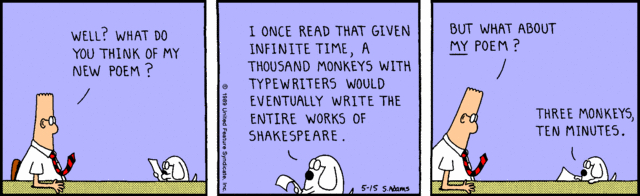
\includegraphics[width=\textwidth]{./gfx/infinite_monkey.jpg}
    \caption{Borel's strong law of large numbers.}
\end{figure}
\begin{example}
    Suppose we have a recruiter (a learning algorithm) whose task is to select
    the best students from a pool of candidates (the class of functions).
    Given ten students the recruiter makes them pass a test with $N$ questions.
    If the exam is well constructed and there are enough questions the
    recruiter should be able to retrieve the best student.
    \paragraph{}
    Now suppose that ten million monkeys $\gg N$ take the test and answer
    randomly to the questions. Then with high probability a monkey will score
    better or as well as the best student (strong law of large numbers). Can we
    say then that the recruiter has identified the best
    student?
    \paragraph{}
    Intuitively we see that when the capacity of the class of function grows
    (the number of students and random monkeys), the performance of the best
    element \emph{a posteriori} (minimizing the empirical risk) is not linked
    to the future performance (minimizing the true risk). In the present
    example we see that the capacity of the class of function is too large with
    respect to the number of data and thus presents a risk of overfitting.
    \paragraph{}
    On the contrary the generalization property ensures that the difference
    between the empirical risk and the true risk is controlled because the
    bound does not depend on a single fixed model, but on the whole class of
    functions. In this case if there are too many random monkeys, $C(\delta, N,
    \abs{\mathcal{F}})$ will blow-up, resulting in a poor generalization
    property.
\end{example}
\paragraph{}
A slightly stronger requirement is the {\emph consistency} of learning
algorithm.  Given a loss function $L$ and a class of function $\mathcal{F}$
there exists a optimal solutions that minimize the true risk.
\begin{dmath*}
    f_* \in \argmin_{f\in\mathcal{F}} \risk{f}.
\end{dmath*}
The excess risk is defined as the difference between the empirical risk of a
model returned by a learning algorithm and $f_*$. A learning algorithm is said
to be consistent when it is possible to bound the excess risk uniformly over
all
%<<<<<<< HEAD
%the solutions returned by a learning algorithm. In other words we look for a
%bound such that given a class of function $\mathcal{F}$ and a loss $L$,
%\begin{dmath*}
    %\risk{f_{\seq{s}}} \le \inf_{f\in\mathcal{F}} \risk{f} + C(\delta, \seq{s},
    %L, \Set{f_{\seq{s}}}\hiderel{\subseteq}\mathcal{F}),
%\end{dmath*}
%holds with probability $1 - \delta$, for all $\delta \in (0, 1)$  and
%$C(\delta, \seq{s}, \mathcal{F}) \to 0$ when the number of training data $N$ in
%$\seq{s}$ goes to infinity.
%\paragraph{}
%To identify the best model in $\mathcal{F}$ an intuitive loss function would be
%the $0-1$ loss defined as
%\begin{dmath*}
    %L(x, f, y) =
    %\begin{cases}
        %1 & \text{if } yf(x) \le 0 \\
        %0 & \text{otherwise}.
    %\end{cases}
%\end{dmath*}
%This loss returns $0$ if the model $f(x)$ and $y$ have the same sign and $1$
%otherwise. In this simple setting \citet{hoffgen1995robust} showed that finding
%an approximate to the empirical risk minimization with the $0-1$ loss is
%NP-Hard. However by \say{relaxing} a loss such that it becomes a convex in
%$f(x)$ functions yields a convex optimization problem which can then be solved
%in polynomial time. For instance, a convex surrogate of the $0-1$ loss is the
%Hinge loss
%\begin{dmath*}
    %L(x, f, y) =
    %\begin{cases}
        %f(x) & \text{if } (2y-1)f(x) \le 0 \\
        %0 & \text{otherwise}.
    %\end{cases}
%\end{dmath*}
%or the logistic loss
%\begin{dmath*}
    %L(x, f, y) = \frac{1}{\ln(2)} \ln(1 + \exp(-yf(x)))
%\end{dmath*}.
%For regression, a common choice is the least square loss
%\begin{dmath*}
    %L(x, f, y) = \frac{1}{2}(f(x) - y)^2
%\end{dmath*}
%In the next section we discuss the choice of the class of functions
%$\mathcal{F}$.
%=======
the solutions returned by a learning algorithm.

%\paragraph{}
%To identify the best model in $\mathcal{F}$ an intuitive loss function would be
%the $0-1$ loss defined as
%\begin{dmath*}
  %  L(x, f, y) =
%    \begin{cases}
 %       1 & \text{if } yf(x) \le 0 \\
  %      0 & \text{otherwise}.
%    \end{cases}
%\end{dmath*}
%This loss returns $0$ if the model $f(x)$ and $y$ have the same sign and $1$
%otherwise. In this simple setting \citet{hoffgen1995robust} showed that finding
%an approximate to the empirical risk minimization with the $0-1$ loss is
%NP-Hard. However by \say{relaxing} a loss such that it becomes a convex in
%$f(x)$ functions yields a convex optimization problem which can then be solved
%in polynomial time. For instance, a convex surrogate of the $0-1$ loss is the
%Hinge loss
%\begin{dmath*}
 %   L(x, f, y) =
%    \begin{cases}
%        f(x) & \text{if } (2y-1)f(x) \le 0 \\
 %       0 & \text{otherwise}.
 %   \end{cases}
%\end{dmath*}
%or the logistic loss
%\begin{dmath*}
 %   L(x, f, y) = \frac{1}{\ln(2)} \ln(1 + \exp(-yf(x)))
%\end{dmath*}.
%For regression, a common choice is the least square loss
%\begin{dmath*}
%    L(x, f, y) = \frac{1}{2}(f(x) - y)^2
%\end{dmath*}
%In the next section we discuss the choice of the class of functions
%$\mathcal{F}$.
%>>>>>>> 68a8c8187614fe541360c89c36b8192178611905

%------------------------------------------------------------------------------
\subsection{Introduction to kernel methods}\label{subsec:kernels}
\subsubsection{Kernels and Reproducing Kernel Hilbert Spaces}
A fair simple choice for $\mathcal{F}$ is the set of all linear functions. In
this case we focus on defining learning algorithm picking up the \say{best}
function(s) in the class
\begin{dmath*}
    \mathcal{F}_{lin.} = \Set{f | f(x) = \inner{w, x} + b, \enskip \forall w \in
    \mathbb{R}^d, \enskip \forall x \in \mathbb{R}^d, \enskip \forall b \in
    \mathbb{R}}.
\end{dmath*}
Although this class of functions has been well studied and has good
generalization properties (as long as the norm of $w$ is not too big), it has a
rather low capacity.  For instance in $\mathbb{R}^2$ it is impossible to
separate two nested circles with a line (see \cref{fig:nested_circle}). On the
other hand if one considers the class of functions of all functions $\Set{f |
f:\mathcal{X}\to\mathbb{R}}$, this space contains too many functions for any
algorithm to be able to find a solution to the minimization of the empirical
risk.
\begin{figure}
    \centering
    \pyc{print(r'\centering\resizebox{\textwidth}{!}{%% Creator: Matplotlib, PGF backend
%%
%% To include the figure in your LaTeX document, write
%%   \input{<filename>.pgf}
%%
%% Make sure the required packages are loaded in your preamble
%%   \usepackage{pgf}
%%
%% Figures using additional raster images can only be included by \input if
%% they are in the same directory as the main LaTeX file. For loading figures
%% from other directories you can use the `import` package
%%   \usepackage{import}
%% and then include the figures with
%%   \import{<path to file>}{<filename>.pgf}
%%
%% Matplotlib used the following preamble
%%   \usepackage{fontspec}
%%   \setmainfont{Times New Roman}
%%   \setsansfont{Lucida Grande}
%%   \setmonofont{Andale Mono}
%%
\begingroup%
\makeatletter%
\begin{pgfpicture}%
\pgfpathrectangle{\pgfpointorigin}{\pgfqpoint{6.000000in}{4.000000in}}%
\pgfusepath{use as bounding box, clip}%
\begin{pgfscope}%
\pgfsetbuttcap%
\pgfsetmiterjoin%
\definecolor{currentfill}{rgb}{1.000000,1.000000,1.000000}%
\pgfsetfillcolor{currentfill}%
\pgfsetlinewidth{0.000000pt}%
\definecolor{currentstroke}{rgb}{1.000000,1.000000,1.000000}%
\pgfsetstrokecolor{currentstroke}%
\pgfsetdash{}{0pt}%
\pgfpathmoveto{\pgfqpoint{0.000000in}{0.000000in}}%
\pgfpathlineto{\pgfqpoint{6.000000in}{0.000000in}}%
\pgfpathlineto{\pgfqpoint{6.000000in}{4.000000in}}%
\pgfpathlineto{\pgfqpoint{0.000000in}{4.000000in}}%
\pgfpathclose%
\pgfusepath{fill}%
\end{pgfscope}%
\begin{pgfscope}%
\pgfsetbuttcap%
\pgfsetmiterjoin%
\definecolor{currentfill}{rgb}{1.000000,1.000000,1.000000}%
\pgfsetfillcolor{currentfill}%
\pgfsetlinewidth{0.000000pt}%
\definecolor{currentstroke}{rgb}{0.000000,0.000000,0.000000}%
\pgfsetstrokecolor{currentstroke}%
\pgfsetstrokeopacity{0.000000}%
\pgfsetdash{}{0pt}%
\pgfpathmoveto{\pgfqpoint{0.710201in}{0.548769in}}%
\pgfpathlineto{\pgfqpoint{5.801389in}{0.548769in}}%
\pgfpathlineto{\pgfqpoint{5.801389in}{3.801389in}}%
\pgfpathlineto{\pgfqpoint{0.710201in}{3.801389in}}%
\pgfpathclose%
\pgfusepath{fill}%
\end{pgfscope}%
\begin{pgfscope}%
\pgfpathrectangle{\pgfqpoint{0.710201in}{0.548769in}}{\pgfqpoint{5.091188in}{3.252620in}} %
\pgfusepath{clip}%
\pgfsetbuttcap%
\pgfsetroundjoin%
\definecolor{currentfill}{rgb}{1.000000,0.000000,0.000000}%
\pgfsetfillcolor{currentfill}%
\pgfsetlinewidth{1.003750pt}%
\definecolor{currentstroke}{rgb}{0.000000,0.000000,0.000000}%
\pgfsetstrokecolor{currentstroke}%
\pgfsetdash{}{0pt}%
\pgfpathmoveto{\pgfqpoint{2.317247in}{0.984895in}}%
\pgfpathcurveto{\pgfqpoint{2.328297in}{0.984895in}}{\pgfqpoint{2.338896in}{0.989286in}}{\pgfqpoint{2.346709in}{0.997099in}}%
\pgfpathcurveto{\pgfqpoint{2.354523in}{1.004913in}}{\pgfqpoint{2.358913in}{1.015512in}}{\pgfqpoint{2.358913in}{1.026562in}}%
\pgfpathcurveto{\pgfqpoint{2.358913in}{1.037612in}}{\pgfqpoint{2.354523in}{1.048211in}}{\pgfqpoint{2.346709in}{1.056025in}}%
\pgfpathcurveto{\pgfqpoint{2.338896in}{1.063838in}}{\pgfqpoint{2.328297in}{1.068229in}}{\pgfqpoint{2.317247in}{1.068229in}}%
\pgfpathcurveto{\pgfqpoint{2.306197in}{1.068229in}}{\pgfqpoint{2.295597in}{1.063838in}}{\pgfqpoint{2.287784in}{1.056025in}}%
\pgfpathcurveto{\pgfqpoint{2.279970in}{1.048211in}}{\pgfqpoint{2.275580in}{1.037612in}}{\pgfqpoint{2.275580in}{1.026562in}}%
\pgfpathcurveto{\pgfqpoint{2.275580in}{1.015512in}}{\pgfqpoint{2.279970in}{1.004913in}}{\pgfqpoint{2.287784in}{0.997099in}}%
\pgfpathcurveto{\pgfqpoint{2.295597in}{0.989286in}}{\pgfqpoint{2.306197in}{0.984895in}}{\pgfqpoint{2.317247in}{0.984895in}}%
\pgfpathclose%
\pgfusepath{stroke,fill}%
\end{pgfscope}%
\begin{pgfscope}%
\pgfpathrectangle{\pgfqpoint{0.710201in}{0.548769in}}{\pgfqpoint{5.091188in}{3.252620in}} %
\pgfusepath{clip}%
\pgfsetbuttcap%
\pgfsetroundjoin%
\definecolor{currentfill}{rgb}{1.000000,0.000000,0.000000}%
\pgfsetfillcolor{currentfill}%
\pgfsetlinewidth{1.003750pt}%
\definecolor{currentstroke}{rgb}{0.000000,0.000000,0.000000}%
\pgfsetstrokecolor{currentstroke}%
\pgfsetdash{}{0pt}%
\pgfpathmoveto{\pgfqpoint{5.220791in}{1.963463in}}%
\pgfpathcurveto{\pgfqpoint{5.231841in}{1.963463in}}{\pgfqpoint{5.242440in}{1.967854in}}{\pgfqpoint{5.250254in}{1.975667in}}%
\pgfpathcurveto{\pgfqpoint{5.258067in}{1.983481in}}{\pgfqpoint{5.262458in}{1.994080in}}{\pgfqpoint{5.262458in}{2.005130in}}%
\pgfpathcurveto{\pgfqpoint{5.262458in}{2.016180in}}{\pgfqpoint{5.258067in}{2.026779in}}{\pgfqpoint{5.250254in}{2.034593in}}%
\pgfpathcurveto{\pgfqpoint{5.242440in}{2.042406in}}{\pgfqpoint{5.231841in}{2.046797in}}{\pgfqpoint{5.220791in}{2.046797in}}%
\pgfpathcurveto{\pgfqpoint{5.209741in}{2.046797in}}{\pgfqpoint{5.199142in}{2.042406in}}{\pgfqpoint{5.191328in}{2.034593in}}%
\pgfpathcurveto{\pgfqpoint{5.183514in}{2.026779in}}{\pgfqpoint{5.179124in}{2.016180in}}{\pgfqpoint{5.179124in}{2.005130in}}%
\pgfpathcurveto{\pgfqpoint{5.179124in}{1.994080in}}{\pgfqpoint{5.183514in}{1.983481in}}{\pgfqpoint{5.191328in}{1.975667in}}%
\pgfpathcurveto{\pgfqpoint{5.199142in}{1.967854in}}{\pgfqpoint{5.209741in}{1.963463in}}{\pgfqpoint{5.220791in}{1.963463in}}%
\pgfpathclose%
\pgfusepath{stroke,fill}%
\end{pgfscope}%
\begin{pgfscope}%
\pgfpathrectangle{\pgfqpoint{0.710201in}{0.548769in}}{\pgfqpoint{5.091188in}{3.252620in}} %
\pgfusepath{clip}%
\pgfsetbuttcap%
\pgfsetroundjoin%
\definecolor{currentfill}{rgb}{1.000000,0.000000,0.000000}%
\pgfsetfillcolor{currentfill}%
\pgfsetlinewidth{1.003750pt}%
\definecolor{currentstroke}{rgb}{0.000000,0.000000,0.000000}%
\pgfsetstrokecolor{currentstroke}%
\pgfsetdash{}{0pt}%
\pgfpathmoveto{\pgfqpoint{2.771377in}{3.401257in}}%
\pgfpathcurveto{\pgfqpoint{2.782427in}{3.401257in}}{\pgfqpoint{2.793026in}{3.405648in}}{\pgfqpoint{2.800840in}{3.413461in}}%
\pgfpathcurveto{\pgfqpoint{2.808653in}{3.421275in}}{\pgfqpoint{2.813044in}{3.431874in}}{\pgfqpoint{2.813044in}{3.442924in}}%
\pgfpathcurveto{\pgfqpoint{2.813044in}{3.453974in}}{\pgfqpoint{2.808653in}{3.464573in}}{\pgfqpoint{2.800840in}{3.472387in}}%
\pgfpathcurveto{\pgfqpoint{2.793026in}{3.480200in}}{\pgfqpoint{2.782427in}{3.484591in}}{\pgfqpoint{2.771377in}{3.484591in}}%
\pgfpathcurveto{\pgfqpoint{2.760327in}{3.484591in}}{\pgfqpoint{2.749728in}{3.480200in}}{\pgfqpoint{2.741914in}{3.472387in}}%
\pgfpathcurveto{\pgfqpoint{2.734101in}{3.464573in}}{\pgfqpoint{2.729710in}{3.453974in}}{\pgfqpoint{2.729710in}{3.442924in}}%
\pgfpathcurveto{\pgfqpoint{2.729710in}{3.431874in}}{\pgfqpoint{2.734101in}{3.421275in}}{\pgfqpoint{2.741914in}{3.413461in}}%
\pgfpathcurveto{\pgfqpoint{2.749728in}{3.405648in}}{\pgfqpoint{2.760327in}{3.401257in}}{\pgfqpoint{2.771377in}{3.401257in}}%
\pgfpathclose%
\pgfusepath{stroke,fill}%
\end{pgfscope}%
\begin{pgfscope}%
\pgfpathrectangle{\pgfqpoint{0.710201in}{0.548769in}}{\pgfqpoint{5.091188in}{3.252620in}} %
\pgfusepath{clip}%
\pgfsetbuttcap%
\pgfsetroundjoin%
\definecolor{currentfill}{rgb}{1.000000,0.000000,0.000000}%
\pgfsetfillcolor{currentfill}%
\pgfsetlinewidth{1.003750pt}%
\definecolor{currentstroke}{rgb}{0.000000,0.000000,0.000000}%
\pgfsetstrokecolor{currentstroke}%
\pgfsetdash{}{0pt}%
\pgfpathmoveto{\pgfqpoint{3.596304in}{0.749461in}}%
\pgfpathcurveto{\pgfqpoint{3.607354in}{0.749461in}}{\pgfqpoint{3.617953in}{0.753852in}}{\pgfqpoint{3.625767in}{0.761665in}}%
\pgfpathcurveto{\pgfqpoint{3.633581in}{0.769479in}}{\pgfqpoint{3.637971in}{0.780078in}}{\pgfqpoint{3.637971in}{0.791128in}}%
\pgfpathcurveto{\pgfqpoint{3.637971in}{0.802178in}}{\pgfqpoint{3.633581in}{0.812777in}}{\pgfqpoint{3.625767in}{0.820591in}}%
\pgfpathcurveto{\pgfqpoint{3.617953in}{0.828404in}}{\pgfqpoint{3.607354in}{0.832795in}}{\pgfqpoint{3.596304in}{0.832795in}}%
\pgfpathcurveto{\pgfqpoint{3.585254in}{0.832795in}}{\pgfqpoint{3.574655in}{0.828404in}}{\pgfqpoint{3.566842in}{0.820591in}}%
\pgfpathcurveto{\pgfqpoint{3.559028in}{0.812777in}}{\pgfqpoint{3.554638in}{0.802178in}}{\pgfqpoint{3.554638in}{0.791128in}}%
\pgfpathcurveto{\pgfqpoint{3.554638in}{0.780078in}}{\pgfqpoint{3.559028in}{0.769479in}}{\pgfqpoint{3.566842in}{0.761665in}}%
\pgfpathcurveto{\pgfqpoint{3.574655in}{0.753852in}}{\pgfqpoint{3.585254in}{0.749461in}}{\pgfqpoint{3.596304in}{0.749461in}}%
\pgfpathclose%
\pgfusepath{stroke,fill}%
\end{pgfscope}%
\begin{pgfscope}%
\pgfpathrectangle{\pgfqpoint{0.710201in}{0.548769in}}{\pgfqpoint{5.091188in}{3.252620in}} %
\pgfusepath{clip}%
\pgfsetbuttcap%
\pgfsetroundjoin%
\definecolor{currentfill}{rgb}{1.000000,0.000000,0.000000}%
\pgfsetfillcolor{currentfill}%
\pgfsetlinewidth{1.003750pt}%
\definecolor{currentstroke}{rgb}{0.000000,0.000000,0.000000}%
\pgfsetstrokecolor{currentstroke}%
\pgfsetdash{}{0pt}%
\pgfpathmoveto{\pgfqpoint{2.761845in}{0.830672in}}%
\pgfpathcurveto{\pgfqpoint{2.772896in}{0.830672in}}{\pgfqpoint{2.783495in}{0.835062in}}{\pgfqpoint{2.791308in}{0.842876in}}%
\pgfpathcurveto{\pgfqpoint{2.799122in}{0.850689in}}{\pgfqpoint{2.803512in}{0.861288in}}{\pgfqpoint{2.803512in}{0.872338in}}%
\pgfpathcurveto{\pgfqpoint{2.803512in}{0.883389in}}{\pgfqpoint{2.799122in}{0.893988in}}{\pgfqpoint{2.791308in}{0.901801in}}%
\pgfpathcurveto{\pgfqpoint{2.783495in}{0.909615in}}{\pgfqpoint{2.772896in}{0.914005in}}{\pgfqpoint{2.761845in}{0.914005in}}%
\pgfpathcurveto{\pgfqpoint{2.750795in}{0.914005in}}{\pgfqpoint{2.740196in}{0.909615in}}{\pgfqpoint{2.732383in}{0.901801in}}%
\pgfpathcurveto{\pgfqpoint{2.724569in}{0.893988in}}{\pgfqpoint{2.720179in}{0.883389in}}{\pgfqpoint{2.720179in}{0.872338in}}%
\pgfpathcurveto{\pgfqpoint{2.720179in}{0.861288in}}{\pgfqpoint{2.724569in}{0.850689in}}{\pgfqpoint{2.732383in}{0.842876in}}%
\pgfpathcurveto{\pgfqpoint{2.740196in}{0.835062in}}{\pgfqpoint{2.750795in}{0.830672in}}{\pgfqpoint{2.761845in}{0.830672in}}%
\pgfpathclose%
\pgfusepath{stroke,fill}%
\end{pgfscope}%
\begin{pgfscope}%
\pgfpathrectangle{\pgfqpoint{0.710201in}{0.548769in}}{\pgfqpoint{5.091188in}{3.252620in}} %
\pgfusepath{clip}%
\pgfsetbuttcap%
\pgfsetroundjoin%
\definecolor{currentfill}{rgb}{1.000000,0.000000,0.000000}%
\pgfsetfillcolor{currentfill}%
\pgfsetlinewidth{1.003750pt}%
\definecolor{currentstroke}{rgb}{0.000000,0.000000,0.000000}%
\pgfsetstrokecolor{currentstroke}%
\pgfsetdash{}{0pt}%
\pgfpathmoveto{\pgfqpoint{4.262215in}{3.200695in}}%
\pgfpathcurveto{\pgfqpoint{4.273265in}{3.200695in}}{\pgfqpoint{4.283864in}{3.205085in}}{\pgfqpoint{4.291678in}{3.212899in}}%
\pgfpathcurveto{\pgfqpoint{4.299492in}{3.220712in}}{\pgfqpoint{4.303882in}{3.231311in}}{\pgfqpoint{4.303882in}{3.242362in}}%
\pgfpathcurveto{\pgfqpoint{4.303882in}{3.253412in}}{\pgfqpoint{4.299492in}{3.264011in}}{\pgfqpoint{4.291678in}{3.271824in}}%
\pgfpathcurveto{\pgfqpoint{4.283864in}{3.279638in}}{\pgfqpoint{4.273265in}{3.284028in}}{\pgfqpoint{4.262215in}{3.284028in}}%
\pgfpathcurveto{\pgfqpoint{4.251165in}{3.284028in}}{\pgfqpoint{4.240566in}{3.279638in}}{\pgfqpoint{4.232752in}{3.271824in}}%
\pgfpathcurveto{\pgfqpoint{4.224939in}{3.264011in}}{\pgfqpoint{4.220548in}{3.253412in}}{\pgfqpoint{4.220548in}{3.242362in}}%
\pgfpathcurveto{\pgfqpoint{4.220548in}{3.231311in}}{\pgfqpoint{4.224939in}{3.220712in}}{\pgfqpoint{4.232752in}{3.212899in}}%
\pgfpathcurveto{\pgfqpoint{4.240566in}{3.205085in}}{\pgfqpoint{4.251165in}{3.200695in}}{\pgfqpoint{4.262215in}{3.200695in}}%
\pgfpathclose%
\pgfusepath{stroke,fill}%
\end{pgfscope}%
\begin{pgfscope}%
\pgfpathrectangle{\pgfqpoint{0.710201in}{0.548769in}}{\pgfqpoint{5.091188in}{3.252620in}} %
\pgfusepath{clip}%
\pgfsetbuttcap%
\pgfsetroundjoin%
\definecolor{currentfill}{rgb}{1.000000,0.000000,0.000000}%
\pgfsetfillcolor{currentfill}%
\pgfsetlinewidth{1.003750pt}%
\definecolor{currentstroke}{rgb}{0.000000,0.000000,0.000000}%
\pgfsetstrokecolor{currentstroke}%
\pgfsetdash{}{0pt}%
\pgfpathmoveto{\pgfqpoint{2.464268in}{0.961799in}}%
\pgfpathcurveto{\pgfqpoint{2.475318in}{0.961799in}}{\pgfqpoint{2.485917in}{0.966189in}}{\pgfqpoint{2.493731in}{0.974002in}}%
\pgfpathcurveto{\pgfqpoint{2.501545in}{0.981816in}}{\pgfqpoint{2.505935in}{0.992415in}}{\pgfqpoint{2.505935in}{1.003465in}}%
\pgfpathcurveto{\pgfqpoint{2.505935in}{1.014515in}}{\pgfqpoint{2.501545in}{1.025114in}}{\pgfqpoint{2.493731in}{1.032928in}}%
\pgfpathcurveto{\pgfqpoint{2.485917in}{1.040742in}}{\pgfqpoint{2.475318in}{1.045132in}}{\pgfqpoint{2.464268in}{1.045132in}}%
\pgfpathcurveto{\pgfqpoint{2.453218in}{1.045132in}}{\pgfqpoint{2.442619in}{1.040742in}}{\pgfqpoint{2.434806in}{1.032928in}}%
\pgfpathcurveto{\pgfqpoint{2.426992in}{1.025114in}}{\pgfqpoint{2.422602in}{1.014515in}}{\pgfqpoint{2.422602in}{1.003465in}}%
\pgfpathcurveto{\pgfqpoint{2.422602in}{0.992415in}}{\pgfqpoint{2.426992in}{0.981816in}}{\pgfqpoint{2.434806in}{0.974002in}}%
\pgfpathcurveto{\pgfqpoint{2.442619in}{0.966189in}}{\pgfqpoint{2.453218in}{0.961799in}}{\pgfqpoint{2.464268in}{0.961799in}}%
\pgfpathclose%
\pgfusepath{stroke,fill}%
\end{pgfscope}%
\begin{pgfscope}%
\pgfpathrectangle{\pgfqpoint{0.710201in}{0.548769in}}{\pgfqpoint{5.091188in}{3.252620in}} %
\pgfusepath{clip}%
\pgfsetbuttcap%
\pgfsetroundjoin%
\definecolor{currentfill}{rgb}{1.000000,0.000000,0.000000}%
\pgfsetfillcolor{currentfill}%
\pgfsetlinewidth{1.003750pt}%
\definecolor{currentstroke}{rgb}{0.000000,0.000000,0.000000}%
\pgfsetstrokecolor{currentstroke}%
\pgfsetdash{}{0pt}%
\pgfpathmoveto{\pgfqpoint{1.520883in}{1.536754in}}%
\pgfpathcurveto{\pgfqpoint{1.531933in}{1.536754in}}{\pgfqpoint{1.542533in}{1.541144in}}{\pgfqpoint{1.550346in}{1.548958in}}%
\pgfpathcurveto{\pgfqpoint{1.558160in}{1.556771in}}{\pgfqpoint{1.562550in}{1.567370in}}{\pgfqpoint{1.562550in}{1.578420in}}%
\pgfpathcurveto{\pgfqpoint{1.562550in}{1.589471in}}{\pgfqpoint{1.558160in}{1.600070in}}{\pgfqpoint{1.550346in}{1.607883in}}%
\pgfpathcurveto{\pgfqpoint{1.542533in}{1.615697in}}{\pgfqpoint{1.531933in}{1.620087in}}{\pgfqpoint{1.520883in}{1.620087in}}%
\pgfpathcurveto{\pgfqpoint{1.509833in}{1.620087in}}{\pgfqpoint{1.499234in}{1.615697in}}{\pgfqpoint{1.491421in}{1.607883in}}%
\pgfpathcurveto{\pgfqpoint{1.483607in}{1.600070in}}{\pgfqpoint{1.479217in}{1.589471in}}{\pgfqpoint{1.479217in}{1.578420in}}%
\pgfpathcurveto{\pgfqpoint{1.479217in}{1.567370in}}{\pgfqpoint{1.483607in}{1.556771in}}{\pgfqpoint{1.491421in}{1.548958in}}%
\pgfpathcurveto{\pgfqpoint{1.499234in}{1.541144in}}{\pgfqpoint{1.509833in}{1.536754in}}{\pgfqpoint{1.520883in}{1.536754in}}%
\pgfpathclose%
\pgfusepath{stroke,fill}%
\end{pgfscope}%
\begin{pgfscope}%
\pgfpathrectangle{\pgfqpoint{0.710201in}{0.548769in}}{\pgfqpoint{5.091188in}{3.252620in}} %
\pgfusepath{clip}%
\pgfsetbuttcap%
\pgfsetroundjoin%
\definecolor{currentfill}{rgb}{1.000000,0.000000,0.000000}%
\pgfsetfillcolor{currentfill}%
\pgfsetlinewidth{1.003750pt}%
\definecolor{currentstroke}{rgb}{0.000000,0.000000,0.000000}%
\pgfsetstrokecolor{currentstroke}%
\pgfsetdash{}{0pt}%
\pgfpathmoveto{\pgfqpoint{5.115478in}{2.484543in}}%
\pgfpathcurveto{\pgfqpoint{5.126528in}{2.484543in}}{\pgfqpoint{5.137127in}{2.488933in}}{\pgfqpoint{5.144941in}{2.496747in}}%
\pgfpathcurveto{\pgfqpoint{5.152755in}{2.504561in}}{\pgfqpoint{5.157145in}{2.515160in}}{\pgfqpoint{5.157145in}{2.526210in}}%
\pgfpathcurveto{\pgfqpoint{5.157145in}{2.537260in}}{\pgfqpoint{5.152755in}{2.547859in}}{\pgfqpoint{5.144941in}{2.555673in}}%
\pgfpathcurveto{\pgfqpoint{5.137127in}{2.563486in}}{\pgfqpoint{5.126528in}{2.567876in}}{\pgfqpoint{5.115478in}{2.567876in}}%
\pgfpathcurveto{\pgfqpoint{5.104428in}{2.567876in}}{\pgfqpoint{5.093829in}{2.563486in}}{\pgfqpoint{5.086016in}{2.555673in}}%
\pgfpathcurveto{\pgfqpoint{5.078202in}{2.547859in}}{\pgfqpoint{5.073812in}{2.537260in}}{\pgfqpoint{5.073812in}{2.526210in}}%
\pgfpathcurveto{\pgfqpoint{5.073812in}{2.515160in}}{\pgfqpoint{5.078202in}{2.504561in}}{\pgfqpoint{5.086016in}{2.496747in}}%
\pgfpathcurveto{\pgfqpoint{5.093829in}{2.488933in}}{\pgfqpoint{5.104428in}{2.484543in}}{\pgfqpoint{5.115478in}{2.484543in}}%
\pgfpathclose%
\pgfusepath{stroke,fill}%
\end{pgfscope}%
\begin{pgfscope}%
\pgfpathrectangle{\pgfqpoint{0.710201in}{0.548769in}}{\pgfqpoint{5.091188in}{3.252620in}} %
\pgfusepath{clip}%
\pgfsetbuttcap%
\pgfsetroundjoin%
\definecolor{currentfill}{rgb}{1.000000,0.000000,0.000000}%
\pgfsetfillcolor{currentfill}%
\pgfsetlinewidth{1.003750pt}%
\definecolor{currentstroke}{rgb}{0.000000,0.000000,0.000000}%
\pgfsetstrokecolor{currentstroke}%
\pgfsetdash{}{0pt}%
\pgfpathmoveto{\pgfqpoint{2.925303in}{3.471002in}}%
\pgfpathcurveto{\pgfqpoint{2.936353in}{3.471002in}}{\pgfqpoint{2.946952in}{3.475392in}}{\pgfqpoint{2.954766in}{3.483206in}}%
\pgfpathcurveto{\pgfqpoint{2.962579in}{3.491020in}}{\pgfqpoint{2.966969in}{3.501619in}}{\pgfqpoint{2.966969in}{3.512669in}}%
\pgfpathcurveto{\pgfqpoint{2.966969in}{3.523719in}}{\pgfqpoint{2.962579in}{3.534318in}}{\pgfqpoint{2.954766in}{3.542131in}}%
\pgfpathcurveto{\pgfqpoint{2.946952in}{3.549945in}}{\pgfqpoint{2.936353in}{3.554335in}}{\pgfqpoint{2.925303in}{3.554335in}}%
\pgfpathcurveto{\pgfqpoint{2.914253in}{3.554335in}}{\pgfqpoint{2.903654in}{3.549945in}}{\pgfqpoint{2.895840in}{3.542131in}}%
\pgfpathcurveto{\pgfqpoint{2.888026in}{3.534318in}}{\pgfqpoint{2.883636in}{3.523719in}}{\pgfqpoint{2.883636in}{3.512669in}}%
\pgfpathcurveto{\pgfqpoint{2.883636in}{3.501619in}}{\pgfqpoint{2.888026in}{3.491020in}}{\pgfqpoint{2.895840in}{3.483206in}}%
\pgfpathcurveto{\pgfqpoint{2.903654in}{3.475392in}}{\pgfqpoint{2.914253in}{3.471002in}}{\pgfqpoint{2.925303in}{3.471002in}}%
\pgfpathclose%
\pgfusepath{stroke,fill}%
\end{pgfscope}%
\begin{pgfscope}%
\pgfpathrectangle{\pgfqpoint{0.710201in}{0.548769in}}{\pgfqpoint{5.091188in}{3.252620in}} %
\pgfusepath{clip}%
\pgfsetbuttcap%
\pgfsetroundjoin%
\definecolor{currentfill}{rgb}{1.000000,0.000000,0.000000}%
\pgfsetfillcolor{currentfill}%
\pgfsetlinewidth{1.003750pt}%
\definecolor{currentstroke}{rgb}{0.000000,0.000000,0.000000}%
\pgfsetstrokecolor{currentstroke}%
\pgfsetdash{}{0pt}%
\pgfpathmoveto{\pgfqpoint{2.806529in}{0.776136in}}%
\pgfpathcurveto{\pgfqpoint{2.817579in}{0.776136in}}{\pgfqpoint{2.828178in}{0.780526in}}{\pgfqpoint{2.835992in}{0.788340in}}%
\pgfpathcurveto{\pgfqpoint{2.843806in}{0.796154in}}{\pgfqpoint{2.848196in}{0.806753in}}{\pgfqpoint{2.848196in}{0.817803in}}%
\pgfpathcurveto{\pgfqpoint{2.848196in}{0.828853in}}{\pgfqpoint{2.843806in}{0.839452in}}{\pgfqpoint{2.835992in}{0.847266in}}%
\pgfpathcurveto{\pgfqpoint{2.828178in}{0.855079in}}{\pgfqpoint{2.817579in}{0.859469in}}{\pgfqpoint{2.806529in}{0.859469in}}%
\pgfpathcurveto{\pgfqpoint{2.795479in}{0.859469in}}{\pgfqpoint{2.784880in}{0.855079in}}{\pgfqpoint{2.777066in}{0.847266in}}%
\pgfpathcurveto{\pgfqpoint{2.769253in}{0.839452in}}{\pgfqpoint{2.764863in}{0.828853in}}{\pgfqpoint{2.764863in}{0.817803in}}%
\pgfpathcurveto{\pgfqpoint{2.764863in}{0.806753in}}{\pgfqpoint{2.769253in}{0.796154in}}{\pgfqpoint{2.777066in}{0.788340in}}%
\pgfpathcurveto{\pgfqpoint{2.784880in}{0.780526in}}{\pgfqpoint{2.795479in}{0.776136in}}{\pgfqpoint{2.806529in}{0.776136in}}%
\pgfpathclose%
\pgfusepath{stroke,fill}%
\end{pgfscope}%
\begin{pgfscope}%
\pgfpathrectangle{\pgfqpoint{0.710201in}{0.548769in}}{\pgfqpoint{5.091188in}{3.252620in}} %
\pgfusepath{clip}%
\pgfsetbuttcap%
\pgfsetroundjoin%
\definecolor{currentfill}{rgb}{1.000000,0.000000,0.000000}%
\pgfsetfillcolor{currentfill}%
\pgfsetlinewidth{1.003750pt}%
\definecolor{currentstroke}{rgb}{0.000000,0.000000,0.000000}%
\pgfsetstrokecolor{currentstroke}%
\pgfsetdash{}{0pt}%
\pgfpathmoveto{\pgfqpoint{5.346429in}{2.104801in}}%
\pgfpathcurveto{\pgfqpoint{5.357479in}{2.104801in}}{\pgfqpoint{5.368078in}{2.109191in}}{\pgfqpoint{5.375891in}{2.117005in}}%
\pgfpathcurveto{\pgfqpoint{5.383705in}{2.124819in}}{\pgfqpoint{5.388095in}{2.135418in}}{\pgfqpoint{5.388095in}{2.146468in}}%
\pgfpathcurveto{\pgfqpoint{5.388095in}{2.157518in}}{\pgfqpoint{5.383705in}{2.168117in}}{\pgfqpoint{5.375891in}{2.175931in}}%
\pgfpathcurveto{\pgfqpoint{5.368078in}{2.183744in}}{\pgfqpoint{5.357479in}{2.188135in}}{\pgfqpoint{5.346429in}{2.188135in}}%
\pgfpathcurveto{\pgfqpoint{5.335378in}{2.188135in}}{\pgfqpoint{5.324779in}{2.183744in}}{\pgfqpoint{5.316966in}{2.175931in}}%
\pgfpathcurveto{\pgfqpoint{5.309152in}{2.168117in}}{\pgfqpoint{5.304762in}{2.157518in}}{\pgfqpoint{5.304762in}{2.146468in}}%
\pgfpathcurveto{\pgfqpoint{5.304762in}{2.135418in}}{\pgfqpoint{5.309152in}{2.124819in}}{\pgfqpoint{5.316966in}{2.117005in}}%
\pgfpathcurveto{\pgfqpoint{5.324779in}{2.109191in}}{\pgfqpoint{5.335378in}{2.104801in}}{\pgfqpoint{5.346429in}{2.104801in}}%
\pgfpathclose%
\pgfusepath{stroke,fill}%
\end{pgfscope}%
\begin{pgfscope}%
\pgfpathrectangle{\pgfqpoint{0.710201in}{0.548769in}}{\pgfqpoint{5.091188in}{3.252620in}} %
\pgfusepath{clip}%
\pgfsetbuttcap%
\pgfsetroundjoin%
\definecolor{currentfill}{rgb}{1.000000,0.000000,0.000000}%
\pgfsetfillcolor{currentfill}%
\pgfsetlinewidth{1.003750pt}%
\definecolor{currentstroke}{rgb}{0.000000,0.000000,0.000000}%
\pgfsetstrokecolor{currentstroke}%
\pgfsetdash{}{0pt}%
\pgfpathmoveto{\pgfqpoint{4.688056in}{1.081730in}}%
\pgfpathcurveto{\pgfqpoint{4.699106in}{1.081730in}}{\pgfqpoint{4.709705in}{1.086121in}}{\pgfqpoint{4.717518in}{1.093934in}}%
\pgfpathcurveto{\pgfqpoint{4.725332in}{1.101748in}}{\pgfqpoint{4.729722in}{1.112347in}}{\pgfqpoint{4.729722in}{1.123397in}}%
\pgfpathcurveto{\pgfqpoint{4.729722in}{1.134447in}}{\pgfqpoint{4.725332in}{1.145046in}}{\pgfqpoint{4.717518in}{1.152860in}}%
\pgfpathcurveto{\pgfqpoint{4.709705in}{1.160673in}}{\pgfqpoint{4.699106in}{1.165064in}}{\pgfqpoint{4.688056in}{1.165064in}}%
\pgfpathcurveto{\pgfqpoint{4.677006in}{1.165064in}}{\pgfqpoint{4.666406in}{1.160673in}}{\pgfqpoint{4.658593in}{1.152860in}}%
\pgfpathcurveto{\pgfqpoint{4.650779in}{1.145046in}}{\pgfqpoint{4.646389in}{1.134447in}}{\pgfqpoint{4.646389in}{1.123397in}}%
\pgfpathcurveto{\pgfqpoint{4.646389in}{1.112347in}}{\pgfqpoint{4.650779in}{1.101748in}}{\pgfqpoint{4.658593in}{1.093934in}}%
\pgfpathcurveto{\pgfqpoint{4.666406in}{1.086121in}}{\pgfqpoint{4.677006in}{1.081730in}}{\pgfqpoint{4.688056in}{1.081730in}}%
\pgfpathclose%
\pgfusepath{stroke,fill}%
\end{pgfscope}%
\begin{pgfscope}%
\pgfpathrectangle{\pgfqpoint{0.710201in}{0.548769in}}{\pgfqpoint{5.091188in}{3.252620in}} %
\pgfusepath{clip}%
\pgfsetbuttcap%
\pgfsetroundjoin%
\definecolor{currentfill}{rgb}{1.000000,0.000000,0.000000}%
\pgfsetfillcolor{currentfill}%
\pgfsetlinewidth{1.003750pt}%
\definecolor{currentstroke}{rgb}{0.000000,0.000000,0.000000}%
\pgfsetstrokecolor{currentstroke}%
\pgfsetdash{}{0pt}%
\pgfpathmoveto{\pgfqpoint{1.831783in}{1.140959in}}%
\pgfpathcurveto{\pgfqpoint{1.842833in}{1.140959in}}{\pgfqpoint{1.853432in}{1.145349in}}{\pgfqpoint{1.861246in}{1.153163in}}%
\pgfpathcurveto{\pgfqpoint{1.869059in}{1.160976in}}{\pgfqpoint{1.873450in}{1.171575in}}{\pgfqpoint{1.873450in}{1.182626in}}%
\pgfpathcurveto{\pgfqpoint{1.873450in}{1.193676in}}{\pgfqpoint{1.869059in}{1.204275in}}{\pgfqpoint{1.861246in}{1.212088in}}%
\pgfpathcurveto{\pgfqpoint{1.853432in}{1.219902in}}{\pgfqpoint{1.842833in}{1.224292in}}{\pgfqpoint{1.831783in}{1.224292in}}%
\pgfpathcurveto{\pgfqpoint{1.820733in}{1.224292in}}{\pgfqpoint{1.810134in}{1.219902in}}{\pgfqpoint{1.802320in}{1.212088in}}%
\pgfpathcurveto{\pgfqpoint{1.794507in}{1.204275in}}{\pgfqpoint{1.790116in}{1.193676in}}{\pgfqpoint{1.790116in}{1.182626in}}%
\pgfpathcurveto{\pgfqpoint{1.790116in}{1.171575in}}{\pgfqpoint{1.794507in}{1.160976in}}{\pgfqpoint{1.802320in}{1.153163in}}%
\pgfpathcurveto{\pgfqpoint{1.810134in}{1.145349in}}{\pgfqpoint{1.820733in}{1.140959in}}{\pgfqpoint{1.831783in}{1.140959in}}%
\pgfpathclose%
\pgfusepath{stroke,fill}%
\end{pgfscope}%
\begin{pgfscope}%
\pgfpathrectangle{\pgfqpoint{0.710201in}{0.548769in}}{\pgfqpoint{5.091188in}{3.252620in}} %
\pgfusepath{clip}%
\pgfsetbuttcap%
\pgfsetroundjoin%
\definecolor{currentfill}{rgb}{1.000000,0.000000,0.000000}%
\pgfsetfillcolor{currentfill}%
\pgfsetlinewidth{1.003750pt}%
\definecolor{currentstroke}{rgb}{0.000000,0.000000,0.000000}%
\pgfsetstrokecolor{currentstroke}%
\pgfsetdash{}{0pt}%
\pgfpathmoveto{\pgfqpoint{4.529157in}{1.157473in}}%
\pgfpathcurveto{\pgfqpoint{4.540207in}{1.157473in}}{\pgfqpoint{4.550806in}{1.161863in}}{\pgfqpoint{4.558619in}{1.169677in}}%
\pgfpathcurveto{\pgfqpoint{4.566433in}{1.177491in}}{\pgfqpoint{4.570823in}{1.188090in}}{\pgfqpoint{4.570823in}{1.199140in}}%
\pgfpathcurveto{\pgfqpoint{4.570823in}{1.210190in}}{\pgfqpoint{4.566433in}{1.220789in}}{\pgfqpoint{4.558619in}{1.228603in}}%
\pgfpathcurveto{\pgfqpoint{4.550806in}{1.236416in}}{\pgfqpoint{4.540207in}{1.240807in}}{\pgfqpoint{4.529157in}{1.240807in}}%
\pgfpathcurveto{\pgfqpoint{4.518107in}{1.240807in}}{\pgfqpoint{4.507507in}{1.236416in}}{\pgfqpoint{4.499694in}{1.228603in}}%
\pgfpathcurveto{\pgfqpoint{4.491880in}{1.220789in}}{\pgfqpoint{4.487490in}{1.210190in}}{\pgfqpoint{4.487490in}{1.199140in}}%
\pgfpathcurveto{\pgfqpoint{4.487490in}{1.188090in}}{\pgfqpoint{4.491880in}{1.177491in}}{\pgfqpoint{4.499694in}{1.169677in}}%
\pgfpathcurveto{\pgfqpoint{4.507507in}{1.161863in}}{\pgfqpoint{4.518107in}{1.157473in}}{\pgfqpoint{4.529157in}{1.157473in}}%
\pgfpathclose%
\pgfusepath{stroke,fill}%
\end{pgfscope}%
\begin{pgfscope}%
\pgfpathrectangle{\pgfqpoint{0.710201in}{0.548769in}}{\pgfqpoint{5.091188in}{3.252620in}} %
\pgfusepath{clip}%
\pgfsetbuttcap%
\pgfsetroundjoin%
\definecolor{currentfill}{rgb}{1.000000,0.000000,0.000000}%
\pgfsetfillcolor{currentfill}%
\pgfsetlinewidth{1.003750pt}%
\definecolor{currentstroke}{rgb}{0.000000,0.000000,0.000000}%
\pgfsetstrokecolor{currentstroke}%
\pgfsetdash{}{0pt}%
\pgfpathmoveto{\pgfqpoint{1.836323in}{2.968305in}}%
\pgfpathcurveto{\pgfqpoint{1.847373in}{2.968305in}}{\pgfqpoint{1.857972in}{2.972696in}}{\pgfqpoint{1.865786in}{2.980509in}}%
\pgfpathcurveto{\pgfqpoint{1.873599in}{2.988323in}}{\pgfqpoint{1.877989in}{2.998922in}}{\pgfqpoint{1.877989in}{3.009972in}}%
\pgfpathcurveto{\pgfqpoint{1.877989in}{3.021022in}}{\pgfqpoint{1.873599in}{3.031621in}}{\pgfqpoint{1.865786in}{3.039435in}}%
\pgfpathcurveto{\pgfqpoint{1.857972in}{3.047248in}}{\pgfqpoint{1.847373in}{3.051639in}}{\pgfqpoint{1.836323in}{3.051639in}}%
\pgfpathcurveto{\pgfqpoint{1.825273in}{3.051639in}}{\pgfqpoint{1.814674in}{3.047248in}}{\pgfqpoint{1.806860in}{3.039435in}}%
\pgfpathcurveto{\pgfqpoint{1.799046in}{3.031621in}}{\pgfqpoint{1.794656in}{3.021022in}}{\pgfqpoint{1.794656in}{3.009972in}}%
\pgfpathcurveto{\pgfqpoint{1.794656in}{2.998922in}}{\pgfqpoint{1.799046in}{2.988323in}}{\pgfqpoint{1.806860in}{2.980509in}}%
\pgfpathcurveto{\pgfqpoint{1.814674in}{2.972696in}}{\pgfqpoint{1.825273in}{2.968305in}}{\pgfqpoint{1.836323in}{2.968305in}}%
\pgfpathclose%
\pgfusepath{stroke,fill}%
\end{pgfscope}%
\begin{pgfscope}%
\pgfpathrectangle{\pgfqpoint{0.710201in}{0.548769in}}{\pgfqpoint{5.091188in}{3.252620in}} %
\pgfusepath{clip}%
\pgfsetbuttcap%
\pgfsetroundjoin%
\definecolor{currentfill}{rgb}{1.000000,0.000000,0.000000}%
\pgfsetfillcolor{currentfill}%
\pgfsetlinewidth{1.003750pt}%
\definecolor{currentstroke}{rgb}{0.000000,0.000000,0.000000}%
\pgfsetstrokecolor{currentstroke}%
\pgfsetdash{}{0pt}%
\pgfpathmoveto{\pgfqpoint{5.108985in}{2.526486in}}%
\pgfpathcurveto{\pgfqpoint{5.120035in}{2.526486in}}{\pgfqpoint{5.130634in}{2.530876in}}{\pgfqpoint{5.138448in}{2.538690in}}%
\pgfpathcurveto{\pgfqpoint{5.146262in}{2.546503in}}{\pgfqpoint{5.150652in}{2.557103in}}{\pgfqpoint{5.150652in}{2.568153in}}%
\pgfpathcurveto{\pgfqpoint{5.150652in}{2.579203in}}{\pgfqpoint{5.146262in}{2.589802in}}{\pgfqpoint{5.138448in}{2.597615in}}%
\pgfpathcurveto{\pgfqpoint{5.130634in}{2.605429in}}{\pgfqpoint{5.120035in}{2.609819in}}{\pgfqpoint{5.108985in}{2.609819in}}%
\pgfpathcurveto{\pgfqpoint{5.097935in}{2.609819in}}{\pgfqpoint{5.087336in}{2.605429in}}{\pgfqpoint{5.079522in}{2.597615in}}%
\pgfpathcurveto{\pgfqpoint{5.071709in}{2.589802in}}{\pgfqpoint{5.067318in}{2.579203in}}{\pgfqpoint{5.067318in}{2.568153in}}%
\pgfpathcurveto{\pgfqpoint{5.067318in}{2.557103in}}{\pgfqpoint{5.071709in}{2.546503in}}{\pgfqpoint{5.079522in}{2.538690in}}%
\pgfpathcurveto{\pgfqpoint{5.087336in}{2.530876in}}{\pgfqpoint{5.097935in}{2.526486in}}{\pgfqpoint{5.108985in}{2.526486in}}%
\pgfpathclose%
\pgfusepath{stroke,fill}%
\end{pgfscope}%
\begin{pgfscope}%
\pgfpathrectangle{\pgfqpoint{0.710201in}{0.548769in}}{\pgfqpoint{5.091188in}{3.252620in}} %
\pgfusepath{clip}%
\pgfsetbuttcap%
\pgfsetroundjoin%
\definecolor{currentfill}{rgb}{1.000000,0.000000,0.000000}%
\pgfsetfillcolor{currentfill}%
\pgfsetlinewidth{1.003750pt}%
\definecolor{currentstroke}{rgb}{0.000000,0.000000,0.000000}%
\pgfsetstrokecolor{currentstroke}%
\pgfsetdash{}{0pt}%
\pgfpathmoveto{\pgfqpoint{1.364637in}{1.989033in}}%
\pgfpathcurveto{\pgfqpoint{1.375687in}{1.989033in}}{\pgfqpoint{1.386286in}{1.993423in}}{\pgfqpoint{1.394099in}{2.001237in}}%
\pgfpathcurveto{\pgfqpoint{1.401913in}{2.009051in}}{\pgfqpoint{1.406303in}{2.019650in}}{\pgfqpoint{1.406303in}{2.030700in}}%
\pgfpathcurveto{\pgfqpoint{1.406303in}{2.041750in}}{\pgfqpoint{1.401913in}{2.052349in}}{\pgfqpoint{1.394099in}{2.060163in}}%
\pgfpathcurveto{\pgfqpoint{1.386286in}{2.067976in}}{\pgfqpoint{1.375687in}{2.072367in}}{\pgfqpoint{1.364637in}{2.072367in}}%
\pgfpathcurveto{\pgfqpoint{1.353586in}{2.072367in}}{\pgfqpoint{1.342987in}{2.067976in}}{\pgfqpoint{1.335174in}{2.060163in}}%
\pgfpathcurveto{\pgfqpoint{1.327360in}{2.052349in}}{\pgfqpoint{1.322970in}{2.041750in}}{\pgfqpoint{1.322970in}{2.030700in}}%
\pgfpathcurveto{\pgfqpoint{1.322970in}{2.019650in}}{\pgfqpoint{1.327360in}{2.009051in}}{\pgfqpoint{1.335174in}{2.001237in}}%
\pgfpathcurveto{\pgfqpoint{1.342987in}{1.993423in}}{\pgfqpoint{1.353586in}{1.989033in}}{\pgfqpoint{1.364637in}{1.989033in}}%
\pgfpathclose%
\pgfusepath{stroke,fill}%
\end{pgfscope}%
\begin{pgfscope}%
\pgfpathrectangle{\pgfqpoint{0.710201in}{0.548769in}}{\pgfqpoint{5.091188in}{3.252620in}} %
\pgfusepath{clip}%
\pgfsetbuttcap%
\pgfsetroundjoin%
\definecolor{currentfill}{rgb}{1.000000,0.000000,0.000000}%
\pgfsetfillcolor{currentfill}%
\pgfsetlinewidth{1.003750pt}%
\definecolor{currentstroke}{rgb}{0.000000,0.000000,0.000000}%
\pgfsetstrokecolor{currentstroke}%
\pgfsetdash{}{0pt}%
\pgfpathmoveto{\pgfqpoint{4.533360in}{0.999150in}}%
\pgfpathcurveto{\pgfqpoint{4.544410in}{0.999150in}}{\pgfqpoint{4.555009in}{1.003540in}}{\pgfqpoint{4.562823in}{1.011354in}}%
\pgfpathcurveto{\pgfqpoint{4.570636in}{1.019168in}}{\pgfqpoint{4.575027in}{1.029767in}}{\pgfqpoint{4.575027in}{1.040817in}}%
\pgfpathcurveto{\pgfqpoint{4.575027in}{1.051867in}}{\pgfqpoint{4.570636in}{1.062466in}}{\pgfqpoint{4.562823in}{1.070280in}}%
\pgfpathcurveto{\pgfqpoint{4.555009in}{1.078093in}}{\pgfqpoint{4.544410in}{1.082483in}}{\pgfqpoint{4.533360in}{1.082483in}}%
\pgfpathcurveto{\pgfqpoint{4.522310in}{1.082483in}}{\pgfqpoint{4.511711in}{1.078093in}}{\pgfqpoint{4.503897in}{1.070280in}}%
\pgfpathcurveto{\pgfqpoint{4.496083in}{1.062466in}}{\pgfqpoint{4.491693in}{1.051867in}}{\pgfqpoint{4.491693in}{1.040817in}}%
\pgfpathcurveto{\pgfqpoint{4.491693in}{1.029767in}}{\pgfqpoint{4.496083in}{1.019168in}}{\pgfqpoint{4.503897in}{1.011354in}}%
\pgfpathcurveto{\pgfqpoint{4.511711in}{1.003540in}}{\pgfqpoint{4.522310in}{0.999150in}}{\pgfqpoint{4.533360in}{0.999150in}}%
\pgfpathclose%
\pgfusepath{stroke,fill}%
\end{pgfscope}%
\begin{pgfscope}%
\pgfpathrectangle{\pgfqpoint{0.710201in}{0.548769in}}{\pgfqpoint{5.091188in}{3.252620in}} %
\pgfusepath{clip}%
\pgfsetbuttcap%
\pgfsetroundjoin%
\definecolor{currentfill}{rgb}{1.000000,0.000000,0.000000}%
\pgfsetfillcolor{currentfill}%
\pgfsetlinewidth{1.003750pt}%
\definecolor{currentstroke}{rgb}{0.000000,0.000000,0.000000}%
\pgfsetstrokecolor{currentstroke}%
\pgfsetdash{}{0pt}%
\pgfpathmoveto{\pgfqpoint{2.504318in}{3.345557in}}%
\pgfpathcurveto{\pgfqpoint{2.515368in}{3.345557in}}{\pgfqpoint{2.525967in}{3.349947in}}{\pgfqpoint{2.533781in}{3.357760in}}%
\pgfpathcurveto{\pgfqpoint{2.541594in}{3.365574in}}{\pgfqpoint{2.545985in}{3.376173in}}{\pgfqpoint{2.545985in}{3.387223in}}%
\pgfpathcurveto{\pgfqpoint{2.545985in}{3.398273in}}{\pgfqpoint{2.541594in}{3.408872in}}{\pgfqpoint{2.533781in}{3.416686in}}%
\pgfpathcurveto{\pgfqpoint{2.525967in}{3.424500in}}{\pgfqpoint{2.515368in}{3.428890in}}{\pgfqpoint{2.504318in}{3.428890in}}%
\pgfpathcurveto{\pgfqpoint{2.493268in}{3.428890in}}{\pgfqpoint{2.482669in}{3.424500in}}{\pgfqpoint{2.474855in}{3.416686in}}%
\pgfpathcurveto{\pgfqpoint{2.467041in}{3.408872in}}{\pgfqpoint{2.462651in}{3.398273in}}{\pgfqpoint{2.462651in}{3.387223in}}%
\pgfpathcurveto{\pgfqpoint{2.462651in}{3.376173in}}{\pgfqpoint{2.467041in}{3.365574in}}{\pgfqpoint{2.474855in}{3.357760in}}%
\pgfpathcurveto{\pgfqpoint{2.482669in}{3.349947in}}{\pgfqpoint{2.493268in}{3.345557in}}{\pgfqpoint{2.504318in}{3.345557in}}%
\pgfpathclose%
\pgfusepath{stroke,fill}%
\end{pgfscope}%
\begin{pgfscope}%
\pgfpathrectangle{\pgfqpoint{0.710201in}{0.548769in}}{\pgfqpoint{5.091188in}{3.252620in}} %
\pgfusepath{clip}%
\pgfsetbuttcap%
\pgfsetroundjoin%
\definecolor{currentfill}{rgb}{1.000000,0.000000,0.000000}%
\pgfsetfillcolor{currentfill}%
\pgfsetlinewidth{1.003750pt}%
\definecolor{currentstroke}{rgb}{0.000000,0.000000,0.000000}%
\pgfsetstrokecolor{currentstroke}%
\pgfsetdash{}{0pt}%
\pgfpathmoveto{\pgfqpoint{1.845630in}{3.107244in}}%
\pgfpathcurveto{\pgfqpoint{1.856680in}{3.107244in}}{\pgfqpoint{1.867279in}{3.111634in}}{\pgfqpoint{1.875093in}{3.119448in}}%
\pgfpathcurveto{\pgfqpoint{1.882907in}{3.127261in}}{\pgfqpoint{1.887297in}{3.137860in}}{\pgfqpoint{1.887297in}{3.148910in}}%
\pgfpathcurveto{\pgfqpoint{1.887297in}{3.159961in}}{\pgfqpoint{1.882907in}{3.170560in}}{\pgfqpoint{1.875093in}{3.178373in}}%
\pgfpathcurveto{\pgfqpoint{1.867279in}{3.186187in}}{\pgfqpoint{1.856680in}{3.190577in}}{\pgfqpoint{1.845630in}{3.190577in}}%
\pgfpathcurveto{\pgfqpoint{1.834580in}{3.190577in}}{\pgfqpoint{1.823981in}{3.186187in}}{\pgfqpoint{1.816167in}{3.178373in}}%
\pgfpathcurveto{\pgfqpoint{1.808354in}{3.170560in}}{\pgfqpoint{1.803963in}{3.159961in}}{\pgfqpoint{1.803963in}{3.148910in}}%
\pgfpathcurveto{\pgfqpoint{1.803963in}{3.137860in}}{\pgfqpoint{1.808354in}{3.127261in}}{\pgfqpoint{1.816167in}{3.119448in}}%
\pgfpathcurveto{\pgfqpoint{1.823981in}{3.111634in}}{\pgfqpoint{1.834580in}{3.107244in}}{\pgfqpoint{1.845630in}{3.107244in}}%
\pgfpathclose%
\pgfusepath{stroke,fill}%
\end{pgfscope}%
\begin{pgfscope}%
\pgfpathrectangle{\pgfqpoint{0.710201in}{0.548769in}}{\pgfqpoint{5.091188in}{3.252620in}} %
\pgfusepath{clip}%
\pgfsetbuttcap%
\pgfsetroundjoin%
\definecolor{currentfill}{rgb}{1.000000,0.000000,0.000000}%
\pgfsetfillcolor{currentfill}%
\pgfsetlinewidth{1.003750pt}%
\definecolor{currentstroke}{rgb}{0.000000,0.000000,0.000000}%
\pgfsetstrokecolor{currentstroke}%
\pgfsetdash{}{0pt}%
\pgfpathmoveto{\pgfqpoint{1.584641in}{2.605879in}}%
\pgfpathcurveto{\pgfqpoint{1.595691in}{2.605879in}}{\pgfqpoint{1.606290in}{2.610269in}}{\pgfqpoint{1.614103in}{2.618083in}}%
\pgfpathcurveto{\pgfqpoint{1.621917in}{2.625896in}}{\pgfqpoint{1.626307in}{2.636496in}}{\pgfqpoint{1.626307in}{2.647546in}}%
\pgfpathcurveto{\pgfqpoint{1.626307in}{2.658596in}}{\pgfqpoint{1.621917in}{2.669195in}}{\pgfqpoint{1.614103in}{2.677008in}}%
\pgfpathcurveto{\pgfqpoint{1.606290in}{2.684822in}}{\pgfqpoint{1.595691in}{2.689212in}}{\pgfqpoint{1.584641in}{2.689212in}}%
\pgfpathcurveto{\pgfqpoint{1.573590in}{2.689212in}}{\pgfqpoint{1.562991in}{2.684822in}}{\pgfqpoint{1.555178in}{2.677008in}}%
\pgfpathcurveto{\pgfqpoint{1.547364in}{2.669195in}}{\pgfqpoint{1.542974in}{2.658596in}}{\pgfqpoint{1.542974in}{2.647546in}}%
\pgfpathcurveto{\pgfqpoint{1.542974in}{2.636496in}}{\pgfqpoint{1.547364in}{2.625896in}}{\pgfqpoint{1.555178in}{2.618083in}}%
\pgfpathcurveto{\pgfqpoint{1.562991in}{2.610269in}}{\pgfqpoint{1.573590in}{2.605879in}}{\pgfqpoint{1.584641in}{2.605879in}}%
\pgfpathclose%
\pgfusepath{stroke,fill}%
\end{pgfscope}%
\begin{pgfscope}%
\pgfpathrectangle{\pgfqpoint{0.710201in}{0.548769in}}{\pgfqpoint{5.091188in}{3.252620in}} %
\pgfusepath{clip}%
\pgfsetbuttcap%
\pgfsetroundjoin%
\definecolor{currentfill}{rgb}{1.000000,0.000000,0.000000}%
\pgfsetfillcolor{currentfill}%
\pgfsetlinewidth{1.003750pt}%
\definecolor{currentstroke}{rgb}{0.000000,0.000000,0.000000}%
\pgfsetstrokecolor{currentstroke}%
\pgfsetdash{}{0pt}%
\pgfpathmoveto{\pgfqpoint{4.566983in}{1.054098in}}%
\pgfpathcurveto{\pgfqpoint{4.578033in}{1.054098in}}{\pgfqpoint{4.588632in}{1.058488in}}{\pgfqpoint{4.596446in}{1.066302in}}%
\pgfpathcurveto{\pgfqpoint{4.604260in}{1.074115in}}{\pgfqpoint{4.608650in}{1.084715in}}{\pgfqpoint{4.608650in}{1.095765in}}%
\pgfpathcurveto{\pgfqpoint{4.608650in}{1.106815in}}{\pgfqpoint{4.604260in}{1.117414in}}{\pgfqpoint{4.596446in}{1.125227in}}%
\pgfpathcurveto{\pgfqpoint{4.588632in}{1.133041in}}{\pgfqpoint{4.578033in}{1.137431in}}{\pgfqpoint{4.566983in}{1.137431in}}%
\pgfpathcurveto{\pgfqpoint{4.555933in}{1.137431in}}{\pgfqpoint{4.545334in}{1.133041in}}{\pgfqpoint{4.537520in}{1.125227in}}%
\pgfpathcurveto{\pgfqpoint{4.529707in}{1.117414in}}{\pgfqpoint{4.525317in}{1.106815in}}{\pgfqpoint{4.525317in}{1.095765in}}%
\pgfpathcurveto{\pgfqpoint{4.525317in}{1.084715in}}{\pgfqpoint{4.529707in}{1.074115in}}{\pgfqpoint{4.537520in}{1.066302in}}%
\pgfpathcurveto{\pgfqpoint{4.545334in}{1.058488in}}{\pgfqpoint{4.555933in}{1.054098in}}{\pgfqpoint{4.566983in}{1.054098in}}%
\pgfpathclose%
\pgfusepath{stroke,fill}%
\end{pgfscope}%
\begin{pgfscope}%
\pgfpathrectangle{\pgfqpoint{0.710201in}{0.548769in}}{\pgfqpoint{5.091188in}{3.252620in}} %
\pgfusepath{clip}%
\pgfsetbuttcap%
\pgfsetroundjoin%
\definecolor{currentfill}{rgb}{1.000000,0.000000,0.000000}%
\pgfsetfillcolor{currentfill}%
\pgfsetlinewidth{1.003750pt}%
\definecolor{currentstroke}{rgb}{0.000000,0.000000,0.000000}%
\pgfsetstrokecolor{currentstroke}%
\pgfsetdash{}{0pt}%
\pgfpathmoveto{\pgfqpoint{5.098170in}{1.200394in}}%
\pgfpathcurveto{\pgfqpoint{5.109220in}{1.200394in}}{\pgfqpoint{5.119819in}{1.204784in}}{\pgfqpoint{5.127633in}{1.212598in}}%
\pgfpathcurveto{\pgfqpoint{5.135447in}{1.220411in}}{\pgfqpoint{5.139837in}{1.231010in}}{\pgfqpoint{5.139837in}{1.242061in}}%
\pgfpathcurveto{\pgfqpoint{5.139837in}{1.253111in}}{\pgfqpoint{5.135447in}{1.263710in}}{\pgfqpoint{5.127633in}{1.271523in}}%
\pgfpathcurveto{\pgfqpoint{5.119819in}{1.279337in}}{\pgfqpoint{5.109220in}{1.283727in}}{\pgfqpoint{5.098170in}{1.283727in}}%
\pgfpathcurveto{\pgfqpoint{5.087120in}{1.283727in}}{\pgfqpoint{5.076521in}{1.279337in}}{\pgfqpoint{5.068707in}{1.271523in}}%
\pgfpathcurveto{\pgfqpoint{5.060894in}{1.263710in}}{\pgfqpoint{5.056504in}{1.253111in}}{\pgfqpoint{5.056504in}{1.242061in}}%
\pgfpathcurveto{\pgfqpoint{5.056504in}{1.231010in}}{\pgfqpoint{5.060894in}{1.220411in}}{\pgfqpoint{5.068707in}{1.212598in}}%
\pgfpathcurveto{\pgfqpoint{5.076521in}{1.204784in}}{\pgfqpoint{5.087120in}{1.200394in}}{\pgfqpoint{5.098170in}{1.200394in}}%
\pgfpathclose%
\pgfusepath{stroke,fill}%
\end{pgfscope}%
\begin{pgfscope}%
\pgfpathrectangle{\pgfqpoint{0.710201in}{0.548769in}}{\pgfqpoint{5.091188in}{3.252620in}} %
\pgfusepath{clip}%
\pgfsetbuttcap%
\pgfsetroundjoin%
\definecolor{currentfill}{rgb}{1.000000,0.000000,0.000000}%
\pgfsetfillcolor{currentfill}%
\pgfsetlinewidth{1.003750pt}%
\definecolor{currentstroke}{rgb}{0.000000,0.000000,0.000000}%
\pgfsetstrokecolor{currentstroke}%
\pgfsetdash{}{0pt}%
\pgfpathmoveto{\pgfqpoint{1.433162in}{2.139696in}}%
\pgfpathcurveto{\pgfqpoint{1.444212in}{2.139696in}}{\pgfqpoint{1.454811in}{2.144086in}}{\pgfqpoint{1.462625in}{2.151900in}}%
\pgfpathcurveto{\pgfqpoint{1.470438in}{2.159713in}}{\pgfqpoint{1.474829in}{2.170312in}}{\pgfqpoint{1.474829in}{2.181363in}}%
\pgfpathcurveto{\pgfqpoint{1.474829in}{2.192413in}}{\pgfqpoint{1.470438in}{2.203012in}}{\pgfqpoint{1.462625in}{2.210825in}}%
\pgfpathcurveto{\pgfqpoint{1.454811in}{2.218639in}}{\pgfqpoint{1.444212in}{2.223029in}}{\pgfqpoint{1.433162in}{2.223029in}}%
\pgfpathcurveto{\pgfqpoint{1.422112in}{2.223029in}}{\pgfqpoint{1.411513in}{2.218639in}}{\pgfqpoint{1.403699in}{2.210825in}}%
\pgfpathcurveto{\pgfqpoint{1.395886in}{2.203012in}}{\pgfqpoint{1.391495in}{2.192413in}}{\pgfqpoint{1.391495in}{2.181363in}}%
\pgfpathcurveto{\pgfqpoint{1.391495in}{2.170312in}}{\pgfqpoint{1.395886in}{2.159713in}}{\pgfqpoint{1.403699in}{2.151900in}}%
\pgfpathcurveto{\pgfqpoint{1.411513in}{2.144086in}}{\pgfqpoint{1.422112in}{2.139696in}}{\pgfqpoint{1.433162in}{2.139696in}}%
\pgfpathclose%
\pgfusepath{stroke,fill}%
\end{pgfscope}%
\begin{pgfscope}%
\pgfpathrectangle{\pgfqpoint{0.710201in}{0.548769in}}{\pgfqpoint{5.091188in}{3.252620in}} %
\pgfusepath{clip}%
\pgfsetbuttcap%
\pgfsetroundjoin%
\definecolor{currentfill}{rgb}{1.000000,0.000000,0.000000}%
\pgfsetfillcolor{currentfill}%
\pgfsetlinewidth{1.003750pt}%
\definecolor{currentstroke}{rgb}{0.000000,0.000000,0.000000}%
\pgfsetstrokecolor{currentstroke}%
\pgfsetdash{}{0pt}%
\pgfpathmoveto{\pgfqpoint{5.120560in}{2.465574in}}%
\pgfpathcurveto{\pgfqpoint{5.131610in}{2.465574in}}{\pgfqpoint{5.142209in}{2.469964in}}{\pgfqpoint{5.150023in}{2.477778in}}%
\pgfpathcurveto{\pgfqpoint{5.157836in}{2.485592in}}{\pgfqpoint{5.162227in}{2.496191in}}{\pgfqpoint{5.162227in}{2.507241in}}%
\pgfpathcurveto{\pgfqpoint{5.162227in}{2.518291in}}{\pgfqpoint{5.157836in}{2.528890in}}{\pgfqpoint{5.150023in}{2.536704in}}%
\pgfpathcurveto{\pgfqpoint{5.142209in}{2.544517in}}{\pgfqpoint{5.131610in}{2.548907in}}{\pgfqpoint{5.120560in}{2.548907in}}%
\pgfpathcurveto{\pgfqpoint{5.109510in}{2.548907in}}{\pgfqpoint{5.098911in}{2.544517in}}{\pgfqpoint{5.091097in}{2.536704in}}%
\pgfpathcurveto{\pgfqpoint{5.083284in}{2.528890in}}{\pgfqpoint{5.078893in}{2.518291in}}{\pgfqpoint{5.078893in}{2.507241in}}%
\pgfpathcurveto{\pgfqpoint{5.078893in}{2.496191in}}{\pgfqpoint{5.083284in}{2.485592in}}{\pgfqpoint{5.091097in}{2.477778in}}%
\pgfpathcurveto{\pgfqpoint{5.098911in}{2.469964in}}{\pgfqpoint{5.109510in}{2.465574in}}{\pgfqpoint{5.120560in}{2.465574in}}%
\pgfpathclose%
\pgfusepath{stroke,fill}%
\end{pgfscope}%
\begin{pgfscope}%
\pgfpathrectangle{\pgfqpoint{0.710201in}{0.548769in}}{\pgfqpoint{5.091188in}{3.252620in}} %
\pgfusepath{clip}%
\pgfsetbuttcap%
\pgfsetroundjoin%
\definecolor{currentfill}{rgb}{1.000000,0.000000,0.000000}%
\pgfsetfillcolor{currentfill}%
\pgfsetlinewidth{1.003750pt}%
\definecolor{currentstroke}{rgb}{0.000000,0.000000,0.000000}%
\pgfsetstrokecolor{currentstroke}%
\pgfsetdash{}{0pt}%
\pgfpathmoveto{\pgfqpoint{5.268354in}{2.096794in}}%
\pgfpathcurveto{\pgfqpoint{5.279404in}{2.096794in}}{\pgfqpoint{5.290003in}{2.101185in}}{\pgfqpoint{5.297817in}{2.108998in}}%
\pgfpathcurveto{\pgfqpoint{5.305630in}{2.116812in}}{\pgfqpoint{5.310020in}{2.127411in}}{\pgfqpoint{5.310020in}{2.138461in}}%
\pgfpathcurveto{\pgfqpoint{5.310020in}{2.149511in}}{\pgfqpoint{5.305630in}{2.160110in}}{\pgfqpoint{5.297817in}{2.167924in}}%
\pgfpathcurveto{\pgfqpoint{5.290003in}{2.175737in}}{\pgfqpoint{5.279404in}{2.180128in}}{\pgfqpoint{5.268354in}{2.180128in}}%
\pgfpathcurveto{\pgfqpoint{5.257304in}{2.180128in}}{\pgfqpoint{5.246705in}{2.175737in}}{\pgfqpoint{5.238891in}{2.167924in}}%
\pgfpathcurveto{\pgfqpoint{5.231077in}{2.160110in}}{\pgfqpoint{5.226687in}{2.149511in}}{\pgfqpoint{5.226687in}{2.138461in}}%
\pgfpathcurveto{\pgfqpoint{5.226687in}{2.127411in}}{\pgfqpoint{5.231077in}{2.116812in}}{\pgfqpoint{5.238891in}{2.108998in}}%
\pgfpathcurveto{\pgfqpoint{5.246705in}{2.101185in}}{\pgfqpoint{5.257304in}{2.096794in}}{\pgfqpoint{5.268354in}{2.096794in}}%
\pgfpathclose%
\pgfusepath{stroke,fill}%
\end{pgfscope}%
\begin{pgfscope}%
\pgfpathrectangle{\pgfqpoint{0.710201in}{0.548769in}}{\pgfqpoint{5.091188in}{3.252620in}} %
\pgfusepath{clip}%
\pgfsetbuttcap%
\pgfsetroundjoin%
\definecolor{currentfill}{rgb}{1.000000,0.000000,0.000000}%
\pgfsetfillcolor{currentfill}%
\pgfsetlinewidth{1.003750pt}%
\definecolor{currentstroke}{rgb}{0.000000,0.000000,0.000000}%
\pgfsetstrokecolor{currentstroke}%
\pgfsetdash{}{0pt}%
\pgfpathmoveto{\pgfqpoint{2.981862in}{3.350057in}}%
\pgfpathcurveto{\pgfqpoint{2.992912in}{3.350057in}}{\pgfqpoint{3.003511in}{3.354447in}}{\pgfqpoint{3.011325in}{3.362261in}}%
\pgfpathcurveto{\pgfqpoint{3.019138in}{3.370074in}}{\pgfqpoint{3.023529in}{3.380673in}}{\pgfqpoint{3.023529in}{3.391724in}}%
\pgfpathcurveto{\pgfqpoint{3.023529in}{3.402774in}}{\pgfqpoint{3.019138in}{3.413373in}}{\pgfqpoint{3.011325in}{3.421186in}}%
\pgfpathcurveto{\pgfqpoint{3.003511in}{3.429000in}}{\pgfqpoint{2.992912in}{3.433390in}}{\pgfqpoint{2.981862in}{3.433390in}}%
\pgfpathcurveto{\pgfqpoint{2.970812in}{3.433390in}}{\pgfqpoint{2.960213in}{3.429000in}}{\pgfqpoint{2.952399in}{3.421186in}}%
\pgfpathcurveto{\pgfqpoint{2.944586in}{3.413373in}}{\pgfqpoint{2.940195in}{3.402774in}}{\pgfqpoint{2.940195in}{3.391724in}}%
\pgfpathcurveto{\pgfqpoint{2.940195in}{3.380673in}}{\pgfqpoint{2.944586in}{3.370074in}}{\pgfqpoint{2.952399in}{3.362261in}}%
\pgfpathcurveto{\pgfqpoint{2.960213in}{3.354447in}}{\pgfqpoint{2.970812in}{3.350057in}}{\pgfqpoint{2.981862in}{3.350057in}}%
\pgfpathclose%
\pgfusepath{stroke,fill}%
\end{pgfscope}%
\begin{pgfscope}%
\pgfpathrectangle{\pgfqpoint{0.710201in}{0.548769in}}{\pgfqpoint{5.091188in}{3.252620in}} %
\pgfusepath{clip}%
\pgfsetbuttcap%
\pgfsetroundjoin%
\definecolor{currentfill}{rgb}{1.000000,0.000000,0.000000}%
\pgfsetfillcolor{currentfill}%
\pgfsetlinewidth{1.003750pt}%
\definecolor{currentstroke}{rgb}{0.000000,0.000000,0.000000}%
\pgfsetstrokecolor{currentstroke}%
\pgfsetdash{}{0pt}%
\pgfpathmoveto{\pgfqpoint{3.723160in}{0.741985in}}%
\pgfpathcurveto{\pgfqpoint{3.734210in}{0.741985in}}{\pgfqpoint{3.744809in}{0.746375in}}{\pgfqpoint{3.752622in}{0.754188in}}%
\pgfpathcurveto{\pgfqpoint{3.760436in}{0.762002in}}{\pgfqpoint{3.764826in}{0.772601in}}{\pgfqpoint{3.764826in}{0.783651in}}%
\pgfpathcurveto{\pgfqpoint{3.764826in}{0.794701in}}{\pgfqpoint{3.760436in}{0.805300in}}{\pgfqpoint{3.752622in}{0.813114in}}%
\pgfpathcurveto{\pgfqpoint{3.744809in}{0.820928in}}{\pgfqpoint{3.734210in}{0.825318in}}{\pgfqpoint{3.723160in}{0.825318in}}%
\pgfpathcurveto{\pgfqpoint{3.712109in}{0.825318in}}{\pgfqpoint{3.701510in}{0.820928in}}{\pgfqpoint{3.693697in}{0.813114in}}%
\pgfpathcurveto{\pgfqpoint{3.685883in}{0.805300in}}{\pgfqpoint{3.681493in}{0.794701in}}{\pgfqpoint{3.681493in}{0.783651in}}%
\pgfpathcurveto{\pgfqpoint{3.681493in}{0.772601in}}{\pgfqpoint{3.685883in}{0.762002in}}{\pgfqpoint{3.693697in}{0.754188in}}%
\pgfpathcurveto{\pgfqpoint{3.701510in}{0.746375in}}{\pgfqpoint{3.712109in}{0.741985in}}{\pgfqpoint{3.723160in}{0.741985in}}%
\pgfpathclose%
\pgfusepath{stroke,fill}%
\end{pgfscope}%
\begin{pgfscope}%
\pgfpathrectangle{\pgfqpoint{0.710201in}{0.548769in}}{\pgfqpoint{5.091188in}{3.252620in}} %
\pgfusepath{clip}%
\pgfsetbuttcap%
\pgfsetroundjoin%
\definecolor{currentfill}{rgb}{1.000000,0.000000,0.000000}%
\pgfsetfillcolor{currentfill}%
\pgfsetlinewidth{1.003750pt}%
\definecolor{currentstroke}{rgb}{0.000000,0.000000,0.000000}%
\pgfsetstrokecolor{currentstroke}%
\pgfsetdash{}{0pt}%
\pgfpathmoveto{\pgfqpoint{2.984916in}{0.765586in}}%
\pgfpathcurveto{\pgfqpoint{2.995966in}{0.765586in}}{\pgfqpoint{3.006565in}{0.769977in}}{\pgfqpoint{3.014379in}{0.777790in}}%
\pgfpathcurveto{\pgfqpoint{3.022192in}{0.785604in}}{\pgfqpoint{3.026582in}{0.796203in}}{\pgfqpoint{3.026582in}{0.807253in}}%
\pgfpathcurveto{\pgfqpoint{3.026582in}{0.818303in}}{\pgfqpoint{3.022192in}{0.828902in}}{\pgfqpoint{3.014379in}{0.836716in}}%
\pgfpathcurveto{\pgfqpoint{3.006565in}{0.844529in}}{\pgfqpoint{2.995966in}{0.848920in}}{\pgfqpoint{2.984916in}{0.848920in}}%
\pgfpathcurveto{\pgfqpoint{2.973866in}{0.848920in}}{\pgfqpoint{2.963267in}{0.844529in}}{\pgfqpoint{2.955453in}{0.836716in}}%
\pgfpathcurveto{\pgfqpoint{2.947639in}{0.828902in}}{\pgfqpoint{2.943249in}{0.818303in}}{\pgfqpoint{2.943249in}{0.807253in}}%
\pgfpathcurveto{\pgfqpoint{2.943249in}{0.796203in}}{\pgfqpoint{2.947639in}{0.785604in}}{\pgfqpoint{2.955453in}{0.777790in}}%
\pgfpathcurveto{\pgfqpoint{2.963267in}{0.769977in}}{\pgfqpoint{2.973866in}{0.765586in}}{\pgfqpoint{2.984916in}{0.765586in}}%
\pgfpathclose%
\pgfusepath{stroke,fill}%
\end{pgfscope}%
\begin{pgfscope}%
\pgfpathrectangle{\pgfqpoint{0.710201in}{0.548769in}}{\pgfqpoint{5.091188in}{3.252620in}} %
\pgfusepath{clip}%
\pgfsetbuttcap%
\pgfsetroundjoin%
\definecolor{currentfill}{rgb}{1.000000,0.000000,0.000000}%
\pgfsetfillcolor{currentfill}%
\pgfsetlinewidth{1.003750pt}%
\definecolor{currentstroke}{rgb}{0.000000,0.000000,0.000000}%
\pgfsetstrokecolor{currentstroke}%
\pgfsetdash{}{0pt}%
\pgfpathmoveto{\pgfqpoint{4.560668in}{0.972286in}}%
\pgfpathcurveto{\pgfqpoint{4.571718in}{0.972286in}}{\pgfqpoint{4.582317in}{0.976676in}}{\pgfqpoint{4.590131in}{0.984490in}}%
\pgfpathcurveto{\pgfqpoint{4.597945in}{0.992304in}}{\pgfqpoint{4.602335in}{1.002903in}}{\pgfqpoint{4.602335in}{1.013953in}}%
\pgfpathcurveto{\pgfqpoint{4.602335in}{1.025003in}}{\pgfqpoint{4.597945in}{1.035602in}}{\pgfqpoint{4.590131in}{1.043416in}}%
\pgfpathcurveto{\pgfqpoint{4.582317in}{1.051229in}}{\pgfqpoint{4.571718in}{1.055619in}}{\pgfqpoint{4.560668in}{1.055619in}}%
\pgfpathcurveto{\pgfqpoint{4.549618in}{1.055619in}}{\pgfqpoint{4.539019in}{1.051229in}}{\pgfqpoint{4.531205in}{1.043416in}}%
\pgfpathcurveto{\pgfqpoint{4.523392in}{1.035602in}}{\pgfqpoint{4.519002in}{1.025003in}}{\pgfqpoint{4.519002in}{1.013953in}}%
\pgfpathcurveto{\pgfqpoint{4.519002in}{1.002903in}}{\pgfqpoint{4.523392in}{0.992304in}}{\pgfqpoint{4.531205in}{0.984490in}}%
\pgfpathcurveto{\pgfqpoint{4.539019in}{0.976676in}}{\pgfqpoint{4.549618in}{0.972286in}}{\pgfqpoint{4.560668in}{0.972286in}}%
\pgfpathclose%
\pgfusepath{stroke,fill}%
\end{pgfscope}%
\begin{pgfscope}%
\pgfpathrectangle{\pgfqpoint{0.710201in}{0.548769in}}{\pgfqpoint{5.091188in}{3.252620in}} %
\pgfusepath{clip}%
\pgfsetbuttcap%
\pgfsetroundjoin%
\definecolor{currentfill}{rgb}{1.000000,0.000000,0.000000}%
\pgfsetfillcolor{currentfill}%
\pgfsetlinewidth{1.003750pt}%
\definecolor{currentstroke}{rgb}{0.000000,0.000000,0.000000}%
\pgfsetstrokecolor{currentstroke}%
\pgfsetdash{}{0pt}%
\pgfpathmoveto{\pgfqpoint{3.163179in}{3.512781in}}%
\pgfpathcurveto{\pgfqpoint{3.174229in}{3.512781in}}{\pgfqpoint{3.184828in}{3.517171in}}{\pgfqpoint{3.192642in}{3.524985in}}%
\pgfpathcurveto{\pgfqpoint{3.200455in}{3.532798in}}{\pgfqpoint{3.204846in}{3.543397in}}{\pgfqpoint{3.204846in}{3.554448in}}%
\pgfpathcurveto{\pgfqpoint{3.204846in}{3.565498in}}{\pgfqpoint{3.200455in}{3.576097in}}{\pgfqpoint{3.192642in}{3.583910in}}%
\pgfpathcurveto{\pgfqpoint{3.184828in}{3.591724in}}{\pgfqpoint{3.174229in}{3.596114in}}{\pgfqpoint{3.163179in}{3.596114in}}%
\pgfpathcurveto{\pgfqpoint{3.152129in}{3.596114in}}{\pgfqpoint{3.141530in}{3.591724in}}{\pgfqpoint{3.133716in}{3.583910in}}%
\pgfpathcurveto{\pgfqpoint{3.125902in}{3.576097in}}{\pgfqpoint{3.121512in}{3.565498in}}{\pgfqpoint{3.121512in}{3.554448in}}%
\pgfpathcurveto{\pgfqpoint{3.121512in}{3.543397in}}{\pgfqpoint{3.125902in}{3.532798in}}{\pgfqpoint{3.133716in}{3.524985in}}%
\pgfpathcurveto{\pgfqpoint{3.141530in}{3.517171in}}{\pgfqpoint{3.152129in}{3.512781in}}{\pgfqpoint{3.163179in}{3.512781in}}%
\pgfpathclose%
\pgfusepath{stroke,fill}%
\end{pgfscope}%
\begin{pgfscope}%
\pgfpathrectangle{\pgfqpoint{0.710201in}{0.548769in}}{\pgfqpoint{5.091188in}{3.252620in}} %
\pgfusepath{clip}%
\pgfsetbuttcap%
\pgfsetroundjoin%
\definecolor{currentfill}{rgb}{1.000000,0.000000,0.000000}%
\pgfsetfillcolor{currentfill}%
\pgfsetlinewidth{1.003750pt}%
\definecolor{currentstroke}{rgb}{0.000000,0.000000,0.000000}%
\pgfsetstrokecolor{currentstroke}%
\pgfsetdash{}{0pt}%
\pgfpathmoveto{\pgfqpoint{5.258360in}{2.437575in}}%
\pgfpathcurveto{\pgfqpoint{5.269410in}{2.437575in}}{\pgfqpoint{5.280009in}{2.441966in}}{\pgfqpoint{5.287822in}{2.449779in}}%
\pgfpathcurveto{\pgfqpoint{5.295636in}{2.457593in}}{\pgfqpoint{5.300026in}{2.468192in}}{\pgfqpoint{5.300026in}{2.479242in}}%
\pgfpathcurveto{\pgfqpoint{5.300026in}{2.490292in}}{\pgfqpoint{5.295636in}{2.500891in}}{\pgfqpoint{5.287822in}{2.508705in}}%
\pgfpathcurveto{\pgfqpoint{5.280009in}{2.516519in}}{\pgfqpoint{5.269410in}{2.520909in}}{\pgfqpoint{5.258360in}{2.520909in}}%
\pgfpathcurveto{\pgfqpoint{5.247309in}{2.520909in}}{\pgfqpoint{5.236710in}{2.516519in}}{\pgfqpoint{5.228897in}{2.508705in}}%
\pgfpathcurveto{\pgfqpoint{5.221083in}{2.500891in}}{\pgfqpoint{5.216693in}{2.490292in}}{\pgfqpoint{5.216693in}{2.479242in}}%
\pgfpathcurveto{\pgfqpoint{5.216693in}{2.468192in}}{\pgfqpoint{5.221083in}{2.457593in}}{\pgfqpoint{5.228897in}{2.449779in}}%
\pgfpathcurveto{\pgfqpoint{5.236710in}{2.441966in}}{\pgfqpoint{5.247309in}{2.437575in}}{\pgfqpoint{5.258360in}{2.437575in}}%
\pgfpathclose%
\pgfusepath{stroke,fill}%
\end{pgfscope}%
\begin{pgfscope}%
\pgfpathrectangle{\pgfqpoint{0.710201in}{0.548769in}}{\pgfqpoint{5.091188in}{3.252620in}} %
\pgfusepath{clip}%
\pgfsetbuttcap%
\pgfsetroundjoin%
\definecolor{currentfill}{rgb}{1.000000,0.000000,0.000000}%
\pgfsetfillcolor{currentfill}%
\pgfsetlinewidth{1.003750pt}%
\definecolor{currentstroke}{rgb}{0.000000,0.000000,0.000000}%
\pgfsetstrokecolor{currentstroke}%
\pgfsetdash{}{0pt}%
\pgfpathmoveto{\pgfqpoint{4.746915in}{3.005443in}}%
\pgfpathcurveto{\pgfqpoint{4.757965in}{3.005443in}}{\pgfqpoint{4.768564in}{3.009833in}}{\pgfqpoint{4.776378in}{3.017647in}}%
\pgfpathcurveto{\pgfqpoint{4.784191in}{3.025460in}}{\pgfqpoint{4.788581in}{3.036059in}}{\pgfqpoint{4.788581in}{3.047109in}}%
\pgfpathcurveto{\pgfqpoint{4.788581in}{3.058160in}}{\pgfqpoint{4.784191in}{3.068759in}}{\pgfqpoint{4.776378in}{3.076572in}}%
\pgfpathcurveto{\pgfqpoint{4.768564in}{3.084386in}}{\pgfqpoint{4.757965in}{3.088776in}}{\pgfqpoint{4.746915in}{3.088776in}}%
\pgfpathcurveto{\pgfqpoint{4.735865in}{3.088776in}}{\pgfqpoint{4.725266in}{3.084386in}}{\pgfqpoint{4.717452in}{3.076572in}}%
\pgfpathcurveto{\pgfqpoint{4.709638in}{3.068759in}}{\pgfqpoint{4.705248in}{3.058160in}}{\pgfqpoint{4.705248in}{3.047109in}}%
\pgfpathcurveto{\pgfqpoint{4.705248in}{3.036059in}}{\pgfqpoint{4.709638in}{3.025460in}}{\pgfqpoint{4.717452in}{3.017647in}}%
\pgfpathcurveto{\pgfqpoint{4.725266in}{3.009833in}}{\pgfqpoint{4.735865in}{3.005443in}}{\pgfqpoint{4.746915in}{3.005443in}}%
\pgfpathclose%
\pgfusepath{stroke,fill}%
\end{pgfscope}%
\begin{pgfscope}%
\pgfpathrectangle{\pgfqpoint{0.710201in}{0.548769in}}{\pgfqpoint{5.091188in}{3.252620in}} %
\pgfusepath{clip}%
\pgfsetbuttcap%
\pgfsetroundjoin%
\definecolor{currentfill}{rgb}{1.000000,0.000000,0.000000}%
\pgfsetfillcolor{currentfill}%
\pgfsetlinewidth{1.003750pt}%
\definecolor{currentstroke}{rgb}{0.000000,0.000000,0.000000}%
\pgfsetstrokecolor{currentstroke}%
\pgfsetdash{}{0pt}%
\pgfpathmoveto{\pgfqpoint{3.397492in}{3.476042in}}%
\pgfpathcurveto{\pgfqpoint{3.408542in}{3.476042in}}{\pgfqpoint{3.419141in}{3.480433in}}{\pgfqpoint{3.426955in}{3.488246in}}%
\pgfpathcurveto{\pgfqpoint{3.434768in}{3.496060in}}{\pgfqpoint{3.439159in}{3.506659in}}{\pgfqpoint{3.439159in}{3.517709in}}%
\pgfpathcurveto{\pgfqpoint{3.439159in}{3.528759in}}{\pgfqpoint{3.434768in}{3.539358in}}{\pgfqpoint{3.426955in}{3.547172in}}%
\pgfpathcurveto{\pgfqpoint{3.419141in}{3.554985in}}{\pgfqpoint{3.408542in}{3.559376in}}{\pgfqpoint{3.397492in}{3.559376in}}%
\pgfpathcurveto{\pgfqpoint{3.386442in}{3.559376in}}{\pgfqpoint{3.375843in}{3.554985in}}{\pgfqpoint{3.368029in}{3.547172in}}%
\pgfpathcurveto{\pgfqpoint{3.360215in}{3.539358in}}{\pgfqpoint{3.355825in}{3.528759in}}{\pgfqpoint{3.355825in}{3.517709in}}%
\pgfpathcurveto{\pgfqpoint{3.355825in}{3.506659in}}{\pgfqpoint{3.360215in}{3.496060in}}{\pgfqpoint{3.368029in}{3.488246in}}%
\pgfpathcurveto{\pgfqpoint{3.375843in}{3.480433in}}{\pgfqpoint{3.386442in}{3.476042in}}{\pgfqpoint{3.397492in}{3.476042in}}%
\pgfpathclose%
\pgfusepath{stroke,fill}%
\end{pgfscope}%
\begin{pgfscope}%
\pgfpathrectangle{\pgfqpoint{0.710201in}{0.548769in}}{\pgfqpoint{5.091188in}{3.252620in}} %
\pgfusepath{clip}%
\pgfsetbuttcap%
\pgfsetroundjoin%
\definecolor{currentfill}{rgb}{1.000000,0.000000,0.000000}%
\pgfsetfillcolor{currentfill}%
\pgfsetlinewidth{1.003750pt}%
\definecolor{currentstroke}{rgb}{0.000000,0.000000,0.000000}%
\pgfsetstrokecolor{currentstroke}%
\pgfsetdash{}{0pt}%
\pgfpathmoveto{\pgfqpoint{1.862774in}{3.115908in}}%
\pgfpathcurveto{\pgfqpoint{1.873824in}{3.115908in}}{\pgfqpoint{1.884423in}{3.120298in}}{\pgfqpoint{1.892236in}{3.128112in}}%
\pgfpathcurveto{\pgfqpoint{1.900050in}{3.135925in}}{\pgfqpoint{1.904440in}{3.146524in}}{\pgfqpoint{1.904440in}{3.157574in}}%
\pgfpathcurveto{\pgfqpoint{1.904440in}{3.168624in}}{\pgfqpoint{1.900050in}{3.179223in}}{\pgfqpoint{1.892236in}{3.187037in}}%
\pgfpathcurveto{\pgfqpoint{1.884423in}{3.194851in}}{\pgfqpoint{1.873824in}{3.199241in}}{\pgfqpoint{1.862774in}{3.199241in}}%
\pgfpathcurveto{\pgfqpoint{1.851724in}{3.199241in}}{\pgfqpoint{1.841124in}{3.194851in}}{\pgfqpoint{1.833311in}{3.187037in}}%
\pgfpathcurveto{\pgfqpoint{1.825497in}{3.179223in}}{\pgfqpoint{1.821107in}{3.168624in}}{\pgfqpoint{1.821107in}{3.157574in}}%
\pgfpathcurveto{\pgfqpoint{1.821107in}{3.146524in}}{\pgfqpoint{1.825497in}{3.135925in}}{\pgfqpoint{1.833311in}{3.128112in}}%
\pgfpathcurveto{\pgfqpoint{1.841124in}{3.120298in}}{\pgfqpoint{1.851724in}{3.115908in}}{\pgfqpoint{1.862774in}{3.115908in}}%
\pgfpathclose%
\pgfusepath{stroke,fill}%
\end{pgfscope}%
\begin{pgfscope}%
\pgfpathrectangle{\pgfqpoint{0.710201in}{0.548769in}}{\pgfqpoint{5.091188in}{3.252620in}} %
\pgfusepath{clip}%
\pgfsetbuttcap%
\pgfsetroundjoin%
\definecolor{currentfill}{rgb}{1.000000,0.000000,0.000000}%
\pgfsetfillcolor{currentfill}%
\pgfsetlinewidth{1.003750pt}%
\definecolor{currentstroke}{rgb}{0.000000,0.000000,0.000000}%
\pgfsetstrokecolor{currentstroke}%
\pgfsetdash{}{0pt}%
\pgfpathmoveto{\pgfqpoint{5.368523in}{2.239046in}}%
\pgfpathcurveto{\pgfqpoint{5.379573in}{2.239046in}}{\pgfqpoint{5.390172in}{2.243436in}}{\pgfqpoint{5.397985in}{2.251250in}}%
\pgfpathcurveto{\pgfqpoint{5.405799in}{2.259064in}}{\pgfqpoint{5.410189in}{2.269663in}}{\pgfqpoint{5.410189in}{2.280713in}}%
\pgfpathcurveto{\pgfqpoint{5.410189in}{2.291763in}}{\pgfqpoint{5.405799in}{2.302362in}}{\pgfqpoint{5.397985in}{2.310176in}}%
\pgfpathcurveto{\pgfqpoint{5.390172in}{2.317989in}}{\pgfqpoint{5.379573in}{2.322379in}}{\pgfqpoint{5.368523in}{2.322379in}}%
\pgfpathcurveto{\pgfqpoint{5.357472in}{2.322379in}}{\pgfqpoint{5.346873in}{2.317989in}}{\pgfqpoint{5.339060in}{2.310176in}}%
\pgfpathcurveto{\pgfqpoint{5.331246in}{2.302362in}}{\pgfqpoint{5.326856in}{2.291763in}}{\pgfqpoint{5.326856in}{2.280713in}}%
\pgfpathcurveto{\pgfqpoint{5.326856in}{2.269663in}}{\pgfqpoint{5.331246in}{2.259064in}}{\pgfqpoint{5.339060in}{2.251250in}}%
\pgfpathcurveto{\pgfqpoint{5.346873in}{2.243436in}}{\pgfqpoint{5.357472in}{2.239046in}}{\pgfqpoint{5.368523in}{2.239046in}}%
\pgfpathclose%
\pgfusepath{stroke,fill}%
\end{pgfscope}%
\begin{pgfscope}%
\pgfpathrectangle{\pgfqpoint{0.710201in}{0.548769in}}{\pgfqpoint{5.091188in}{3.252620in}} %
\pgfusepath{clip}%
\pgfsetbuttcap%
\pgfsetroundjoin%
\definecolor{currentfill}{rgb}{1.000000,0.000000,0.000000}%
\pgfsetfillcolor{currentfill}%
\pgfsetlinewidth{1.003750pt}%
\definecolor{currentstroke}{rgb}{0.000000,0.000000,0.000000}%
\pgfsetstrokecolor{currentstroke}%
\pgfsetdash{}{0pt}%
\pgfpathmoveto{\pgfqpoint{5.161611in}{1.704332in}}%
\pgfpathcurveto{\pgfqpoint{5.172661in}{1.704332in}}{\pgfqpoint{5.183260in}{1.708722in}}{\pgfqpoint{5.191074in}{1.716536in}}%
\pgfpathcurveto{\pgfqpoint{5.198887in}{1.724349in}}{\pgfqpoint{5.203278in}{1.734948in}}{\pgfqpoint{5.203278in}{1.745998in}}%
\pgfpathcurveto{\pgfqpoint{5.203278in}{1.757048in}}{\pgfqpoint{5.198887in}{1.767647in}}{\pgfqpoint{5.191074in}{1.775461in}}%
\pgfpathcurveto{\pgfqpoint{5.183260in}{1.783275in}}{\pgfqpoint{5.172661in}{1.787665in}}{\pgfqpoint{5.161611in}{1.787665in}}%
\pgfpathcurveto{\pgfqpoint{5.150561in}{1.787665in}}{\pgfqpoint{5.139962in}{1.783275in}}{\pgfqpoint{5.132148in}{1.775461in}}%
\pgfpathcurveto{\pgfqpoint{5.124334in}{1.767647in}}{\pgfqpoint{5.119944in}{1.757048in}}{\pgfqpoint{5.119944in}{1.745998in}}%
\pgfpathcurveto{\pgfqpoint{5.119944in}{1.734948in}}{\pgfqpoint{5.124334in}{1.724349in}}{\pgfqpoint{5.132148in}{1.716536in}}%
\pgfpathcurveto{\pgfqpoint{5.139962in}{1.708722in}}{\pgfqpoint{5.150561in}{1.704332in}}{\pgfqpoint{5.161611in}{1.704332in}}%
\pgfpathclose%
\pgfusepath{stroke,fill}%
\end{pgfscope}%
\begin{pgfscope}%
\pgfpathrectangle{\pgfqpoint{0.710201in}{0.548769in}}{\pgfqpoint{5.091188in}{3.252620in}} %
\pgfusepath{clip}%
\pgfsetbuttcap%
\pgfsetroundjoin%
\definecolor{currentfill}{rgb}{1.000000,0.000000,0.000000}%
\pgfsetfillcolor{currentfill}%
\pgfsetlinewidth{1.003750pt}%
\definecolor{currentstroke}{rgb}{0.000000,0.000000,0.000000}%
\pgfsetstrokecolor{currentstroke}%
\pgfsetdash{}{0pt}%
\pgfpathmoveto{\pgfqpoint{3.106322in}{0.789164in}}%
\pgfpathcurveto{\pgfqpoint{3.117372in}{0.789164in}}{\pgfqpoint{3.127971in}{0.793554in}}{\pgfqpoint{3.135785in}{0.801368in}}%
\pgfpathcurveto{\pgfqpoint{3.143598in}{0.809182in}}{\pgfqpoint{3.147988in}{0.819781in}}{\pgfqpoint{3.147988in}{0.830831in}}%
\pgfpathcurveto{\pgfqpoint{3.147988in}{0.841881in}}{\pgfqpoint{3.143598in}{0.852480in}}{\pgfqpoint{3.135785in}{0.860294in}}%
\pgfpathcurveto{\pgfqpoint{3.127971in}{0.868107in}}{\pgfqpoint{3.117372in}{0.872497in}}{\pgfqpoint{3.106322in}{0.872497in}}%
\pgfpathcurveto{\pgfqpoint{3.095272in}{0.872497in}}{\pgfqpoint{3.084673in}{0.868107in}}{\pgfqpoint{3.076859in}{0.860294in}}%
\pgfpathcurveto{\pgfqpoint{3.069045in}{0.852480in}}{\pgfqpoint{3.064655in}{0.841881in}}{\pgfqpoint{3.064655in}{0.830831in}}%
\pgfpathcurveto{\pgfqpoint{3.064655in}{0.819781in}}{\pgfqpoint{3.069045in}{0.809182in}}{\pgfqpoint{3.076859in}{0.801368in}}%
\pgfpathcurveto{\pgfqpoint{3.084673in}{0.793554in}}{\pgfqpoint{3.095272in}{0.789164in}}{\pgfqpoint{3.106322in}{0.789164in}}%
\pgfpathclose%
\pgfusepath{stroke,fill}%
\end{pgfscope}%
\begin{pgfscope}%
\pgfpathrectangle{\pgfqpoint{0.710201in}{0.548769in}}{\pgfqpoint{5.091188in}{3.252620in}} %
\pgfusepath{clip}%
\pgfsetbuttcap%
\pgfsetroundjoin%
\definecolor{currentfill}{rgb}{1.000000,0.000000,0.000000}%
\pgfsetfillcolor{currentfill}%
\pgfsetlinewidth{1.003750pt}%
\definecolor{currentstroke}{rgb}{0.000000,0.000000,0.000000}%
\pgfsetstrokecolor{currentstroke}%
\pgfsetdash{}{0pt}%
\pgfpathmoveto{\pgfqpoint{5.183275in}{2.214560in}}%
\pgfpathcurveto{\pgfqpoint{5.194325in}{2.214560in}}{\pgfqpoint{5.204924in}{2.218950in}}{\pgfqpoint{5.212737in}{2.226764in}}%
\pgfpathcurveto{\pgfqpoint{5.220551in}{2.234577in}}{\pgfqpoint{5.224941in}{2.245176in}}{\pgfqpoint{5.224941in}{2.256227in}}%
\pgfpathcurveto{\pgfqpoint{5.224941in}{2.267277in}}{\pgfqpoint{5.220551in}{2.277876in}}{\pgfqpoint{5.212737in}{2.285689in}}%
\pgfpathcurveto{\pgfqpoint{5.204924in}{2.293503in}}{\pgfqpoint{5.194325in}{2.297893in}}{\pgfqpoint{5.183275in}{2.297893in}}%
\pgfpathcurveto{\pgfqpoint{5.172225in}{2.297893in}}{\pgfqpoint{5.161625in}{2.293503in}}{\pgfqpoint{5.153812in}{2.285689in}}%
\pgfpathcurveto{\pgfqpoint{5.145998in}{2.277876in}}{\pgfqpoint{5.141608in}{2.267277in}}{\pgfqpoint{5.141608in}{2.256227in}}%
\pgfpathcurveto{\pgfqpoint{5.141608in}{2.245176in}}{\pgfqpoint{5.145998in}{2.234577in}}{\pgfqpoint{5.153812in}{2.226764in}}%
\pgfpathcurveto{\pgfqpoint{5.161625in}{2.218950in}}{\pgfqpoint{5.172225in}{2.214560in}}{\pgfqpoint{5.183275in}{2.214560in}}%
\pgfpathclose%
\pgfusepath{stroke,fill}%
\end{pgfscope}%
\begin{pgfscope}%
\pgfpathrectangle{\pgfqpoint{0.710201in}{0.548769in}}{\pgfqpoint{5.091188in}{3.252620in}} %
\pgfusepath{clip}%
\pgfsetbuttcap%
\pgfsetroundjoin%
\definecolor{currentfill}{rgb}{1.000000,0.000000,0.000000}%
\pgfsetfillcolor{currentfill}%
\pgfsetlinewidth{1.003750pt}%
\definecolor{currentstroke}{rgb}{0.000000,0.000000,0.000000}%
\pgfsetstrokecolor{currentstroke}%
\pgfsetdash{}{0pt}%
\pgfpathmoveto{\pgfqpoint{3.725495in}{0.712970in}}%
\pgfpathcurveto{\pgfqpoint{3.736546in}{0.712970in}}{\pgfqpoint{3.747145in}{0.717360in}}{\pgfqpoint{3.754958in}{0.725174in}}%
\pgfpathcurveto{\pgfqpoint{3.762772in}{0.732987in}}{\pgfqpoint{3.767162in}{0.743586in}}{\pgfqpoint{3.767162in}{0.754636in}}%
\pgfpathcurveto{\pgfqpoint{3.767162in}{0.765687in}}{\pgfqpoint{3.762772in}{0.776286in}}{\pgfqpoint{3.754958in}{0.784099in}}%
\pgfpathcurveto{\pgfqpoint{3.747145in}{0.791913in}}{\pgfqpoint{3.736546in}{0.796303in}}{\pgfqpoint{3.725495in}{0.796303in}}%
\pgfpathcurveto{\pgfqpoint{3.714445in}{0.796303in}}{\pgfqpoint{3.703846in}{0.791913in}}{\pgfqpoint{3.696033in}{0.784099in}}%
\pgfpathcurveto{\pgfqpoint{3.688219in}{0.776286in}}{\pgfqpoint{3.683829in}{0.765687in}}{\pgfqpoint{3.683829in}{0.754636in}}%
\pgfpathcurveto{\pgfqpoint{3.683829in}{0.743586in}}{\pgfqpoint{3.688219in}{0.732987in}}{\pgfqpoint{3.696033in}{0.725174in}}%
\pgfpathcurveto{\pgfqpoint{3.703846in}{0.717360in}}{\pgfqpoint{3.714445in}{0.712970in}}{\pgfqpoint{3.725495in}{0.712970in}}%
\pgfpathclose%
\pgfusepath{stroke,fill}%
\end{pgfscope}%
\begin{pgfscope}%
\pgfpathrectangle{\pgfqpoint{0.710201in}{0.548769in}}{\pgfqpoint{5.091188in}{3.252620in}} %
\pgfusepath{clip}%
\pgfsetbuttcap%
\pgfsetroundjoin%
\definecolor{currentfill}{rgb}{1.000000,0.000000,0.000000}%
\pgfsetfillcolor{currentfill}%
\pgfsetlinewidth{1.003750pt}%
\definecolor{currentstroke}{rgb}{0.000000,0.000000,0.000000}%
\pgfsetstrokecolor{currentstroke}%
\pgfsetdash{}{0pt}%
\pgfpathmoveto{\pgfqpoint{5.056539in}{2.362809in}}%
\pgfpathcurveto{\pgfqpoint{5.067589in}{2.362809in}}{\pgfqpoint{5.078188in}{2.367199in}}{\pgfqpoint{5.086002in}{2.375013in}}%
\pgfpathcurveto{\pgfqpoint{5.093815in}{2.382826in}}{\pgfqpoint{5.098206in}{2.393425in}}{\pgfqpoint{5.098206in}{2.404475in}}%
\pgfpathcurveto{\pgfqpoint{5.098206in}{2.415525in}}{\pgfqpoint{5.093815in}{2.426125in}}{\pgfqpoint{5.086002in}{2.433938in}}%
\pgfpathcurveto{\pgfqpoint{5.078188in}{2.441752in}}{\pgfqpoint{5.067589in}{2.446142in}}{\pgfqpoint{5.056539in}{2.446142in}}%
\pgfpathcurveto{\pgfqpoint{5.045489in}{2.446142in}}{\pgfqpoint{5.034890in}{2.441752in}}{\pgfqpoint{5.027076in}{2.433938in}}%
\pgfpathcurveto{\pgfqpoint{5.019263in}{2.426125in}}{\pgfqpoint{5.014872in}{2.415525in}}{\pgfqpoint{5.014872in}{2.404475in}}%
\pgfpathcurveto{\pgfqpoint{5.014872in}{2.393425in}}{\pgfqpoint{5.019263in}{2.382826in}}{\pgfqpoint{5.027076in}{2.375013in}}%
\pgfpathcurveto{\pgfqpoint{5.034890in}{2.367199in}}{\pgfqpoint{5.045489in}{2.362809in}}{\pgfqpoint{5.056539in}{2.362809in}}%
\pgfpathclose%
\pgfusepath{stroke,fill}%
\end{pgfscope}%
\begin{pgfscope}%
\pgfpathrectangle{\pgfqpoint{0.710201in}{0.548769in}}{\pgfqpoint{5.091188in}{3.252620in}} %
\pgfusepath{clip}%
\pgfsetbuttcap%
\pgfsetroundjoin%
\definecolor{currentfill}{rgb}{1.000000,0.000000,0.000000}%
\pgfsetfillcolor{currentfill}%
\pgfsetlinewidth{1.003750pt}%
\definecolor{currentstroke}{rgb}{0.000000,0.000000,0.000000}%
\pgfsetstrokecolor{currentstroke}%
\pgfsetdash{}{0pt}%
\pgfpathmoveto{\pgfqpoint{2.386236in}{3.241590in}}%
\pgfpathcurveto{\pgfqpoint{2.397286in}{3.241590in}}{\pgfqpoint{2.407885in}{3.245980in}}{\pgfqpoint{2.415699in}{3.253794in}}%
\pgfpathcurveto{\pgfqpoint{2.423512in}{3.261607in}}{\pgfqpoint{2.427903in}{3.272206in}}{\pgfqpoint{2.427903in}{3.283257in}}%
\pgfpathcurveto{\pgfqpoint{2.427903in}{3.294307in}}{\pgfqpoint{2.423512in}{3.304906in}}{\pgfqpoint{2.415699in}{3.312719in}}%
\pgfpathcurveto{\pgfqpoint{2.407885in}{3.320533in}}{\pgfqpoint{2.397286in}{3.324923in}}{\pgfqpoint{2.386236in}{3.324923in}}%
\pgfpathcurveto{\pgfqpoint{2.375186in}{3.324923in}}{\pgfqpoint{2.364587in}{3.320533in}}{\pgfqpoint{2.356773in}{3.312719in}}%
\pgfpathcurveto{\pgfqpoint{2.348959in}{3.304906in}}{\pgfqpoint{2.344569in}{3.294307in}}{\pgfqpoint{2.344569in}{3.283257in}}%
\pgfpathcurveto{\pgfqpoint{2.344569in}{3.272206in}}{\pgfqpoint{2.348959in}{3.261607in}}{\pgfqpoint{2.356773in}{3.253794in}}%
\pgfpathcurveto{\pgfqpoint{2.364587in}{3.245980in}}{\pgfqpoint{2.375186in}{3.241590in}}{\pgfqpoint{2.386236in}{3.241590in}}%
\pgfpathclose%
\pgfusepath{stroke,fill}%
\end{pgfscope}%
\begin{pgfscope}%
\pgfpathrectangle{\pgfqpoint{0.710201in}{0.548769in}}{\pgfqpoint{5.091188in}{3.252620in}} %
\pgfusepath{clip}%
\pgfsetbuttcap%
\pgfsetroundjoin%
\definecolor{currentfill}{rgb}{1.000000,0.000000,0.000000}%
\pgfsetfillcolor{currentfill}%
\pgfsetlinewidth{1.003750pt}%
\definecolor{currentstroke}{rgb}{0.000000,0.000000,0.000000}%
\pgfsetstrokecolor{currentstroke}%
\pgfsetdash{}{0pt}%
\pgfpathmoveto{\pgfqpoint{5.002245in}{2.917613in}}%
\pgfpathcurveto{\pgfqpoint{5.013295in}{2.917613in}}{\pgfqpoint{5.023894in}{2.922004in}}{\pgfqpoint{5.031708in}{2.929817in}}%
\pgfpathcurveto{\pgfqpoint{5.039521in}{2.937631in}}{\pgfqpoint{5.043912in}{2.948230in}}{\pgfqpoint{5.043912in}{2.959280in}}%
\pgfpathcurveto{\pgfqpoint{5.043912in}{2.970330in}}{\pgfqpoint{5.039521in}{2.980929in}}{\pgfqpoint{5.031708in}{2.988743in}}%
\pgfpathcurveto{\pgfqpoint{5.023894in}{2.996556in}}{\pgfqpoint{5.013295in}{3.000947in}}{\pgfqpoint{5.002245in}{3.000947in}}%
\pgfpathcurveto{\pgfqpoint{4.991195in}{3.000947in}}{\pgfqpoint{4.980596in}{2.996556in}}{\pgfqpoint{4.972782in}{2.988743in}}%
\pgfpathcurveto{\pgfqpoint{4.964968in}{2.980929in}}{\pgfqpoint{4.960578in}{2.970330in}}{\pgfqpoint{4.960578in}{2.959280in}}%
\pgfpathcurveto{\pgfqpoint{4.960578in}{2.948230in}}{\pgfqpoint{4.964968in}{2.937631in}}{\pgfqpoint{4.972782in}{2.929817in}}%
\pgfpathcurveto{\pgfqpoint{4.980596in}{2.922004in}}{\pgfqpoint{4.991195in}{2.917613in}}{\pgfqpoint{5.002245in}{2.917613in}}%
\pgfpathclose%
\pgfusepath{stroke,fill}%
\end{pgfscope}%
\begin{pgfscope}%
\pgfpathrectangle{\pgfqpoint{0.710201in}{0.548769in}}{\pgfqpoint{5.091188in}{3.252620in}} %
\pgfusepath{clip}%
\pgfsetbuttcap%
\pgfsetroundjoin%
\definecolor{currentfill}{rgb}{1.000000,0.000000,0.000000}%
\pgfsetfillcolor{currentfill}%
\pgfsetlinewidth{1.003750pt}%
\definecolor{currentstroke}{rgb}{0.000000,0.000000,0.000000}%
\pgfsetstrokecolor{currentstroke}%
\pgfsetdash{}{0pt}%
\pgfpathmoveto{\pgfqpoint{1.468671in}{1.816379in}}%
\pgfpathcurveto{\pgfqpoint{1.479721in}{1.816379in}}{\pgfqpoint{1.490320in}{1.820770in}}{\pgfqpoint{1.498134in}{1.828583in}}%
\pgfpathcurveto{\pgfqpoint{1.505947in}{1.836397in}}{\pgfqpoint{1.510338in}{1.846996in}}{\pgfqpoint{1.510338in}{1.858046in}}%
\pgfpathcurveto{\pgfqpoint{1.510338in}{1.869096in}}{\pgfqpoint{1.505947in}{1.879695in}}{\pgfqpoint{1.498134in}{1.887509in}}%
\pgfpathcurveto{\pgfqpoint{1.490320in}{1.895323in}}{\pgfqpoint{1.479721in}{1.899713in}}{\pgfqpoint{1.468671in}{1.899713in}}%
\pgfpathcurveto{\pgfqpoint{1.457621in}{1.899713in}}{\pgfqpoint{1.447022in}{1.895323in}}{\pgfqpoint{1.439208in}{1.887509in}}%
\pgfpathcurveto{\pgfqpoint{1.431395in}{1.879695in}}{\pgfqpoint{1.427004in}{1.869096in}}{\pgfqpoint{1.427004in}{1.858046in}}%
\pgfpathcurveto{\pgfqpoint{1.427004in}{1.846996in}}{\pgfqpoint{1.431395in}{1.836397in}}{\pgfqpoint{1.439208in}{1.828583in}}%
\pgfpathcurveto{\pgfqpoint{1.447022in}{1.820770in}}{\pgfqpoint{1.457621in}{1.816379in}}{\pgfqpoint{1.468671in}{1.816379in}}%
\pgfpathclose%
\pgfusepath{stroke,fill}%
\end{pgfscope}%
\begin{pgfscope}%
\pgfpathrectangle{\pgfqpoint{0.710201in}{0.548769in}}{\pgfqpoint{5.091188in}{3.252620in}} %
\pgfusepath{clip}%
\pgfsetbuttcap%
\pgfsetroundjoin%
\definecolor{currentfill}{rgb}{1.000000,0.000000,0.000000}%
\pgfsetfillcolor{currentfill}%
\pgfsetlinewidth{1.003750pt}%
\definecolor{currentstroke}{rgb}{0.000000,0.000000,0.000000}%
\pgfsetstrokecolor{currentstroke}%
\pgfsetdash{}{0pt}%
\pgfpathmoveto{\pgfqpoint{5.078777in}{2.649026in}}%
\pgfpathcurveto{\pgfqpoint{5.089827in}{2.649026in}}{\pgfqpoint{5.100426in}{2.653416in}}{\pgfqpoint{5.108239in}{2.661230in}}%
\pgfpathcurveto{\pgfqpoint{5.116053in}{2.669043in}}{\pgfqpoint{5.120443in}{2.679643in}}{\pgfqpoint{5.120443in}{2.690693in}}%
\pgfpathcurveto{\pgfqpoint{5.120443in}{2.701743in}}{\pgfqpoint{5.116053in}{2.712342in}}{\pgfqpoint{5.108239in}{2.720155in}}%
\pgfpathcurveto{\pgfqpoint{5.100426in}{2.727969in}}{\pgfqpoint{5.089827in}{2.732359in}}{\pgfqpoint{5.078777in}{2.732359in}}%
\pgfpathcurveto{\pgfqpoint{5.067726in}{2.732359in}}{\pgfqpoint{5.057127in}{2.727969in}}{\pgfqpoint{5.049314in}{2.720155in}}%
\pgfpathcurveto{\pgfqpoint{5.041500in}{2.712342in}}{\pgfqpoint{5.037110in}{2.701743in}}{\pgfqpoint{5.037110in}{2.690693in}}%
\pgfpathcurveto{\pgfqpoint{5.037110in}{2.679643in}}{\pgfqpoint{5.041500in}{2.669043in}}{\pgfqpoint{5.049314in}{2.661230in}}%
\pgfpathcurveto{\pgfqpoint{5.057127in}{2.653416in}}{\pgfqpoint{5.067726in}{2.649026in}}{\pgfqpoint{5.078777in}{2.649026in}}%
\pgfpathclose%
\pgfusepath{stroke,fill}%
\end{pgfscope}%
\begin{pgfscope}%
\pgfpathrectangle{\pgfqpoint{0.710201in}{0.548769in}}{\pgfqpoint{5.091188in}{3.252620in}} %
\pgfusepath{clip}%
\pgfsetbuttcap%
\pgfsetroundjoin%
\definecolor{currentfill}{rgb}{1.000000,0.000000,0.000000}%
\pgfsetfillcolor{currentfill}%
\pgfsetlinewidth{1.003750pt}%
\definecolor{currentstroke}{rgb}{0.000000,0.000000,0.000000}%
\pgfsetstrokecolor{currentstroke}%
\pgfsetdash{}{0pt}%
\pgfpathmoveto{\pgfqpoint{2.511162in}{3.382568in}}%
\pgfpathcurveto{\pgfqpoint{2.522212in}{3.382568in}}{\pgfqpoint{2.532811in}{3.386958in}}{\pgfqpoint{2.540625in}{3.394772in}}%
\pgfpathcurveto{\pgfqpoint{2.548438in}{3.402585in}}{\pgfqpoint{2.552828in}{3.413184in}}{\pgfqpoint{2.552828in}{3.424235in}}%
\pgfpathcurveto{\pgfqpoint{2.552828in}{3.435285in}}{\pgfqpoint{2.548438in}{3.445884in}}{\pgfqpoint{2.540625in}{3.453697in}}%
\pgfpathcurveto{\pgfqpoint{2.532811in}{3.461511in}}{\pgfqpoint{2.522212in}{3.465901in}}{\pgfqpoint{2.511162in}{3.465901in}}%
\pgfpathcurveto{\pgfqpoint{2.500112in}{3.465901in}}{\pgfqpoint{2.489513in}{3.461511in}}{\pgfqpoint{2.481699in}{3.453697in}}%
\pgfpathcurveto{\pgfqpoint{2.473885in}{3.445884in}}{\pgfqpoint{2.469495in}{3.435285in}}{\pgfqpoint{2.469495in}{3.424235in}}%
\pgfpathcurveto{\pgfqpoint{2.469495in}{3.413184in}}{\pgfqpoint{2.473885in}{3.402585in}}{\pgfqpoint{2.481699in}{3.394772in}}%
\pgfpathcurveto{\pgfqpoint{2.489513in}{3.386958in}}{\pgfqpoint{2.500112in}{3.382568in}}{\pgfqpoint{2.511162in}{3.382568in}}%
\pgfpathclose%
\pgfusepath{stroke,fill}%
\end{pgfscope}%
\begin{pgfscope}%
\pgfpathrectangle{\pgfqpoint{0.710201in}{0.548769in}}{\pgfqpoint{5.091188in}{3.252620in}} %
\pgfusepath{clip}%
\pgfsetbuttcap%
\pgfsetroundjoin%
\definecolor{currentfill}{rgb}{1.000000,0.000000,0.000000}%
\pgfsetfillcolor{currentfill}%
\pgfsetlinewidth{1.003750pt}%
\definecolor{currentstroke}{rgb}{0.000000,0.000000,0.000000}%
\pgfsetstrokecolor{currentstroke}%
\pgfsetdash{}{0pt}%
\pgfpathmoveto{\pgfqpoint{2.886800in}{3.461242in}}%
\pgfpathcurveto{\pgfqpoint{2.897850in}{3.461242in}}{\pgfqpoint{2.908449in}{3.465632in}}{\pgfqpoint{2.916263in}{3.473446in}}%
\pgfpathcurveto{\pgfqpoint{2.924077in}{3.481259in}}{\pgfqpoint{2.928467in}{3.491858in}}{\pgfqpoint{2.928467in}{3.502909in}}%
\pgfpathcurveto{\pgfqpoint{2.928467in}{3.513959in}}{\pgfqpoint{2.924077in}{3.524558in}}{\pgfqpoint{2.916263in}{3.532371in}}%
\pgfpathcurveto{\pgfqpoint{2.908449in}{3.540185in}}{\pgfqpoint{2.897850in}{3.544575in}}{\pgfqpoint{2.886800in}{3.544575in}}%
\pgfpathcurveto{\pgfqpoint{2.875750in}{3.544575in}}{\pgfqpoint{2.865151in}{3.540185in}}{\pgfqpoint{2.857337in}{3.532371in}}%
\pgfpathcurveto{\pgfqpoint{2.849524in}{3.524558in}}{\pgfqpoint{2.845134in}{3.513959in}}{\pgfqpoint{2.845134in}{3.502909in}}%
\pgfpathcurveto{\pgfqpoint{2.845134in}{3.491858in}}{\pgfqpoint{2.849524in}{3.481259in}}{\pgfqpoint{2.857337in}{3.473446in}}%
\pgfpathcurveto{\pgfqpoint{2.865151in}{3.465632in}}{\pgfqpoint{2.875750in}{3.461242in}}{\pgfqpoint{2.886800in}{3.461242in}}%
\pgfpathclose%
\pgfusepath{stroke,fill}%
\end{pgfscope}%
\begin{pgfscope}%
\pgfpathrectangle{\pgfqpoint{0.710201in}{0.548769in}}{\pgfqpoint{5.091188in}{3.252620in}} %
\pgfusepath{clip}%
\pgfsetbuttcap%
\pgfsetroundjoin%
\definecolor{currentfill}{rgb}{1.000000,0.000000,0.000000}%
\pgfsetfillcolor{currentfill}%
\pgfsetlinewidth{1.003750pt}%
\definecolor{currentstroke}{rgb}{0.000000,0.000000,0.000000}%
\pgfsetstrokecolor{currentstroke}%
\pgfsetdash{}{0pt}%
\pgfpathmoveto{\pgfqpoint{1.240407in}{1.777986in}}%
\pgfpathcurveto{\pgfqpoint{1.251457in}{1.777986in}}{\pgfqpoint{1.262056in}{1.782377in}}{\pgfqpoint{1.269870in}{1.790190in}}%
\pgfpathcurveto{\pgfqpoint{1.277684in}{1.798004in}}{\pgfqpoint{1.282074in}{1.808603in}}{\pgfqpoint{1.282074in}{1.819653in}}%
\pgfpathcurveto{\pgfqpoint{1.282074in}{1.830703in}}{\pgfqpoint{1.277684in}{1.841302in}}{\pgfqpoint{1.269870in}{1.849116in}}%
\pgfpathcurveto{\pgfqpoint{1.262056in}{1.856929in}}{\pgfqpoint{1.251457in}{1.861320in}}{\pgfqpoint{1.240407in}{1.861320in}}%
\pgfpathcurveto{\pgfqpoint{1.229357in}{1.861320in}}{\pgfqpoint{1.218758in}{1.856929in}}{\pgfqpoint{1.210944in}{1.849116in}}%
\pgfpathcurveto{\pgfqpoint{1.203131in}{1.841302in}}{\pgfqpoint{1.198741in}{1.830703in}}{\pgfqpoint{1.198741in}{1.819653in}}%
\pgfpathcurveto{\pgfqpoint{1.198741in}{1.808603in}}{\pgfqpoint{1.203131in}{1.798004in}}{\pgfqpoint{1.210944in}{1.790190in}}%
\pgfpathcurveto{\pgfqpoint{1.218758in}{1.782377in}}{\pgfqpoint{1.229357in}{1.777986in}}{\pgfqpoint{1.240407in}{1.777986in}}%
\pgfpathclose%
\pgfusepath{stroke,fill}%
\end{pgfscope}%
\begin{pgfscope}%
\pgfpathrectangle{\pgfqpoint{0.710201in}{0.548769in}}{\pgfqpoint{5.091188in}{3.252620in}} %
\pgfusepath{clip}%
\pgfsetbuttcap%
\pgfsetroundjoin%
\definecolor{currentfill}{rgb}{1.000000,0.000000,0.000000}%
\pgfsetfillcolor{currentfill}%
\pgfsetlinewidth{1.003750pt}%
\definecolor{currentstroke}{rgb}{0.000000,0.000000,0.000000}%
\pgfsetstrokecolor{currentstroke}%
\pgfsetdash{}{0pt}%
\pgfpathmoveto{\pgfqpoint{2.025219in}{1.249984in}}%
\pgfpathcurveto{\pgfqpoint{2.036270in}{1.249984in}}{\pgfqpoint{2.046869in}{1.254374in}}{\pgfqpoint{2.054682in}{1.262188in}}%
\pgfpathcurveto{\pgfqpoint{2.062496in}{1.270002in}}{\pgfqpoint{2.066886in}{1.280601in}}{\pgfqpoint{2.066886in}{1.291651in}}%
\pgfpathcurveto{\pgfqpoint{2.066886in}{1.302701in}}{\pgfqpoint{2.062496in}{1.313300in}}{\pgfqpoint{2.054682in}{1.321113in}}%
\pgfpathcurveto{\pgfqpoint{2.046869in}{1.328927in}}{\pgfqpoint{2.036270in}{1.333317in}}{\pgfqpoint{2.025219in}{1.333317in}}%
\pgfpathcurveto{\pgfqpoint{2.014169in}{1.333317in}}{\pgfqpoint{2.003570in}{1.328927in}}{\pgfqpoint{1.995757in}{1.321113in}}%
\pgfpathcurveto{\pgfqpoint{1.987943in}{1.313300in}}{\pgfqpoint{1.983553in}{1.302701in}}{\pgfqpoint{1.983553in}{1.291651in}}%
\pgfpathcurveto{\pgfqpoint{1.983553in}{1.280601in}}{\pgfqpoint{1.987943in}{1.270002in}}{\pgfqpoint{1.995757in}{1.262188in}}%
\pgfpathcurveto{\pgfqpoint{2.003570in}{1.254374in}}{\pgfqpoint{2.014169in}{1.249984in}}{\pgfqpoint{2.025219in}{1.249984in}}%
\pgfpathclose%
\pgfusepath{stroke,fill}%
\end{pgfscope}%
\begin{pgfscope}%
\pgfpathrectangle{\pgfqpoint{0.710201in}{0.548769in}}{\pgfqpoint{5.091188in}{3.252620in}} %
\pgfusepath{clip}%
\pgfsetbuttcap%
\pgfsetroundjoin%
\definecolor{currentfill}{rgb}{1.000000,0.000000,0.000000}%
\pgfsetfillcolor{currentfill}%
\pgfsetlinewidth{1.003750pt}%
\definecolor{currentstroke}{rgb}{0.000000,0.000000,0.000000}%
\pgfsetstrokecolor{currentstroke}%
\pgfsetdash{}{0pt}%
\pgfpathmoveto{\pgfqpoint{2.933133in}{3.352373in}}%
\pgfpathcurveto{\pgfqpoint{2.944184in}{3.352373in}}{\pgfqpoint{2.954783in}{3.356763in}}{\pgfqpoint{2.962596in}{3.364577in}}%
\pgfpathcurveto{\pgfqpoint{2.970410in}{3.372390in}}{\pgfqpoint{2.974800in}{3.382989in}}{\pgfqpoint{2.974800in}{3.394039in}}%
\pgfpathcurveto{\pgfqpoint{2.974800in}{3.405089in}}{\pgfqpoint{2.970410in}{3.415688in}}{\pgfqpoint{2.962596in}{3.423502in}}%
\pgfpathcurveto{\pgfqpoint{2.954783in}{3.431316in}}{\pgfqpoint{2.944184in}{3.435706in}}{\pgfqpoint{2.933133in}{3.435706in}}%
\pgfpathcurveto{\pgfqpoint{2.922083in}{3.435706in}}{\pgfqpoint{2.911484in}{3.431316in}}{\pgfqpoint{2.903671in}{3.423502in}}%
\pgfpathcurveto{\pgfqpoint{2.895857in}{3.415688in}}{\pgfqpoint{2.891467in}{3.405089in}}{\pgfqpoint{2.891467in}{3.394039in}}%
\pgfpathcurveto{\pgfqpoint{2.891467in}{3.382989in}}{\pgfqpoint{2.895857in}{3.372390in}}{\pgfqpoint{2.903671in}{3.364577in}}%
\pgfpathcurveto{\pgfqpoint{2.911484in}{3.356763in}}{\pgfqpoint{2.922083in}{3.352373in}}{\pgfqpoint{2.933133in}{3.352373in}}%
\pgfpathclose%
\pgfusepath{stroke,fill}%
\end{pgfscope}%
\begin{pgfscope}%
\pgfpathrectangle{\pgfqpoint{0.710201in}{0.548769in}}{\pgfqpoint{5.091188in}{3.252620in}} %
\pgfusepath{clip}%
\pgfsetbuttcap%
\pgfsetroundjoin%
\definecolor{currentfill}{rgb}{1.000000,0.000000,0.000000}%
\pgfsetfillcolor{currentfill}%
\pgfsetlinewidth{1.003750pt}%
\definecolor{currentstroke}{rgb}{0.000000,0.000000,0.000000}%
\pgfsetstrokecolor{currentstroke}%
\pgfsetdash{}{0pt}%
\pgfpathmoveto{\pgfqpoint{5.294037in}{2.460461in}}%
\pgfpathcurveto{\pgfqpoint{5.305087in}{2.460461in}}{\pgfqpoint{5.315686in}{2.464852in}}{\pgfqpoint{5.323500in}{2.472665in}}%
\pgfpathcurveto{\pgfqpoint{5.331314in}{2.480479in}}{\pgfqpoint{5.335704in}{2.491078in}}{\pgfqpoint{5.335704in}{2.502128in}}%
\pgfpathcurveto{\pgfqpoint{5.335704in}{2.513178in}}{\pgfqpoint{5.331314in}{2.523777in}}{\pgfqpoint{5.323500in}{2.531591in}}%
\pgfpathcurveto{\pgfqpoint{5.315686in}{2.539404in}}{\pgfqpoint{5.305087in}{2.543795in}}{\pgfqpoint{5.294037in}{2.543795in}}%
\pgfpathcurveto{\pgfqpoint{5.282987in}{2.543795in}}{\pgfqpoint{5.272388in}{2.539404in}}{\pgfqpoint{5.264574in}{2.531591in}}%
\pgfpathcurveto{\pgfqpoint{5.256761in}{2.523777in}}{\pgfqpoint{5.252371in}{2.513178in}}{\pgfqpoint{5.252371in}{2.502128in}}%
\pgfpathcurveto{\pgfqpoint{5.252371in}{2.491078in}}{\pgfqpoint{5.256761in}{2.480479in}}{\pgfqpoint{5.264574in}{2.472665in}}%
\pgfpathcurveto{\pgfqpoint{5.272388in}{2.464852in}}{\pgfqpoint{5.282987in}{2.460461in}}{\pgfqpoint{5.294037in}{2.460461in}}%
\pgfpathclose%
\pgfusepath{stroke,fill}%
\end{pgfscope}%
\begin{pgfscope}%
\pgfpathrectangle{\pgfqpoint{0.710201in}{0.548769in}}{\pgfqpoint{5.091188in}{3.252620in}} %
\pgfusepath{clip}%
\pgfsetbuttcap%
\pgfsetroundjoin%
\definecolor{currentfill}{rgb}{1.000000,0.000000,0.000000}%
\pgfsetfillcolor{currentfill}%
\pgfsetlinewidth{1.003750pt}%
\definecolor{currentstroke}{rgb}{0.000000,0.000000,0.000000}%
\pgfsetstrokecolor{currentstroke}%
\pgfsetdash{}{0pt}%
\pgfpathmoveto{\pgfqpoint{5.015783in}{1.706718in}}%
\pgfpathcurveto{\pgfqpoint{5.026833in}{1.706718in}}{\pgfqpoint{5.037432in}{1.711108in}}{\pgfqpoint{5.045246in}{1.718922in}}%
\pgfpathcurveto{\pgfqpoint{5.053060in}{1.726736in}}{\pgfqpoint{5.057450in}{1.737335in}}{\pgfqpoint{5.057450in}{1.748385in}}%
\pgfpathcurveto{\pgfqpoint{5.057450in}{1.759435in}}{\pgfqpoint{5.053060in}{1.770034in}}{\pgfqpoint{5.045246in}{1.777848in}}%
\pgfpathcurveto{\pgfqpoint{5.037432in}{1.785661in}}{\pgfqpoint{5.026833in}{1.790052in}}{\pgfqpoint{5.015783in}{1.790052in}}%
\pgfpathcurveto{\pgfqpoint{5.004733in}{1.790052in}}{\pgfqpoint{4.994134in}{1.785661in}}{\pgfqpoint{4.986320in}{1.777848in}}%
\pgfpathcurveto{\pgfqpoint{4.978507in}{1.770034in}}{\pgfqpoint{4.974116in}{1.759435in}}{\pgfqpoint{4.974116in}{1.748385in}}%
\pgfpathcurveto{\pgfqpoint{4.974116in}{1.737335in}}{\pgfqpoint{4.978507in}{1.726736in}}{\pgfqpoint{4.986320in}{1.718922in}}%
\pgfpathcurveto{\pgfqpoint{4.994134in}{1.711108in}}{\pgfqpoint{5.004733in}{1.706718in}}{\pgfqpoint{5.015783in}{1.706718in}}%
\pgfpathclose%
\pgfusepath{stroke,fill}%
\end{pgfscope}%
\begin{pgfscope}%
\pgfpathrectangle{\pgfqpoint{0.710201in}{0.548769in}}{\pgfqpoint{5.091188in}{3.252620in}} %
\pgfusepath{clip}%
\pgfsetbuttcap%
\pgfsetroundjoin%
\definecolor{currentfill}{rgb}{1.000000,0.000000,0.000000}%
\pgfsetfillcolor{currentfill}%
\pgfsetlinewidth{1.003750pt}%
\definecolor{currentstroke}{rgb}{0.000000,0.000000,0.000000}%
\pgfsetstrokecolor{currentstroke}%
\pgfsetdash{}{0pt}%
\pgfpathmoveto{\pgfqpoint{3.189056in}{0.763538in}}%
\pgfpathcurveto{\pgfqpoint{3.200106in}{0.763538in}}{\pgfqpoint{3.210705in}{0.767928in}}{\pgfqpoint{3.218519in}{0.775742in}}%
\pgfpathcurveto{\pgfqpoint{3.226332in}{0.783555in}}{\pgfqpoint{3.230722in}{0.794154in}}{\pgfqpoint{3.230722in}{0.805204in}}%
\pgfpathcurveto{\pgfqpoint{3.230722in}{0.816254in}}{\pgfqpoint{3.226332in}{0.826853in}}{\pgfqpoint{3.218519in}{0.834667in}}%
\pgfpathcurveto{\pgfqpoint{3.210705in}{0.842481in}}{\pgfqpoint{3.200106in}{0.846871in}}{\pgfqpoint{3.189056in}{0.846871in}}%
\pgfpathcurveto{\pgfqpoint{3.178006in}{0.846871in}}{\pgfqpoint{3.167407in}{0.842481in}}{\pgfqpoint{3.159593in}{0.834667in}}%
\pgfpathcurveto{\pgfqpoint{3.151779in}{0.826853in}}{\pgfqpoint{3.147389in}{0.816254in}}{\pgfqpoint{3.147389in}{0.805204in}}%
\pgfpathcurveto{\pgfqpoint{3.147389in}{0.794154in}}{\pgfqpoint{3.151779in}{0.783555in}}{\pgfqpoint{3.159593in}{0.775742in}}%
\pgfpathcurveto{\pgfqpoint{3.167407in}{0.767928in}}{\pgfqpoint{3.178006in}{0.763538in}}{\pgfqpoint{3.189056in}{0.763538in}}%
\pgfpathclose%
\pgfusepath{stroke,fill}%
\end{pgfscope}%
\begin{pgfscope}%
\pgfpathrectangle{\pgfqpoint{0.710201in}{0.548769in}}{\pgfqpoint{5.091188in}{3.252620in}} %
\pgfusepath{clip}%
\pgfsetbuttcap%
\pgfsetroundjoin%
\definecolor{currentfill}{rgb}{1.000000,0.000000,0.000000}%
\pgfsetfillcolor{currentfill}%
\pgfsetlinewidth{1.003750pt}%
\definecolor{currentstroke}{rgb}{0.000000,0.000000,0.000000}%
\pgfsetstrokecolor{currentstroke}%
\pgfsetdash{}{0pt}%
\pgfpathmoveto{\pgfqpoint{2.458864in}{0.841621in}}%
\pgfpathcurveto{\pgfqpoint{2.469914in}{0.841621in}}{\pgfqpoint{2.480513in}{0.846011in}}{\pgfqpoint{2.488327in}{0.853825in}}%
\pgfpathcurveto{\pgfqpoint{2.496140in}{0.861639in}}{\pgfqpoint{2.500531in}{0.872238in}}{\pgfqpoint{2.500531in}{0.883288in}}%
\pgfpathcurveto{\pgfqpoint{2.500531in}{0.894338in}}{\pgfqpoint{2.496140in}{0.904937in}}{\pgfqpoint{2.488327in}{0.912751in}}%
\pgfpathcurveto{\pgfqpoint{2.480513in}{0.920564in}}{\pgfqpoint{2.469914in}{0.924954in}}{\pgfqpoint{2.458864in}{0.924954in}}%
\pgfpathcurveto{\pgfqpoint{2.447814in}{0.924954in}}{\pgfqpoint{2.437215in}{0.920564in}}{\pgfqpoint{2.429401in}{0.912751in}}%
\pgfpathcurveto{\pgfqpoint{2.421587in}{0.904937in}}{\pgfqpoint{2.417197in}{0.894338in}}{\pgfqpoint{2.417197in}{0.883288in}}%
\pgfpathcurveto{\pgfqpoint{2.417197in}{0.872238in}}{\pgfqpoint{2.421587in}{0.861639in}}{\pgfqpoint{2.429401in}{0.853825in}}%
\pgfpathcurveto{\pgfqpoint{2.437215in}{0.846011in}}{\pgfqpoint{2.447814in}{0.841621in}}{\pgfqpoint{2.458864in}{0.841621in}}%
\pgfpathclose%
\pgfusepath{stroke,fill}%
\end{pgfscope}%
\begin{pgfscope}%
\pgfpathrectangle{\pgfqpoint{0.710201in}{0.548769in}}{\pgfqpoint{5.091188in}{3.252620in}} %
\pgfusepath{clip}%
\pgfsetbuttcap%
\pgfsetroundjoin%
\definecolor{currentfill}{rgb}{1.000000,0.000000,0.000000}%
\pgfsetfillcolor{currentfill}%
\pgfsetlinewidth{1.003750pt}%
\definecolor{currentstroke}{rgb}{0.000000,0.000000,0.000000}%
\pgfsetstrokecolor{currentstroke}%
\pgfsetdash{}{0pt}%
\pgfpathmoveto{\pgfqpoint{2.732891in}{3.456758in}}%
\pgfpathcurveto{\pgfqpoint{2.743941in}{3.456758in}}{\pgfqpoint{2.754540in}{3.461148in}}{\pgfqpoint{2.762354in}{3.468961in}}%
\pgfpathcurveto{\pgfqpoint{2.770168in}{3.476775in}}{\pgfqpoint{2.774558in}{3.487374in}}{\pgfqpoint{2.774558in}{3.498424in}}%
\pgfpathcurveto{\pgfqpoint{2.774558in}{3.509474in}}{\pgfqpoint{2.770168in}{3.520073in}}{\pgfqpoint{2.762354in}{3.527887in}}%
\pgfpathcurveto{\pgfqpoint{2.754540in}{3.535701in}}{\pgfqpoint{2.743941in}{3.540091in}}{\pgfqpoint{2.732891in}{3.540091in}}%
\pgfpathcurveto{\pgfqpoint{2.721841in}{3.540091in}}{\pgfqpoint{2.711242in}{3.535701in}}{\pgfqpoint{2.703429in}{3.527887in}}%
\pgfpathcurveto{\pgfqpoint{2.695615in}{3.520073in}}{\pgfqpoint{2.691225in}{3.509474in}}{\pgfqpoint{2.691225in}{3.498424in}}%
\pgfpathcurveto{\pgfqpoint{2.691225in}{3.487374in}}{\pgfqpoint{2.695615in}{3.476775in}}{\pgfqpoint{2.703429in}{3.468961in}}%
\pgfpathcurveto{\pgfqpoint{2.711242in}{3.461148in}}{\pgfqpoint{2.721841in}{3.456758in}}{\pgfqpoint{2.732891in}{3.456758in}}%
\pgfpathclose%
\pgfusepath{stroke,fill}%
\end{pgfscope}%
\begin{pgfscope}%
\pgfpathrectangle{\pgfqpoint{0.710201in}{0.548769in}}{\pgfqpoint{5.091188in}{3.252620in}} %
\pgfusepath{clip}%
\pgfsetbuttcap%
\pgfsetroundjoin%
\definecolor{currentfill}{rgb}{1.000000,0.000000,0.000000}%
\pgfsetfillcolor{currentfill}%
\pgfsetlinewidth{1.003750pt}%
\definecolor{currentstroke}{rgb}{0.000000,0.000000,0.000000}%
\pgfsetstrokecolor{currentstroke}%
\pgfsetdash{}{0pt}%
\pgfpathmoveto{\pgfqpoint{3.688278in}{0.810919in}}%
\pgfpathcurveto{\pgfqpoint{3.699328in}{0.810919in}}{\pgfqpoint{3.709927in}{0.815309in}}{\pgfqpoint{3.717741in}{0.823123in}}%
\pgfpathcurveto{\pgfqpoint{3.725554in}{0.830937in}}{\pgfqpoint{3.729945in}{0.841536in}}{\pgfqpoint{3.729945in}{0.852586in}}%
\pgfpathcurveto{\pgfqpoint{3.729945in}{0.863636in}}{\pgfqpoint{3.725554in}{0.874235in}}{\pgfqpoint{3.717741in}{0.882049in}}%
\pgfpathcurveto{\pgfqpoint{3.709927in}{0.889862in}}{\pgfqpoint{3.699328in}{0.894252in}}{\pgfqpoint{3.688278in}{0.894252in}}%
\pgfpathcurveto{\pgfqpoint{3.677228in}{0.894252in}}{\pgfqpoint{3.666629in}{0.889862in}}{\pgfqpoint{3.658815in}{0.882049in}}%
\pgfpathcurveto{\pgfqpoint{3.651002in}{0.874235in}}{\pgfqpoint{3.646611in}{0.863636in}}{\pgfqpoint{3.646611in}{0.852586in}}%
\pgfpathcurveto{\pgfqpoint{3.646611in}{0.841536in}}{\pgfqpoint{3.651002in}{0.830937in}}{\pgfqpoint{3.658815in}{0.823123in}}%
\pgfpathcurveto{\pgfqpoint{3.666629in}{0.815309in}}{\pgfqpoint{3.677228in}{0.810919in}}{\pgfqpoint{3.688278in}{0.810919in}}%
\pgfpathclose%
\pgfusepath{stroke,fill}%
\end{pgfscope}%
\begin{pgfscope}%
\pgfpathrectangle{\pgfqpoint{0.710201in}{0.548769in}}{\pgfqpoint{5.091188in}{3.252620in}} %
\pgfusepath{clip}%
\pgfsetbuttcap%
\pgfsetroundjoin%
\definecolor{currentfill}{rgb}{1.000000,0.000000,0.000000}%
\pgfsetfillcolor{currentfill}%
\pgfsetlinewidth{1.003750pt}%
\definecolor{currentstroke}{rgb}{0.000000,0.000000,0.000000}%
\pgfsetstrokecolor{currentstroke}%
\pgfsetdash{}{0pt}%
\pgfpathmoveto{\pgfqpoint{1.702315in}{2.878146in}}%
\pgfpathcurveto{\pgfqpoint{1.713365in}{2.878146in}}{\pgfqpoint{1.723965in}{2.882536in}}{\pgfqpoint{1.731778in}{2.890350in}}%
\pgfpathcurveto{\pgfqpoint{1.739592in}{2.898163in}}{\pgfqpoint{1.743982in}{2.908762in}}{\pgfqpoint{1.743982in}{2.919812in}}%
\pgfpathcurveto{\pgfqpoint{1.743982in}{2.930863in}}{\pgfqpoint{1.739592in}{2.941462in}}{\pgfqpoint{1.731778in}{2.949275in}}%
\pgfpathcurveto{\pgfqpoint{1.723965in}{2.957089in}}{\pgfqpoint{1.713365in}{2.961479in}}{\pgfqpoint{1.702315in}{2.961479in}}%
\pgfpathcurveto{\pgfqpoint{1.691265in}{2.961479in}}{\pgfqpoint{1.680666in}{2.957089in}}{\pgfqpoint{1.672853in}{2.949275in}}%
\pgfpathcurveto{\pgfqpoint{1.665039in}{2.941462in}}{\pgfqpoint{1.660649in}{2.930863in}}{\pgfqpoint{1.660649in}{2.919812in}}%
\pgfpathcurveto{\pgfqpoint{1.660649in}{2.908762in}}{\pgfqpoint{1.665039in}{2.898163in}}{\pgfqpoint{1.672853in}{2.890350in}}%
\pgfpathcurveto{\pgfqpoint{1.680666in}{2.882536in}}{\pgfqpoint{1.691265in}{2.878146in}}{\pgfqpoint{1.702315in}{2.878146in}}%
\pgfpathclose%
\pgfusepath{stroke,fill}%
\end{pgfscope}%
\begin{pgfscope}%
\pgfpathrectangle{\pgfqpoint{0.710201in}{0.548769in}}{\pgfqpoint{5.091188in}{3.252620in}} %
\pgfusepath{clip}%
\pgfsetbuttcap%
\pgfsetroundjoin%
\definecolor{currentfill}{rgb}{1.000000,0.000000,0.000000}%
\pgfsetfillcolor{currentfill}%
\pgfsetlinewidth{1.003750pt}%
\definecolor{currentstroke}{rgb}{0.000000,0.000000,0.000000}%
\pgfsetstrokecolor{currentstroke}%
\pgfsetdash{}{0pt}%
\pgfpathmoveto{\pgfqpoint{3.617494in}{0.773606in}}%
\pgfpathcurveto{\pgfqpoint{3.628544in}{0.773606in}}{\pgfqpoint{3.639143in}{0.777996in}}{\pgfqpoint{3.646957in}{0.785810in}}%
\pgfpathcurveto{\pgfqpoint{3.654770in}{0.793623in}}{\pgfqpoint{3.659161in}{0.804222in}}{\pgfqpoint{3.659161in}{0.815272in}}%
\pgfpathcurveto{\pgfqpoint{3.659161in}{0.826322in}}{\pgfqpoint{3.654770in}{0.836922in}}{\pgfqpoint{3.646957in}{0.844735in}}%
\pgfpathcurveto{\pgfqpoint{3.639143in}{0.852549in}}{\pgfqpoint{3.628544in}{0.856939in}}{\pgfqpoint{3.617494in}{0.856939in}}%
\pgfpathcurveto{\pgfqpoint{3.606444in}{0.856939in}}{\pgfqpoint{3.595845in}{0.852549in}}{\pgfqpoint{3.588031in}{0.844735in}}%
\pgfpathcurveto{\pgfqpoint{3.580218in}{0.836922in}}{\pgfqpoint{3.575827in}{0.826322in}}{\pgfqpoint{3.575827in}{0.815272in}}%
\pgfpathcurveto{\pgfqpoint{3.575827in}{0.804222in}}{\pgfqpoint{3.580218in}{0.793623in}}{\pgfqpoint{3.588031in}{0.785810in}}%
\pgfpathcurveto{\pgfqpoint{3.595845in}{0.777996in}}{\pgfqpoint{3.606444in}{0.773606in}}{\pgfqpoint{3.617494in}{0.773606in}}%
\pgfpathclose%
\pgfusepath{stroke,fill}%
\end{pgfscope}%
\begin{pgfscope}%
\pgfpathrectangle{\pgfqpoint{0.710201in}{0.548769in}}{\pgfqpoint{5.091188in}{3.252620in}} %
\pgfusepath{clip}%
\pgfsetbuttcap%
\pgfsetroundjoin%
\definecolor{currentfill}{rgb}{1.000000,0.000000,0.000000}%
\pgfsetfillcolor{currentfill}%
\pgfsetlinewidth{1.003750pt}%
\definecolor{currentstroke}{rgb}{0.000000,0.000000,0.000000}%
\pgfsetstrokecolor{currentstroke}%
\pgfsetdash{}{0pt}%
\pgfpathmoveto{\pgfqpoint{1.518166in}{2.270039in}}%
\pgfpathcurveto{\pgfqpoint{1.529216in}{2.270039in}}{\pgfqpoint{1.539815in}{2.274429in}}{\pgfqpoint{1.547629in}{2.282243in}}%
\pgfpathcurveto{\pgfqpoint{1.555443in}{2.290057in}}{\pgfqpoint{1.559833in}{2.300656in}}{\pgfqpoint{1.559833in}{2.311706in}}%
\pgfpathcurveto{\pgfqpoint{1.559833in}{2.322756in}}{\pgfqpoint{1.555443in}{2.333355in}}{\pgfqpoint{1.547629in}{2.341169in}}%
\pgfpathcurveto{\pgfqpoint{1.539815in}{2.348982in}}{\pgfqpoint{1.529216in}{2.353373in}}{\pgfqpoint{1.518166in}{2.353373in}}%
\pgfpathcurveto{\pgfqpoint{1.507116in}{2.353373in}}{\pgfqpoint{1.496517in}{2.348982in}}{\pgfqpoint{1.488703in}{2.341169in}}%
\pgfpathcurveto{\pgfqpoint{1.480890in}{2.333355in}}{\pgfqpoint{1.476500in}{2.322756in}}{\pgfqpoint{1.476500in}{2.311706in}}%
\pgfpathcurveto{\pgfqpoint{1.476500in}{2.300656in}}{\pgfqpoint{1.480890in}{2.290057in}}{\pgfqpoint{1.488703in}{2.282243in}}%
\pgfpathcurveto{\pgfqpoint{1.496517in}{2.274429in}}{\pgfqpoint{1.507116in}{2.270039in}}{\pgfqpoint{1.518166in}{2.270039in}}%
\pgfpathclose%
\pgfusepath{stroke,fill}%
\end{pgfscope}%
\begin{pgfscope}%
\pgfpathrectangle{\pgfqpoint{0.710201in}{0.548769in}}{\pgfqpoint{5.091188in}{3.252620in}} %
\pgfusepath{clip}%
\pgfsetbuttcap%
\pgfsetroundjoin%
\definecolor{currentfill}{rgb}{1.000000,0.000000,0.000000}%
\pgfsetfillcolor{currentfill}%
\pgfsetlinewidth{1.003750pt}%
\definecolor{currentstroke}{rgb}{0.000000,0.000000,0.000000}%
\pgfsetstrokecolor{currentstroke}%
\pgfsetdash{}{0pt}%
\pgfpathmoveto{\pgfqpoint{1.614943in}{2.563366in}}%
\pgfpathcurveto{\pgfqpoint{1.625993in}{2.563366in}}{\pgfqpoint{1.636592in}{2.567756in}}{\pgfqpoint{1.644406in}{2.575570in}}%
\pgfpathcurveto{\pgfqpoint{1.652219in}{2.583383in}}{\pgfqpoint{1.656610in}{2.593982in}}{\pgfqpoint{1.656610in}{2.605033in}}%
\pgfpathcurveto{\pgfqpoint{1.656610in}{2.616083in}}{\pgfqpoint{1.652219in}{2.626682in}}{\pgfqpoint{1.644406in}{2.634495in}}%
\pgfpathcurveto{\pgfqpoint{1.636592in}{2.642309in}}{\pgfqpoint{1.625993in}{2.646699in}}{\pgfqpoint{1.614943in}{2.646699in}}%
\pgfpathcurveto{\pgfqpoint{1.603893in}{2.646699in}}{\pgfqpoint{1.593294in}{2.642309in}}{\pgfqpoint{1.585480in}{2.634495in}}%
\pgfpathcurveto{\pgfqpoint{1.577667in}{2.626682in}}{\pgfqpoint{1.573276in}{2.616083in}}{\pgfqpoint{1.573276in}{2.605033in}}%
\pgfpathcurveto{\pgfqpoint{1.573276in}{2.593982in}}{\pgfqpoint{1.577667in}{2.583383in}}{\pgfqpoint{1.585480in}{2.575570in}}%
\pgfpathcurveto{\pgfqpoint{1.593294in}{2.567756in}}{\pgfqpoint{1.603893in}{2.563366in}}{\pgfqpoint{1.614943in}{2.563366in}}%
\pgfpathclose%
\pgfusepath{stroke,fill}%
\end{pgfscope}%
\begin{pgfscope}%
\pgfpathrectangle{\pgfqpoint{0.710201in}{0.548769in}}{\pgfqpoint{5.091188in}{3.252620in}} %
\pgfusepath{clip}%
\pgfsetbuttcap%
\pgfsetroundjoin%
\definecolor{currentfill}{rgb}{1.000000,0.000000,0.000000}%
\pgfsetfillcolor{currentfill}%
\pgfsetlinewidth{1.003750pt}%
\definecolor{currentstroke}{rgb}{0.000000,0.000000,0.000000}%
\pgfsetstrokecolor{currentstroke}%
\pgfsetdash{}{0pt}%
\pgfpathmoveto{\pgfqpoint{4.867732in}{2.941720in}}%
\pgfpathcurveto{\pgfqpoint{4.878782in}{2.941720in}}{\pgfqpoint{4.889381in}{2.946110in}}{\pgfqpoint{4.897194in}{2.953924in}}%
\pgfpathcurveto{\pgfqpoint{4.905008in}{2.961738in}}{\pgfqpoint{4.909398in}{2.972337in}}{\pgfqpoint{4.909398in}{2.983387in}}%
\pgfpathcurveto{\pgfqpoint{4.909398in}{2.994437in}}{\pgfqpoint{4.905008in}{3.005036in}}{\pgfqpoint{4.897194in}{3.012849in}}%
\pgfpathcurveto{\pgfqpoint{4.889381in}{3.020663in}}{\pgfqpoint{4.878782in}{3.025053in}}{\pgfqpoint{4.867732in}{3.025053in}}%
\pgfpathcurveto{\pgfqpoint{4.856681in}{3.025053in}}{\pgfqpoint{4.846082in}{3.020663in}}{\pgfqpoint{4.838269in}{3.012849in}}%
\pgfpathcurveto{\pgfqpoint{4.830455in}{3.005036in}}{\pgfqpoint{4.826065in}{2.994437in}}{\pgfqpoint{4.826065in}{2.983387in}}%
\pgfpathcurveto{\pgfqpoint{4.826065in}{2.972337in}}{\pgfqpoint{4.830455in}{2.961738in}}{\pgfqpoint{4.838269in}{2.953924in}}%
\pgfpathcurveto{\pgfqpoint{4.846082in}{2.946110in}}{\pgfqpoint{4.856681in}{2.941720in}}{\pgfqpoint{4.867732in}{2.941720in}}%
\pgfpathclose%
\pgfusepath{stroke,fill}%
\end{pgfscope}%
\begin{pgfscope}%
\pgfpathrectangle{\pgfqpoint{0.710201in}{0.548769in}}{\pgfqpoint{5.091188in}{3.252620in}} %
\pgfusepath{clip}%
\pgfsetbuttcap%
\pgfsetroundjoin%
\definecolor{currentfill}{rgb}{1.000000,0.000000,0.000000}%
\pgfsetfillcolor{currentfill}%
\pgfsetlinewidth{1.003750pt}%
\definecolor{currentstroke}{rgb}{0.000000,0.000000,0.000000}%
\pgfsetstrokecolor{currentstroke}%
\pgfsetdash{}{0pt}%
\pgfpathmoveto{\pgfqpoint{3.311103in}{3.506469in}}%
\pgfpathcurveto{\pgfqpoint{3.322153in}{3.506469in}}{\pgfqpoint{3.332752in}{3.510859in}}{\pgfqpoint{3.340565in}{3.518673in}}%
\pgfpathcurveto{\pgfqpoint{3.348379in}{3.526486in}}{\pgfqpoint{3.352769in}{3.537085in}}{\pgfqpoint{3.352769in}{3.548135in}}%
\pgfpathcurveto{\pgfqpoint{3.352769in}{3.559186in}}{\pgfqpoint{3.348379in}{3.569785in}}{\pgfqpoint{3.340565in}{3.577598in}}%
\pgfpathcurveto{\pgfqpoint{3.332752in}{3.585412in}}{\pgfqpoint{3.322153in}{3.589802in}}{\pgfqpoint{3.311103in}{3.589802in}}%
\pgfpathcurveto{\pgfqpoint{3.300053in}{3.589802in}}{\pgfqpoint{3.289454in}{3.585412in}}{\pgfqpoint{3.281640in}{3.577598in}}%
\pgfpathcurveto{\pgfqpoint{3.273826in}{3.569785in}}{\pgfqpoint{3.269436in}{3.559186in}}{\pgfqpoint{3.269436in}{3.548135in}}%
\pgfpathcurveto{\pgfqpoint{3.269436in}{3.537085in}}{\pgfqpoint{3.273826in}{3.526486in}}{\pgfqpoint{3.281640in}{3.518673in}}%
\pgfpathcurveto{\pgfqpoint{3.289454in}{3.510859in}}{\pgfqpoint{3.300053in}{3.506469in}}{\pgfqpoint{3.311103in}{3.506469in}}%
\pgfpathclose%
\pgfusepath{stroke,fill}%
\end{pgfscope}%
\begin{pgfscope}%
\pgfpathrectangle{\pgfqpoint{0.710201in}{0.548769in}}{\pgfqpoint{5.091188in}{3.252620in}} %
\pgfusepath{clip}%
\pgfsetbuttcap%
\pgfsetroundjoin%
\definecolor{currentfill}{rgb}{1.000000,0.000000,0.000000}%
\pgfsetfillcolor{currentfill}%
\pgfsetlinewidth{1.003750pt}%
\definecolor{currentstroke}{rgb}{0.000000,0.000000,0.000000}%
\pgfsetstrokecolor{currentstroke}%
\pgfsetdash{}{0pt}%
\pgfpathmoveto{\pgfqpoint{1.439116in}{2.287634in}}%
\pgfpathcurveto{\pgfqpoint{1.450166in}{2.287634in}}{\pgfqpoint{1.460765in}{2.292025in}}{\pgfqpoint{1.468579in}{2.299838in}}%
\pgfpathcurveto{\pgfqpoint{1.476392in}{2.307652in}}{\pgfqpoint{1.480783in}{2.318251in}}{\pgfqpoint{1.480783in}{2.329301in}}%
\pgfpathcurveto{\pgfqpoint{1.480783in}{2.340351in}}{\pgfqpoint{1.476392in}{2.350950in}}{\pgfqpoint{1.468579in}{2.358764in}}%
\pgfpathcurveto{\pgfqpoint{1.460765in}{2.366578in}}{\pgfqpoint{1.450166in}{2.370968in}}{\pgfqpoint{1.439116in}{2.370968in}}%
\pgfpathcurveto{\pgfqpoint{1.428066in}{2.370968in}}{\pgfqpoint{1.417467in}{2.366578in}}{\pgfqpoint{1.409653in}{2.358764in}}%
\pgfpathcurveto{\pgfqpoint{1.401840in}{2.350950in}}{\pgfqpoint{1.397449in}{2.340351in}}{\pgfqpoint{1.397449in}{2.329301in}}%
\pgfpathcurveto{\pgfqpoint{1.397449in}{2.318251in}}{\pgfqpoint{1.401840in}{2.307652in}}{\pgfqpoint{1.409653in}{2.299838in}}%
\pgfpathcurveto{\pgfqpoint{1.417467in}{2.292025in}}{\pgfqpoint{1.428066in}{2.287634in}}{\pgfqpoint{1.439116in}{2.287634in}}%
\pgfpathclose%
\pgfusepath{stroke,fill}%
\end{pgfscope}%
\begin{pgfscope}%
\pgfpathrectangle{\pgfqpoint{0.710201in}{0.548769in}}{\pgfqpoint{5.091188in}{3.252620in}} %
\pgfusepath{clip}%
\pgfsetbuttcap%
\pgfsetroundjoin%
\definecolor{currentfill}{rgb}{1.000000,0.000000,0.000000}%
\pgfsetfillcolor{currentfill}%
\pgfsetlinewidth{1.003750pt}%
\definecolor{currentstroke}{rgb}{0.000000,0.000000,0.000000}%
\pgfsetstrokecolor{currentstroke}%
\pgfsetdash{}{0pt}%
\pgfpathmoveto{\pgfqpoint{2.780010in}{0.737766in}}%
\pgfpathcurveto{\pgfqpoint{2.791060in}{0.737766in}}{\pgfqpoint{2.801659in}{0.742156in}}{\pgfqpoint{2.809473in}{0.749969in}}%
\pgfpathcurveto{\pgfqpoint{2.817286in}{0.757783in}}{\pgfqpoint{2.821677in}{0.768382in}}{\pgfqpoint{2.821677in}{0.779432in}}%
\pgfpathcurveto{\pgfqpoint{2.821677in}{0.790482in}}{\pgfqpoint{2.817286in}{0.801081in}}{\pgfqpoint{2.809473in}{0.808895in}}%
\pgfpathcurveto{\pgfqpoint{2.801659in}{0.816709in}}{\pgfqpoint{2.791060in}{0.821099in}}{\pgfqpoint{2.780010in}{0.821099in}}%
\pgfpathcurveto{\pgfqpoint{2.768960in}{0.821099in}}{\pgfqpoint{2.758361in}{0.816709in}}{\pgfqpoint{2.750547in}{0.808895in}}%
\pgfpathcurveto{\pgfqpoint{2.742734in}{0.801081in}}{\pgfqpoint{2.738343in}{0.790482in}}{\pgfqpoint{2.738343in}{0.779432in}}%
\pgfpathcurveto{\pgfqpoint{2.738343in}{0.768382in}}{\pgfqpoint{2.742734in}{0.757783in}}{\pgfqpoint{2.750547in}{0.749969in}}%
\pgfpathcurveto{\pgfqpoint{2.758361in}{0.742156in}}{\pgfqpoint{2.768960in}{0.737766in}}{\pgfqpoint{2.780010in}{0.737766in}}%
\pgfpathclose%
\pgfusepath{stroke,fill}%
\end{pgfscope}%
\begin{pgfscope}%
\pgfpathrectangle{\pgfqpoint{0.710201in}{0.548769in}}{\pgfqpoint{5.091188in}{3.252620in}} %
\pgfusepath{clip}%
\pgfsetbuttcap%
\pgfsetroundjoin%
\definecolor{currentfill}{rgb}{1.000000,0.000000,0.000000}%
\pgfsetfillcolor{currentfill}%
\pgfsetlinewidth{1.003750pt}%
\definecolor{currentstroke}{rgb}{0.000000,0.000000,0.000000}%
\pgfsetstrokecolor{currentstroke}%
\pgfsetdash{}{0pt}%
\pgfpathmoveto{\pgfqpoint{4.617461in}{2.978717in}}%
\pgfpathcurveto{\pgfqpoint{4.628511in}{2.978717in}}{\pgfqpoint{4.639110in}{2.983107in}}{\pgfqpoint{4.646923in}{2.990921in}}%
\pgfpathcurveto{\pgfqpoint{4.654737in}{2.998734in}}{\pgfqpoint{4.659127in}{3.009333in}}{\pgfqpoint{4.659127in}{3.020383in}}%
\pgfpathcurveto{\pgfqpoint{4.659127in}{3.031434in}}{\pgfqpoint{4.654737in}{3.042033in}}{\pgfqpoint{4.646923in}{3.049846in}}%
\pgfpathcurveto{\pgfqpoint{4.639110in}{3.057660in}}{\pgfqpoint{4.628511in}{3.062050in}}{\pgfqpoint{4.617461in}{3.062050in}}%
\pgfpathcurveto{\pgfqpoint{4.606411in}{3.062050in}}{\pgfqpoint{4.595812in}{3.057660in}}{\pgfqpoint{4.587998in}{3.049846in}}%
\pgfpathcurveto{\pgfqpoint{4.580184in}{3.042033in}}{\pgfqpoint{4.575794in}{3.031434in}}{\pgfqpoint{4.575794in}{3.020383in}}%
\pgfpathcurveto{\pgfqpoint{4.575794in}{3.009333in}}{\pgfqpoint{4.580184in}{2.998734in}}{\pgfqpoint{4.587998in}{2.990921in}}%
\pgfpathcurveto{\pgfqpoint{4.595812in}{2.983107in}}{\pgfqpoint{4.606411in}{2.978717in}}{\pgfqpoint{4.617461in}{2.978717in}}%
\pgfpathclose%
\pgfusepath{stroke,fill}%
\end{pgfscope}%
\begin{pgfscope}%
\pgfpathrectangle{\pgfqpoint{0.710201in}{0.548769in}}{\pgfqpoint{5.091188in}{3.252620in}} %
\pgfusepath{clip}%
\pgfsetbuttcap%
\pgfsetroundjoin%
\definecolor{currentfill}{rgb}{1.000000,0.000000,0.000000}%
\pgfsetfillcolor{currentfill}%
\pgfsetlinewidth{1.003750pt}%
\definecolor{currentstroke}{rgb}{0.000000,0.000000,0.000000}%
\pgfsetstrokecolor{currentstroke}%
\pgfsetdash{}{0pt}%
\pgfpathmoveto{\pgfqpoint{4.553220in}{1.026467in}}%
\pgfpathcurveto{\pgfqpoint{4.564270in}{1.026467in}}{\pgfqpoint{4.574869in}{1.030858in}}{\pgfqpoint{4.582682in}{1.038671in}}%
\pgfpathcurveto{\pgfqpoint{4.590496in}{1.046485in}}{\pgfqpoint{4.594886in}{1.057084in}}{\pgfqpoint{4.594886in}{1.068134in}}%
\pgfpathcurveto{\pgfqpoint{4.594886in}{1.079184in}}{\pgfqpoint{4.590496in}{1.089783in}}{\pgfqpoint{4.582682in}{1.097597in}}%
\pgfpathcurveto{\pgfqpoint{4.574869in}{1.105411in}}{\pgfqpoint{4.564270in}{1.109801in}}{\pgfqpoint{4.553220in}{1.109801in}}%
\pgfpathcurveto{\pgfqpoint{4.542169in}{1.109801in}}{\pgfqpoint{4.531570in}{1.105411in}}{\pgfqpoint{4.523757in}{1.097597in}}%
\pgfpathcurveto{\pgfqpoint{4.515943in}{1.089783in}}{\pgfqpoint{4.511553in}{1.079184in}}{\pgfqpoint{4.511553in}{1.068134in}}%
\pgfpathcurveto{\pgfqpoint{4.511553in}{1.057084in}}{\pgfqpoint{4.515943in}{1.046485in}}{\pgfqpoint{4.523757in}{1.038671in}}%
\pgfpathcurveto{\pgfqpoint{4.531570in}{1.030858in}}{\pgfqpoint{4.542169in}{1.026467in}}{\pgfqpoint{4.553220in}{1.026467in}}%
\pgfpathclose%
\pgfusepath{stroke,fill}%
\end{pgfscope}%
\begin{pgfscope}%
\pgfpathrectangle{\pgfqpoint{0.710201in}{0.548769in}}{\pgfqpoint{5.091188in}{3.252620in}} %
\pgfusepath{clip}%
\pgfsetbuttcap%
\pgfsetroundjoin%
\definecolor{currentfill}{rgb}{1.000000,0.000000,0.000000}%
\pgfsetfillcolor{currentfill}%
\pgfsetlinewidth{1.003750pt}%
\definecolor{currentstroke}{rgb}{0.000000,0.000000,0.000000}%
\pgfsetstrokecolor{currentstroke}%
\pgfsetdash{}{0pt}%
\pgfpathmoveto{\pgfqpoint{3.479416in}{0.689274in}}%
\pgfpathcurveto{\pgfqpoint{3.490466in}{0.689274in}}{\pgfqpoint{3.501065in}{0.693665in}}{\pgfqpoint{3.508878in}{0.701478in}}%
\pgfpathcurveto{\pgfqpoint{3.516692in}{0.709292in}}{\pgfqpoint{3.521082in}{0.719891in}}{\pgfqpoint{3.521082in}{0.730941in}}%
\pgfpathcurveto{\pgfqpoint{3.521082in}{0.741991in}}{\pgfqpoint{3.516692in}{0.752590in}}{\pgfqpoint{3.508878in}{0.760404in}}%
\pgfpathcurveto{\pgfqpoint{3.501065in}{0.768218in}}{\pgfqpoint{3.490466in}{0.772608in}}{\pgfqpoint{3.479416in}{0.772608in}}%
\pgfpathcurveto{\pgfqpoint{3.468365in}{0.772608in}}{\pgfqpoint{3.457766in}{0.768218in}}{\pgfqpoint{3.449953in}{0.760404in}}%
\pgfpathcurveto{\pgfqpoint{3.442139in}{0.752590in}}{\pgfqpoint{3.437749in}{0.741991in}}{\pgfqpoint{3.437749in}{0.730941in}}%
\pgfpathcurveto{\pgfqpoint{3.437749in}{0.719891in}}{\pgfqpoint{3.442139in}{0.709292in}}{\pgfqpoint{3.449953in}{0.701478in}}%
\pgfpathcurveto{\pgfqpoint{3.457766in}{0.693665in}}{\pgfqpoint{3.468365in}{0.689274in}}{\pgfqpoint{3.479416in}{0.689274in}}%
\pgfpathclose%
\pgfusepath{stroke,fill}%
\end{pgfscope}%
\begin{pgfscope}%
\pgfpathrectangle{\pgfqpoint{0.710201in}{0.548769in}}{\pgfqpoint{5.091188in}{3.252620in}} %
\pgfusepath{clip}%
\pgfsetbuttcap%
\pgfsetroundjoin%
\definecolor{currentfill}{rgb}{1.000000,0.000000,0.000000}%
\pgfsetfillcolor{currentfill}%
\pgfsetlinewidth{1.003750pt}%
\definecolor{currentstroke}{rgb}{0.000000,0.000000,0.000000}%
\pgfsetstrokecolor{currentstroke}%
\pgfsetdash{}{0pt}%
\pgfpathmoveto{\pgfqpoint{2.497549in}{3.354111in}}%
\pgfpathcurveto{\pgfqpoint{2.508599in}{3.354111in}}{\pgfqpoint{2.519198in}{3.358501in}}{\pgfqpoint{2.527012in}{3.366315in}}%
\pgfpathcurveto{\pgfqpoint{2.534825in}{3.374128in}}{\pgfqpoint{2.539215in}{3.384727in}}{\pgfqpoint{2.539215in}{3.395778in}}%
\pgfpathcurveto{\pgfqpoint{2.539215in}{3.406828in}}{\pgfqpoint{2.534825in}{3.417427in}}{\pgfqpoint{2.527012in}{3.425240in}}%
\pgfpathcurveto{\pgfqpoint{2.519198in}{3.433054in}}{\pgfqpoint{2.508599in}{3.437444in}}{\pgfqpoint{2.497549in}{3.437444in}}%
\pgfpathcurveto{\pgfqpoint{2.486499in}{3.437444in}}{\pgfqpoint{2.475900in}{3.433054in}}{\pgfqpoint{2.468086in}{3.425240in}}%
\pgfpathcurveto{\pgfqpoint{2.460272in}{3.417427in}}{\pgfqpoint{2.455882in}{3.406828in}}{\pgfqpoint{2.455882in}{3.395778in}}%
\pgfpathcurveto{\pgfqpoint{2.455882in}{3.384727in}}{\pgfqpoint{2.460272in}{3.374128in}}{\pgfqpoint{2.468086in}{3.366315in}}%
\pgfpathcurveto{\pgfqpoint{2.475900in}{3.358501in}}{\pgfqpoint{2.486499in}{3.354111in}}{\pgfqpoint{2.497549in}{3.354111in}}%
\pgfpathclose%
\pgfusepath{stroke,fill}%
\end{pgfscope}%
\begin{pgfscope}%
\pgfpathrectangle{\pgfqpoint{0.710201in}{0.548769in}}{\pgfqpoint{5.091188in}{3.252620in}} %
\pgfusepath{clip}%
\pgfsetbuttcap%
\pgfsetroundjoin%
\definecolor{currentfill}{rgb}{1.000000,0.000000,0.000000}%
\pgfsetfillcolor{currentfill}%
\pgfsetlinewidth{1.003750pt}%
\definecolor{currentstroke}{rgb}{0.000000,0.000000,0.000000}%
\pgfsetstrokecolor{currentstroke}%
\pgfsetdash{}{0pt}%
\pgfpathmoveto{\pgfqpoint{1.570612in}{2.095232in}}%
\pgfpathcurveto{\pgfqpoint{1.581662in}{2.095232in}}{\pgfqpoint{1.592261in}{2.099622in}}{\pgfqpoint{1.600075in}{2.107436in}}%
\pgfpathcurveto{\pgfqpoint{1.607888in}{2.115250in}}{\pgfqpoint{1.612278in}{2.125849in}}{\pgfqpoint{1.612278in}{2.136899in}}%
\pgfpathcurveto{\pgfqpoint{1.612278in}{2.147949in}}{\pgfqpoint{1.607888in}{2.158548in}}{\pgfqpoint{1.600075in}{2.166362in}}%
\pgfpathcurveto{\pgfqpoint{1.592261in}{2.174175in}}{\pgfqpoint{1.581662in}{2.178565in}}{\pgfqpoint{1.570612in}{2.178565in}}%
\pgfpathcurveto{\pgfqpoint{1.559562in}{2.178565in}}{\pgfqpoint{1.548963in}{2.174175in}}{\pgfqpoint{1.541149in}{2.166362in}}%
\pgfpathcurveto{\pgfqpoint{1.533335in}{2.158548in}}{\pgfqpoint{1.528945in}{2.147949in}}{\pgfqpoint{1.528945in}{2.136899in}}%
\pgfpathcurveto{\pgfqpoint{1.528945in}{2.125849in}}{\pgfqpoint{1.533335in}{2.115250in}}{\pgfqpoint{1.541149in}{2.107436in}}%
\pgfpathcurveto{\pgfqpoint{1.548963in}{2.099622in}}{\pgfqpoint{1.559562in}{2.095232in}}{\pgfqpoint{1.570612in}{2.095232in}}%
\pgfpathclose%
\pgfusepath{stroke,fill}%
\end{pgfscope}%
\begin{pgfscope}%
\pgfpathrectangle{\pgfqpoint{0.710201in}{0.548769in}}{\pgfqpoint{5.091188in}{3.252620in}} %
\pgfusepath{clip}%
\pgfsetbuttcap%
\pgfsetroundjoin%
\definecolor{currentfill}{rgb}{1.000000,0.000000,0.000000}%
\pgfsetfillcolor{currentfill}%
\pgfsetlinewidth{1.003750pt}%
\definecolor{currentstroke}{rgb}{0.000000,0.000000,0.000000}%
\pgfsetstrokecolor{currentstroke}%
\pgfsetdash{}{0pt}%
\pgfpathmoveto{\pgfqpoint{5.147230in}{1.823432in}}%
\pgfpathcurveto{\pgfqpoint{5.158280in}{1.823432in}}{\pgfqpoint{5.168879in}{1.827822in}}{\pgfqpoint{5.176693in}{1.835635in}}%
\pgfpathcurveto{\pgfqpoint{5.184506in}{1.843449in}}{\pgfqpoint{5.188897in}{1.854048in}}{\pgfqpoint{5.188897in}{1.865098in}}%
\pgfpathcurveto{\pgfqpoint{5.188897in}{1.876148in}}{\pgfqpoint{5.184506in}{1.886747in}}{\pgfqpoint{5.176693in}{1.894561in}}%
\pgfpathcurveto{\pgfqpoint{5.168879in}{1.902375in}}{\pgfqpoint{5.158280in}{1.906765in}}{\pgfqpoint{5.147230in}{1.906765in}}%
\pgfpathcurveto{\pgfqpoint{5.136180in}{1.906765in}}{\pgfqpoint{5.125581in}{1.902375in}}{\pgfqpoint{5.117767in}{1.894561in}}%
\pgfpathcurveto{\pgfqpoint{5.109954in}{1.886747in}}{\pgfqpoint{5.105563in}{1.876148in}}{\pgfqpoint{5.105563in}{1.865098in}}%
\pgfpathcurveto{\pgfqpoint{5.105563in}{1.854048in}}{\pgfqpoint{5.109954in}{1.843449in}}{\pgfqpoint{5.117767in}{1.835635in}}%
\pgfpathcurveto{\pgfqpoint{5.125581in}{1.827822in}}{\pgfqpoint{5.136180in}{1.823432in}}{\pgfqpoint{5.147230in}{1.823432in}}%
\pgfpathclose%
\pgfusepath{stroke,fill}%
\end{pgfscope}%
\begin{pgfscope}%
\pgfpathrectangle{\pgfqpoint{0.710201in}{0.548769in}}{\pgfqpoint{5.091188in}{3.252620in}} %
\pgfusepath{clip}%
\pgfsetbuttcap%
\pgfsetroundjoin%
\definecolor{currentfill}{rgb}{1.000000,0.000000,0.000000}%
\pgfsetfillcolor{currentfill}%
\pgfsetlinewidth{1.003750pt}%
\definecolor{currentstroke}{rgb}{0.000000,0.000000,0.000000}%
\pgfsetstrokecolor{currentstroke}%
\pgfsetdash{}{0pt}%
\pgfpathmoveto{\pgfqpoint{5.272124in}{2.783232in}}%
\pgfpathcurveto{\pgfqpoint{5.283174in}{2.783232in}}{\pgfqpoint{5.293773in}{2.787622in}}{\pgfqpoint{5.301587in}{2.795436in}}%
\pgfpathcurveto{\pgfqpoint{5.309400in}{2.803249in}}{\pgfqpoint{5.313790in}{2.813848in}}{\pgfqpoint{5.313790in}{2.824899in}}%
\pgfpathcurveto{\pgfqpoint{5.313790in}{2.835949in}}{\pgfqpoint{5.309400in}{2.846548in}}{\pgfqpoint{5.301587in}{2.854361in}}%
\pgfpathcurveto{\pgfqpoint{5.293773in}{2.862175in}}{\pgfqpoint{5.283174in}{2.866565in}}{\pgfqpoint{5.272124in}{2.866565in}}%
\pgfpathcurveto{\pgfqpoint{5.261074in}{2.866565in}}{\pgfqpoint{5.250475in}{2.862175in}}{\pgfqpoint{5.242661in}{2.854361in}}%
\pgfpathcurveto{\pgfqpoint{5.234847in}{2.846548in}}{\pgfqpoint{5.230457in}{2.835949in}}{\pgfqpoint{5.230457in}{2.824899in}}%
\pgfpathcurveto{\pgfqpoint{5.230457in}{2.813848in}}{\pgfqpoint{5.234847in}{2.803249in}}{\pgfqpoint{5.242661in}{2.795436in}}%
\pgfpathcurveto{\pgfqpoint{5.250475in}{2.787622in}}{\pgfqpoint{5.261074in}{2.783232in}}{\pgfqpoint{5.272124in}{2.783232in}}%
\pgfpathclose%
\pgfusepath{stroke,fill}%
\end{pgfscope}%
\begin{pgfscope}%
\pgfpathrectangle{\pgfqpoint{0.710201in}{0.548769in}}{\pgfqpoint{5.091188in}{3.252620in}} %
\pgfusepath{clip}%
\pgfsetbuttcap%
\pgfsetroundjoin%
\definecolor{currentfill}{rgb}{1.000000,0.000000,0.000000}%
\pgfsetfillcolor{currentfill}%
\pgfsetlinewidth{1.003750pt}%
\definecolor{currentstroke}{rgb}{0.000000,0.000000,0.000000}%
\pgfsetstrokecolor{currentstroke}%
\pgfsetdash{}{0pt}%
\pgfpathmoveto{\pgfqpoint{4.109826in}{0.842770in}}%
\pgfpathcurveto{\pgfqpoint{4.120876in}{0.842770in}}{\pgfqpoint{4.131475in}{0.847160in}}{\pgfqpoint{4.139289in}{0.854974in}}%
\pgfpathcurveto{\pgfqpoint{4.147102in}{0.862788in}}{\pgfqpoint{4.151492in}{0.873387in}}{\pgfqpoint{4.151492in}{0.884437in}}%
\pgfpathcurveto{\pgfqpoint{4.151492in}{0.895487in}}{\pgfqpoint{4.147102in}{0.906086in}}{\pgfqpoint{4.139289in}{0.913900in}}%
\pgfpathcurveto{\pgfqpoint{4.131475in}{0.921713in}}{\pgfqpoint{4.120876in}{0.926103in}}{\pgfqpoint{4.109826in}{0.926103in}}%
\pgfpathcurveto{\pgfqpoint{4.098776in}{0.926103in}}{\pgfqpoint{4.088177in}{0.921713in}}{\pgfqpoint{4.080363in}{0.913900in}}%
\pgfpathcurveto{\pgfqpoint{4.072549in}{0.906086in}}{\pgfqpoint{4.068159in}{0.895487in}}{\pgfqpoint{4.068159in}{0.884437in}}%
\pgfpathcurveto{\pgfqpoint{4.068159in}{0.873387in}}{\pgfqpoint{4.072549in}{0.862788in}}{\pgfqpoint{4.080363in}{0.854974in}}%
\pgfpathcurveto{\pgfqpoint{4.088177in}{0.847160in}}{\pgfqpoint{4.098776in}{0.842770in}}{\pgfqpoint{4.109826in}{0.842770in}}%
\pgfpathclose%
\pgfusepath{stroke,fill}%
\end{pgfscope}%
\begin{pgfscope}%
\pgfpathrectangle{\pgfqpoint{0.710201in}{0.548769in}}{\pgfqpoint{5.091188in}{3.252620in}} %
\pgfusepath{clip}%
\pgfsetbuttcap%
\pgfsetroundjoin%
\definecolor{currentfill}{rgb}{1.000000,0.000000,0.000000}%
\pgfsetfillcolor{currentfill}%
\pgfsetlinewidth{1.003750pt}%
\definecolor{currentstroke}{rgb}{0.000000,0.000000,0.000000}%
\pgfsetstrokecolor{currentstroke}%
\pgfsetdash{}{0pt}%
\pgfpathmoveto{\pgfqpoint{4.998996in}{1.519644in}}%
\pgfpathcurveto{\pgfqpoint{5.010047in}{1.519644in}}{\pgfqpoint{5.020646in}{1.524035in}}{\pgfqpoint{5.028459in}{1.531848in}}%
\pgfpathcurveto{\pgfqpoint{5.036273in}{1.539662in}}{\pgfqpoint{5.040663in}{1.550261in}}{\pgfqpoint{5.040663in}{1.561311in}}%
\pgfpathcurveto{\pgfqpoint{5.040663in}{1.572361in}}{\pgfqpoint{5.036273in}{1.582960in}}{\pgfqpoint{5.028459in}{1.590774in}}%
\pgfpathcurveto{\pgfqpoint{5.020646in}{1.598587in}}{\pgfqpoint{5.010047in}{1.602978in}}{\pgfqpoint{4.998996in}{1.602978in}}%
\pgfpathcurveto{\pgfqpoint{4.987946in}{1.602978in}}{\pgfqpoint{4.977347in}{1.598587in}}{\pgfqpoint{4.969534in}{1.590774in}}%
\pgfpathcurveto{\pgfqpoint{4.961720in}{1.582960in}}{\pgfqpoint{4.957330in}{1.572361in}}{\pgfqpoint{4.957330in}{1.561311in}}%
\pgfpathcurveto{\pgfqpoint{4.957330in}{1.550261in}}{\pgfqpoint{4.961720in}{1.539662in}}{\pgfqpoint{4.969534in}{1.531848in}}%
\pgfpathcurveto{\pgfqpoint{4.977347in}{1.524035in}}{\pgfqpoint{4.987946in}{1.519644in}}{\pgfqpoint{4.998996in}{1.519644in}}%
\pgfpathclose%
\pgfusepath{stroke,fill}%
\end{pgfscope}%
\begin{pgfscope}%
\pgfpathrectangle{\pgfqpoint{0.710201in}{0.548769in}}{\pgfqpoint{5.091188in}{3.252620in}} %
\pgfusepath{clip}%
\pgfsetbuttcap%
\pgfsetroundjoin%
\definecolor{currentfill}{rgb}{1.000000,0.000000,0.000000}%
\pgfsetfillcolor{currentfill}%
\pgfsetlinewidth{1.003750pt}%
\definecolor{currentstroke}{rgb}{0.000000,0.000000,0.000000}%
\pgfsetstrokecolor{currentstroke}%
\pgfsetdash{}{0pt}%
\pgfpathmoveto{\pgfqpoint{4.522656in}{3.191302in}}%
\pgfpathcurveto{\pgfqpoint{4.533706in}{3.191302in}}{\pgfqpoint{4.544305in}{3.195692in}}{\pgfqpoint{4.552119in}{3.203506in}}%
\pgfpathcurveto{\pgfqpoint{4.559932in}{3.211319in}}{\pgfqpoint{4.564323in}{3.221918in}}{\pgfqpoint{4.564323in}{3.232969in}}%
\pgfpathcurveto{\pgfqpoint{4.564323in}{3.244019in}}{\pgfqpoint{4.559932in}{3.254618in}}{\pgfqpoint{4.552119in}{3.262431in}}%
\pgfpathcurveto{\pgfqpoint{4.544305in}{3.270245in}}{\pgfqpoint{4.533706in}{3.274635in}}{\pgfqpoint{4.522656in}{3.274635in}}%
\pgfpathcurveto{\pgfqpoint{4.511606in}{3.274635in}}{\pgfqpoint{4.501007in}{3.270245in}}{\pgfqpoint{4.493193in}{3.262431in}}%
\pgfpathcurveto{\pgfqpoint{4.485380in}{3.254618in}}{\pgfqpoint{4.480989in}{3.244019in}}{\pgfqpoint{4.480989in}{3.232969in}}%
\pgfpathcurveto{\pgfqpoint{4.480989in}{3.221918in}}{\pgfqpoint{4.485380in}{3.211319in}}{\pgfqpoint{4.493193in}{3.203506in}}%
\pgfpathcurveto{\pgfqpoint{4.501007in}{3.195692in}}{\pgfqpoint{4.511606in}{3.191302in}}{\pgfqpoint{4.522656in}{3.191302in}}%
\pgfpathclose%
\pgfusepath{stroke,fill}%
\end{pgfscope}%
\begin{pgfscope}%
\pgfpathrectangle{\pgfqpoint{0.710201in}{0.548769in}}{\pgfqpoint{5.091188in}{3.252620in}} %
\pgfusepath{clip}%
\pgfsetbuttcap%
\pgfsetroundjoin%
\definecolor{currentfill}{rgb}{1.000000,0.000000,0.000000}%
\pgfsetfillcolor{currentfill}%
\pgfsetlinewidth{1.003750pt}%
\definecolor{currentstroke}{rgb}{0.000000,0.000000,0.000000}%
\pgfsetstrokecolor{currentstroke}%
\pgfsetdash{}{0pt}%
\pgfpathmoveto{\pgfqpoint{1.712992in}{1.509079in}}%
\pgfpathcurveto{\pgfqpoint{1.724042in}{1.509079in}}{\pgfqpoint{1.734641in}{1.513469in}}{\pgfqpoint{1.742455in}{1.521283in}}%
\pgfpathcurveto{\pgfqpoint{1.750269in}{1.529096in}}{\pgfqpoint{1.754659in}{1.539695in}}{\pgfqpoint{1.754659in}{1.550746in}}%
\pgfpathcurveto{\pgfqpoint{1.754659in}{1.561796in}}{\pgfqpoint{1.750269in}{1.572395in}}{\pgfqpoint{1.742455in}{1.580208in}}%
\pgfpathcurveto{\pgfqpoint{1.734641in}{1.588022in}}{\pgfqpoint{1.724042in}{1.592412in}}{\pgfqpoint{1.712992in}{1.592412in}}%
\pgfpathcurveto{\pgfqpoint{1.701942in}{1.592412in}}{\pgfqpoint{1.691343in}{1.588022in}}{\pgfqpoint{1.683530in}{1.580208in}}%
\pgfpathcurveto{\pgfqpoint{1.675716in}{1.572395in}}{\pgfqpoint{1.671326in}{1.561796in}}{\pgfqpoint{1.671326in}{1.550746in}}%
\pgfpathcurveto{\pgfqpoint{1.671326in}{1.539695in}}{\pgfqpoint{1.675716in}{1.529096in}}{\pgfqpoint{1.683530in}{1.521283in}}%
\pgfpathcurveto{\pgfqpoint{1.691343in}{1.513469in}}{\pgfqpoint{1.701942in}{1.509079in}}{\pgfqpoint{1.712992in}{1.509079in}}%
\pgfpathclose%
\pgfusepath{stroke,fill}%
\end{pgfscope}%
\begin{pgfscope}%
\pgfpathrectangle{\pgfqpoint{0.710201in}{0.548769in}}{\pgfqpoint{5.091188in}{3.252620in}} %
\pgfusepath{clip}%
\pgfsetbuttcap%
\pgfsetroundjoin%
\definecolor{currentfill}{rgb}{1.000000,0.000000,0.000000}%
\pgfsetfillcolor{currentfill}%
\pgfsetlinewidth{1.003750pt}%
\definecolor{currentstroke}{rgb}{0.000000,0.000000,0.000000}%
\pgfsetstrokecolor{currentstroke}%
\pgfsetdash{}{0pt}%
\pgfpathmoveto{\pgfqpoint{1.274873in}{1.867192in}}%
\pgfpathcurveto{\pgfqpoint{1.285923in}{1.867192in}}{\pgfqpoint{1.296522in}{1.871583in}}{\pgfqpoint{1.304335in}{1.879396in}}%
\pgfpathcurveto{\pgfqpoint{1.312149in}{1.887210in}}{\pgfqpoint{1.316539in}{1.897809in}}{\pgfqpoint{1.316539in}{1.908859in}}%
\pgfpathcurveto{\pgfqpoint{1.316539in}{1.919909in}}{\pgfqpoint{1.312149in}{1.930508in}}{\pgfqpoint{1.304335in}{1.938322in}}%
\pgfpathcurveto{\pgfqpoint{1.296522in}{1.946136in}}{\pgfqpoint{1.285923in}{1.950526in}}{\pgfqpoint{1.274873in}{1.950526in}}%
\pgfpathcurveto{\pgfqpoint{1.263822in}{1.950526in}}{\pgfqpoint{1.253223in}{1.946136in}}{\pgfqpoint{1.245410in}{1.938322in}}%
\pgfpathcurveto{\pgfqpoint{1.237596in}{1.930508in}}{\pgfqpoint{1.233206in}{1.919909in}}{\pgfqpoint{1.233206in}{1.908859in}}%
\pgfpathcurveto{\pgfqpoint{1.233206in}{1.897809in}}{\pgfqpoint{1.237596in}{1.887210in}}{\pgfqpoint{1.245410in}{1.879396in}}%
\pgfpathcurveto{\pgfqpoint{1.253223in}{1.871583in}}{\pgfqpoint{1.263822in}{1.867192in}}{\pgfqpoint{1.274873in}{1.867192in}}%
\pgfpathclose%
\pgfusepath{stroke,fill}%
\end{pgfscope}%
\begin{pgfscope}%
\pgfpathrectangle{\pgfqpoint{0.710201in}{0.548769in}}{\pgfqpoint{5.091188in}{3.252620in}} %
\pgfusepath{clip}%
\pgfsetbuttcap%
\pgfsetroundjoin%
\definecolor{currentfill}{rgb}{1.000000,0.000000,0.000000}%
\pgfsetfillcolor{currentfill}%
\pgfsetlinewidth{1.003750pt}%
\definecolor{currentstroke}{rgb}{0.000000,0.000000,0.000000}%
\pgfsetstrokecolor{currentstroke}%
\pgfsetdash{}{0pt}%
\pgfpathmoveto{\pgfqpoint{1.598634in}{1.461141in}}%
\pgfpathcurveto{\pgfqpoint{1.609684in}{1.461141in}}{\pgfqpoint{1.620283in}{1.465531in}}{\pgfqpoint{1.628097in}{1.473345in}}%
\pgfpathcurveto{\pgfqpoint{1.635910in}{1.481158in}}{\pgfqpoint{1.640301in}{1.491758in}}{\pgfqpoint{1.640301in}{1.502808in}}%
\pgfpathcurveto{\pgfqpoint{1.640301in}{1.513858in}}{\pgfqpoint{1.635910in}{1.524457in}}{\pgfqpoint{1.628097in}{1.532270in}}%
\pgfpathcurveto{\pgfqpoint{1.620283in}{1.540084in}}{\pgfqpoint{1.609684in}{1.544474in}}{\pgfqpoint{1.598634in}{1.544474in}}%
\pgfpathcurveto{\pgfqpoint{1.587584in}{1.544474in}}{\pgfqpoint{1.576985in}{1.540084in}}{\pgfqpoint{1.569171in}{1.532270in}}%
\pgfpathcurveto{\pgfqpoint{1.561357in}{1.524457in}}{\pgfqpoint{1.556967in}{1.513858in}}{\pgfqpoint{1.556967in}{1.502808in}}%
\pgfpathcurveto{\pgfqpoint{1.556967in}{1.491758in}}{\pgfqpoint{1.561357in}{1.481158in}}{\pgfqpoint{1.569171in}{1.473345in}}%
\pgfpathcurveto{\pgfqpoint{1.576985in}{1.465531in}}{\pgfqpoint{1.587584in}{1.461141in}}{\pgfqpoint{1.598634in}{1.461141in}}%
\pgfpathclose%
\pgfusepath{stroke,fill}%
\end{pgfscope}%
\begin{pgfscope}%
\pgfpathrectangle{\pgfqpoint{0.710201in}{0.548769in}}{\pgfqpoint{5.091188in}{3.252620in}} %
\pgfusepath{clip}%
\pgfsetbuttcap%
\pgfsetroundjoin%
\definecolor{currentfill}{rgb}{1.000000,0.000000,0.000000}%
\pgfsetfillcolor{currentfill}%
\pgfsetlinewidth{1.003750pt}%
\definecolor{currentstroke}{rgb}{0.000000,0.000000,0.000000}%
\pgfsetstrokecolor{currentstroke}%
\pgfsetdash{}{0pt}%
\pgfpathmoveto{\pgfqpoint{1.819457in}{1.423722in}}%
\pgfpathcurveto{\pgfqpoint{1.830507in}{1.423722in}}{\pgfqpoint{1.841106in}{1.428112in}}{\pgfqpoint{1.848920in}{1.435926in}}%
\pgfpathcurveto{\pgfqpoint{1.856734in}{1.443739in}}{\pgfqpoint{1.861124in}{1.454338in}}{\pgfqpoint{1.861124in}{1.465388in}}%
\pgfpathcurveto{\pgfqpoint{1.861124in}{1.476439in}}{\pgfqpoint{1.856734in}{1.487038in}}{\pgfqpoint{1.848920in}{1.494851in}}%
\pgfpathcurveto{\pgfqpoint{1.841106in}{1.502665in}}{\pgfqpoint{1.830507in}{1.507055in}}{\pgfqpoint{1.819457in}{1.507055in}}%
\pgfpathcurveto{\pgfqpoint{1.808407in}{1.507055in}}{\pgfqpoint{1.797808in}{1.502665in}}{\pgfqpoint{1.789995in}{1.494851in}}%
\pgfpathcurveto{\pgfqpoint{1.782181in}{1.487038in}}{\pgfqpoint{1.777791in}{1.476439in}}{\pgfqpoint{1.777791in}{1.465388in}}%
\pgfpathcurveto{\pgfqpoint{1.777791in}{1.454338in}}{\pgfqpoint{1.782181in}{1.443739in}}{\pgfqpoint{1.789995in}{1.435926in}}%
\pgfpathcurveto{\pgfqpoint{1.797808in}{1.428112in}}{\pgfqpoint{1.808407in}{1.423722in}}{\pgfqpoint{1.819457in}{1.423722in}}%
\pgfpathclose%
\pgfusepath{stroke,fill}%
\end{pgfscope}%
\begin{pgfscope}%
\pgfpathrectangle{\pgfqpoint{0.710201in}{0.548769in}}{\pgfqpoint{5.091188in}{3.252620in}} %
\pgfusepath{clip}%
\pgfsetbuttcap%
\pgfsetroundjoin%
\definecolor{currentfill}{rgb}{1.000000,0.000000,0.000000}%
\pgfsetfillcolor{currentfill}%
\pgfsetlinewidth{1.003750pt}%
\definecolor{currentstroke}{rgb}{0.000000,0.000000,0.000000}%
\pgfsetstrokecolor{currentstroke}%
\pgfsetdash{}{0pt}%
\pgfpathmoveto{\pgfqpoint{1.397054in}{1.542752in}}%
\pgfpathcurveto{\pgfqpoint{1.408104in}{1.542752in}}{\pgfqpoint{1.418703in}{1.547142in}}{\pgfqpoint{1.426517in}{1.554956in}}%
\pgfpathcurveto{\pgfqpoint{1.434330in}{1.562769in}}{\pgfqpoint{1.438721in}{1.573368in}}{\pgfqpoint{1.438721in}{1.584419in}}%
\pgfpathcurveto{\pgfqpoint{1.438721in}{1.595469in}}{\pgfqpoint{1.434330in}{1.606068in}}{\pgfqpoint{1.426517in}{1.613881in}}%
\pgfpathcurveto{\pgfqpoint{1.418703in}{1.621695in}}{\pgfqpoint{1.408104in}{1.626085in}}{\pgfqpoint{1.397054in}{1.626085in}}%
\pgfpathcurveto{\pgfqpoint{1.386004in}{1.626085in}}{\pgfqpoint{1.375405in}{1.621695in}}{\pgfqpoint{1.367591in}{1.613881in}}%
\pgfpathcurveto{\pgfqpoint{1.359777in}{1.606068in}}{\pgfqpoint{1.355387in}{1.595469in}}{\pgfqpoint{1.355387in}{1.584419in}}%
\pgfpathcurveto{\pgfqpoint{1.355387in}{1.573368in}}{\pgfqpoint{1.359777in}{1.562769in}}{\pgfqpoint{1.367591in}{1.554956in}}%
\pgfpathcurveto{\pgfqpoint{1.375405in}{1.547142in}}{\pgfqpoint{1.386004in}{1.542752in}}{\pgfqpoint{1.397054in}{1.542752in}}%
\pgfpathclose%
\pgfusepath{stroke,fill}%
\end{pgfscope}%
\begin{pgfscope}%
\pgfpathrectangle{\pgfqpoint{0.710201in}{0.548769in}}{\pgfqpoint{5.091188in}{3.252620in}} %
\pgfusepath{clip}%
\pgfsetbuttcap%
\pgfsetroundjoin%
\definecolor{currentfill}{rgb}{1.000000,0.000000,0.000000}%
\pgfsetfillcolor{currentfill}%
\pgfsetlinewidth{1.003750pt}%
\definecolor{currentstroke}{rgb}{0.000000,0.000000,0.000000}%
\pgfsetstrokecolor{currentstroke}%
\pgfsetdash{}{0pt}%
\pgfpathmoveto{\pgfqpoint{2.621437in}{0.972948in}}%
\pgfpathcurveto{\pgfqpoint{2.632487in}{0.972948in}}{\pgfqpoint{2.643086in}{0.977339in}}{\pgfqpoint{2.650899in}{0.985152in}}%
\pgfpathcurveto{\pgfqpoint{2.658713in}{0.992966in}}{\pgfqpoint{2.663103in}{1.003565in}}{\pgfqpoint{2.663103in}{1.014615in}}%
\pgfpathcurveto{\pgfqpoint{2.663103in}{1.025665in}}{\pgfqpoint{2.658713in}{1.036264in}}{\pgfqpoint{2.650899in}{1.044078in}}%
\pgfpathcurveto{\pgfqpoint{2.643086in}{1.051892in}}{\pgfqpoint{2.632487in}{1.056282in}}{\pgfqpoint{2.621437in}{1.056282in}}%
\pgfpathcurveto{\pgfqpoint{2.610387in}{1.056282in}}{\pgfqpoint{2.599788in}{1.051892in}}{\pgfqpoint{2.591974in}{1.044078in}}%
\pgfpathcurveto{\pgfqpoint{2.584160in}{1.036264in}}{\pgfqpoint{2.579770in}{1.025665in}}{\pgfqpoint{2.579770in}{1.014615in}}%
\pgfpathcurveto{\pgfqpoint{2.579770in}{1.003565in}}{\pgfqpoint{2.584160in}{0.992966in}}{\pgfqpoint{2.591974in}{0.985152in}}%
\pgfpathcurveto{\pgfqpoint{2.599788in}{0.977339in}}{\pgfqpoint{2.610387in}{0.972948in}}{\pgfqpoint{2.621437in}{0.972948in}}%
\pgfpathclose%
\pgfusepath{stroke,fill}%
\end{pgfscope}%
\begin{pgfscope}%
\pgfpathrectangle{\pgfqpoint{0.710201in}{0.548769in}}{\pgfqpoint{5.091188in}{3.252620in}} %
\pgfusepath{clip}%
\pgfsetbuttcap%
\pgfsetroundjoin%
\definecolor{currentfill}{rgb}{1.000000,0.000000,0.000000}%
\pgfsetfillcolor{currentfill}%
\pgfsetlinewidth{1.003750pt}%
\definecolor{currentstroke}{rgb}{0.000000,0.000000,0.000000}%
\pgfsetstrokecolor{currentstroke}%
\pgfsetdash{}{0pt}%
\pgfpathmoveto{\pgfqpoint{1.816132in}{1.142303in}}%
\pgfpathcurveto{\pgfqpoint{1.827182in}{1.142303in}}{\pgfqpoint{1.837781in}{1.146693in}}{\pgfqpoint{1.845595in}{1.154506in}}%
\pgfpathcurveto{\pgfqpoint{1.853408in}{1.162320in}}{\pgfqpoint{1.857799in}{1.172919in}}{\pgfqpoint{1.857799in}{1.183969in}}%
\pgfpathcurveto{\pgfqpoint{1.857799in}{1.195019in}}{\pgfqpoint{1.853408in}{1.205618in}}{\pgfqpoint{1.845595in}{1.213432in}}%
\pgfpathcurveto{\pgfqpoint{1.837781in}{1.221246in}}{\pgfqpoint{1.827182in}{1.225636in}}{\pgfqpoint{1.816132in}{1.225636in}}%
\pgfpathcurveto{\pgfqpoint{1.805082in}{1.225636in}}{\pgfqpoint{1.794483in}{1.221246in}}{\pgfqpoint{1.786669in}{1.213432in}}%
\pgfpathcurveto{\pgfqpoint{1.778856in}{1.205618in}}{\pgfqpoint{1.774465in}{1.195019in}}{\pgfqpoint{1.774465in}{1.183969in}}%
\pgfpathcurveto{\pgfqpoint{1.774465in}{1.172919in}}{\pgfqpoint{1.778856in}{1.162320in}}{\pgfqpoint{1.786669in}{1.154506in}}%
\pgfpathcurveto{\pgfqpoint{1.794483in}{1.146693in}}{\pgfqpoint{1.805082in}{1.142303in}}{\pgfqpoint{1.816132in}{1.142303in}}%
\pgfpathclose%
\pgfusepath{stroke,fill}%
\end{pgfscope}%
\begin{pgfscope}%
\pgfpathrectangle{\pgfqpoint{0.710201in}{0.548769in}}{\pgfqpoint{5.091188in}{3.252620in}} %
\pgfusepath{clip}%
\pgfsetbuttcap%
\pgfsetroundjoin%
\definecolor{currentfill}{rgb}{1.000000,0.000000,0.000000}%
\pgfsetfillcolor{currentfill}%
\pgfsetlinewidth{1.003750pt}%
\definecolor{currentstroke}{rgb}{0.000000,0.000000,0.000000}%
\pgfsetstrokecolor{currentstroke}%
\pgfsetdash{}{0pt}%
\pgfpathmoveto{\pgfqpoint{5.395001in}{2.019832in}}%
\pgfpathcurveto{\pgfqpoint{5.406051in}{2.019832in}}{\pgfqpoint{5.416650in}{2.024223in}}{\pgfqpoint{5.424464in}{2.032036in}}%
\pgfpathcurveto{\pgfqpoint{5.432277in}{2.039850in}}{\pgfqpoint{5.436667in}{2.050449in}}{\pgfqpoint{5.436667in}{2.061499in}}%
\pgfpathcurveto{\pgfqpoint{5.436667in}{2.072549in}}{\pgfqpoint{5.432277in}{2.083148in}}{\pgfqpoint{5.424464in}{2.090962in}}%
\pgfpathcurveto{\pgfqpoint{5.416650in}{2.098775in}}{\pgfqpoint{5.406051in}{2.103166in}}{\pgfqpoint{5.395001in}{2.103166in}}%
\pgfpathcurveto{\pgfqpoint{5.383951in}{2.103166in}}{\pgfqpoint{5.373352in}{2.098775in}}{\pgfqpoint{5.365538in}{2.090962in}}%
\pgfpathcurveto{\pgfqpoint{5.357724in}{2.083148in}}{\pgfqpoint{5.353334in}{2.072549in}}{\pgfqpoint{5.353334in}{2.061499in}}%
\pgfpathcurveto{\pgfqpoint{5.353334in}{2.050449in}}{\pgfqpoint{5.357724in}{2.039850in}}{\pgfqpoint{5.365538in}{2.032036in}}%
\pgfpathcurveto{\pgfqpoint{5.373352in}{2.024223in}}{\pgfqpoint{5.383951in}{2.019832in}}{\pgfqpoint{5.395001in}{2.019832in}}%
\pgfpathclose%
\pgfusepath{stroke,fill}%
\end{pgfscope}%
\begin{pgfscope}%
\pgfpathrectangle{\pgfqpoint{0.710201in}{0.548769in}}{\pgfqpoint{5.091188in}{3.252620in}} %
\pgfusepath{clip}%
\pgfsetbuttcap%
\pgfsetroundjoin%
\definecolor{currentfill}{rgb}{1.000000,0.000000,0.000000}%
\pgfsetfillcolor{currentfill}%
\pgfsetlinewidth{1.003750pt}%
\definecolor{currentstroke}{rgb}{0.000000,0.000000,0.000000}%
\pgfsetstrokecolor{currentstroke}%
\pgfsetdash{}{0pt}%
\pgfpathmoveto{\pgfqpoint{2.350979in}{0.929669in}}%
\pgfpathcurveto{\pgfqpoint{2.362029in}{0.929669in}}{\pgfqpoint{2.372628in}{0.934059in}}{\pgfqpoint{2.380442in}{0.941873in}}%
\pgfpathcurveto{\pgfqpoint{2.388255in}{0.949687in}}{\pgfqpoint{2.392645in}{0.960286in}}{\pgfqpoint{2.392645in}{0.971336in}}%
\pgfpathcurveto{\pgfqpoint{2.392645in}{0.982386in}}{\pgfqpoint{2.388255in}{0.992985in}}{\pgfqpoint{2.380442in}{1.000798in}}%
\pgfpathcurveto{\pgfqpoint{2.372628in}{1.008612in}}{\pgfqpoint{2.362029in}{1.013002in}}{\pgfqpoint{2.350979in}{1.013002in}}%
\pgfpathcurveto{\pgfqpoint{2.339929in}{1.013002in}}{\pgfqpoint{2.329330in}{1.008612in}}{\pgfqpoint{2.321516in}{1.000798in}}%
\pgfpathcurveto{\pgfqpoint{2.313702in}{0.992985in}}{\pgfqpoint{2.309312in}{0.982386in}}{\pgfqpoint{2.309312in}{0.971336in}}%
\pgfpathcurveto{\pgfqpoint{2.309312in}{0.960286in}}{\pgfqpoint{2.313702in}{0.949687in}}{\pgfqpoint{2.321516in}{0.941873in}}%
\pgfpathcurveto{\pgfqpoint{2.329330in}{0.934059in}}{\pgfqpoint{2.339929in}{0.929669in}}{\pgfqpoint{2.350979in}{0.929669in}}%
\pgfpathclose%
\pgfusepath{stroke,fill}%
\end{pgfscope}%
\begin{pgfscope}%
\pgfpathrectangle{\pgfqpoint{0.710201in}{0.548769in}}{\pgfqpoint{5.091188in}{3.252620in}} %
\pgfusepath{clip}%
\pgfsetbuttcap%
\pgfsetroundjoin%
\definecolor{currentfill}{rgb}{1.000000,0.000000,0.000000}%
\pgfsetfillcolor{currentfill}%
\pgfsetlinewidth{1.003750pt}%
\definecolor{currentstroke}{rgb}{0.000000,0.000000,0.000000}%
\pgfsetstrokecolor{currentstroke}%
\pgfsetdash{}{0pt}%
\pgfpathmoveto{\pgfqpoint{4.354480in}{3.181854in}}%
\pgfpathcurveto{\pgfqpoint{4.365530in}{3.181854in}}{\pgfqpoint{4.376129in}{3.186244in}}{\pgfqpoint{4.383943in}{3.194057in}}%
\pgfpathcurveto{\pgfqpoint{4.391756in}{3.201871in}}{\pgfqpoint{4.396147in}{3.212470in}}{\pgfqpoint{4.396147in}{3.223520in}}%
\pgfpathcurveto{\pgfqpoint{4.396147in}{3.234570in}}{\pgfqpoint{4.391756in}{3.245169in}}{\pgfqpoint{4.383943in}{3.252983in}}%
\pgfpathcurveto{\pgfqpoint{4.376129in}{3.260797in}}{\pgfqpoint{4.365530in}{3.265187in}}{\pgfqpoint{4.354480in}{3.265187in}}%
\pgfpathcurveto{\pgfqpoint{4.343430in}{3.265187in}}{\pgfqpoint{4.332831in}{3.260797in}}{\pgfqpoint{4.325017in}{3.252983in}}%
\pgfpathcurveto{\pgfqpoint{4.317204in}{3.245169in}}{\pgfqpoint{4.312813in}{3.234570in}}{\pgfqpoint{4.312813in}{3.223520in}}%
\pgfpathcurveto{\pgfqpoint{4.312813in}{3.212470in}}{\pgfqpoint{4.317204in}{3.201871in}}{\pgfqpoint{4.325017in}{3.194057in}}%
\pgfpathcurveto{\pgfqpoint{4.332831in}{3.186244in}}{\pgfqpoint{4.343430in}{3.181854in}}{\pgfqpoint{4.354480in}{3.181854in}}%
\pgfpathclose%
\pgfusepath{stroke,fill}%
\end{pgfscope}%
\begin{pgfscope}%
\pgfpathrectangle{\pgfqpoint{0.710201in}{0.548769in}}{\pgfqpoint{5.091188in}{3.252620in}} %
\pgfusepath{clip}%
\pgfsetbuttcap%
\pgfsetroundjoin%
\definecolor{currentfill}{rgb}{1.000000,0.000000,0.000000}%
\pgfsetfillcolor{currentfill}%
\pgfsetlinewidth{1.003750pt}%
\definecolor{currentstroke}{rgb}{0.000000,0.000000,0.000000}%
\pgfsetstrokecolor{currentstroke}%
\pgfsetdash{}{0pt}%
\pgfpathmoveto{\pgfqpoint{4.025051in}{0.813810in}}%
\pgfpathcurveto{\pgfqpoint{4.036101in}{0.813810in}}{\pgfqpoint{4.046700in}{0.818200in}}{\pgfqpoint{4.054514in}{0.826014in}}%
\pgfpathcurveto{\pgfqpoint{4.062327in}{0.833828in}}{\pgfqpoint{4.066718in}{0.844427in}}{\pgfqpoint{4.066718in}{0.855477in}}%
\pgfpathcurveto{\pgfqpoint{4.066718in}{0.866527in}}{\pgfqpoint{4.062327in}{0.877126in}}{\pgfqpoint{4.054514in}{0.884940in}}%
\pgfpathcurveto{\pgfqpoint{4.046700in}{0.892753in}}{\pgfqpoint{4.036101in}{0.897143in}}{\pgfqpoint{4.025051in}{0.897143in}}%
\pgfpathcurveto{\pgfqpoint{4.014001in}{0.897143in}}{\pgfqpoint{4.003402in}{0.892753in}}{\pgfqpoint{3.995588in}{0.884940in}}%
\pgfpathcurveto{\pgfqpoint{3.987775in}{0.877126in}}{\pgfqpoint{3.983384in}{0.866527in}}{\pgfqpoint{3.983384in}{0.855477in}}%
\pgfpathcurveto{\pgfqpoint{3.983384in}{0.844427in}}{\pgfqpoint{3.987775in}{0.833828in}}{\pgfqpoint{3.995588in}{0.826014in}}%
\pgfpathcurveto{\pgfqpoint{4.003402in}{0.818200in}}{\pgfqpoint{4.014001in}{0.813810in}}{\pgfqpoint{4.025051in}{0.813810in}}%
\pgfpathclose%
\pgfusepath{stroke,fill}%
\end{pgfscope}%
\begin{pgfscope}%
\pgfpathrectangle{\pgfqpoint{0.710201in}{0.548769in}}{\pgfqpoint{5.091188in}{3.252620in}} %
\pgfusepath{clip}%
\pgfsetbuttcap%
\pgfsetroundjoin%
\definecolor{currentfill}{rgb}{1.000000,0.000000,0.000000}%
\pgfsetfillcolor{currentfill}%
\pgfsetlinewidth{1.003750pt}%
\definecolor{currentstroke}{rgb}{0.000000,0.000000,0.000000}%
\pgfsetstrokecolor{currentstroke}%
\pgfsetdash{}{0pt}%
\pgfpathmoveto{\pgfqpoint{4.385236in}{3.111627in}}%
\pgfpathcurveto{\pgfqpoint{4.396286in}{3.111627in}}{\pgfqpoint{4.406885in}{3.116017in}}{\pgfqpoint{4.414698in}{3.123830in}}%
\pgfpathcurveto{\pgfqpoint{4.422512in}{3.131644in}}{\pgfqpoint{4.426902in}{3.142243in}}{\pgfqpoint{4.426902in}{3.153293in}}%
\pgfpathcurveto{\pgfqpoint{4.426902in}{3.164343in}}{\pgfqpoint{4.422512in}{3.174942in}}{\pgfqpoint{4.414698in}{3.182756in}}%
\pgfpathcurveto{\pgfqpoint{4.406885in}{3.190570in}}{\pgfqpoint{4.396286in}{3.194960in}}{\pgfqpoint{4.385236in}{3.194960in}}%
\pgfpathcurveto{\pgfqpoint{4.374185in}{3.194960in}}{\pgfqpoint{4.363586in}{3.190570in}}{\pgfqpoint{4.355773in}{3.182756in}}%
\pgfpathcurveto{\pgfqpoint{4.347959in}{3.174942in}}{\pgfqpoint{4.343569in}{3.164343in}}{\pgfqpoint{4.343569in}{3.153293in}}%
\pgfpathcurveto{\pgfqpoint{4.343569in}{3.142243in}}{\pgfqpoint{4.347959in}{3.131644in}}{\pgfqpoint{4.355773in}{3.123830in}}%
\pgfpathcurveto{\pgfqpoint{4.363586in}{3.116017in}}{\pgfqpoint{4.374185in}{3.111627in}}{\pgfqpoint{4.385236in}{3.111627in}}%
\pgfpathclose%
\pgfusepath{stroke,fill}%
\end{pgfscope}%
\begin{pgfscope}%
\pgfpathrectangle{\pgfqpoint{0.710201in}{0.548769in}}{\pgfqpoint{5.091188in}{3.252620in}} %
\pgfusepath{clip}%
\pgfsetbuttcap%
\pgfsetroundjoin%
\definecolor{currentfill}{rgb}{1.000000,0.000000,0.000000}%
\pgfsetfillcolor{currentfill}%
\pgfsetlinewidth{1.003750pt}%
\definecolor{currentstroke}{rgb}{0.000000,0.000000,0.000000}%
\pgfsetstrokecolor{currentstroke}%
\pgfsetdash{}{0pt}%
\pgfpathmoveto{\pgfqpoint{1.448104in}{2.233992in}}%
\pgfpathcurveto{\pgfqpoint{1.459154in}{2.233992in}}{\pgfqpoint{1.469753in}{2.238383in}}{\pgfqpoint{1.477567in}{2.246196in}}%
\pgfpathcurveto{\pgfqpoint{1.485381in}{2.254010in}}{\pgfqpoint{1.489771in}{2.264609in}}{\pgfqpoint{1.489771in}{2.275659in}}%
\pgfpathcurveto{\pgfqpoint{1.489771in}{2.286709in}}{\pgfqpoint{1.485381in}{2.297308in}}{\pgfqpoint{1.477567in}{2.305122in}}%
\pgfpathcurveto{\pgfqpoint{1.469753in}{2.312936in}}{\pgfqpoint{1.459154in}{2.317326in}}{\pgfqpoint{1.448104in}{2.317326in}}%
\pgfpathcurveto{\pgfqpoint{1.437054in}{2.317326in}}{\pgfqpoint{1.426455in}{2.312936in}}{\pgfqpoint{1.418642in}{2.305122in}}%
\pgfpathcurveto{\pgfqpoint{1.410828in}{2.297308in}}{\pgfqpoint{1.406438in}{2.286709in}}{\pgfqpoint{1.406438in}{2.275659in}}%
\pgfpathcurveto{\pgfqpoint{1.406438in}{2.264609in}}{\pgfqpoint{1.410828in}{2.254010in}}{\pgfqpoint{1.418642in}{2.246196in}}%
\pgfpathcurveto{\pgfqpoint{1.426455in}{2.238383in}}{\pgfqpoint{1.437054in}{2.233992in}}{\pgfqpoint{1.448104in}{2.233992in}}%
\pgfpathclose%
\pgfusepath{stroke,fill}%
\end{pgfscope}%
\begin{pgfscope}%
\pgfpathrectangle{\pgfqpoint{0.710201in}{0.548769in}}{\pgfqpoint{5.091188in}{3.252620in}} %
\pgfusepath{clip}%
\pgfsetbuttcap%
\pgfsetroundjoin%
\definecolor{currentfill}{rgb}{1.000000,0.000000,0.000000}%
\pgfsetfillcolor{currentfill}%
\pgfsetlinewidth{1.003750pt}%
\definecolor{currentstroke}{rgb}{0.000000,0.000000,0.000000}%
\pgfsetstrokecolor{currentstroke}%
\pgfsetdash{}{0pt}%
\pgfpathmoveto{\pgfqpoint{1.724807in}{2.695749in}}%
\pgfpathcurveto{\pgfqpoint{1.735857in}{2.695749in}}{\pgfqpoint{1.746456in}{2.700140in}}{\pgfqpoint{1.754270in}{2.707953in}}%
\pgfpathcurveto{\pgfqpoint{1.762084in}{2.715767in}}{\pgfqpoint{1.766474in}{2.726366in}}{\pgfqpoint{1.766474in}{2.737416in}}%
\pgfpathcurveto{\pgfqpoint{1.766474in}{2.748466in}}{\pgfqpoint{1.762084in}{2.759065in}}{\pgfqpoint{1.754270in}{2.766879in}}%
\pgfpathcurveto{\pgfqpoint{1.746456in}{2.774692in}}{\pgfqpoint{1.735857in}{2.779083in}}{\pgfqpoint{1.724807in}{2.779083in}}%
\pgfpathcurveto{\pgfqpoint{1.713757in}{2.779083in}}{\pgfqpoint{1.703158in}{2.774692in}}{\pgfqpoint{1.695345in}{2.766879in}}%
\pgfpathcurveto{\pgfqpoint{1.687531in}{2.759065in}}{\pgfqpoint{1.683141in}{2.748466in}}{\pgfqpoint{1.683141in}{2.737416in}}%
\pgfpathcurveto{\pgfqpoint{1.683141in}{2.726366in}}{\pgfqpoint{1.687531in}{2.715767in}}{\pgfqpoint{1.695345in}{2.707953in}}%
\pgfpathcurveto{\pgfqpoint{1.703158in}{2.700140in}}{\pgfqpoint{1.713757in}{2.695749in}}{\pgfqpoint{1.724807in}{2.695749in}}%
\pgfpathclose%
\pgfusepath{stroke,fill}%
\end{pgfscope}%
\begin{pgfscope}%
\pgfpathrectangle{\pgfqpoint{0.710201in}{0.548769in}}{\pgfqpoint{5.091188in}{3.252620in}} %
\pgfusepath{clip}%
\pgfsetbuttcap%
\pgfsetroundjoin%
\definecolor{currentfill}{rgb}{1.000000,0.000000,0.000000}%
\pgfsetfillcolor{currentfill}%
\pgfsetlinewidth{1.003750pt}%
\definecolor{currentstroke}{rgb}{0.000000,0.000000,0.000000}%
\pgfsetstrokecolor{currentstroke}%
\pgfsetdash{}{0pt}%
\pgfpathmoveto{\pgfqpoint{2.633592in}{3.459513in}}%
\pgfpathcurveto{\pgfqpoint{2.644642in}{3.459513in}}{\pgfqpoint{2.655241in}{3.463903in}}{\pgfqpoint{2.663055in}{3.471717in}}%
\pgfpathcurveto{\pgfqpoint{2.670868in}{3.479530in}}{\pgfqpoint{2.675259in}{3.490130in}}{\pgfqpoint{2.675259in}{3.501180in}}%
\pgfpathcurveto{\pgfqpoint{2.675259in}{3.512230in}}{\pgfqpoint{2.670868in}{3.522829in}}{\pgfqpoint{2.663055in}{3.530642in}}%
\pgfpathcurveto{\pgfqpoint{2.655241in}{3.538456in}}{\pgfqpoint{2.644642in}{3.542846in}}{\pgfqpoint{2.633592in}{3.542846in}}%
\pgfpathcurveto{\pgfqpoint{2.622542in}{3.542846in}}{\pgfqpoint{2.611943in}{3.538456in}}{\pgfqpoint{2.604129in}{3.530642in}}%
\pgfpathcurveto{\pgfqpoint{2.596315in}{3.522829in}}{\pgfqpoint{2.591925in}{3.512230in}}{\pgfqpoint{2.591925in}{3.501180in}}%
\pgfpathcurveto{\pgfqpoint{2.591925in}{3.490130in}}{\pgfqpoint{2.596315in}{3.479530in}}{\pgfqpoint{2.604129in}{3.471717in}}%
\pgfpathcurveto{\pgfqpoint{2.611943in}{3.463903in}}{\pgfqpoint{2.622542in}{3.459513in}}{\pgfqpoint{2.633592in}{3.459513in}}%
\pgfpathclose%
\pgfusepath{stroke,fill}%
\end{pgfscope}%
\begin{pgfscope}%
\pgfpathrectangle{\pgfqpoint{0.710201in}{0.548769in}}{\pgfqpoint{5.091188in}{3.252620in}} %
\pgfusepath{clip}%
\pgfsetbuttcap%
\pgfsetroundjoin%
\definecolor{currentfill}{rgb}{1.000000,0.000000,0.000000}%
\pgfsetfillcolor{currentfill}%
\pgfsetlinewidth{1.003750pt}%
\definecolor{currentstroke}{rgb}{0.000000,0.000000,0.000000}%
\pgfsetstrokecolor{currentstroke}%
\pgfsetdash{}{0pt}%
\pgfpathmoveto{\pgfqpoint{4.105932in}{0.938468in}}%
\pgfpathcurveto{\pgfqpoint{4.116982in}{0.938468in}}{\pgfqpoint{4.127581in}{0.942858in}}{\pgfqpoint{4.135395in}{0.950672in}}%
\pgfpathcurveto{\pgfqpoint{4.143209in}{0.958485in}}{\pgfqpoint{4.147599in}{0.969084in}}{\pgfqpoint{4.147599in}{0.980134in}}%
\pgfpathcurveto{\pgfqpoint{4.147599in}{0.991185in}}{\pgfqpoint{4.143209in}{1.001784in}}{\pgfqpoint{4.135395in}{1.009597in}}%
\pgfpathcurveto{\pgfqpoint{4.127581in}{1.017411in}}{\pgfqpoint{4.116982in}{1.021801in}}{\pgfqpoint{4.105932in}{1.021801in}}%
\pgfpathcurveto{\pgfqpoint{4.094882in}{1.021801in}}{\pgfqpoint{4.084283in}{1.017411in}}{\pgfqpoint{4.076469in}{1.009597in}}%
\pgfpathcurveto{\pgfqpoint{4.068656in}{1.001784in}}{\pgfqpoint{4.064266in}{0.991185in}}{\pgfqpoint{4.064266in}{0.980134in}}%
\pgfpathcurveto{\pgfqpoint{4.064266in}{0.969084in}}{\pgfqpoint{4.068656in}{0.958485in}}{\pgfqpoint{4.076469in}{0.950672in}}%
\pgfpathcurveto{\pgfqpoint{4.084283in}{0.942858in}}{\pgfqpoint{4.094882in}{0.938468in}}{\pgfqpoint{4.105932in}{0.938468in}}%
\pgfpathclose%
\pgfusepath{stroke,fill}%
\end{pgfscope}%
\begin{pgfscope}%
\pgfpathrectangle{\pgfqpoint{0.710201in}{0.548769in}}{\pgfqpoint{5.091188in}{3.252620in}} %
\pgfusepath{clip}%
\pgfsetbuttcap%
\pgfsetroundjoin%
\definecolor{currentfill}{rgb}{1.000000,0.000000,0.000000}%
\pgfsetfillcolor{currentfill}%
\pgfsetlinewidth{1.003750pt}%
\definecolor{currentstroke}{rgb}{0.000000,0.000000,0.000000}%
\pgfsetstrokecolor{currentstroke}%
\pgfsetdash{}{0pt}%
\pgfpathmoveto{\pgfqpoint{1.485158in}{1.799834in}}%
\pgfpathcurveto{\pgfqpoint{1.496208in}{1.799834in}}{\pgfqpoint{1.506807in}{1.804225in}}{\pgfqpoint{1.514620in}{1.812038in}}%
\pgfpathcurveto{\pgfqpoint{1.522434in}{1.819852in}}{\pgfqpoint{1.526824in}{1.830451in}}{\pgfqpoint{1.526824in}{1.841501in}}%
\pgfpathcurveto{\pgfqpoint{1.526824in}{1.852551in}}{\pgfqpoint{1.522434in}{1.863150in}}{\pgfqpoint{1.514620in}{1.870964in}}%
\pgfpathcurveto{\pgfqpoint{1.506807in}{1.878777in}}{\pgfqpoint{1.496208in}{1.883168in}}{\pgfqpoint{1.485158in}{1.883168in}}%
\pgfpathcurveto{\pgfqpoint{1.474108in}{1.883168in}}{\pgfqpoint{1.463509in}{1.878777in}}{\pgfqpoint{1.455695in}{1.870964in}}%
\pgfpathcurveto{\pgfqpoint{1.447881in}{1.863150in}}{\pgfqpoint{1.443491in}{1.852551in}}{\pgfqpoint{1.443491in}{1.841501in}}%
\pgfpathcurveto{\pgfqpoint{1.443491in}{1.830451in}}{\pgfqpoint{1.447881in}{1.819852in}}{\pgfqpoint{1.455695in}{1.812038in}}%
\pgfpathcurveto{\pgfqpoint{1.463509in}{1.804225in}}{\pgfqpoint{1.474108in}{1.799834in}}{\pgfqpoint{1.485158in}{1.799834in}}%
\pgfpathclose%
\pgfusepath{stroke,fill}%
\end{pgfscope}%
\begin{pgfscope}%
\pgfpathrectangle{\pgfqpoint{0.710201in}{0.548769in}}{\pgfqpoint{5.091188in}{3.252620in}} %
\pgfusepath{clip}%
\pgfsetbuttcap%
\pgfsetroundjoin%
\definecolor{currentfill}{rgb}{1.000000,0.000000,0.000000}%
\pgfsetfillcolor{currentfill}%
\pgfsetlinewidth{1.003750pt}%
\definecolor{currentstroke}{rgb}{0.000000,0.000000,0.000000}%
\pgfsetstrokecolor{currentstroke}%
\pgfsetdash{}{0pt}%
\pgfpathmoveto{\pgfqpoint{3.637677in}{3.317419in}}%
\pgfpathcurveto{\pgfqpoint{3.648727in}{3.317419in}}{\pgfqpoint{3.659326in}{3.321809in}}{\pgfqpoint{3.667140in}{3.329623in}}%
\pgfpathcurveto{\pgfqpoint{3.674954in}{3.337436in}}{\pgfqpoint{3.679344in}{3.348035in}}{\pgfqpoint{3.679344in}{3.359086in}}%
\pgfpathcurveto{\pgfqpoint{3.679344in}{3.370136in}}{\pgfqpoint{3.674954in}{3.380735in}}{\pgfqpoint{3.667140in}{3.388548in}}%
\pgfpathcurveto{\pgfqpoint{3.659326in}{3.396362in}}{\pgfqpoint{3.648727in}{3.400752in}}{\pgfqpoint{3.637677in}{3.400752in}}%
\pgfpathcurveto{\pgfqpoint{3.626627in}{3.400752in}}{\pgfqpoint{3.616028in}{3.396362in}}{\pgfqpoint{3.608214in}{3.388548in}}%
\pgfpathcurveto{\pgfqpoint{3.600401in}{3.380735in}}{\pgfqpoint{3.596011in}{3.370136in}}{\pgfqpoint{3.596011in}{3.359086in}}%
\pgfpathcurveto{\pgfqpoint{3.596011in}{3.348035in}}{\pgfqpoint{3.600401in}{3.337436in}}{\pgfqpoint{3.608214in}{3.329623in}}%
\pgfpathcurveto{\pgfqpoint{3.616028in}{3.321809in}}{\pgfqpoint{3.626627in}{3.317419in}}{\pgfqpoint{3.637677in}{3.317419in}}%
\pgfpathclose%
\pgfusepath{stroke,fill}%
\end{pgfscope}%
\begin{pgfscope}%
\pgfpathrectangle{\pgfqpoint{0.710201in}{0.548769in}}{\pgfqpoint{5.091188in}{3.252620in}} %
\pgfusepath{clip}%
\pgfsetbuttcap%
\pgfsetroundjoin%
\definecolor{currentfill}{rgb}{1.000000,0.000000,0.000000}%
\pgfsetfillcolor{currentfill}%
\pgfsetlinewidth{1.003750pt}%
\definecolor{currentstroke}{rgb}{0.000000,0.000000,0.000000}%
\pgfsetstrokecolor{currentstroke}%
\pgfsetdash{}{0pt}%
\pgfpathmoveto{\pgfqpoint{2.064256in}{3.190572in}}%
\pgfpathcurveto{\pgfqpoint{2.075306in}{3.190572in}}{\pgfqpoint{2.085905in}{3.194963in}}{\pgfqpoint{2.093718in}{3.202776in}}%
\pgfpathcurveto{\pgfqpoint{2.101532in}{3.210590in}}{\pgfqpoint{2.105922in}{3.221189in}}{\pgfqpoint{2.105922in}{3.232239in}}%
\pgfpathcurveto{\pgfqpoint{2.105922in}{3.243289in}}{\pgfqpoint{2.101532in}{3.253888in}}{\pgfqpoint{2.093718in}{3.261702in}}%
\pgfpathcurveto{\pgfqpoint{2.085905in}{3.269516in}}{\pgfqpoint{2.075306in}{3.273906in}}{\pgfqpoint{2.064256in}{3.273906in}}%
\pgfpathcurveto{\pgfqpoint{2.053205in}{3.273906in}}{\pgfqpoint{2.042606in}{3.269516in}}{\pgfqpoint{2.034793in}{3.261702in}}%
\pgfpathcurveto{\pgfqpoint{2.026979in}{3.253888in}}{\pgfqpoint{2.022589in}{3.243289in}}{\pgfqpoint{2.022589in}{3.232239in}}%
\pgfpathcurveto{\pgfqpoint{2.022589in}{3.221189in}}{\pgfqpoint{2.026979in}{3.210590in}}{\pgfqpoint{2.034793in}{3.202776in}}%
\pgfpathcurveto{\pgfqpoint{2.042606in}{3.194963in}}{\pgfqpoint{2.053205in}{3.190572in}}{\pgfqpoint{2.064256in}{3.190572in}}%
\pgfpathclose%
\pgfusepath{stroke,fill}%
\end{pgfscope}%
\begin{pgfscope}%
\pgfpathrectangle{\pgfqpoint{0.710201in}{0.548769in}}{\pgfqpoint{5.091188in}{3.252620in}} %
\pgfusepath{clip}%
\pgfsetbuttcap%
\pgfsetroundjoin%
\definecolor{currentfill}{rgb}{1.000000,0.000000,0.000000}%
\pgfsetfillcolor{currentfill}%
\pgfsetlinewidth{1.003750pt}%
\definecolor{currentstroke}{rgb}{0.000000,0.000000,0.000000}%
\pgfsetstrokecolor{currentstroke}%
\pgfsetdash{}{0pt}%
\pgfpathmoveto{\pgfqpoint{2.398127in}{0.815458in}}%
\pgfpathcurveto{\pgfqpoint{2.409177in}{0.815458in}}{\pgfqpoint{2.419776in}{0.819848in}}{\pgfqpoint{2.427589in}{0.827661in}}%
\pgfpathcurveto{\pgfqpoint{2.435403in}{0.835475in}}{\pgfqpoint{2.439793in}{0.846074in}}{\pgfqpoint{2.439793in}{0.857124in}}%
\pgfpathcurveto{\pgfqpoint{2.439793in}{0.868174in}}{\pgfqpoint{2.435403in}{0.878773in}}{\pgfqpoint{2.427589in}{0.886587in}}%
\pgfpathcurveto{\pgfqpoint{2.419776in}{0.894401in}}{\pgfqpoint{2.409177in}{0.898791in}}{\pgfqpoint{2.398127in}{0.898791in}}%
\pgfpathcurveto{\pgfqpoint{2.387076in}{0.898791in}}{\pgfqpoint{2.376477in}{0.894401in}}{\pgfqpoint{2.368664in}{0.886587in}}%
\pgfpathcurveto{\pgfqpoint{2.360850in}{0.878773in}}{\pgfqpoint{2.356460in}{0.868174in}}{\pgfqpoint{2.356460in}{0.857124in}}%
\pgfpathcurveto{\pgfqpoint{2.356460in}{0.846074in}}{\pgfqpoint{2.360850in}{0.835475in}}{\pgfqpoint{2.368664in}{0.827661in}}%
\pgfpathcurveto{\pgfqpoint{2.376477in}{0.819848in}}{\pgfqpoint{2.387076in}{0.815458in}}{\pgfqpoint{2.398127in}{0.815458in}}%
\pgfpathclose%
\pgfusepath{stroke,fill}%
\end{pgfscope}%
\begin{pgfscope}%
\pgfpathrectangle{\pgfqpoint{0.710201in}{0.548769in}}{\pgfqpoint{5.091188in}{3.252620in}} %
\pgfusepath{clip}%
\pgfsetbuttcap%
\pgfsetroundjoin%
\definecolor{currentfill}{rgb}{1.000000,0.000000,0.000000}%
\pgfsetfillcolor{currentfill}%
\pgfsetlinewidth{1.003750pt}%
\definecolor{currentstroke}{rgb}{0.000000,0.000000,0.000000}%
\pgfsetstrokecolor{currentstroke}%
\pgfsetdash{}{0pt}%
\pgfpathmoveto{\pgfqpoint{4.496362in}{2.962297in}}%
\pgfpathcurveto{\pgfqpoint{4.507413in}{2.962297in}}{\pgfqpoint{4.518012in}{2.966687in}}{\pgfqpoint{4.525825in}{2.974501in}}%
\pgfpathcurveto{\pgfqpoint{4.533639in}{2.982314in}}{\pgfqpoint{4.538029in}{2.992913in}}{\pgfqpoint{4.538029in}{3.003963in}}%
\pgfpathcurveto{\pgfqpoint{4.538029in}{3.015014in}}{\pgfqpoint{4.533639in}{3.025613in}}{\pgfqpoint{4.525825in}{3.033426in}}%
\pgfpathcurveto{\pgfqpoint{4.518012in}{3.041240in}}{\pgfqpoint{4.507413in}{3.045630in}}{\pgfqpoint{4.496362in}{3.045630in}}%
\pgfpathcurveto{\pgfqpoint{4.485312in}{3.045630in}}{\pgfqpoint{4.474713in}{3.041240in}}{\pgfqpoint{4.466900in}{3.033426in}}%
\pgfpathcurveto{\pgfqpoint{4.459086in}{3.025613in}}{\pgfqpoint{4.454696in}{3.015014in}}{\pgfqpoint{4.454696in}{3.003963in}}%
\pgfpathcurveto{\pgfqpoint{4.454696in}{2.992913in}}{\pgfqpoint{4.459086in}{2.982314in}}{\pgfqpoint{4.466900in}{2.974501in}}%
\pgfpathcurveto{\pgfqpoint{4.474713in}{2.966687in}}{\pgfqpoint{4.485312in}{2.962297in}}{\pgfqpoint{4.496362in}{2.962297in}}%
\pgfpathclose%
\pgfusepath{stroke,fill}%
\end{pgfscope}%
\begin{pgfscope}%
\pgfpathrectangle{\pgfqpoint{0.710201in}{0.548769in}}{\pgfqpoint{5.091188in}{3.252620in}} %
\pgfusepath{clip}%
\pgfsetbuttcap%
\pgfsetroundjoin%
\definecolor{currentfill}{rgb}{1.000000,0.000000,0.000000}%
\pgfsetfillcolor{currentfill}%
\pgfsetlinewidth{1.003750pt}%
\definecolor{currentstroke}{rgb}{0.000000,0.000000,0.000000}%
\pgfsetstrokecolor{currentstroke}%
\pgfsetdash{}{0pt}%
\pgfpathmoveto{\pgfqpoint{4.999616in}{1.370369in}}%
\pgfpathcurveto{\pgfqpoint{5.010666in}{1.370369in}}{\pgfqpoint{5.021265in}{1.374759in}}{\pgfqpoint{5.029079in}{1.382573in}}%
\pgfpathcurveto{\pgfqpoint{5.036892in}{1.390387in}}{\pgfqpoint{5.041283in}{1.400986in}}{\pgfqpoint{5.041283in}{1.412036in}}%
\pgfpathcurveto{\pgfqpoint{5.041283in}{1.423086in}}{\pgfqpoint{5.036892in}{1.433685in}}{\pgfqpoint{5.029079in}{1.441499in}}%
\pgfpathcurveto{\pgfqpoint{5.021265in}{1.449312in}}{\pgfqpoint{5.010666in}{1.453702in}}{\pgfqpoint{4.999616in}{1.453702in}}%
\pgfpathcurveto{\pgfqpoint{4.988566in}{1.453702in}}{\pgfqpoint{4.977967in}{1.449312in}}{\pgfqpoint{4.970153in}{1.441499in}}%
\pgfpathcurveto{\pgfqpoint{4.962339in}{1.433685in}}{\pgfqpoint{4.957949in}{1.423086in}}{\pgfqpoint{4.957949in}{1.412036in}}%
\pgfpathcurveto{\pgfqpoint{4.957949in}{1.400986in}}{\pgfqpoint{4.962339in}{1.390387in}}{\pgfqpoint{4.970153in}{1.382573in}}%
\pgfpathcurveto{\pgfqpoint{4.977967in}{1.374759in}}{\pgfqpoint{4.988566in}{1.370369in}}{\pgfqpoint{4.999616in}{1.370369in}}%
\pgfpathclose%
\pgfusepath{stroke,fill}%
\end{pgfscope}%
\begin{pgfscope}%
\pgfpathrectangle{\pgfqpoint{0.710201in}{0.548769in}}{\pgfqpoint{5.091188in}{3.252620in}} %
\pgfusepath{clip}%
\pgfsetbuttcap%
\pgfsetroundjoin%
\definecolor{currentfill}{rgb}{1.000000,0.000000,0.000000}%
\pgfsetfillcolor{currentfill}%
\pgfsetlinewidth{1.003750pt}%
\definecolor{currentstroke}{rgb}{0.000000,0.000000,0.000000}%
\pgfsetstrokecolor{currentstroke}%
\pgfsetdash{}{0pt}%
\pgfpathmoveto{\pgfqpoint{3.246322in}{3.436400in}}%
\pgfpathcurveto{\pgfqpoint{3.257372in}{3.436400in}}{\pgfqpoint{3.267971in}{3.440790in}}{\pgfqpoint{3.275784in}{3.448604in}}%
\pgfpathcurveto{\pgfqpoint{3.283598in}{3.456417in}}{\pgfqpoint{3.287988in}{3.467016in}}{\pgfqpoint{3.287988in}{3.478066in}}%
\pgfpathcurveto{\pgfqpoint{3.287988in}{3.489117in}}{\pgfqpoint{3.283598in}{3.499716in}}{\pgfqpoint{3.275784in}{3.507529in}}%
\pgfpathcurveto{\pgfqpoint{3.267971in}{3.515343in}}{\pgfqpoint{3.257372in}{3.519733in}}{\pgfqpoint{3.246322in}{3.519733in}}%
\pgfpathcurveto{\pgfqpoint{3.235272in}{3.519733in}}{\pgfqpoint{3.224673in}{3.515343in}}{\pgfqpoint{3.216859in}{3.507529in}}%
\pgfpathcurveto{\pgfqpoint{3.209045in}{3.499716in}}{\pgfqpoint{3.204655in}{3.489117in}}{\pgfqpoint{3.204655in}{3.478066in}}%
\pgfpathcurveto{\pgfqpoint{3.204655in}{3.467016in}}{\pgfqpoint{3.209045in}{3.456417in}}{\pgfqpoint{3.216859in}{3.448604in}}%
\pgfpathcurveto{\pgfqpoint{3.224673in}{3.440790in}}{\pgfqpoint{3.235272in}{3.436400in}}{\pgfqpoint{3.246322in}{3.436400in}}%
\pgfpathclose%
\pgfusepath{stroke,fill}%
\end{pgfscope}%
\begin{pgfscope}%
\pgfpathrectangle{\pgfqpoint{0.710201in}{0.548769in}}{\pgfqpoint{5.091188in}{3.252620in}} %
\pgfusepath{clip}%
\pgfsetbuttcap%
\pgfsetroundjoin%
\definecolor{currentfill}{rgb}{1.000000,0.000000,0.000000}%
\pgfsetfillcolor{currentfill}%
\pgfsetlinewidth{1.003750pt}%
\definecolor{currentstroke}{rgb}{0.000000,0.000000,0.000000}%
\pgfsetstrokecolor{currentstroke}%
\pgfsetdash{}{0pt}%
\pgfpathmoveto{\pgfqpoint{4.536486in}{3.130099in}}%
\pgfpathcurveto{\pgfqpoint{4.547536in}{3.130099in}}{\pgfqpoint{4.558135in}{3.134489in}}{\pgfqpoint{4.565949in}{3.142302in}}%
\pgfpathcurveto{\pgfqpoint{4.573763in}{3.150116in}}{\pgfqpoint{4.578153in}{3.160715in}}{\pgfqpoint{4.578153in}{3.171765in}}%
\pgfpathcurveto{\pgfqpoint{4.578153in}{3.182815in}}{\pgfqpoint{4.573763in}{3.193414in}}{\pgfqpoint{4.565949in}{3.201228in}}%
\pgfpathcurveto{\pgfqpoint{4.558135in}{3.209042in}}{\pgfqpoint{4.547536in}{3.213432in}}{\pgfqpoint{4.536486in}{3.213432in}}%
\pgfpathcurveto{\pgfqpoint{4.525436in}{3.213432in}}{\pgfqpoint{4.514837in}{3.209042in}}{\pgfqpoint{4.507023in}{3.201228in}}%
\pgfpathcurveto{\pgfqpoint{4.499210in}{3.193414in}}{\pgfqpoint{4.494819in}{3.182815in}}{\pgfqpoint{4.494819in}{3.171765in}}%
\pgfpathcurveto{\pgfqpoint{4.494819in}{3.160715in}}{\pgfqpoint{4.499210in}{3.150116in}}{\pgfqpoint{4.507023in}{3.142302in}}%
\pgfpathcurveto{\pgfqpoint{4.514837in}{3.134489in}}{\pgfqpoint{4.525436in}{3.130099in}}{\pgfqpoint{4.536486in}{3.130099in}}%
\pgfpathclose%
\pgfusepath{stroke,fill}%
\end{pgfscope}%
\begin{pgfscope}%
\pgfpathrectangle{\pgfqpoint{0.710201in}{0.548769in}}{\pgfqpoint{5.091188in}{3.252620in}} %
\pgfusepath{clip}%
\pgfsetbuttcap%
\pgfsetroundjoin%
\definecolor{currentfill}{rgb}{1.000000,0.000000,0.000000}%
\pgfsetfillcolor{currentfill}%
\pgfsetlinewidth{1.003750pt}%
\definecolor{currentstroke}{rgb}{0.000000,0.000000,0.000000}%
\pgfsetstrokecolor{currentstroke}%
\pgfsetdash{}{0pt}%
\pgfpathmoveto{\pgfqpoint{5.141325in}{2.145291in}}%
\pgfpathcurveto{\pgfqpoint{5.152375in}{2.145291in}}{\pgfqpoint{5.162974in}{2.149681in}}{\pgfqpoint{5.170788in}{2.157494in}}%
\pgfpathcurveto{\pgfqpoint{5.178602in}{2.165308in}}{\pgfqpoint{5.182992in}{2.175907in}}{\pgfqpoint{5.182992in}{2.186957in}}%
\pgfpathcurveto{\pgfqpoint{5.182992in}{2.198007in}}{\pgfqpoint{5.178602in}{2.208606in}}{\pgfqpoint{5.170788in}{2.216420in}}%
\pgfpathcurveto{\pgfqpoint{5.162974in}{2.224234in}}{\pgfqpoint{5.152375in}{2.228624in}}{\pgfqpoint{5.141325in}{2.228624in}}%
\pgfpathcurveto{\pgfqpoint{5.130275in}{2.228624in}}{\pgfqpoint{5.119676in}{2.224234in}}{\pgfqpoint{5.111862in}{2.216420in}}%
\pgfpathcurveto{\pgfqpoint{5.104049in}{2.208606in}}{\pgfqpoint{5.099659in}{2.198007in}}{\pgfqpoint{5.099659in}{2.186957in}}%
\pgfpathcurveto{\pgfqpoint{5.099659in}{2.175907in}}{\pgfqpoint{5.104049in}{2.165308in}}{\pgfqpoint{5.111862in}{2.157494in}}%
\pgfpathcurveto{\pgfqpoint{5.119676in}{2.149681in}}{\pgfqpoint{5.130275in}{2.145291in}}{\pgfqpoint{5.141325in}{2.145291in}}%
\pgfpathclose%
\pgfusepath{stroke,fill}%
\end{pgfscope}%
\begin{pgfscope}%
\pgfpathrectangle{\pgfqpoint{0.710201in}{0.548769in}}{\pgfqpoint{5.091188in}{3.252620in}} %
\pgfusepath{clip}%
\pgfsetbuttcap%
\pgfsetroundjoin%
\definecolor{currentfill}{rgb}{1.000000,0.000000,0.000000}%
\pgfsetfillcolor{currentfill}%
\pgfsetlinewidth{1.003750pt}%
\definecolor{currentstroke}{rgb}{0.000000,0.000000,0.000000}%
\pgfsetstrokecolor{currentstroke}%
\pgfsetdash{}{0pt}%
\pgfpathmoveto{\pgfqpoint{3.724683in}{0.747218in}}%
\pgfpathcurveto{\pgfqpoint{3.735733in}{0.747218in}}{\pgfqpoint{3.746332in}{0.751608in}}{\pgfqpoint{3.754146in}{0.759422in}}%
\pgfpathcurveto{\pgfqpoint{3.761960in}{0.767235in}}{\pgfqpoint{3.766350in}{0.777834in}}{\pgfqpoint{3.766350in}{0.788884in}}%
\pgfpathcurveto{\pgfqpoint{3.766350in}{0.799935in}}{\pgfqpoint{3.761960in}{0.810534in}}{\pgfqpoint{3.754146in}{0.818347in}}%
\pgfpathcurveto{\pgfqpoint{3.746332in}{0.826161in}}{\pgfqpoint{3.735733in}{0.830551in}}{\pgfqpoint{3.724683in}{0.830551in}}%
\pgfpathcurveto{\pgfqpoint{3.713633in}{0.830551in}}{\pgfqpoint{3.703034in}{0.826161in}}{\pgfqpoint{3.695221in}{0.818347in}}%
\pgfpathcurveto{\pgfqpoint{3.687407in}{0.810534in}}{\pgfqpoint{3.683017in}{0.799935in}}{\pgfqpoint{3.683017in}{0.788884in}}%
\pgfpathcurveto{\pgfqpoint{3.683017in}{0.777834in}}{\pgfqpoint{3.687407in}{0.767235in}}{\pgfqpoint{3.695221in}{0.759422in}}%
\pgfpathcurveto{\pgfqpoint{3.703034in}{0.751608in}}{\pgfqpoint{3.713633in}{0.747218in}}{\pgfqpoint{3.724683in}{0.747218in}}%
\pgfpathclose%
\pgfusepath{stroke,fill}%
\end{pgfscope}%
\begin{pgfscope}%
\pgfpathrectangle{\pgfqpoint{0.710201in}{0.548769in}}{\pgfqpoint{5.091188in}{3.252620in}} %
\pgfusepath{clip}%
\pgfsetbuttcap%
\pgfsetroundjoin%
\definecolor{currentfill}{rgb}{1.000000,0.000000,0.000000}%
\pgfsetfillcolor{currentfill}%
\pgfsetlinewidth{1.003750pt}%
\definecolor{currentstroke}{rgb}{0.000000,0.000000,0.000000}%
\pgfsetstrokecolor{currentstroke}%
\pgfsetdash{}{0pt}%
\pgfpathmoveto{\pgfqpoint{2.663882in}{0.866073in}}%
\pgfpathcurveto{\pgfqpoint{2.674932in}{0.866073in}}{\pgfqpoint{2.685531in}{0.870463in}}{\pgfqpoint{2.693345in}{0.878277in}}%
\pgfpathcurveto{\pgfqpoint{2.701159in}{0.886090in}}{\pgfqpoint{2.705549in}{0.896690in}}{\pgfqpoint{2.705549in}{0.907740in}}%
\pgfpathcurveto{\pgfqpoint{2.705549in}{0.918790in}}{\pgfqpoint{2.701159in}{0.929389in}}{\pgfqpoint{2.693345in}{0.937202in}}%
\pgfpathcurveto{\pgfqpoint{2.685531in}{0.945016in}}{\pgfqpoint{2.674932in}{0.949406in}}{\pgfqpoint{2.663882in}{0.949406in}}%
\pgfpathcurveto{\pgfqpoint{2.652832in}{0.949406in}}{\pgfqpoint{2.642233in}{0.945016in}}{\pgfqpoint{2.634419in}{0.937202in}}%
\pgfpathcurveto{\pgfqpoint{2.626606in}{0.929389in}}{\pgfqpoint{2.622215in}{0.918790in}}{\pgfqpoint{2.622215in}{0.907740in}}%
\pgfpathcurveto{\pgfqpoint{2.622215in}{0.896690in}}{\pgfqpoint{2.626606in}{0.886090in}}{\pgfqpoint{2.634419in}{0.878277in}}%
\pgfpathcurveto{\pgfqpoint{2.642233in}{0.870463in}}{\pgfqpoint{2.652832in}{0.866073in}}{\pgfqpoint{2.663882in}{0.866073in}}%
\pgfpathclose%
\pgfusepath{stroke,fill}%
\end{pgfscope}%
\begin{pgfscope}%
\pgfpathrectangle{\pgfqpoint{0.710201in}{0.548769in}}{\pgfqpoint{5.091188in}{3.252620in}} %
\pgfusepath{clip}%
\pgfsetbuttcap%
\pgfsetroundjoin%
\definecolor{currentfill}{rgb}{1.000000,0.000000,0.000000}%
\pgfsetfillcolor{currentfill}%
\pgfsetlinewidth{1.003750pt}%
\definecolor{currentstroke}{rgb}{0.000000,0.000000,0.000000}%
\pgfsetstrokecolor{currentstroke}%
\pgfsetdash{}{0pt}%
\pgfpathmoveto{\pgfqpoint{4.161459in}{3.296479in}}%
\pgfpathcurveto{\pgfqpoint{4.172509in}{3.296479in}}{\pgfqpoint{4.183108in}{3.300869in}}{\pgfqpoint{4.190921in}{3.308683in}}%
\pgfpathcurveto{\pgfqpoint{4.198735in}{3.316497in}}{\pgfqpoint{4.203125in}{3.327096in}}{\pgfqpoint{4.203125in}{3.338146in}}%
\pgfpathcurveto{\pgfqpoint{4.203125in}{3.349196in}}{\pgfqpoint{4.198735in}{3.359795in}}{\pgfqpoint{4.190921in}{3.367608in}}%
\pgfpathcurveto{\pgfqpoint{4.183108in}{3.375422in}}{\pgfqpoint{4.172509in}{3.379812in}}{\pgfqpoint{4.161459in}{3.379812in}}%
\pgfpathcurveto{\pgfqpoint{4.150409in}{3.379812in}}{\pgfqpoint{4.139810in}{3.375422in}}{\pgfqpoint{4.131996in}{3.367608in}}%
\pgfpathcurveto{\pgfqpoint{4.124182in}{3.359795in}}{\pgfqpoint{4.119792in}{3.349196in}}{\pgfqpoint{4.119792in}{3.338146in}}%
\pgfpathcurveto{\pgfqpoint{4.119792in}{3.327096in}}{\pgfqpoint{4.124182in}{3.316497in}}{\pgfqpoint{4.131996in}{3.308683in}}%
\pgfpathcurveto{\pgfqpoint{4.139810in}{3.300869in}}{\pgfqpoint{4.150409in}{3.296479in}}{\pgfqpoint{4.161459in}{3.296479in}}%
\pgfpathclose%
\pgfusepath{stroke,fill}%
\end{pgfscope}%
\begin{pgfscope}%
\pgfpathrectangle{\pgfqpoint{0.710201in}{0.548769in}}{\pgfqpoint{5.091188in}{3.252620in}} %
\pgfusepath{clip}%
\pgfsetbuttcap%
\pgfsetroundjoin%
\definecolor{currentfill}{rgb}{1.000000,0.000000,0.000000}%
\pgfsetfillcolor{currentfill}%
\pgfsetlinewidth{1.003750pt}%
\definecolor{currentstroke}{rgb}{0.000000,0.000000,0.000000}%
\pgfsetstrokecolor{currentstroke}%
\pgfsetdash{}{0pt}%
\pgfpathmoveto{\pgfqpoint{2.282025in}{3.280578in}}%
\pgfpathcurveto{\pgfqpoint{2.293075in}{3.280578in}}{\pgfqpoint{2.303674in}{3.284969in}}{\pgfqpoint{2.311488in}{3.292782in}}%
\pgfpathcurveto{\pgfqpoint{2.319302in}{3.300596in}}{\pgfqpoint{2.323692in}{3.311195in}}{\pgfqpoint{2.323692in}{3.322245in}}%
\pgfpathcurveto{\pgfqpoint{2.323692in}{3.333295in}}{\pgfqpoint{2.319302in}{3.343894in}}{\pgfqpoint{2.311488in}{3.351708in}}%
\pgfpathcurveto{\pgfqpoint{2.303674in}{3.359522in}}{\pgfqpoint{2.293075in}{3.363912in}}{\pgfqpoint{2.282025in}{3.363912in}}%
\pgfpathcurveto{\pgfqpoint{2.270975in}{3.363912in}}{\pgfqpoint{2.260376in}{3.359522in}}{\pgfqpoint{2.252562in}{3.351708in}}%
\pgfpathcurveto{\pgfqpoint{2.244749in}{3.343894in}}{\pgfqpoint{2.240359in}{3.333295in}}{\pgfqpoint{2.240359in}{3.322245in}}%
\pgfpathcurveto{\pgfqpoint{2.240359in}{3.311195in}}{\pgfqpoint{2.244749in}{3.300596in}}{\pgfqpoint{2.252562in}{3.292782in}}%
\pgfpathcurveto{\pgfqpoint{2.260376in}{3.284969in}}{\pgfqpoint{2.270975in}{3.280578in}}{\pgfqpoint{2.282025in}{3.280578in}}%
\pgfpathclose%
\pgfusepath{stroke,fill}%
\end{pgfscope}%
\begin{pgfscope}%
\pgfpathrectangle{\pgfqpoint{0.710201in}{0.548769in}}{\pgfqpoint{5.091188in}{3.252620in}} %
\pgfusepath{clip}%
\pgfsetbuttcap%
\pgfsetroundjoin%
\definecolor{currentfill}{rgb}{1.000000,0.000000,0.000000}%
\pgfsetfillcolor{currentfill}%
\pgfsetlinewidth{1.003750pt}%
\definecolor{currentstroke}{rgb}{0.000000,0.000000,0.000000}%
\pgfsetstrokecolor{currentstroke}%
\pgfsetdash{}{0pt}%
\pgfpathmoveto{\pgfqpoint{4.837119in}{3.117298in}}%
\pgfpathcurveto{\pgfqpoint{4.848169in}{3.117298in}}{\pgfqpoint{4.858769in}{3.121689in}}{\pgfqpoint{4.866582in}{3.129502in}}%
\pgfpathcurveto{\pgfqpoint{4.874396in}{3.137316in}}{\pgfqpoint{4.878786in}{3.147915in}}{\pgfqpoint{4.878786in}{3.158965in}}%
\pgfpathcurveto{\pgfqpoint{4.878786in}{3.170015in}}{\pgfqpoint{4.874396in}{3.180614in}}{\pgfqpoint{4.866582in}{3.188428in}}%
\pgfpathcurveto{\pgfqpoint{4.858769in}{3.196242in}}{\pgfqpoint{4.848169in}{3.200632in}}{\pgfqpoint{4.837119in}{3.200632in}}%
\pgfpathcurveto{\pgfqpoint{4.826069in}{3.200632in}}{\pgfqpoint{4.815470in}{3.196242in}}{\pgfqpoint{4.807657in}{3.188428in}}%
\pgfpathcurveto{\pgfqpoint{4.799843in}{3.180614in}}{\pgfqpoint{4.795453in}{3.170015in}}{\pgfqpoint{4.795453in}{3.158965in}}%
\pgfpathcurveto{\pgfqpoint{4.795453in}{3.147915in}}{\pgfqpoint{4.799843in}{3.137316in}}{\pgfqpoint{4.807657in}{3.129502in}}%
\pgfpathcurveto{\pgfqpoint{4.815470in}{3.121689in}}{\pgfqpoint{4.826069in}{3.117298in}}{\pgfqpoint{4.837119in}{3.117298in}}%
\pgfpathclose%
\pgfusepath{stroke,fill}%
\end{pgfscope}%
\begin{pgfscope}%
\pgfpathrectangle{\pgfqpoint{0.710201in}{0.548769in}}{\pgfqpoint{5.091188in}{3.252620in}} %
\pgfusepath{clip}%
\pgfsetbuttcap%
\pgfsetroundjoin%
\definecolor{currentfill}{rgb}{1.000000,0.000000,0.000000}%
\pgfsetfillcolor{currentfill}%
\pgfsetlinewidth{1.003750pt}%
\definecolor{currentstroke}{rgb}{0.000000,0.000000,0.000000}%
\pgfsetstrokecolor{currentstroke}%
\pgfsetdash{}{0pt}%
\pgfpathmoveto{\pgfqpoint{3.813322in}{3.360460in}}%
\pgfpathcurveto{\pgfqpoint{3.824372in}{3.360460in}}{\pgfqpoint{3.834971in}{3.364850in}}{\pgfqpoint{3.842785in}{3.372664in}}%
\pgfpathcurveto{\pgfqpoint{3.850599in}{3.380477in}}{\pgfqpoint{3.854989in}{3.391076in}}{\pgfqpoint{3.854989in}{3.402126in}}%
\pgfpathcurveto{\pgfqpoint{3.854989in}{3.413177in}}{\pgfqpoint{3.850599in}{3.423776in}}{\pgfqpoint{3.842785in}{3.431589in}}%
\pgfpathcurveto{\pgfqpoint{3.834971in}{3.439403in}}{\pgfqpoint{3.824372in}{3.443793in}}{\pgfqpoint{3.813322in}{3.443793in}}%
\pgfpathcurveto{\pgfqpoint{3.802272in}{3.443793in}}{\pgfqpoint{3.791673in}{3.439403in}}{\pgfqpoint{3.783859in}{3.431589in}}%
\pgfpathcurveto{\pgfqpoint{3.776046in}{3.423776in}}{\pgfqpoint{3.771656in}{3.413177in}}{\pgfqpoint{3.771656in}{3.402126in}}%
\pgfpathcurveto{\pgfqpoint{3.771656in}{3.391076in}}{\pgfqpoint{3.776046in}{3.380477in}}{\pgfqpoint{3.783859in}{3.372664in}}%
\pgfpathcurveto{\pgfqpoint{3.791673in}{3.364850in}}{\pgfqpoint{3.802272in}{3.360460in}}{\pgfqpoint{3.813322in}{3.360460in}}%
\pgfpathclose%
\pgfusepath{stroke,fill}%
\end{pgfscope}%
\begin{pgfscope}%
\pgfpathrectangle{\pgfqpoint{0.710201in}{0.548769in}}{\pgfqpoint{5.091188in}{3.252620in}} %
\pgfusepath{clip}%
\pgfsetbuttcap%
\pgfsetroundjoin%
\definecolor{currentfill}{rgb}{1.000000,0.000000,0.000000}%
\pgfsetfillcolor{currentfill}%
\pgfsetlinewidth{1.003750pt}%
\definecolor{currentstroke}{rgb}{0.000000,0.000000,0.000000}%
\pgfsetstrokecolor{currentstroke}%
\pgfsetdash{}{0pt}%
\pgfpathmoveto{\pgfqpoint{2.269454in}{1.027601in}}%
\pgfpathcurveto{\pgfqpoint{2.280504in}{1.027601in}}{\pgfqpoint{2.291103in}{1.031991in}}{\pgfqpoint{2.298917in}{1.039805in}}%
\pgfpathcurveto{\pgfqpoint{2.306731in}{1.047619in}}{\pgfqpoint{2.311121in}{1.058218in}}{\pgfqpoint{2.311121in}{1.069268in}}%
\pgfpathcurveto{\pgfqpoint{2.311121in}{1.080318in}}{\pgfqpoint{2.306731in}{1.090917in}}{\pgfqpoint{2.298917in}{1.098730in}}%
\pgfpathcurveto{\pgfqpoint{2.291103in}{1.106544in}}{\pgfqpoint{2.280504in}{1.110934in}}{\pgfqpoint{2.269454in}{1.110934in}}%
\pgfpathcurveto{\pgfqpoint{2.258404in}{1.110934in}}{\pgfqpoint{2.247805in}{1.106544in}}{\pgfqpoint{2.239991in}{1.098730in}}%
\pgfpathcurveto{\pgfqpoint{2.232178in}{1.090917in}}{\pgfqpoint{2.227787in}{1.080318in}}{\pgfqpoint{2.227787in}{1.069268in}}%
\pgfpathcurveto{\pgfqpoint{2.227787in}{1.058218in}}{\pgfqpoint{2.232178in}{1.047619in}}{\pgfqpoint{2.239991in}{1.039805in}}%
\pgfpathcurveto{\pgfqpoint{2.247805in}{1.031991in}}{\pgfqpoint{2.258404in}{1.027601in}}{\pgfqpoint{2.269454in}{1.027601in}}%
\pgfpathclose%
\pgfusepath{stroke,fill}%
\end{pgfscope}%
\begin{pgfscope}%
\pgfpathrectangle{\pgfqpoint{0.710201in}{0.548769in}}{\pgfqpoint{5.091188in}{3.252620in}} %
\pgfusepath{clip}%
\pgfsetbuttcap%
\pgfsetroundjoin%
\definecolor{currentfill}{rgb}{1.000000,0.000000,0.000000}%
\pgfsetfillcolor{currentfill}%
\pgfsetlinewidth{1.003750pt}%
\definecolor{currentstroke}{rgb}{0.000000,0.000000,0.000000}%
\pgfsetstrokecolor{currentstroke}%
\pgfsetdash{}{0pt}%
\pgfpathmoveto{\pgfqpoint{1.412265in}{2.499991in}}%
\pgfpathcurveto{\pgfqpoint{1.423315in}{2.499991in}}{\pgfqpoint{1.433914in}{2.504381in}}{\pgfqpoint{1.441728in}{2.512195in}}%
\pgfpathcurveto{\pgfqpoint{1.449542in}{2.520009in}}{\pgfqpoint{1.453932in}{2.530608in}}{\pgfqpoint{1.453932in}{2.541658in}}%
\pgfpathcurveto{\pgfqpoint{1.453932in}{2.552708in}}{\pgfqpoint{1.449542in}{2.563307in}}{\pgfqpoint{1.441728in}{2.571121in}}%
\pgfpathcurveto{\pgfqpoint{1.433914in}{2.578934in}}{\pgfqpoint{1.423315in}{2.583324in}}{\pgfqpoint{1.412265in}{2.583324in}}%
\pgfpathcurveto{\pgfqpoint{1.401215in}{2.583324in}}{\pgfqpoint{1.390616in}{2.578934in}}{\pgfqpoint{1.382802in}{2.571121in}}%
\pgfpathcurveto{\pgfqpoint{1.374989in}{2.563307in}}{\pgfqpoint{1.370599in}{2.552708in}}{\pgfqpoint{1.370599in}{2.541658in}}%
\pgfpathcurveto{\pgfqpoint{1.370599in}{2.530608in}}{\pgfqpoint{1.374989in}{2.520009in}}{\pgfqpoint{1.382802in}{2.512195in}}%
\pgfpathcurveto{\pgfqpoint{1.390616in}{2.504381in}}{\pgfqpoint{1.401215in}{2.499991in}}{\pgfqpoint{1.412265in}{2.499991in}}%
\pgfpathclose%
\pgfusepath{stroke,fill}%
\end{pgfscope}%
\begin{pgfscope}%
\pgfpathrectangle{\pgfqpoint{0.710201in}{0.548769in}}{\pgfqpoint{5.091188in}{3.252620in}} %
\pgfusepath{clip}%
\pgfsetbuttcap%
\pgfsetroundjoin%
\definecolor{currentfill}{rgb}{1.000000,0.000000,0.000000}%
\pgfsetfillcolor{currentfill}%
\pgfsetlinewidth{1.003750pt}%
\definecolor{currentstroke}{rgb}{0.000000,0.000000,0.000000}%
\pgfsetstrokecolor{currentstroke}%
\pgfsetdash{}{0pt}%
\pgfpathmoveto{\pgfqpoint{1.565414in}{1.485730in}}%
\pgfpathcurveto{\pgfqpoint{1.576464in}{1.485730in}}{\pgfqpoint{1.587063in}{1.490120in}}{\pgfqpoint{1.594877in}{1.497934in}}%
\pgfpathcurveto{\pgfqpoint{1.602690in}{1.505747in}}{\pgfqpoint{1.607080in}{1.516346in}}{\pgfqpoint{1.607080in}{1.527397in}}%
\pgfpathcurveto{\pgfqpoint{1.607080in}{1.538447in}}{\pgfqpoint{1.602690in}{1.549046in}}{\pgfqpoint{1.594877in}{1.556859in}}%
\pgfpathcurveto{\pgfqpoint{1.587063in}{1.564673in}}{\pgfqpoint{1.576464in}{1.569063in}}{\pgfqpoint{1.565414in}{1.569063in}}%
\pgfpathcurveto{\pgfqpoint{1.554364in}{1.569063in}}{\pgfqpoint{1.543765in}{1.564673in}}{\pgfqpoint{1.535951in}{1.556859in}}%
\pgfpathcurveto{\pgfqpoint{1.528137in}{1.549046in}}{\pgfqpoint{1.523747in}{1.538447in}}{\pgfqpoint{1.523747in}{1.527397in}}%
\pgfpathcurveto{\pgfqpoint{1.523747in}{1.516346in}}{\pgfqpoint{1.528137in}{1.505747in}}{\pgfqpoint{1.535951in}{1.497934in}}%
\pgfpathcurveto{\pgfqpoint{1.543765in}{1.490120in}}{\pgfqpoint{1.554364in}{1.485730in}}{\pgfqpoint{1.565414in}{1.485730in}}%
\pgfpathclose%
\pgfusepath{stroke,fill}%
\end{pgfscope}%
\begin{pgfscope}%
\pgfpathrectangle{\pgfqpoint{0.710201in}{0.548769in}}{\pgfqpoint{5.091188in}{3.252620in}} %
\pgfusepath{clip}%
\pgfsetbuttcap%
\pgfsetroundjoin%
\definecolor{currentfill}{rgb}{1.000000,0.000000,0.000000}%
\pgfsetfillcolor{currentfill}%
\pgfsetlinewidth{1.003750pt}%
\definecolor{currentstroke}{rgb}{0.000000,0.000000,0.000000}%
\pgfsetstrokecolor{currentstroke}%
\pgfsetdash{}{0pt}%
\pgfpathmoveto{\pgfqpoint{4.311853in}{0.951199in}}%
\pgfpathcurveto{\pgfqpoint{4.322904in}{0.951199in}}{\pgfqpoint{4.333503in}{0.955589in}}{\pgfqpoint{4.341316in}{0.963403in}}%
\pgfpathcurveto{\pgfqpoint{4.349130in}{0.971216in}}{\pgfqpoint{4.353520in}{0.981815in}}{\pgfqpoint{4.353520in}{0.992866in}}%
\pgfpathcurveto{\pgfqpoint{4.353520in}{1.003916in}}{\pgfqpoint{4.349130in}{1.014515in}}{\pgfqpoint{4.341316in}{1.022328in}}%
\pgfpathcurveto{\pgfqpoint{4.333503in}{1.030142in}}{\pgfqpoint{4.322904in}{1.034532in}}{\pgfqpoint{4.311853in}{1.034532in}}%
\pgfpathcurveto{\pgfqpoint{4.300803in}{1.034532in}}{\pgfqpoint{4.290204in}{1.030142in}}{\pgfqpoint{4.282391in}{1.022328in}}%
\pgfpathcurveto{\pgfqpoint{4.274577in}{1.014515in}}{\pgfqpoint{4.270187in}{1.003916in}}{\pgfqpoint{4.270187in}{0.992866in}}%
\pgfpathcurveto{\pgfqpoint{4.270187in}{0.981815in}}{\pgfqpoint{4.274577in}{0.971216in}}{\pgfqpoint{4.282391in}{0.963403in}}%
\pgfpathcurveto{\pgfqpoint{4.290204in}{0.955589in}}{\pgfqpoint{4.300803in}{0.951199in}}{\pgfqpoint{4.311853in}{0.951199in}}%
\pgfpathclose%
\pgfusepath{stroke,fill}%
\end{pgfscope}%
\begin{pgfscope}%
\pgfpathrectangle{\pgfqpoint{0.710201in}{0.548769in}}{\pgfqpoint{5.091188in}{3.252620in}} %
\pgfusepath{clip}%
\pgfsetbuttcap%
\pgfsetroundjoin%
\definecolor{currentfill}{rgb}{1.000000,0.000000,0.000000}%
\pgfsetfillcolor{currentfill}%
\pgfsetlinewidth{1.003750pt}%
\definecolor{currentstroke}{rgb}{0.000000,0.000000,0.000000}%
\pgfsetstrokecolor{currentstroke}%
\pgfsetdash{}{0pt}%
\pgfpathmoveto{\pgfqpoint{3.858214in}{3.300223in}}%
\pgfpathcurveto{\pgfqpoint{3.869264in}{3.300223in}}{\pgfqpoint{3.879863in}{3.304613in}}{\pgfqpoint{3.887676in}{3.312427in}}%
\pgfpathcurveto{\pgfqpoint{3.895490in}{3.320240in}}{\pgfqpoint{3.899880in}{3.330839in}}{\pgfqpoint{3.899880in}{3.341890in}}%
\pgfpathcurveto{\pgfqpoint{3.899880in}{3.352940in}}{\pgfqpoint{3.895490in}{3.363539in}}{\pgfqpoint{3.887676in}{3.371352in}}%
\pgfpathcurveto{\pgfqpoint{3.879863in}{3.379166in}}{\pgfqpoint{3.869264in}{3.383556in}}{\pgfqpoint{3.858214in}{3.383556in}}%
\pgfpathcurveto{\pgfqpoint{3.847164in}{3.383556in}}{\pgfqpoint{3.836564in}{3.379166in}}{\pgfqpoint{3.828751in}{3.371352in}}%
\pgfpathcurveto{\pgfqpoint{3.820937in}{3.363539in}}{\pgfqpoint{3.816547in}{3.352940in}}{\pgfqpoint{3.816547in}{3.341890in}}%
\pgfpathcurveto{\pgfqpoint{3.816547in}{3.330839in}}{\pgfqpoint{3.820937in}{3.320240in}}{\pgfqpoint{3.828751in}{3.312427in}}%
\pgfpathcurveto{\pgfqpoint{3.836564in}{3.304613in}}{\pgfqpoint{3.847164in}{3.300223in}}{\pgfqpoint{3.858214in}{3.300223in}}%
\pgfpathclose%
\pgfusepath{stroke,fill}%
\end{pgfscope}%
\begin{pgfscope}%
\pgfpathrectangle{\pgfqpoint{0.710201in}{0.548769in}}{\pgfqpoint{5.091188in}{3.252620in}} %
\pgfusepath{clip}%
\pgfsetbuttcap%
\pgfsetroundjoin%
\definecolor{currentfill}{rgb}{1.000000,0.000000,0.000000}%
\pgfsetfillcolor{currentfill}%
\pgfsetlinewidth{1.003750pt}%
\definecolor{currentstroke}{rgb}{0.000000,0.000000,0.000000}%
\pgfsetstrokecolor{currentstroke}%
\pgfsetdash{}{0pt}%
\pgfpathmoveto{\pgfqpoint{5.024120in}{2.831040in}}%
\pgfpathcurveto{\pgfqpoint{5.035170in}{2.831040in}}{\pgfqpoint{5.045769in}{2.835430in}}{\pgfqpoint{5.053582in}{2.843244in}}%
\pgfpathcurveto{\pgfqpoint{5.061396in}{2.851057in}}{\pgfqpoint{5.065786in}{2.861656in}}{\pgfqpoint{5.065786in}{2.872706in}}%
\pgfpathcurveto{\pgfqpoint{5.065786in}{2.883757in}}{\pgfqpoint{5.061396in}{2.894356in}}{\pgfqpoint{5.053582in}{2.902169in}}%
\pgfpathcurveto{\pgfqpoint{5.045769in}{2.909983in}}{\pgfqpoint{5.035170in}{2.914373in}}{\pgfqpoint{5.024120in}{2.914373in}}%
\pgfpathcurveto{\pgfqpoint{5.013069in}{2.914373in}}{\pgfqpoint{5.002470in}{2.909983in}}{\pgfqpoint{4.994657in}{2.902169in}}%
\pgfpathcurveto{\pgfqpoint{4.986843in}{2.894356in}}{\pgfqpoint{4.982453in}{2.883757in}}{\pgfqpoint{4.982453in}{2.872706in}}%
\pgfpathcurveto{\pgfqpoint{4.982453in}{2.861656in}}{\pgfqpoint{4.986843in}{2.851057in}}{\pgfqpoint{4.994657in}{2.843244in}}%
\pgfpathcurveto{\pgfqpoint{5.002470in}{2.835430in}}{\pgfqpoint{5.013069in}{2.831040in}}{\pgfqpoint{5.024120in}{2.831040in}}%
\pgfpathclose%
\pgfusepath{stroke,fill}%
\end{pgfscope}%
\begin{pgfscope}%
\pgfpathrectangle{\pgfqpoint{0.710201in}{0.548769in}}{\pgfqpoint{5.091188in}{3.252620in}} %
\pgfusepath{clip}%
\pgfsetbuttcap%
\pgfsetroundjoin%
\definecolor{currentfill}{rgb}{1.000000,0.000000,0.000000}%
\pgfsetfillcolor{currentfill}%
\pgfsetlinewidth{1.003750pt}%
\definecolor{currentstroke}{rgb}{0.000000,0.000000,0.000000}%
\pgfsetstrokecolor{currentstroke}%
\pgfsetdash{}{0pt}%
\pgfpathmoveto{\pgfqpoint{1.826162in}{3.001513in}}%
\pgfpathcurveto{\pgfqpoint{1.837212in}{3.001513in}}{\pgfqpoint{1.847812in}{3.005903in}}{\pgfqpoint{1.855625in}{3.013717in}}%
\pgfpathcurveto{\pgfqpoint{1.863439in}{3.021531in}}{\pgfqpoint{1.867829in}{3.032130in}}{\pgfqpoint{1.867829in}{3.043180in}}%
\pgfpathcurveto{\pgfqpoint{1.867829in}{3.054230in}}{\pgfqpoint{1.863439in}{3.064829in}}{\pgfqpoint{1.855625in}{3.072643in}}%
\pgfpathcurveto{\pgfqpoint{1.847812in}{3.080456in}}{\pgfqpoint{1.837212in}{3.084846in}}{\pgfqpoint{1.826162in}{3.084846in}}%
\pgfpathcurveto{\pgfqpoint{1.815112in}{3.084846in}}{\pgfqpoint{1.804513in}{3.080456in}}{\pgfqpoint{1.796700in}{3.072643in}}%
\pgfpathcurveto{\pgfqpoint{1.788886in}{3.064829in}}{\pgfqpoint{1.784496in}{3.054230in}}{\pgfqpoint{1.784496in}{3.043180in}}%
\pgfpathcurveto{\pgfqpoint{1.784496in}{3.032130in}}{\pgfqpoint{1.788886in}{3.021531in}}{\pgfqpoint{1.796700in}{3.013717in}}%
\pgfpathcurveto{\pgfqpoint{1.804513in}{3.005903in}}{\pgfqpoint{1.815112in}{3.001513in}}{\pgfqpoint{1.826162in}{3.001513in}}%
\pgfpathclose%
\pgfusepath{stroke,fill}%
\end{pgfscope}%
\begin{pgfscope}%
\pgfpathrectangle{\pgfqpoint{0.710201in}{0.548769in}}{\pgfqpoint{5.091188in}{3.252620in}} %
\pgfusepath{clip}%
\pgfsetbuttcap%
\pgfsetroundjoin%
\definecolor{currentfill}{rgb}{1.000000,0.000000,0.000000}%
\pgfsetfillcolor{currentfill}%
\pgfsetlinewidth{1.003750pt}%
\definecolor{currentstroke}{rgb}{0.000000,0.000000,0.000000}%
\pgfsetstrokecolor{currentstroke}%
\pgfsetdash{}{0pt}%
\pgfpathmoveto{\pgfqpoint{1.982628in}{3.106448in}}%
\pgfpathcurveto{\pgfqpoint{1.993678in}{3.106448in}}{\pgfqpoint{2.004277in}{3.110839in}}{\pgfqpoint{2.012090in}{3.118652in}}%
\pgfpathcurveto{\pgfqpoint{2.019904in}{3.126466in}}{\pgfqpoint{2.024294in}{3.137065in}}{\pgfqpoint{2.024294in}{3.148115in}}%
\pgfpathcurveto{\pgfqpoint{2.024294in}{3.159165in}}{\pgfqpoint{2.019904in}{3.169764in}}{\pgfqpoint{2.012090in}{3.177578in}}%
\pgfpathcurveto{\pgfqpoint{2.004277in}{3.185392in}}{\pgfqpoint{1.993678in}{3.189782in}}{\pgfqpoint{1.982628in}{3.189782in}}%
\pgfpathcurveto{\pgfqpoint{1.971577in}{3.189782in}}{\pgfqpoint{1.960978in}{3.185392in}}{\pgfqpoint{1.953165in}{3.177578in}}%
\pgfpathcurveto{\pgfqpoint{1.945351in}{3.169764in}}{\pgfqpoint{1.940961in}{3.159165in}}{\pgfqpoint{1.940961in}{3.148115in}}%
\pgfpathcurveto{\pgfqpoint{1.940961in}{3.137065in}}{\pgfqpoint{1.945351in}{3.126466in}}{\pgfqpoint{1.953165in}{3.118652in}}%
\pgfpathcurveto{\pgfqpoint{1.960978in}{3.110839in}}{\pgfqpoint{1.971577in}{3.106448in}}{\pgfqpoint{1.982628in}{3.106448in}}%
\pgfpathclose%
\pgfusepath{stroke,fill}%
\end{pgfscope}%
\begin{pgfscope}%
\pgfpathrectangle{\pgfqpoint{0.710201in}{0.548769in}}{\pgfqpoint{5.091188in}{3.252620in}} %
\pgfusepath{clip}%
\pgfsetbuttcap%
\pgfsetroundjoin%
\definecolor{currentfill}{rgb}{1.000000,0.000000,0.000000}%
\pgfsetfillcolor{currentfill}%
\pgfsetlinewidth{1.003750pt}%
\definecolor{currentstroke}{rgb}{0.000000,0.000000,0.000000}%
\pgfsetstrokecolor{currentstroke}%
\pgfsetdash{}{0pt}%
\pgfpathmoveto{\pgfqpoint{5.143257in}{2.663573in}}%
\pgfpathcurveto{\pgfqpoint{5.154307in}{2.663573in}}{\pgfqpoint{5.164906in}{2.667963in}}{\pgfqpoint{5.172719in}{2.675777in}}%
\pgfpathcurveto{\pgfqpoint{5.180533in}{2.683590in}}{\pgfqpoint{5.184923in}{2.694189in}}{\pgfqpoint{5.184923in}{2.705239in}}%
\pgfpathcurveto{\pgfqpoint{5.184923in}{2.716290in}}{\pgfqpoint{5.180533in}{2.726889in}}{\pgfqpoint{5.172719in}{2.734702in}}%
\pgfpathcurveto{\pgfqpoint{5.164906in}{2.742516in}}{\pgfqpoint{5.154307in}{2.746906in}}{\pgfqpoint{5.143257in}{2.746906in}}%
\pgfpathcurveto{\pgfqpoint{5.132207in}{2.746906in}}{\pgfqpoint{5.121608in}{2.742516in}}{\pgfqpoint{5.113794in}{2.734702in}}%
\pgfpathcurveto{\pgfqpoint{5.105980in}{2.726889in}}{\pgfqpoint{5.101590in}{2.716290in}}{\pgfqpoint{5.101590in}{2.705239in}}%
\pgfpathcurveto{\pgfqpoint{5.101590in}{2.694189in}}{\pgfqpoint{5.105980in}{2.683590in}}{\pgfqpoint{5.113794in}{2.675777in}}%
\pgfpathcurveto{\pgfqpoint{5.121608in}{2.667963in}}{\pgfqpoint{5.132207in}{2.663573in}}{\pgfqpoint{5.143257in}{2.663573in}}%
\pgfpathclose%
\pgfusepath{stroke,fill}%
\end{pgfscope}%
\begin{pgfscope}%
\pgfpathrectangle{\pgfqpoint{0.710201in}{0.548769in}}{\pgfqpoint{5.091188in}{3.252620in}} %
\pgfusepath{clip}%
\pgfsetbuttcap%
\pgfsetroundjoin%
\definecolor{currentfill}{rgb}{1.000000,0.000000,0.000000}%
\pgfsetfillcolor{currentfill}%
\pgfsetlinewidth{1.003750pt}%
\definecolor{currentstroke}{rgb}{0.000000,0.000000,0.000000}%
\pgfsetstrokecolor{currentstroke}%
\pgfsetdash{}{0pt}%
\pgfpathmoveto{\pgfqpoint{4.152262in}{0.706195in}}%
\pgfpathcurveto{\pgfqpoint{4.163312in}{0.706195in}}{\pgfqpoint{4.173911in}{0.710585in}}{\pgfqpoint{4.181725in}{0.718399in}}%
\pgfpathcurveto{\pgfqpoint{4.189538in}{0.726212in}}{\pgfqpoint{4.193928in}{0.736811in}}{\pgfqpoint{4.193928in}{0.747861in}}%
\pgfpathcurveto{\pgfqpoint{4.193928in}{0.758912in}}{\pgfqpoint{4.189538in}{0.769511in}}{\pgfqpoint{4.181725in}{0.777324in}}%
\pgfpathcurveto{\pgfqpoint{4.173911in}{0.785138in}}{\pgfqpoint{4.163312in}{0.789528in}}{\pgfqpoint{4.152262in}{0.789528in}}%
\pgfpathcurveto{\pgfqpoint{4.141212in}{0.789528in}}{\pgfqpoint{4.130613in}{0.785138in}}{\pgfqpoint{4.122799in}{0.777324in}}%
\pgfpathcurveto{\pgfqpoint{4.114985in}{0.769511in}}{\pgfqpoint{4.110595in}{0.758912in}}{\pgfqpoint{4.110595in}{0.747861in}}%
\pgfpathcurveto{\pgfqpoint{4.110595in}{0.736811in}}{\pgfqpoint{4.114985in}{0.726212in}}{\pgfqpoint{4.122799in}{0.718399in}}%
\pgfpathcurveto{\pgfqpoint{4.130613in}{0.710585in}}{\pgfqpoint{4.141212in}{0.706195in}}{\pgfqpoint{4.152262in}{0.706195in}}%
\pgfpathclose%
\pgfusepath{stroke,fill}%
\end{pgfscope}%
\begin{pgfscope}%
\pgfpathrectangle{\pgfqpoint{0.710201in}{0.548769in}}{\pgfqpoint{5.091188in}{3.252620in}} %
\pgfusepath{clip}%
\pgfsetbuttcap%
\pgfsetroundjoin%
\definecolor{currentfill}{rgb}{1.000000,0.000000,0.000000}%
\pgfsetfillcolor{currentfill}%
\pgfsetlinewidth{1.003750pt}%
\definecolor{currentstroke}{rgb}{0.000000,0.000000,0.000000}%
\pgfsetstrokecolor{currentstroke}%
\pgfsetdash{}{0pt}%
\pgfpathmoveto{\pgfqpoint{1.435497in}{2.091797in}}%
\pgfpathcurveto{\pgfqpoint{1.446547in}{2.091797in}}{\pgfqpoint{1.457146in}{2.096187in}}{\pgfqpoint{1.464960in}{2.104001in}}%
\pgfpathcurveto{\pgfqpoint{1.472773in}{2.111815in}}{\pgfqpoint{1.477163in}{2.122414in}}{\pgfqpoint{1.477163in}{2.133464in}}%
\pgfpathcurveto{\pgfqpoint{1.477163in}{2.144514in}}{\pgfqpoint{1.472773in}{2.155113in}}{\pgfqpoint{1.464960in}{2.162927in}}%
\pgfpathcurveto{\pgfqpoint{1.457146in}{2.170740in}}{\pgfqpoint{1.446547in}{2.175130in}}{\pgfqpoint{1.435497in}{2.175130in}}%
\pgfpathcurveto{\pgfqpoint{1.424447in}{2.175130in}}{\pgfqpoint{1.413848in}{2.170740in}}{\pgfqpoint{1.406034in}{2.162927in}}%
\pgfpathcurveto{\pgfqpoint{1.398220in}{2.155113in}}{\pgfqpoint{1.393830in}{2.144514in}}{\pgfqpoint{1.393830in}{2.133464in}}%
\pgfpathcurveto{\pgfqpoint{1.393830in}{2.122414in}}{\pgfqpoint{1.398220in}{2.111815in}}{\pgfqpoint{1.406034in}{2.104001in}}%
\pgfpathcurveto{\pgfqpoint{1.413848in}{2.096187in}}{\pgfqpoint{1.424447in}{2.091797in}}{\pgfqpoint{1.435497in}{2.091797in}}%
\pgfpathclose%
\pgfusepath{stroke,fill}%
\end{pgfscope}%
\begin{pgfscope}%
\pgfpathrectangle{\pgfqpoint{0.710201in}{0.548769in}}{\pgfqpoint{5.091188in}{3.252620in}} %
\pgfusepath{clip}%
\pgfsetbuttcap%
\pgfsetroundjoin%
\definecolor{currentfill}{rgb}{1.000000,0.000000,0.000000}%
\pgfsetfillcolor{currentfill}%
\pgfsetlinewidth{1.003750pt}%
\definecolor{currentstroke}{rgb}{0.000000,0.000000,0.000000}%
\pgfsetstrokecolor{currentstroke}%
\pgfsetdash{}{0pt}%
\pgfpathmoveto{\pgfqpoint{4.037344in}{0.892935in}}%
\pgfpathcurveto{\pgfqpoint{4.048394in}{0.892935in}}{\pgfqpoint{4.058993in}{0.897325in}}{\pgfqpoint{4.066807in}{0.905139in}}%
\pgfpathcurveto{\pgfqpoint{4.074620in}{0.912952in}}{\pgfqpoint{4.079011in}{0.923551in}}{\pgfqpoint{4.079011in}{0.934601in}}%
\pgfpathcurveto{\pgfqpoint{4.079011in}{0.945652in}}{\pgfqpoint{4.074620in}{0.956251in}}{\pgfqpoint{4.066807in}{0.964064in}}%
\pgfpathcurveto{\pgfqpoint{4.058993in}{0.971878in}}{\pgfqpoint{4.048394in}{0.976268in}}{\pgfqpoint{4.037344in}{0.976268in}}%
\pgfpathcurveto{\pgfqpoint{4.026294in}{0.976268in}}{\pgfqpoint{4.015695in}{0.971878in}}{\pgfqpoint{4.007881in}{0.964064in}}%
\pgfpathcurveto{\pgfqpoint{4.000068in}{0.956251in}}{\pgfqpoint{3.995677in}{0.945652in}}{\pgfqpoint{3.995677in}{0.934601in}}%
\pgfpathcurveto{\pgfqpoint{3.995677in}{0.923551in}}{\pgfqpoint{4.000068in}{0.912952in}}{\pgfqpoint{4.007881in}{0.905139in}}%
\pgfpathcurveto{\pgfqpoint{4.015695in}{0.897325in}}{\pgfqpoint{4.026294in}{0.892935in}}{\pgfqpoint{4.037344in}{0.892935in}}%
\pgfpathclose%
\pgfusepath{stroke,fill}%
\end{pgfscope}%
\begin{pgfscope}%
\pgfpathrectangle{\pgfqpoint{0.710201in}{0.548769in}}{\pgfqpoint{5.091188in}{3.252620in}} %
\pgfusepath{clip}%
\pgfsetbuttcap%
\pgfsetroundjoin%
\definecolor{currentfill}{rgb}{1.000000,0.000000,0.000000}%
\pgfsetfillcolor{currentfill}%
\pgfsetlinewidth{1.003750pt}%
\definecolor{currentstroke}{rgb}{0.000000,0.000000,0.000000}%
\pgfsetstrokecolor{currentstroke}%
\pgfsetdash{}{0pt}%
\pgfpathmoveto{\pgfqpoint{1.547428in}{2.668110in}}%
\pgfpathcurveto{\pgfqpoint{1.558478in}{2.668110in}}{\pgfqpoint{1.569077in}{2.672500in}}{\pgfqpoint{1.576891in}{2.680313in}}%
\pgfpathcurveto{\pgfqpoint{1.584705in}{2.688127in}}{\pgfqpoint{1.589095in}{2.698726in}}{\pgfqpoint{1.589095in}{2.709776in}}%
\pgfpathcurveto{\pgfqpoint{1.589095in}{2.720826in}}{\pgfqpoint{1.584705in}{2.731425in}}{\pgfqpoint{1.576891in}{2.739239in}}%
\pgfpathcurveto{\pgfqpoint{1.569077in}{2.747053in}}{\pgfqpoint{1.558478in}{2.751443in}}{\pgfqpoint{1.547428in}{2.751443in}}%
\pgfpathcurveto{\pgfqpoint{1.536378in}{2.751443in}}{\pgfqpoint{1.525779in}{2.747053in}}{\pgfqpoint{1.517965in}{2.739239in}}%
\pgfpathcurveto{\pgfqpoint{1.510152in}{2.731425in}}{\pgfqpoint{1.505761in}{2.720826in}}{\pgfqpoint{1.505761in}{2.709776in}}%
\pgfpathcurveto{\pgfqpoint{1.505761in}{2.698726in}}{\pgfqpoint{1.510152in}{2.688127in}}{\pgfqpoint{1.517965in}{2.680313in}}%
\pgfpathcurveto{\pgfqpoint{1.525779in}{2.672500in}}{\pgfqpoint{1.536378in}{2.668110in}}{\pgfqpoint{1.547428in}{2.668110in}}%
\pgfpathclose%
\pgfusepath{stroke,fill}%
\end{pgfscope}%
\begin{pgfscope}%
\pgfpathrectangle{\pgfqpoint{0.710201in}{0.548769in}}{\pgfqpoint{5.091188in}{3.252620in}} %
\pgfusepath{clip}%
\pgfsetbuttcap%
\pgfsetroundjoin%
\definecolor{currentfill}{rgb}{1.000000,0.000000,0.000000}%
\pgfsetfillcolor{currentfill}%
\pgfsetlinewidth{1.003750pt}%
\definecolor{currentstroke}{rgb}{0.000000,0.000000,0.000000}%
\pgfsetstrokecolor{currentstroke}%
\pgfsetdash{}{0pt}%
\pgfpathmoveto{\pgfqpoint{5.115324in}{1.716235in}}%
\pgfpathcurveto{\pgfqpoint{5.126374in}{1.716235in}}{\pgfqpoint{5.136973in}{1.720626in}}{\pgfqpoint{5.144786in}{1.728439in}}%
\pgfpathcurveto{\pgfqpoint{5.152600in}{1.736253in}}{\pgfqpoint{5.156990in}{1.746852in}}{\pgfqpoint{5.156990in}{1.757902in}}%
\pgfpathcurveto{\pgfqpoint{5.156990in}{1.768952in}}{\pgfqpoint{5.152600in}{1.779551in}}{\pgfqpoint{5.144786in}{1.787365in}}%
\pgfpathcurveto{\pgfqpoint{5.136973in}{1.795178in}}{\pgfqpoint{5.126374in}{1.799569in}}{\pgfqpoint{5.115324in}{1.799569in}}%
\pgfpathcurveto{\pgfqpoint{5.104274in}{1.799569in}}{\pgfqpoint{5.093674in}{1.795178in}}{\pgfqpoint{5.085861in}{1.787365in}}%
\pgfpathcurveto{\pgfqpoint{5.078047in}{1.779551in}}{\pgfqpoint{5.073657in}{1.768952in}}{\pgfqpoint{5.073657in}{1.757902in}}%
\pgfpathcurveto{\pgfqpoint{5.073657in}{1.746852in}}{\pgfqpoint{5.078047in}{1.736253in}}{\pgfqpoint{5.085861in}{1.728439in}}%
\pgfpathcurveto{\pgfqpoint{5.093674in}{1.720626in}}{\pgfqpoint{5.104274in}{1.716235in}}{\pgfqpoint{5.115324in}{1.716235in}}%
\pgfpathclose%
\pgfusepath{stroke,fill}%
\end{pgfscope}%
\begin{pgfscope}%
\pgfpathrectangle{\pgfqpoint{0.710201in}{0.548769in}}{\pgfqpoint{5.091188in}{3.252620in}} %
\pgfusepath{clip}%
\pgfsetbuttcap%
\pgfsetroundjoin%
\definecolor{currentfill}{rgb}{1.000000,0.000000,0.000000}%
\pgfsetfillcolor{currentfill}%
\pgfsetlinewidth{1.003750pt}%
\definecolor{currentstroke}{rgb}{0.000000,0.000000,0.000000}%
\pgfsetstrokecolor{currentstroke}%
\pgfsetdash{}{0pt}%
\pgfpathmoveto{\pgfqpoint{1.743038in}{1.449293in}}%
\pgfpathcurveto{\pgfqpoint{1.754088in}{1.449293in}}{\pgfqpoint{1.764687in}{1.453683in}}{\pgfqpoint{1.772501in}{1.461497in}}%
\pgfpathcurveto{\pgfqpoint{1.780315in}{1.469310in}}{\pgfqpoint{1.784705in}{1.479909in}}{\pgfqpoint{1.784705in}{1.490959in}}%
\pgfpathcurveto{\pgfqpoint{1.784705in}{1.502010in}}{\pgfqpoint{1.780315in}{1.512609in}}{\pgfqpoint{1.772501in}{1.520422in}}%
\pgfpathcurveto{\pgfqpoint{1.764687in}{1.528236in}}{\pgfqpoint{1.754088in}{1.532626in}}{\pgfqpoint{1.743038in}{1.532626in}}%
\pgfpathcurveto{\pgfqpoint{1.731988in}{1.532626in}}{\pgfqpoint{1.721389in}{1.528236in}}{\pgfqpoint{1.713576in}{1.520422in}}%
\pgfpathcurveto{\pgfqpoint{1.705762in}{1.512609in}}{\pgfqpoint{1.701372in}{1.502010in}}{\pgfqpoint{1.701372in}{1.490959in}}%
\pgfpathcurveto{\pgfqpoint{1.701372in}{1.479909in}}{\pgfqpoint{1.705762in}{1.469310in}}{\pgfqpoint{1.713576in}{1.461497in}}%
\pgfpathcurveto{\pgfqpoint{1.721389in}{1.453683in}}{\pgfqpoint{1.731988in}{1.449293in}}{\pgfqpoint{1.743038in}{1.449293in}}%
\pgfpathclose%
\pgfusepath{stroke,fill}%
\end{pgfscope}%
\begin{pgfscope}%
\pgfpathrectangle{\pgfqpoint{0.710201in}{0.548769in}}{\pgfqpoint{5.091188in}{3.252620in}} %
\pgfusepath{clip}%
\pgfsetbuttcap%
\pgfsetroundjoin%
\definecolor{currentfill}{rgb}{1.000000,0.000000,0.000000}%
\pgfsetfillcolor{currentfill}%
\pgfsetlinewidth{1.003750pt}%
\definecolor{currentstroke}{rgb}{0.000000,0.000000,0.000000}%
\pgfsetstrokecolor{currentstroke}%
\pgfsetdash{}{0pt}%
\pgfpathmoveto{\pgfqpoint{5.069228in}{1.676785in}}%
\pgfpathcurveto{\pgfqpoint{5.080278in}{1.676785in}}{\pgfqpoint{5.090877in}{1.681175in}}{\pgfqpoint{5.098691in}{1.688989in}}%
\pgfpathcurveto{\pgfqpoint{5.106504in}{1.696802in}}{\pgfqpoint{5.110895in}{1.707401in}}{\pgfqpoint{5.110895in}{1.718452in}}%
\pgfpathcurveto{\pgfqpoint{5.110895in}{1.729502in}}{\pgfqpoint{5.106504in}{1.740101in}}{\pgfqpoint{5.098691in}{1.747914in}}%
\pgfpathcurveto{\pgfqpoint{5.090877in}{1.755728in}}{\pgfqpoint{5.080278in}{1.760118in}}{\pgfqpoint{5.069228in}{1.760118in}}%
\pgfpathcurveto{\pgfqpoint{5.058178in}{1.760118in}}{\pgfqpoint{5.047579in}{1.755728in}}{\pgfqpoint{5.039765in}{1.747914in}}%
\pgfpathcurveto{\pgfqpoint{5.031952in}{1.740101in}}{\pgfqpoint{5.027561in}{1.729502in}}{\pgfqpoint{5.027561in}{1.718452in}}%
\pgfpathcurveto{\pgfqpoint{5.027561in}{1.707401in}}{\pgfqpoint{5.031952in}{1.696802in}}{\pgfqpoint{5.039765in}{1.688989in}}%
\pgfpathcurveto{\pgfqpoint{5.047579in}{1.681175in}}{\pgfqpoint{5.058178in}{1.676785in}}{\pgfqpoint{5.069228in}{1.676785in}}%
\pgfpathclose%
\pgfusepath{stroke,fill}%
\end{pgfscope}%
\begin{pgfscope}%
\pgfpathrectangle{\pgfqpoint{0.710201in}{0.548769in}}{\pgfqpoint{5.091188in}{3.252620in}} %
\pgfusepath{clip}%
\pgfsetbuttcap%
\pgfsetroundjoin%
\definecolor{currentfill}{rgb}{1.000000,0.000000,0.000000}%
\pgfsetfillcolor{currentfill}%
\pgfsetlinewidth{1.003750pt}%
\definecolor{currentstroke}{rgb}{0.000000,0.000000,0.000000}%
\pgfsetstrokecolor{currentstroke}%
\pgfsetdash{}{0pt}%
\pgfpathmoveto{\pgfqpoint{1.640109in}{1.696989in}}%
\pgfpathcurveto{\pgfqpoint{1.651160in}{1.696989in}}{\pgfqpoint{1.661759in}{1.701379in}}{\pgfqpoint{1.669572in}{1.709193in}}%
\pgfpathcurveto{\pgfqpoint{1.677386in}{1.717007in}}{\pgfqpoint{1.681776in}{1.727606in}}{\pgfqpoint{1.681776in}{1.738656in}}%
\pgfpathcurveto{\pgfqpoint{1.681776in}{1.749706in}}{\pgfqpoint{1.677386in}{1.760305in}}{\pgfqpoint{1.669572in}{1.768119in}}%
\pgfpathcurveto{\pgfqpoint{1.661759in}{1.775932in}}{\pgfqpoint{1.651160in}{1.780322in}}{\pgfqpoint{1.640109in}{1.780322in}}%
\pgfpathcurveto{\pgfqpoint{1.629059in}{1.780322in}}{\pgfqpoint{1.618460in}{1.775932in}}{\pgfqpoint{1.610647in}{1.768119in}}%
\pgfpathcurveto{\pgfqpoint{1.602833in}{1.760305in}}{\pgfqpoint{1.598443in}{1.749706in}}{\pgfqpoint{1.598443in}{1.738656in}}%
\pgfpathcurveto{\pgfqpoint{1.598443in}{1.727606in}}{\pgfqpoint{1.602833in}{1.717007in}}{\pgfqpoint{1.610647in}{1.709193in}}%
\pgfpathcurveto{\pgfqpoint{1.618460in}{1.701379in}}{\pgfqpoint{1.629059in}{1.696989in}}{\pgfqpoint{1.640109in}{1.696989in}}%
\pgfpathclose%
\pgfusepath{stroke,fill}%
\end{pgfscope}%
\begin{pgfscope}%
\pgfpathrectangle{\pgfqpoint{0.710201in}{0.548769in}}{\pgfqpoint{5.091188in}{3.252620in}} %
\pgfusepath{clip}%
\pgfsetbuttcap%
\pgfsetroundjoin%
\definecolor{currentfill}{rgb}{1.000000,0.000000,0.000000}%
\pgfsetfillcolor{currentfill}%
\pgfsetlinewidth{1.003750pt}%
\definecolor{currentstroke}{rgb}{0.000000,0.000000,0.000000}%
\pgfsetstrokecolor{currentstroke}%
\pgfsetdash{}{0pt}%
\pgfpathmoveto{\pgfqpoint{3.223673in}{0.795513in}}%
\pgfpathcurveto{\pgfqpoint{3.234723in}{0.795513in}}{\pgfqpoint{3.245322in}{0.799903in}}{\pgfqpoint{3.253136in}{0.807717in}}%
\pgfpathcurveto{\pgfqpoint{3.260949in}{0.815530in}}{\pgfqpoint{3.265339in}{0.826129in}}{\pgfqpoint{3.265339in}{0.837179in}}%
\pgfpathcurveto{\pgfqpoint{3.265339in}{0.848230in}}{\pgfqpoint{3.260949in}{0.858829in}}{\pgfqpoint{3.253136in}{0.866642in}}%
\pgfpathcurveto{\pgfqpoint{3.245322in}{0.874456in}}{\pgfqpoint{3.234723in}{0.878846in}}{\pgfqpoint{3.223673in}{0.878846in}}%
\pgfpathcurveto{\pgfqpoint{3.212623in}{0.878846in}}{\pgfqpoint{3.202024in}{0.874456in}}{\pgfqpoint{3.194210in}{0.866642in}}%
\pgfpathcurveto{\pgfqpoint{3.186396in}{0.858829in}}{\pgfqpoint{3.182006in}{0.848230in}}{\pgfqpoint{3.182006in}{0.837179in}}%
\pgfpathcurveto{\pgfqpoint{3.182006in}{0.826129in}}{\pgfqpoint{3.186396in}{0.815530in}}{\pgfqpoint{3.194210in}{0.807717in}}%
\pgfpathcurveto{\pgfqpoint{3.202024in}{0.799903in}}{\pgfqpoint{3.212623in}{0.795513in}}{\pgfqpoint{3.223673in}{0.795513in}}%
\pgfpathclose%
\pgfusepath{stroke,fill}%
\end{pgfscope}%
\begin{pgfscope}%
\pgfpathrectangle{\pgfqpoint{0.710201in}{0.548769in}}{\pgfqpoint{5.091188in}{3.252620in}} %
\pgfusepath{clip}%
\pgfsetbuttcap%
\pgfsetroundjoin%
\definecolor{currentfill}{rgb}{1.000000,0.000000,0.000000}%
\pgfsetfillcolor{currentfill}%
\pgfsetlinewidth{1.003750pt}%
\definecolor{currentstroke}{rgb}{0.000000,0.000000,0.000000}%
\pgfsetstrokecolor{currentstroke}%
\pgfsetdash{}{0pt}%
\pgfpathmoveto{\pgfqpoint{3.705761in}{0.761824in}}%
\pgfpathcurveto{\pgfqpoint{3.716812in}{0.761824in}}{\pgfqpoint{3.727411in}{0.766214in}}{\pgfqpoint{3.735224in}{0.774028in}}%
\pgfpathcurveto{\pgfqpoint{3.743038in}{0.781841in}}{\pgfqpoint{3.747428in}{0.792440in}}{\pgfqpoint{3.747428in}{0.803490in}}%
\pgfpathcurveto{\pgfqpoint{3.747428in}{0.814541in}}{\pgfqpoint{3.743038in}{0.825140in}}{\pgfqpoint{3.735224in}{0.832953in}}%
\pgfpathcurveto{\pgfqpoint{3.727411in}{0.840767in}}{\pgfqpoint{3.716812in}{0.845157in}}{\pgfqpoint{3.705761in}{0.845157in}}%
\pgfpathcurveto{\pgfqpoint{3.694711in}{0.845157in}}{\pgfqpoint{3.684112in}{0.840767in}}{\pgfqpoint{3.676299in}{0.832953in}}%
\pgfpathcurveto{\pgfqpoint{3.668485in}{0.825140in}}{\pgfqpoint{3.664095in}{0.814541in}}{\pgfqpoint{3.664095in}{0.803490in}}%
\pgfpathcurveto{\pgfqpoint{3.664095in}{0.792440in}}{\pgfqpoint{3.668485in}{0.781841in}}{\pgfqpoint{3.676299in}{0.774028in}}%
\pgfpathcurveto{\pgfqpoint{3.684112in}{0.766214in}}{\pgfqpoint{3.694711in}{0.761824in}}{\pgfqpoint{3.705761in}{0.761824in}}%
\pgfpathclose%
\pgfusepath{stroke,fill}%
\end{pgfscope}%
\begin{pgfscope}%
\pgfpathrectangle{\pgfqpoint{0.710201in}{0.548769in}}{\pgfqpoint{5.091188in}{3.252620in}} %
\pgfusepath{clip}%
\pgfsetbuttcap%
\pgfsetroundjoin%
\definecolor{currentfill}{rgb}{1.000000,0.000000,0.000000}%
\pgfsetfillcolor{currentfill}%
\pgfsetlinewidth{1.003750pt}%
\definecolor{currentstroke}{rgb}{0.000000,0.000000,0.000000}%
\pgfsetstrokecolor{currentstroke}%
\pgfsetdash{}{0pt}%
\pgfpathmoveto{\pgfqpoint{3.601340in}{0.744723in}}%
\pgfpathcurveto{\pgfqpoint{3.612390in}{0.744723in}}{\pgfqpoint{3.622989in}{0.749113in}}{\pgfqpoint{3.630802in}{0.756927in}}%
\pgfpathcurveto{\pgfqpoint{3.638616in}{0.764740in}}{\pgfqpoint{3.643006in}{0.775339in}}{\pgfqpoint{3.643006in}{0.786390in}}%
\pgfpathcurveto{\pgfqpoint{3.643006in}{0.797440in}}{\pgfqpoint{3.638616in}{0.808039in}}{\pgfqpoint{3.630802in}{0.815852in}}%
\pgfpathcurveto{\pgfqpoint{3.622989in}{0.823666in}}{\pgfqpoint{3.612390in}{0.828056in}}{\pgfqpoint{3.601340in}{0.828056in}}%
\pgfpathcurveto{\pgfqpoint{3.590289in}{0.828056in}}{\pgfqpoint{3.579690in}{0.823666in}}{\pgfqpoint{3.571877in}{0.815852in}}%
\pgfpathcurveto{\pgfqpoint{3.564063in}{0.808039in}}{\pgfqpoint{3.559673in}{0.797440in}}{\pgfqpoint{3.559673in}{0.786390in}}%
\pgfpathcurveto{\pgfqpoint{3.559673in}{0.775339in}}{\pgfqpoint{3.564063in}{0.764740in}}{\pgfqpoint{3.571877in}{0.756927in}}%
\pgfpathcurveto{\pgfqpoint{3.579690in}{0.749113in}}{\pgfqpoint{3.590289in}{0.744723in}}{\pgfqpoint{3.601340in}{0.744723in}}%
\pgfpathclose%
\pgfusepath{stroke,fill}%
\end{pgfscope}%
\begin{pgfscope}%
\pgfpathrectangle{\pgfqpoint{0.710201in}{0.548769in}}{\pgfqpoint{5.091188in}{3.252620in}} %
\pgfusepath{clip}%
\pgfsetbuttcap%
\pgfsetroundjoin%
\definecolor{currentfill}{rgb}{1.000000,0.000000,0.000000}%
\pgfsetfillcolor{currentfill}%
\pgfsetlinewidth{1.003750pt}%
\definecolor{currentstroke}{rgb}{0.000000,0.000000,0.000000}%
\pgfsetstrokecolor{currentstroke}%
\pgfsetdash{}{0pt}%
\pgfpathmoveto{\pgfqpoint{4.964717in}{2.719975in}}%
\pgfpathcurveto{\pgfqpoint{4.975767in}{2.719975in}}{\pgfqpoint{4.986366in}{2.724365in}}{\pgfqpoint{4.994180in}{2.732179in}}%
\pgfpathcurveto{\pgfqpoint{5.001993in}{2.739992in}}{\pgfqpoint{5.006384in}{2.750591in}}{\pgfqpoint{5.006384in}{2.761641in}}%
\pgfpathcurveto{\pgfqpoint{5.006384in}{2.772692in}}{\pgfqpoint{5.001993in}{2.783291in}}{\pgfqpoint{4.994180in}{2.791104in}}%
\pgfpathcurveto{\pgfqpoint{4.986366in}{2.798918in}}{\pgfqpoint{4.975767in}{2.803308in}}{\pgfqpoint{4.964717in}{2.803308in}}%
\pgfpathcurveto{\pgfqpoint{4.953667in}{2.803308in}}{\pgfqpoint{4.943068in}{2.798918in}}{\pgfqpoint{4.935254in}{2.791104in}}%
\pgfpathcurveto{\pgfqpoint{4.927441in}{2.783291in}}{\pgfqpoint{4.923050in}{2.772692in}}{\pgfqpoint{4.923050in}{2.761641in}}%
\pgfpathcurveto{\pgfqpoint{4.923050in}{2.750591in}}{\pgfqpoint{4.927441in}{2.739992in}}{\pgfqpoint{4.935254in}{2.732179in}}%
\pgfpathcurveto{\pgfqpoint{4.943068in}{2.724365in}}{\pgfqpoint{4.953667in}{2.719975in}}{\pgfqpoint{4.964717in}{2.719975in}}%
\pgfpathclose%
\pgfusepath{stroke,fill}%
\end{pgfscope}%
\begin{pgfscope}%
\pgfpathrectangle{\pgfqpoint{0.710201in}{0.548769in}}{\pgfqpoint{5.091188in}{3.252620in}} %
\pgfusepath{clip}%
\pgfsetbuttcap%
\pgfsetroundjoin%
\definecolor{currentfill}{rgb}{1.000000,0.000000,0.000000}%
\pgfsetfillcolor{currentfill}%
\pgfsetlinewidth{1.003750pt}%
\definecolor{currentstroke}{rgb}{0.000000,0.000000,0.000000}%
\pgfsetstrokecolor{currentstroke}%
\pgfsetdash{}{0pt}%
\pgfpathmoveto{\pgfqpoint{1.951274in}{3.021413in}}%
\pgfpathcurveto{\pgfqpoint{1.962324in}{3.021413in}}{\pgfqpoint{1.972923in}{3.025803in}}{\pgfqpoint{1.980737in}{3.033617in}}%
\pgfpathcurveto{\pgfqpoint{1.988551in}{3.041431in}}{\pgfqpoint{1.992941in}{3.052030in}}{\pgfqpoint{1.992941in}{3.063080in}}%
\pgfpathcurveto{\pgfqpoint{1.992941in}{3.074130in}}{\pgfqpoint{1.988551in}{3.084729in}}{\pgfqpoint{1.980737in}{3.092542in}}%
\pgfpathcurveto{\pgfqpoint{1.972923in}{3.100356in}}{\pgfqpoint{1.962324in}{3.104746in}}{\pgfqpoint{1.951274in}{3.104746in}}%
\pgfpathcurveto{\pgfqpoint{1.940224in}{3.104746in}}{\pgfqpoint{1.929625in}{3.100356in}}{\pgfqpoint{1.921811in}{3.092542in}}%
\pgfpathcurveto{\pgfqpoint{1.913998in}{3.084729in}}{\pgfqpoint{1.909607in}{3.074130in}}{\pgfqpoint{1.909607in}{3.063080in}}%
\pgfpathcurveto{\pgfqpoint{1.909607in}{3.052030in}}{\pgfqpoint{1.913998in}{3.041431in}}{\pgfqpoint{1.921811in}{3.033617in}}%
\pgfpathcurveto{\pgfqpoint{1.929625in}{3.025803in}}{\pgfqpoint{1.940224in}{3.021413in}}{\pgfqpoint{1.951274in}{3.021413in}}%
\pgfpathclose%
\pgfusepath{stroke,fill}%
\end{pgfscope}%
\begin{pgfscope}%
\pgfpathrectangle{\pgfqpoint{0.710201in}{0.548769in}}{\pgfqpoint{5.091188in}{3.252620in}} %
\pgfusepath{clip}%
\pgfsetbuttcap%
\pgfsetroundjoin%
\definecolor{currentfill}{rgb}{1.000000,0.000000,0.000000}%
\pgfsetfillcolor{currentfill}%
\pgfsetlinewidth{1.003750pt}%
\definecolor{currentstroke}{rgb}{0.000000,0.000000,0.000000}%
\pgfsetstrokecolor{currentstroke}%
\pgfsetdash{}{0pt}%
\pgfpathmoveto{\pgfqpoint{1.518047in}{1.697228in}}%
\pgfpathcurveto{\pgfqpoint{1.529097in}{1.697228in}}{\pgfqpoint{1.539696in}{1.701618in}}{\pgfqpoint{1.547509in}{1.709432in}}%
\pgfpathcurveto{\pgfqpoint{1.555323in}{1.717245in}}{\pgfqpoint{1.559713in}{1.727844in}}{\pgfqpoint{1.559713in}{1.738894in}}%
\pgfpathcurveto{\pgfqpoint{1.559713in}{1.749944in}}{\pgfqpoint{1.555323in}{1.760544in}}{\pgfqpoint{1.547509in}{1.768357in}}%
\pgfpathcurveto{\pgfqpoint{1.539696in}{1.776171in}}{\pgfqpoint{1.529097in}{1.780561in}}{\pgfqpoint{1.518047in}{1.780561in}}%
\pgfpathcurveto{\pgfqpoint{1.506997in}{1.780561in}}{\pgfqpoint{1.496398in}{1.776171in}}{\pgfqpoint{1.488584in}{1.768357in}}%
\pgfpathcurveto{\pgfqpoint{1.480770in}{1.760544in}}{\pgfqpoint{1.476380in}{1.749944in}}{\pgfqpoint{1.476380in}{1.738894in}}%
\pgfpathcurveto{\pgfqpoint{1.476380in}{1.727844in}}{\pgfqpoint{1.480770in}{1.717245in}}{\pgfqpoint{1.488584in}{1.709432in}}%
\pgfpathcurveto{\pgfqpoint{1.496398in}{1.701618in}}{\pgfqpoint{1.506997in}{1.697228in}}{\pgfqpoint{1.518047in}{1.697228in}}%
\pgfpathclose%
\pgfusepath{stroke,fill}%
\end{pgfscope}%
\begin{pgfscope}%
\pgfpathrectangle{\pgfqpoint{0.710201in}{0.548769in}}{\pgfqpoint{5.091188in}{3.252620in}} %
\pgfusepath{clip}%
\pgfsetbuttcap%
\pgfsetroundjoin%
\definecolor{currentfill}{rgb}{1.000000,0.000000,0.000000}%
\pgfsetfillcolor{currentfill}%
\pgfsetlinewidth{1.003750pt}%
\definecolor{currentstroke}{rgb}{0.000000,0.000000,0.000000}%
\pgfsetstrokecolor{currentstroke}%
\pgfsetdash{}{0pt}%
\pgfpathmoveto{\pgfqpoint{2.650241in}{0.773671in}}%
\pgfpathcurveto{\pgfqpoint{2.661291in}{0.773671in}}{\pgfqpoint{2.671890in}{0.778061in}}{\pgfqpoint{2.679704in}{0.785874in}}%
\pgfpathcurveto{\pgfqpoint{2.687518in}{0.793688in}}{\pgfqpoint{2.691908in}{0.804287in}}{\pgfqpoint{2.691908in}{0.815337in}}%
\pgfpathcurveto{\pgfqpoint{2.691908in}{0.826387in}}{\pgfqpoint{2.687518in}{0.836986in}}{\pgfqpoint{2.679704in}{0.844800in}}%
\pgfpathcurveto{\pgfqpoint{2.671890in}{0.852614in}}{\pgfqpoint{2.661291in}{0.857004in}}{\pgfqpoint{2.650241in}{0.857004in}}%
\pgfpathcurveto{\pgfqpoint{2.639191in}{0.857004in}}{\pgfqpoint{2.628592in}{0.852614in}}{\pgfqpoint{2.620778in}{0.844800in}}%
\pgfpathcurveto{\pgfqpoint{2.612965in}{0.836986in}}{\pgfqpoint{2.608574in}{0.826387in}}{\pgfqpoint{2.608574in}{0.815337in}}%
\pgfpathcurveto{\pgfqpoint{2.608574in}{0.804287in}}{\pgfqpoint{2.612965in}{0.793688in}}{\pgfqpoint{2.620778in}{0.785874in}}%
\pgfpathcurveto{\pgfqpoint{2.628592in}{0.778061in}}{\pgfqpoint{2.639191in}{0.773671in}}{\pgfqpoint{2.650241in}{0.773671in}}%
\pgfpathclose%
\pgfusepath{stroke,fill}%
\end{pgfscope}%
\begin{pgfscope}%
\pgfpathrectangle{\pgfqpoint{0.710201in}{0.548769in}}{\pgfqpoint{5.091188in}{3.252620in}} %
\pgfusepath{clip}%
\pgfsetbuttcap%
\pgfsetroundjoin%
\definecolor{currentfill}{rgb}{1.000000,0.000000,0.000000}%
\pgfsetfillcolor{currentfill}%
\pgfsetlinewidth{1.003750pt}%
\definecolor{currentstroke}{rgb}{0.000000,0.000000,0.000000}%
\pgfsetstrokecolor{currentstroke}%
\pgfsetdash{}{0pt}%
\pgfpathmoveto{\pgfqpoint{4.833676in}{2.782865in}}%
\pgfpathcurveto{\pgfqpoint{4.844726in}{2.782865in}}{\pgfqpoint{4.855325in}{2.787255in}}{\pgfqpoint{4.863139in}{2.795069in}}%
\pgfpathcurveto{\pgfqpoint{4.870952in}{2.802882in}}{\pgfqpoint{4.875343in}{2.813481in}}{\pgfqpoint{4.875343in}{2.824531in}}%
\pgfpathcurveto{\pgfqpoint{4.875343in}{2.835582in}}{\pgfqpoint{4.870952in}{2.846181in}}{\pgfqpoint{4.863139in}{2.853994in}}%
\pgfpathcurveto{\pgfqpoint{4.855325in}{2.861808in}}{\pgfqpoint{4.844726in}{2.866198in}}{\pgfqpoint{4.833676in}{2.866198in}}%
\pgfpathcurveto{\pgfqpoint{4.822626in}{2.866198in}}{\pgfqpoint{4.812027in}{2.861808in}}{\pgfqpoint{4.804213in}{2.853994in}}%
\pgfpathcurveto{\pgfqpoint{4.796399in}{2.846181in}}{\pgfqpoint{4.792009in}{2.835582in}}{\pgfqpoint{4.792009in}{2.824531in}}%
\pgfpathcurveto{\pgfqpoint{4.792009in}{2.813481in}}{\pgfqpoint{4.796399in}{2.802882in}}{\pgfqpoint{4.804213in}{2.795069in}}%
\pgfpathcurveto{\pgfqpoint{4.812027in}{2.787255in}}{\pgfqpoint{4.822626in}{2.782865in}}{\pgfqpoint{4.833676in}{2.782865in}}%
\pgfpathclose%
\pgfusepath{stroke,fill}%
\end{pgfscope}%
\begin{pgfscope}%
\pgfpathrectangle{\pgfqpoint{0.710201in}{0.548769in}}{\pgfqpoint{5.091188in}{3.252620in}} %
\pgfusepath{clip}%
\pgfsetbuttcap%
\pgfsetroundjoin%
\definecolor{currentfill}{rgb}{1.000000,0.000000,0.000000}%
\pgfsetfillcolor{currentfill}%
\pgfsetlinewidth{1.003750pt}%
\definecolor{currentstroke}{rgb}{0.000000,0.000000,0.000000}%
\pgfsetstrokecolor{currentstroke}%
\pgfsetdash{}{0pt}%
\pgfpathmoveto{\pgfqpoint{5.273139in}{2.276137in}}%
\pgfpathcurveto{\pgfqpoint{5.284189in}{2.276137in}}{\pgfqpoint{5.294788in}{2.280527in}}{\pgfqpoint{5.302601in}{2.288341in}}%
\pgfpathcurveto{\pgfqpoint{5.310415in}{2.296154in}}{\pgfqpoint{5.314805in}{2.306753in}}{\pgfqpoint{5.314805in}{2.317804in}}%
\pgfpathcurveto{\pgfqpoint{5.314805in}{2.328854in}}{\pgfqpoint{5.310415in}{2.339453in}}{\pgfqpoint{5.302601in}{2.347266in}}%
\pgfpathcurveto{\pgfqpoint{5.294788in}{2.355080in}}{\pgfqpoint{5.284189in}{2.359470in}}{\pgfqpoint{5.273139in}{2.359470in}}%
\pgfpathcurveto{\pgfqpoint{5.262088in}{2.359470in}}{\pgfqpoint{5.251489in}{2.355080in}}{\pgfqpoint{5.243676in}{2.347266in}}%
\pgfpathcurveto{\pgfqpoint{5.235862in}{2.339453in}}{\pgfqpoint{5.231472in}{2.328854in}}{\pgfqpoint{5.231472in}{2.317804in}}%
\pgfpathcurveto{\pgfqpoint{5.231472in}{2.306753in}}{\pgfqpoint{5.235862in}{2.296154in}}{\pgfqpoint{5.243676in}{2.288341in}}%
\pgfpathcurveto{\pgfqpoint{5.251489in}{2.280527in}}{\pgfqpoint{5.262088in}{2.276137in}}{\pgfqpoint{5.273139in}{2.276137in}}%
\pgfpathclose%
\pgfusepath{stroke,fill}%
\end{pgfscope}%
\begin{pgfscope}%
\pgfpathrectangle{\pgfqpoint{0.710201in}{0.548769in}}{\pgfqpoint{5.091188in}{3.252620in}} %
\pgfusepath{clip}%
\pgfsetbuttcap%
\pgfsetroundjoin%
\definecolor{currentfill}{rgb}{1.000000,0.000000,0.000000}%
\pgfsetfillcolor{currentfill}%
\pgfsetlinewidth{1.003750pt}%
\definecolor{currentstroke}{rgb}{0.000000,0.000000,0.000000}%
\pgfsetstrokecolor{currentstroke}%
\pgfsetdash{}{0pt}%
\pgfpathmoveto{\pgfqpoint{2.063084in}{1.032443in}}%
\pgfpathcurveto{\pgfqpoint{2.074134in}{1.032443in}}{\pgfqpoint{2.084733in}{1.036833in}}{\pgfqpoint{2.092547in}{1.044647in}}%
\pgfpathcurveto{\pgfqpoint{2.100361in}{1.052460in}}{\pgfqpoint{2.104751in}{1.063059in}}{\pgfqpoint{2.104751in}{1.074109in}}%
\pgfpathcurveto{\pgfqpoint{2.104751in}{1.085159in}}{\pgfqpoint{2.100361in}{1.095759in}}{\pgfqpoint{2.092547in}{1.103572in}}%
\pgfpathcurveto{\pgfqpoint{2.084733in}{1.111386in}}{\pgfqpoint{2.074134in}{1.115776in}}{\pgfqpoint{2.063084in}{1.115776in}}%
\pgfpathcurveto{\pgfqpoint{2.052034in}{1.115776in}}{\pgfqpoint{2.041435in}{1.111386in}}{\pgfqpoint{2.033621in}{1.103572in}}%
\pgfpathcurveto{\pgfqpoint{2.025808in}{1.095759in}}{\pgfqpoint{2.021417in}{1.085159in}}{\pgfqpoint{2.021417in}{1.074109in}}%
\pgfpathcurveto{\pgfqpoint{2.021417in}{1.063059in}}{\pgfqpoint{2.025808in}{1.052460in}}{\pgfqpoint{2.033621in}{1.044647in}}%
\pgfpathcurveto{\pgfqpoint{2.041435in}{1.036833in}}{\pgfqpoint{2.052034in}{1.032443in}}{\pgfqpoint{2.063084in}{1.032443in}}%
\pgfpathclose%
\pgfusepath{stroke,fill}%
\end{pgfscope}%
\begin{pgfscope}%
\pgfpathrectangle{\pgfqpoint{0.710201in}{0.548769in}}{\pgfqpoint{5.091188in}{3.252620in}} %
\pgfusepath{clip}%
\pgfsetbuttcap%
\pgfsetroundjoin%
\definecolor{currentfill}{rgb}{1.000000,0.000000,0.000000}%
\pgfsetfillcolor{currentfill}%
\pgfsetlinewidth{1.003750pt}%
\definecolor{currentstroke}{rgb}{0.000000,0.000000,0.000000}%
\pgfsetstrokecolor{currentstroke}%
\pgfsetdash{}{0pt}%
\pgfpathmoveto{\pgfqpoint{1.948862in}{3.108618in}}%
\pgfpathcurveto{\pgfqpoint{1.959912in}{3.108618in}}{\pgfqpoint{1.970511in}{3.113008in}}{\pgfqpoint{1.978324in}{3.120822in}}%
\pgfpathcurveto{\pgfqpoint{1.986138in}{3.128635in}}{\pgfqpoint{1.990528in}{3.139234in}}{\pgfqpoint{1.990528in}{3.150284in}}%
\pgfpathcurveto{\pgfqpoint{1.990528in}{3.161334in}}{\pgfqpoint{1.986138in}{3.171933in}}{\pgfqpoint{1.978324in}{3.179747in}}%
\pgfpathcurveto{\pgfqpoint{1.970511in}{3.187561in}}{\pgfqpoint{1.959912in}{3.191951in}}{\pgfqpoint{1.948862in}{3.191951in}}%
\pgfpathcurveto{\pgfqpoint{1.937812in}{3.191951in}}{\pgfqpoint{1.927212in}{3.187561in}}{\pgfqpoint{1.919399in}{3.179747in}}%
\pgfpathcurveto{\pgfqpoint{1.911585in}{3.171933in}}{\pgfqpoint{1.907195in}{3.161334in}}{\pgfqpoint{1.907195in}{3.150284in}}%
\pgfpathcurveto{\pgfqpoint{1.907195in}{3.139234in}}{\pgfqpoint{1.911585in}{3.128635in}}{\pgfqpoint{1.919399in}{3.120822in}}%
\pgfpathcurveto{\pgfqpoint{1.927212in}{3.113008in}}{\pgfqpoint{1.937812in}{3.108618in}}{\pgfqpoint{1.948862in}{3.108618in}}%
\pgfpathclose%
\pgfusepath{stroke,fill}%
\end{pgfscope}%
\begin{pgfscope}%
\pgfpathrectangle{\pgfqpoint{0.710201in}{0.548769in}}{\pgfqpoint{5.091188in}{3.252620in}} %
\pgfusepath{clip}%
\pgfsetbuttcap%
\pgfsetroundjoin%
\definecolor{currentfill}{rgb}{1.000000,0.000000,0.000000}%
\pgfsetfillcolor{currentfill}%
\pgfsetlinewidth{1.003750pt}%
\definecolor{currentstroke}{rgb}{0.000000,0.000000,0.000000}%
\pgfsetstrokecolor{currentstroke}%
\pgfsetdash{}{0pt}%
\pgfpathmoveto{\pgfqpoint{5.040727in}{1.504763in}}%
\pgfpathcurveto{\pgfqpoint{5.051777in}{1.504763in}}{\pgfqpoint{5.062376in}{1.509154in}}{\pgfqpoint{5.070189in}{1.516967in}}%
\pgfpathcurveto{\pgfqpoint{5.078003in}{1.524781in}}{\pgfqpoint{5.082393in}{1.535380in}}{\pgfqpoint{5.082393in}{1.546430in}}%
\pgfpathcurveto{\pgfqpoint{5.082393in}{1.557480in}}{\pgfqpoint{5.078003in}{1.568079in}}{\pgfqpoint{5.070189in}{1.575893in}}%
\pgfpathcurveto{\pgfqpoint{5.062376in}{1.583707in}}{\pgfqpoint{5.051777in}{1.588097in}}{\pgfqpoint{5.040727in}{1.588097in}}%
\pgfpathcurveto{\pgfqpoint{5.029676in}{1.588097in}}{\pgfqpoint{5.019077in}{1.583707in}}{\pgfqpoint{5.011264in}{1.575893in}}%
\pgfpathcurveto{\pgfqpoint{5.003450in}{1.568079in}}{\pgfqpoint{4.999060in}{1.557480in}}{\pgfqpoint{4.999060in}{1.546430in}}%
\pgfpathcurveto{\pgfqpoint{4.999060in}{1.535380in}}{\pgfqpoint{5.003450in}{1.524781in}}{\pgfqpoint{5.011264in}{1.516967in}}%
\pgfpathcurveto{\pgfqpoint{5.019077in}{1.509154in}}{\pgfqpoint{5.029676in}{1.504763in}}{\pgfqpoint{5.040727in}{1.504763in}}%
\pgfpathclose%
\pgfusepath{stroke,fill}%
\end{pgfscope}%
\begin{pgfscope}%
\pgfpathrectangle{\pgfqpoint{0.710201in}{0.548769in}}{\pgfqpoint{5.091188in}{3.252620in}} %
\pgfusepath{clip}%
\pgfsetbuttcap%
\pgfsetroundjoin%
\definecolor{currentfill}{rgb}{1.000000,0.000000,0.000000}%
\pgfsetfillcolor{currentfill}%
\pgfsetlinewidth{1.003750pt}%
\definecolor{currentstroke}{rgb}{0.000000,0.000000,0.000000}%
\pgfsetstrokecolor{currentstroke}%
\pgfsetdash{}{0pt}%
\pgfpathmoveto{\pgfqpoint{5.050213in}{1.377849in}}%
\pgfpathcurveto{\pgfqpoint{5.061263in}{1.377849in}}{\pgfqpoint{5.071862in}{1.382239in}}{\pgfqpoint{5.079676in}{1.390053in}}%
\pgfpathcurveto{\pgfqpoint{5.087489in}{1.397867in}}{\pgfqpoint{5.091880in}{1.408466in}}{\pgfqpoint{5.091880in}{1.419516in}}%
\pgfpathcurveto{\pgfqpoint{5.091880in}{1.430566in}}{\pgfqpoint{5.087489in}{1.441165in}}{\pgfqpoint{5.079676in}{1.448979in}}%
\pgfpathcurveto{\pgfqpoint{5.071862in}{1.456792in}}{\pgfqpoint{5.061263in}{1.461182in}}{\pgfqpoint{5.050213in}{1.461182in}}%
\pgfpathcurveto{\pgfqpoint{5.039163in}{1.461182in}}{\pgfqpoint{5.028564in}{1.456792in}}{\pgfqpoint{5.020750in}{1.448979in}}%
\pgfpathcurveto{\pgfqpoint{5.012937in}{1.441165in}}{\pgfqpoint{5.008546in}{1.430566in}}{\pgfqpoint{5.008546in}{1.419516in}}%
\pgfpathcurveto{\pgfqpoint{5.008546in}{1.408466in}}{\pgfqpoint{5.012937in}{1.397867in}}{\pgfqpoint{5.020750in}{1.390053in}}%
\pgfpathcurveto{\pgfqpoint{5.028564in}{1.382239in}}{\pgfqpoint{5.039163in}{1.377849in}}{\pgfqpoint{5.050213in}{1.377849in}}%
\pgfpathclose%
\pgfusepath{stroke,fill}%
\end{pgfscope}%
\begin{pgfscope}%
\pgfpathrectangle{\pgfqpoint{0.710201in}{0.548769in}}{\pgfqpoint{5.091188in}{3.252620in}} %
\pgfusepath{clip}%
\pgfsetbuttcap%
\pgfsetroundjoin%
\definecolor{currentfill}{rgb}{1.000000,0.000000,0.000000}%
\pgfsetfillcolor{currentfill}%
\pgfsetlinewidth{1.003750pt}%
\definecolor{currentstroke}{rgb}{0.000000,0.000000,0.000000}%
\pgfsetstrokecolor{currentstroke}%
\pgfsetdash{}{0pt}%
\pgfpathmoveto{\pgfqpoint{1.782240in}{2.895945in}}%
\pgfpathcurveto{\pgfqpoint{1.793290in}{2.895945in}}{\pgfqpoint{1.803889in}{2.900335in}}{\pgfqpoint{1.811703in}{2.908148in}}%
\pgfpathcurveto{\pgfqpoint{1.819516in}{2.915962in}}{\pgfqpoint{1.823907in}{2.926561in}}{\pgfqpoint{1.823907in}{2.937611in}}%
\pgfpathcurveto{\pgfqpoint{1.823907in}{2.948661in}}{\pgfqpoint{1.819516in}{2.959260in}}{\pgfqpoint{1.811703in}{2.967074in}}%
\pgfpathcurveto{\pgfqpoint{1.803889in}{2.974888in}}{\pgfqpoint{1.793290in}{2.979278in}}{\pgfqpoint{1.782240in}{2.979278in}}%
\pgfpathcurveto{\pgfqpoint{1.771190in}{2.979278in}}{\pgfqpoint{1.760591in}{2.974888in}}{\pgfqpoint{1.752777in}{2.967074in}}%
\pgfpathcurveto{\pgfqpoint{1.744963in}{2.959260in}}{\pgfqpoint{1.740573in}{2.948661in}}{\pgfqpoint{1.740573in}{2.937611in}}%
\pgfpathcurveto{\pgfqpoint{1.740573in}{2.926561in}}{\pgfqpoint{1.744963in}{2.915962in}}{\pgfqpoint{1.752777in}{2.908148in}}%
\pgfpathcurveto{\pgfqpoint{1.760591in}{2.900335in}}{\pgfqpoint{1.771190in}{2.895945in}}{\pgfqpoint{1.782240in}{2.895945in}}%
\pgfpathclose%
\pgfusepath{stroke,fill}%
\end{pgfscope}%
\begin{pgfscope}%
\pgfpathrectangle{\pgfqpoint{0.710201in}{0.548769in}}{\pgfqpoint{5.091188in}{3.252620in}} %
\pgfusepath{clip}%
\pgfsetbuttcap%
\pgfsetroundjoin%
\definecolor{currentfill}{rgb}{1.000000,0.000000,0.000000}%
\pgfsetfillcolor{currentfill}%
\pgfsetlinewidth{1.003750pt}%
\definecolor{currentstroke}{rgb}{0.000000,0.000000,0.000000}%
\pgfsetstrokecolor{currentstroke}%
\pgfsetdash{}{0pt}%
\pgfpathmoveto{\pgfqpoint{5.118572in}{2.559521in}}%
\pgfpathcurveto{\pgfqpoint{5.129622in}{2.559521in}}{\pgfqpoint{5.140221in}{2.563911in}}{\pgfqpoint{5.148035in}{2.571724in}}%
\pgfpathcurveto{\pgfqpoint{5.155848in}{2.579538in}}{\pgfqpoint{5.160238in}{2.590137in}}{\pgfqpoint{5.160238in}{2.601187in}}%
\pgfpathcurveto{\pgfqpoint{5.160238in}{2.612237in}}{\pgfqpoint{5.155848in}{2.622836in}}{\pgfqpoint{5.148035in}{2.630650in}}%
\pgfpathcurveto{\pgfqpoint{5.140221in}{2.638464in}}{\pgfqpoint{5.129622in}{2.642854in}}{\pgfqpoint{5.118572in}{2.642854in}}%
\pgfpathcurveto{\pgfqpoint{5.107522in}{2.642854in}}{\pgfqpoint{5.096923in}{2.638464in}}{\pgfqpoint{5.089109in}{2.630650in}}%
\pgfpathcurveto{\pgfqpoint{5.081295in}{2.622836in}}{\pgfqpoint{5.076905in}{2.612237in}}{\pgfqpoint{5.076905in}{2.601187in}}%
\pgfpathcurveto{\pgfqpoint{5.076905in}{2.590137in}}{\pgfqpoint{5.081295in}{2.579538in}}{\pgfqpoint{5.089109in}{2.571724in}}%
\pgfpathcurveto{\pgfqpoint{5.096923in}{2.563911in}}{\pgfqpoint{5.107522in}{2.559521in}}{\pgfqpoint{5.118572in}{2.559521in}}%
\pgfpathclose%
\pgfusepath{stroke,fill}%
\end{pgfscope}%
\begin{pgfscope}%
\pgfpathrectangle{\pgfqpoint{0.710201in}{0.548769in}}{\pgfqpoint{5.091188in}{3.252620in}} %
\pgfusepath{clip}%
\pgfsetbuttcap%
\pgfsetroundjoin%
\definecolor{currentfill}{rgb}{1.000000,0.000000,0.000000}%
\pgfsetfillcolor{currentfill}%
\pgfsetlinewidth{1.003750pt}%
\definecolor{currentstroke}{rgb}{0.000000,0.000000,0.000000}%
\pgfsetstrokecolor{currentstroke}%
\pgfsetdash{}{0pt}%
\pgfpathmoveto{\pgfqpoint{1.572078in}{2.554666in}}%
\pgfpathcurveto{\pgfqpoint{1.583128in}{2.554666in}}{\pgfqpoint{1.593727in}{2.559056in}}{\pgfqpoint{1.601541in}{2.566869in}}%
\pgfpathcurveto{\pgfqpoint{1.609354in}{2.574683in}}{\pgfqpoint{1.613745in}{2.585282in}}{\pgfqpoint{1.613745in}{2.596332in}}%
\pgfpathcurveto{\pgfqpoint{1.613745in}{2.607382in}}{\pgfqpoint{1.609354in}{2.617981in}}{\pgfqpoint{1.601541in}{2.625795in}}%
\pgfpathcurveto{\pgfqpoint{1.593727in}{2.633609in}}{\pgfqpoint{1.583128in}{2.637999in}}{\pgfqpoint{1.572078in}{2.637999in}}%
\pgfpathcurveto{\pgfqpoint{1.561028in}{2.637999in}}{\pgfqpoint{1.550429in}{2.633609in}}{\pgfqpoint{1.542615in}{2.625795in}}%
\pgfpathcurveto{\pgfqpoint{1.534802in}{2.617981in}}{\pgfqpoint{1.530411in}{2.607382in}}{\pgfqpoint{1.530411in}{2.596332in}}%
\pgfpathcurveto{\pgfqpoint{1.530411in}{2.585282in}}{\pgfqpoint{1.534802in}{2.574683in}}{\pgfqpoint{1.542615in}{2.566869in}}%
\pgfpathcurveto{\pgfqpoint{1.550429in}{2.559056in}}{\pgfqpoint{1.561028in}{2.554666in}}{\pgfqpoint{1.572078in}{2.554666in}}%
\pgfpathclose%
\pgfusepath{stroke,fill}%
\end{pgfscope}%
\begin{pgfscope}%
\pgfpathrectangle{\pgfqpoint{0.710201in}{0.548769in}}{\pgfqpoint{5.091188in}{3.252620in}} %
\pgfusepath{clip}%
\pgfsetbuttcap%
\pgfsetroundjoin%
\definecolor{currentfill}{rgb}{1.000000,0.000000,0.000000}%
\pgfsetfillcolor{currentfill}%
\pgfsetlinewidth{1.003750pt}%
\definecolor{currentstroke}{rgb}{0.000000,0.000000,0.000000}%
\pgfsetstrokecolor{currentstroke}%
\pgfsetdash{}{0pt}%
\pgfpathmoveto{\pgfqpoint{4.015921in}{3.318558in}}%
\pgfpathcurveto{\pgfqpoint{4.026971in}{3.318558in}}{\pgfqpoint{4.037570in}{3.322948in}}{\pgfqpoint{4.045384in}{3.330762in}}%
\pgfpathcurveto{\pgfqpoint{4.053198in}{3.338575in}}{\pgfqpoint{4.057588in}{3.349174in}}{\pgfqpoint{4.057588in}{3.360224in}}%
\pgfpathcurveto{\pgfqpoint{4.057588in}{3.371274in}}{\pgfqpoint{4.053198in}{3.381874in}}{\pgfqpoint{4.045384in}{3.389687in}}%
\pgfpathcurveto{\pgfqpoint{4.037570in}{3.397501in}}{\pgfqpoint{4.026971in}{3.401891in}}{\pgfqpoint{4.015921in}{3.401891in}}%
\pgfpathcurveto{\pgfqpoint{4.004871in}{3.401891in}}{\pgfqpoint{3.994272in}{3.397501in}}{\pgfqpoint{3.986458in}{3.389687in}}%
\pgfpathcurveto{\pgfqpoint{3.978645in}{3.381874in}}{\pgfqpoint{3.974255in}{3.371274in}}{\pgfqpoint{3.974255in}{3.360224in}}%
\pgfpathcurveto{\pgfqpoint{3.974255in}{3.349174in}}{\pgfqpoint{3.978645in}{3.338575in}}{\pgfqpoint{3.986458in}{3.330762in}}%
\pgfpathcurveto{\pgfqpoint{3.994272in}{3.322948in}}{\pgfqpoint{4.004871in}{3.318558in}}{\pgfqpoint{4.015921in}{3.318558in}}%
\pgfpathclose%
\pgfusepath{stroke,fill}%
\end{pgfscope}%
\begin{pgfscope}%
\pgfpathrectangle{\pgfqpoint{0.710201in}{0.548769in}}{\pgfqpoint{5.091188in}{3.252620in}} %
\pgfusepath{clip}%
\pgfsetbuttcap%
\pgfsetroundjoin%
\definecolor{currentfill}{rgb}{1.000000,0.000000,0.000000}%
\pgfsetfillcolor{currentfill}%
\pgfsetlinewidth{1.003750pt}%
\definecolor{currentstroke}{rgb}{0.000000,0.000000,0.000000}%
\pgfsetstrokecolor{currentstroke}%
\pgfsetdash{}{0pt}%
\pgfpathmoveto{\pgfqpoint{2.931630in}{3.318609in}}%
\pgfpathcurveto{\pgfqpoint{2.942680in}{3.318609in}}{\pgfqpoint{2.953279in}{3.322999in}}{\pgfqpoint{2.961093in}{3.330813in}}%
\pgfpathcurveto{\pgfqpoint{2.968907in}{3.338627in}}{\pgfqpoint{2.973297in}{3.349226in}}{\pgfqpoint{2.973297in}{3.360276in}}%
\pgfpathcurveto{\pgfqpoint{2.973297in}{3.371326in}}{\pgfqpoint{2.968907in}{3.381925in}}{\pgfqpoint{2.961093in}{3.389738in}}%
\pgfpathcurveto{\pgfqpoint{2.953279in}{3.397552in}}{\pgfqpoint{2.942680in}{3.401942in}}{\pgfqpoint{2.931630in}{3.401942in}}%
\pgfpathcurveto{\pgfqpoint{2.920580in}{3.401942in}}{\pgfqpoint{2.909981in}{3.397552in}}{\pgfqpoint{2.902167in}{3.389738in}}%
\pgfpathcurveto{\pgfqpoint{2.894354in}{3.381925in}}{\pgfqpoint{2.889963in}{3.371326in}}{\pgfqpoint{2.889963in}{3.360276in}}%
\pgfpathcurveto{\pgfqpoint{2.889963in}{3.349226in}}{\pgfqpoint{2.894354in}{3.338627in}}{\pgfqpoint{2.902167in}{3.330813in}}%
\pgfpathcurveto{\pgfqpoint{2.909981in}{3.322999in}}{\pgfqpoint{2.920580in}{3.318609in}}{\pgfqpoint{2.931630in}{3.318609in}}%
\pgfpathclose%
\pgfusepath{stroke,fill}%
\end{pgfscope}%
\begin{pgfscope}%
\pgfpathrectangle{\pgfqpoint{0.710201in}{0.548769in}}{\pgfqpoint{5.091188in}{3.252620in}} %
\pgfusepath{clip}%
\pgfsetbuttcap%
\pgfsetroundjoin%
\definecolor{currentfill}{rgb}{1.000000,0.000000,0.000000}%
\pgfsetfillcolor{currentfill}%
\pgfsetlinewidth{1.003750pt}%
\definecolor{currentstroke}{rgb}{0.000000,0.000000,0.000000}%
\pgfsetstrokecolor{currentstroke}%
\pgfsetdash{}{0pt}%
\pgfpathmoveto{\pgfqpoint{3.936232in}{3.408083in}}%
\pgfpathcurveto{\pgfqpoint{3.947283in}{3.408083in}}{\pgfqpoint{3.957882in}{3.412473in}}{\pgfqpoint{3.965695in}{3.420287in}}%
\pgfpathcurveto{\pgfqpoint{3.973509in}{3.428100in}}{\pgfqpoint{3.977899in}{3.438699in}}{\pgfqpoint{3.977899in}{3.449749in}}%
\pgfpathcurveto{\pgfqpoint{3.977899in}{3.460799in}}{\pgfqpoint{3.973509in}{3.471399in}}{\pgfqpoint{3.965695in}{3.479212in}}%
\pgfpathcurveto{\pgfqpoint{3.957882in}{3.487026in}}{\pgfqpoint{3.947283in}{3.491416in}}{\pgfqpoint{3.936232in}{3.491416in}}%
\pgfpathcurveto{\pgfqpoint{3.925182in}{3.491416in}}{\pgfqpoint{3.914583in}{3.487026in}}{\pgfqpoint{3.906770in}{3.479212in}}%
\pgfpathcurveto{\pgfqpoint{3.898956in}{3.471399in}}{\pgfqpoint{3.894566in}{3.460799in}}{\pgfqpoint{3.894566in}{3.449749in}}%
\pgfpathcurveto{\pgfqpoint{3.894566in}{3.438699in}}{\pgfqpoint{3.898956in}{3.428100in}}{\pgfqpoint{3.906770in}{3.420287in}}%
\pgfpathcurveto{\pgfqpoint{3.914583in}{3.412473in}}{\pgfqpoint{3.925182in}{3.408083in}}{\pgfqpoint{3.936232in}{3.408083in}}%
\pgfpathclose%
\pgfusepath{stroke,fill}%
\end{pgfscope}%
\begin{pgfscope}%
\pgfpathrectangle{\pgfqpoint{0.710201in}{0.548769in}}{\pgfqpoint{5.091188in}{3.252620in}} %
\pgfusepath{clip}%
\pgfsetbuttcap%
\pgfsetroundjoin%
\definecolor{currentfill}{rgb}{1.000000,0.000000,0.000000}%
\pgfsetfillcolor{currentfill}%
\pgfsetlinewidth{1.003750pt}%
\definecolor{currentstroke}{rgb}{0.000000,0.000000,0.000000}%
\pgfsetstrokecolor{currentstroke}%
\pgfsetdash{}{0pt}%
\pgfpathmoveto{\pgfqpoint{3.221104in}{3.448914in}}%
\pgfpathcurveto{\pgfqpoint{3.232154in}{3.448914in}}{\pgfqpoint{3.242753in}{3.453304in}}{\pgfqpoint{3.250566in}{3.461118in}}%
\pgfpathcurveto{\pgfqpoint{3.258380in}{3.468931in}}{\pgfqpoint{3.262770in}{3.479530in}}{\pgfqpoint{3.262770in}{3.490580in}}%
\pgfpathcurveto{\pgfqpoint{3.262770in}{3.501631in}}{\pgfqpoint{3.258380in}{3.512230in}}{\pgfqpoint{3.250566in}{3.520043in}}%
\pgfpathcurveto{\pgfqpoint{3.242753in}{3.527857in}}{\pgfqpoint{3.232154in}{3.532247in}}{\pgfqpoint{3.221104in}{3.532247in}}%
\pgfpathcurveto{\pgfqpoint{3.210054in}{3.532247in}}{\pgfqpoint{3.199454in}{3.527857in}}{\pgfqpoint{3.191641in}{3.520043in}}%
\pgfpathcurveto{\pgfqpoint{3.183827in}{3.512230in}}{\pgfqpoint{3.179437in}{3.501631in}}{\pgfqpoint{3.179437in}{3.490580in}}%
\pgfpathcurveto{\pgfqpoint{3.179437in}{3.479530in}}{\pgfqpoint{3.183827in}{3.468931in}}{\pgfqpoint{3.191641in}{3.461118in}}%
\pgfpathcurveto{\pgfqpoint{3.199454in}{3.453304in}}{\pgfqpoint{3.210054in}{3.448914in}}{\pgfqpoint{3.221104in}{3.448914in}}%
\pgfpathclose%
\pgfusepath{stroke,fill}%
\end{pgfscope}%
\begin{pgfscope}%
\pgfpathrectangle{\pgfqpoint{0.710201in}{0.548769in}}{\pgfqpoint{5.091188in}{3.252620in}} %
\pgfusepath{clip}%
\pgfsetbuttcap%
\pgfsetroundjoin%
\definecolor{currentfill}{rgb}{1.000000,0.000000,0.000000}%
\pgfsetfillcolor{currentfill}%
\pgfsetlinewidth{1.003750pt}%
\definecolor{currentstroke}{rgb}{0.000000,0.000000,0.000000}%
\pgfsetstrokecolor{currentstroke}%
\pgfsetdash{}{0pt}%
\pgfpathmoveto{\pgfqpoint{1.864697in}{1.150524in}}%
\pgfpathcurveto{\pgfqpoint{1.875747in}{1.150524in}}{\pgfqpoint{1.886346in}{1.154914in}}{\pgfqpoint{1.894160in}{1.162728in}}%
\pgfpathcurveto{\pgfqpoint{1.901974in}{1.170541in}}{\pgfqpoint{1.906364in}{1.181140in}}{\pgfqpoint{1.906364in}{1.192191in}}%
\pgfpathcurveto{\pgfqpoint{1.906364in}{1.203241in}}{\pgfqpoint{1.901974in}{1.213840in}}{\pgfqpoint{1.894160in}{1.221653in}}%
\pgfpathcurveto{\pgfqpoint{1.886346in}{1.229467in}}{\pgfqpoint{1.875747in}{1.233857in}}{\pgfqpoint{1.864697in}{1.233857in}}%
\pgfpathcurveto{\pgfqpoint{1.853647in}{1.233857in}}{\pgfqpoint{1.843048in}{1.229467in}}{\pgfqpoint{1.835234in}{1.221653in}}%
\pgfpathcurveto{\pgfqpoint{1.827421in}{1.213840in}}{\pgfqpoint{1.823030in}{1.203241in}}{\pgfqpoint{1.823030in}{1.192191in}}%
\pgfpathcurveto{\pgfqpoint{1.823030in}{1.181140in}}{\pgfqpoint{1.827421in}{1.170541in}}{\pgfqpoint{1.835234in}{1.162728in}}%
\pgfpathcurveto{\pgfqpoint{1.843048in}{1.154914in}}{\pgfqpoint{1.853647in}{1.150524in}}{\pgfqpoint{1.864697in}{1.150524in}}%
\pgfpathclose%
\pgfusepath{stroke,fill}%
\end{pgfscope}%
\begin{pgfscope}%
\pgfpathrectangle{\pgfqpoint{0.710201in}{0.548769in}}{\pgfqpoint{5.091188in}{3.252620in}} %
\pgfusepath{clip}%
\pgfsetbuttcap%
\pgfsetroundjoin%
\definecolor{currentfill}{rgb}{1.000000,0.000000,0.000000}%
\pgfsetfillcolor{currentfill}%
\pgfsetlinewidth{1.003750pt}%
\definecolor{currentstroke}{rgb}{0.000000,0.000000,0.000000}%
\pgfsetstrokecolor{currentstroke}%
\pgfsetdash{}{0pt}%
\pgfpathmoveto{\pgfqpoint{2.636757in}{3.330376in}}%
\pgfpathcurveto{\pgfqpoint{2.647807in}{3.330376in}}{\pgfqpoint{2.658406in}{3.334766in}}{\pgfqpoint{2.666220in}{3.342580in}}%
\pgfpathcurveto{\pgfqpoint{2.674033in}{3.350394in}}{\pgfqpoint{2.678423in}{3.360993in}}{\pgfqpoint{2.678423in}{3.372043in}}%
\pgfpathcurveto{\pgfqpoint{2.678423in}{3.383093in}}{\pgfqpoint{2.674033in}{3.393692in}}{\pgfqpoint{2.666220in}{3.401506in}}%
\pgfpathcurveto{\pgfqpoint{2.658406in}{3.409319in}}{\pgfqpoint{2.647807in}{3.413709in}}{\pgfqpoint{2.636757in}{3.413709in}}%
\pgfpathcurveto{\pgfqpoint{2.625707in}{3.413709in}}{\pgfqpoint{2.615108in}{3.409319in}}{\pgfqpoint{2.607294in}{3.401506in}}%
\pgfpathcurveto{\pgfqpoint{2.599480in}{3.393692in}}{\pgfqpoint{2.595090in}{3.383093in}}{\pgfqpoint{2.595090in}{3.372043in}}%
\pgfpathcurveto{\pgfqpoint{2.595090in}{3.360993in}}{\pgfqpoint{2.599480in}{3.350394in}}{\pgfqpoint{2.607294in}{3.342580in}}%
\pgfpathcurveto{\pgfqpoint{2.615108in}{3.334766in}}{\pgfqpoint{2.625707in}{3.330376in}}{\pgfqpoint{2.636757in}{3.330376in}}%
\pgfpathclose%
\pgfusepath{stroke,fill}%
\end{pgfscope}%
\begin{pgfscope}%
\pgfpathrectangle{\pgfqpoint{0.710201in}{0.548769in}}{\pgfqpoint{5.091188in}{3.252620in}} %
\pgfusepath{clip}%
\pgfsetbuttcap%
\pgfsetroundjoin%
\definecolor{currentfill}{rgb}{1.000000,0.000000,0.000000}%
\pgfsetfillcolor{currentfill}%
\pgfsetlinewidth{1.003750pt}%
\definecolor{currentstroke}{rgb}{0.000000,0.000000,0.000000}%
\pgfsetstrokecolor{currentstroke}%
\pgfsetdash{}{0pt}%
\pgfpathmoveto{\pgfqpoint{2.266711in}{1.005225in}}%
\pgfpathcurveto{\pgfqpoint{2.277761in}{1.005225in}}{\pgfqpoint{2.288360in}{1.009616in}}{\pgfqpoint{2.296174in}{1.017429in}}%
\pgfpathcurveto{\pgfqpoint{2.303988in}{1.025243in}}{\pgfqpoint{2.308378in}{1.035842in}}{\pgfqpoint{2.308378in}{1.046892in}}%
\pgfpathcurveto{\pgfqpoint{2.308378in}{1.057942in}}{\pgfqpoint{2.303988in}{1.068541in}}{\pgfqpoint{2.296174in}{1.076355in}}%
\pgfpathcurveto{\pgfqpoint{2.288360in}{1.084169in}}{\pgfqpoint{2.277761in}{1.088559in}}{\pgfqpoint{2.266711in}{1.088559in}}%
\pgfpathcurveto{\pgfqpoint{2.255661in}{1.088559in}}{\pgfqpoint{2.245062in}{1.084169in}}{\pgfqpoint{2.237248in}{1.076355in}}%
\pgfpathcurveto{\pgfqpoint{2.229435in}{1.068541in}}{\pgfqpoint{2.225045in}{1.057942in}}{\pgfqpoint{2.225045in}{1.046892in}}%
\pgfpathcurveto{\pgfqpoint{2.225045in}{1.035842in}}{\pgfqpoint{2.229435in}{1.025243in}}{\pgfqpoint{2.237248in}{1.017429in}}%
\pgfpathcurveto{\pgfqpoint{2.245062in}{1.009616in}}{\pgfqpoint{2.255661in}{1.005225in}}{\pgfqpoint{2.266711in}{1.005225in}}%
\pgfpathclose%
\pgfusepath{stroke,fill}%
\end{pgfscope}%
\begin{pgfscope}%
\pgfpathrectangle{\pgfqpoint{0.710201in}{0.548769in}}{\pgfqpoint{5.091188in}{3.252620in}} %
\pgfusepath{clip}%
\pgfsetbuttcap%
\pgfsetroundjoin%
\definecolor{currentfill}{rgb}{1.000000,0.000000,0.000000}%
\pgfsetfillcolor{currentfill}%
\pgfsetlinewidth{1.003750pt}%
\definecolor{currentstroke}{rgb}{0.000000,0.000000,0.000000}%
\pgfsetstrokecolor{currentstroke}%
\pgfsetdash{}{0pt}%
\pgfpathmoveto{\pgfqpoint{4.959305in}{1.555998in}}%
\pgfpathcurveto{\pgfqpoint{4.970355in}{1.555998in}}{\pgfqpoint{4.980954in}{1.560388in}}{\pgfqpoint{4.988768in}{1.568202in}}%
\pgfpathcurveto{\pgfqpoint{4.996581in}{1.576016in}}{\pgfqpoint{5.000971in}{1.586615in}}{\pgfqpoint{5.000971in}{1.597665in}}%
\pgfpathcurveto{\pgfqpoint{5.000971in}{1.608715in}}{\pgfqpoint{4.996581in}{1.619314in}}{\pgfqpoint{4.988768in}{1.627128in}}%
\pgfpathcurveto{\pgfqpoint{4.980954in}{1.634941in}}{\pgfqpoint{4.970355in}{1.639332in}}{\pgfqpoint{4.959305in}{1.639332in}}%
\pgfpathcurveto{\pgfqpoint{4.948255in}{1.639332in}}{\pgfqpoint{4.937656in}{1.634941in}}{\pgfqpoint{4.929842in}{1.627128in}}%
\pgfpathcurveto{\pgfqpoint{4.922028in}{1.619314in}}{\pgfqpoint{4.917638in}{1.608715in}}{\pgfqpoint{4.917638in}{1.597665in}}%
\pgfpathcurveto{\pgfqpoint{4.917638in}{1.586615in}}{\pgfqpoint{4.922028in}{1.576016in}}{\pgfqpoint{4.929842in}{1.568202in}}%
\pgfpathcurveto{\pgfqpoint{4.937656in}{1.560388in}}{\pgfqpoint{4.948255in}{1.555998in}}{\pgfqpoint{4.959305in}{1.555998in}}%
\pgfpathclose%
\pgfusepath{stroke,fill}%
\end{pgfscope}%
\begin{pgfscope}%
\pgfpathrectangle{\pgfqpoint{0.710201in}{0.548769in}}{\pgfqpoint{5.091188in}{3.252620in}} %
\pgfusepath{clip}%
\pgfsetbuttcap%
\pgfsetroundjoin%
\definecolor{currentfill}{rgb}{1.000000,0.000000,0.000000}%
\pgfsetfillcolor{currentfill}%
\pgfsetlinewidth{1.003750pt}%
\definecolor{currentstroke}{rgb}{0.000000,0.000000,0.000000}%
\pgfsetstrokecolor{currentstroke}%
\pgfsetdash{}{0pt}%
\pgfpathmoveto{\pgfqpoint{4.747449in}{3.037593in}}%
\pgfpathcurveto{\pgfqpoint{4.758499in}{3.037593in}}{\pgfqpoint{4.769098in}{3.041983in}}{\pgfqpoint{4.776911in}{3.049797in}}%
\pgfpathcurveto{\pgfqpoint{4.784725in}{3.057610in}}{\pgfqpoint{4.789115in}{3.068209in}}{\pgfqpoint{4.789115in}{3.079259in}}%
\pgfpathcurveto{\pgfqpoint{4.789115in}{3.090310in}}{\pgfqpoint{4.784725in}{3.100909in}}{\pgfqpoint{4.776911in}{3.108722in}}%
\pgfpathcurveto{\pgfqpoint{4.769098in}{3.116536in}}{\pgfqpoint{4.758499in}{3.120926in}}{\pgfqpoint{4.747449in}{3.120926in}}%
\pgfpathcurveto{\pgfqpoint{4.736398in}{3.120926in}}{\pgfqpoint{4.725799in}{3.116536in}}{\pgfqpoint{4.717986in}{3.108722in}}%
\pgfpathcurveto{\pgfqpoint{4.710172in}{3.100909in}}{\pgfqpoint{4.705782in}{3.090310in}}{\pgfqpoint{4.705782in}{3.079259in}}%
\pgfpathcurveto{\pgfqpoint{4.705782in}{3.068209in}}{\pgfqpoint{4.710172in}{3.057610in}}{\pgfqpoint{4.717986in}{3.049797in}}%
\pgfpathcurveto{\pgfqpoint{4.725799in}{3.041983in}}{\pgfqpoint{4.736398in}{3.037593in}}{\pgfqpoint{4.747449in}{3.037593in}}%
\pgfpathclose%
\pgfusepath{stroke,fill}%
\end{pgfscope}%
\begin{pgfscope}%
\pgfpathrectangle{\pgfqpoint{0.710201in}{0.548769in}}{\pgfqpoint{5.091188in}{3.252620in}} %
\pgfusepath{clip}%
\pgfsetbuttcap%
\pgfsetroundjoin%
\definecolor{currentfill}{rgb}{1.000000,0.000000,0.000000}%
\pgfsetfillcolor{currentfill}%
\pgfsetlinewidth{1.003750pt}%
\definecolor{currentstroke}{rgb}{0.000000,0.000000,0.000000}%
\pgfsetstrokecolor{currentstroke}%
\pgfsetdash{}{0pt}%
\pgfpathmoveto{\pgfqpoint{3.870470in}{3.374707in}}%
\pgfpathcurveto{\pgfqpoint{3.881520in}{3.374707in}}{\pgfqpoint{3.892119in}{3.379097in}}{\pgfqpoint{3.899933in}{3.386911in}}%
\pgfpathcurveto{\pgfqpoint{3.907746in}{3.394725in}}{\pgfqpoint{3.912137in}{3.405324in}}{\pgfqpoint{3.912137in}{3.416374in}}%
\pgfpathcurveto{\pgfqpoint{3.912137in}{3.427424in}}{\pgfqpoint{3.907746in}{3.438023in}}{\pgfqpoint{3.899933in}{3.445837in}}%
\pgfpathcurveto{\pgfqpoint{3.892119in}{3.453650in}}{\pgfqpoint{3.881520in}{3.458040in}}{\pgfqpoint{3.870470in}{3.458040in}}%
\pgfpathcurveto{\pgfqpoint{3.859420in}{3.458040in}}{\pgfqpoint{3.848821in}{3.453650in}}{\pgfqpoint{3.841007in}{3.445837in}}%
\pgfpathcurveto{\pgfqpoint{3.833194in}{3.438023in}}{\pgfqpoint{3.828803in}{3.427424in}}{\pgfqpoint{3.828803in}{3.416374in}}%
\pgfpathcurveto{\pgfqpoint{3.828803in}{3.405324in}}{\pgfqpoint{3.833194in}{3.394725in}}{\pgfqpoint{3.841007in}{3.386911in}}%
\pgfpathcurveto{\pgfqpoint{3.848821in}{3.379097in}}{\pgfqpoint{3.859420in}{3.374707in}}{\pgfqpoint{3.870470in}{3.374707in}}%
\pgfpathclose%
\pgfusepath{stroke,fill}%
\end{pgfscope}%
\begin{pgfscope}%
\pgfpathrectangle{\pgfqpoint{0.710201in}{0.548769in}}{\pgfqpoint{5.091188in}{3.252620in}} %
\pgfusepath{clip}%
\pgfsetbuttcap%
\pgfsetroundjoin%
\definecolor{currentfill}{rgb}{1.000000,0.000000,0.000000}%
\pgfsetfillcolor{currentfill}%
\pgfsetlinewidth{1.003750pt}%
\definecolor{currentstroke}{rgb}{0.000000,0.000000,0.000000}%
\pgfsetstrokecolor{currentstroke}%
\pgfsetdash{}{0pt}%
\pgfpathmoveto{\pgfqpoint{5.325863in}{2.217599in}}%
\pgfpathcurveto{\pgfqpoint{5.336913in}{2.217599in}}{\pgfqpoint{5.347512in}{2.221990in}}{\pgfqpoint{5.355326in}{2.229803in}}%
\pgfpathcurveto{\pgfqpoint{5.363139in}{2.237617in}}{\pgfqpoint{5.367530in}{2.248216in}}{\pgfqpoint{5.367530in}{2.259266in}}%
\pgfpathcurveto{\pgfqpoint{5.367530in}{2.270316in}}{\pgfqpoint{5.363139in}{2.280915in}}{\pgfqpoint{5.355326in}{2.288729in}}%
\pgfpathcurveto{\pgfqpoint{5.347512in}{2.296542in}}{\pgfqpoint{5.336913in}{2.300933in}}{\pgfqpoint{5.325863in}{2.300933in}}%
\pgfpathcurveto{\pgfqpoint{5.314813in}{2.300933in}}{\pgfqpoint{5.304214in}{2.296542in}}{\pgfqpoint{5.296400in}{2.288729in}}%
\pgfpathcurveto{\pgfqpoint{5.288586in}{2.280915in}}{\pgfqpoint{5.284196in}{2.270316in}}{\pgfqpoint{5.284196in}{2.259266in}}%
\pgfpathcurveto{\pgfqpoint{5.284196in}{2.248216in}}{\pgfqpoint{5.288586in}{2.237617in}}{\pgfqpoint{5.296400in}{2.229803in}}%
\pgfpathcurveto{\pgfqpoint{5.304214in}{2.221990in}}{\pgfqpoint{5.314813in}{2.217599in}}{\pgfqpoint{5.325863in}{2.217599in}}%
\pgfpathclose%
\pgfusepath{stroke,fill}%
\end{pgfscope}%
\begin{pgfscope}%
\pgfpathrectangle{\pgfqpoint{0.710201in}{0.548769in}}{\pgfqpoint{5.091188in}{3.252620in}} %
\pgfusepath{clip}%
\pgfsetbuttcap%
\pgfsetroundjoin%
\definecolor{currentfill}{rgb}{1.000000,0.000000,0.000000}%
\pgfsetfillcolor{currentfill}%
\pgfsetlinewidth{1.003750pt}%
\definecolor{currentstroke}{rgb}{0.000000,0.000000,0.000000}%
\pgfsetstrokecolor{currentstroke}%
\pgfsetdash{}{0pt}%
\pgfpathmoveto{\pgfqpoint{1.426470in}{2.185938in}}%
\pgfpathcurveto{\pgfqpoint{1.437520in}{2.185938in}}{\pgfqpoint{1.448119in}{2.190328in}}{\pgfqpoint{1.455933in}{2.198142in}}%
\pgfpathcurveto{\pgfqpoint{1.463746in}{2.205955in}}{\pgfqpoint{1.468136in}{2.216554in}}{\pgfqpoint{1.468136in}{2.227605in}}%
\pgfpathcurveto{\pgfqpoint{1.468136in}{2.238655in}}{\pgfqpoint{1.463746in}{2.249254in}}{\pgfqpoint{1.455933in}{2.257067in}}%
\pgfpathcurveto{\pgfqpoint{1.448119in}{2.264881in}}{\pgfqpoint{1.437520in}{2.269271in}}{\pgfqpoint{1.426470in}{2.269271in}}%
\pgfpathcurveto{\pgfqpoint{1.415420in}{2.269271in}}{\pgfqpoint{1.404821in}{2.264881in}}{\pgfqpoint{1.397007in}{2.257067in}}%
\pgfpathcurveto{\pgfqpoint{1.389193in}{2.249254in}}{\pgfqpoint{1.384803in}{2.238655in}}{\pgfqpoint{1.384803in}{2.227605in}}%
\pgfpathcurveto{\pgfqpoint{1.384803in}{2.216554in}}{\pgfqpoint{1.389193in}{2.205955in}}{\pgfqpoint{1.397007in}{2.198142in}}%
\pgfpathcurveto{\pgfqpoint{1.404821in}{2.190328in}}{\pgfqpoint{1.415420in}{2.185938in}}{\pgfqpoint{1.426470in}{2.185938in}}%
\pgfpathclose%
\pgfusepath{stroke,fill}%
\end{pgfscope}%
\begin{pgfscope}%
\pgfpathrectangle{\pgfqpoint{0.710201in}{0.548769in}}{\pgfqpoint{5.091188in}{3.252620in}} %
\pgfusepath{clip}%
\pgfsetbuttcap%
\pgfsetroundjoin%
\definecolor{currentfill}{rgb}{1.000000,0.000000,0.000000}%
\pgfsetfillcolor{currentfill}%
\pgfsetlinewidth{1.003750pt}%
\definecolor{currentstroke}{rgb}{0.000000,0.000000,0.000000}%
\pgfsetstrokecolor{currentstroke}%
\pgfsetdash{}{0pt}%
\pgfpathmoveto{\pgfqpoint{4.773754in}{1.260980in}}%
\pgfpathcurveto{\pgfqpoint{4.784804in}{1.260980in}}{\pgfqpoint{4.795404in}{1.265370in}}{\pgfqpoint{4.803217in}{1.273184in}}%
\pgfpathcurveto{\pgfqpoint{4.811031in}{1.280998in}}{\pgfqpoint{4.815421in}{1.291597in}}{\pgfqpoint{4.815421in}{1.302647in}}%
\pgfpathcurveto{\pgfqpoint{4.815421in}{1.313697in}}{\pgfqpoint{4.811031in}{1.324296in}}{\pgfqpoint{4.803217in}{1.332109in}}%
\pgfpathcurveto{\pgfqpoint{4.795404in}{1.339923in}}{\pgfqpoint{4.784804in}{1.344313in}}{\pgfqpoint{4.773754in}{1.344313in}}%
\pgfpathcurveto{\pgfqpoint{4.762704in}{1.344313in}}{\pgfqpoint{4.752105in}{1.339923in}}{\pgfqpoint{4.744292in}{1.332109in}}%
\pgfpathcurveto{\pgfqpoint{4.736478in}{1.324296in}}{\pgfqpoint{4.732088in}{1.313697in}}{\pgfqpoint{4.732088in}{1.302647in}}%
\pgfpathcurveto{\pgfqpoint{4.732088in}{1.291597in}}{\pgfqpoint{4.736478in}{1.280998in}}{\pgfqpoint{4.744292in}{1.273184in}}%
\pgfpathcurveto{\pgfqpoint{4.752105in}{1.265370in}}{\pgfqpoint{4.762704in}{1.260980in}}{\pgfqpoint{4.773754in}{1.260980in}}%
\pgfpathclose%
\pgfusepath{stroke,fill}%
\end{pgfscope}%
\begin{pgfscope}%
\pgfpathrectangle{\pgfqpoint{0.710201in}{0.548769in}}{\pgfqpoint{5.091188in}{3.252620in}} %
\pgfusepath{clip}%
\pgfsetbuttcap%
\pgfsetroundjoin%
\definecolor{currentfill}{rgb}{1.000000,0.000000,0.000000}%
\pgfsetfillcolor{currentfill}%
\pgfsetlinewidth{1.003750pt}%
\definecolor{currentstroke}{rgb}{0.000000,0.000000,0.000000}%
\pgfsetstrokecolor{currentstroke}%
\pgfsetdash{}{0pt}%
\pgfpathmoveto{\pgfqpoint{1.590094in}{2.319083in}}%
\pgfpathcurveto{\pgfqpoint{1.601144in}{2.319083in}}{\pgfqpoint{1.611743in}{2.323474in}}{\pgfqpoint{1.619557in}{2.331287in}}%
\pgfpathcurveto{\pgfqpoint{1.627370in}{2.339101in}}{\pgfqpoint{1.631761in}{2.349700in}}{\pgfqpoint{1.631761in}{2.360750in}}%
\pgfpathcurveto{\pgfqpoint{1.631761in}{2.371800in}}{\pgfqpoint{1.627370in}{2.382399in}}{\pgfqpoint{1.619557in}{2.390213in}}%
\pgfpathcurveto{\pgfqpoint{1.611743in}{2.398027in}}{\pgfqpoint{1.601144in}{2.402417in}}{\pgfqpoint{1.590094in}{2.402417in}}%
\pgfpathcurveto{\pgfqpoint{1.579044in}{2.402417in}}{\pgfqpoint{1.568445in}{2.398027in}}{\pgfqpoint{1.560631in}{2.390213in}}%
\pgfpathcurveto{\pgfqpoint{1.552818in}{2.382399in}}{\pgfqpoint{1.548427in}{2.371800in}}{\pgfqpoint{1.548427in}{2.360750in}}%
\pgfpathcurveto{\pgfqpoint{1.548427in}{2.349700in}}{\pgfqpoint{1.552818in}{2.339101in}}{\pgfqpoint{1.560631in}{2.331287in}}%
\pgfpathcurveto{\pgfqpoint{1.568445in}{2.323474in}}{\pgfqpoint{1.579044in}{2.319083in}}{\pgfqpoint{1.590094in}{2.319083in}}%
\pgfpathclose%
\pgfusepath{stroke,fill}%
\end{pgfscope}%
\begin{pgfscope}%
\pgfpathrectangle{\pgfqpoint{0.710201in}{0.548769in}}{\pgfqpoint{5.091188in}{3.252620in}} %
\pgfusepath{clip}%
\pgfsetbuttcap%
\pgfsetroundjoin%
\definecolor{currentfill}{rgb}{1.000000,0.000000,0.000000}%
\pgfsetfillcolor{currentfill}%
\pgfsetlinewidth{1.003750pt}%
\definecolor{currentstroke}{rgb}{0.000000,0.000000,0.000000}%
\pgfsetstrokecolor{currentstroke}%
\pgfsetdash{}{0pt}%
\pgfpathmoveto{\pgfqpoint{1.450433in}{2.307006in}}%
\pgfpathcurveto{\pgfqpoint{1.461483in}{2.307006in}}{\pgfqpoint{1.472082in}{2.311397in}}{\pgfqpoint{1.479895in}{2.319210in}}%
\pgfpathcurveto{\pgfqpoint{1.487709in}{2.327024in}}{\pgfqpoint{1.492099in}{2.337623in}}{\pgfqpoint{1.492099in}{2.348673in}}%
\pgfpathcurveto{\pgfqpoint{1.492099in}{2.359723in}}{\pgfqpoint{1.487709in}{2.370322in}}{\pgfqpoint{1.479895in}{2.378136in}}%
\pgfpathcurveto{\pgfqpoint{1.472082in}{2.385949in}}{\pgfqpoint{1.461483in}{2.390340in}}{\pgfqpoint{1.450433in}{2.390340in}}%
\pgfpathcurveto{\pgfqpoint{1.439382in}{2.390340in}}{\pgfqpoint{1.428783in}{2.385949in}}{\pgfqpoint{1.420970in}{2.378136in}}%
\pgfpathcurveto{\pgfqpoint{1.413156in}{2.370322in}}{\pgfqpoint{1.408766in}{2.359723in}}{\pgfqpoint{1.408766in}{2.348673in}}%
\pgfpathcurveto{\pgfqpoint{1.408766in}{2.337623in}}{\pgfqpoint{1.413156in}{2.327024in}}{\pgfqpoint{1.420970in}{2.319210in}}%
\pgfpathcurveto{\pgfqpoint{1.428783in}{2.311397in}}{\pgfqpoint{1.439382in}{2.307006in}}{\pgfqpoint{1.450433in}{2.307006in}}%
\pgfpathclose%
\pgfusepath{stroke,fill}%
\end{pgfscope}%
\begin{pgfscope}%
\pgfpathrectangle{\pgfqpoint{0.710201in}{0.548769in}}{\pgfqpoint{5.091188in}{3.252620in}} %
\pgfusepath{clip}%
\pgfsetbuttcap%
\pgfsetroundjoin%
\definecolor{currentfill}{rgb}{1.000000,0.000000,0.000000}%
\pgfsetfillcolor{currentfill}%
\pgfsetlinewidth{1.003750pt}%
\definecolor{currentstroke}{rgb}{0.000000,0.000000,0.000000}%
\pgfsetstrokecolor{currentstroke}%
\pgfsetdash{}{0pt}%
\pgfpathmoveto{\pgfqpoint{4.354387in}{0.960579in}}%
\pgfpathcurveto{\pgfqpoint{4.365437in}{0.960579in}}{\pgfqpoint{4.376036in}{0.964969in}}{\pgfqpoint{4.383850in}{0.972782in}}%
\pgfpathcurveto{\pgfqpoint{4.391664in}{0.980596in}}{\pgfqpoint{4.396054in}{0.991195in}}{\pgfqpoint{4.396054in}{1.002245in}}%
\pgfpathcurveto{\pgfqpoint{4.396054in}{1.013295in}}{\pgfqpoint{4.391664in}{1.023894in}}{\pgfqpoint{4.383850in}{1.031708in}}%
\pgfpathcurveto{\pgfqpoint{4.376036in}{1.039522in}}{\pgfqpoint{4.365437in}{1.043912in}}{\pgfqpoint{4.354387in}{1.043912in}}%
\pgfpathcurveto{\pgfqpoint{4.343337in}{1.043912in}}{\pgfqpoint{4.332738in}{1.039522in}}{\pgfqpoint{4.324925in}{1.031708in}}%
\pgfpathcurveto{\pgfqpoint{4.317111in}{1.023894in}}{\pgfqpoint{4.312721in}{1.013295in}}{\pgfqpoint{4.312721in}{1.002245in}}%
\pgfpathcurveto{\pgfqpoint{4.312721in}{0.991195in}}{\pgfqpoint{4.317111in}{0.980596in}}{\pgfqpoint{4.324925in}{0.972782in}}%
\pgfpathcurveto{\pgfqpoint{4.332738in}{0.964969in}}{\pgfqpoint{4.343337in}{0.960579in}}{\pgfqpoint{4.354387in}{0.960579in}}%
\pgfpathclose%
\pgfusepath{stroke,fill}%
\end{pgfscope}%
\begin{pgfscope}%
\pgfpathrectangle{\pgfqpoint{0.710201in}{0.548769in}}{\pgfqpoint{5.091188in}{3.252620in}} %
\pgfusepath{clip}%
\pgfsetbuttcap%
\pgfsetroundjoin%
\definecolor{currentfill}{rgb}{1.000000,0.000000,0.000000}%
\pgfsetfillcolor{currentfill}%
\pgfsetlinewidth{1.003750pt}%
\definecolor{currentstroke}{rgb}{0.000000,0.000000,0.000000}%
\pgfsetstrokecolor{currentstroke}%
\pgfsetdash{}{0pt}%
\pgfpathmoveto{\pgfqpoint{2.313614in}{3.239072in}}%
\pgfpathcurveto{\pgfqpoint{2.324664in}{3.239072in}}{\pgfqpoint{2.335263in}{3.243462in}}{\pgfqpoint{2.343076in}{3.251275in}}%
\pgfpathcurveto{\pgfqpoint{2.350890in}{3.259089in}}{\pgfqpoint{2.355280in}{3.269688in}}{\pgfqpoint{2.355280in}{3.280738in}}%
\pgfpathcurveto{\pgfqpoint{2.355280in}{3.291788in}}{\pgfqpoint{2.350890in}{3.302387in}}{\pgfqpoint{2.343076in}{3.310201in}}%
\pgfpathcurveto{\pgfqpoint{2.335263in}{3.318015in}}{\pgfqpoint{2.324664in}{3.322405in}}{\pgfqpoint{2.313614in}{3.322405in}}%
\pgfpathcurveto{\pgfqpoint{2.302563in}{3.322405in}}{\pgfqpoint{2.291964in}{3.318015in}}{\pgfqpoint{2.284151in}{3.310201in}}%
\pgfpathcurveto{\pgfqpoint{2.276337in}{3.302387in}}{\pgfqpoint{2.271947in}{3.291788in}}{\pgfqpoint{2.271947in}{3.280738in}}%
\pgfpathcurveto{\pgfqpoint{2.271947in}{3.269688in}}{\pgfqpoint{2.276337in}{3.259089in}}{\pgfqpoint{2.284151in}{3.251275in}}%
\pgfpathcurveto{\pgfqpoint{2.291964in}{3.243462in}}{\pgfqpoint{2.302563in}{3.239072in}}{\pgfqpoint{2.313614in}{3.239072in}}%
\pgfpathclose%
\pgfusepath{stroke,fill}%
\end{pgfscope}%
\begin{pgfscope}%
\pgfpathrectangle{\pgfqpoint{0.710201in}{0.548769in}}{\pgfqpoint{5.091188in}{3.252620in}} %
\pgfusepath{clip}%
\pgfsetbuttcap%
\pgfsetroundjoin%
\definecolor{currentfill}{rgb}{1.000000,0.000000,0.000000}%
\pgfsetfillcolor{currentfill}%
\pgfsetlinewidth{1.003750pt}%
\definecolor{currentstroke}{rgb}{0.000000,0.000000,0.000000}%
\pgfsetstrokecolor{currentstroke}%
\pgfsetdash{}{0pt}%
\pgfpathmoveto{\pgfqpoint{3.567085in}{3.593231in}}%
\pgfpathcurveto{\pgfqpoint{3.578135in}{3.593231in}}{\pgfqpoint{3.588734in}{3.597621in}}{\pgfqpoint{3.596548in}{3.605435in}}%
\pgfpathcurveto{\pgfqpoint{3.604362in}{3.613248in}}{\pgfqpoint{3.608752in}{3.623847in}}{\pgfqpoint{3.608752in}{3.634897in}}%
\pgfpathcurveto{\pgfqpoint{3.608752in}{3.645947in}}{\pgfqpoint{3.604362in}{3.656546in}}{\pgfqpoint{3.596548in}{3.664360in}}%
\pgfpathcurveto{\pgfqpoint{3.588734in}{3.672174in}}{\pgfqpoint{3.578135in}{3.676564in}}{\pgfqpoint{3.567085in}{3.676564in}}%
\pgfpathcurveto{\pgfqpoint{3.556035in}{3.676564in}}{\pgfqpoint{3.545436in}{3.672174in}}{\pgfqpoint{3.537622in}{3.664360in}}%
\pgfpathcurveto{\pgfqpoint{3.529809in}{3.656546in}}{\pgfqpoint{3.525419in}{3.645947in}}{\pgfqpoint{3.525419in}{3.634897in}}%
\pgfpathcurveto{\pgfqpoint{3.525419in}{3.623847in}}{\pgfqpoint{3.529809in}{3.613248in}}{\pgfqpoint{3.537622in}{3.605435in}}%
\pgfpathcurveto{\pgfqpoint{3.545436in}{3.597621in}}{\pgfqpoint{3.556035in}{3.593231in}}{\pgfqpoint{3.567085in}{3.593231in}}%
\pgfpathclose%
\pgfusepath{stroke,fill}%
\end{pgfscope}%
\begin{pgfscope}%
\pgfpathrectangle{\pgfqpoint{0.710201in}{0.548769in}}{\pgfqpoint{5.091188in}{3.252620in}} %
\pgfusepath{clip}%
\pgfsetbuttcap%
\pgfsetroundjoin%
\definecolor{currentfill}{rgb}{1.000000,0.000000,0.000000}%
\pgfsetfillcolor{currentfill}%
\pgfsetlinewidth{1.003750pt}%
\definecolor{currentstroke}{rgb}{0.000000,0.000000,0.000000}%
\pgfsetstrokecolor{currentstroke}%
\pgfsetdash{}{0pt}%
\pgfpathmoveto{\pgfqpoint{2.982085in}{0.673594in}}%
\pgfpathcurveto{\pgfqpoint{2.993135in}{0.673594in}}{\pgfqpoint{3.003734in}{0.677984in}}{\pgfqpoint{3.011548in}{0.685798in}}%
\pgfpathcurveto{\pgfqpoint{3.019362in}{0.693611in}}{\pgfqpoint{3.023752in}{0.704210in}}{\pgfqpoint{3.023752in}{0.715260in}}%
\pgfpathcurveto{\pgfqpoint{3.023752in}{0.726311in}}{\pgfqpoint{3.019362in}{0.736910in}}{\pgfqpoint{3.011548in}{0.744723in}}%
\pgfpathcurveto{\pgfqpoint{3.003734in}{0.752537in}}{\pgfqpoint{2.993135in}{0.756927in}}{\pgfqpoint{2.982085in}{0.756927in}}%
\pgfpathcurveto{\pgfqpoint{2.971035in}{0.756927in}}{\pgfqpoint{2.960436in}{0.752537in}}{\pgfqpoint{2.952622in}{0.744723in}}%
\pgfpathcurveto{\pgfqpoint{2.944809in}{0.736910in}}{\pgfqpoint{2.940419in}{0.726311in}}{\pgfqpoint{2.940419in}{0.715260in}}%
\pgfpathcurveto{\pgfqpoint{2.940419in}{0.704210in}}{\pgfqpoint{2.944809in}{0.693611in}}{\pgfqpoint{2.952622in}{0.685798in}}%
\pgfpathcurveto{\pgfqpoint{2.960436in}{0.677984in}}{\pgfqpoint{2.971035in}{0.673594in}}{\pgfqpoint{2.982085in}{0.673594in}}%
\pgfpathclose%
\pgfusepath{stroke,fill}%
\end{pgfscope}%
\begin{pgfscope}%
\pgfpathrectangle{\pgfqpoint{0.710201in}{0.548769in}}{\pgfqpoint{5.091188in}{3.252620in}} %
\pgfusepath{clip}%
\pgfsetbuttcap%
\pgfsetroundjoin%
\definecolor{currentfill}{rgb}{1.000000,0.000000,0.000000}%
\pgfsetfillcolor{currentfill}%
\pgfsetlinewidth{1.003750pt}%
\definecolor{currentstroke}{rgb}{0.000000,0.000000,0.000000}%
\pgfsetstrokecolor{currentstroke}%
\pgfsetdash{}{0pt}%
\pgfpathmoveto{\pgfqpoint{2.897982in}{0.689997in}}%
\pgfpathcurveto{\pgfqpoint{2.909032in}{0.689997in}}{\pgfqpoint{2.919632in}{0.694387in}}{\pgfqpoint{2.927445in}{0.702201in}}%
\pgfpathcurveto{\pgfqpoint{2.935259in}{0.710015in}}{\pgfqpoint{2.939649in}{0.720614in}}{\pgfqpoint{2.939649in}{0.731664in}}%
\pgfpathcurveto{\pgfqpoint{2.939649in}{0.742714in}}{\pgfqpoint{2.935259in}{0.753313in}}{\pgfqpoint{2.927445in}{0.761127in}}%
\pgfpathcurveto{\pgfqpoint{2.919632in}{0.768940in}}{\pgfqpoint{2.909032in}{0.773330in}}{\pgfqpoint{2.897982in}{0.773330in}}%
\pgfpathcurveto{\pgfqpoint{2.886932in}{0.773330in}}{\pgfqpoint{2.876333in}{0.768940in}}{\pgfqpoint{2.868520in}{0.761127in}}%
\pgfpathcurveto{\pgfqpoint{2.860706in}{0.753313in}}{\pgfqpoint{2.856316in}{0.742714in}}{\pgfqpoint{2.856316in}{0.731664in}}%
\pgfpathcurveto{\pgfqpoint{2.856316in}{0.720614in}}{\pgfqpoint{2.860706in}{0.710015in}}{\pgfqpoint{2.868520in}{0.702201in}}%
\pgfpathcurveto{\pgfqpoint{2.876333in}{0.694387in}}{\pgfqpoint{2.886932in}{0.689997in}}{\pgfqpoint{2.897982in}{0.689997in}}%
\pgfpathclose%
\pgfusepath{stroke,fill}%
\end{pgfscope}%
\begin{pgfscope}%
\pgfpathrectangle{\pgfqpoint{0.710201in}{0.548769in}}{\pgfqpoint{5.091188in}{3.252620in}} %
\pgfusepath{clip}%
\pgfsetbuttcap%
\pgfsetroundjoin%
\definecolor{currentfill}{rgb}{1.000000,0.000000,0.000000}%
\pgfsetfillcolor{currentfill}%
\pgfsetlinewidth{1.003750pt}%
\definecolor{currentstroke}{rgb}{0.000000,0.000000,0.000000}%
\pgfsetstrokecolor{currentstroke}%
\pgfsetdash{}{0pt}%
\pgfpathmoveto{\pgfqpoint{4.812821in}{1.276458in}}%
\pgfpathcurveto{\pgfqpoint{4.823871in}{1.276458in}}{\pgfqpoint{4.834470in}{1.280848in}}{\pgfqpoint{4.842284in}{1.288662in}}%
\pgfpathcurveto{\pgfqpoint{4.850097in}{1.296475in}}{\pgfqpoint{4.854487in}{1.307074in}}{\pgfqpoint{4.854487in}{1.318125in}}%
\pgfpathcurveto{\pgfqpoint{4.854487in}{1.329175in}}{\pgfqpoint{4.850097in}{1.339774in}}{\pgfqpoint{4.842284in}{1.347587in}}%
\pgfpathcurveto{\pgfqpoint{4.834470in}{1.355401in}}{\pgfqpoint{4.823871in}{1.359791in}}{\pgfqpoint{4.812821in}{1.359791in}}%
\pgfpathcurveto{\pgfqpoint{4.801771in}{1.359791in}}{\pgfqpoint{4.791172in}{1.355401in}}{\pgfqpoint{4.783358in}{1.347587in}}%
\pgfpathcurveto{\pgfqpoint{4.775544in}{1.339774in}}{\pgfqpoint{4.771154in}{1.329175in}}{\pgfqpoint{4.771154in}{1.318125in}}%
\pgfpathcurveto{\pgfqpoint{4.771154in}{1.307074in}}{\pgfqpoint{4.775544in}{1.296475in}}{\pgfqpoint{4.783358in}{1.288662in}}%
\pgfpathcurveto{\pgfqpoint{4.791172in}{1.280848in}}{\pgfqpoint{4.801771in}{1.276458in}}{\pgfqpoint{4.812821in}{1.276458in}}%
\pgfpathclose%
\pgfusepath{stroke,fill}%
\end{pgfscope}%
\begin{pgfscope}%
\pgfpathrectangle{\pgfqpoint{0.710201in}{0.548769in}}{\pgfqpoint{5.091188in}{3.252620in}} %
\pgfusepath{clip}%
\pgfsetbuttcap%
\pgfsetroundjoin%
\definecolor{currentfill}{rgb}{1.000000,0.000000,0.000000}%
\pgfsetfillcolor{currentfill}%
\pgfsetlinewidth{1.003750pt}%
\definecolor{currentstroke}{rgb}{0.000000,0.000000,0.000000}%
\pgfsetstrokecolor{currentstroke}%
\pgfsetdash{}{0pt}%
\pgfpathmoveto{\pgfqpoint{2.109831in}{0.955146in}}%
\pgfpathcurveto{\pgfqpoint{2.120881in}{0.955146in}}{\pgfqpoint{2.131480in}{0.959536in}}{\pgfqpoint{2.139294in}{0.967350in}}%
\pgfpathcurveto{\pgfqpoint{2.147108in}{0.975163in}}{\pgfqpoint{2.151498in}{0.985762in}}{\pgfqpoint{2.151498in}{0.996812in}}%
\pgfpathcurveto{\pgfqpoint{2.151498in}{1.007862in}}{\pgfqpoint{2.147108in}{1.018462in}}{\pgfqpoint{2.139294in}{1.026275in}}%
\pgfpathcurveto{\pgfqpoint{2.131480in}{1.034089in}}{\pgfqpoint{2.120881in}{1.038479in}}{\pgfqpoint{2.109831in}{1.038479in}}%
\pgfpathcurveto{\pgfqpoint{2.098781in}{1.038479in}}{\pgfqpoint{2.088182in}{1.034089in}}{\pgfqpoint{2.080368in}{1.026275in}}%
\pgfpathcurveto{\pgfqpoint{2.072555in}{1.018462in}}{\pgfqpoint{2.068165in}{1.007862in}}{\pgfqpoint{2.068165in}{0.996812in}}%
\pgfpathcurveto{\pgfqpoint{2.068165in}{0.985762in}}{\pgfqpoint{2.072555in}{0.975163in}}{\pgfqpoint{2.080368in}{0.967350in}}%
\pgfpathcurveto{\pgfqpoint{2.088182in}{0.959536in}}{\pgfqpoint{2.098781in}{0.955146in}}{\pgfqpoint{2.109831in}{0.955146in}}%
\pgfpathclose%
\pgfusepath{stroke,fill}%
\end{pgfscope}%
\begin{pgfscope}%
\pgfpathrectangle{\pgfqpoint{0.710201in}{0.548769in}}{\pgfqpoint{5.091188in}{3.252620in}} %
\pgfusepath{clip}%
\pgfsetbuttcap%
\pgfsetroundjoin%
\definecolor{currentfill}{rgb}{1.000000,0.000000,0.000000}%
\pgfsetfillcolor{currentfill}%
\pgfsetlinewidth{1.003750pt}%
\definecolor{currentstroke}{rgb}{0.000000,0.000000,0.000000}%
\pgfsetstrokecolor{currentstroke}%
\pgfsetdash{}{0pt}%
\pgfpathmoveto{\pgfqpoint{1.530105in}{2.809843in}}%
\pgfpathcurveto{\pgfqpoint{1.541155in}{2.809843in}}{\pgfqpoint{1.551754in}{2.814233in}}{\pgfqpoint{1.559568in}{2.822046in}}%
\pgfpathcurveto{\pgfqpoint{1.567381in}{2.829860in}}{\pgfqpoint{1.571772in}{2.840459in}}{\pgfqpoint{1.571772in}{2.851509in}}%
\pgfpathcurveto{\pgfqpoint{1.571772in}{2.862559in}}{\pgfqpoint{1.567381in}{2.873158in}}{\pgfqpoint{1.559568in}{2.880972in}}%
\pgfpathcurveto{\pgfqpoint{1.551754in}{2.888786in}}{\pgfqpoint{1.541155in}{2.893176in}}{\pgfqpoint{1.530105in}{2.893176in}}%
\pgfpathcurveto{\pgfqpoint{1.519055in}{2.893176in}}{\pgfqpoint{1.508456in}{2.888786in}}{\pgfqpoint{1.500642in}{2.880972in}}%
\pgfpathcurveto{\pgfqpoint{1.492829in}{2.873158in}}{\pgfqpoint{1.488438in}{2.862559in}}{\pgfqpoint{1.488438in}{2.851509in}}%
\pgfpathcurveto{\pgfqpoint{1.488438in}{2.840459in}}{\pgfqpoint{1.492829in}{2.829860in}}{\pgfqpoint{1.500642in}{2.822046in}}%
\pgfpathcurveto{\pgfqpoint{1.508456in}{2.814233in}}{\pgfqpoint{1.519055in}{2.809843in}}{\pgfqpoint{1.530105in}{2.809843in}}%
\pgfpathclose%
\pgfusepath{stroke,fill}%
\end{pgfscope}%
\begin{pgfscope}%
\pgfpathrectangle{\pgfqpoint{0.710201in}{0.548769in}}{\pgfqpoint{5.091188in}{3.252620in}} %
\pgfusepath{clip}%
\pgfsetbuttcap%
\pgfsetroundjoin%
\definecolor{currentfill}{rgb}{1.000000,0.000000,0.000000}%
\pgfsetfillcolor{currentfill}%
\pgfsetlinewidth{1.003750pt}%
\definecolor{currentstroke}{rgb}{0.000000,0.000000,0.000000}%
\pgfsetstrokecolor{currentstroke}%
\pgfsetdash{}{0pt}%
\pgfpathmoveto{\pgfqpoint{1.932692in}{1.229357in}}%
\pgfpathcurveto{\pgfqpoint{1.943742in}{1.229357in}}{\pgfqpoint{1.954341in}{1.233747in}}{\pgfqpoint{1.962154in}{1.241561in}}%
\pgfpathcurveto{\pgfqpoint{1.969968in}{1.249375in}}{\pgfqpoint{1.974358in}{1.259974in}}{\pgfqpoint{1.974358in}{1.271024in}}%
\pgfpathcurveto{\pgfqpoint{1.974358in}{1.282074in}}{\pgfqpoint{1.969968in}{1.292673in}}{\pgfqpoint{1.962154in}{1.300487in}}%
\pgfpathcurveto{\pgfqpoint{1.954341in}{1.308300in}}{\pgfqpoint{1.943742in}{1.312690in}}{\pgfqpoint{1.932692in}{1.312690in}}%
\pgfpathcurveto{\pgfqpoint{1.921641in}{1.312690in}}{\pgfqpoint{1.911042in}{1.308300in}}{\pgfqpoint{1.903229in}{1.300487in}}%
\pgfpathcurveto{\pgfqpoint{1.895415in}{1.292673in}}{\pgfqpoint{1.891025in}{1.282074in}}{\pgfqpoint{1.891025in}{1.271024in}}%
\pgfpathcurveto{\pgfqpoint{1.891025in}{1.259974in}}{\pgfqpoint{1.895415in}{1.249375in}}{\pgfqpoint{1.903229in}{1.241561in}}%
\pgfpathcurveto{\pgfqpoint{1.911042in}{1.233747in}}{\pgfqpoint{1.921641in}{1.229357in}}{\pgfqpoint{1.932692in}{1.229357in}}%
\pgfpathclose%
\pgfusepath{stroke,fill}%
\end{pgfscope}%
\begin{pgfscope}%
\pgfpathrectangle{\pgfqpoint{0.710201in}{0.548769in}}{\pgfqpoint{5.091188in}{3.252620in}} %
\pgfusepath{clip}%
\pgfsetbuttcap%
\pgfsetroundjoin%
\definecolor{currentfill}{rgb}{1.000000,0.000000,0.000000}%
\pgfsetfillcolor{currentfill}%
\pgfsetlinewidth{1.003750pt}%
\definecolor{currentstroke}{rgb}{0.000000,0.000000,0.000000}%
\pgfsetstrokecolor{currentstroke}%
\pgfsetdash{}{0pt}%
\pgfpathmoveto{\pgfqpoint{1.478860in}{2.419298in}}%
\pgfpathcurveto{\pgfqpoint{1.489910in}{2.419298in}}{\pgfqpoint{1.500509in}{2.423688in}}{\pgfqpoint{1.508323in}{2.431502in}}%
\pgfpathcurveto{\pgfqpoint{1.516136in}{2.439316in}}{\pgfqpoint{1.520526in}{2.449915in}}{\pgfqpoint{1.520526in}{2.460965in}}%
\pgfpathcurveto{\pgfqpoint{1.520526in}{2.472015in}}{\pgfqpoint{1.516136in}{2.482614in}}{\pgfqpoint{1.508323in}{2.490428in}}%
\pgfpathcurveto{\pgfqpoint{1.500509in}{2.498241in}}{\pgfqpoint{1.489910in}{2.502632in}}{\pgfqpoint{1.478860in}{2.502632in}}%
\pgfpathcurveto{\pgfqpoint{1.467810in}{2.502632in}}{\pgfqpoint{1.457211in}{2.498241in}}{\pgfqpoint{1.449397in}{2.490428in}}%
\pgfpathcurveto{\pgfqpoint{1.441583in}{2.482614in}}{\pgfqpoint{1.437193in}{2.472015in}}{\pgfqpoint{1.437193in}{2.460965in}}%
\pgfpathcurveto{\pgfqpoint{1.437193in}{2.449915in}}{\pgfqpoint{1.441583in}{2.439316in}}{\pgfqpoint{1.449397in}{2.431502in}}%
\pgfpathcurveto{\pgfqpoint{1.457211in}{2.423688in}}{\pgfqpoint{1.467810in}{2.419298in}}{\pgfqpoint{1.478860in}{2.419298in}}%
\pgfpathclose%
\pgfusepath{stroke,fill}%
\end{pgfscope}%
\begin{pgfscope}%
\pgfpathrectangle{\pgfqpoint{0.710201in}{0.548769in}}{\pgfqpoint{5.091188in}{3.252620in}} %
\pgfusepath{clip}%
\pgfsetbuttcap%
\pgfsetroundjoin%
\definecolor{currentfill}{rgb}{1.000000,0.000000,0.000000}%
\pgfsetfillcolor{currentfill}%
\pgfsetlinewidth{1.003750pt}%
\definecolor{currentstroke}{rgb}{0.000000,0.000000,0.000000}%
\pgfsetstrokecolor{currentstroke}%
\pgfsetdash{}{0pt}%
\pgfpathmoveto{\pgfqpoint{1.728863in}{2.703188in}}%
\pgfpathcurveto{\pgfqpoint{1.739913in}{2.703188in}}{\pgfqpoint{1.750512in}{2.707579in}}{\pgfqpoint{1.758326in}{2.715392in}}%
\pgfpathcurveto{\pgfqpoint{1.766139in}{2.723206in}}{\pgfqpoint{1.770529in}{2.733805in}}{\pgfqpoint{1.770529in}{2.744855in}}%
\pgfpathcurveto{\pgfqpoint{1.770529in}{2.755905in}}{\pgfqpoint{1.766139in}{2.766504in}}{\pgfqpoint{1.758326in}{2.774318in}}%
\pgfpathcurveto{\pgfqpoint{1.750512in}{2.782131in}}{\pgfqpoint{1.739913in}{2.786522in}}{\pgfqpoint{1.728863in}{2.786522in}}%
\pgfpathcurveto{\pgfqpoint{1.717813in}{2.786522in}}{\pgfqpoint{1.707214in}{2.782131in}}{\pgfqpoint{1.699400in}{2.774318in}}%
\pgfpathcurveto{\pgfqpoint{1.691586in}{2.766504in}}{\pgfqpoint{1.687196in}{2.755905in}}{\pgfqpoint{1.687196in}{2.744855in}}%
\pgfpathcurveto{\pgfqpoint{1.687196in}{2.733805in}}{\pgfqpoint{1.691586in}{2.723206in}}{\pgfqpoint{1.699400in}{2.715392in}}%
\pgfpathcurveto{\pgfqpoint{1.707214in}{2.707579in}}{\pgfqpoint{1.717813in}{2.703188in}}{\pgfqpoint{1.728863in}{2.703188in}}%
\pgfpathclose%
\pgfusepath{stroke,fill}%
\end{pgfscope}%
\begin{pgfscope}%
\pgfpathrectangle{\pgfqpoint{0.710201in}{0.548769in}}{\pgfqpoint{5.091188in}{3.252620in}} %
\pgfusepath{clip}%
\pgfsetbuttcap%
\pgfsetroundjoin%
\definecolor{currentfill}{rgb}{1.000000,0.000000,0.000000}%
\pgfsetfillcolor{currentfill}%
\pgfsetlinewidth{1.003750pt}%
\definecolor{currentstroke}{rgb}{0.000000,0.000000,0.000000}%
\pgfsetstrokecolor{currentstroke}%
\pgfsetdash{}{0pt}%
\pgfpathmoveto{\pgfqpoint{1.762986in}{1.326343in}}%
\pgfpathcurveto{\pgfqpoint{1.774036in}{1.326343in}}{\pgfqpoint{1.784635in}{1.330733in}}{\pgfqpoint{1.792449in}{1.338546in}}%
\pgfpathcurveto{\pgfqpoint{1.800262in}{1.346360in}}{\pgfqpoint{1.804653in}{1.356959in}}{\pgfqpoint{1.804653in}{1.368009in}}%
\pgfpathcurveto{\pgfqpoint{1.804653in}{1.379059in}}{\pgfqpoint{1.800262in}{1.389658in}}{\pgfqpoint{1.792449in}{1.397472in}}%
\pgfpathcurveto{\pgfqpoint{1.784635in}{1.405286in}}{\pgfqpoint{1.774036in}{1.409676in}}{\pgfqpoint{1.762986in}{1.409676in}}%
\pgfpathcurveto{\pgfqpoint{1.751936in}{1.409676in}}{\pgfqpoint{1.741337in}{1.405286in}}{\pgfqpoint{1.733523in}{1.397472in}}%
\pgfpathcurveto{\pgfqpoint{1.725710in}{1.389658in}}{\pgfqpoint{1.721319in}{1.379059in}}{\pgfqpoint{1.721319in}{1.368009in}}%
\pgfpathcurveto{\pgfqpoint{1.721319in}{1.356959in}}{\pgfqpoint{1.725710in}{1.346360in}}{\pgfqpoint{1.733523in}{1.338546in}}%
\pgfpathcurveto{\pgfqpoint{1.741337in}{1.330733in}}{\pgfqpoint{1.751936in}{1.326343in}}{\pgfqpoint{1.762986in}{1.326343in}}%
\pgfpathclose%
\pgfusepath{stroke,fill}%
\end{pgfscope}%
\begin{pgfscope}%
\pgfpathrectangle{\pgfqpoint{0.710201in}{0.548769in}}{\pgfqpoint{5.091188in}{3.252620in}} %
\pgfusepath{clip}%
\pgfsetbuttcap%
\pgfsetroundjoin%
\definecolor{currentfill}{rgb}{1.000000,0.000000,0.000000}%
\pgfsetfillcolor{currentfill}%
\pgfsetlinewidth{1.003750pt}%
\definecolor{currentstroke}{rgb}{0.000000,0.000000,0.000000}%
\pgfsetstrokecolor{currentstroke}%
\pgfsetdash{}{0pt}%
\pgfpathmoveto{\pgfqpoint{3.021826in}{3.383647in}}%
\pgfpathcurveto{\pgfqpoint{3.032876in}{3.383647in}}{\pgfqpoint{3.043475in}{3.388038in}}{\pgfqpoint{3.051288in}{3.395851in}}%
\pgfpathcurveto{\pgfqpoint{3.059102in}{3.403665in}}{\pgfqpoint{3.063492in}{3.414264in}}{\pgfqpoint{3.063492in}{3.425314in}}%
\pgfpathcurveto{\pgfqpoint{3.063492in}{3.436364in}}{\pgfqpoint{3.059102in}{3.446963in}}{\pgfqpoint{3.051288in}{3.454777in}}%
\pgfpathcurveto{\pgfqpoint{3.043475in}{3.462590in}}{\pgfqpoint{3.032876in}{3.466981in}}{\pgfqpoint{3.021826in}{3.466981in}}%
\pgfpathcurveto{\pgfqpoint{3.010775in}{3.466981in}}{\pgfqpoint{3.000176in}{3.462590in}}{\pgfqpoint{2.992363in}{3.454777in}}%
\pgfpathcurveto{\pgfqpoint{2.984549in}{3.446963in}}{\pgfqpoint{2.980159in}{3.436364in}}{\pgfqpoint{2.980159in}{3.425314in}}%
\pgfpathcurveto{\pgfqpoint{2.980159in}{3.414264in}}{\pgfqpoint{2.984549in}{3.403665in}}{\pgfqpoint{2.992363in}{3.395851in}}%
\pgfpathcurveto{\pgfqpoint{3.000176in}{3.388038in}}{\pgfqpoint{3.010775in}{3.383647in}}{\pgfqpoint{3.021826in}{3.383647in}}%
\pgfpathclose%
\pgfusepath{stroke,fill}%
\end{pgfscope}%
\begin{pgfscope}%
\pgfpathrectangle{\pgfqpoint{0.710201in}{0.548769in}}{\pgfqpoint{5.091188in}{3.252620in}} %
\pgfusepath{clip}%
\pgfsetbuttcap%
\pgfsetroundjoin%
\definecolor{currentfill}{rgb}{1.000000,0.000000,0.000000}%
\pgfsetfillcolor{currentfill}%
\pgfsetlinewidth{1.003750pt}%
\definecolor{currentstroke}{rgb}{0.000000,0.000000,0.000000}%
\pgfsetstrokecolor{currentstroke}%
\pgfsetdash{}{0pt}%
\pgfpathmoveto{\pgfqpoint{3.694705in}{3.544257in}}%
\pgfpathcurveto{\pgfqpoint{3.705756in}{3.544257in}}{\pgfqpoint{3.716355in}{3.548647in}}{\pgfqpoint{3.724168in}{3.556461in}}%
\pgfpathcurveto{\pgfqpoint{3.731982in}{3.564274in}}{\pgfqpoint{3.736372in}{3.574873in}}{\pgfqpoint{3.736372in}{3.585923in}}%
\pgfpathcurveto{\pgfqpoint{3.736372in}{3.596974in}}{\pgfqpoint{3.731982in}{3.607573in}}{\pgfqpoint{3.724168in}{3.615386in}}%
\pgfpathcurveto{\pgfqpoint{3.716355in}{3.623200in}}{\pgfqpoint{3.705756in}{3.627590in}}{\pgfqpoint{3.694705in}{3.627590in}}%
\pgfpathcurveto{\pgfqpoint{3.683655in}{3.627590in}}{\pgfqpoint{3.673056in}{3.623200in}}{\pgfqpoint{3.665243in}{3.615386in}}%
\pgfpathcurveto{\pgfqpoint{3.657429in}{3.607573in}}{\pgfqpoint{3.653039in}{3.596974in}}{\pgfqpoint{3.653039in}{3.585923in}}%
\pgfpathcurveto{\pgfqpoint{3.653039in}{3.574873in}}{\pgfqpoint{3.657429in}{3.564274in}}{\pgfqpoint{3.665243in}{3.556461in}}%
\pgfpathcurveto{\pgfqpoint{3.673056in}{3.548647in}}{\pgfqpoint{3.683655in}{3.544257in}}{\pgfqpoint{3.694705in}{3.544257in}}%
\pgfpathclose%
\pgfusepath{stroke,fill}%
\end{pgfscope}%
\begin{pgfscope}%
\pgfpathrectangle{\pgfqpoint{0.710201in}{0.548769in}}{\pgfqpoint{5.091188in}{3.252620in}} %
\pgfusepath{clip}%
\pgfsetbuttcap%
\pgfsetroundjoin%
\definecolor{currentfill}{rgb}{1.000000,0.000000,0.000000}%
\pgfsetfillcolor{currentfill}%
\pgfsetlinewidth{1.003750pt}%
\definecolor{currentstroke}{rgb}{0.000000,0.000000,0.000000}%
\pgfsetstrokecolor{currentstroke}%
\pgfsetdash{}{0pt}%
\pgfpathmoveto{\pgfqpoint{1.364890in}{1.784734in}}%
\pgfpathcurveto{\pgfqpoint{1.375940in}{1.784734in}}{\pgfqpoint{1.386539in}{1.789124in}}{\pgfqpoint{1.394353in}{1.796937in}}%
\pgfpathcurveto{\pgfqpoint{1.402166in}{1.804751in}}{\pgfqpoint{1.406557in}{1.815350in}}{\pgfqpoint{1.406557in}{1.826400in}}%
\pgfpathcurveto{\pgfqpoint{1.406557in}{1.837450in}}{\pgfqpoint{1.402166in}{1.848049in}}{\pgfqpoint{1.394353in}{1.855863in}}%
\pgfpathcurveto{\pgfqpoint{1.386539in}{1.863677in}}{\pgfqpoint{1.375940in}{1.868067in}}{\pgfqpoint{1.364890in}{1.868067in}}%
\pgfpathcurveto{\pgfqpoint{1.353840in}{1.868067in}}{\pgfqpoint{1.343241in}{1.863677in}}{\pgfqpoint{1.335427in}{1.855863in}}%
\pgfpathcurveto{\pgfqpoint{1.327613in}{1.848049in}}{\pgfqpoint{1.323223in}{1.837450in}}{\pgfqpoint{1.323223in}{1.826400in}}%
\pgfpathcurveto{\pgfqpoint{1.323223in}{1.815350in}}{\pgfqpoint{1.327613in}{1.804751in}}{\pgfqpoint{1.335427in}{1.796937in}}%
\pgfpathcurveto{\pgfqpoint{1.343241in}{1.789124in}}{\pgfqpoint{1.353840in}{1.784734in}}{\pgfqpoint{1.364890in}{1.784734in}}%
\pgfpathclose%
\pgfusepath{stroke,fill}%
\end{pgfscope}%
\begin{pgfscope}%
\pgfpathrectangle{\pgfqpoint{0.710201in}{0.548769in}}{\pgfqpoint{5.091188in}{3.252620in}} %
\pgfusepath{clip}%
\pgfsetbuttcap%
\pgfsetroundjoin%
\definecolor{currentfill}{rgb}{1.000000,0.000000,0.000000}%
\pgfsetfillcolor{currentfill}%
\pgfsetlinewidth{1.003750pt}%
\definecolor{currentstroke}{rgb}{0.000000,0.000000,0.000000}%
\pgfsetstrokecolor{currentstroke}%
\pgfsetdash{}{0pt}%
\pgfpathmoveto{\pgfqpoint{3.980013in}{3.479973in}}%
\pgfpathcurveto{\pgfqpoint{3.991063in}{3.479973in}}{\pgfqpoint{4.001662in}{3.484363in}}{\pgfqpoint{4.009476in}{3.492177in}}%
\pgfpathcurveto{\pgfqpoint{4.017289in}{3.499990in}}{\pgfqpoint{4.021680in}{3.510589in}}{\pgfqpoint{4.021680in}{3.521639in}}%
\pgfpathcurveto{\pgfqpoint{4.021680in}{3.532690in}}{\pgfqpoint{4.017289in}{3.543289in}}{\pgfqpoint{4.009476in}{3.551102in}}%
\pgfpathcurveto{\pgfqpoint{4.001662in}{3.558916in}}{\pgfqpoint{3.991063in}{3.563306in}}{\pgfqpoint{3.980013in}{3.563306in}}%
\pgfpathcurveto{\pgfqpoint{3.968963in}{3.563306in}}{\pgfqpoint{3.958364in}{3.558916in}}{\pgfqpoint{3.950550in}{3.551102in}}%
\pgfpathcurveto{\pgfqpoint{3.942736in}{3.543289in}}{\pgfqpoint{3.938346in}{3.532690in}}{\pgfqpoint{3.938346in}{3.521639in}}%
\pgfpathcurveto{\pgfqpoint{3.938346in}{3.510589in}}{\pgfqpoint{3.942736in}{3.499990in}}{\pgfqpoint{3.950550in}{3.492177in}}%
\pgfpathcurveto{\pgfqpoint{3.958364in}{3.484363in}}{\pgfqpoint{3.968963in}{3.479973in}}{\pgfqpoint{3.980013in}{3.479973in}}%
\pgfpathclose%
\pgfusepath{stroke,fill}%
\end{pgfscope}%
\begin{pgfscope}%
\pgfpathrectangle{\pgfqpoint{0.710201in}{0.548769in}}{\pgfqpoint{5.091188in}{3.252620in}} %
\pgfusepath{clip}%
\pgfsetbuttcap%
\pgfsetroundjoin%
\definecolor{currentfill}{rgb}{1.000000,0.000000,0.000000}%
\pgfsetfillcolor{currentfill}%
\pgfsetlinewidth{1.003750pt}%
\definecolor{currentstroke}{rgb}{0.000000,0.000000,0.000000}%
\pgfsetstrokecolor{currentstroke}%
\pgfsetdash{}{0pt}%
\pgfpathmoveto{\pgfqpoint{3.120440in}{3.365664in}}%
\pgfpathcurveto{\pgfqpoint{3.131490in}{3.365664in}}{\pgfqpoint{3.142089in}{3.370054in}}{\pgfqpoint{3.149903in}{3.377868in}}%
\pgfpathcurveto{\pgfqpoint{3.157717in}{3.385682in}}{\pgfqpoint{3.162107in}{3.396281in}}{\pgfqpoint{3.162107in}{3.407331in}}%
\pgfpathcurveto{\pgfqpoint{3.162107in}{3.418381in}}{\pgfqpoint{3.157717in}{3.428980in}}{\pgfqpoint{3.149903in}{3.436793in}}%
\pgfpathcurveto{\pgfqpoint{3.142089in}{3.444607in}}{\pgfqpoint{3.131490in}{3.448997in}}{\pgfqpoint{3.120440in}{3.448997in}}%
\pgfpathcurveto{\pgfqpoint{3.109390in}{3.448997in}}{\pgfqpoint{3.098791in}{3.444607in}}{\pgfqpoint{3.090978in}{3.436793in}}%
\pgfpathcurveto{\pgfqpoint{3.083164in}{3.428980in}}{\pgfqpoint{3.078774in}{3.418381in}}{\pgfqpoint{3.078774in}{3.407331in}}%
\pgfpathcurveto{\pgfqpoint{3.078774in}{3.396281in}}{\pgfqpoint{3.083164in}{3.385682in}}{\pgfqpoint{3.090978in}{3.377868in}}%
\pgfpathcurveto{\pgfqpoint{3.098791in}{3.370054in}}{\pgfqpoint{3.109390in}{3.365664in}}{\pgfqpoint{3.120440in}{3.365664in}}%
\pgfpathclose%
\pgfusepath{stroke,fill}%
\end{pgfscope}%
\begin{pgfscope}%
\pgfpathrectangle{\pgfqpoint{0.710201in}{0.548769in}}{\pgfqpoint{5.091188in}{3.252620in}} %
\pgfusepath{clip}%
\pgfsetbuttcap%
\pgfsetroundjoin%
\definecolor{currentfill}{rgb}{1.000000,0.000000,0.000000}%
\pgfsetfillcolor{currentfill}%
\pgfsetlinewidth{1.003750pt}%
\definecolor{currentstroke}{rgb}{0.000000,0.000000,0.000000}%
\pgfsetstrokecolor{currentstroke}%
\pgfsetdash{}{0pt}%
\pgfpathmoveto{\pgfqpoint{2.044134in}{0.964340in}}%
\pgfpathcurveto{\pgfqpoint{2.055184in}{0.964340in}}{\pgfqpoint{2.065783in}{0.968730in}}{\pgfqpoint{2.073596in}{0.976544in}}%
\pgfpathcurveto{\pgfqpoint{2.081410in}{0.984358in}}{\pgfqpoint{2.085800in}{0.994957in}}{\pgfqpoint{2.085800in}{1.006007in}}%
\pgfpathcurveto{\pgfqpoint{2.085800in}{1.017057in}}{\pgfqpoint{2.081410in}{1.027656in}}{\pgfqpoint{2.073596in}{1.035470in}}%
\pgfpathcurveto{\pgfqpoint{2.065783in}{1.043283in}}{\pgfqpoint{2.055184in}{1.047673in}}{\pgfqpoint{2.044134in}{1.047673in}}%
\pgfpathcurveto{\pgfqpoint{2.033084in}{1.047673in}}{\pgfqpoint{2.022485in}{1.043283in}}{\pgfqpoint{2.014671in}{1.035470in}}%
\pgfpathcurveto{\pgfqpoint{2.006857in}{1.027656in}}{\pgfqpoint{2.002467in}{1.017057in}}{\pgfqpoint{2.002467in}{1.006007in}}%
\pgfpathcurveto{\pgfqpoint{2.002467in}{0.994957in}}{\pgfqpoint{2.006857in}{0.984358in}}{\pgfqpoint{2.014671in}{0.976544in}}%
\pgfpathcurveto{\pgfqpoint{2.022485in}{0.968730in}}{\pgfqpoint{2.033084in}{0.964340in}}{\pgfqpoint{2.044134in}{0.964340in}}%
\pgfpathclose%
\pgfusepath{stroke,fill}%
\end{pgfscope}%
\begin{pgfscope}%
\pgfpathrectangle{\pgfqpoint{0.710201in}{0.548769in}}{\pgfqpoint{5.091188in}{3.252620in}} %
\pgfusepath{clip}%
\pgfsetbuttcap%
\pgfsetroundjoin%
\definecolor{currentfill}{rgb}{1.000000,0.000000,0.000000}%
\pgfsetfillcolor{currentfill}%
\pgfsetlinewidth{1.003750pt}%
\definecolor{currentstroke}{rgb}{0.000000,0.000000,0.000000}%
\pgfsetstrokecolor{currentstroke}%
\pgfsetdash{}{0pt}%
\pgfpathmoveto{\pgfqpoint{4.463203in}{3.206952in}}%
\pgfpathcurveto{\pgfqpoint{4.474253in}{3.206952in}}{\pgfqpoint{4.484852in}{3.211342in}}{\pgfqpoint{4.492666in}{3.219156in}}%
\pgfpathcurveto{\pgfqpoint{4.500479in}{3.226970in}}{\pgfqpoint{4.504870in}{3.237569in}}{\pgfqpoint{4.504870in}{3.248619in}}%
\pgfpathcurveto{\pgfqpoint{4.504870in}{3.259669in}}{\pgfqpoint{4.500479in}{3.270268in}}{\pgfqpoint{4.492666in}{3.278082in}}%
\pgfpathcurveto{\pgfqpoint{4.484852in}{3.285895in}}{\pgfqpoint{4.474253in}{3.290285in}}{\pgfqpoint{4.463203in}{3.290285in}}%
\pgfpathcurveto{\pgfqpoint{4.452153in}{3.290285in}}{\pgfqpoint{4.441554in}{3.285895in}}{\pgfqpoint{4.433740in}{3.278082in}}%
\pgfpathcurveto{\pgfqpoint{4.425926in}{3.270268in}}{\pgfqpoint{4.421536in}{3.259669in}}{\pgfqpoint{4.421536in}{3.248619in}}%
\pgfpathcurveto{\pgfqpoint{4.421536in}{3.237569in}}{\pgfqpoint{4.425926in}{3.226970in}}{\pgfqpoint{4.433740in}{3.219156in}}%
\pgfpathcurveto{\pgfqpoint{4.441554in}{3.211342in}}{\pgfqpoint{4.452153in}{3.206952in}}{\pgfqpoint{4.463203in}{3.206952in}}%
\pgfpathclose%
\pgfusepath{stroke,fill}%
\end{pgfscope}%
\begin{pgfscope}%
\pgfpathrectangle{\pgfqpoint{0.710201in}{0.548769in}}{\pgfqpoint{5.091188in}{3.252620in}} %
\pgfusepath{clip}%
\pgfsetbuttcap%
\pgfsetroundjoin%
\definecolor{currentfill}{rgb}{1.000000,0.000000,0.000000}%
\pgfsetfillcolor{currentfill}%
\pgfsetlinewidth{1.003750pt}%
\definecolor{currentstroke}{rgb}{0.000000,0.000000,0.000000}%
\pgfsetstrokecolor{currentstroke}%
\pgfsetdash{}{0pt}%
\pgfpathmoveto{\pgfqpoint{5.006806in}{1.394550in}}%
\pgfpathcurveto{\pgfqpoint{5.017856in}{1.394550in}}{\pgfqpoint{5.028455in}{1.398940in}}{\pgfqpoint{5.036268in}{1.406754in}}%
\pgfpathcurveto{\pgfqpoint{5.044082in}{1.414567in}}{\pgfqpoint{5.048472in}{1.425166in}}{\pgfqpoint{5.048472in}{1.436216in}}%
\pgfpathcurveto{\pgfqpoint{5.048472in}{1.447267in}}{\pgfqpoint{5.044082in}{1.457866in}}{\pgfqpoint{5.036268in}{1.465679in}}%
\pgfpathcurveto{\pgfqpoint{5.028455in}{1.473493in}}{\pgfqpoint{5.017856in}{1.477883in}}{\pgfqpoint{5.006806in}{1.477883in}}%
\pgfpathcurveto{\pgfqpoint{4.995756in}{1.477883in}}{\pgfqpoint{4.985157in}{1.473493in}}{\pgfqpoint{4.977343in}{1.465679in}}%
\pgfpathcurveto{\pgfqpoint{4.969529in}{1.457866in}}{\pgfqpoint{4.965139in}{1.447267in}}{\pgfqpoint{4.965139in}{1.436216in}}%
\pgfpathcurveto{\pgfqpoint{4.965139in}{1.425166in}}{\pgfqpoint{4.969529in}{1.414567in}}{\pgfqpoint{4.977343in}{1.406754in}}%
\pgfpathcurveto{\pgfqpoint{4.985157in}{1.398940in}}{\pgfqpoint{4.995756in}{1.394550in}}{\pgfqpoint{5.006806in}{1.394550in}}%
\pgfpathclose%
\pgfusepath{stroke,fill}%
\end{pgfscope}%
\begin{pgfscope}%
\pgfpathrectangle{\pgfqpoint{0.710201in}{0.548769in}}{\pgfqpoint{5.091188in}{3.252620in}} %
\pgfusepath{clip}%
\pgfsetbuttcap%
\pgfsetroundjoin%
\definecolor{currentfill}{rgb}{1.000000,0.000000,0.000000}%
\pgfsetfillcolor{currentfill}%
\pgfsetlinewidth{1.003750pt}%
\definecolor{currentstroke}{rgb}{0.000000,0.000000,0.000000}%
\pgfsetstrokecolor{currentstroke}%
\pgfsetdash{}{0pt}%
\pgfpathmoveto{\pgfqpoint{4.152131in}{0.849724in}}%
\pgfpathcurveto{\pgfqpoint{4.163181in}{0.849724in}}{\pgfqpoint{4.173780in}{0.854114in}}{\pgfqpoint{4.181594in}{0.861928in}}%
\pgfpathcurveto{\pgfqpoint{4.189407in}{0.869741in}}{\pgfqpoint{4.193798in}{0.880340in}}{\pgfqpoint{4.193798in}{0.891390in}}%
\pgfpathcurveto{\pgfqpoint{4.193798in}{0.902440in}}{\pgfqpoint{4.189407in}{0.913039in}}{\pgfqpoint{4.181594in}{0.920853in}}%
\pgfpathcurveto{\pgfqpoint{4.173780in}{0.928667in}}{\pgfqpoint{4.163181in}{0.933057in}}{\pgfqpoint{4.152131in}{0.933057in}}%
\pgfpathcurveto{\pgfqpoint{4.141081in}{0.933057in}}{\pgfqpoint{4.130482in}{0.928667in}}{\pgfqpoint{4.122668in}{0.920853in}}%
\pgfpathcurveto{\pgfqpoint{4.114855in}{0.913039in}}{\pgfqpoint{4.110464in}{0.902440in}}{\pgfqpoint{4.110464in}{0.891390in}}%
\pgfpathcurveto{\pgfqpoint{4.110464in}{0.880340in}}{\pgfqpoint{4.114855in}{0.869741in}}{\pgfqpoint{4.122668in}{0.861928in}}%
\pgfpathcurveto{\pgfqpoint{4.130482in}{0.854114in}}{\pgfqpoint{4.141081in}{0.849724in}}{\pgfqpoint{4.152131in}{0.849724in}}%
\pgfpathclose%
\pgfusepath{stroke,fill}%
\end{pgfscope}%
\begin{pgfscope}%
\pgfpathrectangle{\pgfqpoint{0.710201in}{0.548769in}}{\pgfqpoint{5.091188in}{3.252620in}} %
\pgfusepath{clip}%
\pgfsetbuttcap%
\pgfsetroundjoin%
\definecolor{currentfill}{rgb}{1.000000,0.000000,0.000000}%
\pgfsetfillcolor{currentfill}%
\pgfsetlinewidth{1.003750pt}%
\definecolor{currentstroke}{rgb}{0.000000,0.000000,0.000000}%
\pgfsetstrokecolor{currentstroke}%
\pgfsetdash{}{0pt}%
\pgfpathmoveto{\pgfqpoint{3.287570in}{0.835791in}}%
\pgfpathcurveto{\pgfqpoint{3.298620in}{0.835791in}}{\pgfqpoint{3.309219in}{0.840182in}}{\pgfqpoint{3.317032in}{0.847995in}}%
\pgfpathcurveto{\pgfqpoint{3.324846in}{0.855809in}}{\pgfqpoint{3.329236in}{0.866408in}}{\pgfqpoint{3.329236in}{0.877458in}}%
\pgfpathcurveto{\pgfqpoint{3.329236in}{0.888508in}}{\pgfqpoint{3.324846in}{0.899107in}}{\pgfqpoint{3.317032in}{0.906921in}}%
\pgfpathcurveto{\pgfqpoint{3.309219in}{0.914734in}}{\pgfqpoint{3.298620in}{0.919125in}}{\pgfqpoint{3.287570in}{0.919125in}}%
\pgfpathcurveto{\pgfqpoint{3.276519in}{0.919125in}}{\pgfqpoint{3.265920in}{0.914734in}}{\pgfqpoint{3.258107in}{0.906921in}}%
\pgfpathcurveto{\pgfqpoint{3.250293in}{0.899107in}}{\pgfqpoint{3.245903in}{0.888508in}}{\pgfqpoint{3.245903in}{0.877458in}}%
\pgfpathcurveto{\pgfqpoint{3.245903in}{0.866408in}}{\pgfqpoint{3.250293in}{0.855809in}}{\pgfqpoint{3.258107in}{0.847995in}}%
\pgfpathcurveto{\pgfqpoint{3.265920in}{0.840182in}}{\pgfqpoint{3.276519in}{0.835791in}}{\pgfqpoint{3.287570in}{0.835791in}}%
\pgfpathclose%
\pgfusepath{stroke,fill}%
\end{pgfscope}%
\begin{pgfscope}%
\pgfpathrectangle{\pgfqpoint{0.710201in}{0.548769in}}{\pgfqpoint{5.091188in}{3.252620in}} %
\pgfusepath{clip}%
\pgfsetbuttcap%
\pgfsetroundjoin%
\definecolor{currentfill}{rgb}{1.000000,0.000000,0.000000}%
\pgfsetfillcolor{currentfill}%
\pgfsetlinewidth{1.003750pt}%
\definecolor{currentstroke}{rgb}{0.000000,0.000000,0.000000}%
\pgfsetstrokecolor{currentstroke}%
\pgfsetdash{}{0pt}%
\pgfpathmoveto{\pgfqpoint{4.409531in}{3.200487in}}%
\pgfpathcurveto{\pgfqpoint{4.420581in}{3.200487in}}{\pgfqpoint{4.431180in}{3.204878in}}{\pgfqpoint{4.438994in}{3.212691in}}%
\pgfpathcurveto{\pgfqpoint{4.446807in}{3.220505in}}{\pgfqpoint{4.451198in}{3.231104in}}{\pgfqpoint{4.451198in}{3.242154in}}%
\pgfpathcurveto{\pgfqpoint{4.451198in}{3.253204in}}{\pgfqpoint{4.446807in}{3.263803in}}{\pgfqpoint{4.438994in}{3.271617in}}%
\pgfpathcurveto{\pgfqpoint{4.431180in}{3.279430in}}{\pgfqpoint{4.420581in}{3.283821in}}{\pgfqpoint{4.409531in}{3.283821in}}%
\pgfpathcurveto{\pgfqpoint{4.398481in}{3.283821in}}{\pgfqpoint{4.387882in}{3.279430in}}{\pgfqpoint{4.380068in}{3.271617in}}%
\pgfpathcurveto{\pgfqpoint{4.372255in}{3.263803in}}{\pgfqpoint{4.367864in}{3.253204in}}{\pgfqpoint{4.367864in}{3.242154in}}%
\pgfpathcurveto{\pgfqpoint{4.367864in}{3.231104in}}{\pgfqpoint{4.372255in}{3.220505in}}{\pgfqpoint{4.380068in}{3.212691in}}%
\pgfpathcurveto{\pgfqpoint{4.387882in}{3.204878in}}{\pgfqpoint{4.398481in}{3.200487in}}{\pgfqpoint{4.409531in}{3.200487in}}%
\pgfpathclose%
\pgfusepath{stroke,fill}%
\end{pgfscope}%
\begin{pgfscope}%
\pgfpathrectangle{\pgfqpoint{0.710201in}{0.548769in}}{\pgfqpoint{5.091188in}{3.252620in}} %
\pgfusepath{clip}%
\pgfsetbuttcap%
\pgfsetroundjoin%
\definecolor{currentfill}{rgb}{1.000000,0.000000,0.000000}%
\pgfsetfillcolor{currentfill}%
\pgfsetlinewidth{1.003750pt}%
\definecolor{currentstroke}{rgb}{0.000000,0.000000,0.000000}%
\pgfsetstrokecolor{currentstroke}%
\pgfsetdash{}{0pt}%
\pgfpathmoveto{\pgfqpoint{4.420695in}{3.340753in}}%
\pgfpathcurveto{\pgfqpoint{4.431745in}{3.340753in}}{\pgfqpoint{4.442344in}{3.345143in}}{\pgfqpoint{4.450158in}{3.352957in}}%
\pgfpathcurveto{\pgfqpoint{4.457972in}{3.360770in}}{\pgfqpoint{4.462362in}{3.371369in}}{\pgfqpoint{4.462362in}{3.382419in}}%
\pgfpathcurveto{\pgfqpoint{4.462362in}{3.393470in}}{\pgfqpoint{4.457972in}{3.404069in}}{\pgfqpoint{4.450158in}{3.411882in}}%
\pgfpathcurveto{\pgfqpoint{4.442344in}{3.419696in}}{\pgfqpoint{4.431745in}{3.424086in}}{\pgfqpoint{4.420695in}{3.424086in}}%
\pgfpathcurveto{\pgfqpoint{4.409645in}{3.424086in}}{\pgfqpoint{4.399046in}{3.419696in}}{\pgfqpoint{4.391232in}{3.411882in}}%
\pgfpathcurveto{\pgfqpoint{4.383419in}{3.404069in}}{\pgfqpoint{4.379029in}{3.393470in}}{\pgfqpoint{4.379029in}{3.382419in}}%
\pgfpathcurveto{\pgfqpoint{4.379029in}{3.371369in}}{\pgfqpoint{4.383419in}{3.360770in}}{\pgfqpoint{4.391232in}{3.352957in}}%
\pgfpathcurveto{\pgfqpoint{4.399046in}{3.345143in}}{\pgfqpoint{4.409645in}{3.340753in}}{\pgfqpoint{4.420695in}{3.340753in}}%
\pgfpathclose%
\pgfusepath{stroke,fill}%
\end{pgfscope}%
\begin{pgfscope}%
\pgfpathrectangle{\pgfqpoint{0.710201in}{0.548769in}}{\pgfqpoint{5.091188in}{3.252620in}} %
\pgfusepath{clip}%
\pgfsetbuttcap%
\pgfsetroundjoin%
\definecolor{currentfill}{rgb}{1.000000,0.000000,0.000000}%
\pgfsetfillcolor{currentfill}%
\pgfsetlinewidth{1.003750pt}%
\definecolor{currentstroke}{rgb}{0.000000,0.000000,0.000000}%
\pgfsetstrokecolor{currentstroke}%
\pgfsetdash{}{0pt}%
\pgfpathmoveto{\pgfqpoint{2.230474in}{1.069129in}}%
\pgfpathcurveto{\pgfqpoint{2.241524in}{1.069129in}}{\pgfqpoint{2.252123in}{1.073520in}}{\pgfqpoint{2.259936in}{1.081333in}}%
\pgfpathcurveto{\pgfqpoint{2.267750in}{1.089147in}}{\pgfqpoint{2.272140in}{1.099746in}}{\pgfqpoint{2.272140in}{1.110796in}}%
\pgfpathcurveto{\pgfqpoint{2.272140in}{1.121846in}}{\pgfqpoint{2.267750in}{1.132445in}}{\pgfqpoint{2.259936in}{1.140259in}}%
\pgfpathcurveto{\pgfqpoint{2.252123in}{1.148072in}}{\pgfqpoint{2.241524in}{1.152463in}}{\pgfqpoint{2.230474in}{1.152463in}}%
\pgfpathcurveto{\pgfqpoint{2.219424in}{1.152463in}}{\pgfqpoint{2.208825in}{1.148072in}}{\pgfqpoint{2.201011in}{1.140259in}}%
\pgfpathcurveto{\pgfqpoint{2.193197in}{1.132445in}}{\pgfqpoint{2.188807in}{1.121846in}}{\pgfqpoint{2.188807in}{1.110796in}}%
\pgfpathcurveto{\pgfqpoint{2.188807in}{1.099746in}}{\pgfqpoint{2.193197in}{1.089147in}}{\pgfqpoint{2.201011in}{1.081333in}}%
\pgfpathcurveto{\pgfqpoint{2.208825in}{1.073520in}}{\pgfqpoint{2.219424in}{1.069129in}}{\pgfqpoint{2.230474in}{1.069129in}}%
\pgfpathclose%
\pgfusepath{stroke,fill}%
\end{pgfscope}%
\begin{pgfscope}%
\pgfpathrectangle{\pgfqpoint{0.710201in}{0.548769in}}{\pgfqpoint{5.091188in}{3.252620in}} %
\pgfusepath{clip}%
\pgfsetbuttcap%
\pgfsetroundjoin%
\definecolor{currentfill}{rgb}{1.000000,0.000000,0.000000}%
\pgfsetfillcolor{currentfill}%
\pgfsetlinewidth{1.003750pt}%
\definecolor{currentstroke}{rgb}{0.000000,0.000000,0.000000}%
\pgfsetstrokecolor{currentstroke}%
\pgfsetdash{}{0pt}%
\pgfpathmoveto{\pgfqpoint{5.100238in}{1.393663in}}%
\pgfpathcurveto{\pgfqpoint{5.111288in}{1.393663in}}{\pgfqpoint{5.121887in}{1.398053in}}{\pgfqpoint{5.129701in}{1.405867in}}%
\pgfpathcurveto{\pgfqpoint{5.137514in}{1.413680in}}{\pgfqpoint{5.141905in}{1.424279in}}{\pgfqpoint{5.141905in}{1.435329in}}%
\pgfpathcurveto{\pgfqpoint{5.141905in}{1.446379in}}{\pgfqpoint{5.137514in}{1.456978in}}{\pgfqpoint{5.129701in}{1.464792in}}%
\pgfpathcurveto{\pgfqpoint{5.121887in}{1.472606in}}{\pgfqpoint{5.111288in}{1.476996in}}{\pgfqpoint{5.100238in}{1.476996in}}%
\pgfpathcurveto{\pgfqpoint{5.089188in}{1.476996in}}{\pgfqpoint{5.078589in}{1.472606in}}{\pgfqpoint{5.070775in}{1.464792in}}%
\pgfpathcurveto{\pgfqpoint{5.062962in}{1.456978in}}{\pgfqpoint{5.058571in}{1.446379in}}{\pgfqpoint{5.058571in}{1.435329in}}%
\pgfpathcurveto{\pgfqpoint{5.058571in}{1.424279in}}{\pgfqpoint{5.062962in}{1.413680in}}{\pgfqpoint{5.070775in}{1.405867in}}%
\pgfpathcurveto{\pgfqpoint{5.078589in}{1.398053in}}{\pgfqpoint{5.089188in}{1.393663in}}{\pgfqpoint{5.100238in}{1.393663in}}%
\pgfpathclose%
\pgfusepath{stroke,fill}%
\end{pgfscope}%
\begin{pgfscope}%
\pgfpathrectangle{\pgfqpoint{0.710201in}{0.548769in}}{\pgfqpoint{5.091188in}{3.252620in}} %
\pgfusepath{clip}%
\pgfsetbuttcap%
\pgfsetroundjoin%
\definecolor{currentfill}{rgb}{1.000000,0.000000,0.000000}%
\pgfsetfillcolor{currentfill}%
\pgfsetlinewidth{1.003750pt}%
\definecolor{currentstroke}{rgb}{0.000000,0.000000,0.000000}%
\pgfsetstrokecolor{currentstroke}%
\pgfsetdash{}{0pt}%
\pgfpathmoveto{\pgfqpoint{3.206010in}{0.842592in}}%
\pgfpathcurveto{\pgfqpoint{3.217060in}{0.842592in}}{\pgfqpoint{3.227659in}{0.846982in}}{\pgfqpoint{3.235473in}{0.854796in}}%
\pgfpathcurveto{\pgfqpoint{3.243286in}{0.862609in}}{\pgfqpoint{3.247676in}{0.873208in}}{\pgfqpoint{3.247676in}{0.884258in}}%
\pgfpathcurveto{\pgfqpoint{3.247676in}{0.895309in}}{\pgfqpoint{3.243286in}{0.905908in}}{\pgfqpoint{3.235473in}{0.913721in}}%
\pgfpathcurveto{\pgfqpoint{3.227659in}{0.921535in}}{\pgfqpoint{3.217060in}{0.925925in}}{\pgfqpoint{3.206010in}{0.925925in}}%
\pgfpathcurveto{\pgfqpoint{3.194960in}{0.925925in}}{\pgfqpoint{3.184361in}{0.921535in}}{\pgfqpoint{3.176547in}{0.913721in}}%
\pgfpathcurveto{\pgfqpoint{3.168733in}{0.905908in}}{\pgfqpoint{3.164343in}{0.895309in}}{\pgfqpoint{3.164343in}{0.884258in}}%
\pgfpathcurveto{\pgfqpoint{3.164343in}{0.873208in}}{\pgfqpoint{3.168733in}{0.862609in}}{\pgfqpoint{3.176547in}{0.854796in}}%
\pgfpathcurveto{\pgfqpoint{3.184361in}{0.846982in}}{\pgfqpoint{3.194960in}{0.842592in}}{\pgfqpoint{3.206010in}{0.842592in}}%
\pgfpathclose%
\pgfusepath{stroke,fill}%
\end{pgfscope}%
\begin{pgfscope}%
\pgfpathrectangle{\pgfqpoint{0.710201in}{0.548769in}}{\pgfqpoint{5.091188in}{3.252620in}} %
\pgfusepath{clip}%
\pgfsetbuttcap%
\pgfsetroundjoin%
\definecolor{currentfill}{rgb}{1.000000,0.000000,0.000000}%
\pgfsetfillcolor{currentfill}%
\pgfsetlinewidth{1.003750pt}%
\definecolor{currentstroke}{rgb}{0.000000,0.000000,0.000000}%
\pgfsetstrokecolor{currentstroke}%
\pgfsetdash{}{0pt}%
\pgfpathmoveto{\pgfqpoint{4.825368in}{1.303572in}}%
\pgfpathcurveto{\pgfqpoint{4.836418in}{1.303572in}}{\pgfqpoint{4.847017in}{1.307962in}}{\pgfqpoint{4.854831in}{1.315775in}}%
\pgfpathcurveto{\pgfqpoint{4.862644in}{1.323589in}}{\pgfqpoint{4.867035in}{1.334188in}}{\pgfqpoint{4.867035in}{1.345238in}}%
\pgfpathcurveto{\pgfqpoint{4.867035in}{1.356288in}}{\pgfqpoint{4.862644in}{1.366887in}}{\pgfqpoint{4.854831in}{1.374701in}}%
\pgfpathcurveto{\pgfqpoint{4.847017in}{1.382515in}}{\pgfqpoint{4.836418in}{1.386905in}}{\pgfqpoint{4.825368in}{1.386905in}}%
\pgfpathcurveto{\pgfqpoint{4.814318in}{1.386905in}}{\pgfqpoint{4.803719in}{1.382515in}}{\pgfqpoint{4.795905in}{1.374701in}}%
\pgfpathcurveto{\pgfqpoint{4.788092in}{1.366887in}}{\pgfqpoint{4.783701in}{1.356288in}}{\pgfqpoint{4.783701in}{1.345238in}}%
\pgfpathcurveto{\pgfqpoint{4.783701in}{1.334188in}}{\pgfqpoint{4.788092in}{1.323589in}}{\pgfqpoint{4.795905in}{1.315775in}}%
\pgfpathcurveto{\pgfqpoint{4.803719in}{1.307962in}}{\pgfqpoint{4.814318in}{1.303572in}}{\pgfqpoint{4.825368in}{1.303572in}}%
\pgfpathclose%
\pgfusepath{stroke,fill}%
\end{pgfscope}%
\begin{pgfscope}%
\pgfpathrectangle{\pgfqpoint{0.710201in}{0.548769in}}{\pgfqpoint{5.091188in}{3.252620in}} %
\pgfusepath{clip}%
\pgfsetbuttcap%
\pgfsetroundjoin%
\definecolor{currentfill}{rgb}{1.000000,0.000000,0.000000}%
\pgfsetfillcolor{currentfill}%
\pgfsetlinewidth{1.003750pt}%
\definecolor{currentstroke}{rgb}{0.000000,0.000000,0.000000}%
\pgfsetstrokecolor{currentstroke}%
\pgfsetdash{}{0pt}%
\pgfpathmoveto{\pgfqpoint{1.473601in}{2.134901in}}%
\pgfpathcurveto{\pgfqpoint{1.484651in}{2.134901in}}{\pgfqpoint{1.495250in}{2.139291in}}{\pgfqpoint{1.503063in}{2.147104in}}%
\pgfpathcurveto{\pgfqpoint{1.510877in}{2.154918in}}{\pgfqpoint{1.515267in}{2.165517in}}{\pgfqpoint{1.515267in}{2.176567in}}%
\pgfpathcurveto{\pgfqpoint{1.515267in}{2.187617in}}{\pgfqpoint{1.510877in}{2.198216in}}{\pgfqpoint{1.503063in}{2.206030in}}%
\pgfpathcurveto{\pgfqpoint{1.495250in}{2.213844in}}{\pgfqpoint{1.484651in}{2.218234in}}{\pgfqpoint{1.473601in}{2.218234in}}%
\pgfpathcurveto{\pgfqpoint{1.462550in}{2.218234in}}{\pgfqpoint{1.451951in}{2.213844in}}{\pgfqpoint{1.444138in}{2.206030in}}%
\pgfpathcurveto{\pgfqpoint{1.436324in}{2.198216in}}{\pgfqpoint{1.431934in}{2.187617in}}{\pgfqpoint{1.431934in}{2.176567in}}%
\pgfpathcurveto{\pgfqpoint{1.431934in}{2.165517in}}{\pgfqpoint{1.436324in}{2.154918in}}{\pgfqpoint{1.444138in}{2.147104in}}%
\pgfpathcurveto{\pgfqpoint{1.451951in}{2.139291in}}{\pgfqpoint{1.462550in}{2.134901in}}{\pgfqpoint{1.473601in}{2.134901in}}%
\pgfpathclose%
\pgfusepath{stroke,fill}%
\end{pgfscope}%
\begin{pgfscope}%
\pgfpathrectangle{\pgfqpoint{0.710201in}{0.548769in}}{\pgfqpoint{5.091188in}{3.252620in}} %
\pgfusepath{clip}%
\pgfsetbuttcap%
\pgfsetroundjoin%
\definecolor{currentfill}{rgb}{1.000000,0.000000,0.000000}%
\pgfsetfillcolor{currentfill}%
\pgfsetlinewidth{1.003750pt}%
\definecolor{currentstroke}{rgb}{0.000000,0.000000,0.000000}%
\pgfsetstrokecolor{currentstroke}%
\pgfsetdash{}{0pt}%
\pgfpathmoveto{\pgfqpoint{5.323143in}{1.989759in}}%
\pgfpathcurveto{\pgfqpoint{5.334194in}{1.989759in}}{\pgfqpoint{5.344793in}{1.994150in}}{\pgfqpoint{5.352606in}{2.001963in}}%
\pgfpathcurveto{\pgfqpoint{5.360420in}{2.009777in}}{\pgfqpoint{5.364810in}{2.020376in}}{\pgfqpoint{5.364810in}{2.031426in}}%
\pgfpathcurveto{\pgfqpoint{5.364810in}{2.042476in}}{\pgfqpoint{5.360420in}{2.053075in}}{\pgfqpoint{5.352606in}{2.060889in}}%
\pgfpathcurveto{\pgfqpoint{5.344793in}{2.068702in}}{\pgfqpoint{5.334194in}{2.073093in}}{\pgfqpoint{5.323143in}{2.073093in}}%
\pgfpathcurveto{\pgfqpoint{5.312093in}{2.073093in}}{\pgfqpoint{5.301494in}{2.068702in}}{\pgfqpoint{5.293681in}{2.060889in}}%
\pgfpathcurveto{\pgfqpoint{5.285867in}{2.053075in}}{\pgfqpoint{5.281477in}{2.042476in}}{\pgfqpoint{5.281477in}{2.031426in}}%
\pgfpathcurveto{\pgfqpoint{5.281477in}{2.020376in}}{\pgfqpoint{5.285867in}{2.009777in}}{\pgfqpoint{5.293681in}{2.001963in}}%
\pgfpathcurveto{\pgfqpoint{5.301494in}{1.994150in}}{\pgfqpoint{5.312093in}{1.989759in}}{\pgfqpoint{5.323143in}{1.989759in}}%
\pgfpathclose%
\pgfusepath{stroke,fill}%
\end{pgfscope}%
\begin{pgfscope}%
\pgfpathrectangle{\pgfqpoint{0.710201in}{0.548769in}}{\pgfqpoint{5.091188in}{3.252620in}} %
\pgfusepath{clip}%
\pgfsetbuttcap%
\pgfsetroundjoin%
\definecolor{currentfill}{rgb}{1.000000,0.000000,0.000000}%
\pgfsetfillcolor{currentfill}%
\pgfsetlinewidth{1.003750pt}%
\definecolor{currentstroke}{rgb}{0.000000,0.000000,0.000000}%
\pgfsetstrokecolor{currentstroke}%
\pgfsetdash{}{0pt}%
\pgfpathmoveto{\pgfqpoint{1.860204in}{1.400347in}}%
\pgfpathcurveto{\pgfqpoint{1.871254in}{1.400347in}}{\pgfqpoint{1.881853in}{1.404737in}}{\pgfqpoint{1.889667in}{1.412551in}}%
\pgfpathcurveto{\pgfqpoint{1.897480in}{1.420364in}}{\pgfqpoint{1.901871in}{1.430963in}}{\pgfqpoint{1.901871in}{1.442014in}}%
\pgfpathcurveto{\pgfqpoint{1.901871in}{1.453064in}}{\pgfqpoint{1.897480in}{1.463663in}}{\pgfqpoint{1.889667in}{1.471476in}}%
\pgfpathcurveto{\pgfqpoint{1.881853in}{1.479290in}}{\pgfqpoint{1.871254in}{1.483680in}}{\pgfqpoint{1.860204in}{1.483680in}}%
\pgfpathcurveto{\pgfqpoint{1.849154in}{1.483680in}}{\pgfqpoint{1.838555in}{1.479290in}}{\pgfqpoint{1.830741in}{1.471476in}}%
\pgfpathcurveto{\pgfqpoint{1.822927in}{1.463663in}}{\pgfqpoint{1.818537in}{1.453064in}}{\pgfqpoint{1.818537in}{1.442014in}}%
\pgfpathcurveto{\pgfqpoint{1.818537in}{1.430963in}}{\pgfqpoint{1.822927in}{1.420364in}}{\pgfqpoint{1.830741in}{1.412551in}}%
\pgfpathcurveto{\pgfqpoint{1.838555in}{1.404737in}}{\pgfqpoint{1.849154in}{1.400347in}}{\pgfqpoint{1.860204in}{1.400347in}}%
\pgfpathclose%
\pgfusepath{stroke,fill}%
\end{pgfscope}%
\begin{pgfscope}%
\pgfpathrectangle{\pgfqpoint{0.710201in}{0.548769in}}{\pgfqpoint{5.091188in}{3.252620in}} %
\pgfusepath{clip}%
\pgfsetbuttcap%
\pgfsetroundjoin%
\definecolor{currentfill}{rgb}{1.000000,0.000000,0.000000}%
\pgfsetfillcolor{currentfill}%
\pgfsetlinewidth{1.003750pt}%
\definecolor{currentstroke}{rgb}{0.000000,0.000000,0.000000}%
\pgfsetstrokecolor{currentstroke}%
\pgfsetdash{}{0pt}%
\pgfpathmoveto{\pgfqpoint{2.151572in}{3.197664in}}%
\pgfpathcurveto{\pgfqpoint{2.162622in}{3.197664in}}{\pgfqpoint{2.173221in}{3.202054in}}{\pgfqpoint{2.181035in}{3.209868in}}%
\pgfpathcurveto{\pgfqpoint{2.188848in}{3.217681in}}{\pgfqpoint{2.193239in}{3.228280in}}{\pgfqpoint{2.193239in}{3.239331in}}%
\pgfpathcurveto{\pgfqpoint{2.193239in}{3.250381in}}{\pgfqpoint{2.188848in}{3.260980in}}{\pgfqpoint{2.181035in}{3.268793in}}%
\pgfpathcurveto{\pgfqpoint{2.173221in}{3.276607in}}{\pgfqpoint{2.162622in}{3.280997in}}{\pgfqpoint{2.151572in}{3.280997in}}%
\pgfpathcurveto{\pgfqpoint{2.140522in}{3.280997in}}{\pgfqpoint{2.129923in}{3.276607in}}{\pgfqpoint{2.122109in}{3.268793in}}%
\pgfpathcurveto{\pgfqpoint{2.114295in}{3.260980in}}{\pgfqpoint{2.109905in}{3.250381in}}{\pgfqpoint{2.109905in}{3.239331in}}%
\pgfpathcurveto{\pgfqpoint{2.109905in}{3.228280in}}{\pgfqpoint{2.114295in}{3.217681in}}{\pgfqpoint{2.122109in}{3.209868in}}%
\pgfpathcurveto{\pgfqpoint{2.129923in}{3.202054in}}{\pgfqpoint{2.140522in}{3.197664in}}{\pgfqpoint{2.151572in}{3.197664in}}%
\pgfpathclose%
\pgfusepath{stroke,fill}%
\end{pgfscope}%
\begin{pgfscope}%
\pgfpathrectangle{\pgfqpoint{0.710201in}{0.548769in}}{\pgfqpoint{5.091188in}{3.252620in}} %
\pgfusepath{clip}%
\pgfsetbuttcap%
\pgfsetroundjoin%
\definecolor{currentfill}{rgb}{1.000000,0.000000,0.000000}%
\pgfsetfillcolor{currentfill}%
\pgfsetlinewidth{1.003750pt}%
\definecolor{currentstroke}{rgb}{0.000000,0.000000,0.000000}%
\pgfsetstrokecolor{currentstroke}%
\pgfsetdash{}{0pt}%
\pgfpathmoveto{\pgfqpoint{4.717040in}{3.161929in}}%
\pgfpathcurveto{\pgfqpoint{4.728090in}{3.161929in}}{\pgfqpoint{4.738689in}{3.166319in}}{\pgfqpoint{4.746503in}{3.174133in}}%
\pgfpathcurveto{\pgfqpoint{4.754316in}{3.181946in}}{\pgfqpoint{4.758707in}{3.192546in}}{\pgfqpoint{4.758707in}{3.203596in}}%
\pgfpathcurveto{\pgfqpoint{4.758707in}{3.214646in}}{\pgfqpoint{4.754316in}{3.225245in}}{\pgfqpoint{4.746503in}{3.233058in}}%
\pgfpathcurveto{\pgfqpoint{4.738689in}{3.240872in}}{\pgfqpoint{4.728090in}{3.245262in}}{\pgfqpoint{4.717040in}{3.245262in}}%
\pgfpathcurveto{\pgfqpoint{4.705990in}{3.245262in}}{\pgfqpoint{4.695391in}{3.240872in}}{\pgfqpoint{4.687577in}{3.233058in}}%
\pgfpathcurveto{\pgfqpoint{4.679764in}{3.225245in}}{\pgfqpoint{4.675373in}{3.214646in}}{\pgfqpoint{4.675373in}{3.203596in}}%
\pgfpathcurveto{\pgfqpoint{4.675373in}{3.192546in}}{\pgfqpoint{4.679764in}{3.181946in}}{\pgfqpoint{4.687577in}{3.174133in}}%
\pgfpathcurveto{\pgfqpoint{4.695391in}{3.166319in}}{\pgfqpoint{4.705990in}{3.161929in}}{\pgfqpoint{4.717040in}{3.161929in}}%
\pgfpathclose%
\pgfusepath{stroke,fill}%
\end{pgfscope}%
\begin{pgfscope}%
\pgfpathrectangle{\pgfqpoint{0.710201in}{0.548769in}}{\pgfqpoint{5.091188in}{3.252620in}} %
\pgfusepath{clip}%
\pgfsetbuttcap%
\pgfsetroundjoin%
\definecolor{currentfill}{rgb}{1.000000,0.000000,0.000000}%
\pgfsetfillcolor{currentfill}%
\pgfsetlinewidth{1.003750pt}%
\definecolor{currentstroke}{rgb}{0.000000,0.000000,0.000000}%
\pgfsetstrokecolor{currentstroke}%
\pgfsetdash{}{0pt}%
\pgfpathmoveto{\pgfqpoint{4.294305in}{0.950026in}}%
\pgfpathcurveto{\pgfqpoint{4.305355in}{0.950026in}}{\pgfqpoint{4.315954in}{0.954416in}}{\pgfqpoint{4.323768in}{0.962229in}}%
\pgfpathcurveto{\pgfqpoint{4.331581in}{0.970043in}}{\pgfqpoint{4.335971in}{0.980642in}}{\pgfqpoint{4.335971in}{0.991692in}}%
\pgfpathcurveto{\pgfqpoint{4.335971in}{1.002742in}}{\pgfqpoint{4.331581in}{1.013341in}}{\pgfqpoint{4.323768in}{1.021155in}}%
\pgfpathcurveto{\pgfqpoint{4.315954in}{1.028969in}}{\pgfqpoint{4.305355in}{1.033359in}}{\pgfqpoint{4.294305in}{1.033359in}}%
\pgfpathcurveto{\pgfqpoint{4.283255in}{1.033359in}}{\pgfqpoint{4.272656in}{1.028969in}}{\pgfqpoint{4.264842in}{1.021155in}}%
\pgfpathcurveto{\pgfqpoint{4.257028in}{1.013341in}}{\pgfqpoint{4.252638in}{1.002742in}}{\pgfqpoint{4.252638in}{0.991692in}}%
\pgfpathcurveto{\pgfqpoint{4.252638in}{0.980642in}}{\pgfqpoint{4.257028in}{0.970043in}}{\pgfqpoint{4.264842in}{0.962229in}}%
\pgfpathcurveto{\pgfqpoint{4.272656in}{0.954416in}}{\pgfqpoint{4.283255in}{0.950026in}}{\pgfqpoint{4.294305in}{0.950026in}}%
\pgfpathclose%
\pgfusepath{stroke,fill}%
\end{pgfscope}%
\begin{pgfscope}%
\pgfpathrectangle{\pgfqpoint{0.710201in}{0.548769in}}{\pgfqpoint{5.091188in}{3.252620in}} %
\pgfusepath{clip}%
\pgfsetbuttcap%
\pgfsetroundjoin%
\definecolor{currentfill}{rgb}{1.000000,0.000000,0.000000}%
\pgfsetfillcolor{currentfill}%
\pgfsetlinewidth{1.003750pt}%
\definecolor{currentstroke}{rgb}{0.000000,0.000000,0.000000}%
\pgfsetstrokecolor{currentstroke}%
\pgfsetdash{}{0pt}%
\pgfpathmoveto{\pgfqpoint{4.866558in}{1.094445in}}%
\pgfpathcurveto{\pgfqpoint{4.877609in}{1.094445in}}{\pgfqpoint{4.888208in}{1.098835in}}{\pgfqpoint{4.896021in}{1.106649in}}%
\pgfpathcurveto{\pgfqpoint{4.903835in}{1.114462in}}{\pgfqpoint{4.908225in}{1.125061in}}{\pgfqpoint{4.908225in}{1.136112in}}%
\pgfpathcurveto{\pgfqpoint{4.908225in}{1.147162in}}{\pgfqpoint{4.903835in}{1.157761in}}{\pgfqpoint{4.896021in}{1.165574in}}%
\pgfpathcurveto{\pgfqpoint{4.888208in}{1.173388in}}{\pgfqpoint{4.877609in}{1.177778in}}{\pgfqpoint{4.866558in}{1.177778in}}%
\pgfpathcurveto{\pgfqpoint{4.855508in}{1.177778in}}{\pgfqpoint{4.844909in}{1.173388in}}{\pgfqpoint{4.837096in}{1.165574in}}%
\pgfpathcurveto{\pgfqpoint{4.829282in}{1.157761in}}{\pgfqpoint{4.824892in}{1.147162in}}{\pgfqpoint{4.824892in}{1.136112in}}%
\pgfpathcurveto{\pgfqpoint{4.824892in}{1.125061in}}{\pgfqpoint{4.829282in}{1.114462in}}{\pgfqpoint{4.837096in}{1.106649in}}%
\pgfpathcurveto{\pgfqpoint{4.844909in}{1.098835in}}{\pgfqpoint{4.855508in}{1.094445in}}{\pgfqpoint{4.866558in}{1.094445in}}%
\pgfpathclose%
\pgfusepath{stroke,fill}%
\end{pgfscope}%
\begin{pgfscope}%
\pgfpathrectangle{\pgfqpoint{0.710201in}{0.548769in}}{\pgfqpoint{5.091188in}{3.252620in}} %
\pgfusepath{clip}%
\pgfsetbuttcap%
\pgfsetroundjoin%
\definecolor{currentfill}{rgb}{1.000000,0.000000,0.000000}%
\pgfsetfillcolor{currentfill}%
\pgfsetlinewidth{1.003750pt}%
\definecolor{currentstroke}{rgb}{0.000000,0.000000,0.000000}%
\pgfsetstrokecolor{currentstroke}%
\pgfsetdash{}{0pt}%
\pgfpathmoveto{\pgfqpoint{3.991624in}{3.346004in}}%
\pgfpathcurveto{\pgfqpoint{4.002674in}{3.346004in}}{\pgfqpoint{4.013273in}{3.350394in}}{\pgfqpoint{4.021087in}{3.358207in}}%
\pgfpathcurveto{\pgfqpoint{4.028900in}{3.366021in}}{\pgfqpoint{4.033291in}{3.376620in}}{\pgfqpoint{4.033291in}{3.387670in}}%
\pgfpathcurveto{\pgfqpoint{4.033291in}{3.398720in}}{\pgfqpoint{4.028900in}{3.409319in}}{\pgfqpoint{4.021087in}{3.417133in}}%
\pgfpathcurveto{\pgfqpoint{4.013273in}{3.424947in}}{\pgfqpoint{4.002674in}{3.429337in}}{\pgfqpoint{3.991624in}{3.429337in}}%
\pgfpathcurveto{\pgfqpoint{3.980574in}{3.429337in}}{\pgfqpoint{3.969975in}{3.424947in}}{\pgfqpoint{3.962161in}{3.417133in}}%
\pgfpathcurveto{\pgfqpoint{3.954348in}{3.409319in}}{\pgfqpoint{3.949957in}{3.398720in}}{\pgfqpoint{3.949957in}{3.387670in}}%
\pgfpathcurveto{\pgfqpoint{3.949957in}{3.376620in}}{\pgfqpoint{3.954348in}{3.366021in}}{\pgfqpoint{3.962161in}{3.358207in}}%
\pgfpathcurveto{\pgfqpoint{3.969975in}{3.350394in}}{\pgfqpoint{3.980574in}{3.346004in}}{\pgfqpoint{3.991624in}{3.346004in}}%
\pgfpathclose%
\pgfusepath{stroke,fill}%
\end{pgfscope}%
\begin{pgfscope}%
\pgfpathrectangle{\pgfqpoint{0.710201in}{0.548769in}}{\pgfqpoint{5.091188in}{3.252620in}} %
\pgfusepath{clip}%
\pgfsetbuttcap%
\pgfsetroundjoin%
\definecolor{currentfill}{rgb}{1.000000,0.000000,0.000000}%
\pgfsetfillcolor{currentfill}%
\pgfsetlinewidth{1.003750pt}%
\definecolor{currentstroke}{rgb}{0.000000,0.000000,0.000000}%
\pgfsetstrokecolor{currentstroke}%
\pgfsetdash{}{0pt}%
\pgfpathmoveto{\pgfqpoint{5.268920in}{1.795737in}}%
\pgfpathcurveto{\pgfqpoint{5.279970in}{1.795737in}}{\pgfqpoint{5.290569in}{1.800127in}}{\pgfqpoint{5.298383in}{1.807941in}}%
\pgfpathcurveto{\pgfqpoint{5.306196in}{1.815755in}}{\pgfqpoint{5.310587in}{1.826354in}}{\pgfqpoint{5.310587in}{1.837404in}}%
\pgfpathcurveto{\pgfqpoint{5.310587in}{1.848454in}}{\pgfqpoint{5.306196in}{1.859053in}}{\pgfqpoint{5.298383in}{1.866867in}}%
\pgfpathcurveto{\pgfqpoint{5.290569in}{1.874680in}}{\pgfqpoint{5.279970in}{1.879070in}}{\pgfqpoint{5.268920in}{1.879070in}}%
\pgfpathcurveto{\pgfqpoint{5.257870in}{1.879070in}}{\pgfqpoint{5.247271in}{1.874680in}}{\pgfqpoint{5.239457in}{1.866867in}}%
\pgfpathcurveto{\pgfqpoint{5.231644in}{1.859053in}}{\pgfqpoint{5.227253in}{1.848454in}}{\pgfqpoint{5.227253in}{1.837404in}}%
\pgfpathcurveto{\pgfqpoint{5.227253in}{1.826354in}}{\pgfqpoint{5.231644in}{1.815755in}}{\pgfqpoint{5.239457in}{1.807941in}}%
\pgfpathcurveto{\pgfqpoint{5.247271in}{1.800127in}}{\pgfqpoint{5.257870in}{1.795737in}}{\pgfqpoint{5.268920in}{1.795737in}}%
\pgfpathclose%
\pgfusepath{stroke,fill}%
\end{pgfscope}%
\begin{pgfscope}%
\pgfpathrectangle{\pgfqpoint{0.710201in}{0.548769in}}{\pgfqpoint{5.091188in}{3.252620in}} %
\pgfusepath{clip}%
\pgfsetbuttcap%
\pgfsetroundjoin%
\definecolor{currentfill}{rgb}{1.000000,0.000000,0.000000}%
\pgfsetfillcolor{currentfill}%
\pgfsetlinewidth{1.003750pt}%
\definecolor{currentstroke}{rgb}{0.000000,0.000000,0.000000}%
\pgfsetstrokecolor{currentstroke}%
\pgfsetdash{}{0pt}%
\pgfpathmoveto{\pgfqpoint{1.468730in}{2.627056in}}%
\pgfpathcurveto{\pgfqpoint{1.479780in}{2.627056in}}{\pgfqpoint{1.490379in}{2.631447in}}{\pgfqpoint{1.498192in}{2.639260in}}%
\pgfpathcurveto{\pgfqpoint{1.506006in}{2.647074in}}{\pgfqpoint{1.510396in}{2.657673in}}{\pgfqpoint{1.510396in}{2.668723in}}%
\pgfpathcurveto{\pgfqpoint{1.510396in}{2.679773in}}{\pgfqpoint{1.506006in}{2.690372in}}{\pgfqpoint{1.498192in}{2.698186in}}%
\pgfpathcurveto{\pgfqpoint{1.490379in}{2.705999in}}{\pgfqpoint{1.479780in}{2.710390in}}{\pgfqpoint{1.468730in}{2.710390in}}%
\pgfpathcurveto{\pgfqpoint{1.457679in}{2.710390in}}{\pgfqpoint{1.447080in}{2.705999in}}{\pgfqpoint{1.439267in}{2.698186in}}%
\pgfpathcurveto{\pgfqpoint{1.431453in}{2.690372in}}{\pgfqpoint{1.427063in}{2.679773in}}{\pgfqpoint{1.427063in}{2.668723in}}%
\pgfpathcurveto{\pgfqpoint{1.427063in}{2.657673in}}{\pgfqpoint{1.431453in}{2.647074in}}{\pgfqpoint{1.439267in}{2.639260in}}%
\pgfpathcurveto{\pgfqpoint{1.447080in}{2.631447in}}{\pgfqpoint{1.457679in}{2.627056in}}{\pgfqpoint{1.468730in}{2.627056in}}%
\pgfpathclose%
\pgfusepath{stroke,fill}%
\end{pgfscope}%
\begin{pgfscope}%
\pgfpathrectangle{\pgfqpoint{0.710201in}{0.548769in}}{\pgfqpoint{5.091188in}{3.252620in}} %
\pgfusepath{clip}%
\pgfsetbuttcap%
\pgfsetroundjoin%
\definecolor{currentfill}{rgb}{1.000000,0.000000,0.000000}%
\pgfsetfillcolor{currentfill}%
\pgfsetlinewidth{1.003750pt}%
\definecolor{currentstroke}{rgb}{0.000000,0.000000,0.000000}%
\pgfsetstrokecolor{currentstroke}%
\pgfsetdash{}{0pt}%
\pgfpathmoveto{\pgfqpoint{2.179544in}{3.242561in}}%
\pgfpathcurveto{\pgfqpoint{2.190595in}{3.242561in}}{\pgfqpoint{2.201194in}{3.246952in}}{\pgfqpoint{2.209007in}{3.254765in}}%
\pgfpathcurveto{\pgfqpoint{2.216821in}{3.262579in}}{\pgfqpoint{2.221211in}{3.273178in}}{\pgfqpoint{2.221211in}{3.284228in}}%
\pgfpathcurveto{\pgfqpoint{2.221211in}{3.295278in}}{\pgfqpoint{2.216821in}{3.305877in}}{\pgfqpoint{2.209007in}{3.313691in}}%
\pgfpathcurveto{\pgfqpoint{2.201194in}{3.321505in}}{\pgfqpoint{2.190595in}{3.325895in}}{\pgfqpoint{2.179544in}{3.325895in}}%
\pgfpathcurveto{\pgfqpoint{2.168494in}{3.325895in}}{\pgfqpoint{2.157895in}{3.321505in}}{\pgfqpoint{2.150082in}{3.313691in}}%
\pgfpathcurveto{\pgfqpoint{2.142268in}{3.305877in}}{\pgfqpoint{2.137878in}{3.295278in}}{\pgfqpoint{2.137878in}{3.284228in}}%
\pgfpathcurveto{\pgfqpoint{2.137878in}{3.273178in}}{\pgfqpoint{2.142268in}{3.262579in}}{\pgfqpoint{2.150082in}{3.254765in}}%
\pgfpathcurveto{\pgfqpoint{2.157895in}{3.246952in}}{\pgfqpoint{2.168494in}{3.242561in}}{\pgfqpoint{2.179544in}{3.242561in}}%
\pgfpathclose%
\pgfusepath{stroke,fill}%
\end{pgfscope}%
\begin{pgfscope}%
\pgfpathrectangle{\pgfqpoint{0.710201in}{0.548769in}}{\pgfqpoint{5.091188in}{3.252620in}} %
\pgfusepath{clip}%
\pgfsetbuttcap%
\pgfsetroundjoin%
\definecolor{currentfill}{rgb}{1.000000,0.000000,0.000000}%
\pgfsetfillcolor{currentfill}%
\pgfsetlinewidth{1.003750pt}%
\definecolor{currentstroke}{rgb}{0.000000,0.000000,0.000000}%
\pgfsetstrokecolor{currentstroke}%
\pgfsetdash{}{0pt}%
\pgfpathmoveto{\pgfqpoint{1.715920in}{2.616533in}}%
\pgfpathcurveto{\pgfqpoint{1.726970in}{2.616533in}}{\pgfqpoint{1.737569in}{2.620923in}}{\pgfqpoint{1.745383in}{2.628737in}}%
\pgfpathcurveto{\pgfqpoint{1.753196in}{2.636551in}}{\pgfqpoint{1.757587in}{2.647150in}}{\pgfqpoint{1.757587in}{2.658200in}}%
\pgfpathcurveto{\pgfqpoint{1.757587in}{2.669250in}}{\pgfqpoint{1.753196in}{2.679849in}}{\pgfqpoint{1.745383in}{2.687662in}}%
\pgfpathcurveto{\pgfqpoint{1.737569in}{2.695476in}}{\pgfqpoint{1.726970in}{2.699866in}}{\pgfqpoint{1.715920in}{2.699866in}}%
\pgfpathcurveto{\pgfqpoint{1.704870in}{2.699866in}}{\pgfqpoint{1.694271in}{2.695476in}}{\pgfqpoint{1.686457in}{2.687662in}}%
\pgfpathcurveto{\pgfqpoint{1.678644in}{2.679849in}}{\pgfqpoint{1.674253in}{2.669250in}}{\pgfqpoint{1.674253in}{2.658200in}}%
\pgfpathcurveto{\pgfqpoint{1.674253in}{2.647150in}}{\pgfqpoint{1.678644in}{2.636551in}}{\pgfqpoint{1.686457in}{2.628737in}}%
\pgfpathcurveto{\pgfqpoint{1.694271in}{2.620923in}}{\pgfqpoint{1.704870in}{2.616533in}}{\pgfqpoint{1.715920in}{2.616533in}}%
\pgfpathclose%
\pgfusepath{stroke,fill}%
\end{pgfscope}%
\begin{pgfscope}%
\pgfpathrectangle{\pgfqpoint{0.710201in}{0.548769in}}{\pgfqpoint{5.091188in}{3.252620in}} %
\pgfusepath{clip}%
\pgfsetbuttcap%
\pgfsetroundjoin%
\definecolor{currentfill}{rgb}{1.000000,0.000000,0.000000}%
\pgfsetfillcolor{currentfill}%
\pgfsetlinewidth{1.003750pt}%
\definecolor{currentstroke}{rgb}{0.000000,0.000000,0.000000}%
\pgfsetstrokecolor{currentstroke}%
\pgfsetdash{}{0pt}%
\pgfpathmoveto{\pgfqpoint{5.093469in}{2.453138in}}%
\pgfpathcurveto{\pgfqpoint{5.104519in}{2.453138in}}{\pgfqpoint{5.115118in}{2.457528in}}{\pgfqpoint{5.122932in}{2.465342in}}%
\pgfpathcurveto{\pgfqpoint{5.130746in}{2.473155in}}{\pgfqpoint{5.135136in}{2.483754in}}{\pgfqpoint{5.135136in}{2.494804in}}%
\pgfpathcurveto{\pgfqpoint{5.135136in}{2.505855in}}{\pgfqpoint{5.130746in}{2.516454in}}{\pgfqpoint{5.122932in}{2.524267in}}%
\pgfpathcurveto{\pgfqpoint{5.115118in}{2.532081in}}{\pgfqpoint{5.104519in}{2.536471in}}{\pgfqpoint{5.093469in}{2.536471in}}%
\pgfpathcurveto{\pgfqpoint{5.082419in}{2.536471in}}{\pgfqpoint{5.071820in}{2.532081in}}{\pgfqpoint{5.064006in}{2.524267in}}%
\pgfpathcurveto{\pgfqpoint{5.056193in}{2.516454in}}{\pgfqpoint{5.051803in}{2.505855in}}{\pgfqpoint{5.051803in}{2.494804in}}%
\pgfpathcurveto{\pgfqpoint{5.051803in}{2.483754in}}{\pgfqpoint{5.056193in}{2.473155in}}{\pgfqpoint{5.064006in}{2.465342in}}%
\pgfpathcurveto{\pgfqpoint{5.071820in}{2.457528in}}{\pgfqpoint{5.082419in}{2.453138in}}{\pgfqpoint{5.093469in}{2.453138in}}%
\pgfpathclose%
\pgfusepath{stroke,fill}%
\end{pgfscope}%
\begin{pgfscope}%
\pgfpathrectangle{\pgfqpoint{0.710201in}{0.548769in}}{\pgfqpoint{5.091188in}{3.252620in}} %
\pgfusepath{clip}%
\pgfsetbuttcap%
\pgfsetroundjoin%
\definecolor{currentfill}{rgb}{1.000000,0.000000,0.000000}%
\pgfsetfillcolor{currentfill}%
\pgfsetlinewidth{1.003750pt}%
\definecolor{currentstroke}{rgb}{0.000000,0.000000,0.000000}%
\pgfsetstrokecolor{currentstroke}%
\pgfsetdash{}{0pt}%
\pgfpathmoveto{\pgfqpoint{5.216235in}{1.895975in}}%
\pgfpathcurveto{\pgfqpoint{5.227285in}{1.895975in}}{\pgfqpoint{5.237884in}{1.900365in}}{\pgfqpoint{5.245698in}{1.908179in}}%
\pgfpathcurveto{\pgfqpoint{5.253512in}{1.915992in}}{\pgfqpoint{5.257902in}{1.926591in}}{\pgfqpoint{5.257902in}{1.937641in}}%
\pgfpathcurveto{\pgfqpoint{5.257902in}{1.948691in}}{\pgfqpoint{5.253512in}{1.959290in}}{\pgfqpoint{5.245698in}{1.967104in}}%
\pgfpathcurveto{\pgfqpoint{5.237884in}{1.974918in}}{\pgfqpoint{5.227285in}{1.979308in}}{\pgfqpoint{5.216235in}{1.979308in}}%
\pgfpathcurveto{\pgfqpoint{5.205185in}{1.979308in}}{\pgfqpoint{5.194586in}{1.974918in}}{\pgfqpoint{5.186772in}{1.967104in}}%
\pgfpathcurveto{\pgfqpoint{5.178959in}{1.959290in}}{\pgfqpoint{5.174569in}{1.948691in}}{\pgfqpoint{5.174569in}{1.937641in}}%
\pgfpathcurveto{\pgfqpoint{5.174569in}{1.926591in}}{\pgfqpoint{5.178959in}{1.915992in}}{\pgfqpoint{5.186772in}{1.908179in}}%
\pgfpathcurveto{\pgfqpoint{5.194586in}{1.900365in}}{\pgfqpoint{5.205185in}{1.895975in}}{\pgfqpoint{5.216235in}{1.895975in}}%
\pgfpathclose%
\pgfusepath{stroke,fill}%
\end{pgfscope}%
\begin{pgfscope}%
\pgfpathrectangle{\pgfqpoint{0.710201in}{0.548769in}}{\pgfqpoint{5.091188in}{3.252620in}} %
\pgfusepath{clip}%
\pgfsetbuttcap%
\pgfsetroundjoin%
\definecolor{currentfill}{rgb}{1.000000,0.000000,0.000000}%
\pgfsetfillcolor{currentfill}%
\pgfsetlinewidth{1.003750pt}%
\definecolor{currentstroke}{rgb}{0.000000,0.000000,0.000000}%
\pgfsetstrokecolor{currentstroke}%
\pgfsetdash{}{0pt}%
\pgfpathmoveto{\pgfqpoint{5.215356in}{1.780376in}}%
\pgfpathcurveto{\pgfqpoint{5.226407in}{1.780376in}}{\pgfqpoint{5.237006in}{1.784766in}}{\pgfqpoint{5.244819in}{1.792580in}}%
\pgfpathcurveto{\pgfqpoint{5.252633in}{1.800394in}}{\pgfqpoint{5.257023in}{1.810993in}}{\pgfqpoint{5.257023in}{1.822043in}}%
\pgfpathcurveto{\pgfqpoint{5.257023in}{1.833093in}}{\pgfqpoint{5.252633in}{1.843692in}}{\pgfqpoint{5.244819in}{1.851506in}}%
\pgfpathcurveto{\pgfqpoint{5.237006in}{1.859319in}}{\pgfqpoint{5.226407in}{1.863709in}}{\pgfqpoint{5.215356in}{1.863709in}}%
\pgfpathcurveto{\pgfqpoint{5.204306in}{1.863709in}}{\pgfqpoint{5.193707in}{1.859319in}}{\pgfqpoint{5.185894in}{1.851506in}}%
\pgfpathcurveto{\pgfqpoint{5.178080in}{1.843692in}}{\pgfqpoint{5.173690in}{1.833093in}}{\pgfqpoint{5.173690in}{1.822043in}}%
\pgfpathcurveto{\pgfqpoint{5.173690in}{1.810993in}}{\pgfqpoint{5.178080in}{1.800394in}}{\pgfqpoint{5.185894in}{1.792580in}}%
\pgfpathcurveto{\pgfqpoint{5.193707in}{1.784766in}}{\pgfqpoint{5.204306in}{1.780376in}}{\pgfqpoint{5.215356in}{1.780376in}}%
\pgfpathclose%
\pgfusepath{stroke,fill}%
\end{pgfscope}%
\begin{pgfscope}%
\pgfpathrectangle{\pgfqpoint{0.710201in}{0.548769in}}{\pgfqpoint{5.091188in}{3.252620in}} %
\pgfusepath{clip}%
\pgfsetbuttcap%
\pgfsetroundjoin%
\definecolor{currentfill}{rgb}{1.000000,0.000000,0.000000}%
\pgfsetfillcolor{currentfill}%
\pgfsetlinewidth{1.003750pt}%
\definecolor{currentstroke}{rgb}{0.000000,0.000000,0.000000}%
\pgfsetstrokecolor{currentstroke}%
\pgfsetdash{}{0pt}%
\pgfpathmoveto{\pgfqpoint{1.595839in}{1.525496in}}%
\pgfpathcurveto{\pgfqpoint{1.606890in}{1.525496in}}{\pgfqpoint{1.617489in}{1.529886in}}{\pgfqpoint{1.625302in}{1.537700in}}%
\pgfpathcurveto{\pgfqpoint{1.633116in}{1.545513in}}{\pgfqpoint{1.637506in}{1.556112in}}{\pgfqpoint{1.637506in}{1.567162in}}%
\pgfpathcurveto{\pgfqpoint{1.637506in}{1.578213in}}{\pgfqpoint{1.633116in}{1.588812in}}{\pgfqpoint{1.625302in}{1.596625in}}%
\pgfpathcurveto{\pgfqpoint{1.617489in}{1.604439in}}{\pgfqpoint{1.606890in}{1.608829in}}{\pgfqpoint{1.595839in}{1.608829in}}%
\pgfpathcurveto{\pgfqpoint{1.584789in}{1.608829in}}{\pgfqpoint{1.574190in}{1.604439in}}{\pgfqpoint{1.566377in}{1.596625in}}%
\pgfpathcurveto{\pgfqpoint{1.558563in}{1.588812in}}{\pgfqpoint{1.554173in}{1.578213in}}{\pgfqpoint{1.554173in}{1.567162in}}%
\pgfpathcurveto{\pgfqpoint{1.554173in}{1.556112in}}{\pgfqpoint{1.558563in}{1.545513in}}{\pgfqpoint{1.566377in}{1.537700in}}%
\pgfpathcurveto{\pgfqpoint{1.574190in}{1.529886in}}{\pgfqpoint{1.584789in}{1.525496in}}{\pgfqpoint{1.595839in}{1.525496in}}%
\pgfpathclose%
\pgfusepath{stroke,fill}%
\end{pgfscope}%
\begin{pgfscope}%
\pgfpathrectangle{\pgfqpoint{0.710201in}{0.548769in}}{\pgfqpoint{5.091188in}{3.252620in}} %
\pgfusepath{clip}%
\pgfsetbuttcap%
\pgfsetroundjoin%
\definecolor{currentfill}{rgb}{1.000000,0.000000,0.000000}%
\pgfsetfillcolor{currentfill}%
\pgfsetlinewidth{1.003750pt}%
\definecolor{currentstroke}{rgb}{0.000000,0.000000,0.000000}%
\pgfsetstrokecolor{currentstroke}%
\pgfsetdash{}{0pt}%
\pgfpathmoveto{\pgfqpoint{3.549283in}{3.551353in}}%
\pgfpathcurveto{\pgfqpoint{3.560333in}{3.551353in}}{\pgfqpoint{3.570933in}{3.555744in}}{\pgfqpoint{3.578746in}{3.563557in}}%
\pgfpathcurveto{\pgfqpoint{3.586560in}{3.571371in}}{\pgfqpoint{3.590950in}{3.581970in}}{\pgfqpoint{3.590950in}{3.593020in}}%
\pgfpathcurveto{\pgfqpoint{3.590950in}{3.604070in}}{\pgfqpoint{3.586560in}{3.614669in}}{\pgfqpoint{3.578746in}{3.622483in}}%
\pgfpathcurveto{\pgfqpoint{3.570933in}{3.630296in}}{\pgfqpoint{3.560333in}{3.634687in}}{\pgfqpoint{3.549283in}{3.634687in}}%
\pgfpathcurveto{\pgfqpoint{3.538233in}{3.634687in}}{\pgfqpoint{3.527634in}{3.630296in}}{\pgfqpoint{3.519821in}{3.622483in}}%
\pgfpathcurveto{\pgfqpoint{3.512007in}{3.614669in}}{\pgfqpoint{3.507617in}{3.604070in}}{\pgfqpoint{3.507617in}{3.593020in}}%
\pgfpathcurveto{\pgfqpoint{3.507617in}{3.581970in}}{\pgfqpoint{3.512007in}{3.571371in}}{\pgfqpoint{3.519821in}{3.563557in}}%
\pgfpathcurveto{\pgfqpoint{3.527634in}{3.555744in}}{\pgfqpoint{3.538233in}{3.551353in}}{\pgfqpoint{3.549283in}{3.551353in}}%
\pgfpathclose%
\pgfusepath{stroke,fill}%
\end{pgfscope}%
\begin{pgfscope}%
\pgfpathrectangle{\pgfqpoint{0.710201in}{0.548769in}}{\pgfqpoint{5.091188in}{3.252620in}} %
\pgfusepath{clip}%
\pgfsetbuttcap%
\pgfsetroundjoin%
\definecolor{currentfill}{rgb}{1.000000,0.000000,0.000000}%
\pgfsetfillcolor{currentfill}%
\pgfsetlinewidth{1.003750pt}%
\definecolor{currentstroke}{rgb}{0.000000,0.000000,0.000000}%
\pgfsetstrokecolor{currentstroke}%
\pgfsetdash{}{0pt}%
\pgfpathmoveto{\pgfqpoint{4.505253in}{0.997723in}}%
\pgfpathcurveto{\pgfqpoint{4.516303in}{0.997723in}}{\pgfqpoint{4.526902in}{1.002113in}}{\pgfqpoint{4.534716in}{1.009927in}}%
\pgfpathcurveto{\pgfqpoint{4.542530in}{1.017740in}}{\pgfqpoint{4.546920in}{1.028340in}}{\pgfqpoint{4.546920in}{1.039390in}}%
\pgfpathcurveto{\pgfqpoint{4.546920in}{1.050440in}}{\pgfqpoint{4.542530in}{1.061039in}}{\pgfqpoint{4.534716in}{1.068852in}}%
\pgfpathcurveto{\pgfqpoint{4.526902in}{1.076666in}}{\pgfqpoint{4.516303in}{1.081056in}}{\pgfqpoint{4.505253in}{1.081056in}}%
\pgfpathcurveto{\pgfqpoint{4.494203in}{1.081056in}}{\pgfqpoint{4.483604in}{1.076666in}}{\pgfqpoint{4.475790in}{1.068852in}}%
\pgfpathcurveto{\pgfqpoint{4.467977in}{1.061039in}}{\pgfqpoint{4.463587in}{1.050440in}}{\pgfqpoint{4.463587in}{1.039390in}}%
\pgfpathcurveto{\pgfqpoint{4.463587in}{1.028340in}}{\pgfqpoint{4.467977in}{1.017740in}}{\pgfqpoint{4.475790in}{1.009927in}}%
\pgfpathcurveto{\pgfqpoint{4.483604in}{1.002113in}}{\pgfqpoint{4.494203in}{0.997723in}}{\pgfqpoint{4.505253in}{0.997723in}}%
\pgfpathclose%
\pgfusepath{stroke,fill}%
\end{pgfscope}%
\begin{pgfscope}%
\pgfpathrectangle{\pgfqpoint{0.710201in}{0.548769in}}{\pgfqpoint{5.091188in}{3.252620in}} %
\pgfusepath{clip}%
\pgfsetbuttcap%
\pgfsetroundjoin%
\definecolor{currentfill}{rgb}{0.000000,0.000000,1.000000}%
\pgfsetfillcolor{currentfill}%
\pgfsetlinewidth{1.003750pt}%
\definecolor{currentstroke}{rgb}{0.000000,0.000000,0.000000}%
\pgfsetstrokecolor{currentstroke}%
\pgfsetdash{}{0pt}%
\pgfpathmoveto{\pgfqpoint{3.014499in}{1.984341in}}%
\pgfpathcurveto{\pgfqpoint{3.025549in}{1.984341in}}{\pgfqpoint{3.036148in}{1.988731in}}{\pgfqpoint{3.043961in}{1.996545in}}%
\pgfpathcurveto{\pgfqpoint{3.051775in}{2.004359in}}{\pgfqpoint{3.056165in}{2.014958in}}{\pgfqpoint{3.056165in}{2.026008in}}%
\pgfpathcurveto{\pgfqpoint{3.056165in}{2.037058in}}{\pgfqpoint{3.051775in}{2.047657in}}{\pgfqpoint{3.043961in}{2.055471in}}%
\pgfpathcurveto{\pgfqpoint{3.036148in}{2.063284in}}{\pgfqpoint{3.025549in}{2.067674in}}{\pgfqpoint{3.014499in}{2.067674in}}%
\pgfpathcurveto{\pgfqpoint{3.003448in}{2.067674in}}{\pgfqpoint{2.992849in}{2.063284in}}{\pgfqpoint{2.985036in}{2.055471in}}%
\pgfpathcurveto{\pgfqpoint{2.977222in}{2.047657in}}{\pgfqpoint{2.972832in}{2.037058in}}{\pgfqpoint{2.972832in}{2.026008in}}%
\pgfpathcurveto{\pgfqpoint{2.972832in}{2.014958in}}{\pgfqpoint{2.977222in}{2.004359in}}{\pgfqpoint{2.985036in}{1.996545in}}%
\pgfpathcurveto{\pgfqpoint{2.992849in}{1.988731in}}{\pgfqpoint{3.003448in}{1.984341in}}{\pgfqpoint{3.014499in}{1.984341in}}%
\pgfpathclose%
\pgfusepath{stroke,fill}%
\end{pgfscope}%
\begin{pgfscope}%
\pgfpathrectangle{\pgfqpoint{0.710201in}{0.548769in}}{\pgfqpoint{5.091188in}{3.252620in}} %
\pgfusepath{clip}%
\pgfsetbuttcap%
\pgfsetroundjoin%
\definecolor{currentfill}{rgb}{0.000000,0.000000,1.000000}%
\pgfsetfillcolor{currentfill}%
\pgfsetlinewidth{1.003750pt}%
\definecolor{currentstroke}{rgb}{0.000000,0.000000,0.000000}%
\pgfsetstrokecolor{currentstroke}%
\pgfsetdash{}{0pt}%
\pgfpathmoveto{\pgfqpoint{3.098634in}{1.687604in}}%
\pgfpathcurveto{\pgfqpoint{3.109685in}{1.687604in}}{\pgfqpoint{3.120284in}{1.691994in}}{\pgfqpoint{3.128097in}{1.699807in}}%
\pgfpathcurveto{\pgfqpoint{3.135911in}{1.707621in}}{\pgfqpoint{3.140301in}{1.718220in}}{\pgfqpoint{3.140301in}{1.729270in}}%
\pgfpathcurveto{\pgfqpoint{3.140301in}{1.740320in}}{\pgfqpoint{3.135911in}{1.750919in}}{\pgfqpoint{3.128097in}{1.758733in}}%
\pgfpathcurveto{\pgfqpoint{3.120284in}{1.766547in}}{\pgfqpoint{3.109685in}{1.770937in}}{\pgfqpoint{3.098634in}{1.770937in}}%
\pgfpathcurveto{\pgfqpoint{3.087584in}{1.770937in}}{\pgfqpoint{3.076985in}{1.766547in}}{\pgfqpoint{3.069172in}{1.758733in}}%
\pgfpathcurveto{\pgfqpoint{3.061358in}{1.750919in}}{\pgfqpoint{3.056968in}{1.740320in}}{\pgfqpoint{3.056968in}{1.729270in}}%
\pgfpathcurveto{\pgfqpoint{3.056968in}{1.718220in}}{\pgfqpoint{3.061358in}{1.707621in}}{\pgfqpoint{3.069172in}{1.699807in}}%
\pgfpathcurveto{\pgfqpoint{3.076985in}{1.691994in}}{\pgfqpoint{3.087584in}{1.687604in}}{\pgfqpoint{3.098634in}{1.687604in}}%
\pgfpathclose%
\pgfusepath{stroke,fill}%
\end{pgfscope}%
\begin{pgfscope}%
\pgfpathrectangle{\pgfqpoint{0.710201in}{0.548769in}}{\pgfqpoint{5.091188in}{3.252620in}} %
\pgfusepath{clip}%
\pgfsetbuttcap%
\pgfsetroundjoin%
\definecolor{currentfill}{rgb}{0.000000,0.000000,1.000000}%
\pgfsetfillcolor{currentfill}%
\pgfsetlinewidth{1.003750pt}%
\definecolor{currentstroke}{rgb}{0.000000,0.000000,0.000000}%
\pgfsetstrokecolor{currentstroke}%
\pgfsetdash{}{0pt}%
\pgfpathmoveto{\pgfqpoint{3.276160in}{2.506805in}}%
\pgfpathcurveto{\pgfqpoint{3.287210in}{2.506805in}}{\pgfqpoint{3.297809in}{2.511195in}}{\pgfqpoint{3.305623in}{2.519009in}}%
\pgfpathcurveto{\pgfqpoint{3.313437in}{2.526822in}}{\pgfqpoint{3.317827in}{2.537422in}}{\pgfqpoint{3.317827in}{2.548472in}}%
\pgfpathcurveto{\pgfqpoint{3.317827in}{2.559522in}}{\pgfqpoint{3.313437in}{2.570121in}}{\pgfqpoint{3.305623in}{2.577934in}}%
\pgfpathcurveto{\pgfqpoint{3.297809in}{2.585748in}}{\pgfqpoint{3.287210in}{2.590138in}}{\pgfqpoint{3.276160in}{2.590138in}}%
\pgfpathcurveto{\pgfqpoint{3.265110in}{2.590138in}}{\pgfqpoint{3.254511in}{2.585748in}}{\pgfqpoint{3.246697in}{2.577934in}}%
\pgfpathcurveto{\pgfqpoint{3.238884in}{2.570121in}}{\pgfqpoint{3.234493in}{2.559522in}}{\pgfqpoint{3.234493in}{2.548472in}}%
\pgfpathcurveto{\pgfqpoint{3.234493in}{2.537422in}}{\pgfqpoint{3.238884in}{2.526822in}}{\pgfqpoint{3.246697in}{2.519009in}}%
\pgfpathcurveto{\pgfqpoint{3.254511in}{2.511195in}}{\pgfqpoint{3.265110in}{2.506805in}}{\pgfqpoint{3.276160in}{2.506805in}}%
\pgfpathclose%
\pgfusepath{stroke,fill}%
\end{pgfscope}%
\begin{pgfscope}%
\pgfpathrectangle{\pgfqpoint{0.710201in}{0.548769in}}{\pgfqpoint{5.091188in}{3.252620in}} %
\pgfusepath{clip}%
\pgfsetbuttcap%
\pgfsetroundjoin%
\definecolor{currentfill}{rgb}{0.000000,0.000000,1.000000}%
\pgfsetfillcolor{currentfill}%
\pgfsetlinewidth{1.003750pt}%
\definecolor{currentstroke}{rgb}{0.000000,0.000000,0.000000}%
\pgfsetstrokecolor{currentstroke}%
\pgfsetdash{}{0pt}%
\pgfpathmoveto{\pgfqpoint{3.018931in}{2.448425in}}%
\pgfpathcurveto{\pgfqpoint{3.029981in}{2.448425in}}{\pgfqpoint{3.040580in}{2.452816in}}{\pgfqpoint{3.048393in}{2.460629in}}%
\pgfpathcurveto{\pgfqpoint{3.056207in}{2.468443in}}{\pgfqpoint{3.060597in}{2.479042in}}{\pgfqpoint{3.060597in}{2.490092in}}%
\pgfpathcurveto{\pgfqpoint{3.060597in}{2.501142in}}{\pgfqpoint{3.056207in}{2.511741in}}{\pgfqpoint{3.048393in}{2.519555in}}%
\pgfpathcurveto{\pgfqpoint{3.040580in}{2.527368in}}{\pgfqpoint{3.029981in}{2.531759in}}{\pgfqpoint{3.018931in}{2.531759in}}%
\pgfpathcurveto{\pgfqpoint{3.007881in}{2.531759in}}{\pgfqpoint{2.997282in}{2.527368in}}{\pgfqpoint{2.989468in}{2.519555in}}%
\pgfpathcurveto{\pgfqpoint{2.981654in}{2.511741in}}{\pgfqpoint{2.977264in}{2.501142in}}{\pgfqpoint{2.977264in}{2.490092in}}%
\pgfpathcurveto{\pgfqpoint{2.977264in}{2.479042in}}{\pgfqpoint{2.981654in}{2.468443in}}{\pgfqpoint{2.989468in}{2.460629in}}%
\pgfpathcurveto{\pgfqpoint{2.997282in}{2.452816in}}{\pgfqpoint{3.007881in}{2.448425in}}{\pgfqpoint{3.018931in}{2.448425in}}%
\pgfpathclose%
\pgfusepath{stroke,fill}%
\end{pgfscope}%
\begin{pgfscope}%
\pgfpathrectangle{\pgfqpoint{0.710201in}{0.548769in}}{\pgfqpoint{5.091188in}{3.252620in}} %
\pgfusepath{clip}%
\pgfsetbuttcap%
\pgfsetroundjoin%
\definecolor{currentfill}{rgb}{0.000000,0.000000,1.000000}%
\pgfsetfillcolor{currentfill}%
\pgfsetlinewidth{1.003750pt}%
\definecolor{currentstroke}{rgb}{0.000000,0.000000,0.000000}%
\pgfsetstrokecolor{currentstroke}%
\pgfsetdash{}{0pt}%
\pgfpathmoveto{\pgfqpoint{3.764218in}{2.325711in}}%
\pgfpathcurveto{\pgfqpoint{3.775268in}{2.325711in}}{\pgfqpoint{3.785867in}{2.330102in}}{\pgfqpoint{3.793680in}{2.337915in}}%
\pgfpathcurveto{\pgfqpoint{3.801494in}{2.345729in}}{\pgfqpoint{3.805884in}{2.356328in}}{\pgfqpoint{3.805884in}{2.367378in}}%
\pgfpathcurveto{\pgfqpoint{3.805884in}{2.378428in}}{\pgfqpoint{3.801494in}{2.389027in}}{\pgfqpoint{3.793680in}{2.396841in}}%
\pgfpathcurveto{\pgfqpoint{3.785867in}{2.404655in}}{\pgfqpoint{3.775268in}{2.409045in}}{\pgfqpoint{3.764218in}{2.409045in}}%
\pgfpathcurveto{\pgfqpoint{3.753168in}{2.409045in}}{\pgfqpoint{3.742569in}{2.404655in}}{\pgfqpoint{3.734755in}{2.396841in}}%
\pgfpathcurveto{\pgfqpoint{3.726941in}{2.389027in}}{\pgfqpoint{3.722551in}{2.378428in}}{\pgfqpoint{3.722551in}{2.367378in}}%
\pgfpathcurveto{\pgfqpoint{3.722551in}{2.356328in}}{\pgfqpoint{3.726941in}{2.345729in}}{\pgfqpoint{3.734755in}{2.337915in}}%
\pgfpathcurveto{\pgfqpoint{3.742569in}{2.330102in}}{\pgfqpoint{3.753168in}{2.325711in}}{\pgfqpoint{3.764218in}{2.325711in}}%
\pgfpathclose%
\pgfusepath{stroke,fill}%
\end{pgfscope}%
\begin{pgfscope}%
\pgfpathrectangle{\pgfqpoint{0.710201in}{0.548769in}}{\pgfqpoint{5.091188in}{3.252620in}} %
\pgfusepath{clip}%
\pgfsetbuttcap%
\pgfsetroundjoin%
\definecolor{currentfill}{rgb}{0.000000,0.000000,1.000000}%
\pgfsetfillcolor{currentfill}%
\pgfsetlinewidth{1.003750pt}%
\definecolor{currentstroke}{rgb}{0.000000,0.000000,0.000000}%
\pgfsetstrokecolor{currentstroke}%
\pgfsetdash{}{0pt}%
\pgfpathmoveto{\pgfqpoint{3.303079in}{1.675562in}}%
\pgfpathcurveto{\pgfqpoint{3.314129in}{1.675562in}}{\pgfqpoint{3.324728in}{1.679952in}}{\pgfqpoint{3.332542in}{1.687766in}}%
\pgfpathcurveto{\pgfqpoint{3.340356in}{1.695579in}}{\pgfqpoint{3.344746in}{1.706179in}}{\pgfqpoint{3.344746in}{1.717229in}}%
\pgfpathcurveto{\pgfqpoint{3.344746in}{1.728279in}}{\pgfqpoint{3.340356in}{1.738878in}}{\pgfqpoint{3.332542in}{1.746691in}}%
\pgfpathcurveto{\pgfqpoint{3.324728in}{1.754505in}}{\pgfqpoint{3.314129in}{1.758895in}}{\pgfqpoint{3.303079in}{1.758895in}}%
\pgfpathcurveto{\pgfqpoint{3.292029in}{1.758895in}}{\pgfqpoint{3.281430in}{1.754505in}}{\pgfqpoint{3.273616in}{1.746691in}}%
\pgfpathcurveto{\pgfqpoint{3.265803in}{1.738878in}}{\pgfqpoint{3.261413in}{1.728279in}}{\pgfqpoint{3.261413in}{1.717229in}}%
\pgfpathcurveto{\pgfqpoint{3.261413in}{1.706179in}}{\pgfqpoint{3.265803in}{1.695579in}}{\pgfqpoint{3.273616in}{1.687766in}}%
\pgfpathcurveto{\pgfqpoint{3.281430in}{1.679952in}}{\pgfqpoint{3.292029in}{1.675562in}}{\pgfqpoint{3.303079in}{1.675562in}}%
\pgfpathclose%
\pgfusepath{stroke,fill}%
\end{pgfscope}%
\begin{pgfscope}%
\pgfpathrectangle{\pgfqpoint{0.710201in}{0.548769in}}{\pgfqpoint{5.091188in}{3.252620in}} %
\pgfusepath{clip}%
\pgfsetbuttcap%
\pgfsetroundjoin%
\definecolor{currentfill}{rgb}{0.000000,0.000000,1.000000}%
\pgfsetfillcolor{currentfill}%
\pgfsetlinewidth{1.003750pt}%
\definecolor{currentstroke}{rgb}{0.000000,0.000000,0.000000}%
\pgfsetstrokecolor{currentstroke}%
\pgfsetdash{}{0pt}%
\pgfpathmoveto{\pgfqpoint{2.709180in}{2.089659in}}%
\pgfpathcurveto{\pgfqpoint{2.720231in}{2.089659in}}{\pgfqpoint{2.730830in}{2.094049in}}{\pgfqpoint{2.738643in}{2.101863in}}%
\pgfpathcurveto{\pgfqpoint{2.746457in}{2.109676in}}{\pgfqpoint{2.750847in}{2.120275in}}{\pgfqpoint{2.750847in}{2.131325in}}%
\pgfpathcurveto{\pgfqpoint{2.750847in}{2.142376in}}{\pgfqpoint{2.746457in}{2.152975in}}{\pgfqpoint{2.738643in}{2.160788in}}%
\pgfpathcurveto{\pgfqpoint{2.730830in}{2.168602in}}{\pgfqpoint{2.720231in}{2.172992in}}{\pgfqpoint{2.709180in}{2.172992in}}%
\pgfpathcurveto{\pgfqpoint{2.698130in}{2.172992in}}{\pgfqpoint{2.687531in}{2.168602in}}{\pgfqpoint{2.679718in}{2.160788in}}%
\pgfpathcurveto{\pgfqpoint{2.671904in}{2.152975in}}{\pgfqpoint{2.667514in}{2.142376in}}{\pgfqpoint{2.667514in}{2.131325in}}%
\pgfpathcurveto{\pgfqpoint{2.667514in}{2.120275in}}{\pgfqpoint{2.671904in}{2.109676in}}{\pgfqpoint{2.679718in}{2.101863in}}%
\pgfpathcurveto{\pgfqpoint{2.687531in}{2.094049in}}{\pgfqpoint{2.698130in}{2.089659in}}{\pgfqpoint{2.709180in}{2.089659in}}%
\pgfpathclose%
\pgfusepath{stroke,fill}%
\end{pgfscope}%
\begin{pgfscope}%
\pgfpathrectangle{\pgfqpoint{0.710201in}{0.548769in}}{\pgfqpoint{5.091188in}{3.252620in}} %
\pgfusepath{clip}%
\pgfsetbuttcap%
\pgfsetroundjoin%
\definecolor{currentfill}{rgb}{0.000000,0.000000,1.000000}%
\pgfsetfillcolor{currentfill}%
\pgfsetlinewidth{1.003750pt}%
\definecolor{currentstroke}{rgb}{0.000000,0.000000,0.000000}%
\pgfsetstrokecolor{currentstroke}%
\pgfsetdash{}{0pt}%
\pgfpathmoveto{\pgfqpoint{3.934203in}{2.154697in}}%
\pgfpathcurveto{\pgfqpoint{3.945253in}{2.154697in}}{\pgfqpoint{3.955852in}{2.159087in}}{\pgfqpoint{3.963666in}{2.166901in}}%
\pgfpathcurveto{\pgfqpoint{3.971480in}{2.174714in}}{\pgfqpoint{3.975870in}{2.185313in}}{\pgfqpoint{3.975870in}{2.196364in}}%
\pgfpathcurveto{\pgfqpoint{3.975870in}{2.207414in}}{\pgfqpoint{3.971480in}{2.218013in}}{\pgfqpoint{3.963666in}{2.225826in}}%
\pgfpathcurveto{\pgfqpoint{3.955852in}{2.233640in}}{\pgfqpoint{3.945253in}{2.238030in}}{\pgfqpoint{3.934203in}{2.238030in}}%
\pgfpathcurveto{\pgfqpoint{3.923153in}{2.238030in}}{\pgfqpoint{3.912554in}{2.233640in}}{\pgfqpoint{3.904740in}{2.225826in}}%
\pgfpathcurveto{\pgfqpoint{3.896927in}{2.218013in}}{\pgfqpoint{3.892537in}{2.207414in}}{\pgfqpoint{3.892537in}{2.196364in}}%
\pgfpathcurveto{\pgfqpoint{3.892537in}{2.185313in}}{\pgfqpoint{3.896927in}{2.174714in}}{\pgfqpoint{3.904740in}{2.166901in}}%
\pgfpathcurveto{\pgfqpoint{3.912554in}{2.159087in}}{\pgfqpoint{3.923153in}{2.154697in}}{\pgfqpoint{3.934203in}{2.154697in}}%
\pgfpathclose%
\pgfusepath{stroke,fill}%
\end{pgfscope}%
\begin{pgfscope}%
\pgfpathrectangle{\pgfqpoint{0.710201in}{0.548769in}}{\pgfqpoint{5.091188in}{3.252620in}} %
\pgfusepath{clip}%
\pgfsetbuttcap%
\pgfsetroundjoin%
\definecolor{currentfill}{rgb}{0.000000,0.000000,1.000000}%
\pgfsetfillcolor{currentfill}%
\pgfsetlinewidth{1.003750pt}%
\definecolor{currentstroke}{rgb}{0.000000,0.000000,0.000000}%
\pgfsetstrokecolor{currentstroke}%
\pgfsetdash{}{0pt}%
\pgfpathmoveto{\pgfqpoint{2.889586in}{2.483858in}}%
\pgfpathcurveto{\pgfqpoint{2.900637in}{2.483858in}}{\pgfqpoint{2.911236in}{2.488248in}}{\pgfqpoint{2.919049in}{2.496062in}}%
\pgfpathcurveto{\pgfqpoint{2.926863in}{2.503875in}}{\pgfqpoint{2.931253in}{2.514474in}}{\pgfqpoint{2.931253in}{2.525525in}}%
\pgfpathcurveto{\pgfqpoint{2.931253in}{2.536575in}}{\pgfqpoint{2.926863in}{2.547174in}}{\pgfqpoint{2.919049in}{2.554987in}}%
\pgfpathcurveto{\pgfqpoint{2.911236in}{2.562801in}}{\pgfqpoint{2.900637in}{2.567191in}}{\pgfqpoint{2.889586in}{2.567191in}}%
\pgfpathcurveto{\pgfqpoint{2.878536in}{2.567191in}}{\pgfqpoint{2.867937in}{2.562801in}}{\pgfqpoint{2.860124in}{2.554987in}}%
\pgfpathcurveto{\pgfqpoint{2.852310in}{2.547174in}}{\pgfqpoint{2.847920in}{2.536575in}}{\pgfqpoint{2.847920in}{2.525525in}}%
\pgfpathcurveto{\pgfqpoint{2.847920in}{2.514474in}}{\pgfqpoint{2.852310in}{2.503875in}}{\pgfqpoint{2.860124in}{2.496062in}}%
\pgfpathcurveto{\pgfqpoint{2.867937in}{2.488248in}}{\pgfqpoint{2.878536in}{2.483858in}}{\pgfqpoint{2.889586in}{2.483858in}}%
\pgfpathclose%
\pgfusepath{stroke,fill}%
\end{pgfscope}%
\begin{pgfscope}%
\pgfpathrectangle{\pgfqpoint{0.710201in}{0.548769in}}{\pgfqpoint{5.091188in}{3.252620in}} %
\pgfusepath{clip}%
\pgfsetbuttcap%
\pgfsetroundjoin%
\definecolor{currentfill}{rgb}{0.000000,0.000000,1.000000}%
\pgfsetfillcolor{currentfill}%
\pgfsetlinewidth{1.003750pt}%
\definecolor{currentstroke}{rgb}{0.000000,0.000000,0.000000}%
\pgfsetstrokecolor{currentstroke}%
\pgfsetdash{}{0pt}%
\pgfpathmoveto{\pgfqpoint{3.186312in}{1.698513in}}%
\pgfpathcurveto{\pgfqpoint{3.197362in}{1.698513in}}{\pgfqpoint{3.207961in}{1.702903in}}{\pgfqpoint{3.215775in}{1.710717in}}%
\pgfpathcurveto{\pgfqpoint{3.223588in}{1.718530in}}{\pgfqpoint{3.227978in}{1.729129in}}{\pgfqpoint{3.227978in}{1.740180in}}%
\pgfpathcurveto{\pgfqpoint{3.227978in}{1.751230in}}{\pgfqpoint{3.223588in}{1.761829in}}{\pgfqpoint{3.215775in}{1.769642in}}%
\pgfpathcurveto{\pgfqpoint{3.207961in}{1.777456in}}{\pgfqpoint{3.197362in}{1.781846in}}{\pgfqpoint{3.186312in}{1.781846in}}%
\pgfpathcurveto{\pgfqpoint{3.175262in}{1.781846in}}{\pgfqpoint{3.164663in}{1.777456in}}{\pgfqpoint{3.156849in}{1.769642in}}%
\pgfpathcurveto{\pgfqpoint{3.149035in}{1.761829in}}{\pgfqpoint{3.144645in}{1.751230in}}{\pgfqpoint{3.144645in}{1.740180in}}%
\pgfpathcurveto{\pgfqpoint{3.144645in}{1.729129in}}{\pgfqpoint{3.149035in}{1.718530in}}{\pgfqpoint{3.156849in}{1.710717in}}%
\pgfpathcurveto{\pgfqpoint{3.164663in}{1.702903in}}{\pgfqpoint{3.175262in}{1.698513in}}{\pgfqpoint{3.186312in}{1.698513in}}%
\pgfpathclose%
\pgfusepath{stroke,fill}%
\end{pgfscope}%
\begin{pgfscope}%
\pgfpathrectangle{\pgfqpoint{0.710201in}{0.548769in}}{\pgfqpoint{5.091188in}{3.252620in}} %
\pgfusepath{clip}%
\pgfsetbuttcap%
\pgfsetroundjoin%
\definecolor{currentfill}{rgb}{0.000000,0.000000,1.000000}%
\pgfsetfillcolor{currentfill}%
\pgfsetlinewidth{1.003750pt}%
\definecolor{currentstroke}{rgb}{0.000000,0.000000,0.000000}%
\pgfsetstrokecolor{currentstroke}%
\pgfsetdash{}{0pt}%
\pgfpathmoveto{\pgfqpoint{2.871773in}{1.945268in}}%
\pgfpathcurveto{\pgfqpoint{2.882823in}{1.945268in}}{\pgfqpoint{2.893423in}{1.949658in}}{\pgfqpoint{2.901236in}{1.957472in}}%
\pgfpathcurveto{\pgfqpoint{2.909050in}{1.965285in}}{\pgfqpoint{2.913440in}{1.975884in}}{\pgfqpoint{2.913440in}{1.986935in}}%
\pgfpathcurveto{\pgfqpoint{2.913440in}{1.997985in}}{\pgfqpoint{2.909050in}{2.008584in}}{\pgfqpoint{2.901236in}{2.016397in}}%
\pgfpathcurveto{\pgfqpoint{2.893423in}{2.024211in}}{\pgfqpoint{2.882823in}{2.028601in}}{\pgfqpoint{2.871773in}{2.028601in}}%
\pgfpathcurveto{\pgfqpoint{2.860723in}{2.028601in}}{\pgfqpoint{2.850124in}{2.024211in}}{\pgfqpoint{2.842311in}{2.016397in}}%
\pgfpathcurveto{\pgfqpoint{2.834497in}{2.008584in}}{\pgfqpoint{2.830107in}{1.997985in}}{\pgfqpoint{2.830107in}{1.986935in}}%
\pgfpathcurveto{\pgfqpoint{2.830107in}{1.975884in}}{\pgfqpoint{2.834497in}{1.965285in}}{\pgfqpoint{2.842311in}{1.957472in}}%
\pgfpathcurveto{\pgfqpoint{2.850124in}{1.949658in}}{\pgfqpoint{2.860723in}{1.945268in}}{\pgfqpoint{2.871773in}{1.945268in}}%
\pgfpathclose%
\pgfusepath{stroke,fill}%
\end{pgfscope}%
\begin{pgfscope}%
\pgfpathrectangle{\pgfqpoint{0.710201in}{0.548769in}}{\pgfqpoint{5.091188in}{3.252620in}} %
\pgfusepath{clip}%
\pgfsetbuttcap%
\pgfsetroundjoin%
\definecolor{currentfill}{rgb}{0.000000,0.000000,1.000000}%
\pgfsetfillcolor{currentfill}%
\pgfsetlinewidth{1.003750pt}%
\definecolor{currentstroke}{rgb}{0.000000,0.000000,0.000000}%
\pgfsetstrokecolor{currentstroke}%
\pgfsetdash{}{0pt}%
\pgfpathmoveto{\pgfqpoint{3.017334in}{2.299284in}}%
\pgfpathcurveto{\pgfqpoint{3.028384in}{2.299284in}}{\pgfqpoint{3.038983in}{2.303675in}}{\pgfqpoint{3.046797in}{2.311488in}}%
\pgfpathcurveto{\pgfqpoint{3.054610in}{2.319302in}}{\pgfqpoint{3.059000in}{2.329901in}}{\pgfqpoint{3.059000in}{2.340951in}}%
\pgfpathcurveto{\pgfqpoint{3.059000in}{2.352001in}}{\pgfqpoint{3.054610in}{2.362600in}}{\pgfqpoint{3.046797in}{2.370414in}}%
\pgfpathcurveto{\pgfqpoint{3.038983in}{2.378227in}}{\pgfqpoint{3.028384in}{2.382618in}}{\pgfqpoint{3.017334in}{2.382618in}}%
\pgfpathcurveto{\pgfqpoint{3.006284in}{2.382618in}}{\pgfqpoint{2.995685in}{2.378227in}}{\pgfqpoint{2.987871in}{2.370414in}}%
\pgfpathcurveto{\pgfqpoint{2.980057in}{2.362600in}}{\pgfqpoint{2.975667in}{2.352001in}}{\pgfqpoint{2.975667in}{2.340951in}}%
\pgfpathcurveto{\pgfqpoint{2.975667in}{2.329901in}}{\pgfqpoint{2.980057in}{2.319302in}}{\pgfqpoint{2.987871in}{2.311488in}}%
\pgfpathcurveto{\pgfqpoint{2.995685in}{2.303675in}}{\pgfqpoint{3.006284in}{2.299284in}}{\pgfqpoint{3.017334in}{2.299284in}}%
\pgfpathclose%
\pgfusepath{stroke,fill}%
\end{pgfscope}%
\begin{pgfscope}%
\pgfpathrectangle{\pgfqpoint{0.710201in}{0.548769in}}{\pgfqpoint{5.091188in}{3.252620in}} %
\pgfusepath{clip}%
\pgfsetbuttcap%
\pgfsetroundjoin%
\definecolor{currentfill}{rgb}{0.000000,0.000000,1.000000}%
\pgfsetfillcolor{currentfill}%
\pgfsetlinewidth{1.003750pt}%
\definecolor{currentstroke}{rgb}{0.000000,0.000000,0.000000}%
\pgfsetstrokecolor{currentstroke}%
\pgfsetdash{}{0pt}%
\pgfpathmoveto{\pgfqpoint{2.580436in}{2.201650in}}%
\pgfpathcurveto{\pgfqpoint{2.591486in}{2.201650in}}{\pgfqpoint{2.602085in}{2.206041in}}{\pgfqpoint{2.609899in}{2.213854in}}%
\pgfpathcurveto{\pgfqpoint{2.617712in}{2.221668in}}{\pgfqpoint{2.622103in}{2.232267in}}{\pgfqpoint{2.622103in}{2.243317in}}%
\pgfpathcurveto{\pgfqpoint{2.622103in}{2.254367in}}{\pgfqpoint{2.617712in}{2.264966in}}{\pgfqpoint{2.609899in}{2.272780in}}%
\pgfpathcurveto{\pgfqpoint{2.602085in}{2.280593in}}{\pgfqpoint{2.591486in}{2.284984in}}{\pgfqpoint{2.580436in}{2.284984in}}%
\pgfpathcurveto{\pgfqpoint{2.569386in}{2.284984in}}{\pgfqpoint{2.558787in}{2.280593in}}{\pgfqpoint{2.550973in}{2.272780in}}%
\pgfpathcurveto{\pgfqpoint{2.543160in}{2.264966in}}{\pgfqpoint{2.538769in}{2.254367in}}{\pgfqpoint{2.538769in}{2.243317in}}%
\pgfpathcurveto{\pgfqpoint{2.538769in}{2.232267in}}{\pgfqpoint{2.543160in}{2.221668in}}{\pgfqpoint{2.550973in}{2.213854in}}%
\pgfpathcurveto{\pgfqpoint{2.558787in}{2.206041in}}{\pgfqpoint{2.569386in}{2.201650in}}{\pgfqpoint{2.580436in}{2.201650in}}%
\pgfpathclose%
\pgfusepath{stroke,fill}%
\end{pgfscope}%
\begin{pgfscope}%
\pgfpathrectangle{\pgfqpoint{0.710201in}{0.548769in}}{\pgfqpoint{5.091188in}{3.252620in}} %
\pgfusepath{clip}%
\pgfsetbuttcap%
\pgfsetroundjoin%
\definecolor{currentfill}{rgb}{0.000000,0.000000,1.000000}%
\pgfsetfillcolor{currentfill}%
\pgfsetlinewidth{1.003750pt}%
\definecolor{currentstroke}{rgb}{0.000000,0.000000,0.000000}%
\pgfsetstrokecolor{currentstroke}%
\pgfsetdash{}{0pt}%
\pgfpathmoveto{\pgfqpoint{3.062845in}{1.813965in}}%
\pgfpathcurveto{\pgfqpoint{3.073895in}{1.813965in}}{\pgfqpoint{3.084494in}{1.818355in}}{\pgfqpoint{3.092307in}{1.826169in}}%
\pgfpathcurveto{\pgfqpoint{3.100121in}{1.833983in}}{\pgfqpoint{3.104511in}{1.844582in}}{\pgfqpoint{3.104511in}{1.855632in}}%
\pgfpathcurveto{\pgfqpoint{3.104511in}{1.866682in}}{\pgfqpoint{3.100121in}{1.877281in}}{\pgfqpoint{3.092307in}{1.885095in}}%
\pgfpathcurveto{\pgfqpoint{3.084494in}{1.892908in}}{\pgfqpoint{3.073895in}{1.897298in}}{\pgfqpoint{3.062845in}{1.897298in}}%
\pgfpathcurveto{\pgfqpoint{3.051795in}{1.897298in}}{\pgfqpoint{3.041195in}{1.892908in}}{\pgfqpoint{3.033382in}{1.885095in}}%
\pgfpathcurveto{\pgfqpoint{3.025568in}{1.877281in}}{\pgfqpoint{3.021178in}{1.866682in}}{\pgfqpoint{3.021178in}{1.855632in}}%
\pgfpathcurveto{\pgfqpoint{3.021178in}{1.844582in}}{\pgfqpoint{3.025568in}{1.833983in}}{\pgfqpoint{3.033382in}{1.826169in}}%
\pgfpathcurveto{\pgfqpoint{3.041195in}{1.818355in}}{\pgfqpoint{3.051795in}{1.813965in}}{\pgfqpoint{3.062845in}{1.813965in}}%
\pgfpathclose%
\pgfusepath{stroke,fill}%
\end{pgfscope}%
\begin{pgfscope}%
\pgfpathrectangle{\pgfqpoint{0.710201in}{0.548769in}}{\pgfqpoint{5.091188in}{3.252620in}} %
\pgfusepath{clip}%
\pgfsetbuttcap%
\pgfsetroundjoin%
\definecolor{currentfill}{rgb}{0.000000,0.000000,1.000000}%
\pgfsetfillcolor{currentfill}%
\pgfsetlinewidth{1.003750pt}%
\definecolor{currentstroke}{rgb}{0.000000,0.000000,0.000000}%
\pgfsetstrokecolor{currentstroke}%
\pgfsetdash{}{0pt}%
\pgfpathmoveto{\pgfqpoint{3.694581in}{2.490795in}}%
\pgfpathcurveto{\pgfqpoint{3.705631in}{2.490795in}}{\pgfqpoint{3.716230in}{2.495186in}}{\pgfqpoint{3.724044in}{2.502999in}}%
\pgfpathcurveto{\pgfqpoint{3.731858in}{2.510813in}}{\pgfqpoint{3.736248in}{2.521412in}}{\pgfqpoint{3.736248in}{2.532462in}}%
\pgfpathcurveto{\pgfqpoint{3.736248in}{2.543512in}}{\pgfqpoint{3.731858in}{2.554111in}}{\pgfqpoint{3.724044in}{2.561925in}}%
\pgfpathcurveto{\pgfqpoint{3.716230in}{2.569738in}}{\pgfqpoint{3.705631in}{2.574129in}}{\pgfqpoint{3.694581in}{2.574129in}}%
\pgfpathcurveto{\pgfqpoint{3.683531in}{2.574129in}}{\pgfqpoint{3.672932in}{2.569738in}}{\pgfqpoint{3.665119in}{2.561925in}}%
\pgfpathcurveto{\pgfqpoint{3.657305in}{2.554111in}}{\pgfqpoint{3.652915in}{2.543512in}}{\pgfqpoint{3.652915in}{2.532462in}}%
\pgfpathcurveto{\pgfqpoint{3.652915in}{2.521412in}}{\pgfqpoint{3.657305in}{2.510813in}}{\pgfqpoint{3.665119in}{2.502999in}}%
\pgfpathcurveto{\pgfqpoint{3.672932in}{2.495186in}}{\pgfqpoint{3.683531in}{2.490795in}}{\pgfqpoint{3.694581in}{2.490795in}}%
\pgfpathclose%
\pgfusepath{stroke,fill}%
\end{pgfscope}%
\begin{pgfscope}%
\pgfpathrectangle{\pgfqpoint{0.710201in}{0.548769in}}{\pgfqpoint{5.091188in}{3.252620in}} %
\pgfusepath{clip}%
\pgfsetbuttcap%
\pgfsetroundjoin%
\definecolor{currentfill}{rgb}{0.000000,0.000000,1.000000}%
\pgfsetfillcolor{currentfill}%
\pgfsetlinewidth{1.003750pt}%
\definecolor{currentstroke}{rgb}{0.000000,0.000000,0.000000}%
\pgfsetstrokecolor{currentstroke}%
\pgfsetdash{}{0pt}%
\pgfpathmoveto{\pgfqpoint{3.917369in}{2.164391in}}%
\pgfpathcurveto{\pgfqpoint{3.928419in}{2.164391in}}{\pgfqpoint{3.939018in}{2.168781in}}{\pgfqpoint{3.946832in}{2.176595in}}%
\pgfpathcurveto{\pgfqpoint{3.954645in}{2.184408in}}{\pgfqpoint{3.959036in}{2.195008in}}{\pgfqpoint{3.959036in}{2.206058in}}%
\pgfpathcurveto{\pgfqpoint{3.959036in}{2.217108in}}{\pgfqpoint{3.954645in}{2.227707in}}{\pgfqpoint{3.946832in}{2.235520in}}%
\pgfpathcurveto{\pgfqpoint{3.939018in}{2.243334in}}{\pgfqpoint{3.928419in}{2.247724in}}{\pgfqpoint{3.917369in}{2.247724in}}%
\pgfpathcurveto{\pgfqpoint{3.906319in}{2.247724in}}{\pgfqpoint{3.895720in}{2.243334in}}{\pgfqpoint{3.887906in}{2.235520in}}%
\pgfpathcurveto{\pgfqpoint{3.880092in}{2.227707in}}{\pgfqpoint{3.875702in}{2.217108in}}{\pgfqpoint{3.875702in}{2.206058in}}%
\pgfpathcurveto{\pgfqpoint{3.875702in}{2.195008in}}{\pgfqpoint{3.880092in}{2.184408in}}{\pgfqpoint{3.887906in}{2.176595in}}%
\pgfpathcurveto{\pgfqpoint{3.895720in}{2.168781in}}{\pgfqpoint{3.906319in}{2.164391in}}{\pgfqpoint{3.917369in}{2.164391in}}%
\pgfpathclose%
\pgfusepath{stroke,fill}%
\end{pgfscope}%
\begin{pgfscope}%
\pgfpathrectangle{\pgfqpoint{0.710201in}{0.548769in}}{\pgfqpoint{5.091188in}{3.252620in}} %
\pgfusepath{clip}%
\pgfsetbuttcap%
\pgfsetroundjoin%
\definecolor{currentfill}{rgb}{0.000000,0.000000,1.000000}%
\pgfsetfillcolor{currentfill}%
\pgfsetlinewidth{1.003750pt}%
\definecolor{currentstroke}{rgb}{0.000000,0.000000,0.000000}%
\pgfsetstrokecolor{currentstroke}%
\pgfsetdash{}{0pt}%
\pgfpathmoveto{\pgfqpoint{2.867927in}{1.866885in}}%
\pgfpathcurveto{\pgfqpoint{2.878977in}{1.866885in}}{\pgfqpoint{2.889576in}{1.871275in}}{\pgfqpoint{2.897390in}{1.879089in}}%
\pgfpathcurveto{\pgfqpoint{2.905203in}{1.886902in}}{\pgfqpoint{2.909593in}{1.897501in}}{\pgfqpoint{2.909593in}{1.908551in}}%
\pgfpathcurveto{\pgfqpoint{2.909593in}{1.919602in}}{\pgfqpoint{2.905203in}{1.930201in}}{\pgfqpoint{2.897390in}{1.938014in}}%
\pgfpathcurveto{\pgfqpoint{2.889576in}{1.945828in}}{\pgfqpoint{2.878977in}{1.950218in}}{\pgfqpoint{2.867927in}{1.950218in}}%
\pgfpathcurveto{\pgfqpoint{2.856877in}{1.950218in}}{\pgfqpoint{2.846278in}{1.945828in}}{\pgfqpoint{2.838464in}{1.938014in}}%
\pgfpathcurveto{\pgfqpoint{2.830650in}{1.930201in}}{\pgfqpoint{2.826260in}{1.919602in}}{\pgfqpoint{2.826260in}{1.908551in}}%
\pgfpathcurveto{\pgfqpoint{2.826260in}{1.897501in}}{\pgfqpoint{2.830650in}{1.886902in}}{\pgfqpoint{2.838464in}{1.879089in}}%
\pgfpathcurveto{\pgfqpoint{2.846278in}{1.871275in}}{\pgfqpoint{2.856877in}{1.866885in}}{\pgfqpoint{2.867927in}{1.866885in}}%
\pgfpathclose%
\pgfusepath{stroke,fill}%
\end{pgfscope}%
\begin{pgfscope}%
\pgfpathrectangle{\pgfqpoint{0.710201in}{0.548769in}}{\pgfqpoint{5.091188in}{3.252620in}} %
\pgfusepath{clip}%
\pgfsetbuttcap%
\pgfsetroundjoin%
\definecolor{currentfill}{rgb}{0.000000,0.000000,1.000000}%
\pgfsetfillcolor{currentfill}%
\pgfsetlinewidth{1.003750pt}%
\definecolor{currentstroke}{rgb}{0.000000,0.000000,0.000000}%
\pgfsetstrokecolor{currentstroke}%
\pgfsetdash{}{0pt}%
\pgfpathmoveto{\pgfqpoint{2.840498in}{2.107328in}}%
\pgfpathcurveto{\pgfqpoint{2.851548in}{2.107328in}}{\pgfqpoint{2.862147in}{2.111718in}}{\pgfqpoint{2.869961in}{2.119532in}}%
\pgfpathcurveto{\pgfqpoint{2.877774in}{2.127346in}}{\pgfqpoint{2.882165in}{2.137945in}}{\pgfqpoint{2.882165in}{2.148995in}}%
\pgfpathcurveto{\pgfqpoint{2.882165in}{2.160045in}}{\pgfqpoint{2.877774in}{2.170644in}}{\pgfqpoint{2.869961in}{2.178458in}}%
\pgfpathcurveto{\pgfqpoint{2.862147in}{2.186271in}}{\pgfqpoint{2.851548in}{2.190661in}}{\pgfqpoint{2.840498in}{2.190661in}}%
\pgfpathcurveto{\pgfqpoint{2.829448in}{2.190661in}}{\pgfqpoint{2.818849in}{2.186271in}}{\pgfqpoint{2.811035in}{2.178458in}}%
\pgfpathcurveto{\pgfqpoint{2.803222in}{2.170644in}}{\pgfqpoint{2.798831in}{2.160045in}}{\pgfqpoint{2.798831in}{2.148995in}}%
\pgfpathcurveto{\pgfqpoint{2.798831in}{2.137945in}}{\pgfqpoint{2.803222in}{2.127346in}}{\pgfqpoint{2.811035in}{2.119532in}}%
\pgfpathcurveto{\pgfqpoint{2.818849in}{2.111718in}}{\pgfqpoint{2.829448in}{2.107328in}}{\pgfqpoint{2.840498in}{2.107328in}}%
\pgfpathclose%
\pgfusepath{stroke,fill}%
\end{pgfscope}%
\begin{pgfscope}%
\pgfpathrectangle{\pgfqpoint{0.710201in}{0.548769in}}{\pgfqpoint{5.091188in}{3.252620in}} %
\pgfusepath{clip}%
\pgfsetbuttcap%
\pgfsetroundjoin%
\definecolor{currentfill}{rgb}{0.000000,0.000000,1.000000}%
\pgfsetfillcolor{currentfill}%
\pgfsetlinewidth{1.003750pt}%
\definecolor{currentstroke}{rgb}{0.000000,0.000000,0.000000}%
\pgfsetstrokecolor{currentstroke}%
\pgfsetdash{}{0pt}%
\pgfpathmoveto{\pgfqpoint{3.815156in}{1.793983in}}%
\pgfpathcurveto{\pgfqpoint{3.826206in}{1.793983in}}{\pgfqpoint{3.836805in}{1.798374in}}{\pgfqpoint{3.844619in}{1.806187in}}%
\pgfpathcurveto{\pgfqpoint{3.852433in}{1.814001in}}{\pgfqpoint{3.856823in}{1.824600in}}{\pgfqpoint{3.856823in}{1.835650in}}%
\pgfpathcurveto{\pgfqpoint{3.856823in}{1.846700in}}{\pgfqpoint{3.852433in}{1.857299in}}{\pgfqpoint{3.844619in}{1.865113in}}%
\pgfpathcurveto{\pgfqpoint{3.836805in}{1.872926in}}{\pgfqpoint{3.826206in}{1.877317in}}{\pgfqpoint{3.815156in}{1.877317in}}%
\pgfpathcurveto{\pgfqpoint{3.804106in}{1.877317in}}{\pgfqpoint{3.793507in}{1.872926in}}{\pgfqpoint{3.785693in}{1.865113in}}%
\pgfpathcurveto{\pgfqpoint{3.777880in}{1.857299in}}{\pgfqpoint{3.773490in}{1.846700in}}{\pgfqpoint{3.773490in}{1.835650in}}%
\pgfpathcurveto{\pgfqpoint{3.773490in}{1.824600in}}{\pgfqpoint{3.777880in}{1.814001in}}{\pgfqpoint{3.785693in}{1.806187in}}%
\pgfpathcurveto{\pgfqpoint{3.793507in}{1.798374in}}{\pgfqpoint{3.804106in}{1.793983in}}{\pgfqpoint{3.815156in}{1.793983in}}%
\pgfpathclose%
\pgfusepath{stroke,fill}%
\end{pgfscope}%
\begin{pgfscope}%
\pgfpathrectangle{\pgfqpoint{0.710201in}{0.548769in}}{\pgfqpoint{5.091188in}{3.252620in}} %
\pgfusepath{clip}%
\pgfsetbuttcap%
\pgfsetroundjoin%
\definecolor{currentfill}{rgb}{0.000000,0.000000,1.000000}%
\pgfsetfillcolor{currentfill}%
\pgfsetlinewidth{1.003750pt}%
\definecolor{currentstroke}{rgb}{0.000000,0.000000,0.000000}%
\pgfsetstrokecolor{currentstroke}%
\pgfsetdash{}{0pt}%
\pgfpathmoveto{\pgfqpoint{3.248823in}{2.573559in}}%
\pgfpathcurveto{\pgfqpoint{3.259873in}{2.573559in}}{\pgfqpoint{3.270472in}{2.577950in}}{\pgfqpoint{3.278286in}{2.585763in}}%
\pgfpathcurveto{\pgfqpoint{3.286099in}{2.593577in}}{\pgfqpoint{3.290490in}{2.604176in}}{\pgfqpoint{3.290490in}{2.615226in}}%
\pgfpathcurveto{\pgfqpoint{3.290490in}{2.626276in}}{\pgfqpoint{3.286099in}{2.636875in}}{\pgfqpoint{3.278286in}{2.644689in}}%
\pgfpathcurveto{\pgfqpoint{3.270472in}{2.652502in}}{\pgfqpoint{3.259873in}{2.656893in}}{\pgfqpoint{3.248823in}{2.656893in}}%
\pgfpathcurveto{\pgfqpoint{3.237773in}{2.656893in}}{\pgfqpoint{3.227174in}{2.652502in}}{\pgfqpoint{3.219360in}{2.644689in}}%
\pgfpathcurveto{\pgfqpoint{3.211546in}{2.636875in}}{\pgfqpoint{3.207156in}{2.626276in}}{\pgfqpoint{3.207156in}{2.615226in}}%
\pgfpathcurveto{\pgfqpoint{3.207156in}{2.604176in}}{\pgfqpoint{3.211546in}{2.593577in}}{\pgfqpoint{3.219360in}{2.585763in}}%
\pgfpathcurveto{\pgfqpoint{3.227174in}{2.577950in}}{\pgfqpoint{3.237773in}{2.573559in}}{\pgfqpoint{3.248823in}{2.573559in}}%
\pgfpathclose%
\pgfusepath{stroke,fill}%
\end{pgfscope}%
\begin{pgfscope}%
\pgfpathrectangle{\pgfqpoint{0.710201in}{0.548769in}}{\pgfqpoint{5.091188in}{3.252620in}} %
\pgfusepath{clip}%
\pgfsetbuttcap%
\pgfsetroundjoin%
\definecolor{currentfill}{rgb}{0.000000,0.000000,1.000000}%
\pgfsetfillcolor{currentfill}%
\pgfsetlinewidth{1.003750pt}%
\definecolor{currentstroke}{rgb}{0.000000,0.000000,0.000000}%
\pgfsetstrokecolor{currentstroke}%
\pgfsetdash{}{0pt}%
\pgfpathmoveto{\pgfqpoint{3.609610in}{2.455644in}}%
\pgfpathcurveto{\pgfqpoint{3.620660in}{2.455644in}}{\pgfqpoint{3.631260in}{2.460035in}}{\pgfqpoint{3.639073in}{2.467848in}}%
\pgfpathcurveto{\pgfqpoint{3.646887in}{2.475662in}}{\pgfqpoint{3.651277in}{2.486261in}}{\pgfqpoint{3.651277in}{2.497311in}}%
\pgfpathcurveto{\pgfqpoint{3.651277in}{2.508361in}}{\pgfqpoint{3.646887in}{2.518960in}}{\pgfqpoint{3.639073in}{2.526774in}}%
\pgfpathcurveto{\pgfqpoint{3.631260in}{2.534587in}}{\pgfqpoint{3.620660in}{2.538978in}}{\pgfqpoint{3.609610in}{2.538978in}}%
\pgfpathcurveto{\pgfqpoint{3.598560in}{2.538978in}}{\pgfqpoint{3.587961in}{2.534587in}}{\pgfqpoint{3.580148in}{2.526774in}}%
\pgfpathcurveto{\pgfqpoint{3.572334in}{2.518960in}}{\pgfqpoint{3.567944in}{2.508361in}}{\pgfqpoint{3.567944in}{2.497311in}}%
\pgfpathcurveto{\pgfqpoint{3.567944in}{2.486261in}}{\pgfqpoint{3.572334in}{2.475662in}}{\pgfqpoint{3.580148in}{2.467848in}}%
\pgfpathcurveto{\pgfqpoint{3.587961in}{2.460035in}}{\pgfqpoint{3.598560in}{2.455644in}}{\pgfqpoint{3.609610in}{2.455644in}}%
\pgfpathclose%
\pgfusepath{stroke,fill}%
\end{pgfscope}%
\begin{pgfscope}%
\pgfpathrectangle{\pgfqpoint{0.710201in}{0.548769in}}{\pgfqpoint{5.091188in}{3.252620in}} %
\pgfusepath{clip}%
\pgfsetbuttcap%
\pgfsetroundjoin%
\definecolor{currentfill}{rgb}{0.000000,0.000000,1.000000}%
\pgfsetfillcolor{currentfill}%
\pgfsetlinewidth{1.003750pt}%
\definecolor{currentstroke}{rgb}{0.000000,0.000000,0.000000}%
\pgfsetstrokecolor{currentstroke}%
\pgfsetdash{}{0pt}%
\pgfpathmoveto{\pgfqpoint{3.402599in}{2.484543in}}%
\pgfpathcurveto{\pgfqpoint{3.413649in}{2.484543in}}{\pgfqpoint{3.424248in}{2.488933in}}{\pgfqpoint{3.432061in}{2.496747in}}%
\pgfpathcurveto{\pgfqpoint{3.439875in}{2.504560in}}{\pgfqpoint{3.444265in}{2.515159in}}{\pgfqpoint{3.444265in}{2.526210in}}%
\pgfpathcurveto{\pgfqpoint{3.444265in}{2.537260in}}{\pgfqpoint{3.439875in}{2.547859in}}{\pgfqpoint{3.432061in}{2.555672in}}%
\pgfpathcurveto{\pgfqpoint{3.424248in}{2.563486in}}{\pgfqpoint{3.413649in}{2.567876in}}{\pgfqpoint{3.402599in}{2.567876in}}%
\pgfpathcurveto{\pgfqpoint{3.391548in}{2.567876in}}{\pgfqpoint{3.380949in}{2.563486in}}{\pgfqpoint{3.373136in}{2.555672in}}%
\pgfpathcurveto{\pgfqpoint{3.365322in}{2.547859in}}{\pgfqpoint{3.360932in}{2.537260in}}{\pgfqpoint{3.360932in}{2.526210in}}%
\pgfpathcurveto{\pgfqpoint{3.360932in}{2.515159in}}{\pgfqpoint{3.365322in}{2.504560in}}{\pgfqpoint{3.373136in}{2.496747in}}%
\pgfpathcurveto{\pgfqpoint{3.380949in}{2.488933in}}{\pgfqpoint{3.391548in}{2.484543in}}{\pgfqpoint{3.402599in}{2.484543in}}%
\pgfpathclose%
\pgfusepath{stroke,fill}%
\end{pgfscope}%
\begin{pgfscope}%
\pgfpathrectangle{\pgfqpoint{0.710201in}{0.548769in}}{\pgfqpoint{5.091188in}{3.252620in}} %
\pgfusepath{clip}%
\pgfsetbuttcap%
\pgfsetroundjoin%
\definecolor{currentfill}{rgb}{0.000000,0.000000,1.000000}%
\pgfsetfillcolor{currentfill}%
\pgfsetlinewidth{1.003750pt}%
\definecolor{currentstroke}{rgb}{0.000000,0.000000,0.000000}%
\pgfsetstrokecolor{currentstroke}%
\pgfsetdash{}{0pt}%
\pgfpathmoveto{\pgfqpoint{2.714536in}{2.121340in}}%
\pgfpathcurveto{\pgfqpoint{2.725586in}{2.121340in}}{\pgfqpoint{2.736185in}{2.125730in}}{\pgfqpoint{2.743998in}{2.133544in}}%
\pgfpathcurveto{\pgfqpoint{2.751812in}{2.141357in}}{\pgfqpoint{2.756202in}{2.151956in}}{\pgfqpoint{2.756202in}{2.163006in}}%
\pgfpathcurveto{\pgfqpoint{2.756202in}{2.174057in}}{\pgfqpoint{2.751812in}{2.184656in}}{\pgfqpoint{2.743998in}{2.192469in}}%
\pgfpathcurveto{\pgfqpoint{2.736185in}{2.200283in}}{\pgfqpoint{2.725586in}{2.204673in}}{\pgfqpoint{2.714536in}{2.204673in}}%
\pgfpathcurveto{\pgfqpoint{2.703485in}{2.204673in}}{\pgfqpoint{2.692886in}{2.200283in}}{\pgfqpoint{2.685073in}{2.192469in}}%
\pgfpathcurveto{\pgfqpoint{2.677259in}{2.184656in}}{\pgfqpoint{2.672869in}{2.174057in}}{\pgfqpoint{2.672869in}{2.163006in}}%
\pgfpathcurveto{\pgfqpoint{2.672869in}{2.151956in}}{\pgfqpoint{2.677259in}{2.141357in}}{\pgfqpoint{2.685073in}{2.133544in}}%
\pgfpathcurveto{\pgfqpoint{2.692886in}{2.125730in}}{\pgfqpoint{2.703485in}{2.121340in}}{\pgfqpoint{2.714536in}{2.121340in}}%
\pgfpathclose%
\pgfusepath{stroke,fill}%
\end{pgfscope}%
\begin{pgfscope}%
\pgfpathrectangle{\pgfqpoint{0.710201in}{0.548769in}}{\pgfqpoint{5.091188in}{3.252620in}} %
\pgfusepath{clip}%
\pgfsetbuttcap%
\pgfsetroundjoin%
\definecolor{currentfill}{rgb}{0.000000,0.000000,1.000000}%
\pgfsetfillcolor{currentfill}%
\pgfsetlinewidth{1.003750pt}%
\definecolor{currentstroke}{rgb}{0.000000,0.000000,0.000000}%
\pgfsetstrokecolor{currentstroke}%
\pgfsetdash{}{0pt}%
\pgfpathmoveto{\pgfqpoint{2.772570in}{2.317505in}}%
\pgfpathcurveto{\pgfqpoint{2.783620in}{2.317505in}}{\pgfqpoint{2.794220in}{2.321895in}}{\pgfqpoint{2.802033in}{2.329709in}}%
\pgfpathcurveto{\pgfqpoint{2.809847in}{2.337522in}}{\pgfqpoint{2.814237in}{2.348121in}}{\pgfqpoint{2.814237in}{2.359171in}}%
\pgfpathcurveto{\pgfqpoint{2.814237in}{2.370222in}}{\pgfqpoint{2.809847in}{2.380821in}}{\pgfqpoint{2.802033in}{2.388634in}}%
\pgfpathcurveto{\pgfqpoint{2.794220in}{2.396448in}}{\pgfqpoint{2.783620in}{2.400838in}}{\pgfqpoint{2.772570in}{2.400838in}}%
\pgfpathcurveto{\pgfqpoint{2.761520in}{2.400838in}}{\pgfqpoint{2.750921in}{2.396448in}}{\pgfqpoint{2.743108in}{2.388634in}}%
\pgfpathcurveto{\pgfqpoint{2.735294in}{2.380821in}}{\pgfqpoint{2.730904in}{2.370222in}}{\pgfqpoint{2.730904in}{2.359171in}}%
\pgfpathcurveto{\pgfqpoint{2.730904in}{2.348121in}}{\pgfqpoint{2.735294in}{2.337522in}}{\pgfqpoint{2.743108in}{2.329709in}}%
\pgfpathcurveto{\pgfqpoint{2.750921in}{2.321895in}}{\pgfqpoint{2.761520in}{2.317505in}}{\pgfqpoint{2.772570in}{2.317505in}}%
\pgfpathclose%
\pgfusepath{stroke,fill}%
\end{pgfscope}%
\begin{pgfscope}%
\pgfpathrectangle{\pgfqpoint{0.710201in}{0.548769in}}{\pgfqpoint{5.091188in}{3.252620in}} %
\pgfusepath{clip}%
\pgfsetbuttcap%
\pgfsetroundjoin%
\definecolor{currentfill}{rgb}{0.000000,0.000000,1.000000}%
\pgfsetfillcolor{currentfill}%
\pgfsetlinewidth{1.003750pt}%
\definecolor{currentstroke}{rgb}{0.000000,0.000000,0.000000}%
\pgfsetstrokecolor{currentstroke}%
\pgfsetdash{}{0pt}%
\pgfpathmoveto{\pgfqpoint{2.848535in}{2.035557in}}%
\pgfpathcurveto{\pgfqpoint{2.859585in}{2.035557in}}{\pgfqpoint{2.870185in}{2.039947in}}{\pgfqpoint{2.877998in}{2.047761in}}%
\pgfpathcurveto{\pgfqpoint{2.885812in}{2.055575in}}{\pgfqpoint{2.890202in}{2.066174in}}{\pgfqpoint{2.890202in}{2.077224in}}%
\pgfpathcurveto{\pgfqpoint{2.890202in}{2.088274in}}{\pgfqpoint{2.885812in}{2.098873in}}{\pgfqpoint{2.877998in}{2.106687in}}%
\pgfpathcurveto{\pgfqpoint{2.870185in}{2.114500in}}{\pgfqpoint{2.859585in}{2.118890in}}{\pgfqpoint{2.848535in}{2.118890in}}%
\pgfpathcurveto{\pgfqpoint{2.837485in}{2.118890in}}{\pgfqpoint{2.826886in}{2.114500in}}{\pgfqpoint{2.819073in}{2.106687in}}%
\pgfpathcurveto{\pgfqpoint{2.811259in}{2.098873in}}{\pgfqpoint{2.806869in}{2.088274in}}{\pgfqpoint{2.806869in}{2.077224in}}%
\pgfpathcurveto{\pgfqpoint{2.806869in}{2.066174in}}{\pgfqpoint{2.811259in}{2.055575in}}{\pgfqpoint{2.819073in}{2.047761in}}%
\pgfpathcurveto{\pgfqpoint{2.826886in}{2.039947in}}{\pgfqpoint{2.837485in}{2.035557in}}{\pgfqpoint{2.848535in}{2.035557in}}%
\pgfpathclose%
\pgfusepath{stroke,fill}%
\end{pgfscope}%
\begin{pgfscope}%
\pgfpathrectangle{\pgfqpoint{0.710201in}{0.548769in}}{\pgfqpoint{5.091188in}{3.252620in}} %
\pgfusepath{clip}%
\pgfsetbuttcap%
\pgfsetroundjoin%
\definecolor{currentfill}{rgb}{0.000000,0.000000,1.000000}%
\pgfsetfillcolor{currentfill}%
\pgfsetlinewidth{1.003750pt}%
\definecolor{currentstroke}{rgb}{0.000000,0.000000,0.000000}%
\pgfsetstrokecolor{currentstroke}%
\pgfsetdash{}{0pt}%
\pgfpathmoveto{\pgfqpoint{2.917486in}{2.524825in}}%
\pgfpathcurveto{\pgfqpoint{2.928536in}{2.524825in}}{\pgfqpoint{2.939135in}{2.529215in}}{\pgfqpoint{2.946949in}{2.537029in}}%
\pgfpathcurveto{\pgfqpoint{2.954763in}{2.544842in}}{\pgfqpoint{2.959153in}{2.555441in}}{\pgfqpoint{2.959153in}{2.566491in}}%
\pgfpathcurveto{\pgfqpoint{2.959153in}{2.577541in}}{\pgfqpoint{2.954763in}{2.588140in}}{\pgfqpoint{2.946949in}{2.595954in}}%
\pgfpathcurveto{\pgfqpoint{2.939135in}{2.603768in}}{\pgfqpoint{2.928536in}{2.608158in}}{\pgfqpoint{2.917486in}{2.608158in}}%
\pgfpathcurveto{\pgfqpoint{2.906436in}{2.608158in}}{\pgfqpoint{2.895837in}{2.603768in}}{\pgfqpoint{2.888023in}{2.595954in}}%
\pgfpathcurveto{\pgfqpoint{2.880210in}{2.588140in}}{\pgfqpoint{2.875820in}{2.577541in}}{\pgfqpoint{2.875820in}{2.566491in}}%
\pgfpathcurveto{\pgfqpoint{2.875820in}{2.555441in}}{\pgfqpoint{2.880210in}{2.544842in}}{\pgfqpoint{2.888023in}{2.537029in}}%
\pgfpathcurveto{\pgfqpoint{2.895837in}{2.529215in}}{\pgfqpoint{2.906436in}{2.524825in}}{\pgfqpoint{2.917486in}{2.524825in}}%
\pgfpathclose%
\pgfusepath{stroke,fill}%
\end{pgfscope}%
\begin{pgfscope}%
\pgfpathrectangle{\pgfqpoint{0.710201in}{0.548769in}}{\pgfqpoint{5.091188in}{3.252620in}} %
\pgfusepath{clip}%
\pgfsetbuttcap%
\pgfsetroundjoin%
\definecolor{currentfill}{rgb}{0.000000,0.000000,1.000000}%
\pgfsetfillcolor{currentfill}%
\pgfsetlinewidth{1.003750pt}%
\definecolor{currentstroke}{rgb}{0.000000,0.000000,0.000000}%
\pgfsetstrokecolor{currentstroke}%
\pgfsetdash{}{0pt}%
\pgfpathmoveto{\pgfqpoint{3.358406in}{1.616045in}}%
\pgfpathcurveto{\pgfqpoint{3.369456in}{1.616045in}}{\pgfqpoint{3.380055in}{1.620435in}}{\pgfqpoint{3.387869in}{1.628249in}}%
\pgfpathcurveto{\pgfqpoint{3.395682in}{1.636063in}}{\pgfqpoint{3.400073in}{1.646662in}}{\pgfqpoint{3.400073in}{1.657712in}}%
\pgfpathcurveto{\pgfqpoint{3.400073in}{1.668762in}}{\pgfqpoint{3.395682in}{1.679361in}}{\pgfqpoint{3.387869in}{1.687175in}}%
\pgfpathcurveto{\pgfqpoint{3.380055in}{1.694988in}}{\pgfqpoint{3.369456in}{1.699378in}}{\pgfqpoint{3.358406in}{1.699378in}}%
\pgfpathcurveto{\pgfqpoint{3.347356in}{1.699378in}}{\pgfqpoint{3.336757in}{1.694988in}}{\pgfqpoint{3.328943in}{1.687175in}}%
\pgfpathcurveto{\pgfqpoint{3.321129in}{1.679361in}}{\pgfqpoint{3.316739in}{1.668762in}}{\pgfqpoint{3.316739in}{1.657712in}}%
\pgfpathcurveto{\pgfqpoint{3.316739in}{1.646662in}}{\pgfqpoint{3.321129in}{1.636063in}}{\pgfqpoint{3.328943in}{1.628249in}}%
\pgfpathcurveto{\pgfqpoint{3.336757in}{1.620435in}}{\pgfqpoint{3.347356in}{1.616045in}}{\pgfqpoint{3.358406in}{1.616045in}}%
\pgfpathclose%
\pgfusepath{stroke,fill}%
\end{pgfscope}%
\begin{pgfscope}%
\pgfpathrectangle{\pgfqpoint{0.710201in}{0.548769in}}{\pgfqpoint{5.091188in}{3.252620in}} %
\pgfusepath{clip}%
\pgfsetbuttcap%
\pgfsetroundjoin%
\definecolor{currentfill}{rgb}{0.000000,0.000000,1.000000}%
\pgfsetfillcolor{currentfill}%
\pgfsetlinewidth{1.003750pt}%
\definecolor{currentstroke}{rgb}{0.000000,0.000000,0.000000}%
\pgfsetstrokecolor{currentstroke}%
\pgfsetdash{}{0pt}%
\pgfpathmoveto{\pgfqpoint{3.671648in}{1.790548in}}%
\pgfpathcurveto{\pgfqpoint{3.682698in}{1.790548in}}{\pgfqpoint{3.693297in}{1.794938in}}{\pgfqpoint{3.701110in}{1.802752in}}%
\pgfpathcurveto{\pgfqpoint{3.708924in}{1.810566in}}{\pgfqpoint{3.713314in}{1.821165in}}{\pgfqpoint{3.713314in}{1.832215in}}%
\pgfpathcurveto{\pgfqpoint{3.713314in}{1.843265in}}{\pgfqpoint{3.708924in}{1.853864in}}{\pgfqpoint{3.701110in}{1.861677in}}%
\pgfpathcurveto{\pgfqpoint{3.693297in}{1.869491in}}{\pgfqpoint{3.682698in}{1.873881in}}{\pgfqpoint{3.671648in}{1.873881in}}%
\pgfpathcurveto{\pgfqpoint{3.660598in}{1.873881in}}{\pgfqpoint{3.649998in}{1.869491in}}{\pgfqpoint{3.642185in}{1.861677in}}%
\pgfpathcurveto{\pgfqpoint{3.634371in}{1.853864in}}{\pgfqpoint{3.629981in}{1.843265in}}{\pgfqpoint{3.629981in}{1.832215in}}%
\pgfpathcurveto{\pgfqpoint{3.629981in}{1.821165in}}{\pgfqpoint{3.634371in}{1.810566in}}{\pgfqpoint{3.642185in}{1.802752in}}%
\pgfpathcurveto{\pgfqpoint{3.649998in}{1.794938in}}{\pgfqpoint{3.660598in}{1.790548in}}{\pgfqpoint{3.671648in}{1.790548in}}%
\pgfpathclose%
\pgfusepath{stroke,fill}%
\end{pgfscope}%
\begin{pgfscope}%
\pgfpathrectangle{\pgfqpoint{0.710201in}{0.548769in}}{\pgfqpoint{5.091188in}{3.252620in}} %
\pgfusepath{clip}%
\pgfsetbuttcap%
\pgfsetroundjoin%
\definecolor{currentfill}{rgb}{0.000000,0.000000,1.000000}%
\pgfsetfillcolor{currentfill}%
\pgfsetlinewidth{1.003750pt}%
\definecolor{currentstroke}{rgb}{0.000000,0.000000,0.000000}%
\pgfsetstrokecolor{currentstroke}%
\pgfsetdash{}{0pt}%
\pgfpathmoveto{\pgfqpoint{2.739094in}{1.939806in}}%
\pgfpathcurveto{\pgfqpoint{2.750144in}{1.939806in}}{\pgfqpoint{2.760743in}{1.944197in}}{\pgfqpoint{2.768557in}{1.952010in}}%
\pgfpathcurveto{\pgfqpoint{2.776371in}{1.959824in}}{\pgfqpoint{2.780761in}{1.970423in}}{\pgfqpoint{2.780761in}{1.981473in}}%
\pgfpathcurveto{\pgfqpoint{2.780761in}{1.992523in}}{\pgfqpoint{2.776371in}{2.003122in}}{\pgfqpoint{2.768557in}{2.010936in}}%
\pgfpathcurveto{\pgfqpoint{2.760743in}{2.018749in}}{\pgfqpoint{2.750144in}{2.023140in}}{\pgfqpoint{2.739094in}{2.023140in}}%
\pgfpathcurveto{\pgfqpoint{2.728044in}{2.023140in}}{\pgfqpoint{2.717445in}{2.018749in}}{\pgfqpoint{2.709632in}{2.010936in}}%
\pgfpathcurveto{\pgfqpoint{2.701818in}{2.003122in}}{\pgfqpoint{2.697428in}{1.992523in}}{\pgfqpoint{2.697428in}{1.981473in}}%
\pgfpathcurveto{\pgfqpoint{2.697428in}{1.970423in}}{\pgfqpoint{2.701818in}{1.959824in}}{\pgfqpoint{2.709632in}{1.952010in}}%
\pgfpathcurveto{\pgfqpoint{2.717445in}{1.944197in}}{\pgfqpoint{2.728044in}{1.939806in}}{\pgfqpoint{2.739094in}{1.939806in}}%
\pgfpathclose%
\pgfusepath{stroke,fill}%
\end{pgfscope}%
\begin{pgfscope}%
\pgfpathrectangle{\pgfqpoint{0.710201in}{0.548769in}}{\pgfqpoint{5.091188in}{3.252620in}} %
\pgfusepath{clip}%
\pgfsetbuttcap%
\pgfsetroundjoin%
\definecolor{currentfill}{rgb}{0.000000,0.000000,1.000000}%
\pgfsetfillcolor{currentfill}%
\pgfsetlinewidth{1.003750pt}%
\definecolor{currentstroke}{rgb}{0.000000,0.000000,0.000000}%
\pgfsetstrokecolor{currentstroke}%
\pgfsetdash{}{0pt}%
\pgfpathmoveto{\pgfqpoint{3.127189in}{2.527802in}}%
\pgfpathcurveto{\pgfqpoint{3.138239in}{2.527802in}}{\pgfqpoint{3.148838in}{2.532193in}}{\pgfqpoint{3.156652in}{2.540006in}}%
\pgfpathcurveto{\pgfqpoint{3.164465in}{2.547820in}}{\pgfqpoint{3.168856in}{2.558419in}}{\pgfqpoint{3.168856in}{2.569469in}}%
\pgfpathcurveto{\pgfqpoint{3.168856in}{2.580519in}}{\pgfqpoint{3.164465in}{2.591118in}}{\pgfqpoint{3.156652in}{2.598932in}}%
\pgfpathcurveto{\pgfqpoint{3.148838in}{2.606745in}}{\pgfqpoint{3.138239in}{2.611136in}}{\pgfqpoint{3.127189in}{2.611136in}}%
\pgfpathcurveto{\pgfqpoint{3.116139in}{2.611136in}}{\pgfqpoint{3.105540in}{2.606745in}}{\pgfqpoint{3.097726in}{2.598932in}}%
\pgfpathcurveto{\pgfqpoint{3.089912in}{2.591118in}}{\pgfqpoint{3.085522in}{2.580519in}}{\pgfqpoint{3.085522in}{2.569469in}}%
\pgfpathcurveto{\pgfqpoint{3.085522in}{2.558419in}}{\pgfqpoint{3.089912in}{2.547820in}}{\pgfqpoint{3.097726in}{2.540006in}}%
\pgfpathcurveto{\pgfqpoint{3.105540in}{2.532193in}}{\pgfqpoint{3.116139in}{2.527802in}}{\pgfqpoint{3.127189in}{2.527802in}}%
\pgfpathclose%
\pgfusepath{stroke,fill}%
\end{pgfscope}%
\begin{pgfscope}%
\pgfpathrectangle{\pgfqpoint{0.710201in}{0.548769in}}{\pgfqpoint{5.091188in}{3.252620in}} %
\pgfusepath{clip}%
\pgfsetbuttcap%
\pgfsetroundjoin%
\definecolor{currentfill}{rgb}{0.000000,0.000000,1.000000}%
\pgfsetfillcolor{currentfill}%
\pgfsetlinewidth{1.003750pt}%
\definecolor{currentstroke}{rgb}{0.000000,0.000000,0.000000}%
\pgfsetstrokecolor{currentstroke}%
\pgfsetdash{}{0pt}%
\pgfpathmoveto{\pgfqpoint{3.556171in}{1.652008in}}%
\pgfpathcurveto{\pgfqpoint{3.567221in}{1.652008in}}{\pgfqpoint{3.577820in}{1.656398in}}{\pgfqpoint{3.585634in}{1.664212in}}%
\pgfpathcurveto{\pgfqpoint{3.593447in}{1.672025in}}{\pgfqpoint{3.597837in}{1.682624in}}{\pgfqpoint{3.597837in}{1.693674in}}%
\pgfpathcurveto{\pgfqpoint{3.597837in}{1.704725in}}{\pgfqpoint{3.593447in}{1.715324in}}{\pgfqpoint{3.585634in}{1.723137in}}%
\pgfpathcurveto{\pgfqpoint{3.577820in}{1.730951in}}{\pgfqpoint{3.567221in}{1.735341in}}{\pgfqpoint{3.556171in}{1.735341in}}%
\pgfpathcurveto{\pgfqpoint{3.545121in}{1.735341in}}{\pgfqpoint{3.534522in}{1.730951in}}{\pgfqpoint{3.526708in}{1.723137in}}%
\pgfpathcurveto{\pgfqpoint{3.518894in}{1.715324in}}{\pgfqpoint{3.514504in}{1.704725in}}{\pgfqpoint{3.514504in}{1.693674in}}%
\pgfpathcurveto{\pgfqpoint{3.514504in}{1.682624in}}{\pgfqpoint{3.518894in}{1.672025in}}{\pgfqpoint{3.526708in}{1.664212in}}%
\pgfpathcurveto{\pgfqpoint{3.534522in}{1.656398in}}{\pgfqpoint{3.545121in}{1.652008in}}{\pgfqpoint{3.556171in}{1.652008in}}%
\pgfpathclose%
\pgfusepath{stroke,fill}%
\end{pgfscope}%
\begin{pgfscope}%
\pgfpathrectangle{\pgfqpoint{0.710201in}{0.548769in}}{\pgfqpoint{5.091188in}{3.252620in}} %
\pgfusepath{clip}%
\pgfsetbuttcap%
\pgfsetroundjoin%
\definecolor{currentfill}{rgb}{0.000000,0.000000,1.000000}%
\pgfsetfillcolor{currentfill}%
\pgfsetlinewidth{1.003750pt}%
\definecolor{currentstroke}{rgb}{0.000000,0.000000,0.000000}%
\pgfsetstrokecolor{currentstroke}%
\pgfsetdash{}{0pt}%
\pgfpathmoveto{\pgfqpoint{2.805278in}{1.982387in}}%
\pgfpathcurveto{\pgfqpoint{2.816329in}{1.982387in}}{\pgfqpoint{2.826928in}{1.986777in}}{\pgfqpoint{2.834741in}{1.994591in}}%
\pgfpathcurveto{\pgfqpoint{2.842555in}{2.002405in}}{\pgfqpoint{2.846945in}{2.013004in}}{\pgfqpoint{2.846945in}{2.024054in}}%
\pgfpathcurveto{\pgfqpoint{2.846945in}{2.035104in}}{\pgfqpoint{2.842555in}{2.045703in}}{\pgfqpoint{2.834741in}{2.053516in}}%
\pgfpathcurveto{\pgfqpoint{2.826928in}{2.061330in}}{\pgfqpoint{2.816329in}{2.065720in}}{\pgfqpoint{2.805278in}{2.065720in}}%
\pgfpathcurveto{\pgfqpoint{2.794228in}{2.065720in}}{\pgfqpoint{2.783629in}{2.061330in}}{\pgfqpoint{2.775816in}{2.053516in}}%
\pgfpathcurveto{\pgfqpoint{2.768002in}{2.045703in}}{\pgfqpoint{2.763612in}{2.035104in}}{\pgfqpoint{2.763612in}{2.024054in}}%
\pgfpathcurveto{\pgfqpoint{2.763612in}{2.013004in}}{\pgfqpoint{2.768002in}{2.002405in}}{\pgfqpoint{2.775816in}{1.994591in}}%
\pgfpathcurveto{\pgfqpoint{2.783629in}{1.986777in}}{\pgfqpoint{2.794228in}{1.982387in}}{\pgfqpoint{2.805278in}{1.982387in}}%
\pgfpathclose%
\pgfusepath{stroke,fill}%
\end{pgfscope}%
\begin{pgfscope}%
\pgfpathrectangle{\pgfqpoint{0.710201in}{0.548769in}}{\pgfqpoint{5.091188in}{3.252620in}} %
\pgfusepath{clip}%
\pgfsetbuttcap%
\pgfsetroundjoin%
\definecolor{currentfill}{rgb}{0.000000,0.000000,1.000000}%
\pgfsetfillcolor{currentfill}%
\pgfsetlinewidth{1.003750pt}%
\definecolor{currentstroke}{rgb}{0.000000,0.000000,0.000000}%
\pgfsetstrokecolor{currentstroke}%
\pgfsetdash{}{0pt}%
\pgfpathmoveto{\pgfqpoint{3.629347in}{1.701996in}}%
\pgfpathcurveto{\pgfqpoint{3.640398in}{1.701996in}}{\pgfqpoint{3.650997in}{1.706386in}}{\pgfqpoint{3.658810in}{1.714200in}}%
\pgfpathcurveto{\pgfqpoint{3.666624in}{1.722014in}}{\pgfqpoint{3.671014in}{1.732613in}}{\pgfqpoint{3.671014in}{1.743663in}}%
\pgfpathcurveto{\pgfqpoint{3.671014in}{1.754713in}}{\pgfqpoint{3.666624in}{1.765312in}}{\pgfqpoint{3.658810in}{1.773125in}}%
\pgfpathcurveto{\pgfqpoint{3.650997in}{1.780939in}}{\pgfqpoint{3.640398in}{1.785329in}}{\pgfqpoint{3.629347in}{1.785329in}}%
\pgfpathcurveto{\pgfqpoint{3.618297in}{1.785329in}}{\pgfqpoint{3.607698in}{1.780939in}}{\pgfqpoint{3.599885in}{1.773125in}}%
\pgfpathcurveto{\pgfqpoint{3.592071in}{1.765312in}}{\pgfqpoint{3.587681in}{1.754713in}}{\pgfqpoint{3.587681in}{1.743663in}}%
\pgfpathcurveto{\pgfqpoint{3.587681in}{1.732613in}}{\pgfqpoint{3.592071in}{1.722014in}}{\pgfqpoint{3.599885in}{1.714200in}}%
\pgfpathcurveto{\pgfqpoint{3.607698in}{1.706386in}}{\pgfqpoint{3.618297in}{1.701996in}}{\pgfqpoint{3.629347in}{1.701996in}}%
\pgfpathclose%
\pgfusepath{stroke,fill}%
\end{pgfscope}%
\begin{pgfscope}%
\pgfpathrectangle{\pgfqpoint{0.710201in}{0.548769in}}{\pgfqpoint{5.091188in}{3.252620in}} %
\pgfusepath{clip}%
\pgfsetbuttcap%
\pgfsetroundjoin%
\definecolor{currentfill}{rgb}{0.000000,0.000000,1.000000}%
\pgfsetfillcolor{currentfill}%
\pgfsetlinewidth{1.003750pt}%
\definecolor{currentstroke}{rgb}{0.000000,0.000000,0.000000}%
\pgfsetstrokecolor{currentstroke}%
\pgfsetdash{}{0pt}%
\pgfpathmoveto{\pgfqpoint{3.002398in}{1.813328in}}%
\pgfpathcurveto{\pgfqpoint{3.013448in}{1.813328in}}{\pgfqpoint{3.024047in}{1.817718in}}{\pgfqpoint{3.031861in}{1.825532in}}%
\pgfpathcurveto{\pgfqpoint{3.039674in}{1.833346in}}{\pgfqpoint{3.044065in}{1.843945in}}{\pgfqpoint{3.044065in}{1.854995in}}%
\pgfpathcurveto{\pgfqpoint{3.044065in}{1.866045in}}{\pgfqpoint{3.039674in}{1.876644in}}{\pgfqpoint{3.031861in}{1.884458in}}%
\pgfpathcurveto{\pgfqpoint{3.024047in}{1.892271in}}{\pgfqpoint{3.013448in}{1.896662in}}{\pgfqpoint{3.002398in}{1.896662in}}%
\pgfpathcurveto{\pgfqpoint{2.991348in}{1.896662in}}{\pgfqpoint{2.980749in}{1.892271in}}{\pgfqpoint{2.972935in}{1.884458in}}%
\pgfpathcurveto{\pgfqpoint{2.965122in}{1.876644in}}{\pgfqpoint{2.960731in}{1.866045in}}{\pgfqpoint{2.960731in}{1.854995in}}%
\pgfpathcurveto{\pgfqpoint{2.960731in}{1.843945in}}{\pgfqpoint{2.965122in}{1.833346in}}{\pgfqpoint{2.972935in}{1.825532in}}%
\pgfpathcurveto{\pgfqpoint{2.980749in}{1.817718in}}{\pgfqpoint{2.991348in}{1.813328in}}{\pgfqpoint{3.002398in}{1.813328in}}%
\pgfpathclose%
\pgfusepath{stroke,fill}%
\end{pgfscope}%
\begin{pgfscope}%
\pgfpathrectangle{\pgfqpoint{0.710201in}{0.548769in}}{\pgfqpoint{5.091188in}{3.252620in}} %
\pgfusepath{clip}%
\pgfsetbuttcap%
\pgfsetroundjoin%
\definecolor{currentfill}{rgb}{0.000000,0.000000,1.000000}%
\pgfsetfillcolor{currentfill}%
\pgfsetlinewidth{1.003750pt}%
\definecolor{currentstroke}{rgb}{0.000000,0.000000,0.000000}%
\pgfsetstrokecolor{currentstroke}%
\pgfsetdash{}{0pt}%
\pgfpathmoveto{\pgfqpoint{3.167918in}{1.627342in}}%
\pgfpathcurveto{\pgfqpoint{3.178968in}{1.627342in}}{\pgfqpoint{3.189567in}{1.631732in}}{\pgfqpoint{3.197381in}{1.639545in}}%
\pgfpathcurveto{\pgfqpoint{3.205194in}{1.647359in}}{\pgfqpoint{3.209585in}{1.657958in}}{\pgfqpoint{3.209585in}{1.669008in}}%
\pgfpathcurveto{\pgfqpoint{3.209585in}{1.680058in}}{\pgfqpoint{3.205194in}{1.690657in}}{\pgfqpoint{3.197381in}{1.698471in}}%
\pgfpathcurveto{\pgfqpoint{3.189567in}{1.706285in}}{\pgfqpoint{3.178968in}{1.710675in}}{\pgfqpoint{3.167918in}{1.710675in}}%
\pgfpathcurveto{\pgfqpoint{3.156868in}{1.710675in}}{\pgfqpoint{3.146269in}{1.706285in}}{\pgfqpoint{3.138455in}{1.698471in}}%
\pgfpathcurveto{\pgfqpoint{3.130642in}{1.690657in}}{\pgfqpoint{3.126251in}{1.680058in}}{\pgfqpoint{3.126251in}{1.669008in}}%
\pgfpathcurveto{\pgfqpoint{3.126251in}{1.657958in}}{\pgfqpoint{3.130642in}{1.647359in}}{\pgfqpoint{3.138455in}{1.639545in}}%
\pgfpathcurveto{\pgfqpoint{3.146269in}{1.631732in}}{\pgfqpoint{3.156868in}{1.627342in}}{\pgfqpoint{3.167918in}{1.627342in}}%
\pgfpathclose%
\pgfusepath{stroke,fill}%
\end{pgfscope}%
\begin{pgfscope}%
\pgfpathrectangle{\pgfqpoint{0.710201in}{0.548769in}}{\pgfqpoint{5.091188in}{3.252620in}} %
\pgfusepath{clip}%
\pgfsetbuttcap%
\pgfsetroundjoin%
\definecolor{currentfill}{rgb}{0.000000,0.000000,1.000000}%
\pgfsetfillcolor{currentfill}%
\pgfsetlinewidth{1.003750pt}%
\definecolor{currentstroke}{rgb}{0.000000,0.000000,0.000000}%
\pgfsetstrokecolor{currentstroke}%
\pgfsetdash{}{0pt}%
\pgfpathmoveto{\pgfqpoint{2.777400in}{1.988361in}}%
\pgfpathcurveto{\pgfqpoint{2.788450in}{1.988361in}}{\pgfqpoint{2.799049in}{1.992751in}}{\pgfqpoint{2.806863in}{2.000565in}}%
\pgfpathcurveto{\pgfqpoint{2.814676in}{2.008378in}}{\pgfqpoint{2.819067in}{2.018977in}}{\pgfqpoint{2.819067in}{2.030027in}}%
\pgfpathcurveto{\pgfqpoint{2.819067in}{2.041078in}}{\pgfqpoint{2.814676in}{2.051677in}}{\pgfqpoint{2.806863in}{2.059490in}}%
\pgfpathcurveto{\pgfqpoint{2.799049in}{2.067304in}}{\pgfqpoint{2.788450in}{2.071694in}}{\pgfqpoint{2.777400in}{2.071694in}}%
\pgfpathcurveto{\pgfqpoint{2.766350in}{2.071694in}}{\pgfqpoint{2.755751in}{2.067304in}}{\pgfqpoint{2.747937in}{2.059490in}}%
\pgfpathcurveto{\pgfqpoint{2.740124in}{2.051677in}}{\pgfqpoint{2.735733in}{2.041078in}}{\pgfqpoint{2.735733in}{2.030027in}}%
\pgfpathcurveto{\pgfqpoint{2.735733in}{2.018977in}}{\pgfqpoint{2.740124in}{2.008378in}}{\pgfqpoint{2.747937in}{2.000565in}}%
\pgfpathcurveto{\pgfqpoint{2.755751in}{1.992751in}}{\pgfqpoint{2.766350in}{1.988361in}}{\pgfqpoint{2.777400in}{1.988361in}}%
\pgfpathclose%
\pgfusepath{stroke,fill}%
\end{pgfscope}%
\begin{pgfscope}%
\pgfpathrectangle{\pgfqpoint{0.710201in}{0.548769in}}{\pgfqpoint{5.091188in}{3.252620in}} %
\pgfusepath{clip}%
\pgfsetbuttcap%
\pgfsetroundjoin%
\definecolor{currentfill}{rgb}{0.000000,0.000000,1.000000}%
\pgfsetfillcolor{currentfill}%
\pgfsetlinewidth{1.003750pt}%
\definecolor{currentstroke}{rgb}{0.000000,0.000000,0.000000}%
\pgfsetstrokecolor{currentstroke}%
\pgfsetdash{}{0pt}%
\pgfpathmoveto{\pgfqpoint{3.611786in}{2.321199in}}%
\pgfpathcurveto{\pgfqpoint{3.622836in}{2.321199in}}{\pgfqpoint{3.633435in}{2.325589in}}{\pgfqpoint{3.641249in}{2.333403in}}%
\pgfpathcurveto{\pgfqpoint{3.649062in}{2.341217in}}{\pgfqpoint{3.653453in}{2.351816in}}{\pgfqpoint{3.653453in}{2.362866in}}%
\pgfpathcurveto{\pgfqpoint{3.653453in}{2.373916in}}{\pgfqpoint{3.649062in}{2.384515in}}{\pgfqpoint{3.641249in}{2.392329in}}%
\pgfpathcurveto{\pgfqpoint{3.633435in}{2.400142in}}{\pgfqpoint{3.622836in}{2.404533in}}{\pgfqpoint{3.611786in}{2.404533in}}%
\pgfpathcurveto{\pgfqpoint{3.600736in}{2.404533in}}{\pgfqpoint{3.590137in}{2.400142in}}{\pgfqpoint{3.582323in}{2.392329in}}%
\pgfpathcurveto{\pgfqpoint{3.574510in}{2.384515in}}{\pgfqpoint{3.570119in}{2.373916in}}{\pgfqpoint{3.570119in}{2.362866in}}%
\pgfpathcurveto{\pgfqpoint{3.570119in}{2.351816in}}{\pgfqpoint{3.574510in}{2.341217in}}{\pgfqpoint{3.582323in}{2.333403in}}%
\pgfpathcurveto{\pgfqpoint{3.590137in}{2.325589in}}{\pgfqpoint{3.600736in}{2.321199in}}{\pgfqpoint{3.611786in}{2.321199in}}%
\pgfpathclose%
\pgfusepath{stroke,fill}%
\end{pgfscope}%
\begin{pgfscope}%
\pgfpathrectangle{\pgfqpoint{0.710201in}{0.548769in}}{\pgfqpoint{5.091188in}{3.252620in}} %
\pgfusepath{clip}%
\pgfsetbuttcap%
\pgfsetroundjoin%
\definecolor{currentfill}{rgb}{0.000000,0.000000,1.000000}%
\pgfsetfillcolor{currentfill}%
\pgfsetlinewidth{1.003750pt}%
\definecolor{currentstroke}{rgb}{0.000000,0.000000,0.000000}%
\pgfsetstrokecolor{currentstroke}%
\pgfsetdash{}{0pt}%
\pgfpathmoveto{\pgfqpoint{3.789518in}{1.781148in}}%
\pgfpathcurveto{\pgfqpoint{3.800568in}{1.781148in}}{\pgfqpoint{3.811167in}{1.785538in}}{\pgfqpoint{3.818980in}{1.793352in}}%
\pgfpathcurveto{\pgfqpoint{3.826794in}{1.801165in}}{\pgfqpoint{3.831184in}{1.811765in}}{\pgfqpoint{3.831184in}{1.822815in}}%
\pgfpathcurveto{\pgfqpoint{3.831184in}{1.833865in}}{\pgfqpoint{3.826794in}{1.844464in}}{\pgfqpoint{3.818980in}{1.852277in}}%
\pgfpathcurveto{\pgfqpoint{3.811167in}{1.860091in}}{\pgfqpoint{3.800568in}{1.864481in}}{\pgfqpoint{3.789518in}{1.864481in}}%
\pgfpathcurveto{\pgfqpoint{3.778467in}{1.864481in}}{\pgfqpoint{3.767868in}{1.860091in}}{\pgfqpoint{3.760055in}{1.852277in}}%
\pgfpathcurveto{\pgfqpoint{3.752241in}{1.844464in}}{\pgfqpoint{3.747851in}{1.833865in}}{\pgfqpoint{3.747851in}{1.822815in}}%
\pgfpathcurveto{\pgfqpoint{3.747851in}{1.811765in}}{\pgfqpoint{3.752241in}{1.801165in}}{\pgfqpoint{3.760055in}{1.793352in}}%
\pgfpathcurveto{\pgfqpoint{3.767868in}{1.785538in}}{\pgfqpoint{3.778467in}{1.781148in}}{\pgfqpoint{3.789518in}{1.781148in}}%
\pgfpathclose%
\pgfusepath{stroke,fill}%
\end{pgfscope}%
\begin{pgfscope}%
\pgfpathrectangle{\pgfqpoint{0.710201in}{0.548769in}}{\pgfqpoint{5.091188in}{3.252620in}} %
\pgfusepath{clip}%
\pgfsetbuttcap%
\pgfsetroundjoin%
\definecolor{currentfill}{rgb}{0.000000,0.000000,1.000000}%
\pgfsetfillcolor{currentfill}%
\pgfsetlinewidth{1.003750pt}%
\definecolor{currentstroke}{rgb}{0.000000,0.000000,0.000000}%
\pgfsetstrokecolor{currentstroke}%
\pgfsetdash{}{0pt}%
\pgfpathmoveto{\pgfqpoint{3.889561in}{1.927658in}}%
\pgfpathcurveto{\pgfqpoint{3.900611in}{1.927658in}}{\pgfqpoint{3.911210in}{1.932048in}}{\pgfqpoint{3.919024in}{1.939862in}}%
\pgfpathcurveto{\pgfqpoint{3.926837in}{1.947675in}}{\pgfqpoint{3.931228in}{1.958274in}}{\pgfqpoint{3.931228in}{1.969325in}}%
\pgfpathcurveto{\pgfqpoint{3.931228in}{1.980375in}}{\pgfqpoint{3.926837in}{1.990974in}}{\pgfqpoint{3.919024in}{1.998787in}}%
\pgfpathcurveto{\pgfqpoint{3.911210in}{2.006601in}}{\pgfqpoint{3.900611in}{2.010991in}}{\pgfqpoint{3.889561in}{2.010991in}}%
\pgfpathcurveto{\pgfqpoint{3.878511in}{2.010991in}}{\pgfqpoint{3.867912in}{2.006601in}}{\pgfqpoint{3.860098in}{1.998787in}}%
\pgfpathcurveto{\pgfqpoint{3.852285in}{1.990974in}}{\pgfqpoint{3.847894in}{1.980375in}}{\pgfqpoint{3.847894in}{1.969325in}}%
\pgfpathcurveto{\pgfqpoint{3.847894in}{1.958274in}}{\pgfqpoint{3.852285in}{1.947675in}}{\pgfqpoint{3.860098in}{1.939862in}}%
\pgfpathcurveto{\pgfqpoint{3.867912in}{1.932048in}}{\pgfqpoint{3.878511in}{1.927658in}}{\pgfqpoint{3.889561in}{1.927658in}}%
\pgfpathclose%
\pgfusepath{stroke,fill}%
\end{pgfscope}%
\begin{pgfscope}%
\pgfpathrectangle{\pgfqpoint{0.710201in}{0.548769in}}{\pgfqpoint{5.091188in}{3.252620in}} %
\pgfusepath{clip}%
\pgfsetbuttcap%
\pgfsetroundjoin%
\definecolor{currentfill}{rgb}{0.000000,0.000000,1.000000}%
\pgfsetfillcolor{currentfill}%
\pgfsetlinewidth{1.003750pt}%
\definecolor{currentstroke}{rgb}{0.000000,0.000000,0.000000}%
\pgfsetstrokecolor{currentstroke}%
\pgfsetdash{}{0pt}%
\pgfpathmoveto{\pgfqpoint{2.914987in}{1.762175in}}%
\pgfpathcurveto{\pgfqpoint{2.926037in}{1.762175in}}{\pgfqpoint{2.936636in}{1.766565in}}{\pgfqpoint{2.944449in}{1.774379in}}%
\pgfpathcurveto{\pgfqpoint{2.952263in}{1.782192in}}{\pgfqpoint{2.956653in}{1.792791in}}{\pgfqpoint{2.956653in}{1.803841in}}%
\pgfpathcurveto{\pgfqpoint{2.956653in}{1.814892in}}{\pgfqpoint{2.952263in}{1.825491in}}{\pgfqpoint{2.944449in}{1.833304in}}%
\pgfpathcurveto{\pgfqpoint{2.936636in}{1.841118in}}{\pgfqpoint{2.926037in}{1.845508in}}{\pgfqpoint{2.914987in}{1.845508in}}%
\pgfpathcurveto{\pgfqpoint{2.903936in}{1.845508in}}{\pgfqpoint{2.893337in}{1.841118in}}{\pgfqpoint{2.885524in}{1.833304in}}%
\pgfpathcurveto{\pgfqpoint{2.877710in}{1.825491in}}{\pgfqpoint{2.873320in}{1.814892in}}{\pgfqpoint{2.873320in}{1.803841in}}%
\pgfpathcurveto{\pgfqpoint{2.873320in}{1.792791in}}{\pgfqpoint{2.877710in}{1.782192in}}{\pgfqpoint{2.885524in}{1.774379in}}%
\pgfpathcurveto{\pgfqpoint{2.893337in}{1.766565in}}{\pgfqpoint{2.903936in}{1.762175in}}{\pgfqpoint{2.914987in}{1.762175in}}%
\pgfpathclose%
\pgfusepath{stroke,fill}%
\end{pgfscope}%
\begin{pgfscope}%
\pgfpathrectangle{\pgfqpoint{0.710201in}{0.548769in}}{\pgfqpoint{5.091188in}{3.252620in}} %
\pgfusepath{clip}%
\pgfsetbuttcap%
\pgfsetroundjoin%
\definecolor{currentfill}{rgb}{0.000000,0.000000,1.000000}%
\pgfsetfillcolor{currentfill}%
\pgfsetlinewidth{1.003750pt}%
\definecolor{currentstroke}{rgb}{0.000000,0.000000,0.000000}%
\pgfsetstrokecolor{currentstroke}%
\pgfsetdash{}{0pt}%
\pgfpathmoveto{\pgfqpoint{3.902996in}{1.939109in}}%
\pgfpathcurveto{\pgfqpoint{3.914046in}{1.939109in}}{\pgfqpoint{3.924645in}{1.943499in}}{\pgfqpoint{3.932458in}{1.951313in}}%
\pgfpathcurveto{\pgfqpoint{3.940272in}{1.959127in}}{\pgfqpoint{3.944662in}{1.969726in}}{\pgfqpoint{3.944662in}{1.980776in}}%
\pgfpathcurveto{\pgfqpoint{3.944662in}{1.991826in}}{\pgfqpoint{3.940272in}{2.002425in}}{\pgfqpoint{3.932458in}{2.010239in}}%
\pgfpathcurveto{\pgfqpoint{3.924645in}{2.018052in}}{\pgfqpoint{3.914046in}{2.022443in}}{\pgfqpoint{3.902996in}{2.022443in}}%
\pgfpathcurveto{\pgfqpoint{3.891945in}{2.022443in}}{\pgfqpoint{3.881346in}{2.018052in}}{\pgfqpoint{3.873533in}{2.010239in}}%
\pgfpathcurveto{\pgfqpoint{3.865719in}{2.002425in}}{\pgfqpoint{3.861329in}{1.991826in}}{\pgfqpoint{3.861329in}{1.980776in}}%
\pgfpathcurveto{\pgfqpoint{3.861329in}{1.969726in}}{\pgfqpoint{3.865719in}{1.959127in}}{\pgfqpoint{3.873533in}{1.951313in}}%
\pgfpathcurveto{\pgfqpoint{3.881346in}{1.943499in}}{\pgfqpoint{3.891945in}{1.939109in}}{\pgfqpoint{3.902996in}{1.939109in}}%
\pgfpathclose%
\pgfusepath{stroke,fill}%
\end{pgfscope}%
\begin{pgfscope}%
\pgfpathrectangle{\pgfqpoint{0.710201in}{0.548769in}}{\pgfqpoint{5.091188in}{3.252620in}} %
\pgfusepath{clip}%
\pgfsetbuttcap%
\pgfsetroundjoin%
\definecolor{currentfill}{rgb}{0.000000,0.000000,1.000000}%
\pgfsetfillcolor{currentfill}%
\pgfsetlinewidth{1.003750pt}%
\definecolor{currentstroke}{rgb}{0.000000,0.000000,0.000000}%
\pgfsetstrokecolor{currentstroke}%
\pgfsetdash{}{0pt}%
\pgfpathmoveto{\pgfqpoint{3.439187in}{2.561535in}}%
\pgfpathcurveto{\pgfqpoint{3.450237in}{2.561535in}}{\pgfqpoint{3.460836in}{2.565925in}}{\pgfqpoint{3.468650in}{2.573739in}}%
\pgfpathcurveto{\pgfqpoint{3.476463in}{2.581553in}}{\pgfqpoint{3.480853in}{2.592152in}}{\pgfqpoint{3.480853in}{2.603202in}}%
\pgfpathcurveto{\pgfqpoint{3.480853in}{2.614252in}}{\pgfqpoint{3.476463in}{2.624851in}}{\pgfqpoint{3.468650in}{2.632665in}}%
\pgfpathcurveto{\pgfqpoint{3.460836in}{2.640478in}}{\pgfqpoint{3.450237in}{2.644868in}}{\pgfqpoint{3.439187in}{2.644868in}}%
\pgfpathcurveto{\pgfqpoint{3.428137in}{2.644868in}}{\pgfqpoint{3.417538in}{2.640478in}}{\pgfqpoint{3.409724in}{2.632665in}}%
\pgfpathcurveto{\pgfqpoint{3.401910in}{2.624851in}}{\pgfqpoint{3.397520in}{2.614252in}}{\pgfqpoint{3.397520in}{2.603202in}}%
\pgfpathcurveto{\pgfqpoint{3.397520in}{2.592152in}}{\pgfqpoint{3.401910in}{2.581553in}}{\pgfqpoint{3.409724in}{2.573739in}}%
\pgfpathcurveto{\pgfqpoint{3.417538in}{2.565925in}}{\pgfqpoint{3.428137in}{2.561535in}}{\pgfqpoint{3.439187in}{2.561535in}}%
\pgfpathclose%
\pgfusepath{stroke,fill}%
\end{pgfscope}%
\begin{pgfscope}%
\pgfpathrectangle{\pgfqpoint{0.710201in}{0.548769in}}{\pgfqpoint{5.091188in}{3.252620in}} %
\pgfusepath{clip}%
\pgfsetbuttcap%
\pgfsetroundjoin%
\definecolor{currentfill}{rgb}{0.000000,0.000000,1.000000}%
\pgfsetfillcolor{currentfill}%
\pgfsetlinewidth{1.003750pt}%
\definecolor{currentstroke}{rgb}{0.000000,0.000000,0.000000}%
\pgfsetstrokecolor{currentstroke}%
\pgfsetdash{}{0pt}%
\pgfpathmoveto{\pgfqpoint{3.762967in}{2.029100in}}%
\pgfpathcurveto{\pgfqpoint{3.774017in}{2.029100in}}{\pgfqpoint{3.784616in}{2.033490in}}{\pgfqpoint{3.792429in}{2.041304in}}%
\pgfpathcurveto{\pgfqpoint{3.800243in}{2.049117in}}{\pgfqpoint{3.804633in}{2.059716in}}{\pgfqpoint{3.804633in}{2.070766in}}%
\pgfpathcurveto{\pgfqpoint{3.804633in}{2.081816in}}{\pgfqpoint{3.800243in}{2.092415in}}{\pgfqpoint{3.792429in}{2.100229in}}%
\pgfpathcurveto{\pgfqpoint{3.784616in}{2.108043in}}{\pgfqpoint{3.774017in}{2.112433in}}{\pgfqpoint{3.762967in}{2.112433in}}%
\pgfpathcurveto{\pgfqpoint{3.751916in}{2.112433in}}{\pgfqpoint{3.741317in}{2.108043in}}{\pgfqpoint{3.733504in}{2.100229in}}%
\pgfpathcurveto{\pgfqpoint{3.725690in}{2.092415in}}{\pgfqpoint{3.721300in}{2.081816in}}{\pgfqpoint{3.721300in}{2.070766in}}%
\pgfpathcurveto{\pgfqpoint{3.721300in}{2.059716in}}{\pgfqpoint{3.725690in}{2.049117in}}{\pgfqpoint{3.733504in}{2.041304in}}%
\pgfpathcurveto{\pgfqpoint{3.741317in}{2.033490in}}{\pgfqpoint{3.751916in}{2.029100in}}{\pgfqpoint{3.762967in}{2.029100in}}%
\pgfpathclose%
\pgfusepath{stroke,fill}%
\end{pgfscope}%
\begin{pgfscope}%
\pgfpathrectangle{\pgfqpoint{0.710201in}{0.548769in}}{\pgfqpoint{5.091188in}{3.252620in}} %
\pgfusepath{clip}%
\pgfsetbuttcap%
\pgfsetroundjoin%
\definecolor{currentfill}{rgb}{0.000000,0.000000,1.000000}%
\pgfsetfillcolor{currentfill}%
\pgfsetlinewidth{1.003750pt}%
\definecolor{currentstroke}{rgb}{0.000000,0.000000,0.000000}%
\pgfsetstrokecolor{currentstroke}%
\pgfsetdash{}{0pt}%
\pgfpathmoveto{\pgfqpoint{3.076081in}{2.451367in}}%
\pgfpathcurveto{\pgfqpoint{3.087131in}{2.451367in}}{\pgfqpoint{3.097730in}{2.455757in}}{\pgfqpoint{3.105544in}{2.463571in}}%
\pgfpathcurveto{\pgfqpoint{3.113357in}{2.471384in}}{\pgfqpoint{3.117748in}{2.481983in}}{\pgfqpoint{3.117748in}{2.493033in}}%
\pgfpathcurveto{\pgfqpoint{3.117748in}{2.504083in}}{\pgfqpoint{3.113357in}{2.514682in}}{\pgfqpoint{3.105544in}{2.522496in}}%
\pgfpathcurveto{\pgfqpoint{3.097730in}{2.530310in}}{\pgfqpoint{3.087131in}{2.534700in}}{\pgfqpoint{3.076081in}{2.534700in}}%
\pgfpathcurveto{\pgfqpoint{3.065031in}{2.534700in}}{\pgfqpoint{3.054432in}{2.530310in}}{\pgfqpoint{3.046618in}{2.522496in}}%
\pgfpathcurveto{\pgfqpoint{3.038805in}{2.514682in}}{\pgfqpoint{3.034414in}{2.504083in}}{\pgfqpoint{3.034414in}{2.493033in}}%
\pgfpathcurveto{\pgfqpoint{3.034414in}{2.481983in}}{\pgfqpoint{3.038805in}{2.471384in}}{\pgfqpoint{3.046618in}{2.463571in}}%
\pgfpathcurveto{\pgfqpoint{3.054432in}{2.455757in}}{\pgfqpoint{3.065031in}{2.451367in}}{\pgfqpoint{3.076081in}{2.451367in}}%
\pgfpathclose%
\pgfusepath{stroke,fill}%
\end{pgfscope}%
\begin{pgfscope}%
\pgfpathrectangle{\pgfqpoint{0.710201in}{0.548769in}}{\pgfqpoint{5.091188in}{3.252620in}} %
\pgfusepath{clip}%
\pgfsetbuttcap%
\pgfsetroundjoin%
\definecolor{currentfill}{rgb}{0.000000,0.000000,1.000000}%
\pgfsetfillcolor{currentfill}%
\pgfsetlinewidth{1.003750pt}%
\definecolor{currentstroke}{rgb}{0.000000,0.000000,0.000000}%
\pgfsetstrokecolor{currentstroke}%
\pgfsetdash{}{0pt}%
\pgfpathmoveto{\pgfqpoint{3.765627in}{1.779721in}}%
\pgfpathcurveto{\pgfqpoint{3.776677in}{1.779721in}}{\pgfqpoint{3.787276in}{1.784111in}}{\pgfqpoint{3.795090in}{1.791925in}}%
\pgfpathcurveto{\pgfqpoint{3.802904in}{1.799738in}}{\pgfqpoint{3.807294in}{1.810337in}}{\pgfqpoint{3.807294in}{1.821388in}}%
\pgfpathcurveto{\pgfqpoint{3.807294in}{1.832438in}}{\pgfqpoint{3.802904in}{1.843037in}}{\pgfqpoint{3.795090in}{1.850850in}}%
\pgfpathcurveto{\pgfqpoint{3.787276in}{1.858664in}}{\pgfqpoint{3.776677in}{1.863054in}}{\pgfqpoint{3.765627in}{1.863054in}}%
\pgfpathcurveto{\pgfqpoint{3.754577in}{1.863054in}}{\pgfqpoint{3.743978in}{1.858664in}}{\pgfqpoint{3.736164in}{1.850850in}}%
\pgfpathcurveto{\pgfqpoint{3.728351in}{1.843037in}}{\pgfqpoint{3.723960in}{1.832438in}}{\pgfqpoint{3.723960in}{1.821388in}}%
\pgfpathcurveto{\pgfqpoint{3.723960in}{1.810337in}}{\pgfqpoint{3.728351in}{1.799738in}}{\pgfqpoint{3.736164in}{1.791925in}}%
\pgfpathcurveto{\pgfqpoint{3.743978in}{1.784111in}}{\pgfqpoint{3.754577in}{1.779721in}}{\pgfqpoint{3.765627in}{1.779721in}}%
\pgfpathclose%
\pgfusepath{stroke,fill}%
\end{pgfscope}%
\begin{pgfscope}%
\pgfpathrectangle{\pgfqpoint{0.710201in}{0.548769in}}{\pgfqpoint{5.091188in}{3.252620in}} %
\pgfusepath{clip}%
\pgfsetbuttcap%
\pgfsetroundjoin%
\definecolor{currentfill}{rgb}{0.000000,0.000000,1.000000}%
\pgfsetfillcolor{currentfill}%
\pgfsetlinewidth{1.003750pt}%
\definecolor{currentstroke}{rgb}{0.000000,0.000000,0.000000}%
\pgfsetstrokecolor{currentstroke}%
\pgfsetdash{}{0pt}%
\pgfpathmoveto{\pgfqpoint{3.387976in}{2.515326in}}%
\pgfpathcurveto{\pgfqpoint{3.399026in}{2.515326in}}{\pgfqpoint{3.409625in}{2.519717in}}{\pgfqpoint{3.417438in}{2.527530in}}%
\pgfpathcurveto{\pgfqpoint{3.425252in}{2.535344in}}{\pgfqpoint{3.429642in}{2.545943in}}{\pgfqpoint{3.429642in}{2.556993in}}%
\pgfpathcurveto{\pgfqpoint{3.429642in}{2.568043in}}{\pgfqpoint{3.425252in}{2.578642in}}{\pgfqpoint{3.417438in}{2.586456in}}%
\pgfpathcurveto{\pgfqpoint{3.409625in}{2.594269in}}{\pgfqpoint{3.399026in}{2.598660in}}{\pgfqpoint{3.387976in}{2.598660in}}%
\pgfpathcurveto{\pgfqpoint{3.376925in}{2.598660in}}{\pgfqpoint{3.366326in}{2.594269in}}{\pgfqpoint{3.358513in}{2.586456in}}%
\pgfpathcurveto{\pgfqpoint{3.350699in}{2.578642in}}{\pgfqpoint{3.346309in}{2.568043in}}{\pgfqpoint{3.346309in}{2.556993in}}%
\pgfpathcurveto{\pgfqpoint{3.346309in}{2.545943in}}{\pgfqpoint{3.350699in}{2.535344in}}{\pgfqpoint{3.358513in}{2.527530in}}%
\pgfpathcurveto{\pgfqpoint{3.366326in}{2.519717in}}{\pgfqpoint{3.376925in}{2.515326in}}{\pgfqpoint{3.387976in}{2.515326in}}%
\pgfpathclose%
\pgfusepath{stroke,fill}%
\end{pgfscope}%
\begin{pgfscope}%
\pgfpathrectangle{\pgfqpoint{0.710201in}{0.548769in}}{\pgfqpoint{5.091188in}{3.252620in}} %
\pgfusepath{clip}%
\pgfsetbuttcap%
\pgfsetroundjoin%
\definecolor{currentfill}{rgb}{0.000000,0.000000,1.000000}%
\pgfsetfillcolor{currentfill}%
\pgfsetlinewidth{1.003750pt}%
\definecolor{currentstroke}{rgb}{0.000000,0.000000,0.000000}%
\pgfsetstrokecolor{currentstroke}%
\pgfsetdash{}{0pt}%
\pgfpathmoveto{\pgfqpoint{2.903929in}{1.990401in}}%
\pgfpathcurveto{\pgfqpoint{2.914979in}{1.990401in}}{\pgfqpoint{2.925578in}{1.994791in}}{\pgfqpoint{2.933392in}{2.002605in}}%
\pgfpathcurveto{\pgfqpoint{2.941206in}{2.010418in}}{\pgfqpoint{2.945596in}{2.021017in}}{\pgfqpoint{2.945596in}{2.032068in}}%
\pgfpathcurveto{\pgfqpoint{2.945596in}{2.043118in}}{\pgfqpoint{2.941206in}{2.053717in}}{\pgfqpoint{2.933392in}{2.061530in}}%
\pgfpathcurveto{\pgfqpoint{2.925578in}{2.069344in}}{\pgfqpoint{2.914979in}{2.073734in}}{\pgfqpoint{2.903929in}{2.073734in}}%
\pgfpathcurveto{\pgfqpoint{2.892879in}{2.073734in}}{\pgfqpoint{2.882280in}{2.069344in}}{\pgfqpoint{2.874466in}{2.061530in}}%
\pgfpathcurveto{\pgfqpoint{2.866653in}{2.053717in}}{\pgfqpoint{2.862262in}{2.043118in}}{\pgfqpoint{2.862262in}{2.032068in}}%
\pgfpathcurveto{\pgfqpoint{2.862262in}{2.021017in}}{\pgfqpoint{2.866653in}{2.010418in}}{\pgfqpoint{2.874466in}{2.002605in}}%
\pgfpathcurveto{\pgfqpoint{2.882280in}{1.994791in}}{\pgfqpoint{2.892879in}{1.990401in}}{\pgfqpoint{2.903929in}{1.990401in}}%
\pgfpathclose%
\pgfusepath{stroke,fill}%
\end{pgfscope}%
\begin{pgfscope}%
\pgfpathrectangle{\pgfqpoint{0.710201in}{0.548769in}}{\pgfqpoint{5.091188in}{3.252620in}} %
\pgfusepath{clip}%
\pgfsetbuttcap%
\pgfsetroundjoin%
\definecolor{currentfill}{rgb}{0.000000,0.000000,1.000000}%
\pgfsetfillcolor{currentfill}%
\pgfsetlinewidth{1.003750pt}%
\definecolor{currentstroke}{rgb}{0.000000,0.000000,0.000000}%
\pgfsetstrokecolor{currentstroke}%
\pgfsetdash{}{0pt}%
\pgfpathmoveto{\pgfqpoint{2.841697in}{2.313030in}}%
\pgfpathcurveto{\pgfqpoint{2.852747in}{2.313030in}}{\pgfqpoint{2.863346in}{2.317421in}}{\pgfqpoint{2.871159in}{2.325234in}}%
\pgfpathcurveto{\pgfqpoint{2.878973in}{2.333048in}}{\pgfqpoint{2.883363in}{2.343647in}}{\pgfqpoint{2.883363in}{2.354697in}}%
\pgfpathcurveto{\pgfqpoint{2.883363in}{2.365747in}}{\pgfqpoint{2.878973in}{2.376346in}}{\pgfqpoint{2.871159in}{2.384160in}}%
\pgfpathcurveto{\pgfqpoint{2.863346in}{2.391973in}}{\pgfqpoint{2.852747in}{2.396364in}}{\pgfqpoint{2.841697in}{2.396364in}}%
\pgfpathcurveto{\pgfqpoint{2.830646in}{2.396364in}}{\pgfqpoint{2.820047in}{2.391973in}}{\pgfqpoint{2.812234in}{2.384160in}}%
\pgfpathcurveto{\pgfqpoint{2.804420in}{2.376346in}}{\pgfqpoint{2.800030in}{2.365747in}}{\pgfqpoint{2.800030in}{2.354697in}}%
\pgfpathcurveto{\pgfqpoint{2.800030in}{2.343647in}}{\pgfqpoint{2.804420in}{2.333048in}}{\pgfqpoint{2.812234in}{2.325234in}}%
\pgfpathcurveto{\pgfqpoint{2.820047in}{2.317421in}}{\pgfqpoint{2.830646in}{2.313030in}}{\pgfqpoint{2.841697in}{2.313030in}}%
\pgfpathclose%
\pgfusepath{stroke,fill}%
\end{pgfscope}%
\begin{pgfscope}%
\pgfpathrectangle{\pgfqpoint{0.710201in}{0.548769in}}{\pgfqpoint{5.091188in}{3.252620in}} %
\pgfusepath{clip}%
\pgfsetbuttcap%
\pgfsetroundjoin%
\definecolor{currentfill}{rgb}{0.000000,0.000000,1.000000}%
\pgfsetfillcolor{currentfill}%
\pgfsetlinewidth{1.003750pt}%
\definecolor{currentstroke}{rgb}{0.000000,0.000000,0.000000}%
\pgfsetstrokecolor{currentstroke}%
\pgfsetdash{}{0pt}%
\pgfpathmoveto{\pgfqpoint{3.264371in}{1.529606in}}%
\pgfpathcurveto{\pgfqpoint{3.275422in}{1.529606in}}{\pgfqpoint{3.286021in}{1.533996in}}{\pgfqpoint{3.293834in}{1.541810in}}%
\pgfpathcurveto{\pgfqpoint{3.301648in}{1.549623in}}{\pgfqpoint{3.306038in}{1.560222in}}{\pgfqpoint{3.306038in}{1.571272in}}%
\pgfpathcurveto{\pgfqpoint{3.306038in}{1.582323in}}{\pgfqpoint{3.301648in}{1.592922in}}{\pgfqpoint{3.293834in}{1.600735in}}%
\pgfpathcurveto{\pgfqpoint{3.286021in}{1.608549in}}{\pgfqpoint{3.275422in}{1.612939in}}{\pgfqpoint{3.264371in}{1.612939in}}%
\pgfpathcurveto{\pgfqpoint{3.253321in}{1.612939in}}{\pgfqpoint{3.242722in}{1.608549in}}{\pgfqpoint{3.234909in}{1.600735in}}%
\pgfpathcurveto{\pgfqpoint{3.227095in}{1.592922in}}{\pgfqpoint{3.222705in}{1.582323in}}{\pgfqpoint{3.222705in}{1.571272in}}%
\pgfpathcurveto{\pgfqpoint{3.222705in}{1.560222in}}{\pgfqpoint{3.227095in}{1.549623in}}{\pgfqpoint{3.234909in}{1.541810in}}%
\pgfpathcurveto{\pgfqpoint{3.242722in}{1.533996in}}{\pgfqpoint{3.253321in}{1.529606in}}{\pgfqpoint{3.264371in}{1.529606in}}%
\pgfpathclose%
\pgfusepath{stroke,fill}%
\end{pgfscope}%
\begin{pgfscope}%
\pgfpathrectangle{\pgfqpoint{0.710201in}{0.548769in}}{\pgfqpoint{5.091188in}{3.252620in}} %
\pgfusepath{clip}%
\pgfsetbuttcap%
\pgfsetroundjoin%
\definecolor{currentfill}{rgb}{0.000000,0.000000,1.000000}%
\pgfsetfillcolor{currentfill}%
\pgfsetlinewidth{1.003750pt}%
\definecolor{currentstroke}{rgb}{0.000000,0.000000,0.000000}%
\pgfsetstrokecolor{currentstroke}%
\pgfsetdash{}{0pt}%
\pgfpathmoveto{\pgfqpoint{3.289032in}{1.599343in}}%
\pgfpathcurveto{\pgfqpoint{3.300082in}{1.599343in}}{\pgfqpoint{3.310681in}{1.603733in}}{\pgfqpoint{3.318494in}{1.611547in}}%
\pgfpathcurveto{\pgfqpoint{3.326308in}{1.619361in}}{\pgfqpoint{3.330698in}{1.629960in}}{\pgfqpoint{3.330698in}{1.641010in}}%
\pgfpathcurveto{\pgfqpoint{3.330698in}{1.652060in}}{\pgfqpoint{3.326308in}{1.662659in}}{\pgfqpoint{3.318494in}{1.670473in}}%
\pgfpathcurveto{\pgfqpoint{3.310681in}{1.678286in}}{\pgfqpoint{3.300082in}{1.682676in}}{\pgfqpoint{3.289032in}{1.682676in}}%
\pgfpathcurveto{\pgfqpoint{3.277981in}{1.682676in}}{\pgfqpoint{3.267382in}{1.678286in}}{\pgfqpoint{3.259569in}{1.670473in}}%
\pgfpathcurveto{\pgfqpoint{3.251755in}{1.662659in}}{\pgfqpoint{3.247365in}{1.652060in}}{\pgfqpoint{3.247365in}{1.641010in}}%
\pgfpathcurveto{\pgfqpoint{3.247365in}{1.629960in}}{\pgfqpoint{3.251755in}{1.619361in}}{\pgfqpoint{3.259569in}{1.611547in}}%
\pgfpathcurveto{\pgfqpoint{3.267382in}{1.603733in}}{\pgfqpoint{3.277981in}{1.599343in}}{\pgfqpoint{3.289032in}{1.599343in}}%
\pgfpathclose%
\pgfusepath{stroke,fill}%
\end{pgfscope}%
\begin{pgfscope}%
\pgfpathrectangle{\pgfqpoint{0.710201in}{0.548769in}}{\pgfqpoint{5.091188in}{3.252620in}} %
\pgfusepath{clip}%
\pgfsetbuttcap%
\pgfsetroundjoin%
\definecolor{currentfill}{rgb}{0.000000,0.000000,1.000000}%
\pgfsetfillcolor{currentfill}%
\pgfsetlinewidth{1.003750pt}%
\definecolor{currentstroke}{rgb}{0.000000,0.000000,0.000000}%
\pgfsetstrokecolor{currentstroke}%
\pgfsetdash{}{0pt}%
\pgfpathmoveto{\pgfqpoint{2.687160in}{2.185000in}}%
\pgfpathcurveto{\pgfqpoint{2.698210in}{2.185000in}}{\pgfqpoint{2.708809in}{2.189390in}}{\pgfqpoint{2.716623in}{2.197204in}}%
\pgfpathcurveto{\pgfqpoint{2.724437in}{2.205017in}}{\pgfqpoint{2.728827in}{2.215616in}}{\pgfqpoint{2.728827in}{2.226666in}}%
\pgfpathcurveto{\pgfqpoint{2.728827in}{2.237717in}}{\pgfqpoint{2.724437in}{2.248316in}}{\pgfqpoint{2.716623in}{2.256129in}}%
\pgfpathcurveto{\pgfqpoint{2.708809in}{2.263943in}}{\pgfqpoint{2.698210in}{2.268333in}}{\pgfqpoint{2.687160in}{2.268333in}}%
\pgfpathcurveto{\pgfqpoint{2.676110in}{2.268333in}}{\pgfqpoint{2.665511in}{2.263943in}}{\pgfqpoint{2.657697in}{2.256129in}}%
\pgfpathcurveto{\pgfqpoint{2.649884in}{2.248316in}}{\pgfqpoint{2.645493in}{2.237717in}}{\pgfqpoint{2.645493in}{2.226666in}}%
\pgfpathcurveto{\pgfqpoint{2.645493in}{2.215616in}}{\pgfqpoint{2.649884in}{2.205017in}}{\pgfqpoint{2.657697in}{2.197204in}}%
\pgfpathcurveto{\pgfqpoint{2.665511in}{2.189390in}}{\pgfqpoint{2.676110in}{2.185000in}}{\pgfqpoint{2.687160in}{2.185000in}}%
\pgfpathclose%
\pgfusepath{stroke,fill}%
\end{pgfscope}%
\begin{pgfscope}%
\pgfpathrectangle{\pgfqpoint{0.710201in}{0.548769in}}{\pgfqpoint{5.091188in}{3.252620in}} %
\pgfusepath{clip}%
\pgfsetbuttcap%
\pgfsetroundjoin%
\definecolor{currentfill}{rgb}{0.000000,0.000000,1.000000}%
\pgfsetfillcolor{currentfill}%
\pgfsetlinewidth{1.003750pt}%
\definecolor{currentstroke}{rgb}{0.000000,0.000000,0.000000}%
\pgfsetstrokecolor{currentstroke}%
\pgfsetdash{}{0pt}%
\pgfpathmoveto{\pgfqpoint{2.740128in}{2.072776in}}%
\pgfpathcurveto{\pgfqpoint{2.751178in}{2.072776in}}{\pgfqpoint{2.761777in}{2.077166in}}{\pgfqpoint{2.769590in}{2.084980in}}%
\pgfpathcurveto{\pgfqpoint{2.777404in}{2.092793in}}{\pgfqpoint{2.781794in}{2.103392in}}{\pgfqpoint{2.781794in}{2.114443in}}%
\pgfpathcurveto{\pgfqpoint{2.781794in}{2.125493in}}{\pgfqpoint{2.777404in}{2.136092in}}{\pgfqpoint{2.769590in}{2.143905in}}%
\pgfpathcurveto{\pgfqpoint{2.761777in}{2.151719in}}{\pgfqpoint{2.751178in}{2.156109in}}{\pgfqpoint{2.740128in}{2.156109in}}%
\pgfpathcurveto{\pgfqpoint{2.729077in}{2.156109in}}{\pgfqpoint{2.718478in}{2.151719in}}{\pgfqpoint{2.710665in}{2.143905in}}%
\pgfpathcurveto{\pgfqpoint{2.702851in}{2.136092in}}{\pgfqpoint{2.698461in}{2.125493in}}{\pgfqpoint{2.698461in}{2.114443in}}%
\pgfpathcurveto{\pgfqpoint{2.698461in}{2.103392in}}{\pgfqpoint{2.702851in}{2.092793in}}{\pgfqpoint{2.710665in}{2.084980in}}%
\pgfpathcurveto{\pgfqpoint{2.718478in}{2.077166in}}{\pgfqpoint{2.729077in}{2.072776in}}{\pgfqpoint{2.740128in}{2.072776in}}%
\pgfpathclose%
\pgfusepath{stroke,fill}%
\end{pgfscope}%
\begin{pgfscope}%
\pgfpathrectangle{\pgfqpoint{0.710201in}{0.548769in}}{\pgfqpoint{5.091188in}{3.252620in}} %
\pgfusepath{clip}%
\pgfsetbuttcap%
\pgfsetroundjoin%
\definecolor{currentfill}{rgb}{0.000000,0.000000,1.000000}%
\pgfsetfillcolor{currentfill}%
\pgfsetlinewidth{1.003750pt}%
\definecolor{currentstroke}{rgb}{0.000000,0.000000,0.000000}%
\pgfsetstrokecolor{currentstroke}%
\pgfsetdash{}{0pt}%
\pgfpathmoveto{\pgfqpoint{3.699324in}{1.731294in}}%
\pgfpathcurveto{\pgfqpoint{3.710374in}{1.731294in}}{\pgfqpoint{3.720973in}{1.735685in}}{\pgfqpoint{3.728787in}{1.743498in}}%
\pgfpathcurveto{\pgfqpoint{3.736600in}{1.751312in}}{\pgfqpoint{3.740991in}{1.761911in}}{\pgfqpoint{3.740991in}{1.772961in}}%
\pgfpathcurveto{\pgfqpoint{3.740991in}{1.784011in}}{\pgfqpoint{3.736600in}{1.794610in}}{\pgfqpoint{3.728787in}{1.802424in}}%
\pgfpathcurveto{\pgfqpoint{3.720973in}{1.810237in}}{\pgfqpoint{3.710374in}{1.814628in}}{\pgfqpoint{3.699324in}{1.814628in}}%
\pgfpathcurveto{\pgfqpoint{3.688274in}{1.814628in}}{\pgfqpoint{3.677675in}{1.810237in}}{\pgfqpoint{3.669861in}{1.802424in}}%
\pgfpathcurveto{\pgfqpoint{3.662048in}{1.794610in}}{\pgfqpoint{3.657657in}{1.784011in}}{\pgfqpoint{3.657657in}{1.772961in}}%
\pgfpathcurveto{\pgfqpoint{3.657657in}{1.761911in}}{\pgfqpoint{3.662048in}{1.751312in}}{\pgfqpoint{3.669861in}{1.743498in}}%
\pgfpathcurveto{\pgfqpoint{3.677675in}{1.735685in}}{\pgfqpoint{3.688274in}{1.731294in}}{\pgfqpoint{3.699324in}{1.731294in}}%
\pgfpathclose%
\pgfusepath{stroke,fill}%
\end{pgfscope}%
\begin{pgfscope}%
\pgfpathrectangle{\pgfqpoint{0.710201in}{0.548769in}}{\pgfqpoint{5.091188in}{3.252620in}} %
\pgfusepath{clip}%
\pgfsetbuttcap%
\pgfsetroundjoin%
\definecolor{currentfill}{rgb}{0.000000,0.000000,1.000000}%
\pgfsetfillcolor{currentfill}%
\pgfsetlinewidth{1.003750pt}%
\definecolor{currentstroke}{rgb}{0.000000,0.000000,0.000000}%
\pgfsetstrokecolor{currentstroke}%
\pgfsetdash{}{0pt}%
\pgfpathmoveto{\pgfqpoint{3.903307in}{2.230440in}}%
\pgfpathcurveto{\pgfqpoint{3.914357in}{2.230440in}}{\pgfqpoint{3.924956in}{2.234830in}}{\pgfqpoint{3.932770in}{2.242644in}}%
\pgfpathcurveto{\pgfqpoint{3.940583in}{2.250457in}}{\pgfqpoint{3.944974in}{2.261056in}}{\pgfqpoint{3.944974in}{2.272106in}}%
\pgfpathcurveto{\pgfqpoint{3.944974in}{2.283157in}}{\pgfqpoint{3.940583in}{2.293756in}}{\pgfqpoint{3.932770in}{2.301569in}}%
\pgfpathcurveto{\pgfqpoint{3.924956in}{2.309383in}}{\pgfqpoint{3.914357in}{2.313773in}}{\pgfqpoint{3.903307in}{2.313773in}}%
\pgfpathcurveto{\pgfqpoint{3.892257in}{2.313773in}}{\pgfqpoint{3.881658in}{2.309383in}}{\pgfqpoint{3.873844in}{2.301569in}}%
\pgfpathcurveto{\pgfqpoint{3.866031in}{2.293756in}}{\pgfqpoint{3.861640in}{2.283157in}}{\pgfqpoint{3.861640in}{2.272106in}}%
\pgfpathcurveto{\pgfqpoint{3.861640in}{2.261056in}}{\pgfqpoint{3.866031in}{2.250457in}}{\pgfqpoint{3.873844in}{2.242644in}}%
\pgfpathcurveto{\pgfqpoint{3.881658in}{2.234830in}}{\pgfqpoint{3.892257in}{2.230440in}}{\pgfqpoint{3.903307in}{2.230440in}}%
\pgfpathclose%
\pgfusepath{stroke,fill}%
\end{pgfscope}%
\begin{pgfscope}%
\pgfpathrectangle{\pgfqpoint{0.710201in}{0.548769in}}{\pgfqpoint{5.091188in}{3.252620in}} %
\pgfusepath{clip}%
\pgfsetbuttcap%
\pgfsetroundjoin%
\definecolor{currentfill}{rgb}{0.000000,0.000000,1.000000}%
\pgfsetfillcolor{currentfill}%
\pgfsetlinewidth{1.003750pt}%
\definecolor{currentstroke}{rgb}{0.000000,0.000000,0.000000}%
\pgfsetstrokecolor{currentstroke}%
\pgfsetdash{}{0pt}%
\pgfpathmoveto{\pgfqpoint{3.115346in}{2.482170in}}%
\pgfpathcurveto{\pgfqpoint{3.126396in}{2.482170in}}{\pgfqpoint{3.136995in}{2.486561in}}{\pgfqpoint{3.144809in}{2.494374in}}%
\pgfpathcurveto{\pgfqpoint{3.152623in}{2.502188in}}{\pgfqpoint{3.157013in}{2.512787in}}{\pgfqpoint{3.157013in}{2.523837in}}%
\pgfpathcurveto{\pgfqpoint{3.157013in}{2.534887in}}{\pgfqpoint{3.152623in}{2.545486in}}{\pgfqpoint{3.144809in}{2.553300in}}%
\pgfpathcurveto{\pgfqpoint{3.136995in}{2.561113in}}{\pgfqpoint{3.126396in}{2.565504in}}{\pgfqpoint{3.115346in}{2.565504in}}%
\pgfpathcurveto{\pgfqpoint{3.104296in}{2.565504in}}{\pgfqpoint{3.093697in}{2.561113in}}{\pgfqpoint{3.085883in}{2.553300in}}%
\pgfpathcurveto{\pgfqpoint{3.078070in}{2.545486in}}{\pgfqpoint{3.073680in}{2.534887in}}{\pgfqpoint{3.073680in}{2.523837in}}%
\pgfpathcurveto{\pgfqpoint{3.073680in}{2.512787in}}{\pgfqpoint{3.078070in}{2.502188in}}{\pgfqpoint{3.085883in}{2.494374in}}%
\pgfpathcurveto{\pgfqpoint{3.093697in}{2.486561in}}{\pgfqpoint{3.104296in}{2.482170in}}{\pgfqpoint{3.115346in}{2.482170in}}%
\pgfpathclose%
\pgfusepath{stroke,fill}%
\end{pgfscope}%
\begin{pgfscope}%
\pgfpathrectangle{\pgfqpoint{0.710201in}{0.548769in}}{\pgfqpoint{5.091188in}{3.252620in}} %
\pgfusepath{clip}%
\pgfsetbuttcap%
\pgfsetroundjoin%
\definecolor{currentfill}{rgb}{0.000000,0.000000,1.000000}%
\pgfsetfillcolor{currentfill}%
\pgfsetlinewidth{1.003750pt}%
\definecolor{currentstroke}{rgb}{0.000000,0.000000,0.000000}%
\pgfsetstrokecolor{currentstroke}%
\pgfsetdash{}{0pt}%
\pgfpathmoveto{\pgfqpoint{3.609852in}{2.496116in}}%
\pgfpathcurveto{\pgfqpoint{3.620902in}{2.496116in}}{\pgfqpoint{3.631501in}{2.500506in}}{\pgfqpoint{3.639315in}{2.508320in}}%
\pgfpathcurveto{\pgfqpoint{3.647129in}{2.516133in}}{\pgfqpoint{3.651519in}{2.526732in}}{\pgfqpoint{3.651519in}{2.537782in}}%
\pgfpathcurveto{\pgfqpoint{3.651519in}{2.548832in}}{\pgfqpoint{3.647129in}{2.559431in}}{\pgfqpoint{3.639315in}{2.567245in}}%
\pgfpathcurveto{\pgfqpoint{3.631501in}{2.575059in}}{\pgfqpoint{3.620902in}{2.579449in}}{\pgfqpoint{3.609852in}{2.579449in}}%
\pgfpathcurveto{\pgfqpoint{3.598802in}{2.579449in}}{\pgfqpoint{3.588203in}{2.575059in}}{\pgfqpoint{3.580390in}{2.567245in}}%
\pgfpathcurveto{\pgfqpoint{3.572576in}{2.559431in}}{\pgfqpoint{3.568186in}{2.548832in}}{\pgfqpoint{3.568186in}{2.537782in}}%
\pgfpathcurveto{\pgfqpoint{3.568186in}{2.526732in}}{\pgfqpoint{3.572576in}{2.516133in}}{\pgfqpoint{3.580390in}{2.508320in}}%
\pgfpathcurveto{\pgfqpoint{3.588203in}{2.500506in}}{\pgfqpoint{3.598802in}{2.496116in}}{\pgfqpoint{3.609852in}{2.496116in}}%
\pgfpathclose%
\pgfusepath{stroke,fill}%
\end{pgfscope}%
\begin{pgfscope}%
\pgfpathrectangle{\pgfqpoint{0.710201in}{0.548769in}}{\pgfqpoint{5.091188in}{3.252620in}} %
\pgfusepath{clip}%
\pgfsetbuttcap%
\pgfsetroundjoin%
\definecolor{currentfill}{rgb}{0.000000,0.000000,1.000000}%
\pgfsetfillcolor{currentfill}%
\pgfsetlinewidth{1.003750pt}%
\definecolor{currentstroke}{rgb}{0.000000,0.000000,0.000000}%
\pgfsetstrokecolor{currentstroke}%
\pgfsetdash{}{0pt}%
\pgfpathmoveto{\pgfqpoint{3.258692in}{1.841210in}}%
\pgfpathcurveto{\pgfqpoint{3.269742in}{1.841210in}}{\pgfqpoint{3.280341in}{1.845600in}}{\pgfqpoint{3.288155in}{1.853414in}}%
\pgfpathcurveto{\pgfqpoint{3.295969in}{1.861228in}}{\pgfqpoint{3.300359in}{1.871827in}}{\pgfqpoint{3.300359in}{1.882877in}}%
\pgfpathcurveto{\pgfqpoint{3.300359in}{1.893927in}}{\pgfqpoint{3.295969in}{1.904526in}}{\pgfqpoint{3.288155in}{1.912340in}}%
\pgfpathcurveto{\pgfqpoint{3.280341in}{1.920153in}}{\pgfqpoint{3.269742in}{1.924543in}}{\pgfqpoint{3.258692in}{1.924543in}}%
\pgfpathcurveto{\pgfqpoint{3.247642in}{1.924543in}}{\pgfqpoint{3.237043in}{1.920153in}}{\pgfqpoint{3.229229in}{1.912340in}}%
\pgfpathcurveto{\pgfqpoint{3.221416in}{1.904526in}}{\pgfqpoint{3.217025in}{1.893927in}}{\pgfqpoint{3.217025in}{1.882877in}}%
\pgfpathcurveto{\pgfqpoint{3.217025in}{1.871827in}}{\pgfqpoint{3.221416in}{1.861228in}}{\pgfqpoint{3.229229in}{1.853414in}}%
\pgfpathcurveto{\pgfqpoint{3.237043in}{1.845600in}}{\pgfqpoint{3.247642in}{1.841210in}}{\pgfqpoint{3.258692in}{1.841210in}}%
\pgfpathclose%
\pgfusepath{stroke,fill}%
\end{pgfscope}%
\begin{pgfscope}%
\pgfpathrectangle{\pgfqpoint{0.710201in}{0.548769in}}{\pgfqpoint{5.091188in}{3.252620in}} %
\pgfusepath{clip}%
\pgfsetbuttcap%
\pgfsetroundjoin%
\definecolor{currentfill}{rgb}{0.000000,0.000000,1.000000}%
\pgfsetfillcolor{currentfill}%
\pgfsetlinewidth{1.003750pt}%
\definecolor{currentstroke}{rgb}{0.000000,0.000000,0.000000}%
\pgfsetstrokecolor{currentstroke}%
\pgfsetdash{}{0pt}%
\pgfpathmoveto{\pgfqpoint{3.805409in}{2.364996in}}%
\pgfpathcurveto{\pgfqpoint{3.816459in}{2.364996in}}{\pgfqpoint{3.827058in}{2.369387in}}{\pgfqpoint{3.834872in}{2.377200in}}%
\pgfpathcurveto{\pgfqpoint{3.842685in}{2.385014in}}{\pgfqpoint{3.847075in}{2.395613in}}{\pgfqpoint{3.847075in}{2.406663in}}%
\pgfpathcurveto{\pgfqpoint{3.847075in}{2.417713in}}{\pgfqpoint{3.842685in}{2.428312in}}{\pgfqpoint{3.834872in}{2.436126in}}%
\pgfpathcurveto{\pgfqpoint{3.827058in}{2.443939in}}{\pgfqpoint{3.816459in}{2.448330in}}{\pgfqpoint{3.805409in}{2.448330in}}%
\pgfpathcurveto{\pgfqpoint{3.794359in}{2.448330in}}{\pgfqpoint{3.783760in}{2.443939in}}{\pgfqpoint{3.775946in}{2.436126in}}%
\pgfpathcurveto{\pgfqpoint{3.768132in}{2.428312in}}{\pgfqpoint{3.763742in}{2.417713in}}{\pgfqpoint{3.763742in}{2.406663in}}%
\pgfpathcurveto{\pgfqpoint{3.763742in}{2.395613in}}{\pgfqpoint{3.768132in}{2.385014in}}{\pgfqpoint{3.775946in}{2.377200in}}%
\pgfpathcurveto{\pgfqpoint{3.783760in}{2.369387in}}{\pgfqpoint{3.794359in}{2.364996in}}{\pgfqpoint{3.805409in}{2.364996in}}%
\pgfpathclose%
\pgfusepath{stroke,fill}%
\end{pgfscope}%
\begin{pgfscope}%
\pgfpathrectangle{\pgfqpoint{0.710201in}{0.548769in}}{\pgfqpoint{5.091188in}{3.252620in}} %
\pgfusepath{clip}%
\pgfsetbuttcap%
\pgfsetroundjoin%
\definecolor{currentfill}{rgb}{0.000000,0.000000,1.000000}%
\pgfsetfillcolor{currentfill}%
\pgfsetlinewidth{1.003750pt}%
\definecolor{currentstroke}{rgb}{0.000000,0.000000,0.000000}%
\pgfsetstrokecolor{currentstroke}%
\pgfsetdash{}{0pt}%
\pgfpathmoveto{\pgfqpoint{3.581034in}{2.389439in}}%
\pgfpathcurveto{\pgfqpoint{3.592084in}{2.389439in}}{\pgfqpoint{3.602683in}{2.393830in}}{\pgfqpoint{3.610496in}{2.401643in}}%
\pgfpathcurveto{\pgfqpoint{3.618310in}{2.409457in}}{\pgfqpoint{3.622700in}{2.420056in}}{\pgfqpoint{3.622700in}{2.431106in}}%
\pgfpathcurveto{\pgfqpoint{3.622700in}{2.442156in}}{\pgfqpoint{3.618310in}{2.452755in}}{\pgfqpoint{3.610496in}{2.460569in}}%
\pgfpathcurveto{\pgfqpoint{3.602683in}{2.468383in}}{\pgfqpoint{3.592084in}{2.472773in}}{\pgfqpoint{3.581034in}{2.472773in}}%
\pgfpathcurveto{\pgfqpoint{3.569983in}{2.472773in}}{\pgfqpoint{3.559384in}{2.468383in}}{\pgfqpoint{3.551571in}{2.460569in}}%
\pgfpathcurveto{\pgfqpoint{3.543757in}{2.452755in}}{\pgfqpoint{3.539367in}{2.442156in}}{\pgfqpoint{3.539367in}{2.431106in}}%
\pgfpathcurveto{\pgfqpoint{3.539367in}{2.420056in}}{\pgfqpoint{3.543757in}{2.409457in}}{\pgfqpoint{3.551571in}{2.401643in}}%
\pgfpathcurveto{\pgfqpoint{3.559384in}{2.393830in}}{\pgfqpoint{3.569983in}{2.389439in}}{\pgfqpoint{3.581034in}{2.389439in}}%
\pgfpathclose%
\pgfusepath{stroke,fill}%
\end{pgfscope}%
\begin{pgfscope}%
\pgfpathrectangle{\pgfqpoint{0.710201in}{0.548769in}}{\pgfqpoint{5.091188in}{3.252620in}} %
\pgfusepath{clip}%
\pgfsetbuttcap%
\pgfsetroundjoin%
\definecolor{currentfill}{rgb}{0.000000,0.000000,1.000000}%
\pgfsetfillcolor{currentfill}%
\pgfsetlinewidth{1.003750pt}%
\definecolor{currentstroke}{rgb}{0.000000,0.000000,0.000000}%
\pgfsetstrokecolor{currentstroke}%
\pgfsetdash{}{0pt}%
\pgfpathmoveto{\pgfqpoint{3.619870in}{2.454867in}}%
\pgfpathcurveto{\pgfqpoint{3.630920in}{2.454867in}}{\pgfqpoint{3.641519in}{2.459258in}}{\pgfqpoint{3.649333in}{2.467071in}}%
\pgfpathcurveto{\pgfqpoint{3.657147in}{2.474885in}}{\pgfqpoint{3.661537in}{2.485484in}}{\pgfqpoint{3.661537in}{2.496534in}}%
\pgfpathcurveto{\pgfqpoint{3.661537in}{2.507584in}}{\pgfqpoint{3.657147in}{2.518183in}}{\pgfqpoint{3.649333in}{2.525997in}}%
\pgfpathcurveto{\pgfqpoint{3.641519in}{2.533811in}}{\pgfqpoint{3.630920in}{2.538201in}}{\pgfqpoint{3.619870in}{2.538201in}}%
\pgfpathcurveto{\pgfqpoint{3.608820in}{2.538201in}}{\pgfqpoint{3.598221in}{2.533811in}}{\pgfqpoint{3.590407in}{2.525997in}}%
\pgfpathcurveto{\pgfqpoint{3.582594in}{2.518183in}}{\pgfqpoint{3.578203in}{2.507584in}}{\pgfqpoint{3.578203in}{2.496534in}}%
\pgfpathcurveto{\pgfqpoint{3.578203in}{2.485484in}}{\pgfqpoint{3.582594in}{2.474885in}}{\pgfqpoint{3.590407in}{2.467071in}}%
\pgfpathcurveto{\pgfqpoint{3.598221in}{2.459258in}}{\pgfqpoint{3.608820in}{2.454867in}}{\pgfqpoint{3.619870in}{2.454867in}}%
\pgfpathclose%
\pgfusepath{stroke,fill}%
\end{pgfscope}%
\begin{pgfscope}%
\pgfpathrectangle{\pgfqpoint{0.710201in}{0.548769in}}{\pgfqpoint{5.091188in}{3.252620in}} %
\pgfusepath{clip}%
\pgfsetbuttcap%
\pgfsetroundjoin%
\definecolor{currentfill}{rgb}{0.000000,0.000000,1.000000}%
\pgfsetfillcolor{currentfill}%
\pgfsetlinewidth{1.003750pt}%
\definecolor{currentstroke}{rgb}{0.000000,0.000000,0.000000}%
\pgfsetstrokecolor{currentstroke}%
\pgfsetdash{}{0pt}%
\pgfpathmoveto{\pgfqpoint{3.737708in}{1.995206in}}%
\pgfpathcurveto{\pgfqpoint{3.748758in}{1.995206in}}{\pgfqpoint{3.759357in}{1.999596in}}{\pgfqpoint{3.767171in}{2.007409in}}%
\pgfpathcurveto{\pgfqpoint{3.774984in}{2.015223in}}{\pgfqpoint{3.779374in}{2.025822in}}{\pgfqpoint{3.779374in}{2.036872in}}%
\pgfpathcurveto{\pgfqpoint{3.779374in}{2.047922in}}{\pgfqpoint{3.774984in}{2.058521in}}{\pgfqpoint{3.767171in}{2.066335in}}%
\pgfpathcurveto{\pgfqpoint{3.759357in}{2.074149in}}{\pgfqpoint{3.748758in}{2.078539in}}{\pgfqpoint{3.737708in}{2.078539in}}%
\pgfpathcurveto{\pgfqpoint{3.726658in}{2.078539in}}{\pgfqpoint{3.716059in}{2.074149in}}{\pgfqpoint{3.708245in}{2.066335in}}%
\pgfpathcurveto{\pgfqpoint{3.700431in}{2.058521in}}{\pgfqpoint{3.696041in}{2.047922in}}{\pgfqpoint{3.696041in}{2.036872in}}%
\pgfpathcurveto{\pgfqpoint{3.696041in}{2.025822in}}{\pgfqpoint{3.700431in}{2.015223in}}{\pgfqpoint{3.708245in}{2.007409in}}%
\pgfpathcurveto{\pgfqpoint{3.716059in}{1.999596in}}{\pgfqpoint{3.726658in}{1.995206in}}{\pgfqpoint{3.737708in}{1.995206in}}%
\pgfpathclose%
\pgfusepath{stroke,fill}%
\end{pgfscope}%
\begin{pgfscope}%
\pgfpathrectangle{\pgfqpoint{0.710201in}{0.548769in}}{\pgfqpoint{5.091188in}{3.252620in}} %
\pgfusepath{clip}%
\pgfsetbuttcap%
\pgfsetroundjoin%
\definecolor{currentfill}{rgb}{0.000000,0.000000,1.000000}%
\pgfsetfillcolor{currentfill}%
\pgfsetlinewidth{1.003750pt}%
\definecolor{currentstroke}{rgb}{0.000000,0.000000,0.000000}%
\pgfsetstrokecolor{currentstroke}%
\pgfsetdash{}{0pt}%
\pgfpathmoveto{\pgfqpoint{3.121462in}{2.468476in}}%
\pgfpathcurveto{\pgfqpoint{3.132512in}{2.468476in}}{\pgfqpoint{3.143111in}{2.472866in}}{\pgfqpoint{3.150925in}{2.480680in}}%
\pgfpathcurveto{\pgfqpoint{3.158738in}{2.488494in}}{\pgfqpoint{3.163129in}{2.499093in}}{\pgfqpoint{3.163129in}{2.510143in}}%
\pgfpathcurveto{\pgfqpoint{3.163129in}{2.521193in}}{\pgfqpoint{3.158738in}{2.531792in}}{\pgfqpoint{3.150925in}{2.539606in}}%
\pgfpathcurveto{\pgfqpoint{3.143111in}{2.547419in}}{\pgfqpoint{3.132512in}{2.551809in}}{\pgfqpoint{3.121462in}{2.551809in}}%
\pgfpathcurveto{\pgfqpoint{3.110412in}{2.551809in}}{\pgfqpoint{3.099813in}{2.547419in}}{\pgfqpoint{3.091999in}{2.539606in}}%
\pgfpathcurveto{\pgfqpoint{3.084186in}{2.531792in}}{\pgfqpoint{3.079795in}{2.521193in}}{\pgfqpoint{3.079795in}{2.510143in}}%
\pgfpathcurveto{\pgfqpoint{3.079795in}{2.499093in}}{\pgfqpoint{3.084186in}{2.488494in}}{\pgfqpoint{3.091999in}{2.480680in}}%
\pgfpathcurveto{\pgfqpoint{3.099813in}{2.472866in}}{\pgfqpoint{3.110412in}{2.468476in}}{\pgfqpoint{3.121462in}{2.468476in}}%
\pgfpathclose%
\pgfusepath{stroke,fill}%
\end{pgfscope}%
\begin{pgfscope}%
\pgfpathrectangle{\pgfqpoint{0.710201in}{0.548769in}}{\pgfqpoint{5.091188in}{3.252620in}} %
\pgfusepath{clip}%
\pgfsetbuttcap%
\pgfsetroundjoin%
\definecolor{currentfill}{rgb}{0.000000,0.000000,1.000000}%
\pgfsetfillcolor{currentfill}%
\pgfsetlinewidth{1.003750pt}%
\definecolor{currentstroke}{rgb}{0.000000,0.000000,0.000000}%
\pgfsetstrokecolor{currentstroke}%
\pgfsetdash{}{0pt}%
\pgfpathmoveto{\pgfqpoint{3.325638in}{1.646927in}}%
\pgfpathcurveto{\pgfqpoint{3.336688in}{1.646927in}}{\pgfqpoint{3.347287in}{1.651318in}}{\pgfqpoint{3.355101in}{1.659131in}}%
\pgfpathcurveto{\pgfqpoint{3.362914in}{1.666945in}}{\pgfqpoint{3.367305in}{1.677544in}}{\pgfqpoint{3.367305in}{1.688594in}}%
\pgfpathcurveto{\pgfqpoint{3.367305in}{1.699644in}}{\pgfqpoint{3.362914in}{1.710243in}}{\pgfqpoint{3.355101in}{1.718057in}}%
\pgfpathcurveto{\pgfqpoint{3.347287in}{1.725870in}}{\pgfqpoint{3.336688in}{1.730261in}}{\pgfqpoint{3.325638in}{1.730261in}}%
\pgfpathcurveto{\pgfqpoint{3.314588in}{1.730261in}}{\pgfqpoint{3.303989in}{1.725870in}}{\pgfqpoint{3.296175in}{1.718057in}}%
\pgfpathcurveto{\pgfqpoint{3.288361in}{1.710243in}}{\pgfqpoint{3.283971in}{1.699644in}}{\pgfqpoint{3.283971in}{1.688594in}}%
\pgfpathcurveto{\pgfqpoint{3.283971in}{1.677544in}}{\pgfqpoint{3.288361in}{1.666945in}}{\pgfqpoint{3.296175in}{1.659131in}}%
\pgfpathcurveto{\pgfqpoint{3.303989in}{1.651318in}}{\pgfqpoint{3.314588in}{1.646927in}}{\pgfqpoint{3.325638in}{1.646927in}}%
\pgfpathclose%
\pgfusepath{stroke,fill}%
\end{pgfscope}%
\begin{pgfscope}%
\pgfpathrectangle{\pgfqpoint{0.710201in}{0.548769in}}{\pgfqpoint{5.091188in}{3.252620in}} %
\pgfusepath{clip}%
\pgfsetbuttcap%
\pgfsetroundjoin%
\definecolor{currentfill}{rgb}{0.000000,0.000000,1.000000}%
\pgfsetfillcolor{currentfill}%
\pgfsetlinewidth{1.003750pt}%
\definecolor{currentstroke}{rgb}{0.000000,0.000000,0.000000}%
\pgfsetstrokecolor{currentstroke}%
\pgfsetdash{}{0pt}%
\pgfpathmoveto{\pgfqpoint{4.025654in}{2.045380in}}%
\pgfpathcurveto{\pgfqpoint{4.036704in}{2.045380in}}{\pgfqpoint{4.047303in}{2.049771in}}{\pgfqpoint{4.055116in}{2.057584in}}%
\pgfpathcurveto{\pgfqpoint{4.062930in}{2.065398in}}{\pgfqpoint{4.067320in}{2.075997in}}{\pgfqpoint{4.067320in}{2.087047in}}%
\pgfpathcurveto{\pgfqpoint{4.067320in}{2.098097in}}{\pgfqpoint{4.062930in}{2.108696in}}{\pgfqpoint{4.055116in}{2.116510in}}%
\pgfpathcurveto{\pgfqpoint{4.047303in}{2.124323in}}{\pgfqpoint{4.036704in}{2.128714in}}{\pgfqpoint{4.025654in}{2.128714in}}%
\pgfpathcurveto{\pgfqpoint{4.014603in}{2.128714in}}{\pgfqpoint{4.004004in}{2.124323in}}{\pgfqpoint{3.996191in}{2.116510in}}%
\pgfpathcurveto{\pgfqpoint{3.988377in}{2.108696in}}{\pgfqpoint{3.983987in}{2.098097in}}{\pgfqpoint{3.983987in}{2.087047in}}%
\pgfpathcurveto{\pgfqpoint{3.983987in}{2.075997in}}{\pgfqpoint{3.988377in}{2.065398in}}{\pgfqpoint{3.996191in}{2.057584in}}%
\pgfpathcurveto{\pgfqpoint{4.004004in}{2.049771in}}{\pgfqpoint{4.014603in}{2.045380in}}{\pgfqpoint{4.025654in}{2.045380in}}%
\pgfpathclose%
\pgfusepath{stroke,fill}%
\end{pgfscope}%
\begin{pgfscope}%
\pgfpathrectangle{\pgfqpoint{0.710201in}{0.548769in}}{\pgfqpoint{5.091188in}{3.252620in}} %
\pgfusepath{clip}%
\pgfsetbuttcap%
\pgfsetroundjoin%
\definecolor{currentfill}{rgb}{0.000000,0.000000,1.000000}%
\pgfsetfillcolor{currentfill}%
\pgfsetlinewidth{1.003750pt}%
\definecolor{currentstroke}{rgb}{0.000000,0.000000,0.000000}%
\pgfsetstrokecolor{currentstroke}%
\pgfsetdash{}{0pt}%
\pgfpathmoveto{\pgfqpoint{3.443372in}{2.457213in}}%
\pgfpathcurveto{\pgfqpoint{3.454423in}{2.457213in}}{\pgfqpoint{3.465022in}{2.461603in}}{\pgfqpoint{3.472835in}{2.469417in}}%
\pgfpathcurveto{\pgfqpoint{3.480649in}{2.477231in}}{\pgfqpoint{3.485039in}{2.487830in}}{\pgfqpoint{3.485039in}{2.498880in}}%
\pgfpathcurveto{\pgfqpoint{3.485039in}{2.509930in}}{\pgfqpoint{3.480649in}{2.520529in}}{\pgfqpoint{3.472835in}{2.528343in}}%
\pgfpathcurveto{\pgfqpoint{3.465022in}{2.536156in}}{\pgfqpoint{3.454423in}{2.540547in}}{\pgfqpoint{3.443372in}{2.540547in}}%
\pgfpathcurveto{\pgfqpoint{3.432322in}{2.540547in}}{\pgfqpoint{3.421723in}{2.536156in}}{\pgfqpoint{3.413910in}{2.528343in}}%
\pgfpathcurveto{\pgfqpoint{3.406096in}{2.520529in}}{\pgfqpoint{3.401706in}{2.509930in}}{\pgfqpoint{3.401706in}{2.498880in}}%
\pgfpathcurveto{\pgfqpoint{3.401706in}{2.487830in}}{\pgfqpoint{3.406096in}{2.477231in}}{\pgfqpoint{3.413910in}{2.469417in}}%
\pgfpathcurveto{\pgfqpoint{3.421723in}{2.461603in}}{\pgfqpoint{3.432322in}{2.457213in}}{\pgfqpoint{3.443372in}{2.457213in}}%
\pgfpathclose%
\pgfusepath{stroke,fill}%
\end{pgfscope}%
\begin{pgfscope}%
\pgfpathrectangle{\pgfqpoint{0.710201in}{0.548769in}}{\pgfqpoint{5.091188in}{3.252620in}} %
\pgfusepath{clip}%
\pgfsetbuttcap%
\pgfsetroundjoin%
\definecolor{currentfill}{rgb}{0.000000,0.000000,1.000000}%
\pgfsetfillcolor{currentfill}%
\pgfsetlinewidth{1.003750pt}%
\definecolor{currentstroke}{rgb}{0.000000,0.000000,0.000000}%
\pgfsetstrokecolor{currentstroke}%
\pgfsetdash{}{0pt}%
\pgfpathmoveto{\pgfqpoint{3.923875in}{2.138100in}}%
\pgfpathcurveto{\pgfqpoint{3.934925in}{2.138100in}}{\pgfqpoint{3.945524in}{2.142491in}}{\pgfqpoint{3.953338in}{2.150304in}}%
\pgfpathcurveto{\pgfqpoint{3.961151in}{2.158118in}}{\pgfqpoint{3.965542in}{2.168717in}}{\pgfqpoint{3.965542in}{2.179767in}}%
\pgfpathcurveto{\pgfqpoint{3.965542in}{2.190817in}}{\pgfqpoint{3.961151in}{2.201416in}}{\pgfqpoint{3.953338in}{2.209230in}}%
\pgfpathcurveto{\pgfqpoint{3.945524in}{2.217043in}}{\pgfqpoint{3.934925in}{2.221434in}}{\pgfqpoint{3.923875in}{2.221434in}}%
\pgfpathcurveto{\pgfqpoint{3.912825in}{2.221434in}}{\pgfqpoint{3.902226in}{2.217043in}}{\pgfqpoint{3.894412in}{2.209230in}}%
\pgfpathcurveto{\pgfqpoint{3.886599in}{2.201416in}}{\pgfqpoint{3.882208in}{2.190817in}}{\pgfqpoint{3.882208in}{2.179767in}}%
\pgfpathcurveto{\pgfqpoint{3.882208in}{2.168717in}}{\pgfqpoint{3.886599in}{2.158118in}}{\pgfqpoint{3.894412in}{2.150304in}}%
\pgfpathcurveto{\pgfqpoint{3.902226in}{2.142491in}}{\pgfqpoint{3.912825in}{2.138100in}}{\pgfqpoint{3.923875in}{2.138100in}}%
\pgfpathclose%
\pgfusepath{stroke,fill}%
\end{pgfscope}%
\begin{pgfscope}%
\pgfpathrectangle{\pgfqpoint{0.710201in}{0.548769in}}{\pgfqpoint{5.091188in}{3.252620in}} %
\pgfusepath{clip}%
\pgfsetbuttcap%
\pgfsetroundjoin%
\definecolor{currentfill}{rgb}{0.000000,0.000000,1.000000}%
\pgfsetfillcolor{currentfill}%
\pgfsetlinewidth{1.003750pt}%
\definecolor{currentstroke}{rgb}{0.000000,0.000000,0.000000}%
\pgfsetstrokecolor{currentstroke}%
\pgfsetdash{}{0pt}%
\pgfpathmoveto{\pgfqpoint{2.803471in}{1.977874in}}%
\pgfpathcurveto{\pgfqpoint{2.814521in}{1.977874in}}{\pgfqpoint{2.825120in}{1.982264in}}{\pgfqpoint{2.832934in}{1.990077in}}%
\pgfpathcurveto{\pgfqpoint{2.840748in}{1.997891in}}{\pgfqpoint{2.845138in}{2.008490in}}{\pgfqpoint{2.845138in}{2.019540in}}%
\pgfpathcurveto{\pgfqpoint{2.845138in}{2.030590in}}{\pgfqpoint{2.840748in}{2.041189in}}{\pgfqpoint{2.832934in}{2.049003in}}%
\pgfpathcurveto{\pgfqpoint{2.825120in}{2.056817in}}{\pgfqpoint{2.814521in}{2.061207in}}{\pgfqpoint{2.803471in}{2.061207in}}%
\pgfpathcurveto{\pgfqpoint{2.792421in}{2.061207in}}{\pgfqpoint{2.781822in}{2.056817in}}{\pgfqpoint{2.774008in}{2.049003in}}%
\pgfpathcurveto{\pgfqpoint{2.766195in}{2.041189in}}{\pgfqpoint{2.761805in}{2.030590in}}{\pgfqpoint{2.761805in}{2.019540in}}%
\pgfpathcurveto{\pgfqpoint{2.761805in}{2.008490in}}{\pgfqpoint{2.766195in}{1.997891in}}{\pgfqpoint{2.774008in}{1.990077in}}%
\pgfpathcurveto{\pgfqpoint{2.781822in}{1.982264in}}{\pgfqpoint{2.792421in}{1.977874in}}{\pgfqpoint{2.803471in}{1.977874in}}%
\pgfpathclose%
\pgfusepath{stroke,fill}%
\end{pgfscope}%
\begin{pgfscope}%
\pgfpathrectangle{\pgfqpoint{0.710201in}{0.548769in}}{\pgfqpoint{5.091188in}{3.252620in}} %
\pgfusepath{clip}%
\pgfsetbuttcap%
\pgfsetroundjoin%
\definecolor{currentfill}{rgb}{0.000000,0.000000,1.000000}%
\pgfsetfillcolor{currentfill}%
\pgfsetlinewidth{1.003750pt}%
\definecolor{currentstroke}{rgb}{0.000000,0.000000,0.000000}%
\pgfsetstrokecolor{currentstroke}%
\pgfsetdash{}{0pt}%
\pgfpathmoveto{\pgfqpoint{3.062272in}{1.892474in}}%
\pgfpathcurveto{\pgfqpoint{3.073322in}{1.892474in}}{\pgfqpoint{3.083921in}{1.896864in}}{\pgfqpoint{3.091735in}{1.904677in}}%
\pgfpathcurveto{\pgfqpoint{3.099549in}{1.912491in}}{\pgfqpoint{3.103939in}{1.923090in}}{\pgfqpoint{3.103939in}{1.934140in}}%
\pgfpathcurveto{\pgfqpoint{3.103939in}{1.945190in}}{\pgfqpoint{3.099549in}{1.955789in}}{\pgfqpoint{3.091735in}{1.963603in}}%
\pgfpathcurveto{\pgfqpoint{3.083921in}{1.971417in}}{\pgfqpoint{3.073322in}{1.975807in}}{\pgfqpoint{3.062272in}{1.975807in}}%
\pgfpathcurveto{\pgfqpoint{3.051222in}{1.975807in}}{\pgfqpoint{3.040623in}{1.971417in}}{\pgfqpoint{3.032810in}{1.963603in}}%
\pgfpathcurveto{\pgfqpoint{3.024996in}{1.955789in}}{\pgfqpoint{3.020606in}{1.945190in}}{\pgfqpoint{3.020606in}{1.934140in}}%
\pgfpathcurveto{\pgfqpoint{3.020606in}{1.923090in}}{\pgfqpoint{3.024996in}{1.912491in}}{\pgfqpoint{3.032810in}{1.904677in}}%
\pgfpathcurveto{\pgfqpoint{3.040623in}{1.896864in}}{\pgfqpoint{3.051222in}{1.892474in}}{\pgfqpoint{3.062272in}{1.892474in}}%
\pgfpathclose%
\pgfusepath{stroke,fill}%
\end{pgfscope}%
\begin{pgfscope}%
\pgfpathrectangle{\pgfqpoint{0.710201in}{0.548769in}}{\pgfqpoint{5.091188in}{3.252620in}} %
\pgfusepath{clip}%
\pgfsetbuttcap%
\pgfsetroundjoin%
\definecolor{currentfill}{rgb}{0.000000,0.000000,1.000000}%
\pgfsetfillcolor{currentfill}%
\pgfsetlinewidth{1.003750pt}%
\definecolor{currentstroke}{rgb}{0.000000,0.000000,0.000000}%
\pgfsetstrokecolor{currentstroke}%
\pgfsetdash{}{0pt}%
\pgfpathmoveto{\pgfqpoint{3.088949in}{2.433107in}}%
\pgfpathcurveto{\pgfqpoint{3.099999in}{2.433107in}}{\pgfqpoint{3.110598in}{2.437497in}}{\pgfqpoint{3.118412in}{2.445311in}}%
\pgfpathcurveto{\pgfqpoint{3.126225in}{2.453124in}}{\pgfqpoint{3.130616in}{2.463723in}}{\pgfqpoint{3.130616in}{2.474773in}}%
\pgfpathcurveto{\pgfqpoint{3.130616in}{2.485823in}}{\pgfqpoint{3.126225in}{2.496423in}}{\pgfqpoint{3.118412in}{2.504236in}}%
\pgfpathcurveto{\pgfqpoint{3.110598in}{2.512050in}}{\pgfqpoint{3.099999in}{2.516440in}}{\pgfqpoint{3.088949in}{2.516440in}}%
\pgfpathcurveto{\pgfqpoint{3.077899in}{2.516440in}}{\pgfqpoint{3.067300in}{2.512050in}}{\pgfqpoint{3.059486in}{2.504236in}}%
\pgfpathcurveto{\pgfqpoint{3.051673in}{2.496423in}}{\pgfqpoint{3.047282in}{2.485823in}}{\pgfqpoint{3.047282in}{2.474773in}}%
\pgfpathcurveto{\pgfqpoint{3.047282in}{2.463723in}}{\pgfqpoint{3.051673in}{2.453124in}}{\pgfqpoint{3.059486in}{2.445311in}}%
\pgfpathcurveto{\pgfqpoint{3.067300in}{2.437497in}}{\pgfqpoint{3.077899in}{2.433107in}}{\pgfqpoint{3.088949in}{2.433107in}}%
\pgfpathclose%
\pgfusepath{stroke,fill}%
\end{pgfscope}%
\begin{pgfscope}%
\pgfpathrectangle{\pgfqpoint{0.710201in}{0.548769in}}{\pgfqpoint{5.091188in}{3.252620in}} %
\pgfusepath{clip}%
\pgfsetbuttcap%
\pgfsetroundjoin%
\definecolor{currentfill}{rgb}{0.000000,0.000000,1.000000}%
\pgfsetfillcolor{currentfill}%
\pgfsetlinewidth{1.003750pt}%
\definecolor{currentstroke}{rgb}{0.000000,0.000000,0.000000}%
\pgfsetstrokecolor{currentstroke}%
\pgfsetdash{}{0pt}%
\pgfpathmoveto{\pgfqpoint{3.382398in}{1.795559in}}%
\pgfpathcurveto{\pgfqpoint{3.393448in}{1.795559in}}{\pgfqpoint{3.404047in}{1.799949in}}{\pgfqpoint{3.411861in}{1.807763in}}%
\pgfpathcurveto{\pgfqpoint{3.419674in}{1.815576in}}{\pgfqpoint{3.424065in}{1.826175in}}{\pgfqpoint{3.424065in}{1.837225in}}%
\pgfpathcurveto{\pgfqpoint{3.424065in}{1.848276in}}{\pgfqpoint{3.419674in}{1.858875in}}{\pgfqpoint{3.411861in}{1.866688in}}%
\pgfpathcurveto{\pgfqpoint{3.404047in}{1.874502in}}{\pgfqpoint{3.393448in}{1.878892in}}{\pgfqpoint{3.382398in}{1.878892in}}%
\pgfpathcurveto{\pgfqpoint{3.371348in}{1.878892in}}{\pgfqpoint{3.360749in}{1.874502in}}{\pgfqpoint{3.352935in}{1.866688in}}%
\pgfpathcurveto{\pgfqpoint{3.345122in}{1.858875in}}{\pgfqpoint{3.340731in}{1.848276in}}{\pgfqpoint{3.340731in}{1.837225in}}%
\pgfpathcurveto{\pgfqpoint{3.340731in}{1.826175in}}{\pgfqpoint{3.345122in}{1.815576in}}{\pgfqpoint{3.352935in}{1.807763in}}%
\pgfpathcurveto{\pgfqpoint{3.360749in}{1.799949in}}{\pgfqpoint{3.371348in}{1.795559in}}{\pgfqpoint{3.382398in}{1.795559in}}%
\pgfpathclose%
\pgfusepath{stroke,fill}%
\end{pgfscope}%
\begin{pgfscope}%
\pgfpathrectangle{\pgfqpoint{0.710201in}{0.548769in}}{\pgfqpoint{5.091188in}{3.252620in}} %
\pgfusepath{clip}%
\pgfsetbuttcap%
\pgfsetroundjoin%
\definecolor{currentfill}{rgb}{0.000000,0.000000,1.000000}%
\pgfsetfillcolor{currentfill}%
\pgfsetlinewidth{1.003750pt}%
\definecolor{currentstroke}{rgb}{0.000000,0.000000,0.000000}%
\pgfsetstrokecolor{currentstroke}%
\pgfsetdash{}{0pt}%
\pgfpathmoveto{\pgfqpoint{3.529048in}{2.593643in}}%
\pgfpathcurveto{\pgfqpoint{3.540098in}{2.593643in}}{\pgfqpoint{3.550697in}{2.598033in}}{\pgfqpoint{3.558511in}{2.605846in}}%
\pgfpathcurveto{\pgfqpoint{3.566324in}{2.613660in}}{\pgfqpoint{3.570715in}{2.624259in}}{\pgfqpoint{3.570715in}{2.635309in}}%
\pgfpathcurveto{\pgfqpoint{3.570715in}{2.646359in}}{\pgfqpoint{3.566324in}{2.656958in}}{\pgfqpoint{3.558511in}{2.664772in}}%
\pgfpathcurveto{\pgfqpoint{3.550697in}{2.672586in}}{\pgfqpoint{3.540098in}{2.676976in}}{\pgfqpoint{3.529048in}{2.676976in}}%
\pgfpathcurveto{\pgfqpoint{3.517998in}{2.676976in}}{\pgfqpoint{3.507399in}{2.672586in}}{\pgfqpoint{3.499585in}{2.664772in}}%
\pgfpathcurveto{\pgfqpoint{3.491772in}{2.656958in}}{\pgfqpoint{3.487381in}{2.646359in}}{\pgfqpoint{3.487381in}{2.635309in}}%
\pgfpathcurveto{\pgfqpoint{3.487381in}{2.624259in}}{\pgfqpoint{3.491772in}{2.613660in}}{\pgfqpoint{3.499585in}{2.605846in}}%
\pgfpathcurveto{\pgfqpoint{3.507399in}{2.598033in}}{\pgfqpoint{3.517998in}{2.593643in}}{\pgfqpoint{3.529048in}{2.593643in}}%
\pgfpathclose%
\pgfusepath{stroke,fill}%
\end{pgfscope}%
\begin{pgfscope}%
\pgfpathrectangle{\pgfqpoint{0.710201in}{0.548769in}}{\pgfqpoint{5.091188in}{3.252620in}} %
\pgfusepath{clip}%
\pgfsetbuttcap%
\pgfsetroundjoin%
\definecolor{currentfill}{rgb}{0.000000,0.000000,1.000000}%
\pgfsetfillcolor{currentfill}%
\pgfsetlinewidth{1.003750pt}%
\definecolor{currentstroke}{rgb}{0.000000,0.000000,0.000000}%
\pgfsetstrokecolor{currentstroke}%
\pgfsetdash{}{0pt}%
\pgfpathmoveto{\pgfqpoint{3.486415in}{2.328518in}}%
\pgfpathcurveto{\pgfqpoint{3.497466in}{2.328518in}}{\pgfqpoint{3.508065in}{2.332909in}}{\pgfqpoint{3.515878in}{2.340722in}}%
\pgfpathcurveto{\pgfqpoint{3.523692in}{2.348536in}}{\pgfqpoint{3.528082in}{2.359135in}}{\pgfqpoint{3.528082in}{2.370185in}}%
\pgfpathcurveto{\pgfqpoint{3.528082in}{2.381235in}}{\pgfqpoint{3.523692in}{2.391834in}}{\pgfqpoint{3.515878in}{2.399648in}}%
\pgfpathcurveto{\pgfqpoint{3.508065in}{2.407461in}}{\pgfqpoint{3.497466in}{2.411852in}}{\pgfqpoint{3.486415in}{2.411852in}}%
\pgfpathcurveto{\pgfqpoint{3.475365in}{2.411852in}}{\pgfqpoint{3.464766in}{2.407461in}}{\pgfqpoint{3.456953in}{2.399648in}}%
\pgfpathcurveto{\pgfqpoint{3.449139in}{2.391834in}}{\pgfqpoint{3.444749in}{2.381235in}}{\pgfqpoint{3.444749in}{2.370185in}}%
\pgfpathcurveto{\pgfqpoint{3.444749in}{2.359135in}}{\pgfqpoint{3.449139in}{2.348536in}}{\pgfqpoint{3.456953in}{2.340722in}}%
\pgfpathcurveto{\pgfqpoint{3.464766in}{2.332909in}}{\pgfqpoint{3.475365in}{2.328518in}}{\pgfqpoint{3.486415in}{2.328518in}}%
\pgfpathclose%
\pgfusepath{stroke,fill}%
\end{pgfscope}%
\begin{pgfscope}%
\pgfpathrectangle{\pgfqpoint{0.710201in}{0.548769in}}{\pgfqpoint{5.091188in}{3.252620in}} %
\pgfusepath{clip}%
\pgfsetbuttcap%
\pgfsetroundjoin%
\definecolor{currentfill}{rgb}{0.000000,0.000000,1.000000}%
\pgfsetfillcolor{currentfill}%
\pgfsetlinewidth{1.003750pt}%
\definecolor{currentstroke}{rgb}{0.000000,0.000000,0.000000}%
\pgfsetstrokecolor{currentstroke}%
\pgfsetdash{}{0pt}%
\pgfpathmoveto{\pgfqpoint{3.060245in}{1.843124in}}%
\pgfpathcurveto{\pgfqpoint{3.071295in}{1.843124in}}{\pgfqpoint{3.081894in}{1.847514in}}{\pgfqpoint{3.089708in}{1.855328in}}%
\pgfpathcurveto{\pgfqpoint{3.097522in}{1.863142in}}{\pgfqpoint{3.101912in}{1.873741in}}{\pgfqpoint{3.101912in}{1.884791in}}%
\pgfpathcurveto{\pgfqpoint{3.101912in}{1.895841in}}{\pgfqpoint{3.097522in}{1.906440in}}{\pgfqpoint{3.089708in}{1.914254in}}%
\pgfpathcurveto{\pgfqpoint{3.081894in}{1.922067in}}{\pgfqpoint{3.071295in}{1.926458in}}{\pgfqpoint{3.060245in}{1.926458in}}%
\pgfpathcurveto{\pgfqpoint{3.049195in}{1.926458in}}{\pgfqpoint{3.038596in}{1.922067in}}{\pgfqpoint{3.030782in}{1.914254in}}%
\pgfpathcurveto{\pgfqpoint{3.022969in}{1.906440in}}{\pgfqpoint{3.018579in}{1.895841in}}{\pgfqpoint{3.018579in}{1.884791in}}%
\pgfpathcurveto{\pgfqpoint{3.018579in}{1.873741in}}{\pgfqpoint{3.022969in}{1.863142in}}{\pgfqpoint{3.030782in}{1.855328in}}%
\pgfpathcurveto{\pgfqpoint{3.038596in}{1.847514in}}{\pgfqpoint{3.049195in}{1.843124in}}{\pgfqpoint{3.060245in}{1.843124in}}%
\pgfpathclose%
\pgfusepath{stroke,fill}%
\end{pgfscope}%
\begin{pgfscope}%
\pgfpathrectangle{\pgfqpoint{0.710201in}{0.548769in}}{\pgfqpoint{5.091188in}{3.252620in}} %
\pgfusepath{clip}%
\pgfsetbuttcap%
\pgfsetroundjoin%
\definecolor{currentfill}{rgb}{0.000000,0.000000,1.000000}%
\pgfsetfillcolor{currentfill}%
\pgfsetlinewidth{1.003750pt}%
\definecolor{currentstroke}{rgb}{0.000000,0.000000,0.000000}%
\pgfsetstrokecolor{currentstroke}%
\pgfsetdash{}{0pt}%
\pgfpathmoveto{\pgfqpoint{2.786414in}{2.175940in}}%
\pgfpathcurveto{\pgfqpoint{2.797464in}{2.175940in}}{\pgfqpoint{2.808063in}{2.180330in}}{\pgfqpoint{2.815876in}{2.188144in}}%
\pgfpathcurveto{\pgfqpoint{2.823690in}{2.195958in}}{\pgfqpoint{2.828080in}{2.206557in}}{\pgfqpoint{2.828080in}{2.217607in}}%
\pgfpathcurveto{\pgfqpoint{2.828080in}{2.228657in}}{\pgfqpoint{2.823690in}{2.239256in}}{\pgfqpoint{2.815876in}{2.247070in}}%
\pgfpathcurveto{\pgfqpoint{2.808063in}{2.254883in}}{\pgfqpoint{2.797464in}{2.259274in}}{\pgfqpoint{2.786414in}{2.259274in}}%
\pgfpathcurveto{\pgfqpoint{2.775364in}{2.259274in}}{\pgfqpoint{2.764764in}{2.254883in}}{\pgfqpoint{2.756951in}{2.247070in}}%
\pgfpathcurveto{\pgfqpoint{2.749137in}{2.239256in}}{\pgfqpoint{2.744747in}{2.228657in}}{\pgfqpoint{2.744747in}{2.217607in}}%
\pgfpathcurveto{\pgfqpoint{2.744747in}{2.206557in}}{\pgfqpoint{2.749137in}{2.195958in}}{\pgfqpoint{2.756951in}{2.188144in}}%
\pgfpathcurveto{\pgfqpoint{2.764764in}{2.180330in}}{\pgfqpoint{2.775364in}{2.175940in}}{\pgfqpoint{2.786414in}{2.175940in}}%
\pgfpathclose%
\pgfusepath{stroke,fill}%
\end{pgfscope}%
\begin{pgfscope}%
\pgfpathrectangle{\pgfqpoint{0.710201in}{0.548769in}}{\pgfqpoint{5.091188in}{3.252620in}} %
\pgfusepath{clip}%
\pgfsetbuttcap%
\pgfsetroundjoin%
\definecolor{currentfill}{rgb}{0.000000,0.000000,1.000000}%
\pgfsetfillcolor{currentfill}%
\pgfsetlinewidth{1.003750pt}%
\definecolor{currentstroke}{rgb}{0.000000,0.000000,0.000000}%
\pgfsetstrokecolor{currentstroke}%
\pgfsetdash{}{0pt}%
\pgfpathmoveto{\pgfqpoint{3.891052in}{2.224312in}}%
\pgfpathcurveto{\pgfqpoint{3.902102in}{2.224312in}}{\pgfqpoint{3.912701in}{2.228702in}}{\pgfqpoint{3.920514in}{2.236516in}}%
\pgfpathcurveto{\pgfqpoint{3.928328in}{2.244330in}}{\pgfqpoint{3.932718in}{2.254929in}}{\pgfqpoint{3.932718in}{2.265979in}}%
\pgfpathcurveto{\pgfqpoint{3.932718in}{2.277029in}}{\pgfqpoint{3.928328in}{2.287628in}}{\pgfqpoint{3.920514in}{2.295441in}}%
\pgfpathcurveto{\pgfqpoint{3.912701in}{2.303255in}}{\pgfqpoint{3.902102in}{2.307645in}}{\pgfqpoint{3.891052in}{2.307645in}}%
\pgfpathcurveto{\pgfqpoint{3.880002in}{2.307645in}}{\pgfqpoint{3.869402in}{2.303255in}}{\pgfqpoint{3.861589in}{2.295441in}}%
\pgfpathcurveto{\pgfqpoint{3.853775in}{2.287628in}}{\pgfqpoint{3.849385in}{2.277029in}}{\pgfqpoint{3.849385in}{2.265979in}}%
\pgfpathcurveto{\pgfqpoint{3.849385in}{2.254929in}}{\pgfqpoint{3.853775in}{2.244330in}}{\pgfqpoint{3.861589in}{2.236516in}}%
\pgfpathcurveto{\pgfqpoint{3.869402in}{2.228702in}}{\pgfqpoint{3.880002in}{2.224312in}}{\pgfqpoint{3.891052in}{2.224312in}}%
\pgfpathclose%
\pgfusepath{stroke,fill}%
\end{pgfscope}%
\begin{pgfscope}%
\pgfpathrectangle{\pgfqpoint{0.710201in}{0.548769in}}{\pgfqpoint{5.091188in}{3.252620in}} %
\pgfusepath{clip}%
\pgfsetbuttcap%
\pgfsetroundjoin%
\definecolor{currentfill}{rgb}{0.000000,0.000000,1.000000}%
\pgfsetfillcolor{currentfill}%
\pgfsetlinewidth{1.003750pt}%
\definecolor{currentstroke}{rgb}{0.000000,0.000000,0.000000}%
\pgfsetstrokecolor{currentstroke}%
\pgfsetdash{}{0pt}%
\pgfpathmoveto{\pgfqpoint{2.714642in}{2.445366in}}%
\pgfpathcurveto{\pgfqpoint{2.725692in}{2.445366in}}{\pgfqpoint{2.736291in}{2.449756in}}{\pgfqpoint{2.744104in}{2.457570in}}%
\pgfpathcurveto{\pgfqpoint{2.751918in}{2.465384in}}{\pgfqpoint{2.756308in}{2.475983in}}{\pgfqpoint{2.756308in}{2.487033in}}%
\pgfpathcurveto{\pgfqpoint{2.756308in}{2.498083in}}{\pgfqpoint{2.751918in}{2.508682in}}{\pgfqpoint{2.744104in}{2.516496in}}%
\pgfpathcurveto{\pgfqpoint{2.736291in}{2.524309in}}{\pgfqpoint{2.725692in}{2.528700in}}{\pgfqpoint{2.714642in}{2.528700in}}%
\pgfpathcurveto{\pgfqpoint{2.703592in}{2.528700in}}{\pgfqpoint{2.692993in}{2.524309in}}{\pgfqpoint{2.685179in}{2.516496in}}%
\pgfpathcurveto{\pgfqpoint{2.677365in}{2.508682in}}{\pgfqpoint{2.672975in}{2.498083in}}{\pgfqpoint{2.672975in}{2.487033in}}%
\pgfpathcurveto{\pgfqpoint{2.672975in}{2.475983in}}{\pgfqpoint{2.677365in}{2.465384in}}{\pgfqpoint{2.685179in}{2.457570in}}%
\pgfpathcurveto{\pgfqpoint{2.692993in}{2.449756in}}{\pgfqpoint{2.703592in}{2.445366in}}{\pgfqpoint{2.714642in}{2.445366in}}%
\pgfpathclose%
\pgfusepath{stroke,fill}%
\end{pgfscope}%
\begin{pgfscope}%
\pgfpathrectangle{\pgfqpoint{0.710201in}{0.548769in}}{\pgfqpoint{5.091188in}{3.252620in}} %
\pgfusepath{clip}%
\pgfsetbuttcap%
\pgfsetroundjoin%
\definecolor{currentfill}{rgb}{0.000000,0.000000,1.000000}%
\pgfsetfillcolor{currentfill}%
\pgfsetlinewidth{1.003750pt}%
\definecolor{currentstroke}{rgb}{0.000000,0.000000,0.000000}%
\pgfsetstrokecolor{currentstroke}%
\pgfsetdash{}{0pt}%
\pgfpathmoveto{\pgfqpoint{2.650568in}{2.073482in}}%
\pgfpathcurveto{\pgfqpoint{2.661618in}{2.073482in}}{\pgfqpoint{2.672217in}{2.077873in}}{\pgfqpoint{2.680031in}{2.085686in}}%
\pgfpathcurveto{\pgfqpoint{2.687844in}{2.093500in}}{\pgfqpoint{2.692234in}{2.104099in}}{\pgfqpoint{2.692234in}{2.115149in}}%
\pgfpathcurveto{\pgfqpoint{2.692234in}{2.126199in}}{\pgfqpoint{2.687844in}{2.136798in}}{\pgfqpoint{2.680031in}{2.144612in}}%
\pgfpathcurveto{\pgfqpoint{2.672217in}{2.152425in}}{\pgfqpoint{2.661618in}{2.156816in}}{\pgfqpoint{2.650568in}{2.156816in}}%
\pgfpathcurveto{\pgfqpoint{2.639518in}{2.156816in}}{\pgfqpoint{2.628919in}{2.152425in}}{\pgfqpoint{2.621105in}{2.144612in}}%
\pgfpathcurveto{\pgfqpoint{2.613291in}{2.136798in}}{\pgfqpoint{2.608901in}{2.126199in}}{\pgfqpoint{2.608901in}{2.115149in}}%
\pgfpathcurveto{\pgfqpoint{2.608901in}{2.104099in}}{\pgfqpoint{2.613291in}{2.093500in}}{\pgfqpoint{2.621105in}{2.085686in}}%
\pgfpathcurveto{\pgfqpoint{2.628919in}{2.077873in}}{\pgfqpoint{2.639518in}{2.073482in}}{\pgfqpoint{2.650568in}{2.073482in}}%
\pgfpathclose%
\pgfusepath{stroke,fill}%
\end{pgfscope}%
\begin{pgfscope}%
\pgfpathrectangle{\pgfqpoint{0.710201in}{0.548769in}}{\pgfqpoint{5.091188in}{3.252620in}} %
\pgfusepath{clip}%
\pgfsetbuttcap%
\pgfsetroundjoin%
\definecolor{currentfill}{rgb}{0.000000,0.000000,1.000000}%
\pgfsetfillcolor{currentfill}%
\pgfsetlinewidth{1.003750pt}%
\definecolor{currentstroke}{rgb}{0.000000,0.000000,0.000000}%
\pgfsetstrokecolor{currentstroke}%
\pgfsetdash{}{0pt}%
\pgfpathmoveto{\pgfqpoint{2.848488in}{2.315872in}}%
\pgfpathcurveto{\pgfqpoint{2.859538in}{2.315872in}}{\pgfqpoint{2.870137in}{2.320262in}}{\pgfqpoint{2.877950in}{2.328076in}}%
\pgfpathcurveto{\pgfqpoint{2.885764in}{2.335889in}}{\pgfqpoint{2.890154in}{2.346489in}}{\pgfqpoint{2.890154in}{2.357539in}}%
\pgfpathcurveto{\pgfqpoint{2.890154in}{2.368589in}}{\pgfqpoint{2.885764in}{2.379188in}}{\pgfqpoint{2.877950in}{2.387001in}}%
\pgfpathcurveto{\pgfqpoint{2.870137in}{2.394815in}}{\pgfqpoint{2.859538in}{2.399205in}}{\pgfqpoint{2.848488in}{2.399205in}}%
\pgfpathcurveto{\pgfqpoint{2.837438in}{2.399205in}}{\pgfqpoint{2.826839in}{2.394815in}}{\pgfqpoint{2.819025in}{2.387001in}}%
\pgfpathcurveto{\pgfqpoint{2.811211in}{2.379188in}}{\pgfqpoint{2.806821in}{2.368589in}}{\pgfqpoint{2.806821in}{2.357539in}}%
\pgfpathcurveto{\pgfqpoint{2.806821in}{2.346489in}}{\pgfqpoint{2.811211in}{2.335889in}}{\pgfqpoint{2.819025in}{2.328076in}}%
\pgfpathcurveto{\pgfqpoint{2.826839in}{2.320262in}}{\pgfqpoint{2.837438in}{2.315872in}}{\pgfqpoint{2.848488in}{2.315872in}}%
\pgfpathclose%
\pgfusepath{stroke,fill}%
\end{pgfscope}%
\begin{pgfscope}%
\pgfpathrectangle{\pgfqpoint{0.710201in}{0.548769in}}{\pgfqpoint{5.091188in}{3.252620in}} %
\pgfusepath{clip}%
\pgfsetbuttcap%
\pgfsetroundjoin%
\definecolor{currentfill}{rgb}{0.000000,0.000000,1.000000}%
\pgfsetfillcolor{currentfill}%
\pgfsetlinewidth{1.003750pt}%
\definecolor{currentstroke}{rgb}{0.000000,0.000000,0.000000}%
\pgfsetstrokecolor{currentstroke}%
\pgfsetdash{}{0pt}%
\pgfpathmoveto{\pgfqpoint{3.774658in}{1.944469in}}%
\pgfpathcurveto{\pgfqpoint{3.785709in}{1.944469in}}{\pgfqpoint{3.796308in}{1.948860in}}{\pgfqpoint{3.804121in}{1.956673in}}%
\pgfpathcurveto{\pgfqpoint{3.811935in}{1.964487in}}{\pgfqpoint{3.816325in}{1.975086in}}{\pgfqpoint{3.816325in}{1.986136in}}%
\pgfpathcurveto{\pgfqpoint{3.816325in}{1.997186in}}{\pgfqpoint{3.811935in}{2.007785in}}{\pgfqpoint{3.804121in}{2.015599in}}%
\pgfpathcurveto{\pgfqpoint{3.796308in}{2.023412in}}{\pgfqpoint{3.785709in}{2.027803in}}{\pgfqpoint{3.774658in}{2.027803in}}%
\pgfpathcurveto{\pgfqpoint{3.763608in}{2.027803in}}{\pgfqpoint{3.753009in}{2.023412in}}{\pgfqpoint{3.745196in}{2.015599in}}%
\pgfpathcurveto{\pgfqpoint{3.737382in}{2.007785in}}{\pgfqpoint{3.732992in}{1.997186in}}{\pgfqpoint{3.732992in}{1.986136in}}%
\pgfpathcurveto{\pgfqpoint{3.732992in}{1.975086in}}{\pgfqpoint{3.737382in}{1.964487in}}{\pgfqpoint{3.745196in}{1.956673in}}%
\pgfpathcurveto{\pgfqpoint{3.753009in}{1.948860in}}{\pgfqpoint{3.763608in}{1.944469in}}{\pgfqpoint{3.774658in}{1.944469in}}%
\pgfpathclose%
\pgfusepath{stroke,fill}%
\end{pgfscope}%
\begin{pgfscope}%
\pgfpathrectangle{\pgfqpoint{0.710201in}{0.548769in}}{\pgfqpoint{5.091188in}{3.252620in}} %
\pgfusepath{clip}%
\pgfsetbuttcap%
\pgfsetroundjoin%
\definecolor{currentfill}{rgb}{0.000000,0.000000,1.000000}%
\pgfsetfillcolor{currentfill}%
\pgfsetlinewidth{1.003750pt}%
\definecolor{currentstroke}{rgb}{0.000000,0.000000,0.000000}%
\pgfsetstrokecolor{currentstroke}%
\pgfsetdash{}{0pt}%
\pgfpathmoveto{\pgfqpoint{3.791322in}{2.392924in}}%
\pgfpathcurveto{\pgfqpoint{3.802373in}{2.392924in}}{\pgfqpoint{3.812972in}{2.397314in}}{\pgfqpoint{3.820785in}{2.405128in}}%
\pgfpathcurveto{\pgfqpoint{3.828599in}{2.412942in}}{\pgfqpoint{3.832989in}{2.423541in}}{\pgfqpoint{3.832989in}{2.434591in}}%
\pgfpathcurveto{\pgfqpoint{3.832989in}{2.445641in}}{\pgfqpoint{3.828599in}{2.456240in}}{\pgfqpoint{3.820785in}{2.464053in}}%
\pgfpathcurveto{\pgfqpoint{3.812972in}{2.471867in}}{\pgfqpoint{3.802373in}{2.476257in}}{\pgfqpoint{3.791322in}{2.476257in}}%
\pgfpathcurveto{\pgfqpoint{3.780272in}{2.476257in}}{\pgfqpoint{3.769673in}{2.471867in}}{\pgfqpoint{3.761860in}{2.464053in}}%
\pgfpathcurveto{\pgfqpoint{3.754046in}{2.456240in}}{\pgfqpoint{3.749656in}{2.445641in}}{\pgfqpoint{3.749656in}{2.434591in}}%
\pgfpathcurveto{\pgfqpoint{3.749656in}{2.423541in}}{\pgfqpoint{3.754046in}{2.412942in}}{\pgfqpoint{3.761860in}{2.405128in}}%
\pgfpathcurveto{\pgfqpoint{3.769673in}{2.397314in}}{\pgfqpoint{3.780272in}{2.392924in}}{\pgfqpoint{3.791322in}{2.392924in}}%
\pgfpathclose%
\pgfusepath{stroke,fill}%
\end{pgfscope}%
\begin{pgfscope}%
\pgfpathrectangle{\pgfqpoint{0.710201in}{0.548769in}}{\pgfqpoint{5.091188in}{3.252620in}} %
\pgfusepath{clip}%
\pgfsetbuttcap%
\pgfsetroundjoin%
\definecolor{currentfill}{rgb}{0.000000,0.000000,1.000000}%
\pgfsetfillcolor{currentfill}%
\pgfsetlinewidth{1.003750pt}%
\definecolor{currentstroke}{rgb}{0.000000,0.000000,0.000000}%
\pgfsetstrokecolor{currentstroke}%
\pgfsetdash{}{0pt}%
\pgfpathmoveto{\pgfqpoint{2.733766in}{2.266082in}}%
\pgfpathcurveto{\pgfqpoint{2.744816in}{2.266082in}}{\pgfqpoint{2.755415in}{2.270472in}}{\pgfqpoint{2.763229in}{2.278285in}}%
\pgfpathcurveto{\pgfqpoint{2.771042in}{2.286099in}}{\pgfqpoint{2.775433in}{2.296698in}}{\pgfqpoint{2.775433in}{2.307748in}}%
\pgfpathcurveto{\pgfqpoint{2.775433in}{2.318798in}}{\pgfqpoint{2.771042in}{2.329397in}}{\pgfqpoint{2.763229in}{2.337211in}}%
\pgfpathcurveto{\pgfqpoint{2.755415in}{2.345025in}}{\pgfqpoint{2.744816in}{2.349415in}}{\pgfqpoint{2.733766in}{2.349415in}}%
\pgfpathcurveto{\pgfqpoint{2.722716in}{2.349415in}}{\pgfqpoint{2.712117in}{2.345025in}}{\pgfqpoint{2.704303in}{2.337211in}}%
\pgfpathcurveto{\pgfqpoint{2.696489in}{2.329397in}}{\pgfqpoint{2.692099in}{2.318798in}}{\pgfqpoint{2.692099in}{2.307748in}}%
\pgfpathcurveto{\pgfqpoint{2.692099in}{2.296698in}}{\pgfqpoint{2.696489in}{2.286099in}}{\pgfqpoint{2.704303in}{2.278285in}}%
\pgfpathcurveto{\pgfqpoint{2.712117in}{2.270472in}}{\pgfqpoint{2.722716in}{2.266082in}}{\pgfqpoint{2.733766in}{2.266082in}}%
\pgfpathclose%
\pgfusepath{stroke,fill}%
\end{pgfscope}%
\begin{pgfscope}%
\pgfpathrectangle{\pgfqpoint{0.710201in}{0.548769in}}{\pgfqpoint{5.091188in}{3.252620in}} %
\pgfusepath{clip}%
\pgfsetbuttcap%
\pgfsetroundjoin%
\definecolor{currentfill}{rgb}{0.000000,0.000000,1.000000}%
\pgfsetfillcolor{currentfill}%
\pgfsetlinewidth{1.003750pt}%
\definecolor{currentstroke}{rgb}{0.000000,0.000000,0.000000}%
\pgfsetstrokecolor{currentstroke}%
\pgfsetdash{}{0pt}%
\pgfpathmoveto{\pgfqpoint{4.124697in}{2.097292in}}%
\pgfpathcurveto{\pgfqpoint{4.135747in}{2.097292in}}{\pgfqpoint{4.146346in}{2.101682in}}{\pgfqpoint{4.154159in}{2.109496in}}%
\pgfpathcurveto{\pgfqpoint{4.161973in}{2.117310in}}{\pgfqpoint{4.166363in}{2.127909in}}{\pgfqpoint{4.166363in}{2.138959in}}%
\pgfpathcurveto{\pgfqpoint{4.166363in}{2.150009in}}{\pgfqpoint{4.161973in}{2.160608in}}{\pgfqpoint{4.154159in}{2.168422in}}%
\pgfpathcurveto{\pgfqpoint{4.146346in}{2.176235in}}{\pgfqpoint{4.135747in}{2.180626in}}{\pgfqpoint{4.124697in}{2.180626in}}%
\pgfpathcurveto{\pgfqpoint{4.113646in}{2.180626in}}{\pgfqpoint{4.103047in}{2.176235in}}{\pgfqpoint{4.095234in}{2.168422in}}%
\pgfpathcurveto{\pgfqpoint{4.087420in}{2.160608in}}{\pgfqpoint{4.083030in}{2.150009in}}{\pgfqpoint{4.083030in}{2.138959in}}%
\pgfpathcurveto{\pgfqpoint{4.083030in}{2.127909in}}{\pgfqpoint{4.087420in}{2.117310in}}{\pgfqpoint{4.095234in}{2.109496in}}%
\pgfpathcurveto{\pgfqpoint{4.103047in}{2.101682in}}{\pgfqpoint{4.113646in}{2.097292in}}{\pgfqpoint{4.124697in}{2.097292in}}%
\pgfpathclose%
\pgfusepath{stroke,fill}%
\end{pgfscope}%
\begin{pgfscope}%
\pgfpathrectangle{\pgfqpoint{0.710201in}{0.548769in}}{\pgfqpoint{5.091188in}{3.252620in}} %
\pgfusepath{clip}%
\pgfsetbuttcap%
\pgfsetroundjoin%
\definecolor{currentfill}{rgb}{0.000000,0.000000,1.000000}%
\pgfsetfillcolor{currentfill}%
\pgfsetlinewidth{1.003750pt}%
\definecolor{currentstroke}{rgb}{0.000000,0.000000,0.000000}%
\pgfsetstrokecolor{currentstroke}%
\pgfsetdash{}{0pt}%
\pgfpathmoveto{\pgfqpoint{3.926601in}{1.866816in}}%
\pgfpathcurveto{\pgfqpoint{3.937651in}{1.866816in}}{\pgfqpoint{3.948250in}{1.871206in}}{\pgfqpoint{3.956064in}{1.879020in}}%
\pgfpathcurveto{\pgfqpoint{3.963877in}{1.886833in}}{\pgfqpoint{3.968267in}{1.897432in}}{\pgfqpoint{3.968267in}{1.908482in}}%
\pgfpathcurveto{\pgfqpoint{3.968267in}{1.919533in}}{\pgfqpoint{3.963877in}{1.930132in}}{\pgfqpoint{3.956064in}{1.937945in}}%
\pgfpathcurveto{\pgfqpoint{3.948250in}{1.945759in}}{\pgfqpoint{3.937651in}{1.950149in}}{\pgfqpoint{3.926601in}{1.950149in}}%
\pgfpathcurveto{\pgfqpoint{3.915551in}{1.950149in}}{\pgfqpoint{3.904952in}{1.945759in}}{\pgfqpoint{3.897138in}{1.937945in}}%
\pgfpathcurveto{\pgfqpoint{3.889324in}{1.930132in}}{\pgfqpoint{3.884934in}{1.919533in}}{\pgfqpoint{3.884934in}{1.908482in}}%
\pgfpathcurveto{\pgfqpoint{3.884934in}{1.897432in}}{\pgfqpoint{3.889324in}{1.886833in}}{\pgfqpoint{3.897138in}{1.879020in}}%
\pgfpathcurveto{\pgfqpoint{3.904952in}{1.871206in}}{\pgfqpoint{3.915551in}{1.866816in}}{\pgfqpoint{3.926601in}{1.866816in}}%
\pgfpathclose%
\pgfusepath{stroke,fill}%
\end{pgfscope}%
\begin{pgfscope}%
\pgfpathrectangle{\pgfqpoint{0.710201in}{0.548769in}}{\pgfqpoint{5.091188in}{3.252620in}} %
\pgfusepath{clip}%
\pgfsetbuttcap%
\pgfsetroundjoin%
\definecolor{currentfill}{rgb}{0.000000,0.000000,1.000000}%
\pgfsetfillcolor{currentfill}%
\pgfsetlinewidth{1.003750pt}%
\definecolor{currentstroke}{rgb}{0.000000,0.000000,0.000000}%
\pgfsetstrokecolor{currentstroke}%
\pgfsetdash{}{0pt}%
\pgfpathmoveto{\pgfqpoint{3.621981in}{2.441580in}}%
\pgfpathcurveto{\pgfqpoint{3.633032in}{2.441580in}}{\pgfqpoint{3.643631in}{2.445970in}}{\pgfqpoint{3.651444in}{2.453784in}}%
\pgfpathcurveto{\pgfqpoint{3.659258in}{2.461598in}}{\pgfqpoint{3.663648in}{2.472197in}}{\pgfqpoint{3.663648in}{2.483247in}}%
\pgfpathcurveto{\pgfqpoint{3.663648in}{2.494297in}}{\pgfqpoint{3.659258in}{2.504896in}}{\pgfqpoint{3.651444in}{2.512709in}}%
\pgfpathcurveto{\pgfqpoint{3.643631in}{2.520523in}}{\pgfqpoint{3.633032in}{2.524913in}}{\pgfqpoint{3.621981in}{2.524913in}}%
\pgfpathcurveto{\pgfqpoint{3.610931in}{2.524913in}}{\pgfqpoint{3.600332in}{2.520523in}}{\pgfqpoint{3.592519in}{2.512709in}}%
\pgfpathcurveto{\pgfqpoint{3.584705in}{2.504896in}}{\pgfqpoint{3.580315in}{2.494297in}}{\pgfqpoint{3.580315in}{2.483247in}}%
\pgfpathcurveto{\pgfqpoint{3.580315in}{2.472197in}}{\pgfqpoint{3.584705in}{2.461598in}}{\pgfqpoint{3.592519in}{2.453784in}}%
\pgfpathcurveto{\pgfqpoint{3.600332in}{2.445970in}}{\pgfqpoint{3.610931in}{2.441580in}}{\pgfqpoint{3.621981in}{2.441580in}}%
\pgfpathclose%
\pgfusepath{stroke,fill}%
\end{pgfscope}%
\begin{pgfscope}%
\pgfpathrectangle{\pgfqpoint{0.710201in}{0.548769in}}{\pgfqpoint{5.091188in}{3.252620in}} %
\pgfusepath{clip}%
\pgfsetbuttcap%
\pgfsetroundjoin%
\definecolor{currentfill}{rgb}{0.000000,0.000000,1.000000}%
\pgfsetfillcolor{currentfill}%
\pgfsetlinewidth{1.003750pt}%
\definecolor{currentstroke}{rgb}{0.000000,0.000000,0.000000}%
\pgfsetstrokecolor{currentstroke}%
\pgfsetdash{}{0pt}%
\pgfpathmoveto{\pgfqpoint{2.855465in}{2.303001in}}%
\pgfpathcurveto{\pgfqpoint{2.866515in}{2.303001in}}{\pgfqpoint{2.877114in}{2.307391in}}{\pgfqpoint{2.884928in}{2.315205in}}%
\pgfpathcurveto{\pgfqpoint{2.892741in}{2.323019in}}{\pgfqpoint{2.897132in}{2.333618in}}{\pgfqpoint{2.897132in}{2.344668in}}%
\pgfpathcurveto{\pgfqpoint{2.897132in}{2.355718in}}{\pgfqpoint{2.892741in}{2.366317in}}{\pgfqpoint{2.884928in}{2.374131in}}%
\pgfpathcurveto{\pgfqpoint{2.877114in}{2.381944in}}{\pgfqpoint{2.866515in}{2.386334in}}{\pgfqpoint{2.855465in}{2.386334in}}%
\pgfpathcurveto{\pgfqpoint{2.844415in}{2.386334in}}{\pgfqpoint{2.833816in}{2.381944in}}{\pgfqpoint{2.826002in}{2.374131in}}%
\pgfpathcurveto{\pgfqpoint{2.818188in}{2.366317in}}{\pgfqpoint{2.813798in}{2.355718in}}{\pgfqpoint{2.813798in}{2.344668in}}%
\pgfpathcurveto{\pgfqpoint{2.813798in}{2.333618in}}{\pgfqpoint{2.818188in}{2.323019in}}{\pgfqpoint{2.826002in}{2.315205in}}%
\pgfpathcurveto{\pgfqpoint{2.833816in}{2.307391in}}{\pgfqpoint{2.844415in}{2.303001in}}{\pgfqpoint{2.855465in}{2.303001in}}%
\pgfpathclose%
\pgfusepath{stroke,fill}%
\end{pgfscope}%
\begin{pgfscope}%
\pgfpathrectangle{\pgfqpoint{0.710201in}{0.548769in}}{\pgfqpoint{5.091188in}{3.252620in}} %
\pgfusepath{clip}%
\pgfsetbuttcap%
\pgfsetroundjoin%
\definecolor{currentfill}{rgb}{0.000000,0.000000,1.000000}%
\pgfsetfillcolor{currentfill}%
\pgfsetlinewidth{1.003750pt}%
\definecolor{currentstroke}{rgb}{0.000000,0.000000,0.000000}%
\pgfsetstrokecolor{currentstroke}%
\pgfsetdash{}{0pt}%
\pgfpathmoveto{\pgfqpoint{2.887735in}{1.913892in}}%
\pgfpathcurveto{\pgfqpoint{2.898786in}{1.913892in}}{\pgfqpoint{2.909385in}{1.918282in}}{\pgfqpoint{2.917198in}{1.926096in}}%
\pgfpathcurveto{\pgfqpoint{2.925012in}{1.933909in}}{\pgfqpoint{2.929402in}{1.944509in}}{\pgfqpoint{2.929402in}{1.955559in}}%
\pgfpathcurveto{\pgfqpoint{2.929402in}{1.966609in}}{\pgfqpoint{2.925012in}{1.977208in}}{\pgfqpoint{2.917198in}{1.985021in}}%
\pgfpathcurveto{\pgfqpoint{2.909385in}{1.992835in}}{\pgfqpoint{2.898786in}{1.997225in}}{\pgfqpoint{2.887735in}{1.997225in}}%
\pgfpathcurveto{\pgfqpoint{2.876685in}{1.997225in}}{\pgfqpoint{2.866086in}{1.992835in}}{\pgfqpoint{2.858273in}{1.985021in}}%
\pgfpathcurveto{\pgfqpoint{2.850459in}{1.977208in}}{\pgfqpoint{2.846069in}{1.966609in}}{\pgfqpoint{2.846069in}{1.955559in}}%
\pgfpathcurveto{\pgfqpoint{2.846069in}{1.944509in}}{\pgfqpoint{2.850459in}{1.933909in}}{\pgfqpoint{2.858273in}{1.926096in}}%
\pgfpathcurveto{\pgfqpoint{2.866086in}{1.918282in}}{\pgfqpoint{2.876685in}{1.913892in}}{\pgfqpoint{2.887735in}{1.913892in}}%
\pgfpathclose%
\pgfusepath{stroke,fill}%
\end{pgfscope}%
\begin{pgfscope}%
\pgfpathrectangle{\pgfqpoint{0.710201in}{0.548769in}}{\pgfqpoint{5.091188in}{3.252620in}} %
\pgfusepath{clip}%
\pgfsetbuttcap%
\pgfsetroundjoin%
\definecolor{currentfill}{rgb}{0.000000,0.000000,1.000000}%
\pgfsetfillcolor{currentfill}%
\pgfsetlinewidth{1.003750pt}%
\definecolor{currentstroke}{rgb}{0.000000,0.000000,0.000000}%
\pgfsetstrokecolor{currentstroke}%
\pgfsetdash{}{0pt}%
\pgfpathmoveto{\pgfqpoint{3.983080in}{2.024907in}}%
\pgfpathcurveto{\pgfqpoint{3.994130in}{2.024907in}}{\pgfqpoint{4.004729in}{2.029297in}}{\pgfqpoint{4.012543in}{2.037111in}}%
\pgfpathcurveto{\pgfqpoint{4.020356in}{2.044924in}}{\pgfqpoint{4.024746in}{2.055523in}}{\pgfqpoint{4.024746in}{2.066573in}}%
\pgfpathcurveto{\pgfqpoint{4.024746in}{2.077623in}}{\pgfqpoint{4.020356in}{2.088222in}}{\pgfqpoint{4.012543in}{2.096036in}}%
\pgfpathcurveto{\pgfqpoint{4.004729in}{2.103850in}}{\pgfqpoint{3.994130in}{2.108240in}}{\pgfqpoint{3.983080in}{2.108240in}}%
\pgfpathcurveto{\pgfqpoint{3.972030in}{2.108240in}}{\pgfqpoint{3.961431in}{2.103850in}}{\pgfqpoint{3.953617in}{2.096036in}}%
\pgfpathcurveto{\pgfqpoint{3.945803in}{2.088222in}}{\pgfqpoint{3.941413in}{2.077623in}}{\pgfqpoint{3.941413in}{2.066573in}}%
\pgfpathcurveto{\pgfqpoint{3.941413in}{2.055523in}}{\pgfqpoint{3.945803in}{2.044924in}}{\pgfqpoint{3.953617in}{2.037111in}}%
\pgfpathcurveto{\pgfqpoint{3.961431in}{2.029297in}}{\pgfqpoint{3.972030in}{2.024907in}}{\pgfqpoint{3.983080in}{2.024907in}}%
\pgfpathclose%
\pgfusepath{stroke,fill}%
\end{pgfscope}%
\begin{pgfscope}%
\pgfpathrectangle{\pgfqpoint{0.710201in}{0.548769in}}{\pgfqpoint{5.091188in}{3.252620in}} %
\pgfusepath{clip}%
\pgfsetbuttcap%
\pgfsetroundjoin%
\definecolor{currentfill}{rgb}{0.000000,0.000000,1.000000}%
\pgfsetfillcolor{currentfill}%
\pgfsetlinewidth{1.003750pt}%
\definecolor{currentstroke}{rgb}{0.000000,0.000000,0.000000}%
\pgfsetstrokecolor{currentstroke}%
\pgfsetdash{}{0pt}%
\pgfpathmoveto{\pgfqpoint{3.696278in}{2.302271in}}%
\pgfpathcurveto{\pgfqpoint{3.707328in}{2.302271in}}{\pgfqpoint{3.717927in}{2.306661in}}{\pgfqpoint{3.725741in}{2.314475in}}%
\pgfpathcurveto{\pgfqpoint{3.733554in}{2.322289in}}{\pgfqpoint{3.737945in}{2.332888in}}{\pgfqpoint{3.737945in}{2.343938in}}%
\pgfpathcurveto{\pgfqpoint{3.737945in}{2.354988in}}{\pgfqpoint{3.733554in}{2.365587in}}{\pgfqpoint{3.725741in}{2.373401in}}%
\pgfpathcurveto{\pgfqpoint{3.717927in}{2.381214in}}{\pgfqpoint{3.707328in}{2.385604in}}{\pgfqpoint{3.696278in}{2.385604in}}%
\pgfpathcurveto{\pgfqpoint{3.685228in}{2.385604in}}{\pgfqpoint{3.674629in}{2.381214in}}{\pgfqpoint{3.666815in}{2.373401in}}%
\pgfpathcurveto{\pgfqpoint{3.659001in}{2.365587in}}{\pgfqpoint{3.654611in}{2.354988in}}{\pgfqpoint{3.654611in}{2.343938in}}%
\pgfpathcurveto{\pgfqpoint{3.654611in}{2.332888in}}{\pgfqpoint{3.659001in}{2.322289in}}{\pgfqpoint{3.666815in}{2.314475in}}%
\pgfpathcurveto{\pgfqpoint{3.674629in}{2.306661in}}{\pgfqpoint{3.685228in}{2.302271in}}{\pgfqpoint{3.696278in}{2.302271in}}%
\pgfpathclose%
\pgfusepath{stroke,fill}%
\end{pgfscope}%
\begin{pgfscope}%
\pgfpathrectangle{\pgfqpoint{0.710201in}{0.548769in}}{\pgfqpoint{5.091188in}{3.252620in}} %
\pgfusepath{clip}%
\pgfsetbuttcap%
\pgfsetroundjoin%
\definecolor{currentfill}{rgb}{0.000000,0.000000,1.000000}%
\pgfsetfillcolor{currentfill}%
\pgfsetlinewidth{1.003750pt}%
\definecolor{currentstroke}{rgb}{0.000000,0.000000,0.000000}%
\pgfsetstrokecolor{currentstroke}%
\pgfsetdash{}{0pt}%
\pgfpathmoveto{\pgfqpoint{3.720817in}{1.925465in}}%
\pgfpathcurveto{\pgfqpoint{3.731867in}{1.925465in}}{\pgfqpoint{3.742467in}{1.929855in}}{\pgfqpoint{3.750280in}{1.937668in}}%
\pgfpathcurveto{\pgfqpoint{3.758094in}{1.945482in}}{\pgfqpoint{3.762484in}{1.956081in}}{\pgfqpoint{3.762484in}{1.967131in}}%
\pgfpathcurveto{\pgfqpoint{3.762484in}{1.978181in}}{\pgfqpoint{3.758094in}{1.988780in}}{\pgfqpoint{3.750280in}{1.996594in}}%
\pgfpathcurveto{\pgfqpoint{3.742467in}{2.004408in}}{\pgfqpoint{3.731867in}{2.008798in}}{\pgfqpoint{3.720817in}{2.008798in}}%
\pgfpathcurveto{\pgfqpoint{3.709767in}{2.008798in}}{\pgfqpoint{3.699168in}{2.004408in}}{\pgfqpoint{3.691355in}{1.996594in}}%
\pgfpathcurveto{\pgfqpoint{3.683541in}{1.988780in}}{\pgfqpoint{3.679151in}{1.978181in}}{\pgfqpoint{3.679151in}{1.967131in}}%
\pgfpathcurveto{\pgfqpoint{3.679151in}{1.956081in}}{\pgfqpoint{3.683541in}{1.945482in}}{\pgfqpoint{3.691355in}{1.937668in}}%
\pgfpathcurveto{\pgfqpoint{3.699168in}{1.929855in}}{\pgfqpoint{3.709767in}{1.925465in}}{\pgfqpoint{3.720817in}{1.925465in}}%
\pgfpathclose%
\pgfusepath{stroke,fill}%
\end{pgfscope}%
\begin{pgfscope}%
\pgfpathrectangle{\pgfqpoint{0.710201in}{0.548769in}}{\pgfqpoint{5.091188in}{3.252620in}} %
\pgfusepath{clip}%
\pgfsetbuttcap%
\pgfsetroundjoin%
\definecolor{currentfill}{rgb}{0.000000,0.000000,1.000000}%
\pgfsetfillcolor{currentfill}%
\pgfsetlinewidth{1.003750pt}%
\definecolor{currentstroke}{rgb}{0.000000,0.000000,0.000000}%
\pgfsetstrokecolor{currentstroke}%
\pgfsetdash{}{0pt}%
\pgfpathmoveto{\pgfqpoint{3.766822in}{2.306805in}}%
\pgfpathcurveto{\pgfqpoint{3.777872in}{2.306805in}}{\pgfqpoint{3.788472in}{2.311196in}}{\pgfqpoint{3.796285in}{2.319009in}}%
\pgfpathcurveto{\pgfqpoint{3.804099in}{2.326823in}}{\pgfqpoint{3.808489in}{2.337422in}}{\pgfqpoint{3.808489in}{2.348472in}}%
\pgfpathcurveto{\pgfqpoint{3.808489in}{2.359522in}}{\pgfqpoint{3.804099in}{2.370121in}}{\pgfqpoint{3.796285in}{2.377935in}}%
\pgfpathcurveto{\pgfqpoint{3.788472in}{2.385748in}}{\pgfqpoint{3.777872in}{2.390139in}}{\pgfqpoint{3.766822in}{2.390139in}}%
\pgfpathcurveto{\pgfqpoint{3.755772in}{2.390139in}}{\pgfqpoint{3.745173in}{2.385748in}}{\pgfqpoint{3.737360in}{2.377935in}}%
\pgfpathcurveto{\pgfqpoint{3.729546in}{2.370121in}}{\pgfqpoint{3.725156in}{2.359522in}}{\pgfqpoint{3.725156in}{2.348472in}}%
\pgfpathcurveto{\pgfqpoint{3.725156in}{2.337422in}}{\pgfqpoint{3.729546in}{2.326823in}}{\pgfqpoint{3.737360in}{2.319009in}}%
\pgfpathcurveto{\pgfqpoint{3.745173in}{2.311196in}}{\pgfqpoint{3.755772in}{2.306805in}}{\pgfqpoint{3.766822in}{2.306805in}}%
\pgfpathclose%
\pgfusepath{stroke,fill}%
\end{pgfscope}%
\begin{pgfscope}%
\pgfpathrectangle{\pgfqpoint{0.710201in}{0.548769in}}{\pgfqpoint{5.091188in}{3.252620in}} %
\pgfusepath{clip}%
\pgfsetbuttcap%
\pgfsetroundjoin%
\definecolor{currentfill}{rgb}{0.000000,0.000000,1.000000}%
\pgfsetfillcolor{currentfill}%
\pgfsetlinewidth{1.003750pt}%
\definecolor{currentstroke}{rgb}{0.000000,0.000000,0.000000}%
\pgfsetstrokecolor{currentstroke}%
\pgfsetdash{}{0pt}%
\pgfpathmoveto{\pgfqpoint{3.881528in}{2.255683in}}%
\pgfpathcurveto{\pgfqpoint{3.892578in}{2.255683in}}{\pgfqpoint{3.903177in}{2.260073in}}{\pgfqpoint{3.910991in}{2.267887in}}%
\pgfpathcurveto{\pgfqpoint{3.918804in}{2.275701in}}{\pgfqpoint{3.923195in}{2.286300in}}{\pgfqpoint{3.923195in}{2.297350in}}%
\pgfpathcurveto{\pgfqpoint{3.923195in}{2.308400in}}{\pgfqpoint{3.918804in}{2.318999in}}{\pgfqpoint{3.910991in}{2.326813in}}%
\pgfpathcurveto{\pgfqpoint{3.903177in}{2.334626in}}{\pgfqpoint{3.892578in}{2.339016in}}{\pgfqpoint{3.881528in}{2.339016in}}%
\pgfpathcurveto{\pgfqpoint{3.870478in}{2.339016in}}{\pgfqpoint{3.859879in}{2.334626in}}{\pgfqpoint{3.852065in}{2.326813in}}%
\pgfpathcurveto{\pgfqpoint{3.844252in}{2.318999in}}{\pgfqpoint{3.839861in}{2.308400in}}{\pgfqpoint{3.839861in}{2.297350in}}%
\pgfpathcurveto{\pgfqpoint{3.839861in}{2.286300in}}{\pgfqpoint{3.844252in}{2.275701in}}{\pgfqpoint{3.852065in}{2.267887in}}%
\pgfpathcurveto{\pgfqpoint{3.859879in}{2.260073in}}{\pgfqpoint{3.870478in}{2.255683in}}{\pgfqpoint{3.881528in}{2.255683in}}%
\pgfpathclose%
\pgfusepath{stroke,fill}%
\end{pgfscope}%
\begin{pgfscope}%
\pgfpathrectangle{\pgfqpoint{0.710201in}{0.548769in}}{\pgfqpoint{5.091188in}{3.252620in}} %
\pgfusepath{clip}%
\pgfsetbuttcap%
\pgfsetroundjoin%
\definecolor{currentfill}{rgb}{0.000000,0.000000,1.000000}%
\pgfsetfillcolor{currentfill}%
\pgfsetlinewidth{1.003750pt}%
\definecolor{currentstroke}{rgb}{0.000000,0.000000,0.000000}%
\pgfsetstrokecolor{currentstroke}%
\pgfsetdash{}{0pt}%
\pgfpathmoveto{\pgfqpoint{3.509830in}{1.641478in}}%
\pgfpathcurveto{\pgfqpoint{3.520880in}{1.641478in}}{\pgfqpoint{3.531479in}{1.645868in}}{\pgfqpoint{3.539293in}{1.653682in}}%
\pgfpathcurveto{\pgfqpoint{3.547106in}{1.661495in}}{\pgfqpoint{3.551497in}{1.672094in}}{\pgfqpoint{3.551497in}{1.683145in}}%
\pgfpathcurveto{\pgfqpoint{3.551497in}{1.694195in}}{\pgfqpoint{3.547106in}{1.704794in}}{\pgfqpoint{3.539293in}{1.712607in}}%
\pgfpathcurveto{\pgfqpoint{3.531479in}{1.720421in}}{\pgfqpoint{3.520880in}{1.724811in}}{\pgfqpoint{3.509830in}{1.724811in}}%
\pgfpathcurveto{\pgfqpoint{3.498780in}{1.724811in}}{\pgfqpoint{3.488181in}{1.720421in}}{\pgfqpoint{3.480367in}{1.712607in}}%
\pgfpathcurveto{\pgfqpoint{3.472554in}{1.704794in}}{\pgfqpoint{3.468163in}{1.694195in}}{\pgfqpoint{3.468163in}{1.683145in}}%
\pgfpathcurveto{\pgfqpoint{3.468163in}{1.672094in}}{\pgfqpoint{3.472554in}{1.661495in}}{\pgfqpoint{3.480367in}{1.653682in}}%
\pgfpathcurveto{\pgfqpoint{3.488181in}{1.645868in}}{\pgfqpoint{3.498780in}{1.641478in}}{\pgfqpoint{3.509830in}{1.641478in}}%
\pgfpathclose%
\pgfusepath{stroke,fill}%
\end{pgfscope}%
\begin{pgfscope}%
\pgfpathrectangle{\pgfqpoint{0.710201in}{0.548769in}}{\pgfqpoint{5.091188in}{3.252620in}} %
\pgfusepath{clip}%
\pgfsetbuttcap%
\pgfsetroundjoin%
\definecolor{currentfill}{rgb}{0.000000,0.000000,1.000000}%
\pgfsetfillcolor{currentfill}%
\pgfsetlinewidth{1.003750pt}%
\definecolor{currentstroke}{rgb}{0.000000,0.000000,0.000000}%
\pgfsetstrokecolor{currentstroke}%
\pgfsetdash{}{0pt}%
\pgfpathmoveto{\pgfqpoint{3.031545in}{2.446277in}}%
\pgfpathcurveto{\pgfqpoint{3.042596in}{2.446277in}}{\pgfqpoint{3.053195in}{2.450667in}}{\pgfqpoint{3.061008in}{2.458480in}}%
\pgfpathcurveto{\pgfqpoint{3.068822in}{2.466294in}}{\pgfqpoint{3.073212in}{2.476893in}}{\pgfqpoint{3.073212in}{2.487943in}}%
\pgfpathcurveto{\pgfqpoint{3.073212in}{2.498993in}}{\pgfqpoint{3.068822in}{2.509592in}}{\pgfqpoint{3.061008in}{2.517406in}}%
\pgfpathcurveto{\pgfqpoint{3.053195in}{2.525220in}}{\pgfqpoint{3.042596in}{2.529610in}}{\pgfqpoint{3.031545in}{2.529610in}}%
\pgfpathcurveto{\pgfqpoint{3.020495in}{2.529610in}}{\pgfqpoint{3.009896in}{2.525220in}}{\pgfqpoint{3.002083in}{2.517406in}}%
\pgfpathcurveto{\pgfqpoint{2.994269in}{2.509592in}}{\pgfqpoint{2.989879in}{2.498993in}}{\pgfqpoint{2.989879in}{2.487943in}}%
\pgfpathcurveto{\pgfqpoint{2.989879in}{2.476893in}}{\pgfqpoint{2.994269in}{2.466294in}}{\pgfqpoint{3.002083in}{2.458480in}}%
\pgfpathcurveto{\pgfqpoint{3.009896in}{2.450667in}}{\pgfqpoint{3.020495in}{2.446277in}}{\pgfqpoint{3.031545in}{2.446277in}}%
\pgfpathclose%
\pgfusepath{stroke,fill}%
\end{pgfscope}%
\begin{pgfscope}%
\pgfpathrectangle{\pgfqpoint{0.710201in}{0.548769in}}{\pgfqpoint{5.091188in}{3.252620in}} %
\pgfusepath{clip}%
\pgfsetbuttcap%
\pgfsetroundjoin%
\definecolor{currentfill}{rgb}{0.000000,0.000000,1.000000}%
\pgfsetfillcolor{currentfill}%
\pgfsetlinewidth{1.003750pt}%
\definecolor{currentstroke}{rgb}{0.000000,0.000000,0.000000}%
\pgfsetstrokecolor{currentstroke}%
\pgfsetdash{}{0pt}%
\pgfpathmoveto{\pgfqpoint{2.893752in}{1.775855in}}%
\pgfpathcurveto{\pgfqpoint{2.904802in}{1.775855in}}{\pgfqpoint{2.915401in}{1.780246in}}{\pgfqpoint{2.923215in}{1.788059in}}%
\pgfpathcurveto{\pgfqpoint{2.931028in}{1.795873in}}{\pgfqpoint{2.935419in}{1.806472in}}{\pgfqpoint{2.935419in}{1.817522in}}%
\pgfpathcurveto{\pgfqpoint{2.935419in}{1.828572in}}{\pgfqpoint{2.931028in}{1.839171in}}{\pgfqpoint{2.923215in}{1.846985in}}%
\pgfpathcurveto{\pgfqpoint{2.915401in}{1.854798in}}{\pgfqpoint{2.904802in}{1.859189in}}{\pgfqpoint{2.893752in}{1.859189in}}%
\pgfpathcurveto{\pgfqpoint{2.882702in}{1.859189in}}{\pgfqpoint{2.872103in}{1.854798in}}{\pgfqpoint{2.864289in}{1.846985in}}%
\pgfpathcurveto{\pgfqpoint{2.856475in}{1.839171in}}{\pgfqpoint{2.852085in}{1.828572in}}{\pgfqpoint{2.852085in}{1.817522in}}%
\pgfpathcurveto{\pgfqpoint{2.852085in}{1.806472in}}{\pgfqpoint{2.856475in}{1.795873in}}{\pgfqpoint{2.864289in}{1.788059in}}%
\pgfpathcurveto{\pgfqpoint{2.872103in}{1.780246in}}{\pgfqpoint{2.882702in}{1.775855in}}{\pgfqpoint{2.893752in}{1.775855in}}%
\pgfpathclose%
\pgfusepath{stroke,fill}%
\end{pgfscope}%
\begin{pgfscope}%
\pgfpathrectangle{\pgfqpoint{0.710201in}{0.548769in}}{\pgfqpoint{5.091188in}{3.252620in}} %
\pgfusepath{clip}%
\pgfsetbuttcap%
\pgfsetroundjoin%
\definecolor{currentfill}{rgb}{0.000000,0.000000,1.000000}%
\pgfsetfillcolor{currentfill}%
\pgfsetlinewidth{1.003750pt}%
\definecolor{currentstroke}{rgb}{0.000000,0.000000,0.000000}%
\pgfsetstrokecolor{currentstroke}%
\pgfsetdash{}{0pt}%
\pgfpathmoveto{\pgfqpoint{3.239048in}{1.723882in}}%
\pgfpathcurveto{\pgfqpoint{3.250098in}{1.723882in}}{\pgfqpoint{3.260697in}{1.728272in}}{\pgfqpoint{3.268510in}{1.736086in}}%
\pgfpathcurveto{\pgfqpoint{3.276324in}{1.743900in}}{\pgfqpoint{3.280714in}{1.754499in}}{\pgfqpoint{3.280714in}{1.765549in}}%
\pgfpathcurveto{\pgfqpoint{3.280714in}{1.776599in}}{\pgfqpoint{3.276324in}{1.787198in}}{\pgfqpoint{3.268510in}{1.795012in}}%
\pgfpathcurveto{\pgfqpoint{3.260697in}{1.802825in}}{\pgfqpoint{3.250098in}{1.807215in}}{\pgfqpoint{3.239048in}{1.807215in}}%
\pgfpathcurveto{\pgfqpoint{3.227997in}{1.807215in}}{\pgfqpoint{3.217398in}{1.802825in}}{\pgfqpoint{3.209585in}{1.795012in}}%
\pgfpathcurveto{\pgfqpoint{3.201771in}{1.787198in}}{\pgfqpoint{3.197381in}{1.776599in}}{\pgfqpoint{3.197381in}{1.765549in}}%
\pgfpathcurveto{\pgfqpoint{3.197381in}{1.754499in}}{\pgfqpoint{3.201771in}{1.743900in}}{\pgfqpoint{3.209585in}{1.736086in}}%
\pgfpathcurveto{\pgfqpoint{3.217398in}{1.728272in}}{\pgfqpoint{3.227997in}{1.723882in}}{\pgfqpoint{3.239048in}{1.723882in}}%
\pgfpathclose%
\pgfusepath{stroke,fill}%
\end{pgfscope}%
\begin{pgfscope}%
\pgfpathrectangle{\pgfqpoint{0.710201in}{0.548769in}}{\pgfqpoint{5.091188in}{3.252620in}} %
\pgfusepath{clip}%
\pgfsetbuttcap%
\pgfsetroundjoin%
\definecolor{currentfill}{rgb}{0.000000,0.000000,1.000000}%
\pgfsetfillcolor{currentfill}%
\pgfsetlinewidth{1.003750pt}%
\definecolor{currentstroke}{rgb}{0.000000,0.000000,0.000000}%
\pgfsetstrokecolor{currentstroke}%
\pgfsetdash{}{0pt}%
\pgfpathmoveto{\pgfqpoint{3.839542in}{2.194468in}}%
\pgfpathcurveto{\pgfqpoint{3.850593in}{2.194468in}}{\pgfqpoint{3.861192in}{2.198858in}}{\pgfqpoint{3.869005in}{2.206672in}}%
\pgfpathcurveto{\pgfqpoint{3.876819in}{2.214485in}}{\pgfqpoint{3.881209in}{2.225085in}}{\pgfqpoint{3.881209in}{2.236135in}}%
\pgfpathcurveto{\pgfqpoint{3.881209in}{2.247185in}}{\pgfqpoint{3.876819in}{2.257784in}}{\pgfqpoint{3.869005in}{2.265597in}}%
\pgfpathcurveto{\pgfqpoint{3.861192in}{2.273411in}}{\pgfqpoint{3.850593in}{2.277801in}}{\pgfqpoint{3.839542in}{2.277801in}}%
\pgfpathcurveto{\pgfqpoint{3.828492in}{2.277801in}}{\pgfqpoint{3.817893in}{2.273411in}}{\pgfqpoint{3.810080in}{2.265597in}}%
\pgfpathcurveto{\pgfqpoint{3.802266in}{2.257784in}}{\pgfqpoint{3.797876in}{2.247185in}}{\pgfqpoint{3.797876in}{2.236135in}}%
\pgfpathcurveto{\pgfqpoint{3.797876in}{2.225085in}}{\pgfqpoint{3.802266in}{2.214485in}}{\pgfqpoint{3.810080in}{2.206672in}}%
\pgfpathcurveto{\pgfqpoint{3.817893in}{2.198858in}}{\pgfqpoint{3.828492in}{2.194468in}}{\pgfqpoint{3.839542in}{2.194468in}}%
\pgfpathclose%
\pgfusepath{stroke,fill}%
\end{pgfscope}%
\begin{pgfscope}%
\pgfpathrectangle{\pgfqpoint{0.710201in}{0.548769in}}{\pgfqpoint{5.091188in}{3.252620in}} %
\pgfusepath{clip}%
\pgfsetbuttcap%
\pgfsetroundjoin%
\definecolor{currentfill}{rgb}{0.000000,0.000000,1.000000}%
\pgfsetfillcolor{currentfill}%
\pgfsetlinewidth{1.003750pt}%
\definecolor{currentstroke}{rgb}{0.000000,0.000000,0.000000}%
\pgfsetstrokecolor{currentstroke}%
\pgfsetdash{}{0pt}%
\pgfpathmoveto{\pgfqpoint{3.722131in}{2.161491in}}%
\pgfpathcurveto{\pgfqpoint{3.733181in}{2.161491in}}{\pgfqpoint{3.743780in}{2.165881in}}{\pgfqpoint{3.751594in}{2.173695in}}%
\pgfpathcurveto{\pgfqpoint{3.759407in}{2.181508in}}{\pgfqpoint{3.763797in}{2.192107in}}{\pgfqpoint{3.763797in}{2.203157in}}%
\pgfpathcurveto{\pgfqpoint{3.763797in}{2.214208in}}{\pgfqpoint{3.759407in}{2.224807in}}{\pgfqpoint{3.751594in}{2.232620in}}%
\pgfpathcurveto{\pgfqpoint{3.743780in}{2.240434in}}{\pgfqpoint{3.733181in}{2.244824in}}{\pgfqpoint{3.722131in}{2.244824in}}%
\pgfpathcurveto{\pgfqpoint{3.711081in}{2.244824in}}{\pgfqpoint{3.700482in}{2.240434in}}{\pgfqpoint{3.692668in}{2.232620in}}%
\pgfpathcurveto{\pgfqpoint{3.684854in}{2.224807in}}{\pgfqpoint{3.680464in}{2.214208in}}{\pgfqpoint{3.680464in}{2.203157in}}%
\pgfpathcurveto{\pgfqpoint{3.680464in}{2.192107in}}{\pgfqpoint{3.684854in}{2.181508in}}{\pgfqpoint{3.692668in}{2.173695in}}%
\pgfpathcurveto{\pgfqpoint{3.700482in}{2.165881in}}{\pgfqpoint{3.711081in}{2.161491in}}{\pgfqpoint{3.722131in}{2.161491in}}%
\pgfpathclose%
\pgfusepath{stroke,fill}%
\end{pgfscope}%
\begin{pgfscope}%
\pgfpathrectangle{\pgfqpoint{0.710201in}{0.548769in}}{\pgfqpoint{5.091188in}{3.252620in}} %
\pgfusepath{clip}%
\pgfsetbuttcap%
\pgfsetroundjoin%
\definecolor{currentfill}{rgb}{0.000000,0.000000,1.000000}%
\pgfsetfillcolor{currentfill}%
\pgfsetlinewidth{1.003750pt}%
\definecolor{currentstroke}{rgb}{0.000000,0.000000,0.000000}%
\pgfsetstrokecolor{currentstroke}%
\pgfsetdash{}{0pt}%
\pgfpathmoveto{\pgfqpoint{3.832308in}{1.883288in}}%
\pgfpathcurveto{\pgfqpoint{3.843358in}{1.883288in}}{\pgfqpoint{3.853957in}{1.887678in}}{\pgfqpoint{3.861770in}{1.895492in}}%
\pgfpathcurveto{\pgfqpoint{3.869584in}{1.903306in}}{\pgfqpoint{3.873974in}{1.913905in}}{\pgfqpoint{3.873974in}{1.924955in}}%
\pgfpathcurveto{\pgfqpoint{3.873974in}{1.936005in}}{\pgfqpoint{3.869584in}{1.946604in}}{\pgfqpoint{3.861770in}{1.954418in}}%
\pgfpathcurveto{\pgfqpoint{3.853957in}{1.962231in}}{\pgfqpoint{3.843358in}{1.966622in}}{\pgfqpoint{3.832308in}{1.966622in}}%
\pgfpathcurveto{\pgfqpoint{3.821258in}{1.966622in}}{\pgfqpoint{3.810659in}{1.962231in}}{\pgfqpoint{3.802845in}{1.954418in}}%
\pgfpathcurveto{\pgfqpoint{3.795031in}{1.946604in}}{\pgfqpoint{3.790641in}{1.936005in}}{\pgfqpoint{3.790641in}{1.924955in}}%
\pgfpathcurveto{\pgfqpoint{3.790641in}{1.913905in}}{\pgfqpoint{3.795031in}{1.903306in}}{\pgfqpoint{3.802845in}{1.895492in}}%
\pgfpathcurveto{\pgfqpoint{3.810659in}{1.887678in}}{\pgfqpoint{3.821258in}{1.883288in}}{\pgfqpoint{3.832308in}{1.883288in}}%
\pgfpathclose%
\pgfusepath{stroke,fill}%
\end{pgfscope}%
\begin{pgfscope}%
\pgfpathrectangle{\pgfqpoint{0.710201in}{0.548769in}}{\pgfqpoint{5.091188in}{3.252620in}} %
\pgfusepath{clip}%
\pgfsetbuttcap%
\pgfsetroundjoin%
\definecolor{currentfill}{rgb}{0.000000,0.000000,1.000000}%
\pgfsetfillcolor{currentfill}%
\pgfsetlinewidth{1.003750pt}%
\definecolor{currentstroke}{rgb}{0.000000,0.000000,0.000000}%
\pgfsetstrokecolor{currentstroke}%
\pgfsetdash{}{0pt}%
\pgfpathmoveto{\pgfqpoint{3.796639in}{2.376141in}}%
\pgfpathcurveto{\pgfqpoint{3.807690in}{2.376141in}}{\pgfqpoint{3.818289in}{2.380531in}}{\pgfqpoint{3.826102in}{2.388345in}}%
\pgfpathcurveto{\pgfqpoint{3.833916in}{2.396159in}}{\pgfqpoint{3.838306in}{2.406758in}}{\pgfqpoint{3.838306in}{2.417808in}}%
\pgfpathcurveto{\pgfqpoint{3.838306in}{2.428858in}}{\pgfqpoint{3.833916in}{2.439457in}}{\pgfqpoint{3.826102in}{2.447271in}}%
\pgfpathcurveto{\pgfqpoint{3.818289in}{2.455084in}}{\pgfqpoint{3.807690in}{2.459475in}}{\pgfqpoint{3.796639in}{2.459475in}}%
\pgfpathcurveto{\pgfqpoint{3.785589in}{2.459475in}}{\pgfqpoint{3.774990in}{2.455084in}}{\pgfqpoint{3.767177in}{2.447271in}}%
\pgfpathcurveto{\pgfqpoint{3.759363in}{2.439457in}}{\pgfqpoint{3.754973in}{2.428858in}}{\pgfqpoint{3.754973in}{2.417808in}}%
\pgfpathcurveto{\pgfqpoint{3.754973in}{2.406758in}}{\pgfqpoint{3.759363in}{2.396159in}}{\pgfqpoint{3.767177in}{2.388345in}}%
\pgfpathcurveto{\pgfqpoint{3.774990in}{2.380531in}}{\pgfqpoint{3.785589in}{2.376141in}}{\pgfqpoint{3.796639in}{2.376141in}}%
\pgfpathclose%
\pgfusepath{stroke,fill}%
\end{pgfscope}%
\begin{pgfscope}%
\pgfpathrectangle{\pgfqpoint{0.710201in}{0.548769in}}{\pgfqpoint{5.091188in}{3.252620in}} %
\pgfusepath{clip}%
\pgfsetbuttcap%
\pgfsetroundjoin%
\definecolor{currentfill}{rgb}{0.000000,0.000000,1.000000}%
\pgfsetfillcolor{currentfill}%
\pgfsetlinewidth{1.003750pt}%
\definecolor{currentstroke}{rgb}{0.000000,0.000000,0.000000}%
\pgfsetstrokecolor{currentstroke}%
\pgfsetdash{}{0pt}%
\pgfpathmoveto{\pgfqpoint{3.722551in}{2.365314in}}%
\pgfpathcurveto{\pgfqpoint{3.733601in}{2.365314in}}{\pgfqpoint{3.744200in}{2.369704in}}{\pgfqpoint{3.752014in}{2.377518in}}%
\pgfpathcurveto{\pgfqpoint{3.759827in}{2.385331in}}{\pgfqpoint{3.764218in}{2.395930in}}{\pgfqpoint{3.764218in}{2.406980in}}%
\pgfpathcurveto{\pgfqpoint{3.764218in}{2.418031in}}{\pgfqpoint{3.759827in}{2.428630in}}{\pgfqpoint{3.752014in}{2.436443in}}%
\pgfpathcurveto{\pgfqpoint{3.744200in}{2.444257in}}{\pgfqpoint{3.733601in}{2.448647in}}{\pgfqpoint{3.722551in}{2.448647in}}%
\pgfpathcurveto{\pgfqpoint{3.711501in}{2.448647in}}{\pgfqpoint{3.700902in}{2.444257in}}{\pgfqpoint{3.693088in}{2.436443in}}%
\pgfpathcurveto{\pgfqpoint{3.685275in}{2.428630in}}{\pgfqpoint{3.680884in}{2.418031in}}{\pgfqpoint{3.680884in}{2.406980in}}%
\pgfpathcurveto{\pgfqpoint{3.680884in}{2.395930in}}{\pgfqpoint{3.685275in}{2.385331in}}{\pgfqpoint{3.693088in}{2.377518in}}%
\pgfpathcurveto{\pgfqpoint{3.700902in}{2.369704in}}{\pgfqpoint{3.711501in}{2.365314in}}{\pgfqpoint{3.722551in}{2.365314in}}%
\pgfpathclose%
\pgfusepath{stroke,fill}%
\end{pgfscope}%
\begin{pgfscope}%
\pgfpathrectangle{\pgfqpoint{0.710201in}{0.548769in}}{\pgfqpoint{5.091188in}{3.252620in}} %
\pgfusepath{clip}%
\pgfsetbuttcap%
\pgfsetroundjoin%
\definecolor{currentfill}{rgb}{0.000000,0.000000,1.000000}%
\pgfsetfillcolor{currentfill}%
\pgfsetlinewidth{1.003750pt}%
\definecolor{currentstroke}{rgb}{0.000000,0.000000,0.000000}%
\pgfsetstrokecolor{currentstroke}%
\pgfsetdash{}{0pt}%
\pgfpathmoveto{\pgfqpoint{3.895949in}{2.302374in}}%
\pgfpathcurveto{\pgfqpoint{3.906999in}{2.302374in}}{\pgfqpoint{3.917598in}{2.306764in}}{\pgfqpoint{3.925412in}{2.314578in}}%
\pgfpathcurveto{\pgfqpoint{3.933225in}{2.322391in}}{\pgfqpoint{3.937615in}{2.332990in}}{\pgfqpoint{3.937615in}{2.344041in}}%
\pgfpathcurveto{\pgfqpoint{3.937615in}{2.355091in}}{\pgfqpoint{3.933225in}{2.365690in}}{\pgfqpoint{3.925412in}{2.373503in}}%
\pgfpathcurveto{\pgfqpoint{3.917598in}{2.381317in}}{\pgfqpoint{3.906999in}{2.385707in}}{\pgfqpoint{3.895949in}{2.385707in}}%
\pgfpathcurveto{\pgfqpoint{3.884899in}{2.385707in}}{\pgfqpoint{3.874300in}{2.381317in}}{\pgfqpoint{3.866486in}{2.373503in}}%
\pgfpathcurveto{\pgfqpoint{3.858672in}{2.365690in}}{\pgfqpoint{3.854282in}{2.355091in}}{\pgfqpoint{3.854282in}{2.344041in}}%
\pgfpathcurveto{\pgfqpoint{3.854282in}{2.332990in}}{\pgfqpoint{3.858672in}{2.322391in}}{\pgfqpoint{3.866486in}{2.314578in}}%
\pgfpathcurveto{\pgfqpoint{3.874300in}{2.306764in}}{\pgfqpoint{3.884899in}{2.302374in}}{\pgfqpoint{3.895949in}{2.302374in}}%
\pgfpathclose%
\pgfusepath{stroke,fill}%
\end{pgfscope}%
\begin{pgfscope}%
\pgfpathrectangle{\pgfqpoint{0.710201in}{0.548769in}}{\pgfqpoint{5.091188in}{3.252620in}} %
\pgfusepath{clip}%
\pgfsetbuttcap%
\pgfsetroundjoin%
\definecolor{currentfill}{rgb}{0.000000,0.000000,1.000000}%
\pgfsetfillcolor{currentfill}%
\pgfsetlinewidth{1.003750pt}%
\definecolor{currentstroke}{rgb}{0.000000,0.000000,0.000000}%
\pgfsetstrokecolor{currentstroke}%
\pgfsetdash{}{0pt}%
\pgfpathmoveto{\pgfqpoint{2.934555in}{2.375422in}}%
\pgfpathcurveto{\pgfqpoint{2.945605in}{2.375422in}}{\pgfqpoint{2.956204in}{2.379812in}}{\pgfqpoint{2.964017in}{2.387626in}}%
\pgfpathcurveto{\pgfqpoint{2.971831in}{2.395440in}}{\pgfqpoint{2.976221in}{2.406039in}}{\pgfqpoint{2.976221in}{2.417089in}}%
\pgfpathcurveto{\pgfqpoint{2.976221in}{2.428139in}}{\pgfqpoint{2.971831in}{2.438738in}}{\pgfqpoint{2.964017in}{2.446552in}}%
\pgfpathcurveto{\pgfqpoint{2.956204in}{2.454365in}}{\pgfqpoint{2.945605in}{2.458755in}}{\pgfqpoint{2.934555in}{2.458755in}}%
\pgfpathcurveto{\pgfqpoint{2.923504in}{2.458755in}}{\pgfqpoint{2.912905in}{2.454365in}}{\pgfqpoint{2.905092in}{2.446552in}}%
\pgfpathcurveto{\pgfqpoint{2.897278in}{2.438738in}}{\pgfqpoint{2.892888in}{2.428139in}}{\pgfqpoint{2.892888in}{2.417089in}}%
\pgfpathcurveto{\pgfqpoint{2.892888in}{2.406039in}}{\pgfqpoint{2.897278in}{2.395440in}}{\pgfqpoint{2.905092in}{2.387626in}}%
\pgfpathcurveto{\pgfqpoint{2.912905in}{2.379812in}}{\pgfqpoint{2.923504in}{2.375422in}}{\pgfqpoint{2.934555in}{2.375422in}}%
\pgfpathclose%
\pgfusepath{stroke,fill}%
\end{pgfscope}%
\begin{pgfscope}%
\pgfpathrectangle{\pgfqpoint{0.710201in}{0.548769in}}{\pgfqpoint{5.091188in}{3.252620in}} %
\pgfusepath{clip}%
\pgfsetbuttcap%
\pgfsetroundjoin%
\definecolor{currentfill}{rgb}{0.000000,0.000000,1.000000}%
\pgfsetfillcolor{currentfill}%
\pgfsetlinewidth{1.003750pt}%
\definecolor{currentstroke}{rgb}{0.000000,0.000000,0.000000}%
\pgfsetstrokecolor{currentstroke}%
\pgfsetdash{}{0pt}%
\pgfpathmoveto{\pgfqpoint{2.870270in}{2.275877in}}%
\pgfpathcurveto{\pgfqpoint{2.881320in}{2.275877in}}{\pgfqpoint{2.891919in}{2.280267in}}{\pgfqpoint{2.899733in}{2.288080in}}%
\pgfpathcurveto{\pgfqpoint{2.907547in}{2.295894in}}{\pgfqpoint{2.911937in}{2.306493in}}{\pgfqpoint{2.911937in}{2.317543in}}%
\pgfpathcurveto{\pgfqpoint{2.911937in}{2.328593in}}{\pgfqpoint{2.907547in}{2.339192in}}{\pgfqpoint{2.899733in}{2.347006in}}%
\pgfpathcurveto{\pgfqpoint{2.891919in}{2.354820in}}{\pgfqpoint{2.881320in}{2.359210in}}{\pgfqpoint{2.870270in}{2.359210in}}%
\pgfpathcurveto{\pgfqpoint{2.859220in}{2.359210in}}{\pgfqpoint{2.848621in}{2.354820in}}{\pgfqpoint{2.840807in}{2.347006in}}%
\pgfpathcurveto{\pgfqpoint{2.832994in}{2.339192in}}{\pgfqpoint{2.828603in}{2.328593in}}{\pgfqpoint{2.828603in}{2.317543in}}%
\pgfpathcurveto{\pgfqpoint{2.828603in}{2.306493in}}{\pgfqpoint{2.832994in}{2.295894in}}{\pgfqpoint{2.840807in}{2.288080in}}%
\pgfpathcurveto{\pgfqpoint{2.848621in}{2.280267in}}{\pgfqpoint{2.859220in}{2.275877in}}{\pgfqpoint{2.870270in}{2.275877in}}%
\pgfpathclose%
\pgfusepath{stroke,fill}%
\end{pgfscope}%
\begin{pgfscope}%
\pgfpathrectangle{\pgfqpoint{0.710201in}{0.548769in}}{\pgfqpoint{5.091188in}{3.252620in}} %
\pgfusepath{clip}%
\pgfsetbuttcap%
\pgfsetroundjoin%
\definecolor{currentfill}{rgb}{0.000000,0.000000,1.000000}%
\pgfsetfillcolor{currentfill}%
\pgfsetlinewidth{1.003750pt}%
\definecolor{currentstroke}{rgb}{0.000000,0.000000,0.000000}%
\pgfsetstrokecolor{currentstroke}%
\pgfsetdash{}{0pt}%
\pgfpathmoveto{\pgfqpoint{2.805287in}{2.124772in}}%
\pgfpathcurveto{\pgfqpoint{2.816337in}{2.124772in}}{\pgfqpoint{2.826936in}{2.129162in}}{\pgfqpoint{2.834749in}{2.136975in}}%
\pgfpathcurveto{\pgfqpoint{2.842563in}{2.144789in}}{\pgfqpoint{2.846953in}{2.155388in}}{\pgfqpoint{2.846953in}{2.166438in}}%
\pgfpathcurveto{\pgfqpoint{2.846953in}{2.177488in}}{\pgfqpoint{2.842563in}{2.188087in}}{\pgfqpoint{2.834749in}{2.195901in}}%
\pgfpathcurveto{\pgfqpoint{2.826936in}{2.203715in}}{\pgfqpoint{2.816337in}{2.208105in}}{\pgfqpoint{2.805287in}{2.208105in}}%
\pgfpathcurveto{\pgfqpoint{2.794236in}{2.208105in}}{\pgfqpoint{2.783637in}{2.203715in}}{\pgfqpoint{2.775824in}{2.195901in}}%
\pgfpathcurveto{\pgfqpoint{2.768010in}{2.188087in}}{\pgfqpoint{2.763620in}{2.177488in}}{\pgfqpoint{2.763620in}{2.166438in}}%
\pgfpathcurveto{\pgfqpoint{2.763620in}{2.155388in}}{\pgfqpoint{2.768010in}{2.144789in}}{\pgfqpoint{2.775824in}{2.136975in}}%
\pgfpathcurveto{\pgfqpoint{2.783637in}{2.129162in}}{\pgfqpoint{2.794236in}{2.124772in}}{\pgfqpoint{2.805287in}{2.124772in}}%
\pgfpathclose%
\pgfusepath{stroke,fill}%
\end{pgfscope}%
\begin{pgfscope}%
\pgfpathrectangle{\pgfqpoint{0.710201in}{0.548769in}}{\pgfqpoint{5.091188in}{3.252620in}} %
\pgfusepath{clip}%
\pgfsetbuttcap%
\pgfsetroundjoin%
\definecolor{currentfill}{rgb}{0.000000,0.000000,1.000000}%
\pgfsetfillcolor{currentfill}%
\pgfsetlinewidth{1.003750pt}%
\definecolor{currentstroke}{rgb}{0.000000,0.000000,0.000000}%
\pgfsetstrokecolor{currentstroke}%
\pgfsetdash{}{0pt}%
\pgfpathmoveto{\pgfqpoint{3.542781in}{2.481665in}}%
\pgfpathcurveto{\pgfqpoint{3.553832in}{2.481665in}}{\pgfqpoint{3.564431in}{2.486056in}}{\pgfqpoint{3.572244in}{2.493869in}}%
\pgfpathcurveto{\pgfqpoint{3.580058in}{2.501683in}}{\pgfqpoint{3.584448in}{2.512282in}}{\pgfqpoint{3.584448in}{2.523332in}}%
\pgfpathcurveto{\pgfqpoint{3.584448in}{2.534382in}}{\pgfqpoint{3.580058in}{2.544981in}}{\pgfqpoint{3.572244in}{2.552795in}}%
\pgfpathcurveto{\pgfqpoint{3.564431in}{2.560608in}}{\pgfqpoint{3.553832in}{2.564999in}}{\pgfqpoint{3.542781in}{2.564999in}}%
\pgfpathcurveto{\pgfqpoint{3.531731in}{2.564999in}}{\pgfqpoint{3.521132in}{2.560608in}}{\pgfqpoint{3.513319in}{2.552795in}}%
\pgfpathcurveto{\pgfqpoint{3.505505in}{2.544981in}}{\pgfqpoint{3.501115in}{2.534382in}}{\pgfqpoint{3.501115in}{2.523332in}}%
\pgfpathcurveto{\pgfqpoint{3.501115in}{2.512282in}}{\pgfqpoint{3.505505in}{2.501683in}}{\pgfqpoint{3.513319in}{2.493869in}}%
\pgfpathcurveto{\pgfqpoint{3.521132in}{2.486056in}}{\pgfqpoint{3.531731in}{2.481665in}}{\pgfqpoint{3.542781in}{2.481665in}}%
\pgfpathclose%
\pgfusepath{stroke,fill}%
\end{pgfscope}%
\begin{pgfscope}%
\pgfpathrectangle{\pgfqpoint{0.710201in}{0.548769in}}{\pgfqpoint{5.091188in}{3.252620in}} %
\pgfusepath{clip}%
\pgfsetbuttcap%
\pgfsetroundjoin%
\definecolor{currentfill}{rgb}{0.000000,0.000000,1.000000}%
\pgfsetfillcolor{currentfill}%
\pgfsetlinewidth{1.003750pt}%
\definecolor{currentstroke}{rgb}{0.000000,0.000000,0.000000}%
\pgfsetstrokecolor{currentstroke}%
\pgfsetdash{}{0pt}%
\pgfpathmoveto{\pgfqpoint{3.971151in}{2.126101in}}%
\pgfpathcurveto{\pgfqpoint{3.982201in}{2.126101in}}{\pgfqpoint{3.992800in}{2.130491in}}{\pgfqpoint{4.000614in}{2.138305in}}%
\pgfpathcurveto{\pgfqpoint{4.008427in}{2.146118in}}{\pgfqpoint{4.012817in}{2.156717in}}{\pgfqpoint{4.012817in}{2.167768in}}%
\pgfpathcurveto{\pgfqpoint{4.012817in}{2.178818in}}{\pgfqpoint{4.008427in}{2.189417in}}{\pgfqpoint{4.000614in}{2.197230in}}%
\pgfpathcurveto{\pgfqpoint{3.992800in}{2.205044in}}{\pgfqpoint{3.982201in}{2.209434in}}{\pgfqpoint{3.971151in}{2.209434in}}%
\pgfpathcurveto{\pgfqpoint{3.960101in}{2.209434in}}{\pgfqpoint{3.949502in}{2.205044in}}{\pgfqpoint{3.941688in}{2.197230in}}%
\pgfpathcurveto{\pgfqpoint{3.933874in}{2.189417in}}{\pgfqpoint{3.929484in}{2.178818in}}{\pgfqpoint{3.929484in}{2.167768in}}%
\pgfpathcurveto{\pgfqpoint{3.929484in}{2.156717in}}{\pgfqpoint{3.933874in}{2.146118in}}{\pgfqpoint{3.941688in}{2.138305in}}%
\pgfpathcurveto{\pgfqpoint{3.949502in}{2.130491in}}{\pgfqpoint{3.960101in}{2.126101in}}{\pgfqpoint{3.971151in}{2.126101in}}%
\pgfpathclose%
\pgfusepath{stroke,fill}%
\end{pgfscope}%
\begin{pgfscope}%
\pgfpathrectangle{\pgfqpoint{0.710201in}{0.548769in}}{\pgfqpoint{5.091188in}{3.252620in}} %
\pgfusepath{clip}%
\pgfsetbuttcap%
\pgfsetroundjoin%
\definecolor{currentfill}{rgb}{0.000000,0.000000,1.000000}%
\pgfsetfillcolor{currentfill}%
\pgfsetlinewidth{1.003750pt}%
\definecolor{currentstroke}{rgb}{0.000000,0.000000,0.000000}%
\pgfsetstrokecolor{currentstroke}%
\pgfsetdash{}{0pt}%
\pgfpathmoveto{\pgfqpoint{3.868830in}{2.026730in}}%
\pgfpathcurveto{\pgfqpoint{3.879880in}{2.026730in}}{\pgfqpoint{3.890479in}{2.031120in}}{\pgfqpoint{3.898292in}{2.038934in}}%
\pgfpathcurveto{\pgfqpoint{3.906106in}{2.046747in}}{\pgfqpoint{3.910496in}{2.057346in}}{\pgfqpoint{3.910496in}{2.068397in}}%
\pgfpathcurveto{\pgfqpoint{3.910496in}{2.079447in}}{\pgfqpoint{3.906106in}{2.090046in}}{\pgfqpoint{3.898292in}{2.097859in}}%
\pgfpathcurveto{\pgfqpoint{3.890479in}{2.105673in}}{\pgfqpoint{3.879880in}{2.110063in}}{\pgfqpoint{3.868830in}{2.110063in}}%
\pgfpathcurveto{\pgfqpoint{3.857779in}{2.110063in}}{\pgfqpoint{3.847180in}{2.105673in}}{\pgfqpoint{3.839367in}{2.097859in}}%
\pgfpathcurveto{\pgfqpoint{3.831553in}{2.090046in}}{\pgfqpoint{3.827163in}{2.079447in}}{\pgfqpoint{3.827163in}{2.068397in}}%
\pgfpathcurveto{\pgfqpoint{3.827163in}{2.057346in}}{\pgfqpoint{3.831553in}{2.046747in}}{\pgfqpoint{3.839367in}{2.038934in}}%
\pgfpathcurveto{\pgfqpoint{3.847180in}{2.031120in}}{\pgfqpoint{3.857779in}{2.026730in}}{\pgfqpoint{3.868830in}{2.026730in}}%
\pgfpathclose%
\pgfusepath{stroke,fill}%
\end{pgfscope}%
\begin{pgfscope}%
\pgfpathrectangle{\pgfqpoint{0.710201in}{0.548769in}}{\pgfqpoint{5.091188in}{3.252620in}} %
\pgfusepath{clip}%
\pgfsetbuttcap%
\pgfsetroundjoin%
\definecolor{currentfill}{rgb}{0.000000,0.000000,1.000000}%
\pgfsetfillcolor{currentfill}%
\pgfsetlinewidth{1.003750pt}%
\definecolor{currentstroke}{rgb}{0.000000,0.000000,0.000000}%
\pgfsetstrokecolor{currentstroke}%
\pgfsetdash{}{0pt}%
\pgfpathmoveto{\pgfqpoint{3.033505in}{1.850406in}}%
\pgfpathcurveto{\pgfqpoint{3.044555in}{1.850406in}}{\pgfqpoint{3.055154in}{1.854796in}}{\pgfqpoint{3.062968in}{1.862609in}}%
\pgfpathcurveto{\pgfqpoint{3.070781in}{1.870423in}}{\pgfqpoint{3.075171in}{1.881022in}}{\pgfqpoint{3.075171in}{1.892072in}}%
\pgfpathcurveto{\pgfqpoint{3.075171in}{1.903122in}}{\pgfqpoint{3.070781in}{1.913721in}}{\pgfqpoint{3.062968in}{1.921535in}}%
\pgfpathcurveto{\pgfqpoint{3.055154in}{1.929349in}}{\pgfqpoint{3.044555in}{1.933739in}}{\pgfqpoint{3.033505in}{1.933739in}}%
\pgfpathcurveto{\pgfqpoint{3.022455in}{1.933739in}}{\pgfqpoint{3.011856in}{1.929349in}}{\pgfqpoint{3.004042in}{1.921535in}}%
\pgfpathcurveto{\pgfqpoint{2.996228in}{1.913721in}}{\pgfqpoint{2.991838in}{1.903122in}}{\pgfqpoint{2.991838in}{1.892072in}}%
\pgfpathcurveto{\pgfqpoint{2.991838in}{1.881022in}}{\pgfqpoint{2.996228in}{1.870423in}}{\pgfqpoint{3.004042in}{1.862609in}}%
\pgfpathcurveto{\pgfqpoint{3.011856in}{1.854796in}}{\pgfqpoint{3.022455in}{1.850406in}}{\pgfqpoint{3.033505in}{1.850406in}}%
\pgfpathclose%
\pgfusepath{stroke,fill}%
\end{pgfscope}%
\begin{pgfscope}%
\pgfpathrectangle{\pgfqpoint{0.710201in}{0.548769in}}{\pgfqpoint{5.091188in}{3.252620in}} %
\pgfusepath{clip}%
\pgfsetbuttcap%
\pgfsetroundjoin%
\definecolor{currentfill}{rgb}{0.000000,0.000000,1.000000}%
\pgfsetfillcolor{currentfill}%
\pgfsetlinewidth{1.003750pt}%
\definecolor{currentstroke}{rgb}{0.000000,0.000000,0.000000}%
\pgfsetstrokecolor{currentstroke}%
\pgfsetdash{}{0pt}%
\pgfpathmoveto{\pgfqpoint{3.396189in}{2.469023in}}%
\pgfpathcurveto{\pgfqpoint{3.407239in}{2.469023in}}{\pgfqpoint{3.417838in}{2.473413in}}{\pgfqpoint{3.425652in}{2.481227in}}%
\pgfpathcurveto{\pgfqpoint{3.433466in}{2.489040in}}{\pgfqpoint{3.437856in}{2.499639in}}{\pgfqpoint{3.437856in}{2.510690in}}%
\pgfpathcurveto{\pgfqpoint{3.437856in}{2.521740in}}{\pgfqpoint{3.433466in}{2.532339in}}{\pgfqpoint{3.425652in}{2.540152in}}%
\pgfpathcurveto{\pgfqpoint{3.417838in}{2.547966in}}{\pgfqpoint{3.407239in}{2.552356in}}{\pgfqpoint{3.396189in}{2.552356in}}%
\pgfpathcurveto{\pgfqpoint{3.385139in}{2.552356in}}{\pgfqpoint{3.374540in}{2.547966in}}{\pgfqpoint{3.366726in}{2.540152in}}%
\pgfpathcurveto{\pgfqpoint{3.358913in}{2.532339in}}{\pgfqpoint{3.354523in}{2.521740in}}{\pgfqpoint{3.354523in}{2.510690in}}%
\pgfpathcurveto{\pgfqpoint{3.354523in}{2.499639in}}{\pgfqpoint{3.358913in}{2.489040in}}{\pgfqpoint{3.366726in}{2.481227in}}%
\pgfpathcurveto{\pgfqpoint{3.374540in}{2.473413in}}{\pgfqpoint{3.385139in}{2.469023in}}{\pgfqpoint{3.396189in}{2.469023in}}%
\pgfpathclose%
\pgfusepath{stroke,fill}%
\end{pgfscope}%
\begin{pgfscope}%
\pgfpathrectangle{\pgfqpoint{0.710201in}{0.548769in}}{\pgfqpoint{5.091188in}{3.252620in}} %
\pgfusepath{clip}%
\pgfsetbuttcap%
\pgfsetroundjoin%
\definecolor{currentfill}{rgb}{0.000000,0.000000,1.000000}%
\pgfsetfillcolor{currentfill}%
\pgfsetlinewidth{1.003750pt}%
\definecolor{currentstroke}{rgb}{0.000000,0.000000,0.000000}%
\pgfsetstrokecolor{currentstroke}%
\pgfsetdash{}{0pt}%
\pgfpathmoveto{\pgfqpoint{3.918314in}{1.993361in}}%
\pgfpathcurveto{\pgfqpoint{3.929364in}{1.993361in}}{\pgfqpoint{3.939963in}{1.997751in}}{\pgfqpoint{3.947777in}{2.005565in}}%
\pgfpathcurveto{\pgfqpoint{3.955591in}{2.013378in}}{\pgfqpoint{3.959981in}{2.023978in}}{\pgfqpoint{3.959981in}{2.035028in}}%
\pgfpathcurveto{\pgfqpoint{3.959981in}{2.046078in}}{\pgfqpoint{3.955591in}{2.056677in}}{\pgfqpoint{3.947777in}{2.064490in}}%
\pgfpathcurveto{\pgfqpoint{3.939963in}{2.072304in}}{\pgfqpoint{3.929364in}{2.076694in}}{\pgfqpoint{3.918314in}{2.076694in}}%
\pgfpathcurveto{\pgfqpoint{3.907264in}{2.076694in}}{\pgfqpoint{3.896665in}{2.072304in}}{\pgfqpoint{3.888851in}{2.064490in}}%
\pgfpathcurveto{\pgfqpoint{3.881038in}{2.056677in}}{\pgfqpoint{3.876648in}{2.046078in}}{\pgfqpoint{3.876648in}{2.035028in}}%
\pgfpathcurveto{\pgfqpoint{3.876648in}{2.023978in}}{\pgfqpoint{3.881038in}{2.013378in}}{\pgfqpoint{3.888851in}{2.005565in}}%
\pgfpathcurveto{\pgfqpoint{3.896665in}{1.997751in}}{\pgfqpoint{3.907264in}{1.993361in}}{\pgfqpoint{3.918314in}{1.993361in}}%
\pgfpathclose%
\pgfusepath{stroke,fill}%
\end{pgfscope}%
\begin{pgfscope}%
\pgfpathrectangle{\pgfqpoint{0.710201in}{0.548769in}}{\pgfqpoint{5.091188in}{3.252620in}} %
\pgfusepath{clip}%
\pgfsetbuttcap%
\pgfsetroundjoin%
\definecolor{currentfill}{rgb}{0.000000,0.000000,1.000000}%
\pgfsetfillcolor{currentfill}%
\pgfsetlinewidth{1.003750pt}%
\definecolor{currentstroke}{rgb}{0.000000,0.000000,0.000000}%
\pgfsetstrokecolor{currentstroke}%
\pgfsetdash{}{0pt}%
\pgfpathmoveto{\pgfqpoint{3.843709in}{1.804845in}}%
\pgfpathcurveto{\pgfqpoint{3.854759in}{1.804845in}}{\pgfqpoint{3.865358in}{1.809235in}}{\pgfqpoint{3.873172in}{1.817049in}}%
\pgfpathcurveto{\pgfqpoint{3.880986in}{1.824862in}}{\pgfqpoint{3.885376in}{1.835461in}}{\pgfqpoint{3.885376in}{1.846511in}}%
\pgfpathcurveto{\pgfqpoint{3.885376in}{1.857561in}}{\pgfqpoint{3.880986in}{1.868161in}}{\pgfqpoint{3.873172in}{1.875974in}}%
\pgfpathcurveto{\pgfqpoint{3.865358in}{1.883788in}}{\pgfqpoint{3.854759in}{1.888178in}}{\pgfqpoint{3.843709in}{1.888178in}}%
\pgfpathcurveto{\pgfqpoint{3.832659in}{1.888178in}}{\pgfqpoint{3.822060in}{1.883788in}}{\pgfqpoint{3.814247in}{1.875974in}}%
\pgfpathcurveto{\pgfqpoint{3.806433in}{1.868161in}}{\pgfqpoint{3.802043in}{1.857561in}}{\pgfqpoint{3.802043in}{1.846511in}}%
\pgfpathcurveto{\pgfqpoint{3.802043in}{1.835461in}}{\pgfqpoint{3.806433in}{1.824862in}}{\pgfqpoint{3.814247in}{1.817049in}}%
\pgfpathcurveto{\pgfqpoint{3.822060in}{1.809235in}}{\pgfqpoint{3.832659in}{1.804845in}}{\pgfqpoint{3.843709in}{1.804845in}}%
\pgfpathclose%
\pgfusepath{stroke,fill}%
\end{pgfscope}%
\begin{pgfscope}%
\pgfpathrectangle{\pgfqpoint{0.710201in}{0.548769in}}{\pgfqpoint{5.091188in}{3.252620in}} %
\pgfusepath{clip}%
\pgfsetbuttcap%
\pgfsetroundjoin%
\definecolor{currentfill}{rgb}{0.000000,0.000000,1.000000}%
\pgfsetfillcolor{currentfill}%
\pgfsetlinewidth{1.003750pt}%
\definecolor{currentstroke}{rgb}{0.000000,0.000000,0.000000}%
\pgfsetstrokecolor{currentstroke}%
\pgfsetdash{}{0pt}%
\pgfpathmoveto{\pgfqpoint{3.172596in}{1.643725in}}%
\pgfpathcurveto{\pgfqpoint{3.183646in}{1.643725in}}{\pgfqpoint{3.194245in}{1.648116in}}{\pgfqpoint{3.202059in}{1.655929in}}%
\pgfpathcurveto{\pgfqpoint{3.209873in}{1.663743in}}{\pgfqpoint{3.214263in}{1.674342in}}{\pgfqpoint{3.214263in}{1.685392in}}%
\pgfpathcurveto{\pgfqpoint{3.214263in}{1.696442in}}{\pgfqpoint{3.209873in}{1.707041in}}{\pgfqpoint{3.202059in}{1.714855in}}%
\pgfpathcurveto{\pgfqpoint{3.194245in}{1.722668in}}{\pgfqpoint{3.183646in}{1.727059in}}{\pgfqpoint{3.172596in}{1.727059in}}%
\pgfpathcurveto{\pgfqpoint{3.161546in}{1.727059in}}{\pgfqpoint{3.150947in}{1.722668in}}{\pgfqpoint{3.143134in}{1.714855in}}%
\pgfpathcurveto{\pgfqpoint{3.135320in}{1.707041in}}{\pgfqpoint{3.130930in}{1.696442in}}{\pgfqpoint{3.130930in}{1.685392in}}%
\pgfpathcurveto{\pgfqpoint{3.130930in}{1.674342in}}{\pgfqpoint{3.135320in}{1.663743in}}{\pgfqpoint{3.143134in}{1.655929in}}%
\pgfpathcurveto{\pgfqpoint{3.150947in}{1.648116in}}{\pgfqpoint{3.161546in}{1.643725in}}{\pgfqpoint{3.172596in}{1.643725in}}%
\pgfpathclose%
\pgfusepath{stroke,fill}%
\end{pgfscope}%
\begin{pgfscope}%
\pgfpathrectangle{\pgfqpoint{0.710201in}{0.548769in}}{\pgfqpoint{5.091188in}{3.252620in}} %
\pgfusepath{clip}%
\pgfsetbuttcap%
\pgfsetroundjoin%
\definecolor{currentfill}{rgb}{0.000000,0.000000,1.000000}%
\pgfsetfillcolor{currentfill}%
\pgfsetlinewidth{1.003750pt}%
\definecolor{currentstroke}{rgb}{0.000000,0.000000,0.000000}%
\pgfsetstrokecolor{currentstroke}%
\pgfsetdash{}{0pt}%
\pgfpathmoveto{\pgfqpoint{2.802023in}{2.251743in}}%
\pgfpathcurveto{\pgfqpoint{2.813073in}{2.251743in}}{\pgfqpoint{2.823672in}{2.256133in}}{\pgfqpoint{2.831486in}{2.263947in}}%
\pgfpathcurveto{\pgfqpoint{2.839300in}{2.271760in}}{\pgfqpoint{2.843690in}{2.282360in}}{\pgfqpoint{2.843690in}{2.293410in}}%
\pgfpathcurveto{\pgfqpoint{2.843690in}{2.304460in}}{\pgfqpoint{2.839300in}{2.315059in}}{\pgfqpoint{2.831486in}{2.322872in}}%
\pgfpathcurveto{\pgfqpoint{2.823672in}{2.330686in}}{\pgfqpoint{2.813073in}{2.335076in}}{\pgfqpoint{2.802023in}{2.335076in}}%
\pgfpathcurveto{\pgfqpoint{2.790973in}{2.335076in}}{\pgfqpoint{2.780374in}{2.330686in}}{\pgfqpoint{2.772560in}{2.322872in}}%
\pgfpathcurveto{\pgfqpoint{2.764747in}{2.315059in}}{\pgfqpoint{2.760357in}{2.304460in}}{\pgfqpoint{2.760357in}{2.293410in}}%
\pgfpathcurveto{\pgfqpoint{2.760357in}{2.282360in}}{\pgfqpoint{2.764747in}{2.271760in}}{\pgfqpoint{2.772560in}{2.263947in}}%
\pgfpathcurveto{\pgfqpoint{2.780374in}{2.256133in}}{\pgfqpoint{2.790973in}{2.251743in}}{\pgfqpoint{2.802023in}{2.251743in}}%
\pgfpathclose%
\pgfusepath{stroke,fill}%
\end{pgfscope}%
\begin{pgfscope}%
\pgfpathrectangle{\pgfqpoint{0.710201in}{0.548769in}}{\pgfqpoint{5.091188in}{3.252620in}} %
\pgfusepath{clip}%
\pgfsetbuttcap%
\pgfsetroundjoin%
\definecolor{currentfill}{rgb}{0.000000,0.000000,1.000000}%
\pgfsetfillcolor{currentfill}%
\pgfsetlinewidth{1.003750pt}%
\definecolor{currentstroke}{rgb}{0.000000,0.000000,0.000000}%
\pgfsetstrokecolor{currentstroke}%
\pgfsetdash{}{0pt}%
\pgfpathmoveto{\pgfqpoint{3.177137in}{2.530993in}}%
\pgfpathcurveto{\pgfqpoint{3.188187in}{2.530993in}}{\pgfqpoint{3.198786in}{2.535383in}}{\pgfqpoint{3.206600in}{2.543197in}}%
\pgfpathcurveto{\pgfqpoint{3.214414in}{2.551010in}}{\pgfqpoint{3.218804in}{2.561609in}}{\pgfqpoint{3.218804in}{2.572659in}}%
\pgfpathcurveto{\pgfqpoint{3.218804in}{2.583710in}}{\pgfqpoint{3.214414in}{2.594309in}}{\pgfqpoint{3.206600in}{2.602122in}}%
\pgfpathcurveto{\pgfqpoint{3.198786in}{2.609936in}}{\pgfqpoint{3.188187in}{2.614326in}}{\pgfqpoint{3.177137in}{2.614326in}}%
\pgfpathcurveto{\pgfqpoint{3.166087in}{2.614326in}}{\pgfqpoint{3.155488in}{2.609936in}}{\pgfqpoint{3.147674in}{2.602122in}}%
\pgfpathcurveto{\pgfqpoint{3.139861in}{2.594309in}}{\pgfqpoint{3.135470in}{2.583710in}}{\pgfqpoint{3.135470in}{2.572659in}}%
\pgfpathcurveto{\pgfqpoint{3.135470in}{2.561609in}}{\pgfqpoint{3.139861in}{2.551010in}}{\pgfqpoint{3.147674in}{2.543197in}}%
\pgfpathcurveto{\pgfqpoint{3.155488in}{2.535383in}}{\pgfqpoint{3.166087in}{2.530993in}}{\pgfqpoint{3.177137in}{2.530993in}}%
\pgfpathclose%
\pgfusepath{stroke,fill}%
\end{pgfscope}%
\begin{pgfscope}%
\pgfpathrectangle{\pgfqpoint{0.710201in}{0.548769in}}{\pgfqpoint{5.091188in}{3.252620in}} %
\pgfusepath{clip}%
\pgfsetbuttcap%
\pgfsetroundjoin%
\definecolor{currentfill}{rgb}{0.000000,0.000000,1.000000}%
\pgfsetfillcolor{currentfill}%
\pgfsetlinewidth{1.003750pt}%
\definecolor{currentstroke}{rgb}{0.000000,0.000000,0.000000}%
\pgfsetstrokecolor{currentstroke}%
\pgfsetdash{}{0pt}%
\pgfpathmoveto{\pgfqpoint{3.867896in}{1.896995in}}%
\pgfpathcurveto{\pgfqpoint{3.878946in}{1.896995in}}{\pgfqpoint{3.889545in}{1.901385in}}{\pgfqpoint{3.897359in}{1.909199in}}%
\pgfpathcurveto{\pgfqpoint{3.905172in}{1.917013in}}{\pgfqpoint{3.909563in}{1.927612in}}{\pgfqpoint{3.909563in}{1.938662in}}%
\pgfpathcurveto{\pgfqpoint{3.909563in}{1.949712in}}{\pgfqpoint{3.905172in}{1.960311in}}{\pgfqpoint{3.897359in}{1.968125in}}%
\pgfpathcurveto{\pgfqpoint{3.889545in}{1.975938in}}{\pgfqpoint{3.878946in}{1.980328in}}{\pgfqpoint{3.867896in}{1.980328in}}%
\pgfpathcurveto{\pgfqpoint{3.856846in}{1.980328in}}{\pgfqpoint{3.846247in}{1.975938in}}{\pgfqpoint{3.838433in}{1.968125in}}%
\pgfpathcurveto{\pgfqpoint{3.830619in}{1.960311in}}{\pgfqpoint{3.826229in}{1.949712in}}{\pgfqpoint{3.826229in}{1.938662in}}%
\pgfpathcurveto{\pgfqpoint{3.826229in}{1.927612in}}{\pgfqpoint{3.830619in}{1.917013in}}{\pgfqpoint{3.838433in}{1.909199in}}%
\pgfpathcurveto{\pgfqpoint{3.846247in}{1.901385in}}{\pgfqpoint{3.856846in}{1.896995in}}{\pgfqpoint{3.867896in}{1.896995in}}%
\pgfpathclose%
\pgfusepath{stroke,fill}%
\end{pgfscope}%
\begin{pgfscope}%
\pgfpathrectangle{\pgfqpoint{0.710201in}{0.548769in}}{\pgfqpoint{5.091188in}{3.252620in}} %
\pgfusepath{clip}%
\pgfsetbuttcap%
\pgfsetroundjoin%
\definecolor{currentfill}{rgb}{0.000000,0.000000,1.000000}%
\pgfsetfillcolor{currentfill}%
\pgfsetlinewidth{1.003750pt}%
\definecolor{currentstroke}{rgb}{0.000000,0.000000,0.000000}%
\pgfsetstrokecolor{currentstroke}%
\pgfsetdash{}{0pt}%
\pgfpathmoveto{\pgfqpoint{3.556182in}{1.820062in}}%
\pgfpathcurveto{\pgfqpoint{3.567232in}{1.820062in}}{\pgfqpoint{3.577831in}{1.824453in}}{\pgfqpoint{3.585644in}{1.832266in}}%
\pgfpathcurveto{\pgfqpoint{3.593458in}{1.840080in}}{\pgfqpoint{3.597848in}{1.850679in}}{\pgfqpoint{3.597848in}{1.861729in}}%
\pgfpathcurveto{\pgfqpoint{3.597848in}{1.872779in}}{\pgfqpoint{3.593458in}{1.883378in}}{\pgfqpoint{3.585644in}{1.891192in}}%
\pgfpathcurveto{\pgfqpoint{3.577831in}{1.899005in}}{\pgfqpoint{3.567232in}{1.903396in}}{\pgfqpoint{3.556182in}{1.903396in}}%
\pgfpathcurveto{\pgfqpoint{3.545132in}{1.903396in}}{\pgfqpoint{3.534532in}{1.899005in}}{\pgfqpoint{3.526719in}{1.891192in}}%
\pgfpathcurveto{\pgfqpoint{3.518905in}{1.883378in}}{\pgfqpoint{3.514515in}{1.872779in}}{\pgfqpoint{3.514515in}{1.861729in}}%
\pgfpathcurveto{\pgfqpoint{3.514515in}{1.850679in}}{\pgfqpoint{3.518905in}{1.840080in}}{\pgfqpoint{3.526719in}{1.832266in}}%
\pgfpathcurveto{\pgfqpoint{3.534532in}{1.824453in}}{\pgfqpoint{3.545132in}{1.820062in}}{\pgfqpoint{3.556182in}{1.820062in}}%
\pgfpathclose%
\pgfusepath{stroke,fill}%
\end{pgfscope}%
\begin{pgfscope}%
\pgfpathrectangle{\pgfqpoint{0.710201in}{0.548769in}}{\pgfqpoint{5.091188in}{3.252620in}} %
\pgfusepath{clip}%
\pgfsetbuttcap%
\pgfsetroundjoin%
\definecolor{currentfill}{rgb}{0.000000,0.000000,1.000000}%
\pgfsetfillcolor{currentfill}%
\pgfsetlinewidth{1.003750pt}%
\definecolor{currentstroke}{rgb}{0.000000,0.000000,0.000000}%
\pgfsetstrokecolor{currentstroke}%
\pgfsetdash{}{0pt}%
\pgfpathmoveto{\pgfqpoint{4.020390in}{2.288082in}}%
\pgfpathcurveto{\pgfqpoint{4.031441in}{2.288082in}}{\pgfqpoint{4.042040in}{2.292472in}}{\pgfqpoint{4.049853in}{2.300285in}}%
\pgfpathcurveto{\pgfqpoint{4.057667in}{2.308099in}}{\pgfqpoint{4.062057in}{2.318698in}}{\pgfqpoint{4.062057in}{2.329748in}}%
\pgfpathcurveto{\pgfqpoint{4.062057in}{2.340798in}}{\pgfqpoint{4.057667in}{2.351397in}}{\pgfqpoint{4.049853in}{2.359211in}}%
\pgfpathcurveto{\pgfqpoint{4.042040in}{2.367025in}}{\pgfqpoint{4.031441in}{2.371415in}}{\pgfqpoint{4.020390in}{2.371415in}}%
\pgfpathcurveto{\pgfqpoint{4.009340in}{2.371415in}}{\pgfqpoint{3.998741in}{2.367025in}}{\pgfqpoint{3.990928in}{2.359211in}}%
\pgfpathcurveto{\pgfqpoint{3.983114in}{2.351397in}}{\pgfqpoint{3.978724in}{2.340798in}}{\pgfqpoint{3.978724in}{2.329748in}}%
\pgfpathcurveto{\pgfqpoint{3.978724in}{2.318698in}}{\pgfqpoint{3.983114in}{2.308099in}}{\pgfqpoint{3.990928in}{2.300285in}}%
\pgfpathcurveto{\pgfqpoint{3.998741in}{2.292472in}}{\pgfqpoint{4.009340in}{2.288082in}}{\pgfqpoint{4.020390in}{2.288082in}}%
\pgfpathclose%
\pgfusepath{stroke,fill}%
\end{pgfscope}%
\begin{pgfscope}%
\pgfpathrectangle{\pgfqpoint{0.710201in}{0.548769in}}{\pgfqpoint{5.091188in}{3.252620in}} %
\pgfusepath{clip}%
\pgfsetbuttcap%
\pgfsetroundjoin%
\definecolor{currentfill}{rgb}{0.000000,0.000000,1.000000}%
\pgfsetfillcolor{currentfill}%
\pgfsetlinewidth{1.003750pt}%
\definecolor{currentstroke}{rgb}{0.000000,0.000000,0.000000}%
\pgfsetstrokecolor{currentstroke}%
\pgfsetdash{}{0pt}%
\pgfpathmoveto{\pgfqpoint{3.810680in}{1.992225in}}%
\pgfpathcurveto{\pgfqpoint{3.821730in}{1.992225in}}{\pgfqpoint{3.832329in}{1.996615in}}{\pgfqpoint{3.840143in}{2.004429in}}%
\pgfpathcurveto{\pgfqpoint{3.847957in}{2.012243in}}{\pgfqpoint{3.852347in}{2.022842in}}{\pgfqpoint{3.852347in}{2.033892in}}%
\pgfpathcurveto{\pgfqpoint{3.852347in}{2.044942in}}{\pgfqpoint{3.847957in}{2.055541in}}{\pgfqpoint{3.840143in}{2.063355in}}%
\pgfpathcurveto{\pgfqpoint{3.832329in}{2.071168in}}{\pgfqpoint{3.821730in}{2.075559in}}{\pgfqpoint{3.810680in}{2.075559in}}%
\pgfpathcurveto{\pgfqpoint{3.799630in}{2.075559in}}{\pgfqpoint{3.789031in}{2.071168in}}{\pgfqpoint{3.781217in}{2.063355in}}%
\pgfpathcurveto{\pgfqpoint{3.773404in}{2.055541in}}{\pgfqpoint{3.769014in}{2.044942in}}{\pgfqpoint{3.769014in}{2.033892in}}%
\pgfpathcurveto{\pgfqpoint{3.769014in}{2.022842in}}{\pgfqpoint{3.773404in}{2.012243in}}{\pgfqpoint{3.781217in}{2.004429in}}%
\pgfpathcurveto{\pgfqpoint{3.789031in}{1.996615in}}{\pgfqpoint{3.799630in}{1.992225in}}{\pgfqpoint{3.810680in}{1.992225in}}%
\pgfpathclose%
\pgfusepath{stroke,fill}%
\end{pgfscope}%
\begin{pgfscope}%
\pgfpathrectangle{\pgfqpoint{0.710201in}{0.548769in}}{\pgfqpoint{5.091188in}{3.252620in}} %
\pgfusepath{clip}%
\pgfsetbuttcap%
\pgfsetroundjoin%
\definecolor{currentfill}{rgb}{0.000000,0.000000,1.000000}%
\pgfsetfillcolor{currentfill}%
\pgfsetlinewidth{1.003750pt}%
\definecolor{currentstroke}{rgb}{0.000000,0.000000,0.000000}%
\pgfsetstrokecolor{currentstroke}%
\pgfsetdash{}{0pt}%
\pgfpathmoveto{\pgfqpoint{3.962974in}{2.009671in}}%
\pgfpathcurveto{\pgfqpoint{3.974024in}{2.009671in}}{\pgfqpoint{3.984623in}{2.014061in}}{\pgfqpoint{3.992437in}{2.021875in}}%
\pgfpathcurveto{\pgfqpoint{4.000250in}{2.029688in}}{\pgfqpoint{4.004641in}{2.040287in}}{\pgfqpoint{4.004641in}{2.051337in}}%
\pgfpathcurveto{\pgfqpoint{4.004641in}{2.062388in}}{\pgfqpoint{4.000250in}{2.072987in}}{\pgfqpoint{3.992437in}{2.080800in}}%
\pgfpathcurveto{\pgfqpoint{3.984623in}{2.088614in}}{\pgfqpoint{3.974024in}{2.093004in}}{\pgfqpoint{3.962974in}{2.093004in}}%
\pgfpathcurveto{\pgfqpoint{3.951924in}{2.093004in}}{\pgfqpoint{3.941325in}{2.088614in}}{\pgfqpoint{3.933511in}{2.080800in}}%
\pgfpathcurveto{\pgfqpoint{3.925698in}{2.072987in}}{\pgfqpoint{3.921307in}{2.062388in}}{\pgfqpoint{3.921307in}{2.051337in}}%
\pgfpathcurveto{\pgfqpoint{3.921307in}{2.040287in}}{\pgfqpoint{3.925698in}{2.029688in}}{\pgfqpoint{3.933511in}{2.021875in}}%
\pgfpathcurveto{\pgfqpoint{3.941325in}{2.014061in}}{\pgfqpoint{3.951924in}{2.009671in}}{\pgfqpoint{3.962974in}{2.009671in}}%
\pgfpathclose%
\pgfusepath{stroke,fill}%
\end{pgfscope}%
\begin{pgfscope}%
\pgfpathrectangle{\pgfqpoint{0.710201in}{0.548769in}}{\pgfqpoint{5.091188in}{3.252620in}} %
\pgfusepath{clip}%
\pgfsetbuttcap%
\pgfsetroundjoin%
\definecolor{currentfill}{rgb}{0.000000,0.000000,1.000000}%
\pgfsetfillcolor{currentfill}%
\pgfsetlinewidth{1.003750pt}%
\definecolor{currentstroke}{rgb}{0.000000,0.000000,0.000000}%
\pgfsetstrokecolor{currentstroke}%
\pgfsetdash{}{0pt}%
\pgfpathmoveto{\pgfqpoint{3.657698in}{2.221157in}}%
\pgfpathcurveto{\pgfqpoint{3.668748in}{2.221157in}}{\pgfqpoint{3.679347in}{2.225547in}}{\pgfqpoint{3.687161in}{2.233361in}}%
\pgfpathcurveto{\pgfqpoint{3.694975in}{2.241174in}}{\pgfqpoint{3.699365in}{2.251773in}}{\pgfqpoint{3.699365in}{2.262823in}}%
\pgfpathcurveto{\pgfqpoint{3.699365in}{2.273873in}}{\pgfqpoint{3.694975in}{2.284472in}}{\pgfqpoint{3.687161in}{2.292286in}}%
\pgfpathcurveto{\pgfqpoint{3.679347in}{2.300100in}}{\pgfqpoint{3.668748in}{2.304490in}}{\pgfqpoint{3.657698in}{2.304490in}}%
\pgfpathcurveto{\pgfqpoint{3.646648in}{2.304490in}}{\pgfqpoint{3.636049in}{2.300100in}}{\pgfqpoint{3.628235in}{2.292286in}}%
\pgfpathcurveto{\pgfqpoint{3.620422in}{2.284472in}}{\pgfqpoint{3.616031in}{2.273873in}}{\pgfqpoint{3.616031in}{2.262823in}}%
\pgfpathcurveto{\pgfqpoint{3.616031in}{2.251773in}}{\pgfqpoint{3.620422in}{2.241174in}}{\pgfqpoint{3.628235in}{2.233361in}}%
\pgfpathcurveto{\pgfqpoint{3.636049in}{2.225547in}}{\pgfqpoint{3.646648in}{2.221157in}}{\pgfqpoint{3.657698in}{2.221157in}}%
\pgfpathclose%
\pgfusepath{stroke,fill}%
\end{pgfscope}%
\begin{pgfscope}%
\pgfpathrectangle{\pgfqpoint{0.710201in}{0.548769in}}{\pgfqpoint{5.091188in}{3.252620in}} %
\pgfusepath{clip}%
\pgfsetbuttcap%
\pgfsetroundjoin%
\definecolor{currentfill}{rgb}{0.000000,0.000000,1.000000}%
\pgfsetfillcolor{currentfill}%
\pgfsetlinewidth{1.003750pt}%
\definecolor{currentstroke}{rgb}{0.000000,0.000000,0.000000}%
\pgfsetstrokecolor{currentstroke}%
\pgfsetdash{}{0pt}%
\pgfpathmoveto{\pgfqpoint{3.894809in}{2.008458in}}%
\pgfpathcurveto{\pgfqpoint{3.905859in}{2.008458in}}{\pgfqpoint{3.916458in}{2.012848in}}{\pgfqpoint{3.924272in}{2.020662in}}%
\pgfpathcurveto{\pgfqpoint{3.932085in}{2.028476in}}{\pgfqpoint{3.936475in}{2.039075in}}{\pgfqpoint{3.936475in}{2.050125in}}%
\pgfpathcurveto{\pgfqpoint{3.936475in}{2.061175in}}{\pgfqpoint{3.932085in}{2.071774in}}{\pgfqpoint{3.924272in}{2.079588in}}%
\pgfpathcurveto{\pgfqpoint{3.916458in}{2.087401in}}{\pgfqpoint{3.905859in}{2.091791in}}{\pgfqpoint{3.894809in}{2.091791in}}%
\pgfpathcurveto{\pgfqpoint{3.883759in}{2.091791in}}{\pgfqpoint{3.873160in}{2.087401in}}{\pgfqpoint{3.865346in}{2.079588in}}%
\pgfpathcurveto{\pgfqpoint{3.857532in}{2.071774in}}{\pgfqpoint{3.853142in}{2.061175in}}{\pgfqpoint{3.853142in}{2.050125in}}%
\pgfpathcurveto{\pgfqpoint{3.853142in}{2.039075in}}{\pgfqpoint{3.857532in}{2.028476in}}{\pgfqpoint{3.865346in}{2.020662in}}%
\pgfpathcurveto{\pgfqpoint{3.873160in}{2.012848in}}{\pgfqpoint{3.883759in}{2.008458in}}{\pgfqpoint{3.894809in}{2.008458in}}%
\pgfpathclose%
\pgfusepath{stroke,fill}%
\end{pgfscope}%
\begin{pgfscope}%
\pgfpathrectangle{\pgfqpoint{0.710201in}{0.548769in}}{\pgfqpoint{5.091188in}{3.252620in}} %
\pgfusepath{clip}%
\pgfsetbuttcap%
\pgfsetroundjoin%
\definecolor{currentfill}{rgb}{0.000000,0.000000,1.000000}%
\pgfsetfillcolor{currentfill}%
\pgfsetlinewidth{1.003750pt}%
\definecolor{currentstroke}{rgb}{0.000000,0.000000,0.000000}%
\pgfsetstrokecolor{currentstroke}%
\pgfsetdash{}{0pt}%
\pgfpathmoveto{\pgfqpoint{3.140381in}{2.420734in}}%
\pgfpathcurveto{\pgfqpoint{3.151432in}{2.420734in}}{\pgfqpoint{3.162031in}{2.425124in}}{\pgfqpoint{3.169844in}{2.432938in}}%
\pgfpathcurveto{\pgfqpoint{3.177658in}{2.440751in}}{\pgfqpoint{3.182048in}{2.451350in}}{\pgfqpoint{3.182048in}{2.462400in}}%
\pgfpathcurveto{\pgfqpoint{3.182048in}{2.473450in}}{\pgfqpoint{3.177658in}{2.484049in}}{\pgfqpoint{3.169844in}{2.491863in}}%
\pgfpathcurveto{\pgfqpoint{3.162031in}{2.499677in}}{\pgfqpoint{3.151432in}{2.504067in}}{\pgfqpoint{3.140381in}{2.504067in}}%
\pgfpathcurveto{\pgfqpoint{3.129331in}{2.504067in}}{\pgfqpoint{3.118732in}{2.499677in}}{\pgfqpoint{3.110919in}{2.491863in}}%
\pgfpathcurveto{\pgfqpoint{3.103105in}{2.484049in}}{\pgfqpoint{3.098715in}{2.473450in}}{\pgfqpoint{3.098715in}{2.462400in}}%
\pgfpathcurveto{\pgfqpoint{3.098715in}{2.451350in}}{\pgfqpoint{3.103105in}{2.440751in}}{\pgfqpoint{3.110919in}{2.432938in}}%
\pgfpathcurveto{\pgfqpoint{3.118732in}{2.425124in}}{\pgfqpoint{3.129331in}{2.420734in}}{\pgfqpoint{3.140381in}{2.420734in}}%
\pgfpathclose%
\pgfusepath{stroke,fill}%
\end{pgfscope}%
\begin{pgfscope}%
\pgfpathrectangle{\pgfqpoint{0.710201in}{0.548769in}}{\pgfqpoint{5.091188in}{3.252620in}} %
\pgfusepath{clip}%
\pgfsetbuttcap%
\pgfsetroundjoin%
\definecolor{currentfill}{rgb}{0.000000,0.000000,1.000000}%
\pgfsetfillcolor{currentfill}%
\pgfsetlinewidth{1.003750pt}%
\definecolor{currentstroke}{rgb}{0.000000,0.000000,0.000000}%
\pgfsetstrokecolor{currentstroke}%
\pgfsetdash{}{0pt}%
\pgfpathmoveto{\pgfqpoint{3.935230in}{2.345200in}}%
\pgfpathcurveto{\pgfqpoint{3.946280in}{2.345200in}}{\pgfqpoint{3.956879in}{2.349590in}}{\pgfqpoint{3.964692in}{2.357404in}}%
\pgfpathcurveto{\pgfqpoint{3.972506in}{2.365218in}}{\pgfqpoint{3.976896in}{2.375817in}}{\pgfqpoint{3.976896in}{2.386867in}}%
\pgfpathcurveto{\pgfqpoint{3.976896in}{2.397917in}}{\pgfqpoint{3.972506in}{2.408516in}}{\pgfqpoint{3.964692in}{2.416329in}}%
\pgfpathcurveto{\pgfqpoint{3.956879in}{2.424143in}}{\pgfqpoint{3.946280in}{2.428533in}}{\pgfqpoint{3.935230in}{2.428533in}}%
\pgfpathcurveto{\pgfqpoint{3.924179in}{2.428533in}}{\pgfqpoint{3.913580in}{2.424143in}}{\pgfqpoint{3.905767in}{2.416329in}}%
\pgfpathcurveto{\pgfqpoint{3.897953in}{2.408516in}}{\pgfqpoint{3.893563in}{2.397917in}}{\pgfqpoint{3.893563in}{2.386867in}}%
\pgfpathcurveto{\pgfqpoint{3.893563in}{2.375817in}}{\pgfqpoint{3.897953in}{2.365218in}}{\pgfqpoint{3.905767in}{2.357404in}}%
\pgfpathcurveto{\pgfqpoint{3.913580in}{2.349590in}}{\pgfqpoint{3.924179in}{2.345200in}}{\pgfqpoint{3.935230in}{2.345200in}}%
\pgfpathclose%
\pgfusepath{stroke,fill}%
\end{pgfscope}%
\begin{pgfscope}%
\pgfpathrectangle{\pgfqpoint{0.710201in}{0.548769in}}{\pgfqpoint{5.091188in}{3.252620in}} %
\pgfusepath{clip}%
\pgfsetbuttcap%
\pgfsetroundjoin%
\definecolor{currentfill}{rgb}{0.000000,0.000000,1.000000}%
\pgfsetfillcolor{currentfill}%
\pgfsetlinewidth{1.003750pt}%
\definecolor{currentstroke}{rgb}{0.000000,0.000000,0.000000}%
\pgfsetstrokecolor{currentstroke}%
\pgfsetdash{}{0pt}%
\pgfpathmoveto{\pgfqpoint{3.851607in}{1.811258in}}%
\pgfpathcurveto{\pgfqpoint{3.862658in}{1.811258in}}{\pgfqpoint{3.873257in}{1.815648in}}{\pgfqpoint{3.881070in}{1.823462in}}%
\pgfpathcurveto{\pgfqpoint{3.888884in}{1.831275in}}{\pgfqpoint{3.893274in}{1.841874in}}{\pgfqpoint{3.893274in}{1.852924in}}%
\pgfpathcurveto{\pgfqpoint{3.893274in}{1.863974in}}{\pgfqpoint{3.888884in}{1.874574in}}{\pgfqpoint{3.881070in}{1.882387in}}%
\pgfpathcurveto{\pgfqpoint{3.873257in}{1.890201in}}{\pgfqpoint{3.862658in}{1.894591in}}{\pgfqpoint{3.851607in}{1.894591in}}%
\pgfpathcurveto{\pgfqpoint{3.840557in}{1.894591in}}{\pgfqpoint{3.829958in}{1.890201in}}{\pgfqpoint{3.822145in}{1.882387in}}%
\pgfpathcurveto{\pgfqpoint{3.814331in}{1.874574in}}{\pgfqpoint{3.809941in}{1.863974in}}{\pgfqpoint{3.809941in}{1.852924in}}%
\pgfpathcurveto{\pgfqpoint{3.809941in}{1.841874in}}{\pgfqpoint{3.814331in}{1.831275in}}{\pgfqpoint{3.822145in}{1.823462in}}%
\pgfpathcurveto{\pgfqpoint{3.829958in}{1.815648in}}{\pgfqpoint{3.840557in}{1.811258in}}{\pgfqpoint{3.851607in}{1.811258in}}%
\pgfpathclose%
\pgfusepath{stroke,fill}%
\end{pgfscope}%
\begin{pgfscope}%
\pgfpathrectangle{\pgfqpoint{0.710201in}{0.548769in}}{\pgfqpoint{5.091188in}{3.252620in}} %
\pgfusepath{clip}%
\pgfsetbuttcap%
\pgfsetroundjoin%
\definecolor{currentfill}{rgb}{0.000000,0.000000,1.000000}%
\pgfsetfillcolor{currentfill}%
\pgfsetlinewidth{1.003750pt}%
\definecolor{currentstroke}{rgb}{0.000000,0.000000,0.000000}%
\pgfsetstrokecolor{currentstroke}%
\pgfsetdash{}{0pt}%
\pgfpathmoveto{\pgfqpoint{3.125554in}{2.398287in}}%
\pgfpathcurveto{\pgfqpoint{3.136604in}{2.398287in}}{\pgfqpoint{3.147203in}{2.402677in}}{\pgfqpoint{3.155017in}{2.410490in}}%
\pgfpathcurveto{\pgfqpoint{3.162831in}{2.418304in}}{\pgfqpoint{3.167221in}{2.428903in}}{\pgfqpoint{3.167221in}{2.439953in}}%
\pgfpathcurveto{\pgfqpoint{3.167221in}{2.451003in}}{\pgfqpoint{3.162831in}{2.461602in}}{\pgfqpoint{3.155017in}{2.469416in}}%
\pgfpathcurveto{\pgfqpoint{3.147203in}{2.477230in}}{\pgfqpoint{3.136604in}{2.481620in}}{\pgfqpoint{3.125554in}{2.481620in}}%
\pgfpathcurveto{\pgfqpoint{3.114504in}{2.481620in}}{\pgfqpoint{3.103905in}{2.477230in}}{\pgfqpoint{3.096092in}{2.469416in}}%
\pgfpathcurveto{\pgfqpoint{3.088278in}{2.461602in}}{\pgfqpoint{3.083888in}{2.451003in}}{\pgfqpoint{3.083888in}{2.439953in}}%
\pgfpathcurveto{\pgfqpoint{3.083888in}{2.428903in}}{\pgfqpoint{3.088278in}{2.418304in}}{\pgfqpoint{3.096092in}{2.410490in}}%
\pgfpathcurveto{\pgfqpoint{3.103905in}{2.402677in}}{\pgfqpoint{3.114504in}{2.398287in}}{\pgfqpoint{3.125554in}{2.398287in}}%
\pgfpathclose%
\pgfusepath{stroke,fill}%
\end{pgfscope}%
\begin{pgfscope}%
\pgfpathrectangle{\pgfqpoint{0.710201in}{0.548769in}}{\pgfqpoint{5.091188in}{3.252620in}} %
\pgfusepath{clip}%
\pgfsetbuttcap%
\pgfsetroundjoin%
\definecolor{currentfill}{rgb}{0.000000,0.000000,1.000000}%
\pgfsetfillcolor{currentfill}%
\pgfsetlinewidth{1.003750pt}%
\definecolor{currentstroke}{rgb}{0.000000,0.000000,0.000000}%
\pgfsetstrokecolor{currentstroke}%
\pgfsetdash{}{0pt}%
\pgfpathmoveto{\pgfqpoint{2.815166in}{1.736247in}}%
\pgfpathcurveto{\pgfqpoint{2.826216in}{1.736247in}}{\pgfqpoint{2.836815in}{1.740637in}}{\pgfqpoint{2.844628in}{1.748451in}}%
\pgfpathcurveto{\pgfqpoint{2.852442in}{1.756265in}}{\pgfqpoint{2.856832in}{1.766864in}}{\pgfqpoint{2.856832in}{1.777914in}}%
\pgfpathcurveto{\pgfqpoint{2.856832in}{1.788964in}}{\pgfqpoint{2.852442in}{1.799563in}}{\pgfqpoint{2.844628in}{1.807377in}}%
\pgfpathcurveto{\pgfqpoint{2.836815in}{1.815190in}}{\pgfqpoint{2.826216in}{1.819580in}}{\pgfqpoint{2.815166in}{1.819580in}}%
\pgfpathcurveto{\pgfqpoint{2.804116in}{1.819580in}}{\pgfqpoint{2.793516in}{1.815190in}}{\pgfqpoint{2.785703in}{1.807377in}}%
\pgfpathcurveto{\pgfqpoint{2.777889in}{1.799563in}}{\pgfqpoint{2.773499in}{1.788964in}}{\pgfqpoint{2.773499in}{1.777914in}}%
\pgfpathcurveto{\pgfqpoint{2.773499in}{1.766864in}}{\pgfqpoint{2.777889in}{1.756265in}}{\pgfqpoint{2.785703in}{1.748451in}}%
\pgfpathcurveto{\pgfqpoint{2.793516in}{1.740637in}}{\pgfqpoint{2.804116in}{1.736247in}}{\pgfqpoint{2.815166in}{1.736247in}}%
\pgfpathclose%
\pgfusepath{stroke,fill}%
\end{pgfscope}%
\begin{pgfscope}%
\pgfpathrectangle{\pgfqpoint{0.710201in}{0.548769in}}{\pgfqpoint{5.091188in}{3.252620in}} %
\pgfusepath{clip}%
\pgfsetbuttcap%
\pgfsetroundjoin%
\definecolor{currentfill}{rgb}{0.000000,0.000000,1.000000}%
\pgfsetfillcolor{currentfill}%
\pgfsetlinewidth{1.003750pt}%
\definecolor{currentstroke}{rgb}{0.000000,0.000000,0.000000}%
\pgfsetstrokecolor{currentstroke}%
\pgfsetdash{}{0pt}%
\pgfpathmoveto{\pgfqpoint{3.833697in}{2.247739in}}%
\pgfpathcurveto{\pgfqpoint{3.844747in}{2.247739in}}{\pgfqpoint{3.855346in}{2.252129in}}{\pgfqpoint{3.863160in}{2.259943in}}%
\pgfpathcurveto{\pgfqpoint{3.870973in}{2.267756in}}{\pgfqpoint{3.875364in}{2.278355in}}{\pgfqpoint{3.875364in}{2.289406in}}%
\pgfpathcurveto{\pgfqpoint{3.875364in}{2.300456in}}{\pgfqpoint{3.870973in}{2.311055in}}{\pgfqpoint{3.863160in}{2.318868in}}%
\pgfpathcurveto{\pgfqpoint{3.855346in}{2.326682in}}{\pgfqpoint{3.844747in}{2.331072in}}{\pgfqpoint{3.833697in}{2.331072in}}%
\pgfpathcurveto{\pgfqpoint{3.822647in}{2.331072in}}{\pgfqpoint{3.812048in}{2.326682in}}{\pgfqpoint{3.804234in}{2.318868in}}%
\pgfpathcurveto{\pgfqpoint{3.796421in}{2.311055in}}{\pgfqpoint{3.792030in}{2.300456in}}{\pgfqpoint{3.792030in}{2.289406in}}%
\pgfpathcurveto{\pgfqpoint{3.792030in}{2.278355in}}{\pgfqpoint{3.796421in}{2.267756in}}{\pgfqpoint{3.804234in}{2.259943in}}%
\pgfpathcurveto{\pgfqpoint{3.812048in}{2.252129in}}{\pgfqpoint{3.822647in}{2.247739in}}{\pgfqpoint{3.833697in}{2.247739in}}%
\pgfpathclose%
\pgfusepath{stroke,fill}%
\end{pgfscope}%
\begin{pgfscope}%
\pgfpathrectangle{\pgfqpoint{0.710201in}{0.548769in}}{\pgfqpoint{5.091188in}{3.252620in}} %
\pgfusepath{clip}%
\pgfsetbuttcap%
\pgfsetroundjoin%
\definecolor{currentfill}{rgb}{0.000000,0.000000,1.000000}%
\pgfsetfillcolor{currentfill}%
\pgfsetlinewidth{1.003750pt}%
\definecolor{currentstroke}{rgb}{0.000000,0.000000,0.000000}%
\pgfsetstrokecolor{currentstroke}%
\pgfsetdash{}{0pt}%
\pgfpathmoveto{\pgfqpoint{2.915094in}{1.955929in}}%
\pgfpathcurveto{\pgfqpoint{2.926144in}{1.955929in}}{\pgfqpoint{2.936743in}{1.960319in}}{\pgfqpoint{2.944557in}{1.968133in}}%
\pgfpathcurveto{\pgfqpoint{2.952370in}{1.975947in}}{\pgfqpoint{2.956761in}{1.986546in}}{\pgfqpoint{2.956761in}{1.997596in}}%
\pgfpathcurveto{\pgfqpoint{2.956761in}{2.008646in}}{\pgfqpoint{2.952370in}{2.019245in}}{\pgfqpoint{2.944557in}{2.027059in}}%
\pgfpathcurveto{\pgfqpoint{2.936743in}{2.034872in}}{\pgfqpoint{2.926144in}{2.039263in}}{\pgfqpoint{2.915094in}{2.039263in}}%
\pgfpathcurveto{\pgfqpoint{2.904044in}{2.039263in}}{\pgfqpoint{2.893445in}{2.034872in}}{\pgfqpoint{2.885631in}{2.027059in}}%
\pgfpathcurveto{\pgfqpoint{2.877818in}{2.019245in}}{\pgfqpoint{2.873427in}{2.008646in}}{\pgfqpoint{2.873427in}{1.997596in}}%
\pgfpathcurveto{\pgfqpoint{2.873427in}{1.986546in}}{\pgfqpoint{2.877818in}{1.975947in}}{\pgfqpoint{2.885631in}{1.968133in}}%
\pgfpathcurveto{\pgfqpoint{2.893445in}{1.960319in}}{\pgfqpoint{2.904044in}{1.955929in}}{\pgfqpoint{2.915094in}{1.955929in}}%
\pgfpathclose%
\pgfusepath{stroke,fill}%
\end{pgfscope}%
\begin{pgfscope}%
\pgfpathrectangle{\pgfqpoint{0.710201in}{0.548769in}}{\pgfqpoint{5.091188in}{3.252620in}} %
\pgfusepath{clip}%
\pgfsetbuttcap%
\pgfsetroundjoin%
\definecolor{currentfill}{rgb}{0.000000,0.000000,1.000000}%
\pgfsetfillcolor{currentfill}%
\pgfsetlinewidth{1.003750pt}%
\definecolor{currentstroke}{rgb}{0.000000,0.000000,0.000000}%
\pgfsetstrokecolor{currentstroke}%
\pgfsetdash{}{0pt}%
\pgfpathmoveto{\pgfqpoint{3.533050in}{2.401307in}}%
\pgfpathcurveto{\pgfqpoint{3.544100in}{2.401307in}}{\pgfqpoint{3.554699in}{2.405698in}}{\pgfqpoint{3.562513in}{2.413511in}}%
\pgfpathcurveto{\pgfqpoint{3.570326in}{2.421325in}}{\pgfqpoint{3.574716in}{2.431924in}}{\pgfqpoint{3.574716in}{2.442974in}}%
\pgfpathcurveto{\pgfqpoint{3.574716in}{2.454024in}}{\pgfqpoint{3.570326in}{2.464623in}}{\pgfqpoint{3.562513in}{2.472437in}}%
\pgfpathcurveto{\pgfqpoint{3.554699in}{2.480250in}}{\pgfqpoint{3.544100in}{2.484641in}}{\pgfqpoint{3.533050in}{2.484641in}}%
\pgfpathcurveto{\pgfqpoint{3.522000in}{2.484641in}}{\pgfqpoint{3.511401in}{2.480250in}}{\pgfqpoint{3.503587in}{2.472437in}}%
\pgfpathcurveto{\pgfqpoint{3.495773in}{2.464623in}}{\pgfqpoint{3.491383in}{2.454024in}}{\pgfqpoint{3.491383in}{2.442974in}}%
\pgfpathcurveto{\pgfqpoint{3.491383in}{2.431924in}}{\pgfqpoint{3.495773in}{2.421325in}}{\pgfqpoint{3.503587in}{2.413511in}}%
\pgfpathcurveto{\pgfqpoint{3.511401in}{2.405698in}}{\pgfqpoint{3.522000in}{2.401307in}}{\pgfqpoint{3.533050in}{2.401307in}}%
\pgfpathclose%
\pgfusepath{stroke,fill}%
\end{pgfscope}%
\begin{pgfscope}%
\pgfpathrectangle{\pgfqpoint{0.710201in}{0.548769in}}{\pgfqpoint{5.091188in}{3.252620in}} %
\pgfusepath{clip}%
\pgfsetbuttcap%
\pgfsetroundjoin%
\definecolor{currentfill}{rgb}{0.000000,0.000000,1.000000}%
\pgfsetfillcolor{currentfill}%
\pgfsetlinewidth{1.003750pt}%
\definecolor{currentstroke}{rgb}{0.000000,0.000000,0.000000}%
\pgfsetstrokecolor{currentstroke}%
\pgfsetdash{}{0pt}%
\pgfpathmoveto{\pgfqpoint{3.114507in}{1.720708in}}%
\pgfpathcurveto{\pgfqpoint{3.125557in}{1.720708in}}{\pgfqpoint{3.136156in}{1.725098in}}{\pgfqpoint{3.143969in}{1.732912in}}%
\pgfpathcurveto{\pgfqpoint{3.151783in}{1.740725in}}{\pgfqpoint{3.156173in}{1.751324in}}{\pgfqpoint{3.156173in}{1.762374in}}%
\pgfpathcurveto{\pgfqpoint{3.156173in}{1.773424in}}{\pgfqpoint{3.151783in}{1.784024in}}{\pgfqpoint{3.143969in}{1.791837in}}%
\pgfpathcurveto{\pgfqpoint{3.136156in}{1.799651in}}{\pgfqpoint{3.125557in}{1.804041in}}{\pgfqpoint{3.114507in}{1.804041in}}%
\pgfpathcurveto{\pgfqpoint{3.103457in}{1.804041in}}{\pgfqpoint{3.092858in}{1.799651in}}{\pgfqpoint{3.085044in}{1.791837in}}%
\pgfpathcurveto{\pgfqpoint{3.077230in}{1.784024in}}{\pgfqpoint{3.072840in}{1.773424in}}{\pgfqpoint{3.072840in}{1.762374in}}%
\pgfpathcurveto{\pgfqpoint{3.072840in}{1.751324in}}{\pgfqpoint{3.077230in}{1.740725in}}{\pgfqpoint{3.085044in}{1.732912in}}%
\pgfpathcurveto{\pgfqpoint{3.092858in}{1.725098in}}{\pgfqpoint{3.103457in}{1.720708in}}{\pgfqpoint{3.114507in}{1.720708in}}%
\pgfpathclose%
\pgfusepath{stroke,fill}%
\end{pgfscope}%
\begin{pgfscope}%
\pgfpathrectangle{\pgfqpoint{0.710201in}{0.548769in}}{\pgfqpoint{5.091188in}{3.252620in}} %
\pgfusepath{clip}%
\pgfsetbuttcap%
\pgfsetroundjoin%
\definecolor{currentfill}{rgb}{0.000000,0.000000,1.000000}%
\pgfsetfillcolor{currentfill}%
\pgfsetlinewidth{1.003750pt}%
\definecolor{currentstroke}{rgb}{0.000000,0.000000,0.000000}%
\pgfsetstrokecolor{currentstroke}%
\pgfsetdash{}{0pt}%
\pgfpathmoveto{\pgfqpoint{3.442930in}{2.418130in}}%
\pgfpathcurveto{\pgfqpoint{3.453980in}{2.418130in}}{\pgfqpoint{3.464579in}{2.422520in}}{\pgfqpoint{3.472393in}{2.430334in}}%
\pgfpathcurveto{\pgfqpoint{3.480207in}{2.438147in}}{\pgfqpoint{3.484597in}{2.448746in}}{\pgfqpoint{3.484597in}{2.459796in}}%
\pgfpathcurveto{\pgfqpoint{3.484597in}{2.470846in}}{\pgfqpoint{3.480207in}{2.481445in}}{\pgfqpoint{3.472393in}{2.489259in}}%
\pgfpathcurveto{\pgfqpoint{3.464579in}{2.497073in}}{\pgfqpoint{3.453980in}{2.501463in}}{\pgfqpoint{3.442930in}{2.501463in}}%
\pgfpathcurveto{\pgfqpoint{3.431880in}{2.501463in}}{\pgfqpoint{3.421281in}{2.497073in}}{\pgfqpoint{3.413467in}{2.489259in}}%
\pgfpathcurveto{\pgfqpoint{3.405654in}{2.481445in}}{\pgfqpoint{3.401264in}{2.470846in}}{\pgfqpoint{3.401264in}{2.459796in}}%
\pgfpathcurveto{\pgfqpoint{3.401264in}{2.448746in}}{\pgfqpoint{3.405654in}{2.438147in}}{\pgfqpoint{3.413467in}{2.430334in}}%
\pgfpathcurveto{\pgfqpoint{3.421281in}{2.422520in}}{\pgfqpoint{3.431880in}{2.418130in}}{\pgfqpoint{3.442930in}{2.418130in}}%
\pgfpathclose%
\pgfusepath{stroke,fill}%
\end{pgfscope}%
\begin{pgfscope}%
\pgfpathrectangle{\pgfqpoint{0.710201in}{0.548769in}}{\pgfqpoint{5.091188in}{3.252620in}} %
\pgfusepath{clip}%
\pgfsetbuttcap%
\pgfsetroundjoin%
\definecolor{currentfill}{rgb}{0.000000,0.000000,1.000000}%
\pgfsetfillcolor{currentfill}%
\pgfsetlinewidth{1.003750pt}%
\definecolor{currentstroke}{rgb}{0.000000,0.000000,0.000000}%
\pgfsetstrokecolor{currentstroke}%
\pgfsetdash{}{0pt}%
\pgfpathmoveto{\pgfqpoint{2.781790in}{1.932722in}}%
\pgfpathcurveto{\pgfqpoint{2.792840in}{1.932722in}}{\pgfqpoint{2.803439in}{1.937112in}}{\pgfqpoint{2.811253in}{1.944926in}}%
\pgfpathcurveto{\pgfqpoint{2.819066in}{1.952739in}}{\pgfqpoint{2.823457in}{1.963338in}}{\pgfqpoint{2.823457in}{1.974388in}}%
\pgfpathcurveto{\pgfqpoint{2.823457in}{1.985438in}}{\pgfqpoint{2.819066in}{1.996037in}}{\pgfqpoint{2.811253in}{2.003851in}}%
\pgfpathcurveto{\pgfqpoint{2.803439in}{2.011665in}}{\pgfqpoint{2.792840in}{2.016055in}}{\pgfqpoint{2.781790in}{2.016055in}}%
\pgfpathcurveto{\pgfqpoint{2.770740in}{2.016055in}}{\pgfqpoint{2.760141in}{2.011665in}}{\pgfqpoint{2.752327in}{2.003851in}}%
\pgfpathcurveto{\pgfqpoint{2.744514in}{1.996037in}}{\pgfqpoint{2.740123in}{1.985438in}}{\pgfqpoint{2.740123in}{1.974388in}}%
\pgfpathcurveto{\pgfqpoint{2.740123in}{1.963338in}}{\pgfqpoint{2.744514in}{1.952739in}}{\pgfqpoint{2.752327in}{1.944926in}}%
\pgfpathcurveto{\pgfqpoint{2.760141in}{1.937112in}}{\pgfqpoint{2.770740in}{1.932722in}}{\pgfqpoint{2.781790in}{1.932722in}}%
\pgfpathclose%
\pgfusepath{stroke,fill}%
\end{pgfscope}%
\begin{pgfscope}%
\pgfpathrectangle{\pgfqpoint{0.710201in}{0.548769in}}{\pgfqpoint{5.091188in}{3.252620in}} %
\pgfusepath{clip}%
\pgfsetbuttcap%
\pgfsetroundjoin%
\definecolor{currentfill}{rgb}{0.000000,0.000000,1.000000}%
\pgfsetfillcolor{currentfill}%
\pgfsetlinewidth{1.003750pt}%
\definecolor{currentstroke}{rgb}{0.000000,0.000000,0.000000}%
\pgfsetstrokecolor{currentstroke}%
\pgfsetdash{}{0pt}%
\pgfpathmoveto{\pgfqpoint{3.917483in}{2.386859in}}%
\pgfpathcurveto{\pgfqpoint{3.928533in}{2.386859in}}{\pgfqpoint{3.939132in}{2.391249in}}{\pgfqpoint{3.946945in}{2.399063in}}%
\pgfpathcurveto{\pgfqpoint{3.954759in}{2.406877in}}{\pgfqpoint{3.959149in}{2.417476in}}{\pgfqpoint{3.959149in}{2.428526in}}%
\pgfpathcurveto{\pgfqpoint{3.959149in}{2.439576in}}{\pgfqpoint{3.954759in}{2.450175in}}{\pgfqpoint{3.946945in}{2.457989in}}%
\pgfpathcurveto{\pgfqpoint{3.939132in}{2.465802in}}{\pgfqpoint{3.928533in}{2.470192in}}{\pgfqpoint{3.917483in}{2.470192in}}%
\pgfpathcurveto{\pgfqpoint{3.906432in}{2.470192in}}{\pgfqpoint{3.895833in}{2.465802in}}{\pgfqpoint{3.888020in}{2.457989in}}%
\pgfpathcurveto{\pgfqpoint{3.880206in}{2.450175in}}{\pgfqpoint{3.875816in}{2.439576in}}{\pgfqpoint{3.875816in}{2.428526in}}%
\pgfpathcurveto{\pgfqpoint{3.875816in}{2.417476in}}{\pgfqpoint{3.880206in}{2.406877in}}{\pgfqpoint{3.888020in}{2.399063in}}%
\pgfpathcurveto{\pgfqpoint{3.895833in}{2.391249in}}{\pgfqpoint{3.906432in}{2.386859in}}{\pgfqpoint{3.917483in}{2.386859in}}%
\pgfpathclose%
\pgfusepath{stroke,fill}%
\end{pgfscope}%
\begin{pgfscope}%
\pgfpathrectangle{\pgfqpoint{0.710201in}{0.548769in}}{\pgfqpoint{5.091188in}{3.252620in}} %
\pgfusepath{clip}%
\pgfsetbuttcap%
\pgfsetroundjoin%
\definecolor{currentfill}{rgb}{0.000000,0.000000,1.000000}%
\pgfsetfillcolor{currentfill}%
\pgfsetlinewidth{1.003750pt}%
\definecolor{currentstroke}{rgb}{0.000000,0.000000,0.000000}%
\pgfsetstrokecolor{currentstroke}%
\pgfsetdash{}{0pt}%
\pgfpathmoveto{\pgfqpoint{2.710091in}{2.061892in}}%
\pgfpathcurveto{\pgfqpoint{2.721141in}{2.061892in}}{\pgfqpoint{2.731740in}{2.066282in}}{\pgfqpoint{2.739553in}{2.074096in}}%
\pgfpathcurveto{\pgfqpoint{2.747367in}{2.081909in}}{\pgfqpoint{2.751757in}{2.092508in}}{\pgfqpoint{2.751757in}{2.103558in}}%
\pgfpathcurveto{\pgfqpoint{2.751757in}{2.114609in}}{\pgfqpoint{2.747367in}{2.125208in}}{\pgfqpoint{2.739553in}{2.133021in}}%
\pgfpathcurveto{\pgfqpoint{2.731740in}{2.140835in}}{\pgfqpoint{2.721141in}{2.145225in}}{\pgfqpoint{2.710091in}{2.145225in}}%
\pgfpathcurveto{\pgfqpoint{2.699041in}{2.145225in}}{\pgfqpoint{2.688441in}{2.140835in}}{\pgfqpoint{2.680628in}{2.133021in}}%
\pgfpathcurveto{\pgfqpoint{2.672814in}{2.125208in}}{\pgfqpoint{2.668424in}{2.114609in}}{\pgfqpoint{2.668424in}{2.103558in}}%
\pgfpathcurveto{\pgfqpoint{2.668424in}{2.092508in}}{\pgfqpoint{2.672814in}{2.081909in}}{\pgfqpoint{2.680628in}{2.074096in}}%
\pgfpathcurveto{\pgfqpoint{2.688441in}{2.066282in}}{\pgfqpoint{2.699041in}{2.061892in}}{\pgfqpoint{2.710091in}{2.061892in}}%
\pgfpathclose%
\pgfusepath{stroke,fill}%
\end{pgfscope}%
\begin{pgfscope}%
\pgfpathrectangle{\pgfqpoint{0.710201in}{0.548769in}}{\pgfqpoint{5.091188in}{3.252620in}} %
\pgfusepath{clip}%
\pgfsetbuttcap%
\pgfsetroundjoin%
\definecolor{currentfill}{rgb}{0.000000,0.000000,1.000000}%
\pgfsetfillcolor{currentfill}%
\pgfsetlinewidth{1.003750pt}%
\definecolor{currentstroke}{rgb}{0.000000,0.000000,0.000000}%
\pgfsetstrokecolor{currentstroke}%
\pgfsetdash{}{0pt}%
\pgfpathmoveto{\pgfqpoint{2.754577in}{2.398350in}}%
\pgfpathcurveto{\pgfqpoint{2.765627in}{2.398350in}}{\pgfqpoint{2.776226in}{2.402741in}}{\pgfqpoint{2.784039in}{2.410554in}}%
\pgfpathcurveto{\pgfqpoint{2.791853in}{2.418368in}}{\pgfqpoint{2.796243in}{2.428967in}}{\pgfqpoint{2.796243in}{2.440017in}}%
\pgfpathcurveto{\pgfqpoint{2.796243in}{2.451067in}}{\pgfqpoint{2.791853in}{2.461666in}}{\pgfqpoint{2.784039in}{2.469480in}}%
\pgfpathcurveto{\pgfqpoint{2.776226in}{2.477293in}}{\pgfqpoint{2.765627in}{2.481684in}}{\pgfqpoint{2.754577in}{2.481684in}}%
\pgfpathcurveto{\pgfqpoint{2.743526in}{2.481684in}}{\pgfqpoint{2.732927in}{2.477293in}}{\pgfqpoint{2.725114in}{2.469480in}}%
\pgfpathcurveto{\pgfqpoint{2.717300in}{2.461666in}}{\pgfqpoint{2.712910in}{2.451067in}}{\pgfqpoint{2.712910in}{2.440017in}}%
\pgfpathcurveto{\pgfqpoint{2.712910in}{2.428967in}}{\pgfqpoint{2.717300in}{2.418368in}}{\pgfqpoint{2.725114in}{2.410554in}}%
\pgfpathcurveto{\pgfqpoint{2.732927in}{2.402741in}}{\pgfqpoint{2.743526in}{2.398350in}}{\pgfqpoint{2.754577in}{2.398350in}}%
\pgfpathclose%
\pgfusepath{stroke,fill}%
\end{pgfscope}%
\begin{pgfscope}%
\pgfpathrectangle{\pgfqpoint{0.710201in}{0.548769in}}{\pgfqpoint{5.091188in}{3.252620in}} %
\pgfusepath{clip}%
\pgfsetbuttcap%
\pgfsetroundjoin%
\definecolor{currentfill}{rgb}{0.000000,0.000000,1.000000}%
\pgfsetfillcolor{currentfill}%
\pgfsetlinewidth{1.003750pt}%
\definecolor{currentstroke}{rgb}{0.000000,0.000000,0.000000}%
\pgfsetstrokecolor{currentstroke}%
\pgfsetdash{}{0pt}%
\pgfpathmoveto{\pgfqpoint{2.838620in}{2.039765in}}%
\pgfpathcurveto{\pgfqpoint{2.849670in}{2.039765in}}{\pgfqpoint{2.860269in}{2.044155in}}{\pgfqpoint{2.868082in}{2.051968in}}%
\pgfpathcurveto{\pgfqpoint{2.875896in}{2.059782in}}{\pgfqpoint{2.880286in}{2.070381in}}{\pgfqpoint{2.880286in}{2.081431in}}%
\pgfpathcurveto{\pgfqpoint{2.880286in}{2.092481in}}{\pgfqpoint{2.875896in}{2.103080in}}{\pgfqpoint{2.868082in}{2.110894in}}%
\pgfpathcurveto{\pgfqpoint{2.860269in}{2.118708in}}{\pgfqpoint{2.849670in}{2.123098in}}{\pgfqpoint{2.838620in}{2.123098in}}%
\pgfpathcurveto{\pgfqpoint{2.827570in}{2.123098in}}{\pgfqpoint{2.816971in}{2.118708in}}{\pgfqpoint{2.809157in}{2.110894in}}%
\pgfpathcurveto{\pgfqpoint{2.801343in}{2.103080in}}{\pgfqpoint{2.796953in}{2.092481in}}{\pgfqpoint{2.796953in}{2.081431in}}%
\pgfpathcurveto{\pgfqpoint{2.796953in}{2.070381in}}{\pgfqpoint{2.801343in}{2.059782in}}{\pgfqpoint{2.809157in}{2.051968in}}%
\pgfpathcurveto{\pgfqpoint{2.816971in}{2.044155in}}{\pgfqpoint{2.827570in}{2.039765in}}{\pgfqpoint{2.838620in}{2.039765in}}%
\pgfpathclose%
\pgfusepath{stroke,fill}%
\end{pgfscope}%
\begin{pgfscope}%
\pgfpathrectangle{\pgfqpoint{0.710201in}{0.548769in}}{\pgfqpoint{5.091188in}{3.252620in}} %
\pgfusepath{clip}%
\pgfsetbuttcap%
\pgfsetroundjoin%
\definecolor{currentfill}{rgb}{0.000000,0.000000,1.000000}%
\pgfsetfillcolor{currentfill}%
\pgfsetlinewidth{1.003750pt}%
\definecolor{currentstroke}{rgb}{0.000000,0.000000,0.000000}%
\pgfsetstrokecolor{currentstroke}%
\pgfsetdash{}{0pt}%
\pgfpathmoveto{\pgfqpoint{3.813193in}{1.745937in}}%
\pgfpathcurveto{\pgfqpoint{3.824243in}{1.745937in}}{\pgfqpoint{3.834842in}{1.750328in}}{\pgfqpoint{3.842656in}{1.758141in}}%
\pgfpathcurveto{\pgfqpoint{3.850469in}{1.765955in}}{\pgfqpoint{3.854860in}{1.776554in}}{\pgfqpoint{3.854860in}{1.787604in}}%
\pgfpathcurveto{\pgfqpoint{3.854860in}{1.798654in}}{\pgfqpoint{3.850469in}{1.809253in}}{\pgfqpoint{3.842656in}{1.817067in}}%
\pgfpathcurveto{\pgfqpoint{3.834842in}{1.824880in}}{\pgfqpoint{3.824243in}{1.829271in}}{\pgfqpoint{3.813193in}{1.829271in}}%
\pgfpathcurveto{\pgfqpoint{3.802143in}{1.829271in}}{\pgfqpoint{3.791544in}{1.824880in}}{\pgfqpoint{3.783730in}{1.817067in}}%
\pgfpathcurveto{\pgfqpoint{3.775917in}{1.809253in}}{\pgfqpoint{3.771526in}{1.798654in}}{\pgfqpoint{3.771526in}{1.787604in}}%
\pgfpathcurveto{\pgfqpoint{3.771526in}{1.776554in}}{\pgfqpoint{3.775917in}{1.765955in}}{\pgfqpoint{3.783730in}{1.758141in}}%
\pgfpathcurveto{\pgfqpoint{3.791544in}{1.750328in}}{\pgfqpoint{3.802143in}{1.745937in}}{\pgfqpoint{3.813193in}{1.745937in}}%
\pgfpathclose%
\pgfusepath{stroke,fill}%
\end{pgfscope}%
\begin{pgfscope}%
\pgfpathrectangle{\pgfqpoint{0.710201in}{0.548769in}}{\pgfqpoint{5.091188in}{3.252620in}} %
\pgfusepath{clip}%
\pgfsetbuttcap%
\pgfsetroundjoin%
\definecolor{currentfill}{rgb}{0.000000,0.000000,1.000000}%
\pgfsetfillcolor{currentfill}%
\pgfsetlinewidth{1.003750pt}%
\definecolor{currentstroke}{rgb}{0.000000,0.000000,0.000000}%
\pgfsetstrokecolor{currentstroke}%
\pgfsetdash{}{0pt}%
\pgfpathmoveto{\pgfqpoint{3.236192in}{1.716033in}}%
\pgfpathcurveto{\pgfqpoint{3.247242in}{1.716033in}}{\pgfqpoint{3.257841in}{1.720424in}}{\pgfqpoint{3.265655in}{1.728237in}}%
\pgfpathcurveto{\pgfqpoint{3.273468in}{1.736051in}}{\pgfqpoint{3.277859in}{1.746650in}}{\pgfqpoint{3.277859in}{1.757700in}}%
\pgfpathcurveto{\pgfqpoint{3.277859in}{1.768750in}}{\pgfqpoint{3.273468in}{1.779349in}}{\pgfqpoint{3.265655in}{1.787163in}}%
\pgfpathcurveto{\pgfqpoint{3.257841in}{1.794976in}}{\pgfqpoint{3.247242in}{1.799367in}}{\pgfqpoint{3.236192in}{1.799367in}}%
\pgfpathcurveto{\pgfqpoint{3.225142in}{1.799367in}}{\pgfqpoint{3.214543in}{1.794976in}}{\pgfqpoint{3.206729in}{1.787163in}}%
\pgfpathcurveto{\pgfqpoint{3.198915in}{1.779349in}}{\pgfqpoint{3.194525in}{1.768750in}}{\pgfqpoint{3.194525in}{1.757700in}}%
\pgfpathcurveto{\pgfqpoint{3.194525in}{1.746650in}}{\pgfqpoint{3.198915in}{1.736051in}}{\pgfqpoint{3.206729in}{1.728237in}}%
\pgfpathcurveto{\pgfqpoint{3.214543in}{1.720424in}}{\pgfqpoint{3.225142in}{1.716033in}}{\pgfqpoint{3.236192in}{1.716033in}}%
\pgfpathclose%
\pgfusepath{stroke,fill}%
\end{pgfscope}%
\begin{pgfscope}%
\pgfpathrectangle{\pgfqpoint{0.710201in}{0.548769in}}{\pgfqpoint{5.091188in}{3.252620in}} %
\pgfusepath{clip}%
\pgfsetbuttcap%
\pgfsetroundjoin%
\definecolor{currentfill}{rgb}{0.000000,0.000000,1.000000}%
\pgfsetfillcolor{currentfill}%
\pgfsetlinewidth{1.003750pt}%
\definecolor{currentstroke}{rgb}{0.000000,0.000000,0.000000}%
\pgfsetstrokecolor{currentstroke}%
\pgfsetdash{}{0pt}%
\pgfpathmoveto{\pgfqpoint{3.530051in}{1.627541in}}%
\pgfpathcurveto{\pgfqpoint{3.541101in}{1.627541in}}{\pgfqpoint{3.551700in}{1.631932in}}{\pgfqpoint{3.559514in}{1.639745in}}%
\pgfpathcurveto{\pgfqpoint{3.567328in}{1.647559in}}{\pgfqpoint{3.571718in}{1.658158in}}{\pgfqpoint{3.571718in}{1.669208in}}%
\pgfpathcurveto{\pgfqpoint{3.571718in}{1.680258in}}{\pgfqpoint{3.567328in}{1.690857in}}{\pgfqpoint{3.559514in}{1.698671in}}%
\pgfpathcurveto{\pgfqpoint{3.551700in}{1.706484in}}{\pgfqpoint{3.541101in}{1.710875in}}{\pgfqpoint{3.530051in}{1.710875in}}%
\pgfpathcurveto{\pgfqpoint{3.519001in}{1.710875in}}{\pgfqpoint{3.508402in}{1.706484in}}{\pgfqpoint{3.500588in}{1.698671in}}%
\pgfpathcurveto{\pgfqpoint{3.492775in}{1.690857in}}{\pgfqpoint{3.488385in}{1.680258in}}{\pgfqpoint{3.488385in}{1.669208in}}%
\pgfpathcurveto{\pgfqpoint{3.488385in}{1.658158in}}{\pgfqpoint{3.492775in}{1.647559in}}{\pgfqpoint{3.500588in}{1.639745in}}%
\pgfpathcurveto{\pgfqpoint{3.508402in}{1.631932in}}{\pgfqpoint{3.519001in}{1.627541in}}{\pgfqpoint{3.530051in}{1.627541in}}%
\pgfpathclose%
\pgfusepath{stroke,fill}%
\end{pgfscope}%
\begin{pgfscope}%
\pgfpathrectangle{\pgfqpoint{0.710201in}{0.548769in}}{\pgfqpoint{5.091188in}{3.252620in}} %
\pgfusepath{clip}%
\pgfsetbuttcap%
\pgfsetroundjoin%
\definecolor{currentfill}{rgb}{0.000000,0.000000,1.000000}%
\pgfsetfillcolor{currentfill}%
\pgfsetlinewidth{1.003750pt}%
\definecolor{currentstroke}{rgb}{0.000000,0.000000,0.000000}%
\pgfsetstrokecolor{currentstroke}%
\pgfsetdash{}{0pt}%
\pgfpathmoveto{\pgfqpoint{3.386686in}{2.478519in}}%
\pgfpathcurveto{\pgfqpoint{3.397736in}{2.478519in}}{\pgfqpoint{3.408335in}{2.482909in}}{\pgfqpoint{3.416149in}{2.490723in}}%
\pgfpathcurveto{\pgfqpoint{3.423962in}{2.498536in}}{\pgfqpoint{3.428353in}{2.509135in}}{\pgfqpoint{3.428353in}{2.520186in}}%
\pgfpathcurveto{\pgfqpoint{3.428353in}{2.531236in}}{\pgfqpoint{3.423962in}{2.541835in}}{\pgfqpoint{3.416149in}{2.549648in}}%
\pgfpathcurveto{\pgfqpoint{3.408335in}{2.557462in}}{\pgfqpoint{3.397736in}{2.561852in}}{\pgfqpoint{3.386686in}{2.561852in}}%
\pgfpathcurveto{\pgfqpoint{3.375636in}{2.561852in}}{\pgfqpoint{3.365037in}{2.557462in}}{\pgfqpoint{3.357223in}{2.549648in}}%
\pgfpathcurveto{\pgfqpoint{3.349410in}{2.541835in}}{\pgfqpoint{3.345019in}{2.531236in}}{\pgfqpoint{3.345019in}{2.520186in}}%
\pgfpathcurveto{\pgfqpoint{3.345019in}{2.509135in}}{\pgfqpoint{3.349410in}{2.498536in}}{\pgfqpoint{3.357223in}{2.490723in}}%
\pgfpathcurveto{\pgfqpoint{3.365037in}{2.482909in}}{\pgfqpoint{3.375636in}{2.478519in}}{\pgfqpoint{3.386686in}{2.478519in}}%
\pgfpathclose%
\pgfusepath{stroke,fill}%
\end{pgfscope}%
\begin{pgfscope}%
\pgfpathrectangle{\pgfqpoint{0.710201in}{0.548769in}}{\pgfqpoint{5.091188in}{3.252620in}} %
\pgfusepath{clip}%
\pgfsetbuttcap%
\pgfsetroundjoin%
\definecolor{currentfill}{rgb}{0.000000,0.000000,1.000000}%
\pgfsetfillcolor{currentfill}%
\pgfsetlinewidth{1.003750pt}%
\definecolor{currentstroke}{rgb}{0.000000,0.000000,0.000000}%
\pgfsetstrokecolor{currentstroke}%
\pgfsetdash{}{0pt}%
\pgfpathmoveto{\pgfqpoint{2.686192in}{2.138787in}}%
\pgfpathcurveto{\pgfqpoint{2.697242in}{2.138787in}}{\pgfqpoint{2.707841in}{2.143177in}}{\pgfqpoint{2.715655in}{2.150990in}}%
\pgfpathcurveto{\pgfqpoint{2.723469in}{2.158804in}}{\pgfqpoint{2.727859in}{2.169403in}}{\pgfqpoint{2.727859in}{2.180453in}}%
\pgfpathcurveto{\pgfqpoint{2.727859in}{2.191503in}}{\pgfqpoint{2.723469in}{2.202102in}}{\pgfqpoint{2.715655in}{2.209916in}}%
\pgfpathcurveto{\pgfqpoint{2.707841in}{2.217730in}}{\pgfqpoint{2.697242in}{2.222120in}}{\pgfqpoint{2.686192in}{2.222120in}}%
\pgfpathcurveto{\pgfqpoint{2.675142in}{2.222120in}}{\pgfqpoint{2.664543in}{2.217730in}}{\pgfqpoint{2.656729in}{2.209916in}}%
\pgfpathcurveto{\pgfqpoint{2.648916in}{2.202102in}}{\pgfqpoint{2.644525in}{2.191503in}}{\pgfqpoint{2.644525in}{2.180453in}}%
\pgfpathcurveto{\pgfqpoint{2.644525in}{2.169403in}}{\pgfqpoint{2.648916in}{2.158804in}}{\pgfqpoint{2.656729in}{2.150990in}}%
\pgfpathcurveto{\pgfqpoint{2.664543in}{2.143177in}}{\pgfqpoint{2.675142in}{2.138787in}}{\pgfqpoint{2.686192in}{2.138787in}}%
\pgfpathclose%
\pgfusepath{stroke,fill}%
\end{pgfscope}%
\begin{pgfscope}%
\pgfpathrectangle{\pgfqpoint{0.710201in}{0.548769in}}{\pgfqpoint{5.091188in}{3.252620in}} %
\pgfusepath{clip}%
\pgfsetbuttcap%
\pgfsetroundjoin%
\definecolor{currentfill}{rgb}{0.000000,0.000000,1.000000}%
\pgfsetfillcolor{currentfill}%
\pgfsetlinewidth{1.003750pt}%
\definecolor{currentstroke}{rgb}{0.000000,0.000000,0.000000}%
\pgfsetstrokecolor{currentstroke}%
\pgfsetdash{}{0pt}%
\pgfpathmoveto{\pgfqpoint{3.067854in}{2.434123in}}%
\pgfpathcurveto{\pgfqpoint{3.078904in}{2.434123in}}{\pgfqpoint{3.089503in}{2.438513in}}{\pgfqpoint{3.097317in}{2.446327in}}%
\pgfpathcurveto{\pgfqpoint{3.105131in}{2.454140in}}{\pgfqpoint{3.109521in}{2.464739in}}{\pgfqpoint{3.109521in}{2.475789in}}%
\pgfpathcurveto{\pgfqpoint{3.109521in}{2.486840in}}{\pgfqpoint{3.105131in}{2.497439in}}{\pgfqpoint{3.097317in}{2.505252in}}%
\pgfpathcurveto{\pgfqpoint{3.089503in}{2.513066in}}{\pgfqpoint{3.078904in}{2.517456in}}{\pgfqpoint{3.067854in}{2.517456in}}%
\pgfpathcurveto{\pgfqpoint{3.056804in}{2.517456in}}{\pgfqpoint{3.046205in}{2.513066in}}{\pgfqpoint{3.038391in}{2.505252in}}%
\pgfpathcurveto{\pgfqpoint{3.030578in}{2.497439in}}{\pgfqpoint{3.026188in}{2.486840in}}{\pgfqpoint{3.026188in}{2.475789in}}%
\pgfpathcurveto{\pgfqpoint{3.026188in}{2.464739in}}{\pgfqpoint{3.030578in}{2.454140in}}{\pgfqpoint{3.038391in}{2.446327in}}%
\pgfpathcurveto{\pgfqpoint{3.046205in}{2.438513in}}{\pgfqpoint{3.056804in}{2.434123in}}{\pgfqpoint{3.067854in}{2.434123in}}%
\pgfpathclose%
\pgfusepath{stroke,fill}%
\end{pgfscope}%
\begin{pgfscope}%
\pgfpathrectangle{\pgfqpoint{0.710201in}{0.548769in}}{\pgfqpoint{5.091188in}{3.252620in}} %
\pgfusepath{clip}%
\pgfsetbuttcap%
\pgfsetroundjoin%
\definecolor{currentfill}{rgb}{0.000000,0.000000,1.000000}%
\pgfsetfillcolor{currentfill}%
\pgfsetlinewidth{1.003750pt}%
\definecolor{currentstroke}{rgb}{0.000000,0.000000,0.000000}%
\pgfsetstrokecolor{currentstroke}%
\pgfsetdash{}{0pt}%
\pgfpathmoveto{\pgfqpoint{3.984310in}{1.918294in}}%
\pgfpathcurveto{\pgfqpoint{3.995360in}{1.918294in}}{\pgfqpoint{4.005959in}{1.922685in}}{\pgfqpoint{4.013772in}{1.930498in}}%
\pgfpathcurveto{\pgfqpoint{4.021586in}{1.938312in}}{\pgfqpoint{4.025976in}{1.948911in}}{\pgfqpoint{4.025976in}{1.959961in}}%
\pgfpathcurveto{\pgfqpoint{4.025976in}{1.971011in}}{\pgfqpoint{4.021586in}{1.981610in}}{\pgfqpoint{4.013772in}{1.989424in}}%
\pgfpathcurveto{\pgfqpoint{4.005959in}{1.997237in}}{\pgfqpoint{3.995360in}{2.001628in}}{\pgfqpoint{3.984310in}{2.001628in}}%
\pgfpathcurveto{\pgfqpoint{3.973260in}{2.001628in}}{\pgfqpoint{3.962661in}{1.997237in}}{\pgfqpoint{3.954847in}{1.989424in}}%
\pgfpathcurveto{\pgfqpoint{3.947033in}{1.981610in}}{\pgfqpoint{3.942643in}{1.971011in}}{\pgfqpoint{3.942643in}{1.959961in}}%
\pgfpathcurveto{\pgfqpoint{3.942643in}{1.948911in}}{\pgfqpoint{3.947033in}{1.938312in}}{\pgfqpoint{3.954847in}{1.930498in}}%
\pgfpathcurveto{\pgfqpoint{3.962661in}{1.922685in}}{\pgfqpoint{3.973260in}{1.918294in}}{\pgfqpoint{3.984310in}{1.918294in}}%
\pgfpathclose%
\pgfusepath{stroke,fill}%
\end{pgfscope}%
\begin{pgfscope}%
\pgfpathrectangle{\pgfqpoint{0.710201in}{0.548769in}}{\pgfqpoint{5.091188in}{3.252620in}} %
\pgfusepath{clip}%
\pgfsetbuttcap%
\pgfsetroundjoin%
\definecolor{currentfill}{rgb}{0.000000,0.000000,1.000000}%
\pgfsetfillcolor{currentfill}%
\pgfsetlinewidth{1.003750pt}%
\definecolor{currentstroke}{rgb}{0.000000,0.000000,0.000000}%
\pgfsetstrokecolor{currentstroke}%
\pgfsetdash{}{0pt}%
\pgfpathmoveto{\pgfqpoint{3.063172in}{2.456856in}}%
\pgfpathcurveto{\pgfqpoint{3.074222in}{2.456856in}}{\pgfqpoint{3.084821in}{2.461246in}}{\pgfqpoint{3.092635in}{2.469060in}}%
\pgfpathcurveto{\pgfqpoint{3.100449in}{2.476873in}}{\pgfqpoint{3.104839in}{2.487472in}}{\pgfqpoint{3.104839in}{2.498522in}}%
\pgfpathcurveto{\pgfqpoint{3.104839in}{2.509573in}}{\pgfqpoint{3.100449in}{2.520172in}}{\pgfqpoint{3.092635in}{2.527985in}}%
\pgfpathcurveto{\pgfqpoint{3.084821in}{2.535799in}}{\pgfqpoint{3.074222in}{2.540189in}}{\pgfqpoint{3.063172in}{2.540189in}}%
\pgfpathcurveto{\pgfqpoint{3.052122in}{2.540189in}}{\pgfqpoint{3.041523in}{2.535799in}}{\pgfqpoint{3.033709in}{2.527985in}}%
\pgfpathcurveto{\pgfqpoint{3.025896in}{2.520172in}}{\pgfqpoint{3.021505in}{2.509573in}}{\pgfqpoint{3.021505in}{2.498522in}}%
\pgfpathcurveto{\pgfqpoint{3.021505in}{2.487472in}}{\pgfqpoint{3.025896in}{2.476873in}}{\pgfqpoint{3.033709in}{2.469060in}}%
\pgfpathcurveto{\pgfqpoint{3.041523in}{2.461246in}}{\pgfqpoint{3.052122in}{2.456856in}}{\pgfqpoint{3.063172in}{2.456856in}}%
\pgfpathclose%
\pgfusepath{stroke,fill}%
\end{pgfscope}%
\begin{pgfscope}%
\pgfpathrectangle{\pgfqpoint{0.710201in}{0.548769in}}{\pgfqpoint{5.091188in}{3.252620in}} %
\pgfusepath{clip}%
\pgfsetbuttcap%
\pgfsetroundjoin%
\definecolor{currentfill}{rgb}{0.000000,0.000000,1.000000}%
\pgfsetfillcolor{currentfill}%
\pgfsetlinewidth{1.003750pt}%
\definecolor{currentstroke}{rgb}{0.000000,0.000000,0.000000}%
\pgfsetstrokecolor{currentstroke}%
\pgfsetdash{}{0pt}%
\pgfpathmoveto{\pgfqpoint{3.834714in}{2.210030in}}%
\pgfpathcurveto{\pgfqpoint{3.845765in}{2.210030in}}{\pgfqpoint{3.856364in}{2.214421in}}{\pgfqpoint{3.864177in}{2.222234in}}%
\pgfpathcurveto{\pgfqpoint{3.871991in}{2.230048in}}{\pgfqpoint{3.876381in}{2.240647in}}{\pgfqpoint{3.876381in}{2.251697in}}%
\pgfpathcurveto{\pgfqpoint{3.876381in}{2.262747in}}{\pgfqpoint{3.871991in}{2.273346in}}{\pgfqpoint{3.864177in}{2.281160in}}%
\pgfpathcurveto{\pgfqpoint{3.856364in}{2.288973in}}{\pgfqpoint{3.845765in}{2.293364in}}{\pgfqpoint{3.834714in}{2.293364in}}%
\pgfpathcurveto{\pgfqpoint{3.823664in}{2.293364in}}{\pgfqpoint{3.813065in}{2.288973in}}{\pgfqpoint{3.805252in}{2.281160in}}%
\pgfpathcurveto{\pgfqpoint{3.797438in}{2.273346in}}{\pgfqpoint{3.793048in}{2.262747in}}{\pgfqpoint{3.793048in}{2.251697in}}%
\pgfpathcurveto{\pgfqpoint{3.793048in}{2.240647in}}{\pgfqpoint{3.797438in}{2.230048in}}{\pgfqpoint{3.805252in}{2.222234in}}%
\pgfpathcurveto{\pgfqpoint{3.813065in}{2.214421in}}{\pgfqpoint{3.823664in}{2.210030in}}{\pgfqpoint{3.834714in}{2.210030in}}%
\pgfpathclose%
\pgfusepath{stroke,fill}%
\end{pgfscope}%
\begin{pgfscope}%
\pgfpathrectangle{\pgfqpoint{0.710201in}{0.548769in}}{\pgfqpoint{5.091188in}{3.252620in}} %
\pgfusepath{clip}%
\pgfsetbuttcap%
\pgfsetroundjoin%
\definecolor{currentfill}{rgb}{0.000000,0.000000,1.000000}%
\pgfsetfillcolor{currentfill}%
\pgfsetlinewidth{1.003750pt}%
\definecolor{currentstroke}{rgb}{0.000000,0.000000,0.000000}%
\pgfsetstrokecolor{currentstroke}%
\pgfsetdash{}{0pt}%
\pgfpathmoveto{\pgfqpoint{2.767711in}{1.982613in}}%
\pgfpathcurveto{\pgfqpoint{2.778761in}{1.982613in}}{\pgfqpoint{2.789360in}{1.987003in}}{\pgfqpoint{2.797174in}{1.994817in}}%
\pgfpathcurveto{\pgfqpoint{2.804987in}{2.002631in}}{\pgfqpoint{2.809378in}{2.013230in}}{\pgfqpoint{2.809378in}{2.024280in}}%
\pgfpathcurveto{\pgfqpoint{2.809378in}{2.035330in}}{\pgfqpoint{2.804987in}{2.045929in}}{\pgfqpoint{2.797174in}{2.053743in}}%
\pgfpathcurveto{\pgfqpoint{2.789360in}{2.061556in}}{\pgfqpoint{2.778761in}{2.065946in}}{\pgfqpoint{2.767711in}{2.065946in}}%
\pgfpathcurveto{\pgfqpoint{2.756661in}{2.065946in}}{\pgfqpoint{2.746062in}{2.061556in}}{\pgfqpoint{2.738248in}{2.053743in}}%
\pgfpathcurveto{\pgfqpoint{2.730435in}{2.045929in}}{\pgfqpoint{2.726044in}{2.035330in}}{\pgfqpoint{2.726044in}{2.024280in}}%
\pgfpathcurveto{\pgfqpoint{2.726044in}{2.013230in}}{\pgfqpoint{2.730435in}{2.002631in}}{\pgfqpoint{2.738248in}{1.994817in}}%
\pgfpathcurveto{\pgfqpoint{2.746062in}{1.987003in}}{\pgfqpoint{2.756661in}{1.982613in}}{\pgfqpoint{2.767711in}{1.982613in}}%
\pgfpathclose%
\pgfusepath{stroke,fill}%
\end{pgfscope}%
\begin{pgfscope}%
\pgfpathrectangle{\pgfqpoint{0.710201in}{0.548769in}}{\pgfqpoint{5.091188in}{3.252620in}} %
\pgfusepath{clip}%
\pgfsetbuttcap%
\pgfsetroundjoin%
\definecolor{currentfill}{rgb}{0.000000,0.000000,1.000000}%
\pgfsetfillcolor{currentfill}%
\pgfsetlinewidth{1.003750pt}%
\definecolor{currentstroke}{rgb}{0.000000,0.000000,0.000000}%
\pgfsetstrokecolor{currentstroke}%
\pgfsetdash{}{0pt}%
\pgfpathmoveto{\pgfqpoint{2.762412in}{1.844250in}}%
\pgfpathcurveto{\pgfqpoint{2.773462in}{1.844250in}}{\pgfqpoint{2.784061in}{1.848641in}}{\pgfqpoint{2.791874in}{1.856454in}}%
\pgfpathcurveto{\pgfqpoint{2.799688in}{1.864268in}}{\pgfqpoint{2.804078in}{1.874867in}}{\pgfqpoint{2.804078in}{1.885917in}}%
\pgfpathcurveto{\pgfqpoint{2.804078in}{1.896967in}}{\pgfqpoint{2.799688in}{1.907566in}}{\pgfqpoint{2.791874in}{1.915380in}}%
\pgfpathcurveto{\pgfqpoint{2.784061in}{1.923193in}}{\pgfqpoint{2.773462in}{1.927584in}}{\pgfqpoint{2.762412in}{1.927584in}}%
\pgfpathcurveto{\pgfqpoint{2.751361in}{1.927584in}}{\pgfqpoint{2.740762in}{1.923193in}}{\pgfqpoint{2.732949in}{1.915380in}}%
\pgfpathcurveto{\pgfqpoint{2.725135in}{1.907566in}}{\pgfqpoint{2.720745in}{1.896967in}}{\pgfqpoint{2.720745in}{1.885917in}}%
\pgfpathcurveto{\pgfqpoint{2.720745in}{1.874867in}}{\pgfqpoint{2.725135in}{1.864268in}}{\pgfqpoint{2.732949in}{1.856454in}}%
\pgfpathcurveto{\pgfqpoint{2.740762in}{1.848641in}}{\pgfqpoint{2.751361in}{1.844250in}}{\pgfqpoint{2.762412in}{1.844250in}}%
\pgfpathclose%
\pgfusepath{stroke,fill}%
\end{pgfscope}%
\begin{pgfscope}%
\pgfpathrectangle{\pgfqpoint{0.710201in}{0.548769in}}{\pgfqpoint{5.091188in}{3.252620in}} %
\pgfusepath{clip}%
\pgfsetbuttcap%
\pgfsetroundjoin%
\definecolor{currentfill}{rgb}{0.000000,0.000000,1.000000}%
\pgfsetfillcolor{currentfill}%
\pgfsetlinewidth{1.003750pt}%
\definecolor{currentstroke}{rgb}{0.000000,0.000000,0.000000}%
\pgfsetstrokecolor{currentstroke}%
\pgfsetdash{}{0pt}%
\pgfpathmoveto{\pgfqpoint{3.034221in}{1.692209in}}%
\pgfpathcurveto{\pgfqpoint{3.045271in}{1.692209in}}{\pgfqpoint{3.055870in}{1.696599in}}{\pgfqpoint{3.063684in}{1.704413in}}%
\pgfpathcurveto{\pgfqpoint{3.071497in}{1.712227in}}{\pgfqpoint{3.075888in}{1.722826in}}{\pgfqpoint{3.075888in}{1.733876in}}%
\pgfpathcurveto{\pgfqpoint{3.075888in}{1.744926in}}{\pgfqpoint{3.071497in}{1.755525in}}{\pgfqpoint{3.063684in}{1.763339in}}%
\pgfpathcurveto{\pgfqpoint{3.055870in}{1.771152in}}{\pgfqpoint{3.045271in}{1.775543in}}{\pgfqpoint{3.034221in}{1.775543in}}%
\pgfpathcurveto{\pgfqpoint{3.023171in}{1.775543in}}{\pgfqpoint{3.012572in}{1.771152in}}{\pgfqpoint{3.004758in}{1.763339in}}%
\pgfpathcurveto{\pgfqpoint{2.996945in}{1.755525in}}{\pgfqpoint{2.992554in}{1.744926in}}{\pgfqpoint{2.992554in}{1.733876in}}%
\pgfpathcurveto{\pgfqpoint{2.992554in}{1.722826in}}{\pgfqpoint{2.996945in}{1.712227in}}{\pgfqpoint{3.004758in}{1.704413in}}%
\pgfpathcurveto{\pgfqpoint{3.012572in}{1.696599in}}{\pgfqpoint{3.023171in}{1.692209in}}{\pgfqpoint{3.034221in}{1.692209in}}%
\pgfpathclose%
\pgfusepath{stroke,fill}%
\end{pgfscope}%
\begin{pgfscope}%
\pgfpathrectangle{\pgfqpoint{0.710201in}{0.548769in}}{\pgfqpoint{5.091188in}{3.252620in}} %
\pgfusepath{clip}%
\pgfsetbuttcap%
\pgfsetroundjoin%
\definecolor{currentfill}{rgb}{0.000000,0.000000,1.000000}%
\pgfsetfillcolor{currentfill}%
\pgfsetlinewidth{1.003750pt}%
\definecolor{currentstroke}{rgb}{0.000000,0.000000,0.000000}%
\pgfsetstrokecolor{currentstroke}%
\pgfsetdash{}{0pt}%
\pgfpathmoveto{\pgfqpoint{3.934066in}{2.411828in}}%
\pgfpathcurveto{\pgfqpoint{3.945116in}{2.411828in}}{\pgfqpoint{3.955715in}{2.416218in}}{\pgfqpoint{3.963529in}{2.424032in}}%
\pgfpathcurveto{\pgfqpoint{3.971342in}{2.431846in}}{\pgfqpoint{3.975733in}{2.442445in}}{\pgfqpoint{3.975733in}{2.453495in}}%
\pgfpathcurveto{\pgfqpoint{3.975733in}{2.464545in}}{\pgfqpoint{3.971342in}{2.475144in}}{\pgfqpoint{3.963529in}{2.482957in}}%
\pgfpathcurveto{\pgfqpoint{3.955715in}{2.490771in}}{\pgfqpoint{3.945116in}{2.495161in}}{\pgfqpoint{3.934066in}{2.495161in}}%
\pgfpathcurveto{\pgfqpoint{3.923016in}{2.495161in}}{\pgfqpoint{3.912417in}{2.490771in}}{\pgfqpoint{3.904603in}{2.482957in}}%
\pgfpathcurveto{\pgfqpoint{3.896789in}{2.475144in}}{\pgfqpoint{3.892399in}{2.464545in}}{\pgfqpoint{3.892399in}{2.453495in}}%
\pgfpathcurveto{\pgfqpoint{3.892399in}{2.442445in}}{\pgfqpoint{3.896789in}{2.431846in}}{\pgfqpoint{3.904603in}{2.424032in}}%
\pgfpathcurveto{\pgfqpoint{3.912417in}{2.416218in}}{\pgfqpoint{3.923016in}{2.411828in}}{\pgfqpoint{3.934066in}{2.411828in}}%
\pgfpathclose%
\pgfusepath{stroke,fill}%
\end{pgfscope}%
\begin{pgfscope}%
\pgfpathrectangle{\pgfqpoint{0.710201in}{0.548769in}}{\pgfqpoint{5.091188in}{3.252620in}} %
\pgfusepath{clip}%
\pgfsetbuttcap%
\pgfsetroundjoin%
\definecolor{currentfill}{rgb}{0.000000,0.000000,1.000000}%
\pgfsetfillcolor{currentfill}%
\pgfsetlinewidth{1.003750pt}%
\definecolor{currentstroke}{rgb}{0.000000,0.000000,0.000000}%
\pgfsetstrokecolor{currentstroke}%
\pgfsetdash{}{0pt}%
\pgfpathmoveto{\pgfqpoint{2.865544in}{2.102229in}}%
\pgfpathcurveto{\pgfqpoint{2.876594in}{2.102229in}}{\pgfqpoint{2.887193in}{2.106619in}}{\pgfqpoint{2.895007in}{2.114433in}}%
\pgfpathcurveto{\pgfqpoint{2.902820in}{2.122246in}}{\pgfqpoint{2.907210in}{2.132845in}}{\pgfqpoint{2.907210in}{2.143895in}}%
\pgfpathcurveto{\pgfqpoint{2.907210in}{2.154945in}}{\pgfqpoint{2.902820in}{2.165544in}}{\pgfqpoint{2.895007in}{2.173358in}}%
\pgfpathcurveto{\pgfqpoint{2.887193in}{2.181172in}}{\pgfqpoint{2.876594in}{2.185562in}}{\pgfqpoint{2.865544in}{2.185562in}}%
\pgfpathcurveto{\pgfqpoint{2.854494in}{2.185562in}}{\pgfqpoint{2.843895in}{2.181172in}}{\pgfqpoint{2.836081in}{2.173358in}}%
\pgfpathcurveto{\pgfqpoint{2.828267in}{2.165544in}}{\pgfqpoint{2.823877in}{2.154945in}}{\pgfqpoint{2.823877in}{2.143895in}}%
\pgfpathcurveto{\pgfqpoint{2.823877in}{2.132845in}}{\pgfqpoint{2.828267in}{2.122246in}}{\pgfqpoint{2.836081in}{2.114433in}}%
\pgfpathcurveto{\pgfqpoint{2.843895in}{2.106619in}}{\pgfqpoint{2.854494in}{2.102229in}}{\pgfqpoint{2.865544in}{2.102229in}}%
\pgfpathclose%
\pgfusepath{stroke,fill}%
\end{pgfscope}%
\begin{pgfscope}%
\pgfpathrectangle{\pgfqpoint{0.710201in}{0.548769in}}{\pgfqpoint{5.091188in}{3.252620in}} %
\pgfusepath{clip}%
\pgfsetbuttcap%
\pgfsetroundjoin%
\definecolor{currentfill}{rgb}{0.000000,0.000000,1.000000}%
\pgfsetfillcolor{currentfill}%
\pgfsetlinewidth{1.003750pt}%
\definecolor{currentstroke}{rgb}{0.000000,0.000000,0.000000}%
\pgfsetstrokecolor{currentstroke}%
\pgfsetdash{}{0pt}%
\pgfpathmoveto{\pgfqpoint{3.866094in}{2.226688in}}%
\pgfpathcurveto{\pgfqpoint{3.877144in}{2.226688in}}{\pgfqpoint{3.887743in}{2.231078in}}{\pgfqpoint{3.895557in}{2.238892in}}%
\pgfpathcurveto{\pgfqpoint{3.903371in}{2.246706in}}{\pgfqpoint{3.907761in}{2.257305in}}{\pgfqpoint{3.907761in}{2.268355in}}%
\pgfpathcurveto{\pgfqpoint{3.907761in}{2.279405in}}{\pgfqpoint{3.903371in}{2.290004in}}{\pgfqpoint{3.895557in}{2.297817in}}%
\pgfpathcurveto{\pgfqpoint{3.887743in}{2.305631in}}{\pgfqpoint{3.877144in}{2.310021in}}{\pgfqpoint{3.866094in}{2.310021in}}%
\pgfpathcurveto{\pgfqpoint{3.855044in}{2.310021in}}{\pgfqpoint{3.844445in}{2.305631in}}{\pgfqpoint{3.836631in}{2.297817in}}%
\pgfpathcurveto{\pgfqpoint{3.828818in}{2.290004in}}{\pgfqpoint{3.824427in}{2.279405in}}{\pgfqpoint{3.824427in}{2.268355in}}%
\pgfpathcurveto{\pgfqpoint{3.824427in}{2.257305in}}{\pgfqpoint{3.828818in}{2.246706in}}{\pgfqpoint{3.836631in}{2.238892in}}%
\pgfpathcurveto{\pgfqpoint{3.844445in}{2.231078in}}{\pgfqpoint{3.855044in}{2.226688in}}{\pgfqpoint{3.866094in}{2.226688in}}%
\pgfpathclose%
\pgfusepath{stroke,fill}%
\end{pgfscope}%
\begin{pgfscope}%
\pgfpathrectangle{\pgfqpoint{0.710201in}{0.548769in}}{\pgfqpoint{5.091188in}{3.252620in}} %
\pgfusepath{clip}%
\pgfsetbuttcap%
\pgfsetroundjoin%
\definecolor{currentfill}{rgb}{0.000000,0.000000,1.000000}%
\pgfsetfillcolor{currentfill}%
\pgfsetlinewidth{1.003750pt}%
\definecolor{currentstroke}{rgb}{0.000000,0.000000,0.000000}%
\pgfsetstrokecolor{currentstroke}%
\pgfsetdash{}{0pt}%
\pgfpathmoveto{\pgfqpoint{3.074035in}{1.720403in}}%
\pgfpathcurveto{\pgfqpoint{3.085085in}{1.720403in}}{\pgfqpoint{3.095684in}{1.724794in}}{\pgfqpoint{3.103497in}{1.732607in}}%
\pgfpathcurveto{\pgfqpoint{3.111311in}{1.740421in}}{\pgfqpoint{3.115701in}{1.751020in}}{\pgfqpoint{3.115701in}{1.762070in}}%
\pgfpathcurveto{\pgfqpoint{3.115701in}{1.773120in}}{\pgfqpoint{3.111311in}{1.783719in}}{\pgfqpoint{3.103497in}{1.791533in}}%
\pgfpathcurveto{\pgfqpoint{3.095684in}{1.799346in}}{\pgfqpoint{3.085085in}{1.803737in}}{\pgfqpoint{3.074035in}{1.803737in}}%
\pgfpathcurveto{\pgfqpoint{3.062984in}{1.803737in}}{\pgfqpoint{3.052385in}{1.799346in}}{\pgfqpoint{3.044572in}{1.791533in}}%
\pgfpathcurveto{\pgfqpoint{3.036758in}{1.783719in}}{\pgfqpoint{3.032368in}{1.773120in}}{\pgfqpoint{3.032368in}{1.762070in}}%
\pgfpathcurveto{\pgfqpoint{3.032368in}{1.751020in}}{\pgfqpoint{3.036758in}{1.740421in}}{\pgfqpoint{3.044572in}{1.732607in}}%
\pgfpathcurveto{\pgfqpoint{3.052385in}{1.724794in}}{\pgfqpoint{3.062984in}{1.720403in}}{\pgfqpoint{3.074035in}{1.720403in}}%
\pgfpathclose%
\pgfusepath{stroke,fill}%
\end{pgfscope}%
\begin{pgfscope}%
\pgfpathrectangle{\pgfqpoint{0.710201in}{0.548769in}}{\pgfqpoint{5.091188in}{3.252620in}} %
\pgfusepath{clip}%
\pgfsetbuttcap%
\pgfsetroundjoin%
\definecolor{currentfill}{rgb}{0.000000,0.000000,1.000000}%
\pgfsetfillcolor{currentfill}%
\pgfsetlinewidth{1.003750pt}%
\definecolor{currentstroke}{rgb}{0.000000,0.000000,0.000000}%
\pgfsetstrokecolor{currentstroke}%
\pgfsetdash{}{0pt}%
\pgfpathmoveto{\pgfqpoint{3.802408in}{1.899347in}}%
\pgfpathcurveto{\pgfqpoint{3.813458in}{1.899347in}}{\pgfqpoint{3.824057in}{1.903737in}}{\pgfqpoint{3.831871in}{1.911551in}}%
\pgfpathcurveto{\pgfqpoint{3.839685in}{1.919364in}}{\pgfqpoint{3.844075in}{1.929963in}}{\pgfqpoint{3.844075in}{1.941013in}}%
\pgfpathcurveto{\pgfqpoint{3.844075in}{1.952064in}}{\pgfqpoint{3.839685in}{1.962663in}}{\pgfqpoint{3.831871in}{1.970476in}}%
\pgfpathcurveto{\pgfqpoint{3.824057in}{1.978290in}}{\pgfqpoint{3.813458in}{1.982680in}}{\pgfqpoint{3.802408in}{1.982680in}}%
\pgfpathcurveto{\pgfqpoint{3.791358in}{1.982680in}}{\pgfqpoint{3.780759in}{1.978290in}}{\pgfqpoint{3.772946in}{1.970476in}}%
\pgfpathcurveto{\pgfqpoint{3.765132in}{1.962663in}}{\pgfqpoint{3.760742in}{1.952064in}}{\pgfqpoint{3.760742in}{1.941013in}}%
\pgfpathcurveto{\pgfqpoint{3.760742in}{1.929963in}}{\pgfqpoint{3.765132in}{1.919364in}}{\pgfqpoint{3.772946in}{1.911551in}}%
\pgfpathcurveto{\pgfqpoint{3.780759in}{1.903737in}}{\pgfqpoint{3.791358in}{1.899347in}}{\pgfqpoint{3.802408in}{1.899347in}}%
\pgfpathclose%
\pgfusepath{stroke,fill}%
\end{pgfscope}%
\begin{pgfscope}%
\pgfpathrectangle{\pgfqpoint{0.710201in}{0.548769in}}{\pgfqpoint{5.091188in}{3.252620in}} %
\pgfusepath{clip}%
\pgfsetbuttcap%
\pgfsetroundjoin%
\definecolor{currentfill}{rgb}{0.000000,0.000000,1.000000}%
\pgfsetfillcolor{currentfill}%
\pgfsetlinewidth{1.003750pt}%
\definecolor{currentstroke}{rgb}{0.000000,0.000000,0.000000}%
\pgfsetstrokecolor{currentstroke}%
\pgfsetdash{}{0pt}%
\pgfpathmoveto{\pgfqpoint{3.275634in}{2.648954in}}%
\pgfpathcurveto{\pgfqpoint{3.286684in}{2.648954in}}{\pgfqpoint{3.297283in}{2.653344in}}{\pgfqpoint{3.305097in}{2.661158in}}%
\pgfpathcurveto{\pgfqpoint{3.312911in}{2.668971in}}{\pgfqpoint{3.317301in}{2.679570in}}{\pgfqpoint{3.317301in}{2.690620in}}%
\pgfpathcurveto{\pgfqpoint{3.317301in}{2.701671in}}{\pgfqpoint{3.312911in}{2.712270in}}{\pgfqpoint{3.305097in}{2.720083in}}%
\pgfpathcurveto{\pgfqpoint{3.297283in}{2.727897in}}{\pgfqpoint{3.286684in}{2.732287in}}{\pgfqpoint{3.275634in}{2.732287in}}%
\pgfpathcurveto{\pgfqpoint{3.264584in}{2.732287in}}{\pgfqpoint{3.253985in}{2.727897in}}{\pgfqpoint{3.246171in}{2.720083in}}%
\pgfpathcurveto{\pgfqpoint{3.238358in}{2.712270in}}{\pgfqpoint{3.233967in}{2.701671in}}{\pgfqpoint{3.233967in}{2.690620in}}%
\pgfpathcurveto{\pgfqpoint{3.233967in}{2.679570in}}{\pgfqpoint{3.238358in}{2.668971in}}{\pgfqpoint{3.246171in}{2.661158in}}%
\pgfpathcurveto{\pgfqpoint{3.253985in}{2.653344in}}{\pgfqpoint{3.264584in}{2.648954in}}{\pgfqpoint{3.275634in}{2.648954in}}%
\pgfpathclose%
\pgfusepath{stroke,fill}%
\end{pgfscope}%
\begin{pgfscope}%
\pgfpathrectangle{\pgfqpoint{0.710201in}{0.548769in}}{\pgfqpoint{5.091188in}{3.252620in}} %
\pgfusepath{clip}%
\pgfsetbuttcap%
\pgfsetroundjoin%
\definecolor{currentfill}{rgb}{0.000000,0.000000,1.000000}%
\pgfsetfillcolor{currentfill}%
\pgfsetlinewidth{1.003750pt}%
\definecolor{currentstroke}{rgb}{0.000000,0.000000,0.000000}%
\pgfsetstrokecolor{currentstroke}%
\pgfsetdash{}{0pt}%
\pgfpathmoveto{\pgfqpoint{3.708734in}{1.832365in}}%
\pgfpathcurveto{\pgfqpoint{3.719784in}{1.832365in}}{\pgfqpoint{3.730384in}{1.836755in}}{\pgfqpoint{3.738197in}{1.844569in}}%
\pgfpathcurveto{\pgfqpoint{3.746011in}{1.852382in}}{\pgfqpoint{3.750401in}{1.862981in}}{\pgfqpoint{3.750401in}{1.874031in}}%
\pgfpathcurveto{\pgfqpoint{3.750401in}{1.885081in}}{\pgfqpoint{3.746011in}{1.895680in}}{\pgfqpoint{3.738197in}{1.903494in}}%
\pgfpathcurveto{\pgfqpoint{3.730384in}{1.911308in}}{\pgfqpoint{3.719784in}{1.915698in}}{\pgfqpoint{3.708734in}{1.915698in}}%
\pgfpathcurveto{\pgfqpoint{3.697684in}{1.915698in}}{\pgfqpoint{3.687085in}{1.911308in}}{\pgfqpoint{3.679272in}{1.903494in}}%
\pgfpathcurveto{\pgfqpoint{3.671458in}{1.895680in}}{\pgfqpoint{3.667068in}{1.885081in}}{\pgfqpoint{3.667068in}{1.874031in}}%
\pgfpathcurveto{\pgfqpoint{3.667068in}{1.862981in}}{\pgfqpoint{3.671458in}{1.852382in}}{\pgfqpoint{3.679272in}{1.844569in}}%
\pgfpathcurveto{\pgfqpoint{3.687085in}{1.836755in}}{\pgfqpoint{3.697684in}{1.832365in}}{\pgfqpoint{3.708734in}{1.832365in}}%
\pgfpathclose%
\pgfusepath{stroke,fill}%
\end{pgfscope}%
\begin{pgfscope}%
\pgfpathrectangle{\pgfqpoint{0.710201in}{0.548769in}}{\pgfqpoint{5.091188in}{3.252620in}} %
\pgfusepath{clip}%
\pgfsetbuttcap%
\pgfsetroundjoin%
\definecolor{currentfill}{rgb}{0.000000,0.000000,1.000000}%
\pgfsetfillcolor{currentfill}%
\pgfsetlinewidth{1.003750pt}%
\definecolor{currentstroke}{rgb}{0.000000,0.000000,0.000000}%
\pgfsetstrokecolor{currentstroke}%
\pgfsetdash{}{0pt}%
\pgfpathmoveto{\pgfqpoint{3.375365in}{1.753686in}}%
\pgfpathcurveto{\pgfqpoint{3.386415in}{1.753686in}}{\pgfqpoint{3.397014in}{1.758076in}}{\pgfqpoint{3.404827in}{1.765890in}}%
\pgfpathcurveto{\pgfqpoint{3.412641in}{1.773703in}}{\pgfqpoint{3.417031in}{1.784303in}}{\pgfqpoint{3.417031in}{1.795353in}}%
\pgfpathcurveto{\pgfqpoint{3.417031in}{1.806403in}}{\pgfqpoint{3.412641in}{1.817002in}}{\pgfqpoint{3.404827in}{1.824815in}}%
\pgfpathcurveto{\pgfqpoint{3.397014in}{1.832629in}}{\pgfqpoint{3.386415in}{1.837019in}}{\pgfqpoint{3.375365in}{1.837019in}}%
\pgfpathcurveto{\pgfqpoint{3.364315in}{1.837019in}}{\pgfqpoint{3.353716in}{1.832629in}}{\pgfqpoint{3.345902in}{1.824815in}}%
\pgfpathcurveto{\pgfqpoint{3.338088in}{1.817002in}}{\pgfqpoint{3.333698in}{1.806403in}}{\pgfqpoint{3.333698in}{1.795353in}}%
\pgfpathcurveto{\pgfqpoint{3.333698in}{1.784303in}}{\pgfqpoint{3.338088in}{1.773703in}}{\pgfqpoint{3.345902in}{1.765890in}}%
\pgfpathcurveto{\pgfqpoint{3.353716in}{1.758076in}}{\pgfqpoint{3.364315in}{1.753686in}}{\pgfqpoint{3.375365in}{1.753686in}}%
\pgfpathclose%
\pgfusepath{stroke,fill}%
\end{pgfscope}%
\begin{pgfscope}%
\pgfpathrectangle{\pgfqpoint{0.710201in}{0.548769in}}{\pgfqpoint{5.091188in}{3.252620in}} %
\pgfusepath{clip}%
\pgfsetbuttcap%
\pgfsetroundjoin%
\definecolor{currentfill}{rgb}{0.000000,0.000000,1.000000}%
\pgfsetfillcolor{currentfill}%
\pgfsetlinewidth{1.003750pt}%
\definecolor{currentstroke}{rgb}{0.000000,0.000000,0.000000}%
\pgfsetstrokecolor{currentstroke}%
\pgfsetdash{}{0pt}%
\pgfpathmoveto{\pgfqpoint{2.803899in}{2.011896in}}%
\pgfpathcurveto{\pgfqpoint{2.814950in}{2.011896in}}{\pgfqpoint{2.825549in}{2.016286in}}{\pgfqpoint{2.833362in}{2.024100in}}%
\pgfpathcurveto{\pgfqpoint{2.841176in}{2.031914in}}{\pgfqpoint{2.845566in}{2.042513in}}{\pgfqpoint{2.845566in}{2.053563in}}%
\pgfpathcurveto{\pgfqpoint{2.845566in}{2.064613in}}{\pgfqpoint{2.841176in}{2.075212in}}{\pgfqpoint{2.833362in}{2.083025in}}%
\pgfpathcurveto{\pgfqpoint{2.825549in}{2.090839in}}{\pgfqpoint{2.814950in}{2.095229in}}{\pgfqpoint{2.803899in}{2.095229in}}%
\pgfpathcurveto{\pgfqpoint{2.792849in}{2.095229in}}{\pgfqpoint{2.782250in}{2.090839in}}{\pgfqpoint{2.774437in}{2.083025in}}%
\pgfpathcurveto{\pgfqpoint{2.766623in}{2.075212in}}{\pgfqpoint{2.762233in}{2.064613in}}{\pgfqpoint{2.762233in}{2.053563in}}%
\pgfpathcurveto{\pgfqpoint{2.762233in}{2.042513in}}{\pgfqpoint{2.766623in}{2.031914in}}{\pgfqpoint{2.774437in}{2.024100in}}%
\pgfpathcurveto{\pgfqpoint{2.782250in}{2.016286in}}{\pgfqpoint{2.792849in}{2.011896in}}{\pgfqpoint{2.803899in}{2.011896in}}%
\pgfpathclose%
\pgfusepath{stroke,fill}%
\end{pgfscope}%
\begin{pgfscope}%
\pgfpathrectangle{\pgfqpoint{0.710201in}{0.548769in}}{\pgfqpoint{5.091188in}{3.252620in}} %
\pgfusepath{clip}%
\pgfsetbuttcap%
\pgfsetroundjoin%
\definecolor{currentfill}{rgb}{0.000000,0.000000,1.000000}%
\pgfsetfillcolor{currentfill}%
\pgfsetlinewidth{1.003750pt}%
\definecolor{currentstroke}{rgb}{0.000000,0.000000,0.000000}%
\pgfsetstrokecolor{currentstroke}%
\pgfsetdash{}{0pt}%
\pgfpathmoveto{\pgfqpoint{3.956018in}{2.175693in}}%
\pgfpathcurveto{\pgfqpoint{3.967068in}{2.175693in}}{\pgfqpoint{3.977667in}{2.180083in}}{\pgfqpoint{3.985481in}{2.187896in}}%
\pgfpathcurveto{\pgfqpoint{3.993295in}{2.195710in}}{\pgfqpoint{3.997685in}{2.206309in}}{\pgfqpoint{3.997685in}{2.217359in}}%
\pgfpathcurveto{\pgfqpoint{3.997685in}{2.228409in}}{\pgfqpoint{3.993295in}{2.239008in}}{\pgfqpoint{3.985481in}{2.246822in}}%
\pgfpathcurveto{\pgfqpoint{3.977667in}{2.254636in}}{\pgfqpoint{3.967068in}{2.259026in}}{\pgfqpoint{3.956018in}{2.259026in}}%
\pgfpathcurveto{\pgfqpoint{3.944968in}{2.259026in}}{\pgfqpoint{3.934369in}{2.254636in}}{\pgfqpoint{3.926555in}{2.246822in}}%
\pgfpathcurveto{\pgfqpoint{3.918742in}{2.239008in}}{\pgfqpoint{3.914352in}{2.228409in}}{\pgfqpoint{3.914352in}{2.217359in}}%
\pgfpathcurveto{\pgfqpoint{3.914352in}{2.206309in}}{\pgfqpoint{3.918742in}{2.195710in}}{\pgfqpoint{3.926555in}{2.187896in}}%
\pgfpathcurveto{\pgfqpoint{3.934369in}{2.180083in}}{\pgfqpoint{3.944968in}{2.175693in}}{\pgfqpoint{3.956018in}{2.175693in}}%
\pgfpathclose%
\pgfusepath{stroke,fill}%
\end{pgfscope}%
\begin{pgfscope}%
\pgfpathrectangle{\pgfqpoint{0.710201in}{0.548769in}}{\pgfqpoint{5.091188in}{3.252620in}} %
\pgfusepath{clip}%
\pgfsetbuttcap%
\pgfsetroundjoin%
\definecolor{currentfill}{rgb}{0.000000,0.000000,1.000000}%
\pgfsetfillcolor{currentfill}%
\pgfsetlinewidth{1.003750pt}%
\definecolor{currentstroke}{rgb}{0.000000,0.000000,0.000000}%
\pgfsetstrokecolor{currentstroke}%
\pgfsetdash{}{0pt}%
\pgfpathmoveto{\pgfqpoint{2.967951in}{2.312362in}}%
\pgfpathcurveto{\pgfqpoint{2.979001in}{2.312362in}}{\pgfqpoint{2.989600in}{2.316752in}}{\pgfqpoint{2.997414in}{2.324566in}}%
\pgfpathcurveto{\pgfqpoint{3.005228in}{2.332379in}}{\pgfqpoint{3.009618in}{2.342979in}}{\pgfqpoint{3.009618in}{2.354029in}}%
\pgfpathcurveto{\pgfqpoint{3.009618in}{2.365079in}}{\pgfqpoint{3.005228in}{2.375678in}}{\pgfqpoint{2.997414in}{2.383491in}}%
\pgfpathcurveto{\pgfqpoint{2.989600in}{2.391305in}}{\pgfqpoint{2.979001in}{2.395695in}}{\pgfqpoint{2.967951in}{2.395695in}}%
\pgfpathcurveto{\pgfqpoint{2.956901in}{2.395695in}}{\pgfqpoint{2.946302in}{2.391305in}}{\pgfqpoint{2.938488in}{2.383491in}}%
\pgfpathcurveto{\pgfqpoint{2.930675in}{2.375678in}}{\pgfqpoint{2.926285in}{2.365079in}}{\pgfqpoint{2.926285in}{2.354029in}}%
\pgfpathcurveto{\pgfqpoint{2.926285in}{2.342979in}}{\pgfqpoint{2.930675in}{2.332379in}}{\pgfqpoint{2.938488in}{2.324566in}}%
\pgfpathcurveto{\pgfqpoint{2.946302in}{2.316752in}}{\pgfqpoint{2.956901in}{2.312362in}}{\pgfqpoint{2.967951in}{2.312362in}}%
\pgfpathclose%
\pgfusepath{stroke,fill}%
\end{pgfscope}%
\begin{pgfscope}%
\pgfpathrectangle{\pgfqpoint{0.710201in}{0.548769in}}{\pgfqpoint{5.091188in}{3.252620in}} %
\pgfusepath{clip}%
\pgfsetbuttcap%
\pgfsetroundjoin%
\definecolor{currentfill}{rgb}{0.000000,0.000000,1.000000}%
\pgfsetfillcolor{currentfill}%
\pgfsetlinewidth{1.003750pt}%
\definecolor{currentstroke}{rgb}{0.000000,0.000000,0.000000}%
\pgfsetstrokecolor{currentstroke}%
\pgfsetdash{}{0pt}%
\pgfpathmoveto{\pgfqpoint{3.662529in}{2.406634in}}%
\pgfpathcurveto{\pgfqpoint{3.673579in}{2.406634in}}{\pgfqpoint{3.684178in}{2.411024in}}{\pgfqpoint{3.691992in}{2.418838in}}%
\pgfpathcurveto{\pgfqpoint{3.699805in}{2.426651in}}{\pgfqpoint{3.704196in}{2.437250in}}{\pgfqpoint{3.704196in}{2.448300in}}%
\pgfpathcurveto{\pgfqpoint{3.704196in}{2.459351in}}{\pgfqpoint{3.699805in}{2.469950in}}{\pgfqpoint{3.691992in}{2.477763in}}%
\pgfpathcurveto{\pgfqpoint{3.684178in}{2.485577in}}{\pgfqpoint{3.673579in}{2.489967in}}{\pgfqpoint{3.662529in}{2.489967in}}%
\pgfpathcurveto{\pgfqpoint{3.651479in}{2.489967in}}{\pgfqpoint{3.640880in}{2.485577in}}{\pgfqpoint{3.633066in}{2.477763in}}%
\pgfpathcurveto{\pgfqpoint{3.625253in}{2.469950in}}{\pgfqpoint{3.620862in}{2.459351in}}{\pgfqpoint{3.620862in}{2.448300in}}%
\pgfpathcurveto{\pgfqpoint{3.620862in}{2.437250in}}{\pgfqpoint{3.625253in}{2.426651in}}{\pgfqpoint{3.633066in}{2.418838in}}%
\pgfpathcurveto{\pgfqpoint{3.640880in}{2.411024in}}{\pgfqpoint{3.651479in}{2.406634in}}{\pgfqpoint{3.662529in}{2.406634in}}%
\pgfpathclose%
\pgfusepath{stroke,fill}%
\end{pgfscope}%
\begin{pgfscope}%
\pgfpathrectangle{\pgfqpoint{0.710201in}{0.548769in}}{\pgfqpoint{5.091188in}{3.252620in}} %
\pgfusepath{clip}%
\pgfsetbuttcap%
\pgfsetroundjoin%
\definecolor{currentfill}{rgb}{0.000000,0.000000,1.000000}%
\pgfsetfillcolor{currentfill}%
\pgfsetlinewidth{1.003750pt}%
\definecolor{currentstroke}{rgb}{0.000000,0.000000,0.000000}%
\pgfsetstrokecolor{currentstroke}%
\pgfsetdash{}{0pt}%
\pgfpathmoveto{\pgfqpoint{3.426812in}{1.706364in}}%
\pgfpathcurveto{\pgfqpoint{3.437862in}{1.706364in}}{\pgfqpoint{3.448461in}{1.710755in}}{\pgfqpoint{3.456275in}{1.718568in}}%
\pgfpathcurveto{\pgfqpoint{3.464088in}{1.726382in}}{\pgfqpoint{3.468478in}{1.736981in}}{\pgfqpoint{3.468478in}{1.748031in}}%
\pgfpathcurveto{\pgfqpoint{3.468478in}{1.759081in}}{\pgfqpoint{3.464088in}{1.769680in}}{\pgfqpoint{3.456275in}{1.777494in}}%
\pgfpathcurveto{\pgfqpoint{3.448461in}{1.785307in}}{\pgfqpoint{3.437862in}{1.789698in}}{\pgfqpoint{3.426812in}{1.789698in}}%
\pgfpathcurveto{\pgfqpoint{3.415762in}{1.789698in}}{\pgfqpoint{3.405163in}{1.785307in}}{\pgfqpoint{3.397349in}{1.777494in}}%
\pgfpathcurveto{\pgfqpoint{3.389535in}{1.769680in}}{\pgfqpoint{3.385145in}{1.759081in}}{\pgfqpoint{3.385145in}{1.748031in}}%
\pgfpathcurveto{\pgfqpoint{3.385145in}{1.736981in}}{\pgfqpoint{3.389535in}{1.726382in}}{\pgfqpoint{3.397349in}{1.718568in}}%
\pgfpathcurveto{\pgfqpoint{3.405163in}{1.710755in}}{\pgfqpoint{3.415762in}{1.706364in}}{\pgfqpoint{3.426812in}{1.706364in}}%
\pgfpathclose%
\pgfusepath{stroke,fill}%
\end{pgfscope}%
\begin{pgfscope}%
\pgfpathrectangle{\pgfqpoint{0.710201in}{0.548769in}}{\pgfqpoint{5.091188in}{3.252620in}} %
\pgfusepath{clip}%
\pgfsetbuttcap%
\pgfsetroundjoin%
\definecolor{currentfill}{rgb}{0.000000,0.000000,1.000000}%
\pgfsetfillcolor{currentfill}%
\pgfsetlinewidth{1.003750pt}%
\definecolor{currentstroke}{rgb}{0.000000,0.000000,0.000000}%
\pgfsetstrokecolor{currentstroke}%
\pgfsetdash{}{0pt}%
\pgfpathmoveto{\pgfqpoint{4.040913in}{2.086505in}}%
\pgfpathcurveto{\pgfqpoint{4.051963in}{2.086505in}}{\pgfqpoint{4.062562in}{2.090895in}}{\pgfqpoint{4.070375in}{2.098709in}}%
\pgfpathcurveto{\pgfqpoint{4.078189in}{2.106523in}}{\pgfqpoint{4.082579in}{2.117122in}}{\pgfqpoint{4.082579in}{2.128172in}}%
\pgfpathcurveto{\pgfqpoint{4.082579in}{2.139222in}}{\pgfqpoint{4.078189in}{2.149821in}}{\pgfqpoint{4.070375in}{2.157634in}}%
\pgfpathcurveto{\pgfqpoint{4.062562in}{2.165448in}}{\pgfqpoint{4.051963in}{2.169838in}}{\pgfqpoint{4.040913in}{2.169838in}}%
\pgfpathcurveto{\pgfqpoint{4.029862in}{2.169838in}}{\pgfqpoint{4.019263in}{2.165448in}}{\pgfqpoint{4.011450in}{2.157634in}}%
\pgfpathcurveto{\pgfqpoint{4.003636in}{2.149821in}}{\pgfqpoint{3.999246in}{2.139222in}}{\pgfqpoint{3.999246in}{2.128172in}}%
\pgfpathcurveto{\pgfqpoint{3.999246in}{2.117122in}}{\pgfqpoint{4.003636in}{2.106523in}}{\pgfqpoint{4.011450in}{2.098709in}}%
\pgfpathcurveto{\pgfqpoint{4.019263in}{2.090895in}}{\pgfqpoint{4.029862in}{2.086505in}}{\pgfqpoint{4.040913in}{2.086505in}}%
\pgfpathclose%
\pgfusepath{stroke,fill}%
\end{pgfscope}%
\begin{pgfscope}%
\pgfpathrectangle{\pgfqpoint{0.710201in}{0.548769in}}{\pgfqpoint{5.091188in}{3.252620in}} %
\pgfusepath{clip}%
\pgfsetbuttcap%
\pgfsetroundjoin%
\definecolor{currentfill}{rgb}{0.000000,0.000000,1.000000}%
\pgfsetfillcolor{currentfill}%
\pgfsetlinewidth{1.003750pt}%
\definecolor{currentstroke}{rgb}{0.000000,0.000000,0.000000}%
\pgfsetstrokecolor{currentstroke}%
\pgfsetdash{}{0pt}%
\pgfpathmoveto{\pgfqpoint{3.141274in}{2.483977in}}%
\pgfpathcurveto{\pgfqpoint{3.152324in}{2.483977in}}{\pgfqpoint{3.162923in}{2.488368in}}{\pgfqpoint{3.170737in}{2.496181in}}%
\pgfpathcurveto{\pgfqpoint{3.178550in}{2.503995in}}{\pgfqpoint{3.182940in}{2.514594in}}{\pgfqpoint{3.182940in}{2.525644in}}%
\pgfpathcurveto{\pgfqpoint{3.182940in}{2.536694in}}{\pgfqpoint{3.178550in}{2.547293in}}{\pgfqpoint{3.170737in}{2.555107in}}%
\pgfpathcurveto{\pgfqpoint{3.162923in}{2.562920in}}{\pgfqpoint{3.152324in}{2.567311in}}{\pgfqpoint{3.141274in}{2.567311in}}%
\pgfpathcurveto{\pgfqpoint{3.130224in}{2.567311in}}{\pgfqpoint{3.119625in}{2.562920in}}{\pgfqpoint{3.111811in}{2.555107in}}%
\pgfpathcurveto{\pgfqpoint{3.103997in}{2.547293in}}{\pgfqpoint{3.099607in}{2.536694in}}{\pgfqpoint{3.099607in}{2.525644in}}%
\pgfpathcurveto{\pgfqpoint{3.099607in}{2.514594in}}{\pgfqpoint{3.103997in}{2.503995in}}{\pgfqpoint{3.111811in}{2.496181in}}%
\pgfpathcurveto{\pgfqpoint{3.119625in}{2.488368in}}{\pgfqpoint{3.130224in}{2.483977in}}{\pgfqpoint{3.141274in}{2.483977in}}%
\pgfpathclose%
\pgfusepath{stroke,fill}%
\end{pgfscope}%
\begin{pgfscope}%
\pgfpathrectangle{\pgfqpoint{0.710201in}{0.548769in}}{\pgfqpoint{5.091188in}{3.252620in}} %
\pgfusepath{clip}%
\pgfsetbuttcap%
\pgfsetroundjoin%
\definecolor{currentfill}{rgb}{0.000000,0.000000,1.000000}%
\pgfsetfillcolor{currentfill}%
\pgfsetlinewidth{1.003750pt}%
\definecolor{currentstroke}{rgb}{0.000000,0.000000,0.000000}%
\pgfsetstrokecolor{currentstroke}%
\pgfsetdash{}{0pt}%
\pgfpathmoveto{\pgfqpoint{2.952405in}{1.754074in}}%
\pgfpathcurveto{\pgfqpoint{2.963455in}{1.754074in}}{\pgfqpoint{2.974054in}{1.758464in}}{\pgfqpoint{2.981868in}{1.766278in}}%
\pgfpathcurveto{\pgfqpoint{2.989681in}{1.774091in}}{\pgfqpoint{2.994071in}{1.784690in}}{\pgfqpoint{2.994071in}{1.795741in}}%
\pgfpathcurveto{\pgfqpoint{2.994071in}{1.806791in}}{\pgfqpoint{2.989681in}{1.817390in}}{\pgfqpoint{2.981868in}{1.825203in}}%
\pgfpathcurveto{\pgfqpoint{2.974054in}{1.833017in}}{\pgfqpoint{2.963455in}{1.837407in}}{\pgfqpoint{2.952405in}{1.837407in}}%
\pgfpathcurveto{\pgfqpoint{2.941355in}{1.837407in}}{\pgfqpoint{2.930756in}{1.833017in}}{\pgfqpoint{2.922942in}{1.825203in}}%
\pgfpathcurveto{\pgfqpoint{2.915128in}{1.817390in}}{\pgfqpoint{2.910738in}{1.806791in}}{\pgfqpoint{2.910738in}{1.795741in}}%
\pgfpathcurveto{\pgfqpoint{2.910738in}{1.784690in}}{\pgfqpoint{2.915128in}{1.774091in}}{\pgfqpoint{2.922942in}{1.766278in}}%
\pgfpathcurveto{\pgfqpoint{2.930756in}{1.758464in}}{\pgfqpoint{2.941355in}{1.754074in}}{\pgfqpoint{2.952405in}{1.754074in}}%
\pgfpathclose%
\pgfusepath{stroke,fill}%
\end{pgfscope}%
\begin{pgfscope}%
\pgfpathrectangle{\pgfqpoint{0.710201in}{0.548769in}}{\pgfqpoint{5.091188in}{3.252620in}} %
\pgfusepath{clip}%
\pgfsetbuttcap%
\pgfsetroundjoin%
\definecolor{currentfill}{rgb}{0.000000,0.000000,1.000000}%
\pgfsetfillcolor{currentfill}%
\pgfsetlinewidth{1.003750pt}%
\definecolor{currentstroke}{rgb}{0.000000,0.000000,0.000000}%
\pgfsetstrokecolor{currentstroke}%
\pgfsetdash{}{0pt}%
\pgfpathmoveto{\pgfqpoint{3.917128in}{2.159321in}}%
\pgfpathcurveto{\pgfqpoint{3.928179in}{2.159321in}}{\pgfqpoint{3.938778in}{2.163712in}}{\pgfqpoint{3.946591in}{2.171525in}}%
\pgfpathcurveto{\pgfqpoint{3.954405in}{2.179339in}}{\pgfqpoint{3.958795in}{2.189938in}}{\pgfqpoint{3.958795in}{2.200988in}}%
\pgfpathcurveto{\pgfqpoint{3.958795in}{2.212038in}}{\pgfqpoint{3.954405in}{2.222637in}}{\pgfqpoint{3.946591in}{2.230451in}}%
\pgfpathcurveto{\pgfqpoint{3.938778in}{2.238265in}}{\pgfqpoint{3.928179in}{2.242655in}}{\pgfqpoint{3.917128in}{2.242655in}}%
\pgfpathcurveto{\pgfqpoint{3.906078in}{2.242655in}}{\pgfqpoint{3.895479in}{2.238265in}}{\pgfqpoint{3.887666in}{2.230451in}}%
\pgfpathcurveto{\pgfqpoint{3.879852in}{2.222637in}}{\pgfqpoint{3.875462in}{2.212038in}}{\pgfqpoint{3.875462in}{2.200988in}}%
\pgfpathcurveto{\pgfqpoint{3.875462in}{2.189938in}}{\pgfqpoint{3.879852in}{2.179339in}}{\pgfqpoint{3.887666in}{2.171525in}}%
\pgfpathcurveto{\pgfqpoint{3.895479in}{2.163712in}}{\pgfqpoint{3.906078in}{2.159321in}}{\pgfqpoint{3.917128in}{2.159321in}}%
\pgfpathclose%
\pgfusepath{stroke,fill}%
\end{pgfscope}%
\begin{pgfscope}%
\pgfpathrectangle{\pgfqpoint{0.710201in}{0.548769in}}{\pgfqpoint{5.091188in}{3.252620in}} %
\pgfusepath{clip}%
\pgfsetbuttcap%
\pgfsetroundjoin%
\definecolor{currentfill}{rgb}{0.000000,0.000000,1.000000}%
\pgfsetfillcolor{currentfill}%
\pgfsetlinewidth{1.003750pt}%
\definecolor{currentstroke}{rgb}{0.000000,0.000000,0.000000}%
\pgfsetstrokecolor{currentstroke}%
\pgfsetdash{}{0pt}%
\pgfpathmoveto{\pgfqpoint{3.238444in}{1.640536in}}%
\pgfpathcurveto{\pgfqpoint{3.249494in}{1.640536in}}{\pgfqpoint{3.260093in}{1.644926in}}{\pgfqpoint{3.267907in}{1.652740in}}%
\pgfpathcurveto{\pgfqpoint{3.275721in}{1.660553in}}{\pgfqpoint{3.280111in}{1.671152in}}{\pgfqpoint{3.280111in}{1.682202in}}%
\pgfpathcurveto{\pgfqpoint{3.280111in}{1.693252in}}{\pgfqpoint{3.275721in}{1.703851in}}{\pgfqpoint{3.267907in}{1.711665in}}%
\pgfpathcurveto{\pgfqpoint{3.260093in}{1.719479in}}{\pgfqpoint{3.249494in}{1.723869in}}{\pgfqpoint{3.238444in}{1.723869in}}%
\pgfpathcurveto{\pgfqpoint{3.227394in}{1.723869in}}{\pgfqpoint{3.216795in}{1.719479in}}{\pgfqpoint{3.208981in}{1.711665in}}%
\pgfpathcurveto{\pgfqpoint{3.201168in}{1.703851in}}{\pgfqpoint{3.196777in}{1.693252in}}{\pgfqpoint{3.196777in}{1.682202in}}%
\pgfpathcurveto{\pgfqpoint{3.196777in}{1.671152in}}{\pgfqpoint{3.201168in}{1.660553in}}{\pgfqpoint{3.208981in}{1.652740in}}%
\pgfpathcurveto{\pgfqpoint{3.216795in}{1.644926in}}{\pgfqpoint{3.227394in}{1.640536in}}{\pgfqpoint{3.238444in}{1.640536in}}%
\pgfpathclose%
\pgfusepath{stroke,fill}%
\end{pgfscope}%
\begin{pgfscope}%
\pgfpathrectangle{\pgfqpoint{0.710201in}{0.548769in}}{\pgfqpoint{5.091188in}{3.252620in}} %
\pgfusepath{clip}%
\pgfsetbuttcap%
\pgfsetroundjoin%
\definecolor{currentfill}{rgb}{0.000000,0.000000,1.000000}%
\pgfsetfillcolor{currentfill}%
\pgfsetlinewidth{1.003750pt}%
\definecolor{currentstroke}{rgb}{0.000000,0.000000,0.000000}%
\pgfsetstrokecolor{currentstroke}%
\pgfsetdash{}{0pt}%
\pgfpathmoveto{\pgfqpoint{3.698372in}{1.673325in}}%
\pgfpathcurveto{\pgfqpoint{3.709422in}{1.673325in}}{\pgfqpoint{3.720021in}{1.677715in}}{\pgfqpoint{3.727835in}{1.685529in}}%
\pgfpathcurveto{\pgfqpoint{3.735648in}{1.693342in}}{\pgfqpoint{3.740039in}{1.703941in}}{\pgfqpoint{3.740039in}{1.714991in}}%
\pgfpathcurveto{\pgfqpoint{3.740039in}{1.726041in}}{\pgfqpoint{3.735648in}{1.736640in}}{\pgfqpoint{3.727835in}{1.744454in}}%
\pgfpathcurveto{\pgfqpoint{3.720021in}{1.752268in}}{\pgfqpoint{3.709422in}{1.756658in}}{\pgfqpoint{3.698372in}{1.756658in}}%
\pgfpathcurveto{\pgfqpoint{3.687322in}{1.756658in}}{\pgfqpoint{3.676723in}{1.752268in}}{\pgfqpoint{3.668909in}{1.744454in}}%
\pgfpathcurveto{\pgfqpoint{3.661096in}{1.736640in}}{\pgfqpoint{3.656705in}{1.726041in}}{\pgfqpoint{3.656705in}{1.714991in}}%
\pgfpathcurveto{\pgfqpoint{3.656705in}{1.703941in}}{\pgfqpoint{3.661096in}{1.693342in}}{\pgfqpoint{3.668909in}{1.685529in}}%
\pgfpathcurveto{\pgfqpoint{3.676723in}{1.677715in}}{\pgfqpoint{3.687322in}{1.673325in}}{\pgfqpoint{3.698372in}{1.673325in}}%
\pgfpathclose%
\pgfusepath{stroke,fill}%
\end{pgfscope}%
\begin{pgfscope}%
\pgfpathrectangle{\pgfqpoint{0.710201in}{0.548769in}}{\pgfqpoint{5.091188in}{3.252620in}} %
\pgfusepath{clip}%
\pgfsetbuttcap%
\pgfsetroundjoin%
\definecolor{currentfill}{rgb}{0.000000,0.000000,1.000000}%
\pgfsetfillcolor{currentfill}%
\pgfsetlinewidth{1.003750pt}%
\definecolor{currentstroke}{rgb}{0.000000,0.000000,0.000000}%
\pgfsetstrokecolor{currentstroke}%
\pgfsetdash{}{0pt}%
\pgfpathmoveto{\pgfqpoint{3.185619in}{2.384090in}}%
\pgfpathcurveto{\pgfqpoint{3.196669in}{2.384090in}}{\pgfqpoint{3.207268in}{2.388481in}}{\pgfqpoint{3.215082in}{2.396294in}}%
\pgfpathcurveto{\pgfqpoint{3.222895in}{2.404108in}}{\pgfqpoint{3.227286in}{2.414707in}}{\pgfqpoint{3.227286in}{2.425757in}}%
\pgfpathcurveto{\pgfqpoint{3.227286in}{2.436807in}}{\pgfqpoint{3.222895in}{2.447406in}}{\pgfqpoint{3.215082in}{2.455220in}}%
\pgfpathcurveto{\pgfqpoint{3.207268in}{2.463033in}}{\pgfqpoint{3.196669in}{2.467424in}}{\pgfqpoint{3.185619in}{2.467424in}}%
\pgfpathcurveto{\pgfqpoint{3.174569in}{2.467424in}}{\pgfqpoint{3.163970in}{2.463033in}}{\pgfqpoint{3.156156in}{2.455220in}}%
\pgfpathcurveto{\pgfqpoint{3.148343in}{2.447406in}}{\pgfqpoint{3.143952in}{2.436807in}}{\pgfqpoint{3.143952in}{2.425757in}}%
\pgfpathcurveto{\pgfqpoint{3.143952in}{2.414707in}}{\pgfqpoint{3.148343in}{2.404108in}}{\pgfqpoint{3.156156in}{2.396294in}}%
\pgfpathcurveto{\pgfqpoint{3.163970in}{2.388481in}}{\pgfqpoint{3.174569in}{2.384090in}}{\pgfqpoint{3.185619in}{2.384090in}}%
\pgfpathclose%
\pgfusepath{stroke,fill}%
\end{pgfscope}%
\begin{pgfscope}%
\pgfpathrectangle{\pgfqpoint{0.710201in}{0.548769in}}{\pgfqpoint{5.091188in}{3.252620in}} %
\pgfusepath{clip}%
\pgfsetbuttcap%
\pgfsetroundjoin%
\definecolor{currentfill}{rgb}{0.000000,0.000000,1.000000}%
\pgfsetfillcolor{currentfill}%
\pgfsetlinewidth{1.003750pt}%
\definecolor{currentstroke}{rgb}{0.000000,0.000000,0.000000}%
\pgfsetstrokecolor{currentstroke}%
\pgfsetdash{}{0pt}%
\pgfpathmoveto{\pgfqpoint{2.723161in}{2.153427in}}%
\pgfpathcurveto{\pgfqpoint{2.734211in}{2.153427in}}{\pgfqpoint{2.744810in}{2.157817in}}{\pgfqpoint{2.752624in}{2.165631in}}%
\pgfpathcurveto{\pgfqpoint{2.760437in}{2.173445in}}{\pgfqpoint{2.764827in}{2.184044in}}{\pgfqpoint{2.764827in}{2.195094in}}%
\pgfpathcurveto{\pgfqpoint{2.764827in}{2.206144in}}{\pgfqpoint{2.760437in}{2.216743in}}{\pgfqpoint{2.752624in}{2.224556in}}%
\pgfpathcurveto{\pgfqpoint{2.744810in}{2.232370in}}{\pgfqpoint{2.734211in}{2.236760in}}{\pgfqpoint{2.723161in}{2.236760in}}%
\pgfpathcurveto{\pgfqpoint{2.712111in}{2.236760in}}{\pgfqpoint{2.701512in}{2.232370in}}{\pgfqpoint{2.693698in}{2.224556in}}%
\pgfpathcurveto{\pgfqpoint{2.685884in}{2.216743in}}{\pgfqpoint{2.681494in}{2.206144in}}{\pgfqpoint{2.681494in}{2.195094in}}%
\pgfpathcurveto{\pgfqpoint{2.681494in}{2.184044in}}{\pgfqpoint{2.685884in}{2.173445in}}{\pgfqpoint{2.693698in}{2.165631in}}%
\pgfpathcurveto{\pgfqpoint{2.701512in}{2.157817in}}{\pgfqpoint{2.712111in}{2.153427in}}{\pgfqpoint{2.723161in}{2.153427in}}%
\pgfpathclose%
\pgfusepath{stroke,fill}%
\end{pgfscope}%
\begin{pgfscope}%
\pgfpathrectangle{\pgfqpoint{0.710201in}{0.548769in}}{\pgfqpoint{5.091188in}{3.252620in}} %
\pgfusepath{clip}%
\pgfsetbuttcap%
\pgfsetroundjoin%
\definecolor{currentfill}{rgb}{0.000000,0.000000,1.000000}%
\pgfsetfillcolor{currentfill}%
\pgfsetlinewidth{1.003750pt}%
\definecolor{currentstroke}{rgb}{0.000000,0.000000,0.000000}%
\pgfsetstrokecolor{currentstroke}%
\pgfsetdash{}{0pt}%
\pgfpathmoveto{\pgfqpoint{2.921227in}{1.797662in}}%
\pgfpathcurveto{\pgfqpoint{2.932277in}{1.797662in}}{\pgfqpoint{2.942876in}{1.802053in}}{\pgfqpoint{2.950690in}{1.809866in}}%
\pgfpathcurveto{\pgfqpoint{2.958503in}{1.817680in}}{\pgfqpoint{2.962894in}{1.828279in}}{\pgfqpoint{2.962894in}{1.839329in}}%
\pgfpathcurveto{\pgfqpoint{2.962894in}{1.850379in}}{\pgfqpoint{2.958503in}{1.860978in}}{\pgfqpoint{2.950690in}{1.868792in}}%
\pgfpathcurveto{\pgfqpoint{2.942876in}{1.876605in}}{\pgfqpoint{2.932277in}{1.880996in}}{\pgfqpoint{2.921227in}{1.880996in}}%
\pgfpathcurveto{\pgfqpoint{2.910177in}{1.880996in}}{\pgfqpoint{2.899578in}{1.876605in}}{\pgfqpoint{2.891764in}{1.868792in}}%
\pgfpathcurveto{\pgfqpoint{2.883951in}{1.860978in}}{\pgfqpoint{2.879560in}{1.850379in}}{\pgfqpoint{2.879560in}{1.839329in}}%
\pgfpathcurveto{\pgfqpoint{2.879560in}{1.828279in}}{\pgfqpoint{2.883951in}{1.817680in}}{\pgfqpoint{2.891764in}{1.809866in}}%
\pgfpathcurveto{\pgfqpoint{2.899578in}{1.802053in}}{\pgfqpoint{2.910177in}{1.797662in}}{\pgfqpoint{2.921227in}{1.797662in}}%
\pgfpathclose%
\pgfusepath{stroke,fill}%
\end{pgfscope}%
\begin{pgfscope}%
\pgfpathrectangle{\pgfqpoint{0.710201in}{0.548769in}}{\pgfqpoint{5.091188in}{3.252620in}} %
\pgfusepath{clip}%
\pgfsetbuttcap%
\pgfsetroundjoin%
\definecolor{currentfill}{rgb}{0.000000,0.000000,1.000000}%
\pgfsetfillcolor{currentfill}%
\pgfsetlinewidth{1.003750pt}%
\definecolor{currentstroke}{rgb}{0.000000,0.000000,0.000000}%
\pgfsetstrokecolor{currentstroke}%
\pgfsetdash{}{0pt}%
\pgfpathmoveto{\pgfqpoint{3.163610in}{2.527873in}}%
\pgfpathcurveto{\pgfqpoint{3.174660in}{2.527873in}}{\pgfqpoint{3.185259in}{2.532263in}}{\pgfqpoint{3.193073in}{2.540077in}}%
\pgfpathcurveto{\pgfqpoint{3.200886in}{2.547891in}}{\pgfqpoint{3.205277in}{2.558490in}}{\pgfqpoint{3.205277in}{2.569540in}}%
\pgfpathcurveto{\pgfqpoint{3.205277in}{2.580590in}}{\pgfqpoint{3.200886in}{2.591189in}}{\pgfqpoint{3.193073in}{2.599003in}}%
\pgfpathcurveto{\pgfqpoint{3.185259in}{2.606816in}}{\pgfqpoint{3.174660in}{2.611207in}}{\pgfqpoint{3.163610in}{2.611207in}}%
\pgfpathcurveto{\pgfqpoint{3.152560in}{2.611207in}}{\pgfqpoint{3.141961in}{2.606816in}}{\pgfqpoint{3.134147in}{2.599003in}}%
\pgfpathcurveto{\pgfqpoint{3.126333in}{2.591189in}}{\pgfqpoint{3.121943in}{2.580590in}}{\pgfqpoint{3.121943in}{2.569540in}}%
\pgfpathcurveto{\pgfqpoint{3.121943in}{2.558490in}}{\pgfqpoint{3.126333in}{2.547891in}}{\pgfqpoint{3.134147in}{2.540077in}}%
\pgfpathcurveto{\pgfqpoint{3.141961in}{2.532263in}}{\pgfqpoint{3.152560in}{2.527873in}}{\pgfqpoint{3.163610in}{2.527873in}}%
\pgfpathclose%
\pgfusepath{stroke,fill}%
\end{pgfscope}%
\begin{pgfscope}%
\pgfpathrectangle{\pgfqpoint{0.710201in}{0.548769in}}{\pgfqpoint{5.091188in}{3.252620in}} %
\pgfusepath{clip}%
\pgfsetbuttcap%
\pgfsetroundjoin%
\definecolor{currentfill}{rgb}{0.000000,0.000000,1.000000}%
\pgfsetfillcolor{currentfill}%
\pgfsetlinewidth{1.003750pt}%
\definecolor{currentstroke}{rgb}{0.000000,0.000000,0.000000}%
\pgfsetstrokecolor{currentstroke}%
\pgfsetdash{}{0pt}%
\pgfpathmoveto{\pgfqpoint{3.532437in}{1.688029in}}%
\pgfpathcurveto{\pgfqpoint{3.543487in}{1.688029in}}{\pgfqpoint{3.554086in}{1.692419in}}{\pgfqpoint{3.561900in}{1.700233in}}%
\pgfpathcurveto{\pgfqpoint{3.569713in}{1.708047in}}{\pgfqpoint{3.574104in}{1.718646in}}{\pgfqpoint{3.574104in}{1.729696in}}%
\pgfpathcurveto{\pgfqpoint{3.574104in}{1.740746in}}{\pgfqpoint{3.569713in}{1.751345in}}{\pgfqpoint{3.561900in}{1.759158in}}%
\pgfpathcurveto{\pgfqpoint{3.554086in}{1.766972in}}{\pgfqpoint{3.543487in}{1.771362in}}{\pgfqpoint{3.532437in}{1.771362in}}%
\pgfpathcurveto{\pgfqpoint{3.521387in}{1.771362in}}{\pgfqpoint{3.510788in}{1.766972in}}{\pgfqpoint{3.502974in}{1.759158in}}%
\pgfpathcurveto{\pgfqpoint{3.495161in}{1.751345in}}{\pgfqpoint{3.490770in}{1.740746in}}{\pgfqpoint{3.490770in}{1.729696in}}%
\pgfpathcurveto{\pgfqpoint{3.490770in}{1.718646in}}{\pgfqpoint{3.495161in}{1.708047in}}{\pgfqpoint{3.502974in}{1.700233in}}%
\pgfpathcurveto{\pgfqpoint{3.510788in}{1.692419in}}{\pgfqpoint{3.521387in}{1.688029in}}{\pgfqpoint{3.532437in}{1.688029in}}%
\pgfpathclose%
\pgfusepath{stroke,fill}%
\end{pgfscope}%
\begin{pgfscope}%
\pgfpathrectangle{\pgfqpoint{0.710201in}{0.548769in}}{\pgfqpoint{5.091188in}{3.252620in}} %
\pgfusepath{clip}%
\pgfsetbuttcap%
\pgfsetroundjoin%
\definecolor{currentfill}{rgb}{0.000000,0.000000,1.000000}%
\pgfsetfillcolor{currentfill}%
\pgfsetlinewidth{1.003750pt}%
\definecolor{currentstroke}{rgb}{0.000000,0.000000,0.000000}%
\pgfsetstrokecolor{currentstroke}%
\pgfsetdash{}{0pt}%
\pgfpathmoveto{\pgfqpoint{3.912383in}{1.730696in}}%
\pgfpathcurveto{\pgfqpoint{3.923433in}{1.730696in}}{\pgfqpoint{3.934033in}{1.735086in}}{\pgfqpoint{3.941846in}{1.742900in}}%
\pgfpathcurveto{\pgfqpoint{3.949660in}{1.750714in}}{\pgfqpoint{3.954050in}{1.761313in}}{\pgfqpoint{3.954050in}{1.772363in}}%
\pgfpathcurveto{\pgfqpoint{3.954050in}{1.783413in}}{\pgfqpoint{3.949660in}{1.794012in}}{\pgfqpoint{3.941846in}{1.801826in}}%
\pgfpathcurveto{\pgfqpoint{3.934033in}{1.809639in}}{\pgfqpoint{3.923433in}{1.814029in}}{\pgfqpoint{3.912383in}{1.814029in}}%
\pgfpathcurveto{\pgfqpoint{3.901333in}{1.814029in}}{\pgfqpoint{3.890734in}{1.809639in}}{\pgfqpoint{3.882921in}{1.801826in}}%
\pgfpathcurveto{\pgfqpoint{3.875107in}{1.794012in}}{\pgfqpoint{3.870717in}{1.783413in}}{\pgfqpoint{3.870717in}{1.772363in}}%
\pgfpathcurveto{\pgfqpoint{3.870717in}{1.761313in}}{\pgfqpoint{3.875107in}{1.750714in}}{\pgfqpoint{3.882921in}{1.742900in}}%
\pgfpathcurveto{\pgfqpoint{3.890734in}{1.735086in}}{\pgfqpoint{3.901333in}{1.730696in}}{\pgfqpoint{3.912383in}{1.730696in}}%
\pgfpathclose%
\pgfusepath{stroke,fill}%
\end{pgfscope}%
\begin{pgfscope}%
\pgfpathrectangle{\pgfqpoint{0.710201in}{0.548769in}}{\pgfqpoint{5.091188in}{3.252620in}} %
\pgfusepath{clip}%
\pgfsetbuttcap%
\pgfsetroundjoin%
\definecolor{currentfill}{rgb}{0.000000,0.000000,1.000000}%
\pgfsetfillcolor{currentfill}%
\pgfsetlinewidth{1.003750pt}%
\definecolor{currentstroke}{rgb}{0.000000,0.000000,0.000000}%
\pgfsetstrokecolor{currentstroke}%
\pgfsetdash{}{0pt}%
\pgfpathmoveto{\pgfqpoint{2.828675in}{2.358237in}}%
\pgfpathcurveto{\pgfqpoint{2.839725in}{2.358237in}}{\pgfqpoint{2.850324in}{2.362627in}}{\pgfqpoint{2.858138in}{2.370440in}}%
\pgfpathcurveto{\pgfqpoint{2.865951in}{2.378254in}}{\pgfqpoint{2.870342in}{2.388853in}}{\pgfqpoint{2.870342in}{2.399903in}}%
\pgfpathcurveto{\pgfqpoint{2.870342in}{2.410953in}}{\pgfqpoint{2.865951in}{2.421552in}}{\pgfqpoint{2.858138in}{2.429366in}}%
\pgfpathcurveto{\pgfqpoint{2.850324in}{2.437180in}}{\pgfqpoint{2.839725in}{2.441570in}}{\pgfqpoint{2.828675in}{2.441570in}}%
\pgfpathcurveto{\pgfqpoint{2.817625in}{2.441570in}}{\pgfqpoint{2.807026in}{2.437180in}}{\pgfqpoint{2.799212in}{2.429366in}}%
\pgfpathcurveto{\pgfqpoint{2.791399in}{2.421552in}}{\pgfqpoint{2.787008in}{2.410953in}}{\pgfqpoint{2.787008in}{2.399903in}}%
\pgfpathcurveto{\pgfqpoint{2.787008in}{2.388853in}}{\pgfqpoint{2.791399in}{2.378254in}}{\pgfqpoint{2.799212in}{2.370440in}}%
\pgfpathcurveto{\pgfqpoint{2.807026in}{2.362627in}}{\pgfqpoint{2.817625in}{2.358237in}}{\pgfqpoint{2.828675in}{2.358237in}}%
\pgfpathclose%
\pgfusepath{stroke,fill}%
\end{pgfscope}%
\begin{pgfscope}%
\pgfpathrectangle{\pgfqpoint{0.710201in}{0.548769in}}{\pgfqpoint{5.091188in}{3.252620in}} %
\pgfusepath{clip}%
\pgfsetbuttcap%
\pgfsetroundjoin%
\definecolor{currentfill}{rgb}{0.000000,0.000000,1.000000}%
\pgfsetfillcolor{currentfill}%
\pgfsetlinewidth{1.003750pt}%
\definecolor{currentstroke}{rgb}{0.000000,0.000000,0.000000}%
\pgfsetstrokecolor{currentstroke}%
\pgfsetdash{}{0pt}%
\pgfpathmoveto{\pgfqpoint{3.442105in}{1.709542in}}%
\pgfpathcurveto{\pgfqpoint{3.453155in}{1.709542in}}{\pgfqpoint{3.463754in}{1.713933in}}{\pgfqpoint{3.471568in}{1.721746in}}%
\pgfpathcurveto{\pgfqpoint{3.479381in}{1.729560in}}{\pgfqpoint{3.483772in}{1.740159in}}{\pgfqpoint{3.483772in}{1.751209in}}%
\pgfpathcurveto{\pgfqpoint{3.483772in}{1.762259in}}{\pgfqpoint{3.479381in}{1.772858in}}{\pgfqpoint{3.471568in}{1.780672in}}%
\pgfpathcurveto{\pgfqpoint{3.463754in}{1.788486in}}{\pgfqpoint{3.453155in}{1.792876in}}{\pgfqpoint{3.442105in}{1.792876in}}%
\pgfpathcurveto{\pgfqpoint{3.431055in}{1.792876in}}{\pgfqpoint{3.420456in}{1.788486in}}{\pgfqpoint{3.412642in}{1.780672in}}%
\pgfpathcurveto{\pgfqpoint{3.404829in}{1.772858in}}{\pgfqpoint{3.400438in}{1.762259in}}{\pgfqpoint{3.400438in}{1.751209in}}%
\pgfpathcurveto{\pgfqpoint{3.400438in}{1.740159in}}{\pgfqpoint{3.404829in}{1.729560in}}{\pgfqpoint{3.412642in}{1.721746in}}%
\pgfpathcurveto{\pgfqpoint{3.420456in}{1.713933in}}{\pgfqpoint{3.431055in}{1.709542in}}{\pgfqpoint{3.442105in}{1.709542in}}%
\pgfpathclose%
\pgfusepath{stroke,fill}%
\end{pgfscope}%
\begin{pgfscope}%
\pgfpathrectangle{\pgfqpoint{0.710201in}{0.548769in}}{\pgfqpoint{5.091188in}{3.252620in}} %
\pgfusepath{clip}%
\pgfsetbuttcap%
\pgfsetroundjoin%
\definecolor{currentfill}{rgb}{0.000000,0.000000,1.000000}%
\pgfsetfillcolor{currentfill}%
\pgfsetlinewidth{1.003750pt}%
\definecolor{currentstroke}{rgb}{0.000000,0.000000,0.000000}%
\pgfsetstrokecolor{currentstroke}%
\pgfsetdash{}{0pt}%
\pgfpathmoveto{\pgfqpoint{3.390407in}{1.786488in}}%
\pgfpathcurveto{\pgfqpoint{3.401457in}{1.786488in}}{\pgfqpoint{3.412056in}{1.790878in}}{\pgfqpoint{3.419870in}{1.798692in}}%
\pgfpathcurveto{\pgfqpoint{3.427684in}{1.806506in}}{\pgfqpoint{3.432074in}{1.817105in}}{\pgfqpoint{3.432074in}{1.828155in}}%
\pgfpathcurveto{\pgfqpoint{3.432074in}{1.839205in}}{\pgfqpoint{3.427684in}{1.849804in}}{\pgfqpoint{3.419870in}{1.857618in}}%
\pgfpathcurveto{\pgfqpoint{3.412056in}{1.865431in}}{\pgfqpoint{3.401457in}{1.869822in}}{\pgfqpoint{3.390407in}{1.869822in}}%
\pgfpathcurveto{\pgfqpoint{3.379357in}{1.869822in}}{\pgfqpoint{3.368758in}{1.865431in}}{\pgfqpoint{3.360944in}{1.857618in}}%
\pgfpathcurveto{\pgfqpoint{3.353131in}{1.849804in}}{\pgfqpoint{3.348741in}{1.839205in}}{\pgfqpoint{3.348741in}{1.828155in}}%
\pgfpathcurveto{\pgfqpoint{3.348741in}{1.817105in}}{\pgfqpoint{3.353131in}{1.806506in}}{\pgfqpoint{3.360944in}{1.798692in}}%
\pgfpathcurveto{\pgfqpoint{3.368758in}{1.790878in}}{\pgfqpoint{3.379357in}{1.786488in}}{\pgfqpoint{3.390407in}{1.786488in}}%
\pgfpathclose%
\pgfusepath{stroke,fill}%
\end{pgfscope}%
\begin{pgfscope}%
\pgfpathrectangle{\pgfqpoint{0.710201in}{0.548769in}}{\pgfqpoint{5.091188in}{3.252620in}} %
\pgfusepath{clip}%
\pgfsetbuttcap%
\pgfsetroundjoin%
\definecolor{currentfill}{rgb}{0.000000,0.000000,1.000000}%
\pgfsetfillcolor{currentfill}%
\pgfsetlinewidth{1.003750pt}%
\definecolor{currentstroke}{rgb}{0.000000,0.000000,0.000000}%
\pgfsetstrokecolor{currentstroke}%
\pgfsetdash{}{0pt}%
\pgfpathmoveto{\pgfqpoint{2.901350in}{2.087249in}}%
\pgfpathcurveto{\pgfqpoint{2.912400in}{2.087249in}}{\pgfqpoint{2.922999in}{2.091640in}}{\pgfqpoint{2.930813in}{2.099453in}}%
\pgfpathcurveto{\pgfqpoint{2.938626in}{2.107267in}}{\pgfqpoint{2.943017in}{2.117866in}}{\pgfqpoint{2.943017in}{2.128916in}}%
\pgfpathcurveto{\pgfqpoint{2.943017in}{2.139966in}}{\pgfqpoint{2.938626in}{2.150565in}}{\pgfqpoint{2.930813in}{2.158379in}}%
\pgfpathcurveto{\pgfqpoint{2.922999in}{2.166193in}}{\pgfqpoint{2.912400in}{2.170583in}}{\pgfqpoint{2.901350in}{2.170583in}}%
\pgfpathcurveto{\pgfqpoint{2.890300in}{2.170583in}}{\pgfqpoint{2.879701in}{2.166193in}}{\pgfqpoint{2.871887in}{2.158379in}}%
\pgfpathcurveto{\pgfqpoint{2.864074in}{2.150565in}}{\pgfqpoint{2.859683in}{2.139966in}}{\pgfqpoint{2.859683in}{2.128916in}}%
\pgfpathcurveto{\pgfqpoint{2.859683in}{2.117866in}}{\pgfqpoint{2.864074in}{2.107267in}}{\pgfqpoint{2.871887in}{2.099453in}}%
\pgfpathcurveto{\pgfqpoint{2.879701in}{2.091640in}}{\pgfqpoint{2.890300in}{2.087249in}}{\pgfqpoint{2.901350in}{2.087249in}}%
\pgfpathclose%
\pgfusepath{stroke,fill}%
\end{pgfscope}%
\begin{pgfscope}%
\pgfpathrectangle{\pgfqpoint{0.710201in}{0.548769in}}{\pgfqpoint{5.091188in}{3.252620in}} %
\pgfusepath{clip}%
\pgfsetbuttcap%
\pgfsetroundjoin%
\definecolor{currentfill}{rgb}{0.000000,0.000000,1.000000}%
\pgfsetfillcolor{currentfill}%
\pgfsetlinewidth{1.003750pt}%
\definecolor{currentstroke}{rgb}{0.000000,0.000000,0.000000}%
\pgfsetstrokecolor{currentstroke}%
\pgfsetdash{}{0pt}%
\pgfpathmoveto{\pgfqpoint{3.588391in}{2.512420in}}%
\pgfpathcurveto{\pgfqpoint{3.599441in}{2.512420in}}{\pgfqpoint{3.610040in}{2.516811in}}{\pgfqpoint{3.617853in}{2.524624in}}%
\pgfpathcurveto{\pgfqpoint{3.625667in}{2.532438in}}{\pgfqpoint{3.630057in}{2.543037in}}{\pgfqpoint{3.630057in}{2.554087in}}%
\pgfpathcurveto{\pgfqpoint{3.630057in}{2.565137in}}{\pgfqpoint{3.625667in}{2.575736in}}{\pgfqpoint{3.617853in}{2.583550in}}%
\pgfpathcurveto{\pgfqpoint{3.610040in}{2.591364in}}{\pgfqpoint{3.599441in}{2.595754in}}{\pgfqpoint{3.588391in}{2.595754in}}%
\pgfpathcurveto{\pgfqpoint{3.577341in}{2.595754in}}{\pgfqpoint{3.566741in}{2.591364in}}{\pgfqpoint{3.558928in}{2.583550in}}%
\pgfpathcurveto{\pgfqpoint{3.551114in}{2.575736in}}{\pgfqpoint{3.546724in}{2.565137in}}{\pgfqpoint{3.546724in}{2.554087in}}%
\pgfpathcurveto{\pgfqpoint{3.546724in}{2.543037in}}{\pgfqpoint{3.551114in}{2.532438in}}{\pgfqpoint{3.558928in}{2.524624in}}%
\pgfpathcurveto{\pgfqpoint{3.566741in}{2.516811in}}{\pgfqpoint{3.577341in}{2.512420in}}{\pgfqpoint{3.588391in}{2.512420in}}%
\pgfpathclose%
\pgfusepath{stroke,fill}%
\end{pgfscope}%
\begin{pgfscope}%
\pgfpathrectangle{\pgfqpoint{0.710201in}{0.548769in}}{\pgfqpoint{5.091188in}{3.252620in}} %
\pgfusepath{clip}%
\pgfsetbuttcap%
\pgfsetroundjoin%
\definecolor{currentfill}{rgb}{0.000000,0.000000,1.000000}%
\pgfsetfillcolor{currentfill}%
\pgfsetlinewidth{1.003750pt}%
\definecolor{currentstroke}{rgb}{0.000000,0.000000,0.000000}%
\pgfsetstrokecolor{currentstroke}%
\pgfsetdash{}{0pt}%
\pgfpathmoveto{\pgfqpoint{3.933974in}{2.283851in}}%
\pgfpathcurveto{\pgfqpoint{3.945024in}{2.283851in}}{\pgfqpoint{3.955623in}{2.288242in}}{\pgfqpoint{3.963436in}{2.296055in}}%
\pgfpathcurveto{\pgfqpoint{3.971250in}{2.303869in}}{\pgfqpoint{3.975640in}{2.314468in}}{\pgfqpoint{3.975640in}{2.325518in}}%
\pgfpathcurveto{\pgfqpoint{3.975640in}{2.336568in}}{\pgfqpoint{3.971250in}{2.347167in}}{\pgfqpoint{3.963436in}{2.354981in}}%
\pgfpathcurveto{\pgfqpoint{3.955623in}{2.362794in}}{\pgfqpoint{3.945024in}{2.367185in}}{\pgfqpoint{3.933974in}{2.367185in}}%
\pgfpathcurveto{\pgfqpoint{3.922923in}{2.367185in}}{\pgfqpoint{3.912324in}{2.362794in}}{\pgfqpoint{3.904511in}{2.354981in}}%
\pgfpathcurveto{\pgfqpoint{3.896697in}{2.347167in}}{\pgfqpoint{3.892307in}{2.336568in}}{\pgfqpoint{3.892307in}{2.325518in}}%
\pgfpathcurveto{\pgfqpoint{3.892307in}{2.314468in}}{\pgfqpoint{3.896697in}{2.303869in}}{\pgfqpoint{3.904511in}{2.296055in}}%
\pgfpathcurveto{\pgfqpoint{3.912324in}{2.288242in}}{\pgfqpoint{3.922923in}{2.283851in}}{\pgfqpoint{3.933974in}{2.283851in}}%
\pgfpathclose%
\pgfusepath{stroke,fill}%
\end{pgfscope}%
\begin{pgfscope}%
\pgfpathrectangle{\pgfqpoint{0.710201in}{0.548769in}}{\pgfqpoint{5.091188in}{3.252620in}} %
\pgfusepath{clip}%
\pgfsetbuttcap%
\pgfsetroundjoin%
\definecolor{currentfill}{rgb}{0.000000,0.000000,1.000000}%
\pgfsetfillcolor{currentfill}%
\pgfsetlinewidth{1.003750pt}%
\definecolor{currentstroke}{rgb}{0.000000,0.000000,0.000000}%
\pgfsetstrokecolor{currentstroke}%
\pgfsetdash{}{0pt}%
\pgfpathmoveto{\pgfqpoint{3.690915in}{1.731144in}}%
\pgfpathcurveto{\pgfqpoint{3.701965in}{1.731144in}}{\pgfqpoint{3.712564in}{1.735534in}}{\pgfqpoint{3.720378in}{1.743348in}}%
\pgfpathcurveto{\pgfqpoint{3.728191in}{1.751162in}}{\pgfqpoint{3.732582in}{1.761761in}}{\pgfqpoint{3.732582in}{1.772811in}}%
\pgfpathcurveto{\pgfqpoint{3.732582in}{1.783861in}}{\pgfqpoint{3.728191in}{1.794460in}}{\pgfqpoint{3.720378in}{1.802273in}}%
\pgfpathcurveto{\pgfqpoint{3.712564in}{1.810087in}}{\pgfqpoint{3.701965in}{1.814477in}}{\pgfqpoint{3.690915in}{1.814477in}}%
\pgfpathcurveto{\pgfqpoint{3.679865in}{1.814477in}}{\pgfqpoint{3.669266in}{1.810087in}}{\pgfqpoint{3.661452in}{1.802273in}}%
\pgfpathcurveto{\pgfqpoint{3.653639in}{1.794460in}}{\pgfqpoint{3.649248in}{1.783861in}}{\pgfqpoint{3.649248in}{1.772811in}}%
\pgfpathcurveto{\pgfqpoint{3.649248in}{1.761761in}}{\pgfqpoint{3.653639in}{1.751162in}}{\pgfqpoint{3.661452in}{1.743348in}}%
\pgfpathcurveto{\pgfqpoint{3.669266in}{1.735534in}}{\pgfqpoint{3.679865in}{1.731144in}}{\pgfqpoint{3.690915in}{1.731144in}}%
\pgfpathclose%
\pgfusepath{stroke,fill}%
\end{pgfscope}%
\begin{pgfscope}%
\pgfpathrectangle{\pgfqpoint{0.710201in}{0.548769in}}{\pgfqpoint{5.091188in}{3.252620in}} %
\pgfusepath{clip}%
\pgfsetbuttcap%
\pgfsetroundjoin%
\definecolor{currentfill}{rgb}{0.000000,0.000000,1.000000}%
\pgfsetfillcolor{currentfill}%
\pgfsetlinewidth{1.003750pt}%
\definecolor{currentstroke}{rgb}{0.000000,0.000000,0.000000}%
\pgfsetstrokecolor{currentstroke}%
\pgfsetdash{}{0pt}%
\pgfpathmoveto{\pgfqpoint{2.717220in}{2.363176in}}%
\pgfpathcurveto{\pgfqpoint{2.728270in}{2.363176in}}{\pgfqpoint{2.738869in}{2.367566in}}{\pgfqpoint{2.746683in}{2.375380in}}%
\pgfpathcurveto{\pgfqpoint{2.754496in}{2.383193in}}{\pgfqpoint{2.758886in}{2.393792in}}{\pgfqpoint{2.758886in}{2.404842in}}%
\pgfpathcurveto{\pgfqpoint{2.758886in}{2.415893in}}{\pgfqpoint{2.754496in}{2.426492in}}{\pgfqpoint{2.746683in}{2.434305in}}%
\pgfpathcurveto{\pgfqpoint{2.738869in}{2.442119in}}{\pgfqpoint{2.728270in}{2.446509in}}{\pgfqpoint{2.717220in}{2.446509in}}%
\pgfpathcurveto{\pgfqpoint{2.706170in}{2.446509in}}{\pgfqpoint{2.695571in}{2.442119in}}{\pgfqpoint{2.687757in}{2.434305in}}%
\pgfpathcurveto{\pgfqpoint{2.679943in}{2.426492in}}{\pgfqpoint{2.675553in}{2.415893in}}{\pgfqpoint{2.675553in}{2.404842in}}%
\pgfpathcurveto{\pgfqpoint{2.675553in}{2.393792in}}{\pgfqpoint{2.679943in}{2.383193in}}{\pgfqpoint{2.687757in}{2.375380in}}%
\pgfpathcurveto{\pgfqpoint{2.695571in}{2.367566in}}{\pgfqpoint{2.706170in}{2.363176in}}{\pgfqpoint{2.717220in}{2.363176in}}%
\pgfpathclose%
\pgfusepath{stroke,fill}%
\end{pgfscope}%
\begin{pgfscope}%
\pgfpathrectangle{\pgfqpoint{0.710201in}{0.548769in}}{\pgfqpoint{5.091188in}{3.252620in}} %
\pgfusepath{clip}%
\pgfsetbuttcap%
\pgfsetroundjoin%
\definecolor{currentfill}{rgb}{0.000000,0.000000,1.000000}%
\pgfsetfillcolor{currentfill}%
\pgfsetlinewidth{1.003750pt}%
\definecolor{currentstroke}{rgb}{0.000000,0.000000,0.000000}%
\pgfsetstrokecolor{currentstroke}%
\pgfsetdash{}{0pt}%
\pgfpathmoveto{\pgfqpoint{3.488800in}{1.687433in}}%
\pgfpathcurveto{\pgfqpoint{3.499850in}{1.687433in}}{\pgfqpoint{3.510449in}{1.691823in}}{\pgfqpoint{3.518263in}{1.699637in}}%
\pgfpathcurveto{\pgfqpoint{3.526076in}{1.707451in}}{\pgfqpoint{3.530467in}{1.718050in}}{\pgfqpoint{3.530467in}{1.729100in}}%
\pgfpathcurveto{\pgfqpoint{3.530467in}{1.740150in}}{\pgfqpoint{3.526076in}{1.750749in}}{\pgfqpoint{3.518263in}{1.758563in}}%
\pgfpathcurveto{\pgfqpoint{3.510449in}{1.766376in}}{\pgfqpoint{3.499850in}{1.770767in}}{\pgfqpoint{3.488800in}{1.770767in}}%
\pgfpathcurveto{\pgfqpoint{3.477750in}{1.770767in}}{\pgfqpoint{3.467151in}{1.766376in}}{\pgfqpoint{3.459337in}{1.758563in}}%
\pgfpathcurveto{\pgfqpoint{3.451524in}{1.750749in}}{\pgfqpoint{3.447133in}{1.740150in}}{\pgfqpoint{3.447133in}{1.729100in}}%
\pgfpathcurveto{\pgfqpoint{3.447133in}{1.718050in}}{\pgfqpoint{3.451524in}{1.707451in}}{\pgfqpoint{3.459337in}{1.699637in}}%
\pgfpathcurveto{\pgfqpoint{3.467151in}{1.691823in}}{\pgfqpoint{3.477750in}{1.687433in}}{\pgfqpoint{3.488800in}{1.687433in}}%
\pgfpathclose%
\pgfusepath{stroke,fill}%
\end{pgfscope}%
\begin{pgfscope}%
\pgfpathrectangle{\pgfqpoint{0.710201in}{0.548769in}}{\pgfqpoint{5.091188in}{3.252620in}} %
\pgfusepath{clip}%
\pgfsetbuttcap%
\pgfsetroundjoin%
\definecolor{currentfill}{rgb}{0.000000,0.000000,1.000000}%
\pgfsetfillcolor{currentfill}%
\pgfsetlinewidth{1.003750pt}%
\definecolor{currentstroke}{rgb}{0.000000,0.000000,0.000000}%
\pgfsetstrokecolor{currentstroke}%
\pgfsetdash{}{0pt}%
\pgfpathmoveto{\pgfqpoint{2.883124in}{2.470814in}}%
\pgfpathcurveto{\pgfqpoint{2.894174in}{2.470814in}}{\pgfqpoint{2.904773in}{2.475204in}}{\pgfqpoint{2.912586in}{2.483017in}}%
\pgfpathcurveto{\pgfqpoint{2.920400in}{2.490831in}}{\pgfqpoint{2.924790in}{2.501430in}}{\pgfqpoint{2.924790in}{2.512480in}}%
\pgfpathcurveto{\pgfqpoint{2.924790in}{2.523530in}}{\pgfqpoint{2.920400in}{2.534129in}}{\pgfqpoint{2.912586in}{2.541943in}}%
\pgfpathcurveto{\pgfqpoint{2.904773in}{2.549757in}}{\pgfqpoint{2.894174in}{2.554147in}}{\pgfqpoint{2.883124in}{2.554147in}}%
\pgfpathcurveto{\pgfqpoint{2.872074in}{2.554147in}}{\pgfqpoint{2.861475in}{2.549757in}}{\pgfqpoint{2.853661in}{2.541943in}}%
\pgfpathcurveto{\pgfqpoint{2.845847in}{2.534129in}}{\pgfqpoint{2.841457in}{2.523530in}}{\pgfqpoint{2.841457in}{2.512480in}}%
\pgfpathcurveto{\pgfqpoint{2.841457in}{2.501430in}}{\pgfqpoint{2.845847in}{2.490831in}}{\pgfqpoint{2.853661in}{2.483017in}}%
\pgfpathcurveto{\pgfqpoint{2.861475in}{2.475204in}}{\pgfqpoint{2.872074in}{2.470814in}}{\pgfqpoint{2.883124in}{2.470814in}}%
\pgfpathclose%
\pgfusepath{stroke,fill}%
\end{pgfscope}%
\begin{pgfscope}%
\pgfpathrectangle{\pgfqpoint{0.710201in}{0.548769in}}{\pgfqpoint{5.091188in}{3.252620in}} %
\pgfusepath{clip}%
\pgfsetbuttcap%
\pgfsetroundjoin%
\definecolor{currentfill}{rgb}{0.000000,0.000000,1.000000}%
\pgfsetfillcolor{currentfill}%
\pgfsetlinewidth{1.003750pt}%
\definecolor{currentstroke}{rgb}{0.000000,0.000000,0.000000}%
\pgfsetstrokecolor{currentstroke}%
\pgfsetdash{}{0pt}%
\pgfpathmoveto{\pgfqpoint{3.685079in}{1.789794in}}%
\pgfpathcurveto{\pgfqpoint{3.696129in}{1.789794in}}{\pgfqpoint{3.706728in}{1.794184in}}{\pgfqpoint{3.714542in}{1.801998in}}%
\pgfpathcurveto{\pgfqpoint{3.722355in}{1.809812in}}{\pgfqpoint{3.726746in}{1.820411in}}{\pgfqpoint{3.726746in}{1.831461in}}%
\pgfpathcurveto{\pgfqpoint{3.726746in}{1.842511in}}{\pgfqpoint{3.722355in}{1.853110in}}{\pgfqpoint{3.714542in}{1.860923in}}%
\pgfpathcurveto{\pgfqpoint{3.706728in}{1.868737in}}{\pgfqpoint{3.696129in}{1.873127in}}{\pgfqpoint{3.685079in}{1.873127in}}%
\pgfpathcurveto{\pgfqpoint{3.674029in}{1.873127in}}{\pgfqpoint{3.663430in}{1.868737in}}{\pgfqpoint{3.655616in}{1.860923in}}%
\pgfpathcurveto{\pgfqpoint{3.647803in}{1.853110in}}{\pgfqpoint{3.643412in}{1.842511in}}{\pgfqpoint{3.643412in}{1.831461in}}%
\pgfpathcurveto{\pgfqpoint{3.643412in}{1.820411in}}{\pgfqpoint{3.647803in}{1.809812in}}{\pgfqpoint{3.655616in}{1.801998in}}%
\pgfpathcurveto{\pgfqpoint{3.663430in}{1.794184in}}{\pgfqpoint{3.674029in}{1.789794in}}{\pgfqpoint{3.685079in}{1.789794in}}%
\pgfpathclose%
\pgfusepath{stroke,fill}%
\end{pgfscope}%
\begin{pgfscope}%
\pgfpathrectangle{\pgfqpoint{0.710201in}{0.548769in}}{\pgfqpoint{5.091188in}{3.252620in}} %
\pgfusepath{clip}%
\pgfsetbuttcap%
\pgfsetroundjoin%
\definecolor{currentfill}{rgb}{0.000000,0.000000,1.000000}%
\pgfsetfillcolor{currentfill}%
\pgfsetlinewidth{1.003750pt}%
\definecolor{currentstroke}{rgb}{0.000000,0.000000,0.000000}%
\pgfsetstrokecolor{currentstroke}%
\pgfsetdash{}{0pt}%
\pgfpathmoveto{\pgfqpoint{3.047882in}{1.739871in}}%
\pgfpathcurveto{\pgfqpoint{3.058932in}{1.739871in}}{\pgfqpoint{3.069531in}{1.744261in}}{\pgfqpoint{3.077345in}{1.752075in}}%
\pgfpathcurveto{\pgfqpoint{3.085159in}{1.759889in}}{\pgfqpoint{3.089549in}{1.770488in}}{\pgfqpoint{3.089549in}{1.781538in}}%
\pgfpathcurveto{\pgfqpoint{3.089549in}{1.792588in}}{\pgfqpoint{3.085159in}{1.803187in}}{\pgfqpoint{3.077345in}{1.811000in}}%
\pgfpathcurveto{\pgfqpoint{3.069531in}{1.818814in}}{\pgfqpoint{3.058932in}{1.823204in}}{\pgfqpoint{3.047882in}{1.823204in}}%
\pgfpathcurveto{\pgfqpoint{3.036832in}{1.823204in}}{\pgfqpoint{3.026233in}{1.818814in}}{\pgfqpoint{3.018419in}{1.811000in}}%
\pgfpathcurveto{\pgfqpoint{3.010606in}{1.803187in}}{\pgfqpoint{3.006216in}{1.792588in}}{\pgfqpoint{3.006216in}{1.781538in}}%
\pgfpathcurveto{\pgfqpoint{3.006216in}{1.770488in}}{\pgfqpoint{3.010606in}{1.759889in}}{\pgfqpoint{3.018419in}{1.752075in}}%
\pgfpathcurveto{\pgfqpoint{3.026233in}{1.744261in}}{\pgfqpoint{3.036832in}{1.739871in}}{\pgfqpoint{3.047882in}{1.739871in}}%
\pgfpathclose%
\pgfusepath{stroke,fill}%
\end{pgfscope}%
\begin{pgfscope}%
\pgfpathrectangle{\pgfqpoint{0.710201in}{0.548769in}}{\pgfqpoint{5.091188in}{3.252620in}} %
\pgfusepath{clip}%
\pgfsetbuttcap%
\pgfsetroundjoin%
\definecolor{currentfill}{rgb}{0.000000,0.000000,1.000000}%
\pgfsetfillcolor{currentfill}%
\pgfsetlinewidth{1.003750pt}%
\definecolor{currentstroke}{rgb}{0.000000,0.000000,0.000000}%
\pgfsetstrokecolor{currentstroke}%
\pgfsetdash{}{0pt}%
\pgfpathmoveto{\pgfqpoint{3.224689in}{1.711343in}}%
\pgfpathcurveto{\pgfqpoint{3.235739in}{1.711343in}}{\pgfqpoint{3.246338in}{1.715733in}}{\pgfqpoint{3.254152in}{1.723546in}}%
\pgfpathcurveto{\pgfqpoint{3.261965in}{1.731360in}}{\pgfqpoint{3.266356in}{1.741959in}}{\pgfqpoint{3.266356in}{1.753009in}}%
\pgfpathcurveto{\pgfqpoint{3.266356in}{1.764059in}}{\pgfqpoint{3.261965in}{1.774658in}}{\pgfqpoint{3.254152in}{1.782472in}}%
\pgfpathcurveto{\pgfqpoint{3.246338in}{1.790286in}}{\pgfqpoint{3.235739in}{1.794676in}}{\pgfqpoint{3.224689in}{1.794676in}}%
\pgfpathcurveto{\pgfqpoint{3.213639in}{1.794676in}}{\pgfqpoint{3.203040in}{1.790286in}}{\pgfqpoint{3.195226in}{1.782472in}}%
\pgfpathcurveto{\pgfqpoint{3.187413in}{1.774658in}}{\pgfqpoint{3.183022in}{1.764059in}}{\pgfqpoint{3.183022in}{1.753009in}}%
\pgfpathcurveto{\pgfqpoint{3.183022in}{1.741959in}}{\pgfqpoint{3.187413in}{1.731360in}}{\pgfqpoint{3.195226in}{1.723546in}}%
\pgfpathcurveto{\pgfqpoint{3.203040in}{1.715733in}}{\pgfqpoint{3.213639in}{1.711343in}}{\pgfqpoint{3.224689in}{1.711343in}}%
\pgfpathclose%
\pgfusepath{stroke,fill}%
\end{pgfscope}%
\begin{pgfscope}%
\pgfpathrectangle{\pgfqpoint{0.710201in}{0.548769in}}{\pgfqpoint{5.091188in}{3.252620in}} %
\pgfusepath{clip}%
\pgfsetbuttcap%
\pgfsetroundjoin%
\definecolor{currentfill}{rgb}{0.000000,0.000000,1.000000}%
\pgfsetfillcolor{currentfill}%
\pgfsetlinewidth{1.003750pt}%
\definecolor{currentstroke}{rgb}{0.000000,0.000000,0.000000}%
\pgfsetstrokecolor{currentstroke}%
\pgfsetdash{}{0pt}%
\pgfpathmoveto{\pgfqpoint{3.561689in}{2.441586in}}%
\pgfpathcurveto{\pgfqpoint{3.572739in}{2.441586in}}{\pgfqpoint{3.583338in}{2.445976in}}{\pgfqpoint{3.591151in}{2.453790in}}%
\pgfpathcurveto{\pgfqpoint{3.598965in}{2.461603in}}{\pgfqpoint{3.603355in}{2.472202in}}{\pgfqpoint{3.603355in}{2.483253in}}%
\pgfpathcurveto{\pgfqpoint{3.603355in}{2.494303in}}{\pgfqpoint{3.598965in}{2.504902in}}{\pgfqpoint{3.591151in}{2.512715in}}%
\pgfpathcurveto{\pgfqpoint{3.583338in}{2.520529in}}{\pgfqpoint{3.572739in}{2.524919in}}{\pgfqpoint{3.561689in}{2.524919in}}%
\pgfpathcurveto{\pgfqpoint{3.550639in}{2.524919in}}{\pgfqpoint{3.540039in}{2.520529in}}{\pgfqpoint{3.532226in}{2.512715in}}%
\pgfpathcurveto{\pgfqpoint{3.524412in}{2.504902in}}{\pgfqpoint{3.520022in}{2.494303in}}{\pgfqpoint{3.520022in}{2.483253in}}%
\pgfpathcurveto{\pgfqpoint{3.520022in}{2.472202in}}{\pgfqpoint{3.524412in}{2.461603in}}{\pgfqpoint{3.532226in}{2.453790in}}%
\pgfpathcurveto{\pgfqpoint{3.540039in}{2.445976in}}{\pgfqpoint{3.550639in}{2.441586in}}{\pgfqpoint{3.561689in}{2.441586in}}%
\pgfpathclose%
\pgfusepath{stroke,fill}%
\end{pgfscope}%
\begin{pgfscope}%
\pgfpathrectangle{\pgfqpoint{0.710201in}{0.548769in}}{\pgfqpoint{5.091188in}{3.252620in}} %
\pgfusepath{clip}%
\pgfsetbuttcap%
\pgfsetroundjoin%
\definecolor{currentfill}{rgb}{0.000000,0.000000,1.000000}%
\pgfsetfillcolor{currentfill}%
\pgfsetlinewidth{1.003750pt}%
\definecolor{currentstroke}{rgb}{0.000000,0.000000,0.000000}%
\pgfsetstrokecolor{currentstroke}%
\pgfsetdash{}{0pt}%
\pgfpathmoveto{\pgfqpoint{3.054318in}{2.524926in}}%
\pgfpathcurveto{\pgfqpoint{3.065368in}{2.524926in}}{\pgfqpoint{3.075967in}{2.529316in}}{\pgfqpoint{3.083781in}{2.537130in}}%
\pgfpathcurveto{\pgfqpoint{3.091594in}{2.544944in}}{\pgfqpoint{3.095984in}{2.555543in}}{\pgfqpoint{3.095984in}{2.566593in}}%
\pgfpathcurveto{\pgfqpoint{3.095984in}{2.577643in}}{\pgfqpoint{3.091594in}{2.588242in}}{\pgfqpoint{3.083781in}{2.596056in}}%
\pgfpathcurveto{\pgfqpoint{3.075967in}{2.603869in}}{\pgfqpoint{3.065368in}{2.608259in}}{\pgfqpoint{3.054318in}{2.608259in}}%
\pgfpathcurveto{\pgfqpoint{3.043268in}{2.608259in}}{\pgfqpoint{3.032669in}{2.603869in}}{\pgfqpoint{3.024855in}{2.596056in}}%
\pgfpathcurveto{\pgfqpoint{3.017041in}{2.588242in}}{\pgfqpoint{3.012651in}{2.577643in}}{\pgfqpoint{3.012651in}{2.566593in}}%
\pgfpathcurveto{\pgfqpoint{3.012651in}{2.555543in}}{\pgfqpoint{3.017041in}{2.544944in}}{\pgfqpoint{3.024855in}{2.537130in}}%
\pgfpathcurveto{\pgfqpoint{3.032669in}{2.529316in}}{\pgfqpoint{3.043268in}{2.524926in}}{\pgfqpoint{3.054318in}{2.524926in}}%
\pgfpathclose%
\pgfusepath{stroke,fill}%
\end{pgfscope}%
\begin{pgfscope}%
\pgfpathrectangle{\pgfqpoint{0.710201in}{0.548769in}}{\pgfqpoint{5.091188in}{3.252620in}} %
\pgfusepath{clip}%
\pgfsetbuttcap%
\pgfsetroundjoin%
\definecolor{currentfill}{rgb}{0.000000,0.000000,1.000000}%
\pgfsetfillcolor{currentfill}%
\pgfsetlinewidth{1.003750pt}%
\definecolor{currentstroke}{rgb}{0.000000,0.000000,0.000000}%
\pgfsetstrokecolor{currentstroke}%
\pgfsetdash{}{0pt}%
\pgfpathmoveto{\pgfqpoint{3.009880in}{1.746287in}}%
\pgfpathcurveto{\pgfqpoint{3.020930in}{1.746287in}}{\pgfqpoint{3.031529in}{1.750678in}}{\pgfqpoint{3.039343in}{1.758491in}}%
\pgfpathcurveto{\pgfqpoint{3.047156in}{1.766305in}}{\pgfqpoint{3.051547in}{1.776904in}}{\pgfqpoint{3.051547in}{1.787954in}}%
\pgfpathcurveto{\pgfqpoint{3.051547in}{1.799004in}}{\pgfqpoint{3.047156in}{1.809603in}}{\pgfqpoint{3.039343in}{1.817417in}}%
\pgfpathcurveto{\pgfqpoint{3.031529in}{1.825230in}}{\pgfqpoint{3.020930in}{1.829621in}}{\pgfqpoint{3.009880in}{1.829621in}}%
\pgfpathcurveto{\pgfqpoint{2.998830in}{1.829621in}}{\pgfqpoint{2.988231in}{1.825230in}}{\pgfqpoint{2.980417in}{1.817417in}}%
\pgfpathcurveto{\pgfqpoint{2.972604in}{1.809603in}}{\pgfqpoint{2.968213in}{1.799004in}}{\pgfqpoint{2.968213in}{1.787954in}}%
\pgfpathcurveto{\pgfqpoint{2.968213in}{1.776904in}}{\pgfqpoint{2.972604in}{1.766305in}}{\pgfqpoint{2.980417in}{1.758491in}}%
\pgfpathcurveto{\pgfqpoint{2.988231in}{1.750678in}}{\pgfqpoint{2.998830in}{1.746287in}}{\pgfqpoint{3.009880in}{1.746287in}}%
\pgfpathclose%
\pgfusepath{stroke,fill}%
\end{pgfscope}%
\begin{pgfscope}%
\pgfpathrectangle{\pgfqpoint{0.710201in}{0.548769in}}{\pgfqpoint{5.091188in}{3.252620in}} %
\pgfusepath{clip}%
\pgfsetbuttcap%
\pgfsetroundjoin%
\definecolor{currentfill}{rgb}{0.000000,0.000000,1.000000}%
\pgfsetfillcolor{currentfill}%
\pgfsetlinewidth{1.003750pt}%
\definecolor{currentstroke}{rgb}{0.000000,0.000000,0.000000}%
\pgfsetstrokecolor{currentstroke}%
\pgfsetdash{}{0pt}%
\pgfpathmoveto{\pgfqpoint{3.059012in}{1.793696in}}%
\pgfpathcurveto{\pgfqpoint{3.070062in}{1.793696in}}{\pgfqpoint{3.080661in}{1.798086in}}{\pgfqpoint{3.088475in}{1.805899in}}%
\pgfpathcurveto{\pgfqpoint{3.096288in}{1.813713in}}{\pgfqpoint{3.100678in}{1.824312in}}{\pgfqpoint{3.100678in}{1.835362in}}%
\pgfpathcurveto{\pgfqpoint{3.100678in}{1.846412in}}{\pgfqpoint{3.096288in}{1.857011in}}{\pgfqpoint{3.088475in}{1.864825in}}%
\pgfpathcurveto{\pgfqpoint{3.080661in}{1.872639in}}{\pgfqpoint{3.070062in}{1.877029in}}{\pgfqpoint{3.059012in}{1.877029in}}%
\pgfpathcurveto{\pgfqpoint{3.047962in}{1.877029in}}{\pgfqpoint{3.037363in}{1.872639in}}{\pgfqpoint{3.029549in}{1.864825in}}%
\pgfpathcurveto{\pgfqpoint{3.021735in}{1.857011in}}{\pgfqpoint{3.017345in}{1.846412in}}{\pgfqpoint{3.017345in}{1.835362in}}%
\pgfpathcurveto{\pgfqpoint{3.017345in}{1.824312in}}{\pgfqpoint{3.021735in}{1.813713in}}{\pgfqpoint{3.029549in}{1.805899in}}%
\pgfpathcurveto{\pgfqpoint{3.037363in}{1.798086in}}{\pgfqpoint{3.047962in}{1.793696in}}{\pgfqpoint{3.059012in}{1.793696in}}%
\pgfpathclose%
\pgfusepath{stroke,fill}%
\end{pgfscope}%
\begin{pgfscope}%
\pgfpathrectangle{\pgfqpoint{0.710201in}{0.548769in}}{\pgfqpoint{5.091188in}{3.252620in}} %
\pgfusepath{clip}%
\pgfsetbuttcap%
\pgfsetroundjoin%
\definecolor{currentfill}{rgb}{0.000000,0.000000,1.000000}%
\pgfsetfillcolor{currentfill}%
\pgfsetlinewidth{1.003750pt}%
\definecolor{currentstroke}{rgb}{0.000000,0.000000,0.000000}%
\pgfsetstrokecolor{currentstroke}%
\pgfsetdash{}{0pt}%
\pgfpathmoveto{\pgfqpoint{3.880953in}{1.998857in}}%
\pgfpathcurveto{\pgfqpoint{3.892003in}{1.998857in}}{\pgfqpoint{3.902602in}{2.003247in}}{\pgfqpoint{3.910415in}{2.011061in}}%
\pgfpathcurveto{\pgfqpoint{3.918229in}{2.018875in}}{\pgfqpoint{3.922619in}{2.029474in}}{\pgfqpoint{3.922619in}{2.040524in}}%
\pgfpathcurveto{\pgfqpoint{3.922619in}{2.051574in}}{\pgfqpoint{3.918229in}{2.062173in}}{\pgfqpoint{3.910415in}{2.069987in}}%
\pgfpathcurveto{\pgfqpoint{3.902602in}{2.077800in}}{\pgfqpoint{3.892003in}{2.082190in}}{\pgfqpoint{3.880953in}{2.082190in}}%
\pgfpathcurveto{\pgfqpoint{3.869903in}{2.082190in}}{\pgfqpoint{3.859303in}{2.077800in}}{\pgfqpoint{3.851490in}{2.069987in}}%
\pgfpathcurveto{\pgfqpoint{3.843676in}{2.062173in}}{\pgfqpoint{3.839286in}{2.051574in}}{\pgfqpoint{3.839286in}{2.040524in}}%
\pgfpathcurveto{\pgfqpoint{3.839286in}{2.029474in}}{\pgfqpoint{3.843676in}{2.018875in}}{\pgfqpoint{3.851490in}{2.011061in}}%
\pgfpathcurveto{\pgfqpoint{3.859303in}{2.003247in}}{\pgfqpoint{3.869903in}{1.998857in}}{\pgfqpoint{3.880953in}{1.998857in}}%
\pgfpathclose%
\pgfusepath{stroke,fill}%
\end{pgfscope}%
\begin{pgfscope}%
\pgfpathrectangle{\pgfqpoint{0.710201in}{0.548769in}}{\pgfqpoint{5.091188in}{3.252620in}} %
\pgfusepath{clip}%
\pgfsetbuttcap%
\pgfsetroundjoin%
\definecolor{currentfill}{rgb}{0.000000,0.000000,1.000000}%
\pgfsetfillcolor{currentfill}%
\pgfsetlinewidth{1.003750pt}%
\definecolor{currentstroke}{rgb}{0.000000,0.000000,0.000000}%
\pgfsetstrokecolor{currentstroke}%
\pgfsetdash{}{0pt}%
\pgfpathmoveto{\pgfqpoint{3.836524in}{1.869302in}}%
\pgfpathcurveto{\pgfqpoint{3.847574in}{1.869302in}}{\pgfqpoint{3.858173in}{1.873692in}}{\pgfqpoint{3.865987in}{1.881505in}}%
\pgfpathcurveto{\pgfqpoint{3.873800in}{1.889319in}}{\pgfqpoint{3.878191in}{1.899918in}}{\pgfqpoint{3.878191in}{1.910968in}}%
\pgfpathcurveto{\pgfqpoint{3.878191in}{1.922018in}}{\pgfqpoint{3.873800in}{1.932617in}}{\pgfqpoint{3.865987in}{1.940431in}}%
\pgfpathcurveto{\pgfqpoint{3.858173in}{1.948245in}}{\pgfqpoint{3.847574in}{1.952635in}}{\pgfqpoint{3.836524in}{1.952635in}}%
\pgfpathcurveto{\pgfqpoint{3.825474in}{1.952635in}}{\pgfqpoint{3.814875in}{1.948245in}}{\pgfqpoint{3.807061in}{1.940431in}}%
\pgfpathcurveto{\pgfqpoint{3.799248in}{1.932617in}}{\pgfqpoint{3.794857in}{1.922018in}}{\pgfqpoint{3.794857in}{1.910968in}}%
\pgfpathcurveto{\pgfqpoint{3.794857in}{1.899918in}}{\pgfqpoint{3.799248in}{1.889319in}}{\pgfqpoint{3.807061in}{1.881505in}}%
\pgfpathcurveto{\pgfqpoint{3.814875in}{1.873692in}}{\pgfqpoint{3.825474in}{1.869302in}}{\pgfqpoint{3.836524in}{1.869302in}}%
\pgfpathclose%
\pgfusepath{stroke,fill}%
\end{pgfscope}%
\begin{pgfscope}%
\pgfpathrectangle{\pgfqpoint{0.710201in}{0.548769in}}{\pgfqpoint{5.091188in}{3.252620in}} %
\pgfusepath{clip}%
\pgfsetbuttcap%
\pgfsetroundjoin%
\definecolor{currentfill}{rgb}{0.000000,0.000000,1.000000}%
\pgfsetfillcolor{currentfill}%
\pgfsetlinewidth{1.003750pt}%
\definecolor{currentstroke}{rgb}{0.000000,0.000000,0.000000}%
\pgfsetstrokecolor{currentstroke}%
\pgfsetdash{}{0pt}%
\pgfpathmoveto{\pgfqpoint{2.793870in}{1.999620in}}%
\pgfpathcurveto{\pgfqpoint{2.804920in}{1.999620in}}{\pgfqpoint{2.815519in}{2.004010in}}{\pgfqpoint{2.823333in}{2.011824in}}%
\pgfpathcurveto{\pgfqpoint{2.831146in}{2.019637in}}{\pgfqpoint{2.835537in}{2.030236in}}{\pgfqpoint{2.835537in}{2.041286in}}%
\pgfpathcurveto{\pgfqpoint{2.835537in}{2.052336in}}{\pgfqpoint{2.831146in}{2.062935in}}{\pgfqpoint{2.823333in}{2.070749in}}%
\pgfpathcurveto{\pgfqpoint{2.815519in}{2.078563in}}{\pgfqpoint{2.804920in}{2.082953in}}{\pgfqpoint{2.793870in}{2.082953in}}%
\pgfpathcurveto{\pgfqpoint{2.782820in}{2.082953in}}{\pgfqpoint{2.772221in}{2.078563in}}{\pgfqpoint{2.764407in}{2.070749in}}%
\pgfpathcurveto{\pgfqpoint{2.756594in}{2.062935in}}{\pgfqpoint{2.752203in}{2.052336in}}{\pgfqpoint{2.752203in}{2.041286in}}%
\pgfpathcurveto{\pgfqpoint{2.752203in}{2.030236in}}{\pgfqpoint{2.756594in}{2.019637in}}{\pgfqpoint{2.764407in}{2.011824in}}%
\pgfpathcurveto{\pgfqpoint{2.772221in}{2.004010in}}{\pgfqpoint{2.782820in}{1.999620in}}{\pgfqpoint{2.793870in}{1.999620in}}%
\pgfpathclose%
\pgfusepath{stroke,fill}%
\end{pgfscope}%
\begin{pgfscope}%
\pgfpathrectangle{\pgfqpoint{0.710201in}{0.548769in}}{\pgfqpoint{5.091188in}{3.252620in}} %
\pgfusepath{clip}%
\pgfsetbuttcap%
\pgfsetroundjoin%
\definecolor{currentfill}{rgb}{0.000000,0.000000,1.000000}%
\pgfsetfillcolor{currentfill}%
\pgfsetlinewidth{1.003750pt}%
\definecolor{currentstroke}{rgb}{0.000000,0.000000,0.000000}%
\pgfsetstrokecolor{currentstroke}%
\pgfsetdash{}{0pt}%
\pgfpathmoveto{\pgfqpoint{2.834377in}{2.213211in}}%
\pgfpathcurveto{\pgfqpoint{2.845427in}{2.213211in}}{\pgfqpoint{2.856026in}{2.217601in}}{\pgfqpoint{2.863840in}{2.225415in}}%
\pgfpathcurveto{\pgfqpoint{2.871654in}{2.233228in}}{\pgfqpoint{2.876044in}{2.243827in}}{\pgfqpoint{2.876044in}{2.254878in}}%
\pgfpathcurveto{\pgfqpoint{2.876044in}{2.265928in}}{\pgfqpoint{2.871654in}{2.276527in}}{\pgfqpoint{2.863840in}{2.284340in}}%
\pgfpathcurveto{\pgfqpoint{2.856026in}{2.292154in}}{\pgfqpoint{2.845427in}{2.296544in}}{\pgfqpoint{2.834377in}{2.296544in}}%
\pgfpathcurveto{\pgfqpoint{2.823327in}{2.296544in}}{\pgfqpoint{2.812728in}{2.292154in}}{\pgfqpoint{2.804915in}{2.284340in}}%
\pgfpathcurveto{\pgfqpoint{2.797101in}{2.276527in}}{\pgfqpoint{2.792711in}{2.265928in}}{\pgfqpoint{2.792711in}{2.254878in}}%
\pgfpathcurveto{\pgfqpoint{2.792711in}{2.243827in}}{\pgfqpoint{2.797101in}{2.233228in}}{\pgfqpoint{2.804915in}{2.225415in}}%
\pgfpathcurveto{\pgfqpoint{2.812728in}{2.217601in}}{\pgfqpoint{2.823327in}{2.213211in}}{\pgfqpoint{2.834377in}{2.213211in}}%
\pgfpathclose%
\pgfusepath{stroke,fill}%
\end{pgfscope}%
\begin{pgfscope}%
\pgfpathrectangle{\pgfqpoint{0.710201in}{0.548769in}}{\pgfqpoint{5.091188in}{3.252620in}} %
\pgfusepath{clip}%
\pgfsetbuttcap%
\pgfsetroundjoin%
\definecolor{currentfill}{rgb}{0.000000,0.000000,1.000000}%
\pgfsetfillcolor{currentfill}%
\pgfsetlinewidth{1.003750pt}%
\definecolor{currentstroke}{rgb}{0.000000,0.000000,0.000000}%
\pgfsetstrokecolor{currentstroke}%
\pgfsetdash{}{0pt}%
\pgfpathmoveto{\pgfqpoint{3.419014in}{2.509260in}}%
\pgfpathcurveto{\pgfqpoint{3.430064in}{2.509260in}}{\pgfqpoint{3.440663in}{2.513651in}}{\pgfqpoint{3.448476in}{2.521464in}}%
\pgfpathcurveto{\pgfqpoint{3.456290in}{2.529278in}}{\pgfqpoint{3.460680in}{2.539877in}}{\pgfqpoint{3.460680in}{2.550927in}}%
\pgfpathcurveto{\pgfqpoint{3.460680in}{2.561977in}}{\pgfqpoint{3.456290in}{2.572576in}}{\pgfqpoint{3.448476in}{2.580390in}}%
\pgfpathcurveto{\pgfqpoint{3.440663in}{2.588203in}}{\pgfqpoint{3.430064in}{2.592594in}}{\pgfqpoint{3.419014in}{2.592594in}}%
\pgfpathcurveto{\pgfqpoint{3.407964in}{2.592594in}}{\pgfqpoint{3.397365in}{2.588203in}}{\pgfqpoint{3.389551in}{2.580390in}}%
\pgfpathcurveto{\pgfqpoint{3.381737in}{2.572576in}}{\pgfqpoint{3.377347in}{2.561977in}}{\pgfqpoint{3.377347in}{2.550927in}}%
\pgfpathcurveto{\pgfqpoint{3.377347in}{2.539877in}}{\pgfqpoint{3.381737in}{2.529278in}}{\pgfqpoint{3.389551in}{2.521464in}}%
\pgfpathcurveto{\pgfqpoint{3.397365in}{2.513651in}}{\pgfqpoint{3.407964in}{2.509260in}}{\pgfqpoint{3.419014in}{2.509260in}}%
\pgfpathclose%
\pgfusepath{stroke,fill}%
\end{pgfscope}%
\begin{pgfscope}%
\pgfpathrectangle{\pgfqpoint{0.710201in}{0.548769in}}{\pgfqpoint{5.091188in}{3.252620in}} %
\pgfusepath{clip}%
\pgfsetbuttcap%
\pgfsetroundjoin%
\definecolor{currentfill}{rgb}{0.000000,0.000000,1.000000}%
\pgfsetfillcolor{currentfill}%
\pgfsetlinewidth{1.003750pt}%
\definecolor{currentstroke}{rgb}{0.000000,0.000000,0.000000}%
\pgfsetstrokecolor{currentstroke}%
\pgfsetdash{}{0pt}%
\pgfpathmoveto{\pgfqpoint{2.946125in}{2.396314in}}%
\pgfpathcurveto{\pgfqpoint{2.957175in}{2.396314in}}{\pgfqpoint{2.967774in}{2.400704in}}{\pgfqpoint{2.975588in}{2.408517in}}%
\pgfpathcurveto{\pgfqpoint{2.983401in}{2.416331in}}{\pgfqpoint{2.987792in}{2.426930in}}{\pgfqpoint{2.987792in}{2.437980in}}%
\pgfpathcurveto{\pgfqpoint{2.987792in}{2.449030in}}{\pgfqpoint{2.983401in}{2.459629in}}{\pgfqpoint{2.975588in}{2.467443in}}%
\pgfpathcurveto{\pgfqpoint{2.967774in}{2.475257in}}{\pgfqpoint{2.957175in}{2.479647in}}{\pgfqpoint{2.946125in}{2.479647in}}%
\pgfpathcurveto{\pgfqpoint{2.935075in}{2.479647in}}{\pgfqpoint{2.924476in}{2.475257in}}{\pgfqpoint{2.916662in}{2.467443in}}%
\pgfpathcurveto{\pgfqpoint{2.908849in}{2.459629in}}{\pgfqpoint{2.904458in}{2.449030in}}{\pgfqpoint{2.904458in}{2.437980in}}%
\pgfpathcurveto{\pgfqpoint{2.904458in}{2.426930in}}{\pgfqpoint{2.908849in}{2.416331in}}{\pgfqpoint{2.916662in}{2.408517in}}%
\pgfpathcurveto{\pgfqpoint{2.924476in}{2.400704in}}{\pgfqpoint{2.935075in}{2.396314in}}{\pgfqpoint{2.946125in}{2.396314in}}%
\pgfpathclose%
\pgfusepath{stroke,fill}%
\end{pgfscope}%
\begin{pgfscope}%
\pgfpathrectangle{\pgfqpoint{0.710201in}{0.548769in}}{\pgfqpoint{5.091188in}{3.252620in}} %
\pgfusepath{clip}%
\pgfsetbuttcap%
\pgfsetroundjoin%
\definecolor{currentfill}{rgb}{0.000000,0.000000,1.000000}%
\pgfsetfillcolor{currentfill}%
\pgfsetlinewidth{1.003750pt}%
\definecolor{currentstroke}{rgb}{0.000000,0.000000,0.000000}%
\pgfsetstrokecolor{currentstroke}%
\pgfsetdash{}{0pt}%
\pgfpathmoveto{\pgfqpoint{3.877430in}{2.244002in}}%
\pgfpathcurveto{\pgfqpoint{3.888480in}{2.244002in}}{\pgfqpoint{3.899079in}{2.248392in}}{\pgfqpoint{3.906892in}{2.256206in}}%
\pgfpathcurveto{\pgfqpoint{3.914706in}{2.264019in}}{\pgfqpoint{3.919096in}{2.274618in}}{\pgfqpoint{3.919096in}{2.285668in}}%
\pgfpathcurveto{\pgfqpoint{3.919096in}{2.296719in}}{\pgfqpoint{3.914706in}{2.307318in}}{\pgfqpoint{3.906892in}{2.315131in}}%
\pgfpathcurveto{\pgfqpoint{3.899079in}{2.322945in}}{\pgfqpoint{3.888480in}{2.327335in}}{\pgfqpoint{3.877430in}{2.327335in}}%
\pgfpathcurveto{\pgfqpoint{3.866380in}{2.327335in}}{\pgfqpoint{3.855781in}{2.322945in}}{\pgfqpoint{3.847967in}{2.315131in}}%
\pgfpathcurveto{\pgfqpoint{3.840153in}{2.307318in}}{\pgfqpoint{3.835763in}{2.296719in}}{\pgfqpoint{3.835763in}{2.285668in}}%
\pgfpathcurveto{\pgfqpoint{3.835763in}{2.274618in}}{\pgfqpoint{3.840153in}{2.264019in}}{\pgfqpoint{3.847967in}{2.256206in}}%
\pgfpathcurveto{\pgfqpoint{3.855781in}{2.248392in}}{\pgfqpoint{3.866380in}{2.244002in}}{\pgfqpoint{3.877430in}{2.244002in}}%
\pgfpathclose%
\pgfusepath{stroke,fill}%
\end{pgfscope}%
\begin{pgfscope}%
\pgfpathrectangle{\pgfqpoint{0.710201in}{0.548769in}}{\pgfqpoint{5.091188in}{3.252620in}} %
\pgfusepath{clip}%
\pgfsetbuttcap%
\pgfsetroundjoin%
\definecolor{currentfill}{rgb}{0.000000,0.000000,1.000000}%
\pgfsetfillcolor{currentfill}%
\pgfsetlinewidth{1.003750pt}%
\definecolor{currentstroke}{rgb}{0.000000,0.000000,0.000000}%
\pgfsetstrokecolor{currentstroke}%
\pgfsetdash{}{0pt}%
\pgfpathmoveto{\pgfqpoint{3.567236in}{1.771286in}}%
\pgfpathcurveto{\pgfqpoint{3.578286in}{1.771286in}}{\pgfqpoint{3.588885in}{1.775677in}}{\pgfqpoint{3.596699in}{1.783490in}}%
\pgfpathcurveto{\pgfqpoint{3.604512in}{1.791304in}}{\pgfqpoint{3.608903in}{1.801903in}}{\pgfqpoint{3.608903in}{1.812953in}}%
\pgfpathcurveto{\pgfqpoint{3.608903in}{1.824003in}}{\pgfqpoint{3.604512in}{1.834602in}}{\pgfqpoint{3.596699in}{1.842416in}}%
\pgfpathcurveto{\pgfqpoint{3.588885in}{1.850229in}}{\pgfqpoint{3.578286in}{1.854620in}}{\pgfqpoint{3.567236in}{1.854620in}}%
\pgfpathcurveto{\pgfqpoint{3.556186in}{1.854620in}}{\pgfqpoint{3.545587in}{1.850229in}}{\pgfqpoint{3.537773in}{1.842416in}}%
\pgfpathcurveto{\pgfqpoint{3.529960in}{1.834602in}}{\pgfqpoint{3.525569in}{1.824003in}}{\pgfqpoint{3.525569in}{1.812953in}}%
\pgfpathcurveto{\pgfqpoint{3.525569in}{1.801903in}}{\pgfqpoint{3.529960in}{1.791304in}}{\pgfqpoint{3.537773in}{1.783490in}}%
\pgfpathcurveto{\pgfqpoint{3.545587in}{1.775677in}}{\pgfqpoint{3.556186in}{1.771286in}}{\pgfqpoint{3.567236in}{1.771286in}}%
\pgfpathclose%
\pgfusepath{stroke,fill}%
\end{pgfscope}%
\begin{pgfscope}%
\pgfpathrectangle{\pgfqpoint{0.710201in}{0.548769in}}{\pgfqpoint{5.091188in}{3.252620in}} %
\pgfusepath{clip}%
\pgfsetbuttcap%
\pgfsetroundjoin%
\definecolor{currentfill}{rgb}{0.000000,0.000000,1.000000}%
\pgfsetfillcolor{currentfill}%
\pgfsetlinewidth{1.003750pt}%
\definecolor{currentstroke}{rgb}{0.000000,0.000000,0.000000}%
\pgfsetstrokecolor{currentstroke}%
\pgfsetdash{}{0pt}%
\pgfpathmoveto{\pgfqpoint{3.356036in}{2.519141in}}%
\pgfpathcurveto{\pgfqpoint{3.367087in}{2.519141in}}{\pgfqpoint{3.377686in}{2.523531in}}{\pgfqpoint{3.385499in}{2.531345in}}%
\pgfpathcurveto{\pgfqpoint{3.393313in}{2.539159in}}{\pgfqpoint{3.397703in}{2.549758in}}{\pgfqpoint{3.397703in}{2.560808in}}%
\pgfpathcurveto{\pgfqpoint{3.397703in}{2.571858in}}{\pgfqpoint{3.393313in}{2.582457in}}{\pgfqpoint{3.385499in}{2.590271in}}%
\pgfpathcurveto{\pgfqpoint{3.377686in}{2.598084in}}{\pgfqpoint{3.367087in}{2.602475in}}{\pgfqpoint{3.356036in}{2.602475in}}%
\pgfpathcurveto{\pgfqpoint{3.344986in}{2.602475in}}{\pgfqpoint{3.334387in}{2.598084in}}{\pgfqpoint{3.326574in}{2.590271in}}%
\pgfpathcurveto{\pgfqpoint{3.318760in}{2.582457in}}{\pgfqpoint{3.314370in}{2.571858in}}{\pgfqpoint{3.314370in}{2.560808in}}%
\pgfpathcurveto{\pgfqpoint{3.314370in}{2.549758in}}{\pgfqpoint{3.318760in}{2.539159in}}{\pgfqpoint{3.326574in}{2.531345in}}%
\pgfpathcurveto{\pgfqpoint{3.334387in}{2.523531in}}{\pgfqpoint{3.344986in}{2.519141in}}{\pgfqpoint{3.356036in}{2.519141in}}%
\pgfpathclose%
\pgfusepath{stroke,fill}%
\end{pgfscope}%
\begin{pgfscope}%
\pgfpathrectangle{\pgfqpoint{0.710201in}{0.548769in}}{\pgfqpoint{5.091188in}{3.252620in}} %
\pgfusepath{clip}%
\pgfsetbuttcap%
\pgfsetroundjoin%
\definecolor{currentfill}{rgb}{0.000000,0.000000,1.000000}%
\pgfsetfillcolor{currentfill}%
\pgfsetlinewidth{1.003750pt}%
\definecolor{currentstroke}{rgb}{0.000000,0.000000,0.000000}%
\pgfsetstrokecolor{currentstroke}%
\pgfsetdash{}{0pt}%
\pgfpathmoveto{\pgfqpoint{2.970390in}{1.709347in}}%
\pgfpathcurveto{\pgfqpoint{2.981441in}{1.709347in}}{\pgfqpoint{2.992040in}{1.713738in}}{\pgfqpoint{2.999853in}{1.721551in}}%
\pgfpathcurveto{\pgfqpoint{3.007667in}{1.729365in}}{\pgfqpoint{3.012057in}{1.739964in}}{\pgfqpoint{3.012057in}{1.751014in}}%
\pgfpathcurveto{\pgfqpoint{3.012057in}{1.762064in}}{\pgfqpoint{3.007667in}{1.772663in}}{\pgfqpoint{2.999853in}{1.780477in}}%
\pgfpathcurveto{\pgfqpoint{2.992040in}{1.788290in}}{\pgfqpoint{2.981441in}{1.792681in}}{\pgfqpoint{2.970390in}{1.792681in}}%
\pgfpathcurveto{\pgfqpoint{2.959340in}{1.792681in}}{\pgfqpoint{2.948741in}{1.788290in}}{\pgfqpoint{2.940928in}{1.780477in}}%
\pgfpathcurveto{\pgfqpoint{2.933114in}{1.772663in}}{\pgfqpoint{2.928724in}{1.762064in}}{\pgfqpoint{2.928724in}{1.751014in}}%
\pgfpathcurveto{\pgfqpoint{2.928724in}{1.739964in}}{\pgfqpoint{2.933114in}{1.729365in}}{\pgfqpoint{2.940928in}{1.721551in}}%
\pgfpathcurveto{\pgfqpoint{2.948741in}{1.713738in}}{\pgfqpoint{2.959340in}{1.709347in}}{\pgfqpoint{2.970390in}{1.709347in}}%
\pgfpathclose%
\pgfusepath{stroke,fill}%
\end{pgfscope}%
\begin{pgfscope}%
\pgfsetbuttcap%
\pgfsetroundjoin%
\definecolor{currentfill}{rgb}{0.000000,0.000000,0.000000}%
\pgfsetfillcolor{currentfill}%
\pgfsetlinewidth{0.803000pt}%
\definecolor{currentstroke}{rgb}{0.000000,0.000000,0.000000}%
\pgfsetstrokecolor{currentstroke}%
\pgfsetdash{}{0pt}%
\pgfsys@defobject{currentmarker}{\pgfqpoint{0.000000in}{-0.048611in}}{\pgfqpoint{0.000000in}{0.000000in}}{%
\pgfpathmoveto{\pgfqpoint{0.000000in}{0.000000in}}%
\pgfpathlineto{\pgfqpoint{0.000000in}{-0.048611in}}%
\pgfusepath{stroke,fill}%
}%
\begin{pgfscope}%
\pgfsys@transformshift{1.423739in}{0.548769in}%
\pgfsys@useobject{currentmarker}{}%
\end{pgfscope}%
\end{pgfscope}%
\begin{pgfscope}%
\pgftext[x=1.423739in,y=0.451547in,,top]{\rmfamily\fontsize{10.000000}{12.000000}\selectfont \(\displaystyle -1.0\)}%
\end{pgfscope}%
\begin{pgfscope}%
\pgfsetbuttcap%
\pgfsetroundjoin%
\definecolor{currentfill}{rgb}{0.000000,0.000000,0.000000}%
\pgfsetfillcolor{currentfill}%
\pgfsetlinewidth{0.803000pt}%
\definecolor{currentstroke}{rgb}{0.000000,0.000000,0.000000}%
\pgfsetstrokecolor{currentstroke}%
\pgfsetdash{}{0pt}%
\pgfsys@defobject{currentmarker}{\pgfqpoint{0.000000in}{-0.048611in}}{\pgfqpoint{0.000000in}{0.000000in}}{%
\pgfpathmoveto{\pgfqpoint{0.000000in}{0.000000in}}%
\pgfpathlineto{\pgfqpoint{0.000000in}{-0.048611in}}%
\pgfusepath{stroke,fill}%
}%
\begin{pgfscope}%
\pgfsys@transformshift{2.387979in}{0.548769in}%
\pgfsys@useobject{currentmarker}{}%
\end{pgfscope}%
\end{pgfscope}%
\begin{pgfscope}%
\pgftext[x=2.387979in,y=0.451547in,,top]{\rmfamily\fontsize{10.000000}{12.000000}\selectfont \(\displaystyle -0.5\)}%
\end{pgfscope}%
\begin{pgfscope}%
\pgfsetbuttcap%
\pgfsetroundjoin%
\definecolor{currentfill}{rgb}{0.000000,0.000000,0.000000}%
\pgfsetfillcolor{currentfill}%
\pgfsetlinewidth{0.803000pt}%
\definecolor{currentstroke}{rgb}{0.000000,0.000000,0.000000}%
\pgfsetstrokecolor{currentstroke}%
\pgfsetdash{}{0pt}%
\pgfsys@defobject{currentmarker}{\pgfqpoint{0.000000in}{-0.048611in}}{\pgfqpoint{0.000000in}{0.000000in}}{%
\pgfpathmoveto{\pgfqpoint{0.000000in}{0.000000in}}%
\pgfpathlineto{\pgfqpoint{0.000000in}{-0.048611in}}%
\pgfusepath{stroke,fill}%
}%
\begin{pgfscope}%
\pgfsys@transformshift{3.352219in}{0.548769in}%
\pgfsys@useobject{currentmarker}{}%
\end{pgfscope}%
\end{pgfscope}%
\begin{pgfscope}%
\pgftext[x=3.352219in,y=0.451547in,,top]{\rmfamily\fontsize{10.000000}{12.000000}\selectfont \(\displaystyle 0.0\)}%
\end{pgfscope}%
\begin{pgfscope}%
\pgfsetbuttcap%
\pgfsetroundjoin%
\definecolor{currentfill}{rgb}{0.000000,0.000000,0.000000}%
\pgfsetfillcolor{currentfill}%
\pgfsetlinewidth{0.803000pt}%
\definecolor{currentstroke}{rgb}{0.000000,0.000000,0.000000}%
\pgfsetstrokecolor{currentstroke}%
\pgfsetdash{}{0pt}%
\pgfsys@defobject{currentmarker}{\pgfqpoint{0.000000in}{-0.048611in}}{\pgfqpoint{0.000000in}{0.000000in}}{%
\pgfpathmoveto{\pgfqpoint{0.000000in}{0.000000in}}%
\pgfpathlineto{\pgfqpoint{0.000000in}{-0.048611in}}%
\pgfusepath{stroke,fill}%
}%
\begin{pgfscope}%
\pgfsys@transformshift{4.316459in}{0.548769in}%
\pgfsys@useobject{currentmarker}{}%
\end{pgfscope}%
\end{pgfscope}%
\begin{pgfscope}%
\pgftext[x=4.316459in,y=0.451547in,,top]{\rmfamily\fontsize{10.000000}{12.000000}\selectfont \(\displaystyle 0.5\)}%
\end{pgfscope}%
\begin{pgfscope}%
\pgfsetbuttcap%
\pgfsetroundjoin%
\definecolor{currentfill}{rgb}{0.000000,0.000000,0.000000}%
\pgfsetfillcolor{currentfill}%
\pgfsetlinewidth{0.803000pt}%
\definecolor{currentstroke}{rgb}{0.000000,0.000000,0.000000}%
\pgfsetstrokecolor{currentstroke}%
\pgfsetdash{}{0pt}%
\pgfsys@defobject{currentmarker}{\pgfqpoint{0.000000in}{-0.048611in}}{\pgfqpoint{0.000000in}{0.000000in}}{%
\pgfpathmoveto{\pgfqpoint{0.000000in}{0.000000in}}%
\pgfpathlineto{\pgfqpoint{0.000000in}{-0.048611in}}%
\pgfusepath{stroke,fill}%
}%
\begin{pgfscope}%
\pgfsys@transformshift{5.280699in}{0.548769in}%
\pgfsys@useobject{currentmarker}{}%
\end{pgfscope}%
\end{pgfscope}%
\begin{pgfscope}%
\pgftext[x=5.280699in,y=0.451547in,,top]{\rmfamily\fontsize{10.000000}{12.000000}\selectfont \(\displaystyle 1.0\)}%
\end{pgfscope}%
\begin{pgfscope}%
\pgftext[x=3.255795in,y=0.269852in,,top]{\rmfamily\fontsize{10.000000}{12.000000}\selectfont \(\displaystyle x_1\)}%
\end{pgfscope}%
\begin{pgfscope}%
\pgfsetbuttcap%
\pgfsetroundjoin%
\definecolor{currentfill}{rgb}{0.000000,0.000000,0.000000}%
\pgfsetfillcolor{currentfill}%
\pgfsetlinewidth{0.803000pt}%
\definecolor{currentstroke}{rgb}{0.000000,0.000000,0.000000}%
\pgfsetstrokecolor{currentstroke}%
\pgfsetdash{}{0pt}%
\pgfsys@defobject{currentmarker}{\pgfqpoint{-0.048611in}{0.000000in}}{\pgfqpoint{0.000000in}{0.000000in}}{%
\pgfpathmoveto{\pgfqpoint{0.000000in}{0.000000in}}%
\pgfpathlineto{\pgfqpoint{-0.048611in}{0.000000in}}%
\pgfusepath{stroke,fill}%
}%
\begin{pgfscope}%
\pgfsys@transformshift{0.710201in}{0.790566in}%
\pgfsys@useobject{currentmarker}{}%
\end{pgfscope}%
\end{pgfscope}%
\begin{pgfscope}%
\pgftext[x=0.327484in,y=0.742349in,left,base]{\rmfamily\fontsize{10.000000}{12.000000}\selectfont \(\displaystyle -1.0\)}%
\end{pgfscope}%
\begin{pgfscope}%
\pgfsetbuttcap%
\pgfsetroundjoin%
\definecolor{currentfill}{rgb}{0.000000,0.000000,0.000000}%
\pgfsetfillcolor{currentfill}%
\pgfsetlinewidth{0.803000pt}%
\definecolor{currentstroke}{rgb}{0.000000,0.000000,0.000000}%
\pgfsetstrokecolor{currentstroke}%
\pgfsetdash{}{0pt}%
\pgfsys@defobject{currentmarker}{\pgfqpoint{-0.048611in}{0.000000in}}{\pgfqpoint{0.000000in}{0.000000in}}{%
\pgfpathmoveto{\pgfqpoint{0.000000in}{0.000000in}}%
\pgfpathlineto{\pgfqpoint{-0.048611in}{0.000000in}}%
\pgfusepath{stroke,fill}%
}%
\begin{pgfscope}%
\pgfsys@transformshift{0.710201in}{1.466269in}%
\pgfsys@useobject{currentmarker}{}%
\end{pgfscope}%
\end{pgfscope}%
\begin{pgfscope}%
\pgftext[x=0.327484in,y=1.418052in,left,base]{\rmfamily\fontsize{10.000000}{12.000000}\selectfont \(\displaystyle -0.5\)}%
\end{pgfscope}%
\begin{pgfscope}%
\pgfsetbuttcap%
\pgfsetroundjoin%
\definecolor{currentfill}{rgb}{0.000000,0.000000,0.000000}%
\pgfsetfillcolor{currentfill}%
\pgfsetlinewidth{0.803000pt}%
\definecolor{currentstroke}{rgb}{0.000000,0.000000,0.000000}%
\pgfsetstrokecolor{currentstroke}%
\pgfsetdash{}{0pt}%
\pgfsys@defobject{currentmarker}{\pgfqpoint{-0.048611in}{0.000000in}}{\pgfqpoint{0.000000in}{0.000000in}}{%
\pgfpathmoveto{\pgfqpoint{0.000000in}{0.000000in}}%
\pgfpathlineto{\pgfqpoint{-0.048611in}{0.000000in}}%
\pgfusepath{stroke,fill}%
}%
\begin{pgfscope}%
\pgfsys@transformshift{0.710201in}{2.141972in}%
\pgfsys@useobject{currentmarker}{}%
\end{pgfscope}%
\end{pgfscope}%
\begin{pgfscope}%
\pgftext[x=0.435509in,y=2.093754in,left,base]{\rmfamily\fontsize{10.000000}{12.000000}\selectfont \(\displaystyle 0.0\)}%
\end{pgfscope}%
\begin{pgfscope}%
\pgfsetbuttcap%
\pgfsetroundjoin%
\definecolor{currentfill}{rgb}{0.000000,0.000000,0.000000}%
\pgfsetfillcolor{currentfill}%
\pgfsetlinewidth{0.803000pt}%
\definecolor{currentstroke}{rgb}{0.000000,0.000000,0.000000}%
\pgfsetstrokecolor{currentstroke}%
\pgfsetdash{}{0pt}%
\pgfsys@defobject{currentmarker}{\pgfqpoint{-0.048611in}{0.000000in}}{\pgfqpoint{0.000000in}{0.000000in}}{%
\pgfpathmoveto{\pgfqpoint{0.000000in}{0.000000in}}%
\pgfpathlineto{\pgfqpoint{-0.048611in}{0.000000in}}%
\pgfusepath{stroke,fill}%
}%
\begin{pgfscope}%
\pgfsys@transformshift{0.710201in}{2.817675in}%
\pgfsys@useobject{currentmarker}{}%
\end{pgfscope}%
\end{pgfscope}%
\begin{pgfscope}%
\pgftext[x=0.435509in,y=2.769457in,left,base]{\rmfamily\fontsize{10.000000}{12.000000}\selectfont \(\displaystyle 0.5\)}%
\end{pgfscope}%
\begin{pgfscope}%
\pgfsetbuttcap%
\pgfsetroundjoin%
\definecolor{currentfill}{rgb}{0.000000,0.000000,0.000000}%
\pgfsetfillcolor{currentfill}%
\pgfsetlinewidth{0.803000pt}%
\definecolor{currentstroke}{rgb}{0.000000,0.000000,0.000000}%
\pgfsetstrokecolor{currentstroke}%
\pgfsetdash{}{0pt}%
\pgfsys@defobject{currentmarker}{\pgfqpoint{-0.048611in}{0.000000in}}{\pgfqpoint{0.000000in}{0.000000in}}{%
\pgfpathmoveto{\pgfqpoint{0.000000in}{0.000000in}}%
\pgfpathlineto{\pgfqpoint{-0.048611in}{0.000000in}}%
\pgfusepath{stroke,fill}%
}%
\begin{pgfscope}%
\pgfsys@transformshift{0.710201in}{3.493378in}%
\pgfsys@useobject{currentmarker}{}%
\end{pgfscope}%
\end{pgfscope}%
\begin{pgfscope}%
\pgftext[x=0.435509in,y=3.445160in,left,base]{\rmfamily\fontsize{10.000000}{12.000000}\selectfont \(\displaystyle 1.0\)}%
\end{pgfscope}%
\begin{pgfscope}%
\pgftext[x=0.271929in,y=2.175079in,,bottom,rotate=90.000000]{\rmfamily\fontsize{10.000000}{12.000000}\selectfont \(\displaystyle x_2\)}%
\end{pgfscope}%
\begin{pgfscope}%
\pgfpathrectangle{\pgfqpoint{0.710201in}{0.548769in}}{\pgfqpoint{5.091188in}{3.252620in}} %
\pgfusepath{clip}%
\pgfsetrectcap%
\pgfsetroundjoin%
\pgfsetlinewidth{1.505625pt}%
\definecolor{currentstroke}{rgb}{0.000000,0.000000,0.000000}%
\pgfsetstrokecolor{currentstroke}%
\pgfsetdash{}{0pt}%
\pgfpathmoveto{\pgfqpoint{0.941619in}{1.973046in}}%
\pgfpathlineto{\pgfqpoint{1.327315in}{2.108187in}}%
\pgfpathlineto{\pgfqpoint{1.713011in}{2.243328in}}%
\pgfpathlineto{\pgfqpoint{2.098707in}{2.378468in}}%
\pgfpathlineto{\pgfqpoint{2.484403in}{2.513609in}}%
\pgfpathlineto{\pgfqpoint{2.870099in}{2.648749in}}%
\pgfpathlineto{\pgfqpoint{3.255795in}{2.783890in}}%
\pgfpathlineto{\pgfqpoint{3.641491in}{2.919030in}}%
\pgfpathlineto{\pgfqpoint{4.027187in}{3.054171in}}%
\pgfpathlineto{\pgfqpoint{4.412883in}{3.189312in}}%
\pgfpathlineto{\pgfqpoint{4.798579in}{3.324452in}}%
\pgfpathlineto{\pgfqpoint{5.184275in}{3.459593in}}%
\pgfpathlineto{\pgfqpoint{5.569971in}{3.594733in}}%
\pgfusepath{stroke}%
\end{pgfscope}%
\begin{pgfscope}%
\pgfsetrectcap%
\pgfsetmiterjoin%
\pgfsetlinewidth{0.803000pt}%
\definecolor{currentstroke}{rgb}{0.000000,0.000000,0.000000}%
\pgfsetstrokecolor{currentstroke}%
\pgfsetdash{}{0pt}%
\pgfpathmoveto{\pgfqpoint{0.710201in}{0.548769in}}%
\pgfpathlineto{\pgfqpoint{0.710201in}{3.801389in}}%
\pgfusepath{stroke}%
\end{pgfscope}%
\begin{pgfscope}%
\pgfsetrectcap%
\pgfsetmiterjoin%
\pgfsetlinewidth{0.803000pt}%
\definecolor{currentstroke}{rgb}{0.000000,0.000000,0.000000}%
\pgfsetstrokecolor{currentstroke}%
\pgfsetdash{}{0pt}%
\pgfpathmoveto{\pgfqpoint{5.801389in}{0.548769in}}%
\pgfpathlineto{\pgfqpoint{5.801389in}{3.801389in}}%
\pgfusepath{stroke}%
\end{pgfscope}%
\begin{pgfscope}%
\pgfsetrectcap%
\pgfsetmiterjoin%
\pgfsetlinewidth{0.803000pt}%
\definecolor{currentstroke}{rgb}{0.000000,0.000000,0.000000}%
\pgfsetstrokecolor{currentstroke}%
\pgfsetdash{}{0pt}%
\pgfpathmoveto{\pgfqpoint{0.710201in}{0.548769in}}%
\pgfpathlineto{\pgfqpoint{5.801389in}{0.548769in}}%
\pgfusepath{stroke}%
\end{pgfscope}%
\begin{pgfscope}%
\pgfsetrectcap%
\pgfsetmiterjoin%
\pgfsetlinewidth{0.803000pt}%
\definecolor{currentstroke}{rgb}{0.000000,0.000000,0.000000}%
\pgfsetstrokecolor{currentstroke}%
\pgfsetdash{}{0pt}%
\pgfpathmoveto{\pgfqpoint{0.710201in}{3.801389in}}%
\pgfpathlineto{\pgfqpoint{5.801389in}{3.801389in}}%
\pgfusepath{stroke}%
\end{pgfscope}%
\begin{pgfscope}%
\pgfsetbuttcap%
\pgfsetmiterjoin%
\definecolor{currentfill}{rgb}{1.000000,1.000000,1.000000}%
\pgfsetfillcolor{currentfill}%
\pgfsetfillopacity{0.800000}%
\pgfsetlinewidth{1.003750pt}%
\definecolor{currentstroke}{rgb}{0.800000,0.800000,0.800000}%
\pgfsetstrokecolor{currentstroke}%
\pgfsetstrokeopacity{0.800000}%
\pgfsetdash{}{0pt}%
\pgfpathmoveto{\pgfqpoint{0.807424in}{0.618213in}}%
\pgfpathlineto{\pgfqpoint{2.195733in}{0.618213in}}%
\pgfpathquadraticcurveto{\pgfqpoint{2.223511in}{0.618213in}}{\pgfqpoint{2.223511in}{0.645991in}}%
\pgfpathlineto{\pgfqpoint{2.223511in}{1.233176in}}%
\pgfpathquadraticcurveto{\pgfqpoint{2.223511in}{1.260954in}}{\pgfqpoint{2.195733in}{1.260954in}}%
\pgfpathlineto{\pgfqpoint{0.807424in}{1.260954in}}%
\pgfpathquadraticcurveto{\pgfqpoint{0.779646in}{1.260954in}}{\pgfqpoint{0.779646in}{1.233176in}}%
\pgfpathlineto{\pgfqpoint{0.779646in}{0.645991in}}%
\pgfpathquadraticcurveto{\pgfqpoint{0.779646in}{0.618213in}}{\pgfqpoint{0.807424in}{0.618213in}}%
\pgfpathclose%
\pgfusepath{stroke,fill}%
\end{pgfscope}%
\begin{pgfscope}%
\pgfsetrectcap%
\pgfsetroundjoin%
\pgfsetlinewidth{1.505625pt}%
\definecolor{currentstroke}{rgb}{0.000000,0.000000,0.000000}%
\pgfsetstrokecolor{currentstroke}%
\pgfsetdash{}{0pt}%
\pgfpathmoveto{\pgfqpoint{0.835201in}{1.149843in}}%
\pgfpathlineto{\pgfqpoint{1.112979in}{1.149843in}}%
\pgfusepath{stroke}%
\end{pgfscope}%
\begin{pgfscope}%
\pgftext[x=1.224090in,y=1.101232in,left,base]{\rmfamily\fontsize{10.000000}{12.000000}\selectfont \(\displaystyle f(x)=\langle ?, x\rangle + ?\)}%
\end{pgfscope}%
\begin{pgfscope}%
\pgfsetbuttcap%
\pgfsetroundjoin%
\definecolor{currentfill}{rgb}{1.000000,0.000000,0.000000}%
\pgfsetfillcolor{currentfill}%
\pgfsetlinewidth{1.003750pt}%
\definecolor{currentstroke}{rgb}{0.000000,0.000000,0.000000}%
\pgfsetstrokecolor{currentstroke}%
\pgfsetdash{}{0pt}%
\pgfpathmoveto{\pgfqpoint{0.974090in}{0.894634in}}%
\pgfpathcurveto{\pgfqpoint{0.985140in}{0.894634in}}{\pgfqpoint{0.995739in}{0.899025in}}{\pgfqpoint{1.003553in}{0.906838in}}%
\pgfpathcurveto{\pgfqpoint{1.011367in}{0.914652in}}{\pgfqpoint{1.015757in}{0.925251in}}{\pgfqpoint{1.015757in}{0.936301in}}%
\pgfpathcurveto{\pgfqpoint{1.015757in}{0.947351in}}{\pgfqpoint{1.011367in}{0.957950in}}{\pgfqpoint{1.003553in}{0.965764in}}%
\pgfpathcurveto{\pgfqpoint{0.995739in}{0.973577in}}{\pgfqpoint{0.985140in}{0.977968in}}{\pgfqpoint{0.974090in}{0.977968in}}%
\pgfpathcurveto{\pgfqpoint{0.963040in}{0.977968in}}{\pgfqpoint{0.952441in}{0.973577in}}{\pgfqpoint{0.944627in}{0.965764in}}%
\pgfpathcurveto{\pgfqpoint{0.936814in}{0.957950in}}{\pgfqpoint{0.932424in}{0.947351in}}{\pgfqpoint{0.932424in}{0.936301in}}%
\pgfpathcurveto{\pgfqpoint{0.932424in}{0.925251in}}{\pgfqpoint{0.936814in}{0.914652in}}{\pgfqpoint{0.944627in}{0.906838in}}%
\pgfpathcurveto{\pgfqpoint{0.952441in}{0.899025in}}{\pgfqpoint{0.963040in}{0.894634in}}{\pgfqpoint{0.974090in}{0.894634in}}%
\pgfpathclose%
\pgfusepath{stroke,fill}%
\end{pgfscope}%
\begin{pgfscope}%
\pgftext[x=1.224090in,y=0.899843in,left,base]{\rmfamily\fontsize{10.000000}{12.000000}\selectfont 1}%
\end{pgfscope}%
\begin{pgfscope}%
\pgfsetbuttcap%
\pgfsetroundjoin%
\definecolor{currentfill}{rgb}{0.000000,0.000000,1.000000}%
\pgfsetfillcolor{currentfill}%
\pgfsetlinewidth{1.003750pt}%
\definecolor{currentstroke}{rgb}{0.000000,0.000000,0.000000}%
\pgfsetstrokecolor{currentstroke}%
\pgfsetdash{}{0pt}%
\pgfpathmoveto{\pgfqpoint{0.974090in}{0.698264in}}%
\pgfpathcurveto{\pgfqpoint{0.985140in}{0.698264in}}{\pgfqpoint{0.995739in}{0.702654in}}{\pgfqpoint{1.003553in}{0.710468in}}%
\pgfpathcurveto{\pgfqpoint{1.011367in}{0.718282in}}{\pgfqpoint{1.015757in}{0.728881in}}{\pgfqpoint{1.015757in}{0.739931in}}%
\pgfpathcurveto{\pgfqpoint{1.015757in}{0.750981in}}{\pgfqpoint{1.011367in}{0.761580in}}{\pgfqpoint{1.003553in}{0.769394in}}%
\pgfpathcurveto{\pgfqpoint{0.995739in}{0.777207in}}{\pgfqpoint{0.985140in}{0.781597in}}{\pgfqpoint{0.974090in}{0.781597in}}%
\pgfpathcurveto{\pgfqpoint{0.963040in}{0.781597in}}{\pgfqpoint{0.952441in}{0.777207in}}{\pgfqpoint{0.944627in}{0.769394in}}%
\pgfpathcurveto{\pgfqpoint{0.936814in}{0.761580in}}{\pgfqpoint{0.932424in}{0.750981in}}{\pgfqpoint{0.932424in}{0.739931in}}%
\pgfpathcurveto{\pgfqpoint{0.932424in}{0.728881in}}{\pgfqpoint{0.936814in}{0.718282in}}{\pgfqpoint{0.944627in}{0.710468in}}%
\pgfpathcurveto{\pgfqpoint{0.952441in}{0.702654in}}{\pgfqpoint{0.963040in}{0.698264in}}{\pgfqpoint{0.974090in}{0.698264in}}%
\pgfpathclose%
\pgfusepath{stroke,fill}%
\end{pgfscope}%
\begin{pgfscope}%
\pgftext[x=1.224090in,y=0.703472in,left,base]{\rmfamily\fontsize{10.000000}{12.000000}\selectfont 0}%
\end{pgfscope}%
\end{pgfpicture}%
\makeatother%
\endgroup%
}')}
    \caption[Separation of nested circles with linear classifier]{It is
    impossible to find a linear classifier that splits perfectly two nested
    circles.}
    \label{fig:nested_circle}
\end{figure}
The idea of kernel methods
\citep{Aronszajn1950,KIMELDORF1971,boser1992training,
Berlinet2003,Shawe-TaylorBook} is to work in a subset of the set of all
functions, namely a \acf{RKHS}, associated
to a well chosen positive semi-definite and symmetric function (\emph{a
kernel}).
\paragraph{}
\begin{definition}[Positive Definite kernels]
    Let $\mathcal{X}$ be a locally compact second countable topological space.
    A kernel $k:\mathcal{X} \times \mathcal{X} \to \mathbb{R}$ is said to be
    \acf{PSD} if for any $(x_1, \ldots, x_N) \in \mathcal{X}^N$, the (Gram)
    matrix
    \begin{dmath*}
        \mathbf{K} =
        \begin{pmatrix}
            k(x_i,x_j)
        \end{pmatrix}_{i = 1, j = 1}^{i = N, j = N} \hiderel{\in}
        \mathcal{M}_{N, N}(\mathbb{R})
    \end{dmath*}
    is \acf{SPSD}\footnote{Note that for historical reasons valid kernels are
    called \say{Positive Definite kernels}, although for any sequences of
    points the corresponding Gram matrix needs only to be (symmetric) Positive
    Semi-Definite \citep{fukumizu2008elements}.}.
\end{definition}
The following proposition gives necessary and sufficient conditions to obtain a
\acs{SPSD} matrix:
\begin{proposition}[\acs{SPSD} matrix]
    $\mathbf{K}$ is \acs{SPSD} if and only if it is symmetric and one of the
    following assertions holds:
    \begin{itemize}
        \item The eigenvalues of $\mathbf{K}$ are non-negative
        \item for any column vector $c= (c_1, \ldots, c_N)^\transpose \in
        \mathcal{M}_{N, 1}(\mathbb{R})$,
        \begin{dmath*}
            c^\transpose\mathbf{K}c=\sum_{i,j=1}^N c_i\mathbf{K}_{ij}c_j
            \hiderel{\geq} 0
        \end{dmath*}
    \end{itemize}
\end{proposition}
One of the most important property of \acs{PD} kernels \citep{Mohri2012} is
that a \acs{PD} kernel defines a unique \acs{RKHS}. Note that the converse is
also true.
\begin{theorem}[\citet{Aronszajn1950}]
    Suppose $k$ is a symmetric, positive definite kernel on a set
    $\mathcal{X}$. Then there is a unique Hilbert space of functions
    $\mathcal{H}$ on $\mathcal{X}$ for which $k$ is a reproducing kernel,
    \acs{ie}
    \begin{dgroup}
        \begin{dmath}\label{eq:reproducing-prop}
            \forall x \in \mathcal{X}, k(\cdot, x) \hiderel{\in} \mathcal{H}
        \end{dmath}
        \begin{dmath}
            \forall h \in \mathcal{H}, \forall x \hiderel{\in} \mathcal{X},
            h(x) \hiderel{=} \inner{h,k(\cdot,x)}_{\mathcal{H}}.
        \end{dmath}
    \end{dgroup}
    $\mathcal{H}$ is called a reproducing kernel Hilbert space (\acl{RKHS})
    associated to $k$, and will be denoted, $\mathcal{H}_k$.
\end{theorem}
Another way to use Aronszajn's results is to state the feature map property for
the \acs{PSD} kernels.
\begin{proposition}[Feature map]
     Suppose $k$ is a symmetric, positive definite kernel on a set
     $\mathcal{X}$. Then, there exists a Hilbert space $\mathcal{H}$ and a
     mapping $\phi$ from $\mathcal{X}$ to $\mathcal{H}$ such that:
    \begin{dmath*}
        \forall x, x' \hiderel{\in} \mathcal{X},
        k(x,x')\hiderel{=}\inner{\phi(x),\phi(x')}_{\mathcal{H}}.
    \end{dmath*}
    The mapping $\phi$ is called a \emph{feature map} and $\mathcal{H}$, a
    feature space.
\end{proposition}
\begin{remark}
    Aronszajn's theorem tells us that there always exists at least one feature
    map, the so-called \emph{canonical feature map} and the feature space
    associate, the \acl{RKHS} $\mathcal{H}_k$
    \begin{dmath*}
        \phi(x)= k(\cdot, x)
    \end{dmath*}
    and $\mathcal{H}= \mathcal{H}_k$.  However there exists several pairs of
    feature maps and features spaces for a given kernel $k$.
\end{remark}
\subsubsection{Learning in Reproducing Kernel Hilbert Spaces}
Back to learning and minimizing the empirical risk, a fair question is how to
pick-up functions that minimize the empirical risk, in a space $\mathcal{H}_k$
with infinite cardinality in polynomial time? The answer comes from the
regularization and interpolation theory. To limit the size of the space in
which we search for the function minimizing the empirical risk we add a
regularization term to the empirical risk.
\begin{dmath*}
    \mathfrak{R}_{\lambda}(f, \seq{s}) = \mathfrak{R}_{\text{emp}}(f, \seq{s})
    + \frac{\lambda}{2} \norm{f}_{\mathcal{H}_k}^2
    = \frac{1}{N} \sum_{i=1}^N L\left(x_i, f,
    y_i\right) + \frac{\lambda}{2}\norm{f}_{\mathcal{H}_k}^2
\end{dmath*}
and we minimize $\mathfrak{R}_{\lambda}$ instead of
$\mathfrak{R}_{\text{emp}}$. Then the representer theorem (also called minimal
norm interpolation theorem) states the following.
\begin{theorem}[Representer theorem, \citet{Wahba90}]
    If $f_{\seq{s}}$ is a solution of
    \begin{dmath*}
        \argmin_{f\in\mathcal{H}_k} \mathfrak{R}_{\lambda}(f. \seq{s}),
    \end{dmath*}
    where $\lambda > 0$ then $f_{\seq{s}}=\sum_{i=1}^N k(\cdot, x_i) \alpha_i$.
\end{theorem}
We note the vector $\boldsymbol{\alpha} = (\alpha_i)_{i=1}^N$ and the matrix
$\mathbf{K}=(k(x_i, x_k))_{i, k = 1}^N$. Because of the representer theorem,
stating that a solution of the empirical risk minimization is a linear
combination of kernel evaluations weighted by a vector $\boldsymbol{\alpha}$,
with mild abuse of notation we identify the function $f\in\mathcal{H}_k$ with
the vector $\boldsymbol{\alpha}$.  Thus we rewrite the loss $L(x, f, y)$ as
$L(x, \boldsymbol{\alpha}, y)$. Then we can rewrite
\begin{dmath*}
    \mathfrak{R}_{\lambda}(\boldsymbol{\alpha}, \seq{s}) =
    %\frac{1}{2N}
    %\sum_{i=1}^N ((\mathbf{K}\boldsymbol{\alpha})_i - y_i)^2 +
    %\frac{\lambda}{2} \inner{\boldsymbol{\alpha},
    %\mathbf{K}\boldsymbol{\alpha}}_2
    \frac{1}{N}
    \sum_{i=1}^NL(x_i, \boldsymbol{\alpha}, y_i) +
    \frac{\lambda}{2} \inner{\boldsymbol{\alpha},
    \mathbf{K}\boldsymbol{\alpha}}_2,
\end{dmath*}
and $f(x_i) = (\mathbf{K}\boldsymbol{\alpha})_i$ for any $x_i$ in the
training set. For instance if we choose $L(x, f,
y)=\frac{1}{2}\abs{f(x)-y}^2$ to be the least square loss, then
\begin{dmath*}
    L(x_i, \boldsymbol{\alpha}, y_i) =
    \frac{1}{2}\abs{(\mathbf{K}\boldsymbol{\alpha})_i-y_i}^2.
\end{dmath*}
In this case $L$ is convex in $\boldsymbol{\alpha}$, thus it is possible to
derive a polynomial time (in $N$) algorithm minimizing $\mathfrak{R}_{\lambda}$
for the least square loss, which is called \emph{kernel Ridge regression}:
\begin{dmath}
    \label{eq:ridge_regression}
    \mathfrak{R}_{\lambda}(\boldsymbol{\alpha}, \seq{s}) =
    \frac{1}{2N}\norm{\mathbf{K}\boldsymbol{\alpha} - (y_i)_{i=1}^N}_2^2 +
    \frac{\lambda}{2} \inner{\boldsymbol{\alpha},
    \mathbf{K}\boldsymbol{\alpha}}_2.
\end{dmath}
As a result of the representer theorem we see that we search a minimizer over
$\boldsymbol{\alpha}\in\mathbb{R}^N$ instead of $f\in\mathcal{H}_k$. By strict
convexity and coercivity of $\mathfrak{R}_{\lambda}$, and because $\mathbf{K} +
\lambda I_N$ is invertible\footnote{Note that although $\mathbf{K} + \lambda
I_N$ is always invertible if $\lambda>0$, choosing a too small value of
$\lambda$ can leads to an ill-conditioned system if the eigenvalues of
$\mathbf{K}+\lambda I_N$ are too small.} for any $\lambda > 0$, the unique
solution is $\alpha_{\seq{s}} = \argmin_{\boldsymbol{\alpha}\in\mathbb{R}^N}
\mathfrak{R}_{\lambda}(\boldsymbol{\alpha}, \seq{s}) = (\mathbf{K}/N + \lambda
I_N)^{-1}(y_i)_{i=1}^N$. This is an $O\left(N^3\right)$ algorithm.
\paragraph{}
Another way of describing positive definite kernels and \acs{RKHS} consists in
defining a \emph{feature map} $\phi:\mathcal{X}\to\mathcal{H}$ where
$\mathcal{H}$ is a Hilbert space.  Then any function in $\mathcal{H}_k$ can be
written $f(x)=\inner{\phi(x), \theta}_{\mathcal{H}}$ In a nutshell the function
$\phi$ is called feature map because it \say{extracts characteristic elements
from a vector}. Usually a feature map takes a vector in an input space with low
dimension and maps it to a potentially infinite dimensional Hilbert space. Put
it differently, any function in $\mathcal{H}_k$ is the composition of linear
functional $\theta^\adjoint$ with a non linear feature map $\phi$. Thus if the
feature map $\phi$ is fixed (which is equivalent to fixing the kernel), it is
possible to \say{learn} with a linear class of functions $\theta\in\mathcal{H}$
(see \cref{fig:feature_map}).
\begin{figure}
    %\centering\resizebox{\textwidth}{!}{%
    %\begin{tikzpicture}
        %\node[inner sep=0pt] (input) at (0,0)
            %{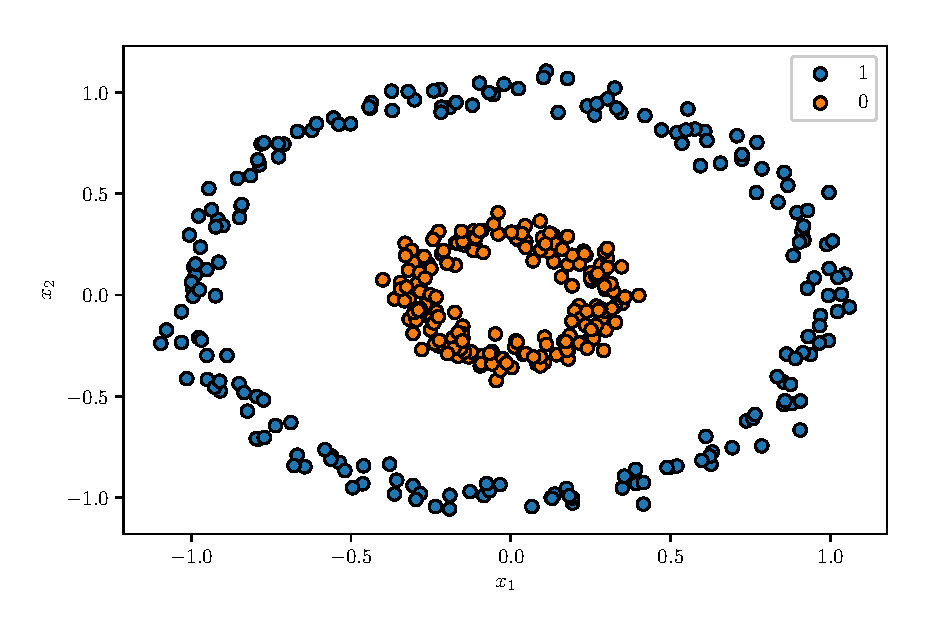
\includegraphics[width=.35\textwidth]{./gfx/input.eps}};
        %\node[inner sep=0pt] (feature) at (5,-6)
            %{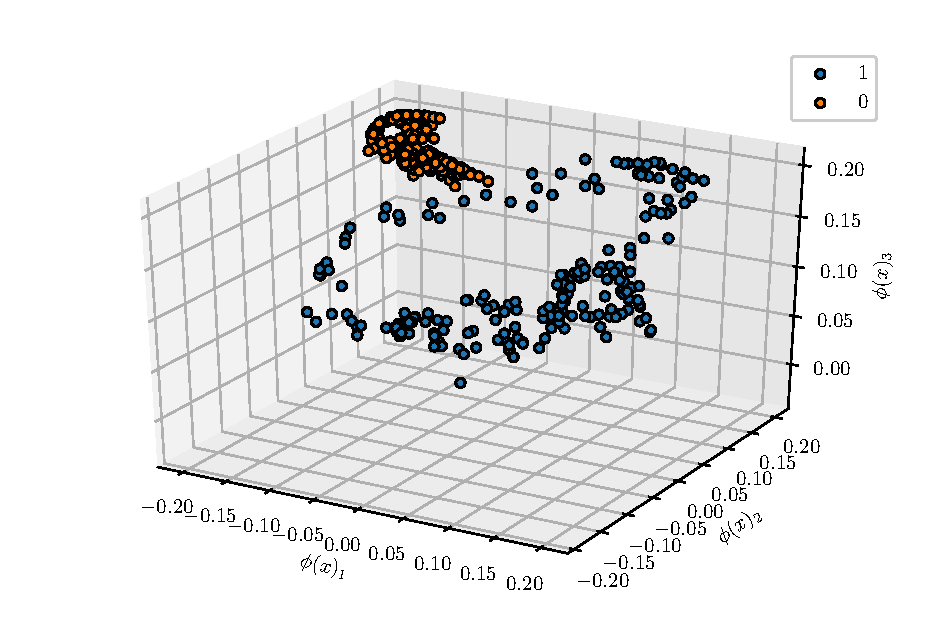
\includegraphics[width=.35\textwidth]{./gfx/feature.eps}};
        %\draw[->,thick] (input.east) -- (feature.west)
            %node[midway,fill=white] {$\phi:\mathcal{X} \to \mathcal{H}$};
    %\end{tikzpicture}}
    \centering
    \begin{tabular}{c}
        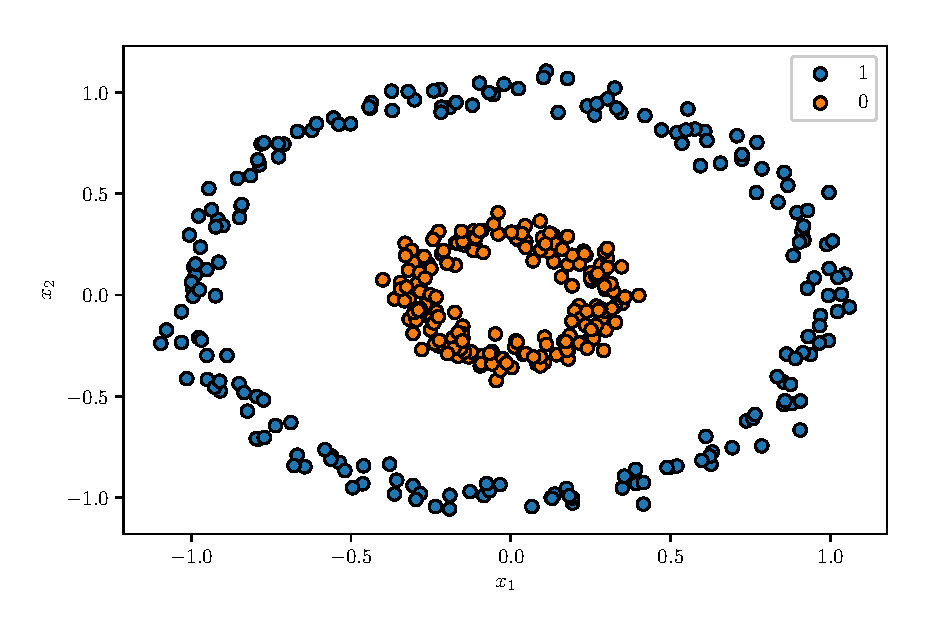
\includegraphics[valign=m, width=.5\textheight]{./gfx/input.eps} \\
        $\xdownarrow{1cm} \phi: \enskip \mathcal{X} = \mathbb{R}^2 \to
        \mathcal{H} = \mathbb{R}^3$ \\
        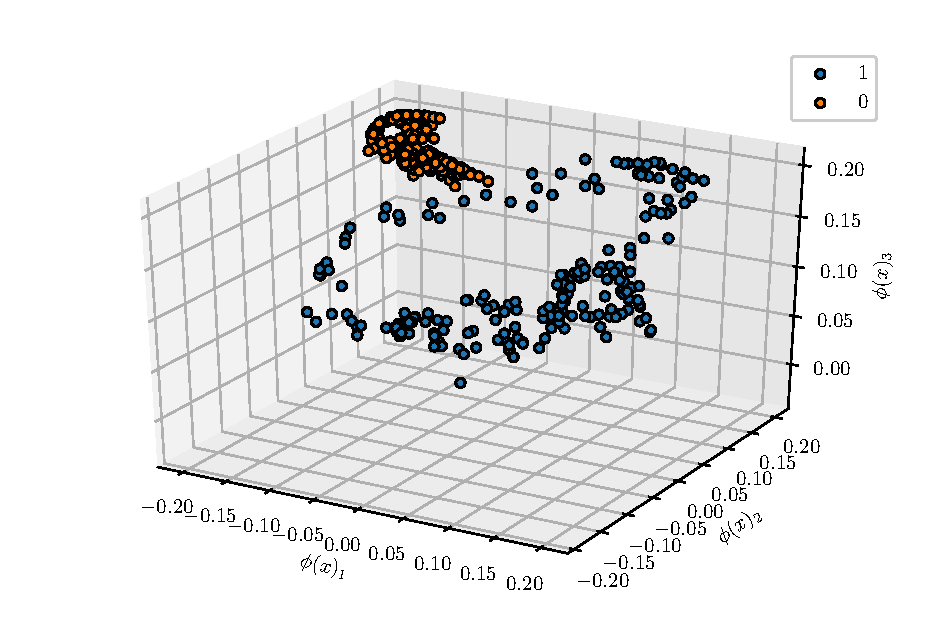
\includegraphics[valign=m, width=.5\textheight]{./gfx/feature.eps}
    \end{tabular}
    \caption[A scalar-valued feature map]{We map the two circles in
    $\mathbb{R}^2$ to $\mathbb{R}^3$. In $\mathbb{R}^3$ it is now possible to
    separate the circles with a linear functional: a plane. We used the feature
    map \\ $\phi(x) = 0.82 \begin{pmatrix} \cos(1.76 x_1 + 2.24 x_2 + 2.75) \\
    \cos(0.40 x_1 + 1.87 x_2 + 5.6) \\ \cos(0.98 x_1 - 0.98 x_2 + 6.05)
    \end{pmatrix}$. \\
    Here $\phi:\mathbb{R}^2\to\mathbb{R}^3$ has been chosen
    as a realization of an \acs{RFF} map (see \cref{eq:rff2}). A \say{cleaner}
    feature map adapted to this problem could have been \\
    $\phi(x)=\begin{pmatrix} x_1 \\ x_2 \\ x_1^2 + x_2^2 \end{pmatrix}$.
    \label{fig:feature_map}}
\end{figure}
If we note
\begin{dmath*}
    \boldsymbol{\phi} =
    \begin{pmatrix}
        \phi(x_1) & \dots & \phi(x_N)
    \end{pmatrix}
\end{dmath*}
the \say{matrix} where each column represents the feature map evaluated at the
point $x_i$ with $1 \le i \le N$, the regularized risk minimization with the
least square loss reads
\begin{dmath*}
    \mathfrak{R}_{\lambda}(\theta, \seq{s}) =
    \frac{1}{2N}\norm{\boldsymbol{\phi}^\transpose \theta - (y_i)_{i=1}^N
    }_{2}^2 + \frac{\lambda}{2}\norm{\theta}_2^2.
\end{dmath*}
and the unique solution is $\theta_{\seq{s}} =
\left(\boldsymbol{\phi}\boldsymbol{\phi}^\transpose/N + \lambda
I_{\mathcal{H}}\right)^{-1}\boldsymbol{\phi}$. This is an
\begin{dmath*}
    O_t\left( \dim(\mathcal{H})^2(N + \dim{\mathcal{H}}) \right).
\end{dmath*}
time complexity algorithm.  This algorithm seems more appealing than its kernel
counterpart when many data are given since once the space $\mathcal{H}$ has
been fixed, the algorithm is linear in the number of training points. However
many questions remains. First although it is possible to design a feature map
\emph{ex nihilo}, can we design systematically a feature map from a kernel? For
some kernels (\acs{eg} the Gaussian kernel) it is well known that the Hilbert
space corresponding to it has dimension $\dim(\mathcal{H}) = \infty$. Is it
possible to find an approximation of the kernel such that $\dim(\mathcal{H}) <
\infty$? If such a construction is possible and we know that $N$ training data
are available, is it possible to have a sufficiently good approximation
\footnote{When $\dim(\mathcal{H}) \ge N$ then is it is better to use the kernel
algorithm than the feature algorithm. This is called the kernel trick.} with
$\dim(\mathcal{H}) \ll N$?

\subsection{Towards large scale learning with kernels}
Motivated by large scale applications, different methodologies have been
proposed to approximate kernels and feature maps. This subsection briefly
reminds the main approaches based on  Random Fourier Features and Nystr\"om
techniques. Notice that another line of research concerns online learning
method such as \acs{NORMA} developed in \cite{kivinen2004online}, later
extended to the operator-valued kernel case by \citet{audiffren2013online}.  We
start with the seminal work of \citet{Rahimi2007} who show that given a
continuous shift-invariant kernel ($\forall x, z, t \in \mathcal{X}$, $k(x + t,
z + t) = k(x, z)$), it is possible to obtain a feature map called \acs{RFF}
that approximate the given kernel.
\subsubsection{Random Fourier Features map}
The Random Fourier Features methodology introduced  by \citet{Rahimi2007}
provides a way to scale up kernel methods when kernels are Mercer and
\emph{translation-invariant}.  We view the input space $\mathcal{X}$ as a group
endowed with the addition. Extensions to other group laws such as
\citet{li2010random} are described in \cref{subsubsec:skewedchi2} within the
general framework of operator-valued kernels.
\paragraph{}
Denote $k: \mathbb{R}^d \times \mathbb{R}^d \to \mathbb{R}$ a positive
definite kernel on $\mathcal{X}=\mathbb{R}^d$. A kernel $k$ is said to be
\emph{shift-invariant} or \emph{translation-invariant} for the addition if for
for all $(x,z,t) \in \left(\mathbb{R}^d\right)^3$ we have $k(x+t,z+t) =
k(x,z)$.  Then, we define $k_0: \mathbb{R}^d \to \mathbb{R}$ the function such
that $k(x,z)= k_0(x-z)$. $k_0$ is called the \emph{signature} of kernel $k$.
Bochner's theorem \citep{folland1994course} is the theoretical result that
leads to the Random Fourier Features.
\begin{theorem}[Bochner's theorem]\label{th:bochner-scalar}
    Any continuous positive definite function is the \acl{FT} of a
    bounded non-negative Borel measure.
\end{theorem}
It implies that any positive definite, continuous and shift-invariant kernel
$k$, has a continuous and positive semi-definite signature $k_0$, which is the
\acl{FT} $\mathcal{F}$ of a non-negative measure $\mu$. Hence we have
$k(x,z)=k_0(x-z) \hiderel{=} \int_{\mathbb{R}^d} \exp\left(-\iu \inner{\omega,x
- z}\right) d\mu(\omega) =\FT{k_0}(\omega)$.  Moreover $\mu = \IFT{k_0}$.
Without loss of generality, we assume that $\mu$ is a probability measure,
\acs{ie} $\int_{\mathbb{R}^d} d\mu(\omega)=1$ by renormalizing the kernel since
\begin{dmath*}
    \int_{\mathbb{R}^d}d\mu(\omega)= \int_{\mathbb{R}^d}\exp\left(-\iu
    \inner{\omega, 0}\right)d\mu(\omega)\hiderel{=}k_0(0).
\end{dmath*}
and we can write the above equation as an expectation over $\mu$. For all
$x$,
$z\in\mathbb{R}^d$
\begin{dmath*}
    k_0(x-z) = \expectation_{\mu}\left[\exp(-\iu \inner{\omega,x - z})\right].
\end{dmath*}
Eventually, if $k$ is real valued we only write the real part,
\begin{dmath*}
    k(x,z) = \expectation_{\mu}[\cos \inner{\omega,x - z}] =
    \expectation_{\mu}[ \cos \inner{\omega,z} \cos \inner{\omega,x} + \sin
    \inner{\omega,z} \sin \inner{\omega,x}].
\end{dmath*}
Let $\Vect_{j=1}^D x_j$ denote the $Dd$-length column
vector obtained by stacking vectors $x_j \in \mathbb{R}^d$.  The feature map
$\widetilde{\phi}: \mathbb{R}^d \rightarrow \mathbb{R}^{2D}$ defined as
\begin{dmath}
\label{eq:rff}
    \widetilde{\phi}(x)=\frac{1}{\sqrt{D}}\Vect_{j=1}^D
    \begin{pmatrix}
        \cos{\inner{x,\omega_j}} \\
        \sin{\inner{x,\omega_j}}
    \end{pmatrix}\condition{$\omega_j \hiderel{\sim} \IFT{k_0}$ \acs{iid}}
\end{dmath}
is called a \emph{Random Fourier Features} (map). Each $\omega_{j}, j=1, \ldots,
D$ is independently and identically sampled from the inverse Fourier transform
$\mu$ of $k_0$. This Random Fourier Features map provides the following
Monte-Carlo estimator of the kernel: $\widetilde{k}(x, z) =
\widetilde{\phi}(x)^* \widetilde{\phi}(z)$. Using trigonometric identities,
\citet{Rahimi2007} showed that the same feature map can also be written
\begin{dmath}
    \label{eq:rff2}
    \tilde{\phi}(x)=\sqrt{\frac{2}{D}}\Vect_{j=1}^D
    \begin{pmatrix}
        \cos(\inner{x,\omega_j} + b_j)
    \end{pmatrix},
\end{dmath}
where $\omega_j \hiderel{\sim} \IFT{k_0}$, $b_j \sim \mathcal{U}(0, 2\pi)$
\acs{iid}.  The feature map defined by \cref{eq:rff} and \cref{eq:rff2} have
been compared in \citet{sutherland2015} where they give the condition under
wich \cref{eq:rff} has lower variance than \cref{eq:rff2}. For instance for the
Gaussian kernel, \cref{eq:rff} has always lower variance. In practice,
\cref{eq:rff2} is easier to program. In this manuscript we focus on random
Fourier feature of the form given in \cref{eq:rff}.

\paragraph{}
The dimension $D$ governs the precision of this
approximation, whose uniform convergence towards the target kernel (as defined
in \cref{bochner-scalar}) can be found in \citet{Rahimi2007} and in more recent
papers with some refinements proposed in \citet{sutherland2015} and
\citet{sriper2015}.  Finally, it is important to notice that Random Fourier
Features approach \emph{only} requires two steps before the application of a
learning algorithm: (1) define the inverse Fourier transform of the given
shift-invariant kernel, (2) compute the randomized feature map using the
spectral distribution $\mu$.  \citet{Rahimi2007} show that for the Gaussian
kernel $k_0(x-z) = \exp(-\gamma \norm{x - z}_2^2)$, the spectral distribution
$\mu$ is a Gaussian distribution. For the Laplacian kernel $k_0(x-z) =
\exp(-\gamma \norm{x - z}_1)$, the spectral distribution is a Cauchy
distribution.
\paragraph{}
We now focus on another famous way of obtaining feature maps for any scalar
valued kernel called the Nystr\"om method.

\subsubsection{Nystr\"om approximation}
To overcome the bottleneck of Gram matrix computations in kernel methods,
\citet{Williams2000-nystrom} have proposed to generate a low-rank matrix
approximation of the Gram matrix using a subset of its columns.  Since this
feature map is based on a decomposition of the Gram matrix, the feature map
resulting from the Nystr\"om method is data dependent. Let $k: \mathcal{X}^2
\to \mathbb{R}$ be any scalar-valued kernel and let
\begin{dmath*}
    \seq{s} = (x_i)_{i=1}^N
\end{dmath*}
be the training data. We note a subsample of the training data
\begin{dmath*}
    \seq{s}_M = (x_i)_{i=1}^M
\end{dmath*}
where $M \le N$ and $\seq{s}_M$ is a subsequence of $\seq{s}$. Then construct
the Gram matrix $\mathbf{K}_M$ on the subsequence $\seq{s}_M$. Namely
\begin{dmath*}
    \mathbf{K}_M =
    \begin{pmatrix}
        k(x_i, x_j)
    \end{pmatrix}_{i,j=1}^M.
\end{dmath*}
Then perform the singular-valued decomposition $\mathbf{K}_M = U \Lambda
U^\transpose$. The Nystr\"om feature map is given by
\begin{dmath*}
    \tilde{\phi}(x) = \Lambda^{-1/2} U^\transpose\left( \vect_{i=1}^M k(x, x_i)
    \right).
\end{dmath*}
Here $M$ plays the same role as $D$ in the \acs{RFF} case: it controls the
quality of the approximation. Let $\mathbf{K}$ be the full Gram matrix on the
training data $\seq{s}$, let
\begin{dmath*}
    \mathbf{K}_b =
    \begin{pmatrix}
        k(x_i, x_j)
    \end{pmatrix}_{i=1, j=1}^{i=N, j=M}.
\end{dmath*}
Then it is easy to verify that $\boldsymbol{\phi}^\transpose \boldsymbol{\phi} =
\mathbf{K}_b \mathbf{K}_M^\dagger \mathbf{K}_b^\transpose \approx \mathbf{K}$,
where $\mathbf{K}_M^\dagger$ is the pseudo-inverse of $\mathbf{K}_M$ and the
quantity $\mathbf{K}_b \mathbf{K}_M^\dagger \mathbf{K}_b^\transpose$ is a low
rank approximation of the Gram matrix $\mathbf{K}$.
\subsubsection{Random features vs Nystr\"om method}
The main conceptual difference between the Nystr\"om features and the \acl{RFF}
is that the Nystr\"om construction is data dependent, while the \acs{RFF} is
not. The advantage of random Fourier feature lies in their fast construction.
For $N$ data in $\mathbb{R}^d$, it costs $O(NDd)$ to featurize all the data.
For the Nystr\"om features it costs $O\left(M^2(M + d)\right)$. Moreover if one
desires to add a new feature, the \acs{RFF} methodology is as simple as drawing
a new random vector $\omega\sim\IFT{k_0}$, compute $\cos(\inner{\omega, x} +
b)$, where $b\sim \mathcal{U}(0, 2\pi)$ and concatenate it the existing
feature.  For the Nystr\"om features one needs to recompute the singular value
decomposition of the new augmented Gram matrix $\mathbf{K}_{M+1}$.
\paragraph{}
To analyse the \acs{RFF} and Nystr\"om features authors usually study the
approximation error of the approximate Gram matrix and the targer kernel
$\norm{\boldsymbol{\phi}^\transpose\boldsymbol{\phi} - \mathbf{K}}$ (see
\citep{Yang2012, drineas2005nystrom, rosasco2010learning}) or
the supremum of the error between the approximated kernel and the true kernel
over a compact subset $\mathcal{X}$ of the support if $k$: $\sup_{(x, z)
\in\mathcal{C} \subseteq \mathcal{X}^2} \abs{\tilde{\phi}(x)^\transpose
\tilde{\phi}(z) - k(x, z)}$ (see \citet{Rahimi2007, sutherland2015, Bach2015,
rudi2016generalization}).  Because~\citet{bartlett2002rademacher} showed that
for generalization error to be below $\epsilon \in \mathbb{R}_{>0}$ for kernel
methods is $O(N^{-1/2})$, the number of samples $M$ or $D$ required to reach
some approximation error below $\epsilon$ should not grow faster than
$O(M^{-1/2})$ for the Nystr\"om method or $O(D^{-1/2})$ for the \acs{RFF}
method to match kernel learning.  Concerning the Nystr\"om method,
\citet{Yang2012} suggest that the number of samples $M$ is reduced to
$O(M^{-1})$ to reach an error below $\epsilon$ when the gap between the
eigenvalues of $\mathbf{K}$ is large enough. As a result in this specific case,
one should sample $M=O(\sqrt{N})$ Nystr\"om features to ensure good
generalization. On the other hand \citet{rahimi2009weighted} reported that the
generalization performance of \acs{RFF} learning is $O(N^{-1/2} + D^{-1/2})$,
which indicates that $D=O(N)$ features should be sampled to generalize well.
As a result the complexity of learning with the \acs{RFF} seems not to
decrease. However the bounds of \citet{rahimi2009weighted} are suboptimal and
very recently (end of 2016) \citet{rudi2016generalization} proved that in the
case of ridge regression (\cref{eq:ridge_regression}), the generalization error
is $O(N^{-1/2} + D^{-1})$ meaning that $D=O(\sqrt{N})$ random features are
required for good generalization with \acsp{RFF}. We refer the interested
reader to \citet{Yang2012} for an empirical comparison between the Nystr\"om
method and the \acs{RFF} method.

\subsubsection{Extensions of the RFF method}
\paragraph{}
The seminal idea of \citet{Rahimi2007} has opened a large literature on random
features. Nowadays, many classes of kernels other than translation invariant are
now proved to have an efficient random feature representation.
\citet{kar2012random} proposed random feature maps for dot product kernels
(rotation invariant) and \citet{hamid2014compact} improved the rate of
convergence of the approximation error for such kernels by noticing that
feature maps for dot product kernels are usually low rank and may not utilize
the capacity of the projected feature  space  efficiently. \Citet{pham2013fast}
proposed fast random feature maps for polynomial kernels.
\paragraph{}
\Citet{li2010random} generalized the original \acs{RFF} of \citet{Rahimi2007}.
Instead of computing feature maps for shift-in\-va\-riant kernels on the
additive group $(\mathbb{R}^d, +)$, they used the generalized Fourier transform
on any locally compact abelian group to derive random features on the
multiplicative group $(\mathbb{R}^d_{>0}, *)$. In the same spirit
\citet{yang2014random} noticed that an theorem equivalent to Bochner's theorem
exists on the semi-group $(\mathbb{R}_+^d, +)$. From this they derived
\say{Random Laplace} features and used them to approximate kernels adapted to
learn on histograms.
\paragraph{}
To speed-up the convergence rate of the random features approximation,
\citet{yang2014quasi} proposed to sample the random variable from a quasi
Monte-Carlo sequence instead of \acs{iid}~random variables. \Citet{Le2013}
proposed the \say{Fastfood} algorithm to reduce the complexity of computing a
\acs{RFF} --using structured matrices and a fast Walsh-Hadarmard transform--
from $O_t(Dd)$ to $O_t(D\log(d))$. More recently \citet{felix2016orthogonal}
proposed also an algorithm \say{SORF} to compute Gaussian \acs{RFF} in
$O_t(D\log(d))$ but with better convergence rates than \say{Fastfood}
\citep{Le2013}.  \Citet{mukuta2016kernel} proposed a data dependent feature
map (comparable to the Nystro\"m method) by estimating the distribution of the
input data, and then finding the eigenfunction decomposition of Mercer's
integral operator associated to the kernel.
\paragraph{}
In the context of large scale learning and deep learning, \citet{lu2014scale}
showed that \acsp{RFF} can achieve performances comparable to deep-learning
methods by combining multiple kernel learning and composition of kernels along
with a scalable parallel implementation. \Citet{dai2014scalable} and
\citet{xie2015scale} combined \acsp{RFF} and stochastic gradient descent to
define an online learning algorithm called \say{Doubly stochastic gradient
descent} adapted to large scale learning. \Citet{yang2015deep} proposed and
studied the idea of replacing the last fully interconnected layer of a deep
convolutional neural network \citep{lecun1995convolutional} by the
\say{Fastfood} implementation of \acsp{RFF}.
\paragraph{}
Eventually \citet{Yang2015} introduced the algorithm \say{\`A la Carte}, based
on \say{Fastfood} which is able to learn the spectral distribution
%<<<<<<< HEAD
%corresponding to a kernel rather than defining it from the kernel. Among the
%large-scale learning methods with kernel, but not using random features we
%mention the algorithm \say{NORMA} by \citet{kivinen2004online} (to be compared
%to the \say{Doubly stochastic gradient descent}) and \say{Pegasos} by
%\citet{shalev2007pegasos} and \say{SMO} by \citet{platt199912} for kernel
%\acs{SVM} learning.
%=======
corresponding to a kernel rather than defining it from the kernel. Very
recently \citet{kawaguchi2017deep} proposed to use semi-random features which
are a tradeoff between the random features based on kernel methods (\acs{eg}
\acsp{RFF}) and the trainable layer in deep learning.
%>>>>>>> 9b5b5ea96fbb45de714e68edd2b96f14a62f3e01
% A la carte
%reported
%performance comparable with deep learn- ing by combining multiple kernel
%learning and the compo- sition of kernels.

%A important subject of research is on how to compute random features
%as fast as possible. \Citet{hamid2014compacti, } proposed feature maps for
%polynomial kernels rank deficient, and there-
%fore may not utilize the capacity of the projected
%feature  space  effectively.

%\section{On large-scale learning}
%\label{sec:on_large-scale_learning}

%\section{History and state of the art of large scale learning with kernels}
%\label{sec:history}

\chapterend


\chapter{Background}
\label{ch:background}
%!TEX root = ../../ThesisRomainbrault.tex

%------------------------------------------------------------------------------
\section{Notations}
In this section with summarize briefly important notions used throughout this
document. It is mainly base on books and lecture notes of
\citet{kurdila2006convex,cotaescu2016elements}.

\subsection{Algebraic structures}
\label{sec:notations}
We note $\mathbb{K}$ any Abelian\mpar{Commutative.} field, $\mathbb{R}$ the
Abelian field of real numbers and $\mathbb{C}$ the Abelian field of complex
numbers. The unit pure imaginary number $\sqrt{-1}\in\mathbb{C}$ is denoted
$\iu$ and the Euler constant $\exp(1)\in\mathbb{R}$ is denoted $\ec$.
$\mathbb{N}$ represents the set of natural numbers and $\mathbb{N}_n$,
$n\in\mathbb{N}$ the set of natural numbers smaller or equal to $n$. For any
space $\mathcal{S}$, $\mathcal{S}^d$, $d\in\mathbb{N}$ represents the Cartesian
product space $\mathcal{S}^d = \mathcal{S}\times\ldots\times\mathcal{S}$. For
any two algebraic structures $\mathcal{S}$ and $\mathcal{S}'$ we write
$\mathcal{S}\cong\mathcal{S}'$ is there exist an isomorphism between these two
structures. If $a+\iu b = x \in \mathbb{C}$ then $\conj{x}=a-\iu
b\in\mathbb{C}$ denote the complex conjugate. By extension if $x\in\mathbb{R}$,
$\conj{x}=x\in\mathbb{R}$.

\subsection{Topology and continuity}{}
In order to define a proper notion of continuity, we focus on topological
spaces. A topological space is a pair of sets $(\mathcal{X},\mathcal{T}_x)$
where $\mathcal{X}$ describes the points considered, and $\mathcal{T}_x$
describes the possible neighbours. The standards axioms of topology suppose
that $\mathcal{T}_x\subseteq{\mathcal{P}(\mathcal{X})}$ is a collection of
subsets of $\mathcal{X}$ such that the empty set and $\mathcal{X}$ itself
belongs to $\mathcal{T}_x$, any (finite or infinite) union of members of
$\mathcal{T}_x$ still belongs to $\mathcal{T}_x$ and the intersection of any
finite number of members of $\mathcal{T}_x$ still belongs to $\mathcal{T}_x$.
The elements of $\mathcal{T}_x$ are called open sets and the collection
$\mathcal{T}_x$ is a topology on $\mathcal{X}$. If
$(\mathcal{X},\mathcal{T}_x)$ and $(\mathcal{Y},\mathcal{T}_y)$ are topological
spaces, a function $f$ is said to be continuous if for every open set
$\mathcal{V}\in \mathcal{T}_y$, the inverse image $f^{-1}(\mathcal{V}) = \Set{
x \in \mathcal{X} | f ( x ) \in \mathcal{V} }$ is an open subset of
o
$\mathcal{T}_x$. Since the notion of continuity depends on open sets, it
depends on the topology of the spaces $\mathcal{X}$ and $\mathcal{Y}$.
\paragraph{}
If $\mathcal{X}$ is a topological space and $x$ is a point in $\mathcal{X}$, a
neighbourhood of $x$ is a subset $\mathcal{V}$ of $\mathcal{X}$ that includes
an \emph{open} set $\mathcal{U}$ containing $x$. A topological space
$\mathcal{X}$ is said to be Haussdorff (T2) when all distinct points in
$\mathcal{X}$ are pairwise neighborhood-separable. \acs{Ie}~if there exists a
neighbourhood $\mathcal{U}$ of $x$ and a neighbourhood $\mathcal{V}$ of $y$
such that $\mathcal{U}$ and $\mathcal{V}$ are disjoint. It implies the
uniqueness of limits of sequences and existence of nets used throughout this
thesis. Therefore in the whole document we always assume that a topological
space $\mathcal{X}$ is Haussdorff.
\paragraph{}
A topological space is said to be separable if there exists a sequence
$(x_n)_{n\in\mathbb{N}^*}$ of elements of $\mathcal{X}$ such that every
nonempty open subsets of the space contains at least one element of the
sequence. Separability plays an important role in numerical analysis because
many theorems have only constructive proofs for separable spaces. Such
constructive proofs can be turned into algorithms which is the primary goal of
this work. In this document we also assume that any topological space is
separable if there is no specific mention of the contrary. Moreover we recall
that a Hilbert space is separable if and only if it has a countable orthonormal
basis. Hence an operator between two separable Hilbert spaces can be written as
an infinite dimensional matrix.
\paragraph{}
If $\mathcal{X}$ and $\mathcal{Y}$ are two topological spaces, we denote by
$\mathcal{F}(\mathcal{X};\mathcal{Y})$ the topological vector space of
functions $f:\mathcal{X}\to\mathcal{Y}$ and
$\mathcal{C}(\mathcal{X};\mathcal{Y}) \subset
\mathcal{F}(\mathcal{X};\mathcal{Y})$ the subspace of continuous functions,
endowed with the product topology (topology of pointwise convergence).

\subsection{Measure theory}
A $\sigma$-algebra on $\mathcal{X}$ is a set
$\mathcal{M}\subseteq\mathcal{P}(\mathcal{X})$ of subsets of $\mathcal{X}$,
containing the empty set, which is closed under taking complements and
countable unions. A pair $(\mathcal{X},\mathcal{M})$ where $\mathcal{X}$ is a
set and $\mathcal{M}$ is a $\sigma$-algebra is called a measure space. The
Borel $\sigma$-algebra $\mathcal{B}(\mathcal{X})$ is a $\sigma$-algebra
generated by the open sets of $\mathcal{X}$. A measure on a measurable space
$(\mathcal{X},\mathcal{B}(\mathcal{X}))$ is a map $\mu: \mathcal{B}(X) \to
\overline{\mathbb{R}}_+$ which is zero on the empty set and countably additive,
\acs{ie}~for any subset $(\mathcal{Z}_n)_{n\in\mathbb{N}}$ is a sequence of
pairwise disjoint measurable sets, 
\begin{dmath*}
    \mu\left(\bigcup_{n\in\mathbb{N}}\mathcal{Z}_n\right) =
    \sum_{n\in\mathbb{N}}\mu(\mathcal{Z}_n).
\end{dmath*}

\subsection{Vector spaces, linear operators and matrices}
Given any vector space $\mathcal{H}$ over an Abelian field $\mathbb{K}$, the
(continuous) dual space\footnote{The continuous dual space is also called
topological dual space. This must be differentiate from the \emph{algebraic}
dual space, which is the space of linear functionals from the original
vector-space to its base field. Hence the continuous dual space is a subset of
the algebraic dual space. The continuous and the algebraic dual space only
match when considering finite dimensional vector-spaces} $\mathcal{H}^\adjoint$
is defined as the set of all \emph{continuous} linear functionals $x^*:
\mathcal{H} \to \mathbb{K}$. When $\mathcal{H}$ is a vector space, there is a
natural duality pairing between $\mathcal{H}^\adjoint$ and $\mathcal{H}$
defined for all $x^\adjoint\in\mathcal{H}^\adjoint$ and all $z\in\mathcal{H}$
as $\pairing{x^\adjoint, z}_{\mathcal{H}^\adjoint, \mathcal{H}} = x^\adjoint(z)
= x^\adjoint z$. The duality paring $\pairing{\cdot,
\cdot}_{\mathcal{H}^\adjoint,\mathcal{H}}$ is then a bilinear form.
\paragraph{}
Let $\mathcal{H}_1$ and $\mathcal{H}_2$ be two vector spaces. The transpose (or
dual) of an operator $W:~\mathcal{H}_1\to\mathcal{H}_2$ is defined as
$W^\transpose :\mathcal{H}_2^\adjoint \to \mathcal{H}_1^\adjoint$ such that
$W^\transpose :x^\adjoint\mapsto x^\adjoint(W)$. It is characterized by the
relation $\pairing*{x^\adjoint,
Wz}_{\mathcal{H}_2^\adjoint,\mathcal{H}_2}=\pairing*{W^\transpose x^\adjoint,
z}_{\mathcal{H}_1^\adjoint,\mathcal{H}_1}$ for all
$x^\adjoint\in\mathcal{H}_2^\adjoint$ and all $z\in\mathcal{H}_1$. An operator
is called self-dual when $W^\transpose =W$.
\paragraph{}
Let $\mathcal{H}$ be a vector space. We set
$\mathcal{L}(\mathcal{H})=\mathcal{L}(\mathcal{H};\mathcal{H})$ to be the space
of \emph{bounded} (continuous) linear operators from $\mathcal{H}$ to itself.
If $W\in\mathcal{L}(\mathcal{H})$, $\Ker W$ denotes the nullspace, $\Ima W$ the
image, $W^\transpose  \in \mathcal{L}(\mathcal{H}^*)$ the transpose and $\Dom
W$ the domain of $W$.
\paragraph{}
If $\mathcal{H}$ is an Hilbert space on a field $\mathbb{K}$ we denote its
scalar product by $\inner{\cdot,\cdot}_{\mathcal{H}}$ and its norm by
$\norm{\cdot}_{\mathcal{H}}$. When the base field of $\mathcal{H}$ is
$\mathbb{R}$, $\inner{\cdot,\cdot}_{\mathcal{H}}$ is a \emph{bilinear} form.
When the base field of $\mathcal{H}$ is $\mathbb{C}$,
$\inner{\cdot,\cdot}_{\mathcal{H}}$ is a \emph{sesquilinear} form. Let
$\mathcal{H}_1$ and $\mathcal{H}_2$ be two Hibert spaces. The adjoint of a
bounded operator $W:\mathcal{H}_1\to\mathcal{H}_2$ is the unique mapping
$W^\adjoint:\mathcal{H}_2\to\mathcal{H}_1$ such that $\inner{W^\adjoint x,
z}_{\mathcal{H}_1}=\inner{x, Wz}_{\mathcal{H}_2}$ for all $x$, $z\in\Dom W$. An
operator $W:\mathcal{H}\to\mathcal{H}$ is said to be symmetric when
$W^\adjoint=W$ and self-adjoint when $W$ is symmetric and $\Dom W^\adjoint =
\Dom W$. If $W$ is symmetric and $\Dom W=\mathcal{H}$ then $W$ is self-adjoint.
\paragraph{}
Let $\mathcal{H}$ be a Hilbert space. From Riesz's representation theorem,
there is a unique isometric isomorphism
$\iota_R:\mathcal{H}\to\mathcal{H}^\adjoint$ such that for any $x$ and
$y\in\mathcal{H}$, $\pairing{\iota_R(x), y}_{\mathcal{H}^\adjoint,
\mathcal{H}}=\inner{x,y}_{\mathcal{H}}$ and
$\norm{\iota_R(x)}_{\mathcal{H}^\adjoint}=\norm{x}_{\mathcal{H}}$. The riesz
map $\iota_R$ is self-dual, thus if $\mathcal{H}$ is a Hilbert space,
$\mathcal{H}$ is reflexive.
\acs{Ie}~$\mathcal{H}^{\adjoint\adjoint}\cong\mathcal{H}$.  When the base field
of $\mathcal{H}$ is $\mathbb{C}$, then $\iota_R$ is an \emph{anti-linear} form
since $\inner{\cdot,\cdot}_{\mathcal{H}}$ is sesquilinear and $\pairing{\cdot,
\cdot}_{\mathcal{H}^\adjoint, \mathcal{H}}$ is bilinear. In the same way when
the base field of $\mathcal{H}$ is $\mathbb{R}$ then $\iota_R$ \emph{linear}
since both $\inner{\cdot,\cdot}_{\mathcal{H}}$ and $\pairing{\cdot,
\cdot}_{\mathcal{H}^\adjoint, \mathcal{H}}$ are bilinear. If $\mathcal{H}$ is a
Hilbert space we make the dual space $\mathcal{H}^\adjoint$ a Hilbert space by
endowing it with the inner product $\inner{x^\adjoint,
z^\adjoint}_{\mathcal{H}^\adjoint}=\inner{\iota_R^{-1}(x^\adjoint),
\iota_R^{-1}(z^\adjoint)}_{\mathcal{H}}$ for all $x^\adjoint$,
$z^\adjoint\in\mathcal{H}^\adjoint$. Notice that the transpose is linked to the
adjoint by the relation $W^\adjoint = \iota_R^{-1} W^\transpose  \iota_R$. When
$\mathcal{H}$ is a Hilbert space, if $x\in\mathcal{H}$, we always define
$x^\adjoint\in\mathcal{H}^\adjoint$ to be
\begin{dmath*}
    x^\adjoint\hiderel{=}\iota_R(x)\hiderel{=}\inner{x, \cdot}_{\mathcal{H}}.
\end{dmath*}
\begin{figure}[htb]
    \centering
    \begin{tikzcd}[matrix scale=3]
            \mathcal{H}_2 \arrow[r, "W^\adjoint"] \arrow[d, "\iota_R"] &
            \mathcal{H}_1  \arrow[d, bend left, "\iota_R"] \\
            \mathcal{H}_2^\adjoint  \arrow[r, "W^\transpose "] &
            \mathcal{H}_1^\adjoint \arrow[u, bend left, "\iota_R^{-1}"]
    \end{tikzcd}
    \caption{\label{fig:riesz_map}Riesz map, dual spaces and adjoints.}
\end{figure}
\paragraph{}
Let $\mathcal{H}$ be a \emph{separable} Hilbert space and let
$(e_i)_{i\in\mathbb{N}^*}$ be a basis of $\mathcal{H}$. We call
$(e_i^\adjoint)_{i\in\mathbb{N}^*}$ the dual basis of $\mathcal{H}$, the basis
of $\mathcal{H}^\adjoint$ such that for all $i$, $j\in\mathbb{N}^*$,
$e_i^\adjoint(e_j)=\inner{e_i, e_j}_{\mathcal{H}}=\delta_{ij}$. In the whole
document we consider that $\mathcal{H}^\adjoint$ is always equipped with the
dual basis of $\mathcal{H}$.  For a vector $x\in\mathcal{H}$ with a basis
$(e_i)_{i\in\mathbb{N}^*}$ we write $x_i=e_i^\adjoint(x)$. For a linear
operator $W:\mathcal{H}_1\to\mathcal{H}_2$ where $\mathcal{H}_1$ and
$\mathcal{H}_2$ are Hilbert spaces with respective basis
$(e_i)_{i\in\mathbb{N}^*}$ and $(e'_j)_{j\in\mathbb{N}^*}$, we note $W_i=We_i$
and $W_{ij}=e_j^\adjoint(We_i)$. Eventually given two separable Hilbert spaces
$\mathcal{H}_1$ and $\mathcal{H}_2$, an operator
$W:\mathcal{H}_1\to\mathcal{H}_2$, $(e_i)_{i\in\mathbb{N}^*}$ a basis of
$\mathcal{H}_1$ and $(e'_i)_{i\in\mathbb{N}^*}$ a basis of $\mathcal{H}_2$ we
have
\begin{dmath*}
    (W^\transpose)_{ij}=e_j^{\adjoint\adjoint}W^\transpose
    {e'}_i^\adjoint\hiderel{=} e_j^{\adjoint\adjoint}{e'}_i^\adjoint W
    \hiderel{=} {e'}_i^\adjoint W e_j \hiderel{=} W_{ji}.
\end{dmath*}
\paragraph{}
We call matrix $M$ of size $(m,n)\in\mathbb{N}^2$ on an Abelian field
$\mathbb{K}$ a collection of elements $M=(m_{ij})_{1\le i\le m, 1\le j \le n}$,
$m_{ij}\in\mathbb{K}$. We note $\mathcal{M}_{m,n}(\mathbb{K})$ the vector space
of all matrices. If $\mathcal{H}_1$ and $\mathcal{H}_2$ are two separable
Hilbert spaces on an Abelian field $\mathbb{K}$, any linear operator
$L\in\mathcal{L}(\mathcal{H}_1;\mathcal{H}_2)$ can be viewed as a (potentially
infinite) matrix. Let $n=\dim(\mathcal{H}_1)$, $m=\dim(\mathcal{H}_2)$ and let
$B=(e_i)_{i=1}^{n}$ and $C=(e'_i)_{i=1}^{m}$ be the respective bases of
$\mathcal{H}_1$ and $\mathcal{H}_2$. We note $\text{mat}_{B, C}:
\mathcal{L}(\mathcal{H}_1;\mathcal{H}_2) \to \mathcal{M}_{m,n}(\mathbb{K})$
such that $M=\text{mat}_{B, C}(L)=({e'}_j^\adjoint L e_i)_{1\le i\le n, 1\le j
\le m}\in\mathcal{M}_{m,n}(\mathbb{K})$. Let
$M_1\in\mathcal{M}_{m,n}(\mathbb{K})$ and
$M_2\in\mathcal{M}_{n,l}(\mathbb{K})$. The product between two matrices is
written $M_1M_2\in\mathcal{M}_{m,l}(\mathbb{K})$ and obey $(M_1M_2)_{ij} =
\sum_{k=1}^n M_{ik}M_{kj}$. Given two linear operator
$L_1\in\mathcal{L}(\mathcal{H}_1;\mathcal{H}_2)$ and
$L2\in\mathcal{L}(\mathcal{H}_2;\mathcal{H}_3)$ we have
$L_1L_2\in\mathcal{L}(\mathcal{H}_1;\mathcal{H}_3)$ and i
\begin{dmath*}
    \text{mat}_{B, D}(L_1L_2)=\text{mat}_{B, C}(L_1)\text{mat}_{C, D}(L_2).
\end{dmath*}
The operator $\text{mat}_{B, C}$ is a vector space isomorphism allowing us to
identify $\mathcal{L}(\mathcal{H}_1;\mathcal{H}_2)$ with
$\mathcal{M}_{mn}(\mathbb{K})$ where $n=\dim(\mathcal{H}_1)$ and
$m=\dim(\mathcal{H}_2)$. All these notations are summarized in
\cref{table:notations}.
\afterpage{%
\begin{table}[!ht]
    \centering
    \caption{Mathematical symbols used throughout the parper and their
    signification. \label{table:notations}}
    \begin{tabularx}{\textwidth}{cX}
        \toprule
            Symbol & \multicolumn{1}{c}{Meaning} \\
        \cmidrule{1-2}
        \endhead
            $\mathbb{K}$ & Any Abelian field. \\
            $\mathbb{R}$ & The Abelian field of real numbers. \\
            $\mathbb{C}$ & The Abelian field of complex numbers. \\
            $\iu \in\mathbb{C}$ & Unit pure imaginary number $\sqrt{-1}$. \\
            $\ec \in\mathbb{R}$ & Euler constant. \\
            $e \in \mathcal{X}$ &  The neutral element of the group
            $\mathcal{X}$. \\
            $\delta_{ij}$ & Kronecker delta function. $\delta_{ij}=0$ if $i
            \neq j$, $1$ otherwise. \\
            $\inner{\cdot,\cdot}_2$ & Euclidean inner product. \\
            $\norm{\cdot}_2$ & Euclidean norm. \\
            $\mathcal{X}$ & Input space. \\
            $\dual{\mathcal{X}}$ & The Pontryagin dual of $\mathcal{X}$ when
            $\mathcal{X}$ is a \acs{LCA} group. \\
            $\mathcal{Y}$ & Output space (Hilbert space). \\
            $\mathcal{H}$ & Feature space (Hilbert space).  \\ 
            $\inner{\cdot,\cdot}_{\mathcal{Y}}$ & The canonical inner
            product of the Hilbert space $\mathcal{Y}$. \\
            $\norm{\cdot}_{\mathcal{Y}}$ & The canonical norm induced by the
            inner product of the Hilbert space $\mathcal{Y}$. \\
            $\mathcal{F}(\mathcal{X};\mathcal{Y})$ & Vector space of function
            from $\mathcal{X}$ to $\mathcal{Y}$. \\
            $\norm{\cdot}_{\infty}$ & The uniform norm $\norm{f}_{\infty}= \sup
            \set{\norm{f(x)}_{\mathcal{Y}} | x\in\mathcal{X}}$ for all
            $f\in\mathcal{F}(\mathcal{X};\mathcal{Y})$. \\
            $\mathcal{C}(\mathcal{X};\mathcal{Y})$ & The vector subspace of
            $\mathcal{F}$ of continuous function from $\mathcal{X}$ to
            $\mathcal{Y}$. \\
            $\mathcal{L}(\mathcal{H};\mathcal{Y})$ & The set of bounded linear
            operator from a Hilbert space $\mathcal{H}$ to a
            Hilbert space $\mathcal{Y}$. \\
            $\norm{\cdot}_{\mathcal{Y},\mathcal{Y}'}$ & The operator norm
            $\norm{\Gamma}_{\mathcal{Y}, \mathcal{Y'}} =
            \sup_{\norm{y}_{\mathcal{Y}}=1}\norm{\Gamma y}_{\mathcal{Y}'}$ for
            all $\Gamma\in\mathcal{L}(\mathcal{Y},\mathcal{Y'})$ \\
            $\mathcal{M}_{m,n}(\mathbb{K})$ & The set of matrices of size
            $(m,n)$. \\
            $\mathcal{L}(\mathcal{Y})$ & The set of bounded linear operator
            from a Hilbert space $\mathcal{H}$ to itself. \\
            $\mathcal{L}_{+}(\mathcal{Y})$ & The set of non-negative bounded
            linear operator from a Hilbert space $\mathcal{H}$ to itself. \\
            $\mathcal{B}(\mathcal{X})$ & Borel $\sigma$-algebra on a
            topological space $\mathcal{X}$. \\
            $\mu(\mathcal{X})$ & A scalar positive measure of $\mathcal{X}$. \\
            $\Leb(\mathcal{X})$ & The Lebesgue measure of $\mathcal{X}$. \\
            $\Haar(\mathcal{X})$ & A Haar measure of $\mathcal{X}$.  \\
            $L^p(\mathcal{X}, \mu)$ & The Banach space of
            $\abs{\cdot}^p$-integrable function from
            $(\mathcal{X},\mathcal{B}(\mathcal{X}), \mu)$ to $\mathbb{C}$. \\
            $L^p(\mathcal{X}, \mu;\mathcal{Y})$ & The Banach space of
            $\norm{\cdot}_{\mathcal{Y}^p}$ (Bochner)-integrable function from
            $(\mathcal{X},\mathcal{B}(\mathcal{X}), \mu)$ to $\mathcal{Y}$. \\
            $\Vect_{j=1}^D x_i$ & The direct sum of $D$ vectors $x_i$'s in
            $\mathcal{H}$. \\
            $\sigma(\Gamma)$ & The spectrum of the linear operator $Gamma$,
            \acs{ie}~$\sigma(\Gamma)=\Set{\lambda\in\mathbb{C} | \nexists s,
            s(\lambda e - \Gamma) = e}$. \\
            $\rho(\Gamma)$ & The spectral radius of the linear operator
            $\Gamma$ \acs{ie}~$\rho(\Gamma)=\sup\set{\abs{\lambda} | \lambda
            \in \sigma(\Gamma)}$. \\
        \bottomrule
    \end{tabularx}
\end{table}}

%------------------------------------------------------------------------------
\section{About statistical learning}
\label{sec:about_statistical_learning}

%------------------------------------------------------------------------------
\section{On large-scale learning}
\label{sec:on_large-scale_learning}

\section{History and state of the art of large scale learning with kernels}
\label{sec:history}

\subsection{Introduction to kernel methods}

\subsection{Quadratic programing, subsampling}

\subsection{Gradient descents}

\subsection{Mercer Theorem, Nystr\"om method and feature maps}

\subsection{Recent extensions}

%------------------------------------------------------------------------------
\section{Elements of abstract harmonic analysis}
\label{sec:abstract_harmonic}

\subsection{Locally compact Abelian groups}
\begin{definition}[\acf{LCA} group.]
    A group $\mathcal{X}$ endowed with a binary operation $\groupop$ is said to
    be a Locally Compact Abelian group if $\mathcal{X}$ is a topological
    \emph{commutative} group \acs{wrt}~$\groupop$ for which every point has a
    compact neighborhood and is Hausdorff (T2).
\end{definition}
Moreover given a element $z$ of al \ac{LCA} group $\mathcal{X}$, we define the
set $z\groupop\mathcal{X}=\mathcal{X}\groupop z=\Set{z\groupop x|\forall
x\in\mathcal{X}}$ and the set $\mathcal{X}^{-1}=\Set{x^{-1}|\forall
x\in\mathcal{X}}$.  We also note $e$ the neural element of $\mathcal{X}$ such
that $x\groupop e=e \groupop x= e$ for all $x\in\mathcal{X}$.  Throughout this
thesis we focus on positive definite function. Let $\mathcal{Y}$ be a complex
separable Hilbert space. A function $f:\mathcal{X}\to\mathcal{Y}$ is positive
definite if for all $N\in\mathbb{B}$ and all $y\in\mathcal{Y}$,
\begin{dmath}
    \label{eq:positive_definite} \sum_{i,j=1}^N\inner*{y_i,
    f\left(x_j^{-1}\groupop x_i\right)y_j}_{\mathcal{Y}}\ge 0
\end{dmath}
for all squences $(y_i)_{i\in\mathbb{N}_N^*}\in\mathcal{Y}^N$ and all sequences
$(x_i)_{i\in\mathbb{N}_N^*}\in\mathcal{X}^N$. If $\mathcal{Y}$ is real we add
the assumption that $f(x^{-1})=f(x)^*$ for all $x\in\mathcal{X}$.  A
consequence is that a positive definite function is bounded, as shown by
\citet{falb1969theorem}, $\norm{f(x)}_{\mathcal{Y},\mathcal{Y}}\le
2\norm{f(e)}_{\mathcal{Y},\mathcal{Y}}$ for all $x\in\mathcal{X}$, however
positive definite function are not necessarily continuous. This motivates the
introduction of functions of positive type which are nothing but continuous
positive definite function.

\subsection{The Haar measure}
Measures on topological spaces which appear in practice often satisfy the
following regularity properties.
\begin{definition}[Radon measure]
    A Radon measure $\mu=\Radon$ on a topological measurable space
    $\mathcal{X}$ is a measure on $(\mathcal{X}, \mathcal{B}(\mathcal{X}))$
    which satisfies the following properties.
    \begin{propenum}
        \item The measure $\Radon$ is finite on every compact set.
        \begin{dmath*}
            \Radon(K) < \infty\condition{for any compact set
            $K\in\mathcal{B}(\mathcal{X})$.}
        \end{dmath*}
        \item The measure $\Radon$ is outer regular on any Borel sets $E$.
        \begin{dmath*}
            \Radon(E)=\inf \Set{\Radon(U) | E\subseteq U}\condition{for any
            open set $U$.}
        \end{dmath*}
        \item The measure $\Radon$ is inner regular on open sets $E$.
        \begin{dmath*}
            \Radon(E)=\sup\Set{\Radon(K) | K\subseteq E}\condition{for any
            compact set $K$.}
        \end{dmath*}
    \end{propenum}
\end{definition}
When dealing with topological groups it is natural to look for measures which
are invariant under translation. There exist, up to a positive multiplicative
constant, a unique countably additive, nontrivial measure $\Haar$ on \emph{any}
$\ac{LCA}$ group. For more details and constructive proofs
see~\citet{alfsen1964simplified,folland1994course,conway2013course}.

\begin{definition}[The Haar measure]
    A Haar measure $\mu=\Haar$ on a \ac{LCA} group $\mathcal{X}=(G,\groupop)$
    is a Radon measure on $(\mathcal{X},\mathcal{B}(X))$ which is non-zero on
    non-empty open sets and is invariant under translation. Namely
    \begin{propenum}
        \item if $\mathcal{Z} \subseteq \mathcal{X}$ is open, then
        $\Haar(\mathcal{X})>0$.
        \item For all $\mathcal{Z}\in\mathcal{B}(\mathcal{X})$ and $x \in
        \mathcal{X}$, $\Haar(x\groupop \mathcal{Z})=\Haar(\mathcal{Z})$.
    \end{propenum}
\end{definition}
Such a measure on a \ac{LCA} group $\mathcal{X}$ is called a Haar
measure\mpar{If $\mathcal{X}$ was not supposed to be Abelian, we should have
defined a left Haar measure and a right Haar measure. In our case both measure
are the same, so we refer to both of them as Haar measure}. An immediate
consequence of the invariance is that for any $s\in\mathcal{X}$,
\begin{dmath*}
    \int_{\mathcal{X}}f(s\groupop x)d\Haar(x)=\int_{\mathcal{X}}f(x)d\Haar(x).
\end{dmath*}
It can be shown that $\Haar(U) > 0$ for every non-empty open subset $U$. In
particular, if $\mathcal{X}$ is compact then $\Haar(\mathcal{X})$ is finite and
positive, so we can uniquely specify a Haar measure on $\mathcal{X}$ by adding
the normalization condition $\Haar(\mathcal{X})=1$. We call measured space the
space $(\mathcal{X},\mathcal{B}(\mathcal{X}),\Haar)$ the space $\mathcal{X}$
endowed with its Borel $\sigma$-algebra and some measure $\Haar$. If
$\Haar(\mathcal{X})=1$ then the space
$(\mathcal{X},\mathcal{B}(\mathcal{X}),\Haar)$ is called a probability space.
Last but not least, on the additive group $(\mathbb{R},+)$, the Lebesgue
measure noted $\Leb$ is a valid Haar measure. For a concise introduction and
important properties we refer the reader to the lecture of
\citet{tornier2014haar}.

\subsection{Even and odd functions}
Let $\mathcal{X}$ be a \ac{LCA} group and $\mathbb{K}$ be a field viewed as an
additive group. We say that a function $f:\mathcal{X}\to\mathbb{K}$ is even if
for all $x\in\mathcal{X}$, $f(x)=f\left(\inv{x}\right)$ and odd if
$f(x)=-f\left(\inv{x}\right)$. The definition can be extended to
operator-valued functions.
\begin{definition}[Even and odd operator-valued function on a \ac{LCA} group]
    Let $\mathcal{X}$ be a measured \ac{LCA} group and $\mathcal{Y}$ be a
    Hilbert space, and $\mathcal{L}(\mathcal{Y})$ the space of bounded linear
    operators from $\mathcal{Y}$ to itself viewed as an additive group. A
    function $f:\mathcal{X}\to\mathcal{L}(\mathcal{Y})$ is (weakly) even if for
    all $x\in\mathcal{X}$ and all $y$, $y'\in\mathcal{Y}$,
    \begin{dmath}
        \inner{y,f\left(\inv{x}\right)y'}_{\mathcal{Y}} =
        \inner{y,f(x)y'}_{\mathcal{Y}}
    \end{dmath}
    and (weakly) odd if
    \begin{dmath}
        \inner{y,f\left(\inv{x}\right)y'}_{\mathcal{Y}} =
        -\inner{y,f(x)y'}_{\mathcal{Y}}
    \end{dmath}
\end{definition}
It is easy to check that if $f$ is odd then
$\int_{\mathcal{X}}\inner{y,f(x)y'}_{\mathcal{Y}}d\Haar(x)=0$.
\begin{proof}
    \begin{dmath*}
        \int_{\mathcal{X}} \inner{y, f(x)y'}_{\mathcal{Y}} d\Haar(x) =
        \int_{\mathcal{X}} \inner*{y, \left(\frac{f\left(\inv{x}\right)
        + f(x)}{2}\right)-\left(\frac{f\left(\inv{x}\right) -
        f(x)}{2}\right)y'}_{\mathcal{Y}}d\Haar(x)
        =\frac{1}{2} \left(-\int_{\mathcal{X}} \inner{y, f(x)y'}_{\mathcal{Y}}
        d\Haar(x) + \int_{\mathcal{X}}\inner{y,
        f(x)y'}_{\mathcal{Y}}d\Haar(x)\right)
        =0.
    \end{dmath*}
\end{proof}
Besides the product of an even and an odd function is odd. Indeed for all $f$,
$g\in\mathcal{F}(\mathcal{X};\mathcal{L}(\mathcal{Y}))$, where $f$ is even and
$g$ odd. Define $h(x)=\inner{y,f(x)g(x)y'}$. Then we have
\begin{dmath}
    h\left(\inv{x}\right) = \inner{y, f\left(\inv{x}\right)
    g\left(\inv{x}\right)y'}_{\mathcal{Y}}
    \hiderel{=}\inner{y,f(x)\left(-g(x)\right)y'}_{\mathcal{Y}}
    =-h(x).
\end{dmath}
\subsection{Characters}
\label{subsec:character} \acf{LCA} groups are central to the general definition
of Fourier Transform which is related to the concept of Pontryagin
duality~\citep{folland1994course}.  Let $(\mathcal{X}, \groupop)$ be a \ac{LCA}
group with $e$ its neutral element and the notation, $\inv{x}$, for the inverse
of $x \in \mathcal{X}$. A \emph{character} is a complex continuous homomorphism
$\omega:\mathcal{X}\to\mathbb{U}$ from $\mathcal{X}$ to the set of complex
numbers of unit module $\mathbb{U}$. The set of all characters of $\mathcal{X}$
forms the Pontryagin \emph{dual  group} $\dual{\mathcal{X}}$. The dual group of
an \ac{LCA} group is an \ac{LCA} group so that we can endow
$\dual{\mathcal{X}}$ with a \say{dual} Haar measure noted $\dual{\Haar}$. Then
the dual group operation is defined by
\begin{dmath*}
    (\omega_1 \groupop \omega_2)(x)=\omega_1(x)\omega_2(x) \hiderel{\in}
    \mathbb{U}.
\end{dmath*}
\paragraph{}
The Pontryagin duality theorem states that $\dual{\dual{\mathcal{X}}}\cong
\mathcal{X}$. \acs{Ie}~there is a canonical isomorphism between any \ac{LCA}
group and its double dual. To emphasize this duality the following notation is
usually adopted
\begin{dmath}
    \label{eq:paringdef} \omega(x) = \pairing{x, \omega} \hiderel{=}
    \pairing{\omega, x} \hiderel{=} x(\omega),
\end{dmath}
where $x\in\mathcal{X}\cong\dual{\dual{\mathcal{X}}}$ and
$\omega\in\dual{\mathcal{X}}$. The form $\pairing{\cdot,\cdot}$ defined in
\cref{eq:paringdef} is called (duality) pairing. Another important property
involves the complex conjugate of the pairing which is defined as
\begin{dmath}
    \conj{\pairing{x, \omega}} = \pairing*{\inv{x}, \omega} \hiderel{=}
    \pairing*{x, \inv{\omega}}.
\end{dmath}
\begin{table}[htb]
    \caption{Classification of \acl{FT}s in terms of their domain and transform
    domain.}
    \label{tab:dual_and_pairing}
    \centering
    \begin{tabularx}{\textwidth}{cccX}
        \toprule
            \multicolumn{1}{c}{$\mathcal{X}=$} &
            \multicolumn{1}{c}{$\dual{\mathcal{X}}\cong$} &
            \multicolumn{1}{c}{Operation} & \multicolumn{1}{l}{Pairing} \\
        \cmidrule{1-4}
            $\mathbb{R}^d$ & $\mathbb{R}^d$ & $+$ & $\pairing{x,\omega} =
            \exp\left(\iu \inner{x, \omega}_2\right)$ \\ $\mathbb{R}^d_{*,+}$ &
            $\mathbb{R}^d$ & $\cdot$ & $\pairing{x,\omega} =\exp\left( \iu
            \inner{\log(x), \omega}_2 \right)$ \\ $(-c;+\infty)^d$ &
            $\mathbb{R}^d$ & $\odot$ & $\pairing{x,\omega} =\exp\left( \iu
            \inner{\log(x+c), \omega}_2 \right)$ \\
        \bottomrule
    \end{tabularx}
\end{table}
\paragraph{}
We notice that for any pairing depending of $\omega$, there exists a function
$h_{\omega}: \mathcal{X} \to \mathbb{R}$ such that $(x,\omega)= \exp(\iu
h_{\omega}(x))$ since any pairing maps into $\mathbb{U}$. Moreover,
\begin{dmath*}
    \pairing*{x \groupop \inv{z},\omega} = \omega(x)\omega\left(\inv{z}\right)
    =\exp\left(+\iu h_{\omega}\left(x\right)\right)\exp\left(+\iu
    h_{\omega}\left(\inv{z}\right)\right) =\exp\left(+\iu
    h_{\omega}\left(x\right)\right)\exp\left(-\iu
    h_{\omega}\left(z\right)\right).
\end{dmath*}
The following example shows how to determine the (Pontryagin) dual of a
\ac{LCA} group.
\begin{example}
    \label{ex:additive_group_lca} On the additive group
    $\mathcal{X}=(\mathbb{R},+)$ we have $\dual{\mathbb{R}}\cong\mathbb{R}$
    with the duality pairing $\pairing{x,\omega}=\exp\left(\iu x\omega\right)$
    for all $x\in\mathbb{R}$ and all $\omega\in\mathbb{R}$. The Haar measure on
    $\mathcal{X}$ is the Lebesgue measure.
    \begin{proof}
        If $\omega\in\dual{\mathbb{R}}$ then $\omega(0)=1$ since $\omega$ is an
        homeomorphism from $\mathbb{R}$ to $\mathbb{U}$. Therefore there exists
        $a>0$ such that $\int_0^a\omega(t)d\Leb(t)\neq0$. Setting
        $A\omega=\int_0^a\omega(t)d\Leb(t)$ we have
        \begin{dmath*}
            (A\omega)(x) = \int_0^a \omega(x+t) d\Leb(t)
            \hiderel{=} \int_x^{a+x}\omega(t)d\Leb(t).
        \end{dmath*}
        so $\omega$ is differentiable and
        \begin{dmath*}
            \omega'(x)=A^{-1}(\omega(a+x)-\omega(x))\hiderel{=}c\omega(x)
            \quad\text{where}\quad c\hiderel{=}A^{-1}(\omega(a)-1).
        \end{dmath*}
        It follow that $\omega(x)=e^{cx}$, and since $\abs{\omega}=1$, one can
        take $c=i\xi$ for some $\xi\in\mathbb{R}$. Hence we can identify
        $\omega$ with $\xi$ and $\dual{\mathbb{R}}$ with $\mathbb{R}$ since
        $\xi$ uniquely determines $\omega$, thus we identify $\omega=\xi$.
    \end{proof}
\end{example}
We also especially mention the duality pairing associated to the skewed
multiplicative \ac{LCA} product group. This group together with the operation
$\odot$ has  been proposed by~\citet{li2010random} to handle histograms
features especially useful in image recognition applications. Let
$\mathcal{X}=(-c_k;+\infty)_{k=1}^d$, where $c_k\in\mathbb{R}_+$, endowed with
the group operation $\odot$ defined component-wise for all $x$,
$z\in\mathcal{X}$ as follow.
\begin{dmath*}
    x \odot z \colonequals ((x_k+c)(z_k+c_k) - c_k)_{k=1}^d.
\end{dmath*}
\begin{example}[\citet{li2010random}]
    On the skewed multiplicative group $\mathcal{X}=((-c,+\infty), \odot)$ we
    have $\dual{\mathbb{(-c,+\infty)}}\cong\mathbb{R}$, with duality pairing
    $\pairing{x,\omega}=\exp(\iu\log(x+c)\omega)$ for all $x\in\mathcal{X}$ and
    all $\omega\in\dual{\mathcal{X}}$. The Haar measure on $\mathcal{X}$ is
    given for all $\mathcal{Z}\in\mathcal{B}(\mathcal{X})$ by
    $\Haar(\mathcal{X})=\int_{\mathcal{Z}}(z+c)^{-1}d\Leb(z)$.
\end{example}
\begin{proof}
    Let $a$, $b\in(-c,+\infty)$ and $\mu([a, b])=\int_a^b(z+c)^{-1}d\Leb(z)$. Then for all $d\in(-c,+\infty)$
    \begin{dmath*}
        \mu([d\odot a, d \odot b]) 
        = \int_{(d+c)(a+c)-c}^{(d+c)(b+c)-c}(z+c)^{-1}d\Leb(z)
        = \log(d+c)(b+c)-\log(d+c)(a+c)
        = \log(b+c)-\log(a+c)
        = \int_{a}^{b}(z+c)^{-1}d\Leb(z)
        \hiderel{=} \mu([a, b]).
    \end{dmath*}
    Thus $\mu$ is translation invariant, making $\Haar=\lambda\mu$ a valid Haar
    measure on $\mathcal{X}$ for any multiplicative constant
    $\lambda\in\mathbb{R}_*$. Let $\pairing{x,\omega}=\exp(\iu\log(x+c)\omega)$
    for all $x\in\mathcal{X}$ and all $\omega\in\dual{\mathcal{X}}$. We have
    for all $z\in\mathcal{X}$
    \begin{dmath*}
        \pairing{x\odot z,\omega}=\exp(\iu\log((x+c)(z+c))\omega)
        =\exp(\iu\log(x+c)\omega)\exp(\iu\log(z+c)\omega)
        =\pairing{x,\omega}\pairing{z,\omega}
    \end{dmath*}
    Thus $\omega(x\odot z) = \omega(x)\omega(z)$, which define a valid pairing,
    therefore we can identify $\dual{\mathcal{X}} = \dual{(-c,+\infty)} \cong
    \mathbb{R}$ where $\mathbb{R}$ is the additive group endowed with the Haar
    measure being the Lebesgue measure.
\end{proof}
It is easy to extend the pontryagin dual of groups to dual groups, as well as
defining the pairing on the dual group using the following
proposition~\citep{folland1994course}
\begin{proposition}
    Let $(\mathcal{X}_i)_{i\in\mathbb{N}}$ be a collection of \ac{LCA} groups.
    Then
    \begin{dmath*}
        \dual{\left(\prod_{i\in\mathbb{N}} \mathcal{X}_i\right)} \cong
        \prod_{i\in\mathbb{N}} \dual{\mathcal{X}_i}
    \end{dmath*}
\end{proposition}
\begin{proof}
    Each $\omega=(\omega_1, \hdots, \omega_N)\in\prod_{i=1}^N\mathcal{X}_i$
    defines a character on $\prod_{i=1}^N\mathcal{X}_i$ by
    \begin{dmath*}
        \pairing{(x_1, \hdots, x_N),(\omega_1, \hdots,
        \omega_N)}=\pairing{x_1,\omega_1}\cdots\pairing{x_N,\omega_N}.
    \end{dmath*}
    Moreover, every character $\omega$ on $\prod_{i=1}^N\mathcal{X}_i$ is of
    this form, where $\omega_i$ is defined by
    \begin{dmath*}
        \pairing{x_i,\omega_i}=\pairing{(e_1, \hdots, e_{i-1}, x_j, e_{i+1},
        \hdots, e_N), \omega},
    \end{dmath*}
    where $e_i$ denotes the neutral element of the \ac{LCA} group
    $\mathcal{X}_i$.
\end{proof}
Hence $\dual{\mathbb{R}^d}\cong\mathbb{R}^d$ with duality pairing
\begin{dmath*}
    \pairing{x,\omega}=\exp\left(\iu\sum_{k=1}^d x_k\omega_k \right),
\end{dmath*}
hence $h_\omega(x)=\sum_{k=1}^d\omega_k x_k)=\inner{x,\omega}_2$. For the
skewed multiplicative group $\dual{(-c_k;+\infty)_{k=1}^d}\cong\mathbb{R}^d$
and the duality pairing is defined by
\begin{dmath*}
    \label{eq:pairing-skewed} \pairing{x, \omega} =
    \exp\left(\iu\sum_{k=1}^d\log(x_k+c_k)\omega_k\right).
\end{dmath*}
Hence $h_\omega(x)=\sum_{k=1}^d
\log(x_k+c_k)\omega_k=\inner{\log(x+c),\omega}_2$. Eventually the natural Haar
measure on product group is the product measure. \acs{Eg}~for
$\mathcal{X}=\mathbb{R}^d$, the Haar measure on $\mathbb{R}^d$ is the d-th
power of the Lebesgue measure on $\mathbb{R}$. \Cref{tab:dual_and_pairing}
provide an explicit list of pairings for various groups based on $\mathbb{R}^d$
or its subsets. The interested reader can refer to~\citet{folland1994course}
for a more detailed construction of \ac{LCA}, Pontryagin duality and \acl{FT}s
on \ac{LCA}.

\subsection[The Fourier Transform]{The \acl{FT}}
For a function with values in a separable Hilbert space $f\in
L^1(\mathcal{X},\Haar;\mathcal{Y})$, we denote $\FT{f}$ its \acf{FT} which is
defined by
\begin{dmath*}
        \forall \omega \in \dual{\mathcal{X}},\enskip \FT{f}(\omega)
        \hiderel{=}\int_{\mathcal{X}} \conj{\pairing{x,\omega}}f(x)d\Haar(x).
\end{dmath*}
The \acf{IFT} of a function $g\in L^1(\dual{\mathcal{X}},\dual{\Haar};
\mathcal{Y})$ is noted $\IFT{g}$ defined by
\begin{dmath*}
    \forall x \in \mathcal{X},\enskip \IFT{g}(x) 
    \hiderel{=}\int_{\dual{\mathcal{X}}} \pairing{x,\omega}g(\omega)
    d\dual{\Haar}(\omega),
\end{dmath*}
We also define the flip operator $\mathcal{R}$ by $(\mathcal{R}f)(x)
\colonequals f\left(\inv{x}\right)$.
\begin{theorem}[Fourier inversion]
    \label{th:fourier_inversion} Given a measure $\Haar$ defined on
    $\mathcal{X}$, there exists a unique suitably normalized dual measure
    $\dual{\Haar}$ on $\dual{\mathcal{X}}$ such that for all $f \in
    L^1(\mathcal{X}, \Haar;\mathcal{Y})$ and if $\FT{f} \in
    L^1(\dual{\mathcal{X}}, \dual{\Haar}; \mathcal{Y})$ we have
    \begin{dmath}
        \label{fourier-l1} f(x) \hiderel{=} \int_{\dual{\mathcal{X}}}
        \pairing{x, \omega} \FT{f}(\omega) d\dual{\Haar}(\omega) \condition{for
        $\Haar$-almost all $x\in \mathcal{X}$.}
    \end{dmath}
    \acs{ie}~such that
    $(\mathcal{R}\mathcal{F}\FT{f})(x)=\mathcal{F}^{-1}\FT{f}(x)=f(x)$ for
    $\Haar$-almost all $x\in\mathcal{X}$. If $f$ is continuous this relation
    holds for all $x\in\mathcal{X}$.
\end{theorem}
\begin{proof}
    The proof is based on Bochner's theorem and the Pontryagin duality theorem.
    We refer the reader to \citet[theorem~4.22 page~105 and theorem~4.33
    page~111]{folland1994course} for the full proof.
\end{proof}
Thus when a Haar measure $\Haar$ on $\mathcal{X}$ is given, the measure on
$\dual{\mathcal{X}}$ that makes \cref{th:fourier_inversion} true is called the
dual measure of $\Haar$, noted $\dual{\Haar}$. Let $c\in\mathbb{R}_*$ If
$c\Haar$ is the measure on $\mathcal{X}$, then $c^{-1}\dual{\Haar}$ is the dual
measure on $\dual{\mathcal{X}}$. Hence one must replace $\dual{\Haar}$ by
$c^{-1}\dual{\Haar}$ in the inversion formula to compensate. Therefore,
\emph{we always take the Haar measure $\dual{\Haar}$ on $\dual{\mathcal{X}}$ to
be the dual of the given Haar measure $\Haar$ on $\mathcal{X}$}. Whenever
$\dual{\Haar}=\Haar$ we say that the Haar measure is self-dual. Moreover if
$\dual{\Haar}$ is normalized, the \acl{FT} on
\begin{dmath*}
    L^1(\mathcal{X},\Haar;\mathcal{Y})\cap L^2(\mathcal{X},\Haar;\mathcal{Y})
\end{dmath*}
extends uniquely to a unitary isomorphism from $L^2(\mathcal{X}, \Haar,
\mathcal{Y})$ onto $L^2(\dual{\mathcal{X}}, \dual{\Haar}; \mathcal{Y})$
(Plancherel theorem). For the familiar case of a scalar-valued function $f$ on
the \ac{LCA} group $(\mathbb{R}^d, +)$, we have for all $\omega\in
\dual{\mathcal{X}}=\mathbb{R}^d$
\begin{dmath}
    \label{fourier-R-plus}
    \FT{f}(\omega)
    =\int_{\mathcal{X}} \conj{\pairing{x,\omega}}f(x)d\Haar(x)
    =\int_{\mathbb{R}^d} \exp(-\iu \inner{x,\omega}_2)f(x) d\Leb(x),
\end{dmath}
the Haar measure being here the Lebesgue measure. Notice that the normalization
factor of $\dual{\Haar}$ on $\dual{\mathcal{X}}$ depends on the measure $\Haar$
on $\mathcal{X}$ \emph{and} the duality pairing. For instance let
$\mathcal{X}=(\mathbb{R}^d, +)$. In \cref{ex:additive_group_lca} we showed that
$\dual{\mathcal{X}}\cong\mathbb{R}^d$ with pairing $\pairing{x,\omega}=\exp(\iu
x\omega)$, for all $x\in\mathcal{X}$ and $\omega\in\dual{\mathcal{X}}$.
If one endow $\mathcal{X}$ with the Lebesgue measure as the Haar measure, the
Haar measure on the dual is defined for all
$\mathcal{Z}\in\mathcal{B}(\mathbb{R}^d)$ by
\begin{dmath*}
    \Haar(\mathcal{Z})\hiderel{=}\Leb(\mathcal{Z}),
    \quad\text{and}\quad
    \dual{\Haar}(\mathcal{Z})\hiderel{=}\frac{1}{(2\pi)^d}\Leb(\mathcal{Z}),
\end{dmath*}
in order to have $\mathcal{F}^{-1}\FT{f}=f$. If one use the cleaner equivalent
pairing $\pairing{x,\omega}=\exp(2\iu\pi x\omega)$ rather than
$\pairing{x,\omega}=\exp(\iu x\omega)$, then
\begin{dmath*}
    \dual{\Haar}(\mathcal{Z})=\Leb(\mathcal{Z}).
\end{dmath*}
The pairing $\pairing{x,\omega}=\exp(2\iu\pi x\omega)$ looks more attractive in
theory since it limits the messy factor outside the integral sign and make the
Haar measure self-dual. However it is of lesser use in practice since it yields
additional unnecessary computation when evaluating the pairing.

Hence we settle with the Haar measure on $\mathcal{X}$ defined as
\begin{dmath*}
    \dual{\Haar}(\mathcal{Z})
    = \Haar(\mathcal{Z})
    \hiderel{=} \frac{1}{\sqrt{2\pi}^d} \Leb(\mathcal{Z})
\end{dmath*}
We conclude this subsection by recalling the injectevity property of the
\acl{FT}.
\begin{corollary}[\acl{FT} injectivity]
    Given $\mu$ and $\nu$ two measures, if $\FT{\mu}=\FT{\nu}$ then $\mu=\nu$.
    Moreover given two functions $f$ and $g\in
    L^1(\mathcal{X},\Haar;\mathcal{Y})$ if $\FT{f}=\FT{g}$ then $f=g$
\end{corollary}
\begin{proof}
    We refer the reader to the proof of \citet[corollary~4.34
    page~112]{folland1994course}.
\end{proof}

\subsection{Representation of Groups}
Representations of groups are convenient are tools that allows
group\--\-theo\-re\-tic problems to be replaced by linear algebra problems. Let
$Gl(\mathcal{H})$ be the group of continuous isomorphism of $\mathcal{H}$, a
Hilbert space, onto itself. A representation $\pi$ of a \ac{LCA} group
$\mathcal{X}$ in $\mathcal{H}$ is an homomorphism $\pi$:
\begin{dmath*}
    \pi:\mathcal{X}\hiderel{\to} Gl(\mathcal{H})
\end{dmath*}
for which all the maps $\mathcal{X}\to\mathcal{H}$ defined for all
$v\in\mathcal{H}$ as $x\mapsto \pi(x)v$, are continuous. The space
$\mathcal{H}$ in which the representation takes place is called the
representation space of $\pi$. A representation $\pi$ of a group $\mathcal{X}$
in a vector space $\mathcal{H}$ defines an action defined for all
$x\in\mathcal{X}$ by
\begin{dmath*}
    \pi_x:
    \begin{cases}
        \mathcal{H}&\to\mathcal{H} \\
        v &\mapsto \pi(x)v.
    \end{cases}
\end{dmath*}
If for all $x\in\mathcal{X}$, $\pi(x)$ is a unitary operator, then the group
representation $\pi$ is said to be unitary (\acs{ie}~$\forall x\in\mathcal{X}$,
$\pi(x)$ is isometric and surjective). Thus $\pi$ is unitary when for all
$x\in\mathcal{X}$
\begin{dmath*}
    \pi(x)^*\hiderel{=}\pi(x)^{-1}\hiderel{=}\pi\left(x^{-1}\right).
\end{dmath*}
\paragraph{}
The representation $\pi$ of $\mathcal{X}$ in $\mathcal{H}$ is said to be
irreducible when $\mathcal{H}\neq \Set{0}$ and are the only two stable
invariant subspaces under all operators $\pi(x)$ for all $x\in\mathcal{X}$.
\acs{Ie}~for all $ U\subset\mathcal{H}$, $U\neq \Set{0}$,
\begin{dmath*}
    \Set{\pi(x)v|\forall x\in\mathcal{X},\forall v\in\mathcal{U}}\neq \mathcal{U}.
\end{dmath*}
\paragraph{}
To study \ac{LCA} groups we also introduce the left regular representation of
$\mathcal{X}$ acting on a Hilbert space of function
$\mathcal{H}\subset\mathcal{F}(\mathcal{X};\mathcal{Y})$. For all $x$,
$z\in\mathcal{X}$ and for all $f\in\mathcal{H}$,
\begin{dmath*}
    (\lambda_z f)(x)\colonequals f(\inv{z}\groupop x).
\end{dmath*}
The representation $\lambda$ of $\mathcal{X}$ defines an action $\lambda_x$ on
$\mathcal{H}$ which is the translation of $f(x)$ by $\inv{z}$. With this
definition one has for all $x,$ $z\in\mathcal{X}$,
$\lambda_x\lambda_z=\lambda_{\inv{x}\groupop z}$. Such representations are
faithful, that is $\lambda_x=1 \iff x=e$.

%----------------------------------------------------------------------------------------
\section{On operator-valued kernels}
\label{sec:background_on_operator-valued_kernels} We now introduce the theory
of \acf{vv-RKHS} that provides a flexible framework to study and learn
vector-valued functions. The fundations of the general theory of scalar kernel
is mostly due to \citet{Aronszajn1950}  and provides a unifying point of view
for the study of an important class of Hilbert spaces of real or complex valued
functions. It has been first applied in the theory of partial differential
equation. The theory of \acfp{OVK} which extends the scalar-valued kernel was
first developped by \citet{Pedrick57} in his Ph.~D Thesis. Since then it has
been successfully applied to machine learning by many authors. In particular we
introduce the notion of \aclp{OVK} following the propositions of
\citet{Micchelli2005,carmeli2006vector,Carmeli2010}.

\subsection{Definitions and properties}
\label{subsec:def_properties} In machine learning the goal is often to find a
function $f$ belonging to a space of function
$\mathcal{F}(\mathcal{X};\mathcal{Y})$ that minimize some criterion. The class
of functions we consider are functions living in a Hilbert space
$\mathcal{H}\subset\mathcal{F}(\mathcal{X};\mathcal{Y})$. The completeness
allows to consider sequences of functions $f_n \in\mathcal{H}$ where the limit
$f_n\to f$ is in $\mathcal{H}$. Moreover the existence of an inner product
gives rise to a norm and also makes $\mathcal{H}$ a metric space.
\paragraph{}
Amongs all these functions $f\in\mathcal{H}$, we consider a subset of functions
$f\in\mathcal{H}_K\subset\mathcal{H}$ such that the evaluation map
$\text{ev}_x:f\mapsto f(x)$ is bounded for all $x$. \acs{Ie} such
that~$\norm{\text{ev}_x}_K\le C_x$ for all $x$. For scalar valued kernel the
evaluation map is a linear functional. Thus by Riesz's reprensentation theorem
there is an isomorphism between evaluating a function at a point and an inner
product: $f(x)=\text{ev}_x f = \inner{K_x, f}_K$. From this we deduce the
reproducing property $K(x,z)=\inner{K_x, K_z}_K$ which is the cornerstone of
many proofs in machine learning and functional analysis. When dealing with
vector-valued functions, the evaluation map $\text{ev}_x$ is no longer a linear
functional, since it is vector-valued. However, inspired by the theory of
scalar valued kernel, many authors showed that if the evaluation map of
functions with values in a Hilbert space $\mathcal{Y}$ is bounded an similar
reproducing property can be obtained, namely $\inner{y', K(x,z)y}=\inner{K_x
y', K_z y}_K$ for all $y$, $y'\in\mathcal{Y}$. This motivates the following
definition of a \acf{vv-RKHS}.
\begin{definition}[\acl{vv-RKHS}~\citep{carmeli2006vector,Micchelli2005}]
    Let $\mathcal{Y}$ be a (real or complex) Hilbert space. A \acl{vv-RKHS} on
    a locally compact second countable topological space $\mathcal{X}$ is a
    Hilbert space $\mathcal{H}$ such that
    \begin{propenum}
        \item the elements of $\mathcal{H}$ are functions from $\mathcal{X}$ to
        $\mathcal{Y}$ (\acs{ie}~$\mathcal{H} \subset \mathcal{F}(\mathcal{X},
        \mathcal{Y})$);
        \item for all $x\in\mathcal{X}$, there exists a positive constant $C_x$
        such that for all $f\in\mathcal{H}$
        \begin{dmath}
            \label{eq:RKHS_bounded}
            \norm{f(x)}_{\mathcal{Y}}\le C_x\norm{f}_{\mathcal{H}}.
        \end{dmath}
    \end{propenum}
\end{definition}
Throughout this section we show that a \ac{vv-RKHS} defines a unique
positive-definite function called \acf{OVK} and conversely an \ac{OVK} uniquely
defines a \ac{vv-RKHS}. We follow here the definition of~\citet{Carmeli2010}.
\begin{definition}[positive-definite \acl{OVK} acting on a complex Hilbert
space]
    \label{def:reproducing_kernel}
    Given $\mathcal{X}$ a locally compact second countable topological space
    and  $\mathcal{Y}$ a complex Hilbert Space, a map
    $K:\mathcal{X}\times\mathcal{X}\to\mathcal{L}(\mathcal{Y})$ is called an
    positive-definite \acl{OVK} kernel if
    \begin{dmath}
        \sum_{i,j=1}^N\inner{K(x_i,x_j)y_j,y_i}_{\mathcal{Y}}\ge 0,
    \end{dmath}
    for all $N\in\mathbb{N}$, for all sequences of points $(x_i)_{i=1}^N$ in
    $\mathcal{X}^N$ and all sequences of points $(y_i)_{i=1}^N$ in
    $\mathcal{Y}^N$. \label{def:ovk}
\end{definition}
if $\mathcal{Y}$ is a complex Hilbert space, a positive-definite \acl{OVK} is
always self-adjoint, \acs{ie}~$K(x,z)=K(z,x)^\adjoint$. This gives rise to the
following definition of positive definite \acl{OVK} acting on a real Hilbert
space.
\begin{definition}[positive-definite \acl{OVK} acting on a real Hilbert space]
    \label{def:reproducing_kernel_real} Given $\mathcal{X}$ a locally compact
    second countable topological space and $\mathcal{Y}$ a real Hilbert Space,
    a map $K:\mathcal{X}\times\mathcal{X}\to\mathcal{L}(\mathcal{Y})$ is called
    a positive-definite \acl{OVK} kernel if
    \begin{dmath}
        K(x,z)=K(z,x)^\adjoint
    \end{dmath}
    and
    \begin{dmath}
        \sum_{i,j=1}^N\inner{K(x_i,x_j)y_j,y_i}_{\mathcal{Y}}\ge 0,
    \end{dmath}
    for all $N\in\mathbb{N}$, for all sequences of points $(x_i)_{i=1}^N$ in
    $\mathcal{X}^N$, and all sequences of points  $(y_i)_{i=1}^N$ in
    $\mathcal{Y}^N$. \label{def:ovk_real}
\end{definition}
As in the scalar case any \acl{vv-RKHS} defines a unique positive-definite
\acl{OVK} and conversely a positive-definite \acl{OVK}defines a unique
\acl{vv-RKHS}.
\begin{proposition}
    \label{pr:unique_rkhs} Given a \acl{vv-RKHS} there is a unique
    positive-definite \acl{OVK}
    $K:\mathcal{X}\times\mathcal{X}\to\mathcal{L}(\mathcal{Y})$.
\end{proposition}
\begin{proof}
    Given $x\in\mathcal{X}$, \cref{eq:RKHS_bounded} ensure that the evaluation
    map at $x$ defined as
    \begin{dmath*}
        \text{ev}_x:
        \begin{cases}
            \mathcal{H} \to \mathcal{Y} \\
            f\mapsto f(x)
        \end{cases}
    \end{dmath*}
    is a bounded operator and the \acl{OVK} $K$ associated to $\mathcal{H}$ is
    defined as
    \begin{dmath*}
        K:\mathcal{X}\times\mathcal{X}\hiderel{\to}\mathcal{L}(\mathcal{Y})
        \qquad K(x,z)\hiderel{=}\text{ev}_x\text{ev}_z^\adjoint.
    \end{dmath*}
    Since for all $(x_i)_{i=1}^N$ in $\mathcal{X}^N$ and all $(y_i)_{i=1}^N$ in
    $\mathcal{Y}^N$,
    \begin{dmath*}
        \sum_{i,j=1}^N\inner{K(x_i,x_j)y_j,y_i}_{\mathcal{Y}}
        =\sum_{i,j=1}^N \inner{\text{ev}^\adjoint_{x_j} y_j,
        \text{ev}^\adjoint_{x_i} y_i}_{\mathcal{Y}}
        =\inner*{\sum_{i=1}^N\text{ev}^\adjoint_{x_i}y_i,
        \sum_{i=1}^N\text{ev}^\adjoint_{x_i}y_i}_{\mathcal{Y}}
        =\norm{\sum_{i=1}^N\text{ev}^\adjoint_{x_i}y_i}_{\mathcal{Y}}
        \hiderel{\ge} 0,
    \end{dmath*}
    the map $K$ is positive-definite.
\end{proof}
Given $x\in\mathcal{X}$,
$K_x:\mathcal{Y}\to\mathcal{F}(\mathcal{X};\mathcal{Y})$ denotes the linear
operator whose action on a vector $y$ is the function
$K_xy\in\mathcal{F}(\mathcal{X};\mathcal{Y})$ defined for all $z\in\mathcal{X}$
by $K_x=\text{ev}_x^\adjoint$. As a consequence we have that
\begin{dmath}
    \label{eq:trivial_feature_op}
    K(x,z)y\hiderel{=}\text{ev}_x\text{ev}_z^\adjoint y\hiderel{=}K_x^\adjoint
    K_zy\hiderel{=}(K_zy)(x).
\end{dmath}
\paragraph{}
Some direct consequences follows from the definition.
\begin{enumerate}
    \item The kernel reproduces the value of a function $f\in\mathcal{H}$ at a
    point $x\in\mathcal{X}$ since for all $y\in\mathcal{Y}$ and
    $x\in\mathcal{X}$,
    $\text{ev}_x^\adjoint y=K_xy=K(\cdot,x)y$ so that
    \begin{dmath}
        \label{eq:reproducing_prop} \inner{f(x),y}_{\mathcal{Y}}
        \hiderel{=}\inner{f,K(\cdot, x)y}_{\mathcal{H}}
        \hiderel{=}\inner{K_x^*f,y}_{\mathcal{Y}}.
    \end{dmath}
    \item The set $\Set{K_xy| \forall x\in\mathcal{X}, \forall
    y\in\mathcal{Y}}$ is total in $\mathcal{H}$. Namely,
    \begin{dmath*}
        \left(\bigcup_{x\in\mathcal{X}}\Ima K_x\right)^{\perp}=\Set{0}.
    \end{dmath*}
    If $f\in(\cup_{x\in\mathcal{X}}\Ima K_x)^{\perp}$, then for all
    $x\in\mathcal{X}$, $f\in(\Ima K_x)^{\perp}=\Ker K_x^\adjoint$, hence
    $f(x)=0$ for all $x\in\mathcal{X}$ that is $f=0$.  \item Finally for all
    $x\in\mathcal{X}$ and all $f\in\mathcal{H}$, $\norm{f(x)}_{\mathcal{Y}}\le
    \sqrt{\norm{K(x,x)}_{\mathcal{Y},\mathcal{Y}}}\norm{f}_{\mathcal{H}}$. This
    come from the fact that $\norm{K_x}_{\mathcal{Y} ,\mathcal{H}} =
    \norm{K_x^\adjoint}_{\mathcal{H}, \mathcal{Y} }=
    \sqrt{\norm{K(x,x)}_{\mathcal{Y}, \mathcal{Y}}}$ and the operator norm is
    sub-multiplicative.
\end{enumerate}
Additionally given an positive-definite \acl{OVK}, it defines a unique
\ac{vv-RKHS}.
\begin{proposition}
    Given a positive-definite \acl{OVK} there
    $K:\mathcal{X}\times\mathcal{X}\to\mathcal{L}(\mathcal{Y})$, there is a
    unique \acl{vv-RKHS} $\mathcal{H}$ on $\mathcal{X}$ with reproducing kernel
    $K$.
\end{proposition}
\begin{proof}
    Let $K_{x,y}=K(\cdot, x)y\in\mathcal{F}(\mathcal{X};\mathcal{Y})$ and let
    \begin{dmath*}
        \mathcal{H}_0=\text{span}\Set{K_{x,y}|\forall x\in\mathcal{X}, \forall
        y\in\mathcal{Y}}\hiderel{\subset}\mathcal{F}(\mathcal{X};\mathcal{Y}).
    \end{dmath*}
    If $f=\sum_{i=1}^Nc_iK_{x_i,y_i}$ and $g=\sum_{i=1}^Nd_iK_{z_i,y_i'}$ are
    elements of $\mathcal{H}_0$ we have that
    \begin{dmath*}
        \sum_{j=1}^N \conj{d_j} \inner{f(z_j), y_j'}_{\mathcal{Y}}
        \hiderel{=} \sum_{i,j=1}^N c_i\conj{d_j} \inner{K(z_j, x_i)y_i,
        y_j'}_{\mathcal{Y}}
        \hiderel{=} \sum_{i=1}^N c_i \inner{y_i, g(x_i)}_{\mathcal{Y}},
    \end{dmath*}
    so that the sesquilinear form on $\mathcal{H}_0\times\mathcal{H}_0$
    \begin{dmath*}
        \inner{f,g}_{\mathcal{H}_0}
        =\sum_{i,j=1}^Nc_i\conj{d_j}\inner{K(z_j,x_i)y_i,y_j'}_{\mathcal{Y}}
    \end{dmath*}
    is well defined. Since $K$ is a positive-definite \acl{OVK}, we have that
    $\inner{f,f}_{\mathcal{H}_0}\ge 0$ for all $f\in\mathcal{H}_0$. Because the
    sesquilinear form is positive if $\mathcal{Y}$ is a complex Hilbert space,
    it is also Hermitian. If $\mathcal{Y}$ is a real Hilbert space, by
    assumption $K(x,z)=K(z,x)^\adjoint$, making
    $\inner{\cdot,\cdot}_{\mathcal{H}_0}$ an Hermitian sesquilinear form.
    Choosing $g=K_{x,y}$ in the above definition yields for all $x\in
    \mathcal{X}$, all $f\in\mathcal{H}_0$ and all $y\in \mathcal{Y}$
    \begin{dmath*}
        \inner{f,K_{x,y}}_{\mathcal{H}_0}=\inner{f(x),y}_{\mathcal{Y}}.
    \end{dmath*}
    Besides if $f\in\mathcal{H}_0$ for all unitary vector $y\in\mathcal{Y}$, by
    the Cauchy-Schwartz inequality we have
    \begin{dmath*}
        \abs{\inner{f(x),y}_{\mathcal{Y}}}
        =\abs{\inner{f, K_{x,y}}_{\mathcal{H}_0}}
        \hiderel{\le} \sqrt{\inner{f, f}_{\mathcal{H}_0}} \sqrt{\inner{K_{x,y}
        ,K_{x,y}}_{\mathcal{Y}}}
        =\sqrt{\inner{f, f}_{\mathcal{H}_0}} \sqrt{\inner{K(x, x)y,
        y}_{\mathcal{Y}}}
        \hiderel{\le} \sqrt{\inner{f, f}_{\mathcal{H}_0}}
        \sqrt{\norm{K(x,x)}_{\mathcal{Y}, \mathcal{Y}}},
    \end{dmath*}
    which implies that
    \begin{dmath*}
        \norm{f(x)}_{\mathcal{Y}} 
        \le \norm{f}_{\mathcal{H}_0} 
        \sqrt{\norm{K(x ,x)}_{\mathcal{Y},\mathcal{Y}}}
    \end{dmath*}
    Therefore if $\inner{f,f}_{\mathcal{H}_0}=0$ then $f=0$. Eventually we
    deduce that $\inner{\cdot,\cdot}_{\mathcal{H}_0}$ is an inner product on
    $\mathcal{H}_0$. Hence $\mathcal{H}_0$ is a pre-Hilbert space. To make it a
    (complete) Hilbert space we need to take the completion of this space. Let
    $\mathcal{H}$ be the completion of $\mathcal{H}_0$. Moreover let
    $K_x:\mathcal{Y}\to\mathcal{H}$ where $K_xy=K_{x,y}$. By construction $K_x$
    is bounded. Let $W:\mathcal{H}\to\mathcal{F}(\mathcal{X};\mathcal{Y})$
    where $(Wf)(x)=K_x^\adjoint f$. The operator $W$ is injective. Indeed if
    $Wf=0$ then for all $x\in\mathcal{X}$, $f\in\Ker K_x^\adjoint=(\Ima
    f)^{\perp}$. Since the set $\cup_{x\in\mathcal{X}}\Ima
    K_x=\Set{K_xy|\forall x\in\mathcal{X}, \forall y\in\mathcal{Y}}$ generates
    by definition $\mathcal{H}_0$, we have $f=0$. Besides, as $W$ is injective,
    we have for all $f_1$, $f_2\in\mathcal{H}_0$
    $(Wf_1)(x)=(Wf_2)(x){\scriptstyle\implies} f_1(x)=f_2(x)$ pointwise in
    $\mathcal{H}$ so that we can identify $\mathcal{H}$ with a \emph{subspace}
    of $\mathcal{F}(\mathcal{X};\mathcal{Y})$. Hence $K_x^\adjoint
    f=(Wf)(x)=f(x)=\text{ev}_xf$, showing that $\mathcal{H}$ is a \acl{vv-RKHS}
    with reproducing kernel
    \begin{dmath*}
        K_{\mathcal{H}}(x,z)y
        \hiderel{=}(\text{ev}^\adjoint_zy)(x)
        \hiderel{=}K(x,z)y.
    \end{dmath*}
    The uniqueness of $\mathcal{H}$ comes from the uniqueness of the completion
    of $\mathcal{H}_0$ up to an isometry.
\end{proof}
The above theorem also holds if $\mathcal{Y}$ is a real Hilbert space provided
we add the assumption that $K(x,z)$ is self-adjoint
\acs{ie}~$K(x,z)=K(z,x)^\adjoint$ for all $x$, $z\in\mathcal{X}$. Then $K(x,z)$
still defines a valid symmetric bilinear form on $\mathcal{Y}$ when
$\mathcal{Y}$ is a \emph{real} Hilbert space.
\paragraph{}
Since an positive-definite \acl{OVK} defines a unique \acf{vv-RKHS} and
conversely a \ac{vv-RKHS} defines a unique \acl{OVK}, we denotes the Hilbert
space $\mathcal{H}$ endowed with the scalar product $\inner{\cdot,\cdot}$
respectively $\mathcal{H}_K$ and $\inner{\cdot,\cdot}_K$. From now we refer to
positive-definite \acl{OVK} or reproducing \acl{OVK} as \acl{OVK} whether they
act on complex or real Hilbert spaces. As a consequence, given $K$ an
\acl{OVK}, define $K_x=K(\cdot,x)$ we have
\begin{dgroup}
    \begin{dmath}
        \label{eq:kernel_operator_product}
        K(x,z)=K^\adjoint_x K_z \enskip\forall x,z\hiderel{\in}\mathcal{X}
    \end{dmath},
    \begin{dmath}
        \label{eq:span_RKHS}
        \mathcal{H}_K=\lspan\Set{ K_x y | \forall
        x\hiderel{\in}\mathcal{X},\enskip\forall y\hiderel{\in}\mathcal{Y} }.
    \end{dmath}
\end{dgroup}
% Additionally, given a $\mathcal{Y}$-reproducing kernel $K$, there is a unique
% Hilbert space $\mathcal{H}_K\subset\mathcal{F}(\mathcal{X};\mathcal{Y})$
% satisfying $K_x\in\mathcal{L}(\mathcal{Y};\mathcal{H}_K)$, for all $
% x\in\mathcal{X}$ and $\forall x\in\mathcal{X}, \forall f\in\mathcal{H}_K,
% \enskip f(x)=K^\adjoint_x f$, where
% $K^\adjoint_x:\mathcal{H}_K\to\mathcal{Y}$ is the adjoint of $K_x$.
% The space $\mathcal{H}_K$ is called the \emph{\acl{vv-RKHS}} associated with
% $K$.
Another way to describe functions of $\mathcal{H}_K$ consists in using a
suitable feature map.
\begin{proposition}[Feature Operator~\citep{Carmeli2010}]
    \label{pr:feature_operator} Let $\mathcal{H}$ be any Hilbert space and
    $\Phi:\mathcal{X}\to\mathcal{L}(\mathcal{Y};\mathcal{H})$, with $\Phi_x :=
    \Phi(x)$. Then the operator $W : \mathcal{H} \to \mathcal{F}(\mathcal{X};
    \mathcal{Y})$ defined for all $g \in\mathcal{H}$, and for all
    $x\in\mathcal{X}$ by $(W g)(x) = \Phi_x^\adjoint g$ is a partial isometry
    from $\mathcal{H}$ onto the \ac{vv-RKHS} $\mathcal{H}_K$ with reproducing
    kernel
    \begin{dmath*}
        K(x,z)=\Phi^\adjoint_x\Phi_z, \enskip \forall x,
        z\hiderel{\in}\mathcal{X}.
    \end{dmath*}
    $W^\adjoint W$ is the orthogonal projection onto
    \begin{dmath*}
          (\Ker W)^\perp = \lspan\Set{\Phi_x y | \forall
          x\hiderel{\in}\mathcal{X},\enskip\forall y\hiderel{\in}\mathcal{Y}}.
    \end{dmath*}
    Then
    \begin{dmath}
        \label{eq:norm_relation_w} \norm{f}_K=\inf\Set{\norm{g}_{\mathcal{H}}
        | \forall g \in\mathcal{H},\enskip Wg=f}.
    \end{dmath}
\end{proposition}
\begin{proof} 
    The operator $(Wg)(x)=\Phi(x)^\adjoint g$ ensure that the nullspace of $W$
    is $\mathcal{N}=\Ker W=\cap_{x\in\mathcal{X}}\Ker \Phi(x)^\adjoint$. Since
    $\Phi(x)$ is bounded, $\Phi(x)$ is a continuous operator, thus for all
    $x\in\mathcal{X}$, $\Ker \Phi(x)^\adjoint$ is closed so that $\mathcal{N}$
    is closed. Moreover,
    \begin{dmath*}
        \mathcal{N}\hiderel{=}\Ker W\hiderel{=}\bigcap_{x\in\mathcal{X}}\Ker
        \Phi(x)^\adjoint\hiderel{=}\bigcap_{x\in\mathcal{X}}\left(\Ima
        \Phi(x)\right)^{\perp}\hiderel{=}\left(\bigcup_{x\in\mathcal{X}}\Ima
        \Phi(x)\right)^{\perp}
    \end{dmath*}
    So that $\mathcal{N}^\perp=\cup_{x\in\mathcal{X}}\Ima \Phi(x)$ and the
    restriction of $W$ to $\mathcal{N}^{\perp}$ is injective.
    \paragraph{}
    Let $\mathcal{H}_K=\Ima W$ be a vector space. Define the unique inner
    product on $\mathcal{H}_K$ such that $W$ becomes a partial isometry from
    $\mathcal{H}$ onto $\mathcal{H}_K$. We call this new partial isometry
    (again) $W$. We show that $\mathcal{H}_K$ is a \acl{vv-RKHS}. Since
    $W^\adjoint W$ is a projection on $\mathcal{N}^{\perp}$, given
    $f\in\mathcal{H}_K$, where $f=Wg$ and $g\in\mathcal{N}^{\perp}$ we have for
    all $x\in\mathcal{X}$
    \begin{dmath*}
        f(x) \hiderel{=} (Wg)(x)\hiderel{=}\Phi(x)^\adjoint
        g\hiderel{=}\Phi(x)^\adjoint W^\adjoint Wg=(W\Phi(x))^\adjoint f.
    \end{dmath*}
    Since $\Ker W$ is closed, $W$ is bounded, and $\Phi(x)$ is bounded by
    definition so that the evaluation map
    \begin{dmath*}
        \text{ev}_x=(W\Phi(x))^\adjoint
    \end{dmath*}
    is bounded so continuous. Then the reproducing kernel is given for all $x$,
    $z\in\mathcal{X}$ by
    \begin{dmath*}
        K(x,z)\hiderel{=}\text{ev}_x\text{ev}_z^\adjoint
        \hiderel{=} (W\Phi(x))^\adjoint(W\Phi(z))
        \hiderel{=}\Phi(x)^\adjoint W^\adjoint W\Phi(z)
        \hiderel{=}\Phi(x)^\adjoint\Phi(z),
    \end{dmath*}
    Since $W^\adjoint W$ is the identity on $\Ima \Phi(z)$. Hence
    $\mathcal{H}_K$ is a \ac{vv-RKHS} (see proof of \cref{pr:unique_rkhs}).
\end{proof}
We call $\Phi$ a \emph{feature map}, $W$ a \emph{feature operator} and
$\mathcal{H}$ a \emph{feature space}. Since $W$ is an isometry from $(\Ker
W)^\perp$ onto $\mathcal{H}_K$, the map $W$ allows us to identify
$\mathcal{H}_K$ with the closed subspace $(\Ker W)^\perp$ of $\mathcal{H}$.
% With mild abuse of language, we say that $\mathcal{H}_K$ is embed into
% $\mathcal{H}$ by mean of the feature operator $W$. If we choose the trivial
% feature map $\Phi_x=K_x$ then the feature operator is the identity.
Notice that $W$ is a partial isometry, meaning that there can exist multiple
functions $g\in\mathcal{H}$, the redescription space, such that $Wg=f$ where
$f$ is a function of the \ac{vv-RKHS} $\mathcal{H}_K$. However
\cref{eq:norm_relation_w} shows that there is a unique function
$g\in\mathcal{H}$ such that $Wg=f$, \emph{and}
$\norm{g}_{\mathcal{H}}=\norm{f}_{\mathcal{H}_K}$. Among all functions
$g\in\mathcal{H}$ such that $Wg=f$, the only one making the norm in the
\ac{vv-RKHS} and the redescription space is the one with minimal norm.
\paragraph{}
In this work we mainly focus on the class kernels inducing a \ac{vv-RKHS} of
continuous functions. Such kernels are named $\mathcal{Y}$-Mercer kernels.
\begin{definition}[$\mathcal{Y}$-Mercer kernel]
    A reproducing kernel $K:\mathcal{X}\times
    \mathcal{X}\to\mathcal{L}(\mathcal{Y})$ is called $\mathcal{Y}$-Mercer
    kernel if $\mathcal{H}_K$ is a subspace of
    $\mathcal{C}(\mathcal{X};\mathcal{Y})$.
\end{definition}
\paragraph{}
The following proposition characterize $\mathcal{Y}$-Mercer kernel in terms of
the properties of a kernels rather than properties of the \ac{vv-RKHS}.
\begin{proposition}[Characterization of $\mathcal{Y}$-Mercer
kernel~\citep{Carmeli2010}]
    \label{pr:characterization_mercer_kernels} Let $K$ be a reproducing kernel.
    The kernel $K$ is Mercer if and only if the function
    $x\mapsto\norm{K(x,x)}$ is locally bounded and for all $x\in\mathcal{X}$
    and all $y\in\mathcal{Y}$, $K_xy\in\mathcal{C}(\mathcal{X};\mathcal{Y})$.
\end{proposition}
\begin{proof}
    If $\mathcal{H}_K\subset\mathcal{C}(\mathcal{X};\mathcal{Y})$, then for all
    $x\in\mathcal{X}$ and all $y\in\mathcal{Y}$, $K_xy$ is an element of
    $\mathcal{C}(\mathcal{X};\mathcal{Y})$ (see \cref{eq:span_RKHS}). In
    addition for all $f\in\mathcal{H}_K$, $\norm{K_x^\adjoint
    f}$=$\norm{f(x)}\le \norm{f}_{\infty}$. Hence there exist a constant
    $M\in\mathbb{R}_+$ such that for all $x\in\mathcal{X}$, $\norm{K_x}\le M$.
    Therefore from \cref{eq:kernel_operator_product}, for all
    $x\in\mathcal{X}$, $\norm{K(x, x)}=\norm{K_x^\adjoint}^2\le M^2$.
    Conversely assume that the function $x\mapsto\norm{K(x,x)}$ is locally
    bounded and $K_xy\in\mathcal{C}(\mathcal{X};\mathcal{Y})$. For all
    $f\in\mathcal{H}_K$ and all $x\in\mathcal{X}$,
    \begin{dmath*}
        \norm{f(x)}\hiderel{=}\norm{f}_K\sqrt{\norm{K(x,x)}}\hiderel{\le} M
        \norm{f}_K.
    \end{dmath*}
    Thus convergence in $\mathcal{H}_K$ implies uniform convergence. Since by
    assumption
    \begin{dmath*}
        \Set{K_xt|\forall x\in\mathcal{X}, \forall
        y\in\mathcal{Y}}\hiderel{\subset}\mathcal{C}(\mathcal{X};\mathcal{Y}),
    \end{dmath*}
    then the \acl{vv-RKHS}
    \begin{dmath*}
        \mathcal{H}_K=\lspan\Set{K_xy| \forall x\in\mathcal{X}, \forall
        y\in\mathcal{Y}}\hiderel{\subset}\mathcal{C}
    \end{dmath*}
    is also a subset of $\mathcal{C}(\mathcal{X};\mathcal{Y})$ by the uniform
    convergence theorem.
\end{proof}
The next lemma shows that when $\mathcal{X}$ and $\mathcal{Y}$ are separable
and $\mathcal{H}_K$ is a space of continuous functions then $\mathcal{H}_K$ is
separable. It is worth mentioning that when the Hilbert space $\mathcal{H}_K$
is separable, it admit a countable orthonormal basis.
\begin{lemma}[Separable \ac{vv-RKHS}~\citep{carmeli2006vector}]
    \label{lm:separability} Let $\mathcal{H}_K$ be a \acl{vv-RKHS} of
    continuous function $f:\mathcal{X}\to\mathcal{Y}$. If $\mathcal{X}$ and
    $\mathcal{Y}$ are separable then $\mathcal{H}_K$ is separable.
\end{lemma}
\begin{proof}
    The separability of $\mathcal{X}$ assure that there exist a countable dense
    subset $\mathcal{X}_0\subseteq\mathcal{X}$. Since $\mathcal{Y}$ is
    separable,
    \begin{dmath*}
        \mathcal{S}=\bigcup_{x\in\mathcal{X}_0}\Ima K_x
        \hiderel{=}\set{K_xy|\forall x\in\mathcal{X}_0, \forall
        y\in\mathcal{Y}}\hiderel{\subset} \mathcal{H}_K
    \end{dmath*}
    is separable too. We show that $\mathcal{S}$ is total in $\mathcal{H}_K$ so
    that $\mathcal{H}_K$ is separable. If for all $x\in\mathcal{X}_0$,
    $f\in\mathcal{S}^{\perp}$, then $f\in\Ker K_x^\adjoint$. Namely
    $f(x)=\text{ev}_xf=0$. Since $f$ is continuous and $\mathcal{X}_0$ is dense
    in $\mathcal{X}$, for all $x\in\mathcal{X}$, $f(x)=0$ so $f=0$.
\end{proof}
Since a $\mathcal{Y}$-Mercer kernel $K$ defines a \ac{vv-RKHS} $\mathcal{H}_K$
of continuous functions, $\mathcal{H}_K$ is separable when $\mathcal{X}$ and
$\mathcal{Y}$ are separables.
\begin{proposition}[Separable \ac{vv-RKHS} for $\mathcal{Y}$-Mercer
kernel~\citep{carmeli2006vector}]
    \label{pr:mercer_countable_basis} Let
    $K:\mathcal{X}\times\mathcal{X}\to\mathcal{Y}$ be a reproducing kernel
    where $\mathcal{X}$ and $\mathcal{Y}$ are separable spaces. If $K$ is a
    $\mathcal{Y}$-Mercer kernel then $\mathcal{H}_K$ is separable.
\end{proposition}
\begin{proof}
    From \cref{pr:characterization_mercer_kernels} $K$ is a
    $\mathcal{Y}$-Mercer kernel if and only if $\mathcal{H}_K\subset
    \mathcal{C}(\mathcal{X};\mathcal{Y})$. Applying \cref{lm:separability}
    of~\citet{carmeli2006vector}, we have that $\mathcal{H}_K$ is separable.
\end{proof}
Thus since $\mathcal{H}_K$ is also a Hilbert space and is separable it is
second countable (\acs{ie}~it has a countable orthonormal basis). An important
consequence is that if $K$ is a $\mathcal{Y}$-Mercer and $\mathcal{X}$ and
$\mathcal{Y}$ are separable then $\mathcal{H}_K$ and any resdescription is
isometrically isomorphic to $\ell^2$.

%------------------------------------------------------------------------------
\subsection{Shift-Invariant operator-valued kernels on LCA groups}
The main subjects of interest of
\cref{ch:operator-valued_random_fourier_features} are shift-invariant
\acl{OVK}. When referring to a shift-invariant \ac{OVK}
$K:\mathcal{X}\times\mathcal{X}\to\mathcal{L}(\mathcal{Y})$ we assume that
$\mathcal{X}$ is a locally compact second countable topological group with
identity
$e$.
\begin{definition}[Shift-invariant \ac{OVK}]
    A reproducing \acl{OVK}
    $K:\mathcal{X}\times\mathcal{X}\to\mathcal{L}(\mathcal{Y})$ is called
    shift-invariant\mpar{Also referred to as \emph{translation-invariant}
    \ac{OVK}.} if for all $x$, $z$, $t\in\mathcal{X}$,
    \begin{dmath}
        \label{eq:def_shift_inv}
        K(x\groupop t, z\groupop t) = K(x, z).
    \end{dmath}
\end{definition}
A shift-invariant kernel can be characterize by a function of one variable
$K_e$ called the signature of $K$. Here $e$ denotes the neutral element of the
\ac{LCA} group $\mathcal{X}$ endowed with the operator $\groupop$.
\paragraph{}
We recall the definition of left regular representation of $\mathcal{X}$ acting
on $\mathcal{H}_K$ which is useful to study \ac{LCA} groups. For all $x$,
$z\in\mathcal{X}$ and for all $f\in\mathcal{H}_K$,
\begin{dmath*}
    (\lambda_z f)(x)G\colonequals f(\inv{z}\groupop x).
\end{dmath*}
A group representation $\lambda_z$ describe the group by making it act on a
vector space (here $\mathcal{H}_K$) in a linear manner. In other word, the
group representation let us see a group as a linear operator which are well
studied mathematical object.
\begin{proposition}[Kernel signature~\citep{Carmeli2010}]
    \label{pr:kernel_signature} Let
    $K:\mathcal{X}\times\mathcal{X}\to\mathcal{L}(\mathcal{Y})$ be a
    reproducing kernel. The following conditions are equivalents.
    \begin{propenum}
        \item \label{pr:kernel_signature_1} $K$ is a positive-definite
        shift-invariant \acl{OVK}.
        \item \label{pr:kernel_signature_2} There
        is a positive-definite function
        $K_e:\mathcal{X}\to\mathcal{L}(\mathcal{Y})$ such that
        $K(x,z)=K_e(\inv{z}\groupop x)$.
    \end{propenum}
    If one of the above conditions is satisfied, then the representation
    $\lambda$ leaves invariant $\mathcal{H}_K$, its action on $\mathcal{H}_K$
    is unitary and
    \begin{dgroup}
        \begin{dmath}
            K(x,z)=K_e^\adjoint\lambda_{\inv{x}\groupop z}K_e \qquad \forall
            (x,z)\hiderel{\in}\mathcal{X}^2.
        \end{dmath}
        \begin{dmath}
            \label{pr:kernel_signature_4} \norm{K(x,x)}=\norm{K_e(e)} \qquad
            \forall x\hiderel{\in}\mathcal{X}
        \end{dmath}
    \end{dgroup}
\end{proposition}
\begin{proof}
    Assume \cref{pr:kernel_signature_1} holds true. Given $x$,
    $z\in\mathcal{X}$, \cref{eq:trivial_feature_op} and \cref{eq:def_shift_inv}
    yields
    \begin{dmath*}
        K_e(\inv{z}\groupop x)
        \hiderel{=}K(\inv{z} \groupop x,e)
        \hiderel{=}K(x,z).
    \end{dmath*}
    Since $K$ is a reproducing kernel, $K_e$ is of completely positive type, so
    that \cref{pr:kernel_signature_2} holds true. Besides if
    \cref{pr:kernel_signature_2} holds true obviously the definition of a
    reproducing kernel (\cref{def:reproducing_kernel}) is fulfilled so that
    \cref{pr:kernel_signature_1} holds true.
    \paragraph{}
    Suppose that $K$ is a shift-invariant reproducing kernel. Given
    $t\in\mathcal{X}$ and $y\in\mathcal{Y}$, for all $x$, $z\in\mathcal{X}$,
    \begin{dmath*}
        (\lambda_x K_t y)(z)=(K_t y)(\inv{x}\groupop z)
        \hiderel{=} K(\inv{x}\groupop z,t)
        \hiderel{=} K(z,x\groupop t)
        \hiderel{=} (K_{x\groupop t}y)z,
    \end{dmath*}
    that is $\lambda_xK_t=K_{x\groupop t}$. Besides for all $y$,
    $y'\in\mathcal{Y}$ and all $x$, $z$, $t$, $t'\in\mathcal{X}$,
    \begin{dmath*}
        \inner{\lambda_xK_ty, \lambda_xK_{t'}y'}_K=\inner{K_{x\groupop t}y,
        K_{x \groupop t'}y'}_K\hiderel{=}\inner{K(x \groupop t', x \groupop
        t)y,y'}=\inner{K(t',t)y, y'}\hiderel{=}\inner{K_ty, K_{t'}y'}_K
    \end{dmath*}
    This means that $\lambda$ leaves the set $\Set{K_xy|\forall
    x\in\mathcal{X}, \forall y\in\mathcal{Y}}$ invariant. Since
    \begin{dmath*}
        \Set{K_xy|\forall x\in\mathcal{X}, \forall y\in\mathcal{Y}}
    \end{dmath*}
    is total in $\mathcal{H}_K$ (see \cref{eq:span_RKHS}), $\lambda$ is
    surjective and because it also leaves the inner product invariant, the firs
    two claims follow.
\end{proof}
The notation $K_e$ for the function of completely positive type associated with
the reproducing kernel $K$ is consistent with the definition given by
\cref{eq:trivial_feature_op} since for all $x\in\mathcal{X}$ and all
$y\in\mathcal{Y}$
\begin{dmath*}
    (K_ey)(x)=K_e(x)y.
\end{dmath*}
Moreover notice that shift-invariant $\mathcal{Y}$-Mercer kernels are directly
linked to functions of positive type (see \cref{eq:positive_definite}), since
shift-invariant $\mathcal{Y}$-Mercer kernels they are nothing but functions
whose signature is of positive type (continuous positive definite functions).

\subsection{Examples of operator-valued kernels}
\label{subsec:ovk-ex}
Operator-valued kernels have been first introduced in Machine Learning to solve
multi-task regression problems. Multi-task regression is encountered in many
fields such as structured classification when classes belong to a hierarchy for
instance. Instead of solving independently $p$ single output regression task,
one would like to take advantage of the relationships between output variables
when learning and making a decision.
\begin{definition}[Decomposable kernel]
    \label{dec-kernel}
    Let $\Gamma$ be a non-negative operator of $\mathcal{L}_+(\mathcal{Y})$.
    $K$ is said to be a $\mathcal{Y}$-Mercer \emph{decomposable}
    kernel\mpar{Some authors also refer to as \emph{separable} kernels.} if for
    all $(x,z) \in \mathcal{X}^2$,
    \begin{dmath*}
        K(x,z) \colonequals k(x,z)\Gamma,
    \end{dmath*}
    where $k$ is a \emph{scalar} Mercer kernel.
\end{definition}
When $\mathcal{Y}=\mathbb{R}^p$, the matrix $\Gamma$ is
interpreted as encoding the relationships between the outputs coordinates.
% This can easily be seen as a consequence of \cref{eq:reg_L2}.
% \begin{corollary}
% Let $K$ be a decomposable shift-invariant $\mathbb{R}^p$-Mercer Kernel such
% that $K_e(\cdot)_{\ell m}\in L^1(\mathcal{X}, dx)$. Define $BB^\adjoint
% p_\mu(\omega)\coloneq \IFT{K_e(\delta)}$. Then
% \begin{equation}
% \norm{f}^2_K=\displaystyle\sum_{\ell, m=1}^p A_{\ell m}^\dagger
% \int_{\dual{\mathcal{X}}}\frac{\inner{\FT{f_\ell}(\omega),
% \FT{f_m}(\omega)}_{\mathcal{Y}}}{p_\mu(\omega)}d\omega =
% \displaystyle\sum_{\ell, m=1}^p A_{\ell m}^\dagger \inner{f_\ell, f_m}_k.
% \end{equation}
% \end{corollary}
% \begin{proof}
% Apply \cref{pr:regularization} with $A(\omega)=A$.
% \end{proof}
% Where $\inner{\cdot}_k$ is the inner product induced by the scalar kernel $k$
% in the RKHS $\mathcal{H}_k$. Hence we recover the result
% of~\cite{Alvarez2012}. In particular
If a graph coding for the proximity between tasks is known, then it is shown
in~\citet{Evgeniou2005,Baldassare2010,Alvarez2012} that $\Gamma$ can be chosen
equal to the pseudo inverse $L^{\dagger}$ of the graph Laplacian such that the
norm in $\mathcal{H}_K$ is a graph-regularizing penalty for the outputs
(tasks).  When no prior knowledge is available, $\Gamma$ can be set to the
empirical covariance of the output training data or learned with one of the
algorithms proposed in the literature~\citep{Dinuzzo2011, Sindhwani2013,
Lim2015}. Another interesting property of the decomposable kernel is its
universality (a kernel which may approximate an arbitrary continuous target
function uniformly on any compact subset of the input space). A reproducing
kernel $K$ is said \emph{universal} if the associated \ac{vv-RKHS}
$\mathcal{H}_K$ is dense in the space $\mathcal{C}(\mathcal{X},\mathcal{Y})$.
The conditions for a kernel to be universal have been discussed
in~\citet{caponnetto2008,Carmeli2010}. In particular they show that a
decomposable kernel is universal provided that the scalar kernel $k$ is
universal and the operator $\Gamma$ is injective.
\begin{proposition}[Kernels and Regularizers~\citep{Alvarez2012}]
    Let $K(x,z) \colonequals k(x,z)\Gamma$ for all $x$, $z\in\mathcal{X}$ be a
    decomposable kernel where $\Gamma$ is a matrix of size $p\times p$. Then
    for all $f\in\mathcal{H}_K$,
    \begin{dmath}
        \norm{f}_K = \sum_{i,j=1}^p \Gamma^\dagger_{ij}\inner{f_i,f_j}_k
    \end{dmath}
    where $f_i=\inner{f,e_i}$ (resp $f_j=\inner{f,e_j}$), denotes the $i$-th
    (resp $j$-th) component of $f$.
\end{proposition}

\paragraph{}
Curl-free and divergence-free kernels provide an interesting application of
operator-valued kernels~\citep{Macedo2008, Baldassare2012, Micheli2013} to
\emph{vector field} learning, for which input and output spaces have the same
dimensions ($d=p$). Applications cover shape deformation
analysis~\citep{Micheli2013} and magnetic fields
approximations~\citep{Wahlstrom2013}. These kernels discussed
in~\citep{Fuselier2006} allow encoding input-dependent similarities between
vector-fields.
\begin{definition}[Curl-free and Div-free kernel]\label{curl-div-free}
    Assume $\mathcal{X}=(\mathbb{R}^d, +)$ and $\mathcal{Y}=\mathbb{R}^p$ with
    $d=p$. The \emph{divergence-free} kernel is defined as
    \begin{dmath*}\label{div-def}
        K^{div}(x,z)=K^{div}_0(\delta) \hiderel{=} (\nabla\nabla^\transpose  -
        \Delta I) k_0(\delta)
    \end{dmath*}
    and the \emph{curl-free} kernel as
    \begin{dmath*}
        \label{curl-def} K^{curl}(x,z) \hiderel{=} K_0^{curl}(\delta)
        =-\nabla\nabla^\transpose k_0(\delta),
    \end{dmath*}
    where $\nabla$ is the gradient operator\mpar{See
    \cref{subsec:gradient_methods} for a formal definition of the operator
    $\nabla$.}, $\nabla\nabla^\transpose $ is the Hessian operator and $\Delta$
    is the Laplacian operator.
\end{definition}
Although taken separately these kernels are not universal, a convex combination
of the curl-free and divergence-free kernels allows to learn any vector field
that satisfies the Helmholtz decomposition theorem~\citep{Macedo2008,
Baldassare2012}.



\chapterend

\cleardoublepage
%------------------------------------------------
\ctparttext{You can put some informational part preamble text here. Illo principalmente su nos. Non message \emph{occidental} angloromanic da. Debitas effortio simplificate sia se, auxiliar summarios da que, se avantiate publicationes via. Pan in terra summarios, capital interlingua se que. Al via multo esser specimen, campo responder que da. Le usate medical addresses pro, europa origine sanctificate nos se.}

\part{Contributions}
%!TEX root = ../ThesisRomainbrault.tex

\chapter{Operator-valued Random Fourier Features}
\label{ch:operator-valued_random_fourier_features}
\bigskip
\begin{justify}
\end{justify}
\minitoc
%!TEX root = ../../ThesisRomainbrault.tex

%------------------------------------------------------------------------------
\section{Motivation}
\label{sec:motivations}
Random Fourier Features have been proved useful to implement efficiently kernel
methods in the scalar case. In this work, we propose to extend Random Fourier
Feature methodology in order to approximate \acsp{OVK}. As in the scalar case,
we are mainly interested on explicit approximated feature maps because they
open the door to learning linear models. Our final goal is to come up with the
definition of $\tildePhi{\omega}: \mathcal{X} \to
\mathcal{L}(\mathcal{Y},\mathcal{H})$ for some Hilbert spaces $\mathcal{Y}$ and
$\mathcal{H}$, a feature map of some approximation $\widetilde{K}$ of a given
\acs{OVK}, $K$.  This chapter is devoted to the construction of these
approximations based on Random Fourier Feature principles. It is followed by a
non asymptotical study of the error of approximation
(\cref{ch:concistency_and_generalization}) and the development of learning
tools based on Operator Random Fourier Feature maps with practical and
theoretical insights.
\paragraph{}
We present in this chapter a construction methodology devoted to
shift-invariant $\mathcal{Y}$-Mercer operator-valued kernels defined on any
\acf{LCA} group, noted ($\mathcal{X}, \groupop)$, for some operation noted
$\groupop$. This allows us to use the general context of Pontryagin duality for
\acl{FT} of functions on \acs{LCA} groups. Building upon a generalization of
the celebrated Bochner's theorem for operator-valued measures, an
operator-valued kernel is seen as the \emph{\acl{FT}} of an operator-valued
positive measure. From that result, we extend the principle of \acs{RFF} for
scalar-valued kernels and derive a general methodology to build \acf{ORFF} when
operator-valued kernels are shift-invariant according to the chosen group
operation. Elements of this chapter have been developped
in~\citet{brault2016random}.
\paragraph{}
We present a construction of feature maps called \acf{ORFF}, such that $f:
x\mapsto \tildePhi{\omega}(x)^\adjoint \theta$ is a continuous function that
maps an arbitrary \acs{LCA} group $\mathcal{X}$ as input space to an arbitrary
output Hilbert space $\mathcal{Y}$. First we define a functional \emph{Fourier
feature map}, and then propose a Monte-Carlo sampling from this feature map to
construct an approximation of a shift-invariant $\mathcal{Y}$-Mercer kernel.
Then, we prove the convergence of the kernel approximation
$\tilde{K}(x,z)=\tildePhi{\omega}(x)^\adjoint \tildePhi{\omega}(z)$ with high
probability on \emph{compact} subsets of the \acs{LCA} $\mathcal{X}$.

%------------------------------------------------------------------------------
\section{Theoretical study}
\label{sec:theoretical_study}
The following proposition of~\citet{Zhang2012,neeb1998operator} extends
Bochner's theorem to any shift-invariant $\mathcal{Y}$-Mercer kernel.
\begin{proposition}[Operator-valued Bochner's theorem~\citep{Zhang2012,
neeb1998operator}]
    \label{pr:operator_valued_bochner}
    If a function $K$ from $\mathcal{X} \times \mathcal{X}$ to $\mathcal{Y}$ is
    a shift-invariant $\mathcal{Y}$-Mercer kernel on $\mathcal{X}$, then there
    exists a unique positive operator-valued measure $\dual{Q}:
    \mathcal{B}(\mathcal{X}) \to
    \mathcal{L}_+(\mathcal{Y})$ such that for all $x$, $z \in \mathcal{X}$,
    \begin{dmath}
        \label{eq:bochner-gen}
        K(x, z) = \int_{\dual{\mathcal{X}}} \conj{\pairing{x \groupop \inv{z},
        \omega}} d\dual{Q}(\omega),
    \end{dmath}
    where $\dual{Q}$ belongs to the set of all the projection-valued measures
    of bounded variation on the $\sigma$-algebra of Borel subsets of
    $\dual{\mathcal{X}}$. Conversely, from any positive operator-valued measure
    $M$, a shift-invariant kernel $K$ can be defined by \cref{eq:bochner-gen}.
\end{proposition}
Although this theorem is central to the spectral decomposition of
shift-invariant $\mathcal{Y}$-Mercer \acs{OVK}, the following results proved
by~\citet{Carmeli2010} provides more insights about this decomposition that are
more relevant in practice. It first gives the necessary conditions to build
shift-invariant $\mathcal{Y}$-Mercer kernel with a pair $(A, \dual{\mu})$ where
$A$ is an operator-valued function on $\dual{\mathcal{X}}$ and $\dual{\mu}$ is
a \emph{real-valued} positive measure on $\dual{\mathcal{X}}$ (instead of a
operator-valued measure as in \cref{pr:operator_valued_bochner}). Note that
obviously such a pair is not unique and the choice of this paper may have an
impact on theoretical properties as well as practical computations.  Secondly
it also states that any \acs{OVK} has such a spectral decomposition when
$\mathcal{Y}$ is finite dimensional or $\mathcal{X}$ is compact.

\begin{proposition}[\citet{Carmeli2010}]
    \label{pr:mercer_kernel_bochner}
    Let $\dual{\mu}$ be a positive measure on
    $\mathcal{B}(\mathcal{\dual{\mathcal{X}}})$ and $A: \dual{\mathcal{X}}\to
    \mathcal{L}(\mathcal{Y})$ such that $\inner{A(\cdot)y,y'}\in
    L^1(\mathcal{X},\dual{\mu})$ for all $y,y'\in\mathcal{Y}$ and
    $A(\omega)\succcurlyeq 0$ for $\dual{\mu}$-almost all
    $\omega\in\dual{\mathcal{X}}$. Then, for all $\delta \in \mathcal{X}$,
    \begin{dmath}
        \label{eq:AK0}
        K_e(\delta)=\int_{\dual{\mathcal{X}}} \conj{\pairing{\delta, \omega}}
        A(\omega) d\dual{\mu}(\omega)
    \end{dmath}
    is the kernel signature of a shift-invariant $\mathcal{Y}$-Mercer kernel
    $K$ such that $K(x,z)=K_e(x \groupop \inv{z})$. The \acs{vv-RKHS}
    $\mathcal{H}_K$ is embed in
    $L^2(\dual{\mathcal{X}},\dual{\mu};\mathcal{Y}')$ by means of the feature
    operator
    \begin{dmath}
        \label{eq:feature_operator}
        (Wg)(x)=\int_{\mathcal{\dual{X}}} \conj{\pairing{x,\omega}} B(\omega)
        g(\omega) d\dual{\mu}(\omega),
    \end{dmath}
    Where $B(\omega)B(\omega)^\adjoint=A(\omega)$ and both integrals converge
    in the weak sense. If $\mathcal{Y}$ is finite dimensional or $\mathcal{X}$
    is compact, any shift-invariant kernel is of the above form for some pair
    $(A, \dual{\mu})$.
\end{proposition}
\paragraph{}
When $p=1$ one can always assume $A$ is reduced to the scalar $1$, $\dual{\mu}$
is still a bounded positive measure and we retrieve the Bochner theorem applied
to the scalar case (\cref{th:bochner-scalar}).
\paragraph{}
\Cref{pr:mercer_kernel_bochner} shows that a pair $(A,\dual{\mu})$ entirely
characterizes an \acs{OVK}. Namely a given measure $\dual{\mu}$ and a function
$A$ such that $\inner{y', A(.)y}\in L^1(\mathcal{X},\dual{\mu})$ for all $y$,
$y'\in\mathcal{Y}$ and $A(\omega)\succcurlyeq 0$ for $\dual{\mu}$-almost all
$\omega$, give rise to an \acs{OVK}. Since $(A,\dual{\mu})$ determines a unique
kernel we can write
$\mathcal{H}_{(A,\dual{\mu})}{\scriptstyle\implies}\mathcal{H}_K$ where $K$ is
defined as in \cref{eq:AK0}. However the converse is not true: Given a
$\mathcal{Y}$-Mercer shift invariant \acl{OVK}, there exist infinitely many
pairs $(A,\dual{\mu})$ that characterize an \acs{OVK}.
\paragraph{}
The main difference between \cref{eq:bochner-gen} and
\cref{eq:AK0} is that the first one characterizes an \acs{OVK}
by a unique \acf{POVM}, while the second one shows that the \acs{POVM} that
uniquely characterizes a $\mathcal{Y}$-Mercer \acs{OVK} has an operator-valued
density with respect to a \emph{scalar} measure $\dual{\mu}$; and that this
operator-valued density is not unique.
\paragraph{}
Finally \cref{pr:mercer_kernel_bochner} does not provide any
\emph{constructive} way to obtain the pair $(A,\dual{\mu})$ that characterizes
an \acs{OVK}. The following \cref{subsec:sufficient_conditions} is based on
another proposition of~\citeauthor{carmeli2006vector} and shows that if the
kernel signature $K_e(\delta)$ of an $\acs{OVK}$ is in $L^1$ then it is
possible to construct \emph{explicitly} a pair $(C,\dual{\Haar})$ from it.
Additionally, we show that we can always extract a scalar-valued
\emph{probability} density function from $C$ such that we obtain a pair
$(A,\probability_{\dual{\Haar},\rho})$ where $\probability_{\dual{\Haar},\rho}$
is a \emph{probability} distribution absolutely continuous with respect to
$\dual{\Haar}$ and with associated \ac{pdf}~$\rho$. Thus for all
$\mathcal{Z}\subset\mathcal{B}(\dual{\mathcal{X}})$,
\begin{dmath*}
    \probability_{\dual{\Haar},\rho}(\mathcal{Z})=\int_{\mathcal{Z}}
    \rho(\omega)d\dual{\Haar}(\omega).
\end{dmath*}
When the reference measure $\dual{\Haar}$ is the Lebesgue measure, we note
\begin{dmath*}
    \probability_{\dual{\Haar},\rho}=\probability_{\Leb,
    \rho}=\probability_{\rho}.
\end{dmath*}
For any function
$f:\mathcal{X}\times\dual{\mathcal{X}}\times\mathcal{Y}\to\mathbb{R}$, we also
use the notation
\begin{dmath*}
    \expectation_{\dual{\Haar}, \rho}\left[f(x, \omega, y)\right]
    =\expectation_{\omega\sim\probability_{\dual{\Haar},\rho}}\left[f(x,
    \omega, y)\right]
    =\int_{\dual{\mathcal{X}}} f(x, \omega, y) d\probability_{\dual{\Haar},
    \rho}(\omega)
    =\int_{\dual{\mathcal{X}}} f(x, \omega, y)\rho(\omega)
    d\dual{\Haar}(\omega).
\end{dmath*}
where the two last equalities hold by the transfer theorem and the fact that
$\probability_{\dual{\Haar}, \rho}$ has density $\rho$.

\subsection{Sufficient conditions of existence}
\label{subsec:sufficient_conditions}
While \cref{pr:mercer_kernel_bochner} gives some insights on how to build an
approximation of a $\mathcal{Y}$-Mercer kernel, we need a theorem that provides
an explicit construction of the pair $(A, \probability_{\dual{\mu},\rho})$ from
the kernel signature $K_e$. Proposition $14$ in~\citet{Carmeli2010} gives the
solution, and also provides a sufficient condition for
\cref{pr:mercer_kernel_bochner} to apply.
\begin{proposition}[\citet{Carmeli2010}]
    \label{pr:inverse_ovk_Fourier_decomposition}
    Let $K$ be a shift-invariant $\mathcal{Y}$-Mercer kernel of signature $K_e$. %
    Suppose that for all $z \in \mathcal{X}$ and for all $y$, $y'
    \in\mathcal{Y}$, the function
    \begin{dmath*}
        \inner{K_e(.)y,y'}_{\mathcal{Y}}\in L^1(\mathcal{X},\Haar),
    \end{dmath*}
    where $\mathcal{X}$ is endowed with the group law $\groupop$. Denote $C:
    \dual{\mathcal{X}} \to \mathcal{L}(Y)$, the function defined for all
    $\omega \in \dual{\mathcal{X}}$ that satisfies for all $y$, $y'$ in
    $\mathcal{Y}$:
    \begin{dmath}\label{eq:CK0}
        \inner{y',C(\omega)y}_{\mathcal{Y}}= \int_{\mathcal{X}}
        \pairing{\delta, \omega}\inner{y',
        K_e(\delta)y}_{\mathcal{Y}}d\Haar(\delta) = \IFT{\inner{y',
        K_e(\cdot)y}_{\mathcal{Y}}}(\omega).
    \end{dmath}
    Then
    \begin{propenum}
        \item $C(\omega)$ is a bounded non-negative operator for all $\omega
        \in \dual{\mathcal{X}}$,
        \item $\inner{y, C(\cdot)y'}_{\mathcal{Y}}\in
        L^1\left(\dual{\mathcal{X}},\dual{\Haar}\right)$ for all
        $y,y'\in\mathcal{X}$,
        \item for all $\delta\in\mathcal{X}$ and for all $y$, $y'$ in
        $\mathcal{Y}$,
        \begin{dmath*}
            \inner{y', K_e(\delta)y}_{\mathcal{Y}}=
            \int_{\dual{\mathcal{X}}}\conj{\pairing{\delta,\omega}}\inner{y',
            C(\omega)y}_{\mathcal{Y}}d\dual{\Haar}(\omega) =\FT{\inner{y',
            C(\cdot)y}_{\mathcal{Y}}}(\delta).
        \end{dmath*}
    \end{propenum}
\end{proposition}
We found that there has been confusion in the literature whether a kernel is
the \acl{FT} or \acl{IFT} of a measure. However \cref{lm:C_characterization}
clarifies the relation between the \acl{FT} and \acl{IFT} for a translation
invariant \acl{OVK}.Here we show that inthe real scalar case the \acl{FT} and
\acl{IFT} of a shift-invariant kernel are the same as well as in the
operator-valued case.
\paragraph{}
The following lemma is a direct consequence of the definition of $C(\omega)$ as
the \acl{FT} of the adjoint of $K_e$ and also helps to simplify the definition
of \acs{ORFF}.
\begin{lemma}
    \label{lm:C_characterization}
    Let $K_e$ be the signature of a shift-invariant $\mathcal{Y}$-Mercer kernel
    such that for all $y$, $y'\in\mathcal{Y}$, $\inner{y',
    K_e(\cdot)y}_{\mathcal{Y}}\in L^1(\mathcal{X},\Haar)$ and let
    \begin{dmath*}
        \inner{y', C(\cdot)y}_{\mathcal{Y}}=\IFT{\inner{y',
        K_e(\cdot)y}_{\mathcal{Y}}}.
    \end{dmath*}
    Then
    \begin{lemmaenum}
        \item \label{lm:C_characterization_1} $C(\omega)$ is self-adjoint and
        $C$ is even.
        \item \label{lm:C_characterization_2} $\IFT{\inner{y',
        K_e(\cdot)y}_{\mathcal{Y}}} = \FT{\inner{y',
        K_e(\cdot)y}_{\mathcal{Y}}}$.
        \item \label{lm:C_characterization_3} $K_e(\delta)$ is self-adjoint and
        $K_e$ is even.
    \end{lemmaenum}
\end{lemma}
\begin{proof}
    For any function $f$ on $(\mathcal{X},\groupop)$ define the flip operator
    $\mathcal{R}$ by
    \begin{dmath*}
        (\mathcal{R}f)(x) \colonequals f\left(\inv{x}\right).
    \end{dmath*}
    For any shift invariant $\mathcal{Y}$-Mercer kernel and for all
    $\delta\in\mathcal{X}$,
    $K_e(\delta)=K_e\left(\inv{\delta}\right)^\adjoint$. Indeed from the
    definition of a shift-invariant kernel,
    \begin{dmath*}
        K_e\left(\inv{\delta}\right)=K\left(\inv{\delta},e\right)
        \hiderel{=}K\left(e,\delta\right)
        \hiderel{=}K\left(\delta,e\right)^\adjoint
        \hiderel{=}K_e\left(\delta\right)^\adjoint.
    \end{dmath*}
    Item 1: taking the \acl{FT} yields,
    \begin{dmath*}
        \inner{y',C(\omega)y}_{\mathcal{Y}}=\IFT{\inner{y',
        K_e(\cdot)y}_{\mathcal{Y}}}(\omega)
        =\IFT{\inner{y', (\mathcal{R}K_e(\cdot))^\adjoint
        y}_{\mathcal{Y}}}(\omega)
        =\IFT{\inner{\mathcal{R}K_e(\cdot)y', y}_{\mathcal{Y}}}(\omega)
        =\IFT{\mathcal{R}\inner{K_e(\cdot)y', y}_{\mathcal{Y}}}(\omega)
        =\mathcal{R}\IFT{\inner{K_e(\cdot)y', y}_{\mathcal{Y}}}(\omega)
        =\mathcal{R}\inner{C(\cdot)y',y}_{\mathcal{Y}}(\omega)
        =\inner*{y',C\left(\inv{\omega}\right)^\adjoint y}_{\mathcal{Y}}.
    \end{dmath*}
    Hence $C(\omega)=C\left(\inv{\omega}\right)^\adjoint$. Suppose that
    $\mathcal{Y}$ is a complex Hilbert space. Since for all
    $\omega\in\mathcal{\dual{X}}$, $C(\omega)$ is bounded and non-negative so
    $C(\omega)$ is self-adjoint. Besides we have
    $C(\omega)=C\left(\inv{\omega}\right)^\adjoint $ so $C$ must be even.
    Suppose that $\mathcal{Y}$ is a real Hilbert space. The \acl{FT} of a real
    valued function obeys
    $\FT{f}(\omega)=\conj{\FT{f}\left(\inv{\omega}\right)}$. Therefore since
    $C(\omega)$ is non-negative for all $\omega\in\dual{\mathcal{X}}$,
    \begin{dmath*}
        \inner{y', C(\omega)y}_{\mathcal{Y}}
        = \conj{\inner{y', C\left(\inv{\omega}\right)y}_{\mathcal{Y}}}
        \hiderel{=}\inner{y, C\left(\inv{\omega}\right)^* y'}_{\mathcal{Y}}
        =\inner{y, C\left(\omega\right) y'}_{\mathcal{Y}}.
    \end{dmath*}
    Hence $C(\omega)$ is self-adjoint and thus $C$ is even.
    \paragraph{}
    Item 2: simply, for all $y$, $y'\in\mathcal{Y}$,
    $\inner{y, C(\inv{\omega})y'}_{\mathcal{Y}}$ $=$ $\inner{y',
    C(\omega)y}_{\mathcal{Y}}$ thus
    \begin{dmath*}
        \IFT{\inner{y', K_e(\cdot)y}_{\mathcal{Y}}}(\omega)=\inner{y',
        C(\omega)y}_{\mathcal{Y}}\hiderel{=}\mathcal{R}\inner{y',
        C(\cdot)y}_{\mathcal{Y}}(\omega)=\mathcal{R}\IFT{\inner{y',
        K_e(\cdot)y}_{\mathcal{Y}}}(\omega)=\FT{\inner{y',
        K_e(\cdot)y}_{\mathcal{Y}}}(\omega).
    \end{dmath*}
    \paragraph{}
    Item 3: from Item 2 we have
    $\IFT{\inner{y', K_e(\cdot)y}_{\mathcal{Y}}}$ $=$
    $\mathcal{F}^{-1}\mathcal{R}{\inner{y', K_e(\cdot)y}_{\mathcal{Y}}}$. By
    injectivity of the \acl{FT}, $K_e$ is even. Since
    $K_e(\delta)=K_e(\inv{\delta})^\adjoint $, we must have
    $K_e(\delta)=K_e(\delta)^\adjoint $.
\end{proof}
While \cref{pr:inverse_ovk_Fourier_decomposition} gives an explicit form of the
operator $C(\omega)$ defined as the \acl{FT} of the kernel $K$, it is not
really convenient to work with the Haar measure $\dual{\Haar}$ on
$\mathcal{B}(\dual{\mathcal{X}})$. However it is easily possible to turn
$\dual{\Haar}$ into a probability measure to allow efficient (Monte-Carlo)
integration over an infinite domain.
\paragraph{}
The following proposition allows to build a spectral decomposition of a
shift-invariant $\mathcal{Y}$-Mercer kernel on a \acs{LCA} group $\mathcal{X}$
endowed with the group law $\groupop$ with respect to a scalar probability
measure, by extracting a scalar probability density function from $C(\cdot)$.
\begin{proposition}[Shift-invariant $\mathcal{Y}$-Mercer kernel spectral
decomposition]
\label{pr:spectral}
    Let $K_e$ be the signature of a shift-invariant $\mathcal{Y}$-Mercer
    kernel. If for all $y$, $y' \in\mathcal{Y}$,
    $\inner{K_e(.)y,y'}_{\mathcal{Y}}\in L^1(\mathcal{X},\Haar)$ then there
    exists a positive probability measure $\probability_{\dual{\Haar},\rho}$
    and an operator-valued function $A$ such that for all $y,$
    $y'\in\mathcal{Y}$,
    \begin{dmath}
        \label{eq:expectation_spec} \inner{y', K_e(\delta)y}_{\mathcal{Y}}
        =\expectation_{\dual{\Haar},\rho}\left[\conj{\pairing{\delta,
        \omega}}\inner{y', A(\omega)y}_{\mathcal{Y}}\right],
    \end{dmath}
    with
    \begin{dmath}
        \label{eq:comega} \inner{y', A(\omega)y}_{\mathcal{Y}}\rho(\omega) =
        \FT{\inner{y', K_e(\cdot)y}_{\mathcal{Y}}}(\omega).
    \end{dmath}
    Moreover
    \begin{propenum}
        \item for all $y,$ $y'\in\mathcal{Y}$,
        $\inner{A(\cdot)y,y'}_{\mathcal{Y}}\in L^1\left(\dual{\mathcal{X}},
        \probability_{\dual{\Haar},\rho}\right)$, \item $A(\omega)$ is
        non-negative for $\probability_{\dual{\Haar},\rho}$-almost all
        $\omega\in\dual{\mathcal{X}}$,
        \item $A(\cdot)$ and $\rho(\cdot)$ are even functions.
    \end{propenum}
\end{proposition}
\begin{proof}
    This is a simple consequence of \cref{pr:inverse_ovk_Fourier_decomposition}
    and \cref{lm:C_characterization}. By taking
    $\inner{y',C(\omega)y}_{\mathcal{Y}} = \IFT{\inner{y',
    K_e(\cdot)y}_{\mathcal{Y}}}(\omega)=\FT{\inner{y',
    K_e(\cdot)y}_{\mathcal{Y}}}(\omega)$ we can write the following equality
    concerning the \acs{OVK} signature $K_e$.
    % Suppose that $\mu$ is absolutely continuous \acs{wrt}~$d\omega$. Then for
    % all $\delta \in \mathcal{X}$ and for all $y,$ $y'$ in $\mathcal{Y}$
    \begin{dmath*}
        \inner{y', K_e(\delta)y}(\omega)=
        \int_{\dual{\mathcal{X}}}\conj{\pairing{\delta, \omega}}\inner{y',
        C(\omega)y}_{\mathcal{Y}}d\dual{\Haar}(\omega)
        =\int_{\dual{\mathcal{X}}}\conj{\pairing{\delta, \omega}}\inner*{y',
        \frac{1}{\rho(\omega)}C(\omega)y}_{\mathcal{Y}}
        \rho(\omega)d\dual{\Haar}(\omega).
    \end{dmath*}
    It is always possible to choose $\rho(\omega)$ such that
    $\int_{\dual{\mathcal{X}}}\rho(\omega)d\dual{\Haar}(\omega)=1$. For
    instance choose
    \begin{dmath*}
        \rho(\omega)=
        \frac{\norm{C(\omega)}_{\mathcal{Y},
        \mathcal{Y}}}{\int_{\dual{\mathcal{X}}} \norm{C(\omega)}_{\mathcal{Y},
        \mathcal{Y}} d\dual{\Haar}(\omega)}
    \end{dmath*}
    Since for all $y$, $y'\in\mathcal{Y}$,
    $\inner{y',C(\cdot)y}_{\mathcal{Y}}\in
    L^1(\dual{\mathcal{X}},\dual{\Haar})$ and $\mathcal{Y}$ is a separable
    Hilbert space, by Pettis measurability theorem, $\int_{\dual{\mathcal{X}}}
    \norm{C(\omega)}_{\mathcal{Y},\mathcal{Y}} d\dual{\Haar}(\omega)$ is finite
    and so is $\norm{C(\omega)}_{\mathcal{Y},\mathcal{Y}}$ for all
    $\omega\in\dual{\mathcal{X}}$.  Therefore $\rho(\omega)$ is the density of
    a probability measure $\probability_{\dual{\Haar},\rho}$, \acs{ie}~conclude
    by taking
    \begin{dmath*}
        \probability_{\dual{\Haar},\rho}(\mathcal{Z}) =
        \int_{\mathcal{Z}}\rho(\omega)d\dual{\Haar}(\omega),
    \end{dmath*}
    for all $\mathcal{Z}\in\mathcal{B}(\dual{\mathcal{X}})$.
\end{proof}
\paragraph{}
In the case where $\mathcal{Y}=\mathbb{R}^p$, we rewrite \cref{eq:comega}
coefficient-wise by choosing an orthonormal basis
$(e_j)_{j\in\mathbb{N}^*_p}$ of $\mathbb{R}^p$.
\begin{dmath}
    \label{eq:operator_identification_real}
    A(\omega)_{ij}\rho(\omega)\hiderel{=}\FT{K_e(\cdot)_{ij}}(\omega).
\end{dmath}
It follows that for all $i$ and $j$ in $\mathbb{N}^*_{p}$,
\begin{dmath}\label{eq:matrix-exp}
    K_e(x\groupop \inv{z})_{ij} \hiderel{=}
    \FT{A(\cdot)_{ij}\rho(\cdot)}(x \groupop \inv{z})
\end{dmath}

\begin{remark}
    Note that although the \acl{FT} of $K_e$ yields a unique operator-valued
    function $C(\cdot)$, the decomposition of $C(\cdot)$ into
    $A(\cdot)\rho(\cdot)$ is again not unique. The choice of the decomposition
    may be justified by the computational cost.
    %Later, when we will focus on Monte-Carlo approximation of these integrals,
\end{remark}

Another difficulty arises from the fact that the quantity
\begin{dmath*}
    \sup_{\omega\in\dual{\mathcal{X}}}
    \norm{A(\omega)}_{\mathcal{Y},\mathcal{Y}}
\end{dmath*}
obtained in \cref{pr:spectral} might not be bounded. Later, when we will focus
on Monte-Carlo approximation of these integrals, we will have to take care of
the unboundedness of $\norm{A(\cdot)}_{\mathcal{Y},\mathcal{Y}}$ that forbids
the use of the most simple concentrations inequalities that require the
boundedness of the random variable to be controlled. Therefore in the context
of \acl{OVK} concentration inequalities for unbounded random operators should
be used.
\paragraph{}
However, as pointed out by~\citet{minh2016operator}, under some
condition on the trace of $K_e(\delta)$, it is possible to turn $A(\cdot)$ into
a bounded random operator for all $\omega$ in $\dual{\mathcal{X}}$. The idea is
to define a sum measure $\rho=\sum_{j\in\mathbb{N}^*}\rho_{e_j}$, which gives
rise to a bounded operator $A(\omega)$ and is independent of the
$\Set{e_j}_{j\in\mathbb{N}^*}$ base, instead of constructing a measure from the
operator norm as in \cref{pr:spectral}. Additionally with such construction the
measure associated to $A(\cdot)$ is \emph{independent} from the basis of
$\mathcal{Y}$. We present this result and in this proof we relax the assumptions
of~\citet{minh2016operator} which requires
$\int_{\mathcal{X}}\abs{\Tr{K_e(\delta)}}d\Haar(\delta)$ to be well defined. We
only require $\Tr{K_e(e)}$ to be well defined.
\begin{proposition}[Bounded shift-invariant $\mathcal{Y}$-Mercer kernel
spectral decomposition (adaptation of \citet{minh2016operator}]
    \label{pr:trace_measure}
    Let $K_e$ be the signature of a shift-invariant $\mathcal{Y}$-Mercer kernel
    ($\mathcal{Y}$ separable). If for all $y$ and $y'$ in $\mathcal{Y}$,
    $\inner{K_e(.)y,y'}_{\mathcal{Y}}\in L^1(\mathcal{X},\Haar)$ and $\Tr
    K_e(e)\in\mathbb{R}$, then
    \begin{dmath}
        \label{eq:expectation_tr}
        \inner{y', K_e(\delta)y}_{\mathcal{Y}}
        =\expectation_{\dual{\Haar},\rho_{\Tr}}\left[\conj{\pairing{\delta,
        \omega}}\inner{y, A_{\Tr}(\omega)y'}_{\mathcal{Y}}\right].
    \end{dmath}
    with
    \begin{dgroup}
        \begin{dmath}
            \inner{y', C(\cdot)y}_{\mathcal{Y}} = \FT{\inner{y',
            K_e(\cdot)y}_{\mathcal{Y}}}
        \end{dmath}
        \begin{dmath}
            c_{\Tr}=\Tr\left[K_e(e)\right]
        \end{dmath}
        \begin{dmath}
            \label{eq:bounded_C}
            A_{\Tr}(\omega)=c_{\Tr}\Tr\left[C(\omega)\right]^{-1}C(\omega)
        \end{dmath}
        \begin{dmath}
            \rho_{\Tr}(\omega)=c_{\Tr}^{-1}\Tr\left[C(\omega)\right].
        \end{dmath}
    \label{eq:bounded_mu}
    \end{dgroup}
    Moreover
    \begin{propenum}
        \item For all $y$, $y'\in\mathcal{Y}$, $\inner{y, A_{\Tr}(\cdot)y'}\in
        L^1(\dual{\mathcal{X}}, \probability_{\dual{\Haar},\rho_{\Tr}})$.
        \item $A_{\Tr}(\omega)$ is non-negative for all
        $\omega\in\dual{\mathcal{X}}$,
        \item $\esssup_{\omega \in \dual{\mathcal{X}}}
        \norm{A_{\Tr}(\omega)}_{\mathcal{Y}, \mathcal{Y}} \le c_p$,
        \item $A_{\Tr}(\cdot)$ and $\rho_{\Tr}$ are even functions.
    \end{propenum}
\end{proposition}
\begin{proof}
    Let $\Set{e_j}_{j\in\mathbb{N}^*}$ be a basis of $\mathcal{Y}$. Notice that
    \begin{dmath*}
        \int_{\dual{\mathcal{X}}} \inner{e_j,C(\omega)e_j}_{\mathcal{Y}}
        d\dual{\Haar}(\omega)
        =\int_{\dual{\mathcal{X}}} \underbrace{\conj{\pairing{e,
        \omega}}}_{=1}\inner{e_j, C(\omega) e_j} d\dual{\Haar}(\omega)
        =\inner{e_j,K_e(e)e_j}_{\mathcal{Y}}.
    \end{dmath*}
    Since $C(\omega)$ is non-negative, all the
    $\inner{e_j,C(\omega)e_j}_{\mathcal{Y}}$. Thus using the monotone
    convergence theorem,
    \begin{dmath*}
        \int_{\dual{\mathcal{X}}}\Tr\left[C(\omega)\right]
        d\dual{\Haar}(\omega)
        =\int_{\dual{\mathcal{X}}} \sum_{j \in \mathbb{N}^*} \inner{e_j,
        C(\omega) e_j}_{\mathcal{Y}} d\dual{\Haar}(\omega)
        =\sum_{k\in\mathbb{N}^*}\inner{e_j,K_e(e)e_j}_{\mathcal{Y}}
        =\Tr\left[K_e(e)\right]\hiderel{=}c_{\Tr}\hiderel{<}\infty.
    \end{dmath*}
    Let $A_{\Tr}(\omega)$ and $\rho_{\Tr}(\omega)$ be defined as in
    \cref{eq:bounded_C} and \cref{eq:bounded_mu}, respectively. By definition,
    $\int_{\dual{\mathcal{X}}}\rho_{\Tr}(\omega)d\dual{\Haar}(\omega)=1$ and
    $A_{\Tr}(\omega)\rho_{\Tr}(\omega)=C(\omega)$. Now it remains to check the
    finiteness of $\Tr\left[C(\omega)\right]$ for all
    $\omega\in\dual{\mathcal{X}}$. Since for all $\omega\in\dual{\mathcal{X}}$,
    $\Tr\left[C(\omega)\right]\ge 0$,
    \begin{dmath*}
        \Tr\left[C(\omega)\right] \le \int_{\dual{\mathcal{X}}}
        \Tr\left[C(\omega)\right] d\dual{\Haar}(\omega) \hiderel{=}
        \Tr\left[K_e(e)\right] \hiderel{<} \infty.
    \end{dmath*}
    Since $\Tr\left[C(\omega)\right]$ is positive and its integral is finite,
    $\rho_{\Tr}$ is a probability density function. In particular $C(\omega)$
    is self-adjoint operator thus
    $\norm{C(\omega)}_{\sigma,\infty}=\norm{C(\omega)}_{\mathcal{Y},\mathcal{Y}}$
    for all $\omega\in\dual{\mathcal{X}}$. Thus the Schatten norms
    $\norm{\cdot}_{\sigma, p}$ verifies
    $\Tr\left[\abs{\cdot}\right]=\norm{\cdot}_{\sigma,
    1}\ge\norm{\cdot}_{\sigma, p}\ge \norm{\cdot}_{\sigma, q} \ge
    \norm{\cdot}_{\sigma, \infty}= \norm{\cdot}_{\mathcal{Y},\mathcal{Y}}$ for
    all $p$, $q\in\mathbb{N}^*$ such that $1\le p \le q \le \infty$. Therefore
    since for all $\omega\in\dual{\mathcal{X}}$, $C(\omega)$ is non-negative,
    we have for $\probability_{\dual{\Haar}, \rho}$-almost all
    $\omega\in\dual{\mathcal{X}}$,
    \begin{dmath*}
        \norm{A_{\Tr}(\omega)}_{\mathcal{Y},\mathcal{Y}}
        =c_{\Tr}\Tr\left[C(\omega)\right]^{-1}\norm{C(\omega)}_{\sigma, \infty}
        \le c_{\Tr}\Tr\left[C(\omega)\right]^{-1}\norm{C(\omega)}_{\sigma, 1}
        =c_{\Tr}\Tr\left[C(\omega)\right]^{-1}\Tr\left[\abs{C(\omega)}\right]
        =c_{\Tr}\Tr\left[C(\omega)\right]^{-1}\Tr\left[C(\omega)\right]
        \le c_{\Tr} \hiderel{<} \infty.
    \end{dmath*}
    Thus
    $\esssup_{\omega\in\dual{\mathcal{X}}} \norm{A(\omega)}_{\mathcal{Y},
    \mathcal{Y}} \le c_{\Tr} < \infty$. As $C$ is an even function, so are
    $A_{\Tr}$ and $\rho_{\Tr}$. Eventually $\inner{y', C(\cdot)y}$ is in
    $L^1(\dual{\mathcal{X}}, \dual{\Haar})$, thus $\inner{y,
    A_{\Tr}(\cdot)\rho_{\Tr}(\cdot)y'}$ is in $L^1(\dual{\mathcal{X}},
    \dual{\Haar})$, hence $\inner{y, A_{\Tr}(\cdot)y'}\in
    L^1(\dual{\mathcal{X}}, \probability_{\dual{\Haar},\rho_{\Tr}})$. Since the
    trace is independent of the basis of $\mathcal{Y}$, so is $\rho_{\Tr}$.
\end{proof}
If $\mathcal{Y}$ is finite dimensional then $\Tr\left[K_e(e)\right]$ is well
defined hence \cref{pr:trace_measure} is valid as long as $K_e(\cdot)_{ij}\in
L^1(\mathcal{X}, \Haar)$ for all $i$, $j\in\mathbb{N}^*_{p}$, where $p$ is the
dimension of $\mathcal{Y}$.

\subsection{Examples of spectral decomposition}
\label{subsec:dec_examples}
In this section we give examples of spectral decomposition for various
$\mathcal{Y}$-Mercer kernels, based on \cref{pr:spectral} and
\cref{pr:trace_measure}.

\subsubsection{Gaussian decomposable kernel}
\label{par:gaussian_dec} Recall that a decomposable $\mathbb{R}^p$-Mercer
introduced in the Background section has the form $K(x,z)=k(x,z)\Gamma$, where
$k(x,z)$ is a scalar Mercer kernel and $\Gamma\in\mathcal{L}(\mathbb{R}^p)$ is
a non-negative operator. Let us focus on
$K^{dec,gauss}_e(\cdot)=k_e^{gauss}(\cdot)\Gamma$, the Gaussian decomposable
kernel where $K_e^{dec, gauss}$ and $k_e^{gauss}$ are respectively the
signature of $K$ and $k$ on the additive group $\mathcal{X}=(\mathbb{R}^d,+)$
-- $\acs{ie}~\delta=x-z$ and $e=0$. The well known Gaussian kernel is defined
for all $\delta\in\mathbb{R}^d$ as follows
\begin{dmath*}
    k^{\text{gauss}}_0(\delta)\hiderel{=}\exp\left(
    -\frac{1}{2\sigma^2}\norm{\delta}^2_2\right)
\end{dmath*}
where $\sigma \in \mathbb{R}_+$ is an hyperparameter corresponding to the
bandwidth of the kernel. The --Pontryagin-- dual group of
$\mathcal{X}=(\mathbb{R}^d,+)$ is $\dual{\mathcal{X}}\cong(\mathbb{R}^d,+)$
with the pairing
\begin{dmath*}
    \pairing{\delta,\omega}=\exp\left(\iu\inner{\delta,\omega}\right)
\end{dmath*}
where $\delta$ and $\omega\in\mathbb{R}^d$. In this case the Haar measures on
$\mathcal{X}$ and $\dual{\mathcal{X}}$ are in both cases the Lebesgue measure.
However in order to have the property that $\IFT{\FT{f}}=f$ and
$\IFT{f}=\mathcal{R}\FT{f}$ one must normalize both measures by
$\sqrt{2\pi}^{-d}$, \acs{ie}~for all
$\mathcal{Z}\in\mathcal{B}\left(\mathbb{R}^d\right)$,
\begin{dgroup*}
    \begin{dmath*}
        \sqrt{2\pi}^{d}\Haar(\mathcal{Z}) = \Leb(\mathcal{Z}) \text{\ and}
    \end{dmath*}
    \begin{dmath*}
        \sqrt{2\pi}^{d}\dual{\Haar}(\mathcal{Z}) = \Leb(\mathcal{Z}).
    \end{dmath*}
\end{dgroup*}
Then the \acl{FT} on $(\mathbb{R}^d,+)$ is
\begin{dmath*}
    \FT{f}(\omega)
    =\int_{\mathbb{R}^d} \exp\left(-\iu\inner{\delta, \omega}_2\right)
    f(\delta) d\Haar(\delta)
    =\int_{\mathbb{R}^d} \exp\left(-\iu\inner{\delta, \omega}_2\right)
    f(\delta) \frac{d\Leb(\delta)}{\sqrt{2\pi}^d}.
\end{dmath*}
Since $k^{\text{gauss}}_0\in L^1$ and $\Gamma$ is bounded, it is possible to
apply \cref{pr:spectral}, and obtain for all $y$ and $y'\in\mathcal{Y}$,
\begin{dmath*}
    \inner*{y',C^{dec,gauss}(\omega)y}
    =\FT{\inner*{y',K^{dec,gauss}_0(\cdot)y}_{\mathcal{Y}}}(\omega)
    =\FT{k_0^{gauss}}(\omega)\inner*{y', \Gamma y}_{\mathcal{Y}}.
\end{dmath*}
Thus
\begin{dmath*}
    C^{dec,gauss}(\omega)
    =\int_{\mathbb{R}^d}\exp\left(-\iu\inner{\omega, \delta} -
    \frac{\norm{\delta}^2_2}{2\sigma^2}\right)
    \frac{d\Leb(\delta)}{\sqrt{2\pi}^d} \Gamma.
\end{dmath*}
Hence
\begin{dmath*}
    C^{dec,gauss}(\omega)
    =\underbrace{\frac{1}{\sqrt{2\pi\frac{1}{\sigma^2}}^d}\exp\left(
    -\frac{\sigma^2}{2}\norm{\omega}^2_2\right)\sqrt{2\pi}^d}_{\rho(\cdot)
    =\mathcal{N}(0,\sigma^{-2}I_d)\sqrt{2\pi}^d}\underbrace{\Gamma}_{A(\cdot)
    =\Gamma}.
\end{dmath*}
Therefore the canonical decomposition of $C^{dec,gauss}$ is
$A^{dec,gauss}(\omega)=\Gamma$ and
$\rho^{dec,gauss}=\mathcal{N}(0,\sigma^{-2}I_d)\sqrt{2\pi}^d$, where
$\mathcal{N}$ is the Gaussian probability distribution. Note that this
decomposition is done with respect to the \emph{normalized} Lebesgue measure
$\dual{\Haar}$, meaning that for all
$\mathcal{Z}\in\mathcal{B}(\dual{\mathcal{X}})$,
\begin{dmath*}
    \probability_{\dual{\Haar}, \mathcal{N}(0, \sigma^{-2} I_d)
    \sqrt{2\pi}^d}(\mathcal{Z})
    =\int_{\mathcal{Z}} \mathcal{N}(0, \sigma^{-2} I_d) \sqrt{2\pi}^d
    d\dual{\Haar}(\omega)
    =\int_{\dual{\mathcal{X}}}\mathcal{N}(0,\sigma^{-2}I_d)d\Leb(\omega)
    =\probability_{\mathcal{N}(0,\sigma^{-2}I_d)}(\mathcal{Z}).
\end{dmath*}
Thus, the same decomposition with respect to the usual --non-normalized--
Lebesgue measure $\Leb$ yields
\begin{dgroup}
    \begin{dmath}
        A^{dec,gauss}(\cdot)=\Gamma
    \end{dmath}
    \begin{dmath}
        \rho^{dec,gauss}=\mathcal{N}(0,\sigma^{-2}I_d).
    \end{dmath}
\end{dgroup}
If $\Gamma$ is a trace class operator, applying \cref{pr:trace_measure} yields
the same decomposition since
$\Tr\left[K^{dec,gauss}_0(0)\right]=\Tr\left[\Gamma\right]$ and
\begin{dmath*}
    \Tr\left[C^{dec,gauss}(\cdot)\right]
    =\mathcal{N}(0,\sigma^{-2}I_d)\sqrt{2\pi}^d\Tr\left[\Gamma\right].
\end{dmath*}

\subsubsection{Skewed-$\chi^2$ decomposable kernel}
\label{subsubsec:skewedchi2}
The skewed-$\chi^2$ scalar kernel \citep{li2010random}, useful for image
processing, is defined on the \acs{LCA} group
$\mathcal{X}=(-c_k;+\infty)_{k=1}^d$, with $c_k\in\mathbb{R}_{+}$ and endowed
with the group operation $\odot$. Let $(e_k)_{k=1}^d$ be the standard basis of
$\mathcal{X}$ and ${}_k:x\mapsto \inner{x,e_k}$. The operator $\odot:
\mathcal{X}\times\mathcal{X}\to\mathcal{X}$ is defined by
\begin{dmath*}
    x\odot z = \left((x_k + c_k)(z_k + c_k) - c_k\right)_{k=1}^d.
\end{dmath*}
The identity element $e$ is $\left(1-c_k\right)_{k=1}^d$ since $(1-c) \odot x =
x$. Thus the inverse element $x^{-1}$ is $((x_k+c_k)^{-1} - c_k)_{k=1}^d$. The
skewed-$\chi^2$ scalar kernel reads
\begin{dmath}
    k^{skewed}_{1-c}(\delta)
    =\prod_{k=1}^d\frac{2}{\sqrt{\delta_k+c_k}+\sqrt{\frac{1}{\delta_k+c_k}}}.
\end{dmath}
The dual of $\mathcal{X}$ is $\dual{\mathcal{X}}\cong\mathbb{R}^d$ with the
pairing
\begin{dmath*}
    \pairing{\delta,\omega}
    =\prod_{k=1}^d\exp\left(\iu\log(\delta_k+c_k)\omega_k\right).
\end{dmath*}
The Haar measure are defined for all
$\mathcal{Z}\in\mathcal{B}((-c;+\infty)^d)$ and all
$\dual{\mathcal{Z}}\in\mathcal{B}(\mathbb{R}^d)$ by
\begin{dgroup*}
    \begin{dmath*}
        \sqrt{2\pi}^d\Haar(\mathcal{Z})
        =\int_{\mathcal{Z}}\prod_{k=1}^d\frac{1}{z_k+c_k}d\Leb(z)
    \end{dmath*}
    \begin{dmath*}
        \sqrt{2\pi}^d\dual{\Haar}(\dual{\mathcal{Z}})=\Leb(\dual{\mathcal{Z}}).
    \end{dmath*}
\end{dgroup*}
Thus the \acl{FT} is
\begin{dmath*}
    \FT{f}(\omega)
    =\int_{(-c;+\infty)^d}\prod_{k=1}^d\frac{\exp\left(-\iu
    \log(\delta_k+c_k)\omega_k\right)}{\delta_k +
    c_k}f(\delta)\frac{d\Leb(\delta)}{\sqrt{2\pi}^d}.
\end{dmath*}
Then, applying Fubini's theorem over product space, and the fact that each
dimension is independent
\begin{dmath*}
    \FT{k_0^{skewed}}(\omega)
    =\prod_{k=1}^d\int_{-c_k}^{+\infty}\frac{2\exp\left(-\iu
    \log(\delta_k+c_k)\omega_k\right)}{(\delta_k +
    c_k)\left(\sqrt{\delta_k + c_k} + \sqrt{\frac{1}{\delta_k + c_k}}\right)}
    \frac{d\Leb(\delta_k)}{\sqrt{2\pi}^d}.
\end{dmath*}
Making the change of variable $t_k=(\delta_k+c_k)^{-1}$ yields
\begin{dmath*}
    \FT{k_0^{skewed}}(\omega)
    = \prod_{k=1}^d\int_{-\infty}^{+\infty} \frac{2 \exp\left(-\iu t_k
    \omega_k\right)}{\exp\left(\frac{1}{2} t_k \right) + \exp\left(-\frac{1}{2}
    t_k \right)} \frac{d\Leb(t_k)}{\sqrt{2\pi}^d}
    =\sqrt{2\pi}^d\prod_{k=1}^d\sech(\pi\omega_k).
\end{dmath*}
Since $k^{\text{skewed}}_{1-c}\in L^1$ and $\Gamma$ is bounded, it is possible
to apply \cref{pr:spectral}, and obtain
\begin{dmath*}
    C^{dec,skewed}(\omega)
    =\FT{k_{1-c}^{skewed}}(\omega)\Gamma
    =\underbrace{\sqrt{2\pi}^d\prod_{k=1}^d\sech(\pi \omega_k)}_{\rho(\cdot) =
    \mathcal{S}(0, 2^{-1})^d\sqrt{2 \pi}^d}\underbrace{\Gamma}_{A(\cdot)}.
\end{dmath*}
Hence the decomposition with respect to the usual --non-normalized-- Lebesgue
measure $\Leb$ yields
\begin{dgroup}
    \begin{dmath}
        A^{dec,skewed}(\cdot)=\Gamma
    \end{dmath}
    \begin{dmath}
        \rho^{dec,skewed}=\mathcal{S}\left(0,2^{-1}\right)^d.
    \end{dmath}
\end{dgroup}

\subsubsection{Curl-free Gaussian kernel}
The curl-free Gaussian kernel is defined as
$K^{curl,gauss}_0=-\nabla\nabla^\transpose k_0^{gauss}$. Here
$\mathcal{X}=(\mathbb{R}^d, +)$ so the setting is the same than
\cref{par:gaussian_dec}.
\begin{dmath*}
    C^{curl,gauss}(\omega)_{ij}=
    \FT{K^{curl,gauss}_{1-c}(\cdot)_{ij}}(\omega)
    =\FT{-\frac{\partial^2}{\partial\delta_i\partial\delta_j}
    k^{gauss}_0}(\omega)
    =-(\iu\omega_i)(\iu\omega_j)\FT{k_0^{gauss}}(\omega)
    =\omega_i\omega_j\FT{k_0^{gauss}}(\omega)
    =\sqrt{2\pi\frac{1}{\sigma^2}}^d\exp\left(
    -\frac{\sigma^2}{2}\norm{\omega}^2_2\right)\sqrt{2\pi}^d\omega_i\omega_j.
\end{dmath*}
Hence
\begin{dmath*}
    C^{curl,gauss}(\omega)
    =\underbrace{\frac{1}{\sqrt{2\pi\frac{1}{\sigma^2}}^d}\exp\left(
    -\frac{\sigma^2}{2} \norm{\omega}^2_2\right) \sqrt{2\pi}^d}_{\mu(\cdot)
    =\mathcal{N}(0 ,\sigma^{-2} I_d)\sqrt{2 \pi}^d}
    \underbrace{\omega\omega^\transpose
    }_{A(\omega)=\omega\omega^\transpose }.
\end{dmath*}
Here a canonical decomposition is
$A^{curl,gauss}(\omega)=\omega\omega^\transpose $ for all
$\omega\in\mathbb{R}^d$ and
$\rho^{curl,gauss}=\mathcal{N}(0,\sigma^{-2}I_d)\sqrt{2\pi}^d$ with respect to
the normalized Lebesgue measure $\Leb$. Again the decomposition with respect
to the usual --non-normalized-- Lebesgue measure is for all
$\omega\in\mathbb{R}^d$
\begin{dgroup}
    \begin{dmath}
        A^{curl,gauss}(\omega)=\omega\omega^\transpose
    \end{dmath}
    \begin{dmath}
        \rho^{curl,gauss}=\mathcal{N}(0,\sigma^{-2}I_d).
    \end{dmath}
\end{dgroup}
Notice that in this case
$\norm{A^{curl,gauss}(\cdot)}_{2, 2}$ is not bounded.
However applying \cref{pr:trace_measure} yields a different decomposition where
the quantity $\norm{A^{curl,gauss}_{\Tr}(\cdot)}_{2, 2}$
is bounded. First we have for all $\delta\in\mathbb{R}^d$ and for all $i$,
$j\in\mathbb{N}^*_d$
\begin{dmath*}
    \frac{\partial^2}{\partial \delta_i \partial\delta_j}k^{gauss}_0(\delta)
    =\frac{\exp\left(-\frac{1}{2\sigma^2}\norm{\delta}^2_2\right)}{\sigma^2}
    \begin{cases}
        \frac{\delta_i\delta_j}{\sigma^2} & \text{if } i\neq j \\
        \left(1-\frac{\delta_i\delta_j}{\sigma^2}\right) & \text{otherwise.}
    \end{cases}
\end{dmath*}
Hence
\begin{dmath*}
    -\nabla\nabla^\transpose k^{gauss}_0(\delta)=\left(I_d
    -\frac{\delta\delta^\transpose }{\sigma^2}
    \right)\frac{\exp\left(-\frac{1}{2 \sigma^2}
    \norm{\delta}^2_2\right)}{\sigma^2}.
\end{dmath*}
Thus
\begin{dmath*}
    \Tr\left[K^{curl,gauss}_0(0)\right]=
    \Tr\left[\nabla\nabla^\transpose k^{gauss}_0(0)\right]=d\sigma^{-2}
\end{dmath*}
and
\begin{dmath*}
    \Tr\left[C(\omega)\right]
    =\norm{\omega}_2^2\mathcal{N}(0,\sigma^{-2}I_d)\sqrt{2\pi}^d.
\end{dmath*}
Apply \cref{pr:trace_measure} to obtain the decomposition $A^{curl
,gauss}_{\Tr}(\omega) = \omega \omega^\transpose \norm{\omega}_2^{-2}$ and the
measure $\rho^{curl, gauss}_{\Tr}(\omega) = \sigma^2 d^{-1} \norm{\omega}_2^2
\mathcal{N}\left(0,\sigma^{-2}\right) \sqrt{2\pi}^d$ for all
$\omega\in\mathbb{R}^d$, with respect to the normalized Lebesgue measure.
Therefore the decomposition with respect to the usual non-normalized Lebesgue
measure is
\begin{dgroup}
    \begin{dmath}
        A^{curl,gauss}_{\Tr}(\omega)
        =\frac{\omega\omega^\transpose }{\norm{\omega}_2^{2}}
    \end{dmath}
    \begin{dmath}
        \rho^{curl,gauss}_{\Tr}(\omega)
        =\frac{\sigma^2}{d} \norm{\omega}_2^2 \mathcal{N}\left(0, \sigma^{-2}
        \right)(\omega).
    \end{dmath}
\end{dgroup}
This example also illustrates that there exists many decompositions of $C(\omega)$
into $(A(\omega),\probability_{\dual{\Haar, \rho}}(\omega))$.
\subsubsection{Divergence-free kernel}
The divergence-free Gaussian kernel is defined as
$K^{div,gauss}_0=(\nabla\nabla^\transpose -\Delta)k_0^{gauss}$ on the group
$\mathcal{X}=(\mathbb{R}^d, +)$. The setting is the same than
\cref{par:gaussian_dec}. Hence
\begin{dmath*}
    C^{div,gauss}(\omega)_{ij}
    = \FT{K^{div,gauss}_0(\cdot)_{ij}}(\omega)
    = \FT{\frac{\partial^2}{\partial \delta_i \partial \delta_j}k^{gauss}_0 -
    \delta_{i=j} \sum_{k=1}^d \frac{\partial^2}{\partial \delta_k
    \partial\delta_k} k^{gauss}_0}(\omega)
    = \left(-(\iu \omega_i)(\iu \omega_j) - \delta_{i=j}\sum_{k=1}^d(\iu
    \omega_k)^2\right) \FT{k_0^{gauss}}
    =\left(\delta_{i=j}\sum_{k=1}^d \omega_k^2 - \omega_i \omega_j\right)
    \FT{k_0^{gauss}}(\omega).
\end{dmath*}
Hence
\begin{dmath*}
    C^{div,gauss}(\omega)
    = \underbrace{\frac{1}{\sqrt{2\pi\frac{1}{\sigma^2}}^d}\exp\left(
    -\frac{\sigma^2}{2} \norm{\omega}^2_2\right) \sqrt{2\pi}^d}_{\rho(\cdot) =
    \mathcal{N}(0, \sigma^{-2} I_d)\sqrt{2 \pi}^d}\underbrace{\left(I_d
    \norm{\omega}_2^2 - \omega \omega^\transpose
    \right)}_{A(\omega)=I_d\norm{\omega}_2^2-\omega\omega^\transpose }.
\end{dmath*}
Thus the canonical decomposition with respect to the normalized Lebesgue
measure is $A^{div,gauss}(\omega)=I_d\norm{\omega}_2^2-\omega\omega^\transpose
$ and the measure
\begin{dmath*}
    \rho^{div,gauss}=\mathcal{N}(0,\sigma^{-2}I_d)\sqrt{2\pi}^d.
\end{dmath*}
The canonical decomposition with respect to the usual Lebesgue measure is
\begin{dgroup}
    \begin{dmath}
        A^{div,gauss}(\omega)=I_d\norm{\omega}_2^2-\omega\omega^\transpose
    \end{dmath}
    \begin{dmath}
        \rho^{div,gauss}=\mathcal{N}(0,\sigma^{-2}I_d).
    \end{dmath}
\end{dgroup}
To obtain the bounded decomposition, again, apply \cref{pr:trace_measure}. For
all $\delta\in\mathbb{R}^d$,
\begin{dmath*}
    \sum_{k=1}^d\frac{\partial^2}{\partial\delta_k
    \partial\delta_k}k^{gauss}_0(\delta)
    = \left(d - \frac{\norm{\delta}_2^2}{\sigma^2}\right)
    \frac{\exp\left(-\frac{1}{2\sigma^2} \norm{\delta}^2_2\right)}{\sigma^2}.
\end{dmath*}
Thus overall,
\begin{dmath*}
    K^{div,gauss}_0(\delta)
    =\left(\frac{\delta\delta^\transpose }{\sigma^2} + \left((d-1) -
    \frac{\norm{\delta}_2^2}{\sigma^2}\right)I_d
    \right)\frac{\exp\left(-\frac{1}{2\sigma^2}
    \norm{\delta}^2_2\right)}{\sigma^2}.
\end{dmath*}
Eventually $\Tr\left[K^{div,gauss}_0(0)\right] =
\Tr\left[(\nabla\nabla^\transpose -\Delta)k^{gauss}_0(0)\right] =
d(d-1)\sigma^{-2}$ and $\Tr\left[C(\omega)\right] = (d-1) \norm{\omega}_2^2
\mathcal{N}(0, \sigma^2 I_d) \sqrt{2\pi}^d$.  As a result the decomposition
with respect to the normalized Lebesgue measure is $A^{div,gauss}_{\Tr}(\omega)
= (I_d - \omega \omega^\transpose \norm{\omega}_2^{-2})$ and
$\rho^{div,gauss}_{\Tr}(\omega) = d^{-1}\sigma^2 \norm{\omega}_2^2
\mathcal{N}(0, \sigma^2 I_d) \sqrt{2\pi}^d$.  The decomposition with respect to
the normalized Lebesgue measure being
\begin{dgroup}
    \begin{dmath}
        A^{div,gauss}_{\Tr}(\omega)
        =I_d-\frac{\omega\omega^\transpose }{\norm{\omega}_2^2}
    \end{dmath}
    \begin{dmath}
        \rho^{div,gauss}_{\Tr}
        =\frac{\sigma^2}{d}\norm{\omega}_2^2\mathcal{N}(0,\sigma^{-2}I_d).
    \end{dmath}
\end{dgroup}

\subsection{Functional Fourier feature map}
We introduce a \emph{functional} feature map, we call \emph{Fourier
Feature map}, defined by the following proposition as a direct consequence of
\cref{pr:mercer_kernel_bochner}.
\begin{proposition}[Functional Fourier feature map]
    \label{pr:fourier_feature_map} Let $\mathcal{Y}$ and $\mathcal{Y}'$ be two
    Hilbert spaces. If there exist an operator-valued function
    $B:\dual{\mathcal{X}}\to\mathcal{L}(\mathcal{Y},\mathcal{Y}')$ such that
    for all $y$, $y'\in\mathcal{Y}$,
    \begin{dmath*}
        \inner{y, B(\omega)B(\omega)^\adjoint y'}_{\mathcal{Y}}
        =\inner{y', A(\omega)y}_{\mathcal{Y}}
    \end{dmath*}
    $\dual{\mu}$-almost everywhere and $\inner{y', A(\cdot)y}\in
    L^1(\dual{\mathcal{X}},\dual{\mu})$ then the operator $\Phi_x$ defined for
    all $y$ in $\mathcal{Y}$ by
    \begin{dmath}
        \label{eq:feature_shiftinv_map}
        (\Phi_x y)(\omega)=\pairing{x,\omega}B(\omega)^\adjoint y,
    \end{dmath}
    is \emph{a feature map}\mpar{\acs{ie}~it satisfies for all $x$, $z \in
    \mathcal{X}$, $\Phi_x^\adjoint \Phi_z=K(x,z)$ where $K$ is a
    $\mathcal{Y}$-Mercer \acs{OVK}.} of some shift-invariant
    $\mathcal{Y}$-Mercer kernel $K$.
\end{proposition}
\begin{proof}
    For all $y$, $y'\in \mathcal{Y}$ and $x$, $z\in\mathcal{X}$,
    \begin{dmath*}
        \inner{y, \Phi_x^\adjoint \Phi_z y'}_{\mathcal{Y}} = \inner{\Phi_x y,
        \Phi_z y'}_{L^2(\dual{\mathcal{X}},\dual{\mu};\mathcal{Y}')} \\ =
        \int_{\dual{\mathcal{X}}}\conj{\pairing{x,\omega}}\inner{y,
        B(\omega)\pairing{z,\omega}B(\omega)^\adjoint y'}d\dual{\mu}(\omega) \\
        = \int_{\dual{\mathcal{X}}}\conj{\pairing{x \groupop
        \myinv{z},\omega}}\inner{y B(\omega)B(\omega)^\adjoint
        y'}d\dual{\mu}(\omega) \\ = \int_{\dual{\mathcal{X}}}\conj{\pairing{x
        \groupop \inv{z},\omega}}\inner{y,A(\omega)y'}d\dual{\mu}(\omega),
    \end{dmath*}
    which defines a $\mathcal{Y}$-Mercer according to
    \cref{pr:mercer_kernel_bochner} of~\citet{Carmeli2010}.
\end{proof}
With this notation we have $\Phi: \mathcal{X} \to \mathcal{L}(\mathcal{Y};
L^2(\dual{\mathcal{X}}, \dual{\mu}; \mathcal{Y}'))$ such that $\Phi_x\in
\mathcal{L}(\mathcal{Y}; L^2(\dual{\mathcal{X}}, \dual{\mu}; \mathcal{Y}'))$
where $\Phi_x\colonequals\Phi(x)$.
\afterpage{%
\begin{landscape}
    \begin{figure}[htb]
        \centering
        \resizebox{\textheight}{!}{%
\begin{tikzpicture}
  \tikzstyle{every node}=[font=\Huge]
  \matrix (m) [matrix of math nodes, nodes in empty cells, ampersand replacement=\&, row sep=3em, column sep=4em, minimum width=2em]
  {
     \Phi_x\in\mathcal{L}(\mathcal{Y}\text{;} \mathcal{H}) \& \& \mathcal{Y} \& \Phi_x\in\mathcal{L}\left(\mathcal{Y}\text{;} L^2\left(\dual{\mathcal{X}}, \probability_{\dual{\Haar},\rho}\text{;} \mathcal{Y}'\right)\right) \& \& \mathcal{Y} \& \tildePhi{\omega}(x)\in\mathcal{L}\left(\mathcal{Y}\text{;} \tildeH{\omega}\right) \& \& \mathcal{Y}\\
     \& \& \& \& \& \& \& \& \\
     x\in\mathcal{X} \& \& \& x\in\mathcal{X} \& \& \& x\in\mathcal{X} \& \& \\
      \& \& \& \& \& \& \& \& \\
  };
  \path[-stealth, very thick]
    (m-1-1) edge node [above] {$\Phi_x^\adjoint g$} (m-1-3)
    (m-3-1) edge node [below] {$f$} (m-1-3)
    (m-3-1) edge node [left] {$\Phi$} (m-1-1)

    (m-1-4) edge node [above] {$\Phi_x^\adjoint g$} (m-1-6)
    (m-3-4) edge node [below] {$f$} (m-1-6)
    (m-3-4) edge node [left] {$\Phi$} (m-1-4)

    (m-1-7) edge node [above] {$\tildePhi{\omega}(x)^\adjoint \theta$} (m-1-9)
    (m-3-7) edge node [below] {$\tildef{\omega}$} (m-1-9)
    (m-3-7) edge node [left] {$\tildePhi{\omega}$} (m-1-7)
    ;

    \node[rectangle,above delimiter=\}] (del-top-1) at ($0.5*(m-4-1.south west) + 0.5*(m-4-3.south east)$) {\tikz{\path (m-4-1.north) rectangle (m-4-3.north);}};
    \node[rectangle,above delimiter=\}] (del-top-2) at ($0.5*(m-4-4.south west) + 0.5*(m-4-6.south east)$) {\tikz{\path (m-4-4.north) rectangle (m-4-6.north);}};
    \node[rectangle,above delimiter=\}] (del-top-3) at ($0.5*(m-4-7.south west) + 0.5*(m-4-9.south east)$) {\tikz{\path (m-4-7.north) rectangle (m-4-9.north);}};

   \node[rectangle,above] (ker-top-1) at (-17, 5) {$\Phi_x^\adjoint \Phi_z=K(x, z)$};
   \node[rectangle,above] (ker-top-1) at (-1.5, 5) {$K_e\left(x\groupop z^{-1}\right)$};
   \node[rectangle,above] (ker-top-1) at (14.5, 5) {$\tildeK{\omega}_e\left(x\groupop z^{-1}\right)=\tildePhi{\omega}(x)^\adjoint \tildePhi{\omega}(x)$};

   \node[rectangle,above] (sym-top-1) at (-9.75, 5.25) {$=$};
   \node[rectangle,above] (sym-top-1) at (8.5, 5.25) {$\approx$};

   \draw[very thick] (-20.5,4.5) -- (20.5,4.5);

   \path[-stealth, very thick]
    (del-top-1.south) edge [bend right] node [below, text width=10cm] {\centering\huge Fourier, \\ $\quad\Phi_x(\omega)y=\pairing{x,\omega}B(\omega)^\adjoint y$.} (del-top-2.south)
    (del-top-2.south) edge [bend right] node [below, text width=14cm] {\centering\huge Monte-Carlo, \\ $\tildePhi{\omega}(x)y=\frac{1}{\sqrt{D}}\Vect_{j=1}^D(\Phi_x y)(\omega_j)$, $\omega_j\sim \probability_{\dual{\Haar},\rho}$ \ac{iid}.} (del-top-3.south)
    ;

\end{tikzpicture}
}

        \caption[Relationships between feature-maps.]{Relationships between
        feature-maps. For any realization of
        $\omega_j\sim\probability_{\dual{\Haar},\rho}$ \ac{iid},
        $\tildeH{\omega} = \Vect_{j=1}^D \mathcal{Y}'$.}
        \label{fig:rel_features}
    \end{figure}
\end{landscape}}

\section{Operator-valued Random Fourier Features}
\label{sec:building_ORFF}
\subsection{Building Operator-valued Random Fourier Features}

As shown in \cref{pr:spectral,pr:trace_measure} it is
always possible to find a pair $(A, \probability_{\dual{\Haar},\rho})$ from a
shift invariant $\mathcal{Y}$-Mercer \acl{OVK} $K_e$ such that
$\probability_{\dual{\Haar},\rho}$ is a probability measure, \acs{ie}
$\int_{\dual{\mathcal{X}}} \rho d\dual{\Haar}=1$ where $\rho$ is the density of
$\probability_{\dual{\Haar},\rho}$ and
$K_e(\delta)=\expectation_{\rho}{\conj{\pairing{\delta,\omega}}A(\omega)}$. In
order to obtain an approximation of $K$ from a decomposition $(A,
\probability_{\dual{\Haar},\rho})$ we turn our attention to a Monte-Carlo
estimation of the expectations in \cref{eq:expectation_tr} and
\cref{eq:expectation_spec} characterizing a $\mathcal{Y}$-Mercer
shift-invariant \acl{OVK}. % \paragraph{}
%  \probability_{\dual{\Haar},\rho}
\begin{proposition}
    \label{cr:ORFF-kernel} Let $K(x,z)$ be a shift-invariant
    $\mathcal{Y}$-Mercer kernel with signature $K_e$ such that for all $y$,
    $y'\in\mathcal{Y}$, $\inner{y', K_e(\cdot)y}\in L^1(\mathcal{X},\Haar)$.
    Then one can find a pair $(A, \probability_{\dual{\Haar},\rho})$ that
    satisfies \cref{pr:spectral}. \acs{ie} for
    $\probability_{\dual{\Haar},\rho}$-almost all $\omega$, and all $y,
    y'\in\mathcal{Y}$,
    \begin{dmath*}
        \inner{y, A(\omega)y'}_{\mathcal{Y}}\rho(\omega)=\FT{\inner{y',
        K_e(\cdot)y}}_{\mathcal{Y}}(\omega).
    \end{dmath*}
    \paragraph{}
    If $(\omega_j)_{j=1}^D$ be a sequence of
    $D\in\mathbb{N}^*$ \acs{iid}~random variables following the law
    $\probability_{\dual{\Haar},\rho}$ then the operator-valued function
    $\tilde{K}$ defined for $(x,z) \in \mathcal{X}\times
    \mathcal{X}$ as
    \begin{dmath*}
        \tilde{K}(x,z)= \frac{1}{D} \sum_{j=1}^D
        \conj{\pairing{x\groupop\inv{z},\omega_j}} A(\omega_j)
    \end{dmath*}
    is an approximation\mpar{\acs{ie} it satisfies for all $x$,
    $z\in\mathcal{X}$, $\tilde{K}(x, z) \converges{\acs{asurely}}{D\to\infty}
    K(x, z)$ in the weak operator topology, where $K$ is a $\mathcal{Y}$-Mercer
    \acs{OVK}.} of $K$.
\end{proposition}
\begin{proof}
    %Let us first notice that for a given $D$, $\tilde{K}$ satisfies the
    %properties of a shift-invariant $\mathcal{Y}$-Mercer kernel.  Second, F
    From the strong law of large numbers
    \begin{dmath*}
        \frac{1}{D} \sum_{j=1}^D \conj{\pairing{x\groupop\inv{z},\omega_j}}
        A(\omega_j) \converges{\acs{asurely}}{D \to \infty}
        \expectation_{\dual{\Haar}, \rho}[\conj{\pairing{x \groupop z^{-1},
        \omega} }A(\omega)]
    \end{dmath*}
    where the integral converges in the weak operator topology. Then by
    \cref{pr:spectral},
    \begin{dmath*}
        \expectation_{\dual{\Haar}, \rho}\left[\conj{\pairing{x \groupop
        z^{-1}, \omega}}A(\omega)\right] =K_e(x\groupop\inv{z}).
    \end{dmath*}
    \hfill\ensuremath{\qed}
\end{proof}
Now, for efficient computations as motivated in the introduction, we are
interested in finding an approximated \emph{feature map} instead of a kernel
approximation. Indeed, an approximated feature map will allow to build linear
models in regression tasks. The following proposition deals with the feature
map construction.
\begin{proposition}
    \label{cr:ORFF-map-kernel} Assume the same conditions as
    \cref{cr:ORFF-kernel}. Moreover, if one can define $B: \dual{\mathcal{X}}
    \to \mathcal{L}(\mathcal{Y}',\mathcal{Y})$ such that for
    %such that for all
    %$y\in\mathcal{Y}$ and all $y' \in\mathcal{Y}'$,
    %%$\inner{y, B(\cdot)y'} \in
    %L^2(\dual{\mathcal{X}}, \probability_{\dual{\Haar},\rho})$,  and for
    $\probability_{\dual{\Haar},\rho}$-almost all $\omega$, and all $y,
    y'\in\mathcal{Y}$,
    \begin{dmath*}
        \inner{y, B(\omega)B(\omega)^\adjoint y'}_{\mathcal{Y}}\rho(\omega)=
        \inner{y, A(\omega)y'}_{\mathcal{Y}}\rho(\omega) \hiderel{=}
        \FT{\inner{u, K_e(\cdot)v}_{\mathcal{Y}}}(\omega),
    \end{dmath*}
    then the (random operator-valued) function whose realization are
    $\tildePhi{\omega}:\mathcal{X} \to \mathcal{L}(\mathcal{Y}, \Vect_{j=1}^D
    \mathcal{Y'})$ defined for all $y \in \mathcal{Y}$ as follows:
    \begin{dmath*}
        \tildePhi{\omega}(x)y
        = \frac{1}{\sqrt{D}}\Vect_{j=1}^D\pairing{x,
        \omega_j}B(\omega_j)^\adjoint y \condition{$\omega_j \sim
        \probability_{\dual{\Haar},\rho}$ \ac{iid},}
    \end{dmath*}
    is an approximated feature map\mpar{\acs{ie}~it satisfies
    $\tildePhi{\omega}(x)^\adjoint
    \tildePhi{\omega}(z)\converges{\acs{asurely}}{D\to\infty}K(x,z)$ in the
    weak operator topology, where $K$ is a $\mathcal{Y}$-Mercer \acs{OVK}} for
    the kernel $K$.
\end{proposition}
\begin{proof}
    Let $(\omega_j)_{j=1}^D$ be a sequence of $D\in\mathbb{N}^*$
    \ac{iid}~random variables following the law
    $\probability_{\dual{\Haar},\rho}$. For all $x$, $z \in \mathcal{X}$ and
    all $y$, $y' \in \mathcal{Y}$,
    \begin{dmath*}
        \inner*{\tildePhi{\omega}(x)y,\tildePhi{\omega}(z)y'}_{\Vect_{j=1}^D
        \mathcal{Y}'}
        =\frac{1}{D}\inner*{\Vect_{j=1}^D \left(\pairing{x,
        \omega_j}B(\omega_j)^\adjoint y\right), \Vect_{j=1}^D\left(\pairing{z,
        \omega_j}B(\omega_j)^\adjoint y'\right)}_{\vect_{j=1}^d\mathcal{Y}'}
    \end{dmath*}
    By definition of the inner product in direct sum of Hilbert spaces,
    \begin{dmath*}
        \frac{1}{D}\inner*{\Vect_{j=1}^D \left(\pairing{x,
        \omega_j}B(\omega_j)^\adjoint u\right), \Vect_{j=1}^D\left(\pairing{z,
        \omega_j}B(\omega_j)^\adjoint v\right)}_{\vect_{j=1}^D \mathcal{Y}'}
        = \frac{1}{D} \sum_{j=1}^D \inner*{u, \conj{\pairing{x,
        \omega_j}}B(\omega_j)\pairing{z, \omega_j}B(\omega_j)^\adjoint
        v}_{\mathcal{Y}}
        = \inner*{u, \left(\frac{1}{D} \sum_{j=1}^D \conj{\pairing{x\groupop
        \inv{z}, \omega_j}}A(\omega_j)\right)v}_{\mathcal{Y}},
    \end{dmath*}
    %With similar reasoning about plug-in Monte-Carlo estimator, we get the
    %proof.
    Eventually apply \cref{cr:ORFF-kernel} to obtain the convergence of the
    Monte-Carlo plug-in estimator to the true kernel $K$.
\end{proof}
\begin{remark}
    We find a decomposition such that
    $A(\omega_j)=B(\omega_j)B(\omega_j)^\adjoint $ for all $j\in\mathbb{N}^*_D$
    either by exhibiting a closed-form or using a numerical decomposition.
\end{remark}
Notice that an \acs{ORFF} map as defined in \cref{cr:ORFF-map-kernel} is also
the Monte-Carlo sampling of the corresponding functional Fourier feature map
$\Phi_x: \mathcal{Y} \to L^2(\dual{\mathcal{X}}, \probability_{\dual{\Haar},
\rho}; \mathcal{Y}' )$ as defined in \cref{pr:fourier_feature_map}.  Indeed,
for all
$y\in\mathcal{Y}$ and all $x\in\mathcal{X}$,
\begin{dmath*}
    \tildePhi{\omega}(x)y = \Vect_{j=1}^D (\Phi_x y)(\omega_j)
    \condition{$\omega_j \sim \probability_{\dual{\Haar}, \rho}$ \acs{iid}.}
\end{dmath*}
\Cref{cr:ORFF-map-kernel} allows us to define \cref{alg:ORFF_construction} for
constructing \acs{ORFF} from an operator valued kernel.
\SetKwInOut{Input}{Input}
\SetKwInOut{Output}{Output}
\begin{center}
    \begin{algorithm2e}[H]\label{alg:ORFF_construction}
        \SetAlgoLined
        \Input{$K(x, z)=K_e(\delta)$ a shift-invariant $\mathcal{Y}$-Mercer
        kernel such that $\forall y,y'\in\mathcal{Y},$ $\inner{y',
        K_e(\cdot)y}\in L^1(\mathbb{R}^d, \Haar)$ and $D$ the number of
        features.}
        \Output{A random feature $\tildePhi{\omega}(x)$ such that
        $\tildePhi{\omega}(x)^\adjoint \tildePhi{\omega}(z) \approx K(x,z)$}
        \BlankLine
        Define the pairing $\pairing{x, \omega}$ from the \acs{LCA} group
        $(\mathcal{X}, \groupop)$\; Find a decomposition
        $(A,\probability_{\dual{\Haar},\rho})$ and $B$ such that
        \begin{dmath*}
            B(\omega)B(\omega)^\adjoint \rho(\omega)=
            A(\omega)\rho(\omega)=\IFT{K_e}(\omega)\text{\;}
        \end{dmath*}
        \nl Draw $D$ \acs{iid} realizations $(\omega_j)_{j=1}^D$ from the
        probability distribution $\probability_{\dual{\Haar},\rho}$\;
        \nl \Return
        $\begin{cases}
            \tildePhi{\omega}(x) \in \mathcal{L}(\mathcal{Y}, \tildeH{\omega})
            &: y \mapsto \frac{1}{\sqrt{D}}\Vect_{j=1}^D\pairing{x,
            \omega_j}B(\omega_j)^\adjoint y \\
            \tildePhi{\omega}(x)^\adjoint \in\mathcal{L}(\tildeH{\omega},
            \mathcal{Y}) &: \theta \mapsto \frac{1}{\sqrt{D}} \sum_{j=1}^D
            \pairing{x, \omega_j}B(\omega_j)\theta_j
        \end{cases}$\;
        \caption{Construction of \acs{ORFF} from \acs{OVK}}
    \end{algorithm2e}
\end{center}
\paragraph{}
We give a numerical illustration of different $\tilde{K}$ built from different
\acs{iid} samples $(\omega_1, \ldots, \omega_D)$. In \cref{fig:not_Mercer}, we
represent the approximation of  a reference function (black line) defined as
$(y_1, y_2)^\transpose = f(x_i)=\sum_{j=1}^{250}\mathbf{K}_{ij}u_j$ where
$u_j\sim\mathcal{N}(0,I_2)$ and $K$ is a Gaussian decomposable kernel defined
as
\begin{dmath*}
    \mathbf{K}_{ij}=\exp\left(-\frac{(x_i - x_j)^2}{2(0.1)^2}\right)\Gamma
    \condition{for $i$, $j\in\mathbb{N}^*_{250}$.}
\end{dmath*}
We took $\Gamma=.5 I_2 +.5 1_2$ such that the outputs $y_1$ and $y_2$ share
some similarities.  We generated $250$ points $(x_i)_{i=1}^N$, equally
separated on the segment $(-1;1)$.
\begin{pycode}[not_mercer]
sys.path.append('./src/')
import not_mercer

not_mercer.main()
\end{pycode}
\begin{figure}[htb]
    \pyc{print(r'\centering\resizebox{\textwidth}{!}{%% Creator: Matplotlib, PGF backend
%%
%% To include the figure in your LaTeX document, write
%%   \input{<filename>.pgf}
%%
%% Make sure the required packages are loaded in your preamble
%%   \usepackage{pgf}
%%
%% Figures using additional raster images can only be included by \input if
%% they are in the same directory as the main LaTeX file. For loading figures
%% from other directories you can use the `import` package
%%   \usepackage{import}
%% and then include the figures with
%%   \import{<path to file>}{<filename>.pgf}
%%
%% Matplotlib used the following preamble
%%   \usepackage{fontspec}
%%   \setmainfont{DejaVu Serif}
%%   \setsansfont{DejaVu Sans}
%%   \setmonofont{DejaVu Sans Mono}
%%
\begingroup%
\makeatletter%
\begin{pgfpicture}%
\pgfpathrectangle{\pgfpointorigin}{\pgfqpoint{10.882492in}{7.151564in}}%
\pgfusepath{use as bounding box, clip}%
\begin{pgfscope}%
\pgfsetbuttcap%
\pgfsetmiterjoin%
\definecolor{currentfill}{rgb}{1.000000,1.000000,1.000000}%
\pgfsetfillcolor{currentfill}%
\pgfsetlinewidth{0.000000pt}%
\definecolor{currentstroke}{rgb}{1.000000,1.000000,1.000000}%
\pgfsetstrokecolor{currentstroke}%
\pgfsetdash{}{0pt}%
\pgfpathmoveto{\pgfqpoint{0.000000in}{0.000000in}}%
\pgfpathlineto{\pgfqpoint{10.882492in}{0.000000in}}%
\pgfpathlineto{\pgfqpoint{10.882492in}{7.151564in}}%
\pgfpathlineto{\pgfqpoint{0.000000in}{7.151564in}}%
\pgfpathclose%
\pgfusepath{fill}%
\end{pgfscope}%
\begin{pgfscope}%
\pgfsetbuttcap%
\pgfsetmiterjoin%
\definecolor{currentfill}{rgb}{1.000000,1.000000,1.000000}%
\pgfsetfillcolor{currentfill}%
\pgfsetlinewidth{0.000000pt}%
\definecolor{currentstroke}{rgb}{0.000000,0.000000,0.000000}%
\pgfsetstrokecolor{currentstroke}%
\pgfsetstrokeopacity{0.000000}%
\pgfsetdash{}{0pt}%
\pgfpathmoveto{\pgfqpoint{0.634105in}{3.881603in}}%
\pgfpathlineto{\pgfqpoint{4.861378in}{3.881603in}}%
\pgfpathlineto{\pgfqpoint{4.861378in}{6.681603in}}%
\pgfpathlineto{\pgfqpoint{0.634105in}{6.681603in}}%
\pgfpathclose%
\pgfusepath{fill}%
\end{pgfscope}%
\begin{pgfscope}%
\pgfsetbuttcap%
\pgfsetroundjoin%
\definecolor{currentfill}{rgb}{0.000000,0.000000,0.000000}%
\pgfsetfillcolor{currentfill}%
\pgfsetlinewidth{0.803000pt}%
\definecolor{currentstroke}{rgb}{0.000000,0.000000,0.000000}%
\pgfsetstrokecolor{currentstroke}%
\pgfsetdash{}{0pt}%
\pgfsys@defobject{currentmarker}{\pgfqpoint{0.000000in}{-0.048611in}}{\pgfqpoint{0.000000in}{0.000000in}}{%
\pgfpathmoveto{\pgfqpoint{0.000000in}{0.000000in}}%
\pgfpathlineto{\pgfqpoint{0.000000in}{-0.048611in}}%
\pgfusepath{stroke,fill}%
}%
\begin{pgfscope}%
\pgfsys@transformshift{0.826254in}{3.881603in}%
\pgfsys@useobject{currentmarker}{}%
\end{pgfscope}%
\end{pgfscope}%
\begin{pgfscope}%
\pgfsetbuttcap%
\pgfsetroundjoin%
\definecolor{currentfill}{rgb}{0.000000,0.000000,0.000000}%
\pgfsetfillcolor{currentfill}%
\pgfsetlinewidth{0.803000pt}%
\definecolor{currentstroke}{rgb}{0.000000,0.000000,0.000000}%
\pgfsetstrokecolor{currentstroke}%
\pgfsetdash{}{0pt}%
\pgfsys@defobject{currentmarker}{\pgfqpoint{0.000000in}{-0.048611in}}{\pgfqpoint{0.000000in}{0.000000in}}{%
\pgfpathmoveto{\pgfqpoint{0.000000in}{0.000000in}}%
\pgfpathlineto{\pgfqpoint{0.000000in}{-0.048611in}}%
\pgfusepath{stroke,fill}%
}%
\begin{pgfscope}%
\pgfsys@transformshift{1.306626in}{3.881603in}%
\pgfsys@useobject{currentmarker}{}%
\end{pgfscope}%
\end{pgfscope}%
\begin{pgfscope}%
\pgfsetbuttcap%
\pgfsetroundjoin%
\definecolor{currentfill}{rgb}{0.000000,0.000000,0.000000}%
\pgfsetfillcolor{currentfill}%
\pgfsetlinewidth{0.803000pt}%
\definecolor{currentstroke}{rgb}{0.000000,0.000000,0.000000}%
\pgfsetstrokecolor{currentstroke}%
\pgfsetdash{}{0pt}%
\pgfsys@defobject{currentmarker}{\pgfqpoint{0.000000in}{-0.048611in}}{\pgfqpoint{0.000000in}{0.000000in}}{%
\pgfpathmoveto{\pgfqpoint{0.000000in}{0.000000in}}%
\pgfpathlineto{\pgfqpoint{0.000000in}{-0.048611in}}%
\pgfusepath{stroke,fill}%
}%
\begin{pgfscope}%
\pgfsys@transformshift{1.786997in}{3.881603in}%
\pgfsys@useobject{currentmarker}{}%
\end{pgfscope}%
\end{pgfscope}%
\begin{pgfscope}%
\pgfsetbuttcap%
\pgfsetroundjoin%
\definecolor{currentfill}{rgb}{0.000000,0.000000,0.000000}%
\pgfsetfillcolor{currentfill}%
\pgfsetlinewidth{0.803000pt}%
\definecolor{currentstroke}{rgb}{0.000000,0.000000,0.000000}%
\pgfsetstrokecolor{currentstroke}%
\pgfsetdash{}{0pt}%
\pgfsys@defobject{currentmarker}{\pgfqpoint{0.000000in}{-0.048611in}}{\pgfqpoint{0.000000in}{0.000000in}}{%
\pgfpathmoveto{\pgfqpoint{0.000000in}{0.000000in}}%
\pgfpathlineto{\pgfqpoint{0.000000in}{-0.048611in}}%
\pgfusepath{stroke,fill}%
}%
\begin{pgfscope}%
\pgfsys@transformshift{2.267369in}{3.881603in}%
\pgfsys@useobject{currentmarker}{}%
\end{pgfscope}%
\end{pgfscope}%
\begin{pgfscope}%
\pgfsetbuttcap%
\pgfsetroundjoin%
\definecolor{currentfill}{rgb}{0.000000,0.000000,0.000000}%
\pgfsetfillcolor{currentfill}%
\pgfsetlinewidth{0.803000pt}%
\definecolor{currentstroke}{rgb}{0.000000,0.000000,0.000000}%
\pgfsetstrokecolor{currentstroke}%
\pgfsetdash{}{0pt}%
\pgfsys@defobject{currentmarker}{\pgfqpoint{0.000000in}{-0.048611in}}{\pgfqpoint{0.000000in}{0.000000in}}{%
\pgfpathmoveto{\pgfqpoint{0.000000in}{0.000000in}}%
\pgfpathlineto{\pgfqpoint{0.000000in}{-0.048611in}}%
\pgfusepath{stroke,fill}%
}%
\begin{pgfscope}%
\pgfsys@transformshift{2.747741in}{3.881603in}%
\pgfsys@useobject{currentmarker}{}%
\end{pgfscope}%
\end{pgfscope}%
\begin{pgfscope}%
\pgfsetbuttcap%
\pgfsetroundjoin%
\definecolor{currentfill}{rgb}{0.000000,0.000000,0.000000}%
\pgfsetfillcolor{currentfill}%
\pgfsetlinewidth{0.803000pt}%
\definecolor{currentstroke}{rgb}{0.000000,0.000000,0.000000}%
\pgfsetstrokecolor{currentstroke}%
\pgfsetdash{}{0pt}%
\pgfsys@defobject{currentmarker}{\pgfqpoint{0.000000in}{-0.048611in}}{\pgfqpoint{0.000000in}{0.000000in}}{%
\pgfpathmoveto{\pgfqpoint{0.000000in}{0.000000in}}%
\pgfpathlineto{\pgfqpoint{0.000000in}{-0.048611in}}%
\pgfusepath{stroke,fill}%
}%
\begin{pgfscope}%
\pgfsys@transformshift{3.228113in}{3.881603in}%
\pgfsys@useobject{currentmarker}{}%
\end{pgfscope}%
\end{pgfscope}%
\begin{pgfscope}%
\pgfsetbuttcap%
\pgfsetroundjoin%
\definecolor{currentfill}{rgb}{0.000000,0.000000,0.000000}%
\pgfsetfillcolor{currentfill}%
\pgfsetlinewidth{0.803000pt}%
\definecolor{currentstroke}{rgb}{0.000000,0.000000,0.000000}%
\pgfsetstrokecolor{currentstroke}%
\pgfsetdash{}{0pt}%
\pgfsys@defobject{currentmarker}{\pgfqpoint{0.000000in}{-0.048611in}}{\pgfqpoint{0.000000in}{0.000000in}}{%
\pgfpathmoveto{\pgfqpoint{0.000000in}{0.000000in}}%
\pgfpathlineto{\pgfqpoint{0.000000in}{-0.048611in}}%
\pgfusepath{stroke,fill}%
}%
\begin{pgfscope}%
\pgfsys@transformshift{3.708485in}{3.881603in}%
\pgfsys@useobject{currentmarker}{}%
\end{pgfscope}%
\end{pgfscope}%
\begin{pgfscope}%
\pgfsetbuttcap%
\pgfsetroundjoin%
\definecolor{currentfill}{rgb}{0.000000,0.000000,0.000000}%
\pgfsetfillcolor{currentfill}%
\pgfsetlinewidth{0.803000pt}%
\definecolor{currentstroke}{rgb}{0.000000,0.000000,0.000000}%
\pgfsetstrokecolor{currentstroke}%
\pgfsetdash{}{0pt}%
\pgfsys@defobject{currentmarker}{\pgfqpoint{0.000000in}{-0.048611in}}{\pgfqpoint{0.000000in}{0.000000in}}{%
\pgfpathmoveto{\pgfqpoint{0.000000in}{0.000000in}}%
\pgfpathlineto{\pgfqpoint{0.000000in}{-0.048611in}}%
\pgfusepath{stroke,fill}%
}%
\begin{pgfscope}%
\pgfsys@transformshift{4.188857in}{3.881603in}%
\pgfsys@useobject{currentmarker}{}%
\end{pgfscope}%
\end{pgfscope}%
\begin{pgfscope}%
\pgfsetbuttcap%
\pgfsetroundjoin%
\definecolor{currentfill}{rgb}{0.000000,0.000000,0.000000}%
\pgfsetfillcolor{currentfill}%
\pgfsetlinewidth{0.803000pt}%
\definecolor{currentstroke}{rgb}{0.000000,0.000000,0.000000}%
\pgfsetstrokecolor{currentstroke}%
\pgfsetdash{}{0pt}%
\pgfsys@defobject{currentmarker}{\pgfqpoint{0.000000in}{-0.048611in}}{\pgfqpoint{0.000000in}{0.000000in}}{%
\pgfpathmoveto{\pgfqpoint{0.000000in}{0.000000in}}%
\pgfpathlineto{\pgfqpoint{0.000000in}{-0.048611in}}%
\pgfusepath{stroke,fill}%
}%
\begin{pgfscope}%
\pgfsys@transformshift{4.669229in}{3.881603in}%
\pgfsys@useobject{currentmarker}{}%
\end{pgfscope}%
\end{pgfscope}%
\begin{pgfscope}%
\pgfsetbuttcap%
\pgfsetroundjoin%
\definecolor{currentfill}{rgb}{0.000000,0.000000,0.000000}%
\pgfsetfillcolor{currentfill}%
\pgfsetlinewidth{0.803000pt}%
\definecolor{currentstroke}{rgb}{0.000000,0.000000,0.000000}%
\pgfsetstrokecolor{currentstroke}%
\pgfsetdash{}{0pt}%
\pgfsys@defobject{currentmarker}{\pgfqpoint{-0.048611in}{0.000000in}}{\pgfqpoint{0.000000in}{0.000000in}}{%
\pgfpathmoveto{\pgfqpoint{0.000000in}{0.000000in}}%
\pgfpathlineto{\pgfqpoint{-0.048611in}{0.000000in}}%
\pgfusepath{stroke,fill}%
}%
\begin{pgfscope}%
\pgfsys@transformshift{0.634105in}{4.335954in}%
\pgfsys@useobject{currentmarker}{}%
\end{pgfscope}%
\end{pgfscope}%
\begin{pgfscope}%
\pgftext[x=0.289968in,y=4.283193in,left,base]{\rmfamily\fontsize{10.000000}{12.000000}\selectfont \(\displaystyle -20\)}%
\end{pgfscope}%
\begin{pgfscope}%
\pgfsetbuttcap%
\pgfsetroundjoin%
\definecolor{currentfill}{rgb}{0.000000,0.000000,0.000000}%
\pgfsetfillcolor{currentfill}%
\pgfsetlinewidth{0.803000pt}%
\definecolor{currentstroke}{rgb}{0.000000,0.000000,0.000000}%
\pgfsetstrokecolor{currentstroke}%
\pgfsetdash{}{0pt}%
\pgfsys@defobject{currentmarker}{\pgfqpoint{-0.048611in}{0.000000in}}{\pgfqpoint{0.000000in}{0.000000in}}{%
\pgfpathmoveto{\pgfqpoint{0.000000in}{0.000000in}}%
\pgfpathlineto{\pgfqpoint{-0.048611in}{0.000000in}}%
\pgfusepath{stroke,fill}%
}%
\begin{pgfscope}%
\pgfsys@transformshift{0.634105in}{4.805404in}%
\pgfsys@useobject{currentmarker}{}%
\end{pgfscope}%
\end{pgfscope}%
\begin{pgfscope}%
\pgftext[x=0.289968in,y=4.752642in,left,base]{\rmfamily\fontsize{10.000000}{12.000000}\selectfont \(\displaystyle -10\)}%
\end{pgfscope}%
\begin{pgfscope}%
\pgfsetbuttcap%
\pgfsetroundjoin%
\definecolor{currentfill}{rgb}{0.000000,0.000000,0.000000}%
\pgfsetfillcolor{currentfill}%
\pgfsetlinewidth{0.803000pt}%
\definecolor{currentstroke}{rgb}{0.000000,0.000000,0.000000}%
\pgfsetstrokecolor{currentstroke}%
\pgfsetdash{}{0pt}%
\pgfsys@defobject{currentmarker}{\pgfqpoint{-0.048611in}{0.000000in}}{\pgfqpoint{0.000000in}{0.000000in}}{%
\pgfpathmoveto{\pgfqpoint{0.000000in}{0.000000in}}%
\pgfpathlineto{\pgfqpoint{-0.048611in}{0.000000in}}%
\pgfusepath{stroke,fill}%
}%
\begin{pgfscope}%
\pgfsys@transformshift{0.634105in}{5.274853in}%
\pgfsys@useobject{currentmarker}{}%
\end{pgfscope}%
\end{pgfscope}%
\begin{pgfscope}%
\pgftext[x=0.467438in,y=5.222091in,left,base]{\rmfamily\fontsize{10.000000}{12.000000}\selectfont \(\displaystyle 0\)}%
\end{pgfscope}%
\begin{pgfscope}%
\pgfsetbuttcap%
\pgfsetroundjoin%
\definecolor{currentfill}{rgb}{0.000000,0.000000,0.000000}%
\pgfsetfillcolor{currentfill}%
\pgfsetlinewidth{0.803000pt}%
\definecolor{currentstroke}{rgb}{0.000000,0.000000,0.000000}%
\pgfsetstrokecolor{currentstroke}%
\pgfsetdash{}{0pt}%
\pgfsys@defobject{currentmarker}{\pgfqpoint{-0.048611in}{0.000000in}}{\pgfqpoint{0.000000in}{0.000000in}}{%
\pgfpathmoveto{\pgfqpoint{0.000000in}{0.000000in}}%
\pgfpathlineto{\pgfqpoint{-0.048611in}{0.000000in}}%
\pgfusepath{stroke,fill}%
}%
\begin{pgfscope}%
\pgfsys@transformshift{0.634105in}{5.744302in}%
\pgfsys@useobject{currentmarker}{}%
\end{pgfscope}%
\end{pgfscope}%
\begin{pgfscope}%
\pgftext[x=0.397993in,y=5.691541in,left,base]{\rmfamily\fontsize{10.000000}{12.000000}\selectfont \(\displaystyle 10\)}%
\end{pgfscope}%
\begin{pgfscope}%
\pgfsetbuttcap%
\pgfsetroundjoin%
\definecolor{currentfill}{rgb}{0.000000,0.000000,0.000000}%
\pgfsetfillcolor{currentfill}%
\pgfsetlinewidth{0.803000pt}%
\definecolor{currentstroke}{rgb}{0.000000,0.000000,0.000000}%
\pgfsetstrokecolor{currentstroke}%
\pgfsetdash{}{0pt}%
\pgfsys@defobject{currentmarker}{\pgfqpoint{-0.048611in}{0.000000in}}{\pgfqpoint{0.000000in}{0.000000in}}{%
\pgfpathmoveto{\pgfqpoint{0.000000in}{0.000000in}}%
\pgfpathlineto{\pgfqpoint{-0.048611in}{0.000000in}}%
\pgfusepath{stroke,fill}%
}%
\begin{pgfscope}%
\pgfsys@transformshift{0.634105in}{6.213751in}%
\pgfsys@useobject{currentmarker}{}%
\end{pgfscope}%
\end{pgfscope}%
\begin{pgfscope}%
\pgftext[x=0.397993in,y=6.160990in,left,base]{\rmfamily\fontsize{10.000000}{12.000000}\selectfont \(\displaystyle 20\)}%
\end{pgfscope}%
\begin{pgfscope}%
\pgfsetbuttcap%
\pgfsetroundjoin%
\definecolor{currentfill}{rgb}{0.000000,0.000000,0.000000}%
\pgfsetfillcolor{currentfill}%
\pgfsetlinewidth{0.803000pt}%
\definecolor{currentstroke}{rgb}{0.000000,0.000000,0.000000}%
\pgfsetstrokecolor{currentstroke}%
\pgfsetdash{}{0pt}%
\pgfsys@defobject{currentmarker}{\pgfqpoint{-0.048611in}{0.000000in}}{\pgfqpoint{0.000000in}{0.000000in}}{%
\pgfpathmoveto{\pgfqpoint{0.000000in}{0.000000in}}%
\pgfpathlineto{\pgfqpoint{-0.048611in}{0.000000in}}%
\pgfusepath{stroke,fill}%
}%
\begin{pgfscope}%
\pgfsys@transformshift{0.634105in}{6.683200in}%
\pgfsys@useobject{currentmarker}{}%
\end{pgfscope}%
\end{pgfscope}%
\begin{pgfscope}%
\pgftext[x=0.397993in,y=6.630439in,left,base]{\rmfamily\fontsize{10.000000}{12.000000}\selectfont \(\displaystyle 30\)}%
\end{pgfscope}%
\begin{pgfscope}%
\pgftext[x=0.234413in,y=5.281603in,,bottom,rotate=90.000000]{\rmfamily\fontsize{10.000000}{12.000000}\selectfont \(\displaystyle y_1\)}%
\end{pgfscope}%
\begin{pgfscope}%
\pgfpathrectangle{\pgfqpoint{0.634105in}{3.881603in}}{\pgfqpoint{4.227273in}{2.800000in}} %
\pgfusepath{clip}%
\pgfsetrectcap%
\pgfsetroundjoin%
\pgfsetlinewidth{0.501875pt}%
\definecolor{currentstroke}{rgb}{0.500000,0.000000,1.000000}%
\pgfsetstrokecolor{currentstroke}%
\pgfsetdash{}{0pt}%
\pgfpathmoveto{\pgfqpoint{0.826254in}{5.610399in}}%
\pgfpathlineto{\pgfqpoint{0.841687in}{5.776456in}}%
\pgfpathlineto{\pgfqpoint{0.857121in}{5.932461in}}%
\pgfpathlineto{\pgfqpoint{0.872555in}{6.075285in}}%
\pgfpathlineto{\pgfqpoint{0.887988in}{6.202066in}}%
\pgfpathlineto{\pgfqpoint{0.903422in}{6.310263in}}%
\pgfpathlineto{\pgfqpoint{0.918855in}{6.397708in}}%
\pgfpathlineto{\pgfqpoint{0.934289in}{6.462648in}}%
\pgfpathlineto{\pgfqpoint{0.949723in}{6.503781in}}%
\pgfpathlineto{\pgfqpoint{0.965156in}{6.520283in}}%
\pgfpathlineto{\pgfqpoint{0.980590in}{6.511823in}}%
\pgfpathlineto{\pgfqpoint{0.996024in}{6.478571in}}%
\pgfpathlineto{\pgfqpoint{1.011457in}{6.421193in}}%
\pgfpathlineto{\pgfqpoint{1.026891in}{6.340839in}}%
\pgfpathlineto{\pgfqpoint{1.042325in}{6.239120in}}%
\pgfpathlineto{\pgfqpoint{1.057758in}{6.118074in}}%
\pgfpathlineto{\pgfqpoint{1.073192in}{5.980128in}}%
\pgfpathlineto{\pgfqpoint{1.088625in}{5.828046in}}%
\pgfpathlineto{\pgfqpoint{1.119493in}{5.493890in}}%
\pgfpathlineto{\pgfqpoint{1.181227in}{4.801210in}}%
\pgfpathlineto{\pgfqpoint{1.196661in}{4.643245in}}%
\pgfpathlineto{\pgfqpoint{1.212095in}{4.497940in}}%
\pgfpathlineto{\pgfqpoint{1.227528in}{4.368207in}}%
\pgfpathlineto{\pgfqpoint{1.242962in}{4.256645in}}%
\pgfpathlineto{\pgfqpoint{1.258395in}{4.165490in}}%
\pgfpathlineto{\pgfqpoint{1.273829in}{4.096571in}}%
\pgfpathlineto{\pgfqpoint{1.289263in}{4.051267in}}%
\pgfpathlineto{\pgfqpoint{1.304696in}{4.030488in}}%
\pgfpathlineto{\pgfqpoint{1.320130in}{4.034649in}}%
\pgfpathlineto{\pgfqpoint{1.335564in}{4.063667in}}%
\pgfpathlineto{\pgfqpoint{1.350997in}{4.116960in}}%
\pgfpathlineto{\pgfqpoint{1.366431in}{4.193461in}}%
\pgfpathlineto{\pgfqpoint{1.381864in}{4.291636in}}%
\pgfpathlineto{\pgfqpoint{1.397298in}{4.409518in}}%
\pgfpathlineto{\pgfqpoint{1.412732in}{4.544743in}}%
\pgfpathlineto{\pgfqpoint{1.428165in}{4.694601in}}%
\pgfpathlineto{\pgfqpoint{1.459033in}{5.025971in}}%
\pgfpathlineto{\pgfqpoint{1.520767in}{5.720254in}}%
\pgfpathlineto{\pgfqpoint{1.536201in}{5.880084in}}%
\pgfpathlineto{\pgfqpoint{1.551634in}{6.027784in}}%
\pgfpathlineto{\pgfqpoint{1.567068in}{6.160393in}}%
\pgfpathlineto{\pgfqpoint{1.582502in}{6.275253in}}%
\pgfpathlineto{\pgfqpoint{1.597935in}{6.370062in}}%
\pgfpathlineto{\pgfqpoint{1.613369in}{6.442921in}}%
\pgfpathlineto{\pgfqpoint{1.628803in}{6.492368in}}%
\pgfpathlineto{\pgfqpoint{1.644236in}{6.517413in}}%
\pgfpathlineto{\pgfqpoint{1.659670in}{6.517553in}}%
\pgfpathlineto{\pgfqpoint{1.675104in}{6.492787in}}%
\pgfpathlineto{\pgfqpoint{1.690537in}{6.443609in}}%
\pgfpathlineto{\pgfqpoint{1.705971in}{6.371007in}}%
\pgfpathlineto{\pgfqpoint{1.721404in}{6.276434in}}%
\pgfpathlineto{\pgfqpoint{1.736838in}{6.161787in}}%
\pgfpathlineto{\pgfqpoint{1.752272in}{6.029364in}}%
\pgfpathlineto{\pgfqpoint{1.767705in}{5.881818in}}%
\pgfpathlineto{\pgfqpoint{1.798573in}{5.553431in}}%
\pgfpathlineto{\pgfqpoint{1.860307in}{4.857959in}}%
\pgfpathlineto{\pgfqpoint{1.891174in}{4.546352in}}%
\pgfpathlineto{\pgfqpoint{1.906608in}{4.410946in}}%
\pgfpathlineto{\pgfqpoint{1.922042in}{4.292856in}}%
\pgfpathlineto{\pgfqpoint{1.937475in}{4.194448in}}%
\pgfpathlineto{\pgfqpoint{1.952909in}{4.117694in}}%
\pgfpathlineto{\pgfqpoint{1.968343in}{4.064132in}}%
\pgfpathlineto{\pgfqpoint{1.983776in}{4.034837in}}%
\pgfpathlineto{\pgfqpoint{1.999210in}{4.030395in}}%
\pgfpathlineto{\pgfqpoint{2.014644in}{4.050896in}}%
\pgfpathlineto{\pgfqpoint{2.030077in}{4.095928in}}%
\pgfpathlineto{\pgfqpoint{2.045511in}{4.164589in}}%
\pgfpathlineto{\pgfqpoint{2.060944in}{4.255503in}}%
\pgfpathlineto{\pgfqpoint{2.076378in}{4.366847in}}%
\pgfpathlineto{\pgfqpoint{2.091812in}{4.496390in}}%
\pgfpathlineto{\pgfqpoint{2.107245in}{4.641536in}}%
\pgfpathlineto{\pgfqpoint{2.138113in}{4.966744in}}%
\pgfpathlineto{\pgfqpoint{2.215281in}{5.826267in}}%
\pgfpathlineto{\pgfqpoint{2.230714in}{5.978491in}}%
\pgfpathlineto{\pgfqpoint{2.246148in}{6.116612in}}%
\pgfpathlineto{\pgfqpoint{2.261582in}{6.237862in}}%
\pgfpathlineto{\pgfqpoint{2.277015in}{6.339810in}}%
\pgfpathlineto{\pgfqpoint{2.292449in}{6.420414in}}%
\pgfpathlineto{\pgfqpoint{2.307883in}{6.478058in}}%
\pgfpathlineto{\pgfqpoint{2.323316in}{6.511586in}}%
\pgfpathlineto{\pgfqpoint{2.338750in}{6.520327in}}%
\pgfpathlineto{\pgfqpoint{2.354184in}{6.504105in}}%
\pgfpathlineto{\pgfqpoint{2.369617in}{6.463245in}}%
\pgfpathlineto{\pgfqpoint{2.385051in}{6.398566in}}%
\pgfpathlineto{\pgfqpoint{2.400484in}{6.311366in}}%
\pgfpathlineto{\pgfqpoint{2.415918in}{6.203390in}}%
\pgfpathlineto{\pgfqpoint{2.431352in}{6.076805in}}%
\pgfpathlineto{\pgfqpoint{2.446785in}{5.934145in}}%
\pgfpathlineto{\pgfqpoint{2.477653in}{5.612309in}}%
\pgfpathlineto{\pgfqpoint{2.554821in}{4.750847in}}%
\pgfpathlineto{\pgfqpoint{2.570254in}{4.596496in}}%
\pgfpathlineto{\pgfqpoint{2.585688in}{4.455742in}}%
\pgfpathlineto{\pgfqpoint{2.601122in}{4.331404in}}%
\pgfpathlineto{\pgfqpoint{2.616555in}{4.225976in}}%
\pgfpathlineto{\pgfqpoint{2.631989in}{4.141570in}}%
\pgfpathlineto{\pgfqpoint{2.647423in}{4.079879in}}%
\pgfpathlineto{\pgfqpoint{2.662856in}{4.042137in}}%
\pgfpathlineto{\pgfqpoint{2.678290in}{4.029103in}}%
\pgfpathlineto{\pgfqpoint{2.693724in}{4.041037in}}%
\pgfpathlineto{\pgfqpoint{2.709157in}{4.077701in}}%
\pgfpathlineto{\pgfqpoint{2.724591in}{4.138358in}}%
\pgfpathlineto{\pgfqpoint{2.740024in}{4.221794in}}%
\pgfpathlineto{\pgfqpoint{2.755458in}{4.326336in}}%
\pgfpathlineto{\pgfqpoint{2.770892in}{4.449889in}}%
\pgfpathlineto{\pgfqpoint{2.786325in}{4.589977in}}%
\pgfpathlineto{\pgfqpoint{2.817193in}{4.908250in}}%
\pgfpathlineto{\pgfqpoint{2.909794in}{5.927524in}}%
\pgfpathlineto{\pgfqpoint{2.925228in}{6.070829in}}%
\pgfpathlineto{\pgfqpoint{2.940662in}{6.198180in}}%
\pgfpathlineto{\pgfqpoint{2.956095in}{6.307025in}}%
\pgfpathlineto{\pgfqpoint{2.971529in}{6.395182in}}%
\pgfpathlineto{\pgfqpoint{2.986963in}{6.460885in}}%
\pgfpathlineto{\pgfqpoint{3.002396in}{6.502817in}}%
\pgfpathlineto{\pgfqpoint{3.017830in}{6.520137in}}%
\pgfpathlineto{\pgfqpoint{3.033263in}{6.512498in}}%
\pgfpathlineto{\pgfqpoint{3.048697in}{6.480053in}}%
\pgfpathlineto{\pgfqpoint{3.064131in}{6.423452in}}%
\pgfpathlineto{\pgfqpoint{3.079564in}{6.343831in}}%
\pgfpathlineto{\pgfqpoint{3.094998in}{6.242784in}}%
\pgfpathlineto{\pgfqpoint{3.110432in}{6.122337in}}%
\pgfpathlineto{\pgfqpoint{3.125865in}{5.984905in}}%
\pgfpathlineto{\pgfqpoint{3.141299in}{5.833240in}}%
\pgfpathlineto{\pgfqpoint{3.172166in}{5.499601in}}%
\pgfpathlineto{\pgfqpoint{3.233901in}{4.806583in}}%
\pgfpathlineto{\pgfqpoint{3.249334in}{4.648255in}}%
\pgfpathlineto{\pgfqpoint{3.264768in}{4.502486in}}%
\pgfpathlineto{\pgfqpoint{3.280202in}{4.372197in}}%
\pgfpathlineto{\pgfqpoint{3.295635in}{4.260000in}}%
\pgfpathlineto{\pgfqpoint{3.311069in}{4.168143in}}%
\pgfpathlineto{\pgfqpoint{3.326503in}{4.098468in}}%
\pgfpathlineto{\pgfqpoint{3.341936in}{4.052371in}}%
\pgfpathlineto{\pgfqpoint{3.357370in}{4.030775in}}%
\pgfpathlineto{\pgfqpoint{3.372803in}{4.034115in}}%
\pgfpathlineto{\pgfqpoint{3.388237in}{4.062322in}}%
\pgfpathlineto{\pgfqpoint{3.403671in}{4.114832in}}%
\pgfpathlineto{\pgfqpoint{3.419104in}{4.190591in}}%
\pgfpathlineto{\pgfqpoint{3.434538in}{4.288083in}}%
\pgfpathlineto{\pgfqpoint{3.449972in}{4.405352in}}%
\pgfpathlineto{\pgfqpoint{3.465405in}{4.540048in}}%
\pgfpathlineto{\pgfqpoint{3.480839in}{4.689471in}}%
\pgfpathlineto{\pgfqpoint{3.511706in}{5.020287in}}%
\pgfpathlineto{\pgfqpoint{3.573441in}{5.714828in}}%
\pgfpathlineto{\pgfqpoint{3.588874in}{5.875004in}}%
\pgfpathlineto{\pgfqpoint{3.604308in}{6.023151in}}%
\pgfpathlineto{\pgfqpoint{3.619742in}{6.156300in}}%
\pgfpathlineto{\pgfqpoint{3.635175in}{6.271783in}}%
\pgfpathlineto{\pgfqpoint{3.650609in}{6.367284in}}%
\pgfpathlineto{\pgfqpoint{3.666043in}{6.440890in}}%
\pgfpathlineto{\pgfqpoint{3.681476in}{6.491126in}}%
\pgfpathlineto{\pgfqpoint{3.696910in}{6.516984in}}%
\pgfpathlineto{\pgfqpoint{3.712343in}{6.517946in}}%
\pgfpathlineto{\pgfqpoint{3.727777in}{6.493993in}}%
\pgfpathlineto{\pgfqpoint{3.743211in}{6.445606in}}%
\pgfpathlineto{\pgfqpoint{3.758644in}{6.373753in}}%
\pgfpathlineto{\pgfqpoint{3.774078in}{6.279875in}}%
\pgfpathlineto{\pgfqpoint{3.789512in}{6.165854in}}%
\pgfpathlineto{\pgfqpoint{3.804945in}{6.033974in}}%
\pgfpathlineto{\pgfqpoint{3.820379in}{5.886880in}}%
\pgfpathlineto{\pgfqpoint{3.851246in}{5.559085in}}%
\pgfpathlineto{\pgfqpoint{3.912981in}{4.863434in}}%
\pgfpathlineto{\pgfqpoint{3.943848in}{4.551068in}}%
\pgfpathlineto{\pgfqpoint{3.959282in}{4.415138in}}%
\pgfpathlineto{\pgfqpoint{3.974715in}{4.296438in}}%
\pgfpathlineto{\pgfqpoint{3.990149in}{4.197349in}}%
\pgfpathlineto{\pgfqpoint{4.005583in}{4.119856in}}%
\pgfpathlineto{\pgfqpoint{4.021016in}{4.065513in}}%
\pgfpathlineto{\pgfqpoint{4.036450in}{4.035407in}}%
\pgfpathlineto{\pgfqpoint{4.051883in}{4.030144in}}%
\pgfpathlineto{\pgfqpoint{4.067317in}{4.049828in}}%
\pgfpathlineto{\pgfqpoint{4.082751in}{4.094065in}}%
\pgfpathlineto{\pgfqpoint{4.098184in}{4.161968in}}%
\pgfpathlineto{\pgfqpoint{4.113618in}{4.252177in}}%
\pgfpathlineto{\pgfqpoint{4.129052in}{4.362883in}}%
\pgfpathlineto{\pgfqpoint{4.144485in}{4.491867in}}%
\pgfpathlineto{\pgfqpoint{4.159919in}{4.636544in}}%
\pgfpathlineto{\pgfqpoint{4.190786in}{4.961123in}}%
\pgfpathlineto{\pgfqpoint{4.267954in}{5.821056in}}%
\pgfpathlineto{\pgfqpoint{4.283388in}{5.973693in}}%
\pgfpathlineto{\pgfqpoint{4.298822in}{6.112324in}}%
\pgfpathlineto{\pgfqpoint{4.314255in}{6.234169in}}%
\pgfpathlineto{\pgfqpoint{4.329689in}{6.336787in}}%
\pgfpathlineto{\pgfqpoint{4.345122in}{6.418121in}}%
\pgfpathlineto{\pgfqpoint{4.360556in}{6.476541in}}%
\pgfpathlineto{\pgfqpoint{4.375990in}{6.510875in}}%
\pgfpathlineto{\pgfqpoint{4.391423in}{6.520437in}}%
\pgfpathlineto{\pgfqpoint{4.406857in}{6.505033in}}%
\pgfpathlineto{\pgfqpoint{4.422291in}{6.464973in}}%
\pgfpathlineto{\pgfqpoint{4.437724in}{6.401060in}}%
\pgfpathlineto{\pgfqpoint{4.453158in}{6.314574in}}%
\pgfpathlineto{\pgfqpoint{4.468592in}{6.207250in}}%
\pgfpathlineto{\pgfqpoint{4.484025in}{6.081238in}}%
\pgfpathlineto{\pgfqpoint{4.499459in}{5.939063in}}%
\pgfpathlineto{\pgfqpoint{4.530326in}{5.617893in}}%
\pgfpathlineto{\pgfqpoint{4.607494in}{4.756119in}}%
\pgfpathlineto{\pgfqpoint{4.622928in}{4.601372in}}%
\pgfpathlineto{\pgfqpoint{4.638362in}{4.460124in}}%
\pgfpathlineto{\pgfqpoint{4.653795in}{4.335205in}}%
\pgfpathlineto{\pgfqpoint{4.669229in}{4.229119in}}%
\pgfpathlineto{\pgfqpoint{4.669229in}{4.229119in}}%
\pgfusepath{stroke}%
\end{pgfscope}%
\begin{pgfscope}%
\pgfpathrectangle{\pgfqpoint{0.634105in}{3.881603in}}{\pgfqpoint{4.227273in}{2.800000in}} %
\pgfusepath{clip}%
\pgfsetrectcap%
\pgfsetroundjoin%
\pgfsetlinewidth{0.501875pt}%
\definecolor{currentstroke}{rgb}{0.421569,0.122888,0.998103}%
\pgfsetstrokecolor{currentstroke}%
\pgfsetdash{}{0pt}%
\pgfpathmoveto{\pgfqpoint{0.826254in}{5.610399in}}%
\pgfpathlineto{\pgfqpoint{0.841687in}{5.776456in}}%
\pgfpathlineto{\pgfqpoint{0.857121in}{5.932461in}}%
\pgfpathlineto{\pgfqpoint{0.872555in}{6.075285in}}%
\pgfpathlineto{\pgfqpoint{0.887988in}{6.202066in}}%
\pgfpathlineto{\pgfqpoint{0.903422in}{6.310263in}}%
\pgfpathlineto{\pgfqpoint{0.918855in}{6.397708in}}%
\pgfpathlineto{\pgfqpoint{0.934289in}{6.462648in}}%
\pgfpathlineto{\pgfqpoint{0.949723in}{6.503781in}}%
\pgfpathlineto{\pgfqpoint{0.965156in}{6.520283in}}%
\pgfpathlineto{\pgfqpoint{0.980590in}{6.511823in}}%
\pgfpathlineto{\pgfqpoint{0.996024in}{6.478571in}}%
\pgfpathlineto{\pgfqpoint{1.011457in}{6.421193in}}%
\pgfpathlineto{\pgfqpoint{1.026891in}{6.340839in}}%
\pgfpathlineto{\pgfqpoint{1.042325in}{6.239120in}}%
\pgfpathlineto{\pgfqpoint{1.057758in}{6.118074in}}%
\pgfpathlineto{\pgfqpoint{1.073192in}{5.980128in}}%
\pgfpathlineto{\pgfqpoint{1.088625in}{5.828046in}}%
\pgfpathlineto{\pgfqpoint{1.119493in}{5.493890in}}%
\pgfpathlineto{\pgfqpoint{1.181227in}{4.801210in}}%
\pgfpathlineto{\pgfqpoint{1.196661in}{4.643245in}}%
\pgfpathlineto{\pgfqpoint{1.212095in}{4.497940in}}%
\pgfpathlineto{\pgfqpoint{1.227528in}{4.368207in}}%
\pgfpathlineto{\pgfqpoint{1.242962in}{4.256645in}}%
\pgfpathlineto{\pgfqpoint{1.258395in}{4.165490in}}%
\pgfpathlineto{\pgfqpoint{1.273829in}{4.096571in}}%
\pgfpathlineto{\pgfqpoint{1.289263in}{4.051267in}}%
\pgfpathlineto{\pgfqpoint{1.304696in}{4.030488in}}%
\pgfpathlineto{\pgfqpoint{1.320130in}{4.034649in}}%
\pgfpathlineto{\pgfqpoint{1.335564in}{4.063667in}}%
\pgfpathlineto{\pgfqpoint{1.350997in}{4.116960in}}%
\pgfpathlineto{\pgfqpoint{1.366431in}{4.193461in}}%
\pgfpathlineto{\pgfqpoint{1.381864in}{4.291636in}}%
\pgfpathlineto{\pgfqpoint{1.397298in}{4.409518in}}%
\pgfpathlineto{\pgfqpoint{1.412732in}{4.544743in}}%
\pgfpathlineto{\pgfqpoint{1.428165in}{4.694601in}}%
\pgfpathlineto{\pgfqpoint{1.459033in}{5.025971in}}%
\pgfpathlineto{\pgfqpoint{1.520767in}{5.720254in}}%
\pgfpathlineto{\pgfqpoint{1.536201in}{5.880084in}}%
\pgfpathlineto{\pgfqpoint{1.551634in}{6.027784in}}%
\pgfpathlineto{\pgfqpoint{1.567068in}{6.160393in}}%
\pgfpathlineto{\pgfqpoint{1.582502in}{6.275253in}}%
\pgfpathlineto{\pgfqpoint{1.597935in}{6.370062in}}%
\pgfpathlineto{\pgfqpoint{1.613369in}{6.442921in}}%
\pgfpathlineto{\pgfqpoint{1.628803in}{6.492368in}}%
\pgfpathlineto{\pgfqpoint{1.644236in}{6.517413in}}%
\pgfpathlineto{\pgfqpoint{1.659670in}{6.517553in}}%
\pgfpathlineto{\pgfqpoint{1.675104in}{6.492787in}}%
\pgfpathlineto{\pgfqpoint{1.690537in}{6.443609in}}%
\pgfpathlineto{\pgfqpoint{1.705971in}{6.371007in}}%
\pgfpathlineto{\pgfqpoint{1.721404in}{6.276434in}}%
\pgfpathlineto{\pgfqpoint{1.736838in}{6.161787in}}%
\pgfpathlineto{\pgfqpoint{1.752272in}{6.029364in}}%
\pgfpathlineto{\pgfqpoint{1.767705in}{5.881818in}}%
\pgfpathlineto{\pgfqpoint{1.798573in}{5.553431in}}%
\pgfpathlineto{\pgfqpoint{1.860307in}{4.857959in}}%
\pgfpathlineto{\pgfqpoint{1.891174in}{4.546352in}}%
\pgfpathlineto{\pgfqpoint{1.906608in}{4.410946in}}%
\pgfpathlineto{\pgfqpoint{1.922042in}{4.292856in}}%
\pgfpathlineto{\pgfqpoint{1.937475in}{4.194448in}}%
\pgfpathlineto{\pgfqpoint{1.952909in}{4.117694in}}%
\pgfpathlineto{\pgfqpoint{1.968343in}{4.064132in}}%
\pgfpathlineto{\pgfqpoint{1.983776in}{4.034837in}}%
\pgfpathlineto{\pgfqpoint{1.999210in}{4.030395in}}%
\pgfpathlineto{\pgfqpoint{2.014644in}{4.050896in}}%
\pgfpathlineto{\pgfqpoint{2.030077in}{4.095928in}}%
\pgfpathlineto{\pgfqpoint{2.045511in}{4.164589in}}%
\pgfpathlineto{\pgfqpoint{2.060944in}{4.255503in}}%
\pgfpathlineto{\pgfqpoint{2.076378in}{4.366847in}}%
\pgfpathlineto{\pgfqpoint{2.091812in}{4.496390in}}%
\pgfpathlineto{\pgfqpoint{2.107245in}{4.641536in}}%
\pgfpathlineto{\pgfqpoint{2.138113in}{4.966744in}}%
\pgfpathlineto{\pgfqpoint{2.215281in}{5.826267in}}%
\pgfpathlineto{\pgfqpoint{2.230714in}{5.978491in}}%
\pgfpathlineto{\pgfqpoint{2.246148in}{6.116612in}}%
\pgfpathlineto{\pgfqpoint{2.261582in}{6.237862in}}%
\pgfpathlineto{\pgfqpoint{2.277015in}{6.339810in}}%
\pgfpathlineto{\pgfqpoint{2.292449in}{6.420414in}}%
\pgfpathlineto{\pgfqpoint{2.307883in}{6.478058in}}%
\pgfpathlineto{\pgfqpoint{2.323316in}{6.511586in}}%
\pgfpathlineto{\pgfqpoint{2.338750in}{6.520327in}}%
\pgfpathlineto{\pgfqpoint{2.354184in}{6.504105in}}%
\pgfpathlineto{\pgfqpoint{2.369617in}{6.463245in}}%
\pgfpathlineto{\pgfqpoint{2.385051in}{6.398566in}}%
\pgfpathlineto{\pgfqpoint{2.400484in}{6.311366in}}%
\pgfpathlineto{\pgfqpoint{2.415918in}{6.203390in}}%
\pgfpathlineto{\pgfqpoint{2.431352in}{6.076805in}}%
\pgfpathlineto{\pgfqpoint{2.446785in}{5.934145in}}%
\pgfpathlineto{\pgfqpoint{2.477653in}{5.612309in}}%
\pgfpathlineto{\pgfqpoint{2.554821in}{4.750847in}}%
\pgfpathlineto{\pgfqpoint{2.570254in}{4.596496in}}%
\pgfpathlineto{\pgfqpoint{2.585688in}{4.455742in}}%
\pgfpathlineto{\pgfqpoint{2.601122in}{4.331404in}}%
\pgfpathlineto{\pgfqpoint{2.616555in}{4.225976in}}%
\pgfpathlineto{\pgfqpoint{2.631989in}{4.141570in}}%
\pgfpathlineto{\pgfqpoint{2.647423in}{4.079879in}}%
\pgfpathlineto{\pgfqpoint{2.662856in}{4.042137in}}%
\pgfpathlineto{\pgfqpoint{2.678290in}{4.029103in}}%
\pgfpathlineto{\pgfqpoint{2.693724in}{4.041037in}}%
\pgfpathlineto{\pgfqpoint{2.709157in}{4.077701in}}%
\pgfpathlineto{\pgfqpoint{2.724591in}{4.138358in}}%
\pgfpathlineto{\pgfqpoint{2.740024in}{4.221794in}}%
\pgfpathlineto{\pgfqpoint{2.755458in}{4.326336in}}%
\pgfpathlineto{\pgfqpoint{2.770892in}{4.449889in}}%
\pgfpathlineto{\pgfqpoint{2.786325in}{4.589977in}}%
\pgfpathlineto{\pgfqpoint{2.817193in}{4.908250in}}%
\pgfpathlineto{\pgfqpoint{2.909794in}{5.927524in}}%
\pgfpathlineto{\pgfqpoint{2.925228in}{6.070829in}}%
\pgfpathlineto{\pgfqpoint{2.940662in}{6.198180in}}%
\pgfpathlineto{\pgfqpoint{2.956095in}{6.307025in}}%
\pgfpathlineto{\pgfqpoint{2.971529in}{6.395182in}}%
\pgfpathlineto{\pgfqpoint{2.986963in}{6.460885in}}%
\pgfpathlineto{\pgfqpoint{3.002396in}{6.502817in}}%
\pgfpathlineto{\pgfqpoint{3.017830in}{6.520137in}}%
\pgfpathlineto{\pgfqpoint{3.033263in}{6.512498in}}%
\pgfpathlineto{\pgfqpoint{3.048697in}{6.480053in}}%
\pgfpathlineto{\pgfqpoint{3.064131in}{6.423452in}}%
\pgfpathlineto{\pgfqpoint{3.079564in}{6.343831in}}%
\pgfpathlineto{\pgfqpoint{3.094998in}{6.242784in}}%
\pgfpathlineto{\pgfqpoint{3.110432in}{6.122337in}}%
\pgfpathlineto{\pgfqpoint{3.125865in}{5.984905in}}%
\pgfpathlineto{\pgfqpoint{3.141299in}{5.833240in}}%
\pgfpathlineto{\pgfqpoint{3.172166in}{5.499601in}}%
\pgfpathlineto{\pgfqpoint{3.233901in}{4.806583in}}%
\pgfpathlineto{\pgfqpoint{3.249334in}{4.648255in}}%
\pgfpathlineto{\pgfqpoint{3.264768in}{4.502486in}}%
\pgfpathlineto{\pgfqpoint{3.280202in}{4.372197in}}%
\pgfpathlineto{\pgfqpoint{3.295635in}{4.260000in}}%
\pgfpathlineto{\pgfqpoint{3.311069in}{4.168143in}}%
\pgfpathlineto{\pgfqpoint{3.326503in}{4.098468in}}%
\pgfpathlineto{\pgfqpoint{3.341936in}{4.052371in}}%
\pgfpathlineto{\pgfqpoint{3.357370in}{4.030775in}}%
\pgfpathlineto{\pgfqpoint{3.372803in}{4.034115in}}%
\pgfpathlineto{\pgfqpoint{3.388237in}{4.062322in}}%
\pgfpathlineto{\pgfqpoint{3.403671in}{4.114832in}}%
\pgfpathlineto{\pgfqpoint{3.419104in}{4.190591in}}%
\pgfpathlineto{\pgfqpoint{3.434538in}{4.288083in}}%
\pgfpathlineto{\pgfqpoint{3.449972in}{4.405352in}}%
\pgfpathlineto{\pgfqpoint{3.465405in}{4.540048in}}%
\pgfpathlineto{\pgfqpoint{3.480839in}{4.689471in}}%
\pgfpathlineto{\pgfqpoint{3.511706in}{5.020287in}}%
\pgfpathlineto{\pgfqpoint{3.573441in}{5.714828in}}%
\pgfpathlineto{\pgfqpoint{3.588874in}{5.875004in}}%
\pgfpathlineto{\pgfqpoint{3.604308in}{6.023151in}}%
\pgfpathlineto{\pgfqpoint{3.619742in}{6.156300in}}%
\pgfpathlineto{\pgfqpoint{3.635175in}{6.271783in}}%
\pgfpathlineto{\pgfqpoint{3.650609in}{6.367284in}}%
\pgfpathlineto{\pgfqpoint{3.666043in}{6.440890in}}%
\pgfpathlineto{\pgfqpoint{3.681476in}{6.491126in}}%
\pgfpathlineto{\pgfqpoint{3.696910in}{6.516984in}}%
\pgfpathlineto{\pgfqpoint{3.712343in}{6.517946in}}%
\pgfpathlineto{\pgfqpoint{3.727777in}{6.493993in}}%
\pgfpathlineto{\pgfqpoint{3.743211in}{6.445606in}}%
\pgfpathlineto{\pgfqpoint{3.758644in}{6.373753in}}%
\pgfpathlineto{\pgfqpoint{3.774078in}{6.279875in}}%
\pgfpathlineto{\pgfqpoint{3.789512in}{6.165854in}}%
\pgfpathlineto{\pgfqpoint{3.804945in}{6.033974in}}%
\pgfpathlineto{\pgfqpoint{3.820379in}{5.886880in}}%
\pgfpathlineto{\pgfqpoint{3.851246in}{5.559085in}}%
\pgfpathlineto{\pgfqpoint{3.912981in}{4.863434in}}%
\pgfpathlineto{\pgfqpoint{3.943848in}{4.551068in}}%
\pgfpathlineto{\pgfqpoint{3.959282in}{4.415138in}}%
\pgfpathlineto{\pgfqpoint{3.974715in}{4.296438in}}%
\pgfpathlineto{\pgfqpoint{3.990149in}{4.197349in}}%
\pgfpathlineto{\pgfqpoint{4.005583in}{4.119856in}}%
\pgfpathlineto{\pgfqpoint{4.021016in}{4.065513in}}%
\pgfpathlineto{\pgfqpoint{4.036450in}{4.035407in}}%
\pgfpathlineto{\pgfqpoint{4.051883in}{4.030144in}}%
\pgfpathlineto{\pgfqpoint{4.067317in}{4.049828in}}%
\pgfpathlineto{\pgfqpoint{4.082751in}{4.094065in}}%
\pgfpathlineto{\pgfqpoint{4.098184in}{4.161968in}}%
\pgfpathlineto{\pgfqpoint{4.113618in}{4.252177in}}%
\pgfpathlineto{\pgfqpoint{4.129052in}{4.362883in}}%
\pgfpathlineto{\pgfqpoint{4.144485in}{4.491867in}}%
\pgfpathlineto{\pgfqpoint{4.159919in}{4.636544in}}%
\pgfpathlineto{\pgfqpoint{4.190786in}{4.961123in}}%
\pgfpathlineto{\pgfqpoint{4.267954in}{5.821056in}}%
\pgfpathlineto{\pgfqpoint{4.283388in}{5.973693in}}%
\pgfpathlineto{\pgfqpoint{4.298822in}{6.112324in}}%
\pgfpathlineto{\pgfqpoint{4.314255in}{6.234169in}}%
\pgfpathlineto{\pgfqpoint{4.329689in}{6.336787in}}%
\pgfpathlineto{\pgfqpoint{4.345122in}{6.418121in}}%
\pgfpathlineto{\pgfqpoint{4.360556in}{6.476541in}}%
\pgfpathlineto{\pgfqpoint{4.375990in}{6.510875in}}%
\pgfpathlineto{\pgfqpoint{4.391423in}{6.520437in}}%
\pgfpathlineto{\pgfqpoint{4.406857in}{6.505033in}}%
\pgfpathlineto{\pgfqpoint{4.422291in}{6.464973in}}%
\pgfpathlineto{\pgfqpoint{4.437724in}{6.401060in}}%
\pgfpathlineto{\pgfqpoint{4.453158in}{6.314574in}}%
\pgfpathlineto{\pgfqpoint{4.468592in}{6.207250in}}%
\pgfpathlineto{\pgfqpoint{4.484025in}{6.081238in}}%
\pgfpathlineto{\pgfqpoint{4.499459in}{5.939063in}}%
\pgfpathlineto{\pgfqpoint{4.530326in}{5.617893in}}%
\pgfpathlineto{\pgfqpoint{4.607494in}{4.756119in}}%
\pgfpathlineto{\pgfqpoint{4.622928in}{4.601372in}}%
\pgfpathlineto{\pgfqpoint{4.638362in}{4.460124in}}%
\pgfpathlineto{\pgfqpoint{4.653795in}{4.335205in}}%
\pgfpathlineto{\pgfqpoint{4.669229in}{4.229119in}}%
\pgfpathlineto{\pgfqpoint{4.669229in}{4.229119in}}%
\pgfusepath{stroke}%
\end{pgfscope}%
\begin{pgfscope}%
\pgfpathrectangle{\pgfqpoint{0.634105in}{3.881603in}}{\pgfqpoint{4.227273in}{2.800000in}} %
\pgfusepath{clip}%
\pgfsetrectcap%
\pgfsetroundjoin%
\pgfsetlinewidth{0.501875pt}%
\definecolor{currentstroke}{rgb}{0.343137,0.243914,0.992421}%
\pgfsetstrokecolor{currentstroke}%
\pgfsetdash{}{0pt}%
\pgfpathmoveto{\pgfqpoint{0.826254in}{5.428612in}}%
\pgfpathlineto{\pgfqpoint{0.841687in}{5.524342in}}%
\pgfpathlineto{\pgfqpoint{0.857121in}{5.615046in}}%
\pgfpathlineto{\pgfqpoint{0.872555in}{5.699149in}}%
\pgfpathlineto{\pgfqpoint{0.887988in}{5.775205in}}%
\pgfpathlineto{\pgfqpoint{0.903422in}{5.841931in}}%
\pgfpathlineto{\pgfqpoint{0.918855in}{5.898230in}}%
\pgfpathlineto{\pgfqpoint{0.934289in}{5.943213in}}%
\pgfpathlineto{\pgfqpoint{0.949723in}{5.976215in}}%
\pgfpathlineto{\pgfqpoint{0.965156in}{5.996811in}}%
\pgfpathlineto{\pgfqpoint{0.980590in}{6.004825in}}%
\pgfpathlineto{\pgfqpoint{0.996024in}{6.000327in}}%
\pgfpathlineto{\pgfqpoint{1.011457in}{5.983638in}}%
\pgfpathlineto{\pgfqpoint{1.026891in}{5.955322in}}%
\pgfpathlineto{\pgfqpoint{1.042325in}{5.916170in}}%
\pgfpathlineto{\pgfqpoint{1.057758in}{5.867191in}}%
\pgfpathlineto{\pgfqpoint{1.073192in}{5.809585in}}%
\pgfpathlineto{\pgfqpoint{1.088625in}{5.744724in}}%
\pgfpathlineto{\pgfqpoint{1.119493in}{5.599394in}}%
\pgfpathlineto{\pgfqpoint{1.181227in}{5.293799in}}%
\pgfpathlineto{\pgfqpoint{1.196661in}{5.224368in}}%
\pgfpathlineto{\pgfqpoint{1.212095in}{5.160993in}}%
\pgfpathlineto{\pgfqpoint{1.227528in}{5.105120in}}%
\pgfpathlineto{\pgfqpoint{1.242962in}{5.058040in}}%
\pgfpathlineto{\pgfqpoint{1.258395in}{5.020862in}}%
\pgfpathlineto{\pgfqpoint{1.273829in}{4.994490in}}%
\pgfpathlineto{\pgfqpoint{1.289263in}{4.979608in}}%
\pgfpathlineto{\pgfqpoint{1.304696in}{4.976661in}}%
\pgfpathlineto{\pgfqpoint{1.320130in}{4.985849in}}%
\pgfpathlineto{\pgfqpoint{1.335564in}{5.007124in}}%
\pgfpathlineto{\pgfqpoint{1.350997in}{5.040187in}}%
\pgfpathlineto{\pgfqpoint{1.366431in}{5.084499in}}%
\pgfpathlineto{\pgfqpoint{1.381864in}{5.139286in}}%
\pgfpathlineto{\pgfqpoint{1.397298in}{5.203558in}}%
\pgfpathlineto{\pgfqpoint{1.412732in}{5.276128in}}%
\pgfpathlineto{\pgfqpoint{1.443599in}{5.440578in}}%
\pgfpathlineto{\pgfqpoint{1.536201in}{5.969494in}}%
\pgfpathlineto{\pgfqpoint{1.551634in}{6.044760in}}%
\pgfpathlineto{\pgfqpoint{1.567068in}{6.112074in}}%
\pgfpathlineto{\pgfqpoint{1.582502in}{6.170106in}}%
\pgfpathlineto{\pgfqpoint{1.597935in}{6.217705in}}%
\pgfpathlineto{\pgfqpoint{1.613369in}{6.253920in}}%
\pgfpathlineto{\pgfqpoint{1.628803in}{6.278021in}}%
\pgfpathlineto{\pgfqpoint{1.644236in}{6.289514in}}%
\pgfpathlineto{\pgfqpoint{1.659670in}{6.288148in}}%
\pgfpathlineto{\pgfqpoint{1.675104in}{6.273924in}}%
\pgfpathlineto{\pgfqpoint{1.690537in}{6.247091in}}%
\pgfpathlineto{\pgfqpoint{1.705971in}{6.208145in}}%
\pgfpathlineto{\pgfqpoint{1.721404in}{6.157817in}}%
\pgfpathlineto{\pgfqpoint{1.736838in}{6.097056in}}%
\pgfpathlineto{\pgfqpoint{1.752272in}{6.027016in}}%
\pgfpathlineto{\pgfqpoint{1.767705in}{5.949027in}}%
\pgfpathlineto{\pgfqpoint{1.798573in}{5.775258in}}%
\pgfpathlineto{\pgfqpoint{1.875741in}{5.316358in}}%
\pgfpathlineto{\pgfqpoint{1.891174in}{5.234231in}}%
\pgfpathlineto{\pgfqpoint{1.906608in}{5.159069in}}%
\pgfpathlineto{\pgfqpoint{1.922042in}{5.092239in}}%
\pgfpathlineto{\pgfqpoint{1.937475in}{5.034930in}}%
\pgfpathlineto{\pgfqpoint{1.952909in}{4.988139in}}%
\pgfpathlineto{\pgfqpoint{1.968343in}{4.952643in}}%
\pgfpathlineto{\pgfqpoint{1.983776in}{4.928987in}}%
\pgfpathlineto{\pgfqpoint{1.999210in}{4.917475in}}%
\pgfpathlineto{\pgfqpoint{2.014644in}{4.918160in}}%
\pgfpathlineto{\pgfqpoint{2.030077in}{4.930848in}}%
\pgfpathlineto{\pgfqpoint{2.045511in}{4.955096in}}%
\pgfpathlineto{\pgfqpoint{2.060944in}{4.990228in}}%
\pgfpathlineto{\pgfqpoint{2.076378in}{5.035342in}}%
\pgfpathlineto{\pgfqpoint{2.091812in}{5.089334in}}%
\pgfpathlineto{\pgfqpoint{2.107245in}{5.150917in}}%
\pgfpathlineto{\pgfqpoint{2.138113in}{5.290956in}}%
\pgfpathlineto{\pgfqpoint{2.199847in}{5.591937in}}%
\pgfpathlineto{\pgfqpoint{2.215281in}{5.661441in}}%
\pgfpathlineto{\pgfqpoint{2.230714in}{5.725304in}}%
\pgfpathlineto{\pgfqpoint{2.246148in}{5.782014in}}%
\pgfpathlineto{\pgfqpoint{2.261582in}{5.830199in}}%
\pgfpathlineto{\pgfqpoint{2.277015in}{5.868657in}}%
\pgfpathlineto{\pgfqpoint{2.292449in}{5.896380in}}%
\pgfpathlineto{\pgfqpoint{2.307883in}{5.912572in}}%
\pgfpathlineto{\pgfqpoint{2.323316in}{5.916669in}}%
\pgfpathlineto{\pgfqpoint{2.338750in}{5.908348in}}%
\pgfpathlineto{\pgfqpoint{2.354184in}{5.887535in}}%
\pgfpathlineto{\pgfqpoint{2.369617in}{5.854404in}}%
\pgfpathlineto{\pgfqpoint{2.385051in}{5.809380in}}%
\pgfpathlineto{\pgfqpoint{2.400484in}{5.753123in}}%
\pgfpathlineto{\pgfqpoint{2.415918in}{5.686519in}}%
\pgfpathlineto{\pgfqpoint{2.431352in}{5.610665in}}%
\pgfpathlineto{\pgfqpoint{2.446785in}{5.526841in}}%
\pgfpathlineto{\pgfqpoint{2.477653in}{5.341189in}}%
\pgfpathlineto{\pgfqpoint{2.554821in}{4.850691in}}%
\pgfpathlineto{\pgfqpoint{2.570254in}{4.762016in}}%
\pgfpathlineto{\pgfqpoint{2.585688in}{4.680318in}}%
\pgfpathlineto{\pgfqpoint{2.601122in}{4.607020in}}%
\pgfpathlineto{\pgfqpoint{2.616555in}{4.543380in}}%
\pgfpathlineto{\pgfqpoint{2.631989in}{4.490464in}}%
\pgfpathlineto{\pgfqpoint{2.647423in}{4.449130in}}%
\pgfpathlineto{\pgfqpoint{2.662856in}{4.420008in}}%
\pgfpathlineto{\pgfqpoint{2.678290in}{4.403485in}}%
\pgfpathlineto{\pgfqpoint{2.693724in}{4.399703in}}%
\pgfpathlineto{\pgfqpoint{2.709157in}{4.408553in}}%
\pgfpathlineto{\pgfqpoint{2.724591in}{4.429676in}}%
\pgfpathlineto{\pgfqpoint{2.740024in}{4.462474in}}%
\pgfpathlineto{\pgfqpoint{2.755458in}{4.506121in}}%
\pgfpathlineto{\pgfqpoint{2.770892in}{4.559577in}}%
\pgfpathlineto{\pgfqpoint{2.786325in}{4.621614in}}%
\pgfpathlineto{\pgfqpoint{2.801759in}{4.690835in}}%
\pgfpathlineto{\pgfqpoint{2.832626in}{4.844589in}}%
\pgfpathlineto{\pgfqpoint{2.894361in}{5.165552in}}%
\pgfpathlineto{\pgfqpoint{2.909794in}{5.238509in}}%
\pgfpathlineto{\pgfqpoint{2.925228in}{5.305300in}}%
\pgfpathlineto{\pgfqpoint{2.940662in}{5.364493in}}%
\pgfpathlineto{\pgfqpoint{2.956095in}{5.414818in}}%
\pgfpathlineto{\pgfqpoint{2.971529in}{5.455188in}}%
\pgfpathlineto{\pgfqpoint{2.986963in}{5.484723in}}%
\pgfpathlineto{\pgfqpoint{3.002396in}{5.502767in}}%
\pgfpathlineto{\pgfqpoint{3.017830in}{5.508905in}}%
\pgfpathlineto{\pgfqpoint{3.033263in}{5.502965in}}%
\pgfpathlineto{\pgfqpoint{3.048697in}{5.485025in}}%
\pgfpathlineto{\pgfqpoint{3.064131in}{5.455413in}}%
\pgfpathlineto{\pgfqpoint{3.079564in}{5.414697in}}%
\pgfpathlineto{\pgfqpoint{3.094998in}{5.363676in}}%
\pgfpathlineto{\pgfqpoint{3.110432in}{5.303364in}}%
\pgfpathlineto{\pgfqpoint{3.125865in}{5.234966in}}%
\pgfpathlineto{\pgfqpoint{3.156733in}{5.079567in}}%
\pgfpathlineto{\pgfqpoint{3.233901in}{4.659389in}}%
\pgfpathlineto{\pgfqpoint{3.249334in}{4.583763in}}%
\pgfpathlineto{\pgfqpoint{3.264768in}{4.514806in}}%
\pgfpathlineto{\pgfqpoint{3.280202in}{4.453976in}}%
\pgfpathlineto{\pgfqpoint{3.295635in}{4.402573in}}%
\pgfpathlineto{\pgfqpoint{3.311069in}{4.361718in}}%
\pgfpathlineto{\pgfqpoint{3.326503in}{4.332325in}}%
\pgfpathlineto{\pgfqpoint{3.341936in}{4.315087in}}%
\pgfpathlineto{\pgfqpoint{3.357370in}{4.310460in}}%
\pgfpathlineto{\pgfqpoint{3.372803in}{4.318654in}}%
\pgfpathlineto{\pgfqpoint{3.388237in}{4.339629in}}%
\pgfpathlineto{\pgfqpoint{3.403671in}{4.373094in}}%
\pgfpathlineto{\pgfqpoint{3.419104in}{4.418518in}}%
\pgfpathlineto{\pgfqpoint{3.434538in}{4.475131in}}%
\pgfpathlineto{\pgfqpoint{3.449972in}{4.541950in}}%
\pgfpathlineto{\pgfqpoint{3.465405in}{4.617790in}}%
\pgfpathlineto{\pgfqpoint{3.480839in}{4.701293in}}%
\pgfpathlineto{\pgfqpoint{3.511706in}{4.885145in}}%
\pgfpathlineto{\pgfqpoint{3.588874in}{5.363179in}}%
\pgfpathlineto{\pgfqpoint{3.604308in}{5.448087in}}%
\pgfpathlineto{\pgfqpoint{3.619742in}{5.525703in}}%
\pgfpathlineto{\pgfqpoint{3.635175in}{5.594682in}}%
\pgfpathlineto{\pgfqpoint{3.650609in}{5.653856in}}%
\pgfpathlineto{\pgfqpoint{3.666043in}{5.702254in}}%
\pgfpathlineto{\pgfqpoint{3.681476in}{5.739128in}}%
\pgfpathlineto{\pgfqpoint{3.696910in}{5.763961in}}%
\pgfpathlineto{\pgfqpoint{3.712343in}{5.776483in}}%
\pgfpathlineto{\pgfqpoint{3.727777in}{5.776672in}}%
\pgfpathlineto{\pgfqpoint{3.743211in}{5.764754in}}%
\pgfpathlineto{\pgfqpoint{3.758644in}{5.741202in}}%
\pgfpathlineto{\pgfqpoint{3.774078in}{5.706724in}}%
\pgfpathlineto{\pgfqpoint{3.789512in}{5.662247in}}%
\pgfpathlineto{\pgfqpoint{3.804945in}{5.608900in}}%
\pgfpathlineto{\pgfqpoint{3.820379in}{5.547994in}}%
\pgfpathlineto{\pgfqpoint{3.851246in}{5.409466in}}%
\pgfpathlineto{\pgfqpoint{3.912981in}{5.112368in}}%
\pgfpathlineto{\pgfqpoint{3.928414in}{5.044007in}}%
\pgfpathlineto{\pgfqpoint{3.943848in}{4.981334in}}%
\pgfpathlineto{\pgfqpoint{3.959282in}{4.925843in}}%
\pgfpathlineto{\pgfqpoint{3.974715in}{4.878885in}}%
\pgfpathlineto{\pgfqpoint{3.990149in}{4.841635in}}%
\pgfpathlineto{\pgfqpoint{4.005583in}{4.815075in}}%
\pgfpathlineto{\pgfqpoint{4.021016in}{4.799967in}}%
\pgfpathlineto{\pgfqpoint{4.036450in}{4.796845in}}%
\pgfpathlineto{\pgfqpoint{4.051883in}{4.805997in}}%
\pgfpathlineto{\pgfqpoint{4.067317in}{4.827464in}}%
\pgfpathlineto{\pgfqpoint{4.082751in}{4.861037in}}%
\pgfpathlineto{\pgfqpoint{4.098184in}{4.906261in}}%
\pgfpathlineto{\pgfqpoint{4.113618in}{4.962444in}}%
\pgfpathlineto{\pgfqpoint{4.129052in}{5.028670in}}%
\pgfpathlineto{\pgfqpoint{4.144485in}{5.103818in}}%
\pgfpathlineto{\pgfqpoint{4.159919in}{5.186585in}}%
\pgfpathlineto{\pgfqpoint{4.190786in}{5.369005in}}%
\pgfpathlineto{\pgfqpoint{4.267954in}{5.844590in}}%
\pgfpathlineto{\pgfqpoint{4.283388in}{5.929150in}}%
\pgfpathlineto{\pgfqpoint{4.298822in}{6.006391in}}%
\pgfpathlineto{\pgfqpoint{4.314255in}{6.074916in}}%
\pgfpathlineto{\pgfqpoint{4.329689in}{6.133497in}}%
\pgfpathlineto{\pgfqpoint{4.345122in}{6.181097in}}%
\pgfpathlineto{\pgfqpoint{4.360556in}{6.216895in}}%
\pgfpathlineto{\pgfqpoint{4.375990in}{6.240297in}}%
\pgfpathlineto{\pgfqpoint{4.391423in}{6.250954in}}%
\pgfpathlineto{\pgfqpoint{4.406857in}{6.248763in}}%
\pgfpathlineto{\pgfqpoint{4.422291in}{6.233874in}}%
\pgfpathlineto{\pgfqpoint{4.437724in}{6.206682in}}%
\pgfpathlineto{\pgfqpoint{4.453158in}{6.167823in}}%
\pgfpathlineto{\pgfqpoint{4.468592in}{6.118160in}}%
\pgfpathlineto{\pgfqpoint{4.484025in}{6.058763in}}%
\pgfpathlineto{\pgfqpoint{4.499459in}{5.990891in}}%
\pgfpathlineto{\pgfqpoint{4.530326in}{5.835545in}}%
\pgfpathlineto{\pgfqpoint{4.622928in}{5.333301in}}%
\pgfpathlineto{\pgfqpoint{4.638362in}{5.262253in}}%
\pgfpathlineto{\pgfqpoint{4.653795in}{5.198963in}}%
\pgfpathlineto{\pgfqpoint{4.669229in}{5.144682in}}%
\pgfpathlineto{\pgfqpoint{4.669229in}{5.144682in}}%
\pgfusepath{stroke}%
\end{pgfscope}%
\begin{pgfscope}%
\pgfpathrectangle{\pgfqpoint{0.634105in}{3.881603in}}{\pgfqpoint{4.227273in}{2.800000in}} %
\pgfusepath{clip}%
\pgfsetrectcap%
\pgfsetroundjoin%
\pgfsetlinewidth{0.501875pt}%
\definecolor{currentstroke}{rgb}{0.264706,0.361242,0.982973}%
\pgfsetstrokecolor{currentstroke}%
\pgfsetdash{}{0pt}%
\pgfpathmoveto{\pgfqpoint{0.826254in}{5.486831in}}%
\pgfpathlineto{\pgfqpoint{0.841687in}{5.528472in}}%
\pgfpathlineto{\pgfqpoint{0.857121in}{5.566224in}}%
\pgfpathlineto{\pgfqpoint{0.872555in}{5.599176in}}%
\pgfpathlineto{\pgfqpoint{0.887988in}{5.626508in}}%
\pgfpathlineto{\pgfqpoint{0.903422in}{5.647508in}}%
\pgfpathlineto{\pgfqpoint{0.918855in}{5.661589in}}%
\pgfpathlineto{\pgfqpoint{0.934289in}{5.668305in}}%
\pgfpathlineto{\pgfqpoint{0.949723in}{5.667356in}}%
\pgfpathlineto{\pgfqpoint{0.965156in}{5.658600in}}%
\pgfpathlineto{\pgfqpoint{0.980590in}{5.642058in}}%
\pgfpathlineto{\pgfqpoint{0.996024in}{5.617912in}}%
\pgfpathlineto{\pgfqpoint{1.011457in}{5.586508in}}%
\pgfpathlineto{\pgfqpoint{1.026891in}{5.548346in}}%
\pgfpathlineto{\pgfqpoint{1.042325in}{5.504073in}}%
\pgfpathlineto{\pgfqpoint{1.057758in}{5.454474in}}%
\pgfpathlineto{\pgfqpoint{1.088625in}{5.343021in}}%
\pgfpathlineto{\pgfqpoint{1.165794in}{5.044849in}}%
\pgfpathlineto{\pgfqpoint{1.181227in}{4.991438in}}%
\pgfpathlineto{\pgfqpoint{1.196661in}{4.942843in}}%
\pgfpathlineto{\pgfqpoint{1.212095in}{4.900129in}}%
\pgfpathlineto{\pgfqpoint{1.227528in}{4.864261in}}%
\pgfpathlineto{\pgfqpoint{1.242962in}{4.836093in}}%
\pgfpathlineto{\pgfqpoint{1.258395in}{4.816344in}}%
\pgfpathlineto{\pgfqpoint{1.273829in}{4.805585in}}%
\pgfpathlineto{\pgfqpoint{1.289263in}{4.804230in}}%
\pgfpathlineto{\pgfqpoint{1.304696in}{4.812522in}}%
\pgfpathlineto{\pgfqpoint{1.320130in}{4.830533in}}%
\pgfpathlineto{\pgfqpoint{1.335564in}{4.858156in}}%
\pgfpathlineto{\pgfqpoint{1.350997in}{4.895109in}}%
\pgfpathlineto{\pgfqpoint{1.366431in}{4.940941in}}%
\pgfpathlineto{\pgfqpoint{1.381864in}{4.995034in}}%
\pgfpathlineto{\pgfqpoint{1.397298in}{5.056622in}}%
\pgfpathlineto{\pgfqpoint{1.412732in}{5.124796in}}%
\pgfpathlineto{\pgfqpoint{1.443599in}{5.276685in}}%
\pgfpathlineto{\pgfqpoint{1.489900in}{5.525284in}}%
\pgfpathlineto{\pgfqpoint{1.520767in}{5.689735in}}%
\pgfpathlineto{\pgfqpoint{1.551634in}{5.841112in}}%
\pgfpathlineto{\pgfqpoint{1.567068in}{5.908924in}}%
\pgfpathlineto{\pgfqpoint{1.582502in}{5.970079in}}%
\pgfpathlineto{\pgfqpoint{1.597935in}{6.023671in}}%
\pgfpathlineto{\pgfqpoint{1.613369in}{6.068931in}}%
\pgfpathlineto{\pgfqpoint{1.628803in}{6.105242in}}%
\pgfpathlineto{\pgfqpoint{1.644236in}{6.132148in}}%
\pgfpathlineto{\pgfqpoint{1.659670in}{6.149366in}}%
\pgfpathlineto{\pgfqpoint{1.675104in}{6.156781in}}%
\pgfpathlineto{\pgfqpoint{1.690537in}{6.154458in}}%
\pgfpathlineto{\pgfqpoint{1.705971in}{6.142630in}}%
\pgfpathlineto{\pgfqpoint{1.721404in}{6.121696in}}%
\pgfpathlineto{\pgfqpoint{1.736838in}{6.092213in}}%
\pgfpathlineto{\pgfqpoint{1.752272in}{6.054880in}}%
\pgfpathlineto{\pgfqpoint{1.767705in}{6.010528in}}%
\pgfpathlineto{\pgfqpoint{1.783139in}{5.960097in}}%
\pgfpathlineto{\pgfqpoint{1.814006in}{5.845207in}}%
\pgfpathlineto{\pgfqpoint{1.860307in}{5.654974in}}%
\pgfpathlineto{\pgfqpoint{1.891174in}{5.529841in}}%
\pgfpathlineto{\pgfqpoint{1.922042in}{5.416229in}}%
\pgfpathlineto{\pgfqpoint{1.937475in}{5.366079in}}%
\pgfpathlineto{\pgfqpoint{1.952909in}{5.321388in}}%
\pgfpathlineto{\pgfqpoint{1.968343in}{5.282760in}}%
\pgfpathlineto{\pgfqpoint{1.983776in}{5.250649in}}%
\pgfpathlineto{\pgfqpoint{1.999210in}{5.225359in}}%
\pgfpathlineto{\pgfqpoint{2.014644in}{5.207035in}}%
\pgfpathlineto{\pgfqpoint{2.030077in}{5.195663in}}%
\pgfpathlineto{\pgfqpoint{2.045511in}{5.191070in}}%
\pgfpathlineto{\pgfqpoint{2.060944in}{5.192933in}}%
\pgfpathlineto{\pgfqpoint{2.076378in}{5.200786in}}%
\pgfpathlineto{\pgfqpoint{2.091812in}{5.214028in}}%
\pgfpathlineto{\pgfqpoint{2.107245in}{5.231943in}}%
\pgfpathlineto{\pgfqpoint{2.122679in}{5.253711in}}%
\pgfpathlineto{\pgfqpoint{2.153546in}{5.305134in}}%
\pgfpathlineto{\pgfqpoint{2.199847in}{5.387020in}}%
\pgfpathlineto{\pgfqpoint{2.215281in}{5.411522in}}%
\pgfpathlineto{\pgfqpoint{2.230714in}{5.433012in}}%
\pgfpathlineto{\pgfqpoint{2.246148in}{5.450610in}}%
\pgfpathlineto{\pgfqpoint{2.261582in}{5.463529in}}%
\pgfpathlineto{\pgfqpoint{2.277015in}{5.471084in}}%
\pgfpathlineto{\pgfqpoint{2.292449in}{5.472715in}}%
\pgfpathlineto{\pgfqpoint{2.307883in}{5.467996in}}%
\pgfpathlineto{\pgfqpoint{2.323316in}{5.456647in}}%
\pgfpathlineto{\pgfqpoint{2.338750in}{5.438540in}}%
\pgfpathlineto{\pgfqpoint{2.354184in}{5.413701in}}%
\pgfpathlineto{\pgfqpoint{2.369617in}{5.382317in}}%
\pgfpathlineto{\pgfqpoint{2.385051in}{5.344726in}}%
\pgfpathlineto{\pgfqpoint{2.400484in}{5.301416in}}%
\pgfpathlineto{\pgfqpoint{2.415918in}{5.253015in}}%
\pgfpathlineto{\pgfqpoint{2.446785in}{5.144067in}}%
\pgfpathlineto{\pgfqpoint{2.493086in}{4.964626in}}%
\pgfpathlineto{\pgfqpoint{2.523954in}{4.846957in}}%
\pgfpathlineto{\pgfqpoint{2.539387in}{4.792107in}}%
\pgfpathlineto{\pgfqpoint{2.554821in}{4.741382in}}%
\pgfpathlineto{\pgfqpoint{2.570254in}{4.695818in}}%
\pgfpathlineto{\pgfqpoint{2.585688in}{4.656371in}}%
\pgfpathlineto{\pgfqpoint{2.601122in}{4.623896in}}%
\pgfpathlineto{\pgfqpoint{2.616555in}{4.599130in}}%
\pgfpathlineto{\pgfqpoint{2.631989in}{4.582675in}}%
\pgfpathlineto{\pgfqpoint{2.647423in}{4.574987in}}%
\pgfpathlineto{\pgfqpoint{2.662856in}{4.576363in}}%
\pgfpathlineto{\pgfqpoint{2.678290in}{4.586932in}}%
\pgfpathlineto{\pgfqpoint{2.693724in}{4.606657in}}%
\pgfpathlineto{\pgfqpoint{2.709157in}{4.635326in}}%
\pgfpathlineto{\pgfqpoint{2.724591in}{4.672561in}}%
\pgfpathlineto{\pgfqpoint{2.740024in}{4.717818in}}%
\pgfpathlineto{\pgfqpoint{2.755458in}{4.770404in}}%
\pgfpathlineto{\pgfqpoint{2.770892in}{4.829480in}}%
\pgfpathlineto{\pgfqpoint{2.801759in}{4.963134in}}%
\pgfpathlineto{\pgfqpoint{2.848060in}{5.185045in}}%
\pgfpathlineto{\pgfqpoint{2.878927in}{5.332533in}}%
\pgfpathlineto{\pgfqpoint{2.909794in}{5.467719in}}%
\pgfpathlineto{\pgfqpoint{2.925228in}{5.527708in}}%
\pgfpathlineto{\pgfqpoint{2.940662in}{5.581195in}}%
\pgfpathlineto{\pgfqpoint{2.956095in}{5.627247in}}%
\pgfpathlineto{\pgfqpoint{2.971529in}{5.665061in}}%
\pgfpathlineto{\pgfqpoint{2.986963in}{5.693985in}}%
\pgfpathlineto{\pgfqpoint{3.002396in}{5.713524in}}%
\pgfpathlineto{\pgfqpoint{3.017830in}{5.723353in}}%
\pgfpathlineto{\pgfqpoint{3.033263in}{5.723325in}}%
\pgfpathlineto{\pgfqpoint{3.048697in}{5.713465in}}%
\pgfpathlineto{\pgfqpoint{3.064131in}{5.693981in}}%
\pgfpathlineto{\pgfqpoint{3.079564in}{5.665248in}}%
\pgfpathlineto{\pgfqpoint{3.094998in}{5.627810in}}%
\pgfpathlineto{\pgfqpoint{3.110432in}{5.582363in}}%
\pgfpathlineto{\pgfqpoint{3.125865in}{5.529744in}}%
\pgfpathlineto{\pgfqpoint{3.141299in}{5.470915in}}%
\pgfpathlineto{\pgfqpoint{3.172166in}{5.338977in}}%
\pgfpathlineto{\pgfqpoint{3.264768in}{4.916776in}}%
\pgfpathlineto{\pgfqpoint{3.280202in}{4.855399in}}%
\pgfpathlineto{\pgfqpoint{3.295635in}{4.799519in}}%
\pgfpathlineto{\pgfqpoint{3.311069in}{4.750014in}}%
\pgfpathlineto{\pgfqpoint{3.326503in}{4.707632in}}%
\pgfpathlineto{\pgfqpoint{3.341936in}{4.672976in}}%
\pgfpathlineto{\pgfqpoint{3.357370in}{4.646493in}}%
\pgfpathlineto{\pgfqpoint{3.372803in}{4.628467in}}%
\pgfpathlineto{\pgfqpoint{3.388237in}{4.619017in}}%
\pgfpathlineto{\pgfqpoint{3.403671in}{4.618094in}}%
\pgfpathlineto{\pgfqpoint{3.419104in}{4.625486in}}%
\pgfpathlineto{\pgfqpoint{3.434538in}{4.640823in}}%
\pgfpathlineto{\pgfqpoint{3.449972in}{4.663586in}}%
\pgfpathlineto{\pgfqpoint{3.465405in}{4.693122in}}%
\pgfpathlineto{\pgfqpoint{3.480839in}{4.728654in}}%
\pgfpathlineto{\pgfqpoint{3.496273in}{4.769302in}}%
\pgfpathlineto{\pgfqpoint{3.527140in}{4.862023in}}%
\pgfpathlineto{\pgfqpoint{3.604308in}{5.110810in}}%
\pgfpathlineto{\pgfqpoint{3.619742in}{5.155111in}}%
\pgfpathlineto{\pgfqpoint{3.635175in}{5.195427in}}%
\pgfpathlineto{\pgfqpoint{3.650609in}{5.231012in}}%
\pgfpathlineto{\pgfqpoint{3.666043in}{5.261246in}}%
\pgfpathlineto{\pgfqpoint{3.681476in}{5.285641in}}%
\pgfpathlineto{\pgfqpoint{3.696910in}{5.303855in}}%
\pgfpathlineto{\pgfqpoint{3.712343in}{5.315695in}}%
\pgfpathlineto{\pgfqpoint{3.727777in}{5.321127in}}%
\pgfpathlineto{\pgfqpoint{3.743211in}{5.320268in}}%
\pgfpathlineto{\pgfqpoint{3.758644in}{5.313391in}}%
\pgfpathlineto{\pgfqpoint{3.774078in}{5.300911in}}%
\pgfpathlineto{\pgfqpoint{3.789512in}{5.283383in}}%
\pgfpathlineto{\pgfqpoint{3.804945in}{5.261485in}}%
\pgfpathlineto{\pgfqpoint{3.820379in}{5.236004in}}%
\pgfpathlineto{\pgfqpoint{3.851246in}{5.177893in}}%
\pgfpathlineto{\pgfqpoint{3.897547in}{5.087822in}}%
\pgfpathlineto{\pgfqpoint{3.912981in}{5.061168in}}%
\pgfpathlineto{\pgfqpoint{3.928414in}{5.037884in}}%
\pgfpathlineto{\pgfqpoint{3.943848in}{5.018905in}}%
\pgfpathlineto{\pgfqpoint{3.959282in}{5.005086in}}%
\pgfpathlineto{\pgfqpoint{3.974715in}{4.997185in}}%
\pgfpathlineto{\pgfqpoint{3.990149in}{4.995841in}}%
\pgfpathlineto{\pgfqpoint{4.005583in}{5.001562in}}%
\pgfpathlineto{\pgfqpoint{4.021016in}{5.014714in}}%
\pgfpathlineto{\pgfqpoint{4.036450in}{5.035507in}}%
\pgfpathlineto{\pgfqpoint{4.051883in}{5.063993in}}%
\pgfpathlineto{\pgfqpoint{4.067317in}{5.100061in}}%
\pgfpathlineto{\pgfqpoint{4.082751in}{5.143437in}}%
\pgfpathlineto{\pgfqpoint{4.098184in}{5.193687in}}%
\pgfpathlineto{\pgfqpoint{4.113618in}{5.250227in}}%
\pgfpathlineto{\pgfqpoint{4.129052in}{5.312328in}}%
\pgfpathlineto{\pgfqpoint{4.159919in}{5.449667in}}%
\pgfpathlineto{\pgfqpoint{4.252521in}{5.887275in}}%
\pgfpathlineto{\pgfqpoint{4.267954in}{5.951296in}}%
\pgfpathlineto{\pgfqpoint{4.283388in}{6.009632in}}%
\pgfpathlineto{\pgfqpoint{4.298822in}{6.061244in}}%
\pgfpathlineto{\pgfqpoint{4.314255in}{6.105201in}}%
\pgfpathlineto{\pgfqpoint{4.329689in}{6.140694in}}%
\pgfpathlineto{\pgfqpoint{4.345122in}{6.167054in}}%
\pgfpathlineto{\pgfqpoint{4.360556in}{6.183766in}}%
\pgfpathlineto{\pgfqpoint{4.375990in}{6.190480in}}%
\pgfpathlineto{\pgfqpoint{4.391423in}{6.187017in}}%
\pgfpathlineto{\pgfqpoint{4.406857in}{6.173374in}}%
\pgfpathlineto{\pgfqpoint{4.422291in}{6.149726in}}%
\pgfpathlineto{\pgfqpoint{4.437724in}{6.116421in}}%
\pgfpathlineto{\pgfqpoint{4.453158in}{6.073977in}}%
\pgfpathlineto{\pgfqpoint{4.468592in}{6.023071in}}%
\pgfpathlineto{\pgfqpoint{4.484025in}{5.964527in}}%
\pgfpathlineto{\pgfqpoint{4.499459in}{5.899301in}}%
\pgfpathlineto{\pgfqpoint{4.530326in}{5.753185in}}%
\pgfpathlineto{\pgfqpoint{4.576627in}{5.513293in}}%
\pgfpathlineto{\pgfqpoint{4.607494in}{5.354731in}}%
\pgfpathlineto{\pgfqpoint{4.638362in}{5.209137in}}%
\pgfpathlineto{\pgfqpoint{4.653795in}{5.144084in}}%
\pgfpathlineto{\pgfqpoint{4.669229in}{5.085533in}}%
\pgfpathlineto{\pgfqpoint{4.669229in}{5.085533in}}%
\pgfusepath{stroke}%
\end{pgfscope}%
\begin{pgfscope}%
\pgfpathrectangle{\pgfqpoint{0.634105in}{3.881603in}}{\pgfqpoint{4.227273in}{2.800000in}} %
\pgfusepath{clip}%
\pgfsetrectcap%
\pgfsetroundjoin%
\pgfsetlinewidth{0.501875pt}%
\definecolor{currentstroke}{rgb}{0.186275,0.473094,0.969797}%
\pgfsetstrokecolor{currentstroke}%
\pgfsetdash{}{0pt}%
\pgfpathmoveto{\pgfqpoint{0.826254in}{5.717316in}}%
\pgfpathlineto{\pgfqpoint{0.841687in}{5.782577in}}%
\pgfpathlineto{\pgfqpoint{0.857121in}{5.834661in}}%
\pgfpathlineto{\pgfqpoint{0.872555in}{5.872120in}}%
\pgfpathlineto{\pgfqpoint{0.887988in}{5.893924in}}%
\pgfpathlineto{\pgfqpoint{0.903422in}{5.899499in}}%
\pgfpathlineto{\pgfqpoint{0.918855in}{5.888734in}}%
\pgfpathlineto{\pgfqpoint{0.934289in}{5.861982in}}%
\pgfpathlineto{\pgfqpoint{0.949723in}{5.820045in}}%
\pgfpathlineto{\pgfqpoint{0.965156in}{5.764149in}}%
\pgfpathlineto{\pgfqpoint{0.980590in}{5.695904in}}%
\pgfpathlineto{\pgfqpoint{0.996024in}{5.617251in}}%
\pgfpathlineto{\pgfqpoint{1.026891in}{5.437783in}}%
\pgfpathlineto{\pgfqpoint{1.088625in}{5.061054in}}%
\pgfpathlineto{\pgfqpoint{1.104059in}{4.977900in}}%
\pgfpathlineto{\pgfqpoint{1.119493in}{4.903679in}}%
\pgfpathlineto{\pgfqpoint{1.134926in}{4.840215in}}%
\pgfpathlineto{\pgfqpoint{1.150360in}{4.789002in}}%
\pgfpathlineto{\pgfqpoint{1.165794in}{4.751164in}}%
\pgfpathlineto{\pgfqpoint{1.181227in}{4.727431in}}%
\pgfpathlineto{\pgfqpoint{1.196661in}{4.718131in}}%
\pgfpathlineto{\pgfqpoint{1.212095in}{4.723183in}}%
\pgfpathlineto{\pgfqpoint{1.227528in}{4.742114in}}%
\pgfpathlineto{\pgfqpoint{1.242962in}{4.774082in}}%
\pgfpathlineto{\pgfqpoint{1.258395in}{4.817912in}}%
\pgfpathlineto{\pgfqpoint{1.273829in}{4.872138in}}%
\pgfpathlineto{\pgfqpoint{1.289263in}{4.935056in}}%
\pgfpathlineto{\pgfqpoint{1.320130in}{5.079326in}}%
\pgfpathlineto{\pgfqpoint{1.381864in}{5.385121in}}%
\pgfpathlineto{\pgfqpoint{1.397298in}{5.454097in}}%
\pgfpathlineto{\pgfqpoint{1.412732in}{5.516934in}}%
\pgfpathlineto{\pgfqpoint{1.428165in}{5.572481in}}%
\pgfpathlineto{\pgfqpoint{1.443599in}{5.619882in}}%
\pgfpathlineto{\pgfqpoint{1.459033in}{5.658587in}}%
\pgfpathlineto{\pgfqpoint{1.474466in}{5.688362in}}%
\pgfpathlineto{\pgfqpoint{1.489900in}{5.709280in}}%
\pgfpathlineto{\pgfqpoint{1.505334in}{5.721707in}}%
\pgfpathlineto{\pgfqpoint{1.520767in}{5.726274in}}%
\pgfpathlineto{\pgfqpoint{1.536201in}{5.723847in}}%
\pgfpathlineto{\pgfqpoint{1.551634in}{5.715483in}}%
\pgfpathlineto{\pgfqpoint{1.567068in}{5.702382in}}%
\pgfpathlineto{\pgfqpoint{1.582502in}{5.685841in}}%
\pgfpathlineto{\pgfqpoint{1.644236in}{5.611512in}}%
\pgfpathlineto{\pgfqpoint{1.659670in}{5.596830in}}%
\pgfpathlineto{\pgfqpoint{1.675104in}{5.585586in}}%
\pgfpathlineto{\pgfqpoint{1.690537in}{5.578368in}}%
\pgfpathlineto{\pgfqpoint{1.705971in}{5.575530in}}%
\pgfpathlineto{\pgfqpoint{1.721404in}{5.577176in}}%
\pgfpathlineto{\pgfqpoint{1.736838in}{5.583163in}}%
\pgfpathlineto{\pgfqpoint{1.752272in}{5.593108in}}%
\pgfpathlineto{\pgfqpoint{1.767705in}{5.606407in}}%
\pgfpathlineto{\pgfqpoint{1.783139in}{5.622262in}}%
\pgfpathlineto{\pgfqpoint{1.844874in}{5.690530in}}%
\pgfpathlineto{\pgfqpoint{1.860307in}{5.703062in}}%
\pgfpathlineto{\pgfqpoint{1.875741in}{5.711523in}}%
\pgfpathlineto{\pgfqpoint{1.891174in}{5.714937in}}%
\pgfpathlineto{\pgfqpoint{1.906608in}{5.712487in}}%
\pgfpathlineto{\pgfqpoint{1.922042in}{5.703552in}}%
\pgfpathlineto{\pgfqpoint{1.937475in}{5.687734in}}%
\pgfpathlineto{\pgfqpoint{1.952909in}{5.664881in}}%
\pgfpathlineto{\pgfqpoint{1.968343in}{5.635101in}}%
\pgfpathlineto{\pgfqpoint{1.983776in}{5.598762in}}%
\pgfpathlineto{\pgfqpoint{1.999210in}{5.556486in}}%
\pgfpathlineto{\pgfqpoint{2.014644in}{5.509136in}}%
\pgfpathlineto{\pgfqpoint{2.045511in}{5.403692in}}%
\pgfpathlineto{\pgfqpoint{2.091812in}{5.239291in}}%
\pgfpathlineto{\pgfqpoint{2.107245in}{5.188825in}}%
\pgfpathlineto{\pgfqpoint{2.122679in}{5.142987in}}%
\pgfpathlineto{\pgfqpoint{2.138113in}{5.103111in}}%
\pgfpathlineto{\pgfqpoint{2.153546in}{5.070360in}}%
\pgfpathlineto{\pgfqpoint{2.168980in}{5.045683in}}%
\pgfpathlineto{\pgfqpoint{2.184414in}{5.029781in}}%
\pgfpathlineto{\pgfqpoint{2.199847in}{5.023069in}}%
\pgfpathlineto{\pgfqpoint{2.215281in}{5.025661in}}%
\pgfpathlineto{\pgfqpoint{2.230714in}{5.037357in}}%
\pgfpathlineto{\pgfqpoint{2.246148in}{5.057641in}}%
\pgfpathlineto{\pgfqpoint{2.261582in}{5.085692in}}%
\pgfpathlineto{\pgfqpoint{2.277015in}{5.120404in}}%
\pgfpathlineto{\pgfqpoint{2.292449in}{5.160418in}}%
\pgfpathlineto{\pgfqpoint{2.323316in}{5.249897in}}%
\pgfpathlineto{\pgfqpoint{2.354184in}{5.339895in}}%
\pgfpathlineto{\pgfqpoint{2.369617in}{5.380369in}}%
\pgfpathlineto{\pgfqpoint{2.385051in}{5.415384in}}%
\pgfpathlineto{\pgfqpoint{2.400484in}{5.443261in}}%
\pgfpathlineto{\pgfqpoint{2.415918in}{5.462522in}}%
\pgfpathlineto{\pgfqpoint{2.431352in}{5.471937in}}%
\pgfpathlineto{\pgfqpoint{2.446785in}{5.470576in}}%
\pgfpathlineto{\pgfqpoint{2.462219in}{5.457842in}}%
\pgfpathlineto{\pgfqpoint{2.477653in}{5.433505in}}%
\pgfpathlineto{\pgfqpoint{2.493086in}{5.397716in}}%
\pgfpathlineto{\pgfqpoint{2.508520in}{5.351010in}}%
\pgfpathlineto{\pgfqpoint{2.523954in}{5.294306in}}%
\pgfpathlineto{\pgfqpoint{2.539387in}{5.228878in}}%
\pgfpathlineto{\pgfqpoint{2.570254in}{5.078559in}}%
\pgfpathlineto{\pgfqpoint{2.631989in}{4.759895in}}%
\pgfpathlineto{\pgfqpoint{2.647423in}{4.690300in}}%
\pgfpathlineto{\pgfqpoint{2.662856in}{4.629430in}}%
\pgfpathlineto{\pgfqpoint{2.678290in}{4.579383in}}%
\pgfpathlineto{\pgfqpoint{2.693724in}{4.542003in}}%
\pgfpathlineto{\pgfqpoint{2.709157in}{4.518817in}}%
\pgfpathlineto{\pgfqpoint{2.724591in}{4.510986in}}%
\pgfpathlineto{\pgfqpoint{2.740024in}{4.519257in}}%
\pgfpathlineto{\pgfqpoint{2.755458in}{4.543939in}}%
\pgfpathlineto{\pgfqpoint{2.770892in}{4.584880in}}%
\pgfpathlineto{\pgfqpoint{2.786325in}{4.641465in}}%
\pgfpathlineto{\pgfqpoint{2.801759in}{4.712627in}}%
\pgfpathlineto{\pgfqpoint{2.817193in}{4.796867in}}%
\pgfpathlineto{\pgfqpoint{2.832626in}{4.892290in}}%
\pgfpathlineto{\pgfqpoint{2.863493in}{5.107451in}}%
\pgfpathlineto{\pgfqpoint{2.925228in}{5.558307in}}%
\pgfpathlineto{\pgfqpoint{2.940662in}{5.658421in}}%
\pgfpathlineto{\pgfqpoint{2.956095in}{5.747990in}}%
\pgfpathlineto{\pgfqpoint{2.971529in}{5.824632in}}%
\pgfpathlineto{\pgfqpoint{2.986963in}{5.886299in}}%
\pgfpathlineto{\pgfqpoint{3.002396in}{5.931329in}}%
\pgfpathlineto{\pgfqpoint{3.017830in}{5.958496in}}%
\pgfpathlineto{\pgfqpoint{3.033263in}{5.967049in}}%
\pgfpathlineto{\pgfqpoint{3.048697in}{5.956732in}}%
\pgfpathlineto{\pgfqpoint{3.064131in}{5.927794in}}%
\pgfpathlineto{\pgfqpoint{3.079564in}{5.880979in}}%
\pgfpathlineto{\pgfqpoint{3.094998in}{5.817512in}}%
\pgfpathlineto{\pgfqpoint{3.110432in}{5.739058in}}%
\pgfpathlineto{\pgfqpoint{3.125865in}{5.647679in}}%
\pgfpathlineto{\pgfqpoint{3.141299in}{5.545772in}}%
\pgfpathlineto{\pgfqpoint{3.172166in}{5.321239in}}%
\pgfpathlineto{\pgfqpoint{3.218467in}{4.976714in}}%
\pgfpathlineto{\pgfqpoint{3.233901in}{4.871524in}}%
\pgfpathlineto{\pgfqpoint{3.249334in}{4.775639in}}%
\pgfpathlineto{\pgfqpoint{3.264768in}{4.691356in}}%
\pgfpathlineto{\pgfqpoint{3.280202in}{4.620624in}}%
\pgfpathlineto{\pgfqpoint{3.295635in}{4.564987in}}%
\pgfpathlineto{\pgfqpoint{3.311069in}{4.525549in}}%
\pgfpathlineto{\pgfqpoint{3.326503in}{4.502945in}}%
\pgfpathlineto{\pgfqpoint{3.341936in}{4.497330in}}%
\pgfpathlineto{\pgfqpoint{3.357370in}{4.508382in}}%
\pgfpathlineto{\pgfqpoint{3.372803in}{4.535314in}}%
\pgfpathlineto{\pgfqpoint{3.388237in}{4.576909in}}%
\pgfpathlineto{\pgfqpoint{3.403671in}{4.631557in}}%
\pgfpathlineto{\pgfqpoint{3.419104in}{4.697312in}}%
\pgfpathlineto{\pgfqpoint{3.434538in}{4.771949in}}%
\pgfpathlineto{\pgfqpoint{3.465405in}{4.938029in}}%
\pgfpathlineto{\pgfqpoint{3.496273in}{5.109267in}}%
\pgfpathlineto{\pgfqpoint{3.511706in}{5.190448in}}%
\pgfpathlineto{\pgfqpoint{3.527140in}{5.265533in}}%
\pgfpathlineto{\pgfqpoint{3.542573in}{5.332454in}}%
\pgfpathlineto{\pgfqpoint{3.558007in}{5.389442in}}%
\pgfpathlineto{\pgfqpoint{3.573441in}{5.435077in}}%
\pgfpathlineto{\pgfqpoint{3.588874in}{5.468321in}}%
\pgfpathlineto{\pgfqpoint{3.604308in}{5.488544in}}%
\pgfpathlineto{\pgfqpoint{3.619742in}{5.495537in}}%
\pgfpathlineto{\pgfqpoint{3.635175in}{5.489508in}}%
\pgfpathlineto{\pgfqpoint{3.650609in}{5.471073in}}%
\pgfpathlineto{\pgfqpoint{3.666043in}{5.441221in}}%
\pgfpathlineto{\pgfqpoint{3.681476in}{5.401286in}}%
\pgfpathlineto{\pgfqpoint{3.696910in}{5.352890in}}%
\pgfpathlineto{\pgfqpoint{3.712343in}{5.297896in}}%
\pgfpathlineto{\pgfqpoint{3.743211in}{5.176369in}}%
\pgfpathlineto{\pgfqpoint{3.774078in}{5.053886in}}%
\pgfpathlineto{\pgfqpoint{3.789512in}{4.997591in}}%
\pgfpathlineto{\pgfqpoint{3.804945in}{4.947183in}}%
\pgfpathlineto{\pgfqpoint{3.820379in}{4.904352in}}%
\pgfpathlineto{\pgfqpoint{3.835813in}{4.870523in}}%
\pgfpathlineto{\pgfqpoint{3.851246in}{4.846824in}}%
\pgfpathlineto{\pgfqpoint{3.866680in}{4.834049in}}%
\pgfpathlineto{\pgfqpoint{3.882113in}{4.832646in}}%
\pgfpathlineto{\pgfqpoint{3.897547in}{4.842710in}}%
\pgfpathlineto{\pgfqpoint{3.912981in}{4.863985in}}%
\pgfpathlineto{\pgfqpoint{3.928414in}{4.895885in}}%
\pgfpathlineto{\pgfqpoint{3.943848in}{4.937515in}}%
\pgfpathlineto{\pgfqpoint{3.959282in}{4.987713in}}%
\pgfpathlineto{\pgfqpoint{3.974715in}{5.045089in}}%
\pgfpathlineto{\pgfqpoint{4.005583in}{5.174994in}}%
\pgfpathlineto{\pgfqpoint{4.067317in}{5.447183in}}%
\pgfpathlineto{\pgfqpoint{4.082751in}{5.508212in}}%
\pgfpathlineto{\pgfqpoint{4.098184in}{5.563673in}}%
\pgfpathlineto{\pgfqpoint{4.113618in}{5.612553in}}%
\pgfpathlineto{\pgfqpoint{4.129052in}{5.654096in}}%
\pgfpathlineto{\pgfqpoint{4.144485in}{5.687821in}}%
\pgfpathlineto{\pgfqpoint{4.159919in}{5.713528in}}%
\pgfpathlineto{\pgfqpoint{4.175352in}{5.731295in}}%
\pgfpathlineto{\pgfqpoint{4.190786in}{5.741462in}}%
\pgfpathlineto{\pgfqpoint{4.206220in}{5.744611in}}%
\pgfpathlineto{\pgfqpoint{4.221653in}{5.741536in}}%
\pgfpathlineto{\pgfqpoint{4.237087in}{5.733201in}}%
\pgfpathlineto{\pgfqpoint{4.252521in}{5.720701in}}%
\pgfpathlineto{\pgfqpoint{4.267954in}{5.705215in}}%
\pgfpathlineto{\pgfqpoint{4.329689in}{5.637055in}}%
\pgfpathlineto{\pgfqpoint{4.345122in}{5.623742in}}%
\pgfpathlineto{\pgfqpoint{4.360556in}{5.613540in}}%
\pgfpathlineto{\pgfqpoint{4.375990in}{5.606922in}}%
\pgfpathlineto{\pgfqpoint{4.391423in}{5.604129in}}%
\pgfpathlineto{\pgfqpoint{4.406857in}{5.605167in}}%
\pgfpathlineto{\pgfqpoint{4.422291in}{5.609801in}}%
\pgfpathlineto{\pgfqpoint{4.437724in}{5.617571in}}%
\pgfpathlineto{\pgfqpoint{4.453158in}{5.627806in}}%
\pgfpathlineto{\pgfqpoint{4.514892in}{5.674424in}}%
\pgfpathlineto{\pgfqpoint{4.530326in}{5.681920in}}%
\pgfpathlineto{\pgfqpoint{4.545760in}{5.685452in}}%
\pgfpathlineto{\pgfqpoint{4.561193in}{5.683968in}}%
\pgfpathlineto{\pgfqpoint{4.576627in}{5.676557in}}%
\pgfpathlineto{\pgfqpoint{4.592061in}{5.662483in}}%
\pgfpathlineto{\pgfqpoint{4.607494in}{5.641225in}}%
\pgfpathlineto{\pgfqpoint{4.622928in}{5.612510in}}%
\pgfpathlineto{\pgfqpoint{4.638362in}{5.576331in}}%
\pgfpathlineto{\pgfqpoint{4.653795in}{5.532964in}}%
\pgfpathlineto{\pgfqpoint{4.669229in}{5.482965in}}%
\pgfpathlineto{\pgfqpoint{4.669229in}{5.482965in}}%
\pgfusepath{stroke}%
\end{pgfscope}%
\begin{pgfscope}%
\pgfpathrectangle{\pgfqpoint{0.634105in}{3.881603in}}{\pgfqpoint{4.227273in}{2.800000in}} %
\pgfusepath{clip}%
\pgfsetrectcap%
\pgfsetroundjoin%
\pgfsetlinewidth{0.501875pt}%
\definecolor{currentstroke}{rgb}{0.100000,0.587785,0.951057}%
\pgfsetstrokecolor{currentstroke}%
\pgfsetdash{}{0pt}%
\pgfpathmoveto{\pgfqpoint{0.826254in}{5.671939in}}%
\pgfpathlineto{\pgfqpoint{0.841687in}{5.725988in}}%
\pgfpathlineto{\pgfqpoint{0.857121in}{5.769419in}}%
\pgfpathlineto{\pgfqpoint{0.872555in}{5.800885in}}%
\pgfpathlineto{\pgfqpoint{0.887988in}{5.819368in}}%
\pgfpathlineto{\pgfqpoint{0.903422in}{5.824206in}}%
\pgfpathlineto{\pgfqpoint{0.918855in}{5.815109in}}%
\pgfpathlineto{\pgfqpoint{0.934289in}{5.792167in}}%
\pgfpathlineto{\pgfqpoint{0.949723in}{5.755839in}}%
\pgfpathlineto{\pgfqpoint{0.965156in}{5.706947in}}%
\pgfpathlineto{\pgfqpoint{0.980590in}{5.646642in}}%
\pgfpathlineto{\pgfqpoint{0.996024in}{5.576374in}}%
\pgfpathlineto{\pgfqpoint{1.011457in}{5.497848in}}%
\pgfpathlineto{\pgfqpoint{1.042325in}{5.323829in}}%
\pgfpathlineto{\pgfqpoint{1.088625in}{5.052450in}}%
\pgfpathlineto{\pgfqpoint{1.104059in}{4.967870in}}%
\pgfpathlineto{\pgfqpoint{1.119493in}{4.889598in}}%
\pgfpathlineto{\pgfqpoint{1.134926in}{4.819409in}}%
\pgfpathlineto{\pgfqpoint{1.150360in}{4.758847in}}%
\pgfpathlineto{\pgfqpoint{1.165794in}{4.709194in}}%
\pgfpathlineto{\pgfqpoint{1.181227in}{4.671439in}}%
\pgfpathlineto{\pgfqpoint{1.196661in}{4.646257in}}%
\pgfpathlineto{\pgfqpoint{1.212095in}{4.634005in}}%
\pgfpathlineto{\pgfqpoint{1.227528in}{4.634714in}}%
\pgfpathlineto{\pgfqpoint{1.242962in}{4.648102in}}%
\pgfpathlineto{\pgfqpoint{1.258395in}{4.673591in}}%
\pgfpathlineto{\pgfqpoint{1.273829in}{4.710327in}}%
\pgfpathlineto{\pgfqpoint{1.289263in}{4.757218in}}%
\pgfpathlineto{\pgfqpoint{1.304696in}{4.812968in}}%
\pgfpathlineto{\pgfqpoint{1.320130in}{4.876119in}}%
\pgfpathlineto{\pgfqpoint{1.350997in}{5.018263in}}%
\pgfpathlineto{\pgfqpoint{1.412732in}{5.320126in}}%
\pgfpathlineto{\pgfqpoint{1.443599in}{5.456009in}}%
\pgfpathlineto{\pgfqpoint{1.459033in}{5.516059in}}%
\pgfpathlineto{\pgfqpoint{1.474466in}{5.569784in}}%
\pgfpathlineto{\pgfqpoint{1.489900in}{5.616656in}}%
\pgfpathlineto{\pgfqpoint{1.505334in}{5.656366in}}%
\pgfpathlineto{\pgfqpoint{1.520767in}{5.688821in}}%
\pgfpathlineto{\pgfqpoint{1.536201in}{5.714126in}}%
\pgfpathlineto{\pgfqpoint{1.551634in}{5.732571in}}%
\pgfpathlineto{\pgfqpoint{1.567068in}{5.744606in}}%
\pgfpathlineto{\pgfqpoint{1.582502in}{5.750813in}}%
\pgfpathlineto{\pgfqpoint{1.597935in}{5.751879in}}%
\pgfpathlineto{\pgfqpoint{1.613369in}{5.748561in}}%
\pgfpathlineto{\pgfqpoint{1.628803in}{5.741654in}}%
\pgfpathlineto{\pgfqpoint{1.644236in}{5.731961in}}%
\pgfpathlineto{\pgfqpoint{1.675104in}{5.707284in}}%
\pgfpathlineto{\pgfqpoint{1.736838in}{5.654154in}}%
\pgfpathlineto{\pgfqpoint{1.767705in}{5.631849in}}%
\pgfpathlineto{\pgfqpoint{1.798573in}{5.613324in}}%
\pgfpathlineto{\pgfqpoint{1.875741in}{5.571672in}}%
\pgfpathlineto{\pgfqpoint{1.891174in}{5.561366in}}%
\pgfpathlineto{\pgfqpoint{1.906608in}{5.549596in}}%
\pgfpathlineto{\pgfqpoint{1.922042in}{5.536106in}}%
\pgfpathlineto{\pgfqpoint{1.937475in}{5.520717in}}%
\pgfpathlineto{\pgfqpoint{1.952909in}{5.503339in}}%
\pgfpathlineto{\pgfqpoint{1.968343in}{5.483985in}}%
\pgfpathlineto{\pgfqpoint{1.999210in}{5.439900in}}%
\pgfpathlineto{\pgfqpoint{2.030077in}{5.390562in}}%
\pgfpathlineto{\pgfqpoint{2.076378in}{5.314510in}}%
\pgfpathlineto{\pgfqpoint{2.107245in}{5.268816in}}%
\pgfpathlineto{\pgfqpoint{2.122679in}{5.249109in}}%
\pgfpathlineto{\pgfqpoint{2.138113in}{5.232124in}}%
\pgfpathlineto{\pgfqpoint{2.153546in}{5.218230in}}%
\pgfpathlineto{\pgfqpoint{2.168980in}{5.207691in}}%
\pgfpathlineto{\pgfqpoint{2.184414in}{5.200653in}}%
\pgfpathlineto{\pgfqpoint{2.199847in}{5.197128in}}%
\pgfpathlineto{\pgfqpoint{2.215281in}{5.196988in}}%
\pgfpathlineto{\pgfqpoint{2.230714in}{5.199963in}}%
\pgfpathlineto{\pgfqpoint{2.246148in}{5.205648in}}%
\pgfpathlineto{\pgfqpoint{2.261582in}{5.213506in}}%
\pgfpathlineto{\pgfqpoint{2.292449in}{5.233049in}}%
\pgfpathlineto{\pgfqpoint{2.323316in}{5.252410in}}%
\pgfpathlineto{\pgfqpoint{2.338750in}{5.259881in}}%
\pgfpathlineto{\pgfqpoint{2.354184in}{5.264738in}}%
\pgfpathlineto{\pgfqpoint{2.369617in}{5.266185in}}%
\pgfpathlineto{\pgfqpoint{2.385051in}{5.263509in}}%
\pgfpathlineto{\pgfqpoint{2.400484in}{5.256114in}}%
\pgfpathlineto{\pgfqpoint{2.415918in}{5.243549in}}%
\pgfpathlineto{\pgfqpoint{2.431352in}{5.225532in}}%
\pgfpathlineto{\pgfqpoint{2.446785in}{5.201968in}}%
\pgfpathlineto{\pgfqpoint{2.462219in}{5.172966in}}%
\pgfpathlineto{\pgfqpoint{2.477653in}{5.138843in}}%
\pgfpathlineto{\pgfqpoint{2.493086in}{5.100128in}}%
\pgfpathlineto{\pgfqpoint{2.523954in}{5.012038in}}%
\pgfpathlineto{\pgfqpoint{2.585688in}{4.824425in}}%
\pgfpathlineto{\pgfqpoint{2.601122in}{4.782977in}}%
\pgfpathlineto{\pgfqpoint{2.616555in}{4.746588in}}%
\pgfpathlineto{\pgfqpoint{2.631989in}{4.716644in}}%
\pgfpathlineto{\pgfqpoint{2.647423in}{4.694431in}}%
\pgfpathlineto{\pgfqpoint{2.662856in}{4.681088in}}%
\pgfpathlineto{\pgfqpoint{2.678290in}{4.677570in}}%
\pgfpathlineto{\pgfqpoint{2.693724in}{4.684611in}}%
\pgfpathlineto{\pgfqpoint{2.709157in}{4.702690in}}%
\pgfpathlineto{\pgfqpoint{2.724591in}{4.732011in}}%
\pgfpathlineto{\pgfqpoint{2.740024in}{4.772486in}}%
\pgfpathlineto{\pgfqpoint{2.755458in}{4.823723in}}%
\pgfpathlineto{\pgfqpoint{2.770892in}{4.885031in}}%
\pgfpathlineto{\pgfqpoint{2.786325in}{4.955426in}}%
\pgfpathlineto{\pgfqpoint{2.801759in}{5.033650in}}%
\pgfpathlineto{\pgfqpoint{2.832626in}{5.207355in}}%
\pgfpathlineto{\pgfqpoint{2.894361in}{5.570738in}}%
\pgfpathlineto{\pgfqpoint{2.909794in}{5.652918in}}%
\pgfpathlineto{\pgfqpoint{2.925228in}{5.727588in}}%
\pgfpathlineto{\pgfqpoint{2.940662in}{5.792934in}}%
\pgfpathlineto{\pgfqpoint{2.956095in}{5.847343in}}%
\pgfpathlineto{\pgfqpoint{2.971529in}{5.889450in}}%
\pgfpathlineto{\pgfqpoint{2.986963in}{5.918180in}}%
\pgfpathlineto{\pgfqpoint{3.002396in}{5.932782in}}%
\pgfpathlineto{\pgfqpoint{3.017830in}{5.932846in}}%
\pgfpathlineto{\pgfqpoint{3.033263in}{5.918326in}}%
\pgfpathlineto{\pgfqpoint{3.048697in}{5.889540in}}%
\pgfpathlineto{\pgfqpoint{3.064131in}{5.847163in}}%
\pgfpathlineto{\pgfqpoint{3.079564in}{5.792217in}}%
\pgfpathlineto{\pgfqpoint{3.094998in}{5.726039in}}%
\pgfpathlineto{\pgfqpoint{3.110432in}{5.650249in}}%
\pgfpathlineto{\pgfqpoint{3.141299in}{5.477474in}}%
\pgfpathlineto{\pgfqpoint{3.203033in}{5.108079in}}%
\pgfpathlineto{\pgfqpoint{3.218467in}{5.023767in}}%
\pgfpathlineto{\pgfqpoint{3.233901in}{4.946794in}}%
\pgfpathlineto{\pgfqpoint{3.249334in}{4.878899in}}%
\pgfpathlineto{\pgfqpoint{3.264768in}{4.821550in}}%
\pgfpathlineto{\pgfqpoint{3.280202in}{4.775912in}}%
\pgfpathlineto{\pgfqpoint{3.295635in}{4.742813in}}%
\pgfpathlineto{\pgfqpoint{3.311069in}{4.722726in}}%
\pgfpathlineto{\pgfqpoint{3.326503in}{4.715754in}}%
\pgfpathlineto{\pgfqpoint{3.341936in}{4.721636in}}%
\pgfpathlineto{\pgfqpoint{3.357370in}{4.739753in}}%
\pgfpathlineto{\pgfqpoint{3.372803in}{4.769150in}}%
\pgfpathlineto{\pgfqpoint{3.388237in}{4.808569in}}%
\pgfpathlineto{\pgfqpoint{3.403671in}{4.856483in}}%
\pgfpathlineto{\pgfqpoint{3.419104in}{4.911148in}}%
\pgfpathlineto{\pgfqpoint{3.449972in}{5.032977in}}%
\pgfpathlineto{\pgfqpoint{3.480839in}{5.157821in}}%
\pgfpathlineto{\pgfqpoint{3.496273in}{5.216298in}}%
\pgfpathlineto{\pgfqpoint{3.511706in}{5.269631in}}%
\pgfpathlineto{\pgfqpoint{3.527140in}{5.316149in}}%
\pgfpathlineto{\pgfqpoint{3.542573in}{5.354418in}}%
\pgfpathlineto{\pgfqpoint{3.558007in}{5.383272in}}%
\pgfpathlineto{\pgfqpoint{3.573441in}{5.401854in}}%
\pgfpathlineto{\pgfqpoint{3.588874in}{5.409635in}}%
\pgfpathlineto{\pgfqpoint{3.604308in}{5.406428in}}%
\pgfpathlineto{\pgfqpoint{3.619742in}{5.392391in}}%
\pgfpathlineto{\pgfqpoint{3.635175in}{5.368021in}}%
\pgfpathlineto{\pgfqpoint{3.650609in}{5.334134in}}%
\pgfpathlineto{\pgfqpoint{3.666043in}{5.291842in}}%
\pgfpathlineto{\pgfqpoint{3.681476in}{5.242518in}}%
\pgfpathlineto{\pgfqpoint{3.712343in}{5.129289in}}%
\pgfpathlineto{\pgfqpoint{3.758644in}{4.950749in}}%
\pgfpathlineto{\pgfqpoint{3.774078in}{4.896571in}}%
\pgfpathlineto{\pgfqpoint{3.789512in}{4.848092in}}%
\pgfpathlineto{\pgfqpoint{3.804945in}{4.806923in}}%
\pgfpathlineto{\pgfqpoint{3.820379in}{4.774468in}}%
\pgfpathlineto{\pgfqpoint{3.835813in}{4.751884in}}%
\pgfpathlineto{\pgfqpoint{3.851246in}{4.740056in}}%
\pgfpathlineto{\pgfqpoint{3.866680in}{4.739565in}}%
\pgfpathlineto{\pgfqpoint{3.882113in}{4.750681in}}%
\pgfpathlineto{\pgfqpoint{3.897547in}{4.773357in}}%
\pgfpathlineto{\pgfqpoint{3.912981in}{4.807229in}}%
\pgfpathlineto{\pgfqpoint{3.928414in}{4.851640in}}%
\pgfpathlineto{\pgfqpoint{3.943848in}{4.905653in}}%
\pgfpathlineto{\pgfqpoint{3.959282in}{4.968086in}}%
\pgfpathlineto{\pgfqpoint{3.974715in}{5.037550in}}%
\pgfpathlineto{\pgfqpoint{4.005583in}{5.191231in}}%
\pgfpathlineto{\pgfqpoint{4.067317in}{5.509371in}}%
\pgfpathlineto{\pgfqpoint{4.082751in}{5.581342in}}%
\pgfpathlineto{\pgfqpoint{4.098184in}{5.647342in}}%
\pgfpathlineto{\pgfqpoint{4.113618in}{5.706208in}}%
\pgfpathlineto{\pgfqpoint{4.129052in}{5.757005in}}%
\pgfpathlineto{\pgfqpoint{4.144485in}{5.799039in}}%
\pgfpathlineto{\pgfqpoint{4.159919in}{5.831876in}}%
\pgfpathlineto{\pgfqpoint{4.175352in}{5.855343in}}%
\pgfpathlineto{\pgfqpoint{4.190786in}{5.869522in}}%
\pgfpathlineto{\pgfqpoint{4.206220in}{5.874737in}}%
\pgfpathlineto{\pgfqpoint{4.221653in}{5.871539in}}%
\pgfpathlineto{\pgfqpoint{4.237087in}{5.860674in}}%
\pgfpathlineto{\pgfqpoint{4.252521in}{5.843054in}}%
\pgfpathlineto{\pgfqpoint{4.267954in}{5.819722in}}%
\pgfpathlineto{\pgfqpoint{4.283388in}{5.791811in}}%
\pgfpathlineto{\pgfqpoint{4.314255in}{5.726998in}}%
\pgfpathlineto{\pgfqpoint{4.360556in}{5.624506in}}%
\pgfpathlineto{\pgfqpoint{4.375990in}{5.592960in}}%
\pgfpathlineto{\pgfqpoint{4.391423in}{5.564019in}}%
\pgfpathlineto{\pgfqpoint{4.406857in}{5.538214in}}%
\pgfpathlineto{\pgfqpoint{4.422291in}{5.515888in}}%
\pgfpathlineto{\pgfqpoint{4.437724in}{5.497197in}}%
\pgfpathlineto{\pgfqpoint{4.453158in}{5.482111in}}%
\pgfpathlineto{\pgfqpoint{4.468592in}{5.470424in}}%
\pgfpathlineto{\pgfqpoint{4.484025in}{5.461768in}}%
\pgfpathlineto{\pgfqpoint{4.499459in}{5.455637in}}%
\pgfpathlineto{\pgfqpoint{4.514892in}{5.451413in}}%
\pgfpathlineto{\pgfqpoint{4.576627in}{5.439001in}}%
\pgfpathlineto{\pgfqpoint{4.592061in}{5.433289in}}%
\pgfpathlineto{\pgfqpoint{4.607494in}{5.425195in}}%
\pgfpathlineto{\pgfqpoint{4.622928in}{5.414208in}}%
\pgfpathlineto{\pgfqpoint{4.638362in}{5.399950in}}%
\pgfpathlineto{\pgfqpoint{4.653795in}{5.382196in}}%
\pgfpathlineto{\pgfqpoint{4.669229in}{5.360879in}}%
\pgfpathlineto{\pgfqpoint{4.669229in}{5.360879in}}%
\pgfusepath{stroke}%
\end{pgfscope}%
\begin{pgfscope}%
\pgfpathrectangle{\pgfqpoint{0.634105in}{3.881603in}}{\pgfqpoint{4.227273in}{2.800000in}} %
\pgfusepath{clip}%
\pgfsetrectcap%
\pgfsetroundjoin%
\pgfsetlinewidth{0.501875pt}%
\definecolor{currentstroke}{rgb}{0.021569,0.682749,0.930229}%
\pgfsetstrokecolor{currentstroke}%
\pgfsetdash{}{0pt}%
\pgfpathmoveto{\pgfqpoint{0.826254in}{5.586433in}}%
\pgfpathlineto{\pgfqpoint{0.841687in}{5.613463in}}%
\pgfpathlineto{\pgfqpoint{0.857121in}{5.634034in}}%
\pgfpathlineto{\pgfqpoint{0.872555in}{5.647371in}}%
\pgfpathlineto{\pgfqpoint{0.887988in}{5.652898in}}%
\pgfpathlineto{\pgfqpoint{0.903422in}{5.650250in}}%
\pgfpathlineto{\pgfqpoint{0.918855in}{5.639288in}}%
\pgfpathlineto{\pgfqpoint{0.934289in}{5.620099in}}%
\pgfpathlineto{\pgfqpoint{0.949723in}{5.592991in}}%
\pgfpathlineto{\pgfqpoint{0.965156in}{5.558489in}}%
\pgfpathlineto{\pgfqpoint{0.980590in}{5.517314in}}%
\pgfpathlineto{\pgfqpoint{0.996024in}{5.470368in}}%
\pgfpathlineto{\pgfqpoint{1.026891in}{5.363491in}}%
\pgfpathlineto{\pgfqpoint{1.104059in}{5.079736in}}%
\pgfpathlineto{\pgfqpoint{1.119493in}{5.030523in}}%
\pgfpathlineto{\pgfqpoint{1.134926in}{4.986558in}}%
\pgfpathlineto{\pgfqpoint{1.150360in}{4.948778in}}%
\pgfpathlineto{\pgfqpoint{1.165794in}{4.917959in}}%
\pgfpathlineto{\pgfqpoint{1.181227in}{4.894700in}}%
\pgfpathlineto{\pgfqpoint{1.196661in}{4.879408in}}%
\pgfpathlineto{\pgfqpoint{1.212095in}{4.872297in}}%
\pgfpathlineto{\pgfqpoint{1.227528in}{4.873382in}}%
\pgfpathlineto{\pgfqpoint{1.242962in}{4.882489in}}%
\pgfpathlineto{\pgfqpoint{1.258395in}{4.899262in}}%
\pgfpathlineto{\pgfqpoint{1.273829in}{4.923178in}}%
\pgfpathlineto{\pgfqpoint{1.289263in}{4.953568in}}%
\pgfpathlineto{\pgfqpoint{1.304696in}{4.989638in}}%
\pgfpathlineto{\pgfqpoint{1.320130in}{5.030494in}}%
\pgfpathlineto{\pgfqpoint{1.350997in}{5.122665in}}%
\pgfpathlineto{\pgfqpoint{1.428165in}{5.367485in}}%
\pgfpathlineto{\pgfqpoint{1.459033in}{5.452613in}}%
\pgfpathlineto{\pgfqpoint{1.474466in}{5.489809in}}%
\pgfpathlineto{\pgfqpoint{1.489900in}{5.522913in}}%
\pgfpathlineto{\pgfqpoint{1.505334in}{5.551704in}}%
\pgfpathlineto{\pgfqpoint{1.520767in}{5.576088in}}%
\pgfpathlineto{\pgfqpoint{1.536201in}{5.596092in}}%
\pgfpathlineto{\pgfqpoint{1.551634in}{5.611854in}}%
\pgfpathlineto{\pgfqpoint{1.567068in}{5.623608in}}%
\pgfpathlineto{\pgfqpoint{1.582502in}{5.631667in}}%
\pgfpathlineto{\pgfqpoint{1.597935in}{5.636408in}}%
\pgfpathlineto{\pgfqpoint{1.613369in}{5.638253in}}%
\pgfpathlineto{\pgfqpoint{1.628803in}{5.637645in}}%
\pgfpathlineto{\pgfqpoint{1.644236in}{5.635035in}}%
\pgfpathlineto{\pgfqpoint{1.659670in}{5.630861in}}%
\pgfpathlineto{\pgfqpoint{1.690537in}{5.619415in}}%
\pgfpathlineto{\pgfqpoint{1.798573in}{5.572185in}}%
\pgfpathlineto{\pgfqpoint{1.829440in}{5.558076in}}%
\pgfpathlineto{\pgfqpoint{1.860307in}{5.541697in}}%
\pgfpathlineto{\pgfqpoint{1.891174in}{5.521295in}}%
\pgfpathlineto{\pgfqpoint{1.906608in}{5.509090in}}%
\pgfpathlineto{\pgfqpoint{1.922042in}{5.495348in}}%
\pgfpathlineto{\pgfqpoint{1.937475in}{5.479977in}}%
\pgfpathlineto{\pgfqpoint{1.968343in}{5.444274in}}%
\pgfpathlineto{\pgfqpoint{1.999210in}{5.402456in}}%
\pgfpathlineto{\pgfqpoint{2.030077in}{5.355994in}}%
\pgfpathlineto{\pgfqpoint{2.107245in}{5.235930in}}%
\pgfpathlineto{\pgfqpoint{2.138113in}{5.193903in}}%
\pgfpathlineto{\pgfqpoint{2.153546in}{5.175452in}}%
\pgfpathlineto{\pgfqpoint{2.168980in}{5.158995in}}%
\pgfpathlineto{\pgfqpoint{2.184414in}{5.144657in}}%
\pgfpathlineto{\pgfqpoint{2.199847in}{5.132484in}}%
\pgfpathlineto{\pgfqpoint{2.215281in}{5.122436in}}%
\pgfpathlineto{\pgfqpoint{2.230714in}{5.114391in}}%
\pgfpathlineto{\pgfqpoint{2.246148in}{5.108141in}}%
\pgfpathlineto{\pgfqpoint{2.277015in}{5.099811in}}%
\pgfpathlineto{\pgfqpoint{2.338750in}{5.088166in}}%
\pgfpathlineto{\pgfqpoint{2.354184in}{5.083519in}}%
\pgfpathlineto{\pgfqpoint{2.369617in}{5.077237in}}%
\pgfpathlineto{\pgfqpoint{2.385051in}{5.068911in}}%
\pgfpathlineto{\pgfqpoint{2.400484in}{5.058204in}}%
\pgfpathlineto{\pgfqpoint{2.415918in}{5.044861in}}%
\pgfpathlineto{\pgfqpoint{2.431352in}{5.028725in}}%
\pgfpathlineto{\pgfqpoint{2.446785in}{5.009752in}}%
\pgfpathlineto{\pgfqpoint{2.462219in}{4.988013in}}%
\pgfpathlineto{\pgfqpoint{2.477653in}{4.963705in}}%
\pgfpathlineto{\pgfqpoint{2.508520in}{4.908780in}}%
\pgfpathlineto{\pgfqpoint{2.585688in}{4.762180in}}%
\pgfpathlineto{\pgfqpoint{2.601122in}{4.737367in}}%
\pgfpathlineto{\pgfqpoint{2.616555in}{4.716019in}}%
\pgfpathlineto{\pgfqpoint{2.631989in}{4.698947in}}%
\pgfpathlineto{\pgfqpoint{2.647423in}{4.686899in}}%
\pgfpathlineto{\pgfqpoint{2.662856in}{4.680535in}}%
\pgfpathlineto{\pgfqpoint{2.678290in}{4.680401in}}%
\pgfpathlineto{\pgfqpoint{2.693724in}{4.686909in}}%
\pgfpathlineto{\pgfqpoint{2.709157in}{4.700317in}}%
\pgfpathlineto{\pgfqpoint{2.724591in}{4.720717in}}%
\pgfpathlineto{\pgfqpoint{2.740024in}{4.748024in}}%
\pgfpathlineto{\pgfqpoint{2.755458in}{4.781969in}}%
\pgfpathlineto{\pgfqpoint{2.770892in}{4.822105in}}%
\pgfpathlineto{\pgfqpoint{2.786325in}{4.867808in}}%
\pgfpathlineto{\pgfqpoint{2.801759in}{4.918287in}}%
\pgfpathlineto{\pgfqpoint{2.832626in}{5.029704in}}%
\pgfpathlineto{\pgfqpoint{2.894361in}{5.261587in}}%
\pgfpathlineto{\pgfqpoint{2.909794in}{5.314059in}}%
\pgfpathlineto{\pgfqpoint{2.925228in}{5.361846in}}%
\pgfpathlineto{\pgfqpoint{2.940662in}{5.403830in}}%
\pgfpathlineto{\pgfqpoint{2.956095in}{5.439019in}}%
\pgfpathlineto{\pgfqpoint{2.971529in}{5.466570in}}%
\pgfpathlineto{\pgfqpoint{2.986963in}{5.485815in}}%
\pgfpathlineto{\pgfqpoint{3.002396in}{5.496283in}}%
\pgfpathlineto{\pgfqpoint{3.017830in}{5.497711in}}%
\pgfpathlineto{\pgfqpoint{3.033263in}{5.490055in}}%
\pgfpathlineto{\pgfqpoint{3.048697in}{5.473494in}}%
\pgfpathlineto{\pgfqpoint{3.064131in}{5.448421in}}%
\pgfpathlineto{\pgfqpoint{3.079564in}{5.415442in}}%
\pgfpathlineto{\pgfqpoint{3.094998in}{5.375353in}}%
\pgfpathlineto{\pgfqpoint{3.110432in}{5.329124in}}%
\pgfpathlineto{\pgfqpoint{3.141299in}{5.222832in}}%
\pgfpathlineto{\pgfqpoint{3.218467in}{4.937831in}}%
\pgfpathlineto{\pgfqpoint{3.233901in}{4.888126in}}%
\pgfpathlineto{\pgfqpoint{3.249334in}{4.843586in}}%
\pgfpathlineto{\pgfqpoint{3.264768in}{4.805115in}}%
\pgfpathlineto{\pgfqpoint{3.280202in}{4.773435in}}%
\pgfpathlineto{\pgfqpoint{3.295635in}{4.749071in}}%
\pgfpathlineto{\pgfqpoint{3.311069in}{4.732332in}}%
\pgfpathlineto{\pgfqpoint{3.326503in}{4.723310in}}%
\pgfpathlineto{\pgfqpoint{3.341936in}{4.721879in}}%
\pgfpathlineto{\pgfqpoint{3.357370in}{4.727699in}}%
\pgfpathlineto{\pgfqpoint{3.372803in}{4.740231in}}%
\pgfpathlineto{\pgfqpoint{3.388237in}{4.758750in}}%
\pgfpathlineto{\pgfqpoint{3.403671in}{4.782378in}}%
\pgfpathlineto{\pgfqpoint{3.419104in}{4.810101in}}%
\pgfpathlineto{\pgfqpoint{3.449972in}{4.873318in}}%
\pgfpathlineto{\pgfqpoint{3.480839in}{4.938936in}}%
\pgfpathlineto{\pgfqpoint{3.496273in}{4.969684in}}%
\pgfpathlineto{\pgfqpoint{3.511706in}{4.997592in}}%
\pgfpathlineto{\pgfqpoint{3.527140in}{5.021691in}}%
\pgfpathlineto{\pgfqpoint{3.542573in}{5.041148in}}%
\pgfpathlineto{\pgfqpoint{3.558007in}{5.055294in}}%
\pgfpathlineto{\pgfqpoint{3.573441in}{5.063641in}}%
\pgfpathlineto{\pgfqpoint{3.588874in}{5.065896in}}%
\pgfpathlineto{\pgfqpoint{3.604308in}{5.061971in}}%
\pgfpathlineto{\pgfqpoint{3.619742in}{5.051981in}}%
\pgfpathlineto{\pgfqpoint{3.635175in}{5.036245in}}%
\pgfpathlineto{\pgfqpoint{3.650609in}{5.015267in}}%
\pgfpathlineto{\pgfqpoint{3.666043in}{4.989730in}}%
\pgfpathlineto{\pgfqpoint{3.681476in}{4.960469in}}%
\pgfpathlineto{\pgfqpoint{3.712343in}{4.894717in}}%
\pgfpathlineto{\pgfqpoint{3.743211in}{4.826695in}}%
\pgfpathlineto{\pgfqpoint{3.758644in}{4.794720in}}%
\pgfpathlineto{\pgfqpoint{3.774078in}{4.765610in}}%
\pgfpathlineto{\pgfqpoint{3.789512in}{4.740421in}}%
\pgfpathlineto{\pgfqpoint{3.804945in}{4.720108in}}%
\pgfpathlineto{\pgfqpoint{3.820379in}{4.705501in}}%
\pgfpathlineto{\pgfqpoint{3.835813in}{4.697279in}}%
\pgfpathlineto{\pgfqpoint{3.851246in}{4.695954in}}%
\pgfpathlineto{\pgfqpoint{3.866680in}{4.701855in}}%
\pgfpathlineto{\pgfqpoint{3.882113in}{4.715121in}}%
\pgfpathlineto{\pgfqpoint{3.897547in}{4.735697in}}%
\pgfpathlineto{\pgfqpoint{3.912981in}{4.763340in}}%
\pgfpathlineto{\pgfqpoint{3.928414in}{4.797625in}}%
\pgfpathlineto{\pgfqpoint{3.943848in}{4.837959in}}%
\pgfpathlineto{\pgfqpoint{3.959282in}{4.883601in}}%
\pgfpathlineto{\pgfqpoint{3.990149in}{4.987235in}}%
\pgfpathlineto{\pgfqpoint{4.082751in}{5.321902in}}%
\pgfpathlineto{\pgfqpoint{4.098184in}{5.370341in}}%
\pgfpathlineto{\pgfqpoint{4.113618in}{5.414382in}}%
\pgfpathlineto{\pgfqpoint{4.129052in}{5.453426in}}%
\pgfpathlineto{\pgfqpoint{4.144485in}{5.487020in}}%
\pgfpathlineto{\pgfqpoint{4.159919in}{5.514870in}}%
\pgfpathlineto{\pgfqpoint{4.175352in}{5.536835in}}%
\pgfpathlineto{\pgfqpoint{4.190786in}{5.552932in}}%
\pgfpathlineto{\pgfqpoint{4.206220in}{5.563324in}}%
\pgfpathlineto{\pgfqpoint{4.221653in}{5.568313in}}%
\pgfpathlineto{\pgfqpoint{4.237087in}{5.568316in}}%
\pgfpathlineto{\pgfqpoint{4.252521in}{5.563858in}}%
\pgfpathlineto{\pgfqpoint{4.267954in}{5.555539in}}%
\pgfpathlineto{\pgfqpoint{4.283388in}{5.544019in}}%
\pgfpathlineto{\pgfqpoint{4.298822in}{5.529988in}}%
\pgfpathlineto{\pgfqpoint{4.329689in}{5.497179in}}%
\pgfpathlineto{\pgfqpoint{4.375990in}{5.445655in}}%
\pgfpathlineto{\pgfqpoint{4.406857in}{5.415616in}}%
\pgfpathlineto{\pgfqpoint{4.422291in}{5.402834in}}%
\pgfpathlineto{\pgfqpoint{4.437724in}{5.391714in}}%
\pgfpathlineto{\pgfqpoint{4.453158in}{5.382245in}}%
\pgfpathlineto{\pgfqpoint{4.468592in}{5.374317in}}%
\pgfpathlineto{\pgfqpoint{4.499459in}{5.362173in}}%
\pgfpathlineto{\pgfqpoint{4.561193in}{5.342811in}}%
\pgfpathlineto{\pgfqpoint{4.576627in}{5.336563in}}%
\pgfpathlineto{\pgfqpoint{4.592061in}{5.328934in}}%
\pgfpathlineto{\pgfqpoint{4.607494in}{5.319585in}}%
\pgfpathlineto{\pgfqpoint{4.622928in}{5.308243in}}%
\pgfpathlineto{\pgfqpoint{4.638362in}{5.294715in}}%
\pgfpathlineto{\pgfqpoint{4.653795in}{5.278899in}}%
\pgfpathlineto{\pgfqpoint{4.669229in}{5.260791in}}%
\pgfpathlineto{\pgfqpoint{4.669229in}{5.260791in}}%
\pgfusepath{stroke}%
\end{pgfscope}%
\begin{pgfscope}%
\pgfpathrectangle{\pgfqpoint{0.634105in}{3.881603in}}{\pgfqpoint{4.227273in}{2.800000in}} %
\pgfusepath{clip}%
\pgfsetrectcap%
\pgfsetroundjoin%
\pgfsetlinewidth{0.501875pt}%
\definecolor{currentstroke}{rgb}{0.056863,0.767363,0.905873}%
\pgfsetstrokecolor{currentstroke}%
\pgfsetdash{}{0pt}%
\pgfpathmoveto{\pgfqpoint{0.826254in}{5.658121in}}%
\pgfpathlineto{\pgfqpoint{0.841687in}{5.669583in}}%
\pgfpathlineto{\pgfqpoint{0.857121in}{5.675081in}}%
\pgfpathlineto{\pgfqpoint{0.872555in}{5.674162in}}%
\pgfpathlineto{\pgfqpoint{0.887988in}{5.666528in}}%
\pgfpathlineto{\pgfqpoint{0.903422in}{5.652051in}}%
\pgfpathlineto{\pgfqpoint{0.918855in}{5.630778in}}%
\pgfpathlineto{\pgfqpoint{0.934289in}{5.602925in}}%
\pgfpathlineto{\pgfqpoint{0.949723in}{5.568882in}}%
\pgfpathlineto{\pgfqpoint{0.965156in}{5.529194in}}%
\pgfpathlineto{\pgfqpoint{0.980590in}{5.484558in}}%
\pgfpathlineto{\pgfqpoint{1.011457in}{5.383846in}}%
\pgfpathlineto{\pgfqpoint{1.088625in}{5.113381in}}%
\pgfpathlineto{\pgfqpoint{1.104059in}{5.064803in}}%
\pgfpathlineto{\pgfqpoint{1.119493in}{5.020461in}}%
\pgfpathlineto{\pgfqpoint{1.134926in}{4.981227in}}%
\pgfpathlineto{\pgfqpoint{1.150360in}{4.947852in}}%
\pgfpathlineto{\pgfqpoint{1.165794in}{4.920957in}}%
\pgfpathlineto{\pgfqpoint{1.181227in}{4.901010in}}%
\pgfpathlineto{\pgfqpoint{1.196661in}{4.888328in}}%
\pgfpathlineto{\pgfqpoint{1.212095in}{4.883064in}}%
\pgfpathlineto{\pgfqpoint{1.227528in}{4.885211in}}%
\pgfpathlineto{\pgfqpoint{1.242962in}{4.894604in}}%
\pgfpathlineto{\pgfqpoint{1.258395in}{4.910928in}}%
\pgfpathlineto{\pgfqpoint{1.273829in}{4.933731in}}%
\pgfpathlineto{\pgfqpoint{1.289263in}{4.962437in}}%
\pgfpathlineto{\pgfqpoint{1.304696in}{4.996364in}}%
\pgfpathlineto{\pgfqpoint{1.320130in}{5.034744in}}%
\pgfpathlineto{\pgfqpoint{1.350997in}{5.121488in}}%
\pgfpathlineto{\pgfqpoint{1.443599in}{5.398654in}}%
\pgfpathlineto{\pgfqpoint{1.459033in}{5.438990in}}%
\pgfpathlineto{\pgfqpoint{1.474466in}{5.475997in}}%
\pgfpathlineto{\pgfqpoint{1.489900in}{5.509267in}}%
\pgfpathlineto{\pgfqpoint{1.505334in}{5.538497in}}%
\pgfpathlineto{\pgfqpoint{1.520767in}{5.563486in}}%
\pgfpathlineto{\pgfqpoint{1.536201in}{5.584139in}}%
\pgfpathlineto{\pgfqpoint{1.551634in}{5.600452in}}%
\pgfpathlineto{\pgfqpoint{1.567068in}{5.612511in}}%
\pgfpathlineto{\pgfqpoint{1.582502in}{5.620478in}}%
\pgfpathlineto{\pgfqpoint{1.597935in}{5.624578in}}%
\pgfpathlineto{\pgfqpoint{1.613369in}{5.625089in}}%
\pgfpathlineto{\pgfqpoint{1.628803in}{5.622328in}}%
\pgfpathlineto{\pgfqpoint{1.644236in}{5.616635in}}%
\pgfpathlineto{\pgfqpoint{1.659670in}{5.608364in}}%
\pgfpathlineto{\pgfqpoint{1.675104in}{5.597866in}}%
\pgfpathlineto{\pgfqpoint{1.690537in}{5.585482in}}%
\pgfpathlineto{\pgfqpoint{1.721404in}{5.556302in}}%
\pgfpathlineto{\pgfqpoint{1.752272in}{5.523001in}}%
\pgfpathlineto{\pgfqpoint{1.798573in}{5.468635in}}%
\pgfpathlineto{\pgfqpoint{1.860307in}{5.391819in}}%
\pgfpathlineto{\pgfqpoint{1.937475in}{5.291450in}}%
\pgfpathlineto{\pgfqpoint{1.999210in}{5.211679in}}%
\pgfpathlineto{\pgfqpoint{2.030077in}{5.174920in}}%
\pgfpathlineto{\pgfqpoint{2.060944in}{5.142429in}}%
\pgfpathlineto{\pgfqpoint{2.076378in}{5.128341in}}%
\pgfpathlineto{\pgfqpoint{2.091812in}{5.115969in}}%
\pgfpathlineto{\pgfqpoint{2.107245in}{5.105495in}}%
\pgfpathlineto{\pgfqpoint{2.122679in}{5.097068in}}%
\pgfpathlineto{\pgfqpoint{2.138113in}{5.090791in}}%
\pgfpathlineto{\pgfqpoint{2.153546in}{5.086720in}}%
\pgfpathlineto{\pgfqpoint{2.168980in}{5.084850in}}%
\pgfpathlineto{\pgfqpoint{2.184414in}{5.085116in}}%
\pgfpathlineto{\pgfqpoint{2.199847in}{5.087386in}}%
\pgfpathlineto{\pgfqpoint{2.215281in}{5.091461in}}%
\pgfpathlineto{\pgfqpoint{2.230714in}{5.097078in}}%
\pgfpathlineto{\pgfqpoint{2.261582in}{5.111583in}}%
\pgfpathlineto{\pgfqpoint{2.307883in}{5.135172in}}%
\pgfpathlineto{\pgfqpoint{2.323316in}{5.141620in}}%
\pgfpathlineto{\pgfqpoint{2.338750in}{5.146540in}}%
\pgfpathlineto{\pgfqpoint{2.354184in}{5.149461in}}%
\pgfpathlineto{\pgfqpoint{2.369617in}{5.149950in}}%
\pgfpathlineto{\pgfqpoint{2.385051in}{5.147626in}}%
\pgfpathlineto{\pgfqpoint{2.400484in}{5.142174in}}%
\pgfpathlineto{\pgfqpoint{2.415918in}{5.133359in}}%
\pgfpathlineto{\pgfqpoint{2.431352in}{5.121037in}}%
\pgfpathlineto{\pgfqpoint{2.446785in}{5.105162in}}%
\pgfpathlineto{\pgfqpoint{2.462219in}{5.085796in}}%
\pgfpathlineto{\pgfqpoint{2.477653in}{5.063106in}}%
\pgfpathlineto{\pgfqpoint{2.493086in}{5.037373in}}%
\pgfpathlineto{\pgfqpoint{2.523954in}{4.978404in}}%
\pgfpathlineto{\pgfqpoint{2.570254in}{4.879676in}}%
\pgfpathlineto{\pgfqpoint{2.601122in}{4.815131in}}%
\pgfpathlineto{\pgfqpoint{2.616555in}{4.785533in}}%
\pgfpathlineto{\pgfqpoint{2.631989in}{4.758731in}}%
\pgfpathlineto{\pgfqpoint{2.647423in}{4.735440in}}%
\pgfpathlineto{\pgfqpoint{2.662856in}{4.716312in}}%
\pgfpathlineto{\pgfqpoint{2.678290in}{4.701917in}}%
\pgfpathlineto{\pgfqpoint{2.693724in}{4.692726in}}%
\pgfpathlineto{\pgfqpoint{2.709157in}{4.689096in}}%
\pgfpathlineto{\pgfqpoint{2.724591in}{4.691254in}}%
\pgfpathlineto{\pgfqpoint{2.740024in}{4.699293in}}%
\pgfpathlineto{\pgfqpoint{2.755458in}{4.713163in}}%
\pgfpathlineto{\pgfqpoint{2.770892in}{4.732669in}}%
\pgfpathlineto{\pgfqpoint{2.786325in}{4.757475in}}%
\pgfpathlineto{\pgfqpoint{2.801759in}{4.787113in}}%
\pgfpathlineto{\pgfqpoint{2.817193in}{4.820985in}}%
\pgfpathlineto{\pgfqpoint{2.848060in}{4.898521in}}%
\pgfpathlineto{\pgfqpoint{2.925228in}{5.108287in}}%
\pgfpathlineto{\pgfqpoint{2.940662in}{5.145515in}}%
\pgfpathlineto{\pgfqpoint{2.956095in}{5.179134in}}%
\pgfpathlineto{\pgfqpoint{2.971529in}{5.208421in}}%
\pgfpathlineto{\pgfqpoint{2.986963in}{5.232760in}}%
\pgfpathlineto{\pgfqpoint{3.002396in}{5.251667in}}%
\pgfpathlineto{\pgfqpoint{3.017830in}{5.264791in}}%
\pgfpathlineto{\pgfqpoint{3.033263in}{5.271933in}}%
\pgfpathlineto{\pgfqpoint{3.048697in}{5.273044in}}%
\pgfpathlineto{\pgfqpoint{3.064131in}{5.268227in}}%
\pgfpathlineto{\pgfqpoint{3.079564in}{5.257732in}}%
\pgfpathlineto{\pgfqpoint{3.094998in}{5.241948in}}%
\pgfpathlineto{\pgfqpoint{3.110432in}{5.221392in}}%
\pgfpathlineto{\pgfqpoint{3.125865in}{5.196689in}}%
\pgfpathlineto{\pgfqpoint{3.141299in}{5.168558in}}%
\pgfpathlineto{\pgfqpoint{3.172166in}{5.105214in}}%
\pgfpathlineto{\pgfqpoint{3.218467in}{5.005201in}}%
\pgfpathlineto{\pgfqpoint{3.249334in}{4.944684in}}%
\pgfpathlineto{\pgfqpoint{3.264768in}{4.918359in}}%
\pgfpathlineto{\pgfqpoint{3.280202in}{4.895363in}}%
\pgfpathlineto{\pgfqpoint{3.295635in}{4.876076in}}%
\pgfpathlineto{\pgfqpoint{3.311069in}{4.860748in}}%
\pgfpathlineto{\pgfqpoint{3.326503in}{4.849493in}}%
\pgfpathlineto{\pgfqpoint{3.341936in}{4.842289in}}%
\pgfpathlineto{\pgfqpoint{3.357370in}{4.838979in}}%
\pgfpathlineto{\pgfqpoint{3.372803in}{4.839282in}}%
\pgfpathlineto{\pgfqpoint{3.388237in}{4.842803in}}%
\pgfpathlineto{\pgfqpoint{3.403671in}{4.849046in}}%
\pgfpathlineto{\pgfqpoint{3.419104in}{4.857437in}}%
\pgfpathlineto{\pgfqpoint{3.449972in}{4.878075in}}%
\pgfpathlineto{\pgfqpoint{3.480839in}{4.899304in}}%
\pgfpathlineto{\pgfqpoint{3.496273in}{4.908465in}}%
\pgfpathlineto{\pgfqpoint{3.511706in}{4.915846in}}%
\pgfpathlineto{\pgfqpoint{3.527140in}{4.920926in}}%
\pgfpathlineto{\pgfqpoint{3.542573in}{4.923278in}}%
\pgfpathlineto{\pgfqpoint{3.558007in}{4.922581in}}%
\pgfpathlineto{\pgfqpoint{3.573441in}{4.918635in}}%
\pgfpathlineto{\pgfqpoint{3.588874in}{4.911368in}}%
\pgfpathlineto{\pgfqpoint{3.604308in}{4.900836in}}%
\pgfpathlineto{\pgfqpoint{3.619742in}{4.887230in}}%
\pgfpathlineto{\pgfqpoint{3.635175in}{4.870862in}}%
\pgfpathlineto{\pgfqpoint{3.650609in}{4.852164in}}%
\pgfpathlineto{\pgfqpoint{3.681476in}{4.810017in}}%
\pgfpathlineto{\pgfqpoint{3.727777in}{4.745232in}}%
\pgfpathlineto{\pgfqpoint{3.743211in}{4.726252in}}%
\pgfpathlineto{\pgfqpoint{3.758644in}{4.709852in}}%
\pgfpathlineto{\pgfqpoint{3.774078in}{4.696745in}}%
\pgfpathlineto{\pgfqpoint{3.789512in}{4.687577in}}%
\pgfpathlineto{\pgfqpoint{3.804945in}{4.682907in}}%
\pgfpathlineto{\pgfqpoint{3.820379in}{4.683192in}}%
\pgfpathlineto{\pgfqpoint{3.835813in}{4.688767in}}%
\pgfpathlineto{\pgfqpoint{3.851246in}{4.699838in}}%
\pgfpathlineto{\pgfqpoint{3.866680in}{4.716475in}}%
\pgfpathlineto{\pgfqpoint{3.882113in}{4.738603in}}%
\pgfpathlineto{\pgfqpoint{3.897547in}{4.766008in}}%
\pgfpathlineto{\pgfqpoint{3.912981in}{4.798340in}}%
\pgfpathlineto{\pgfqpoint{3.928414in}{4.835119in}}%
\pgfpathlineto{\pgfqpoint{3.943848in}{4.875751in}}%
\pgfpathlineto{\pgfqpoint{3.974715in}{4.965719in}}%
\pgfpathlineto{\pgfqpoint{4.051883in}{5.202195in}}%
\pgfpathlineto{\pgfqpoint{4.067317in}{5.244555in}}%
\pgfpathlineto{\pgfqpoint{4.082751in}{5.283432in}}%
\pgfpathlineto{\pgfqpoint{4.098184in}{5.318192in}}%
\pgfpathlineto{\pgfqpoint{4.113618in}{5.348305in}}%
\pgfpathlineto{\pgfqpoint{4.129052in}{5.373360in}}%
\pgfpathlineto{\pgfqpoint{4.144485in}{5.393071in}}%
\pgfpathlineto{\pgfqpoint{4.159919in}{5.407286in}}%
\pgfpathlineto{\pgfqpoint{4.175352in}{5.415982in}}%
\pgfpathlineto{\pgfqpoint{4.190786in}{5.419266in}}%
\pgfpathlineto{\pgfqpoint{4.206220in}{5.417368in}}%
\pgfpathlineto{\pgfqpoint{4.221653in}{5.410630in}}%
\pgfpathlineto{\pgfqpoint{4.237087in}{5.399495in}}%
\pgfpathlineto{\pgfqpoint{4.252521in}{5.384489in}}%
\pgfpathlineto{\pgfqpoint{4.267954in}{5.366206in}}%
\pgfpathlineto{\pgfqpoint{4.283388in}{5.345289in}}%
\pgfpathlineto{\pgfqpoint{4.314255in}{5.298241in}}%
\pgfpathlineto{\pgfqpoint{4.360556in}{5.224558in}}%
\pgfpathlineto{\pgfqpoint{4.391423in}{5.180173in}}%
\pgfpathlineto{\pgfqpoint{4.406857in}{5.160762in}}%
\pgfpathlineto{\pgfqpoint{4.422291in}{5.143614in}}%
\pgfpathlineto{\pgfqpoint{4.437724in}{5.128919in}}%
\pgfpathlineto{\pgfqpoint{4.453158in}{5.116773in}}%
\pgfpathlineto{\pgfqpoint{4.468592in}{5.107179in}}%
\pgfpathlineto{\pgfqpoint{4.484025in}{5.100056in}}%
\pgfpathlineto{\pgfqpoint{4.499459in}{5.095243in}}%
\pgfpathlineto{\pgfqpoint{4.514892in}{5.092514in}}%
\pgfpathlineto{\pgfqpoint{4.530326in}{5.091587in}}%
\pgfpathlineto{\pgfqpoint{4.545760in}{5.092138in}}%
\pgfpathlineto{\pgfqpoint{4.576627in}{5.096269in}}%
\pgfpathlineto{\pgfqpoint{4.638362in}{5.106954in}}%
\pgfpathlineto{\pgfqpoint{4.669229in}{5.109021in}}%
\pgfpathlineto{\pgfqpoint{4.669229in}{5.109021in}}%
\pgfusepath{stroke}%
\end{pgfscope}%
\begin{pgfscope}%
\pgfpathrectangle{\pgfqpoint{0.634105in}{3.881603in}}{\pgfqpoint{4.227273in}{2.800000in}} %
\pgfusepath{clip}%
\pgfsetrectcap%
\pgfsetroundjoin%
\pgfsetlinewidth{0.501875pt}%
\definecolor{currentstroke}{rgb}{0.135294,0.840344,0.878081}%
\pgfsetstrokecolor{currentstroke}%
\pgfsetdash{}{0pt}%
\pgfpathmoveto{\pgfqpoint{0.826254in}{5.724469in}}%
\pgfpathlineto{\pgfqpoint{0.841687in}{5.729952in}}%
\pgfpathlineto{\pgfqpoint{0.857121in}{5.730238in}}%
\pgfpathlineto{\pgfqpoint{0.872555in}{5.725089in}}%
\pgfpathlineto{\pgfqpoint{0.887988in}{5.714389in}}%
\pgfpathlineto{\pgfqpoint{0.903422in}{5.698150in}}%
\pgfpathlineto{\pgfqpoint{0.918855in}{5.676509in}}%
\pgfpathlineto{\pgfqpoint{0.934289in}{5.649730in}}%
\pgfpathlineto{\pgfqpoint{0.949723in}{5.618203in}}%
\pgfpathlineto{\pgfqpoint{0.965156in}{5.582427in}}%
\pgfpathlineto{\pgfqpoint{0.996024in}{5.500642in}}%
\pgfpathlineto{\pgfqpoint{1.042325in}{5.363835in}}%
\pgfpathlineto{\pgfqpoint{1.073192in}{5.273176in}}%
\pgfpathlineto{\pgfqpoint{1.104059in}{5.191053in}}%
\pgfpathlineto{\pgfqpoint{1.119493in}{5.155194in}}%
\pgfpathlineto{\pgfqpoint{1.134926in}{5.123738in}}%
\pgfpathlineto{\pgfqpoint{1.150360in}{5.097273in}}%
\pgfpathlineto{\pgfqpoint{1.165794in}{5.076286in}}%
\pgfpathlineto{\pgfqpoint{1.181227in}{5.061147in}}%
\pgfpathlineto{\pgfqpoint{1.196661in}{5.052108in}}%
\pgfpathlineto{\pgfqpoint{1.212095in}{5.049295in}}%
\pgfpathlineto{\pgfqpoint{1.227528in}{5.052709in}}%
\pgfpathlineto{\pgfqpoint{1.242962in}{5.062229in}}%
\pgfpathlineto{\pgfqpoint{1.258395in}{5.077613in}}%
\pgfpathlineto{\pgfqpoint{1.273829in}{5.098513in}}%
\pgfpathlineto{\pgfqpoint{1.289263in}{5.124478in}}%
\pgfpathlineto{\pgfqpoint{1.304696in}{5.154971in}}%
\pgfpathlineto{\pgfqpoint{1.320130in}{5.189380in}}%
\pgfpathlineto{\pgfqpoint{1.350997in}{5.267230in}}%
\pgfpathlineto{\pgfqpoint{1.397298in}{5.395633in}}%
\pgfpathlineto{\pgfqpoint{1.428165in}{5.480480in}}%
\pgfpathlineto{\pgfqpoint{1.459033in}{5.558551in}}%
\pgfpathlineto{\pgfqpoint{1.474466in}{5.593666in}}%
\pgfpathlineto{\pgfqpoint{1.489900in}{5.625572in}}%
\pgfpathlineto{\pgfqpoint{1.505334in}{5.653921in}}%
\pgfpathlineto{\pgfqpoint{1.520767in}{5.678445in}}%
\pgfpathlineto{\pgfqpoint{1.536201in}{5.698958in}}%
\pgfpathlineto{\pgfqpoint{1.551634in}{5.715352in}}%
\pgfpathlineto{\pgfqpoint{1.567068in}{5.727595in}}%
\pgfpathlineto{\pgfqpoint{1.582502in}{5.735722in}}%
\pgfpathlineto{\pgfqpoint{1.597935in}{5.739833in}}%
\pgfpathlineto{\pgfqpoint{1.613369in}{5.740082in}}%
\pgfpathlineto{\pgfqpoint{1.628803in}{5.736668in}}%
\pgfpathlineto{\pgfqpoint{1.644236in}{5.729829in}}%
\pgfpathlineto{\pgfqpoint{1.659670in}{5.719829in}}%
\pgfpathlineto{\pgfqpoint{1.675104in}{5.706955in}}%
\pgfpathlineto{\pgfqpoint{1.690537in}{5.691501in}}%
\pgfpathlineto{\pgfqpoint{1.705971in}{5.673768in}}%
\pgfpathlineto{\pgfqpoint{1.736838in}{5.632641in}}%
\pgfpathlineto{\pgfqpoint{1.767705in}{5.585823in}}%
\pgfpathlineto{\pgfqpoint{1.814006in}{5.509239in}}%
\pgfpathlineto{\pgfqpoint{1.906608in}{5.352303in}}%
\pgfpathlineto{\pgfqpoint{1.937475in}{5.303504in}}%
\pgfpathlineto{\pgfqpoint{1.968343in}{5.258423in}}%
\pgfpathlineto{\pgfqpoint{1.999210in}{5.218278in}}%
\pgfpathlineto{\pgfqpoint{2.030077in}{5.184289in}}%
\pgfpathlineto{\pgfqpoint{2.045511in}{5.169965in}}%
\pgfpathlineto{\pgfqpoint{2.060944in}{5.157593in}}%
\pgfpathlineto{\pgfqpoint{2.076378in}{5.147277in}}%
\pgfpathlineto{\pgfqpoint{2.091812in}{5.139098in}}%
\pgfpathlineto{\pgfqpoint{2.107245in}{5.133106in}}%
\pgfpathlineto{\pgfqpoint{2.122679in}{5.129317in}}%
\pgfpathlineto{\pgfqpoint{2.138113in}{5.127703in}}%
\pgfpathlineto{\pgfqpoint{2.153546in}{5.128196in}}%
\pgfpathlineto{\pgfqpoint{2.168980in}{5.130677in}}%
\pgfpathlineto{\pgfqpoint{2.184414in}{5.134979in}}%
\pgfpathlineto{\pgfqpoint{2.199847in}{5.140887in}}%
\pgfpathlineto{\pgfqpoint{2.230714in}{5.156411in}}%
\pgfpathlineto{\pgfqpoint{2.292449in}{5.192277in}}%
\pgfpathlineto{\pgfqpoint{2.307883in}{5.199825in}}%
\pgfpathlineto{\pgfqpoint{2.323316in}{5.205926in}}%
\pgfpathlineto{\pgfqpoint{2.338750in}{5.210152in}}%
\pgfpathlineto{\pgfqpoint{2.354184in}{5.212101in}}%
\pgfpathlineto{\pgfqpoint{2.369617in}{5.211407in}}%
\pgfpathlineto{\pgfqpoint{2.385051in}{5.207755in}}%
\pgfpathlineto{\pgfqpoint{2.400484in}{5.200890in}}%
\pgfpathlineto{\pgfqpoint{2.415918in}{5.190626in}}%
\pgfpathlineto{\pgfqpoint{2.431352in}{5.176855in}}%
\pgfpathlineto{\pgfqpoint{2.446785in}{5.159553in}}%
\pgfpathlineto{\pgfqpoint{2.462219in}{5.138783in}}%
\pgfpathlineto{\pgfqpoint{2.477653in}{5.114702in}}%
\pgfpathlineto{\pgfqpoint{2.493086in}{5.087553in}}%
\pgfpathlineto{\pgfqpoint{2.523954in}{5.025466in}}%
\pgfpathlineto{\pgfqpoint{2.554821in}{4.956116in}}%
\pgfpathlineto{\pgfqpoint{2.616555in}{4.814669in}}%
\pgfpathlineto{\pgfqpoint{2.631989in}{4.782584in}}%
\pgfpathlineto{\pgfqpoint{2.647423in}{4.753117in}}%
\pgfpathlineto{\pgfqpoint{2.662856in}{4.726866in}}%
\pgfpathlineto{\pgfqpoint{2.678290in}{4.704367in}}%
\pgfpathlineto{\pgfqpoint{2.693724in}{4.686088in}}%
\pgfpathlineto{\pgfqpoint{2.709157in}{4.672407in}}%
\pgfpathlineto{\pgfqpoint{2.724591in}{4.663608in}}%
\pgfpathlineto{\pgfqpoint{2.740024in}{4.659870in}}%
\pgfpathlineto{\pgfqpoint{2.755458in}{4.661262in}}%
\pgfpathlineto{\pgfqpoint{2.770892in}{4.667741in}}%
\pgfpathlineto{\pgfqpoint{2.786325in}{4.679151in}}%
\pgfpathlineto{\pgfqpoint{2.801759in}{4.695226in}}%
\pgfpathlineto{\pgfqpoint{2.817193in}{4.715597in}}%
\pgfpathlineto{\pgfqpoint{2.832626in}{4.739802in}}%
\pgfpathlineto{\pgfqpoint{2.848060in}{4.767295in}}%
\pgfpathlineto{\pgfqpoint{2.878927in}{4.829627in}}%
\pgfpathlineto{\pgfqpoint{2.956095in}{4.995475in}}%
\pgfpathlineto{\pgfqpoint{2.971529in}{5.024770in}}%
\pgfpathlineto{\pgfqpoint{2.986963in}{5.051335in}}%
\pgfpathlineto{\pgfqpoint{3.002396in}{5.074688in}}%
\pgfpathlineto{\pgfqpoint{3.017830in}{5.094437in}}%
\pgfpathlineto{\pgfqpoint{3.033263in}{5.110286in}}%
\pgfpathlineto{\pgfqpoint{3.048697in}{5.122042in}}%
\pgfpathlineto{\pgfqpoint{3.064131in}{5.129617in}}%
\pgfpathlineto{\pgfqpoint{3.079564in}{5.133025in}}%
\pgfpathlineto{\pgfqpoint{3.094998in}{5.132381in}}%
\pgfpathlineto{\pgfqpoint{3.110432in}{5.127895in}}%
\pgfpathlineto{\pgfqpoint{3.125865in}{5.119860in}}%
\pgfpathlineto{\pgfqpoint{3.141299in}{5.108644in}}%
\pgfpathlineto{\pgfqpoint{3.156733in}{5.094676in}}%
\pgfpathlineto{\pgfqpoint{3.172166in}{5.078430in}}%
\pgfpathlineto{\pgfqpoint{3.203033in}{5.041139in}}%
\pgfpathlineto{\pgfqpoint{3.264768in}{4.961574in}}%
\pgfpathlineto{\pgfqpoint{3.295635in}{4.926338in}}%
\pgfpathlineto{\pgfqpoint{3.311069in}{4.910971in}}%
\pgfpathlineto{\pgfqpoint{3.326503in}{4.897342in}}%
\pgfpathlineto{\pgfqpoint{3.341936in}{4.885533in}}%
\pgfpathlineto{\pgfqpoint{3.357370in}{4.875549in}}%
\pgfpathlineto{\pgfqpoint{3.372803in}{4.867321in}}%
\pgfpathlineto{\pgfqpoint{3.388237in}{4.860717in}}%
\pgfpathlineto{\pgfqpoint{3.403671in}{4.855542in}}%
\pgfpathlineto{\pgfqpoint{3.434538in}{4.848489in}}%
\pgfpathlineto{\pgfqpoint{3.511706in}{4.836340in}}%
\pgfpathlineto{\pgfqpoint{3.542573in}{4.827978in}}%
\pgfpathlineto{\pgfqpoint{3.573441in}{4.815629in}}%
\pgfpathlineto{\pgfqpoint{3.604308in}{4.799315in}}%
\pgfpathlineto{\pgfqpoint{3.650609in}{4.770203in}}%
\pgfpathlineto{\pgfqpoint{3.681476in}{4.751193in}}%
\pgfpathlineto{\pgfqpoint{3.696910in}{4.742980in}}%
\pgfpathlineto{\pgfqpoint{3.712343in}{4.736207in}}%
\pgfpathlineto{\pgfqpoint{3.727777in}{4.731311in}}%
\pgfpathlineto{\pgfqpoint{3.743211in}{4.728717in}}%
\pgfpathlineto{\pgfqpoint{3.758644in}{4.728817in}}%
\pgfpathlineto{\pgfqpoint{3.774078in}{4.731963in}}%
\pgfpathlineto{\pgfqpoint{3.789512in}{4.738450in}}%
\pgfpathlineto{\pgfqpoint{3.804945in}{4.748505in}}%
\pgfpathlineto{\pgfqpoint{3.820379in}{4.762277in}}%
\pgfpathlineto{\pgfqpoint{3.835813in}{4.779834in}}%
\pgfpathlineto{\pgfqpoint{3.851246in}{4.801149in}}%
\pgfpathlineto{\pgfqpoint{3.866680in}{4.826107in}}%
\pgfpathlineto{\pgfqpoint{3.882113in}{4.854500in}}%
\pgfpathlineto{\pgfqpoint{3.897547in}{4.886028in}}%
\pgfpathlineto{\pgfqpoint{3.928414in}{4.956895in}}%
\pgfpathlineto{\pgfqpoint{3.959282in}{5.034815in}}%
\pgfpathlineto{\pgfqpoint{4.021016in}{5.192536in}}%
\pgfpathlineto{\pgfqpoint{4.051883in}{5.262267in}}%
\pgfpathlineto{\pgfqpoint{4.067317in}{5.292837in}}%
\pgfpathlineto{\pgfqpoint{4.082751in}{5.319920in}}%
\pgfpathlineto{\pgfqpoint{4.098184in}{5.343144in}}%
\pgfpathlineto{\pgfqpoint{4.113618in}{5.362224in}}%
\pgfpathlineto{\pgfqpoint{4.129052in}{5.376970in}}%
\pgfpathlineto{\pgfqpoint{4.144485in}{5.387291in}}%
\pgfpathlineto{\pgfqpoint{4.159919in}{5.393195in}}%
\pgfpathlineto{\pgfqpoint{4.175352in}{5.394788in}}%
\pgfpathlineto{\pgfqpoint{4.190786in}{5.392271in}}%
\pgfpathlineto{\pgfqpoint{4.206220in}{5.385933in}}%
\pgfpathlineto{\pgfqpoint{4.221653in}{5.376144in}}%
\pgfpathlineto{\pgfqpoint{4.237087in}{5.363340in}}%
\pgfpathlineto{\pgfqpoint{4.252521in}{5.348015in}}%
\pgfpathlineto{\pgfqpoint{4.283388in}{5.311977in}}%
\pgfpathlineto{\pgfqpoint{4.345122in}{5.234303in}}%
\pgfpathlineto{\pgfqpoint{4.360556in}{5.216889in}}%
\pgfpathlineto{\pgfqpoint{4.375990in}{5.201213in}}%
\pgfpathlineto{\pgfqpoint{4.391423in}{5.187644in}}%
\pgfpathlineto{\pgfqpoint{4.406857in}{5.176478in}}%
\pgfpathlineto{\pgfqpoint{4.422291in}{5.167937in}}%
\pgfpathlineto{\pgfqpoint{4.437724in}{5.162163in}}%
\pgfpathlineto{\pgfqpoint{4.453158in}{5.159219in}}%
\pgfpathlineto{\pgfqpoint{4.468592in}{5.159090in}}%
\pgfpathlineto{\pgfqpoint{4.484025in}{5.161688in}}%
\pgfpathlineto{\pgfqpoint{4.499459in}{5.166858in}}%
\pgfpathlineto{\pgfqpoint{4.514892in}{5.174381in}}%
\pgfpathlineto{\pgfqpoint{4.530326in}{5.183993in}}%
\pgfpathlineto{\pgfqpoint{4.545760in}{5.195382in}}%
\pgfpathlineto{\pgfqpoint{4.576627in}{5.222120in}}%
\pgfpathlineto{\pgfqpoint{4.669229in}{5.308536in}}%
\pgfpathlineto{\pgfqpoint{4.669229in}{5.308536in}}%
\pgfusepath{stroke}%
\end{pgfscope}%
\begin{pgfscope}%
\pgfpathrectangle{\pgfqpoint{0.634105in}{3.881603in}}{\pgfqpoint{4.227273in}{2.800000in}} %
\pgfusepath{clip}%
\pgfsetrectcap%
\pgfsetroundjoin%
\pgfsetlinewidth{0.501875pt}%
\definecolor{currentstroke}{rgb}{0.221569,0.905873,0.843667}%
\pgfsetstrokecolor{currentstroke}%
\pgfsetdash{}{0pt}%
\pgfpathmoveto{\pgfqpoint{0.826254in}{5.819127in}}%
\pgfpathlineto{\pgfqpoint{0.841687in}{5.821722in}}%
\pgfpathlineto{\pgfqpoint{0.857121in}{5.817236in}}%
\pgfpathlineto{\pgfqpoint{0.872555in}{5.805441in}}%
\pgfpathlineto{\pgfqpoint{0.887988in}{5.786268in}}%
\pgfpathlineto{\pgfqpoint{0.903422in}{5.759814in}}%
\pgfpathlineto{\pgfqpoint{0.918855in}{5.726343in}}%
\pgfpathlineto{\pgfqpoint{0.934289in}{5.686285in}}%
\pgfpathlineto{\pgfqpoint{0.949723in}{5.640229in}}%
\pgfpathlineto{\pgfqpoint{0.965156in}{5.588911in}}%
\pgfpathlineto{\pgfqpoint{0.996024in}{5.474067in}}%
\pgfpathlineto{\pgfqpoint{1.073192in}{5.166440in}}%
\pgfpathlineto{\pgfqpoint{1.088625in}{5.110699in}}%
\pgfpathlineto{\pgfqpoint{1.104059in}{5.059495in}}%
\pgfpathlineto{\pgfqpoint{1.119493in}{5.013796in}}%
\pgfpathlineto{\pgfqpoint{1.134926in}{4.974460in}}%
\pgfpathlineto{\pgfqpoint{1.150360in}{4.942204in}}%
\pgfpathlineto{\pgfqpoint{1.165794in}{4.917599in}}%
\pgfpathlineto{\pgfqpoint{1.181227in}{4.901051in}}%
\pgfpathlineto{\pgfqpoint{1.196661in}{4.892796in}}%
\pgfpathlineto{\pgfqpoint{1.212095in}{4.892897in}}%
\pgfpathlineto{\pgfqpoint{1.227528in}{4.901242in}}%
\pgfpathlineto{\pgfqpoint{1.242962in}{4.917555in}}%
\pgfpathlineto{\pgfqpoint{1.258395in}{4.941401in}}%
\pgfpathlineto{\pgfqpoint{1.273829in}{4.972197in}}%
\pgfpathlineto{\pgfqpoint{1.289263in}{5.009237in}}%
\pgfpathlineto{\pgfqpoint{1.304696in}{5.051701in}}%
\pgfpathlineto{\pgfqpoint{1.335564in}{5.149213in}}%
\pgfpathlineto{\pgfqpoint{1.381864in}{5.311914in}}%
\pgfpathlineto{\pgfqpoint{1.412732in}{5.419586in}}%
\pgfpathlineto{\pgfqpoint{1.443599in}{5.518092in}}%
\pgfpathlineto{\pgfqpoint{1.459033in}{5.562017in}}%
\pgfpathlineto{\pgfqpoint{1.474466in}{5.601588in}}%
\pgfpathlineto{\pgfqpoint{1.489900in}{5.636349in}}%
\pgfpathlineto{\pgfqpoint{1.505334in}{5.665961in}}%
\pgfpathlineto{\pgfqpoint{1.520767in}{5.690207in}}%
\pgfpathlineto{\pgfqpoint{1.536201in}{5.708985in}}%
\pgfpathlineto{\pgfqpoint{1.551634in}{5.722303in}}%
\pgfpathlineto{\pgfqpoint{1.567068in}{5.730271in}}%
\pgfpathlineto{\pgfqpoint{1.582502in}{5.733089in}}%
\pgfpathlineto{\pgfqpoint{1.597935in}{5.731033in}}%
\pgfpathlineto{\pgfqpoint{1.613369in}{5.724443in}}%
\pgfpathlineto{\pgfqpoint{1.628803in}{5.713708in}}%
\pgfpathlineto{\pgfqpoint{1.644236in}{5.699251in}}%
\pgfpathlineto{\pgfqpoint{1.659670in}{5.681512in}}%
\pgfpathlineto{\pgfqpoint{1.675104in}{5.660939in}}%
\pgfpathlineto{\pgfqpoint{1.705971in}{5.613031in}}%
\pgfpathlineto{\pgfqpoint{1.736838in}{5.558781in}}%
\pgfpathlineto{\pgfqpoint{1.783139in}{5.471320in}}%
\pgfpathlineto{\pgfqpoint{1.860307in}{5.323827in}}%
\pgfpathlineto{\pgfqpoint{1.906608in}{5.239920in}}%
\pgfpathlineto{\pgfqpoint{1.937475in}{5.187589in}}%
\pgfpathlineto{\pgfqpoint{1.968343in}{5.139426in}}%
\pgfpathlineto{\pgfqpoint{1.999210in}{5.096940in}}%
\pgfpathlineto{\pgfqpoint{2.014644in}{5.078395in}}%
\pgfpathlineto{\pgfqpoint{2.030077in}{5.061984in}}%
\pgfpathlineto{\pgfqpoint{2.045511in}{5.047967in}}%
\pgfpathlineto{\pgfqpoint{2.060944in}{5.036601in}}%
\pgfpathlineto{\pgfqpoint{2.076378in}{5.028127in}}%
\pgfpathlineto{\pgfqpoint{2.091812in}{5.022763in}}%
\pgfpathlineto{\pgfqpoint{2.107245in}{5.020690in}}%
\pgfpathlineto{\pgfqpoint{2.122679in}{5.022043in}}%
\pgfpathlineto{\pgfqpoint{2.138113in}{5.026897in}}%
\pgfpathlineto{\pgfqpoint{2.153546in}{5.035262in}}%
\pgfpathlineto{\pgfqpoint{2.168980in}{5.047069in}}%
\pgfpathlineto{\pgfqpoint{2.184414in}{5.062171in}}%
\pgfpathlineto{\pgfqpoint{2.199847in}{5.080331in}}%
\pgfpathlineto{\pgfqpoint{2.215281in}{5.101229in}}%
\pgfpathlineto{\pgfqpoint{2.246148in}{5.149519in}}%
\pgfpathlineto{\pgfqpoint{2.323316in}{5.280612in}}%
\pgfpathlineto{\pgfqpoint{2.338750in}{5.303026in}}%
\pgfpathlineto{\pgfqpoint{2.354184in}{5.322457in}}%
\pgfpathlineto{\pgfqpoint{2.369617in}{5.338211in}}%
\pgfpathlineto{\pgfqpoint{2.385051in}{5.349650in}}%
\pgfpathlineto{\pgfqpoint{2.400484in}{5.356210in}}%
\pgfpathlineto{\pgfqpoint{2.415918in}{5.357420in}}%
\pgfpathlineto{\pgfqpoint{2.431352in}{5.352919in}}%
\pgfpathlineto{\pgfqpoint{2.446785in}{5.342467in}}%
\pgfpathlineto{\pgfqpoint{2.462219in}{5.325954in}}%
\pgfpathlineto{\pgfqpoint{2.477653in}{5.303415in}}%
\pgfpathlineto{\pgfqpoint{2.493086in}{5.275024in}}%
\pgfpathlineto{\pgfqpoint{2.508520in}{5.241102in}}%
\pgfpathlineto{\pgfqpoint{2.523954in}{5.202106in}}%
\pgfpathlineto{\pgfqpoint{2.539387in}{5.158630in}}%
\pgfpathlineto{\pgfqpoint{2.570254in}{5.061181in}}%
\pgfpathlineto{\pgfqpoint{2.647423in}{4.799341in}}%
\pgfpathlineto{\pgfqpoint{2.662856in}{4.751898in}}%
\pgfpathlineto{\pgfqpoint{2.678290in}{4.708387in}}%
\pgfpathlineto{\pgfqpoint{2.693724in}{4.669667in}}%
\pgfpathlineto{\pgfqpoint{2.709157in}{4.636499in}}%
\pgfpathlineto{\pgfqpoint{2.724591in}{4.609523in}}%
\pgfpathlineto{\pgfqpoint{2.740024in}{4.589242in}}%
\pgfpathlineto{\pgfqpoint{2.755458in}{4.576013in}}%
\pgfpathlineto{\pgfqpoint{2.770892in}{4.570034in}}%
\pgfpathlineto{\pgfqpoint{2.786325in}{4.571343in}}%
\pgfpathlineto{\pgfqpoint{2.801759in}{4.579817in}}%
\pgfpathlineto{\pgfqpoint{2.817193in}{4.595178in}}%
\pgfpathlineto{\pgfqpoint{2.832626in}{4.616995in}}%
\pgfpathlineto{\pgfqpoint{2.848060in}{4.644704in}}%
\pgfpathlineto{\pgfqpoint{2.863493in}{4.677620in}}%
\pgfpathlineto{\pgfqpoint{2.878927in}{4.714953in}}%
\pgfpathlineto{\pgfqpoint{2.909794in}{4.799338in}}%
\pgfpathlineto{\pgfqpoint{2.986963in}{5.022688in}}%
\pgfpathlineto{\pgfqpoint{3.002396in}{5.062223in}}%
\pgfpathlineto{\pgfqpoint{3.017830in}{5.098259in}}%
\pgfpathlineto{\pgfqpoint{3.033263in}{5.130224in}}%
\pgfpathlineto{\pgfqpoint{3.048697in}{5.157671in}}%
\pgfpathlineto{\pgfqpoint{3.064131in}{5.180276in}}%
\pgfpathlineto{\pgfqpoint{3.079564in}{5.197850in}}%
\pgfpathlineto{\pgfqpoint{3.094998in}{5.210328in}}%
\pgfpathlineto{\pgfqpoint{3.110432in}{5.217772in}}%
\pgfpathlineto{\pgfqpoint{3.125865in}{5.220359in}}%
\pgfpathlineto{\pgfqpoint{3.141299in}{5.218370in}}%
\pgfpathlineto{\pgfqpoint{3.156733in}{5.212175in}}%
\pgfpathlineto{\pgfqpoint{3.172166in}{5.202219in}}%
\pgfpathlineto{\pgfqpoint{3.187600in}{5.189002in}}%
\pgfpathlineto{\pgfqpoint{3.203033in}{5.173061in}}%
\pgfpathlineto{\pgfqpoint{3.233901in}{5.135229in}}%
\pgfpathlineto{\pgfqpoint{3.341936in}{4.991015in}}%
\pgfpathlineto{\pgfqpoint{3.372803in}{4.956639in}}%
\pgfpathlineto{\pgfqpoint{3.403671in}{4.926385in}}%
\pgfpathlineto{\pgfqpoint{3.434538in}{4.899182in}}%
\pgfpathlineto{\pgfqpoint{3.511706in}{4.833890in}}%
\pgfpathlineto{\pgfqpoint{3.542573in}{4.805320in}}%
\pgfpathlineto{\pgfqpoint{3.588874in}{4.759185in}}%
\pgfpathlineto{\pgfqpoint{3.635175in}{4.713795in}}%
\pgfpathlineto{\pgfqpoint{3.650609in}{4.700439in}}%
\pgfpathlineto{\pgfqpoint{3.666043in}{4.688715in}}%
\pgfpathlineto{\pgfqpoint{3.681476in}{4.679111in}}%
\pgfpathlineto{\pgfqpoint{3.696910in}{4.672120in}}%
\pgfpathlineto{\pgfqpoint{3.712343in}{4.668225in}}%
\pgfpathlineto{\pgfqpoint{3.727777in}{4.667878in}}%
\pgfpathlineto{\pgfqpoint{3.743211in}{4.671484in}}%
\pgfpathlineto{\pgfqpoint{3.758644in}{4.679384in}}%
\pgfpathlineto{\pgfqpoint{3.774078in}{4.691840in}}%
\pgfpathlineto{\pgfqpoint{3.789512in}{4.709017in}}%
\pgfpathlineto{\pgfqpoint{3.804945in}{4.730981in}}%
\pgfpathlineto{\pgfqpoint{3.820379in}{4.757680in}}%
\pgfpathlineto{\pgfqpoint{3.835813in}{4.788947in}}%
\pgfpathlineto{\pgfqpoint{3.851246in}{4.824496in}}%
\pgfpathlineto{\pgfqpoint{3.866680in}{4.863923in}}%
\pgfpathlineto{\pgfqpoint{3.897547in}{4.952247in}}%
\pgfpathlineto{\pgfqpoint{3.943848in}{5.097899in}}%
\pgfpathlineto{\pgfqpoint{3.974715in}{5.194148in}}%
\pgfpathlineto{\pgfqpoint{4.005583in}{5.281549in}}%
\pgfpathlineto{\pgfqpoint{4.021016in}{5.319854in}}%
\pgfpathlineto{\pgfqpoint{4.036450in}{5.353577in}}%
\pgfpathlineto{\pgfqpoint{4.051883in}{5.382093in}}%
\pgfpathlineto{\pgfqpoint{4.067317in}{5.404887in}}%
\pgfpathlineto{\pgfqpoint{4.082751in}{5.421572in}}%
\pgfpathlineto{\pgfqpoint{4.098184in}{5.431895in}}%
\pgfpathlineto{\pgfqpoint{4.113618in}{5.435749in}}%
\pgfpathlineto{\pgfqpoint{4.129052in}{5.433172in}}%
\pgfpathlineto{\pgfqpoint{4.144485in}{5.424352in}}%
\pgfpathlineto{\pgfqpoint{4.159919in}{5.409618in}}%
\pgfpathlineto{\pgfqpoint{4.175352in}{5.389433in}}%
\pgfpathlineto{\pgfqpoint{4.190786in}{5.364384in}}%
\pgfpathlineto{\pgfqpoint{4.206220in}{5.335164in}}%
\pgfpathlineto{\pgfqpoint{4.237087in}{5.267417in}}%
\pgfpathlineto{\pgfqpoint{4.314255in}{5.085555in}}%
\pgfpathlineto{\pgfqpoint{4.329689in}{5.054144in}}%
\pgfpathlineto{\pgfqpoint{4.345122in}{5.026208in}}%
\pgfpathlineto{\pgfqpoint{4.360556in}{5.002353in}}%
\pgfpathlineto{\pgfqpoint{4.375990in}{4.983073in}}%
\pgfpathlineto{\pgfqpoint{4.391423in}{4.968737in}}%
\pgfpathlineto{\pgfqpoint{4.406857in}{4.959587in}}%
\pgfpathlineto{\pgfqpoint{4.422291in}{4.955729in}}%
\pgfpathlineto{\pgfqpoint{4.437724in}{4.957142in}}%
\pgfpathlineto{\pgfqpoint{4.453158in}{4.963675in}}%
\pgfpathlineto{\pgfqpoint{4.468592in}{4.975061in}}%
\pgfpathlineto{\pgfqpoint{4.484025in}{4.990926in}}%
\pgfpathlineto{\pgfqpoint{4.499459in}{5.010801in}}%
\pgfpathlineto{\pgfqpoint{4.514892in}{5.034141in}}%
\pgfpathlineto{\pgfqpoint{4.530326in}{5.060340in}}%
\pgfpathlineto{\pgfqpoint{4.561193in}{5.118706in}}%
\pgfpathlineto{\pgfqpoint{4.622928in}{5.240815in}}%
\pgfpathlineto{\pgfqpoint{4.653795in}{5.295078in}}%
\pgfpathlineto{\pgfqpoint{4.669229in}{5.318895in}}%
\pgfpathlineto{\pgfqpoint{4.669229in}{5.318895in}}%
\pgfusepath{stroke}%
\end{pgfscope}%
\begin{pgfscope}%
\pgfpathrectangle{\pgfqpoint{0.634105in}{3.881603in}}{\pgfqpoint{4.227273in}{2.800000in}} %
\pgfusepath{clip}%
\pgfsetrectcap%
\pgfsetroundjoin%
\pgfsetlinewidth{0.501875pt}%
\definecolor{currentstroke}{rgb}{0.300000,0.951057,0.809017}%
\pgfsetstrokecolor{currentstroke}%
\pgfsetdash{}{0pt}%
\pgfpathmoveto{\pgfqpoint{0.826254in}{5.779353in}}%
\pgfpathlineto{\pgfqpoint{0.841687in}{5.787640in}}%
\pgfpathlineto{\pgfqpoint{0.857121in}{5.789867in}}%
\pgfpathlineto{\pgfqpoint{0.872555in}{5.785721in}}%
\pgfpathlineto{\pgfqpoint{0.887988in}{5.775022in}}%
\pgfpathlineto{\pgfqpoint{0.903422in}{5.757722in}}%
\pgfpathlineto{\pgfqpoint{0.918855in}{5.733921in}}%
\pgfpathlineto{\pgfqpoint{0.934289in}{5.703858in}}%
\pgfpathlineto{\pgfqpoint{0.949723in}{5.667917in}}%
\pgfpathlineto{\pgfqpoint{0.965156in}{5.626614in}}%
\pgfpathlineto{\pgfqpoint{0.980590in}{5.580591in}}%
\pgfpathlineto{\pgfqpoint{1.011457in}{5.477505in}}%
\pgfpathlineto{\pgfqpoint{1.104059in}{5.148613in}}%
\pgfpathlineto{\pgfqpoint{1.119493in}{5.101560in}}%
\pgfpathlineto{\pgfqpoint{1.134926in}{5.059251in}}%
\pgfpathlineto{\pgfqpoint{1.150360in}{5.022470in}}%
\pgfpathlineto{\pgfqpoint{1.165794in}{4.991890in}}%
\pgfpathlineto{\pgfqpoint{1.181227in}{4.968065in}}%
\pgfpathlineto{\pgfqpoint{1.196661in}{4.951410in}}%
\pgfpathlineto{\pgfqpoint{1.212095in}{4.942203in}}%
\pgfpathlineto{\pgfqpoint{1.227528in}{4.940574in}}%
\pgfpathlineto{\pgfqpoint{1.242962in}{4.946508in}}%
\pgfpathlineto{\pgfqpoint{1.258395in}{4.959843in}}%
\pgfpathlineto{\pgfqpoint{1.273829in}{4.980282in}}%
\pgfpathlineto{\pgfqpoint{1.289263in}{5.007397in}}%
\pgfpathlineto{\pgfqpoint{1.304696in}{5.040643in}}%
\pgfpathlineto{\pgfqpoint{1.320130in}{5.079371in}}%
\pgfpathlineto{\pgfqpoint{1.335564in}{5.122843in}}%
\pgfpathlineto{\pgfqpoint{1.366431in}{5.220740in}}%
\pgfpathlineto{\pgfqpoint{1.412732in}{5.381698in}}%
\pgfpathlineto{\pgfqpoint{1.443599in}{5.488021in}}%
\pgfpathlineto{\pgfqpoint{1.474466in}{5.585915in}}%
\pgfpathlineto{\pgfqpoint{1.489900in}{5.629958in}}%
\pgfpathlineto{\pgfqpoint{1.505334in}{5.669964in}}%
\pgfpathlineto{\pgfqpoint{1.520767in}{5.705473in}}%
\pgfpathlineto{\pgfqpoint{1.536201in}{5.736117in}}%
\pgfpathlineto{\pgfqpoint{1.551634in}{5.761630in}}%
\pgfpathlineto{\pgfqpoint{1.567068in}{5.781837in}}%
\pgfpathlineto{\pgfqpoint{1.582502in}{5.796660in}}%
\pgfpathlineto{\pgfqpoint{1.597935in}{5.806108in}}%
\pgfpathlineto{\pgfqpoint{1.613369in}{5.810270in}}%
\pgfpathlineto{\pgfqpoint{1.628803in}{5.809310in}}%
\pgfpathlineto{\pgfqpoint{1.644236in}{5.803457in}}%
\pgfpathlineto{\pgfqpoint{1.659670in}{5.792994in}}%
\pgfpathlineto{\pgfqpoint{1.675104in}{5.778252in}}%
\pgfpathlineto{\pgfqpoint{1.690537in}{5.759595in}}%
\pgfpathlineto{\pgfqpoint{1.705971in}{5.737416in}}%
\pgfpathlineto{\pgfqpoint{1.721404in}{5.712123in}}%
\pgfpathlineto{\pgfqpoint{1.752272in}{5.653874in}}%
\pgfpathlineto{\pgfqpoint{1.783139in}{5.588184in}}%
\pgfpathlineto{\pgfqpoint{1.844874in}{5.446990in}}%
\pgfpathlineto{\pgfqpoint{1.891174in}{5.343321in}}%
\pgfpathlineto{\pgfqpoint{1.922042in}{5.279633in}}%
\pgfpathlineto{\pgfqpoint{1.952909in}{5.222552in}}%
\pgfpathlineto{\pgfqpoint{1.968343in}{5.197016in}}%
\pgfpathlineto{\pgfqpoint{1.983776in}{5.173736in}}%
\pgfpathlineto{\pgfqpoint{1.999210in}{5.152876in}}%
\pgfpathlineto{\pgfqpoint{2.014644in}{5.134586in}}%
\pgfpathlineto{\pgfqpoint{2.030077in}{5.118994in}}%
\pgfpathlineto{\pgfqpoint{2.045511in}{5.106202in}}%
\pgfpathlineto{\pgfqpoint{2.060944in}{5.096290in}}%
\pgfpathlineto{\pgfqpoint{2.076378in}{5.089302in}}%
\pgfpathlineto{\pgfqpoint{2.091812in}{5.085252in}}%
\pgfpathlineto{\pgfqpoint{2.107245in}{5.084115in}}%
\pgfpathlineto{\pgfqpoint{2.122679in}{5.085824in}}%
\pgfpathlineto{\pgfqpoint{2.138113in}{5.090271in}}%
\pgfpathlineto{\pgfqpoint{2.153546in}{5.097298in}}%
\pgfpathlineto{\pgfqpoint{2.168980in}{5.106702in}}%
\pgfpathlineto{\pgfqpoint{2.184414in}{5.118232in}}%
\pgfpathlineto{\pgfqpoint{2.199847in}{5.131592in}}%
\pgfpathlineto{\pgfqpoint{2.230714in}{5.162388in}}%
\pgfpathlineto{\pgfqpoint{2.292449in}{5.228472in}}%
\pgfpathlineto{\pgfqpoint{2.307883in}{5.243206in}}%
\pgfpathlineto{\pgfqpoint{2.323316in}{5.256268in}}%
\pgfpathlineto{\pgfqpoint{2.338750in}{5.267199in}}%
\pgfpathlineto{\pgfqpoint{2.354184in}{5.275573in}}%
\pgfpathlineto{\pgfqpoint{2.369617in}{5.281004in}}%
\pgfpathlineto{\pgfqpoint{2.385051in}{5.283158in}}%
\pgfpathlineto{\pgfqpoint{2.400484in}{5.281766in}}%
\pgfpathlineto{\pgfqpoint{2.415918in}{5.276625in}}%
\pgfpathlineto{\pgfqpoint{2.431352in}{5.267614in}}%
\pgfpathlineto{\pgfqpoint{2.446785in}{5.254695in}}%
\pgfpathlineto{\pgfqpoint{2.462219in}{5.237916in}}%
\pgfpathlineto{\pgfqpoint{2.477653in}{5.217415in}}%
\pgfpathlineto{\pgfqpoint{2.493086in}{5.193420in}}%
\pgfpathlineto{\pgfqpoint{2.508520in}{5.166242in}}%
\pgfpathlineto{\pgfqpoint{2.539387in}{5.103984in}}%
\pgfpathlineto{\pgfqpoint{2.570254in}{5.034600in}}%
\pgfpathlineto{\pgfqpoint{2.616555in}{4.927744in}}%
\pgfpathlineto{\pgfqpoint{2.647423in}{4.862194in}}%
\pgfpathlineto{\pgfqpoint{2.662856in}{4.832992in}}%
\pgfpathlineto{\pgfqpoint{2.678290in}{4.806909in}}%
\pgfpathlineto{\pgfqpoint{2.693724in}{4.784422in}}%
\pgfpathlineto{\pgfqpoint{2.709157in}{4.765929in}}%
\pgfpathlineto{\pgfqpoint{2.724591in}{4.751741in}}%
\pgfpathlineto{\pgfqpoint{2.740024in}{4.742078in}}%
\pgfpathlineto{\pgfqpoint{2.755458in}{4.737057in}}%
\pgfpathlineto{\pgfqpoint{2.770892in}{4.736693in}}%
\pgfpathlineto{\pgfqpoint{2.786325in}{4.740901in}}%
\pgfpathlineto{\pgfqpoint{2.801759in}{4.749493in}}%
\pgfpathlineto{\pgfqpoint{2.817193in}{4.762188in}}%
\pgfpathlineto{\pgfqpoint{2.832626in}{4.778618in}}%
\pgfpathlineto{\pgfqpoint{2.848060in}{4.798337in}}%
\pgfpathlineto{\pgfqpoint{2.863493in}{4.820835in}}%
\pgfpathlineto{\pgfqpoint{2.894361in}{4.871882in}}%
\pgfpathlineto{\pgfqpoint{2.956095in}{4.980982in}}%
\pgfpathlineto{\pgfqpoint{2.986963in}{5.029563in}}%
\pgfpathlineto{\pgfqpoint{3.002396in}{5.050594in}}%
\pgfpathlineto{\pgfqpoint{3.017830in}{5.068944in}}%
\pgfpathlineto{\pgfqpoint{3.033263in}{5.084334in}}%
\pgfpathlineto{\pgfqpoint{3.048697in}{5.096564in}}%
\pgfpathlineto{\pgfqpoint{3.064131in}{5.105523in}}%
\pgfpathlineto{\pgfqpoint{3.079564in}{5.111185in}}%
\pgfpathlineto{\pgfqpoint{3.094998in}{5.113605in}}%
\pgfpathlineto{\pgfqpoint{3.110432in}{5.112914in}}%
\pgfpathlineto{\pgfqpoint{3.125865in}{5.109314in}}%
\pgfpathlineto{\pgfqpoint{3.141299in}{5.103066in}}%
\pgfpathlineto{\pgfqpoint{3.156733in}{5.094480in}}%
\pgfpathlineto{\pgfqpoint{3.172166in}{5.083901in}}%
\pgfpathlineto{\pgfqpoint{3.203033in}{5.058265in}}%
\pgfpathlineto{\pgfqpoint{3.249334in}{5.014258in}}%
\pgfpathlineto{\pgfqpoint{3.295635in}{4.971470in}}%
\pgfpathlineto{\pgfqpoint{3.326503in}{4.946643in}}%
\pgfpathlineto{\pgfqpoint{3.357370in}{4.925671in}}%
\pgfpathlineto{\pgfqpoint{3.388237in}{4.908389in}}%
\pgfpathlineto{\pgfqpoint{3.419104in}{4.893967in}}%
\pgfpathlineto{\pgfqpoint{3.542573in}{4.841205in}}%
\pgfpathlineto{\pgfqpoint{3.619742in}{4.803703in}}%
\pgfpathlineto{\pgfqpoint{3.650609in}{4.792389in}}%
\pgfpathlineto{\pgfqpoint{3.666043in}{4.788731in}}%
\pgfpathlineto{\pgfqpoint{3.681476in}{4.786869in}}%
\pgfpathlineto{\pgfqpoint{3.696910in}{4.787146in}}%
\pgfpathlineto{\pgfqpoint{3.712343in}{4.789888in}}%
\pgfpathlineto{\pgfqpoint{3.727777in}{4.795387in}}%
\pgfpathlineto{\pgfqpoint{3.743211in}{4.803896in}}%
\pgfpathlineto{\pgfqpoint{3.758644in}{4.815609in}}%
\pgfpathlineto{\pgfqpoint{3.774078in}{4.830658in}}%
\pgfpathlineto{\pgfqpoint{3.789512in}{4.849098in}}%
\pgfpathlineto{\pgfqpoint{3.804945in}{4.870907in}}%
\pgfpathlineto{\pgfqpoint{3.820379in}{4.895977in}}%
\pgfpathlineto{\pgfqpoint{3.835813in}{4.924114in}}%
\pgfpathlineto{\pgfqpoint{3.866680in}{4.988387in}}%
\pgfpathlineto{\pgfqpoint{3.897547in}{5.060544in}}%
\pgfpathlineto{\pgfqpoint{3.959282in}{5.210846in}}%
\pgfpathlineto{\pgfqpoint{3.990149in}{5.278914in}}%
\pgfpathlineto{\pgfqpoint{4.005583in}{5.308997in}}%
\pgfpathlineto{\pgfqpoint{4.021016in}{5.335712in}}%
\pgfpathlineto{\pgfqpoint{4.036450in}{5.358588in}}%
\pgfpathlineto{\pgfqpoint{4.051883in}{5.377236in}}%
\pgfpathlineto{\pgfqpoint{4.067317in}{5.391357in}}%
\pgfpathlineto{\pgfqpoint{4.082751in}{5.400754in}}%
\pgfpathlineto{\pgfqpoint{4.098184in}{5.405335in}}%
\pgfpathlineto{\pgfqpoint{4.113618in}{5.405121in}}%
\pgfpathlineto{\pgfqpoint{4.129052in}{5.400243in}}%
\pgfpathlineto{\pgfqpoint{4.144485in}{5.390940in}}%
\pgfpathlineto{\pgfqpoint{4.159919in}{5.377553in}}%
\pgfpathlineto{\pgfqpoint{4.175352in}{5.360522in}}%
\pgfpathlineto{\pgfqpoint{4.190786in}{5.340365in}}%
\pgfpathlineto{\pgfqpoint{4.221653in}{5.293102in}}%
\pgfpathlineto{\pgfqpoint{4.298822in}{5.166374in}}%
\pgfpathlineto{\pgfqpoint{4.314255in}{5.145041in}}%
\pgfpathlineto{\pgfqpoint{4.329689in}{5.126461in}}%
\pgfpathlineto{\pgfqpoint{4.345122in}{5.111109in}}%
\pgfpathlineto{\pgfqpoint{4.360556in}{5.099371in}}%
\pgfpathlineto{\pgfqpoint{4.375990in}{5.091536in}}%
\pgfpathlineto{\pgfqpoint{4.391423in}{5.087790in}}%
\pgfpathlineto{\pgfqpoint{4.406857in}{5.088215in}}%
\pgfpathlineto{\pgfqpoint{4.422291in}{5.092784in}}%
\pgfpathlineto{\pgfqpoint{4.437724in}{5.101368in}}%
\pgfpathlineto{\pgfqpoint{4.453158in}{5.113744in}}%
\pgfpathlineto{\pgfqpoint{4.468592in}{5.129595in}}%
\pgfpathlineto{\pgfqpoint{4.484025in}{5.148529in}}%
\pgfpathlineto{\pgfqpoint{4.499459in}{5.170088in}}%
\pgfpathlineto{\pgfqpoint{4.530326in}{5.219000in}}%
\pgfpathlineto{\pgfqpoint{4.607494in}{5.348950in}}%
\pgfpathlineto{\pgfqpoint{4.622928in}{5.372008in}}%
\pgfpathlineto{\pgfqpoint{4.638362in}{5.393062in}}%
\pgfpathlineto{\pgfqpoint{4.653795in}{5.411796in}}%
\pgfpathlineto{\pgfqpoint{4.669229in}{5.427970in}}%
\pgfpathlineto{\pgfqpoint{4.669229in}{5.427970in}}%
\pgfusepath{stroke}%
\end{pgfscope}%
\begin{pgfscope}%
\pgfpathrectangle{\pgfqpoint{0.634105in}{3.881603in}}{\pgfqpoint{4.227273in}{2.800000in}} %
\pgfusepath{clip}%
\pgfsetrectcap%
\pgfsetroundjoin%
\pgfsetlinewidth{0.501875pt}%
\definecolor{currentstroke}{rgb}{0.378431,0.981823,0.771298}%
\pgfsetstrokecolor{currentstroke}%
\pgfsetdash{}{0pt}%
\pgfpathmoveto{\pgfqpoint{0.826254in}{5.738709in}}%
\pgfpathlineto{\pgfqpoint{0.841687in}{5.750766in}}%
\pgfpathlineto{\pgfqpoint{0.857121in}{5.757260in}}%
\pgfpathlineto{\pgfqpoint{0.872555in}{5.757888in}}%
\pgfpathlineto{\pgfqpoint{0.887988in}{5.752459in}}%
\pgfpathlineto{\pgfqpoint{0.903422in}{5.740902in}}%
\pgfpathlineto{\pgfqpoint{0.918855in}{5.723269in}}%
\pgfpathlineto{\pgfqpoint{0.934289in}{5.699738in}}%
\pgfpathlineto{\pgfqpoint{0.949723in}{5.670608in}}%
\pgfpathlineto{\pgfqpoint{0.965156in}{5.636298in}}%
\pgfpathlineto{\pgfqpoint{0.980590in}{5.597337in}}%
\pgfpathlineto{\pgfqpoint{0.996024in}{5.554356in}}%
\pgfpathlineto{\pgfqpoint{1.026891in}{5.459288in}}%
\pgfpathlineto{\pgfqpoint{1.104059in}{5.208631in}}%
\pgfpathlineto{\pgfqpoint{1.119493in}{5.163480in}}%
\pgfpathlineto{\pgfqpoint{1.134926in}{5.121990in}}%
\pgfpathlineto{\pgfqpoint{1.150360in}{5.084910in}}%
\pgfpathlineto{\pgfqpoint{1.165794in}{5.052904in}}%
\pgfpathlineto{\pgfqpoint{1.181227in}{5.026540in}}%
\pgfpathlineto{\pgfqpoint{1.196661in}{5.006281in}}%
\pgfpathlineto{\pgfqpoint{1.212095in}{4.992473in}}%
\pgfpathlineto{\pgfqpoint{1.227528in}{4.985341in}}%
\pgfpathlineto{\pgfqpoint{1.242962in}{4.984990in}}%
\pgfpathlineto{\pgfqpoint{1.258395in}{4.991396in}}%
\pgfpathlineto{\pgfqpoint{1.273829in}{5.004417in}}%
\pgfpathlineto{\pgfqpoint{1.289263in}{5.023795in}}%
\pgfpathlineto{\pgfqpoint{1.304696in}{5.049161in}}%
\pgfpathlineto{\pgfqpoint{1.320130in}{5.080047in}}%
\pgfpathlineto{\pgfqpoint{1.335564in}{5.115896in}}%
\pgfpathlineto{\pgfqpoint{1.350997in}{5.156075in}}%
\pgfpathlineto{\pgfqpoint{1.381864in}{5.246597in}}%
\pgfpathlineto{\pgfqpoint{1.428165in}{5.396266in}}%
\pgfpathlineto{\pgfqpoint{1.474466in}{5.543866in}}%
\pgfpathlineto{\pgfqpoint{1.505334in}{5.631542in}}%
\pgfpathlineto{\pgfqpoint{1.520767in}{5.670349in}}%
\pgfpathlineto{\pgfqpoint{1.536201in}{5.705152in}}%
\pgfpathlineto{\pgfqpoint{1.551634in}{5.735561in}}%
\pgfpathlineto{\pgfqpoint{1.567068in}{5.761266in}}%
\pgfpathlineto{\pgfqpoint{1.582502in}{5.782037in}}%
\pgfpathlineto{\pgfqpoint{1.597935in}{5.797723in}}%
\pgfpathlineto{\pgfqpoint{1.613369in}{5.808256in}}%
\pgfpathlineto{\pgfqpoint{1.628803in}{5.813638in}}%
\pgfpathlineto{\pgfqpoint{1.644236in}{5.813945in}}%
\pgfpathlineto{\pgfqpoint{1.659670in}{5.809319in}}%
\pgfpathlineto{\pgfqpoint{1.675104in}{5.799959in}}%
\pgfpathlineto{\pgfqpoint{1.690537in}{5.786119in}}%
\pgfpathlineto{\pgfqpoint{1.705971in}{5.768099in}}%
\pgfpathlineto{\pgfqpoint{1.721404in}{5.746238in}}%
\pgfpathlineto{\pgfqpoint{1.736838in}{5.720909in}}%
\pgfpathlineto{\pgfqpoint{1.752272in}{5.692510in}}%
\pgfpathlineto{\pgfqpoint{1.783139in}{5.628187in}}%
\pgfpathlineto{\pgfqpoint{1.814006in}{5.556745in}}%
\pgfpathlineto{\pgfqpoint{1.906608in}{5.334422in}}%
\pgfpathlineto{\pgfqpoint{1.937475in}{5.268330in}}%
\pgfpathlineto{\pgfqpoint{1.968343in}{5.210796in}}%
\pgfpathlineto{\pgfqpoint{1.983776in}{5.185906in}}%
\pgfpathlineto{\pgfqpoint{1.999210in}{5.163892in}}%
\pgfpathlineto{\pgfqpoint{2.014644in}{5.144926in}}%
\pgfpathlineto{\pgfqpoint{2.030077in}{5.129141in}}%
\pgfpathlineto{\pgfqpoint{2.045511in}{5.116628in}}%
\pgfpathlineto{\pgfqpoint{2.060944in}{5.107433in}}%
\pgfpathlineto{\pgfqpoint{2.076378in}{5.101557in}}%
\pgfpathlineto{\pgfqpoint{2.091812in}{5.098954in}}%
\pgfpathlineto{\pgfqpoint{2.107245in}{5.099525in}}%
\pgfpathlineto{\pgfqpoint{2.122679in}{5.103127in}}%
\pgfpathlineto{\pgfqpoint{2.138113in}{5.109564in}}%
\pgfpathlineto{\pgfqpoint{2.153546in}{5.118592in}}%
\pgfpathlineto{\pgfqpoint{2.168980in}{5.129922in}}%
\pgfpathlineto{\pgfqpoint{2.184414in}{5.143219in}}%
\pgfpathlineto{\pgfqpoint{2.215281in}{5.174189in}}%
\pgfpathlineto{\pgfqpoint{2.277015in}{5.241305in}}%
\pgfpathlineto{\pgfqpoint{2.292449in}{5.256410in}}%
\pgfpathlineto{\pgfqpoint{2.307883in}{5.269898in}}%
\pgfpathlineto{\pgfqpoint{2.323316in}{5.281326in}}%
\pgfpathlineto{\pgfqpoint{2.338750in}{5.290278in}}%
\pgfpathlineto{\pgfqpoint{2.354184in}{5.296382in}}%
\pgfpathlineto{\pgfqpoint{2.369617in}{5.299317in}}%
\pgfpathlineto{\pgfqpoint{2.385051in}{5.298817in}}%
\pgfpathlineto{\pgfqpoint{2.400484in}{5.294685in}}%
\pgfpathlineto{\pgfqpoint{2.415918in}{5.286794in}}%
\pgfpathlineto{\pgfqpoint{2.431352in}{5.275093in}}%
\pgfpathlineto{\pgfqpoint{2.446785in}{5.259613in}}%
\pgfpathlineto{\pgfqpoint{2.462219in}{5.240464in}}%
\pgfpathlineto{\pgfqpoint{2.477653in}{5.217839in}}%
\pgfpathlineto{\pgfqpoint{2.493086in}{5.192005in}}%
\pgfpathlineto{\pgfqpoint{2.508520in}{5.163309in}}%
\pgfpathlineto{\pgfqpoint{2.539387in}{5.099034in}}%
\pgfpathlineto{\pgfqpoint{2.585688in}{4.993208in}}%
\pgfpathlineto{\pgfqpoint{2.616555in}{4.923200in}}%
\pgfpathlineto{\pgfqpoint{2.647423in}{4.859232in}}%
\pgfpathlineto{\pgfqpoint{2.662856in}{4.830918in}}%
\pgfpathlineto{\pgfqpoint{2.678290in}{4.805712in}}%
\pgfpathlineto{\pgfqpoint{2.693724in}{4.784038in}}%
\pgfpathlineto{\pgfqpoint{2.709157in}{4.766244in}}%
\pgfpathlineto{\pgfqpoint{2.724591in}{4.752604in}}%
\pgfpathlineto{\pgfqpoint{2.740024in}{4.743299in}}%
\pgfpathlineto{\pgfqpoint{2.755458in}{4.738425in}}%
\pgfpathlineto{\pgfqpoint{2.770892in}{4.737983in}}%
\pgfpathlineto{\pgfqpoint{2.786325in}{4.741880in}}%
\pgfpathlineto{\pgfqpoint{2.801759in}{4.749936in}}%
\pgfpathlineto{\pgfqpoint{2.817193in}{4.761883in}}%
\pgfpathlineto{\pgfqpoint{2.832626in}{4.777375in}}%
\pgfpathlineto{\pgfqpoint{2.848060in}{4.795995in}}%
\pgfpathlineto{\pgfqpoint{2.863493in}{4.817267in}}%
\pgfpathlineto{\pgfqpoint{2.894361in}{4.865626in}}%
\pgfpathlineto{\pgfqpoint{2.971529in}{4.993424in}}%
\pgfpathlineto{\pgfqpoint{2.986963in}{5.015664in}}%
\pgfpathlineto{\pgfqpoint{3.002396in}{5.035658in}}%
\pgfpathlineto{\pgfqpoint{3.017830in}{5.053026in}}%
\pgfpathlineto{\pgfqpoint{3.033263in}{5.067458in}}%
\pgfpathlineto{\pgfqpoint{3.048697in}{5.078719in}}%
\pgfpathlineto{\pgfqpoint{3.064131in}{5.086653in}}%
\pgfpathlineto{\pgfqpoint{3.079564in}{5.091182in}}%
\pgfpathlineto{\pgfqpoint{3.094998in}{5.092308in}}%
\pgfpathlineto{\pgfqpoint{3.110432in}{5.090105in}}%
\pgfpathlineto{\pgfqpoint{3.125865in}{5.084722in}}%
\pgfpathlineto{\pgfqpoint{3.141299in}{5.076369in}}%
\pgfpathlineto{\pgfqpoint{3.156733in}{5.065314in}}%
\pgfpathlineto{\pgfqpoint{3.172166in}{5.051871in}}%
\pgfpathlineto{\pgfqpoint{3.187600in}{5.036392in}}%
\pgfpathlineto{\pgfqpoint{3.218467in}{5.000864in}}%
\pgfpathlineto{\pgfqpoint{3.311069in}{4.885735in}}%
\pgfpathlineto{\pgfqpoint{3.341936in}{4.853479in}}%
\pgfpathlineto{\pgfqpoint{3.357370in}{4.839579in}}%
\pgfpathlineto{\pgfqpoint{3.372803in}{4.827339in}}%
\pgfpathlineto{\pgfqpoint{3.388237in}{4.816834in}}%
\pgfpathlineto{\pgfqpoint{3.403671in}{4.808100in}}%
\pgfpathlineto{\pgfqpoint{3.419104in}{4.801133in}}%
\pgfpathlineto{\pgfqpoint{3.434538in}{4.795899in}}%
\pgfpathlineto{\pgfqpoint{3.449972in}{4.792337in}}%
\pgfpathlineto{\pgfqpoint{3.465405in}{4.790364in}}%
\pgfpathlineto{\pgfqpoint{3.480839in}{4.789885in}}%
\pgfpathlineto{\pgfqpoint{3.496273in}{4.790797in}}%
\pgfpathlineto{\pgfqpoint{3.511706in}{4.792995in}}%
\pgfpathlineto{\pgfqpoint{3.542573in}{4.800859in}}%
\pgfpathlineto{\pgfqpoint{3.573441in}{4.812806in}}%
\pgfpathlineto{\pgfqpoint{3.604308in}{4.828418in}}%
\pgfpathlineto{\pgfqpoint{3.635175in}{4.847564in}}%
\pgfpathlineto{\pgfqpoint{3.666043in}{4.870367in}}%
\pgfpathlineto{\pgfqpoint{3.696910in}{4.897100in}}%
\pgfpathlineto{\pgfqpoint{3.727777in}{4.928041in}}%
\pgfpathlineto{\pgfqpoint{3.758644in}{4.963296in}}%
\pgfpathlineto{\pgfqpoint{3.789512in}{5.002637in}}%
\pgfpathlineto{\pgfqpoint{3.820379in}{5.045377in}}%
\pgfpathlineto{\pgfqpoint{3.928414in}{5.199974in}}%
\pgfpathlineto{\pgfqpoint{3.959282in}{5.236815in}}%
\pgfpathlineto{\pgfqpoint{3.974715in}{5.252571in}}%
\pgfpathlineto{\pgfqpoint{3.990149in}{5.266212in}}%
\pgfpathlineto{\pgfqpoint{4.005583in}{5.277523in}}%
\pgfpathlineto{\pgfqpoint{4.021016in}{5.286331in}}%
\pgfpathlineto{\pgfqpoint{4.036450in}{5.292515in}}%
\pgfpathlineto{\pgfqpoint{4.051883in}{5.296004in}}%
\pgfpathlineto{\pgfqpoint{4.067317in}{5.296789in}}%
\pgfpathlineto{\pgfqpoint{4.082751in}{5.294921in}}%
\pgfpathlineto{\pgfqpoint{4.098184in}{5.290515in}}%
\pgfpathlineto{\pgfqpoint{4.113618in}{5.283747in}}%
\pgfpathlineto{\pgfqpoint{4.129052in}{5.274855in}}%
\pgfpathlineto{\pgfqpoint{4.144485in}{5.264130in}}%
\pgfpathlineto{\pgfqpoint{4.175352in}{5.238597in}}%
\pgfpathlineto{\pgfqpoint{4.237087in}{5.182964in}}%
\pgfpathlineto{\pgfqpoint{4.252521in}{5.170730in}}%
\pgfpathlineto{\pgfqpoint{4.267954in}{5.160045in}}%
\pgfpathlineto{\pgfqpoint{4.283388in}{5.151304in}}%
\pgfpathlineto{\pgfqpoint{4.298822in}{5.144858in}}%
\pgfpathlineto{\pgfqpoint{4.314255in}{5.141004in}}%
\pgfpathlineto{\pgfqpoint{4.329689in}{5.139980in}}%
\pgfpathlineto{\pgfqpoint{4.345122in}{5.141954in}}%
\pgfpathlineto{\pgfqpoint{4.360556in}{5.147024in}}%
\pgfpathlineto{\pgfqpoint{4.375990in}{5.155210in}}%
\pgfpathlineto{\pgfqpoint{4.391423in}{5.166455in}}%
\pgfpathlineto{\pgfqpoint{4.406857in}{5.180629in}}%
\pgfpathlineto{\pgfqpoint{4.422291in}{5.197525in}}%
\pgfpathlineto{\pgfqpoint{4.437724in}{5.216873in}}%
\pgfpathlineto{\pgfqpoint{4.468592in}{5.261535in}}%
\pgfpathlineto{\pgfqpoint{4.514892in}{5.337091in}}%
\pgfpathlineto{\pgfqpoint{4.545760in}{5.387661in}}%
\pgfpathlineto{\pgfqpoint{4.576627in}{5.433980in}}%
\pgfpathlineto{\pgfqpoint{4.592061in}{5.454482in}}%
\pgfpathlineto{\pgfqpoint{4.607494in}{5.472733in}}%
\pgfpathlineto{\pgfqpoint{4.622928in}{5.488439in}}%
\pgfpathlineto{\pgfqpoint{4.638362in}{5.501373in}}%
\pgfpathlineto{\pgfqpoint{4.653795in}{5.511374in}}%
\pgfpathlineto{\pgfqpoint{4.669229in}{5.518353in}}%
\pgfpathlineto{\pgfqpoint{4.669229in}{5.518353in}}%
\pgfusepath{stroke}%
\end{pgfscope}%
\begin{pgfscope}%
\pgfpathrectangle{\pgfqpoint{0.634105in}{3.881603in}}{\pgfqpoint{4.227273in}{2.800000in}} %
\pgfusepath{clip}%
\pgfsetrectcap%
\pgfsetroundjoin%
\pgfsetlinewidth{0.501875pt}%
\definecolor{currentstroke}{rgb}{0.456863,0.997705,0.730653}%
\pgfsetstrokecolor{currentstroke}%
\pgfsetdash{}{0pt}%
\pgfpathmoveto{\pgfqpoint{0.826254in}{5.731110in}}%
\pgfpathlineto{\pgfqpoint{0.841687in}{5.736238in}}%
\pgfpathlineto{\pgfqpoint{0.857121in}{5.736230in}}%
\pgfpathlineto{\pgfqpoint{0.872555in}{5.730884in}}%
\pgfpathlineto{\pgfqpoint{0.887988in}{5.720096in}}%
\pgfpathlineto{\pgfqpoint{0.903422in}{5.703858in}}%
\pgfpathlineto{\pgfqpoint{0.918855in}{5.682268in}}%
\pgfpathlineto{\pgfqpoint{0.934289in}{5.655526in}}%
\pgfpathlineto{\pgfqpoint{0.949723in}{5.623932in}}%
\pgfpathlineto{\pgfqpoint{0.965156in}{5.587886in}}%
\pgfpathlineto{\pgfqpoint{0.980590in}{5.547878in}}%
\pgfpathlineto{\pgfqpoint{1.011457in}{5.458346in}}%
\pgfpathlineto{\pgfqpoint{1.057758in}{5.310802in}}%
\pgfpathlineto{\pgfqpoint{1.088625in}{5.212726in}}%
\pgfpathlineto{\pgfqpoint{1.119493in}{5.122367in}}%
\pgfpathlineto{\pgfqpoint{1.134926in}{5.081980in}}%
\pgfpathlineto{\pgfqpoint{1.150360in}{5.045703in}}%
\pgfpathlineto{\pgfqpoint{1.165794in}{5.014140in}}%
\pgfpathlineto{\pgfqpoint{1.181227in}{4.987814in}}%
\pgfpathlineto{\pgfqpoint{1.196661in}{4.967158in}}%
\pgfpathlineto{\pgfqpoint{1.212095in}{4.952508in}}%
\pgfpathlineto{\pgfqpoint{1.227528in}{4.944098in}}%
\pgfpathlineto{\pgfqpoint{1.242962in}{4.942053in}}%
\pgfpathlineto{\pgfqpoint{1.258395in}{4.946393in}}%
\pgfpathlineto{\pgfqpoint{1.273829in}{4.957032in}}%
\pgfpathlineto{\pgfqpoint{1.289263in}{4.973777in}}%
\pgfpathlineto{\pgfqpoint{1.304696in}{4.996341in}}%
\pgfpathlineto{\pgfqpoint{1.320130in}{5.024342in}}%
\pgfpathlineto{\pgfqpoint{1.335564in}{5.057317in}}%
\pgfpathlineto{\pgfqpoint{1.350997in}{5.094728in}}%
\pgfpathlineto{\pgfqpoint{1.366431in}{5.135976in}}%
\pgfpathlineto{\pgfqpoint{1.397298in}{5.227345in}}%
\pgfpathlineto{\pgfqpoint{1.505334in}{5.565890in}}%
\pgfpathlineto{\pgfqpoint{1.520767in}{5.607594in}}%
\pgfpathlineto{\pgfqpoint{1.536201in}{5.645899in}}%
\pgfpathlineto{\pgfqpoint{1.551634in}{5.680370in}}%
\pgfpathlineto{\pgfqpoint{1.567068in}{5.710636in}}%
\pgfpathlineto{\pgfqpoint{1.582502in}{5.736402in}}%
\pgfpathlineto{\pgfqpoint{1.597935in}{5.757443in}}%
\pgfpathlineto{\pgfqpoint{1.613369in}{5.773607in}}%
\pgfpathlineto{\pgfqpoint{1.628803in}{5.784814in}}%
\pgfpathlineto{\pgfqpoint{1.644236in}{5.791056in}}%
\pgfpathlineto{\pgfqpoint{1.659670in}{5.792388in}}%
\pgfpathlineto{\pgfqpoint{1.675104in}{5.788928in}}%
\pgfpathlineto{\pgfqpoint{1.690537in}{5.780855in}}%
\pgfpathlineto{\pgfqpoint{1.705971in}{5.768398in}}%
\pgfpathlineto{\pgfqpoint{1.721404in}{5.751832in}}%
\pgfpathlineto{\pgfqpoint{1.736838in}{5.731476in}}%
\pgfpathlineto{\pgfqpoint{1.752272in}{5.707682in}}%
\pgfpathlineto{\pgfqpoint{1.767705in}{5.680831in}}%
\pgfpathlineto{\pgfqpoint{1.798573in}{5.619592in}}%
\pgfpathlineto{\pgfqpoint{1.829440in}{5.551157in}}%
\pgfpathlineto{\pgfqpoint{1.922042in}{5.337016in}}%
\pgfpathlineto{\pgfqpoint{1.952909in}{5.273193in}}%
\pgfpathlineto{\pgfqpoint{1.983776in}{5.217479in}}%
\pgfpathlineto{\pgfqpoint{1.999210in}{5.193259in}}%
\pgfpathlineto{\pgfqpoint{2.014644in}{5.171705in}}%
\pgfpathlineto{\pgfqpoint{2.030077in}{5.152949in}}%
\pgfpathlineto{\pgfqpoint{2.045511in}{5.137077in}}%
\pgfpathlineto{\pgfqpoint{2.060944in}{5.124135in}}%
\pgfpathlineto{\pgfqpoint{2.076378in}{5.114121in}}%
\pgfpathlineto{\pgfqpoint{2.091812in}{5.106991in}}%
\pgfpathlineto{\pgfqpoint{2.107245in}{5.102656in}}%
\pgfpathlineto{\pgfqpoint{2.122679in}{5.100983in}}%
\pgfpathlineto{\pgfqpoint{2.138113in}{5.101797in}}%
\pgfpathlineto{\pgfqpoint{2.153546in}{5.104883in}}%
\pgfpathlineto{\pgfqpoint{2.168980in}{5.109991in}}%
\pgfpathlineto{\pgfqpoint{2.184414in}{5.116836in}}%
\pgfpathlineto{\pgfqpoint{2.215281in}{5.134456in}}%
\pgfpathlineto{\pgfqpoint{2.292449in}{5.184698in}}%
\pgfpathlineto{\pgfqpoint{2.307883in}{5.192858in}}%
\pgfpathlineto{\pgfqpoint{2.323316in}{5.199577in}}%
\pgfpathlineto{\pgfqpoint{2.338750in}{5.204556in}}%
\pgfpathlineto{\pgfqpoint{2.354184in}{5.207530in}}%
\pgfpathlineto{\pgfqpoint{2.369617in}{5.208276in}}%
\pgfpathlineto{\pgfqpoint{2.385051in}{5.206622in}}%
\pgfpathlineto{\pgfqpoint{2.400484in}{5.202443in}}%
\pgfpathlineto{\pgfqpoint{2.415918in}{5.195674in}}%
\pgfpathlineto{\pgfqpoint{2.431352in}{5.186305in}}%
\pgfpathlineto{\pgfqpoint{2.446785in}{5.174387in}}%
\pgfpathlineto{\pgfqpoint{2.462219in}{5.160028in}}%
\pgfpathlineto{\pgfqpoint{2.477653in}{5.143397in}}%
\pgfpathlineto{\pgfqpoint{2.493086in}{5.124715in}}%
\pgfpathlineto{\pgfqpoint{2.523954in}{5.082337in}}%
\pgfpathlineto{\pgfqpoint{2.570254in}{5.011556in}}%
\pgfpathlineto{\pgfqpoint{2.601122in}{4.964307in}}%
\pgfpathlineto{\pgfqpoint{2.631989in}{4.920980in}}%
\pgfpathlineto{\pgfqpoint{2.647423in}{4.901795in}}%
\pgfpathlineto{\pgfqpoint{2.662856in}{4.884744in}}%
\pgfpathlineto{\pgfqpoint{2.678290in}{4.870136in}}%
\pgfpathlineto{\pgfqpoint{2.693724in}{4.858231in}}%
\pgfpathlineto{\pgfqpoint{2.709157in}{4.849235in}}%
\pgfpathlineto{\pgfqpoint{2.724591in}{4.843289in}}%
\pgfpathlineto{\pgfqpoint{2.740024in}{4.840472in}}%
\pgfpathlineto{\pgfqpoint{2.755458in}{4.840794in}}%
\pgfpathlineto{\pgfqpoint{2.770892in}{4.844199in}}%
\pgfpathlineto{\pgfqpoint{2.786325in}{4.850563in}}%
\pgfpathlineto{\pgfqpoint{2.801759in}{4.859701in}}%
\pgfpathlineto{\pgfqpoint{2.817193in}{4.871365in}}%
\pgfpathlineto{\pgfqpoint{2.832626in}{4.885256in}}%
\pgfpathlineto{\pgfqpoint{2.863493in}{4.918288in}}%
\pgfpathlineto{\pgfqpoint{2.909794in}{4.974788in}}%
\pgfpathlineto{\pgfqpoint{2.940662in}{5.011955in}}%
\pgfpathlineto{\pgfqpoint{2.971529in}{5.044748in}}%
\pgfpathlineto{\pgfqpoint{2.986963in}{5.058565in}}%
\pgfpathlineto{\pgfqpoint{3.002396in}{5.070243in}}%
\pgfpathlineto{\pgfqpoint{3.017830in}{5.079531in}}%
\pgfpathlineto{\pgfqpoint{3.033263in}{5.086232in}}%
\pgfpathlineto{\pgfqpoint{3.048697in}{5.090210in}}%
\pgfpathlineto{\pgfqpoint{3.064131in}{5.091387in}}%
\pgfpathlineto{\pgfqpoint{3.079564in}{5.089751in}}%
\pgfpathlineto{\pgfqpoint{3.094998in}{5.085345in}}%
\pgfpathlineto{\pgfqpoint{3.110432in}{5.078274in}}%
\pgfpathlineto{\pgfqpoint{3.125865in}{5.068692in}}%
\pgfpathlineto{\pgfqpoint{3.141299in}{5.056805in}}%
\pgfpathlineto{\pgfqpoint{3.156733in}{5.042857in}}%
\pgfpathlineto{\pgfqpoint{3.187600in}{5.009933in}}%
\pgfpathlineto{\pgfqpoint{3.218467in}{4.972444in}}%
\pgfpathlineto{\pgfqpoint{3.280202in}{4.894495in}}%
\pgfpathlineto{\pgfqpoint{3.311069in}{4.858997in}}%
\pgfpathlineto{\pgfqpoint{3.341936in}{4.828473in}}%
\pgfpathlineto{\pgfqpoint{3.357370in}{4.815514in}}%
\pgfpathlineto{\pgfqpoint{3.372803in}{4.804252in}}%
\pgfpathlineto{\pgfqpoint{3.388237in}{4.794763in}}%
\pgfpathlineto{\pgfqpoint{3.403671in}{4.787088in}}%
\pgfpathlineto{\pgfqpoint{3.419104in}{4.781239in}}%
\pgfpathlineto{\pgfqpoint{3.434538in}{4.777201in}}%
\pgfpathlineto{\pgfqpoint{3.449972in}{4.774934in}}%
\pgfpathlineto{\pgfqpoint{3.465405in}{4.774380in}}%
\pgfpathlineto{\pgfqpoint{3.480839in}{4.775468in}}%
\pgfpathlineto{\pgfqpoint{3.496273in}{4.778115in}}%
\pgfpathlineto{\pgfqpoint{3.511706in}{4.782236in}}%
\pgfpathlineto{\pgfqpoint{3.527140in}{4.787741in}}%
\pgfpathlineto{\pgfqpoint{3.542573in}{4.794547in}}%
\pgfpathlineto{\pgfqpoint{3.573441in}{4.811751in}}%
\pgfpathlineto{\pgfqpoint{3.604308in}{4.833319in}}%
\pgfpathlineto{\pgfqpoint{3.635175in}{4.858879in}}%
\pgfpathlineto{\pgfqpoint{3.666043in}{4.888196in}}%
\pgfpathlineto{\pgfqpoint{3.696910in}{4.921113in}}%
\pgfpathlineto{\pgfqpoint{3.727777in}{4.957445in}}%
\pgfpathlineto{\pgfqpoint{3.758644in}{4.996876in}}%
\pgfpathlineto{\pgfqpoint{3.804945in}{5.060519in}}%
\pgfpathlineto{\pgfqpoint{3.882113in}{5.169404in}}%
\pgfpathlineto{\pgfqpoint{3.912981in}{5.209325in}}%
\pgfpathlineto{\pgfqpoint{3.943848in}{5.244343in}}%
\pgfpathlineto{\pgfqpoint{3.959282in}{5.259423in}}%
\pgfpathlineto{\pgfqpoint{3.974715in}{5.272595in}}%
\pgfpathlineto{\pgfqpoint{3.990149in}{5.283669in}}%
\pgfpathlineto{\pgfqpoint{4.005583in}{5.292486in}}%
\pgfpathlineto{\pgfqpoint{4.021016in}{5.298921in}}%
\pgfpathlineto{\pgfqpoint{4.036450in}{5.302890in}}%
\pgfpathlineto{\pgfqpoint{4.051883in}{5.304354in}}%
\pgfpathlineto{\pgfqpoint{4.067317in}{5.303322in}}%
\pgfpathlineto{\pgfqpoint{4.082751in}{5.299851in}}%
\pgfpathlineto{\pgfqpoint{4.098184in}{5.294051in}}%
\pgfpathlineto{\pgfqpoint{4.113618in}{5.286083in}}%
\pgfpathlineto{\pgfqpoint{4.129052in}{5.276155in}}%
\pgfpathlineto{\pgfqpoint{4.144485in}{5.264520in}}%
\pgfpathlineto{\pgfqpoint{4.175352in}{5.237350in}}%
\pgfpathlineto{\pgfqpoint{4.252521in}{5.163716in}}%
\pgfpathlineto{\pgfqpoint{4.267954in}{5.151130in}}%
\pgfpathlineto{\pgfqpoint{4.283388in}{5.140134in}}%
\pgfpathlineto{\pgfqpoint{4.298822in}{5.131053in}}%
\pgfpathlineto{\pgfqpoint{4.314255in}{5.124175in}}%
\pgfpathlineto{\pgfqpoint{4.329689in}{5.119741in}}%
\pgfpathlineto{\pgfqpoint{4.345122in}{5.117940in}}%
\pgfpathlineto{\pgfqpoint{4.360556in}{5.118905in}}%
\pgfpathlineto{\pgfqpoint{4.375990in}{5.122708in}}%
\pgfpathlineto{\pgfqpoint{4.391423in}{5.129362in}}%
\pgfpathlineto{\pgfqpoint{4.406857in}{5.138815in}}%
\pgfpathlineto{\pgfqpoint{4.422291in}{5.150955in}}%
\pgfpathlineto{\pgfqpoint{4.437724in}{5.165614in}}%
\pgfpathlineto{\pgfqpoint{4.453158in}{5.182570in}}%
\pgfpathlineto{\pgfqpoint{4.484025in}{5.222241in}}%
\pgfpathlineto{\pgfqpoint{4.514892in}{5.267345in}}%
\pgfpathlineto{\pgfqpoint{4.592061in}{5.383720in}}%
\pgfpathlineto{\pgfqpoint{4.622928in}{5.423809in}}%
\pgfpathlineto{\pgfqpoint{4.638362in}{5.441189in}}%
\pgfpathlineto{\pgfqpoint{4.653795in}{5.456480in}}%
\pgfpathlineto{\pgfqpoint{4.669229in}{5.469504in}}%
\pgfpathlineto{\pgfqpoint{4.669229in}{5.469504in}}%
\pgfusepath{stroke}%
\end{pgfscope}%
\begin{pgfscope}%
\pgfpathrectangle{\pgfqpoint{0.634105in}{3.881603in}}{\pgfqpoint{4.227273in}{2.800000in}} %
\pgfusepath{clip}%
\pgfsetrectcap%
\pgfsetroundjoin%
\pgfsetlinewidth{0.501875pt}%
\definecolor{currentstroke}{rgb}{0.543137,0.997705,0.682749}%
\pgfsetstrokecolor{currentstroke}%
\pgfsetdash{}{0pt}%
\pgfpathmoveto{\pgfqpoint{0.826254in}{5.691709in}}%
\pgfpathlineto{\pgfqpoint{0.841687in}{5.697124in}}%
\pgfpathlineto{\pgfqpoint{0.857121in}{5.698065in}}%
\pgfpathlineto{\pgfqpoint{0.872555in}{5.694261in}}%
\pgfpathlineto{\pgfqpoint{0.887988in}{5.685523in}}%
\pgfpathlineto{\pgfqpoint{0.903422in}{5.671755in}}%
\pgfpathlineto{\pgfqpoint{0.918855in}{5.652953in}}%
\pgfpathlineto{\pgfqpoint{0.934289in}{5.629215in}}%
\pgfpathlineto{\pgfqpoint{0.949723in}{5.600740in}}%
\pgfpathlineto{\pgfqpoint{0.965156in}{5.567826in}}%
\pgfpathlineto{\pgfqpoint{0.980590in}{5.530868in}}%
\pgfpathlineto{\pgfqpoint{1.011457in}{5.446857in}}%
\pgfpathlineto{\pgfqpoint{1.042325in}{5.353545in}}%
\pgfpathlineto{\pgfqpoint{1.104059in}{5.162812in}}%
\pgfpathlineto{\pgfqpoint{1.134926in}{5.078118in}}%
\pgfpathlineto{\pgfqpoint{1.150360in}{5.041108in}}%
\pgfpathlineto{\pgfqpoint{1.165794in}{5.008550in}}%
\pgfpathlineto{\pgfqpoint{1.181227in}{4.981024in}}%
\pgfpathlineto{\pgfqpoint{1.196661in}{4.959023in}}%
\pgfpathlineto{\pgfqpoint{1.212095in}{4.942944in}}%
\pgfpathlineto{\pgfqpoint{1.227528in}{4.933079in}}%
\pgfpathlineto{\pgfqpoint{1.242962in}{4.929609in}}%
\pgfpathlineto{\pgfqpoint{1.258395in}{4.932603in}}%
\pgfpathlineto{\pgfqpoint{1.273829in}{4.942015in}}%
\pgfpathlineto{\pgfqpoint{1.289263in}{4.957687in}}%
\pgfpathlineto{\pgfqpoint{1.304696in}{4.979352in}}%
\pgfpathlineto{\pgfqpoint{1.320130in}{5.006640in}}%
\pgfpathlineto{\pgfqpoint{1.335564in}{5.039089in}}%
\pgfpathlineto{\pgfqpoint{1.350997in}{5.076152in}}%
\pgfpathlineto{\pgfqpoint{1.366431in}{5.117211in}}%
\pgfpathlineto{\pgfqpoint{1.397298in}{5.208562in}}%
\pgfpathlineto{\pgfqpoint{1.505334in}{5.546617in}}%
\pgfpathlineto{\pgfqpoint{1.520767in}{5.587696in}}%
\pgfpathlineto{\pgfqpoint{1.536201in}{5.625170in}}%
\pgfpathlineto{\pgfqpoint{1.551634in}{5.658605in}}%
\pgfpathlineto{\pgfqpoint{1.567068in}{5.687642in}}%
\pgfpathlineto{\pgfqpoint{1.582502in}{5.712008in}}%
\pgfpathlineto{\pgfqpoint{1.597935in}{5.731514in}}%
\pgfpathlineto{\pgfqpoint{1.613369in}{5.746051in}}%
\pgfpathlineto{\pgfqpoint{1.628803in}{5.755595in}}%
\pgfpathlineto{\pgfqpoint{1.644236in}{5.760196in}}%
\pgfpathlineto{\pgfqpoint{1.659670in}{5.759977in}}%
\pgfpathlineto{\pgfqpoint{1.675104in}{5.755128in}}%
\pgfpathlineto{\pgfqpoint{1.690537in}{5.745899in}}%
\pgfpathlineto{\pgfqpoint{1.705971in}{5.732589in}}%
\pgfpathlineto{\pgfqpoint{1.721404in}{5.715545in}}%
\pgfpathlineto{\pgfqpoint{1.736838in}{5.695145in}}%
\pgfpathlineto{\pgfqpoint{1.752272in}{5.671797in}}%
\pgfpathlineto{\pgfqpoint{1.783139in}{5.617973in}}%
\pgfpathlineto{\pgfqpoint{1.814006in}{5.557573in}}%
\pgfpathlineto{\pgfqpoint{1.906608in}{5.370110in}}%
\pgfpathlineto{\pgfqpoint{1.937475in}{5.314896in}}%
\pgfpathlineto{\pgfqpoint{1.968343in}{5.266794in}}%
\pgfpathlineto{\pgfqpoint{1.983776in}{5.245826in}}%
\pgfpathlineto{\pgfqpoint{1.999210in}{5.227066in}}%
\pgfpathlineto{\pgfqpoint{2.014644in}{5.210581in}}%
\pgfpathlineto{\pgfqpoint{2.030077in}{5.196407in}}%
\pgfpathlineto{\pgfqpoint{2.045511in}{5.184547in}}%
\pgfpathlineto{\pgfqpoint{2.060944in}{5.174967in}}%
\pgfpathlineto{\pgfqpoint{2.076378in}{5.167607in}}%
\pgfpathlineto{\pgfqpoint{2.091812in}{5.162372in}}%
\pgfpathlineto{\pgfqpoint{2.107245in}{5.159141in}}%
\pgfpathlineto{\pgfqpoint{2.122679in}{5.157765in}}%
\pgfpathlineto{\pgfqpoint{2.138113in}{5.158071in}}%
\pgfpathlineto{\pgfqpoint{2.153546in}{5.159860in}}%
\pgfpathlineto{\pgfqpoint{2.184414in}{5.167005in}}%
\pgfpathlineto{\pgfqpoint{2.215281in}{5.177267in}}%
\pgfpathlineto{\pgfqpoint{2.277015in}{5.198663in}}%
\pgfpathlineto{\pgfqpoint{2.307883in}{5.205592in}}%
\pgfpathlineto{\pgfqpoint{2.323316in}{5.207280in}}%
\pgfpathlineto{\pgfqpoint{2.338750in}{5.207524in}}%
\pgfpathlineto{\pgfqpoint{2.354184in}{5.206163in}}%
\pgfpathlineto{\pgfqpoint{2.369617in}{5.203072in}}%
\pgfpathlineto{\pgfqpoint{2.385051in}{5.198164in}}%
\pgfpathlineto{\pgfqpoint{2.400484in}{5.191391in}}%
\pgfpathlineto{\pgfqpoint{2.415918in}{5.182752in}}%
\pgfpathlineto{\pgfqpoint{2.431352in}{5.172285in}}%
\pgfpathlineto{\pgfqpoint{2.446785in}{5.160078in}}%
\pgfpathlineto{\pgfqpoint{2.477653in}{5.130998in}}%
\pgfpathlineto{\pgfqpoint{2.508520in}{5.097031in}}%
\pgfpathlineto{\pgfqpoint{2.601122in}{4.988289in}}%
\pgfpathlineto{\pgfqpoint{2.631989in}{4.958280in}}%
\pgfpathlineto{\pgfqpoint{2.647423in}{4.945799in}}%
\pgfpathlineto{\pgfqpoint{2.662856in}{4.935315in}}%
\pgfpathlineto{\pgfqpoint{2.678290in}{4.927017in}}%
\pgfpathlineto{\pgfqpoint{2.693724in}{4.921041in}}%
\pgfpathlineto{\pgfqpoint{2.709157in}{4.917477in}}%
\pgfpathlineto{\pgfqpoint{2.724591in}{4.916356in}}%
\pgfpathlineto{\pgfqpoint{2.740024in}{4.917657in}}%
\pgfpathlineto{\pgfqpoint{2.755458in}{4.921300in}}%
\pgfpathlineto{\pgfqpoint{2.770892in}{4.927153in}}%
\pgfpathlineto{\pgfqpoint{2.786325in}{4.935030in}}%
\pgfpathlineto{\pgfqpoint{2.801759in}{4.944701in}}%
\pgfpathlineto{\pgfqpoint{2.832626in}{4.968291in}}%
\pgfpathlineto{\pgfqpoint{2.878927in}{5.009307in}}%
\pgfpathlineto{\pgfqpoint{2.909794in}{5.036209in}}%
\pgfpathlineto{\pgfqpoint{2.940662in}{5.059498in}}%
\pgfpathlineto{\pgfqpoint{2.956095in}{5.069026in}}%
\pgfpathlineto{\pgfqpoint{2.971529in}{5.076811in}}%
\pgfpathlineto{\pgfqpoint{2.986963in}{5.082657in}}%
\pgfpathlineto{\pgfqpoint{3.002396in}{5.086423in}}%
\pgfpathlineto{\pgfqpoint{3.017830in}{5.088018in}}%
\pgfpathlineto{\pgfqpoint{3.033263in}{5.087407in}}%
\pgfpathlineto{\pgfqpoint{3.048697in}{5.084611in}}%
\pgfpathlineto{\pgfqpoint{3.064131in}{5.079701in}}%
\pgfpathlineto{\pgfqpoint{3.079564in}{5.072801in}}%
\pgfpathlineto{\pgfqpoint{3.094998in}{5.064077in}}%
\pgfpathlineto{\pgfqpoint{3.110432in}{5.053738in}}%
\pgfpathlineto{\pgfqpoint{3.141299in}{5.029199in}}%
\pgfpathlineto{\pgfqpoint{3.187600in}{4.986935in}}%
\pgfpathlineto{\pgfqpoint{3.233901in}{4.944957in}}%
\pgfpathlineto{\pgfqpoint{3.264768in}{4.920438in}}%
\pgfpathlineto{\pgfqpoint{3.295635in}{4.900314in}}%
\pgfpathlineto{\pgfqpoint{3.311069in}{4.892146in}}%
\pgfpathlineto{\pgfqpoint{3.326503in}{4.885289in}}%
\pgfpathlineto{\pgfqpoint{3.341936in}{4.879734in}}%
\pgfpathlineto{\pgfqpoint{3.357370in}{4.875434in}}%
\pgfpathlineto{\pgfqpoint{3.388237in}{4.870266in}}%
\pgfpathlineto{\pgfqpoint{3.419104in}{4.868900in}}%
\pgfpathlineto{\pgfqpoint{3.449972in}{4.870243in}}%
\pgfpathlineto{\pgfqpoint{3.496273in}{4.875028in}}%
\pgfpathlineto{\pgfqpoint{3.573441in}{4.885322in}}%
\pgfpathlineto{\pgfqpoint{3.619742in}{4.893641in}}%
\pgfpathlineto{\pgfqpoint{3.650609in}{4.901907in}}%
\pgfpathlineto{\pgfqpoint{3.681476in}{4.913872in}}%
\pgfpathlineto{\pgfqpoint{3.696910in}{4.921659in}}%
\pgfpathlineto{\pgfqpoint{3.712343in}{4.930848in}}%
\pgfpathlineto{\pgfqpoint{3.727777in}{4.941563in}}%
\pgfpathlineto{\pgfqpoint{3.743211in}{4.953896in}}%
\pgfpathlineto{\pgfqpoint{3.758644in}{4.967904in}}%
\pgfpathlineto{\pgfqpoint{3.774078in}{4.983606in}}%
\pgfpathlineto{\pgfqpoint{3.804945in}{5.019931in}}%
\pgfpathlineto{\pgfqpoint{3.835813in}{5.062086in}}%
\pgfpathlineto{\pgfqpoint{3.866680in}{5.108548in}}%
\pgfpathlineto{\pgfqpoint{3.943848in}{5.228142in}}%
\pgfpathlineto{\pgfqpoint{3.974715in}{5.270035in}}%
\pgfpathlineto{\pgfqpoint{3.990149in}{5.288318in}}%
\pgfpathlineto{\pgfqpoint{4.005583in}{5.304424in}}%
\pgfpathlineto{\pgfqpoint{4.021016in}{5.318103in}}%
\pgfpathlineto{\pgfqpoint{4.036450in}{5.329148in}}%
\pgfpathlineto{\pgfqpoint{4.051883in}{5.337411in}}%
\pgfpathlineto{\pgfqpoint{4.067317in}{5.342798in}}%
\pgfpathlineto{\pgfqpoint{4.082751in}{5.345280in}}%
\pgfpathlineto{\pgfqpoint{4.098184in}{5.344892in}}%
\pgfpathlineto{\pgfqpoint{4.113618in}{5.341732in}}%
\pgfpathlineto{\pgfqpoint{4.129052in}{5.335960in}}%
\pgfpathlineto{\pgfqpoint{4.144485in}{5.327795in}}%
\pgfpathlineto{\pgfqpoint{4.159919in}{5.317510in}}%
\pgfpathlineto{\pgfqpoint{4.175352in}{5.305429in}}%
\pgfpathlineto{\pgfqpoint{4.206220in}{5.277351in}}%
\pgfpathlineto{\pgfqpoint{4.267954in}{5.217123in}}%
\pgfpathlineto{\pgfqpoint{4.298822in}{5.191668in}}%
\pgfpathlineto{\pgfqpoint{4.314255in}{5.181429in}}%
\pgfpathlineto{\pgfqpoint{4.329689in}{5.173258in}}%
\pgfpathlineto{\pgfqpoint{4.345122in}{5.167398in}}%
\pgfpathlineto{\pgfqpoint{4.360556in}{5.164039in}}%
\pgfpathlineto{\pgfqpoint{4.375990in}{5.163311in}}%
\pgfpathlineto{\pgfqpoint{4.391423in}{5.165280in}}%
\pgfpathlineto{\pgfqpoint{4.406857in}{5.169952in}}%
\pgfpathlineto{\pgfqpoint{4.422291in}{5.177272in}}%
\pgfpathlineto{\pgfqpoint{4.437724in}{5.187125in}}%
\pgfpathlineto{\pgfqpoint{4.453158in}{5.199342in}}%
\pgfpathlineto{\pgfqpoint{4.468592in}{5.213703in}}%
\pgfpathlineto{\pgfqpoint{4.499459in}{5.247770in}}%
\pgfpathlineto{\pgfqpoint{4.530326in}{5.286831in}}%
\pgfpathlineto{\pgfqpoint{4.607494in}{5.387714in}}%
\pgfpathlineto{\pgfqpoint{4.638362in}{5.422224in}}%
\pgfpathlineto{\pgfqpoint{4.653795in}{5.437091in}}%
\pgfpathlineto{\pgfqpoint{4.669229in}{5.450090in}}%
\pgfpathlineto{\pgfqpoint{4.669229in}{5.450090in}}%
\pgfusepath{stroke}%
\end{pgfscope}%
\begin{pgfscope}%
\pgfpathrectangle{\pgfqpoint{0.634105in}{3.881603in}}{\pgfqpoint{4.227273in}{2.800000in}} %
\pgfusepath{clip}%
\pgfsetrectcap%
\pgfsetroundjoin%
\pgfsetlinewidth{0.501875pt}%
\definecolor{currentstroke}{rgb}{0.621569,0.981823,0.636474}%
\pgfsetstrokecolor{currentstroke}%
\pgfsetdash{}{0pt}%
\pgfpathmoveto{\pgfqpoint{0.826254in}{5.691586in}}%
\pgfpathlineto{\pgfqpoint{0.841687in}{5.692614in}}%
\pgfpathlineto{\pgfqpoint{0.857121in}{5.689029in}}%
\pgfpathlineto{\pgfqpoint{0.872555in}{5.680653in}}%
\pgfpathlineto{\pgfqpoint{0.887988in}{5.667388in}}%
\pgfpathlineto{\pgfqpoint{0.903422in}{5.649228in}}%
\pgfpathlineto{\pgfqpoint{0.918855in}{5.626255in}}%
\pgfpathlineto{\pgfqpoint{0.934289in}{5.598646in}}%
\pgfpathlineto{\pgfqpoint{0.949723in}{5.566668in}}%
\pgfpathlineto{\pgfqpoint{0.965156in}{5.530679in}}%
\pgfpathlineto{\pgfqpoint{0.996024in}{5.448514in}}%
\pgfpathlineto{\pgfqpoint{1.026891in}{5.356566in}}%
\pgfpathlineto{\pgfqpoint{1.104059in}{5.120179in}}%
\pgfpathlineto{\pgfqpoint{1.119493in}{5.077712in}}%
\pgfpathlineto{\pgfqpoint{1.134926in}{5.038518in}}%
\pgfpathlineto{\pgfqpoint{1.150360in}{5.003234in}}%
\pgfpathlineto{\pgfqpoint{1.165794in}{4.972433in}}%
\pgfpathlineto{\pgfqpoint{1.181227in}{4.946616in}}%
\pgfpathlineto{\pgfqpoint{1.196661in}{4.926200in}}%
\pgfpathlineto{\pgfqpoint{1.212095in}{4.911513in}}%
\pgfpathlineto{\pgfqpoint{1.227528in}{4.902784in}}%
\pgfpathlineto{\pgfqpoint{1.242962in}{4.900143in}}%
\pgfpathlineto{\pgfqpoint{1.258395in}{4.903621in}}%
\pgfpathlineto{\pgfqpoint{1.273829in}{4.913144in}}%
\pgfpathlineto{\pgfqpoint{1.289263in}{4.928540in}}%
\pgfpathlineto{\pgfqpoint{1.304696in}{4.949545in}}%
\pgfpathlineto{\pgfqpoint{1.320130in}{4.975806in}}%
\pgfpathlineto{\pgfqpoint{1.335564in}{5.006887in}}%
\pgfpathlineto{\pgfqpoint{1.350997in}{5.042286in}}%
\pgfpathlineto{\pgfqpoint{1.366431in}{5.081438in}}%
\pgfpathlineto{\pgfqpoint{1.397298in}{5.168511in}}%
\pgfpathlineto{\pgfqpoint{1.443599in}{5.310999in}}%
\pgfpathlineto{\pgfqpoint{1.489900in}{5.451547in}}%
\pgfpathlineto{\pgfqpoint{1.520767in}{5.535918in}}%
\pgfpathlineto{\pgfqpoint{1.536201in}{5.573743in}}%
\pgfpathlineto{\pgfqpoint{1.551634in}{5.608100in}}%
\pgfpathlineto{\pgfqpoint{1.567068in}{5.638651in}}%
\pgfpathlineto{\pgfqpoint{1.582502in}{5.665126in}}%
\pgfpathlineto{\pgfqpoint{1.597935in}{5.687322in}}%
\pgfpathlineto{\pgfqpoint{1.613369in}{5.705106in}}%
\pgfpathlineto{\pgfqpoint{1.628803in}{5.718414in}}%
\pgfpathlineto{\pgfqpoint{1.644236in}{5.727242in}}%
\pgfpathlineto{\pgfqpoint{1.659670in}{5.731651in}}%
\pgfpathlineto{\pgfqpoint{1.675104in}{5.731753in}}%
\pgfpathlineto{\pgfqpoint{1.690537in}{5.727715in}}%
\pgfpathlineto{\pgfqpoint{1.705971in}{5.719748in}}%
\pgfpathlineto{\pgfqpoint{1.721404in}{5.708102in}}%
\pgfpathlineto{\pgfqpoint{1.736838in}{5.693060in}}%
\pgfpathlineto{\pgfqpoint{1.752272in}{5.674934in}}%
\pgfpathlineto{\pgfqpoint{1.767705in}{5.654055in}}%
\pgfpathlineto{\pgfqpoint{1.783139in}{5.630772in}}%
\pgfpathlineto{\pgfqpoint{1.814006in}{5.578428in}}%
\pgfpathlineto{\pgfqpoint{1.844874in}{5.520799in}}%
\pgfpathlineto{\pgfqpoint{1.937475in}{5.343600in}}%
\pgfpathlineto{\pgfqpoint{1.968343in}{5.291019in}}%
\pgfpathlineto{\pgfqpoint{1.999210in}{5.244790in}}%
\pgfpathlineto{\pgfqpoint{2.014644in}{5.224463in}}%
\pgfpathlineto{\pgfqpoint{2.030077in}{5.206157in}}%
\pgfpathlineto{\pgfqpoint{2.045511in}{5.189954in}}%
\pgfpathlineto{\pgfqpoint{2.060944in}{5.175906in}}%
\pgfpathlineto{\pgfqpoint{2.076378in}{5.164036in}}%
\pgfpathlineto{\pgfqpoint{2.091812in}{5.154332in}}%
\pgfpathlineto{\pgfqpoint{2.107245in}{5.146754in}}%
\pgfpathlineto{\pgfqpoint{2.122679in}{5.141230in}}%
\pgfpathlineto{\pgfqpoint{2.138113in}{5.137655in}}%
\pgfpathlineto{\pgfqpoint{2.153546in}{5.135898in}}%
\pgfpathlineto{\pgfqpoint{2.168980in}{5.135796in}}%
\pgfpathlineto{\pgfqpoint{2.184414in}{5.137165in}}%
\pgfpathlineto{\pgfqpoint{2.215281in}{5.143450in}}%
\pgfpathlineto{\pgfqpoint{2.246148in}{5.152852in}}%
\pgfpathlineto{\pgfqpoint{2.307883in}{5.172561in}}%
\pgfpathlineto{\pgfqpoint{2.338750in}{5.178706in}}%
\pgfpathlineto{\pgfqpoint{2.354184in}{5.180047in}}%
\pgfpathlineto{\pgfqpoint{2.369617in}{5.179990in}}%
\pgfpathlineto{\pgfqpoint{2.385051in}{5.178397in}}%
\pgfpathlineto{\pgfqpoint{2.400484in}{5.175164in}}%
\pgfpathlineto{\pgfqpoint{2.415918in}{5.170232in}}%
\pgfpathlineto{\pgfqpoint{2.431352in}{5.163580in}}%
\pgfpathlineto{\pgfqpoint{2.446785in}{5.155238in}}%
\pgfpathlineto{\pgfqpoint{2.462219in}{5.145277in}}%
\pgfpathlineto{\pgfqpoint{2.493086in}{5.121007in}}%
\pgfpathlineto{\pgfqpoint{2.523954in}{5.092190in}}%
\pgfpathlineto{\pgfqpoint{2.616555in}{4.999894in}}%
\pgfpathlineto{\pgfqpoint{2.631989in}{4.986866in}}%
\pgfpathlineto{\pgfqpoint{2.647423in}{4.975298in}}%
\pgfpathlineto{\pgfqpoint{2.662856in}{4.965434in}}%
\pgfpathlineto{\pgfqpoint{2.678290in}{4.957485in}}%
\pgfpathlineto{\pgfqpoint{2.693724in}{4.951619in}}%
\pgfpathlineto{\pgfqpoint{2.709157in}{4.947958in}}%
\pgfpathlineto{\pgfqpoint{2.724591in}{4.946572in}}%
\pgfpathlineto{\pgfqpoint{2.740024in}{4.947481in}}%
\pgfpathlineto{\pgfqpoint{2.755458in}{4.950646in}}%
\pgfpathlineto{\pgfqpoint{2.770892in}{4.955980in}}%
\pgfpathlineto{\pgfqpoint{2.786325in}{4.963338in}}%
\pgfpathlineto{\pgfqpoint{2.801759in}{4.972529in}}%
\pgfpathlineto{\pgfqpoint{2.832626in}{4.995426in}}%
\pgfpathlineto{\pgfqpoint{2.863493in}{5.022351in}}%
\pgfpathlineto{\pgfqpoint{2.909794in}{5.064305in}}%
\pgfpathlineto{\pgfqpoint{2.940662in}{5.089206in}}%
\pgfpathlineto{\pgfqpoint{2.956095in}{5.099755in}}%
\pgfpathlineto{\pgfqpoint{2.971529in}{5.108665in}}%
\pgfpathlineto{\pgfqpoint{2.986963in}{5.115704in}}%
\pgfpathlineto{\pgfqpoint{3.002396in}{5.120686in}}%
\pgfpathlineto{\pgfqpoint{3.017830in}{5.123475in}}%
\pgfpathlineto{\pgfqpoint{3.033263in}{5.123984in}}%
\pgfpathlineto{\pgfqpoint{3.048697in}{5.122183in}}%
\pgfpathlineto{\pgfqpoint{3.064131in}{5.118090in}}%
\pgfpathlineto{\pgfqpoint{3.079564in}{5.111780in}}%
\pgfpathlineto{\pgfqpoint{3.094998in}{5.103371in}}%
\pgfpathlineto{\pgfqpoint{3.110432in}{5.093030in}}%
\pgfpathlineto{\pgfqpoint{3.125865in}{5.080959in}}%
\pgfpathlineto{\pgfqpoint{3.156733in}{5.052606in}}%
\pgfpathlineto{\pgfqpoint{3.187600in}{5.020478in}}%
\pgfpathlineto{\pgfqpoint{3.249334in}{4.954209in}}%
\pgfpathlineto{\pgfqpoint{3.280202in}{4.924353in}}%
\pgfpathlineto{\pgfqpoint{3.311069in}{4.898910in}}%
\pgfpathlineto{\pgfqpoint{3.326503in}{4.888183in}}%
\pgfpathlineto{\pgfqpoint{3.341936in}{4.878895in}}%
\pgfpathlineto{\pgfqpoint{3.357370in}{4.871084in}}%
\pgfpathlineto{\pgfqpoint{3.372803in}{4.864756in}}%
\pgfpathlineto{\pgfqpoint{3.388237in}{4.859885in}}%
\pgfpathlineto{\pgfqpoint{3.403671in}{4.856421in}}%
\pgfpathlineto{\pgfqpoint{3.419104in}{4.854292in}}%
\pgfpathlineto{\pgfqpoint{3.434538in}{4.853410in}}%
\pgfpathlineto{\pgfqpoint{3.465405in}{4.854984in}}%
\pgfpathlineto{\pgfqpoint{3.496273in}{4.860322in}}%
\pgfpathlineto{\pgfqpoint{3.527140in}{4.868680in}}%
\pgfpathlineto{\pgfqpoint{3.558007in}{4.879528in}}%
\pgfpathlineto{\pgfqpoint{3.588874in}{4.892629in}}%
\pgfpathlineto{\pgfqpoint{3.619742in}{4.908061in}}%
\pgfpathlineto{\pgfqpoint{3.650609in}{4.926172in}}%
\pgfpathlineto{\pgfqpoint{3.681476in}{4.947475in}}%
\pgfpathlineto{\pgfqpoint{3.712343in}{4.972509in}}%
\pgfpathlineto{\pgfqpoint{3.743211in}{5.001672in}}%
\pgfpathlineto{\pgfqpoint{3.774078in}{5.035059in}}%
\pgfpathlineto{\pgfqpoint{3.804945in}{5.072340in}}%
\pgfpathlineto{\pgfqpoint{3.851246in}{5.133591in}}%
\pgfpathlineto{\pgfqpoint{3.912981in}{5.216965in}}%
\pgfpathlineto{\pgfqpoint{3.943848in}{5.254763in}}%
\pgfpathlineto{\pgfqpoint{3.959282in}{5.271716in}}%
\pgfpathlineto{\pgfqpoint{3.974715in}{5.287019in}}%
\pgfpathlineto{\pgfqpoint{3.990149in}{5.300429in}}%
\pgfpathlineto{\pgfqpoint{4.005583in}{5.311738in}}%
\pgfpathlineto{\pgfqpoint{4.021016in}{5.320767in}}%
\pgfpathlineto{\pgfqpoint{4.036450in}{5.327384in}}%
\pgfpathlineto{\pgfqpoint{4.051883in}{5.331499in}}%
\pgfpathlineto{\pgfqpoint{4.067317in}{5.333075in}}%
\pgfpathlineto{\pgfqpoint{4.082751in}{5.332126in}}%
\pgfpathlineto{\pgfqpoint{4.098184in}{5.328722in}}%
\pgfpathlineto{\pgfqpoint{4.113618in}{5.322986in}}%
\pgfpathlineto{\pgfqpoint{4.129052in}{5.315094in}}%
\pgfpathlineto{\pgfqpoint{4.144485in}{5.305270in}}%
\pgfpathlineto{\pgfqpoint{4.175352in}{5.280953in}}%
\pgfpathlineto{\pgfqpoint{4.206220in}{5.252633in}}%
\pgfpathlineto{\pgfqpoint{4.252521in}{5.209249in}}%
\pgfpathlineto{\pgfqpoint{4.283388in}{5.184234in}}%
\pgfpathlineto{\pgfqpoint{4.298822in}{5.173975in}}%
\pgfpathlineto{\pgfqpoint{4.314255in}{5.165623in}}%
\pgfpathlineto{\pgfqpoint{4.329689in}{5.159434in}}%
\pgfpathlineto{\pgfqpoint{4.345122in}{5.155611in}}%
\pgfpathlineto{\pgfqpoint{4.360556in}{5.154308in}}%
\pgfpathlineto{\pgfqpoint{4.375990in}{5.155618in}}%
\pgfpathlineto{\pgfqpoint{4.391423in}{5.159575in}}%
\pgfpathlineto{\pgfqpoint{4.406857in}{5.166153in}}%
\pgfpathlineto{\pgfqpoint{4.422291in}{5.175270in}}%
\pgfpathlineto{\pgfqpoint{4.437724in}{5.186782in}}%
\pgfpathlineto{\pgfqpoint{4.453158in}{5.200498in}}%
\pgfpathlineto{\pgfqpoint{4.468592in}{5.216174in}}%
\pgfpathlineto{\pgfqpoint{4.499459in}{5.252239in}}%
\pgfpathlineto{\pgfqpoint{4.545760in}{5.312988in}}%
\pgfpathlineto{\pgfqpoint{4.592061in}{5.372863in}}%
\pgfpathlineto{\pgfqpoint{4.622928in}{5.407596in}}%
\pgfpathlineto{\pgfqpoint{4.638362in}{5.422508in}}%
\pgfpathlineto{\pgfqpoint{4.653795in}{5.435468in}}%
\pgfpathlineto{\pgfqpoint{4.669229in}{5.446295in}}%
\pgfpathlineto{\pgfqpoint{4.669229in}{5.446295in}}%
\pgfusepath{stroke}%
\end{pgfscope}%
\begin{pgfscope}%
\pgfpathrectangle{\pgfqpoint{0.634105in}{3.881603in}}{\pgfqpoint{4.227273in}{2.800000in}} %
\pgfusepath{clip}%
\pgfsetrectcap%
\pgfsetroundjoin%
\pgfsetlinewidth{0.501875pt}%
\definecolor{currentstroke}{rgb}{0.700000,0.951057,0.587785}%
\pgfsetstrokecolor{currentstroke}%
\pgfsetdash{}{0pt}%
\pgfpathmoveto{\pgfqpoint{0.826254in}{5.674094in}}%
\pgfpathlineto{\pgfqpoint{0.841687in}{5.675239in}}%
\pgfpathlineto{\pgfqpoint{0.857121in}{5.672028in}}%
\pgfpathlineto{\pgfqpoint{0.872555in}{5.664288in}}%
\pgfpathlineto{\pgfqpoint{0.887988in}{5.651921in}}%
\pgfpathlineto{\pgfqpoint{0.903422in}{5.634912in}}%
\pgfpathlineto{\pgfqpoint{0.918855in}{5.613334in}}%
\pgfpathlineto{\pgfqpoint{0.934289in}{5.587345in}}%
\pgfpathlineto{\pgfqpoint{0.949723in}{5.557192in}}%
\pgfpathlineto{\pgfqpoint{0.965156in}{5.523210in}}%
\pgfpathlineto{\pgfqpoint{0.980590in}{5.485812in}}%
\pgfpathlineto{\pgfqpoint{1.011457in}{5.402799in}}%
\pgfpathlineto{\pgfqpoint{1.057758in}{5.266908in}}%
\pgfpathlineto{\pgfqpoint{1.088625in}{5.176769in}}%
\pgfpathlineto{\pgfqpoint{1.119493in}{5.093684in}}%
\pgfpathlineto{\pgfqpoint{1.134926in}{5.056499in}}%
\pgfpathlineto{\pgfqpoint{1.150360in}{5.023053in}}%
\pgfpathlineto{\pgfqpoint{1.165794in}{4.993895in}}%
\pgfpathlineto{\pgfqpoint{1.181227in}{4.969505in}}%
\pgfpathlineto{\pgfqpoint{1.196661in}{4.950281in}}%
\pgfpathlineto{\pgfqpoint{1.212095in}{4.936533in}}%
\pgfpathlineto{\pgfqpoint{1.227528in}{4.928476in}}%
\pgfpathlineto{\pgfqpoint{1.242962in}{4.926227in}}%
\pgfpathlineto{\pgfqpoint{1.258395in}{4.929803in}}%
\pgfpathlineto{\pgfqpoint{1.273829in}{4.939125in}}%
\pgfpathlineto{\pgfqpoint{1.289263in}{4.954014in}}%
\pgfpathlineto{\pgfqpoint{1.304696in}{4.974203in}}%
\pgfpathlineto{\pgfqpoint{1.320130in}{4.999339in}}%
\pgfpathlineto{\pgfqpoint{1.335564in}{5.028993in}}%
\pgfpathlineto{\pgfqpoint{1.350997in}{5.062670in}}%
\pgfpathlineto{\pgfqpoint{1.381864in}{5.139836in}}%
\pgfpathlineto{\pgfqpoint{1.412732in}{5.225963in}}%
\pgfpathlineto{\pgfqpoint{1.489900in}{5.446650in}}%
\pgfpathlineto{\pgfqpoint{1.520767in}{5.524527in}}%
\pgfpathlineto{\pgfqpoint{1.536201in}{5.559248in}}%
\pgfpathlineto{\pgfqpoint{1.551634in}{5.590659in}}%
\pgfpathlineto{\pgfqpoint{1.567068in}{5.618465in}}%
\pgfpathlineto{\pgfqpoint{1.582502in}{5.642438in}}%
\pgfpathlineto{\pgfqpoint{1.597935in}{5.662413in}}%
\pgfpathlineto{\pgfqpoint{1.613369in}{5.678288in}}%
\pgfpathlineto{\pgfqpoint{1.628803in}{5.690024in}}%
\pgfpathlineto{\pgfqpoint{1.644236in}{5.697638in}}%
\pgfpathlineto{\pgfqpoint{1.659670in}{5.701201in}}%
\pgfpathlineto{\pgfqpoint{1.675104in}{5.700830in}}%
\pgfpathlineto{\pgfqpoint{1.690537in}{5.696690in}}%
\pgfpathlineto{\pgfqpoint{1.705971in}{5.688978in}}%
\pgfpathlineto{\pgfqpoint{1.721404in}{5.677927in}}%
\pgfpathlineto{\pgfqpoint{1.736838in}{5.663796in}}%
\pgfpathlineto{\pgfqpoint{1.752272in}{5.646863in}}%
\pgfpathlineto{\pgfqpoint{1.767705in}{5.627424in}}%
\pgfpathlineto{\pgfqpoint{1.798573in}{5.582264in}}%
\pgfpathlineto{\pgfqpoint{1.829440in}{5.530834in}}%
\pgfpathlineto{\pgfqpoint{1.875741in}{5.447431in}}%
\pgfpathlineto{\pgfqpoint{1.922042in}{5.363652in}}%
\pgfpathlineto{\pgfqpoint{1.952909in}{5.311178in}}%
\pgfpathlineto{\pgfqpoint{1.983776in}{5.263564in}}%
\pgfpathlineto{\pgfqpoint{2.014644in}{5.222321in}}%
\pgfpathlineto{\pgfqpoint{2.030077in}{5.204465in}}%
\pgfpathlineto{\pgfqpoint{2.045511in}{5.188601in}}%
\pgfpathlineto{\pgfqpoint{2.060944in}{5.174811in}}%
\pgfpathlineto{\pgfqpoint{2.076378in}{5.163142in}}%
\pgfpathlineto{\pgfqpoint{2.091812in}{5.153616in}}%
\pgfpathlineto{\pgfqpoint{2.107245in}{5.146220in}}%
\pgfpathlineto{\pgfqpoint{2.122679in}{5.140910in}}%
\pgfpathlineto{\pgfqpoint{2.138113in}{5.137610in}}%
\pgfpathlineto{\pgfqpoint{2.153546in}{5.136210in}}%
\pgfpathlineto{\pgfqpoint{2.168980in}{5.136570in}}%
\pgfpathlineto{\pgfqpoint{2.184414in}{5.138521in}}%
\pgfpathlineto{\pgfqpoint{2.199847in}{5.141864in}}%
\pgfpathlineto{\pgfqpoint{2.230714in}{5.151817in}}%
\pgfpathlineto{\pgfqpoint{2.277015in}{5.171025in}}%
\pgfpathlineto{\pgfqpoint{2.307883in}{5.183450in}}%
\pgfpathlineto{\pgfqpoint{2.338750in}{5.193028in}}%
\pgfpathlineto{\pgfqpoint{2.354184in}{5.196140in}}%
\pgfpathlineto{\pgfqpoint{2.369617in}{5.197858in}}%
\pgfpathlineto{\pgfqpoint{2.385051in}{5.198015in}}%
\pgfpathlineto{\pgfqpoint{2.400484in}{5.196482in}}%
\pgfpathlineto{\pgfqpoint{2.415918in}{5.193170in}}%
\pgfpathlineto{\pgfqpoint{2.431352in}{5.188034in}}%
\pgfpathlineto{\pgfqpoint{2.446785in}{5.181075in}}%
\pgfpathlineto{\pgfqpoint{2.462219in}{5.172339in}}%
\pgfpathlineto{\pgfqpoint{2.477653in}{5.161919in}}%
\pgfpathlineto{\pgfqpoint{2.508520in}{5.136611in}}%
\pgfpathlineto{\pgfqpoint{2.539387in}{5.106704in}}%
\pgfpathlineto{\pgfqpoint{2.631989in}{5.011340in}}%
\pgfpathlineto{\pgfqpoint{2.662856in}{4.985617in}}%
\pgfpathlineto{\pgfqpoint{2.678290in}{4.975091in}}%
\pgfpathlineto{\pgfqpoint{2.693724in}{4.966383in}}%
\pgfpathlineto{\pgfqpoint{2.709157in}{4.959636in}}%
\pgfpathlineto{\pgfqpoint{2.724591in}{4.954947in}}%
\pgfpathlineto{\pgfqpoint{2.740024in}{4.952366in}}%
\pgfpathlineto{\pgfqpoint{2.755458in}{4.951890in}}%
\pgfpathlineto{\pgfqpoint{2.770892in}{4.953468in}}%
\pgfpathlineto{\pgfqpoint{2.786325in}{4.957000in}}%
\pgfpathlineto{\pgfqpoint{2.801759in}{4.962336in}}%
\pgfpathlineto{\pgfqpoint{2.817193in}{4.969286in}}%
\pgfpathlineto{\pgfqpoint{2.848060in}{4.987080in}}%
\pgfpathlineto{\pgfqpoint{2.894361in}{5.019223in}}%
\pgfpathlineto{\pgfqpoint{2.925228in}{5.040629in}}%
\pgfpathlineto{\pgfqpoint{2.956095in}{5.059116in}}%
\pgfpathlineto{\pgfqpoint{2.971529in}{5.066572in}}%
\pgfpathlineto{\pgfqpoint{2.986963in}{5.072524in}}%
\pgfpathlineto{\pgfqpoint{3.002396in}{5.076785in}}%
\pgfpathlineto{\pgfqpoint{3.017830in}{5.079208in}}%
\pgfpathlineto{\pgfqpoint{3.033263in}{5.079693in}}%
\pgfpathlineto{\pgfqpoint{3.048697in}{5.078185in}}%
\pgfpathlineto{\pgfqpoint{3.064131in}{5.074676in}}%
\pgfpathlineto{\pgfqpoint{3.079564in}{5.069207in}}%
\pgfpathlineto{\pgfqpoint{3.094998in}{5.061860in}}%
\pgfpathlineto{\pgfqpoint{3.110432in}{5.052762in}}%
\pgfpathlineto{\pgfqpoint{3.125865in}{5.042073in}}%
\pgfpathlineto{\pgfqpoint{3.156733in}{5.016734in}}%
\pgfpathlineto{\pgfqpoint{3.187600in}{4.987680in}}%
\pgfpathlineto{\pgfqpoint{3.264768in}{4.912257in}}%
\pgfpathlineto{\pgfqpoint{3.295635in}{4.885949in}}%
\pgfpathlineto{\pgfqpoint{3.326503in}{4.864009in}}%
\pgfpathlineto{\pgfqpoint{3.341936in}{4.854949in}}%
\pgfpathlineto{\pgfqpoint{3.357370in}{4.847245in}}%
\pgfpathlineto{\pgfqpoint{3.372803in}{4.840920in}}%
\pgfpathlineto{\pgfqpoint{3.388237in}{4.835972in}}%
\pgfpathlineto{\pgfqpoint{3.403671in}{4.832372in}}%
\pgfpathlineto{\pgfqpoint{3.419104in}{4.830073in}}%
\pgfpathlineto{\pgfqpoint{3.434538in}{4.829012in}}%
\pgfpathlineto{\pgfqpoint{3.465405in}{4.830297in}}%
\pgfpathlineto{\pgfqpoint{3.496273in}{4.835587in}}%
\pgfpathlineto{\pgfqpoint{3.527140in}{4.844291in}}%
\pgfpathlineto{\pgfqpoint{3.558007in}{4.855994in}}%
\pgfpathlineto{\pgfqpoint{3.588874in}{4.870531in}}%
\pgfpathlineto{\pgfqpoint{3.619742in}{4.888015in}}%
\pgfpathlineto{\pgfqpoint{3.650609in}{4.908783in}}%
\pgfpathlineto{\pgfqpoint{3.681476in}{4.933305in}}%
\pgfpathlineto{\pgfqpoint{3.712343in}{4.962040in}}%
\pgfpathlineto{\pgfqpoint{3.743211in}{4.995271in}}%
\pgfpathlineto{\pgfqpoint{3.774078in}{5.032949in}}%
\pgfpathlineto{\pgfqpoint{3.804945in}{5.074566in}}%
\pgfpathlineto{\pgfqpoint{3.851246in}{5.141964in}}%
\pgfpathlineto{\pgfqpoint{3.897547in}{5.210113in}}%
\pgfpathlineto{\pgfqpoint{3.928414in}{5.252286in}}%
\pgfpathlineto{\pgfqpoint{3.959282in}{5.289056in}}%
\pgfpathlineto{\pgfqpoint{3.974715in}{5.304702in}}%
\pgfpathlineto{\pgfqpoint{3.990149in}{5.318185in}}%
\pgfpathlineto{\pgfqpoint{4.005583in}{5.329293in}}%
\pgfpathlineto{\pgfqpoint{4.021016in}{5.337855in}}%
\pgfpathlineto{\pgfqpoint{4.036450in}{5.343748in}}%
\pgfpathlineto{\pgfqpoint{4.051883in}{5.346901in}}%
\pgfpathlineto{\pgfqpoint{4.067317in}{5.347298in}}%
\pgfpathlineto{\pgfqpoint{4.082751in}{5.344983in}}%
\pgfpathlineto{\pgfqpoint{4.098184in}{5.340057in}}%
\pgfpathlineto{\pgfqpoint{4.113618in}{5.332680in}}%
\pgfpathlineto{\pgfqpoint{4.129052in}{5.323069in}}%
\pgfpathlineto{\pgfqpoint{4.144485in}{5.311490in}}%
\pgfpathlineto{\pgfqpoint{4.175352in}{5.283722in}}%
\pgfpathlineto{\pgfqpoint{4.267954in}{5.191688in}}%
\pgfpathlineto{\pgfqpoint{4.283388in}{5.179348in}}%
\pgfpathlineto{\pgfqpoint{4.298822in}{5.168847in}}%
\pgfpathlineto{\pgfqpoint{4.314255in}{5.160472in}}%
\pgfpathlineto{\pgfqpoint{4.329689in}{5.154461in}}%
\pgfpathlineto{\pgfqpoint{4.345122in}{5.150994in}}%
\pgfpathlineto{\pgfqpoint{4.360556in}{5.150189in}}%
\pgfpathlineto{\pgfqpoint{4.375990in}{5.152103in}}%
\pgfpathlineto{\pgfqpoint{4.391423in}{5.156726in}}%
\pgfpathlineto{\pgfqpoint{4.406857in}{5.163988in}}%
\pgfpathlineto{\pgfqpoint{4.422291in}{5.173757in}}%
\pgfpathlineto{\pgfqpoint{4.437724in}{5.185843in}}%
\pgfpathlineto{\pgfqpoint{4.453158in}{5.200007in}}%
\pgfpathlineto{\pgfqpoint{4.484025in}{5.233390in}}%
\pgfpathlineto{\pgfqpoint{4.514892in}{5.271233in}}%
\pgfpathlineto{\pgfqpoint{4.576627in}{5.348336in}}%
\pgfpathlineto{\pgfqpoint{4.607494in}{5.381847in}}%
\pgfpathlineto{\pgfqpoint{4.622928in}{5.396274in}}%
\pgfpathlineto{\pgfqpoint{4.638362in}{5.408840in}}%
\pgfpathlineto{\pgfqpoint{4.653795in}{5.419371in}}%
\pgfpathlineto{\pgfqpoint{4.669229in}{5.427744in}}%
\pgfpathlineto{\pgfqpoint{4.669229in}{5.427744in}}%
\pgfusepath{stroke}%
\end{pgfscope}%
\begin{pgfscope}%
\pgfpathrectangle{\pgfqpoint{0.634105in}{3.881603in}}{\pgfqpoint{4.227273in}{2.800000in}} %
\pgfusepath{clip}%
\pgfsetrectcap%
\pgfsetroundjoin%
\pgfsetlinewidth{0.501875pt}%
\definecolor{currentstroke}{rgb}{0.778431,0.905873,0.536867}%
\pgfsetstrokecolor{currentstroke}%
\pgfsetdash{}{0pt}%
\pgfpathmoveto{\pgfqpoint{0.826254in}{5.670411in}}%
\pgfpathlineto{\pgfqpoint{0.841687in}{5.671928in}}%
\pgfpathlineto{\pgfqpoint{0.857121in}{5.669274in}}%
\pgfpathlineto{\pgfqpoint{0.872555in}{5.662270in}}%
\pgfpathlineto{\pgfqpoint{0.887988in}{5.650815in}}%
\pgfpathlineto{\pgfqpoint{0.903422in}{5.634887in}}%
\pgfpathlineto{\pgfqpoint{0.918855in}{5.614549in}}%
\pgfpathlineto{\pgfqpoint{0.934289in}{5.589954in}}%
\pgfpathlineto{\pgfqpoint{0.949723in}{5.561337in}}%
\pgfpathlineto{\pgfqpoint{0.965156in}{5.529021in}}%
\pgfpathlineto{\pgfqpoint{0.980590in}{5.493408in}}%
\pgfpathlineto{\pgfqpoint{1.011457in}{5.414259in}}%
\pgfpathlineto{\pgfqpoint{1.057758in}{5.284625in}}%
\pgfpathlineto{\pgfqpoint{1.088625in}{5.198708in}}%
\pgfpathlineto{\pgfqpoint{1.119493in}{5.119641in}}%
\pgfpathlineto{\pgfqpoint{1.134926in}{5.084317in}}%
\pgfpathlineto{\pgfqpoint{1.150360in}{5.052589in}}%
\pgfpathlineto{\pgfqpoint{1.165794in}{5.024979in}}%
\pgfpathlineto{\pgfqpoint{1.181227in}{5.001936in}}%
\pgfpathlineto{\pgfqpoint{1.196661in}{4.983829in}}%
\pgfpathlineto{\pgfqpoint{1.212095in}{4.970941in}}%
\pgfpathlineto{\pgfqpoint{1.227528in}{4.963461in}}%
\pgfpathlineto{\pgfqpoint{1.242962in}{4.961488in}}%
\pgfpathlineto{\pgfqpoint{1.258395in}{4.965021in}}%
\pgfpathlineto{\pgfqpoint{1.273829in}{4.973969in}}%
\pgfpathlineto{\pgfqpoint{1.289263in}{4.988149in}}%
\pgfpathlineto{\pgfqpoint{1.304696in}{5.007293in}}%
\pgfpathlineto{\pgfqpoint{1.320130in}{5.031055in}}%
\pgfpathlineto{\pgfqpoint{1.335564in}{5.059020in}}%
\pgfpathlineto{\pgfqpoint{1.350997in}{5.090712in}}%
\pgfpathlineto{\pgfqpoint{1.381864in}{5.163141in}}%
\pgfpathlineto{\pgfqpoint{1.412732in}{5.243751in}}%
\pgfpathlineto{\pgfqpoint{1.474466in}{5.410318in}}%
\pgfpathlineto{\pgfqpoint{1.505334in}{5.487271in}}%
\pgfpathlineto{\pgfqpoint{1.536201in}{5.554946in}}%
\pgfpathlineto{\pgfqpoint{1.551634in}{5.584394in}}%
\pgfpathlineto{\pgfqpoint{1.567068in}{5.610542in}}%
\pgfpathlineto{\pgfqpoint{1.582502in}{5.633180in}}%
\pgfpathlineto{\pgfqpoint{1.597935in}{5.652154in}}%
\pgfpathlineto{\pgfqpoint{1.613369in}{5.667367in}}%
\pgfpathlineto{\pgfqpoint{1.628803in}{5.678772in}}%
\pgfpathlineto{\pgfqpoint{1.644236in}{5.686373in}}%
\pgfpathlineto{\pgfqpoint{1.659670in}{5.690217in}}%
\pgfpathlineto{\pgfqpoint{1.675104in}{5.690395in}}%
\pgfpathlineto{\pgfqpoint{1.690537in}{5.687034in}}%
\pgfpathlineto{\pgfqpoint{1.705971in}{5.680291in}}%
\pgfpathlineto{\pgfqpoint{1.721404in}{5.670355in}}%
\pgfpathlineto{\pgfqpoint{1.736838in}{5.657439in}}%
\pgfpathlineto{\pgfqpoint{1.752272in}{5.641775in}}%
\pgfpathlineto{\pgfqpoint{1.767705in}{5.623612in}}%
\pgfpathlineto{\pgfqpoint{1.783139in}{5.603215in}}%
\pgfpathlineto{\pgfqpoint{1.814006in}{5.556823in}}%
\pgfpathlineto{\pgfqpoint{1.844874in}{5.504877in}}%
\pgfpathlineto{\pgfqpoint{1.968343in}{5.287925in}}%
\pgfpathlineto{\pgfqpoint{1.999210in}{5.242227in}}%
\pgfpathlineto{\pgfqpoint{2.014644in}{5.221924in}}%
\pgfpathlineto{\pgfqpoint{2.030077in}{5.203544in}}%
\pgfpathlineto{\pgfqpoint{2.045511in}{5.187219in}}%
\pgfpathlineto{\pgfqpoint{2.060944in}{5.173054in}}%
\pgfpathlineto{\pgfqpoint{2.076378in}{5.161116in}}%
\pgfpathlineto{\pgfqpoint{2.091812in}{5.151439in}}%
\pgfpathlineto{\pgfqpoint{2.107245in}{5.144017in}}%
\pgfpathlineto{\pgfqpoint{2.122679in}{5.138807in}}%
\pgfpathlineto{\pgfqpoint{2.138113in}{5.135726in}}%
\pgfpathlineto{\pgfqpoint{2.153546in}{5.134655in}}%
\pgfpathlineto{\pgfqpoint{2.168980in}{5.135434in}}%
\pgfpathlineto{\pgfqpoint{2.184414in}{5.137872in}}%
\pgfpathlineto{\pgfqpoint{2.199847in}{5.141743in}}%
\pgfpathlineto{\pgfqpoint{2.230714in}{5.152753in}}%
\pgfpathlineto{\pgfqpoint{2.307883in}{5.185507in}}%
\pgfpathlineto{\pgfqpoint{2.323316in}{5.190507in}}%
\pgfpathlineto{\pgfqpoint{2.338750in}{5.194323in}}%
\pgfpathlineto{\pgfqpoint{2.354184in}{5.196716in}}%
\pgfpathlineto{\pgfqpoint{2.369617in}{5.197478in}}%
\pgfpathlineto{\pgfqpoint{2.385051in}{5.196442in}}%
\pgfpathlineto{\pgfqpoint{2.400484in}{5.193481in}}%
\pgfpathlineto{\pgfqpoint{2.415918in}{5.188517in}}%
\pgfpathlineto{\pgfqpoint{2.431352in}{5.181520in}}%
\pgfpathlineto{\pgfqpoint{2.446785in}{5.172510in}}%
\pgfpathlineto{\pgfqpoint{2.462219in}{5.161557in}}%
\pgfpathlineto{\pgfqpoint{2.477653in}{5.148780in}}%
\pgfpathlineto{\pgfqpoint{2.508520in}{5.118454in}}%
\pgfpathlineto{\pgfqpoint{2.539387in}{5.083339in}}%
\pgfpathlineto{\pgfqpoint{2.616555in}{4.990550in}}%
\pgfpathlineto{\pgfqpoint{2.647423in}{4.958389in}}%
\pgfpathlineto{\pgfqpoint{2.662856in}{4.944608in}}%
\pgfpathlineto{\pgfqpoint{2.678290in}{4.932698in}}%
\pgfpathlineto{\pgfqpoint{2.693724in}{4.922864in}}%
\pgfpathlineto{\pgfqpoint{2.709157in}{4.915267in}}%
\pgfpathlineto{\pgfqpoint{2.724591in}{4.910019in}}%
\pgfpathlineto{\pgfqpoint{2.740024in}{4.907182in}}%
\pgfpathlineto{\pgfqpoint{2.755458in}{4.906765in}}%
\pgfpathlineto{\pgfqpoint{2.770892in}{4.908724in}}%
\pgfpathlineto{\pgfqpoint{2.786325in}{4.912963in}}%
\pgfpathlineto{\pgfqpoint{2.801759in}{4.919334in}}%
\pgfpathlineto{\pgfqpoint{2.817193in}{4.927646in}}%
\pgfpathlineto{\pgfqpoint{2.832626in}{4.937662in}}%
\pgfpathlineto{\pgfqpoint{2.863493in}{4.961685in}}%
\pgfpathlineto{\pgfqpoint{2.956095in}{5.041777in}}%
\pgfpathlineto{\pgfqpoint{2.971529in}{5.052708in}}%
\pgfpathlineto{\pgfqpoint{2.986963in}{5.062123in}}%
\pgfpathlineto{\pgfqpoint{3.002396in}{5.069779in}}%
\pgfpathlineto{\pgfqpoint{3.017830in}{5.075473in}}%
\pgfpathlineto{\pgfqpoint{3.033263in}{5.079045in}}%
\pgfpathlineto{\pgfqpoint{3.048697in}{5.080383in}}%
\pgfpathlineto{\pgfqpoint{3.064131in}{5.079428in}}%
\pgfpathlineto{\pgfqpoint{3.079564in}{5.076166in}}%
\pgfpathlineto{\pgfqpoint{3.094998in}{5.070637in}}%
\pgfpathlineto{\pgfqpoint{3.110432in}{5.062928in}}%
\pgfpathlineto{\pgfqpoint{3.125865in}{5.053172in}}%
\pgfpathlineto{\pgfqpoint{3.141299in}{5.041542in}}%
\pgfpathlineto{\pgfqpoint{3.172166in}{5.013534in}}%
\pgfpathlineto{\pgfqpoint{3.203033in}{4.980924in}}%
\pgfpathlineto{\pgfqpoint{3.295635in}{4.878682in}}%
\pgfpathlineto{\pgfqpoint{3.326503in}{4.850358in}}%
\pgfpathlineto{\pgfqpoint{3.341936in}{4.838233in}}%
\pgfpathlineto{\pgfqpoint{3.357370in}{4.827649in}}%
\pgfpathlineto{\pgfqpoint{3.372803in}{4.818697in}}%
\pgfpathlineto{\pgfqpoint{3.388237in}{4.811436in}}%
\pgfpathlineto{\pgfqpoint{3.403671in}{4.805891in}}%
\pgfpathlineto{\pgfqpoint{3.419104in}{4.802056in}}%
\pgfpathlineto{\pgfqpoint{3.434538in}{4.799897in}}%
\pgfpathlineto{\pgfqpoint{3.449972in}{4.799358in}}%
\pgfpathlineto{\pgfqpoint{3.465405in}{4.800363in}}%
\pgfpathlineto{\pgfqpoint{3.480839in}{4.802821in}}%
\pgfpathlineto{\pgfqpoint{3.496273in}{4.806631in}}%
\pgfpathlineto{\pgfqpoint{3.527140in}{4.817891in}}%
\pgfpathlineto{\pgfqpoint{3.558007in}{4.833329in}}%
\pgfpathlineto{\pgfqpoint{3.588874in}{4.852254in}}%
\pgfpathlineto{\pgfqpoint{3.619742in}{4.874175in}}%
\pgfpathlineto{\pgfqpoint{3.650609in}{4.898835in}}%
\pgfpathlineto{\pgfqpoint{3.681476in}{4.926172in}}%
\pgfpathlineto{\pgfqpoint{3.712343in}{4.956236in}}%
\pgfpathlineto{\pgfqpoint{3.743211in}{4.989073in}}%
\pgfpathlineto{\pgfqpoint{3.774078in}{5.024587in}}%
\pgfpathlineto{\pgfqpoint{3.820379in}{5.081984in}}%
\pgfpathlineto{\pgfqpoint{3.897547in}{5.180606in}}%
\pgfpathlineto{\pgfqpoint{3.928414in}{5.216732in}}%
\pgfpathlineto{\pgfqpoint{3.959282in}{5.248242in}}%
\pgfpathlineto{\pgfqpoint{3.974715in}{5.261706in}}%
\pgfpathlineto{\pgfqpoint{3.990149in}{5.273374in}}%
\pgfpathlineto{\pgfqpoint{4.005583in}{5.283078in}}%
\pgfpathlineto{\pgfqpoint{4.021016in}{5.290679in}}%
\pgfpathlineto{\pgfqpoint{4.036450in}{5.296081in}}%
\pgfpathlineto{\pgfqpoint{4.051883in}{5.299227in}}%
\pgfpathlineto{\pgfqpoint{4.067317in}{5.300109in}}%
\pgfpathlineto{\pgfqpoint{4.082751in}{5.298768in}}%
\pgfpathlineto{\pgfqpoint{4.098184in}{5.295295in}}%
\pgfpathlineto{\pgfqpoint{4.113618in}{5.289830in}}%
\pgfpathlineto{\pgfqpoint{4.129052in}{5.282562in}}%
\pgfpathlineto{\pgfqpoint{4.144485in}{5.273723in}}%
\pgfpathlineto{\pgfqpoint{4.175352in}{5.252456in}}%
\pgfpathlineto{\pgfqpoint{4.252521in}{5.194019in}}%
\pgfpathlineto{\pgfqpoint{4.267954in}{5.184249in}}%
\pgfpathlineto{\pgfqpoint{4.283388in}{5.175887in}}%
\pgfpathlineto{\pgfqpoint{4.298822in}{5.169205in}}%
\pgfpathlineto{\pgfqpoint{4.314255in}{5.164435in}}%
\pgfpathlineto{\pgfqpoint{4.329689in}{5.161760in}}%
\pgfpathlineto{\pgfqpoint{4.345122in}{5.161311in}}%
\pgfpathlineto{\pgfqpoint{4.360556in}{5.163163in}}%
\pgfpathlineto{\pgfqpoint{4.375990in}{5.167334in}}%
\pgfpathlineto{\pgfqpoint{4.391423in}{5.173783in}}%
\pgfpathlineto{\pgfqpoint{4.406857in}{5.182415in}}%
\pgfpathlineto{\pgfqpoint{4.422291in}{5.193081in}}%
\pgfpathlineto{\pgfqpoint{4.437724in}{5.205581in}}%
\pgfpathlineto{\pgfqpoint{4.468592in}{5.235085in}}%
\pgfpathlineto{\pgfqpoint{4.499459in}{5.268612in}}%
\pgfpathlineto{\pgfqpoint{4.561193in}{5.337142in}}%
\pgfpathlineto{\pgfqpoint{4.592061in}{5.367009in}}%
\pgfpathlineto{\pgfqpoint{4.607494in}{5.379890in}}%
\pgfpathlineto{\pgfqpoint{4.622928in}{5.391132in}}%
\pgfpathlineto{\pgfqpoint{4.638362in}{5.400583in}}%
\pgfpathlineto{\pgfqpoint{4.653795in}{5.408141in}}%
\pgfpathlineto{\pgfqpoint{4.669229in}{5.413746in}}%
\pgfpathlineto{\pgfqpoint{4.669229in}{5.413746in}}%
\pgfusepath{stroke}%
\end{pgfscope}%
\begin{pgfscope}%
\pgfpathrectangle{\pgfqpoint{0.634105in}{3.881603in}}{\pgfqpoint{4.227273in}{2.800000in}} %
\pgfusepath{clip}%
\pgfsetrectcap%
\pgfsetroundjoin%
\pgfsetlinewidth{0.501875pt}%
\definecolor{currentstroke}{rgb}{0.864706,0.840344,0.478512}%
\pgfsetstrokecolor{currentstroke}%
\pgfsetdash{}{0pt}%
\pgfpathmoveto{\pgfqpoint{0.826254in}{5.666965in}}%
\pgfpathlineto{\pgfqpoint{0.841687in}{5.669468in}}%
\pgfpathlineto{\pgfqpoint{0.857121in}{5.668019in}}%
\pgfpathlineto{\pgfqpoint{0.872555in}{5.662393in}}%
\pgfpathlineto{\pgfqpoint{0.887988in}{5.652436in}}%
\pgfpathlineto{\pgfqpoint{0.903422in}{5.638079in}}%
\pgfpathlineto{\pgfqpoint{0.918855in}{5.619333in}}%
\pgfpathlineto{\pgfqpoint{0.934289in}{5.596304in}}%
\pgfpathlineto{\pgfqpoint{0.949723in}{5.569182in}}%
\pgfpathlineto{\pgfqpoint{0.965156in}{5.538251in}}%
\pgfpathlineto{\pgfqpoint{0.980590in}{5.503879in}}%
\pgfpathlineto{\pgfqpoint{1.011457in}{5.426677in}}%
\pgfpathlineto{\pgfqpoint{1.057758in}{5.298436in}}%
\pgfpathlineto{\pgfqpoint{1.104059in}{5.171432in}}%
\pgfpathlineto{\pgfqpoint{1.134926in}{5.096791in}}%
\pgfpathlineto{\pgfqpoint{1.150360in}{5.064436in}}%
\pgfpathlineto{\pgfqpoint{1.165794in}{5.036147in}}%
\pgfpathlineto{\pgfqpoint{1.181227in}{5.012403in}}%
\pgfpathlineto{\pgfqpoint{1.196661in}{4.993602in}}%
\pgfpathlineto{\pgfqpoint{1.212095in}{4.980053in}}%
\pgfpathlineto{\pgfqpoint{1.227528in}{4.971971in}}%
\pgfpathlineto{\pgfqpoint{1.242962in}{4.969472in}}%
\pgfpathlineto{\pgfqpoint{1.258395in}{4.972573in}}%
\pgfpathlineto{\pgfqpoint{1.273829in}{4.981191in}}%
\pgfpathlineto{\pgfqpoint{1.289263in}{4.995149in}}%
\pgfpathlineto{\pgfqpoint{1.304696in}{5.014181in}}%
\pgfpathlineto{\pgfqpoint{1.320130in}{5.037934in}}%
\pgfpathlineto{\pgfqpoint{1.335564in}{5.065984in}}%
\pgfpathlineto{\pgfqpoint{1.350997in}{5.097842in}}%
\pgfpathlineto{\pgfqpoint{1.381864in}{5.170776in}}%
\pgfpathlineto{\pgfqpoint{1.412732in}{5.251986in}}%
\pgfpathlineto{\pgfqpoint{1.474466in}{5.419382in}}%
\pgfpathlineto{\pgfqpoint{1.505334in}{5.496311in}}%
\pgfpathlineto{\pgfqpoint{1.520767in}{5.531356in}}%
\pgfpathlineto{\pgfqpoint{1.536201in}{5.563603in}}%
\pgfpathlineto{\pgfqpoint{1.551634in}{5.592735in}}%
\pgfpathlineto{\pgfqpoint{1.567068in}{5.618499in}}%
\pgfpathlineto{\pgfqpoint{1.582502in}{5.640703in}}%
\pgfpathlineto{\pgfqpoint{1.597935in}{5.659212in}}%
\pgfpathlineto{\pgfqpoint{1.613369in}{5.673953in}}%
\pgfpathlineto{\pgfqpoint{1.628803in}{5.684905in}}%
\pgfpathlineto{\pgfqpoint{1.644236in}{5.692096in}}%
\pgfpathlineto{\pgfqpoint{1.659670in}{5.695600in}}%
\pgfpathlineto{\pgfqpoint{1.675104in}{5.695532in}}%
\pgfpathlineto{\pgfqpoint{1.690537in}{5.692039in}}%
\pgfpathlineto{\pgfqpoint{1.705971in}{5.685299in}}%
\pgfpathlineto{\pgfqpoint{1.721404in}{5.675512in}}%
\pgfpathlineto{\pgfqpoint{1.736838in}{5.662899in}}%
\pgfpathlineto{\pgfqpoint{1.752272in}{5.647694in}}%
\pgfpathlineto{\pgfqpoint{1.767705in}{5.630141in}}%
\pgfpathlineto{\pgfqpoint{1.783139in}{5.610493in}}%
\pgfpathlineto{\pgfqpoint{1.814006in}{5.565940in}}%
\pgfpathlineto{\pgfqpoint{1.844874in}{5.516100in}}%
\pgfpathlineto{\pgfqpoint{1.891174in}{5.435912in}}%
\pgfpathlineto{\pgfqpoint{1.952909in}{5.329253in}}%
\pgfpathlineto{\pgfqpoint{1.983776in}{5.280231in}}%
\pgfpathlineto{\pgfqpoint{2.014644in}{5.236318in}}%
\pgfpathlineto{\pgfqpoint{2.045511in}{5.198914in}}%
\pgfpathlineto{\pgfqpoint{2.060944in}{5.183005in}}%
\pgfpathlineto{\pgfqpoint{2.076378in}{5.169093in}}%
\pgfpathlineto{\pgfqpoint{2.091812in}{5.157248in}}%
\pgfpathlineto{\pgfqpoint{2.107245in}{5.147503in}}%
\pgfpathlineto{\pgfqpoint{2.122679in}{5.139859in}}%
\pgfpathlineto{\pgfqpoint{2.138113in}{5.134281in}}%
\pgfpathlineto{\pgfqpoint{2.153546in}{5.130696in}}%
\pgfpathlineto{\pgfqpoint{2.168980in}{5.128995in}}%
\pgfpathlineto{\pgfqpoint{2.184414in}{5.129032in}}%
\pgfpathlineto{\pgfqpoint{2.199847in}{5.130629in}}%
\pgfpathlineto{\pgfqpoint{2.230714in}{5.137621in}}%
\pgfpathlineto{\pgfqpoint{2.261582in}{5.147965in}}%
\pgfpathlineto{\pgfqpoint{2.307883in}{5.164705in}}%
\pgfpathlineto{\pgfqpoint{2.338750in}{5.173230in}}%
\pgfpathlineto{\pgfqpoint{2.354184in}{5.175880in}}%
\pgfpathlineto{\pgfqpoint{2.369617in}{5.177146in}}%
\pgfpathlineto{\pgfqpoint{2.385051in}{5.176836in}}%
\pgfpathlineto{\pgfqpoint{2.400484in}{5.174801in}}%
\pgfpathlineto{\pgfqpoint{2.415918in}{5.170933in}}%
\pgfpathlineto{\pgfqpoint{2.431352in}{5.165176in}}%
\pgfpathlineto{\pgfqpoint{2.446785in}{5.157520in}}%
\pgfpathlineto{\pgfqpoint{2.462219in}{5.148007in}}%
\pgfpathlineto{\pgfqpoint{2.477653in}{5.136728in}}%
\pgfpathlineto{\pgfqpoint{2.508520in}{5.109477in}}%
\pgfpathlineto{\pgfqpoint{2.539387in}{5.077395in}}%
\pgfpathlineto{\pgfqpoint{2.631989in}{4.975484in}}%
\pgfpathlineto{\pgfqpoint{2.647423in}{4.961038in}}%
\pgfpathlineto{\pgfqpoint{2.662856in}{4.948115in}}%
\pgfpathlineto{\pgfqpoint{2.678290in}{4.936955in}}%
\pgfpathlineto{\pgfqpoint{2.693724in}{4.927762in}}%
\pgfpathlineto{\pgfqpoint{2.709157in}{4.920693in}}%
\pgfpathlineto{\pgfqpoint{2.724591in}{4.915858in}}%
\pgfpathlineto{\pgfqpoint{2.740024in}{4.913317in}}%
\pgfpathlineto{\pgfqpoint{2.755458in}{4.913076in}}%
\pgfpathlineto{\pgfqpoint{2.770892in}{4.915088in}}%
\pgfpathlineto{\pgfqpoint{2.786325in}{4.919255in}}%
\pgfpathlineto{\pgfqpoint{2.801759in}{4.925428in}}%
\pgfpathlineto{\pgfqpoint{2.817193in}{4.933414in}}%
\pgfpathlineto{\pgfqpoint{2.848060in}{4.953842in}}%
\pgfpathlineto{\pgfqpoint{2.878927in}{4.978253in}}%
\pgfpathlineto{\pgfqpoint{2.940662in}{5.028354in}}%
\pgfpathlineto{\pgfqpoint{2.971529in}{5.048687in}}%
\pgfpathlineto{\pgfqpoint{2.986963in}{5.056636in}}%
\pgfpathlineto{\pgfqpoint{3.002396in}{5.062791in}}%
\pgfpathlineto{\pgfqpoint{3.017830in}{5.066971in}}%
\pgfpathlineto{\pgfqpoint{3.033263in}{5.069038in}}%
\pgfpathlineto{\pgfqpoint{3.048697in}{5.068905in}}%
\pgfpathlineto{\pgfqpoint{3.064131in}{5.066533in}}%
\pgfpathlineto{\pgfqpoint{3.079564in}{5.061938in}}%
\pgfpathlineto{\pgfqpoint{3.094998in}{5.055183in}}%
\pgfpathlineto{\pgfqpoint{3.110432in}{5.046381in}}%
\pgfpathlineto{\pgfqpoint{3.125865in}{5.035687in}}%
\pgfpathlineto{\pgfqpoint{3.141299in}{5.023299in}}%
\pgfpathlineto{\pgfqpoint{3.172166in}{4.994393in}}%
\pgfpathlineto{\pgfqpoint{3.218467in}{4.944882in}}%
\pgfpathlineto{\pgfqpoint{3.264768in}{4.895101in}}%
\pgfpathlineto{\pgfqpoint{3.295635in}{4.865452in}}%
\pgfpathlineto{\pgfqpoint{3.326503in}{4.840677in}}%
\pgfpathlineto{\pgfqpoint{3.341936in}{4.830499in}}%
\pgfpathlineto{\pgfqpoint{3.357370in}{4.821921in}}%
\pgfpathlineto{\pgfqpoint{3.372803in}{4.814993in}}%
\pgfpathlineto{\pgfqpoint{3.388237in}{4.809727in}}%
\pgfpathlineto{\pgfqpoint{3.403671in}{4.806101in}}%
\pgfpathlineto{\pgfqpoint{3.419104in}{4.804062in}}%
\pgfpathlineto{\pgfqpoint{3.434538in}{4.803533in}}%
\pgfpathlineto{\pgfqpoint{3.449972in}{4.804414in}}%
\pgfpathlineto{\pgfqpoint{3.465405in}{4.806592in}}%
\pgfpathlineto{\pgfqpoint{3.496273in}{4.814343in}}%
\pgfpathlineto{\pgfqpoint{3.527140in}{4.825799in}}%
\pgfpathlineto{\pgfqpoint{3.558007in}{4.840094in}}%
\pgfpathlineto{\pgfqpoint{3.588874in}{4.856623in}}%
\pgfpathlineto{\pgfqpoint{3.619742in}{4.875107in}}%
\pgfpathlineto{\pgfqpoint{3.650609in}{4.895605in}}%
\pgfpathlineto{\pgfqpoint{3.681476in}{4.918433in}}%
\pgfpathlineto{\pgfqpoint{3.712343in}{4.944043in}}%
\pgfpathlineto{\pgfqpoint{3.743211in}{4.972846in}}%
\pgfpathlineto{\pgfqpoint{3.774078in}{5.005038in}}%
\pgfpathlineto{\pgfqpoint{3.804945in}{5.040444in}}%
\pgfpathlineto{\pgfqpoint{3.851246in}{5.098008in}}%
\pgfpathlineto{\pgfqpoint{3.912981in}{5.175794in}}%
\pgfpathlineto{\pgfqpoint{3.943848in}{5.210907in}}%
\pgfpathlineto{\pgfqpoint{3.974715in}{5.240792in}}%
\pgfpathlineto{\pgfqpoint{3.990149in}{5.253203in}}%
\pgfpathlineto{\pgfqpoint{4.005583in}{5.263674in}}%
\pgfpathlineto{\pgfqpoint{4.021016in}{5.272065in}}%
\pgfpathlineto{\pgfqpoint{4.036450in}{5.278277in}}%
\pgfpathlineto{\pgfqpoint{4.051883in}{5.282261in}}%
\pgfpathlineto{\pgfqpoint{4.067317in}{5.284021in}}%
\pgfpathlineto{\pgfqpoint{4.082751in}{5.283612in}}%
\pgfpathlineto{\pgfqpoint{4.098184in}{5.281147in}}%
\pgfpathlineto{\pgfqpoint{4.113618in}{5.276787in}}%
\pgfpathlineto{\pgfqpoint{4.129052in}{5.270745in}}%
\pgfpathlineto{\pgfqpoint{4.159919in}{5.254677in}}%
\pgfpathlineto{\pgfqpoint{4.206220in}{5.225422in}}%
\pgfpathlineto{\pgfqpoint{4.237087in}{5.206597in}}%
\pgfpathlineto{\pgfqpoint{4.252521in}{5.198438in}}%
\pgfpathlineto{\pgfqpoint{4.267954in}{5.191536in}}%
\pgfpathlineto{\pgfqpoint{4.283388in}{5.186166in}}%
\pgfpathlineto{\pgfqpoint{4.298822in}{5.182560in}}%
\pgfpathlineto{\pgfqpoint{4.314255in}{5.180903in}}%
\pgfpathlineto{\pgfqpoint{4.329689in}{5.181322in}}%
\pgfpathlineto{\pgfqpoint{4.345122in}{5.183888in}}%
\pgfpathlineto{\pgfqpoint{4.360556in}{5.188616in}}%
\pgfpathlineto{\pgfqpoint{4.375990in}{5.195457in}}%
\pgfpathlineto{\pgfqpoint{4.391423in}{5.204309in}}%
\pgfpathlineto{\pgfqpoint{4.406857in}{5.215014in}}%
\pgfpathlineto{\pgfqpoint{4.437724in}{5.241115in}}%
\pgfpathlineto{\pgfqpoint{4.468592in}{5.271645in}}%
\pgfpathlineto{\pgfqpoint{4.530326in}{5.335696in}}%
\pgfpathlineto{\pgfqpoint{4.561193in}{5.364023in}}%
\pgfpathlineto{\pgfqpoint{4.576627in}{5.376269in}}%
\pgfpathlineto{\pgfqpoint{4.592061in}{5.386948in}}%
\pgfpathlineto{\pgfqpoint{4.607494in}{5.395894in}}%
\pgfpathlineto{\pgfqpoint{4.622928in}{5.402993in}}%
\pgfpathlineto{\pgfqpoint{4.638362in}{5.408177in}}%
\pgfpathlineto{\pgfqpoint{4.653795in}{5.411427in}}%
\pgfpathlineto{\pgfqpoint{4.669229in}{5.412773in}}%
\pgfpathlineto{\pgfqpoint{4.669229in}{5.412773in}}%
\pgfusepath{stroke}%
\end{pgfscope}%
\begin{pgfscope}%
\pgfpathrectangle{\pgfqpoint{0.634105in}{3.881603in}}{\pgfqpoint{4.227273in}{2.800000in}} %
\pgfusepath{clip}%
\pgfsetrectcap%
\pgfsetroundjoin%
\pgfsetlinewidth{0.501875pt}%
\definecolor{currentstroke}{rgb}{0.943137,0.767363,0.423549}%
\pgfsetstrokecolor{currentstroke}%
\pgfsetdash{}{0pt}%
\pgfpathmoveto{\pgfqpoint{0.826254in}{5.651045in}}%
\pgfpathlineto{\pgfqpoint{0.841687in}{5.652361in}}%
\pgfpathlineto{\pgfqpoint{0.857121in}{5.649915in}}%
\pgfpathlineto{\pgfqpoint{0.872555in}{5.643513in}}%
\pgfpathlineto{\pgfqpoint{0.887988in}{5.633026in}}%
\pgfpathlineto{\pgfqpoint{0.903422in}{5.618399in}}%
\pgfpathlineto{\pgfqpoint{0.918855in}{5.599658in}}%
\pgfpathlineto{\pgfqpoint{0.934289in}{5.576910in}}%
\pgfpathlineto{\pgfqpoint{0.949723in}{5.550345in}}%
\pgfpathlineto{\pgfqpoint{0.965156in}{5.520235in}}%
\pgfpathlineto{\pgfqpoint{0.980590in}{5.486933in}}%
\pgfpathlineto{\pgfqpoint{1.011457in}{5.412520in}}%
\pgfpathlineto{\pgfqpoint{1.057758in}{5.289605in}}%
\pgfpathlineto{\pgfqpoint{1.088625in}{5.207480in}}%
\pgfpathlineto{\pgfqpoint{1.119493in}{5.131420in}}%
\pgfpathlineto{\pgfqpoint{1.134926in}{5.097271in}}%
\pgfpathlineto{\pgfqpoint{1.150360in}{5.066495in}}%
\pgfpathlineto{\pgfqpoint{1.165794in}{5.039612in}}%
\pgfpathlineto{\pgfqpoint{1.181227in}{5.017080in}}%
\pgfpathlineto{\pgfqpoint{1.196661in}{4.999276in}}%
\pgfpathlineto{\pgfqpoint{1.212095in}{4.986498in}}%
\pgfpathlineto{\pgfqpoint{1.227528in}{4.978952in}}%
\pgfpathlineto{\pgfqpoint{1.242962in}{4.976753in}}%
\pgfpathlineto{\pgfqpoint{1.258395in}{4.979921in}}%
\pgfpathlineto{\pgfqpoint{1.273829in}{4.988383in}}%
\pgfpathlineto{\pgfqpoint{1.289263in}{5.001975in}}%
\pgfpathlineto{\pgfqpoint{1.304696in}{5.020448in}}%
\pgfpathlineto{\pgfqpoint{1.320130in}{5.043473in}}%
\pgfpathlineto{\pgfqpoint{1.335564in}{5.070650in}}%
\pgfpathlineto{\pgfqpoint{1.350997in}{5.101516in}}%
\pgfpathlineto{\pgfqpoint{1.381864in}{5.172221in}}%
\pgfpathlineto{\pgfqpoint{1.412732in}{5.251070in}}%
\pgfpathlineto{\pgfqpoint{1.474466in}{5.414169in}}%
\pgfpathlineto{\pgfqpoint{1.505334in}{5.489488in}}%
\pgfpathlineto{\pgfqpoint{1.536201in}{5.555665in}}%
\pgfpathlineto{\pgfqpoint{1.551634in}{5.584436in}}%
\pgfpathlineto{\pgfqpoint{1.567068in}{5.609971in}}%
\pgfpathlineto{\pgfqpoint{1.582502in}{5.632073in}}%
\pgfpathlineto{\pgfqpoint{1.597935in}{5.650602in}}%
\pgfpathlineto{\pgfqpoint{1.613369in}{5.665475in}}%
\pgfpathlineto{\pgfqpoint{1.628803in}{5.676661in}}%
\pgfpathlineto{\pgfqpoint{1.644236in}{5.684177in}}%
\pgfpathlineto{\pgfqpoint{1.659670in}{5.688081in}}%
\pgfpathlineto{\pgfqpoint{1.675104in}{5.688475in}}%
\pgfpathlineto{\pgfqpoint{1.690537in}{5.685492in}}%
\pgfpathlineto{\pgfqpoint{1.705971in}{5.679294in}}%
\pgfpathlineto{\pgfqpoint{1.721404in}{5.670068in}}%
\pgfpathlineto{\pgfqpoint{1.736838in}{5.658020in}}%
\pgfpathlineto{\pgfqpoint{1.752272in}{5.643371in}}%
\pgfpathlineto{\pgfqpoint{1.767705in}{5.626355in}}%
\pgfpathlineto{\pgfqpoint{1.783139in}{5.607213in}}%
\pgfpathlineto{\pgfqpoint{1.814006in}{5.563542in}}%
\pgfpathlineto{\pgfqpoint{1.844874in}{5.514369in}}%
\pgfpathlineto{\pgfqpoint{1.891174in}{5.434709in}}%
\pgfpathlineto{\pgfqpoint{1.952909in}{5.327874in}}%
\pgfpathlineto{\pgfqpoint{1.983776in}{5.278441in}}%
\pgfpathlineto{\pgfqpoint{2.014644in}{5.233959in}}%
\pgfpathlineto{\pgfqpoint{2.045511in}{5.195884in}}%
\pgfpathlineto{\pgfqpoint{2.060944in}{5.179618in}}%
\pgfpathlineto{\pgfqpoint{2.076378in}{5.165348in}}%
\pgfpathlineto{\pgfqpoint{2.091812in}{5.153149in}}%
\pgfpathlineto{\pgfqpoint{2.107245in}{5.143063in}}%
\pgfpathlineto{\pgfqpoint{2.122679in}{5.135098in}}%
\pgfpathlineto{\pgfqpoint{2.138113in}{5.129226in}}%
\pgfpathlineto{\pgfqpoint{2.153546in}{5.125382in}}%
\pgfpathlineto{\pgfqpoint{2.168980in}{5.123462in}}%
\pgfpathlineto{\pgfqpoint{2.184414in}{5.123327in}}%
\pgfpathlineto{\pgfqpoint{2.199847in}{5.124799in}}%
\pgfpathlineto{\pgfqpoint{2.215281in}{5.127672in}}%
\pgfpathlineto{\pgfqpoint{2.246148in}{5.136641in}}%
\pgfpathlineto{\pgfqpoint{2.323316in}{5.164535in}}%
\pgfpathlineto{\pgfqpoint{2.354184in}{5.171653in}}%
\pgfpathlineto{\pgfqpoint{2.369617in}{5.173271in}}%
\pgfpathlineto{\pgfqpoint{2.385051in}{5.173314in}}%
\pgfpathlineto{\pgfqpoint{2.400484in}{5.171620in}}%
\pgfpathlineto{\pgfqpoint{2.415918in}{5.168071in}}%
\pgfpathlineto{\pgfqpoint{2.431352in}{5.162597in}}%
\pgfpathlineto{\pgfqpoint{2.446785in}{5.155177in}}%
\pgfpathlineto{\pgfqpoint{2.462219in}{5.145841in}}%
\pgfpathlineto{\pgfqpoint{2.477653in}{5.134671in}}%
\pgfpathlineto{\pgfqpoint{2.493086in}{5.121797in}}%
\pgfpathlineto{\pgfqpoint{2.523954in}{5.091688in}}%
\pgfpathlineto{\pgfqpoint{2.554821in}{5.057407in}}%
\pgfpathlineto{\pgfqpoint{2.616555in}{4.986130in}}%
\pgfpathlineto{\pgfqpoint{2.647423in}{4.954426in}}%
\pgfpathlineto{\pgfqpoint{2.662856in}{4.940650in}}%
\pgfpathlineto{\pgfqpoint{2.678290in}{4.928612in}}%
\pgfpathlineto{\pgfqpoint{2.693724in}{4.918529in}}%
\pgfpathlineto{\pgfqpoint{2.709157in}{4.910577in}}%
\pgfpathlineto{\pgfqpoint{2.724591in}{4.904883in}}%
\pgfpathlineto{\pgfqpoint{2.740024in}{4.901523in}}%
\pgfpathlineto{\pgfqpoint{2.755458in}{4.900522in}}%
\pgfpathlineto{\pgfqpoint{2.770892in}{4.901848in}}%
\pgfpathlineto{\pgfqpoint{2.786325in}{4.905418in}}%
\pgfpathlineto{\pgfqpoint{2.801759in}{4.911099in}}%
\pgfpathlineto{\pgfqpoint{2.817193in}{4.918707in}}%
\pgfpathlineto{\pgfqpoint{2.832626in}{4.928017in}}%
\pgfpathlineto{\pgfqpoint{2.863493in}{4.950657in}}%
\pgfpathlineto{\pgfqpoint{2.909794in}{4.989905in}}%
\pgfpathlineto{\pgfqpoint{2.940662in}{5.015608in}}%
\pgfpathlineto{\pgfqpoint{2.971529in}{5.037831in}}%
\pgfpathlineto{\pgfqpoint{2.986963in}{5.046902in}}%
\pgfpathlineto{\pgfqpoint{3.002396in}{5.054283in}}%
\pgfpathlineto{\pgfqpoint{3.017830in}{5.059779in}}%
\pgfpathlineto{\pgfqpoint{3.033263in}{5.063238in}}%
\pgfpathlineto{\pgfqpoint{3.048697in}{5.064556in}}%
\pgfpathlineto{\pgfqpoint{3.064131in}{5.063680in}}%
\pgfpathlineto{\pgfqpoint{3.079564in}{5.060607in}}%
\pgfpathlineto{\pgfqpoint{3.094998in}{5.055383in}}%
\pgfpathlineto{\pgfqpoint{3.110432in}{5.048103in}}%
\pgfpathlineto{\pgfqpoint{3.125865in}{5.038907in}}%
\pgfpathlineto{\pgfqpoint{3.141299in}{5.027973in}}%
\pgfpathlineto{\pgfqpoint{3.172166in}{5.001784in}}%
\pgfpathlineto{\pgfqpoint{3.203033in}{4.971565in}}%
\pgfpathlineto{\pgfqpoint{3.280202in}{4.893320in}}%
\pgfpathlineto{\pgfqpoint{3.311069in}{4.866510in}}%
\pgfpathlineto{\pgfqpoint{3.326503in}{4.854911in}}%
\pgfpathlineto{\pgfqpoint{3.341936in}{4.844704in}}%
\pgfpathlineto{\pgfqpoint{3.357370in}{4.835983in}}%
\pgfpathlineto{\pgfqpoint{3.372803in}{4.828807in}}%
\pgfpathlineto{\pgfqpoint{3.388237in}{4.823202in}}%
\pgfpathlineto{\pgfqpoint{3.403671in}{4.819156in}}%
\pgfpathlineto{\pgfqpoint{3.419104in}{4.816632in}}%
\pgfpathlineto{\pgfqpoint{3.434538in}{4.815565in}}%
\pgfpathlineto{\pgfqpoint{3.449972in}{4.815867in}}%
\pgfpathlineto{\pgfqpoint{3.465405in}{4.817437in}}%
\pgfpathlineto{\pgfqpoint{3.496273in}{4.823926in}}%
\pgfpathlineto{\pgfqpoint{3.527140in}{4.834101in}}%
\pgfpathlineto{\pgfqpoint{3.558007in}{4.847119in}}%
\pgfpathlineto{\pgfqpoint{3.588874in}{4.862348in}}%
\pgfpathlineto{\pgfqpoint{3.619742in}{4.879449in}}%
\pgfpathlineto{\pgfqpoint{3.650609in}{4.898386in}}%
\pgfpathlineto{\pgfqpoint{3.681476in}{4.919371in}}%
\pgfpathlineto{\pgfqpoint{3.712343in}{4.942756in}}%
\pgfpathlineto{\pgfqpoint{3.743211in}{4.968888in}}%
\pgfpathlineto{\pgfqpoint{3.774078in}{4.997946in}}%
\pgfpathlineto{\pgfqpoint{3.804945in}{5.029806in}}%
\pgfpathlineto{\pgfqpoint{3.851246in}{5.081579in}}%
\pgfpathlineto{\pgfqpoint{3.912981in}{5.151970in}}%
\pgfpathlineto{\pgfqpoint{3.943848in}{5.184182in}}%
\pgfpathlineto{\pgfqpoint{3.974715in}{5.212104in}}%
\pgfpathlineto{\pgfqpoint{3.990149in}{5.223969in}}%
\pgfpathlineto{\pgfqpoint{4.005583in}{5.234222in}}%
\pgfpathlineto{\pgfqpoint{4.021016in}{5.242742in}}%
\pgfpathlineto{\pgfqpoint{4.036450in}{5.249447in}}%
\pgfpathlineto{\pgfqpoint{4.051883in}{5.254295in}}%
\pgfpathlineto{\pgfqpoint{4.067317in}{5.257291in}}%
\pgfpathlineto{\pgfqpoint{4.082751in}{5.258482in}}%
\pgfpathlineto{\pgfqpoint{4.098184in}{5.257966in}}%
\pgfpathlineto{\pgfqpoint{4.113618in}{5.255883in}}%
\pgfpathlineto{\pgfqpoint{4.129052in}{5.252413in}}%
\pgfpathlineto{\pgfqpoint{4.159919in}{5.242225in}}%
\pgfpathlineto{\pgfqpoint{4.252521in}{5.205839in}}%
\pgfpathlineto{\pgfqpoint{4.267954in}{5.201965in}}%
\pgfpathlineto{\pgfqpoint{4.283388in}{5.199393in}}%
\pgfpathlineto{\pgfqpoint{4.298822in}{5.198302in}}%
\pgfpathlineto{\pgfqpoint{4.314255in}{5.198831in}}%
\pgfpathlineto{\pgfqpoint{4.329689in}{5.201070in}}%
\pgfpathlineto{\pgfqpoint{4.345122in}{5.205058in}}%
\pgfpathlineto{\pgfqpoint{4.360556in}{5.210784in}}%
\pgfpathlineto{\pgfqpoint{4.375990in}{5.218186in}}%
\pgfpathlineto{\pgfqpoint{4.391423in}{5.227154in}}%
\pgfpathlineto{\pgfqpoint{4.422291in}{5.249122in}}%
\pgfpathlineto{\pgfqpoint{4.453158in}{5.275002in}}%
\pgfpathlineto{\pgfqpoint{4.530326in}{5.342568in}}%
\pgfpathlineto{\pgfqpoint{4.561193in}{5.364970in}}%
\pgfpathlineto{\pgfqpoint{4.576627in}{5.374254in}}%
\pgfpathlineto{\pgfqpoint{4.592061in}{5.382047in}}%
\pgfpathlineto{\pgfqpoint{4.607494in}{5.388239in}}%
\pgfpathlineto{\pgfqpoint{4.622928in}{5.392764in}}%
\pgfpathlineto{\pgfqpoint{4.638362in}{5.395600in}}%
\pgfpathlineto{\pgfqpoint{4.653795in}{5.396767in}}%
\pgfpathlineto{\pgfqpoint{4.669229in}{5.396327in}}%
\pgfpathlineto{\pgfqpoint{4.669229in}{5.396327in}}%
\pgfusepath{stroke}%
\end{pgfscope}%
\begin{pgfscope}%
\pgfpathrectangle{\pgfqpoint{0.634105in}{3.881603in}}{\pgfqpoint{4.227273in}{2.800000in}} %
\pgfusepath{clip}%
\pgfsetrectcap%
\pgfsetroundjoin%
\pgfsetlinewidth{0.501875pt}%
\definecolor{currentstroke}{rgb}{1.000000,0.682749,0.366979}%
\pgfsetstrokecolor{currentstroke}%
\pgfsetdash{}{0pt}%
\pgfpathmoveto{\pgfqpoint{0.826254in}{5.653248in}}%
\pgfpathlineto{\pgfqpoint{0.841687in}{5.653496in}}%
\pgfpathlineto{\pgfqpoint{0.857121in}{5.649990in}}%
\pgfpathlineto{\pgfqpoint{0.872555in}{5.642561in}}%
\pgfpathlineto{\pgfqpoint{0.887988in}{5.631105in}}%
\pgfpathlineto{\pgfqpoint{0.903422in}{5.615593in}}%
\pgfpathlineto{\pgfqpoint{0.918855in}{5.596071in}}%
\pgfpathlineto{\pgfqpoint{0.934289in}{5.572662in}}%
\pgfpathlineto{\pgfqpoint{0.949723in}{5.545572in}}%
\pgfpathlineto{\pgfqpoint{0.965156in}{5.515079in}}%
\pgfpathlineto{\pgfqpoint{0.996024in}{5.445373in}}%
\pgfpathlineto{\pgfqpoint{1.026891in}{5.367161in}}%
\pgfpathlineto{\pgfqpoint{1.104059in}{5.164872in}}%
\pgfpathlineto{\pgfqpoint{1.134926in}{5.094465in}}%
\pgfpathlineto{\pgfqpoint{1.150360in}{5.063916in}}%
\pgfpathlineto{\pgfqpoint{1.165794in}{5.037157in}}%
\pgfpathlineto{\pgfqpoint{1.181227in}{5.014629in}}%
\pgfpathlineto{\pgfqpoint{1.196661in}{4.996705in}}%
\pgfpathlineto{\pgfqpoint{1.212095in}{4.983678in}}%
\pgfpathlineto{\pgfqpoint{1.227528in}{4.975760in}}%
\pgfpathlineto{\pgfqpoint{1.242962in}{4.973081in}}%
\pgfpathlineto{\pgfqpoint{1.258395in}{4.975677in}}%
\pgfpathlineto{\pgfqpoint{1.273829in}{4.983503in}}%
\pgfpathlineto{\pgfqpoint{1.289263in}{4.996422in}}%
\pgfpathlineto{\pgfqpoint{1.304696in}{5.014221in}}%
\pgfpathlineto{\pgfqpoint{1.320130in}{5.036604in}}%
\pgfpathlineto{\pgfqpoint{1.335564in}{5.063207in}}%
\pgfpathlineto{\pgfqpoint{1.350997in}{5.093604in}}%
\pgfpathlineto{\pgfqpoint{1.366431in}{5.127312in}}%
\pgfpathlineto{\pgfqpoint{1.397298in}{5.202526in}}%
\pgfpathlineto{\pgfqpoint{1.443599in}{5.326161in}}%
\pgfpathlineto{\pgfqpoint{1.489900in}{5.448683in}}%
\pgfpathlineto{\pgfqpoint{1.520767in}{5.522526in}}%
\pgfpathlineto{\pgfqpoint{1.536201in}{5.555722in}}%
\pgfpathlineto{\pgfqpoint{1.551634in}{5.585939in}}%
\pgfpathlineto{\pgfqpoint{1.567068in}{5.612878in}}%
\pgfpathlineto{\pgfqpoint{1.582502in}{5.636298in}}%
\pgfpathlineto{\pgfqpoint{1.597935in}{5.656018in}}%
\pgfpathlineto{\pgfqpoint{1.613369in}{5.671915in}}%
\pgfpathlineto{\pgfqpoint{1.628803in}{5.683927in}}%
\pgfpathlineto{\pgfqpoint{1.644236in}{5.692042in}}%
\pgfpathlineto{\pgfqpoint{1.659670in}{5.696305in}}%
\pgfpathlineto{\pgfqpoint{1.675104in}{5.696803in}}%
\pgfpathlineto{\pgfqpoint{1.690537in}{5.693668in}}%
\pgfpathlineto{\pgfqpoint{1.705971in}{5.687069in}}%
\pgfpathlineto{\pgfqpoint{1.721404in}{5.677207in}}%
\pgfpathlineto{\pgfqpoint{1.736838in}{5.664309in}}%
\pgfpathlineto{\pgfqpoint{1.752272in}{5.648626in}}%
\pgfpathlineto{\pgfqpoint{1.767705in}{5.630424in}}%
\pgfpathlineto{\pgfqpoint{1.783139in}{5.609981in}}%
\pgfpathlineto{\pgfqpoint{1.814006in}{5.563530in}}%
\pgfpathlineto{\pgfqpoint{1.844874in}{5.511616in}}%
\pgfpathlineto{\pgfqpoint{1.968343in}{5.294699in}}%
\pgfpathlineto{\pgfqpoint{1.999210in}{5.248386in}}%
\pgfpathlineto{\pgfqpoint{2.030077in}{5.208618in}}%
\pgfpathlineto{\pgfqpoint{2.045511in}{5.191566in}}%
\pgfpathlineto{\pgfqpoint{2.060944in}{5.176554in}}%
\pgfpathlineto{\pgfqpoint{2.076378in}{5.163659in}}%
\pgfpathlineto{\pgfqpoint{2.091812in}{5.152928in}}%
\pgfpathlineto{\pgfqpoint{2.107245in}{5.144373in}}%
\pgfpathlineto{\pgfqpoint{2.122679in}{5.137970in}}%
\pgfpathlineto{\pgfqpoint{2.138113in}{5.133660in}}%
\pgfpathlineto{\pgfqpoint{2.153546in}{5.131346in}}%
\pgfpathlineto{\pgfqpoint{2.168980in}{5.130894in}}%
\pgfpathlineto{\pgfqpoint{2.184414in}{5.132135in}}%
\pgfpathlineto{\pgfqpoint{2.199847in}{5.134866in}}%
\pgfpathlineto{\pgfqpoint{2.230714in}{5.143841in}}%
\pgfpathlineto{\pgfqpoint{2.277015in}{5.161914in}}%
\pgfpathlineto{\pgfqpoint{2.307883in}{5.173519in}}%
\pgfpathlineto{\pgfqpoint{2.338750in}{5.181994in}}%
\pgfpathlineto{\pgfqpoint{2.354184in}{5.184395in}}%
\pgfpathlineto{\pgfqpoint{2.369617in}{5.185274in}}%
\pgfpathlineto{\pgfqpoint{2.385051in}{5.184455in}}%
\pgfpathlineto{\pgfqpoint{2.400484in}{5.181804in}}%
\pgfpathlineto{\pgfqpoint{2.415918in}{5.177232in}}%
\pgfpathlineto{\pgfqpoint{2.431352in}{5.170701in}}%
\pgfpathlineto{\pgfqpoint{2.446785in}{5.162220in}}%
\pgfpathlineto{\pgfqpoint{2.462219in}{5.151852in}}%
\pgfpathlineto{\pgfqpoint{2.477653in}{5.139704in}}%
\pgfpathlineto{\pgfqpoint{2.508520in}{5.110740in}}%
\pgfpathlineto{\pgfqpoint{2.539387in}{5.077052in}}%
\pgfpathlineto{\pgfqpoint{2.616555in}{4.987461in}}%
\pgfpathlineto{\pgfqpoint{2.647423in}{4.956118in}}%
\pgfpathlineto{\pgfqpoint{2.662856in}{4.942584in}}%
\pgfpathlineto{\pgfqpoint{2.678290in}{4.930795in}}%
\pgfpathlineto{\pgfqpoint{2.693724in}{4.920944in}}%
\pgfpathlineto{\pgfqpoint{2.709157in}{4.913184in}}%
\pgfpathlineto{\pgfqpoint{2.724591in}{4.907622in}}%
\pgfpathlineto{\pgfqpoint{2.740024in}{4.904319in}}%
\pgfpathlineto{\pgfqpoint{2.755458in}{4.903288in}}%
\pgfpathlineto{\pgfqpoint{2.770892in}{4.904492in}}%
\pgfpathlineto{\pgfqpoint{2.786325in}{4.907848in}}%
\pgfpathlineto{\pgfqpoint{2.801759in}{4.913229in}}%
\pgfpathlineto{\pgfqpoint{2.817193in}{4.920463in}}%
\pgfpathlineto{\pgfqpoint{2.832626in}{4.929341in}}%
\pgfpathlineto{\pgfqpoint{2.863493in}{4.951028in}}%
\pgfpathlineto{\pgfqpoint{2.909794in}{4.989007in}}%
\pgfpathlineto{\pgfqpoint{2.940662in}{5.014273in}}%
\pgfpathlineto{\pgfqpoint{2.971529in}{5.036581in}}%
\pgfpathlineto{\pgfqpoint{2.986963in}{5.045921in}}%
\pgfpathlineto{\pgfqpoint{3.002396in}{5.053728in}}%
\pgfpathlineto{\pgfqpoint{3.017830in}{5.059802in}}%
\pgfpathlineto{\pgfqpoint{3.033263in}{5.063981in}}%
\pgfpathlineto{\pgfqpoint{3.048697in}{5.066147in}}%
\pgfpathlineto{\pgfqpoint{3.064131in}{5.066225in}}%
\pgfpathlineto{\pgfqpoint{3.079564in}{5.064187in}}%
\pgfpathlineto{\pgfqpoint{3.094998in}{5.060050in}}%
\pgfpathlineto{\pgfqpoint{3.110432in}{5.053876in}}%
\pgfpathlineto{\pgfqpoint{3.125865in}{5.045772in}}%
\pgfpathlineto{\pgfqpoint{3.141299in}{5.035882in}}%
\pgfpathlineto{\pgfqpoint{3.156733in}{5.024387in}}%
\pgfpathlineto{\pgfqpoint{3.187600in}{4.997459in}}%
\pgfpathlineto{\pgfqpoint{3.218467in}{4.966948in}}%
\pgfpathlineto{\pgfqpoint{3.280202in}{4.903807in}}%
\pgfpathlineto{\pgfqpoint{3.311069in}{4.875259in}}%
\pgfpathlineto{\pgfqpoint{3.341936in}{4.850933in}}%
\pgfpathlineto{\pgfqpoint{3.357370in}{4.840713in}}%
\pgfpathlineto{\pgfqpoint{3.372803in}{4.831915in}}%
\pgfpathlineto{\pgfqpoint{3.388237in}{4.824596in}}%
\pgfpathlineto{\pgfqpoint{3.403671in}{4.818780in}}%
\pgfpathlineto{\pgfqpoint{3.419104in}{4.814463in}}%
\pgfpathlineto{\pgfqpoint{3.434538in}{4.811617in}}%
\pgfpathlineto{\pgfqpoint{3.449972in}{4.810193in}}%
\pgfpathlineto{\pgfqpoint{3.465405in}{4.810125in}}%
\pgfpathlineto{\pgfqpoint{3.480839in}{4.811336in}}%
\pgfpathlineto{\pgfqpoint{3.511706in}{4.817253in}}%
\pgfpathlineto{\pgfqpoint{3.542573in}{4.827266in}}%
\pgfpathlineto{\pgfqpoint{3.573441in}{4.840779in}}%
\pgfpathlineto{\pgfqpoint{3.604308in}{4.857375in}}%
\pgfpathlineto{\pgfqpoint{3.635175in}{4.876839in}}%
\pgfpathlineto{\pgfqpoint{3.666043in}{4.899140in}}%
\pgfpathlineto{\pgfqpoint{3.696910in}{4.924355in}}%
\pgfpathlineto{\pgfqpoint{3.727777in}{4.952557in}}%
\pgfpathlineto{\pgfqpoint{3.758644in}{4.983694in}}%
\pgfpathlineto{\pgfqpoint{3.789512in}{5.017473in}}%
\pgfpathlineto{\pgfqpoint{3.835813in}{5.071667in}}%
\pgfpathlineto{\pgfqpoint{3.897547in}{5.144654in}}%
\pgfpathlineto{\pgfqpoint{3.928414in}{5.178177in}}%
\pgfpathlineto{\pgfqpoint{3.959282in}{5.207626in}}%
\pgfpathlineto{\pgfqpoint{3.974715in}{5.220373in}}%
\pgfpathlineto{\pgfqpoint{3.990149in}{5.231600in}}%
\pgfpathlineto{\pgfqpoint{4.005583in}{5.241190in}}%
\pgfpathlineto{\pgfqpoint{4.021016in}{5.249055in}}%
\pgfpathlineto{\pgfqpoint{4.036450in}{5.255144in}}%
\pgfpathlineto{\pgfqpoint{4.051883in}{5.259443in}}%
\pgfpathlineto{\pgfqpoint{4.067317in}{5.261977in}}%
\pgfpathlineto{\pgfqpoint{4.082751in}{5.262812in}}%
\pgfpathlineto{\pgfqpoint{4.098184in}{5.262053in}}%
\pgfpathlineto{\pgfqpoint{4.113618in}{5.259843in}}%
\pgfpathlineto{\pgfqpoint{4.144485in}{5.251804in}}%
\pgfpathlineto{\pgfqpoint{4.175352in}{5.240446in}}%
\pgfpathlineto{\pgfqpoint{4.237087in}{5.216109in}}%
\pgfpathlineto{\pgfqpoint{4.267954in}{5.207325in}}%
\pgfpathlineto{\pgfqpoint{4.283388in}{5.204581in}}%
\pgfpathlineto{\pgfqpoint{4.298822in}{5.203167in}}%
\pgfpathlineto{\pgfqpoint{4.314255in}{5.203211in}}%
\pgfpathlineto{\pgfqpoint{4.329689in}{5.204799in}}%
\pgfpathlineto{\pgfqpoint{4.345122in}{5.207976in}}%
\pgfpathlineto{\pgfqpoint{4.360556in}{5.212739in}}%
\pgfpathlineto{\pgfqpoint{4.375990in}{5.219044in}}%
\pgfpathlineto{\pgfqpoint{4.391423in}{5.226803in}}%
\pgfpathlineto{\pgfqpoint{4.422291in}{5.246134in}}%
\pgfpathlineto{\pgfqpoint{4.453158in}{5.269305in}}%
\pgfpathlineto{\pgfqpoint{4.545760in}{5.342824in}}%
\pgfpathlineto{\pgfqpoint{4.576627in}{5.362253in}}%
\pgfpathlineto{\pgfqpoint{4.592061in}{5.370137in}}%
\pgfpathlineto{\pgfqpoint{4.607494in}{5.376639in}}%
\pgfpathlineto{\pgfqpoint{4.622928in}{5.381684in}}%
\pgfpathlineto{\pgfqpoint{4.638362in}{5.385233in}}%
\pgfpathlineto{\pgfqpoint{4.653795in}{5.387290in}}%
\pgfpathlineto{\pgfqpoint{4.669229in}{5.387892in}}%
\pgfpathlineto{\pgfqpoint{4.669229in}{5.387892in}}%
\pgfusepath{stroke}%
\end{pgfscope}%
\begin{pgfscope}%
\pgfpathrectangle{\pgfqpoint{0.634105in}{3.881603in}}{\pgfqpoint{4.227273in}{2.800000in}} %
\pgfusepath{clip}%
\pgfsetrectcap%
\pgfsetroundjoin%
\pgfsetlinewidth{0.501875pt}%
\definecolor{currentstroke}{rgb}{1.000000,0.587785,0.309017}%
\pgfsetstrokecolor{currentstroke}%
\pgfsetdash{}{0pt}%
\pgfpathmoveto{\pgfqpoint{0.826254in}{5.656812in}}%
\pgfpathlineto{\pgfqpoint{0.841687in}{5.656570in}}%
\pgfpathlineto{\pgfqpoint{0.857121in}{5.652395in}}%
\pgfpathlineto{\pgfqpoint{0.872555in}{5.644140in}}%
\pgfpathlineto{\pgfqpoint{0.887988in}{5.631731in}}%
\pgfpathlineto{\pgfqpoint{0.903422in}{5.615163in}}%
\pgfpathlineto{\pgfqpoint{0.918855in}{5.594511in}}%
\pgfpathlineto{\pgfqpoint{0.934289in}{5.569924in}}%
\pgfpathlineto{\pgfqpoint{0.949723in}{5.541631in}}%
\pgfpathlineto{\pgfqpoint{0.965156in}{5.509934in}}%
\pgfpathlineto{\pgfqpoint{0.996024in}{5.437886in}}%
\pgfpathlineto{\pgfqpoint{1.026891in}{5.357505in}}%
\pgfpathlineto{\pgfqpoint{1.104059in}{5.150752in}}%
\pgfpathlineto{\pgfqpoint{1.134926in}{5.078879in}}%
\pgfpathlineto{\pgfqpoint{1.150360in}{5.047642in}}%
\pgfpathlineto{\pgfqpoint{1.165794in}{5.020219in}}%
\pgfpathlineto{\pgfqpoint{1.181227in}{4.997048in}}%
\pgfpathlineto{\pgfqpoint{1.196661in}{4.978500in}}%
\pgfpathlineto{\pgfqpoint{1.212095in}{4.964872in}}%
\pgfpathlineto{\pgfqpoint{1.227528in}{4.956381in}}%
\pgfpathlineto{\pgfqpoint{1.242962in}{4.953162in}}%
\pgfpathlineto{\pgfqpoint{1.258395in}{4.955264in}}%
\pgfpathlineto{\pgfqpoint{1.273829in}{4.962651in}}%
\pgfpathlineto{\pgfqpoint{1.289263in}{4.975203in}}%
\pgfpathlineto{\pgfqpoint{1.304696in}{4.992719in}}%
\pgfpathlineto{\pgfqpoint{1.320130in}{5.014921in}}%
\pgfpathlineto{\pgfqpoint{1.335564in}{5.041459in}}%
\pgfpathlineto{\pgfqpoint{1.350997in}{5.071920in}}%
\pgfpathlineto{\pgfqpoint{1.366431in}{5.105833in}}%
\pgfpathlineto{\pgfqpoint{1.397298in}{5.181914in}}%
\pgfpathlineto{\pgfqpoint{1.443599in}{5.308011in}}%
\pgfpathlineto{\pgfqpoint{1.489900in}{5.434165in}}%
\pgfpathlineto{\pgfqpoint{1.520767in}{5.510796in}}%
\pgfpathlineto{\pgfqpoint{1.536201in}{5.545404in}}%
\pgfpathlineto{\pgfqpoint{1.551634in}{5.576998in}}%
\pgfpathlineto{\pgfqpoint{1.567068in}{5.605241in}}%
\pgfpathlineto{\pgfqpoint{1.582502in}{5.629856in}}%
\pgfpathlineto{\pgfqpoint{1.597935in}{5.650623in}}%
\pgfpathlineto{\pgfqpoint{1.613369in}{5.667389in}}%
\pgfpathlineto{\pgfqpoint{1.628803in}{5.680057in}}%
\pgfpathlineto{\pgfqpoint{1.644236in}{5.688591in}}%
\pgfpathlineto{\pgfqpoint{1.659670in}{5.693013in}}%
\pgfpathlineto{\pgfqpoint{1.675104in}{5.693394in}}%
\pgfpathlineto{\pgfqpoint{1.690537in}{5.689858in}}%
\pgfpathlineto{\pgfqpoint{1.705971in}{5.682571in}}%
\pgfpathlineto{\pgfqpoint{1.721404in}{5.671740in}}%
\pgfpathlineto{\pgfqpoint{1.736838in}{5.657605in}}%
\pgfpathlineto{\pgfqpoint{1.752272in}{5.640433in}}%
\pgfpathlineto{\pgfqpoint{1.767705in}{5.620520in}}%
\pgfpathlineto{\pgfqpoint{1.783139in}{5.598174in}}%
\pgfpathlineto{\pgfqpoint{1.814006in}{5.547502in}}%
\pgfpathlineto{\pgfqpoint{1.844874in}{5.491110in}}%
\pgfpathlineto{\pgfqpoint{1.937475in}{5.314420in}}%
\pgfpathlineto{\pgfqpoint{1.968343in}{5.261265in}}%
\pgfpathlineto{\pgfqpoint{1.999210in}{5.214485in}}%
\pgfpathlineto{\pgfqpoint{2.014644in}{5.193996in}}%
\pgfpathlineto{\pgfqpoint{2.030077in}{5.175658in}}%
\pgfpathlineto{\pgfqpoint{2.045511in}{5.159595in}}%
\pgfpathlineto{\pgfqpoint{2.060944in}{5.145900in}}%
\pgfpathlineto{\pgfqpoint{2.076378in}{5.134627in}}%
\pgfpathlineto{\pgfqpoint{2.091812in}{5.125795in}}%
\pgfpathlineto{\pgfqpoint{2.107245in}{5.119385in}}%
\pgfpathlineto{\pgfqpoint{2.122679in}{5.115335in}}%
\pgfpathlineto{\pgfqpoint{2.138113in}{5.113545in}}%
\pgfpathlineto{\pgfqpoint{2.153546in}{5.113878in}}%
\pgfpathlineto{\pgfqpoint{2.168980in}{5.116154in}}%
\pgfpathlineto{\pgfqpoint{2.184414in}{5.120161in}}%
\pgfpathlineto{\pgfqpoint{2.199847in}{5.125652in}}%
\pgfpathlineto{\pgfqpoint{2.230714in}{5.139960in}}%
\pgfpathlineto{\pgfqpoint{2.307883in}{5.180216in}}%
\pgfpathlineto{\pgfqpoint{2.323316in}{5.186409in}}%
\pgfpathlineto{\pgfqpoint{2.338750in}{5.191274in}}%
\pgfpathlineto{\pgfqpoint{2.354184in}{5.194554in}}%
\pgfpathlineto{\pgfqpoint{2.369617in}{5.196032in}}%
\pgfpathlineto{\pgfqpoint{2.385051in}{5.195533in}}%
\pgfpathlineto{\pgfqpoint{2.400484in}{5.192929in}}%
\pgfpathlineto{\pgfqpoint{2.415918in}{5.188141in}}%
\pgfpathlineto{\pgfqpoint{2.431352in}{5.181142in}}%
\pgfpathlineto{\pgfqpoint{2.446785in}{5.171960in}}%
\pgfpathlineto{\pgfqpoint{2.462219in}{5.160675in}}%
\pgfpathlineto{\pgfqpoint{2.477653in}{5.147416in}}%
\pgfpathlineto{\pgfqpoint{2.493086in}{5.132364in}}%
\pgfpathlineto{\pgfqpoint{2.523954in}{5.097810in}}%
\pgfpathlineto{\pgfqpoint{2.570254in}{5.039231in}}%
\pgfpathlineto{\pgfqpoint{2.616555in}{4.980612in}}%
\pgfpathlineto{\pgfqpoint{2.647423in}{4.946074in}}%
\pgfpathlineto{\pgfqpoint{2.662856in}{4.931095in}}%
\pgfpathlineto{\pgfqpoint{2.678290in}{4.917989in}}%
\pgfpathlineto{\pgfqpoint{2.693724in}{4.906969in}}%
\pgfpathlineto{\pgfqpoint{2.709157in}{4.898202in}}%
\pgfpathlineto{\pgfqpoint{2.724591in}{4.891811in}}%
\pgfpathlineto{\pgfqpoint{2.740024in}{4.887869in}}%
\pgfpathlineto{\pgfqpoint{2.755458in}{4.886397in}}%
\pgfpathlineto{\pgfqpoint{2.770892in}{4.887368in}}%
\pgfpathlineto{\pgfqpoint{2.786325in}{4.890703in}}%
\pgfpathlineto{\pgfqpoint{2.801759in}{4.896277in}}%
\pgfpathlineto{\pgfqpoint{2.817193in}{4.903919in}}%
\pgfpathlineto{\pgfqpoint{2.832626in}{4.913416in}}%
\pgfpathlineto{\pgfqpoint{2.863493in}{4.936954in}}%
\pgfpathlineto{\pgfqpoint{2.894361in}{4.964565in}}%
\pgfpathlineto{\pgfqpoint{2.956095in}{5.021437in}}%
\pgfpathlineto{\pgfqpoint{2.986963in}{5.045437in}}%
\pgfpathlineto{\pgfqpoint{3.002396in}{5.055299in}}%
\pgfpathlineto{\pgfqpoint{3.017830in}{5.063421in}}%
\pgfpathlineto{\pgfqpoint{3.033263in}{5.069610in}}%
\pgfpathlineto{\pgfqpoint{3.048697in}{5.073717in}}%
\pgfpathlineto{\pgfqpoint{3.064131in}{5.075638in}}%
\pgfpathlineto{\pgfqpoint{3.079564in}{5.075316in}}%
\pgfpathlineto{\pgfqpoint{3.094998in}{5.072738in}}%
\pgfpathlineto{\pgfqpoint{3.110432in}{5.067942in}}%
\pgfpathlineto{\pgfqpoint{3.125865in}{5.061007in}}%
\pgfpathlineto{\pgfqpoint{3.141299in}{5.052059in}}%
\pgfpathlineto{\pgfqpoint{3.156733in}{5.041258in}}%
\pgfpathlineto{\pgfqpoint{3.187600in}{5.014922in}}%
\pgfpathlineto{\pgfqpoint{3.218467in}{4.983895in}}%
\pgfpathlineto{\pgfqpoint{3.311069in}{4.884573in}}%
\pgfpathlineto{\pgfqpoint{3.341936in}{4.856256in}}%
\pgfpathlineto{\pgfqpoint{3.372803in}{4.832979in}}%
\pgfpathlineto{\pgfqpoint{3.388237in}{4.823531in}}%
\pgfpathlineto{\pgfqpoint{3.403671in}{4.815641in}}%
\pgfpathlineto{\pgfqpoint{3.419104in}{4.809346in}}%
\pgfpathlineto{\pgfqpoint{3.434538in}{4.804655in}}%
\pgfpathlineto{\pgfqpoint{3.449972in}{4.801553in}}%
\pgfpathlineto{\pgfqpoint{3.465405in}{4.800005in}}%
\pgfpathlineto{\pgfqpoint{3.480839in}{4.799960in}}%
\pgfpathlineto{\pgfqpoint{3.496273in}{4.801351in}}%
\pgfpathlineto{\pgfqpoint{3.511706in}{4.804107in}}%
\pgfpathlineto{\pgfqpoint{3.527140in}{4.808149in}}%
\pgfpathlineto{\pgfqpoint{3.558007in}{4.819775in}}%
\pgfpathlineto{\pgfqpoint{3.588874in}{4.835634in}}%
\pgfpathlineto{\pgfqpoint{3.619742in}{4.855228in}}%
\pgfpathlineto{\pgfqpoint{3.650609in}{4.878173in}}%
\pgfpathlineto{\pgfqpoint{3.681476in}{4.904187in}}%
\pgfpathlineto{\pgfqpoint{3.712343in}{4.933022in}}%
\pgfpathlineto{\pgfqpoint{3.743211in}{4.964390in}}%
\pgfpathlineto{\pgfqpoint{3.789512in}{5.015224in}}%
\pgfpathlineto{\pgfqpoint{3.897547in}{5.137267in}}%
\pgfpathlineto{\pgfqpoint{3.928414in}{5.167838in}}%
\pgfpathlineto{\pgfqpoint{3.959282in}{5.194157in}}%
\pgfpathlineto{\pgfqpoint{3.974715in}{5.205376in}}%
\pgfpathlineto{\pgfqpoint{3.990149in}{5.215152in}}%
\pgfpathlineto{\pgfqpoint{4.005583in}{5.223404in}}%
\pgfpathlineto{\pgfqpoint{4.021016in}{5.230079in}}%
\pgfpathlineto{\pgfqpoint{4.036450in}{5.235153in}}%
\pgfpathlineto{\pgfqpoint{4.051883in}{5.238635in}}%
\pgfpathlineto{\pgfqpoint{4.067317in}{5.240568in}}%
\pgfpathlineto{\pgfqpoint{4.082751in}{5.241028in}}%
\pgfpathlineto{\pgfqpoint{4.098184in}{5.240122in}}%
\pgfpathlineto{\pgfqpoint{4.129052in}{5.234794in}}%
\pgfpathlineto{\pgfqpoint{4.159919in}{5.226004in}}%
\pgfpathlineto{\pgfqpoint{4.237087in}{5.200559in}}%
\pgfpathlineto{\pgfqpoint{4.267954in}{5.193800in}}%
\pgfpathlineto{\pgfqpoint{4.283388in}{5.191952in}}%
\pgfpathlineto{\pgfqpoint{4.298822in}{5.191321in}}%
\pgfpathlineto{\pgfqpoint{4.314255in}{5.192013in}}%
\pgfpathlineto{\pgfqpoint{4.329689in}{5.194100in}}%
\pgfpathlineto{\pgfqpoint{4.345122in}{5.197614in}}%
\pgfpathlineto{\pgfqpoint{4.360556in}{5.202550in}}%
\pgfpathlineto{\pgfqpoint{4.375990in}{5.208864in}}%
\pgfpathlineto{\pgfqpoint{4.406857in}{5.225267in}}%
\pgfpathlineto{\pgfqpoint{4.437724in}{5.245775in}}%
\pgfpathlineto{\pgfqpoint{4.484025in}{5.280910in}}%
\pgfpathlineto{\pgfqpoint{4.530326in}{5.315906in}}%
\pgfpathlineto{\pgfqpoint{4.561193in}{5.336192in}}%
\pgfpathlineto{\pgfqpoint{4.592061in}{5.352307in}}%
\pgfpathlineto{\pgfqpoint{4.607494in}{5.358464in}}%
\pgfpathlineto{\pgfqpoint{4.622928in}{5.363235in}}%
\pgfpathlineto{\pgfqpoint{4.638362in}{5.366577in}}%
\pgfpathlineto{\pgfqpoint{4.653795in}{5.368478in}}%
\pgfpathlineto{\pgfqpoint{4.669229in}{5.368962in}}%
\pgfpathlineto{\pgfqpoint{4.669229in}{5.368962in}}%
\pgfusepath{stroke}%
\end{pgfscope}%
\begin{pgfscope}%
\pgfpathrectangle{\pgfqpoint{0.634105in}{3.881603in}}{\pgfqpoint{4.227273in}{2.800000in}} %
\pgfusepath{clip}%
\pgfsetrectcap%
\pgfsetroundjoin%
\pgfsetlinewidth{0.501875pt}%
\definecolor{currentstroke}{rgb}{1.000000,0.473094,0.243914}%
\pgfsetstrokecolor{currentstroke}%
\pgfsetdash{}{0pt}%
\pgfpathmoveto{\pgfqpoint{0.826254in}{5.657672in}}%
\pgfpathlineto{\pgfqpoint{0.841687in}{5.656413in}}%
\pgfpathlineto{\pgfqpoint{0.857121in}{5.651272in}}%
\pgfpathlineto{\pgfqpoint{0.872555in}{5.642120in}}%
\pgfpathlineto{\pgfqpoint{0.887988in}{5.628897in}}%
\pgfpathlineto{\pgfqpoint{0.903422in}{5.611616in}}%
\pgfpathlineto{\pgfqpoint{0.918855in}{5.590362in}}%
\pgfpathlineto{\pgfqpoint{0.934289in}{5.565298in}}%
\pgfpathlineto{\pgfqpoint{0.949723in}{5.536657in}}%
\pgfpathlineto{\pgfqpoint{0.965156in}{5.504744in}}%
\pgfpathlineto{\pgfqpoint{0.996024in}{5.432647in}}%
\pgfpathlineto{\pgfqpoint{1.026891in}{5.352671in}}%
\pgfpathlineto{\pgfqpoint{1.088625in}{5.187119in}}%
\pgfpathlineto{\pgfqpoint{1.119493in}{5.111341in}}%
\pgfpathlineto{\pgfqpoint{1.134926in}{5.077311in}}%
\pgfpathlineto{\pgfqpoint{1.150360in}{5.046586in}}%
\pgfpathlineto{\pgfqpoint{1.165794in}{5.019657in}}%
\pgfpathlineto{\pgfqpoint{1.181227in}{4.996959in}}%
\pgfpathlineto{\pgfqpoint{1.196661in}{4.978858in}}%
\pgfpathlineto{\pgfqpoint{1.212095in}{4.965648in}}%
\pgfpathlineto{\pgfqpoint{1.227528in}{4.957542in}}%
\pgfpathlineto{\pgfqpoint{1.242962in}{4.954671in}}%
\pgfpathlineto{\pgfqpoint{1.258395in}{4.957076in}}%
\pgfpathlineto{\pgfqpoint{1.273829in}{4.964714in}}%
\pgfpathlineto{\pgfqpoint{1.289263in}{4.977457in}}%
\pgfpathlineto{\pgfqpoint{1.304696in}{4.995092in}}%
\pgfpathlineto{\pgfqpoint{1.320130in}{5.017331in}}%
\pgfpathlineto{\pgfqpoint{1.335564in}{5.043814in}}%
\pgfpathlineto{\pgfqpoint{1.350997in}{5.074120in}}%
\pgfpathlineto{\pgfqpoint{1.366431in}{5.107772in}}%
\pgfpathlineto{\pgfqpoint{1.397298in}{5.183011in}}%
\pgfpathlineto{\pgfqpoint{1.443599in}{5.307162in}}%
\pgfpathlineto{\pgfqpoint{1.489900in}{5.431027in}}%
\pgfpathlineto{\pgfqpoint{1.520767in}{5.506329in}}%
\pgfpathlineto{\pgfqpoint{1.536201in}{5.540426in}}%
\pgfpathlineto{\pgfqpoint{1.551634in}{5.571647in}}%
\pgfpathlineto{\pgfqpoint{1.567068in}{5.599678in}}%
\pgfpathlineto{\pgfqpoint{1.582502in}{5.624256in}}%
\pgfpathlineto{\pgfqpoint{1.597935in}{5.645172in}}%
\pgfpathlineto{\pgfqpoint{1.613369in}{5.662273in}}%
\pgfpathlineto{\pgfqpoint{1.628803in}{5.675460in}}%
\pgfpathlineto{\pgfqpoint{1.644236in}{5.684685in}}%
\pgfpathlineto{\pgfqpoint{1.659670in}{5.689954in}}%
\pgfpathlineto{\pgfqpoint{1.675104in}{5.691321in}}%
\pgfpathlineto{\pgfqpoint{1.690537in}{5.688887in}}%
\pgfpathlineto{\pgfqpoint{1.705971in}{5.682797in}}%
\pgfpathlineto{\pgfqpoint{1.721404in}{5.673234in}}%
\pgfpathlineto{\pgfqpoint{1.736838in}{5.660418in}}%
\pgfpathlineto{\pgfqpoint{1.752272in}{5.644600in}}%
\pgfpathlineto{\pgfqpoint{1.767705in}{5.626057in}}%
\pgfpathlineto{\pgfqpoint{1.783139in}{5.605089in}}%
\pgfpathlineto{\pgfqpoint{1.814006in}{5.557149in}}%
\pgfpathlineto{\pgfqpoint{1.844874in}{5.503410in}}%
\pgfpathlineto{\pgfqpoint{1.952909in}{5.306861in}}%
\pgfpathlineto{\pgfqpoint{1.983776in}{5.257610in}}%
\pgfpathlineto{\pgfqpoint{2.014644in}{5.214695in}}%
\pgfpathlineto{\pgfqpoint{2.030077in}{5.196009in}}%
\pgfpathlineto{\pgfqpoint{2.045511in}{5.179333in}}%
\pgfpathlineto{\pgfqpoint{2.060944in}{5.164758in}}%
\pgfpathlineto{\pgfqpoint{2.076378in}{5.152346in}}%
\pgfpathlineto{\pgfqpoint{2.091812in}{5.142130in}}%
\pgfpathlineto{\pgfqpoint{2.107245in}{5.134115in}}%
\pgfpathlineto{\pgfqpoint{2.122679in}{5.128271in}}%
\pgfpathlineto{\pgfqpoint{2.138113in}{5.124534in}}%
\pgfpathlineto{\pgfqpoint{2.153546in}{5.122806in}}%
\pgfpathlineto{\pgfqpoint{2.168980in}{5.122954in}}%
\pgfpathlineto{\pgfqpoint{2.184414in}{5.124807in}}%
\pgfpathlineto{\pgfqpoint{2.199847in}{5.128163in}}%
\pgfpathlineto{\pgfqpoint{2.230714in}{5.138413in}}%
\pgfpathlineto{\pgfqpoint{2.323316in}{5.176312in}}%
\pgfpathlineto{\pgfqpoint{2.338750in}{5.180425in}}%
\pgfpathlineto{\pgfqpoint{2.354184in}{5.183157in}}%
\pgfpathlineto{\pgfqpoint{2.369617in}{5.184291in}}%
\pgfpathlineto{\pgfqpoint{2.385051in}{5.183650in}}%
\pgfpathlineto{\pgfqpoint{2.400484in}{5.181106in}}%
\pgfpathlineto{\pgfqpoint{2.415918in}{5.176581in}}%
\pgfpathlineto{\pgfqpoint{2.431352in}{5.170048in}}%
\pgfpathlineto{\pgfqpoint{2.446785in}{5.161535in}}%
\pgfpathlineto{\pgfqpoint{2.462219in}{5.151121in}}%
\pgfpathlineto{\pgfqpoint{2.477653in}{5.138934in}}%
\pgfpathlineto{\pgfqpoint{2.508520in}{5.109973in}}%
\pgfpathlineto{\pgfqpoint{2.539387in}{5.076481in}}%
\pgfpathlineto{\pgfqpoint{2.616555in}{4.988262in}}%
\pgfpathlineto{\pgfqpoint{2.647423in}{4.957594in}}%
\pgfpathlineto{\pgfqpoint{2.662856in}{4.944362in}}%
\pgfpathlineto{\pgfqpoint{2.678290in}{4.932833in}}%
\pgfpathlineto{\pgfqpoint{2.693724in}{4.923191in}}%
\pgfpathlineto{\pgfqpoint{2.709157in}{4.915585in}}%
\pgfpathlineto{\pgfqpoint{2.724591in}{4.910121in}}%
\pgfpathlineto{\pgfqpoint{2.740024in}{4.906867in}}%
\pgfpathlineto{\pgfqpoint{2.755458in}{4.905847in}}%
\pgfpathlineto{\pgfqpoint{2.770892in}{4.907037in}}%
\pgfpathlineto{\pgfqpoint{2.786325in}{4.910372in}}%
\pgfpathlineto{\pgfqpoint{2.801759in}{4.915742in}}%
\pgfpathlineto{\pgfqpoint{2.817193in}{4.922994in}}%
\pgfpathlineto{\pgfqpoint{2.832626in}{4.931936in}}%
\pgfpathlineto{\pgfqpoint{2.863493in}{4.953934in}}%
\pgfpathlineto{\pgfqpoint{2.894361in}{4.979544in}}%
\pgfpathlineto{\pgfqpoint{2.940662in}{5.019165in}}%
\pgfpathlineto{\pgfqpoint{2.971529in}{5.042579in}}%
\pgfpathlineto{\pgfqpoint{2.986963in}{5.052478in}}%
\pgfpathlineto{\pgfqpoint{3.002396in}{5.060829in}}%
\pgfpathlineto{\pgfqpoint{3.017830in}{5.067417in}}%
\pgfpathlineto{\pgfqpoint{3.033263in}{5.072071in}}%
\pgfpathlineto{\pgfqpoint{3.048697in}{5.074663in}}%
\pgfpathlineto{\pgfqpoint{3.064131in}{5.075116in}}%
\pgfpathlineto{\pgfqpoint{3.079564in}{5.073398in}}%
\pgfpathlineto{\pgfqpoint{3.094998in}{5.069529in}}%
\pgfpathlineto{\pgfqpoint{3.110432in}{5.063571in}}%
\pgfpathlineto{\pgfqpoint{3.125865in}{5.055633in}}%
\pgfpathlineto{\pgfqpoint{3.141299in}{5.045861in}}%
\pgfpathlineto{\pgfqpoint{3.156733in}{5.034436in}}%
\pgfpathlineto{\pgfqpoint{3.187600in}{5.007487in}}%
\pgfpathlineto{\pgfqpoint{3.218467in}{4.976698in}}%
\pgfpathlineto{\pgfqpoint{3.295635in}{4.896427in}}%
\pgfpathlineto{\pgfqpoint{3.326503in}{4.867973in}}%
\pgfpathlineto{\pgfqpoint{3.357370in}{4.843858in}}%
\pgfpathlineto{\pgfqpoint{3.372803in}{4.833746in}}%
\pgfpathlineto{\pgfqpoint{3.388237in}{4.825047in}}%
\pgfpathlineto{\pgfqpoint{3.403671in}{4.817817in}}%
\pgfpathlineto{\pgfqpoint{3.419104in}{4.812085in}}%
\pgfpathlineto{\pgfqpoint{3.434538in}{4.807859in}}%
\pgfpathlineto{\pgfqpoint{3.449972in}{4.805125in}}%
\pgfpathlineto{\pgfqpoint{3.465405in}{4.803851in}}%
\pgfpathlineto{\pgfqpoint{3.480839in}{4.803988in}}%
\pgfpathlineto{\pgfqpoint{3.496273in}{4.805479in}}%
\pgfpathlineto{\pgfqpoint{3.511706in}{4.808255in}}%
\pgfpathlineto{\pgfqpoint{3.542573in}{4.817371in}}%
\pgfpathlineto{\pgfqpoint{3.573441in}{4.830760in}}%
\pgfpathlineto{\pgfqpoint{3.604308in}{4.847913in}}%
\pgfpathlineto{\pgfqpoint{3.635175in}{4.868453in}}%
\pgfpathlineto{\pgfqpoint{3.666043in}{4.892144in}}%
\pgfpathlineto{\pgfqpoint{3.696910in}{4.918853in}}%
\pgfpathlineto{\pgfqpoint{3.727777in}{4.948470in}}%
\pgfpathlineto{\pgfqpoint{3.758644in}{4.980790in}}%
\pgfpathlineto{\pgfqpoint{3.804945in}{5.033371in}}%
\pgfpathlineto{\pgfqpoint{3.897547in}{5.141896in}}%
\pgfpathlineto{\pgfqpoint{3.928414in}{5.174196in}}%
\pgfpathlineto{\pgfqpoint{3.959282in}{5.202124in}}%
\pgfpathlineto{\pgfqpoint{3.974715in}{5.214054in}}%
\pgfpathlineto{\pgfqpoint{3.990149in}{5.224462in}}%
\pgfpathlineto{\pgfqpoint{4.005583in}{5.233256in}}%
\pgfpathlineto{\pgfqpoint{4.021016in}{5.240376in}}%
\pgfpathlineto{\pgfqpoint{4.036450in}{5.245798in}}%
\pgfpathlineto{\pgfqpoint{4.051883in}{5.249528in}}%
\pgfpathlineto{\pgfqpoint{4.067317in}{5.251611in}}%
\pgfpathlineto{\pgfqpoint{4.082751in}{5.252124in}}%
\pgfpathlineto{\pgfqpoint{4.098184in}{5.251175in}}%
\pgfpathlineto{\pgfqpoint{4.113618in}{5.248906in}}%
\pgfpathlineto{\pgfqpoint{4.144485in}{5.241092in}}%
\pgfpathlineto{\pgfqpoint{4.175352in}{5.230266in}}%
\pgfpathlineto{\pgfqpoint{4.237087in}{5.206933in}}%
\pgfpathlineto{\pgfqpoint{4.267954in}{5.198145in}}%
\pgfpathlineto{\pgfqpoint{4.283388in}{5.195206in}}%
\pgfpathlineto{\pgfqpoint{4.298822in}{5.193463in}}%
\pgfpathlineto{\pgfqpoint{4.314255in}{5.193053in}}%
\pgfpathlineto{\pgfqpoint{4.329689in}{5.194076in}}%
\pgfpathlineto{\pgfqpoint{4.345122in}{5.196601in}}%
\pgfpathlineto{\pgfqpoint{4.360556in}{5.200654in}}%
\pgfpathlineto{\pgfqpoint{4.375990in}{5.206225in}}%
\pgfpathlineto{\pgfqpoint{4.391423in}{5.213258in}}%
\pgfpathlineto{\pgfqpoint{4.422291in}{5.231308in}}%
\pgfpathlineto{\pgfqpoint{4.453158in}{5.253618in}}%
\pgfpathlineto{\pgfqpoint{4.499459in}{5.291323in}}%
\pgfpathlineto{\pgfqpoint{4.545760in}{5.328076in}}%
\pgfpathlineto{\pgfqpoint{4.576627in}{5.348787in}}%
\pgfpathlineto{\pgfqpoint{4.592061in}{5.357400in}}%
\pgfpathlineto{\pgfqpoint{4.607494in}{5.364654in}}%
\pgfpathlineto{\pgfqpoint{4.622928in}{5.370449in}}%
\pgfpathlineto{\pgfqpoint{4.638362in}{5.374723in}}%
\pgfpathlineto{\pgfqpoint{4.653795in}{5.377457in}}%
\pgfpathlineto{\pgfqpoint{4.669229in}{5.378669in}}%
\pgfpathlineto{\pgfqpoint{4.669229in}{5.378669in}}%
\pgfusepath{stroke}%
\end{pgfscope}%
\begin{pgfscope}%
\pgfpathrectangle{\pgfqpoint{0.634105in}{3.881603in}}{\pgfqpoint{4.227273in}{2.800000in}} %
\pgfusepath{clip}%
\pgfsetrectcap%
\pgfsetroundjoin%
\pgfsetlinewidth{0.501875pt}%
\definecolor{currentstroke}{rgb}{1.000000,0.361242,0.183750}%
\pgfsetstrokecolor{currentstroke}%
\pgfsetdash{}{0pt}%
\pgfpathmoveto{\pgfqpoint{0.826254in}{5.664598in}}%
\pgfpathlineto{\pgfqpoint{0.841687in}{5.663203in}}%
\pgfpathlineto{\pgfqpoint{0.857121in}{5.657856in}}%
\pgfpathlineto{\pgfqpoint{0.872555in}{5.648427in}}%
\pgfpathlineto{\pgfqpoint{0.887988in}{5.634857in}}%
\pgfpathlineto{\pgfqpoint{0.903422in}{5.617155in}}%
\pgfpathlineto{\pgfqpoint{0.918855in}{5.595408in}}%
\pgfpathlineto{\pgfqpoint{0.934289in}{5.569772in}}%
\pgfpathlineto{\pgfqpoint{0.949723in}{5.540480in}}%
\pgfpathlineto{\pgfqpoint{0.965156in}{5.507835in}}%
\pgfpathlineto{\pgfqpoint{0.996024in}{5.434040in}}%
\pgfpathlineto{\pgfqpoint{1.026891in}{5.352078in}}%
\pgfpathlineto{\pgfqpoint{1.104059in}{5.141938in}}%
\pgfpathlineto{\pgfqpoint{1.134926in}{5.068991in}}%
\pgfpathlineto{\pgfqpoint{1.150360in}{5.037311in}}%
\pgfpathlineto{\pgfqpoint{1.165794in}{5.009522in}}%
\pgfpathlineto{\pgfqpoint{1.181227in}{4.986073in}}%
\pgfpathlineto{\pgfqpoint{1.196661in}{4.967343in}}%
\pgfpathlineto{\pgfqpoint{1.212095in}{4.953632in}}%
\pgfpathlineto{\pgfqpoint{1.227528in}{4.945158in}}%
\pgfpathlineto{\pgfqpoint{1.242962in}{4.942051in}}%
\pgfpathlineto{\pgfqpoint{1.258395in}{4.944350in}}%
\pgfpathlineto{\pgfqpoint{1.273829in}{4.952006in}}%
\pgfpathlineto{\pgfqpoint{1.289263in}{4.964878in}}%
\pgfpathlineto{\pgfqpoint{1.304696in}{4.982747in}}%
\pgfpathlineto{\pgfqpoint{1.320130in}{5.005310in}}%
\pgfpathlineto{\pgfqpoint{1.335564in}{5.032196in}}%
\pgfpathlineto{\pgfqpoint{1.350997in}{5.062972in}}%
\pgfpathlineto{\pgfqpoint{1.366431in}{5.097152in}}%
\pgfpathlineto{\pgfqpoint{1.397298in}{5.173575in}}%
\pgfpathlineto{\pgfqpoint{1.443599in}{5.299732in}}%
\pgfpathlineto{\pgfqpoint{1.489900in}{5.425761in}}%
\pgfpathlineto{\pgfqpoint{1.520767in}{5.502528in}}%
\pgfpathlineto{\pgfqpoint{1.536201in}{5.537340in}}%
\pgfpathlineto{\pgfqpoint{1.551634in}{5.569253in}}%
\pgfpathlineto{\pgfqpoint{1.567068in}{5.597938in}}%
\pgfpathlineto{\pgfqpoint{1.582502in}{5.623120in}}%
\pgfpathlineto{\pgfqpoint{1.597935in}{5.644573in}}%
\pgfpathlineto{\pgfqpoint{1.613369in}{5.662131in}}%
\pgfpathlineto{\pgfqpoint{1.628803in}{5.675679in}}%
\pgfpathlineto{\pgfqpoint{1.644236in}{5.685157in}}%
\pgfpathlineto{\pgfqpoint{1.659670in}{5.690560in}}%
\pgfpathlineto{\pgfqpoint{1.675104in}{5.691932in}}%
\pgfpathlineto{\pgfqpoint{1.690537in}{5.689370in}}%
\pgfpathlineto{\pgfqpoint{1.705971in}{5.683016in}}%
\pgfpathlineto{\pgfqpoint{1.721404in}{5.673059in}}%
\pgfpathlineto{\pgfqpoint{1.736838in}{5.659724in}}%
\pgfpathlineto{\pgfqpoint{1.752272in}{5.643273in}}%
\pgfpathlineto{\pgfqpoint{1.767705in}{5.623998in}}%
\pgfpathlineto{\pgfqpoint{1.783139in}{5.602217in}}%
\pgfpathlineto{\pgfqpoint{1.814006in}{5.552486in}}%
\pgfpathlineto{\pgfqpoint{1.844874in}{5.496884in}}%
\pgfpathlineto{\pgfqpoint{1.952909in}{5.295425in}}%
\pgfpathlineto{\pgfqpoint{1.983776in}{5.245613in}}%
\pgfpathlineto{\pgfqpoint{2.014644in}{5.202566in}}%
\pgfpathlineto{\pgfqpoint{2.030077in}{5.183971in}}%
\pgfpathlineto{\pgfqpoint{2.045511in}{5.167486in}}%
\pgfpathlineto{\pgfqpoint{2.060944in}{5.153200in}}%
\pgfpathlineto{\pgfqpoint{2.076378in}{5.141171in}}%
\pgfpathlineto{\pgfqpoint{2.091812in}{5.131431in}}%
\pgfpathlineto{\pgfqpoint{2.107245in}{5.123978in}}%
\pgfpathlineto{\pgfqpoint{2.122679in}{5.118779in}}%
\pgfpathlineto{\pgfqpoint{2.138113in}{5.115767in}}%
\pgfpathlineto{\pgfqpoint{2.153546in}{5.114837in}}%
\pgfpathlineto{\pgfqpoint{2.168980in}{5.115848in}}%
\pgfpathlineto{\pgfqpoint{2.184414in}{5.118625in}}%
\pgfpathlineto{\pgfqpoint{2.199847in}{5.122953in}}%
\pgfpathlineto{\pgfqpoint{2.230714in}{5.135249in}}%
\pgfpathlineto{\pgfqpoint{2.323316in}{5.179036in}}%
\pgfpathlineto{\pgfqpoint{2.338750in}{5.183928in}}%
\pgfpathlineto{\pgfqpoint{2.354184in}{5.187342in}}%
\pgfpathlineto{\pgfqpoint{2.369617in}{5.189050in}}%
\pgfpathlineto{\pgfqpoint{2.385051in}{5.188870in}}%
\pgfpathlineto{\pgfqpoint{2.400484in}{5.186666in}}%
\pgfpathlineto{\pgfqpoint{2.415918in}{5.182360in}}%
\pgfpathlineto{\pgfqpoint{2.431352in}{5.175925in}}%
\pgfpathlineto{\pgfqpoint{2.446785in}{5.167394in}}%
\pgfpathlineto{\pgfqpoint{2.462219in}{5.156851in}}%
\pgfpathlineto{\pgfqpoint{2.477653in}{5.144434in}}%
\pgfpathlineto{\pgfqpoint{2.508520in}{5.114753in}}%
\pgfpathlineto{\pgfqpoint{2.539387in}{5.080282in}}%
\pgfpathlineto{\pgfqpoint{2.616555in}{4.989232in}}%
\pgfpathlineto{\pgfqpoint{2.647423in}{4.957558in}}%
\pgfpathlineto{\pgfqpoint{2.662856in}{4.943897in}}%
\pgfpathlineto{\pgfqpoint{2.678290in}{4.932000in}}%
\pgfpathlineto{\pgfqpoint{2.693724in}{4.922062in}}%
\pgfpathlineto{\pgfqpoint{2.709157in}{4.914236in}}%
\pgfpathlineto{\pgfqpoint{2.724591in}{4.908639in}}%
\pgfpathlineto{\pgfqpoint{2.740024in}{4.905342in}}%
\pgfpathlineto{\pgfqpoint{2.755458in}{4.904372in}}%
\pgfpathlineto{\pgfqpoint{2.770892in}{4.905711in}}%
\pgfpathlineto{\pgfqpoint{2.786325in}{4.909292in}}%
\pgfpathlineto{\pgfqpoint{2.801759in}{4.915007in}}%
\pgfpathlineto{\pgfqpoint{2.817193in}{4.922698in}}%
\pgfpathlineto{\pgfqpoint{2.832626in}{4.932169in}}%
\pgfpathlineto{\pgfqpoint{2.863493in}{4.955467in}}%
\pgfpathlineto{\pgfqpoint{2.894361in}{4.982627in}}%
\pgfpathlineto{\pgfqpoint{2.940662in}{5.024792in}}%
\pgfpathlineto{\pgfqpoint{2.971529in}{5.049853in}}%
\pgfpathlineto{\pgfqpoint{2.986963in}{5.060511in}}%
\pgfpathlineto{\pgfqpoint{3.002396in}{5.069555in}}%
\pgfpathlineto{\pgfqpoint{3.017830in}{5.076756in}}%
\pgfpathlineto{\pgfqpoint{3.033263in}{5.081931in}}%
\pgfpathlineto{\pgfqpoint{3.048697in}{5.084943in}}%
\pgfpathlineto{\pgfqpoint{3.064131in}{5.085705in}}%
\pgfpathlineto{\pgfqpoint{3.079564in}{5.084182in}}%
\pgfpathlineto{\pgfqpoint{3.094998in}{5.080388in}}%
\pgfpathlineto{\pgfqpoint{3.110432in}{5.074388in}}%
\pgfpathlineto{\pgfqpoint{3.125865in}{5.066289in}}%
\pgfpathlineto{\pgfqpoint{3.141299in}{5.056243in}}%
\pgfpathlineto{\pgfqpoint{3.156733in}{5.044436in}}%
\pgfpathlineto{\pgfqpoint{3.187600in}{5.016425in}}%
\pgfpathlineto{\pgfqpoint{3.218467in}{4.984232in}}%
\pgfpathlineto{\pgfqpoint{3.311069in}{4.883779in}}%
\pgfpathlineto{\pgfqpoint{3.341936in}{4.855381in}}%
\pgfpathlineto{\pgfqpoint{3.372803in}{4.831950in}}%
\pgfpathlineto{\pgfqpoint{3.388237in}{4.822382in}}%
\pgfpathlineto{\pgfqpoint{3.403671in}{4.814347in}}%
\pgfpathlineto{\pgfqpoint{3.419104in}{4.807887in}}%
\pgfpathlineto{\pgfqpoint{3.434538in}{4.803024in}}%
\pgfpathlineto{\pgfqpoint{3.449972in}{4.799755in}}%
\pgfpathlineto{\pgfqpoint{3.465405in}{4.798059in}}%
\pgfpathlineto{\pgfqpoint{3.480839in}{4.797898in}}%
\pgfpathlineto{\pgfqpoint{3.496273in}{4.799219in}}%
\pgfpathlineto{\pgfqpoint{3.511706in}{4.801959in}}%
\pgfpathlineto{\pgfqpoint{3.527140in}{4.806048in}}%
\pgfpathlineto{\pgfqpoint{3.542573in}{4.811410in}}%
\pgfpathlineto{\pgfqpoint{3.573441in}{4.825649in}}%
\pgfpathlineto{\pgfqpoint{3.604308in}{4.844095in}}%
\pgfpathlineto{\pgfqpoint{3.635175in}{4.866256in}}%
\pgfpathlineto{\pgfqpoint{3.666043in}{4.891755in}}%
\pgfpathlineto{\pgfqpoint{3.696910in}{4.920307in}}%
\pgfpathlineto{\pgfqpoint{3.727777in}{4.951659in}}%
\pgfpathlineto{\pgfqpoint{3.758644in}{4.985487in}}%
\pgfpathlineto{\pgfqpoint{3.804945in}{5.039728in}}%
\pgfpathlineto{\pgfqpoint{3.882113in}{5.131826in}}%
\pgfpathlineto{\pgfqpoint{3.912981in}{5.165514in}}%
\pgfpathlineto{\pgfqpoint{3.943848in}{5.195214in}}%
\pgfpathlineto{\pgfqpoint{3.959282in}{5.208144in}}%
\pgfpathlineto{\pgfqpoint{3.974715in}{5.219600in}}%
\pgfpathlineto{\pgfqpoint{3.990149in}{5.229467in}}%
\pgfpathlineto{\pgfqpoint{4.005583in}{5.237657in}}%
\pgfpathlineto{\pgfqpoint{4.021016in}{5.244115in}}%
\pgfpathlineto{\pgfqpoint{4.036450in}{5.248818in}}%
\pgfpathlineto{\pgfqpoint{4.051883in}{5.251780in}}%
\pgfpathlineto{\pgfqpoint{4.067317in}{5.253049in}}%
\pgfpathlineto{\pgfqpoint{4.082751in}{5.252709in}}%
\pgfpathlineto{\pgfqpoint{4.098184in}{5.250876in}}%
\pgfpathlineto{\pgfqpoint{4.113618in}{5.247696in}}%
\pgfpathlineto{\pgfqpoint{4.144485in}{5.238018in}}%
\pgfpathlineto{\pgfqpoint{4.175352in}{5.225328in}}%
\pgfpathlineto{\pgfqpoint{4.237087in}{5.198544in}}%
\pgfpathlineto{\pgfqpoint{4.267954in}{5.188287in}}%
\pgfpathlineto{\pgfqpoint{4.283388in}{5.184695in}}%
\pgfpathlineto{\pgfqpoint{4.298822in}{5.182359in}}%
\pgfpathlineto{\pgfqpoint{4.314255in}{5.181416in}}%
\pgfpathlineto{\pgfqpoint{4.329689in}{5.181967in}}%
\pgfpathlineto{\pgfqpoint{4.345122in}{5.184079in}}%
\pgfpathlineto{\pgfqpoint{4.360556in}{5.187777in}}%
\pgfpathlineto{\pgfqpoint{4.375990in}{5.193047in}}%
\pgfpathlineto{\pgfqpoint{4.391423in}{5.199832in}}%
\pgfpathlineto{\pgfqpoint{4.406857in}{5.208036in}}%
\pgfpathlineto{\pgfqpoint{4.437724in}{5.228124in}}%
\pgfpathlineto{\pgfqpoint{4.468592in}{5.251833in}}%
\pgfpathlineto{\pgfqpoint{4.545760in}{5.314231in}}%
\pgfpathlineto{\pgfqpoint{4.576627in}{5.335219in}}%
\pgfpathlineto{\pgfqpoint{4.592061in}{5.344022in}}%
\pgfpathlineto{\pgfqpoint{4.607494in}{5.351506in}}%
\pgfpathlineto{\pgfqpoint{4.622928in}{5.357574in}}%
\pgfpathlineto{\pgfqpoint{4.638362in}{5.362170in}}%
\pgfpathlineto{\pgfqpoint{4.653795in}{5.365277in}}%
\pgfpathlineto{\pgfqpoint{4.669229in}{5.366916in}}%
\pgfpathlineto{\pgfqpoint{4.669229in}{5.366916in}}%
\pgfusepath{stroke}%
\end{pgfscope}%
\begin{pgfscope}%
\pgfpathrectangle{\pgfqpoint{0.634105in}{3.881603in}}{\pgfqpoint{4.227273in}{2.800000in}} %
\pgfusepath{clip}%
\pgfsetrectcap%
\pgfsetroundjoin%
\pgfsetlinewidth{0.501875pt}%
\definecolor{currentstroke}{rgb}{1.000000,0.243914,0.122888}%
\pgfsetstrokecolor{currentstroke}%
\pgfsetdash{}{0pt}%
\pgfpathmoveto{\pgfqpoint{0.826254in}{5.666125in}}%
\pgfpathlineto{\pgfqpoint{0.841687in}{5.664592in}}%
\pgfpathlineto{\pgfqpoint{0.857121in}{5.659175in}}%
\pgfpathlineto{\pgfqpoint{0.872555in}{5.649741in}}%
\pgfpathlineto{\pgfqpoint{0.887988in}{5.636223in}}%
\pgfpathlineto{\pgfqpoint{0.903422in}{5.618626in}}%
\pgfpathlineto{\pgfqpoint{0.918855in}{5.597026in}}%
\pgfpathlineto{\pgfqpoint{0.934289in}{5.571575in}}%
\pgfpathlineto{\pgfqpoint{0.949723in}{5.542500in}}%
\pgfpathlineto{\pgfqpoint{0.965156in}{5.510098in}}%
\pgfpathlineto{\pgfqpoint{0.996024in}{5.436846in}}%
\pgfpathlineto{\pgfqpoint{1.026891in}{5.355485in}}%
\pgfpathlineto{\pgfqpoint{1.088625in}{5.186755in}}%
\pgfpathlineto{\pgfqpoint{1.119493in}{5.109416in}}%
\pgfpathlineto{\pgfqpoint{1.134926in}{5.074669in}}%
\pgfpathlineto{\pgfqpoint{1.150360in}{5.043288in}}%
\pgfpathlineto{\pgfqpoint{1.165794in}{5.015776in}}%
\pgfpathlineto{\pgfqpoint{1.181227in}{4.992575in}}%
\pgfpathlineto{\pgfqpoint{1.196661in}{4.974057in}}%
\pgfpathlineto{\pgfqpoint{1.212095in}{4.960515in}}%
\pgfpathlineto{\pgfqpoint{1.227528in}{4.952162in}}%
\pgfpathlineto{\pgfqpoint{1.242962in}{4.949121in}}%
\pgfpathlineto{\pgfqpoint{1.258395in}{4.951428in}}%
\pgfpathlineto{\pgfqpoint{1.273829in}{4.959028in}}%
\pgfpathlineto{\pgfqpoint{1.289263in}{4.971781in}}%
\pgfpathlineto{\pgfqpoint{1.304696in}{4.989463in}}%
\pgfpathlineto{\pgfqpoint{1.320130in}{5.011772in}}%
\pgfpathlineto{\pgfqpoint{1.335564in}{5.038338in}}%
\pgfpathlineto{\pgfqpoint{1.350997in}{5.068727in}}%
\pgfpathlineto{\pgfqpoint{1.366431in}{5.102454in}}%
\pgfpathlineto{\pgfqpoint{1.397298in}{5.177788in}}%
\pgfpathlineto{\pgfqpoint{1.443599in}{5.301885in}}%
\pgfpathlineto{\pgfqpoint{1.489900in}{5.425444in}}%
\pgfpathlineto{\pgfqpoint{1.520767in}{5.500434in}}%
\pgfpathlineto{\pgfqpoint{1.536201in}{5.534353in}}%
\pgfpathlineto{\pgfqpoint{1.551634in}{5.565388in}}%
\pgfpathlineto{\pgfqpoint{1.567068in}{5.593230in}}%
\pgfpathlineto{\pgfqpoint{1.582502in}{5.617618in}}%
\pgfpathlineto{\pgfqpoint{1.597935in}{5.638351in}}%
\pgfpathlineto{\pgfqpoint{1.613369in}{5.655280in}}%
\pgfpathlineto{\pgfqpoint{1.628803in}{5.668308in}}%
\pgfpathlineto{\pgfqpoint{1.644236in}{5.677395in}}%
\pgfpathlineto{\pgfqpoint{1.659670in}{5.682550in}}%
\pgfpathlineto{\pgfqpoint{1.675104in}{5.683830in}}%
\pgfpathlineto{\pgfqpoint{1.690537in}{5.681339in}}%
\pgfpathlineto{\pgfqpoint{1.705971in}{5.675225in}}%
\pgfpathlineto{\pgfqpoint{1.721404in}{5.665671in}}%
\pgfpathlineto{\pgfqpoint{1.736838in}{5.652898in}}%
\pgfpathlineto{\pgfqpoint{1.752272in}{5.637154in}}%
\pgfpathlineto{\pgfqpoint{1.767705in}{5.618714in}}%
\pgfpathlineto{\pgfqpoint{1.783139in}{5.597873in}}%
\pgfpathlineto{\pgfqpoint{1.814006in}{5.550234in}}%
\pgfpathlineto{\pgfqpoint{1.844874in}{5.496808in}}%
\pgfpathlineto{\pgfqpoint{1.952909in}{5.300512in}}%
\pgfpathlineto{\pgfqpoint{1.983776in}{5.250923in}}%
\pgfpathlineto{\pgfqpoint{2.014644in}{5.207496in}}%
\pgfpathlineto{\pgfqpoint{2.030077in}{5.188505in}}%
\pgfpathlineto{\pgfqpoint{2.045511in}{5.171503in}}%
\pgfpathlineto{\pgfqpoint{2.060944in}{5.156590in}}%
\pgfpathlineto{\pgfqpoint{2.076378in}{5.143841in}}%
\pgfpathlineto{\pgfqpoint{2.091812in}{5.133302in}}%
\pgfpathlineto{\pgfqpoint{2.107245in}{5.124987in}}%
\pgfpathlineto{\pgfqpoint{2.122679in}{5.118881in}}%
\pgfpathlineto{\pgfqpoint{2.138113in}{5.114931in}}%
\pgfpathlineto{\pgfqpoint{2.153546in}{5.113050in}}%
\pgfpathlineto{\pgfqpoint{2.168980in}{5.113117in}}%
\pgfpathlineto{\pgfqpoint{2.184414in}{5.114971in}}%
\pgfpathlineto{\pgfqpoint{2.199847in}{5.118417in}}%
\pgfpathlineto{\pgfqpoint{2.230714in}{5.129149in}}%
\pgfpathlineto{\pgfqpoint{2.261582in}{5.143159in}}%
\pgfpathlineto{\pgfqpoint{2.307883in}{5.164893in}}%
\pgfpathlineto{\pgfqpoint{2.338750in}{5.176171in}}%
\pgfpathlineto{\pgfqpoint{2.354184in}{5.179976in}}%
\pgfpathlineto{\pgfqpoint{2.369617in}{5.182235in}}%
\pgfpathlineto{\pgfqpoint{2.385051in}{5.182755in}}%
\pgfpathlineto{\pgfqpoint{2.400484in}{5.181386in}}%
\pgfpathlineto{\pgfqpoint{2.415918in}{5.178030in}}%
\pgfpathlineto{\pgfqpoint{2.431352in}{5.172638in}}%
\pgfpathlineto{\pgfqpoint{2.446785in}{5.165218in}}%
\pgfpathlineto{\pgfqpoint{2.462219in}{5.155827in}}%
\pgfpathlineto{\pgfqpoint{2.477653in}{5.144576in}}%
\pgfpathlineto{\pgfqpoint{2.493086in}{5.131622in}}%
\pgfpathlineto{\pgfqpoint{2.523954in}{5.101447in}}%
\pgfpathlineto{\pgfqpoint{2.554821in}{5.067327in}}%
\pgfpathlineto{\pgfqpoint{2.616555in}{4.997074in}}%
\pgfpathlineto{\pgfqpoint{2.647423in}{4.966022in}}%
\pgfpathlineto{\pgfqpoint{2.662856in}{4.952535in}}%
\pgfpathlineto{\pgfqpoint{2.678290in}{4.940732in}}%
\pgfpathlineto{\pgfqpoint{2.693724in}{4.930814in}}%
\pgfpathlineto{\pgfqpoint{2.709157in}{4.922944in}}%
\pgfpathlineto{\pgfqpoint{2.724591in}{4.917240in}}%
\pgfpathlineto{\pgfqpoint{2.740024in}{4.913778in}}%
\pgfpathlineto{\pgfqpoint{2.755458in}{4.912585in}}%
\pgfpathlineto{\pgfqpoint{2.770892in}{4.913640in}}%
\pgfpathlineto{\pgfqpoint{2.786325in}{4.916874in}}%
\pgfpathlineto{\pgfqpoint{2.801759in}{4.922173in}}%
\pgfpathlineto{\pgfqpoint{2.817193in}{4.929374in}}%
\pgfpathlineto{\pgfqpoint{2.832626in}{4.938276in}}%
\pgfpathlineto{\pgfqpoint{2.863493in}{4.960185in}}%
\pgfpathlineto{\pgfqpoint{2.909794in}{4.998830in}}%
\pgfpathlineto{\pgfqpoint{2.940662in}{5.024596in}}%
\pgfpathlineto{\pgfqpoint{2.971529in}{5.047281in}}%
\pgfpathlineto{\pgfqpoint{2.986963in}{5.056719in}}%
\pgfpathlineto{\pgfqpoint{3.002396in}{5.064548in}}%
\pgfpathlineto{\pgfqpoint{3.017830in}{5.070559in}}%
\pgfpathlineto{\pgfqpoint{3.033263in}{5.074589in}}%
\pgfpathlineto{\pgfqpoint{3.048697in}{5.076521in}}%
\pgfpathlineto{\pgfqpoint{3.064131in}{5.076287in}}%
\pgfpathlineto{\pgfqpoint{3.079564in}{5.073869in}}%
\pgfpathlineto{\pgfqpoint{3.094998in}{5.069300in}}%
\pgfpathlineto{\pgfqpoint{3.110432in}{5.062658in}}%
\pgfpathlineto{\pgfqpoint{3.125865in}{5.054064in}}%
\pgfpathlineto{\pgfqpoint{3.141299in}{5.043681in}}%
\pgfpathlineto{\pgfqpoint{3.172166in}{5.018356in}}%
\pgfpathlineto{\pgfqpoint{3.203033in}{4.988541in}}%
\pgfpathlineto{\pgfqpoint{3.295635in}{4.893139in}}%
\pgfpathlineto{\pgfqpoint{3.326503in}{4.865812in}}%
\pgfpathlineto{\pgfqpoint{3.357370in}{4.843184in}}%
\pgfpathlineto{\pgfqpoint{3.372803in}{4.833914in}}%
\pgfpathlineto{\pgfqpoint{3.388237in}{4.826101in}}%
\pgfpathlineto{\pgfqpoint{3.403671in}{4.819782in}}%
\pgfpathlineto{\pgfqpoint{3.419104in}{4.814967in}}%
\pgfpathlineto{\pgfqpoint{3.434538in}{4.811646in}}%
\pgfpathlineto{\pgfqpoint{3.449972in}{4.809786in}}%
\pgfpathlineto{\pgfqpoint{3.465405in}{4.809339in}}%
\pgfpathlineto{\pgfqpoint{3.480839in}{4.810242in}}%
\pgfpathlineto{\pgfqpoint{3.496273in}{4.812422in}}%
\pgfpathlineto{\pgfqpoint{3.527140in}{4.820296in}}%
\pgfpathlineto{\pgfqpoint{3.558007in}{4.832318in}}%
\pgfpathlineto{\pgfqpoint{3.588874in}{4.847905in}}%
\pgfpathlineto{\pgfqpoint{3.619742in}{4.866610in}}%
\pgfpathlineto{\pgfqpoint{3.650609in}{4.888155in}}%
\pgfpathlineto{\pgfqpoint{3.681476in}{4.912413in}}%
\pgfpathlineto{\pgfqpoint{3.712343in}{4.939345in}}%
\pgfpathlineto{\pgfqpoint{3.743211in}{4.968897in}}%
\pgfpathlineto{\pgfqpoint{3.774078in}{5.000881in}}%
\pgfpathlineto{\pgfqpoint{3.820379in}{5.052405in}}%
\pgfpathlineto{\pgfqpoint{3.897547in}{5.139978in}}%
\pgfpathlineto{\pgfqpoint{3.928414in}{5.171739in}}%
\pgfpathlineto{\pgfqpoint{3.959282in}{5.199409in}}%
\pgfpathlineto{\pgfqpoint{3.974715in}{5.211290in}}%
\pgfpathlineto{\pgfqpoint{3.990149in}{5.221681in}}%
\pgfpathlineto{\pgfqpoint{4.005583in}{5.230475in}}%
\pgfpathlineto{\pgfqpoint{4.021016in}{5.237594in}}%
\pgfpathlineto{\pgfqpoint{4.036450in}{5.242995in}}%
\pgfpathlineto{\pgfqpoint{4.051883in}{5.246670in}}%
\pgfpathlineto{\pgfqpoint{4.067317in}{5.248648in}}%
\pgfpathlineto{\pgfqpoint{4.082751in}{5.248995in}}%
\pgfpathlineto{\pgfqpoint{4.098184in}{5.247812in}}%
\pgfpathlineto{\pgfqpoint{4.113618in}{5.245234in}}%
\pgfpathlineto{\pgfqpoint{4.144485in}{5.236587in}}%
\pgfpathlineto{\pgfqpoint{4.175352in}{5.224680in}}%
\pgfpathlineto{\pgfqpoint{4.237087in}{5.198824in}}%
\pgfpathlineto{\pgfqpoint{4.267954in}{5.188813in}}%
\pgfpathlineto{\pgfqpoint{4.283388in}{5.185310in}}%
\pgfpathlineto{\pgfqpoint{4.298822in}{5.183044in}}%
\pgfpathlineto{\pgfqpoint{4.314255in}{5.182151in}}%
\pgfpathlineto{\pgfqpoint{4.329689in}{5.182732in}}%
\pgfpathlineto{\pgfqpoint{4.345122in}{5.184852in}}%
\pgfpathlineto{\pgfqpoint{4.360556in}{5.188531in}}%
\pgfpathlineto{\pgfqpoint{4.375990in}{5.193750in}}%
\pgfpathlineto{\pgfqpoint{4.391423in}{5.200448in}}%
\pgfpathlineto{\pgfqpoint{4.422291in}{5.217845in}}%
\pgfpathlineto{\pgfqpoint{4.453158in}{5.239491in}}%
\pgfpathlineto{\pgfqpoint{4.499459in}{5.276175in}}%
\pgfpathlineto{\pgfqpoint{4.545760in}{5.312046in}}%
\pgfpathlineto{\pgfqpoint{4.576627in}{5.332415in}}%
\pgfpathlineto{\pgfqpoint{4.607494in}{5.348273in}}%
\pgfpathlineto{\pgfqpoint{4.622928in}{5.354221in}}%
\pgfpathlineto{\pgfqpoint{4.638362in}{5.358768in}}%
\pgfpathlineto{\pgfqpoint{4.653795in}{5.361898in}}%
\pgfpathlineto{\pgfqpoint{4.669229in}{5.363634in}}%
\pgfpathlineto{\pgfqpoint{4.669229in}{5.363634in}}%
\pgfusepath{stroke}%
\end{pgfscope}%
\begin{pgfscope}%
\pgfpathrectangle{\pgfqpoint{0.634105in}{3.881603in}}{\pgfqpoint{4.227273in}{2.800000in}} %
\pgfusepath{clip}%
\pgfsetrectcap%
\pgfsetroundjoin%
\pgfsetlinewidth{0.501875pt}%
\definecolor{currentstroke}{rgb}{1.000000,0.122888,0.061561}%
\pgfsetstrokecolor{currentstroke}%
\pgfsetdash{}{0pt}%
\pgfpathmoveto{\pgfqpoint{0.826254in}{5.668349in}}%
\pgfpathlineto{\pgfqpoint{0.841687in}{5.666803in}}%
\pgfpathlineto{\pgfqpoint{0.857121in}{5.661399in}}%
\pgfpathlineto{\pgfqpoint{0.872555in}{5.652007in}}%
\pgfpathlineto{\pgfqpoint{0.887988in}{5.638563in}}%
\pgfpathlineto{\pgfqpoint{0.903422in}{5.621072in}}%
\pgfpathlineto{\pgfqpoint{0.918855in}{5.599614in}}%
\pgfpathlineto{\pgfqpoint{0.934289in}{5.574339in}}%
\pgfpathlineto{\pgfqpoint{0.949723in}{5.545474in}}%
\pgfpathlineto{\pgfqpoint{0.965156in}{5.513315in}}%
\pgfpathlineto{\pgfqpoint{0.996024in}{5.440636in}}%
\pgfpathlineto{\pgfqpoint{1.026891in}{5.359932in}}%
\pgfpathlineto{\pgfqpoint{1.104059in}{5.153001in}}%
\pgfpathlineto{\pgfqpoint{1.134926in}{5.081061in}}%
\pgfpathlineto{\pgfqpoint{1.150360in}{5.049758in}}%
\pgfpathlineto{\pgfqpoint{1.165794in}{5.022240in}}%
\pgfpathlineto{\pgfqpoint{1.181227in}{4.998941in}}%
\pgfpathlineto{\pgfqpoint{1.196661in}{4.980228in}}%
\pgfpathlineto{\pgfqpoint{1.212095in}{4.966394in}}%
\pgfpathlineto{\pgfqpoint{1.227528in}{4.957651in}}%
\pgfpathlineto{\pgfqpoint{1.242962in}{4.954131in}}%
\pgfpathlineto{\pgfqpoint{1.258395in}{4.955877in}}%
\pgfpathlineto{\pgfqpoint{1.273829in}{4.962850in}}%
\pgfpathlineto{\pgfqpoint{1.289263in}{4.974924in}}%
\pgfpathlineto{\pgfqpoint{1.304696in}{4.991895in}}%
\pgfpathlineto{\pgfqpoint{1.320130in}{5.013482in}}%
\pgfpathlineto{\pgfqpoint{1.335564in}{5.039335in}}%
\pgfpathlineto{\pgfqpoint{1.350997in}{5.069044in}}%
\pgfpathlineto{\pgfqpoint{1.366431in}{5.102142in}}%
\pgfpathlineto{\pgfqpoint{1.397298in}{5.176444in}}%
\pgfpathlineto{\pgfqpoint{1.443599in}{5.299729in}}%
\pgfpathlineto{\pgfqpoint{1.489900in}{5.423408in}}%
\pgfpathlineto{\pgfqpoint{1.520767in}{5.498885in}}%
\pgfpathlineto{\pgfqpoint{1.536201in}{5.533124in}}%
\pgfpathlineto{\pgfqpoint{1.551634in}{5.564507in}}%
\pgfpathlineto{\pgfqpoint{1.567068in}{5.592704in}}%
\pgfpathlineto{\pgfqpoint{1.582502in}{5.617441in}}%
\pgfpathlineto{\pgfqpoint{1.597935in}{5.638497in}}%
\pgfpathlineto{\pgfqpoint{1.613369in}{5.655710in}}%
\pgfpathlineto{\pgfqpoint{1.628803in}{5.668974in}}%
\pgfpathlineto{\pgfqpoint{1.644236in}{5.678238in}}%
\pgfpathlineto{\pgfqpoint{1.659670in}{5.683505in}}%
\pgfpathlineto{\pgfqpoint{1.675104in}{5.684831in}}%
\pgfpathlineto{\pgfqpoint{1.690537in}{5.682318in}}%
\pgfpathlineto{\pgfqpoint{1.705971in}{5.676115in}}%
\pgfpathlineto{\pgfqpoint{1.721404in}{5.666411in}}%
\pgfpathlineto{\pgfqpoint{1.736838in}{5.653431in}}%
\pgfpathlineto{\pgfqpoint{1.752272in}{5.637429in}}%
\pgfpathlineto{\pgfqpoint{1.767705in}{5.618688in}}%
\pgfpathlineto{\pgfqpoint{1.783139in}{5.597510in}}%
\pgfpathlineto{\pgfqpoint{1.814006in}{5.549123in}}%
\pgfpathlineto{\pgfqpoint{1.844874in}{5.494900in}}%
\pgfpathlineto{\pgfqpoint{1.952909in}{5.296305in}}%
\pgfpathlineto{\pgfqpoint{1.983776in}{5.246416in}}%
\pgfpathlineto{\pgfqpoint{2.014644in}{5.202916in}}%
\pgfpathlineto{\pgfqpoint{2.030077in}{5.183976in}}%
\pgfpathlineto{\pgfqpoint{2.045511in}{5.167081in}}%
\pgfpathlineto{\pgfqpoint{2.060944in}{5.152330in}}%
\pgfpathlineto{\pgfqpoint{2.076378in}{5.139791in}}%
\pgfpathlineto{\pgfqpoint{2.091812in}{5.129504in}}%
\pgfpathlineto{\pgfqpoint{2.107245in}{5.121474in}}%
\pgfpathlineto{\pgfqpoint{2.122679in}{5.115678in}}%
\pgfpathlineto{\pgfqpoint{2.138113in}{5.112052in}}%
\pgfpathlineto{\pgfqpoint{2.153546in}{5.110502in}}%
\pgfpathlineto{\pgfqpoint{2.168980in}{5.110894in}}%
\pgfpathlineto{\pgfqpoint{2.184414in}{5.113060in}}%
\pgfpathlineto{\pgfqpoint{2.199847in}{5.116798in}}%
\pgfpathlineto{\pgfqpoint{2.230714in}{5.128025in}}%
\pgfpathlineto{\pgfqpoint{2.277015in}{5.149993in}}%
\pgfpathlineto{\pgfqpoint{2.307883in}{5.164422in}}%
\pgfpathlineto{\pgfqpoint{2.338750in}{5.175774in}}%
\pgfpathlineto{\pgfqpoint{2.354184in}{5.179596in}}%
\pgfpathlineto{\pgfqpoint{2.369617in}{5.181867in}}%
\pgfpathlineto{\pgfqpoint{2.385051in}{5.182397in}}%
\pgfpathlineto{\pgfqpoint{2.400484in}{5.181042in}}%
\pgfpathlineto{\pgfqpoint{2.415918in}{5.177708in}}%
\pgfpathlineto{\pgfqpoint{2.431352in}{5.172349in}}%
\pgfpathlineto{\pgfqpoint{2.446785in}{5.164972in}}%
\pgfpathlineto{\pgfqpoint{2.462219in}{5.155638in}}%
\pgfpathlineto{\pgfqpoint{2.477653in}{5.144455in}}%
\pgfpathlineto{\pgfqpoint{2.493086in}{5.131580in}}%
\pgfpathlineto{\pgfqpoint{2.523954in}{5.101589in}}%
\pgfpathlineto{\pgfqpoint{2.554821in}{5.067668in}}%
\pgfpathlineto{\pgfqpoint{2.616555in}{4.997762in}}%
\pgfpathlineto{\pgfqpoint{2.647423in}{4.966792in}}%
\pgfpathlineto{\pgfqpoint{2.662856in}{4.953307in}}%
\pgfpathlineto{\pgfqpoint{2.678290in}{4.941473in}}%
\pgfpathlineto{\pgfqpoint{2.693724in}{4.931484in}}%
\pgfpathlineto{\pgfqpoint{2.709157in}{4.923499in}}%
\pgfpathlineto{\pgfqpoint{2.724591in}{4.917629in}}%
\pgfpathlineto{\pgfqpoint{2.740024in}{4.913945in}}%
\pgfpathlineto{\pgfqpoint{2.755458in}{4.912470in}}%
\pgfpathlineto{\pgfqpoint{2.770892in}{4.913180in}}%
\pgfpathlineto{\pgfqpoint{2.786325in}{4.916006in}}%
\pgfpathlineto{\pgfqpoint{2.801759in}{4.920833in}}%
\pgfpathlineto{\pgfqpoint{2.817193in}{4.927502in}}%
\pgfpathlineto{\pgfqpoint{2.832626in}{4.935817in}}%
\pgfpathlineto{\pgfqpoint{2.863493in}{4.956417in}}%
\pgfpathlineto{\pgfqpoint{2.909794in}{4.992948in}}%
\pgfpathlineto{\pgfqpoint{2.940662in}{5.017375in}}%
\pgfpathlineto{\pgfqpoint{2.971529in}{5.038915in}}%
\pgfpathlineto{\pgfqpoint{2.986963in}{5.047886in}}%
\pgfpathlineto{\pgfqpoint{3.002396in}{5.055331in}}%
\pgfpathlineto{\pgfqpoint{3.017830in}{5.061046in}}%
\pgfpathlineto{\pgfqpoint{3.033263in}{5.064870in}}%
\pgfpathlineto{\pgfqpoint{3.048697in}{5.066687in}}%
\pgfpathlineto{\pgfqpoint{3.064131in}{5.066424in}}%
\pgfpathlineto{\pgfqpoint{3.079564in}{5.064057in}}%
\pgfpathlineto{\pgfqpoint{3.094998in}{5.059610in}}%
\pgfpathlineto{\pgfqpoint{3.110432in}{5.053148in}}%
\pgfpathlineto{\pgfqpoint{3.125865in}{5.044784in}}%
\pgfpathlineto{\pgfqpoint{3.141299in}{5.034665in}}%
\pgfpathlineto{\pgfqpoint{3.172166in}{5.009924in}}%
\pgfpathlineto{\pgfqpoint{3.203033in}{4.980700in}}%
\pgfpathlineto{\pgfqpoint{3.311069in}{4.872630in}}%
\pgfpathlineto{\pgfqpoint{3.341936in}{4.847815in}}%
\pgfpathlineto{\pgfqpoint{3.357370in}{4.837299in}}%
\pgfpathlineto{\pgfqpoint{3.372803in}{4.828182in}}%
\pgfpathlineto{\pgfqpoint{3.388237in}{4.820532in}}%
\pgfpathlineto{\pgfqpoint{3.403671in}{4.814391in}}%
\pgfpathlineto{\pgfqpoint{3.419104in}{4.809773in}}%
\pgfpathlineto{\pgfqpoint{3.434538in}{4.806672in}}%
\pgfpathlineto{\pgfqpoint{3.449972in}{4.805058in}}%
\pgfpathlineto{\pgfqpoint{3.465405in}{4.804885in}}%
\pgfpathlineto{\pgfqpoint{3.480839in}{4.806093in}}%
\pgfpathlineto{\pgfqpoint{3.496273in}{4.808611in}}%
\pgfpathlineto{\pgfqpoint{3.511706in}{4.812361in}}%
\pgfpathlineto{\pgfqpoint{3.542573in}{4.823237in}}%
\pgfpathlineto{\pgfqpoint{3.573441in}{4.838091in}}%
\pgfpathlineto{\pgfqpoint{3.604308in}{4.856380in}}%
\pgfpathlineto{\pgfqpoint{3.635175in}{4.877688in}}%
\pgfpathlineto{\pgfqpoint{3.666043in}{4.901737in}}%
\pgfpathlineto{\pgfqpoint{3.696910in}{4.928346in}}%
\pgfpathlineto{\pgfqpoint{3.727777in}{4.957353in}}%
\pgfpathlineto{\pgfqpoint{3.774078in}{5.004800in}}%
\pgfpathlineto{\pgfqpoint{3.835813in}{5.072660in}}%
\pgfpathlineto{\pgfqpoint{3.882113in}{5.123065in}}%
\pgfpathlineto{\pgfqpoint{3.912981in}{5.154146in}}%
\pgfpathlineto{\pgfqpoint{3.943848in}{5.181653in}}%
\pgfpathlineto{\pgfqpoint{3.974715in}{5.204364in}}%
\pgfpathlineto{\pgfqpoint{3.990149in}{5.213610in}}%
\pgfpathlineto{\pgfqpoint{4.005583in}{5.221328in}}%
\pgfpathlineto{\pgfqpoint{4.021016in}{5.227465in}}%
\pgfpathlineto{\pgfqpoint{4.036450in}{5.231994in}}%
\pgfpathlineto{\pgfqpoint{4.051883in}{5.234926in}}%
\pgfpathlineto{\pgfqpoint{4.067317in}{5.236302in}}%
\pgfpathlineto{\pgfqpoint{4.082751in}{5.236197in}}%
\pgfpathlineto{\pgfqpoint{4.098184in}{5.234720in}}%
\pgfpathlineto{\pgfqpoint{4.129052in}{5.228229in}}%
\pgfpathlineto{\pgfqpoint{4.159919in}{5.218241in}}%
\pgfpathlineto{\pgfqpoint{4.237087in}{5.189621in}}%
\pgfpathlineto{\pgfqpoint{4.267954in}{5.181550in}}%
\pgfpathlineto{\pgfqpoint{4.283388in}{5.179058in}}%
\pgfpathlineto{\pgfqpoint{4.298822in}{5.177803in}}%
\pgfpathlineto{\pgfqpoint{4.314255in}{5.177901in}}%
\pgfpathlineto{\pgfqpoint{4.329689in}{5.179436in}}%
\pgfpathlineto{\pgfqpoint{4.345122in}{5.182454in}}%
\pgfpathlineto{\pgfqpoint{4.360556in}{5.186960in}}%
\pgfpathlineto{\pgfqpoint{4.375990in}{5.192923in}}%
\pgfpathlineto{\pgfqpoint{4.391423in}{5.200273in}}%
\pgfpathlineto{\pgfqpoint{4.422291in}{5.218666in}}%
\pgfpathlineto{\pgfqpoint{4.453158in}{5.240899in}}%
\pgfpathlineto{\pgfqpoint{4.545760in}{5.313329in}}%
\pgfpathlineto{\pgfqpoint{4.576627in}{5.333379in}}%
\pgfpathlineto{\pgfqpoint{4.607494in}{5.348961in}}%
\pgfpathlineto{\pgfqpoint{4.622928in}{5.354813in}}%
\pgfpathlineto{\pgfqpoint{4.638362in}{5.359299in}}%
\pgfpathlineto{\pgfqpoint{4.653795in}{5.362409in}}%
\pgfpathlineto{\pgfqpoint{4.669229in}{5.364166in}}%
\pgfpathlineto{\pgfqpoint{4.669229in}{5.364166in}}%
\pgfusepath{stroke}%
\end{pgfscope}%
\begin{pgfscope}%
\pgfpathrectangle{\pgfqpoint{0.634105in}{3.881603in}}{\pgfqpoint{4.227273in}{2.800000in}} %
\pgfusepath{clip}%
\pgfsetrectcap%
\pgfsetroundjoin%
\pgfsetlinewidth{0.501875pt}%
\definecolor{currentstroke}{rgb}{0.000000,0.000000,0.000000}%
\pgfsetstrokecolor{currentstroke}%
\pgfsetdash{}{0pt}%
\pgfpathmoveto{\pgfqpoint{0.826254in}{5.669386in}}%
\pgfpathlineto{\pgfqpoint{0.841687in}{5.668002in}}%
\pgfpathlineto{\pgfqpoint{0.857121in}{5.662788in}}%
\pgfpathlineto{\pgfqpoint{0.872555in}{5.653596in}}%
\pgfpathlineto{\pgfqpoint{0.887988in}{5.640346in}}%
\pgfpathlineto{\pgfqpoint{0.903422in}{5.623029in}}%
\pgfpathlineto{\pgfqpoint{0.918855in}{5.601710in}}%
\pgfpathlineto{\pgfqpoint{0.934289in}{5.576530in}}%
\pgfpathlineto{\pgfqpoint{0.949723in}{5.547708in}}%
\pgfpathlineto{\pgfqpoint{0.965156in}{5.515536in}}%
\pgfpathlineto{\pgfqpoint{0.996024in}{5.442665in}}%
\pgfpathlineto{\pgfqpoint{1.026891in}{5.361582in}}%
\pgfpathlineto{\pgfqpoint{1.104059in}{5.153340in}}%
\pgfpathlineto{\pgfqpoint{1.134926in}{5.080920in}}%
\pgfpathlineto{\pgfqpoint{1.150360in}{5.049410in}}%
\pgfpathlineto{\pgfqpoint{1.165794in}{5.021709in}}%
\pgfpathlineto{\pgfqpoint{1.181227in}{4.998254in}}%
\pgfpathlineto{\pgfqpoint{1.196661in}{4.979409in}}%
\pgfpathlineto{\pgfqpoint{1.212095in}{4.965466in}}%
\pgfpathlineto{\pgfqpoint{1.227528in}{4.956637in}}%
\pgfpathlineto{\pgfqpoint{1.242962in}{4.953050in}}%
\pgfpathlineto{\pgfqpoint{1.258395in}{4.954749in}}%
\pgfpathlineto{\pgfqpoint{1.273829in}{4.961693in}}%
\pgfpathlineto{\pgfqpoint{1.289263in}{4.973757in}}%
\pgfpathlineto{\pgfqpoint{1.304696in}{4.990737in}}%
\pgfpathlineto{\pgfqpoint{1.320130in}{5.012355in}}%
\pgfpathlineto{\pgfqpoint{1.335564in}{5.038262in}}%
\pgfpathlineto{\pgfqpoint{1.350997in}{5.068049in}}%
\pgfpathlineto{\pgfqpoint{1.366431in}{5.101252in}}%
\pgfpathlineto{\pgfqpoint{1.397298in}{5.175843in}}%
\pgfpathlineto{\pgfqpoint{1.443599in}{5.299732in}}%
\pgfpathlineto{\pgfqpoint{1.489900in}{5.424111in}}%
\pgfpathlineto{\pgfqpoint{1.520767in}{5.500017in}}%
\pgfpathlineto{\pgfqpoint{1.536201in}{5.534440in}}%
\pgfpathlineto{\pgfqpoint{1.551634in}{5.565981in}}%
\pgfpathlineto{\pgfqpoint{1.567068in}{5.594309in}}%
\pgfpathlineto{\pgfqpoint{1.582502in}{5.619149in}}%
\pgfpathlineto{\pgfqpoint{1.597935in}{5.640284in}}%
\pgfpathlineto{\pgfqpoint{1.613369in}{5.657558in}}%
\pgfpathlineto{\pgfqpoint{1.628803in}{5.670874in}}%
\pgfpathlineto{\pgfqpoint{1.644236in}{5.680191in}}%
\pgfpathlineto{\pgfqpoint{1.659670in}{5.685524in}}%
\pgfpathlineto{\pgfqpoint{1.675104in}{5.686943in}}%
\pgfpathlineto{\pgfqpoint{1.690537in}{5.684564in}}%
\pgfpathlineto{\pgfqpoint{1.705971in}{5.678549in}}%
\pgfpathlineto{\pgfqpoint{1.721404in}{5.669099in}}%
\pgfpathlineto{\pgfqpoint{1.736838in}{5.656447in}}%
\pgfpathlineto{\pgfqpoint{1.752272in}{5.640856in}}%
\pgfpathlineto{\pgfqpoint{1.767705in}{5.622612in}}%
\pgfpathlineto{\pgfqpoint{1.783139in}{5.602015in}}%
\pgfpathlineto{\pgfqpoint{1.814006in}{5.555023in}}%
\pgfpathlineto{\pgfqpoint{1.844874in}{5.502429in}}%
\pgfpathlineto{\pgfqpoint{1.968343in}{5.283707in}}%
\pgfpathlineto{\pgfqpoint{1.999210in}{5.237076in}}%
\pgfpathlineto{\pgfqpoint{2.030077in}{5.196836in}}%
\pgfpathlineto{\pgfqpoint{2.045511in}{5.179467in}}%
\pgfpathlineto{\pgfqpoint{2.060944in}{5.164078in}}%
\pgfpathlineto{\pgfqpoint{2.076378in}{5.150753in}}%
\pgfpathlineto{\pgfqpoint{2.091812in}{5.139547in}}%
\pgfpathlineto{\pgfqpoint{2.107245in}{5.130490in}}%
\pgfpathlineto{\pgfqpoint{2.122679in}{5.123578in}}%
\pgfpathlineto{\pgfqpoint{2.138113in}{5.118778in}}%
\pgfpathlineto{\pgfqpoint{2.153546in}{5.116020in}}%
\pgfpathlineto{\pgfqpoint{2.168980in}{5.115198in}}%
\pgfpathlineto{\pgfqpoint{2.184414in}{5.116171in}}%
\pgfpathlineto{\pgfqpoint{2.199847in}{5.118762in}}%
\pgfpathlineto{\pgfqpoint{2.215281in}{5.122759in}}%
\pgfpathlineto{\pgfqpoint{2.246148in}{5.133971in}}%
\pgfpathlineto{\pgfqpoint{2.323316in}{5.167018in}}%
\pgfpathlineto{\pgfqpoint{2.338750in}{5.172016in}}%
\pgfpathlineto{\pgfqpoint{2.354184in}{5.175808in}}%
\pgfpathlineto{\pgfqpoint{2.369617in}{5.178159in}}%
\pgfpathlineto{\pgfqpoint{2.385051in}{5.178876in}}%
\pgfpathlineto{\pgfqpoint{2.400484in}{5.177807in}}%
\pgfpathlineto{\pgfqpoint{2.415918in}{5.174852in}}%
\pgfpathlineto{\pgfqpoint{2.431352in}{5.169963in}}%
\pgfpathlineto{\pgfqpoint{2.446785in}{5.163144in}}%
\pgfpathlineto{\pgfqpoint{2.462219in}{5.154453in}}%
\pgfpathlineto{\pgfqpoint{2.477653in}{5.143998in}}%
\pgfpathlineto{\pgfqpoint{2.493086in}{5.131935in}}%
\pgfpathlineto{\pgfqpoint{2.523954in}{5.103809in}}%
\pgfpathlineto{\pgfqpoint{2.554821in}{5.072055in}}%
\pgfpathlineto{\pgfqpoint{2.616555in}{5.007103in}}%
\pgfpathlineto{\pgfqpoint{2.647423in}{4.978684in}}%
\pgfpathlineto{\pgfqpoint{2.662856in}{4.966425in}}%
\pgfpathlineto{\pgfqpoint{2.678290in}{4.955755in}}%
\pgfpathlineto{\pgfqpoint{2.693724in}{4.946850in}}%
\pgfpathlineto{\pgfqpoint{2.709157in}{4.939845in}}%
\pgfpathlineto{\pgfqpoint{2.724591in}{4.934836in}}%
\pgfpathlineto{\pgfqpoint{2.740024in}{4.931879in}}%
\pgfpathlineto{\pgfqpoint{2.755458in}{4.930985in}}%
\pgfpathlineto{\pgfqpoint{2.770892in}{4.932121in}}%
\pgfpathlineto{\pgfqpoint{2.786325in}{4.935212in}}%
\pgfpathlineto{\pgfqpoint{2.801759in}{4.940141in}}%
\pgfpathlineto{\pgfqpoint{2.817193in}{4.946751in}}%
\pgfpathlineto{\pgfqpoint{2.832626in}{4.954848in}}%
\pgfpathlineto{\pgfqpoint{2.863493in}{4.974562in}}%
\pgfpathlineto{\pgfqpoint{2.956095in}{5.041167in}}%
\pgfpathlineto{\pgfqpoint{2.971529in}{5.050158in}}%
\pgfpathlineto{\pgfqpoint{2.986963in}{5.057793in}}%
\pgfpathlineto{\pgfqpoint{3.002396in}{5.063844in}}%
\pgfpathlineto{\pgfqpoint{3.017830in}{5.068124in}}%
\pgfpathlineto{\pgfqpoint{3.033263in}{5.070482in}}%
\pgfpathlineto{\pgfqpoint{3.048697in}{5.070816in}}%
\pgfpathlineto{\pgfqpoint{3.064131in}{5.069071in}}%
\pgfpathlineto{\pgfqpoint{3.079564in}{5.065242in}}%
\pgfpathlineto{\pgfqpoint{3.094998in}{5.059371in}}%
\pgfpathlineto{\pgfqpoint{3.110432in}{5.051545in}}%
\pgfpathlineto{\pgfqpoint{3.125865in}{5.041898in}}%
\pgfpathlineto{\pgfqpoint{3.141299in}{5.030601in}}%
\pgfpathlineto{\pgfqpoint{3.172166in}{5.003903in}}%
\pgfpathlineto{\pgfqpoint{3.203033in}{4.973387in}}%
\pgfpathlineto{\pgfqpoint{3.280202in}{4.894517in}}%
\pgfpathlineto{\pgfqpoint{3.311069in}{4.867173in}}%
\pgfpathlineto{\pgfqpoint{3.341936in}{4.844533in}}%
\pgfpathlineto{\pgfqpoint{3.357370in}{4.835277in}}%
\pgfpathlineto{\pgfqpoint{3.372803in}{4.827495in}}%
\pgfpathlineto{\pgfqpoint{3.388237in}{4.821221in}}%
\pgfpathlineto{\pgfqpoint{3.403671in}{4.816463in}}%
\pgfpathlineto{\pgfqpoint{3.419104in}{4.813202in}}%
\pgfpathlineto{\pgfqpoint{3.434538in}{4.811398in}}%
\pgfpathlineto{\pgfqpoint{3.449972in}{4.810993in}}%
\pgfpathlineto{\pgfqpoint{3.465405in}{4.811915in}}%
\pgfpathlineto{\pgfqpoint{3.480839in}{4.814082in}}%
\pgfpathlineto{\pgfqpoint{3.511706in}{4.821801in}}%
\pgfpathlineto{\pgfqpoint{3.542573in}{4.833466in}}%
\pgfpathlineto{\pgfqpoint{3.573441in}{4.848482in}}%
\pgfpathlineto{\pgfqpoint{3.604308in}{4.866423in}}%
\pgfpathlineto{\pgfqpoint{3.635175in}{4.887058in}}%
\pgfpathlineto{\pgfqpoint{3.666043in}{4.910322in}}%
\pgfpathlineto{\pgfqpoint{3.696910in}{4.936245in}}%
\pgfpathlineto{\pgfqpoint{3.727777in}{4.964839in}}%
\pgfpathlineto{\pgfqpoint{3.758644in}{4.995983in}}%
\pgfpathlineto{\pgfqpoint{3.804945in}{5.046603in}}%
\pgfpathlineto{\pgfqpoint{3.897547in}{5.150737in}}%
\pgfpathlineto{\pgfqpoint{3.928414in}{5.181526in}}%
\pgfpathlineto{\pgfqpoint{3.959282in}{5.207968in}}%
\pgfpathlineto{\pgfqpoint{3.974715in}{5.219172in}}%
\pgfpathlineto{\pgfqpoint{3.990149in}{5.228864in}}%
\pgfpathlineto{\pgfqpoint{4.005583in}{5.236951in}}%
\pgfpathlineto{\pgfqpoint{4.021016in}{5.243374in}}%
\pgfpathlineto{\pgfqpoint{4.036450in}{5.248100in}}%
\pgfpathlineto{\pgfqpoint{4.051883in}{5.251136in}}%
\pgfpathlineto{\pgfqpoint{4.067317in}{5.252520in}}%
\pgfpathlineto{\pgfqpoint{4.082751in}{5.252325in}}%
\pgfpathlineto{\pgfqpoint{4.098184in}{5.250658in}}%
\pgfpathlineto{\pgfqpoint{4.113618in}{5.247657in}}%
\pgfpathlineto{\pgfqpoint{4.144485in}{5.238342in}}%
\pgfpathlineto{\pgfqpoint{4.175352in}{5.225992in}}%
\pgfpathlineto{\pgfqpoint{4.237087in}{5.199791in}}%
\pgfpathlineto{\pgfqpoint{4.267954in}{5.189814in}}%
\pgfpathlineto{\pgfqpoint{4.283388in}{5.186369in}}%
\pgfpathlineto{\pgfqpoint{4.298822in}{5.184186in}}%
\pgfpathlineto{\pgfqpoint{4.314255in}{5.183399in}}%
\pgfpathlineto{\pgfqpoint{4.329689in}{5.184110in}}%
\pgfpathlineto{\pgfqpoint{4.345122in}{5.186379in}}%
\pgfpathlineto{\pgfqpoint{4.360556in}{5.190227in}}%
\pgfpathlineto{\pgfqpoint{4.375990in}{5.195633in}}%
\pgfpathlineto{\pgfqpoint{4.391423in}{5.202535in}}%
\pgfpathlineto{\pgfqpoint{4.422291in}{5.220377in}}%
\pgfpathlineto{\pgfqpoint{4.453158in}{5.242514in}}%
\pgfpathlineto{\pgfqpoint{4.499459in}{5.280007in}}%
\pgfpathlineto{\pgfqpoint{4.545760in}{5.316805in}}%
\pgfpathlineto{\pgfqpoint{4.576627in}{5.337898in}}%
\pgfpathlineto{\pgfqpoint{4.607494in}{5.354594in}}%
\pgfpathlineto{\pgfqpoint{4.622928in}{5.361009in}}%
\pgfpathlineto{\pgfqpoint{4.638362in}{5.366053in}}%
\pgfpathlineto{\pgfqpoint{4.653795in}{5.369712in}}%
\pgfpathlineto{\pgfqpoint{4.669229in}{5.372003in}}%
\pgfpathlineto{\pgfqpoint{4.669229in}{5.372003in}}%
\pgfusepath{stroke}%
\end{pgfscope}%
\begin{pgfscope}%
\pgfsetrectcap%
\pgfsetmiterjoin%
\pgfsetlinewidth{0.803000pt}%
\definecolor{currentstroke}{rgb}{0.000000,0.000000,0.000000}%
\pgfsetstrokecolor{currentstroke}%
\pgfsetdash{}{0pt}%
\pgfpathmoveto{\pgfqpoint{0.634105in}{3.881603in}}%
\pgfpathlineto{\pgfqpoint{0.634105in}{6.681603in}}%
\pgfusepath{stroke}%
\end{pgfscope}%
\begin{pgfscope}%
\pgfsetrectcap%
\pgfsetmiterjoin%
\pgfsetlinewidth{0.803000pt}%
\definecolor{currentstroke}{rgb}{0.000000,0.000000,0.000000}%
\pgfsetstrokecolor{currentstroke}%
\pgfsetdash{}{0pt}%
\pgfpathmoveto{\pgfqpoint{4.861378in}{3.881603in}}%
\pgfpathlineto{\pgfqpoint{4.861378in}{6.681603in}}%
\pgfusepath{stroke}%
\end{pgfscope}%
\begin{pgfscope}%
\pgfsetrectcap%
\pgfsetmiterjoin%
\pgfsetlinewidth{0.803000pt}%
\definecolor{currentstroke}{rgb}{0.000000,0.000000,0.000000}%
\pgfsetstrokecolor{currentstroke}%
\pgfsetdash{}{0pt}%
\pgfpathmoveto{\pgfqpoint{0.634105in}{3.881603in}}%
\pgfpathlineto{\pgfqpoint{4.861378in}{3.881603in}}%
\pgfusepath{stroke}%
\end{pgfscope}%
\begin{pgfscope}%
\pgfsetrectcap%
\pgfsetmiterjoin%
\pgfsetlinewidth{0.803000pt}%
\definecolor{currentstroke}{rgb}{0.000000,0.000000,0.000000}%
\pgfsetstrokecolor{currentstroke}%
\pgfsetdash{}{0pt}%
\pgfpathmoveto{\pgfqpoint{0.634105in}{6.681603in}}%
\pgfpathlineto{\pgfqpoint{4.861378in}{6.681603in}}%
\pgfusepath{stroke}%
\end{pgfscope}%
\begin{pgfscope}%
\pgftext[x=5.284105in,y=6.764937in,,base]{\rmfamily\fontsize{12.000000}{14.400000}\selectfont \(\displaystyle \widetilde{K}u \approx Ku\), realization 1}%
\end{pgfscope}%
\begin{pgfscope}%
\pgfsetbuttcap%
\pgfsetmiterjoin%
\definecolor{currentfill}{rgb}{1.000000,1.000000,1.000000}%
\pgfsetfillcolor{currentfill}%
\pgfsetfillopacity{0.800000}%
\pgfsetlinewidth{1.003750pt}%
\definecolor{currentstroke}{rgb}{0.800000,0.800000,0.800000}%
\pgfsetstrokecolor{currentstroke}%
\pgfsetstrokeopacity{0.800000}%
\pgfsetdash{}{0pt}%
\pgfpathmoveto{\pgfqpoint{4.215951in}{3.951048in}}%
\pgfpathlineto{\pgfqpoint{4.764155in}{3.951048in}}%
\pgfpathquadraticcurveto{\pgfqpoint{4.791933in}{3.951048in}}{\pgfqpoint{4.791933in}{3.978826in}}%
\pgfpathlineto{\pgfqpoint{4.791933in}{4.168794in}}%
\pgfpathquadraticcurveto{\pgfqpoint{4.791933in}{4.196572in}}{\pgfqpoint{4.764155in}{4.196572in}}%
\pgfpathlineto{\pgfqpoint{4.215951in}{4.196572in}}%
\pgfpathquadraticcurveto{\pgfqpoint{4.188173in}{4.196572in}}{\pgfqpoint{4.188173in}{4.168794in}}%
\pgfpathlineto{\pgfqpoint{4.188173in}{3.978826in}}%
\pgfpathquadraticcurveto{\pgfqpoint{4.188173in}{3.951048in}}{\pgfqpoint{4.215951in}{3.951048in}}%
\pgfpathclose%
\pgfusepath{stroke,fill}%
\end{pgfscope}%
\begin{pgfscope}%
\pgfsetrectcap%
\pgfsetroundjoin%
\pgfsetlinewidth{0.501875pt}%
\definecolor{currentstroke}{rgb}{0.000000,0.000000,0.000000}%
\pgfsetstrokecolor{currentstroke}%
\pgfsetdash{}{0pt}%
\pgfpathmoveto{\pgfqpoint{4.243729in}{4.084104in}}%
\pgfpathlineto{\pgfqpoint{4.521507in}{4.084104in}}%
\pgfusepath{stroke}%
\end{pgfscope}%
\begin{pgfscope}%
\pgftext[x=4.632618in,y=4.035493in,left,base]{\rmfamily\fontsize{10.000000}{12.000000}\selectfont K}%
\end{pgfscope}%
\begin{pgfscope}%
\pgfsetbuttcap%
\pgfsetmiterjoin%
\definecolor{currentfill}{rgb}{1.000000,1.000000,1.000000}%
\pgfsetfillcolor{currentfill}%
\pgfsetlinewidth{0.000000pt}%
\definecolor{currentstroke}{rgb}{0.000000,0.000000,0.000000}%
\pgfsetstrokecolor{currentstroke}%
\pgfsetstrokeopacity{0.000000}%
\pgfsetdash{}{0pt}%
\pgfpathmoveto{\pgfqpoint{5.706832in}{3.881603in}}%
\pgfpathlineto{\pgfqpoint{9.934105in}{3.881603in}}%
\pgfpathlineto{\pgfqpoint{9.934105in}{6.681603in}}%
\pgfpathlineto{\pgfqpoint{5.706832in}{6.681603in}}%
\pgfpathclose%
\pgfusepath{fill}%
\end{pgfscope}%
\begin{pgfscope}%
\pgfsetbuttcap%
\pgfsetroundjoin%
\definecolor{currentfill}{rgb}{0.000000,0.000000,0.000000}%
\pgfsetfillcolor{currentfill}%
\pgfsetlinewidth{0.803000pt}%
\definecolor{currentstroke}{rgb}{0.000000,0.000000,0.000000}%
\pgfsetstrokecolor{currentstroke}%
\pgfsetdash{}{0pt}%
\pgfsys@defobject{currentmarker}{\pgfqpoint{0.000000in}{-0.048611in}}{\pgfqpoint{0.000000in}{0.000000in}}{%
\pgfpathmoveto{\pgfqpoint{0.000000in}{0.000000in}}%
\pgfpathlineto{\pgfqpoint{0.000000in}{-0.048611in}}%
\pgfusepath{stroke,fill}%
}%
\begin{pgfscope}%
\pgfsys@transformshift{5.898981in}{3.881603in}%
\pgfsys@useobject{currentmarker}{}%
\end{pgfscope}%
\end{pgfscope}%
\begin{pgfscope}%
\pgfsetbuttcap%
\pgfsetroundjoin%
\definecolor{currentfill}{rgb}{0.000000,0.000000,0.000000}%
\pgfsetfillcolor{currentfill}%
\pgfsetlinewidth{0.803000pt}%
\definecolor{currentstroke}{rgb}{0.000000,0.000000,0.000000}%
\pgfsetstrokecolor{currentstroke}%
\pgfsetdash{}{0pt}%
\pgfsys@defobject{currentmarker}{\pgfqpoint{0.000000in}{-0.048611in}}{\pgfqpoint{0.000000in}{0.000000in}}{%
\pgfpathmoveto{\pgfqpoint{0.000000in}{0.000000in}}%
\pgfpathlineto{\pgfqpoint{0.000000in}{-0.048611in}}%
\pgfusepath{stroke,fill}%
}%
\begin{pgfscope}%
\pgfsys@transformshift{6.379353in}{3.881603in}%
\pgfsys@useobject{currentmarker}{}%
\end{pgfscope}%
\end{pgfscope}%
\begin{pgfscope}%
\pgfsetbuttcap%
\pgfsetroundjoin%
\definecolor{currentfill}{rgb}{0.000000,0.000000,0.000000}%
\pgfsetfillcolor{currentfill}%
\pgfsetlinewidth{0.803000pt}%
\definecolor{currentstroke}{rgb}{0.000000,0.000000,0.000000}%
\pgfsetstrokecolor{currentstroke}%
\pgfsetdash{}{0pt}%
\pgfsys@defobject{currentmarker}{\pgfqpoint{0.000000in}{-0.048611in}}{\pgfqpoint{0.000000in}{0.000000in}}{%
\pgfpathmoveto{\pgfqpoint{0.000000in}{0.000000in}}%
\pgfpathlineto{\pgfqpoint{0.000000in}{-0.048611in}}%
\pgfusepath{stroke,fill}%
}%
\begin{pgfscope}%
\pgfsys@transformshift{6.859725in}{3.881603in}%
\pgfsys@useobject{currentmarker}{}%
\end{pgfscope}%
\end{pgfscope}%
\begin{pgfscope}%
\pgfsetbuttcap%
\pgfsetroundjoin%
\definecolor{currentfill}{rgb}{0.000000,0.000000,0.000000}%
\pgfsetfillcolor{currentfill}%
\pgfsetlinewidth{0.803000pt}%
\definecolor{currentstroke}{rgb}{0.000000,0.000000,0.000000}%
\pgfsetstrokecolor{currentstroke}%
\pgfsetdash{}{0pt}%
\pgfsys@defobject{currentmarker}{\pgfqpoint{0.000000in}{-0.048611in}}{\pgfqpoint{0.000000in}{0.000000in}}{%
\pgfpathmoveto{\pgfqpoint{0.000000in}{0.000000in}}%
\pgfpathlineto{\pgfqpoint{0.000000in}{-0.048611in}}%
\pgfusepath{stroke,fill}%
}%
\begin{pgfscope}%
\pgfsys@transformshift{7.340097in}{3.881603in}%
\pgfsys@useobject{currentmarker}{}%
\end{pgfscope}%
\end{pgfscope}%
\begin{pgfscope}%
\pgfsetbuttcap%
\pgfsetroundjoin%
\definecolor{currentfill}{rgb}{0.000000,0.000000,0.000000}%
\pgfsetfillcolor{currentfill}%
\pgfsetlinewidth{0.803000pt}%
\definecolor{currentstroke}{rgb}{0.000000,0.000000,0.000000}%
\pgfsetstrokecolor{currentstroke}%
\pgfsetdash{}{0pt}%
\pgfsys@defobject{currentmarker}{\pgfqpoint{0.000000in}{-0.048611in}}{\pgfqpoint{0.000000in}{0.000000in}}{%
\pgfpathmoveto{\pgfqpoint{0.000000in}{0.000000in}}%
\pgfpathlineto{\pgfqpoint{0.000000in}{-0.048611in}}%
\pgfusepath{stroke,fill}%
}%
\begin{pgfscope}%
\pgfsys@transformshift{7.820468in}{3.881603in}%
\pgfsys@useobject{currentmarker}{}%
\end{pgfscope}%
\end{pgfscope}%
\begin{pgfscope}%
\pgfsetbuttcap%
\pgfsetroundjoin%
\definecolor{currentfill}{rgb}{0.000000,0.000000,0.000000}%
\pgfsetfillcolor{currentfill}%
\pgfsetlinewidth{0.803000pt}%
\definecolor{currentstroke}{rgb}{0.000000,0.000000,0.000000}%
\pgfsetstrokecolor{currentstroke}%
\pgfsetdash{}{0pt}%
\pgfsys@defobject{currentmarker}{\pgfqpoint{0.000000in}{-0.048611in}}{\pgfqpoint{0.000000in}{0.000000in}}{%
\pgfpathmoveto{\pgfqpoint{0.000000in}{0.000000in}}%
\pgfpathlineto{\pgfqpoint{0.000000in}{-0.048611in}}%
\pgfusepath{stroke,fill}%
}%
\begin{pgfscope}%
\pgfsys@transformshift{8.300840in}{3.881603in}%
\pgfsys@useobject{currentmarker}{}%
\end{pgfscope}%
\end{pgfscope}%
\begin{pgfscope}%
\pgfsetbuttcap%
\pgfsetroundjoin%
\definecolor{currentfill}{rgb}{0.000000,0.000000,0.000000}%
\pgfsetfillcolor{currentfill}%
\pgfsetlinewidth{0.803000pt}%
\definecolor{currentstroke}{rgb}{0.000000,0.000000,0.000000}%
\pgfsetstrokecolor{currentstroke}%
\pgfsetdash{}{0pt}%
\pgfsys@defobject{currentmarker}{\pgfqpoint{0.000000in}{-0.048611in}}{\pgfqpoint{0.000000in}{0.000000in}}{%
\pgfpathmoveto{\pgfqpoint{0.000000in}{0.000000in}}%
\pgfpathlineto{\pgfqpoint{0.000000in}{-0.048611in}}%
\pgfusepath{stroke,fill}%
}%
\begin{pgfscope}%
\pgfsys@transformshift{8.781212in}{3.881603in}%
\pgfsys@useobject{currentmarker}{}%
\end{pgfscope}%
\end{pgfscope}%
\begin{pgfscope}%
\pgfsetbuttcap%
\pgfsetroundjoin%
\definecolor{currentfill}{rgb}{0.000000,0.000000,0.000000}%
\pgfsetfillcolor{currentfill}%
\pgfsetlinewidth{0.803000pt}%
\definecolor{currentstroke}{rgb}{0.000000,0.000000,0.000000}%
\pgfsetstrokecolor{currentstroke}%
\pgfsetdash{}{0pt}%
\pgfsys@defobject{currentmarker}{\pgfqpoint{0.000000in}{-0.048611in}}{\pgfqpoint{0.000000in}{0.000000in}}{%
\pgfpathmoveto{\pgfqpoint{0.000000in}{0.000000in}}%
\pgfpathlineto{\pgfqpoint{0.000000in}{-0.048611in}}%
\pgfusepath{stroke,fill}%
}%
\begin{pgfscope}%
\pgfsys@transformshift{9.261584in}{3.881603in}%
\pgfsys@useobject{currentmarker}{}%
\end{pgfscope}%
\end{pgfscope}%
\begin{pgfscope}%
\pgfsetbuttcap%
\pgfsetroundjoin%
\definecolor{currentfill}{rgb}{0.000000,0.000000,0.000000}%
\pgfsetfillcolor{currentfill}%
\pgfsetlinewidth{0.803000pt}%
\definecolor{currentstroke}{rgb}{0.000000,0.000000,0.000000}%
\pgfsetstrokecolor{currentstroke}%
\pgfsetdash{}{0pt}%
\pgfsys@defobject{currentmarker}{\pgfqpoint{0.000000in}{-0.048611in}}{\pgfqpoint{0.000000in}{0.000000in}}{%
\pgfpathmoveto{\pgfqpoint{0.000000in}{0.000000in}}%
\pgfpathlineto{\pgfqpoint{0.000000in}{-0.048611in}}%
\pgfusepath{stroke,fill}%
}%
\begin{pgfscope}%
\pgfsys@transformshift{9.741956in}{3.881603in}%
\pgfsys@useobject{currentmarker}{}%
\end{pgfscope}%
\end{pgfscope}%
\begin{pgfscope}%
\pgfsetbuttcap%
\pgfsetroundjoin%
\definecolor{currentfill}{rgb}{0.000000,0.000000,0.000000}%
\pgfsetfillcolor{currentfill}%
\pgfsetlinewidth{0.803000pt}%
\definecolor{currentstroke}{rgb}{0.000000,0.000000,0.000000}%
\pgfsetstrokecolor{currentstroke}%
\pgfsetdash{}{0pt}%
\pgfsys@defobject{currentmarker}{\pgfqpoint{-0.048611in}{0.000000in}}{\pgfqpoint{0.000000in}{0.000000in}}{%
\pgfpathmoveto{\pgfqpoint{0.000000in}{0.000000in}}%
\pgfpathlineto{\pgfqpoint{-0.048611in}{0.000000in}}%
\pgfusepath{stroke,fill}%
}%
\begin{pgfscope}%
\pgfsys@transformshift{5.706832in}{4.335954in}%
\pgfsys@useobject{currentmarker}{}%
\end{pgfscope}%
\end{pgfscope}%
\begin{pgfscope}%
\pgfsetbuttcap%
\pgfsetroundjoin%
\definecolor{currentfill}{rgb}{0.000000,0.000000,0.000000}%
\pgfsetfillcolor{currentfill}%
\pgfsetlinewidth{0.803000pt}%
\definecolor{currentstroke}{rgb}{0.000000,0.000000,0.000000}%
\pgfsetstrokecolor{currentstroke}%
\pgfsetdash{}{0pt}%
\pgfsys@defobject{currentmarker}{\pgfqpoint{-0.048611in}{0.000000in}}{\pgfqpoint{0.000000in}{0.000000in}}{%
\pgfpathmoveto{\pgfqpoint{0.000000in}{0.000000in}}%
\pgfpathlineto{\pgfqpoint{-0.048611in}{0.000000in}}%
\pgfusepath{stroke,fill}%
}%
\begin{pgfscope}%
\pgfsys@transformshift{5.706832in}{4.805404in}%
\pgfsys@useobject{currentmarker}{}%
\end{pgfscope}%
\end{pgfscope}%
\begin{pgfscope}%
\pgfsetbuttcap%
\pgfsetroundjoin%
\definecolor{currentfill}{rgb}{0.000000,0.000000,0.000000}%
\pgfsetfillcolor{currentfill}%
\pgfsetlinewidth{0.803000pt}%
\definecolor{currentstroke}{rgb}{0.000000,0.000000,0.000000}%
\pgfsetstrokecolor{currentstroke}%
\pgfsetdash{}{0pt}%
\pgfsys@defobject{currentmarker}{\pgfqpoint{-0.048611in}{0.000000in}}{\pgfqpoint{0.000000in}{0.000000in}}{%
\pgfpathmoveto{\pgfqpoint{0.000000in}{0.000000in}}%
\pgfpathlineto{\pgfqpoint{-0.048611in}{0.000000in}}%
\pgfusepath{stroke,fill}%
}%
\begin{pgfscope}%
\pgfsys@transformshift{5.706832in}{5.274853in}%
\pgfsys@useobject{currentmarker}{}%
\end{pgfscope}%
\end{pgfscope}%
\begin{pgfscope}%
\pgfsetbuttcap%
\pgfsetroundjoin%
\definecolor{currentfill}{rgb}{0.000000,0.000000,0.000000}%
\pgfsetfillcolor{currentfill}%
\pgfsetlinewidth{0.803000pt}%
\definecolor{currentstroke}{rgb}{0.000000,0.000000,0.000000}%
\pgfsetstrokecolor{currentstroke}%
\pgfsetdash{}{0pt}%
\pgfsys@defobject{currentmarker}{\pgfqpoint{-0.048611in}{0.000000in}}{\pgfqpoint{0.000000in}{0.000000in}}{%
\pgfpathmoveto{\pgfqpoint{0.000000in}{0.000000in}}%
\pgfpathlineto{\pgfqpoint{-0.048611in}{0.000000in}}%
\pgfusepath{stroke,fill}%
}%
\begin{pgfscope}%
\pgfsys@transformshift{5.706832in}{5.744302in}%
\pgfsys@useobject{currentmarker}{}%
\end{pgfscope}%
\end{pgfscope}%
\begin{pgfscope}%
\pgfsetbuttcap%
\pgfsetroundjoin%
\definecolor{currentfill}{rgb}{0.000000,0.000000,0.000000}%
\pgfsetfillcolor{currentfill}%
\pgfsetlinewidth{0.803000pt}%
\definecolor{currentstroke}{rgb}{0.000000,0.000000,0.000000}%
\pgfsetstrokecolor{currentstroke}%
\pgfsetdash{}{0pt}%
\pgfsys@defobject{currentmarker}{\pgfqpoint{-0.048611in}{0.000000in}}{\pgfqpoint{0.000000in}{0.000000in}}{%
\pgfpathmoveto{\pgfqpoint{0.000000in}{0.000000in}}%
\pgfpathlineto{\pgfqpoint{-0.048611in}{0.000000in}}%
\pgfusepath{stroke,fill}%
}%
\begin{pgfscope}%
\pgfsys@transformshift{5.706832in}{6.213751in}%
\pgfsys@useobject{currentmarker}{}%
\end{pgfscope}%
\end{pgfscope}%
\begin{pgfscope}%
\pgfsetbuttcap%
\pgfsetroundjoin%
\definecolor{currentfill}{rgb}{0.000000,0.000000,0.000000}%
\pgfsetfillcolor{currentfill}%
\pgfsetlinewidth{0.803000pt}%
\definecolor{currentstroke}{rgb}{0.000000,0.000000,0.000000}%
\pgfsetstrokecolor{currentstroke}%
\pgfsetdash{}{0pt}%
\pgfsys@defobject{currentmarker}{\pgfqpoint{-0.048611in}{0.000000in}}{\pgfqpoint{0.000000in}{0.000000in}}{%
\pgfpathmoveto{\pgfqpoint{0.000000in}{0.000000in}}%
\pgfpathlineto{\pgfqpoint{-0.048611in}{0.000000in}}%
\pgfusepath{stroke,fill}%
}%
\begin{pgfscope}%
\pgfsys@transformshift{5.706832in}{6.683200in}%
\pgfsys@useobject{currentmarker}{}%
\end{pgfscope}%
\end{pgfscope}%
\begin{pgfscope}%
\pgftext[x=5.651277in,y=5.281603in,,bottom,rotate=90.000000]{\rmfamily\fontsize{10.000000}{12.000000}\selectfont \(\displaystyle y_2\)}%
\end{pgfscope}%
\begin{pgfscope}%
\pgfpathrectangle{\pgfqpoint{5.706832in}{3.881603in}}{\pgfqpoint{4.227273in}{2.800000in}} %
\pgfusepath{clip}%
\pgfsetrectcap%
\pgfsetroundjoin%
\pgfsetlinewidth{0.501875pt}%
\definecolor{currentstroke}{rgb}{0.500000,0.000000,1.000000}%
\pgfsetstrokecolor{currentstroke}%
\pgfsetdash{}{0pt}%
\pgfpathmoveto{\pgfqpoint{5.898981in}{5.410248in}}%
\pgfpathlineto{\pgfqpoint{5.914415in}{5.566349in}}%
\pgfpathlineto{\pgfqpoint{5.929848in}{5.716607in}}%
\pgfpathlineto{\pgfqpoint{5.945282in}{5.858012in}}%
\pgfpathlineto{\pgfqpoint{5.960715in}{5.987728in}}%
\pgfpathlineto{\pgfqpoint{5.976149in}{6.103156in}}%
\pgfpathlineto{\pgfqpoint{5.991583in}{6.201983in}}%
\pgfpathlineto{\pgfqpoint{6.007016in}{6.282227in}}%
\pgfpathlineto{\pgfqpoint{6.022450in}{6.342281in}}%
\pgfpathlineto{\pgfqpoint{6.037884in}{6.380941in}}%
\pgfpathlineto{\pgfqpoint{6.053317in}{6.397432in}}%
\pgfpathlineto{\pgfqpoint{6.068751in}{6.391423in}}%
\pgfpathlineto{\pgfqpoint{6.084185in}{6.363035in}}%
\pgfpathlineto{\pgfqpoint{6.099618in}{6.312837in}}%
\pgfpathlineto{\pgfqpoint{6.115052in}{6.241834in}}%
\pgfpathlineto{\pgfqpoint{6.130485in}{6.151451in}}%
\pgfpathlineto{\pgfqpoint{6.145919in}{6.043498in}}%
\pgfpathlineto{\pgfqpoint{6.161353in}{5.920140in}}%
\pgfpathlineto{\pgfqpoint{6.176786in}{5.783848in}}%
\pgfpathlineto{\pgfqpoint{6.207654in}{5.483596in}}%
\pgfpathlineto{\pgfqpoint{6.269388in}{4.858416in}}%
\pgfpathlineto{\pgfqpoint{6.284822in}{4.715280in}}%
\pgfpathlineto{\pgfqpoint{6.300255in}{4.583359in}}%
\pgfpathlineto{\pgfqpoint{6.315689in}{4.465298in}}%
\pgfpathlineto{\pgfqpoint{6.331123in}{4.363462in}}%
\pgfpathlineto{\pgfqpoint{6.346556in}{4.279893in}}%
\pgfpathlineto{\pgfqpoint{6.361990in}{4.216266in}}%
\pgfpathlineto{\pgfqpoint{6.377424in}{4.173856in}}%
\pgfpathlineto{\pgfqpoint{6.392857in}{4.153513in}}%
\pgfpathlineto{\pgfqpoint{6.408291in}{4.155645in}}%
\pgfpathlineto{\pgfqpoint{6.423724in}{4.180208in}}%
\pgfpathlineto{\pgfqpoint{6.439158in}{4.226712in}}%
\pgfpathlineto{\pgfqpoint{6.454592in}{4.294223in}}%
\pgfpathlineto{\pgfqpoint{6.470025in}{4.381388in}}%
\pgfpathlineto{\pgfqpoint{6.485459in}{4.486461in}}%
\pgfpathlineto{\pgfqpoint{6.500893in}{4.607336in}}%
\pgfpathlineto{\pgfqpoint{6.516326in}{4.741589in}}%
\pgfpathlineto{\pgfqpoint{6.547194in}{5.039255in}}%
\pgfpathlineto{\pgfqpoint{6.608928in}{5.665724in}}%
\pgfpathlineto{\pgfqpoint{6.624362in}{5.810507in}}%
\pgfpathlineto{\pgfqpoint{6.639795in}{5.944554in}}%
\pgfpathlineto{\pgfqpoint{6.655229in}{6.065178in}}%
\pgfpathlineto{\pgfqpoint{6.670663in}{6.169962in}}%
\pgfpathlineto{\pgfqpoint{6.686096in}{6.256806in}}%
\pgfpathlineto{\pgfqpoint{6.701530in}{6.323968in}}%
\pgfpathlineto{\pgfqpoint{6.716964in}{6.370103in}}%
\pgfpathlineto{\pgfqpoint{6.732397in}{6.394287in}}%
\pgfpathlineto{\pgfqpoint{6.747831in}{6.396033in}}%
\pgfpathlineto{\pgfqpoint{6.763264in}{6.375309in}}%
\pgfpathlineto{\pgfqpoint{6.778698in}{6.332528in}}%
\pgfpathlineto{\pgfqpoint{6.794132in}{6.268548in}}%
\pgfpathlineto{\pgfqpoint{6.809565in}{6.184652in}}%
\pgfpathlineto{\pgfqpoint{6.824999in}{6.082521in}}%
\pgfpathlineto{\pgfqpoint{6.840433in}{5.964203in}}%
\pgfpathlineto{\pgfqpoint{6.855866in}{5.832067in}}%
\pgfpathlineto{\pgfqpoint{6.886734in}{5.537165in}}%
\pgfpathlineto{\pgfqpoint{6.963902in}{4.763436in}}%
\pgfpathlineto{\pgfqpoint{6.979335in}{4.627343in}}%
\pgfpathlineto{\pgfqpoint{6.994769in}{4.504227in}}%
\pgfpathlineto{\pgfqpoint{7.010203in}{4.396558in}}%
\pgfpathlineto{\pgfqpoint{7.025636in}{4.306491in}}%
\pgfpathlineto{\pgfqpoint{7.041070in}{4.235833in}}%
\pgfpathlineto{\pgfqpoint{7.056504in}{4.186001in}}%
\pgfpathlineto{\pgfqpoint{7.071937in}{4.157991in}}%
\pgfpathlineto{\pgfqpoint{7.087371in}{4.152367in}}%
\pgfpathlineto{\pgfqpoint{7.102804in}{4.169240in}}%
\pgfpathlineto{\pgfqpoint{7.118238in}{4.208273in}}%
\pgfpathlineto{\pgfqpoint{7.133672in}{4.268683in}}%
\pgfpathlineto{\pgfqpoint{7.149105in}{4.349260in}}%
\pgfpathlineto{\pgfqpoint{7.164539in}{4.448388in}}%
\pgfpathlineto{\pgfqpoint{7.179973in}{4.564081in}}%
\pgfpathlineto{\pgfqpoint{7.195406in}{4.694019in}}%
\pgfpathlineto{\pgfqpoint{7.226274in}{4.985983in}}%
\pgfpathlineto{\pgfqpoint{7.303442in}{5.761728in}}%
\pgfpathlineto{\pgfqpoint{7.318875in}{5.899787in}}%
\pgfpathlineto{\pgfqpoint{7.334309in}{6.025320in}}%
\pgfpathlineto{\pgfqpoint{7.349743in}{6.135812in}}%
\pgfpathlineto{\pgfqpoint{7.365176in}{6.229047in}}%
\pgfpathlineto{\pgfqpoint{7.380610in}{6.303158in}}%
\pgfpathlineto{\pgfqpoint{7.396044in}{6.356659in}}%
\pgfpathlineto{\pgfqpoint{7.411477in}{6.388478in}}%
\pgfpathlineto{\pgfqpoint{7.426911in}{6.397976in}}%
\pgfpathlineto{\pgfqpoint{7.442344in}{6.384964in}}%
\pgfpathlineto{\pgfqpoint{7.457778in}{6.349702in}}%
\pgfpathlineto{\pgfqpoint{7.473212in}{6.292898in}}%
\pgfpathlineto{\pgfqpoint{7.488645in}{6.215689in}}%
\pgfpathlineto{\pgfqpoint{7.504079in}{6.119622in}}%
\pgfpathlineto{\pgfqpoint{7.519513in}{6.006625in}}%
\pgfpathlineto{\pgfqpoint{7.534946in}{5.878961in}}%
\pgfpathlineto{\pgfqpoint{7.565814in}{5.590109in}}%
\pgfpathlineto{\pgfqpoint{7.642982in}{4.812809in}}%
\pgfpathlineto{\pgfqpoint{7.658415in}{4.672867in}}%
\pgfpathlineto{\pgfqpoint{7.673849in}{4.544991in}}%
\pgfpathlineto{\pgfqpoint{7.689283in}{4.431743in}}%
\pgfpathlineto{\pgfqpoint{7.704716in}{4.335393in}}%
\pgfpathlineto{\pgfqpoint{7.720150in}{4.257873in}}%
\pgfpathlineto{\pgfqpoint{7.735584in}{4.200736in}}%
\pgfpathlineto{\pgfqpoint{7.751017in}{4.165127in}}%
\pgfpathlineto{\pgfqpoint{7.766451in}{4.151760in}}%
\pgfpathlineto{\pgfqpoint{7.781884in}{4.160903in}}%
\pgfpathlineto{\pgfqpoint{7.797318in}{4.192373in}}%
\pgfpathlineto{\pgfqpoint{7.812752in}{4.245538in}}%
\pgfpathlineto{\pgfqpoint{7.828185in}{4.319334in}}%
\pgfpathlineto{\pgfqpoint{7.843619in}{4.412281in}}%
\pgfpathlineto{\pgfqpoint{7.859053in}{4.522516in}}%
\pgfpathlineto{\pgfqpoint{7.874486in}{4.647831in}}%
\pgfpathlineto{\pgfqpoint{7.905353in}{4.933397in}}%
\pgfpathlineto{\pgfqpoint{7.997955in}{5.853533in}}%
\pgfpathlineto{\pgfqpoint{8.013389in}{5.983676in}}%
\pgfpathlineto{\pgfqpoint{8.028823in}{6.099613in}}%
\pgfpathlineto{\pgfqpoint{8.044256in}{6.199019in}}%
\pgfpathlineto{\pgfqpoint{8.059690in}{6.279902in}}%
\pgfpathlineto{\pgfqpoint{8.075123in}{6.340641in}}%
\pgfpathlineto{\pgfqpoint{8.090557in}{6.380019in}}%
\pgfpathlineto{\pgfqpoint{8.105991in}{6.397247in}}%
\pgfpathlineto{\pgfqpoint{8.121424in}{6.391978in}}%
\pgfpathlineto{\pgfqpoint{8.136858in}{6.364320in}}%
\pgfpathlineto{\pgfqpoint{8.152292in}{6.314825in}}%
\pgfpathlineto{\pgfqpoint{8.167725in}{6.244486in}}%
\pgfpathlineto{\pgfqpoint{8.183159in}{6.154714in}}%
\pgfpathlineto{\pgfqpoint{8.198593in}{6.047306in}}%
\pgfpathlineto{\pgfqpoint{8.214026in}{5.924416in}}%
\pgfpathlineto{\pgfqpoint{8.229460in}{5.788508in}}%
\pgfpathlineto{\pgfqpoint{8.260327in}{5.488736in}}%
\pgfpathlineto{\pgfqpoint{8.322062in}{4.863281in}}%
\pgfpathlineto{\pgfqpoint{8.337495in}{4.719824in}}%
\pgfpathlineto{\pgfqpoint{8.352929in}{4.587490in}}%
\pgfpathlineto{\pgfqpoint{8.368363in}{4.468934in}}%
\pgfpathlineto{\pgfqpoint{8.383796in}{4.366531in}}%
\pgfpathlineto{\pgfqpoint{8.399230in}{4.282332in}}%
\pgfpathlineto{\pgfqpoint{8.414663in}{4.218027in}}%
\pgfpathlineto{\pgfqpoint{8.430097in}{4.174903in}}%
\pgfpathlineto{\pgfqpoint{8.445531in}{4.153825in}}%
\pgfpathlineto{\pgfqpoint{8.460964in}{4.155216in}}%
\pgfpathlineto{\pgfqpoint{8.476398in}{4.179048in}}%
\pgfpathlineto{\pgfqpoint{8.491832in}{4.224842in}}%
\pgfpathlineto{\pgfqpoint{8.507265in}{4.291682in}}%
\pgfpathlineto{\pgfqpoint{8.522699in}{4.378227in}}%
\pgfpathlineto{\pgfqpoint{8.538133in}{4.482742in}}%
\pgfpathlineto{\pgfqpoint{8.553566in}{4.603134in}}%
\pgfpathlineto{\pgfqpoint{8.569000in}{4.736989in}}%
\pgfpathlineto{\pgfqpoint{8.599867in}{5.034141in}}%
\pgfpathlineto{\pgfqpoint{8.661602in}{5.660814in}}%
\pgfpathlineto{\pgfqpoint{8.677035in}{5.805901in}}%
\pgfpathlineto{\pgfqpoint{8.692469in}{5.940345in}}%
\pgfpathlineto{\pgfqpoint{8.707903in}{6.061451in}}%
\pgfpathlineto{\pgfqpoint{8.723336in}{6.166791in}}%
\pgfpathlineto{\pgfqpoint{8.738770in}{6.254254in}}%
\pgfpathlineto{\pgfqpoint{8.754203in}{6.322087in}}%
\pgfpathlineto{\pgfqpoint{8.769637in}{6.368931in}}%
\pgfpathlineto{\pgfqpoint{8.785071in}{6.393847in}}%
\pgfpathlineto{\pgfqpoint{8.800504in}{6.396334in}}%
\pgfpathlineto{\pgfqpoint{8.815938in}{6.376344in}}%
\pgfpathlineto{\pgfqpoint{8.831372in}{6.334278in}}%
\pgfpathlineto{\pgfqpoint{8.846805in}{6.270977in}}%
\pgfpathlineto{\pgfqpoint{8.862239in}{6.187711in}}%
\pgfpathlineto{\pgfqpoint{8.877673in}{6.086149in}}%
\pgfpathlineto{\pgfqpoint{8.893106in}{5.968327in}}%
\pgfpathlineto{\pgfqpoint{8.908540in}{5.836605in}}%
\pgfpathlineto{\pgfqpoint{8.939407in}{5.542250in}}%
\pgfpathlineto{\pgfqpoint{9.016575in}{4.768101in}}%
\pgfpathlineto{\pgfqpoint{9.032009in}{4.631626in}}%
\pgfpathlineto{\pgfqpoint{9.047443in}{4.508043in}}%
\pgfpathlineto{\pgfqpoint{9.062876in}{4.399829in}}%
\pgfpathlineto{\pgfqpoint{9.078310in}{4.309153in}}%
\pgfpathlineto{\pgfqpoint{9.093743in}{4.237832in}}%
\pgfpathlineto{\pgfqpoint{9.109177in}{4.187297in}}%
\pgfpathlineto{\pgfqpoint{9.124611in}{4.158558in}}%
\pgfpathlineto{\pgfqpoint{9.140044in}{4.152194in}}%
\pgfpathlineto{\pgfqpoint{9.155478in}{4.168330in}}%
\pgfpathlineto{\pgfqpoint{9.170912in}{4.206644in}}%
\pgfpathlineto{\pgfqpoint{9.186345in}{4.266368in}}%
\pgfpathlineto{\pgfqpoint{9.201779in}{4.346305in}}%
\pgfpathlineto{\pgfqpoint{9.217212in}{4.444853in}}%
\pgfpathlineto{\pgfqpoint{9.232646in}{4.560036in}}%
\pgfpathlineto{\pgfqpoint{9.248080in}{4.689546in}}%
\pgfpathlineto{\pgfqpoint{9.278947in}{4.980929in}}%
\pgfpathlineto{\pgfqpoint{9.356115in}{5.757007in}}%
\pgfpathlineto{\pgfqpoint{9.371549in}{5.895431in}}%
\pgfpathlineto{\pgfqpoint{9.386982in}{6.021418in}}%
\pgfpathlineto{\pgfqpoint{9.402416in}{6.132441in}}%
\pgfpathlineto{\pgfqpoint{9.417850in}{6.226276in}}%
\pgfpathlineto{\pgfqpoint{9.433283in}{6.301042in}}%
\pgfpathlineto{\pgfqpoint{9.448717in}{6.355240in}}%
\pgfpathlineto{\pgfqpoint{9.464151in}{6.387784in}}%
\pgfpathlineto{\pgfqpoint{9.479584in}{6.398022in}}%
\pgfpathlineto{\pgfqpoint{9.495018in}{6.385748in}}%
\pgfpathlineto{\pgfqpoint{9.510452in}{6.351210in}}%
\pgfpathlineto{\pgfqpoint{9.525885in}{6.295097in}}%
\pgfpathlineto{\pgfqpoint{9.541319in}{6.218537in}}%
\pgfpathlineto{\pgfqpoint{9.556752in}{6.123062in}}%
\pgfpathlineto{\pgfqpoint{9.572186in}{6.010587in}}%
\pgfpathlineto{\pgfqpoint{9.587620in}{5.883366in}}%
\pgfpathlineto{\pgfqpoint{9.618487in}{5.595129in}}%
\pgfpathlineto{\pgfqpoint{9.695655in}{4.817584in}}%
\pgfpathlineto{\pgfqpoint{9.711089in}{4.677292in}}%
\pgfpathlineto{\pgfqpoint{9.726522in}{4.548976in}}%
\pgfpathlineto{\pgfqpoint{9.741956in}{4.435210in}}%
\pgfpathlineto{\pgfqpoint{9.741956in}{4.435210in}}%
\pgfusepath{stroke}%
\end{pgfscope}%
\begin{pgfscope}%
\pgfpathrectangle{\pgfqpoint{5.706832in}{3.881603in}}{\pgfqpoint{4.227273in}{2.800000in}} %
\pgfusepath{clip}%
\pgfsetrectcap%
\pgfsetroundjoin%
\pgfsetlinewidth{0.501875pt}%
\definecolor{currentstroke}{rgb}{0.421569,0.122888,0.998103}%
\pgfsetstrokecolor{currentstroke}%
\pgfsetdash{}{0pt}%
\pgfpathmoveto{\pgfqpoint{5.898981in}{5.410248in}}%
\pgfpathlineto{\pgfqpoint{5.914415in}{5.566349in}}%
\pgfpathlineto{\pgfqpoint{5.929848in}{5.716607in}}%
\pgfpathlineto{\pgfqpoint{5.945282in}{5.858012in}}%
\pgfpathlineto{\pgfqpoint{5.960715in}{5.987728in}}%
\pgfpathlineto{\pgfqpoint{5.976149in}{6.103156in}}%
\pgfpathlineto{\pgfqpoint{5.991583in}{6.201983in}}%
\pgfpathlineto{\pgfqpoint{6.007016in}{6.282227in}}%
\pgfpathlineto{\pgfqpoint{6.022450in}{6.342281in}}%
\pgfpathlineto{\pgfqpoint{6.037884in}{6.380941in}}%
\pgfpathlineto{\pgfqpoint{6.053317in}{6.397432in}}%
\pgfpathlineto{\pgfqpoint{6.068751in}{6.391423in}}%
\pgfpathlineto{\pgfqpoint{6.084185in}{6.363035in}}%
\pgfpathlineto{\pgfqpoint{6.099618in}{6.312837in}}%
\pgfpathlineto{\pgfqpoint{6.115052in}{6.241834in}}%
\pgfpathlineto{\pgfqpoint{6.130485in}{6.151451in}}%
\pgfpathlineto{\pgfqpoint{6.145919in}{6.043498in}}%
\pgfpathlineto{\pgfqpoint{6.161353in}{5.920140in}}%
\pgfpathlineto{\pgfqpoint{6.176786in}{5.783848in}}%
\pgfpathlineto{\pgfqpoint{6.207654in}{5.483596in}}%
\pgfpathlineto{\pgfqpoint{6.269388in}{4.858416in}}%
\pgfpathlineto{\pgfqpoint{6.284822in}{4.715280in}}%
\pgfpathlineto{\pgfqpoint{6.300255in}{4.583359in}}%
\pgfpathlineto{\pgfqpoint{6.315689in}{4.465298in}}%
\pgfpathlineto{\pgfqpoint{6.331123in}{4.363462in}}%
\pgfpathlineto{\pgfqpoint{6.346556in}{4.279893in}}%
\pgfpathlineto{\pgfqpoint{6.361990in}{4.216266in}}%
\pgfpathlineto{\pgfqpoint{6.377424in}{4.173856in}}%
\pgfpathlineto{\pgfqpoint{6.392857in}{4.153513in}}%
\pgfpathlineto{\pgfqpoint{6.408291in}{4.155645in}}%
\pgfpathlineto{\pgfqpoint{6.423724in}{4.180208in}}%
\pgfpathlineto{\pgfqpoint{6.439158in}{4.226712in}}%
\pgfpathlineto{\pgfqpoint{6.454592in}{4.294223in}}%
\pgfpathlineto{\pgfqpoint{6.470025in}{4.381388in}}%
\pgfpathlineto{\pgfqpoint{6.485459in}{4.486461in}}%
\pgfpathlineto{\pgfqpoint{6.500893in}{4.607336in}}%
\pgfpathlineto{\pgfqpoint{6.516326in}{4.741589in}}%
\pgfpathlineto{\pgfqpoint{6.547194in}{5.039255in}}%
\pgfpathlineto{\pgfqpoint{6.608928in}{5.665724in}}%
\pgfpathlineto{\pgfqpoint{6.624362in}{5.810507in}}%
\pgfpathlineto{\pgfqpoint{6.639795in}{5.944554in}}%
\pgfpathlineto{\pgfqpoint{6.655229in}{6.065178in}}%
\pgfpathlineto{\pgfqpoint{6.670663in}{6.169962in}}%
\pgfpathlineto{\pgfqpoint{6.686096in}{6.256806in}}%
\pgfpathlineto{\pgfqpoint{6.701530in}{6.323968in}}%
\pgfpathlineto{\pgfqpoint{6.716964in}{6.370103in}}%
\pgfpathlineto{\pgfqpoint{6.732397in}{6.394287in}}%
\pgfpathlineto{\pgfqpoint{6.747831in}{6.396033in}}%
\pgfpathlineto{\pgfqpoint{6.763264in}{6.375309in}}%
\pgfpathlineto{\pgfqpoint{6.778698in}{6.332528in}}%
\pgfpathlineto{\pgfqpoint{6.794132in}{6.268548in}}%
\pgfpathlineto{\pgfqpoint{6.809565in}{6.184652in}}%
\pgfpathlineto{\pgfqpoint{6.824999in}{6.082521in}}%
\pgfpathlineto{\pgfqpoint{6.840433in}{5.964203in}}%
\pgfpathlineto{\pgfqpoint{6.855866in}{5.832067in}}%
\pgfpathlineto{\pgfqpoint{6.886734in}{5.537165in}}%
\pgfpathlineto{\pgfqpoint{6.963902in}{4.763436in}}%
\pgfpathlineto{\pgfqpoint{6.979335in}{4.627343in}}%
\pgfpathlineto{\pgfqpoint{6.994769in}{4.504227in}}%
\pgfpathlineto{\pgfqpoint{7.010203in}{4.396558in}}%
\pgfpathlineto{\pgfqpoint{7.025636in}{4.306491in}}%
\pgfpathlineto{\pgfqpoint{7.041070in}{4.235833in}}%
\pgfpathlineto{\pgfqpoint{7.056504in}{4.186001in}}%
\pgfpathlineto{\pgfqpoint{7.071937in}{4.157991in}}%
\pgfpathlineto{\pgfqpoint{7.087371in}{4.152367in}}%
\pgfpathlineto{\pgfqpoint{7.102804in}{4.169240in}}%
\pgfpathlineto{\pgfqpoint{7.118238in}{4.208273in}}%
\pgfpathlineto{\pgfqpoint{7.133672in}{4.268683in}}%
\pgfpathlineto{\pgfqpoint{7.149105in}{4.349260in}}%
\pgfpathlineto{\pgfqpoint{7.164539in}{4.448388in}}%
\pgfpathlineto{\pgfqpoint{7.179973in}{4.564081in}}%
\pgfpathlineto{\pgfqpoint{7.195406in}{4.694019in}}%
\pgfpathlineto{\pgfqpoint{7.226274in}{4.985983in}}%
\pgfpathlineto{\pgfqpoint{7.303442in}{5.761728in}}%
\pgfpathlineto{\pgfqpoint{7.318875in}{5.899787in}}%
\pgfpathlineto{\pgfqpoint{7.334309in}{6.025320in}}%
\pgfpathlineto{\pgfqpoint{7.349743in}{6.135812in}}%
\pgfpathlineto{\pgfqpoint{7.365176in}{6.229047in}}%
\pgfpathlineto{\pgfqpoint{7.380610in}{6.303158in}}%
\pgfpathlineto{\pgfqpoint{7.396044in}{6.356659in}}%
\pgfpathlineto{\pgfqpoint{7.411477in}{6.388478in}}%
\pgfpathlineto{\pgfqpoint{7.426911in}{6.397976in}}%
\pgfpathlineto{\pgfqpoint{7.442344in}{6.384964in}}%
\pgfpathlineto{\pgfqpoint{7.457778in}{6.349702in}}%
\pgfpathlineto{\pgfqpoint{7.473212in}{6.292898in}}%
\pgfpathlineto{\pgfqpoint{7.488645in}{6.215689in}}%
\pgfpathlineto{\pgfqpoint{7.504079in}{6.119622in}}%
\pgfpathlineto{\pgfqpoint{7.519513in}{6.006625in}}%
\pgfpathlineto{\pgfqpoint{7.534946in}{5.878961in}}%
\pgfpathlineto{\pgfqpoint{7.565814in}{5.590109in}}%
\pgfpathlineto{\pgfqpoint{7.642982in}{4.812809in}}%
\pgfpathlineto{\pgfqpoint{7.658415in}{4.672867in}}%
\pgfpathlineto{\pgfqpoint{7.673849in}{4.544991in}}%
\pgfpathlineto{\pgfqpoint{7.689283in}{4.431743in}}%
\pgfpathlineto{\pgfqpoint{7.704716in}{4.335393in}}%
\pgfpathlineto{\pgfqpoint{7.720150in}{4.257873in}}%
\pgfpathlineto{\pgfqpoint{7.735584in}{4.200736in}}%
\pgfpathlineto{\pgfqpoint{7.751017in}{4.165127in}}%
\pgfpathlineto{\pgfqpoint{7.766451in}{4.151760in}}%
\pgfpathlineto{\pgfqpoint{7.781884in}{4.160903in}}%
\pgfpathlineto{\pgfqpoint{7.797318in}{4.192373in}}%
\pgfpathlineto{\pgfqpoint{7.812752in}{4.245538in}}%
\pgfpathlineto{\pgfqpoint{7.828185in}{4.319334in}}%
\pgfpathlineto{\pgfqpoint{7.843619in}{4.412281in}}%
\pgfpathlineto{\pgfqpoint{7.859053in}{4.522516in}}%
\pgfpathlineto{\pgfqpoint{7.874486in}{4.647831in}}%
\pgfpathlineto{\pgfqpoint{7.905353in}{4.933397in}}%
\pgfpathlineto{\pgfqpoint{7.997955in}{5.853533in}}%
\pgfpathlineto{\pgfqpoint{8.013389in}{5.983676in}}%
\pgfpathlineto{\pgfqpoint{8.028823in}{6.099613in}}%
\pgfpathlineto{\pgfqpoint{8.044256in}{6.199019in}}%
\pgfpathlineto{\pgfqpoint{8.059690in}{6.279902in}}%
\pgfpathlineto{\pgfqpoint{8.075123in}{6.340641in}}%
\pgfpathlineto{\pgfqpoint{8.090557in}{6.380019in}}%
\pgfpathlineto{\pgfqpoint{8.105991in}{6.397247in}}%
\pgfpathlineto{\pgfqpoint{8.121424in}{6.391978in}}%
\pgfpathlineto{\pgfqpoint{8.136858in}{6.364320in}}%
\pgfpathlineto{\pgfqpoint{8.152292in}{6.314825in}}%
\pgfpathlineto{\pgfqpoint{8.167725in}{6.244486in}}%
\pgfpathlineto{\pgfqpoint{8.183159in}{6.154714in}}%
\pgfpathlineto{\pgfqpoint{8.198593in}{6.047306in}}%
\pgfpathlineto{\pgfqpoint{8.214026in}{5.924416in}}%
\pgfpathlineto{\pgfqpoint{8.229460in}{5.788508in}}%
\pgfpathlineto{\pgfqpoint{8.260327in}{5.488736in}}%
\pgfpathlineto{\pgfqpoint{8.322062in}{4.863281in}}%
\pgfpathlineto{\pgfqpoint{8.337495in}{4.719824in}}%
\pgfpathlineto{\pgfqpoint{8.352929in}{4.587490in}}%
\pgfpathlineto{\pgfqpoint{8.368363in}{4.468934in}}%
\pgfpathlineto{\pgfqpoint{8.383796in}{4.366531in}}%
\pgfpathlineto{\pgfqpoint{8.399230in}{4.282332in}}%
\pgfpathlineto{\pgfqpoint{8.414663in}{4.218027in}}%
\pgfpathlineto{\pgfqpoint{8.430097in}{4.174903in}}%
\pgfpathlineto{\pgfqpoint{8.445531in}{4.153825in}}%
\pgfpathlineto{\pgfqpoint{8.460964in}{4.155216in}}%
\pgfpathlineto{\pgfqpoint{8.476398in}{4.179048in}}%
\pgfpathlineto{\pgfqpoint{8.491832in}{4.224842in}}%
\pgfpathlineto{\pgfqpoint{8.507265in}{4.291682in}}%
\pgfpathlineto{\pgfqpoint{8.522699in}{4.378227in}}%
\pgfpathlineto{\pgfqpoint{8.538133in}{4.482742in}}%
\pgfpathlineto{\pgfqpoint{8.553566in}{4.603134in}}%
\pgfpathlineto{\pgfqpoint{8.569000in}{4.736989in}}%
\pgfpathlineto{\pgfqpoint{8.599867in}{5.034141in}}%
\pgfpathlineto{\pgfqpoint{8.661602in}{5.660814in}}%
\pgfpathlineto{\pgfqpoint{8.677035in}{5.805901in}}%
\pgfpathlineto{\pgfqpoint{8.692469in}{5.940345in}}%
\pgfpathlineto{\pgfqpoint{8.707903in}{6.061451in}}%
\pgfpathlineto{\pgfqpoint{8.723336in}{6.166791in}}%
\pgfpathlineto{\pgfqpoint{8.738770in}{6.254254in}}%
\pgfpathlineto{\pgfqpoint{8.754203in}{6.322087in}}%
\pgfpathlineto{\pgfqpoint{8.769637in}{6.368931in}}%
\pgfpathlineto{\pgfqpoint{8.785071in}{6.393847in}}%
\pgfpathlineto{\pgfqpoint{8.800504in}{6.396334in}}%
\pgfpathlineto{\pgfqpoint{8.815938in}{6.376344in}}%
\pgfpathlineto{\pgfqpoint{8.831372in}{6.334278in}}%
\pgfpathlineto{\pgfqpoint{8.846805in}{6.270977in}}%
\pgfpathlineto{\pgfqpoint{8.862239in}{6.187711in}}%
\pgfpathlineto{\pgfqpoint{8.877673in}{6.086149in}}%
\pgfpathlineto{\pgfqpoint{8.893106in}{5.968327in}}%
\pgfpathlineto{\pgfqpoint{8.908540in}{5.836605in}}%
\pgfpathlineto{\pgfqpoint{8.939407in}{5.542250in}}%
\pgfpathlineto{\pgfqpoint{9.016575in}{4.768101in}}%
\pgfpathlineto{\pgfqpoint{9.032009in}{4.631626in}}%
\pgfpathlineto{\pgfqpoint{9.047443in}{4.508043in}}%
\pgfpathlineto{\pgfqpoint{9.062876in}{4.399829in}}%
\pgfpathlineto{\pgfqpoint{9.078310in}{4.309153in}}%
\pgfpathlineto{\pgfqpoint{9.093743in}{4.237832in}}%
\pgfpathlineto{\pgfqpoint{9.109177in}{4.187297in}}%
\pgfpathlineto{\pgfqpoint{9.124611in}{4.158558in}}%
\pgfpathlineto{\pgfqpoint{9.140044in}{4.152194in}}%
\pgfpathlineto{\pgfqpoint{9.155478in}{4.168330in}}%
\pgfpathlineto{\pgfqpoint{9.170912in}{4.206644in}}%
\pgfpathlineto{\pgfqpoint{9.186345in}{4.266368in}}%
\pgfpathlineto{\pgfqpoint{9.201779in}{4.346305in}}%
\pgfpathlineto{\pgfqpoint{9.217212in}{4.444853in}}%
\pgfpathlineto{\pgfqpoint{9.232646in}{4.560036in}}%
\pgfpathlineto{\pgfqpoint{9.248080in}{4.689546in}}%
\pgfpathlineto{\pgfqpoint{9.278947in}{4.980929in}}%
\pgfpathlineto{\pgfqpoint{9.356115in}{5.757007in}}%
\pgfpathlineto{\pgfqpoint{9.371549in}{5.895431in}}%
\pgfpathlineto{\pgfqpoint{9.386982in}{6.021418in}}%
\pgfpathlineto{\pgfqpoint{9.402416in}{6.132441in}}%
\pgfpathlineto{\pgfqpoint{9.417850in}{6.226276in}}%
\pgfpathlineto{\pgfqpoint{9.433283in}{6.301042in}}%
\pgfpathlineto{\pgfqpoint{9.448717in}{6.355240in}}%
\pgfpathlineto{\pgfqpoint{9.464151in}{6.387784in}}%
\pgfpathlineto{\pgfqpoint{9.479584in}{6.398022in}}%
\pgfpathlineto{\pgfqpoint{9.495018in}{6.385748in}}%
\pgfpathlineto{\pgfqpoint{9.510452in}{6.351210in}}%
\pgfpathlineto{\pgfqpoint{9.525885in}{6.295097in}}%
\pgfpathlineto{\pgfqpoint{9.541319in}{6.218537in}}%
\pgfpathlineto{\pgfqpoint{9.556752in}{6.123062in}}%
\pgfpathlineto{\pgfqpoint{9.572186in}{6.010587in}}%
\pgfpathlineto{\pgfqpoint{9.587620in}{5.883366in}}%
\pgfpathlineto{\pgfqpoint{9.618487in}{5.595129in}}%
\pgfpathlineto{\pgfqpoint{9.695655in}{4.817584in}}%
\pgfpathlineto{\pgfqpoint{9.711089in}{4.677292in}}%
\pgfpathlineto{\pgfqpoint{9.726522in}{4.548976in}}%
\pgfpathlineto{\pgfqpoint{9.741956in}{4.435210in}}%
\pgfpathlineto{\pgfqpoint{9.741956in}{4.435210in}}%
\pgfusepath{stroke}%
\end{pgfscope}%
\begin{pgfscope}%
\pgfpathrectangle{\pgfqpoint{5.706832in}{3.881603in}}{\pgfqpoint{4.227273in}{2.800000in}} %
\pgfusepath{clip}%
\pgfsetrectcap%
\pgfsetroundjoin%
\pgfsetlinewidth{0.501875pt}%
\definecolor{currentstroke}{rgb}{0.343137,0.243914,0.992421}%
\pgfsetstrokecolor{currentstroke}%
\pgfsetdash{}{0pt}%
\pgfpathmoveto{\pgfqpoint{5.898981in}{5.242066in}}%
\pgfpathlineto{\pgfqpoint{5.914415in}{5.333846in}}%
\pgfpathlineto{\pgfqpoint{5.929848in}{5.422795in}}%
\pgfpathlineto{\pgfqpoint{5.960715in}{5.586207in}}%
\pgfpathlineto{\pgfqpoint{5.976149in}{5.657924in}}%
\pgfpathlineto{\pgfqpoint{5.991583in}{5.721372in}}%
\pgfpathlineto{\pgfqpoint{6.007016in}{5.775547in}}%
\pgfpathlineto{\pgfqpoint{6.022450in}{5.819629in}}%
\pgfpathlineto{\pgfqpoint{6.037884in}{5.853003in}}%
\pgfpathlineto{\pgfqpoint{6.053317in}{5.875267in}}%
\pgfpathlineto{\pgfqpoint{6.068751in}{5.886240in}}%
\pgfpathlineto{\pgfqpoint{6.084185in}{5.885969in}}%
\pgfpathlineto{\pgfqpoint{6.099618in}{5.874724in}}%
\pgfpathlineto{\pgfqpoint{6.115052in}{5.852993in}}%
\pgfpathlineto{\pgfqpoint{6.130485in}{5.821474in}}%
\pgfpathlineto{\pgfqpoint{6.145919in}{5.781058in}}%
\pgfpathlineto{\pgfqpoint{6.161353in}{5.732813in}}%
\pgfpathlineto{\pgfqpoint{6.176786in}{5.677962in}}%
\pgfpathlineto{\pgfqpoint{6.207654in}{5.553951in}}%
\pgfpathlineto{\pgfqpoint{6.269388in}{5.291322in}}%
\pgfpathlineto{\pgfqpoint{6.284822in}{5.231696in}}%
\pgfpathlineto{\pgfqpoint{6.300255in}{5.177433in}}%
\pgfpathlineto{\pgfqpoint{6.315689in}{5.129843in}}%
\pgfpathlineto{\pgfqpoint{6.331123in}{5.090098in}}%
\pgfpathlineto{\pgfqpoint{6.346556in}{5.059206in}}%
\pgfpathlineto{\pgfqpoint{6.361990in}{5.037994in}}%
\pgfpathlineto{\pgfqpoint{6.377424in}{5.027088in}}%
\pgfpathlineto{\pgfqpoint{6.392857in}{5.026903in}}%
\pgfpathlineto{\pgfqpoint{6.408291in}{5.037633in}}%
\pgfpathlineto{\pgfqpoint{6.423724in}{5.059245in}}%
\pgfpathlineto{\pgfqpoint{6.439158in}{5.091485in}}%
\pgfpathlineto{\pgfqpoint{6.454592in}{5.133876in}}%
\pgfpathlineto{\pgfqpoint{6.470025in}{5.185734in}}%
\pgfpathlineto{\pgfqpoint{6.485459in}{5.246176in}}%
\pgfpathlineto{\pgfqpoint{6.500893in}{5.314142in}}%
\pgfpathlineto{\pgfqpoint{6.531760in}{5.467633in}}%
\pgfpathlineto{\pgfqpoint{6.624362in}{5.961513in}}%
\pgfpathlineto{\pgfqpoint{6.639795in}{6.032366in}}%
\pgfpathlineto{\pgfqpoint{6.655229in}{6.096071in}}%
\pgfpathlineto{\pgfqpoint{6.670663in}{6.151416in}}%
\pgfpathlineto{\pgfqpoint{6.686096in}{6.197347in}}%
\pgfpathlineto{\pgfqpoint{6.701530in}{6.232992in}}%
\pgfpathlineto{\pgfqpoint{6.716964in}{6.257675in}}%
\pgfpathlineto{\pgfqpoint{6.732397in}{6.270934in}}%
\pgfpathlineto{\pgfqpoint{6.747831in}{6.272523in}}%
\pgfpathlineto{\pgfqpoint{6.763264in}{6.262424in}}%
\pgfpathlineto{\pgfqpoint{6.778698in}{6.240846in}}%
\pgfpathlineto{\pgfqpoint{6.794132in}{6.208217in}}%
\pgfpathlineto{\pgfqpoint{6.809565in}{6.165179in}}%
\pgfpathlineto{\pgfqpoint{6.824999in}{6.112574in}}%
\pgfpathlineto{\pgfqpoint{6.840433in}{6.051427in}}%
\pgfpathlineto{\pgfqpoint{6.855866in}{5.982925in}}%
\pgfpathlineto{\pgfqpoint{6.886734in}{5.829277in}}%
\pgfpathlineto{\pgfqpoint{6.963902in}{5.419347in}}%
\pgfpathlineto{\pgfqpoint{6.979335in}{5.345425in}}%
\pgfpathlineto{\pgfqpoint{6.994769in}{5.277586in}}%
\pgfpathlineto{\pgfqpoint{7.010203in}{5.217068in}}%
\pgfpathlineto{\pgfqpoint{7.025636in}{5.164958in}}%
\pgfpathlineto{\pgfqpoint{7.041070in}{5.122166in}}%
\pgfpathlineto{\pgfqpoint{7.056504in}{5.089407in}}%
\pgfpathlineto{\pgfqpoint{7.071937in}{5.067189in}}%
\pgfpathlineto{\pgfqpoint{7.087371in}{5.055802in}}%
\pgfpathlineto{\pgfqpoint{7.102804in}{5.055309in}}%
\pgfpathlineto{\pgfqpoint{7.118238in}{5.065553in}}%
\pgfpathlineto{\pgfqpoint{7.133672in}{5.086150in}}%
\pgfpathlineto{\pgfqpoint{7.149105in}{5.116505in}}%
\pgfpathlineto{\pgfqpoint{7.164539in}{5.155822in}}%
\pgfpathlineto{\pgfqpoint{7.179973in}{5.203118in}}%
\pgfpathlineto{\pgfqpoint{7.195406in}{5.257243in}}%
\pgfpathlineto{\pgfqpoint{7.226274in}{5.380703in}}%
\pgfpathlineto{\pgfqpoint{7.303442in}{5.707962in}}%
\pgfpathlineto{\pgfqpoint{7.318875in}{5.764229in}}%
\pgfpathlineto{\pgfqpoint{7.334309in}{5.814051in}}%
\pgfpathlineto{\pgfqpoint{7.349743in}{5.856183in}}%
\pgfpathlineto{\pgfqpoint{7.365176in}{5.889531in}}%
\pgfpathlineto{\pgfqpoint{7.380610in}{5.913175in}}%
\pgfpathlineto{\pgfqpoint{7.396044in}{5.926385in}}%
\pgfpathlineto{\pgfqpoint{7.411477in}{5.928640in}}%
\pgfpathlineto{\pgfqpoint{7.426911in}{5.919635in}}%
\pgfpathlineto{\pgfqpoint{7.442344in}{5.899288in}}%
\pgfpathlineto{\pgfqpoint{7.457778in}{5.867745in}}%
\pgfpathlineto{\pgfqpoint{7.473212in}{5.825373in}}%
\pgfpathlineto{\pgfqpoint{7.488645in}{5.772756in}}%
\pgfpathlineto{\pgfqpoint{7.504079in}{5.710682in}}%
\pgfpathlineto{\pgfqpoint{7.519513in}{5.640129in}}%
\pgfpathlineto{\pgfqpoint{7.534946in}{5.562243in}}%
\pgfpathlineto{\pgfqpoint{7.565814in}{5.389769in}}%
\pgfpathlineto{\pgfqpoint{7.642982in}{4.932022in}}%
\pgfpathlineto{\pgfqpoint{7.658415in}{4.848521in}}%
\pgfpathlineto{\pgfqpoint{7.673849in}{4.771183in}}%
\pgfpathlineto{\pgfqpoint{7.689283in}{4.701302in}}%
\pgfpathlineto{\pgfqpoint{7.704716in}{4.640028in}}%
\pgfpathlineto{\pgfqpoint{7.720150in}{4.588338in}}%
\pgfpathlineto{\pgfqpoint{7.735584in}{4.547025in}}%
\pgfpathlineto{\pgfqpoint{7.751017in}{4.516672in}}%
\pgfpathlineto{\pgfqpoint{7.766451in}{4.497650in}}%
\pgfpathlineto{\pgfqpoint{7.781884in}{4.490106in}}%
\pgfpathlineto{\pgfqpoint{7.797318in}{4.493961in}}%
\pgfpathlineto{\pgfqpoint{7.812752in}{4.508911in}}%
\pgfpathlineto{\pgfqpoint{7.828185in}{4.534436in}}%
\pgfpathlineto{\pgfqpoint{7.843619in}{4.569807in}}%
\pgfpathlineto{\pgfqpoint{7.859053in}{4.614106in}}%
\pgfpathlineto{\pgfqpoint{7.874486in}{4.666238in}}%
\pgfpathlineto{\pgfqpoint{7.889920in}{4.724959in}}%
\pgfpathlineto{\pgfqpoint{7.920787in}{4.856582in}}%
\pgfpathlineto{\pgfqpoint{7.982522in}{5.133646in}}%
\pgfpathlineto{\pgfqpoint{7.997955in}{5.196707in}}%
\pgfpathlineto{\pgfqpoint{8.013389in}{5.254349in}}%
\pgfpathlineto{\pgfqpoint{8.028823in}{5.305274in}}%
\pgfpathlineto{\pgfqpoint{8.044256in}{5.348329in}}%
\pgfpathlineto{\pgfqpoint{8.059690in}{5.382524in}}%
\pgfpathlineto{\pgfqpoint{8.075123in}{5.407054in}}%
\pgfpathlineto{\pgfqpoint{8.090557in}{5.421318in}}%
\pgfpathlineto{\pgfqpoint{8.105991in}{5.424926in}}%
\pgfpathlineto{\pgfqpoint{8.121424in}{5.417711in}}%
\pgfpathlineto{\pgfqpoint{8.136858in}{5.399730in}}%
\pgfpathlineto{\pgfqpoint{8.152292in}{5.371265in}}%
\pgfpathlineto{\pgfqpoint{8.167725in}{5.332815in}}%
\pgfpathlineto{\pgfqpoint{8.183159in}{5.285089in}}%
\pgfpathlineto{\pgfqpoint{8.198593in}{5.228990in}}%
\pgfpathlineto{\pgfqpoint{8.214026in}{5.165596in}}%
\pgfpathlineto{\pgfqpoint{8.244893in}{5.021988in}}%
\pgfpathlineto{\pgfqpoint{8.322062in}{4.633992in}}%
\pgfpathlineto{\pgfqpoint{8.337495in}{4.563918in}}%
\pgfpathlineto{\pgfqpoint{8.352929in}{4.499854in}}%
\pgfpathlineto{\pgfqpoint{8.368363in}{4.443124in}}%
\pgfpathlineto{\pgfqpoint{8.383796in}{4.394913in}}%
\pgfpathlineto{\pgfqpoint{8.399230in}{4.356245in}}%
\pgfpathlineto{\pgfqpoint{8.414663in}{4.327960in}}%
\pgfpathlineto{\pgfqpoint{8.430097in}{4.310697in}}%
\pgfpathlineto{\pgfqpoint{8.445531in}{4.304886in}}%
\pgfpathlineto{\pgfqpoint{8.460964in}{4.310731in}}%
\pgfpathlineto{\pgfqpoint{8.476398in}{4.328215in}}%
\pgfpathlineto{\pgfqpoint{8.491832in}{4.357092in}}%
\pgfpathlineto{\pgfqpoint{8.507265in}{4.396897in}}%
\pgfpathlineto{\pgfqpoint{8.522699in}{4.446954in}}%
\pgfpathlineto{\pgfqpoint{8.538133in}{4.506388in}}%
\pgfpathlineto{\pgfqpoint{8.553566in}{4.574145in}}%
\pgfpathlineto{\pgfqpoint{8.569000in}{4.649011in}}%
\pgfpathlineto{\pgfqpoint{8.599867in}{4.814561in}}%
\pgfpathlineto{\pgfqpoint{8.677035in}{5.248851in}}%
\pgfpathlineto{\pgfqpoint{8.692469in}{5.326700in}}%
\pgfpathlineto{\pgfqpoint{8.707903in}{5.398171in}}%
\pgfpathlineto{\pgfqpoint{8.723336in}{5.462037in}}%
\pgfpathlineto{\pgfqpoint{8.738770in}{5.517232in}}%
\pgfpathlineto{\pgfqpoint{8.754203in}{5.562867in}}%
\pgfpathlineto{\pgfqpoint{8.769637in}{5.598252in}}%
\pgfpathlineto{\pgfqpoint{8.785071in}{5.622903in}}%
\pgfpathlineto{\pgfqpoint{8.800504in}{5.636558in}}%
\pgfpathlineto{\pgfqpoint{8.815938in}{5.639181in}}%
\pgfpathlineto{\pgfqpoint{8.831372in}{5.630957in}}%
\pgfpathlineto{\pgfqpoint{8.846805in}{5.612296in}}%
\pgfpathlineto{\pgfqpoint{8.862239in}{5.583819in}}%
\pgfpathlineto{\pgfqpoint{8.877673in}{5.546345in}}%
\pgfpathlineto{\pgfqpoint{8.893106in}{5.500880in}}%
\pgfpathlineto{\pgfqpoint{8.908540in}{5.448590in}}%
\pgfpathlineto{\pgfqpoint{8.939407in}{5.328872in}}%
\pgfpathlineto{\pgfqpoint{9.001142in}{5.070904in}}%
\pgfpathlineto{\pgfqpoint{9.016575in}{5.011634in}}%
\pgfpathlineto{\pgfqpoint{9.032009in}{4.957453in}}%
\pgfpathlineto{\pgfqpoint{9.047443in}{4.909713in}}%
\pgfpathlineto{\pgfqpoint{9.062876in}{4.869639in}}%
\pgfpathlineto{\pgfqpoint{9.078310in}{4.838300in}}%
\pgfpathlineto{\pgfqpoint{9.093743in}{4.816591in}}%
\pgfpathlineto{\pgfqpoint{9.109177in}{4.805212in}}%
\pgfpathlineto{\pgfqpoint{9.124611in}{4.804656in}}%
\pgfpathlineto{\pgfqpoint{9.140044in}{4.815195in}}%
\pgfpathlineto{\pgfqpoint{9.155478in}{4.836880in}}%
\pgfpathlineto{\pgfqpoint{9.170912in}{4.869535in}}%
\pgfpathlineto{\pgfqpoint{9.186345in}{4.912762in}}%
\pgfpathlineto{\pgfqpoint{9.201779in}{4.965948in}}%
\pgfpathlineto{\pgfqpoint{9.217212in}{5.028279in}}%
\pgfpathlineto{\pgfqpoint{9.232646in}{5.098754in}}%
\pgfpathlineto{\pgfqpoint{9.263513in}{5.259321in}}%
\pgfpathlineto{\pgfqpoint{9.294381in}{5.436747in}}%
\pgfpathlineto{\pgfqpoint{9.340682in}{5.707416in}}%
\pgfpathlineto{\pgfqpoint{9.371549in}{5.872447in}}%
\pgfpathlineto{\pgfqpoint{9.386982in}{5.945888in}}%
\pgfpathlineto{\pgfqpoint{9.402416in}{6.011540in}}%
\pgfpathlineto{\pgfqpoint{9.417850in}{6.068280in}}%
\pgfpathlineto{\pgfqpoint{9.433283in}{6.115157in}}%
\pgfpathlineto{\pgfqpoint{9.448717in}{6.151412in}}%
\pgfpathlineto{\pgfqpoint{9.464151in}{6.176493in}}%
\pgfpathlineto{\pgfqpoint{9.479584in}{6.190064in}}%
\pgfpathlineto{\pgfqpoint{9.495018in}{6.192014in}}%
\pgfpathlineto{\pgfqpoint{9.510452in}{6.182458in}}%
\pgfpathlineto{\pgfqpoint{9.525885in}{6.161733in}}%
\pgfpathlineto{\pgfqpoint{9.541319in}{6.130396in}}%
\pgfpathlineto{\pgfqpoint{9.556752in}{6.089204in}}%
\pgfpathlineto{\pgfqpoint{9.572186in}{6.039110in}}%
\pgfpathlineto{\pgfqpoint{9.587620in}{5.981233in}}%
\pgfpathlineto{\pgfqpoint{9.603053in}{5.916842in}}%
\pgfpathlineto{\pgfqpoint{9.633921in}{5.774181in}}%
\pgfpathlineto{\pgfqpoint{9.695655in}{5.476568in}}%
\pgfpathlineto{\pgfqpoint{9.711089in}{5.408704in}}%
\pgfpathlineto{\pgfqpoint{9.726522in}{5.346381in}}%
\pgfpathlineto{\pgfqpoint{9.741956in}{5.290883in}}%
\pgfpathlineto{\pgfqpoint{9.741956in}{5.290883in}}%
\pgfusepath{stroke}%
\end{pgfscope}%
\begin{pgfscope}%
\pgfpathrectangle{\pgfqpoint{5.706832in}{3.881603in}}{\pgfqpoint{4.227273in}{2.800000in}} %
\pgfusepath{clip}%
\pgfsetrectcap%
\pgfsetroundjoin%
\pgfsetlinewidth{0.501875pt}%
\definecolor{currentstroke}{rgb}{0.264706,0.361242,0.982973}%
\pgfsetstrokecolor{currentstroke}%
\pgfsetdash{}{0pt}%
\pgfpathmoveto{\pgfqpoint{5.898981in}{5.377888in}}%
\pgfpathlineto{\pgfqpoint{5.914415in}{5.401089in}}%
\pgfpathlineto{\pgfqpoint{5.929848in}{5.421866in}}%
\pgfpathlineto{\pgfqpoint{5.945282in}{5.439442in}}%
\pgfpathlineto{\pgfqpoint{5.960715in}{5.453104in}}%
\pgfpathlineto{\pgfqpoint{5.976149in}{5.462216in}}%
\pgfpathlineto{\pgfqpoint{5.991583in}{5.466235in}}%
\pgfpathlineto{\pgfqpoint{6.007016in}{5.464728in}}%
\pgfpathlineto{\pgfqpoint{6.022450in}{5.457383in}}%
\pgfpathlineto{\pgfqpoint{6.037884in}{5.444014in}}%
\pgfpathlineto{\pgfqpoint{6.053317in}{5.424574in}}%
\pgfpathlineto{\pgfqpoint{6.068751in}{5.399155in}}%
\pgfpathlineto{\pgfqpoint{6.084185in}{5.367989in}}%
\pgfpathlineto{\pgfqpoint{6.099618in}{5.331449in}}%
\pgfpathlineto{\pgfqpoint{6.115052in}{5.290039in}}%
\pgfpathlineto{\pgfqpoint{6.130485in}{5.244390in}}%
\pgfpathlineto{\pgfqpoint{6.161353in}{5.143465in}}%
\pgfpathlineto{\pgfqpoint{6.238521in}{4.879705in}}%
\pgfpathlineto{\pgfqpoint{6.253955in}{4.833481in}}%
\pgfpathlineto{\pgfqpoint{6.269388in}{4.791937in}}%
\pgfpathlineto{\pgfqpoint{6.284822in}{4.756071in}}%
\pgfpathlineto{\pgfqpoint{6.300255in}{4.726807in}}%
\pgfpathlineto{\pgfqpoint{6.315689in}{4.704976in}}%
\pgfpathlineto{\pgfqpoint{6.331123in}{4.691298in}}%
\pgfpathlineto{\pgfqpoint{6.346556in}{4.686366in}}%
\pgfpathlineto{\pgfqpoint{6.361990in}{4.690634in}}%
\pgfpathlineto{\pgfqpoint{6.377424in}{4.704406in}}%
\pgfpathlineto{\pgfqpoint{6.392857in}{4.727829in}}%
\pgfpathlineto{\pgfqpoint{6.408291in}{4.760886in}}%
\pgfpathlineto{\pgfqpoint{6.423724in}{4.803396in}}%
\pgfpathlineto{\pgfqpoint{6.439158in}{4.855015in}}%
\pgfpathlineto{\pgfqpoint{6.454592in}{4.915240in}}%
\pgfpathlineto{\pgfqpoint{6.470025in}{4.983417in}}%
\pgfpathlineto{\pgfqpoint{6.485459in}{5.058750in}}%
\pgfpathlineto{\pgfqpoint{6.516326in}{5.227076in}}%
\pgfpathlineto{\pgfqpoint{6.547194in}{5.411581in}}%
\pgfpathlineto{\pgfqpoint{6.608928in}{5.789245in}}%
\pgfpathlineto{\pgfqpoint{6.639795in}{5.961873in}}%
\pgfpathlineto{\pgfqpoint{6.655229in}{6.039915in}}%
\pgfpathlineto{\pgfqpoint{6.670663in}{6.111039in}}%
\pgfpathlineto{\pgfqpoint{6.686096in}{6.174333in}}%
\pgfpathlineto{\pgfqpoint{6.701530in}{6.229012in}}%
\pgfpathlineto{\pgfqpoint{6.716964in}{6.274435in}}%
\pgfpathlineto{\pgfqpoint{6.732397in}{6.310113in}}%
\pgfpathlineto{\pgfqpoint{6.747831in}{6.335720in}}%
\pgfpathlineto{\pgfqpoint{6.763264in}{6.351090in}}%
\pgfpathlineto{\pgfqpoint{6.778698in}{6.356227in}}%
\pgfpathlineto{\pgfqpoint{6.794132in}{6.351294in}}%
\pgfpathlineto{\pgfqpoint{6.809565in}{6.336616in}}%
\pgfpathlineto{\pgfqpoint{6.824999in}{6.312669in}}%
\pgfpathlineto{\pgfqpoint{6.840433in}{6.280065in}}%
\pgfpathlineto{\pgfqpoint{6.855866in}{6.239548in}}%
\pgfpathlineto{\pgfqpoint{6.871300in}{6.191968in}}%
\pgfpathlineto{\pgfqpoint{6.886734in}{6.138274in}}%
\pgfpathlineto{\pgfqpoint{6.917601in}{6.016679in}}%
\pgfpathlineto{\pgfqpoint{6.963902in}{5.815263in}}%
\pgfpathlineto{\pgfqpoint{6.994769in}{5.681107in}}%
\pgfpathlineto{\pgfqpoint{7.025636in}{5.556395in}}%
\pgfpathlineto{\pgfqpoint{7.041070in}{5.499686in}}%
\pgfpathlineto{\pgfqpoint{7.056504in}{5.447648in}}%
\pgfpathlineto{\pgfqpoint{7.071937in}{5.400807in}}%
\pgfpathlineto{\pgfqpoint{7.087371in}{5.359553in}}%
\pgfpathlineto{\pgfqpoint{7.102804in}{5.324137in}}%
\pgfpathlineto{\pgfqpoint{7.118238in}{5.294669in}}%
\pgfpathlineto{\pgfqpoint{7.133672in}{5.271120in}}%
\pgfpathlineto{\pgfqpoint{7.149105in}{5.253323in}}%
\pgfpathlineto{\pgfqpoint{7.164539in}{5.240981in}}%
\pgfpathlineto{\pgfqpoint{7.179973in}{5.233676in}}%
\pgfpathlineto{\pgfqpoint{7.195406in}{5.230884in}}%
\pgfpathlineto{\pgfqpoint{7.210840in}{5.231984in}}%
\pgfpathlineto{\pgfqpoint{7.226274in}{5.236276in}}%
\pgfpathlineto{\pgfqpoint{7.241707in}{5.242999in}}%
\pgfpathlineto{\pgfqpoint{7.272574in}{5.260505in}}%
\pgfpathlineto{\pgfqpoint{7.303442in}{5.277916in}}%
\pgfpathlineto{\pgfqpoint{7.318875in}{5.284582in}}%
\pgfpathlineto{\pgfqpoint{7.334309in}{5.288906in}}%
\pgfpathlineto{\pgfqpoint{7.349743in}{5.290237in}}%
\pgfpathlineto{\pgfqpoint{7.365176in}{5.288011in}}%
\pgfpathlineto{\pgfqpoint{7.380610in}{5.281765in}}%
\pgfpathlineto{\pgfqpoint{7.396044in}{5.271149in}}%
\pgfpathlineto{\pgfqpoint{7.411477in}{5.255936in}}%
\pgfpathlineto{\pgfqpoint{7.426911in}{5.236025in}}%
\pgfpathlineto{\pgfqpoint{7.442344in}{5.211448in}}%
\pgfpathlineto{\pgfqpoint{7.457778in}{5.182370in}}%
\pgfpathlineto{\pgfqpoint{7.473212in}{5.149086in}}%
\pgfpathlineto{\pgfqpoint{7.488645in}{5.112015in}}%
\pgfpathlineto{\pgfqpoint{7.519513in}{5.028773in}}%
\pgfpathlineto{\pgfqpoint{7.612114in}{4.762528in}}%
\pgfpathlineto{\pgfqpoint{7.627548in}{4.725268in}}%
\pgfpathlineto{\pgfqpoint{7.642982in}{4.692511in}}%
\pgfpathlineto{\pgfqpoint{7.658415in}{4.665104in}}%
\pgfpathlineto{\pgfqpoint{7.673849in}{4.643816in}}%
\pgfpathlineto{\pgfqpoint{7.689283in}{4.629323in}}%
\pgfpathlineto{\pgfqpoint{7.704716in}{4.622193in}}%
\pgfpathlineto{\pgfqpoint{7.720150in}{4.622870in}}%
\pgfpathlineto{\pgfqpoint{7.735584in}{4.631665in}}%
\pgfpathlineto{\pgfqpoint{7.751017in}{4.648743in}}%
\pgfpathlineto{\pgfqpoint{7.766451in}{4.674120in}}%
\pgfpathlineto{\pgfqpoint{7.781884in}{4.707659in}}%
\pgfpathlineto{\pgfqpoint{7.797318in}{4.749069in}}%
\pgfpathlineto{\pgfqpoint{7.812752in}{4.797909in}}%
\pgfpathlineto{\pgfqpoint{7.828185in}{4.853590in}}%
\pgfpathlineto{\pgfqpoint{7.843619in}{4.915388in}}%
\pgfpathlineto{\pgfqpoint{7.874486in}{5.053830in}}%
\pgfpathlineto{\pgfqpoint{7.920787in}{5.282871in}}%
\pgfpathlineto{\pgfqpoint{7.951654in}{5.436074in}}%
\pgfpathlineto{\pgfqpoint{7.982522in}{5.578213in}}%
\pgfpathlineto{\pgfqpoint{7.997955in}{5.642167in}}%
\pgfpathlineto{\pgfqpoint{8.013389in}{5.699918in}}%
\pgfpathlineto{\pgfqpoint{8.028823in}{5.750481in}}%
\pgfpathlineto{\pgfqpoint{8.044256in}{5.792985in}}%
\pgfpathlineto{\pgfqpoint{8.059690in}{5.826684in}}%
\pgfpathlineto{\pgfqpoint{8.075123in}{5.850975in}}%
\pgfpathlineto{\pgfqpoint{8.090557in}{5.865407in}}%
\pgfpathlineto{\pgfqpoint{8.105991in}{5.869691in}}%
\pgfpathlineto{\pgfqpoint{8.121424in}{5.863702in}}%
\pgfpathlineto{\pgfqpoint{8.136858in}{5.847488in}}%
\pgfpathlineto{\pgfqpoint{8.152292in}{5.821262in}}%
\pgfpathlineto{\pgfqpoint{8.167725in}{5.785401in}}%
\pgfpathlineto{\pgfqpoint{8.183159in}{5.740441in}}%
\pgfpathlineto{\pgfqpoint{8.198593in}{5.687065in}}%
\pgfpathlineto{\pgfqpoint{8.214026in}{5.626091in}}%
\pgfpathlineto{\pgfqpoint{8.229460in}{5.558456in}}%
\pgfpathlineto{\pgfqpoint{8.260327in}{5.407453in}}%
\pgfpathlineto{\pgfqpoint{8.306628in}{5.159304in}}%
\pgfpathlineto{\pgfqpoint{8.352929in}{4.914773in}}%
\pgfpathlineto{\pgfqpoint{8.383796in}{4.769386in}}%
\pgfpathlineto{\pgfqpoint{8.399230in}{4.705024in}}%
\pgfpathlineto{\pgfqpoint{8.414663in}{4.647321in}}%
\pgfpathlineto{\pgfqpoint{8.430097in}{4.596944in}}%
\pgfpathlineto{\pgfqpoint{8.445531in}{4.554418in}}%
\pgfpathlineto{\pgfqpoint{8.460964in}{4.520118in}}%
\pgfpathlineto{\pgfqpoint{8.476398in}{4.494270in}}%
\pgfpathlineto{\pgfqpoint{8.491832in}{4.476940in}}%
\pgfpathlineto{\pgfqpoint{8.507265in}{4.468045in}}%
\pgfpathlineto{\pgfqpoint{8.522699in}{4.467353in}}%
\pgfpathlineto{\pgfqpoint{8.538133in}{4.474491in}}%
\pgfpathlineto{\pgfqpoint{8.553566in}{4.488957in}}%
\pgfpathlineto{\pgfqpoint{8.569000in}{4.510130in}}%
\pgfpathlineto{\pgfqpoint{8.584433in}{4.537290in}}%
\pgfpathlineto{\pgfqpoint{8.599867in}{4.569627in}}%
\pgfpathlineto{\pgfqpoint{8.615301in}{4.606267in}}%
\pgfpathlineto{\pgfqpoint{8.646168in}{4.688739in}}%
\pgfpathlineto{\pgfqpoint{8.707903in}{4.864029in}}%
\pgfpathlineto{\pgfqpoint{8.738770in}{4.942931in}}%
\pgfpathlineto{\pgfqpoint{8.754203in}{4.977696in}}%
\pgfpathlineto{\pgfqpoint{8.769637in}{5.008648in}}%
\pgfpathlineto{\pgfqpoint{8.785071in}{5.035420in}}%
\pgfpathlineto{\pgfqpoint{8.800504in}{5.057775in}}%
\pgfpathlineto{\pgfqpoint{8.815938in}{5.075604in}}%
\pgfpathlineto{\pgfqpoint{8.831372in}{5.088933in}}%
\pgfpathlineto{\pgfqpoint{8.846805in}{5.097919in}}%
\pgfpathlineto{\pgfqpoint{8.862239in}{5.102844in}}%
\pgfpathlineto{\pgfqpoint{8.877673in}{5.104105in}}%
\pgfpathlineto{\pgfqpoint{8.893106in}{5.102212in}}%
\pgfpathlineto{\pgfqpoint{8.908540in}{5.097766in}}%
\pgfpathlineto{\pgfqpoint{8.939407in}{5.084010in}}%
\pgfpathlineto{\pgfqpoint{8.970274in}{5.068961in}}%
\pgfpathlineto{\pgfqpoint{8.985708in}{5.062998in}}%
\pgfpathlineto{\pgfqpoint{9.001142in}{5.059167in}}%
\pgfpathlineto{\pgfqpoint{9.016575in}{5.058250in}}%
\pgfpathlineto{\pgfqpoint{9.032009in}{5.060980in}}%
\pgfpathlineto{\pgfqpoint{9.047443in}{5.068019in}}%
\pgfpathlineto{\pgfqpoint{9.062876in}{5.079942in}}%
\pgfpathlineto{\pgfqpoint{9.078310in}{5.097224in}}%
\pgfpathlineto{\pgfqpoint{9.093743in}{5.120225in}}%
\pgfpathlineto{\pgfqpoint{9.109177in}{5.149182in}}%
\pgfpathlineto{\pgfqpoint{9.124611in}{5.184195in}}%
\pgfpathlineto{\pgfqpoint{9.140044in}{5.225229in}}%
\pgfpathlineto{\pgfqpoint{9.155478in}{5.272108in}}%
\pgfpathlineto{\pgfqpoint{9.170912in}{5.324513in}}%
\pgfpathlineto{\pgfqpoint{9.186345in}{5.381990in}}%
\pgfpathlineto{\pgfqpoint{9.217212in}{5.509698in}}%
\pgfpathlineto{\pgfqpoint{9.248080in}{5.649163in}}%
\pgfpathlineto{\pgfqpoint{9.309814in}{5.932055in}}%
\pgfpathlineto{\pgfqpoint{9.340682in}{6.058035in}}%
\pgfpathlineto{\pgfqpoint{9.356115in}{6.113344in}}%
\pgfpathlineto{\pgfqpoint{9.371549in}{6.162194in}}%
\pgfpathlineto{\pgfqpoint{9.386982in}{6.203680in}}%
\pgfpathlineto{\pgfqpoint{9.402416in}{6.236999in}}%
\pgfpathlineto{\pgfqpoint{9.417850in}{6.261467in}}%
\pgfpathlineto{\pgfqpoint{9.433283in}{6.276533in}}%
\pgfpathlineto{\pgfqpoint{9.448717in}{6.281791in}}%
\pgfpathlineto{\pgfqpoint{9.464151in}{6.276990in}}%
\pgfpathlineto{\pgfqpoint{9.479584in}{6.262037in}}%
\pgfpathlineto{\pgfqpoint{9.495018in}{6.237009in}}%
\pgfpathlineto{\pgfqpoint{9.510452in}{6.202143in}}%
\pgfpathlineto{\pgfqpoint{9.525885in}{6.157842in}}%
\pgfpathlineto{\pgfqpoint{9.541319in}{6.104663in}}%
\pgfpathlineto{\pgfqpoint{9.556752in}{6.043312in}}%
\pgfpathlineto{\pgfqpoint{9.572186in}{5.974633in}}%
\pgfpathlineto{\pgfqpoint{9.603053in}{5.819254in}}%
\pgfpathlineto{\pgfqpoint{9.633921in}{5.647409in}}%
\pgfpathlineto{\pgfqpoint{9.695655in}{5.294504in}}%
\pgfpathlineto{\pgfqpoint{9.726522in}{5.133767in}}%
\pgfpathlineto{\pgfqpoint{9.741956in}{5.061432in}}%
\pgfpathlineto{\pgfqpoint{9.741956in}{5.061432in}}%
\pgfusepath{stroke}%
\end{pgfscope}%
\begin{pgfscope}%
\pgfpathrectangle{\pgfqpoint{5.706832in}{3.881603in}}{\pgfqpoint{4.227273in}{2.800000in}} %
\pgfusepath{clip}%
\pgfsetrectcap%
\pgfsetroundjoin%
\pgfsetlinewidth{0.501875pt}%
\definecolor{currentstroke}{rgb}{0.186275,0.473094,0.969797}%
\pgfsetstrokecolor{currentstroke}%
\pgfsetdash{}{0pt}%
\pgfpathmoveto{\pgfqpoint{5.898981in}{5.589799in}}%
\pgfpathlineto{\pgfqpoint{5.914415in}{5.626399in}}%
\pgfpathlineto{\pgfqpoint{5.929848in}{5.652880in}}%
\pgfpathlineto{\pgfqpoint{5.945282in}{5.668311in}}%
\pgfpathlineto{\pgfqpoint{5.960715in}{5.672081in}}%
\pgfpathlineto{\pgfqpoint{5.976149in}{5.663924in}}%
\pgfpathlineto{\pgfqpoint{5.991583in}{5.643917in}}%
\pgfpathlineto{\pgfqpoint{6.007016in}{5.612478in}}%
\pgfpathlineto{\pgfqpoint{6.022450in}{5.570354in}}%
\pgfpathlineto{\pgfqpoint{6.037884in}{5.518587in}}%
\pgfpathlineto{\pgfqpoint{6.053317in}{5.458491in}}%
\pgfpathlineto{\pgfqpoint{6.068751in}{5.391606in}}%
\pgfpathlineto{\pgfqpoint{6.099618in}{5.244474in}}%
\pgfpathlineto{\pgfqpoint{6.145919in}{5.018873in}}%
\pgfpathlineto{\pgfqpoint{6.161353in}{4.949943in}}%
\pgfpathlineto{\pgfqpoint{6.176786in}{4.887047in}}%
\pgfpathlineto{\pgfqpoint{6.192220in}{4.831675in}}%
\pgfpathlineto{\pgfqpoint{6.207654in}{4.785095in}}%
\pgfpathlineto{\pgfqpoint{6.223087in}{4.748325in}}%
\pgfpathlineto{\pgfqpoint{6.238521in}{4.722105in}}%
\pgfpathlineto{\pgfqpoint{6.253955in}{4.706889in}}%
\pgfpathlineto{\pgfqpoint{6.269388in}{4.702837in}}%
\pgfpathlineto{\pgfqpoint{6.284822in}{4.709824in}}%
\pgfpathlineto{\pgfqpoint{6.300255in}{4.727448in}}%
\pgfpathlineto{\pgfqpoint{6.315689in}{4.755052in}}%
\pgfpathlineto{\pgfqpoint{6.331123in}{4.791755in}}%
\pgfpathlineto{\pgfqpoint{6.346556in}{4.836486in}}%
\pgfpathlineto{\pgfqpoint{6.361990in}{4.888021in}}%
\pgfpathlineto{\pgfqpoint{6.392857in}{5.006100in}}%
\pgfpathlineto{\pgfqpoint{6.470025in}{5.324614in}}%
\pgfpathlineto{\pgfqpoint{6.500893in}{5.436463in}}%
\pgfpathlineto{\pgfqpoint{6.516326in}{5.485782in}}%
\pgfpathlineto{\pgfqpoint{6.531760in}{5.530176in}}%
\pgfpathlineto{\pgfqpoint{6.547194in}{5.569505in}}%
\pgfpathlineto{\pgfqpoint{6.562627in}{5.603822in}}%
\pgfpathlineto{\pgfqpoint{6.578061in}{5.633355in}}%
\pgfpathlineto{\pgfqpoint{6.593494in}{5.658486in}}%
\pgfpathlineto{\pgfqpoint{6.608928in}{5.679724in}}%
\pgfpathlineto{\pgfqpoint{6.624362in}{5.697674in}}%
\pgfpathlineto{\pgfqpoint{6.639795in}{5.713003in}}%
\pgfpathlineto{\pgfqpoint{6.670663in}{5.738572in}}%
\pgfpathlineto{\pgfqpoint{6.716964in}{5.773696in}}%
\pgfpathlineto{\pgfqpoint{6.747831in}{5.800292in}}%
\pgfpathlineto{\pgfqpoint{6.778698in}{5.830943in}}%
\pgfpathlineto{\pgfqpoint{6.840433in}{5.896263in}}%
\pgfpathlineto{\pgfqpoint{6.855866in}{5.910187in}}%
\pgfpathlineto{\pgfqpoint{6.871300in}{5.921664in}}%
\pgfpathlineto{\pgfqpoint{6.886734in}{5.929880in}}%
\pgfpathlineto{\pgfqpoint{6.902167in}{5.934035in}}%
\pgfpathlineto{\pgfqpoint{6.917601in}{5.933375in}}%
\pgfpathlineto{\pgfqpoint{6.933034in}{5.927232in}}%
\pgfpathlineto{\pgfqpoint{6.948468in}{5.915052in}}%
\pgfpathlineto{\pgfqpoint{6.963902in}{5.896424in}}%
\pgfpathlineto{\pgfqpoint{6.979335in}{5.871107in}}%
\pgfpathlineto{\pgfqpoint{6.994769in}{5.839047in}}%
\pgfpathlineto{\pgfqpoint{7.010203in}{5.800391in}}%
\pgfpathlineto{\pgfqpoint{7.025636in}{5.755488in}}%
\pgfpathlineto{\pgfqpoint{7.041070in}{5.704894in}}%
\pgfpathlineto{\pgfqpoint{7.071937in}{5.589804in}}%
\pgfpathlineto{\pgfqpoint{7.118238in}{5.398467in}}%
\pgfpathlineto{\pgfqpoint{7.149105in}{5.273328in}}%
\pgfpathlineto{\pgfqpoint{7.164539in}{5.215521in}}%
\pgfpathlineto{\pgfqpoint{7.179973in}{5.162589in}}%
\pgfpathlineto{\pgfqpoint{7.195406in}{5.115670in}}%
\pgfpathlineto{\pgfqpoint{7.210840in}{5.075748in}}%
\pgfpathlineto{\pgfqpoint{7.226274in}{5.043614in}}%
\pgfpathlineto{\pgfqpoint{7.241707in}{5.019841in}}%
\pgfpathlineto{\pgfqpoint{7.257141in}{5.004756in}}%
\pgfpathlineto{\pgfqpoint{7.272574in}{4.998430in}}%
\pgfpathlineto{\pgfqpoint{7.288008in}{5.000666in}}%
\pgfpathlineto{\pgfqpoint{7.303442in}{5.011004in}}%
\pgfpathlineto{\pgfqpoint{7.318875in}{5.028727in}}%
\pgfpathlineto{\pgfqpoint{7.334309in}{5.052881in}}%
\pgfpathlineto{\pgfqpoint{7.349743in}{5.082303in}}%
\pgfpathlineto{\pgfqpoint{7.380610in}{5.151446in}}%
\pgfpathlineto{\pgfqpoint{7.411477in}{5.224057in}}%
\pgfpathlineto{\pgfqpoint{7.426911in}{5.257654in}}%
\pgfpathlineto{\pgfqpoint{7.442344in}{5.287366in}}%
\pgfpathlineto{\pgfqpoint{7.457778in}{5.311762in}}%
\pgfpathlineto{\pgfqpoint{7.473212in}{5.329569in}}%
\pgfpathlineto{\pgfqpoint{7.488645in}{5.339721in}}%
\pgfpathlineto{\pgfqpoint{7.504079in}{5.341395in}}%
\pgfpathlineto{\pgfqpoint{7.519513in}{5.334044in}}%
\pgfpathlineto{\pgfqpoint{7.534946in}{5.317419in}}%
\pgfpathlineto{\pgfqpoint{7.550380in}{5.291586in}}%
\pgfpathlineto{\pgfqpoint{7.565814in}{5.256929in}}%
\pgfpathlineto{\pgfqpoint{7.581247in}{5.214149in}}%
\pgfpathlineto{\pgfqpoint{7.596681in}{5.164242in}}%
\pgfpathlineto{\pgfqpoint{7.612114in}{5.108483in}}%
\pgfpathlineto{\pgfqpoint{7.642982in}{4.985668in}}%
\pgfpathlineto{\pgfqpoint{7.673849in}{4.859925in}}%
\pgfpathlineto{\pgfqpoint{7.689283in}{4.800869in}}%
\pgfpathlineto{\pgfqpoint{7.704716in}{4.747007in}}%
\pgfpathlineto{\pgfqpoint{7.720150in}{4.700239in}}%
\pgfpathlineto{\pgfqpoint{7.735584in}{4.662326in}}%
\pgfpathlineto{\pgfqpoint{7.751017in}{4.634830in}}%
\pgfpathlineto{\pgfqpoint{7.766451in}{4.619066in}}%
\pgfpathlineto{\pgfqpoint{7.781884in}{4.616054in}}%
\pgfpathlineto{\pgfqpoint{7.797318in}{4.626486in}}%
\pgfpathlineto{\pgfqpoint{7.812752in}{4.650698in}}%
\pgfpathlineto{\pgfqpoint{7.828185in}{4.688649in}}%
\pgfpathlineto{\pgfqpoint{7.843619in}{4.739921in}}%
\pgfpathlineto{\pgfqpoint{7.859053in}{4.803717in}}%
\pgfpathlineto{\pgfqpoint{7.874486in}{4.878881in}}%
\pgfpathlineto{\pgfqpoint{7.889920in}{4.963920in}}%
\pgfpathlineto{\pgfqpoint{7.920787in}{5.156219in}}%
\pgfpathlineto{\pgfqpoint{7.982522in}{5.566783in}}%
\pgfpathlineto{\pgfqpoint{7.997955in}{5.660699in}}%
\pgfpathlineto{\pgfqpoint{8.013389in}{5.746396in}}%
\pgfpathlineto{\pgfqpoint{8.028823in}{5.821768in}}%
\pgfpathlineto{\pgfqpoint{8.044256in}{5.884950in}}%
\pgfpathlineto{\pgfqpoint{8.059690in}{5.934372in}}%
\pgfpathlineto{\pgfqpoint{8.075123in}{5.968801in}}%
\pgfpathlineto{\pgfqpoint{8.090557in}{5.987376in}}%
\pgfpathlineto{\pgfqpoint{8.105991in}{5.989628in}}%
\pgfpathlineto{\pgfqpoint{8.121424in}{5.975497in}}%
\pgfpathlineto{\pgfqpoint{8.136858in}{5.945328in}}%
\pgfpathlineto{\pgfqpoint{8.152292in}{5.899863in}}%
\pgfpathlineto{\pgfqpoint{8.167725in}{5.840219in}}%
\pgfpathlineto{\pgfqpoint{8.183159in}{5.767855in}}%
\pgfpathlineto{\pgfqpoint{8.198593in}{5.684534in}}%
\pgfpathlineto{\pgfqpoint{8.214026in}{5.592265in}}%
\pgfpathlineto{\pgfqpoint{8.244893in}{5.389851in}}%
\pgfpathlineto{\pgfqpoint{8.291194in}{5.077281in}}%
\pgfpathlineto{\pgfqpoint{8.322062in}{4.889912in}}%
\pgfpathlineto{\pgfqpoint{8.337495in}{4.808590in}}%
\pgfpathlineto{\pgfqpoint{8.352929in}{4.737634in}}%
\pgfpathlineto{\pgfqpoint{8.368363in}{4.678252in}}%
\pgfpathlineto{\pgfqpoint{8.383796in}{4.631305in}}%
\pgfpathlineto{\pgfqpoint{8.399230in}{4.597299in}}%
\pgfpathlineto{\pgfqpoint{8.414663in}{4.576369in}}%
\pgfpathlineto{\pgfqpoint{8.430097in}{4.568295in}}%
\pgfpathlineto{\pgfqpoint{8.445531in}{4.572511in}}%
\pgfpathlineto{\pgfqpoint{8.460964in}{4.588132in}}%
\pgfpathlineto{\pgfqpoint{8.476398in}{4.613989in}}%
\pgfpathlineto{\pgfqpoint{8.491832in}{4.648673in}}%
\pgfpathlineto{\pgfqpoint{8.507265in}{4.690579in}}%
\pgfpathlineto{\pgfqpoint{8.522699in}{4.737964in}}%
\pgfpathlineto{\pgfqpoint{8.599867in}{4.993408in}}%
\pgfpathlineto{\pgfqpoint{8.615301in}{5.036340in}}%
\pgfpathlineto{\pgfqpoint{8.630734in}{5.073313in}}%
\pgfpathlineto{\pgfqpoint{8.646168in}{5.103389in}}%
\pgfpathlineto{\pgfqpoint{8.661602in}{5.125907in}}%
\pgfpathlineto{\pgfqpoint{8.677035in}{5.140496in}}%
\pgfpathlineto{\pgfqpoint{8.692469in}{5.147080in}}%
\pgfpathlineto{\pgfqpoint{8.707903in}{5.145872in}}%
\pgfpathlineto{\pgfqpoint{8.723336in}{5.137358in}}%
\pgfpathlineto{\pgfqpoint{8.738770in}{5.122277in}}%
\pgfpathlineto{\pgfqpoint{8.754203in}{5.101589in}}%
\pgfpathlineto{\pgfqpoint{8.769637in}{5.076438in}}%
\pgfpathlineto{\pgfqpoint{8.800504in}{5.017999in}}%
\pgfpathlineto{\pgfqpoint{8.831372in}{4.958139in}}%
\pgfpathlineto{\pgfqpoint{8.846805in}{4.931220in}}%
\pgfpathlineto{\pgfqpoint{8.862239in}{4.908069in}}%
\pgfpathlineto{\pgfqpoint{8.877673in}{4.889854in}}%
\pgfpathlineto{\pgfqpoint{8.893106in}{4.877574in}}%
\pgfpathlineto{\pgfqpoint{8.908540in}{4.872032in}}%
\pgfpathlineto{\pgfqpoint{8.923973in}{4.873811in}}%
\pgfpathlineto{\pgfqpoint{8.939407in}{4.883261in}}%
\pgfpathlineto{\pgfqpoint{8.954841in}{4.900491in}}%
\pgfpathlineto{\pgfqpoint{8.970274in}{4.925371in}}%
\pgfpathlineto{\pgfqpoint{8.985708in}{4.957541in}}%
\pgfpathlineto{\pgfqpoint{9.001142in}{4.996428in}}%
\pgfpathlineto{\pgfqpoint{9.016575in}{5.041271in}}%
\pgfpathlineto{\pgfqpoint{9.032009in}{5.091146in}}%
\pgfpathlineto{\pgfqpoint{9.062876in}{5.201713in}}%
\pgfpathlineto{\pgfqpoint{9.124611in}{5.433351in}}%
\pgfpathlineto{\pgfqpoint{9.155478in}{5.536718in}}%
\pgfpathlineto{\pgfqpoint{9.170912in}{5.582185in}}%
\pgfpathlineto{\pgfqpoint{9.186345in}{5.622729in}}%
\pgfpathlineto{\pgfqpoint{9.201779in}{5.657994in}}%
\pgfpathlineto{\pgfqpoint{9.217212in}{5.687814in}}%
\pgfpathlineto{\pgfqpoint{9.232646in}{5.712203in}}%
\pgfpathlineto{\pgfqpoint{9.248080in}{5.731356in}}%
\pgfpathlineto{\pgfqpoint{9.263513in}{5.745624in}}%
\pgfpathlineto{\pgfqpoint{9.278947in}{5.755496in}}%
\pgfpathlineto{\pgfqpoint{9.294381in}{5.761571in}}%
\pgfpathlineto{\pgfqpoint{9.309814in}{5.764530in}}%
\pgfpathlineto{\pgfqpoint{9.325248in}{5.765101in}}%
\pgfpathlineto{\pgfqpoint{9.356115in}{5.762014in}}%
\pgfpathlineto{\pgfqpoint{9.386982in}{5.757778in}}%
\pgfpathlineto{\pgfqpoint{9.417850in}{5.756526in}}%
\pgfpathlineto{\pgfqpoint{9.433283in}{5.757749in}}%
\pgfpathlineto{\pgfqpoint{9.448717in}{5.760287in}}%
\pgfpathlineto{\pgfqpoint{9.479584in}{5.768572in}}%
\pgfpathlineto{\pgfqpoint{9.510452in}{5.778374in}}%
\pgfpathlineto{\pgfqpoint{9.525885in}{5.782311in}}%
\pgfpathlineto{\pgfqpoint{9.541319in}{5.784592in}}%
\pgfpathlineto{\pgfqpoint{9.556752in}{5.784383in}}%
\pgfpathlineto{\pgfqpoint{9.572186in}{5.780836in}}%
\pgfpathlineto{\pgfqpoint{9.587620in}{5.773125in}}%
\pgfpathlineto{\pgfqpoint{9.603053in}{5.760484in}}%
\pgfpathlineto{\pgfqpoint{9.618487in}{5.742245in}}%
\pgfpathlineto{\pgfqpoint{9.633921in}{5.717869in}}%
\pgfpathlineto{\pgfqpoint{9.649354in}{5.686982in}}%
\pgfpathlineto{\pgfqpoint{9.664788in}{5.649396in}}%
\pgfpathlineto{\pgfqpoint{9.680222in}{5.605134in}}%
\pgfpathlineto{\pgfqpoint{9.695655in}{5.554442in}}%
\pgfpathlineto{\pgfqpoint{9.711089in}{5.497793in}}%
\pgfpathlineto{\pgfqpoint{9.741956in}{5.369652in}}%
\pgfpathlineto{\pgfqpoint{9.741956in}{5.369652in}}%
\pgfusepath{stroke}%
\end{pgfscope}%
\begin{pgfscope}%
\pgfpathrectangle{\pgfqpoint{5.706832in}{3.881603in}}{\pgfqpoint{4.227273in}{2.800000in}} %
\pgfusepath{clip}%
\pgfsetrectcap%
\pgfsetroundjoin%
\pgfsetlinewidth{0.501875pt}%
\definecolor{currentstroke}{rgb}{0.100000,0.587785,0.951057}%
\pgfsetstrokecolor{currentstroke}%
\pgfsetdash{}{0pt}%
\pgfpathmoveto{\pgfqpoint{5.898981in}{5.538697in}}%
\pgfpathlineto{\pgfqpoint{5.914415in}{5.563445in}}%
\pgfpathlineto{\pgfqpoint{5.929848in}{5.580899in}}%
\pgfpathlineto{\pgfqpoint{5.945282in}{5.590127in}}%
\pgfpathlineto{\pgfqpoint{5.960715in}{5.590431in}}%
\pgfpathlineto{\pgfqpoint{5.976149in}{5.581367in}}%
\pgfpathlineto{\pgfqpoint{5.991583in}{5.562754in}}%
\pgfpathlineto{\pgfqpoint{6.007016in}{5.534677in}}%
\pgfpathlineto{\pgfqpoint{6.022450in}{5.497489in}}%
\pgfpathlineto{\pgfqpoint{6.037884in}{5.451793in}}%
\pgfpathlineto{\pgfqpoint{6.053317in}{5.398425in}}%
\pgfpathlineto{\pgfqpoint{6.068751in}{5.338435in}}%
\pgfpathlineto{\pgfqpoint{6.099618in}{5.203642in}}%
\pgfpathlineto{\pgfqpoint{6.161353in}{4.916158in}}%
\pgfpathlineto{\pgfqpoint{6.176786in}{4.849575in}}%
\pgfpathlineto{\pgfqpoint{6.192220in}{4.788046in}}%
\pgfpathlineto{\pgfqpoint{6.207654in}{4.732857in}}%
\pgfpathlineto{\pgfqpoint{6.223087in}{4.685138in}}%
\pgfpathlineto{\pgfqpoint{6.238521in}{4.645842in}}%
\pgfpathlineto{\pgfqpoint{6.253955in}{4.615718in}}%
\pgfpathlineto{\pgfqpoint{6.269388in}{4.595308in}}%
\pgfpathlineto{\pgfqpoint{6.284822in}{4.584933in}}%
\pgfpathlineto{\pgfqpoint{6.300255in}{4.584698in}}%
\pgfpathlineto{\pgfqpoint{6.315689in}{4.594493in}}%
\pgfpathlineto{\pgfqpoint{6.331123in}{4.614005in}}%
\pgfpathlineto{\pgfqpoint{6.346556in}{4.642739in}}%
\pgfpathlineto{\pgfqpoint{6.361990in}{4.680031in}}%
\pgfpathlineto{\pgfqpoint{6.377424in}{4.725078in}}%
\pgfpathlineto{\pgfqpoint{6.392857in}{4.776963in}}%
\pgfpathlineto{\pgfqpoint{6.408291in}{4.834682in}}%
\pgfpathlineto{\pgfqpoint{6.439158in}{4.963358in}}%
\pgfpathlineto{\pgfqpoint{6.485459in}{5.173365in}}%
\pgfpathlineto{\pgfqpoint{6.531760in}{5.380420in}}%
\pgfpathlineto{\pgfqpoint{6.562627in}{5.506694in}}%
\pgfpathlineto{\pgfqpoint{6.593494in}{5.619010in}}%
\pgfpathlineto{\pgfqpoint{6.608928in}{5.669268in}}%
\pgfpathlineto{\pgfqpoint{6.624362in}{5.715432in}}%
\pgfpathlineto{\pgfqpoint{6.639795in}{5.757485in}}%
\pgfpathlineto{\pgfqpoint{6.655229in}{5.795473in}}%
\pgfpathlineto{\pgfqpoint{6.670663in}{5.829492in}}%
\pgfpathlineto{\pgfqpoint{6.686096in}{5.859665in}}%
\pgfpathlineto{\pgfqpoint{6.701530in}{5.886137in}}%
\pgfpathlineto{\pgfqpoint{6.716964in}{5.909049in}}%
\pgfpathlineto{\pgfqpoint{6.732397in}{5.928533in}}%
\pgfpathlineto{\pgfqpoint{6.747831in}{5.944697in}}%
\pgfpathlineto{\pgfqpoint{6.763264in}{5.957617in}}%
\pgfpathlineto{\pgfqpoint{6.778698in}{5.967334in}}%
\pgfpathlineto{\pgfqpoint{6.794132in}{5.973850in}}%
\pgfpathlineto{\pgfqpoint{6.809565in}{5.977129in}}%
\pgfpathlineto{\pgfqpoint{6.824999in}{5.977098in}}%
\pgfpathlineto{\pgfqpoint{6.840433in}{5.973662in}}%
\pgfpathlineto{\pgfqpoint{6.855866in}{5.966705in}}%
\pgfpathlineto{\pgfqpoint{6.871300in}{5.956103in}}%
\pgfpathlineto{\pgfqpoint{6.886734in}{5.941741in}}%
\pgfpathlineto{\pgfqpoint{6.902167in}{5.923522in}}%
\pgfpathlineto{\pgfqpoint{6.917601in}{5.901383in}}%
\pgfpathlineto{\pgfqpoint{6.933034in}{5.875306in}}%
\pgfpathlineto{\pgfqpoint{6.948468in}{5.845335in}}%
\pgfpathlineto{\pgfqpoint{6.963902in}{5.811580in}}%
\pgfpathlineto{\pgfqpoint{6.979335in}{5.774231in}}%
\pgfpathlineto{\pgfqpoint{7.010203in}{5.689929in}}%
\pgfpathlineto{\pgfqpoint{7.041070in}{5.595627in}}%
\pgfpathlineto{\pgfqpoint{7.133672in}{5.301316in}}%
\pgfpathlineto{\pgfqpoint{7.149105in}{5.257997in}}%
\pgfpathlineto{\pgfqpoint{7.164539in}{5.218128in}}%
\pgfpathlineto{\pgfqpoint{7.179973in}{5.182264in}}%
\pgfpathlineto{\pgfqpoint{7.195406in}{5.150861in}}%
\pgfpathlineto{\pgfqpoint{7.210840in}{5.124261in}}%
\pgfpathlineto{\pgfqpoint{7.226274in}{5.102677in}}%
\pgfpathlineto{\pgfqpoint{7.241707in}{5.086183in}}%
\pgfpathlineto{\pgfqpoint{7.257141in}{5.074707in}}%
\pgfpathlineto{\pgfqpoint{7.272574in}{5.068029in}}%
\pgfpathlineto{\pgfqpoint{7.288008in}{5.065785in}}%
\pgfpathlineto{\pgfqpoint{7.303442in}{5.067474in}}%
\pgfpathlineto{\pgfqpoint{7.318875in}{5.072468in}}%
\pgfpathlineto{\pgfqpoint{7.334309in}{5.080036in}}%
\pgfpathlineto{\pgfqpoint{7.365176in}{5.099551in}}%
\pgfpathlineto{\pgfqpoint{7.396044in}{5.118895in}}%
\pgfpathlineto{\pgfqpoint{7.411477in}{5.126236in}}%
\pgfpathlineto{\pgfqpoint{7.426911in}{5.130892in}}%
\pgfpathlineto{\pgfqpoint{7.442344in}{5.132120in}}%
\pgfpathlineto{\pgfqpoint{7.457778in}{5.129292in}}%
\pgfpathlineto{\pgfqpoint{7.473212in}{5.121922in}}%
\pgfpathlineto{\pgfqpoint{7.488645in}{5.109690in}}%
\pgfpathlineto{\pgfqpoint{7.504079in}{5.092458in}}%
\pgfpathlineto{\pgfqpoint{7.519513in}{5.070280in}}%
\pgfpathlineto{\pgfqpoint{7.534946in}{5.043412in}}%
\pgfpathlineto{\pgfqpoint{7.550380in}{5.012310in}}%
\pgfpathlineto{\pgfqpoint{7.565814in}{4.977622in}}%
\pgfpathlineto{\pgfqpoint{7.596681in}{4.900979in}}%
\pgfpathlineto{\pgfqpoint{7.627548in}{4.821939in}}%
\pgfpathlineto{\pgfqpoint{7.642982in}{4.784657in}}%
\pgfpathlineto{\pgfqpoint{7.658415in}{4.750659in}}%
\pgfpathlineto{\pgfqpoint{7.673849in}{4.721298in}}%
\pgfpathlineto{\pgfqpoint{7.689283in}{4.697882in}}%
\pgfpathlineto{\pgfqpoint{7.704716in}{4.681634in}}%
\pgfpathlineto{\pgfqpoint{7.720150in}{4.673653in}}%
\pgfpathlineto{\pgfqpoint{7.735584in}{4.674878in}}%
\pgfpathlineto{\pgfqpoint{7.751017in}{4.686048in}}%
\pgfpathlineto{\pgfqpoint{7.766451in}{4.707682in}}%
\pgfpathlineto{\pgfqpoint{7.781884in}{4.740047in}}%
\pgfpathlineto{\pgfqpoint{7.797318in}{4.783146in}}%
\pgfpathlineto{\pgfqpoint{7.812752in}{4.836707in}}%
\pgfpathlineto{\pgfqpoint{7.828185in}{4.900178in}}%
\pgfpathlineto{\pgfqpoint{7.843619in}{4.972737in}}%
\pgfpathlineto{\pgfqpoint{7.859053in}{5.053303in}}%
\pgfpathlineto{\pgfqpoint{7.889920in}{5.232965in}}%
\pgfpathlineto{\pgfqpoint{7.967088in}{5.708856in}}%
\pgfpathlineto{\pgfqpoint{7.982522in}{5.793237in}}%
\pgfpathlineto{\pgfqpoint{7.997955in}{5.869620in}}%
\pgfpathlineto{\pgfqpoint{8.013389in}{5.936345in}}%
\pgfpathlineto{\pgfqpoint{8.028823in}{5.991952in}}%
\pgfpathlineto{\pgfqpoint{8.044256in}{6.035214in}}%
\pgfpathlineto{\pgfqpoint{8.059690in}{6.065173in}}%
\pgfpathlineto{\pgfqpoint{8.075123in}{6.081164in}}%
\pgfpathlineto{\pgfqpoint{8.090557in}{6.082837in}}%
\pgfpathlineto{\pgfqpoint{8.105991in}{6.070162in}}%
\pgfpathlineto{\pgfqpoint{8.121424in}{6.043434in}}%
\pgfpathlineto{\pgfqpoint{8.136858in}{6.003264in}}%
\pgfpathlineto{\pgfqpoint{8.152292in}{5.950566in}}%
\pgfpathlineto{\pgfqpoint{8.167725in}{5.886530in}}%
\pgfpathlineto{\pgfqpoint{8.183159in}{5.812595in}}%
\pgfpathlineto{\pgfqpoint{8.198593in}{5.730405in}}%
\pgfpathlineto{\pgfqpoint{8.229460in}{5.548630in}}%
\pgfpathlineto{\pgfqpoint{8.291194in}{5.170841in}}%
\pgfpathlineto{\pgfqpoint{8.306628in}{5.084670in}}%
\pgfpathlineto{\pgfqpoint{8.322062in}{5.005210in}}%
\pgfpathlineto{\pgfqpoint{8.337495in}{4.933827in}}%
\pgfpathlineto{\pgfqpoint{8.352929in}{4.871635in}}%
\pgfpathlineto{\pgfqpoint{8.368363in}{4.819481in}}%
\pgfpathlineto{\pgfqpoint{8.383796in}{4.777917in}}%
\pgfpathlineto{\pgfqpoint{8.399230in}{4.747201in}}%
\pgfpathlineto{\pgfqpoint{8.414663in}{4.727293in}}%
\pgfpathlineto{\pgfqpoint{8.430097in}{4.717861in}}%
\pgfpathlineto{\pgfqpoint{8.445531in}{4.718305in}}%
\pgfpathlineto{\pgfqpoint{8.460964in}{4.727772in}}%
\pgfpathlineto{\pgfqpoint{8.476398in}{4.745195in}}%
\pgfpathlineto{\pgfqpoint{8.491832in}{4.769321in}}%
\pgfpathlineto{\pgfqpoint{8.507265in}{4.798763in}}%
\pgfpathlineto{\pgfqpoint{8.538133in}{4.867598in}}%
\pgfpathlineto{\pgfqpoint{8.569000in}{4.939514in}}%
\pgfpathlineto{\pgfqpoint{8.584433in}{4.972973in}}%
\pgfpathlineto{\pgfqpoint{8.599867in}{5.003028in}}%
\pgfpathlineto{\pgfqpoint{8.615301in}{5.028577in}}%
\pgfpathlineto{\pgfqpoint{8.630734in}{5.048714in}}%
\pgfpathlineto{\pgfqpoint{8.646168in}{5.062756in}}%
\pgfpathlineto{\pgfqpoint{8.661602in}{5.070259in}}%
\pgfpathlineto{\pgfqpoint{8.677035in}{5.071032in}}%
\pgfpathlineto{\pgfqpoint{8.692469in}{5.065133in}}%
\pgfpathlineto{\pgfqpoint{8.707903in}{5.052867in}}%
\pgfpathlineto{\pgfqpoint{8.723336in}{5.034775in}}%
\pgfpathlineto{\pgfqpoint{8.738770in}{5.011608in}}%
\pgfpathlineto{\pgfqpoint{8.754203in}{4.984309in}}%
\pgfpathlineto{\pgfqpoint{8.785071in}{4.921827in}}%
\pgfpathlineto{\pgfqpoint{8.815938in}{4.857333in}}%
\pgfpathlineto{\pgfqpoint{8.831372in}{4.827674in}}%
\pgfpathlineto{\pgfqpoint{8.846805in}{4.801490in}}%
\pgfpathlineto{\pgfqpoint{8.862239in}{4.780002in}}%
\pgfpathlineto{\pgfqpoint{8.877673in}{4.764316in}}%
\pgfpathlineto{\pgfqpoint{8.893106in}{4.755388in}}%
\pgfpathlineto{\pgfqpoint{8.908540in}{4.753998in}}%
\pgfpathlineto{\pgfqpoint{8.923973in}{4.760728in}}%
\pgfpathlineto{\pgfqpoint{8.939407in}{4.775947in}}%
\pgfpathlineto{\pgfqpoint{8.954841in}{4.799800in}}%
\pgfpathlineto{\pgfqpoint{8.970274in}{4.832206in}}%
\pgfpathlineto{\pgfqpoint{8.985708in}{4.872867in}}%
\pgfpathlineto{\pgfqpoint{9.001142in}{4.921270in}}%
\pgfpathlineto{\pgfqpoint{9.016575in}{4.976712in}}%
\pgfpathlineto{\pgfqpoint{9.032009in}{5.038318in}}%
\pgfpathlineto{\pgfqpoint{9.062876in}{5.175826in}}%
\pgfpathlineto{\pgfqpoint{9.155478in}{5.614996in}}%
\pgfpathlineto{\pgfqpoint{9.170912in}{5.679449in}}%
\pgfpathlineto{\pgfqpoint{9.186345in}{5.738693in}}%
\pgfpathlineto{\pgfqpoint{9.201779in}{5.792005in}}%
\pgfpathlineto{\pgfqpoint{9.217212in}{5.838822in}}%
\pgfpathlineto{\pgfqpoint{9.232646in}{5.878751in}}%
\pgfpathlineto{\pgfqpoint{9.248080in}{5.911568in}}%
\pgfpathlineto{\pgfqpoint{9.263513in}{5.937219in}}%
\pgfpathlineto{\pgfqpoint{9.278947in}{5.955804in}}%
\pgfpathlineto{\pgfqpoint{9.294381in}{5.967570in}}%
\pgfpathlineto{\pgfqpoint{9.309814in}{5.972887in}}%
\pgfpathlineto{\pgfqpoint{9.325248in}{5.972233in}}%
\pgfpathlineto{\pgfqpoint{9.340682in}{5.966168in}}%
\pgfpathlineto{\pgfqpoint{9.356115in}{5.955310in}}%
\pgfpathlineto{\pgfqpoint{9.371549in}{5.940309in}}%
\pgfpathlineto{\pgfqpoint{9.386982in}{5.921823in}}%
\pgfpathlineto{\pgfqpoint{9.402416in}{5.900492in}}%
\pgfpathlineto{\pgfqpoint{9.433283in}{5.851654in}}%
\pgfpathlineto{\pgfqpoint{9.479584in}{5.769981in}}%
\pgfpathlineto{\pgfqpoint{9.541319in}{5.655784in}}%
\pgfpathlineto{\pgfqpoint{9.587620in}{5.565792in}}%
\pgfpathlineto{\pgfqpoint{9.618487in}{5.500985in}}%
\pgfpathlineto{\pgfqpoint{9.649354in}{5.430380in}}%
\pgfpathlineto{\pgfqpoint{9.680222in}{5.353025in}}%
\pgfpathlineto{\pgfqpoint{9.711089in}{5.269180in}}%
\pgfpathlineto{\pgfqpoint{9.741956in}{5.180619in}}%
\pgfpathlineto{\pgfqpoint{9.741956in}{5.180619in}}%
\pgfusepath{stroke}%
\end{pgfscope}%
\begin{pgfscope}%
\pgfpathrectangle{\pgfqpoint{5.706832in}{3.881603in}}{\pgfqpoint{4.227273in}{2.800000in}} %
\pgfusepath{clip}%
\pgfsetrectcap%
\pgfsetroundjoin%
\pgfsetlinewidth{0.501875pt}%
\definecolor{currentstroke}{rgb}{0.021569,0.682749,0.930229}%
\pgfsetstrokecolor{currentstroke}%
\pgfsetdash{}{0pt}%
\pgfpathmoveto{\pgfqpoint{5.898981in}{5.550174in}}%
\pgfpathlineto{\pgfqpoint{5.914415in}{5.555350in}}%
\pgfpathlineto{\pgfqpoint{5.929848in}{5.556175in}}%
\pgfpathlineto{\pgfqpoint{5.945282in}{5.552152in}}%
\pgfpathlineto{\pgfqpoint{5.960715in}{5.542923in}}%
\pgfpathlineto{\pgfqpoint{5.976149in}{5.528282in}}%
\pgfpathlineto{\pgfqpoint{5.991583in}{5.508179in}}%
\pgfpathlineto{\pgfqpoint{6.007016in}{5.482724in}}%
\pgfpathlineto{\pgfqpoint{6.022450in}{5.452183in}}%
\pgfpathlineto{\pgfqpoint{6.037884in}{5.416971in}}%
\pgfpathlineto{\pgfqpoint{6.053317in}{5.377642in}}%
\pgfpathlineto{\pgfqpoint{6.084185in}{5.289441in}}%
\pgfpathlineto{\pgfqpoint{6.161353in}{5.054275in}}%
\pgfpathlineto{\pgfqpoint{6.176786in}{5.012315in}}%
\pgfpathlineto{\pgfqpoint{6.192220in}{4.974168in}}%
\pgfpathlineto{\pgfqpoint{6.207654in}{4.940617in}}%
\pgfpathlineto{\pgfqpoint{6.223087in}{4.912345in}}%
\pgfpathlineto{\pgfqpoint{6.238521in}{4.889925in}}%
\pgfpathlineto{\pgfqpoint{6.253955in}{4.873804in}}%
\pgfpathlineto{\pgfqpoint{6.269388in}{4.864298in}}%
\pgfpathlineto{\pgfqpoint{6.284822in}{4.861588in}}%
\pgfpathlineto{\pgfqpoint{6.300255in}{4.865717in}}%
\pgfpathlineto{\pgfqpoint{6.315689in}{4.876598in}}%
\pgfpathlineto{\pgfqpoint{6.331123in}{4.894016in}}%
\pgfpathlineto{\pgfqpoint{6.346556in}{4.917641in}}%
\pgfpathlineto{\pgfqpoint{6.361990in}{4.947041in}}%
\pgfpathlineto{\pgfqpoint{6.377424in}{4.981692in}}%
\pgfpathlineto{\pgfqpoint{6.392857in}{5.021002in}}%
\pgfpathlineto{\pgfqpoint{6.408291in}{5.064321in}}%
\pgfpathlineto{\pgfqpoint{6.439158in}{5.160221in}}%
\pgfpathlineto{\pgfqpoint{6.485459in}{5.316725in}}%
\pgfpathlineto{\pgfqpoint{6.531760in}{5.472945in}}%
\pgfpathlineto{\pgfqpoint{6.562627in}{5.570003in}}%
\pgfpathlineto{\pgfqpoint{6.593494in}{5.658049in}}%
\pgfpathlineto{\pgfqpoint{6.624362in}{5.735406in}}%
\pgfpathlineto{\pgfqpoint{6.639795in}{5.769801in}}%
\pgfpathlineto{\pgfqpoint{6.655229in}{5.801284in}}%
\pgfpathlineto{\pgfqpoint{6.670663in}{5.829856in}}%
\pgfpathlineto{\pgfqpoint{6.686096in}{5.855538in}}%
\pgfpathlineto{\pgfqpoint{6.701530in}{5.878362in}}%
\pgfpathlineto{\pgfqpoint{6.716964in}{5.898367in}}%
\pgfpathlineto{\pgfqpoint{6.732397in}{5.915586in}}%
\pgfpathlineto{\pgfqpoint{6.747831in}{5.930043in}}%
\pgfpathlineto{\pgfqpoint{6.763264in}{5.941748in}}%
\pgfpathlineto{\pgfqpoint{6.778698in}{5.950691in}}%
\pgfpathlineto{\pgfqpoint{6.794132in}{5.956846in}}%
\pgfpathlineto{\pgfqpoint{6.809565in}{5.960166in}}%
\pgfpathlineto{\pgfqpoint{6.824999in}{5.960591in}}%
\pgfpathlineto{\pgfqpoint{6.840433in}{5.958047in}}%
\pgfpathlineto{\pgfqpoint{6.855866in}{5.952457in}}%
\pgfpathlineto{\pgfqpoint{6.871300in}{5.943741in}}%
\pgfpathlineto{\pgfqpoint{6.886734in}{5.931832in}}%
\pgfpathlineto{\pgfqpoint{6.902167in}{5.916677in}}%
\pgfpathlineto{\pgfqpoint{6.917601in}{5.898249in}}%
\pgfpathlineto{\pgfqpoint{6.933034in}{5.876553in}}%
\pgfpathlineto{\pgfqpoint{6.948468in}{5.851635in}}%
\pgfpathlineto{\pgfqpoint{6.963902in}{5.823588in}}%
\pgfpathlineto{\pgfqpoint{6.979335in}{5.792554in}}%
\pgfpathlineto{\pgfqpoint{7.010203in}{5.722376in}}%
\pgfpathlineto{\pgfqpoint{7.041070in}{5.643342in}}%
\pgfpathlineto{\pgfqpoint{7.087371in}{5.515033in}}%
\pgfpathlineto{\pgfqpoint{7.133672in}{5.386348in}}%
\pgfpathlineto{\pgfqpoint{7.164539in}{5.306860in}}%
\pgfpathlineto{\pgfqpoint{7.195406in}{5.236398in}}%
\pgfpathlineto{\pgfqpoint{7.210840in}{5.205356in}}%
\pgfpathlineto{\pgfqpoint{7.226274in}{5.177392in}}%
\pgfpathlineto{\pgfqpoint{7.241707in}{5.152618in}}%
\pgfpathlineto{\pgfqpoint{7.257141in}{5.131053in}}%
\pgfpathlineto{\pgfqpoint{7.272574in}{5.112630in}}%
\pgfpathlineto{\pgfqpoint{7.288008in}{5.097193in}}%
\pgfpathlineto{\pgfqpoint{7.303442in}{5.084499in}}%
\pgfpathlineto{\pgfqpoint{7.318875in}{5.074231in}}%
\pgfpathlineto{\pgfqpoint{7.334309in}{5.066003in}}%
\pgfpathlineto{\pgfqpoint{7.365176in}{5.053867in}}%
\pgfpathlineto{\pgfqpoint{7.411477in}{5.039003in}}%
\pgfpathlineto{\pgfqpoint{7.426911in}{5.032961in}}%
\pgfpathlineto{\pgfqpoint{7.442344in}{5.025640in}}%
\pgfpathlineto{\pgfqpoint{7.457778in}{5.016686in}}%
\pgfpathlineto{\pgfqpoint{7.473212in}{5.005827in}}%
\pgfpathlineto{\pgfqpoint{7.488645in}{4.992884in}}%
\pgfpathlineto{\pgfqpoint{7.504079in}{4.977783in}}%
\pgfpathlineto{\pgfqpoint{7.519513in}{4.960561in}}%
\pgfpathlineto{\pgfqpoint{7.550380in}{4.920479in}}%
\pgfpathlineto{\pgfqpoint{7.596681in}{4.851897in}}%
\pgfpathlineto{\pgfqpoint{7.627548in}{4.807162in}}%
\pgfpathlineto{\pgfqpoint{7.642982in}{4.787213in}}%
\pgfpathlineto{\pgfqpoint{7.658415in}{4.769905in}}%
\pgfpathlineto{\pgfqpoint{7.673849in}{4.756008in}}%
\pgfpathlineto{\pgfqpoint{7.689283in}{4.746261in}}%
\pgfpathlineto{\pgfqpoint{7.704716in}{4.741352in}}%
\pgfpathlineto{\pgfqpoint{7.720150in}{4.741890in}}%
\pgfpathlineto{\pgfqpoint{7.735584in}{4.748383in}}%
\pgfpathlineto{\pgfqpoint{7.751017in}{4.761221in}}%
\pgfpathlineto{\pgfqpoint{7.766451in}{4.780657in}}%
\pgfpathlineto{\pgfqpoint{7.781884in}{4.806793in}}%
\pgfpathlineto{\pgfqpoint{7.797318in}{4.839570in}}%
\pgfpathlineto{\pgfqpoint{7.812752in}{4.878763in}}%
\pgfpathlineto{\pgfqpoint{7.828185in}{4.923980in}}%
\pgfpathlineto{\pgfqpoint{7.843619in}{4.974666in}}%
\pgfpathlineto{\pgfqpoint{7.874486in}{5.089459in}}%
\pgfpathlineto{\pgfqpoint{7.920787in}{5.280660in}}%
\pgfpathlineto{\pgfqpoint{7.951654in}{5.407432in}}%
\pgfpathlineto{\pgfqpoint{7.982522in}{5.522221in}}%
\pgfpathlineto{\pgfqpoint{7.997955in}{5.572184in}}%
\pgfpathlineto{\pgfqpoint{8.013389in}{5.615781in}}%
\pgfpathlineto{\pgfqpoint{8.028823in}{5.652097in}}%
\pgfpathlineto{\pgfqpoint{8.044256in}{5.680366in}}%
\pgfpathlineto{\pgfqpoint{8.059690in}{5.699984in}}%
\pgfpathlineto{\pgfqpoint{8.075123in}{5.710528in}}%
\pgfpathlineto{\pgfqpoint{8.090557in}{5.711767in}}%
\pgfpathlineto{\pgfqpoint{8.105991in}{5.703669in}}%
\pgfpathlineto{\pgfqpoint{8.121424in}{5.686401in}}%
\pgfpathlineto{\pgfqpoint{8.136858in}{5.660324in}}%
\pgfpathlineto{\pgfqpoint{8.152292in}{5.625986in}}%
\pgfpathlineto{\pgfqpoint{8.167725in}{5.584106in}}%
\pgfpathlineto{\pgfqpoint{8.183159in}{5.535553in}}%
\pgfpathlineto{\pgfqpoint{8.198593in}{5.481331in}}%
\pgfpathlineto{\pgfqpoint{8.229460in}{5.360375in}}%
\pgfpathlineto{\pgfqpoint{8.306628in}{5.041542in}}%
\pgfpathlineto{\pgfqpoint{8.322062in}{4.984245in}}%
\pgfpathlineto{\pgfqpoint{8.337495in}{4.931391in}}%
\pgfpathlineto{\pgfqpoint{8.352929in}{4.883703in}}%
\pgfpathlineto{\pgfqpoint{8.368363in}{4.841745in}}%
\pgfpathlineto{\pgfqpoint{8.383796in}{4.805904in}}%
\pgfpathlineto{\pgfqpoint{8.399230in}{4.776396in}}%
\pgfpathlineto{\pgfqpoint{8.414663in}{4.753257in}}%
\pgfpathlineto{\pgfqpoint{8.430097in}{4.736350in}}%
\pgfpathlineto{\pgfqpoint{8.445531in}{4.725378in}}%
\pgfpathlineto{\pgfqpoint{8.460964in}{4.719892in}}%
\pgfpathlineto{\pgfqpoint{8.476398in}{4.719315in}}%
\pgfpathlineto{\pgfqpoint{8.491832in}{4.722960in}}%
\pgfpathlineto{\pgfqpoint{8.507265in}{4.730056in}}%
\pgfpathlineto{\pgfqpoint{8.522699in}{4.739771in}}%
\pgfpathlineto{\pgfqpoint{8.553566in}{4.763617in}}%
\pgfpathlineto{\pgfqpoint{8.584433in}{4.787746in}}%
\pgfpathlineto{\pgfqpoint{8.599867in}{4.798005in}}%
\pgfpathlineto{\pgfqpoint{8.615301in}{4.806209in}}%
\pgfpathlineto{\pgfqpoint{8.630734in}{4.811859in}}%
\pgfpathlineto{\pgfqpoint{8.646168in}{4.814587in}}%
\pgfpathlineto{\pgfqpoint{8.661602in}{4.814163in}}%
\pgfpathlineto{\pgfqpoint{8.677035in}{4.810504in}}%
\pgfpathlineto{\pgfqpoint{8.692469in}{4.803674in}}%
\pgfpathlineto{\pgfqpoint{8.707903in}{4.793881in}}%
\pgfpathlineto{\pgfqpoint{8.723336in}{4.781468in}}%
\pgfpathlineto{\pgfqpoint{8.738770in}{4.766900in}}%
\pgfpathlineto{\pgfqpoint{8.769637in}{4.733691in}}%
\pgfpathlineto{\pgfqpoint{8.800504in}{4.699791in}}%
\pgfpathlineto{\pgfqpoint{8.815938in}{4.684524in}}%
\pgfpathlineto{\pgfqpoint{8.831372in}{4.671437in}}%
\pgfpathlineto{\pgfqpoint{8.846805in}{4.661289in}}%
\pgfpathlineto{\pgfqpoint{8.862239in}{4.654791in}}%
\pgfpathlineto{\pgfqpoint{8.877673in}{4.652575in}}%
\pgfpathlineto{\pgfqpoint{8.893106in}{4.655183in}}%
\pgfpathlineto{\pgfqpoint{8.908540in}{4.663044in}}%
\pgfpathlineto{\pgfqpoint{8.923973in}{4.676466in}}%
\pgfpathlineto{\pgfqpoint{8.939407in}{4.695625in}}%
\pgfpathlineto{\pgfqpoint{8.954841in}{4.720558in}}%
\pgfpathlineto{\pgfqpoint{8.970274in}{4.751164in}}%
\pgfpathlineto{\pgfqpoint{8.985708in}{4.787210in}}%
\pgfpathlineto{\pgfqpoint{9.001142in}{4.828329in}}%
\pgfpathlineto{\pgfqpoint{9.016575in}{4.874038in}}%
\pgfpathlineto{\pgfqpoint{9.047443in}{4.976790in}}%
\pgfpathlineto{\pgfqpoint{9.078310in}{5.089812in}}%
\pgfpathlineto{\pgfqpoint{9.140044in}{5.320744in}}%
\pgfpathlineto{\pgfqpoint{9.170912in}{5.426016in}}%
\pgfpathlineto{\pgfqpoint{9.186345in}{5.473730in}}%
\pgfpathlineto{\pgfqpoint{9.201779in}{5.517470in}}%
\pgfpathlineto{\pgfqpoint{9.217212in}{5.556842in}}%
\pgfpathlineto{\pgfqpoint{9.232646in}{5.591554in}}%
\pgfpathlineto{\pgfqpoint{9.248080in}{5.621419in}}%
\pgfpathlineto{\pgfqpoint{9.263513in}{5.646355in}}%
\pgfpathlineto{\pgfqpoint{9.278947in}{5.666376in}}%
\pgfpathlineto{\pgfqpoint{9.294381in}{5.681588in}}%
\pgfpathlineto{\pgfqpoint{9.309814in}{5.692176in}}%
\pgfpathlineto{\pgfqpoint{9.325248in}{5.698392in}}%
\pgfpathlineto{\pgfqpoint{9.340682in}{5.700543in}}%
\pgfpathlineto{\pgfqpoint{9.356115in}{5.698976in}}%
\pgfpathlineto{\pgfqpoint{9.371549in}{5.694060in}}%
\pgfpathlineto{\pgfqpoint{9.386982in}{5.686174in}}%
\pgfpathlineto{\pgfqpoint{9.402416in}{5.675694in}}%
\pgfpathlineto{\pgfqpoint{9.417850in}{5.662976in}}%
\pgfpathlineto{\pgfqpoint{9.433283in}{5.648347in}}%
\pgfpathlineto{\pgfqpoint{9.464151in}{5.614467in}}%
\pgfpathlineto{\pgfqpoint{9.495018in}{5.575785in}}%
\pgfpathlineto{\pgfqpoint{9.525885in}{5.533213in}}%
\pgfpathlineto{\pgfqpoint{9.556752in}{5.486898in}}%
\pgfpathlineto{\pgfqpoint{9.587620in}{5.436420in}}%
\pgfpathlineto{\pgfqpoint{9.618487in}{5.381103in}}%
\pgfpathlineto{\pgfqpoint{9.649354in}{5.320374in}}%
\pgfpathlineto{\pgfqpoint{9.680222in}{5.254127in}}%
\pgfpathlineto{\pgfqpoint{9.711089in}{5.183006in}}%
\pgfpathlineto{\pgfqpoint{9.741956in}{5.108583in}}%
\pgfpathlineto{\pgfqpoint{9.741956in}{5.108583in}}%
\pgfusepath{stroke}%
\end{pgfscope}%
\begin{pgfscope}%
\pgfpathrectangle{\pgfqpoint{5.706832in}{3.881603in}}{\pgfqpoint{4.227273in}{2.800000in}} %
\pgfusepath{clip}%
\pgfsetrectcap%
\pgfsetroundjoin%
\pgfsetlinewidth{0.501875pt}%
\definecolor{currentstroke}{rgb}{0.056863,0.767363,0.905873}%
\pgfsetstrokecolor{currentstroke}%
\pgfsetdash{}{0pt}%
\pgfpathmoveto{\pgfqpoint{5.898981in}{5.620234in}}%
\pgfpathlineto{\pgfqpoint{5.914415in}{5.618178in}}%
\pgfpathlineto{\pgfqpoint{5.929848in}{5.611890in}}%
\pgfpathlineto{\pgfqpoint{5.945282in}{5.601097in}}%
\pgfpathlineto{\pgfqpoint{5.960715in}{5.585639in}}%
\pgfpathlineto{\pgfqpoint{5.976149in}{5.565481in}}%
\pgfpathlineto{\pgfqpoint{5.991583in}{5.540714in}}%
\pgfpathlineto{\pgfqpoint{6.007016in}{5.511552in}}%
\pgfpathlineto{\pgfqpoint{6.022450in}{5.478333in}}%
\pgfpathlineto{\pgfqpoint{6.037884in}{5.441508in}}%
\pgfpathlineto{\pgfqpoint{6.068751in}{5.359353in}}%
\pgfpathlineto{\pgfqpoint{6.161353in}{5.098688in}}%
\pgfpathlineto{\pgfqpoint{6.176786in}{5.061747in}}%
\pgfpathlineto{\pgfqpoint{6.192220in}{5.028740in}}%
\pgfpathlineto{\pgfqpoint{6.207654in}{5.000321in}}%
\pgfpathlineto{\pgfqpoint{6.223087in}{4.977056in}}%
\pgfpathlineto{\pgfqpoint{6.238521in}{4.959415in}}%
\pgfpathlineto{\pgfqpoint{6.253955in}{4.947756in}}%
\pgfpathlineto{\pgfqpoint{6.269388in}{4.942327in}}%
\pgfpathlineto{\pgfqpoint{6.284822in}{4.943258in}}%
\pgfpathlineto{\pgfqpoint{6.300255in}{4.950560in}}%
\pgfpathlineto{\pgfqpoint{6.315689in}{4.964132in}}%
\pgfpathlineto{\pgfqpoint{6.331123in}{4.983761in}}%
\pgfpathlineto{\pgfqpoint{6.346556in}{5.009133in}}%
\pgfpathlineto{\pgfqpoint{6.361990in}{5.039844in}}%
\pgfpathlineto{\pgfqpoint{6.377424in}{5.075407in}}%
\pgfpathlineto{\pgfqpoint{6.392857in}{5.115269in}}%
\pgfpathlineto{\pgfqpoint{6.423724in}{5.205430in}}%
\pgfpathlineto{\pgfqpoint{6.454592in}{5.305104in}}%
\pgfpathlineto{\pgfqpoint{6.531760in}{5.561391in}}%
\pgfpathlineto{\pgfqpoint{6.562627in}{5.654600in}}%
\pgfpathlineto{\pgfqpoint{6.593494in}{5.737180in}}%
\pgfpathlineto{\pgfqpoint{6.608928in}{5.773741in}}%
\pgfpathlineto{\pgfqpoint{6.624362in}{5.806867in}}%
\pgfpathlineto{\pgfqpoint{6.639795in}{5.836415in}}%
\pgfpathlineto{\pgfqpoint{6.655229in}{5.862288in}}%
\pgfpathlineto{\pgfqpoint{6.670663in}{5.884429in}}%
\pgfpathlineto{\pgfqpoint{6.686096in}{5.902820in}}%
\pgfpathlineto{\pgfqpoint{6.701530in}{5.917471in}}%
\pgfpathlineto{\pgfqpoint{6.716964in}{5.928414in}}%
\pgfpathlineto{\pgfqpoint{6.732397in}{5.935703in}}%
\pgfpathlineto{\pgfqpoint{6.747831in}{5.939401in}}%
\pgfpathlineto{\pgfqpoint{6.763264in}{5.939584in}}%
\pgfpathlineto{\pgfqpoint{6.778698in}{5.936331in}}%
\pgfpathlineto{\pgfqpoint{6.794132in}{5.929729in}}%
\pgfpathlineto{\pgfqpoint{6.809565in}{5.919864in}}%
\pgfpathlineto{\pgfqpoint{6.824999in}{5.906828in}}%
\pgfpathlineto{\pgfqpoint{6.840433in}{5.890718in}}%
\pgfpathlineto{\pgfqpoint{6.855866in}{5.871636in}}%
\pgfpathlineto{\pgfqpoint{6.871300in}{5.849695in}}%
\pgfpathlineto{\pgfqpoint{6.886734in}{5.825021in}}%
\pgfpathlineto{\pgfqpoint{6.902167in}{5.797754in}}%
\pgfpathlineto{\pgfqpoint{6.933034in}{5.736112in}}%
\pgfpathlineto{\pgfqpoint{6.963902in}{5.666352in}}%
\pgfpathlineto{\pgfqpoint{6.994769in}{5.590502in}}%
\pgfpathlineto{\pgfqpoint{7.102804in}{5.316137in}}%
\pgfpathlineto{\pgfqpoint{7.133672in}{5.247911in}}%
\pgfpathlineto{\pgfqpoint{7.149105in}{5.217340in}}%
\pgfpathlineto{\pgfqpoint{7.164539in}{5.189519in}}%
\pgfpathlineto{\pgfqpoint{7.179973in}{5.164679in}}%
\pgfpathlineto{\pgfqpoint{7.195406in}{5.142991in}}%
\pgfpathlineto{\pgfqpoint{7.210840in}{5.124559in}}%
\pgfpathlineto{\pgfqpoint{7.226274in}{5.109417in}}%
\pgfpathlineto{\pgfqpoint{7.241707in}{5.097525in}}%
\pgfpathlineto{\pgfqpoint{7.257141in}{5.088767in}}%
\pgfpathlineto{\pgfqpoint{7.272574in}{5.082951in}}%
\pgfpathlineto{\pgfqpoint{7.288008in}{5.079817in}}%
\pgfpathlineto{\pgfqpoint{7.303442in}{5.079035in}}%
\pgfpathlineto{\pgfqpoint{7.318875in}{5.080219in}}%
\pgfpathlineto{\pgfqpoint{7.349743in}{5.086692in}}%
\pgfpathlineto{\pgfqpoint{7.396044in}{5.099237in}}%
\pgfpathlineto{\pgfqpoint{7.411477in}{5.102152in}}%
\pgfpathlineto{\pgfqpoint{7.426911in}{5.103644in}}%
\pgfpathlineto{\pgfqpoint{7.442344in}{5.103303in}}%
\pgfpathlineto{\pgfqpoint{7.457778in}{5.100778in}}%
\pgfpathlineto{\pgfqpoint{7.473212in}{5.095795in}}%
\pgfpathlineto{\pgfqpoint{7.488645in}{5.088163in}}%
\pgfpathlineto{\pgfqpoint{7.504079in}{5.077781in}}%
\pgfpathlineto{\pgfqpoint{7.519513in}{5.064651in}}%
\pgfpathlineto{\pgfqpoint{7.534946in}{5.048872in}}%
\pgfpathlineto{\pgfqpoint{7.550380in}{5.030648in}}%
\pgfpathlineto{\pgfqpoint{7.581247in}{4.988160in}}%
\pgfpathlineto{\pgfqpoint{7.673849in}{4.849786in}}%
\pgfpathlineto{\pgfqpoint{7.689283in}{4.831843in}}%
\pgfpathlineto{\pgfqpoint{7.704716in}{4.817134in}}%
\pgfpathlineto{\pgfqpoint{7.720150in}{4.806253in}}%
\pgfpathlineto{\pgfqpoint{7.735584in}{4.799725in}}%
\pgfpathlineto{\pgfqpoint{7.751017in}{4.797989in}}%
\pgfpathlineto{\pgfqpoint{7.766451in}{4.801385in}}%
\pgfpathlineto{\pgfqpoint{7.781884in}{4.810141in}}%
\pgfpathlineto{\pgfqpoint{7.797318in}{4.824363in}}%
\pgfpathlineto{\pgfqpoint{7.812752in}{4.844031in}}%
\pgfpathlineto{\pgfqpoint{7.828185in}{4.868992in}}%
\pgfpathlineto{\pgfqpoint{7.843619in}{4.898968in}}%
\pgfpathlineto{\pgfqpoint{7.859053in}{4.933552in}}%
\pgfpathlineto{\pgfqpoint{7.874486in}{4.972221in}}%
\pgfpathlineto{\pgfqpoint{7.905353in}{5.059204in}}%
\pgfpathlineto{\pgfqpoint{7.997955in}{5.338194in}}%
\pgfpathlineto{\pgfqpoint{8.013389in}{5.378087in}}%
\pgfpathlineto{\pgfqpoint{8.028823in}{5.413902in}}%
\pgfpathlineto{\pgfqpoint{8.044256in}{5.444974in}}%
\pgfpathlineto{\pgfqpoint{8.059690in}{5.470737in}}%
\pgfpathlineto{\pgfqpoint{8.075123in}{5.490743in}}%
\pgfpathlineto{\pgfqpoint{8.090557in}{5.504672in}}%
\pgfpathlineto{\pgfqpoint{8.105991in}{5.512334in}}%
\pgfpathlineto{\pgfqpoint{8.121424in}{5.513675in}}%
\pgfpathlineto{\pgfqpoint{8.136858in}{5.508776in}}%
\pgfpathlineto{\pgfqpoint{8.152292in}{5.497849in}}%
\pgfpathlineto{\pgfqpoint{8.167725in}{5.481226in}}%
\pgfpathlineto{\pgfqpoint{8.183159in}{5.459353in}}%
\pgfpathlineto{\pgfqpoint{8.198593in}{5.432774in}}%
\pgfpathlineto{\pgfqpoint{8.214026in}{5.402113in}}%
\pgfpathlineto{\pgfqpoint{8.244893in}{5.331339in}}%
\pgfpathlineto{\pgfqpoint{8.291194in}{5.212750in}}%
\pgfpathlineto{\pgfqpoint{8.322062in}{5.133902in}}%
\pgfpathlineto{\pgfqpoint{8.352929in}{5.061046in}}%
\pgfpathlineto{\pgfqpoint{8.368363in}{5.028037in}}%
\pgfpathlineto{\pgfqpoint{8.383796in}{4.997740in}}%
\pgfpathlineto{\pgfqpoint{8.399230in}{4.970346in}}%
\pgfpathlineto{\pgfqpoint{8.414663in}{4.945942in}}%
\pgfpathlineto{\pgfqpoint{8.430097in}{4.924512in}}%
\pgfpathlineto{\pgfqpoint{8.445531in}{4.905938in}}%
\pgfpathlineto{\pgfqpoint{8.460964in}{4.890018in}}%
\pgfpathlineto{\pgfqpoint{8.476398in}{4.876469in}}%
\pgfpathlineto{\pgfqpoint{8.491832in}{4.864944in}}%
\pgfpathlineto{\pgfqpoint{8.522699in}{4.846357in}}%
\pgfpathlineto{\pgfqpoint{8.599867in}{4.806001in}}%
\pgfpathlineto{\pgfqpoint{8.630734in}{4.784722in}}%
\pgfpathlineto{\pgfqpoint{8.661602in}{4.758164in}}%
\pgfpathlineto{\pgfqpoint{8.692469in}{4.726606in}}%
\pgfpathlineto{\pgfqpoint{8.785071in}{4.624914in}}%
\pgfpathlineto{\pgfqpoint{8.800504in}{4.611758in}}%
\pgfpathlineto{\pgfqpoint{8.815938in}{4.601108in}}%
\pgfpathlineto{\pgfqpoint{8.831372in}{4.593485in}}%
\pgfpathlineto{\pgfqpoint{8.846805in}{4.589367in}}%
\pgfpathlineto{\pgfqpoint{8.862239in}{4.589181in}}%
\pgfpathlineto{\pgfqpoint{8.877673in}{4.593281in}}%
\pgfpathlineto{\pgfqpoint{8.893106in}{4.601939in}}%
\pgfpathlineto{\pgfqpoint{8.908540in}{4.615336in}}%
\pgfpathlineto{\pgfqpoint{8.923973in}{4.633552in}}%
\pgfpathlineto{\pgfqpoint{8.939407in}{4.656565in}}%
\pgfpathlineto{\pgfqpoint{8.954841in}{4.684246in}}%
\pgfpathlineto{\pgfqpoint{8.970274in}{4.716362in}}%
\pgfpathlineto{\pgfqpoint{8.985708in}{4.752580in}}%
\pgfpathlineto{\pgfqpoint{9.001142in}{4.792475in}}%
\pgfpathlineto{\pgfqpoint{9.032009in}{4.881189in}}%
\pgfpathlineto{\pgfqpoint{9.078310in}{5.027107in}}%
\pgfpathlineto{\pgfqpoint{9.124611in}{5.171760in}}%
\pgfpathlineto{\pgfqpoint{9.155478in}{5.258482in}}%
\pgfpathlineto{\pgfqpoint{9.170912in}{5.297185in}}%
\pgfpathlineto{\pgfqpoint{9.186345in}{5.332166in}}%
\pgfpathlineto{\pgfqpoint{9.201779in}{5.363069in}}%
\pgfpathlineto{\pgfqpoint{9.217212in}{5.389624in}}%
\pgfpathlineto{\pgfqpoint{9.232646in}{5.411659in}}%
\pgfpathlineto{\pgfqpoint{9.248080in}{5.429093in}}%
\pgfpathlineto{\pgfqpoint{9.263513in}{5.441938in}}%
\pgfpathlineto{\pgfqpoint{9.278947in}{5.450290in}}%
\pgfpathlineto{\pgfqpoint{9.294381in}{5.454328in}}%
\pgfpathlineto{\pgfqpoint{9.309814in}{5.454300in}}%
\pgfpathlineto{\pgfqpoint{9.325248in}{5.450514in}}%
\pgfpathlineto{\pgfqpoint{9.340682in}{5.443329in}}%
\pgfpathlineto{\pgfqpoint{9.356115in}{5.433139in}}%
\pgfpathlineto{\pgfqpoint{9.371549in}{5.420361in}}%
\pgfpathlineto{\pgfqpoint{9.386982in}{5.405424in}}%
\pgfpathlineto{\pgfqpoint{9.417850in}{5.370766in}}%
\pgfpathlineto{\pgfqpoint{9.464151in}{5.312610in}}%
\pgfpathlineto{\pgfqpoint{9.510452in}{5.254302in}}%
\pgfpathlineto{\pgfqpoint{9.541319in}{5.217809in}}%
\pgfpathlineto{\pgfqpoint{9.572186in}{5.183835in}}%
\pgfpathlineto{\pgfqpoint{9.618487in}{5.137153in}}%
\pgfpathlineto{\pgfqpoint{9.664788in}{5.093909in}}%
\pgfpathlineto{\pgfqpoint{9.726522in}{5.038868in}}%
\pgfpathlineto{\pgfqpoint{9.741956in}{5.025566in}}%
\pgfpathlineto{\pgfqpoint{9.741956in}{5.025566in}}%
\pgfusepath{stroke}%
\end{pgfscope}%
\begin{pgfscope}%
\pgfpathrectangle{\pgfqpoint{5.706832in}{3.881603in}}{\pgfqpoint{4.227273in}{2.800000in}} %
\pgfusepath{clip}%
\pgfsetrectcap%
\pgfsetroundjoin%
\pgfsetlinewidth{0.501875pt}%
\definecolor{currentstroke}{rgb}{0.135294,0.840344,0.878081}%
\pgfsetstrokecolor{currentstroke}%
\pgfsetdash{}{0pt}%
\pgfpathmoveto{\pgfqpoint{5.898981in}{5.610880in}}%
\pgfpathlineto{\pgfqpoint{5.914415in}{5.603499in}}%
\pgfpathlineto{\pgfqpoint{5.929848in}{5.593746in}}%
\pgfpathlineto{\pgfqpoint{5.945282in}{5.581635in}}%
\pgfpathlineto{\pgfqpoint{5.960715in}{5.567208in}}%
\pgfpathlineto{\pgfqpoint{5.976149in}{5.550533in}}%
\pgfpathlineto{\pgfqpoint{5.991583in}{5.531702in}}%
\pgfpathlineto{\pgfqpoint{6.007016in}{5.510837in}}%
\pgfpathlineto{\pgfqpoint{6.037884in}{5.463624in}}%
\pgfpathlineto{\pgfqpoint{6.068751in}{5.410450in}}%
\pgfpathlineto{\pgfqpoint{6.115052in}{5.324226in}}%
\pgfpathlineto{\pgfqpoint{6.161353in}{5.238797in}}%
\pgfpathlineto{\pgfqpoint{6.192220in}{5.188073in}}%
\pgfpathlineto{\pgfqpoint{6.207654in}{5.166027in}}%
\pgfpathlineto{\pgfqpoint{6.223087in}{5.146851in}}%
\pgfpathlineto{\pgfqpoint{6.238521in}{5.131029in}}%
\pgfpathlineto{\pgfqpoint{6.253955in}{5.119025in}}%
\pgfpathlineto{\pgfqpoint{6.269388in}{5.111265in}}%
\pgfpathlineto{\pgfqpoint{6.284822in}{5.108131in}}%
\pgfpathlineto{\pgfqpoint{6.300255in}{5.109947in}}%
\pgfpathlineto{\pgfqpoint{6.315689in}{5.116964in}}%
\pgfpathlineto{\pgfqpoint{6.331123in}{5.129354in}}%
\pgfpathlineto{\pgfqpoint{6.346556in}{5.147197in}}%
\pgfpathlineto{\pgfqpoint{6.361990in}{5.170480in}}%
\pgfpathlineto{\pgfqpoint{6.377424in}{5.199082in}}%
\pgfpathlineto{\pgfqpoint{6.392857in}{5.232782in}}%
\pgfpathlineto{\pgfqpoint{6.408291in}{5.271253in}}%
\pgfpathlineto{\pgfqpoint{6.423724in}{5.314066in}}%
\pgfpathlineto{\pgfqpoint{6.454592in}{5.410542in}}%
\pgfpathlineto{\pgfqpoint{6.485459in}{5.517063in}}%
\pgfpathlineto{\pgfqpoint{6.547194in}{5.735429in}}%
\pgfpathlineto{\pgfqpoint{6.578061in}{5.834397in}}%
\pgfpathlineto{\pgfqpoint{6.593494in}{5.878736in}}%
\pgfpathlineto{\pgfqpoint{6.608928in}{5.918826in}}%
\pgfpathlineto{\pgfqpoint{6.624362in}{5.954165in}}%
\pgfpathlineto{\pgfqpoint{6.639795in}{5.984352in}}%
\pgfpathlineto{\pgfqpoint{6.655229in}{6.009092in}}%
\pgfpathlineto{\pgfqpoint{6.670663in}{6.028204in}}%
\pgfpathlineto{\pgfqpoint{6.686096in}{6.041618in}}%
\pgfpathlineto{\pgfqpoint{6.701530in}{6.049371in}}%
\pgfpathlineto{\pgfqpoint{6.716964in}{6.051605in}}%
\pgfpathlineto{\pgfqpoint{6.732397in}{6.048553in}}%
\pgfpathlineto{\pgfqpoint{6.747831in}{6.040532in}}%
\pgfpathlineto{\pgfqpoint{6.763264in}{6.027927in}}%
\pgfpathlineto{\pgfqpoint{6.778698in}{6.011174in}}%
\pgfpathlineto{\pgfqpoint{6.794132in}{5.990750in}}%
\pgfpathlineto{\pgfqpoint{6.809565in}{5.967152in}}%
\pgfpathlineto{\pgfqpoint{6.840433in}{5.912439in}}%
\pgfpathlineto{\pgfqpoint{6.871300in}{5.850875in}}%
\pgfpathlineto{\pgfqpoint{6.933034in}{5.719677in}}%
\pgfpathlineto{\pgfqpoint{6.994769in}{5.590412in}}%
\pgfpathlineto{\pgfqpoint{7.041070in}{5.498236in}}%
\pgfpathlineto{\pgfqpoint{7.087371in}{5.410588in}}%
\pgfpathlineto{\pgfqpoint{7.133672in}{5.328613in}}%
\pgfpathlineto{\pgfqpoint{7.164539in}{5.278642in}}%
\pgfpathlineto{\pgfqpoint{7.195406in}{5.234106in}}%
\pgfpathlineto{\pgfqpoint{7.210840in}{5.214402in}}%
\pgfpathlineto{\pgfqpoint{7.226274in}{5.196687in}}%
\pgfpathlineto{\pgfqpoint{7.241707in}{5.181144in}}%
\pgfpathlineto{\pgfqpoint{7.257141in}{5.167929in}}%
\pgfpathlineto{\pgfqpoint{7.272574in}{5.157151in}}%
\pgfpathlineto{\pgfqpoint{7.288008in}{5.148864in}}%
\pgfpathlineto{\pgfqpoint{7.303442in}{5.143059in}}%
\pgfpathlineto{\pgfqpoint{7.318875in}{5.139658in}}%
\pgfpathlineto{\pgfqpoint{7.334309in}{5.138504in}}%
\pgfpathlineto{\pgfqpoint{7.349743in}{5.139367in}}%
\pgfpathlineto{\pgfqpoint{7.365176in}{5.141939in}}%
\pgfpathlineto{\pgfqpoint{7.396044in}{5.150646in}}%
\pgfpathlineto{\pgfqpoint{7.442344in}{5.165375in}}%
\pgfpathlineto{\pgfqpoint{7.457778in}{5.168601in}}%
\pgfpathlineto{\pgfqpoint{7.473212in}{5.170097in}}%
\pgfpathlineto{\pgfqpoint{7.488645in}{5.169377in}}%
\pgfpathlineto{\pgfqpoint{7.504079in}{5.166014in}}%
\pgfpathlineto{\pgfqpoint{7.519513in}{5.159656in}}%
\pgfpathlineto{\pgfqpoint{7.534946in}{5.150046in}}%
\pgfpathlineto{\pgfqpoint{7.550380in}{5.137037in}}%
\pgfpathlineto{\pgfqpoint{7.565814in}{5.120598in}}%
\pgfpathlineto{\pgfqpoint{7.581247in}{5.100826in}}%
\pgfpathlineto{\pgfqpoint{7.596681in}{5.077944in}}%
\pgfpathlineto{\pgfqpoint{7.612114in}{5.052307in}}%
\pgfpathlineto{\pgfqpoint{7.642982in}{4.994764in}}%
\pgfpathlineto{\pgfqpoint{7.704716in}{4.873867in}}%
\pgfpathlineto{\pgfqpoint{7.720150in}{4.847114in}}%
\pgfpathlineto{\pgfqpoint{7.735584in}{4.823407in}}%
\pgfpathlineto{\pgfqpoint{7.751017in}{4.803516in}}%
\pgfpathlineto{\pgfqpoint{7.766451in}{4.788132in}}%
\pgfpathlineto{\pgfqpoint{7.781884in}{4.777844in}}%
\pgfpathlineto{\pgfqpoint{7.797318in}{4.773120in}}%
\pgfpathlineto{\pgfqpoint{7.812752in}{4.774287in}}%
\pgfpathlineto{\pgfqpoint{7.828185in}{4.781514in}}%
\pgfpathlineto{\pgfqpoint{7.843619in}{4.794813in}}%
\pgfpathlineto{\pgfqpoint{7.859053in}{4.814024in}}%
\pgfpathlineto{\pgfqpoint{7.874486in}{4.838827in}}%
\pgfpathlineto{\pgfqpoint{7.889920in}{4.868741in}}%
\pgfpathlineto{\pgfqpoint{7.905353in}{4.903142in}}%
\pgfpathlineto{\pgfqpoint{7.936221in}{4.982290in}}%
\pgfpathlineto{\pgfqpoint{8.013389in}{5.196340in}}%
\pgfpathlineto{\pgfqpoint{8.028823in}{5.234022in}}%
\pgfpathlineto{\pgfqpoint{8.044256in}{5.267900in}}%
\pgfpathlineto{\pgfqpoint{8.059690in}{5.297260in}}%
\pgfpathlineto{\pgfqpoint{8.075123in}{5.321524in}}%
\pgfpathlineto{\pgfqpoint{8.090557in}{5.340256in}}%
\pgfpathlineto{\pgfqpoint{8.105991in}{5.353177in}}%
\pgfpathlineto{\pgfqpoint{8.121424in}{5.360169in}}%
\pgfpathlineto{\pgfqpoint{8.136858in}{5.361270in}}%
\pgfpathlineto{\pgfqpoint{8.152292in}{5.356672in}}%
\pgfpathlineto{\pgfqpoint{8.167725in}{5.346707in}}%
\pgfpathlineto{\pgfqpoint{8.183159in}{5.331832in}}%
\pgfpathlineto{\pgfqpoint{8.198593in}{5.312610in}}%
\pgfpathlineto{\pgfqpoint{8.214026in}{5.289684in}}%
\pgfpathlineto{\pgfqpoint{8.229460in}{5.263757in}}%
\pgfpathlineto{\pgfqpoint{8.260327in}{5.205839in}}%
\pgfpathlineto{\pgfqpoint{8.322062in}{5.085226in}}%
\pgfpathlineto{\pgfqpoint{8.352929in}{5.031376in}}%
\pgfpathlineto{\pgfqpoint{8.383796in}{4.985138in}}%
\pgfpathlineto{\pgfqpoint{8.399230in}{4.965018in}}%
\pgfpathlineto{\pgfqpoint{8.430097in}{4.930139in}}%
\pgfpathlineto{\pgfqpoint{8.460964in}{4.900583in}}%
\pgfpathlineto{\pgfqpoint{8.522699in}{4.845539in}}%
\pgfpathlineto{\pgfqpoint{8.553566in}{4.814192in}}%
\pgfpathlineto{\pgfqpoint{8.584433in}{4.777707in}}%
\pgfpathlineto{\pgfqpoint{8.615301in}{4.735825in}}%
\pgfpathlineto{\pgfqpoint{8.661602in}{4.666187in}}%
\pgfpathlineto{\pgfqpoint{8.692469in}{4.619752in}}%
\pgfpathlineto{\pgfqpoint{8.723336in}{4.578234in}}%
\pgfpathlineto{\pgfqpoint{8.738770in}{4.560770in}}%
\pgfpathlineto{\pgfqpoint{8.754203in}{4.546260in}}%
\pgfpathlineto{\pgfqpoint{8.769637in}{4.535223in}}%
\pgfpathlineto{\pgfqpoint{8.785071in}{4.528117in}}%
\pgfpathlineto{\pgfqpoint{8.800504in}{4.525326in}}%
\pgfpathlineto{\pgfqpoint{8.815938in}{4.527143in}}%
\pgfpathlineto{\pgfqpoint{8.831372in}{4.533758in}}%
\pgfpathlineto{\pgfqpoint{8.846805in}{4.545256in}}%
\pgfpathlineto{\pgfqpoint{8.862239in}{4.561609in}}%
\pgfpathlineto{\pgfqpoint{8.877673in}{4.582679in}}%
\pgfpathlineto{\pgfqpoint{8.893106in}{4.608222in}}%
\pgfpathlineto{\pgfqpoint{8.908540in}{4.637894in}}%
\pgfpathlineto{\pgfqpoint{8.923973in}{4.671264in}}%
\pgfpathlineto{\pgfqpoint{8.954841in}{4.747013in}}%
\pgfpathlineto{\pgfqpoint{8.985708in}{4.830814in}}%
\pgfpathlineto{\pgfqpoint{9.047443in}{5.002569in}}%
\pgfpathlineto{\pgfqpoint{9.078310in}{5.081447in}}%
\pgfpathlineto{\pgfqpoint{9.109177in}{5.151075in}}%
\pgfpathlineto{\pgfqpoint{9.124611in}{5.181758in}}%
\pgfpathlineto{\pgfqpoint{9.140044in}{5.209489in}}%
\pgfpathlineto{\pgfqpoint{9.155478in}{5.234214in}}%
\pgfpathlineto{\pgfqpoint{9.170912in}{5.255947in}}%
\pgfpathlineto{\pgfqpoint{9.186345in}{5.274761in}}%
\pgfpathlineto{\pgfqpoint{9.201779in}{5.290781in}}%
\pgfpathlineto{\pgfqpoint{9.217212in}{5.304170in}}%
\pgfpathlineto{\pgfqpoint{9.232646in}{5.315120in}}%
\pgfpathlineto{\pgfqpoint{9.248080in}{5.323842in}}%
\pgfpathlineto{\pgfqpoint{9.263513in}{5.330554in}}%
\pgfpathlineto{\pgfqpoint{9.278947in}{5.335469in}}%
\pgfpathlineto{\pgfqpoint{9.294381in}{5.338794in}}%
\pgfpathlineto{\pgfqpoint{9.309814in}{5.340714in}}%
\pgfpathlineto{\pgfqpoint{9.340682in}{5.340976in}}%
\pgfpathlineto{\pgfqpoint{9.371549in}{5.337267in}}%
\pgfpathlineto{\pgfqpoint{9.402416in}{5.330203in}}%
\pgfpathlineto{\pgfqpoint{9.433283in}{5.320101in}}%
\pgfpathlineto{\pgfqpoint{9.464151in}{5.307151in}}%
\pgfpathlineto{\pgfqpoint{9.495018in}{5.291609in}}%
\pgfpathlineto{\pgfqpoint{9.541319in}{5.264603in}}%
\pgfpathlineto{\pgfqpoint{9.603053in}{5.227008in}}%
\pgfpathlineto{\pgfqpoint{9.633921in}{5.210710in}}%
\pgfpathlineto{\pgfqpoint{9.664788in}{5.198131in}}%
\pgfpathlineto{\pgfqpoint{9.680222in}{5.193655in}}%
\pgfpathlineto{\pgfqpoint{9.695655in}{5.190559in}}%
\pgfpathlineto{\pgfqpoint{9.711089in}{5.188925in}}%
\pgfpathlineto{\pgfqpoint{9.726522in}{5.188795in}}%
\pgfpathlineto{\pgfqpoint{9.741956in}{5.190164in}}%
\pgfpathlineto{\pgfqpoint{9.741956in}{5.190164in}}%
\pgfusepath{stroke}%
\end{pgfscope}%
\begin{pgfscope}%
\pgfpathrectangle{\pgfqpoint{5.706832in}{3.881603in}}{\pgfqpoint{4.227273in}{2.800000in}} %
\pgfusepath{clip}%
\pgfsetrectcap%
\pgfsetroundjoin%
\pgfsetlinewidth{0.501875pt}%
\definecolor{currentstroke}{rgb}{0.221569,0.905873,0.843667}%
\pgfsetstrokecolor{currentstroke}%
\pgfsetdash{}{0pt}%
\pgfpathmoveto{\pgfqpoint{5.898981in}{5.694076in}}%
\pgfpathlineto{\pgfqpoint{5.914415in}{5.688561in}}%
\pgfpathlineto{\pgfqpoint{5.929848in}{5.678417in}}%
\pgfpathlineto{\pgfqpoint{5.945282in}{5.663621in}}%
\pgfpathlineto{\pgfqpoint{5.960715in}{5.644234in}}%
\pgfpathlineto{\pgfqpoint{5.976149in}{5.620403in}}%
\pgfpathlineto{\pgfqpoint{5.991583in}{5.592363in}}%
\pgfpathlineto{\pgfqpoint{6.007016in}{5.560432in}}%
\pgfpathlineto{\pgfqpoint{6.022450in}{5.525008in}}%
\pgfpathlineto{\pgfqpoint{6.053317in}{5.445655in}}%
\pgfpathlineto{\pgfqpoint{6.099618in}{5.314409in}}%
\pgfpathlineto{\pgfqpoint{6.130485in}{5.226894in}}%
\pgfpathlineto{\pgfqpoint{6.161353in}{5.146369in}}%
\pgfpathlineto{\pgfqpoint{6.176786in}{5.110593in}}%
\pgfpathlineto{\pgfqpoint{6.192220in}{5.078752in}}%
\pgfpathlineto{\pgfqpoint{6.207654in}{5.051493in}}%
\pgfpathlineto{\pgfqpoint{6.223087in}{5.029404in}}%
\pgfpathlineto{\pgfqpoint{6.238521in}{5.012997in}}%
\pgfpathlineto{\pgfqpoint{6.253955in}{5.002697in}}%
\pgfpathlineto{\pgfqpoint{6.269388in}{4.998836in}}%
\pgfpathlineto{\pgfqpoint{6.284822in}{5.001637in}}%
\pgfpathlineto{\pgfqpoint{6.300255in}{5.011215in}}%
\pgfpathlineto{\pgfqpoint{6.315689in}{5.027568in}}%
\pgfpathlineto{\pgfqpoint{6.331123in}{5.050577in}}%
\pgfpathlineto{\pgfqpoint{6.346556in}{5.080008in}}%
\pgfpathlineto{\pgfqpoint{6.361990in}{5.115509in}}%
\pgfpathlineto{\pgfqpoint{6.377424in}{5.156622in}}%
\pgfpathlineto{\pgfqpoint{6.392857in}{5.202788in}}%
\pgfpathlineto{\pgfqpoint{6.423724in}{5.307606in}}%
\pgfpathlineto{\pgfqpoint{6.454592in}{5.423918in}}%
\pgfpathlineto{\pgfqpoint{6.516326in}{5.663611in}}%
\pgfpathlineto{\pgfqpoint{6.547194in}{5.773315in}}%
\pgfpathlineto{\pgfqpoint{6.562627in}{5.822941in}}%
\pgfpathlineto{\pgfqpoint{6.578061in}{5.868240in}}%
\pgfpathlineto{\pgfqpoint{6.593494in}{5.908693in}}%
\pgfpathlineto{\pgfqpoint{6.608928in}{5.943879in}}%
\pgfpathlineto{\pgfqpoint{6.624362in}{5.973481in}}%
\pgfpathlineto{\pgfqpoint{6.639795in}{5.997289in}}%
\pgfpathlineto{\pgfqpoint{6.655229in}{6.015199in}}%
\pgfpathlineto{\pgfqpoint{6.670663in}{6.027208in}}%
\pgfpathlineto{\pgfqpoint{6.686096in}{6.033408in}}%
\pgfpathlineto{\pgfqpoint{6.701530in}{6.033980in}}%
\pgfpathlineto{\pgfqpoint{6.716964in}{6.029182in}}%
\pgfpathlineto{\pgfqpoint{6.732397in}{6.019339in}}%
\pgfpathlineto{\pgfqpoint{6.747831in}{6.004826in}}%
\pgfpathlineto{\pgfqpoint{6.763264in}{5.986060in}}%
\pgfpathlineto{\pgfqpoint{6.778698in}{5.963484in}}%
\pgfpathlineto{\pgfqpoint{6.794132in}{5.937550in}}%
\pgfpathlineto{\pgfqpoint{6.809565in}{5.908715in}}%
\pgfpathlineto{\pgfqpoint{6.840433in}{5.844091in}}%
\pgfpathlineto{\pgfqpoint{6.871300in}{5.772869in}}%
\pgfpathlineto{\pgfqpoint{6.917601in}{5.659472in}}%
\pgfpathlineto{\pgfqpoint{7.010203in}{5.430810in}}%
\pgfpathlineto{\pgfqpoint{7.056504in}{5.323717in}}%
\pgfpathlineto{\pgfqpoint{7.087371in}{5.257895in}}%
\pgfpathlineto{\pgfqpoint{7.118238in}{5.198567in}}%
\pgfpathlineto{\pgfqpoint{7.133672in}{5.171989in}}%
\pgfpathlineto{\pgfqpoint{7.149105in}{5.147840in}}%
\pgfpathlineto{\pgfqpoint{7.164539in}{5.126405in}}%
\pgfpathlineto{\pgfqpoint{7.179973in}{5.107956in}}%
\pgfpathlineto{\pgfqpoint{7.195406in}{5.092748in}}%
\pgfpathlineto{\pgfqpoint{7.210840in}{5.080998in}}%
\pgfpathlineto{\pgfqpoint{7.226274in}{5.072879in}}%
\pgfpathlineto{\pgfqpoint{7.241707in}{5.068507in}}%
\pgfpathlineto{\pgfqpoint{7.257141in}{5.067926in}}%
\pgfpathlineto{\pgfqpoint{7.272574in}{5.071101in}}%
\pgfpathlineto{\pgfqpoint{7.288008in}{5.077912in}}%
\pgfpathlineto{\pgfqpoint{7.303442in}{5.088143in}}%
\pgfpathlineto{\pgfqpoint{7.318875in}{5.101485in}}%
\pgfpathlineto{\pgfqpoint{7.334309in}{5.117534in}}%
\pgfpathlineto{\pgfqpoint{7.365176in}{5.155700in}}%
\pgfpathlineto{\pgfqpoint{7.426911in}{5.238000in}}%
\pgfpathlineto{\pgfqpoint{7.442344in}{5.255520in}}%
\pgfpathlineto{\pgfqpoint{7.457778in}{5.270320in}}%
\pgfpathlineto{\pgfqpoint{7.473212in}{5.281706in}}%
\pgfpathlineto{\pgfqpoint{7.488645in}{5.289057in}}%
\pgfpathlineto{\pgfqpoint{7.504079in}{5.291842in}}%
\pgfpathlineto{\pgfqpoint{7.519513in}{5.289642in}}%
\pgfpathlineto{\pgfqpoint{7.534946in}{5.282164in}}%
\pgfpathlineto{\pgfqpoint{7.550380in}{5.269257in}}%
\pgfpathlineto{\pgfqpoint{7.565814in}{5.250924in}}%
\pgfpathlineto{\pgfqpoint{7.581247in}{5.227322in}}%
\pgfpathlineto{\pgfqpoint{7.596681in}{5.198767in}}%
\pgfpathlineto{\pgfqpoint{7.612114in}{5.165728in}}%
\pgfpathlineto{\pgfqpoint{7.627548in}{5.128819in}}%
\pgfpathlineto{\pgfqpoint{7.658415in}{5.046482in}}%
\pgfpathlineto{\pgfqpoint{7.720150in}{4.874397in}}%
\pgfpathlineto{\pgfqpoint{7.735584in}{4.835886in}}%
\pgfpathlineto{\pgfqpoint{7.751017in}{4.801218in}}%
\pgfpathlineto{\pgfqpoint{7.766451in}{4.771303in}}%
\pgfpathlineto{\pgfqpoint{7.781884in}{4.746945in}}%
\pgfpathlineto{\pgfqpoint{7.797318in}{4.728818in}}%
\pgfpathlineto{\pgfqpoint{7.812752in}{4.717446in}}%
\pgfpathlineto{\pgfqpoint{7.828185in}{4.713188in}}%
\pgfpathlineto{\pgfqpoint{7.843619in}{4.716225in}}%
\pgfpathlineto{\pgfqpoint{7.859053in}{4.726558in}}%
\pgfpathlineto{\pgfqpoint{7.874486in}{4.744004in}}%
\pgfpathlineto{\pgfqpoint{7.889920in}{4.768207in}}%
\pgfpathlineto{\pgfqpoint{7.905353in}{4.798641in}}%
\pgfpathlineto{\pgfqpoint{7.920787in}{4.834632in}}%
\pgfpathlineto{\pgfqpoint{7.936221in}{4.875377in}}%
\pgfpathlineto{\pgfqpoint{7.967088in}{4.967401in}}%
\pgfpathlineto{\pgfqpoint{8.044256in}{5.210686in}}%
\pgfpathlineto{\pgfqpoint{8.059690in}{5.253569in}}%
\pgfpathlineto{\pgfqpoint{8.075123in}{5.292531in}}%
\pgfpathlineto{\pgfqpoint{8.090557in}{5.326939in}}%
\pgfpathlineto{\pgfqpoint{8.105991in}{5.356298in}}%
\pgfpathlineto{\pgfqpoint{8.121424in}{5.380260in}}%
\pgfpathlineto{\pgfqpoint{8.136858in}{5.398626in}}%
\pgfpathlineto{\pgfqpoint{8.152292in}{5.411344in}}%
\pgfpathlineto{\pgfqpoint{8.167725in}{5.418502in}}%
\pgfpathlineto{\pgfqpoint{8.183159in}{5.420314in}}%
\pgfpathlineto{\pgfqpoint{8.198593in}{5.417112in}}%
\pgfpathlineto{\pgfqpoint{8.214026in}{5.409318in}}%
\pgfpathlineto{\pgfqpoint{8.229460in}{5.397433in}}%
\pgfpathlineto{\pgfqpoint{8.244893in}{5.382007in}}%
\pgfpathlineto{\pgfqpoint{8.260327in}{5.363618in}}%
\pgfpathlineto{\pgfqpoint{8.291194in}{5.320279in}}%
\pgfpathlineto{\pgfqpoint{8.337495in}{5.246754in}}%
\pgfpathlineto{\pgfqpoint{8.399230in}{5.148085in}}%
\pgfpathlineto{\pgfqpoint{8.522699in}{4.956309in}}%
\pgfpathlineto{\pgfqpoint{8.553566in}{4.901547in}}%
\pgfpathlineto{\pgfqpoint{8.584433in}{4.841970in}}%
\pgfpathlineto{\pgfqpoint{8.630734in}{4.745602in}}%
\pgfpathlineto{\pgfqpoint{8.677035in}{4.648841in}}%
\pgfpathlineto{\pgfqpoint{8.707903in}{4.590991in}}%
\pgfpathlineto{\pgfqpoint{8.723336in}{4.565906in}}%
\pgfpathlineto{\pgfqpoint{8.738770in}{4.544220in}}%
\pgfpathlineto{\pgfqpoint{8.754203in}{4.526530in}}%
\pgfpathlineto{\pgfqpoint{8.769637in}{4.513382in}}%
\pgfpathlineto{\pgfqpoint{8.785071in}{4.505255in}}%
\pgfpathlineto{\pgfqpoint{8.800504in}{4.502541in}}%
\pgfpathlineto{\pgfqpoint{8.815938in}{4.505529in}}%
\pgfpathlineto{\pgfqpoint{8.831372in}{4.514393in}}%
\pgfpathlineto{\pgfqpoint{8.846805in}{4.529186in}}%
\pgfpathlineto{\pgfqpoint{8.862239in}{4.549829in}}%
\pgfpathlineto{\pgfqpoint{8.877673in}{4.576118in}}%
\pgfpathlineto{\pgfqpoint{8.893106in}{4.607716in}}%
\pgfpathlineto{\pgfqpoint{8.908540in}{4.644171in}}%
\pgfpathlineto{\pgfqpoint{8.923973in}{4.684917in}}%
\pgfpathlineto{\pgfqpoint{8.954841in}{4.776558in}}%
\pgfpathlineto{\pgfqpoint{9.001142in}{4.927462in}}%
\pgfpathlineto{\pgfqpoint{9.032009in}{5.027094in}}%
\pgfpathlineto{\pgfqpoint{9.062876in}{5.118307in}}%
\pgfpathlineto{\pgfqpoint{9.078310in}{5.158984in}}%
\pgfpathlineto{\pgfqpoint{9.093743in}{5.195597in}}%
\pgfpathlineto{\pgfqpoint{9.109177in}{5.227696in}}%
\pgfpathlineto{\pgfqpoint{9.124611in}{5.254939in}}%
\pgfpathlineto{\pgfqpoint{9.140044in}{5.277105in}}%
\pgfpathlineto{\pgfqpoint{9.155478in}{5.294091in}}%
\pgfpathlineto{\pgfqpoint{9.170912in}{5.305911in}}%
\pgfpathlineto{\pgfqpoint{9.186345in}{5.312691in}}%
\pgfpathlineto{\pgfqpoint{9.201779in}{5.314661in}}%
\pgfpathlineto{\pgfqpoint{9.217212in}{5.312144in}}%
\pgfpathlineto{\pgfqpoint{9.232646in}{5.305544in}}%
\pgfpathlineto{\pgfqpoint{9.248080in}{5.295332in}}%
\pgfpathlineto{\pgfqpoint{9.263513in}{5.282030in}}%
\pgfpathlineto{\pgfqpoint{9.278947in}{5.266197in}}%
\pgfpathlineto{\pgfqpoint{9.309814in}{5.229254in}}%
\pgfpathlineto{\pgfqpoint{9.371549in}{5.149993in}}%
\pgfpathlineto{\pgfqpoint{9.402416in}{5.115479in}}%
\pgfpathlineto{\pgfqpoint{9.417850in}{5.100812in}}%
\pgfpathlineto{\pgfqpoint{9.433283in}{5.088210in}}%
\pgfpathlineto{\pgfqpoint{9.448717in}{5.077848in}}%
\pgfpathlineto{\pgfqpoint{9.464151in}{5.069841in}}%
\pgfpathlineto{\pgfqpoint{9.479584in}{5.064244in}}%
\pgfpathlineto{\pgfqpoint{9.495018in}{5.061062in}}%
\pgfpathlineto{\pgfqpoint{9.510452in}{5.060251in}}%
\pgfpathlineto{\pgfqpoint{9.525885in}{5.061726in}}%
\pgfpathlineto{\pgfqpoint{9.541319in}{5.065368in}}%
\pgfpathlineto{\pgfqpoint{9.556752in}{5.071029in}}%
\pgfpathlineto{\pgfqpoint{9.572186in}{5.078540in}}%
\pgfpathlineto{\pgfqpoint{9.587620in}{5.087715in}}%
\pgfpathlineto{\pgfqpoint{9.618487in}{5.110269in}}%
\pgfpathlineto{\pgfqpoint{9.649354in}{5.137085in}}%
\pgfpathlineto{\pgfqpoint{9.695655in}{5.181842in}}%
\pgfpathlineto{\pgfqpoint{9.741956in}{5.227648in}}%
\pgfpathlineto{\pgfqpoint{9.741956in}{5.227648in}}%
\pgfusepath{stroke}%
\end{pgfscope}%
\begin{pgfscope}%
\pgfpathrectangle{\pgfqpoint{5.706832in}{3.881603in}}{\pgfqpoint{4.227273in}{2.800000in}} %
\pgfusepath{clip}%
\pgfsetrectcap%
\pgfsetroundjoin%
\pgfsetlinewidth{0.501875pt}%
\definecolor{currentstroke}{rgb}{0.300000,0.951057,0.809017}%
\pgfsetstrokecolor{currentstroke}%
\pgfsetdash{}{0pt}%
\pgfpathmoveto{\pgfqpoint{5.898981in}{5.654468in}}%
\pgfpathlineto{\pgfqpoint{5.914415in}{5.655330in}}%
\pgfpathlineto{\pgfqpoint{5.929848in}{5.652277in}}%
\pgfpathlineto{\pgfqpoint{5.945282in}{5.645176in}}%
\pgfpathlineto{\pgfqpoint{5.960715in}{5.633965in}}%
\pgfpathlineto{\pgfqpoint{5.976149in}{5.618653in}}%
\pgfpathlineto{\pgfqpoint{5.991583in}{5.599325in}}%
\pgfpathlineto{\pgfqpoint{6.007016in}{5.576141in}}%
\pgfpathlineto{\pgfqpoint{6.022450in}{5.549341in}}%
\pgfpathlineto{\pgfqpoint{6.037884in}{5.519236in}}%
\pgfpathlineto{\pgfqpoint{6.068751in}{5.450727in}}%
\pgfpathlineto{\pgfqpoint{6.099618in}{5.374478in}}%
\pgfpathlineto{\pgfqpoint{6.161353in}{5.218303in}}%
\pgfpathlineto{\pgfqpoint{6.192220in}{5.149246in}}%
\pgfpathlineto{\pgfqpoint{6.207654in}{5.119365in}}%
\pgfpathlineto{\pgfqpoint{6.223087in}{5.093428in}}%
\pgfpathlineto{\pgfqpoint{6.238521in}{5.072009in}}%
\pgfpathlineto{\pgfqpoint{6.253955in}{5.055622in}}%
\pgfpathlineto{\pgfqpoint{6.269388in}{5.044705in}}%
\pgfpathlineto{\pgfqpoint{6.284822in}{5.039612in}}%
\pgfpathlineto{\pgfqpoint{6.300255in}{5.040606in}}%
\pgfpathlineto{\pgfqpoint{6.315689in}{5.047849in}}%
\pgfpathlineto{\pgfqpoint{6.331123in}{5.061400in}}%
\pgfpathlineto{\pgfqpoint{6.346556in}{5.081210in}}%
\pgfpathlineto{\pgfqpoint{6.361990in}{5.107121in}}%
\pgfpathlineto{\pgfqpoint{6.377424in}{5.138871in}}%
\pgfpathlineto{\pgfqpoint{6.392857in}{5.176092in}}%
\pgfpathlineto{\pgfqpoint{6.408291in}{5.218323in}}%
\pgfpathlineto{\pgfqpoint{6.423724in}{5.265011in}}%
\pgfpathlineto{\pgfqpoint{6.454592in}{5.369177in}}%
\pgfpathlineto{\pgfqpoint{6.500893in}{5.541260in}}%
\pgfpathlineto{\pgfqpoint{6.547194in}{5.713116in}}%
\pgfpathlineto{\pgfqpoint{6.578061in}{5.817135in}}%
\pgfpathlineto{\pgfqpoint{6.593494in}{5.863901in}}%
\pgfpathlineto{\pgfqpoint{6.608928in}{5.906399in}}%
\pgfpathlineto{\pgfqpoint{6.624362in}{5.944151in}}%
\pgfpathlineto{\pgfqpoint{6.639795in}{5.976763in}}%
\pgfpathlineto{\pgfqpoint{6.655229in}{6.003936in}}%
\pgfpathlineto{\pgfqpoint{6.670663in}{6.025462in}}%
\pgfpathlineto{\pgfqpoint{6.686096in}{6.041228in}}%
\pgfpathlineto{\pgfqpoint{6.701530in}{6.051209in}}%
\pgfpathlineto{\pgfqpoint{6.716964in}{6.055467in}}%
\pgfpathlineto{\pgfqpoint{6.732397in}{6.054143in}}%
\pgfpathlineto{\pgfqpoint{6.747831in}{6.047448in}}%
\pgfpathlineto{\pgfqpoint{6.763264in}{6.035658in}}%
\pgfpathlineto{\pgfqpoint{6.778698in}{6.019102in}}%
\pgfpathlineto{\pgfqpoint{6.794132in}{5.998151in}}%
\pgfpathlineto{\pgfqpoint{6.809565in}{5.973210in}}%
\pgfpathlineto{\pgfqpoint{6.824999in}{5.944706in}}%
\pgfpathlineto{\pgfqpoint{6.840433in}{5.913080in}}%
\pgfpathlineto{\pgfqpoint{6.871300in}{5.842243in}}%
\pgfpathlineto{\pgfqpoint{6.902167in}{5.764192in}}%
\pgfpathlineto{\pgfqpoint{7.025636in}{5.440037in}}%
\pgfpathlineto{\pgfqpoint{7.056504in}{5.368087in}}%
\pgfpathlineto{\pgfqpoint{7.087371in}{5.303591in}}%
\pgfpathlineto{\pgfqpoint{7.102804in}{5.274623in}}%
\pgfpathlineto{\pgfqpoint{7.118238in}{5.248076in}}%
\pgfpathlineto{\pgfqpoint{7.133672in}{5.224108in}}%
\pgfpathlineto{\pgfqpoint{7.149105in}{5.202856in}}%
\pgfpathlineto{\pgfqpoint{7.164539in}{5.184441in}}%
\pgfpathlineto{\pgfqpoint{7.179973in}{5.168953in}}%
\pgfpathlineto{\pgfqpoint{7.195406in}{5.156454in}}%
\pgfpathlineto{\pgfqpoint{7.210840in}{5.146971in}}%
\pgfpathlineto{\pgfqpoint{7.226274in}{5.140490in}}%
\pgfpathlineto{\pgfqpoint{7.241707in}{5.136951in}}%
\pgfpathlineto{\pgfqpoint{7.257141in}{5.136247in}}%
\pgfpathlineto{\pgfqpoint{7.272574in}{5.138216in}}%
\pgfpathlineto{\pgfqpoint{7.288008in}{5.142645in}}%
\pgfpathlineto{\pgfqpoint{7.303442in}{5.149265in}}%
\pgfpathlineto{\pgfqpoint{7.318875in}{5.157757in}}%
\pgfpathlineto{\pgfqpoint{7.349743in}{5.178823in}}%
\pgfpathlineto{\pgfqpoint{7.411477in}{5.224545in}}%
\pgfpathlineto{\pgfqpoint{7.426911in}{5.233835in}}%
\pgfpathlineto{\pgfqpoint{7.442344in}{5.241286in}}%
\pgfpathlineto{\pgfqpoint{7.457778in}{5.246450in}}%
\pgfpathlineto{\pgfqpoint{7.473212in}{5.248927in}}%
\pgfpathlineto{\pgfqpoint{7.488645in}{5.248378in}}%
\pgfpathlineto{\pgfqpoint{7.504079in}{5.244538in}}%
\pgfpathlineto{\pgfqpoint{7.519513in}{5.237224in}}%
\pgfpathlineto{\pgfqpoint{7.534946in}{5.226348in}}%
\pgfpathlineto{\pgfqpoint{7.550380in}{5.211917in}}%
\pgfpathlineto{\pgfqpoint{7.565814in}{5.194044in}}%
\pgfpathlineto{\pgfqpoint{7.581247in}{5.172942in}}%
\pgfpathlineto{\pgfqpoint{7.596681in}{5.148927in}}%
\pgfpathlineto{\pgfqpoint{7.627548in}{5.093883in}}%
\pgfpathlineto{\pgfqpoint{7.720150in}{4.915996in}}%
\pgfpathlineto{\pgfqpoint{7.735584in}{4.891675in}}%
\pgfpathlineto{\pgfqpoint{7.751017in}{4.870646in}}%
\pgfpathlineto{\pgfqpoint{7.766451in}{4.853460in}}%
\pgfpathlineto{\pgfqpoint{7.781884in}{4.840581in}}%
\pgfpathlineto{\pgfqpoint{7.797318in}{4.832373in}}%
\pgfpathlineto{\pgfqpoint{7.812752in}{4.829088in}}%
\pgfpathlineto{\pgfqpoint{7.828185in}{4.830860in}}%
\pgfpathlineto{\pgfqpoint{7.843619in}{4.837695in}}%
\pgfpathlineto{\pgfqpoint{7.859053in}{4.849478in}}%
\pgfpathlineto{\pgfqpoint{7.874486in}{4.865967in}}%
\pgfpathlineto{\pgfqpoint{7.889920in}{4.886805in}}%
\pgfpathlineto{\pgfqpoint{7.905353in}{4.911528in}}%
\pgfpathlineto{\pgfqpoint{7.920787in}{4.939578in}}%
\pgfpathlineto{\pgfqpoint{7.951654in}{5.003047in}}%
\pgfpathlineto{\pgfqpoint{8.028823in}{5.170397in}}%
\pgfpathlineto{\pgfqpoint{8.044256in}{5.199543in}}%
\pgfpathlineto{\pgfqpoint{8.059690in}{5.225778in}}%
\pgfpathlineto{\pgfqpoint{8.075123in}{5.248624in}}%
\pgfpathlineto{\pgfqpoint{8.090557in}{5.267703in}}%
\pgfpathlineto{\pgfqpoint{8.105991in}{5.282741in}}%
\pgfpathlineto{\pgfqpoint{8.121424in}{5.293574in}}%
\pgfpathlineto{\pgfqpoint{8.136858in}{5.300146in}}%
\pgfpathlineto{\pgfqpoint{8.152292in}{5.302508in}}%
\pgfpathlineto{\pgfqpoint{8.167725in}{5.300807in}}%
\pgfpathlineto{\pgfqpoint{8.183159in}{5.295283in}}%
\pgfpathlineto{\pgfqpoint{8.198593in}{5.286248in}}%
\pgfpathlineto{\pgfqpoint{8.214026in}{5.274081in}}%
\pgfpathlineto{\pgfqpoint{8.229460in}{5.259206in}}%
\pgfpathlineto{\pgfqpoint{8.244893in}{5.242075in}}%
\pgfpathlineto{\pgfqpoint{8.275761in}{5.202911in}}%
\pgfpathlineto{\pgfqpoint{8.383796in}{5.055640in}}%
\pgfpathlineto{\pgfqpoint{8.414663in}{5.018385in}}%
\pgfpathlineto{\pgfqpoint{8.460964in}{4.966997in}}%
\pgfpathlineto{\pgfqpoint{8.522699in}{4.900186in}}%
\pgfpathlineto{\pgfqpoint{8.553566in}{4.864513in}}%
\pgfpathlineto{\pgfqpoint{8.599867in}{4.806592in}}%
\pgfpathlineto{\pgfqpoint{8.677035in}{4.707260in}}%
\pgfpathlineto{\pgfqpoint{8.692469in}{4.689669in}}%
\pgfpathlineto{\pgfqpoint{8.707903in}{4.673792in}}%
\pgfpathlineto{\pgfqpoint{8.723336in}{4.660079in}}%
\pgfpathlineto{\pgfqpoint{8.738770in}{4.648973in}}%
\pgfpathlineto{\pgfqpoint{8.754203in}{4.640892in}}%
\pgfpathlineto{\pgfqpoint{8.769637in}{4.636222in}}%
\pgfpathlineto{\pgfqpoint{8.785071in}{4.635295in}}%
\pgfpathlineto{\pgfqpoint{8.800504in}{4.638380in}}%
\pgfpathlineto{\pgfqpoint{8.815938in}{4.645670in}}%
\pgfpathlineto{\pgfqpoint{8.831372in}{4.657276in}}%
\pgfpathlineto{\pgfqpoint{8.846805in}{4.673216in}}%
\pgfpathlineto{\pgfqpoint{8.862239in}{4.693415in}}%
\pgfpathlineto{\pgfqpoint{8.877673in}{4.717701in}}%
\pgfpathlineto{\pgfqpoint{8.893106in}{4.745812in}}%
\pgfpathlineto{\pgfqpoint{8.908540in}{4.777395in}}%
\pgfpathlineto{\pgfqpoint{8.939407in}{4.849171in}}%
\pgfpathlineto{\pgfqpoint{8.970274in}{4.928786in}}%
\pgfpathlineto{\pgfqpoint{9.032009in}{5.091504in}}%
\pgfpathlineto{\pgfqpoint{9.062876in}{5.164557in}}%
\pgfpathlineto{\pgfqpoint{9.078310in}{5.197067in}}%
\pgfpathlineto{\pgfqpoint{9.093743in}{5.226323in}}%
\pgfpathlineto{\pgfqpoint{9.109177in}{5.251989in}}%
\pgfpathlineto{\pgfqpoint{9.124611in}{5.273816in}}%
\pgfpathlineto{\pgfqpoint{9.140044in}{5.291646in}}%
\pgfpathlineto{\pgfqpoint{9.155478in}{5.305413in}}%
\pgfpathlineto{\pgfqpoint{9.170912in}{5.315142in}}%
\pgfpathlineto{\pgfqpoint{9.186345in}{5.320943in}}%
\pgfpathlineto{\pgfqpoint{9.201779in}{5.323009in}}%
\pgfpathlineto{\pgfqpoint{9.217212in}{5.321605in}}%
\pgfpathlineto{\pgfqpoint{9.232646in}{5.317060in}}%
\pgfpathlineto{\pgfqpoint{9.248080in}{5.309755in}}%
\pgfpathlineto{\pgfqpoint{9.263513in}{5.300115in}}%
\pgfpathlineto{\pgfqpoint{9.278947in}{5.288592in}}%
\pgfpathlineto{\pgfqpoint{9.309814in}{5.261774in}}%
\pgfpathlineto{\pgfqpoint{9.371549in}{5.205842in}}%
\pgfpathlineto{\pgfqpoint{9.402416in}{5.183071in}}%
\pgfpathlineto{\pgfqpoint{9.417850in}{5.174042in}}%
\pgfpathlineto{\pgfqpoint{9.433283in}{5.166851in}}%
\pgfpathlineto{\pgfqpoint{9.448717in}{5.161629in}}%
\pgfpathlineto{\pgfqpoint{9.464151in}{5.158453in}}%
\pgfpathlineto{\pgfqpoint{9.479584in}{5.157349in}}%
\pgfpathlineto{\pgfqpoint{9.495018in}{5.158294in}}%
\pgfpathlineto{\pgfqpoint{9.510452in}{5.161223in}}%
\pgfpathlineto{\pgfqpoint{9.525885in}{5.166029in}}%
\pgfpathlineto{\pgfqpoint{9.541319in}{5.172573in}}%
\pgfpathlineto{\pgfqpoint{9.556752in}{5.180690in}}%
\pgfpathlineto{\pgfqpoint{9.587620in}{5.200872in}}%
\pgfpathlineto{\pgfqpoint{9.618487in}{5.224918in}}%
\pgfpathlineto{\pgfqpoint{9.726522in}{5.315288in}}%
\pgfpathlineto{\pgfqpoint{9.741956in}{5.326567in}}%
\pgfpathlineto{\pgfqpoint{9.741956in}{5.326567in}}%
\pgfusepath{stroke}%
\end{pgfscope}%
\begin{pgfscope}%
\pgfpathrectangle{\pgfqpoint{5.706832in}{3.881603in}}{\pgfqpoint{4.227273in}{2.800000in}} %
\pgfusepath{clip}%
\pgfsetrectcap%
\pgfsetroundjoin%
\pgfsetlinewidth{0.501875pt}%
\definecolor{currentstroke}{rgb}{0.378431,0.981823,0.771298}%
\pgfsetstrokecolor{currentstroke}%
\pgfsetdash{}{0pt}%
\pgfpathmoveto{\pgfqpoint{5.898981in}{5.588802in}}%
\pgfpathlineto{\pgfqpoint{5.914415in}{5.596817in}}%
\pgfpathlineto{\pgfqpoint{5.929848in}{5.601210in}}%
\pgfpathlineto{\pgfqpoint{5.945282in}{5.601798in}}%
\pgfpathlineto{\pgfqpoint{5.960715in}{5.598463in}}%
\pgfpathlineto{\pgfqpoint{5.976149in}{5.591156in}}%
\pgfpathlineto{\pgfqpoint{5.991583in}{5.579903in}}%
\pgfpathlineto{\pgfqpoint{6.007016in}{5.564802in}}%
\pgfpathlineto{\pgfqpoint{6.022450in}{5.546025in}}%
\pgfpathlineto{\pgfqpoint{6.037884in}{5.523820in}}%
\pgfpathlineto{\pgfqpoint{6.053317in}{5.498505in}}%
\pgfpathlineto{\pgfqpoint{6.084185in}{5.440150in}}%
\pgfpathlineto{\pgfqpoint{6.115052in}{5.374756in}}%
\pgfpathlineto{\pgfqpoint{6.176786in}{5.241562in}}%
\pgfpathlineto{\pgfqpoint{6.192220in}{5.211475in}}%
\pgfpathlineto{\pgfqpoint{6.207654in}{5.183945in}}%
\pgfpathlineto{\pgfqpoint{6.223087in}{5.159576in}}%
\pgfpathlineto{\pgfqpoint{6.238521in}{5.138926in}}%
\pgfpathlineto{\pgfqpoint{6.253955in}{5.122506in}}%
\pgfpathlineto{\pgfqpoint{6.269388in}{5.110763in}}%
\pgfpathlineto{\pgfqpoint{6.284822in}{5.104074in}}%
\pgfpathlineto{\pgfqpoint{6.300255in}{5.102735in}}%
\pgfpathlineto{\pgfqpoint{6.315689in}{5.106956in}}%
\pgfpathlineto{\pgfqpoint{6.331123in}{5.116855in}}%
\pgfpathlineto{\pgfqpoint{6.346556in}{5.132456in}}%
\pgfpathlineto{\pgfqpoint{6.361990in}{5.153683in}}%
\pgfpathlineto{\pgfqpoint{6.377424in}{5.180366in}}%
\pgfpathlineto{\pgfqpoint{6.392857in}{5.212238in}}%
\pgfpathlineto{\pgfqpoint{6.408291in}{5.248945in}}%
\pgfpathlineto{\pgfqpoint{6.423724in}{5.290045in}}%
\pgfpathlineto{\pgfqpoint{6.454592in}{5.383292in}}%
\pgfpathlineto{\pgfqpoint{6.485459in}{5.487103in}}%
\pgfpathlineto{\pgfqpoint{6.562627in}{5.755579in}}%
\pgfpathlineto{\pgfqpoint{6.593494in}{5.851472in}}%
\pgfpathlineto{\pgfqpoint{6.608928in}{5.894359in}}%
\pgfpathlineto{\pgfqpoint{6.624362in}{5.933162in}}%
\pgfpathlineto{\pgfqpoint{6.639795in}{5.967438in}}%
\pgfpathlineto{\pgfqpoint{6.655229in}{5.996815in}}%
\pgfpathlineto{\pgfqpoint{6.670663in}{6.021005in}}%
\pgfpathlineto{\pgfqpoint{6.686096in}{6.039799in}}%
\pgfpathlineto{\pgfqpoint{6.701530in}{6.053073in}}%
\pgfpathlineto{\pgfqpoint{6.716964in}{6.060782in}}%
\pgfpathlineto{\pgfqpoint{6.732397in}{6.062957in}}%
\pgfpathlineto{\pgfqpoint{6.747831in}{6.059707in}}%
\pgfpathlineto{\pgfqpoint{6.763264in}{6.051205in}}%
\pgfpathlineto{\pgfqpoint{6.778698in}{6.037686in}}%
\pgfpathlineto{\pgfqpoint{6.794132in}{6.019442in}}%
\pgfpathlineto{\pgfqpoint{6.809565in}{5.996808in}}%
\pgfpathlineto{\pgfqpoint{6.824999in}{5.970159in}}%
\pgfpathlineto{\pgfqpoint{6.840433in}{5.939903in}}%
\pgfpathlineto{\pgfqpoint{6.855866in}{5.906466in}}%
\pgfpathlineto{\pgfqpoint{6.886734in}{5.831839in}}%
\pgfpathlineto{\pgfqpoint{6.917601in}{5.749896in}}%
\pgfpathlineto{\pgfqpoint{7.025636in}{5.454991in}}%
\pgfpathlineto{\pgfqpoint{7.056504in}{5.380697in}}%
\pgfpathlineto{\pgfqpoint{7.087371in}{5.315185in}}%
\pgfpathlineto{\pgfqpoint{7.102804in}{5.286265in}}%
\pgfpathlineto{\pgfqpoint{7.118238in}{5.260132in}}%
\pgfpathlineto{\pgfqpoint{7.133672in}{5.236920in}}%
\pgfpathlineto{\pgfqpoint{7.149105in}{5.216725in}}%
\pgfpathlineto{\pgfqpoint{7.164539in}{5.199610in}}%
\pgfpathlineto{\pgfqpoint{7.179973in}{5.185598in}}%
\pgfpathlineto{\pgfqpoint{7.195406in}{5.174672in}}%
\pgfpathlineto{\pgfqpoint{7.210840in}{5.166774in}}%
\pgfpathlineto{\pgfqpoint{7.226274in}{5.161798in}}%
\pgfpathlineto{\pgfqpoint{7.241707in}{5.159597in}}%
\pgfpathlineto{\pgfqpoint{7.257141in}{5.159978in}}%
\pgfpathlineto{\pgfqpoint{7.272574in}{5.162700in}}%
\pgfpathlineto{\pgfqpoint{7.288008in}{5.167483in}}%
\pgfpathlineto{\pgfqpoint{7.303442in}{5.174004in}}%
\pgfpathlineto{\pgfqpoint{7.334309in}{5.190786in}}%
\pgfpathlineto{\pgfqpoint{7.396044in}{5.227594in}}%
\pgfpathlineto{\pgfqpoint{7.411477in}{5.234899in}}%
\pgfpathlineto{\pgfqpoint{7.426911in}{5.240584in}}%
\pgfpathlineto{\pgfqpoint{7.442344in}{5.244261in}}%
\pgfpathlineto{\pgfqpoint{7.457778in}{5.245585in}}%
\pgfpathlineto{\pgfqpoint{7.473212in}{5.244260in}}%
\pgfpathlineto{\pgfqpoint{7.488645in}{5.240051in}}%
\pgfpathlineto{\pgfqpoint{7.504079in}{5.232791in}}%
\pgfpathlineto{\pgfqpoint{7.519513in}{5.222393in}}%
\pgfpathlineto{\pgfqpoint{7.534946in}{5.208846in}}%
\pgfpathlineto{\pgfqpoint{7.550380in}{5.192226in}}%
\pgfpathlineto{\pgfqpoint{7.565814in}{5.172694in}}%
\pgfpathlineto{\pgfqpoint{7.581247in}{5.150495in}}%
\pgfpathlineto{\pgfqpoint{7.612114in}{5.099472in}}%
\pgfpathlineto{\pgfqpoint{7.658415in}{5.013320in}}%
\pgfpathlineto{\pgfqpoint{7.689283in}{4.956000in}}%
\pgfpathlineto{\pgfqpoint{7.720150in}{4.904438in}}%
\pgfpathlineto{\pgfqpoint{7.735584in}{4.882287in}}%
\pgfpathlineto{\pgfqpoint{7.751017in}{4.863263in}}%
\pgfpathlineto{\pgfqpoint{7.766451in}{4.847825in}}%
\pgfpathlineto{\pgfqpoint{7.781884in}{4.836356in}}%
\pgfpathlineto{\pgfqpoint{7.797318in}{4.829152in}}%
\pgfpathlineto{\pgfqpoint{7.812752in}{4.826418in}}%
\pgfpathlineto{\pgfqpoint{7.828185in}{4.828255in}}%
\pgfpathlineto{\pgfqpoint{7.843619in}{4.834662in}}%
\pgfpathlineto{\pgfqpoint{7.859053in}{4.845531in}}%
\pgfpathlineto{\pgfqpoint{7.874486in}{4.860653in}}%
\pgfpathlineto{\pgfqpoint{7.889920in}{4.879717in}}%
\pgfpathlineto{\pgfqpoint{7.905353in}{4.902326in}}%
\pgfpathlineto{\pgfqpoint{7.920787in}{4.927999in}}%
\pgfpathlineto{\pgfqpoint{7.951654in}{4.986291in}}%
\pgfpathlineto{\pgfqpoint{8.028823in}{5.142629in}}%
\pgfpathlineto{\pgfqpoint{8.044256in}{5.170538in}}%
\pgfpathlineto{\pgfqpoint{8.059690in}{5.195972in}}%
\pgfpathlineto{\pgfqpoint{8.075123in}{5.218463in}}%
\pgfpathlineto{\pgfqpoint{8.090557in}{5.237621in}}%
\pgfpathlineto{\pgfqpoint{8.105991in}{5.253140in}}%
\pgfpathlineto{\pgfqpoint{8.121424in}{5.264803in}}%
\pgfpathlineto{\pgfqpoint{8.136858in}{5.272484in}}%
\pgfpathlineto{\pgfqpoint{8.152292in}{5.276144in}}%
\pgfpathlineto{\pgfqpoint{8.167725in}{5.275835in}}%
\pgfpathlineto{\pgfqpoint{8.183159in}{5.271685in}}%
\pgfpathlineto{\pgfqpoint{8.198593in}{5.263900in}}%
\pgfpathlineto{\pgfqpoint{8.214026in}{5.252747in}}%
\pgfpathlineto{\pgfqpoint{8.229460in}{5.238546in}}%
\pgfpathlineto{\pgfqpoint{8.244893in}{5.221659in}}%
\pgfpathlineto{\pgfqpoint{8.260327in}{5.202477in}}%
\pgfpathlineto{\pgfqpoint{8.291194in}{5.158856in}}%
\pgfpathlineto{\pgfqpoint{8.337495in}{5.086259in}}%
\pgfpathlineto{\pgfqpoint{8.383796in}{5.013318in}}%
\pgfpathlineto{\pgfqpoint{8.414663in}{4.967804in}}%
\pgfpathlineto{\pgfqpoint{8.445531in}{4.926067in}}%
\pgfpathlineto{\pgfqpoint{8.476398in}{4.888500in}}%
\pgfpathlineto{\pgfqpoint{8.507265in}{4.855053in}}%
\pgfpathlineto{\pgfqpoint{8.538133in}{4.825458in}}%
\pgfpathlineto{\pgfqpoint{8.569000in}{4.799467in}}%
\pgfpathlineto{\pgfqpoint{8.599867in}{4.777048in}}%
\pgfpathlineto{\pgfqpoint{8.630734in}{4.758512in}}%
\pgfpathlineto{\pgfqpoint{8.646168in}{4.750903in}}%
\pgfpathlineto{\pgfqpoint{8.661602in}{4.744553in}}%
\pgfpathlineto{\pgfqpoint{8.677035in}{4.739598in}}%
\pgfpathlineto{\pgfqpoint{8.692469in}{4.736186in}}%
\pgfpathlineto{\pgfqpoint{8.707903in}{4.734469in}}%
\pgfpathlineto{\pgfqpoint{8.723336in}{4.734599in}}%
\pgfpathlineto{\pgfqpoint{8.738770in}{4.736716in}}%
\pgfpathlineto{\pgfqpoint{8.754203in}{4.740946in}}%
\pgfpathlineto{\pgfqpoint{8.769637in}{4.747388in}}%
\pgfpathlineto{\pgfqpoint{8.785071in}{4.756111in}}%
\pgfpathlineto{\pgfqpoint{8.800504in}{4.767148in}}%
\pgfpathlineto{\pgfqpoint{8.815938in}{4.780487in}}%
\pgfpathlineto{\pgfqpoint{8.831372in}{4.796073in}}%
\pgfpathlineto{\pgfqpoint{8.846805in}{4.813801in}}%
\pgfpathlineto{\pgfqpoint{8.877673in}{4.855027in}}%
\pgfpathlineto{\pgfqpoint{8.908540in}{4.902397in}}%
\pgfpathlineto{\pgfqpoint{8.970274in}{5.005549in}}%
\pgfpathlineto{\pgfqpoint{9.001142in}{5.055536in}}%
\pgfpathlineto{\pgfqpoint{9.032009in}{5.100652in}}%
\pgfpathlineto{\pgfqpoint{9.047443in}{5.120617in}}%
\pgfpathlineto{\pgfqpoint{9.062876in}{5.138527in}}%
\pgfpathlineto{\pgfqpoint{9.078310in}{5.154195in}}%
\pgfpathlineto{\pgfqpoint{9.093743in}{5.167494in}}%
\pgfpathlineto{\pgfqpoint{9.109177in}{5.178353in}}%
\pgfpathlineto{\pgfqpoint{9.124611in}{5.186763in}}%
\pgfpathlineto{\pgfqpoint{9.140044in}{5.192774in}}%
\pgfpathlineto{\pgfqpoint{9.155478in}{5.196495in}}%
\pgfpathlineto{\pgfqpoint{9.170912in}{5.198089in}}%
\pgfpathlineto{\pgfqpoint{9.186345in}{5.197771in}}%
\pgfpathlineto{\pgfqpoint{9.201779in}{5.195795in}}%
\pgfpathlineto{\pgfqpoint{9.232646in}{5.188072in}}%
\pgfpathlineto{\pgfqpoint{9.309814in}{5.162476in}}%
\pgfpathlineto{\pgfqpoint{9.325248in}{5.158945in}}%
\pgfpathlineto{\pgfqpoint{9.340682in}{5.156622in}}%
\pgfpathlineto{\pgfqpoint{9.356115in}{5.155731in}}%
\pgfpathlineto{\pgfqpoint{9.371549in}{5.156453in}}%
\pgfpathlineto{\pgfqpoint{9.386982in}{5.158920in}}%
\pgfpathlineto{\pgfqpoint{9.402416in}{5.163218in}}%
\pgfpathlineto{\pgfqpoint{9.417850in}{5.169383in}}%
\pgfpathlineto{\pgfqpoint{9.433283in}{5.177400in}}%
\pgfpathlineto{\pgfqpoint{9.448717in}{5.187208in}}%
\pgfpathlineto{\pgfqpoint{9.464151in}{5.198705in}}%
\pgfpathlineto{\pgfqpoint{9.495018in}{5.226147in}}%
\pgfpathlineto{\pgfqpoint{9.525885in}{5.258184in}}%
\pgfpathlineto{\pgfqpoint{9.633921in}{5.377782in}}%
\pgfpathlineto{\pgfqpoint{9.664788in}{5.405962in}}%
\pgfpathlineto{\pgfqpoint{9.680222in}{5.418049in}}%
\pgfpathlineto{\pgfqpoint{9.695655in}{5.428621in}}%
\pgfpathlineto{\pgfqpoint{9.711089in}{5.437582in}}%
\pgfpathlineto{\pgfqpoint{9.726522in}{5.444863in}}%
\pgfpathlineto{\pgfqpoint{9.741956in}{5.450427in}}%
\pgfpathlineto{\pgfqpoint{9.741956in}{5.450427in}}%
\pgfusepath{stroke}%
\end{pgfscope}%
\begin{pgfscope}%
\pgfpathrectangle{\pgfqpoint{5.706832in}{3.881603in}}{\pgfqpoint{4.227273in}{2.800000in}} %
\pgfusepath{clip}%
\pgfsetrectcap%
\pgfsetroundjoin%
\pgfsetlinewidth{0.501875pt}%
\definecolor{currentstroke}{rgb}{0.456863,0.997705,0.730653}%
\pgfsetstrokecolor{currentstroke}%
\pgfsetdash{}{0pt}%
\pgfpathmoveto{\pgfqpoint{5.898981in}{5.597250in}}%
\pgfpathlineto{\pgfqpoint{5.914415in}{5.600055in}}%
\pgfpathlineto{\pgfqpoint{5.929848in}{5.599369in}}%
\pgfpathlineto{\pgfqpoint{5.945282in}{5.595067in}}%
\pgfpathlineto{\pgfqpoint{5.960715in}{5.587086in}}%
\pgfpathlineto{\pgfqpoint{5.976149in}{5.575422in}}%
\pgfpathlineto{\pgfqpoint{5.991583in}{5.560137in}}%
\pgfpathlineto{\pgfqpoint{6.007016in}{5.541357in}}%
\pgfpathlineto{\pgfqpoint{6.022450in}{5.519274in}}%
\pgfpathlineto{\pgfqpoint{6.037884in}{5.494144in}}%
\pgfpathlineto{\pgfqpoint{6.053317in}{5.466285in}}%
\pgfpathlineto{\pgfqpoint{6.084185in}{5.403942in}}%
\pgfpathlineto{\pgfqpoint{6.130485in}{5.301001in}}%
\pgfpathlineto{\pgfqpoint{6.161353in}{5.232488in}}%
\pgfpathlineto{\pgfqpoint{6.192220in}{5.169581in}}%
\pgfpathlineto{\pgfqpoint{6.207654in}{5.141703in}}%
\pgfpathlineto{\pgfqpoint{6.223087in}{5.116955in}}%
\pgfpathlineto{\pgfqpoint{6.238521in}{5.095855in}}%
\pgfpathlineto{\pgfqpoint{6.253955in}{5.078875in}}%
\pgfpathlineto{\pgfqpoint{6.269388in}{5.066430in}}%
\pgfpathlineto{\pgfqpoint{6.284822in}{5.058874in}}%
\pgfpathlineto{\pgfqpoint{6.300255in}{5.056487in}}%
\pgfpathlineto{\pgfqpoint{6.315689in}{5.059475in}}%
\pgfpathlineto{\pgfqpoint{6.331123in}{5.067959in}}%
\pgfpathlineto{\pgfqpoint{6.346556in}{5.081977in}}%
\pgfpathlineto{\pgfqpoint{6.361990in}{5.101477in}}%
\pgfpathlineto{\pgfqpoint{6.377424in}{5.126322in}}%
\pgfpathlineto{\pgfqpoint{6.392857in}{5.156289in}}%
\pgfpathlineto{\pgfqpoint{6.408291in}{5.191072in}}%
\pgfpathlineto{\pgfqpoint{6.423724in}{5.230286in}}%
\pgfpathlineto{\pgfqpoint{6.439158in}{5.273475in}}%
\pgfpathlineto{\pgfqpoint{6.470025in}{5.369648in}}%
\pgfpathlineto{\pgfqpoint{6.500893in}{5.474828in}}%
\pgfpathlineto{\pgfqpoint{6.562627in}{5.690785in}}%
\pgfpathlineto{\pgfqpoint{6.593494in}{5.790741in}}%
\pgfpathlineto{\pgfqpoint{6.608928in}{5.836518in}}%
\pgfpathlineto{\pgfqpoint{6.624362in}{5.878770in}}%
\pgfpathlineto{\pgfqpoint{6.639795in}{5.917023in}}%
\pgfpathlineto{\pgfqpoint{6.655229in}{5.950869in}}%
\pgfpathlineto{\pgfqpoint{6.670663in}{5.979969in}}%
\pgfpathlineto{\pgfqpoint{6.686096in}{6.004053in}}%
\pgfpathlineto{\pgfqpoint{6.701530in}{6.022927in}}%
\pgfpathlineto{\pgfqpoint{6.716964in}{6.036470in}}%
\pgfpathlineto{\pgfqpoint{6.732397in}{6.044633in}}%
\pgfpathlineto{\pgfqpoint{6.747831in}{6.047440in}}%
\pgfpathlineto{\pgfqpoint{6.763264in}{6.044980in}}%
\pgfpathlineto{\pgfqpoint{6.778698in}{6.037403in}}%
\pgfpathlineto{\pgfqpoint{6.794132in}{6.024920in}}%
\pgfpathlineto{\pgfqpoint{6.809565in}{6.007791in}}%
\pgfpathlineto{\pgfqpoint{6.824999in}{5.986321in}}%
\pgfpathlineto{\pgfqpoint{6.840433in}{5.960856in}}%
\pgfpathlineto{\pgfqpoint{6.855866in}{5.931769in}}%
\pgfpathlineto{\pgfqpoint{6.871300in}{5.899463in}}%
\pgfpathlineto{\pgfqpoint{6.902167in}{5.826879in}}%
\pgfpathlineto{\pgfqpoint{6.933034in}{5.746563in}}%
\pgfpathlineto{\pgfqpoint{7.041070in}{5.453106in}}%
\pgfpathlineto{\pgfqpoint{7.071937in}{5.377919in}}%
\pgfpathlineto{\pgfqpoint{7.102804in}{5.310846in}}%
\pgfpathlineto{\pgfqpoint{7.118238in}{5.280855in}}%
\pgfpathlineto{\pgfqpoint{7.133672in}{5.253431in}}%
\pgfpathlineto{\pgfqpoint{7.149105in}{5.228677in}}%
\pgfpathlineto{\pgfqpoint{7.164539in}{5.206665in}}%
\pgfpathlineto{\pgfqpoint{7.179973in}{5.187424in}}%
\pgfpathlineto{\pgfqpoint{7.195406in}{5.170948in}}%
\pgfpathlineto{\pgfqpoint{7.210840in}{5.157191in}}%
\pgfpathlineto{\pgfqpoint{7.226274in}{5.146068in}}%
\pgfpathlineto{\pgfqpoint{7.241707in}{5.137455in}}%
\pgfpathlineto{\pgfqpoint{7.257141in}{5.131193in}}%
\pgfpathlineto{\pgfqpoint{7.272574in}{5.127084in}}%
\pgfpathlineto{\pgfqpoint{7.288008in}{5.124901in}}%
\pgfpathlineto{\pgfqpoint{7.303442in}{5.124383in}}%
\pgfpathlineto{\pgfqpoint{7.334309in}{5.127184in}}%
\pgfpathlineto{\pgfqpoint{7.380610in}{5.136178in}}%
\pgfpathlineto{\pgfqpoint{7.411477in}{5.141511in}}%
\pgfpathlineto{\pgfqpoint{7.426911in}{5.143029in}}%
\pgfpathlineto{\pgfqpoint{7.442344in}{5.143409in}}%
\pgfpathlineto{\pgfqpoint{7.457778in}{5.142411in}}%
\pgfpathlineto{\pgfqpoint{7.473212in}{5.139837in}}%
\pgfpathlineto{\pgfqpoint{7.488645in}{5.135537in}}%
\pgfpathlineto{\pgfqpoint{7.504079in}{5.129411in}}%
\pgfpathlineto{\pgfqpoint{7.519513in}{5.121417in}}%
\pgfpathlineto{\pgfqpoint{7.534946in}{5.111572in}}%
\pgfpathlineto{\pgfqpoint{7.550380in}{5.099953in}}%
\pgfpathlineto{\pgfqpoint{7.581247in}{5.071999in}}%
\pgfpathlineto{\pgfqpoint{7.612114in}{5.039331in}}%
\pgfpathlineto{\pgfqpoint{7.673849in}{4.970633in}}%
\pgfpathlineto{\pgfqpoint{7.704716in}{4.941060in}}%
\pgfpathlineto{\pgfqpoint{7.720150in}{4.928913in}}%
\pgfpathlineto{\pgfqpoint{7.735584in}{4.919028in}}%
\pgfpathlineto{\pgfqpoint{7.751017in}{4.911734in}}%
\pgfpathlineto{\pgfqpoint{7.766451in}{4.907309in}}%
\pgfpathlineto{\pgfqpoint{7.781884in}{4.905974in}}%
\pgfpathlineto{\pgfqpoint{7.797318in}{4.907882in}}%
\pgfpathlineto{\pgfqpoint{7.812752in}{4.913115in}}%
\pgfpathlineto{\pgfqpoint{7.828185in}{4.921679in}}%
\pgfpathlineto{\pgfqpoint{7.843619in}{4.933506in}}%
\pgfpathlineto{\pgfqpoint{7.859053in}{4.948445in}}%
\pgfpathlineto{\pgfqpoint{7.874486in}{4.966278in}}%
\pgfpathlineto{\pgfqpoint{7.889920in}{4.986711in}}%
\pgfpathlineto{\pgfqpoint{7.920787in}{5.033901in}}%
\pgfpathlineto{\pgfqpoint{7.967088in}{5.113712in}}%
\pgfpathlineto{\pgfqpoint{7.997955in}{5.167007in}}%
\pgfpathlineto{\pgfqpoint{8.028823in}{5.215555in}}%
\pgfpathlineto{\pgfqpoint{8.044256in}{5.236862in}}%
\pgfpathlineto{\pgfqpoint{8.059690in}{5.255639in}}%
\pgfpathlineto{\pgfqpoint{8.075123in}{5.271541in}}%
\pgfpathlineto{\pgfqpoint{8.090557in}{5.284283in}}%
\pgfpathlineto{\pgfqpoint{8.105991in}{5.293648in}}%
\pgfpathlineto{\pgfqpoint{8.121424in}{5.299491in}}%
\pgfpathlineto{\pgfqpoint{8.136858in}{5.301737in}}%
\pgfpathlineto{\pgfqpoint{8.152292in}{5.300383in}}%
\pgfpathlineto{\pgfqpoint{8.167725in}{5.295496in}}%
\pgfpathlineto{\pgfqpoint{8.183159in}{5.287206in}}%
\pgfpathlineto{\pgfqpoint{8.198593in}{5.275701in}}%
\pgfpathlineto{\pgfqpoint{8.214026in}{5.261221in}}%
\pgfpathlineto{\pgfqpoint{8.229460in}{5.244050in}}%
\pgfpathlineto{\pgfqpoint{8.244893in}{5.224505in}}%
\pgfpathlineto{\pgfqpoint{8.275761in}{5.179678in}}%
\pgfpathlineto{\pgfqpoint{8.306628in}{5.129600in}}%
\pgfpathlineto{\pgfqpoint{8.399230in}{4.974437in}}%
\pgfpathlineto{\pgfqpoint{8.430097in}{4.927890in}}%
\pgfpathlineto{\pgfqpoint{8.460964in}{4.886023in}}%
\pgfpathlineto{\pgfqpoint{8.491832in}{4.849360in}}%
\pgfpathlineto{\pgfqpoint{8.522699in}{4.818092in}}%
\pgfpathlineto{\pgfqpoint{8.553566in}{4.792235in}}%
\pgfpathlineto{\pgfqpoint{8.584433in}{4.771784in}}%
\pgfpathlineto{\pgfqpoint{8.599867in}{4.763609in}}%
\pgfpathlineto{\pgfqpoint{8.615301in}{4.756833in}}%
\pgfpathlineto{\pgfqpoint{8.630734in}{4.751494in}}%
\pgfpathlineto{\pgfqpoint{8.646168in}{4.747640in}}%
\pgfpathlineto{\pgfqpoint{8.661602in}{4.745330in}}%
\pgfpathlineto{\pgfqpoint{8.677035in}{4.744628in}}%
\pgfpathlineto{\pgfqpoint{8.692469in}{4.745604in}}%
\pgfpathlineto{\pgfqpoint{8.707903in}{4.748328in}}%
\pgfpathlineto{\pgfqpoint{8.723336in}{4.752862in}}%
\pgfpathlineto{\pgfqpoint{8.738770in}{4.759263in}}%
\pgfpathlineto{\pgfqpoint{8.754203in}{4.767572in}}%
\pgfpathlineto{\pgfqpoint{8.769637in}{4.777810in}}%
\pgfpathlineto{\pgfqpoint{8.785071in}{4.789976in}}%
\pgfpathlineto{\pgfqpoint{8.800504in}{4.804042in}}%
\pgfpathlineto{\pgfqpoint{8.815938in}{4.819951in}}%
\pgfpathlineto{\pgfqpoint{8.846805in}{4.856897in}}%
\pgfpathlineto{\pgfqpoint{8.877673in}{4.899688in}}%
\pgfpathlineto{\pgfqpoint{8.908540in}{4.946682in}}%
\pgfpathlineto{\pgfqpoint{8.985708in}{5.068373in}}%
\pgfpathlineto{\pgfqpoint{9.016575in}{5.112493in}}%
\pgfpathlineto{\pgfqpoint{9.047443in}{5.150692in}}%
\pgfpathlineto{\pgfqpoint{9.062876in}{5.167028in}}%
\pgfpathlineto{\pgfqpoint{9.078310in}{5.181302in}}%
\pgfpathlineto{\pgfqpoint{9.093743in}{5.193406in}}%
\pgfpathlineto{\pgfqpoint{9.109177in}{5.203274in}}%
\pgfpathlineto{\pgfqpoint{9.124611in}{5.210888in}}%
\pgfpathlineto{\pgfqpoint{9.140044in}{5.216278in}}%
\pgfpathlineto{\pgfqpoint{9.155478in}{5.219518in}}%
\pgfpathlineto{\pgfqpoint{9.170912in}{5.220728in}}%
\pgfpathlineto{\pgfqpoint{9.186345in}{5.220067in}}%
\pgfpathlineto{\pgfqpoint{9.201779in}{5.217734in}}%
\pgfpathlineto{\pgfqpoint{9.217212in}{5.213954in}}%
\pgfpathlineto{\pgfqpoint{9.248080in}{5.203091in}}%
\pgfpathlineto{\pgfqpoint{9.340682in}{5.164432in}}%
\pgfpathlineto{\pgfqpoint{9.356115in}{5.159953in}}%
\pgfpathlineto{\pgfqpoint{9.371549in}{5.156643in}}%
\pgfpathlineto{\pgfqpoint{9.386982in}{5.154666in}}%
\pgfpathlineto{\pgfqpoint{9.402416in}{5.154152in}}%
\pgfpathlineto{\pgfqpoint{9.417850in}{5.155195in}}%
\pgfpathlineto{\pgfqpoint{9.433283in}{5.157855in}}%
\pgfpathlineto{\pgfqpoint{9.448717in}{5.162153in}}%
\pgfpathlineto{\pgfqpoint{9.464151in}{5.168074in}}%
\pgfpathlineto{\pgfqpoint{9.479584in}{5.175573in}}%
\pgfpathlineto{\pgfqpoint{9.495018in}{5.184570in}}%
\pgfpathlineto{\pgfqpoint{9.525885in}{5.206611in}}%
\pgfpathlineto{\pgfqpoint{9.556752in}{5.233068in}}%
\pgfpathlineto{\pgfqpoint{9.603053in}{5.277916in}}%
\pgfpathlineto{\pgfqpoint{9.664788in}{5.339129in}}%
\pgfpathlineto{\pgfqpoint{9.695655in}{5.366951in}}%
\pgfpathlineto{\pgfqpoint{9.726522in}{5.391200in}}%
\pgfpathlineto{\pgfqpoint{9.741956in}{5.401663in}}%
\pgfpathlineto{\pgfqpoint{9.741956in}{5.401663in}}%
\pgfusepath{stroke}%
\end{pgfscope}%
\begin{pgfscope}%
\pgfpathrectangle{\pgfqpoint{5.706832in}{3.881603in}}{\pgfqpoint{4.227273in}{2.800000in}} %
\pgfusepath{clip}%
\pgfsetrectcap%
\pgfsetroundjoin%
\pgfsetlinewidth{0.501875pt}%
\definecolor{currentstroke}{rgb}{0.543137,0.997705,0.682749}%
\pgfsetstrokecolor{currentstroke}%
\pgfsetdash{}{0pt}%
\pgfpathmoveto{\pgfqpoint{5.898981in}{5.535440in}}%
\pgfpathlineto{\pgfqpoint{5.914415in}{5.538855in}}%
\pgfpathlineto{\pgfqpoint{5.929848in}{5.539467in}}%
\pgfpathlineto{\pgfqpoint{5.945282in}{5.537072in}}%
\pgfpathlineto{\pgfqpoint{5.960715in}{5.531520in}}%
\pgfpathlineto{\pgfqpoint{5.976149in}{5.522711in}}%
\pgfpathlineto{\pgfqpoint{5.991583in}{5.510610in}}%
\pgfpathlineto{\pgfqpoint{6.007016in}{5.495244in}}%
\pgfpathlineto{\pgfqpoint{6.022450in}{5.476709in}}%
\pgfpathlineto{\pgfqpoint{6.037884in}{5.455173in}}%
\pgfpathlineto{\pgfqpoint{6.053317in}{5.430869in}}%
\pgfpathlineto{\pgfqpoint{6.084185in}{5.375242in}}%
\pgfpathlineto{\pgfqpoint{6.115052in}{5.313011in}}%
\pgfpathlineto{\pgfqpoint{6.176786in}{5.185470in}}%
\pgfpathlineto{\pgfqpoint{6.207654in}{5.129663in}}%
\pgfpathlineto{\pgfqpoint{6.223087in}{5.105860in}}%
\pgfpathlineto{\pgfqpoint{6.238521in}{5.085540in}}%
\pgfpathlineto{\pgfqpoint{6.253955in}{5.069212in}}%
\pgfpathlineto{\pgfqpoint{6.269388in}{5.057331in}}%
\pgfpathlineto{\pgfqpoint{6.284822in}{5.050284in}}%
\pgfpathlineto{\pgfqpoint{6.300255in}{5.048384in}}%
\pgfpathlineto{\pgfqpoint{6.315689in}{5.051863in}}%
\pgfpathlineto{\pgfqpoint{6.331123in}{5.060862in}}%
\pgfpathlineto{\pgfqpoint{6.346556in}{5.075434in}}%
\pgfpathlineto{\pgfqpoint{6.361990in}{5.095533in}}%
\pgfpathlineto{\pgfqpoint{6.377424in}{5.121021in}}%
\pgfpathlineto{\pgfqpoint{6.392857in}{5.151668in}}%
\pgfpathlineto{\pgfqpoint{6.408291in}{5.187154in}}%
\pgfpathlineto{\pgfqpoint{6.423724in}{5.227074in}}%
\pgfpathlineto{\pgfqpoint{6.439158in}{5.270951in}}%
\pgfpathlineto{\pgfqpoint{6.470025in}{5.368330in}}%
\pgfpathlineto{\pgfqpoint{6.516326in}{5.528798in}}%
\pgfpathlineto{\pgfqpoint{6.562627in}{5.689830in}}%
\pgfpathlineto{\pgfqpoint{6.593494in}{5.788354in}}%
\pgfpathlineto{\pgfqpoint{6.608928in}{5.833114in}}%
\pgfpathlineto{\pgfqpoint{6.624362in}{5.874168in}}%
\pgfpathlineto{\pgfqpoint{6.639795in}{5.911067in}}%
\pgfpathlineto{\pgfqpoint{6.655229in}{5.943431in}}%
\pgfpathlineto{\pgfqpoint{6.670663in}{5.970955in}}%
\pgfpathlineto{\pgfqpoint{6.686096in}{5.993409in}}%
\pgfpathlineto{\pgfqpoint{6.701530in}{6.010643in}}%
\pgfpathlineto{\pgfqpoint{6.716964in}{6.022578in}}%
\pgfpathlineto{\pgfqpoint{6.732397in}{6.029211in}}%
\pgfpathlineto{\pgfqpoint{6.747831in}{6.030610in}}%
\pgfpathlineto{\pgfqpoint{6.763264in}{6.026907in}}%
\pgfpathlineto{\pgfqpoint{6.778698in}{6.018291in}}%
\pgfpathlineto{\pgfqpoint{6.794132in}{6.005007in}}%
\pgfpathlineto{\pgfqpoint{6.809565in}{5.987345in}}%
\pgfpathlineto{\pgfqpoint{6.824999in}{5.965634in}}%
\pgfpathlineto{\pgfqpoint{6.840433in}{5.940234in}}%
\pgfpathlineto{\pgfqpoint{6.855866in}{5.911530in}}%
\pgfpathlineto{\pgfqpoint{6.886734in}{5.845825in}}%
\pgfpathlineto{\pgfqpoint{6.917601in}{5.771819in}}%
\pgfpathlineto{\pgfqpoint{6.963902in}{5.652384in}}%
\pgfpathlineto{\pgfqpoint{7.025636in}{5.493016in}}%
\pgfpathlineto{\pgfqpoint{7.056504in}{5.418951in}}%
\pgfpathlineto{\pgfqpoint{7.087371in}{5.351265in}}%
\pgfpathlineto{\pgfqpoint{7.118238in}{5.291388in}}%
\pgfpathlineto{\pgfqpoint{7.133672in}{5.264700in}}%
\pgfpathlineto{\pgfqpoint{7.149105in}{5.240292in}}%
\pgfpathlineto{\pgfqpoint{7.164539in}{5.218211in}}%
\pgfpathlineto{\pgfqpoint{7.179973in}{5.198473in}}%
\pgfpathlineto{\pgfqpoint{7.195406in}{5.181065in}}%
\pgfpathlineto{\pgfqpoint{7.210840in}{5.165940in}}%
\pgfpathlineto{\pgfqpoint{7.226274in}{5.153022in}}%
\pgfpathlineto{\pgfqpoint{7.241707in}{5.142205in}}%
\pgfpathlineto{\pgfqpoint{7.257141in}{5.133353in}}%
\pgfpathlineto{\pgfqpoint{7.272574in}{5.126302in}}%
\pgfpathlineto{\pgfqpoint{7.288008in}{5.120865in}}%
\pgfpathlineto{\pgfqpoint{7.303442in}{5.116828in}}%
\pgfpathlineto{\pgfqpoint{7.334309in}{5.112013in}}%
\pgfpathlineto{\pgfqpoint{7.380610in}{5.109095in}}%
\pgfpathlineto{\pgfqpoint{7.411477in}{5.106980in}}%
\pgfpathlineto{\pgfqpoint{7.442344in}{5.102504in}}%
\pgfpathlineto{\pgfqpoint{7.473212in}{5.094186in}}%
\pgfpathlineto{\pgfqpoint{7.488645in}{5.088276in}}%
\pgfpathlineto{\pgfqpoint{7.504079in}{5.081121in}}%
\pgfpathlineto{\pgfqpoint{7.534946in}{5.063124in}}%
\pgfpathlineto{\pgfqpoint{7.565814in}{5.040794in}}%
\pgfpathlineto{\pgfqpoint{7.612114in}{5.002369in}}%
\pgfpathlineto{\pgfqpoint{7.642982in}{4.976642in}}%
\pgfpathlineto{\pgfqpoint{7.673849in}{4.953907in}}%
\pgfpathlineto{\pgfqpoint{7.689283in}{4.944529in}}%
\pgfpathlineto{\pgfqpoint{7.704716in}{4.936922in}}%
\pgfpathlineto{\pgfqpoint{7.720150in}{4.931390in}}%
\pgfpathlineto{\pgfqpoint{7.735584in}{4.928204in}}%
\pgfpathlineto{\pgfqpoint{7.751017in}{4.927591in}}%
\pgfpathlineto{\pgfqpoint{7.766451in}{4.929726in}}%
\pgfpathlineto{\pgfqpoint{7.781884in}{4.934726in}}%
\pgfpathlineto{\pgfqpoint{7.797318in}{4.942645in}}%
\pgfpathlineto{\pgfqpoint{7.812752in}{4.953472in}}%
\pgfpathlineto{\pgfqpoint{7.828185in}{4.967124in}}%
\pgfpathlineto{\pgfqpoint{7.843619in}{4.983453in}}%
\pgfpathlineto{\pgfqpoint{7.859053in}{5.002243in}}%
\pgfpathlineto{\pgfqpoint{7.889920in}{5.046041in}}%
\pgfpathlineto{\pgfqpoint{7.920787in}{5.095666in}}%
\pgfpathlineto{\pgfqpoint{7.982522in}{5.198167in}}%
\pgfpathlineto{\pgfqpoint{8.013389in}{5.243541in}}%
\pgfpathlineto{\pgfqpoint{8.028823in}{5.263241in}}%
\pgfpathlineto{\pgfqpoint{8.044256in}{5.280469in}}%
\pgfpathlineto{\pgfqpoint{8.059690in}{5.294931in}}%
\pgfpathlineto{\pgfqpoint{8.075123in}{5.306395in}}%
\pgfpathlineto{\pgfqpoint{8.090557in}{5.314693in}}%
\pgfpathlineto{\pgfqpoint{8.105991in}{5.319727in}}%
\pgfpathlineto{\pgfqpoint{8.121424in}{5.321467in}}%
\pgfpathlineto{\pgfqpoint{8.136858in}{5.319950in}}%
\pgfpathlineto{\pgfqpoint{8.152292in}{5.315280in}}%
\pgfpathlineto{\pgfqpoint{8.167725in}{5.307617in}}%
\pgfpathlineto{\pgfqpoint{8.183159in}{5.297177in}}%
\pgfpathlineto{\pgfqpoint{8.198593in}{5.284220in}}%
\pgfpathlineto{\pgfqpoint{8.214026in}{5.269043in}}%
\pgfpathlineto{\pgfqpoint{8.244893in}{5.233342in}}%
\pgfpathlineto{\pgfqpoint{8.275761in}{5.192806in}}%
\pgfpathlineto{\pgfqpoint{8.368363in}{5.067192in}}%
\pgfpathlineto{\pgfqpoint{8.399230in}{5.029930in}}%
\pgfpathlineto{\pgfqpoint{8.430097in}{4.996348in}}%
\pgfpathlineto{\pgfqpoint{8.460964in}{4.966353in}}%
\pgfpathlineto{\pgfqpoint{8.491832in}{4.939434in}}%
\pgfpathlineto{\pgfqpoint{8.538133in}{4.903273in}}%
\pgfpathlineto{\pgfqpoint{8.584433in}{4.870418in}}%
\pgfpathlineto{\pgfqpoint{8.630734in}{4.840478in}}%
\pgfpathlineto{\pgfqpoint{8.661602in}{4.823020in}}%
\pgfpathlineto{\pgfqpoint{8.692469in}{4.808847in}}%
\pgfpathlineto{\pgfqpoint{8.707903in}{4.803442in}}%
\pgfpathlineto{\pgfqpoint{8.723336in}{4.799416in}}%
\pgfpathlineto{\pgfqpoint{8.738770in}{4.796965in}}%
\pgfpathlineto{\pgfqpoint{8.754203in}{4.796277in}}%
\pgfpathlineto{\pgfqpoint{8.769637in}{4.797522in}}%
\pgfpathlineto{\pgfqpoint{8.785071in}{4.800846in}}%
\pgfpathlineto{\pgfqpoint{8.800504in}{4.806365in}}%
\pgfpathlineto{\pgfqpoint{8.815938in}{4.814161in}}%
\pgfpathlineto{\pgfqpoint{8.831372in}{4.824270in}}%
\pgfpathlineto{\pgfqpoint{8.846805in}{4.836686in}}%
\pgfpathlineto{\pgfqpoint{8.862239in}{4.851356in}}%
\pgfpathlineto{\pgfqpoint{8.877673in}{4.868176in}}%
\pgfpathlineto{\pgfqpoint{8.893106in}{4.886997in}}%
\pgfpathlineto{\pgfqpoint{8.923973in}{4.929814in}}%
\pgfpathlineto{\pgfqpoint{8.954841in}{4.977762in}}%
\pgfpathlineto{\pgfqpoint{9.032009in}{5.102872in}}%
\pgfpathlineto{\pgfqpoint{9.062876in}{5.147775in}}%
\pgfpathlineto{\pgfqpoint{9.078310in}{5.167887in}}%
\pgfpathlineto{\pgfqpoint{9.093743in}{5.186117in}}%
\pgfpathlineto{\pgfqpoint{9.109177in}{5.202280in}}%
\pgfpathlineto{\pgfqpoint{9.124611in}{5.216236in}}%
\pgfpathlineto{\pgfqpoint{9.140044in}{5.227899in}}%
\pgfpathlineto{\pgfqpoint{9.155478in}{5.237231in}}%
\pgfpathlineto{\pgfqpoint{9.170912in}{5.244249in}}%
\pgfpathlineto{\pgfqpoint{9.186345in}{5.249016in}}%
\pgfpathlineto{\pgfqpoint{9.201779in}{5.251646in}}%
\pgfpathlineto{\pgfqpoint{9.217212in}{5.252294in}}%
\pgfpathlineto{\pgfqpoint{9.232646in}{5.251153in}}%
\pgfpathlineto{\pgfqpoint{9.248080in}{5.248451in}}%
\pgfpathlineto{\pgfqpoint{9.278947in}{5.239385in}}%
\pgfpathlineto{\pgfqpoint{9.325248in}{5.220835in}}%
\pgfpathlineto{\pgfqpoint{9.356115in}{5.208448in}}%
\pgfpathlineto{\pgfqpoint{9.386982in}{5.198413in}}%
\pgfpathlineto{\pgfqpoint{9.402416in}{5.194797in}}%
\pgfpathlineto{\pgfqpoint{9.417850in}{5.192335in}}%
\pgfpathlineto{\pgfqpoint{9.433283in}{5.191147in}}%
\pgfpathlineto{\pgfqpoint{9.448717in}{5.191323in}}%
\pgfpathlineto{\pgfqpoint{9.464151in}{5.192914in}}%
\pgfpathlineto{\pgfqpoint{9.479584in}{5.195941in}}%
\pgfpathlineto{\pgfqpoint{9.495018in}{5.200391in}}%
\pgfpathlineto{\pgfqpoint{9.510452in}{5.206221in}}%
\pgfpathlineto{\pgfqpoint{9.541319in}{5.221718in}}%
\pgfpathlineto{\pgfqpoint{9.572186in}{5.241602in}}%
\pgfpathlineto{\pgfqpoint{9.603053in}{5.264766in}}%
\pgfpathlineto{\pgfqpoint{9.664788in}{5.315799in}}%
\pgfpathlineto{\pgfqpoint{9.711089in}{5.353048in}}%
\pgfpathlineto{\pgfqpoint{9.741956in}{5.375149in}}%
\pgfpathlineto{\pgfqpoint{9.741956in}{5.375149in}}%
\pgfusepath{stroke}%
\end{pgfscope}%
\begin{pgfscope}%
\pgfpathrectangle{\pgfqpoint{5.706832in}{3.881603in}}{\pgfqpoint{4.227273in}{2.800000in}} %
\pgfusepath{clip}%
\pgfsetrectcap%
\pgfsetroundjoin%
\pgfsetlinewidth{0.501875pt}%
\definecolor{currentstroke}{rgb}{0.621569,0.981823,0.636474}%
\pgfsetstrokecolor{currentstroke}%
\pgfsetdash{}{0pt}%
\pgfpathmoveto{\pgfqpoint{5.898981in}{5.524308in}}%
\pgfpathlineto{\pgfqpoint{5.914415in}{5.523786in}}%
\pgfpathlineto{\pgfqpoint{5.929848in}{5.520251in}}%
\pgfpathlineto{\pgfqpoint{5.945282in}{5.513583in}}%
\pgfpathlineto{\pgfqpoint{5.960715in}{5.503715in}}%
\pgfpathlineto{\pgfqpoint{5.976149in}{5.490635in}}%
\pgfpathlineto{\pgfqpoint{5.991583in}{5.474395in}}%
\pgfpathlineto{\pgfqpoint{6.007016in}{5.455108in}}%
\pgfpathlineto{\pgfqpoint{6.022450in}{5.432949in}}%
\pgfpathlineto{\pgfqpoint{6.037884in}{5.408158in}}%
\pgfpathlineto{\pgfqpoint{6.068751in}{5.351933in}}%
\pgfpathlineto{\pgfqpoint{6.099618in}{5.289484in}}%
\pgfpathlineto{\pgfqpoint{6.161353in}{5.161578in}}%
\pgfpathlineto{\pgfqpoint{6.192220in}{5.104909in}}%
\pgfpathlineto{\pgfqpoint{6.207654in}{5.080339in}}%
\pgfpathlineto{\pgfqpoint{6.223087in}{5.058973in}}%
\pgfpathlineto{\pgfqpoint{6.238521in}{5.041285in}}%
\pgfpathlineto{\pgfqpoint{6.253955in}{5.027701in}}%
\pgfpathlineto{\pgfqpoint{6.269388in}{5.018591in}}%
\pgfpathlineto{\pgfqpoint{6.284822in}{5.014264in}}%
\pgfpathlineto{\pgfqpoint{6.300255in}{5.014954in}}%
\pgfpathlineto{\pgfqpoint{6.315689in}{5.020822in}}%
\pgfpathlineto{\pgfqpoint{6.331123in}{5.031951in}}%
\pgfpathlineto{\pgfqpoint{6.346556in}{5.048340in}}%
\pgfpathlineto{\pgfqpoint{6.361990in}{5.069908in}}%
\pgfpathlineto{\pgfqpoint{6.377424in}{5.096493in}}%
\pgfpathlineto{\pgfqpoint{6.392857in}{5.127852in}}%
\pgfpathlineto{\pgfqpoint{6.408291in}{5.163670in}}%
\pgfpathlineto{\pgfqpoint{6.423724in}{5.203563in}}%
\pgfpathlineto{\pgfqpoint{6.454592in}{5.293728in}}%
\pgfpathlineto{\pgfqpoint{6.485459in}{5.394164in}}%
\pgfpathlineto{\pgfqpoint{6.578061in}{5.708480in}}%
\pgfpathlineto{\pgfqpoint{6.608928in}{5.801354in}}%
\pgfpathlineto{\pgfqpoint{6.624362in}{5.843118in}}%
\pgfpathlineto{\pgfqpoint{6.639795in}{5.881187in}}%
\pgfpathlineto{\pgfqpoint{6.655229in}{5.915193in}}%
\pgfpathlineto{\pgfqpoint{6.670663in}{5.944830in}}%
\pgfpathlineto{\pgfqpoint{6.686096in}{5.969854in}}%
\pgfpathlineto{\pgfqpoint{6.701530in}{5.990082in}}%
\pgfpathlineto{\pgfqpoint{6.716964in}{6.005393in}}%
\pgfpathlineto{\pgfqpoint{6.732397in}{6.015731in}}%
\pgfpathlineto{\pgfqpoint{6.747831in}{6.021094in}}%
\pgfpathlineto{\pgfqpoint{6.763264in}{6.021541in}}%
\pgfpathlineto{\pgfqpoint{6.778698in}{6.017180in}}%
\pgfpathlineto{\pgfqpoint{6.794132in}{6.008169in}}%
\pgfpathlineto{\pgfqpoint{6.809565in}{5.994711in}}%
\pgfpathlineto{\pgfqpoint{6.824999in}{5.977044in}}%
\pgfpathlineto{\pgfqpoint{6.840433in}{5.955445in}}%
\pgfpathlineto{\pgfqpoint{6.855866in}{5.930216in}}%
\pgfpathlineto{\pgfqpoint{6.871300in}{5.901683in}}%
\pgfpathlineto{\pgfqpoint{6.886734in}{5.870194in}}%
\pgfpathlineto{\pgfqpoint{6.917601in}{5.799793in}}%
\pgfpathlineto{\pgfqpoint{6.948468in}{5.721983in}}%
\pgfpathlineto{\pgfqpoint{7.010203in}{5.556049in}}%
\pgfpathlineto{\pgfqpoint{7.056504in}{5.433602in}}%
\pgfpathlineto{\pgfqpoint{7.087371in}{5.357548in}}%
\pgfpathlineto{\pgfqpoint{7.118238in}{5.288287in}}%
\pgfpathlineto{\pgfqpoint{7.149105in}{5.227331in}}%
\pgfpathlineto{\pgfqpoint{7.164539in}{5.200306in}}%
\pgfpathlineto{\pgfqpoint{7.179973in}{5.175697in}}%
\pgfpathlineto{\pgfqpoint{7.195406in}{5.153548in}}%
\pgfpathlineto{\pgfqpoint{7.210840in}{5.133863in}}%
\pgfpathlineto{\pgfqpoint{7.226274in}{5.116615in}}%
\pgfpathlineto{\pgfqpoint{7.241707in}{5.101739in}}%
\pgfpathlineto{\pgfqpoint{7.257141in}{5.089135in}}%
\pgfpathlineto{\pgfqpoint{7.272574in}{5.078672in}}%
\pgfpathlineto{\pgfqpoint{7.288008in}{5.070186in}}%
\pgfpathlineto{\pgfqpoint{7.303442in}{5.063489in}}%
\pgfpathlineto{\pgfqpoint{7.318875in}{5.058367in}}%
\pgfpathlineto{\pgfqpoint{7.349743in}{5.051894in}}%
\pgfpathlineto{\pgfqpoint{7.380610in}{5.048758in}}%
\pgfpathlineto{\pgfqpoint{7.442344in}{5.044411in}}%
\pgfpathlineto{\pgfqpoint{7.473212in}{5.039736in}}%
\pgfpathlineto{\pgfqpoint{7.504079in}{5.031850in}}%
\pgfpathlineto{\pgfqpoint{7.534946in}{5.020386in}}%
\pgfpathlineto{\pgfqpoint{7.565814in}{5.005709in}}%
\pgfpathlineto{\pgfqpoint{7.658415in}{4.956207in}}%
\pgfpathlineto{\pgfqpoint{7.673849in}{4.949872in}}%
\pgfpathlineto{\pgfqpoint{7.689283in}{4.944874in}}%
\pgfpathlineto{\pgfqpoint{7.704716in}{4.941499in}}%
\pgfpathlineto{\pgfqpoint{7.720150in}{4.940016in}}%
\pgfpathlineto{\pgfqpoint{7.735584in}{4.940662in}}%
\pgfpathlineto{\pgfqpoint{7.751017in}{4.943634in}}%
\pgfpathlineto{\pgfqpoint{7.766451in}{4.949088in}}%
\pgfpathlineto{\pgfqpoint{7.781884in}{4.957126in}}%
\pgfpathlineto{\pgfqpoint{7.797318in}{4.967794in}}%
\pgfpathlineto{\pgfqpoint{7.812752in}{4.981080in}}%
\pgfpathlineto{\pgfqpoint{7.828185in}{4.996912in}}%
\pgfpathlineto{\pgfqpoint{7.843619in}{5.015153in}}%
\pgfpathlineto{\pgfqpoint{7.859053in}{5.035610in}}%
\pgfpathlineto{\pgfqpoint{7.889920in}{5.082115in}}%
\pgfpathlineto{\pgfqpoint{7.920787in}{5.133842in}}%
\pgfpathlineto{\pgfqpoint{7.982522in}{5.239905in}}%
\pgfpathlineto{\pgfqpoint{8.013389in}{5.287252in}}%
\pgfpathlineto{\pgfqpoint{8.028823in}{5.308058in}}%
\pgfpathlineto{\pgfqpoint{8.044256in}{5.326481in}}%
\pgfpathlineto{\pgfqpoint{8.059690in}{5.342223in}}%
\pgfpathlineto{\pgfqpoint{8.075123in}{5.355039in}}%
\pgfpathlineto{\pgfqpoint{8.090557in}{5.364741in}}%
\pgfpathlineto{\pgfqpoint{8.105991in}{5.371200in}}%
\pgfpathlineto{\pgfqpoint{8.121424in}{5.374350in}}%
\pgfpathlineto{\pgfqpoint{8.136858in}{5.374187in}}%
\pgfpathlineto{\pgfqpoint{8.152292in}{5.370766in}}%
\pgfpathlineto{\pgfqpoint{8.167725in}{5.364199in}}%
\pgfpathlineto{\pgfqpoint{8.183159in}{5.354651in}}%
\pgfpathlineto{\pgfqpoint{8.198593in}{5.342332in}}%
\pgfpathlineto{\pgfqpoint{8.214026in}{5.327490in}}%
\pgfpathlineto{\pgfqpoint{8.229460in}{5.310407in}}%
\pgfpathlineto{\pgfqpoint{8.260327in}{5.270748in}}%
\pgfpathlineto{\pgfqpoint{8.291194in}{5.225913in}}%
\pgfpathlineto{\pgfqpoint{8.399230in}{5.062081in}}%
\pgfpathlineto{\pgfqpoint{8.430097in}{5.020314in}}%
\pgfpathlineto{\pgfqpoint{8.460964in}{4.982403in}}%
\pgfpathlineto{\pgfqpoint{8.491832in}{4.948492in}}%
\pgfpathlineto{\pgfqpoint{8.522699in}{4.918462in}}%
\pgfpathlineto{\pgfqpoint{8.553566in}{4.892085in}}%
\pgfpathlineto{\pgfqpoint{8.584433in}{4.869196in}}%
\pgfpathlineto{\pgfqpoint{8.615301in}{4.849814in}}%
\pgfpathlineto{\pgfqpoint{8.646168in}{4.834217in}}%
\pgfpathlineto{\pgfqpoint{8.677035in}{4.822958in}}%
\pgfpathlineto{\pgfqpoint{8.692469in}{4.819190in}}%
\pgfpathlineto{\pgfqpoint{8.707903in}{4.816806in}}%
\pgfpathlineto{\pgfqpoint{8.723336in}{4.815918in}}%
\pgfpathlineto{\pgfqpoint{8.738770in}{4.816635in}}%
\pgfpathlineto{\pgfqpoint{8.754203in}{4.819057in}}%
\pgfpathlineto{\pgfqpoint{8.769637in}{4.823272in}}%
\pgfpathlineto{\pgfqpoint{8.785071in}{4.829348in}}%
\pgfpathlineto{\pgfqpoint{8.800504in}{4.837331in}}%
\pgfpathlineto{\pgfqpoint{8.815938in}{4.847237in}}%
\pgfpathlineto{\pgfqpoint{8.831372in}{4.859052in}}%
\pgfpathlineto{\pgfqpoint{8.846805in}{4.872729in}}%
\pgfpathlineto{\pgfqpoint{8.862239in}{4.888182in}}%
\pgfpathlineto{\pgfqpoint{8.893106in}{4.923905in}}%
\pgfpathlineto{\pgfqpoint{8.923973in}{4.964844in}}%
\pgfpathlineto{\pgfqpoint{8.970274in}{5.031847in}}%
\pgfpathlineto{\pgfqpoint{9.016575in}{5.098727in}}%
\pgfpathlineto{\pgfqpoint{9.047443in}{5.139332in}}%
\pgfpathlineto{\pgfqpoint{9.078310in}{5.174322in}}%
\pgfpathlineto{\pgfqpoint{9.093743in}{5.189194in}}%
\pgfpathlineto{\pgfqpoint{9.109177in}{5.202118in}}%
\pgfpathlineto{\pgfqpoint{9.124611in}{5.212994in}}%
\pgfpathlineto{\pgfqpoint{9.140044in}{5.221769in}}%
\pgfpathlineto{\pgfqpoint{9.155478in}{5.228436in}}%
\pgfpathlineto{\pgfqpoint{9.170912in}{5.233033in}}%
\pgfpathlineto{\pgfqpoint{9.186345in}{5.235644in}}%
\pgfpathlineto{\pgfqpoint{9.201779in}{5.236394in}}%
\pgfpathlineto{\pgfqpoint{9.217212in}{5.235446in}}%
\pgfpathlineto{\pgfqpoint{9.232646in}{5.233000in}}%
\pgfpathlineto{\pgfqpoint{9.263513in}{5.224542in}}%
\pgfpathlineto{\pgfqpoint{9.309814in}{5.206915in}}%
\pgfpathlineto{\pgfqpoint{9.340682in}{5.195098in}}%
\pgfpathlineto{\pgfqpoint{9.371549in}{5.185665in}}%
\pgfpathlineto{\pgfqpoint{9.386982in}{5.182401in}}%
\pgfpathlineto{\pgfqpoint{9.402416in}{5.180347in}}%
\pgfpathlineto{\pgfqpoint{9.417850in}{5.179644in}}%
\pgfpathlineto{\pgfqpoint{9.433283in}{5.180397in}}%
\pgfpathlineto{\pgfqpoint{9.448717in}{5.182674in}}%
\pgfpathlineto{\pgfqpoint{9.464151in}{5.186506in}}%
\pgfpathlineto{\pgfqpoint{9.479584in}{5.191885in}}%
\pgfpathlineto{\pgfqpoint{9.495018in}{5.198770in}}%
\pgfpathlineto{\pgfqpoint{9.510452in}{5.207085in}}%
\pgfpathlineto{\pgfqpoint{9.541319in}{5.227552in}}%
\pgfpathlineto{\pgfqpoint{9.572186in}{5.252126in}}%
\pgfpathlineto{\pgfqpoint{9.618487in}{5.293435in}}%
\pgfpathlineto{\pgfqpoint{9.664788in}{5.335151in}}%
\pgfpathlineto{\pgfqpoint{9.695655in}{5.360535in}}%
\pgfpathlineto{\pgfqpoint{9.726522in}{5.382382in}}%
\pgfpathlineto{\pgfqpoint{9.741956in}{5.391640in}}%
\pgfpathlineto{\pgfqpoint{9.741956in}{5.391640in}}%
\pgfusepath{stroke}%
\end{pgfscope}%
\begin{pgfscope}%
\pgfpathrectangle{\pgfqpoint{5.706832in}{3.881603in}}{\pgfqpoint{4.227273in}{2.800000in}} %
\pgfusepath{clip}%
\pgfsetrectcap%
\pgfsetroundjoin%
\pgfsetlinewidth{0.501875pt}%
\definecolor{currentstroke}{rgb}{0.700000,0.951057,0.587785}%
\pgfsetstrokecolor{currentstroke}%
\pgfsetdash{}{0pt}%
\pgfpathmoveto{\pgfqpoint{5.898981in}{5.534796in}}%
\pgfpathlineto{\pgfqpoint{5.914415in}{5.536158in}}%
\pgfpathlineto{\pgfqpoint{5.929848in}{5.534456in}}%
\pgfpathlineto{\pgfqpoint{5.945282in}{5.529579in}}%
\pgfpathlineto{\pgfqpoint{5.960715in}{5.521471in}}%
\pgfpathlineto{\pgfqpoint{5.976149in}{5.510136in}}%
\pgfpathlineto{\pgfqpoint{5.991583in}{5.495638in}}%
\pgfpathlineto{\pgfqpoint{6.007016in}{5.478104in}}%
\pgfpathlineto{\pgfqpoint{6.022450in}{5.457726in}}%
\pgfpathlineto{\pgfqpoint{6.037884in}{5.434753in}}%
\pgfpathlineto{\pgfqpoint{6.068751in}{5.382312in}}%
\pgfpathlineto{\pgfqpoint{6.099618in}{5.323863in}}%
\pgfpathlineto{\pgfqpoint{6.161353in}{5.204321in}}%
\pgfpathlineto{\pgfqpoint{6.192220in}{5.151653in}}%
\pgfpathlineto{\pgfqpoint{6.207654in}{5.128919in}}%
\pgfpathlineto{\pgfqpoint{6.223087in}{5.109222in}}%
\pgfpathlineto{\pgfqpoint{6.238521in}{5.092992in}}%
\pgfpathlineto{\pgfqpoint{6.253955in}{5.080610in}}%
\pgfpathlineto{\pgfqpoint{6.269388in}{5.072403in}}%
\pgfpathlineto{\pgfqpoint{6.284822in}{5.068635in}}%
\pgfpathlineto{\pgfqpoint{6.300255in}{5.069505in}}%
\pgfpathlineto{\pgfqpoint{6.315689in}{5.075139in}}%
\pgfpathlineto{\pgfqpoint{6.331123in}{5.085591in}}%
\pgfpathlineto{\pgfqpoint{6.346556in}{5.100843in}}%
\pgfpathlineto{\pgfqpoint{6.361990in}{5.120800in}}%
\pgfpathlineto{\pgfqpoint{6.377424in}{5.145296in}}%
\pgfpathlineto{\pgfqpoint{6.392857in}{5.174095in}}%
\pgfpathlineto{\pgfqpoint{6.408291in}{5.206898in}}%
\pgfpathlineto{\pgfqpoint{6.423724in}{5.243342in}}%
\pgfpathlineto{\pgfqpoint{6.454592in}{5.325452in}}%
\pgfpathlineto{\pgfqpoint{6.485459in}{5.416594in}}%
\pgfpathlineto{\pgfqpoint{6.578061in}{5.700323in}}%
\pgfpathlineto{\pgfqpoint{6.608928in}{5.783774in}}%
\pgfpathlineto{\pgfqpoint{6.624362in}{5.821225in}}%
\pgfpathlineto{\pgfqpoint{6.639795in}{5.855305in}}%
\pgfpathlineto{\pgfqpoint{6.655229in}{5.885683in}}%
\pgfpathlineto{\pgfqpoint{6.670663in}{5.912080in}}%
\pgfpathlineto{\pgfqpoint{6.686096in}{5.934274in}}%
\pgfpathlineto{\pgfqpoint{6.701530in}{5.952094in}}%
\pgfpathlineto{\pgfqpoint{6.716964in}{5.965428in}}%
\pgfpathlineto{\pgfqpoint{6.732397in}{5.974217in}}%
\pgfpathlineto{\pgfqpoint{6.747831in}{5.978455in}}%
\pgfpathlineto{\pgfqpoint{6.763264in}{5.978187in}}%
\pgfpathlineto{\pgfqpoint{6.778698in}{5.973506in}}%
\pgfpathlineto{\pgfqpoint{6.794132in}{5.964549in}}%
\pgfpathlineto{\pgfqpoint{6.809565in}{5.951493in}}%
\pgfpathlineto{\pgfqpoint{6.824999in}{5.934553in}}%
\pgfpathlineto{\pgfqpoint{6.840433in}{5.913974in}}%
\pgfpathlineto{\pgfqpoint{6.855866in}{5.890031in}}%
\pgfpathlineto{\pgfqpoint{6.871300in}{5.863022in}}%
\pgfpathlineto{\pgfqpoint{6.886734in}{5.833264in}}%
\pgfpathlineto{\pgfqpoint{6.917601in}{5.766838in}}%
\pgfpathlineto{\pgfqpoint{6.948468in}{5.693513in}}%
\pgfpathlineto{\pgfqpoint{7.010203in}{5.537383in}}%
\pgfpathlineto{\pgfqpoint{7.056504in}{5.422487in}}%
\pgfpathlineto{\pgfqpoint{7.087371in}{5.351381in}}%
\pgfpathlineto{\pgfqpoint{7.118238in}{5.286923in}}%
\pgfpathlineto{\pgfqpoint{7.149105in}{5.230584in}}%
\pgfpathlineto{\pgfqpoint{7.164539in}{5.205790in}}%
\pgfpathlineto{\pgfqpoint{7.179973in}{5.183357in}}%
\pgfpathlineto{\pgfqpoint{7.195406in}{5.163328in}}%
\pgfpathlineto{\pgfqpoint{7.210840in}{5.145709in}}%
\pgfpathlineto{\pgfqpoint{7.226274in}{5.130471in}}%
\pgfpathlineto{\pgfqpoint{7.241707in}{5.117551in}}%
\pgfpathlineto{\pgfqpoint{7.257141in}{5.106852in}}%
\pgfpathlineto{\pgfqpoint{7.272574in}{5.098243in}}%
\pgfpathlineto{\pgfqpoint{7.288008in}{5.091562in}}%
\pgfpathlineto{\pgfqpoint{7.303442in}{5.086622in}}%
\pgfpathlineto{\pgfqpoint{7.318875in}{5.083209in}}%
\pgfpathlineto{\pgfqpoint{7.349743in}{5.080012in}}%
\pgfpathlineto{\pgfqpoint{7.380610in}{5.079943in}}%
\pgfpathlineto{\pgfqpoint{7.442344in}{5.080908in}}%
\pgfpathlineto{\pgfqpoint{7.473212in}{5.078302in}}%
\pgfpathlineto{\pgfqpoint{7.504079in}{5.071925in}}%
\pgfpathlineto{\pgfqpoint{7.534946in}{5.061254in}}%
\pgfpathlineto{\pgfqpoint{7.565814in}{5.046493in}}%
\pgfpathlineto{\pgfqpoint{7.596681in}{5.028566in}}%
\pgfpathlineto{\pgfqpoint{7.673849in}{4.981420in}}%
\pgfpathlineto{\pgfqpoint{7.689283in}{4.973828in}}%
\pgfpathlineto{\pgfqpoint{7.704716in}{4.967541in}}%
\pgfpathlineto{\pgfqpoint{7.720150in}{4.962835in}}%
\pgfpathlineto{\pgfqpoint{7.735584in}{4.959961in}}%
\pgfpathlineto{\pgfqpoint{7.751017in}{4.959137in}}%
\pgfpathlineto{\pgfqpoint{7.766451in}{4.960541in}}%
\pgfpathlineto{\pgfqpoint{7.781884in}{4.964302in}}%
\pgfpathlineto{\pgfqpoint{7.797318in}{4.970500in}}%
\pgfpathlineto{\pgfqpoint{7.812752in}{4.979155in}}%
\pgfpathlineto{\pgfqpoint{7.828185in}{4.990233in}}%
\pgfpathlineto{\pgfqpoint{7.843619in}{5.003638in}}%
\pgfpathlineto{\pgfqpoint{7.859053in}{5.019218in}}%
\pgfpathlineto{\pgfqpoint{7.874486in}{5.036766in}}%
\pgfpathlineto{\pgfqpoint{7.905353in}{5.076687in}}%
\pgfpathlineto{\pgfqpoint{7.951654in}{5.143557in}}%
\pgfpathlineto{\pgfqpoint{7.997955in}{5.209458in}}%
\pgfpathlineto{\pgfqpoint{8.028823in}{5.247585in}}%
\pgfpathlineto{\pgfqpoint{8.044256in}{5.263847in}}%
\pgfpathlineto{\pgfqpoint{8.059690in}{5.277852in}}%
\pgfpathlineto{\pgfqpoint{8.075123in}{5.289369in}}%
\pgfpathlineto{\pgfqpoint{8.090557in}{5.298216in}}%
\pgfpathlineto{\pgfqpoint{8.105991in}{5.304266in}}%
\pgfpathlineto{\pgfqpoint{8.121424in}{5.307452in}}%
\pgfpathlineto{\pgfqpoint{8.136858in}{5.307759in}}%
\pgfpathlineto{\pgfqpoint{8.152292in}{5.305231in}}%
\pgfpathlineto{\pgfqpoint{8.167725in}{5.299961in}}%
\pgfpathlineto{\pgfqpoint{8.183159in}{5.292091in}}%
\pgfpathlineto{\pgfqpoint{8.198593in}{5.281803in}}%
\pgfpathlineto{\pgfqpoint{8.214026in}{5.269316in}}%
\pgfpathlineto{\pgfqpoint{8.229460in}{5.254876in}}%
\pgfpathlineto{\pgfqpoint{8.260327in}{5.221221in}}%
\pgfpathlineto{\pgfqpoint{8.291194in}{5.183080in}}%
\pgfpathlineto{\pgfqpoint{8.399230in}{5.043531in}}%
\pgfpathlineto{\pgfqpoint{8.430097in}{5.007875in}}%
\pgfpathlineto{\pgfqpoint{8.460964in}{4.975416in}}%
\pgfpathlineto{\pgfqpoint{8.491832in}{4.946265in}}%
\pgfpathlineto{\pgfqpoint{8.522699in}{4.920342in}}%
\pgfpathlineto{\pgfqpoint{8.553566in}{4.897521in}}%
\pgfpathlineto{\pgfqpoint{8.584433in}{4.877779in}}%
\pgfpathlineto{\pgfqpoint{8.615301in}{4.861296in}}%
\pgfpathlineto{\pgfqpoint{8.646168in}{4.848502in}}%
\pgfpathlineto{\pgfqpoint{8.661602in}{4.843691in}}%
\pgfpathlineto{\pgfqpoint{8.677035in}{4.840070in}}%
\pgfpathlineto{\pgfqpoint{8.692469in}{4.837749in}}%
\pgfpathlineto{\pgfqpoint{8.707903in}{4.836839in}}%
\pgfpathlineto{\pgfqpoint{8.723336in}{4.837451in}}%
\pgfpathlineto{\pgfqpoint{8.738770in}{4.839690in}}%
\pgfpathlineto{\pgfqpoint{8.754203in}{4.843647in}}%
\pgfpathlineto{\pgfqpoint{8.769637in}{4.849397in}}%
\pgfpathlineto{\pgfqpoint{8.785071in}{4.856991in}}%
\pgfpathlineto{\pgfqpoint{8.800504in}{4.866456in}}%
\pgfpathlineto{\pgfqpoint{8.815938in}{4.877788in}}%
\pgfpathlineto{\pgfqpoint{8.831372in}{4.890948in}}%
\pgfpathlineto{\pgfqpoint{8.846805in}{4.905865in}}%
\pgfpathlineto{\pgfqpoint{8.877673in}{4.940496in}}%
\pgfpathlineto{\pgfqpoint{8.908540in}{4.980387in}}%
\pgfpathlineto{\pgfqpoint{8.954841in}{5.046022in}}%
\pgfpathlineto{\pgfqpoint{9.001142in}{5.111784in}}%
\pgfpathlineto{\pgfqpoint{9.032009in}{5.151676in}}%
\pgfpathlineto{\pgfqpoint{9.062876in}{5.185821in}}%
\pgfpathlineto{\pgfqpoint{9.078310in}{5.200168in}}%
\pgfpathlineto{\pgfqpoint{9.093743in}{5.212462in}}%
\pgfpathlineto{\pgfqpoint{9.109177in}{5.222580in}}%
\pgfpathlineto{\pgfqpoint{9.124611in}{5.230443in}}%
\pgfpathlineto{\pgfqpoint{9.140044in}{5.236019in}}%
\pgfpathlineto{\pgfqpoint{9.155478in}{5.239323in}}%
\pgfpathlineto{\pgfqpoint{9.170912in}{5.240421in}}%
\pgfpathlineto{\pgfqpoint{9.186345in}{5.239423in}}%
\pgfpathlineto{\pgfqpoint{9.201779in}{5.236482in}}%
\pgfpathlineto{\pgfqpoint{9.217212in}{5.231792in}}%
\pgfpathlineto{\pgfqpoint{9.232646in}{5.225583in}}%
\pgfpathlineto{\pgfqpoint{9.263513in}{5.209665in}}%
\pgfpathlineto{\pgfqpoint{9.356115in}{5.155492in}}%
\pgfpathlineto{\pgfqpoint{9.371549in}{5.148639in}}%
\pgfpathlineto{\pgfqpoint{9.386982in}{5.143091in}}%
\pgfpathlineto{\pgfqpoint{9.402416in}{5.139038in}}%
\pgfpathlineto{\pgfqpoint{9.417850in}{5.136636in}}%
\pgfpathlineto{\pgfqpoint{9.433283in}{5.135996in}}%
\pgfpathlineto{\pgfqpoint{9.448717in}{5.137190in}}%
\pgfpathlineto{\pgfqpoint{9.464151in}{5.140248in}}%
\pgfpathlineto{\pgfqpoint{9.479584in}{5.145155in}}%
\pgfpathlineto{\pgfqpoint{9.495018in}{5.151857in}}%
\pgfpathlineto{\pgfqpoint{9.510452in}{5.160260in}}%
\pgfpathlineto{\pgfqpoint{9.525885in}{5.170236in}}%
\pgfpathlineto{\pgfqpoint{9.556752in}{5.194233in}}%
\pgfpathlineto{\pgfqpoint{9.587620in}{5.222266in}}%
\pgfpathlineto{\pgfqpoint{9.680222in}{5.311812in}}%
\pgfpathlineto{\pgfqpoint{9.711089in}{5.337454in}}%
\pgfpathlineto{\pgfqpoint{9.741956in}{5.358627in}}%
\pgfpathlineto{\pgfqpoint{9.741956in}{5.358627in}}%
\pgfusepath{stroke}%
\end{pgfscope}%
\begin{pgfscope}%
\pgfpathrectangle{\pgfqpoint{5.706832in}{3.881603in}}{\pgfqpoint{4.227273in}{2.800000in}} %
\pgfusepath{clip}%
\pgfsetrectcap%
\pgfsetroundjoin%
\pgfsetlinewidth{0.501875pt}%
\definecolor{currentstroke}{rgb}{0.778431,0.905873,0.536867}%
\pgfsetstrokecolor{currentstroke}%
\pgfsetdash{}{0pt}%
\pgfpathmoveto{\pgfqpoint{5.898981in}{5.531406in}}%
\pgfpathlineto{\pgfqpoint{5.914415in}{5.532180in}}%
\pgfpathlineto{\pgfqpoint{5.929848in}{5.529985in}}%
\pgfpathlineto{\pgfqpoint{5.945282in}{5.524733in}}%
\pgfpathlineto{\pgfqpoint{5.960715in}{5.516394in}}%
\pgfpathlineto{\pgfqpoint{5.976149in}{5.504996in}}%
\pgfpathlineto{\pgfqpoint{5.991583in}{5.490628in}}%
\pgfpathlineto{\pgfqpoint{6.007016in}{5.473439in}}%
\pgfpathlineto{\pgfqpoint{6.022450in}{5.453638in}}%
\pgfpathlineto{\pgfqpoint{6.037884in}{5.431489in}}%
\pgfpathlineto{\pgfqpoint{6.068751in}{5.381460in}}%
\pgfpathlineto{\pgfqpoint{6.115052in}{5.298118in}}%
\pgfpathlineto{\pgfqpoint{6.145919in}{5.242406in}}%
\pgfpathlineto{\pgfqpoint{6.176786in}{5.191165in}}%
\pgfpathlineto{\pgfqpoint{6.192220in}{5.168433in}}%
\pgfpathlineto{\pgfqpoint{6.207654in}{5.148235in}}%
\pgfpathlineto{\pgfqpoint{6.223087in}{5.130990in}}%
\pgfpathlineto{\pgfqpoint{6.238521in}{5.117079in}}%
\pgfpathlineto{\pgfqpoint{6.253955in}{5.106836in}}%
\pgfpathlineto{\pgfqpoint{6.269388in}{5.100543in}}%
\pgfpathlineto{\pgfqpoint{6.284822in}{5.098427in}}%
\pgfpathlineto{\pgfqpoint{6.300255in}{5.100656in}}%
\pgfpathlineto{\pgfqpoint{6.315689in}{5.107333in}}%
\pgfpathlineto{\pgfqpoint{6.331123in}{5.118497in}}%
\pgfpathlineto{\pgfqpoint{6.346556in}{5.134121in}}%
\pgfpathlineto{\pgfqpoint{6.361990in}{5.154114in}}%
\pgfpathlineto{\pgfqpoint{6.377424in}{5.178319in}}%
\pgfpathlineto{\pgfqpoint{6.392857in}{5.206521in}}%
\pgfpathlineto{\pgfqpoint{6.408291in}{5.238443in}}%
\pgfpathlineto{\pgfqpoint{6.423724in}{5.273759in}}%
\pgfpathlineto{\pgfqpoint{6.454592in}{5.353018in}}%
\pgfpathlineto{\pgfqpoint{6.485459in}{5.440808in}}%
\pgfpathlineto{\pgfqpoint{6.578061in}{5.714914in}}%
\pgfpathlineto{\pgfqpoint{6.608928in}{5.796181in}}%
\pgfpathlineto{\pgfqpoint{6.624362in}{5.832815in}}%
\pgfpathlineto{\pgfqpoint{6.639795in}{5.866262in}}%
\pgfpathlineto{\pgfqpoint{6.655229in}{5.896188in}}%
\pgfpathlineto{\pgfqpoint{6.670663in}{5.922305in}}%
\pgfpathlineto{\pgfqpoint{6.686096in}{5.944373in}}%
\pgfpathlineto{\pgfqpoint{6.701530in}{5.962207in}}%
\pgfpathlineto{\pgfqpoint{6.716964in}{5.975671in}}%
\pgfpathlineto{\pgfqpoint{6.732397in}{5.984686in}}%
\pgfpathlineto{\pgfqpoint{6.747831in}{5.989220in}}%
\pgfpathlineto{\pgfqpoint{6.763264in}{5.989297in}}%
\pgfpathlineto{\pgfqpoint{6.778698in}{5.984987in}}%
\pgfpathlineto{\pgfqpoint{6.794132in}{5.976406in}}%
\pgfpathlineto{\pgfqpoint{6.809565in}{5.963714in}}%
\pgfpathlineto{\pgfqpoint{6.824999in}{5.947108in}}%
\pgfpathlineto{\pgfqpoint{6.840433in}{5.926824in}}%
\pgfpathlineto{\pgfqpoint{6.855866in}{5.903125in}}%
\pgfpathlineto{\pgfqpoint{6.871300in}{5.876303in}}%
\pgfpathlineto{\pgfqpoint{6.886734in}{5.846671in}}%
\pgfpathlineto{\pgfqpoint{6.917601in}{5.780318in}}%
\pgfpathlineto{\pgfqpoint{6.948468in}{5.706845in}}%
\pgfpathlineto{\pgfqpoint{7.010203in}{5.549931in}}%
\pgfpathlineto{\pgfqpoint{7.056504in}{5.434194in}}%
\pgfpathlineto{\pgfqpoint{7.087371in}{5.362453in}}%
\pgfpathlineto{\pgfqpoint{7.118238in}{5.297299in}}%
\pgfpathlineto{\pgfqpoint{7.149105in}{5.240186in}}%
\pgfpathlineto{\pgfqpoint{7.164539in}{5.214966in}}%
\pgfpathlineto{\pgfqpoint{7.179973in}{5.192079in}}%
\pgfpathlineto{\pgfqpoint{7.195406in}{5.171562in}}%
\pgfpathlineto{\pgfqpoint{7.210840in}{5.153420in}}%
\pgfpathlineto{\pgfqpoint{7.226274in}{5.137622in}}%
\pgfpathlineto{\pgfqpoint{7.241707in}{5.124105in}}%
\pgfpathlineto{\pgfqpoint{7.257141in}{5.112770in}}%
\pgfpathlineto{\pgfqpoint{7.272574in}{5.103489in}}%
\pgfpathlineto{\pgfqpoint{7.288008in}{5.096102in}}%
\pgfpathlineto{\pgfqpoint{7.303442in}{5.090423in}}%
\pgfpathlineto{\pgfqpoint{7.318875in}{5.086240in}}%
\pgfpathlineto{\pgfqpoint{7.349743in}{5.081428in}}%
\pgfpathlineto{\pgfqpoint{7.380610in}{5.079660in}}%
\pgfpathlineto{\pgfqpoint{7.442344in}{5.077016in}}%
\pgfpathlineto{\pgfqpoint{7.473212in}{5.072485in}}%
\pgfpathlineto{\pgfqpoint{7.504079in}{5.064070in}}%
\pgfpathlineto{\pgfqpoint{7.534946in}{5.051221in}}%
\pgfpathlineto{\pgfqpoint{7.565814in}{5.034116in}}%
\pgfpathlineto{\pgfqpoint{7.596681in}{5.013683in}}%
\pgfpathlineto{\pgfqpoint{7.673849in}{4.959910in}}%
\pgfpathlineto{\pgfqpoint{7.689283in}{4.951041in}}%
\pgfpathlineto{\pgfqpoint{7.704716in}{4.943540in}}%
\pgfpathlineto{\pgfqpoint{7.720150in}{4.937707in}}%
\pgfpathlineto{\pgfqpoint{7.735584in}{4.933819in}}%
\pgfpathlineto{\pgfqpoint{7.751017in}{4.932122in}}%
\pgfpathlineto{\pgfqpoint{7.766451in}{4.932817in}}%
\pgfpathlineto{\pgfqpoint{7.781884in}{4.936062in}}%
\pgfpathlineto{\pgfqpoint{7.797318in}{4.941957in}}%
\pgfpathlineto{\pgfqpoint{7.812752in}{4.950546in}}%
\pgfpathlineto{\pgfqpoint{7.828185in}{4.961809in}}%
\pgfpathlineto{\pgfqpoint{7.843619in}{4.975667in}}%
\pgfpathlineto{\pgfqpoint{7.859053in}{4.991975in}}%
\pgfpathlineto{\pgfqpoint{7.874486in}{5.010529in}}%
\pgfpathlineto{\pgfqpoint{7.905353in}{5.053283in}}%
\pgfpathlineto{\pgfqpoint{7.936221in}{5.101275in}}%
\pgfpathlineto{\pgfqpoint{7.997955in}{5.199799in}}%
\pgfpathlineto{\pgfqpoint{8.028823in}{5.243394in}}%
\pgfpathlineto{\pgfqpoint{8.044256in}{5.262366in}}%
\pgfpathlineto{\pgfqpoint{8.059690in}{5.279003in}}%
\pgfpathlineto{\pgfqpoint{8.075123in}{5.293029in}}%
\pgfpathlineto{\pgfqpoint{8.090557in}{5.304216in}}%
\pgfpathlineto{\pgfqpoint{8.105991in}{5.312400in}}%
\pgfpathlineto{\pgfqpoint{8.121424in}{5.317471in}}%
\pgfpathlineto{\pgfqpoint{8.136858in}{5.319384in}}%
\pgfpathlineto{\pgfqpoint{8.152292in}{5.318153in}}%
\pgfpathlineto{\pgfqpoint{8.167725in}{5.313849in}}%
\pgfpathlineto{\pgfqpoint{8.183159in}{5.306595in}}%
\pgfpathlineto{\pgfqpoint{8.198593in}{5.296564in}}%
\pgfpathlineto{\pgfqpoint{8.214026in}{5.283971in}}%
\pgfpathlineto{\pgfqpoint{8.229460in}{5.269063in}}%
\pgfpathlineto{\pgfqpoint{8.244893in}{5.252116in}}%
\pgfpathlineto{\pgfqpoint{8.275761in}{5.213288in}}%
\pgfpathlineto{\pgfqpoint{8.306628in}{5.169919in}}%
\pgfpathlineto{\pgfqpoint{8.399230in}{5.034662in}}%
\pgfpathlineto{\pgfqpoint{8.430097in}{4.993416in}}%
\pgfpathlineto{\pgfqpoint{8.460964in}{4.955752in}}%
\pgfpathlineto{\pgfqpoint{8.491832in}{4.922070in}}%
\pgfpathlineto{\pgfqpoint{8.522699in}{4.892514in}}%
\pgfpathlineto{\pgfqpoint{8.553566in}{4.867110in}}%
\pgfpathlineto{\pgfqpoint{8.584433in}{4.845894in}}%
\pgfpathlineto{\pgfqpoint{8.615301in}{4.829010in}}%
\pgfpathlineto{\pgfqpoint{8.646168in}{4.816756in}}%
\pgfpathlineto{\pgfqpoint{8.661602in}{4.812501in}}%
\pgfpathlineto{\pgfqpoint{8.677035in}{4.809583in}}%
\pgfpathlineto{\pgfqpoint{8.692469in}{4.808072in}}%
\pgfpathlineto{\pgfqpoint{8.707903in}{4.808039in}}%
\pgfpathlineto{\pgfqpoint{8.723336in}{4.809551in}}%
\pgfpathlineto{\pgfqpoint{8.738770in}{4.812667in}}%
\pgfpathlineto{\pgfqpoint{8.754203in}{4.817433in}}%
\pgfpathlineto{\pgfqpoint{8.769637in}{4.823882in}}%
\pgfpathlineto{\pgfqpoint{8.785071in}{4.832024in}}%
\pgfpathlineto{\pgfqpoint{8.800504in}{4.841849in}}%
\pgfpathlineto{\pgfqpoint{8.815938in}{4.853319in}}%
\pgfpathlineto{\pgfqpoint{8.831372in}{4.866371in}}%
\pgfpathlineto{\pgfqpoint{8.862239in}{4.896821in}}%
\pgfpathlineto{\pgfqpoint{8.893106in}{4.932124in}}%
\pgfpathlineto{\pgfqpoint{8.939407in}{4.990840in}}%
\pgfpathlineto{\pgfqpoint{9.001142in}{5.069983in}}%
\pgfpathlineto{\pgfqpoint{9.032009in}{5.105494in}}%
\pgfpathlineto{\pgfqpoint{9.062876in}{5.135980in}}%
\pgfpathlineto{\pgfqpoint{9.078310in}{5.148923in}}%
\pgfpathlineto{\pgfqpoint{9.093743in}{5.160175in}}%
\pgfpathlineto{\pgfqpoint{9.109177in}{5.169658in}}%
\pgfpathlineto{\pgfqpoint{9.124611in}{5.177337in}}%
\pgfpathlineto{\pgfqpoint{9.140044in}{5.183211in}}%
\pgfpathlineto{\pgfqpoint{9.155478in}{5.187320in}}%
\pgfpathlineto{\pgfqpoint{9.170912in}{5.189738in}}%
\pgfpathlineto{\pgfqpoint{9.186345in}{5.190576in}}%
\pgfpathlineto{\pgfqpoint{9.201779in}{5.189976in}}%
\pgfpathlineto{\pgfqpoint{9.232646in}{5.185175in}}%
\pgfpathlineto{\pgfqpoint{9.263513in}{5.176966in}}%
\pgfpathlineto{\pgfqpoint{9.340682in}{5.153880in}}%
\pgfpathlineto{\pgfqpoint{9.371549in}{5.148392in}}%
\pgfpathlineto{\pgfqpoint{9.386982in}{5.147211in}}%
\pgfpathlineto{\pgfqpoint{9.402416in}{5.147250in}}%
\pgfpathlineto{\pgfqpoint{9.417850in}{5.148609in}}%
\pgfpathlineto{\pgfqpoint{9.433283in}{5.151350in}}%
\pgfpathlineto{\pgfqpoint{9.448717in}{5.155505in}}%
\pgfpathlineto{\pgfqpoint{9.464151in}{5.161070in}}%
\pgfpathlineto{\pgfqpoint{9.479584in}{5.168010in}}%
\pgfpathlineto{\pgfqpoint{9.510452in}{5.185711in}}%
\pgfpathlineto{\pgfqpoint{9.541319in}{5.207725in}}%
\pgfpathlineto{\pgfqpoint{9.572186in}{5.232793in}}%
\pgfpathlineto{\pgfqpoint{9.664788in}{5.310849in}}%
\pgfpathlineto{\pgfqpoint{9.695655in}{5.332709in}}%
\pgfpathlineto{\pgfqpoint{9.726522in}{5.350435in}}%
\pgfpathlineto{\pgfqpoint{9.741956in}{5.357508in}}%
\pgfpathlineto{\pgfqpoint{9.741956in}{5.357508in}}%
\pgfusepath{stroke}%
\end{pgfscope}%
\begin{pgfscope}%
\pgfpathrectangle{\pgfqpoint{5.706832in}{3.881603in}}{\pgfqpoint{4.227273in}{2.800000in}} %
\pgfusepath{clip}%
\pgfsetrectcap%
\pgfsetroundjoin%
\pgfsetlinewidth{0.501875pt}%
\definecolor{currentstroke}{rgb}{0.864706,0.840344,0.478512}%
\pgfsetstrokecolor{currentstroke}%
\pgfsetdash{}{0pt}%
\pgfpathmoveto{\pgfqpoint{5.898981in}{5.544844in}}%
\pgfpathlineto{\pgfqpoint{5.914415in}{5.545306in}}%
\pgfpathlineto{\pgfqpoint{5.929848in}{5.542942in}}%
\pgfpathlineto{\pgfqpoint{5.945282in}{5.537651in}}%
\pgfpathlineto{\pgfqpoint{5.960715in}{5.529380in}}%
\pgfpathlineto{\pgfqpoint{5.976149in}{5.518138in}}%
\pgfpathlineto{\pgfqpoint{5.991583in}{5.503989in}}%
\pgfpathlineto{\pgfqpoint{6.007016in}{5.487058in}}%
\pgfpathlineto{\pgfqpoint{6.022450in}{5.467526in}}%
\pgfpathlineto{\pgfqpoint{6.037884in}{5.445631in}}%
\pgfpathlineto{\pgfqpoint{6.068751in}{5.395960in}}%
\pgfpathlineto{\pgfqpoint{6.099618in}{5.340918in}}%
\pgfpathlineto{\pgfqpoint{6.161353in}{5.228919in}}%
\pgfpathlineto{\pgfqpoint{6.192220in}{5.179713in}}%
\pgfpathlineto{\pgfqpoint{6.207654in}{5.158491in}}%
\pgfpathlineto{\pgfqpoint{6.223087in}{5.140115in}}%
\pgfpathlineto{\pgfqpoint{6.238521in}{5.124987in}}%
\pgfpathlineto{\pgfqpoint{6.253955in}{5.113468in}}%
\pgfpathlineto{\pgfqpoint{6.269388in}{5.105872in}}%
\pgfpathlineto{\pgfqpoint{6.284822in}{5.102456in}}%
\pgfpathlineto{\pgfqpoint{6.300255in}{5.103419in}}%
\pgfpathlineto{\pgfqpoint{6.315689in}{5.108897in}}%
\pgfpathlineto{\pgfqpoint{6.331123in}{5.118959in}}%
\pgfpathlineto{\pgfqpoint{6.346556in}{5.133605in}}%
\pgfpathlineto{\pgfqpoint{6.361990in}{5.152766in}}%
\pgfpathlineto{\pgfqpoint{6.377424in}{5.176303in}}%
\pgfpathlineto{\pgfqpoint{6.392857in}{5.204010in}}%
\pgfpathlineto{\pgfqpoint{6.408291in}{5.235616in}}%
\pgfpathlineto{\pgfqpoint{6.423724in}{5.270791in}}%
\pgfpathlineto{\pgfqpoint{6.454592in}{5.350246in}}%
\pgfpathlineto{\pgfqpoint{6.485459in}{5.438728in}}%
\pgfpathlineto{\pgfqpoint{6.578061in}{5.715349in}}%
\pgfpathlineto{\pgfqpoint{6.608928in}{5.796773in}}%
\pgfpathlineto{\pgfqpoint{6.624362in}{5.833271in}}%
\pgfpathlineto{\pgfqpoint{6.639795in}{5.866438in}}%
\pgfpathlineto{\pgfqpoint{6.655229in}{5.895950in}}%
\pgfpathlineto{\pgfqpoint{6.670663in}{5.921537in}}%
\pgfpathlineto{\pgfqpoint{6.686096in}{5.942987in}}%
\pgfpathlineto{\pgfqpoint{6.701530in}{5.960148in}}%
\pgfpathlineto{\pgfqpoint{6.716964in}{5.972925in}}%
\pgfpathlineto{\pgfqpoint{6.732397in}{5.981279in}}%
\pgfpathlineto{\pgfqpoint{6.747831in}{5.985228in}}%
\pgfpathlineto{\pgfqpoint{6.763264in}{5.984838in}}%
\pgfpathlineto{\pgfqpoint{6.778698in}{5.980223in}}%
\pgfpathlineto{\pgfqpoint{6.794132in}{5.971540in}}%
\pgfpathlineto{\pgfqpoint{6.809565in}{5.958979in}}%
\pgfpathlineto{\pgfqpoint{6.824999in}{5.942764in}}%
\pgfpathlineto{\pgfqpoint{6.840433in}{5.923145in}}%
\pgfpathlineto{\pgfqpoint{6.855866in}{5.900391in}}%
\pgfpathlineto{\pgfqpoint{6.871300in}{5.874788in}}%
\pgfpathlineto{\pgfqpoint{6.902167in}{5.816223in}}%
\pgfpathlineto{\pgfqpoint{6.933034in}{5.749876in}}%
\pgfpathlineto{\pgfqpoint{6.963902in}{5.678180in}}%
\pgfpathlineto{\pgfqpoint{7.087371in}{5.383321in}}%
\pgfpathlineto{\pgfqpoint{7.118238in}{5.317699in}}%
\pgfpathlineto{\pgfqpoint{7.149105in}{5.258691in}}%
\pgfpathlineto{\pgfqpoint{7.179973in}{5.207515in}}%
\pgfpathlineto{\pgfqpoint{7.195406in}{5.185142in}}%
\pgfpathlineto{\pgfqpoint{7.210840in}{5.165005in}}%
\pgfpathlineto{\pgfqpoint{7.226274in}{5.147137in}}%
\pgfpathlineto{\pgfqpoint{7.241707in}{5.131534in}}%
\pgfpathlineto{\pgfqpoint{7.257141in}{5.118161in}}%
\pgfpathlineto{\pgfqpoint{7.272574in}{5.106945in}}%
\pgfpathlineto{\pgfqpoint{7.288008in}{5.097779in}}%
\pgfpathlineto{\pgfqpoint{7.303442in}{5.090524in}}%
\pgfpathlineto{\pgfqpoint{7.318875in}{5.085004in}}%
\pgfpathlineto{\pgfqpoint{7.334309in}{5.081018in}}%
\pgfpathlineto{\pgfqpoint{7.365176in}{5.076711in}}%
\pgfpathlineto{\pgfqpoint{7.396044in}{5.075567in}}%
\pgfpathlineto{\pgfqpoint{7.442344in}{5.075051in}}%
\pgfpathlineto{\pgfqpoint{7.473212in}{5.072588in}}%
\pgfpathlineto{\pgfqpoint{7.504079in}{5.066611in}}%
\pgfpathlineto{\pgfqpoint{7.534946in}{5.056257in}}%
\pgfpathlineto{\pgfqpoint{7.565814in}{5.041431in}}%
\pgfpathlineto{\pgfqpoint{7.596681in}{5.022851in}}%
\pgfpathlineto{\pgfqpoint{7.689283in}{4.962313in}}%
\pgfpathlineto{\pgfqpoint{7.704716in}{4.954671in}}%
\pgfpathlineto{\pgfqpoint{7.720150in}{4.948581in}}%
\pgfpathlineto{\pgfqpoint{7.735584in}{4.944334in}}%
\pgfpathlineto{\pgfqpoint{7.751017in}{4.942187in}}%
\pgfpathlineto{\pgfqpoint{7.766451in}{4.942358in}}%
\pgfpathlineto{\pgfqpoint{7.781884in}{4.945014in}}%
\pgfpathlineto{\pgfqpoint{7.797318in}{4.950267in}}%
\pgfpathlineto{\pgfqpoint{7.812752in}{4.958170in}}%
\pgfpathlineto{\pgfqpoint{7.828185in}{4.968710in}}%
\pgfpathlineto{\pgfqpoint{7.843619in}{4.981812in}}%
\pgfpathlineto{\pgfqpoint{7.859053in}{4.997335in}}%
\pgfpathlineto{\pgfqpoint{7.874486in}{5.015073in}}%
\pgfpathlineto{\pgfqpoint{7.905353in}{5.056092in}}%
\pgfpathlineto{\pgfqpoint{7.936221in}{5.102172in}}%
\pgfpathlineto{\pgfqpoint{7.997955in}{5.196079in}}%
\pgfpathlineto{\pgfqpoint{8.028823in}{5.236843in}}%
\pgfpathlineto{\pgfqpoint{8.044256in}{5.254252in}}%
\pgfpathlineto{\pgfqpoint{8.059690in}{5.269229in}}%
\pgfpathlineto{\pgfqpoint{8.075123in}{5.281501in}}%
\pgfpathlineto{\pgfqpoint{8.090557in}{5.290854in}}%
\pgfpathlineto{\pgfqpoint{8.105991in}{5.297132in}}%
\pgfpathlineto{\pgfqpoint{8.121424in}{5.300248in}}%
\pgfpathlineto{\pgfqpoint{8.136858in}{5.300178in}}%
\pgfpathlineto{\pgfqpoint{8.152292in}{5.296963in}}%
\pgfpathlineto{\pgfqpoint{8.167725in}{5.290705in}}%
\pgfpathlineto{\pgfqpoint{8.183159in}{5.281563in}}%
\pgfpathlineto{\pgfqpoint{8.198593in}{5.269744in}}%
\pgfpathlineto{\pgfqpoint{8.214026in}{5.255503in}}%
\pgfpathlineto{\pgfqpoint{8.229460in}{5.239125in}}%
\pgfpathlineto{\pgfqpoint{8.260327in}{5.201226in}}%
\pgfpathlineto{\pgfqpoint{8.291194in}{5.158690in}}%
\pgfpathlineto{\pgfqpoint{8.368363in}{5.048388in}}%
\pgfpathlineto{\pgfqpoint{8.399230in}{5.007752in}}%
\pgfpathlineto{\pgfqpoint{8.430097in}{4.970829in}}%
\pgfpathlineto{\pgfqpoint{8.460964in}{4.937974in}}%
\pgfpathlineto{\pgfqpoint{8.491832in}{4.909093in}}%
\pgfpathlineto{\pgfqpoint{8.522699in}{4.883830in}}%
\pgfpathlineto{\pgfqpoint{8.553566in}{4.861769in}}%
\pgfpathlineto{\pgfqpoint{8.584433in}{4.842626in}}%
\pgfpathlineto{\pgfqpoint{8.615301in}{4.826394in}}%
\pgfpathlineto{\pgfqpoint{8.646168in}{4.813418in}}%
\pgfpathlineto{\pgfqpoint{8.677035in}{4.804380in}}%
\pgfpathlineto{\pgfqpoint{8.692469in}{4.801625in}}%
\pgfpathlineto{\pgfqpoint{8.707903in}{4.800215in}}%
\pgfpathlineto{\pgfqpoint{8.723336in}{4.800280in}}%
\pgfpathlineto{\pgfqpoint{8.738770in}{4.801942in}}%
\pgfpathlineto{\pgfqpoint{8.754203in}{4.805311in}}%
\pgfpathlineto{\pgfqpoint{8.769637in}{4.810476in}}%
\pgfpathlineto{\pgfqpoint{8.785071in}{4.817501in}}%
\pgfpathlineto{\pgfqpoint{8.800504in}{4.826420in}}%
\pgfpathlineto{\pgfqpoint{8.815938in}{4.837230in}}%
\pgfpathlineto{\pgfqpoint{8.831372in}{4.849892in}}%
\pgfpathlineto{\pgfqpoint{8.846805in}{4.864327in}}%
\pgfpathlineto{\pgfqpoint{8.877673in}{4.897997in}}%
\pgfpathlineto{\pgfqpoint{8.908540in}{4.936833in}}%
\pgfpathlineto{\pgfqpoint{8.954841in}{5.000474in}}%
\pgfpathlineto{\pgfqpoint{9.001142in}{5.063669in}}%
\pgfpathlineto{\pgfqpoint{9.032009in}{5.101734in}}%
\pgfpathlineto{\pgfqpoint{9.062876in}{5.134307in}}%
\pgfpathlineto{\pgfqpoint{9.078310in}{5.148098in}}%
\pgfpathlineto{\pgfqpoint{9.093743in}{5.160075in}}%
\pgfpathlineto{\pgfqpoint{9.109177in}{5.170179in}}%
\pgfpathlineto{\pgfqpoint{9.124611in}{5.178397in}}%
\pgfpathlineto{\pgfqpoint{9.140044in}{5.184764in}}%
\pgfpathlineto{\pgfqpoint{9.155478in}{5.189353in}}%
\pgfpathlineto{\pgfqpoint{9.170912in}{5.192279in}}%
\pgfpathlineto{\pgfqpoint{9.186345in}{5.193693in}}%
\pgfpathlineto{\pgfqpoint{9.201779in}{5.193774in}}%
\pgfpathlineto{\pgfqpoint{9.232646in}{5.190781in}}%
\pgfpathlineto{\pgfqpoint{9.278947in}{5.181895in}}%
\pgfpathlineto{\pgfqpoint{9.325248in}{5.173353in}}%
\pgfpathlineto{\pgfqpoint{9.356115in}{5.170564in}}%
\pgfpathlineto{\pgfqpoint{9.386982in}{5.171462in}}%
\pgfpathlineto{\pgfqpoint{9.417850in}{5.176679in}}%
\pgfpathlineto{\pgfqpoint{9.448717in}{5.186348in}}%
\pgfpathlineto{\pgfqpoint{9.479584in}{5.200125in}}%
\pgfpathlineto{\pgfqpoint{9.510452in}{5.217261in}}%
\pgfpathlineto{\pgfqpoint{9.556752in}{5.246896in}}%
\pgfpathlineto{\pgfqpoint{9.618487in}{5.287046in}}%
\pgfpathlineto{\pgfqpoint{9.649354in}{5.304573in}}%
\pgfpathlineto{\pgfqpoint{9.680222in}{5.319024in}}%
\pgfpathlineto{\pgfqpoint{9.711089in}{5.329706in}}%
\pgfpathlineto{\pgfqpoint{9.741956in}{5.336270in}}%
\pgfpathlineto{\pgfqpoint{9.741956in}{5.336270in}}%
\pgfusepath{stroke}%
\end{pgfscope}%
\begin{pgfscope}%
\pgfpathrectangle{\pgfqpoint{5.706832in}{3.881603in}}{\pgfqpoint{4.227273in}{2.800000in}} %
\pgfusepath{clip}%
\pgfsetrectcap%
\pgfsetroundjoin%
\pgfsetlinewidth{0.501875pt}%
\definecolor{currentstroke}{rgb}{0.943137,0.767363,0.423549}%
\pgfsetstrokecolor{currentstroke}%
\pgfsetdash{}{0pt}%
\pgfpathmoveto{\pgfqpoint{5.898981in}{5.525401in}}%
\pgfpathlineto{\pgfqpoint{5.914415in}{5.524288in}}%
\pgfpathlineto{\pgfqpoint{5.929848in}{5.520573in}}%
\pgfpathlineto{\pgfqpoint{5.945282in}{5.514171in}}%
\pgfpathlineto{\pgfqpoint{5.960715in}{5.505046in}}%
\pgfpathlineto{\pgfqpoint{5.976149in}{5.493213in}}%
\pgfpathlineto{\pgfqpoint{5.991583in}{5.478740in}}%
\pgfpathlineto{\pgfqpoint{6.007016in}{5.461747in}}%
\pgfpathlineto{\pgfqpoint{6.022450in}{5.442408in}}%
\pgfpathlineto{\pgfqpoint{6.053317in}{5.397639in}}%
\pgfpathlineto{\pgfqpoint{6.084185in}{5.346789in}}%
\pgfpathlineto{\pgfqpoint{6.161353in}{5.213811in}}%
\pgfpathlineto{\pgfqpoint{6.192220in}{5.167757in}}%
\pgfpathlineto{\pgfqpoint{6.207654in}{5.148091in}}%
\pgfpathlineto{\pgfqpoint{6.223087in}{5.131232in}}%
\pgfpathlineto{\pgfqpoint{6.238521in}{5.117565in}}%
\pgfpathlineto{\pgfqpoint{6.253955in}{5.107438in}}%
\pgfpathlineto{\pgfqpoint{6.269388in}{5.101152in}}%
\pgfpathlineto{\pgfqpoint{6.284822in}{5.098956in}}%
\pgfpathlineto{\pgfqpoint{6.300255in}{5.101044in}}%
\pgfpathlineto{\pgfqpoint{6.315689in}{5.107545in}}%
\pgfpathlineto{\pgfqpoint{6.331123in}{5.118526in}}%
\pgfpathlineto{\pgfqpoint{6.346556in}{5.133986in}}%
\pgfpathlineto{\pgfqpoint{6.361990in}{5.153857in}}%
\pgfpathlineto{\pgfqpoint{6.377424in}{5.178002in}}%
\pgfpathlineto{\pgfqpoint{6.392857in}{5.206219in}}%
\pgfpathlineto{\pgfqpoint{6.408291in}{5.238241in}}%
\pgfpathlineto{\pgfqpoint{6.423724in}{5.273743in}}%
\pgfpathlineto{\pgfqpoint{6.454592in}{5.353613in}}%
\pgfpathlineto{\pgfqpoint{6.485459in}{5.442233in}}%
\pgfpathlineto{\pgfqpoint{6.578061in}{5.718196in}}%
\pgfpathlineto{\pgfqpoint{6.608928in}{5.799229in}}%
\pgfpathlineto{\pgfqpoint{6.624362in}{5.835525in}}%
\pgfpathlineto{\pgfqpoint{6.639795in}{5.868494in}}%
\pgfpathlineto{\pgfqpoint{6.655229in}{5.897814in}}%
\pgfpathlineto{\pgfqpoint{6.670663in}{5.923220in}}%
\pgfpathlineto{\pgfqpoint{6.686096in}{5.944501in}}%
\pgfpathlineto{\pgfqpoint{6.701530in}{5.961507in}}%
\pgfpathlineto{\pgfqpoint{6.716964in}{5.974144in}}%
\pgfpathlineto{\pgfqpoint{6.732397in}{5.982375in}}%
\pgfpathlineto{\pgfqpoint{6.747831in}{5.986218in}}%
\pgfpathlineto{\pgfqpoint{6.763264in}{5.985738in}}%
\pgfpathlineto{\pgfqpoint{6.778698in}{5.981050in}}%
\pgfpathlineto{\pgfqpoint{6.794132in}{5.972308in}}%
\pgfpathlineto{\pgfqpoint{6.809565in}{5.959703in}}%
\pgfpathlineto{\pgfqpoint{6.824999in}{5.943456in}}%
\pgfpathlineto{\pgfqpoint{6.840433in}{5.923816in}}%
\pgfpathlineto{\pgfqpoint{6.855866in}{5.901050in}}%
\pgfpathlineto{\pgfqpoint{6.871300in}{5.875441in}}%
\pgfpathlineto{\pgfqpoint{6.902167in}{5.816875in}}%
\pgfpathlineto{\pgfqpoint{6.933034in}{5.750522in}}%
\pgfpathlineto{\pgfqpoint{6.963902in}{5.678786in}}%
\pgfpathlineto{\pgfqpoint{7.087371in}{5.382814in}}%
\pgfpathlineto{\pgfqpoint{7.118238in}{5.316536in}}%
\pgfpathlineto{\pgfqpoint{7.149105in}{5.256701in}}%
\pgfpathlineto{\pgfqpoint{7.179973in}{5.204553in}}%
\pgfpathlineto{\pgfqpoint{7.195406in}{5.181655in}}%
\pgfpathlineto{\pgfqpoint{7.210840in}{5.160977in}}%
\pgfpathlineto{\pgfqpoint{7.226274in}{5.142562in}}%
\pgfpathlineto{\pgfqpoint{7.241707in}{5.126417in}}%
\pgfpathlineto{\pgfqpoint{7.257141in}{5.112520in}}%
\pgfpathlineto{\pgfqpoint{7.272574in}{5.100810in}}%
\pgfpathlineto{\pgfqpoint{7.288008in}{5.091192in}}%
\pgfpathlineto{\pgfqpoint{7.303442in}{5.083538in}}%
\pgfpathlineto{\pgfqpoint{7.318875in}{5.077685in}}%
\pgfpathlineto{\pgfqpoint{7.334309in}{5.073440in}}%
\pgfpathlineto{\pgfqpoint{7.349743in}{5.070584in}}%
\pgfpathlineto{\pgfqpoint{7.380610in}{5.068049in}}%
\pgfpathlineto{\pgfqpoint{7.473212in}{5.066598in}}%
\pgfpathlineto{\pgfqpoint{7.504079in}{5.061690in}}%
\pgfpathlineto{\pgfqpoint{7.519513in}{5.057637in}}%
\pgfpathlineto{\pgfqpoint{7.550380in}{5.046056in}}%
\pgfpathlineto{\pgfqpoint{7.581247in}{5.030071in}}%
\pgfpathlineto{\pgfqpoint{7.612114in}{5.010682in}}%
\pgfpathlineto{\pgfqpoint{7.673849in}{4.969226in}}%
\pgfpathlineto{\pgfqpoint{7.704716in}{4.952093in}}%
\pgfpathlineto{\pgfqpoint{7.720150in}{4.945581in}}%
\pgfpathlineto{\pgfqpoint{7.735584in}{4.940851in}}%
\pgfpathlineto{\pgfqpoint{7.751017in}{4.938178in}}%
\pgfpathlineto{\pgfqpoint{7.766451in}{4.937796in}}%
\pgfpathlineto{\pgfqpoint{7.781884in}{4.939891in}}%
\pgfpathlineto{\pgfqpoint{7.797318in}{4.944595in}}%
\pgfpathlineto{\pgfqpoint{7.812752in}{4.951979in}}%
\pgfpathlineto{\pgfqpoint{7.828185in}{4.962049in}}%
\pgfpathlineto{\pgfqpoint{7.843619in}{4.974746in}}%
\pgfpathlineto{\pgfqpoint{7.859053in}{4.989941in}}%
\pgfpathlineto{\pgfqpoint{7.874486in}{5.007446in}}%
\pgfpathlineto{\pgfqpoint{7.905353in}{5.048313in}}%
\pgfpathlineto{\pgfqpoint{7.936221in}{5.094704in}}%
\pgfpathlineto{\pgfqpoint{7.997955in}{5.190643in}}%
\pgfpathlineto{\pgfqpoint{8.028823in}{5.233057in}}%
\pgfpathlineto{\pgfqpoint{8.044256in}{5.251422in}}%
\pgfpathlineto{\pgfqpoint{8.059690in}{5.267430in}}%
\pgfpathlineto{\pgfqpoint{8.075123in}{5.280798in}}%
\pgfpathlineto{\pgfqpoint{8.090557in}{5.291299in}}%
\pgfpathlineto{\pgfqpoint{8.105991in}{5.298768in}}%
\pgfpathlineto{\pgfqpoint{8.121424in}{5.303107in}}%
\pgfpathlineto{\pgfqpoint{8.136858in}{5.304278in}}%
\pgfpathlineto{\pgfqpoint{8.152292in}{5.302313in}}%
\pgfpathlineto{\pgfqpoint{8.167725in}{5.297301in}}%
\pgfpathlineto{\pgfqpoint{8.183159in}{5.289389in}}%
\pgfpathlineto{\pgfqpoint{8.198593in}{5.278773in}}%
\pgfpathlineto{\pgfqpoint{8.214026in}{5.265693in}}%
\pgfpathlineto{\pgfqpoint{8.229460in}{5.250425in}}%
\pgfpathlineto{\pgfqpoint{8.260327in}{5.214539in}}%
\pgfpathlineto{\pgfqpoint{8.291194in}{5.173656in}}%
\pgfpathlineto{\pgfqpoint{8.399230in}{5.024524in}}%
\pgfpathlineto{\pgfqpoint{8.430097in}{4.986803in}}%
\pgfpathlineto{\pgfqpoint{8.460964in}{4.952585in}}%
\pgfpathlineto{\pgfqpoint{8.491832in}{4.921847in}}%
\pgfpathlineto{\pgfqpoint{8.522699in}{4.894332in}}%
\pgfpathlineto{\pgfqpoint{8.553566in}{4.869741in}}%
\pgfpathlineto{\pgfqpoint{8.584433in}{4.847906in}}%
\pgfpathlineto{\pgfqpoint{8.615301in}{4.828928in}}%
\pgfpathlineto{\pgfqpoint{8.646168in}{4.813232in}}%
\pgfpathlineto{\pgfqpoint{8.677035in}{4.801550in}}%
\pgfpathlineto{\pgfqpoint{8.692469in}{4.797506in}}%
\pgfpathlineto{\pgfqpoint{8.707903in}{4.794828in}}%
\pgfpathlineto{\pgfqpoint{8.723336in}{4.793644in}}%
\pgfpathlineto{\pgfqpoint{8.738770in}{4.794071in}}%
\pgfpathlineto{\pgfqpoint{8.754203in}{4.796215in}}%
\pgfpathlineto{\pgfqpoint{8.769637in}{4.800160in}}%
\pgfpathlineto{\pgfqpoint{8.785071in}{4.805965in}}%
\pgfpathlineto{\pgfqpoint{8.800504in}{4.813660in}}%
\pgfpathlineto{\pgfqpoint{8.815938in}{4.823241in}}%
\pgfpathlineto{\pgfqpoint{8.831372in}{4.834669in}}%
\pgfpathlineto{\pgfqpoint{8.846805in}{4.847865in}}%
\pgfpathlineto{\pgfqpoint{8.877673in}{4.879070in}}%
\pgfpathlineto{\pgfqpoint{8.908540in}{4.915519in}}%
\pgfpathlineto{\pgfqpoint{8.954841in}{4.975993in}}%
\pgfpathlineto{\pgfqpoint{9.001142in}{5.037008in}}%
\pgfpathlineto{\pgfqpoint{9.032009in}{5.074473in}}%
\pgfpathlineto{\pgfqpoint{9.062876in}{5.107331in}}%
\pgfpathlineto{\pgfqpoint{9.078310in}{5.121640in}}%
\pgfpathlineto{\pgfqpoint{9.093743in}{5.134402in}}%
\pgfpathlineto{\pgfqpoint{9.109177in}{5.145568in}}%
\pgfpathlineto{\pgfqpoint{9.124611in}{5.155128in}}%
\pgfpathlineto{\pgfqpoint{9.140044in}{5.163116in}}%
\pgfpathlineto{\pgfqpoint{9.155478in}{5.169601in}}%
\pgfpathlineto{\pgfqpoint{9.170912in}{5.174687in}}%
\pgfpathlineto{\pgfqpoint{9.201779in}{5.181231in}}%
\pgfpathlineto{\pgfqpoint{9.232646in}{5.184101in}}%
\pgfpathlineto{\pgfqpoint{9.278947in}{5.184990in}}%
\pgfpathlineto{\pgfqpoint{9.325248in}{5.186460in}}%
\pgfpathlineto{\pgfqpoint{9.356115in}{5.189897in}}%
\pgfpathlineto{\pgfqpoint{9.386982in}{5.196254in}}%
\pgfpathlineto{\pgfqpoint{9.417850in}{5.205848in}}%
\pgfpathlineto{\pgfqpoint{9.448717in}{5.218548in}}%
\pgfpathlineto{\pgfqpoint{9.479584in}{5.233826in}}%
\pgfpathlineto{\pgfqpoint{9.525885in}{5.259690in}}%
\pgfpathlineto{\pgfqpoint{9.587620in}{5.294054in}}%
\pgfpathlineto{\pgfqpoint{9.618487in}{5.308783in}}%
\pgfpathlineto{\pgfqpoint{9.649354in}{5.320713in}}%
\pgfpathlineto{\pgfqpoint{9.680222in}{5.329272in}}%
\pgfpathlineto{\pgfqpoint{9.711089in}{5.334191in}}%
\pgfpathlineto{\pgfqpoint{9.741956in}{5.335510in}}%
\pgfpathlineto{\pgfqpoint{9.741956in}{5.335510in}}%
\pgfusepath{stroke}%
\end{pgfscope}%
\begin{pgfscope}%
\pgfpathrectangle{\pgfqpoint{5.706832in}{3.881603in}}{\pgfqpoint{4.227273in}{2.800000in}} %
\pgfusepath{clip}%
\pgfsetrectcap%
\pgfsetroundjoin%
\pgfsetlinewidth{0.501875pt}%
\definecolor{currentstroke}{rgb}{1.000000,0.682749,0.366979}%
\pgfsetstrokecolor{currentstroke}%
\pgfsetdash{}{0pt}%
\pgfpathmoveto{\pgfqpoint{5.898981in}{5.529830in}}%
\pgfpathlineto{\pgfqpoint{5.914415in}{5.528190in}}%
\pgfpathlineto{\pgfqpoint{5.929848in}{5.523947in}}%
\pgfpathlineto{\pgfqpoint{5.945282in}{5.517031in}}%
\pgfpathlineto{\pgfqpoint{5.960715in}{5.507420in}}%
\pgfpathlineto{\pgfqpoint{5.976149in}{5.495143in}}%
\pgfpathlineto{\pgfqpoint{5.991583in}{5.480278in}}%
\pgfpathlineto{\pgfqpoint{6.007016in}{5.462954in}}%
\pgfpathlineto{\pgfqpoint{6.022450in}{5.443350in}}%
\pgfpathlineto{\pgfqpoint{6.053317in}{5.398252in}}%
\pgfpathlineto{\pgfqpoint{6.084185in}{5.347318in}}%
\pgfpathlineto{\pgfqpoint{6.161353in}{5.214627in}}%
\pgfpathlineto{\pgfqpoint{6.192220in}{5.168562in}}%
\pgfpathlineto{\pgfqpoint{6.207654in}{5.148802in}}%
\pgfpathlineto{\pgfqpoint{6.223087in}{5.131777in}}%
\pgfpathlineto{\pgfqpoint{6.238521in}{5.117866in}}%
\pgfpathlineto{\pgfqpoint{6.253955in}{5.107414in}}%
\pgfpathlineto{\pgfqpoint{6.269388in}{5.100726in}}%
\pgfpathlineto{\pgfqpoint{6.284822in}{5.098056in}}%
\pgfpathlineto{\pgfqpoint{6.300255in}{5.099610in}}%
\pgfpathlineto{\pgfqpoint{6.315689in}{5.105534in}}%
\pgfpathlineto{\pgfqpoint{6.331123in}{5.115913in}}%
\pgfpathlineto{\pgfqpoint{6.346556in}{5.130769in}}%
\pgfpathlineto{\pgfqpoint{6.361990in}{5.150058in}}%
\pgfpathlineto{\pgfqpoint{6.377424in}{5.173668in}}%
\pgfpathlineto{\pgfqpoint{6.392857in}{5.201423in}}%
\pgfpathlineto{\pgfqpoint{6.408291in}{5.233080in}}%
\pgfpathlineto{\pgfqpoint{6.423724in}{5.268335in}}%
\pgfpathlineto{\pgfqpoint{6.454592in}{5.348133in}}%
\pgfpathlineto{\pgfqpoint{6.485459in}{5.437312in}}%
\pgfpathlineto{\pgfqpoint{6.578061in}{5.718293in}}%
\pgfpathlineto{\pgfqpoint{6.608928in}{5.801550in}}%
\pgfpathlineto{\pgfqpoint{6.624362in}{5.838924in}}%
\pgfpathlineto{\pgfqpoint{6.639795in}{5.872905in}}%
\pgfpathlineto{\pgfqpoint{6.655229in}{5.903141in}}%
\pgfpathlineto{\pgfqpoint{6.670663in}{5.929337in}}%
\pgfpathlineto{\pgfqpoint{6.686096in}{5.951260in}}%
\pgfpathlineto{\pgfqpoint{6.701530in}{5.968740in}}%
\pgfpathlineto{\pgfqpoint{6.716964in}{5.981670in}}%
\pgfpathlineto{\pgfqpoint{6.732397in}{5.990003in}}%
\pgfpathlineto{\pgfqpoint{6.747831in}{5.993755in}}%
\pgfpathlineto{\pgfqpoint{6.763264in}{5.992994in}}%
\pgfpathlineto{\pgfqpoint{6.778698in}{5.987843in}}%
\pgfpathlineto{\pgfqpoint{6.794132in}{5.978469in}}%
\pgfpathlineto{\pgfqpoint{6.809565in}{5.965081in}}%
\pgfpathlineto{\pgfqpoint{6.824999in}{5.947922in}}%
\pgfpathlineto{\pgfqpoint{6.840433in}{5.927264in}}%
\pgfpathlineto{\pgfqpoint{6.855866in}{5.903401in}}%
\pgfpathlineto{\pgfqpoint{6.871300in}{5.876643in}}%
\pgfpathlineto{\pgfqpoint{6.902167in}{5.815737in}}%
\pgfpathlineto{\pgfqpoint{6.933034in}{5.747167in}}%
\pgfpathlineto{\pgfqpoint{6.979335in}{5.635602in}}%
\pgfpathlineto{\pgfqpoint{7.056504in}{5.446304in}}%
\pgfpathlineto{\pgfqpoint{7.087371in}{5.375564in}}%
\pgfpathlineto{\pgfqpoint{7.118238in}{5.310350in}}%
\pgfpathlineto{\pgfqpoint{7.149105in}{5.252098in}}%
\pgfpathlineto{\pgfqpoint{7.179973in}{5.201916in}}%
\pgfpathlineto{\pgfqpoint{7.195406in}{5.180091in}}%
\pgfpathlineto{\pgfqpoint{7.210840in}{5.160517in}}%
\pgfpathlineto{\pgfqpoint{7.226274in}{5.143210in}}%
\pgfpathlineto{\pgfqpoint{7.241707in}{5.128152in}}%
\pgfpathlineto{\pgfqpoint{7.257141in}{5.115294in}}%
\pgfpathlineto{\pgfqpoint{7.272574in}{5.104551in}}%
\pgfpathlineto{\pgfqpoint{7.288008in}{5.095805in}}%
\pgfpathlineto{\pgfqpoint{7.303442in}{5.088906in}}%
\pgfpathlineto{\pgfqpoint{7.318875in}{5.083673in}}%
\pgfpathlineto{\pgfqpoint{7.334309in}{5.079898in}}%
\pgfpathlineto{\pgfqpoint{7.365176in}{5.075781in}}%
\pgfpathlineto{\pgfqpoint{7.411477in}{5.074309in}}%
\pgfpathlineto{\pgfqpoint{7.442344in}{5.073400in}}%
\pgfpathlineto{\pgfqpoint{7.473212in}{5.070352in}}%
\pgfpathlineto{\pgfqpoint{7.504079in}{5.063767in}}%
\pgfpathlineto{\pgfqpoint{7.534946in}{5.052874in}}%
\pgfpathlineto{\pgfqpoint{7.565814in}{5.037647in}}%
\pgfpathlineto{\pgfqpoint{7.596681in}{5.018832in}}%
\pgfpathlineto{\pgfqpoint{7.689283in}{4.958193in}}%
\pgfpathlineto{\pgfqpoint{7.704716in}{4.950504in}}%
\pgfpathlineto{\pgfqpoint{7.720150in}{4.944324in}}%
\pgfpathlineto{\pgfqpoint{7.735584in}{4.939931in}}%
\pgfpathlineto{\pgfqpoint{7.751017in}{4.937573in}}%
\pgfpathlineto{\pgfqpoint{7.766451in}{4.937462in}}%
\pgfpathlineto{\pgfqpoint{7.781884in}{4.939762in}}%
\pgfpathlineto{\pgfqpoint{7.797318in}{4.944589in}}%
\pgfpathlineto{\pgfqpoint{7.812752in}{4.952001in}}%
\pgfpathlineto{\pgfqpoint{7.828185in}{4.961997in}}%
\pgfpathlineto{\pgfqpoint{7.843619in}{4.974519in}}%
\pgfpathlineto{\pgfqpoint{7.859053in}{4.989444in}}%
\pgfpathlineto{\pgfqpoint{7.874486in}{5.006593in}}%
\pgfpathlineto{\pgfqpoint{7.905353in}{5.046572in}}%
\pgfpathlineto{\pgfqpoint{7.936221in}{5.091999in}}%
\pgfpathlineto{\pgfqpoint{7.997955in}{5.186694in}}%
\pgfpathlineto{\pgfqpoint{8.028823in}{5.229244in}}%
\pgfpathlineto{\pgfqpoint{8.044256in}{5.247927in}}%
\pgfpathlineto{\pgfqpoint{8.059690in}{5.264428in}}%
\pgfpathlineto{\pgfqpoint{8.075123in}{5.278462in}}%
\pgfpathlineto{\pgfqpoint{8.090557in}{5.289794in}}%
\pgfpathlineto{\pgfqpoint{8.105991in}{5.298243in}}%
\pgfpathlineto{\pgfqpoint{8.121424in}{5.303688in}}%
\pgfpathlineto{\pgfqpoint{8.136858in}{5.306069in}}%
\pgfpathlineto{\pgfqpoint{8.152292in}{5.305384in}}%
\pgfpathlineto{\pgfqpoint{8.167725in}{5.301689in}}%
\pgfpathlineto{\pgfqpoint{8.183159in}{5.295095in}}%
\pgfpathlineto{\pgfqpoint{8.198593in}{5.285763in}}%
\pgfpathlineto{\pgfqpoint{8.214026in}{5.273897in}}%
\pgfpathlineto{\pgfqpoint{8.229460in}{5.259735in}}%
\pgfpathlineto{\pgfqpoint{8.244893in}{5.243548in}}%
\pgfpathlineto{\pgfqpoint{8.275761in}{5.206260in}}%
\pgfpathlineto{\pgfqpoint{8.306628in}{5.164434in}}%
\pgfpathlineto{\pgfqpoint{8.414663in}{5.012915in}}%
\pgfpathlineto{\pgfqpoint{8.445531in}{4.974189in}}%
\pgfpathlineto{\pgfqpoint{8.476398in}{4.938775in}}%
\pgfpathlineto{\pgfqpoint{8.507265in}{4.906777in}}%
\pgfpathlineto{\pgfqpoint{8.538133in}{4.878150in}}%
\pgfpathlineto{\pgfqpoint{8.569000in}{4.852869in}}%
\pgfpathlineto{\pgfqpoint{8.599867in}{4.831068in}}%
\pgfpathlineto{\pgfqpoint{8.630734in}{4.813118in}}%
\pgfpathlineto{\pgfqpoint{8.661602in}{4.799643in}}%
\pgfpathlineto{\pgfqpoint{8.677035in}{4.794833in}}%
\pgfpathlineto{\pgfqpoint{8.692469in}{4.791457in}}%
\pgfpathlineto{\pgfqpoint{8.707903in}{4.789624in}}%
\pgfpathlineto{\pgfqpoint{8.723336in}{4.789442in}}%
\pgfpathlineto{\pgfqpoint{8.738770in}{4.791002in}}%
\pgfpathlineto{\pgfqpoint{8.754203in}{4.794382in}}%
\pgfpathlineto{\pgfqpoint{8.769637in}{4.799636in}}%
\pgfpathlineto{\pgfqpoint{8.785071in}{4.806793in}}%
\pgfpathlineto{\pgfqpoint{8.800504in}{4.815849in}}%
\pgfpathlineto{\pgfqpoint{8.815938in}{4.826768in}}%
\pgfpathlineto{\pgfqpoint{8.831372in}{4.839480in}}%
\pgfpathlineto{\pgfqpoint{8.846805in}{4.853879in}}%
\pgfpathlineto{\pgfqpoint{8.877673in}{4.887139in}}%
\pgfpathlineto{\pgfqpoint{8.908540in}{4.925055in}}%
\pgfpathlineto{\pgfqpoint{9.016575in}{5.065839in}}%
\pgfpathlineto{\pgfqpoint{9.047443in}{5.100155in}}%
\pgfpathlineto{\pgfqpoint{9.078310in}{5.129053in}}%
\pgfpathlineto{\pgfqpoint{9.093743in}{5.141228in}}%
\pgfpathlineto{\pgfqpoint{9.109177in}{5.151834in}}%
\pgfpathlineto{\pgfqpoint{9.124611in}{5.160879in}}%
\pgfpathlineto{\pgfqpoint{9.140044in}{5.168404in}}%
\pgfpathlineto{\pgfqpoint{9.155478in}{5.174489in}}%
\pgfpathlineto{\pgfqpoint{9.170912in}{5.179237in}}%
\pgfpathlineto{\pgfqpoint{9.201779in}{5.185279in}}%
\pgfpathlineto{\pgfqpoint{9.232646in}{5.187811in}}%
\pgfpathlineto{\pgfqpoint{9.278947in}{5.188205in}}%
\pgfpathlineto{\pgfqpoint{9.325248in}{5.188725in}}%
\pgfpathlineto{\pgfqpoint{9.356115in}{5.191055in}}%
\pgfpathlineto{\pgfqpoint{9.386982in}{5.195847in}}%
\pgfpathlineto{\pgfqpoint{9.417850in}{5.203427in}}%
\pgfpathlineto{\pgfqpoint{9.448717in}{5.213752in}}%
\pgfpathlineto{\pgfqpoint{9.479584in}{5.226443in}}%
\pgfpathlineto{\pgfqpoint{9.525885in}{5.248454in}}%
\pgfpathlineto{\pgfqpoint{9.603053in}{5.285831in}}%
\pgfpathlineto{\pgfqpoint{9.633921in}{5.298465in}}%
\pgfpathlineto{\pgfqpoint{9.664788in}{5.308712in}}%
\pgfpathlineto{\pgfqpoint{9.695655in}{5.316136in}}%
\pgfpathlineto{\pgfqpoint{9.726522in}{5.320551in}}%
\pgfpathlineto{\pgfqpoint{9.741956in}{5.321642in}}%
\pgfpathlineto{\pgfqpoint{9.741956in}{5.321642in}}%
\pgfusepath{stroke}%
\end{pgfscope}%
\begin{pgfscope}%
\pgfpathrectangle{\pgfqpoint{5.706832in}{3.881603in}}{\pgfqpoint{4.227273in}{2.800000in}} %
\pgfusepath{clip}%
\pgfsetrectcap%
\pgfsetroundjoin%
\pgfsetlinewidth{0.501875pt}%
\definecolor{currentstroke}{rgb}{1.000000,0.587785,0.309017}%
\pgfsetstrokecolor{currentstroke}%
\pgfsetdash{}{0pt}%
\pgfpathmoveto{\pgfqpoint{5.898981in}{5.540206in}}%
\pgfpathlineto{\pgfqpoint{5.914415in}{5.538181in}}%
\pgfpathlineto{\pgfqpoint{5.929848in}{5.533432in}}%
\pgfpathlineto{\pgfqpoint{5.945282in}{5.525900in}}%
\pgfpathlineto{\pgfqpoint{5.960715in}{5.515576in}}%
\pgfpathlineto{\pgfqpoint{5.976149in}{5.502500in}}%
\pgfpathlineto{\pgfqpoint{5.991583in}{5.486762in}}%
\pgfpathlineto{\pgfqpoint{6.007016in}{5.468503in}}%
\pgfpathlineto{\pgfqpoint{6.022450in}{5.447912in}}%
\pgfpathlineto{\pgfqpoint{6.053317in}{5.400722in}}%
\pgfpathlineto{\pgfqpoint{6.084185in}{5.347587in}}%
\pgfpathlineto{\pgfqpoint{6.161353in}{5.209189in}}%
\pgfpathlineto{\pgfqpoint{6.192220in}{5.160843in}}%
\pgfpathlineto{\pgfqpoint{6.207654in}{5.139963in}}%
\pgfpathlineto{\pgfqpoint{6.223087in}{5.121837in}}%
\pgfpathlineto{\pgfqpoint{6.238521in}{5.106852in}}%
\pgfpathlineto{\pgfqpoint{6.253955in}{5.095364in}}%
\pgfpathlineto{\pgfqpoint{6.269388in}{5.087684in}}%
\pgfpathlineto{\pgfqpoint{6.284822in}{5.084078in}}%
\pgfpathlineto{\pgfqpoint{6.300255in}{5.084763in}}%
\pgfpathlineto{\pgfqpoint{6.315689in}{5.089896in}}%
\pgfpathlineto{\pgfqpoint{6.331123in}{5.099573in}}%
\pgfpathlineto{\pgfqpoint{6.346556in}{5.113829in}}%
\pgfpathlineto{\pgfqpoint{6.361990in}{5.132630in}}%
\pgfpathlineto{\pgfqpoint{6.377424in}{5.155875in}}%
\pgfpathlineto{\pgfqpoint{6.392857in}{5.183395in}}%
\pgfpathlineto{\pgfqpoint{6.408291in}{5.214955in}}%
\pgfpathlineto{\pgfqpoint{6.423724in}{5.250254in}}%
\pgfpathlineto{\pgfqpoint{6.454592in}{5.330575in}}%
\pgfpathlineto{\pgfqpoint{6.485459in}{5.420836in}}%
\pgfpathlineto{\pgfqpoint{6.593494in}{5.751503in}}%
\pgfpathlineto{\pgfqpoint{6.624362in}{5.831355in}}%
\pgfpathlineto{\pgfqpoint{6.639795in}{5.866294in}}%
\pgfpathlineto{\pgfqpoint{6.655229in}{5.897386in}}%
\pgfpathlineto{\pgfqpoint{6.670663in}{5.924311in}}%
\pgfpathlineto{\pgfqpoint{6.686096in}{5.946813in}}%
\pgfpathlineto{\pgfqpoint{6.701530in}{5.964702in}}%
\pgfpathlineto{\pgfqpoint{6.716964in}{5.977851in}}%
\pgfpathlineto{\pgfqpoint{6.732397in}{5.986202in}}%
\pgfpathlineto{\pgfqpoint{6.747831in}{5.989758in}}%
\pgfpathlineto{\pgfqpoint{6.763264in}{5.988585in}}%
\pgfpathlineto{\pgfqpoint{6.778698in}{5.982803in}}%
\pgfpathlineto{\pgfqpoint{6.794132in}{5.972584in}}%
\pgfpathlineto{\pgfqpoint{6.809565in}{5.958146in}}%
\pgfpathlineto{\pgfqpoint{6.824999in}{5.939747in}}%
\pgfpathlineto{\pgfqpoint{6.840433in}{5.917677in}}%
\pgfpathlineto{\pgfqpoint{6.855866in}{5.892254in}}%
\pgfpathlineto{\pgfqpoint{6.871300in}{5.863815in}}%
\pgfpathlineto{\pgfqpoint{6.902167in}{5.799312in}}%
\pgfpathlineto{\pgfqpoint{6.933034in}{5.727072in}}%
\pgfpathlineto{\pgfqpoint{6.979335in}{5.610531in}}%
\pgfpathlineto{\pgfqpoint{7.041070in}{5.454041in}}%
\pgfpathlineto{\pgfqpoint{7.071937in}{5.380702in}}%
\pgfpathlineto{\pgfqpoint{7.102804in}{5.313306in}}%
\pgfpathlineto{\pgfqpoint{7.133672in}{5.253439in}}%
\pgfpathlineto{\pgfqpoint{7.149105in}{5.226719in}}%
\pgfpathlineto{\pgfqpoint{7.164539in}{5.202296in}}%
\pgfpathlineto{\pgfqpoint{7.179973in}{5.180247in}}%
\pgfpathlineto{\pgfqpoint{7.195406in}{5.160618in}}%
\pgfpathlineto{\pgfqpoint{7.210840in}{5.143424in}}%
\pgfpathlineto{\pgfqpoint{7.226274in}{5.128641in}}%
\pgfpathlineto{\pgfqpoint{7.241707in}{5.116214in}}%
\pgfpathlineto{\pgfqpoint{7.257141in}{5.106050in}}%
\pgfpathlineto{\pgfqpoint{7.272574in}{5.098022in}}%
\pgfpathlineto{\pgfqpoint{7.288008in}{5.091969in}}%
\pgfpathlineto{\pgfqpoint{7.303442in}{5.087698in}}%
\pgfpathlineto{\pgfqpoint{7.318875in}{5.084991in}}%
\pgfpathlineto{\pgfqpoint{7.349743in}{5.083265in}}%
\pgfpathlineto{\pgfqpoint{7.380610in}{5.084634in}}%
\pgfpathlineto{\pgfqpoint{7.426911in}{5.087532in}}%
\pgfpathlineto{\pgfqpoint{7.457778in}{5.086953in}}%
\pgfpathlineto{\pgfqpoint{7.473212in}{5.085257in}}%
\pgfpathlineto{\pgfqpoint{7.488645in}{5.082413in}}%
\pgfpathlineto{\pgfqpoint{7.504079in}{5.078317in}}%
\pgfpathlineto{\pgfqpoint{7.519513in}{5.072911in}}%
\pgfpathlineto{\pgfqpoint{7.534946in}{5.066187in}}%
\pgfpathlineto{\pgfqpoint{7.565814in}{5.049013in}}%
\pgfpathlineto{\pgfqpoint{7.596681in}{5.027735in}}%
\pgfpathlineto{\pgfqpoint{7.689283in}{4.958477in}}%
\pgfpathlineto{\pgfqpoint{7.704716in}{4.949383in}}%
\pgfpathlineto{\pgfqpoint{7.720150in}{4.941849in}}%
\pgfpathlineto{\pgfqpoint{7.735584in}{4.936166in}}%
\pgfpathlineto{\pgfqpoint{7.751017in}{4.932595in}}%
\pgfpathlineto{\pgfqpoint{7.766451in}{4.931356in}}%
\pgfpathlineto{\pgfqpoint{7.781884in}{4.932624in}}%
\pgfpathlineto{\pgfqpoint{7.797318in}{4.936524in}}%
\pgfpathlineto{\pgfqpoint{7.812752in}{4.943123in}}%
\pgfpathlineto{\pgfqpoint{7.828185in}{4.952430in}}%
\pgfpathlineto{\pgfqpoint{7.843619in}{4.964394in}}%
\pgfpathlineto{\pgfqpoint{7.859053in}{4.978901in}}%
\pgfpathlineto{\pgfqpoint{7.874486in}{4.995782in}}%
\pgfpathlineto{\pgfqpoint{7.889920in}{5.014808in}}%
\pgfpathlineto{\pgfqpoint{7.920787in}{5.058136in}}%
\pgfpathlineto{\pgfqpoint{7.967088in}{5.130916in}}%
\pgfpathlineto{\pgfqpoint{8.013389in}{5.203137in}}%
\pgfpathlineto{\pgfqpoint{8.044256in}{5.245375in}}%
\pgfpathlineto{\pgfqpoint{8.059690in}{5.263581in}}%
\pgfpathlineto{\pgfqpoint{8.075123in}{5.279419in}}%
\pgfpathlineto{\pgfqpoint{8.090557in}{5.292629in}}%
\pgfpathlineto{\pgfqpoint{8.105991in}{5.303002in}}%
\pgfpathlineto{\pgfqpoint{8.121424in}{5.310385in}}%
\pgfpathlineto{\pgfqpoint{8.136858in}{5.314682in}}%
\pgfpathlineto{\pgfqpoint{8.152292in}{5.315857in}}%
\pgfpathlineto{\pgfqpoint{8.167725in}{5.313930in}}%
\pgfpathlineto{\pgfqpoint{8.183159in}{5.308978in}}%
\pgfpathlineto{\pgfqpoint{8.198593in}{5.301125in}}%
\pgfpathlineto{\pgfqpoint{8.214026in}{5.290546in}}%
\pgfpathlineto{\pgfqpoint{8.229460in}{5.277451in}}%
\pgfpathlineto{\pgfqpoint{8.244893in}{5.262084in}}%
\pgfpathlineto{\pgfqpoint{8.260327in}{5.244715in}}%
\pgfpathlineto{\pgfqpoint{8.291194in}{5.205129in}}%
\pgfpathlineto{\pgfqpoint{8.322062in}{5.161052in}}%
\pgfpathlineto{\pgfqpoint{8.430097in}{5.001538in}}%
\pgfpathlineto{\pgfqpoint{8.460964in}{4.960611in}}%
\pgfpathlineto{\pgfqpoint{8.491832in}{4.923261in}}%
\pgfpathlineto{\pgfqpoint{8.522699in}{4.889805in}}%
\pgfpathlineto{\pgfqpoint{8.553566in}{4.860434in}}%
\pgfpathlineto{\pgfqpoint{8.584433in}{4.835346in}}%
\pgfpathlineto{\pgfqpoint{8.615301in}{4.814841in}}%
\pgfpathlineto{\pgfqpoint{8.630734in}{4.806444in}}%
\pgfpathlineto{\pgfqpoint{8.646168in}{4.799374in}}%
\pgfpathlineto{\pgfqpoint{8.661602in}{4.793710in}}%
\pgfpathlineto{\pgfqpoint{8.677035in}{4.789532in}}%
\pgfpathlineto{\pgfqpoint{8.692469in}{4.786924in}}%
\pgfpathlineto{\pgfqpoint{8.707903in}{4.785964in}}%
\pgfpathlineto{\pgfqpoint{8.723336in}{4.786723in}}%
\pgfpathlineto{\pgfqpoint{8.738770in}{4.789260in}}%
\pgfpathlineto{\pgfqpoint{8.754203in}{4.793617in}}%
\pgfpathlineto{\pgfqpoint{8.769637in}{4.799812in}}%
\pgfpathlineto{\pgfqpoint{8.785071in}{4.807844in}}%
\pgfpathlineto{\pgfqpoint{8.800504in}{4.817678in}}%
\pgfpathlineto{\pgfqpoint{8.815938in}{4.829255in}}%
\pgfpathlineto{\pgfqpoint{8.831372in}{4.842481in}}%
\pgfpathlineto{\pgfqpoint{8.862239in}{4.873361in}}%
\pgfpathlineto{\pgfqpoint{8.893106in}{4.908998in}}%
\pgfpathlineto{\pgfqpoint{8.939407in}{4.967591in}}%
\pgfpathlineto{\pgfqpoint{8.985708in}{5.026498in}}%
\pgfpathlineto{\pgfqpoint{9.016575in}{5.062788in}}%
\pgfpathlineto{\pgfqpoint{9.047443in}{5.094871in}}%
\pgfpathlineto{\pgfqpoint{9.078310in}{5.121685in}}%
\pgfpathlineto{\pgfqpoint{9.093743in}{5.132930in}}%
\pgfpathlineto{\pgfqpoint{9.109177in}{5.142705in}}%
\pgfpathlineto{\pgfqpoint{9.124611in}{5.151031in}}%
\pgfpathlineto{\pgfqpoint{9.140044in}{5.157962in}}%
\pgfpathlineto{\pgfqpoint{9.155478in}{5.163582in}}%
\pgfpathlineto{\pgfqpoint{9.186345in}{5.171342in}}%
\pgfpathlineto{\pgfqpoint{9.217212in}{5.175419in}}%
\pgfpathlineto{\pgfqpoint{9.263513in}{5.177502in}}%
\pgfpathlineto{\pgfqpoint{9.325248in}{5.179561in}}%
\pgfpathlineto{\pgfqpoint{9.356115in}{5.182656in}}%
\pgfpathlineto{\pgfqpoint{9.386982in}{5.188004in}}%
\pgfpathlineto{\pgfqpoint{9.417850in}{5.195835in}}%
\pgfpathlineto{\pgfqpoint{9.448717in}{5.206053in}}%
\pgfpathlineto{\pgfqpoint{9.479584in}{5.218268in}}%
\pgfpathlineto{\pgfqpoint{9.541319in}{5.246087in}}%
\pgfpathlineto{\pgfqpoint{9.587620in}{5.266770in}}%
\pgfpathlineto{\pgfqpoint{9.618487in}{5.278961in}}%
\pgfpathlineto{\pgfqpoint{9.649354in}{5.289079in}}%
\pgfpathlineto{\pgfqpoint{9.680222in}{5.296627in}}%
\pgfpathlineto{\pgfqpoint{9.711089in}{5.301319in}}%
\pgfpathlineto{\pgfqpoint{9.741956in}{5.303094in}}%
\pgfpathlineto{\pgfqpoint{9.741956in}{5.303094in}}%
\pgfusepath{stroke}%
\end{pgfscope}%
\begin{pgfscope}%
\pgfpathrectangle{\pgfqpoint{5.706832in}{3.881603in}}{\pgfqpoint{4.227273in}{2.800000in}} %
\pgfusepath{clip}%
\pgfsetrectcap%
\pgfsetroundjoin%
\pgfsetlinewidth{0.501875pt}%
\definecolor{currentstroke}{rgb}{1.000000,0.473094,0.243914}%
\pgfsetstrokecolor{currentstroke}%
\pgfsetdash{}{0pt}%
\pgfpathmoveto{\pgfqpoint{5.898981in}{5.539938in}}%
\pgfpathlineto{\pgfqpoint{5.914415in}{5.537144in}}%
\pgfpathlineto{\pgfqpoint{5.929848in}{5.531634in}}%
\pgfpathlineto{\pgfqpoint{5.945282in}{5.523359in}}%
\pgfpathlineto{\pgfqpoint{5.960715in}{5.512323in}}%
\pgfpathlineto{\pgfqpoint{5.976149in}{5.498579in}}%
\pgfpathlineto{\pgfqpoint{5.991583in}{5.482232in}}%
\pgfpathlineto{\pgfqpoint{6.007016in}{5.463438in}}%
\pgfpathlineto{\pgfqpoint{6.022450in}{5.442397in}}%
\pgfpathlineto{\pgfqpoint{6.053317in}{5.394603in}}%
\pgfpathlineto{\pgfqpoint{6.084185in}{5.341294in}}%
\pgfpathlineto{\pgfqpoint{6.161353in}{5.204171in}}%
\pgfpathlineto{\pgfqpoint{6.192220in}{5.156820in}}%
\pgfpathlineto{\pgfqpoint{6.207654in}{5.136494in}}%
\pgfpathlineto{\pgfqpoint{6.223087in}{5.118949in}}%
\pgfpathlineto{\pgfqpoint{6.238521in}{5.104562in}}%
\pgfpathlineto{\pgfqpoint{6.253955in}{5.093681in}}%
\pgfpathlineto{\pgfqpoint{6.269388in}{5.086611in}}%
\pgfpathlineto{\pgfqpoint{6.284822in}{5.083613in}}%
\pgfpathlineto{\pgfqpoint{6.300255in}{5.084894in}}%
\pgfpathlineto{\pgfqpoint{6.315689in}{5.090604in}}%
\pgfpathlineto{\pgfqpoint{6.331123in}{5.100832in}}%
\pgfpathlineto{\pgfqpoint{6.346556in}{5.115600in}}%
\pgfpathlineto{\pgfqpoint{6.361990in}{5.134861in}}%
\pgfpathlineto{\pgfqpoint{6.377424in}{5.158502in}}%
\pgfpathlineto{\pgfqpoint{6.392857in}{5.186339in}}%
\pgfpathlineto{\pgfqpoint{6.408291in}{5.218122in}}%
\pgfpathlineto{\pgfqpoint{6.423724in}{5.253536in}}%
\pgfpathlineto{\pgfqpoint{6.454592in}{5.333719in}}%
\pgfpathlineto{\pgfqpoint{6.485459in}{5.423322in}}%
\pgfpathlineto{\pgfqpoint{6.578061in}{5.705802in}}%
\pgfpathlineto{\pgfqpoint{6.608928in}{5.789868in}}%
\pgfpathlineto{\pgfqpoint{6.624362in}{5.827757in}}%
\pgfpathlineto{\pgfqpoint{6.639795in}{5.862337in}}%
\pgfpathlineto{\pgfqpoint{6.655229in}{5.893256in}}%
\pgfpathlineto{\pgfqpoint{6.670663in}{5.920215in}}%
\pgfpathlineto{\pgfqpoint{6.686096in}{5.942972in}}%
\pgfpathlineto{\pgfqpoint{6.701530in}{5.961338in}}%
\pgfpathlineto{\pgfqpoint{6.716964in}{5.975183in}}%
\pgfpathlineto{\pgfqpoint{6.732397in}{5.984436in}}%
\pgfpathlineto{\pgfqpoint{6.747831in}{5.989077in}}%
\pgfpathlineto{\pgfqpoint{6.763264in}{5.989146in}}%
\pgfpathlineto{\pgfqpoint{6.778698in}{5.984729in}}%
\pgfpathlineto{\pgfqpoint{6.794132in}{5.975963in}}%
\pgfpathlineto{\pgfqpoint{6.809565in}{5.963031in}}%
\pgfpathlineto{\pgfqpoint{6.824999in}{5.946152in}}%
\pgfpathlineto{\pgfqpoint{6.840433in}{5.925584in}}%
\pgfpathlineto{\pgfqpoint{6.855866in}{5.901613in}}%
\pgfpathlineto{\pgfqpoint{6.871300in}{5.874551in}}%
\pgfpathlineto{\pgfqpoint{6.902167in}{5.812491in}}%
\pgfpathlineto{\pgfqpoint{6.933034in}{5.742187in}}%
\pgfpathlineto{\pgfqpoint{6.979335in}{5.627483in}}%
\pgfpathlineto{\pgfqpoint{7.056504in}{5.433756in}}%
\pgfpathlineto{\pgfqpoint{7.087371in}{5.362086in}}%
\pgfpathlineto{\pgfqpoint{7.118238in}{5.296537in}}%
\pgfpathlineto{\pgfqpoint{7.149105in}{5.238517in}}%
\pgfpathlineto{\pgfqpoint{7.164539in}{5.212670in}}%
\pgfpathlineto{\pgfqpoint{7.179973in}{5.189064in}}%
\pgfpathlineto{\pgfqpoint{7.195406in}{5.167760in}}%
\pgfpathlineto{\pgfqpoint{7.210840in}{5.148793in}}%
\pgfpathlineto{\pgfqpoint{7.226274in}{5.132162in}}%
\pgfpathlineto{\pgfqpoint{7.241707in}{5.117837in}}%
\pgfpathlineto{\pgfqpoint{7.257141in}{5.105749in}}%
\pgfpathlineto{\pgfqpoint{7.272574in}{5.095798in}}%
\pgfpathlineto{\pgfqpoint{7.288008in}{5.087846in}}%
\pgfpathlineto{\pgfqpoint{7.303442in}{5.081725in}}%
\pgfpathlineto{\pgfqpoint{7.318875in}{5.077235in}}%
\pgfpathlineto{\pgfqpoint{7.334309in}{5.074149in}}%
\pgfpathlineto{\pgfqpoint{7.365176in}{5.071181in}}%
\pgfpathlineto{\pgfqpoint{7.457778in}{5.068537in}}%
\pgfpathlineto{\pgfqpoint{7.488645in}{5.063399in}}%
\pgfpathlineto{\pgfqpoint{7.519513in}{5.054130in}}%
\pgfpathlineto{\pgfqpoint{7.550380in}{5.040563in}}%
\pgfpathlineto{\pgfqpoint{7.581247in}{5.023291in}}%
\pgfpathlineto{\pgfqpoint{7.627548in}{4.993413in}}%
\pgfpathlineto{\pgfqpoint{7.658415in}{4.973670in}}%
\pgfpathlineto{\pgfqpoint{7.689283in}{4.956694in}}%
\pgfpathlineto{\pgfqpoint{7.704716in}{4.949962in}}%
\pgfpathlineto{\pgfqpoint{7.720150in}{4.944761in}}%
\pgfpathlineto{\pgfqpoint{7.735584in}{4.941337in}}%
\pgfpathlineto{\pgfqpoint{7.751017in}{4.939907in}}%
\pgfpathlineto{\pgfqpoint{7.766451in}{4.940652in}}%
\pgfpathlineto{\pgfqpoint{7.781884in}{4.943713in}}%
\pgfpathlineto{\pgfqpoint{7.797318in}{4.949190in}}%
\pgfpathlineto{\pgfqpoint{7.812752in}{4.957128in}}%
\pgfpathlineto{\pgfqpoint{7.828185in}{4.967528in}}%
\pgfpathlineto{\pgfqpoint{7.843619in}{4.980332in}}%
\pgfpathlineto{\pgfqpoint{7.859053in}{4.995432in}}%
\pgfpathlineto{\pgfqpoint{7.874486in}{5.012665in}}%
\pgfpathlineto{\pgfqpoint{7.905353in}{5.052628in}}%
\pgfpathlineto{\pgfqpoint{7.936221in}{5.097962in}}%
\pgfpathlineto{\pgfqpoint{8.013389in}{5.215219in}}%
\pgfpathlineto{\pgfqpoint{8.044256in}{5.255194in}}%
\pgfpathlineto{\pgfqpoint{8.059690in}{5.272191in}}%
\pgfpathlineto{\pgfqpoint{8.075123in}{5.286786in}}%
\pgfpathlineto{\pgfqpoint{8.090557in}{5.298735in}}%
\pgfpathlineto{\pgfqpoint{8.105991in}{5.307845in}}%
\pgfpathlineto{\pgfqpoint{8.121424in}{5.313983in}}%
\pgfpathlineto{\pgfqpoint{8.136858in}{5.317075in}}%
\pgfpathlineto{\pgfqpoint{8.152292in}{5.317106in}}%
\pgfpathlineto{\pgfqpoint{8.167725in}{5.314118in}}%
\pgfpathlineto{\pgfqpoint{8.183159in}{5.308210in}}%
\pgfpathlineto{\pgfqpoint{8.198593in}{5.299526in}}%
\pgfpathlineto{\pgfqpoint{8.214026in}{5.288256in}}%
\pgfpathlineto{\pgfqpoint{8.229460in}{5.274624in}}%
\pgfpathlineto{\pgfqpoint{8.244893in}{5.258880in}}%
\pgfpathlineto{\pgfqpoint{8.275761in}{5.222152in}}%
\pgfpathlineto{\pgfqpoint{8.306628in}{5.180319in}}%
\pgfpathlineto{\pgfqpoint{8.368363in}{5.089877in}}%
\pgfpathlineto{\pgfqpoint{8.414663in}{5.022954in}}%
\pgfpathlineto{\pgfqpoint{8.445531in}{4.981080in}}%
\pgfpathlineto{\pgfqpoint{8.476398in}{4.942284in}}%
\pgfpathlineto{\pgfqpoint{8.507265in}{4.907043in}}%
\pgfpathlineto{\pgfqpoint{8.538133in}{4.875696in}}%
\pgfpathlineto{\pgfqpoint{8.569000in}{4.848533in}}%
\pgfpathlineto{\pgfqpoint{8.599867in}{4.825867in}}%
\pgfpathlineto{\pgfqpoint{8.630734in}{4.808084in}}%
\pgfpathlineto{\pgfqpoint{8.646168in}{4.801166in}}%
\pgfpathlineto{\pgfqpoint{8.661602in}{4.795650in}}%
\pgfpathlineto{\pgfqpoint{8.677035in}{4.791602in}}%
\pgfpathlineto{\pgfqpoint{8.692469in}{4.789091in}}%
\pgfpathlineto{\pgfqpoint{8.707903in}{4.788181in}}%
\pgfpathlineto{\pgfqpoint{8.723336in}{4.788934in}}%
\pgfpathlineto{\pgfqpoint{8.738770in}{4.791399in}}%
\pgfpathlineto{\pgfqpoint{8.754203in}{4.795618in}}%
\pgfpathlineto{\pgfqpoint{8.769637in}{4.801612in}}%
\pgfpathlineto{\pgfqpoint{8.785071in}{4.809387in}}%
\pgfpathlineto{\pgfqpoint{8.800504in}{4.818925in}}%
\pgfpathlineto{\pgfqpoint{8.815938in}{4.830183in}}%
\pgfpathlineto{\pgfqpoint{8.831372in}{4.843090in}}%
\pgfpathlineto{\pgfqpoint{8.862239in}{4.873430in}}%
\pgfpathlineto{\pgfqpoint{8.893106in}{4.908813in}}%
\pgfpathlineto{\pgfqpoint{8.939407in}{4.967870in}}%
\pgfpathlineto{\pgfqpoint{9.001142in}{5.047681in}}%
\pgfpathlineto{\pgfqpoint{9.032009in}{5.083694in}}%
\pgfpathlineto{\pgfqpoint{9.062876in}{5.114996in}}%
\pgfpathlineto{\pgfqpoint{9.078310in}{5.128543in}}%
\pgfpathlineto{\pgfqpoint{9.093743in}{5.140579in}}%
\pgfpathlineto{\pgfqpoint{9.109177in}{5.151069in}}%
\pgfpathlineto{\pgfqpoint{9.124611in}{5.160016in}}%
\pgfpathlineto{\pgfqpoint{9.140044in}{5.167456in}}%
\pgfpathlineto{\pgfqpoint{9.155478in}{5.173459in}}%
\pgfpathlineto{\pgfqpoint{9.170912in}{5.178124in}}%
\pgfpathlineto{\pgfqpoint{9.201779in}{5.183952in}}%
\pgfpathlineto{\pgfqpoint{9.232646in}{5.186135in}}%
\pgfpathlineto{\pgfqpoint{9.278947in}{5.185549in}}%
\pgfpathlineto{\pgfqpoint{9.340682in}{5.184426in}}%
\pgfpathlineto{\pgfqpoint{9.371549in}{5.186114in}}%
\pgfpathlineto{\pgfqpoint{9.402416in}{5.190236in}}%
\pgfpathlineto{\pgfqpoint{9.433283in}{5.197105in}}%
\pgfpathlineto{\pgfqpoint{9.464151in}{5.206707in}}%
\pgfpathlineto{\pgfqpoint{9.495018in}{5.218722in}}%
\pgfpathlineto{\pgfqpoint{9.541319in}{5.239886in}}%
\pgfpathlineto{\pgfqpoint{9.618487in}{5.276034in}}%
\pgfpathlineto{\pgfqpoint{9.649354in}{5.287974in}}%
\pgfpathlineto{\pgfqpoint{9.680222in}{5.297261in}}%
\pgfpathlineto{\pgfqpoint{9.711089in}{5.303420in}}%
\pgfpathlineto{\pgfqpoint{9.741956in}{5.306285in}}%
\pgfpathlineto{\pgfqpoint{9.741956in}{5.306285in}}%
\pgfusepath{stroke}%
\end{pgfscope}%
\begin{pgfscope}%
\pgfpathrectangle{\pgfqpoint{5.706832in}{3.881603in}}{\pgfqpoint{4.227273in}{2.800000in}} %
\pgfusepath{clip}%
\pgfsetrectcap%
\pgfsetroundjoin%
\pgfsetlinewidth{0.501875pt}%
\definecolor{currentstroke}{rgb}{1.000000,0.361242,0.183750}%
\pgfsetstrokecolor{currentstroke}%
\pgfsetdash{}{0pt}%
\pgfpathmoveto{\pgfqpoint{5.898981in}{5.548757in}}%
\pgfpathlineto{\pgfqpoint{5.914415in}{5.545935in}}%
\pgfpathlineto{\pgfqpoint{5.929848in}{5.540314in}}%
\pgfpathlineto{\pgfqpoint{5.945282in}{5.531850in}}%
\pgfpathlineto{\pgfqpoint{5.960715in}{5.520550in}}%
\pgfpathlineto{\pgfqpoint{5.976149in}{5.506470in}}%
\pgfpathlineto{\pgfqpoint{5.991583in}{5.489720in}}%
\pgfpathlineto{\pgfqpoint{6.007016in}{5.470456in}}%
\pgfpathlineto{\pgfqpoint{6.022450in}{5.448884in}}%
\pgfpathlineto{\pgfqpoint{6.053317in}{5.399850in}}%
\pgfpathlineto{\pgfqpoint{6.084185in}{5.345077in}}%
\pgfpathlineto{\pgfqpoint{6.161353in}{5.203474in}}%
\pgfpathlineto{\pgfqpoint{6.192220in}{5.154125in}}%
\pgfpathlineto{\pgfqpoint{6.207654in}{5.132792in}}%
\pgfpathlineto{\pgfqpoint{6.223087in}{5.114251in}}%
\pgfpathlineto{\pgfqpoint{6.238521in}{5.098892in}}%
\pgfpathlineto{\pgfqpoint{6.253955in}{5.087075in}}%
\pgfpathlineto{\pgfqpoint{6.269388in}{5.079120in}}%
\pgfpathlineto{\pgfqpoint{6.284822in}{5.075300in}}%
\pgfpathlineto{\pgfqpoint{6.300255in}{5.075836in}}%
\pgfpathlineto{\pgfqpoint{6.315689in}{5.080889in}}%
\pgfpathlineto{\pgfqpoint{6.331123in}{5.090559in}}%
\pgfpathlineto{\pgfqpoint{6.346556in}{5.104876in}}%
\pgfpathlineto{\pgfqpoint{6.361990in}{5.123800in}}%
\pgfpathlineto{\pgfqpoint{6.377424in}{5.147223in}}%
\pgfpathlineto{\pgfqpoint{6.392857in}{5.174962in}}%
\pgfpathlineto{\pgfqpoint{6.408291in}{5.206769in}}%
\pgfpathlineto{\pgfqpoint{6.423724in}{5.242326in}}%
\pgfpathlineto{\pgfqpoint{6.454592in}{5.323133in}}%
\pgfpathlineto{\pgfqpoint{6.485459in}{5.413757in}}%
\pgfpathlineto{\pgfqpoint{6.593494in}{5.744685in}}%
\pgfpathlineto{\pgfqpoint{6.624362in}{5.824779in}}%
\pgfpathlineto{\pgfqpoint{6.639795in}{5.859967in}}%
\pgfpathlineto{\pgfqpoint{6.655229in}{5.891413in}}%
\pgfpathlineto{\pgfqpoint{6.670663in}{5.918807in}}%
\pgfpathlineto{\pgfqpoint{6.686096in}{5.941897in}}%
\pgfpathlineto{\pgfqpoint{6.701530in}{5.960489in}}%
\pgfpathlineto{\pgfqpoint{6.716964in}{5.974450in}}%
\pgfpathlineto{\pgfqpoint{6.732397in}{5.983704in}}%
\pgfpathlineto{\pgfqpoint{6.747831in}{5.988239in}}%
\pgfpathlineto{\pgfqpoint{6.763264in}{5.988094in}}%
\pgfpathlineto{\pgfqpoint{6.778698in}{5.983365in}}%
\pgfpathlineto{\pgfqpoint{6.794132in}{5.974198in}}%
\pgfpathlineto{\pgfqpoint{6.809565in}{5.960786in}}%
\pgfpathlineto{\pgfqpoint{6.824999in}{5.943362in}}%
\pgfpathlineto{\pgfqpoint{6.840433in}{5.922197in}}%
\pgfpathlineto{\pgfqpoint{6.855866in}{5.897589in}}%
\pgfpathlineto{\pgfqpoint{6.871300in}{5.869865in}}%
\pgfpathlineto{\pgfqpoint{6.902167in}{5.806457in}}%
\pgfpathlineto{\pgfqpoint{6.933034in}{5.734850in}}%
\pgfpathlineto{\pgfqpoint{6.979335in}{5.618434in}}%
\pgfpathlineto{\pgfqpoint{7.041070in}{5.460725in}}%
\pgfpathlineto{\pgfqpoint{7.071937in}{5.386216in}}%
\pgfpathlineto{\pgfqpoint{7.102804in}{5.317282in}}%
\pgfpathlineto{\pgfqpoint{7.133672in}{5.255533in}}%
\pgfpathlineto{\pgfqpoint{7.164539in}{5.202222in}}%
\pgfpathlineto{\pgfqpoint{7.179973in}{5.179012in}}%
\pgfpathlineto{\pgfqpoint{7.195406in}{5.158193in}}%
\pgfpathlineto{\pgfqpoint{7.210840in}{5.139795in}}%
\pgfpathlineto{\pgfqpoint{7.226274in}{5.123816in}}%
\pgfpathlineto{\pgfqpoint{7.241707in}{5.110217in}}%
\pgfpathlineto{\pgfqpoint{7.257141in}{5.098923in}}%
\pgfpathlineto{\pgfqpoint{7.272574in}{5.089821in}}%
\pgfpathlineto{\pgfqpoint{7.288008in}{5.082765in}}%
\pgfpathlineto{\pgfqpoint{7.303442in}{5.077571in}}%
\pgfpathlineto{\pgfqpoint{7.318875in}{5.074025in}}%
\pgfpathlineto{\pgfqpoint{7.334309in}{5.071886in}}%
\pgfpathlineto{\pgfqpoint{7.365176in}{5.070755in}}%
\pgfpathlineto{\pgfqpoint{7.442344in}{5.073038in}}%
\pgfpathlineto{\pgfqpoint{7.473212in}{5.070554in}}%
\pgfpathlineto{\pgfqpoint{7.488645in}{5.067812in}}%
\pgfpathlineto{\pgfqpoint{7.504079in}{5.063932in}}%
\pgfpathlineto{\pgfqpoint{7.519513in}{5.058871in}}%
\pgfpathlineto{\pgfqpoint{7.550380in}{5.045280in}}%
\pgfpathlineto{\pgfqpoint{7.581247in}{5.027675in}}%
\pgfpathlineto{\pgfqpoint{7.627548in}{4.996831in}}%
\pgfpathlineto{\pgfqpoint{7.658415in}{4.976225in}}%
\pgfpathlineto{\pgfqpoint{7.689283in}{4.958297in}}%
\pgfpathlineto{\pgfqpoint{7.704716in}{4.951083in}}%
\pgfpathlineto{\pgfqpoint{7.720150in}{4.945412in}}%
\pgfpathlineto{\pgfqpoint{7.735584in}{4.941542in}}%
\pgfpathlineto{\pgfqpoint{7.751017in}{4.939703in}}%
\pgfpathlineto{\pgfqpoint{7.766451in}{4.940091in}}%
\pgfpathlineto{\pgfqpoint{7.781884in}{4.942860in}}%
\pgfpathlineto{\pgfqpoint{7.797318in}{4.948121in}}%
\pgfpathlineto{\pgfqpoint{7.812752in}{4.955932in}}%
\pgfpathlineto{\pgfqpoint{7.828185in}{4.966302in}}%
\pgfpathlineto{\pgfqpoint{7.843619in}{4.979182in}}%
\pgfpathlineto{\pgfqpoint{7.859053in}{4.994469in}}%
\pgfpathlineto{\pgfqpoint{7.874486in}{5.012000in}}%
\pgfpathlineto{\pgfqpoint{7.905353in}{5.052887in}}%
\pgfpathlineto{\pgfqpoint{7.936221in}{5.099529in}}%
\pgfpathlineto{\pgfqpoint{8.013389in}{5.220963in}}%
\pgfpathlineto{\pgfqpoint{8.044256in}{5.262571in}}%
\pgfpathlineto{\pgfqpoint{8.059690in}{5.280301in}}%
\pgfpathlineto{\pgfqpoint{8.075123in}{5.295554in}}%
\pgfpathlineto{\pgfqpoint{8.090557in}{5.308074in}}%
\pgfpathlineto{\pgfqpoint{8.105991in}{5.317660in}}%
\pgfpathlineto{\pgfqpoint{8.121424in}{5.324173in}}%
\pgfpathlineto{\pgfqpoint{8.136858in}{5.327537in}}%
\pgfpathlineto{\pgfqpoint{8.152292in}{5.327737in}}%
\pgfpathlineto{\pgfqpoint{8.167725in}{5.324820in}}%
\pgfpathlineto{\pgfqpoint{8.183159in}{5.318886in}}%
\pgfpathlineto{\pgfqpoint{8.198593in}{5.310089in}}%
\pgfpathlineto{\pgfqpoint{8.214026in}{5.298623in}}%
\pgfpathlineto{\pgfqpoint{8.229460in}{5.284720in}}%
\pgfpathlineto{\pgfqpoint{8.244893in}{5.268637in}}%
\pgfpathlineto{\pgfqpoint{8.275761in}{5.231052in}}%
\pgfpathlineto{\pgfqpoint{8.306628in}{5.188161in}}%
\pgfpathlineto{\pgfqpoint{8.352929in}{5.118685in}}%
\pgfpathlineto{\pgfqpoint{8.414663in}{5.026006in}}%
\pgfpathlineto{\pgfqpoint{8.445531in}{4.982655in}}%
\pgfpathlineto{\pgfqpoint{8.476398in}{4.942482in}}%
\pgfpathlineto{\pgfqpoint{8.507265in}{4.906073in}}%
\pgfpathlineto{\pgfqpoint{8.538133in}{4.873875in}}%
\pgfpathlineto{\pgfqpoint{8.569000in}{4.846263in}}%
\pgfpathlineto{\pgfqpoint{8.599867in}{4.823596in}}%
\pgfpathlineto{\pgfqpoint{8.615301in}{4.814235in}}%
\pgfpathlineto{\pgfqpoint{8.630734in}{4.806254in}}%
\pgfpathlineto{\pgfqpoint{8.646168in}{4.799707in}}%
\pgfpathlineto{\pgfqpoint{8.661602in}{4.794647in}}%
\pgfpathlineto{\pgfqpoint{8.677035in}{4.791128in}}%
\pgfpathlineto{\pgfqpoint{8.692469in}{4.789203in}}%
\pgfpathlineto{\pgfqpoint{8.707903in}{4.788922in}}%
\pgfpathlineto{\pgfqpoint{8.723336in}{4.790329in}}%
\pgfpathlineto{\pgfqpoint{8.738770in}{4.793461in}}%
\pgfpathlineto{\pgfqpoint{8.754203in}{4.798345in}}%
\pgfpathlineto{\pgfqpoint{8.769637in}{4.804992in}}%
\pgfpathlineto{\pgfqpoint{8.785071in}{4.813398in}}%
\pgfpathlineto{\pgfqpoint{8.800504in}{4.823536in}}%
\pgfpathlineto{\pgfqpoint{8.815938in}{4.835359in}}%
\pgfpathlineto{\pgfqpoint{8.831372in}{4.848794in}}%
\pgfpathlineto{\pgfqpoint{8.862239in}{4.880063in}}%
\pgfpathlineto{\pgfqpoint{8.893106in}{4.916204in}}%
\pgfpathlineto{\pgfqpoint{8.939407in}{4.976036in}}%
\pgfpathlineto{\pgfqpoint{8.985708in}{5.036748in}}%
\pgfpathlineto{\pgfqpoint{9.016575in}{5.074309in}}%
\pgfpathlineto{\pgfqpoint{9.047443in}{5.107432in}}%
\pgfpathlineto{\pgfqpoint{9.062876in}{5.121894in}}%
\pgfpathlineto{\pgfqpoint{9.078310in}{5.134796in}}%
\pgfpathlineto{\pgfqpoint{9.093743in}{5.146066in}}%
\pgfpathlineto{\pgfqpoint{9.109177in}{5.155673in}}%
\pgfpathlineto{\pgfqpoint{9.124611in}{5.163627in}}%
\pgfpathlineto{\pgfqpoint{9.140044in}{5.169979in}}%
\pgfpathlineto{\pgfqpoint{9.155478in}{5.174814in}}%
\pgfpathlineto{\pgfqpoint{9.170912in}{5.178250in}}%
\pgfpathlineto{\pgfqpoint{9.201779in}{5.181526in}}%
\pgfpathlineto{\pgfqpoint{9.232646in}{5.181184in}}%
\pgfpathlineto{\pgfqpoint{9.278947in}{5.177232in}}%
\pgfpathlineto{\pgfqpoint{9.325248in}{5.173463in}}%
\pgfpathlineto{\pgfqpoint{9.356115in}{5.172972in}}%
\pgfpathlineto{\pgfqpoint{9.386982in}{5.174988in}}%
\pgfpathlineto{\pgfqpoint{9.417850in}{5.179885in}}%
\pgfpathlineto{\pgfqpoint{9.448717in}{5.187711in}}%
\pgfpathlineto{\pgfqpoint{9.479584in}{5.198213in}}%
\pgfpathlineto{\pgfqpoint{9.510452in}{5.210885in}}%
\pgfpathlineto{\pgfqpoint{9.572186in}{5.239750in}}%
\pgfpathlineto{\pgfqpoint{9.618487in}{5.260983in}}%
\pgfpathlineto{\pgfqpoint{9.649354in}{5.273288in}}%
\pgfpathlineto{\pgfqpoint{9.680222in}{5.283275in}}%
\pgfpathlineto{\pgfqpoint{9.711089in}{5.290475in}}%
\pgfpathlineto{\pgfqpoint{9.741956in}{5.294686in}}%
\pgfpathlineto{\pgfqpoint{9.741956in}{5.294686in}}%
\pgfusepath{stroke}%
\end{pgfscope}%
\begin{pgfscope}%
\pgfpathrectangle{\pgfqpoint{5.706832in}{3.881603in}}{\pgfqpoint{4.227273in}{2.800000in}} %
\pgfusepath{clip}%
\pgfsetrectcap%
\pgfsetroundjoin%
\pgfsetlinewidth{0.501875pt}%
\definecolor{currentstroke}{rgb}{1.000000,0.243914,0.122888}%
\pgfsetstrokecolor{currentstroke}%
\pgfsetdash{}{0pt}%
\pgfpathmoveto{\pgfqpoint{5.898981in}{5.547402in}}%
\pgfpathlineto{\pgfqpoint{5.914415in}{5.544436in}}%
\pgfpathlineto{\pgfqpoint{5.929848in}{5.538790in}}%
\pgfpathlineto{\pgfqpoint{5.945282in}{5.530421in}}%
\pgfpathlineto{\pgfqpoint{5.960715in}{5.519329in}}%
\pgfpathlineto{\pgfqpoint{5.976149in}{5.505565in}}%
\pgfpathlineto{\pgfqpoint{5.991583in}{5.489225in}}%
\pgfpathlineto{\pgfqpoint{6.007016in}{5.470453in}}%
\pgfpathlineto{\pgfqpoint{6.022450in}{5.449440in}}%
\pgfpathlineto{\pgfqpoint{6.053317in}{5.401662in}}%
\pgfpathlineto{\pgfqpoint{6.084185in}{5.348229in}}%
\pgfpathlineto{\pgfqpoint{6.161353in}{5.209727in}}%
\pgfpathlineto{\pgfqpoint{6.192220in}{5.161354in}}%
\pgfpathlineto{\pgfqpoint{6.207654in}{5.140437in}}%
\pgfpathlineto{\pgfqpoint{6.223087in}{5.122256in}}%
\pgfpathlineto{\pgfqpoint{6.238521in}{5.107204in}}%
\pgfpathlineto{\pgfqpoint{6.253955in}{5.095637in}}%
\pgfpathlineto{\pgfqpoint{6.269388in}{5.087873in}}%
\pgfpathlineto{\pgfqpoint{6.284822in}{5.084184in}}%
\pgfpathlineto{\pgfqpoint{6.300255in}{5.084790in}}%
\pgfpathlineto{\pgfqpoint{6.315689in}{5.089851in}}%
\pgfpathlineto{\pgfqpoint{6.331123in}{5.099466in}}%
\pgfpathlineto{\pgfqpoint{6.346556in}{5.113665in}}%
\pgfpathlineto{\pgfqpoint{6.361990in}{5.132409in}}%
\pgfpathlineto{\pgfqpoint{6.377424in}{5.155590in}}%
\pgfpathlineto{\pgfqpoint{6.392857in}{5.183027in}}%
\pgfpathlineto{\pgfqpoint{6.408291in}{5.214474in}}%
\pgfpathlineto{\pgfqpoint{6.423724in}{5.249616in}}%
\pgfpathlineto{\pgfqpoint{6.454592in}{5.329435in}}%
\pgfpathlineto{\pgfqpoint{6.485459in}{5.418879in}}%
\pgfpathlineto{\pgfqpoint{6.593494in}{5.744528in}}%
\pgfpathlineto{\pgfqpoint{6.624362in}{5.822925in}}%
\pgfpathlineto{\pgfqpoint{6.639795in}{5.857268in}}%
\pgfpathlineto{\pgfqpoint{6.655229in}{5.887888in}}%
\pgfpathlineto{\pgfqpoint{6.670663in}{5.914487in}}%
\pgfpathlineto{\pgfqpoint{6.686096in}{5.936826in}}%
\pgfpathlineto{\pgfqpoint{6.701530in}{5.954729in}}%
\pgfpathlineto{\pgfqpoint{6.716964in}{5.968076in}}%
\pgfpathlineto{\pgfqpoint{6.732397in}{5.976810in}}%
\pgfpathlineto{\pgfqpoint{6.747831in}{5.980929in}}%
\pgfpathlineto{\pgfqpoint{6.763264in}{5.980488in}}%
\pgfpathlineto{\pgfqpoint{6.778698in}{5.975594in}}%
\pgfpathlineto{\pgfqpoint{6.794132in}{5.966399in}}%
\pgfpathlineto{\pgfqpoint{6.809565in}{5.953101in}}%
\pgfpathlineto{\pgfqpoint{6.824999in}{5.935934in}}%
\pgfpathlineto{\pgfqpoint{6.840433in}{5.915163in}}%
\pgfpathlineto{\pgfqpoint{6.855866in}{5.891080in}}%
\pgfpathlineto{\pgfqpoint{6.871300in}{5.863998in}}%
\pgfpathlineto{\pgfqpoint{6.902167in}{5.802160in}}%
\pgfpathlineto{\pgfqpoint{6.933034in}{5.732359in}}%
\pgfpathlineto{\pgfqpoint{6.979335in}{5.618670in}}%
\pgfpathlineto{\pgfqpoint{7.056504in}{5.426204in}}%
\pgfpathlineto{\pgfqpoint{7.087371in}{5.354627in}}%
\pgfpathlineto{\pgfqpoint{7.118238in}{5.288921in}}%
\pgfpathlineto{\pgfqpoint{7.149105in}{5.230566in}}%
\pgfpathlineto{\pgfqpoint{7.164539in}{5.204519in}}%
\pgfpathlineto{\pgfqpoint{7.179973in}{5.180710in}}%
\pgfpathlineto{\pgfqpoint{7.195406in}{5.159221in}}%
\pgfpathlineto{\pgfqpoint{7.210840in}{5.140101in}}%
\pgfpathlineto{\pgfqpoint{7.226274in}{5.123368in}}%
\pgfpathlineto{\pgfqpoint{7.241707in}{5.109005in}}%
\pgfpathlineto{\pgfqpoint{7.257141in}{5.096959in}}%
\pgfpathlineto{\pgfqpoint{7.272574in}{5.087141in}}%
\pgfpathlineto{\pgfqpoint{7.288008in}{5.079424in}}%
\pgfpathlineto{\pgfqpoint{7.303442in}{5.073647in}}%
\pgfpathlineto{\pgfqpoint{7.318875in}{5.069614in}}%
\pgfpathlineto{\pgfqpoint{7.334309in}{5.067100in}}%
\pgfpathlineto{\pgfqpoint{7.365176in}{5.065612in}}%
\pgfpathlineto{\pgfqpoint{7.411477in}{5.068040in}}%
\pgfpathlineto{\pgfqpoint{7.442344in}{5.069490in}}%
\pgfpathlineto{\pgfqpoint{7.473212in}{5.068498in}}%
\pgfpathlineto{\pgfqpoint{7.504079in}{5.063638in}}%
\pgfpathlineto{\pgfqpoint{7.519513in}{5.059497in}}%
\pgfpathlineto{\pgfqpoint{7.550380in}{5.047699in}}%
\pgfpathlineto{\pgfqpoint{7.581247in}{5.031666in}}%
\pgfpathlineto{\pgfqpoint{7.612114in}{5.012599in}}%
\pgfpathlineto{\pgfqpoint{7.673849in}{4.973119in}}%
\pgfpathlineto{\pgfqpoint{7.704716in}{4.957430in}}%
\pgfpathlineto{\pgfqpoint{7.720150in}{4.951663in}}%
\pgfpathlineto{\pgfqpoint{7.735584in}{4.947651in}}%
\pgfpathlineto{\pgfqpoint{7.751017in}{4.945638in}}%
\pgfpathlineto{\pgfqpoint{7.766451in}{4.945833in}}%
\pgfpathlineto{\pgfqpoint{7.781884in}{4.948402in}}%
\pgfpathlineto{\pgfqpoint{7.797318in}{4.953460in}}%
\pgfpathlineto{\pgfqpoint{7.812752in}{4.961072in}}%
\pgfpathlineto{\pgfqpoint{7.828185in}{4.971245in}}%
\pgfpathlineto{\pgfqpoint{7.843619in}{4.983927in}}%
\pgfpathlineto{\pgfqpoint{7.859053in}{4.999009in}}%
\pgfpathlineto{\pgfqpoint{7.874486in}{5.016320in}}%
\pgfpathlineto{\pgfqpoint{7.905353in}{5.056673in}}%
\pgfpathlineto{\pgfqpoint{7.936221in}{5.102585in}}%
\pgfpathlineto{\pgfqpoint{7.997955in}{5.198560in}}%
\pgfpathlineto{\pgfqpoint{8.028823in}{5.241784in}}%
\pgfpathlineto{\pgfqpoint{8.044256in}{5.260775in}}%
\pgfpathlineto{\pgfqpoint{8.059690in}{5.277551in}}%
\pgfpathlineto{\pgfqpoint{8.075123in}{5.291817in}}%
\pgfpathlineto{\pgfqpoint{8.090557in}{5.303333in}}%
\pgfpathlineto{\pgfqpoint{8.105991in}{5.311918in}}%
\pgfpathlineto{\pgfqpoint{8.121424in}{5.317451in}}%
\pgfpathlineto{\pgfqpoint{8.136858in}{5.319876in}}%
\pgfpathlineto{\pgfqpoint{8.152292in}{5.319198in}}%
\pgfpathlineto{\pgfqpoint{8.167725in}{5.315482in}}%
\pgfpathlineto{\pgfqpoint{8.183159in}{5.308850in}}%
\pgfpathlineto{\pgfqpoint{8.198593in}{5.299471in}}%
\pgfpathlineto{\pgfqpoint{8.214026in}{5.287558in}}%
\pgfpathlineto{\pgfqpoint{8.229460in}{5.273358in}}%
\pgfpathlineto{\pgfqpoint{8.244893in}{5.257142in}}%
\pgfpathlineto{\pgfqpoint{8.275761in}{5.219829in}}%
\pgfpathlineto{\pgfqpoint{8.306628in}{5.177981in}}%
\pgfpathlineto{\pgfqpoint{8.414663in}{5.025217in}}%
\pgfpathlineto{\pgfqpoint{8.445531in}{4.985609in}}%
\pgfpathlineto{\pgfqpoint{8.476398in}{4.949179in}}%
\pgfpathlineto{\pgfqpoint{8.507265in}{4.916190in}}%
\pgfpathlineto{\pgfqpoint{8.538133in}{4.886773in}}%
\pgfpathlineto{\pgfqpoint{8.569000in}{4.861041in}}%
\pgfpathlineto{\pgfqpoint{8.599867in}{4.839186in}}%
\pgfpathlineto{\pgfqpoint{8.630734in}{4.821537in}}%
\pgfpathlineto{\pgfqpoint{8.646168in}{4.814434in}}%
\pgfpathlineto{\pgfqpoint{8.661602in}{4.808574in}}%
\pgfpathlineto{\pgfqpoint{8.677035in}{4.804036in}}%
\pgfpathlineto{\pgfqpoint{8.692469in}{4.800904in}}%
\pgfpathlineto{\pgfqpoint{8.707903in}{4.799259in}}%
\pgfpathlineto{\pgfqpoint{8.723336in}{4.799184in}}%
\pgfpathlineto{\pgfqpoint{8.738770in}{4.800751in}}%
\pgfpathlineto{\pgfqpoint{8.754203in}{4.804022in}}%
\pgfpathlineto{\pgfqpoint{8.769637in}{4.809044in}}%
\pgfpathlineto{\pgfqpoint{8.785071in}{4.815844in}}%
\pgfpathlineto{\pgfqpoint{8.800504in}{4.824424in}}%
\pgfpathlineto{\pgfqpoint{8.815938in}{4.834760in}}%
\pgfpathlineto{\pgfqpoint{8.831372in}{4.846799in}}%
\pgfpathlineto{\pgfqpoint{8.846805in}{4.860455in}}%
\pgfpathlineto{\pgfqpoint{8.877673in}{4.892117in}}%
\pgfpathlineto{\pgfqpoint{8.908540in}{4.928433in}}%
\pgfpathlineto{\pgfqpoint{8.954841in}{4.987721in}}%
\pgfpathlineto{\pgfqpoint{9.001142in}{5.046548in}}%
\pgfpathlineto{\pgfqpoint{9.032009in}{5.082082in}}%
\pgfpathlineto{\pgfqpoint{9.062876in}{5.112691in}}%
\pgfpathlineto{\pgfqpoint{9.078310in}{5.125773in}}%
\pgfpathlineto{\pgfqpoint{9.093743in}{5.137253in}}%
\pgfpathlineto{\pgfqpoint{9.109177in}{5.147090in}}%
\pgfpathlineto{\pgfqpoint{9.124611in}{5.155286in}}%
\pgfpathlineto{\pgfqpoint{9.140044in}{5.161884in}}%
\pgfpathlineto{\pgfqpoint{9.155478in}{5.166964in}}%
\pgfpathlineto{\pgfqpoint{9.170912in}{5.170639in}}%
\pgfpathlineto{\pgfqpoint{9.201779in}{5.174364in}}%
\pgfpathlineto{\pgfqpoint{9.232646in}{5.174437in}}%
\pgfpathlineto{\pgfqpoint{9.278947in}{5.171091in}}%
\pgfpathlineto{\pgfqpoint{9.325248in}{5.168014in}}%
\pgfpathlineto{\pgfqpoint{9.356115in}{5.168077in}}%
\pgfpathlineto{\pgfqpoint{9.386982in}{5.170713in}}%
\pgfpathlineto{\pgfqpoint{9.417850in}{5.176256in}}%
\pgfpathlineto{\pgfqpoint{9.448717in}{5.184680in}}%
\pgfpathlineto{\pgfqpoint{9.479584in}{5.195650in}}%
\pgfpathlineto{\pgfqpoint{9.525885in}{5.215554in}}%
\pgfpathlineto{\pgfqpoint{9.618487in}{5.257764in}}%
\pgfpathlineto{\pgfqpoint{9.649354in}{5.269560in}}%
\pgfpathlineto{\pgfqpoint{9.680222in}{5.279159in}}%
\pgfpathlineto{\pgfqpoint{9.711089in}{5.286220in}}%
\pgfpathlineto{\pgfqpoint{9.741956in}{5.290640in}}%
\pgfpathlineto{\pgfqpoint{9.741956in}{5.290640in}}%
\pgfusepath{stroke}%
\end{pgfscope}%
\begin{pgfscope}%
\pgfpathrectangle{\pgfqpoint{5.706832in}{3.881603in}}{\pgfqpoint{4.227273in}{2.800000in}} %
\pgfusepath{clip}%
\pgfsetrectcap%
\pgfsetroundjoin%
\pgfsetlinewidth{0.501875pt}%
\definecolor{currentstroke}{rgb}{1.000000,0.122888,0.061561}%
\pgfsetstrokecolor{currentstroke}%
\pgfsetdash{}{0pt}%
\pgfpathmoveto{\pgfqpoint{5.898981in}{5.550754in}}%
\pgfpathlineto{\pgfqpoint{5.914415in}{5.548040in}}%
\pgfpathlineto{\pgfqpoint{5.929848in}{5.542683in}}%
\pgfpathlineto{\pgfqpoint{5.945282in}{5.534638in}}%
\pgfpathlineto{\pgfqpoint{5.960715in}{5.523909in}}%
\pgfpathlineto{\pgfqpoint{5.976149in}{5.510541in}}%
\pgfpathlineto{\pgfqpoint{5.991583in}{5.494629in}}%
\pgfpathlineto{\pgfqpoint{6.007016in}{5.476312in}}%
\pgfpathlineto{\pgfqpoint{6.022450in}{5.455773in}}%
\pgfpathlineto{\pgfqpoint{6.053317in}{5.408975in}}%
\pgfpathlineto{\pgfqpoint{6.084185in}{5.356507in}}%
\pgfpathlineto{\pgfqpoint{6.161353in}{5.219852in}}%
\pgfpathlineto{\pgfqpoint{6.192220in}{5.171806in}}%
\pgfpathlineto{\pgfqpoint{6.207654in}{5.150933in}}%
\pgfpathlineto{\pgfqpoint{6.223087in}{5.132713in}}%
\pgfpathlineto{\pgfqpoint{6.238521in}{5.117532in}}%
\pgfpathlineto{\pgfqpoint{6.253955in}{5.105747in}}%
\pgfpathlineto{\pgfqpoint{6.269388in}{5.097678in}}%
\pgfpathlineto{\pgfqpoint{6.284822in}{5.093601in}}%
\pgfpathlineto{\pgfqpoint{6.300255in}{5.093740in}}%
\pgfpathlineto{\pgfqpoint{6.315689in}{5.098264in}}%
\pgfpathlineto{\pgfqpoint{6.331123in}{5.107283in}}%
\pgfpathlineto{\pgfqpoint{6.346556in}{5.120839in}}%
\pgfpathlineto{\pgfqpoint{6.361990in}{5.138907in}}%
\pgfpathlineto{\pgfqpoint{6.377424in}{5.161394in}}%
\pgfpathlineto{\pgfqpoint{6.392857in}{5.188136in}}%
\pgfpathlineto{\pgfqpoint{6.408291in}{5.218900in}}%
\pgfpathlineto{\pgfqpoint{6.423724in}{5.253387in}}%
\pgfpathlineto{\pgfqpoint{6.439158in}{5.291237in}}%
\pgfpathlineto{\pgfqpoint{6.470025in}{5.375305in}}%
\pgfpathlineto{\pgfqpoint{6.500893in}{5.467214in}}%
\pgfpathlineto{\pgfqpoint{6.578061in}{5.701769in}}%
\pgfpathlineto{\pgfqpoint{6.608928in}{5.785565in}}%
\pgfpathlineto{\pgfqpoint{6.624362in}{5.823247in}}%
\pgfpathlineto{\pgfqpoint{6.639795in}{5.857547in}}%
\pgfpathlineto{\pgfqpoint{6.655229in}{5.888102in}}%
\pgfpathlineto{\pgfqpoint{6.670663in}{5.914606in}}%
\pgfpathlineto{\pgfqpoint{6.686096in}{5.936816in}}%
\pgfpathlineto{\pgfqpoint{6.701530in}{5.954550in}}%
\pgfpathlineto{\pgfqpoint{6.716964in}{5.967691in}}%
\pgfpathlineto{\pgfqpoint{6.732397in}{5.976181in}}%
\pgfpathlineto{\pgfqpoint{6.747831in}{5.980024in}}%
\pgfpathlineto{\pgfqpoint{6.763264in}{5.979283in}}%
\pgfpathlineto{\pgfqpoint{6.778698in}{5.974070in}}%
\pgfpathlineto{\pgfqpoint{6.794132in}{5.964549in}}%
\pgfpathlineto{\pgfqpoint{6.809565in}{5.950926in}}%
\pgfpathlineto{\pgfqpoint{6.824999in}{5.933444in}}%
\pgfpathlineto{\pgfqpoint{6.840433in}{5.912377in}}%
\pgfpathlineto{\pgfqpoint{6.855866in}{5.888025in}}%
\pgfpathlineto{\pgfqpoint{6.871300in}{5.860708in}}%
\pgfpathlineto{\pgfqpoint{6.902167in}{5.798515in}}%
\pgfpathlineto{\pgfqpoint{6.933034in}{5.728533in}}%
\pgfpathlineto{\pgfqpoint{6.979335in}{5.614896in}}%
\pgfpathlineto{\pgfqpoint{7.056504in}{5.423266in}}%
\pgfpathlineto{\pgfqpoint{7.087371in}{5.352245in}}%
\pgfpathlineto{\pgfqpoint{7.118238in}{5.287205in}}%
\pgfpathlineto{\pgfqpoint{7.149105in}{5.229609in}}%
\pgfpathlineto{\pgfqpoint{7.164539in}{5.203970in}}%
\pgfpathlineto{\pgfqpoint{7.179973in}{5.180582in}}%
\pgfpathlineto{\pgfqpoint{7.195406in}{5.159523in}}%
\pgfpathlineto{\pgfqpoint{7.210840in}{5.140835in}}%
\pgfpathlineto{\pgfqpoint{7.226274in}{5.124532in}}%
\pgfpathlineto{\pgfqpoint{7.241707in}{5.110590in}}%
\pgfpathlineto{\pgfqpoint{7.257141in}{5.098950in}}%
\pgfpathlineto{\pgfqpoint{7.272574in}{5.089516in}}%
\pgfpathlineto{\pgfqpoint{7.288008in}{5.082158in}}%
\pgfpathlineto{\pgfqpoint{7.303442in}{5.076708in}}%
\pgfpathlineto{\pgfqpoint{7.318875in}{5.072969in}}%
\pgfpathlineto{\pgfqpoint{7.334309in}{5.070712in}}%
\pgfpathlineto{\pgfqpoint{7.365176in}{5.069626in}}%
\pgfpathlineto{\pgfqpoint{7.411477in}{5.072392in}}%
\pgfpathlineto{\pgfqpoint{7.442344in}{5.073926in}}%
\pgfpathlineto{\pgfqpoint{7.473212in}{5.072937in}}%
\pgfpathlineto{\pgfqpoint{7.504079in}{5.068030in}}%
\pgfpathlineto{\pgfqpoint{7.519513in}{5.063854in}}%
\pgfpathlineto{\pgfqpoint{7.550380in}{5.051966in}}%
\pgfpathlineto{\pgfqpoint{7.581247in}{5.035821in}}%
\pgfpathlineto{\pgfqpoint{7.612114in}{5.016612in}}%
\pgfpathlineto{\pgfqpoint{7.673849in}{4.976680in}}%
\pgfpathlineto{\pgfqpoint{7.704716in}{4.960626in}}%
\pgfpathlineto{\pgfqpoint{7.720150in}{4.954627in}}%
\pgfpathlineto{\pgfqpoint{7.735584in}{4.950345in}}%
\pgfpathlineto{\pgfqpoint{7.751017in}{4.948019in}}%
\pgfpathlineto{\pgfqpoint{7.766451in}{4.947853in}}%
\pgfpathlineto{\pgfqpoint{7.781884in}{4.950009in}}%
\pgfpathlineto{\pgfqpoint{7.797318in}{4.954601in}}%
\pgfpathlineto{\pgfqpoint{7.812752in}{4.961689in}}%
\pgfpathlineto{\pgfqpoint{7.828185in}{4.971281in}}%
\pgfpathlineto{\pgfqpoint{7.843619in}{4.983325in}}%
\pgfpathlineto{\pgfqpoint{7.859053in}{4.997713in}}%
\pgfpathlineto{\pgfqpoint{7.874486in}{5.014281in}}%
\pgfpathlineto{\pgfqpoint{7.905353in}{5.053025in}}%
\pgfpathlineto{\pgfqpoint{7.936221in}{5.097232in}}%
\pgfpathlineto{\pgfqpoint{8.013389in}{5.211646in}}%
\pgfpathlineto{\pgfqpoint{8.044256in}{5.250391in}}%
\pgfpathlineto{\pgfqpoint{8.059690in}{5.266758in}}%
\pgfpathlineto{\pgfqpoint{8.075123in}{5.280723in}}%
\pgfpathlineto{\pgfqpoint{8.090557in}{5.292049in}}%
\pgfpathlineto{\pgfqpoint{8.105991in}{5.300551in}}%
\pgfpathlineto{\pgfqpoint{8.121424in}{5.306106in}}%
\pgfpathlineto{\pgfqpoint{8.136858in}{5.308649in}}%
\pgfpathlineto{\pgfqpoint{8.152292in}{5.308176in}}%
\pgfpathlineto{\pgfqpoint{8.167725in}{5.304738in}}%
\pgfpathlineto{\pgfqpoint{8.183159in}{5.298442in}}%
\pgfpathlineto{\pgfqpoint{8.198593in}{5.289443in}}%
\pgfpathlineto{\pgfqpoint{8.214026in}{5.277938in}}%
\pgfpathlineto{\pgfqpoint{8.229460in}{5.264160in}}%
\pgfpathlineto{\pgfqpoint{8.244893in}{5.248369in}}%
\pgfpathlineto{\pgfqpoint{8.275761in}{5.211870in}}%
\pgfpathlineto{\pgfqpoint{8.306628in}{5.170749in}}%
\pgfpathlineto{\pgfqpoint{8.414663in}{5.019974in}}%
\pgfpathlineto{\pgfqpoint{8.445531in}{4.980965in}}%
\pgfpathlineto{\pgfqpoint{8.476398in}{4.945226in}}%
\pgfpathlineto{\pgfqpoint{8.507265in}{4.913034in}}%
\pgfpathlineto{\pgfqpoint{8.538133in}{4.884509in}}%
\pgfpathlineto{\pgfqpoint{8.569000in}{4.859743in}}%
\pgfpathlineto{\pgfqpoint{8.599867in}{4.838900in}}%
\pgfpathlineto{\pgfqpoint{8.630734in}{4.822278in}}%
\pgfpathlineto{\pgfqpoint{8.646168in}{4.815687in}}%
\pgfpathlineto{\pgfqpoint{8.661602in}{4.810332in}}%
\pgfpathlineto{\pgfqpoint{8.677035in}{4.806289in}}%
\pgfpathlineto{\pgfqpoint{8.692469in}{4.803636in}}%
\pgfpathlineto{\pgfqpoint{8.707903in}{4.802454in}}%
\pgfpathlineto{\pgfqpoint{8.723336in}{4.802814in}}%
\pgfpathlineto{\pgfqpoint{8.738770in}{4.804784in}}%
\pgfpathlineto{\pgfqpoint{8.754203in}{4.808417in}}%
\pgfpathlineto{\pgfqpoint{8.769637in}{4.813750in}}%
\pgfpathlineto{\pgfqpoint{8.785071in}{4.820799in}}%
\pgfpathlineto{\pgfqpoint{8.800504in}{4.829556in}}%
\pgfpathlineto{\pgfqpoint{8.815938in}{4.839985in}}%
\pgfpathlineto{\pgfqpoint{8.831372in}{4.852021in}}%
\pgfpathlineto{\pgfqpoint{8.862239in}{4.880504in}}%
\pgfpathlineto{\pgfqpoint{8.893106in}{4.913880in}}%
\pgfpathlineto{\pgfqpoint{8.939407in}{4.969607in}}%
\pgfpathlineto{\pgfqpoint{8.985708in}{5.026316in}}%
\pgfpathlineto{\pgfqpoint{9.016575in}{5.061356in}}%
\pgfpathlineto{\pgfqpoint{9.047443in}{5.092176in}}%
\pgfpathlineto{\pgfqpoint{9.078310in}{5.117549in}}%
\pgfpathlineto{\pgfqpoint{9.093743in}{5.127967in}}%
\pgfpathlineto{\pgfqpoint{9.109177in}{5.136831in}}%
\pgfpathlineto{\pgfqpoint{9.124611in}{5.144158in}}%
\pgfpathlineto{\pgfqpoint{9.140044in}{5.150004in}}%
\pgfpathlineto{\pgfqpoint{9.155478in}{5.154458in}}%
\pgfpathlineto{\pgfqpoint{9.186345in}{5.159698in}}%
\pgfpathlineto{\pgfqpoint{9.217212in}{5.161117in}}%
\pgfpathlineto{\pgfqpoint{9.263513in}{5.159306in}}%
\pgfpathlineto{\pgfqpoint{9.309814in}{5.157163in}}%
\pgfpathlineto{\pgfqpoint{9.340682in}{5.157585in}}%
\pgfpathlineto{\pgfqpoint{9.371549in}{5.160445in}}%
\pgfpathlineto{\pgfqpoint{9.402416in}{5.166141in}}%
\pgfpathlineto{\pgfqpoint{9.433283in}{5.174701in}}%
\pgfpathlineto{\pgfqpoint{9.464151in}{5.185831in}}%
\pgfpathlineto{\pgfqpoint{9.510452in}{5.206089in}}%
\pgfpathlineto{\pgfqpoint{9.618487in}{5.256385in}}%
\pgfpathlineto{\pgfqpoint{9.649354in}{5.268120in}}%
\pgfpathlineto{\pgfqpoint{9.680222in}{5.277663in}}%
\pgfpathlineto{\pgfqpoint{9.711089in}{5.284757in}}%
\pgfpathlineto{\pgfqpoint{9.741956in}{5.289344in}}%
\pgfpathlineto{\pgfqpoint{9.741956in}{5.289344in}}%
\pgfusepath{stroke}%
\end{pgfscope}%
\begin{pgfscope}%
\pgfpathrectangle{\pgfqpoint{5.706832in}{3.881603in}}{\pgfqpoint{4.227273in}{2.800000in}} %
\pgfusepath{clip}%
\pgfsetrectcap%
\pgfsetroundjoin%
\pgfsetlinewidth{0.501875pt}%
\definecolor{currentstroke}{rgb}{0.000000,0.000000,0.000000}%
\pgfsetstrokecolor{currentstroke}%
\pgfsetdash{}{0pt}%
\pgfpathmoveto{\pgfqpoint{5.898981in}{5.549443in}}%
\pgfpathlineto{\pgfqpoint{5.914415in}{5.547213in}}%
\pgfpathlineto{\pgfqpoint{5.929848in}{5.542336in}}%
\pgfpathlineto{\pgfqpoint{5.945282in}{5.534750in}}%
\pgfpathlineto{\pgfqpoint{5.960715in}{5.524438in}}%
\pgfpathlineto{\pgfqpoint{5.976149in}{5.511431in}}%
\pgfpathlineto{\pgfqpoint{5.991583in}{5.495809in}}%
\pgfpathlineto{\pgfqpoint{6.007016in}{5.477704in}}%
\pgfpathlineto{\pgfqpoint{6.022450in}{5.457295in}}%
\pgfpathlineto{\pgfqpoint{6.053317in}{5.410514in}}%
\pgfpathlineto{\pgfqpoint{6.084185in}{5.357785in}}%
\pgfpathlineto{\pgfqpoint{6.161353in}{5.219897in}}%
\pgfpathlineto{\pgfqpoint{6.192220in}{5.171371in}}%
\pgfpathlineto{\pgfqpoint{6.207654in}{5.150289in}}%
\pgfpathlineto{\pgfqpoint{6.223087in}{5.131882in}}%
\pgfpathlineto{\pgfqpoint{6.238521in}{5.116536in}}%
\pgfpathlineto{\pgfqpoint{6.253955in}{5.104603in}}%
\pgfpathlineto{\pgfqpoint{6.269388in}{5.096399in}}%
\pgfpathlineto{\pgfqpoint{6.284822in}{5.092193in}}%
\pgfpathlineto{\pgfqpoint{6.300255in}{5.092205in}}%
\pgfpathlineto{\pgfqpoint{6.315689in}{5.096600in}}%
\pgfpathlineto{\pgfqpoint{6.331123in}{5.105482in}}%
\pgfpathlineto{\pgfqpoint{6.346556in}{5.118893in}}%
\pgfpathlineto{\pgfqpoint{6.361990in}{5.136807in}}%
\pgfpathlineto{\pgfqpoint{6.377424in}{5.159131in}}%
\pgfpathlineto{\pgfqpoint{6.392857in}{5.185705in}}%
\pgfpathlineto{\pgfqpoint{6.408291in}{5.216298in}}%
\pgfpathlineto{\pgfqpoint{6.423724in}{5.250616in}}%
\pgfpathlineto{\pgfqpoint{6.439158in}{5.288305in}}%
\pgfpathlineto{\pgfqpoint{6.470025in}{5.372089in}}%
\pgfpathlineto{\pgfqpoint{6.500893in}{5.463786in}}%
\pgfpathlineto{\pgfqpoint{6.578061in}{5.698155in}}%
\pgfpathlineto{\pgfqpoint{6.608928in}{5.781976in}}%
\pgfpathlineto{\pgfqpoint{6.624362in}{5.819685in}}%
\pgfpathlineto{\pgfqpoint{6.639795in}{5.854021in}}%
\pgfpathlineto{\pgfqpoint{6.655229in}{5.884625in}}%
\pgfpathlineto{\pgfqpoint{6.670663in}{5.911196in}}%
\pgfpathlineto{\pgfqpoint{6.686096in}{5.933495in}}%
\pgfpathlineto{\pgfqpoint{6.701530in}{5.951349in}}%
\pgfpathlineto{\pgfqpoint{6.716964in}{5.964648in}}%
\pgfpathlineto{\pgfqpoint{6.732397in}{5.973344in}}%
\pgfpathlineto{\pgfqpoint{6.747831in}{5.977450in}}%
\pgfpathlineto{\pgfqpoint{6.763264in}{5.977035in}}%
\pgfpathlineto{\pgfqpoint{6.778698in}{5.972220in}}%
\pgfpathlineto{\pgfqpoint{6.794132in}{5.963172in}}%
\pgfpathlineto{\pgfqpoint{6.809565in}{5.950099in}}%
\pgfpathlineto{\pgfqpoint{6.824999in}{5.933241in}}%
\pgfpathlineto{\pgfqpoint{6.840433in}{5.912869in}}%
\pgfpathlineto{\pgfqpoint{6.855866in}{5.889273in}}%
\pgfpathlineto{\pgfqpoint{6.871300in}{5.862760in}}%
\pgfpathlineto{\pgfqpoint{6.902167in}{5.802257in}}%
\pgfpathlineto{\pgfqpoint{6.933034in}{5.733944in}}%
\pgfpathlineto{\pgfqpoint{6.979335in}{5.622393in}}%
\pgfpathlineto{\pgfqpoint{7.056504in}{5.431988in}}%
\pgfpathlineto{\pgfqpoint{7.087371in}{5.360494in}}%
\pgfpathlineto{\pgfqpoint{7.118238in}{5.294485in}}%
\pgfpathlineto{\pgfqpoint{7.149105in}{5.235533in}}%
\pgfpathlineto{\pgfqpoint{7.164539in}{5.209112in}}%
\pgfpathlineto{\pgfqpoint{7.179973in}{5.184900in}}%
\pgfpathlineto{\pgfqpoint{7.195406in}{5.162988in}}%
\pgfpathlineto{\pgfqpoint{7.210840in}{5.143439in}}%
\pgfpathlineto{\pgfqpoint{7.226274in}{5.126279in}}%
\pgfpathlineto{\pgfqpoint{7.241707in}{5.111498in}}%
\pgfpathlineto{\pgfqpoint{7.257141in}{5.099048in}}%
\pgfpathlineto{\pgfqpoint{7.272574in}{5.088842in}}%
\pgfpathlineto{\pgfqpoint{7.288008in}{5.080753in}}%
\pgfpathlineto{\pgfqpoint{7.303442in}{5.074621in}}%
\pgfpathlineto{\pgfqpoint{7.318875in}{5.070249in}}%
\pgfpathlineto{\pgfqpoint{7.334309in}{5.067413in}}%
\pgfpathlineto{\pgfqpoint{7.365176in}{5.065324in}}%
\pgfpathlineto{\pgfqpoint{7.411477in}{5.067003in}}%
\pgfpathlineto{\pgfqpoint{7.442344in}{5.068117in}}%
\pgfpathlineto{\pgfqpoint{7.473212in}{5.066999in}}%
\pgfpathlineto{\pgfqpoint{7.504079in}{5.062301in}}%
\pgfpathlineto{\pgfqpoint{7.534946in}{5.053352in}}%
\pgfpathlineto{\pgfqpoint{7.565814in}{5.040233in}}%
\pgfpathlineto{\pgfqpoint{7.596681in}{5.023767in}}%
\pgfpathlineto{\pgfqpoint{7.673849in}{4.978810in}}%
\pgfpathlineto{\pgfqpoint{7.704716in}{4.964962in}}%
\pgfpathlineto{\pgfqpoint{7.720150in}{4.960057in}}%
\pgfpathlineto{\pgfqpoint{7.735584in}{4.956843in}}%
\pgfpathlineto{\pgfqpoint{7.751017in}{4.955542in}}%
\pgfpathlineto{\pgfqpoint{7.766451in}{4.956347in}}%
\pgfpathlineto{\pgfqpoint{7.781884in}{4.959407in}}%
\pgfpathlineto{\pgfqpoint{7.797318in}{4.964824in}}%
\pgfpathlineto{\pgfqpoint{7.812752in}{4.972652in}}%
\pgfpathlineto{\pgfqpoint{7.828185in}{4.982890in}}%
\pgfpathlineto{\pgfqpoint{7.843619in}{4.995482in}}%
\pgfpathlineto{\pgfqpoint{7.859053in}{5.010314in}}%
\pgfpathlineto{\pgfqpoint{7.874486in}{5.027218in}}%
\pgfpathlineto{\pgfqpoint{7.905353in}{5.066298in}}%
\pgfpathlineto{\pgfqpoint{7.936221in}{5.110375in}}%
\pgfpathlineto{\pgfqpoint{7.997955in}{5.201378in}}%
\pgfpathlineto{\pgfqpoint{8.028823in}{5.241709in}}%
\pgfpathlineto{\pgfqpoint{8.044256in}{5.259210in}}%
\pgfpathlineto{\pgfqpoint{8.059690in}{5.274491in}}%
\pgfpathlineto{\pgfqpoint{8.075123in}{5.287273in}}%
\pgfpathlineto{\pgfqpoint{8.090557in}{5.297334in}}%
\pgfpathlineto{\pgfqpoint{8.105991in}{5.304507in}}%
\pgfpathlineto{\pgfqpoint{8.121424in}{5.308688in}}%
\pgfpathlineto{\pgfqpoint{8.136858in}{5.309836in}}%
\pgfpathlineto{\pgfqpoint{8.152292in}{5.307969in}}%
\pgfpathlineto{\pgfqpoint{8.167725in}{5.303167in}}%
\pgfpathlineto{\pgfqpoint{8.183159in}{5.295561in}}%
\pgfpathlineto{\pgfqpoint{8.198593in}{5.285335in}}%
\pgfpathlineto{\pgfqpoint{8.214026in}{5.272711in}}%
\pgfpathlineto{\pgfqpoint{8.229460in}{5.257944in}}%
\pgfpathlineto{\pgfqpoint{8.260327in}{5.223120in}}%
\pgfpathlineto{\pgfqpoint{8.291194in}{5.183238in}}%
\pgfpathlineto{\pgfqpoint{8.414663in}{5.015565in}}%
\pgfpathlineto{\pgfqpoint{8.445531in}{4.978842in}}%
\pgfpathlineto{\pgfqpoint{8.476398in}{4.945552in}}%
\pgfpathlineto{\pgfqpoint{8.507265in}{4.915791in}}%
\pgfpathlineto{\pgfqpoint{8.538133in}{4.889521in}}%
\pgfpathlineto{\pgfqpoint{8.569000in}{4.866708in}}%
\pgfpathlineto{\pgfqpoint{8.599867in}{4.847428in}}%
\pgfpathlineto{\pgfqpoint{8.630734in}{4.831936in}}%
\pgfpathlineto{\pgfqpoint{8.661602in}{4.820683in}}%
\pgfpathlineto{\pgfqpoint{8.677035in}{4.816835in}}%
\pgfpathlineto{\pgfqpoint{8.692469in}{4.814288in}}%
\pgfpathlineto{\pgfqpoint{8.707903in}{4.813130in}}%
\pgfpathlineto{\pgfqpoint{8.723336in}{4.813449in}}%
\pgfpathlineto{\pgfqpoint{8.738770in}{4.815325in}}%
\pgfpathlineto{\pgfqpoint{8.754203in}{4.818827in}}%
\pgfpathlineto{\pgfqpoint{8.769637in}{4.824006in}}%
\pgfpathlineto{\pgfqpoint{8.785071in}{4.830895in}}%
\pgfpathlineto{\pgfqpoint{8.800504in}{4.839499in}}%
\pgfpathlineto{\pgfqpoint{8.815938in}{4.849798in}}%
\pgfpathlineto{\pgfqpoint{8.831372in}{4.861738in}}%
\pgfpathlineto{\pgfqpoint{8.862239in}{4.890169in}}%
\pgfpathlineto{\pgfqpoint{8.893106in}{4.923717in}}%
\pgfpathlineto{\pgfqpoint{8.923973in}{4.960830in}}%
\pgfpathlineto{\pgfqpoint{9.001142in}{5.056268in}}%
\pgfpathlineto{\pgfqpoint{9.032009in}{5.090166in}}%
\pgfpathlineto{\pgfqpoint{9.062876in}{5.119059in}}%
\pgfpathlineto{\pgfqpoint{9.078310in}{5.131279in}}%
\pgfpathlineto{\pgfqpoint{9.093743in}{5.141903in}}%
\pgfpathlineto{\pgfqpoint{9.109177in}{5.150900in}}%
\pgfpathlineto{\pgfqpoint{9.124611in}{5.158278in}}%
\pgfpathlineto{\pgfqpoint{9.140044in}{5.164084in}}%
\pgfpathlineto{\pgfqpoint{9.155478in}{5.168400in}}%
\pgfpathlineto{\pgfqpoint{9.170912in}{5.171342in}}%
\pgfpathlineto{\pgfqpoint{9.201779in}{5.173693in}}%
\pgfpathlineto{\pgfqpoint{9.232646in}{5.172509in}}%
\pgfpathlineto{\pgfqpoint{9.294381in}{5.165703in}}%
\pgfpathlineto{\pgfqpoint{9.325248in}{5.162994in}}%
\pgfpathlineto{\pgfqpoint{9.356115in}{5.162306in}}%
\pgfpathlineto{\pgfqpoint{9.386982in}{5.164390in}}%
\pgfpathlineto{\pgfqpoint{9.417850in}{5.169615in}}%
\pgfpathlineto{\pgfqpoint{9.448717in}{5.177984in}}%
\pgfpathlineto{\pgfqpoint{9.479584in}{5.189164in}}%
\pgfpathlineto{\pgfqpoint{9.510452in}{5.202558in}}%
\pgfpathlineto{\pgfqpoint{9.572186in}{5.232746in}}%
\pgfpathlineto{\pgfqpoint{9.618487in}{5.254888in}}%
\pgfpathlineto{\pgfqpoint{9.649354in}{5.267914in}}%
\pgfpathlineto{\pgfqpoint{9.680222in}{5.278867in}}%
\pgfpathlineto{\pgfqpoint{9.711089in}{5.287404in}}%
\pgfpathlineto{\pgfqpoint{9.741956in}{5.293410in}}%
\pgfpathlineto{\pgfqpoint{9.741956in}{5.293410in}}%
\pgfusepath{stroke}%
\end{pgfscope}%
\begin{pgfscope}%
\pgfsetrectcap%
\pgfsetmiterjoin%
\pgfsetlinewidth{0.803000pt}%
\definecolor{currentstroke}{rgb}{0.000000,0.000000,0.000000}%
\pgfsetstrokecolor{currentstroke}%
\pgfsetdash{}{0pt}%
\pgfpathmoveto{\pgfqpoint{5.706832in}{3.881603in}}%
\pgfpathlineto{\pgfqpoint{5.706832in}{6.681603in}}%
\pgfusepath{stroke}%
\end{pgfscope}%
\begin{pgfscope}%
\pgfsetrectcap%
\pgfsetmiterjoin%
\pgfsetlinewidth{0.803000pt}%
\definecolor{currentstroke}{rgb}{0.000000,0.000000,0.000000}%
\pgfsetstrokecolor{currentstroke}%
\pgfsetdash{}{0pt}%
\pgfpathmoveto{\pgfqpoint{9.934105in}{3.881603in}}%
\pgfpathlineto{\pgfqpoint{9.934105in}{6.681603in}}%
\pgfusepath{stroke}%
\end{pgfscope}%
\begin{pgfscope}%
\pgfsetrectcap%
\pgfsetmiterjoin%
\pgfsetlinewidth{0.803000pt}%
\definecolor{currentstroke}{rgb}{0.000000,0.000000,0.000000}%
\pgfsetstrokecolor{currentstroke}%
\pgfsetdash{}{0pt}%
\pgfpathmoveto{\pgfqpoint{5.706832in}{3.881603in}}%
\pgfpathlineto{\pgfqpoint{9.934105in}{3.881603in}}%
\pgfusepath{stroke}%
\end{pgfscope}%
\begin{pgfscope}%
\pgfsetrectcap%
\pgfsetmiterjoin%
\pgfsetlinewidth{0.803000pt}%
\definecolor{currentstroke}{rgb}{0.000000,0.000000,0.000000}%
\pgfsetstrokecolor{currentstroke}%
\pgfsetdash{}{0pt}%
\pgfpathmoveto{\pgfqpoint{5.706832in}{6.681603in}}%
\pgfpathlineto{\pgfqpoint{9.934105in}{6.681603in}}%
\pgfusepath{stroke}%
\end{pgfscope}%
\begin{pgfscope}%
\pgfsetbuttcap%
\pgfsetmiterjoin%
\definecolor{currentfill}{rgb}{1.000000,1.000000,1.000000}%
\pgfsetfillcolor{currentfill}%
\pgfsetfillopacity{0.800000}%
\pgfsetlinewidth{1.003750pt}%
\definecolor{currentstroke}{rgb}{0.800000,0.800000,0.800000}%
\pgfsetstrokecolor{currentstroke}%
\pgfsetstrokeopacity{0.800000}%
\pgfsetdash{}{0pt}%
\pgfpathmoveto{\pgfqpoint{9.288678in}{3.951048in}}%
\pgfpathlineto{\pgfqpoint{9.836883in}{3.951048in}}%
\pgfpathquadraticcurveto{\pgfqpoint{9.864660in}{3.951048in}}{\pgfqpoint{9.864660in}{3.978826in}}%
\pgfpathlineto{\pgfqpoint{9.864660in}{4.168794in}}%
\pgfpathquadraticcurveto{\pgfqpoint{9.864660in}{4.196572in}}{\pgfqpoint{9.836883in}{4.196572in}}%
\pgfpathlineto{\pgfqpoint{9.288678in}{4.196572in}}%
\pgfpathquadraticcurveto{\pgfqpoint{9.260901in}{4.196572in}}{\pgfqpoint{9.260901in}{4.168794in}}%
\pgfpathlineto{\pgfqpoint{9.260901in}{3.978826in}}%
\pgfpathquadraticcurveto{\pgfqpoint{9.260901in}{3.951048in}}{\pgfqpoint{9.288678in}{3.951048in}}%
\pgfpathclose%
\pgfusepath{stroke,fill}%
\end{pgfscope}%
\begin{pgfscope}%
\pgfsetrectcap%
\pgfsetroundjoin%
\pgfsetlinewidth{0.501875pt}%
\definecolor{currentstroke}{rgb}{0.000000,0.000000,0.000000}%
\pgfsetstrokecolor{currentstroke}%
\pgfsetdash{}{0pt}%
\pgfpathmoveto{\pgfqpoint{9.316456in}{4.084104in}}%
\pgfpathlineto{\pgfqpoint{9.594234in}{4.084104in}}%
\pgfusepath{stroke}%
\end{pgfscope}%
\begin{pgfscope}%
\pgftext[x=9.705345in,y=4.035493in,left,base]{\rmfamily\fontsize{10.000000}{12.000000}\selectfont K}%
\end{pgfscope}%
\begin{pgfscope}%
\pgfsetbuttcap%
\pgfsetmiterjoin%
\definecolor{currentfill}{rgb}{1.000000,1.000000,1.000000}%
\pgfsetfillcolor{currentfill}%
\pgfsetlinewidth{0.000000pt}%
\definecolor{currentstroke}{rgb}{0.000000,0.000000,0.000000}%
\pgfsetstrokecolor{currentstroke}%
\pgfsetstrokeopacity{0.000000}%
\pgfsetdash{}{0pt}%
\pgfpathmoveto{\pgfqpoint{0.634105in}{0.521603in}}%
\pgfpathlineto{\pgfqpoint{4.861378in}{0.521603in}}%
\pgfpathlineto{\pgfqpoint{4.861378in}{3.321603in}}%
\pgfpathlineto{\pgfqpoint{0.634105in}{3.321603in}}%
\pgfpathclose%
\pgfusepath{fill}%
\end{pgfscope}%
\begin{pgfscope}%
\pgfsetbuttcap%
\pgfsetroundjoin%
\definecolor{currentfill}{rgb}{0.000000,0.000000,0.000000}%
\pgfsetfillcolor{currentfill}%
\pgfsetlinewidth{0.803000pt}%
\definecolor{currentstroke}{rgb}{0.000000,0.000000,0.000000}%
\pgfsetstrokecolor{currentstroke}%
\pgfsetdash{}{0pt}%
\pgfsys@defobject{currentmarker}{\pgfqpoint{0.000000in}{-0.048611in}}{\pgfqpoint{0.000000in}{0.000000in}}{%
\pgfpathmoveto{\pgfqpoint{0.000000in}{0.000000in}}%
\pgfpathlineto{\pgfqpoint{0.000000in}{-0.048611in}}%
\pgfusepath{stroke,fill}%
}%
\begin{pgfscope}%
\pgfsys@transformshift{0.826254in}{0.521603in}%
\pgfsys@useobject{currentmarker}{}%
\end{pgfscope}%
\end{pgfscope}%
\begin{pgfscope}%
\pgftext[x=0.826254in,y=0.424381in,,top]{\rmfamily\fontsize{10.000000}{12.000000}\selectfont \(\displaystyle -1.00\)}%
\end{pgfscope}%
\begin{pgfscope}%
\pgfsetbuttcap%
\pgfsetroundjoin%
\definecolor{currentfill}{rgb}{0.000000,0.000000,0.000000}%
\pgfsetfillcolor{currentfill}%
\pgfsetlinewidth{0.803000pt}%
\definecolor{currentstroke}{rgb}{0.000000,0.000000,0.000000}%
\pgfsetstrokecolor{currentstroke}%
\pgfsetdash{}{0pt}%
\pgfsys@defobject{currentmarker}{\pgfqpoint{0.000000in}{-0.048611in}}{\pgfqpoint{0.000000in}{0.000000in}}{%
\pgfpathmoveto{\pgfqpoint{0.000000in}{0.000000in}}%
\pgfpathlineto{\pgfqpoint{0.000000in}{-0.048611in}}%
\pgfusepath{stroke,fill}%
}%
\begin{pgfscope}%
\pgfsys@transformshift{1.306626in}{0.521603in}%
\pgfsys@useobject{currentmarker}{}%
\end{pgfscope}%
\end{pgfscope}%
\begin{pgfscope}%
\pgftext[x=1.306626in,y=0.424381in,,top]{\rmfamily\fontsize{10.000000}{12.000000}\selectfont \(\displaystyle -0.75\)}%
\end{pgfscope}%
\begin{pgfscope}%
\pgfsetbuttcap%
\pgfsetroundjoin%
\definecolor{currentfill}{rgb}{0.000000,0.000000,0.000000}%
\pgfsetfillcolor{currentfill}%
\pgfsetlinewidth{0.803000pt}%
\definecolor{currentstroke}{rgb}{0.000000,0.000000,0.000000}%
\pgfsetstrokecolor{currentstroke}%
\pgfsetdash{}{0pt}%
\pgfsys@defobject{currentmarker}{\pgfqpoint{0.000000in}{-0.048611in}}{\pgfqpoint{0.000000in}{0.000000in}}{%
\pgfpathmoveto{\pgfqpoint{0.000000in}{0.000000in}}%
\pgfpathlineto{\pgfqpoint{0.000000in}{-0.048611in}}%
\pgfusepath{stroke,fill}%
}%
\begin{pgfscope}%
\pgfsys@transformshift{1.786997in}{0.521603in}%
\pgfsys@useobject{currentmarker}{}%
\end{pgfscope}%
\end{pgfscope}%
\begin{pgfscope}%
\pgftext[x=1.786997in,y=0.424381in,,top]{\rmfamily\fontsize{10.000000}{12.000000}\selectfont \(\displaystyle -0.50\)}%
\end{pgfscope}%
\begin{pgfscope}%
\pgfsetbuttcap%
\pgfsetroundjoin%
\definecolor{currentfill}{rgb}{0.000000,0.000000,0.000000}%
\pgfsetfillcolor{currentfill}%
\pgfsetlinewidth{0.803000pt}%
\definecolor{currentstroke}{rgb}{0.000000,0.000000,0.000000}%
\pgfsetstrokecolor{currentstroke}%
\pgfsetdash{}{0pt}%
\pgfsys@defobject{currentmarker}{\pgfqpoint{0.000000in}{-0.048611in}}{\pgfqpoint{0.000000in}{0.000000in}}{%
\pgfpathmoveto{\pgfqpoint{0.000000in}{0.000000in}}%
\pgfpathlineto{\pgfqpoint{0.000000in}{-0.048611in}}%
\pgfusepath{stroke,fill}%
}%
\begin{pgfscope}%
\pgfsys@transformshift{2.267369in}{0.521603in}%
\pgfsys@useobject{currentmarker}{}%
\end{pgfscope}%
\end{pgfscope}%
\begin{pgfscope}%
\pgftext[x=2.267369in,y=0.424381in,,top]{\rmfamily\fontsize{10.000000}{12.000000}\selectfont \(\displaystyle -0.25\)}%
\end{pgfscope}%
\begin{pgfscope}%
\pgfsetbuttcap%
\pgfsetroundjoin%
\definecolor{currentfill}{rgb}{0.000000,0.000000,0.000000}%
\pgfsetfillcolor{currentfill}%
\pgfsetlinewidth{0.803000pt}%
\definecolor{currentstroke}{rgb}{0.000000,0.000000,0.000000}%
\pgfsetstrokecolor{currentstroke}%
\pgfsetdash{}{0pt}%
\pgfsys@defobject{currentmarker}{\pgfqpoint{0.000000in}{-0.048611in}}{\pgfqpoint{0.000000in}{0.000000in}}{%
\pgfpathmoveto{\pgfqpoint{0.000000in}{0.000000in}}%
\pgfpathlineto{\pgfqpoint{0.000000in}{-0.048611in}}%
\pgfusepath{stroke,fill}%
}%
\begin{pgfscope}%
\pgfsys@transformshift{2.747741in}{0.521603in}%
\pgfsys@useobject{currentmarker}{}%
\end{pgfscope}%
\end{pgfscope}%
\begin{pgfscope}%
\pgftext[x=2.747741in,y=0.424381in,,top]{\rmfamily\fontsize{10.000000}{12.000000}\selectfont \(\displaystyle 0.00\)}%
\end{pgfscope}%
\begin{pgfscope}%
\pgfsetbuttcap%
\pgfsetroundjoin%
\definecolor{currentfill}{rgb}{0.000000,0.000000,0.000000}%
\pgfsetfillcolor{currentfill}%
\pgfsetlinewidth{0.803000pt}%
\definecolor{currentstroke}{rgb}{0.000000,0.000000,0.000000}%
\pgfsetstrokecolor{currentstroke}%
\pgfsetdash{}{0pt}%
\pgfsys@defobject{currentmarker}{\pgfqpoint{0.000000in}{-0.048611in}}{\pgfqpoint{0.000000in}{0.000000in}}{%
\pgfpathmoveto{\pgfqpoint{0.000000in}{0.000000in}}%
\pgfpathlineto{\pgfqpoint{0.000000in}{-0.048611in}}%
\pgfusepath{stroke,fill}%
}%
\begin{pgfscope}%
\pgfsys@transformshift{3.228113in}{0.521603in}%
\pgfsys@useobject{currentmarker}{}%
\end{pgfscope}%
\end{pgfscope}%
\begin{pgfscope}%
\pgftext[x=3.228113in,y=0.424381in,,top]{\rmfamily\fontsize{10.000000}{12.000000}\selectfont \(\displaystyle 0.25\)}%
\end{pgfscope}%
\begin{pgfscope}%
\pgfsetbuttcap%
\pgfsetroundjoin%
\definecolor{currentfill}{rgb}{0.000000,0.000000,0.000000}%
\pgfsetfillcolor{currentfill}%
\pgfsetlinewidth{0.803000pt}%
\definecolor{currentstroke}{rgb}{0.000000,0.000000,0.000000}%
\pgfsetstrokecolor{currentstroke}%
\pgfsetdash{}{0pt}%
\pgfsys@defobject{currentmarker}{\pgfqpoint{0.000000in}{-0.048611in}}{\pgfqpoint{0.000000in}{0.000000in}}{%
\pgfpathmoveto{\pgfqpoint{0.000000in}{0.000000in}}%
\pgfpathlineto{\pgfqpoint{0.000000in}{-0.048611in}}%
\pgfusepath{stroke,fill}%
}%
\begin{pgfscope}%
\pgfsys@transformshift{3.708485in}{0.521603in}%
\pgfsys@useobject{currentmarker}{}%
\end{pgfscope}%
\end{pgfscope}%
\begin{pgfscope}%
\pgftext[x=3.708485in,y=0.424381in,,top]{\rmfamily\fontsize{10.000000}{12.000000}\selectfont \(\displaystyle 0.50\)}%
\end{pgfscope}%
\begin{pgfscope}%
\pgfsetbuttcap%
\pgfsetroundjoin%
\definecolor{currentfill}{rgb}{0.000000,0.000000,0.000000}%
\pgfsetfillcolor{currentfill}%
\pgfsetlinewidth{0.803000pt}%
\definecolor{currentstroke}{rgb}{0.000000,0.000000,0.000000}%
\pgfsetstrokecolor{currentstroke}%
\pgfsetdash{}{0pt}%
\pgfsys@defobject{currentmarker}{\pgfqpoint{0.000000in}{-0.048611in}}{\pgfqpoint{0.000000in}{0.000000in}}{%
\pgfpathmoveto{\pgfqpoint{0.000000in}{0.000000in}}%
\pgfpathlineto{\pgfqpoint{0.000000in}{-0.048611in}}%
\pgfusepath{stroke,fill}%
}%
\begin{pgfscope}%
\pgfsys@transformshift{4.188857in}{0.521603in}%
\pgfsys@useobject{currentmarker}{}%
\end{pgfscope}%
\end{pgfscope}%
\begin{pgfscope}%
\pgftext[x=4.188857in,y=0.424381in,,top]{\rmfamily\fontsize{10.000000}{12.000000}\selectfont \(\displaystyle 0.75\)}%
\end{pgfscope}%
\begin{pgfscope}%
\pgfsetbuttcap%
\pgfsetroundjoin%
\definecolor{currentfill}{rgb}{0.000000,0.000000,0.000000}%
\pgfsetfillcolor{currentfill}%
\pgfsetlinewidth{0.803000pt}%
\definecolor{currentstroke}{rgb}{0.000000,0.000000,0.000000}%
\pgfsetstrokecolor{currentstroke}%
\pgfsetdash{}{0pt}%
\pgfsys@defobject{currentmarker}{\pgfqpoint{0.000000in}{-0.048611in}}{\pgfqpoint{0.000000in}{0.000000in}}{%
\pgfpathmoveto{\pgfqpoint{0.000000in}{0.000000in}}%
\pgfpathlineto{\pgfqpoint{0.000000in}{-0.048611in}}%
\pgfusepath{stroke,fill}%
}%
\begin{pgfscope}%
\pgfsys@transformshift{4.669229in}{0.521603in}%
\pgfsys@useobject{currentmarker}{}%
\end{pgfscope}%
\end{pgfscope}%
\begin{pgfscope}%
\pgftext[x=4.669229in,y=0.424381in,,top]{\rmfamily\fontsize{10.000000}{12.000000}\selectfont \(\displaystyle 1.00\)}%
\end{pgfscope}%
\begin{pgfscope}%
\pgftext[x=2.747741in,y=0.234413in,,top]{\rmfamily\fontsize{10.000000}{12.000000}\selectfont \(\displaystyle x\)}%
\end{pgfscope}%
\begin{pgfscope}%
\pgfsetbuttcap%
\pgfsetroundjoin%
\definecolor{currentfill}{rgb}{0.000000,0.000000,0.000000}%
\pgfsetfillcolor{currentfill}%
\pgfsetlinewidth{0.803000pt}%
\definecolor{currentstroke}{rgb}{0.000000,0.000000,0.000000}%
\pgfsetstrokecolor{currentstroke}%
\pgfsetdash{}{0pt}%
\pgfsys@defobject{currentmarker}{\pgfqpoint{-0.048611in}{0.000000in}}{\pgfqpoint{0.000000in}{0.000000in}}{%
\pgfpathmoveto{\pgfqpoint{0.000000in}{0.000000in}}%
\pgfpathlineto{\pgfqpoint{-0.048611in}{0.000000in}}%
\pgfusepath{stroke,fill}%
}%
\begin{pgfscope}%
\pgfsys@transformshift{0.634105in}{0.975954in}%
\pgfsys@useobject{currentmarker}{}%
\end{pgfscope}%
\end{pgfscope}%
\begin{pgfscope}%
\pgftext[x=0.289968in,y=0.923193in,left,base]{\rmfamily\fontsize{10.000000}{12.000000}\selectfont \(\displaystyle -20\)}%
\end{pgfscope}%
\begin{pgfscope}%
\pgfsetbuttcap%
\pgfsetroundjoin%
\definecolor{currentfill}{rgb}{0.000000,0.000000,0.000000}%
\pgfsetfillcolor{currentfill}%
\pgfsetlinewidth{0.803000pt}%
\definecolor{currentstroke}{rgb}{0.000000,0.000000,0.000000}%
\pgfsetstrokecolor{currentstroke}%
\pgfsetdash{}{0pt}%
\pgfsys@defobject{currentmarker}{\pgfqpoint{-0.048611in}{0.000000in}}{\pgfqpoint{0.000000in}{0.000000in}}{%
\pgfpathmoveto{\pgfqpoint{0.000000in}{0.000000in}}%
\pgfpathlineto{\pgfqpoint{-0.048611in}{0.000000in}}%
\pgfusepath{stroke,fill}%
}%
\begin{pgfscope}%
\pgfsys@transformshift{0.634105in}{1.445404in}%
\pgfsys@useobject{currentmarker}{}%
\end{pgfscope}%
\end{pgfscope}%
\begin{pgfscope}%
\pgftext[x=0.289968in,y=1.392642in,left,base]{\rmfamily\fontsize{10.000000}{12.000000}\selectfont \(\displaystyle -10\)}%
\end{pgfscope}%
\begin{pgfscope}%
\pgfsetbuttcap%
\pgfsetroundjoin%
\definecolor{currentfill}{rgb}{0.000000,0.000000,0.000000}%
\pgfsetfillcolor{currentfill}%
\pgfsetlinewidth{0.803000pt}%
\definecolor{currentstroke}{rgb}{0.000000,0.000000,0.000000}%
\pgfsetstrokecolor{currentstroke}%
\pgfsetdash{}{0pt}%
\pgfsys@defobject{currentmarker}{\pgfqpoint{-0.048611in}{0.000000in}}{\pgfqpoint{0.000000in}{0.000000in}}{%
\pgfpathmoveto{\pgfqpoint{0.000000in}{0.000000in}}%
\pgfpathlineto{\pgfqpoint{-0.048611in}{0.000000in}}%
\pgfusepath{stroke,fill}%
}%
\begin{pgfscope}%
\pgfsys@transformshift{0.634105in}{1.914853in}%
\pgfsys@useobject{currentmarker}{}%
\end{pgfscope}%
\end{pgfscope}%
\begin{pgfscope}%
\pgftext[x=0.467438in,y=1.862091in,left,base]{\rmfamily\fontsize{10.000000}{12.000000}\selectfont \(\displaystyle 0\)}%
\end{pgfscope}%
\begin{pgfscope}%
\pgfsetbuttcap%
\pgfsetroundjoin%
\definecolor{currentfill}{rgb}{0.000000,0.000000,0.000000}%
\pgfsetfillcolor{currentfill}%
\pgfsetlinewidth{0.803000pt}%
\definecolor{currentstroke}{rgb}{0.000000,0.000000,0.000000}%
\pgfsetstrokecolor{currentstroke}%
\pgfsetdash{}{0pt}%
\pgfsys@defobject{currentmarker}{\pgfqpoint{-0.048611in}{0.000000in}}{\pgfqpoint{0.000000in}{0.000000in}}{%
\pgfpathmoveto{\pgfqpoint{0.000000in}{0.000000in}}%
\pgfpathlineto{\pgfqpoint{-0.048611in}{0.000000in}}%
\pgfusepath{stroke,fill}%
}%
\begin{pgfscope}%
\pgfsys@transformshift{0.634105in}{2.384302in}%
\pgfsys@useobject{currentmarker}{}%
\end{pgfscope}%
\end{pgfscope}%
\begin{pgfscope}%
\pgftext[x=0.397993in,y=2.331541in,left,base]{\rmfamily\fontsize{10.000000}{12.000000}\selectfont \(\displaystyle 10\)}%
\end{pgfscope}%
\begin{pgfscope}%
\pgfsetbuttcap%
\pgfsetroundjoin%
\definecolor{currentfill}{rgb}{0.000000,0.000000,0.000000}%
\pgfsetfillcolor{currentfill}%
\pgfsetlinewidth{0.803000pt}%
\definecolor{currentstroke}{rgb}{0.000000,0.000000,0.000000}%
\pgfsetstrokecolor{currentstroke}%
\pgfsetdash{}{0pt}%
\pgfsys@defobject{currentmarker}{\pgfqpoint{-0.048611in}{0.000000in}}{\pgfqpoint{0.000000in}{0.000000in}}{%
\pgfpathmoveto{\pgfqpoint{0.000000in}{0.000000in}}%
\pgfpathlineto{\pgfqpoint{-0.048611in}{0.000000in}}%
\pgfusepath{stroke,fill}%
}%
\begin{pgfscope}%
\pgfsys@transformshift{0.634105in}{2.853751in}%
\pgfsys@useobject{currentmarker}{}%
\end{pgfscope}%
\end{pgfscope}%
\begin{pgfscope}%
\pgftext[x=0.397993in,y=2.800990in,left,base]{\rmfamily\fontsize{10.000000}{12.000000}\selectfont \(\displaystyle 20\)}%
\end{pgfscope}%
\begin{pgfscope}%
\pgfsetbuttcap%
\pgfsetroundjoin%
\definecolor{currentfill}{rgb}{0.000000,0.000000,0.000000}%
\pgfsetfillcolor{currentfill}%
\pgfsetlinewidth{0.803000pt}%
\definecolor{currentstroke}{rgb}{0.000000,0.000000,0.000000}%
\pgfsetstrokecolor{currentstroke}%
\pgfsetdash{}{0pt}%
\pgfsys@defobject{currentmarker}{\pgfqpoint{-0.048611in}{0.000000in}}{\pgfqpoint{0.000000in}{0.000000in}}{%
\pgfpathmoveto{\pgfqpoint{0.000000in}{0.000000in}}%
\pgfpathlineto{\pgfqpoint{-0.048611in}{0.000000in}}%
\pgfusepath{stroke,fill}%
}%
\begin{pgfscope}%
\pgfsys@transformshift{0.634105in}{3.323200in}%
\pgfsys@useobject{currentmarker}{}%
\end{pgfscope}%
\end{pgfscope}%
\begin{pgfscope}%
\pgftext[x=0.397993in,y=3.270439in,left,base]{\rmfamily\fontsize{10.000000}{12.000000}\selectfont \(\displaystyle 30\)}%
\end{pgfscope}%
\begin{pgfscope}%
\pgftext[x=0.234413in,y=1.921603in,,bottom,rotate=90.000000]{\rmfamily\fontsize{10.000000}{12.000000}\selectfont \(\displaystyle y_1\)}%
\end{pgfscope}%
\begin{pgfscope}%
\pgfpathrectangle{\pgfqpoint{0.634105in}{0.521603in}}{\pgfqpoint{4.227273in}{2.800000in}} %
\pgfusepath{clip}%
\pgfsetrectcap%
\pgfsetroundjoin%
\pgfsetlinewidth{0.501875pt}%
\definecolor{currentstroke}{rgb}{0.500000,0.000000,1.000000}%
\pgfsetstrokecolor{currentstroke}%
\pgfsetdash{}{0pt}%
\pgfpathmoveto{\pgfqpoint{0.826254in}{1.886826in}}%
\pgfpathlineto{\pgfqpoint{0.965156in}{2.113340in}}%
\pgfpathlineto{\pgfqpoint{1.026891in}{2.209805in}}%
\pgfpathlineto{\pgfqpoint{1.073192in}{2.279043in}}%
\pgfpathlineto{\pgfqpoint{1.119493in}{2.344898in}}%
\pgfpathlineto{\pgfqpoint{1.165794in}{2.406757in}}%
\pgfpathlineto{\pgfqpoint{1.212095in}{2.464046in}}%
\pgfpathlineto{\pgfqpoint{1.242962in}{2.499436in}}%
\pgfpathlineto{\pgfqpoint{1.273829in}{2.532410in}}%
\pgfpathlineto{\pgfqpoint{1.304696in}{2.562834in}}%
\pgfpathlineto{\pgfqpoint{1.335564in}{2.590581in}}%
\pgfpathlineto{\pgfqpoint{1.366431in}{2.615536in}}%
\pgfpathlineto{\pgfqpoint{1.397298in}{2.637598in}}%
\pgfpathlineto{\pgfqpoint{1.428165in}{2.656673in}}%
\pgfpathlineto{\pgfqpoint{1.459033in}{2.672685in}}%
\pgfpathlineto{\pgfqpoint{1.489900in}{2.685566in}}%
\pgfpathlineto{\pgfqpoint{1.520767in}{2.695263in}}%
\pgfpathlineto{\pgfqpoint{1.551634in}{2.701737in}}%
\pgfpathlineto{\pgfqpoint{1.582502in}{2.704960in}}%
\pgfpathlineto{\pgfqpoint{1.613369in}{2.704919in}}%
\pgfpathlineto{\pgfqpoint{1.644236in}{2.701615in}}%
\pgfpathlineto{\pgfqpoint{1.675104in}{2.695061in}}%
\pgfpathlineto{\pgfqpoint{1.705971in}{2.685284in}}%
\pgfpathlineto{\pgfqpoint{1.736838in}{2.672324in}}%
\pgfpathlineto{\pgfqpoint{1.767705in}{2.656236in}}%
\pgfpathlineto{\pgfqpoint{1.798573in}{2.637085in}}%
\pgfpathlineto{\pgfqpoint{1.829440in}{2.614951in}}%
\pgfpathlineto{\pgfqpoint{1.860307in}{2.589924in}}%
\pgfpathlineto{\pgfqpoint{1.891174in}{2.562110in}}%
\pgfpathlineto{\pgfqpoint{1.922042in}{2.531621in}}%
\pgfpathlineto{\pgfqpoint{1.952909in}{2.498585in}}%
\pgfpathlineto{\pgfqpoint{1.983776in}{2.463137in}}%
\pgfpathlineto{\pgfqpoint{2.030077in}{2.405767in}}%
\pgfpathlineto{\pgfqpoint{2.076378in}{2.343837in}}%
\pgfpathlineto{\pgfqpoint{2.122679in}{2.277921in}}%
\pgfpathlineto{\pgfqpoint{2.168980in}{2.208633in}}%
\pgfpathlineto{\pgfqpoint{2.230714in}{2.112117in}}%
\pgfpathlineto{\pgfqpoint{2.307883in}{1.987086in}}%
\pgfpathlineto{\pgfqpoint{2.477653in}{1.710068in}}%
\pgfpathlineto{\pgfqpoint{2.539387in}{1.613868in}}%
\pgfpathlineto{\pgfqpoint{2.585688in}{1.544894in}}%
\pgfpathlineto{\pgfqpoint{2.631989in}{1.479358in}}%
\pgfpathlineto{\pgfqpoint{2.678290in}{1.417867in}}%
\pgfpathlineto{\pgfqpoint{2.724591in}{1.360994in}}%
\pgfpathlineto{\pgfqpoint{2.755458in}{1.325906in}}%
\pgfpathlineto{\pgfqpoint{2.786325in}{1.293251in}}%
\pgfpathlineto{\pgfqpoint{2.817193in}{1.263163in}}%
\pgfpathlineto{\pgfqpoint{2.848060in}{1.235768in}}%
\pgfpathlineto{\pgfqpoint{2.878927in}{1.211178in}}%
\pgfpathlineto{\pgfqpoint{2.909794in}{1.189494in}}%
\pgfpathlineto{\pgfqpoint{2.940662in}{1.170807in}}%
\pgfpathlineto{\pgfqpoint{2.971529in}{1.155194in}}%
\pgfpathlineto{\pgfqpoint{3.002396in}{1.142718in}}%
\pgfpathlineto{\pgfqpoint{3.033263in}{1.133432in}}%
\pgfpathlineto{\pgfqpoint{3.064131in}{1.127374in}}%
\pgfpathlineto{\pgfqpoint{3.094998in}{1.124568in}}%
\pgfpathlineto{\pgfqpoint{3.125865in}{1.125028in}}%
\pgfpathlineto{\pgfqpoint{3.156733in}{1.128749in}}%
\pgfpathlineto{\pgfqpoint{3.187600in}{1.135718in}}%
\pgfpathlineto{\pgfqpoint{3.218467in}{1.145906in}}%
\pgfpathlineto{\pgfqpoint{3.249334in}{1.159270in}}%
\pgfpathlineto{\pgfqpoint{3.280202in}{1.175755in}}%
\pgfpathlineto{\pgfqpoint{3.311069in}{1.195293in}}%
\pgfpathlineto{\pgfqpoint{3.341936in}{1.217803in}}%
\pgfpathlineto{\pgfqpoint{3.372803in}{1.243193in}}%
\pgfpathlineto{\pgfqpoint{3.403671in}{1.271357in}}%
\pgfpathlineto{\pgfqpoint{3.434538in}{1.302179in}}%
\pgfpathlineto{\pgfqpoint{3.465405in}{1.335533in}}%
\pgfpathlineto{\pgfqpoint{3.496273in}{1.371279in}}%
\pgfpathlineto{\pgfqpoint{3.542573in}{1.429060in}}%
\pgfpathlineto{\pgfqpoint{3.588874in}{1.491354in}}%
\pgfpathlineto{\pgfqpoint{3.635175in}{1.557582in}}%
\pgfpathlineto{\pgfqpoint{3.696910in}{1.650939in}}%
\pgfpathlineto{\pgfqpoint{3.758644in}{1.748651in}}%
\pgfpathlineto{\pgfqpoint{3.851246in}{1.899847in}}%
\pgfpathlineto{\pgfqpoint{3.974715in}{2.101332in}}%
\pgfpathlineto{\pgfqpoint{4.036450in}{2.198282in}}%
\pgfpathlineto{\pgfqpoint{4.098184in}{2.290554in}}%
\pgfpathlineto{\pgfqpoint{4.144485in}{2.355768in}}%
\pgfpathlineto{\pgfqpoint{4.190786in}{2.416886in}}%
\pgfpathlineto{\pgfqpoint{4.237087in}{2.473340in}}%
\pgfpathlineto{\pgfqpoint{4.267954in}{2.508124in}}%
\pgfpathlineto{\pgfqpoint{4.298822in}{2.540458in}}%
\pgfpathlineto{\pgfqpoint{4.329689in}{2.570206in}}%
\pgfpathlineto{\pgfqpoint{4.360556in}{2.597248in}}%
\pgfpathlineto{\pgfqpoint{4.391423in}{2.621471in}}%
\pgfpathlineto{\pgfqpoint{4.422291in}{2.642775in}}%
\pgfpathlineto{\pgfqpoint{4.453158in}{2.661073in}}%
\pgfpathlineto{\pgfqpoint{4.484025in}{2.676287in}}%
\pgfpathlineto{\pgfqpoint{4.514892in}{2.688357in}}%
\pgfpathlineto{\pgfqpoint{4.545760in}{2.697231in}}%
\pgfpathlineto{\pgfqpoint{4.576627in}{2.702874in}}%
\pgfpathlineto{\pgfqpoint{4.607494in}{2.705261in}}%
\pgfpathlineto{\pgfqpoint{4.638362in}{2.704383in}}%
\pgfpathlineto{\pgfqpoint{4.669229in}{2.700244in}}%
\pgfpathlineto{\pgfqpoint{4.669229in}{2.700244in}}%
\pgfusepath{stroke}%
\end{pgfscope}%
\begin{pgfscope}%
\pgfpathrectangle{\pgfqpoint{0.634105in}{0.521603in}}{\pgfqpoint{4.227273in}{2.800000in}} %
\pgfusepath{clip}%
\pgfsetrectcap%
\pgfsetroundjoin%
\pgfsetlinewidth{0.501875pt}%
\definecolor{currentstroke}{rgb}{0.421569,0.122888,0.998103}%
\pgfsetstrokecolor{currentstroke}%
\pgfsetdash{}{0pt}%
\pgfpathmoveto{\pgfqpoint{0.826254in}{1.886826in}}%
\pgfpathlineto{\pgfqpoint{0.965156in}{2.113340in}}%
\pgfpathlineto{\pgfqpoint{1.026891in}{2.209805in}}%
\pgfpathlineto{\pgfqpoint{1.073192in}{2.279043in}}%
\pgfpathlineto{\pgfqpoint{1.119493in}{2.344898in}}%
\pgfpathlineto{\pgfqpoint{1.165794in}{2.406757in}}%
\pgfpathlineto{\pgfqpoint{1.212095in}{2.464046in}}%
\pgfpathlineto{\pgfqpoint{1.242962in}{2.499436in}}%
\pgfpathlineto{\pgfqpoint{1.273829in}{2.532410in}}%
\pgfpathlineto{\pgfqpoint{1.304696in}{2.562834in}}%
\pgfpathlineto{\pgfqpoint{1.335564in}{2.590581in}}%
\pgfpathlineto{\pgfqpoint{1.366431in}{2.615536in}}%
\pgfpathlineto{\pgfqpoint{1.397298in}{2.637598in}}%
\pgfpathlineto{\pgfqpoint{1.428165in}{2.656673in}}%
\pgfpathlineto{\pgfqpoint{1.459033in}{2.672685in}}%
\pgfpathlineto{\pgfqpoint{1.489900in}{2.685566in}}%
\pgfpathlineto{\pgfqpoint{1.520767in}{2.695263in}}%
\pgfpathlineto{\pgfqpoint{1.551634in}{2.701737in}}%
\pgfpathlineto{\pgfqpoint{1.582502in}{2.704960in}}%
\pgfpathlineto{\pgfqpoint{1.613369in}{2.704919in}}%
\pgfpathlineto{\pgfqpoint{1.644236in}{2.701615in}}%
\pgfpathlineto{\pgfqpoint{1.675104in}{2.695061in}}%
\pgfpathlineto{\pgfqpoint{1.705971in}{2.685284in}}%
\pgfpathlineto{\pgfqpoint{1.736838in}{2.672324in}}%
\pgfpathlineto{\pgfqpoint{1.767705in}{2.656236in}}%
\pgfpathlineto{\pgfqpoint{1.798573in}{2.637085in}}%
\pgfpathlineto{\pgfqpoint{1.829440in}{2.614951in}}%
\pgfpathlineto{\pgfqpoint{1.860307in}{2.589924in}}%
\pgfpathlineto{\pgfqpoint{1.891174in}{2.562110in}}%
\pgfpathlineto{\pgfqpoint{1.922042in}{2.531621in}}%
\pgfpathlineto{\pgfqpoint{1.952909in}{2.498585in}}%
\pgfpathlineto{\pgfqpoint{1.983776in}{2.463137in}}%
\pgfpathlineto{\pgfqpoint{2.030077in}{2.405767in}}%
\pgfpathlineto{\pgfqpoint{2.076378in}{2.343837in}}%
\pgfpathlineto{\pgfqpoint{2.122679in}{2.277921in}}%
\pgfpathlineto{\pgfqpoint{2.168980in}{2.208633in}}%
\pgfpathlineto{\pgfqpoint{2.230714in}{2.112117in}}%
\pgfpathlineto{\pgfqpoint{2.307883in}{1.987086in}}%
\pgfpathlineto{\pgfqpoint{2.477653in}{1.710068in}}%
\pgfpathlineto{\pgfqpoint{2.539387in}{1.613868in}}%
\pgfpathlineto{\pgfqpoint{2.585688in}{1.544894in}}%
\pgfpathlineto{\pgfqpoint{2.631989in}{1.479358in}}%
\pgfpathlineto{\pgfqpoint{2.678290in}{1.417867in}}%
\pgfpathlineto{\pgfqpoint{2.724591in}{1.360994in}}%
\pgfpathlineto{\pgfqpoint{2.755458in}{1.325906in}}%
\pgfpathlineto{\pgfqpoint{2.786325in}{1.293251in}}%
\pgfpathlineto{\pgfqpoint{2.817193in}{1.263163in}}%
\pgfpathlineto{\pgfqpoint{2.848060in}{1.235768in}}%
\pgfpathlineto{\pgfqpoint{2.878927in}{1.211178in}}%
\pgfpathlineto{\pgfqpoint{2.909794in}{1.189494in}}%
\pgfpathlineto{\pgfqpoint{2.940662in}{1.170807in}}%
\pgfpathlineto{\pgfqpoint{2.971529in}{1.155194in}}%
\pgfpathlineto{\pgfqpoint{3.002396in}{1.142718in}}%
\pgfpathlineto{\pgfqpoint{3.033263in}{1.133432in}}%
\pgfpathlineto{\pgfqpoint{3.064131in}{1.127374in}}%
\pgfpathlineto{\pgfqpoint{3.094998in}{1.124568in}}%
\pgfpathlineto{\pgfqpoint{3.125865in}{1.125028in}}%
\pgfpathlineto{\pgfqpoint{3.156733in}{1.128749in}}%
\pgfpathlineto{\pgfqpoint{3.187600in}{1.135718in}}%
\pgfpathlineto{\pgfqpoint{3.218467in}{1.145906in}}%
\pgfpathlineto{\pgfqpoint{3.249334in}{1.159270in}}%
\pgfpathlineto{\pgfqpoint{3.280202in}{1.175755in}}%
\pgfpathlineto{\pgfqpoint{3.311069in}{1.195293in}}%
\pgfpathlineto{\pgfqpoint{3.341936in}{1.217803in}}%
\pgfpathlineto{\pgfqpoint{3.372803in}{1.243193in}}%
\pgfpathlineto{\pgfqpoint{3.403671in}{1.271357in}}%
\pgfpathlineto{\pgfqpoint{3.434538in}{1.302179in}}%
\pgfpathlineto{\pgfqpoint{3.465405in}{1.335533in}}%
\pgfpathlineto{\pgfqpoint{3.496273in}{1.371279in}}%
\pgfpathlineto{\pgfqpoint{3.542573in}{1.429060in}}%
\pgfpathlineto{\pgfqpoint{3.588874in}{1.491354in}}%
\pgfpathlineto{\pgfqpoint{3.635175in}{1.557582in}}%
\pgfpathlineto{\pgfqpoint{3.696910in}{1.650939in}}%
\pgfpathlineto{\pgfqpoint{3.758644in}{1.748651in}}%
\pgfpathlineto{\pgfqpoint{3.851246in}{1.899847in}}%
\pgfpathlineto{\pgfqpoint{3.974715in}{2.101332in}}%
\pgfpathlineto{\pgfqpoint{4.036450in}{2.198282in}}%
\pgfpathlineto{\pgfqpoint{4.098184in}{2.290554in}}%
\pgfpathlineto{\pgfqpoint{4.144485in}{2.355768in}}%
\pgfpathlineto{\pgfqpoint{4.190786in}{2.416886in}}%
\pgfpathlineto{\pgfqpoint{4.237087in}{2.473340in}}%
\pgfpathlineto{\pgfqpoint{4.267954in}{2.508124in}}%
\pgfpathlineto{\pgfqpoint{4.298822in}{2.540458in}}%
\pgfpathlineto{\pgfqpoint{4.329689in}{2.570206in}}%
\pgfpathlineto{\pgfqpoint{4.360556in}{2.597248in}}%
\pgfpathlineto{\pgfqpoint{4.391423in}{2.621471in}}%
\pgfpathlineto{\pgfqpoint{4.422291in}{2.642775in}}%
\pgfpathlineto{\pgfqpoint{4.453158in}{2.661073in}}%
\pgfpathlineto{\pgfqpoint{4.484025in}{2.676287in}}%
\pgfpathlineto{\pgfqpoint{4.514892in}{2.688357in}}%
\pgfpathlineto{\pgfqpoint{4.545760in}{2.697231in}}%
\pgfpathlineto{\pgfqpoint{4.576627in}{2.702874in}}%
\pgfpathlineto{\pgfqpoint{4.607494in}{2.705261in}}%
\pgfpathlineto{\pgfqpoint{4.638362in}{2.704383in}}%
\pgfpathlineto{\pgfqpoint{4.669229in}{2.700244in}}%
\pgfpathlineto{\pgfqpoint{4.669229in}{2.700244in}}%
\pgfusepath{stroke}%
\end{pgfscope}%
\begin{pgfscope}%
\pgfpathrectangle{\pgfqpoint{0.634105in}{0.521603in}}{\pgfqpoint{4.227273in}{2.800000in}} %
\pgfusepath{clip}%
\pgfsetrectcap%
\pgfsetroundjoin%
\pgfsetlinewidth{0.501875pt}%
\definecolor{currentstroke}{rgb}{0.343137,0.243914,0.992421}%
\pgfsetstrokecolor{currentstroke}%
\pgfsetdash{}{0pt}%
\pgfpathmoveto{\pgfqpoint{0.826254in}{2.646020in}}%
\pgfpathlineto{\pgfqpoint{0.841687in}{2.680811in}}%
\pgfpathlineto{\pgfqpoint{0.857121in}{2.694276in}}%
\pgfpathlineto{\pgfqpoint{0.872555in}{2.685090in}}%
\pgfpathlineto{\pgfqpoint{0.887988in}{2.652643in}}%
\pgfpathlineto{\pgfqpoint{0.903422in}{2.597067in}}%
\pgfpathlineto{\pgfqpoint{0.918855in}{2.519238in}}%
\pgfpathlineto{\pgfqpoint{0.934289in}{2.420751in}}%
\pgfpathlineto{\pgfqpoint{0.949723in}{2.303875in}}%
\pgfpathlineto{\pgfqpoint{0.965156in}{2.171487in}}%
\pgfpathlineto{\pgfqpoint{0.996024in}{1.874174in}}%
\pgfpathlineto{\pgfqpoint{1.042325in}{1.407716in}}%
\pgfpathlineto{\pgfqpoint{1.057758in}{1.263799in}}%
\pgfpathlineto{\pgfqpoint{1.073192in}{1.132478in}}%
\pgfpathlineto{\pgfqpoint{1.088625in}{1.017385in}}%
\pgfpathlineto{\pgfqpoint{1.104059in}{0.921682in}}%
\pgfpathlineto{\pgfqpoint{1.119493in}{0.847964in}}%
\pgfpathlineto{\pgfqpoint{1.134926in}{0.798178in}}%
\pgfpathlineto{\pgfqpoint{1.150360in}{0.773564in}}%
\pgfpathlineto{\pgfqpoint{1.165794in}{0.774615in}}%
\pgfpathlineto{\pgfqpoint{1.181227in}{0.801064in}}%
\pgfpathlineto{\pgfqpoint{1.196661in}{0.851894in}}%
\pgfpathlineto{\pgfqpoint{1.212095in}{0.925372in}}%
\pgfpathlineto{\pgfqpoint{1.227528in}{1.019107in}}%
\pgfpathlineto{\pgfqpoint{1.242962in}{1.130124in}}%
\pgfpathlineto{\pgfqpoint{1.258395in}{1.254962in}}%
\pgfpathlineto{\pgfqpoint{1.289263in}{1.530505in}}%
\pgfpathlineto{\pgfqpoint{1.320130in}{1.812802in}}%
\pgfpathlineto{\pgfqpoint{1.335564in}{1.946127in}}%
\pgfpathlineto{\pgfqpoint{1.350997in}{2.069104in}}%
\pgfpathlineto{\pgfqpoint{1.366431in}{2.178344in}}%
\pgfpathlineto{\pgfqpoint{1.381864in}{2.270956in}}%
\pgfpathlineto{\pgfqpoint{1.397298in}{2.344636in}}%
\pgfpathlineto{\pgfqpoint{1.412732in}{2.397740in}}%
\pgfpathlineto{\pgfqpoint{1.428165in}{2.429326in}}%
\pgfpathlineto{\pgfqpoint{1.443599in}{2.439186in}}%
\pgfpathlineto{\pgfqpoint{1.459033in}{2.427847in}}%
\pgfpathlineto{\pgfqpoint{1.474466in}{2.396544in}}%
\pgfpathlineto{\pgfqpoint{1.489900in}{2.347180in}}%
\pgfpathlineto{\pgfqpoint{1.505334in}{2.282257in}}%
\pgfpathlineto{\pgfqpoint{1.520767in}{2.204789in}}%
\pgfpathlineto{\pgfqpoint{1.551634in}{2.026205in}}%
\pgfpathlineto{\pgfqpoint{1.582502in}{1.841575in}}%
\pgfpathlineto{\pgfqpoint{1.597935in}{1.756684in}}%
\pgfpathlineto{\pgfqpoint{1.613369in}{1.681617in}}%
\pgfpathlineto{\pgfqpoint{1.628803in}{1.619627in}}%
\pgfpathlineto{\pgfqpoint{1.644236in}{1.573511in}}%
\pgfpathlineto{\pgfqpoint{1.659670in}{1.545512in}}%
\pgfpathlineto{\pgfqpoint{1.675104in}{1.537247in}}%
\pgfpathlineto{\pgfqpoint{1.690537in}{1.549645in}}%
\pgfpathlineto{\pgfqpoint{1.705971in}{1.582914in}}%
\pgfpathlineto{\pgfqpoint{1.721404in}{1.636535in}}%
\pgfpathlineto{\pgfqpoint{1.736838in}{1.709270in}}%
\pgfpathlineto{\pgfqpoint{1.752272in}{1.799200in}}%
\pgfpathlineto{\pgfqpoint{1.767705in}{1.903787in}}%
\pgfpathlineto{\pgfqpoint{1.798573in}{2.144170in}}%
\pgfpathlineto{\pgfqpoint{1.844874in}{2.525705in}}%
\pgfpathlineto{\pgfqpoint{1.860307in}{2.642182in}}%
\pgfpathlineto{\pgfqpoint{1.875741in}{2.746688in}}%
\pgfpathlineto{\pgfqpoint{1.891174in}{2.835643in}}%
\pgfpathlineto{\pgfqpoint{1.906608in}{2.905905in}}%
\pgfpathlineto{\pgfqpoint{1.922042in}{2.954866in}}%
\pgfpathlineto{\pgfqpoint{1.937475in}{2.980538in}}%
\pgfpathlineto{\pgfqpoint{1.952909in}{2.981624in}}%
\pgfpathlineto{\pgfqpoint{1.968343in}{2.957559in}}%
\pgfpathlineto{\pgfqpoint{1.983776in}{2.908536in}}%
\pgfpathlineto{\pgfqpoint{1.999210in}{2.835497in}}%
\pgfpathlineto{\pgfqpoint{2.014644in}{2.740111in}}%
\pgfpathlineto{\pgfqpoint{2.030077in}{2.624724in}}%
\pgfpathlineto{\pgfqpoint{2.045511in}{2.492288in}}%
\pgfpathlineto{\pgfqpoint{2.076378in}{2.190533in}}%
\pgfpathlineto{\pgfqpoint{2.138113in}{1.555266in}}%
\pgfpathlineto{\pgfqpoint{2.153546in}{1.414543in}}%
\pgfpathlineto{\pgfqpoint{2.168980in}{1.288786in}}%
\pgfpathlineto{\pgfqpoint{2.184414in}{1.181145in}}%
\pgfpathlineto{\pgfqpoint{2.199847in}{1.094201in}}%
\pgfpathlineto{\pgfqpoint{2.215281in}{1.029882in}}%
\pgfpathlineto{\pgfqpoint{2.230714in}{0.989411in}}%
\pgfpathlineto{\pgfqpoint{2.246148in}{0.973268in}}%
\pgfpathlineto{\pgfqpoint{2.261582in}{0.981184in}}%
\pgfpathlineto{\pgfqpoint{2.277015in}{1.012150in}}%
\pgfpathlineto{\pgfqpoint{2.292449in}{1.064455in}}%
\pgfpathlineto{\pgfqpoint{2.307883in}{1.135751in}}%
\pgfpathlineto{\pgfqpoint{2.323316in}{1.223125in}}%
\pgfpathlineto{\pgfqpoint{2.338750in}{1.323202in}}%
\pgfpathlineto{\pgfqpoint{2.369617in}{1.546335in}}%
\pgfpathlineto{\pgfqpoint{2.400484in}{1.773399in}}%
\pgfpathlineto{\pgfqpoint{2.415918in}{1.878525in}}%
\pgfpathlineto{\pgfqpoint{2.431352in}{1.973210in}}%
\pgfpathlineto{\pgfqpoint{2.446785in}{2.054310in}}%
\pgfpathlineto{\pgfqpoint{2.462219in}{2.119193in}}%
\pgfpathlineto{\pgfqpoint{2.477653in}{2.165822in}}%
\pgfpathlineto{\pgfqpoint{2.493086in}{2.192821in}}%
\pgfpathlineto{\pgfqpoint{2.508520in}{2.199521in}}%
\pgfpathlineto{\pgfqpoint{2.523954in}{2.185979in}}%
\pgfpathlineto{\pgfqpoint{2.539387in}{2.152972in}}%
\pgfpathlineto{\pgfqpoint{2.554821in}{2.101973in}}%
\pgfpathlineto{\pgfqpoint{2.570254in}{2.035102in}}%
\pgfpathlineto{\pgfqpoint{2.585688in}{1.955050in}}%
\pgfpathlineto{\pgfqpoint{2.616555in}{1.768481in}}%
\pgfpathlineto{\pgfqpoint{2.647423in}{1.571470in}}%
\pgfpathlineto{\pgfqpoint{2.662856in}{1.478853in}}%
\pgfpathlineto{\pgfqpoint{2.678290in}{1.395281in}}%
\pgfpathlineto{\pgfqpoint{2.693724in}{1.324303in}}%
\pgfpathlineto{\pgfqpoint{2.709157in}{1.269082in}}%
\pgfpathlineto{\pgfqpoint{2.724591in}{1.232295in}}%
\pgfpathlineto{\pgfqpoint{2.740024in}{1.216039in}}%
\pgfpathlineto{\pgfqpoint{2.755458in}{1.221756in}}%
\pgfpathlineto{\pgfqpoint{2.770892in}{1.250182in}}%
\pgfpathlineto{\pgfqpoint{2.786325in}{1.301317in}}%
\pgfpathlineto{\pgfqpoint{2.801759in}{1.374420in}}%
\pgfpathlineto{\pgfqpoint{2.817193in}{1.468027in}}%
\pgfpathlineto{\pgfqpoint{2.832626in}{1.579992in}}%
\pgfpathlineto{\pgfqpoint{2.848060in}{1.707554in}}%
\pgfpathlineto{\pgfqpoint{2.878927in}{1.995848in}}%
\pgfpathlineto{\pgfqpoint{2.925228in}{2.451314in}}%
\pgfpathlineto{\pgfqpoint{2.940662in}{2.592349in}}%
\pgfpathlineto{\pgfqpoint{2.956095in}{2.721161in}}%
\pgfpathlineto{\pgfqpoint{2.971529in}{2.834077in}}%
\pgfpathlineto{\pgfqpoint{2.986963in}{2.927876in}}%
\pgfpathlineto{\pgfqpoint{3.002396in}{2.999890in}}%
\pgfpathlineto{\pgfqpoint{3.017830in}{3.048086in}}%
\pgfpathlineto{\pgfqpoint{3.033263in}{3.071133in}}%
\pgfpathlineto{\pgfqpoint{3.048697in}{3.068439in}}%
\pgfpathlineto{\pgfqpoint{3.064131in}{3.040174in}}%
\pgfpathlineto{\pgfqpoint{3.079564in}{2.987262in}}%
\pgfpathlineto{\pgfqpoint{3.094998in}{2.911348in}}%
\pgfpathlineto{\pgfqpoint{3.110432in}{2.814753in}}%
\pgfpathlineto{\pgfqpoint{3.125865in}{2.700392in}}%
\pgfpathlineto{\pgfqpoint{3.141299in}{2.571684in}}%
\pgfpathlineto{\pgfqpoint{3.172166in}{2.286763in}}%
\pgfpathlineto{\pgfqpoint{3.218467in}{1.853326in}}%
\pgfpathlineto{\pgfqpoint{3.233901in}{1.723659in}}%
\pgfpathlineto{\pgfqpoint{3.249334in}{1.607515in}}%
\pgfpathlineto{\pgfqpoint{3.264768in}{1.507906in}}%
\pgfpathlineto{\pgfqpoint{3.280202in}{1.427272in}}%
\pgfpathlineto{\pgfqpoint{3.295635in}{1.367401in}}%
\pgfpathlineto{\pgfqpoint{3.311069in}{1.329380in}}%
\pgfpathlineto{\pgfqpoint{3.326503in}{1.313565in}}%
\pgfpathlineto{\pgfqpoint{3.341936in}{1.319574in}}%
\pgfpathlineto{\pgfqpoint{3.357370in}{1.346304in}}%
\pgfpathlineto{\pgfqpoint{3.372803in}{1.391974in}}%
\pgfpathlineto{\pgfqpoint{3.388237in}{1.454190in}}%
\pgfpathlineto{\pgfqpoint{3.403671in}{1.530020in}}%
\pgfpathlineto{\pgfqpoint{3.419104in}{1.616106in}}%
\pgfpathlineto{\pgfqpoint{3.480839in}{1.987306in}}%
\pgfpathlineto{\pgfqpoint{3.496273in}{2.067581in}}%
\pgfpathlineto{\pgfqpoint{3.511706in}{2.135751in}}%
\pgfpathlineto{\pgfqpoint{3.527140in}{2.188906in}}%
\pgfpathlineto{\pgfqpoint{3.542573in}{2.224673in}}%
\pgfpathlineto{\pgfqpoint{3.558007in}{2.241292in}}%
\pgfpathlineto{\pgfqpoint{3.573441in}{2.237679in}}%
\pgfpathlineto{\pgfqpoint{3.588874in}{2.213463in}}%
\pgfpathlineto{\pgfqpoint{3.604308in}{2.169001in}}%
\pgfpathlineto{\pgfqpoint{3.619742in}{2.105370in}}%
\pgfpathlineto{\pgfqpoint{3.635175in}{2.024334in}}%
\pgfpathlineto{\pgfqpoint{3.650609in}{1.928290in}}%
\pgfpathlineto{\pgfqpoint{3.666043in}{1.820189in}}%
\pgfpathlineto{\pgfqpoint{3.696910in}{1.581819in}}%
\pgfpathlineto{\pgfqpoint{3.727777in}{1.340011in}}%
\pgfpathlineto{\pgfqpoint{3.743211in}{1.227985in}}%
\pgfpathlineto{\pgfqpoint{3.758644in}{1.127129in}}%
\pgfpathlineto{\pgfqpoint{3.774078in}{1.041048in}}%
\pgfpathlineto{\pgfqpoint{3.789512in}{0.972935in}}%
\pgfpathlineto{\pgfqpoint{3.804945in}{0.925466in}}%
\pgfpathlineto{\pgfqpoint{3.820379in}{0.900709in}}%
\pgfpathlineto{\pgfqpoint{3.835813in}{0.900059in}}%
\pgfpathlineto{\pgfqpoint{3.851246in}{0.924181in}}%
\pgfpathlineto{\pgfqpoint{3.866680in}{0.972993in}}%
\pgfpathlineto{\pgfqpoint{3.882113in}{1.045659in}}%
\pgfpathlineto{\pgfqpoint{3.897547in}{1.140612in}}%
\pgfpathlineto{\pgfqpoint{3.912981in}{1.255602in}}%
\pgfpathlineto{\pgfqpoint{3.928414in}{1.387763in}}%
\pgfpathlineto{\pgfqpoint{3.959282in}{1.689583in}}%
\pgfpathlineto{\pgfqpoint{4.021016in}{2.328205in}}%
\pgfpathlineto{\pgfqpoint{4.036450in}{2.470354in}}%
\pgfpathlineto{\pgfqpoint{4.051883in}{2.597665in}}%
\pgfpathlineto{\pgfqpoint{4.067317in}{2.706901in}}%
\pgfpathlineto{\pgfqpoint{4.082751in}{2.795387in}}%
\pgfpathlineto{\pgfqpoint{4.098184in}{2.861086in}}%
\pgfpathlineto{\pgfqpoint{4.113618in}{2.902662in}}%
\pgfpathlineto{\pgfqpoint{4.129052in}{2.919522in}}%
\pgfpathlineto{\pgfqpoint{4.144485in}{2.911824in}}%
\pgfpathlineto{\pgfqpoint{4.159919in}{2.880472in}}%
\pgfpathlineto{\pgfqpoint{4.175352in}{2.827080in}}%
\pgfpathlineto{\pgfqpoint{4.190786in}{2.753919in}}%
\pgfpathlineto{\pgfqpoint{4.206220in}{2.663838in}}%
\pgfpathlineto{\pgfqpoint{4.221653in}{2.560171in}}%
\pgfpathlineto{\pgfqpoint{4.252521in}{2.327152in}}%
\pgfpathlineto{\pgfqpoint{4.283388in}{2.086751in}}%
\pgfpathlineto{\pgfqpoint{4.298822in}{1.973813in}}%
\pgfpathlineto{\pgfqpoint{4.314255in}{1.870679in}}%
\pgfpathlineto{\pgfqpoint{4.329689in}{1.780614in}}%
\pgfpathlineto{\pgfqpoint{4.345122in}{1.706386in}}%
\pgfpathlineto{\pgfqpoint{4.360556in}{1.650186in}}%
\pgfpathlineto{\pgfqpoint{4.375990in}{1.613546in}}%
\pgfpathlineto{\pgfqpoint{4.391423in}{1.597304in}}%
\pgfpathlineto{\pgfqpoint{4.406857in}{1.601570in}}%
\pgfpathlineto{\pgfqpoint{4.422291in}{1.625728in}}%
\pgfpathlineto{\pgfqpoint{4.437724in}{1.668459in}}%
\pgfpathlineto{\pgfqpoint{4.453158in}{1.727789in}}%
\pgfpathlineto{\pgfqpoint{4.468592in}{1.801152in}}%
\pgfpathlineto{\pgfqpoint{4.484025in}{1.885481in}}%
\pgfpathlineto{\pgfqpoint{4.514892in}{2.072881in}}%
\pgfpathlineto{\pgfqpoint{4.545760in}{2.259620in}}%
\pgfpathlineto{\pgfqpoint{4.561193in}{2.343029in}}%
\pgfpathlineto{\pgfqpoint{4.576627in}{2.414931in}}%
\pgfpathlineto{\pgfqpoint{4.592061in}{2.472097in}}%
\pgfpathlineto{\pgfqpoint{4.607494in}{2.511760in}}%
\pgfpathlineto{\pgfqpoint{4.622928in}{2.531718in}}%
\pgfpathlineto{\pgfqpoint{4.638362in}{2.530409in}}%
\pgfpathlineto{\pgfqpoint{4.653795in}{2.506965in}}%
\pgfpathlineto{\pgfqpoint{4.669229in}{2.461248in}}%
\pgfpathlineto{\pgfqpoint{4.669229in}{2.461248in}}%
\pgfusepath{stroke}%
\end{pgfscope}%
\begin{pgfscope}%
\pgfpathrectangle{\pgfqpoint{0.634105in}{0.521603in}}{\pgfqpoint{4.227273in}{2.800000in}} %
\pgfusepath{clip}%
\pgfsetrectcap%
\pgfsetroundjoin%
\pgfsetlinewidth{0.501875pt}%
\definecolor{currentstroke}{rgb}{0.264706,0.361242,0.982973}%
\pgfsetstrokecolor{currentstroke}%
\pgfsetdash{}{0pt}%
\pgfpathmoveto{\pgfqpoint{0.826254in}{2.497047in}}%
\pgfpathlineto{\pgfqpoint{0.841687in}{2.563504in}}%
\pgfpathlineto{\pgfqpoint{0.857121in}{2.612614in}}%
\pgfpathlineto{\pgfqpoint{0.872555in}{2.642595in}}%
\pgfpathlineto{\pgfqpoint{0.887988in}{2.652229in}}%
\pgfpathlineto{\pgfqpoint{0.903422in}{2.640904in}}%
\pgfpathlineto{\pgfqpoint{0.918855in}{2.608629in}}%
\pgfpathlineto{\pgfqpoint{0.934289in}{2.556028in}}%
\pgfpathlineto{\pgfqpoint{0.949723in}{2.484323in}}%
\pgfpathlineto{\pgfqpoint{0.965156in}{2.395295in}}%
\pgfpathlineto{\pgfqpoint{0.980590in}{2.291226in}}%
\pgfpathlineto{\pgfqpoint{0.996024in}{2.174835in}}%
\pgfpathlineto{\pgfqpoint{1.026891in}{1.917609in}}%
\pgfpathlineto{\pgfqpoint{1.073192in}{1.522305in}}%
\pgfpathlineto{\pgfqpoint{1.088625in}{1.401879in}}%
\pgfpathlineto{\pgfqpoint{1.104059in}{1.292466in}}%
\pgfpathlineto{\pgfqpoint{1.119493in}{1.196825in}}%
\pgfpathlineto{\pgfqpoint{1.134926in}{1.117298in}}%
\pgfpathlineto{\pgfqpoint{1.150360in}{1.055755in}}%
\pgfpathlineto{\pgfqpoint{1.165794in}{1.013539in}}%
\pgfpathlineto{\pgfqpoint{1.181227in}{0.991440in}}%
\pgfpathlineto{\pgfqpoint{1.196661in}{0.989671in}}%
\pgfpathlineto{\pgfqpoint{1.212095in}{1.007881in}}%
\pgfpathlineto{\pgfqpoint{1.227528in}{1.045166in}}%
\pgfpathlineto{\pgfqpoint{1.242962in}{1.100111in}}%
\pgfpathlineto{\pgfqpoint{1.258395in}{1.170838in}}%
\pgfpathlineto{\pgfqpoint{1.273829in}{1.255069in}}%
\pgfpathlineto{\pgfqpoint{1.289263in}{1.350207in}}%
\pgfpathlineto{\pgfqpoint{1.320130in}{1.561706in}}%
\pgfpathlineto{\pgfqpoint{1.366431in}{1.886959in}}%
\pgfpathlineto{\pgfqpoint{1.381864in}{1.986004in}}%
\pgfpathlineto{\pgfqpoint{1.397298in}{2.076176in}}%
\pgfpathlineto{\pgfqpoint{1.412732in}{2.155456in}}%
\pgfpathlineto{\pgfqpoint{1.428165in}{2.222231in}}%
\pgfpathlineto{\pgfqpoint{1.443599in}{2.275332in}}%
\pgfpathlineto{\pgfqpoint{1.459033in}{2.314065in}}%
\pgfpathlineto{\pgfqpoint{1.474466in}{2.338211in}}%
\pgfpathlineto{\pgfqpoint{1.489900in}{2.348027in}}%
\pgfpathlineto{\pgfqpoint{1.505334in}{2.344219in}}%
\pgfpathlineto{\pgfqpoint{1.520767in}{2.327908in}}%
\pgfpathlineto{\pgfqpoint{1.536201in}{2.300580in}}%
\pgfpathlineto{\pgfqpoint{1.551634in}{2.264029in}}%
\pgfpathlineto{\pgfqpoint{1.567068in}{2.220287in}}%
\pgfpathlineto{\pgfqpoint{1.597935in}{2.120087in}}%
\pgfpathlineto{\pgfqpoint{1.628803in}{2.018066in}}%
\pgfpathlineto{\pgfqpoint{1.644236in}{1.971774in}}%
\pgfpathlineto{\pgfqpoint{1.659670in}{1.931158in}}%
\pgfpathlineto{\pgfqpoint{1.675104in}{1.897788in}}%
\pgfpathlineto{\pgfqpoint{1.690537in}{1.872906in}}%
\pgfpathlineto{\pgfqpoint{1.705971in}{1.857397in}}%
\pgfpathlineto{\pgfqpoint{1.721404in}{1.851759in}}%
\pgfpathlineto{\pgfqpoint{1.736838in}{1.856096in}}%
\pgfpathlineto{\pgfqpoint{1.752272in}{1.870120in}}%
\pgfpathlineto{\pgfqpoint{1.767705in}{1.893170in}}%
\pgfpathlineto{\pgfqpoint{1.783139in}{1.924241in}}%
\pgfpathlineto{\pgfqpoint{1.798573in}{1.962027in}}%
\pgfpathlineto{\pgfqpoint{1.814006in}{2.004968in}}%
\pgfpathlineto{\pgfqpoint{1.875741in}{2.191863in}}%
\pgfpathlineto{\pgfqpoint{1.891174in}{2.232891in}}%
\pgfpathlineto{\pgfqpoint{1.906608in}{2.268090in}}%
\pgfpathlineto{\pgfqpoint{1.922042in}{2.295983in}}%
\pgfpathlineto{\pgfqpoint{1.937475in}{2.315354in}}%
\pgfpathlineto{\pgfqpoint{1.952909in}{2.325290in}}%
\pgfpathlineto{\pgfqpoint{1.968343in}{2.325210in}}%
\pgfpathlineto{\pgfqpoint{1.983776in}{2.314884in}}%
\pgfpathlineto{\pgfqpoint{1.999210in}{2.294441in}}%
\pgfpathlineto{\pgfqpoint{2.014644in}{2.264363in}}%
\pgfpathlineto{\pgfqpoint{2.030077in}{2.225462in}}%
\pgfpathlineto{\pgfqpoint{2.045511in}{2.178855in}}%
\pgfpathlineto{\pgfqpoint{2.060944in}{2.125917in}}%
\pgfpathlineto{\pgfqpoint{2.091812in}{2.007549in}}%
\pgfpathlineto{\pgfqpoint{2.138113in}{1.825818in}}%
\pgfpathlineto{\pgfqpoint{2.153546in}{1.771325in}}%
\pgfpathlineto{\pgfqpoint{2.168980in}{1.722565in}}%
\pgfpathlineto{\pgfqpoint{2.184414in}{1.680853in}}%
\pgfpathlineto{\pgfqpoint{2.199847in}{1.647236in}}%
\pgfpathlineto{\pgfqpoint{2.215281in}{1.622453in}}%
\pgfpathlineto{\pgfqpoint{2.230714in}{1.606915in}}%
\pgfpathlineto{\pgfqpoint{2.246148in}{1.600685in}}%
\pgfpathlineto{\pgfqpoint{2.261582in}{1.603483in}}%
\pgfpathlineto{\pgfqpoint{2.277015in}{1.614692in}}%
\pgfpathlineto{\pgfqpoint{2.292449in}{1.633384in}}%
\pgfpathlineto{\pgfqpoint{2.307883in}{1.658356in}}%
\pgfpathlineto{\pgfqpoint{2.323316in}{1.688173in}}%
\pgfpathlineto{\pgfqpoint{2.354184in}{1.755775in}}%
\pgfpathlineto{\pgfqpoint{2.385051in}{1.822292in}}%
\pgfpathlineto{\pgfqpoint{2.400484in}{1.850812in}}%
\pgfpathlineto{\pgfqpoint{2.415918in}{1.874084in}}%
\pgfpathlineto{\pgfqpoint{2.431352in}{1.890789in}}%
\pgfpathlineto{\pgfqpoint{2.446785in}{1.899870in}}%
\pgfpathlineto{\pgfqpoint{2.462219in}{1.900579in}}%
\pgfpathlineto{\pgfqpoint{2.477653in}{1.892513in}}%
\pgfpathlineto{\pgfqpoint{2.493086in}{1.875629in}}%
\pgfpathlineto{\pgfqpoint{2.508520in}{1.850263in}}%
\pgfpathlineto{\pgfqpoint{2.523954in}{1.817119in}}%
\pgfpathlineto{\pgfqpoint{2.539387in}{1.777253in}}%
\pgfpathlineto{\pgfqpoint{2.554821in}{1.732046in}}%
\pgfpathlineto{\pgfqpoint{2.631989in}{1.490614in}}%
\pgfpathlineto{\pgfqpoint{2.647423in}{1.453875in}}%
\pgfpathlineto{\pgfqpoint{2.662856in}{1.425813in}}%
\pgfpathlineto{\pgfqpoint{2.678290in}{1.408208in}}%
\pgfpathlineto{\pgfqpoint{2.693724in}{1.402565in}}%
\pgfpathlineto{\pgfqpoint{2.709157in}{1.410054in}}%
\pgfpathlineto{\pgfqpoint{2.724591in}{1.431462in}}%
\pgfpathlineto{\pgfqpoint{2.740024in}{1.467154in}}%
\pgfpathlineto{\pgfqpoint{2.755458in}{1.517043in}}%
\pgfpathlineto{\pgfqpoint{2.770892in}{1.580582in}}%
\pgfpathlineto{\pgfqpoint{2.786325in}{1.656770in}}%
\pgfpathlineto{\pgfqpoint{2.801759in}{1.744166in}}%
\pgfpathlineto{\pgfqpoint{2.817193in}{1.840923in}}%
\pgfpathlineto{\pgfqpoint{2.848060in}{2.053417in}}%
\pgfpathlineto{\pgfqpoint{2.894361in}{2.379197in}}%
\pgfpathlineto{\pgfqpoint{2.909794in}{2.478117in}}%
\pgfpathlineto{\pgfqpoint{2.925228in}{2.567469in}}%
\pgfpathlineto{\pgfqpoint{2.940662in}{2.644674in}}%
\pgfpathlineto{\pgfqpoint{2.956095in}{2.707439in}}%
\pgfpathlineto{\pgfqpoint{2.971529in}{2.753838in}}%
\pgfpathlineto{\pgfqpoint{2.986963in}{2.782376in}}%
\pgfpathlineto{\pgfqpoint{3.002396in}{2.792040in}}%
\pgfpathlineto{\pgfqpoint{3.017830in}{2.782338in}}%
\pgfpathlineto{\pgfqpoint{3.033263in}{2.753328in}}%
\pgfpathlineto{\pgfqpoint{3.048697in}{2.705614in}}%
\pgfpathlineto{\pgfqpoint{3.064131in}{2.640346in}}%
\pgfpathlineto{\pgfqpoint{3.079564in}{2.559186in}}%
\pgfpathlineto{\pgfqpoint{3.094998in}{2.464267in}}%
\pgfpathlineto{\pgfqpoint{3.110432in}{2.358136in}}%
\pgfpathlineto{\pgfqpoint{3.141299in}{2.124034in}}%
\pgfpathlineto{\pgfqpoint{3.187600in}{1.767318in}}%
\pgfpathlineto{\pgfqpoint{3.203033in}{1.660190in}}%
\pgfpathlineto{\pgfqpoint{3.218467in}{1.564086in}}%
\pgfpathlineto{\pgfqpoint{3.233901in}{1.481656in}}%
\pgfpathlineto{\pgfqpoint{3.249334in}{1.415147in}}%
\pgfpathlineto{\pgfqpoint{3.264768in}{1.366324in}}%
\pgfpathlineto{\pgfqpoint{3.280202in}{1.336424in}}%
\pgfpathlineto{\pgfqpoint{3.295635in}{1.326108in}}%
\pgfpathlineto{\pgfqpoint{3.311069in}{1.335438in}}%
\pgfpathlineto{\pgfqpoint{3.326503in}{1.363876in}}%
\pgfpathlineto{\pgfqpoint{3.341936in}{1.410296in}}%
\pgfpathlineto{\pgfqpoint{3.357370in}{1.473013in}}%
\pgfpathlineto{\pgfqpoint{3.372803in}{1.549834in}}%
\pgfpathlineto{\pgfqpoint{3.388237in}{1.638120in}}%
\pgfpathlineto{\pgfqpoint{3.419104in}{1.836809in}}%
\pgfpathlineto{\pgfqpoint{3.449972in}{2.042368in}}%
\pgfpathlineto{\pgfqpoint{3.465405in}{2.138983in}}%
\pgfpathlineto{\pgfqpoint{3.480839in}{2.226988in}}%
\pgfpathlineto{\pgfqpoint{3.496273in}{2.303294in}}%
\pgfpathlineto{\pgfqpoint{3.511706in}{2.365160in}}%
\pgfpathlineto{\pgfqpoint{3.527140in}{2.410275in}}%
\pgfpathlineto{\pgfqpoint{3.542573in}{2.436838in}}%
\pgfpathlineto{\pgfqpoint{3.558007in}{2.443610in}}%
\pgfpathlineto{\pgfqpoint{3.573441in}{2.429962in}}%
\pgfpathlineto{\pgfqpoint{3.588874in}{2.395895in}}%
\pgfpathlineto{\pgfqpoint{3.604308in}{2.342045in}}%
\pgfpathlineto{\pgfqpoint{3.619742in}{2.269671in}}%
\pgfpathlineto{\pgfqpoint{3.635175in}{2.180614in}}%
\pgfpathlineto{\pgfqpoint{3.650609in}{2.077255in}}%
\pgfpathlineto{\pgfqpoint{3.681476in}{1.839394in}}%
\pgfpathlineto{\pgfqpoint{3.743211in}{1.337446in}}%
\pgfpathlineto{\pgfqpoint{3.758644in}{1.228108in}}%
\pgfpathlineto{\pgfqpoint{3.774078in}{1.132231in}}%
\pgfpathlineto{\pgfqpoint{3.789512in}{1.052801in}}%
\pgfpathlineto{\pgfqpoint{3.804945in}{0.992362in}}%
\pgfpathlineto{\pgfqpoint{3.820379in}{0.952931in}}%
\pgfpathlineto{\pgfqpoint{3.835813in}{0.935946in}}%
\pgfpathlineto{\pgfqpoint{3.851246in}{0.942219in}}%
\pgfpathlineto{\pgfqpoint{3.866680in}{0.971907in}}%
\pgfpathlineto{\pgfqpoint{3.882113in}{1.024512in}}%
\pgfpathlineto{\pgfqpoint{3.897547in}{1.098891in}}%
\pgfpathlineto{\pgfqpoint{3.912981in}{1.193291in}}%
\pgfpathlineto{\pgfqpoint{3.928414in}{1.305396in}}%
\pgfpathlineto{\pgfqpoint{3.943848in}{1.432401in}}%
\pgfpathlineto{\pgfqpoint{3.974715in}{1.717915in}}%
\pgfpathlineto{\pgfqpoint{4.021016in}{2.169348in}}%
\pgfpathlineto{\pgfqpoint{4.036450in}{2.310749in}}%
\pgfpathlineto{\pgfqpoint{4.051883in}{2.441589in}}%
\pgfpathlineto{\pgfqpoint{4.067317in}{2.558681in}}%
\pgfpathlineto{\pgfqpoint{4.082751in}{2.659247in}}%
\pgfpathlineto{\pgfqpoint{4.098184in}{2.740996in}}%
\pgfpathlineto{\pgfqpoint{4.113618in}{2.802190in}}%
\pgfpathlineto{\pgfqpoint{4.129052in}{2.841681in}}%
\pgfpathlineto{\pgfqpoint{4.144485in}{2.858945in}}%
\pgfpathlineto{\pgfqpoint{4.159919in}{2.854086in}}%
\pgfpathlineto{\pgfqpoint{4.175352in}{2.827823in}}%
\pgfpathlineto{\pgfqpoint{4.190786in}{2.781466in}}%
\pgfpathlineto{\pgfqpoint{4.206220in}{2.716865in}}%
\pgfpathlineto{\pgfqpoint{4.221653in}{2.636351in}}%
\pgfpathlineto{\pgfqpoint{4.237087in}{2.542657in}}%
\pgfpathlineto{\pgfqpoint{4.267954in}{2.328147in}}%
\pgfpathlineto{\pgfqpoint{4.314255in}{1.988795in}}%
\pgfpathlineto{\pgfqpoint{4.329689in}{1.884207in}}%
\pgfpathlineto{\pgfqpoint{4.345122in}{1.788859in}}%
\pgfpathlineto{\pgfqpoint{4.360556in}{1.705247in}}%
\pgfpathlineto{\pgfqpoint{4.375990in}{1.635440in}}%
\pgfpathlineto{\pgfqpoint{4.391423in}{1.581022in}}%
\pgfpathlineto{\pgfqpoint{4.406857in}{1.543054in}}%
\pgfpathlineto{\pgfqpoint{4.422291in}{1.522050in}}%
\pgfpathlineto{\pgfqpoint{4.437724in}{1.517974in}}%
\pgfpathlineto{\pgfqpoint{4.453158in}{1.530246in}}%
\pgfpathlineto{\pgfqpoint{4.468592in}{1.557777in}}%
\pgfpathlineto{\pgfqpoint{4.484025in}{1.599009in}}%
\pgfpathlineto{\pgfqpoint{4.499459in}{1.651972in}}%
\pgfpathlineto{\pgfqpoint{4.514892in}{1.714360in}}%
\pgfpathlineto{\pgfqpoint{4.545760in}{1.856957in}}%
\pgfpathlineto{\pgfqpoint{4.576627in}{2.004709in}}%
\pgfpathlineto{\pgfqpoint{4.592061in}{2.073573in}}%
\pgfpathlineto{\pgfqpoint{4.607494in}{2.135659in}}%
\pgfpathlineto{\pgfqpoint{4.622928in}{2.188700in}}%
\pgfpathlineto{\pgfqpoint{4.638362in}{2.230764in}}%
\pgfpathlineto{\pgfqpoint{4.653795in}{2.260308in}}%
\pgfpathlineto{\pgfqpoint{4.669229in}{2.276224in}}%
\pgfpathlineto{\pgfqpoint{4.669229in}{2.276224in}}%
\pgfusepath{stroke}%
\end{pgfscope}%
\begin{pgfscope}%
\pgfpathrectangle{\pgfqpoint{0.634105in}{0.521603in}}{\pgfqpoint{4.227273in}{2.800000in}} %
\pgfusepath{clip}%
\pgfsetrectcap%
\pgfsetroundjoin%
\pgfsetlinewidth{0.501875pt}%
\definecolor{currentstroke}{rgb}{0.186275,0.473094,0.969797}%
\pgfsetstrokecolor{currentstroke}%
\pgfsetdash{}{0pt}%
\pgfpathmoveto{\pgfqpoint{0.826254in}{2.270167in}}%
\pgfpathlineto{\pgfqpoint{0.841687in}{2.268219in}}%
\pgfpathlineto{\pgfqpoint{0.857121in}{2.263274in}}%
\pgfpathlineto{\pgfqpoint{0.872555in}{2.254852in}}%
\pgfpathlineto{\pgfqpoint{0.887988in}{2.242543in}}%
\pgfpathlineto{\pgfqpoint{0.903422in}{2.226022in}}%
\pgfpathlineto{\pgfqpoint{0.918855in}{2.205055in}}%
\pgfpathlineto{\pgfqpoint{0.934289in}{2.179513in}}%
\pgfpathlineto{\pgfqpoint{0.949723in}{2.149373in}}%
\pgfpathlineto{\pgfqpoint{0.965156in}{2.114726in}}%
\pgfpathlineto{\pgfqpoint{0.980590in}{2.075774in}}%
\pgfpathlineto{\pgfqpoint{0.996024in}{2.032832in}}%
\pgfpathlineto{\pgfqpoint{1.026891in}{1.936772in}}%
\pgfpathlineto{\pgfqpoint{1.057758in}{1.831081in}}%
\pgfpathlineto{\pgfqpoint{1.119493in}{1.614899in}}%
\pgfpathlineto{\pgfqpoint{1.150360in}{1.518004in}}%
\pgfpathlineto{\pgfqpoint{1.165794in}{1.475338in}}%
\pgfpathlineto{\pgfqpoint{1.181227in}{1.437570in}}%
\pgfpathlineto{\pgfqpoint{1.196661in}{1.405400in}}%
\pgfpathlineto{\pgfqpoint{1.212095in}{1.379447in}}%
\pgfpathlineto{\pgfqpoint{1.227528in}{1.360227in}}%
\pgfpathlineto{\pgfqpoint{1.242962in}{1.348151in}}%
\pgfpathlineto{\pgfqpoint{1.258395in}{1.343509in}}%
\pgfpathlineto{\pgfqpoint{1.273829in}{1.346466in}}%
\pgfpathlineto{\pgfqpoint{1.289263in}{1.357056in}}%
\pgfpathlineto{\pgfqpoint{1.304696in}{1.375181in}}%
\pgfpathlineto{\pgfqpoint{1.320130in}{1.400612in}}%
\pgfpathlineto{\pgfqpoint{1.335564in}{1.432992in}}%
\pgfpathlineto{\pgfqpoint{1.350997in}{1.471844in}}%
\pgfpathlineto{\pgfqpoint{1.366431in}{1.516578in}}%
\pgfpathlineto{\pgfqpoint{1.381864in}{1.566501in}}%
\pgfpathlineto{\pgfqpoint{1.412732in}{1.678729in}}%
\pgfpathlineto{\pgfqpoint{1.459033in}{1.864496in}}%
\pgfpathlineto{\pgfqpoint{1.505334in}{2.048253in}}%
\pgfpathlineto{\pgfqpoint{1.536201in}{2.157462in}}%
\pgfpathlineto{\pgfqpoint{1.551634in}{2.205710in}}%
\pgfpathlineto{\pgfqpoint{1.567068in}{2.248866in}}%
\pgfpathlineto{\pgfqpoint{1.582502in}{2.286422in}}%
\pgfpathlineto{\pgfqpoint{1.597935in}{2.317985in}}%
\pgfpathlineto{\pgfqpoint{1.613369in}{2.343281in}}%
\pgfpathlineto{\pgfqpoint{1.628803in}{2.362162in}}%
\pgfpathlineto{\pgfqpoint{1.644236in}{2.374603in}}%
\pgfpathlineto{\pgfqpoint{1.659670in}{2.380700in}}%
\pgfpathlineto{\pgfqpoint{1.675104in}{2.380670in}}%
\pgfpathlineto{\pgfqpoint{1.690537in}{2.374836in}}%
\pgfpathlineto{\pgfqpoint{1.705971in}{2.363624in}}%
\pgfpathlineto{\pgfqpoint{1.721404in}{2.347546in}}%
\pgfpathlineto{\pgfqpoint{1.736838in}{2.327190in}}%
\pgfpathlineto{\pgfqpoint{1.752272in}{2.303206in}}%
\pgfpathlineto{\pgfqpoint{1.783139in}{2.247146in}}%
\pgfpathlineto{\pgfqpoint{1.875741in}{2.065131in}}%
\pgfpathlineto{\pgfqpoint{1.891174in}{2.039342in}}%
\pgfpathlineto{\pgfqpoint{1.906608in}{2.016092in}}%
\pgfpathlineto{\pgfqpoint{1.922042in}{1.995648in}}%
\pgfpathlineto{\pgfqpoint{1.937475in}{1.978174in}}%
\pgfpathlineto{\pgfqpoint{1.952909in}{1.963733in}}%
\pgfpathlineto{\pgfqpoint{1.968343in}{1.952279in}}%
\pgfpathlineto{\pgfqpoint{1.983776in}{1.943670in}}%
\pgfpathlineto{\pgfqpoint{1.999210in}{1.937665in}}%
\pgfpathlineto{\pgfqpoint{2.014644in}{1.933936in}}%
\pgfpathlineto{\pgfqpoint{2.030077in}{1.932076in}}%
\pgfpathlineto{\pgfqpoint{2.060944in}{1.932015in}}%
\pgfpathlineto{\pgfqpoint{2.091812in}{1.933141in}}%
\pgfpathlineto{\pgfqpoint{2.107245in}{1.932678in}}%
\pgfpathlineto{\pgfqpoint{2.122679in}{1.930747in}}%
\pgfpathlineto{\pgfqpoint{2.138113in}{1.926787in}}%
\pgfpathlineto{\pgfqpoint{2.153546in}{1.920279in}}%
\pgfpathlineto{\pgfqpoint{2.168980in}{1.910763in}}%
\pgfpathlineto{\pgfqpoint{2.184414in}{1.897847in}}%
\pgfpathlineto{\pgfqpoint{2.199847in}{1.881222in}}%
\pgfpathlineto{\pgfqpoint{2.215281in}{1.860672in}}%
\pgfpathlineto{\pgfqpoint{2.230714in}{1.836082in}}%
\pgfpathlineto{\pgfqpoint{2.246148in}{1.807442in}}%
\pgfpathlineto{\pgfqpoint{2.261582in}{1.774853in}}%
\pgfpathlineto{\pgfqpoint{2.277015in}{1.738525in}}%
\pgfpathlineto{\pgfqpoint{2.307883in}{1.656030in}}%
\pgfpathlineto{\pgfqpoint{2.338750in}{1.563705in}}%
\pgfpathlineto{\pgfqpoint{2.415918in}{1.325837in}}%
\pgfpathlineto{\pgfqpoint{2.431352in}{1.283451in}}%
\pgfpathlineto{\pgfqpoint{2.446785in}{1.244711in}}%
\pgfpathlineto{\pgfqpoint{2.462219in}{1.210389in}}%
\pgfpathlineto{\pgfqpoint{2.477653in}{1.181198in}}%
\pgfpathlineto{\pgfqpoint{2.493086in}{1.157781in}}%
\pgfpathlineto{\pgfqpoint{2.508520in}{1.140690in}}%
\pgfpathlineto{\pgfqpoint{2.523954in}{1.130381in}}%
\pgfpathlineto{\pgfqpoint{2.539387in}{1.127196in}}%
\pgfpathlineto{\pgfqpoint{2.554821in}{1.131357in}}%
\pgfpathlineto{\pgfqpoint{2.570254in}{1.142961in}}%
\pgfpathlineto{\pgfqpoint{2.585688in}{1.161976in}}%
\pgfpathlineto{\pgfqpoint{2.601122in}{1.188237in}}%
\pgfpathlineto{\pgfqpoint{2.616555in}{1.221453in}}%
\pgfpathlineto{\pgfqpoint{2.631989in}{1.261205in}}%
\pgfpathlineto{\pgfqpoint{2.647423in}{1.306960in}}%
\pgfpathlineto{\pgfqpoint{2.662856in}{1.358075in}}%
\pgfpathlineto{\pgfqpoint{2.693724in}{1.473355in}}%
\pgfpathlineto{\pgfqpoint{2.724591in}{1.600251in}}%
\pgfpathlineto{\pgfqpoint{2.786325in}{1.858372in}}%
\pgfpathlineto{\pgfqpoint{2.817193in}{1.974412in}}%
\pgfpathlineto{\pgfqpoint{2.832626in}{2.026186in}}%
\pgfpathlineto{\pgfqpoint{2.848060in}{2.072854in}}%
\pgfpathlineto{\pgfqpoint{2.863493in}{2.113835in}}%
\pgfpathlineto{\pgfqpoint{2.878927in}{2.148662in}}%
\pgfpathlineto{\pgfqpoint{2.894361in}{2.176983in}}%
\pgfpathlineto{\pgfqpoint{2.909794in}{2.198576in}}%
\pgfpathlineto{\pgfqpoint{2.925228in}{2.213340in}}%
\pgfpathlineto{\pgfqpoint{2.940662in}{2.221306in}}%
\pgfpathlineto{\pgfqpoint{2.956095in}{2.222626in}}%
\pgfpathlineto{\pgfqpoint{2.971529in}{2.217571in}}%
\pgfpathlineto{\pgfqpoint{2.986963in}{2.206520in}}%
\pgfpathlineto{\pgfqpoint{3.002396in}{2.189954in}}%
\pgfpathlineto{\pgfqpoint{3.017830in}{2.168440in}}%
\pgfpathlineto{\pgfqpoint{3.033263in}{2.142618in}}%
\pgfpathlineto{\pgfqpoint{3.048697in}{2.113188in}}%
\pgfpathlineto{\pgfqpoint{3.079564in}{2.046481in}}%
\pgfpathlineto{\pgfqpoint{3.156733in}{1.869046in}}%
\pgfpathlineto{\pgfqpoint{3.187600in}{1.807852in}}%
\pgfpathlineto{\pgfqpoint{3.203033in}{1.781375in}}%
\pgfpathlineto{\pgfqpoint{3.218467in}{1.758052in}}%
\pgfpathlineto{\pgfqpoint{3.233901in}{1.738057in}}%
\pgfpathlineto{\pgfqpoint{3.249334in}{1.721460in}}%
\pgfpathlineto{\pgfqpoint{3.264768in}{1.708225in}}%
\pgfpathlineto{\pgfqpoint{3.280202in}{1.698213in}}%
\pgfpathlineto{\pgfqpoint{3.295635in}{1.691190in}}%
\pgfpathlineto{\pgfqpoint{3.311069in}{1.686831in}}%
\pgfpathlineto{\pgfqpoint{3.326503in}{1.684733in}}%
\pgfpathlineto{\pgfqpoint{3.341936in}{1.684426in}}%
\pgfpathlineto{\pgfqpoint{3.372803in}{1.687058in}}%
\pgfpathlineto{\pgfqpoint{3.403671in}{1.690179in}}%
\pgfpathlineto{\pgfqpoint{3.419104in}{1.690459in}}%
\pgfpathlineto{\pgfqpoint{3.434538in}{1.689140in}}%
\pgfpathlineto{\pgfqpoint{3.449972in}{1.685710in}}%
\pgfpathlineto{\pgfqpoint{3.465405in}{1.679715in}}%
\pgfpathlineto{\pgfqpoint{3.480839in}{1.670769in}}%
\pgfpathlineto{\pgfqpoint{3.496273in}{1.658571in}}%
\pgfpathlineto{\pgfqpoint{3.511706in}{1.642909in}}%
\pgfpathlineto{\pgfqpoint{3.527140in}{1.623672in}}%
\pgfpathlineto{\pgfqpoint{3.542573in}{1.600852in}}%
\pgfpathlineto{\pgfqpoint{3.558007in}{1.574550in}}%
\pgfpathlineto{\pgfqpoint{3.573441in}{1.544972in}}%
\pgfpathlineto{\pgfqpoint{3.604308in}{1.477342in}}%
\pgfpathlineto{\pgfqpoint{3.635175in}{1.401615in}}%
\pgfpathlineto{\pgfqpoint{3.696910in}{1.246658in}}%
\pgfpathlineto{\pgfqpoint{3.712343in}{1.211605in}}%
\pgfpathlineto{\pgfqpoint{3.727777in}{1.179604in}}%
\pgfpathlineto{\pgfqpoint{3.743211in}{1.151415in}}%
\pgfpathlineto{\pgfqpoint{3.758644in}{1.127757in}}%
\pgfpathlineto{\pgfqpoint{3.774078in}{1.109288in}}%
\pgfpathlineto{\pgfqpoint{3.789512in}{1.096590in}}%
\pgfpathlineto{\pgfqpoint{3.804945in}{1.090157in}}%
\pgfpathlineto{\pgfqpoint{3.820379in}{1.090380in}}%
\pgfpathlineto{\pgfqpoint{3.835813in}{1.097538in}}%
\pgfpathlineto{\pgfqpoint{3.851246in}{1.111790in}}%
\pgfpathlineto{\pgfqpoint{3.866680in}{1.133170in}}%
\pgfpathlineto{\pgfqpoint{3.882113in}{1.161585in}}%
\pgfpathlineto{\pgfqpoint{3.897547in}{1.196811in}}%
\pgfpathlineto{\pgfqpoint{3.912981in}{1.238501in}}%
\pgfpathlineto{\pgfqpoint{3.928414in}{1.286185in}}%
\pgfpathlineto{\pgfqpoint{3.943848in}{1.339282in}}%
\pgfpathlineto{\pgfqpoint{3.974715in}{1.458892in}}%
\pgfpathlineto{\pgfqpoint{4.005583in}{1.590868in}}%
\pgfpathlineto{\pgfqpoint{4.067317in}{1.861903in}}%
\pgfpathlineto{\pgfqpoint{4.098184in}{1.985589in}}%
\pgfpathlineto{\pgfqpoint{4.113618in}{2.041358in}}%
\pgfpathlineto{\pgfqpoint{4.129052in}{2.092066in}}%
\pgfpathlineto{\pgfqpoint{4.144485in}{2.137069in}}%
\pgfpathlineto{\pgfqpoint{4.159919in}{2.175833in}}%
\pgfpathlineto{\pgfqpoint{4.175352in}{2.207940in}}%
\pgfpathlineto{\pgfqpoint{4.190786in}{2.233092in}}%
\pgfpathlineto{\pgfqpoint{4.206220in}{2.251123in}}%
\pgfpathlineto{\pgfqpoint{4.221653in}{2.261995in}}%
\pgfpathlineto{\pgfqpoint{4.237087in}{2.265797in}}%
\pgfpathlineto{\pgfqpoint{4.252521in}{2.262743in}}%
\pgfpathlineto{\pgfqpoint{4.267954in}{2.253167in}}%
\pgfpathlineto{\pgfqpoint{4.283388in}{2.237508in}}%
\pgfpathlineto{\pgfqpoint{4.298822in}{2.216307in}}%
\pgfpathlineto{\pgfqpoint{4.314255in}{2.190189in}}%
\pgfpathlineto{\pgfqpoint{4.329689in}{2.159847in}}%
\pgfpathlineto{\pgfqpoint{4.345122in}{2.126033in}}%
\pgfpathlineto{\pgfqpoint{4.375990in}{2.051151in}}%
\pgfpathlineto{\pgfqpoint{4.437724in}{1.894671in}}%
\pgfpathlineto{\pgfqpoint{4.468592in}{1.824669in}}%
\pgfpathlineto{\pgfqpoint{4.484025in}{1.793777in}}%
\pgfpathlineto{\pgfqpoint{4.499459in}{1.766174in}}%
\pgfpathlineto{\pgfqpoint{4.514892in}{1.742145in}}%
\pgfpathlineto{\pgfqpoint{4.530326in}{1.721869in}}%
\pgfpathlineto{\pgfqpoint{4.545760in}{1.705416in}}%
\pgfpathlineto{\pgfqpoint{4.561193in}{1.692746in}}%
\pgfpathlineto{\pgfqpoint{4.576627in}{1.683718in}}%
\pgfpathlineto{\pgfqpoint{4.592061in}{1.678092in}}%
\pgfpathlineto{\pgfqpoint{4.607494in}{1.675536in}}%
\pgfpathlineto{\pgfqpoint{4.622928in}{1.675643in}}%
\pgfpathlineto{\pgfqpoint{4.638362in}{1.677936in}}%
\pgfpathlineto{\pgfqpoint{4.669229in}{1.686923in}}%
\pgfpathlineto{\pgfqpoint{4.669229in}{1.686923in}}%
\pgfusepath{stroke}%
\end{pgfscope}%
\begin{pgfscope}%
\pgfpathrectangle{\pgfqpoint{0.634105in}{0.521603in}}{\pgfqpoint{4.227273in}{2.800000in}} %
\pgfusepath{clip}%
\pgfsetrectcap%
\pgfsetroundjoin%
\pgfsetlinewidth{0.501875pt}%
\definecolor{currentstroke}{rgb}{0.100000,0.587785,0.951057}%
\pgfsetstrokecolor{currentstroke}%
\pgfsetdash{}{0pt}%
\pgfpathmoveto{\pgfqpoint{0.826254in}{2.365297in}}%
\pgfpathlineto{\pgfqpoint{0.841687in}{2.341280in}}%
\pgfpathlineto{\pgfqpoint{0.857121in}{2.313978in}}%
\pgfpathlineto{\pgfqpoint{0.872555in}{2.283671in}}%
\pgfpathlineto{\pgfqpoint{0.903422in}{2.215358in}}%
\pgfpathlineto{\pgfqpoint{0.934289in}{2.139305in}}%
\pgfpathlineto{\pgfqpoint{1.042325in}{1.862951in}}%
\pgfpathlineto{\pgfqpoint{1.073192in}{1.796052in}}%
\pgfpathlineto{\pgfqpoint{1.088625in}{1.766700in}}%
\pgfpathlineto{\pgfqpoint{1.104059in}{1.740538in}}%
\pgfpathlineto{\pgfqpoint{1.119493in}{1.717864in}}%
\pgfpathlineto{\pgfqpoint{1.134926in}{1.698931in}}%
\pgfpathlineto{\pgfqpoint{1.150360in}{1.683946in}}%
\pgfpathlineto{\pgfqpoint{1.165794in}{1.673070in}}%
\pgfpathlineto{\pgfqpoint{1.181227in}{1.666408in}}%
\pgfpathlineto{\pgfqpoint{1.196661in}{1.664017in}}%
\pgfpathlineto{\pgfqpoint{1.212095in}{1.665899in}}%
\pgfpathlineto{\pgfqpoint{1.227528in}{1.672002in}}%
\pgfpathlineto{\pgfqpoint{1.242962in}{1.682223in}}%
\pgfpathlineto{\pgfqpoint{1.258395in}{1.696407in}}%
\pgfpathlineto{\pgfqpoint{1.273829in}{1.714350in}}%
\pgfpathlineto{\pgfqpoint{1.289263in}{1.735800in}}%
\pgfpathlineto{\pgfqpoint{1.304696in}{1.760464in}}%
\pgfpathlineto{\pgfqpoint{1.320130in}{1.788007in}}%
\pgfpathlineto{\pgfqpoint{1.350997in}{1.850227in}}%
\pgfpathlineto{\pgfqpoint{1.381864in}{1.919171in}}%
\pgfpathlineto{\pgfqpoint{1.459033in}{2.097005in}}%
\pgfpathlineto{\pgfqpoint{1.489900in}{2.160682in}}%
\pgfpathlineto{\pgfqpoint{1.505334in}{2.189213in}}%
\pgfpathlineto{\pgfqpoint{1.520767in}{2.215045in}}%
\pgfpathlineto{\pgfqpoint{1.536201in}{2.237847in}}%
\pgfpathlineto{\pgfqpoint{1.551634in}{2.257333in}}%
\pgfpathlineto{\pgfqpoint{1.567068in}{2.273257in}}%
\pgfpathlineto{\pgfqpoint{1.582502in}{2.285417in}}%
\pgfpathlineto{\pgfqpoint{1.597935in}{2.293663in}}%
\pgfpathlineto{\pgfqpoint{1.613369in}{2.297893in}}%
\pgfpathlineto{\pgfqpoint{1.628803in}{2.298055in}}%
\pgfpathlineto{\pgfqpoint{1.644236in}{2.294149in}}%
\pgfpathlineto{\pgfqpoint{1.659670in}{2.286224in}}%
\pgfpathlineto{\pgfqpoint{1.675104in}{2.274381in}}%
\pgfpathlineto{\pgfqpoint{1.690537in}{2.258766in}}%
\pgfpathlineto{\pgfqpoint{1.705971in}{2.239573in}}%
\pgfpathlineto{\pgfqpoint{1.721404in}{2.217037in}}%
\pgfpathlineto{\pgfqpoint{1.736838in}{2.191432in}}%
\pgfpathlineto{\pgfqpoint{1.752272in}{2.163068in}}%
\pgfpathlineto{\pgfqpoint{1.783139in}{2.099447in}}%
\pgfpathlineto{\pgfqpoint{1.814006in}{2.029172in}}%
\pgfpathlineto{\pgfqpoint{1.906608in}{1.810993in}}%
\pgfpathlineto{\pgfqpoint{1.937475in}{1.746291in}}%
\pgfpathlineto{\pgfqpoint{1.952909in}{1.716983in}}%
\pgfpathlineto{\pgfqpoint{1.968343in}{1.690062in}}%
\pgfpathlineto{\pgfqpoint{1.983776in}{1.665746in}}%
\pgfpathlineto{\pgfqpoint{1.999210in}{1.644215in}}%
\pgfpathlineto{\pgfqpoint{2.014644in}{1.625605in}}%
\pgfpathlineto{\pgfqpoint{2.030077in}{1.610005in}}%
\pgfpathlineto{\pgfqpoint{2.045511in}{1.597460in}}%
\pgfpathlineto{\pgfqpoint{2.060944in}{1.587969in}}%
\pgfpathlineto{\pgfqpoint{2.076378in}{1.581485in}}%
\pgfpathlineto{\pgfqpoint{2.091812in}{1.577916in}}%
\pgfpathlineto{\pgfqpoint{2.107245in}{1.577130in}}%
\pgfpathlineto{\pgfqpoint{2.122679in}{1.578952in}}%
\pgfpathlineto{\pgfqpoint{2.138113in}{1.583170in}}%
\pgfpathlineto{\pgfqpoint{2.153546in}{1.589539in}}%
\pgfpathlineto{\pgfqpoint{2.168980in}{1.597783in}}%
\pgfpathlineto{\pgfqpoint{2.199847in}{1.618668in}}%
\pgfpathlineto{\pgfqpoint{2.246148in}{1.655934in}}%
\pgfpathlineto{\pgfqpoint{2.277015in}{1.680619in}}%
\pgfpathlineto{\pgfqpoint{2.307883in}{1.701936in}}%
\pgfpathlineto{\pgfqpoint{2.323316in}{1.710531in}}%
\pgfpathlineto{\pgfqpoint{2.338750in}{1.717365in}}%
\pgfpathlineto{\pgfqpoint{2.354184in}{1.722186in}}%
\pgfpathlineto{\pgfqpoint{2.369617in}{1.724774in}}%
\pgfpathlineto{\pgfqpoint{2.385051in}{1.724944in}}%
\pgfpathlineto{\pgfqpoint{2.400484in}{1.722551in}}%
\pgfpathlineto{\pgfqpoint{2.415918in}{1.717492in}}%
\pgfpathlineto{\pgfqpoint{2.431352in}{1.709704in}}%
\pgfpathlineto{\pgfqpoint{2.446785in}{1.699171in}}%
\pgfpathlineto{\pgfqpoint{2.462219in}{1.685918in}}%
\pgfpathlineto{\pgfqpoint{2.477653in}{1.670016in}}%
\pgfpathlineto{\pgfqpoint{2.493086in}{1.651579in}}%
\pgfpathlineto{\pgfqpoint{2.508520in}{1.630763in}}%
\pgfpathlineto{\pgfqpoint{2.539387in}{1.582806in}}%
\pgfpathlineto{\pgfqpoint{2.570254in}{1.528126in}}%
\pgfpathlineto{\pgfqpoint{2.616555in}{1.438972in}}%
\pgfpathlineto{\pgfqpoint{2.662856in}{1.349846in}}%
\pgfpathlineto{\pgfqpoint{2.693724in}{1.295414in}}%
\pgfpathlineto{\pgfqpoint{2.709157in}{1.270773in}}%
\pgfpathlineto{\pgfqpoint{2.724591in}{1.248288in}}%
\pgfpathlineto{\pgfqpoint{2.740024in}{1.228261in}}%
\pgfpathlineto{\pgfqpoint{2.755458in}{1.210962in}}%
\pgfpathlineto{\pgfqpoint{2.770892in}{1.196627in}}%
\pgfpathlineto{\pgfqpoint{2.786325in}{1.185456in}}%
\pgfpathlineto{\pgfqpoint{2.801759in}{1.177606in}}%
\pgfpathlineto{\pgfqpoint{2.817193in}{1.173191in}}%
\pgfpathlineto{\pgfqpoint{2.832626in}{1.172283in}}%
\pgfpathlineto{\pgfqpoint{2.848060in}{1.174902in}}%
\pgfpathlineto{\pgfqpoint{2.863493in}{1.181025in}}%
\pgfpathlineto{\pgfqpoint{2.878927in}{1.190580in}}%
\pgfpathlineto{\pgfqpoint{2.894361in}{1.203447in}}%
\pgfpathlineto{\pgfqpoint{2.909794in}{1.219462in}}%
\pgfpathlineto{\pgfqpoint{2.925228in}{1.238415in}}%
\pgfpathlineto{\pgfqpoint{2.940662in}{1.260058in}}%
\pgfpathlineto{\pgfqpoint{2.956095in}{1.284102in}}%
\pgfpathlineto{\pgfqpoint{2.986963in}{1.338067in}}%
\pgfpathlineto{\pgfqpoint{3.017830in}{1.397389in}}%
\pgfpathlineto{\pgfqpoint{3.079564in}{1.518896in}}%
\pgfpathlineto{\pgfqpoint{3.110432in}{1.574246in}}%
\pgfpathlineto{\pgfqpoint{3.125865in}{1.599128in}}%
\pgfpathlineto{\pgfqpoint{3.141299in}{1.621647in}}%
\pgfpathlineto{\pgfqpoint{3.156733in}{1.641460in}}%
\pgfpathlineto{\pgfqpoint{3.172166in}{1.658260in}}%
\pgfpathlineto{\pgfqpoint{3.187600in}{1.671775in}}%
\pgfpathlineto{\pgfqpoint{3.203033in}{1.681775in}}%
\pgfpathlineto{\pgfqpoint{3.218467in}{1.688077in}}%
\pgfpathlineto{\pgfqpoint{3.233901in}{1.690541in}}%
\pgfpathlineto{\pgfqpoint{3.249334in}{1.689081in}}%
\pgfpathlineto{\pgfqpoint{3.264768in}{1.683658in}}%
\pgfpathlineto{\pgfqpoint{3.280202in}{1.674288in}}%
\pgfpathlineto{\pgfqpoint{3.295635in}{1.661037in}}%
\pgfpathlineto{\pgfqpoint{3.311069in}{1.644022in}}%
\pgfpathlineto{\pgfqpoint{3.326503in}{1.623412in}}%
\pgfpathlineto{\pgfqpoint{3.341936in}{1.599421in}}%
\pgfpathlineto{\pgfqpoint{3.357370in}{1.572313in}}%
\pgfpathlineto{\pgfqpoint{3.372803in}{1.542389in}}%
\pgfpathlineto{\pgfqpoint{3.403671in}{1.475502in}}%
\pgfpathlineto{\pgfqpoint{3.434538in}{1.401884in}}%
\pgfpathlineto{\pgfqpoint{3.511706in}{1.211940in}}%
\pgfpathlineto{\pgfqpoint{3.542573in}{1.143386in}}%
\pgfpathlineto{\pgfqpoint{3.558007in}{1.112484in}}%
\pgfpathlineto{\pgfqpoint{3.573441in}{1.084364in}}%
\pgfpathlineto{\pgfqpoint{3.588874in}{1.059387in}}%
\pgfpathlineto{\pgfqpoint{3.604308in}{1.037876in}}%
\pgfpathlineto{\pgfqpoint{3.619742in}{1.020114in}}%
\pgfpathlineto{\pgfqpoint{3.635175in}{1.006339in}}%
\pgfpathlineto{\pgfqpoint{3.650609in}{0.996741in}}%
\pgfpathlineto{\pgfqpoint{3.666043in}{0.991460in}}%
\pgfpathlineto{\pgfqpoint{3.681476in}{0.990584in}}%
\pgfpathlineto{\pgfqpoint{3.696910in}{0.994149in}}%
\pgfpathlineto{\pgfqpoint{3.712343in}{1.002137in}}%
\pgfpathlineto{\pgfqpoint{3.727777in}{1.014478in}}%
\pgfpathlineto{\pgfqpoint{3.743211in}{1.031049in}}%
\pgfpathlineto{\pgfqpoint{3.758644in}{1.051677in}}%
\pgfpathlineto{\pgfqpoint{3.774078in}{1.076141in}}%
\pgfpathlineto{\pgfqpoint{3.789512in}{1.104176in}}%
\pgfpathlineto{\pgfqpoint{3.804945in}{1.135474in}}%
\pgfpathlineto{\pgfqpoint{3.835813in}{1.206447in}}%
\pgfpathlineto{\pgfqpoint{3.866680in}{1.285933in}}%
\pgfpathlineto{\pgfqpoint{3.928414in}{1.456312in}}%
\pgfpathlineto{\pgfqpoint{3.959282in}{1.539869in}}%
\pgfpathlineto{\pgfqpoint{3.990149in}{1.617642in}}%
\pgfpathlineto{\pgfqpoint{4.021016in}{1.686521in}}%
\pgfpathlineto{\pgfqpoint{4.036450in}{1.716793in}}%
\pgfpathlineto{\pgfqpoint{4.051883in}{1.743918in}}%
\pgfpathlineto{\pgfqpoint{4.067317in}{1.767674in}}%
\pgfpathlineto{\pgfqpoint{4.082751in}{1.787885in}}%
\pgfpathlineto{\pgfqpoint{4.098184in}{1.804423in}}%
\pgfpathlineto{\pgfqpoint{4.113618in}{1.817209in}}%
\pgfpathlineto{\pgfqpoint{4.129052in}{1.826213in}}%
\pgfpathlineto{\pgfqpoint{4.144485in}{1.831457in}}%
\pgfpathlineto{\pgfqpoint{4.159919in}{1.833008in}}%
\pgfpathlineto{\pgfqpoint{4.175352in}{1.830985in}}%
\pgfpathlineto{\pgfqpoint{4.190786in}{1.825550in}}%
\pgfpathlineto{\pgfqpoint{4.206220in}{1.816906in}}%
\pgfpathlineto{\pgfqpoint{4.221653in}{1.805299in}}%
\pgfpathlineto{\pgfqpoint{4.237087in}{1.791008in}}%
\pgfpathlineto{\pgfqpoint{4.252521in}{1.774346in}}%
\pgfpathlineto{\pgfqpoint{4.283388in}{1.735284in}}%
\pgfpathlineto{\pgfqpoint{4.314255in}{1.691054in}}%
\pgfpathlineto{\pgfqpoint{4.375990in}{1.599596in}}%
\pgfpathlineto{\pgfqpoint{4.406857in}{1.558458in}}%
\pgfpathlineto{\pgfqpoint{4.422291in}{1.540246in}}%
\pgfpathlineto{\pgfqpoint{4.437724in}{1.523997in}}%
\pgfpathlineto{\pgfqpoint{4.453158in}{1.509966in}}%
\pgfpathlineto{\pgfqpoint{4.468592in}{1.498367in}}%
\pgfpathlineto{\pgfqpoint{4.484025in}{1.489379in}}%
\pgfpathlineto{\pgfqpoint{4.499459in}{1.483135in}}%
\pgfpathlineto{\pgfqpoint{4.514892in}{1.479726in}}%
\pgfpathlineto{\pgfqpoint{4.530326in}{1.479198in}}%
\pgfpathlineto{\pgfqpoint{4.545760in}{1.481552in}}%
\pgfpathlineto{\pgfqpoint{4.561193in}{1.486744in}}%
\pgfpathlineto{\pgfqpoint{4.576627in}{1.494686in}}%
\pgfpathlineto{\pgfqpoint{4.592061in}{1.505249in}}%
\pgfpathlineto{\pgfqpoint{4.607494in}{1.518261in}}%
\pgfpathlineto{\pgfqpoint{4.622928in}{1.533516in}}%
\pgfpathlineto{\pgfqpoint{4.638362in}{1.550772in}}%
\pgfpathlineto{\pgfqpoint{4.669229in}{1.590171in}}%
\pgfpathlineto{\pgfqpoint{4.669229in}{1.590171in}}%
\pgfusepath{stroke}%
\end{pgfscope}%
\begin{pgfscope}%
\pgfpathrectangle{\pgfqpoint{0.634105in}{0.521603in}}{\pgfqpoint{4.227273in}{2.800000in}} %
\pgfusepath{clip}%
\pgfsetrectcap%
\pgfsetroundjoin%
\pgfsetlinewidth{0.501875pt}%
\definecolor{currentstroke}{rgb}{0.021569,0.682749,0.930229}%
\pgfsetstrokecolor{currentstroke}%
\pgfsetdash{}{0pt}%
\pgfpathmoveto{\pgfqpoint{0.826254in}{2.548800in}}%
\pgfpathlineto{\pgfqpoint{0.841687in}{2.533615in}}%
\pgfpathlineto{\pgfqpoint{0.857121in}{2.513903in}}%
\pgfpathlineto{\pgfqpoint{0.872555in}{2.489931in}}%
\pgfpathlineto{\pgfqpoint{0.887988in}{2.462026in}}%
\pgfpathlineto{\pgfqpoint{0.903422in}{2.430570in}}%
\pgfpathlineto{\pgfqpoint{0.934289in}{2.358767in}}%
\pgfpathlineto{\pgfqpoint{0.965156in}{2.278447in}}%
\pgfpathlineto{\pgfqpoint{1.042325in}{2.069752in}}%
\pgfpathlineto{\pgfqpoint{1.073192in}{1.995138in}}%
\pgfpathlineto{\pgfqpoint{1.088625in}{1.961878in}}%
\pgfpathlineto{\pgfqpoint{1.104059in}{1.931937in}}%
\pgfpathlineto{\pgfqpoint{1.119493in}{1.905727in}}%
\pgfpathlineto{\pgfqpoint{1.134926in}{1.883605in}}%
\pgfpathlineto{\pgfqpoint{1.150360in}{1.865873in}}%
\pgfpathlineto{\pgfqpoint{1.165794in}{1.852772in}}%
\pgfpathlineto{\pgfqpoint{1.181227in}{1.844477in}}%
\pgfpathlineto{\pgfqpoint{1.196661in}{1.841096in}}%
\pgfpathlineto{\pgfqpoint{1.212095in}{1.842670in}}%
\pgfpathlineto{\pgfqpoint{1.227528in}{1.849169in}}%
\pgfpathlineto{\pgfqpoint{1.242962in}{1.860495in}}%
\pgfpathlineto{\pgfqpoint{1.258395in}{1.876480in}}%
\pgfpathlineto{\pgfqpoint{1.273829in}{1.896895in}}%
\pgfpathlineto{\pgfqpoint{1.289263in}{1.921444in}}%
\pgfpathlineto{\pgfqpoint{1.304696in}{1.949775in}}%
\pgfpathlineto{\pgfqpoint{1.320130in}{1.981484in}}%
\pgfpathlineto{\pgfqpoint{1.350997in}{2.053178in}}%
\pgfpathlineto{\pgfqpoint{1.381864in}{2.132442in}}%
\pgfpathlineto{\pgfqpoint{1.443599in}{2.295405in}}%
\pgfpathlineto{\pgfqpoint{1.474466in}{2.369759in}}%
\pgfpathlineto{\pgfqpoint{1.489900in}{2.403207in}}%
\pgfpathlineto{\pgfqpoint{1.505334in}{2.433503in}}%
\pgfpathlineto{\pgfqpoint{1.520767in}{2.460196in}}%
\pgfpathlineto{\pgfqpoint{1.536201in}{2.482886in}}%
\pgfpathlineto{\pgfqpoint{1.551634in}{2.501226in}}%
\pgfpathlineto{\pgfqpoint{1.567068in}{2.514925in}}%
\pgfpathlineto{\pgfqpoint{1.582502in}{2.523757in}}%
\pgfpathlineto{\pgfqpoint{1.597935in}{2.527562in}}%
\pgfpathlineto{\pgfqpoint{1.613369in}{2.526245in}}%
\pgfpathlineto{\pgfqpoint{1.628803in}{2.519780in}}%
\pgfpathlineto{\pgfqpoint{1.644236in}{2.508212in}}%
\pgfpathlineto{\pgfqpoint{1.659670in}{2.491652in}}%
\pgfpathlineto{\pgfqpoint{1.675104in}{2.470277in}}%
\pgfpathlineto{\pgfqpoint{1.690537in}{2.444330in}}%
\pgfpathlineto{\pgfqpoint{1.705971in}{2.414112in}}%
\pgfpathlineto{\pgfqpoint{1.721404in}{2.379981in}}%
\pgfpathlineto{\pgfqpoint{1.736838in}{2.342345in}}%
\pgfpathlineto{\pgfqpoint{1.767705in}{2.258414in}}%
\pgfpathlineto{\pgfqpoint{1.798573in}{2.166362in}}%
\pgfpathlineto{\pgfqpoint{1.875741in}{1.930037in}}%
\pgfpathlineto{\pgfqpoint{1.906608in}{1.844685in}}%
\pgfpathlineto{\pgfqpoint{1.922042in}{1.805997in}}%
\pgfpathlineto{\pgfqpoint{1.937475in}{1.770532in}}%
\pgfpathlineto{\pgfqpoint{1.952909in}{1.738654in}}%
\pgfpathlineto{\pgfqpoint{1.968343in}{1.710672in}}%
\pgfpathlineto{\pgfqpoint{1.983776in}{1.686836in}}%
\pgfpathlineto{\pgfqpoint{1.999210in}{1.667334in}}%
\pgfpathlineto{\pgfqpoint{2.014644in}{1.652286in}}%
\pgfpathlineto{\pgfqpoint{2.030077in}{1.641751in}}%
\pgfpathlineto{\pgfqpoint{2.045511in}{1.635717in}}%
\pgfpathlineto{\pgfqpoint{2.060944in}{1.634107in}}%
\pgfpathlineto{\pgfqpoint{2.076378in}{1.636777in}}%
\pgfpathlineto{\pgfqpoint{2.091812in}{1.643521in}}%
\pgfpathlineto{\pgfqpoint{2.107245in}{1.654073in}}%
\pgfpathlineto{\pgfqpoint{2.122679in}{1.668109in}}%
\pgfpathlineto{\pgfqpoint{2.138113in}{1.685258in}}%
\pgfpathlineto{\pgfqpoint{2.153546in}{1.705097in}}%
\pgfpathlineto{\pgfqpoint{2.184414in}{1.750977in}}%
\pgfpathlineto{\pgfqpoint{2.277015in}{1.900460in}}%
\pgfpathlineto{\pgfqpoint{2.292449in}{1.921444in}}%
\pgfpathlineto{\pgfqpoint{2.307883in}{1.939945in}}%
\pgfpathlineto{\pgfqpoint{2.323316in}{1.955517in}}%
\pgfpathlineto{\pgfqpoint{2.338750in}{1.967756in}}%
\pgfpathlineto{\pgfqpoint{2.354184in}{1.976306in}}%
\pgfpathlineto{\pgfqpoint{2.369617in}{1.980865in}}%
\pgfpathlineto{\pgfqpoint{2.385051in}{1.981186in}}%
\pgfpathlineto{\pgfqpoint{2.400484in}{1.977087in}}%
\pgfpathlineto{\pgfqpoint{2.415918in}{1.968448in}}%
\pgfpathlineto{\pgfqpoint{2.431352in}{1.955217in}}%
\pgfpathlineto{\pgfqpoint{2.446785in}{1.937406in}}%
\pgfpathlineto{\pgfqpoint{2.462219in}{1.915097in}}%
\pgfpathlineto{\pgfqpoint{2.477653in}{1.888437in}}%
\pgfpathlineto{\pgfqpoint{2.493086in}{1.857638in}}%
\pgfpathlineto{\pgfqpoint{2.508520in}{1.822974in}}%
\pgfpathlineto{\pgfqpoint{2.523954in}{1.784774in}}%
\pgfpathlineto{\pgfqpoint{2.554821in}{1.699356in}}%
\pgfpathlineto{\pgfqpoint{2.585688in}{1.605001in}}%
\pgfpathlineto{\pgfqpoint{2.678290in}{1.311560in}}%
\pgfpathlineto{\pgfqpoint{2.709157in}{1.225375in}}%
\pgfpathlineto{\pgfqpoint{2.724591in}{1.186860in}}%
\pgfpathlineto{\pgfqpoint{2.740024in}{1.152004in}}%
\pgfpathlineto{\pgfqpoint{2.755458in}{1.121207in}}%
\pgfpathlineto{\pgfqpoint{2.770892in}{1.094818in}}%
\pgfpathlineto{\pgfqpoint{2.786325in}{1.073127in}}%
\pgfpathlineto{\pgfqpoint{2.801759in}{1.056363in}}%
\pgfpathlineto{\pgfqpoint{2.817193in}{1.044690in}}%
\pgfpathlineto{\pgfqpoint{2.832626in}{1.038208in}}%
\pgfpathlineto{\pgfqpoint{2.848060in}{1.036944in}}%
\pgfpathlineto{\pgfqpoint{2.863493in}{1.040861in}}%
\pgfpathlineto{\pgfqpoint{2.878927in}{1.049851in}}%
\pgfpathlineto{\pgfqpoint{2.894361in}{1.063739in}}%
\pgfpathlineto{\pgfqpoint{2.909794in}{1.082288in}}%
\pgfpathlineto{\pgfqpoint{2.925228in}{1.105197in}}%
\pgfpathlineto{\pgfqpoint{2.940662in}{1.132110in}}%
\pgfpathlineto{\pgfqpoint{2.956095in}{1.162617in}}%
\pgfpathlineto{\pgfqpoint{2.986963in}{1.232554in}}%
\pgfpathlineto{\pgfqpoint{3.017830in}{1.310924in}}%
\pgfpathlineto{\pgfqpoint{3.094998in}{1.513880in}}%
\pgfpathlineto{\pgfqpoint{3.125865in}{1.585886in}}%
\pgfpathlineto{\pgfqpoint{3.141299in}{1.617822in}}%
\pgfpathlineto{\pgfqpoint{3.156733in}{1.646448in}}%
\pgfpathlineto{\pgfqpoint{3.172166in}{1.671378in}}%
\pgfpathlineto{\pgfqpoint{3.187600in}{1.692277in}}%
\pgfpathlineto{\pgfqpoint{3.203033in}{1.708869in}}%
\pgfpathlineto{\pgfqpoint{3.218467in}{1.720942in}}%
\pgfpathlineto{\pgfqpoint{3.233901in}{1.728348in}}%
\pgfpathlineto{\pgfqpoint{3.249334in}{1.731006in}}%
\pgfpathlineto{\pgfqpoint{3.264768in}{1.728904in}}%
\pgfpathlineto{\pgfqpoint{3.280202in}{1.722099in}}%
\pgfpathlineto{\pgfqpoint{3.295635in}{1.710713in}}%
\pgfpathlineto{\pgfqpoint{3.311069in}{1.694937in}}%
\pgfpathlineto{\pgfqpoint{3.326503in}{1.675021in}}%
\pgfpathlineto{\pgfqpoint{3.341936in}{1.651277in}}%
\pgfpathlineto{\pgfqpoint{3.357370in}{1.624070in}}%
\pgfpathlineto{\pgfqpoint{3.372803in}{1.593817in}}%
\pgfpathlineto{\pgfqpoint{3.403671in}{1.526045in}}%
\pgfpathlineto{\pgfqpoint{3.449972in}{1.414073in}}%
\pgfpathlineto{\pgfqpoint{3.496273in}{1.303179in}}%
\pgfpathlineto{\pgfqpoint{3.527140in}{1.237295in}}%
\pgfpathlineto{\pgfqpoint{3.542573in}{1.208319in}}%
\pgfpathlineto{\pgfqpoint{3.558007in}{1.182602in}}%
\pgfpathlineto{\pgfqpoint{3.573441in}{1.160548in}}%
\pgfpathlineto{\pgfqpoint{3.588874in}{1.142515in}}%
\pgfpathlineto{\pgfqpoint{3.604308in}{1.128802in}}%
\pgfpathlineto{\pgfqpoint{3.619742in}{1.119652in}}%
\pgfpathlineto{\pgfqpoint{3.635175in}{1.115241in}}%
\pgfpathlineto{\pgfqpoint{3.650609in}{1.115686in}}%
\pgfpathlineto{\pgfqpoint{3.666043in}{1.121032in}}%
\pgfpathlineto{\pgfqpoint{3.681476in}{1.131261in}}%
\pgfpathlineto{\pgfqpoint{3.696910in}{1.146285in}}%
\pgfpathlineto{\pgfqpoint{3.712343in}{1.165954in}}%
\pgfpathlineto{\pgfqpoint{3.727777in}{1.190053in}}%
\pgfpathlineto{\pgfqpoint{3.743211in}{1.218307in}}%
\pgfpathlineto{\pgfqpoint{3.758644in}{1.250386in}}%
\pgfpathlineto{\pgfqpoint{3.774078in}{1.285909in}}%
\pgfpathlineto{\pgfqpoint{3.804945in}{1.365535in}}%
\pgfpathlineto{\pgfqpoint{3.835813in}{1.453331in}}%
\pgfpathlineto{\pgfqpoint{3.912981in}{1.680217in}}%
\pgfpathlineto{\pgfqpoint{3.943848in}{1.762511in}}%
\pgfpathlineto{\pgfqpoint{3.959282in}{1.799842in}}%
\pgfpathlineto{\pgfqpoint{3.974715in}{1.834058in}}%
\pgfpathlineto{\pgfqpoint{3.990149in}{1.864791in}}%
\pgfpathlineto{\pgfqpoint{4.005583in}{1.891720in}}%
\pgfpathlineto{\pgfqpoint{4.021016in}{1.914585in}}%
\pgfpathlineto{\pgfqpoint{4.036450in}{1.933184in}}%
\pgfpathlineto{\pgfqpoint{4.051883in}{1.947376in}}%
\pgfpathlineto{\pgfqpoint{4.067317in}{1.957086in}}%
\pgfpathlineto{\pgfqpoint{4.082751in}{1.962304in}}%
\pgfpathlineto{\pgfqpoint{4.098184in}{1.963085in}}%
\pgfpathlineto{\pgfqpoint{4.113618in}{1.959550in}}%
\pgfpathlineto{\pgfqpoint{4.129052in}{1.951880in}}%
\pgfpathlineto{\pgfqpoint{4.144485in}{1.940317in}}%
\pgfpathlineto{\pgfqpoint{4.159919in}{1.925160in}}%
\pgfpathlineto{\pgfqpoint{4.175352in}{1.906759in}}%
\pgfpathlineto{\pgfqpoint{4.190786in}{1.885511in}}%
\pgfpathlineto{\pgfqpoint{4.221653in}{1.836258in}}%
\pgfpathlineto{\pgfqpoint{4.267954in}{1.752951in}}%
\pgfpathlineto{\pgfqpoint{4.298822in}{1.697303in}}%
\pgfpathlineto{\pgfqpoint{4.329689in}{1.646523in}}%
\pgfpathlineto{\pgfqpoint{4.345122in}{1.624212in}}%
\pgfpathlineto{\pgfqpoint{4.360556in}{1.604568in}}%
\pgfpathlineto{\pgfqpoint{4.375990in}{1.588004in}}%
\pgfpathlineto{\pgfqpoint{4.391423in}{1.574888in}}%
\pgfpathlineto{\pgfqpoint{4.406857in}{1.565540in}}%
\pgfpathlineto{\pgfqpoint{4.422291in}{1.560223in}}%
\pgfpathlineto{\pgfqpoint{4.437724in}{1.559145in}}%
\pgfpathlineto{\pgfqpoint{4.453158in}{1.562450in}}%
\pgfpathlineto{\pgfqpoint{4.468592in}{1.570218in}}%
\pgfpathlineto{\pgfqpoint{4.484025in}{1.582467in}}%
\pgfpathlineto{\pgfqpoint{4.499459in}{1.599146in}}%
\pgfpathlineto{\pgfqpoint{4.514892in}{1.620143in}}%
\pgfpathlineto{\pgfqpoint{4.530326in}{1.645280in}}%
\pgfpathlineto{\pgfqpoint{4.545760in}{1.674320in}}%
\pgfpathlineto{\pgfqpoint{4.561193in}{1.706968in}}%
\pgfpathlineto{\pgfqpoint{4.576627in}{1.742874in}}%
\pgfpathlineto{\pgfqpoint{4.607494in}{1.822832in}}%
\pgfpathlineto{\pgfqpoint{4.638362in}{1.910533in}}%
\pgfpathlineto{\pgfqpoint{4.669229in}{2.001834in}}%
\pgfpathlineto{\pgfqpoint{4.669229in}{2.001834in}}%
\pgfusepath{stroke}%
\end{pgfscope}%
\begin{pgfscope}%
\pgfpathrectangle{\pgfqpoint{0.634105in}{0.521603in}}{\pgfqpoint{4.227273in}{2.800000in}} %
\pgfusepath{clip}%
\pgfsetrectcap%
\pgfsetroundjoin%
\pgfsetlinewidth{0.501875pt}%
\definecolor{currentstroke}{rgb}{0.056863,0.767363,0.905873}%
\pgfsetstrokecolor{currentstroke}%
\pgfsetdash{}{0pt}%
\pgfpathmoveto{\pgfqpoint{0.826254in}{2.426000in}}%
\pgfpathlineto{\pgfqpoint{0.841687in}{2.426736in}}%
\pgfpathlineto{\pgfqpoint{0.857121in}{2.421564in}}%
\pgfpathlineto{\pgfqpoint{0.872555in}{2.410296in}}%
\pgfpathlineto{\pgfqpoint{0.887988in}{2.392885in}}%
\pgfpathlineto{\pgfqpoint{0.903422in}{2.369435in}}%
\pgfpathlineto{\pgfqpoint{0.918855in}{2.340199in}}%
\pgfpathlineto{\pgfqpoint{0.934289in}{2.305580in}}%
\pgfpathlineto{\pgfqpoint{0.949723in}{2.266123in}}%
\pgfpathlineto{\pgfqpoint{0.965156in}{2.222507in}}%
\pgfpathlineto{\pgfqpoint{0.996024in}{2.126074in}}%
\pgfpathlineto{\pgfqpoint{1.057758in}{1.923689in}}%
\pgfpathlineto{\pgfqpoint{1.073192in}{1.877181in}}%
\pgfpathlineto{\pgfqpoint{1.088625in}{1.834333in}}%
\pgfpathlineto{\pgfqpoint{1.104059in}{1.796051in}}%
\pgfpathlineto{\pgfqpoint{1.119493in}{1.763139in}}%
\pgfpathlineto{\pgfqpoint{1.134926in}{1.736281in}}%
\pgfpathlineto{\pgfqpoint{1.150360in}{1.716022in}}%
\pgfpathlineto{\pgfqpoint{1.165794in}{1.702753in}}%
\pgfpathlineto{\pgfqpoint{1.181227in}{1.696705in}}%
\pgfpathlineto{\pgfqpoint{1.196661in}{1.697942in}}%
\pgfpathlineto{\pgfqpoint{1.212095in}{1.706357in}}%
\pgfpathlineto{\pgfqpoint{1.227528in}{1.721681in}}%
\pgfpathlineto{\pgfqpoint{1.242962in}{1.743492in}}%
\pgfpathlineto{\pgfqpoint{1.258395in}{1.771220in}}%
\pgfpathlineto{\pgfqpoint{1.273829in}{1.804171in}}%
\pgfpathlineto{\pgfqpoint{1.289263in}{1.841546in}}%
\pgfpathlineto{\pgfqpoint{1.320130in}{1.925957in}}%
\pgfpathlineto{\pgfqpoint{1.397298in}{2.148190in}}%
\pgfpathlineto{\pgfqpoint{1.412732in}{2.187187in}}%
\pgfpathlineto{\pgfqpoint{1.428165in}{2.222568in}}%
\pgfpathlineto{\pgfqpoint{1.443599in}{2.253770in}}%
\pgfpathlineto{\pgfqpoint{1.459033in}{2.280358in}}%
\pgfpathlineto{\pgfqpoint{1.474466in}{2.302028in}}%
\pgfpathlineto{\pgfqpoint{1.489900in}{2.318614in}}%
\pgfpathlineto{\pgfqpoint{1.505334in}{2.330081in}}%
\pgfpathlineto{\pgfqpoint{1.520767in}{2.336524in}}%
\pgfpathlineto{\pgfqpoint{1.536201in}{2.338154in}}%
\pgfpathlineto{\pgfqpoint{1.551634in}{2.335289in}}%
\pgfpathlineto{\pgfqpoint{1.567068in}{2.328335in}}%
\pgfpathlineto{\pgfqpoint{1.582502in}{2.317769in}}%
\pgfpathlineto{\pgfqpoint{1.597935in}{2.304123in}}%
\pgfpathlineto{\pgfqpoint{1.613369in}{2.287959in}}%
\pgfpathlineto{\pgfqpoint{1.644236in}{2.250367in}}%
\pgfpathlineto{\pgfqpoint{1.721404in}{2.149357in}}%
\pgfpathlineto{\pgfqpoint{1.752272in}{2.113657in}}%
\pgfpathlineto{\pgfqpoint{1.783139in}{2.082351in}}%
\pgfpathlineto{\pgfqpoint{1.814006in}{2.054847in}}%
\pgfpathlineto{\pgfqpoint{1.906608in}{1.977863in}}%
\pgfpathlineto{\pgfqpoint{1.937475in}{1.947804in}}%
\pgfpathlineto{\pgfqpoint{1.968343in}{1.913837in}}%
\pgfpathlineto{\pgfqpoint{1.999210in}{1.876509in}}%
\pgfpathlineto{\pgfqpoint{2.060944in}{1.799874in}}%
\pgfpathlineto{\pgfqpoint{2.091812in}{1.766914in}}%
\pgfpathlineto{\pgfqpoint{2.107245in}{1.753388in}}%
\pgfpathlineto{\pgfqpoint{2.122679in}{1.742434in}}%
\pgfpathlineto{\pgfqpoint{2.138113in}{1.734455in}}%
\pgfpathlineto{\pgfqpoint{2.153546in}{1.729793in}}%
\pgfpathlineto{\pgfqpoint{2.168980in}{1.728714in}}%
\pgfpathlineto{\pgfqpoint{2.184414in}{1.731392in}}%
\pgfpathlineto{\pgfqpoint{2.199847in}{1.737896in}}%
\pgfpathlineto{\pgfqpoint{2.215281in}{1.748183in}}%
\pgfpathlineto{\pgfqpoint{2.230714in}{1.762089in}}%
\pgfpathlineto{\pgfqpoint{2.246148in}{1.779333in}}%
\pgfpathlineto{\pgfqpoint{2.261582in}{1.799513in}}%
\pgfpathlineto{\pgfqpoint{2.292449in}{1.846528in}}%
\pgfpathlineto{\pgfqpoint{2.354184in}{1.947254in}}%
\pgfpathlineto{\pgfqpoint{2.369617in}{1.969057in}}%
\pgfpathlineto{\pgfqpoint{2.385051in}{1.987816in}}%
\pgfpathlineto{\pgfqpoint{2.400484in}{2.002739in}}%
\pgfpathlineto{\pgfqpoint{2.415918in}{2.013102in}}%
\pgfpathlineto{\pgfqpoint{2.431352in}{2.018274in}}%
\pgfpathlineto{\pgfqpoint{2.446785in}{2.017735in}}%
\pgfpathlineto{\pgfqpoint{2.462219in}{2.011097in}}%
\pgfpathlineto{\pgfqpoint{2.477653in}{1.998117in}}%
\pgfpathlineto{\pgfqpoint{2.493086in}{1.978707in}}%
\pgfpathlineto{\pgfqpoint{2.508520in}{1.952943in}}%
\pgfpathlineto{\pgfqpoint{2.523954in}{1.921060in}}%
\pgfpathlineto{\pgfqpoint{2.539387in}{1.883458in}}%
\pgfpathlineto{\pgfqpoint{2.554821in}{1.840687in}}%
\pgfpathlineto{\pgfqpoint{2.570254in}{1.793437in}}%
\pgfpathlineto{\pgfqpoint{2.601122in}{1.688870in}}%
\pgfpathlineto{\pgfqpoint{2.678290in}{1.415853in}}%
\pgfpathlineto{\pgfqpoint{2.693724in}{1.367743in}}%
\pgfpathlineto{\pgfqpoint{2.709157in}{1.324100in}}%
\pgfpathlineto{\pgfqpoint{2.724591in}{1.285740in}}%
\pgfpathlineto{\pgfqpoint{2.740024in}{1.253354in}}%
\pgfpathlineto{\pgfqpoint{2.755458in}{1.227489in}}%
\pgfpathlineto{\pgfqpoint{2.770892in}{1.208540in}}%
\pgfpathlineto{\pgfqpoint{2.786325in}{1.196734in}}%
\pgfpathlineto{\pgfqpoint{2.801759in}{1.192134in}}%
\pgfpathlineto{\pgfqpoint{2.817193in}{1.194634in}}%
\pgfpathlineto{\pgfqpoint{2.832626in}{1.203966in}}%
\pgfpathlineto{\pgfqpoint{2.848060in}{1.219714in}}%
\pgfpathlineto{\pgfqpoint{2.863493in}{1.241320in}}%
\pgfpathlineto{\pgfqpoint{2.878927in}{1.268112in}}%
\pgfpathlineto{\pgfqpoint{2.894361in}{1.299314in}}%
\pgfpathlineto{\pgfqpoint{2.925228in}{1.371503in}}%
\pgfpathlineto{\pgfqpoint{3.002396in}{1.566680in}}%
\pgfpathlineto{\pgfqpoint{3.017830in}{1.601484in}}%
\pgfpathlineto{\pgfqpoint{3.033263in}{1.633283in}}%
\pgfpathlineto{\pgfqpoint{3.048697in}{1.661602in}}%
\pgfpathlineto{\pgfqpoint{3.064131in}{1.686090in}}%
\pgfpathlineto{\pgfqpoint{3.079564in}{1.706519in}}%
\pgfpathlineto{\pgfqpoint{3.094998in}{1.722788in}}%
\pgfpathlineto{\pgfqpoint{3.110432in}{1.734917in}}%
\pgfpathlineto{\pgfqpoint{3.125865in}{1.743037in}}%
\pgfpathlineto{\pgfqpoint{3.141299in}{1.747379in}}%
\pgfpathlineto{\pgfqpoint{3.156733in}{1.748261in}}%
\pgfpathlineto{\pgfqpoint{3.172166in}{1.746068in}}%
\pgfpathlineto{\pgfqpoint{3.187600in}{1.741239in}}%
\pgfpathlineto{\pgfqpoint{3.203033in}{1.734239in}}%
\pgfpathlineto{\pgfqpoint{3.233901in}{1.715646in}}%
\pgfpathlineto{\pgfqpoint{3.326503in}{1.652153in}}%
\pgfpathlineto{\pgfqpoint{3.357370in}{1.634821in}}%
\pgfpathlineto{\pgfqpoint{3.403671in}{1.612515in}}%
\pgfpathlineto{\pgfqpoint{3.449972in}{1.589781in}}%
\pgfpathlineto{\pgfqpoint{3.480839in}{1.571029in}}%
\pgfpathlineto{\pgfqpoint{3.511706in}{1.547481in}}%
\pgfpathlineto{\pgfqpoint{3.542573in}{1.518468in}}%
\pgfpathlineto{\pgfqpoint{3.573441in}{1.484563in}}%
\pgfpathlineto{\pgfqpoint{3.650609in}{1.394258in}}%
\pgfpathlineto{\pgfqpoint{3.666043in}{1.379080in}}%
\pgfpathlineto{\pgfqpoint{3.681476in}{1.366210in}}%
\pgfpathlineto{\pgfqpoint{3.696910in}{1.356243in}}%
\pgfpathlineto{\pgfqpoint{3.712343in}{1.349747in}}%
\pgfpathlineto{\pgfqpoint{3.727777in}{1.347242in}}%
\pgfpathlineto{\pgfqpoint{3.743211in}{1.349180in}}%
\pgfpathlineto{\pgfqpoint{3.758644in}{1.355929in}}%
\pgfpathlineto{\pgfqpoint{3.774078in}{1.367749in}}%
\pgfpathlineto{\pgfqpoint{3.789512in}{1.384790in}}%
\pgfpathlineto{\pgfqpoint{3.804945in}{1.407070in}}%
\pgfpathlineto{\pgfqpoint{3.820379in}{1.434476in}}%
\pgfpathlineto{\pgfqpoint{3.835813in}{1.466758in}}%
\pgfpathlineto{\pgfqpoint{3.851246in}{1.503529in}}%
\pgfpathlineto{\pgfqpoint{3.866680in}{1.544274in}}%
\pgfpathlineto{\pgfqpoint{3.897547in}{1.635041in}}%
\pgfpathlineto{\pgfqpoint{3.974715in}{1.876402in}}%
\pgfpathlineto{\pgfqpoint{3.990149in}{1.919631in}}%
\pgfpathlineto{\pgfqpoint{4.005583in}{1.959037in}}%
\pgfpathlineto{\pgfqpoint{4.021016in}{1.993822in}}%
\pgfpathlineto{\pgfqpoint{4.036450in}{2.023293in}}%
\pgfpathlineto{\pgfqpoint{4.051883in}{2.046877in}}%
\pgfpathlineto{\pgfqpoint{4.067317in}{2.064144in}}%
\pgfpathlineto{\pgfqpoint{4.082751in}{2.074813in}}%
\pgfpathlineto{\pgfqpoint{4.098184in}{2.078767in}}%
\pgfpathlineto{\pgfqpoint{4.113618in}{2.076052in}}%
\pgfpathlineto{\pgfqpoint{4.129052in}{2.066882in}}%
\pgfpathlineto{\pgfqpoint{4.144485in}{2.051627in}}%
\pgfpathlineto{\pgfqpoint{4.159919in}{2.030811in}}%
\pgfpathlineto{\pgfqpoint{4.175352in}{2.005091in}}%
\pgfpathlineto{\pgfqpoint{4.190786in}{1.975245in}}%
\pgfpathlineto{\pgfqpoint{4.221653in}{1.906754in}}%
\pgfpathlineto{\pgfqpoint{4.283388in}{1.762331in}}%
\pgfpathlineto{\pgfqpoint{4.298822in}{1.730467in}}%
\pgfpathlineto{\pgfqpoint{4.314255in}{1.702099in}}%
\pgfpathlineto{\pgfqpoint{4.329689in}{1.677971in}}%
\pgfpathlineto{\pgfqpoint{4.345122in}{1.658707in}}%
\pgfpathlineto{\pgfqpoint{4.360556in}{1.644795in}}%
\pgfpathlineto{\pgfqpoint{4.375990in}{1.636580in}}%
\pgfpathlineto{\pgfqpoint{4.391423in}{1.634253in}}%
\pgfpathlineto{\pgfqpoint{4.406857in}{1.637854in}}%
\pgfpathlineto{\pgfqpoint{4.422291in}{1.647274in}}%
\pgfpathlineto{\pgfqpoint{4.437724in}{1.662258in}}%
\pgfpathlineto{\pgfqpoint{4.453158in}{1.682421in}}%
\pgfpathlineto{\pgfqpoint{4.468592in}{1.707260in}}%
\pgfpathlineto{\pgfqpoint{4.484025in}{1.736173in}}%
\pgfpathlineto{\pgfqpoint{4.499459in}{1.768475in}}%
\pgfpathlineto{\pgfqpoint{4.530326in}{1.840246in}}%
\pgfpathlineto{\pgfqpoint{4.592061in}{1.990710in}}%
\pgfpathlineto{\pgfqpoint{4.622928in}{2.058068in}}%
\pgfpathlineto{\pgfqpoint{4.638362in}{2.087824in}}%
\pgfpathlineto{\pgfqpoint{4.653795in}{2.114470in}}%
\pgfpathlineto{\pgfqpoint{4.669229in}{2.137766in}}%
\pgfpathlineto{\pgfqpoint{4.669229in}{2.137766in}}%
\pgfusepath{stroke}%
\end{pgfscope}%
\begin{pgfscope}%
\pgfpathrectangle{\pgfqpoint{0.634105in}{0.521603in}}{\pgfqpoint{4.227273in}{2.800000in}} %
\pgfusepath{clip}%
\pgfsetrectcap%
\pgfsetroundjoin%
\pgfsetlinewidth{0.501875pt}%
\definecolor{currentstroke}{rgb}{0.135294,0.840344,0.878081}%
\pgfsetstrokecolor{currentstroke}%
\pgfsetdash{}{0pt}%
\pgfpathmoveto{\pgfqpoint{0.826254in}{2.569212in}}%
\pgfpathlineto{\pgfqpoint{0.841687in}{2.564917in}}%
\pgfpathlineto{\pgfqpoint{0.857121in}{2.553516in}}%
\pgfpathlineto{\pgfqpoint{0.872555in}{2.534882in}}%
\pgfpathlineto{\pgfqpoint{0.887988in}{2.509026in}}%
\pgfpathlineto{\pgfqpoint{0.903422in}{2.476103in}}%
\pgfpathlineto{\pgfqpoint{0.918855in}{2.436410in}}%
\pgfpathlineto{\pgfqpoint{0.934289in}{2.390389in}}%
\pgfpathlineto{\pgfqpoint{0.949723in}{2.338621in}}%
\pgfpathlineto{\pgfqpoint{0.980590in}{2.220810in}}%
\pgfpathlineto{\pgfqpoint{1.011457in}{2.089991in}}%
\pgfpathlineto{\pgfqpoint{1.073192in}{1.823439in}}%
\pgfpathlineto{\pgfqpoint{1.104059in}{1.705661in}}%
\pgfpathlineto{\pgfqpoint{1.119493in}{1.654338in}}%
\pgfpathlineto{\pgfqpoint{1.134926in}{1.609260in}}%
\pgfpathlineto{\pgfqpoint{1.150360in}{1.571188in}}%
\pgfpathlineto{\pgfqpoint{1.165794in}{1.540747in}}%
\pgfpathlineto{\pgfqpoint{1.181227in}{1.518419in}}%
\pgfpathlineto{\pgfqpoint{1.196661in}{1.504528in}}%
\pgfpathlineto{\pgfqpoint{1.212095in}{1.499238in}}%
\pgfpathlineto{\pgfqpoint{1.227528in}{1.502552in}}%
\pgfpathlineto{\pgfqpoint{1.242962in}{1.514310in}}%
\pgfpathlineto{\pgfqpoint{1.258395in}{1.534197in}}%
\pgfpathlineto{\pgfqpoint{1.273829in}{1.561755in}}%
\pgfpathlineto{\pgfqpoint{1.289263in}{1.596390in}}%
\pgfpathlineto{\pgfqpoint{1.304696in}{1.637391in}}%
\pgfpathlineto{\pgfqpoint{1.320130in}{1.683948in}}%
\pgfpathlineto{\pgfqpoint{1.350997in}{1.790100in}}%
\pgfpathlineto{\pgfqpoint{1.397298in}{1.967210in}}%
\pgfpathlineto{\pgfqpoint{1.428165in}{2.085662in}}%
\pgfpathlineto{\pgfqpoint{1.459033in}{2.195931in}}%
\pgfpathlineto{\pgfqpoint{1.474466in}{2.246069in}}%
\pgfpathlineto{\pgfqpoint{1.489900in}{2.292033in}}%
\pgfpathlineto{\pgfqpoint{1.505334in}{2.333316in}}%
\pgfpathlineto{\pgfqpoint{1.520767in}{2.369523in}}%
\pgfpathlineto{\pgfqpoint{1.536201in}{2.400363in}}%
\pgfpathlineto{\pgfqpoint{1.551634in}{2.425656in}}%
\pgfpathlineto{\pgfqpoint{1.567068in}{2.445320in}}%
\pgfpathlineto{\pgfqpoint{1.582502in}{2.459370in}}%
\pgfpathlineto{\pgfqpoint{1.597935in}{2.467908in}}%
\pgfpathlineto{\pgfqpoint{1.613369in}{2.471112in}}%
\pgfpathlineto{\pgfqpoint{1.628803in}{2.469224in}}%
\pgfpathlineto{\pgfqpoint{1.644236in}{2.462542in}}%
\pgfpathlineto{\pgfqpoint{1.659670in}{2.451403in}}%
\pgfpathlineto{\pgfqpoint{1.675104in}{2.436174in}}%
\pgfpathlineto{\pgfqpoint{1.690537in}{2.417242in}}%
\pgfpathlineto{\pgfqpoint{1.705971in}{2.395000in}}%
\pgfpathlineto{\pgfqpoint{1.721404in}{2.369839in}}%
\pgfpathlineto{\pgfqpoint{1.752272in}{2.312277in}}%
\pgfpathlineto{\pgfqpoint{1.783139in}{2.247409in}}%
\pgfpathlineto{\pgfqpoint{1.829440in}{2.141781in}}%
\pgfpathlineto{\pgfqpoint{1.922042in}{1.924592in}}%
\pgfpathlineto{\pgfqpoint{1.952909in}{1.856647in}}%
\pgfpathlineto{\pgfqpoint{1.983776in}{1.793839in}}%
\pgfpathlineto{\pgfqpoint{2.014644in}{1.738121in}}%
\pgfpathlineto{\pgfqpoint{2.030077in}{1.713561in}}%
\pgfpathlineto{\pgfqpoint{2.045511in}{1.691542in}}%
\pgfpathlineto{\pgfqpoint{2.060944in}{1.672313in}}%
\pgfpathlineto{\pgfqpoint{2.076378in}{1.656105in}}%
\pgfpathlineto{\pgfqpoint{2.091812in}{1.643126in}}%
\pgfpathlineto{\pgfqpoint{2.107245in}{1.633553in}}%
\pgfpathlineto{\pgfqpoint{2.122679in}{1.627520in}}%
\pgfpathlineto{\pgfqpoint{2.138113in}{1.625116in}}%
\pgfpathlineto{\pgfqpoint{2.153546in}{1.626373in}}%
\pgfpathlineto{\pgfqpoint{2.168980in}{1.631261in}}%
\pgfpathlineto{\pgfqpoint{2.184414in}{1.639686in}}%
\pgfpathlineto{\pgfqpoint{2.199847in}{1.651480in}}%
\pgfpathlineto{\pgfqpoint{2.215281in}{1.666407in}}%
\pgfpathlineto{\pgfqpoint{2.230714in}{1.684158in}}%
\pgfpathlineto{\pgfqpoint{2.246148in}{1.704355in}}%
\pgfpathlineto{\pgfqpoint{2.277015in}{1.750266in}}%
\pgfpathlineto{\pgfqpoint{2.338750in}{1.848726in}}%
\pgfpathlineto{\pgfqpoint{2.354184in}{1.871191in}}%
\pgfpathlineto{\pgfqpoint{2.369617in}{1.891572in}}%
\pgfpathlineto{\pgfqpoint{2.385051in}{1.909298in}}%
\pgfpathlineto{\pgfqpoint{2.400484in}{1.923844in}}%
\pgfpathlineto{\pgfqpoint{2.415918in}{1.934747in}}%
\pgfpathlineto{\pgfqpoint{2.431352in}{1.941618in}}%
\pgfpathlineto{\pgfqpoint{2.446785in}{1.944150in}}%
\pgfpathlineto{\pgfqpoint{2.462219in}{1.942135in}}%
\pgfpathlineto{\pgfqpoint{2.477653in}{1.935461in}}%
\pgfpathlineto{\pgfqpoint{2.493086in}{1.924125in}}%
\pgfpathlineto{\pgfqpoint{2.508520in}{1.908230in}}%
\pgfpathlineto{\pgfqpoint{2.523954in}{1.887984in}}%
\pgfpathlineto{\pgfqpoint{2.539387in}{1.863698in}}%
\pgfpathlineto{\pgfqpoint{2.554821in}{1.835778in}}%
\pgfpathlineto{\pgfqpoint{2.570254in}{1.804718in}}%
\pgfpathlineto{\pgfqpoint{2.601122in}{1.735508in}}%
\pgfpathlineto{\pgfqpoint{2.678290in}{1.552733in}}%
\pgfpathlineto{\pgfqpoint{2.693724in}{1.520079in}}%
\pgfpathlineto{\pgfqpoint{2.709157in}{1.490216in}}%
\pgfpathlineto{\pgfqpoint{2.724591in}{1.463667in}}%
\pgfpathlineto{\pgfqpoint{2.740024in}{1.440876in}}%
\pgfpathlineto{\pgfqpoint{2.755458in}{1.422194in}}%
\pgfpathlineto{\pgfqpoint{2.770892in}{1.407876in}}%
\pgfpathlineto{\pgfqpoint{2.786325in}{1.398072in}}%
\pgfpathlineto{\pgfqpoint{2.801759in}{1.392829in}}%
\pgfpathlineto{\pgfqpoint{2.817193in}{1.392092in}}%
\pgfpathlineto{\pgfqpoint{2.832626in}{1.395706in}}%
\pgfpathlineto{\pgfqpoint{2.848060in}{1.403423in}}%
\pgfpathlineto{\pgfqpoint{2.863493in}{1.414912in}}%
\pgfpathlineto{\pgfqpoint{2.878927in}{1.429769in}}%
\pgfpathlineto{\pgfqpoint{2.894361in}{1.447531in}}%
\pgfpathlineto{\pgfqpoint{2.909794in}{1.467688in}}%
\pgfpathlineto{\pgfqpoint{2.940662in}{1.513006in}}%
\pgfpathlineto{\pgfqpoint{3.002396in}{1.608307in}}%
\pgfpathlineto{\pgfqpoint{3.033263in}{1.650439in}}%
\pgfpathlineto{\pgfqpoint{3.048697in}{1.668783in}}%
\pgfpathlineto{\pgfqpoint{3.064131in}{1.684970in}}%
\pgfpathlineto{\pgfqpoint{3.079564in}{1.698826in}}%
\pgfpathlineto{\pgfqpoint{3.094998in}{1.710251in}}%
\pgfpathlineto{\pgfqpoint{3.110432in}{1.719208in}}%
\pgfpathlineto{\pgfqpoint{3.125865in}{1.725721in}}%
\pgfpathlineto{\pgfqpoint{3.141299in}{1.729870in}}%
\pgfpathlineto{\pgfqpoint{3.156733in}{1.731779in}}%
\pgfpathlineto{\pgfqpoint{3.172166in}{1.731612in}}%
\pgfpathlineto{\pgfqpoint{3.187600in}{1.729558in}}%
\pgfpathlineto{\pgfqpoint{3.203033in}{1.725824in}}%
\pgfpathlineto{\pgfqpoint{3.218467in}{1.720623in}}%
\pgfpathlineto{\pgfqpoint{3.249334in}{1.706653in}}%
\pgfpathlineto{\pgfqpoint{3.280202in}{1.689155in}}%
\pgfpathlineto{\pgfqpoint{3.311069in}{1.669249in}}%
\pgfpathlineto{\pgfqpoint{3.357370in}{1.636102in}}%
\pgfpathlineto{\pgfqpoint{3.388237in}{1.611875in}}%
\pgfpathlineto{\pgfqpoint{3.419104in}{1.585602in}}%
\pgfpathlineto{\pgfqpoint{3.449972in}{1.556951in}}%
\pgfpathlineto{\pgfqpoint{3.480839in}{1.525859in}}%
\pgfpathlineto{\pgfqpoint{3.542573in}{1.458934in}}%
\pgfpathlineto{\pgfqpoint{3.573441in}{1.426279in}}%
\pgfpathlineto{\pgfqpoint{3.604308in}{1.397568in}}%
\pgfpathlineto{\pgfqpoint{3.619742in}{1.385709in}}%
\pgfpathlineto{\pgfqpoint{3.635175in}{1.376099in}}%
\pgfpathlineto{\pgfqpoint{3.650609in}{1.369186in}}%
\pgfpathlineto{\pgfqpoint{3.666043in}{1.365405in}}%
\pgfpathlineto{\pgfqpoint{3.681476in}{1.365164in}}%
\pgfpathlineto{\pgfqpoint{3.696910in}{1.368834in}}%
\pgfpathlineto{\pgfqpoint{3.712343in}{1.376727in}}%
\pgfpathlineto{\pgfqpoint{3.727777in}{1.389090in}}%
\pgfpathlineto{\pgfqpoint{3.743211in}{1.406086in}}%
\pgfpathlineto{\pgfqpoint{3.758644in}{1.427786in}}%
\pgfpathlineto{\pgfqpoint{3.774078in}{1.454161in}}%
\pgfpathlineto{\pgfqpoint{3.789512in}{1.485074in}}%
\pgfpathlineto{\pgfqpoint{3.804945in}{1.520277in}}%
\pgfpathlineto{\pgfqpoint{3.820379in}{1.559411in}}%
\pgfpathlineto{\pgfqpoint{3.851246in}{1.647500in}}%
\pgfpathlineto{\pgfqpoint{3.882113in}{1.744432in}}%
\pgfpathlineto{\pgfqpoint{3.928414in}{1.892658in}}%
\pgfpathlineto{\pgfqpoint{3.959282in}{1.983143in}}%
\pgfpathlineto{\pgfqpoint{3.974715in}{2.023260in}}%
\pgfpathlineto{\pgfqpoint{3.990149in}{2.058887in}}%
\pgfpathlineto{\pgfqpoint{4.005583in}{2.089308in}}%
\pgfpathlineto{\pgfqpoint{4.021016in}{2.113907in}}%
\pgfpathlineto{\pgfqpoint{4.036450in}{2.132181in}}%
\pgfpathlineto{\pgfqpoint{4.051883in}{2.143757in}}%
\pgfpathlineto{\pgfqpoint{4.067317in}{2.148402in}}%
\pgfpathlineto{\pgfqpoint{4.082751in}{2.146031in}}%
\pgfpathlineto{\pgfqpoint{4.098184in}{2.136714in}}%
\pgfpathlineto{\pgfqpoint{4.113618in}{2.120674in}}%
\pgfpathlineto{\pgfqpoint{4.129052in}{2.098283in}}%
\pgfpathlineto{\pgfqpoint{4.144485in}{2.070058in}}%
\pgfpathlineto{\pgfqpoint{4.159919in}{2.036648in}}%
\pgfpathlineto{\pgfqpoint{4.175352in}{1.998820in}}%
\pgfpathlineto{\pgfqpoint{4.206220in}{1.913457in}}%
\pgfpathlineto{\pgfqpoint{4.267954in}{1.731937in}}%
\pgfpathlineto{\pgfqpoint{4.283388in}{1.690314in}}%
\pgfpathlineto{\pgfqpoint{4.298822in}{1.652133in}}%
\pgfpathlineto{\pgfqpoint{4.314255in}{1.618241in}}%
\pgfpathlineto{\pgfqpoint{4.329689in}{1.589377in}}%
\pgfpathlineto{\pgfqpoint{4.345122in}{1.566164in}}%
\pgfpathlineto{\pgfqpoint{4.360556in}{1.549090in}}%
\pgfpathlineto{\pgfqpoint{4.375990in}{1.538498in}}%
\pgfpathlineto{\pgfqpoint{4.391423in}{1.534586in}}%
\pgfpathlineto{\pgfqpoint{4.406857in}{1.537399in}}%
\pgfpathlineto{\pgfqpoint{4.422291in}{1.546834in}}%
\pgfpathlineto{\pgfqpoint{4.437724in}{1.562647in}}%
\pgfpathlineto{\pgfqpoint{4.453158in}{1.584458in}}%
\pgfpathlineto{\pgfqpoint{4.468592in}{1.611768in}}%
\pgfpathlineto{\pgfqpoint{4.484025in}{1.643971in}}%
\pgfpathlineto{\pgfqpoint{4.499459in}{1.680375in}}%
\pgfpathlineto{\pgfqpoint{4.530326in}{1.762696in}}%
\pgfpathlineto{\pgfqpoint{4.622928in}{2.026872in}}%
\pgfpathlineto{\pgfqpoint{4.638362in}{2.065496in}}%
\pgfpathlineto{\pgfqpoint{4.653795in}{2.100984in}}%
\pgfpathlineto{\pgfqpoint{4.669229in}{2.132938in}}%
\pgfpathlineto{\pgfqpoint{4.669229in}{2.132938in}}%
\pgfusepath{stroke}%
\end{pgfscope}%
\begin{pgfscope}%
\pgfpathrectangle{\pgfqpoint{0.634105in}{0.521603in}}{\pgfqpoint{4.227273in}{2.800000in}} %
\pgfusepath{clip}%
\pgfsetrectcap%
\pgfsetroundjoin%
\pgfsetlinewidth{0.501875pt}%
\definecolor{currentstroke}{rgb}{0.221569,0.905873,0.843667}%
\pgfsetstrokecolor{currentstroke}%
\pgfsetdash{}{0pt}%
\pgfpathmoveto{\pgfqpoint{0.826254in}{2.305588in}}%
\pgfpathlineto{\pgfqpoint{0.841687in}{2.317868in}}%
\pgfpathlineto{\pgfqpoint{0.857121in}{2.326476in}}%
\pgfpathlineto{\pgfqpoint{0.872555in}{2.331154in}}%
\pgfpathlineto{\pgfqpoint{0.887988in}{2.331705in}}%
\pgfpathlineto{\pgfqpoint{0.903422in}{2.327993in}}%
\pgfpathlineto{\pgfqpoint{0.918855in}{2.319952in}}%
\pgfpathlineto{\pgfqpoint{0.934289in}{2.307588in}}%
\pgfpathlineto{\pgfqpoint{0.949723in}{2.290980in}}%
\pgfpathlineto{\pgfqpoint{0.965156in}{2.270284in}}%
\pgfpathlineto{\pgfqpoint{0.980590in}{2.245732in}}%
\pgfpathlineto{\pgfqpoint{0.996024in}{2.217628in}}%
\pgfpathlineto{\pgfqpoint{1.011457in}{2.186346in}}%
\pgfpathlineto{\pgfqpoint{1.042325in}{2.116067in}}%
\pgfpathlineto{\pgfqpoint{1.088625in}{1.999539in}}%
\pgfpathlineto{\pgfqpoint{1.119493in}{1.921656in}}%
\pgfpathlineto{\pgfqpoint{1.150360in}{1.849695in}}%
\pgfpathlineto{\pgfqpoint{1.165794in}{1.817524in}}%
\pgfpathlineto{\pgfqpoint{1.181227in}{1.788683in}}%
\pgfpathlineto{\pgfqpoint{1.196661in}{1.763708in}}%
\pgfpathlineto{\pgfqpoint{1.212095in}{1.743079in}}%
\pgfpathlineto{\pgfqpoint{1.227528in}{1.727208in}}%
\pgfpathlineto{\pgfqpoint{1.242962in}{1.716435in}}%
\pgfpathlineto{\pgfqpoint{1.258395in}{1.711017in}}%
\pgfpathlineto{\pgfqpoint{1.273829in}{1.711124in}}%
\pgfpathlineto{\pgfqpoint{1.289263in}{1.716837in}}%
\pgfpathlineto{\pgfqpoint{1.304696in}{1.728144in}}%
\pgfpathlineto{\pgfqpoint{1.320130in}{1.744938in}}%
\pgfpathlineto{\pgfqpoint{1.335564in}{1.767023in}}%
\pgfpathlineto{\pgfqpoint{1.350997in}{1.794114in}}%
\pgfpathlineto{\pgfqpoint{1.366431in}{1.825838in}}%
\pgfpathlineto{\pgfqpoint{1.381864in}{1.861750in}}%
\pgfpathlineto{\pgfqpoint{1.397298in}{1.901331in}}%
\pgfpathlineto{\pgfqpoint{1.428165in}{1.989132in}}%
\pgfpathlineto{\pgfqpoint{1.474466in}{2.132448in}}%
\pgfpathlineto{\pgfqpoint{1.505334in}{2.227487in}}%
\pgfpathlineto{\pgfqpoint{1.536201in}{2.315604in}}%
\pgfpathlineto{\pgfqpoint{1.551634in}{2.355462in}}%
\pgfpathlineto{\pgfqpoint{1.567068in}{2.391760in}}%
\pgfpathlineto{\pgfqpoint{1.582502in}{2.424004in}}%
\pgfpathlineto{\pgfqpoint{1.597935in}{2.451773in}}%
\pgfpathlineto{\pgfqpoint{1.613369in}{2.474722in}}%
\pgfpathlineto{\pgfqpoint{1.628803in}{2.492587in}}%
\pgfpathlineto{\pgfqpoint{1.644236in}{2.505193in}}%
\pgfpathlineto{\pgfqpoint{1.659670in}{2.512449in}}%
\pgfpathlineto{\pgfqpoint{1.675104in}{2.514351in}}%
\pgfpathlineto{\pgfqpoint{1.690537in}{2.510981in}}%
\pgfpathlineto{\pgfqpoint{1.705971in}{2.502504in}}%
\pgfpathlineto{\pgfqpoint{1.721404in}{2.489160in}}%
\pgfpathlineto{\pgfqpoint{1.736838in}{2.471260in}}%
\pgfpathlineto{\pgfqpoint{1.752272in}{2.449180in}}%
\pgfpathlineto{\pgfqpoint{1.767705in}{2.423349in}}%
\pgfpathlineto{\pgfqpoint{1.783139in}{2.394245in}}%
\pgfpathlineto{\pgfqpoint{1.814006in}{2.328283in}}%
\pgfpathlineto{\pgfqpoint{1.844874in}{2.255627in}}%
\pgfpathlineto{\pgfqpoint{1.906608in}{2.107561in}}%
\pgfpathlineto{\pgfqpoint{1.937475in}{2.039877in}}%
\pgfpathlineto{\pgfqpoint{1.968343in}{1.980439in}}%
\pgfpathlineto{\pgfqpoint{1.983776in}{1.954442in}}%
\pgfpathlineto{\pgfqpoint{1.999210in}{1.931138in}}%
\pgfpathlineto{\pgfqpoint{2.014644in}{1.910608in}}%
\pgfpathlineto{\pgfqpoint{2.030077in}{1.892871in}}%
\pgfpathlineto{\pgfqpoint{2.045511in}{1.877887in}}%
\pgfpathlineto{\pgfqpoint{2.060944in}{1.865561in}}%
\pgfpathlineto{\pgfqpoint{2.076378in}{1.855747in}}%
\pgfpathlineto{\pgfqpoint{2.091812in}{1.848253in}}%
\pgfpathlineto{\pgfqpoint{2.107245in}{1.842849in}}%
\pgfpathlineto{\pgfqpoint{2.122679in}{1.839273in}}%
\pgfpathlineto{\pgfqpoint{2.138113in}{1.837241in}}%
\pgfpathlineto{\pgfqpoint{2.168980in}{1.836582in}}%
\pgfpathlineto{\pgfqpoint{2.261582in}{1.840158in}}%
\pgfpathlineto{\pgfqpoint{2.292449in}{1.836429in}}%
\pgfpathlineto{\pgfqpoint{2.307883in}{1.832866in}}%
\pgfpathlineto{\pgfqpoint{2.323316in}{1.828067in}}%
\pgfpathlineto{\pgfqpoint{2.338750in}{1.822002in}}%
\pgfpathlineto{\pgfqpoint{2.369617in}{1.806159in}}%
\pgfpathlineto{\pgfqpoint{2.400484in}{1.785859in}}%
\pgfpathlineto{\pgfqpoint{2.431352in}{1.762116in}}%
\pgfpathlineto{\pgfqpoint{2.539387in}{1.672995in}}%
\pgfpathlineto{\pgfqpoint{2.570254in}{1.652013in}}%
\pgfpathlineto{\pgfqpoint{2.601122in}{1.635171in}}%
\pgfpathlineto{\pgfqpoint{2.616555in}{1.628496in}}%
\pgfpathlineto{\pgfqpoint{2.631989in}{1.623032in}}%
\pgfpathlineto{\pgfqpoint{2.647423in}{1.618777in}}%
\pgfpathlineto{\pgfqpoint{2.678290in}{1.613745in}}%
\pgfpathlineto{\pgfqpoint{2.709157in}{1.612844in}}%
\pgfpathlineto{\pgfqpoint{2.740024in}{1.615155in}}%
\pgfpathlineto{\pgfqpoint{2.786325in}{1.622024in}}%
\pgfpathlineto{\pgfqpoint{2.832626in}{1.628985in}}%
\pgfpathlineto{\pgfqpoint{2.863493in}{1.631551in}}%
\pgfpathlineto{\pgfqpoint{2.894361in}{1.631222in}}%
\pgfpathlineto{\pgfqpoint{2.925228in}{1.627251in}}%
\pgfpathlineto{\pgfqpoint{2.956095in}{1.619224in}}%
\pgfpathlineto{\pgfqpoint{2.986963in}{1.607070in}}%
\pgfpathlineto{\pgfqpoint{3.017830in}{1.591050in}}%
\pgfpathlineto{\pgfqpoint{3.048697in}{1.571717in}}%
\pgfpathlineto{\pgfqpoint{3.079564in}{1.549849in}}%
\pgfpathlineto{\pgfqpoint{3.141299in}{1.502332in}}%
\pgfpathlineto{\pgfqpoint{3.187600in}{1.467399in}}%
\pgfpathlineto{\pgfqpoint{3.218467in}{1.446268in}}%
\pgfpathlineto{\pgfqpoint{3.249334in}{1.427848in}}%
\pgfpathlineto{\pgfqpoint{3.280202in}{1.412848in}}%
\pgfpathlineto{\pgfqpoint{3.311069in}{1.401850in}}%
\pgfpathlineto{\pgfqpoint{3.326503in}{1.398001in}}%
\pgfpathlineto{\pgfqpoint{3.341936in}{1.395320in}}%
\pgfpathlineto{\pgfqpoint{3.357370in}{1.393850in}}%
\pgfpathlineto{\pgfqpoint{3.372803in}{1.393627in}}%
\pgfpathlineto{\pgfqpoint{3.388237in}{1.394685in}}%
\pgfpathlineto{\pgfqpoint{3.403671in}{1.397053in}}%
\pgfpathlineto{\pgfqpoint{3.419104in}{1.400755in}}%
\pgfpathlineto{\pgfqpoint{3.434538in}{1.405810in}}%
\pgfpathlineto{\pgfqpoint{3.449972in}{1.412234in}}%
\pgfpathlineto{\pgfqpoint{3.465405in}{1.420039in}}%
\pgfpathlineto{\pgfqpoint{3.480839in}{1.429228in}}%
\pgfpathlineto{\pgfqpoint{3.496273in}{1.439800in}}%
\pgfpathlineto{\pgfqpoint{3.527140in}{1.465054in}}%
\pgfpathlineto{\pgfqpoint{3.558007in}{1.495626in}}%
\pgfpathlineto{\pgfqpoint{3.588874in}{1.531173in}}%
\pgfpathlineto{\pgfqpoint{3.619742in}{1.571144in}}%
\pgfpathlineto{\pgfqpoint{3.650609in}{1.614753in}}%
\pgfpathlineto{\pgfqpoint{3.696910in}{1.684656in}}%
\pgfpathlineto{\pgfqpoint{3.758644in}{1.778991in}}%
\pgfpathlineto{\pgfqpoint{3.789512in}{1.823022in}}%
\pgfpathlineto{\pgfqpoint{3.820379in}{1.862706in}}%
\pgfpathlineto{\pgfqpoint{3.851246in}{1.896449in}}%
\pgfpathlineto{\pgfqpoint{3.866680in}{1.910655in}}%
\pgfpathlineto{\pgfqpoint{3.882113in}{1.922889in}}%
\pgfpathlineto{\pgfqpoint{3.897547in}{1.933037in}}%
\pgfpathlineto{\pgfqpoint{3.912981in}{1.941014in}}%
\pgfpathlineto{\pgfqpoint{3.928414in}{1.946767in}}%
\pgfpathlineto{\pgfqpoint{3.943848in}{1.950279in}}%
\pgfpathlineto{\pgfqpoint{3.959282in}{1.951569in}}%
\pgfpathlineto{\pgfqpoint{3.974715in}{1.950691in}}%
\pgfpathlineto{\pgfqpoint{3.990149in}{1.947743in}}%
\pgfpathlineto{\pgfqpoint{4.005583in}{1.942855in}}%
\pgfpathlineto{\pgfqpoint{4.021016in}{1.936200in}}%
\pgfpathlineto{\pgfqpoint{4.036450in}{1.927983in}}%
\pgfpathlineto{\pgfqpoint{4.067317in}{1.907846in}}%
\pgfpathlineto{\pgfqpoint{4.159919in}{1.839741in}}%
\pgfpathlineto{\pgfqpoint{4.175352in}{1.830770in}}%
\pgfpathlineto{\pgfqpoint{4.190786in}{1.823357in}}%
\pgfpathlineto{\pgfqpoint{4.206220in}{1.817795in}}%
\pgfpathlineto{\pgfqpoint{4.221653in}{1.814349in}}%
\pgfpathlineto{\pgfqpoint{4.237087in}{1.813251in}}%
\pgfpathlineto{\pgfqpoint{4.252521in}{1.814691in}}%
\pgfpathlineto{\pgfqpoint{4.267954in}{1.818817in}}%
\pgfpathlineto{\pgfqpoint{4.283388in}{1.825727in}}%
\pgfpathlineto{\pgfqpoint{4.298822in}{1.835472in}}%
\pgfpathlineto{\pgfqpoint{4.314255in}{1.848047in}}%
\pgfpathlineto{\pgfqpoint{4.329689in}{1.863396in}}%
\pgfpathlineto{\pgfqpoint{4.345122in}{1.881407in}}%
\pgfpathlineto{\pgfqpoint{4.360556in}{1.901919in}}%
\pgfpathlineto{\pgfqpoint{4.375990in}{1.924720in}}%
\pgfpathlineto{\pgfqpoint{4.406857in}{1.976110in}}%
\pgfpathlineto{\pgfqpoint{4.437724in}{2.033035in}}%
\pgfpathlineto{\pgfqpoint{4.514892in}{2.179058in}}%
\pgfpathlineto{\pgfqpoint{4.545760in}{2.230315in}}%
\pgfpathlineto{\pgfqpoint{4.561193in}{2.252877in}}%
\pgfpathlineto{\pgfqpoint{4.576627in}{2.272966in}}%
\pgfpathlineto{\pgfqpoint{4.592061in}{2.290313in}}%
\pgfpathlineto{\pgfqpoint{4.607494in}{2.304694in}}%
\pgfpathlineto{\pgfqpoint{4.622928in}{2.315939in}}%
\pgfpathlineto{\pgfqpoint{4.638362in}{2.323930in}}%
\pgfpathlineto{\pgfqpoint{4.653795in}{2.328607in}}%
\pgfpathlineto{\pgfqpoint{4.669229in}{2.329967in}}%
\pgfpathlineto{\pgfqpoint{4.669229in}{2.329967in}}%
\pgfusepath{stroke}%
\end{pgfscope}%
\begin{pgfscope}%
\pgfpathrectangle{\pgfqpoint{0.634105in}{0.521603in}}{\pgfqpoint{4.227273in}{2.800000in}} %
\pgfusepath{clip}%
\pgfsetrectcap%
\pgfsetroundjoin%
\pgfsetlinewidth{0.501875pt}%
\definecolor{currentstroke}{rgb}{0.300000,0.951057,0.809017}%
\pgfsetstrokecolor{currentstroke}%
\pgfsetdash{}{0pt}%
\pgfpathmoveto{\pgfqpoint{0.826254in}{2.359767in}}%
\pgfpathlineto{\pgfqpoint{0.841687in}{2.360285in}}%
\pgfpathlineto{\pgfqpoint{0.857121in}{2.355948in}}%
\pgfpathlineto{\pgfqpoint{0.872555in}{2.346688in}}%
\pgfpathlineto{\pgfqpoint{0.887988in}{2.332506in}}%
\pgfpathlineto{\pgfqpoint{0.903422in}{2.313476in}}%
\pgfpathlineto{\pgfqpoint{0.918855in}{2.289746in}}%
\pgfpathlineto{\pgfqpoint{0.934289in}{2.261535in}}%
\pgfpathlineto{\pgfqpoint{0.949723in}{2.229134in}}%
\pgfpathlineto{\pgfqpoint{0.965156in}{2.192900in}}%
\pgfpathlineto{\pgfqpoint{0.996024in}{2.110680in}}%
\pgfpathlineto{\pgfqpoint{1.026891in}{2.018909in}}%
\pgfpathlineto{\pgfqpoint{1.104059in}{1.779874in}}%
\pgfpathlineto{\pgfqpoint{1.134926in}{1.694223in}}%
\pgfpathlineto{\pgfqpoint{1.150360in}{1.656090in}}%
\pgfpathlineto{\pgfqpoint{1.165794in}{1.621849in}}%
\pgfpathlineto{\pgfqpoint{1.181227in}{1.592013in}}%
\pgfpathlineto{\pgfqpoint{1.196661in}{1.567039in}}%
\pgfpathlineto{\pgfqpoint{1.212095in}{1.547317in}}%
\pgfpathlineto{\pgfqpoint{1.227528in}{1.533163in}}%
\pgfpathlineto{\pgfqpoint{1.242962in}{1.524821in}}%
\pgfpathlineto{\pgfqpoint{1.258395in}{1.522448in}}%
\pgfpathlineto{\pgfqpoint{1.273829in}{1.526122in}}%
\pgfpathlineto{\pgfqpoint{1.289263in}{1.535832in}}%
\pgfpathlineto{\pgfqpoint{1.304696in}{1.551483in}}%
\pgfpathlineto{\pgfqpoint{1.320130in}{1.572895in}}%
\pgfpathlineto{\pgfqpoint{1.335564in}{1.599805in}}%
\pgfpathlineto{\pgfqpoint{1.350997in}{1.631873in}}%
\pgfpathlineto{\pgfqpoint{1.366431in}{1.668686in}}%
\pgfpathlineto{\pgfqpoint{1.381864in}{1.709761in}}%
\pgfpathlineto{\pgfqpoint{1.412732in}{1.802488in}}%
\pgfpathlineto{\pgfqpoint{1.443599in}{1.905163in}}%
\pgfpathlineto{\pgfqpoint{1.520767in}{2.169438in}}%
\pgfpathlineto{\pgfqpoint{1.551634in}{2.263821in}}%
\pgfpathlineto{\pgfqpoint{1.567068in}{2.306095in}}%
\pgfpathlineto{\pgfqpoint{1.582502in}{2.344398in}}%
\pgfpathlineto{\pgfqpoint{1.597935in}{2.378284in}}%
\pgfpathlineto{\pgfqpoint{1.613369in}{2.407376in}}%
\pgfpathlineto{\pgfqpoint{1.628803in}{2.431370in}}%
\pgfpathlineto{\pgfqpoint{1.644236in}{2.450040in}}%
\pgfpathlineto{\pgfqpoint{1.659670in}{2.463236in}}%
\pgfpathlineto{\pgfqpoint{1.675104in}{2.470890in}}%
\pgfpathlineto{\pgfqpoint{1.690537in}{2.473012in}}%
\pgfpathlineto{\pgfqpoint{1.705971in}{2.469690in}}%
\pgfpathlineto{\pgfqpoint{1.721404in}{2.461086in}}%
\pgfpathlineto{\pgfqpoint{1.736838in}{2.447436in}}%
\pgfpathlineto{\pgfqpoint{1.752272in}{2.429038in}}%
\pgfpathlineto{\pgfqpoint{1.767705in}{2.406252in}}%
\pgfpathlineto{\pgfqpoint{1.783139in}{2.379489in}}%
\pgfpathlineto{\pgfqpoint{1.798573in}{2.349208in}}%
\pgfpathlineto{\pgfqpoint{1.829440in}{2.280093in}}%
\pgfpathlineto{\pgfqpoint{1.860307in}{2.203141in}}%
\pgfpathlineto{\pgfqpoint{1.937475in}{2.004923in}}%
\pgfpathlineto{\pgfqpoint{1.968343in}{1.933652in}}%
\pgfpathlineto{\pgfqpoint{1.983776in}{1.901350in}}%
\pgfpathlineto{\pgfqpoint{1.999210in}{1.871662in}}%
\pgfpathlineto{\pgfqpoint{2.014644in}{1.844813in}}%
\pgfpathlineto{\pgfqpoint{2.030077in}{1.820967in}}%
\pgfpathlineto{\pgfqpoint{2.045511in}{1.800231in}}%
\pgfpathlineto{\pgfqpoint{2.060944in}{1.782649in}}%
\pgfpathlineto{\pgfqpoint{2.076378in}{1.768210in}}%
\pgfpathlineto{\pgfqpoint{2.091812in}{1.756846in}}%
\pgfpathlineto{\pgfqpoint{2.107245in}{1.748435in}}%
\pgfpathlineto{\pgfqpoint{2.122679in}{1.742809in}}%
\pgfpathlineto{\pgfqpoint{2.138113in}{1.739756in}}%
\pgfpathlineto{\pgfqpoint{2.153546in}{1.739026in}}%
\pgfpathlineto{\pgfqpoint{2.168980in}{1.740335in}}%
\pgfpathlineto{\pgfqpoint{2.184414in}{1.743379in}}%
\pgfpathlineto{\pgfqpoint{2.215281in}{1.753351in}}%
\pgfpathlineto{\pgfqpoint{2.307883in}{1.790401in}}%
\pgfpathlineto{\pgfqpoint{2.323316in}{1.794451in}}%
\pgfpathlineto{\pgfqpoint{2.338750in}{1.797256in}}%
\pgfpathlineto{\pgfqpoint{2.354184in}{1.798654in}}%
\pgfpathlineto{\pgfqpoint{2.369617in}{1.798526in}}%
\pgfpathlineto{\pgfqpoint{2.385051in}{1.796794in}}%
\pgfpathlineto{\pgfqpoint{2.400484in}{1.793420in}}%
\pgfpathlineto{\pgfqpoint{2.415918in}{1.788412in}}%
\pgfpathlineto{\pgfqpoint{2.431352in}{1.781818in}}%
\pgfpathlineto{\pgfqpoint{2.446785in}{1.773724in}}%
\pgfpathlineto{\pgfqpoint{2.477653in}{1.753565in}}%
\pgfpathlineto{\pgfqpoint{2.508520in}{1.729295in}}%
\pgfpathlineto{\pgfqpoint{2.601122in}{1.650337in}}%
\pgfpathlineto{\pgfqpoint{2.631989in}{1.628591in}}%
\pgfpathlineto{\pgfqpoint{2.647423in}{1.619590in}}%
\pgfpathlineto{\pgfqpoint{2.662856in}{1.612071in}}%
\pgfpathlineto{\pgfqpoint{2.678290in}{1.606171in}}%
\pgfpathlineto{\pgfqpoint{2.693724in}{1.601997in}}%
\pgfpathlineto{\pgfqpoint{2.709157in}{1.599619in}}%
\pgfpathlineto{\pgfqpoint{2.724591in}{1.599070in}}%
\pgfpathlineto{\pgfqpoint{2.740024in}{1.600347in}}%
\pgfpathlineto{\pgfqpoint{2.755458in}{1.603409in}}%
\pgfpathlineto{\pgfqpoint{2.770892in}{1.608176in}}%
\pgfpathlineto{\pgfqpoint{2.786325in}{1.614536in}}%
\pgfpathlineto{\pgfqpoint{2.801759in}{1.622339in}}%
\pgfpathlineto{\pgfqpoint{2.832626in}{1.641535in}}%
\pgfpathlineto{\pgfqpoint{2.863493in}{1.664020in}}%
\pgfpathlineto{\pgfqpoint{2.925228in}{1.710449in}}%
\pgfpathlineto{\pgfqpoint{2.956095in}{1.729925in}}%
\pgfpathlineto{\pgfqpoint{2.971529in}{1.737787in}}%
\pgfpathlineto{\pgfqpoint{2.986963in}{1.744080in}}%
\pgfpathlineto{\pgfqpoint{3.002396in}{1.748591in}}%
\pgfpathlineto{\pgfqpoint{3.017830in}{1.751138in}}%
\pgfpathlineto{\pgfqpoint{3.033263in}{1.751567in}}%
\pgfpathlineto{\pgfqpoint{3.048697in}{1.749761in}}%
\pgfpathlineto{\pgfqpoint{3.064131in}{1.745637in}}%
\pgfpathlineto{\pgfqpoint{3.079564in}{1.739152in}}%
\pgfpathlineto{\pgfqpoint{3.094998in}{1.730303in}}%
\pgfpathlineto{\pgfqpoint{3.110432in}{1.719125in}}%
\pgfpathlineto{\pgfqpoint{3.125865in}{1.705696in}}%
\pgfpathlineto{\pgfqpoint{3.141299in}{1.690130in}}%
\pgfpathlineto{\pgfqpoint{3.156733in}{1.672581in}}%
\pgfpathlineto{\pgfqpoint{3.187600in}{1.632325in}}%
\pgfpathlineto{\pgfqpoint{3.218467in}{1.586826in}}%
\pgfpathlineto{\pgfqpoint{3.311069in}{1.443379in}}%
\pgfpathlineto{\pgfqpoint{3.341936in}{1.402260in}}%
\pgfpathlineto{\pgfqpoint{3.357370in}{1.384448in}}%
\pgfpathlineto{\pgfqpoint{3.372803in}{1.368864in}}%
\pgfpathlineto{\pgfqpoint{3.388237in}{1.355773in}}%
\pgfpathlineto{\pgfqpoint{3.403671in}{1.345411in}}%
\pgfpathlineto{\pgfqpoint{3.419104in}{1.337983in}}%
\pgfpathlineto{\pgfqpoint{3.434538in}{1.333657in}}%
\pgfpathlineto{\pgfqpoint{3.449972in}{1.332563in}}%
\pgfpathlineto{\pgfqpoint{3.465405in}{1.334789in}}%
\pgfpathlineto{\pgfqpoint{3.480839in}{1.340383in}}%
\pgfpathlineto{\pgfqpoint{3.496273in}{1.349348in}}%
\pgfpathlineto{\pgfqpoint{3.511706in}{1.361645in}}%
\pgfpathlineto{\pgfqpoint{3.527140in}{1.377191in}}%
\pgfpathlineto{\pgfqpoint{3.542573in}{1.395863in}}%
\pgfpathlineto{\pgfqpoint{3.558007in}{1.417495in}}%
\pgfpathlineto{\pgfqpoint{3.573441in}{1.441883in}}%
\pgfpathlineto{\pgfqpoint{3.588874in}{1.468786in}}%
\pgfpathlineto{\pgfqpoint{3.619742in}{1.529017in}}%
\pgfpathlineto{\pgfqpoint{3.650609in}{1.595672in}}%
\pgfpathlineto{\pgfqpoint{3.758644in}{1.837040in}}%
\pgfpathlineto{\pgfqpoint{3.789512in}{1.895973in}}%
\pgfpathlineto{\pgfqpoint{3.804945in}{1.922081in}}%
\pgfpathlineto{\pgfqpoint{3.820379in}{1.945590in}}%
\pgfpathlineto{\pgfqpoint{3.835813in}{1.966271in}}%
\pgfpathlineto{\pgfqpoint{3.851246in}{1.983935in}}%
\pgfpathlineto{\pgfqpoint{3.866680in}{1.998433in}}%
\pgfpathlineto{\pgfqpoint{3.882113in}{2.009656in}}%
\pgfpathlineto{\pgfqpoint{3.897547in}{2.017543in}}%
\pgfpathlineto{\pgfqpoint{3.912981in}{2.022074in}}%
\pgfpathlineto{\pgfqpoint{3.928414in}{2.023276in}}%
\pgfpathlineto{\pgfqpoint{3.943848in}{2.021221in}}%
\pgfpathlineto{\pgfqpoint{3.959282in}{2.016025in}}%
\pgfpathlineto{\pgfqpoint{3.974715in}{2.007845in}}%
\pgfpathlineto{\pgfqpoint{3.990149in}{1.996879in}}%
\pgfpathlineto{\pgfqpoint{4.005583in}{1.983364in}}%
\pgfpathlineto{\pgfqpoint{4.021016in}{1.967569in}}%
\pgfpathlineto{\pgfqpoint{4.051883in}{1.930367in}}%
\pgfpathlineto{\pgfqpoint{4.082751in}{1.887971in}}%
\pgfpathlineto{\pgfqpoint{4.144485in}{1.799571in}}%
\pgfpathlineto{\pgfqpoint{4.175352in}{1.759657in}}%
\pgfpathlineto{\pgfqpoint{4.190786in}{1.742031in}}%
\pgfpathlineto{\pgfqpoint{4.206220in}{1.726385in}}%
\pgfpathlineto{\pgfqpoint{4.221653in}{1.713006in}}%
\pgfpathlineto{\pgfqpoint{4.237087in}{1.702145in}}%
\pgfpathlineto{\pgfqpoint{4.252521in}{1.694019in}}%
\pgfpathlineto{\pgfqpoint{4.267954in}{1.688804in}}%
\pgfpathlineto{\pgfqpoint{4.283388in}{1.686633in}}%
\pgfpathlineto{\pgfqpoint{4.298822in}{1.687597in}}%
\pgfpathlineto{\pgfqpoint{4.314255in}{1.691740in}}%
\pgfpathlineto{\pgfqpoint{4.329689in}{1.699060in}}%
\pgfpathlineto{\pgfqpoint{4.345122in}{1.709509in}}%
\pgfpathlineto{\pgfqpoint{4.360556in}{1.722995in}}%
\pgfpathlineto{\pgfqpoint{4.375990in}{1.739380in}}%
\pgfpathlineto{\pgfqpoint{4.391423in}{1.758487in}}%
\pgfpathlineto{\pgfqpoint{4.406857in}{1.780097in}}%
\pgfpathlineto{\pgfqpoint{4.437724in}{1.829778in}}%
\pgfpathlineto{\pgfqpoint{4.468592in}{1.886031in}}%
\pgfpathlineto{\pgfqpoint{4.576627in}{2.093295in}}%
\pgfpathlineto{\pgfqpoint{4.607494in}{2.143403in}}%
\pgfpathlineto{\pgfqpoint{4.622928in}{2.165296in}}%
\pgfpathlineto{\pgfqpoint{4.638362in}{2.184735in}}%
\pgfpathlineto{\pgfqpoint{4.653795in}{2.201503in}}%
\pgfpathlineto{\pgfqpoint{4.669229in}{2.215423in}}%
\pgfpathlineto{\pgfqpoint{4.669229in}{2.215423in}}%
\pgfusepath{stroke}%
\end{pgfscope}%
\begin{pgfscope}%
\pgfpathrectangle{\pgfqpoint{0.634105in}{0.521603in}}{\pgfqpoint{4.227273in}{2.800000in}} %
\pgfusepath{clip}%
\pgfsetrectcap%
\pgfsetroundjoin%
\pgfsetlinewidth{0.501875pt}%
\definecolor{currentstroke}{rgb}{0.378431,0.981823,0.771298}%
\pgfsetstrokecolor{currentstroke}%
\pgfsetdash{}{0pt}%
\pgfpathmoveto{\pgfqpoint{0.826254in}{2.288891in}}%
\pgfpathlineto{\pgfqpoint{0.841687in}{2.287801in}}%
\pgfpathlineto{\pgfqpoint{0.857121in}{2.282969in}}%
\pgfpathlineto{\pgfqpoint{0.872555in}{2.274223in}}%
\pgfpathlineto{\pgfqpoint{0.887988in}{2.261448in}}%
\pgfpathlineto{\pgfqpoint{0.903422in}{2.244598in}}%
\pgfpathlineto{\pgfqpoint{0.918855in}{2.223694in}}%
\pgfpathlineto{\pgfqpoint{0.934289in}{2.198829in}}%
\pgfpathlineto{\pgfqpoint{0.949723in}{2.170168in}}%
\pgfpathlineto{\pgfqpoint{0.965156in}{2.137951in}}%
\pgfpathlineto{\pgfqpoint{0.980590in}{2.102488in}}%
\pgfpathlineto{\pgfqpoint{1.011457in}{2.023397in}}%
\pgfpathlineto{\pgfqpoint{1.042325in}{1.936645in}}%
\pgfpathlineto{\pgfqpoint{1.104059in}{1.758825in}}%
\pgfpathlineto{\pgfqpoint{1.134926in}{1.678015in}}%
\pgfpathlineto{\pgfqpoint{1.150360in}{1.641870in}}%
\pgfpathlineto{\pgfqpoint{1.165794in}{1.609351in}}%
\pgfpathlineto{\pgfqpoint{1.181227in}{1.580994in}}%
\pgfpathlineto{\pgfqpoint{1.196661in}{1.557276in}}%
\pgfpathlineto{\pgfqpoint{1.212095in}{1.538608in}}%
\pgfpathlineto{\pgfqpoint{1.227528in}{1.525327in}}%
\pgfpathlineto{\pgfqpoint{1.242962in}{1.517690in}}%
\pgfpathlineto{\pgfqpoint{1.258395in}{1.515866in}}%
\pgfpathlineto{\pgfqpoint{1.273829in}{1.519933in}}%
\pgfpathlineto{\pgfqpoint{1.289263in}{1.529879in}}%
\pgfpathlineto{\pgfqpoint{1.304696in}{1.545597in}}%
\pgfpathlineto{\pgfqpoint{1.320130in}{1.566888in}}%
\pgfpathlineto{\pgfqpoint{1.335564in}{1.593465in}}%
\pgfpathlineto{\pgfqpoint{1.350997in}{1.624958in}}%
\pgfpathlineto{\pgfqpoint{1.366431in}{1.660916in}}%
\pgfpathlineto{\pgfqpoint{1.381864in}{1.700821in}}%
\pgfpathlineto{\pgfqpoint{1.412732in}{1.790099in}}%
\pgfpathlineto{\pgfqpoint{1.459033in}{1.937678in}}%
\pgfpathlineto{\pgfqpoint{1.505334in}{2.084661in}}%
\pgfpathlineto{\pgfqpoint{1.536201in}{2.173174in}}%
\pgfpathlineto{\pgfqpoint{1.551634in}{2.212764in}}%
\pgfpathlineto{\pgfqpoint{1.567068in}{2.248563in}}%
\pgfpathlineto{\pgfqpoint{1.582502in}{2.280147in}}%
\pgfpathlineto{\pgfqpoint{1.597935in}{2.307171in}}%
\pgfpathlineto{\pgfqpoint{1.613369in}{2.329369in}}%
\pgfpathlineto{\pgfqpoint{1.628803in}{2.346561in}}%
\pgfpathlineto{\pgfqpoint{1.644236in}{2.358655in}}%
\pgfpathlineto{\pgfqpoint{1.659670in}{2.365641in}}%
\pgfpathlineto{\pgfqpoint{1.675104in}{2.367596in}}%
\pgfpathlineto{\pgfqpoint{1.690537in}{2.364677in}}%
\pgfpathlineto{\pgfqpoint{1.705971in}{2.357116in}}%
\pgfpathlineto{\pgfqpoint{1.721404in}{2.345213in}}%
\pgfpathlineto{\pgfqpoint{1.736838in}{2.329330in}}%
\pgfpathlineto{\pgfqpoint{1.752272in}{2.309882in}}%
\pgfpathlineto{\pgfqpoint{1.767705in}{2.287326in}}%
\pgfpathlineto{\pgfqpoint{1.798573in}{2.234876in}}%
\pgfpathlineto{\pgfqpoint{1.829440in}{2.176103in}}%
\pgfpathlineto{\pgfqpoint{1.891174in}{2.055825in}}%
\pgfpathlineto{\pgfqpoint{1.922042in}{2.001379in}}%
\pgfpathlineto{\pgfqpoint{1.952909in}{1.954230in}}%
\pgfpathlineto{\pgfqpoint{1.968343in}{1.933894in}}%
\pgfpathlineto{\pgfqpoint{1.983776in}{1.915862in}}%
\pgfpathlineto{\pgfqpoint{1.999210in}{1.900163in}}%
\pgfpathlineto{\pgfqpoint{2.014644in}{1.886770in}}%
\pgfpathlineto{\pgfqpoint{2.030077in}{1.875598in}}%
\pgfpathlineto{\pgfqpoint{2.045511in}{1.866511in}}%
\pgfpathlineto{\pgfqpoint{2.060944in}{1.859327in}}%
\pgfpathlineto{\pgfqpoint{2.076378in}{1.853826in}}%
\pgfpathlineto{\pgfqpoint{2.091812in}{1.849755in}}%
\pgfpathlineto{\pgfqpoint{2.122679in}{1.844782in}}%
\pgfpathlineto{\pgfqpoint{2.199847in}{1.837187in}}%
\pgfpathlineto{\pgfqpoint{2.230714in}{1.830567in}}%
\pgfpathlineto{\pgfqpoint{2.246148in}{1.825711in}}%
\pgfpathlineto{\pgfqpoint{2.261582in}{1.819680in}}%
\pgfpathlineto{\pgfqpoint{2.277015in}{1.812425in}}%
\pgfpathlineto{\pgfqpoint{2.307883in}{1.794272in}}%
\pgfpathlineto{\pgfqpoint{2.338750in}{1.771764in}}%
\pgfpathlineto{\pgfqpoint{2.369617in}{1.746077in}}%
\pgfpathlineto{\pgfqpoint{2.446785in}{1.679960in}}%
\pgfpathlineto{\pgfqpoint{2.477653in}{1.658312in}}%
\pgfpathlineto{\pgfqpoint{2.493086in}{1.649538in}}%
\pgfpathlineto{\pgfqpoint{2.508520in}{1.642412in}}%
\pgfpathlineto{\pgfqpoint{2.523954in}{1.637107in}}%
\pgfpathlineto{\pgfqpoint{2.539387in}{1.633758in}}%
\pgfpathlineto{\pgfqpoint{2.554821in}{1.632459in}}%
\pgfpathlineto{\pgfqpoint{2.570254in}{1.633257in}}%
\pgfpathlineto{\pgfqpoint{2.585688in}{1.636157in}}%
\pgfpathlineto{\pgfqpoint{2.601122in}{1.641113in}}%
\pgfpathlineto{\pgfqpoint{2.616555in}{1.648036in}}%
\pgfpathlineto{\pgfqpoint{2.631989in}{1.656789in}}%
\pgfpathlineto{\pgfqpoint{2.647423in}{1.667195in}}%
\pgfpathlineto{\pgfqpoint{2.678290in}{1.692065in}}%
\pgfpathlineto{\pgfqpoint{2.724591in}{1.735365in}}%
\pgfpathlineto{\pgfqpoint{2.770892in}{1.778294in}}%
\pgfpathlineto{\pgfqpoint{2.801759in}{1.802446in}}%
\pgfpathlineto{\pgfqpoint{2.817193in}{1.812315in}}%
\pgfpathlineto{\pgfqpoint{2.832626in}{1.820391in}}%
\pgfpathlineto{\pgfqpoint{2.848060in}{1.826476in}}%
\pgfpathlineto{\pgfqpoint{2.863493in}{1.830415in}}%
\pgfpathlineto{\pgfqpoint{2.878927in}{1.832095in}}%
\pgfpathlineto{\pgfqpoint{2.894361in}{1.831449in}}%
\pgfpathlineto{\pgfqpoint{2.909794in}{1.828461in}}%
\pgfpathlineto{\pgfqpoint{2.925228in}{1.823159in}}%
\pgfpathlineto{\pgfqpoint{2.940662in}{1.815620in}}%
\pgfpathlineto{\pgfqpoint{2.956095in}{1.805965in}}%
\pgfpathlineto{\pgfqpoint{2.971529in}{1.794357in}}%
\pgfpathlineto{\pgfqpoint{2.986963in}{1.780995in}}%
\pgfpathlineto{\pgfqpoint{3.017830in}{1.749977in}}%
\pgfpathlineto{\pgfqpoint{3.048697in}{1.715074in}}%
\pgfpathlineto{\pgfqpoint{3.110432in}{1.643255in}}%
\pgfpathlineto{\pgfqpoint{3.141299in}{1.611014in}}%
\pgfpathlineto{\pgfqpoint{3.172166in}{1.583836in}}%
\pgfpathlineto{\pgfqpoint{3.187600in}{1.572590in}}%
\pgfpathlineto{\pgfqpoint{3.203033in}{1.563069in}}%
\pgfpathlineto{\pgfqpoint{3.218467in}{1.555344in}}%
\pgfpathlineto{\pgfqpoint{3.233901in}{1.549445in}}%
\pgfpathlineto{\pgfqpoint{3.249334in}{1.545362in}}%
\pgfpathlineto{\pgfqpoint{3.264768in}{1.543045in}}%
\pgfpathlineto{\pgfqpoint{3.280202in}{1.542408in}}%
\pgfpathlineto{\pgfqpoint{3.295635in}{1.543330in}}%
\pgfpathlineto{\pgfqpoint{3.311069in}{1.545663in}}%
\pgfpathlineto{\pgfqpoint{3.341936in}{1.553841in}}%
\pgfpathlineto{\pgfqpoint{3.372803in}{1.565350in}}%
\pgfpathlineto{\pgfqpoint{3.465405in}{1.603206in}}%
\pgfpathlineto{\pgfqpoint{3.496273in}{1.612420in}}%
\pgfpathlineto{\pgfqpoint{3.527140in}{1.618705in}}%
\pgfpathlineto{\pgfqpoint{3.558007in}{1.622123in}}%
\pgfpathlineto{\pgfqpoint{3.588874in}{1.623282in}}%
\pgfpathlineto{\pgfqpoint{3.666043in}{1.624253in}}%
\pgfpathlineto{\pgfqpoint{3.696910in}{1.627967in}}%
\pgfpathlineto{\pgfqpoint{3.712343in}{1.631341in}}%
\pgfpathlineto{\pgfqpoint{3.727777in}{1.635963in}}%
\pgfpathlineto{\pgfqpoint{3.743211in}{1.641982in}}%
\pgfpathlineto{\pgfqpoint{3.758644in}{1.649519in}}%
\pgfpathlineto{\pgfqpoint{3.774078in}{1.658661in}}%
\pgfpathlineto{\pgfqpoint{3.789512in}{1.669461in}}%
\pgfpathlineto{\pgfqpoint{3.804945in}{1.681931in}}%
\pgfpathlineto{\pgfqpoint{3.820379in}{1.696042in}}%
\pgfpathlineto{\pgfqpoint{3.851246in}{1.728867in}}%
\pgfpathlineto{\pgfqpoint{3.882113in}{1.766887in}}%
\pgfpathlineto{\pgfqpoint{3.928414in}{1.829920in}}%
\pgfpathlineto{\pgfqpoint{3.974715in}{1.893412in}}%
\pgfpathlineto{\pgfqpoint{4.005583in}{1.931813in}}%
\pgfpathlineto{\pgfqpoint{4.021016in}{1.948907in}}%
\pgfpathlineto{\pgfqpoint{4.036450in}{1.964222in}}%
\pgfpathlineto{\pgfqpoint{4.051883in}{1.977509in}}%
\pgfpathlineto{\pgfqpoint{4.067317in}{1.988556in}}%
\pgfpathlineto{\pgfqpoint{4.082751in}{1.997188in}}%
\pgfpathlineto{\pgfqpoint{4.098184in}{2.003276in}}%
\pgfpathlineto{\pgfqpoint{4.113618in}{2.006738in}}%
\pgfpathlineto{\pgfqpoint{4.129052in}{2.007545in}}%
\pgfpathlineto{\pgfqpoint{4.144485in}{2.005717in}}%
\pgfpathlineto{\pgfqpoint{4.159919in}{2.001329in}}%
\pgfpathlineto{\pgfqpoint{4.175352in}{1.994508in}}%
\pgfpathlineto{\pgfqpoint{4.190786in}{1.985431in}}%
\pgfpathlineto{\pgfqpoint{4.206220in}{1.974323in}}%
\pgfpathlineto{\pgfqpoint{4.221653in}{1.961451in}}%
\pgfpathlineto{\pgfqpoint{4.252521in}{1.931675in}}%
\pgfpathlineto{\pgfqpoint{4.329689in}{1.850904in}}%
\pgfpathlineto{\pgfqpoint{4.345122in}{1.836772in}}%
\pgfpathlineto{\pgfqpoint{4.360556in}{1.824183in}}%
\pgfpathlineto{\pgfqpoint{4.375990in}{1.813462in}}%
\pgfpathlineto{\pgfqpoint{4.391423in}{1.804898in}}%
\pgfpathlineto{\pgfqpoint{4.406857in}{1.798739in}}%
\pgfpathlineto{\pgfqpoint{4.422291in}{1.795182in}}%
\pgfpathlineto{\pgfqpoint{4.437724in}{1.794372in}}%
\pgfpathlineto{\pgfqpoint{4.453158in}{1.796401in}}%
\pgfpathlineto{\pgfqpoint{4.468592in}{1.801298in}}%
\pgfpathlineto{\pgfqpoint{4.484025in}{1.809035in}}%
\pgfpathlineto{\pgfqpoint{4.499459in}{1.819524in}}%
\pgfpathlineto{\pgfqpoint{4.514892in}{1.832621in}}%
\pgfpathlineto{\pgfqpoint{4.530326in}{1.848124in}}%
\pgfpathlineto{\pgfqpoint{4.545760in}{1.865782in}}%
\pgfpathlineto{\pgfqpoint{4.576627in}{1.906323in}}%
\pgfpathlineto{\pgfqpoint{4.622928in}{1.974639in}}%
\pgfpathlineto{\pgfqpoint{4.653795in}{2.020355in}}%
\pgfpathlineto{\pgfqpoint{4.669229in}{2.041980in}}%
\pgfpathlineto{\pgfqpoint{4.669229in}{2.041980in}}%
\pgfusepath{stroke}%
\end{pgfscope}%
\begin{pgfscope}%
\pgfpathrectangle{\pgfqpoint{0.634105in}{0.521603in}}{\pgfqpoint{4.227273in}{2.800000in}} %
\pgfusepath{clip}%
\pgfsetrectcap%
\pgfsetroundjoin%
\pgfsetlinewidth{0.501875pt}%
\definecolor{currentstroke}{rgb}{0.456863,0.997705,0.730653}%
\pgfsetstrokecolor{currentstroke}%
\pgfsetdash{}{0pt}%
\pgfpathmoveto{\pgfqpoint{0.826254in}{2.296489in}}%
\pgfpathlineto{\pgfqpoint{0.841687in}{2.293988in}}%
\pgfpathlineto{\pgfqpoint{0.857121in}{2.287130in}}%
\pgfpathlineto{\pgfqpoint{0.872555in}{2.275734in}}%
\pgfpathlineto{\pgfqpoint{0.887988in}{2.259699in}}%
\pgfpathlineto{\pgfqpoint{0.903422in}{2.239006in}}%
\pgfpathlineto{\pgfqpoint{0.918855in}{2.213724in}}%
\pgfpathlineto{\pgfqpoint{0.934289in}{2.184009in}}%
\pgfpathlineto{\pgfqpoint{0.949723in}{2.150111in}}%
\pgfpathlineto{\pgfqpoint{0.965156in}{2.112366in}}%
\pgfpathlineto{\pgfqpoint{0.996024in}{2.027097in}}%
\pgfpathlineto{\pgfqpoint{1.026891in}{1.932469in}}%
\pgfpathlineto{\pgfqpoint{1.088625in}{1.736662in}}%
\pgfpathlineto{\pgfqpoint{1.119493in}{1.647279in}}%
\pgfpathlineto{\pgfqpoint{1.134926in}{1.607255in}}%
\pgfpathlineto{\pgfqpoint{1.150360in}{1.571217in}}%
\pgfpathlineto{\pgfqpoint{1.165794in}{1.539747in}}%
\pgfpathlineto{\pgfqpoint{1.181227in}{1.513353in}}%
\pgfpathlineto{\pgfqpoint{1.196661in}{1.492460in}}%
\pgfpathlineto{\pgfqpoint{1.212095in}{1.477403in}}%
\pgfpathlineto{\pgfqpoint{1.227528in}{1.468415in}}%
\pgfpathlineto{\pgfqpoint{1.242962in}{1.465630in}}%
\pgfpathlineto{\pgfqpoint{1.258395in}{1.469078in}}%
\pgfpathlineto{\pgfqpoint{1.273829in}{1.478683in}}%
\pgfpathlineto{\pgfqpoint{1.289263in}{1.494269in}}%
\pgfpathlineto{\pgfqpoint{1.304696in}{1.515564in}}%
\pgfpathlineto{\pgfqpoint{1.320130in}{1.542203in}}%
\pgfpathlineto{\pgfqpoint{1.335564in}{1.573744in}}%
\pgfpathlineto{\pgfqpoint{1.350997in}{1.609667in}}%
\pgfpathlineto{\pgfqpoint{1.366431in}{1.649395in}}%
\pgfpathlineto{\pgfqpoint{1.397298in}{1.737726in}}%
\pgfpathlineto{\pgfqpoint{1.443599in}{1.882213in}}%
\pgfpathlineto{\pgfqpoint{1.489900in}{2.024814in}}%
\pgfpathlineto{\pgfqpoint{1.520767in}{2.110681in}}%
\pgfpathlineto{\pgfqpoint{1.536201in}{2.149344in}}%
\pgfpathlineto{\pgfqpoint{1.551634in}{2.184635in}}%
\pgfpathlineto{\pgfqpoint{1.567068in}{2.216243in}}%
\pgfpathlineto{\pgfqpoint{1.582502in}{2.243930in}}%
\pgfpathlineto{\pgfqpoint{1.597935in}{2.267529in}}%
\pgfpathlineto{\pgfqpoint{1.613369in}{2.286940in}}%
\pgfpathlineto{\pgfqpoint{1.628803in}{2.302129in}}%
\pgfpathlineto{\pgfqpoint{1.644236in}{2.313126in}}%
\pgfpathlineto{\pgfqpoint{1.659670in}{2.320015in}}%
\pgfpathlineto{\pgfqpoint{1.675104in}{2.322933in}}%
\pgfpathlineto{\pgfqpoint{1.690537in}{2.322061in}}%
\pgfpathlineto{\pgfqpoint{1.705971in}{2.317616in}}%
\pgfpathlineto{\pgfqpoint{1.721404in}{2.309849in}}%
\pgfpathlineto{\pgfqpoint{1.736838in}{2.299035in}}%
\pgfpathlineto{\pgfqpoint{1.752272in}{2.285464in}}%
\pgfpathlineto{\pgfqpoint{1.767705in}{2.269441in}}%
\pgfpathlineto{\pgfqpoint{1.783139in}{2.251275in}}%
\pgfpathlineto{\pgfqpoint{1.814006in}{2.209749in}}%
\pgfpathlineto{\pgfqpoint{1.844874in}{2.163301in}}%
\pgfpathlineto{\pgfqpoint{1.968343in}{1.969667in}}%
\pgfpathlineto{\pgfqpoint{1.999210in}{1.927407in}}%
\pgfpathlineto{\pgfqpoint{2.030077in}{1.889928in}}%
\pgfpathlineto{\pgfqpoint{2.060944in}{1.857942in}}%
\pgfpathlineto{\pgfqpoint{2.076378in}{1.844158in}}%
\pgfpathlineto{\pgfqpoint{2.091812in}{1.831895in}}%
\pgfpathlineto{\pgfqpoint{2.107245in}{1.821162in}}%
\pgfpathlineto{\pgfqpoint{2.122679in}{1.811953in}}%
\pgfpathlineto{\pgfqpoint{2.138113in}{1.804242in}}%
\pgfpathlineto{\pgfqpoint{2.153546in}{1.797983in}}%
\pgfpathlineto{\pgfqpoint{2.168980in}{1.793110in}}%
\pgfpathlineto{\pgfqpoint{2.184414in}{1.789536in}}%
\pgfpathlineto{\pgfqpoint{2.215281in}{1.785850in}}%
\pgfpathlineto{\pgfqpoint{2.246148in}{1.785878in}}%
\pgfpathlineto{\pgfqpoint{2.277015in}{1.788350in}}%
\pgfpathlineto{\pgfqpoint{2.354184in}{1.795993in}}%
\pgfpathlineto{\pgfqpoint{2.385051in}{1.796189in}}%
\pgfpathlineto{\pgfqpoint{2.415918in}{1.793288in}}%
\pgfpathlineto{\pgfqpoint{2.446785in}{1.786873in}}%
\pgfpathlineto{\pgfqpoint{2.477653in}{1.777028in}}%
\pgfpathlineto{\pgfqpoint{2.508520in}{1.764364in}}%
\pgfpathlineto{\pgfqpoint{2.601122in}{1.721903in}}%
\pgfpathlineto{\pgfqpoint{2.631989in}{1.711544in}}%
\pgfpathlineto{\pgfqpoint{2.647423in}{1.707951in}}%
\pgfpathlineto{\pgfqpoint{2.662856in}{1.705619in}}%
\pgfpathlineto{\pgfqpoint{2.678290in}{1.704662in}}%
\pgfpathlineto{\pgfqpoint{2.693724in}{1.705160in}}%
\pgfpathlineto{\pgfqpoint{2.709157in}{1.707152in}}%
\pgfpathlineto{\pgfqpoint{2.724591in}{1.710634in}}%
\pgfpathlineto{\pgfqpoint{2.740024in}{1.715559in}}%
\pgfpathlineto{\pgfqpoint{2.755458in}{1.721837in}}%
\pgfpathlineto{\pgfqpoint{2.786325in}{1.737878in}}%
\pgfpathlineto{\pgfqpoint{2.817193in}{1.757235in}}%
\pgfpathlineto{\pgfqpoint{2.878927in}{1.797561in}}%
\pgfpathlineto{\pgfqpoint{2.909794in}{1.813899in}}%
\pgfpathlineto{\pgfqpoint{2.925228in}{1.820144in}}%
\pgfpathlineto{\pgfqpoint{2.940662in}{1.824796in}}%
\pgfpathlineto{\pgfqpoint{2.956095in}{1.827666in}}%
\pgfpathlineto{\pgfqpoint{2.971529in}{1.828608in}}%
\pgfpathlineto{\pgfqpoint{2.986963in}{1.827521in}}%
\pgfpathlineto{\pgfqpoint{3.002396in}{1.824354in}}%
\pgfpathlineto{\pgfqpoint{3.017830in}{1.819108in}}%
\pgfpathlineto{\pgfqpoint{3.033263in}{1.811836in}}%
\pgfpathlineto{\pgfqpoint{3.048697in}{1.802641in}}%
\pgfpathlineto{\pgfqpoint{3.064131in}{1.791675in}}%
\pgfpathlineto{\pgfqpoint{3.094998in}{1.765245in}}%
\pgfpathlineto{\pgfqpoint{3.125865in}{1.734526in}}%
\pgfpathlineto{\pgfqpoint{3.203033in}{1.654716in}}%
\pgfpathlineto{\pgfqpoint{3.233901in}{1.627736in}}%
\pgfpathlineto{\pgfqpoint{3.249334in}{1.616257in}}%
\pgfpathlineto{\pgfqpoint{3.264768in}{1.606328in}}%
\pgfpathlineto{\pgfqpoint{3.280202in}{1.598047in}}%
\pgfpathlineto{\pgfqpoint{3.295635in}{1.591466in}}%
\pgfpathlineto{\pgfqpoint{3.311069in}{1.586592in}}%
\pgfpathlineto{\pgfqpoint{3.326503in}{1.583382in}}%
\pgfpathlineto{\pgfqpoint{3.341936in}{1.581753in}}%
\pgfpathlineto{\pgfqpoint{3.357370in}{1.581582in}}%
\pgfpathlineto{\pgfqpoint{3.372803in}{1.582714in}}%
\pgfpathlineto{\pgfqpoint{3.403671in}{1.588140in}}%
\pgfpathlineto{\pgfqpoint{3.434538in}{1.596393in}}%
\pgfpathlineto{\pgfqpoint{3.511706in}{1.618914in}}%
\pgfpathlineto{\pgfqpoint{3.542573in}{1.625694in}}%
\pgfpathlineto{\pgfqpoint{3.573441in}{1.630645in}}%
\pgfpathlineto{\pgfqpoint{3.666043in}{1.642466in}}%
\pgfpathlineto{\pgfqpoint{3.696910in}{1.650265in}}%
\pgfpathlineto{\pgfqpoint{3.712343in}{1.655835in}}%
\pgfpathlineto{\pgfqpoint{3.727777in}{1.662770in}}%
\pgfpathlineto{\pgfqpoint{3.743211in}{1.671221in}}%
\pgfpathlineto{\pgfqpoint{3.758644in}{1.681306in}}%
\pgfpathlineto{\pgfqpoint{3.774078in}{1.693098in}}%
\pgfpathlineto{\pgfqpoint{3.789512in}{1.706626in}}%
\pgfpathlineto{\pgfqpoint{3.804945in}{1.721864in}}%
\pgfpathlineto{\pgfqpoint{3.835813in}{1.757120in}}%
\pgfpathlineto{\pgfqpoint{3.866680in}{1.797633in}}%
\pgfpathlineto{\pgfqpoint{3.974715in}{1.947476in}}%
\pgfpathlineto{\pgfqpoint{3.990149in}{1.965171in}}%
\pgfpathlineto{\pgfqpoint{4.005583in}{1.980888in}}%
\pgfpathlineto{\pgfqpoint{4.021016in}{1.994340in}}%
\pgfpathlineto{\pgfqpoint{4.036450in}{2.005283in}}%
\pgfpathlineto{\pgfqpoint{4.051883in}{2.013528in}}%
\pgfpathlineto{\pgfqpoint{4.067317in}{2.018941in}}%
\pgfpathlineto{\pgfqpoint{4.082751in}{2.021453in}}%
\pgfpathlineto{\pgfqpoint{4.098184in}{2.021058in}}%
\pgfpathlineto{\pgfqpoint{4.113618in}{2.017816in}}%
\pgfpathlineto{\pgfqpoint{4.129052in}{2.011852in}}%
\pgfpathlineto{\pgfqpoint{4.144485in}{2.003356in}}%
\pgfpathlineto{\pgfqpoint{4.159919in}{1.992572in}}%
\pgfpathlineto{\pgfqpoint{4.175352in}{1.979801in}}%
\pgfpathlineto{\pgfqpoint{4.206220in}{1.949710in}}%
\pgfpathlineto{\pgfqpoint{4.283388in}{1.867160in}}%
\pgfpathlineto{\pgfqpoint{4.298822in}{1.852784in}}%
\pgfpathlineto{\pgfqpoint{4.314255in}{1.840028in}}%
\pgfpathlineto{\pgfqpoint{4.329689in}{1.829214in}}%
\pgfpathlineto{\pgfqpoint{4.345122in}{1.820615in}}%
\pgfpathlineto{\pgfqpoint{4.360556in}{1.814448in}}%
\pgfpathlineto{\pgfqpoint{4.375990in}{1.810873in}}%
\pgfpathlineto{\pgfqpoint{4.391423in}{1.809987in}}%
\pgfpathlineto{\pgfqpoint{4.406857in}{1.811822in}}%
\pgfpathlineto{\pgfqpoint{4.422291in}{1.816349in}}%
\pgfpathlineto{\pgfqpoint{4.437724in}{1.823475in}}%
\pgfpathlineto{\pgfqpoint{4.453158in}{1.833049in}}%
\pgfpathlineto{\pgfqpoint{4.468592in}{1.844865in}}%
\pgfpathlineto{\pgfqpoint{4.484025in}{1.858670in}}%
\pgfpathlineto{\pgfqpoint{4.514892in}{1.891027in}}%
\pgfpathlineto{\pgfqpoint{4.561193in}{1.946151in}}%
\pgfpathlineto{\pgfqpoint{4.592061in}{1.982902in}}%
\pgfpathlineto{\pgfqpoint{4.622928in}{2.016252in}}%
\pgfpathlineto{\pgfqpoint{4.638362in}{2.030846in}}%
\pgfpathlineto{\pgfqpoint{4.653795in}{2.043688in}}%
\pgfpathlineto{\pgfqpoint{4.669229in}{2.054556in}}%
\pgfpathlineto{\pgfqpoint{4.669229in}{2.054556in}}%
\pgfusepath{stroke}%
\end{pgfscope}%
\begin{pgfscope}%
\pgfpathrectangle{\pgfqpoint{0.634105in}{0.521603in}}{\pgfqpoint{4.227273in}{2.800000in}} %
\pgfusepath{clip}%
\pgfsetrectcap%
\pgfsetroundjoin%
\pgfsetlinewidth{0.501875pt}%
\definecolor{currentstroke}{rgb}{0.543137,0.997705,0.682749}%
\pgfsetstrokecolor{currentstroke}%
\pgfsetdash{}{0pt}%
\pgfpathmoveto{\pgfqpoint{0.826254in}{2.293806in}}%
\pgfpathlineto{\pgfqpoint{0.841687in}{2.290419in}}%
\pgfpathlineto{\pgfqpoint{0.857121in}{2.282814in}}%
\pgfpathlineto{\pgfqpoint{0.872555in}{2.270934in}}%
\pgfpathlineto{\pgfqpoint{0.887988in}{2.254792in}}%
\pgfpathlineto{\pgfqpoint{0.903422in}{2.234474in}}%
\pgfpathlineto{\pgfqpoint{0.918855in}{2.210137in}}%
\pgfpathlineto{\pgfqpoint{0.934289in}{2.182010in}}%
\pgfpathlineto{\pgfqpoint{0.949723in}{2.150395in}}%
\pgfpathlineto{\pgfqpoint{0.980590in}{2.078229in}}%
\pgfpathlineto{\pgfqpoint{1.011457in}{1.997277in}}%
\pgfpathlineto{\pgfqpoint{1.088625in}{1.786366in}}%
\pgfpathlineto{\pgfqpoint{1.119493in}{1.711477in}}%
\pgfpathlineto{\pgfqpoint{1.134926in}{1.678414in}}%
\pgfpathlineto{\pgfqpoint{1.150360in}{1.648950in}}%
\pgfpathlineto{\pgfqpoint{1.165794in}{1.623529in}}%
\pgfpathlineto{\pgfqpoint{1.181227in}{1.602528in}}%
\pgfpathlineto{\pgfqpoint{1.196661in}{1.586253in}}%
\pgfpathlineto{\pgfqpoint{1.212095in}{1.574934in}}%
\pgfpathlineto{\pgfqpoint{1.227528in}{1.568722in}}%
\pgfpathlineto{\pgfqpoint{1.242962in}{1.567685in}}%
\pgfpathlineto{\pgfqpoint{1.258395in}{1.571811in}}%
\pgfpathlineto{\pgfqpoint{1.273829in}{1.581005in}}%
\pgfpathlineto{\pgfqpoint{1.289263in}{1.595095in}}%
\pgfpathlineto{\pgfqpoint{1.304696in}{1.613835in}}%
\pgfpathlineto{\pgfqpoint{1.320130in}{1.636913in}}%
\pgfpathlineto{\pgfqpoint{1.335564in}{1.663954in}}%
\pgfpathlineto{\pgfqpoint{1.350997in}{1.694534in}}%
\pgfpathlineto{\pgfqpoint{1.381864in}{1.764395in}}%
\pgfpathlineto{\pgfqpoint{1.412732in}{1.842381in}}%
\pgfpathlineto{\pgfqpoint{1.489900in}{2.044544in}}%
\pgfpathlineto{\pgfqpoint{1.520767in}{2.117715in}}%
\pgfpathlineto{\pgfqpoint{1.536201in}{2.150943in}}%
\pgfpathlineto{\pgfqpoint{1.551634in}{2.181486in}}%
\pgfpathlineto{\pgfqpoint{1.567068in}{2.209071in}}%
\pgfpathlineto{\pgfqpoint{1.582502in}{2.233472in}}%
\pgfpathlineto{\pgfqpoint{1.597935in}{2.254512in}}%
\pgfpathlineto{\pgfqpoint{1.613369in}{2.272063in}}%
\pgfpathlineto{\pgfqpoint{1.628803in}{2.286043in}}%
\pgfpathlineto{\pgfqpoint{1.644236in}{2.296413in}}%
\pgfpathlineto{\pgfqpoint{1.659670in}{2.303179in}}%
\pgfpathlineto{\pgfqpoint{1.675104in}{2.306382in}}%
\pgfpathlineto{\pgfqpoint{1.690537in}{2.306104in}}%
\pgfpathlineto{\pgfqpoint{1.705971in}{2.302455in}}%
\pgfpathlineto{\pgfqpoint{1.721404in}{2.295579in}}%
\pgfpathlineto{\pgfqpoint{1.736838in}{2.285645in}}%
\pgfpathlineto{\pgfqpoint{1.752272in}{2.272844in}}%
\pgfpathlineto{\pgfqpoint{1.767705in}{2.257392in}}%
\pgfpathlineto{\pgfqpoint{1.783139in}{2.239520in}}%
\pgfpathlineto{\pgfqpoint{1.798573in}{2.219478in}}%
\pgfpathlineto{\pgfqpoint{1.829440in}{2.173939in}}%
\pgfpathlineto{\pgfqpoint{1.860307in}{2.122996in}}%
\pgfpathlineto{\pgfqpoint{1.968343in}{1.936002in}}%
\pgfpathlineto{\pgfqpoint{1.999210in}{1.889451in}}%
\pgfpathlineto{\pgfqpoint{2.030077in}{1.849547in}}%
\pgfpathlineto{\pgfqpoint{2.045511in}{1.832540in}}%
\pgfpathlineto{\pgfqpoint{2.060944in}{1.817675in}}%
\pgfpathlineto{\pgfqpoint{2.076378in}{1.805047in}}%
\pgfpathlineto{\pgfqpoint{2.091812in}{1.794711in}}%
\pgfpathlineto{\pgfqpoint{2.107245in}{1.786685in}}%
\pgfpathlineto{\pgfqpoint{2.122679in}{1.780946in}}%
\pgfpathlineto{\pgfqpoint{2.138113in}{1.777433in}}%
\pgfpathlineto{\pgfqpoint{2.153546in}{1.776043in}}%
\pgfpathlineto{\pgfqpoint{2.168980in}{1.776639in}}%
\pgfpathlineto{\pgfqpoint{2.184414in}{1.779043in}}%
\pgfpathlineto{\pgfqpoint{2.199847in}{1.783049in}}%
\pgfpathlineto{\pgfqpoint{2.230714in}{1.794891in}}%
\pgfpathlineto{\pgfqpoint{2.261582in}{1.810009in}}%
\pgfpathlineto{\pgfqpoint{2.307883in}{1.833633in}}%
\pgfpathlineto{\pgfqpoint{2.338750in}{1.846598in}}%
\pgfpathlineto{\pgfqpoint{2.354184in}{1.851454in}}%
\pgfpathlineto{\pgfqpoint{2.369617in}{1.854931in}}%
\pgfpathlineto{\pgfqpoint{2.385051in}{1.856851in}}%
\pgfpathlineto{\pgfqpoint{2.400484in}{1.857074in}}%
\pgfpathlineto{\pgfqpoint{2.415918in}{1.855501in}}%
\pgfpathlineto{\pgfqpoint{2.431352in}{1.852076in}}%
\pgfpathlineto{\pgfqpoint{2.446785in}{1.846785in}}%
\pgfpathlineto{\pgfqpoint{2.462219in}{1.839663in}}%
\pgfpathlineto{\pgfqpoint{2.477653in}{1.830783in}}%
\pgfpathlineto{\pgfqpoint{2.493086in}{1.820263in}}%
\pgfpathlineto{\pgfqpoint{2.523954in}{1.794954in}}%
\pgfpathlineto{\pgfqpoint{2.554821in}{1.765357in}}%
\pgfpathlineto{\pgfqpoint{2.647423in}{1.671745in}}%
\pgfpathlineto{\pgfqpoint{2.678290in}{1.646102in}}%
\pgfpathlineto{\pgfqpoint{2.693724in}{1.635368in}}%
\pgfpathlineto{\pgfqpoint{2.709157in}{1.626249in}}%
\pgfpathlineto{\pgfqpoint{2.724591in}{1.618868in}}%
\pgfpathlineto{\pgfqpoint{2.740024in}{1.613310in}}%
\pgfpathlineto{\pgfqpoint{2.755458in}{1.609621in}}%
\pgfpathlineto{\pgfqpoint{2.770892in}{1.607806in}}%
\pgfpathlineto{\pgfqpoint{2.786325in}{1.607830in}}%
\pgfpathlineto{\pgfqpoint{2.801759in}{1.609617in}}%
\pgfpathlineto{\pgfqpoint{2.817193in}{1.613056in}}%
\pgfpathlineto{\pgfqpoint{2.832626in}{1.617999in}}%
\pgfpathlineto{\pgfqpoint{2.863493in}{1.631657in}}%
\pgfpathlineto{\pgfqpoint{2.894361in}{1.648862in}}%
\pgfpathlineto{\pgfqpoint{2.956095in}{1.685744in}}%
\pgfpathlineto{\pgfqpoint{2.986963in}{1.701230in}}%
\pgfpathlineto{\pgfqpoint{3.002396in}{1.707393in}}%
\pgfpathlineto{\pgfqpoint{3.017830in}{1.712234in}}%
\pgfpathlineto{\pgfqpoint{3.033263in}{1.715585in}}%
\pgfpathlineto{\pgfqpoint{3.048697in}{1.717312in}}%
\pgfpathlineto{\pgfqpoint{3.064131in}{1.717313in}}%
\pgfpathlineto{\pgfqpoint{3.079564in}{1.715520in}}%
\pgfpathlineto{\pgfqpoint{3.094998in}{1.711906in}}%
\pgfpathlineto{\pgfqpoint{3.110432in}{1.706478in}}%
\pgfpathlineto{\pgfqpoint{3.125865in}{1.699278in}}%
\pgfpathlineto{\pgfqpoint{3.141299in}{1.690388in}}%
\pgfpathlineto{\pgfqpoint{3.156733in}{1.679918in}}%
\pgfpathlineto{\pgfqpoint{3.187600in}{1.654833in}}%
\pgfpathlineto{\pgfqpoint{3.218467in}{1.625455in}}%
\pgfpathlineto{\pgfqpoint{3.280202in}{1.560864in}}%
\pgfpathlineto{\pgfqpoint{3.311069in}{1.529387in}}%
\pgfpathlineto{\pgfqpoint{3.341936in}{1.500803in}}%
\pgfpathlineto{\pgfqpoint{3.372803in}{1.476587in}}%
\pgfpathlineto{\pgfqpoint{3.388237in}{1.466491in}}%
\pgfpathlineto{\pgfqpoint{3.403671in}{1.457891in}}%
\pgfpathlineto{\pgfqpoint{3.419104in}{1.450875in}}%
\pgfpathlineto{\pgfqpoint{3.434538in}{1.445511in}}%
\pgfpathlineto{\pgfqpoint{3.449972in}{1.441843in}}%
\pgfpathlineto{\pgfqpoint{3.465405in}{1.439899in}}%
\pgfpathlineto{\pgfqpoint{3.480839in}{1.439687in}}%
\pgfpathlineto{\pgfqpoint{3.496273in}{1.441203in}}%
\pgfpathlineto{\pgfqpoint{3.511706in}{1.444429in}}%
\pgfpathlineto{\pgfqpoint{3.527140in}{1.449338in}}%
\pgfpathlineto{\pgfqpoint{3.542573in}{1.455892in}}%
\pgfpathlineto{\pgfqpoint{3.558007in}{1.464051in}}%
\pgfpathlineto{\pgfqpoint{3.573441in}{1.473769in}}%
\pgfpathlineto{\pgfqpoint{3.588874in}{1.484998in}}%
\pgfpathlineto{\pgfqpoint{3.619742in}{1.511781in}}%
\pgfpathlineto{\pgfqpoint{3.650609in}{1.543976in}}%
\pgfpathlineto{\pgfqpoint{3.681476in}{1.581110in}}%
\pgfpathlineto{\pgfqpoint{3.712343in}{1.622625in}}%
\pgfpathlineto{\pgfqpoint{3.743211in}{1.667813in}}%
\pgfpathlineto{\pgfqpoint{3.789512in}{1.740387in}}%
\pgfpathlineto{\pgfqpoint{3.866680in}{1.862680in}}%
\pgfpathlineto{\pgfqpoint{3.897547in}{1.906911in}}%
\pgfpathlineto{\pgfqpoint{3.928414in}{1.945462in}}%
\pgfpathlineto{\pgfqpoint{3.943848in}{1.961991in}}%
\pgfpathlineto{\pgfqpoint{3.959282in}{1.976388in}}%
\pgfpathlineto{\pgfqpoint{3.974715in}{1.988455in}}%
\pgfpathlineto{\pgfqpoint{3.990149in}{1.998024in}}%
\pgfpathlineto{\pgfqpoint{4.005583in}{2.004964in}}%
\pgfpathlineto{\pgfqpoint{4.021016in}{2.009185in}}%
\pgfpathlineto{\pgfqpoint{4.036450in}{2.010641in}}%
\pgfpathlineto{\pgfqpoint{4.051883in}{2.009336in}}%
\pgfpathlineto{\pgfqpoint{4.067317in}{2.005327in}}%
\pgfpathlineto{\pgfqpoint{4.082751in}{1.998722in}}%
\pgfpathlineto{\pgfqpoint{4.098184in}{1.989683in}}%
\pgfpathlineto{\pgfqpoint{4.113618in}{1.978421in}}%
\pgfpathlineto{\pgfqpoint{4.129052in}{1.965198in}}%
\pgfpathlineto{\pgfqpoint{4.159919in}{1.934128in}}%
\pgfpathlineto{\pgfqpoint{4.252521in}{1.831633in}}%
\pgfpathlineto{\pgfqpoint{4.267954in}{1.817489in}}%
\pgfpathlineto{\pgfqpoint{4.283388in}{1.805204in}}%
\pgfpathlineto{\pgfqpoint{4.298822in}{1.795090in}}%
\pgfpathlineto{\pgfqpoint{4.314255in}{1.787412in}}%
\pgfpathlineto{\pgfqpoint{4.329689in}{1.782383in}}%
\pgfpathlineto{\pgfqpoint{4.345122in}{1.780156in}}%
\pgfpathlineto{\pgfqpoint{4.360556in}{1.780822in}}%
\pgfpathlineto{\pgfqpoint{4.375990in}{1.784408in}}%
\pgfpathlineto{\pgfqpoint{4.391423in}{1.790876in}}%
\pgfpathlineto{\pgfqpoint{4.406857in}{1.800124in}}%
\pgfpathlineto{\pgfqpoint{4.422291in}{1.811990in}}%
\pgfpathlineto{\pgfqpoint{4.437724in}{1.826254in}}%
\pgfpathlineto{\pgfqpoint{4.453158in}{1.842643in}}%
\pgfpathlineto{\pgfqpoint{4.484025in}{1.880493in}}%
\pgfpathlineto{\pgfqpoint{4.530326in}{1.944261in}}%
\pgfpathlineto{\pgfqpoint{4.561193in}{1.986682in}}%
\pgfpathlineto{\pgfqpoint{4.592061in}{2.025325in}}%
\pgfpathlineto{\pgfqpoint{4.607494in}{2.042350in}}%
\pgfpathlineto{\pgfqpoint{4.622928in}{2.057446in}}%
\pgfpathlineto{\pgfqpoint{4.638362in}{2.070372in}}%
\pgfpathlineto{\pgfqpoint{4.653795in}{2.080934in}}%
\pgfpathlineto{\pgfqpoint{4.669229in}{2.088995in}}%
\pgfpathlineto{\pgfqpoint{4.669229in}{2.088995in}}%
\pgfusepath{stroke}%
\end{pgfscope}%
\begin{pgfscope}%
\pgfpathrectangle{\pgfqpoint{0.634105in}{0.521603in}}{\pgfqpoint{4.227273in}{2.800000in}} %
\pgfusepath{clip}%
\pgfsetrectcap%
\pgfsetroundjoin%
\pgfsetlinewidth{0.501875pt}%
\definecolor{currentstroke}{rgb}{0.621569,0.981823,0.636474}%
\pgfsetstrokecolor{currentstroke}%
\pgfsetdash{}{0pt}%
\pgfpathmoveto{\pgfqpoint{0.826254in}{2.316596in}}%
\pgfpathlineto{\pgfqpoint{0.841687in}{2.320491in}}%
\pgfpathlineto{\pgfqpoint{0.857121in}{2.320276in}}%
\pgfpathlineto{\pgfqpoint{0.872555in}{2.315734in}}%
\pgfpathlineto{\pgfqpoint{0.887988in}{2.306727in}}%
\pgfpathlineto{\pgfqpoint{0.903422in}{2.293197in}}%
\pgfpathlineto{\pgfqpoint{0.918855in}{2.275172in}}%
\pgfpathlineto{\pgfqpoint{0.934289in}{2.252770in}}%
\pgfpathlineto{\pgfqpoint{0.949723in}{2.226199in}}%
\pgfpathlineto{\pgfqpoint{0.965156in}{2.195755in}}%
\pgfpathlineto{\pgfqpoint{0.980590in}{2.161818in}}%
\pgfpathlineto{\pgfqpoint{1.011457in}{2.085384in}}%
\pgfpathlineto{\pgfqpoint{1.057758in}{1.958153in}}%
\pgfpathlineto{\pgfqpoint{1.104059in}{1.832063in}}%
\pgfpathlineto{\pgfqpoint{1.134926in}{1.757931in}}%
\pgfpathlineto{\pgfqpoint{1.150360in}{1.725772in}}%
\pgfpathlineto{\pgfqpoint{1.165794in}{1.697620in}}%
\pgfpathlineto{\pgfqpoint{1.181227in}{1.673938in}}%
\pgfpathlineto{\pgfqpoint{1.196661in}{1.655105in}}%
\pgfpathlineto{\pgfqpoint{1.212095in}{1.641412in}}%
\pgfpathlineto{\pgfqpoint{1.227528in}{1.633054in}}%
\pgfpathlineto{\pgfqpoint{1.242962in}{1.630127in}}%
\pgfpathlineto{\pgfqpoint{1.258395in}{1.632631in}}%
\pgfpathlineto{\pgfqpoint{1.273829in}{1.640467in}}%
\pgfpathlineto{\pgfqpoint{1.289263in}{1.653445in}}%
\pgfpathlineto{\pgfqpoint{1.304696in}{1.671289in}}%
\pgfpathlineto{\pgfqpoint{1.320130in}{1.693642in}}%
\pgfpathlineto{\pgfqpoint{1.335564in}{1.720081in}}%
\pgfpathlineto{\pgfqpoint{1.350997in}{1.750121in}}%
\pgfpathlineto{\pgfqpoint{1.381864in}{1.818852in}}%
\pgfpathlineto{\pgfqpoint{1.412732in}{1.895248in}}%
\pgfpathlineto{\pgfqpoint{1.474466in}{2.052185in}}%
\pgfpathlineto{\pgfqpoint{1.505334in}{2.124076in}}%
\pgfpathlineto{\pgfqpoint{1.520767in}{2.156781in}}%
\pgfpathlineto{\pgfqpoint{1.536201in}{2.186846in}}%
\pgfpathlineto{\pgfqpoint{1.551634in}{2.213980in}}%
\pgfpathlineto{\pgfqpoint{1.567068in}{2.237946in}}%
\pgfpathlineto{\pgfqpoint{1.582502in}{2.258560in}}%
\pgfpathlineto{\pgfqpoint{1.597935in}{2.275692in}}%
\pgfpathlineto{\pgfqpoint{1.613369in}{2.289257in}}%
\pgfpathlineto{\pgfqpoint{1.628803in}{2.299221in}}%
\pgfpathlineto{\pgfqpoint{1.644236in}{2.305589in}}%
\pgfpathlineto{\pgfqpoint{1.659670in}{2.308405in}}%
\pgfpathlineto{\pgfqpoint{1.675104in}{2.307748in}}%
\pgfpathlineto{\pgfqpoint{1.690537in}{2.303729in}}%
\pgfpathlineto{\pgfqpoint{1.705971in}{2.296483in}}%
\pgfpathlineto{\pgfqpoint{1.721404in}{2.286171in}}%
\pgfpathlineto{\pgfqpoint{1.736838in}{2.272975in}}%
\pgfpathlineto{\pgfqpoint{1.752272in}{2.257095in}}%
\pgfpathlineto{\pgfqpoint{1.767705in}{2.238748in}}%
\pgfpathlineto{\pgfqpoint{1.783139in}{2.218167in}}%
\pgfpathlineto{\pgfqpoint{1.814006in}{2.171302in}}%
\pgfpathlineto{\pgfqpoint{1.844874in}{2.118621in}}%
\pgfpathlineto{\pgfqpoint{1.906608in}{2.005123in}}%
\pgfpathlineto{\pgfqpoint{1.952909in}{1.922592in}}%
\pgfpathlineto{\pgfqpoint{1.983776in}{1.873401in}}%
\pgfpathlineto{\pgfqpoint{1.999210in}{1.851401in}}%
\pgfpathlineto{\pgfqpoint{2.014644in}{1.831459in}}%
\pgfpathlineto{\pgfqpoint{2.030077in}{1.813788in}}%
\pgfpathlineto{\pgfqpoint{2.045511in}{1.798565in}}%
\pgfpathlineto{\pgfqpoint{2.060944in}{1.785927in}}%
\pgfpathlineto{\pgfqpoint{2.076378in}{1.775969in}}%
\pgfpathlineto{\pgfqpoint{2.091812in}{1.768739in}}%
\pgfpathlineto{\pgfqpoint{2.107245in}{1.764235in}}%
\pgfpathlineto{\pgfqpoint{2.122679in}{1.762404in}}%
\pgfpathlineto{\pgfqpoint{2.138113in}{1.763142in}}%
\pgfpathlineto{\pgfqpoint{2.153546in}{1.766292in}}%
\pgfpathlineto{\pgfqpoint{2.168980in}{1.771650in}}%
\pgfpathlineto{\pgfqpoint{2.184414in}{1.778964in}}%
\pgfpathlineto{\pgfqpoint{2.199847in}{1.787942in}}%
\pgfpathlineto{\pgfqpoint{2.230714in}{1.809541in}}%
\pgfpathlineto{\pgfqpoint{2.292449in}{1.856649in}}%
\pgfpathlineto{\pgfqpoint{2.307883in}{1.866935in}}%
\pgfpathlineto{\pgfqpoint{2.323316in}{1.875870in}}%
\pgfpathlineto{\pgfqpoint{2.338750in}{1.883117in}}%
\pgfpathlineto{\pgfqpoint{2.354184in}{1.888380in}}%
\pgfpathlineto{\pgfqpoint{2.369617in}{1.891404in}}%
\pgfpathlineto{\pgfqpoint{2.385051in}{1.891985in}}%
\pgfpathlineto{\pgfqpoint{2.400484in}{1.889976in}}%
\pgfpathlineto{\pgfqpoint{2.415918in}{1.885284in}}%
\pgfpathlineto{\pgfqpoint{2.431352in}{1.877880in}}%
\pgfpathlineto{\pgfqpoint{2.446785in}{1.867795in}}%
\pgfpathlineto{\pgfqpoint{2.462219in}{1.855117in}}%
\pgfpathlineto{\pgfqpoint{2.477653in}{1.839996in}}%
\pgfpathlineto{\pgfqpoint{2.493086in}{1.822636in}}%
\pgfpathlineto{\pgfqpoint{2.523954in}{1.782250in}}%
\pgfpathlineto{\pgfqpoint{2.554821in}{1.736470in}}%
\pgfpathlineto{\pgfqpoint{2.631989in}{1.618444in}}%
\pgfpathlineto{\pgfqpoint{2.662856in}{1.577985in}}%
\pgfpathlineto{\pgfqpoint{2.678290in}{1.560592in}}%
\pgfpathlineto{\pgfqpoint{2.693724in}{1.545452in}}%
\pgfpathlineto{\pgfqpoint{2.709157in}{1.532783in}}%
\pgfpathlineto{\pgfqpoint{2.724591in}{1.522748in}}%
\pgfpathlineto{\pgfqpoint{2.740024in}{1.515461in}}%
\pgfpathlineto{\pgfqpoint{2.755458in}{1.510976in}}%
\pgfpathlineto{\pgfqpoint{2.770892in}{1.509293in}}%
\pgfpathlineto{\pgfqpoint{2.786325in}{1.510355in}}%
\pgfpathlineto{\pgfqpoint{2.801759in}{1.514051in}}%
\pgfpathlineto{\pgfqpoint{2.817193in}{1.520215in}}%
\pgfpathlineto{\pgfqpoint{2.832626in}{1.528636in}}%
\pgfpathlineto{\pgfqpoint{2.848060in}{1.539055in}}%
\pgfpathlineto{\pgfqpoint{2.878927in}{1.564666in}}%
\pgfpathlineto{\pgfqpoint{2.909794in}{1.594318in}}%
\pgfpathlineto{\pgfqpoint{2.956095in}{1.639720in}}%
\pgfpathlineto{\pgfqpoint{2.986963in}{1.666161in}}%
\pgfpathlineto{\pgfqpoint{3.002396in}{1.677183in}}%
\pgfpathlineto{\pgfqpoint{3.017830in}{1.686342in}}%
\pgfpathlineto{\pgfqpoint{3.033263in}{1.693385in}}%
\pgfpathlineto{\pgfqpoint{3.048697in}{1.698108in}}%
\pgfpathlineto{\pgfqpoint{3.064131in}{1.700356in}}%
\pgfpathlineto{\pgfqpoint{3.079564in}{1.700027in}}%
\pgfpathlineto{\pgfqpoint{3.094998in}{1.697073in}}%
\pgfpathlineto{\pgfqpoint{3.110432in}{1.691504in}}%
\pgfpathlineto{\pgfqpoint{3.125865in}{1.683383in}}%
\pgfpathlineto{\pgfqpoint{3.141299in}{1.672831in}}%
\pgfpathlineto{\pgfqpoint{3.156733in}{1.660014in}}%
\pgfpathlineto{\pgfqpoint{3.172166in}{1.645151in}}%
\pgfpathlineto{\pgfqpoint{3.203033in}{1.610350in}}%
\pgfpathlineto{\pgfqpoint{3.233901in}{1.570878in}}%
\pgfpathlineto{\pgfqpoint{3.295635in}{1.489167in}}%
\pgfpathlineto{\pgfqpoint{3.326503in}{1.452517in}}%
\pgfpathlineto{\pgfqpoint{3.341936in}{1.436329in}}%
\pgfpathlineto{\pgfqpoint{3.357370in}{1.421900in}}%
\pgfpathlineto{\pgfqpoint{3.372803in}{1.409430in}}%
\pgfpathlineto{\pgfqpoint{3.388237in}{1.399079in}}%
\pgfpathlineto{\pgfqpoint{3.403671in}{1.390965in}}%
\pgfpathlineto{\pgfqpoint{3.419104in}{1.385159in}}%
\pgfpathlineto{\pgfqpoint{3.434538in}{1.381693in}}%
\pgfpathlineto{\pgfqpoint{3.449972in}{1.380556in}}%
\pgfpathlineto{\pgfqpoint{3.465405in}{1.381704in}}%
\pgfpathlineto{\pgfqpoint{3.480839in}{1.385056in}}%
\pgfpathlineto{\pgfqpoint{3.496273in}{1.390506in}}%
\pgfpathlineto{\pgfqpoint{3.511706in}{1.397925in}}%
\pgfpathlineto{\pgfqpoint{3.527140in}{1.407168in}}%
\pgfpathlineto{\pgfqpoint{3.542573in}{1.418076in}}%
\pgfpathlineto{\pgfqpoint{3.573441in}{1.444242in}}%
\pgfpathlineto{\pgfqpoint{3.604308in}{1.475145in}}%
\pgfpathlineto{\pgfqpoint{3.635175in}{1.509626in}}%
\pgfpathlineto{\pgfqpoint{3.681476in}{1.566019in}}%
\pgfpathlineto{\pgfqpoint{3.743211in}{1.646457in}}%
\pgfpathlineto{\pgfqpoint{3.851246in}{1.789258in}}%
\pgfpathlineto{\pgfqpoint{3.882113in}{1.826652in}}%
\pgfpathlineto{\pgfqpoint{3.912981in}{1.860320in}}%
\pgfpathlineto{\pgfqpoint{3.943848in}{1.888804in}}%
\pgfpathlineto{\pgfqpoint{3.959282in}{1.900654in}}%
\pgfpathlineto{\pgfqpoint{3.974715in}{1.910695in}}%
\pgfpathlineto{\pgfqpoint{3.990149in}{1.918788in}}%
\pgfpathlineto{\pgfqpoint{4.005583in}{1.924827in}}%
\pgfpathlineto{\pgfqpoint{4.021016in}{1.928737in}}%
\pgfpathlineto{\pgfqpoint{4.036450in}{1.930480in}}%
\pgfpathlineto{\pgfqpoint{4.051883in}{1.930066in}}%
\pgfpathlineto{\pgfqpoint{4.067317in}{1.927548in}}%
\pgfpathlineto{\pgfqpoint{4.082751in}{1.923025in}}%
\pgfpathlineto{\pgfqpoint{4.098184in}{1.916649in}}%
\pgfpathlineto{\pgfqpoint{4.113618in}{1.908614in}}%
\pgfpathlineto{\pgfqpoint{4.144485in}{1.888563in}}%
\pgfpathlineto{\pgfqpoint{4.190786in}{1.853161in}}%
\pgfpathlineto{\pgfqpoint{4.221653in}{1.830088in}}%
\pgfpathlineto{\pgfqpoint{4.252521in}{1.810751in}}%
\pgfpathlineto{\pgfqpoint{4.267954in}{1.803286in}}%
\pgfpathlineto{\pgfqpoint{4.283388in}{1.797652in}}%
\pgfpathlineto{\pgfqpoint{4.298822in}{1.794062in}}%
\pgfpathlineto{\pgfqpoint{4.314255in}{1.792678in}}%
\pgfpathlineto{\pgfqpoint{4.329689in}{1.793604in}}%
\pgfpathlineto{\pgfqpoint{4.345122in}{1.796882in}}%
\pgfpathlineto{\pgfqpoint{4.360556in}{1.802494in}}%
\pgfpathlineto{\pgfqpoint{4.375990in}{1.810357in}}%
\pgfpathlineto{\pgfqpoint{4.391423in}{1.820332in}}%
\pgfpathlineto{\pgfqpoint{4.406857in}{1.832222in}}%
\pgfpathlineto{\pgfqpoint{4.437724in}{1.860728in}}%
\pgfpathlineto{\pgfqpoint{4.468592in}{1.893460in}}%
\pgfpathlineto{\pgfqpoint{4.530326in}{1.960345in}}%
\pgfpathlineto{\pgfqpoint{4.561193in}{1.989026in}}%
\pgfpathlineto{\pgfqpoint{4.576627in}{2.001175in}}%
\pgfpathlineto{\pgfqpoint{4.592061in}{2.011589in}}%
\pgfpathlineto{\pgfqpoint{4.607494in}{2.020125in}}%
\pgfpathlineto{\pgfqpoint{4.622928in}{2.026694in}}%
\pgfpathlineto{\pgfqpoint{4.638362in}{2.031261in}}%
\pgfpathlineto{\pgfqpoint{4.653795in}{2.033847in}}%
\pgfpathlineto{\pgfqpoint{4.669229in}{2.034521in}}%
\pgfpathlineto{\pgfqpoint{4.669229in}{2.034521in}}%
\pgfusepath{stroke}%
\end{pgfscope}%
\begin{pgfscope}%
\pgfpathrectangle{\pgfqpoint{0.634105in}{0.521603in}}{\pgfqpoint{4.227273in}{2.800000in}} %
\pgfusepath{clip}%
\pgfsetrectcap%
\pgfsetroundjoin%
\pgfsetlinewidth{0.501875pt}%
\definecolor{currentstroke}{rgb}{0.700000,0.951057,0.587785}%
\pgfsetstrokecolor{currentstroke}%
\pgfsetdash{}{0pt}%
\pgfpathmoveto{\pgfqpoint{0.826254in}{2.312937in}}%
\pgfpathlineto{\pgfqpoint{0.841687in}{2.317345in}}%
\pgfpathlineto{\pgfqpoint{0.857121in}{2.318043in}}%
\pgfpathlineto{\pgfqpoint{0.872555in}{2.314753in}}%
\pgfpathlineto{\pgfqpoint{0.887988in}{2.307269in}}%
\pgfpathlineto{\pgfqpoint{0.903422in}{2.295466in}}%
\pgfpathlineto{\pgfqpoint{0.918855in}{2.279305in}}%
\pgfpathlineto{\pgfqpoint{0.934289in}{2.258841in}}%
\pgfpathlineto{\pgfqpoint{0.949723in}{2.234221in}}%
\pgfpathlineto{\pgfqpoint{0.965156in}{2.205688in}}%
\pgfpathlineto{\pgfqpoint{0.980590in}{2.173575in}}%
\pgfpathlineto{\pgfqpoint{1.011457in}{2.100370in}}%
\pgfpathlineto{\pgfqpoint{1.042325in}{2.018854in}}%
\pgfpathlineto{\pgfqpoint{1.104059in}{1.852006in}}%
\pgfpathlineto{\pgfqpoint{1.134926in}{1.777931in}}%
\pgfpathlineto{\pgfqpoint{1.150360in}{1.745564in}}%
\pgfpathlineto{\pgfqpoint{1.165794in}{1.717076in}}%
\pgfpathlineto{\pgfqpoint{1.181227in}{1.692953in}}%
\pgfpathlineto{\pgfqpoint{1.196661in}{1.673600in}}%
\pgfpathlineto{\pgfqpoint{1.212095in}{1.659331in}}%
\pgfpathlineto{\pgfqpoint{1.227528in}{1.650364in}}%
\pgfpathlineto{\pgfqpoint{1.242962in}{1.646816in}}%
\pgfpathlineto{\pgfqpoint{1.258395in}{1.648707in}}%
\pgfpathlineto{\pgfqpoint{1.273829in}{1.655954in}}%
\pgfpathlineto{\pgfqpoint{1.289263in}{1.668381in}}%
\pgfpathlineto{\pgfqpoint{1.304696in}{1.685720in}}%
\pgfpathlineto{\pgfqpoint{1.320130in}{1.707622in}}%
\pgfpathlineto{\pgfqpoint{1.335564in}{1.733668in}}%
\pgfpathlineto{\pgfqpoint{1.350997in}{1.763374in}}%
\pgfpathlineto{\pgfqpoint{1.381864in}{1.831596in}}%
\pgfpathlineto{\pgfqpoint{1.412732in}{1.907656in}}%
\pgfpathlineto{\pgfqpoint{1.474466in}{2.064180in}}%
\pgfpathlineto{\pgfqpoint{1.505334in}{2.135894in}}%
\pgfpathlineto{\pgfqpoint{1.520767in}{2.168513in}}%
\pgfpathlineto{\pgfqpoint{1.536201in}{2.198502in}}%
\pgfpathlineto{\pgfqpoint{1.551634in}{2.225581in}}%
\pgfpathlineto{\pgfqpoint{1.567068in}{2.249526in}}%
\pgfpathlineto{\pgfqpoint{1.582502in}{2.270172in}}%
\pgfpathlineto{\pgfqpoint{1.597935in}{2.287409in}}%
\pgfpathlineto{\pgfqpoint{1.613369in}{2.301177in}}%
\pgfpathlineto{\pgfqpoint{1.628803in}{2.311464in}}%
\pgfpathlineto{\pgfqpoint{1.644236in}{2.318302in}}%
\pgfpathlineto{\pgfqpoint{1.659670in}{2.321759in}}%
\pgfpathlineto{\pgfqpoint{1.675104in}{2.321933in}}%
\pgfpathlineto{\pgfqpoint{1.690537in}{2.318953in}}%
\pgfpathlineto{\pgfqpoint{1.705971in}{2.312966in}}%
\pgfpathlineto{\pgfqpoint{1.721404in}{2.304137in}}%
\pgfpathlineto{\pgfqpoint{1.736838in}{2.292647in}}%
\pgfpathlineto{\pgfqpoint{1.752272in}{2.278683in}}%
\pgfpathlineto{\pgfqpoint{1.767705in}{2.262443in}}%
\pgfpathlineto{\pgfqpoint{1.783139in}{2.244128in}}%
\pgfpathlineto{\pgfqpoint{1.814006in}{2.202099in}}%
\pgfpathlineto{\pgfqpoint{1.844874in}{2.154288in}}%
\pgfpathlineto{\pgfqpoint{1.891174in}{2.075580in}}%
\pgfpathlineto{\pgfqpoint{1.968343in}{1.941324in}}%
\pgfpathlineto{\pgfqpoint{1.999210in}{1.892221in}}%
\pgfpathlineto{\pgfqpoint{2.030077in}{1.848588in}}%
\pgfpathlineto{\pgfqpoint{2.045511in}{1.829348in}}%
\pgfpathlineto{\pgfqpoint{2.060944in}{1.812063in}}%
\pgfpathlineto{\pgfqpoint{2.076378in}{1.796878in}}%
\pgfpathlineto{\pgfqpoint{2.091812in}{1.783902in}}%
\pgfpathlineto{\pgfqpoint{2.107245in}{1.773210in}}%
\pgfpathlineto{\pgfqpoint{2.122679in}{1.764833in}}%
\pgfpathlineto{\pgfqpoint{2.138113in}{1.758759in}}%
\pgfpathlineto{\pgfqpoint{2.153546in}{1.754929in}}%
\pgfpathlineto{\pgfqpoint{2.168980in}{1.753241in}}%
\pgfpathlineto{\pgfqpoint{2.184414in}{1.753542in}}%
\pgfpathlineto{\pgfqpoint{2.199847in}{1.755638in}}%
\pgfpathlineto{\pgfqpoint{2.215281in}{1.759294in}}%
\pgfpathlineto{\pgfqpoint{2.246148in}{1.770162in}}%
\pgfpathlineto{\pgfqpoint{2.323316in}{1.802620in}}%
\pgfpathlineto{\pgfqpoint{2.338750in}{1.807250in}}%
\pgfpathlineto{\pgfqpoint{2.354184in}{1.810508in}}%
\pgfpathlineto{\pgfqpoint{2.369617in}{1.812127in}}%
\pgfpathlineto{\pgfqpoint{2.385051in}{1.811883in}}%
\pgfpathlineto{\pgfqpoint{2.400484in}{1.809600in}}%
\pgfpathlineto{\pgfqpoint{2.415918in}{1.805153in}}%
\pgfpathlineto{\pgfqpoint{2.431352in}{1.798477in}}%
\pgfpathlineto{\pgfqpoint{2.446785in}{1.789563in}}%
\pgfpathlineto{\pgfqpoint{2.462219in}{1.778462in}}%
\pgfpathlineto{\pgfqpoint{2.477653in}{1.765284in}}%
\pgfpathlineto{\pgfqpoint{2.493086in}{1.750195in}}%
\pgfpathlineto{\pgfqpoint{2.523954in}{1.715203in}}%
\pgfpathlineto{\pgfqpoint{2.554821in}{1.675754in}}%
\pgfpathlineto{\pgfqpoint{2.616555in}{1.594888in}}%
\pgfpathlineto{\pgfqpoint{2.647423in}{1.559506in}}%
\pgfpathlineto{\pgfqpoint{2.662856in}{1.544305in}}%
\pgfpathlineto{\pgfqpoint{2.678290in}{1.531155in}}%
\pgfpathlineto{\pgfqpoint{2.693724in}{1.520296in}}%
\pgfpathlineto{\pgfqpoint{2.709157in}{1.511919in}}%
\pgfpathlineto{\pgfqpoint{2.724591in}{1.506163in}}%
\pgfpathlineto{\pgfqpoint{2.740024in}{1.503107in}}%
\pgfpathlineto{\pgfqpoint{2.755458in}{1.502775in}}%
\pgfpathlineto{\pgfqpoint{2.770892in}{1.505128in}}%
\pgfpathlineto{\pgfqpoint{2.786325in}{1.510071in}}%
\pgfpathlineto{\pgfqpoint{2.801759in}{1.517452in}}%
\pgfpathlineto{\pgfqpoint{2.817193in}{1.527064in}}%
\pgfpathlineto{\pgfqpoint{2.832626in}{1.538654in}}%
\pgfpathlineto{\pgfqpoint{2.863493in}{1.566537in}}%
\pgfpathlineto{\pgfqpoint{2.909794in}{1.614706in}}%
\pgfpathlineto{\pgfqpoint{2.940662in}{1.646448in}}%
\pgfpathlineto{\pgfqpoint{2.971529in}{1.674229in}}%
\pgfpathlineto{\pgfqpoint{2.986963in}{1.685743in}}%
\pgfpathlineto{\pgfqpoint{3.002396in}{1.695261in}}%
\pgfpathlineto{\pgfqpoint{3.017830in}{1.702530in}}%
\pgfpathlineto{\pgfqpoint{3.033263in}{1.707344in}}%
\pgfpathlineto{\pgfqpoint{3.048697in}{1.709552in}}%
\pgfpathlineto{\pgfqpoint{3.064131in}{1.709060in}}%
\pgfpathlineto{\pgfqpoint{3.079564in}{1.705836in}}%
\pgfpathlineto{\pgfqpoint{3.094998in}{1.699905in}}%
\pgfpathlineto{\pgfqpoint{3.110432in}{1.691355in}}%
\pgfpathlineto{\pgfqpoint{3.125865in}{1.680328in}}%
\pgfpathlineto{\pgfqpoint{3.141299in}{1.667023in}}%
\pgfpathlineto{\pgfqpoint{3.156733in}{1.651686in}}%
\pgfpathlineto{\pgfqpoint{3.187600in}{1.616110in}}%
\pgfpathlineto{\pgfqpoint{3.233901in}{1.555730in}}%
\pgfpathlineto{\pgfqpoint{3.280202in}{1.495936in}}%
\pgfpathlineto{\pgfqpoint{3.311069in}{1.461118in}}%
\pgfpathlineto{\pgfqpoint{3.326503in}{1.446104in}}%
\pgfpathlineto{\pgfqpoint{3.341936in}{1.432985in}}%
\pgfpathlineto{\pgfqpoint{3.357370in}{1.421924in}}%
\pgfpathlineto{\pgfqpoint{3.372803in}{1.413036in}}%
\pgfpathlineto{\pgfqpoint{3.388237in}{1.406384in}}%
\pgfpathlineto{\pgfqpoint{3.403671in}{1.401982in}}%
\pgfpathlineto{\pgfqpoint{3.419104in}{1.399796in}}%
\pgfpathlineto{\pgfqpoint{3.434538in}{1.399750in}}%
\pgfpathlineto{\pgfqpoint{3.449972in}{1.401729in}}%
\pgfpathlineto{\pgfqpoint{3.465405in}{1.405587in}}%
\pgfpathlineto{\pgfqpoint{3.480839in}{1.411154in}}%
\pgfpathlineto{\pgfqpoint{3.496273in}{1.418240in}}%
\pgfpathlineto{\pgfqpoint{3.527140in}{1.436175in}}%
\pgfpathlineto{\pgfqpoint{3.558007in}{1.457823in}}%
\pgfpathlineto{\pgfqpoint{3.604308in}{1.494287in}}%
\pgfpathlineto{\pgfqpoint{3.681476in}{1.559009in}}%
\pgfpathlineto{\pgfqpoint{3.743211in}{1.612982in}}%
\pgfpathlineto{\pgfqpoint{3.789512in}{1.655796in}}%
\pgfpathlineto{\pgfqpoint{3.912981in}{1.773669in}}%
\pgfpathlineto{\pgfqpoint{3.943848in}{1.798837in}}%
\pgfpathlineto{\pgfqpoint{3.974715in}{1.819572in}}%
\pgfpathlineto{\pgfqpoint{3.990149in}{1.827889in}}%
\pgfpathlineto{\pgfqpoint{4.005583in}{1.834680in}}%
\pgfpathlineto{\pgfqpoint{4.021016in}{1.839867in}}%
\pgfpathlineto{\pgfqpoint{4.036450in}{1.843410in}}%
\pgfpathlineto{\pgfqpoint{4.051883in}{1.845315in}}%
\pgfpathlineto{\pgfqpoint{4.067317in}{1.845631in}}%
\pgfpathlineto{\pgfqpoint{4.082751in}{1.844456in}}%
\pgfpathlineto{\pgfqpoint{4.098184in}{1.841931in}}%
\pgfpathlineto{\pgfqpoint{4.129052in}{1.833615in}}%
\pgfpathlineto{\pgfqpoint{4.221653in}{1.801911in}}%
\pgfpathlineto{\pgfqpoint{4.237087in}{1.798786in}}%
\pgfpathlineto{\pgfqpoint{4.252521in}{1.797023in}}%
\pgfpathlineto{\pgfqpoint{4.267954in}{1.796835in}}%
\pgfpathlineto{\pgfqpoint{4.283388in}{1.798395in}}%
\pgfpathlineto{\pgfqpoint{4.298822in}{1.801822in}}%
\pgfpathlineto{\pgfqpoint{4.314255in}{1.807181in}}%
\pgfpathlineto{\pgfqpoint{4.329689in}{1.814482in}}%
\pgfpathlineto{\pgfqpoint{4.345122in}{1.823672in}}%
\pgfpathlineto{\pgfqpoint{4.360556in}{1.834644in}}%
\pgfpathlineto{\pgfqpoint{4.391423in}{1.861238in}}%
\pgfpathlineto{\pgfqpoint{4.422291in}{1.892403in}}%
\pgfpathlineto{\pgfqpoint{4.499459in}{1.973753in}}%
\pgfpathlineto{\pgfqpoint{4.530326in}{2.000713in}}%
\pgfpathlineto{\pgfqpoint{4.545760in}{2.011851in}}%
\pgfpathlineto{\pgfqpoint{4.561193in}{2.021156in}}%
\pgfpathlineto{\pgfqpoint{4.576627in}{2.028488in}}%
\pgfpathlineto{\pgfqpoint{4.592061in}{2.033759in}}%
\pgfpathlineto{\pgfqpoint{4.607494in}{2.036940in}}%
\pgfpathlineto{\pgfqpoint{4.622928in}{2.038057in}}%
\pgfpathlineto{\pgfqpoint{4.638362in}{2.037192in}}%
\pgfpathlineto{\pgfqpoint{4.653795in}{2.034476in}}%
\pgfpathlineto{\pgfqpoint{4.669229in}{2.030088in}}%
\pgfpathlineto{\pgfqpoint{4.669229in}{2.030088in}}%
\pgfusepath{stroke}%
\end{pgfscope}%
\begin{pgfscope}%
\pgfpathrectangle{\pgfqpoint{0.634105in}{0.521603in}}{\pgfqpoint{4.227273in}{2.800000in}} %
\pgfusepath{clip}%
\pgfsetrectcap%
\pgfsetroundjoin%
\pgfsetlinewidth{0.501875pt}%
\definecolor{currentstroke}{rgb}{0.778431,0.905873,0.536867}%
\pgfsetstrokecolor{currentstroke}%
\pgfsetdash{}{0pt}%
\pgfpathmoveto{\pgfqpoint{0.826254in}{2.262500in}}%
\pgfpathlineto{\pgfqpoint{0.841687in}{2.263855in}}%
\pgfpathlineto{\pgfqpoint{0.857121in}{2.261707in}}%
\pgfpathlineto{\pgfqpoint{0.872555in}{2.255833in}}%
\pgfpathlineto{\pgfqpoint{0.887988in}{2.246070in}}%
\pgfpathlineto{\pgfqpoint{0.903422in}{2.232331in}}%
\pgfpathlineto{\pgfqpoint{0.918855in}{2.214602in}}%
\pgfpathlineto{\pgfqpoint{0.934289in}{2.192953in}}%
\pgfpathlineto{\pgfqpoint{0.949723in}{2.167537in}}%
\pgfpathlineto{\pgfqpoint{0.965156in}{2.138589in}}%
\pgfpathlineto{\pgfqpoint{0.980590in}{2.106427in}}%
\pgfpathlineto{\pgfqpoint{1.011457in}{2.034106in}}%
\pgfpathlineto{\pgfqpoint{1.042325in}{1.954524in}}%
\pgfpathlineto{\pgfqpoint{1.104059in}{1.793147in}}%
\pgfpathlineto{\pgfqpoint{1.134926in}{1.721840in}}%
\pgfpathlineto{\pgfqpoint{1.150360in}{1.690727in}}%
\pgfpathlineto{\pgfqpoint{1.165794in}{1.663371in}}%
\pgfpathlineto{\pgfqpoint{1.181227in}{1.640245in}}%
\pgfpathlineto{\pgfqpoint{1.196661in}{1.621745in}}%
\pgfpathlineto{\pgfqpoint{1.212095in}{1.608188in}}%
\pgfpathlineto{\pgfqpoint{1.227528in}{1.599802in}}%
\pgfpathlineto{\pgfqpoint{1.242962in}{1.596724in}}%
\pgfpathlineto{\pgfqpoint{1.258395in}{1.598995in}}%
\pgfpathlineto{\pgfqpoint{1.273829in}{1.606562in}}%
\pgfpathlineto{\pgfqpoint{1.289263in}{1.619284in}}%
\pgfpathlineto{\pgfqpoint{1.304696in}{1.636927in}}%
\pgfpathlineto{\pgfqpoint{1.320130in}{1.659179in}}%
\pgfpathlineto{\pgfqpoint{1.335564in}{1.685654in}}%
\pgfpathlineto{\pgfqpoint{1.350997in}{1.715900in}}%
\pgfpathlineto{\pgfqpoint{1.366431in}{1.749413in}}%
\pgfpathlineto{\pgfqpoint{1.397298in}{1.824013in}}%
\pgfpathlineto{\pgfqpoint{1.443599in}{1.945965in}}%
\pgfpathlineto{\pgfqpoint{1.489900in}{2.065887in}}%
\pgfpathlineto{\pgfqpoint{1.520767in}{2.137728in}}%
\pgfpathlineto{\pgfqpoint{1.536201in}{2.169942in}}%
\pgfpathlineto{\pgfqpoint{1.551634in}{2.199246in}}%
\pgfpathlineto{\pgfqpoint{1.567068in}{2.225385in}}%
\pgfpathlineto{\pgfqpoint{1.582502in}{2.248165in}}%
\pgfpathlineto{\pgfqpoint{1.597935in}{2.267449in}}%
\pgfpathlineto{\pgfqpoint{1.613369in}{2.283158in}}%
\pgfpathlineto{\pgfqpoint{1.628803in}{2.295264in}}%
\pgfpathlineto{\pgfqpoint{1.644236in}{2.303790in}}%
\pgfpathlineto{\pgfqpoint{1.659670in}{2.308800in}}%
\pgfpathlineto{\pgfqpoint{1.675104in}{2.310399in}}%
\pgfpathlineto{\pgfqpoint{1.690537in}{2.308722in}}%
\pgfpathlineto{\pgfqpoint{1.705971in}{2.303931in}}%
\pgfpathlineto{\pgfqpoint{1.721404in}{2.296211in}}%
\pgfpathlineto{\pgfqpoint{1.736838in}{2.285762in}}%
\pgfpathlineto{\pgfqpoint{1.752272in}{2.272794in}}%
\pgfpathlineto{\pgfqpoint{1.767705in}{2.257528in}}%
\pgfpathlineto{\pgfqpoint{1.783139in}{2.240186in}}%
\pgfpathlineto{\pgfqpoint{1.814006in}{2.200172in}}%
\pgfpathlineto{\pgfqpoint{1.844874in}{2.154534in}}%
\pgfpathlineto{\pgfqpoint{1.891174in}{2.079348in}}%
\pgfpathlineto{\pgfqpoint{1.968343in}{1.950223in}}%
\pgfpathlineto{\pgfqpoint{1.999210in}{1.902087in}}%
\pgfpathlineto{\pgfqpoint{2.030077in}{1.858354in}}%
\pgfpathlineto{\pgfqpoint{2.060944in}{1.820450in}}%
\pgfpathlineto{\pgfqpoint{2.076378in}{1.804066in}}%
\pgfpathlineto{\pgfqpoint{2.091812in}{1.789555in}}%
\pgfpathlineto{\pgfqpoint{2.107245in}{1.777008in}}%
\pgfpathlineto{\pgfqpoint{2.122679in}{1.766483in}}%
\pgfpathlineto{\pgfqpoint{2.138113in}{1.758005in}}%
\pgfpathlineto{\pgfqpoint{2.153546in}{1.751564in}}%
\pgfpathlineto{\pgfqpoint{2.168980in}{1.747113in}}%
\pgfpathlineto{\pgfqpoint{2.184414in}{1.744564in}}%
\pgfpathlineto{\pgfqpoint{2.199847in}{1.743793in}}%
\pgfpathlineto{\pgfqpoint{2.215281in}{1.744637in}}%
\pgfpathlineto{\pgfqpoint{2.230714in}{1.746898in}}%
\pgfpathlineto{\pgfqpoint{2.261582in}{1.754727in}}%
\pgfpathlineto{\pgfqpoint{2.354184in}{1.784245in}}%
\pgfpathlineto{\pgfqpoint{2.369617in}{1.786968in}}%
\pgfpathlineto{\pgfqpoint{2.385051in}{1.788368in}}%
\pgfpathlineto{\pgfqpoint{2.400484in}{1.788249in}}%
\pgfpathlineto{\pgfqpoint{2.415918in}{1.786458in}}%
\pgfpathlineto{\pgfqpoint{2.431352in}{1.782887in}}%
\pgfpathlineto{\pgfqpoint{2.446785in}{1.777481in}}%
\pgfpathlineto{\pgfqpoint{2.462219in}{1.770235in}}%
\pgfpathlineto{\pgfqpoint{2.477653in}{1.761197in}}%
\pgfpathlineto{\pgfqpoint{2.493086in}{1.750470in}}%
\pgfpathlineto{\pgfqpoint{2.523954in}{1.724595in}}%
\pgfpathlineto{\pgfqpoint{2.554821in}{1.694351in}}%
\pgfpathlineto{\pgfqpoint{2.631989in}{1.615429in}}%
\pgfpathlineto{\pgfqpoint{2.662856in}{1.589419in}}%
\pgfpathlineto{\pgfqpoint{2.678290in}{1.578801in}}%
\pgfpathlineto{\pgfqpoint{2.693724in}{1.570086in}}%
\pgfpathlineto{\pgfqpoint{2.709157in}{1.563451in}}%
\pgfpathlineto{\pgfqpoint{2.724591in}{1.559024in}}%
\pgfpathlineto{\pgfqpoint{2.740024in}{1.556879in}}%
\pgfpathlineto{\pgfqpoint{2.755458in}{1.557037in}}%
\pgfpathlineto{\pgfqpoint{2.770892in}{1.559458in}}%
\pgfpathlineto{\pgfqpoint{2.786325in}{1.564052in}}%
\pgfpathlineto{\pgfqpoint{2.801759in}{1.570670in}}%
\pgfpathlineto{\pgfqpoint{2.817193in}{1.579117in}}%
\pgfpathlineto{\pgfqpoint{2.848060in}{1.600493in}}%
\pgfpathlineto{\pgfqpoint{2.878927in}{1.625822in}}%
\pgfpathlineto{\pgfqpoint{2.925228in}{1.665192in}}%
\pgfpathlineto{\pgfqpoint{2.956095in}{1.688242in}}%
\pgfpathlineto{\pgfqpoint{2.971529in}{1.697833in}}%
\pgfpathlineto{\pgfqpoint{2.986963in}{1.705767in}}%
\pgfpathlineto{\pgfqpoint{3.002396in}{1.711820in}}%
\pgfpathlineto{\pgfqpoint{3.017830in}{1.715811in}}%
\pgfpathlineto{\pgfqpoint{3.033263in}{1.717613in}}%
\pgfpathlineto{\pgfqpoint{3.048697in}{1.717147in}}%
\pgfpathlineto{\pgfqpoint{3.064131in}{1.714393in}}%
\pgfpathlineto{\pgfqpoint{3.079564in}{1.709384in}}%
\pgfpathlineto{\pgfqpoint{3.094998in}{1.702204in}}%
\pgfpathlineto{\pgfqpoint{3.110432in}{1.692990in}}%
\pgfpathlineto{\pgfqpoint{3.125865in}{1.681923in}}%
\pgfpathlineto{\pgfqpoint{3.156733in}{1.655152in}}%
\pgfpathlineto{\pgfqpoint{3.187600in}{1.624040in}}%
\pgfpathlineto{\pgfqpoint{3.264768in}{1.543458in}}%
\pgfpathlineto{\pgfqpoint{3.295635in}{1.516224in}}%
\pgfpathlineto{\pgfqpoint{3.311069in}{1.504610in}}%
\pgfpathlineto{\pgfqpoint{3.326503in}{1.494534in}}%
\pgfpathlineto{\pgfqpoint{3.341936in}{1.486097in}}%
\pgfpathlineto{\pgfqpoint{3.357370in}{1.479357in}}%
\pgfpathlineto{\pgfqpoint{3.372803in}{1.474329in}}%
\pgfpathlineto{\pgfqpoint{3.388237in}{1.470990in}}%
\pgfpathlineto{\pgfqpoint{3.403671in}{1.469276in}}%
\pgfpathlineto{\pgfqpoint{3.419104in}{1.469095in}}%
\pgfpathlineto{\pgfqpoint{3.434538in}{1.470327in}}%
\pgfpathlineto{\pgfqpoint{3.465405in}{1.476446in}}%
\pgfpathlineto{\pgfqpoint{3.496273in}{1.486372in}}%
\pgfpathlineto{\pgfqpoint{3.527140in}{1.498823in}}%
\pgfpathlineto{\pgfqpoint{3.588874in}{1.527232in}}%
\pgfpathlineto{\pgfqpoint{3.666043in}{1.565095in}}%
\pgfpathlineto{\pgfqpoint{3.712343in}{1.590543in}}%
\pgfpathlineto{\pgfqpoint{3.743211in}{1.609927in}}%
\pgfpathlineto{\pgfqpoint{3.774078in}{1.631861in}}%
\pgfpathlineto{\pgfqpoint{3.804945in}{1.656544in}}%
\pgfpathlineto{\pgfqpoint{3.835813in}{1.683746in}}%
\pgfpathlineto{\pgfqpoint{3.897547in}{1.742511in}}%
\pgfpathlineto{\pgfqpoint{3.943848in}{1.785280in}}%
\pgfpathlineto{\pgfqpoint{3.974715in}{1.810321in}}%
\pgfpathlineto{\pgfqpoint{4.005583in}{1.830988in}}%
\pgfpathlineto{\pgfqpoint{4.021016in}{1.839368in}}%
\pgfpathlineto{\pgfqpoint{4.036450in}{1.846343in}}%
\pgfpathlineto{\pgfqpoint{4.051883in}{1.851886in}}%
\pgfpathlineto{\pgfqpoint{4.067317in}{1.856011in}}%
\pgfpathlineto{\pgfqpoint{4.082751in}{1.858771in}}%
\pgfpathlineto{\pgfqpoint{4.098184in}{1.860265in}}%
\pgfpathlineto{\pgfqpoint{4.129052in}{1.860025in}}%
\pgfpathlineto{\pgfqpoint{4.159919in}{1.856761in}}%
\pgfpathlineto{\pgfqpoint{4.221653in}{1.848705in}}%
\pgfpathlineto{\pgfqpoint{4.252521in}{1.847786in}}%
\pgfpathlineto{\pgfqpoint{4.267954in}{1.848833in}}%
\pgfpathlineto{\pgfqpoint{4.283388in}{1.851083in}}%
\pgfpathlineto{\pgfqpoint{4.298822in}{1.854635in}}%
\pgfpathlineto{\pgfqpoint{4.314255in}{1.859543in}}%
\pgfpathlineto{\pgfqpoint{4.329689in}{1.865816in}}%
\pgfpathlineto{\pgfqpoint{4.360556in}{1.882246in}}%
\pgfpathlineto{\pgfqpoint{4.391423in}{1.903064in}}%
\pgfpathlineto{\pgfqpoint{4.437724in}{1.939117in}}%
\pgfpathlineto{\pgfqpoint{4.484025in}{1.974875in}}%
\pgfpathlineto{\pgfqpoint{4.514892in}{1.995000in}}%
\pgfpathlineto{\pgfqpoint{4.530326in}{2.003238in}}%
\pgfpathlineto{\pgfqpoint{4.545760in}{2.010009in}}%
\pgfpathlineto{\pgfqpoint{4.561193in}{2.015173in}}%
\pgfpathlineto{\pgfqpoint{4.576627in}{2.018631in}}%
\pgfpathlineto{\pgfqpoint{4.592061in}{2.020331in}}%
\pgfpathlineto{\pgfqpoint{4.607494in}{2.020268in}}%
\pgfpathlineto{\pgfqpoint{4.622928in}{2.018482in}}%
\pgfpathlineto{\pgfqpoint{4.638362in}{2.015059in}}%
\pgfpathlineto{\pgfqpoint{4.653795in}{2.010128in}}%
\pgfpathlineto{\pgfqpoint{4.669229in}{2.003853in}}%
\pgfpathlineto{\pgfqpoint{4.669229in}{2.003853in}}%
\pgfusepath{stroke}%
\end{pgfscope}%
\begin{pgfscope}%
\pgfpathrectangle{\pgfqpoint{0.634105in}{0.521603in}}{\pgfqpoint{4.227273in}{2.800000in}} %
\pgfusepath{clip}%
\pgfsetrectcap%
\pgfsetroundjoin%
\pgfsetlinewidth{0.501875pt}%
\definecolor{currentstroke}{rgb}{0.864706,0.840344,0.478512}%
\pgfsetstrokecolor{currentstroke}%
\pgfsetdash{}{0pt}%
\pgfpathmoveto{\pgfqpoint{0.826254in}{2.299488in}}%
\pgfpathlineto{\pgfqpoint{0.841687in}{2.298375in}}%
\pgfpathlineto{\pgfqpoint{0.857121in}{2.293504in}}%
\pgfpathlineto{\pgfqpoint{0.872555in}{2.284749in}}%
\pgfpathlineto{\pgfqpoint{0.887988in}{2.272049in}}%
\pgfpathlineto{\pgfqpoint{0.903422in}{2.255416in}}%
\pgfpathlineto{\pgfqpoint{0.918855in}{2.234931in}}%
\pgfpathlineto{\pgfqpoint{0.934289in}{2.210750in}}%
\pgfpathlineto{\pgfqpoint{0.949723in}{2.183103in}}%
\pgfpathlineto{\pgfqpoint{0.965156in}{2.152289in}}%
\pgfpathlineto{\pgfqpoint{0.996024in}{2.082685in}}%
\pgfpathlineto{\pgfqpoint{1.026891in}{2.005545in}}%
\pgfpathlineto{\pgfqpoint{1.088625in}{1.846347in}}%
\pgfpathlineto{\pgfqpoint{1.119493in}{1.773794in}}%
\pgfpathlineto{\pgfqpoint{1.134926in}{1.741301in}}%
\pgfpathlineto{\pgfqpoint{1.150360in}{1.712022in}}%
\pgfpathlineto{\pgfqpoint{1.165794in}{1.686419in}}%
\pgfpathlineto{\pgfqpoint{1.181227in}{1.664898in}}%
\pgfpathlineto{\pgfqpoint{1.196661in}{1.647799in}}%
\pgfpathlineto{\pgfqpoint{1.212095in}{1.635393in}}%
\pgfpathlineto{\pgfqpoint{1.227528in}{1.627880in}}%
\pgfpathlineto{\pgfqpoint{1.242962in}{1.625378in}}%
\pgfpathlineto{\pgfqpoint{1.258395in}{1.627930in}}%
\pgfpathlineto{\pgfqpoint{1.273829in}{1.635497in}}%
\pgfpathlineto{\pgfqpoint{1.289263in}{1.647963in}}%
\pgfpathlineto{\pgfqpoint{1.304696in}{1.665136in}}%
\pgfpathlineto{\pgfqpoint{1.320130in}{1.686753in}}%
\pgfpathlineto{\pgfqpoint{1.335564in}{1.712485in}}%
\pgfpathlineto{\pgfqpoint{1.350997in}{1.741940in}}%
\pgfpathlineto{\pgfqpoint{1.366431in}{1.774675in}}%
\pgfpathlineto{\pgfqpoint{1.397298in}{1.847998in}}%
\pgfpathlineto{\pgfqpoint{1.443599in}{1.969397in}}%
\pgfpathlineto{\pgfqpoint{1.489900in}{2.090844in}}%
\pgfpathlineto{\pgfqpoint{1.520767in}{2.164632in}}%
\pgfpathlineto{\pgfqpoint{1.536201in}{2.197957in}}%
\pgfpathlineto{\pgfqpoint{1.551634in}{2.228377in}}%
\pgfpathlineto{\pgfqpoint{1.567068in}{2.255562in}}%
\pgfpathlineto{\pgfqpoint{1.582502in}{2.279242in}}%
\pgfpathlineto{\pgfqpoint{1.597935in}{2.299204in}}%
\pgfpathlineto{\pgfqpoint{1.613369in}{2.315294in}}%
\pgfpathlineto{\pgfqpoint{1.628803in}{2.327418in}}%
\pgfpathlineto{\pgfqpoint{1.644236in}{2.335540in}}%
\pgfpathlineto{\pgfqpoint{1.659670in}{2.339679in}}%
\pgfpathlineto{\pgfqpoint{1.675104in}{2.339906in}}%
\pgfpathlineto{\pgfqpoint{1.690537in}{2.336338in}}%
\pgfpathlineto{\pgfqpoint{1.705971in}{2.329137in}}%
\pgfpathlineto{\pgfqpoint{1.721404in}{2.318502in}}%
\pgfpathlineto{\pgfqpoint{1.736838in}{2.304664in}}%
\pgfpathlineto{\pgfqpoint{1.752272in}{2.287882in}}%
\pgfpathlineto{\pgfqpoint{1.767705in}{2.268438in}}%
\pgfpathlineto{\pgfqpoint{1.783139in}{2.246629in}}%
\pgfpathlineto{\pgfqpoint{1.814006in}{2.197168in}}%
\pgfpathlineto{\pgfqpoint{1.844874in}{2.142060in}}%
\pgfpathlineto{\pgfqpoint{1.952909in}{1.941138in}}%
\pgfpathlineto{\pgfqpoint{1.983776in}{1.890936in}}%
\pgfpathlineto{\pgfqpoint{2.014644in}{1.847477in}}%
\pgfpathlineto{\pgfqpoint{2.030077in}{1.828729in}}%
\pgfpathlineto{\pgfqpoint{2.045511in}{1.812155in}}%
\pgfpathlineto{\pgfqpoint{2.060944in}{1.797860in}}%
\pgfpathlineto{\pgfqpoint{2.076378in}{1.785913in}}%
\pgfpathlineto{\pgfqpoint{2.091812in}{1.776347in}}%
\pgfpathlineto{\pgfqpoint{2.107245in}{1.769159in}}%
\pgfpathlineto{\pgfqpoint{2.122679in}{1.764305in}}%
\pgfpathlineto{\pgfqpoint{2.138113in}{1.761701in}}%
\pgfpathlineto{\pgfqpoint{2.153546in}{1.761222in}}%
\pgfpathlineto{\pgfqpoint{2.168980in}{1.762705in}}%
\pgfpathlineto{\pgfqpoint{2.184414in}{1.765947in}}%
\pgfpathlineto{\pgfqpoint{2.199847in}{1.770712in}}%
\pgfpathlineto{\pgfqpoint{2.230714in}{1.783711in}}%
\pgfpathlineto{\pgfqpoint{2.307883in}{1.821604in}}%
\pgfpathlineto{\pgfqpoint{2.323316in}{1.827467in}}%
\pgfpathlineto{\pgfqpoint{2.338750in}{1.832036in}}%
\pgfpathlineto{\pgfqpoint{2.354184in}{1.835055in}}%
\pgfpathlineto{\pgfqpoint{2.369617in}{1.836300in}}%
\pgfpathlineto{\pgfqpoint{2.385051in}{1.835591in}}%
\pgfpathlineto{\pgfqpoint{2.400484in}{1.832797in}}%
\pgfpathlineto{\pgfqpoint{2.415918in}{1.827834in}}%
\pgfpathlineto{\pgfqpoint{2.431352in}{1.820674in}}%
\pgfpathlineto{\pgfqpoint{2.446785in}{1.811339in}}%
\pgfpathlineto{\pgfqpoint{2.462219in}{1.799905in}}%
\pgfpathlineto{\pgfqpoint{2.477653in}{1.786498in}}%
\pgfpathlineto{\pgfqpoint{2.493086in}{1.771293in}}%
\pgfpathlineto{\pgfqpoint{2.523954in}{1.736391in}}%
\pgfpathlineto{\pgfqpoint{2.554821in}{1.697345in}}%
\pgfpathlineto{\pgfqpoint{2.616555in}{1.617127in}}%
\pgfpathlineto{\pgfqpoint{2.647423in}{1.581262in}}%
\pgfpathlineto{\pgfqpoint{2.662856in}{1.565458in}}%
\pgfpathlineto{\pgfqpoint{2.678290in}{1.551411in}}%
\pgfpathlineto{\pgfqpoint{2.693724in}{1.539335in}}%
\pgfpathlineto{\pgfqpoint{2.709157in}{1.529400in}}%
\pgfpathlineto{\pgfqpoint{2.724591in}{1.521736in}}%
\pgfpathlineto{\pgfqpoint{2.740024in}{1.516429in}}%
\pgfpathlineto{\pgfqpoint{2.755458in}{1.513518in}}%
\pgfpathlineto{\pgfqpoint{2.770892in}{1.512995in}}%
\pgfpathlineto{\pgfqpoint{2.786325in}{1.514808in}}%
\pgfpathlineto{\pgfqpoint{2.801759in}{1.518858in}}%
\pgfpathlineto{\pgfqpoint{2.817193in}{1.525005in}}%
\pgfpathlineto{\pgfqpoint{2.832626in}{1.533070in}}%
\pgfpathlineto{\pgfqpoint{2.848060in}{1.542837in}}%
\pgfpathlineto{\pgfqpoint{2.878927in}{1.566459in}}%
\pgfpathlineto{\pgfqpoint{2.925228in}{1.607711in}}%
\pgfpathlineto{\pgfqpoint{2.971529in}{1.648324in}}%
\pgfpathlineto{\pgfqpoint{3.002396in}{1.670928in}}%
\pgfpathlineto{\pgfqpoint{3.017830in}{1.680080in}}%
\pgfpathlineto{\pgfqpoint{3.033263in}{1.687508in}}%
\pgfpathlineto{\pgfqpoint{3.048697in}{1.693038in}}%
\pgfpathlineto{\pgfqpoint{3.064131in}{1.696542in}}%
\pgfpathlineto{\pgfqpoint{3.079564in}{1.697931in}}%
\pgfpathlineto{\pgfqpoint{3.094998in}{1.697166in}}%
\pgfpathlineto{\pgfqpoint{3.110432in}{1.694251in}}%
\pgfpathlineto{\pgfqpoint{3.125865in}{1.689238in}}%
\pgfpathlineto{\pgfqpoint{3.141299in}{1.682222in}}%
\pgfpathlineto{\pgfqpoint{3.156733in}{1.673338in}}%
\pgfpathlineto{\pgfqpoint{3.172166in}{1.662757in}}%
\pgfpathlineto{\pgfqpoint{3.203033in}{1.637352in}}%
\pgfpathlineto{\pgfqpoint{3.233901in}{1.607920in}}%
\pgfpathlineto{\pgfqpoint{3.311069in}{1.530641in}}%
\pgfpathlineto{\pgfqpoint{3.341936in}{1.503417in}}%
\pgfpathlineto{\pgfqpoint{3.372803in}{1.480584in}}%
\pgfpathlineto{\pgfqpoint{3.388237in}{1.471117in}}%
\pgfpathlineto{\pgfqpoint{3.403671in}{1.463052in}}%
\pgfpathlineto{\pgfqpoint{3.419104in}{1.456430in}}%
\pgfpathlineto{\pgfqpoint{3.434538in}{1.451267in}}%
\pgfpathlineto{\pgfqpoint{3.449972in}{1.447557in}}%
\pgfpathlineto{\pgfqpoint{3.465405in}{1.445275in}}%
\pgfpathlineto{\pgfqpoint{3.480839in}{1.444382in}}%
\pgfpathlineto{\pgfqpoint{3.496273in}{1.444828in}}%
\pgfpathlineto{\pgfqpoint{3.511706in}{1.446555in}}%
\pgfpathlineto{\pgfqpoint{3.527140in}{1.449505in}}%
\pgfpathlineto{\pgfqpoint{3.558007in}{1.458831in}}%
\pgfpathlineto{\pgfqpoint{3.588874in}{1.472370in}}%
\pgfpathlineto{\pgfqpoint{3.619742in}{1.489770in}}%
\pgfpathlineto{\pgfqpoint{3.650609in}{1.510771in}}%
\pgfpathlineto{\pgfqpoint{3.681476in}{1.535166in}}%
\pgfpathlineto{\pgfqpoint{3.712343in}{1.562732in}}%
\pgfpathlineto{\pgfqpoint{3.743211in}{1.593148in}}%
\pgfpathlineto{\pgfqpoint{3.789512in}{1.642995in}}%
\pgfpathlineto{\pgfqpoint{3.897547in}{1.763496in}}%
\pgfpathlineto{\pgfqpoint{3.928414in}{1.793767in}}%
\pgfpathlineto{\pgfqpoint{3.959282in}{1.819993in}}%
\pgfpathlineto{\pgfqpoint{3.990149in}{1.841242in}}%
\pgfpathlineto{\pgfqpoint{4.005583in}{1.849797in}}%
\pgfpathlineto{\pgfqpoint{4.021016in}{1.856915in}}%
\pgfpathlineto{\pgfqpoint{4.036450in}{1.862585in}}%
\pgfpathlineto{\pgfqpoint{4.051883in}{1.866825in}}%
\pgfpathlineto{\pgfqpoint{4.067317in}{1.869682in}}%
\pgfpathlineto{\pgfqpoint{4.082751in}{1.871233in}}%
\pgfpathlineto{\pgfqpoint{4.113618in}{1.870851in}}%
\pgfpathlineto{\pgfqpoint{4.144485in}{1.866788in}}%
\pgfpathlineto{\pgfqpoint{4.190786in}{1.856949in}}%
\pgfpathlineto{\pgfqpoint{4.237087in}{1.847480in}}%
\pgfpathlineto{\pgfqpoint{4.267954in}{1.843993in}}%
\pgfpathlineto{\pgfqpoint{4.298822in}{1.844276in}}%
\pgfpathlineto{\pgfqpoint{4.314255in}{1.846117in}}%
\pgfpathlineto{\pgfqpoint{4.329689in}{1.849185in}}%
\pgfpathlineto{\pgfqpoint{4.345122in}{1.853507in}}%
\pgfpathlineto{\pgfqpoint{4.360556in}{1.859080in}}%
\pgfpathlineto{\pgfqpoint{4.391423in}{1.873778in}}%
\pgfpathlineto{\pgfqpoint{4.422291in}{1.892559in}}%
\pgfpathlineto{\pgfqpoint{4.453158in}{1.914236in}}%
\pgfpathlineto{\pgfqpoint{4.530326in}{1.970646in}}%
\pgfpathlineto{\pgfqpoint{4.561193in}{1.989679in}}%
\pgfpathlineto{\pgfqpoint{4.592061in}{2.004540in}}%
\pgfpathlineto{\pgfqpoint{4.607494in}{2.010107in}}%
\pgfpathlineto{\pgfqpoint{4.622928in}{2.014335in}}%
\pgfpathlineto{\pgfqpoint{4.638362in}{2.017197in}}%
\pgfpathlineto{\pgfqpoint{4.653795in}{2.018698in}}%
\pgfpathlineto{\pgfqpoint{4.669229in}{2.018881in}}%
\pgfpathlineto{\pgfqpoint{4.669229in}{2.018881in}}%
\pgfusepath{stroke}%
\end{pgfscope}%
\begin{pgfscope}%
\pgfpathrectangle{\pgfqpoint{0.634105in}{0.521603in}}{\pgfqpoint{4.227273in}{2.800000in}} %
\pgfusepath{clip}%
\pgfsetrectcap%
\pgfsetroundjoin%
\pgfsetlinewidth{0.501875pt}%
\definecolor{currentstroke}{rgb}{0.943137,0.767363,0.423549}%
\pgfsetstrokecolor{currentstroke}%
\pgfsetdash{}{0pt}%
\pgfpathmoveto{\pgfqpoint{0.826254in}{2.294650in}}%
\pgfpathlineto{\pgfqpoint{0.841687in}{2.292536in}}%
\pgfpathlineto{\pgfqpoint{0.857121in}{2.286471in}}%
\pgfpathlineto{\pgfqpoint{0.872555in}{2.276359in}}%
\pgfpathlineto{\pgfqpoint{0.887988in}{2.262169in}}%
\pgfpathlineto{\pgfqpoint{0.903422in}{2.243941in}}%
\pgfpathlineto{\pgfqpoint{0.918855in}{2.221787in}}%
\pgfpathlineto{\pgfqpoint{0.934289in}{2.195888in}}%
\pgfpathlineto{\pgfqpoint{0.949723in}{2.166499in}}%
\pgfpathlineto{\pgfqpoint{0.965156in}{2.133939in}}%
\pgfpathlineto{\pgfqpoint{0.996024in}{2.060893in}}%
\pgfpathlineto{\pgfqpoint{1.026891in}{1.980445in}}%
\pgfpathlineto{\pgfqpoint{1.088625in}{1.815129in}}%
\pgfpathlineto{\pgfqpoint{1.119493in}{1.739740in}}%
\pgfpathlineto{\pgfqpoint{1.134926in}{1.705875in}}%
\pgfpathlineto{\pgfqpoint{1.150360in}{1.675255in}}%
\pgfpathlineto{\pgfqpoint{1.165794in}{1.648345in}}%
\pgfpathlineto{\pgfqpoint{1.181227in}{1.625553in}}%
\pgfpathlineto{\pgfqpoint{1.196661in}{1.607229in}}%
\pgfpathlineto{\pgfqpoint{1.212095in}{1.593656in}}%
\pgfpathlineto{\pgfqpoint{1.227528in}{1.585045in}}%
\pgfpathlineto{\pgfqpoint{1.242962in}{1.581533in}}%
\pgfpathlineto{\pgfqpoint{1.258395in}{1.583180in}}%
\pgfpathlineto{\pgfqpoint{1.273829in}{1.589970in}}%
\pgfpathlineto{\pgfqpoint{1.289263in}{1.601808in}}%
\pgfpathlineto{\pgfqpoint{1.304696in}{1.618525in}}%
\pgfpathlineto{\pgfqpoint{1.320130in}{1.639882in}}%
\pgfpathlineto{\pgfqpoint{1.335564in}{1.665569in}}%
\pgfpathlineto{\pgfqpoint{1.350997in}{1.695215in}}%
\pgfpathlineto{\pgfqpoint{1.366431in}{1.728394in}}%
\pgfpathlineto{\pgfqpoint{1.397298in}{1.803403in}}%
\pgfpathlineto{\pgfqpoint{1.428165in}{1.886349in}}%
\pgfpathlineto{\pgfqpoint{1.489900in}{2.057495in}}%
\pgfpathlineto{\pgfqpoint{1.520767in}{2.136530in}}%
\pgfpathlineto{\pgfqpoint{1.536201in}{2.172584in}}%
\pgfpathlineto{\pgfqpoint{1.551634in}{2.205733in}}%
\pgfpathlineto{\pgfqpoint{1.567068in}{2.235594in}}%
\pgfpathlineto{\pgfqpoint{1.582502in}{2.261837in}}%
\pgfpathlineto{\pgfqpoint{1.597935in}{2.284193in}}%
\pgfpathlineto{\pgfqpoint{1.613369in}{2.302454in}}%
\pgfpathlineto{\pgfqpoint{1.628803in}{2.316475in}}%
\pgfpathlineto{\pgfqpoint{1.644236in}{2.326174in}}%
\pgfpathlineto{\pgfqpoint{1.659670in}{2.331529in}}%
\pgfpathlineto{\pgfqpoint{1.675104in}{2.332581in}}%
\pgfpathlineto{\pgfqpoint{1.690537in}{2.329426in}}%
\pgfpathlineto{\pgfqpoint{1.705971in}{2.322214in}}%
\pgfpathlineto{\pgfqpoint{1.721404in}{2.311145in}}%
\pgfpathlineto{\pgfqpoint{1.736838in}{2.296461in}}%
\pgfpathlineto{\pgfqpoint{1.752272in}{2.278445in}}%
\pgfpathlineto{\pgfqpoint{1.767705in}{2.257413in}}%
\pgfpathlineto{\pgfqpoint{1.783139in}{2.233707in}}%
\pgfpathlineto{\pgfqpoint{1.814006in}{2.179752in}}%
\pgfpathlineto{\pgfqpoint{1.844874in}{2.119662in}}%
\pgfpathlineto{\pgfqpoint{1.937475in}{1.933778in}}%
\pgfpathlineto{\pgfqpoint{1.968343in}{1.879462in}}%
\pgfpathlineto{\pgfqpoint{1.983776in}{1.855081in}}%
\pgfpathlineto{\pgfqpoint{1.999210in}{1.832855in}}%
\pgfpathlineto{\pgfqpoint{2.014644in}{1.812965in}}%
\pgfpathlineto{\pgfqpoint{2.030077in}{1.795556in}}%
\pgfpathlineto{\pgfqpoint{2.045511in}{1.780733in}}%
\pgfpathlineto{\pgfqpoint{2.060944in}{1.768559in}}%
\pgfpathlineto{\pgfqpoint{2.076378in}{1.759053in}}%
\pgfpathlineto{\pgfqpoint{2.091812in}{1.752195in}}%
\pgfpathlineto{\pgfqpoint{2.107245in}{1.747916in}}%
\pgfpathlineto{\pgfqpoint{2.122679in}{1.746107in}}%
\pgfpathlineto{\pgfqpoint{2.138113in}{1.746617in}}%
\pgfpathlineto{\pgfqpoint{2.153546in}{1.749255in}}%
\pgfpathlineto{\pgfqpoint{2.168980in}{1.753790in}}%
\pgfpathlineto{\pgfqpoint{2.184414in}{1.759961in}}%
\pgfpathlineto{\pgfqpoint{2.215281in}{1.776019in}}%
\pgfpathlineto{\pgfqpoint{2.292449in}{1.822152in}}%
\pgfpathlineto{\pgfqpoint{2.307883in}{1.829652in}}%
\pgfpathlineto{\pgfqpoint{2.323316in}{1.835831in}}%
\pgfpathlineto{\pgfqpoint{2.338750in}{1.840419in}}%
\pgfpathlineto{\pgfqpoint{2.354184in}{1.843181in}}%
\pgfpathlineto{\pgfqpoint{2.369617in}{1.843926in}}%
\pgfpathlineto{\pgfqpoint{2.385051in}{1.842510in}}%
\pgfpathlineto{\pgfqpoint{2.400484in}{1.838837in}}%
\pgfpathlineto{\pgfqpoint{2.415918in}{1.832862in}}%
\pgfpathlineto{\pgfqpoint{2.431352in}{1.824597in}}%
\pgfpathlineto{\pgfqpoint{2.446785in}{1.814102in}}%
\pgfpathlineto{\pgfqpoint{2.462219in}{1.801493in}}%
\pgfpathlineto{\pgfqpoint{2.477653in}{1.786930in}}%
\pgfpathlineto{\pgfqpoint{2.508520in}{1.752812in}}%
\pgfpathlineto{\pgfqpoint{2.539387in}{1.713851in}}%
\pgfpathlineto{\pgfqpoint{2.616555in}{1.612416in}}%
\pgfpathlineto{\pgfqpoint{2.647423in}{1.577359in}}%
\pgfpathlineto{\pgfqpoint{2.662856in}{1.562243in}}%
\pgfpathlineto{\pgfqpoint{2.678290in}{1.549066in}}%
\pgfpathlineto{\pgfqpoint{2.693724in}{1.538026in}}%
\pgfpathlineto{\pgfqpoint{2.709157in}{1.529284in}}%
\pgfpathlineto{\pgfqpoint{2.724591in}{1.522951in}}%
\pgfpathlineto{\pgfqpoint{2.740024in}{1.519096in}}%
\pgfpathlineto{\pgfqpoint{2.755458in}{1.517738in}}%
\pgfpathlineto{\pgfqpoint{2.770892in}{1.518849in}}%
\pgfpathlineto{\pgfqpoint{2.786325in}{1.522354in}}%
\pgfpathlineto{\pgfqpoint{2.801759in}{1.528135in}}%
\pgfpathlineto{\pgfqpoint{2.817193in}{1.536028in}}%
\pgfpathlineto{\pgfqpoint{2.832626in}{1.545834in}}%
\pgfpathlineto{\pgfqpoint{2.848060in}{1.557316in}}%
\pgfpathlineto{\pgfqpoint{2.878927in}{1.584219in}}%
\pgfpathlineto{\pgfqpoint{2.925228in}{1.629784in}}%
\pgfpathlineto{\pgfqpoint{2.956095in}{1.659798in}}%
\pgfpathlineto{\pgfqpoint{2.986963in}{1.686508in}}%
\pgfpathlineto{\pgfqpoint{3.002396in}{1.697892in}}%
\pgfpathlineto{\pgfqpoint{3.017830in}{1.707624in}}%
\pgfpathlineto{\pgfqpoint{3.033263in}{1.715489in}}%
\pgfpathlineto{\pgfqpoint{3.048697in}{1.721312in}}%
\pgfpathlineto{\pgfqpoint{3.064131in}{1.724959in}}%
\pgfpathlineto{\pgfqpoint{3.079564in}{1.726337in}}%
\pgfpathlineto{\pgfqpoint{3.094998in}{1.725402in}}%
\pgfpathlineto{\pgfqpoint{3.110432in}{1.722152in}}%
\pgfpathlineto{\pgfqpoint{3.125865in}{1.716632in}}%
\pgfpathlineto{\pgfqpoint{3.141299in}{1.708928in}}%
\pgfpathlineto{\pgfqpoint{3.156733in}{1.699169in}}%
\pgfpathlineto{\pgfqpoint{3.172166in}{1.687523in}}%
\pgfpathlineto{\pgfqpoint{3.203033in}{1.659389in}}%
\pgfpathlineto{\pgfqpoint{3.233901in}{1.626429in}}%
\pgfpathlineto{\pgfqpoint{3.341936in}{1.504624in}}%
\pgfpathlineto{\pgfqpoint{3.372803in}{1.476343in}}%
\pgfpathlineto{\pgfqpoint{3.388237in}{1.464271in}}%
\pgfpathlineto{\pgfqpoint{3.403671in}{1.453743in}}%
\pgfpathlineto{\pgfqpoint{3.419104in}{1.444849in}}%
\pgfpathlineto{\pgfqpoint{3.434538in}{1.437648in}}%
\pgfpathlineto{\pgfqpoint{3.449972in}{1.432176in}}%
\pgfpathlineto{\pgfqpoint{3.465405in}{1.428444in}}%
\pgfpathlineto{\pgfqpoint{3.480839in}{1.426442in}}%
\pgfpathlineto{\pgfqpoint{3.496273in}{1.426142in}}%
\pgfpathlineto{\pgfqpoint{3.511706in}{1.427500in}}%
\pgfpathlineto{\pgfqpoint{3.527140in}{1.430460in}}%
\pgfpathlineto{\pgfqpoint{3.542573in}{1.434958in}}%
\pgfpathlineto{\pgfqpoint{3.558007in}{1.440921in}}%
\pgfpathlineto{\pgfqpoint{3.573441in}{1.448271in}}%
\pgfpathlineto{\pgfqpoint{3.604308in}{1.466816in}}%
\pgfpathlineto{\pgfqpoint{3.635175in}{1.489940in}}%
\pgfpathlineto{\pgfqpoint{3.666043in}{1.516988in}}%
\pgfpathlineto{\pgfqpoint{3.696910in}{1.547294in}}%
\pgfpathlineto{\pgfqpoint{3.743211in}{1.597326in}}%
\pgfpathlineto{\pgfqpoint{3.882113in}{1.753758in}}%
\pgfpathlineto{\pgfqpoint{3.912981in}{1.783560in}}%
\pgfpathlineto{\pgfqpoint{3.943848in}{1.809461in}}%
\pgfpathlineto{\pgfqpoint{3.974715in}{1.830724in}}%
\pgfpathlineto{\pgfqpoint{3.990149in}{1.839452in}}%
\pgfpathlineto{\pgfqpoint{4.005583in}{1.846860in}}%
\pgfpathlineto{\pgfqpoint{4.021016in}{1.852936in}}%
\pgfpathlineto{\pgfqpoint{4.036450in}{1.857689in}}%
\pgfpathlineto{\pgfqpoint{4.051883in}{1.861150in}}%
\pgfpathlineto{\pgfqpoint{4.067317in}{1.863373in}}%
\pgfpathlineto{\pgfqpoint{4.098184in}{1.864424in}}%
\pgfpathlineto{\pgfqpoint{4.129052in}{1.861679in}}%
\pgfpathlineto{\pgfqpoint{4.159919in}{1.856244in}}%
\pgfpathlineto{\pgfqpoint{4.252521in}{1.837040in}}%
\pgfpathlineto{\pgfqpoint{4.283388in}{1.834048in}}%
\pgfpathlineto{\pgfqpoint{4.314255in}{1.834529in}}%
\pgfpathlineto{\pgfqpoint{4.345122in}{1.839082in}}%
\pgfpathlineto{\pgfqpoint{4.375990in}{1.847899in}}%
\pgfpathlineto{\pgfqpoint{4.406857in}{1.860744in}}%
\pgfpathlineto{\pgfqpoint{4.437724in}{1.876967in}}%
\pgfpathlineto{\pgfqpoint{4.484025in}{1.905369in}}%
\pgfpathlineto{\pgfqpoint{4.545760in}{1.943913in}}%
\pgfpathlineto{\pgfqpoint{4.576627in}{1.960403in}}%
\pgfpathlineto{\pgfqpoint{4.607494in}{1.973481in}}%
\pgfpathlineto{\pgfqpoint{4.638362in}{1.982349in}}%
\pgfpathlineto{\pgfqpoint{4.653795in}{1.985059in}}%
\pgfpathlineto{\pgfqpoint{4.669229in}{1.986593in}}%
\pgfpathlineto{\pgfqpoint{4.669229in}{1.986593in}}%
\pgfusepath{stroke}%
\end{pgfscope}%
\begin{pgfscope}%
\pgfpathrectangle{\pgfqpoint{0.634105in}{0.521603in}}{\pgfqpoint{4.227273in}{2.800000in}} %
\pgfusepath{clip}%
\pgfsetrectcap%
\pgfsetroundjoin%
\pgfsetlinewidth{0.501875pt}%
\definecolor{currentstroke}{rgb}{1.000000,0.682749,0.366979}%
\pgfsetstrokecolor{currentstroke}%
\pgfsetdash{}{0pt}%
\pgfpathmoveto{\pgfqpoint{0.826254in}{2.296092in}}%
\pgfpathlineto{\pgfqpoint{0.841687in}{2.293237in}}%
\pgfpathlineto{\pgfqpoint{0.857121in}{2.286373in}}%
\pgfpathlineto{\pgfqpoint{0.872555in}{2.275395in}}%
\pgfpathlineto{\pgfqpoint{0.887988in}{2.260270in}}%
\pgfpathlineto{\pgfqpoint{0.903422in}{2.241038in}}%
\pgfpathlineto{\pgfqpoint{0.918855in}{2.217811in}}%
\pgfpathlineto{\pgfqpoint{0.934289in}{2.190777in}}%
\pgfpathlineto{\pgfqpoint{0.949723in}{2.160196in}}%
\pgfpathlineto{\pgfqpoint{0.965156in}{2.126399in}}%
\pgfpathlineto{\pgfqpoint{0.996024in}{2.050801in}}%
\pgfpathlineto{\pgfqpoint{1.026891in}{1.967821in}}%
\pgfpathlineto{\pgfqpoint{1.088625in}{1.798216in}}%
\pgfpathlineto{\pgfqpoint{1.119493in}{1.721436in}}%
\pgfpathlineto{\pgfqpoint{1.134926in}{1.687132in}}%
\pgfpathlineto{\pgfqpoint{1.150360in}{1.656262in}}%
\pgfpathlineto{\pgfqpoint{1.165794in}{1.629295in}}%
\pgfpathlineto{\pgfqpoint{1.181227in}{1.606644in}}%
\pgfpathlineto{\pgfqpoint{1.196661in}{1.588654in}}%
\pgfpathlineto{\pgfqpoint{1.212095in}{1.575597in}}%
\pgfpathlineto{\pgfqpoint{1.227528in}{1.567669in}}%
\pgfpathlineto{\pgfqpoint{1.242962in}{1.564985in}}%
\pgfpathlineto{\pgfqpoint{1.258395in}{1.567579in}}%
\pgfpathlineto{\pgfqpoint{1.273829in}{1.575404in}}%
\pgfpathlineto{\pgfqpoint{1.289263in}{1.588333in}}%
\pgfpathlineto{\pgfqpoint{1.304696in}{1.606160in}}%
\pgfpathlineto{\pgfqpoint{1.320130in}{1.628609in}}%
\pgfpathlineto{\pgfqpoint{1.335564in}{1.655335in}}%
\pgfpathlineto{\pgfqpoint{1.350997in}{1.685935in}}%
\pgfpathlineto{\pgfqpoint{1.366431in}{1.719949in}}%
\pgfpathlineto{\pgfqpoint{1.397298in}{1.796182in}}%
\pgfpathlineto{\pgfqpoint{1.443599in}{1.922665in}}%
\pgfpathlineto{\pgfqpoint{1.489900in}{2.049853in}}%
\pgfpathlineto{\pgfqpoint{1.520767in}{2.127737in}}%
\pgfpathlineto{\pgfqpoint{1.536201in}{2.163167in}}%
\pgfpathlineto{\pgfqpoint{1.551634in}{2.195716in}}%
\pgfpathlineto{\pgfqpoint{1.567068in}{2.225043in}}%
\pgfpathlineto{\pgfqpoint{1.582502in}{2.250861in}}%
\pgfpathlineto{\pgfqpoint{1.597935in}{2.272943in}}%
\pgfpathlineto{\pgfqpoint{1.613369in}{2.291117in}}%
\pgfpathlineto{\pgfqpoint{1.628803in}{2.305268in}}%
\pgfpathlineto{\pgfqpoint{1.644236in}{2.315339in}}%
\pgfpathlineto{\pgfqpoint{1.659670in}{2.321329in}}%
\pgfpathlineto{\pgfqpoint{1.675104in}{2.323287in}}%
\pgfpathlineto{\pgfqpoint{1.690537in}{2.321312in}}%
\pgfpathlineto{\pgfqpoint{1.705971in}{2.315548in}}%
\pgfpathlineto{\pgfqpoint{1.721404in}{2.306180in}}%
\pgfpathlineto{\pgfqpoint{1.736838in}{2.293429in}}%
\pgfpathlineto{\pgfqpoint{1.752272in}{2.277548in}}%
\pgfpathlineto{\pgfqpoint{1.767705in}{2.258818in}}%
\pgfpathlineto{\pgfqpoint{1.783139in}{2.237541in}}%
\pgfpathlineto{\pgfqpoint{1.814006in}{2.188641in}}%
\pgfpathlineto{\pgfqpoint{1.844874in}{2.133545in}}%
\pgfpathlineto{\pgfqpoint{1.952909in}{1.931322in}}%
\pgfpathlineto{\pgfqpoint{1.983776in}{1.881144in}}%
\pgfpathlineto{\pgfqpoint{2.014644in}{1.838046in}}%
\pgfpathlineto{\pgfqpoint{2.030077in}{1.819593in}}%
\pgfpathlineto{\pgfqpoint{2.045511in}{1.803374in}}%
\pgfpathlineto{\pgfqpoint{2.060944in}{1.789474in}}%
\pgfpathlineto{\pgfqpoint{2.076378in}{1.777942in}}%
\pgfpathlineto{\pgfqpoint{2.091812in}{1.768789in}}%
\pgfpathlineto{\pgfqpoint{2.107245in}{1.761990in}}%
\pgfpathlineto{\pgfqpoint{2.122679in}{1.757478in}}%
\pgfpathlineto{\pgfqpoint{2.138113in}{1.755152in}}%
\pgfpathlineto{\pgfqpoint{2.153546in}{1.754873in}}%
\pgfpathlineto{\pgfqpoint{2.168980in}{1.756465in}}%
\pgfpathlineto{\pgfqpoint{2.184414in}{1.759723in}}%
\pgfpathlineto{\pgfqpoint{2.199847in}{1.764410in}}%
\pgfpathlineto{\pgfqpoint{2.230714in}{1.777005in}}%
\pgfpathlineto{\pgfqpoint{2.307883in}{1.813334in}}%
\pgfpathlineto{\pgfqpoint{2.323316in}{1.818993in}}%
\pgfpathlineto{\pgfqpoint{2.338750in}{1.823459in}}%
\pgfpathlineto{\pgfqpoint{2.354184in}{1.826496in}}%
\pgfpathlineto{\pgfqpoint{2.369617in}{1.827901in}}%
\pgfpathlineto{\pgfqpoint{2.385051in}{1.827509in}}%
\pgfpathlineto{\pgfqpoint{2.400484in}{1.825197in}}%
\pgfpathlineto{\pgfqpoint{2.415918in}{1.820889in}}%
\pgfpathlineto{\pgfqpoint{2.431352in}{1.814553in}}%
\pgfpathlineto{\pgfqpoint{2.446785in}{1.806210in}}%
\pgfpathlineto{\pgfqpoint{2.462219in}{1.795925in}}%
\pgfpathlineto{\pgfqpoint{2.477653in}{1.783814in}}%
\pgfpathlineto{\pgfqpoint{2.508520in}{1.754792in}}%
\pgfpathlineto{\pgfqpoint{2.539387in}{1.720892in}}%
\pgfpathlineto{\pgfqpoint{2.631989in}{1.613757in}}%
\pgfpathlineto{\pgfqpoint{2.662856in}{1.584763in}}%
\pgfpathlineto{\pgfqpoint{2.678290in}{1.572820in}}%
\pgfpathlineto{\pgfqpoint{2.693724in}{1.562871in}}%
\pgfpathlineto{\pgfqpoint{2.709157in}{1.555082in}}%
\pgfpathlineto{\pgfqpoint{2.724591in}{1.549576in}}%
\pgfpathlineto{\pgfqpoint{2.740024in}{1.546427in}}%
\pgfpathlineto{\pgfqpoint{2.755458in}{1.545661in}}%
\pgfpathlineto{\pgfqpoint{2.770892in}{1.547252in}}%
\pgfpathlineto{\pgfqpoint{2.786325in}{1.551126in}}%
\pgfpathlineto{\pgfqpoint{2.801759in}{1.557160in}}%
\pgfpathlineto{\pgfqpoint{2.817193in}{1.565188in}}%
\pgfpathlineto{\pgfqpoint{2.832626in}{1.575002in}}%
\pgfpathlineto{\pgfqpoint{2.863493in}{1.598971in}}%
\pgfpathlineto{\pgfqpoint{2.894361in}{1.626769in}}%
\pgfpathlineto{\pgfqpoint{2.956095in}{1.683405in}}%
\pgfpathlineto{\pgfqpoint{2.986963in}{1.707066in}}%
\pgfpathlineto{\pgfqpoint{3.002396in}{1.716729in}}%
\pgfpathlineto{\pgfqpoint{3.017830in}{1.724639in}}%
\pgfpathlineto{\pgfqpoint{3.033263in}{1.730614in}}%
\pgfpathlineto{\pgfqpoint{3.048697in}{1.734511in}}%
\pgfpathlineto{\pgfqpoint{3.064131in}{1.736232in}}%
\pgfpathlineto{\pgfqpoint{3.079564in}{1.735724in}}%
\pgfpathlineto{\pgfqpoint{3.094998in}{1.732979in}}%
\pgfpathlineto{\pgfqpoint{3.110432in}{1.728034in}}%
\pgfpathlineto{\pgfqpoint{3.125865in}{1.720969in}}%
\pgfpathlineto{\pgfqpoint{3.141299in}{1.711904in}}%
\pgfpathlineto{\pgfqpoint{3.156733in}{1.700995in}}%
\pgfpathlineto{\pgfqpoint{3.172166in}{1.688431in}}%
\pgfpathlineto{\pgfqpoint{3.203033in}{1.659221in}}%
\pgfpathlineto{\pgfqpoint{3.233901in}{1.626228in}}%
\pgfpathlineto{\pgfqpoint{3.311069in}{1.540963in}}%
\pgfpathlineto{\pgfqpoint{3.341936in}{1.510818in}}%
\pgfpathlineto{\pgfqpoint{3.372803in}{1.485220in}}%
\pgfpathlineto{\pgfqpoint{3.388237in}{1.474447in}}%
\pgfpathlineto{\pgfqpoint{3.403671in}{1.465141in}}%
\pgfpathlineto{\pgfqpoint{3.419104in}{1.457358in}}%
\pgfpathlineto{\pgfqpoint{3.434538in}{1.451130in}}%
\pgfpathlineto{\pgfqpoint{3.449972in}{1.446466in}}%
\pgfpathlineto{\pgfqpoint{3.465405in}{1.443358in}}%
\pgfpathlineto{\pgfqpoint{3.480839in}{1.441781in}}%
\pgfpathlineto{\pgfqpoint{3.496273in}{1.441697in}}%
\pgfpathlineto{\pgfqpoint{3.511706in}{1.443058in}}%
\pgfpathlineto{\pgfqpoint{3.527140in}{1.445812in}}%
\pgfpathlineto{\pgfqpoint{3.542573in}{1.449899in}}%
\pgfpathlineto{\pgfqpoint{3.558007in}{1.455262in}}%
\pgfpathlineto{\pgfqpoint{3.588874in}{1.469580in}}%
\pgfpathlineto{\pgfqpoint{3.619742in}{1.488327in}}%
\pgfpathlineto{\pgfqpoint{3.650609in}{1.511114in}}%
\pgfpathlineto{\pgfqpoint{3.681476in}{1.537584in}}%
\pgfpathlineto{\pgfqpoint{3.712343in}{1.567374in}}%
\pgfpathlineto{\pgfqpoint{3.743211in}{1.600052in}}%
\pgfpathlineto{\pgfqpoint{3.789512in}{1.653211in}}%
\pgfpathlineto{\pgfqpoint{3.897547in}{1.780653in}}%
\pgfpathlineto{\pgfqpoint{3.928414in}{1.812572in}}%
\pgfpathlineto{\pgfqpoint{3.959282in}{1.840139in}}%
\pgfpathlineto{\pgfqpoint{3.974715in}{1.851941in}}%
\pgfpathlineto{\pgfqpoint{3.990149in}{1.862271in}}%
\pgfpathlineto{\pgfqpoint{4.005583in}{1.871042in}}%
\pgfpathlineto{\pgfqpoint{4.021016in}{1.878194in}}%
\pgfpathlineto{\pgfqpoint{4.036450in}{1.883695in}}%
\pgfpathlineto{\pgfqpoint{4.051883in}{1.887545in}}%
\pgfpathlineto{\pgfqpoint{4.067317in}{1.889775in}}%
\pgfpathlineto{\pgfqpoint{4.082751in}{1.890447in}}%
\pgfpathlineto{\pgfqpoint{4.098184in}{1.889656in}}%
\pgfpathlineto{\pgfqpoint{4.113618in}{1.887526in}}%
\pgfpathlineto{\pgfqpoint{4.144485in}{1.879886in}}%
\pgfpathlineto{\pgfqpoint{4.175352in}{1.869027in}}%
\pgfpathlineto{\pgfqpoint{4.252521in}{1.839640in}}%
\pgfpathlineto{\pgfqpoint{4.283388in}{1.831741in}}%
\pgfpathlineto{\pgfqpoint{4.298822in}{1.829393in}}%
\pgfpathlineto{\pgfqpoint{4.314255in}{1.828301in}}%
\pgfpathlineto{\pgfqpoint{4.329689in}{1.828566in}}%
\pgfpathlineto{\pgfqpoint{4.345122in}{1.830251in}}%
\pgfpathlineto{\pgfqpoint{4.360556in}{1.833388in}}%
\pgfpathlineto{\pgfqpoint{4.375990in}{1.837966in}}%
\pgfpathlineto{\pgfqpoint{4.391423in}{1.843941in}}%
\pgfpathlineto{\pgfqpoint{4.422291in}{1.859718in}}%
\pgfpathlineto{\pgfqpoint{4.453158in}{1.879679in}}%
\pgfpathlineto{\pgfqpoint{4.499459in}{1.914172in}}%
\pgfpathlineto{\pgfqpoint{4.545760in}{1.948770in}}%
\pgfpathlineto{\pgfqpoint{4.576627in}{1.968901in}}%
\pgfpathlineto{\pgfqpoint{4.607494in}{1.984890in}}%
\pgfpathlineto{\pgfqpoint{4.622928in}{1.990966in}}%
\pgfpathlineto{\pgfqpoint{4.638362in}{1.995628in}}%
\pgfpathlineto{\pgfqpoint{4.653795in}{1.998816in}}%
\pgfpathlineto{\pgfqpoint{4.669229in}{2.000502in}}%
\pgfpathlineto{\pgfqpoint{4.669229in}{2.000502in}}%
\pgfusepath{stroke}%
\end{pgfscope}%
\begin{pgfscope}%
\pgfpathrectangle{\pgfqpoint{0.634105in}{0.521603in}}{\pgfqpoint{4.227273in}{2.800000in}} %
\pgfusepath{clip}%
\pgfsetrectcap%
\pgfsetroundjoin%
\pgfsetlinewidth{0.501875pt}%
\definecolor{currentstroke}{rgb}{1.000000,0.587785,0.309017}%
\pgfsetstrokecolor{currentstroke}%
\pgfsetdash{}{0pt}%
\pgfpathmoveto{\pgfqpoint{0.826254in}{2.303555in}}%
\pgfpathlineto{\pgfqpoint{0.841687in}{2.300806in}}%
\pgfpathlineto{\pgfqpoint{0.857121in}{2.294160in}}%
\pgfpathlineto{\pgfqpoint{0.872555in}{2.283514in}}%
\pgfpathlineto{\pgfqpoint{0.887988in}{2.268826in}}%
\pgfpathlineto{\pgfqpoint{0.903422in}{2.250122in}}%
\pgfpathlineto{\pgfqpoint{0.918855in}{2.227495in}}%
\pgfpathlineto{\pgfqpoint{0.934289in}{2.201106in}}%
\pgfpathlineto{\pgfqpoint{0.949723in}{2.171183in}}%
\pgfpathlineto{\pgfqpoint{0.965156in}{2.138021in}}%
\pgfpathlineto{\pgfqpoint{0.996024in}{2.063461in}}%
\pgfpathlineto{\pgfqpoint{1.026891in}{1.980963in}}%
\pgfpathlineto{\pgfqpoint{1.104059in}{1.769500in}}%
\pgfpathlineto{\pgfqpoint{1.134926in}{1.695854in}}%
\pgfpathlineto{\pgfqpoint{1.150360in}{1.663805in}}%
\pgfpathlineto{\pgfqpoint{1.165794in}{1.635654in}}%
\pgfpathlineto{\pgfqpoint{1.181227in}{1.611864in}}%
\pgfpathlineto{\pgfqpoint{1.196661in}{1.592832in}}%
\pgfpathlineto{\pgfqpoint{1.212095in}{1.578873in}}%
\pgfpathlineto{\pgfqpoint{1.227528in}{1.570217in}}%
\pgfpathlineto{\pgfqpoint{1.242962in}{1.567002in}}%
\pgfpathlineto{\pgfqpoint{1.258395in}{1.569272in}}%
\pgfpathlineto{\pgfqpoint{1.273829in}{1.576975in}}%
\pgfpathlineto{\pgfqpoint{1.289263in}{1.589968in}}%
\pgfpathlineto{\pgfqpoint{1.304696in}{1.608020in}}%
\pgfpathlineto{\pgfqpoint{1.320130in}{1.630818in}}%
\pgfpathlineto{\pgfqpoint{1.335564in}{1.657978in}}%
\pgfpathlineto{\pgfqpoint{1.350997in}{1.689053in}}%
\pgfpathlineto{\pgfqpoint{1.366431in}{1.723546in}}%
\pgfpathlineto{\pgfqpoint{1.397298in}{1.800614in}}%
\pgfpathlineto{\pgfqpoint{1.443599in}{1.927788in}}%
\pgfpathlineto{\pgfqpoint{1.489900in}{2.055133in}}%
\pgfpathlineto{\pgfqpoint{1.520767in}{2.133140in}}%
\pgfpathlineto{\pgfqpoint{1.536201in}{2.168716in}}%
\pgfpathlineto{\pgfqpoint{1.551634in}{2.201492in}}%
\pgfpathlineto{\pgfqpoint{1.567068in}{2.231133in}}%
\pgfpathlineto{\pgfqpoint{1.582502in}{2.257352in}}%
\pgfpathlineto{\pgfqpoint{1.597935in}{2.279903in}}%
\pgfpathlineto{\pgfqpoint{1.613369in}{2.298594in}}%
\pgfpathlineto{\pgfqpoint{1.628803in}{2.313280in}}%
\pgfpathlineto{\pgfqpoint{1.644236in}{2.323868in}}%
\pgfpathlineto{\pgfqpoint{1.659670in}{2.330318in}}%
\pgfpathlineto{\pgfqpoint{1.675104in}{2.332645in}}%
\pgfpathlineto{\pgfqpoint{1.690537in}{2.330918in}}%
\pgfpathlineto{\pgfqpoint{1.705971in}{2.325259in}}%
\pgfpathlineto{\pgfqpoint{1.721404in}{2.315843in}}%
\pgfpathlineto{\pgfqpoint{1.736838in}{2.302893in}}%
\pgfpathlineto{\pgfqpoint{1.752272in}{2.286678in}}%
\pgfpathlineto{\pgfqpoint{1.767705in}{2.267506in}}%
\pgfpathlineto{\pgfqpoint{1.783139in}{2.245716in}}%
\pgfpathlineto{\pgfqpoint{1.814006in}{2.195767in}}%
\pgfpathlineto{\pgfqpoint{1.844874in}{2.139916in}}%
\pgfpathlineto{\pgfqpoint{1.937475in}{1.966695in}}%
\pgfpathlineto{\pgfqpoint{1.968343in}{1.915290in}}%
\pgfpathlineto{\pgfqpoint{1.999210in}{1.870026in}}%
\pgfpathlineto{\pgfqpoint{2.014644in}{1.850062in}}%
\pgfpathlineto{\pgfqpoint{2.030077in}{1.832024in}}%
\pgfpathlineto{\pgfqpoint{2.045511in}{1.815997in}}%
\pgfpathlineto{\pgfqpoint{2.060944in}{1.802044in}}%
\pgfpathlineto{\pgfqpoint{2.076378in}{1.790209in}}%
\pgfpathlineto{\pgfqpoint{2.091812in}{1.780516in}}%
\pgfpathlineto{\pgfqpoint{2.107245in}{1.772964in}}%
\pgfpathlineto{\pgfqpoint{2.122679in}{1.767528in}}%
\pgfpathlineto{\pgfqpoint{2.138113in}{1.764155in}}%
\pgfpathlineto{\pgfqpoint{2.153546in}{1.762760in}}%
\pgfpathlineto{\pgfqpoint{2.168980in}{1.763225in}}%
\pgfpathlineto{\pgfqpoint{2.184414in}{1.765395in}}%
\pgfpathlineto{\pgfqpoint{2.199847in}{1.769081in}}%
\pgfpathlineto{\pgfqpoint{2.230714in}{1.780063in}}%
\pgfpathlineto{\pgfqpoint{2.277015in}{1.801270in}}%
\pgfpathlineto{\pgfqpoint{2.307883in}{1.814800in}}%
\pgfpathlineto{\pgfqpoint{2.338750in}{1.824813in}}%
\pgfpathlineto{\pgfqpoint{2.354184in}{1.827784in}}%
\pgfpathlineto{\pgfqpoint{2.369617in}{1.829087in}}%
\pgfpathlineto{\pgfqpoint{2.385051in}{1.828550in}}%
\pgfpathlineto{\pgfqpoint{2.400484in}{1.826052in}}%
\pgfpathlineto{\pgfqpoint{2.415918in}{1.821534in}}%
\pgfpathlineto{\pgfqpoint{2.431352in}{1.814991in}}%
\pgfpathlineto{\pgfqpoint{2.446785in}{1.806478in}}%
\pgfpathlineto{\pgfqpoint{2.462219in}{1.796104in}}%
\pgfpathlineto{\pgfqpoint{2.477653in}{1.784027in}}%
\pgfpathlineto{\pgfqpoint{2.508520in}{1.755609in}}%
\pgfpathlineto{\pgfqpoint{2.539387in}{1.723219in}}%
\pgfpathlineto{\pgfqpoint{2.601122in}{1.655828in}}%
\pgfpathlineto{\pgfqpoint{2.631989in}{1.625454in}}%
\pgfpathlineto{\pgfqpoint{2.662856in}{1.600009in}}%
\pgfpathlineto{\pgfqpoint{2.678290in}{1.589649in}}%
\pgfpathlineto{\pgfqpoint{2.693724in}{1.581084in}}%
\pgfpathlineto{\pgfqpoint{2.709157in}{1.574442in}}%
\pgfpathlineto{\pgfqpoint{2.724591in}{1.569820in}}%
\pgfpathlineto{\pgfqpoint{2.740024in}{1.567279in}}%
\pgfpathlineto{\pgfqpoint{2.755458in}{1.566846in}}%
\pgfpathlineto{\pgfqpoint{2.770892in}{1.568511in}}%
\pgfpathlineto{\pgfqpoint{2.786325in}{1.572222in}}%
\pgfpathlineto{\pgfqpoint{2.801759in}{1.577887in}}%
\pgfpathlineto{\pgfqpoint{2.817193in}{1.585375in}}%
\pgfpathlineto{\pgfqpoint{2.832626in}{1.594510in}}%
\pgfpathlineto{\pgfqpoint{2.863493in}{1.616834in}}%
\pgfpathlineto{\pgfqpoint{2.894361in}{1.642735in}}%
\pgfpathlineto{\pgfqpoint{2.940662in}{1.682672in}}%
\pgfpathlineto{\pgfqpoint{2.971529in}{1.706066in}}%
\pgfpathlineto{\pgfqpoint{2.986963in}{1.715842in}}%
\pgfpathlineto{\pgfqpoint{3.002396in}{1.723976in}}%
\pgfpathlineto{\pgfqpoint{3.017830in}{1.730250in}}%
\pgfpathlineto{\pgfqpoint{3.033263in}{1.734492in}}%
\pgfpathlineto{\pgfqpoint{3.048697in}{1.736581in}}%
\pgfpathlineto{\pgfqpoint{3.064131in}{1.736452in}}%
\pgfpathlineto{\pgfqpoint{3.079564in}{1.734093in}}%
\pgfpathlineto{\pgfqpoint{3.094998in}{1.729545in}}%
\pgfpathlineto{\pgfqpoint{3.110432in}{1.722896in}}%
\pgfpathlineto{\pgfqpoint{3.125865in}{1.714280in}}%
\pgfpathlineto{\pgfqpoint{3.141299in}{1.703867in}}%
\pgfpathlineto{\pgfqpoint{3.172166in}{1.678484in}}%
\pgfpathlineto{\pgfqpoint{3.203033in}{1.648594in}}%
\pgfpathlineto{\pgfqpoint{3.311069in}{1.536511in}}%
\pgfpathlineto{\pgfqpoint{3.341936in}{1.509279in}}%
\pgfpathlineto{\pgfqpoint{3.372803in}{1.486460in}}%
\pgfpathlineto{\pgfqpoint{3.388237in}{1.476958in}}%
\pgfpathlineto{\pgfqpoint{3.403671in}{1.468825in}}%
\pgfpathlineto{\pgfqpoint{3.419104in}{1.462114in}}%
\pgfpathlineto{\pgfqpoint{3.434538in}{1.456859in}}%
\pgfpathlineto{\pgfqpoint{3.449972in}{1.453077in}}%
\pgfpathlineto{\pgfqpoint{3.465405in}{1.450770in}}%
\pgfpathlineto{\pgfqpoint{3.480839in}{1.449925in}}%
\pgfpathlineto{\pgfqpoint{3.496273in}{1.450514in}}%
\pgfpathlineto{\pgfqpoint{3.511706in}{1.452499in}}%
\pgfpathlineto{\pgfqpoint{3.527140in}{1.455830in}}%
\pgfpathlineto{\pgfqpoint{3.542573in}{1.460450in}}%
\pgfpathlineto{\pgfqpoint{3.573441in}{1.473315in}}%
\pgfpathlineto{\pgfqpoint{3.604308in}{1.490601in}}%
\pgfpathlineto{\pgfqpoint{3.635175in}{1.511862in}}%
\pgfpathlineto{\pgfqpoint{3.666043in}{1.536745in}}%
\pgfpathlineto{\pgfqpoint{3.696910in}{1.564988in}}%
\pgfpathlineto{\pgfqpoint{3.727777in}{1.596360in}}%
\pgfpathlineto{\pgfqpoint{3.758644in}{1.630555in}}%
\pgfpathlineto{\pgfqpoint{3.804945in}{1.685973in}}%
\pgfpathlineto{\pgfqpoint{3.882113in}{1.781064in}}%
\pgfpathlineto{\pgfqpoint{3.912981in}{1.815921in}}%
\pgfpathlineto{\pgfqpoint{3.943848in}{1.846562in}}%
\pgfpathlineto{\pgfqpoint{3.959282in}{1.859845in}}%
\pgfpathlineto{\pgfqpoint{3.974715in}{1.871568in}}%
\pgfpathlineto{\pgfqpoint{3.990149in}{1.881613in}}%
\pgfpathlineto{\pgfqpoint{4.005583in}{1.889896in}}%
\pgfpathlineto{\pgfqpoint{4.021016in}{1.896367in}}%
\pgfpathlineto{\pgfqpoint{4.036450in}{1.901012in}}%
\pgfpathlineto{\pgfqpoint{4.051883in}{1.903853in}}%
\pgfpathlineto{\pgfqpoint{4.067317in}{1.904947in}}%
\pgfpathlineto{\pgfqpoint{4.082751in}{1.904386in}}%
\pgfpathlineto{\pgfqpoint{4.098184in}{1.902291in}}%
\pgfpathlineto{\pgfqpoint{4.113618in}{1.898811in}}%
\pgfpathlineto{\pgfqpoint{4.144485in}{1.888404in}}%
\pgfpathlineto{\pgfqpoint{4.175352in}{1.874764in}}%
\pgfpathlineto{\pgfqpoint{4.252521in}{1.838448in}}%
\pgfpathlineto{\pgfqpoint{4.283388in}{1.827829in}}%
\pgfpathlineto{\pgfqpoint{4.298822in}{1.824180in}}%
\pgfpathlineto{\pgfqpoint{4.314255in}{1.821860in}}%
\pgfpathlineto{\pgfqpoint{4.329689in}{1.820998in}}%
\pgfpathlineto{\pgfqpoint{4.345122in}{1.821695in}}%
\pgfpathlineto{\pgfqpoint{4.360556in}{1.824013in}}%
\pgfpathlineto{\pgfqpoint{4.375990in}{1.827975in}}%
\pgfpathlineto{\pgfqpoint{4.391423in}{1.833564in}}%
\pgfpathlineto{\pgfqpoint{4.406857in}{1.840717in}}%
\pgfpathlineto{\pgfqpoint{4.422291in}{1.849329in}}%
\pgfpathlineto{\pgfqpoint{4.453158in}{1.870305in}}%
\pgfpathlineto{\pgfqpoint{4.484025in}{1.894893in}}%
\pgfpathlineto{\pgfqpoint{4.545760in}{1.946642in}}%
\pgfpathlineto{\pgfqpoint{4.576627in}{1.969546in}}%
\pgfpathlineto{\pgfqpoint{4.607494in}{1.988104in}}%
\pgfpathlineto{\pgfqpoint{4.622928in}{1.995387in}}%
\pgfpathlineto{\pgfqpoint{4.638362in}{2.001227in}}%
\pgfpathlineto{\pgfqpoint{4.653795in}{2.005594in}}%
\pgfpathlineto{\pgfqpoint{4.669229in}{2.008496in}}%
\pgfpathlineto{\pgfqpoint{4.669229in}{2.008496in}}%
\pgfusepath{stroke}%
\end{pgfscope}%
\begin{pgfscope}%
\pgfpathrectangle{\pgfqpoint{0.634105in}{0.521603in}}{\pgfqpoint{4.227273in}{2.800000in}} %
\pgfusepath{clip}%
\pgfsetrectcap%
\pgfsetroundjoin%
\pgfsetlinewidth{0.501875pt}%
\definecolor{currentstroke}{rgb}{1.000000,0.473094,0.243914}%
\pgfsetstrokecolor{currentstroke}%
\pgfsetdash{}{0pt}%
\pgfpathmoveto{\pgfqpoint{0.826254in}{2.316601in}}%
\pgfpathlineto{\pgfqpoint{0.841687in}{2.314736in}}%
\pgfpathlineto{\pgfqpoint{0.857121in}{2.308949in}}%
\pgfpathlineto{\pgfqpoint{0.872555in}{2.299109in}}%
\pgfpathlineto{\pgfqpoint{0.887988in}{2.285154in}}%
\pgfpathlineto{\pgfqpoint{0.903422in}{2.267086in}}%
\pgfpathlineto{\pgfqpoint{0.918855in}{2.244981in}}%
\pgfpathlineto{\pgfqpoint{0.934289in}{2.218989in}}%
\pgfpathlineto{\pgfqpoint{0.949723in}{2.189331in}}%
\pgfpathlineto{\pgfqpoint{0.965156in}{2.156304in}}%
\pgfpathlineto{\pgfqpoint{0.996024in}{2.081667in}}%
\pgfpathlineto{\pgfqpoint{1.026891in}{1.998751in}}%
\pgfpathlineto{\pgfqpoint{1.104059in}{1.785960in}}%
\pgfpathlineto{\pgfqpoint{1.134926in}{1.712018in}}%
\pgfpathlineto{\pgfqpoint{1.150360in}{1.679885in}}%
\pgfpathlineto{\pgfqpoint{1.165794in}{1.651677in}}%
\pgfpathlineto{\pgfqpoint{1.181227in}{1.627845in}}%
\pgfpathlineto{\pgfqpoint{1.196661in}{1.608763in}}%
\pgfpathlineto{\pgfqpoint{1.212095in}{1.594729in}}%
\pgfpathlineto{\pgfqpoint{1.227528in}{1.585953in}}%
\pgfpathlineto{\pgfqpoint{1.242962in}{1.582557in}}%
\pgfpathlineto{\pgfqpoint{1.258395in}{1.584571in}}%
\pgfpathlineto{\pgfqpoint{1.273829in}{1.591934in}}%
\pgfpathlineto{\pgfqpoint{1.289263in}{1.604500in}}%
\pgfpathlineto{\pgfqpoint{1.304696in}{1.622037in}}%
\pgfpathlineto{\pgfqpoint{1.320130in}{1.644237in}}%
\pgfpathlineto{\pgfqpoint{1.335564in}{1.670724in}}%
\pgfpathlineto{\pgfqpoint{1.350997in}{1.701059in}}%
\pgfpathlineto{\pgfqpoint{1.366431in}{1.734755in}}%
\pgfpathlineto{\pgfqpoint{1.397298in}{1.810087in}}%
\pgfpathlineto{\pgfqpoint{1.443599in}{1.934353in}}%
\pgfpathlineto{\pgfqpoint{1.489900in}{2.058341in}}%
\pgfpathlineto{\pgfqpoint{1.520767in}{2.133775in}}%
\pgfpathlineto{\pgfqpoint{1.536201in}{2.167958in}}%
\pgfpathlineto{\pgfqpoint{1.551634in}{2.199277in}}%
\pgfpathlineto{\pgfqpoint{1.567068in}{2.227414in}}%
\pgfpathlineto{\pgfqpoint{1.582502in}{2.252103in}}%
\pgfpathlineto{\pgfqpoint{1.597935in}{2.273129in}}%
\pgfpathlineto{\pgfqpoint{1.613369in}{2.290331in}}%
\pgfpathlineto{\pgfqpoint{1.628803in}{2.303604in}}%
\pgfpathlineto{\pgfqpoint{1.644236in}{2.312893in}}%
\pgfpathlineto{\pgfqpoint{1.659670in}{2.318197in}}%
\pgfpathlineto{\pgfqpoint{1.675104in}{2.319565in}}%
\pgfpathlineto{\pgfqpoint{1.690537in}{2.317091in}}%
\pgfpathlineto{\pgfqpoint{1.705971in}{2.310918in}}%
\pgfpathlineto{\pgfqpoint{1.721404in}{2.301226in}}%
\pgfpathlineto{\pgfqpoint{1.736838in}{2.288232in}}%
\pgfpathlineto{\pgfqpoint{1.752272in}{2.272189in}}%
\pgfpathlineto{\pgfqpoint{1.767705in}{2.253372in}}%
\pgfpathlineto{\pgfqpoint{1.783139in}{2.232082in}}%
\pgfpathlineto{\pgfqpoint{1.814006in}{2.183365in}}%
\pgfpathlineto{\pgfqpoint{1.844874in}{2.128689in}}%
\pgfpathlineto{\pgfqpoint{1.952909in}{1.928129in}}%
\pgfpathlineto{\pgfqpoint{1.983776in}{1.877763in}}%
\pgfpathlineto{\pgfqpoint{2.014644in}{1.833898in}}%
\pgfpathlineto{\pgfqpoint{2.030077in}{1.814829in}}%
\pgfpathlineto{\pgfqpoint{2.045511in}{1.797847in}}%
\pgfpathlineto{\pgfqpoint{2.060944in}{1.783055in}}%
\pgfpathlineto{\pgfqpoint{2.076378in}{1.770526in}}%
\pgfpathlineto{\pgfqpoint{2.091812in}{1.760303in}}%
\pgfpathlineto{\pgfqpoint{2.107245in}{1.752400in}}%
\pgfpathlineto{\pgfqpoint{2.122679in}{1.746794in}}%
\pgfpathlineto{\pgfqpoint{2.138113in}{1.743428in}}%
\pgfpathlineto{\pgfqpoint{2.153546in}{1.742209in}}%
\pgfpathlineto{\pgfqpoint{2.168980in}{1.743007in}}%
\pgfpathlineto{\pgfqpoint{2.184414in}{1.745654in}}%
\pgfpathlineto{\pgfqpoint{2.199847in}{1.749948in}}%
\pgfpathlineto{\pgfqpoint{2.230714in}{1.762504in}}%
\pgfpathlineto{\pgfqpoint{2.261582in}{1.778456in}}%
\pgfpathlineto{\pgfqpoint{2.307883in}{1.803194in}}%
\pgfpathlineto{\pgfqpoint{2.338750in}{1.816449in}}%
\pgfpathlineto{\pgfqpoint{2.354184in}{1.821213in}}%
\pgfpathlineto{\pgfqpoint{2.369617in}{1.824402in}}%
\pgfpathlineto{\pgfqpoint{2.385051in}{1.825816in}}%
\pgfpathlineto{\pgfqpoint{2.400484in}{1.825297in}}%
\pgfpathlineto{\pgfqpoint{2.415918in}{1.822738in}}%
\pgfpathlineto{\pgfqpoint{2.431352in}{1.818086in}}%
\pgfpathlineto{\pgfqpoint{2.446785in}{1.811340in}}%
\pgfpathlineto{\pgfqpoint{2.462219in}{1.802550in}}%
\pgfpathlineto{\pgfqpoint{2.477653in}{1.791822in}}%
\pgfpathlineto{\pgfqpoint{2.493086in}{1.779307in}}%
\pgfpathlineto{\pgfqpoint{2.523954in}{1.749747in}}%
\pgfpathlineto{\pgfqpoint{2.554821in}{1.715882in}}%
\pgfpathlineto{\pgfqpoint{2.616555in}{1.645141in}}%
\pgfpathlineto{\pgfqpoint{2.647423in}{1.613447in}}%
\pgfpathlineto{\pgfqpoint{2.662856in}{1.599572in}}%
\pgfpathlineto{\pgfqpoint{2.678290in}{1.587348in}}%
\pgfpathlineto{\pgfqpoint{2.693724in}{1.576987in}}%
\pgfpathlineto{\pgfqpoint{2.709157in}{1.568660in}}%
\pgfpathlineto{\pgfqpoint{2.724591in}{1.562495in}}%
\pgfpathlineto{\pgfqpoint{2.740024in}{1.558574in}}%
\pgfpathlineto{\pgfqpoint{2.755458in}{1.556929in}}%
\pgfpathlineto{\pgfqpoint{2.770892in}{1.557546in}}%
\pgfpathlineto{\pgfqpoint{2.786325in}{1.560359in}}%
\pgfpathlineto{\pgfqpoint{2.801759in}{1.565255in}}%
\pgfpathlineto{\pgfqpoint{2.817193in}{1.572073in}}%
\pgfpathlineto{\pgfqpoint{2.832626in}{1.580611in}}%
\pgfpathlineto{\pgfqpoint{2.863493in}{1.601843in}}%
\pgfpathlineto{\pgfqpoint{2.909794in}{1.639571in}}%
\pgfpathlineto{\pgfqpoint{2.940662in}{1.664764in}}%
\pgfpathlineto{\pgfqpoint{2.971529in}{1.686882in}}%
\pgfpathlineto{\pgfqpoint{2.986963in}{1.696037in}}%
\pgfpathlineto{\pgfqpoint{3.002396in}{1.703581in}}%
\pgfpathlineto{\pgfqpoint{3.017830in}{1.709305in}}%
\pgfpathlineto{\pgfqpoint{3.033263in}{1.713046in}}%
\pgfpathlineto{\pgfqpoint{3.048697in}{1.714686in}}%
\pgfpathlineto{\pgfqpoint{3.064131in}{1.714160in}}%
\pgfpathlineto{\pgfqpoint{3.079564in}{1.711451in}}%
\pgfpathlineto{\pgfqpoint{3.094998in}{1.706591in}}%
\pgfpathlineto{\pgfqpoint{3.110432in}{1.699659in}}%
\pgfpathlineto{\pgfqpoint{3.125865in}{1.690781in}}%
\pgfpathlineto{\pgfqpoint{3.141299in}{1.680118in}}%
\pgfpathlineto{\pgfqpoint{3.172166in}{1.654255in}}%
\pgfpathlineto{\pgfqpoint{3.203033in}{1.623945in}}%
\pgfpathlineto{\pgfqpoint{3.295635in}{1.527454in}}%
\pgfpathlineto{\pgfqpoint{3.326503in}{1.499942in}}%
\pgfpathlineto{\pgfqpoint{3.357370in}{1.477247in}}%
\pgfpathlineto{\pgfqpoint{3.372803in}{1.467993in}}%
\pgfpathlineto{\pgfqpoint{3.388237in}{1.460234in}}%
\pgfpathlineto{\pgfqpoint{3.403671in}{1.454010in}}%
\pgfpathlineto{\pgfqpoint{3.419104in}{1.449334in}}%
\pgfpathlineto{\pgfqpoint{3.434538in}{1.446200in}}%
\pgfpathlineto{\pgfqpoint{3.449972in}{1.444579in}}%
\pgfpathlineto{\pgfqpoint{3.465405in}{1.444425in}}%
\pgfpathlineto{\pgfqpoint{3.480839in}{1.445677in}}%
\pgfpathlineto{\pgfqpoint{3.496273in}{1.448265in}}%
\pgfpathlineto{\pgfqpoint{3.511706in}{1.452110in}}%
\pgfpathlineto{\pgfqpoint{3.542573in}{1.463237in}}%
\pgfpathlineto{\pgfqpoint{3.573441in}{1.478400in}}%
\pgfpathlineto{\pgfqpoint{3.604308in}{1.497013in}}%
\pgfpathlineto{\pgfqpoint{3.635175in}{1.518615in}}%
\pgfpathlineto{\pgfqpoint{3.666043in}{1.542891in}}%
\pgfpathlineto{\pgfqpoint{3.696910in}{1.569645in}}%
\pgfpathlineto{\pgfqpoint{3.727777in}{1.598731in}}%
\pgfpathlineto{\pgfqpoint{3.774078in}{1.646290in}}%
\pgfpathlineto{\pgfqpoint{3.835813in}{1.714690in}}%
\pgfpathlineto{\pgfqpoint{3.882113in}{1.766064in}}%
\pgfpathlineto{\pgfqpoint{3.912981in}{1.798066in}}%
\pgfpathlineto{\pgfqpoint{3.943848in}{1.826629in}}%
\pgfpathlineto{\pgfqpoint{3.974715in}{1.850400in}}%
\pgfpathlineto{\pgfqpoint{3.990149in}{1.860125in}}%
\pgfpathlineto{\pgfqpoint{4.005583in}{1.868260in}}%
\pgfpathlineto{\pgfqpoint{4.021016in}{1.874727in}}%
\pgfpathlineto{\pgfqpoint{4.036450in}{1.879482in}}%
\pgfpathlineto{\pgfqpoint{4.051883in}{1.882516in}}%
\pgfpathlineto{\pgfqpoint{4.067317in}{1.883853in}}%
\pgfpathlineto{\pgfqpoint{4.082751in}{1.883559in}}%
\pgfpathlineto{\pgfqpoint{4.098184in}{1.881734in}}%
\pgfpathlineto{\pgfqpoint{4.113618in}{1.878511in}}%
\pgfpathlineto{\pgfqpoint{4.144485in}{1.868571in}}%
\pgfpathlineto{\pgfqpoint{4.175352in}{1.855387in}}%
\pgfpathlineto{\pgfqpoint{4.237087in}{1.827169in}}%
\pgfpathlineto{\pgfqpoint{4.267954in}{1.816151in}}%
\pgfpathlineto{\pgfqpoint{4.283388in}{1.812199in}}%
\pgfpathlineto{\pgfqpoint{4.298822in}{1.809519in}}%
\pgfpathlineto{\pgfqpoint{4.314255in}{1.808249in}}%
\pgfpathlineto{\pgfqpoint{4.329689in}{1.808486in}}%
\pgfpathlineto{\pgfqpoint{4.345122in}{1.810289in}}%
\pgfpathlineto{\pgfqpoint{4.360556in}{1.813675in}}%
\pgfpathlineto{\pgfqpoint{4.375990in}{1.818621in}}%
\pgfpathlineto{\pgfqpoint{4.391423in}{1.825059in}}%
\pgfpathlineto{\pgfqpoint{4.406857in}{1.832887in}}%
\pgfpathlineto{\pgfqpoint{4.437724in}{1.852112in}}%
\pgfpathlineto{\pgfqpoint{4.468592in}{1.874815in}}%
\pgfpathlineto{\pgfqpoint{4.545760in}{1.934627in}}%
\pgfpathlineto{\pgfqpoint{4.576627in}{1.954955in}}%
\pgfpathlineto{\pgfqpoint{4.607494in}{1.971047in}}%
\pgfpathlineto{\pgfqpoint{4.622928in}{1.977233in}}%
\pgfpathlineto{\pgfqpoint{4.638362in}{1.982104in}}%
\pgfpathlineto{\pgfqpoint{4.653795in}{1.985648in}}%
\pgfpathlineto{\pgfqpoint{4.669229in}{1.987886in}}%
\pgfpathlineto{\pgfqpoint{4.669229in}{1.987886in}}%
\pgfusepath{stroke}%
\end{pgfscope}%
\begin{pgfscope}%
\pgfpathrectangle{\pgfqpoint{0.634105in}{0.521603in}}{\pgfqpoint{4.227273in}{2.800000in}} %
\pgfusepath{clip}%
\pgfsetrectcap%
\pgfsetroundjoin%
\pgfsetlinewidth{0.501875pt}%
\definecolor{currentstroke}{rgb}{1.000000,0.361242,0.183750}%
\pgfsetstrokecolor{currentstroke}%
\pgfsetdash{}{0pt}%
\pgfpathmoveto{\pgfqpoint{0.826254in}{2.309857in}}%
\pgfpathlineto{\pgfqpoint{0.841687in}{2.307809in}}%
\pgfpathlineto{\pgfqpoint{0.857121in}{2.302049in}}%
\pgfpathlineto{\pgfqpoint{0.872555in}{2.292449in}}%
\pgfpathlineto{\pgfqpoint{0.887988in}{2.278947in}}%
\pgfpathlineto{\pgfqpoint{0.903422in}{2.261548in}}%
\pgfpathlineto{\pgfqpoint{0.918855in}{2.240326in}}%
\pgfpathlineto{\pgfqpoint{0.934289in}{2.215431in}}%
\pgfpathlineto{\pgfqpoint{0.949723in}{2.187081in}}%
\pgfpathlineto{\pgfqpoint{0.965156in}{2.155567in}}%
\pgfpathlineto{\pgfqpoint{0.996024in}{2.084531in}}%
\pgfpathlineto{\pgfqpoint{1.026891in}{2.005863in}}%
\pgfpathlineto{\pgfqpoint{1.088625in}{1.843164in}}%
\pgfpathlineto{\pgfqpoint{1.119493in}{1.768624in}}%
\pgfpathlineto{\pgfqpoint{1.134926in}{1.735084in}}%
\pgfpathlineto{\pgfqpoint{1.150360in}{1.704729in}}%
\pgfpathlineto{\pgfqpoint{1.165794in}{1.678025in}}%
\pgfpathlineto{\pgfqpoint{1.181227in}{1.655380in}}%
\pgfpathlineto{\pgfqpoint{1.196661in}{1.637141in}}%
\pgfpathlineto{\pgfqpoint{1.212095in}{1.623582in}}%
\pgfpathlineto{\pgfqpoint{1.227528in}{1.614905in}}%
\pgfpathlineto{\pgfqpoint{1.242962in}{1.611233in}}%
\pgfpathlineto{\pgfqpoint{1.258395in}{1.612610in}}%
\pgfpathlineto{\pgfqpoint{1.273829in}{1.619001in}}%
\pgfpathlineto{\pgfqpoint{1.289263in}{1.630293in}}%
\pgfpathlineto{\pgfqpoint{1.304696in}{1.646297in}}%
\pgfpathlineto{\pgfqpoint{1.320130in}{1.666754in}}%
\pgfpathlineto{\pgfqpoint{1.335564in}{1.691337in}}%
\pgfpathlineto{\pgfqpoint{1.350997in}{1.719661in}}%
\pgfpathlineto{\pgfqpoint{1.366431in}{1.751291in}}%
\pgfpathlineto{\pgfqpoint{1.397298in}{1.822504in}}%
\pgfpathlineto{\pgfqpoint{1.428165in}{1.900766in}}%
\pgfpathlineto{\pgfqpoint{1.489900in}{2.060596in}}%
\pgfpathlineto{\pgfqpoint{1.520767in}{2.133635in}}%
\pgfpathlineto{\pgfqpoint{1.536201in}{2.166792in}}%
\pgfpathlineto{\pgfqpoint{1.551634in}{2.197191in}}%
\pgfpathlineto{\pgfqpoint{1.567068in}{2.224511in}}%
\pgfpathlineto{\pgfqpoint{1.582502in}{2.248484in}}%
\pgfpathlineto{\pgfqpoint{1.597935in}{2.268899in}}%
\pgfpathlineto{\pgfqpoint{1.613369in}{2.285604in}}%
\pgfpathlineto{\pgfqpoint{1.628803in}{2.298500in}}%
\pgfpathlineto{\pgfqpoint{1.644236in}{2.307548in}}%
\pgfpathlineto{\pgfqpoint{1.659670in}{2.312761in}}%
\pgfpathlineto{\pgfqpoint{1.675104in}{2.314199in}}%
\pgfpathlineto{\pgfqpoint{1.690537in}{2.311971in}}%
\pgfpathlineto{\pgfqpoint{1.705971in}{2.306226in}}%
\pgfpathlineto{\pgfqpoint{1.721404in}{2.297150in}}%
\pgfpathlineto{\pgfqpoint{1.736838in}{2.284959in}}%
\pgfpathlineto{\pgfqpoint{1.752272in}{2.269896in}}%
\pgfpathlineto{\pgfqpoint{1.767705in}{2.252224in}}%
\pgfpathlineto{\pgfqpoint{1.783139in}{2.232222in}}%
\pgfpathlineto{\pgfqpoint{1.814006in}{2.186396in}}%
\pgfpathlineto{\pgfqpoint{1.844874in}{2.134799in}}%
\pgfpathlineto{\pgfqpoint{1.906608in}{2.023737in}}%
\pgfpathlineto{\pgfqpoint{1.952909in}{1.942250in}}%
\pgfpathlineto{\pgfqpoint{1.983776in}{1.892478in}}%
\pgfpathlineto{\pgfqpoint{2.014644in}{1.848284in}}%
\pgfpathlineto{\pgfqpoint{2.030077in}{1.828710in}}%
\pgfpathlineto{\pgfqpoint{2.045511in}{1.811008in}}%
\pgfpathlineto{\pgfqpoint{2.060944in}{1.795288in}}%
\pgfpathlineto{\pgfqpoint{2.076378in}{1.781638in}}%
\pgfpathlineto{\pgfqpoint{2.091812in}{1.770115in}}%
\pgfpathlineto{\pgfqpoint{2.107245in}{1.760747in}}%
\pgfpathlineto{\pgfqpoint{2.122679in}{1.753529in}}%
\pgfpathlineto{\pgfqpoint{2.138113in}{1.748421in}}%
\pgfpathlineto{\pgfqpoint{2.153546in}{1.745351in}}%
\pgfpathlineto{\pgfqpoint{2.168980in}{1.744210in}}%
\pgfpathlineto{\pgfqpoint{2.184414in}{1.744855in}}%
\pgfpathlineto{\pgfqpoint{2.199847in}{1.747112in}}%
\pgfpathlineto{\pgfqpoint{2.215281in}{1.750771in}}%
\pgfpathlineto{\pgfqpoint{2.246148in}{1.761340in}}%
\pgfpathlineto{\pgfqpoint{2.338750in}{1.798808in}}%
\pgfpathlineto{\pgfqpoint{2.354184in}{1.802874in}}%
\pgfpathlineto{\pgfqpoint{2.369617in}{1.805633in}}%
\pgfpathlineto{\pgfqpoint{2.385051in}{1.806890in}}%
\pgfpathlineto{\pgfqpoint{2.400484in}{1.806486in}}%
\pgfpathlineto{\pgfqpoint{2.415918in}{1.804307in}}%
\pgfpathlineto{\pgfqpoint{2.431352in}{1.800284in}}%
\pgfpathlineto{\pgfqpoint{2.446785in}{1.794397in}}%
\pgfpathlineto{\pgfqpoint{2.462219in}{1.786674in}}%
\pgfpathlineto{\pgfqpoint{2.477653in}{1.777191in}}%
\pgfpathlineto{\pgfqpoint{2.493086in}{1.766071in}}%
\pgfpathlineto{\pgfqpoint{2.523954in}{1.739620in}}%
\pgfpathlineto{\pgfqpoint{2.554821in}{1.709083in}}%
\pgfpathlineto{\pgfqpoint{2.631989in}{1.629721in}}%
\pgfpathlineto{\pgfqpoint{2.662856in}{1.602952in}}%
\pgfpathlineto{\pgfqpoint{2.678290in}{1.591677in}}%
\pgfpathlineto{\pgfqpoint{2.693724in}{1.582074in}}%
\pgfpathlineto{\pgfqpoint{2.709157in}{1.574292in}}%
\pgfpathlineto{\pgfqpoint{2.724591in}{1.568440in}}%
\pgfpathlineto{\pgfqpoint{2.740024in}{1.564582in}}%
\pgfpathlineto{\pgfqpoint{2.755458in}{1.562736in}}%
\pgfpathlineto{\pgfqpoint{2.770892in}{1.562874in}}%
\pgfpathlineto{\pgfqpoint{2.786325in}{1.564922in}}%
\pgfpathlineto{\pgfqpoint{2.801759in}{1.568766in}}%
\pgfpathlineto{\pgfqpoint{2.817193in}{1.574250in}}%
\pgfpathlineto{\pgfqpoint{2.832626in}{1.581181in}}%
\pgfpathlineto{\pgfqpoint{2.863493in}{1.598466in}}%
\pgfpathlineto{\pgfqpoint{2.909794in}{1.628937in}}%
\pgfpathlineto{\pgfqpoint{2.940662in}{1.648919in}}%
\pgfpathlineto{\pgfqpoint{2.971529in}{1.666008in}}%
\pgfpathlineto{\pgfqpoint{2.986963in}{1.672841in}}%
\pgfpathlineto{\pgfqpoint{3.002396in}{1.678252in}}%
\pgfpathlineto{\pgfqpoint{3.017830in}{1.682069in}}%
\pgfpathlineto{\pgfqpoint{3.033263in}{1.684160in}}%
\pgfpathlineto{\pgfqpoint{3.048697in}{1.684431in}}%
\pgfpathlineto{\pgfqpoint{3.064131in}{1.682831in}}%
\pgfpathlineto{\pgfqpoint{3.079564in}{1.679351in}}%
\pgfpathlineto{\pgfqpoint{3.094998in}{1.674025in}}%
\pgfpathlineto{\pgfqpoint{3.110432in}{1.666926in}}%
\pgfpathlineto{\pgfqpoint{3.125865in}{1.658169in}}%
\pgfpathlineto{\pgfqpoint{3.156733in}{1.636305in}}%
\pgfpathlineto{\pgfqpoint{3.187600in}{1.609970in}}%
\pgfpathlineto{\pgfqpoint{3.295635in}{1.510327in}}%
\pgfpathlineto{\pgfqpoint{3.326503in}{1.487332in}}%
\pgfpathlineto{\pgfqpoint{3.341936in}{1.477636in}}%
\pgfpathlineto{\pgfqpoint{3.357370in}{1.469280in}}%
\pgfpathlineto{\pgfqpoint{3.372803in}{1.462329in}}%
\pgfpathlineto{\pgfqpoint{3.388237in}{1.456819in}}%
\pgfpathlineto{\pgfqpoint{3.403671in}{1.452758in}}%
\pgfpathlineto{\pgfqpoint{3.419104in}{1.450128in}}%
\pgfpathlineto{\pgfqpoint{3.434538in}{1.448889in}}%
\pgfpathlineto{\pgfqpoint{3.449972in}{1.448983in}}%
\pgfpathlineto{\pgfqpoint{3.465405in}{1.450336in}}%
\pgfpathlineto{\pgfqpoint{3.496273in}{1.456480in}}%
\pgfpathlineto{\pgfqpoint{3.527140in}{1.466613in}}%
\pgfpathlineto{\pgfqpoint{3.558007in}{1.480056in}}%
\pgfpathlineto{\pgfqpoint{3.588874in}{1.496261in}}%
\pgfpathlineto{\pgfqpoint{3.619742in}{1.514858in}}%
\pgfpathlineto{\pgfqpoint{3.650609in}{1.535659in}}%
\pgfpathlineto{\pgfqpoint{3.681476in}{1.558614in}}%
\pgfpathlineto{\pgfqpoint{3.712343in}{1.583731in}}%
\pgfpathlineto{\pgfqpoint{3.743211in}{1.610975in}}%
\pgfpathlineto{\pgfqpoint{3.789512in}{1.655385in}}%
\pgfpathlineto{\pgfqpoint{3.912981in}{1.779034in}}%
\pgfpathlineto{\pgfqpoint{3.943848in}{1.805397in}}%
\pgfpathlineto{\pgfqpoint{3.974715in}{1.827539in}}%
\pgfpathlineto{\pgfqpoint{3.990149in}{1.836716in}}%
\pgfpathlineto{\pgfqpoint{4.005583in}{1.844506in}}%
\pgfpathlineto{\pgfqpoint{4.021016in}{1.850846in}}%
\pgfpathlineto{\pgfqpoint{4.036450in}{1.855703in}}%
\pgfpathlineto{\pgfqpoint{4.051883in}{1.859075in}}%
\pgfpathlineto{\pgfqpoint{4.067317in}{1.860992in}}%
\pgfpathlineto{\pgfqpoint{4.082751in}{1.861517in}}%
\pgfpathlineto{\pgfqpoint{4.098184in}{1.860746in}}%
\pgfpathlineto{\pgfqpoint{4.129052in}{1.855842in}}%
\pgfpathlineto{\pgfqpoint{4.159919in}{1.847602in}}%
\pgfpathlineto{\pgfqpoint{4.237087in}{1.823570in}}%
\pgfpathlineto{\pgfqpoint{4.267954in}{1.817241in}}%
\pgfpathlineto{\pgfqpoint{4.283388in}{1.815561in}}%
\pgfpathlineto{\pgfqpoint{4.298822in}{1.815062in}}%
\pgfpathlineto{\pgfqpoint{4.314255in}{1.815850in}}%
\pgfpathlineto{\pgfqpoint{4.329689in}{1.817994in}}%
\pgfpathlineto{\pgfqpoint{4.345122in}{1.821525in}}%
\pgfpathlineto{\pgfqpoint{4.360556in}{1.826440in}}%
\pgfpathlineto{\pgfqpoint{4.375990in}{1.832694in}}%
\pgfpathlineto{\pgfqpoint{4.406857in}{1.848875in}}%
\pgfpathlineto{\pgfqpoint{4.437724in}{1.869056in}}%
\pgfpathlineto{\pgfqpoint{4.484025in}{1.903648in}}%
\pgfpathlineto{\pgfqpoint{4.530326in}{1.938363in}}%
\pgfpathlineto{\pgfqpoint{4.561193in}{1.958845in}}%
\pgfpathlineto{\pgfqpoint{4.592061in}{1.975650in}}%
\pgfpathlineto{\pgfqpoint{4.622928in}{1.987910in}}%
\pgfpathlineto{\pgfqpoint{4.638362in}{1.992193in}}%
\pgfpathlineto{\pgfqpoint{4.653795in}{1.995230in}}%
\pgfpathlineto{\pgfqpoint{4.669229in}{1.997048in}}%
\pgfpathlineto{\pgfqpoint{4.669229in}{1.997048in}}%
\pgfusepath{stroke}%
\end{pgfscope}%
\begin{pgfscope}%
\pgfpathrectangle{\pgfqpoint{0.634105in}{0.521603in}}{\pgfqpoint{4.227273in}{2.800000in}} %
\pgfusepath{clip}%
\pgfsetrectcap%
\pgfsetroundjoin%
\pgfsetlinewidth{0.501875pt}%
\definecolor{currentstroke}{rgb}{1.000000,0.243914,0.122888}%
\pgfsetstrokecolor{currentstroke}%
\pgfsetdash{}{0pt}%
\pgfpathmoveto{\pgfqpoint{0.826254in}{2.313546in}}%
\pgfpathlineto{\pgfqpoint{0.841687in}{2.312691in}}%
\pgfpathlineto{\pgfqpoint{0.857121in}{2.308016in}}%
\pgfpathlineto{\pgfqpoint{0.872555in}{2.299372in}}%
\pgfpathlineto{\pgfqpoint{0.887988in}{2.286674in}}%
\pgfpathlineto{\pgfqpoint{0.903422in}{2.269910in}}%
\pgfpathlineto{\pgfqpoint{0.918855in}{2.249138in}}%
\pgfpathlineto{\pgfqpoint{0.934289in}{2.224494in}}%
\pgfpathlineto{\pgfqpoint{0.949723in}{2.196191in}}%
\pgfpathlineto{\pgfqpoint{0.965156in}{2.164516in}}%
\pgfpathlineto{\pgfqpoint{0.996024in}{2.092547in}}%
\pgfpathlineto{\pgfqpoint{1.026891in}{2.012206in}}%
\pgfpathlineto{\pgfqpoint{1.104059in}{1.804898in}}%
\pgfpathlineto{\pgfqpoint{1.134926in}{1.732404in}}%
\pgfpathlineto{\pgfqpoint{1.150360in}{1.700750in}}%
\pgfpathlineto{\pgfqpoint{1.165794in}{1.672831in}}%
\pgfpathlineto{\pgfqpoint{1.181227in}{1.649079in}}%
\pgfpathlineto{\pgfqpoint{1.196661in}{1.629860in}}%
\pgfpathlineto{\pgfqpoint{1.212095in}{1.615465in}}%
\pgfpathlineto{\pgfqpoint{1.227528in}{1.606109in}}%
\pgfpathlineto{\pgfqpoint{1.242962in}{1.601921in}}%
\pgfpathlineto{\pgfqpoint{1.258395in}{1.602952in}}%
\pgfpathlineto{\pgfqpoint{1.273829in}{1.609165in}}%
\pgfpathlineto{\pgfqpoint{1.289263in}{1.620446in}}%
\pgfpathlineto{\pgfqpoint{1.304696in}{1.636601in}}%
\pgfpathlineto{\pgfqpoint{1.320130in}{1.657362in}}%
\pgfpathlineto{\pgfqpoint{1.335564in}{1.682394in}}%
\pgfpathlineto{\pgfqpoint{1.350997in}{1.711301in}}%
\pgfpathlineto{\pgfqpoint{1.366431in}{1.743633in}}%
\pgfpathlineto{\pgfqpoint{1.397298in}{1.816560in}}%
\pgfpathlineto{\pgfqpoint{1.428165in}{1.896850in}}%
\pgfpathlineto{\pgfqpoint{1.489900in}{2.061182in}}%
\pgfpathlineto{\pgfqpoint{1.520767in}{2.136435in}}%
\pgfpathlineto{\pgfqpoint{1.536201in}{2.170629in}}%
\pgfpathlineto{\pgfqpoint{1.551634in}{2.201999in}}%
\pgfpathlineto{\pgfqpoint{1.567068in}{2.230207in}}%
\pgfpathlineto{\pgfqpoint{1.582502in}{2.254969in}}%
\pgfpathlineto{\pgfqpoint{1.597935in}{2.276064in}}%
\pgfpathlineto{\pgfqpoint{1.613369in}{2.293326in}}%
\pgfpathlineto{\pgfqpoint{1.628803in}{2.306649in}}%
\pgfpathlineto{\pgfqpoint{1.644236in}{2.315989in}}%
\pgfpathlineto{\pgfqpoint{1.659670in}{2.321353in}}%
\pgfpathlineto{\pgfqpoint{1.675104in}{2.322804in}}%
\pgfpathlineto{\pgfqpoint{1.690537in}{2.320452in}}%
\pgfpathlineto{\pgfqpoint{1.705971in}{2.314455in}}%
\pgfpathlineto{\pgfqpoint{1.721404in}{2.305006in}}%
\pgfpathlineto{\pgfqpoint{1.736838in}{2.292334in}}%
\pgfpathlineto{\pgfqpoint{1.752272in}{2.276696in}}%
\pgfpathlineto{\pgfqpoint{1.767705in}{2.258371in}}%
\pgfpathlineto{\pgfqpoint{1.783139in}{2.237656in}}%
\pgfpathlineto{\pgfqpoint{1.814006in}{2.190294in}}%
\pgfpathlineto{\pgfqpoint{1.844874in}{2.137135in}}%
\pgfpathlineto{\pgfqpoint{1.968343in}{1.914779in}}%
\pgfpathlineto{\pgfqpoint{1.999210in}{1.867345in}}%
\pgfpathlineto{\pgfqpoint{2.030077in}{1.826583in}}%
\pgfpathlineto{\pgfqpoint{2.045511in}{1.809087in}}%
\pgfpathlineto{\pgfqpoint{2.060944in}{1.793672in}}%
\pgfpathlineto{\pgfqpoint{2.076378in}{1.780422in}}%
\pgfpathlineto{\pgfqpoint{2.091812in}{1.769393in}}%
\pgfpathlineto{\pgfqpoint{2.107245in}{1.760608in}}%
\pgfpathlineto{\pgfqpoint{2.122679in}{1.754055in}}%
\pgfpathlineto{\pgfqpoint{2.138113in}{1.749690in}}%
\pgfpathlineto{\pgfqpoint{2.153546in}{1.747427in}}%
\pgfpathlineto{\pgfqpoint{2.168980in}{1.747147in}}%
\pgfpathlineto{\pgfqpoint{2.184414in}{1.748691in}}%
\pgfpathlineto{\pgfqpoint{2.199847in}{1.751868in}}%
\pgfpathlineto{\pgfqpoint{2.230714in}{1.762186in}}%
\pgfpathlineto{\pgfqpoint{2.261582in}{1.775967in}}%
\pgfpathlineto{\pgfqpoint{2.307883in}{1.797777in}}%
\pgfpathlineto{\pgfqpoint{2.338750in}{1.809430in}}%
\pgfpathlineto{\pgfqpoint{2.354184in}{1.813528in}}%
\pgfpathlineto{\pgfqpoint{2.369617in}{1.816151in}}%
\pgfpathlineto{\pgfqpoint{2.385051in}{1.817101in}}%
\pgfpathlineto{\pgfqpoint{2.400484in}{1.816228in}}%
\pgfpathlineto{\pgfqpoint{2.415918in}{1.813424in}}%
\pgfpathlineto{\pgfqpoint{2.431352in}{1.808634in}}%
\pgfpathlineto{\pgfqpoint{2.446785in}{1.801856in}}%
\pgfpathlineto{\pgfqpoint{2.462219in}{1.793138in}}%
\pgfpathlineto{\pgfqpoint{2.477653in}{1.782579in}}%
\pgfpathlineto{\pgfqpoint{2.493086in}{1.770328in}}%
\pgfpathlineto{\pgfqpoint{2.523954in}{1.741551in}}%
\pgfpathlineto{\pgfqpoint{2.554821in}{1.708770in}}%
\pgfpathlineto{\pgfqpoint{2.616555in}{1.640871in}}%
\pgfpathlineto{\pgfqpoint{2.647423in}{1.610776in}}%
\pgfpathlineto{\pgfqpoint{2.662856in}{1.597696in}}%
\pgfpathlineto{\pgfqpoint{2.678290in}{1.586243in}}%
\pgfpathlineto{\pgfqpoint{2.693724in}{1.576607in}}%
\pgfpathlineto{\pgfqpoint{2.709157in}{1.568940in}}%
\pgfpathlineto{\pgfqpoint{2.724591in}{1.563348in}}%
\pgfpathlineto{\pgfqpoint{2.740024in}{1.559892in}}%
\pgfpathlineto{\pgfqpoint{2.755458in}{1.558585in}}%
\pgfpathlineto{\pgfqpoint{2.770892in}{1.559395in}}%
\pgfpathlineto{\pgfqpoint{2.786325in}{1.562242in}}%
\pgfpathlineto{\pgfqpoint{2.801759in}{1.567003in}}%
\pgfpathlineto{\pgfqpoint{2.817193in}{1.573512in}}%
\pgfpathlineto{\pgfqpoint{2.832626in}{1.581567in}}%
\pgfpathlineto{\pgfqpoint{2.863493in}{1.601335in}}%
\pgfpathlineto{\pgfqpoint{2.909794in}{1.635857in}}%
\pgfpathlineto{\pgfqpoint{2.940662in}{1.658494in}}%
\pgfpathlineto{\pgfqpoint{2.971529in}{1.677955in}}%
\pgfpathlineto{\pgfqpoint{2.986963in}{1.685799in}}%
\pgfpathlineto{\pgfqpoint{3.002396in}{1.692067in}}%
\pgfpathlineto{\pgfqpoint{3.017830in}{1.696565in}}%
\pgfpathlineto{\pgfqpoint{3.033263in}{1.699135in}}%
\pgfpathlineto{\pgfqpoint{3.048697in}{1.699667in}}%
\pgfpathlineto{\pgfqpoint{3.064131in}{1.698095in}}%
\pgfpathlineto{\pgfqpoint{3.079564in}{1.694399in}}%
\pgfpathlineto{\pgfqpoint{3.094998in}{1.688611in}}%
\pgfpathlineto{\pgfqpoint{3.110432in}{1.680805in}}%
\pgfpathlineto{\pgfqpoint{3.125865in}{1.671102in}}%
\pgfpathlineto{\pgfqpoint{3.141299in}{1.659664in}}%
\pgfpathlineto{\pgfqpoint{3.172166in}{1.632406in}}%
\pgfpathlineto{\pgfqpoint{3.203033in}{1.600955in}}%
\pgfpathlineto{\pgfqpoint{3.280202in}{1.518652in}}%
\pgfpathlineto{\pgfqpoint{3.311069in}{1.489913in}}%
\pgfpathlineto{\pgfqpoint{3.341936in}{1.466159in}}%
\pgfpathlineto{\pgfqpoint{3.357370in}{1.456507in}}%
\pgfpathlineto{\pgfqpoint{3.372803in}{1.448461in}}%
\pgfpathlineto{\pgfqpoint{3.388237in}{1.442073in}}%
\pgfpathlineto{\pgfqpoint{3.403671in}{1.437358in}}%
\pgfpathlineto{\pgfqpoint{3.419104in}{1.434309in}}%
\pgfpathlineto{\pgfqpoint{3.434538in}{1.432887in}}%
\pgfpathlineto{\pgfqpoint{3.449972in}{1.433036in}}%
\pgfpathlineto{\pgfqpoint{3.465405in}{1.434681in}}%
\pgfpathlineto{\pgfqpoint{3.480839in}{1.437733in}}%
\pgfpathlineto{\pgfqpoint{3.496273in}{1.442096in}}%
\pgfpathlineto{\pgfqpoint{3.527140in}{1.454354in}}%
\pgfpathlineto{\pgfqpoint{3.558007in}{1.470670in}}%
\pgfpathlineto{\pgfqpoint{3.588874in}{1.490352in}}%
\pgfpathlineto{\pgfqpoint{3.619742in}{1.512856in}}%
\pgfpathlineto{\pgfqpoint{3.650609in}{1.537792in}}%
\pgfpathlineto{\pgfqpoint{3.681476in}{1.564889in}}%
\pgfpathlineto{\pgfqpoint{3.727777in}{1.609095in}}%
\pgfpathlineto{\pgfqpoint{3.774078in}{1.656680in}}%
\pgfpathlineto{\pgfqpoint{3.866680in}{1.754105in}}%
\pgfpathlineto{\pgfqpoint{3.897547in}{1.783865in}}%
\pgfpathlineto{\pgfqpoint{3.928414in}{1.810383in}}%
\pgfpathlineto{\pgfqpoint{3.959282in}{1.832553in}}%
\pgfpathlineto{\pgfqpoint{3.974715in}{1.841709in}}%
\pgfpathlineto{\pgfqpoint{3.990149in}{1.849457in}}%
\pgfpathlineto{\pgfqpoint{4.005583in}{1.855731in}}%
\pgfpathlineto{\pgfqpoint{4.021016in}{1.860494in}}%
\pgfpathlineto{\pgfqpoint{4.036450in}{1.863737in}}%
\pgfpathlineto{\pgfqpoint{4.051883in}{1.865483in}}%
\pgfpathlineto{\pgfqpoint{4.067317in}{1.865785in}}%
\pgfpathlineto{\pgfqpoint{4.082751in}{1.864729in}}%
\pgfpathlineto{\pgfqpoint{4.113618in}{1.859035in}}%
\pgfpathlineto{\pgfqpoint{4.144485in}{1.849664in}}%
\pgfpathlineto{\pgfqpoint{4.237087in}{1.816680in}}%
\pgfpathlineto{\pgfqpoint{4.267954in}{1.810162in}}%
\pgfpathlineto{\pgfqpoint{4.283388in}{1.808642in}}%
\pgfpathlineto{\pgfqpoint{4.298822in}{1.808468in}}%
\pgfpathlineto{\pgfqpoint{4.314255in}{1.809738in}}%
\pgfpathlineto{\pgfqpoint{4.329689in}{1.812511in}}%
\pgfpathlineto{\pgfqpoint{4.345122in}{1.816809in}}%
\pgfpathlineto{\pgfqpoint{4.360556in}{1.822613in}}%
\pgfpathlineto{\pgfqpoint{4.375990in}{1.829864in}}%
\pgfpathlineto{\pgfqpoint{4.406857in}{1.848285in}}%
\pgfpathlineto{\pgfqpoint{4.437724in}{1.870902in}}%
\pgfpathlineto{\pgfqpoint{4.484025in}{1.909133in}}%
\pgfpathlineto{\pgfqpoint{4.530326in}{1.946953in}}%
\pgfpathlineto{\pgfqpoint{4.561193in}{1.968964in}}%
\pgfpathlineto{\pgfqpoint{4.592061in}{1.986745in}}%
\pgfpathlineto{\pgfqpoint{4.607494in}{1.993740in}}%
\pgfpathlineto{\pgfqpoint{4.622928in}{1.999371in}}%
\pgfpathlineto{\pgfqpoint{4.638362in}{2.003607in}}%
\pgfpathlineto{\pgfqpoint{4.653795in}{2.006448in}}%
\pgfpathlineto{\pgfqpoint{4.669229in}{2.007926in}}%
\pgfpathlineto{\pgfqpoint{4.669229in}{2.007926in}}%
\pgfusepath{stroke}%
\end{pgfscope}%
\begin{pgfscope}%
\pgfpathrectangle{\pgfqpoint{0.634105in}{0.521603in}}{\pgfqpoint{4.227273in}{2.800000in}} %
\pgfusepath{clip}%
\pgfsetrectcap%
\pgfsetroundjoin%
\pgfsetlinewidth{0.501875pt}%
\definecolor{currentstroke}{rgb}{1.000000,0.122888,0.061561}%
\pgfsetstrokecolor{currentstroke}%
\pgfsetdash{}{0pt}%
\pgfpathmoveto{\pgfqpoint{0.826254in}{2.310355in}}%
\pgfpathlineto{\pgfqpoint{0.841687in}{2.309189in}}%
\pgfpathlineto{\pgfqpoint{0.857121in}{2.304256in}}%
\pgfpathlineto{\pgfqpoint{0.872555in}{2.295405in}}%
\pgfpathlineto{\pgfqpoint{0.887988in}{2.282547in}}%
\pgfpathlineto{\pgfqpoint{0.903422in}{2.265666in}}%
\pgfpathlineto{\pgfqpoint{0.918855in}{2.244815in}}%
\pgfpathlineto{\pgfqpoint{0.934289in}{2.220126in}}%
\pgfpathlineto{\pgfqpoint{0.949723in}{2.191803in}}%
\pgfpathlineto{\pgfqpoint{0.965156in}{2.160130in}}%
\pgfpathlineto{\pgfqpoint{0.996024in}{2.088217in}}%
\pgfpathlineto{\pgfqpoint{1.026891in}{2.007996in}}%
\pgfpathlineto{\pgfqpoint{1.104059in}{1.801500in}}%
\pgfpathlineto{\pgfqpoint{1.134926in}{1.729716in}}%
\pgfpathlineto{\pgfqpoint{1.150360in}{1.698532in}}%
\pgfpathlineto{\pgfqpoint{1.165794in}{1.671166in}}%
\pgfpathlineto{\pgfqpoint{1.181227in}{1.648049in}}%
\pgfpathlineto{\pgfqpoint{1.196661in}{1.629544in}}%
\pgfpathlineto{\pgfqpoint{1.212095in}{1.615933in}}%
\pgfpathlineto{\pgfqpoint{1.227528in}{1.607418in}}%
\pgfpathlineto{\pgfqpoint{1.242962in}{1.604113in}}%
\pgfpathlineto{\pgfqpoint{1.258395in}{1.606050in}}%
\pgfpathlineto{\pgfqpoint{1.273829in}{1.613173in}}%
\pgfpathlineto{\pgfqpoint{1.289263in}{1.625346in}}%
\pgfpathlineto{\pgfqpoint{1.304696in}{1.642352in}}%
\pgfpathlineto{\pgfqpoint{1.320130in}{1.663904in}}%
\pgfpathlineto{\pgfqpoint{1.335564in}{1.689650in}}%
\pgfpathlineto{\pgfqpoint{1.350997in}{1.719178in}}%
\pgfpathlineto{\pgfqpoint{1.366431in}{1.752027in}}%
\pgfpathlineto{\pgfqpoint{1.397298in}{1.825647in}}%
\pgfpathlineto{\pgfqpoint{1.443599in}{1.947592in}}%
\pgfpathlineto{\pgfqpoint{1.489900in}{2.069751in}}%
\pgfpathlineto{\pgfqpoint{1.520767in}{2.144185in}}%
\pgfpathlineto{\pgfqpoint{1.536201in}{2.177902in}}%
\pgfpathlineto{\pgfqpoint{1.551634in}{2.208764in}}%
\pgfpathlineto{\pgfqpoint{1.567068in}{2.236446in}}%
\pgfpathlineto{\pgfqpoint{1.582502in}{2.260678in}}%
\pgfpathlineto{\pgfqpoint{1.597935in}{2.281248in}}%
\pgfpathlineto{\pgfqpoint{1.613369in}{2.298006in}}%
\pgfpathlineto{\pgfqpoint{1.628803in}{2.310858in}}%
\pgfpathlineto{\pgfqpoint{1.644236in}{2.319769in}}%
\pgfpathlineto{\pgfqpoint{1.659670in}{2.324763in}}%
\pgfpathlineto{\pgfqpoint{1.675104in}{2.325913in}}%
\pgfpathlineto{\pgfqpoint{1.690537in}{2.323341in}}%
\pgfpathlineto{\pgfqpoint{1.705971in}{2.317214in}}%
\pgfpathlineto{\pgfqpoint{1.721404in}{2.307734in}}%
\pgfpathlineto{\pgfqpoint{1.736838in}{2.295137in}}%
\pgfpathlineto{\pgfqpoint{1.752272in}{2.279683in}}%
\pgfpathlineto{\pgfqpoint{1.767705in}{2.261654in}}%
\pgfpathlineto{\pgfqpoint{1.783139in}{2.241342in}}%
\pgfpathlineto{\pgfqpoint{1.814006in}{2.195089in}}%
\pgfpathlineto{\pgfqpoint{1.844874in}{2.143368in}}%
\pgfpathlineto{\pgfqpoint{1.968343in}{1.927272in}}%
\pgfpathlineto{\pgfqpoint{1.999210in}{1.880770in}}%
\pgfpathlineto{\pgfqpoint{2.030077in}{1.840462in}}%
\pgfpathlineto{\pgfqpoint{2.045511in}{1.823002in}}%
\pgfpathlineto{\pgfqpoint{2.060944in}{1.807497in}}%
\pgfpathlineto{\pgfqpoint{2.076378in}{1.794035in}}%
\pgfpathlineto{\pgfqpoint{2.091812in}{1.782682in}}%
\pgfpathlineto{\pgfqpoint{2.107245in}{1.773472in}}%
\pgfpathlineto{\pgfqpoint{2.122679in}{1.766409in}}%
\pgfpathlineto{\pgfqpoint{2.138113in}{1.761464in}}%
\pgfpathlineto{\pgfqpoint{2.153546in}{1.758571in}}%
\pgfpathlineto{\pgfqpoint{2.168980in}{1.757629in}}%
\pgfpathlineto{\pgfqpoint{2.184414in}{1.758497in}}%
\pgfpathlineto{\pgfqpoint{2.199847in}{1.761001in}}%
\pgfpathlineto{\pgfqpoint{2.215281in}{1.764929in}}%
\pgfpathlineto{\pgfqpoint{2.246148in}{1.776060in}}%
\pgfpathlineto{\pgfqpoint{2.323316in}{1.809161in}}%
\pgfpathlineto{\pgfqpoint{2.338750in}{1.814188in}}%
\pgfpathlineto{\pgfqpoint{2.354184in}{1.818003in}}%
\pgfpathlineto{\pgfqpoint{2.369617in}{1.820365in}}%
\pgfpathlineto{\pgfqpoint{2.385051in}{1.821072in}}%
\pgfpathlineto{\pgfqpoint{2.400484in}{1.819965in}}%
\pgfpathlineto{\pgfqpoint{2.415918in}{1.816937in}}%
\pgfpathlineto{\pgfqpoint{2.431352in}{1.811931in}}%
\pgfpathlineto{\pgfqpoint{2.446785in}{1.804945in}}%
\pgfpathlineto{\pgfqpoint{2.462219in}{1.796030in}}%
\pgfpathlineto{\pgfqpoint{2.477653in}{1.785288in}}%
\pgfpathlineto{\pgfqpoint{2.493086in}{1.772872in}}%
\pgfpathlineto{\pgfqpoint{2.523954in}{1.743833in}}%
\pgfpathlineto{\pgfqpoint{2.554821in}{1.710898in}}%
\pgfpathlineto{\pgfqpoint{2.616555in}{1.642976in}}%
\pgfpathlineto{\pgfqpoint{2.647423in}{1.612945in}}%
\pgfpathlineto{\pgfqpoint{2.662856in}{1.599899in}}%
\pgfpathlineto{\pgfqpoint{2.678290in}{1.588476in}}%
\pgfpathlineto{\pgfqpoint{2.693724in}{1.578864in}}%
\pgfpathlineto{\pgfqpoint{2.709157in}{1.571217in}}%
\pgfpathlineto{\pgfqpoint{2.724591in}{1.565642in}}%
\pgfpathlineto{\pgfqpoint{2.740024in}{1.562205in}}%
\pgfpathlineto{\pgfqpoint{2.755458in}{1.560926in}}%
\pgfpathlineto{\pgfqpoint{2.770892in}{1.561778in}}%
\pgfpathlineto{\pgfqpoint{2.786325in}{1.564690in}}%
\pgfpathlineto{\pgfqpoint{2.801759in}{1.569544in}}%
\pgfpathlineto{\pgfqpoint{2.817193in}{1.576181in}}%
\pgfpathlineto{\pgfqpoint{2.832626in}{1.584401in}}%
\pgfpathlineto{\pgfqpoint{2.863493in}{1.604622in}}%
\pgfpathlineto{\pgfqpoint{2.909794in}{1.640078in}}%
\pgfpathlineto{\pgfqpoint{2.940662in}{1.663429in}}%
\pgfpathlineto{\pgfqpoint{2.971529in}{1.683588in}}%
\pgfpathlineto{\pgfqpoint{2.986963in}{1.691753in}}%
\pgfpathlineto{\pgfqpoint{3.002396in}{1.698316in}}%
\pgfpathlineto{\pgfqpoint{3.017830in}{1.703074in}}%
\pgfpathlineto{\pgfqpoint{3.033263in}{1.705873in}}%
\pgfpathlineto{\pgfqpoint{3.048697in}{1.706598in}}%
\pgfpathlineto{\pgfqpoint{3.064131in}{1.705188in}}%
\pgfpathlineto{\pgfqpoint{3.079564in}{1.701628in}}%
\pgfpathlineto{\pgfqpoint{3.094998in}{1.695955in}}%
\pgfpathlineto{\pgfqpoint{3.110432in}{1.688251in}}%
\pgfpathlineto{\pgfqpoint{3.125865in}{1.678646in}}%
\pgfpathlineto{\pgfqpoint{3.141299in}{1.667311in}}%
\pgfpathlineto{\pgfqpoint{3.172166in}{1.640305in}}%
\pgfpathlineto{\pgfqpoint{3.203033in}{1.609219in}}%
\pgfpathlineto{\pgfqpoint{3.280202in}{1.528460in}}%
\pgfpathlineto{\pgfqpoint{3.311069in}{1.500507in}}%
\pgfpathlineto{\pgfqpoint{3.341936in}{1.477495in}}%
\pgfpathlineto{\pgfqpoint{3.357370in}{1.468154in}}%
\pgfpathlineto{\pgfqpoint{3.372803in}{1.460353in}}%
\pgfpathlineto{\pgfqpoint{3.388237in}{1.454120in}}%
\pgfpathlineto{\pgfqpoint{3.403671in}{1.449456in}}%
\pgfpathlineto{\pgfqpoint{3.419104in}{1.446330in}}%
\pgfpathlineto{\pgfqpoint{3.434538in}{1.444691in}}%
\pgfpathlineto{\pgfqpoint{3.449972in}{1.444468in}}%
\pgfpathlineto{\pgfqpoint{3.465405in}{1.445580in}}%
\pgfpathlineto{\pgfqpoint{3.480839in}{1.447933in}}%
\pgfpathlineto{\pgfqpoint{3.511706in}{1.455990in}}%
\pgfpathlineto{\pgfqpoint{3.542573in}{1.467929in}}%
\pgfpathlineto{\pgfqpoint{3.573441in}{1.483167in}}%
\pgfpathlineto{\pgfqpoint{3.604308in}{1.501312in}}%
\pgfpathlineto{\pgfqpoint{3.635175in}{1.522165in}}%
\pgfpathlineto{\pgfqpoint{3.666043in}{1.545666in}}%
\pgfpathlineto{\pgfqpoint{3.696910in}{1.571819in}}%
\pgfpathlineto{\pgfqpoint{3.727777in}{1.600586in}}%
\pgfpathlineto{\pgfqpoint{3.758644in}{1.631791in}}%
\pgfpathlineto{\pgfqpoint{3.804945in}{1.682229in}}%
\pgfpathlineto{\pgfqpoint{3.897547in}{1.785480in}}%
\pgfpathlineto{\pgfqpoint{3.928414in}{1.816117in}}%
\pgfpathlineto{\pgfqpoint{3.959282in}{1.842595in}}%
\pgfpathlineto{\pgfqpoint{3.974715in}{1.853895in}}%
\pgfpathlineto{\pgfqpoint{3.990149in}{1.863734in}}%
\pgfpathlineto{\pgfqpoint{4.005583in}{1.872017in}}%
\pgfpathlineto{\pgfqpoint{4.021016in}{1.878676in}}%
\pgfpathlineto{\pgfqpoint{4.036450in}{1.883678in}}%
\pgfpathlineto{\pgfqpoint{4.051883in}{1.887020in}}%
\pgfpathlineto{\pgfqpoint{4.067317in}{1.888736in}}%
\pgfpathlineto{\pgfqpoint{4.082751in}{1.888895in}}%
\pgfpathlineto{\pgfqpoint{4.098184in}{1.887600in}}%
\pgfpathlineto{\pgfqpoint{4.113618in}{1.884988in}}%
\pgfpathlineto{\pgfqpoint{4.144485in}{1.876503in}}%
\pgfpathlineto{\pgfqpoint{4.175352in}{1.865058in}}%
\pgfpathlineto{\pgfqpoint{4.237087in}{1.840915in}}%
\pgfpathlineto{\pgfqpoint{4.267954in}{1.832049in}}%
\pgfpathlineto{\pgfqpoint{4.283388in}{1.829158in}}%
\pgfpathlineto{\pgfqpoint{4.298822in}{1.827514in}}%
\pgfpathlineto{\pgfqpoint{4.314255in}{1.827241in}}%
\pgfpathlineto{\pgfqpoint{4.329689in}{1.828428in}}%
\pgfpathlineto{\pgfqpoint{4.345122in}{1.831126in}}%
\pgfpathlineto{\pgfqpoint{4.360556in}{1.835344in}}%
\pgfpathlineto{\pgfqpoint{4.375990in}{1.841054in}}%
\pgfpathlineto{\pgfqpoint{4.391423in}{1.848186in}}%
\pgfpathlineto{\pgfqpoint{4.422291in}{1.866251in}}%
\pgfpathlineto{\pgfqpoint{4.453158in}{1.888288in}}%
\pgfpathlineto{\pgfqpoint{4.561193in}{1.971283in}}%
\pgfpathlineto{\pgfqpoint{4.592061in}{1.989387in}}%
\pgfpathlineto{\pgfqpoint{4.607494in}{1.996663in}}%
\pgfpathlineto{\pgfqpoint{4.622928in}{2.002639in}}%
\pgfpathlineto{\pgfqpoint{4.638362in}{2.007275in}}%
\pgfpathlineto{\pgfqpoint{4.653795in}{2.010564in}}%
\pgfpathlineto{\pgfqpoint{4.669229in}{2.012532in}}%
\pgfpathlineto{\pgfqpoint{4.669229in}{2.012532in}}%
\pgfusepath{stroke}%
\end{pgfscope}%
\begin{pgfscope}%
\pgfpathrectangle{\pgfqpoint{0.634105in}{0.521603in}}{\pgfqpoint{4.227273in}{2.800000in}} %
\pgfusepath{clip}%
\pgfsetrectcap%
\pgfsetroundjoin%
\pgfsetlinewidth{0.501875pt}%
\definecolor{currentstroke}{rgb}{0.000000,0.000000,0.000000}%
\pgfsetstrokecolor{currentstroke}%
\pgfsetdash{}{0pt}%
\pgfpathmoveto{\pgfqpoint{0.826254in}{2.309386in}}%
\pgfpathlineto{\pgfqpoint{0.841687in}{2.308002in}}%
\pgfpathlineto{\pgfqpoint{0.857121in}{2.302788in}}%
\pgfpathlineto{\pgfqpoint{0.872555in}{2.293596in}}%
\pgfpathlineto{\pgfqpoint{0.887988in}{2.280346in}}%
\pgfpathlineto{\pgfqpoint{0.903422in}{2.263029in}}%
\pgfpathlineto{\pgfqpoint{0.918855in}{2.241710in}}%
\pgfpathlineto{\pgfqpoint{0.934289in}{2.216530in}}%
\pgfpathlineto{\pgfqpoint{0.949723in}{2.187708in}}%
\pgfpathlineto{\pgfqpoint{0.965156in}{2.155536in}}%
\pgfpathlineto{\pgfqpoint{0.996024in}{2.082665in}}%
\pgfpathlineto{\pgfqpoint{1.026891in}{2.001582in}}%
\pgfpathlineto{\pgfqpoint{1.104059in}{1.793340in}}%
\pgfpathlineto{\pgfqpoint{1.134926in}{1.720920in}}%
\pgfpathlineto{\pgfqpoint{1.150360in}{1.689410in}}%
\pgfpathlineto{\pgfqpoint{1.165794in}{1.661709in}}%
\pgfpathlineto{\pgfqpoint{1.181227in}{1.638254in}}%
\pgfpathlineto{\pgfqpoint{1.196661in}{1.619409in}}%
\pgfpathlineto{\pgfqpoint{1.212095in}{1.605466in}}%
\pgfpathlineto{\pgfqpoint{1.227528in}{1.596637in}}%
\pgfpathlineto{\pgfqpoint{1.242962in}{1.593050in}}%
\pgfpathlineto{\pgfqpoint{1.258395in}{1.594749in}}%
\pgfpathlineto{\pgfqpoint{1.273829in}{1.601693in}}%
\pgfpathlineto{\pgfqpoint{1.289263in}{1.613757in}}%
\pgfpathlineto{\pgfqpoint{1.304696in}{1.630737in}}%
\pgfpathlineto{\pgfqpoint{1.320130in}{1.652355in}}%
\pgfpathlineto{\pgfqpoint{1.335564in}{1.678262in}}%
\pgfpathlineto{\pgfqpoint{1.350997in}{1.708049in}}%
\pgfpathlineto{\pgfqpoint{1.366431in}{1.741252in}}%
\pgfpathlineto{\pgfqpoint{1.397298in}{1.815843in}}%
\pgfpathlineto{\pgfqpoint{1.443599in}{1.939732in}}%
\pgfpathlineto{\pgfqpoint{1.489900in}{2.064111in}}%
\pgfpathlineto{\pgfqpoint{1.520767in}{2.140017in}}%
\pgfpathlineto{\pgfqpoint{1.536201in}{2.174440in}}%
\pgfpathlineto{\pgfqpoint{1.551634in}{2.205981in}}%
\pgfpathlineto{\pgfqpoint{1.567068in}{2.234309in}}%
\pgfpathlineto{\pgfqpoint{1.582502in}{2.259149in}}%
\pgfpathlineto{\pgfqpoint{1.597935in}{2.280284in}}%
\pgfpathlineto{\pgfqpoint{1.613369in}{2.297558in}}%
\pgfpathlineto{\pgfqpoint{1.628803in}{2.310874in}}%
\pgfpathlineto{\pgfqpoint{1.644236in}{2.320191in}}%
\pgfpathlineto{\pgfqpoint{1.659670in}{2.325524in}}%
\pgfpathlineto{\pgfqpoint{1.675104in}{2.326943in}}%
\pgfpathlineto{\pgfqpoint{1.690537in}{2.324564in}}%
\pgfpathlineto{\pgfqpoint{1.705971in}{2.318549in}}%
\pgfpathlineto{\pgfqpoint{1.721404in}{2.309099in}}%
\pgfpathlineto{\pgfqpoint{1.736838in}{2.296447in}}%
\pgfpathlineto{\pgfqpoint{1.752272in}{2.280856in}}%
\pgfpathlineto{\pgfqpoint{1.767705in}{2.262612in}}%
\pgfpathlineto{\pgfqpoint{1.783139in}{2.242015in}}%
\pgfpathlineto{\pgfqpoint{1.814006in}{2.195023in}}%
\pgfpathlineto{\pgfqpoint{1.844874in}{2.142429in}}%
\pgfpathlineto{\pgfqpoint{1.968343in}{1.923707in}}%
\pgfpathlineto{\pgfqpoint{1.999210in}{1.877076in}}%
\pgfpathlineto{\pgfqpoint{2.030077in}{1.836836in}}%
\pgfpathlineto{\pgfqpoint{2.045511in}{1.819467in}}%
\pgfpathlineto{\pgfqpoint{2.060944in}{1.804078in}}%
\pgfpathlineto{\pgfqpoint{2.076378in}{1.790753in}}%
\pgfpathlineto{\pgfqpoint{2.091812in}{1.779547in}}%
\pgfpathlineto{\pgfqpoint{2.107245in}{1.770490in}}%
\pgfpathlineto{\pgfqpoint{2.122679in}{1.763578in}}%
\pgfpathlineto{\pgfqpoint{2.138113in}{1.758778in}}%
\pgfpathlineto{\pgfqpoint{2.153546in}{1.756020in}}%
\pgfpathlineto{\pgfqpoint{2.168980in}{1.755198in}}%
\pgfpathlineto{\pgfqpoint{2.184414in}{1.756171in}}%
\pgfpathlineto{\pgfqpoint{2.199847in}{1.758762in}}%
\pgfpathlineto{\pgfqpoint{2.215281in}{1.762759in}}%
\pgfpathlineto{\pgfqpoint{2.246148in}{1.773971in}}%
\pgfpathlineto{\pgfqpoint{2.323316in}{1.807018in}}%
\pgfpathlineto{\pgfqpoint{2.338750in}{1.812016in}}%
\pgfpathlineto{\pgfqpoint{2.354184in}{1.815808in}}%
\pgfpathlineto{\pgfqpoint{2.369617in}{1.818159in}}%
\pgfpathlineto{\pgfqpoint{2.385051in}{1.818876in}}%
\pgfpathlineto{\pgfqpoint{2.400484in}{1.817807in}}%
\pgfpathlineto{\pgfqpoint{2.415918in}{1.814852in}}%
\pgfpathlineto{\pgfqpoint{2.431352in}{1.809963in}}%
\pgfpathlineto{\pgfqpoint{2.446785in}{1.803144in}}%
\pgfpathlineto{\pgfqpoint{2.462219in}{1.794453in}}%
\pgfpathlineto{\pgfqpoint{2.477653in}{1.783998in}}%
\pgfpathlineto{\pgfqpoint{2.493086in}{1.771935in}}%
\pgfpathlineto{\pgfqpoint{2.523954in}{1.743809in}}%
\pgfpathlineto{\pgfqpoint{2.554821in}{1.712055in}}%
\pgfpathlineto{\pgfqpoint{2.616555in}{1.647103in}}%
\pgfpathlineto{\pgfqpoint{2.647423in}{1.618684in}}%
\pgfpathlineto{\pgfqpoint{2.662856in}{1.606425in}}%
\pgfpathlineto{\pgfqpoint{2.678290in}{1.595755in}}%
\pgfpathlineto{\pgfqpoint{2.693724in}{1.586850in}}%
\pgfpathlineto{\pgfqpoint{2.709157in}{1.579845in}}%
\pgfpathlineto{\pgfqpoint{2.724591in}{1.574836in}}%
\pgfpathlineto{\pgfqpoint{2.740024in}{1.571879in}}%
\pgfpathlineto{\pgfqpoint{2.755458in}{1.570985in}}%
\pgfpathlineto{\pgfqpoint{2.770892in}{1.572121in}}%
\pgfpathlineto{\pgfqpoint{2.786325in}{1.575212in}}%
\pgfpathlineto{\pgfqpoint{2.801759in}{1.580141in}}%
\pgfpathlineto{\pgfqpoint{2.817193in}{1.586751in}}%
\pgfpathlineto{\pgfqpoint{2.832626in}{1.594848in}}%
\pgfpathlineto{\pgfqpoint{2.863493in}{1.614562in}}%
\pgfpathlineto{\pgfqpoint{2.956095in}{1.681167in}}%
\pgfpathlineto{\pgfqpoint{2.971529in}{1.690158in}}%
\pgfpathlineto{\pgfqpoint{2.986963in}{1.697793in}}%
\pgfpathlineto{\pgfqpoint{3.002396in}{1.703844in}}%
\pgfpathlineto{\pgfqpoint{3.017830in}{1.708124in}}%
\pgfpathlineto{\pgfqpoint{3.033263in}{1.710482in}}%
\pgfpathlineto{\pgfqpoint{3.048697in}{1.710816in}}%
\pgfpathlineto{\pgfqpoint{3.064131in}{1.709071in}}%
\pgfpathlineto{\pgfqpoint{3.079564in}{1.705242in}}%
\pgfpathlineto{\pgfqpoint{3.094998in}{1.699371in}}%
\pgfpathlineto{\pgfqpoint{3.110432in}{1.691545in}}%
\pgfpathlineto{\pgfqpoint{3.125865in}{1.681898in}}%
\pgfpathlineto{\pgfqpoint{3.141299in}{1.670601in}}%
\pgfpathlineto{\pgfqpoint{3.172166in}{1.643903in}}%
\pgfpathlineto{\pgfqpoint{3.203033in}{1.613387in}}%
\pgfpathlineto{\pgfqpoint{3.280202in}{1.534517in}}%
\pgfpathlineto{\pgfqpoint{3.311069in}{1.507173in}}%
\pgfpathlineto{\pgfqpoint{3.341936in}{1.484533in}}%
\pgfpathlineto{\pgfqpoint{3.357370in}{1.475277in}}%
\pgfpathlineto{\pgfqpoint{3.372803in}{1.467495in}}%
\pgfpathlineto{\pgfqpoint{3.388237in}{1.461221in}}%
\pgfpathlineto{\pgfqpoint{3.403671in}{1.456463in}}%
\pgfpathlineto{\pgfqpoint{3.419104in}{1.453202in}}%
\pgfpathlineto{\pgfqpoint{3.434538in}{1.451398in}}%
\pgfpathlineto{\pgfqpoint{3.449972in}{1.450993in}}%
\pgfpathlineto{\pgfqpoint{3.465405in}{1.451915in}}%
\pgfpathlineto{\pgfqpoint{3.480839in}{1.454082in}}%
\pgfpathlineto{\pgfqpoint{3.511706in}{1.461801in}}%
\pgfpathlineto{\pgfqpoint{3.542573in}{1.473466in}}%
\pgfpathlineto{\pgfqpoint{3.573441in}{1.488482in}}%
\pgfpathlineto{\pgfqpoint{3.604308in}{1.506423in}}%
\pgfpathlineto{\pgfqpoint{3.635175in}{1.527058in}}%
\pgfpathlineto{\pgfqpoint{3.666043in}{1.550322in}}%
\pgfpathlineto{\pgfqpoint{3.696910in}{1.576245in}}%
\pgfpathlineto{\pgfqpoint{3.727777in}{1.604839in}}%
\pgfpathlineto{\pgfqpoint{3.758644in}{1.635983in}}%
\pgfpathlineto{\pgfqpoint{3.804945in}{1.686603in}}%
\pgfpathlineto{\pgfqpoint{3.897547in}{1.790737in}}%
\pgfpathlineto{\pgfqpoint{3.928414in}{1.821526in}}%
\pgfpathlineto{\pgfqpoint{3.959282in}{1.847968in}}%
\pgfpathlineto{\pgfqpoint{3.974715in}{1.859172in}}%
\pgfpathlineto{\pgfqpoint{3.990149in}{1.868864in}}%
\pgfpathlineto{\pgfqpoint{4.005583in}{1.876951in}}%
\pgfpathlineto{\pgfqpoint{4.021016in}{1.883374in}}%
\pgfpathlineto{\pgfqpoint{4.036450in}{1.888100in}}%
\pgfpathlineto{\pgfqpoint{4.051883in}{1.891136in}}%
\pgfpathlineto{\pgfqpoint{4.067317in}{1.892520in}}%
\pgfpathlineto{\pgfqpoint{4.082751in}{1.892325in}}%
\pgfpathlineto{\pgfqpoint{4.098184in}{1.890658in}}%
\pgfpathlineto{\pgfqpoint{4.113618in}{1.887657in}}%
\pgfpathlineto{\pgfqpoint{4.144485in}{1.878342in}}%
\pgfpathlineto{\pgfqpoint{4.175352in}{1.865992in}}%
\pgfpathlineto{\pgfqpoint{4.237087in}{1.839791in}}%
\pgfpathlineto{\pgfqpoint{4.267954in}{1.829814in}}%
\pgfpathlineto{\pgfqpoint{4.283388in}{1.826369in}}%
\pgfpathlineto{\pgfqpoint{4.298822in}{1.824186in}}%
\pgfpathlineto{\pgfqpoint{4.314255in}{1.823399in}}%
\pgfpathlineto{\pgfqpoint{4.329689in}{1.824110in}}%
\pgfpathlineto{\pgfqpoint{4.345122in}{1.826379in}}%
\pgfpathlineto{\pgfqpoint{4.360556in}{1.830227in}}%
\pgfpathlineto{\pgfqpoint{4.375990in}{1.835633in}}%
\pgfpathlineto{\pgfqpoint{4.391423in}{1.842535in}}%
\pgfpathlineto{\pgfqpoint{4.422291in}{1.860377in}}%
\pgfpathlineto{\pgfqpoint{4.453158in}{1.882514in}}%
\pgfpathlineto{\pgfqpoint{4.499459in}{1.920007in}}%
\pgfpathlineto{\pgfqpoint{4.545760in}{1.956805in}}%
\pgfpathlineto{\pgfqpoint{4.576627in}{1.977898in}}%
\pgfpathlineto{\pgfqpoint{4.607494in}{1.994594in}}%
\pgfpathlineto{\pgfqpoint{4.622928in}{2.001009in}}%
\pgfpathlineto{\pgfqpoint{4.638362in}{2.006053in}}%
\pgfpathlineto{\pgfqpoint{4.653795in}{2.009712in}}%
\pgfpathlineto{\pgfqpoint{4.669229in}{2.012003in}}%
\pgfpathlineto{\pgfqpoint{4.669229in}{2.012003in}}%
\pgfusepath{stroke}%
\end{pgfscope}%
\begin{pgfscope}%
\pgfsetrectcap%
\pgfsetmiterjoin%
\pgfsetlinewidth{0.803000pt}%
\definecolor{currentstroke}{rgb}{0.000000,0.000000,0.000000}%
\pgfsetstrokecolor{currentstroke}%
\pgfsetdash{}{0pt}%
\pgfpathmoveto{\pgfqpoint{0.634105in}{0.521603in}}%
\pgfpathlineto{\pgfqpoint{0.634105in}{3.321603in}}%
\pgfusepath{stroke}%
\end{pgfscope}%
\begin{pgfscope}%
\pgfsetrectcap%
\pgfsetmiterjoin%
\pgfsetlinewidth{0.803000pt}%
\definecolor{currentstroke}{rgb}{0.000000,0.000000,0.000000}%
\pgfsetstrokecolor{currentstroke}%
\pgfsetdash{}{0pt}%
\pgfpathmoveto{\pgfqpoint{4.861378in}{0.521603in}}%
\pgfpathlineto{\pgfqpoint{4.861378in}{3.321603in}}%
\pgfusepath{stroke}%
\end{pgfscope}%
\begin{pgfscope}%
\pgfsetrectcap%
\pgfsetmiterjoin%
\pgfsetlinewidth{0.803000pt}%
\definecolor{currentstroke}{rgb}{0.000000,0.000000,0.000000}%
\pgfsetstrokecolor{currentstroke}%
\pgfsetdash{}{0pt}%
\pgfpathmoveto{\pgfqpoint{0.634105in}{0.521603in}}%
\pgfpathlineto{\pgfqpoint{4.861378in}{0.521603in}}%
\pgfusepath{stroke}%
\end{pgfscope}%
\begin{pgfscope}%
\pgfsetrectcap%
\pgfsetmiterjoin%
\pgfsetlinewidth{0.803000pt}%
\definecolor{currentstroke}{rgb}{0.000000,0.000000,0.000000}%
\pgfsetstrokecolor{currentstroke}%
\pgfsetdash{}{0pt}%
\pgfpathmoveto{\pgfqpoint{0.634105in}{3.321603in}}%
\pgfpathlineto{\pgfqpoint{4.861378in}{3.321603in}}%
\pgfusepath{stroke}%
\end{pgfscope}%
\begin{pgfscope}%
\pgftext[x=5.284105in,y=3.404937in,,base]{\rmfamily\fontsize{12.000000}{14.400000}\selectfont \(\displaystyle \widetilde{K}u \approx Ku\), realization 2}%
\end{pgfscope}%
\begin{pgfscope}%
\pgfsetbuttcap%
\pgfsetmiterjoin%
\definecolor{currentfill}{rgb}{1.000000,1.000000,1.000000}%
\pgfsetfillcolor{currentfill}%
\pgfsetfillopacity{0.800000}%
\pgfsetlinewidth{1.003750pt}%
\definecolor{currentstroke}{rgb}{0.800000,0.800000,0.800000}%
\pgfsetstrokecolor{currentstroke}%
\pgfsetstrokeopacity{0.800000}%
\pgfsetdash{}{0pt}%
\pgfpathmoveto{\pgfqpoint{4.215951in}{0.591048in}}%
\pgfpathlineto{\pgfqpoint{4.764155in}{0.591048in}}%
\pgfpathquadraticcurveto{\pgfqpoint{4.791933in}{0.591048in}}{\pgfqpoint{4.791933in}{0.618826in}}%
\pgfpathlineto{\pgfqpoint{4.791933in}{0.808794in}}%
\pgfpathquadraticcurveto{\pgfqpoint{4.791933in}{0.836572in}}{\pgfqpoint{4.764155in}{0.836572in}}%
\pgfpathlineto{\pgfqpoint{4.215951in}{0.836572in}}%
\pgfpathquadraticcurveto{\pgfqpoint{4.188173in}{0.836572in}}{\pgfqpoint{4.188173in}{0.808794in}}%
\pgfpathlineto{\pgfqpoint{4.188173in}{0.618826in}}%
\pgfpathquadraticcurveto{\pgfqpoint{4.188173in}{0.591048in}}{\pgfqpoint{4.215951in}{0.591048in}}%
\pgfpathclose%
\pgfusepath{stroke,fill}%
\end{pgfscope}%
\begin{pgfscope}%
\pgfsetrectcap%
\pgfsetroundjoin%
\pgfsetlinewidth{0.501875pt}%
\definecolor{currentstroke}{rgb}{0.000000,0.000000,0.000000}%
\pgfsetstrokecolor{currentstroke}%
\pgfsetdash{}{0pt}%
\pgfpathmoveto{\pgfqpoint{4.243729in}{0.724104in}}%
\pgfpathlineto{\pgfqpoint{4.521507in}{0.724104in}}%
\pgfusepath{stroke}%
\end{pgfscope}%
\begin{pgfscope}%
\pgftext[x=4.632618in,y=0.675493in,left,base]{\rmfamily\fontsize{10.000000}{12.000000}\selectfont K}%
\end{pgfscope}%
\begin{pgfscope}%
\pgfsetbuttcap%
\pgfsetmiterjoin%
\definecolor{currentfill}{rgb}{1.000000,1.000000,1.000000}%
\pgfsetfillcolor{currentfill}%
\pgfsetlinewidth{0.000000pt}%
\definecolor{currentstroke}{rgb}{0.000000,0.000000,0.000000}%
\pgfsetstrokecolor{currentstroke}%
\pgfsetstrokeopacity{0.000000}%
\pgfsetdash{}{0pt}%
\pgfpathmoveto{\pgfqpoint{5.706832in}{0.521603in}}%
\pgfpathlineto{\pgfqpoint{9.934105in}{0.521603in}}%
\pgfpathlineto{\pgfqpoint{9.934105in}{3.321603in}}%
\pgfpathlineto{\pgfqpoint{5.706832in}{3.321603in}}%
\pgfpathclose%
\pgfusepath{fill}%
\end{pgfscope}%
\begin{pgfscope}%
\pgfsetbuttcap%
\pgfsetroundjoin%
\definecolor{currentfill}{rgb}{0.000000,0.000000,0.000000}%
\pgfsetfillcolor{currentfill}%
\pgfsetlinewidth{0.803000pt}%
\definecolor{currentstroke}{rgb}{0.000000,0.000000,0.000000}%
\pgfsetstrokecolor{currentstroke}%
\pgfsetdash{}{0pt}%
\pgfsys@defobject{currentmarker}{\pgfqpoint{0.000000in}{-0.048611in}}{\pgfqpoint{0.000000in}{0.000000in}}{%
\pgfpathmoveto{\pgfqpoint{0.000000in}{0.000000in}}%
\pgfpathlineto{\pgfqpoint{0.000000in}{-0.048611in}}%
\pgfusepath{stroke,fill}%
}%
\begin{pgfscope}%
\pgfsys@transformshift{5.898981in}{0.521603in}%
\pgfsys@useobject{currentmarker}{}%
\end{pgfscope}%
\end{pgfscope}%
\begin{pgfscope}%
\pgftext[x=5.898981in,y=0.424381in,,top]{\rmfamily\fontsize{10.000000}{12.000000}\selectfont \(\displaystyle -1.00\)}%
\end{pgfscope}%
\begin{pgfscope}%
\pgfsetbuttcap%
\pgfsetroundjoin%
\definecolor{currentfill}{rgb}{0.000000,0.000000,0.000000}%
\pgfsetfillcolor{currentfill}%
\pgfsetlinewidth{0.803000pt}%
\definecolor{currentstroke}{rgb}{0.000000,0.000000,0.000000}%
\pgfsetstrokecolor{currentstroke}%
\pgfsetdash{}{0pt}%
\pgfsys@defobject{currentmarker}{\pgfqpoint{0.000000in}{-0.048611in}}{\pgfqpoint{0.000000in}{0.000000in}}{%
\pgfpathmoveto{\pgfqpoint{0.000000in}{0.000000in}}%
\pgfpathlineto{\pgfqpoint{0.000000in}{-0.048611in}}%
\pgfusepath{stroke,fill}%
}%
\begin{pgfscope}%
\pgfsys@transformshift{6.379353in}{0.521603in}%
\pgfsys@useobject{currentmarker}{}%
\end{pgfscope}%
\end{pgfscope}%
\begin{pgfscope}%
\pgftext[x=6.379353in,y=0.424381in,,top]{\rmfamily\fontsize{10.000000}{12.000000}\selectfont \(\displaystyle -0.75\)}%
\end{pgfscope}%
\begin{pgfscope}%
\pgfsetbuttcap%
\pgfsetroundjoin%
\definecolor{currentfill}{rgb}{0.000000,0.000000,0.000000}%
\pgfsetfillcolor{currentfill}%
\pgfsetlinewidth{0.803000pt}%
\definecolor{currentstroke}{rgb}{0.000000,0.000000,0.000000}%
\pgfsetstrokecolor{currentstroke}%
\pgfsetdash{}{0pt}%
\pgfsys@defobject{currentmarker}{\pgfqpoint{0.000000in}{-0.048611in}}{\pgfqpoint{0.000000in}{0.000000in}}{%
\pgfpathmoveto{\pgfqpoint{0.000000in}{0.000000in}}%
\pgfpathlineto{\pgfqpoint{0.000000in}{-0.048611in}}%
\pgfusepath{stroke,fill}%
}%
\begin{pgfscope}%
\pgfsys@transformshift{6.859725in}{0.521603in}%
\pgfsys@useobject{currentmarker}{}%
\end{pgfscope}%
\end{pgfscope}%
\begin{pgfscope}%
\pgftext[x=6.859725in,y=0.424381in,,top]{\rmfamily\fontsize{10.000000}{12.000000}\selectfont \(\displaystyle -0.50\)}%
\end{pgfscope}%
\begin{pgfscope}%
\pgfsetbuttcap%
\pgfsetroundjoin%
\definecolor{currentfill}{rgb}{0.000000,0.000000,0.000000}%
\pgfsetfillcolor{currentfill}%
\pgfsetlinewidth{0.803000pt}%
\definecolor{currentstroke}{rgb}{0.000000,0.000000,0.000000}%
\pgfsetstrokecolor{currentstroke}%
\pgfsetdash{}{0pt}%
\pgfsys@defobject{currentmarker}{\pgfqpoint{0.000000in}{-0.048611in}}{\pgfqpoint{0.000000in}{0.000000in}}{%
\pgfpathmoveto{\pgfqpoint{0.000000in}{0.000000in}}%
\pgfpathlineto{\pgfqpoint{0.000000in}{-0.048611in}}%
\pgfusepath{stroke,fill}%
}%
\begin{pgfscope}%
\pgfsys@transformshift{7.340097in}{0.521603in}%
\pgfsys@useobject{currentmarker}{}%
\end{pgfscope}%
\end{pgfscope}%
\begin{pgfscope}%
\pgftext[x=7.340097in,y=0.424381in,,top]{\rmfamily\fontsize{10.000000}{12.000000}\selectfont \(\displaystyle -0.25\)}%
\end{pgfscope}%
\begin{pgfscope}%
\pgfsetbuttcap%
\pgfsetroundjoin%
\definecolor{currentfill}{rgb}{0.000000,0.000000,0.000000}%
\pgfsetfillcolor{currentfill}%
\pgfsetlinewidth{0.803000pt}%
\definecolor{currentstroke}{rgb}{0.000000,0.000000,0.000000}%
\pgfsetstrokecolor{currentstroke}%
\pgfsetdash{}{0pt}%
\pgfsys@defobject{currentmarker}{\pgfqpoint{0.000000in}{-0.048611in}}{\pgfqpoint{0.000000in}{0.000000in}}{%
\pgfpathmoveto{\pgfqpoint{0.000000in}{0.000000in}}%
\pgfpathlineto{\pgfqpoint{0.000000in}{-0.048611in}}%
\pgfusepath{stroke,fill}%
}%
\begin{pgfscope}%
\pgfsys@transformshift{7.820468in}{0.521603in}%
\pgfsys@useobject{currentmarker}{}%
\end{pgfscope}%
\end{pgfscope}%
\begin{pgfscope}%
\pgftext[x=7.820468in,y=0.424381in,,top]{\rmfamily\fontsize{10.000000}{12.000000}\selectfont \(\displaystyle 0.00\)}%
\end{pgfscope}%
\begin{pgfscope}%
\pgfsetbuttcap%
\pgfsetroundjoin%
\definecolor{currentfill}{rgb}{0.000000,0.000000,0.000000}%
\pgfsetfillcolor{currentfill}%
\pgfsetlinewidth{0.803000pt}%
\definecolor{currentstroke}{rgb}{0.000000,0.000000,0.000000}%
\pgfsetstrokecolor{currentstroke}%
\pgfsetdash{}{0pt}%
\pgfsys@defobject{currentmarker}{\pgfqpoint{0.000000in}{-0.048611in}}{\pgfqpoint{0.000000in}{0.000000in}}{%
\pgfpathmoveto{\pgfqpoint{0.000000in}{0.000000in}}%
\pgfpathlineto{\pgfqpoint{0.000000in}{-0.048611in}}%
\pgfusepath{stroke,fill}%
}%
\begin{pgfscope}%
\pgfsys@transformshift{8.300840in}{0.521603in}%
\pgfsys@useobject{currentmarker}{}%
\end{pgfscope}%
\end{pgfscope}%
\begin{pgfscope}%
\pgftext[x=8.300840in,y=0.424381in,,top]{\rmfamily\fontsize{10.000000}{12.000000}\selectfont \(\displaystyle 0.25\)}%
\end{pgfscope}%
\begin{pgfscope}%
\pgfsetbuttcap%
\pgfsetroundjoin%
\definecolor{currentfill}{rgb}{0.000000,0.000000,0.000000}%
\pgfsetfillcolor{currentfill}%
\pgfsetlinewidth{0.803000pt}%
\definecolor{currentstroke}{rgb}{0.000000,0.000000,0.000000}%
\pgfsetstrokecolor{currentstroke}%
\pgfsetdash{}{0pt}%
\pgfsys@defobject{currentmarker}{\pgfqpoint{0.000000in}{-0.048611in}}{\pgfqpoint{0.000000in}{0.000000in}}{%
\pgfpathmoveto{\pgfqpoint{0.000000in}{0.000000in}}%
\pgfpathlineto{\pgfqpoint{0.000000in}{-0.048611in}}%
\pgfusepath{stroke,fill}%
}%
\begin{pgfscope}%
\pgfsys@transformshift{8.781212in}{0.521603in}%
\pgfsys@useobject{currentmarker}{}%
\end{pgfscope}%
\end{pgfscope}%
\begin{pgfscope}%
\pgftext[x=8.781212in,y=0.424381in,,top]{\rmfamily\fontsize{10.000000}{12.000000}\selectfont \(\displaystyle 0.50\)}%
\end{pgfscope}%
\begin{pgfscope}%
\pgfsetbuttcap%
\pgfsetroundjoin%
\definecolor{currentfill}{rgb}{0.000000,0.000000,0.000000}%
\pgfsetfillcolor{currentfill}%
\pgfsetlinewidth{0.803000pt}%
\definecolor{currentstroke}{rgb}{0.000000,0.000000,0.000000}%
\pgfsetstrokecolor{currentstroke}%
\pgfsetdash{}{0pt}%
\pgfsys@defobject{currentmarker}{\pgfqpoint{0.000000in}{-0.048611in}}{\pgfqpoint{0.000000in}{0.000000in}}{%
\pgfpathmoveto{\pgfqpoint{0.000000in}{0.000000in}}%
\pgfpathlineto{\pgfqpoint{0.000000in}{-0.048611in}}%
\pgfusepath{stroke,fill}%
}%
\begin{pgfscope}%
\pgfsys@transformshift{9.261584in}{0.521603in}%
\pgfsys@useobject{currentmarker}{}%
\end{pgfscope}%
\end{pgfscope}%
\begin{pgfscope}%
\pgftext[x=9.261584in,y=0.424381in,,top]{\rmfamily\fontsize{10.000000}{12.000000}\selectfont \(\displaystyle 0.75\)}%
\end{pgfscope}%
\begin{pgfscope}%
\pgfsetbuttcap%
\pgfsetroundjoin%
\definecolor{currentfill}{rgb}{0.000000,0.000000,0.000000}%
\pgfsetfillcolor{currentfill}%
\pgfsetlinewidth{0.803000pt}%
\definecolor{currentstroke}{rgb}{0.000000,0.000000,0.000000}%
\pgfsetstrokecolor{currentstroke}%
\pgfsetdash{}{0pt}%
\pgfsys@defobject{currentmarker}{\pgfqpoint{0.000000in}{-0.048611in}}{\pgfqpoint{0.000000in}{0.000000in}}{%
\pgfpathmoveto{\pgfqpoint{0.000000in}{0.000000in}}%
\pgfpathlineto{\pgfqpoint{0.000000in}{-0.048611in}}%
\pgfusepath{stroke,fill}%
}%
\begin{pgfscope}%
\pgfsys@transformshift{9.741956in}{0.521603in}%
\pgfsys@useobject{currentmarker}{}%
\end{pgfscope}%
\end{pgfscope}%
\begin{pgfscope}%
\pgftext[x=9.741956in,y=0.424381in,,top]{\rmfamily\fontsize{10.000000}{12.000000}\selectfont \(\displaystyle 1.00\)}%
\end{pgfscope}%
\begin{pgfscope}%
\pgftext[x=7.820468in,y=0.234413in,,top]{\rmfamily\fontsize{10.000000}{12.000000}\selectfont \(\displaystyle x\)}%
\end{pgfscope}%
\begin{pgfscope}%
\pgfsetbuttcap%
\pgfsetroundjoin%
\definecolor{currentfill}{rgb}{0.000000,0.000000,0.000000}%
\pgfsetfillcolor{currentfill}%
\pgfsetlinewidth{0.803000pt}%
\definecolor{currentstroke}{rgb}{0.000000,0.000000,0.000000}%
\pgfsetstrokecolor{currentstroke}%
\pgfsetdash{}{0pt}%
\pgfsys@defobject{currentmarker}{\pgfqpoint{-0.048611in}{0.000000in}}{\pgfqpoint{0.000000in}{0.000000in}}{%
\pgfpathmoveto{\pgfqpoint{0.000000in}{0.000000in}}%
\pgfpathlineto{\pgfqpoint{-0.048611in}{0.000000in}}%
\pgfusepath{stroke,fill}%
}%
\begin{pgfscope}%
\pgfsys@transformshift{5.706832in}{0.975954in}%
\pgfsys@useobject{currentmarker}{}%
\end{pgfscope}%
\end{pgfscope}%
\begin{pgfscope}%
\pgfsetbuttcap%
\pgfsetroundjoin%
\definecolor{currentfill}{rgb}{0.000000,0.000000,0.000000}%
\pgfsetfillcolor{currentfill}%
\pgfsetlinewidth{0.803000pt}%
\definecolor{currentstroke}{rgb}{0.000000,0.000000,0.000000}%
\pgfsetstrokecolor{currentstroke}%
\pgfsetdash{}{0pt}%
\pgfsys@defobject{currentmarker}{\pgfqpoint{-0.048611in}{0.000000in}}{\pgfqpoint{0.000000in}{0.000000in}}{%
\pgfpathmoveto{\pgfqpoint{0.000000in}{0.000000in}}%
\pgfpathlineto{\pgfqpoint{-0.048611in}{0.000000in}}%
\pgfusepath{stroke,fill}%
}%
\begin{pgfscope}%
\pgfsys@transformshift{5.706832in}{1.445404in}%
\pgfsys@useobject{currentmarker}{}%
\end{pgfscope}%
\end{pgfscope}%
\begin{pgfscope}%
\pgfsetbuttcap%
\pgfsetroundjoin%
\definecolor{currentfill}{rgb}{0.000000,0.000000,0.000000}%
\pgfsetfillcolor{currentfill}%
\pgfsetlinewidth{0.803000pt}%
\definecolor{currentstroke}{rgb}{0.000000,0.000000,0.000000}%
\pgfsetstrokecolor{currentstroke}%
\pgfsetdash{}{0pt}%
\pgfsys@defobject{currentmarker}{\pgfqpoint{-0.048611in}{0.000000in}}{\pgfqpoint{0.000000in}{0.000000in}}{%
\pgfpathmoveto{\pgfqpoint{0.000000in}{0.000000in}}%
\pgfpathlineto{\pgfqpoint{-0.048611in}{0.000000in}}%
\pgfusepath{stroke,fill}%
}%
\begin{pgfscope}%
\pgfsys@transformshift{5.706832in}{1.914853in}%
\pgfsys@useobject{currentmarker}{}%
\end{pgfscope}%
\end{pgfscope}%
\begin{pgfscope}%
\pgfsetbuttcap%
\pgfsetroundjoin%
\definecolor{currentfill}{rgb}{0.000000,0.000000,0.000000}%
\pgfsetfillcolor{currentfill}%
\pgfsetlinewidth{0.803000pt}%
\definecolor{currentstroke}{rgb}{0.000000,0.000000,0.000000}%
\pgfsetstrokecolor{currentstroke}%
\pgfsetdash{}{0pt}%
\pgfsys@defobject{currentmarker}{\pgfqpoint{-0.048611in}{0.000000in}}{\pgfqpoint{0.000000in}{0.000000in}}{%
\pgfpathmoveto{\pgfqpoint{0.000000in}{0.000000in}}%
\pgfpathlineto{\pgfqpoint{-0.048611in}{0.000000in}}%
\pgfusepath{stroke,fill}%
}%
\begin{pgfscope}%
\pgfsys@transformshift{5.706832in}{2.384302in}%
\pgfsys@useobject{currentmarker}{}%
\end{pgfscope}%
\end{pgfscope}%
\begin{pgfscope}%
\pgfsetbuttcap%
\pgfsetroundjoin%
\definecolor{currentfill}{rgb}{0.000000,0.000000,0.000000}%
\pgfsetfillcolor{currentfill}%
\pgfsetlinewidth{0.803000pt}%
\definecolor{currentstroke}{rgb}{0.000000,0.000000,0.000000}%
\pgfsetstrokecolor{currentstroke}%
\pgfsetdash{}{0pt}%
\pgfsys@defobject{currentmarker}{\pgfqpoint{-0.048611in}{0.000000in}}{\pgfqpoint{0.000000in}{0.000000in}}{%
\pgfpathmoveto{\pgfqpoint{0.000000in}{0.000000in}}%
\pgfpathlineto{\pgfqpoint{-0.048611in}{0.000000in}}%
\pgfusepath{stroke,fill}%
}%
\begin{pgfscope}%
\pgfsys@transformshift{5.706832in}{2.853751in}%
\pgfsys@useobject{currentmarker}{}%
\end{pgfscope}%
\end{pgfscope}%
\begin{pgfscope}%
\pgfsetbuttcap%
\pgfsetroundjoin%
\definecolor{currentfill}{rgb}{0.000000,0.000000,0.000000}%
\pgfsetfillcolor{currentfill}%
\pgfsetlinewidth{0.803000pt}%
\definecolor{currentstroke}{rgb}{0.000000,0.000000,0.000000}%
\pgfsetstrokecolor{currentstroke}%
\pgfsetdash{}{0pt}%
\pgfsys@defobject{currentmarker}{\pgfqpoint{-0.048611in}{0.000000in}}{\pgfqpoint{0.000000in}{0.000000in}}{%
\pgfpathmoveto{\pgfqpoint{0.000000in}{0.000000in}}%
\pgfpathlineto{\pgfqpoint{-0.048611in}{0.000000in}}%
\pgfusepath{stroke,fill}%
}%
\begin{pgfscope}%
\pgfsys@transformshift{5.706832in}{3.323200in}%
\pgfsys@useobject{currentmarker}{}%
\end{pgfscope}%
\end{pgfscope}%
\begin{pgfscope}%
\pgftext[x=5.651277in,y=1.921603in,,bottom,rotate=90.000000]{\rmfamily\fontsize{10.000000}{12.000000}\selectfont \(\displaystyle y_2\)}%
\end{pgfscope}%
\begin{pgfscope}%
\pgfpathrectangle{\pgfqpoint{5.706832in}{0.521603in}}{\pgfqpoint{4.227273in}{2.800000in}} %
\pgfusepath{clip}%
\pgfsetrectcap%
\pgfsetroundjoin%
\pgfsetlinewidth{0.501875pt}%
\definecolor{currentstroke}{rgb}{0.500000,0.000000,1.000000}%
\pgfsetstrokecolor{currentstroke}%
\pgfsetdash{}{0pt}%
\pgfpathmoveto{\pgfqpoint{5.898981in}{1.713883in}}%
\pgfpathlineto{\pgfqpoint{5.991583in}{1.880761in}}%
\pgfpathlineto{\pgfqpoint{6.130485in}{2.131496in}}%
\pgfpathlineto{\pgfqpoint{6.192220in}{2.238359in}}%
\pgfpathlineto{\pgfqpoint{6.238521in}{2.315095in}}%
\pgfpathlineto{\pgfqpoint{6.284822in}{2.388112in}}%
\pgfpathlineto{\pgfqpoint{6.331123in}{2.456733in}}%
\pgfpathlineto{\pgfqpoint{6.377424in}{2.520320in}}%
\pgfpathlineto{\pgfqpoint{6.408291in}{2.559621in}}%
\pgfpathlineto{\pgfqpoint{6.439158in}{2.596258in}}%
\pgfpathlineto{\pgfqpoint{6.470025in}{2.630080in}}%
\pgfpathlineto{\pgfqpoint{6.500893in}{2.660948in}}%
\pgfpathlineto{\pgfqpoint{6.531760in}{2.688734in}}%
\pgfpathlineto{\pgfqpoint{6.562627in}{2.713323in}}%
\pgfpathlineto{\pgfqpoint{6.593494in}{2.734614in}}%
\pgfpathlineto{\pgfqpoint{6.624362in}{2.752519in}}%
\pgfpathlineto{\pgfqpoint{6.655229in}{2.766963in}}%
\pgfpathlineto{\pgfqpoint{6.686096in}{2.777888in}}%
\pgfpathlineto{\pgfqpoint{6.716964in}{2.785248in}}%
\pgfpathlineto{\pgfqpoint{6.747831in}{2.789012in}}%
\pgfpathlineto{\pgfqpoint{6.778698in}{2.789165in}}%
\pgfpathlineto{\pgfqpoint{6.809565in}{2.785706in}}%
\pgfpathlineto{\pgfqpoint{6.840433in}{2.778651in}}%
\pgfpathlineto{\pgfqpoint{6.871300in}{2.768027in}}%
\pgfpathlineto{\pgfqpoint{6.902167in}{2.753879in}}%
\pgfpathlineto{\pgfqpoint{6.933034in}{2.736265in}}%
\pgfpathlineto{\pgfqpoint{6.963902in}{2.715258in}}%
\pgfpathlineto{\pgfqpoint{6.994769in}{2.690944in}}%
\pgfpathlineto{\pgfqpoint{7.025636in}{2.663425in}}%
\pgfpathlineto{\pgfqpoint{7.056504in}{2.632813in}}%
\pgfpathlineto{\pgfqpoint{7.087371in}{2.599236in}}%
\pgfpathlineto{\pgfqpoint{7.118238in}{2.562832in}}%
\pgfpathlineto{\pgfqpoint{7.149105in}{2.523751in}}%
\pgfpathlineto{\pgfqpoint{7.195406in}{2.460467in}}%
\pgfpathlineto{\pgfqpoint{7.241707in}{2.392114in}}%
\pgfpathlineto{\pgfqpoint{7.288008in}{2.319327in}}%
\pgfpathlineto{\pgfqpoint{7.334309in}{2.242782in}}%
\pgfpathlineto{\pgfqpoint{7.396044in}{2.136111in}}%
\pgfpathlineto{\pgfqpoint{7.473212in}{1.997848in}}%
\pgfpathlineto{\pgfqpoint{7.642982in}{1.691235in}}%
\pgfpathlineto{\pgfqpoint{7.704716in}{1.584662in}}%
\pgfpathlineto{\pgfqpoint{7.751017in}{1.508217in}}%
\pgfpathlineto{\pgfqpoint{7.797318in}{1.435549in}}%
\pgfpathlineto{\pgfqpoint{7.843619in}{1.367334in}}%
\pgfpathlineto{\pgfqpoint{7.889920in}{1.304205in}}%
\pgfpathlineto{\pgfqpoint{7.920787in}{1.265237in}}%
\pgfpathlineto{\pgfqpoint{7.951654in}{1.228952in}}%
\pgfpathlineto{\pgfqpoint{7.982522in}{1.195501in}}%
\pgfpathlineto{\pgfqpoint{8.013389in}{1.165021in}}%
\pgfpathlineto{\pgfqpoint{8.044256in}{1.137639in}}%
\pgfpathlineto{\pgfqpoint{8.075123in}{1.113467in}}%
\pgfpathlineto{\pgfqpoint{8.105991in}{1.092606in}}%
\pgfpathlineto{\pgfqpoint{8.136858in}{1.075141in}}%
\pgfpathlineto{\pgfqpoint{8.167725in}{1.061144in}}%
\pgfpathlineto{\pgfqpoint{8.198593in}{1.050674in}}%
\pgfpathlineto{\pgfqpoint{8.229460in}{1.043774in}}%
\pgfpathlineto{\pgfqpoint{8.260327in}{1.040472in}}%
\pgfpathlineto{\pgfqpoint{8.291194in}{1.040782in}}%
\pgfpathlineto{\pgfqpoint{8.322062in}{1.044703in}}%
\pgfpathlineto{\pgfqpoint{8.352929in}{1.052218in}}%
\pgfpathlineto{\pgfqpoint{8.383796in}{1.063296in}}%
\pgfpathlineto{\pgfqpoint{8.414663in}{1.077892in}}%
\pgfpathlineto{\pgfqpoint{8.445531in}{1.095946in}}%
\pgfpathlineto{\pgfqpoint{8.476398in}{1.117382in}}%
\pgfpathlineto{\pgfqpoint{8.507265in}{1.142112in}}%
\pgfpathlineto{\pgfqpoint{8.538133in}{1.170034in}}%
\pgfpathlineto{\pgfqpoint{8.569000in}{1.201033in}}%
\pgfpathlineto{\pgfqpoint{8.599867in}{1.234981in}}%
\pgfpathlineto{\pgfqpoint{8.630734in}{1.271737in}}%
\pgfpathlineto{\pgfqpoint{8.661602in}{1.311149in}}%
\pgfpathlineto{\pgfqpoint{8.707903in}{1.374890in}}%
\pgfpathlineto{\pgfqpoint{8.754203in}{1.443647in}}%
\pgfpathlineto{\pgfqpoint{8.800504in}{1.516782in}}%
\pgfpathlineto{\pgfqpoint{8.846805in}{1.593616in}}%
\pgfpathlineto{\pgfqpoint{8.908540in}{1.700575in}}%
\pgfpathlineto{\pgfqpoint{8.985708in}{1.839034in}}%
\pgfpathlineto{\pgfqpoint{9.155478in}{2.145431in}}%
\pgfpathlineto{\pgfqpoint{9.217212in}{2.251706in}}%
\pgfpathlineto{\pgfqpoint{9.263513in}{2.327856in}}%
\pgfpathlineto{\pgfqpoint{9.309814in}{2.400169in}}%
\pgfpathlineto{\pgfqpoint{9.356115in}{2.467974in}}%
\pgfpathlineto{\pgfqpoint{9.402416in}{2.530640in}}%
\pgfpathlineto{\pgfqpoint{9.433283in}{2.569272in}}%
\pgfpathlineto{\pgfqpoint{9.464151in}{2.605202in}}%
\pgfpathlineto{\pgfqpoint{9.495018in}{2.638280in}}%
\pgfpathlineto{\pgfqpoint{9.525885in}{2.668369in}}%
\pgfpathlineto{\pgfqpoint{9.556752in}{2.695346in}}%
\pgfpathlineto{\pgfqpoint{9.587620in}{2.719099in}}%
\pgfpathlineto{\pgfqpoint{9.618487in}{2.739530in}}%
\pgfpathlineto{\pgfqpoint{9.649354in}{2.756554in}}%
\pgfpathlineto{\pgfqpoint{9.680222in}{2.770102in}}%
\pgfpathlineto{\pgfqpoint{9.711089in}{2.780116in}}%
\pgfpathlineto{\pgfqpoint{9.741956in}{2.786556in}}%
\pgfpathlineto{\pgfqpoint{9.741956in}{2.786556in}}%
\pgfusepath{stroke}%
\end{pgfscope}%
\begin{pgfscope}%
\pgfpathrectangle{\pgfqpoint{5.706832in}{0.521603in}}{\pgfqpoint{4.227273in}{2.800000in}} %
\pgfusepath{clip}%
\pgfsetrectcap%
\pgfsetroundjoin%
\pgfsetlinewidth{0.501875pt}%
\definecolor{currentstroke}{rgb}{0.421569,0.122888,0.998103}%
\pgfsetstrokecolor{currentstroke}%
\pgfsetdash{}{0pt}%
\pgfpathmoveto{\pgfqpoint{5.898981in}{1.713883in}}%
\pgfpathlineto{\pgfqpoint{5.991583in}{1.880761in}}%
\pgfpathlineto{\pgfqpoint{6.130485in}{2.131496in}}%
\pgfpathlineto{\pgfqpoint{6.192220in}{2.238359in}}%
\pgfpathlineto{\pgfqpoint{6.238521in}{2.315095in}}%
\pgfpathlineto{\pgfqpoint{6.284822in}{2.388112in}}%
\pgfpathlineto{\pgfqpoint{6.331123in}{2.456733in}}%
\pgfpathlineto{\pgfqpoint{6.377424in}{2.520320in}}%
\pgfpathlineto{\pgfqpoint{6.408291in}{2.559621in}}%
\pgfpathlineto{\pgfqpoint{6.439158in}{2.596258in}}%
\pgfpathlineto{\pgfqpoint{6.470025in}{2.630080in}}%
\pgfpathlineto{\pgfqpoint{6.500893in}{2.660948in}}%
\pgfpathlineto{\pgfqpoint{6.531760in}{2.688734in}}%
\pgfpathlineto{\pgfqpoint{6.562627in}{2.713323in}}%
\pgfpathlineto{\pgfqpoint{6.593494in}{2.734614in}}%
\pgfpathlineto{\pgfqpoint{6.624362in}{2.752519in}}%
\pgfpathlineto{\pgfqpoint{6.655229in}{2.766963in}}%
\pgfpathlineto{\pgfqpoint{6.686096in}{2.777888in}}%
\pgfpathlineto{\pgfqpoint{6.716964in}{2.785248in}}%
\pgfpathlineto{\pgfqpoint{6.747831in}{2.789012in}}%
\pgfpathlineto{\pgfqpoint{6.778698in}{2.789165in}}%
\pgfpathlineto{\pgfqpoint{6.809565in}{2.785706in}}%
\pgfpathlineto{\pgfqpoint{6.840433in}{2.778651in}}%
\pgfpathlineto{\pgfqpoint{6.871300in}{2.768027in}}%
\pgfpathlineto{\pgfqpoint{6.902167in}{2.753879in}}%
\pgfpathlineto{\pgfqpoint{6.933034in}{2.736265in}}%
\pgfpathlineto{\pgfqpoint{6.963902in}{2.715258in}}%
\pgfpathlineto{\pgfqpoint{6.994769in}{2.690944in}}%
\pgfpathlineto{\pgfqpoint{7.025636in}{2.663425in}}%
\pgfpathlineto{\pgfqpoint{7.056504in}{2.632813in}}%
\pgfpathlineto{\pgfqpoint{7.087371in}{2.599236in}}%
\pgfpathlineto{\pgfqpoint{7.118238in}{2.562832in}}%
\pgfpathlineto{\pgfqpoint{7.149105in}{2.523751in}}%
\pgfpathlineto{\pgfqpoint{7.195406in}{2.460467in}}%
\pgfpathlineto{\pgfqpoint{7.241707in}{2.392114in}}%
\pgfpathlineto{\pgfqpoint{7.288008in}{2.319327in}}%
\pgfpathlineto{\pgfqpoint{7.334309in}{2.242782in}}%
\pgfpathlineto{\pgfqpoint{7.396044in}{2.136111in}}%
\pgfpathlineto{\pgfqpoint{7.473212in}{1.997848in}}%
\pgfpathlineto{\pgfqpoint{7.642982in}{1.691235in}}%
\pgfpathlineto{\pgfqpoint{7.704716in}{1.584662in}}%
\pgfpathlineto{\pgfqpoint{7.751017in}{1.508217in}}%
\pgfpathlineto{\pgfqpoint{7.797318in}{1.435549in}}%
\pgfpathlineto{\pgfqpoint{7.843619in}{1.367334in}}%
\pgfpathlineto{\pgfqpoint{7.889920in}{1.304205in}}%
\pgfpathlineto{\pgfqpoint{7.920787in}{1.265237in}}%
\pgfpathlineto{\pgfqpoint{7.951654in}{1.228952in}}%
\pgfpathlineto{\pgfqpoint{7.982522in}{1.195501in}}%
\pgfpathlineto{\pgfqpoint{8.013389in}{1.165021in}}%
\pgfpathlineto{\pgfqpoint{8.044256in}{1.137639in}}%
\pgfpathlineto{\pgfqpoint{8.075123in}{1.113467in}}%
\pgfpathlineto{\pgfqpoint{8.105991in}{1.092606in}}%
\pgfpathlineto{\pgfqpoint{8.136858in}{1.075141in}}%
\pgfpathlineto{\pgfqpoint{8.167725in}{1.061144in}}%
\pgfpathlineto{\pgfqpoint{8.198593in}{1.050674in}}%
\pgfpathlineto{\pgfqpoint{8.229460in}{1.043774in}}%
\pgfpathlineto{\pgfqpoint{8.260327in}{1.040472in}}%
\pgfpathlineto{\pgfqpoint{8.291194in}{1.040782in}}%
\pgfpathlineto{\pgfqpoint{8.322062in}{1.044703in}}%
\pgfpathlineto{\pgfqpoint{8.352929in}{1.052218in}}%
\pgfpathlineto{\pgfqpoint{8.383796in}{1.063296in}}%
\pgfpathlineto{\pgfqpoint{8.414663in}{1.077892in}}%
\pgfpathlineto{\pgfqpoint{8.445531in}{1.095946in}}%
\pgfpathlineto{\pgfqpoint{8.476398in}{1.117382in}}%
\pgfpathlineto{\pgfqpoint{8.507265in}{1.142112in}}%
\pgfpathlineto{\pgfqpoint{8.538133in}{1.170034in}}%
\pgfpathlineto{\pgfqpoint{8.569000in}{1.201033in}}%
\pgfpathlineto{\pgfqpoint{8.599867in}{1.234981in}}%
\pgfpathlineto{\pgfqpoint{8.630734in}{1.271737in}}%
\pgfpathlineto{\pgfqpoint{8.661602in}{1.311149in}}%
\pgfpathlineto{\pgfqpoint{8.707903in}{1.374890in}}%
\pgfpathlineto{\pgfqpoint{8.754203in}{1.443647in}}%
\pgfpathlineto{\pgfqpoint{8.800504in}{1.516782in}}%
\pgfpathlineto{\pgfqpoint{8.846805in}{1.593616in}}%
\pgfpathlineto{\pgfqpoint{8.908540in}{1.700575in}}%
\pgfpathlineto{\pgfqpoint{8.985708in}{1.839034in}}%
\pgfpathlineto{\pgfqpoint{9.155478in}{2.145431in}}%
\pgfpathlineto{\pgfqpoint{9.217212in}{2.251706in}}%
\pgfpathlineto{\pgfqpoint{9.263513in}{2.327856in}}%
\pgfpathlineto{\pgfqpoint{9.309814in}{2.400169in}}%
\pgfpathlineto{\pgfqpoint{9.356115in}{2.467974in}}%
\pgfpathlineto{\pgfqpoint{9.402416in}{2.530640in}}%
\pgfpathlineto{\pgfqpoint{9.433283in}{2.569272in}}%
\pgfpathlineto{\pgfqpoint{9.464151in}{2.605202in}}%
\pgfpathlineto{\pgfqpoint{9.495018in}{2.638280in}}%
\pgfpathlineto{\pgfqpoint{9.525885in}{2.668369in}}%
\pgfpathlineto{\pgfqpoint{9.556752in}{2.695346in}}%
\pgfpathlineto{\pgfqpoint{9.587620in}{2.719099in}}%
\pgfpathlineto{\pgfqpoint{9.618487in}{2.739530in}}%
\pgfpathlineto{\pgfqpoint{9.649354in}{2.756554in}}%
\pgfpathlineto{\pgfqpoint{9.680222in}{2.770102in}}%
\pgfpathlineto{\pgfqpoint{9.711089in}{2.780116in}}%
\pgfpathlineto{\pgfqpoint{9.741956in}{2.786556in}}%
\pgfpathlineto{\pgfqpoint{9.741956in}{2.786556in}}%
\pgfusepath{stroke}%
\end{pgfscope}%
\begin{pgfscope}%
\pgfpathrectangle{\pgfqpoint{5.706832in}{0.521603in}}{\pgfqpoint{4.227273in}{2.800000in}} %
\pgfusepath{clip}%
\pgfsetrectcap%
\pgfsetroundjoin%
\pgfsetlinewidth{0.501875pt}%
\definecolor{currentstroke}{rgb}{0.343137,0.243914,0.992421}%
\pgfsetstrokecolor{currentstroke}%
\pgfsetdash{}{0pt}%
\pgfpathmoveto{\pgfqpoint{5.898981in}{2.577533in}}%
\pgfpathlineto{\pgfqpoint{5.914415in}{2.558951in}}%
\pgfpathlineto{\pgfqpoint{5.929848in}{2.522965in}}%
\pgfpathlineto{\pgfqpoint{5.945282in}{2.469229in}}%
\pgfpathlineto{\pgfqpoint{5.960715in}{2.397955in}}%
\pgfpathlineto{\pgfqpoint{5.976149in}{2.309923in}}%
\pgfpathlineto{\pgfqpoint{5.991583in}{2.206461in}}%
\pgfpathlineto{\pgfqpoint{6.007016in}{2.089410in}}%
\pgfpathlineto{\pgfqpoint{6.037884in}{1.824170in}}%
\pgfpathlineto{\pgfqpoint{6.099618in}{1.254223in}}%
\pgfpathlineto{\pgfqpoint{6.115052in}{1.123002in}}%
\pgfpathlineto{\pgfqpoint{6.130485in}{1.002851in}}%
\pgfpathlineto{\pgfqpoint{6.145919in}{0.896689in}}%
\pgfpathlineto{\pgfqpoint{6.161353in}{0.807073in}}%
\pgfpathlineto{\pgfqpoint{6.176786in}{0.736132in}}%
\pgfpathlineto{\pgfqpoint{6.192220in}{0.685493in}}%
\pgfpathlineto{\pgfqpoint{6.207654in}{0.656240in}}%
\pgfpathlineto{\pgfqpoint{6.223087in}{0.648876in}}%
\pgfpathlineto{\pgfqpoint{6.238521in}{0.663316in}}%
\pgfpathlineto{\pgfqpoint{6.253955in}{0.698887in}}%
\pgfpathlineto{\pgfqpoint{6.269388in}{0.754352in}}%
\pgfpathlineto{\pgfqpoint{6.284822in}{0.827953in}}%
\pgfpathlineto{\pgfqpoint{6.300255in}{0.917462in}}%
\pgfpathlineto{\pgfqpoint{6.315689in}{1.020260in}}%
\pgfpathlineto{\pgfqpoint{6.346556in}{1.253767in}}%
\pgfpathlineto{\pgfqpoint{6.408291in}{1.742024in}}%
\pgfpathlineto{\pgfqpoint{6.423724in}{1.850388in}}%
\pgfpathlineto{\pgfqpoint{6.439158in}{1.947989in}}%
\pgfpathlineto{\pgfqpoint{6.454592in}{2.032854in}}%
\pgfpathlineto{\pgfqpoint{6.470025in}{2.103493in}}%
\pgfpathlineto{\pgfqpoint{6.485459in}{2.158943in}}%
\pgfpathlineto{\pgfqpoint{6.500893in}{2.198785in}}%
\pgfpathlineto{\pgfqpoint{6.516326in}{2.223152in}}%
\pgfpathlineto{\pgfqpoint{6.531760in}{2.232719in}}%
\pgfpathlineto{\pgfqpoint{6.547194in}{2.228664in}}%
\pgfpathlineto{\pgfqpoint{6.562627in}{2.212631in}}%
\pgfpathlineto{\pgfqpoint{6.578061in}{2.186659in}}%
\pgfpathlineto{\pgfqpoint{6.593494in}{2.153111in}}%
\pgfpathlineto{\pgfqpoint{6.624362in}{2.073835in}}%
\pgfpathlineto{\pgfqpoint{6.639795in}{2.033641in}}%
\pgfpathlineto{\pgfqpoint{6.655229in}{1.996744in}}%
\pgfpathlineto{\pgfqpoint{6.670663in}{1.965729in}}%
\pgfpathlineto{\pgfqpoint{6.686096in}{1.942942in}}%
\pgfpathlineto{\pgfqpoint{6.701530in}{1.930399in}}%
\pgfpathlineto{\pgfqpoint{6.716964in}{1.929716in}}%
\pgfpathlineto{\pgfqpoint{6.732397in}{1.942053in}}%
\pgfpathlineto{\pgfqpoint{6.747831in}{1.968061in}}%
\pgfpathlineto{\pgfqpoint{6.763264in}{2.007864in}}%
\pgfpathlineto{\pgfqpoint{6.778698in}{2.061040in}}%
\pgfpathlineto{\pgfqpoint{6.794132in}{2.126639in}}%
\pgfpathlineto{\pgfqpoint{6.809565in}{2.203198in}}%
\pgfpathlineto{\pgfqpoint{6.824999in}{2.288795in}}%
\pgfpathlineto{\pgfqpoint{6.855866in}{2.477449in}}%
\pgfpathlineto{\pgfqpoint{6.886734in}{2.670483in}}%
\pgfpathlineto{\pgfqpoint{6.902167in}{2.760976in}}%
\pgfpathlineto{\pgfqpoint{6.917601in}{2.843331in}}%
\pgfpathlineto{\pgfqpoint{6.933034in}{2.914612in}}%
\pgfpathlineto{\pgfqpoint{6.948468in}{2.972124in}}%
\pgfpathlineto{\pgfqpoint{6.963902in}{3.013501in}}%
\pgfpathlineto{\pgfqpoint{6.979335in}{3.036789in}}%
\pgfpathlineto{\pgfqpoint{6.994769in}{3.040509in}}%
\pgfpathlineto{\pgfqpoint{7.010203in}{3.023713in}}%
\pgfpathlineto{\pgfqpoint{7.025636in}{2.986018in}}%
\pgfpathlineto{\pgfqpoint{7.041070in}{2.927621in}}%
\pgfpathlineto{\pgfqpoint{7.056504in}{2.849306in}}%
\pgfpathlineto{\pgfqpoint{7.071937in}{2.752419in}}%
\pgfpathlineto{\pgfqpoint{7.087371in}{2.638834in}}%
\pgfpathlineto{\pgfqpoint{7.102804in}{2.510902in}}%
\pgfpathlineto{\pgfqpoint{7.133672in}{2.223357in}}%
\pgfpathlineto{\pgfqpoint{7.195406in}{1.614097in}}%
\pgfpathlineto{\pgfqpoint{7.210840in}{1.474589in}}%
\pgfpathlineto{\pgfqpoint{7.226274in}{1.346526in}}%
\pgfpathlineto{\pgfqpoint{7.241707in}{1.232547in}}%
\pgfpathlineto{\pgfqpoint{7.257141in}{1.134862in}}%
\pgfpathlineto{\pgfqpoint{7.272574in}{1.055190in}}%
\pgfpathlineto{\pgfqpoint{7.288008in}{0.994714in}}%
\pgfpathlineto{\pgfqpoint{7.303442in}{0.954046in}}%
\pgfpathlineto{\pgfqpoint{7.318875in}{0.933224in}}%
\pgfpathlineto{\pgfqpoint{7.334309in}{0.931711in}}%
\pgfpathlineto{\pgfqpoint{7.349743in}{0.948422in}}%
\pgfpathlineto{\pgfqpoint{7.365176in}{0.981770in}}%
\pgfpathlineto{\pgfqpoint{7.380610in}{1.029718in}}%
\pgfpathlineto{\pgfqpoint{7.396044in}{1.089854in}}%
\pgfpathlineto{\pgfqpoint{7.411477in}{1.159474in}}%
\pgfpathlineto{\pgfqpoint{7.442344in}{1.315445in}}%
\pgfpathlineto{\pgfqpoint{7.473212in}{1.473766in}}%
\pgfpathlineto{\pgfqpoint{7.488645in}{1.546687in}}%
\pgfpathlineto{\pgfqpoint{7.504079in}{1.612109in}}%
\pgfpathlineto{\pgfqpoint{7.519513in}{1.667959in}}%
\pgfpathlineto{\pgfqpoint{7.534946in}{1.712595in}}%
\pgfpathlineto{\pgfqpoint{7.550380in}{1.744854in}}%
\pgfpathlineto{\pgfqpoint{7.565814in}{1.764090in}}%
\pgfpathlineto{\pgfqpoint{7.581247in}{1.770193in}}%
\pgfpathlineto{\pgfqpoint{7.596681in}{1.763587in}}%
\pgfpathlineto{\pgfqpoint{7.612114in}{1.745216in}}%
\pgfpathlineto{\pgfqpoint{7.627548in}{1.716506in}}%
\pgfpathlineto{\pgfqpoint{7.642982in}{1.679313in}}%
\pgfpathlineto{\pgfqpoint{7.658415in}{1.635863in}}%
\pgfpathlineto{\pgfqpoint{7.704716in}{1.493986in}}%
\pgfpathlineto{\pgfqpoint{7.720150in}{1.452140in}}%
\pgfpathlineto{\pgfqpoint{7.735584in}{1.417628in}}%
\pgfpathlineto{\pgfqpoint{7.751017in}{1.392989in}}%
\pgfpathlineto{\pgfqpoint{7.766451in}{1.380481in}}%
\pgfpathlineto{\pgfqpoint{7.781884in}{1.382001in}}%
\pgfpathlineto{\pgfqpoint{7.797318in}{1.399011in}}%
\pgfpathlineto{\pgfqpoint{7.812752in}{1.432484in}}%
\pgfpathlineto{\pgfqpoint{7.828185in}{1.482863in}}%
\pgfpathlineto{\pgfqpoint{7.843619in}{1.550035in}}%
\pgfpathlineto{\pgfqpoint{7.859053in}{1.633329in}}%
\pgfpathlineto{\pgfqpoint{7.874486in}{1.731523in}}%
\pgfpathlineto{\pgfqpoint{7.889920in}{1.842882in}}%
\pgfpathlineto{\pgfqpoint{7.920787in}{2.095856in}}%
\pgfpathlineto{\pgfqpoint{7.982522in}{2.639920in}}%
\pgfpathlineto{\pgfqpoint{7.997955in}{2.764691in}}%
\pgfpathlineto{\pgfqpoint{8.013389in}{2.878444in}}%
\pgfpathlineto{\pgfqpoint{8.028823in}{2.978262in}}%
\pgfpathlineto{\pgfqpoint{8.044256in}{3.061571in}}%
\pgfpathlineto{\pgfqpoint{8.059690in}{3.126220in}}%
\pgfpathlineto{\pgfqpoint{8.075123in}{3.170548in}}%
\pgfpathlineto{\pgfqpoint{8.090557in}{3.193434in}}%
\pgfpathlineto{\pgfqpoint{8.105991in}{3.194331in}}%
\pgfpathlineto{\pgfqpoint{8.121424in}{3.173283in}}%
\pgfpathlineto{\pgfqpoint{8.136858in}{3.130926in}}%
\pgfpathlineto{\pgfqpoint{8.152292in}{3.068461in}}%
\pgfpathlineto{\pgfqpoint{8.167725in}{2.987622in}}%
\pgfpathlineto{\pgfqpoint{8.183159in}{2.890621in}}%
\pgfpathlineto{\pgfqpoint{8.198593in}{2.780077in}}%
\pgfpathlineto{\pgfqpoint{8.229460in}{2.530374in}}%
\pgfpathlineto{\pgfqpoint{8.291194in}{2.008220in}}%
\pgfpathlineto{\pgfqpoint{8.306628in}{1.891516in}}%
\pgfpathlineto{\pgfqpoint{8.322062in}{1.785833in}}%
\pgfpathlineto{\pgfqpoint{8.337495in}{1.693262in}}%
\pgfpathlineto{\pgfqpoint{8.352929in}{1.615414in}}%
\pgfpathlineto{\pgfqpoint{8.368363in}{1.553379in}}%
\pgfpathlineto{\pgfqpoint{8.383796in}{1.507698in}}%
\pgfpathlineto{\pgfqpoint{8.399230in}{1.478352in}}%
\pgfpathlineto{\pgfqpoint{8.414663in}{1.464779in}}%
\pgfpathlineto{\pgfqpoint{8.430097in}{1.465894in}}%
\pgfpathlineto{\pgfqpoint{8.445531in}{1.480136in}}%
\pgfpathlineto{\pgfqpoint{8.460964in}{1.505532in}}%
\pgfpathlineto{\pgfqpoint{8.476398in}{1.539763in}}%
\pgfpathlineto{\pgfqpoint{8.491832in}{1.580254in}}%
\pgfpathlineto{\pgfqpoint{8.538133in}{1.711614in}}%
\pgfpathlineto{\pgfqpoint{8.553566in}{1.749528in}}%
\pgfpathlineto{\pgfqpoint{8.569000in}{1.780290in}}%
\pgfpathlineto{\pgfqpoint{8.584433in}{1.801777in}}%
\pgfpathlineto{\pgfqpoint{8.599867in}{1.812254in}}%
\pgfpathlineto{\pgfqpoint{8.615301in}{1.810431in}}%
\pgfpathlineto{\pgfqpoint{8.630734in}{1.795511in}}%
\pgfpathlineto{\pgfqpoint{8.646168in}{1.767222in}}%
\pgfpathlineto{\pgfqpoint{8.661602in}{1.725832in}}%
\pgfpathlineto{\pgfqpoint{8.677035in}{1.672141in}}%
\pgfpathlineto{\pgfqpoint{8.692469in}{1.607460in}}%
\pgfpathlineto{\pgfqpoint{8.707903in}{1.533573in}}%
\pgfpathlineto{\pgfqpoint{8.738770in}{1.367322in}}%
\pgfpathlineto{\pgfqpoint{8.769637in}{1.194625in}}%
\pgfpathlineto{\pgfqpoint{8.785071in}{1.113324in}}%
\pgfpathlineto{\pgfqpoint{8.800504in}{1.039439in}}%
\pgfpathlineto{\pgfqpoint{8.815938in}{0.975877in}}%
\pgfpathlineto{\pgfqpoint{8.831372in}{0.925322in}}%
\pgfpathlineto{\pgfqpoint{8.846805in}{0.890143in}}%
\pgfpathlineto{\pgfqpoint{8.862239in}{0.872319in}}%
\pgfpathlineto{\pgfqpoint{8.877673in}{0.873363in}}%
\pgfpathlineto{\pgfqpoint{8.893106in}{0.894268in}}%
\pgfpathlineto{\pgfqpoint{8.908540in}{0.935474in}}%
\pgfpathlineto{\pgfqpoint{8.923973in}{0.996841in}}%
\pgfpathlineto{\pgfqpoint{8.939407in}{1.077650in}}%
\pgfpathlineto{\pgfqpoint{8.954841in}{1.176616in}}%
\pgfpathlineto{\pgfqpoint{8.970274in}{1.291923in}}%
\pgfpathlineto{\pgfqpoint{8.985708in}{1.421273in}}%
\pgfpathlineto{\pgfqpoint{9.016575in}{1.710907in}}%
\pgfpathlineto{\pgfqpoint{9.078310in}{2.321858in}}%
\pgfpathlineto{\pgfqpoint{9.093743in}{2.461223in}}%
\pgfpathlineto{\pgfqpoint{9.109177in}{2.588850in}}%
\pgfpathlineto{\pgfqpoint{9.124611in}{2.702047in}}%
\pgfpathlineto{\pgfqpoint{9.140044in}{2.798544in}}%
\pgfpathlineto{\pgfqpoint{9.155478in}{2.876556in}}%
\pgfpathlineto{\pgfqpoint{9.170912in}{2.934834in}}%
\pgfpathlineto{\pgfqpoint{9.186345in}{2.972696in}}%
\pgfpathlineto{\pgfqpoint{9.201779in}{2.990041in}}%
\pgfpathlineto{\pgfqpoint{9.217212in}{2.987348in}}%
\pgfpathlineto{\pgfqpoint{9.232646in}{2.965653in}}%
\pgfpathlineto{\pgfqpoint{9.248080in}{2.926507in}}%
\pgfpathlineto{\pgfqpoint{9.263513in}{2.871926in}}%
\pgfpathlineto{\pgfqpoint{9.278947in}{2.804317in}}%
\pgfpathlineto{\pgfqpoint{9.294381in}{2.726395in}}%
\pgfpathlineto{\pgfqpoint{9.325248in}{2.551482in}}%
\pgfpathlineto{\pgfqpoint{9.356115in}{2.371538in}}%
\pgfpathlineto{\pgfqpoint{9.371549in}{2.287033in}}%
\pgfpathlineto{\pgfqpoint{9.386982in}{2.209668in}}%
\pgfpathlineto{\pgfqpoint{9.402416in}{2.141652in}}%
\pgfpathlineto{\pgfqpoint{9.417850in}{2.084771in}}%
\pgfpathlineto{\pgfqpoint{9.433283in}{2.040340in}}%
\pgfpathlineto{\pgfqpoint{9.448717in}{2.009161in}}%
\pgfpathlineto{\pgfqpoint{9.464151in}{1.991498in}}%
\pgfpathlineto{\pgfqpoint{9.479584in}{1.987079in}}%
\pgfpathlineto{\pgfqpoint{9.495018in}{1.995107in}}%
\pgfpathlineto{\pgfqpoint{9.510452in}{2.014289in}}%
\pgfpathlineto{\pgfqpoint{9.525885in}{2.042889in}}%
\pgfpathlineto{\pgfqpoint{9.541319in}{2.078789in}}%
\pgfpathlineto{\pgfqpoint{9.572186in}{2.162561in}}%
\pgfpathlineto{\pgfqpoint{9.587620in}{2.205017in}}%
\pgfpathlineto{\pgfqpoint{9.603053in}{2.244126in}}%
\pgfpathlineto{\pgfqpoint{9.618487in}{2.277161in}}%
\pgfpathlineto{\pgfqpoint{9.633921in}{2.301557in}}%
\pgfpathlineto{\pgfqpoint{9.649354in}{2.315015in}}%
\pgfpathlineto{\pgfqpoint{9.664788in}{2.315575in}}%
\pgfpathlineto{\pgfqpoint{9.680222in}{2.301697in}}%
\pgfpathlineto{\pgfqpoint{9.695655in}{2.272315in}}%
\pgfpathlineto{\pgfqpoint{9.711089in}{2.226882in}}%
\pgfpathlineto{\pgfqpoint{9.726522in}{2.165399in}}%
\pgfpathlineto{\pgfqpoint{9.741956in}{2.088421in}}%
\pgfpathlineto{\pgfqpoint{9.741956in}{2.088421in}}%
\pgfusepath{stroke}%
\end{pgfscope}%
\begin{pgfscope}%
\pgfpathrectangle{\pgfqpoint{5.706832in}{0.521603in}}{\pgfqpoint{4.227273in}{2.800000in}} %
\pgfusepath{clip}%
\pgfsetrectcap%
\pgfsetroundjoin%
\pgfsetlinewidth{0.501875pt}%
\definecolor{currentstroke}{rgb}{0.264706,0.361242,0.982973}%
\pgfsetstrokecolor{currentstroke}%
\pgfsetdash{}{0pt}%
\pgfpathmoveto{\pgfqpoint{5.898981in}{2.339506in}}%
\pgfpathlineto{\pgfqpoint{5.914415in}{2.365801in}}%
\pgfpathlineto{\pgfqpoint{5.929848in}{2.379932in}}%
\pgfpathlineto{\pgfqpoint{5.945282in}{2.380812in}}%
\pgfpathlineto{\pgfqpoint{5.960715in}{2.367759in}}%
\pgfpathlineto{\pgfqpoint{5.976149in}{2.340519in}}%
\pgfpathlineto{\pgfqpoint{5.991583in}{2.299272in}}%
\pgfpathlineto{\pgfqpoint{6.007016in}{2.244626in}}%
\pgfpathlineto{\pgfqpoint{6.022450in}{2.177596in}}%
\pgfpathlineto{\pgfqpoint{6.037884in}{2.099571in}}%
\pgfpathlineto{\pgfqpoint{6.053317in}{2.012277in}}%
\pgfpathlineto{\pgfqpoint{6.084185in}{1.818111in}}%
\pgfpathlineto{\pgfqpoint{6.130485in}{1.513107in}}%
\pgfpathlineto{\pgfqpoint{6.161353in}{1.328852in}}%
\pgfpathlineto{\pgfqpoint{6.176786in}{1.249175in}}%
\pgfpathlineto{\pgfqpoint{6.192220in}{1.180308in}}%
\pgfpathlineto{\pgfqpoint{6.207654in}{1.123766in}}%
\pgfpathlineto{\pgfqpoint{6.223087in}{1.080721in}}%
\pgfpathlineto{\pgfqpoint{6.238521in}{1.051978in}}%
\pgfpathlineto{\pgfqpoint{6.253955in}{1.037955in}}%
\pgfpathlineto{\pgfqpoint{6.269388in}{1.038679in}}%
\pgfpathlineto{\pgfqpoint{6.284822in}{1.053796in}}%
\pgfpathlineto{\pgfqpoint{6.300255in}{1.082589in}}%
\pgfpathlineto{\pgfqpoint{6.315689in}{1.124009in}}%
\pgfpathlineto{\pgfqpoint{6.331123in}{1.176713in}}%
\pgfpathlineto{\pgfqpoint{6.346556in}{1.239112in}}%
\pgfpathlineto{\pgfqpoint{6.361990in}{1.309429in}}%
\pgfpathlineto{\pgfqpoint{6.392857in}{1.466097in}}%
\pgfpathlineto{\pgfqpoint{6.439158in}{1.711701in}}%
\pgfpathlineto{\pgfqpoint{6.470025in}{1.861549in}}%
\pgfpathlineto{\pgfqpoint{6.485459in}{1.927979in}}%
\pgfpathlineto{\pgfqpoint{6.500893in}{1.987403in}}%
\pgfpathlineto{\pgfqpoint{6.516326in}{2.039173in}}%
\pgfpathlineto{\pgfqpoint{6.531760in}{2.082939in}}%
\pgfpathlineto{\pgfqpoint{6.547194in}{2.118649in}}%
\pgfpathlineto{\pgfqpoint{6.562627in}{2.146534in}}%
\pgfpathlineto{\pgfqpoint{6.578061in}{2.167088in}}%
\pgfpathlineto{\pgfqpoint{6.593494in}{2.181034in}}%
\pgfpathlineto{\pgfqpoint{6.608928in}{2.189290in}}%
\pgfpathlineto{\pgfqpoint{6.624362in}{2.192922in}}%
\pgfpathlineto{\pgfqpoint{6.639795in}{2.193097in}}%
\pgfpathlineto{\pgfqpoint{6.670663in}{2.187944in}}%
\pgfpathlineto{\pgfqpoint{6.686096in}{2.184998in}}%
\pgfpathlineto{\pgfqpoint{6.701530in}{2.183262in}}%
\pgfpathlineto{\pgfqpoint{6.716964in}{2.183664in}}%
\pgfpathlineto{\pgfqpoint{6.732397in}{2.186952in}}%
\pgfpathlineto{\pgfqpoint{6.747831in}{2.193673in}}%
\pgfpathlineto{\pgfqpoint{6.763264in}{2.204144in}}%
\pgfpathlineto{\pgfqpoint{6.778698in}{2.218442in}}%
\pgfpathlineto{\pgfqpoint{6.794132in}{2.236407in}}%
\pgfpathlineto{\pgfqpoint{6.809565in}{2.257641in}}%
\pgfpathlineto{\pgfqpoint{6.840433in}{2.307259in}}%
\pgfpathlineto{\pgfqpoint{6.886734in}{2.385208in}}%
\pgfpathlineto{\pgfqpoint{6.902167in}{2.407559in}}%
\pgfpathlineto{\pgfqpoint{6.917601in}{2.426087in}}%
\pgfpathlineto{\pgfqpoint{6.933034in}{2.439652in}}%
\pgfpathlineto{\pgfqpoint{6.948468in}{2.447217in}}%
\pgfpathlineto{\pgfqpoint{6.963902in}{2.447896in}}%
\pgfpathlineto{\pgfqpoint{6.979335in}{2.440990in}}%
\pgfpathlineto{\pgfqpoint{6.994769in}{2.426017in}}%
\pgfpathlineto{\pgfqpoint{7.010203in}{2.402735in}}%
\pgfpathlineto{\pgfqpoint{7.025636in}{2.371159in}}%
\pgfpathlineto{\pgfqpoint{7.041070in}{2.331567in}}%
\pgfpathlineto{\pgfqpoint{7.056504in}{2.284496in}}%
\pgfpathlineto{\pgfqpoint{7.071937in}{2.230727in}}%
\pgfpathlineto{\pgfqpoint{7.087371in}{2.171267in}}%
\pgfpathlineto{\pgfqpoint{7.118238in}{2.040243in}}%
\pgfpathlineto{\pgfqpoint{7.164539in}{1.835275in}}%
\pgfpathlineto{\pgfqpoint{7.195406in}{1.710837in}}%
\pgfpathlineto{\pgfqpoint{7.210840in}{1.656537in}}%
\pgfpathlineto{\pgfqpoint{7.226274in}{1.609078in}}%
\pgfpathlineto{\pgfqpoint{7.241707in}{1.569366in}}%
\pgfpathlineto{\pgfqpoint{7.257141in}{1.538062in}}%
\pgfpathlineto{\pgfqpoint{7.272574in}{1.515552in}}%
\pgfpathlineto{\pgfqpoint{7.288008in}{1.501939in}}%
\pgfpathlineto{\pgfqpoint{7.303442in}{1.497031in}}%
\pgfpathlineto{\pgfqpoint{7.318875in}{1.500355in}}%
\pgfpathlineto{\pgfqpoint{7.334309in}{1.511166in}}%
\pgfpathlineto{\pgfqpoint{7.349743in}{1.528478in}}%
\pgfpathlineto{\pgfqpoint{7.365176in}{1.551092in}}%
\pgfpathlineto{\pgfqpoint{7.380610in}{1.577642in}}%
\pgfpathlineto{\pgfqpoint{7.442344in}{1.692792in}}%
\pgfpathlineto{\pgfqpoint{7.457778in}{1.716213in}}%
\pgfpathlineto{\pgfqpoint{7.473212in}{1.734759in}}%
\pgfpathlineto{\pgfqpoint{7.488645in}{1.747366in}}%
\pgfpathlineto{\pgfqpoint{7.504079in}{1.753221in}}%
\pgfpathlineto{\pgfqpoint{7.519513in}{1.751788in}}%
\pgfpathlineto{\pgfqpoint{7.534946in}{1.742839in}}%
\pgfpathlineto{\pgfqpoint{7.550380in}{1.726466in}}%
\pgfpathlineto{\pgfqpoint{7.565814in}{1.703088in}}%
\pgfpathlineto{\pgfqpoint{7.581247in}{1.673442in}}%
\pgfpathlineto{\pgfqpoint{7.596681in}{1.638568in}}%
\pgfpathlineto{\pgfqpoint{7.627548in}{1.558610in}}%
\pgfpathlineto{\pgfqpoint{7.658415in}{1.476215in}}%
\pgfpathlineto{\pgfqpoint{7.673849in}{1.438781in}}%
\pgfpathlineto{\pgfqpoint{7.689283in}{1.406441in}}%
\pgfpathlineto{\pgfqpoint{7.704716in}{1.381075in}}%
\pgfpathlineto{\pgfqpoint{7.720150in}{1.364436in}}%
\pgfpathlineto{\pgfqpoint{7.735584in}{1.358090in}}%
\pgfpathlineto{\pgfqpoint{7.751017in}{1.363354in}}%
\pgfpathlineto{\pgfqpoint{7.766451in}{1.381244in}}%
\pgfpathlineto{\pgfqpoint{7.781884in}{1.412435in}}%
\pgfpathlineto{\pgfqpoint{7.797318in}{1.457224in}}%
\pgfpathlineto{\pgfqpoint{7.812752in}{1.515505in}}%
\pgfpathlineto{\pgfqpoint{7.828185in}{1.586766in}}%
\pgfpathlineto{\pgfqpoint{7.843619in}{1.670086in}}%
\pgfpathlineto{\pgfqpoint{7.859053in}{1.764151in}}%
\pgfpathlineto{\pgfqpoint{7.889920in}{1.977475in}}%
\pgfpathlineto{\pgfqpoint{7.967088in}{2.548580in}}%
\pgfpathlineto{\pgfqpoint{7.982522in}{2.648262in}}%
\pgfpathlineto{\pgfqpoint{7.997955in}{2.737073in}}%
\pgfpathlineto{\pgfqpoint{8.013389in}{2.812773in}}%
\pgfpathlineto{\pgfqpoint{8.028823in}{2.873423in}}%
\pgfpathlineto{\pgfqpoint{8.044256in}{2.917444in}}%
\pgfpathlineto{\pgfqpoint{8.059690in}{2.943662in}}%
\pgfpathlineto{\pgfqpoint{8.075123in}{2.951354in}}%
\pgfpathlineto{\pgfqpoint{8.090557in}{2.940268in}}%
\pgfpathlineto{\pgfqpoint{8.105991in}{2.910633in}}%
\pgfpathlineto{\pgfqpoint{8.121424in}{2.863165in}}%
\pgfpathlineto{\pgfqpoint{8.136858in}{2.799039in}}%
\pgfpathlineto{\pgfqpoint{8.152292in}{2.719870in}}%
\pgfpathlineto{\pgfqpoint{8.167725in}{2.627660in}}%
\pgfpathlineto{\pgfqpoint{8.183159in}{2.524749in}}%
\pgfpathlineto{\pgfqpoint{8.214026in}{2.297456in}}%
\pgfpathlineto{\pgfqpoint{8.260327in}{1.946182in}}%
\pgfpathlineto{\pgfqpoint{8.275761in}{1.837888in}}%
\pgfpathlineto{\pgfqpoint{8.291194in}{1.738417in}}%
\pgfpathlineto{\pgfqpoint{8.306628in}{1.650035in}}%
\pgfpathlineto{\pgfqpoint{8.322062in}{1.574658in}}%
\pgfpathlineto{\pgfqpoint{8.337495in}{1.513793in}}%
\pgfpathlineto{\pgfqpoint{8.352929in}{1.468497in}}%
\pgfpathlineto{\pgfqpoint{8.368363in}{1.439353in}}%
\pgfpathlineto{\pgfqpoint{8.383796in}{1.426448in}}%
\pgfpathlineto{\pgfqpoint{8.399230in}{1.429378in}}%
\pgfpathlineto{\pgfqpoint{8.414663in}{1.447264in}}%
\pgfpathlineto{\pgfqpoint{8.430097in}{1.478779in}}%
\pgfpathlineto{\pgfqpoint{8.445531in}{1.522193in}}%
\pgfpathlineto{\pgfqpoint{8.460964in}{1.575426in}}%
\pgfpathlineto{\pgfqpoint{8.476398in}{1.636120in}}%
\pgfpathlineto{\pgfqpoint{8.538133in}{1.900705in}}%
\pgfpathlineto{\pgfqpoint{8.553566in}{1.958887in}}%
\pgfpathlineto{\pgfqpoint{8.569000in}{2.008897in}}%
\pgfpathlineto{\pgfqpoint{8.584433in}{2.048656in}}%
\pgfpathlineto{\pgfqpoint{8.599867in}{2.076430in}}%
\pgfpathlineto{\pgfqpoint{8.615301in}{2.090887in}}%
\pgfpathlineto{\pgfqpoint{8.630734in}{2.091140in}}%
\pgfpathlineto{\pgfqpoint{8.646168in}{2.076772in}}%
\pgfpathlineto{\pgfqpoint{8.661602in}{2.047856in}}%
\pgfpathlineto{\pgfqpoint{8.677035in}{2.004948in}}%
\pgfpathlineto{\pgfqpoint{8.692469in}{1.949075in}}%
\pgfpathlineto{\pgfqpoint{8.707903in}{1.881706in}}%
\pgfpathlineto{\pgfqpoint{8.723336in}{1.804707in}}%
\pgfpathlineto{\pgfqpoint{8.754203in}{1.630922in}}%
\pgfpathlineto{\pgfqpoint{8.800504in}{1.360556in}}%
\pgfpathlineto{\pgfqpoint{8.815938in}{1.279063in}}%
\pgfpathlineto{\pgfqpoint{8.831372in}{1.206415in}}%
\pgfpathlineto{\pgfqpoint{8.846805in}{1.145060in}}%
\pgfpathlineto{\pgfqpoint{8.862239in}{1.097160in}}%
\pgfpathlineto{\pgfqpoint{8.877673in}{1.064526in}}%
\pgfpathlineto{\pgfqpoint{8.893106in}{1.048564in}}%
\pgfpathlineto{\pgfqpoint{8.908540in}{1.050230in}}%
\pgfpathlineto{\pgfqpoint{8.923973in}{1.070007in}}%
\pgfpathlineto{\pgfqpoint{8.939407in}{1.107884in}}%
\pgfpathlineto{\pgfqpoint{8.954841in}{1.163359in}}%
\pgfpathlineto{\pgfqpoint{8.970274in}{1.235452in}}%
\pgfpathlineto{\pgfqpoint{8.985708in}{1.322735in}}%
\pgfpathlineto{\pgfqpoint{9.001142in}{1.423373in}}%
\pgfpathlineto{\pgfqpoint{9.016575in}{1.535174in}}%
\pgfpathlineto{\pgfqpoint{9.047443in}{1.782117in}}%
\pgfpathlineto{\pgfqpoint{9.093743in}{2.168678in}}%
\pgfpathlineto{\pgfqpoint{9.124611in}{2.404001in}}%
\pgfpathlineto{\pgfqpoint{9.140044in}{2.507190in}}%
\pgfpathlineto{\pgfqpoint{9.155478in}{2.597884in}}%
\pgfpathlineto{\pgfqpoint{9.170912in}{2.674384in}}%
\pgfpathlineto{\pgfqpoint{9.186345in}{2.735396in}}%
\pgfpathlineto{\pgfqpoint{9.201779in}{2.780056in}}%
\pgfpathlineto{\pgfqpoint{9.217212in}{2.807946in}}%
\pgfpathlineto{\pgfqpoint{9.232646in}{2.819096in}}%
\pgfpathlineto{\pgfqpoint{9.248080in}{2.813973in}}%
\pgfpathlineto{\pgfqpoint{9.263513in}{2.793459in}}%
\pgfpathlineto{\pgfqpoint{9.278947in}{2.758808in}}%
\pgfpathlineto{\pgfqpoint{9.294381in}{2.711608in}}%
\pgfpathlineto{\pgfqpoint{9.309814in}{2.653719in}}%
\pgfpathlineto{\pgfqpoint{9.325248in}{2.587212in}}%
\pgfpathlineto{\pgfqpoint{9.356115in}{2.437277in}}%
\pgfpathlineto{\pgfqpoint{9.402416in}{2.203985in}}%
\pgfpathlineto{\pgfqpoint{9.417850in}{2.132374in}}%
\pgfpathlineto{\pgfqpoint{9.433283in}{2.066774in}}%
\pgfpathlineto{\pgfqpoint{9.448717in}{2.008538in}}%
\pgfpathlineto{\pgfqpoint{9.464151in}{1.958694in}}%
\pgfpathlineto{\pgfqpoint{9.479584in}{1.917925in}}%
\pgfpathlineto{\pgfqpoint{9.495018in}{1.886557in}}%
\pgfpathlineto{\pgfqpoint{9.510452in}{1.864563in}}%
\pgfpathlineto{\pgfqpoint{9.525885in}{1.851574in}}%
\pgfpathlineto{\pgfqpoint{9.541319in}{1.846906in}}%
\pgfpathlineto{\pgfqpoint{9.556752in}{1.849589in}}%
\pgfpathlineto{\pgfqpoint{9.572186in}{1.858417in}}%
\pgfpathlineto{\pgfqpoint{9.587620in}{1.871993in}}%
\pgfpathlineto{\pgfqpoint{9.618487in}{1.907186in}}%
\pgfpathlineto{\pgfqpoint{9.649354in}{1.942362in}}%
\pgfpathlineto{\pgfqpoint{9.664788in}{1.956078in}}%
\pgfpathlineto{\pgfqpoint{9.680222in}{1.965392in}}%
\pgfpathlineto{\pgfqpoint{9.695655in}{1.969177in}}%
\pgfpathlineto{\pgfqpoint{9.711089in}{1.966542in}}%
\pgfpathlineto{\pgfqpoint{9.726522in}{1.956864in}}%
\pgfpathlineto{\pgfqpoint{9.741956in}{1.939806in}}%
\pgfpathlineto{\pgfqpoint{9.741956in}{1.939806in}}%
\pgfusepath{stroke}%
\end{pgfscope}%
\begin{pgfscope}%
\pgfpathrectangle{\pgfqpoint{5.706832in}{0.521603in}}{\pgfqpoint{4.227273in}{2.800000in}} %
\pgfusepath{clip}%
\pgfsetrectcap%
\pgfsetroundjoin%
\pgfsetlinewidth{0.501875pt}%
\definecolor{currentstroke}{rgb}{0.186275,0.473094,0.969797}%
\pgfsetstrokecolor{currentstroke}%
\pgfsetdash{}{0pt}%
\pgfpathmoveto{\pgfqpoint{5.898981in}{2.247423in}}%
\pgfpathlineto{\pgfqpoint{5.929848in}{2.189149in}}%
\pgfpathlineto{\pgfqpoint{5.960715in}{2.126425in}}%
\pgfpathlineto{\pgfqpoint{5.991583in}{2.057194in}}%
\pgfpathlineto{\pgfqpoint{6.022450in}{1.980145in}}%
\pgfpathlineto{\pgfqpoint{6.053317in}{1.895005in}}%
\pgfpathlineto{\pgfqpoint{6.084185in}{1.802725in}}%
\pgfpathlineto{\pgfqpoint{6.192220in}{1.466444in}}%
\pgfpathlineto{\pgfqpoint{6.207654in}{1.424224in}}%
\pgfpathlineto{\pgfqpoint{6.223087in}{1.385475in}}%
\pgfpathlineto{\pgfqpoint{6.238521in}{1.350891in}}%
\pgfpathlineto{\pgfqpoint{6.253955in}{1.321144in}}%
\pgfpathlineto{\pgfqpoint{6.269388in}{1.296870in}}%
\pgfpathlineto{\pgfqpoint{6.284822in}{1.278653in}}%
\pgfpathlineto{\pgfqpoint{6.300255in}{1.267011in}}%
\pgfpathlineto{\pgfqpoint{6.315689in}{1.262387in}}%
\pgfpathlineto{\pgfqpoint{6.331123in}{1.265131in}}%
\pgfpathlineto{\pgfqpoint{6.346556in}{1.275497in}}%
\pgfpathlineto{\pgfqpoint{6.361990in}{1.293633in}}%
\pgfpathlineto{\pgfqpoint{6.377424in}{1.319573in}}%
\pgfpathlineto{\pgfqpoint{6.392857in}{1.353236in}}%
\pgfpathlineto{\pgfqpoint{6.408291in}{1.394421in}}%
\pgfpathlineto{\pgfqpoint{6.423724in}{1.442814in}}%
\pgfpathlineto{\pgfqpoint{6.439158in}{1.497984in}}%
\pgfpathlineto{\pgfqpoint{6.454592in}{1.559394in}}%
\pgfpathlineto{\pgfqpoint{6.485459in}{1.698285in}}%
\pgfpathlineto{\pgfqpoint{6.516326in}{1.853352in}}%
\pgfpathlineto{\pgfqpoint{6.608928in}{2.341298in}}%
\pgfpathlineto{\pgfqpoint{6.639795in}{2.485911in}}%
\pgfpathlineto{\pgfqpoint{6.655229in}{2.550899in}}%
\pgfpathlineto{\pgfqpoint{6.670663in}{2.610064in}}%
\pgfpathlineto{\pgfqpoint{6.686096in}{2.662816in}}%
\pgfpathlineto{\pgfqpoint{6.701530in}{2.708668in}}%
\pgfpathlineto{\pgfqpoint{6.716964in}{2.747245in}}%
\pgfpathlineto{\pgfqpoint{6.732397in}{2.778285in}}%
\pgfpathlineto{\pgfqpoint{6.747831in}{2.801644in}}%
\pgfpathlineto{\pgfqpoint{6.763264in}{2.817293in}}%
\pgfpathlineto{\pgfqpoint{6.778698in}{2.825317in}}%
\pgfpathlineto{\pgfqpoint{6.794132in}{2.825911in}}%
\pgfpathlineto{\pgfqpoint{6.809565in}{2.819368in}}%
\pgfpathlineto{\pgfqpoint{6.824999in}{2.806076in}}%
\pgfpathlineto{\pgfqpoint{6.840433in}{2.786506in}}%
\pgfpathlineto{\pgfqpoint{6.855866in}{2.761197in}}%
\pgfpathlineto{\pgfqpoint{6.871300in}{2.730747in}}%
\pgfpathlineto{\pgfqpoint{6.886734in}{2.695794in}}%
\pgfpathlineto{\pgfqpoint{6.902167in}{2.657007in}}%
\pgfpathlineto{\pgfqpoint{6.933034in}{2.570662in}}%
\pgfpathlineto{\pgfqpoint{6.979335in}{2.429130in}}%
\pgfpathlineto{\pgfqpoint{7.025636in}{2.287033in}}%
\pgfpathlineto{\pgfqpoint{7.056504in}{2.197697in}}%
\pgfpathlineto{\pgfqpoint{7.087371in}{2.114931in}}%
\pgfpathlineto{\pgfqpoint{7.118238in}{2.039244in}}%
\pgfpathlineto{\pgfqpoint{7.149105in}{1.969987in}}%
\pgfpathlineto{\pgfqpoint{7.195406in}{1.874509in}}%
\pgfpathlineto{\pgfqpoint{7.272574in}{1.718486in}}%
\pgfpathlineto{\pgfqpoint{7.303442in}{1.650867in}}%
\pgfpathlineto{\pgfqpoint{7.334309in}{1.578425in}}%
\pgfpathlineto{\pgfqpoint{7.380610in}{1.461407in}}%
\pgfpathlineto{\pgfqpoint{7.457778in}{1.261736in}}%
\pgfpathlineto{\pgfqpoint{7.488645in}{1.191050in}}%
\pgfpathlineto{\pgfqpoint{7.504079in}{1.160034in}}%
\pgfpathlineto{\pgfqpoint{7.519513in}{1.132745in}}%
\pgfpathlineto{\pgfqpoint{7.534946in}{1.109803in}}%
\pgfpathlineto{\pgfqpoint{7.550380in}{1.091804in}}%
\pgfpathlineto{\pgfqpoint{7.565814in}{1.079305in}}%
\pgfpathlineto{\pgfqpoint{7.581247in}{1.072806in}}%
\pgfpathlineto{\pgfqpoint{7.596681in}{1.072744in}}%
\pgfpathlineto{\pgfqpoint{7.612114in}{1.079475in}}%
\pgfpathlineto{\pgfqpoint{7.627548in}{1.093266in}}%
\pgfpathlineto{\pgfqpoint{7.642982in}{1.114286in}}%
\pgfpathlineto{\pgfqpoint{7.658415in}{1.142600in}}%
\pgfpathlineto{\pgfqpoint{7.673849in}{1.178161in}}%
\pgfpathlineto{\pgfqpoint{7.689283in}{1.220811in}}%
\pgfpathlineto{\pgfqpoint{7.704716in}{1.270275in}}%
\pgfpathlineto{\pgfqpoint{7.720150in}{1.326169in}}%
\pgfpathlineto{\pgfqpoint{7.735584in}{1.387999in}}%
\pgfpathlineto{\pgfqpoint{7.766451in}{1.526990in}}%
\pgfpathlineto{\pgfqpoint{7.797318in}{1.681421in}}%
\pgfpathlineto{\pgfqpoint{7.889920in}{2.164752in}}%
\pgfpathlineto{\pgfqpoint{7.920787in}{2.306945in}}%
\pgfpathlineto{\pgfqpoint{7.936221in}{2.370475in}}%
\pgfpathlineto{\pgfqpoint{7.951654in}{2.427976in}}%
\pgfpathlineto{\pgfqpoint{7.967088in}{2.478819in}}%
\pgfpathlineto{\pgfqpoint{7.982522in}{2.522479in}}%
\pgfpathlineto{\pgfqpoint{7.997955in}{2.558543in}}%
\pgfpathlineto{\pgfqpoint{8.013389in}{2.586710in}}%
\pgfpathlineto{\pgfqpoint{8.028823in}{2.606801in}}%
\pgfpathlineto{\pgfqpoint{8.044256in}{2.618754in}}%
\pgfpathlineto{\pgfqpoint{8.059690in}{2.622629in}}%
\pgfpathlineto{\pgfqpoint{8.075123in}{2.618598in}}%
\pgfpathlineto{\pgfqpoint{8.090557in}{2.606945in}}%
\pgfpathlineto{\pgfqpoint{8.105991in}{2.588052in}}%
\pgfpathlineto{\pgfqpoint{8.121424in}{2.562395in}}%
\pgfpathlineto{\pgfqpoint{8.136858in}{2.530532in}}%
\pgfpathlineto{\pgfqpoint{8.152292in}{2.493084in}}%
\pgfpathlineto{\pgfqpoint{8.167725in}{2.450730in}}%
\pgfpathlineto{\pgfqpoint{8.198593in}{2.354198in}}%
\pgfpathlineto{\pgfqpoint{8.229460in}{2.246874in}}%
\pgfpathlineto{\pgfqpoint{8.322062in}{1.915662in}}%
\pgfpathlineto{\pgfqpoint{8.352929in}{1.816648in}}%
\pgfpathlineto{\pgfqpoint{8.383796in}{1.727622in}}%
\pgfpathlineto{\pgfqpoint{8.414663in}{1.649177in}}%
\pgfpathlineto{\pgfqpoint{8.445531in}{1.580688in}}%
\pgfpathlineto{\pgfqpoint{8.476398in}{1.520538in}}%
\pgfpathlineto{\pgfqpoint{8.507265in}{1.466441in}}%
\pgfpathlineto{\pgfqpoint{8.569000in}{1.366221in}}%
\pgfpathlineto{\pgfqpoint{8.615301in}{1.289617in}}%
\pgfpathlineto{\pgfqpoint{8.661602in}{1.208063in}}%
\pgfpathlineto{\pgfqpoint{8.723336in}{1.096883in}}%
\pgfpathlineto{\pgfqpoint{8.754203in}{1.046050in}}%
\pgfpathlineto{\pgfqpoint{8.769637in}{1.023452in}}%
\pgfpathlineto{\pgfqpoint{8.785071in}{1.003456in}}%
\pgfpathlineto{\pgfqpoint{8.800504in}{0.986621in}}%
\pgfpathlineto{\pgfqpoint{8.815938in}{0.973512in}}%
\pgfpathlineto{\pgfqpoint{8.831372in}{0.964674in}}%
\pgfpathlineto{\pgfqpoint{8.846805in}{0.960631in}}%
\pgfpathlineto{\pgfqpoint{8.862239in}{0.961861in}}%
\pgfpathlineto{\pgfqpoint{8.877673in}{0.968790in}}%
\pgfpathlineto{\pgfqpoint{8.893106in}{0.981777in}}%
\pgfpathlineto{\pgfqpoint{8.908540in}{1.001101in}}%
\pgfpathlineto{\pgfqpoint{8.923973in}{1.026954in}}%
\pgfpathlineto{\pgfqpoint{8.939407in}{1.059434in}}%
\pgfpathlineto{\pgfqpoint{8.954841in}{1.098532in}}%
\pgfpathlineto{\pgfqpoint{8.970274in}{1.144137in}}%
\pgfpathlineto{\pgfqpoint{8.985708in}{1.196025in}}%
\pgfpathlineto{\pgfqpoint{9.001142in}{1.253865in}}%
\pgfpathlineto{\pgfqpoint{9.016575in}{1.317220in}}%
\pgfpathlineto{\pgfqpoint{9.047443in}{1.458217in}}%
\pgfpathlineto{\pgfqpoint{9.078310in}{1.613611in}}%
\pgfpathlineto{\pgfqpoint{9.170912in}{2.096682in}}%
\pgfpathlineto{\pgfqpoint{9.201779in}{2.238229in}}%
\pgfpathlineto{\pgfqpoint{9.217212in}{2.301324in}}%
\pgfpathlineto{\pgfqpoint{9.232646in}{2.358290in}}%
\pgfpathlineto{\pgfqpoint{9.248080in}{2.408474in}}%
\pgfpathlineto{\pgfqpoint{9.263513in}{2.451324in}}%
\pgfpathlineto{\pgfqpoint{9.278947in}{2.486395in}}%
\pgfpathlineto{\pgfqpoint{9.294381in}{2.513355in}}%
\pgfpathlineto{\pgfqpoint{9.309814in}{2.531993in}}%
\pgfpathlineto{\pgfqpoint{9.325248in}{2.542221in}}%
\pgfpathlineto{\pgfqpoint{9.340682in}{2.544068in}}%
\pgfpathlineto{\pgfqpoint{9.356115in}{2.537689in}}%
\pgfpathlineto{\pgfqpoint{9.371549in}{2.523348in}}%
\pgfpathlineto{\pgfqpoint{9.386982in}{2.501422in}}%
\pgfpathlineto{\pgfqpoint{9.402416in}{2.472385in}}%
\pgfpathlineto{\pgfqpoint{9.417850in}{2.436801in}}%
\pgfpathlineto{\pgfqpoint{9.433283in}{2.395311in}}%
\pgfpathlineto{\pgfqpoint{9.448717in}{2.348621in}}%
\pgfpathlineto{\pgfqpoint{9.479584in}{2.242688in}}%
\pgfpathlineto{\pgfqpoint{9.510452in}{2.125356in}}%
\pgfpathlineto{\pgfqpoint{9.587620in}{1.823080in}}%
\pgfpathlineto{\pgfqpoint{9.618487in}{1.712587in}}%
\pgfpathlineto{\pgfqpoint{9.649354in}{1.613772in}}%
\pgfpathlineto{\pgfqpoint{9.664788in}{1.569407in}}%
\pgfpathlineto{\pgfqpoint{9.680222in}{1.528576in}}%
\pgfpathlineto{\pgfqpoint{9.695655in}{1.491303in}}%
\pgfpathlineto{\pgfqpoint{9.711089in}{1.457528in}}%
\pgfpathlineto{\pgfqpoint{9.726522in}{1.427116in}}%
\pgfpathlineto{\pgfqpoint{9.741956in}{1.399869in}}%
\pgfpathlineto{\pgfqpoint{9.741956in}{1.399869in}}%
\pgfusepath{stroke}%
\end{pgfscope}%
\begin{pgfscope}%
\pgfpathrectangle{\pgfqpoint{5.706832in}{0.521603in}}{\pgfqpoint{4.227273in}{2.800000in}} %
\pgfusepath{clip}%
\pgfsetrectcap%
\pgfsetroundjoin%
\pgfsetlinewidth{0.501875pt}%
\definecolor{currentstroke}{rgb}{0.100000,0.587785,0.951057}%
\pgfsetstrokecolor{currentstroke}%
\pgfsetdash{}{0pt}%
\pgfpathmoveto{\pgfqpoint{5.898981in}{2.492288in}}%
\pgfpathlineto{\pgfqpoint{5.914415in}{2.464385in}}%
\pgfpathlineto{\pgfqpoint{5.929848in}{2.433387in}}%
\pgfpathlineto{\pgfqpoint{5.960715in}{2.363311in}}%
\pgfpathlineto{\pgfqpoint{5.991583in}{2.284835in}}%
\pgfpathlineto{\pgfqpoint{6.037884in}{2.158623in}}%
\pgfpathlineto{\pgfqpoint{6.084185in}{2.033246in}}%
\pgfpathlineto{\pgfqpoint{6.115052in}{1.956406in}}%
\pgfpathlineto{\pgfqpoint{6.130485in}{1.921367in}}%
\pgfpathlineto{\pgfqpoint{6.145919in}{1.889141in}}%
\pgfpathlineto{\pgfqpoint{6.161353in}{1.860109in}}%
\pgfpathlineto{\pgfqpoint{6.176786in}{1.834620in}}%
\pgfpathlineto{\pgfqpoint{6.192220in}{1.812983in}}%
\pgfpathlineto{\pgfqpoint{6.207654in}{1.795465in}}%
\pgfpathlineto{\pgfqpoint{6.223087in}{1.782286in}}%
\pgfpathlineto{\pgfqpoint{6.238521in}{1.773617in}}%
\pgfpathlineto{\pgfqpoint{6.253955in}{1.769576in}}%
\pgfpathlineto{\pgfqpoint{6.269388in}{1.770230in}}%
\pgfpathlineto{\pgfqpoint{6.284822in}{1.775591in}}%
\pgfpathlineto{\pgfqpoint{6.300255in}{1.785614in}}%
\pgfpathlineto{\pgfqpoint{6.315689in}{1.800202in}}%
\pgfpathlineto{\pgfqpoint{6.331123in}{1.819205in}}%
\pgfpathlineto{\pgfqpoint{6.346556in}{1.842419in}}%
\pgfpathlineto{\pgfqpoint{6.361990in}{1.869592in}}%
\pgfpathlineto{\pgfqpoint{6.377424in}{1.900427in}}%
\pgfpathlineto{\pgfqpoint{6.392857in}{1.934581in}}%
\pgfpathlineto{\pgfqpoint{6.423724in}{2.011297in}}%
\pgfpathlineto{\pgfqpoint{6.454592in}{2.096318in}}%
\pgfpathlineto{\pgfqpoint{6.547194in}{2.362416in}}%
\pgfpathlineto{\pgfqpoint{6.578061in}{2.441637in}}%
\pgfpathlineto{\pgfqpoint{6.593494in}{2.477405in}}%
\pgfpathlineto{\pgfqpoint{6.608928in}{2.510085in}}%
\pgfpathlineto{\pgfqpoint{6.624362in}{2.539329in}}%
\pgfpathlineto{\pgfqpoint{6.639795in}{2.564829in}}%
\pgfpathlineto{\pgfqpoint{6.655229in}{2.586323in}}%
\pgfpathlineto{\pgfqpoint{6.670663in}{2.603596in}}%
\pgfpathlineto{\pgfqpoint{6.686096in}{2.616483in}}%
\pgfpathlineto{\pgfqpoint{6.701530in}{2.624870in}}%
\pgfpathlineto{\pgfqpoint{6.716964in}{2.628695in}}%
\pgfpathlineto{\pgfqpoint{6.732397in}{2.627949in}}%
\pgfpathlineto{\pgfqpoint{6.747831in}{2.622674in}}%
\pgfpathlineto{\pgfqpoint{6.763264in}{2.612964in}}%
\pgfpathlineto{\pgfqpoint{6.778698in}{2.598961in}}%
\pgfpathlineto{\pgfqpoint{6.794132in}{2.580854in}}%
\pgfpathlineto{\pgfqpoint{6.809565in}{2.558877in}}%
\pgfpathlineto{\pgfqpoint{6.824999in}{2.533303in}}%
\pgfpathlineto{\pgfqpoint{6.840433in}{2.504441in}}%
\pgfpathlineto{\pgfqpoint{6.855866in}{2.472632in}}%
\pgfpathlineto{\pgfqpoint{6.886734in}{2.401673in}}%
\pgfpathlineto{\pgfqpoint{6.917601in}{2.323607in}}%
\pgfpathlineto{\pgfqpoint{7.010203in}{2.080241in}}%
\pgfpathlineto{\pgfqpoint{7.041070in}{2.006558in}}%
\pgfpathlineto{\pgfqpoint{7.071937in}{1.940958in}}%
\pgfpathlineto{\pgfqpoint{7.087371in}{1.911784in}}%
\pgfpathlineto{\pgfqpoint{7.102804in}{1.885264in}}%
\pgfpathlineto{\pgfqpoint{7.118238in}{1.861523in}}%
\pgfpathlineto{\pgfqpoint{7.133672in}{1.840643in}}%
\pgfpathlineto{\pgfqpoint{7.149105in}{1.822660in}}%
\pgfpathlineto{\pgfqpoint{7.164539in}{1.807569in}}%
\pgfpathlineto{\pgfqpoint{7.179973in}{1.795321in}}%
\pgfpathlineto{\pgfqpoint{7.195406in}{1.785827in}}%
\pgfpathlineto{\pgfqpoint{7.210840in}{1.778958in}}%
\pgfpathlineto{\pgfqpoint{7.226274in}{1.774551in}}%
\pgfpathlineto{\pgfqpoint{7.241707in}{1.772406in}}%
\pgfpathlineto{\pgfqpoint{7.257141in}{1.772298in}}%
\pgfpathlineto{\pgfqpoint{7.272574in}{1.773974in}}%
\pgfpathlineto{\pgfqpoint{7.288008in}{1.777159in}}%
\pgfpathlineto{\pgfqpoint{7.318875in}{1.786883in}}%
\pgfpathlineto{\pgfqpoint{7.396044in}{1.816429in}}%
\pgfpathlineto{\pgfqpoint{7.426911in}{1.824138in}}%
\pgfpathlineto{\pgfqpoint{7.442344in}{1.826079in}}%
\pgfpathlineto{\pgfqpoint{7.457778in}{1.826473in}}%
\pgfpathlineto{\pgfqpoint{7.473212in}{1.825154in}}%
\pgfpathlineto{\pgfqpoint{7.488645in}{1.821990in}}%
\pgfpathlineto{\pgfqpoint{7.504079in}{1.816886in}}%
\pgfpathlineto{\pgfqpoint{7.519513in}{1.809784in}}%
\pgfpathlineto{\pgfqpoint{7.534946in}{1.800664in}}%
\pgfpathlineto{\pgfqpoint{7.550380in}{1.789545in}}%
\pgfpathlineto{\pgfqpoint{7.565814in}{1.776485in}}%
\pgfpathlineto{\pgfqpoint{7.581247in}{1.761577in}}%
\pgfpathlineto{\pgfqpoint{7.612114in}{1.726778in}}%
\pgfpathlineto{\pgfqpoint{7.642982in}{1.686583in}}%
\pgfpathlineto{\pgfqpoint{7.689283in}{1.620400in}}%
\pgfpathlineto{\pgfqpoint{7.735584in}{1.554039in}}%
\pgfpathlineto{\pgfqpoint{7.766451in}{1.513783in}}%
\pgfpathlineto{\pgfqpoint{7.781884in}{1.495749in}}%
\pgfpathlineto{\pgfqpoint{7.797318in}{1.479482in}}%
\pgfpathlineto{\pgfqpoint{7.812752in}{1.465233in}}%
\pgfpathlineto{\pgfqpoint{7.828185in}{1.453231in}}%
\pgfpathlineto{\pgfqpoint{7.843619in}{1.443673in}}%
\pgfpathlineto{\pgfqpoint{7.859053in}{1.436726in}}%
\pgfpathlineto{\pgfqpoint{7.874486in}{1.432521in}}%
\pgfpathlineto{\pgfqpoint{7.889920in}{1.431149in}}%
\pgfpathlineto{\pgfqpoint{7.905353in}{1.432664in}}%
\pgfpathlineto{\pgfqpoint{7.920787in}{1.437076in}}%
\pgfpathlineto{\pgfqpoint{7.936221in}{1.444354in}}%
\pgfpathlineto{\pgfqpoint{7.951654in}{1.454423in}}%
\pgfpathlineto{\pgfqpoint{7.967088in}{1.467168in}}%
\pgfpathlineto{\pgfqpoint{7.982522in}{1.482430in}}%
\pgfpathlineto{\pgfqpoint{7.997955in}{1.500012in}}%
\pgfpathlineto{\pgfqpoint{8.013389in}{1.519678in}}%
\pgfpathlineto{\pgfqpoint{8.044256in}{1.564151in}}%
\pgfpathlineto{\pgfqpoint{8.075123in}{1.613329in}}%
\pgfpathlineto{\pgfqpoint{8.136858in}{1.713970in}}%
\pgfpathlineto{\pgfqpoint{8.167725in}{1.759108in}}%
\pgfpathlineto{\pgfqpoint{8.183159in}{1.779009in}}%
\pgfpathlineto{\pgfqpoint{8.198593in}{1.796640in}}%
\pgfpathlineto{\pgfqpoint{8.214026in}{1.811660in}}%
\pgfpathlineto{\pgfqpoint{8.229460in}{1.823756in}}%
\pgfpathlineto{\pgfqpoint{8.244893in}{1.832646in}}%
\pgfpathlineto{\pgfqpoint{8.260327in}{1.838085in}}%
\pgfpathlineto{\pgfqpoint{8.275761in}{1.839869in}}%
\pgfpathlineto{\pgfqpoint{8.291194in}{1.837835in}}%
\pgfpathlineto{\pgfqpoint{8.306628in}{1.831867in}}%
\pgfpathlineto{\pgfqpoint{8.322062in}{1.821899in}}%
\pgfpathlineto{\pgfqpoint{8.337495in}{1.807913in}}%
\pgfpathlineto{\pgfqpoint{8.352929in}{1.789941in}}%
\pgfpathlineto{\pgfqpoint{8.368363in}{1.768067in}}%
\pgfpathlineto{\pgfqpoint{8.383796in}{1.742426in}}%
\pgfpathlineto{\pgfqpoint{8.399230in}{1.713200in}}%
\pgfpathlineto{\pgfqpoint{8.414663in}{1.680621in}}%
\pgfpathlineto{\pgfqpoint{8.445531in}{1.606552in}}%
\pgfpathlineto{\pgfqpoint{8.476398in}{1.522916in}}%
\pgfpathlineto{\pgfqpoint{8.522699in}{1.386744in}}%
\pgfpathlineto{\pgfqpoint{8.569000in}{1.248924in}}%
\pgfpathlineto{\pgfqpoint{8.599867in}{1.162638in}}%
\pgfpathlineto{\pgfqpoint{8.630734in}{1.085251in}}%
\pgfpathlineto{\pgfqpoint{8.646168in}{1.050987in}}%
\pgfpathlineto{\pgfqpoint{8.661602in}{1.020201in}}%
\pgfpathlineto{\pgfqpoint{8.677035in}{0.993242in}}%
\pgfpathlineto{\pgfqpoint{8.692469in}{0.970420in}}%
\pgfpathlineto{\pgfqpoint{8.707903in}{0.951998in}}%
\pgfpathlineto{\pgfqpoint{8.723336in}{0.938193in}}%
\pgfpathlineto{\pgfqpoint{8.738770in}{0.929170in}}%
\pgfpathlineto{\pgfqpoint{8.754203in}{0.925042in}}%
\pgfpathlineto{\pgfqpoint{8.769637in}{0.925867in}}%
\pgfpathlineto{\pgfqpoint{8.785071in}{0.931650in}}%
\pgfpathlineto{\pgfqpoint{8.800504in}{0.942339in}}%
\pgfpathlineto{\pgfqpoint{8.815938in}{0.957828in}}%
\pgfpathlineto{\pgfqpoint{8.831372in}{0.977959in}}%
\pgfpathlineto{\pgfqpoint{8.846805in}{1.002521in}}%
\pgfpathlineto{\pgfqpoint{8.862239in}{1.031256in}}%
\pgfpathlineto{\pgfqpoint{8.877673in}{1.063860in}}%
\pgfpathlineto{\pgfqpoint{8.893106in}{1.099988in}}%
\pgfpathlineto{\pgfqpoint{8.923973in}{1.181250in}}%
\pgfpathlineto{\pgfqpoint{8.954841in}{1.271619in}}%
\pgfpathlineto{\pgfqpoint{9.062876in}{1.604092in}}%
\pgfpathlineto{\pgfqpoint{9.093743in}{1.687974in}}%
\pgfpathlineto{\pgfqpoint{9.109177in}{1.725938in}}%
\pgfpathlineto{\pgfqpoint{9.124611in}{1.760794in}}%
\pgfpathlineto{\pgfqpoint{9.140044in}{1.792253in}}%
\pgfpathlineto{\pgfqpoint{9.155478in}{1.820070in}}%
\pgfpathlineto{\pgfqpoint{9.170912in}{1.844044in}}%
\pgfpathlineto{\pgfqpoint{9.186345in}{1.864027in}}%
\pgfpathlineto{\pgfqpoint{9.201779in}{1.879918in}}%
\pgfpathlineto{\pgfqpoint{9.217212in}{1.891667in}}%
\pgfpathlineto{\pgfqpoint{9.232646in}{1.899277in}}%
\pgfpathlineto{\pgfqpoint{9.248080in}{1.902798in}}%
\pgfpathlineto{\pgfqpoint{9.263513in}{1.902329in}}%
\pgfpathlineto{\pgfqpoint{9.278947in}{1.898016in}}%
\pgfpathlineto{\pgfqpoint{9.294381in}{1.890048in}}%
\pgfpathlineto{\pgfqpoint{9.309814in}{1.878655in}}%
\pgfpathlineto{\pgfqpoint{9.325248in}{1.864104in}}%
\pgfpathlineto{\pgfqpoint{9.340682in}{1.846694in}}%
\pgfpathlineto{\pgfqpoint{9.356115in}{1.826753in}}%
\pgfpathlineto{\pgfqpoint{9.386982in}{1.780704in}}%
\pgfpathlineto{\pgfqpoint{9.417850in}{1.728959in}}%
\pgfpathlineto{\pgfqpoint{9.495018in}{1.595047in}}%
\pgfpathlineto{\pgfqpoint{9.525885in}{1.547289in}}%
\pgfpathlineto{\pgfqpoint{9.541319in}{1.525903in}}%
\pgfpathlineto{\pgfqpoint{9.556752in}{1.506504in}}%
\pgfpathlineto{\pgfqpoint{9.572186in}{1.489294in}}%
\pgfpathlineto{\pgfqpoint{9.587620in}{1.474433in}}%
\pgfpathlineto{\pgfqpoint{9.603053in}{1.462042in}}%
\pgfpathlineto{\pgfqpoint{9.618487in}{1.452201in}}%
\pgfpathlineto{\pgfqpoint{9.633921in}{1.444947in}}%
\pgfpathlineto{\pgfqpoint{9.649354in}{1.440275in}}%
\pgfpathlineto{\pgfqpoint{9.664788in}{1.438140in}}%
\pgfpathlineto{\pgfqpoint{9.680222in}{1.438457in}}%
\pgfpathlineto{\pgfqpoint{9.695655in}{1.441103in}}%
\pgfpathlineto{\pgfqpoint{9.711089in}{1.445921in}}%
\pgfpathlineto{\pgfqpoint{9.726522in}{1.452721in}}%
\pgfpathlineto{\pgfqpoint{9.741956in}{1.461284in}}%
\pgfpathlineto{\pgfqpoint{9.741956in}{1.461284in}}%
\pgfusepath{stroke}%
\end{pgfscope}%
\begin{pgfscope}%
\pgfpathrectangle{\pgfqpoint{5.706832in}{0.521603in}}{\pgfqpoint{4.227273in}{2.800000in}} %
\pgfusepath{clip}%
\pgfsetrectcap%
\pgfsetroundjoin%
\pgfsetlinewidth{0.501875pt}%
\definecolor{currentstroke}{rgb}{0.021569,0.682749,0.930229}%
\pgfsetstrokecolor{currentstroke}%
\pgfsetdash{}{0pt}%
\pgfpathmoveto{\pgfqpoint{5.898981in}{2.407150in}}%
\pgfpathlineto{\pgfqpoint{5.914415in}{2.397080in}}%
\pgfpathlineto{\pgfqpoint{5.929848in}{2.383336in}}%
\pgfpathlineto{\pgfqpoint{5.945282in}{2.366131in}}%
\pgfpathlineto{\pgfqpoint{5.960715in}{2.345736in}}%
\pgfpathlineto{\pgfqpoint{5.976149in}{2.322469in}}%
\pgfpathlineto{\pgfqpoint{6.007016in}{2.268828in}}%
\pgfpathlineto{\pgfqpoint{6.037884in}{2.208604in}}%
\pgfpathlineto{\pgfqpoint{6.099618in}{2.084134in}}%
\pgfpathlineto{\pgfqpoint{6.130485in}{2.028155in}}%
\pgfpathlineto{\pgfqpoint{6.145919in}{2.003489in}}%
\pgfpathlineto{\pgfqpoint{6.161353in}{1.981655in}}%
\pgfpathlineto{\pgfqpoint{6.176786in}{1.963071in}}%
\pgfpathlineto{\pgfqpoint{6.192220in}{1.948118in}}%
\pgfpathlineto{\pgfqpoint{6.207654in}{1.937127in}}%
\pgfpathlineto{\pgfqpoint{6.223087in}{1.930380in}}%
\pgfpathlineto{\pgfqpoint{6.238521in}{1.928101in}}%
\pgfpathlineto{\pgfqpoint{6.253955in}{1.930457in}}%
\pgfpathlineto{\pgfqpoint{6.269388in}{1.937551in}}%
\pgfpathlineto{\pgfqpoint{6.284822in}{1.949422in}}%
\pgfpathlineto{\pgfqpoint{6.300255in}{1.966044in}}%
\pgfpathlineto{\pgfqpoint{6.315689in}{1.987325in}}%
\pgfpathlineto{\pgfqpoint{6.331123in}{2.013109in}}%
\pgfpathlineto{\pgfqpoint{6.346556in}{2.043178in}}%
\pgfpathlineto{\pgfqpoint{6.361990in}{2.077250in}}%
\pgfpathlineto{\pgfqpoint{6.377424in}{2.114990in}}%
\pgfpathlineto{\pgfqpoint{6.408291in}{2.199865in}}%
\pgfpathlineto{\pgfqpoint{6.439158in}{2.294138in}}%
\pgfpathlineto{\pgfqpoint{6.531760in}{2.589370in}}%
\pgfpathlineto{\pgfqpoint{6.562627in}{2.676427in}}%
\pgfpathlineto{\pgfqpoint{6.578061in}{2.715328in}}%
\pgfpathlineto{\pgfqpoint{6.593494in}{2.750495in}}%
\pgfpathlineto{\pgfqpoint{6.608928in}{2.781494in}}%
\pgfpathlineto{\pgfqpoint{6.624362in}{2.807938in}}%
\pgfpathlineto{\pgfqpoint{6.639795in}{2.829496in}}%
\pgfpathlineto{\pgfqpoint{6.655229in}{2.845896in}}%
\pgfpathlineto{\pgfqpoint{6.670663in}{2.856926in}}%
\pgfpathlineto{\pgfqpoint{6.686096in}{2.862439in}}%
\pgfpathlineto{\pgfqpoint{6.701530in}{2.862357in}}%
\pgfpathlineto{\pgfqpoint{6.716964in}{2.856666in}}%
\pgfpathlineto{\pgfqpoint{6.732397in}{2.845420in}}%
\pgfpathlineto{\pgfqpoint{6.747831in}{2.828741in}}%
\pgfpathlineto{\pgfqpoint{6.763264in}{2.806814in}}%
\pgfpathlineto{\pgfqpoint{6.778698in}{2.779887in}}%
\pgfpathlineto{\pgfqpoint{6.794132in}{2.748266in}}%
\pgfpathlineto{\pgfqpoint{6.809565in}{2.712310in}}%
\pgfpathlineto{\pgfqpoint{6.824999in}{2.672429in}}%
\pgfpathlineto{\pgfqpoint{6.855866in}{2.582738in}}%
\pgfpathlineto{\pgfqpoint{6.886734in}{2.483222in}}%
\pgfpathlineto{\pgfqpoint{6.994769in}{2.121590in}}%
\pgfpathlineto{\pgfqpoint{7.025636in}{2.032053in}}%
\pgfpathlineto{\pgfqpoint{7.041070in}{1.991850in}}%
\pgfpathlineto{\pgfqpoint{7.056504in}{1.955137in}}%
\pgfpathlineto{\pgfqpoint{7.071937in}{1.922183in}}%
\pgfpathlineto{\pgfqpoint{7.087371in}{1.893197in}}%
\pgfpathlineto{\pgfqpoint{7.102804in}{1.868328in}}%
\pgfpathlineto{\pgfqpoint{7.118238in}{1.847661in}}%
\pgfpathlineto{\pgfqpoint{7.133672in}{1.831222in}}%
\pgfpathlineto{\pgfqpoint{7.149105in}{1.818969in}}%
\pgfpathlineto{\pgfqpoint{7.164539in}{1.810804in}}%
\pgfpathlineto{\pgfqpoint{7.179973in}{1.806567in}}%
\pgfpathlineto{\pgfqpoint{7.195406in}{1.806041in}}%
\pgfpathlineto{\pgfqpoint{7.210840in}{1.808957in}}%
\pgfpathlineto{\pgfqpoint{7.226274in}{1.815000in}}%
\pgfpathlineto{\pgfqpoint{7.241707in}{1.823807in}}%
\pgfpathlineto{\pgfqpoint{7.257141in}{1.834983in}}%
\pgfpathlineto{\pgfqpoint{7.272574in}{1.848096in}}%
\pgfpathlineto{\pgfqpoint{7.303442in}{1.878306in}}%
\pgfpathlineto{\pgfqpoint{7.349743in}{1.926389in}}%
\pgfpathlineto{\pgfqpoint{7.380610in}{1.954726in}}%
\pgfpathlineto{\pgfqpoint{7.396044in}{1.966433in}}%
\pgfpathlineto{\pgfqpoint{7.411477in}{1.975962in}}%
\pgfpathlineto{\pgfqpoint{7.426911in}{1.982957in}}%
\pgfpathlineto{\pgfqpoint{7.442344in}{1.987104in}}%
\pgfpathlineto{\pgfqpoint{7.457778in}{1.988135in}}%
\pgfpathlineto{\pgfqpoint{7.473212in}{1.985836in}}%
\pgfpathlineto{\pgfqpoint{7.488645in}{1.980048in}}%
\pgfpathlineto{\pgfqpoint{7.504079in}{1.970668in}}%
\pgfpathlineto{\pgfqpoint{7.519513in}{1.957652in}}%
\pgfpathlineto{\pgfqpoint{7.534946in}{1.941016in}}%
\pgfpathlineto{\pgfqpoint{7.550380in}{1.920838in}}%
\pgfpathlineto{\pgfqpoint{7.565814in}{1.897250in}}%
\pgfpathlineto{\pgfqpoint{7.581247in}{1.870444in}}%
\pgfpathlineto{\pgfqpoint{7.596681in}{1.840666in}}%
\pgfpathlineto{\pgfqpoint{7.627548in}{1.773420in}}%
\pgfpathlineto{\pgfqpoint{7.658415in}{1.698403in}}%
\pgfpathlineto{\pgfqpoint{7.751017in}{1.462947in}}%
\pgfpathlineto{\pgfqpoint{7.781884in}{1.394008in}}%
\pgfpathlineto{\pgfqpoint{7.797318in}{1.363440in}}%
\pgfpathlineto{\pgfqpoint{7.812752in}{1.336019in}}%
\pgfpathlineto{\pgfqpoint{7.828185in}{1.312109in}}%
\pgfpathlineto{\pgfqpoint{7.843619in}{1.292025in}}%
\pgfpathlineto{\pgfqpoint{7.859053in}{1.276036in}}%
\pgfpathlineto{\pgfqpoint{7.874486in}{1.264356in}}%
\pgfpathlineto{\pgfqpoint{7.889920in}{1.257140in}}%
\pgfpathlineto{\pgfqpoint{7.905353in}{1.254485in}}%
\pgfpathlineto{\pgfqpoint{7.920787in}{1.256425in}}%
\pgfpathlineto{\pgfqpoint{7.936221in}{1.262932in}}%
\pgfpathlineto{\pgfqpoint{7.951654in}{1.273914in}}%
\pgfpathlineto{\pgfqpoint{7.967088in}{1.289217in}}%
\pgfpathlineto{\pgfqpoint{7.982522in}{1.308629in}}%
\pgfpathlineto{\pgfqpoint{7.997955in}{1.331876in}}%
\pgfpathlineto{\pgfqpoint{8.013389in}{1.358633in}}%
\pgfpathlineto{\pgfqpoint{8.028823in}{1.388524in}}%
\pgfpathlineto{\pgfqpoint{8.059690in}{1.455981in}}%
\pgfpathlineto{\pgfqpoint{8.090557in}{1.530431in}}%
\pgfpathlineto{\pgfqpoint{8.152292in}{1.683130in}}%
\pgfpathlineto{\pgfqpoint{8.183159in}{1.752521in}}%
\pgfpathlineto{\pgfqpoint{8.198593in}{1.783616in}}%
\pgfpathlineto{\pgfqpoint{8.214026in}{1.811669in}}%
\pgfpathlineto{\pgfqpoint{8.229460in}{1.836242in}}%
\pgfpathlineto{\pgfqpoint{8.244893in}{1.856944in}}%
\pgfpathlineto{\pgfqpoint{8.260327in}{1.873434in}}%
\pgfpathlineto{\pgfqpoint{8.275761in}{1.885423in}}%
\pgfpathlineto{\pgfqpoint{8.291194in}{1.892682in}}%
\pgfpathlineto{\pgfqpoint{8.306628in}{1.895044in}}%
\pgfpathlineto{\pgfqpoint{8.322062in}{1.892406in}}%
\pgfpathlineto{\pgfqpoint{8.337495in}{1.884732in}}%
\pgfpathlineto{\pgfqpoint{8.352929in}{1.872049in}}%
\pgfpathlineto{\pgfqpoint{8.368363in}{1.854453in}}%
\pgfpathlineto{\pgfqpoint{8.383796in}{1.832105in}}%
\pgfpathlineto{\pgfqpoint{8.399230in}{1.805229in}}%
\pgfpathlineto{\pgfqpoint{8.414663in}{1.774108in}}%
\pgfpathlineto{\pgfqpoint{8.430097in}{1.739081in}}%
\pgfpathlineto{\pgfqpoint{8.445531in}{1.700542in}}%
\pgfpathlineto{\pgfqpoint{8.476398in}{1.614721in}}%
\pgfpathlineto{\pgfqpoint{8.507265in}{1.520609in}}%
\pgfpathlineto{\pgfqpoint{8.584433in}{1.278431in}}%
\pgfpathlineto{\pgfqpoint{8.615301in}{1.190782in}}%
\pgfpathlineto{\pgfqpoint{8.630734in}{1.151075in}}%
\pgfpathlineto{\pgfqpoint{8.646168in}{1.114737in}}%
\pgfpathlineto{\pgfqpoint{8.661602in}{1.082183in}}%
\pgfpathlineto{\pgfqpoint{8.677035in}{1.053779in}}%
\pgfpathlineto{\pgfqpoint{8.692469in}{1.029837in}}%
\pgfpathlineto{\pgfqpoint{8.707903in}{1.010612in}}%
\pgfpathlineto{\pgfqpoint{8.723336in}{0.996297in}}%
\pgfpathlineto{\pgfqpoint{8.738770in}{0.987023in}}%
\pgfpathlineto{\pgfqpoint{8.754203in}{0.982856in}}%
\pgfpathlineto{\pgfqpoint{8.769637in}{0.983799in}}%
\pgfpathlineto{\pgfqpoint{8.785071in}{0.989789in}}%
\pgfpathlineto{\pgfqpoint{8.800504in}{1.000700in}}%
\pgfpathlineto{\pgfqpoint{8.815938in}{1.016346in}}%
\pgfpathlineto{\pgfqpoint{8.831372in}{1.036481in}}%
\pgfpathlineto{\pgfqpoint{8.846805in}{1.060807in}}%
\pgfpathlineto{\pgfqpoint{8.862239in}{1.088976in}}%
\pgfpathlineto{\pgfqpoint{8.877673in}{1.120594in}}%
\pgfpathlineto{\pgfqpoint{8.908540in}{1.192419in}}%
\pgfpathlineto{\pgfqpoint{8.939407in}{1.272478in}}%
\pgfpathlineto{\pgfqpoint{9.032009in}{1.520906in}}%
\pgfpathlineto{\pgfqpoint{9.062876in}{1.593329in}}%
\pgfpathlineto{\pgfqpoint{9.078310in}{1.625687in}}%
\pgfpathlineto{\pgfqpoint{9.093743in}{1.655042in}}%
\pgfpathlineto{\pgfqpoint{9.109177in}{1.681133in}}%
\pgfpathlineto{\pgfqpoint{9.124611in}{1.703751in}}%
\pgfpathlineto{\pgfqpoint{9.140044in}{1.722745in}}%
\pgfpathlineto{\pgfqpoint{9.155478in}{1.738024in}}%
\pgfpathlineto{\pgfqpoint{9.170912in}{1.749553in}}%
\pgfpathlineto{\pgfqpoint{9.186345in}{1.757360in}}%
\pgfpathlineto{\pgfqpoint{9.201779in}{1.761529in}}%
\pgfpathlineto{\pgfqpoint{9.217212in}{1.762201in}}%
\pgfpathlineto{\pgfqpoint{9.232646in}{1.759573in}}%
\pgfpathlineto{\pgfqpoint{9.248080in}{1.753892in}}%
\pgfpathlineto{\pgfqpoint{9.263513in}{1.745451in}}%
\pgfpathlineto{\pgfqpoint{9.278947in}{1.734586in}}%
\pgfpathlineto{\pgfqpoint{9.294381in}{1.721671in}}%
\pgfpathlineto{\pgfqpoint{9.325248in}{1.691331in}}%
\pgfpathlineto{\pgfqpoint{9.402416in}{1.610070in}}%
\pgfpathlineto{\pgfqpoint{9.417850in}{1.596523in}}%
\pgfpathlineto{\pgfqpoint{9.433283in}{1.584879in}}%
\pgfpathlineto{\pgfqpoint{9.448717in}{1.575517in}}%
\pgfpathlineto{\pgfqpoint{9.464151in}{1.568783in}}%
\pgfpathlineto{\pgfqpoint{9.479584in}{1.564980in}}%
\pgfpathlineto{\pgfqpoint{9.495018in}{1.564365in}}%
\pgfpathlineto{\pgfqpoint{9.510452in}{1.567146in}}%
\pgfpathlineto{\pgfqpoint{9.525885in}{1.573478in}}%
\pgfpathlineto{\pgfqpoint{9.541319in}{1.583460in}}%
\pgfpathlineto{\pgfqpoint{9.556752in}{1.597135in}}%
\pgfpathlineto{\pgfqpoint{9.572186in}{1.614484in}}%
\pgfpathlineto{\pgfqpoint{9.587620in}{1.635434in}}%
\pgfpathlineto{\pgfqpoint{9.603053in}{1.659849in}}%
\pgfpathlineto{\pgfqpoint{9.618487in}{1.687542in}}%
\pgfpathlineto{\pgfqpoint{9.633921in}{1.718269in}}%
\pgfpathlineto{\pgfqpoint{9.664788in}{1.787604in}}%
\pgfpathlineto{\pgfqpoint{9.695655in}{1.864973in}}%
\pgfpathlineto{\pgfqpoint{9.741956in}{1.988395in}}%
\pgfpathlineto{\pgfqpoint{9.741956in}{1.988395in}}%
\pgfusepath{stroke}%
\end{pgfscope}%
\begin{pgfscope}%
\pgfpathrectangle{\pgfqpoint{5.706832in}{0.521603in}}{\pgfqpoint{4.227273in}{2.800000in}} %
\pgfusepath{clip}%
\pgfsetrectcap%
\pgfsetroundjoin%
\pgfsetlinewidth{0.501875pt}%
\definecolor{currentstroke}{rgb}{0.056863,0.767363,0.905873}%
\pgfsetstrokecolor{currentstroke}%
\pgfsetdash{}{0pt}%
\pgfpathmoveto{\pgfqpoint{5.898981in}{2.187122in}}%
\pgfpathlineto{\pgfqpoint{5.914415in}{2.179841in}}%
\pgfpathlineto{\pgfqpoint{5.929848in}{2.170053in}}%
\pgfpathlineto{\pgfqpoint{5.945282in}{2.157898in}}%
\pgfpathlineto{\pgfqpoint{5.960715in}{2.143534in}}%
\pgfpathlineto{\pgfqpoint{5.976149in}{2.127144in}}%
\pgfpathlineto{\pgfqpoint{6.007016in}{2.089107in}}%
\pgfpathlineto{\pgfqpoint{6.037884in}{2.045623in}}%
\pgfpathlineto{\pgfqpoint{6.145919in}{1.885135in}}%
\pgfpathlineto{\pgfqpoint{6.161353in}{1.866087in}}%
\pgfpathlineto{\pgfqpoint{6.176786in}{1.849289in}}%
\pgfpathlineto{\pgfqpoint{6.192220in}{1.835197in}}%
\pgfpathlineto{\pgfqpoint{6.207654in}{1.824259in}}%
\pgfpathlineto{\pgfqpoint{6.223087in}{1.816909in}}%
\pgfpathlineto{\pgfqpoint{6.238521in}{1.813553in}}%
\pgfpathlineto{\pgfqpoint{6.253955in}{1.814559in}}%
\pgfpathlineto{\pgfqpoint{6.269388in}{1.820238in}}%
\pgfpathlineto{\pgfqpoint{6.284822in}{1.830839in}}%
\pgfpathlineto{\pgfqpoint{6.300255in}{1.846532in}}%
\pgfpathlineto{\pgfqpoint{6.315689in}{1.867397in}}%
\pgfpathlineto{\pgfqpoint{6.331123in}{1.893416in}}%
\pgfpathlineto{\pgfqpoint{6.346556in}{1.924467in}}%
\pgfpathlineto{\pgfqpoint{6.361990in}{1.960314in}}%
\pgfpathlineto{\pgfqpoint{6.377424in}{2.000614in}}%
\pgfpathlineto{\pgfqpoint{6.392857in}{2.044911in}}%
\pgfpathlineto{\pgfqpoint{6.423724in}{2.143163in}}%
\pgfpathlineto{\pgfqpoint{6.470025in}{2.303703in}}%
\pgfpathlineto{\pgfqpoint{6.500893in}{2.409660in}}%
\pgfpathlineto{\pgfqpoint{6.531760in}{2.506565in}}%
\pgfpathlineto{\pgfqpoint{6.547194in}{2.549576in}}%
\pgfpathlineto{\pgfqpoint{6.562627in}{2.588007in}}%
\pgfpathlineto{\pgfqpoint{6.578061in}{2.621269in}}%
\pgfpathlineto{\pgfqpoint{6.593494in}{2.648888in}}%
\pgfpathlineto{\pgfqpoint{6.608928in}{2.670522in}}%
\pgfpathlineto{\pgfqpoint{6.624362in}{2.685967in}}%
\pgfpathlineto{\pgfqpoint{6.639795in}{2.695163in}}%
\pgfpathlineto{\pgfqpoint{6.655229in}{2.698192in}}%
\pgfpathlineto{\pgfqpoint{6.670663in}{2.695272in}}%
\pgfpathlineto{\pgfqpoint{6.686096in}{2.686750in}}%
\pgfpathlineto{\pgfqpoint{6.701530in}{2.673086in}}%
\pgfpathlineto{\pgfqpoint{6.716964in}{2.654834in}}%
\pgfpathlineto{\pgfqpoint{6.732397in}{2.632626in}}%
\pgfpathlineto{\pgfqpoint{6.747831in}{2.607144in}}%
\pgfpathlineto{\pgfqpoint{6.778698in}{2.549195in}}%
\pgfpathlineto{\pgfqpoint{6.871300in}{2.365202in}}%
\pgfpathlineto{\pgfqpoint{6.902167in}{2.311863in}}%
\pgfpathlineto{\pgfqpoint{6.933034in}{2.264079in}}%
\pgfpathlineto{\pgfqpoint{6.979335in}{2.199244in}}%
\pgfpathlineto{\pgfqpoint{7.025636in}{2.134509in}}%
\pgfpathlineto{\pgfqpoint{7.056504in}{2.086884in}}%
\pgfpathlineto{\pgfqpoint{7.087371in}{2.033748in}}%
\pgfpathlineto{\pgfqpoint{7.118238in}{1.975126in}}%
\pgfpathlineto{\pgfqpoint{7.210840in}{1.792218in}}%
\pgfpathlineto{\pgfqpoint{7.226274in}{1.766493in}}%
\pgfpathlineto{\pgfqpoint{7.241707in}{1.743838in}}%
\pgfpathlineto{\pgfqpoint{7.257141in}{1.724844in}}%
\pgfpathlineto{\pgfqpoint{7.272574in}{1.710026in}}%
\pgfpathlineto{\pgfqpoint{7.288008in}{1.699793in}}%
\pgfpathlineto{\pgfqpoint{7.303442in}{1.694428in}}%
\pgfpathlineto{\pgfqpoint{7.318875in}{1.694067in}}%
\pgfpathlineto{\pgfqpoint{7.334309in}{1.698686in}}%
\pgfpathlineto{\pgfqpoint{7.349743in}{1.708094in}}%
\pgfpathlineto{\pgfqpoint{7.365176in}{1.721926in}}%
\pgfpathlineto{\pgfqpoint{7.380610in}{1.739656in}}%
\pgfpathlineto{\pgfqpoint{7.396044in}{1.760600in}}%
\pgfpathlineto{\pgfqpoint{7.426911in}{1.808738in}}%
\pgfpathlineto{\pgfqpoint{7.457778in}{1.858595in}}%
\pgfpathlineto{\pgfqpoint{7.473212in}{1.881493in}}%
\pgfpathlineto{\pgfqpoint{7.488645in}{1.901609in}}%
\pgfpathlineto{\pgfqpoint{7.504079in}{1.917932in}}%
\pgfpathlineto{\pgfqpoint{7.519513in}{1.929550in}}%
\pgfpathlineto{\pgfqpoint{7.534946in}{1.935677in}}%
\pgfpathlineto{\pgfqpoint{7.550380in}{1.935690in}}%
\pgfpathlineto{\pgfqpoint{7.565814in}{1.929152in}}%
\pgfpathlineto{\pgfqpoint{7.581247in}{1.915829in}}%
\pgfpathlineto{\pgfqpoint{7.596681in}{1.895710in}}%
\pgfpathlineto{\pgfqpoint{7.612114in}{1.869006in}}%
\pgfpathlineto{\pgfqpoint{7.627548in}{1.836151in}}%
\pgfpathlineto{\pgfqpoint{7.642982in}{1.797792in}}%
\pgfpathlineto{\pgfqpoint{7.658415in}{1.754773in}}%
\pgfpathlineto{\pgfqpoint{7.689283in}{1.658952in}}%
\pgfpathlineto{\pgfqpoint{7.735584in}{1.509430in}}%
\pgfpathlineto{\pgfqpoint{7.751017in}{1.463360in}}%
\pgfpathlineto{\pgfqpoint{7.766451in}{1.421333in}}%
\pgfpathlineto{\pgfqpoint{7.781884in}{1.384512in}}%
\pgfpathlineto{\pgfqpoint{7.797318in}{1.353920in}}%
\pgfpathlineto{\pgfqpoint{7.812752in}{1.330405in}}%
\pgfpathlineto{\pgfqpoint{7.828185in}{1.314615in}}%
\pgfpathlineto{\pgfqpoint{7.843619in}{1.306974in}}%
\pgfpathlineto{\pgfqpoint{7.859053in}{1.307677in}}%
\pgfpathlineto{\pgfqpoint{7.874486in}{1.316678in}}%
\pgfpathlineto{\pgfqpoint{7.889920in}{1.333694in}}%
\pgfpathlineto{\pgfqpoint{7.905353in}{1.358223in}}%
\pgfpathlineto{\pgfqpoint{7.920787in}{1.389555in}}%
\pgfpathlineto{\pgfqpoint{7.936221in}{1.426801in}}%
\pgfpathlineto{\pgfqpoint{7.951654in}{1.468927in}}%
\pgfpathlineto{\pgfqpoint{7.982522in}{1.563150in}}%
\pgfpathlineto{\pgfqpoint{8.028823in}{1.710874in}}%
\pgfpathlineto{\pgfqpoint{8.059690in}{1.799952in}}%
\pgfpathlineto{\pgfqpoint{8.075123in}{1.838745in}}%
\pgfpathlineto{\pgfqpoint{8.090557in}{1.872758in}}%
\pgfpathlineto{\pgfqpoint{8.105991in}{1.901511in}}%
\pgfpathlineto{\pgfqpoint{8.121424in}{1.924713in}}%
\pgfpathlineto{\pgfqpoint{8.136858in}{1.942268in}}%
\pgfpathlineto{\pgfqpoint{8.152292in}{1.954270in}}%
\pgfpathlineto{\pgfqpoint{8.167725in}{1.960981in}}%
\pgfpathlineto{\pgfqpoint{8.183159in}{1.962821in}}%
\pgfpathlineto{\pgfqpoint{8.198593in}{1.960335in}}%
\pgfpathlineto{\pgfqpoint{8.214026in}{1.954166in}}%
\pgfpathlineto{\pgfqpoint{8.229460in}{1.945025in}}%
\pgfpathlineto{\pgfqpoint{8.244893in}{1.933651in}}%
\pgfpathlineto{\pgfqpoint{8.275761in}{1.907124in}}%
\pgfpathlineto{\pgfqpoint{8.306628in}{1.879872in}}%
\pgfpathlineto{\pgfqpoint{8.337495in}{1.855721in}}%
\pgfpathlineto{\pgfqpoint{8.368363in}{1.836428in}}%
\pgfpathlineto{\pgfqpoint{8.399230in}{1.821465in}}%
\pgfpathlineto{\pgfqpoint{8.445531in}{1.800998in}}%
\pgfpathlineto{\pgfqpoint{8.460964in}{1.792589in}}%
\pgfpathlineto{\pgfqpoint{8.476398in}{1.782389in}}%
\pgfpathlineto{\pgfqpoint{8.491832in}{1.769811in}}%
\pgfpathlineto{\pgfqpoint{8.507265in}{1.754324in}}%
\pgfpathlineto{\pgfqpoint{8.522699in}{1.735482in}}%
\pgfpathlineto{\pgfqpoint{8.538133in}{1.712946in}}%
\pgfpathlineto{\pgfqpoint{8.553566in}{1.686513in}}%
\pgfpathlineto{\pgfqpoint{8.569000in}{1.656127in}}%
\pgfpathlineto{\pgfqpoint{8.584433in}{1.621898in}}%
\pgfpathlineto{\pgfqpoint{8.599867in}{1.584101in}}%
\pgfpathlineto{\pgfqpoint{8.630734in}{1.499718in}}%
\pgfpathlineto{\pgfqpoint{8.707903in}{1.274082in}}%
\pgfpathlineto{\pgfqpoint{8.723336in}{1.234270in}}%
\pgfpathlineto{\pgfqpoint{8.738770in}{1.198644in}}%
\pgfpathlineto{\pgfqpoint{8.754203in}{1.168147in}}%
\pgfpathlineto{\pgfqpoint{8.769637in}{1.143621in}}%
\pgfpathlineto{\pgfqpoint{8.785071in}{1.125771in}}%
\pgfpathlineto{\pgfqpoint{8.800504in}{1.115141in}}%
\pgfpathlineto{\pgfqpoint{8.815938in}{1.112097in}}%
\pgfpathlineto{\pgfqpoint{8.831372in}{1.116811in}}%
\pgfpathlineto{\pgfqpoint{8.846805in}{1.129252in}}%
\pgfpathlineto{\pgfqpoint{8.862239in}{1.149188in}}%
\pgfpathlineto{\pgfqpoint{8.877673in}{1.176192in}}%
\pgfpathlineto{\pgfqpoint{8.893106in}{1.209653in}}%
\pgfpathlineto{\pgfqpoint{8.908540in}{1.248795in}}%
\pgfpathlineto{\pgfqpoint{8.923973in}{1.292700in}}%
\pgfpathlineto{\pgfqpoint{8.954841in}{1.390610in}}%
\pgfpathlineto{\pgfqpoint{9.016575in}{1.594885in}}%
\pgfpathlineto{\pgfqpoint{9.032009in}{1.641252in}}%
\pgfpathlineto{\pgfqpoint{9.047443in}{1.683821in}}%
\pgfpathlineto{\pgfqpoint{9.062876in}{1.721851in}}%
\pgfpathlineto{\pgfqpoint{9.078310in}{1.754758in}}%
\pgfpathlineto{\pgfqpoint{9.093743in}{1.782130in}}%
\pgfpathlineto{\pgfqpoint{9.109177in}{1.803727in}}%
\pgfpathlineto{\pgfqpoint{9.124611in}{1.819488in}}%
\pgfpathlineto{\pgfqpoint{9.140044in}{1.829524in}}%
\pgfpathlineto{\pgfqpoint{9.155478in}{1.834104in}}%
\pgfpathlineto{\pgfqpoint{9.170912in}{1.833645in}}%
\pgfpathlineto{\pgfqpoint{9.186345in}{1.828686in}}%
\pgfpathlineto{\pgfqpoint{9.201779in}{1.819871in}}%
\pgfpathlineto{\pgfqpoint{9.217212in}{1.807919in}}%
\pgfpathlineto{\pgfqpoint{9.232646in}{1.793600in}}%
\pgfpathlineto{\pgfqpoint{9.278947in}{1.744330in}}%
\pgfpathlineto{\pgfqpoint{9.309814in}{1.713638in}}%
\pgfpathlineto{\pgfqpoint{9.325248in}{1.700842in}}%
\pgfpathlineto{\pgfqpoint{9.340682in}{1.690391in}}%
\pgfpathlineto{\pgfqpoint{9.356115in}{1.682637in}}%
\pgfpathlineto{\pgfqpoint{9.371549in}{1.677828in}}%
\pgfpathlineto{\pgfqpoint{9.386982in}{1.676104in}}%
\pgfpathlineto{\pgfqpoint{9.402416in}{1.677503in}}%
\pgfpathlineto{\pgfqpoint{9.417850in}{1.681970in}}%
\pgfpathlineto{\pgfqpoint{9.433283in}{1.689370in}}%
\pgfpathlineto{\pgfqpoint{9.448717in}{1.699496in}}%
\pgfpathlineto{\pgfqpoint{9.464151in}{1.712091in}}%
\pgfpathlineto{\pgfqpoint{9.479584in}{1.726858in}}%
\pgfpathlineto{\pgfqpoint{9.510452in}{1.761624in}}%
\pgfpathlineto{\pgfqpoint{9.541319in}{1.801245in}}%
\pgfpathlineto{\pgfqpoint{9.603053in}{1.886516in}}%
\pgfpathlineto{\pgfqpoint{9.680222in}{1.992314in}}%
\pgfpathlineto{\pgfqpoint{9.741956in}{2.073379in}}%
\pgfpathlineto{\pgfqpoint{9.741956in}{2.073379in}}%
\pgfusepath{stroke}%
\end{pgfscope}%
\begin{pgfscope}%
\pgfpathrectangle{\pgfqpoint{5.706832in}{0.521603in}}{\pgfqpoint{4.227273in}{2.800000in}} %
\pgfusepath{clip}%
\pgfsetrectcap%
\pgfsetroundjoin%
\pgfsetlinewidth{0.501875pt}%
\definecolor{currentstroke}{rgb}{0.135294,0.840344,0.878081}%
\pgfsetstrokecolor{currentstroke}%
\pgfsetdash{}{0pt}%
\pgfpathmoveto{\pgfqpoint{5.898981in}{2.430733in}}%
\pgfpathlineto{\pgfqpoint{5.914415in}{2.425218in}}%
\pgfpathlineto{\pgfqpoint{5.929848in}{2.413894in}}%
\pgfpathlineto{\pgfqpoint{5.945282in}{2.396730in}}%
\pgfpathlineto{\pgfqpoint{5.960715in}{2.373806in}}%
\pgfpathlineto{\pgfqpoint{5.976149in}{2.345318in}}%
\pgfpathlineto{\pgfqpoint{5.991583in}{2.311575in}}%
\pgfpathlineto{\pgfqpoint{6.007016in}{2.273001in}}%
\pgfpathlineto{\pgfqpoint{6.022450in}{2.230125in}}%
\pgfpathlineto{\pgfqpoint{6.053317in}{2.134070in}}%
\pgfpathlineto{\pgfqpoint{6.099618in}{1.976026in}}%
\pgfpathlineto{\pgfqpoint{6.130485in}{1.871686in}}%
\pgfpathlineto{\pgfqpoint{6.161353in}{1.776727in}}%
\pgfpathlineto{\pgfqpoint{6.176786in}{1.734942in}}%
\pgfpathlineto{\pgfqpoint{6.192220in}{1.698001in}}%
\pgfpathlineto{\pgfqpoint{6.207654in}{1.666593in}}%
\pgfpathlineto{\pgfqpoint{6.223087in}{1.641308in}}%
\pgfpathlineto{\pgfqpoint{6.238521in}{1.622629in}}%
\pgfpathlineto{\pgfqpoint{6.253955in}{1.610925in}}%
\pgfpathlineto{\pgfqpoint{6.269388in}{1.606437in}}%
\pgfpathlineto{\pgfqpoint{6.284822in}{1.609283in}}%
\pgfpathlineto{\pgfqpoint{6.300255in}{1.619450in}}%
\pgfpathlineto{\pgfqpoint{6.315689in}{1.636803in}}%
\pgfpathlineto{\pgfqpoint{6.331123in}{1.661084in}}%
\pgfpathlineto{\pgfqpoint{6.346556in}{1.691920in}}%
\pgfpathlineto{\pgfqpoint{6.361990in}{1.728838in}}%
\pgfpathlineto{\pgfqpoint{6.377424in}{1.771270in}}%
\pgfpathlineto{\pgfqpoint{6.392857in}{1.818570in}}%
\pgfpathlineto{\pgfqpoint{6.423724in}{1.924881in}}%
\pgfpathlineto{\pgfqpoint{6.454592in}{2.041591in}}%
\pgfpathlineto{\pgfqpoint{6.516326in}{2.280569in}}%
\pgfpathlineto{\pgfqpoint{6.547194in}{2.390923in}}%
\pgfpathlineto{\pgfqpoint{6.578061in}{2.488572in}}%
\pgfpathlineto{\pgfqpoint{6.593494in}{2.531455in}}%
\pgfpathlineto{\pgfqpoint{6.608928in}{2.569896in}}%
\pgfpathlineto{\pgfqpoint{6.624362in}{2.603628in}}%
\pgfpathlineto{\pgfqpoint{6.639795in}{2.632456in}}%
\pgfpathlineto{\pgfqpoint{6.655229in}{2.656253in}}%
\pgfpathlineto{\pgfqpoint{6.670663in}{2.674953in}}%
\pgfpathlineto{\pgfqpoint{6.686096in}{2.688553in}}%
\pgfpathlineto{\pgfqpoint{6.701530in}{2.697096in}}%
\pgfpathlineto{\pgfqpoint{6.716964in}{2.700675in}}%
\pgfpathlineto{\pgfqpoint{6.732397in}{2.699419in}}%
\pgfpathlineto{\pgfqpoint{6.747831in}{2.693489in}}%
\pgfpathlineto{\pgfqpoint{6.763264in}{2.683073in}}%
\pgfpathlineto{\pgfqpoint{6.778698in}{2.668380in}}%
\pgfpathlineto{\pgfqpoint{6.794132in}{2.649636in}}%
\pgfpathlineto{\pgfqpoint{6.809565in}{2.627077in}}%
\pgfpathlineto{\pgfqpoint{6.824999in}{2.600951in}}%
\pgfpathlineto{\pgfqpoint{6.840433in}{2.571514in}}%
\pgfpathlineto{\pgfqpoint{6.855866in}{2.539028in}}%
\pgfpathlineto{\pgfqpoint{6.886734in}{2.465993in}}%
\pgfpathlineto{\pgfqpoint{6.917601in}{2.384095in}}%
\pgfpathlineto{\pgfqpoint{6.948468in}{2.295736in}}%
\pgfpathlineto{\pgfqpoint{7.056504in}{1.975174in}}%
\pgfpathlineto{\pgfqpoint{7.087371in}{1.892918in}}%
\pgfpathlineto{\pgfqpoint{7.118238in}{1.820553in}}%
\pgfpathlineto{\pgfqpoint{7.133672in}{1.788973in}}%
\pgfpathlineto{\pgfqpoint{7.149105in}{1.760878in}}%
\pgfpathlineto{\pgfqpoint{7.164539in}{1.736530in}}%
\pgfpathlineto{\pgfqpoint{7.179973in}{1.716139in}}%
\pgfpathlineto{\pgfqpoint{7.195406in}{1.699860in}}%
\pgfpathlineto{\pgfqpoint{7.210840in}{1.687782in}}%
\pgfpathlineto{\pgfqpoint{7.226274in}{1.679928in}}%
\pgfpathlineto{\pgfqpoint{7.241707in}{1.676245in}}%
\pgfpathlineto{\pgfqpoint{7.257141in}{1.676609in}}%
\pgfpathlineto{\pgfqpoint{7.272574in}{1.680819in}}%
\pgfpathlineto{\pgfqpoint{7.288008in}{1.688599in}}%
\pgfpathlineto{\pgfqpoint{7.303442in}{1.699606in}}%
\pgfpathlineto{\pgfqpoint{7.318875in}{1.713427in}}%
\pgfpathlineto{\pgfqpoint{7.334309in}{1.729595in}}%
\pgfpathlineto{\pgfqpoint{7.365176in}{1.766857in}}%
\pgfpathlineto{\pgfqpoint{7.411477in}{1.826374in}}%
\pgfpathlineto{\pgfqpoint{7.442344in}{1.861560in}}%
\pgfpathlineto{\pgfqpoint{7.457778in}{1.876140in}}%
\pgfpathlineto{\pgfqpoint{7.473212in}{1.888072in}}%
\pgfpathlineto{\pgfqpoint{7.488645in}{1.896955in}}%
\pgfpathlineto{\pgfqpoint{7.504079in}{1.902462in}}%
\pgfpathlineto{\pgfqpoint{7.519513in}{1.904353in}}%
\pgfpathlineto{\pgfqpoint{7.534946in}{1.902477in}}%
\pgfpathlineto{\pgfqpoint{7.550380in}{1.896776in}}%
\pgfpathlineto{\pgfqpoint{7.565814in}{1.887292in}}%
\pgfpathlineto{\pgfqpoint{7.581247in}{1.874162in}}%
\pgfpathlineto{\pgfqpoint{7.596681in}{1.857614in}}%
\pgfpathlineto{\pgfqpoint{7.612114in}{1.837968in}}%
\pgfpathlineto{\pgfqpoint{7.627548in}{1.815619in}}%
\pgfpathlineto{\pgfqpoint{7.658415in}{1.764743in}}%
\pgfpathlineto{\pgfqpoint{7.735584in}{1.628340in}}%
\pgfpathlineto{\pgfqpoint{7.751017in}{1.604300in}}%
\pgfpathlineto{\pgfqpoint{7.766451in}{1.582650in}}%
\pgfpathlineto{\pgfqpoint{7.781884in}{1.563860in}}%
\pgfpathlineto{\pgfqpoint{7.797318in}{1.548329in}}%
\pgfpathlineto{\pgfqpoint{7.812752in}{1.536382in}}%
\pgfpathlineto{\pgfqpoint{7.828185in}{1.528256in}}%
\pgfpathlineto{\pgfqpoint{7.843619in}{1.524100in}}%
\pgfpathlineto{\pgfqpoint{7.859053in}{1.523974in}}%
\pgfpathlineto{\pgfqpoint{7.874486in}{1.527843in}}%
\pgfpathlineto{\pgfqpoint{7.889920in}{1.535587in}}%
\pgfpathlineto{\pgfqpoint{7.905353in}{1.546999in}}%
\pgfpathlineto{\pgfqpoint{7.920787in}{1.561797in}}%
\pgfpathlineto{\pgfqpoint{7.936221in}{1.579632in}}%
\pgfpathlineto{\pgfqpoint{7.951654in}{1.600094in}}%
\pgfpathlineto{\pgfqpoint{7.982522in}{1.647054in}}%
\pgfpathlineto{\pgfqpoint{8.075123in}{1.800133in}}%
\pgfpathlineto{\pgfqpoint{8.105991in}{1.842843in}}%
\pgfpathlineto{\pgfqpoint{8.121424in}{1.861010in}}%
\pgfpathlineto{\pgfqpoint{8.136858in}{1.876748in}}%
\pgfpathlineto{\pgfqpoint{8.152292in}{1.889903in}}%
\pgfpathlineto{\pgfqpoint{8.167725in}{1.900379in}}%
\pgfpathlineto{\pgfqpoint{8.183159in}{1.908137in}}%
\pgfpathlineto{\pgfqpoint{8.198593in}{1.913186in}}%
\pgfpathlineto{\pgfqpoint{8.214026in}{1.915581in}}%
\pgfpathlineto{\pgfqpoint{8.229460in}{1.915415in}}%
\pgfpathlineto{\pgfqpoint{8.244893in}{1.912810in}}%
\pgfpathlineto{\pgfqpoint{8.260327in}{1.907911in}}%
\pgfpathlineto{\pgfqpoint{8.275761in}{1.900875in}}%
\pgfpathlineto{\pgfqpoint{8.291194in}{1.891865in}}%
\pgfpathlineto{\pgfqpoint{8.306628in}{1.881044in}}%
\pgfpathlineto{\pgfqpoint{8.322062in}{1.868564in}}%
\pgfpathlineto{\pgfqpoint{8.352929in}{1.839172in}}%
\pgfpathlineto{\pgfqpoint{8.383796in}{1.804584in}}%
\pgfpathlineto{\pgfqpoint{8.414663in}{1.765371in}}%
\pgfpathlineto{\pgfqpoint{8.445531in}{1.721815in}}%
\pgfpathlineto{\pgfqpoint{8.476398in}{1.674046in}}%
\pgfpathlineto{\pgfqpoint{8.507265in}{1.622229in}}%
\pgfpathlineto{\pgfqpoint{8.538133in}{1.566791in}}%
\pgfpathlineto{\pgfqpoint{8.599867in}{1.449304in}}%
\pgfpathlineto{\pgfqpoint{8.646168in}{1.363216in}}%
\pgfpathlineto{\pgfqpoint{8.677035in}{1.312229in}}%
\pgfpathlineto{\pgfqpoint{8.692469in}{1.289982in}}%
\pgfpathlineto{\pgfqpoint{8.707903in}{1.270517in}}%
\pgfpathlineto{\pgfqpoint{8.723336in}{1.254295in}}%
\pgfpathlineto{\pgfqpoint{8.738770in}{1.241754in}}%
\pgfpathlineto{\pgfqpoint{8.754203in}{1.233302in}}%
\pgfpathlineto{\pgfqpoint{8.769637in}{1.229298in}}%
\pgfpathlineto{\pgfqpoint{8.785071in}{1.230046in}}%
\pgfpathlineto{\pgfqpoint{8.800504in}{1.235776in}}%
\pgfpathlineto{\pgfqpoint{8.815938in}{1.246640in}}%
\pgfpathlineto{\pgfqpoint{8.831372in}{1.262697in}}%
\pgfpathlineto{\pgfqpoint{8.846805in}{1.283912in}}%
\pgfpathlineto{\pgfqpoint{8.862239in}{1.310147in}}%
\pgfpathlineto{\pgfqpoint{8.877673in}{1.341158in}}%
\pgfpathlineto{\pgfqpoint{8.893106in}{1.376601in}}%
\pgfpathlineto{\pgfqpoint{8.908540in}{1.416030in}}%
\pgfpathlineto{\pgfqpoint{8.939407in}{1.504603in}}%
\pgfpathlineto{\pgfqpoint{8.985708in}{1.651349in}}%
\pgfpathlineto{\pgfqpoint{9.016575in}{1.749177in}}%
\pgfpathlineto{\pgfqpoint{9.047443in}{1.839254in}}%
\pgfpathlineto{\pgfqpoint{9.062876in}{1.879416in}}%
\pgfpathlineto{\pgfqpoint{9.078310in}{1.915387in}}%
\pgfpathlineto{\pgfqpoint{9.093743in}{1.946561in}}%
\pgfpathlineto{\pgfqpoint{9.109177in}{1.972429in}}%
\pgfpathlineto{\pgfqpoint{9.124611in}{1.992592in}}%
\pgfpathlineto{\pgfqpoint{9.140044in}{2.006771in}}%
\pgfpathlineto{\pgfqpoint{9.155478in}{2.014817in}}%
\pgfpathlineto{\pgfqpoint{9.170912in}{2.016709in}}%
\pgfpathlineto{\pgfqpoint{9.186345in}{2.012563in}}%
\pgfpathlineto{\pgfqpoint{9.201779in}{2.002620in}}%
\pgfpathlineto{\pgfqpoint{9.217212in}{1.987249in}}%
\pgfpathlineto{\pgfqpoint{9.232646in}{1.966935in}}%
\pgfpathlineto{\pgfqpoint{9.248080in}{1.942267in}}%
\pgfpathlineto{\pgfqpoint{9.263513in}{1.913922in}}%
\pgfpathlineto{\pgfqpoint{9.294381in}{1.849273in}}%
\pgfpathlineto{\pgfqpoint{9.356115in}{1.711662in}}%
\pgfpathlineto{\pgfqpoint{9.371549in}{1.680439in}}%
\pgfpathlineto{\pgfqpoint{9.386982in}{1.652036in}}%
\pgfpathlineto{\pgfqpoint{9.402416in}{1.627112in}}%
\pgfpathlineto{\pgfqpoint{9.417850in}{1.606235in}}%
\pgfpathlineto{\pgfqpoint{9.433283in}{1.589875in}}%
\pgfpathlineto{\pgfqpoint{9.448717in}{1.578389in}}%
\pgfpathlineto{\pgfqpoint{9.464151in}{1.572023in}}%
\pgfpathlineto{\pgfqpoint{9.479584in}{1.570904in}}%
\pgfpathlineto{\pgfqpoint{9.495018in}{1.575042in}}%
\pgfpathlineto{\pgfqpoint{9.510452in}{1.584334in}}%
\pgfpathlineto{\pgfqpoint{9.525885in}{1.598570in}}%
\pgfpathlineto{\pgfqpoint{9.541319in}{1.617442in}}%
\pgfpathlineto{\pgfqpoint{9.556752in}{1.640552in}}%
\pgfpathlineto{\pgfqpoint{9.572186in}{1.667431in}}%
\pgfpathlineto{\pgfqpoint{9.587620in}{1.697545in}}%
\pgfpathlineto{\pgfqpoint{9.618487in}{1.765138in}}%
\pgfpathlineto{\pgfqpoint{9.711089in}{1.983107in}}%
\pgfpathlineto{\pgfqpoint{9.741956in}{2.046381in}}%
\pgfpathlineto{\pgfqpoint{9.741956in}{2.046381in}}%
\pgfusepath{stroke}%
\end{pgfscope}%
\begin{pgfscope}%
\pgfpathrectangle{\pgfqpoint{5.706832in}{0.521603in}}{\pgfqpoint{4.227273in}{2.800000in}} %
\pgfusepath{clip}%
\pgfsetrectcap%
\pgfsetroundjoin%
\pgfsetlinewidth{0.501875pt}%
\definecolor{currentstroke}{rgb}{0.221569,0.905873,0.843667}%
\pgfsetstrokecolor{currentstroke}%
\pgfsetdash{}{0pt}%
\pgfpathmoveto{\pgfqpoint{5.898981in}{2.143898in}}%
\pgfpathlineto{\pgfqpoint{5.914415in}{2.156193in}}%
\pgfpathlineto{\pgfqpoint{5.929848in}{2.166150in}}%
\pgfpathlineto{\pgfqpoint{5.945282in}{2.173561in}}%
\pgfpathlineto{\pgfqpoint{5.960715in}{2.178257in}}%
\pgfpathlineto{\pgfqpoint{5.976149in}{2.180108in}}%
\pgfpathlineto{\pgfqpoint{5.991583in}{2.179028in}}%
\pgfpathlineto{\pgfqpoint{6.007016in}{2.174985in}}%
\pgfpathlineto{\pgfqpoint{6.022450in}{2.167993in}}%
\pgfpathlineto{\pgfqpoint{6.037884in}{2.158126in}}%
\pgfpathlineto{\pgfqpoint{6.053317in}{2.145509in}}%
\pgfpathlineto{\pgfqpoint{6.068751in}{2.130324in}}%
\pgfpathlineto{\pgfqpoint{6.084185in}{2.112807in}}%
\pgfpathlineto{\pgfqpoint{6.115052in}{2.071971in}}%
\pgfpathlineto{\pgfqpoint{6.145919in}{2.025845in}}%
\pgfpathlineto{\pgfqpoint{6.207654in}{1.931907in}}%
\pgfpathlineto{\pgfqpoint{6.223087in}{1.910911in}}%
\pgfpathlineto{\pgfqpoint{6.238521in}{1.891895in}}%
\pgfpathlineto{\pgfqpoint{6.253955in}{1.875328in}}%
\pgfpathlineto{\pgfqpoint{6.269388in}{1.861654in}}%
\pgfpathlineto{\pgfqpoint{6.284822in}{1.851276in}}%
\pgfpathlineto{\pgfqpoint{6.300255in}{1.844558in}}%
\pgfpathlineto{\pgfqpoint{6.315689in}{1.841807in}}%
\pgfpathlineto{\pgfqpoint{6.331123in}{1.843276in}}%
\pgfpathlineto{\pgfqpoint{6.346556in}{1.849152in}}%
\pgfpathlineto{\pgfqpoint{6.361990in}{1.859552in}}%
\pgfpathlineto{\pgfqpoint{6.377424in}{1.874523in}}%
\pgfpathlineto{\pgfqpoint{6.392857in}{1.894037in}}%
\pgfpathlineto{\pgfqpoint{6.408291in}{1.917991in}}%
\pgfpathlineto{\pgfqpoint{6.423724in}{1.946206in}}%
\pgfpathlineto{\pgfqpoint{6.439158in}{1.978433in}}%
\pgfpathlineto{\pgfqpoint{6.454592in}{2.014350in}}%
\pgfpathlineto{\pgfqpoint{6.485459in}{2.095660in}}%
\pgfpathlineto{\pgfqpoint{6.516326in}{2.186387in}}%
\pgfpathlineto{\pgfqpoint{6.608928in}{2.468812in}}%
\pgfpathlineto{\pgfqpoint{6.639795in}{2.550144in}}%
\pgfpathlineto{\pgfqpoint{6.655229in}{2.585870in}}%
\pgfpathlineto{\pgfqpoint{6.670663in}{2.617680in}}%
\pgfpathlineto{\pgfqpoint{6.686096in}{2.645179in}}%
\pgfpathlineto{\pgfqpoint{6.701530in}{2.668035in}}%
\pgfpathlineto{\pgfqpoint{6.716964in}{2.685986in}}%
\pgfpathlineto{\pgfqpoint{6.732397in}{2.698844in}}%
\pgfpathlineto{\pgfqpoint{6.747831in}{2.706493in}}%
\pgfpathlineto{\pgfqpoint{6.763264in}{2.708896in}}%
\pgfpathlineto{\pgfqpoint{6.778698in}{2.706090in}}%
\pgfpathlineto{\pgfqpoint{6.794132in}{2.698186in}}%
\pgfpathlineto{\pgfqpoint{6.809565in}{2.685365in}}%
\pgfpathlineto{\pgfqpoint{6.824999in}{2.667875in}}%
\pgfpathlineto{\pgfqpoint{6.840433in}{2.646024in}}%
\pgfpathlineto{\pgfqpoint{6.855866in}{2.620174in}}%
\pgfpathlineto{\pgfqpoint{6.871300in}{2.590733in}}%
\pgfpathlineto{\pgfqpoint{6.886734in}{2.558148in}}%
\pgfpathlineto{\pgfqpoint{6.917601in}{2.485474in}}%
\pgfpathlineto{\pgfqpoint{6.963902in}{2.365277in}}%
\pgfpathlineto{\pgfqpoint{7.010203in}{2.243527in}}%
\pgfpathlineto{\pgfqpoint{7.041070in}{2.167327in}}%
\pgfpathlineto{\pgfqpoint{7.071937in}{2.098265in}}%
\pgfpathlineto{\pgfqpoint{7.102804in}{2.038152in}}%
\pgfpathlineto{\pgfqpoint{7.118238in}{2.011777in}}%
\pgfpathlineto{\pgfqpoint{7.133672in}{1.987919in}}%
\pgfpathlineto{\pgfqpoint{7.149105in}{1.966561in}}%
\pgfpathlineto{\pgfqpoint{7.164539in}{1.947636in}}%
\pgfpathlineto{\pgfqpoint{7.179973in}{1.931032in}}%
\pgfpathlineto{\pgfqpoint{7.195406in}{1.916596in}}%
\pgfpathlineto{\pgfqpoint{7.210840in}{1.904141in}}%
\pgfpathlineto{\pgfqpoint{7.226274in}{1.893451in}}%
\pgfpathlineto{\pgfqpoint{7.257141in}{1.876400in}}%
\pgfpathlineto{\pgfqpoint{7.288008in}{1.863398in}}%
\pgfpathlineto{\pgfqpoint{7.380610in}{1.828976in}}%
\pgfpathlineto{\pgfqpoint{7.411477in}{1.813970in}}%
\pgfpathlineto{\pgfqpoint{7.442344in}{1.795864in}}%
\pgfpathlineto{\pgfqpoint{7.473212in}{1.774694in}}%
\pgfpathlineto{\pgfqpoint{7.504079in}{1.751030in}}%
\pgfpathlineto{\pgfqpoint{7.596681in}{1.676702in}}%
\pgfpathlineto{\pgfqpoint{7.627548in}{1.655691in}}%
\pgfpathlineto{\pgfqpoint{7.658415in}{1.638950in}}%
\pgfpathlineto{\pgfqpoint{7.673849in}{1.632536in}}%
\pgfpathlineto{\pgfqpoint{7.689283in}{1.627570in}}%
\pgfpathlineto{\pgfqpoint{7.704716in}{1.624125in}}%
\pgfpathlineto{\pgfqpoint{7.720150in}{1.622246in}}%
\pgfpathlineto{\pgfqpoint{7.735584in}{1.621947in}}%
\pgfpathlineto{\pgfqpoint{7.751017in}{1.623211in}}%
\pgfpathlineto{\pgfqpoint{7.766451in}{1.625991in}}%
\pgfpathlineto{\pgfqpoint{7.781884in}{1.630210in}}%
\pgfpathlineto{\pgfqpoint{7.797318in}{1.635763in}}%
\pgfpathlineto{\pgfqpoint{7.828185in}{1.650321in}}%
\pgfpathlineto{\pgfqpoint{7.859053in}{1.668355in}}%
\pgfpathlineto{\pgfqpoint{7.951654in}{1.727008in}}%
\pgfpathlineto{\pgfqpoint{7.982522in}{1.742465in}}%
\pgfpathlineto{\pgfqpoint{7.997955in}{1.748577in}}%
\pgfpathlineto{\pgfqpoint{8.013389in}{1.753414in}}%
\pgfpathlineto{\pgfqpoint{8.028823in}{1.756855in}}%
\pgfpathlineto{\pgfqpoint{8.044256in}{1.758802in}}%
\pgfpathlineto{\pgfqpoint{8.059690in}{1.759184in}}%
\pgfpathlineto{\pgfqpoint{8.075123in}{1.757953in}}%
\pgfpathlineto{\pgfqpoint{8.090557in}{1.755090in}}%
\pgfpathlineto{\pgfqpoint{8.105991in}{1.750598in}}%
\pgfpathlineto{\pgfqpoint{8.121424in}{1.744508in}}%
\pgfpathlineto{\pgfqpoint{8.136858in}{1.736871in}}%
\pgfpathlineto{\pgfqpoint{8.152292in}{1.727763in}}%
\pgfpathlineto{\pgfqpoint{8.183159in}{1.705528in}}%
\pgfpathlineto{\pgfqpoint{8.214026in}{1.678758in}}%
\pgfpathlineto{\pgfqpoint{8.244893in}{1.648613in}}%
\pgfpathlineto{\pgfqpoint{8.306628in}{1.583401in}}%
\pgfpathlineto{\pgfqpoint{8.352929in}{1.535361in}}%
\pgfpathlineto{\pgfqpoint{8.383796in}{1.506033in}}%
\pgfpathlineto{\pgfqpoint{8.414663in}{1.480078in}}%
\pgfpathlineto{\pgfqpoint{8.445531in}{1.458350in}}%
\pgfpathlineto{\pgfqpoint{8.460964in}{1.449291in}}%
\pgfpathlineto{\pgfqpoint{8.476398in}{1.441529in}}%
\pgfpathlineto{\pgfqpoint{8.491832in}{1.435122in}}%
\pgfpathlineto{\pgfqpoint{8.507265in}{1.430115in}}%
\pgfpathlineto{\pgfqpoint{8.522699in}{1.426546in}}%
\pgfpathlineto{\pgfqpoint{8.538133in}{1.424438in}}%
\pgfpathlineto{\pgfqpoint{8.553566in}{1.423808in}}%
\pgfpathlineto{\pgfqpoint{8.569000in}{1.424661in}}%
\pgfpathlineto{\pgfqpoint{8.584433in}{1.426993in}}%
\pgfpathlineto{\pgfqpoint{8.599867in}{1.430791in}}%
\pgfpathlineto{\pgfqpoint{8.615301in}{1.436029in}}%
\pgfpathlineto{\pgfqpoint{8.630734in}{1.442677in}}%
\pgfpathlineto{\pgfqpoint{8.646168in}{1.450690in}}%
\pgfpathlineto{\pgfqpoint{8.677035in}{1.470597in}}%
\pgfpathlineto{\pgfqpoint{8.707903in}{1.495215in}}%
\pgfpathlineto{\pgfqpoint{8.738770in}{1.523852in}}%
\pgfpathlineto{\pgfqpoint{8.769637in}{1.555667in}}%
\pgfpathlineto{\pgfqpoint{8.815938in}{1.607169in}}%
\pgfpathlineto{\pgfqpoint{8.893106in}{1.693591in}}%
\pgfpathlineto{\pgfqpoint{8.923973in}{1.724909in}}%
\pgfpathlineto{\pgfqpoint{8.954841in}{1.752719in}}%
\pgfpathlineto{\pgfqpoint{8.985708in}{1.776142in}}%
\pgfpathlineto{\pgfqpoint{9.016575in}{1.794551in}}%
\pgfpathlineto{\pgfqpoint{9.032009in}{1.801765in}}%
\pgfpathlineto{\pgfqpoint{9.047443in}{1.807637in}}%
\pgfpathlineto{\pgfqpoint{9.062876in}{1.812188in}}%
\pgfpathlineto{\pgfqpoint{9.078310in}{1.815460in}}%
\pgfpathlineto{\pgfqpoint{9.109177in}{1.818467in}}%
\pgfpathlineto{\pgfqpoint{9.140044in}{1.817492in}}%
\pgfpathlineto{\pgfqpoint{9.170912in}{1.813722in}}%
\pgfpathlineto{\pgfqpoint{9.248080in}{1.802159in}}%
\pgfpathlineto{\pgfqpoint{9.278947in}{1.801142in}}%
\pgfpathlineto{\pgfqpoint{9.294381in}{1.802236in}}%
\pgfpathlineto{\pgfqpoint{9.309814in}{1.804640in}}%
\pgfpathlineto{\pgfqpoint{9.325248in}{1.808513in}}%
\pgfpathlineto{\pgfqpoint{9.340682in}{1.813985in}}%
\pgfpathlineto{\pgfqpoint{9.356115in}{1.821164in}}%
\pgfpathlineto{\pgfqpoint{9.371549in}{1.830124in}}%
\pgfpathlineto{\pgfqpoint{9.386982in}{1.840907in}}%
\pgfpathlineto{\pgfqpoint{9.402416in}{1.853521in}}%
\pgfpathlineto{\pgfqpoint{9.417850in}{1.867939in}}%
\pgfpathlineto{\pgfqpoint{9.433283in}{1.884098in}}%
\pgfpathlineto{\pgfqpoint{9.464151in}{1.921206in}}%
\pgfpathlineto{\pgfqpoint{9.495018in}{1.963652in}}%
\pgfpathlineto{\pgfqpoint{9.541319in}{2.033570in}}%
\pgfpathlineto{\pgfqpoint{9.587620in}{2.104597in}}%
\pgfpathlineto{\pgfqpoint{9.618487in}{2.148714in}}%
\pgfpathlineto{\pgfqpoint{9.649354in}{2.187636in}}%
\pgfpathlineto{\pgfqpoint{9.664788in}{2.204529in}}%
\pgfpathlineto{\pgfqpoint{9.680222in}{2.219426in}}%
\pgfpathlineto{\pgfqpoint{9.695655in}{2.232155in}}%
\pgfpathlineto{\pgfqpoint{9.711089in}{2.242579in}}%
\pgfpathlineto{\pgfqpoint{9.726522in}{2.250594in}}%
\pgfpathlineto{\pgfqpoint{9.741956in}{2.256141in}}%
\pgfpathlineto{\pgfqpoint{9.741956in}{2.256141in}}%
\pgfusepath{stroke}%
\end{pgfscope}%
\begin{pgfscope}%
\pgfpathrectangle{\pgfqpoint{5.706832in}{0.521603in}}{\pgfqpoint{4.227273in}{2.800000in}} %
\pgfusepath{clip}%
\pgfsetrectcap%
\pgfsetroundjoin%
\pgfsetlinewidth{0.501875pt}%
\definecolor{currentstroke}{rgb}{0.300000,0.951057,0.809017}%
\pgfsetstrokecolor{currentstroke}%
\pgfsetdash{}{0pt}%
\pgfpathmoveto{\pgfqpoint{5.898981in}{2.204660in}}%
\pgfpathlineto{\pgfqpoint{5.914415in}{2.207822in}}%
\pgfpathlineto{\pgfqpoint{5.929848in}{2.207404in}}%
\pgfpathlineto{\pgfqpoint{5.945282in}{2.203320in}}%
\pgfpathlineto{\pgfqpoint{5.960715in}{2.195537in}}%
\pgfpathlineto{\pgfqpoint{5.976149in}{2.184082in}}%
\pgfpathlineto{\pgfqpoint{5.991583in}{2.169039in}}%
\pgfpathlineto{\pgfqpoint{6.007016in}{2.150551in}}%
\pgfpathlineto{\pgfqpoint{6.022450in}{2.128820in}}%
\pgfpathlineto{\pgfqpoint{6.037884in}{2.104106in}}%
\pgfpathlineto{\pgfqpoint{6.053317in}{2.076721in}}%
\pgfpathlineto{\pgfqpoint{6.084185in}{2.015443in}}%
\pgfpathlineto{\pgfqpoint{6.130485in}{1.913981in}}%
\pgfpathlineto{\pgfqpoint{6.176786in}{1.813400in}}%
\pgfpathlineto{\pgfqpoint{6.207654in}{1.754104in}}%
\pgfpathlineto{\pgfqpoint{6.223087in}{1.728382in}}%
\pgfpathlineto{\pgfqpoint{6.238521in}{1.705935in}}%
\pgfpathlineto{\pgfqpoint{6.253955in}{1.687212in}}%
\pgfpathlineto{\pgfqpoint{6.269388in}{1.672618in}}%
\pgfpathlineto{\pgfqpoint{6.284822in}{1.662507in}}%
\pgfpathlineto{\pgfqpoint{6.300255in}{1.657174in}}%
\pgfpathlineto{\pgfqpoint{6.315689in}{1.656854in}}%
\pgfpathlineto{\pgfqpoint{6.331123in}{1.661711in}}%
\pgfpathlineto{\pgfqpoint{6.346556in}{1.671842in}}%
\pgfpathlineto{\pgfqpoint{6.361990in}{1.687269in}}%
\pgfpathlineto{\pgfqpoint{6.377424in}{1.707941in}}%
\pgfpathlineto{\pgfqpoint{6.392857in}{1.733731in}}%
\pgfpathlineto{\pgfqpoint{6.408291in}{1.764442in}}%
\pgfpathlineto{\pgfqpoint{6.423724in}{1.799802in}}%
\pgfpathlineto{\pgfqpoint{6.439158in}{1.839475in}}%
\pgfpathlineto{\pgfqpoint{6.454592in}{1.883060in}}%
\pgfpathlineto{\pgfqpoint{6.485459in}{1.980080in}}%
\pgfpathlineto{\pgfqpoint{6.516326in}{2.086621in}}%
\pgfpathlineto{\pgfqpoint{6.593494in}{2.362302in}}%
\pgfpathlineto{\pgfqpoint{6.624362in}{2.462902in}}%
\pgfpathlineto{\pgfqpoint{6.639795in}{2.508712in}}%
\pgfpathlineto{\pgfqpoint{6.655229in}{2.550823in}}%
\pgfpathlineto{\pgfqpoint{6.670663in}{2.588764in}}%
\pgfpathlineto{\pgfqpoint{6.686096in}{2.622120in}}%
\pgfpathlineto{\pgfqpoint{6.701530in}{2.650538in}}%
\pgfpathlineto{\pgfqpoint{6.716964in}{2.673733in}}%
\pgfpathlineto{\pgfqpoint{6.732397in}{2.691485in}}%
\pgfpathlineto{\pgfqpoint{6.747831in}{2.703648in}}%
\pgfpathlineto{\pgfqpoint{6.763264in}{2.710147in}}%
\pgfpathlineto{\pgfqpoint{6.778698in}{2.710982in}}%
\pgfpathlineto{\pgfqpoint{6.794132in}{2.706220in}}%
\pgfpathlineto{\pgfqpoint{6.809565in}{2.696002in}}%
\pgfpathlineto{\pgfqpoint{6.824999in}{2.680530in}}%
\pgfpathlineto{\pgfqpoint{6.840433in}{2.660070in}}%
\pgfpathlineto{\pgfqpoint{6.855866in}{2.634945in}}%
\pgfpathlineto{\pgfqpoint{6.871300in}{2.605527in}}%
\pgfpathlineto{\pgfqpoint{6.886734in}{2.572232in}}%
\pgfpathlineto{\pgfqpoint{6.902167in}{2.535512in}}%
\pgfpathlineto{\pgfqpoint{6.933034in}{2.453746in}}%
\pgfpathlineto{\pgfqpoint{6.963902in}{2.364283in}}%
\pgfpathlineto{\pgfqpoint{7.041070in}{2.133586in}}%
\pgfpathlineto{\pgfqpoint{7.071937in}{2.048041in}}%
\pgfpathlineto{\pgfqpoint{7.102804in}{1.970645in}}%
\pgfpathlineto{\pgfqpoint{7.133672in}{1.903251in}}%
\pgfpathlineto{\pgfqpoint{7.149105in}{1.873659in}}%
\pgfpathlineto{\pgfqpoint{7.164539in}{1.846889in}}%
\pgfpathlineto{\pgfqpoint{7.179973in}{1.822943in}}%
\pgfpathlineto{\pgfqpoint{7.195406in}{1.801776in}}%
\pgfpathlineto{\pgfqpoint{7.210840in}{1.783298in}}%
\pgfpathlineto{\pgfqpoint{7.226274in}{1.767381in}}%
\pgfpathlineto{\pgfqpoint{7.241707in}{1.753859in}}%
\pgfpathlineto{\pgfqpoint{7.257141in}{1.742540in}}%
\pgfpathlineto{\pgfqpoint{7.272574in}{1.733204in}}%
\pgfpathlineto{\pgfqpoint{7.288008in}{1.725613in}}%
\pgfpathlineto{\pgfqpoint{7.303442in}{1.719517in}}%
\pgfpathlineto{\pgfqpoint{7.334309in}{1.710780in}}%
\pgfpathlineto{\pgfqpoint{7.365176in}{1.704962in}}%
\pgfpathlineto{\pgfqpoint{7.426911in}{1.694927in}}%
\pgfpathlineto{\pgfqpoint{7.457778in}{1.688053in}}%
\pgfpathlineto{\pgfqpoint{7.488645in}{1.678974in}}%
\pgfpathlineto{\pgfqpoint{7.519513in}{1.667639in}}%
\pgfpathlineto{\pgfqpoint{7.565814in}{1.647556in}}%
\pgfpathlineto{\pgfqpoint{7.612114in}{1.626962in}}%
\pgfpathlineto{\pgfqpoint{7.642982in}{1.615314in}}%
\pgfpathlineto{\pgfqpoint{7.673849in}{1.607156in}}%
\pgfpathlineto{\pgfqpoint{7.689283in}{1.604856in}}%
\pgfpathlineto{\pgfqpoint{7.704716in}{1.603969in}}%
\pgfpathlineto{\pgfqpoint{7.720150in}{1.604641in}}%
\pgfpathlineto{\pgfqpoint{7.735584in}{1.606996in}}%
\pgfpathlineto{\pgfqpoint{7.751017in}{1.611130in}}%
\pgfpathlineto{\pgfqpoint{7.766451in}{1.617110in}}%
\pgfpathlineto{\pgfqpoint{7.781884in}{1.624971in}}%
\pgfpathlineto{\pgfqpoint{7.797318in}{1.634713in}}%
\pgfpathlineto{\pgfqpoint{7.812752in}{1.646301in}}%
\pgfpathlineto{\pgfqpoint{7.828185in}{1.659664in}}%
\pgfpathlineto{\pgfqpoint{7.859053in}{1.691260in}}%
\pgfpathlineto{\pgfqpoint{7.889920in}{1.728249in}}%
\pgfpathlineto{\pgfqpoint{7.936221in}{1.789942in}}%
\pgfpathlineto{\pgfqpoint{7.982522in}{1.852417in}}%
\pgfpathlineto{\pgfqpoint{8.013389in}{1.890413in}}%
\pgfpathlineto{\pgfqpoint{8.028823in}{1.907390in}}%
\pgfpathlineto{\pgfqpoint{8.044256in}{1.922629in}}%
\pgfpathlineto{\pgfqpoint{8.059690in}{1.935861in}}%
\pgfpathlineto{\pgfqpoint{8.075123in}{1.946836in}}%
\pgfpathlineto{\pgfqpoint{8.090557in}{1.955335in}}%
\pgfpathlineto{\pgfqpoint{8.105991in}{1.961167in}}%
\pgfpathlineto{\pgfqpoint{8.121424in}{1.964176in}}%
\pgfpathlineto{\pgfqpoint{8.136858in}{1.964242in}}%
\pgfpathlineto{\pgfqpoint{8.152292in}{1.961286in}}%
\pgfpathlineto{\pgfqpoint{8.167725in}{1.955269in}}%
\pgfpathlineto{\pgfqpoint{8.183159in}{1.946193in}}%
\pgfpathlineto{\pgfqpoint{8.198593in}{1.934104in}}%
\pgfpathlineto{\pgfqpoint{8.214026in}{1.919089in}}%
\pgfpathlineto{\pgfqpoint{8.229460in}{1.901276in}}%
\pgfpathlineto{\pgfqpoint{8.244893in}{1.880832in}}%
\pgfpathlineto{\pgfqpoint{8.260327in}{1.857963in}}%
\pgfpathlineto{\pgfqpoint{8.291194in}{1.805939in}}%
\pgfpathlineto{\pgfqpoint{8.322062in}{1.747474in}}%
\pgfpathlineto{\pgfqpoint{8.430097in}{1.531983in}}%
\pgfpathlineto{\pgfqpoint{8.460964in}{1.479167in}}%
\pgfpathlineto{\pgfqpoint{8.476398in}{1.455874in}}%
\pgfpathlineto{\pgfqpoint{8.491832in}{1.435021in}}%
\pgfpathlineto{\pgfqpoint{8.507265in}{1.416840in}}%
\pgfpathlineto{\pgfqpoint{8.522699in}{1.401532in}}%
\pgfpathlineto{\pgfqpoint{8.538133in}{1.389258in}}%
\pgfpathlineto{\pgfqpoint{8.553566in}{1.380142in}}%
\pgfpathlineto{\pgfqpoint{8.569000in}{1.374267in}}%
\pgfpathlineto{\pgfqpoint{8.584433in}{1.371674in}}%
\pgfpathlineto{\pgfqpoint{8.599867in}{1.372363in}}%
\pgfpathlineto{\pgfqpoint{8.615301in}{1.376294in}}%
\pgfpathlineto{\pgfqpoint{8.630734in}{1.383384in}}%
\pgfpathlineto{\pgfqpoint{8.646168in}{1.393515in}}%
\pgfpathlineto{\pgfqpoint{8.661602in}{1.406528in}}%
\pgfpathlineto{\pgfqpoint{8.677035in}{1.422233in}}%
\pgfpathlineto{\pgfqpoint{8.692469in}{1.440407in}}%
\pgfpathlineto{\pgfqpoint{8.707903in}{1.460799in}}%
\pgfpathlineto{\pgfqpoint{8.738770in}{1.507114in}}%
\pgfpathlineto{\pgfqpoint{8.769637in}{1.558750in}}%
\pgfpathlineto{\pgfqpoint{8.862239in}{1.719315in}}%
\pgfpathlineto{\pgfqpoint{8.893106in}{1.766302in}}%
\pgfpathlineto{\pgfqpoint{8.908540in}{1.787338in}}%
\pgfpathlineto{\pgfqpoint{8.923973in}{1.806450in}}%
\pgfpathlineto{\pgfqpoint{8.939407in}{1.823463in}}%
\pgfpathlineto{\pgfqpoint{8.954841in}{1.838236in}}%
\pgfpathlineto{\pgfqpoint{8.970274in}{1.850662in}}%
\pgfpathlineto{\pgfqpoint{8.985708in}{1.860669in}}%
\pgfpathlineto{\pgfqpoint{9.001142in}{1.868225in}}%
\pgfpathlineto{\pgfqpoint{9.016575in}{1.873332in}}%
\pgfpathlineto{\pgfqpoint{9.032009in}{1.876028in}}%
\pgfpathlineto{\pgfqpoint{9.047443in}{1.876390in}}%
\pgfpathlineto{\pgfqpoint{9.062876in}{1.874526in}}%
\pgfpathlineto{\pgfqpoint{9.078310in}{1.870578in}}%
\pgfpathlineto{\pgfqpoint{9.093743in}{1.864717in}}%
\pgfpathlineto{\pgfqpoint{9.109177in}{1.857142in}}%
\pgfpathlineto{\pgfqpoint{9.140044in}{1.837765in}}%
\pgfpathlineto{\pgfqpoint{9.170912in}{1.814462in}}%
\pgfpathlineto{\pgfqpoint{9.232646in}{1.765078in}}%
\pgfpathlineto{\pgfqpoint{9.263513in}{1.743567in}}%
\pgfpathlineto{\pgfqpoint{9.278947in}{1.734548in}}%
\pgfpathlineto{\pgfqpoint{9.294381in}{1.727005in}}%
\pgfpathlineto{\pgfqpoint{9.309814in}{1.721148in}}%
\pgfpathlineto{\pgfqpoint{9.325248in}{1.717163in}}%
\pgfpathlineto{\pgfqpoint{9.340682in}{1.715207in}}%
\pgfpathlineto{\pgfqpoint{9.356115in}{1.715408in}}%
\pgfpathlineto{\pgfqpoint{9.371549in}{1.717859in}}%
\pgfpathlineto{\pgfqpoint{9.386982in}{1.722622in}}%
\pgfpathlineto{\pgfqpoint{9.402416in}{1.729722in}}%
\pgfpathlineto{\pgfqpoint{9.417850in}{1.739151in}}%
\pgfpathlineto{\pgfqpoint{9.433283in}{1.750864in}}%
\pgfpathlineto{\pgfqpoint{9.448717in}{1.764784in}}%
\pgfpathlineto{\pgfqpoint{9.464151in}{1.780799in}}%
\pgfpathlineto{\pgfqpoint{9.479584in}{1.798768in}}%
\pgfpathlineto{\pgfqpoint{9.510452in}{1.839847in}}%
\pgfpathlineto{\pgfqpoint{9.541319in}{1.886339in}}%
\pgfpathlineto{\pgfqpoint{9.587620in}{1.961750in}}%
\pgfpathlineto{\pgfqpoint{9.633921in}{2.037166in}}%
\pgfpathlineto{\pgfqpoint{9.664788in}{2.083619in}}%
\pgfpathlineto{\pgfqpoint{9.695655in}{2.124527in}}%
\pgfpathlineto{\pgfqpoint{9.711089in}{2.142321in}}%
\pgfpathlineto{\pgfqpoint{9.726522in}{2.158076in}}%
\pgfpathlineto{\pgfqpoint{9.741956in}{2.171626in}}%
\pgfpathlineto{\pgfqpoint{9.741956in}{2.171626in}}%
\pgfusepath{stroke}%
\end{pgfscope}%
\begin{pgfscope}%
\pgfpathrectangle{\pgfqpoint{5.706832in}{0.521603in}}{\pgfqpoint{4.227273in}{2.800000in}} %
\pgfusepath{clip}%
\pgfsetrectcap%
\pgfsetroundjoin%
\pgfsetlinewidth{0.501875pt}%
\definecolor{currentstroke}{rgb}{0.378431,0.981823,0.771298}%
\pgfsetstrokecolor{currentstroke}%
\pgfsetdash{}{0pt}%
\pgfpathmoveto{\pgfqpoint{5.898981in}{2.105682in}}%
\pgfpathlineto{\pgfqpoint{5.914415in}{2.103648in}}%
\pgfpathlineto{\pgfqpoint{5.929848in}{2.099521in}}%
\pgfpathlineto{\pgfqpoint{5.945282in}{2.093158in}}%
\pgfpathlineto{\pgfqpoint{5.960715in}{2.084451in}}%
\pgfpathlineto{\pgfqpoint{5.976149in}{2.073331in}}%
\pgfpathlineto{\pgfqpoint{5.991583in}{2.059773in}}%
\pgfpathlineto{\pgfqpoint{6.007016in}{2.043800in}}%
\pgfpathlineto{\pgfqpoint{6.022450in}{2.025482in}}%
\pgfpathlineto{\pgfqpoint{6.037884in}{2.004943in}}%
\pgfpathlineto{\pgfqpoint{6.068751in}{1.957957in}}%
\pgfpathlineto{\pgfqpoint{6.099618in}{1.904856in}}%
\pgfpathlineto{\pgfqpoint{6.176786in}{1.764931in}}%
\pgfpathlineto{\pgfqpoint{6.207654in}{1.715669in}}%
\pgfpathlineto{\pgfqpoint{6.223087in}{1.694426in}}%
\pgfpathlineto{\pgfqpoint{6.238521in}{1.676074in}}%
\pgfpathlineto{\pgfqpoint{6.253955in}{1.661057in}}%
\pgfpathlineto{\pgfqpoint{6.269388in}{1.649782in}}%
\pgfpathlineto{\pgfqpoint{6.284822in}{1.642617in}}%
\pgfpathlineto{\pgfqpoint{6.300255in}{1.639874in}}%
\pgfpathlineto{\pgfqpoint{6.315689in}{1.641810in}}%
\pgfpathlineto{\pgfqpoint{6.331123in}{1.648617in}}%
\pgfpathlineto{\pgfqpoint{6.346556in}{1.660416in}}%
\pgfpathlineto{\pgfqpoint{6.361990in}{1.677257in}}%
\pgfpathlineto{\pgfqpoint{6.377424in}{1.699112in}}%
\pgfpathlineto{\pgfqpoint{6.392857in}{1.725876in}}%
\pgfpathlineto{\pgfqpoint{6.408291in}{1.757369in}}%
\pgfpathlineto{\pgfqpoint{6.423724in}{1.793333in}}%
\pgfpathlineto{\pgfqpoint{6.439158in}{1.833438in}}%
\pgfpathlineto{\pgfqpoint{6.470025in}{1.924415in}}%
\pgfpathlineto{\pgfqpoint{6.500893in}{2.026404in}}%
\pgfpathlineto{\pgfqpoint{6.608928in}{2.399340in}}%
\pgfpathlineto{\pgfqpoint{6.639795in}{2.489265in}}%
\pgfpathlineto{\pgfqpoint{6.655229in}{2.528539in}}%
\pgfpathlineto{\pgfqpoint{6.670663in}{2.563406in}}%
\pgfpathlineto{\pgfqpoint{6.686096in}{2.593485in}}%
\pgfpathlineto{\pgfqpoint{6.701530in}{2.618464in}}%
\pgfpathlineto{\pgfqpoint{6.716964in}{2.638106in}}%
\pgfpathlineto{\pgfqpoint{6.732397in}{2.652250in}}%
\pgfpathlineto{\pgfqpoint{6.747831in}{2.660815in}}%
\pgfpathlineto{\pgfqpoint{6.763264in}{2.663797in}}%
\pgfpathlineto{\pgfqpoint{6.778698in}{2.661270in}}%
\pgfpathlineto{\pgfqpoint{6.794132in}{2.653380in}}%
\pgfpathlineto{\pgfqpoint{6.809565in}{2.640345in}}%
\pgfpathlineto{\pgfqpoint{6.824999in}{2.622446in}}%
\pgfpathlineto{\pgfqpoint{6.840433in}{2.600021in}}%
\pgfpathlineto{\pgfqpoint{6.855866in}{2.573462in}}%
\pgfpathlineto{\pgfqpoint{6.871300in}{2.543199in}}%
\pgfpathlineto{\pgfqpoint{6.886734in}{2.509699in}}%
\pgfpathlineto{\pgfqpoint{6.917601in}{2.434965in}}%
\pgfpathlineto{\pgfqpoint{6.948468in}{2.353308in}}%
\pgfpathlineto{\pgfqpoint{7.025636in}{2.144247in}}%
\pgfpathlineto{\pgfqpoint{7.056504in}{2.067144in}}%
\pgfpathlineto{\pgfqpoint{7.087371in}{1.997177in}}%
\pgfpathlineto{\pgfqpoint{7.118238in}{1.935483in}}%
\pgfpathlineto{\pgfqpoint{7.149105in}{1.882371in}}%
\pgfpathlineto{\pgfqpoint{7.179973in}{1.837406in}}%
\pgfpathlineto{\pgfqpoint{7.210840in}{1.799555in}}%
\pgfpathlineto{\pgfqpoint{7.241707in}{1.767381in}}%
\pgfpathlineto{\pgfqpoint{7.272574in}{1.739258in}}%
\pgfpathlineto{\pgfqpoint{7.318875in}{1.701230in}}%
\pgfpathlineto{\pgfqpoint{7.488645in}{1.566871in}}%
\pgfpathlineto{\pgfqpoint{7.519513in}{1.546838in}}%
\pgfpathlineto{\pgfqpoint{7.534946in}{1.538501in}}%
\pgfpathlineto{\pgfqpoint{7.550380in}{1.531574in}}%
\pgfpathlineto{\pgfqpoint{7.565814in}{1.526270in}}%
\pgfpathlineto{\pgfqpoint{7.581247in}{1.522789in}}%
\pgfpathlineto{\pgfqpoint{7.596681in}{1.521315in}}%
\pgfpathlineto{\pgfqpoint{7.612114in}{1.522008in}}%
\pgfpathlineto{\pgfqpoint{7.627548in}{1.524999in}}%
\pgfpathlineto{\pgfqpoint{7.642982in}{1.530388in}}%
\pgfpathlineto{\pgfqpoint{7.658415in}{1.538236in}}%
\pgfpathlineto{\pgfqpoint{7.673849in}{1.548566in}}%
\pgfpathlineto{\pgfqpoint{7.689283in}{1.561362in}}%
\pgfpathlineto{\pgfqpoint{7.704716in}{1.576562in}}%
\pgfpathlineto{\pgfqpoint{7.720150in}{1.594064in}}%
\pgfpathlineto{\pgfqpoint{7.735584in}{1.613722in}}%
\pgfpathlineto{\pgfqpoint{7.766451in}{1.658731in}}%
\pgfpathlineto{\pgfqpoint{7.797318in}{1.709685in}}%
\pgfpathlineto{\pgfqpoint{7.905353in}{1.898396in}}%
\pgfpathlineto{\pgfqpoint{7.936221in}{1.944136in}}%
\pgfpathlineto{\pgfqpoint{7.951654in}{1.964110in}}%
\pgfpathlineto{\pgfqpoint{7.967088in}{1.981837in}}%
\pgfpathlineto{\pgfqpoint{7.982522in}{1.997125in}}%
\pgfpathlineto{\pgfqpoint{7.997955in}{2.009819in}}%
\pgfpathlineto{\pgfqpoint{8.013389in}{2.019811in}}%
\pgfpathlineto{\pgfqpoint{8.028823in}{2.027030in}}%
\pgfpathlineto{\pgfqpoint{8.044256in}{2.031454in}}%
\pgfpathlineto{\pgfqpoint{8.059690in}{2.033101in}}%
\pgfpathlineto{\pgfqpoint{8.075123in}{2.032030in}}%
\pgfpathlineto{\pgfqpoint{8.090557in}{2.028339in}}%
\pgfpathlineto{\pgfqpoint{8.105991in}{2.022165in}}%
\pgfpathlineto{\pgfqpoint{8.121424in}{2.013673in}}%
\pgfpathlineto{\pgfqpoint{8.136858in}{2.003060in}}%
\pgfpathlineto{\pgfqpoint{8.152292in}{1.990543in}}%
\pgfpathlineto{\pgfqpoint{8.183159in}{1.960756in}}%
\pgfpathlineto{\pgfqpoint{8.214026in}{1.926324in}}%
\pgfpathlineto{\pgfqpoint{8.275761in}{1.851549in}}%
\pgfpathlineto{\pgfqpoint{8.322062in}{1.797090in}}%
\pgfpathlineto{\pgfqpoint{8.352929in}{1.763881in}}%
\pgfpathlineto{\pgfqpoint{8.383796in}{1.733899in}}%
\pgfpathlineto{\pgfqpoint{8.414663in}{1.707291in}}%
\pgfpathlineto{\pgfqpoint{8.445531in}{1.683827in}}%
\pgfpathlineto{\pgfqpoint{8.476398in}{1.662993in}}%
\pgfpathlineto{\pgfqpoint{8.522699in}{1.635178in}}%
\pgfpathlineto{\pgfqpoint{8.599867in}{1.592739in}}%
\pgfpathlineto{\pgfqpoint{8.677035in}{1.552275in}}%
\pgfpathlineto{\pgfqpoint{8.707903in}{1.538001in}}%
\pgfpathlineto{\pgfqpoint{8.738770in}{1.526221in}}%
\pgfpathlineto{\pgfqpoint{8.769637in}{1.518141in}}%
\pgfpathlineto{\pgfqpoint{8.785071in}{1.515879in}}%
\pgfpathlineto{\pgfqpoint{8.800504in}{1.515005in}}%
\pgfpathlineto{\pgfqpoint{8.815938in}{1.515656in}}%
\pgfpathlineto{\pgfqpoint{8.831372in}{1.517954in}}%
\pgfpathlineto{\pgfqpoint{8.846805in}{1.522003in}}%
\pgfpathlineto{\pgfqpoint{8.862239in}{1.527883in}}%
\pgfpathlineto{\pgfqpoint{8.877673in}{1.535644in}}%
\pgfpathlineto{\pgfqpoint{8.893106in}{1.545310in}}%
\pgfpathlineto{\pgfqpoint{8.908540in}{1.556872in}}%
\pgfpathlineto{\pgfqpoint{8.923973in}{1.570285in}}%
\pgfpathlineto{\pgfqpoint{8.939407in}{1.585473in}}%
\pgfpathlineto{\pgfqpoint{8.970274in}{1.620691in}}%
\pgfpathlineto{\pgfqpoint{9.001142in}{1.661245in}}%
\pgfpathlineto{\pgfqpoint{9.047443in}{1.728167in}}%
\pgfpathlineto{\pgfqpoint{9.093743in}{1.795895in}}%
\pgfpathlineto{\pgfqpoint{9.124611in}{1.837653in}}%
\pgfpathlineto{\pgfqpoint{9.155478in}{1.874163in}}%
\pgfpathlineto{\pgfqpoint{9.170912in}{1.889867in}}%
\pgfpathlineto{\pgfqpoint{9.186345in}{1.903618in}}%
\pgfpathlineto{\pgfqpoint{9.201779in}{1.915269in}}%
\pgfpathlineto{\pgfqpoint{9.217212in}{1.924713in}}%
\pgfpathlineto{\pgfqpoint{9.232646in}{1.931883in}}%
\pgfpathlineto{\pgfqpoint{9.248080in}{1.936757in}}%
\pgfpathlineto{\pgfqpoint{9.263513in}{1.939358in}}%
\pgfpathlineto{\pgfqpoint{9.278947in}{1.939750in}}%
\pgfpathlineto{\pgfqpoint{9.294381in}{1.938044in}}%
\pgfpathlineto{\pgfqpoint{9.309814in}{1.934390in}}%
\pgfpathlineto{\pgfqpoint{9.325248in}{1.928977in}}%
\pgfpathlineto{\pgfqpoint{9.340682in}{1.922030in}}%
\pgfpathlineto{\pgfqpoint{9.371549in}{1.904576in}}%
\pgfpathlineto{\pgfqpoint{9.464151in}{1.845581in}}%
\pgfpathlineto{\pgfqpoint{9.479584in}{1.838045in}}%
\pgfpathlineto{\pgfqpoint{9.495018in}{1.831918in}}%
\pgfpathlineto{\pgfqpoint{9.510452in}{1.827426in}}%
\pgfpathlineto{\pgfqpoint{9.525885in}{1.824759in}}%
\pgfpathlineto{\pgfqpoint{9.541319in}{1.824067in}}%
\pgfpathlineto{\pgfqpoint{9.556752in}{1.825457in}}%
\pgfpathlineto{\pgfqpoint{9.572186in}{1.828990in}}%
\pgfpathlineto{\pgfqpoint{9.587620in}{1.834681in}}%
\pgfpathlineto{\pgfqpoint{9.603053in}{1.842494in}}%
\pgfpathlineto{\pgfqpoint{9.618487in}{1.852350in}}%
\pgfpathlineto{\pgfqpoint{9.633921in}{1.864120in}}%
\pgfpathlineto{\pgfqpoint{9.649354in}{1.877635in}}%
\pgfpathlineto{\pgfqpoint{9.680222in}{1.909022in}}%
\pgfpathlineto{\pgfqpoint{9.711089in}{1.944428in}}%
\pgfpathlineto{\pgfqpoint{9.741956in}{1.981374in}}%
\pgfpathlineto{\pgfqpoint{9.741956in}{1.981374in}}%
\pgfusepath{stroke}%
\end{pgfscope}%
\begin{pgfscope}%
\pgfpathrectangle{\pgfqpoint{5.706832in}{0.521603in}}{\pgfqpoint{4.227273in}{2.800000in}} %
\pgfusepath{clip}%
\pgfsetrectcap%
\pgfsetroundjoin%
\pgfsetlinewidth{0.501875pt}%
\definecolor{currentstroke}{rgb}{0.456863,0.997705,0.730653}%
\pgfsetstrokecolor{currentstroke}%
\pgfsetdash{}{0pt}%
\pgfpathmoveto{\pgfqpoint{5.898981in}{2.102450in}}%
\pgfpathlineto{\pgfqpoint{5.914415in}{2.098765in}}%
\pgfpathlineto{\pgfqpoint{5.929848in}{2.092350in}}%
\pgfpathlineto{\pgfqpoint{5.945282in}{2.083070in}}%
\pgfpathlineto{\pgfqpoint{5.960715in}{2.070844in}}%
\pgfpathlineto{\pgfqpoint{5.976149in}{2.055646in}}%
\pgfpathlineto{\pgfqpoint{5.991583in}{2.037512in}}%
\pgfpathlineto{\pgfqpoint{6.007016in}{2.016542in}}%
\pgfpathlineto{\pgfqpoint{6.022450in}{1.992901in}}%
\pgfpathlineto{\pgfqpoint{6.053317in}{1.938593in}}%
\pgfpathlineto{\pgfqpoint{6.084185in}{1.877178in}}%
\pgfpathlineto{\pgfqpoint{6.161353in}{1.716856in}}%
\pgfpathlineto{\pgfqpoint{6.176786in}{1.687969in}}%
\pgfpathlineto{\pgfqpoint{6.192220in}{1.661458in}}%
\pgfpathlineto{\pgfqpoint{6.207654in}{1.637862in}}%
\pgfpathlineto{\pgfqpoint{6.223087in}{1.617691in}}%
\pgfpathlineto{\pgfqpoint{6.238521in}{1.601407in}}%
\pgfpathlineto{\pgfqpoint{6.253955in}{1.589423in}}%
\pgfpathlineto{\pgfqpoint{6.269388in}{1.582090in}}%
\pgfpathlineto{\pgfqpoint{6.284822in}{1.579690in}}%
\pgfpathlineto{\pgfqpoint{6.300255in}{1.582431in}}%
\pgfpathlineto{\pgfqpoint{6.315689in}{1.590440in}}%
\pgfpathlineto{\pgfqpoint{6.331123in}{1.603764in}}%
\pgfpathlineto{\pgfqpoint{6.346556in}{1.622368in}}%
\pgfpathlineto{\pgfqpoint{6.361990in}{1.646132in}}%
\pgfpathlineto{\pgfqpoint{6.377424in}{1.674857in}}%
\pgfpathlineto{\pgfqpoint{6.392857in}{1.708268in}}%
\pgfpathlineto{\pgfqpoint{6.408291in}{1.746018in}}%
\pgfpathlineto{\pgfqpoint{6.423724in}{1.787696in}}%
\pgfpathlineto{\pgfqpoint{6.454592in}{1.880918in}}%
\pgfpathlineto{\pgfqpoint{6.485459in}{1.983668in}}%
\pgfpathlineto{\pgfqpoint{6.578061in}{2.301402in}}%
\pgfpathlineto{\pgfqpoint{6.608928in}{2.395054in}}%
\pgfpathlineto{\pgfqpoint{6.624362in}{2.437322in}}%
\pgfpathlineto{\pgfqpoint{6.639795in}{2.476026in}}%
\pgfpathlineto{\pgfqpoint{6.655229in}{2.510838in}}%
\pgfpathlineto{\pgfqpoint{6.670663in}{2.541484in}}%
\pgfpathlineto{\pgfqpoint{6.686096in}{2.567745in}}%
\pgfpathlineto{\pgfqpoint{6.701530in}{2.589460in}}%
\pgfpathlineto{\pgfqpoint{6.716964in}{2.606519in}}%
\pgfpathlineto{\pgfqpoint{6.732397in}{2.618868in}}%
\pgfpathlineto{\pgfqpoint{6.747831in}{2.626500in}}%
\pgfpathlineto{\pgfqpoint{6.763264in}{2.629457in}}%
\pgfpathlineto{\pgfqpoint{6.778698in}{2.627823in}}%
\pgfpathlineto{\pgfqpoint{6.794132in}{2.621724in}}%
\pgfpathlineto{\pgfqpoint{6.809565in}{2.611321in}}%
\pgfpathlineto{\pgfqpoint{6.824999in}{2.596808in}}%
\pgfpathlineto{\pgfqpoint{6.840433in}{2.578407in}}%
\pgfpathlineto{\pgfqpoint{6.855866in}{2.556364in}}%
\pgfpathlineto{\pgfqpoint{6.871300in}{2.530947in}}%
\pgfpathlineto{\pgfqpoint{6.886734in}{2.502442in}}%
\pgfpathlineto{\pgfqpoint{6.917601in}{2.437381in}}%
\pgfpathlineto{\pgfqpoint{6.948468in}{2.363705in}}%
\pgfpathlineto{\pgfqpoint{6.979335in}{2.284041in}}%
\pgfpathlineto{\pgfqpoint{7.102804in}{1.957186in}}%
\pgfpathlineto{\pgfqpoint{7.133672in}{1.885056in}}%
\pgfpathlineto{\pgfqpoint{7.164539in}{1.820441in}}%
\pgfpathlineto{\pgfqpoint{7.195406in}{1.764469in}}%
\pgfpathlineto{\pgfqpoint{7.210840in}{1.739938in}}%
\pgfpathlineto{\pgfqpoint{7.226274in}{1.717756in}}%
\pgfpathlineto{\pgfqpoint{7.241707in}{1.697915in}}%
\pgfpathlineto{\pgfqpoint{7.257141in}{1.680375in}}%
\pgfpathlineto{\pgfqpoint{7.272574in}{1.665061in}}%
\pgfpathlineto{\pgfqpoint{7.288008in}{1.651869in}}%
\pgfpathlineto{\pgfqpoint{7.303442in}{1.640666in}}%
\pgfpathlineto{\pgfqpoint{7.318875in}{1.631297in}}%
\pgfpathlineto{\pgfqpoint{7.334309in}{1.623584in}}%
\pgfpathlineto{\pgfqpoint{7.349743in}{1.617335in}}%
\pgfpathlineto{\pgfqpoint{7.380610in}{1.608417in}}%
\pgfpathlineto{\pgfqpoint{7.411477in}{1.602900in}}%
\pgfpathlineto{\pgfqpoint{7.457778in}{1.597722in}}%
\pgfpathlineto{\pgfqpoint{7.534946in}{1.589341in}}%
\pgfpathlineto{\pgfqpoint{7.596681in}{1.582491in}}%
\pgfpathlineto{\pgfqpoint{7.627548in}{1.581513in}}%
\pgfpathlineto{\pgfqpoint{7.642982in}{1.582300in}}%
\pgfpathlineto{\pgfqpoint{7.658415in}{1.584224in}}%
\pgfpathlineto{\pgfqpoint{7.673849in}{1.587494in}}%
\pgfpathlineto{\pgfqpoint{7.689283in}{1.592313in}}%
\pgfpathlineto{\pgfqpoint{7.704716in}{1.598862in}}%
\pgfpathlineto{\pgfqpoint{7.720150in}{1.607300in}}%
\pgfpathlineto{\pgfqpoint{7.735584in}{1.617752in}}%
\pgfpathlineto{\pgfqpoint{7.751017in}{1.630305in}}%
\pgfpathlineto{\pgfqpoint{7.766451in}{1.645004in}}%
\pgfpathlineto{\pgfqpoint{7.781884in}{1.661846in}}%
\pgfpathlineto{\pgfqpoint{7.797318in}{1.680778in}}%
\pgfpathlineto{\pgfqpoint{7.828185in}{1.724443in}}%
\pgfpathlineto{\pgfqpoint{7.859053in}{1.774563in}}%
\pgfpathlineto{\pgfqpoint{7.905353in}{1.856936in}}%
\pgfpathlineto{\pgfqpoint{7.951654in}{1.939308in}}%
\pgfpathlineto{\pgfqpoint{7.982522in}{1.988996in}}%
\pgfpathlineto{\pgfqpoint{7.997955in}{2.011142in}}%
\pgfpathlineto{\pgfqpoint{8.013389in}{2.031043in}}%
\pgfpathlineto{\pgfqpoint{8.028823in}{2.048414in}}%
\pgfpathlineto{\pgfqpoint{8.044256in}{2.063013in}}%
\pgfpathlineto{\pgfqpoint{8.059690in}{2.074650in}}%
\pgfpathlineto{\pgfqpoint{8.075123in}{2.083191in}}%
\pgfpathlineto{\pgfqpoint{8.090557in}{2.088557in}}%
\pgfpathlineto{\pgfqpoint{8.105991in}{2.090731in}}%
\pgfpathlineto{\pgfqpoint{8.121424in}{2.089752in}}%
\pgfpathlineto{\pgfqpoint{8.136858in}{2.085715in}}%
\pgfpathlineto{\pgfqpoint{8.152292in}{2.078770in}}%
\pgfpathlineto{\pgfqpoint{8.167725in}{2.069110in}}%
\pgfpathlineto{\pgfqpoint{8.183159in}{2.056975in}}%
\pgfpathlineto{\pgfqpoint{8.198593in}{2.042634in}}%
\pgfpathlineto{\pgfqpoint{8.229460in}{2.008544in}}%
\pgfpathlineto{\pgfqpoint{8.260327in}{1.969389in}}%
\pgfpathlineto{\pgfqpoint{8.352929in}{1.845645in}}%
\pgfpathlineto{\pgfqpoint{8.383796in}{1.808350in}}%
\pgfpathlineto{\pgfqpoint{8.414663in}{1.774588in}}%
\pgfpathlineto{\pgfqpoint{8.445531in}{1.744366in}}%
\pgfpathlineto{\pgfqpoint{8.476398in}{1.717203in}}%
\pgfpathlineto{\pgfqpoint{8.522699in}{1.680435in}}%
\pgfpathlineto{\pgfqpoint{8.615301in}{1.611956in}}%
\pgfpathlineto{\pgfqpoint{8.661602in}{1.579041in}}%
\pgfpathlineto{\pgfqpoint{8.692469in}{1.559098in}}%
\pgfpathlineto{\pgfqpoint{8.723336in}{1.542370in}}%
\pgfpathlineto{\pgfqpoint{8.738770in}{1.535725in}}%
\pgfpathlineto{\pgfqpoint{8.754203in}{1.530509in}}%
\pgfpathlineto{\pgfqpoint{8.769637in}{1.526929in}}%
\pgfpathlineto{\pgfqpoint{8.785071in}{1.525175in}}%
\pgfpathlineto{\pgfqpoint{8.800504in}{1.525416in}}%
\pgfpathlineto{\pgfqpoint{8.815938in}{1.527793in}}%
\pgfpathlineto{\pgfqpoint{8.831372in}{1.532412in}}%
\pgfpathlineto{\pgfqpoint{8.846805in}{1.539337in}}%
\pgfpathlineto{\pgfqpoint{8.862239in}{1.548590in}}%
\pgfpathlineto{\pgfqpoint{8.877673in}{1.560144in}}%
\pgfpathlineto{\pgfqpoint{8.893106in}{1.573925in}}%
\pgfpathlineto{\pgfqpoint{8.908540in}{1.589809in}}%
\pgfpathlineto{\pgfqpoint{8.923973in}{1.607625in}}%
\pgfpathlineto{\pgfqpoint{8.954841in}{1.648144in}}%
\pgfpathlineto{\pgfqpoint{8.985708in}{1.693298in}}%
\pgfpathlineto{\pgfqpoint{9.047443in}{1.786723in}}%
\pgfpathlineto{\pgfqpoint{9.078310in}{1.829336in}}%
\pgfpathlineto{\pgfqpoint{9.093743in}{1.848476in}}%
\pgfpathlineto{\pgfqpoint{9.109177in}{1.865812in}}%
\pgfpathlineto{\pgfqpoint{9.124611in}{1.881124in}}%
\pgfpathlineto{\pgfqpoint{9.140044in}{1.894241in}}%
\pgfpathlineto{\pgfqpoint{9.155478in}{1.905043in}}%
\pgfpathlineto{\pgfqpoint{9.170912in}{1.913462in}}%
\pgfpathlineto{\pgfqpoint{9.186345in}{1.919486in}}%
\pgfpathlineto{\pgfqpoint{9.201779in}{1.923156in}}%
\pgfpathlineto{\pgfqpoint{9.217212in}{1.924566in}}%
\pgfpathlineto{\pgfqpoint{9.232646in}{1.923860in}}%
\pgfpathlineto{\pgfqpoint{9.248080in}{1.921226in}}%
\pgfpathlineto{\pgfqpoint{9.263513in}{1.916892in}}%
\pgfpathlineto{\pgfqpoint{9.294381in}{1.904200in}}%
\pgfpathlineto{\pgfqpoint{9.325248in}{1.888143in}}%
\pgfpathlineto{\pgfqpoint{9.371549in}{1.863270in}}%
\pgfpathlineto{\pgfqpoint{9.402416in}{1.849632in}}%
\pgfpathlineto{\pgfqpoint{9.417850in}{1.844456in}}%
\pgfpathlineto{\pgfqpoint{9.433283in}{1.840637in}}%
\pgfpathlineto{\pgfqpoint{9.448717in}{1.838323in}}%
\pgfpathlineto{\pgfqpoint{9.464151in}{1.837620in}}%
\pgfpathlineto{\pgfqpoint{9.479584in}{1.838590in}}%
\pgfpathlineto{\pgfqpoint{9.495018in}{1.841253in}}%
\pgfpathlineto{\pgfqpoint{9.510452in}{1.845587in}}%
\pgfpathlineto{\pgfqpoint{9.525885in}{1.851528in}}%
\pgfpathlineto{\pgfqpoint{9.541319in}{1.858977in}}%
\pgfpathlineto{\pgfqpoint{9.572186in}{1.877833in}}%
\pgfpathlineto{\pgfqpoint{9.603053in}{1.900773in}}%
\pgfpathlineto{\pgfqpoint{9.664788in}{1.952038in}}%
\pgfpathlineto{\pgfqpoint{9.695655in}{1.976789in}}%
\pgfpathlineto{\pgfqpoint{9.726522in}{1.998781in}}%
\pgfpathlineto{\pgfqpoint{9.741956in}{2.008329in}}%
\pgfpathlineto{\pgfqpoint{9.741956in}{2.008329in}}%
\pgfusepath{stroke}%
\end{pgfscope}%
\begin{pgfscope}%
\pgfpathrectangle{\pgfqpoint{5.706832in}{0.521603in}}{\pgfqpoint{4.227273in}{2.800000in}} %
\pgfusepath{clip}%
\pgfsetrectcap%
\pgfsetroundjoin%
\pgfsetlinewidth{0.501875pt}%
\definecolor{currentstroke}{rgb}{0.543137,0.997705,0.682749}%
\pgfsetstrokecolor{currentstroke}%
\pgfsetdash{}{0pt}%
\pgfpathmoveto{\pgfqpoint{5.898981in}{2.155187in}}%
\pgfpathlineto{\pgfqpoint{5.914415in}{2.153932in}}%
\pgfpathlineto{\pgfqpoint{5.929848in}{2.149488in}}%
\pgfpathlineto{\pgfqpoint{5.945282in}{2.141853in}}%
\pgfpathlineto{\pgfqpoint{5.960715in}{2.131082in}}%
\pgfpathlineto{\pgfqpoint{5.976149in}{2.117288in}}%
\pgfpathlineto{\pgfqpoint{5.991583in}{2.100641in}}%
\pgfpathlineto{\pgfqpoint{6.007016in}{2.081367in}}%
\pgfpathlineto{\pgfqpoint{6.022450in}{2.059742in}}%
\pgfpathlineto{\pgfqpoint{6.053317in}{2.010771in}}%
\pgfpathlineto{\pgfqpoint{6.099618in}{1.928959in}}%
\pgfpathlineto{\pgfqpoint{6.145919in}{1.847821in}}%
\pgfpathlineto{\pgfqpoint{6.176786in}{1.800216in}}%
\pgfpathlineto{\pgfqpoint{6.192220in}{1.779656in}}%
\pgfpathlineto{\pgfqpoint{6.207654in}{1.761773in}}%
\pgfpathlineto{\pgfqpoint{6.223087in}{1.746910in}}%
\pgfpathlineto{\pgfqpoint{6.238521in}{1.735368in}}%
\pgfpathlineto{\pgfqpoint{6.253955in}{1.727401in}}%
\pgfpathlineto{\pgfqpoint{6.269388in}{1.723215in}}%
\pgfpathlineto{\pgfqpoint{6.284822in}{1.722965in}}%
\pgfpathlineto{\pgfqpoint{6.300255in}{1.726752in}}%
\pgfpathlineto{\pgfqpoint{6.315689in}{1.734624in}}%
\pgfpathlineto{\pgfqpoint{6.331123in}{1.746574in}}%
\pgfpathlineto{\pgfqpoint{6.346556in}{1.762543in}}%
\pgfpathlineto{\pgfqpoint{6.361990in}{1.782420in}}%
\pgfpathlineto{\pgfqpoint{6.377424in}{1.806044in}}%
\pgfpathlineto{\pgfqpoint{6.392857in}{1.833208in}}%
\pgfpathlineto{\pgfqpoint{6.408291in}{1.863659in}}%
\pgfpathlineto{\pgfqpoint{6.423724in}{1.897108in}}%
\pgfpathlineto{\pgfqpoint{6.454592in}{1.971651in}}%
\pgfpathlineto{\pgfqpoint{6.485459in}{2.053860in}}%
\pgfpathlineto{\pgfqpoint{6.593494in}{2.352368in}}%
\pgfpathlineto{\pgfqpoint{6.624362in}{2.426296in}}%
\pgfpathlineto{\pgfqpoint{6.639795in}{2.459348in}}%
\pgfpathlineto{\pgfqpoint{6.655229in}{2.489341in}}%
\pgfpathlineto{\pgfqpoint{6.670663in}{2.515974in}}%
\pgfpathlineto{\pgfqpoint{6.686096in}{2.538988in}}%
\pgfpathlineto{\pgfqpoint{6.701530in}{2.558160in}}%
\pgfpathlineto{\pgfqpoint{6.716964in}{2.573312in}}%
\pgfpathlineto{\pgfqpoint{6.732397in}{2.584308in}}%
\pgfpathlineto{\pgfqpoint{6.747831in}{2.591059in}}%
\pgfpathlineto{\pgfqpoint{6.763264in}{2.593521in}}%
\pgfpathlineto{\pgfqpoint{6.778698in}{2.591698in}}%
\pgfpathlineto{\pgfqpoint{6.794132in}{2.585639in}}%
\pgfpathlineto{\pgfqpoint{6.809565in}{2.575436in}}%
\pgfpathlineto{\pgfqpoint{6.824999in}{2.561228in}}%
\pgfpathlineto{\pgfqpoint{6.840433in}{2.543193in}}%
\pgfpathlineto{\pgfqpoint{6.855866in}{2.521549in}}%
\pgfpathlineto{\pgfqpoint{6.871300in}{2.496548in}}%
\pgfpathlineto{\pgfqpoint{6.886734in}{2.468475in}}%
\pgfpathlineto{\pgfqpoint{6.917601in}{2.404387in}}%
\pgfpathlineto{\pgfqpoint{6.948468in}{2.332044in}}%
\pgfpathlineto{\pgfqpoint{6.994769in}{2.214603in}}%
\pgfpathlineto{\pgfqpoint{7.056504in}{2.057146in}}%
\pgfpathlineto{\pgfqpoint{7.087371in}{1.984230in}}%
\pgfpathlineto{\pgfqpoint{7.118238in}{1.918188in}}%
\pgfpathlineto{\pgfqpoint{7.149105in}{1.860646in}}%
\pgfpathlineto{\pgfqpoint{7.164539in}{1.835411in}}%
\pgfpathlineto{\pgfqpoint{7.179973in}{1.812641in}}%
\pgfpathlineto{\pgfqpoint{7.195406in}{1.792370in}}%
\pgfpathlineto{\pgfqpoint{7.210840in}{1.774593in}}%
\pgfpathlineto{\pgfqpoint{7.226274in}{1.759264in}}%
\pgfpathlineto{\pgfqpoint{7.241707in}{1.746305in}}%
\pgfpathlineto{\pgfqpoint{7.257141in}{1.735601in}}%
\pgfpathlineto{\pgfqpoint{7.272574in}{1.727007in}}%
\pgfpathlineto{\pgfqpoint{7.288008in}{1.720350in}}%
\pgfpathlineto{\pgfqpoint{7.303442in}{1.715430in}}%
\pgfpathlineto{\pgfqpoint{7.318875in}{1.712030in}}%
\pgfpathlineto{\pgfqpoint{7.349743in}{1.708840in}}%
\pgfpathlineto{\pgfqpoint{7.380610in}{1.708806in}}%
\pgfpathlineto{\pgfqpoint{7.442344in}{1.710450in}}%
\pgfpathlineto{\pgfqpoint{7.473212in}{1.708829in}}%
\pgfpathlineto{\pgfqpoint{7.504079in}{1.704061in}}%
\pgfpathlineto{\pgfqpoint{7.534946in}{1.695694in}}%
\pgfpathlineto{\pgfqpoint{7.565814in}{1.683888in}}%
\pgfpathlineto{\pgfqpoint{7.596681in}{1.669413in}}%
\pgfpathlineto{\pgfqpoint{7.673849in}{1.631083in}}%
\pgfpathlineto{\pgfqpoint{7.704716in}{1.619789in}}%
\pgfpathlineto{\pgfqpoint{7.720150in}{1.615980in}}%
\pgfpathlineto{\pgfqpoint{7.735584in}{1.613686in}}%
\pgfpathlineto{\pgfqpoint{7.751017in}{1.613095in}}%
\pgfpathlineto{\pgfqpoint{7.766451in}{1.614364in}}%
\pgfpathlineto{\pgfqpoint{7.781884in}{1.617613in}}%
\pgfpathlineto{\pgfqpoint{7.797318in}{1.622922in}}%
\pgfpathlineto{\pgfqpoint{7.812752in}{1.630324in}}%
\pgfpathlineto{\pgfqpoint{7.828185in}{1.639811in}}%
\pgfpathlineto{\pgfqpoint{7.843619in}{1.651325in}}%
\pgfpathlineto{\pgfqpoint{7.859053in}{1.664762in}}%
\pgfpathlineto{\pgfqpoint{7.874486in}{1.679975in}}%
\pgfpathlineto{\pgfqpoint{7.905353in}{1.714925in}}%
\pgfpathlineto{\pgfqpoint{7.936221in}{1.754222in}}%
\pgfpathlineto{\pgfqpoint{8.013389in}{1.855281in}}%
\pgfpathlineto{\pgfqpoint{8.044256in}{1.890021in}}%
\pgfpathlineto{\pgfqpoint{8.059690in}{1.904988in}}%
\pgfpathlineto{\pgfqpoint{8.075123in}{1.918033in}}%
\pgfpathlineto{\pgfqpoint{8.090557in}{1.928959in}}%
\pgfpathlineto{\pgfqpoint{8.105991in}{1.937608in}}%
\pgfpathlineto{\pgfqpoint{8.121424in}{1.943864in}}%
\pgfpathlineto{\pgfqpoint{8.136858in}{1.947652in}}%
\pgfpathlineto{\pgfqpoint{8.152292in}{1.948937in}}%
\pgfpathlineto{\pgfqpoint{8.167725in}{1.947729in}}%
\pgfpathlineto{\pgfqpoint{8.183159in}{1.944073in}}%
\pgfpathlineto{\pgfqpoint{8.198593in}{1.938049in}}%
\pgfpathlineto{\pgfqpoint{8.214026in}{1.929773in}}%
\pgfpathlineto{\pgfqpoint{8.229460in}{1.919385in}}%
\pgfpathlineto{\pgfqpoint{8.244893in}{1.907052in}}%
\pgfpathlineto{\pgfqpoint{8.260327in}{1.892956in}}%
\pgfpathlineto{\pgfqpoint{8.291194in}{1.860277in}}%
\pgfpathlineto{\pgfqpoint{8.322062in}{1.823016in}}%
\pgfpathlineto{\pgfqpoint{8.368363in}{1.762178in}}%
\pgfpathlineto{\pgfqpoint{8.445531in}{1.659919in}}%
\pgfpathlineto{\pgfqpoint{8.476398in}{1.622230in}}%
\pgfpathlineto{\pgfqpoint{8.507265in}{1.587799in}}%
\pgfpathlineto{\pgfqpoint{8.538133in}{1.557402in}}%
\pgfpathlineto{\pgfqpoint{8.569000in}{1.531751in}}%
\pgfpathlineto{\pgfqpoint{8.584433in}{1.520918in}}%
\pgfpathlineto{\pgfqpoint{8.599867in}{1.511523in}}%
\pgfpathlineto{\pgfqpoint{8.615301in}{1.503645in}}%
\pgfpathlineto{\pgfqpoint{8.630734in}{1.497363in}}%
\pgfpathlineto{\pgfqpoint{8.646168in}{1.492750in}}%
\pgfpathlineto{\pgfqpoint{8.661602in}{1.489873in}}%
\pgfpathlineto{\pgfqpoint{8.677035in}{1.488792in}}%
\pgfpathlineto{\pgfqpoint{8.692469in}{1.489558in}}%
\pgfpathlineto{\pgfqpoint{8.707903in}{1.492208in}}%
\pgfpathlineto{\pgfqpoint{8.723336in}{1.496765in}}%
\pgfpathlineto{\pgfqpoint{8.738770in}{1.503236in}}%
\pgfpathlineto{\pgfqpoint{8.754203in}{1.511608in}}%
\pgfpathlineto{\pgfqpoint{8.769637in}{1.521845in}}%
\pgfpathlineto{\pgfqpoint{8.785071in}{1.533890in}}%
\pgfpathlineto{\pgfqpoint{8.800504in}{1.547661in}}%
\pgfpathlineto{\pgfqpoint{8.831372in}{1.579926in}}%
\pgfpathlineto{\pgfqpoint{8.862239in}{1.617480in}}%
\pgfpathlineto{\pgfqpoint{8.893106in}{1.658784in}}%
\pgfpathlineto{\pgfqpoint{8.970274in}{1.765778in}}%
\pgfpathlineto{\pgfqpoint{9.001142in}{1.804513in}}%
\pgfpathlineto{\pgfqpoint{9.032009in}{1.837860in}}%
\pgfpathlineto{\pgfqpoint{9.047443in}{1.851968in}}%
\pgfpathlineto{\pgfqpoint{9.062876in}{1.864127in}}%
\pgfpathlineto{\pgfqpoint{9.078310in}{1.874195in}}%
\pgfpathlineto{\pgfqpoint{9.093743in}{1.882067in}}%
\pgfpathlineto{\pgfqpoint{9.109177in}{1.887676in}}%
\pgfpathlineto{\pgfqpoint{9.124611in}{1.890995in}}%
\pgfpathlineto{\pgfqpoint{9.140044in}{1.892040in}}%
\pgfpathlineto{\pgfqpoint{9.155478in}{1.890865in}}%
\pgfpathlineto{\pgfqpoint{9.170912in}{1.887570in}}%
\pgfpathlineto{\pgfqpoint{9.186345in}{1.882295in}}%
\pgfpathlineto{\pgfqpoint{9.201779in}{1.875215in}}%
\pgfpathlineto{\pgfqpoint{9.217212in}{1.866546in}}%
\pgfpathlineto{\pgfqpoint{9.248080in}{1.845445in}}%
\pgfpathlineto{\pgfqpoint{9.294381in}{1.808792in}}%
\pgfpathlineto{\pgfqpoint{9.325248in}{1.784754in}}%
\pgfpathlineto{\pgfqpoint{9.356115in}{1.764033in}}%
\pgfpathlineto{\pgfqpoint{9.371549in}{1.755656in}}%
\pgfpathlineto{\pgfqpoint{9.386982in}{1.748948in}}%
\pgfpathlineto{\pgfqpoint{9.402416in}{1.744127in}}%
\pgfpathlineto{\pgfqpoint{9.417850in}{1.741375in}}%
\pgfpathlineto{\pgfqpoint{9.433283in}{1.740829in}}%
\pgfpathlineto{\pgfqpoint{9.448717in}{1.742583in}}%
\pgfpathlineto{\pgfqpoint{9.464151in}{1.746679in}}%
\pgfpathlineto{\pgfqpoint{9.479584in}{1.753114in}}%
\pgfpathlineto{\pgfqpoint{9.495018in}{1.761833in}}%
\pgfpathlineto{\pgfqpoint{9.510452in}{1.772732in}}%
\pgfpathlineto{\pgfqpoint{9.525885in}{1.785662in}}%
\pgfpathlineto{\pgfqpoint{9.541319in}{1.800430in}}%
\pgfpathlineto{\pgfqpoint{9.572186in}{1.834519in}}%
\pgfpathlineto{\pgfqpoint{9.603053in}{1.872776in}}%
\pgfpathlineto{\pgfqpoint{9.664788in}{1.951464in}}%
\pgfpathlineto{\pgfqpoint{9.695655in}{1.986723in}}%
\pgfpathlineto{\pgfqpoint{9.711089in}{2.002329in}}%
\pgfpathlineto{\pgfqpoint{9.726522in}{2.016281in}}%
\pgfpathlineto{\pgfqpoint{9.741956in}{2.028402in}}%
\pgfpathlineto{\pgfqpoint{9.741956in}{2.028402in}}%
\pgfusepath{stroke}%
\end{pgfscope}%
\begin{pgfscope}%
\pgfpathrectangle{\pgfqpoint{5.706832in}{0.521603in}}{\pgfqpoint{4.227273in}{2.800000in}} %
\pgfusepath{clip}%
\pgfsetrectcap%
\pgfsetroundjoin%
\pgfsetlinewidth{0.501875pt}%
\definecolor{currentstroke}{rgb}{0.621569,0.981823,0.636474}%
\pgfsetstrokecolor{currentstroke}%
\pgfsetdash{}{0pt}%
\pgfpathmoveto{\pgfqpoint{5.898981in}{2.196274in}}%
\pgfpathlineto{\pgfqpoint{5.914415in}{2.201244in}}%
\pgfpathlineto{\pgfqpoint{5.929848in}{2.202948in}}%
\pgfpathlineto{\pgfqpoint{5.945282in}{2.201294in}}%
\pgfpathlineto{\pgfqpoint{5.960715in}{2.196256in}}%
\pgfpathlineto{\pgfqpoint{5.976149in}{2.187877in}}%
\pgfpathlineto{\pgfqpoint{5.991583in}{2.176267in}}%
\pgfpathlineto{\pgfqpoint{6.007016in}{2.161597in}}%
\pgfpathlineto{\pgfqpoint{6.022450in}{2.144106in}}%
\pgfpathlineto{\pgfqpoint{6.037884in}{2.124085in}}%
\pgfpathlineto{\pgfqpoint{6.068751in}{2.077876in}}%
\pgfpathlineto{\pgfqpoint{6.099618in}{2.026212in}}%
\pgfpathlineto{\pgfqpoint{6.145919in}{1.946644in}}%
\pgfpathlineto{\pgfqpoint{6.176786in}{1.897870in}}%
\pgfpathlineto{\pgfqpoint{6.192220in}{1.876166in}}%
\pgfpathlineto{\pgfqpoint{6.207654in}{1.856821in}}%
\pgfpathlineto{\pgfqpoint{6.223087in}{1.840219in}}%
\pgfpathlineto{\pgfqpoint{6.238521in}{1.826707in}}%
\pgfpathlineto{\pgfqpoint{6.253955in}{1.816582in}}%
\pgfpathlineto{\pgfqpoint{6.269388in}{1.810094in}}%
\pgfpathlineto{\pgfqpoint{6.284822in}{1.807441in}}%
\pgfpathlineto{\pgfqpoint{6.300255in}{1.808764in}}%
\pgfpathlineto{\pgfqpoint{6.315689in}{1.814149in}}%
\pgfpathlineto{\pgfqpoint{6.331123in}{1.823623in}}%
\pgfpathlineto{\pgfqpoint{6.346556in}{1.837157in}}%
\pgfpathlineto{\pgfqpoint{6.361990in}{1.854667in}}%
\pgfpathlineto{\pgfqpoint{6.377424in}{1.876012in}}%
\pgfpathlineto{\pgfqpoint{6.392857in}{1.900999in}}%
\pgfpathlineto{\pgfqpoint{6.408291in}{1.929386in}}%
\pgfpathlineto{\pgfqpoint{6.423724in}{1.960885in}}%
\pgfpathlineto{\pgfqpoint{6.454592in}{2.031850in}}%
\pgfpathlineto{\pgfqpoint{6.485459in}{2.110816in}}%
\pgfpathlineto{\pgfqpoint{6.593494in}{2.397419in}}%
\pgfpathlineto{\pgfqpoint{6.624362in}{2.466710in}}%
\pgfpathlineto{\pgfqpoint{6.639795in}{2.497106in}}%
\pgfpathlineto{\pgfqpoint{6.655229in}{2.524200in}}%
\pgfpathlineto{\pgfqpoint{6.670663in}{2.547691in}}%
\pgfpathlineto{\pgfqpoint{6.686096in}{2.567326in}}%
\pgfpathlineto{\pgfqpoint{6.701530in}{2.582898in}}%
\pgfpathlineto{\pgfqpoint{6.716964in}{2.594253in}}%
\pgfpathlineto{\pgfqpoint{6.732397in}{2.601290in}}%
\pgfpathlineto{\pgfqpoint{6.747831in}{2.603961in}}%
\pgfpathlineto{\pgfqpoint{6.763264in}{2.602269in}}%
\pgfpathlineto{\pgfqpoint{6.778698in}{2.596273in}}%
\pgfpathlineto{\pgfqpoint{6.794132in}{2.586081in}}%
\pgfpathlineto{\pgfqpoint{6.809565in}{2.571847in}}%
\pgfpathlineto{\pgfqpoint{6.824999in}{2.553773in}}%
\pgfpathlineto{\pgfqpoint{6.840433in}{2.532099in}}%
\pgfpathlineto{\pgfqpoint{6.855866in}{2.507103in}}%
\pgfpathlineto{\pgfqpoint{6.871300in}{2.479092in}}%
\pgfpathlineto{\pgfqpoint{6.902167in}{2.415390in}}%
\pgfpathlineto{\pgfqpoint{6.933034in}{2.343891in}}%
\pgfpathlineto{\pgfqpoint{6.979335in}{2.228714in}}%
\pgfpathlineto{\pgfqpoint{7.025636in}{2.113025in}}%
\pgfpathlineto{\pgfqpoint{7.056504in}{2.040164in}}%
\pgfpathlineto{\pgfqpoint{7.087371in}{1.973394in}}%
\pgfpathlineto{\pgfqpoint{7.118238in}{1.914505in}}%
\pgfpathlineto{\pgfqpoint{7.133672in}{1.888437in}}%
\pgfpathlineto{\pgfqpoint{7.149105in}{1.864779in}}%
\pgfpathlineto{\pgfqpoint{7.164539in}{1.843605in}}%
\pgfpathlineto{\pgfqpoint{7.179973in}{1.824956in}}%
\pgfpathlineto{\pgfqpoint{7.195406in}{1.808834in}}%
\pgfpathlineto{\pgfqpoint{7.210840in}{1.795208in}}%
\pgfpathlineto{\pgfqpoint{7.226274in}{1.784013in}}%
\pgfpathlineto{\pgfqpoint{7.241707in}{1.775148in}}%
\pgfpathlineto{\pgfqpoint{7.257141in}{1.768478in}}%
\pgfpathlineto{\pgfqpoint{7.272574in}{1.763838in}}%
\pgfpathlineto{\pgfqpoint{7.288008in}{1.761033in}}%
\pgfpathlineto{\pgfqpoint{7.303442in}{1.759842in}}%
\pgfpathlineto{\pgfqpoint{7.334309in}{1.761293in}}%
\pgfpathlineto{\pgfqpoint{7.365176in}{1.766009in}}%
\pgfpathlineto{\pgfqpoint{7.411477in}{1.774050in}}%
\pgfpathlineto{\pgfqpoint{7.442344in}{1.776693in}}%
\pgfpathlineto{\pgfqpoint{7.457778in}{1.776430in}}%
\pgfpathlineto{\pgfqpoint{7.473212in}{1.774830in}}%
\pgfpathlineto{\pgfqpoint{7.488645in}{1.771732in}}%
\pgfpathlineto{\pgfqpoint{7.504079in}{1.767015in}}%
\pgfpathlineto{\pgfqpoint{7.519513in}{1.760609in}}%
\pgfpathlineto{\pgfqpoint{7.534946in}{1.752493in}}%
\pgfpathlineto{\pgfqpoint{7.550380in}{1.742700in}}%
\pgfpathlineto{\pgfqpoint{7.565814in}{1.731318in}}%
\pgfpathlineto{\pgfqpoint{7.596681in}{1.704408in}}%
\pgfpathlineto{\pgfqpoint{7.627548in}{1.673504in}}%
\pgfpathlineto{\pgfqpoint{7.689283in}{1.609916in}}%
\pgfpathlineto{\pgfqpoint{7.720150in}{1.583227in}}%
\pgfpathlineto{\pgfqpoint{7.735584in}{1.572479in}}%
\pgfpathlineto{\pgfqpoint{7.751017in}{1.563914in}}%
\pgfpathlineto{\pgfqpoint{7.766451in}{1.557822in}}%
\pgfpathlineto{\pgfqpoint{7.781884in}{1.554446in}}%
\pgfpathlineto{\pgfqpoint{7.797318in}{1.553971in}}%
\pgfpathlineto{\pgfqpoint{7.812752in}{1.556519in}}%
\pgfpathlineto{\pgfqpoint{7.828185in}{1.562144in}}%
\pgfpathlineto{\pgfqpoint{7.843619in}{1.570832in}}%
\pgfpathlineto{\pgfqpoint{7.859053in}{1.582493in}}%
\pgfpathlineto{\pgfqpoint{7.874486in}{1.596970in}}%
\pgfpathlineto{\pgfqpoint{7.889920in}{1.614036in}}%
\pgfpathlineto{\pgfqpoint{7.905353in}{1.633404in}}%
\pgfpathlineto{\pgfqpoint{7.936221in}{1.677612in}}%
\pgfpathlineto{\pgfqpoint{7.982522in}{1.751200in}}%
\pgfpathlineto{\pgfqpoint{8.013389in}{1.799637in}}%
\pgfpathlineto{\pgfqpoint{8.044256in}{1.843239in}}%
\pgfpathlineto{\pgfqpoint{8.059690in}{1.862185in}}%
\pgfpathlineto{\pgfqpoint{8.075123in}{1.878757in}}%
\pgfpathlineto{\pgfqpoint{8.090557in}{1.892667in}}%
\pgfpathlineto{\pgfqpoint{8.105991in}{1.903685in}}%
\pgfpathlineto{\pgfqpoint{8.121424in}{1.911646in}}%
\pgfpathlineto{\pgfqpoint{8.136858in}{1.916449in}}%
\pgfpathlineto{\pgfqpoint{8.152292in}{1.918056in}}%
\pgfpathlineto{\pgfqpoint{8.167725in}{1.916494in}}%
\pgfpathlineto{\pgfqpoint{8.183159in}{1.911848in}}%
\pgfpathlineto{\pgfqpoint{8.198593in}{1.904258in}}%
\pgfpathlineto{\pgfqpoint{8.214026in}{1.893911in}}%
\pgfpathlineto{\pgfqpoint{8.229460in}{1.881037in}}%
\pgfpathlineto{\pgfqpoint{8.244893in}{1.865897in}}%
\pgfpathlineto{\pgfqpoint{8.260327in}{1.848778in}}%
\pgfpathlineto{\pgfqpoint{8.291194in}{1.809825in}}%
\pgfpathlineto{\pgfqpoint{8.322062in}{1.766663in}}%
\pgfpathlineto{\pgfqpoint{8.399230in}{1.655268in}}%
\pgfpathlineto{\pgfqpoint{8.430097in}{1.614057in}}%
\pgfpathlineto{\pgfqpoint{8.460964in}{1.576614in}}%
\pgfpathlineto{\pgfqpoint{8.491832in}{1.543655in}}%
\pgfpathlineto{\pgfqpoint{8.522699in}{1.515627in}}%
\pgfpathlineto{\pgfqpoint{8.553566in}{1.492814in}}%
\pgfpathlineto{\pgfqpoint{8.569000in}{1.483434in}}%
\pgfpathlineto{\pgfqpoint{8.584433in}{1.475441in}}%
\pgfpathlineto{\pgfqpoint{8.599867in}{1.468863in}}%
\pgfpathlineto{\pgfqpoint{8.615301in}{1.463733in}}%
\pgfpathlineto{\pgfqpoint{8.630734in}{1.460082in}}%
\pgfpathlineto{\pgfqpoint{8.646168in}{1.457944in}}%
\pgfpathlineto{\pgfqpoint{8.661602in}{1.457352in}}%
\pgfpathlineto{\pgfqpoint{8.677035in}{1.458334in}}%
\pgfpathlineto{\pgfqpoint{8.692469in}{1.460914in}}%
\pgfpathlineto{\pgfqpoint{8.707903in}{1.465105in}}%
\pgfpathlineto{\pgfqpoint{8.723336in}{1.470910in}}%
\pgfpathlineto{\pgfqpoint{8.738770in}{1.478316in}}%
\pgfpathlineto{\pgfqpoint{8.754203in}{1.487293in}}%
\pgfpathlineto{\pgfqpoint{8.769637in}{1.497791in}}%
\pgfpathlineto{\pgfqpoint{8.800504in}{1.523039in}}%
\pgfpathlineto{\pgfqpoint{8.831372in}{1.553205in}}%
\pgfpathlineto{\pgfqpoint{8.862239in}{1.587069in}}%
\pgfpathlineto{\pgfqpoint{8.970274in}{1.710843in}}%
\pgfpathlineto{\pgfqpoint{9.001142in}{1.740315in}}%
\pgfpathlineto{\pgfqpoint{9.016575in}{1.753066in}}%
\pgfpathlineto{\pgfqpoint{9.032009in}{1.764299in}}%
\pgfpathlineto{\pgfqpoint{9.047443in}{1.773904in}}%
\pgfpathlineto{\pgfqpoint{9.062876in}{1.781803in}}%
\pgfpathlineto{\pgfqpoint{9.078310in}{1.787955in}}%
\pgfpathlineto{\pgfqpoint{9.093743in}{1.792350in}}%
\pgfpathlineto{\pgfqpoint{9.109177in}{1.795015in}}%
\pgfpathlineto{\pgfqpoint{9.124611in}{1.796013in}}%
\pgfpathlineto{\pgfqpoint{9.140044in}{1.795438in}}%
\pgfpathlineto{\pgfqpoint{9.155478in}{1.793414in}}%
\pgfpathlineto{\pgfqpoint{9.186345in}{1.785657in}}%
\pgfpathlineto{\pgfqpoint{9.217212in}{1.774240in}}%
\pgfpathlineto{\pgfqpoint{9.309814in}{1.735975in}}%
\pgfpathlineto{\pgfqpoint{9.340682in}{1.727827in}}%
\pgfpathlineto{\pgfqpoint{9.356115in}{1.725471in}}%
\pgfpathlineto{\pgfqpoint{9.371549in}{1.724442in}}%
\pgfpathlineto{\pgfqpoint{9.386982in}{1.724843in}}%
\pgfpathlineto{\pgfqpoint{9.402416in}{1.726745in}}%
\pgfpathlineto{\pgfqpoint{9.417850in}{1.730190in}}%
\pgfpathlineto{\pgfqpoint{9.433283in}{1.735187in}}%
\pgfpathlineto{\pgfqpoint{9.448717in}{1.741713in}}%
\pgfpathlineto{\pgfqpoint{9.464151in}{1.749714in}}%
\pgfpathlineto{\pgfqpoint{9.495018in}{1.769781in}}%
\pgfpathlineto{\pgfqpoint{9.525885in}{1.794394in}}%
\pgfpathlineto{\pgfqpoint{9.556752in}{1.822201in}}%
\pgfpathlineto{\pgfqpoint{9.649354in}{1.908406in}}%
\pgfpathlineto{\pgfqpoint{9.680222in}{1.932682in}}%
\pgfpathlineto{\pgfqpoint{9.711089in}{1.952584in}}%
\pgfpathlineto{\pgfqpoint{9.726522in}{1.960658in}}%
\pgfpathlineto{\pgfqpoint{9.741956in}{1.967418in}}%
\pgfpathlineto{\pgfqpoint{9.741956in}{1.967418in}}%
\pgfusepath{stroke}%
\end{pgfscope}%
\begin{pgfscope}%
\pgfpathrectangle{\pgfqpoint{5.706832in}{0.521603in}}{\pgfqpoint{4.227273in}{2.800000in}} %
\pgfusepath{clip}%
\pgfsetrectcap%
\pgfsetroundjoin%
\pgfsetlinewidth{0.501875pt}%
\definecolor{currentstroke}{rgb}{0.700000,0.951057,0.587785}%
\pgfsetstrokecolor{currentstroke}%
\pgfsetdash{}{0pt}%
\pgfpathmoveto{\pgfqpoint{5.898981in}{2.199507in}}%
\pgfpathlineto{\pgfqpoint{5.914415in}{2.200379in}}%
\pgfpathlineto{\pgfqpoint{5.929848in}{2.198553in}}%
\pgfpathlineto{\pgfqpoint{5.945282in}{2.193934in}}%
\pgfpathlineto{\pgfqpoint{5.960715in}{2.186478in}}%
\pgfpathlineto{\pgfqpoint{5.976149in}{2.176197in}}%
\pgfpathlineto{\pgfqpoint{5.991583in}{2.163162in}}%
\pgfpathlineto{\pgfqpoint{6.007016in}{2.147497in}}%
\pgfpathlineto{\pgfqpoint{6.022450in}{2.129381in}}%
\pgfpathlineto{\pgfqpoint{6.037884in}{2.109043in}}%
\pgfpathlineto{\pgfqpoint{6.068751in}{2.062849in}}%
\pgfpathlineto{\pgfqpoint{6.099618in}{2.011600in}}%
\pgfpathlineto{\pgfqpoint{6.161353in}{1.906976in}}%
\pgfpathlineto{\pgfqpoint{6.192220in}{1.860668in}}%
\pgfpathlineto{\pgfqpoint{6.207654in}{1.840553in}}%
\pgfpathlineto{\pgfqpoint{6.223087in}{1.823014in}}%
\pgfpathlineto{\pgfqpoint{6.238521in}{1.808427in}}%
\pgfpathlineto{\pgfqpoint{6.253955in}{1.797139in}}%
\pgfpathlineto{\pgfqpoint{6.269388in}{1.789453in}}%
\pgfpathlineto{\pgfqpoint{6.284822in}{1.785632in}}%
\pgfpathlineto{\pgfqpoint{6.300255in}{1.785885in}}%
\pgfpathlineto{\pgfqpoint{6.315689in}{1.790367in}}%
\pgfpathlineto{\pgfqpoint{6.331123in}{1.799174in}}%
\pgfpathlineto{\pgfqpoint{6.346556in}{1.812342in}}%
\pgfpathlineto{\pgfqpoint{6.361990in}{1.829839in}}%
\pgfpathlineto{\pgfqpoint{6.377424in}{1.851570in}}%
\pgfpathlineto{\pgfqpoint{6.392857in}{1.877373in}}%
\pgfpathlineto{\pgfqpoint{6.408291in}{1.907021in}}%
\pgfpathlineto{\pgfqpoint{6.423724in}{1.940225in}}%
\pgfpathlineto{\pgfqpoint{6.454592in}{2.015849in}}%
\pgfpathlineto{\pgfqpoint{6.485459in}{2.100835in}}%
\pgfpathlineto{\pgfqpoint{6.593494in}{2.410698in}}%
\pgfpathlineto{\pgfqpoint{6.624362in}{2.484810in}}%
\pgfpathlineto{\pgfqpoint{6.639795in}{2.517085in}}%
\pgfpathlineto{\pgfqpoint{6.655229in}{2.545704in}}%
\pgfpathlineto{\pgfqpoint{6.670663in}{2.570390in}}%
\pgfpathlineto{\pgfqpoint{6.686096in}{2.590929in}}%
\pgfpathlineto{\pgfqpoint{6.701530in}{2.607173in}}%
\pgfpathlineto{\pgfqpoint{6.716964in}{2.619036in}}%
\pgfpathlineto{\pgfqpoint{6.732397in}{2.626495in}}%
\pgfpathlineto{\pgfqpoint{6.747831in}{2.629587in}}%
\pgfpathlineto{\pgfqpoint{6.763264in}{2.628401in}}%
\pgfpathlineto{\pgfqpoint{6.778698in}{2.623077in}}%
\pgfpathlineto{\pgfqpoint{6.794132in}{2.613795in}}%
\pgfpathlineto{\pgfqpoint{6.809565in}{2.600772in}}%
\pgfpathlineto{\pgfqpoint{6.824999in}{2.584254in}}%
\pgfpathlineto{\pgfqpoint{6.840433in}{2.564506in}}%
\pgfpathlineto{\pgfqpoint{6.855866in}{2.541812in}}%
\pgfpathlineto{\pgfqpoint{6.871300in}{2.516461in}}%
\pgfpathlineto{\pgfqpoint{6.902167in}{2.458964in}}%
\pgfpathlineto{\pgfqpoint{6.933034in}{2.394329in}}%
\pgfpathlineto{\pgfqpoint{6.979335in}{2.288769in}}%
\pgfpathlineto{\pgfqpoint{7.087371in}{2.036038in}}%
\pgfpathlineto{\pgfqpoint{7.118238in}{1.970013in}}%
\pgfpathlineto{\pgfqpoint{7.149105in}{1.909673in}}%
\pgfpathlineto{\pgfqpoint{7.179973in}{1.856415in}}%
\pgfpathlineto{\pgfqpoint{7.195406in}{1.832811in}}%
\pgfpathlineto{\pgfqpoint{7.210840in}{1.811375in}}%
\pgfpathlineto{\pgfqpoint{7.226274in}{1.792187in}}%
\pgfpathlineto{\pgfqpoint{7.241707in}{1.775294in}}%
\pgfpathlineto{\pgfqpoint{7.257141in}{1.760705in}}%
\pgfpathlineto{\pgfqpoint{7.272574in}{1.748393in}}%
\pgfpathlineto{\pgfqpoint{7.288008in}{1.738287in}}%
\pgfpathlineto{\pgfqpoint{7.303442in}{1.730278in}}%
\pgfpathlineto{\pgfqpoint{7.318875in}{1.724213in}}%
\pgfpathlineto{\pgfqpoint{7.334309in}{1.719902in}}%
\pgfpathlineto{\pgfqpoint{7.349743in}{1.717118in}}%
\pgfpathlineto{\pgfqpoint{7.380610in}{1.715076in}}%
\pgfpathlineto{\pgfqpoint{7.473212in}{1.715603in}}%
\pgfpathlineto{\pgfqpoint{7.488645in}{1.713633in}}%
\pgfpathlineto{\pgfqpoint{7.504079in}{1.710466in}}%
\pgfpathlineto{\pgfqpoint{7.519513in}{1.705971in}}%
\pgfpathlineto{\pgfqpoint{7.534946in}{1.700069in}}%
\pgfpathlineto{\pgfqpoint{7.550380in}{1.692742in}}%
\pgfpathlineto{\pgfqpoint{7.565814in}{1.684032in}}%
\pgfpathlineto{\pgfqpoint{7.596681in}{1.662941in}}%
\pgfpathlineto{\pgfqpoint{7.627548in}{1.638322in}}%
\pgfpathlineto{\pgfqpoint{7.673849in}{1.600030in}}%
\pgfpathlineto{\pgfqpoint{7.704716in}{1.577888in}}%
\pgfpathlineto{\pgfqpoint{7.720150in}{1.568993in}}%
\pgfpathlineto{\pgfqpoint{7.735584in}{1.562038in}}%
\pgfpathlineto{\pgfqpoint{7.751017in}{1.557351in}}%
\pgfpathlineto{\pgfqpoint{7.766451in}{1.555216in}}%
\pgfpathlineto{\pgfqpoint{7.781884in}{1.555863in}}%
\pgfpathlineto{\pgfqpoint{7.797318in}{1.559464in}}%
\pgfpathlineto{\pgfqpoint{7.812752in}{1.566118in}}%
\pgfpathlineto{\pgfqpoint{7.828185in}{1.575853in}}%
\pgfpathlineto{\pgfqpoint{7.843619in}{1.588621in}}%
\pgfpathlineto{\pgfqpoint{7.859053in}{1.604297in}}%
\pgfpathlineto{\pgfqpoint{7.874486in}{1.622678in}}%
\pgfpathlineto{\pgfqpoint{7.889920in}{1.643492in}}%
\pgfpathlineto{\pgfqpoint{7.920787in}{1.691006in}}%
\pgfpathlineto{\pgfqpoint{7.967088in}{1.770345in}}%
\pgfpathlineto{\pgfqpoint{7.997955in}{1.822722in}}%
\pgfpathlineto{\pgfqpoint{8.028823in}{1.869844in}}%
\pgfpathlineto{\pgfqpoint{8.044256in}{1.890235in}}%
\pgfpathlineto{\pgfqpoint{8.059690in}{1.907957in}}%
\pgfpathlineto{\pgfqpoint{8.075123in}{1.922663in}}%
\pgfpathlineto{\pgfqpoint{8.090557in}{1.934071in}}%
\pgfpathlineto{\pgfqpoint{8.105991in}{1.941974in}}%
\pgfpathlineto{\pgfqpoint{8.121424in}{1.946238in}}%
\pgfpathlineto{\pgfqpoint{8.136858in}{1.946812in}}%
\pgfpathlineto{\pgfqpoint{8.152292in}{1.943718in}}%
\pgfpathlineto{\pgfqpoint{8.167725in}{1.937056in}}%
\pgfpathlineto{\pgfqpoint{8.183159in}{1.926996in}}%
\pgfpathlineto{\pgfqpoint{8.198593in}{1.913773in}}%
\pgfpathlineto{\pgfqpoint{8.214026in}{1.897677in}}%
\pgfpathlineto{\pgfqpoint{8.229460in}{1.879046in}}%
\pgfpathlineto{\pgfqpoint{8.260327in}{1.835687in}}%
\pgfpathlineto{\pgfqpoint{8.291194in}{1.786892in}}%
\pgfpathlineto{\pgfqpoint{8.368363in}{1.661347in}}%
\pgfpathlineto{\pgfqpoint{8.399230in}{1.616097in}}%
\pgfpathlineto{\pgfqpoint{8.430097in}{1.575886in}}%
\pgfpathlineto{\pgfqpoint{8.460964in}{1.541153in}}%
\pgfpathlineto{\pgfqpoint{8.491832in}{1.511731in}}%
\pgfpathlineto{\pgfqpoint{8.522699in}{1.487068in}}%
\pgfpathlineto{\pgfqpoint{8.553566in}{1.466472in}}%
\pgfpathlineto{\pgfqpoint{8.584433in}{1.449364in}}%
\pgfpathlineto{\pgfqpoint{8.615301in}{1.435458in}}%
\pgfpathlineto{\pgfqpoint{8.646168in}{1.424872in}}%
\pgfpathlineto{\pgfqpoint{8.677035in}{1.418118in}}%
\pgfpathlineto{\pgfqpoint{8.692469in}{1.416423in}}%
\pgfpathlineto{\pgfqpoint{8.707903in}{1.416003in}}%
\pgfpathlineto{\pgfqpoint{8.723336in}{1.416974in}}%
\pgfpathlineto{\pgfqpoint{8.738770in}{1.419446in}}%
\pgfpathlineto{\pgfqpoint{8.754203in}{1.423512in}}%
\pgfpathlineto{\pgfqpoint{8.769637in}{1.429246in}}%
\pgfpathlineto{\pgfqpoint{8.785071in}{1.436690in}}%
\pgfpathlineto{\pgfqpoint{8.800504in}{1.445855in}}%
\pgfpathlineto{\pgfqpoint{8.815938in}{1.456712in}}%
\pgfpathlineto{\pgfqpoint{8.831372in}{1.469193in}}%
\pgfpathlineto{\pgfqpoint{8.862239in}{1.498547in}}%
\pgfpathlineto{\pgfqpoint{8.893106in}{1.532569in}}%
\pgfpathlineto{\pgfqpoint{9.001142in}{1.659130in}}%
\pgfpathlineto{\pgfqpoint{9.032009in}{1.688694in}}%
\pgfpathlineto{\pgfqpoint{9.047443in}{1.701350in}}%
\pgfpathlineto{\pgfqpoint{9.062876in}{1.712454in}}%
\pgfpathlineto{\pgfqpoint{9.078310in}{1.721966in}}%
\pgfpathlineto{\pgfqpoint{9.093743in}{1.729893in}}%
\pgfpathlineto{\pgfqpoint{9.109177in}{1.736294in}}%
\pgfpathlineto{\pgfqpoint{9.124611in}{1.741268in}}%
\pgfpathlineto{\pgfqpoint{9.155478in}{1.747538in}}%
\pgfpathlineto{\pgfqpoint{9.186345in}{1.750212in}}%
\pgfpathlineto{\pgfqpoint{9.263513in}{1.753267in}}%
\pgfpathlineto{\pgfqpoint{9.294381in}{1.757589in}}%
\pgfpathlineto{\pgfqpoint{9.325248in}{1.765551in}}%
\pgfpathlineto{\pgfqpoint{9.356115in}{1.777671in}}%
\pgfpathlineto{\pgfqpoint{9.386982in}{1.793887in}}%
\pgfpathlineto{\pgfqpoint{9.417850in}{1.813618in}}%
\pgfpathlineto{\pgfqpoint{9.464151in}{1.847555in}}%
\pgfpathlineto{\pgfqpoint{9.525885in}{1.894041in}}%
\pgfpathlineto{\pgfqpoint{9.556752in}{1.914828in}}%
\pgfpathlineto{\pgfqpoint{9.587620in}{1.932476in}}%
\pgfpathlineto{\pgfqpoint{9.618487in}{1.946178in}}%
\pgfpathlineto{\pgfqpoint{9.649354in}{1.955434in}}%
\pgfpathlineto{\pgfqpoint{9.664788in}{1.958330in}}%
\pgfpathlineto{\pgfqpoint{9.680222in}{1.960075in}}%
\pgfpathlineto{\pgfqpoint{9.711089in}{1.960250in}}%
\pgfpathlineto{\pgfqpoint{9.741956in}{1.956412in}}%
\pgfpathlineto{\pgfqpoint{9.741956in}{1.956412in}}%
\pgfusepath{stroke}%
\end{pgfscope}%
\begin{pgfscope}%
\pgfpathrectangle{\pgfqpoint{5.706832in}{0.521603in}}{\pgfqpoint{4.227273in}{2.800000in}} %
\pgfusepath{clip}%
\pgfsetrectcap%
\pgfsetroundjoin%
\pgfsetlinewidth{0.501875pt}%
\definecolor{currentstroke}{rgb}{0.778431,0.905873,0.536867}%
\pgfsetstrokecolor{currentstroke}%
\pgfsetdash{}{0pt}%
\pgfpathmoveto{\pgfqpoint{5.898981in}{2.152483in}}%
\pgfpathlineto{\pgfqpoint{5.914415in}{2.149719in}}%
\pgfpathlineto{\pgfqpoint{5.929848in}{2.144672in}}%
\pgfpathlineto{\pgfqpoint{5.945282in}{2.137253in}}%
\pgfpathlineto{\pgfqpoint{5.960715in}{2.127413in}}%
\pgfpathlineto{\pgfqpoint{5.976149in}{2.115143in}}%
\pgfpathlineto{\pgfqpoint{5.991583in}{2.100484in}}%
\pgfpathlineto{\pgfqpoint{6.007016in}{2.083518in}}%
\pgfpathlineto{\pgfqpoint{6.022450in}{2.064377in}}%
\pgfpathlineto{\pgfqpoint{6.053317in}{2.020335in}}%
\pgfpathlineto{\pgfqpoint{6.084185in}{1.970327in}}%
\pgfpathlineto{\pgfqpoint{6.176786in}{1.813204in}}%
\pgfpathlineto{\pgfqpoint{6.192220in}{1.790465in}}%
\pgfpathlineto{\pgfqpoint{6.207654in}{1.769911in}}%
\pgfpathlineto{\pgfqpoint{6.223087in}{1.751978in}}%
\pgfpathlineto{\pgfqpoint{6.238521in}{1.737075in}}%
\pgfpathlineto{\pgfqpoint{6.253955in}{1.725582in}}%
\pgfpathlineto{\pgfqpoint{6.269388in}{1.717837in}}%
\pgfpathlineto{\pgfqpoint{6.284822in}{1.714132in}}%
\pgfpathlineto{\pgfqpoint{6.300255in}{1.714707in}}%
\pgfpathlineto{\pgfqpoint{6.315689in}{1.719737in}}%
\pgfpathlineto{\pgfqpoint{6.331123in}{1.729335in}}%
\pgfpathlineto{\pgfqpoint{6.346556in}{1.743544in}}%
\pgfpathlineto{\pgfqpoint{6.361990in}{1.762333in}}%
\pgfpathlineto{\pgfqpoint{6.377424in}{1.785598in}}%
\pgfpathlineto{\pgfqpoint{6.392857in}{1.813161in}}%
\pgfpathlineto{\pgfqpoint{6.408291in}{1.844771in}}%
\pgfpathlineto{\pgfqpoint{6.423724in}{1.880108in}}%
\pgfpathlineto{\pgfqpoint{6.454592in}{1.960373in}}%
\pgfpathlineto{\pgfqpoint{6.485459in}{2.050233in}}%
\pgfpathlineto{\pgfqpoint{6.578061in}{2.332204in}}%
\pgfpathlineto{\pgfqpoint{6.608928in}{2.414977in}}%
\pgfpathlineto{\pgfqpoint{6.624362in}{2.451966in}}%
\pgfpathlineto{\pgfqpoint{6.639795in}{2.485497in}}%
\pgfpathlineto{\pgfqpoint{6.655229in}{2.515249in}}%
\pgfpathlineto{\pgfqpoint{6.670663in}{2.540968in}}%
\pgfpathlineto{\pgfqpoint{6.686096in}{2.562465in}}%
\pgfpathlineto{\pgfqpoint{6.701530in}{2.579617in}}%
\pgfpathlineto{\pgfqpoint{6.716964in}{2.592364in}}%
\pgfpathlineto{\pgfqpoint{6.732397in}{2.600711in}}%
\pgfpathlineto{\pgfqpoint{6.747831in}{2.604715in}}%
\pgfpathlineto{\pgfqpoint{6.763264in}{2.604486in}}%
\pgfpathlineto{\pgfqpoint{6.778698in}{2.600180in}}%
\pgfpathlineto{\pgfqpoint{6.794132in}{2.591987in}}%
\pgfpathlineto{\pgfqpoint{6.809565in}{2.580131in}}%
\pgfpathlineto{\pgfqpoint{6.824999in}{2.564855in}}%
\pgfpathlineto{\pgfqpoint{6.840433in}{2.546421in}}%
\pgfpathlineto{\pgfqpoint{6.855866in}{2.525100in}}%
\pgfpathlineto{\pgfqpoint{6.871300in}{2.501165in}}%
\pgfpathlineto{\pgfqpoint{6.902167in}{2.446545in}}%
\pgfpathlineto{\pgfqpoint{6.933034in}{2.384671in}}%
\pgfpathlineto{\pgfqpoint{6.963902in}{2.317514in}}%
\pgfpathlineto{\pgfqpoint{7.010203in}{2.210811in}}%
\pgfpathlineto{\pgfqpoint{7.087371in}{2.030960in}}%
\pgfpathlineto{\pgfqpoint{7.118238in}{1.963109in}}%
\pgfpathlineto{\pgfqpoint{7.149105in}{1.900078in}}%
\pgfpathlineto{\pgfqpoint{7.179973in}{1.843447in}}%
\pgfpathlineto{\pgfqpoint{7.210840in}{1.794597in}}%
\pgfpathlineto{\pgfqpoint{7.226274in}{1.773432in}}%
\pgfpathlineto{\pgfqpoint{7.241707in}{1.754566in}}%
\pgfpathlineto{\pgfqpoint{7.257141in}{1.738049in}}%
\pgfpathlineto{\pgfqpoint{7.272574in}{1.723894in}}%
\pgfpathlineto{\pgfqpoint{7.288008in}{1.712069in}}%
\pgfpathlineto{\pgfqpoint{7.303442in}{1.702503in}}%
\pgfpathlineto{\pgfqpoint{7.318875in}{1.695080in}}%
\pgfpathlineto{\pgfqpoint{7.334309in}{1.689641in}}%
\pgfpathlineto{\pgfqpoint{7.349743in}{1.685990in}}%
\pgfpathlineto{\pgfqpoint{7.365176in}{1.683896in}}%
\pgfpathlineto{\pgfqpoint{7.396044in}{1.683309in}}%
\pgfpathlineto{\pgfqpoint{7.442344in}{1.686999in}}%
\pgfpathlineto{\pgfqpoint{7.473212in}{1.689041in}}%
\pgfpathlineto{\pgfqpoint{7.504079in}{1.688347in}}%
\pgfpathlineto{\pgfqpoint{7.519513in}{1.686506in}}%
\pgfpathlineto{\pgfqpoint{7.534946in}{1.683514in}}%
\pgfpathlineto{\pgfqpoint{7.550380in}{1.679325in}}%
\pgfpathlineto{\pgfqpoint{7.581247in}{1.667461in}}%
\pgfpathlineto{\pgfqpoint{7.612114in}{1.651709in}}%
\pgfpathlineto{\pgfqpoint{7.689283in}{1.607784in}}%
\pgfpathlineto{\pgfqpoint{7.704716in}{1.600790in}}%
\pgfpathlineto{\pgfqpoint{7.720150in}{1.595204in}}%
\pgfpathlineto{\pgfqpoint{7.735584in}{1.591355in}}%
\pgfpathlineto{\pgfqpoint{7.751017in}{1.589536in}}%
\pgfpathlineto{\pgfqpoint{7.766451in}{1.590003in}}%
\pgfpathlineto{\pgfqpoint{7.781884in}{1.592960in}}%
\pgfpathlineto{\pgfqpoint{7.797318in}{1.598550in}}%
\pgfpathlineto{\pgfqpoint{7.812752in}{1.606854in}}%
\pgfpathlineto{\pgfqpoint{7.828185in}{1.617882in}}%
\pgfpathlineto{\pgfqpoint{7.843619in}{1.631572in}}%
\pgfpathlineto{\pgfqpoint{7.859053in}{1.647790in}}%
\pgfpathlineto{\pgfqpoint{7.874486in}{1.666333in}}%
\pgfpathlineto{\pgfqpoint{7.905353in}{1.709250in}}%
\pgfpathlineto{\pgfqpoint{7.936221in}{1.757486in}}%
\pgfpathlineto{\pgfqpoint{7.997955in}{1.855528in}}%
\pgfpathlineto{\pgfqpoint{8.028823in}{1.897727in}}%
\pgfpathlineto{\pgfqpoint{8.044256in}{1.915587in}}%
\pgfpathlineto{\pgfqpoint{8.059690in}{1.930811in}}%
\pgfpathlineto{\pgfqpoint{8.075123in}{1.943109in}}%
\pgfpathlineto{\pgfqpoint{8.090557in}{1.952261in}}%
\pgfpathlineto{\pgfqpoint{8.105991in}{1.958116in}}%
\pgfpathlineto{\pgfqpoint{8.121424in}{1.960593in}}%
\pgfpathlineto{\pgfqpoint{8.136858in}{1.959688in}}%
\pgfpathlineto{\pgfqpoint{8.152292in}{1.955469in}}%
\pgfpathlineto{\pgfqpoint{8.167725in}{1.948068in}}%
\pgfpathlineto{\pgfqpoint{8.183159in}{1.937684in}}%
\pgfpathlineto{\pgfqpoint{8.198593in}{1.924569in}}%
\pgfpathlineto{\pgfqpoint{8.214026in}{1.909022in}}%
\pgfpathlineto{\pgfqpoint{8.229460in}{1.891378in}}%
\pgfpathlineto{\pgfqpoint{8.260327in}{1.851254in}}%
\pgfpathlineto{\pgfqpoint{8.306628in}{1.784585in}}%
\pgfpathlineto{\pgfqpoint{8.352929in}{1.718275in}}%
\pgfpathlineto{\pgfqpoint{8.383796in}{1.677675in}}%
\pgfpathlineto{\pgfqpoint{8.414663in}{1.641290in}}%
\pgfpathlineto{\pgfqpoint{8.445531in}{1.609420in}}%
\pgfpathlineto{\pgfqpoint{8.476398in}{1.581750in}}%
\pgfpathlineto{\pgfqpoint{8.507265in}{1.557551in}}%
\pgfpathlineto{\pgfqpoint{8.538133in}{1.535951in}}%
\pgfpathlineto{\pgfqpoint{8.584433in}{1.506852in}}%
\pgfpathlineto{\pgfqpoint{8.630734in}{1.480992in}}%
\pgfpathlineto{\pgfqpoint{8.661602in}{1.466195in}}%
\pgfpathlineto{\pgfqpoint{8.692469in}{1.454499in}}%
\pgfpathlineto{\pgfqpoint{8.707903in}{1.450222in}}%
\pgfpathlineto{\pgfqpoint{8.723336in}{1.447228in}}%
\pgfpathlineto{\pgfqpoint{8.738770in}{1.445690in}}%
\pgfpathlineto{\pgfqpoint{8.754203in}{1.445767in}}%
\pgfpathlineto{\pgfqpoint{8.769637in}{1.447599in}}%
\pgfpathlineto{\pgfqpoint{8.785071in}{1.451296in}}%
\pgfpathlineto{\pgfqpoint{8.800504in}{1.456935in}}%
\pgfpathlineto{\pgfqpoint{8.815938in}{1.464552in}}%
\pgfpathlineto{\pgfqpoint{8.831372in}{1.474141in}}%
\pgfpathlineto{\pgfqpoint{8.846805in}{1.485647in}}%
\pgfpathlineto{\pgfqpoint{8.862239in}{1.498972in}}%
\pgfpathlineto{\pgfqpoint{8.893106in}{1.530463in}}%
\pgfpathlineto{\pgfqpoint{8.923973in}{1.566998in}}%
\pgfpathlineto{\pgfqpoint{9.032009in}{1.703055in}}%
\pgfpathlineto{\pgfqpoint{9.062876in}{1.735566in}}%
\pgfpathlineto{\pgfqpoint{9.093743in}{1.762640in}}%
\pgfpathlineto{\pgfqpoint{9.109177in}{1.774002in}}%
\pgfpathlineto{\pgfqpoint{9.124611in}{1.783936in}}%
\pgfpathlineto{\pgfqpoint{9.155478in}{1.799832in}}%
\pgfpathlineto{\pgfqpoint{9.186345in}{1.811314in}}%
\pgfpathlineto{\pgfqpoint{9.217212in}{1.819787in}}%
\pgfpathlineto{\pgfqpoint{9.294381in}{1.838057in}}%
\pgfpathlineto{\pgfqpoint{9.325248in}{1.847632in}}%
\pgfpathlineto{\pgfqpoint{9.356115in}{1.859609in}}%
\pgfpathlineto{\pgfqpoint{9.386982in}{1.874000in}}%
\pgfpathlineto{\pgfqpoint{9.433283in}{1.898886in}}%
\pgfpathlineto{\pgfqpoint{9.495018in}{1.932705in}}%
\pgfpathlineto{\pgfqpoint{9.525885in}{1.947059in}}%
\pgfpathlineto{\pgfqpoint{9.556752in}{1.958161in}}%
\pgfpathlineto{\pgfqpoint{9.587620in}{1.965177in}}%
\pgfpathlineto{\pgfqpoint{9.603053in}{1.966990in}}%
\pgfpathlineto{\pgfqpoint{9.618487in}{1.967640in}}%
\pgfpathlineto{\pgfqpoint{9.633921in}{1.967132in}}%
\pgfpathlineto{\pgfqpoint{9.664788in}{1.962795in}}%
\pgfpathlineto{\pgfqpoint{9.695655in}{1.954514in}}%
\pgfpathlineto{\pgfqpoint{9.726522in}{1.943137in}}%
\pgfpathlineto{\pgfqpoint{9.741956in}{1.936614in}}%
\pgfpathlineto{\pgfqpoint{9.741956in}{1.936614in}}%
\pgfusepath{stroke}%
\end{pgfscope}%
\begin{pgfscope}%
\pgfpathrectangle{\pgfqpoint{5.706832in}{0.521603in}}{\pgfqpoint{4.227273in}{2.800000in}} %
\pgfusepath{clip}%
\pgfsetrectcap%
\pgfsetroundjoin%
\pgfsetlinewidth{0.501875pt}%
\definecolor{currentstroke}{rgb}{0.864706,0.840344,0.478512}%
\pgfsetstrokecolor{currentstroke}%
\pgfsetdash{}{0pt}%
\pgfpathmoveto{\pgfqpoint{5.898981in}{2.174443in}}%
\pgfpathlineto{\pgfqpoint{5.914415in}{2.171583in}}%
\pgfpathlineto{\pgfqpoint{5.929848in}{2.166149in}}%
\pgfpathlineto{\pgfqpoint{5.945282in}{2.158096in}}%
\pgfpathlineto{\pgfqpoint{5.960715in}{2.147427in}}%
\pgfpathlineto{\pgfqpoint{5.976149in}{2.134190in}}%
\pgfpathlineto{\pgfqpoint{5.991583in}{2.118485in}}%
\pgfpathlineto{\pgfqpoint{6.007016in}{2.100457in}}%
\pgfpathlineto{\pgfqpoint{6.022450in}{2.080301in}}%
\pgfpathlineto{\pgfqpoint{6.053317in}{2.034595in}}%
\pgfpathlineto{\pgfqpoint{6.084185in}{1.983752in}}%
\pgfpathlineto{\pgfqpoint{6.145919in}{1.878658in}}%
\pgfpathlineto{\pgfqpoint{6.176786in}{1.831121in}}%
\pgfpathlineto{\pgfqpoint{6.192220in}{1.810105in}}%
\pgfpathlineto{\pgfqpoint{6.207654in}{1.791471in}}%
\pgfpathlineto{\pgfqpoint{6.223087in}{1.775603in}}%
\pgfpathlineto{\pgfqpoint{6.238521in}{1.762857in}}%
\pgfpathlineto{\pgfqpoint{6.253955in}{1.753555in}}%
\pgfpathlineto{\pgfqpoint{6.269388in}{1.747979in}}%
\pgfpathlineto{\pgfqpoint{6.284822in}{1.746365in}}%
\pgfpathlineto{\pgfqpoint{6.300255in}{1.748900in}}%
\pgfpathlineto{\pgfqpoint{6.315689in}{1.755717in}}%
\pgfpathlineto{\pgfqpoint{6.331123in}{1.766891in}}%
\pgfpathlineto{\pgfqpoint{6.346556in}{1.782437in}}%
\pgfpathlineto{\pgfqpoint{6.361990in}{1.802307in}}%
\pgfpathlineto{\pgfqpoint{6.377424in}{1.826393in}}%
\pgfpathlineto{\pgfqpoint{6.392857in}{1.854520in}}%
\pgfpathlineto{\pgfqpoint{6.408291in}{1.886455in}}%
\pgfpathlineto{\pgfqpoint{6.423724in}{1.921901in}}%
\pgfpathlineto{\pgfqpoint{6.454592in}{2.001874in}}%
\pgfpathlineto{\pgfqpoint{6.485459in}{2.091041in}}%
\pgfpathlineto{\pgfqpoint{6.578061in}{2.371742in}}%
\pgfpathlineto{\pgfqpoint{6.608928in}{2.454940in}}%
\pgfpathlineto{\pgfqpoint{6.624362in}{2.492275in}}%
\pgfpathlineto{\pgfqpoint{6.639795in}{2.526196in}}%
\pgfpathlineto{\pgfqpoint{6.655229in}{2.556336in}}%
\pgfpathlineto{\pgfqpoint{6.670663in}{2.582387in}}%
\pgfpathlineto{\pgfqpoint{6.686096in}{2.604100in}}%
\pgfpathlineto{\pgfqpoint{6.701530in}{2.621290in}}%
\pgfpathlineto{\pgfqpoint{6.716964in}{2.633834in}}%
\pgfpathlineto{\pgfqpoint{6.732397in}{2.641674in}}%
\pgfpathlineto{\pgfqpoint{6.747831in}{2.644811in}}%
\pgfpathlineto{\pgfqpoint{6.763264in}{2.643308in}}%
\pgfpathlineto{\pgfqpoint{6.778698in}{2.637280in}}%
\pgfpathlineto{\pgfqpoint{6.794132in}{2.626893in}}%
\pgfpathlineto{\pgfqpoint{6.809565in}{2.612359in}}%
\pgfpathlineto{\pgfqpoint{6.824999in}{2.593927in}}%
\pgfpathlineto{\pgfqpoint{6.840433in}{2.571879in}}%
\pgfpathlineto{\pgfqpoint{6.855866in}{2.546523in}}%
\pgfpathlineto{\pgfqpoint{6.871300in}{2.518188in}}%
\pgfpathlineto{\pgfqpoint{6.902167in}{2.453966in}}%
\pgfpathlineto{\pgfqpoint{6.933034in}{2.382040in}}%
\pgfpathlineto{\pgfqpoint{6.979335in}{2.265878in}}%
\pgfpathlineto{\pgfqpoint{7.041070in}{2.109390in}}%
\pgfpathlineto{\pgfqpoint{7.071937in}{2.035722in}}%
\pgfpathlineto{\pgfqpoint{7.102804in}{1.967734in}}%
\pgfpathlineto{\pgfqpoint{7.133672in}{1.906997in}}%
\pgfpathlineto{\pgfqpoint{7.164539in}{1.854708in}}%
\pgfpathlineto{\pgfqpoint{7.179973in}{1.831988in}}%
\pgfpathlineto{\pgfqpoint{7.195406in}{1.811630in}}%
\pgfpathlineto{\pgfqpoint{7.210840in}{1.793651in}}%
\pgfpathlineto{\pgfqpoint{7.226274in}{1.778038in}}%
\pgfpathlineto{\pgfqpoint{7.241707in}{1.764741in}}%
\pgfpathlineto{\pgfqpoint{7.257141in}{1.753677in}}%
\pgfpathlineto{\pgfqpoint{7.272574in}{1.744728in}}%
\pgfpathlineto{\pgfqpoint{7.288008in}{1.737745in}}%
\pgfpathlineto{\pgfqpoint{7.303442in}{1.732547in}}%
\pgfpathlineto{\pgfqpoint{7.318875in}{1.728924in}}%
\pgfpathlineto{\pgfqpoint{7.349743in}{1.725458in}}%
\pgfpathlineto{\pgfqpoint{7.380610in}{1.725281in}}%
\pgfpathlineto{\pgfqpoint{7.442344in}{1.726089in}}%
\pgfpathlineto{\pgfqpoint{7.473212in}{1.723120in}}%
\pgfpathlineto{\pgfqpoint{7.488645in}{1.720120in}}%
\pgfpathlineto{\pgfqpoint{7.504079in}{1.715950in}}%
\pgfpathlineto{\pgfqpoint{7.519513in}{1.710542in}}%
\pgfpathlineto{\pgfqpoint{7.534946in}{1.703880in}}%
\pgfpathlineto{\pgfqpoint{7.565814in}{1.686955in}}%
\pgfpathlineto{\pgfqpoint{7.596681in}{1.665982in}}%
\pgfpathlineto{\pgfqpoint{7.689283in}{1.596470in}}%
\pgfpathlineto{\pgfqpoint{7.704716in}{1.586989in}}%
\pgfpathlineto{\pgfqpoint{7.720150in}{1.578941in}}%
\pgfpathlineto{\pgfqpoint{7.735584in}{1.572615in}}%
\pgfpathlineto{\pgfqpoint{7.751017in}{1.568272in}}%
\pgfpathlineto{\pgfqpoint{7.766451in}{1.566138in}}%
\pgfpathlineto{\pgfqpoint{7.781884in}{1.566399in}}%
\pgfpathlineto{\pgfqpoint{7.797318in}{1.569191in}}%
\pgfpathlineto{\pgfqpoint{7.812752in}{1.574600in}}%
\pgfpathlineto{\pgfqpoint{7.828185in}{1.582655in}}%
\pgfpathlineto{\pgfqpoint{7.843619in}{1.593327in}}%
\pgfpathlineto{\pgfqpoint{7.859053in}{1.606529in}}%
\pgfpathlineto{\pgfqpoint{7.874486in}{1.622114in}}%
\pgfpathlineto{\pgfqpoint{7.889920in}{1.639881in}}%
\pgfpathlineto{\pgfqpoint{7.920787in}{1.680905in}}%
\pgfpathlineto{\pgfqpoint{7.951654in}{1.727053in}}%
\pgfpathlineto{\pgfqpoint{8.013389in}{1.822190in}}%
\pgfpathlineto{\pgfqpoint{8.044256in}{1.864594in}}%
\pgfpathlineto{\pgfqpoint{8.059690in}{1.883161in}}%
\pgfpathlineto{\pgfqpoint{8.075123in}{1.899541in}}%
\pgfpathlineto{\pgfqpoint{8.090557in}{1.913465in}}%
\pgfpathlineto{\pgfqpoint{8.105991in}{1.924712in}}%
\pgfpathlineto{\pgfqpoint{8.121424in}{1.933117in}}%
\pgfpathlineto{\pgfqpoint{8.136858in}{1.938571in}}%
\pgfpathlineto{\pgfqpoint{8.152292in}{1.941021in}}%
\pgfpathlineto{\pgfqpoint{8.167725in}{1.940470in}}%
\pgfpathlineto{\pgfqpoint{8.183159in}{1.936976in}}%
\pgfpathlineto{\pgfqpoint{8.198593in}{1.930646in}}%
\pgfpathlineto{\pgfqpoint{8.214026in}{1.921633in}}%
\pgfpathlineto{\pgfqpoint{8.229460in}{1.910127in}}%
\pgfpathlineto{\pgfqpoint{8.244893in}{1.896353in}}%
\pgfpathlineto{\pgfqpoint{8.260327in}{1.880558in}}%
\pgfpathlineto{\pgfqpoint{8.291194in}{1.843974in}}%
\pgfpathlineto{\pgfqpoint{8.322062in}{1.802561in}}%
\pgfpathlineto{\pgfqpoint{8.383796in}{1.713425in}}%
\pgfpathlineto{\pgfqpoint{8.430097in}{1.647435in}}%
\pgfpathlineto{\pgfqpoint{8.460964in}{1.605909in}}%
\pgfpathlineto{\pgfqpoint{8.491832in}{1.567095in}}%
\pgfpathlineto{\pgfqpoint{8.522699in}{1.531396in}}%
\pgfpathlineto{\pgfqpoint{8.553566in}{1.499157in}}%
\pgfpathlineto{\pgfqpoint{8.584433in}{1.470776in}}%
\pgfpathlineto{\pgfqpoint{8.615301in}{1.446785in}}%
\pgfpathlineto{\pgfqpoint{8.630734in}{1.436644in}}%
\pgfpathlineto{\pgfqpoint{8.646168in}{1.427866in}}%
\pgfpathlineto{\pgfqpoint{8.661602in}{1.420552in}}%
\pgfpathlineto{\pgfqpoint{8.677035in}{1.414804in}}%
\pgfpathlineto{\pgfqpoint{8.692469in}{1.410719in}}%
\pgfpathlineto{\pgfqpoint{8.707903in}{1.408388in}}%
\pgfpathlineto{\pgfqpoint{8.723336in}{1.407890in}}%
\pgfpathlineto{\pgfqpoint{8.738770in}{1.409284in}}%
\pgfpathlineto{\pgfqpoint{8.754203in}{1.412612in}}%
\pgfpathlineto{\pgfqpoint{8.769637in}{1.417887in}}%
\pgfpathlineto{\pgfqpoint{8.785071in}{1.425098in}}%
\pgfpathlineto{\pgfqpoint{8.800504in}{1.434203in}}%
\pgfpathlineto{\pgfqpoint{8.815938in}{1.445128in}}%
\pgfpathlineto{\pgfqpoint{8.831372in}{1.457769in}}%
\pgfpathlineto{\pgfqpoint{8.862239in}{1.487637in}}%
\pgfpathlineto{\pgfqpoint{8.893106in}{1.522423in}}%
\pgfpathlineto{\pgfqpoint{8.939407in}{1.580024in}}%
\pgfpathlineto{\pgfqpoint{9.001142in}{1.657084in}}%
\pgfpathlineto{\pgfqpoint{9.032009in}{1.691879in}}%
\pgfpathlineto{\pgfqpoint{9.062876in}{1.722492in}}%
\pgfpathlineto{\pgfqpoint{9.093743in}{1.748216in}}%
\pgfpathlineto{\pgfqpoint{9.124611in}{1.768835in}}%
\pgfpathlineto{\pgfqpoint{9.155478in}{1.784598in}}%
\pgfpathlineto{\pgfqpoint{9.186345in}{1.796144in}}%
\pgfpathlineto{\pgfqpoint{9.217212in}{1.804398in}}%
\pgfpathlineto{\pgfqpoint{9.263513in}{1.813015in}}%
\pgfpathlineto{\pgfqpoint{9.325248in}{1.823239in}}%
\pgfpathlineto{\pgfqpoint{9.356115in}{1.829861in}}%
\pgfpathlineto{\pgfqpoint{9.386982in}{1.838278in}}%
\pgfpathlineto{\pgfqpoint{9.417850in}{1.848715in}}%
\pgfpathlineto{\pgfqpoint{9.448717in}{1.861099in}}%
\pgfpathlineto{\pgfqpoint{9.495018in}{1.882482in}}%
\pgfpathlineto{\pgfqpoint{9.587620in}{1.926704in}}%
\pgfpathlineto{\pgfqpoint{9.618487in}{1.938872in}}%
\pgfpathlineto{\pgfqpoint{9.649354in}{1.948546in}}%
\pgfpathlineto{\pgfqpoint{9.680222in}{1.955276in}}%
\pgfpathlineto{\pgfqpoint{9.711089in}{1.958867in}}%
\pgfpathlineto{\pgfqpoint{9.741956in}{1.959402in}}%
\pgfpathlineto{\pgfqpoint{9.741956in}{1.959402in}}%
\pgfusepath{stroke}%
\end{pgfscope}%
\begin{pgfscope}%
\pgfpathrectangle{\pgfqpoint{5.706832in}{0.521603in}}{\pgfqpoint{4.227273in}{2.800000in}} %
\pgfusepath{clip}%
\pgfsetrectcap%
\pgfsetroundjoin%
\pgfsetlinewidth{0.501875pt}%
\definecolor{currentstroke}{rgb}{0.943137,0.767363,0.423549}%
\pgfsetstrokecolor{currentstroke}%
\pgfsetdash{}{0pt}%
\pgfpathmoveto{\pgfqpoint{5.898981in}{2.185515in}}%
\pgfpathlineto{\pgfqpoint{5.914415in}{2.181746in}}%
\pgfpathlineto{\pgfqpoint{5.929848in}{2.175300in}}%
\pgfpathlineto{\pgfqpoint{5.945282in}{2.166153in}}%
\pgfpathlineto{\pgfqpoint{5.960715in}{2.154324in}}%
\pgfpathlineto{\pgfqpoint{5.976149in}{2.139876in}}%
\pgfpathlineto{\pgfqpoint{5.991583in}{2.122918in}}%
\pgfpathlineto{\pgfqpoint{6.007016in}{2.103600in}}%
\pgfpathlineto{\pgfqpoint{6.022450in}{2.082119in}}%
\pgfpathlineto{\pgfqpoint{6.053317in}{2.033641in}}%
\pgfpathlineto{\pgfqpoint{6.084185in}{1.979805in}}%
\pgfpathlineto{\pgfqpoint{6.161353in}{1.841155in}}%
\pgfpathlineto{\pgfqpoint{6.192220in}{1.792787in}}%
\pgfpathlineto{\pgfqpoint{6.207654in}{1.771820in}}%
\pgfpathlineto{\pgfqpoint{6.223087in}{1.753537in}}%
\pgfpathlineto{\pgfqpoint{6.238521in}{1.738314in}}%
\pgfpathlineto{\pgfqpoint{6.253955in}{1.726499in}}%
\pgfpathlineto{\pgfqpoint{6.269388in}{1.718403in}}%
\pgfpathlineto{\pgfqpoint{6.284822in}{1.714298in}}%
\pgfpathlineto{\pgfqpoint{6.300255in}{1.714408in}}%
\pgfpathlineto{\pgfqpoint{6.315689in}{1.718906in}}%
\pgfpathlineto{\pgfqpoint{6.331123in}{1.727906in}}%
\pgfpathlineto{\pgfqpoint{6.346556in}{1.741464in}}%
\pgfpathlineto{\pgfqpoint{6.361990in}{1.759570in}}%
\pgfpathlineto{\pgfqpoint{6.377424in}{1.782151in}}%
\pgfpathlineto{\pgfqpoint{6.392857in}{1.809065in}}%
\pgfpathlineto{\pgfqpoint{6.408291in}{1.840102in}}%
\pgfpathlineto{\pgfqpoint{6.423724in}{1.874989in}}%
\pgfpathlineto{\pgfqpoint{6.439158in}{1.913389in}}%
\pgfpathlineto{\pgfqpoint{6.470025in}{1.999085in}}%
\pgfpathlineto{\pgfqpoint{6.500893in}{2.093409in}}%
\pgfpathlineto{\pgfqpoint{6.578061in}{2.337173in}}%
\pgfpathlineto{\pgfqpoint{6.608928in}{2.425350in}}%
\pgfpathlineto{\pgfqpoint{6.624362in}{2.465195in}}%
\pgfpathlineto{\pgfqpoint{6.639795in}{2.501570in}}%
\pgfpathlineto{\pgfqpoint{6.655229in}{2.534057in}}%
\pgfpathlineto{\pgfqpoint{6.670663in}{2.562298in}}%
\pgfpathlineto{\pgfqpoint{6.686096in}{2.585999in}}%
\pgfpathlineto{\pgfqpoint{6.701530in}{2.604936in}}%
\pgfpathlineto{\pgfqpoint{6.716964in}{2.618952in}}%
\pgfpathlineto{\pgfqpoint{6.732397in}{2.627960in}}%
\pgfpathlineto{\pgfqpoint{6.747831in}{2.631944in}}%
\pgfpathlineto{\pgfqpoint{6.763264in}{2.630951in}}%
\pgfpathlineto{\pgfqpoint{6.778698in}{2.625094in}}%
\pgfpathlineto{\pgfqpoint{6.794132in}{2.614542in}}%
\pgfpathlineto{\pgfqpoint{6.809565in}{2.599520in}}%
\pgfpathlineto{\pgfqpoint{6.824999in}{2.580296in}}%
\pgfpathlineto{\pgfqpoint{6.840433in}{2.557179in}}%
\pgfpathlineto{\pgfqpoint{6.855866in}{2.530514in}}%
\pgfpathlineto{\pgfqpoint{6.871300in}{2.500669in}}%
\pgfpathlineto{\pgfqpoint{6.902167in}{2.433006in}}%
\pgfpathlineto{\pgfqpoint{6.933034in}{2.357423in}}%
\pgfpathlineto{\pgfqpoint{6.994769in}{2.195405in}}%
\pgfpathlineto{\pgfqpoint{7.041070in}{2.076127in}}%
\pgfpathlineto{\pgfqpoint{7.071937in}{2.002470in}}%
\pgfpathlineto{\pgfqpoint{7.102804in}{1.935861in}}%
\pgfpathlineto{\pgfqpoint{7.133672in}{1.877809in}}%
\pgfpathlineto{\pgfqpoint{7.149105in}{1.852329in}}%
\pgfpathlineto{\pgfqpoint{7.164539in}{1.829325in}}%
\pgfpathlineto{\pgfqpoint{7.179973in}{1.808841in}}%
\pgfpathlineto{\pgfqpoint{7.195406in}{1.790883in}}%
\pgfpathlineto{\pgfqpoint{7.210840in}{1.775424in}}%
\pgfpathlineto{\pgfqpoint{7.226274in}{1.762400in}}%
\pgfpathlineto{\pgfqpoint{7.241707in}{1.751713in}}%
\pgfpathlineto{\pgfqpoint{7.257141in}{1.743229in}}%
\pgfpathlineto{\pgfqpoint{7.272574in}{1.736783in}}%
\pgfpathlineto{\pgfqpoint{7.288008in}{1.732183in}}%
\pgfpathlineto{\pgfqpoint{7.303442in}{1.729205in}}%
\pgfpathlineto{\pgfqpoint{7.334309in}{1.727126in}}%
\pgfpathlineto{\pgfqpoint{7.365176in}{1.728404in}}%
\pgfpathlineto{\pgfqpoint{7.426911in}{1.732080in}}%
\pgfpathlineto{\pgfqpoint{7.457778in}{1.730413in}}%
\pgfpathlineto{\pgfqpoint{7.473212in}{1.728003in}}%
\pgfpathlineto{\pgfqpoint{7.488645in}{1.724370in}}%
\pgfpathlineto{\pgfqpoint{7.504079in}{1.719437in}}%
\pgfpathlineto{\pgfqpoint{7.519513in}{1.713175in}}%
\pgfpathlineto{\pgfqpoint{7.534946in}{1.705603in}}%
\pgfpathlineto{\pgfqpoint{7.565814in}{1.686843in}}%
\pgfpathlineto{\pgfqpoint{7.596681in}{1.664243in}}%
\pgfpathlineto{\pgfqpoint{7.673849in}{1.603553in}}%
\pgfpathlineto{\pgfqpoint{7.704716in}{1.583961in}}%
\pgfpathlineto{\pgfqpoint{7.720150in}{1.576428in}}%
\pgfpathlineto{\pgfqpoint{7.735584in}{1.570784in}}%
\pgfpathlineto{\pgfqpoint{7.751017in}{1.567278in}}%
\pgfpathlineto{\pgfqpoint{7.766451in}{1.566120in}}%
\pgfpathlineto{\pgfqpoint{7.781884in}{1.567480in}}%
\pgfpathlineto{\pgfqpoint{7.797318in}{1.571474in}}%
\pgfpathlineto{\pgfqpoint{7.812752in}{1.578168in}}%
\pgfpathlineto{\pgfqpoint{7.828185in}{1.587571in}}%
\pgfpathlineto{\pgfqpoint{7.843619in}{1.599637in}}%
\pgfpathlineto{\pgfqpoint{7.859053in}{1.614258in}}%
\pgfpathlineto{\pgfqpoint{7.874486in}{1.631274in}}%
\pgfpathlineto{\pgfqpoint{7.889920in}{1.650469in}}%
\pgfpathlineto{\pgfqpoint{7.920787in}{1.694290in}}%
\pgfpathlineto{\pgfqpoint{7.951654in}{1.743103in}}%
\pgfpathlineto{\pgfqpoint{8.013389in}{1.843032in}}%
\pgfpathlineto{\pgfqpoint{8.044256in}{1.887516in}}%
\pgfpathlineto{\pgfqpoint{8.059690in}{1.907032in}}%
\pgfpathlineto{\pgfqpoint{8.075123in}{1.924291in}}%
\pgfpathlineto{\pgfqpoint{8.090557in}{1.939016in}}%
\pgfpathlineto{\pgfqpoint{8.105991in}{1.950974in}}%
\pgfpathlineto{\pgfqpoint{8.121424in}{1.959988in}}%
\pgfpathlineto{\pgfqpoint{8.136858in}{1.965934in}}%
\pgfpathlineto{\pgfqpoint{8.152292in}{1.968742in}}%
\pgfpathlineto{\pgfqpoint{8.167725in}{1.968399in}}%
\pgfpathlineto{\pgfqpoint{8.183159in}{1.964944in}}%
\pgfpathlineto{\pgfqpoint{8.198593in}{1.958469in}}%
\pgfpathlineto{\pgfqpoint{8.214026in}{1.949111in}}%
\pgfpathlineto{\pgfqpoint{8.229460in}{1.937047in}}%
\pgfpathlineto{\pgfqpoint{8.244893in}{1.922493in}}%
\pgfpathlineto{\pgfqpoint{8.260327in}{1.905690in}}%
\pgfpathlineto{\pgfqpoint{8.291194in}{1.866412in}}%
\pgfpathlineto{\pgfqpoint{8.322062in}{1.821467in}}%
\pgfpathlineto{\pgfqpoint{8.368363in}{1.748351in}}%
\pgfpathlineto{\pgfqpoint{8.430097in}{1.650536in}}%
\pgfpathlineto{\pgfqpoint{8.460964in}{1.604889in}}%
\pgfpathlineto{\pgfqpoint{8.491832in}{1.562800in}}%
\pgfpathlineto{\pgfqpoint{8.522699in}{1.524969in}}%
\pgfpathlineto{\pgfqpoint{8.553566in}{1.491932in}}%
\pgfpathlineto{\pgfqpoint{8.584433in}{1.464161in}}%
\pgfpathlineto{\pgfqpoint{8.599867in}{1.452395in}}%
\pgfpathlineto{\pgfqpoint{8.615301in}{1.442123in}}%
\pgfpathlineto{\pgfqpoint{8.630734in}{1.433409in}}%
\pgfpathlineto{\pgfqpoint{8.646168in}{1.426316in}}%
\pgfpathlineto{\pgfqpoint{8.661602in}{1.420907in}}%
\pgfpathlineto{\pgfqpoint{8.677035in}{1.417242in}}%
\pgfpathlineto{\pgfqpoint{8.692469in}{1.415374in}}%
\pgfpathlineto{\pgfqpoint{8.707903in}{1.415347in}}%
\pgfpathlineto{\pgfqpoint{8.723336in}{1.417193in}}%
\pgfpathlineto{\pgfqpoint{8.738770in}{1.420928in}}%
\pgfpathlineto{\pgfqpoint{8.754203in}{1.426548in}}%
\pgfpathlineto{\pgfqpoint{8.769637in}{1.434028in}}%
\pgfpathlineto{\pgfqpoint{8.785071in}{1.443321in}}%
\pgfpathlineto{\pgfqpoint{8.800504in}{1.454352in}}%
\pgfpathlineto{\pgfqpoint{8.815938in}{1.467021in}}%
\pgfpathlineto{\pgfqpoint{8.846805in}{1.496750in}}%
\pgfpathlineto{\pgfqpoint{8.877673in}{1.531225in}}%
\pgfpathlineto{\pgfqpoint{8.923973in}{1.588298in}}%
\pgfpathlineto{\pgfqpoint{8.985708in}{1.665006in}}%
\pgfpathlineto{\pgfqpoint{9.016575in}{1.699840in}}%
\pgfpathlineto{\pgfqpoint{9.047443in}{1.730585in}}%
\pgfpathlineto{\pgfqpoint{9.078310in}{1.756451in}}%
\pgfpathlineto{\pgfqpoint{9.109177in}{1.777119in}}%
\pgfpathlineto{\pgfqpoint{9.140044in}{1.792733in}}%
\pgfpathlineto{\pgfqpoint{9.170912in}{1.803829in}}%
\pgfpathlineto{\pgfqpoint{9.201779in}{1.811245in}}%
\pgfpathlineto{\pgfqpoint{9.232646in}{1.815993in}}%
\pgfpathlineto{\pgfqpoint{9.278947in}{1.820435in}}%
\pgfpathlineto{\pgfqpoint{9.340682in}{1.826232in}}%
\pgfpathlineto{\pgfqpoint{9.386982in}{1.833270in}}%
\pgfpathlineto{\pgfqpoint{9.433283in}{1.843538in}}%
\pgfpathlineto{\pgfqpoint{9.479584in}{1.856649in}}%
\pgfpathlineto{\pgfqpoint{9.618487in}{1.899186in}}%
\pgfpathlineto{\pgfqpoint{9.649354in}{1.906203in}}%
\pgfpathlineto{\pgfqpoint{9.680222in}{1.911493in}}%
\pgfpathlineto{\pgfqpoint{9.711089in}{1.914849in}}%
\pgfpathlineto{\pgfqpoint{9.741956in}{1.916192in}}%
\pgfpathlineto{\pgfqpoint{9.741956in}{1.916192in}}%
\pgfusepath{stroke}%
\end{pgfscope}%
\begin{pgfscope}%
\pgfpathrectangle{\pgfqpoint{5.706832in}{0.521603in}}{\pgfqpoint{4.227273in}{2.800000in}} %
\pgfusepath{clip}%
\pgfsetrectcap%
\pgfsetroundjoin%
\pgfsetlinewidth{0.501875pt}%
\definecolor{currentstroke}{rgb}{1.000000,0.682749,0.366979}%
\pgfsetstrokecolor{currentstroke}%
\pgfsetdash{}{0pt}%
\pgfpathmoveto{\pgfqpoint{5.898981in}{2.180923in}}%
\pgfpathlineto{\pgfqpoint{5.914415in}{2.176522in}}%
\pgfpathlineto{\pgfqpoint{5.929848in}{2.169357in}}%
\pgfpathlineto{\pgfqpoint{5.945282in}{2.159394in}}%
\pgfpathlineto{\pgfqpoint{5.960715in}{2.146642in}}%
\pgfpathlineto{\pgfqpoint{5.976149in}{2.131163in}}%
\pgfpathlineto{\pgfqpoint{5.991583in}{2.113067in}}%
\pgfpathlineto{\pgfqpoint{6.007016in}{2.092512in}}%
\pgfpathlineto{\pgfqpoint{6.022450in}{2.069709in}}%
\pgfpathlineto{\pgfqpoint{6.053317in}{2.018413in}}%
\pgfpathlineto{\pgfqpoint{6.084185in}{1.961713in}}%
\pgfpathlineto{\pgfqpoint{6.145919in}{1.844859in}}%
\pgfpathlineto{\pgfqpoint{6.176786in}{1.791854in}}%
\pgfpathlineto{\pgfqpoint{6.192220in}{1.768305in}}%
\pgfpathlineto{\pgfqpoint{6.207654in}{1.747308in}}%
\pgfpathlineto{\pgfqpoint{6.223087in}{1.729271in}}%
\pgfpathlineto{\pgfqpoint{6.238521in}{1.714572in}}%
\pgfpathlineto{\pgfqpoint{6.253955in}{1.703549in}}%
\pgfpathlineto{\pgfqpoint{6.269388in}{1.696498in}}%
\pgfpathlineto{\pgfqpoint{6.284822in}{1.693664in}}%
\pgfpathlineto{\pgfqpoint{6.300255in}{1.695237in}}%
\pgfpathlineto{\pgfqpoint{6.315689in}{1.701349in}}%
\pgfpathlineto{\pgfqpoint{6.331123in}{1.712070in}}%
\pgfpathlineto{\pgfqpoint{6.346556in}{1.727406in}}%
\pgfpathlineto{\pgfqpoint{6.361990in}{1.747295in}}%
\pgfpathlineto{\pgfqpoint{6.377424in}{1.771612in}}%
\pgfpathlineto{\pgfqpoint{6.392857in}{1.800165in}}%
\pgfpathlineto{\pgfqpoint{6.408291in}{1.832700in}}%
\pgfpathlineto{\pgfqpoint{6.423724in}{1.868901in}}%
\pgfpathlineto{\pgfqpoint{6.454592in}{1.950773in}}%
\pgfpathlineto{\pgfqpoint{6.485459in}{2.042253in}}%
\pgfpathlineto{\pgfqpoint{6.593494in}{2.376263in}}%
\pgfpathlineto{\pgfqpoint{6.624362in}{2.457561in}}%
\pgfpathlineto{\pgfqpoint{6.639795in}{2.493408in}}%
\pgfpathlineto{\pgfqpoint{6.655229in}{2.525543in}}%
\pgfpathlineto{\pgfqpoint{6.670663in}{2.553648in}}%
\pgfpathlineto{\pgfqpoint{6.686096in}{2.577464in}}%
\pgfpathlineto{\pgfqpoint{6.701530in}{2.596786in}}%
\pgfpathlineto{\pgfqpoint{6.716964in}{2.611472in}}%
\pgfpathlineto{\pgfqpoint{6.732397in}{2.621438in}}%
\pgfpathlineto{\pgfqpoint{6.747831in}{2.626660in}}%
\pgfpathlineto{\pgfqpoint{6.763264in}{2.627167in}}%
\pgfpathlineto{\pgfqpoint{6.778698in}{2.623045in}}%
\pgfpathlineto{\pgfqpoint{6.794132in}{2.614429in}}%
\pgfpathlineto{\pgfqpoint{6.809565in}{2.601497in}}%
\pgfpathlineto{\pgfqpoint{6.824999in}{2.584472in}}%
\pgfpathlineto{\pgfqpoint{6.840433in}{2.563610in}}%
\pgfpathlineto{\pgfqpoint{6.855866in}{2.539201in}}%
\pgfpathlineto{\pgfqpoint{6.871300in}{2.511558in}}%
\pgfpathlineto{\pgfqpoint{6.886734in}{2.481017in}}%
\pgfpathlineto{\pgfqpoint{6.917601in}{2.412655in}}%
\pgfpathlineto{\pgfqpoint{6.948468in}{2.337034in}}%
\pgfpathlineto{\pgfqpoint{7.010203in}{2.175802in}}%
\pgfpathlineto{\pgfqpoint{7.056504in}{2.057093in}}%
\pgfpathlineto{\pgfqpoint{7.087371in}{1.983617in}}%
\pgfpathlineto{\pgfqpoint{7.118238in}{1.916998in}}%
\pgfpathlineto{\pgfqpoint{7.149105in}{1.858749in}}%
\pgfpathlineto{\pgfqpoint{7.164539in}{1.833102in}}%
\pgfpathlineto{\pgfqpoint{7.179973in}{1.809887in}}%
\pgfpathlineto{\pgfqpoint{7.195406in}{1.789146in}}%
\pgfpathlineto{\pgfqpoint{7.210840in}{1.770884in}}%
\pgfpathlineto{\pgfqpoint{7.226274in}{1.755070in}}%
\pgfpathlineto{\pgfqpoint{7.241707in}{1.741637in}}%
\pgfpathlineto{\pgfqpoint{7.257141in}{1.730483in}}%
\pgfpathlineto{\pgfqpoint{7.272574in}{1.721471in}}%
\pgfpathlineto{\pgfqpoint{7.288008in}{1.714433in}}%
\pgfpathlineto{\pgfqpoint{7.303442in}{1.709175in}}%
\pgfpathlineto{\pgfqpoint{7.318875in}{1.705474in}}%
\pgfpathlineto{\pgfqpoint{7.349743in}{1.701768in}}%
\pgfpathlineto{\pgfqpoint{7.380610in}{1.701235in}}%
\pgfpathlineto{\pgfqpoint{7.442344in}{1.701281in}}%
\pgfpathlineto{\pgfqpoint{7.473212in}{1.698212in}}%
\pgfpathlineto{\pgfqpoint{7.504079in}{1.691394in}}%
\pgfpathlineto{\pgfqpoint{7.534946in}{1.680340in}}%
\pgfpathlineto{\pgfqpoint{7.565814in}{1.665281in}}%
\pgfpathlineto{\pgfqpoint{7.596681in}{1.647159in}}%
\pgfpathlineto{\pgfqpoint{7.658415in}{1.608500in}}%
\pgfpathlineto{\pgfqpoint{7.689283in}{1.592335in}}%
\pgfpathlineto{\pgfqpoint{7.704716in}{1.586071in}}%
\pgfpathlineto{\pgfqpoint{7.720150in}{1.581392in}}%
\pgfpathlineto{\pgfqpoint{7.735584in}{1.578552in}}%
\pgfpathlineto{\pgfqpoint{7.751017in}{1.577773in}}%
\pgfpathlineto{\pgfqpoint{7.766451in}{1.579241in}}%
\pgfpathlineto{\pgfqpoint{7.781884in}{1.583100in}}%
\pgfpathlineto{\pgfqpoint{7.797318in}{1.589442in}}%
\pgfpathlineto{\pgfqpoint{7.812752in}{1.598313in}}%
\pgfpathlineto{\pgfqpoint{7.828185in}{1.609700in}}%
\pgfpathlineto{\pgfqpoint{7.843619in}{1.623538in}}%
\pgfpathlineto{\pgfqpoint{7.859053in}{1.639706in}}%
\pgfpathlineto{\pgfqpoint{7.874486in}{1.658029in}}%
\pgfpathlineto{\pgfqpoint{7.905353in}{1.700197in}}%
\pgfpathlineto{\pgfqpoint{7.936221in}{1.747726in}}%
\pgfpathlineto{\pgfqpoint{8.013389in}{1.870587in}}%
\pgfpathlineto{\pgfqpoint{8.044256in}{1.913081in}}%
\pgfpathlineto{\pgfqpoint{8.059690in}{1.931443in}}%
\pgfpathlineto{\pgfqpoint{8.075123in}{1.947480in}}%
\pgfpathlineto{\pgfqpoint{8.090557in}{1.960946in}}%
\pgfpathlineto{\pgfqpoint{8.105991in}{1.971636in}}%
\pgfpathlineto{\pgfqpoint{8.121424in}{1.979400in}}%
\pgfpathlineto{\pgfqpoint{8.136858in}{1.984137in}}%
\pgfpathlineto{\pgfqpoint{8.152292in}{1.985801in}}%
\pgfpathlineto{\pgfqpoint{8.167725in}{1.984397in}}%
\pgfpathlineto{\pgfqpoint{8.183159in}{1.979978in}}%
\pgfpathlineto{\pgfqpoint{8.198593in}{1.972647in}}%
\pgfpathlineto{\pgfqpoint{8.214026in}{1.962547in}}%
\pgfpathlineto{\pgfqpoint{8.229460in}{1.949860in}}%
\pgfpathlineto{\pgfqpoint{8.244893in}{1.934799in}}%
\pgfpathlineto{\pgfqpoint{8.260327in}{1.917603in}}%
\pgfpathlineto{\pgfqpoint{8.291194in}{1.877854in}}%
\pgfpathlineto{\pgfqpoint{8.322062in}{1.832790in}}%
\pgfpathlineto{\pgfqpoint{8.368363in}{1.759966in}}%
\pgfpathlineto{\pgfqpoint{8.430097in}{1.662959in}}%
\pgfpathlineto{\pgfqpoint{8.460964in}{1.617735in}}%
\pgfpathlineto{\pgfqpoint{8.491832in}{1.576007in}}%
\pgfpathlineto{\pgfqpoint{8.522699in}{1.538419in}}%
\pgfpathlineto{\pgfqpoint{8.553566in}{1.505449in}}%
\pgfpathlineto{\pgfqpoint{8.584433in}{1.477504in}}%
\pgfpathlineto{\pgfqpoint{8.599867in}{1.465540in}}%
\pgfpathlineto{\pgfqpoint{8.615301in}{1.454987in}}%
\pgfpathlineto{\pgfqpoint{8.630734in}{1.445901in}}%
\pgfpathlineto{\pgfqpoint{8.646168in}{1.438344in}}%
\pgfpathlineto{\pgfqpoint{8.661602in}{1.432375in}}%
\pgfpathlineto{\pgfqpoint{8.677035in}{1.428055in}}%
\pgfpathlineto{\pgfqpoint{8.692469in}{1.425445in}}%
\pgfpathlineto{\pgfqpoint{8.707903in}{1.424596in}}%
\pgfpathlineto{\pgfqpoint{8.723336in}{1.425553in}}%
\pgfpathlineto{\pgfqpoint{8.738770in}{1.428349in}}%
\pgfpathlineto{\pgfqpoint{8.754203in}{1.433004in}}%
\pgfpathlineto{\pgfqpoint{8.769637in}{1.439517in}}%
\pgfpathlineto{\pgfqpoint{8.785071in}{1.447869in}}%
\pgfpathlineto{\pgfqpoint{8.800504in}{1.458016in}}%
\pgfpathlineto{\pgfqpoint{8.815938in}{1.469891in}}%
\pgfpathlineto{\pgfqpoint{8.831372in}{1.483402in}}%
\pgfpathlineto{\pgfqpoint{8.862239in}{1.514830in}}%
\pgfpathlineto{\pgfqpoint{8.893106in}{1.551061in}}%
\pgfpathlineto{\pgfqpoint{8.939407in}{1.610908in}}%
\pgfpathlineto{\pgfqpoint{9.001142in}{1.691325in}}%
\pgfpathlineto{\pgfqpoint{9.032009in}{1.727743in}}%
\pgfpathlineto{\pgfqpoint{9.062876in}{1.759644in}}%
\pgfpathlineto{\pgfqpoint{9.093743in}{1.786028in}}%
\pgfpathlineto{\pgfqpoint{9.109177in}{1.796972in}}%
\pgfpathlineto{\pgfqpoint{9.124611in}{1.806387in}}%
\pgfpathlineto{\pgfqpoint{9.140044in}{1.814287in}}%
\pgfpathlineto{\pgfqpoint{9.155478in}{1.820722in}}%
\pgfpathlineto{\pgfqpoint{9.170912in}{1.825765in}}%
\pgfpathlineto{\pgfqpoint{9.186345in}{1.829518in}}%
\pgfpathlineto{\pgfqpoint{9.217212in}{1.833663in}}%
\pgfpathlineto{\pgfqpoint{9.248080in}{1.834337in}}%
\pgfpathlineto{\pgfqpoint{9.294381in}{1.831778in}}%
\pgfpathlineto{\pgfqpoint{9.340682in}{1.828894in}}%
\pgfpathlineto{\pgfqpoint{9.371549in}{1.828648in}}%
\pgfpathlineto{\pgfqpoint{9.402416in}{1.830644in}}%
\pgfpathlineto{\pgfqpoint{9.433283in}{1.835275in}}%
\pgfpathlineto{\pgfqpoint{9.464151in}{1.842580in}}%
\pgfpathlineto{\pgfqpoint{9.495018in}{1.852274in}}%
\pgfpathlineto{\pgfqpoint{9.541319in}{1.870000in}}%
\pgfpathlineto{\pgfqpoint{9.618487in}{1.901110in}}%
\pgfpathlineto{\pgfqpoint{9.649354in}{1.911511in}}%
\pgfpathlineto{\pgfqpoint{9.680222in}{1.919599in}}%
\pgfpathlineto{\pgfqpoint{9.711089in}{1.924858in}}%
\pgfpathlineto{\pgfqpoint{9.741956in}{1.927014in}}%
\pgfpathlineto{\pgfqpoint{9.741956in}{1.927014in}}%
\pgfusepath{stroke}%
\end{pgfscope}%
\begin{pgfscope}%
\pgfpathrectangle{\pgfqpoint{5.706832in}{0.521603in}}{\pgfqpoint{4.227273in}{2.800000in}} %
\pgfusepath{clip}%
\pgfsetrectcap%
\pgfsetroundjoin%
\pgfsetlinewidth{0.501875pt}%
\definecolor{currentstroke}{rgb}{1.000000,0.587785,0.309017}%
\pgfsetstrokecolor{currentstroke}%
\pgfsetdash{}{0pt}%
\pgfpathmoveto{\pgfqpoint{5.898981in}{2.182610in}}%
\pgfpathlineto{\pgfqpoint{5.914415in}{2.178834in}}%
\pgfpathlineto{\pgfqpoint{5.929848in}{2.172289in}}%
\pgfpathlineto{\pgfqpoint{5.945282in}{2.162940in}}%
\pgfpathlineto{\pgfqpoint{5.960715in}{2.150805in}}%
\pgfpathlineto{\pgfqpoint{5.976149in}{2.135954in}}%
\pgfpathlineto{\pgfqpoint{5.991583in}{2.118504in}}%
\pgfpathlineto{\pgfqpoint{6.007016in}{2.098620in}}%
\pgfpathlineto{\pgfqpoint{6.022450in}{2.076510in}}%
\pgfpathlineto{\pgfqpoint{6.053317in}{2.026653in}}%
\pgfpathlineto{\pgfqpoint{6.084185in}{1.971356in}}%
\pgfpathlineto{\pgfqpoint{6.161353in}{1.829151in}}%
\pgfpathlineto{\pgfqpoint{6.192220in}{1.779600in}}%
\pgfpathlineto{\pgfqpoint{6.207654in}{1.758154in}}%
\pgfpathlineto{\pgfqpoint{6.223087in}{1.739494in}}%
\pgfpathlineto{\pgfqpoint{6.238521in}{1.724020in}}%
\pgfpathlineto{\pgfqpoint{6.253955in}{1.712103in}}%
\pgfpathlineto{\pgfqpoint{6.269388in}{1.704075in}}%
\pgfpathlineto{\pgfqpoint{6.284822in}{1.700225in}}%
\pgfpathlineto{\pgfqpoint{6.300255in}{1.700786in}}%
\pgfpathlineto{\pgfqpoint{6.315689in}{1.705933in}}%
\pgfpathlineto{\pgfqpoint{6.331123in}{1.715771in}}%
\pgfpathlineto{\pgfqpoint{6.346556in}{1.730339in}}%
\pgfpathlineto{\pgfqpoint{6.361990in}{1.749596in}}%
\pgfpathlineto{\pgfqpoint{6.377424in}{1.773431in}}%
\pgfpathlineto{\pgfqpoint{6.392857in}{1.801653in}}%
\pgfpathlineto{\pgfqpoint{6.408291in}{1.834001in}}%
\pgfpathlineto{\pgfqpoint{6.423724in}{1.870146in}}%
\pgfpathlineto{\pgfqpoint{6.454592in}{1.952200in}}%
\pgfpathlineto{\pgfqpoint{6.485459in}{2.044072in}}%
\pgfpathlineto{\pgfqpoint{6.593494in}{2.378863in}}%
\pgfpathlineto{\pgfqpoint{6.624362in}{2.460159in}}%
\pgfpathlineto{\pgfqpoint{6.639795in}{2.496024in}}%
\pgfpathlineto{\pgfqpoint{6.655229in}{2.528206in}}%
\pgfpathlineto{\pgfqpoint{6.670663in}{2.556395in}}%
\pgfpathlineto{\pgfqpoint{6.686096in}{2.580334in}}%
\pgfpathlineto{\pgfqpoint{6.701530in}{2.599817in}}%
\pgfpathlineto{\pgfqpoint{6.716964in}{2.614694in}}%
\pgfpathlineto{\pgfqpoint{6.732397in}{2.624872in}}%
\pgfpathlineto{\pgfqpoint{6.747831in}{2.630309in}}%
\pgfpathlineto{\pgfqpoint{6.763264in}{2.631021in}}%
\pgfpathlineto{\pgfqpoint{6.778698in}{2.627079in}}%
\pgfpathlineto{\pgfqpoint{6.794132in}{2.618603in}}%
\pgfpathlineto{\pgfqpoint{6.809565in}{2.605764in}}%
\pgfpathlineto{\pgfqpoint{6.824999in}{2.588781in}}%
\pgfpathlineto{\pgfqpoint{6.840433in}{2.567912in}}%
\pgfpathlineto{\pgfqpoint{6.855866in}{2.543454in}}%
\pgfpathlineto{\pgfqpoint{6.871300in}{2.515732in}}%
\pgfpathlineto{\pgfqpoint{6.886734in}{2.485101in}}%
\pgfpathlineto{\pgfqpoint{6.917601in}{2.416603in}}%
\pgfpathlineto{\pgfqpoint{6.948468in}{2.341031in}}%
\pgfpathlineto{\pgfqpoint{7.071937in}{2.026035in}}%
\pgfpathlineto{\pgfqpoint{7.102804in}{1.956196in}}%
\pgfpathlineto{\pgfqpoint{7.133672in}{1.893551in}}%
\pgfpathlineto{\pgfqpoint{7.164539in}{1.839291in}}%
\pgfpathlineto{\pgfqpoint{7.179973in}{1.815574in}}%
\pgfpathlineto{\pgfqpoint{7.195406in}{1.794223in}}%
\pgfpathlineto{\pgfqpoint{7.210840in}{1.775270in}}%
\pgfpathlineto{\pgfqpoint{7.226274in}{1.758712in}}%
\pgfpathlineto{\pgfqpoint{7.241707in}{1.744514in}}%
\pgfpathlineto{\pgfqpoint{7.257141in}{1.732605in}}%
\pgfpathlineto{\pgfqpoint{7.272574in}{1.722875in}}%
\pgfpathlineto{\pgfqpoint{7.288008in}{1.715179in}}%
\pgfpathlineto{\pgfqpoint{7.303442in}{1.709337in}}%
\pgfpathlineto{\pgfqpoint{7.318875in}{1.705136in}}%
\pgfpathlineto{\pgfqpoint{7.334309in}{1.702333in}}%
\pgfpathlineto{\pgfqpoint{7.365176in}{1.699857in}}%
\pgfpathlineto{\pgfqpoint{7.457778in}{1.697525in}}%
\pgfpathlineto{\pgfqpoint{7.488645in}{1.692247in}}%
\pgfpathlineto{\pgfqpoint{7.519513in}{1.683004in}}%
\pgfpathlineto{\pgfqpoint{7.550380in}{1.669868in}}%
\pgfpathlineto{\pgfqpoint{7.581247in}{1.653643in}}%
\pgfpathlineto{\pgfqpoint{7.658415in}{1.609770in}}%
\pgfpathlineto{\pgfqpoint{7.689283in}{1.596065in}}%
\pgfpathlineto{\pgfqpoint{7.704716in}{1.591060in}}%
\pgfpathlineto{\pgfqpoint{7.720150in}{1.587600in}}%
\pgfpathlineto{\pgfqpoint{7.735584in}{1.585900in}}%
\pgfpathlineto{\pgfqpoint{7.751017in}{1.586148in}}%
\pgfpathlineto{\pgfqpoint{7.766451in}{1.588503in}}%
\pgfpathlineto{\pgfqpoint{7.781884in}{1.593091in}}%
\pgfpathlineto{\pgfqpoint{7.797318in}{1.600003in}}%
\pgfpathlineto{\pgfqpoint{7.812752in}{1.609286in}}%
\pgfpathlineto{\pgfqpoint{7.828185in}{1.620944in}}%
\pgfpathlineto{\pgfqpoint{7.843619in}{1.634932in}}%
\pgfpathlineto{\pgfqpoint{7.859053in}{1.651155in}}%
\pgfpathlineto{\pgfqpoint{7.874486in}{1.669466in}}%
\pgfpathlineto{\pgfqpoint{7.905353in}{1.711510in}}%
\pgfpathlineto{\pgfqpoint{7.936221in}{1.758880in}}%
\pgfpathlineto{\pgfqpoint{7.997955in}{1.857690in}}%
\pgfpathlineto{\pgfqpoint{8.028823in}{1.902359in}}%
\pgfpathlineto{\pgfqpoint{8.044256in}{1.922054in}}%
\pgfpathlineto{\pgfqpoint{8.059690in}{1.939506in}}%
\pgfpathlineto{\pgfqpoint{8.075123in}{1.954408in}}%
\pgfpathlineto{\pgfqpoint{8.090557in}{1.966510in}}%
\pgfpathlineto{\pgfqpoint{8.105991in}{1.975624in}}%
\pgfpathlineto{\pgfqpoint{8.121424in}{1.981629in}}%
\pgfpathlineto{\pgfqpoint{8.136858in}{1.984469in}}%
\pgfpathlineto{\pgfqpoint{8.152292in}{1.984155in}}%
\pgfpathlineto{\pgfqpoint{8.167725in}{1.980760in}}%
\pgfpathlineto{\pgfqpoint{8.183159in}{1.974411in}}%
\pgfpathlineto{\pgfqpoint{8.198593in}{1.965286in}}%
\pgfpathlineto{\pgfqpoint{8.214026in}{1.953601in}}%
\pgfpathlineto{\pgfqpoint{8.229460in}{1.939602in}}%
\pgfpathlineto{\pgfqpoint{8.244893in}{1.923554in}}%
\pgfpathlineto{\pgfqpoint{8.275761in}{1.886416in}}%
\pgfpathlineto{\pgfqpoint{8.306628in}{1.844367in}}%
\pgfpathlineto{\pgfqpoint{8.352929in}{1.776361in}}%
\pgfpathlineto{\pgfqpoint{8.430097in}{1.662301in}}%
\pgfpathlineto{\pgfqpoint{8.460964in}{1.619601in}}%
\pgfpathlineto{\pgfqpoint{8.491832in}{1.579837in}}%
\pgfpathlineto{\pgfqpoint{8.522699in}{1.543751in}}%
\pgfpathlineto{\pgfqpoint{8.553566in}{1.512036in}}%
\pgfpathlineto{\pgfqpoint{8.584433in}{1.485314in}}%
\pgfpathlineto{\pgfqpoint{8.599867in}{1.473996in}}%
\pgfpathlineto{\pgfqpoint{8.615301in}{1.464117in}}%
\pgfpathlineto{\pgfqpoint{8.630734in}{1.455726in}}%
\pgfpathlineto{\pgfqpoint{8.646168in}{1.448865in}}%
\pgfpathlineto{\pgfqpoint{8.661602in}{1.443572in}}%
\pgfpathlineto{\pgfqpoint{8.677035in}{1.439876in}}%
\pgfpathlineto{\pgfqpoint{8.692469in}{1.437807in}}%
\pgfpathlineto{\pgfqpoint{8.707903in}{1.437386in}}%
\pgfpathlineto{\pgfqpoint{8.723336in}{1.438634in}}%
\pgfpathlineto{\pgfqpoint{8.738770in}{1.441566in}}%
\pgfpathlineto{\pgfqpoint{8.754203in}{1.446194in}}%
\pgfpathlineto{\pgfqpoint{8.769637in}{1.452522in}}%
\pgfpathlineto{\pgfqpoint{8.785071in}{1.460545in}}%
\pgfpathlineto{\pgfqpoint{8.800504in}{1.470245in}}%
\pgfpathlineto{\pgfqpoint{8.815938in}{1.481589in}}%
\pgfpathlineto{\pgfqpoint{8.831372in}{1.494527in}}%
\pgfpathlineto{\pgfqpoint{8.862239in}{1.524855in}}%
\pgfpathlineto{\pgfqpoint{8.893106in}{1.560313in}}%
\pgfpathlineto{\pgfqpoint{8.923973in}{1.599530in}}%
\pgfpathlineto{\pgfqpoint{9.016575in}{1.720625in}}%
\pgfpathlineto{\pgfqpoint{9.047443in}{1.755198in}}%
\pgfpathlineto{\pgfqpoint{9.062876in}{1.770382in}}%
\pgfpathlineto{\pgfqpoint{9.078310in}{1.783964in}}%
\pgfpathlineto{\pgfqpoint{9.093743in}{1.795848in}}%
\pgfpathlineto{\pgfqpoint{9.109177in}{1.805981in}}%
\pgfpathlineto{\pgfqpoint{9.124611in}{1.814357in}}%
\pgfpathlineto{\pgfqpoint{9.140044in}{1.821014in}}%
\pgfpathlineto{\pgfqpoint{9.155478in}{1.826032in}}%
\pgfpathlineto{\pgfqpoint{9.170912in}{1.829524in}}%
\pgfpathlineto{\pgfqpoint{9.186345in}{1.831636in}}%
\pgfpathlineto{\pgfqpoint{9.217212in}{1.832411in}}%
\pgfpathlineto{\pgfqpoint{9.248080in}{1.829872in}}%
\pgfpathlineto{\pgfqpoint{9.356115in}{1.816329in}}%
\pgfpathlineto{\pgfqpoint{9.386982in}{1.815887in}}%
\pgfpathlineto{\pgfqpoint{9.417850in}{1.818249in}}%
\pgfpathlineto{\pgfqpoint{9.448717in}{1.823651in}}%
\pgfpathlineto{\pgfqpoint{9.479584in}{1.832060in}}%
\pgfpathlineto{\pgfqpoint{9.510452in}{1.843178in}}%
\pgfpathlineto{\pgfqpoint{9.541319in}{1.856453in}}%
\pgfpathlineto{\pgfqpoint{9.664788in}{1.913618in}}%
\pgfpathlineto{\pgfqpoint{9.695655in}{1.924210in}}%
\pgfpathlineto{\pgfqpoint{9.726522in}{1.931932in}}%
\pgfpathlineto{\pgfqpoint{9.741956in}{1.934639in}}%
\pgfpathlineto{\pgfqpoint{9.741956in}{1.934639in}}%
\pgfusepath{stroke}%
\end{pgfscope}%
\begin{pgfscope}%
\pgfpathrectangle{\pgfqpoint{5.706832in}{0.521603in}}{\pgfqpoint{4.227273in}{2.800000in}} %
\pgfusepath{clip}%
\pgfsetrectcap%
\pgfsetroundjoin%
\pgfsetlinewidth{0.501875pt}%
\definecolor{currentstroke}{rgb}{1.000000,0.473094,0.243914}%
\pgfsetstrokecolor{currentstroke}%
\pgfsetdash{}{0pt}%
\pgfpathmoveto{\pgfqpoint{5.898981in}{2.201692in}}%
\pgfpathlineto{\pgfqpoint{5.914415in}{2.198786in}}%
\pgfpathlineto{\pgfqpoint{5.929848in}{2.193170in}}%
\pgfpathlineto{\pgfqpoint{5.945282in}{2.184804in}}%
\pgfpathlineto{\pgfqpoint{5.960715in}{2.173695in}}%
\pgfpathlineto{\pgfqpoint{5.976149in}{2.159891in}}%
\pgfpathlineto{\pgfqpoint{5.991583in}{2.143489in}}%
\pgfpathlineto{\pgfqpoint{6.007016in}{2.124630in}}%
\pgfpathlineto{\pgfqpoint{6.022450in}{2.103497in}}%
\pgfpathlineto{\pgfqpoint{6.053317in}{2.055361in}}%
\pgfpathlineto{\pgfqpoint{6.084185in}{2.001365in}}%
\pgfpathlineto{\pgfqpoint{6.161353in}{1.860308in}}%
\pgfpathlineto{\pgfqpoint{6.192220in}{1.810452in}}%
\pgfpathlineto{\pgfqpoint{6.207654in}{1.788710in}}%
\pgfpathlineto{\pgfqpoint{6.223087in}{1.769661in}}%
\pgfpathlineto{\pgfqpoint{6.238521in}{1.753705in}}%
\pgfpathlineto{\pgfqpoint{6.253955in}{1.741208in}}%
\pgfpathlineto{\pgfqpoint{6.269388in}{1.732498in}}%
\pgfpathlineto{\pgfqpoint{6.284822in}{1.727856in}}%
\pgfpathlineto{\pgfqpoint{6.300255in}{1.727513in}}%
\pgfpathlineto{\pgfqpoint{6.315689in}{1.731638in}}%
\pgfpathlineto{\pgfqpoint{6.331123in}{1.740338in}}%
\pgfpathlineto{\pgfqpoint{6.346556in}{1.753654in}}%
\pgfpathlineto{\pgfqpoint{6.361990in}{1.771553in}}%
\pgfpathlineto{\pgfqpoint{6.377424in}{1.793934in}}%
\pgfpathlineto{\pgfqpoint{6.392857in}{1.820625in}}%
\pgfpathlineto{\pgfqpoint{6.408291in}{1.851384in}}%
\pgfpathlineto{\pgfqpoint{6.423724in}{1.885900in}}%
\pgfpathlineto{\pgfqpoint{6.439158in}{1.923806in}}%
\pgfpathlineto{\pgfqpoint{6.470025in}{2.008027in}}%
\pgfpathlineto{\pgfqpoint{6.500893in}{2.100099in}}%
\pgfpathlineto{\pgfqpoint{6.578061in}{2.334960in}}%
\pgfpathlineto{\pgfqpoint{6.608928in}{2.418838in}}%
\pgfpathlineto{\pgfqpoint{6.624362in}{2.456557in}}%
\pgfpathlineto{\pgfqpoint{6.639795in}{2.490893in}}%
\pgfpathlineto{\pgfqpoint{6.655229in}{2.521481in}}%
\pgfpathlineto{\pgfqpoint{6.670663in}{2.548017in}}%
\pgfpathlineto{\pgfqpoint{6.686096in}{2.570254in}}%
\pgfpathlineto{\pgfqpoint{6.701530in}{2.588008in}}%
\pgfpathlineto{\pgfqpoint{6.716964in}{2.601158in}}%
\pgfpathlineto{\pgfqpoint{6.732397in}{2.609643in}}%
\pgfpathlineto{\pgfqpoint{6.747831in}{2.613466in}}%
\pgfpathlineto{\pgfqpoint{6.763264in}{2.612682in}}%
\pgfpathlineto{\pgfqpoint{6.778698in}{2.607404in}}%
\pgfpathlineto{\pgfqpoint{6.794132in}{2.597793in}}%
\pgfpathlineto{\pgfqpoint{6.809565in}{2.584052in}}%
\pgfpathlineto{\pgfqpoint{6.824999in}{2.566426in}}%
\pgfpathlineto{\pgfqpoint{6.840433in}{2.545188in}}%
\pgfpathlineto{\pgfqpoint{6.855866in}{2.520642in}}%
\pgfpathlineto{\pgfqpoint{6.871300in}{2.493109in}}%
\pgfpathlineto{\pgfqpoint{6.902167in}{2.430436in}}%
\pgfpathlineto{\pgfqpoint{6.933034in}{2.359941in}}%
\pgfpathlineto{\pgfqpoint{6.979335in}{2.245564in}}%
\pgfpathlineto{\pgfqpoint{7.041070in}{2.090427in}}%
\pgfpathlineto{\pgfqpoint{7.071937in}{2.016874in}}%
\pgfpathlineto{\pgfqpoint{7.102804in}{1.948613in}}%
\pgfpathlineto{\pgfqpoint{7.133672in}{1.887274in}}%
\pgfpathlineto{\pgfqpoint{7.164539in}{1.834177in}}%
\pgfpathlineto{\pgfqpoint{7.179973in}{1.811030in}}%
\pgfpathlineto{\pgfqpoint{7.195406in}{1.790263in}}%
\pgfpathlineto{\pgfqpoint{7.210840in}{1.771923in}}%
\pgfpathlineto{\pgfqpoint{7.226274in}{1.756021in}}%
\pgfpathlineto{\pgfqpoint{7.241707in}{1.742537in}}%
\pgfpathlineto{\pgfqpoint{7.257141in}{1.731411in}}%
\pgfpathlineto{\pgfqpoint{7.272574in}{1.722546in}}%
\pgfpathlineto{\pgfqpoint{7.288008in}{1.715811in}}%
\pgfpathlineto{\pgfqpoint{7.303442in}{1.711036in}}%
\pgfpathlineto{\pgfqpoint{7.318875in}{1.708021in}}%
\pgfpathlineto{\pgfqpoint{7.334309in}{1.706533in}}%
\pgfpathlineto{\pgfqpoint{7.365176in}{1.707100in}}%
\pgfpathlineto{\pgfqpoint{7.411477in}{1.712527in}}%
\pgfpathlineto{\pgfqpoint{7.442344in}{1.715851in}}%
\pgfpathlineto{\pgfqpoint{7.473212in}{1.716561in}}%
\pgfpathlineto{\pgfqpoint{7.488645in}{1.715444in}}%
\pgfpathlineto{\pgfqpoint{7.504079in}{1.713162in}}%
\pgfpathlineto{\pgfqpoint{7.519513in}{1.709635in}}%
\pgfpathlineto{\pgfqpoint{7.534946in}{1.704835in}}%
\pgfpathlineto{\pgfqpoint{7.565814in}{1.691546in}}%
\pgfpathlineto{\pgfqpoint{7.596681in}{1.674059in}}%
\pgfpathlineto{\pgfqpoint{7.642982in}{1.643398in}}%
\pgfpathlineto{\pgfqpoint{7.673849in}{1.623187in}}%
\pgfpathlineto{\pgfqpoint{7.704716in}{1.606093in}}%
\pgfpathlineto{\pgfqpoint{7.720150in}{1.599510in}}%
\pgfpathlineto{\pgfqpoint{7.735584in}{1.594632in}}%
\pgfpathlineto{\pgfqpoint{7.751017in}{1.591724in}}%
\pgfpathlineto{\pgfqpoint{7.766451in}{1.591014in}}%
\pgfpathlineto{\pgfqpoint{7.781884in}{1.592688in}}%
\pgfpathlineto{\pgfqpoint{7.797318in}{1.596881in}}%
\pgfpathlineto{\pgfqpoint{7.812752in}{1.603673in}}%
\pgfpathlineto{\pgfqpoint{7.828185in}{1.613085in}}%
\pgfpathlineto{\pgfqpoint{7.843619in}{1.625075in}}%
\pgfpathlineto{\pgfqpoint{7.859053in}{1.639541in}}%
\pgfpathlineto{\pgfqpoint{7.874486in}{1.656315in}}%
\pgfpathlineto{\pgfqpoint{7.889920in}{1.675169in}}%
\pgfpathlineto{\pgfqpoint{7.920787in}{1.717942in}}%
\pgfpathlineto{\pgfqpoint{7.967088in}{1.789181in}}%
\pgfpathlineto{\pgfqpoint{7.997955in}{1.836412in}}%
\pgfpathlineto{\pgfqpoint{8.028823in}{1.879320in}}%
\pgfpathlineto{\pgfqpoint{8.044256in}{1.898132in}}%
\pgfpathlineto{\pgfqpoint{8.059690in}{1.914710in}}%
\pgfpathlineto{\pgfqpoint{8.075123in}{1.928757in}}%
\pgfpathlineto{\pgfqpoint{8.090557in}{1.940036in}}%
\pgfpathlineto{\pgfqpoint{8.105991in}{1.948369in}}%
\pgfpathlineto{\pgfqpoint{8.121424in}{1.953642in}}%
\pgfpathlineto{\pgfqpoint{8.136858in}{1.955806in}}%
\pgfpathlineto{\pgfqpoint{8.152292in}{1.954876in}}%
\pgfpathlineto{\pgfqpoint{8.167725in}{1.950927in}}%
\pgfpathlineto{\pgfqpoint{8.183159in}{1.944090in}}%
\pgfpathlineto{\pgfqpoint{8.198593in}{1.934544in}}%
\pgfpathlineto{\pgfqpoint{8.214026in}{1.922511in}}%
\pgfpathlineto{\pgfqpoint{8.229460in}{1.908243in}}%
\pgfpathlineto{\pgfqpoint{8.244893in}{1.892019in}}%
\pgfpathlineto{\pgfqpoint{8.275761in}{1.854878in}}%
\pgfpathlineto{\pgfqpoint{8.306628in}{1.813455in}}%
\pgfpathlineto{\pgfqpoint{8.414663in}{1.663689in}}%
\pgfpathlineto{\pgfqpoint{8.445531in}{1.625171in}}%
\pgfpathlineto{\pgfqpoint{8.476398in}{1.589864in}}%
\pgfpathlineto{\pgfqpoint{8.507265in}{1.558011in}}%
\pgfpathlineto{\pgfqpoint{8.538133in}{1.529736in}}%
\pgfpathlineto{\pgfqpoint{8.569000in}{1.505150in}}%
\pgfpathlineto{\pgfqpoint{8.599867in}{1.484440in}}%
\pgfpathlineto{\pgfqpoint{8.630734in}{1.467916in}}%
\pgfpathlineto{\pgfqpoint{8.646168in}{1.461360in}}%
\pgfpathlineto{\pgfqpoint{8.661602in}{1.456028in}}%
\pgfpathlineto{\pgfqpoint{8.677035in}{1.451994in}}%
\pgfpathlineto{\pgfqpoint{8.692469in}{1.449335in}}%
\pgfpathlineto{\pgfqpoint{8.707903in}{1.448126in}}%
\pgfpathlineto{\pgfqpoint{8.723336in}{1.448442in}}%
\pgfpathlineto{\pgfqpoint{8.738770in}{1.450349in}}%
\pgfpathlineto{\pgfqpoint{8.754203in}{1.453903in}}%
\pgfpathlineto{\pgfqpoint{8.769637in}{1.459145in}}%
\pgfpathlineto{\pgfqpoint{8.785071in}{1.466097in}}%
\pgfpathlineto{\pgfqpoint{8.800504in}{1.474761in}}%
\pgfpathlineto{\pgfqpoint{8.815938in}{1.485109in}}%
\pgfpathlineto{\pgfqpoint{8.831372in}{1.497087in}}%
\pgfpathlineto{\pgfqpoint{8.862239in}{1.525565in}}%
\pgfpathlineto{\pgfqpoint{8.893106in}{1.559141in}}%
\pgfpathlineto{\pgfqpoint{8.923973in}{1.596285in}}%
\pgfpathlineto{\pgfqpoint{9.001142in}{1.691788in}}%
\pgfpathlineto{\pgfqpoint{9.032009in}{1.725568in}}%
\pgfpathlineto{\pgfqpoint{9.062876in}{1.754131in}}%
\pgfpathlineto{\pgfqpoint{9.078310in}{1.766079in}}%
\pgfpathlineto{\pgfqpoint{9.093743in}{1.776351in}}%
\pgfpathlineto{\pgfqpoint{9.109177in}{1.784910in}}%
\pgfpathlineto{\pgfqpoint{9.124611in}{1.791767in}}%
\pgfpathlineto{\pgfqpoint{9.140044in}{1.796971in}}%
\pgfpathlineto{\pgfqpoint{9.155478in}{1.800616in}}%
\pgfpathlineto{\pgfqpoint{9.170912in}{1.802827in}}%
\pgfpathlineto{\pgfqpoint{9.201779in}{1.803610in}}%
\pgfpathlineto{\pgfqpoint{9.232646in}{1.800843in}}%
\pgfpathlineto{\pgfqpoint{9.325248in}{1.787824in}}%
\pgfpathlineto{\pgfqpoint{9.356115in}{1.786554in}}%
\pgfpathlineto{\pgfqpoint{9.386982in}{1.788255in}}%
\pgfpathlineto{\pgfqpoint{9.417850in}{1.793160in}}%
\pgfpathlineto{\pgfqpoint{9.448717in}{1.801130in}}%
\pgfpathlineto{\pgfqpoint{9.479584in}{1.811726in}}%
\pgfpathlineto{\pgfqpoint{9.525885in}{1.831100in}}%
\pgfpathlineto{\pgfqpoint{9.633921in}{1.879170in}}%
\pgfpathlineto{\pgfqpoint{9.664788in}{1.890578in}}%
\pgfpathlineto{\pgfqpoint{9.695655in}{1.900096in}}%
\pgfpathlineto{\pgfqpoint{9.726522in}{1.907521in}}%
\pgfpathlineto{\pgfqpoint{9.741956in}{1.910434in}}%
\pgfpathlineto{\pgfqpoint{9.741956in}{1.910434in}}%
\pgfusepath{stroke}%
\end{pgfscope}%
\begin{pgfscope}%
\pgfpathrectangle{\pgfqpoint{5.706832in}{0.521603in}}{\pgfqpoint{4.227273in}{2.800000in}} %
\pgfusepath{clip}%
\pgfsetrectcap%
\pgfsetroundjoin%
\pgfsetlinewidth{0.501875pt}%
\definecolor{currentstroke}{rgb}{1.000000,0.361242,0.183750}%
\pgfsetstrokecolor{currentstroke}%
\pgfsetdash{}{0pt}%
\pgfpathmoveto{\pgfqpoint{5.898981in}{2.194518in}}%
\pgfpathlineto{\pgfqpoint{5.914415in}{2.191429in}}%
\pgfpathlineto{\pgfqpoint{5.929848in}{2.185872in}}%
\pgfpathlineto{\pgfqpoint{5.945282in}{2.177811in}}%
\pgfpathlineto{\pgfqpoint{5.960715in}{2.167252in}}%
\pgfpathlineto{\pgfqpoint{5.976149in}{2.154240in}}%
\pgfpathlineto{\pgfqpoint{5.991583in}{2.138860in}}%
\pgfpathlineto{\pgfqpoint{6.007016in}{2.121240in}}%
\pgfpathlineto{\pgfqpoint{6.022450in}{2.101549in}}%
\pgfpathlineto{\pgfqpoint{6.053317in}{2.056818in}}%
\pgfpathlineto{\pgfqpoint{6.084185in}{2.006764in}}%
\pgfpathlineto{\pgfqpoint{6.161353in}{1.876364in}}%
\pgfpathlineto{\pgfqpoint{6.192220in}{1.830393in}}%
\pgfpathlineto{\pgfqpoint{6.207654in}{1.810377in}}%
\pgfpathlineto{\pgfqpoint{6.223087in}{1.792869in}}%
\pgfpathlineto{\pgfqpoint{6.238521in}{1.778241in}}%
\pgfpathlineto{\pgfqpoint{6.253955in}{1.766835in}}%
\pgfpathlineto{\pgfqpoint{6.269388in}{1.758964in}}%
\pgfpathlineto{\pgfqpoint{6.284822in}{1.754894in}}%
\pgfpathlineto{\pgfqpoint{6.300255in}{1.754851in}}%
\pgfpathlineto{\pgfqpoint{6.315689in}{1.759005in}}%
\pgfpathlineto{\pgfqpoint{6.331123in}{1.767469in}}%
\pgfpathlineto{\pgfqpoint{6.346556in}{1.780297in}}%
\pgfpathlineto{\pgfqpoint{6.361990in}{1.797476in}}%
\pgfpathlineto{\pgfqpoint{6.377424in}{1.818929in}}%
\pgfpathlineto{\pgfqpoint{6.392857in}{1.844510in}}%
\pgfpathlineto{\pgfqpoint{6.408291in}{1.874006in}}%
\pgfpathlineto{\pgfqpoint{6.423724in}{1.907139in}}%
\pgfpathlineto{\pgfqpoint{6.439158in}{1.943569in}}%
\pgfpathlineto{\pgfqpoint{6.470025in}{2.024677in}}%
\pgfpathlineto{\pgfqpoint{6.500893in}{2.113575in}}%
\pgfpathlineto{\pgfqpoint{6.578061in}{2.340939in}}%
\pgfpathlineto{\pgfqpoint{6.608928in}{2.422101in}}%
\pgfpathlineto{\pgfqpoint{6.624362in}{2.458534in}}%
\pgfpathlineto{\pgfqpoint{6.639795in}{2.491637in}}%
\pgfpathlineto{\pgfqpoint{6.655229in}{2.521056in}}%
\pgfpathlineto{\pgfqpoint{6.670663in}{2.546498in}}%
\pgfpathlineto{\pgfqpoint{6.686096in}{2.567732in}}%
\pgfpathlineto{\pgfqpoint{6.701530in}{2.584594in}}%
\pgfpathlineto{\pgfqpoint{6.716964in}{2.596982in}}%
\pgfpathlineto{\pgfqpoint{6.732397in}{2.604858in}}%
\pgfpathlineto{\pgfqpoint{6.747831in}{2.608246in}}%
\pgfpathlineto{\pgfqpoint{6.763264in}{2.607224in}}%
\pgfpathlineto{\pgfqpoint{6.778698in}{2.601921in}}%
\pgfpathlineto{\pgfqpoint{6.794132in}{2.592512in}}%
\pgfpathlineto{\pgfqpoint{6.809565in}{2.579207in}}%
\pgfpathlineto{\pgfqpoint{6.824999in}{2.562253in}}%
\pgfpathlineto{\pgfqpoint{6.840433in}{2.541918in}}%
\pgfpathlineto{\pgfqpoint{6.855866in}{2.518492in}}%
\pgfpathlineto{\pgfqpoint{6.871300in}{2.492275in}}%
\pgfpathlineto{\pgfqpoint{6.902167in}{2.432712in}}%
\pgfpathlineto{\pgfqpoint{6.933034in}{2.365716in}}%
\pgfpathlineto{\pgfqpoint{6.979335in}{2.256577in}}%
\pgfpathlineto{\pgfqpoint{7.056504in}{2.070210in}}%
\pgfpathlineto{\pgfqpoint{7.087371in}{1.999989in}}%
\pgfpathlineto{\pgfqpoint{7.118238in}{1.934934in}}%
\pgfpathlineto{\pgfqpoint{7.149105in}{1.876580in}}%
\pgfpathlineto{\pgfqpoint{7.179973in}{1.826187in}}%
\pgfpathlineto{\pgfqpoint{7.195406in}{1.804273in}}%
\pgfpathlineto{\pgfqpoint{7.210840in}{1.784649in}}%
\pgfpathlineto{\pgfqpoint{7.226274in}{1.767354in}}%
\pgfpathlineto{\pgfqpoint{7.241707in}{1.752392in}}%
\pgfpathlineto{\pgfqpoint{7.257141in}{1.739730in}}%
\pgfpathlineto{\pgfqpoint{7.272574in}{1.729298in}}%
\pgfpathlineto{\pgfqpoint{7.288008in}{1.720991in}}%
\pgfpathlineto{\pgfqpoint{7.303442in}{1.714664in}}%
\pgfpathlineto{\pgfqpoint{7.318875in}{1.710143in}}%
\pgfpathlineto{\pgfqpoint{7.334309in}{1.707220in}}%
\pgfpathlineto{\pgfqpoint{7.365176in}{1.705210in}}%
\pgfpathlineto{\pgfqpoint{7.396044in}{1.706549in}}%
\pgfpathlineto{\pgfqpoint{7.457778in}{1.710500in}}%
\pgfpathlineto{\pgfqpoint{7.488645in}{1.709226in}}%
\pgfpathlineto{\pgfqpoint{7.519513in}{1.703971in}}%
\pgfpathlineto{\pgfqpoint{7.550380in}{1.694215in}}%
\pgfpathlineto{\pgfqpoint{7.581247in}{1.680217in}}%
\pgfpathlineto{\pgfqpoint{7.612114in}{1.662998in}}%
\pgfpathlineto{\pgfqpoint{7.673849in}{1.626082in}}%
\pgfpathlineto{\pgfqpoint{7.704716in}{1.610916in}}%
\pgfpathlineto{\pgfqpoint{7.720150in}{1.605189in}}%
\pgfpathlineto{\pgfqpoint{7.735584in}{1.601062in}}%
\pgfpathlineto{\pgfqpoint{7.751017in}{1.598773in}}%
\pgfpathlineto{\pgfqpoint{7.766451in}{1.598521in}}%
\pgfpathlineto{\pgfqpoint{7.781884in}{1.600465in}}%
\pgfpathlineto{\pgfqpoint{7.797318in}{1.604714in}}%
\pgfpathlineto{\pgfqpoint{7.812752in}{1.611323in}}%
\pgfpathlineto{\pgfqpoint{7.828185in}{1.620294in}}%
\pgfpathlineto{\pgfqpoint{7.843619in}{1.631570in}}%
\pgfpathlineto{\pgfqpoint{7.859053in}{1.645039in}}%
\pgfpathlineto{\pgfqpoint{7.874486in}{1.660532in}}%
\pgfpathlineto{\pgfqpoint{7.905353in}{1.696665in}}%
\pgfpathlineto{\pgfqpoint{7.936221in}{1.737681in}}%
\pgfpathlineto{\pgfqpoint{7.997955in}{1.822751in}}%
\pgfpathlineto{\pgfqpoint{8.028823in}{1.860591in}}%
\pgfpathlineto{\pgfqpoint{8.044256in}{1.877056in}}%
\pgfpathlineto{\pgfqpoint{8.059690in}{1.891469in}}%
\pgfpathlineto{\pgfqpoint{8.075123in}{1.903571in}}%
\pgfpathlineto{\pgfqpoint{8.090557in}{1.913149in}}%
\pgfpathlineto{\pgfqpoint{8.105991in}{1.920044in}}%
\pgfpathlineto{\pgfqpoint{8.121424in}{1.924152in}}%
\pgfpathlineto{\pgfqpoint{8.136858in}{1.925423in}}%
\pgfpathlineto{\pgfqpoint{8.152292in}{1.923867in}}%
\pgfpathlineto{\pgfqpoint{8.167725in}{1.919546in}}%
\pgfpathlineto{\pgfqpoint{8.183159in}{1.912572in}}%
\pgfpathlineto{\pgfqpoint{8.198593in}{1.903105in}}%
\pgfpathlineto{\pgfqpoint{8.214026in}{1.891346in}}%
\pgfpathlineto{\pgfqpoint{8.229460in}{1.877529in}}%
\pgfpathlineto{\pgfqpoint{8.260327in}{1.844777in}}%
\pgfpathlineto{\pgfqpoint{8.291194in}{1.807102in}}%
\pgfpathlineto{\pgfqpoint{8.414663in}{1.648893in}}%
\pgfpathlineto{\pgfqpoint{8.445531in}{1.614636in}}%
\pgfpathlineto{\pgfqpoint{8.476398in}{1.583712in}}%
\pgfpathlineto{\pgfqpoint{8.507265in}{1.556050in}}%
\pgfpathlineto{\pgfqpoint{8.538133in}{1.531426in}}%
\pgfpathlineto{\pgfqpoint{8.569000in}{1.509630in}}%
\pgfpathlineto{\pgfqpoint{8.599867in}{1.490619in}}%
\pgfpathlineto{\pgfqpoint{8.630734in}{1.474612in}}%
\pgfpathlineto{\pgfqpoint{8.661602in}{1.462115in}}%
\pgfpathlineto{\pgfqpoint{8.677035in}{1.457411in}}%
\pgfpathlineto{\pgfqpoint{8.692469in}{1.453877in}}%
\pgfpathlineto{\pgfqpoint{8.707903in}{1.451626in}}%
\pgfpathlineto{\pgfqpoint{8.723336in}{1.450769in}}%
\pgfpathlineto{\pgfqpoint{8.738770in}{1.451406in}}%
\pgfpathlineto{\pgfqpoint{8.754203in}{1.453626in}}%
\pgfpathlineto{\pgfqpoint{8.769637in}{1.457499in}}%
\pgfpathlineto{\pgfqpoint{8.785071in}{1.463069in}}%
\pgfpathlineto{\pgfqpoint{8.800504in}{1.470354in}}%
\pgfpathlineto{\pgfqpoint{8.815938in}{1.479338in}}%
\pgfpathlineto{\pgfqpoint{8.831372in}{1.489974in}}%
\pgfpathlineto{\pgfqpoint{8.846805in}{1.502177in}}%
\pgfpathlineto{\pgfqpoint{8.877673in}{1.530779in}}%
\pgfpathlineto{\pgfqpoint{8.908540in}{1.563816in}}%
\pgfpathlineto{\pgfqpoint{8.970274in}{1.635976in}}%
\pgfpathlineto{\pgfqpoint{9.001142in}{1.671084in}}%
\pgfpathlineto{\pgfqpoint{9.032009in}{1.703026in}}%
\pgfpathlineto{\pgfqpoint{9.062876in}{1.730336in}}%
\pgfpathlineto{\pgfqpoint{9.078310in}{1.741940in}}%
\pgfpathlineto{\pgfqpoint{9.093743in}{1.752082in}}%
\pgfpathlineto{\pgfqpoint{9.109177in}{1.760740in}}%
\pgfpathlineto{\pgfqpoint{9.124611in}{1.767933in}}%
\pgfpathlineto{\pgfqpoint{9.140044in}{1.773715in}}%
\pgfpathlineto{\pgfqpoint{9.155478in}{1.778174in}}%
\pgfpathlineto{\pgfqpoint{9.186345in}{1.783623in}}%
\pgfpathlineto{\pgfqpoint{9.217212in}{1.785502in}}%
\pgfpathlineto{\pgfqpoint{9.263513in}{1.784819in}}%
\pgfpathlineto{\pgfqpoint{9.309814in}{1.784266in}}%
\pgfpathlineto{\pgfqpoint{9.340682in}{1.785942in}}%
\pgfpathlineto{\pgfqpoint{9.371549in}{1.790134in}}%
\pgfpathlineto{\pgfqpoint{9.402416in}{1.797135in}}%
\pgfpathlineto{\pgfqpoint{9.433283in}{1.806848in}}%
\pgfpathlineto{\pgfqpoint{9.464151in}{1.818845in}}%
\pgfpathlineto{\pgfqpoint{9.510452in}{1.839633in}}%
\pgfpathlineto{\pgfqpoint{9.587620in}{1.875136in}}%
\pgfpathlineto{\pgfqpoint{9.618487in}{1.887586in}}%
\pgfpathlineto{\pgfqpoint{9.649354in}{1.898312in}}%
\pgfpathlineto{\pgfqpoint{9.680222in}{1.907081in}}%
\pgfpathlineto{\pgfqpoint{9.711089in}{1.913832in}}%
\pgfpathlineto{\pgfqpoint{9.741956in}{1.918646in}}%
\pgfpathlineto{\pgfqpoint{9.741956in}{1.918646in}}%
\pgfusepath{stroke}%
\end{pgfscope}%
\begin{pgfscope}%
\pgfpathrectangle{\pgfqpoint{5.706832in}{0.521603in}}{\pgfqpoint{4.227273in}{2.800000in}} %
\pgfusepath{clip}%
\pgfsetrectcap%
\pgfsetroundjoin%
\pgfsetlinewidth{0.501875pt}%
\definecolor{currentstroke}{rgb}{1.000000,0.243914,0.122888}%
\pgfsetstrokecolor{currentstroke}%
\pgfsetdash{}{0pt}%
\pgfpathmoveto{\pgfqpoint{5.898981in}{2.198339in}}%
\pgfpathlineto{\pgfqpoint{5.914415in}{2.196749in}}%
\pgfpathlineto{\pgfqpoint{5.929848in}{2.192556in}}%
\pgfpathlineto{\pgfqpoint{5.945282in}{2.185698in}}%
\pgfpathlineto{\pgfqpoint{5.960715in}{2.176156in}}%
\pgfpathlineto{\pgfqpoint{5.976149in}{2.163955in}}%
\pgfpathlineto{\pgfqpoint{5.991583in}{2.149168in}}%
\pgfpathlineto{\pgfqpoint{6.007016in}{2.131914in}}%
\pgfpathlineto{\pgfqpoint{6.022450in}{2.112361in}}%
\pgfpathlineto{\pgfqpoint{6.053317in}{2.067242in}}%
\pgfpathlineto{\pgfqpoint{6.084185in}{2.016000in}}%
\pgfpathlineto{\pgfqpoint{6.176786in}{1.855195in}}%
\pgfpathlineto{\pgfqpoint{6.192220in}{1.831804in}}%
\pgfpathlineto{\pgfqpoint{6.207654in}{1.810545in}}%
\pgfpathlineto{\pgfqpoint{6.223087in}{1.791831in}}%
\pgfpathlineto{\pgfqpoint{6.238521in}{1.776049in}}%
\pgfpathlineto{\pgfqpoint{6.253955in}{1.763558in}}%
\pgfpathlineto{\pgfqpoint{6.269388in}{1.754680in}}%
\pgfpathlineto{\pgfqpoint{6.284822in}{1.749695in}}%
\pgfpathlineto{\pgfqpoint{6.300255in}{1.748833in}}%
\pgfpathlineto{\pgfqpoint{6.315689in}{1.752272in}}%
\pgfpathlineto{\pgfqpoint{6.331123in}{1.760132in}}%
\pgfpathlineto{\pgfqpoint{6.346556in}{1.772467in}}%
\pgfpathlineto{\pgfqpoint{6.361990in}{1.789272in}}%
\pgfpathlineto{\pgfqpoint{6.377424in}{1.810469in}}%
\pgfpathlineto{\pgfqpoint{6.392857in}{1.835916in}}%
\pgfpathlineto{\pgfqpoint{6.408291in}{1.865400in}}%
\pgfpathlineto{\pgfqpoint{6.423724in}{1.898644in}}%
\pgfpathlineto{\pgfqpoint{6.439158in}{1.935307in}}%
\pgfpathlineto{\pgfqpoint{6.470025in}{2.017234in}}%
\pgfpathlineto{\pgfqpoint{6.500893in}{2.107381in}}%
\pgfpathlineto{\pgfqpoint{6.578061in}{2.339139in}}%
\pgfpathlineto{\pgfqpoint{6.608928in}{2.422206in}}%
\pgfpathlineto{\pgfqpoint{6.624362in}{2.459543in}}%
\pgfpathlineto{\pgfqpoint{6.639795in}{2.493493in}}%
\pgfpathlineto{\pgfqpoint{6.655229in}{2.523683in}}%
\pgfpathlineto{\pgfqpoint{6.670663in}{2.549807in}}%
\pgfpathlineto{\pgfqpoint{6.686096in}{2.571621in}}%
\pgfpathlineto{\pgfqpoint{6.701530in}{2.588951in}}%
\pgfpathlineto{\pgfqpoint{6.716964in}{2.601691in}}%
\pgfpathlineto{\pgfqpoint{6.732397in}{2.609802in}}%
\pgfpathlineto{\pgfqpoint{6.747831in}{2.613309in}}%
\pgfpathlineto{\pgfqpoint{6.763264in}{2.612294in}}%
\pgfpathlineto{\pgfqpoint{6.778698in}{2.606894in}}%
\pgfpathlineto{\pgfqpoint{6.794132in}{2.597293in}}%
\pgfpathlineto{\pgfqpoint{6.809565in}{2.583715in}}%
\pgfpathlineto{\pgfqpoint{6.824999in}{2.566419in}}%
\pgfpathlineto{\pgfqpoint{6.840433in}{2.545686in}}%
\pgfpathlineto{\pgfqpoint{6.855866in}{2.521819in}}%
\pgfpathlineto{\pgfqpoint{6.871300in}{2.495132in}}%
\pgfpathlineto{\pgfqpoint{6.902167in}{2.434588in}}%
\pgfpathlineto{\pgfqpoint{6.933034in}{2.366625in}}%
\pgfpathlineto{\pgfqpoint{6.979335in}{2.256200in}}%
\pgfpathlineto{\pgfqpoint{7.056504in}{2.068500in}}%
\pgfpathlineto{\pgfqpoint{7.087371in}{1.998139in}}%
\pgfpathlineto{\pgfqpoint{7.118238in}{1.933216in}}%
\pgfpathlineto{\pgfqpoint{7.149105in}{1.875283in}}%
\pgfpathlineto{\pgfqpoint{7.164539in}{1.849343in}}%
\pgfpathlineto{\pgfqpoint{7.179973in}{1.825591in}}%
\pgfpathlineto{\pgfqpoint{7.195406in}{1.804120in}}%
\pgfpathlineto{\pgfqpoint{7.210840in}{1.784992in}}%
\pgfpathlineto{\pgfqpoint{7.226274in}{1.768234in}}%
\pgfpathlineto{\pgfqpoint{7.241707in}{1.753838in}}%
\pgfpathlineto{\pgfqpoint{7.257141in}{1.741756in}}%
\pgfpathlineto{\pgfqpoint{7.272574in}{1.731904in}}%
\pgfpathlineto{\pgfqpoint{7.288008in}{1.724160in}}%
\pgfpathlineto{\pgfqpoint{7.303442in}{1.718365in}}%
\pgfpathlineto{\pgfqpoint{7.318875in}{1.714329in}}%
\pgfpathlineto{\pgfqpoint{7.334309in}{1.711831in}}%
\pgfpathlineto{\pgfqpoint{7.365176in}{1.710447in}}%
\pgfpathlineto{\pgfqpoint{7.396044in}{1.712063in}}%
\pgfpathlineto{\pgfqpoint{7.442344in}{1.715249in}}%
\pgfpathlineto{\pgfqpoint{7.473212in}{1.714952in}}%
\pgfpathlineto{\pgfqpoint{7.504079in}{1.710944in}}%
\pgfpathlineto{\pgfqpoint{7.519513in}{1.707264in}}%
\pgfpathlineto{\pgfqpoint{7.550380in}{1.696388in}}%
\pgfpathlineto{\pgfqpoint{7.581247in}{1.681165in}}%
\pgfpathlineto{\pgfqpoint{7.612114in}{1.662664in}}%
\pgfpathlineto{\pgfqpoint{7.673849in}{1.623175in}}%
\pgfpathlineto{\pgfqpoint{7.704716in}{1.606826in}}%
\pgfpathlineto{\pgfqpoint{7.720150in}{1.600569in}}%
\pgfpathlineto{\pgfqpoint{7.735584in}{1.595971in}}%
\pgfpathlineto{\pgfqpoint{7.751017in}{1.593284in}}%
\pgfpathlineto{\pgfqpoint{7.766451in}{1.592723in}}%
\pgfpathlineto{\pgfqpoint{7.781884in}{1.594464in}}%
\pgfpathlineto{\pgfqpoint{7.797318in}{1.598630in}}%
\pgfpathlineto{\pgfqpoint{7.812752in}{1.605291in}}%
\pgfpathlineto{\pgfqpoint{7.828185in}{1.614461in}}%
\pgfpathlineto{\pgfqpoint{7.843619in}{1.626090in}}%
\pgfpathlineto{\pgfqpoint{7.859053in}{1.640070in}}%
\pgfpathlineto{\pgfqpoint{7.874486in}{1.656232in}}%
\pgfpathlineto{\pgfqpoint{7.905353in}{1.694150in}}%
\pgfpathlineto{\pgfqpoint{7.936221in}{1.737444in}}%
\pgfpathlineto{\pgfqpoint{7.997955in}{1.827740in}}%
\pgfpathlineto{\pgfqpoint{8.028823in}{1.868014in}}%
\pgfpathlineto{\pgfqpoint{8.044256in}{1.885537in}}%
\pgfpathlineto{\pgfqpoint{8.059690in}{1.900864in}}%
\pgfpathlineto{\pgfqpoint{8.075123in}{1.913713in}}%
\pgfpathlineto{\pgfqpoint{8.090557in}{1.923852in}}%
\pgfpathlineto{\pgfqpoint{8.105991in}{1.931110in}}%
\pgfpathlineto{\pgfqpoint{8.121424in}{1.935373in}}%
\pgfpathlineto{\pgfqpoint{8.136858in}{1.936592in}}%
\pgfpathlineto{\pgfqpoint{8.152292in}{1.934778in}}%
\pgfpathlineto{\pgfqpoint{8.167725in}{1.930001in}}%
\pgfpathlineto{\pgfqpoint{8.183159in}{1.922385in}}%
\pgfpathlineto{\pgfqpoint{8.198593in}{1.912107in}}%
\pgfpathlineto{\pgfqpoint{8.214026in}{1.899383in}}%
\pgfpathlineto{\pgfqpoint{8.229460in}{1.884467in}}%
\pgfpathlineto{\pgfqpoint{8.260327in}{1.849202in}}%
\pgfpathlineto{\pgfqpoint{8.291194in}{1.808728in}}%
\pgfpathlineto{\pgfqpoint{8.399230in}{1.658952in}}%
\pgfpathlineto{\pgfqpoint{8.430097in}{1.620821in}}%
\pgfpathlineto{\pgfqpoint{8.460964in}{1.586442in}}%
\pgfpathlineto{\pgfqpoint{8.491832in}{1.556031in}}%
\pgfpathlineto{\pgfqpoint{8.522699in}{1.529552in}}%
\pgfpathlineto{\pgfqpoint{8.553566in}{1.506869in}}%
\pgfpathlineto{\pgfqpoint{8.584433in}{1.487889in}}%
\pgfpathlineto{\pgfqpoint{8.615301in}{1.472676in}}%
\pgfpathlineto{\pgfqpoint{8.646168in}{1.461499in}}%
\pgfpathlineto{\pgfqpoint{8.661602in}{1.457564in}}%
\pgfpathlineto{\pgfqpoint{8.677035in}{1.454826in}}%
\pgfpathlineto{\pgfqpoint{8.692469in}{1.453364in}}%
\pgfpathlineto{\pgfqpoint{8.707903in}{1.453255in}}%
\pgfpathlineto{\pgfqpoint{8.723336in}{1.454576in}}%
\pgfpathlineto{\pgfqpoint{8.738770in}{1.457392in}}%
\pgfpathlineto{\pgfqpoint{8.754203in}{1.461758in}}%
\pgfpathlineto{\pgfqpoint{8.769637in}{1.467708in}}%
\pgfpathlineto{\pgfqpoint{8.785071in}{1.475257in}}%
\pgfpathlineto{\pgfqpoint{8.800504in}{1.484390in}}%
\pgfpathlineto{\pgfqpoint{8.815938in}{1.495068in}}%
\pgfpathlineto{\pgfqpoint{8.846805in}{1.520737in}}%
\pgfpathlineto{\pgfqpoint{8.877673in}{1.551320in}}%
\pgfpathlineto{\pgfqpoint{8.908540in}{1.585409in}}%
\pgfpathlineto{\pgfqpoint{8.985708in}{1.673974in}}%
\pgfpathlineto{\pgfqpoint{9.016575in}{1.705678in}}%
\pgfpathlineto{\pgfqpoint{9.047443in}{1.732776in}}%
\pgfpathlineto{\pgfqpoint{9.062876in}{1.744247in}}%
\pgfpathlineto{\pgfqpoint{9.078310in}{1.754220in}}%
\pgfpathlineto{\pgfqpoint{9.093743in}{1.762659in}}%
\pgfpathlineto{\pgfqpoint{9.109177in}{1.769569in}}%
\pgfpathlineto{\pgfqpoint{9.124611in}{1.774993in}}%
\pgfpathlineto{\pgfqpoint{9.140044in}{1.779012in}}%
\pgfpathlineto{\pgfqpoint{9.155478in}{1.781741in}}%
\pgfpathlineto{\pgfqpoint{9.186345in}{1.783930in}}%
\pgfpathlineto{\pgfqpoint{9.217212in}{1.782962in}}%
\pgfpathlineto{\pgfqpoint{9.309814in}{1.776837in}}%
\pgfpathlineto{\pgfqpoint{9.340682in}{1.778220in}}%
\pgfpathlineto{\pgfqpoint{9.371549in}{1.782719in}}%
\pgfpathlineto{\pgfqpoint{9.402416in}{1.790538in}}%
\pgfpathlineto{\pgfqpoint{9.433283in}{1.801471in}}%
\pgfpathlineto{\pgfqpoint{9.464151in}{1.814983in}}%
\pgfpathlineto{\pgfqpoint{9.510452in}{1.838375in}}%
\pgfpathlineto{\pgfqpoint{9.587620in}{1.878317in}}%
\pgfpathlineto{\pgfqpoint{9.618487in}{1.892305in}}%
\pgfpathlineto{\pgfqpoint{9.649354in}{1.904286in}}%
\pgfpathlineto{\pgfqpoint{9.680222in}{1.913939in}}%
\pgfpathlineto{\pgfqpoint{9.711089in}{1.921131in}}%
\pgfpathlineto{\pgfqpoint{9.741956in}{1.925901in}}%
\pgfpathlineto{\pgfqpoint{9.741956in}{1.925901in}}%
\pgfusepath{stroke}%
\end{pgfscope}%
\begin{pgfscope}%
\pgfpathrectangle{\pgfqpoint{5.706832in}{0.521603in}}{\pgfqpoint{4.227273in}{2.800000in}} %
\pgfusepath{clip}%
\pgfsetrectcap%
\pgfsetroundjoin%
\pgfsetlinewidth{0.501875pt}%
\definecolor{currentstroke}{rgb}{1.000000,0.122888,0.061561}%
\pgfsetstrokecolor{currentstroke}%
\pgfsetdash{}{0pt}%
\pgfpathmoveto{\pgfqpoint{5.898981in}{2.190874in}}%
\pgfpathlineto{\pgfqpoint{5.914415in}{2.188965in}}%
\pgfpathlineto{\pgfqpoint{5.929848in}{2.184465in}}%
\pgfpathlineto{\pgfqpoint{5.945282in}{2.177304in}}%
\pgfpathlineto{\pgfqpoint{5.960715in}{2.167458in}}%
\pgfpathlineto{\pgfqpoint{5.976149in}{2.154947in}}%
\pgfpathlineto{\pgfqpoint{5.991583in}{2.139844in}}%
\pgfpathlineto{\pgfqpoint{6.007016in}{2.122266in}}%
\pgfpathlineto{\pgfqpoint{6.022450in}{2.102384in}}%
\pgfpathlineto{\pgfqpoint{6.053317in}{2.056621in}}%
\pgfpathlineto{\pgfqpoint{6.084185in}{2.004816in}}%
\pgfpathlineto{\pgfqpoint{6.161353in}{1.868770in}}%
\pgfpathlineto{\pgfqpoint{6.192220in}{1.820858in}}%
\pgfpathlineto{\pgfqpoint{6.207654in}{1.800073in}}%
\pgfpathlineto{\pgfqpoint{6.223087in}{1.781960in}}%
\pgfpathlineto{\pgfqpoint{6.238521in}{1.766904in}}%
\pgfpathlineto{\pgfqpoint{6.253955in}{1.755257in}}%
\pgfpathlineto{\pgfqpoint{6.269388in}{1.747329in}}%
\pgfpathlineto{\pgfqpoint{6.284822in}{1.743387in}}%
\pgfpathlineto{\pgfqpoint{6.300255in}{1.743643in}}%
\pgfpathlineto{\pgfqpoint{6.315689in}{1.748255in}}%
\pgfpathlineto{\pgfqpoint{6.331123in}{1.757321in}}%
\pgfpathlineto{\pgfqpoint{6.346556in}{1.770874in}}%
\pgfpathlineto{\pgfqpoint{6.361990in}{1.788882in}}%
\pgfpathlineto{\pgfqpoint{6.377424in}{1.811248in}}%
\pgfpathlineto{\pgfqpoint{6.392857in}{1.837806in}}%
\pgfpathlineto{\pgfqpoint{6.408291in}{1.868326in}}%
\pgfpathlineto{\pgfqpoint{6.423724in}{1.902511in}}%
\pgfpathlineto{\pgfqpoint{6.454592in}{1.980406in}}%
\pgfpathlineto{\pgfqpoint{6.485459in}{2.068024in}}%
\pgfpathlineto{\pgfqpoint{6.593494in}{2.388698in}}%
\pgfpathlineto{\pgfqpoint{6.624362in}{2.465878in}}%
\pgfpathlineto{\pgfqpoint{6.639795in}{2.499597in}}%
\pgfpathlineto{\pgfqpoint{6.655229in}{2.529577in}}%
\pgfpathlineto{\pgfqpoint{6.670663in}{2.555521in}}%
\pgfpathlineto{\pgfqpoint{6.686096in}{2.577199in}}%
\pgfpathlineto{\pgfqpoint{6.701530in}{2.594445in}}%
\pgfpathlineto{\pgfqpoint{6.716964in}{2.607161in}}%
\pgfpathlineto{\pgfqpoint{6.732397in}{2.615310in}}%
\pgfpathlineto{\pgfqpoint{6.747831in}{2.618916in}}%
\pgfpathlineto{\pgfqpoint{6.763264in}{2.618062in}}%
\pgfpathlineto{\pgfqpoint{6.778698in}{2.612879in}}%
\pgfpathlineto{\pgfqpoint{6.794132in}{2.603545in}}%
\pgfpathlineto{\pgfqpoint{6.809565in}{2.590278in}}%
\pgfpathlineto{\pgfqpoint{6.824999in}{2.573323in}}%
\pgfpathlineto{\pgfqpoint{6.840433in}{2.552955in}}%
\pgfpathlineto{\pgfqpoint{6.855866in}{2.529464in}}%
\pgfpathlineto{\pgfqpoint{6.871300in}{2.503154in}}%
\pgfpathlineto{\pgfqpoint{6.902167in}{2.443319in}}%
\pgfpathlineto{\pgfqpoint{6.933034in}{2.375935in}}%
\pgfpathlineto{\pgfqpoint{6.979335in}{2.265979in}}%
\pgfpathlineto{\pgfqpoint{7.071937in}{2.041544in}}%
\pgfpathlineto{\pgfqpoint{7.102804in}{1.972809in}}%
\pgfpathlineto{\pgfqpoint{7.133672in}{1.910119in}}%
\pgfpathlineto{\pgfqpoint{7.164539in}{1.854959in}}%
\pgfpathlineto{\pgfqpoint{7.179973in}{1.830577in}}%
\pgfpathlineto{\pgfqpoint{7.195406in}{1.808470in}}%
\pgfpathlineto{\pgfqpoint{7.210840in}{1.788709in}}%
\pgfpathlineto{\pgfqpoint{7.226274in}{1.771328in}}%
\pgfpathlineto{\pgfqpoint{7.241707in}{1.756322in}}%
\pgfpathlineto{\pgfqpoint{7.257141in}{1.743646in}}%
\pgfpathlineto{\pgfqpoint{7.272574in}{1.733219in}}%
\pgfpathlineto{\pgfqpoint{7.288008in}{1.724918in}}%
\pgfpathlineto{\pgfqpoint{7.303442in}{1.718582in}}%
\pgfpathlineto{\pgfqpoint{7.318875in}{1.714020in}}%
\pgfpathlineto{\pgfqpoint{7.334309in}{1.711007in}}%
\pgfpathlineto{\pgfqpoint{7.365176in}{1.708621in}}%
\pgfpathlineto{\pgfqpoint{7.396044in}{1.709263in}}%
\pgfpathlineto{\pgfqpoint{7.442344in}{1.711070in}}%
\pgfpathlineto{\pgfqpoint{7.473212in}{1.709967in}}%
\pgfpathlineto{\pgfqpoint{7.504079in}{1.705310in}}%
\pgfpathlineto{\pgfqpoint{7.534946in}{1.696342in}}%
\pgfpathlineto{\pgfqpoint{7.565814in}{1.683036in}}%
\pgfpathlineto{\pgfqpoint{7.596681in}{1.666108in}}%
\pgfpathlineto{\pgfqpoint{7.689283in}{1.610085in}}%
\pgfpathlineto{\pgfqpoint{7.704716in}{1.602876in}}%
\pgfpathlineto{\pgfqpoint{7.720150in}{1.597065in}}%
\pgfpathlineto{\pgfqpoint{7.735584in}{1.592925in}}%
\pgfpathlineto{\pgfqpoint{7.751017in}{1.590706in}}%
\pgfpathlineto{\pgfqpoint{7.766451in}{1.590620in}}%
\pgfpathlineto{\pgfqpoint{7.781884in}{1.592840in}}%
\pgfpathlineto{\pgfqpoint{7.797318in}{1.597489in}}%
\pgfpathlineto{\pgfqpoint{7.812752in}{1.604639in}}%
\pgfpathlineto{\pgfqpoint{7.828185in}{1.614302in}}%
\pgfpathlineto{\pgfqpoint{7.843619in}{1.626433in}}%
\pgfpathlineto{\pgfqpoint{7.859053in}{1.640923in}}%
\pgfpathlineto{\pgfqpoint{7.874486in}{1.657605in}}%
\pgfpathlineto{\pgfqpoint{7.905353in}{1.696587in}}%
\pgfpathlineto{\pgfqpoint{7.936221in}{1.740964in}}%
\pgfpathlineto{\pgfqpoint{7.997955in}{1.833320in}}%
\pgfpathlineto{\pgfqpoint{8.028823in}{1.874458in}}%
\pgfpathlineto{\pgfqpoint{8.044256in}{1.892349in}}%
\pgfpathlineto{\pgfqpoint{8.059690in}{1.907994in}}%
\pgfpathlineto{\pgfqpoint{8.075123in}{1.921108in}}%
\pgfpathlineto{\pgfqpoint{8.090557in}{1.931461in}}%
\pgfpathlineto{\pgfqpoint{8.105991in}{1.938882in}}%
\pgfpathlineto{\pgfqpoint{8.121424in}{1.943262in}}%
\pgfpathlineto{\pgfqpoint{8.136858in}{1.944557in}}%
\pgfpathlineto{\pgfqpoint{8.152292in}{1.942788in}}%
\pgfpathlineto{\pgfqpoint{8.167725in}{1.938033in}}%
\pgfpathlineto{\pgfqpoint{8.183159in}{1.930428in}}%
\pgfpathlineto{\pgfqpoint{8.198593in}{1.920157in}}%
\pgfpathlineto{\pgfqpoint{8.214026in}{1.907450in}}%
\pgfpathlineto{\pgfqpoint{8.229460in}{1.892568in}}%
\pgfpathlineto{\pgfqpoint{8.260327in}{1.857444in}}%
\pgfpathlineto{\pgfqpoint{8.291194in}{1.817225in}}%
\pgfpathlineto{\pgfqpoint{8.414663in}{1.648976in}}%
\pgfpathlineto{\pgfqpoint{8.445531in}{1.612409in}}%
\pgfpathlineto{\pgfqpoint{8.476398in}{1.579346in}}%
\pgfpathlineto{\pgfqpoint{8.507265in}{1.549829in}}%
\pgfpathlineto{\pgfqpoint{8.538133in}{1.523773in}}%
\pgfpathlineto{\pgfqpoint{8.569000in}{1.501112in}}%
\pgfpathlineto{\pgfqpoint{8.599867in}{1.481914in}}%
\pgfpathlineto{\pgfqpoint{8.630734in}{1.466448in}}%
\pgfpathlineto{\pgfqpoint{8.661602in}{1.455199in}}%
\pgfpathlineto{\pgfqpoint{8.677035in}{1.451355in}}%
\pgfpathlineto{\pgfqpoint{8.692469in}{1.448818in}}%
\pgfpathlineto{\pgfqpoint{8.707903in}{1.447679in}}%
\pgfpathlineto{\pgfqpoint{8.723336in}{1.448028in}}%
\pgfpathlineto{\pgfqpoint{8.738770in}{1.449944in}}%
\pgfpathlineto{\pgfqpoint{8.754203in}{1.453494in}}%
\pgfpathlineto{\pgfqpoint{8.769637in}{1.458730in}}%
\pgfpathlineto{\pgfqpoint{8.785071in}{1.465680in}}%
\pgfpathlineto{\pgfqpoint{8.800504in}{1.474346in}}%
\pgfpathlineto{\pgfqpoint{8.815938in}{1.484703in}}%
\pgfpathlineto{\pgfqpoint{8.831372in}{1.496694in}}%
\pgfpathlineto{\pgfqpoint{8.862239in}{1.525189in}}%
\pgfpathlineto{\pgfqpoint{8.893106in}{1.558736in}}%
\pgfpathlineto{\pgfqpoint{8.939407in}{1.615015in}}%
\pgfpathlineto{\pgfqpoint{9.001142in}{1.690776in}}%
\pgfpathlineto{\pgfqpoint{9.032009in}{1.724455in}}%
\pgfpathlineto{\pgfqpoint{9.062876in}{1.753135in}}%
\pgfpathlineto{\pgfqpoint{9.078310in}{1.765257in}}%
\pgfpathlineto{\pgfqpoint{9.093743in}{1.775792in}}%
\pgfpathlineto{\pgfqpoint{9.109177in}{1.784711in}}%
\pgfpathlineto{\pgfqpoint{9.124611in}{1.792026in}}%
\pgfpathlineto{\pgfqpoint{9.140044in}{1.797788in}}%
\pgfpathlineto{\pgfqpoint{9.155478in}{1.802083in}}%
\pgfpathlineto{\pgfqpoint{9.170912in}{1.805032in}}%
\pgfpathlineto{\pgfqpoint{9.201779in}{1.807510in}}%
\pgfpathlineto{\pgfqpoint{9.232646in}{1.806644in}}%
\pgfpathlineto{\pgfqpoint{9.325248in}{1.799594in}}%
\pgfpathlineto{\pgfqpoint{9.356115in}{1.800192in}}%
\pgfpathlineto{\pgfqpoint{9.386982in}{1.803662in}}%
\pgfpathlineto{\pgfqpoint{9.417850in}{1.810237in}}%
\pgfpathlineto{\pgfqpoint{9.448717in}{1.819767in}}%
\pgfpathlineto{\pgfqpoint{9.479584in}{1.831788in}}%
\pgfpathlineto{\pgfqpoint{9.525885in}{1.852937in}}%
\pgfpathlineto{\pgfqpoint{9.603053in}{1.889594in}}%
\pgfpathlineto{\pgfqpoint{9.633921in}{1.902494in}}%
\pgfpathlineto{\pgfqpoint{9.664788in}{1.913513in}}%
\pgfpathlineto{\pgfqpoint{9.695655in}{1.922318in}}%
\pgfpathlineto{\pgfqpoint{9.726522in}{1.928776in}}%
\pgfpathlineto{\pgfqpoint{9.741956in}{1.931136in}}%
\pgfpathlineto{\pgfqpoint{9.741956in}{1.931136in}}%
\pgfusepath{stroke}%
\end{pgfscope}%
\begin{pgfscope}%
\pgfpathrectangle{\pgfqpoint{5.706832in}{0.521603in}}{\pgfqpoint{4.227273in}{2.800000in}} %
\pgfusepath{clip}%
\pgfsetrectcap%
\pgfsetroundjoin%
\pgfsetlinewidth{0.501875pt}%
\definecolor{currentstroke}{rgb}{0.000000,0.000000,0.000000}%
\pgfsetstrokecolor{currentstroke}%
\pgfsetdash{}{0pt}%
\pgfpathmoveto{\pgfqpoint{5.898981in}{2.189443in}}%
\pgfpathlineto{\pgfqpoint{5.914415in}{2.187213in}}%
\pgfpathlineto{\pgfqpoint{5.929848in}{2.182336in}}%
\pgfpathlineto{\pgfqpoint{5.945282in}{2.174750in}}%
\pgfpathlineto{\pgfqpoint{5.960715in}{2.164438in}}%
\pgfpathlineto{\pgfqpoint{5.976149in}{2.151431in}}%
\pgfpathlineto{\pgfqpoint{5.991583in}{2.135809in}}%
\pgfpathlineto{\pgfqpoint{6.007016in}{2.117704in}}%
\pgfpathlineto{\pgfqpoint{6.022450in}{2.097295in}}%
\pgfpathlineto{\pgfqpoint{6.053317in}{2.050514in}}%
\pgfpathlineto{\pgfqpoint{6.084185in}{1.997785in}}%
\pgfpathlineto{\pgfqpoint{6.161353in}{1.859897in}}%
\pgfpathlineto{\pgfqpoint{6.192220in}{1.811371in}}%
\pgfpathlineto{\pgfqpoint{6.207654in}{1.790289in}}%
\pgfpathlineto{\pgfqpoint{6.223087in}{1.771882in}}%
\pgfpathlineto{\pgfqpoint{6.238521in}{1.756536in}}%
\pgfpathlineto{\pgfqpoint{6.253955in}{1.744603in}}%
\pgfpathlineto{\pgfqpoint{6.269388in}{1.736399in}}%
\pgfpathlineto{\pgfqpoint{6.284822in}{1.732193in}}%
\pgfpathlineto{\pgfqpoint{6.300255in}{1.732205in}}%
\pgfpathlineto{\pgfqpoint{6.315689in}{1.736600in}}%
\pgfpathlineto{\pgfqpoint{6.331123in}{1.745482in}}%
\pgfpathlineto{\pgfqpoint{6.346556in}{1.758893in}}%
\pgfpathlineto{\pgfqpoint{6.361990in}{1.776807in}}%
\pgfpathlineto{\pgfqpoint{6.377424in}{1.799131in}}%
\pgfpathlineto{\pgfqpoint{6.392857in}{1.825705in}}%
\pgfpathlineto{\pgfqpoint{6.408291in}{1.856298in}}%
\pgfpathlineto{\pgfqpoint{6.423724in}{1.890616in}}%
\pgfpathlineto{\pgfqpoint{6.439158in}{1.928305in}}%
\pgfpathlineto{\pgfqpoint{6.470025in}{2.012089in}}%
\pgfpathlineto{\pgfqpoint{6.500893in}{2.103786in}}%
\pgfpathlineto{\pgfqpoint{6.578061in}{2.338155in}}%
\pgfpathlineto{\pgfqpoint{6.608928in}{2.421976in}}%
\pgfpathlineto{\pgfqpoint{6.624362in}{2.459685in}}%
\pgfpathlineto{\pgfqpoint{6.639795in}{2.494021in}}%
\pgfpathlineto{\pgfqpoint{6.655229in}{2.524625in}}%
\pgfpathlineto{\pgfqpoint{6.670663in}{2.551196in}}%
\pgfpathlineto{\pgfqpoint{6.686096in}{2.573495in}}%
\pgfpathlineto{\pgfqpoint{6.701530in}{2.591349in}}%
\pgfpathlineto{\pgfqpoint{6.716964in}{2.604648in}}%
\pgfpathlineto{\pgfqpoint{6.732397in}{2.613344in}}%
\pgfpathlineto{\pgfqpoint{6.747831in}{2.617450in}}%
\pgfpathlineto{\pgfqpoint{6.763264in}{2.617035in}}%
\pgfpathlineto{\pgfqpoint{6.778698in}{2.612220in}}%
\pgfpathlineto{\pgfqpoint{6.794132in}{2.603172in}}%
\pgfpathlineto{\pgfqpoint{6.809565in}{2.590099in}}%
\pgfpathlineto{\pgfqpoint{6.824999in}{2.573241in}}%
\pgfpathlineto{\pgfqpoint{6.840433in}{2.552869in}}%
\pgfpathlineto{\pgfqpoint{6.855866in}{2.529273in}}%
\pgfpathlineto{\pgfqpoint{6.871300in}{2.502760in}}%
\pgfpathlineto{\pgfqpoint{6.902167in}{2.442257in}}%
\pgfpathlineto{\pgfqpoint{6.933034in}{2.373944in}}%
\pgfpathlineto{\pgfqpoint{6.979335in}{2.262393in}}%
\pgfpathlineto{\pgfqpoint{7.056504in}{2.071988in}}%
\pgfpathlineto{\pgfqpoint{7.087371in}{2.000494in}}%
\pgfpathlineto{\pgfqpoint{7.118238in}{1.934485in}}%
\pgfpathlineto{\pgfqpoint{7.149105in}{1.875533in}}%
\pgfpathlineto{\pgfqpoint{7.164539in}{1.849112in}}%
\pgfpathlineto{\pgfqpoint{7.179973in}{1.824900in}}%
\pgfpathlineto{\pgfqpoint{7.195406in}{1.802988in}}%
\pgfpathlineto{\pgfqpoint{7.210840in}{1.783439in}}%
\pgfpathlineto{\pgfqpoint{7.226274in}{1.766279in}}%
\pgfpathlineto{\pgfqpoint{7.241707in}{1.751498in}}%
\pgfpathlineto{\pgfqpoint{7.257141in}{1.739048in}}%
\pgfpathlineto{\pgfqpoint{7.272574in}{1.728842in}}%
\pgfpathlineto{\pgfqpoint{7.288008in}{1.720753in}}%
\pgfpathlineto{\pgfqpoint{7.303442in}{1.714621in}}%
\pgfpathlineto{\pgfqpoint{7.318875in}{1.710249in}}%
\pgfpathlineto{\pgfqpoint{7.334309in}{1.707413in}}%
\pgfpathlineto{\pgfqpoint{7.365176in}{1.705324in}}%
\pgfpathlineto{\pgfqpoint{7.411477in}{1.707003in}}%
\pgfpathlineto{\pgfqpoint{7.442344in}{1.708117in}}%
\pgfpathlineto{\pgfqpoint{7.473212in}{1.706999in}}%
\pgfpathlineto{\pgfqpoint{7.504079in}{1.702301in}}%
\pgfpathlineto{\pgfqpoint{7.534946in}{1.693352in}}%
\pgfpathlineto{\pgfqpoint{7.565814in}{1.680233in}}%
\pgfpathlineto{\pgfqpoint{7.596681in}{1.663767in}}%
\pgfpathlineto{\pgfqpoint{7.673849in}{1.618810in}}%
\pgfpathlineto{\pgfqpoint{7.704716in}{1.604962in}}%
\pgfpathlineto{\pgfqpoint{7.720150in}{1.600057in}}%
\pgfpathlineto{\pgfqpoint{7.735584in}{1.596843in}}%
\pgfpathlineto{\pgfqpoint{7.751017in}{1.595542in}}%
\pgfpathlineto{\pgfqpoint{7.766451in}{1.596347in}}%
\pgfpathlineto{\pgfqpoint{7.781884in}{1.599407in}}%
\pgfpathlineto{\pgfqpoint{7.797318in}{1.604824in}}%
\pgfpathlineto{\pgfqpoint{7.812752in}{1.612652in}}%
\pgfpathlineto{\pgfqpoint{7.828185in}{1.622890in}}%
\pgfpathlineto{\pgfqpoint{7.843619in}{1.635482in}}%
\pgfpathlineto{\pgfqpoint{7.859053in}{1.650314in}}%
\pgfpathlineto{\pgfqpoint{7.874486in}{1.667218in}}%
\pgfpathlineto{\pgfqpoint{7.905353in}{1.706298in}}%
\pgfpathlineto{\pgfqpoint{7.936221in}{1.750375in}}%
\pgfpathlineto{\pgfqpoint{7.997955in}{1.841378in}}%
\pgfpathlineto{\pgfqpoint{8.028823in}{1.881709in}}%
\pgfpathlineto{\pgfqpoint{8.044256in}{1.899210in}}%
\pgfpathlineto{\pgfqpoint{8.059690in}{1.914491in}}%
\pgfpathlineto{\pgfqpoint{8.075123in}{1.927273in}}%
\pgfpathlineto{\pgfqpoint{8.090557in}{1.937334in}}%
\pgfpathlineto{\pgfqpoint{8.105991in}{1.944507in}}%
\pgfpathlineto{\pgfqpoint{8.121424in}{1.948688in}}%
\pgfpathlineto{\pgfqpoint{8.136858in}{1.949836in}}%
\pgfpathlineto{\pgfqpoint{8.152292in}{1.947969in}}%
\pgfpathlineto{\pgfqpoint{8.167725in}{1.943167in}}%
\pgfpathlineto{\pgfqpoint{8.183159in}{1.935561in}}%
\pgfpathlineto{\pgfqpoint{8.198593in}{1.925335in}}%
\pgfpathlineto{\pgfqpoint{8.214026in}{1.912711in}}%
\pgfpathlineto{\pgfqpoint{8.229460in}{1.897944in}}%
\pgfpathlineto{\pgfqpoint{8.260327in}{1.863120in}}%
\pgfpathlineto{\pgfqpoint{8.291194in}{1.823238in}}%
\pgfpathlineto{\pgfqpoint{8.414663in}{1.655565in}}%
\pgfpathlineto{\pgfqpoint{8.445531in}{1.618842in}}%
\pgfpathlineto{\pgfqpoint{8.476398in}{1.585552in}}%
\pgfpathlineto{\pgfqpoint{8.507265in}{1.555791in}}%
\pgfpathlineto{\pgfqpoint{8.538133in}{1.529521in}}%
\pgfpathlineto{\pgfqpoint{8.569000in}{1.506708in}}%
\pgfpathlineto{\pgfqpoint{8.599867in}{1.487428in}}%
\pgfpathlineto{\pgfqpoint{8.630734in}{1.471936in}}%
\pgfpathlineto{\pgfqpoint{8.661602in}{1.460683in}}%
\pgfpathlineto{\pgfqpoint{8.677035in}{1.456835in}}%
\pgfpathlineto{\pgfqpoint{8.692469in}{1.454288in}}%
\pgfpathlineto{\pgfqpoint{8.707903in}{1.453130in}}%
\pgfpathlineto{\pgfqpoint{8.723336in}{1.453449in}}%
\pgfpathlineto{\pgfqpoint{8.738770in}{1.455325in}}%
\pgfpathlineto{\pgfqpoint{8.754203in}{1.458827in}}%
\pgfpathlineto{\pgfqpoint{8.769637in}{1.464006in}}%
\pgfpathlineto{\pgfqpoint{8.785071in}{1.470895in}}%
\pgfpathlineto{\pgfqpoint{8.800504in}{1.479499in}}%
\pgfpathlineto{\pgfqpoint{8.815938in}{1.489798in}}%
\pgfpathlineto{\pgfqpoint{8.831372in}{1.501738in}}%
\pgfpathlineto{\pgfqpoint{8.862239in}{1.530169in}}%
\pgfpathlineto{\pgfqpoint{8.893106in}{1.563717in}}%
\pgfpathlineto{\pgfqpoint{8.923973in}{1.600830in}}%
\pgfpathlineto{\pgfqpoint{9.001142in}{1.696268in}}%
\pgfpathlineto{\pgfqpoint{9.032009in}{1.730166in}}%
\pgfpathlineto{\pgfqpoint{9.062876in}{1.759059in}}%
\pgfpathlineto{\pgfqpoint{9.078310in}{1.771279in}}%
\pgfpathlineto{\pgfqpoint{9.093743in}{1.781903in}}%
\pgfpathlineto{\pgfqpoint{9.109177in}{1.790900in}}%
\pgfpathlineto{\pgfqpoint{9.124611in}{1.798278in}}%
\pgfpathlineto{\pgfqpoint{9.140044in}{1.804084in}}%
\pgfpathlineto{\pgfqpoint{9.155478in}{1.808400in}}%
\pgfpathlineto{\pgfqpoint{9.170912in}{1.811342in}}%
\pgfpathlineto{\pgfqpoint{9.201779in}{1.813693in}}%
\pgfpathlineto{\pgfqpoint{9.232646in}{1.812509in}}%
\pgfpathlineto{\pgfqpoint{9.294381in}{1.805703in}}%
\pgfpathlineto{\pgfqpoint{9.325248in}{1.802994in}}%
\pgfpathlineto{\pgfqpoint{9.356115in}{1.802306in}}%
\pgfpathlineto{\pgfqpoint{9.386982in}{1.804390in}}%
\pgfpathlineto{\pgfqpoint{9.417850in}{1.809615in}}%
\pgfpathlineto{\pgfqpoint{9.448717in}{1.817984in}}%
\pgfpathlineto{\pgfqpoint{9.479584in}{1.829164in}}%
\pgfpathlineto{\pgfqpoint{9.510452in}{1.842558in}}%
\pgfpathlineto{\pgfqpoint{9.572186in}{1.872746in}}%
\pgfpathlineto{\pgfqpoint{9.618487in}{1.894888in}}%
\pgfpathlineto{\pgfqpoint{9.649354in}{1.907914in}}%
\pgfpathlineto{\pgfqpoint{9.680222in}{1.918867in}}%
\pgfpathlineto{\pgfqpoint{9.711089in}{1.927404in}}%
\pgfpathlineto{\pgfqpoint{9.741956in}{1.933410in}}%
\pgfpathlineto{\pgfqpoint{9.741956in}{1.933410in}}%
\pgfusepath{stroke}%
\end{pgfscope}%
\begin{pgfscope}%
\pgfsetrectcap%
\pgfsetmiterjoin%
\pgfsetlinewidth{0.803000pt}%
\definecolor{currentstroke}{rgb}{0.000000,0.000000,0.000000}%
\pgfsetstrokecolor{currentstroke}%
\pgfsetdash{}{0pt}%
\pgfpathmoveto{\pgfqpoint{5.706832in}{0.521603in}}%
\pgfpathlineto{\pgfqpoint{5.706832in}{3.321603in}}%
\pgfusepath{stroke}%
\end{pgfscope}%
\begin{pgfscope}%
\pgfsetrectcap%
\pgfsetmiterjoin%
\pgfsetlinewidth{0.803000pt}%
\definecolor{currentstroke}{rgb}{0.000000,0.000000,0.000000}%
\pgfsetstrokecolor{currentstroke}%
\pgfsetdash{}{0pt}%
\pgfpathmoveto{\pgfqpoint{9.934105in}{0.521603in}}%
\pgfpathlineto{\pgfqpoint{9.934105in}{3.321603in}}%
\pgfusepath{stroke}%
\end{pgfscope}%
\begin{pgfscope}%
\pgfsetrectcap%
\pgfsetmiterjoin%
\pgfsetlinewidth{0.803000pt}%
\definecolor{currentstroke}{rgb}{0.000000,0.000000,0.000000}%
\pgfsetstrokecolor{currentstroke}%
\pgfsetdash{}{0pt}%
\pgfpathmoveto{\pgfqpoint{5.706832in}{0.521603in}}%
\pgfpathlineto{\pgfqpoint{9.934105in}{0.521603in}}%
\pgfusepath{stroke}%
\end{pgfscope}%
\begin{pgfscope}%
\pgfsetrectcap%
\pgfsetmiterjoin%
\pgfsetlinewidth{0.803000pt}%
\definecolor{currentstroke}{rgb}{0.000000,0.000000,0.000000}%
\pgfsetstrokecolor{currentstroke}%
\pgfsetdash{}{0pt}%
\pgfpathmoveto{\pgfqpoint{5.706832in}{3.321603in}}%
\pgfpathlineto{\pgfqpoint{9.934105in}{3.321603in}}%
\pgfusepath{stroke}%
\end{pgfscope}%
\begin{pgfscope}%
\pgfsetbuttcap%
\pgfsetmiterjoin%
\definecolor{currentfill}{rgb}{1.000000,1.000000,1.000000}%
\pgfsetfillcolor{currentfill}%
\pgfsetfillopacity{0.800000}%
\pgfsetlinewidth{1.003750pt}%
\definecolor{currentstroke}{rgb}{0.800000,0.800000,0.800000}%
\pgfsetstrokecolor{currentstroke}%
\pgfsetstrokeopacity{0.800000}%
\pgfsetdash{}{0pt}%
\pgfpathmoveto{\pgfqpoint{9.288678in}{0.591048in}}%
\pgfpathlineto{\pgfqpoint{9.836883in}{0.591048in}}%
\pgfpathquadraticcurveto{\pgfqpoint{9.864660in}{0.591048in}}{\pgfqpoint{9.864660in}{0.618826in}}%
\pgfpathlineto{\pgfqpoint{9.864660in}{0.808794in}}%
\pgfpathquadraticcurveto{\pgfqpoint{9.864660in}{0.836572in}}{\pgfqpoint{9.836883in}{0.836572in}}%
\pgfpathlineto{\pgfqpoint{9.288678in}{0.836572in}}%
\pgfpathquadraticcurveto{\pgfqpoint{9.260901in}{0.836572in}}{\pgfqpoint{9.260901in}{0.808794in}}%
\pgfpathlineto{\pgfqpoint{9.260901in}{0.618826in}}%
\pgfpathquadraticcurveto{\pgfqpoint{9.260901in}{0.591048in}}{\pgfqpoint{9.288678in}{0.591048in}}%
\pgfpathclose%
\pgfusepath{stroke,fill}%
\end{pgfscope}%
\begin{pgfscope}%
\pgfsetrectcap%
\pgfsetroundjoin%
\pgfsetlinewidth{0.501875pt}%
\definecolor{currentstroke}{rgb}{0.000000,0.000000,0.000000}%
\pgfsetstrokecolor{currentstroke}%
\pgfsetdash{}{0pt}%
\pgfpathmoveto{\pgfqpoint{9.316456in}{0.724104in}}%
\pgfpathlineto{\pgfqpoint{9.594234in}{0.724104in}}%
\pgfusepath{stroke}%
\end{pgfscope}%
\begin{pgfscope}%
\pgftext[x=9.705345in,y=0.675493in,left,base]{\rmfamily\fontsize{10.000000}{12.000000}\selectfont K}%
\end{pgfscope}%
\begin{pgfscope}%
\pgfpathrectangle{\pgfqpoint{10.174105in}{0.441603in}}{\pgfqpoint{0.120000in}{6.400000in}} %
\pgfusepath{clip}%
\pgfsetbuttcap%
\pgfsetmiterjoin%
\definecolor{currentfill}{rgb}{1.000000,1.000000,1.000000}%
\pgfsetfillcolor{currentfill}%
\pgfsetlinewidth{0.010037pt}%
\definecolor{currentstroke}{rgb}{1.000000,1.000000,1.000000}%
\pgfsetstrokecolor{currentstroke}%
\pgfsetdash{}{0pt}%
\pgfpathmoveto{\pgfqpoint{10.174105in}{0.441603in}}%
\pgfpathlineto{\pgfqpoint{10.174105in}{0.466603in}}%
\pgfpathlineto{\pgfqpoint{10.174105in}{6.816603in}}%
\pgfpathlineto{\pgfqpoint{10.174105in}{6.841603in}}%
\pgfpathlineto{\pgfqpoint{10.294105in}{6.841603in}}%
\pgfpathlineto{\pgfqpoint{10.294105in}{6.816603in}}%
\pgfpathlineto{\pgfqpoint{10.294105in}{0.466603in}}%
\pgfpathlineto{\pgfqpoint{10.294105in}{0.441603in}}%
\pgfpathclose%
\pgfusepath{stroke,fill}%
\end{pgfscope}%
\begin{pgfscope}%
\pgfsys@transformshift{10.170000in}{0.441564in}%
\pgftext[left,bottom]{\pgfimage[interpolate=true,width=0.120000in,height=6.400000in]{not_Mercer-img0.png}}%
\end{pgfscope}%
\begin{pgfscope}%
\pgfsetbuttcap%
\pgfsetroundjoin%
\definecolor{currentfill}{rgb}{0.000000,0.000000,0.000000}%
\pgfsetfillcolor{currentfill}%
\pgfsetlinewidth{0.803000pt}%
\definecolor{currentstroke}{rgb}{0.000000,0.000000,0.000000}%
\pgfsetstrokecolor{currentstroke}%
\pgfsetdash{}{0pt}%
\pgfsys@defobject{currentmarker}{\pgfqpoint{0.000000in}{0.000000in}}{\pgfqpoint{0.048611in}{0.000000in}}{%
\pgfpathmoveto{\pgfqpoint{0.000000in}{0.000000in}}%
\pgfpathlineto{\pgfqpoint{0.048611in}{0.000000in}}%
\pgfusepath{stroke,fill}%
}%
\begin{pgfscope}%
\pgfsys@transformshift{10.294105in}{0.441603in}%
\pgfsys@useobject{currentmarker}{}%
\end{pgfscope}%
\end{pgfscope}%
\begin{pgfscope}%
\pgftext[x=10.391327in,y=0.388842in,left,base]{\rmfamily\fontsize{10.000000}{12.000000}\selectfont \(\displaystyle 10^{0}\)}%
\end{pgfscope}%
\begin{pgfscope}%
\pgfsetbuttcap%
\pgfsetroundjoin%
\definecolor{currentfill}{rgb}{0.000000,0.000000,0.000000}%
\pgfsetfillcolor{currentfill}%
\pgfsetlinewidth{0.803000pt}%
\definecolor{currentstroke}{rgb}{0.000000,0.000000,0.000000}%
\pgfsetstrokecolor{currentstroke}%
\pgfsetdash{}{0pt}%
\pgfsys@defobject{currentmarker}{\pgfqpoint{0.000000in}{0.000000in}}{\pgfqpoint{0.048611in}{0.000000in}}{%
\pgfpathmoveto{\pgfqpoint{0.000000in}{0.000000in}}%
\pgfpathlineto{\pgfqpoint{0.048611in}{0.000000in}}%
\pgfusepath{stroke,fill}%
}%
\begin{pgfscope}%
\pgfsys@transformshift{10.294105in}{0.923251in}%
\pgfsys@useobject{currentmarker}{}%
\end{pgfscope}%
\end{pgfscope}%
\begin{pgfscope}%
\pgfsetbuttcap%
\pgfsetroundjoin%
\definecolor{currentfill}{rgb}{0.000000,0.000000,0.000000}%
\pgfsetfillcolor{currentfill}%
\pgfsetlinewidth{0.803000pt}%
\definecolor{currentstroke}{rgb}{0.000000,0.000000,0.000000}%
\pgfsetstrokecolor{currentstroke}%
\pgfsetdash{}{0pt}%
\pgfsys@defobject{currentmarker}{\pgfqpoint{0.000000in}{0.000000in}}{\pgfqpoint{0.048611in}{0.000000in}}{%
\pgfpathmoveto{\pgfqpoint{0.000000in}{0.000000in}}%
\pgfpathlineto{\pgfqpoint{0.048611in}{0.000000in}}%
\pgfusepath{stroke,fill}%
}%
\begin{pgfscope}%
\pgfsys@transformshift{10.294105in}{1.204997in}%
\pgfsys@useobject{currentmarker}{}%
\end{pgfscope}%
\end{pgfscope}%
\begin{pgfscope}%
\pgfsetbuttcap%
\pgfsetroundjoin%
\definecolor{currentfill}{rgb}{0.000000,0.000000,0.000000}%
\pgfsetfillcolor{currentfill}%
\pgfsetlinewidth{0.803000pt}%
\definecolor{currentstroke}{rgb}{0.000000,0.000000,0.000000}%
\pgfsetstrokecolor{currentstroke}%
\pgfsetdash{}{0pt}%
\pgfsys@defobject{currentmarker}{\pgfqpoint{0.000000in}{0.000000in}}{\pgfqpoint{0.048611in}{0.000000in}}{%
\pgfpathmoveto{\pgfqpoint{0.000000in}{0.000000in}}%
\pgfpathlineto{\pgfqpoint{0.048611in}{0.000000in}}%
\pgfusepath{stroke,fill}%
}%
\begin{pgfscope}%
\pgfsys@transformshift{10.294105in}{1.404899in}%
\pgfsys@useobject{currentmarker}{}%
\end{pgfscope}%
\end{pgfscope}%
\begin{pgfscope}%
\pgfsetbuttcap%
\pgfsetroundjoin%
\definecolor{currentfill}{rgb}{0.000000,0.000000,0.000000}%
\pgfsetfillcolor{currentfill}%
\pgfsetlinewidth{0.803000pt}%
\definecolor{currentstroke}{rgb}{0.000000,0.000000,0.000000}%
\pgfsetstrokecolor{currentstroke}%
\pgfsetdash{}{0pt}%
\pgfsys@defobject{currentmarker}{\pgfqpoint{0.000000in}{0.000000in}}{\pgfqpoint{0.048611in}{0.000000in}}{%
\pgfpathmoveto{\pgfqpoint{0.000000in}{0.000000in}}%
\pgfpathlineto{\pgfqpoint{0.048611in}{0.000000in}}%
\pgfusepath{stroke,fill}%
}%
\begin{pgfscope}%
\pgfsys@transformshift{10.294105in}{1.559955in}%
\pgfsys@useobject{currentmarker}{}%
\end{pgfscope}%
\end{pgfscope}%
\begin{pgfscope}%
\pgfsetbuttcap%
\pgfsetroundjoin%
\definecolor{currentfill}{rgb}{0.000000,0.000000,0.000000}%
\pgfsetfillcolor{currentfill}%
\pgfsetlinewidth{0.803000pt}%
\definecolor{currentstroke}{rgb}{0.000000,0.000000,0.000000}%
\pgfsetstrokecolor{currentstroke}%
\pgfsetdash{}{0pt}%
\pgfsys@defobject{currentmarker}{\pgfqpoint{0.000000in}{0.000000in}}{\pgfqpoint{0.048611in}{0.000000in}}{%
\pgfpathmoveto{\pgfqpoint{0.000000in}{0.000000in}}%
\pgfpathlineto{\pgfqpoint{0.048611in}{0.000000in}}%
\pgfusepath{stroke,fill}%
}%
\begin{pgfscope}%
\pgfsys@transformshift{10.294105in}{1.686645in}%
\pgfsys@useobject{currentmarker}{}%
\end{pgfscope}%
\end{pgfscope}%
\begin{pgfscope}%
\pgfsetbuttcap%
\pgfsetroundjoin%
\definecolor{currentfill}{rgb}{0.000000,0.000000,0.000000}%
\pgfsetfillcolor{currentfill}%
\pgfsetlinewidth{0.803000pt}%
\definecolor{currentstroke}{rgb}{0.000000,0.000000,0.000000}%
\pgfsetstrokecolor{currentstroke}%
\pgfsetdash{}{0pt}%
\pgfsys@defobject{currentmarker}{\pgfqpoint{0.000000in}{0.000000in}}{\pgfqpoint{0.048611in}{0.000000in}}{%
\pgfpathmoveto{\pgfqpoint{0.000000in}{0.000000in}}%
\pgfpathlineto{\pgfqpoint{0.048611in}{0.000000in}}%
\pgfusepath{stroke,fill}%
}%
\begin{pgfscope}%
\pgfsys@transformshift{10.294105in}{1.793760in}%
\pgfsys@useobject{currentmarker}{}%
\end{pgfscope}%
\end{pgfscope}%
\begin{pgfscope}%
\pgfsetbuttcap%
\pgfsetroundjoin%
\definecolor{currentfill}{rgb}{0.000000,0.000000,0.000000}%
\pgfsetfillcolor{currentfill}%
\pgfsetlinewidth{0.803000pt}%
\definecolor{currentstroke}{rgb}{0.000000,0.000000,0.000000}%
\pgfsetstrokecolor{currentstroke}%
\pgfsetdash{}{0pt}%
\pgfsys@defobject{currentmarker}{\pgfqpoint{0.000000in}{0.000000in}}{\pgfqpoint{0.048611in}{0.000000in}}{%
\pgfpathmoveto{\pgfqpoint{0.000000in}{0.000000in}}%
\pgfpathlineto{\pgfqpoint{0.048611in}{0.000000in}}%
\pgfusepath{stroke,fill}%
}%
\begin{pgfscope}%
\pgfsys@transformshift{10.294105in}{1.886547in}%
\pgfsys@useobject{currentmarker}{}%
\end{pgfscope}%
\end{pgfscope}%
\begin{pgfscope}%
\pgfsetbuttcap%
\pgfsetroundjoin%
\definecolor{currentfill}{rgb}{0.000000,0.000000,0.000000}%
\pgfsetfillcolor{currentfill}%
\pgfsetlinewidth{0.803000pt}%
\definecolor{currentstroke}{rgb}{0.000000,0.000000,0.000000}%
\pgfsetstrokecolor{currentstroke}%
\pgfsetdash{}{0pt}%
\pgfsys@defobject{currentmarker}{\pgfqpoint{0.000000in}{0.000000in}}{\pgfqpoint{0.048611in}{0.000000in}}{%
\pgfpathmoveto{\pgfqpoint{0.000000in}{0.000000in}}%
\pgfpathlineto{\pgfqpoint{0.048611in}{0.000000in}}%
\pgfusepath{stroke,fill}%
}%
\begin{pgfscope}%
\pgfsys@transformshift{10.294105in}{1.968391in}%
\pgfsys@useobject{currentmarker}{}%
\end{pgfscope}%
\end{pgfscope}%
\begin{pgfscope}%
\pgfsetbuttcap%
\pgfsetroundjoin%
\definecolor{currentfill}{rgb}{0.000000,0.000000,0.000000}%
\pgfsetfillcolor{currentfill}%
\pgfsetlinewidth{0.803000pt}%
\definecolor{currentstroke}{rgb}{0.000000,0.000000,0.000000}%
\pgfsetstrokecolor{currentstroke}%
\pgfsetdash{}{0pt}%
\pgfsys@defobject{currentmarker}{\pgfqpoint{0.000000in}{0.000000in}}{\pgfqpoint{0.048611in}{0.000000in}}{%
\pgfpathmoveto{\pgfqpoint{0.000000in}{0.000000in}}%
\pgfpathlineto{\pgfqpoint{0.048611in}{0.000000in}}%
\pgfusepath{stroke,fill}%
}%
\begin{pgfscope}%
\pgfsys@transformshift{10.294105in}{2.041603in}%
\pgfsys@useobject{currentmarker}{}%
\end{pgfscope}%
\end{pgfscope}%
\begin{pgfscope}%
\pgftext[x=10.391327in,y=1.988842in,left,base]{\rmfamily\fontsize{10.000000}{12.000000}\selectfont \(\displaystyle 10^{1}\)}%
\end{pgfscope}%
\begin{pgfscope}%
\pgfsetbuttcap%
\pgfsetroundjoin%
\definecolor{currentfill}{rgb}{0.000000,0.000000,0.000000}%
\pgfsetfillcolor{currentfill}%
\pgfsetlinewidth{0.803000pt}%
\definecolor{currentstroke}{rgb}{0.000000,0.000000,0.000000}%
\pgfsetstrokecolor{currentstroke}%
\pgfsetdash{}{0pt}%
\pgfsys@defobject{currentmarker}{\pgfqpoint{0.000000in}{0.000000in}}{\pgfqpoint{0.048611in}{0.000000in}}{%
\pgfpathmoveto{\pgfqpoint{0.000000in}{0.000000in}}%
\pgfpathlineto{\pgfqpoint{0.048611in}{0.000000in}}%
\pgfusepath{stroke,fill}%
}%
\begin{pgfscope}%
\pgfsys@transformshift{10.294105in}{2.523251in}%
\pgfsys@useobject{currentmarker}{}%
\end{pgfscope}%
\end{pgfscope}%
\begin{pgfscope}%
\pgfsetbuttcap%
\pgfsetroundjoin%
\definecolor{currentfill}{rgb}{0.000000,0.000000,0.000000}%
\pgfsetfillcolor{currentfill}%
\pgfsetlinewidth{0.803000pt}%
\definecolor{currentstroke}{rgb}{0.000000,0.000000,0.000000}%
\pgfsetstrokecolor{currentstroke}%
\pgfsetdash{}{0pt}%
\pgfsys@defobject{currentmarker}{\pgfqpoint{0.000000in}{0.000000in}}{\pgfqpoint{0.048611in}{0.000000in}}{%
\pgfpathmoveto{\pgfqpoint{0.000000in}{0.000000in}}%
\pgfpathlineto{\pgfqpoint{0.048611in}{0.000000in}}%
\pgfusepath{stroke,fill}%
}%
\begin{pgfscope}%
\pgfsys@transformshift{10.294105in}{2.804997in}%
\pgfsys@useobject{currentmarker}{}%
\end{pgfscope}%
\end{pgfscope}%
\begin{pgfscope}%
\pgfsetbuttcap%
\pgfsetroundjoin%
\definecolor{currentfill}{rgb}{0.000000,0.000000,0.000000}%
\pgfsetfillcolor{currentfill}%
\pgfsetlinewidth{0.803000pt}%
\definecolor{currentstroke}{rgb}{0.000000,0.000000,0.000000}%
\pgfsetstrokecolor{currentstroke}%
\pgfsetdash{}{0pt}%
\pgfsys@defobject{currentmarker}{\pgfqpoint{0.000000in}{0.000000in}}{\pgfqpoint{0.048611in}{0.000000in}}{%
\pgfpathmoveto{\pgfqpoint{0.000000in}{0.000000in}}%
\pgfpathlineto{\pgfqpoint{0.048611in}{0.000000in}}%
\pgfusepath{stroke,fill}%
}%
\begin{pgfscope}%
\pgfsys@transformshift{10.294105in}{3.004899in}%
\pgfsys@useobject{currentmarker}{}%
\end{pgfscope}%
\end{pgfscope}%
\begin{pgfscope}%
\pgfsetbuttcap%
\pgfsetroundjoin%
\definecolor{currentfill}{rgb}{0.000000,0.000000,0.000000}%
\pgfsetfillcolor{currentfill}%
\pgfsetlinewidth{0.803000pt}%
\definecolor{currentstroke}{rgb}{0.000000,0.000000,0.000000}%
\pgfsetstrokecolor{currentstroke}%
\pgfsetdash{}{0pt}%
\pgfsys@defobject{currentmarker}{\pgfqpoint{0.000000in}{0.000000in}}{\pgfqpoint{0.048611in}{0.000000in}}{%
\pgfpathmoveto{\pgfqpoint{0.000000in}{0.000000in}}%
\pgfpathlineto{\pgfqpoint{0.048611in}{0.000000in}}%
\pgfusepath{stroke,fill}%
}%
\begin{pgfscope}%
\pgfsys@transformshift{10.294105in}{3.159955in}%
\pgfsys@useobject{currentmarker}{}%
\end{pgfscope}%
\end{pgfscope}%
\begin{pgfscope}%
\pgfsetbuttcap%
\pgfsetroundjoin%
\definecolor{currentfill}{rgb}{0.000000,0.000000,0.000000}%
\pgfsetfillcolor{currentfill}%
\pgfsetlinewidth{0.803000pt}%
\definecolor{currentstroke}{rgb}{0.000000,0.000000,0.000000}%
\pgfsetstrokecolor{currentstroke}%
\pgfsetdash{}{0pt}%
\pgfsys@defobject{currentmarker}{\pgfqpoint{0.000000in}{0.000000in}}{\pgfqpoint{0.048611in}{0.000000in}}{%
\pgfpathmoveto{\pgfqpoint{0.000000in}{0.000000in}}%
\pgfpathlineto{\pgfqpoint{0.048611in}{0.000000in}}%
\pgfusepath{stroke,fill}%
}%
\begin{pgfscope}%
\pgfsys@transformshift{10.294105in}{3.286645in}%
\pgfsys@useobject{currentmarker}{}%
\end{pgfscope}%
\end{pgfscope}%
\begin{pgfscope}%
\pgfsetbuttcap%
\pgfsetroundjoin%
\definecolor{currentfill}{rgb}{0.000000,0.000000,0.000000}%
\pgfsetfillcolor{currentfill}%
\pgfsetlinewidth{0.803000pt}%
\definecolor{currentstroke}{rgb}{0.000000,0.000000,0.000000}%
\pgfsetstrokecolor{currentstroke}%
\pgfsetdash{}{0pt}%
\pgfsys@defobject{currentmarker}{\pgfqpoint{0.000000in}{0.000000in}}{\pgfqpoint{0.048611in}{0.000000in}}{%
\pgfpathmoveto{\pgfqpoint{0.000000in}{0.000000in}}%
\pgfpathlineto{\pgfqpoint{0.048611in}{0.000000in}}%
\pgfusepath{stroke,fill}%
}%
\begin{pgfscope}%
\pgfsys@transformshift{10.294105in}{3.393760in}%
\pgfsys@useobject{currentmarker}{}%
\end{pgfscope}%
\end{pgfscope}%
\begin{pgfscope}%
\pgfsetbuttcap%
\pgfsetroundjoin%
\definecolor{currentfill}{rgb}{0.000000,0.000000,0.000000}%
\pgfsetfillcolor{currentfill}%
\pgfsetlinewidth{0.803000pt}%
\definecolor{currentstroke}{rgb}{0.000000,0.000000,0.000000}%
\pgfsetstrokecolor{currentstroke}%
\pgfsetdash{}{0pt}%
\pgfsys@defobject{currentmarker}{\pgfqpoint{0.000000in}{0.000000in}}{\pgfqpoint{0.048611in}{0.000000in}}{%
\pgfpathmoveto{\pgfqpoint{0.000000in}{0.000000in}}%
\pgfpathlineto{\pgfqpoint{0.048611in}{0.000000in}}%
\pgfusepath{stroke,fill}%
}%
\begin{pgfscope}%
\pgfsys@transformshift{10.294105in}{3.486547in}%
\pgfsys@useobject{currentmarker}{}%
\end{pgfscope}%
\end{pgfscope}%
\begin{pgfscope}%
\pgfsetbuttcap%
\pgfsetroundjoin%
\definecolor{currentfill}{rgb}{0.000000,0.000000,0.000000}%
\pgfsetfillcolor{currentfill}%
\pgfsetlinewidth{0.803000pt}%
\definecolor{currentstroke}{rgb}{0.000000,0.000000,0.000000}%
\pgfsetstrokecolor{currentstroke}%
\pgfsetdash{}{0pt}%
\pgfsys@defobject{currentmarker}{\pgfqpoint{0.000000in}{0.000000in}}{\pgfqpoint{0.048611in}{0.000000in}}{%
\pgfpathmoveto{\pgfqpoint{0.000000in}{0.000000in}}%
\pgfpathlineto{\pgfqpoint{0.048611in}{0.000000in}}%
\pgfusepath{stroke,fill}%
}%
\begin{pgfscope}%
\pgfsys@transformshift{10.294105in}{3.568391in}%
\pgfsys@useobject{currentmarker}{}%
\end{pgfscope}%
\end{pgfscope}%
\begin{pgfscope}%
\pgfsetbuttcap%
\pgfsetroundjoin%
\definecolor{currentfill}{rgb}{0.000000,0.000000,0.000000}%
\pgfsetfillcolor{currentfill}%
\pgfsetlinewidth{0.803000pt}%
\definecolor{currentstroke}{rgb}{0.000000,0.000000,0.000000}%
\pgfsetstrokecolor{currentstroke}%
\pgfsetdash{}{0pt}%
\pgfsys@defobject{currentmarker}{\pgfqpoint{0.000000in}{0.000000in}}{\pgfqpoint{0.048611in}{0.000000in}}{%
\pgfpathmoveto{\pgfqpoint{0.000000in}{0.000000in}}%
\pgfpathlineto{\pgfqpoint{0.048611in}{0.000000in}}%
\pgfusepath{stroke,fill}%
}%
\begin{pgfscope}%
\pgfsys@transformshift{10.294105in}{3.641603in}%
\pgfsys@useobject{currentmarker}{}%
\end{pgfscope}%
\end{pgfscope}%
\begin{pgfscope}%
\pgftext[x=10.391327in,y=3.588842in,left,base]{\rmfamily\fontsize{10.000000}{12.000000}\selectfont \(\displaystyle 10^{2}\)}%
\end{pgfscope}%
\begin{pgfscope}%
\pgfsetbuttcap%
\pgfsetroundjoin%
\definecolor{currentfill}{rgb}{0.000000,0.000000,0.000000}%
\pgfsetfillcolor{currentfill}%
\pgfsetlinewidth{0.803000pt}%
\definecolor{currentstroke}{rgb}{0.000000,0.000000,0.000000}%
\pgfsetstrokecolor{currentstroke}%
\pgfsetdash{}{0pt}%
\pgfsys@defobject{currentmarker}{\pgfqpoint{0.000000in}{0.000000in}}{\pgfqpoint{0.048611in}{0.000000in}}{%
\pgfpathmoveto{\pgfqpoint{0.000000in}{0.000000in}}%
\pgfpathlineto{\pgfqpoint{0.048611in}{0.000000in}}%
\pgfusepath{stroke,fill}%
}%
\begin{pgfscope}%
\pgfsys@transformshift{10.294105in}{4.123251in}%
\pgfsys@useobject{currentmarker}{}%
\end{pgfscope}%
\end{pgfscope}%
\begin{pgfscope}%
\pgfsetbuttcap%
\pgfsetroundjoin%
\definecolor{currentfill}{rgb}{0.000000,0.000000,0.000000}%
\pgfsetfillcolor{currentfill}%
\pgfsetlinewidth{0.803000pt}%
\definecolor{currentstroke}{rgb}{0.000000,0.000000,0.000000}%
\pgfsetstrokecolor{currentstroke}%
\pgfsetdash{}{0pt}%
\pgfsys@defobject{currentmarker}{\pgfqpoint{0.000000in}{0.000000in}}{\pgfqpoint{0.048611in}{0.000000in}}{%
\pgfpathmoveto{\pgfqpoint{0.000000in}{0.000000in}}%
\pgfpathlineto{\pgfqpoint{0.048611in}{0.000000in}}%
\pgfusepath{stroke,fill}%
}%
\begin{pgfscope}%
\pgfsys@transformshift{10.294105in}{4.404997in}%
\pgfsys@useobject{currentmarker}{}%
\end{pgfscope}%
\end{pgfscope}%
\begin{pgfscope}%
\pgfsetbuttcap%
\pgfsetroundjoin%
\definecolor{currentfill}{rgb}{0.000000,0.000000,0.000000}%
\pgfsetfillcolor{currentfill}%
\pgfsetlinewidth{0.803000pt}%
\definecolor{currentstroke}{rgb}{0.000000,0.000000,0.000000}%
\pgfsetstrokecolor{currentstroke}%
\pgfsetdash{}{0pt}%
\pgfsys@defobject{currentmarker}{\pgfqpoint{0.000000in}{0.000000in}}{\pgfqpoint{0.048611in}{0.000000in}}{%
\pgfpathmoveto{\pgfqpoint{0.000000in}{0.000000in}}%
\pgfpathlineto{\pgfqpoint{0.048611in}{0.000000in}}%
\pgfusepath{stroke,fill}%
}%
\begin{pgfscope}%
\pgfsys@transformshift{10.294105in}{4.604899in}%
\pgfsys@useobject{currentmarker}{}%
\end{pgfscope}%
\end{pgfscope}%
\begin{pgfscope}%
\pgfsetbuttcap%
\pgfsetroundjoin%
\definecolor{currentfill}{rgb}{0.000000,0.000000,0.000000}%
\pgfsetfillcolor{currentfill}%
\pgfsetlinewidth{0.803000pt}%
\definecolor{currentstroke}{rgb}{0.000000,0.000000,0.000000}%
\pgfsetstrokecolor{currentstroke}%
\pgfsetdash{}{0pt}%
\pgfsys@defobject{currentmarker}{\pgfqpoint{0.000000in}{0.000000in}}{\pgfqpoint{0.048611in}{0.000000in}}{%
\pgfpathmoveto{\pgfqpoint{0.000000in}{0.000000in}}%
\pgfpathlineto{\pgfqpoint{0.048611in}{0.000000in}}%
\pgfusepath{stroke,fill}%
}%
\begin{pgfscope}%
\pgfsys@transformshift{10.294105in}{4.759955in}%
\pgfsys@useobject{currentmarker}{}%
\end{pgfscope}%
\end{pgfscope}%
\begin{pgfscope}%
\pgfsetbuttcap%
\pgfsetroundjoin%
\definecolor{currentfill}{rgb}{0.000000,0.000000,0.000000}%
\pgfsetfillcolor{currentfill}%
\pgfsetlinewidth{0.803000pt}%
\definecolor{currentstroke}{rgb}{0.000000,0.000000,0.000000}%
\pgfsetstrokecolor{currentstroke}%
\pgfsetdash{}{0pt}%
\pgfsys@defobject{currentmarker}{\pgfqpoint{0.000000in}{0.000000in}}{\pgfqpoint{0.048611in}{0.000000in}}{%
\pgfpathmoveto{\pgfqpoint{0.000000in}{0.000000in}}%
\pgfpathlineto{\pgfqpoint{0.048611in}{0.000000in}}%
\pgfusepath{stroke,fill}%
}%
\begin{pgfscope}%
\pgfsys@transformshift{10.294105in}{4.886645in}%
\pgfsys@useobject{currentmarker}{}%
\end{pgfscope}%
\end{pgfscope}%
\begin{pgfscope}%
\pgfsetbuttcap%
\pgfsetroundjoin%
\definecolor{currentfill}{rgb}{0.000000,0.000000,0.000000}%
\pgfsetfillcolor{currentfill}%
\pgfsetlinewidth{0.803000pt}%
\definecolor{currentstroke}{rgb}{0.000000,0.000000,0.000000}%
\pgfsetstrokecolor{currentstroke}%
\pgfsetdash{}{0pt}%
\pgfsys@defobject{currentmarker}{\pgfqpoint{0.000000in}{0.000000in}}{\pgfqpoint{0.048611in}{0.000000in}}{%
\pgfpathmoveto{\pgfqpoint{0.000000in}{0.000000in}}%
\pgfpathlineto{\pgfqpoint{0.048611in}{0.000000in}}%
\pgfusepath{stroke,fill}%
}%
\begin{pgfscope}%
\pgfsys@transformshift{10.294105in}{4.993760in}%
\pgfsys@useobject{currentmarker}{}%
\end{pgfscope}%
\end{pgfscope}%
\begin{pgfscope}%
\pgfsetbuttcap%
\pgfsetroundjoin%
\definecolor{currentfill}{rgb}{0.000000,0.000000,0.000000}%
\pgfsetfillcolor{currentfill}%
\pgfsetlinewidth{0.803000pt}%
\definecolor{currentstroke}{rgb}{0.000000,0.000000,0.000000}%
\pgfsetstrokecolor{currentstroke}%
\pgfsetdash{}{0pt}%
\pgfsys@defobject{currentmarker}{\pgfqpoint{0.000000in}{0.000000in}}{\pgfqpoint{0.048611in}{0.000000in}}{%
\pgfpathmoveto{\pgfqpoint{0.000000in}{0.000000in}}%
\pgfpathlineto{\pgfqpoint{0.048611in}{0.000000in}}%
\pgfusepath{stroke,fill}%
}%
\begin{pgfscope}%
\pgfsys@transformshift{10.294105in}{5.086547in}%
\pgfsys@useobject{currentmarker}{}%
\end{pgfscope}%
\end{pgfscope}%
\begin{pgfscope}%
\pgfsetbuttcap%
\pgfsetroundjoin%
\definecolor{currentfill}{rgb}{0.000000,0.000000,0.000000}%
\pgfsetfillcolor{currentfill}%
\pgfsetlinewidth{0.803000pt}%
\definecolor{currentstroke}{rgb}{0.000000,0.000000,0.000000}%
\pgfsetstrokecolor{currentstroke}%
\pgfsetdash{}{0pt}%
\pgfsys@defobject{currentmarker}{\pgfqpoint{0.000000in}{0.000000in}}{\pgfqpoint{0.048611in}{0.000000in}}{%
\pgfpathmoveto{\pgfqpoint{0.000000in}{0.000000in}}%
\pgfpathlineto{\pgfqpoint{0.048611in}{0.000000in}}%
\pgfusepath{stroke,fill}%
}%
\begin{pgfscope}%
\pgfsys@transformshift{10.294105in}{5.168391in}%
\pgfsys@useobject{currentmarker}{}%
\end{pgfscope}%
\end{pgfscope}%
\begin{pgfscope}%
\pgfsetbuttcap%
\pgfsetroundjoin%
\definecolor{currentfill}{rgb}{0.000000,0.000000,0.000000}%
\pgfsetfillcolor{currentfill}%
\pgfsetlinewidth{0.803000pt}%
\definecolor{currentstroke}{rgb}{0.000000,0.000000,0.000000}%
\pgfsetstrokecolor{currentstroke}%
\pgfsetdash{}{0pt}%
\pgfsys@defobject{currentmarker}{\pgfqpoint{0.000000in}{0.000000in}}{\pgfqpoint{0.048611in}{0.000000in}}{%
\pgfpathmoveto{\pgfqpoint{0.000000in}{0.000000in}}%
\pgfpathlineto{\pgfqpoint{0.048611in}{0.000000in}}%
\pgfusepath{stroke,fill}%
}%
\begin{pgfscope}%
\pgfsys@transformshift{10.294105in}{5.241603in}%
\pgfsys@useobject{currentmarker}{}%
\end{pgfscope}%
\end{pgfscope}%
\begin{pgfscope}%
\pgftext[x=10.391327in,y=5.188842in,left,base]{\rmfamily\fontsize{10.000000}{12.000000}\selectfont \(\displaystyle 10^{3}\)}%
\end{pgfscope}%
\begin{pgfscope}%
\pgfsetbuttcap%
\pgfsetroundjoin%
\definecolor{currentfill}{rgb}{0.000000,0.000000,0.000000}%
\pgfsetfillcolor{currentfill}%
\pgfsetlinewidth{0.803000pt}%
\definecolor{currentstroke}{rgb}{0.000000,0.000000,0.000000}%
\pgfsetstrokecolor{currentstroke}%
\pgfsetdash{}{0pt}%
\pgfsys@defobject{currentmarker}{\pgfqpoint{0.000000in}{0.000000in}}{\pgfqpoint{0.048611in}{0.000000in}}{%
\pgfpathmoveto{\pgfqpoint{0.000000in}{0.000000in}}%
\pgfpathlineto{\pgfqpoint{0.048611in}{0.000000in}}%
\pgfusepath{stroke,fill}%
}%
\begin{pgfscope}%
\pgfsys@transformshift{10.294105in}{5.723251in}%
\pgfsys@useobject{currentmarker}{}%
\end{pgfscope}%
\end{pgfscope}%
\begin{pgfscope}%
\pgfsetbuttcap%
\pgfsetroundjoin%
\definecolor{currentfill}{rgb}{0.000000,0.000000,0.000000}%
\pgfsetfillcolor{currentfill}%
\pgfsetlinewidth{0.803000pt}%
\definecolor{currentstroke}{rgb}{0.000000,0.000000,0.000000}%
\pgfsetstrokecolor{currentstroke}%
\pgfsetdash{}{0pt}%
\pgfsys@defobject{currentmarker}{\pgfqpoint{0.000000in}{0.000000in}}{\pgfqpoint{0.048611in}{0.000000in}}{%
\pgfpathmoveto{\pgfqpoint{0.000000in}{0.000000in}}%
\pgfpathlineto{\pgfqpoint{0.048611in}{0.000000in}}%
\pgfusepath{stroke,fill}%
}%
\begin{pgfscope}%
\pgfsys@transformshift{10.294105in}{6.004997in}%
\pgfsys@useobject{currentmarker}{}%
\end{pgfscope}%
\end{pgfscope}%
\begin{pgfscope}%
\pgfsetbuttcap%
\pgfsetroundjoin%
\definecolor{currentfill}{rgb}{0.000000,0.000000,0.000000}%
\pgfsetfillcolor{currentfill}%
\pgfsetlinewidth{0.803000pt}%
\definecolor{currentstroke}{rgb}{0.000000,0.000000,0.000000}%
\pgfsetstrokecolor{currentstroke}%
\pgfsetdash{}{0pt}%
\pgfsys@defobject{currentmarker}{\pgfqpoint{0.000000in}{0.000000in}}{\pgfqpoint{0.048611in}{0.000000in}}{%
\pgfpathmoveto{\pgfqpoint{0.000000in}{0.000000in}}%
\pgfpathlineto{\pgfqpoint{0.048611in}{0.000000in}}%
\pgfusepath{stroke,fill}%
}%
\begin{pgfscope}%
\pgfsys@transformshift{10.294105in}{6.204899in}%
\pgfsys@useobject{currentmarker}{}%
\end{pgfscope}%
\end{pgfscope}%
\begin{pgfscope}%
\pgfsetbuttcap%
\pgfsetroundjoin%
\definecolor{currentfill}{rgb}{0.000000,0.000000,0.000000}%
\pgfsetfillcolor{currentfill}%
\pgfsetlinewidth{0.803000pt}%
\definecolor{currentstroke}{rgb}{0.000000,0.000000,0.000000}%
\pgfsetstrokecolor{currentstroke}%
\pgfsetdash{}{0pt}%
\pgfsys@defobject{currentmarker}{\pgfqpoint{0.000000in}{0.000000in}}{\pgfqpoint{0.048611in}{0.000000in}}{%
\pgfpathmoveto{\pgfqpoint{0.000000in}{0.000000in}}%
\pgfpathlineto{\pgfqpoint{0.048611in}{0.000000in}}%
\pgfusepath{stroke,fill}%
}%
\begin{pgfscope}%
\pgfsys@transformshift{10.294105in}{6.359955in}%
\pgfsys@useobject{currentmarker}{}%
\end{pgfscope}%
\end{pgfscope}%
\begin{pgfscope}%
\pgfsetbuttcap%
\pgfsetroundjoin%
\definecolor{currentfill}{rgb}{0.000000,0.000000,0.000000}%
\pgfsetfillcolor{currentfill}%
\pgfsetlinewidth{0.803000pt}%
\definecolor{currentstroke}{rgb}{0.000000,0.000000,0.000000}%
\pgfsetstrokecolor{currentstroke}%
\pgfsetdash{}{0pt}%
\pgfsys@defobject{currentmarker}{\pgfqpoint{0.000000in}{0.000000in}}{\pgfqpoint{0.048611in}{0.000000in}}{%
\pgfpathmoveto{\pgfqpoint{0.000000in}{0.000000in}}%
\pgfpathlineto{\pgfqpoint{0.048611in}{0.000000in}}%
\pgfusepath{stroke,fill}%
}%
\begin{pgfscope}%
\pgfsys@transformshift{10.294105in}{6.486645in}%
\pgfsys@useobject{currentmarker}{}%
\end{pgfscope}%
\end{pgfscope}%
\begin{pgfscope}%
\pgfsetbuttcap%
\pgfsetroundjoin%
\definecolor{currentfill}{rgb}{0.000000,0.000000,0.000000}%
\pgfsetfillcolor{currentfill}%
\pgfsetlinewidth{0.803000pt}%
\definecolor{currentstroke}{rgb}{0.000000,0.000000,0.000000}%
\pgfsetstrokecolor{currentstroke}%
\pgfsetdash{}{0pt}%
\pgfsys@defobject{currentmarker}{\pgfqpoint{0.000000in}{0.000000in}}{\pgfqpoint{0.048611in}{0.000000in}}{%
\pgfpathmoveto{\pgfqpoint{0.000000in}{0.000000in}}%
\pgfpathlineto{\pgfqpoint{0.048611in}{0.000000in}}%
\pgfusepath{stroke,fill}%
}%
\begin{pgfscope}%
\pgfsys@transformshift{10.294105in}{6.593760in}%
\pgfsys@useobject{currentmarker}{}%
\end{pgfscope}%
\end{pgfscope}%
\begin{pgfscope}%
\pgfsetbuttcap%
\pgfsetroundjoin%
\definecolor{currentfill}{rgb}{0.000000,0.000000,0.000000}%
\pgfsetfillcolor{currentfill}%
\pgfsetlinewidth{0.803000pt}%
\definecolor{currentstroke}{rgb}{0.000000,0.000000,0.000000}%
\pgfsetstrokecolor{currentstroke}%
\pgfsetdash{}{0pt}%
\pgfsys@defobject{currentmarker}{\pgfqpoint{0.000000in}{0.000000in}}{\pgfqpoint{0.048611in}{0.000000in}}{%
\pgfpathmoveto{\pgfqpoint{0.000000in}{0.000000in}}%
\pgfpathlineto{\pgfqpoint{0.048611in}{0.000000in}}%
\pgfusepath{stroke,fill}%
}%
\begin{pgfscope}%
\pgfsys@transformshift{10.294105in}{6.686547in}%
\pgfsys@useobject{currentmarker}{}%
\end{pgfscope}%
\end{pgfscope}%
\begin{pgfscope}%
\pgfsetbuttcap%
\pgfsetroundjoin%
\definecolor{currentfill}{rgb}{0.000000,0.000000,0.000000}%
\pgfsetfillcolor{currentfill}%
\pgfsetlinewidth{0.803000pt}%
\definecolor{currentstroke}{rgb}{0.000000,0.000000,0.000000}%
\pgfsetstrokecolor{currentstroke}%
\pgfsetdash{}{0pt}%
\pgfsys@defobject{currentmarker}{\pgfqpoint{0.000000in}{0.000000in}}{\pgfqpoint{0.048611in}{0.000000in}}{%
\pgfpathmoveto{\pgfqpoint{0.000000in}{0.000000in}}%
\pgfpathlineto{\pgfqpoint{0.048611in}{0.000000in}}%
\pgfusepath{stroke,fill}%
}%
\begin{pgfscope}%
\pgfsys@transformshift{10.294105in}{6.768391in}%
\pgfsys@useobject{currentmarker}{}%
\end{pgfscope}%
\end{pgfscope}%
\begin{pgfscope}%
\pgfsetbuttcap%
\pgfsetroundjoin%
\definecolor{currentfill}{rgb}{0.000000,0.000000,0.000000}%
\pgfsetfillcolor{currentfill}%
\pgfsetlinewidth{0.803000pt}%
\definecolor{currentstroke}{rgb}{0.000000,0.000000,0.000000}%
\pgfsetstrokecolor{currentstroke}%
\pgfsetdash{}{0pt}%
\pgfsys@defobject{currentmarker}{\pgfqpoint{0.000000in}{0.000000in}}{\pgfqpoint{0.048611in}{0.000000in}}{%
\pgfpathmoveto{\pgfqpoint{0.000000in}{0.000000in}}%
\pgfpathlineto{\pgfqpoint{0.048611in}{0.000000in}}%
\pgfusepath{stroke,fill}%
}%
\begin{pgfscope}%
\pgfsys@transformshift{10.294105in}{6.841603in}%
\pgfsys@useobject{currentmarker}{}%
\end{pgfscope}%
\end{pgfscope}%
\begin{pgfscope}%
\pgftext[x=10.391327in,y=6.788842in,left,base]{\rmfamily\fontsize{10.000000}{12.000000}\selectfont \(\displaystyle 10^{4}\)}%
\end{pgfscope}%
\begin{pgfscope}%
\pgftext[x=10.648079in,y=3.641603in,,top,rotate=90.000000]{\rmfamily\fontsize{10.000000}{12.000000}\selectfont D=}%
\end{pgfscope}%
\begin{pgfscope}%
\pgfsetbuttcap%
\pgfsetmiterjoin%
\pgfsetlinewidth{0.803000pt}%
\definecolor{currentstroke}{rgb}{0.000000,0.000000,0.000000}%
\pgfsetstrokecolor{currentstroke}%
\pgfsetdash{}{0pt}%
\pgfpathmoveto{\pgfqpoint{10.174105in}{0.441603in}}%
\pgfpathlineto{\pgfqpoint{10.174105in}{0.466603in}}%
\pgfpathlineto{\pgfqpoint{10.174105in}{6.816603in}}%
\pgfpathlineto{\pgfqpoint{10.174105in}{6.841603in}}%
\pgfpathlineto{\pgfqpoint{10.294105in}{6.841603in}}%
\pgfpathlineto{\pgfqpoint{10.294105in}{6.816603in}}%
\pgfpathlineto{\pgfqpoint{10.294105in}{0.466603in}}%
\pgfpathlineto{\pgfqpoint{10.294105in}{0.441603in}}%
\pgfpathclose%
\pgfusepath{stroke}%
\end{pgfscope}%
\begin{pgfscope}%
\pgftext[x=10.234105in,y=6.924937in,,base]{\rmfamily\fontsize{12.000000}{14.400000}\selectfont \(\displaystyle \widetilde{K}\)}%
\end{pgfscope}%
\end{pgfpicture}%
\makeatother%
\endgroup%
}')}
    \caption[Approximation of a function in a vv-RKHS using different
    realizations of Operator Random Fourier Feature]{Approximation of a
    function in a VV-RKHS using different realizations of Operator Random
    Fourier Feature.
    Top row and bottom row correspond to two different realizations of
    $\tildeK{\omega}$, which are \emph{different} \acl{OVK}. However when $D$
    tends to infinity, the different realizations of $\tildeK{\omega}$ yield
    the same \acs{OVK}.}
    \label{fig:not_Mercer}
\end{figure}
Then we computed an approximate kernel matrix $\tilde{\mathbf{K}}\approx
\mathbf{K}$ for $25$ increasing values of $D$ ranging from $1$ to $10^4$. The
top row of the two graphs in \cref{fig:not_Mercer} shows that the more the
number of features increases the closer the model
$\widetilde{f}(x_i)=\sum_{j=1}^{250}\tilde{\mathbf{K}}_{ij}u_j$ is to $f$.  The
bottom row shows the same experiment but for a different realization of
$\tilde{\mathbf{K}}$. When $D$ is small the curves of the bottom and top rows
are very dissimilar~--~and sine wave like~---~while they both converge to $f$
when $D$ increases.
\subsection{From Operator Random Fourier Feature maps to OVKs}
It is also interesting to notice that we can go the other way and define from
the general form of an \acl{ORFF}, an operator-valued kernel.
\begin{proposition}[Operator Random Fourier Feature map]
    \label{pr:ORFF-map} Let $\mathcal{Y}$ and $\mathcal{Y}'$ be two Hilbert
    spaces. If one defines an operator-valued function on the dual of a LCA
    group $\mathcal{X}$, $B: \dual{\mathcal{X}} \to
    \mathcal{L}(\mathcal{Y},\mathcal{Y}')$, and a probability measure
    $\probability_{\dual{\Haar},\rho}$ on $\mathcal{B}(\dual{\mathcal{X}})$,
    such that for all $y\in\mathcal{Y}$ and all $y'\in\mathcal{Y}'$, $\inner{y,
    B(\cdot)y'} \in L^2(\dual{\mathcal{X}}, \probability_{\dual{\Haar},\rho})$,
    then the (random operator-valued) function with realizations in
    \begin{dmath*}
        \tildePhi{\omega}: \mathcal{X} \hiderel{\to}
        \mathcal{L}\left(\mathcal{Y}, \vect_{j=1}^D\mathcal{Y}'\right)
    \end{dmath*}
    defined for all $x \in \mathcal{X}$ and for all $y\in\mathcal{Y}$ by
    \begin{dmath}
        \label{eq:phitilde}
        \tildePhi{\omega}(x)y
        = \frac{1}{\sqrt{D}}\Vect_{j=1}^D\pairing{x,
        \omega_j}B(\omega_j)^\adjoint y\condition{$\omega_j \sim
        \probability_{\dual{\Haar, \rho}}$, \acs{iid}, }
    \end{dmath}
    is an approximated feature map of some $\mathcal{Y}$-Mercer operator-valued
    kernel\mpar{\acs{ie}~it satisfies $\tildePhi{\omega}(x)^\adjoint
    \tildePhi{\omega}(z)\converges{\acs{asurely}}{D\to\infty}K(x,z)$ in the
    weak operator topology, where $K$ is a $\mathcal{Y}$-Mercer \acs{OVK}}.
\end{proposition}
\begin{proof}
    Similarly to the proof of \cref{cr:ORFF-map-kernel}, we have
    \begin{dmath*}
        \inner*{\tildePhi{\omega}(x)y,\tildePhi{\omega}(z)y'}_{\Vect_{j=1}^D
        \mathcal{Y}'} =
        \inner*{y, \frac{1}{D} \sum_{j=1}^D
        \conj{\pairing{x\groupop\inv{z},\omega_j}} A(\omega_j)y'}_{\mathcal{Y},
        \mathcal{Y}}
    \end{dmath*}
    and by the strong law of large numbers,
    \begin{dmath*}
        \frac{1}{D} \sum_{j=1}^D
        \conj{\pairing{x\groupop\inv{z},\omega_j}} A(\omega_j)
        \converges{\acs{asurely}}{D \to \infty}
        \expectation_{\dual{\Haar}, \rho}[\conj{\pairing{x \groupop
        z^{-1}, \omega} }A(\omega)]
    \end{dmath*}
    in the weak operator topology. Now  from \cref{pr:mercer_kernel_bochner}
    with $\dual{\mu}=\probability_{\dual{\Haar}, \rho}$ we obtain
    $\expectation_{\dual{\Haar}, \rho}[\conj{\pairing{x \groupop z^{-1},
    \omega} }A(\omega)] = K_e(x\groupop\inv{z})$, $K_e$ being the signature of
    some shift-invariant $\mathcal{Y}$-Mercer kernel.
\end{proof}
The difference between \cref{pr:ORFF-map} and \cref{cr:ORFF-map-kernel} is that
in \cref{pr:ORFF-map} we do not assume that $A(\omega)$ and
$\probability_{\dual{Haar}, \rho}$ have been obtained from \cref{pr:spectral}.
%\begin{remark}
%    The approximate feature map proposed in \cref{pr:ORFF-map} has direct link
%    with the functional Fourier feature map defined in
 %   \cref{pr:fourier_feature_map} since we have for all $y\in\mathcal{Y}$
 %   \begin{dmath}
  %      \tildePhi{\omega}(x)y
   %     = \frac{1}{\sqrt{D}}\Vect_{j=1}^D\pairing{x,
 %       \omega_j}B(\omega_j)^\adjoint y \condition{$\omega_j \hiderel{\sim}
  %      \probability_{\dual{\Haar},\rho}$ \ac{iid}~}
  %      = \frac{1}{\sqrt{D}} \Vect_{j=1}^D (\Phi_x y)(\omega_j).
  %  \end{dmath}
 %   In other word, we can view~$\tilde{}$ as the restriction operator
  %  \begin{dmath*}
  %      S_D:
   %     \begin{cases}
   %         L^2\left(\dual{\mathcal{X}}, \probability_{\dual{\Haar}, \rho};
   %         \mathcal{Y}'\right) & \to \Vect_{j=1}^D \mathcal{Y}' \\
   %         g & \mapsto \frac{1}{\sqrt{D}} \Vect_{j=1}^D g(\omega_j)
    %        \condition{$\omega_j \in \dual{\mathcal{X}}$,}
     %   \end{cases}
  %  \end{dmath*}
  %  in the particular case where $\omega_j\sim \probability_{\dual{\Haar},
  %  \rho}$. For convenience we also note~$\tilde{}=S_D$ when $\omega_j\sim
   % \probability_{\dual{\Haar}, \rho}$. Thus with mild abuse of notation
   % $\tildePhi{\omega}(x)y\colonequals S_D\Phi_x y = \widetilde{\Phi_x}y$ for
  %  all $y\in\mathcal{Y}$, all $x\in\mathcal{X}$ with $\omega_j\sim
  %  \probability_{\dual{\Haar}, \rho}$ \acs{iid}.  Moreover if $\omega_j \sim
 %   \probability_{\dual{\Haar}, \rho}$ \acs{iid}, from the strong law of large
  %  number we have that for all $g$, $g'\in L^2\left(\dual{\mathcal{X}},
  %  \probability_{\dual{\Haar}, \rho};
  %  \mathcal{Y}'\right)$,
 %   \begin{dmath*}
   %     \inner{g', S_D^\adjoint S_Dg}_{\Vect_{j=1}^D\mathcal{Y}'}
    %    \converges{\acs{asurely}}{D\to\infty} \inner{g',
     %   g}_{L^2\left(\dual{\mathcal{X}}, \probability_{\dual{\Haar}, \rho};
 %       \mathcal{Y}'\right)}.
%    \end{dmath*}
 %   In other words $S_D^\adjoint S_D \converges{\acs{asurely}}{D\to\infty}
    %I_{L^2\left(\dual{\mathcal{X}}, \probability_{\dual{\Haar}, \rho};
    %\mathcal{Y}\right)}$ weakly provided that $\mathcal{X}$ and $\mathcal{Y}$
    %are separable. Eventually the adjoint sampling operator can be seen as
    %a weighted sum of Dirac delta function. Namely
    %\begin{dmath*}
     %   S_D^\adjoint \theta = \frac{1}{\sqrt{D}} \sum_{j=1}^D
        % \frac{\delta(\cdot - \omega_j)}{\rho(\cdot)} \theta_j.
   %  \end{dmath*}
    % One can verify that
   %  \begin{dmath*}
    %     \inner{S_D^\adjoint \theta,
     %   g}_{L^2\left(\dual{\mathcal{X}}, \probability_{\dual{\Haar}, \rho};
     %   \mathcal{Y}\right)}
     %   =\int_{\dual{\mathcal{X}}} \inner*{\frac{1}{\sqrt{D}} \sum_{j=1}^D
     %   \frac{\delta(\omega - \omega_j)}{\rho(\omega)} \theta_j,
     %   g(\omega)}_{\mathcal{Y}'} d\probability_{\dual{\Haar}, \rho}(\omega)
      %  =\frac{1}{\sqrt{D}} \sum_{j=1}^D \inner*{\theta_j,
     %   \int_{\dual{\mathcal{X}}} \delta(\omega - \omega_j) \frac{\rho(\omega)
      %  g(\omega)}{\rho(\omega)} d\Haar(\omega)}_{\mathcal{Y}'}
     %   =\frac{1}{\sqrt{D}} \sum_{j=1}^D \inner{\theta_j,
    %    g(\omega_j)}_{\mathcal{Y}'}
    %    = \inner{\theta, S_D g}_{\Vect_{j=1}^D\mathcal{Y}'}.
  %  \end{dmath*}
%\end{remark}
%Therefore $\tildePhi{\omega}(x)$ can be seen as an \say{operator-valued vector}
%corresponding to the \say{stacking} of $D$ \ac{iid}~operator-valued random
%variable $\pairing{x, \omega_j}B(\omega_j)^\adjoint$. Note that we consider
%$\omega$ to be a \emph{variable} in $\dual{\mathcal{X}}$ while $\omega_j$ are
%$\dual{\mathcal{X}}$-valued \emph{random variables}. \acs{ie}~$\omega_j$ are
%$(\dual{\mathcal{X}}, \mathcal{B}(\dual{\mathcal{X}}))$-valued measurable
%function and $\probability_{\dual{\Haar},\rho}$ is the distribution of each
%$\omega_j$. Let
%\begin{dmath*}
%    \tildeH{\omega} = \Vect_{j=1}^D\mathcal{Y}',
%\end{dmath*}
%be a Hilbert space. Let $\seq{\omega}\in\dual{\mathcal{X}}^D$ be a sequence
%where $\seq{\omega}=(\omega_j)_{j=1}^D$ (\acs{ie}~a realization of the random
%sequence $(\omega_j)_{j=1}^D$, $\omega_j \sim
%\probability_{\dual{\Haar},\rho}$). Notice that for any $x\in\mathcal{X}$ and
%$y\in\mathcal{Y}$, $S_D\Phi_x y \in \tildeH{\omega}$. Thus
%$\tildeK{\omega}(x,z) \colonequals (S_D\Phi_x)^\adjoint (S_D\Phi_z)$ is a
%proper random shift-invariant \acl{OVK} as shown in the following proposition.
We conclude by showing that any realization of an approximate feature map gives
a proper operator valued kernel. Hence we can always view $\tilde{K}(x,
z)=\tildePhi{\omega}(x)^\adjoint \tildePhi{\omega}(z)$ ---where
$\tildePhi{\omega}$ is defined as in \cref{cr:ORFF-kernel} (construction from
an \acs{OVK}) or \cref{pr:ORFF-map}--- as a $\mathcal{Y}$-Mercer and thus apply
all the classic results of the \acl{OVK} theory on $\tilde{K}$.
\begin{proposition}
    \label{pr:orff_defines_kernel}
    Let $\seq{\omega}\in\dual{\mathcal{X}}^D$. If for all $y$,
    $y'\in\mathcal{Y}$
    \begin{dmath*}
        \inner{y', \tildeK{\omega}_e\left(x\groupop
        z^{-1}\right)y}_{\mathcal{Y}}
        =\inner{\tildePhi{\omega}(x)y',
        \tildePhi{\omega}(z)y}_{\tildeH{\omega}}
        =\inner*{y', \frac{1}{D}\sum_{j=1}^D \conj{\pairing{x\groupop
        z^{-1},\omega_j}}B(\omega_j)B(\omega_j)^*y}_{\mathcal{Y}},
    \end{dmath*}
    for all $x$, $z\in\mathcal{X}$, then $\tildeK{\omega}$ is a shift-invariant
    $\mathcal{Y}$-Mercer \acl{OVK}.
\end{proposition}
\begin{proof}
    Apply \cref{pr:feature_operator} to $\tildePhi{\omega}$ considering the
    Hilbert space $\tildeH{\omega}$ to show that $\tildeK{\omega}$ is an
    \acs{OVK}. Then \cref{pr:kernel_signature} shows that $\tildeK{\omega}$ is
    shift-invariant since
    $\tildeK{\omega}(x,z)=\tildeK{\omega}_e\left(x\groupop z^{-1}\right)$.
    Since $B(\omega)$ is a bounded operator, $\widetilde{K}$ is
    $\mathcal{Y}$-Mercer because all the functions in the sum are continuous.
\end{proof}
Note that the above theorem does not consider the $\omega_j$'s as random
variables and therefore does not show the convergence of the kernel
$\widetilde{K}$ to some target kernel $K$. However it shows that any
realization of $\widetilde{K}$ when $\omega_j$'s  are random variables yields a
valid $\mathcal{Y}$-Mercer operator-valued kernel.
%We stress out that if $\seq{\omega}=(\omega_j)_{j=1}^D\sim
%\probability_{\dual{\Haar},\rho}$ \ac{iid}~is a \emph{random sequence} then
%\begin{dmath*}
    %\tildeK{\omega}_e\left(x\groupop z^{-1}\right)
    %=\tildePhi{\omega}(x)^{\adjoint}\tildePhi{\omega}(z)
%\end{dmath*}
%is not \emph{sensus} stricto an \acl{OVK} since it is a random variable (and
%$\tildeH{\omega}$ is no longer a Hilbert space, since its inner product is a
%then random variable and not a scalar). However this is not a problem since any
%realization of the random sequence $\seq{\omega}$ gives birth to a (different)
%\acl{OVK}, and $\expectation_{\dual{\Haar},\rho}\tildeK{\omega}$ is an
%\acs{OVK}. This illustrated by \cref{fig:not_Mercer} where we represented the
%same function for different realization of $\tildeK{\omega}\approx K$. We
%generated $250$ points equally separated on the segment $(-1;1)$.
%\begin{pycode}[not_mercer]
%sys.path.append('./src/')
%import not_mercer

%not_mercer.main()
%\end{pycode}
%\begin{figure}[htb]
    %\pyc{print(r'\centering\resizebox{\textwidth}{!}{%% Creator: Matplotlib, PGF backend
%%
%% To include the figure in your LaTeX document, write
%%   \input{<filename>.pgf}
%%
%% Make sure the required packages are loaded in your preamble
%%   \usepackage{pgf}
%%
%% Figures using additional raster images can only be included by \input if
%% they are in the same directory as the main LaTeX file. For loading figures
%% from other directories you can use the `import` package
%%   \usepackage{import}
%% and then include the figures with
%%   \import{<path to file>}{<filename>.pgf}
%%
%% Matplotlib used the following preamble
%%   \usepackage{fontspec}
%%   \setmainfont{DejaVu Serif}
%%   \setsansfont{DejaVu Sans}
%%   \setmonofont{DejaVu Sans Mono}
%%
\begingroup%
\makeatletter%
\begin{pgfpicture}%
\pgfpathrectangle{\pgfpointorigin}{\pgfqpoint{10.882492in}{7.151564in}}%
\pgfusepath{use as bounding box, clip}%
\begin{pgfscope}%
\pgfsetbuttcap%
\pgfsetmiterjoin%
\definecolor{currentfill}{rgb}{1.000000,1.000000,1.000000}%
\pgfsetfillcolor{currentfill}%
\pgfsetlinewidth{0.000000pt}%
\definecolor{currentstroke}{rgb}{1.000000,1.000000,1.000000}%
\pgfsetstrokecolor{currentstroke}%
\pgfsetdash{}{0pt}%
\pgfpathmoveto{\pgfqpoint{0.000000in}{0.000000in}}%
\pgfpathlineto{\pgfqpoint{10.882492in}{0.000000in}}%
\pgfpathlineto{\pgfqpoint{10.882492in}{7.151564in}}%
\pgfpathlineto{\pgfqpoint{0.000000in}{7.151564in}}%
\pgfpathclose%
\pgfusepath{fill}%
\end{pgfscope}%
\begin{pgfscope}%
\pgfsetbuttcap%
\pgfsetmiterjoin%
\definecolor{currentfill}{rgb}{1.000000,1.000000,1.000000}%
\pgfsetfillcolor{currentfill}%
\pgfsetlinewidth{0.000000pt}%
\definecolor{currentstroke}{rgb}{0.000000,0.000000,0.000000}%
\pgfsetstrokecolor{currentstroke}%
\pgfsetstrokeopacity{0.000000}%
\pgfsetdash{}{0pt}%
\pgfpathmoveto{\pgfqpoint{0.634105in}{3.881603in}}%
\pgfpathlineto{\pgfqpoint{4.861378in}{3.881603in}}%
\pgfpathlineto{\pgfqpoint{4.861378in}{6.681603in}}%
\pgfpathlineto{\pgfqpoint{0.634105in}{6.681603in}}%
\pgfpathclose%
\pgfusepath{fill}%
\end{pgfscope}%
\begin{pgfscope}%
\pgfsetbuttcap%
\pgfsetroundjoin%
\definecolor{currentfill}{rgb}{0.000000,0.000000,0.000000}%
\pgfsetfillcolor{currentfill}%
\pgfsetlinewidth{0.803000pt}%
\definecolor{currentstroke}{rgb}{0.000000,0.000000,0.000000}%
\pgfsetstrokecolor{currentstroke}%
\pgfsetdash{}{0pt}%
\pgfsys@defobject{currentmarker}{\pgfqpoint{0.000000in}{-0.048611in}}{\pgfqpoint{0.000000in}{0.000000in}}{%
\pgfpathmoveto{\pgfqpoint{0.000000in}{0.000000in}}%
\pgfpathlineto{\pgfqpoint{0.000000in}{-0.048611in}}%
\pgfusepath{stroke,fill}%
}%
\begin{pgfscope}%
\pgfsys@transformshift{0.826254in}{3.881603in}%
\pgfsys@useobject{currentmarker}{}%
\end{pgfscope}%
\end{pgfscope}%
\begin{pgfscope}%
\pgfsetbuttcap%
\pgfsetroundjoin%
\definecolor{currentfill}{rgb}{0.000000,0.000000,0.000000}%
\pgfsetfillcolor{currentfill}%
\pgfsetlinewidth{0.803000pt}%
\definecolor{currentstroke}{rgb}{0.000000,0.000000,0.000000}%
\pgfsetstrokecolor{currentstroke}%
\pgfsetdash{}{0pt}%
\pgfsys@defobject{currentmarker}{\pgfqpoint{0.000000in}{-0.048611in}}{\pgfqpoint{0.000000in}{0.000000in}}{%
\pgfpathmoveto{\pgfqpoint{0.000000in}{0.000000in}}%
\pgfpathlineto{\pgfqpoint{0.000000in}{-0.048611in}}%
\pgfusepath{stroke,fill}%
}%
\begin{pgfscope}%
\pgfsys@transformshift{1.306626in}{3.881603in}%
\pgfsys@useobject{currentmarker}{}%
\end{pgfscope}%
\end{pgfscope}%
\begin{pgfscope}%
\pgfsetbuttcap%
\pgfsetroundjoin%
\definecolor{currentfill}{rgb}{0.000000,0.000000,0.000000}%
\pgfsetfillcolor{currentfill}%
\pgfsetlinewidth{0.803000pt}%
\definecolor{currentstroke}{rgb}{0.000000,0.000000,0.000000}%
\pgfsetstrokecolor{currentstroke}%
\pgfsetdash{}{0pt}%
\pgfsys@defobject{currentmarker}{\pgfqpoint{0.000000in}{-0.048611in}}{\pgfqpoint{0.000000in}{0.000000in}}{%
\pgfpathmoveto{\pgfqpoint{0.000000in}{0.000000in}}%
\pgfpathlineto{\pgfqpoint{0.000000in}{-0.048611in}}%
\pgfusepath{stroke,fill}%
}%
\begin{pgfscope}%
\pgfsys@transformshift{1.786997in}{3.881603in}%
\pgfsys@useobject{currentmarker}{}%
\end{pgfscope}%
\end{pgfscope}%
\begin{pgfscope}%
\pgfsetbuttcap%
\pgfsetroundjoin%
\definecolor{currentfill}{rgb}{0.000000,0.000000,0.000000}%
\pgfsetfillcolor{currentfill}%
\pgfsetlinewidth{0.803000pt}%
\definecolor{currentstroke}{rgb}{0.000000,0.000000,0.000000}%
\pgfsetstrokecolor{currentstroke}%
\pgfsetdash{}{0pt}%
\pgfsys@defobject{currentmarker}{\pgfqpoint{0.000000in}{-0.048611in}}{\pgfqpoint{0.000000in}{0.000000in}}{%
\pgfpathmoveto{\pgfqpoint{0.000000in}{0.000000in}}%
\pgfpathlineto{\pgfqpoint{0.000000in}{-0.048611in}}%
\pgfusepath{stroke,fill}%
}%
\begin{pgfscope}%
\pgfsys@transformshift{2.267369in}{3.881603in}%
\pgfsys@useobject{currentmarker}{}%
\end{pgfscope}%
\end{pgfscope}%
\begin{pgfscope}%
\pgfsetbuttcap%
\pgfsetroundjoin%
\definecolor{currentfill}{rgb}{0.000000,0.000000,0.000000}%
\pgfsetfillcolor{currentfill}%
\pgfsetlinewidth{0.803000pt}%
\definecolor{currentstroke}{rgb}{0.000000,0.000000,0.000000}%
\pgfsetstrokecolor{currentstroke}%
\pgfsetdash{}{0pt}%
\pgfsys@defobject{currentmarker}{\pgfqpoint{0.000000in}{-0.048611in}}{\pgfqpoint{0.000000in}{0.000000in}}{%
\pgfpathmoveto{\pgfqpoint{0.000000in}{0.000000in}}%
\pgfpathlineto{\pgfqpoint{0.000000in}{-0.048611in}}%
\pgfusepath{stroke,fill}%
}%
\begin{pgfscope}%
\pgfsys@transformshift{2.747741in}{3.881603in}%
\pgfsys@useobject{currentmarker}{}%
\end{pgfscope}%
\end{pgfscope}%
\begin{pgfscope}%
\pgfsetbuttcap%
\pgfsetroundjoin%
\definecolor{currentfill}{rgb}{0.000000,0.000000,0.000000}%
\pgfsetfillcolor{currentfill}%
\pgfsetlinewidth{0.803000pt}%
\definecolor{currentstroke}{rgb}{0.000000,0.000000,0.000000}%
\pgfsetstrokecolor{currentstroke}%
\pgfsetdash{}{0pt}%
\pgfsys@defobject{currentmarker}{\pgfqpoint{0.000000in}{-0.048611in}}{\pgfqpoint{0.000000in}{0.000000in}}{%
\pgfpathmoveto{\pgfqpoint{0.000000in}{0.000000in}}%
\pgfpathlineto{\pgfqpoint{0.000000in}{-0.048611in}}%
\pgfusepath{stroke,fill}%
}%
\begin{pgfscope}%
\pgfsys@transformshift{3.228113in}{3.881603in}%
\pgfsys@useobject{currentmarker}{}%
\end{pgfscope}%
\end{pgfscope}%
\begin{pgfscope}%
\pgfsetbuttcap%
\pgfsetroundjoin%
\definecolor{currentfill}{rgb}{0.000000,0.000000,0.000000}%
\pgfsetfillcolor{currentfill}%
\pgfsetlinewidth{0.803000pt}%
\definecolor{currentstroke}{rgb}{0.000000,0.000000,0.000000}%
\pgfsetstrokecolor{currentstroke}%
\pgfsetdash{}{0pt}%
\pgfsys@defobject{currentmarker}{\pgfqpoint{0.000000in}{-0.048611in}}{\pgfqpoint{0.000000in}{0.000000in}}{%
\pgfpathmoveto{\pgfqpoint{0.000000in}{0.000000in}}%
\pgfpathlineto{\pgfqpoint{0.000000in}{-0.048611in}}%
\pgfusepath{stroke,fill}%
}%
\begin{pgfscope}%
\pgfsys@transformshift{3.708485in}{3.881603in}%
\pgfsys@useobject{currentmarker}{}%
\end{pgfscope}%
\end{pgfscope}%
\begin{pgfscope}%
\pgfsetbuttcap%
\pgfsetroundjoin%
\definecolor{currentfill}{rgb}{0.000000,0.000000,0.000000}%
\pgfsetfillcolor{currentfill}%
\pgfsetlinewidth{0.803000pt}%
\definecolor{currentstroke}{rgb}{0.000000,0.000000,0.000000}%
\pgfsetstrokecolor{currentstroke}%
\pgfsetdash{}{0pt}%
\pgfsys@defobject{currentmarker}{\pgfqpoint{0.000000in}{-0.048611in}}{\pgfqpoint{0.000000in}{0.000000in}}{%
\pgfpathmoveto{\pgfqpoint{0.000000in}{0.000000in}}%
\pgfpathlineto{\pgfqpoint{0.000000in}{-0.048611in}}%
\pgfusepath{stroke,fill}%
}%
\begin{pgfscope}%
\pgfsys@transformshift{4.188857in}{3.881603in}%
\pgfsys@useobject{currentmarker}{}%
\end{pgfscope}%
\end{pgfscope}%
\begin{pgfscope}%
\pgfsetbuttcap%
\pgfsetroundjoin%
\definecolor{currentfill}{rgb}{0.000000,0.000000,0.000000}%
\pgfsetfillcolor{currentfill}%
\pgfsetlinewidth{0.803000pt}%
\definecolor{currentstroke}{rgb}{0.000000,0.000000,0.000000}%
\pgfsetstrokecolor{currentstroke}%
\pgfsetdash{}{0pt}%
\pgfsys@defobject{currentmarker}{\pgfqpoint{0.000000in}{-0.048611in}}{\pgfqpoint{0.000000in}{0.000000in}}{%
\pgfpathmoveto{\pgfqpoint{0.000000in}{0.000000in}}%
\pgfpathlineto{\pgfqpoint{0.000000in}{-0.048611in}}%
\pgfusepath{stroke,fill}%
}%
\begin{pgfscope}%
\pgfsys@transformshift{4.669229in}{3.881603in}%
\pgfsys@useobject{currentmarker}{}%
\end{pgfscope}%
\end{pgfscope}%
\begin{pgfscope}%
\pgfsetbuttcap%
\pgfsetroundjoin%
\definecolor{currentfill}{rgb}{0.000000,0.000000,0.000000}%
\pgfsetfillcolor{currentfill}%
\pgfsetlinewidth{0.803000pt}%
\definecolor{currentstroke}{rgb}{0.000000,0.000000,0.000000}%
\pgfsetstrokecolor{currentstroke}%
\pgfsetdash{}{0pt}%
\pgfsys@defobject{currentmarker}{\pgfqpoint{-0.048611in}{0.000000in}}{\pgfqpoint{0.000000in}{0.000000in}}{%
\pgfpathmoveto{\pgfqpoint{0.000000in}{0.000000in}}%
\pgfpathlineto{\pgfqpoint{-0.048611in}{0.000000in}}%
\pgfusepath{stroke,fill}%
}%
\begin{pgfscope}%
\pgfsys@transformshift{0.634105in}{4.335954in}%
\pgfsys@useobject{currentmarker}{}%
\end{pgfscope}%
\end{pgfscope}%
\begin{pgfscope}%
\pgftext[x=0.289968in,y=4.283193in,left,base]{\rmfamily\fontsize{10.000000}{12.000000}\selectfont \(\displaystyle -20\)}%
\end{pgfscope}%
\begin{pgfscope}%
\pgfsetbuttcap%
\pgfsetroundjoin%
\definecolor{currentfill}{rgb}{0.000000,0.000000,0.000000}%
\pgfsetfillcolor{currentfill}%
\pgfsetlinewidth{0.803000pt}%
\definecolor{currentstroke}{rgb}{0.000000,0.000000,0.000000}%
\pgfsetstrokecolor{currentstroke}%
\pgfsetdash{}{0pt}%
\pgfsys@defobject{currentmarker}{\pgfqpoint{-0.048611in}{0.000000in}}{\pgfqpoint{0.000000in}{0.000000in}}{%
\pgfpathmoveto{\pgfqpoint{0.000000in}{0.000000in}}%
\pgfpathlineto{\pgfqpoint{-0.048611in}{0.000000in}}%
\pgfusepath{stroke,fill}%
}%
\begin{pgfscope}%
\pgfsys@transformshift{0.634105in}{4.805404in}%
\pgfsys@useobject{currentmarker}{}%
\end{pgfscope}%
\end{pgfscope}%
\begin{pgfscope}%
\pgftext[x=0.289968in,y=4.752642in,left,base]{\rmfamily\fontsize{10.000000}{12.000000}\selectfont \(\displaystyle -10\)}%
\end{pgfscope}%
\begin{pgfscope}%
\pgfsetbuttcap%
\pgfsetroundjoin%
\definecolor{currentfill}{rgb}{0.000000,0.000000,0.000000}%
\pgfsetfillcolor{currentfill}%
\pgfsetlinewidth{0.803000pt}%
\definecolor{currentstroke}{rgb}{0.000000,0.000000,0.000000}%
\pgfsetstrokecolor{currentstroke}%
\pgfsetdash{}{0pt}%
\pgfsys@defobject{currentmarker}{\pgfqpoint{-0.048611in}{0.000000in}}{\pgfqpoint{0.000000in}{0.000000in}}{%
\pgfpathmoveto{\pgfqpoint{0.000000in}{0.000000in}}%
\pgfpathlineto{\pgfqpoint{-0.048611in}{0.000000in}}%
\pgfusepath{stroke,fill}%
}%
\begin{pgfscope}%
\pgfsys@transformshift{0.634105in}{5.274853in}%
\pgfsys@useobject{currentmarker}{}%
\end{pgfscope}%
\end{pgfscope}%
\begin{pgfscope}%
\pgftext[x=0.467438in,y=5.222091in,left,base]{\rmfamily\fontsize{10.000000}{12.000000}\selectfont \(\displaystyle 0\)}%
\end{pgfscope}%
\begin{pgfscope}%
\pgfsetbuttcap%
\pgfsetroundjoin%
\definecolor{currentfill}{rgb}{0.000000,0.000000,0.000000}%
\pgfsetfillcolor{currentfill}%
\pgfsetlinewidth{0.803000pt}%
\definecolor{currentstroke}{rgb}{0.000000,0.000000,0.000000}%
\pgfsetstrokecolor{currentstroke}%
\pgfsetdash{}{0pt}%
\pgfsys@defobject{currentmarker}{\pgfqpoint{-0.048611in}{0.000000in}}{\pgfqpoint{0.000000in}{0.000000in}}{%
\pgfpathmoveto{\pgfqpoint{0.000000in}{0.000000in}}%
\pgfpathlineto{\pgfqpoint{-0.048611in}{0.000000in}}%
\pgfusepath{stroke,fill}%
}%
\begin{pgfscope}%
\pgfsys@transformshift{0.634105in}{5.744302in}%
\pgfsys@useobject{currentmarker}{}%
\end{pgfscope}%
\end{pgfscope}%
\begin{pgfscope}%
\pgftext[x=0.397993in,y=5.691541in,left,base]{\rmfamily\fontsize{10.000000}{12.000000}\selectfont \(\displaystyle 10\)}%
\end{pgfscope}%
\begin{pgfscope}%
\pgfsetbuttcap%
\pgfsetroundjoin%
\definecolor{currentfill}{rgb}{0.000000,0.000000,0.000000}%
\pgfsetfillcolor{currentfill}%
\pgfsetlinewidth{0.803000pt}%
\definecolor{currentstroke}{rgb}{0.000000,0.000000,0.000000}%
\pgfsetstrokecolor{currentstroke}%
\pgfsetdash{}{0pt}%
\pgfsys@defobject{currentmarker}{\pgfqpoint{-0.048611in}{0.000000in}}{\pgfqpoint{0.000000in}{0.000000in}}{%
\pgfpathmoveto{\pgfqpoint{0.000000in}{0.000000in}}%
\pgfpathlineto{\pgfqpoint{-0.048611in}{0.000000in}}%
\pgfusepath{stroke,fill}%
}%
\begin{pgfscope}%
\pgfsys@transformshift{0.634105in}{6.213751in}%
\pgfsys@useobject{currentmarker}{}%
\end{pgfscope}%
\end{pgfscope}%
\begin{pgfscope}%
\pgftext[x=0.397993in,y=6.160990in,left,base]{\rmfamily\fontsize{10.000000}{12.000000}\selectfont \(\displaystyle 20\)}%
\end{pgfscope}%
\begin{pgfscope}%
\pgfsetbuttcap%
\pgfsetroundjoin%
\definecolor{currentfill}{rgb}{0.000000,0.000000,0.000000}%
\pgfsetfillcolor{currentfill}%
\pgfsetlinewidth{0.803000pt}%
\definecolor{currentstroke}{rgb}{0.000000,0.000000,0.000000}%
\pgfsetstrokecolor{currentstroke}%
\pgfsetdash{}{0pt}%
\pgfsys@defobject{currentmarker}{\pgfqpoint{-0.048611in}{0.000000in}}{\pgfqpoint{0.000000in}{0.000000in}}{%
\pgfpathmoveto{\pgfqpoint{0.000000in}{0.000000in}}%
\pgfpathlineto{\pgfqpoint{-0.048611in}{0.000000in}}%
\pgfusepath{stroke,fill}%
}%
\begin{pgfscope}%
\pgfsys@transformshift{0.634105in}{6.683200in}%
\pgfsys@useobject{currentmarker}{}%
\end{pgfscope}%
\end{pgfscope}%
\begin{pgfscope}%
\pgftext[x=0.397993in,y=6.630439in,left,base]{\rmfamily\fontsize{10.000000}{12.000000}\selectfont \(\displaystyle 30\)}%
\end{pgfscope}%
\begin{pgfscope}%
\pgftext[x=0.234413in,y=5.281603in,,bottom,rotate=90.000000]{\rmfamily\fontsize{10.000000}{12.000000}\selectfont \(\displaystyle y_1\)}%
\end{pgfscope}%
\begin{pgfscope}%
\pgfpathrectangle{\pgfqpoint{0.634105in}{3.881603in}}{\pgfqpoint{4.227273in}{2.800000in}} %
\pgfusepath{clip}%
\pgfsetrectcap%
\pgfsetroundjoin%
\pgfsetlinewidth{0.501875pt}%
\definecolor{currentstroke}{rgb}{0.500000,0.000000,1.000000}%
\pgfsetstrokecolor{currentstroke}%
\pgfsetdash{}{0pt}%
\pgfpathmoveto{\pgfqpoint{0.826254in}{5.610399in}}%
\pgfpathlineto{\pgfqpoint{0.841687in}{5.776456in}}%
\pgfpathlineto{\pgfqpoint{0.857121in}{5.932461in}}%
\pgfpathlineto{\pgfqpoint{0.872555in}{6.075285in}}%
\pgfpathlineto{\pgfqpoint{0.887988in}{6.202066in}}%
\pgfpathlineto{\pgfqpoint{0.903422in}{6.310263in}}%
\pgfpathlineto{\pgfqpoint{0.918855in}{6.397708in}}%
\pgfpathlineto{\pgfqpoint{0.934289in}{6.462648in}}%
\pgfpathlineto{\pgfqpoint{0.949723in}{6.503781in}}%
\pgfpathlineto{\pgfqpoint{0.965156in}{6.520283in}}%
\pgfpathlineto{\pgfqpoint{0.980590in}{6.511823in}}%
\pgfpathlineto{\pgfqpoint{0.996024in}{6.478571in}}%
\pgfpathlineto{\pgfqpoint{1.011457in}{6.421193in}}%
\pgfpathlineto{\pgfqpoint{1.026891in}{6.340839in}}%
\pgfpathlineto{\pgfqpoint{1.042325in}{6.239120in}}%
\pgfpathlineto{\pgfqpoint{1.057758in}{6.118074in}}%
\pgfpathlineto{\pgfqpoint{1.073192in}{5.980128in}}%
\pgfpathlineto{\pgfqpoint{1.088625in}{5.828046in}}%
\pgfpathlineto{\pgfqpoint{1.119493in}{5.493890in}}%
\pgfpathlineto{\pgfqpoint{1.181227in}{4.801210in}}%
\pgfpathlineto{\pgfqpoint{1.196661in}{4.643245in}}%
\pgfpathlineto{\pgfqpoint{1.212095in}{4.497940in}}%
\pgfpathlineto{\pgfqpoint{1.227528in}{4.368207in}}%
\pgfpathlineto{\pgfqpoint{1.242962in}{4.256645in}}%
\pgfpathlineto{\pgfqpoint{1.258395in}{4.165490in}}%
\pgfpathlineto{\pgfqpoint{1.273829in}{4.096571in}}%
\pgfpathlineto{\pgfqpoint{1.289263in}{4.051267in}}%
\pgfpathlineto{\pgfqpoint{1.304696in}{4.030488in}}%
\pgfpathlineto{\pgfqpoint{1.320130in}{4.034649in}}%
\pgfpathlineto{\pgfqpoint{1.335564in}{4.063667in}}%
\pgfpathlineto{\pgfqpoint{1.350997in}{4.116960in}}%
\pgfpathlineto{\pgfqpoint{1.366431in}{4.193461in}}%
\pgfpathlineto{\pgfqpoint{1.381864in}{4.291636in}}%
\pgfpathlineto{\pgfqpoint{1.397298in}{4.409518in}}%
\pgfpathlineto{\pgfqpoint{1.412732in}{4.544743in}}%
\pgfpathlineto{\pgfqpoint{1.428165in}{4.694601in}}%
\pgfpathlineto{\pgfqpoint{1.459033in}{5.025971in}}%
\pgfpathlineto{\pgfqpoint{1.520767in}{5.720254in}}%
\pgfpathlineto{\pgfqpoint{1.536201in}{5.880084in}}%
\pgfpathlineto{\pgfqpoint{1.551634in}{6.027784in}}%
\pgfpathlineto{\pgfqpoint{1.567068in}{6.160393in}}%
\pgfpathlineto{\pgfqpoint{1.582502in}{6.275253in}}%
\pgfpathlineto{\pgfqpoint{1.597935in}{6.370062in}}%
\pgfpathlineto{\pgfqpoint{1.613369in}{6.442921in}}%
\pgfpathlineto{\pgfqpoint{1.628803in}{6.492368in}}%
\pgfpathlineto{\pgfqpoint{1.644236in}{6.517413in}}%
\pgfpathlineto{\pgfqpoint{1.659670in}{6.517553in}}%
\pgfpathlineto{\pgfqpoint{1.675104in}{6.492787in}}%
\pgfpathlineto{\pgfqpoint{1.690537in}{6.443609in}}%
\pgfpathlineto{\pgfqpoint{1.705971in}{6.371007in}}%
\pgfpathlineto{\pgfqpoint{1.721404in}{6.276434in}}%
\pgfpathlineto{\pgfqpoint{1.736838in}{6.161787in}}%
\pgfpathlineto{\pgfqpoint{1.752272in}{6.029364in}}%
\pgfpathlineto{\pgfqpoint{1.767705in}{5.881818in}}%
\pgfpathlineto{\pgfqpoint{1.798573in}{5.553431in}}%
\pgfpathlineto{\pgfqpoint{1.860307in}{4.857959in}}%
\pgfpathlineto{\pgfqpoint{1.891174in}{4.546352in}}%
\pgfpathlineto{\pgfqpoint{1.906608in}{4.410946in}}%
\pgfpathlineto{\pgfqpoint{1.922042in}{4.292856in}}%
\pgfpathlineto{\pgfqpoint{1.937475in}{4.194448in}}%
\pgfpathlineto{\pgfqpoint{1.952909in}{4.117694in}}%
\pgfpathlineto{\pgfqpoint{1.968343in}{4.064132in}}%
\pgfpathlineto{\pgfqpoint{1.983776in}{4.034837in}}%
\pgfpathlineto{\pgfqpoint{1.999210in}{4.030395in}}%
\pgfpathlineto{\pgfqpoint{2.014644in}{4.050896in}}%
\pgfpathlineto{\pgfqpoint{2.030077in}{4.095928in}}%
\pgfpathlineto{\pgfqpoint{2.045511in}{4.164589in}}%
\pgfpathlineto{\pgfqpoint{2.060944in}{4.255503in}}%
\pgfpathlineto{\pgfqpoint{2.076378in}{4.366847in}}%
\pgfpathlineto{\pgfqpoint{2.091812in}{4.496390in}}%
\pgfpathlineto{\pgfqpoint{2.107245in}{4.641536in}}%
\pgfpathlineto{\pgfqpoint{2.138113in}{4.966744in}}%
\pgfpathlineto{\pgfqpoint{2.215281in}{5.826267in}}%
\pgfpathlineto{\pgfqpoint{2.230714in}{5.978491in}}%
\pgfpathlineto{\pgfqpoint{2.246148in}{6.116612in}}%
\pgfpathlineto{\pgfqpoint{2.261582in}{6.237862in}}%
\pgfpathlineto{\pgfqpoint{2.277015in}{6.339810in}}%
\pgfpathlineto{\pgfqpoint{2.292449in}{6.420414in}}%
\pgfpathlineto{\pgfqpoint{2.307883in}{6.478058in}}%
\pgfpathlineto{\pgfqpoint{2.323316in}{6.511586in}}%
\pgfpathlineto{\pgfqpoint{2.338750in}{6.520327in}}%
\pgfpathlineto{\pgfqpoint{2.354184in}{6.504105in}}%
\pgfpathlineto{\pgfqpoint{2.369617in}{6.463245in}}%
\pgfpathlineto{\pgfqpoint{2.385051in}{6.398566in}}%
\pgfpathlineto{\pgfqpoint{2.400484in}{6.311366in}}%
\pgfpathlineto{\pgfqpoint{2.415918in}{6.203390in}}%
\pgfpathlineto{\pgfqpoint{2.431352in}{6.076805in}}%
\pgfpathlineto{\pgfqpoint{2.446785in}{5.934145in}}%
\pgfpathlineto{\pgfqpoint{2.477653in}{5.612309in}}%
\pgfpathlineto{\pgfqpoint{2.554821in}{4.750847in}}%
\pgfpathlineto{\pgfqpoint{2.570254in}{4.596496in}}%
\pgfpathlineto{\pgfqpoint{2.585688in}{4.455742in}}%
\pgfpathlineto{\pgfqpoint{2.601122in}{4.331404in}}%
\pgfpathlineto{\pgfqpoint{2.616555in}{4.225976in}}%
\pgfpathlineto{\pgfqpoint{2.631989in}{4.141570in}}%
\pgfpathlineto{\pgfqpoint{2.647423in}{4.079879in}}%
\pgfpathlineto{\pgfqpoint{2.662856in}{4.042137in}}%
\pgfpathlineto{\pgfqpoint{2.678290in}{4.029103in}}%
\pgfpathlineto{\pgfqpoint{2.693724in}{4.041037in}}%
\pgfpathlineto{\pgfqpoint{2.709157in}{4.077701in}}%
\pgfpathlineto{\pgfqpoint{2.724591in}{4.138358in}}%
\pgfpathlineto{\pgfqpoint{2.740024in}{4.221794in}}%
\pgfpathlineto{\pgfqpoint{2.755458in}{4.326336in}}%
\pgfpathlineto{\pgfqpoint{2.770892in}{4.449889in}}%
\pgfpathlineto{\pgfqpoint{2.786325in}{4.589977in}}%
\pgfpathlineto{\pgfqpoint{2.817193in}{4.908250in}}%
\pgfpathlineto{\pgfqpoint{2.909794in}{5.927524in}}%
\pgfpathlineto{\pgfqpoint{2.925228in}{6.070829in}}%
\pgfpathlineto{\pgfqpoint{2.940662in}{6.198180in}}%
\pgfpathlineto{\pgfqpoint{2.956095in}{6.307025in}}%
\pgfpathlineto{\pgfqpoint{2.971529in}{6.395182in}}%
\pgfpathlineto{\pgfqpoint{2.986963in}{6.460885in}}%
\pgfpathlineto{\pgfqpoint{3.002396in}{6.502817in}}%
\pgfpathlineto{\pgfqpoint{3.017830in}{6.520137in}}%
\pgfpathlineto{\pgfqpoint{3.033263in}{6.512498in}}%
\pgfpathlineto{\pgfqpoint{3.048697in}{6.480053in}}%
\pgfpathlineto{\pgfqpoint{3.064131in}{6.423452in}}%
\pgfpathlineto{\pgfqpoint{3.079564in}{6.343831in}}%
\pgfpathlineto{\pgfqpoint{3.094998in}{6.242784in}}%
\pgfpathlineto{\pgfqpoint{3.110432in}{6.122337in}}%
\pgfpathlineto{\pgfqpoint{3.125865in}{5.984905in}}%
\pgfpathlineto{\pgfqpoint{3.141299in}{5.833240in}}%
\pgfpathlineto{\pgfqpoint{3.172166in}{5.499601in}}%
\pgfpathlineto{\pgfqpoint{3.233901in}{4.806583in}}%
\pgfpathlineto{\pgfqpoint{3.249334in}{4.648255in}}%
\pgfpathlineto{\pgfqpoint{3.264768in}{4.502486in}}%
\pgfpathlineto{\pgfqpoint{3.280202in}{4.372197in}}%
\pgfpathlineto{\pgfqpoint{3.295635in}{4.260000in}}%
\pgfpathlineto{\pgfqpoint{3.311069in}{4.168143in}}%
\pgfpathlineto{\pgfqpoint{3.326503in}{4.098468in}}%
\pgfpathlineto{\pgfqpoint{3.341936in}{4.052371in}}%
\pgfpathlineto{\pgfqpoint{3.357370in}{4.030775in}}%
\pgfpathlineto{\pgfqpoint{3.372803in}{4.034115in}}%
\pgfpathlineto{\pgfqpoint{3.388237in}{4.062322in}}%
\pgfpathlineto{\pgfqpoint{3.403671in}{4.114832in}}%
\pgfpathlineto{\pgfqpoint{3.419104in}{4.190591in}}%
\pgfpathlineto{\pgfqpoint{3.434538in}{4.288083in}}%
\pgfpathlineto{\pgfqpoint{3.449972in}{4.405352in}}%
\pgfpathlineto{\pgfqpoint{3.465405in}{4.540048in}}%
\pgfpathlineto{\pgfqpoint{3.480839in}{4.689471in}}%
\pgfpathlineto{\pgfqpoint{3.511706in}{5.020287in}}%
\pgfpathlineto{\pgfqpoint{3.573441in}{5.714828in}}%
\pgfpathlineto{\pgfqpoint{3.588874in}{5.875004in}}%
\pgfpathlineto{\pgfqpoint{3.604308in}{6.023151in}}%
\pgfpathlineto{\pgfqpoint{3.619742in}{6.156300in}}%
\pgfpathlineto{\pgfqpoint{3.635175in}{6.271783in}}%
\pgfpathlineto{\pgfqpoint{3.650609in}{6.367284in}}%
\pgfpathlineto{\pgfqpoint{3.666043in}{6.440890in}}%
\pgfpathlineto{\pgfqpoint{3.681476in}{6.491126in}}%
\pgfpathlineto{\pgfqpoint{3.696910in}{6.516984in}}%
\pgfpathlineto{\pgfqpoint{3.712343in}{6.517946in}}%
\pgfpathlineto{\pgfqpoint{3.727777in}{6.493993in}}%
\pgfpathlineto{\pgfqpoint{3.743211in}{6.445606in}}%
\pgfpathlineto{\pgfqpoint{3.758644in}{6.373753in}}%
\pgfpathlineto{\pgfqpoint{3.774078in}{6.279875in}}%
\pgfpathlineto{\pgfqpoint{3.789512in}{6.165854in}}%
\pgfpathlineto{\pgfqpoint{3.804945in}{6.033974in}}%
\pgfpathlineto{\pgfqpoint{3.820379in}{5.886880in}}%
\pgfpathlineto{\pgfqpoint{3.851246in}{5.559085in}}%
\pgfpathlineto{\pgfqpoint{3.912981in}{4.863434in}}%
\pgfpathlineto{\pgfqpoint{3.943848in}{4.551068in}}%
\pgfpathlineto{\pgfqpoint{3.959282in}{4.415138in}}%
\pgfpathlineto{\pgfqpoint{3.974715in}{4.296438in}}%
\pgfpathlineto{\pgfqpoint{3.990149in}{4.197349in}}%
\pgfpathlineto{\pgfqpoint{4.005583in}{4.119856in}}%
\pgfpathlineto{\pgfqpoint{4.021016in}{4.065513in}}%
\pgfpathlineto{\pgfqpoint{4.036450in}{4.035407in}}%
\pgfpathlineto{\pgfqpoint{4.051883in}{4.030144in}}%
\pgfpathlineto{\pgfqpoint{4.067317in}{4.049828in}}%
\pgfpathlineto{\pgfqpoint{4.082751in}{4.094065in}}%
\pgfpathlineto{\pgfqpoint{4.098184in}{4.161968in}}%
\pgfpathlineto{\pgfqpoint{4.113618in}{4.252177in}}%
\pgfpathlineto{\pgfqpoint{4.129052in}{4.362883in}}%
\pgfpathlineto{\pgfqpoint{4.144485in}{4.491867in}}%
\pgfpathlineto{\pgfqpoint{4.159919in}{4.636544in}}%
\pgfpathlineto{\pgfqpoint{4.190786in}{4.961123in}}%
\pgfpathlineto{\pgfqpoint{4.267954in}{5.821056in}}%
\pgfpathlineto{\pgfqpoint{4.283388in}{5.973693in}}%
\pgfpathlineto{\pgfqpoint{4.298822in}{6.112324in}}%
\pgfpathlineto{\pgfqpoint{4.314255in}{6.234169in}}%
\pgfpathlineto{\pgfqpoint{4.329689in}{6.336787in}}%
\pgfpathlineto{\pgfqpoint{4.345122in}{6.418121in}}%
\pgfpathlineto{\pgfqpoint{4.360556in}{6.476541in}}%
\pgfpathlineto{\pgfqpoint{4.375990in}{6.510875in}}%
\pgfpathlineto{\pgfqpoint{4.391423in}{6.520437in}}%
\pgfpathlineto{\pgfqpoint{4.406857in}{6.505033in}}%
\pgfpathlineto{\pgfqpoint{4.422291in}{6.464973in}}%
\pgfpathlineto{\pgfqpoint{4.437724in}{6.401060in}}%
\pgfpathlineto{\pgfqpoint{4.453158in}{6.314574in}}%
\pgfpathlineto{\pgfqpoint{4.468592in}{6.207250in}}%
\pgfpathlineto{\pgfqpoint{4.484025in}{6.081238in}}%
\pgfpathlineto{\pgfqpoint{4.499459in}{5.939063in}}%
\pgfpathlineto{\pgfqpoint{4.530326in}{5.617893in}}%
\pgfpathlineto{\pgfqpoint{4.607494in}{4.756119in}}%
\pgfpathlineto{\pgfqpoint{4.622928in}{4.601372in}}%
\pgfpathlineto{\pgfqpoint{4.638362in}{4.460124in}}%
\pgfpathlineto{\pgfqpoint{4.653795in}{4.335205in}}%
\pgfpathlineto{\pgfqpoint{4.669229in}{4.229119in}}%
\pgfpathlineto{\pgfqpoint{4.669229in}{4.229119in}}%
\pgfusepath{stroke}%
\end{pgfscope}%
\begin{pgfscope}%
\pgfpathrectangle{\pgfqpoint{0.634105in}{3.881603in}}{\pgfqpoint{4.227273in}{2.800000in}} %
\pgfusepath{clip}%
\pgfsetrectcap%
\pgfsetroundjoin%
\pgfsetlinewidth{0.501875pt}%
\definecolor{currentstroke}{rgb}{0.421569,0.122888,0.998103}%
\pgfsetstrokecolor{currentstroke}%
\pgfsetdash{}{0pt}%
\pgfpathmoveto{\pgfqpoint{0.826254in}{5.610399in}}%
\pgfpathlineto{\pgfqpoint{0.841687in}{5.776456in}}%
\pgfpathlineto{\pgfqpoint{0.857121in}{5.932461in}}%
\pgfpathlineto{\pgfqpoint{0.872555in}{6.075285in}}%
\pgfpathlineto{\pgfqpoint{0.887988in}{6.202066in}}%
\pgfpathlineto{\pgfqpoint{0.903422in}{6.310263in}}%
\pgfpathlineto{\pgfqpoint{0.918855in}{6.397708in}}%
\pgfpathlineto{\pgfqpoint{0.934289in}{6.462648in}}%
\pgfpathlineto{\pgfqpoint{0.949723in}{6.503781in}}%
\pgfpathlineto{\pgfqpoint{0.965156in}{6.520283in}}%
\pgfpathlineto{\pgfqpoint{0.980590in}{6.511823in}}%
\pgfpathlineto{\pgfqpoint{0.996024in}{6.478571in}}%
\pgfpathlineto{\pgfqpoint{1.011457in}{6.421193in}}%
\pgfpathlineto{\pgfqpoint{1.026891in}{6.340839in}}%
\pgfpathlineto{\pgfqpoint{1.042325in}{6.239120in}}%
\pgfpathlineto{\pgfqpoint{1.057758in}{6.118074in}}%
\pgfpathlineto{\pgfqpoint{1.073192in}{5.980128in}}%
\pgfpathlineto{\pgfqpoint{1.088625in}{5.828046in}}%
\pgfpathlineto{\pgfqpoint{1.119493in}{5.493890in}}%
\pgfpathlineto{\pgfqpoint{1.181227in}{4.801210in}}%
\pgfpathlineto{\pgfqpoint{1.196661in}{4.643245in}}%
\pgfpathlineto{\pgfqpoint{1.212095in}{4.497940in}}%
\pgfpathlineto{\pgfqpoint{1.227528in}{4.368207in}}%
\pgfpathlineto{\pgfqpoint{1.242962in}{4.256645in}}%
\pgfpathlineto{\pgfqpoint{1.258395in}{4.165490in}}%
\pgfpathlineto{\pgfqpoint{1.273829in}{4.096571in}}%
\pgfpathlineto{\pgfqpoint{1.289263in}{4.051267in}}%
\pgfpathlineto{\pgfqpoint{1.304696in}{4.030488in}}%
\pgfpathlineto{\pgfqpoint{1.320130in}{4.034649in}}%
\pgfpathlineto{\pgfqpoint{1.335564in}{4.063667in}}%
\pgfpathlineto{\pgfqpoint{1.350997in}{4.116960in}}%
\pgfpathlineto{\pgfqpoint{1.366431in}{4.193461in}}%
\pgfpathlineto{\pgfqpoint{1.381864in}{4.291636in}}%
\pgfpathlineto{\pgfqpoint{1.397298in}{4.409518in}}%
\pgfpathlineto{\pgfqpoint{1.412732in}{4.544743in}}%
\pgfpathlineto{\pgfqpoint{1.428165in}{4.694601in}}%
\pgfpathlineto{\pgfqpoint{1.459033in}{5.025971in}}%
\pgfpathlineto{\pgfqpoint{1.520767in}{5.720254in}}%
\pgfpathlineto{\pgfqpoint{1.536201in}{5.880084in}}%
\pgfpathlineto{\pgfqpoint{1.551634in}{6.027784in}}%
\pgfpathlineto{\pgfqpoint{1.567068in}{6.160393in}}%
\pgfpathlineto{\pgfqpoint{1.582502in}{6.275253in}}%
\pgfpathlineto{\pgfqpoint{1.597935in}{6.370062in}}%
\pgfpathlineto{\pgfqpoint{1.613369in}{6.442921in}}%
\pgfpathlineto{\pgfqpoint{1.628803in}{6.492368in}}%
\pgfpathlineto{\pgfqpoint{1.644236in}{6.517413in}}%
\pgfpathlineto{\pgfqpoint{1.659670in}{6.517553in}}%
\pgfpathlineto{\pgfqpoint{1.675104in}{6.492787in}}%
\pgfpathlineto{\pgfqpoint{1.690537in}{6.443609in}}%
\pgfpathlineto{\pgfqpoint{1.705971in}{6.371007in}}%
\pgfpathlineto{\pgfqpoint{1.721404in}{6.276434in}}%
\pgfpathlineto{\pgfqpoint{1.736838in}{6.161787in}}%
\pgfpathlineto{\pgfqpoint{1.752272in}{6.029364in}}%
\pgfpathlineto{\pgfqpoint{1.767705in}{5.881818in}}%
\pgfpathlineto{\pgfqpoint{1.798573in}{5.553431in}}%
\pgfpathlineto{\pgfqpoint{1.860307in}{4.857959in}}%
\pgfpathlineto{\pgfqpoint{1.891174in}{4.546352in}}%
\pgfpathlineto{\pgfqpoint{1.906608in}{4.410946in}}%
\pgfpathlineto{\pgfqpoint{1.922042in}{4.292856in}}%
\pgfpathlineto{\pgfqpoint{1.937475in}{4.194448in}}%
\pgfpathlineto{\pgfqpoint{1.952909in}{4.117694in}}%
\pgfpathlineto{\pgfqpoint{1.968343in}{4.064132in}}%
\pgfpathlineto{\pgfqpoint{1.983776in}{4.034837in}}%
\pgfpathlineto{\pgfqpoint{1.999210in}{4.030395in}}%
\pgfpathlineto{\pgfqpoint{2.014644in}{4.050896in}}%
\pgfpathlineto{\pgfqpoint{2.030077in}{4.095928in}}%
\pgfpathlineto{\pgfqpoint{2.045511in}{4.164589in}}%
\pgfpathlineto{\pgfqpoint{2.060944in}{4.255503in}}%
\pgfpathlineto{\pgfqpoint{2.076378in}{4.366847in}}%
\pgfpathlineto{\pgfqpoint{2.091812in}{4.496390in}}%
\pgfpathlineto{\pgfqpoint{2.107245in}{4.641536in}}%
\pgfpathlineto{\pgfqpoint{2.138113in}{4.966744in}}%
\pgfpathlineto{\pgfqpoint{2.215281in}{5.826267in}}%
\pgfpathlineto{\pgfqpoint{2.230714in}{5.978491in}}%
\pgfpathlineto{\pgfqpoint{2.246148in}{6.116612in}}%
\pgfpathlineto{\pgfqpoint{2.261582in}{6.237862in}}%
\pgfpathlineto{\pgfqpoint{2.277015in}{6.339810in}}%
\pgfpathlineto{\pgfqpoint{2.292449in}{6.420414in}}%
\pgfpathlineto{\pgfqpoint{2.307883in}{6.478058in}}%
\pgfpathlineto{\pgfqpoint{2.323316in}{6.511586in}}%
\pgfpathlineto{\pgfqpoint{2.338750in}{6.520327in}}%
\pgfpathlineto{\pgfqpoint{2.354184in}{6.504105in}}%
\pgfpathlineto{\pgfqpoint{2.369617in}{6.463245in}}%
\pgfpathlineto{\pgfqpoint{2.385051in}{6.398566in}}%
\pgfpathlineto{\pgfqpoint{2.400484in}{6.311366in}}%
\pgfpathlineto{\pgfqpoint{2.415918in}{6.203390in}}%
\pgfpathlineto{\pgfqpoint{2.431352in}{6.076805in}}%
\pgfpathlineto{\pgfqpoint{2.446785in}{5.934145in}}%
\pgfpathlineto{\pgfqpoint{2.477653in}{5.612309in}}%
\pgfpathlineto{\pgfqpoint{2.554821in}{4.750847in}}%
\pgfpathlineto{\pgfqpoint{2.570254in}{4.596496in}}%
\pgfpathlineto{\pgfqpoint{2.585688in}{4.455742in}}%
\pgfpathlineto{\pgfqpoint{2.601122in}{4.331404in}}%
\pgfpathlineto{\pgfqpoint{2.616555in}{4.225976in}}%
\pgfpathlineto{\pgfqpoint{2.631989in}{4.141570in}}%
\pgfpathlineto{\pgfqpoint{2.647423in}{4.079879in}}%
\pgfpathlineto{\pgfqpoint{2.662856in}{4.042137in}}%
\pgfpathlineto{\pgfqpoint{2.678290in}{4.029103in}}%
\pgfpathlineto{\pgfqpoint{2.693724in}{4.041037in}}%
\pgfpathlineto{\pgfqpoint{2.709157in}{4.077701in}}%
\pgfpathlineto{\pgfqpoint{2.724591in}{4.138358in}}%
\pgfpathlineto{\pgfqpoint{2.740024in}{4.221794in}}%
\pgfpathlineto{\pgfqpoint{2.755458in}{4.326336in}}%
\pgfpathlineto{\pgfqpoint{2.770892in}{4.449889in}}%
\pgfpathlineto{\pgfqpoint{2.786325in}{4.589977in}}%
\pgfpathlineto{\pgfqpoint{2.817193in}{4.908250in}}%
\pgfpathlineto{\pgfqpoint{2.909794in}{5.927524in}}%
\pgfpathlineto{\pgfqpoint{2.925228in}{6.070829in}}%
\pgfpathlineto{\pgfqpoint{2.940662in}{6.198180in}}%
\pgfpathlineto{\pgfqpoint{2.956095in}{6.307025in}}%
\pgfpathlineto{\pgfqpoint{2.971529in}{6.395182in}}%
\pgfpathlineto{\pgfqpoint{2.986963in}{6.460885in}}%
\pgfpathlineto{\pgfqpoint{3.002396in}{6.502817in}}%
\pgfpathlineto{\pgfqpoint{3.017830in}{6.520137in}}%
\pgfpathlineto{\pgfqpoint{3.033263in}{6.512498in}}%
\pgfpathlineto{\pgfqpoint{3.048697in}{6.480053in}}%
\pgfpathlineto{\pgfqpoint{3.064131in}{6.423452in}}%
\pgfpathlineto{\pgfqpoint{3.079564in}{6.343831in}}%
\pgfpathlineto{\pgfqpoint{3.094998in}{6.242784in}}%
\pgfpathlineto{\pgfqpoint{3.110432in}{6.122337in}}%
\pgfpathlineto{\pgfqpoint{3.125865in}{5.984905in}}%
\pgfpathlineto{\pgfqpoint{3.141299in}{5.833240in}}%
\pgfpathlineto{\pgfqpoint{3.172166in}{5.499601in}}%
\pgfpathlineto{\pgfqpoint{3.233901in}{4.806583in}}%
\pgfpathlineto{\pgfqpoint{3.249334in}{4.648255in}}%
\pgfpathlineto{\pgfqpoint{3.264768in}{4.502486in}}%
\pgfpathlineto{\pgfqpoint{3.280202in}{4.372197in}}%
\pgfpathlineto{\pgfqpoint{3.295635in}{4.260000in}}%
\pgfpathlineto{\pgfqpoint{3.311069in}{4.168143in}}%
\pgfpathlineto{\pgfqpoint{3.326503in}{4.098468in}}%
\pgfpathlineto{\pgfqpoint{3.341936in}{4.052371in}}%
\pgfpathlineto{\pgfqpoint{3.357370in}{4.030775in}}%
\pgfpathlineto{\pgfqpoint{3.372803in}{4.034115in}}%
\pgfpathlineto{\pgfqpoint{3.388237in}{4.062322in}}%
\pgfpathlineto{\pgfqpoint{3.403671in}{4.114832in}}%
\pgfpathlineto{\pgfqpoint{3.419104in}{4.190591in}}%
\pgfpathlineto{\pgfqpoint{3.434538in}{4.288083in}}%
\pgfpathlineto{\pgfqpoint{3.449972in}{4.405352in}}%
\pgfpathlineto{\pgfqpoint{3.465405in}{4.540048in}}%
\pgfpathlineto{\pgfqpoint{3.480839in}{4.689471in}}%
\pgfpathlineto{\pgfqpoint{3.511706in}{5.020287in}}%
\pgfpathlineto{\pgfqpoint{3.573441in}{5.714828in}}%
\pgfpathlineto{\pgfqpoint{3.588874in}{5.875004in}}%
\pgfpathlineto{\pgfqpoint{3.604308in}{6.023151in}}%
\pgfpathlineto{\pgfqpoint{3.619742in}{6.156300in}}%
\pgfpathlineto{\pgfqpoint{3.635175in}{6.271783in}}%
\pgfpathlineto{\pgfqpoint{3.650609in}{6.367284in}}%
\pgfpathlineto{\pgfqpoint{3.666043in}{6.440890in}}%
\pgfpathlineto{\pgfqpoint{3.681476in}{6.491126in}}%
\pgfpathlineto{\pgfqpoint{3.696910in}{6.516984in}}%
\pgfpathlineto{\pgfqpoint{3.712343in}{6.517946in}}%
\pgfpathlineto{\pgfqpoint{3.727777in}{6.493993in}}%
\pgfpathlineto{\pgfqpoint{3.743211in}{6.445606in}}%
\pgfpathlineto{\pgfqpoint{3.758644in}{6.373753in}}%
\pgfpathlineto{\pgfqpoint{3.774078in}{6.279875in}}%
\pgfpathlineto{\pgfqpoint{3.789512in}{6.165854in}}%
\pgfpathlineto{\pgfqpoint{3.804945in}{6.033974in}}%
\pgfpathlineto{\pgfqpoint{3.820379in}{5.886880in}}%
\pgfpathlineto{\pgfqpoint{3.851246in}{5.559085in}}%
\pgfpathlineto{\pgfqpoint{3.912981in}{4.863434in}}%
\pgfpathlineto{\pgfqpoint{3.943848in}{4.551068in}}%
\pgfpathlineto{\pgfqpoint{3.959282in}{4.415138in}}%
\pgfpathlineto{\pgfqpoint{3.974715in}{4.296438in}}%
\pgfpathlineto{\pgfqpoint{3.990149in}{4.197349in}}%
\pgfpathlineto{\pgfqpoint{4.005583in}{4.119856in}}%
\pgfpathlineto{\pgfqpoint{4.021016in}{4.065513in}}%
\pgfpathlineto{\pgfqpoint{4.036450in}{4.035407in}}%
\pgfpathlineto{\pgfqpoint{4.051883in}{4.030144in}}%
\pgfpathlineto{\pgfqpoint{4.067317in}{4.049828in}}%
\pgfpathlineto{\pgfqpoint{4.082751in}{4.094065in}}%
\pgfpathlineto{\pgfqpoint{4.098184in}{4.161968in}}%
\pgfpathlineto{\pgfqpoint{4.113618in}{4.252177in}}%
\pgfpathlineto{\pgfqpoint{4.129052in}{4.362883in}}%
\pgfpathlineto{\pgfqpoint{4.144485in}{4.491867in}}%
\pgfpathlineto{\pgfqpoint{4.159919in}{4.636544in}}%
\pgfpathlineto{\pgfqpoint{4.190786in}{4.961123in}}%
\pgfpathlineto{\pgfqpoint{4.267954in}{5.821056in}}%
\pgfpathlineto{\pgfqpoint{4.283388in}{5.973693in}}%
\pgfpathlineto{\pgfqpoint{4.298822in}{6.112324in}}%
\pgfpathlineto{\pgfqpoint{4.314255in}{6.234169in}}%
\pgfpathlineto{\pgfqpoint{4.329689in}{6.336787in}}%
\pgfpathlineto{\pgfqpoint{4.345122in}{6.418121in}}%
\pgfpathlineto{\pgfqpoint{4.360556in}{6.476541in}}%
\pgfpathlineto{\pgfqpoint{4.375990in}{6.510875in}}%
\pgfpathlineto{\pgfqpoint{4.391423in}{6.520437in}}%
\pgfpathlineto{\pgfqpoint{4.406857in}{6.505033in}}%
\pgfpathlineto{\pgfqpoint{4.422291in}{6.464973in}}%
\pgfpathlineto{\pgfqpoint{4.437724in}{6.401060in}}%
\pgfpathlineto{\pgfqpoint{4.453158in}{6.314574in}}%
\pgfpathlineto{\pgfqpoint{4.468592in}{6.207250in}}%
\pgfpathlineto{\pgfqpoint{4.484025in}{6.081238in}}%
\pgfpathlineto{\pgfqpoint{4.499459in}{5.939063in}}%
\pgfpathlineto{\pgfqpoint{4.530326in}{5.617893in}}%
\pgfpathlineto{\pgfqpoint{4.607494in}{4.756119in}}%
\pgfpathlineto{\pgfqpoint{4.622928in}{4.601372in}}%
\pgfpathlineto{\pgfqpoint{4.638362in}{4.460124in}}%
\pgfpathlineto{\pgfqpoint{4.653795in}{4.335205in}}%
\pgfpathlineto{\pgfqpoint{4.669229in}{4.229119in}}%
\pgfpathlineto{\pgfqpoint{4.669229in}{4.229119in}}%
\pgfusepath{stroke}%
\end{pgfscope}%
\begin{pgfscope}%
\pgfpathrectangle{\pgfqpoint{0.634105in}{3.881603in}}{\pgfqpoint{4.227273in}{2.800000in}} %
\pgfusepath{clip}%
\pgfsetrectcap%
\pgfsetroundjoin%
\pgfsetlinewidth{0.501875pt}%
\definecolor{currentstroke}{rgb}{0.343137,0.243914,0.992421}%
\pgfsetstrokecolor{currentstroke}%
\pgfsetdash{}{0pt}%
\pgfpathmoveto{\pgfqpoint{0.826254in}{5.428612in}}%
\pgfpathlineto{\pgfqpoint{0.841687in}{5.524342in}}%
\pgfpathlineto{\pgfqpoint{0.857121in}{5.615046in}}%
\pgfpathlineto{\pgfqpoint{0.872555in}{5.699149in}}%
\pgfpathlineto{\pgfqpoint{0.887988in}{5.775205in}}%
\pgfpathlineto{\pgfqpoint{0.903422in}{5.841931in}}%
\pgfpathlineto{\pgfqpoint{0.918855in}{5.898230in}}%
\pgfpathlineto{\pgfqpoint{0.934289in}{5.943213in}}%
\pgfpathlineto{\pgfqpoint{0.949723in}{5.976215in}}%
\pgfpathlineto{\pgfqpoint{0.965156in}{5.996811in}}%
\pgfpathlineto{\pgfqpoint{0.980590in}{6.004825in}}%
\pgfpathlineto{\pgfqpoint{0.996024in}{6.000327in}}%
\pgfpathlineto{\pgfqpoint{1.011457in}{5.983638in}}%
\pgfpathlineto{\pgfqpoint{1.026891in}{5.955322in}}%
\pgfpathlineto{\pgfqpoint{1.042325in}{5.916170in}}%
\pgfpathlineto{\pgfqpoint{1.057758in}{5.867191in}}%
\pgfpathlineto{\pgfqpoint{1.073192in}{5.809585in}}%
\pgfpathlineto{\pgfqpoint{1.088625in}{5.744724in}}%
\pgfpathlineto{\pgfqpoint{1.119493in}{5.599394in}}%
\pgfpathlineto{\pgfqpoint{1.181227in}{5.293799in}}%
\pgfpathlineto{\pgfqpoint{1.196661in}{5.224368in}}%
\pgfpathlineto{\pgfqpoint{1.212095in}{5.160993in}}%
\pgfpathlineto{\pgfqpoint{1.227528in}{5.105120in}}%
\pgfpathlineto{\pgfqpoint{1.242962in}{5.058040in}}%
\pgfpathlineto{\pgfqpoint{1.258395in}{5.020862in}}%
\pgfpathlineto{\pgfqpoint{1.273829in}{4.994490in}}%
\pgfpathlineto{\pgfqpoint{1.289263in}{4.979608in}}%
\pgfpathlineto{\pgfqpoint{1.304696in}{4.976661in}}%
\pgfpathlineto{\pgfqpoint{1.320130in}{4.985849in}}%
\pgfpathlineto{\pgfqpoint{1.335564in}{5.007124in}}%
\pgfpathlineto{\pgfqpoint{1.350997in}{5.040187in}}%
\pgfpathlineto{\pgfqpoint{1.366431in}{5.084499in}}%
\pgfpathlineto{\pgfqpoint{1.381864in}{5.139286in}}%
\pgfpathlineto{\pgfqpoint{1.397298in}{5.203558in}}%
\pgfpathlineto{\pgfqpoint{1.412732in}{5.276128in}}%
\pgfpathlineto{\pgfqpoint{1.443599in}{5.440578in}}%
\pgfpathlineto{\pgfqpoint{1.536201in}{5.969494in}}%
\pgfpathlineto{\pgfqpoint{1.551634in}{6.044760in}}%
\pgfpathlineto{\pgfqpoint{1.567068in}{6.112074in}}%
\pgfpathlineto{\pgfqpoint{1.582502in}{6.170106in}}%
\pgfpathlineto{\pgfqpoint{1.597935in}{6.217705in}}%
\pgfpathlineto{\pgfqpoint{1.613369in}{6.253920in}}%
\pgfpathlineto{\pgfqpoint{1.628803in}{6.278021in}}%
\pgfpathlineto{\pgfqpoint{1.644236in}{6.289514in}}%
\pgfpathlineto{\pgfqpoint{1.659670in}{6.288148in}}%
\pgfpathlineto{\pgfqpoint{1.675104in}{6.273924in}}%
\pgfpathlineto{\pgfqpoint{1.690537in}{6.247091in}}%
\pgfpathlineto{\pgfqpoint{1.705971in}{6.208145in}}%
\pgfpathlineto{\pgfqpoint{1.721404in}{6.157817in}}%
\pgfpathlineto{\pgfqpoint{1.736838in}{6.097056in}}%
\pgfpathlineto{\pgfqpoint{1.752272in}{6.027016in}}%
\pgfpathlineto{\pgfqpoint{1.767705in}{5.949027in}}%
\pgfpathlineto{\pgfqpoint{1.798573in}{5.775258in}}%
\pgfpathlineto{\pgfqpoint{1.875741in}{5.316358in}}%
\pgfpathlineto{\pgfqpoint{1.891174in}{5.234231in}}%
\pgfpathlineto{\pgfqpoint{1.906608in}{5.159069in}}%
\pgfpathlineto{\pgfqpoint{1.922042in}{5.092239in}}%
\pgfpathlineto{\pgfqpoint{1.937475in}{5.034930in}}%
\pgfpathlineto{\pgfqpoint{1.952909in}{4.988139in}}%
\pgfpathlineto{\pgfqpoint{1.968343in}{4.952643in}}%
\pgfpathlineto{\pgfqpoint{1.983776in}{4.928987in}}%
\pgfpathlineto{\pgfqpoint{1.999210in}{4.917475in}}%
\pgfpathlineto{\pgfqpoint{2.014644in}{4.918160in}}%
\pgfpathlineto{\pgfqpoint{2.030077in}{4.930848in}}%
\pgfpathlineto{\pgfqpoint{2.045511in}{4.955096in}}%
\pgfpathlineto{\pgfqpoint{2.060944in}{4.990228in}}%
\pgfpathlineto{\pgfqpoint{2.076378in}{5.035342in}}%
\pgfpathlineto{\pgfqpoint{2.091812in}{5.089334in}}%
\pgfpathlineto{\pgfqpoint{2.107245in}{5.150917in}}%
\pgfpathlineto{\pgfqpoint{2.138113in}{5.290956in}}%
\pgfpathlineto{\pgfqpoint{2.199847in}{5.591937in}}%
\pgfpathlineto{\pgfqpoint{2.215281in}{5.661441in}}%
\pgfpathlineto{\pgfqpoint{2.230714in}{5.725304in}}%
\pgfpathlineto{\pgfqpoint{2.246148in}{5.782014in}}%
\pgfpathlineto{\pgfqpoint{2.261582in}{5.830199in}}%
\pgfpathlineto{\pgfqpoint{2.277015in}{5.868657in}}%
\pgfpathlineto{\pgfqpoint{2.292449in}{5.896380in}}%
\pgfpathlineto{\pgfqpoint{2.307883in}{5.912572in}}%
\pgfpathlineto{\pgfqpoint{2.323316in}{5.916669in}}%
\pgfpathlineto{\pgfqpoint{2.338750in}{5.908348in}}%
\pgfpathlineto{\pgfqpoint{2.354184in}{5.887535in}}%
\pgfpathlineto{\pgfqpoint{2.369617in}{5.854404in}}%
\pgfpathlineto{\pgfqpoint{2.385051in}{5.809380in}}%
\pgfpathlineto{\pgfqpoint{2.400484in}{5.753123in}}%
\pgfpathlineto{\pgfqpoint{2.415918in}{5.686519in}}%
\pgfpathlineto{\pgfqpoint{2.431352in}{5.610665in}}%
\pgfpathlineto{\pgfqpoint{2.446785in}{5.526841in}}%
\pgfpathlineto{\pgfqpoint{2.477653in}{5.341189in}}%
\pgfpathlineto{\pgfqpoint{2.554821in}{4.850691in}}%
\pgfpathlineto{\pgfqpoint{2.570254in}{4.762016in}}%
\pgfpathlineto{\pgfqpoint{2.585688in}{4.680318in}}%
\pgfpathlineto{\pgfqpoint{2.601122in}{4.607020in}}%
\pgfpathlineto{\pgfqpoint{2.616555in}{4.543380in}}%
\pgfpathlineto{\pgfqpoint{2.631989in}{4.490464in}}%
\pgfpathlineto{\pgfqpoint{2.647423in}{4.449130in}}%
\pgfpathlineto{\pgfqpoint{2.662856in}{4.420008in}}%
\pgfpathlineto{\pgfqpoint{2.678290in}{4.403485in}}%
\pgfpathlineto{\pgfqpoint{2.693724in}{4.399703in}}%
\pgfpathlineto{\pgfqpoint{2.709157in}{4.408553in}}%
\pgfpathlineto{\pgfqpoint{2.724591in}{4.429676in}}%
\pgfpathlineto{\pgfqpoint{2.740024in}{4.462474in}}%
\pgfpathlineto{\pgfqpoint{2.755458in}{4.506121in}}%
\pgfpathlineto{\pgfqpoint{2.770892in}{4.559577in}}%
\pgfpathlineto{\pgfqpoint{2.786325in}{4.621614in}}%
\pgfpathlineto{\pgfqpoint{2.801759in}{4.690835in}}%
\pgfpathlineto{\pgfqpoint{2.832626in}{4.844589in}}%
\pgfpathlineto{\pgfqpoint{2.894361in}{5.165552in}}%
\pgfpathlineto{\pgfqpoint{2.909794in}{5.238509in}}%
\pgfpathlineto{\pgfqpoint{2.925228in}{5.305300in}}%
\pgfpathlineto{\pgfqpoint{2.940662in}{5.364493in}}%
\pgfpathlineto{\pgfqpoint{2.956095in}{5.414818in}}%
\pgfpathlineto{\pgfqpoint{2.971529in}{5.455188in}}%
\pgfpathlineto{\pgfqpoint{2.986963in}{5.484723in}}%
\pgfpathlineto{\pgfqpoint{3.002396in}{5.502767in}}%
\pgfpathlineto{\pgfqpoint{3.017830in}{5.508905in}}%
\pgfpathlineto{\pgfqpoint{3.033263in}{5.502965in}}%
\pgfpathlineto{\pgfqpoint{3.048697in}{5.485025in}}%
\pgfpathlineto{\pgfqpoint{3.064131in}{5.455413in}}%
\pgfpathlineto{\pgfqpoint{3.079564in}{5.414697in}}%
\pgfpathlineto{\pgfqpoint{3.094998in}{5.363676in}}%
\pgfpathlineto{\pgfqpoint{3.110432in}{5.303364in}}%
\pgfpathlineto{\pgfqpoint{3.125865in}{5.234966in}}%
\pgfpathlineto{\pgfqpoint{3.156733in}{5.079567in}}%
\pgfpathlineto{\pgfqpoint{3.233901in}{4.659389in}}%
\pgfpathlineto{\pgfqpoint{3.249334in}{4.583763in}}%
\pgfpathlineto{\pgfqpoint{3.264768in}{4.514806in}}%
\pgfpathlineto{\pgfqpoint{3.280202in}{4.453976in}}%
\pgfpathlineto{\pgfqpoint{3.295635in}{4.402573in}}%
\pgfpathlineto{\pgfqpoint{3.311069in}{4.361718in}}%
\pgfpathlineto{\pgfqpoint{3.326503in}{4.332325in}}%
\pgfpathlineto{\pgfqpoint{3.341936in}{4.315087in}}%
\pgfpathlineto{\pgfqpoint{3.357370in}{4.310460in}}%
\pgfpathlineto{\pgfqpoint{3.372803in}{4.318654in}}%
\pgfpathlineto{\pgfqpoint{3.388237in}{4.339629in}}%
\pgfpathlineto{\pgfqpoint{3.403671in}{4.373094in}}%
\pgfpathlineto{\pgfqpoint{3.419104in}{4.418518in}}%
\pgfpathlineto{\pgfqpoint{3.434538in}{4.475131in}}%
\pgfpathlineto{\pgfqpoint{3.449972in}{4.541950in}}%
\pgfpathlineto{\pgfqpoint{3.465405in}{4.617790in}}%
\pgfpathlineto{\pgfqpoint{3.480839in}{4.701293in}}%
\pgfpathlineto{\pgfqpoint{3.511706in}{4.885145in}}%
\pgfpathlineto{\pgfqpoint{3.588874in}{5.363179in}}%
\pgfpathlineto{\pgfqpoint{3.604308in}{5.448087in}}%
\pgfpathlineto{\pgfqpoint{3.619742in}{5.525703in}}%
\pgfpathlineto{\pgfqpoint{3.635175in}{5.594682in}}%
\pgfpathlineto{\pgfqpoint{3.650609in}{5.653856in}}%
\pgfpathlineto{\pgfqpoint{3.666043in}{5.702254in}}%
\pgfpathlineto{\pgfqpoint{3.681476in}{5.739128in}}%
\pgfpathlineto{\pgfqpoint{3.696910in}{5.763961in}}%
\pgfpathlineto{\pgfqpoint{3.712343in}{5.776483in}}%
\pgfpathlineto{\pgfqpoint{3.727777in}{5.776672in}}%
\pgfpathlineto{\pgfqpoint{3.743211in}{5.764754in}}%
\pgfpathlineto{\pgfqpoint{3.758644in}{5.741202in}}%
\pgfpathlineto{\pgfqpoint{3.774078in}{5.706724in}}%
\pgfpathlineto{\pgfqpoint{3.789512in}{5.662247in}}%
\pgfpathlineto{\pgfqpoint{3.804945in}{5.608900in}}%
\pgfpathlineto{\pgfqpoint{3.820379in}{5.547994in}}%
\pgfpathlineto{\pgfqpoint{3.851246in}{5.409466in}}%
\pgfpathlineto{\pgfqpoint{3.912981in}{5.112368in}}%
\pgfpathlineto{\pgfqpoint{3.928414in}{5.044007in}}%
\pgfpathlineto{\pgfqpoint{3.943848in}{4.981334in}}%
\pgfpathlineto{\pgfqpoint{3.959282in}{4.925843in}}%
\pgfpathlineto{\pgfqpoint{3.974715in}{4.878885in}}%
\pgfpathlineto{\pgfqpoint{3.990149in}{4.841635in}}%
\pgfpathlineto{\pgfqpoint{4.005583in}{4.815075in}}%
\pgfpathlineto{\pgfqpoint{4.021016in}{4.799967in}}%
\pgfpathlineto{\pgfqpoint{4.036450in}{4.796845in}}%
\pgfpathlineto{\pgfqpoint{4.051883in}{4.805997in}}%
\pgfpathlineto{\pgfqpoint{4.067317in}{4.827464in}}%
\pgfpathlineto{\pgfqpoint{4.082751in}{4.861037in}}%
\pgfpathlineto{\pgfqpoint{4.098184in}{4.906261in}}%
\pgfpathlineto{\pgfqpoint{4.113618in}{4.962444in}}%
\pgfpathlineto{\pgfqpoint{4.129052in}{5.028670in}}%
\pgfpathlineto{\pgfqpoint{4.144485in}{5.103818in}}%
\pgfpathlineto{\pgfqpoint{4.159919in}{5.186585in}}%
\pgfpathlineto{\pgfqpoint{4.190786in}{5.369005in}}%
\pgfpathlineto{\pgfqpoint{4.267954in}{5.844590in}}%
\pgfpathlineto{\pgfqpoint{4.283388in}{5.929150in}}%
\pgfpathlineto{\pgfqpoint{4.298822in}{6.006391in}}%
\pgfpathlineto{\pgfqpoint{4.314255in}{6.074916in}}%
\pgfpathlineto{\pgfqpoint{4.329689in}{6.133497in}}%
\pgfpathlineto{\pgfqpoint{4.345122in}{6.181097in}}%
\pgfpathlineto{\pgfqpoint{4.360556in}{6.216895in}}%
\pgfpathlineto{\pgfqpoint{4.375990in}{6.240297in}}%
\pgfpathlineto{\pgfqpoint{4.391423in}{6.250954in}}%
\pgfpathlineto{\pgfqpoint{4.406857in}{6.248763in}}%
\pgfpathlineto{\pgfqpoint{4.422291in}{6.233874in}}%
\pgfpathlineto{\pgfqpoint{4.437724in}{6.206682in}}%
\pgfpathlineto{\pgfqpoint{4.453158in}{6.167823in}}%
\pgfpathlineto{\pgfqpoint{4.468592in}{6.118160in}}%
\pgfpathlineto{\pgfqpoint{4.484025in}{6.058763in}}%
\pgfpathlineto{\pgfqpoint{4.499459in}{5.990891in}}%
\pgfpathlineto{\pgfqpoint{4.530326in}{5.835545in}}%
\pgfpathlineto{\pgfqpoint{4.622928in}{5.333301in}}%
\pgfpathlineto{\pgfqpoint{4.638362in}{5.262253in}}%
\pgfpathlineto{\pgfqpoint{4.653795in}{5.198963in}}%
\pgfpathlineto{\pgfqpoint{4.669229in}{5.144682in}}%
\pgfpathlineto{\pgfqpoint{4.669229in}{5.144682in}}%
\pgfusepath{stroke}%
\end{pgfscope}%
\begin{pgfscope}%
\pgfpathrectangle{\pgfqpoint{0.634105in}{3.881603in}}{\pgfqpoint{4.227273in}{2.800000in}} %
\pgfusepath{clip}%
\pgfsetrectcap%
\pgfsetroundjoin%
\pgfsetlinewidth{0.501875pt}%
\definecolor{currentstroke}{rgb}{0.264706,0.361242,0.982973}%
\pgfsetstrokecolor{currentstroke}%
\pgfsetdash{}{0pt}%
\pgfpathmoveto{\pgfqpoint{0.826254in}{5.486831in}}%
\pgfpathlineto{\pgfqpoint{0.841687in}{5.528472in}}%
\pgfpathlineto{\pgfqpoint{0.857121in}{5.566224in}}%
\pgfpathlineto{\pgfqpoint{0.872555in}{5.599176in}}%
\pgfpathlineto{\pgfqpoint{0.887988in}{5.626508in}}%
\pgfpathlineto{\pgfqpoint{0.903422in}{5.647508in}}%
\pgfpathlineto{\pgfqpoint{0.918855in}{5.661589in}}%
\pgfpathlineto{\pgfqpoint{0.934289in}{5.668305in}}%
\pgfpathlineto{\pgfqpoint{0.949723in}{5.667356in}}%
\pgfpathlineto{\pgfqpoint{0.965156in}{5.658600in}}%
\pgfpathlineto{\pgfqpoint{0.980590in}{5.642058in}}%
\pgfpathlineto{\pgfqpoint{0.996024in}{5.617912in}}%
\pgfpathlineto{\pgfqpoint{1.011457in}{5.586508in}}%
\pgfpathlineto{\pgfqpoint{1.026891in}{5.548346in}}%
\pgfpathlineto{\pgfqpoint{1.042325in}{5.504073in}}%
\pgfpathlineto{\pgfqpoint{1.057758in}{5.454474in}}%
\pgfpathlineto{\pgfqpoint{1.088625in}{5.343021in}}%
\pgfpathlineto{\pgfqpoint{1.165794in}{5.044849in}}%
\pgfpathlineto{\pgfqpoint{1.181227in}{4.991438in}}%
\pgfpathlineto{\pgfqpoint{1.196661in}{4.942843in}}%
\pgfpathlineto{\pgfqpoint{1.212095in}{4.900129in}}%
\pgfpathlineto{\pgfqpoint{1.227528in}{4.864261in}}%
\pgfpathlineto{\pgfqpoint{1.242962in}{4.836093in}}%
\pgfpathlineto{\pgfqpoint{1.258395in}{4.816344in}}%
\pgfpathlineto{\pgfqpoint{1.273829in}{4.805585in}}%
\pgfpathlineto{\pgfqpoint{1.289263in}{4.804230in}}%
\pgfpathlineto{\pgfqpoint{1.304696in}{4.812522in}}%
\pgfpathlineto{\pgfqpoint{1.320130in}{4.830533in}}%
\pgfpathlineto{\pgfqpoint{1.335564in}{4.858156in}}%
\pgfpathlineto{\pgfqpoint{1.350997in}{4.895109in}}%
\pgfpathlineto{\pgfqpoint{1.366431in}{4.940941in}}%
\pgfpathlineto{\pgfqpoint{1.381864in}{4.995034in}}%
\pgfpathlineto{\pgfqpoint{1.397298in}{5.056622in}}%
\pgfpathlineto{\pgfqpoint{1.412732in}{5.124796in}}%
\pgfpathlineto{\pgfqpoint{1.443599in}{5.276685in}}%
\pgfpathlineto{\pgfqpoint{1.489900in}{5.525284in}}%
\pgfpathlineto{\pgfqpoint{1.520767in}{5.689735in}}%
\pgfpathlineto{\pgfqpoint{1.551634in}{5.841112in}}%
\pgfpathlineto{\pgfqpoint{1.567068in}{5.908924in}}%
\pgfpathlineto{\pgfqpoint{1.582502in}{5.970079in}}%
\pgfpathlineto{\pgfqpoint{1.597935in}{6.023671in}}%
\pgfpathlineto{\pgfqpoint{1.613369in}{6.068931in}}%
\pgfpathlineto{\pgfqpoint{1.628803in}{6.105242in}}%
\pgfpathlineto{\pgfqpoint{1.644236in}{6.132148in}}%
\pgfpathlineto{\pgfqpoint{1.659670in}{6.149366in}}%
\pgfpathlineto{\pgfqpoint{1.675104in}{6.156781in}}%
\pgfpathlineto{\pgfqpoint{1.690537in}{6.154458in}}%
\pgfpathlineto{\pgfqpoint{1.705971in}{6.142630in}}%
\pgfpathlineto{\pgfqpoint{1.721404in}{6.121696in}}%
\pgfpathlineto{\pgfqpoint{1.736838in}{6.092213in}}%
\pgfpathlineto{\pgfqpoint{1.752272in}{6.054880in}}%
\pgfpathlineto{\pgfqpoint{1.767705in}{6.010528in}}%
\pgfpathlineto{\pgfqpoint{1.783139in}{5.960097in}}%
\pgfpathlineto{\pgfqpoint{1.814006in}{5.845207in}}%
\pgfpathlineto{\pgfqpoint{1.860307in}{5.654974in}}%
\pgfpathlineto{\pgfqpoint{1.891174in}{5.529841in}}%
\pgfpathlineto{\pgfqpoint{1.922042in}{5.416229in}}%
\pgfpathlineto{\pgfqpoint{1.937475in}{5.366079in}}%
\pgfpathlineto{\pgfqpoint{1.952909in}{5.321388in}}%
\pgfpathlineto{\pgfqpoint{1.968343in}{5.282760in}}%
\pgfpathlineto{\pgfqpoint{1.983776in}{5.250649in}}%
\pgfpathlineto{\pgfqpoint{1.999210in}{5.225359in}}%
\pgfpathlineto{\pgfqpoint{2.014644in}{5.207035in}}%
\pgfpathlineto{\pgfqpoint{2.030077in}{5.195663in}}%
\pgfpathlineto{\pgfqpoint{2.045511in}{5.191070in}}%
\pgfpathlineto{\pgfqpoint{2.060944in}{5.192933in}}%
\pgfpathlineto{\pgfqpoint{2.076378in}{5.200786in}}%
\pgfpathlineto{\pgfqpoint{2.091812in}{5.214028in}}%
\pgfpathlineto{\pgfqpoint{2.107245in}{5.231943in}}%
\pgfpathlineto{\pgfqpoint{2.122679in}{5.253711in}}%
\pgfpathlineto{\pgfqpoint{2.153546in}{5.305134in}}%
\pgfpathlineto{\pgfqpoint{2.199847in}{5.387020in}}%
\pgfpathlineto{\pgfqpoint{2.215281in}{5.411522in}}%
\pgfpathlineto{\pgfqpoint{2.230714in}{5.433012in}}%
\pgfpathlineto{\pgfqpoint{2.246148in}{5.450610in}}%
\pgfpathlineto{\pgfqpoint{2.261582in}{5.463529in}}%
\pgfpathlineto{\pgfqpoint{2.277015in}{5.471084in}}%
\pgfpathlineto{\pgfqpoint{2.292449in}{5.472715in}}%
\pgfpathlineto{\pgfqpoint{2.307883in}{5.467996in}}%
\pgfpathlineto{\pgfqpoint{2.323316in}{5.456647in}}%
\pgfpathlineto{\pgfqpoint{2.338750in}{5.438540in}}%
\pgfpathlineto{\pgfqpoint{2.354184in}{5.413701in}}%
\pgfpathlineto{\pgfqpoint{2.369617in}{5.382317in}}%
\pgfpathlineto{\pgfqpoint{2.385051in}{5.344726in}}%
\pgfpathlineto{\pgfqpoint{2.400484in}{5.301416in}}%
\pgfpathlineto{\pgfqpoint{2.415918in}{5.253015in}}%
\pgfpathlineto{\pgfqpoint{2.446785in}{5.144067in}}%
\pgfpathlineto{\pgfqpoint{2.493086in}{4.964626in}}%
\pgfpathlineto{\pgfqpoint{2.523954in}{4.846957in}}%
\pgfpathlineto{\pgfqpoint{2.539387in}{4.792107in}}%
\pgfpathlineto{\pgfqpoint{2.554821in}{4.741382in}}%
\pgfpathlineto{\pgfqpoint{2.570254in}{4.695818in}}%
\pgfpathlineto{\pgfqpoint{2.585688in}{4.656371in}}%
\pgfpathlineto{\pgfqpoint{2.601122in}{4.623896in}}%
\pgfpathlineto{\pgfqpoint{2.616555in}{4.599130in}}%
\pgfpathlineto{\pgfqpoint{2.631989in}{4.582675in}}%
\pgfpathlineto{\pgfqpoint{2.647423in}{4.574987in}}%
\pgfpathlineto{\pgfqpoint{2.662856in}{4.576363in}}%
\pgfpathlineto{\pgfqpoint{2.678290in}{4.586932in}}%
\pgfpathlineto{\pgfqpoint{2.693724in}{4.606657in}}%
\pgfpathlineto{\pgfqpoint{2.709157in}{4.635326in}}%
\pgfpathlineto{\pgfqpoint{2.724591in}{4.672561in}}%
\pgfpathlineto{\pgfqpoint{2.740024in}{4.717818in}}%
\pgfpathlineto{\pgfqpoint{2.755458in}{4.770404in}}%
\pgfpathlineto{\pgfqpoint{2.770892in}{4.829480in}}%
\pgfpathlineto{\pgfqpoint{2.801759in}{4.963134in}}%
\pgfpathlineto{\pgfqpoint{2.848060in}{5.185045in}}%
\pgfpathlineto{\pgfqpoint{2.878927in}{5.332533in}}%
\pgfpathlineto{\pgfqpoint{2.909794in}{5.467719in}}%
\pgfpathlineto{\pgfqpoint{2.925228in}{5.527708in}}%
\pgfpathlineto{\pgfqpoint{2.940662in}{5.581195in}}%
\pgfpathlineto{\pgfqpoint{2.956095in}{5.627247in}}%
\pgfpathlineto{\pgfqpoint{2.971529in}{5.665061in}}%
\pgfpathlineto{\pgfqpoint{2.986963in}{5.693985in}}%
\pgfpathlineto{\pgfqpoint{3.002396in}{5.713524in}}%
\pgfpathlineto{\pgfqpoint{3.017830in}{5.723353in}}%
\pgfpathlineto{\pgfqpoint{3.033263in}{5.723325in}}%
\pgfpathlineto{\pgfqpoint{3.048697in}{5.713465in}}%
\pgfpathlineto{\pgfqpoint{3.064131in}{5.693981in}}%
\pgfpathlineto{\pgfqpoint{3.079564in}{5.665248in}}%
\pgfpathlineto{\pgfqpoint{3.094998in}{5.627810in}}%
\pgfpathlineto{\pgfqpoint{3.110432in}{5.582363in}}%
\pgfpathlineto{\pgfqpoint{3.125865in}{5.529744in}}%
\pgfpathlineto{\pgfqpoint{3.141299in}{5.470915in}}%
\pgfpathlineto{\pgfqpoint{3.172166in}{5.338977in}}%
\pgfpathlineto{\pgfqpoint{3.264768in}{4.916776in}}%
\pgfpathlineto{\pgfqpoint{3.280202in}{4.855399in}}%
\pgfpathlineto{\pgfqpoint{3.295635in}{4.799519in}}%
\pgfpathlineto{\pgfqpoint{3.311069in}{4.750014in}}%
\pgfpathlineto{\pgfqpoint{3.326503in}{4.707632in}}%
\pgfpathlineto{\pgfqpoint{3.341936in}{4.672976in}}%
\pgfpathlineto{\pgfqpoint{3.357370in}{4.646493in}}%
\pgfpathlineto{\pgfqpoint{3.372803in}{4.628467in}}%
\pgfpathlineto{\pgfqpoint{3.388237in}{4.619017in}}%
\pgfpathlineto{\pgfqpoint{3.403671in}{4.618094in}}%
\pgfpathlineto{\pgfqpoint{3.419104in}{4.625486in}}%
\pgfpathlineto{\pgfqpoint{3.434538in}{4.640823in}}%
\pgfpathlineto{\pgfqpoint{3.449972in}{4.663586in}}%
\pgfpathlineto{\pgfqpoint{3.465405in}{4.693122in}}%
\pgfpathlineto{\pgfqpoint{3.480839in}{4.728654in}}%
\pgfpathlineto{\pgfqpoint{3.496273in}{4.769302in}}%
\pgfpathlineto{\pgfqpoint{3.527140in}{4.862023in}}%
\pgfpathlineto{\pgfqpoint{3.604308in}{5.110810in}}%
\pgfpathlineto{\pgfqpoint{3.619742in}{5.155111in}}%
\pgfpathlineto{\pgfqpoint{3.635175in}{5.195427in}}%
\pgfpathlineto{\pgfqpoint{3.650609in}{5.231012in}}%
\pgfpathlineto{\pgfqpoint{3.666043in}{5.261246in}}%
\pgfpathlineto{\pgfqpoint{3.681476in}{5.285641in}}%
\pgfpathlineto{\pgfqpoint{3.696910in}{5.303855in}}%
\pgfpathlineto{\pgfqpoint{3.712343in}{5.315695in}}%
\pgfpathlineto{\pgfqpoint{3.727777in}{5.321127in}}%
\pgfpathlineto{\pgfqpoint{3.743211in}{5.320268in}}%
\pgfpathlineto{\pgfqpoint{3.758644in}{5.313391in}}%
\pgfpathlineto{\pgfqpoint{3.774078in}{5.300911in}}%
\pgfpathlineto{\pgfqpoint{3.789512in}{5.283383in}}%
\pgfpathlineto{\pgfqpoint{3.804945in}{5.261485in}}%
\pgfpathlineto{\pgfqpoint{3.820379in}{5.236004in}}%
\pgfpathlineto{\pgfqpoint{3.851246in}{5.177893in}}%
\pgfpathlineto{\pgfqpoint{3.897547in}{5.087822in}}%
\pgfpathlineto{\pgfqpoint{3.912981in}{5.061168in}}%
\pgfpathlineto{\pgfqpoint{3.928414in}{5.037884in}}%
\pgfpathlineto{\pgfqpoint{3.943848in}{5.018905in}}%
\pgfpathlineto{\pgfqpoint{3.959282in}{5.005086in}}%
\pgfpathlineto{\pgfqpoint{3.974715in}{4.997185in}}%
\pgfpathlineto{\pgfqpoint{3.990149in}{4.995841in}}%
\pgfpathlineto{\pgfqpoint{4.005583in}{5.001562in}}%
\pgfpathlineto{\pgfqpoint{4.021016in}{5.014714in}}%
\pgfpathlineto{\pgfqpoint{4.036450in}{5.035507in}}%
\pgfpathlineto{\pgfqpoint{4.051883in}{5.063993in}}%
\pgfpathlineto{\pgfqpoint{4.067317in}{5.100061in}}%
\pgfpathlineto{\pgfqpoint{4.082751in}{5.143437in}}%
\pgfpathlineto{\pgfqpoint{4.098184in}{5.193687in}}%
\pgfpathlineto{\pgfqpoint{4.113618in}{5.250227in}}%
\pgfpathlineto{\pgfqpoint{4.129052in}{5.312328in}}%
\pgfpathlineto{\pgfqpoint{4.159919in}{5.449667in}}%
\pgfpathlineto{\pgfqpoint{4.252521in}{5.887275in}}%
\pgfpathlineto{\pgfqpoint{4.267954in}{5.951296in}}%
\pgfpathlineto{\pgfqpoint{4.283388in}{6.009632in}}%
\pgfpathlineto{\pgfqpoint{4.298822in}{6.061244in}}%
\pgfpathlineto{\pgfqpoint{4.314255in}{6.105201in}}%
\pgfpathlineto{\pgfqpoint{4.329689in}{6.140694in}}%
\pgfpathlineto{\pgfqpoint{4.345122in}{6.167054in}}%
\pgfpathlineto{\pgfqpoint{4.360556in}{6.183766in}}%
\pgfpathlineto{\pgfqpoint{4.375990in}{6.190480in}}%
\pgfpathlineto{\pgfqpoint{4.391423in}{6.187017in}}%
\pgfpathlineto{\pgfqpoint{4.406857in}{6.173374in}}%
\pgfpathlineto{\pgfqpoint{4.422291in}{6.149726in}}%
\pgfpathlineto{\pgfqpoint{4.437724in}{6.116421in}}%
\pgfpathlineto{\pgfqpoint{4.453158in}{6.073977in}}%
\pgfpathlineto{\pgfqpoint{4.468592in}{6.023071in}}%
\pgfpathlineto{\pgfqpoint{4.484025in}{5.964527in}}%
\pgfpathlineto{\pgfqpoint{4.499459in}{5.899301in}}%
\pgfpathlineto{\pgfqpoint{4.530326in}{5.753185in}}%
\pgfpathlineto{\pgfqpoint{4.576627in}{5.513293in}}%
\pgfpathlineto{\pgfqpoint{4.607494in}{5.354731in}}%
\pgfpathlineto{\pgfqpoint{4.638362in}{5.209137in}}%
\pgfpathlineto{\pgfqpoint{4.653795in}{5.144084in}}%
\pgfpathlineto{\pgfqpoint{4.669229in}{5.085533in}}%
\pgfpathlineto{\pgfqpoint{4.669229in}{5.085533in}}%
\pgfusepath{stroke}%
\end{pgfscope}%
\begin{pgfscope}%
\pgfpathrectangle{\pgfqpoint{0.634105in}{3.881603in}}{\pgfqpoint{4.227273in}{2.800000in}} %
\pgfusepath{clip}%
\pgfsetrectcap%
\pgfsetroundjoin%
\pgfsetlinewidth{0.501875pt}%
\definecolor{currentstroke}{rgb}{0.186275,0.473094,0.969797}%
\pgfsetstrokecolor{currentstroke}%
\pgfsetdash{}{0pt}%
\pgfpathmoveto{\pgfqpoint{0.826254in}{5.717316in}}%
\pgfpathlineto{\pgfqpoint{0.841687in}{5.782577in}}%
\pgfpathlineto{\pgfqpoint{0.857121in}{5.834661in}}%
\pgfpathlineto{\pgfqpoint{0.872555in}{5.872120in}}%
\pgfpathlineto{\pgfqpoint{0.887988in}{5.893924in}}%
\pgfpathlineto{\pgfqpoint{0.903422in}{5.899499in}}%
\pgfpathlineto{\pgfqpoint{0.918855in}{5.888734in}}%
\pgfpathlineto{\pgfqpoint{0.934289in}{5.861982in}}%
\pgfpathlineto{\pgfqpoint{0.949723in}{5.820045in}}%
\pgfpathlineto{\pgfqpoint{0.965156in}{5.764149in}}%
\pgfpathlineto{\pgfqpoint{0.980590in}{5.695904in}}%
\pgfpathlineto{\pgfqpoint{0.996024in}{5.617251in}}%
\pgfpathlineto{\pgfqpoint{1.026891in}{5.437783in}}%
\pgfpathlineto{\pgfqpoint{1.088625in}{5.061054in}}%
\pgfpathlineto{\pgfqpoint{1.104059in}{4.977900in}}%
\pgfpathlineto{\pgfqpoint{1.119493in}{4.903679in}}%
\pgfpathlineto{\pgfqpoint{1.134926in}{4.840215in}}%
\pgfpathlineto{\pgfqpoint{1.150360in}{4.789002in}}%
\pgfpathlineto{\pgfqpoint{1.165794in}{4.751164in}}%
\pgfpathlineto{\pgfqpoint{1.181227in}{4.727431in}}%
\pgfpathlineto{\pgfqpoint{1.196661in}{4.718131in}}%
\pgfpathlineto{\pgfqpoint{1.212095in}{4.723183in}}%
\pgfpathlineto{\pgfqpoint{1.227528in}{4.742114in}}%
\pgfpathlineto{\pgfqpoint{1.242962in}{4.774082in}}%
\pgfpathlineto{\pgfqpoint{1.258395in}{4.817912in}}%
\pgfpathlineto{\pgfqpoint{1.273829in}{4.872138in}}%
\pgfpathlineto{\pgfqpoint{1.289263in}{4.935056in}}%
\pgfpathlineto{\pgfqpoint{1.320130in}{5.079326in}}%
\pgfpathlineto{\pgfqpoint{1.381864in}{5.385121in}}%
\pgfpathlineto{\pgfqpoint{1.397298in}{5.454097in}}%
\pgfpathlineto{\pgfqpoint{1.412732in}{5.516934in}}%
\pgfpathlineto{\pgfqpoint{1.428165in}{5.572481in}}%
\pgfpathlineto{\pgfqpoint{1.443599in}{5.619882in}}%
\pgfpathlineto{\pgfqpoint{1.459033in}{5.658587in}}%
\pgfpathlineto{\pgfqpoint{1.474466in}{5.688362in}}%
\pgfpathlineto{\pgfqpoint{1.489900in}{5.709280in}}%
\pgfpathlineto{\pgfqpoint{1.505334in}{5.721707in}}%
\pgfpathlineto{\pgfqpoint{1.520767in}{5.726274in}}%
\pgfpathlineto{\pgfqpoint{1.536201in}{5.723847in}}%
\pgfpathlineto{\pgfqpoint{1.551634in}{5.715483in}}%
\pgfpathlineto{\pgfqpoint{1.567068in}{5.702382in}}%
\pgfpathlineto{\pgfqpoint{1.582502in}{5.685841in}}%
\pgfpathlineto{\pgfqpoint{1.644236in}{5.611512in}}%
\pgfpathlineto{\pgfqpoint{1.659670in}{5.596830in}}%
\pgfpathlineto{\pgfqpoint{1.675104in}{5.585586in}}%
\pgfpathlineto{\pgfqpoint{1.690537in}{5.578368in}}%
\pgfpathlineto{\pgfqpoint{1.705971in}{5.575530in}}%
\pgfpathlineto{\pgfqpoint{1.721404in}{5.577176in}}%
\pgfpathlineto{\pgfqpoint{1.736838in}{5.583163in}}%
\pgfpathlineto{\pgfqpoint{1.752272in}{5.593108in}}%
\pgfpathlineto{\pgfqpoint{1.767705in}{5.606407in}}%
\pgfpathlineto{\pgfqpoint{1.783139in}{5.622262in}}%
\pgfpathlineto{\pgfqpoint{1.844874in}{5.690530in}}%
\pgfpathlineto{\pgfqpoint{1.860307in}{5.703062in}}%
\pgfpathlineto{\pgfqpoint{1.875741in}{5.711523in}}%
\pgfpathlineto{\pgfqpoint{1.891174in}{5.714937in}}%
\pgfpathlineto{\pgfqpoint{1.906608in}{5.712487in}}%
\pgfpathlineto{\pgfqpoint{1.922042in}{5.703552in}}%
\pgfpathlineto{\pgfqpoint{1.937475in}{5.687734in}}%
\pgfpathlineto{\pgfqpoint{1.952909in}{5.664881in}}%
\pgfpathlineto{\pgfqpoint{1.968343in}{5.635101in}}%
\pgfpathlineto{\pgfqpoint{1.983776in}{5.598762in}}%
\pgfpathlineto{\pgfqpoint{1.999210in}{5.556486in}}%
\pgfpathlineto{\pgfqpoint{2.014644in}{5.509136in}}%
\pgfpathlineto{\pgfqpoint{2.045511in}{5.403692in}}%
\pgfpathlineto{\pgfqpoint{2.091812in}{5.239291in}}%
\pgfpathlineto{\pgfqpoint{2.107245in}{5.188825in}}%
\pgfpathlineto{\pgfqpoint{2.122679in}{5.142987in}}%
\pgfpathlineto{\pgfqpoint{2.138113in}{5.103111in}}%
\pgfpathlineto{\pgfqpoint{2.153546in}{5.070360in}}%
\pgfpathlineto{\pgfqpoint{2.168980in}{5.045683in}}%
\pgfpathlineto{\pgfqpoint{2.184414in}{5.029781in}}%
\pgfpathlineto{\pgfqpoint{2.199847in}{5.023069in}}%
\pgfpathlineto{\pgfqpoint{2.215281in}{5.025661in}}%
\pgfpathlineto{\pgfqpoint{2.230714in}{5.037357in}}%
\pgfpathlineto{\pgfqpoint{2.246148in}{5.057641in}}%
\pgfpathlineto{\pgfqpoint{2.261582in}{5.085692in}}%
\pgfpathlineto{\pgfqpoint{2.277015in}{5.120404in}}%
\pgfpathlineto{\pgfqpoint{2.292449in}{5.160418in}}%
\pgfpathlineto{\pgfqpoint{2.323316in}{5.249897in}}%
\pgfpathlineto{\pgfqpoint{2.354184in}{5.339895in}}%
\pgfpathlineto{\pgfqpoint{2.369617in}{5.380369in}}%
\pgfpathlineto{\pgfqpoint{2.385051in}{5.415384in}}%
\pgfpathlineto{\pgfqpoint{2.400484in}{5.443261in}}%
\pgfpathlineto{\pgfqpoint{2.415918in}{5.462522in}}%
\pgfpathlineto{\pgfqpoint{2.431352in}{5.471937in}}%
\pgfpathlineto{\pgfqpoint{2.446785in}{5.470576in}}%
\pgfpathlineto{\pgfqpoint{2.462219in}{5.457842in}}%
\pgfpathlineto{\pgfqpoint{2.477653in}{5.433505in}}%
\pgfpathlineto{\pgfqpoint{2.493086in}{5.397716in}}%
\pgfpathlineto{\pgfqpoint{2.508520in}{5.351010in}}%
\pgfpathlineto{\pgfqpoint{2.523954in}{5.294306in}}%
\pgfpathlineto{\pgfqpoint{2.539387in}{5.228878in}}%
\pgfpathlineto{\pgfqpoint{2.570254in}{5.078559in}}%
\pgfpathlineto{\pgfqpoint{2.631989in}{4.759895in}}%
\pgfpathlineto{\pgfqpoint{2.647423in}{4.690300in}}%
\pgfpathlineto{\pgfqpoint{2.662856in}{4.629430in}}%
\pgfpathlineto{\pgfqpoint{2.678290in}{4.579383in}}%
\pgfpathlineto{\pgfqpoint{2.693724in}{4.542003in}}%
\pgfpathlineto{\pgfqpoint{2.709157in}{4.518817in}}%
\pgfpathlineto{\pgfqpoint{2.724591in}{4.510986in}}%
\pgfpathlineto{\pgfqpoint{2.740024in}{4.519257in}}%
\pgfpathlineto{\pgfqpoint{2.755458in}{4.543939in}}%
\pgfpathlineto{\pgfqpoint{2.770892in}{4.584880in}}%
\pgfpathlineto{\pgfqpoint{2.786325in}{4.641465in}}%
\pgfpathlineto{\pgfqpoint{2.801759in}{4.712627in}}%
\pgfpathlineto{\pgfqpoint{2.817193in}{4.796867in}}%
\pgfpathlineto{\pgfqpoint{2.832626in}{4.892290in}}%
\pgfpathlineto{\pgfqpoint{2.863493in}{5.107451in}}%
\pgfpathlineto{\pgfqpoint{2.925228in}{5.558307in}}%
\pgfpathlineto{\pgfqpoint{2.940662in}{5.658421in}}%
\pgfpathlineto{\pgfqpoint{2.956095in}{5.747990in}}%
\pgfpathlineto{\pgfqpoint{2.971529in}{5.824632in}}%
\pgfpathlineto{\pgfqpoint{2.986963in}{5.886299in}}%
\pgfpathlineto{\pgfqpoint{3.002396in}{5.931329in}}%
\pgfpathlineto{\pgfqpoint{3.017830in}{5.958496in}}%
\pgfpathlineto{\pgfqpoint{3.033263in}{5.967049in}}%
\pgfpathlineto{\pgfqpoint{3.048697in}{5.956732in}}%
\pgfpathlineto{\pgfqpoint{3.064131in}{5.927794in}}%
\pgfpathlineto{\pgfqpoint{3.079564in}{5.880979in}}%
\pgfpathlineto{\pgfqpoint{3.094998in}{5.817512in}}%
\pgfpathlineto{\pgfqpoint{3.110432in}{5.739058in}}%
\pgfpathlineto{\pgfqpoint{3.125865in}{5.647679in}}%
\pgfpathlineto{\pgfqpoint{3.141299in}{5.545772in}}%
\pgfpathlineto{\pgfqpoint{3.172166in}{5.321239in}}%
\pgfpathlineto{\pgfqpoint{3.218467in}{4.976714in}}%
\pgfpathlineto{\pgfqpoint{3.233901in}{4.871524in}}%
\pgfpathlineto{\pgfqpoint{3.249334in}{4.775639in}}%
\pgfpathlineto{\pgfqpoint{3.264768in}{4.691356in}}%
\pgfpathlineto{\pgfqpoint{3.280202in}{4.620624in}}%
\pgfpathlineto{\pgfqpoint{3.295635in}{4.564987in}}%
\pgfpathlineto{\pgfqpoint{3.311069in}{4.525549in}}%
\pgfpathlineto{\pgfqpoint{3.326503in}{4.502945in}}%
\pgfpathlineto{\pgfqpoint{3.341936in}{4.497330in}}%
\pgfpathlineto{\pgfqpoint{3.357370in}{4.508382in}}%
\pgfpathlineto{\pgfqpoint{3.372803in}{4.535314in}}%
\pgfpathlineto{\pgfqpoint{3.388237in}{4.576909in}}%
\pgfpathlineto{\pgfqpoint{3.403671in}{4.631557in}}%
\pgfpathlineto{\pgfqpoint{3.419104in}{4.697312in}}%
\pgfpathlineto{\pgfqpoint{3.434538in}{4.771949in}}%
\pgfpathlineto{\pgfqpoint{3.465405in}{4.938029in}}%
\pgfpathlineto{\pgfqpoint{3.496273in}{5.109267in}}%
\pgfpathlineto{\pgfqpoint{3.511706in}{5.190448in}}%
\pgfpathlineto{\pgfqpoint{3.527140in}{5.265533in}}%
\pgfpathlineto{\pgfqpoint{3.542573in}{5.332454in}}%
\pgfpathlineto{\pgfqpoint{3.558007in}{5.389442in}}%
\pgfpathlineto{\pgfqpoint{3.573441in}{5.435077in}}%
\pgfpathlineto{\pgfqpoint{3.588874in}{5.468321in}}%
\pgfpathlineto{\pgfqpoint{3.604308in}{5.488544in}}%
\pgfpathlineto{\pgfqpoint{3.619742in}{5.495537in}}%
\pgfpathlineto{\pgfqpoint{3.635175in}{5.489508in}}%
\pgfpathlineto{\pgfqpoint{3.650609in}{5.471073in}}%
\pgfpathlineto{\pgfqpoint{3.666043in}{5.441221in}}%
\pgfpathlineto{\pgfqpoint{3.681476in}{5.401286in}}%
\pgfpathlineto{\pgfqpoint{3.696910in}{5.352890in}}%
\pgfpathlineto{\pgfqpoint{3.712343in}{5.297896in}}%
\pgfpathlineto{\pgfqpoint{3.743211in}{5.176369in}}%
\pgfpathlineto{\pgfqpoint{3.774078in}{5.053886in}}%
\pgfpathlineto{\pgfqpoint{3.789512in}{4.997591in}}%
\pgfpathlineto{\pgfqpoint{3.804945in}{4.947183in}}%
\pgfpathlineto{\pgfqpoint{3.820379in}{4.904352in}}%
\pgfpathlineto{\pgfqpoint{3.835813in}{4.870523in}}%
\pgfpathlineto{\pgfqpoint{3.851246in}{4.846824in}}%
\pgfpathlineto{\pgfqpoint{3.866680in}{4.834049in}}%
\pgfpathlineto{\pgfqpoint{3.882113in}{4.832646in}}%
\pgfpathlineto{\pgfqpoint{3.897547in}{4.842710in}}%
\pgfpathlineto{\pgfqpoint{3.912981in}{4.863985in}}%
\pgfpathlineto{\pgfqpoint{3.928414in}{4.895885in}}%
\pgfpathlineto{\pgfqpoint{3.943848in}{4.937515in}}%
\pgfpathlineto{\pgfqpoint{3.959282in}{4.987713in}}%
\pgfpathlineto{\pgfqpoint{3.974715in}{5.045089in}}%
\pgfpathlineto{\pgfqpoint{4.005583in}{5.174994in}}%
\pgfpathlineto{\pgfqpoint{4.067317in}{5.447183in}}%
\pgfpathlineto{\pgfqpoint{4.082751in}{5.508212in}}%
\pgfpathlineto{\pgfqpoint{4.098184in}{5.563673in}}%
\pgfpathlineto{\pgfqpoint{4.113618in}{5.612553in}}%
\pgfpathlineto{\pgfqpoint{4.129052in}{5.654096in}}%
\pgfpathlineto{\pgfqpoint{4.144485in}{5.687821in}}%
\pgfpathlineto{\pgfqpoint{4.159919in}{5.713528in}}%
\pgfpathlineto{\pgfqpoint{4.175352in}{5.731295in}}%
\pgfpathlineto{\pgfqpoint{4.190786in}{5.741462in}}%
\pgfpathlineto{\pgfqpoint{4.206220in}{5.744611in}}%
\pgfpathlineto{\pgfqpoint{4.221653in}{5.741536in}}%
\pgfpathlineto{\pgfqpoint{4.237087in}{5.733201in}}%
\pgfpathlineto{\pgfqpoint{4.252521in}{5.720701in}}%
\pgfpathlineto{\pgfqpoint{4.267954in}{5.705215in}}%
\pgfpathlineto{\pgfqpoint{4.329689in}{5.637055in}}%
\pgfpathlineto{\pgfqpoint{4.345122in}{5.623742in}}%
\pgfpathlineto{\pgfqpoint{4.360556in}{5.613540in}}%
\pgfpathlineto{\pgfqpoint{4.375990in}{5.606922in}}%
\pgfpathlineto{\pgfqpoint{4.391423in}{5.604129in}}%
\pgfpathlineto{\pgfqpoint{4.406857in}{5.605167in}}%
\pgfpathlineto{\pgfqpoint{4.422291in}{5.609801in}}%
\pgfpathlineto{\pgfqpoint{4.437724in}{5.617571in}}%
\pgfpathlineto{\pgfqpoint{4.453158in}{5.627806in}}%
\pgfpathlineto{\pgfqpoint{4.514892in}{5.674424in}}%
\pgfpathlineto{\pgfqpoint{4.530326in}{5.681920in}}%
\pgfpathlineto{\pgfqpoint{4.545760in}{5.685452in}}%
\pgfpathlineto{\pgfqpoint{4.561193in}{5.683968in}}%
\pgfpathlineto{\pgfqpoint{4.576627in}{5.676557in}}%
\pgfpathlineto{\pgfqpoint{4.592061in}{5.662483in}}%
\pgfpathlineto{\pgfqpoint{4.607494in}{5.641225in}}%
\pgfpathlineto{\pgfqpoint{4.622928in}{5.612510in}}%
\pgfpathlineto{\pgfqpoint{4.638362in}{5.576331in}}%
\pgfpathlineto{\pgfqpoint{4.653795in}{5.532964in}}%
\pgfpathlineto{\pgfqpoint{4.669229in}{5.482965in}}%
\pgfpathlineto{\pgfqpoint{4.669229in}{5.482965in}}%
\pgfusepath{stroke}%
\end{pgfscope}%
\begin{pgfscope}%
\pgfpathrectangle{\pgfqpoint{0.634105in}{3.881603in}}{\pgfqpoint{4.227273in}{2.800000in}} %
\pgfusepath{clip}%
\pgfsetrectcap%
\pgfsetroundjoin%
\pgfsetlinewidth{0.501875pt}%
\definecolor{currentstroke}{rgb}{0.100000,0.587785,0.951057}%
\pgfsetstrokecolor{currentstroke}%
\pgfsetdash{}{0pt}%
\pgfpathmoveto{\pgfqpoint{0.826254in}{5.671939in}}%
\pgfpathlineto{\pgfqpoint{0.841687in}{5.725988in}}%
\pgfpathlineto{\pgfqpoint{0.857121in}{5.769419in}}%
\pgfpathlineto{\pgfqpoint{0.872555in}{5.800885in}}%
\pgfpathlineto{\pgfqpoint{0.887988in}{5.819368in}}%
\pgfpathlineto{\pgfqpoint{0.903422in}{5.824206in}}%
\pgfpathlineto{\pgfqpoint{0.918855in}{5.815109in}}%
\pgfpathlineto{\pgfqpoint{0.934289in}{5.792167in}}%
\pgfpathlineto{\pgfqpoint{0.949723in}{5.755839in}}%
\pgfpathlineto{\pgfqpoint{0.965156in}{5.706947in}}%
\pgfpathlineto{\pgfqpoint{0.980590in}{5.646642in}}%
\pgfpathlineto{\pgfqpoint{0.996024in}{5.576374in}}%
\pgfpathlineto{\pgfqpoint{1.011457in}{5.497848in}}%
\pgfpathlineto{\pgfqpoint{1.042325in}{5.323829in}}%
\pgfpathlineto{\pgfqpoint{1.088625in}{5.052450in}}%
\pgfpathlineto{\pgfqpoint{1.104059in}{4.967870in}}%
\pgfpathlineto{\pgfqpoint{1.119493in}{4.889598in}}%
\pgfpathlineto{\pgfqpoint{1.134926in}{4.819409in}}%
\pgfpathlineto{\pgfqpoint{1.150360in}{4.758847in}}%
\pgfpathlineto{\pgfqpoint{1.165794in}{4.709194in}}%
\pgfpathlineto{\pgfqpoint{1.181227in}{4.671439in}}%
\pgfpathlineto{\pgfqpoint{1.196661in}{4.646257in}}%
\pgfpathlineto{\pgfqpoint{1.212095in}{4.634005in}}%
\pgfpathlineto{\pgfqpoint{1.227528in}{4.634714in}}%
\pgfpathlineto{\pgfqpoint{1.242962in}{4.648102in}}%
\pgfpathlineto{\pgfqpoint{1.258395in}{4.673591in}}%
\pgfpathlineto{\pgfqpoint{1.273829in}{4.710327in}}%
\pgfpathlineto{\pgfqpoint{1.289263in}{4.757218in}}%
\pgfpathlineto{\pgfqpoint{1.304696in}{4.812968in}}%
\pgfpathlineto{\pgfqpoint{1.320130in}{4.876119in}}%
\pgfpathlineto{\pgfqpoint{1.350997in}{5.018263in}}%
\pgfpathlineto{\pgfqpoint{1.412732in}{5.320126in}}%
\pgfpathlineto{\pgfqpoint{1.443599in}{5.456009in}}%
\pgfpathlineto{\pgfqpoint{1.459033in}{5.516059in}}%
\pgfpathlineto{\pgfqpoint{1.474466in}{5.569784in}}%
\pgfpathlineto{\pgfqpoint{1.489900in}{5.616656in}}%
\pgfpathlineto{\pgfqpoint{1.505334in}{5.656366in}}%
\pgfpathlineto{\pgfqpoint{1.520767in}{5.688821in}}%
\pgfpathlineto{\pgfqpoint{1.536201in}{5.714126in}}%
\pgfpathlineto{\pgfqpoint{1.551634in}{5.732571in}}%
\pgfpathlineto{\pgfqpoint{1.567068in}{5.744606in}}%
\pgfpathlineto{\pgfqpoint{1.582502in}{5.750813in}}%
\pgfpathlineto{\pgfqpoint{1.597935in}{5.751879in}}%
\pgfpathlineto{\pgfqpoint{1.613369in}{5.748561in}}%
\pgfpathlineto{\pgfqpoint{1.628803in}{5.741654in}}%
\pgfpathlineto{\pgfqpoint{1.644236in}{5.731961in}}%
\pgfpathlineto{\pgfqpoint{1.675104in}{5.707284in}}%
\pgfpathlineto{\pgfqpoint{1.736838in}{5.654154in}}%
\pgfpathlineto{\pgfqpoint{1.767705in}{5.631849in}}%
\pgfpathlineto{\pgfqpoint{1.798573in}{5.613324in}}%
\pgfpathlineto{\pgfqpoint{1.875741in}{5.571672in}}%
\pgfpathlineto{\pgfqpoint{1.891174in}{5.561366in}}%
\pgfpathlineto{\pgfqpoint{1.906608in}{5.549596in}}%
\pgfpathlineto{\pgfqpoint{1.922042in}{5.536106in}}%
\pgfpathlineto{\pgfqpoint{1.937475in}{5.520717in}}%
\pgfpathlineto{\pgfqpoint{1.952909in}{5.503339in}}%
\pgfpathlineto{\pgfqpoint{1.968343in}{5.483985in}}%
\pgfpathlineto{\pgfqpoint{1.999210in}{5.439900in}}%
\pgfpathlineto{\pgfqpoint{2.030077in}{5.390562in}}%
\pgfpathlineto{\pgfqpoint{2.076378in}{5.314510in}}%
\pgfpathlineto{\pgfqpoint{2.107245in}{5.268816in}}%
\pgfpathlineto{\pgfqpoint{2.122679in}{5.249109in}}%
\pgfpathlineto{\pgfqpoint{2.138113in}{5.232124in}}%
\pgfpathlineto{\pgfqpoint{2.153546in}{5.218230in}}%
\pgfpathlineto{\pgfqpoint{2.168980in}{5.207691in}}%
\pgfpathlineto{\pgfqpoint{2.184414in}{5.200653in}}%
\pgfpathlineto{\pgfqpoint{2.199847in}{5.197128in}}%
\pgfpathlineto{\pgfqpoint{2.215281in}{5.196988in}}%
\pgfpathlineto{\pgfqpoint{2.230714in}{5.199963in}}%
\pgfpathlineto{\pgfqpoint{2.246148in}{5.205648in}}%
\pgfpathlineto{\pgfqpoint{2.261582in}{5.213506in}}%
\pgfpathlineto{\pgfqpoint{2.292449in}{5.233049in}}%
\pgfpathlineto{\pgfqpoint{2.323316in}{5.252410in}}%
\pgfpathlineto{\pgfqpoint{2.338750in}{5.259881in}}%
\pgfpathlineto{\pgfqpoint{2.354184in}{5.264738in}}%
\pgfpathlineto{\pgfqpoint{2.369617in}{5.266185in}}%
\pgfpathlineto{\pgfqpoint{2.385051in}{5.263509in}}%
\pgfpathlineto{\pgfqpoint{2.400484in}{5.256114in}}%
\pgfpathlineto{\pgfqpoint{2.415918in}{5.243549in}}%
\pgfpathlineto{\pgfqpoint{2.431352in}{5.225532in}}%
\pgfpathlineto{\pgfqpoint{2.446785in}{5.201968in}}%
\pgfpathlineto{\pgfqpoint{2.462219in}{5.172966in}}%
\pgfpathlineto{\pgfqpoint{2.477653in}{5.138843in}}%
\pgfpathlineto{\pgfqpoint{2.493086in}{5.100128in}}%
\pgfpathlineto{\pgfqpoint{2.523954in}{5.012038in}}%
\pgfpathlineto{\pgfqpoint{2.585688in}{4.824425in}}%
\pgfpathlineto{\pgfqpoint{2.601122in}{4.782977in}}%
\pgfpathlineto{\pgfqpoint{2.616555in}{4.746588in}}%
\pgfpathlineto{\pgfqpoint{2.631989in}{4.716644in}}%
\pgfpathlineto{\pgfqpoint{2.647423in}{4.694431in}}%
\pgfpathlineto{\pgfqpoint{2.662856in}{4.681088in}}%
\pgfpathlineto{\pgfqpoint{2.678290in}{4.677570in}}%
\pgfpathlineto{\pgfqpoint{2.693724in}{4.684611in}}%
\pgfpathlineto{\pgfqpoint{2.709157in}{4.702690in}}%
\pgfpathlineto{\pgfqpoint{2.724591in}{4.732011in}}%
\pgfpathlineto{\pgfqpoint{2.740024in}{4.772486in}}%
\pgfpathlineto{\pgfqpoint{2.755458in}{4.823723in}}%
\pgfpathlineto{\pgfqpoint{2.770892in}{4.885031in}}%
\pgfpathlineto{\pgfqpoint{2.786325in}{4.955426in}}%
\pgfpathlineto{\pgfqpoint{2.801759in}{5.033650in}}%
\pgfpathlineto{\pgfqpoint{2.832626in}{5.207355in}}%
\pgfpathlineto{\pgfqpoint{2.894361in}{5.570738in}}%
\pgfpathlineto{\pgfqpoint{2.909794in}{5.652918in}}%
\pgfpathlineto{\pgfqpoint{2.925228in}{5.727588in}}%
\pgfpathlineto{\pgfqpoint{2.940662in}{5.792934in}}%
\pgfpathlineto{\pgfqpoint{2.956095in}{5.847343in}}%
\pgfpathlineto{\pgfqpoint{2.971529in}{5.889450in}}%
\pgfpathlineto{\pgfqpoint{2.986963in}{5.918180in}}%
\pgfpathlineto{\pgfqpoint{3.002396in}{5.932782in}}%
\pgfpathlineto{\pgfqpoint{3.017830in}{5.932846in}}%
\pgfpathlineto{\pgfqpoint{3.033263in}{5.918326in}}%
\pgfpathlineto{\pgfqpoint{3.048697in}{5.889540in}}%
\pgfpathlineto{\pgfqpoint{3.064131in}{5.847163in}}%
\pgfpathlineto{\pgfqpoint{3.079564in}{5.792217in}}%
\pgfpathlineto{\pgfqpoint{3.094998in}{5.726039in}}%
\pgfpathlineto{\pgfqpoint{3.110432in}{5.650249in}}%
\pgfpathlineto{\pgfqpoint{3.141299in}{5.477474in}}%
\pgfpathlineto{\pgfqpoint{3.203033in}{5.108079in}}%
\pgfpathlineto{\pgfqpoint{3.218467in}{5.023767in}}%
\pgfpathlineto{\pgfqpoint{3.233901in}{4.946794in}}%
\pgfpathlineto{\pgfqpoint{3.249334in}{4.878899in}}%
\pgfpathlineto{\pgfqpoint{3.264768in}{4.821550in}}%
\pgfpathlineto{\pgfqpoint{3.280202in}{4.775912in}}%
\pgfpathlineto{\pgfqpoint{3.295635in}{4.742813in}}%
\pgfpathlineto{\pgfqpoint{3.311069in}{4.722726in}}%
\pgfpathlineto{\pgfqpoint{3.326503in}{4.715754in}}%
\pgfpathlineto{\pgfqpoint{3.341936in}{4.721636in}}%
\pgfpathlineto{\pgfqpoint{3.357370in}{4.739753in}}%
\pgfpathlineto{\pgfqpoint{3.372803in}{4.769150in}}%
\pgfpathlineto{\pgfqpoint{3.388237in}{4.808569in}}%
\pgfpathlineto{\pgfqpoint{3.403671in}{4.856483in}}%
\pgfpathlineto{\pgfqpoint{3.419104in}{4.911148in}}%
\pgfpathlineto{\pgfqpoint{3.449972in}{5.032977in}}%
\pgfpathlineto{\pgfqpoint{3.480839in}{5.157821in}}%
\pgfpathlineto{\pgfqpoint{3.496273in}{5.216298in}}%
\pgfpathlineto{\pgfqpoint{3.511706in}{5.269631in}}%
\pgfpathlineto{\pgfqpoint{3.527140in}{5.316149in}}%
\pgfpathlineto{\pgfqpoint{3.542573in}{5.354418in}}%
\pgfpathlineto{\pgfqpoint{3.558007in}{5.383272in}}%
\pgfpathlineto{\pgfqpoint{3.573441in}{5.401854in}}%
\pgfpathlineto{\pgfqpoint{3.588874in}{5.409635in}}%
\pgfpathlineto{\pgfqpoint{3.604308in}{5.406428in}}%
\pgfpathlineto{\pgfqpoint{3.619742in}{5.392391in}}%
\pgfpathlineto{\pgfqpoint{3.635175in}{5.368021in}}%
\pgfpathlineto{\pgfqpoint{3.650609in}{5.334134in}}%
\pgfpathlineto{\pgfqpoint{3.666043in}{5.291842in}}%
\pgfpathlineto{\pgfqpoint{3.681476in}{5.242518in}}%
\pgfpathlineto{\pgfqpoint{3.712343in}{5.129289in}}%
\pgfpathlineto{\pgfqpoint{3.758644in}{4.950749in}}%
\pgfpathlineto{\pgfqpoint{3.774078in}{4.896571in}}%
\pgfpathlineto{\pgfqpoint{3.789512in}{4.848092in}}%
\pgfpathlineto{\pgfqpoint{3.804945in}{4.806923in}}%
\pgfpathlineto{\pgfqpoint{3.820379in}{4.774468in}}%
\pgfpathlineto{\pgfqpoint{3.835813in}{4.751884in}}%
\pgfpathlineto{\pgfqpoint{3.851246in}{4.740056in}}%
\pgfpathlineto{\pgfqpoint{3.866680in}{4.739565in}}%
\pgfpathlineto{\pgfqpoint{3.882113in}{4.750681in}}%
\pgfpathlineto{\pgfqpoint{3.897547in}{4.773357in}}%
\pgfpathlineto{\pgfqpoint{3.912981in}{4.807229in}}%
\pgfpathlineto{\pgfqpoint{3.928414in}{4.851640in}}%
\pgfpathlineto{\pgfqpoint{3.943848in}{4.905653in}}%
\pgfpathlineto{\pgfqpoint{3.959282in}{4.968086in}}%
\pgfpathlineto{\pgfqpoint{3.974715in}{5.037550in}}%
\pgfpathlineto{\pgfqpoint{4.005583in}{5.191231in}}%
\pgfpathlineto{\pgfqpoint{4.067317in}{5.509371in}}%
\pgfpathlineto{\pgfqpoint{4.082751in}{5.581342in}}%
\pgfpathlineto{\pgfqpoint{4.098184in}{5.647342in}}%
\pgfpathlineto{\pgfqpoint{4.113618in}{5.706208in}}%
\pgfpathlineto{\pgfqpoint{4.129052in}{5.757005in}}%
\pgfpathlineto{\pgfqpoint{4.144485in}{5.799039in}}%
\pgfpathlineto{\pgfqpoint{4.159919in}{5.831876in}}%
\pgfpathlineto{\pgfqpoint{4.175352in}{5.855343in}}%
\pgfpathlineto{\pgfqpoint{4.190786in}{5.869522in}}%
\pgfpathlineto{\pgfqpoint{4.206220in}{5.874737in}}%
\pgfpathlineto{\pgfqpoint{4.221653in}{5.871539in}}%
\pgfpathlineto{\pgfqpoint{4.237087in}{5.860674in}}%
\pgfpathlineto{\pgfqpoint{4.252521in}{5.843054in}}%
\pgfpathlineto{\pgfqpoint{4.267954in}{5.819722in}}%
\pgfpathlineto{\pgfqpoint{4.283388in}{5.791811in}}%
\pgfpathlineto{\pgfqpoint{4.314255in}{5.726998in}}%
\pgfpathlineto{\pgfqpoint{4.360556in}{5.624506in}}%
\pgfpathlineto{\pgfqpoint{4.375990in}{5.592960in}}%
\pgfpathlineto{\pgfqpoint{4.391423in}{5.564019in}}%
\pgfpathlineto{\pgfqpoint{4.406857in}{5.538214in}}%
\pgfpathlineto{\pgfqpoint{4.422291in}{5.515888in}}%
\pgfpathlineto{\pgfqpoint{4.437724in}{5.497197in}}%
\pgfpathlineto{\pgfqpoint{4.453158in}{5.482111in}}%
\pgfpathlineto{\pgfqpoint{4.468592in}{5.470424in}}%
\pgfpathlineto{\pgfqpoint{4.484025in}{5.461768in}}%
\pgfpathlineto{\pgfqpoint{4.499459in}{5.455637in}}%
\pgfpathlineto{\pgfqpoint{4.514892in}{5.451413in}}%
\pgfpathlineto{\pgfqpoint{4.576627in}{5.439001in}}%
\pgfpathlineto{\pgfqpoint{4.592061in}{5.433289in}}%
\pgfpathlineto{\pgfqpoint{4.607494in}{5.425195in}}%
\pgfpathlineto{\pgfqpoint{4.622928in}{5.414208in}}%
\pgfpathlineto{\pgfqpoint{4.638362in}{5.399950in}}%
\pgfpathlineto{\pgfqpoint{4.653795in}{5.382196in}}%
\pgfpathlineto{\pgfqpoint{4.669229in}{5.360879in}}%
\pgfpathlineto{\pgfqpoint{4.669229in}{5.360879in}}%
\pgfusepath{stroke}%
\end{pgfscope}%
\begin{pgfscope}%
\pgfpathrectangle{\pgfqpoint{0.634105in}{3.881603in}}{\pgfqpoint{4.227273in}{2.800000in}} %
\pgfusepath{clip}%
\pgfsetrectcap%
\pgfsetroundjoin%
\pgfsetlinewidth{0.501875pt}%
\definecolor{currentstroke}{rgb}{0.021569,0.682749,0.930229}%
\pgfsetstrokecolor{currentstroke}%
\pgfsetdash{}{0pt}%
\pgfpathmoveto{\pgfqpoint{0.826254in}{5.586433in}}%
\pgfpathlineto{\pgfqpoint{0.841687in}{5.613463in}}%
\pgfpathlineto{\pgfqpoint{0.857121in}{5.634034in}}%
\pgfpathlineto{\pgfqpoint{0.872555in}{5.647371in}}%
\pgfpathlineto{\pgfqpoint{0.887988in}{5.652898in}}%
\pgfpathlineto{\pgfqpoint{0.903422in}{5.650250in}}%
\pgfpathlineto{\pgfqpoint{0.918855in}{5.639288in}}%
\pgfpathlineto{\pgfqpoint{0.934289in}{5.620099in}}%
\pgfpathlineto{\pgfqpoint{0.949723in}{5.592991in}}%
\pgfpathlineto{\pgfqpoint{0.965156in}{5.558489in}}%
\pgfpathlineto{\pgfqpoint{0.980590in}{5.517314in}}%
\pgfpathlineto{\pgfqpoint{0.996024in}{5.470368in}}%
\pgfpathlineto{\pgfqpoint{1.026891in}{5.363491in}}%
\pgfpathlineto{\pgfqpoint{1.104059in}{5.079736in}}%
\pgfpathlineto{\pgfqpoint{1.119493in}{5.030523in}}%
\pgfpathlineto{\pgfqpoint{1.134926in}{4.986558in}}%
\pgfpathlineto{\pgfqpoint{1.150360in}{4.948778in}}%
\pgfpathlineto{\pgfqpoint{1.165794in}{4.917959in}}%
\pgfpathlineto{\pgfqpoint{1.181227in}{4.894700in}}%
\pgfpathlineto{\pgfqpoint{1.196661in}{4.879408in}}%
\pgfpathlineto{\pgfqpoint{1.212095in}{4.872297in}}%
\pgfpathlineto{\pgfqpoint{1.227528in}{4.873382in}}%
\pgfpathlineto{\pgfqpoint{1.242962in}{4.882489in}}%
\pgfpathlineto{\pgfqpoint{1.258395in}{4.899262in}}%
\pgfpathlineto{\pgfqpoint{1.273829in}{4.923178in}}%
\pgfpathlineto{\pgfqpoint{1.289263in}{4.953568in}}%
\pgfpathlineto{\pgfqpoint{1.304696in}{4.989638in}}%
\pgfpathlineto{\pgfqpoint{1.320130in}{5.030494in}}%
\pgfpathlineto{\pgfqpoint{1.350997in}{5.122665in}}%
\pgfpathlineto{\pgfqpoint{1.428165in}{5.367485in}}%
\pgfpathlineto{\pgfqpoint{1.459033in}{5.452613in}}%
\pgfpathlineto{\pgfqpoint{1.474466in}{5.489809in}}%
\pgfpathlineto{\pgfqpoint{1.489900in}{5.522913in}}%
\pgfpathlineto{\pgfqpoint{1.505334in}{5.551704in}}%
\pgfpathlineto{\pgfqpoint{1.520767in}{5.576088in}}%
\pgfpathlineto{\pgfqpoint{1.536201in}{5.596092in}}%
\pgfpathlineto{\pgfqpoint{1.551634in}{5.611854in}}%
\pgfpathlineto{\pgfqpoint{1.567068in}{5.623608in}}%
\pgfpathlineto{\pgfqpoint{1.582502in}{5.631667in}}%
\pgfpathlineto{\pgfqpoint{1.597935in}{5.636408in}}%
\pgfpathlineto{\pgfqpoint{1.613369in}{5.638253in}}%
\pgfpathlineto{\pgfqpoint{1.628803in}{5.637645in}}%
\pgfpathlineto{\pgfqpoint{1.644236in}{5.635035in}}%
\pgfpathlineto{\pgfqpoint{1.659670in}{5.630861in}}%
\pgfpathlineto{\pgfqpoint{1.690537in}{5.619415in}}%
\pgfpathlineto{\pgfqpoint{1.798573in}{5.572185in}}%
\pgfpathlineto{\pgfqpoint{1.829440in}{5.558076in}}%
\pgfpathlineto{\pgfqpoint{1.860307in}{5.541697in}}%
\pgfpathlineto{\pgfqpoint{1.891174in}{5.521295in}}%
\pgfpathlineto{\pgfqpoint{1.906608in}{5.509090in}}%
\pgfpathlineto{\pgfqpoint{1.922042in}{5.495348in}}%
\pgfpathlineto{\pgfqpoint{1.937475in}{5.479977in}}%
\pgfpathlineto{\pgfqpoint{1.968343in}{5.444274in}}%
\pgfpathlineto{\pgfqpoint{1.999210in}{5.402456in}}%
\pgfpathlineto{\pgfqpoint{2.030077in}{5.355994in}}%
\pgfpathlineto{\pgfqpoint{2.107245in}{5.235930in}}%
\pgfpathlineto{\pgfqpoint{2.138113in}{5.193903in}}%
\pgfpathlineto{\pgfqpoint{2.153546in}{5.175452in}}%
\pgfpathlineto{\pgfqpoint{2.168980in}{5.158995in}}%
\pgfpathlineto{\pgfqpoint{2.184414in}{5.144657in}}%
\pgfpathlineto{\pgfqpoint{2.199847in}{5.132484in}}%
\pgfpathlineto{\pgfqpoint{2.215281in}{5.122436in}}%
\pgfpathlineto{\pgfqpoint{2.230714in}{5.114391in}}%
\pgfpathlineto{\pgfqpoint{2.246148in}{5.108141in}}%
\pgfpathlineto{\pgfqpoint{2.277015in}{5.099811in}}%
\pgfpathlineto{\pgfqpoint{2.338750in}{5.088166in}}%
\pgfpathlineto{\pgfqpoint{2.354184in}{5.083519in}}%
\pgfpathlineto{\pgfqpoint{2.369617in}{5.077237in}}%
\pgfpathlineto{\pgfqpoint{2.385051in}{5.068911in}}%
\pgfpathlineto{\pgfqpoint{2.400484in}{5.058204in}}%
\pgfpathlineto{\pgfqpoint{2.415918in}{5.044861in}}%
\pgfpathlineto{\pgfqpoint{2.431352in}{5.028725in}}%
\pgfpathlineto{\pgfqpoint{2.446785in}{5.009752in}}%
\pgfpathlineto{\pgfqpoint{2.462219in}{4.988013in}}%
\pgfpathlineto{\pgfqpoint{2.477653in}{4.963705in}}%
\pgfpathlineto{\pgfqpoint{2.508520in}{4.908780in}}%
\pgfpathlineto{\pgfqpoint{2.585688in}{4.762180in}}%
\pgfpathlineto{\pgfqpoint{2.601122in}{4.737367in}}%
\pgfpathlineto{\pgfqpoint{2.616555in}{4.716019in}}%
\pgfpathlineto{\pgfqpoint{2.631989in}{4.698947in}}%
\pgfpathlineto{\pgfqpoint{2.647423in}{4.686899in}}%
\pgfpathlineto{\pgfqpoint{2.662856in}{4.680535in}}%
\pgfpathlineto{\pgfqpoint{2.678290in}{4.680401in}}%
\pgfpathlineto{\pgfqpoint{2.693724in}{4.686909in}}%
\pgfpathlineto{\pgfqpoint{2.709157in}{4.700317in}}%
\pgfpathlineto{\pgfqpoint{2.724591in}{4.720717in}}%
\pgfpathlineto{\pgfqpoint{2.740024in}{4.748024in}}%
\pgfpathlineto{\pgfqpoint{2.755458in}{4.781969in}}%
\pgfpathlineto{\pgfqpoint{2.770892in}{4.822105in}}%
\pgfpathlineto{\pgfqpoint{2.786325in}{4.867808in}}%
\pgfpathlineto{\pgfqpoint{2.801759in}{4.918287in}}%
\pgfpathlineto{\pgfqpoint{2.832626in}{5.029704in}}%
\pgfpathlineto{\pgfqpoint{2.894361in}{5.261587in}}%
\pgfpathlineto{\pgfqpoint{2.909794in}{5.314059in}}%
\pgfpathlineto{\pgfqpoint{2.925228in}{5.361846in}}%
\pgfpathlineto{\pgfqpoint{2.940662in}{5.403830in}}%
\pgfpathlineto{\pgfqpoint{2.956095in}{5.439019in}}%
\pgfpathlineto{\pgfqpoint{2.971529in}{5.466570in}}%
\pgfpathlineto{\pgfqpoint{2.986963in}{5.485815in}}%
\pgfpathlineto{\pgfqpoint{3.002396in}{5.496283in}}%
\pgfpathlineto{\pgfqpoint{3.017830in}{5.497711in}}%
\pgfpathlineto{\pgfqpoint{3.033263in}{5.490055in}}%
\pgfpathlineto{\pgfqpoint{3.048697in}{5.473494in}}%
\pgfpathlineto{\pgfqpoint{3.064131in}{5.448421in}}%
\pgfpathlineto{\pgfqpoint{3.079564in}{5.415442in}}%
\pgfpathlineto{\pgfqpoint{3.094998in}{5.375353in}}%
\pgfpathlineto{\pgfqpoint{3.110432in}{5.329124in}}%
\pgfpathlineto{\pgfqpoint{3.141299in}{5.222832in}}%
\pgfpathlineto{\pgfqpoint{3.218467in}{4.937831in}}%
\pgfpathlineto{\pgfqpoint{3.233901in}{4.888126in}}%
\pgfpathlineto{\pgfqpoint{3.249334in}{4.843586in}}%
\pgfpathlineto{\pgfqpoint{3.264768in}{4.805115in}}%
\pgfpathlineto{\pgfqpoint{3.280202in}{4.773435in}}%
\pgfpathlineto{\pgfqpoint{3.295635in}{4.749071in}}%
\pgfpathlineto{\pgfqpoint{3.311069in}{4.732332in}}%
\pgfpathlineto{\pgfqpoint{3.326503in}{4.723310in}}%
\pgfpathlineto{\pgfqpoint{3.341936in}{4.721879in}}%
\pgfpathlineto{\pgfqpoint{3.357370in}{4.727699in}}%
\pgfpathlineto{\pgfqpoint{3.372803in}{4.740231in}}%
\pgfpathlineto{\pgfqpoint{3.388237in}{4.758750in}}%
\pgfpathlineto{\pgfqpoint{3.403671in}{4.782378in}}%
\pgfpathlineto{\pgfqpoint{3.419104in}{4.810101in}}%
\pgfpathlineto{\pgfqpoint{3.449972in}{4.873318in}}%
\pgfpathlineto{\pgfqpoint{3.480839in}{4.938936in}}%
\pgfpathlineto{\pgfqpoint{3.496273in}{4.969684in}}%
\pgfpathlineto{\pgfqpoint{3.511706in}{4.997592in}}%
\pgfpathlineto{\pgfqpoint{3.527140in}{5.021691in}}%
\pgfpathlineto{\pgfqpoint{3.542573in}{5.041148in}}%
\pgfpathlineto{\pgfqpoint{3.558007in}{5.055294in}}%
\pgfpathlineto{\pgfqpoint{3.573441in}{5.063641in}}%
\pgfpathlineto{\pgfqpoint{3.588874in}{5.065896in}}%
\pgfpathlineto{\pgfqpoint{3.604308in}{5.061971in}}%
\pgfpathlineto{\pgfqpoint{3.619742in}{5.051981in}}%
\pgfpathlineto{\pgfqpoint{3.635175in}{5.036245in}}%
\pgfpathlineto{\pgfqpoint{3.650609in}{5.015267in}}%
\pgfpathlineto{\pgfqpoint{3.666043in}{4.989730in}}%
\pgfpathlineto{\pgfqpoint{3.681476in}{4.960469in}}%
\pgfpathlineto{\pgfqpoint{3.712343in}{4.894717in}}%
\pgfpathlineto{\pgfqpoint{3.743211in}{4.826695in}}%
\pgfpathlineto{\pgfqpoint{3.758644in}{4.794720in}}%
\pgfpathlineto{\pgfqpoint{3.774078in}{4.765610in}}%
\pgfpathlineto{\pgfqpoint{3.789512in}{4.740421in}}%
\pgfpathlineto{\pgfqpoint{3.804945in}{4.720108in}}%
\pgfpathlineto{\pgfqpoint{3.820379in}{4.705501in}}%
\pgfpathlineto{\pgfqpoint{3.835813in}{4.697279in}}%
\pgfpathlineto{\pgfqpoint{3.851246in}{4.695954in}}%
\pgfpathlineto{\pgfqpoint{3.866680in}{4.701855in}}%
\pgfpathlineto{\pgfqpoint{3.882113in}{4.715121in}}%
\pgfpathlineto{\pgfqpoint{3.897547in}{4.735697in}}%
\pgfpathlineto{\pgfqpoint{3.912981in}{4.763340in}}%
\pgfpathlineto{\pgfqpoint{3.928414in}{4.797625in}}%
\pgfpathlineto{\pgfqpoint{3.943848in}{4.837959in}}%
\pgfpathlineto{\pgfqpoint{3.959282in}{4.883601in}}%
\pgfpathlineto{\pgfqpoint{3.990149in}{4.987235in}}%
\pgfpathlineto{\pgfqpoint{4.082751in}{5.321902in}}%
\pgfpathlineto{\pgfqpoint{4.098184in}{5.370341in}}%
\pgfpathlineto{\pgfqpoint{4.113618in}{5.414382in}}%
\pgfpathlineto{\pgfqpoint{4.129052in}{5.453426in}}%
\pgfpathlineto{\pgfqpoint{4.144485in}{5.487020in}}%
\pgfpathlineto{\pgfqpoint{4.159919in}{5.514870in}}%
\pgfpathlineto{\pgfqpoint{4.175352in}{5.536835in}}%
\pgfpathlineto{\pgfqpoint{4.190786in}{5.552932in}}%
\pgfpathlineto{\pgfqpoint{4.206220in}{5.563324in}}%
\pgfpathlineto{\pgfqpoint{4.221653in}{5.568313in}}%
\pgfpathlineto{\pgfqpoint{4.237087in}{5.568316in}}%
\pgfpathlineto{\pgfqpoint{4.252521in}{5.563858in}}%
\pgfpathlineto{\pgfqpoint{4.267954in}{5.555539in}}%
\pgfpathlineto{\pgfqpoint{4.283388in}{5.544019in}}%
\pgfpathlineto{\pgfqpoint{4.298822in}{5.529988in}}%
\pgfpathlineto{\pgfqpoint{4.329689in}{5.497179in}}%
\pgfpathlineto{\pgfqpoint{4.375990in}{5.445655in}}%
\pgfpathlineto{\pgfqpoint{4.406857in}{5.415616in}}%
\pgfpathlineto{\pgfqpoint{4.422291in}{5.402834in}}%
\pgfpathlineto{\pgfqpoint{4.437724in}{5.391714in}}%
\pgfpathlineto{\pgfqpoint{4.453158in}{5.382245in}}%
\pgfpathlineto{\pgfqpoint{4.468592in}{5.374317in}}%
\pgfpathlineto{\pgfqpoint{4.499459in}{5.362173in}}%
\pgfpathlineto{\pgfqpoint{4.561193in}{5.342811in}}%
\pgfpathlineto{\pgfqpoint{4.576627in}{5.336563in}}%
\pgfpathlineto{\pgfqpoint{4.592061in}{5.328934in}}%
\pgfpathlineto{\pgfqpoint{4.607494in}{5.319585in}}%
\pgfpathlineto{\pgfqpoint{4.622928in}{5.308243in}}%
\pgfpathlineto{\pgfqpoint{4.638362in}{5.294715in}}%
\pgfpathlineto{\pgfqpoint{4.653795in}{5.278899in}}%
\pgfpathlineto{\pgfqpoint{4.669229in}{5.260791in}}%
\pgfpathlineto{\pgfqpoint{4.669229in}{5.260791in}}%
\pgfusepath{stroke}%
\end{pgfscope}%
\begin{pgfscope}%
\pgfpathrectangle{\pgfqpoint{0.634105in}{3.881603in}}{\pgfqpoint{4.227273in}{2.800000in}} %
\pgfusepath{clip}%
\pgfsetrectcap%
\pgfsetroundjoin%
\pgfsetlinewidth{0.501875pt}%
\definecolor{currentstroke}{rgb}{0.056863,0.767363,0.905873}%
\pgfsetstrokecolor{currentstroke}%
\pgfsetdash{}{0pt}%
\pgfpathmoveto{\pgfqpoint{0.826254in}{5.658121in}}%
\pgfpathlineto{\pgfqpoint{0.841687in}{5.669583in}}%
\pgfpathlineto{\pgfqpoint{0.857121in}{5.675081in}}%
\pgfpathlineto{\pgfqpoint{0.872555in}{5.674162in}}%
\pgfpathlineto{\pgfqpoint{0.887988in}{5.666528in}}%
\pgfpathlineto{\pgfqpoint{0.903422in}{5.652051in}}%
\pgfpathlineto{\pgfqpoint{0.918855in}{5.630778in}}%
\pgfpathlineto{\pgfqpoint{0.934289in}{5.602925in}}%
\pgfpathlineto{\pgfqpoint{0.949723in}{5.568882in}}%
\pgfpathlineto{\pgfqpoint{0.965156in}{5.529194in}}%
\pgfpathlineto{\pgfqpoint{0.980590in}{5.484558in}}%
\pgfpathlineto{\pgfqpoint{1.011457in}{5.383846in}}%
\pgfpathlineto{\pgfqpoint{1.088625in}{5.113381in}}%
\pgfpathlineto{\pgfqpoint{1.104059in}{5.064803in}}%
\pgfpathlineto{\pgfqpoint{1.119493in}{5.020461in}}%
\pgfpathlineto{\pgfqpoint{1.134926in}{4.981227in}}%
\pgfpathlineto{\pgfqpoint{1.150360in}{4.947852in}}%
\pgfpathlineto{\pgfqpoint{1.165794in}{4.920957in}}%
\pgfpathlineto{\pgfqpoint{1.181227in}{4.901010in}}%
\pgfpathlineto{\pgfqpoint{1.196661in}{4.888328in}}%
\pgfpathlineto{\pgfqpoint{1.212095in}{4.883064in}}%
\pgfpathlineto{\pgfqpoint{1.227528in}{4.885211in}}%
\pgfpathlineto{\pgfqpoint{1.242962in}{4.894604in}}%
\pgfpathlineto{\pgfqpoint{1.258395in}{4.910928in}}%
\pgfpathlineto{\pgfqpoint{1.273829in}{4.933731in}}%
\pgfpathlineto{\pgfqpoint{1.289263in}{4.962437in}}%
\pgfpathlineto{\pgfqpoint{1.304696in}{4.996364in}}%
\pgfpathlineto{\pgfqpoint{1.320130in}{5.034744in}}%
\pgfpathlineto{\pgfqpoint{1.350997in}{5.121488in}}%
\pgfpathlineto{\pgfqpoint{1.443599in}{5.398654in}}%
\pgfpathlineto{\pgfqpoint{1.459033in}{5.438990in}}%
\pgfpathlineto{\pgfqpoint{1.474466in}{5.475997in}}%
\pgfpathlineto{\pgfqpoint{1.489900in}{5.509267in}}%
\pgfpathlineto{\pgfqpoint{1.505334in}{5.538497in}}%
\pgfpathlineto{\pgfqpoint{1.520767in}{5.563486in}}%
\pgfpathlineto{\pgfqpoint{1.536201in}{5.584139in}}%
\pgfpathlineto{\pgfqpoint{1.551634in}{5.600452in}}%
\pgfpathlineto{\pgfqpoint{1.567068in}{5.612511in}}%
\pgfpathlineto{\pgfqpoint{1.582502in}{5.620478in}}%
\pgfpathlineto{\pgfqpoint{1.597935in}{5.624578in}}%
\pgfpathlineto{\pgfqpoint{1.613369in}{5.625089in}}%
\pgfpathlineto{\pgfqpoint{1.628803in}{5.622328in}}%
\pgfpathlineto{\pgfqpoint{1.644236in}{5.616635in}}%
\pgfpathlineto{\pgfqpoint{1.659670in}{5.608364in}}%
\pgfpathlineto{\pgfqpoint{1.675104in}{5.597866in}}%
\pgfpathlineto{\pgfqpoint{1.690537in}{5.585482in}}%
\pgfpathlineto{\pgfqpoint{1.721404in}{5.556302in}}%
\pgfpathlineto{\pgfqpoint{1.752272in}{5.523001in}}%
\pgfpathlineto{\pgfqpoint{1.798573in}{5.468635in}}%
\pgfpathlineto{\pgfqpoint{1.860307in}{5.391819in}}%
\pgfpathlineto{\pgfqpoint{1.937475in}{5.291450in}}%
\pgfpathlineto{\pgfqpoint{1.999210in}{5.211679in}}%
\pgfpathlineto{\pgfqpoint{2.030077in}{5.174920in}}%
\pgfpathlineto{\pgfqpoint{2.060944in}{5.142429in}}%
\pgfpathlineto{\pgfqpoint{2.076378in}{5.128341in}}%
\pgfpathlineto{\pgfqpoint{2.091812in}{5.115969in}}%
\pgfpathlineto{\pgfqpoint{2.107245in}{5.105495in}}%
\pgfpathlineto{\pgfqpoint{2.122679in}{5.097068in}}%
\pgfpathlineto{\pgfqpoint{2.138113in}{5.090791in}}%
\pgfpathlineto{\pgfqpoint{2.153546in}{5.086720in}}%
\pgfpathlineto{\pgfqpoint{2.168980in}{5.084850in}}%
\pgfpathlineto{\pgfqpoint{2.184414in}{5.085116in}}%
\pgfpathlineto{\pgfqpoint{2.199847in}{5.087386in}}%
\pgfpathlineto{\pgfqpoint{2.215281in}{5.091461in}}%
\pgfpathlineto{\pgfqpoint{2.230714in}{5.097078in}}%
\pgfpathlineto{\pgfqpoint{2.261582in}{5.111583in}}%
\pgfpathlineto{\pgfqpoint{2.307883in}{5.135172in}}%
\pgfpathlineto{\pgfqpoint{2.323316in}{5.141620in}}%
\pgfpathlineto{\pgfqpoint{2.338750in}{5.146540in}}%
\pgfpathlineto{\pgfqpoint{2.354184in}{5.149461in}}%
\pgfpathlineto{\pgfqpoint{2.369617in}{5.149950in}}%
\pgfpathlineto{\pgfqpoint{2.385051in}{5.147626in}}%
\pgfpathlineto{\pgfqpoint{2.400484in}{5.142174in}}%
\pgfpathlineto{\pgfqpoint{2.415918in}{5.133359in}}%
\pgfpathlineto{\pgfqpoint{2.431352in}{5.121037in}}%
\pgfpathlineto{\pgfqpoint{2.446785in}{5.105162in}}%
\pgfpathlineto{\pgfqpoint{2.462219in}{5.085796in}}%
\pgfpathlineto{\pgfqpoint{2.477653in}{5.063106in}}%
\pgfpathlineto{\pgfqpoint{2.493086in}{5.037373in}}%
\pgfpathlineto{\pgfqpoint{2.523954in}{4.978404in}}%
\pgfpathlineto{\pgfqpoint{2.570254in}{4.879676in}}%
\pgfpathlineto{\pgfqpoint{2.601122in}{4.815131in}}%
\pgfpathlineto{\pgfqpoint{2.616555in}{4.785533in}}%
\pgfpathlineto{\pgfqpoint{2.631989in}{4.758731in}}%
\pgfpathlineto{\pgfqpoint{2.647423in}{4.735440in}}%
\pgfpathlineto{\pgfqpoint{2.662856in}{4.716312in}}%
\pgfpathlineto{\pgfqpoint{2.678290in}{4.701917in}}%
\pgfpathlineto{\pgfqpoint{2.693724in}{4.692726in}}%
\pgfpathlineto{\pgfqpoint{2.709157in}{4.689096in}}%
\pgfpathlineto{\pgfqpoint{2.724591in}{4.691254in}}%
\pgfpathlineto{\pgfqpoint{2.740024in}{4.699293in}}%
\pgfpathlineto{\pgfqpoint{2.755458in}{4.713163in}}%
\pgfpathlineto{\pgfqpoint{2.770892in}{4.732669in}}%
\pgfpathlineto{\pgfqpoint{2.786325in}{4.757475in}}%
\pgfpathlineto{\pgfqpoint{2.801759in}{4.787113in}}%
\pgfpathlineto{\pgfqpoint{2.817193in}{4.820985in}}%
\pgfpathlineto{\pgfqpoint{2.848060in}{4.898521in}}%
\pgfpathlineto{\pgfqpoint{2.925228in}{5.108287in}}%
\pgfpathlineto{\pgfqpoint{2.940662in}{5.145515in}}%
\pgfpathlineto{\pgfqpoint{2.956095in}{5.179134in}}%
\pgfpathlineto{\pgfqpoint{2.971529in}{5.208421in}}%
\pgfpathlineto{\pgfqpoint{2.986963in}{5.232760in}}%
\pgfpathlineto{\pgfqpoint{3.002396in}{5.251667in}}%
\pgfpathlineto{\pgfqpoint{3.017830in}{5.264791in}}%
\pgfpathlineto{\pgfqpoint{3.033263in}{5.271933in}}%
\pgfpathlineto{\pgfqpoint{3.048697in}{5.273044in}}%
\pgfpathlineto{\pgfqpoint{3.064131in}{5.268227in}}%
\pgfpathlineto{\pgfqpoint{3.079564in}{5.257732in}}%
\pgfpathlineto{\pgfqpoint{3.094998in}{5.241948in}}%
\pgfpathlineto{\pgfqpoint{3.110432in}{5.221392in}}%
\pgfpathlineto{\pgfqpoint{3.125865in}{5.196689in}}%
\pgfpathlineto{\pgfqpoint{3.141299in}{5.168558in}}%
\pgfpathlineto{\pgfqpoint{3.172166in}{5.105214in}}%
\pgfpathlineto{\pgfqpoint{3.218467in}{5.005201in}}%
\pgfpathlineto{\pgfqpoint{3.249334in}{4.944684in}}%
\pgfpathlineto{\pgfqpoint{3.264768in}{4.918359in}}%
\pgfpathlineto{\pgfqpoint{3.280202in}{4.895363in}}%
\pgfpathlineto{\pgfqpoint{3.295635in}{4.876076in}}%
\pgfpathlineto{\pgfqpoint{3.311069in}{4.860748in}}%
\pgfpathlineto{\pgfqpoint{3.326503in}{4.849493in}}%
\pgfpathlineto{\pgfqpoint{3.341936in}{4.842289in}}%
\pgfpathlineto{\pgfqpoint{3.357370in}{4.838979in}}%
\pgfpathlineto{\pgfqpoint{3.372803in}{4.839282in}}%
\pgfpathlineto{\pgfqpoint{3.388237in}{4.842803in}}%
\pgfpathlineto{\pgfqpoint{3.403671in}{4.849046in}}%
\pgfpathlineto{\pgfqpoint{3.419104in}{4.857437in}}%
\pgfpathlineto{\pgfqpoint{3.449972in}{4.878075in}}%
\pgfpathlineto{\pgfqpoint{3.480839in}{4.899304in}}%
\pgfpathlineto{\pgfqpoint{3.496273in}{4.908465in}}%
\pgfpathlineto{\pgfqpoint{3.511706in}{4.915846in}}%
\pgfpathlineto{\pgfqpoint{3.527140in}{4.920926in}}%
\pgfpathlineto{\pgfqpoint{3.542573in}{4.923278in}}%
\pgfpathlineto{\pgfqpoint{3.558007in}{4.922581in}}%
\pgfpathlineto{\pgfqpoint{3.573441in}{4.918635in}}%
\pgfpathlineto{\pgfqpoint{3.588874in}{4.911368in}}%
\pgfpathlineto{\pgfqpoint{3.604308in}{4.900836in}}%
\pgfpathlineto{\pgfqpoint{3.619742in}{4.887230in}}%
\pgfpathlineto{\pgfqpoint{3.635175in}{4.870862in}}%
\pgfpathlineto{\pgfqpoint{3.650609in}{4.852164in}}%
\pgfpathlineto{\pgfqpoint{3.681476in}{4.810017in}}%
\pgfpathlineto{\pgfqpoint{3.727777in}{4.745232in}}%
\pgfpathlineto{\pgfqpoint{3.743211in}{4.726252in}}%
\pgfpathlineto{\pgfqpoint{3.758644in}{4.709852in}}%
\pgfpathlineto{\pgfqpoint{3.774078in}{4.696745in}}%
\pgfpathlineto{\pgfqpoint{3.789512in}{4.687577in}}%
\pgfpathlineto{\pgfqpoint{3.804945in}{4.682907in}}%
\pgfpathlineto{\pgfqpoint{3.820379in}{4.683192in}}%
\pgfpathlineto{\pgfqpoint{3.835813in}{4.688767in}}%
\pgfpathlineto{\pgfqpoint{3.851246in}{4.699838in}}%
\pgfpathlineto{\pgfqpoint{3.866680in}{4.716475in}}%
\pgfpathlineto{\pgfqpoint{3.882113in}{4.738603in}}%
\pgfpathlineto{\pgfqpoint{3.897547in}{4.766008in}}%
\pgfpathlineto{\pgfqpoint{3.912981in}{4.798340in}}%
\pgfpathlineto{\pgfqpoint{3.928414in}{4.835119in}}%
\pgfpathlineto{\pgfqpoint{3.943848in}{4.875751in}}%
\pgfpathlineto{\pgfqpoint{3.974715in}{4.965719in}}%
\pgfpathlineto{\pgfqpoint{4.051883in}{5.202195in}}%
\pgfpathlineto{\pgfqpoint{4.067317in}{5.244555in}}%
\pgfpathlineto{\pgfqpoint{4.082751in}{5.283432in}}%
\pgfpathlineto{\pgfqpoint{4.098184in}{5.318192in}}%
\pgfpathlineto{\pgfqpoint{4.113618in}{5.348305in}}%
\pgfpathlineto{\pgfqpoint{4.129052in}{5.373360in}}%
\pgfpathlineto{\pgfqpoint{4.144485in}{5.393071in}}%
\pgfpathlineto{\pgfqpoint{4.159919in}{5.407286in}}%
\pgfpathlineto{\pgfqpoint{4.175352in}{5.415982in}}%
\pgfpathlineto{\pgfqpoint{4.190786in}{5.419266in}}%
\pgfpathlineto{\pgfqpoint{4.206220in}{5.417368in}}%
\pgfpathlineto{\pgfqpoint{4.221653in}{5.410630in}}%
\pgfpathlineto{\pgfqpoint{4.237087in}{5.399495in}}%
\pgfpathlineto{\pgfqpoint{4.252521in}{5.384489in}}%
\pgfpathlineto{\pgfqpoint{4.267954in}{5.366206in}}%
\pgfpathlineto{\pgfqpoint{4.283388in}{5.345289in}}%
\pgfpathlineto{\pgfqpoint{4.314255in}{5.298241in}}%
\pgfpathlineto{\pgfqpoint{4.360556in}{5.224558in}}%
\pgfpathlineto{\pgfqpoint{4.391423in}{5.180173in}}%
\pgfpathlineto{\pgfqpoint{4.406857in}{5.160762in}}%
\pgfpathlineto{\pgfqpoint{4.422291in}{5.143614in}}%
\pgfpathlineto{\pgfqpoint{4.437724in}{5.128919in}}%
\pgfpathlineto{\pgfqpoint{4.453158in}{5.116773in}}%
\pgfpathlineto{\pgfqpoint{4.468592in}{5.107179in}}%
\pgfpathlineto{\pgfqpoint{4.484025in}{5.100056in}}%
\pgfpathlineto{\pgfqpoint{4.499459in}{5.095243in}}%
\pgfpathlineto{\pgfqpoint{4.514892in}{5.092514in}}%
\pgfpathlineto{\pgfqpoint{4.530326in}{5.091587in}}%
\pgfpathlineto{\pgfqpoint{4.545760in}{5.092138in}}%
\pgfpathlineto{\pgfqpoint{4.576627in}{5.096269in}}%
\pgfpathlineto{\pgfqpoint{4.638362in}{5.106954in}}%
\pgfpathlineto{\pgfqpoint{4.669229in}{5.109021in}}%
\pgfpathlineto{\pgfqpoint{4.669229in}{5.109021in}}%
\pgfusepath{stroke}%
\end{pgfscope}%
\begin{pgfscope}%
\pgfpathrectangle{\pgfqpoint{0.634105in}{3.881603in}}{\pgfqpoint{4.227273in}{2.800000in}} %
\pgfusepath{clip}%
\pgfsetrectcap%
\pgfsetroundjoin%
\pgfsetlinewidth{0.501875pt}%
\definecolor{currentstroke}{rgb}{0.135294,0.840344,0.878081}%
\pgfsetstrokecolor{currentstroke}%
\pgfsetdash{}{0pt}%
\pgfpathmoveto{\pgfqpoint{0.826254in}{5.724469in}}%
\pgfpathlineto{\pgfqpoint{0.841687in}{5.729952in}}%
\pgfpathlineto{\pgfqpoint{0.857121in}{5.730238in}}%
\pgfpathlineto{\pgfqpoint{0.872555in}{5.725089in}}%
\pgfpathlineto{\pgfqpoint{0.887988in}{5.714389in}}%
\pgfpathlineto{\pgfqpoint{0.903422in}{5.698150in}}%
\pgfpathlineto{\pgfqpoint{0.918855in}{5.676509in}}%
\pgfpathlineto{\pgfqpoint{0.934289in}{5.649730in}}%
\pgfpathlineto{\pgfqpoint{0.949723in}{5.618203in}}%
\pgfpathlineto{\pgfqpoint{0.965156in}{5.582427in}}%
\pgfpathlineto{\pgfqpoint{0.996024in}{5.500642in}}%
\pgfpathlineto{\pgfqpoint{1.042325in}{5.363835in}}%
\pgfpathlineto{\pgfqpoint{1.073192in}{5.273176in}}%
\pgfpathlineto{\pgfqpoint{1.104059in}{5.191053in}}%
\pgfpathlineto{\pgfqpoint{1.119493in}{5.155194in}}%
\pgfpathlineto{\pgfqpoint{1.134926in}{5.123738in}}%
\pgfpathlineto{\pgfqpoint{1.150360in}{5.097273in}}%
\pgfpathlineto{\pgfqpoint{1.165794in}{5.076286in}}%
\pgfpathlineto{\pgfqpoint{1.181227in}{5.061147in}}%
\pgfpathlineto{\pgfqpoint{1.196661in}{5.052108in}}%
\pgfpathlineto{\pgfqpoint{1.212095in}{5.049295in}}%
\pgfpathlineto{\pgfqpoint{1.227528in}{5.052709in}}%
\pgfpathlineto{\pgfqpoint{1.242962in}{5.062229in}}%
\pgfpathlineto{\pgfqpoint{1.258395in}{5.077613in}}%
\pgfpathlineto{\pgfqpoint{1.273829in}{5.098513in}}%
\pgfpathlineto{\pgfqpoint{1.289263in}{5.124478in}}%
\pgfpathlineto{\pgfqpoint{1.304696in}{5.154971in}}%
\pgfpathlineto{\pgfqpoint{1.320130in}{5.189380in}}%
\pgfpathlineto{\pgfqpoint{1.350997in}{5.267230in}}%
\pgfpathlineto{\pgfqpoint{1.397298in}{5.395633in}}%
\pgfpathlineto{\pgfqpoint{1.428165in}{5.480480in}}%
\pgfpathlineto{\pgfqpoint{1.459033in}{5.558551in}}%
\pgfpathlineto{\pgfqpoint{1.474466in}{5.593666in}}%
\pgfpathlineto{\pgfqpoint{1.489900in}{5.625572in}}%
\pgfpathlineto{\pgfqpoint{1.505334in}{5.653921in}}%
\pgfpathlineto{\pgfqpoint{1.520767in}{5.678445in}}%
\pgfpathlineto{\pgfqpoint{1.536201in}{5.698958in}}%
\pgfpathlineto{\pgfqpoint{1.551634in}{5.715352in}}%
\pgfpathlineto{\pgfqpoint{1.567068in}{5.727595in}}%
\pgfpathlineto{\pgfqpoint{1.582502in}{5.735722in}}%
\pgfpathlineto{\pgfqpoint{1.597935in}{5.739833in}}%
\pgfpathlineto{\pgfqpoint{1.613369in}{5.740082in}}%
\pgfpathlineto{\pgfqpoint{1.628803in}{5.736668in}}%
\pgfpathlineto{\pgfqpoint{1.644236in}{5.729829in}}%
\pgfpathlineto{\pgfqpoint{1.659670in}{5.719829in}}%
\pgfpathlineto{\pgfqpoint{1.675104in}{5.706955in}}%
\pgfpathlineto{\pgfqpoint{1.690537in}{5.691501in}}%
\pgfpathlineto{\pgfqpoint{1.705971in}{5.673768in}}%
\pgfpathlineto{\pgfqpoint{1.736838in}{5.632641in}}%
\pgfpathlineto{\pgfqpoint{1.767705in}{5.585823in}}%
\pgfpathlineto{\pgfqpoint{1.814006in}{5.509239in}}%
\pgfpathlineto{\pgfqpoint{1.906608in}{5.352303in}}%
\pgfpathlineto{\pgfqpoint{1.937475in}{5.303504in}}%
\pgfpathlineto{\pgfqpoint{1.968343in}{5.258423in}}%
\pgfpathlineto{\pgfqpoint{1.999210in}{5.218278in}}%
\pgfpathlineto{\pgfqpoint{2.030077in}{5.184289in}}%
\pgfpathlineto{\pgfqpoint{2.045511in}{5.169965in}}%
\pgfpathlineto{\pgfqpoint{2.060944in}{5.157593in}}%
\pgfpathlineto{\pgfqpoint{2.076378in}{5.147277in}}%
\pgfpathlineto{\pgfqpoint{2.091812in}{5.139098in}}%
\pgfpathlineto{\pgfqpoint{2.107245in}{5.133106in}}%
\pgfpathlineto{\pgfqpoint{2.122679in}{5.129317in}}%
\pgfpathlineto{\pgfqpoint{2.138113in}{5.127703in}}%
\pgfpathlineto{\pgfqpoint{2.153546in}{5.128196in}}%
\pgfpathlineto{\pgfqpoint{2.168980in}{5.130677in}}%
\pgfpathlineto{\pgfqpoint{2.184414in}{5.134979in}}%
\pgfpathlineto{\pgfqpoint{2.199847in}{5.140887in}}%
\pgfpathlineto{\pgfqpoint{2.230714in}{5.156411in}}%
\pgfpathlineto{\pgfqpoint{2.292449in}{5.192277in}}%
\pgfpathlineto{\pgfqpoint{2.307883in}{5.199825in}}%
\pgfpathlineto{\pgfqpoint{2.323316in}{5.205926in}}%
\pgfpathlineto{\pgfqpoint{2.338750in}{5.210152in}}%
\pgfpathlineto{\pgfqpoint{2.354184in}{5.212101in}}%
\pgfpathlineto{\pgfqpoint{2.369617in}{5.211407in}}%
\pgfpathlineto{\pgfqpoint{2.385051in}{5.207755in}}%
\pgfpathlineto{\pgfqpoint{2.400484in}{5.200890in}}%
\pgfpathlineto{\pgfqpoint{2.415918in}{5.190626in}}%
\pgfpathlineto{\pgfqpoint{2.431352in}{5.176855in}}%
\pgfpathlineto{\pgfqpoint{2.446785in}{5.159553in}}%
\pgfpathlineto{\pgfqpoint{2.462219in}{5.138783in}}%
\pgfpathlineto{\pgfqpoint{2.477653in}{5.114702in}}%
\pgfpathlineto{\pgfqpoint{2.493086in}{5.087553in}}%
\pgfpathlineto{\pgfqpoint{2.523954in}{5.025466in}}%
\pgfpathlineto{\pgfqpoint{2.554821in}{4.956116in}}%
\pgfpathlineto{\pgfqpoint{2.616555in}{4.814669in}}%
\pgfpathlineto{\pgfqpoint{2.631989in}{4.782584in}}%
\pgfpathlineto{\pgfqpoint{2.647423in}{4.753117in}}%
\pgfpathlineto{\pgfqpoint{2.662856in}{4.726866in}}%
\pgfpathlineto{\pgfqpoint{2.678290in}{4.704367in}}%
\pgfpathlineto{\pgfqpoint{2.693724in}{4.686088in}}%
\pgfpathlineto{\pgfqpoint{2.709157in}{4.672407in}}%
\pgfpathlineto{\pgfqpoint{2.724591in}{4.663608in}}%
\pgfpathlineto{\pgfqpoint{2.740024in}{4.659870in}}%
\pgfpathlineto{\pgfqpoint{2.755458in}{4.661262in}}%
\pgfpathlineto{\pgfqpoint{2.770892in}{4.667741in}}%
\pgfpathlineto{\pgfqpoint{2.786325in}{4.679151in}}%
\pgfpathlineto{\pgfqpoint{2.801759in}{4.695226in}}%
\pgfpathlineto{\pgfqpoint{2.817193in}{4.715597in}}%
\pgfpathlineto{\pgfqpoint{2.832626in}{4.739802in}}%
\pgfpathlineto{\pgfqpoint{2.848060in}{4.767295in}}%
\pgfpathlineto{\pgfqpoint{2.878927in}{4.829627in}}%
\pgfpathlineto{\pgfqpoint{2.956095in}{4.995475in}}%
\pgfpathlineto{\pgfqpoint{2.971529in}{5.024770in}}%
\pgfpathlineto{\pgfqpoint{2.986963in}{5.051335in}}%
\pgfpathlineto{\pgfqpoint{3.002396in}{5.074688in}}%
\pgfpathlineto{\pgfqpoint{3.017830in}{5.094437in}}%
\pgfpathlineto{\pgfqpoint{3.033263in}{5.110286in}}%
\pgfpathlineto{\pgfqpoint{3.048697in}{5.122042in}}%
\pgfpathlineto{\pgfqpoint{3.064131in}{5.129617in}}%
\pgfpathlineto{\pgfqpoint{3.079564in}{5.133025in}}%
\pgfpathlineto{\pgfqpoint{3.094998in}{5.132381in}}%
\pgfpathlineto{\pgfqpoint{3.110432in}{5.127895in}}%
\pgfpathlineto{\pgfqpoint{3.125865in}{5.119860in}}%
\pgfpathlineto{\pgfqpoint{3.141299in}{5.108644in}}%
\pgfpathlineto{\pgfqpoint{3.156733in}{5.094676in}}%
\pgfpathlineto{\pgfqpoint{3.172166in}{5.078430in}}%
\pgfpathlineto{\pgfqpoint{3.203033in}{5.041139in}}%
\pgfpathlineto{\pgfqpoint{3.264768in}{4.961574in}}%
\pgfpathlineto{\pgfqpoint{3.295635in}{4.926338in}}%
\pgfpathlineto{\pgfqpoint{3.311069in}{4.910971in}}%
\pgfpathlineto{\pgfqpoint{3.326503in}{4.897342in}}%
\pgfpathlineto{\pgfqpoint{3.341936in}{4.885533in}}%
\pgfpathlineto{\pgfqpoint{3.357370in}{4.875549in}}%
\pgfpathlineto{\pgfqpoint{3.372803in}{4.867321in}}%
\pgfpathlineto{\pgfqpoint{3.388237in}{4.860717in}}%
\pgfpathlineto{\pgfqpoint{3.403671in}{4.855542in}}%
\pgfpathlineto{\pgfqpoint{3.434538in}{4.848489in}}%
\pgfpathlineto{\pgfqpoint{3.511706in}{4.836340in}}%
\pgfpathlineto{\pgfqpoint{3.542573in}{4.827978in}}%
\pgfpathlineto{\pgfqpoint{3.573441in}{4.815629in}}%
\pgfpathlineto{\pgfqpoint{3.604308in}{4.799315in}}%
\pgfpathlineto{\pgfqpoint{3.650609in}{4.770203in}}%
\pgfpathlineto{\pgfqpoint{3.681476in}{4.751193in}}%
\pgfpathlineto{\pgfqpoint{3.696910in}{4.742980in}}%
\pgfpathlineto{\pgfqpoint{3.712343in}{4.736207in}}%
\pgfpathlineto{\pgfqpoint{3.727777in}{4.731311in}}%
\pgfpathlineto{\pgfqpoint{3.743211in}{4.728717in}}%
\pgfpathlineto{\pgfqpoint{3.758644in}{4.728817in}}%
\pgfpathlineto{\pgfqpoint{3.774078in}{4.731963in}}%
\pgfpathlineto{\pgfqpoint{3.789512in}{4.738450in}}%
\pgfpathlineto{\pgfqpoint{3.804945in}{4.748505in}}%
\pgfpathlineto{\pgfqpoint{3.820379in}{4.762277in}}%
\pgfpathlineto{\pgfqpoint{3.835813in}{4.779834in}}%
\pgfpathlineto{\pgfqpoint{3.851246in}{4.801149in}}%
\pgfpathlineto{\pgfqpoint{3.866680in}{4.826107in}}%
\pgfpathlineto{\pgfqpoint{3.882113in}{4.854500in}}%
\pgfpathlineto{\pgfqpoint{3.897547in}{4.886028in}}%
\pgfpathlineto{\pgfqpoint{3.928414in}{4.956895in}}%
\pgfpathlineto{\pgfqpoint{3.959282in}{5.034815in}}%
\pgfpathlineto{\pgfqpoint{4.021016in}{5.192536in}}%
\pgfpathlineto{\pgfqpoint{4.051883in}{5.262267in}}%
\pgfpathlineto{\pgfqpoint{4.067317in}{5.292837in}}%
\pgfpathlineto{\pgfqpoint{4.082751in}{5.319920in}}%
\pgfpathlineto{\pgfqpoint{4.098184in}{5.343144in}}%
\pgfpathlineto{\pgfqpoint{4.113618in}{5.362224in}}%
\pgfpathlineto{\pgfqpoint{4.129052in}{5.376970in}}%
\pgfpathlineto{\pgfqpoint{4.144485in}{5.387291in}}%
\pgfpathlineto{\pgfqpoint{4.159919in}{5.393195in}}%
\pgfpathlineto{\pgfqpoint{4.175352in}{5.394788in}}%
\pgfpathlineto{\pgfqpoint{4.190786in}{5.392271in}}%
\pgfpathlineto{\pgfqpoint{4.206220in}{5.385933in}}%
\pgfpathlineto{\pgfqpoint{4.221653in}{5.376144in}}%
\pgfpathlineto{\pgfqpoint{4.237087in}{5.363340in}}%
\pgfpathlineto{\pgfqpoint{4.252521in}{5.348015in}}%
\pgfpathlineto{\pgfqpoint{4.283388in}{5.311977in}}%
\pgfpathlineto{\pgfqpoint{4.345122in}{5.234303in}}%
\pgfpathlineto{\pgfqpoint{4.360556in}{5.216889in}}%
\pgfpathlineto{\pgfqpoint{4.375990in}{5.201213in}}%
\pgfpathlineto{\pgfqpoint{4.391423in}{5.187644in}}%
\pgfpathlineto{\pgfqpoint{4.406857in}{5.176478in}}%
\pgfpathlineto{\pgfqpoint{4.422291in}{5.167937in}}%
\pgfpathlineto{\pgfqpoint{4.437724in}{5.162163in}}%
\pgfpathlineto{\pgfqpoint{4.453158in}{5.159219in}}%
\pgfpathlineto{\pgfqpoint{4.468592in}{5.159090in}}%
\pgfpathlineto{\pgfqpoint{4.484025in}{5.161688in}}%
\pgfpathlineto{\pgfqpoint{4.499459in}{5.166858in}}%
\pgfpathlineto{\pgfqpoint{4.514892in}{5.174381in}}%
\pgfpathlineto{\pgfqpoint{4.530326in}{5.183993in}}%
\pgfpathlineto{\pgfqpoint{4.545760in}{5.195382in}}%
\pgfpathlineto{\pgfqpoint{4.576627in}{5.222120in}}%
\pgfpathlineto{\pgfqpoint{4.669229in}{5.308536in}}%
\pgfpathlineto{\pgfqpoint{4.669229in}{5.308536in}}%
\pgfusepath{stroke}%
\end{pgfscope}%
\begin{pgfscope}%
\pgfpathrectangle{\pgfqpoint{0.634105in}{3.881603in}}{\pgfqpoint{4.227273in}{2.800000in}} %
\pgfusepath{clip}%
\pgfsetrectcap%
\pgfsetroundjoin%
\pgfsetlinewidth{0.501875pt}%
\definecolor{currentstroke}{rgb}{0.221569,0.905873,0.843667}%
\pgfsetstrokecolor{currentstroke}%
\pgfsetdash{}{0pt}%
\pgfpathmoveto{\pgfqpoint{0.826254in}{5.819127in}}%
\pgfpathlineto{\pgfqpoint{0.841687in}{5.821722in}}%
\pgfpathlineto{\pgfqpoint{0.857121in}{5.817236in}}%
\pgfpathlineto{\pgfqpoint{0.872555in}{5.805441in}}%
\pgfpathlineto{\pgfqpoint{0.887988in}{5.786268in}}%
\pgfpathlineto{\pgfqpoint{0.903422in}{5.759814in}}%
\pgfpathlineto{\pgfqpoint{0.918855in}{5.726343in}}%
\pgfpathlineto{\pgfqpoint{0.934289in}{5.686285in}}%
\pgfpathlineto{\pgfqpoint{0.949723in}{5.640229in}}%
\pgfpathlineto{\pgfqpoint{0.965156in}{5.588911in}}%
\pgfpathlineto{\pgfqpoint{0.996024in}{5.474067in}}%
\pgfpathlineto{\pgfqpoint{1.073192in}{5.166440in}}%
\pgfpathlineto{\pgfqpoint{1.088625in}{5.110699in}}%
\pgfpathlineto{\pgfqpoint{1.104059in}{5.059495in}}%
\pgfpathlineto{\pgfqpoint{1.119493in}{5.013796in}}%
\pgfpathlineto{\pgfqpoint{1.134926in}{4.974460in}}%
\pgfpathlineto{\pgfqpoint{1.150360in}{4.942204in}}%
\pgfpathlineto{\pgfqpoint{1.165794in}{4.917599in}}%
\pgfpathlineto{\pgfqpoint{1.181227in}{4.901051in}}%
\pgfpathlineto{\pgfqpoint{1.196661in}{4.892796in}}%
\pgfpathlineto{\pgfqpoint{1.212095in}{4.892897in}}%
\pgfpathlineto{\pgfqpoint{1.227528in}{4.901242in}}%
\pgfpathlineto{\pgfqpoint{1.242962in}{4.917555in}}%
\pgfpathlineto{\pgfqpoint{1.258395in}{4.941401in}}%
\pgfpathlineto{\pgfqpoint{1.273829in}{4.972197in}}%
\pgfpathlineto{\pgfqpoint{1.289263in}{5.009237in}}%
\pgfpathlineto{\pgfqpoint{1.304696in}{5.051701in}}%
\pgfpathlineto{\pgfqpoint{1.335564in}{5.149213in}}%
\pgfpathlineto{\pgfqpoint{1.381864in}{5.311914in}}%
\pgfpathlineto{\pgfqpoint{1.412732in}{5.419586in}}%
\pgfpathlineto{\pgfqpoint{1.443599in}{5.518092in}}%
\pgfpathlineto{\pgfqpoint{1.459033in}{5.562017in}}%
\pgfpathlineto{\pgfqpoint{1.474466in}{5.601588in}}%
\pgfpathlineto{\pgfqpoint{1.489900in}{5.636349in}}%
\pgfpathlineto{\pgfqpoint{1.505334in}{5.665961in}}%
\pgfpathlineto{\pgfqpoint{1.520767in}{5.690207in}}%
\pgfpathlineto{\pgfqpoint{1.536201in}{5.708985in}}%
\pgfpathlineto{\pgfqpoint{1.551634in}{5.722303in}}%
\pgfpathlineto{\pgfqpoint{1.567068in}{5.730271in}}%
\pgfpathlineto{\pgfqpoint{1.582502in}{5.733089in}}%
\pgfpathlineto{\pgfqpoint{1.597935in}{5.731033in}}%
\pgfpathlineto{\pgfqpoint{1.613369in}{5.724443in}}%
\pgfpathlineto{\pgfqpoint{1.628803in}{5.713708in}}%
\pgfpathlineto{\pgfqpoint{1.644236in}{5.699251in}}%
\pgfpathlineto{\pgfqpoint{1.659670in}{5.681512in}}%
\pgfpathlineto{\pgfqpoint{1.675104in}{5.660939in}}%
\pgfpathlineto{\pgfqpoint{1.705971in}{5.613031in}}%
\pgfpathlineto{\pgfqpoint{1.736838in}{5.558781in}}%
\pgfpathlineto{\pgfqpoint{1.783139in}{5.471320in}}%
\pgfpathlineto{\pgfqpoint{1.860307in}{5.323827in}}%
\pgfpathlineto{\pgfqpoint{1.906608in}{5.239920in}}%
\pgfpathlineto{\pgfqpoint{1.937475in}{5.187589in}}%
\pgfpathlineto{\pgfqpoint{1.968343in}{5.139426in}}%
\pgfpathlineto{\pgfqpoint{1.999210in}{5.096940in}}%
\pgfpathlineto{\pgfqpoint{2.014644in}{5.078395in}}%
\pgfpathlineto{\pgfqpoint{2.030077in}{5.061984in}}%
\pgfpathlineto{\pgfqpoint{2.045511in}{5.047967in}}%
\pgfpathlineto{\pgfqpoint{2.060944in}{5.036601in}}%
\pgfpathlineto{\pgfqpoint{2.076378in}{5.028127in}}%
\pgfpathlineto{\pgfqpoint{2.091812in}{5.022763in}}%
\pgfpathlineto{\pgfqpoint{2.107245in}{5.020690in}}%
\pgfpathlineto{\pgfqpoint{2.122679in}{5.022043in}}%
\pgfpathlineto{\pgfqpoint{2.138113in}{5.026897in}}%
\pgfpathlineto{\pgfqpoint{2.153546in}{5.035262in}}%
\pgfpathlineto{\pgfqpoint{2.168980in}{5.047069in}}%
\pgfpathlineto{\pgfqpoint{2.184414in}{5.062171in}}%
\pgfpathlineto{\pgfqpoint{2.199847in}{5.080331in}}%
\pgfpathlineto{\pgfqpoint{2.215281in}{5.101229in}}%
\pgfpathlineto{\pgfqpoint{2.246148in}{5.149519in}}%
\pgfpathlineto{\pgfqpoint{2.323316in}{5.280612in}}%
\pgfpathlineto{\pgfqpoint{2.338750in}{5.303026in}}%
\pgfpathlineto{\pgfqpoint{2.354184in}{5.322457in}}%
\pgfpathlineto{\pgfqpoint{2.369617in}{5.338211in}}%
\pgfpathlineto{\pgfqpoint{2.385051in}{5.349650in}}%
\pgfpathlineto{\pgfqpoint{2.400484in}{5.356210in}}%
\pgfpathlineto{\pgfqpoint{2.415918in}{5.357420in}}%
\pgfpathlineto{\pgfqpoint{2.431352in}{5.352919in}}%
\pgfpathlineto{\pgfqpoint{2.446785in}{5.342467in}}%
\pgfpathlineto{\pgfqpoint{2.462219in}{5.325954in}}%
\pgfpathlineto{\pgfqpoint{2.477653in}{5.303415in}}%
\pgfpathlineto{\pgfqpoint{2.493086in}{5.275024in}}%
\pgfpathlineto{\pgfqpoint{2.508520in}{5.241102in}}%
\pgfpathlineto{\pgfqpoint{2.523954in}{5.202106in}}%
\pgfpathlineto{\pgfqpoint{2.539387in}{5.158630in}}%
\pgfpathlineto{\pgfqpoint{2.570254in}{5.061181in}}%
\pgfpathlineto{\pgfqpoint{2.647423in}{4.799341in}}%
\pgfpathlineto{\pgfqpoint{2.662856in}{4.751898in}}%
\pgfpathlineto{\pgfqpoint{2.678290in}{4.708387in}}%
\pgfpathlineto{\pgfqpoint{2.693724in}{4.669667in}}%
\pgfpathlineto{\pgfqpoint{2.709157in}{4.636499in}}%
\pgfpathlineto{\pgfqpoint{2.724591in}{4.609523in}}%
\pgfpathlineto{\pgfqpoint{2.740024in}{4.589242in}}%
\pgfpathlineto{\pgfqpoint{2.755458in}{4.576013in}}%
\pgfpathlineto{\pgfqpoint{2.770892in}{4.570034in}}%
\pgfpathlineto{\pgfqpoint{2.786325in}{4.571343in}}%
\pgfpathlineto{\pgfqpoint{2.801759in}{4.579817in}}%
\pgfpathlineto{\pgfqpoint{2.817193in}{4.595178in}}%
\pgfpathlineto{\pgfqpoint{2.832626in}{4.616995in}}%
\pgfpathlineto{\pgfqpoint{2.848060in}{4.644704in}}%
\pgfpathlineto{\pgfqpoint{2.863493in}{4.677620in}}%
\pgfpathlineto{\pgfqpoint{2.878927in}{4.714953in}}%
\pgfpathlineto{\pgfqpoint{2.909794in}{4.799338in}}%
\pgfpathlineto{\pgfqpoint{2.986963in}{5.022688in}}%
\pgfpathlineto{\pgfqpoint{3.002396in}{5.062223in}}%
\pgfpathlineto{\pgfqpoint{3.017830in}{5.098259in}}%
\pgfpathlineto{\pgfqpoint{3.033263in}{5.130224in}}%
\pgfpathlineto{\pgfqpoint{3.048697in}{5.157671in}}%
\pgfpathlineto{\pgfqpoint{3.064131in}{5.180276in}}%
\pgfpathlineto{\pgfqpoint{3.079564in}{5.197850in}}%
\pgfpathlineto{\pgfqpoint{3.094998in}{5.210328in}}%
\pgfpathlineto{\pgfqpoint{3.110432in}{5.217772in}}%
\pgfpathlineto{\pgfqpoint{3.125865in}{5.220359in}}%
\pgfpathlineto{\pgfqpoint{3.141299in}{5.218370in}}%
\pgfpathlineto{\pgfqpoint{3.156733in}{5.212175in}}%
\pgfpathlineto{\pgfqpoint{3.172166in}{5.202219in}}%
\pgfpathlineto{\pgfqpoint{3.187600in}{5.189002in}}%
\pgfpathlineto{\pgfqpoint{3.203033in}{5.173061in}}%
\pgfpathlineto{\pgfqpoint{3.233901in}{5.135229in}}%
\pgfpathlineto{\pgfqpoint{3.341936in}{4.991015in}}%
\pgfpathlineto{\pgfqpoint{3.372803in}{4.956639in}}%
\pgfpathlineto{\pgfqpoint{3.403671in}{4.926385in}}%
\pgfpathlineto{\pgfqpoint{3.434538in}{4.899182in}}%
\pgfpathlineto{\pgfqpoint{3.511706in}{4.833890in}}%
\pgfpathlineto{\pgfqpoint{3.542573in}{4.805320in}}%
\pgfpathlineto{\pgfqpoint{3.588874in}{4.759185in}}%
\pgfpathlineto{\pgfqpoint{3.635175in}{4.713795in}}%
\pgfpathlineto{\pgfqpoint{3.650609in}{4.700439in}}%
\pgfpathlineto{\pgfqpoint{3.666043in}{4.688715in}}%
\pgfpathlineto{\pgfqpoint{3.681476in}{4.679111in}}%
\pgfpathlineto{\pgfqpoint{3.696910in}{4.672120in}}%
\pgfpathlineto{\pgfqpoint{3.712343in}{4.668225in}}%
\pgfpathlineto{\pgfqpoint{3.727777in}{4.667878in}}%
\pgfpathlineto{\pgfqpoint{3.743211in}{4.671484in}}%
\pgfpathlineto{\pgfqpoint{3.758644in}{4.679384in}}%
\pgfpathlineto{\pgfqpoint{3.774078in}{4.691840in}}%
\pgfpathlineto{\pgfqpoint{3.789512in}{4.709017in}}%
\pgfpathlineto{\pgfqpoint{3.804945in}{4.730981in}}%
\pgfpathlineto{\pgfqpoint{3.820379in}{4.757680in}}%
\pgfpathlineto{\pgfqpoint{3.835813in}{4.788947in}}%
\pgfpathlineto{\pgfqpoint{3.851246in}{4.824496in}}%
\pgfpathlineto{\pgfqpoint{3.866680in}{4.863923in}}%
\pgfpathlineto{\pgfqpoint{3.897547in}{4.952247in}}%
\pgfpathlineto{\pgfqpoint{3.943848in}{5.097899in}}%
\pgfpathlineto{\pgfqpoint{3.974715in}{5.194148in}}%
\pgfpathlineto{\pgfqpoint{4.005583in}{5.281549in}}%
\pgfpathlineto{\pgfqpoint{4.021016in}{5.319854in}}%
\pgfpathlineto{\pgfqpoint{4.036450in}{5.353577in}}%
\pgfpathlineto{\pgfqpoint{4.051883in}{5.382093in}}%
\pgfpathlineto{\pgfqpoint{4.067317in}{5.404887in}}%
\pgfpathlineto{\pgfqpoint{4.082751in}{5.421572in}}%
\pgfpathlineto{\pgfqpoint{4.098184in}{5.431895in}}%
\pgfpathlineto{\pgfqpoint{4.113618in}{5.435749in}}%
\pgfpathlineto{\pgfqpoint{4.129052in}{5.433172in}}%
\pgfpathlineto{\pgfqpoint{4.144485in}{5.424352in}}%
\pgfpathlineto{\pgfqpoint{4.159919in}{5.409618in}}%
\pgfpathlineto{\pgfqpoint{4.175352in}{5.389433in}}%
\pgfpathlineto{\pgfqpoint{4.190786in}{5.364384in}}%
\pgfpathlineto{\pgfqpoint{4.206220in}{5.335164in}}%
\pgfpathlineto{\pgfqpoint{4.237087in}{5.267417in}}%
\pgfpathlineto{\pgfqpoint{4.314255in}{5.085555in}}%
\pgfpathlineto{\pgfqpoint{4.329689in}{5.054144in}}%
\pgfpathlineto{\pgfqpoint{4.345122in}{5.026208in}}%
\pgfpathlineto{\pgfqpoint{4.360556in}{5.002353in}}%
\pgfpathlineto{\pgfqpoint{4.375990in}{4.983073in}}%
\pgfpathlineto{\pgfqpoint{4.391423in}{4.968737in}}%
\pgfpathlineto{\pgfqpoint{4.406857in}{4.959587in}}%
\pgfpathlineto{\pgfqpoint{4.422291in}{4.955729in}}%
\pgfpathlineto{\pgfqpoint{4.437724in}{4.957142in}}%
\pgfpathlineto{\pgfqpoint{4.453158in}{4.963675in}}%
\pgfpathlineto{\pgfqpoint{4.468592in}{4.975061in}}%
\pgfpathlineto{\pgfqpoint{4.484025in}{4.990926in}}%
\pgfpathlineto{\pgfqpoint{4.499459in}{5.010801in}}%
\pgfpathlineto{\pgfqpoint{4.514892in}{5.034141in}}%
\pgfpathlineto{\pgfqpoint{4.530326in}{5.060340in}}%
\pgfpathlineto{\pgfqpoint{4.561193in}{5.118706in}}%
\pgfpathlineto{\pgfqpoint{4.622928in}{5.240815in}}%
\pgfpathlineto{\pgfqpoint{4.653795in}{5.295078in}}%
\pgfpathlineto{\pgfqpoint{4.669229in}{5.318895in}}%
\pgfpathlineto{\pgfqpoint{4.669229in}{5.318895in}}%
\pgfusepath{stroke}%
\end{pgfscope}%
\begin{pgfscope}%
\pgfpathrectangle{\pgfqpoint{0.634105in}{3.881603in}}{\pgfqpoint{4.227273in}{2.800000in}} %
\pgfusepath{clip}%
\pgfsetrectcap%
\pgfsetroundjoin%
\pgfsetlinewidth{0.501875pt}%
\definecolor{currentstroke}{rgb}{0.300000,0.951057,0.809017}%
\pgfsetstrokecolor{currentstroke}%
\pgfsetdash{}{0pt}%
\pgfpathmoveto{\pgfqpoint{0.826254in}{5.779353in}}%
\pgfpathlineto{\pgfqpoint{0.841687in}{5.787640in}}%
\pgfpathlineto{\pgfqpoint{0.857121in}{5.789867in}}%
\pgfpathlineto{\pgfqpoint{0.872555in}{5.785721in}}%
\pgfpathlineto{\pgfqpoint{0.887988in}{5.775022in}}%
\pgfpathlineto{\pgfqpoint{0.903422in}{5.757722in}}%
\pgfpathlineto{\pgfqpoint{0.918855in}{5.733921in}}%
\pgfpathlineto{\pgfqpoint{0.934289in}{5.703858in}}%
\pgfpathlineto{\pgfqpoint{0.949723in}{5.667917in}}%
\pgfpathlineto{\pgfqpoint{0.965156in}{5.626614in}}%
\pgfpathlineto{\pgfqpoint{0.980590in}{5.580591in}}%
\pgfpathlineto{\pgfqpoint{1.011457in}{5.477505in}}%
\pgfpathlineto{\pgfqpoint{1.104059in}{5.148613in}}%
\pgfpathlineto{\pgfqpoint{1.119493in}{5.101560in}}%
\pgfpathlineto{\pgfqpoint{1.134926in}{5.059251in}}%
\pgfpathlineto{\pgfqpoint{1.150360in}{5.022470in}}%
\pgfpathlineto{\pgfqpoint{1.165794in}{4.991890in}}%
\pgfpathlineto{\pgfqpoint{1.181227in}{4.968065in}}%
\pgfpathlineto{\pgfqpoint{1.196661in}{4.951410in}}%
\pgfpathlineto{\pgfqpoint{1.212095in}{4.942203in}}%
\pgfpathlineto{\pgfqpoint{1.227528in}{4.940574in}}%
\pgfpathlineto{\pgfqpoint{1.242962in}{4.946508in}}%
\pgfpathlineto{\pgfqpoint{1.258395in}{4.959843in}}%
\pgfpathlineto{\pgfqpoint{1.273829in}{4.980282in}}%
\pgfpathlineto{\pgfqpoint{1.289263in}{5.007397in}}%
\pgfpathlineto{\pgfqpoint{1.304696in}{5.040643in}}%
\pgfpathlineto{\pgfqpoint{1.320130in}{5.079371in}}%
\pgfpathlineto{\pgfqpoint{1.335564in}{5.122843in}}%
\pgfpathlineto{\pgfqpoint{1.366431in}{5.220740in}}%
\pgfpathlineto{\pgfqpoint{1.412732in}{5.381698in}}%
\pgfpathlineto{\pgfqpoint{1.443599in}{5.488021in}}%
\pgfpathlineto{\pgfqpoint{1.474466in}{5.585915in}}%
\pgfpathlineto{\pgfqpoint{1.489900in}{5.629958in}}%
\pgfpathlineto{\pgfqpoint{1.505334in}{5.669964in}}%
\pgfpathlineto{\pgfqpoint{1.520767in}{5.705473in}}%
\pgfpathlineto{\pgfqpoint{1.536201in}{5.736117in}}%
\pgfpathlineto{\pgfqpoint{1.551634in}{5.761630in}}%
\pgfpathlineto{\pgfqpoint{1.567068in}{5.781837in}}%
\pgfpathlineto{\pgfqpoint{1.582502in}{5.796660in}}%
\pgfpathlineto{\pgfqpoint{1.597935in}{5.806108in}}%
\pgfpathlineto{\pgfqpoint{1.613369in}{5.810270in}}%
\pgfpathlineto{\pgfqpoint{1.628803in}{5.809310in}}%
\pgfpathlineto{\pgfqpoint{1.644236in}{5.803457in}}%
\pgfpathlineto{\pgfqpoint{1.659670in}{5.792994in}}%
\pgfpathlineto{\pgfqpoint{1.675104in}{5.778252in}}%
\pgfpathlineto{\pgfqpoint{1.690537in}{5.759595in}}%
\pgfpathlineto{\pgfqpoint{1.705971in}{5.737416in}}%
\pgfpathlineto{\pgfqpoint{1.721404in}{5.712123in}}%
\pgfpathlineto{\pgfqpoint{1.752272in}{5.653874in}}%
\pgfpathlineto{\pgfqpoint{1.783139in}{5.588184in}}%
\pgfpathlineto{\pgfqpoint{1.844874in}{5.446990in}}%
\pgfpathlineto{\pgfqpoint{1.891174in}{5.343321in}}%
\pgfpathlineto{\pgfqpoint{1.922042in}{5.279633in}}%
\pgfpathlineto{\pgfqpoint{1.952909in}{5.222552in}}%
\pgfpathlineto{\pgfqpoint{1.968343in}{5.197016in}}%
\pgfpathlineto{\pgfqpoint{1.983776in}{5.173736in}}%
\pgfpathlineto{\pgfqpoint{1.999210in}{5.152876in}}%
\pgfpathlineto{\pgfqpoint{2.014644in}{5.134586in}}%
\pgfpathlineto{\pgfqpoint{2.030077in}{5.118994in}}%
\pgfpathlineto{\pgfqpoint{2.045511in}{5.106202in}}%
\pgfpathlineto{\pgfqpoint{2.060944in}{5.096290in}}%
\pgfpathlineto{\pgfqpoint{2.076378in}{5.089302in}}%
\pgfpathlineto{\pgfqpoint{2.091812in}{5.085252in}}%
\pgfpathlineto{\pgfqpoint{2.107245in}{5.084115in}}%
\pgfpathlineto{\pgfqpoint{2.122679in}{5.085824in}}%
\pgfpathlineto{\pgfqpoint{2.138113in}{5.090271in}}%
\pgfpathlineto{\pgfqpoint{2.153546in}{5.097298in}}%
\pgfpathlineto{\pgfqpoint{2.168980in}{5.106702in}}%
\pgfpathlineto{\pgfqpoint{2.184414in}{5.118232in}}%
\pgfpathlineto{\pgfqpoint{2.199847in}{5.131592in}}%
\pgfpathlineto{\pgfqpoint{2.230714in}{5.162388in}}%
\pgfpathlineto{\pgfqpoint{2.292449in}{5.228472in}}%
\pgfpathlineto{\pgfqpoint{2.307883in}{5.243206in}}%
\pgfpathlineto{\pgfqpoint{2.323316in}{5.256268in}}%
\pgfpathlineto{\pgfqpoint{2.338750in}{5.267199in}}%
\pgfpathlineto{\pgfqpoint{2.354184in}{5.275573in}}%
\pgfpathlineto{\pgfqpoint{2.369617in}{5.281004in}}%
\pgfpathlineto{\pgfqpoint{2.385051in}{5.283158in}}%
\pgfpathlineto{\pgfqpoint{2.400484in}{5.281766in}}%
\pgfpathlineto{\pgfqpoint{2.415918in}{5.276625in}}%
\pgfpathlineto{\pgfqpoint{2.431352in}{5.267614in}}%
\pgfpathlineto{\pgfqpoint{2.446785in}{5.254695in}}%
\pgfpathlineto{\pgfqpoint{2.462219in}{5.237916in}}%
\pgfpathlineto{\pgfqpoint{2.477653in}{5.217415in}}%
\pgfpathlineto{\pgfqpoint{2.493086in}{5.193420in}}%
\pgfpathlineto{\pgfqpoint{2.508520in}{5.166242in}}%
\pgfpathlineto{\pgfqpoint{2.539387in}{5.103984in}}%
\pgfpathlineto{\pgfqpoint{2.570254in}{5.034600in}}%
\pgfpathlineto{\pgfqpoint{2.616555in}{4.927744in}}%
\pgfpathlineto{\pgfqpoint{2.647423in}{4.862194in}}%
\pgfpathlineto{\pgfqpoint{2.662856in}{4.832992in}}%
\pgfpathlineto{\pgfqpoint{2.678290in}{4.806909in}}%
\pgfpathlineto{\pgfqpoint{2.693724in}{4.784422in}}%
\pgfpathlineto{\pgfqpoint{2.709157in}{4.765929in}}%
\pgfpathlineto{\pgfqpoint{2.724591in}{4.751741in}}%
\pgfpathlineto{\pgfqpoint{2.740024in}{4.742078in}}%
\pgfpathlineto{\pgfqpoint{2.755458in}{4.737057in}}%
\pgfpathlineto{\pgfqpoint{2.770892in}{4.736693in}}%
\pgfpathlineto{\pgfqpoint{2.786325in}{4.740901in}}%
\pgfpathlineto{\pgfqpoint{2.801759in}{4.749493in}}%
\pgfpathlineto{\pgfqpoint{2.817193in}{4.762188in}}%
\pgfpathlineto{\pgfqpoint{2.832626in}{4.778618in}}%
\pgfpathlineto{\pgfqpoint{2.848060in}{4.798337in}}%
\pgfpathlineto{\pgfqpoint{2.863493in}{4.820835in}}%
\pgfpathlineto{\pgfqpoint{2.894361in}{4.871882in}}%
\pgfpathlineto{\pgfqpoint{2.956095in}{4.980982in}}%
\pgfpathlineto{\pgfqpoint{2.986963in}{5.029563in}}%
\pgfpathlineto{\pgfqpoint{3.002396in}{5.050594in}}%
\pgfpathlineto{\pgfqpoint{3.017830in}{5.068944in}}%
\pgfpathlineto{\pgfqpoint{3.033263in}{5.084334in}}%
\pgfpathlineto{\pgfqpoint{3.048697in}{5.096564in}}%
\pgfpathlineto{\pgfqpoint{3.064131in}{5.105523in}}%
\pgfpathlineto{\pgfqpoint{3.079564in}{5.111185in}}%
\pgfpathlineto{\pgfqpoint{3.094998in}{5.113605in}}%
\pgfpathlineto{\pgfqpoint{3.110432in}{5.112914in}}%
\pgfpathlineto{\pgfqpoint{3.125865in}{5.109314in}}%
\pgfpathlineto{\pgfqpoint{3.141299in}{5.103066in}}%
\pgfpathlineto{\pgfqpoint{3.156733in}{5.094480in}}%
\pgfpathlineto{\pgfqpoint{3.172166in}{5.083901in}}%
\pgfpathlineto{\pgfqpoint{3.203033in}{5.058265in}}%
\pgfpathlineto{\pgfqpoint{3.249334in}{5.014258in}}%
\pgfpathlineto{\pgfqpoint{3.295635in}{4.971470in}}%
\pgfpathlineto{\pgfqpoint{3.326503in}{4.946643in}}%
\pgfpathlineto{\pgfqpoint{3.357370in}{4.925671in}}%
\pgfpathlineto{\pgfqpoint{3.388237in}{4.908389in}}%
\pgfpathlineto{\pgfqpoint{3.419104in}{4.893967in}}%
\pgfpathlineto{\pgfqpoint{3.542573in}{4.841205in}}%
\pgfpathlineto{\pgfqpoint{3.619742in}{4.803703in}}%
\pgfpathlineto{\pgfqpoint{3.650609in}{4.792389in}}%
\pgfpathlineto{\pgfqpoint{3.666043in}{4.788731in}}%
\pgfpathlineto{\pgfqpoint{3.681476in}{4.786869in}}%
\pgfpathlineto{\pgfqpoint{3.696910in}{4.787146in}}%
\pgfpathlineto{\pgfqpoint{3.712343in}{4.789888in}}%
\pgfpathlineto{\pgfqpoint{3.727777in}{4.795387in}}%
\pgfpathlineto{\pgfqpoint{3.743211in}{4.803896in}}%
\pgfpathlineto{\pgfqpoint{3.758644in}{4.815609in}}%
\pgfpathlineto{\pgfqpoint{3.774078in}{4.830658in}}%
\pgfpathlineto{\pgfqpoint{3.789512in}{4.849098in}}%
\pgfpathlineto{\pgfqpoint{3.804945in}{4.870907in}}%
\pgfpathlineto{\pgfqpoint{3.820379in}{4.895977in}}%
\pgfpathlineto{\pgfqpoint{3.835813in}{4.924114in}}%
\pgfpathlineto{\pgfqpoint{3.866680in}{4.988387in}}%
\pgfpathlineto{\pgfqpoint{3.897547in}{5.060544in}}%
\pgfpathlineto{\pgfqpoint{3.959282in}{5.210846in}}%
\pgfpathlineto{\pgfqpoint{3.990149in}{5.278914in}}%
\pgfpathlineto{\pgfqpoint{4.005583in}{5.308997in}}%
\pgfpathlineto{\pgfqpoint{4.021016in}{5.335712in}}%
\pgfpathlineto{\pgfqpoint{4.036450in}{5.358588in}}%
\pgfpathlineto{\pgfqpoint{4.051883in}{5.377236in}}%
\pgfpathlineto{\pgfqpoint{4.067317in}{5.391357in}}%
\pgfpathlineto{\pgfqpoint{4.082751in}{5.400754in}}%
\pgfpathlineto{\pgfqpoint{4.098184in}{5.405335in}}%
\pgfpathlineto{\pgfqpoint{4.113618in}{5.405121in}}%
\pgfpathlineto{\pgfqpoint{4.129052in}{5.400243in}}%
\pgfpathlineto{\pgfqpoint{4.144485in}{5.390940in}}%
\pgfpathlineto{\pgfqpoint{4.159919in}{5.377553in}}%
\pgfpathlineto{\pgfqpoint{4.175352in}{5.360522in}}%
\pgfpathlineto{\pgfqpoint{4.190786in}{5.340365in}}%
\pgfpathlineto{\pgfqpoint{4.221653in}{5.293102in}}%
\pgfpathlineto{\pgfqpoint{4.298822in}{5.166374in}}%
\pgfpathlineto{\pgfqpoint{4.314255in}{5.145041in}}%
\pgfpathlineto{\pgfqpoint{4.329689in}{5.126461in}}%
\pgfpathlineto{\pgfqpoint{4.345122in}{5.111109in}}%
\pgfpathlineto{\pgfqpoint{4.360556in}{5.099371in}}%
\pgfpathlineto{\pgfqpoint{4.375990in}{5.091536in}}%
\pgfpathlineto{\pgfqpoint{4.391423in}{5.087790in}}%
\pgfpathlineto{\pgfqpoint{4.406857in}{5.088215in}}%
\pgfpathlineto{\pgfqpoint{4.422291in}{5.092784in}}%
\pgfpathlineto{\pgfqpoint{4.437724in}{5.101368in}}%
\pgfpathlineto{\pgfqpoint{4.453158in}{5.113744in}}%
\pgfpathlineto{\pgfqpoint{4.468592in}{5.129595in}}%
\pgfpathlineto{\pgfqpoint{4.484025in}{5.148529in}}%
\pgfpathlineto{\pgfqpoint{4.499459in}{5.170088in}}%
\pgfpathlineto{\pgfqpoint{4.530326in}{5.219000in}}%
\pgfpathlineto{\pgfqpoint{4.607494in}{5.348950in}}%
\pgfpathlineto{\pgfqpoint{4.622928in}{5.372008in}}%
\pgfpathlineto{\pgfqpoint{4.638362in}{5.393062in}}%
\pgfpathlineto{\pgfqpoint{4.653795in}{5.411796in}}%
\pgfpathlineto{\pgfqpoint{4.669229in}{5.427970in}}%
\pgfpathlineto{\pgfqpoint{4.669229in}{5.427970in}}%
\pgfusepath{stroke}%
\end{pgfscope}%
\begin{pgfscope}%
\pgfpathrectangle{\pgfqpoint{0.634105in}{3.881603in}}{\pgfqpoint{4.227273in}{2.800000in}} %
\pgfusepath{clip}%
\pgfsetrectcap%
\pgfsetroundjoin%
\pgfsetlinewidth{0.501875pt}%
\definecolor{currentstroke}{rgb}{0.378431,0.981823,0.771298}%
\pgfsetstrokecolor{currentstroke}%
\pgfsetdash{}{0pt}%
\pgfpathmoveto{\pgfqpoint{0.826254in}{5.738709in}}%
\pgfpathlineto{\pgfqpoint{0.841687in}{5.750766in}}%
\pgfpathlineto{\pgfqpoint{0.857121in}{5.757260in}}%
\pgfpathlineto{\pgfqpoint{0.872555in}{5.757888in}}%
\pgfpathlineto{\pgfqpoint{0.887988in}{5.752459in}}%
\pgfpathlineto{\pgfqpoint{0.903422in}{5.740902in}}%
\pgfpathlineto{\pgfqpoint{0.918855in}{5.723269in}}%
\pgfpathlineto{\pgfqpoint{0.934289in}{5.699738in}}%
\pgfpathlineto{\pgfqpoint{0.949723in}{5.670608in}}%
\pgfpathlineto{\pgfqpoint{0.965156in}{5.636298in}}%
\pgfpathlineto{\pgfqpoint{0.980590in}{5.597337in}}%
\pgfpathlineto{\pgfqpoint{0.996024in}{5.554356in}}%
\pgfpathlineto{\pgfqpoint{1.026891in}{5.459288in}}%
\pgfpathlineto{\pgfqpoint{1.104059in}{5.208631in}}%
\pgfpathlineto{\pgfqpoint{1.119493in}{5.163480in}}%
\pgfpathlineto{\pgfqpoint{1.134926in}{5.121990in}}%
\pgfpathlineto{\pgfqpoint{1.150360in}{5.084910in}}%
\pgfpathlineto{\pgfqpoint{1.165794in}{5.052904in}}%
\pgfpathlineto{\pgfqpoint{1.181227in}{5.026540in}}%
\pgfpathlineto{\pgfqpoint{1.196661in}{5.006281in}}%
\pgfpathlineto{\pgfqpoint{1.212095in}{4.992473in}}%
\pgfpathlineto{\pgfqpoint{1.227528in}{4.985341in}}%
\pgfpathlineto{\pgfqpoint{1.242962in}{4.984990in}}%
\pgfpathlineto{\pgfqpoint{1.258395in}{4.991396in}}%
\pgfpathlineto{\pgfqpoint{1.273829in}{5.004417in}}%
\pgfpathlineto{\pgfqpoint{1.289263in}{5.023795in}}%
\pgfpathlineto{\pgfqpoint{1.304696in}{5.049161in}}%
\pgfpathlineto{\pgfqpoint{1.320130in}{5.080047in}}%
\pgfpathlineto{\pgfqpoint{1.335564in}{5.115896in}}%
\pgfpathlineto{\pgfqpoint{1.350997in}{5.156075in}}%
\pgfpathlineto{\pgfqpoint{1.381864in}{5.246597in}}%
\pgfpathlineto{\pgfqpoint{1.428165in}{5.396266in}}%
\pgfpathlineto{\pgfqpoint{1.474466in}{5.543866in}}%
\pgfpathlineto{\pgfqpoint{1.505334in}{5.631542in}}%
\pgfpathlineto{\pgfqpoint{1.520767in}{5.670349in}}%
\pgfpathlineto{\pgfqpoint{1.536201in}{5.705152in}}%
\pgfpathlineto{\pgfqpoint{1.551634in}{5.735561in}}%
\pgfpathlineto{\pgfqpoint{1.567068in}{5.761266in}}%
\pgfpathlineto{\pgfqpoint{1.582502in}{5.782037in}}%
\pgfpathlineto{\pgfqpoint{1.597935in}{5.797723in}}%
\pgfpathlineto{\pgfqpoint{1.613369in}{5.808256in}}%
\pgfpathlineto{\pgfqpoint{1.628803in}{5.813638in}}%
\pgfpathlineto{\pgfqpoint{1.644236in}{5.813945in}}%
\pgfpathlineto{\pgfqpoint{1.659670in}{5.809319in}}%
\pgfpathlineto{\pgfqpoint{1.675104in}{5.799959in}}%
\pgfpathlineto{\pgfqpoint{1.690537in}{5.786119in}}%
\pgfpathlineto{\pgfqpoint{1.705971in}{5.768099in}}%
\pgfpathlineto{\pgfqpoint{1.721404in}{5.746238in}}%
\pgfpathlineto{\pgfqpoint{1.736838in}{5.720909in}}%
\pgfpathlineto{\pgfqpoint{1.752272in}{5.692510in}}%
\pgfpathlineto{\pgfqpoint{1.783139in}{5.628187in}}%
\pgfpathlineto{\pgfqpoint{1.814006in}{5.556745in}}%
\pgfpathlineto{\pgfqpoint{1.906608in}{5.334422in}}%
\pgfpathlineto{\pgfqpoint{1.937475in}{5.268330in}}%
\pgfpathlineto{\pgfqpoint{1.968343in}{5.210796in}}%
\pgfpathlineto{\pgfqpoint{1.983776in}{5.185906in}}%
\pgfpathlineto{\pgfqpoint{1.999210in}{5.163892in}}%
\pgfpathlineto{\pgfqpoint{2.014644in}{5.144926in}}%
\pgfpathlineto{\pgfqpoint{2.030077in}{5.129141in}}%
\pgfpathlineto{\pgfqpoint{2.045511in}{5.116628in}}%
\pgfpathlineto{\pgfqpoint{2.060944in}{5.107433in}}%
\pgfpathlineto{\pgfqpoint{2.076378in}{5.101557in}}%
\pgfpathlineto{\pgfqpoint{2.091812in}{5.098954in}}%
\pgfpathlineto{\pgfqpoint{2.107245in}{5.099525in}}%
\pgfpathlineto{\pgfqpoint{2.122679in}{5.103127in}}%
\pgfpathlineto{\pgfqpoint{2.138113in}{5.109564in}}%
\pgfpathlineto{\pgfqpoint{2.153546in}{5.118592in}}%
\pgfpathlineto{\pgfqpoint{2.168980in}{5.129922in}}%
\pgfpathlineto{\pgfqpoint{2.184414in}{5.143219in}}%
\pgfpathlineto{\pgfqpoint{2.215281in}{5.174189in}}%
\pgfpathlineto{\pgfqpoint{2.277015in}{5.241305in}}%
\pgfpathlineto{\pgfqpoint{2.292449in}{5.256410in}}%
\pgfpathlineto{\pgfqpoint{2.307883in}{5.269898in}}%
\pgfpathlineto{\pgfqpoint{2.323316in}{5.281326in}}%
\pgfpathlineto{\pgfqpoint{2.338750in}{5.290278in}}%
\pgfpathlineto{\pgfqpoint{2.354184in}{5.296382in}}%
\pgfpathlineto{\pgfqpoint{2.369617in}{5.299317in}}%
\pgfpathlineto{\pgfqpoint{2.385051in}{5.298817in}}%
\pgfpathlineto{\pgfqpoint{2.400484in}{5.294685in}}%
\pgfpathlineto{\pgfqpoint{2.415918in}{5.286794in}}%
\pgfpathlineto{\pgfqpoint{2.431352in}{5.275093in}}%
\pgfpathlineto{\pgfqpoint{2.446785in}{5.259613in}}%
\pgfpathlineto{\pgfqpoint{2.462219in}{5.240464in}}%
\pgfpathlineto{\pgfqpoint{2.477653in}{5.217839in}}%
\pgfpathlineto{\pgfqpoint{2.493086in}{5.192005in}}%
\pgfpathlineto{\pgfqpoint{2.508520in}{5.163309in}}%
\pgfpathlineto{\pgfqpoint{2.539387in}{5.099034in}}%
\pgfpathlineto{\pgfqpoint{2.585688in}{4.993208in}}%
\pgfpathlineto{\pgfqpoint{2.616555in}{4.923200in}}%
\pgfpathlineto{\pgfqpoint{2.647423in}{4.859232in}}%
\pgfpathlineto{\pgfqpoint{2.662856in}{4.830918in}}%
\pgfpathlineto{\pgfqpoint{2.678290in}{4.805712in}}%
\pgfpathlineto{\pgfqpoint{2.693724in}{4.784038in}}%
\pgfpathlineto{\pgfqpoint{2.709157in}{4.766244in}}%
\pgfpathlineto{\pgfqpoint{2.724591in}{4.752604in}}%
\pgfpathlineto{\pgfqpoint{2.740024in}{4.743299in}}%
\pgfpathlineto{\pgfqpoint{2.755458in}{4.738425in}}%
\pgfpathlineto{\pgfqpoint{2.770892in}{4.737983in}}%
\pgfpathlineto{\pgfqpoint{2.786325in}{4.741880in}}%
\pgfpathlineto{\pgfqpoint{2.801759in}{4.749936in}}%
\pgfpathlineto{\pgfqpoint{2.817193in}{4.761883in}}%
\pgfpathlineto{\pgfqpoint{2.832626in}{4.777375in}}%
\pgfpathlineto{\pgfqpoint{2.848060in}{4.795995in}}%
\pgfpathlineto{\pgfqpoint{2.863493in}{4.817267in}}%
\pgfpathlineto{\pgfqpoint{2.894361in}{4.865626in}}%
\pgfpathlineto{\pgfqpoint{2.971529in}{4.993424in}}%
\pgfpathlineto{\pgfqpoint{2.986963in}{5.015664in}}%
\pgfpathlineto{\pgfqpoint{3.002396in}{5.035658in}}%
\pgfpathlineto{\pgfqpoint{3.017830in}{5.053026in}}%
\pgfpathlineto{\pgfqpoint{3.033263in}{5.067458in}}%
\pgfpathlineto{\pgfqpoint{3.048697in}{5.078719in}}%
\pgfpathlineto{\pgfqpoint{3.064131in}{5.086653in}}%
\pgfpathlineto{\pgfqpoint{3.079564in}{5.091182in}}%
\pgfpathlineto{\pgfqpoint{3.094998in}{5.092308in}}%
\pgfpathlineto{\pgfqpoint{3.110432in}{5.090105in}}%
\pgfpathlineto{\pgfqpoint{3.125865in}{5.084722in}}%
\pgfpathlineto{\pgfqpoint{3.141299in}{5.076369in}}%
\pgfpathlineto{\pgfqpoint{3.156733in}{5.065314in}}%
\pgfpathlineto{\pgfqpoint{3.172166in}{5.051871in}}%
\pgfpathlineto{\pgfqpoint{3.187600in}{5.036392in}}%
\pgfpathlineto{\pgfqpoint{3.218467in}{5.000864in}}%
\pgfpathlineto{\pgfqpoint{3.311069in}{4.885735in}}%
\pgfpathlineto{\pgfqpoint{3.341936in}{4.853479in}}%
\pgfpathlineto{\pgfqpoint{3.357370in}{4.839579in}}%
\pgfpathlineto{\pgfqpoint{3.372803in}{4.827339in}}%
\pgfpathlineto{\pgfqpoint{3.388237in}{4.816834in}}%
\pgfpathlineto{\pgfqpoint{3.403671in}{4.808100in}}%
\pgfpathlineto{\pgfqpoint{3.419104in}{4.801133in}}%
\pgfpathlineto{\pgfqpoint{3.434538in}{4.795899in}}%
\pgfpathlineto{\pgfqpoint{3.449972in}{4.792337in}}%
\pgfpathlineto{\pgfqpoint{3.465405in}{4.790364in}}%
\pgfpathlineto{\pgfqpoint{3.480839in}{4.789885in}}%
\pgfpathlineto{\pgfqpoint{3.496273in}{4.790797in}}%
\pgfpathlineto{\pgfqpoint{3.511706in}{4.792995in}}%
\pgfpathlineto{\pgfqpoint{3.542573in}{4.800859in}}%
\pgfpathlineto{\pgfqpoint{3.573441in}{4.812806in}}%
\pgfpathlineto{\pgfqpoint{3.604308in}{4.828418in}}%
\pgfpathlineto{\pgfqpoint{3.635175in}{4.847564in}}%
\pgfpathlineto{\pgfqpoint{3.666043in}{4.870367in}}%
\pgfpathlineto{\pgfqpoint{3.696910in}{4.897100in}}%
\pgfpathlineto{\pgfqpoint{3.727777in}{4.928041in}}%
\pgfpathlineto{\pgfqpoint{3.758644in}{4.963296in}}%
\pgfpathlineto{\pgfqpoint{3.789512in}{5.002637in}}%
\pgfpathlineto{\pgfqpoint{3.820379in}{5.045377in}}%
\pgfpathlineto{\pgfqpoint{3.928414in}{5.199974in}}%
\pgfpathlineto{\pgfqpoint{3.959282in}{5.236815in}}%
\pgfpathlineto{\pgfqpoint{3.974715in}{5.252571in}}%
\pgfpathlineto{\pgfqpoint{3.990149in}{5.266212in}}%
\pgfpathlineto{\pgfqpoint{4.005583in}{5.277523in}}%
\pgfpathlineto{\pgfqpoint{4.021016in}{5.286331in}}%
\pgfpathlineto{\pgfqpoint{4.036450in}{5.292515in}}%
\pgfpathlineto{\pgfqpoint{4.051883in}{5.296004in}}%
\pgfpathlineto{\pgfqpoint{4.067317in}{5.296789in}}%
\pgfpathlineto{\pgfqpoint{4.082751in}{5.294921in}}%
\pgfpathlineto{\pgfqpoint{4.098184in}{5.290515in}}%
\pgfpathlineto{\pgfqpoint{4.113618in}{5.283747in}}%
\pgfpathlineto{\pgfqpoint{4.129052in}{5.274855in}}%
\pgfpathlineto{\pgfqpoint{4.144485in}{5.264130in}}%
\pgfpathlineto{\pgfqpoint{4.175352in}{5.238597in}}%
\pgfpathlineto{\pgfqpoint{4.237087in}{5.182964in}}%
\pgfpathlineto{\pgfqpoint{4.252521in}{5.170730in}}%
\pgfpathlineto{\pgfqpoint{4.267954in}{5.160045in}}%
\pgfpathlineto{\pgfqpoint{4.283388in}{5.151304in}}%
\pgfpathlineto{\pgfqpoint{4.298822in}{5.144858in}}%
\pgfpathlineto{\pgfqpoint{4.314255in}{5.141004in}}%
\pgfpathlineto{\pgfqpoint{4.329689in}{5.139980in}}%
\pgfpathlineto{\pgfqpoint{4.345122in}{5.141954in}}%
\pgfpathlineto{\pgfqpoint{4.360556in}{5.147024in}}%
\pgfpathlineto{\pgfqpoint{4.375990in}{5.155210in}}%
\pgfpathlineto{\pgfqpoint{4.391423in}{5.166455in}}%
\pgfpathlineto{\pgfqpoint{4.406857in}{5.180629in}}%
\pgfpathlineto{\pgfqpoint{4.422291in}{5.197525in}}%
\pgfpathlineto{\pgfqpoint{4.437724in}{5.216873in}}%
\pgfpathlineto{\pgfqpoint{4.468592in}{5.261535in}}%
\pgfpathlineto{\pgfqpoint{4.514892in}{5.337091in}}%
\pgfpathlineto{\pgfqpoint{4.545760in}{5.387661in}}%
\pgfpathlineto{\pgfqpoint{4.576627in}{5.433980in}}%
\pgfpathlineto{\pgfqpoint{4.592061in}{5.454482in}}%
\pgfpathlineto{\pgfqpoint{4.607494in}{5.472733in}}%
\pgfpathlineto{\pgfqpoint{4.622928in}{5.488439in}}%
\pgfpathlineto{\pgfqpoint{4.638362in}{5.501373in}}%
\pgfpathlineto{\pgfqpoint{4.653795in}{5.511374in}}%
\pgfpathlineto{\pgfqpoint{4.669229in}{5.518353in}}%
\pgfpathlineto{\pgfqpoint{4.669229in}{5.518353in}}%
\pgfusepath{stroke}%
\end{pgfscope}%
\begin{pgfscope}%
\pgfpathrectangle{\pgfqpoint{0.634105in}{3.881603in}}{\pgfqpoint{4.227273in}{2.800000in}} %
\pgfusepath{clip}%
\pgfsetrectcap%
\pgfsetroundjoin%
\pgfsetlinewidth{0.501875pt}%
\definecolor{currentstroke}{rgb}{0.456863,0.997705,0.730653}%
\pgfsetstrokecolor{currentstroke}%
\pgfsetdash{}{0pt}%
\pgfpathmoveto{\pgfqpoint{0.826254in}{5.731110in}}%
\pgfpathlineto{\pgfqpoint{0.841687in}{5.736238in}}%
\pgfpathlineto{\pgfqpoint{0.857121in}{5.736230in}}%
\pgfpathlineto{\pgfqpoint{0.872555in}{5.730884in}}%
\pgfpathlineto{\pgfqpoint{0.887988in}{5.720096in}}%
\pgfpathlineto{\pgfqpoint{0.903422in}{5.703858in}}%
\pgfpathlineto{\pgfqpoint{0.918855in}{5.682268in}}%
\pgfpathlineto{\pgfqpoint{0.934289in}{5.655526in}}%
\pgfpathlineto{\pgfqpoint{0.949723in}{5.623932in}}%
\pgfpathlineto{\pgfqpoint{0.965156in}{5.587886in}}%
\pgfpathlineto{\pgfqpoint{0.980590in}{5.547878in}}%
\pgfpathlineto{\pgfqpoint{1.011457in}{5.458346in}}%
\pgfpathlineto{\pgfqpoint{1.057758in}{5.310802in}}%
\pgfpathlineto{\pgfqpoint{1.088625in}{5.212726in}}%
\pgfpathlineto{\pgfqpoint{1.119493in}{5.122367in}}%
\pgfpathlineto{\pgfqpoint{1.134926in}{5.081980in}}%
\pgfpathlineto{\pgfqpoint{1.150360in}{5.045703in}}%
\pgfpathlineto{\pgfqpoint{1.165794in}{5.014140in}}%
\pgfpathlineto{\pgfqpoint{1.181227in}{4.987814in}}%
\pgfpathlineto{\pgfqpoint{1.196661in}{4.967158in}}%
\pgfpathlineto{\pgfqpoint{1.212095in}{4.952508in}}%
\pgfpathlineto{\pgfqpoint{1.227528in}{4.944098in}}%
\pgfpathlineto{\pgfqpoint{1.242962in}{4.942053in}}%
\pgfpathlineto{\pgfqpoint{1.258395in}{4.946393in}}%
\pgfpathlineto{\pgfqpoint{1.273829in}{4.957032in}}%
\pgfpathlineto{\pgfqpoint{1.289263in}{4.973777in}}%
\pgfpathlineto{\pgfqpoint{1.304696in}{4.996341in}}%
\pgfpathlineto{\pgfqpoint{1.320130in}{5.024342in}}%
\pgfpathlineto{\pgfqpoint{1.335564in}{5.057317in}}%
\pgfpathlineto{\pgfqpoint{1.350997in}{5.094728in}}%
\pgfpathlineto{\pgfqpoint{1.366431in}{5.135976in}}%
\pgfpathlineto{\pgfqpoint{1.397298in}{5.227345in}}%
\pgfpathlineto{\pgfqpoint{1.505334in}{5.565890in}}%
\pgfpathlineto{\pgfqpoint{1.520767in}{5.607594in}}%
\pgfpathlineto{\pgfqpoint{1.536201in}{5.645899in}}%
\pgfpathlineto{\pgfqpoint{1.551634in}{5.680370in}}%
\pgfpathlineto{\pgfqpoint{1.567068in}{5.710636in}}%
\pgfpathlineto{\pgfqpoint{1.582502in}{5.736402in}}%
\pgfpathlineto{\pgfqpoint{1.597935in}{5.757443in}}%
\pgfpathlineto{\pgfqpoint{1.613369in}{5.773607in}}%
\pgfpathlineto{\pgfqpoint{1.628803in}{5.784814in}}%
\pgfpathlineto{\pgfqpoint{1.644236in}{5.791056in}}%
\pgfpathlineto{\pgfqpoint{1.659670in}{5.792388in}}%
\pgfpathlineto{\pgfqpoint{1.675104in}{5.788928in}}%
\pgfpathlineto{\pgfqpoint{1.690537in}{5.780855in}}%
\pgfpathlineto{\pgfqpoint{1.705971in}{5.768398in}}%
\pgfpathlineto{\pgfqpoint{1.721404in}{5.751832in}}%
\pgfpathlineto{\pgfqpoint{1.736838in}{5.731476in}}%
\pgfpathlineto{\pgfqpoint{1.752272in}{5.707682in}}%
\pgfpathlineto{\pgfqpoint{1.767705in}{5.680831in}}%
\pgfpathlineto{\pgfqpoint{1.798573in}{5.619592in}}%
\pgfpathlineto{\pgfqpoint{1.829440in}{5.551157in}}%
\pgfpathlineto{\pgfqpoint{1.922042in}{5.337016in}}%
\pgfpathlineto{\pgfqpoint{1.952909in}{5.273193in}}%
\pgfpathlineto{\pgfqpoint{1.983776in}{5.217479in}}%
\pgfpathlineto{\pgfqpoint{1.999210in}{5.193259in}}%
\pgfpathlineto{\pgfqpoint{2.014644in}{5.171705in}}%
\pgfpathlineto{\pgfqpoint{2.030077in}{5.152949in}}%
\pgfpathlineto{\pgfqpoint{2.045511in}{5.137077in}}%
\pgfpathlineto{\pgfqpoint{2.060944in}{5.124135in}}%
\pgfpathlineto{\pgfqpoint{2.076378in}{5.114121in}}%
\pgfpathlineto{\pgfqpoint{2.091812in}{5.106991in}}%
\pgfpathlineto{\pgfqpoint{2.107245in}{5.102656in}}%
\pgfpathlineto{\pgfqpoint{2.122679in}{5.100983in}}%
\pgfpathlineto{\pgfqpoint{2.138113in}{5.101797in}}%
\pgfpathlineto{\pgfqpoint{2.153546in}{5.104883in}}%
\pgfpathlineto{\pgfqpoint{2.168980in}{5.109991in}}%
\pgfpathlineto{\pgfqpoint{2.184414in}{5.116836in}}%
\pgfpathlineto{\pgfqpoint{2.215281in}{5.134456in}}%
\pgfpathlineto{\pgfqpoint{2.292449in}{5.184698in}}%
\pgfpathlineto{\pgfqpoint{2.307883in}{5.192858in}}%
\pgfpathlineto{\pgfqpoint{2.323316in}{5.199577in}}%
\pgfpathlineto{\pgfqpoint{2.338750in}{5.204556in}}%
\pgfpathlineto{\pgfqpoint{2.354184in}{5.207530in}}%
\pgfpathlineto{\pgfqpoint{2.369617in}{5.208276in}}%
\pgfpathlineto{\pgfqpoint{2.385051in}{5.206622in}}%
\pgfpathlineto{\pgfqpoint{2.400484in}{5.202443in}}%
\pgfpathlineto{\pgfqpoint{2.415918in}{5.195674in}}%
\pgfpathlineto{\pgfqpoint{2.431352in}{5.186305in}}%
\pgfpathlineto{\pgfqpoint{2.446785in}{5.174387in}}%
\pgfpathlineto{\pgfqpoint{2.462219in}{5.160028in}}%
\pgfpathlineto{\pgfqpoint{2.477653in}{5.143397in}}%
\pgfpathlineto{\pgfqpoint{2.493086in}{5.124715in}}%
\pgfpathlineto{\pgfqpoint{2.523954in}{5.082337in}}%
\pgfpathlineto{\pgfqpoint{2.570254in}{5.011556in}}%
\pgfpathlineto{\pgfqpoint{2.601122in}{4.964307in}}%
\pgfpathlineto{\pgfqpoint{2.631989in}{4.920980in}}%
\pgfpathlineto{\pgfqpoint{2.647423in}{4.901795in}}%
\pgfpathlineto{\pgfqpoint{2.662856in}{4.884744in}}%
\pgfpathlineto{\pgfqpoint{2.678290in}{4.870136in}}%
\pgfpathlineto{\pgfqpoint{2.693724in}{4.858231in}}%
\pgfpathlineto{\pgfqpoint{2.709157in}{4.849235in}}%
\pgfpathlineto{\pgfqpoint{2.724591in}{4.843289in}}%
\pgfpathlineto{\pgfqpoint{2.740024in}{4.840472in}}%
\pgfpathlineto{\pgfqpoint{2.755458in}{4.840794in}}%
\pgfpathlineto{\pgfqpoint{2.770892in}{4.844199in}}%
\pgfpathlineto{\pgfqpoint{2.786325in}{4.850563in}}%
\pgfpathlineto{\pgfqpoint{2.801759in}{4.859701in}}%
\pgfpathlineto{\pgfqpoint{2.817193in}{4.871365in}}%
\pgfpathlineto{\pgfqpoint{2.832626in}{4.885256in}}%
\pgfpathlineto{\pgfqpoint{2.863493in}{4.918288in}}%
\pgfpathlineto{\pgfqpoint{2.909794in}{4.974788in}}%
\pgfpathlineto{\pgfqpoint{2.940662in}{5.011955in}}%
\pgfpathlineto{\pgfqpoint{2.971529in}{5.044748in}}%
\pgfpathlineto{\pgfqpoint{2.986963in}{5.058565in}}%
\pgfpathlineto{\pgfqpoint{3.002396in}{5.070243in}}%
\pgfpathlineto{\pgfqpoint{3.017830in}{5.079531in}}%
\pgfpathlineto{\pgfqpoint{3.033263in}{5.086232in}}%
\pgfpathlineto{\pgfqpoint{3.048697in}{5.090210in}}%
\pgfpathlineto{\pgfqpoint{3.064131in}{5.091387in}}%
\pgfpathlineto{\pgfqpoint{3.079564in}{5.089751in}}%
\pgfpathlineto{\pgfqpoint{3.094998in}{5.085345in}}%
\pgfpathlineto{\pgfqpoint{3.110432in}{5.078274in}}%
\pgfpathlineto{\pgfqpoint{3.125865in}{5.068692in}}%
\pgfpathlineto{\pgfqpoint{3.141299in}{5.056805in}}%
\pgfpathlineto{\pgfqpoint{3.156733in}{5.042857in}}%
\pgfpathlineto{\pgfqpoint{3.187600in}{5.009933in}}%
\pgfpathlineto{\pgfqpoint{3.218467in}{4.972444in}}%
\pgfpathlineto{\pgfqpoint{3.280202in}{4.894495in}}%
\pgfpathlineto{\pgfqpoint{3.311069in}{4.858997in}}%
\pgfpathlineto{\pgfqpoint{3.341936in}{4.828473in}}%
\pgfpathlineto{\pgfqpoint{3.357370in}{4.815514in}}%
\pgfpathlineto{\pgfqpoint{3.372803in}{4.804252in}}%
\pgfpathlineto{\pgfqpoint{3.388237in}{4.794763in}}%
\pgfpathlineto{\pgfqpoint{3.403671in}{4.787088in}}%
\pgfpathlineto{\pgfqpoint{3.419104in}{4.781239in}}%
\pgfpathlineto{\pgfqpoint{3.434538in}{4.777201in}}%
\pgfpathlineto{\pgfqpoint{3.449972in}{4.774934in}}%
\pgfpathlineto{\pgfqpoint{3.465405in}{4.774380in}}%
\pgfpathlineto{\pgfqpoint{3.480839in}{4.775468in}}%
\pgfpathlineto{\pgfqpoint{3.496273in}{4.778115in}}%
\pgfpathlineto{\pgfqpoint{3.511706in}{4.782236in}}%
\pgfpathlineto{\pgfqpoint{3.527140in}{4.787741in}}%
\pgfpathlineto{\pgfqpoint{3.542573in}{4.794547in}}%
\pgfpathlineto{\pgfqpoint{3.573441in}{4.811751in}}%
\pgfpathlineto{\pgfqpoint{3.604308in}{4.833319in}}%
\pgfpathlineto{\pgfqpoint{3.635175in}{4.858879in}}%
\pgfpathlineto{\pgfqpoint{3.666043in}{4.888196in}}%
\pgfpathlineto{\pgfqpoint{3.696910in}{4.921113in}}%
\pgfpathlineto{\pgfqpoint{3.727777in}{4.957445in}}%
\pgfpathlineto{\pgfqpoint{3.758644in}{4.996876in}}%
\pgfpathlineto{\pgfqpoint{3.804945in}{5.060519in}}%
\pgfpathlineto{\pgfqpoint{3.882113in}{5.169404in}}%
\pgfpathlineto{\pgfqpoint{3.912981in}{5.209325in}}%
\pgfpathlineto{\pgfqpoint{3.943848in}{5.244343in}}%
\pgfpathlineto{\pgfqpoint{3.959282in}{5.259423in}}%
\pgfpathlineto{\pgfqpoint{3.974715in}{5.272595in}}%
\pgfpathlineto{\pgfqpoint{3.990149in}{5.283669in}}%
\pgfpathlineto{\pgfqpoint{4.005583in}{5.292486in}}%
\pgfpathlineto{\pgfqpoint{4.021016in}{5.298921in}}%
\pgfpathlineto{\pgfqpoint{4.036450in}{5.302890in}}%
\pgfpathlineto{\pgfqpoint{4.051883in}{5.304354in}}%
\pgfpathlineto{\pgfqpoint{4.067317in}{5.303322in}}%
\pgfpathlineto{\pgfqpoint{4.082751in}{5.299851in}}%
\pgfpathlineto{\pgfqpoint{4.098184in}{5.294051in}}%
\pgfpathlineto{\pgfqpoint{4.113618in}{5.286083in}}%
\pgfpathlineto{\pgfqpoint{4.129052in}{5.276155in}}%
\pgfpathlineto{\pgfqpoint{4.144485in}{5.264520in}}%
\pgfpathlineto{\pgfqpoint{4.175352in}{5.237350in}}%
\pgfpathlineto{\pgfqpoint{4.252521in}{5.163716in}}%
\pgfpathlineto{\pgfqpoint{4.267954in}{5.151130in}}%
\pgfpathlineto{\pgfqpoint{4.283388in}{5.140134in}}%
\pgfpathlineto{\pgfqpoint{4.298822in}{5.131053in}}%
\pgfpathlineto{\pgfqpoint{4.314255in}{5.124175in}}%
\pgfpathlineto{\pgfqpoint{4.329689in}{5.119741in}}%
\pgfpathlineto{\pgfqpoint{4.345122in}{5.117940in}}%
\pgfpathlineto{\pgfqpoint{4.360556in}{5.118905in}}%
\pgfpathlineto{\pgfqpoint{4.375990in}{5.122708in}}%
\pgfpathlineto{\pgfqpoint{4.391423in}{5.129362in}}%
\pgfpathlineto{\pgfqpoint{4.406857in}{5.138815in}}%
\pgfpathlineto{\pgfqpoint{4.422291in}{5.150955in}}%
\pgfpathlineto{\pgfqpoint{4.437724in}{5.165614in}}%
\pgfpathlineto{\pgfqpoint{4.453158in}{5.182570in}}%
\pgfpathlineto{\pgfqpoint{4.484025in}{5.222241in}}%
\pgfpathlineto{\pgfqpoint{4.514892in}{5.267345in}}%
\pgfpathlineto{\pgfqpoint{4.592061in}{5.383720in}}%
\pgfpathlineto{\pgfqpoint{4.622928in}{5.423809in}}%
\pgfpathlineto{\pgfqpoint{4.638362in}{5.441189in}}%
\pgfpathlineto{\pgfqpoint{4.653795in}{5.456480in}}%
\pgfpathlineto{\pgfqpoint{4.669229in}{5.469504in}}%
\pgfpathlineto{\pgfqpoint{4.669229in}{5.469504in}}%
\pgfusepath{stroke}%
\end{pgfscope}%
\begin{pgfscope}%
\pgfpathrectangle{\pgfqpoint{0.634105in}{3.881603in}}{\pgfqpoint{4.227273in}{2.800000in}} %
\pgfusepath{clip}%
\pgfsetrectcap%
\pgfsetroundjoin%
\pgfsetlinewidth{0.501875pt}%
\definecolor{currentstroke}{rgb}{0.543137,0.997705,0.682749}%
\pgfsetstrokecolor{currentstroke}%
\pgfsetdash{}{0pt}%
\pgfpathmoveto{\pgfqpoint{0.826254in}{5.691709in}}%
\pgfpathlineto{\pgfqpoint{0.841687in}{5.697124in}}%
\pgfpathlineto{\pgfqpoint{0.857121in}{5.698065in}}%
\pgfpathlineto{\pgfqpoint{0.872555in}{5.694261in}}%
\pgfpathlineto{\pgfqpoint{0.887988in}{5.685523in}}%
\pgfpathlineto{\pgfqpoint{0.903422in}{5.671755in}}%
\pgfpathlineto{\pgfqpoint{0.918855in}{5.652953in}}%
\pgfpathlineto{\pgfqpoint{0.934289in}{5.629215in}}%
\pgfpathlineto{\pgfqpoint{0.949723in}{5.600740in}}%
\pgfpathlineto{\pgfqpoint{0.965156in}{5.567826in}}%
\pgfpathlineto{\pgfqpoint{0.980590in}{5.530868in}}%
\pgfpathlineto{\pgfqpoint{1.011457in}{5.446857in}}%
\pgfpathlineto{\pgfqpoint{1.042325in}{5.353545in}}%
\pgfpathlineto{\pgfqpoint{1.104059in}{5.162812in}}%
\pgfpathlineto{\pgfqpoint{1.134926in}{5.078118in}}%
\pgfpathlineto{\pgfqpoint{1.150360in}{5.041108in}}%
\pgfpathlineto{\pgfqpoint{1.165794in}{5.008550in}}%
\pgfpathlineto{\pgfqpoint{1.181227in}{4.981024in}}%
\pgfpathlineto{\pgfqpoint{1.196661in}{4.959023in}}%
\pgfpathlineto{\pgfqpoint{1.212095in}{4.942944in}}%
\pgfpathlineto{\pgfqpoint{1.227528in}{4.933079in}}%
\pgfpathlineto{\pgfqpoint{1.242962in}{4.929609in}}%
\pgfpathlineto{\pgfqpoint{1.258395in}{4.932603in}}%
\pgfpathlineto{\pgfqpoint{1.273829in}{4.942015in}}%
\pgfpathlineto{\pgfqpoint{1.289263in}{4.957687in}}%
\pgfpathlineto{\pgfqpoint{1.304696in}{4.979352in}}%
\pgfpathlineto{\pgfqpoint{1.320130in}{5.006640in}}%
\pgfpathlineto{\pgfqpoint{1.335564in}{5.039089in}}%
\pgfpathlineto{\pgfqpoint{1.350997in}{5.076152in}}%
\pgfpathlineto{\pgfqpoint{1.366431in}{5.117211in}}%
\pgfpathlineto{\pgfqpoint{1.397298in}{5.208562in}}%
\pgfpathlineto{\pgfqpoint{1.505334in}{5.546617in}}%
\pgfpathlineto{\pgfqpoint{1.520767in}{5.587696in}}%
\pgfpathlineto{\pgfqpoint{1.536201in}{5.625170in}}%
\pgfpathlineto{\pgfqpoint{1.551634in}{5.658605in}}%
\pgfpathlineto{\pgfqpoint{1.567068in}{5.687642in}}%
\pgfpathlineto{\pgfqpoint{1.582502in}{5.712008in}}%
\pgfpathlineto{\pgfqpoint{1.597935in}{5.731514in}}%
\pgfpathlineto{\pgfqpoint{1.613369in}{5.746051in}}%
\pgfpathlineto{\pgfqpoint{1.628803in}{5.755595in}}%
\pgfpathlineto{\pgfqpoint{1.644236in}{5.760196in}}%
\pgfpathlineto{\pgfqpoint{1.659670in}{5.759977in}}%
\pgfpathlineto{\pgfqpoint{1.675104in}{5.755128in}}%
\pgfpathlineto{\pgfqpoint{1.690537in}{5.745899in}}%
\pgfpathlineto{\pgfqpoint{1.705971in}{5.732589in}}%
\pgfpathlineto{\pgfqpoint{1.721404in}{5.715545in}}%
\pgfpathlineto{\pgfqpoint{1.736838in}{5.695145in}}%
\pgfpathlineto{\pgfqpoint{1.752272in}{5.671797in}}%
\pgfpathlineto{\pgfqpoint{1.783139in}{5.617973in}}%
\pgfpathlineto{\pgfqpoint{1.814006in}{5.557573in}}%
\pgfpathlineto{\pgfqpoint{1.906608in}{5.370110in}}%
\pgfpathlineto{\pgfqpoint{1.937475in}{5.314896in}}%
\pgfpathlineto{\pgfqpoint{1.968343in}{5.266794in}}%
\pgfpathlineto{\pgfqpoint{1.983776in}{5.245826in}}%
\pgfpathlineto{\pgfqpoint{1.999210in}{5.227066in}}%
\pgfpathlineto{\pgfqpoint{2.014644in}{5.210581in}}%
\pgfpathlineto{\pgfqpoint{2.030077in}{5.196407in}}%
\pgfpathlineto{\pgfqpoint{2.045511in}{5.184547in}}%
\pgfpathlineto{\pgfqpoint{2.060944in}{5.174967in}}%
\pgfpathlineto{\pgfqpoint{2.076378in}{5.167607in}}%
\pgfpathlineto{\pgfqpoint{2.091812in}{5.162372in}}%
\pgfpathlineto{\pgfqpoint{2.107245in}{5.159141in}}%
\pgfpathlineto{\pgfqpoint{2.122679in}{5.157765in}}%
\pgfpathlineto{\pgfqpoint{2.138113in}{5.158071in}}%
\pgfpathlineto{\pgfqpoint{2.153546in}{5.159860in}}%
\pgfpathlineto{\pgfqpoint{2.184414in}{5.167005in}}%
\pgfpathlineto{\pgfqpoint{2.215281in}{5.177267in}}%
\pgfpathlineto{\pgfqpoint{2.277015in}{5.198663in}}%
\pgfpathlineto{\pgfqpoint{2.307883in}{5.205592in}}%
\pgfpathlineto{\pgfqpoint{2.323316in}{5.207280in}}%
\pgfpathlineto{\pgfqpoint{2.338750in}{5.207524in}}%
\pgfpathlineto{\pgfqpoint{2.354184in}{5.206163in}}%
\pgfpathlineto{\pgfqpoint{2.369617in}{5.203072in}}%
\pgfpathlineto{\pgfqpoint{2.385051in}{5.198164in}}%
\pgfpathlineto{\pgfqpoint{2.400484in}{5.191391in}}%
\pgfpathlineto{\pgfqpoint{2.415918in}{5.182752in}}%
\pgfpathlineto{\pgfqpoint{2.431352in}{5.172285in}}%
\pgfpathlineto{\pgfqpoint{2.446785in}{5.160078in}}%
\pgfpathlineto{\pgfqpoint{2.477653in}{5.130998in}}%
\pgfpathlineto{\pgfqpoint{2.508520in}{5.097031in}}%
\pgfpathlineto{\pgfqpoint{2.601122in}{4.988289in}}%
\pgfpathlineto{\pgfqpoint{2.631989in}{4.958280in}}%
\pgfpathlineto{\pgfqpoint{2.647423in}{4.945799in}}%
\pgfpathlineto{\pgfqpoint{2.662856in}{4.935315in}}%
\pgfpathlineto{\pgfqpoint{2.678290in}{4.927017in}}%
\pgfpathlineto{\pgfqpoint{2.693724in}{4.921041in}}%
\pgfpathlineto{\pgfqpoint{2.709157in}{4.917477in}}%
\pgfpathlineto{\pgfqpoint{2.724591in}{4.916356in}}%
\pgfpathlineto{\pgfqpoint{2.740024in}{4.917657in}}%
\pgfpathlineto{\pgfqpoint{2.755458in}{4.921300in}}%
\pgfpathlineto{\pgfqpoint{2.770892in}{4.927153in}}%
\pgfpathlineto{\pgfqpoint{2.786325in}{4.935030in}}%
\pgfpathlineto{\pgfqpoint{2.801759in}{4.944701in}}%
\pgfpathlineto{\pgfqpoint{2.832626in}{4.968291in}}%
\pgfpathlineto{\pgfqpoint{2.878927in}{5.009307in}}%
\pgfpathlineto{\pgfqpoint{2.909794in}{5.036209in}}%
\pgfpathlineto{\pgfqpoint{2.940662in}{5.059498in}}%
\pgfpathlineto{\pgfqpoint{2.956095in}{5.069026in}}%
\pgfpathlineto{\pgfqpoint{2.971529in}{5.076811in}}%
\pgfpathlineto{\pgfqpoint{2.986963in}{5.082657in}}%
\pgfpathlineto{\pgfqpoint{3.002396in}{5.086423in}}%
\pgfpathlineto{\pgfqpoint{3.017830in}{5.088018in}}%
\pgfpathlineto{\pgfqpoint{3.033263in}{5.087407in}}%
\pgfpathlineto{\pgfqpoint{3.048697in}{5.084611in}}%
\pgfpathlineto{\pgfqpoint{3.064131in}{5.079701in}}%
\pgfpathlineto{\pgfqpoint{3.079564in}{5.072801in}}%
\pgfpathlineto{\pgfqpoint{3.094998in}{5.064077in}}%
\pgfpathlineto{\pgfqpoint{3.110432in}{5.053738in}}%
\pgfpathlineto{\pgfqpoint{3.141299in}{5.029199in}}%
\pgfpathlineto{\pgfqpoint{3.187600in}{4.986935in}}%
\pgfpathlineto{\pgfqpoint{3.233901in}{4.944957in}}%
\pgfpathlineto{\pgfqpoint{3.264768in}{4.920438in}}%
\pgfpathlineto{\pgfqpoint{3.295635in}{4.900314in}}%
\pgfpathlineto{\pgfqpoint{3.311069in}{4.892146in}}%
\pgfpathlineto{\pgfqpoint{3.326503in}{4.885289in}}%
\pgfpathlineto{\pgfqpoint{3.341936in}{4.879734in}}%
\pgfpathlineto{\pgfqpoint{3.357370in}{4.875434in}}%
\pgfpathlineto{\pgfqpoint{3.388237in}{4.870266in}}%
\pgfpathlineto{\pgfqpoint{3.419104in}{4.868900in}}%
\pgfpathlineto{\pgfqpoint{3.449972in}{4.870243in}}%
\pgfpathlineto{\pgfqpoint{3.496273in}{4.875028in}}%
\pgfpathlineto{\pgfqpoint{3.573441in}{4.885322in}}%
\pgfpathlineto{\pgfqpoint{3.619742in}{4.893641in}}%
\pgfpathlineto{\pgfqpoint{3.650609in}{4.901907in}}%
\pgfpathlineto{\pgfqpoint{3.681476in}{4.913872in}}%
\pgfpathlineto{\pgfqpoint{3.696910in}{4.921659in}}%
\pgfpathlineto{\pgfqpoint{3.712343in}{4.930848in}}%
\pgfpathlineto{\pgfqpoint{3.727777in}{4.941563in}}%
\pgfpathlineto{\pgfqpoint{3.743211in}{4.953896in}}%
\pgfpathlineto{\pgfqpoint{3.758644in}{4.967904in}}%
\pgfpathlineto{\pgfqpoint{3.774078in}{4.983606in}}%
\pgfpathlineto{\pgfqpoint{3.804945in}{5.019931in}}%
\pgfpathlineto{\pgfqpoint{3.835813in}{5.062086in}}%
\pgfpathlineto{\pgfqpoint{3.866680in}{5.108548in}}%
\pgfpathlineto{\pgfqpoint{3.943848in}{5.228142in}}%
\pgfpathlineto{\pgfqpoint{3.974715in}{5.270035in}}%
\pgfpathlineto{\pgfqpoint{3.990149in}{5.288318in}}%
\pgfpathlineto{\pgfqpoint{4.005583in}{5.304424in}}%
\pgfpathlineto{\pgfqpoint{4.021016in}{5.318103in}}%
\pgfpathlineto{\pgfqpoint{4.036450in}{5.329148in}}%
\pgfpathlineto{\pgfqpoint{4.051883in}{5.337411in}}%
\pgfpathlineto{\pgfqpoint{4.067317in}{5.342798in}}%
\pgfpathlineto{\pgfqpoint{4.082751in}{5.345280in}}%
\pgfpathlineto{\pgfqpoint{4.098184in}{5.344892in}}%
\pgfpathlineto{\pgfqpoint{4.113618in}{5.341732in}}%
\pgfpathlineto{\pgfqpoint{4.129052in}{5.335960in}}%
\pgfpathlineto{\pgfqpoint{4.144485in}{5.327795in}}%
\pgfpathlineto{\pgfqpoint{4.159919in}{5.317510in}}%
\pgfpathlineto{\pgfqpoint{4.175352in}{5.305429in}}%
\pgfpathlineto{\pgfqpoint{4.206220in}{5.277351in}}%
\pgfpathlineto{\pgfqpoint{4.267954in}{5.217123in}}%
\pgfpathlineto{\pgfqpoint{4.298822in}{5.191668in}}%
\pgfpathlineto{\pgfqpoint{4.314255in}{5.181429in}}%
\pgfpathlineto{\pgfqpoint{4.329689in}{5.173258in}}%
\pgfpathlineto{\pgfqpoint{4.345122in}{5.167398in}}%
\pgfpathlineto{\pgfqpoint{4.360556in}{5.164039in}}%
\pgfpathlineto{\pgfqpoint{4.375990in}{5.163311in}}%
\pgfpathlineto{\pgfqpoint{4.391423in}{5.165280in}}%
\pgfpathlineto{\pgfqpoint{4.406857in}{5.169952in}}%
\pgfpathlineto{\pgfqpoint{4.422291in}{5.177272in}}%
\pgfpathlineto{\pgfqpoint{4.437724in}{5.187125in}}%
\pgfpathlineto{\pgfqpoint{4.453158in}{5.199342in}}%
\pgfpathlineto{\pgfqpoint{4.468592in}{5.213703in}}%
\pgfpathlineto{\pgfqpoint{4.499459in}{5.247770in}}%
\pgfpathlineto{\pgfqpoint{4.530326in}{5.286831in}}%
\pgfpathlineto{\pgfqpoint{4.607494in}{5.387714in}}%
\pgfpathlineto{\pgfqpoint{4.638362in}{5.422224in}}%
\pgfpathlineto{\pgfqpoint{4.653795in}{5.437091in}}%
\pgfpathlineto{\pgfqpoint{4.669229in}{5.450090in}}%
\pgfpathlineto{\pgfqpoint{4.669229in}{5.450090in}}%
\pgfusepath{stroke}%
\end{pgfscope}%
\begin{pgfscope}%
\pgfpathrectangle{\pgfqpoint{0.634105in}{3.881603in}}{\pgfqpoint{4.227273in}{2.800000in}} %
\pgfusepath{clip}%
\pgfsetrectcap%
\pgfsetroundjoin%
\pgfsetlinewidth{0.501875pt}%
\definecolor{currentstroke}{rgb}{0.621569,0.981823,0.636474}%
\pgfsetstrokecolor{currentstroke}%
\pgfsetdash{}{0pt}%
\pgfpathmoveto{\pgfqpoint{0.826254in}{5.691586in}}%
\pgfpathlineto{\pgfqpoint{0.841687in}{5.692614in}}%
\pgfpathlineto{\pgfqpoint{0.857121in}{5.689029in}}%
\pgfpathlineto{\pgfqpoint{0.872555in}{5.680653in}}%
\pgfpathlineto{\pgfqpoint{0.887988in}{5.667388in}}%
\pgfpathlineto{\pgfqpoint{0.903422in}{5.649228in}}%
\pgfpathlineto{\pgfqpoint{0.918855in}{5.626255in}}%
\pgfpathlineto{\pgfqpoint{0.934289in}{5.598646in}}%
\pgfpathlineto{\pgfqpoint{0.949723in}{5.566668in}}%
\pgfpathlineto{\pgfqpoint{0.965156in}{5.530679in}}%
\pgfpathlineto{\pgfqpoint{0.996024in}{5.448514in}}%
\pgfpathlineto{\pgfqpoint{1.026891in}{5.356566in}}%
\pgfpathlineto{\pgfqpoint{1.104059in}{5.120179in}}%
\pgfpathlineto{\pgfqpoint{1.119493in}{5.077712in}}%
\pgfpathlineto{\pgfqpoint{1.134926in}{5.038518in}}%
\pgfpathlineto{\pgfqpoint{1.150360in}{5.003234in}}%
\pgfpathlineto{\pgfqpoint{1.165794in}{4.972433in}}%
\pgfpathlineto{\pgfqpoint{1.181227in}{4.946616in}}%
\pgfpathlineto{\pgfqpoint{1.196661in}{4.926200in}}%
\pgfpathlineto{\pgfqpoint{1.212095in}{4.911513in}}%
\pgfpathlineto{\pgfqpoint{1.227528in}{4.902784in}}%
\pgfpathlineto{\pgfqpoint{1.242962in}{4.900143in}}%
\pgfpathlineto{\pgfqpoint{1.258395in}{4.903621in}}%
\pgfpathlineto{\pgfqpoint{1.273829in}{4.913144in}}%
\pgfpathlineto{\pgfqpoint{1.289263in}{4.928540in}}%
\pgfpathlineto{\pgfqpoint{1.304696in}{4.949545in}}%
\pgfpathlineto{\pgfqpoint{1.320130in}{4.975806in}}%
\pgfpathlineto{\pgfqpoint{1.335564in}{5.006887in}}%
\pgfpathlineto{\pgfqpoint{1.350997in}{5.042286in}}%
\pgfpathlineto{\pgfqpoint{1.366431in}{5.081438in}}%
\pgfpathlineto{\pgfqpoint{1.397298in}{5.168511in}}%
\pgfpathlineto{\pgfqpoint{1.443599in}{5.310999in}}%
\pgfpathlineto{\pgfqpoint{1.489900in}{5.451547in}}%
\pgfpathlineto{\pgfqpoint{1.520767in}{5.535918in}}%
\pgfpathlineto{\pgfqpoint{1.536201in}{5.573743in}}%
\pgfpathlineto{\pgfqpoint{1.551634in}{5.608100in}}%
\pgfpathlineto{\pgfqpoint{1.567068in}{5.638651in}}%
\pgfpathlineto{\pgfqpoint{1.582502in}{5.665126in}}%
\pgfpathlineto{\pgfqpoint{1.597935in}{5.687322in}}%
\pgfpathlineto{\pgfqpoint{1.613369in}{5.705106in}}%
\pgfpathlineto{\pgfqpoint{1.628803in}{5.718414in}}%
\pgfpathlineto{\pgfqpoint{1.644236in}{5.727242in}}%
\pgfpathlineto{\pgfqpoint{1.659670in}{5.731651in}}%
\pgfpathlineto{\pgfqpoint{1.675104in}{5.731753in}}%
\pgfpathlineto{\pgfqpoint{1.690537in}{5.727715in}}%
\pgfpathlineto{\pgfqpoint{1.705971in}{5.719748in}}%
\pgfpathlineto{\pgfqpoint{1.721404in}{5.708102in}}%
\pgfpathlineto{\pgfqpoint{1.736838in}{5.693060in}}%
\pgfpathlineto{\pgfqpoint{1.752272in}{5.674934in}}%
\pgfpathlineto{\pgfqpoint{1.767705in}{5.654055in}}%
\pgfpathlineto{\pgfqpoint{1.783139in}{5.630772in}}%
\pgfpathlineto{\pgfqpoint{1.814006in}{5.578428in}}%
\pgfpathlineto{\pgfqpoint{1.844874in}{5.520799in}}%
\pgfpathlineto{\pgfqpoint{1.937475in}{5.343600in}}%
\pgfpathlineto{\pgfqpoint{1.968343in}{5.291019in}}%
\pgfpathlineto{\pgfqpoint{1.999210in}{5.244790in}}%
\pgfpathlineto{\pgfqpoint{2.014644in}{5.224463in}}%
\pgfpathlineto{\pgfqpoint{2.030077in}{5.206157in}}%
\pgfpathlineto{\pgfqpoint{2.045511in}{5.189954in}}%
\pgfpathlineto{\pgfqpoint{2.060944in}{5.175906in}}%
\pgfpathlineto{\pgfqpoint{2.076378in}{5.164036in}}%
\pgfpathlineto{\pgfqpoint{2.091812in}{5.154332in}}%
\pgfpathlineto{\pgfqpoint{2.107245in}{5.146754in}}%
\pgfpathlineto{\pgfqpoint{2.122679in}{5.141230in}}%
\pgfpathlineto{\pgfqpoint{2.138113in}{5.137655in}}%
\pgfpathlineto{\pgfqpoint{2.153546in}{5.135898in}}%
\pgfpathlineto{\pgfqpoint{2.168980in}{5.135796in}}%
\pgfpathlineto{\pgfqpoint{2.184414in}{5.137165in}}%
\pgfpathlineto{\pgfqpoint{2.215281in}{5.143450in}}%
\pgfpathlineto{\pgfqpoint{2.246148in}{5.152852in}}%
\pgfpathlineto{\pgfqpoint{2.307883in}{5.172561in}}%
\pgfpathlineto{\pgfqpoint{2.338750in}{5.178706in}}%
\pgfpathlineto{\pgfqpoint{2.354184in}{5.180047in}}%
\pgfpathlineto{\pgfqpoint{2.369617in}{5.179990in}}%
\pgfpathlineto{\pgfqpoint{2.385051in}{5.178397in}}%
\pgfpathlineto{\pgfqpoint{2.400484in}{5.175164in}}%
\pgfpathlineto{\pgfqpoint{2.415918in}{5.170232in}}%
\pgfpathlineto{\pgfqpoint{2.431352in}{5.163580in}}%
\pgfpathlineto{\pgfqpoint{2.446785in}{5.155238in}}%
\pgfpathlineto{\pgfqpoint{2.462219in}{5.145277in}}%
\pgfpathlineto{\pgfqpoint{2.493086in}{5.121007in}}%
\pgfpathlineto{\pgfqpoint{2.523954in}{5.092190in}}%
\pgfpathlineto{\pgfqpoint{2.616555in}{4.999894in}}%
\pgfpathlineto{\pgfqpoint{2.631989in}{4.986866in}}%
\pgfpathlineto{\pgfqpoint{2.647423in}{4.975298in}}%
\pgfpathlineto{\pgfqpoint{2.662856in}{4.965434in}}%
\pgfpathlineto{\pgfqpoint{2.678290in}{4.957485in}}%
\pgfpathlineto{\pgfqpoint{2.693724in}{4.951619in}}%
\pgfpathlineto{\pgfqpoint{2.709157in}{4.947958in}}%
\pgfpathlineto{\pgfqpoint{2.724591in}{4.946572in}}%
\pgfpathlineto{\pgfqpoint{2.740024in}{4.947481in}}%
\pgfpathlineto{\pgfqpoint{2.755458in}{4.950646in}}%
\pgfpathlineto{\pgfqpoint{2.770892in}{4.955980in}}%
\pgfpathlineto{\pgfqpoint{2.786325in}{4.963338in}}%
\pgfpathlineto{\pgfqpoint{2.801759in}{4.972529in}}%
\pgfpathlineto{\pgfqpoint{2.832626in}{4.995426in}}%
\pgfpathlineto{\pgfqpoint{2.863493in}{5.022351in}}%
\pgfpathlineto{\pgfqpoint{2.909794in}{5.064305in}}%
\pgfpathlineto{\pgfqpoint{2.940662in}{5.089206in}}%
\pgfpathlineto{\pgfqpoint{2.956095in}{5.099755in}}%
\pgfpathlineto{\pgfqpoint{2.971529in}{5.108665in}}%
\pgfpathlineto{\pgfqpoint{2.986963in}{5.115704in}}%
\pgfpathlineto{\pgfqpoint{3.002396in}{5.120686in}}%
\pgfpathlineto{\pgfqpoint{3.017830in}{5.123475in}}%
\pgfpathlineto{\pgfqpoint{3.033263in}{5.123984in}}%
\pgfpathlineto{\pgfqpoint{3.048697in}{5.122183in}}%
\pgfpathlineto{\pgfqpoint{3.064131in}{5.118090in}}%
\pgfpathlineto{\pgfqpoint{3.079564in}{5.111780in}}%
\pgfpathlineto{\pgfqpoint{3.094998in}{5.103371in}}%
\pgfpathlineto{\pgfqpoint{3.110432in}{5.093030in}}%
\pgfpathlineto{\pgfqpoint{3.125865in}{5.080959in}}%
\pgfpathlineto{\pgfqpoint{3.156733in}{5.052606in}}%
\pgfpathlineto{\pgfqpoint{3.187600in}{5.020478in}}%
\pgfpathlineto{\pgfqpoint{3.249334in}{4.954209in}}%
\pgfpathlineto{\pgfqpoint{3.280202in}{4.924353in}}%
\pgfpathlineto{\pgfqpoint{3.311069in}{4.898910in}}%
\pgfpathlineto{\pgfqpoint{3.326503in}{4.888183in}}%
\pgfpathlineto{\pgfqpoint{3.341936in}{4.878895in}}%
\pgfpathlineto{\pgfqpoint{3.357370in}{4.871084in}}%
\pgfpathlineto{\pgfqpoint{3.372803in}{4.864756in}}%
\pgfpathlineto{\pgfqpoint{3.388237in}{4.859885in}}%
\pgfpathlineto{\pgfqpoint{3.403671in}{4.856421in}}%
\pgfpathlineto{\pgfqpoint{3.419104in}{4.854292in}}%
\pgfpathlineto{\pgfqpoint{3.434538in}{4.853410in}}%
\pgfpathlineto{\pgfqpoint{3.465405in}{4.854984in}}%
\pgfpathlineto{\pgfqpoint{3.496273in}{4.860322in}}%
\pgfpathlineto{\pgfqpoint{3.527140in}{4.868680in}}%
\pgfpathlineto{\pgfqpoint{3.558007in}{4.879528in}}%
\pgfpathlineto{\pgfqpoint{3.588874in}{4.892629in}}%
\pgfpathlineto{\pgfqpoint{3.619742in}{4.908061in}}%
\pgfpathlineto{\pgfqpoint{3.650609in}{4.926172in}}%
\pgfpathlineto{\pgfqpoint{3.681476in}{4.947475in}}%
\pgfpathlineto{\pgfqpoint{3.712343in}{4.972509in}}%
\pgfpathlineto{\pgfqpoint{3.743211in}{5.001672in}}%
\pgfpathlineto{\pgfqpoint{3.774078in}{5.035059in}}%
\pgfpathlineto{\pgfqpoint{3.804945in}{5.072340in}}%
\pgfpathlineto{\pgfqpoint{3.851246in}{5.133591in}}%
\pgfpathlineto{\pgfqpoint{3.912981in}{5.216965in}}%
\pgfpathlineto{\pgfqpoint{3.943848in}{5.254763in}}%
\pgfpathlineto{\pgfqpoint{3.959282in}{5.271716in}}%
\pgfpathlineto{\pgfqpoint{3.974715in}{5.287019in}}%
\pgfpathlineto{\pgfqpoint{3.990149in}{5.300429in}}%
\pgfpathlineto{\pgfqpoint{4.005583in}{5.311738in}}%
\pgfpathlineto{\pgfqpoint{4.021016in}{5.320767in}}%
\pgfpathlineto{\pgfqpoint{4.036450in}{5.327384in}}%
\pgfpathlineto{\pgfqpoint{4.051883in}{5.331499in}}%
\pgfpathlineto{\pgfqpoint{4.067317in}{5.333075in}}%
\pgfpathlineto{\pgfqpoint{4.082751in}{5.332126in}}%
\pgfpathlineto{\pgfqpoint{4.098184in}{5.328722in}}%
\pgfpathlineto{\pgfqpoint{4.113618in}{5.322986in}}%
\pgfpathlineto{\pgfqpoint{4.129052in}{5.315094in}}%
\pgfpathlineto{\pgfqpoint{4.144485in}{5.305270in}}%
\pgfpathlineto{\pgfqpoint{4.175352in}{5.280953in}}%
\pgfpathlineto{\pgfqpoint{4.206220in}{5.252633in}}%
\pgfpathlineto{\pgfqpoint{4.252521in}{5.209249in}}%
\pgfpathlineto{\pgfqpoint{4.283388in}{5.184234in}}%
\pgfpathlineto{\pgfqpoint{4.298822in}{5.173975in}}%
\pgfpathlineto{\pgfqpoint{4.314255in}{5.165623in}}%
\pgfpathlineto{\pgfqpoint{4.329689in}{5.159434in}}%
\pgfpathlineto{\pgfqpoint{4.345122in}{5.155611in}}%
\pgfpathlineto{\pgfqpoint{4.360556in}{5.154308in}}%
\pgfpathlineto{\pgfqpoint{4.375990in}{5.155618in}}%
\pgfpathlineto{\pgfqpoint{4.391423in}{5.159575in}}%
\pgfpathlineto{\pgfqpoint{4.406857in}{5.166153in}}%
\pgfpathlineto{\pgfqpoint{4.422291in}{5.175270in}}%
\pgfpathlineto{\pgfqpoint{4.437724in}{5.186782in}}%
\pgfpathlineto{\pgfqpoint{4.453158in}{5.200498in}}%
\pgfpathlineto{\pgfqpoint{4.468592in}{5.216174in}}%
\pgfpathlineto{\pgfqpoint{4.499459in}{5.252239in}}%
\pgfpathlineto{\pgfqpoint{4.545760in}{5.312988in}}%
\pgfpathlineto{\pgfqpoint{4.592061in}{5.372863in}}%
\pgfpathlineto{\pgfqpoint{4.622928in}{5.407596in}}%
\pgfpathlineto{\pgfqpoint{4.638362in}{5.422508in}}%
\pgfpathlineto{\pgfqpoint{4.653795in}{5.435468in}}%
\pgfpathlineto{\pgfqpoint{4.669229in}{5.446295in}}%
\pgfpathlineto{\pgfqpoint{4.669229in}{5.446295in}}%
\pgfusepath{stroke}%
\end{pgfscope}%
\begin{pgfscope}%
\pgfpathrectangle{\pgfqpoint{0.634105in}{3.881603in}}{\pgfqpoint{4.227273in}{2.800000in}} %
\pgfusepath{clip}%
\pgfsetrectcap%
\pgfsetroundjoin%
\pgfsetlinewidth{0.501875pt}%
\definecolor{currentstroke}{rgb}{0.700000,0.951057,0.587785}%
\pgfsetstrokecolor{currentstroke}%
\pgfsetdash{}{0pt}%
\pgfpathmoveto{\pgfqpoint{0.826254in}{5.674094in}}%
\pgfpathlineto{\pgfqpoint{0.841687in}{5.675239in}}%
\pgfpathlineto{\pgfqpoint{0.857121in}{5.672028in}}%
\pgfpathlineto{\pgfqpoint{0.872555in}{5.664288in}}%
\pgfpathlineto{\pgfqpoint{0.887988in}{5.651921in}}%
\pgfpathlineto{\pgfqpoint{0.903422in}{5.634912in}}%
\pgfpathlineto{\pgfqpoint{0.918855in}{5.613334in}}%
\pgfpathlineto{\pgfqpoint{0.934289in}{5.587345in}}%
\pgfpathlineto{\pgfqpoint{0.949723in}{5.557192in}}%
\pgfpathlineto{\pgfqpoint{0.965156in}{5.523210in}}%
\pgfpathlineto{\pgfqpoint{0.980590in}{5.485812in}}%
\pgfpathlineto{\pgfqpoint{1.011457in}{5.402799in}}%
\pgfpathlineto{\pgfqpoint{1.057758in}{5.266908in}}%
\pgfpathlineto{\pgfqpoint{1.088625in}{5.176769in}}%
\pgfpathlineto{\pgfqpoint{1.119493in}{5.093684in}}%
\pgfpathlineto{\pgfqpoint{1.134926in}{5.056499in}}%
\pgfpathlineto{\pgfqpoint{1.150360in}{5.023053in}}%
\pgfpathlineto{\pgfqpoint{1.165794in}{4.993895in}}%
\pgfpathlineto{\pgfqpoint{1.181227in}{4.969505in}}%
\pgfpathlineto{\pgfqpoint{1.196661in}{4.950281in}}%
\pgfpathlineto{\pgfqpoint{1.212095in}{4.936533in}}%
\pgfpathlineto{\pgfqpoint{1.227528in}{4.928476in}}%
\pgfpathlineto{\pgfqpoint{1.242962in}{4.926227in}}%
\pgfpathlineto{\pgfqpoint{1.258395in}{4.929803in}}%
\pgfpathlineto{\pgfqpoint{1.273829in}{4.939125in}}%
\pgfpathlineto{\pgfqpoint{1.289263in}{4.954014in}}%
\pgfpathlineto{\pgfqpoint{1.304696in}{4.974203in}}%
\pgfpathlineto{\pgfqpoint{1.320130in}{4.999339in}}%
\pgfpathlineto{\pgfqpoint{1.335564in}{5.028993in}}%
\pgfpathlineto{\pgfqpoint{1.350997in}{5.062670in}}%
\pgfpathlineto{\pgfqpoint{1.381864in}{5.139836in}}%
\pgfpathlineto{\pgfqpoint{1.412732in}{5.225963in}}%
\pgfpathlineto{\pgfqpoint{1.489900in}{5.446650in}}%
\pgfpathlineto{\pgfqpoint{1.520767in}{5.524527in}}%
\pgfpathlineto{\pgfqpoint{1.536201in}{5.559248in}}%
\pgfpathlineto{\pgfqpoint{1.551634in}{5.590659in}}%
\pgfpathlineto{\pgfqpoint{1.567068in}{5.618465in}}%
\pgfpathlineto{\pgfqpoint{1.582502in}{5.642438in}}%
\pgfpathlineto{\pgfqpoint{1.597935in}{5.662413in}}%
\pgfpathlineto{\pgfqpoint{1.613369in}{5.678288in}}%
\pgfpathlineto{\pgfqpoint{1.628803in}{5.690024in}}%
\pgfpathlineto{\pgfqpoint{1.644236in}{5.697638in}}%
\pgfpathlineto{\pgfqpoint{1.659670in}{5.701201in}}%
\pgfpathlineto{\pgfqpoint{1.675104in}{5.700830in}}%
\pgfpathlineto{\pgfqpoint{1.690537in}{5.696690in}}%
\pgfpathlineto{\pgfqpoint{1.705971in}{5.688978in}}%
\pgfpathlineto{\pgfqpoint{1.721404in}{5.677927in}}%
\pgfpathlineto{\pgfqpoint{1.736838in}{5.663796in}}%
\pgfpathlineto{\pgfqpoint{1.752272in}{5.646863in}}%
\pgfpathlineto{\pgfqpoint{1.767705in}{5.627424in}}%
\pgfpathlineto{\pgfqpoint{1.798573in}{5.582264in}}%
\pgfpathlineto{\pgfqpoint{1.829440in}{5.530834in}}%
\pgfpathlineto{\pgfqpoint{1.875741in}{5.447431in}}%
\pgfpathlineto{\pgfqpoint{1.922042in}{5.363652in}}%
\pgfpathlineto{\pgfqpoint{1.952909in}{5.311178in}}%
\pgfpathlineto{\pgfqpoint{1.983776in}{5.263564in}}%
\pgfpathlineto{\pgfqpoint{2.014644in}{5.222321in}}%
\pgfpathlineto{\pgfqpoint{2.030077in}{5.204465in}}%
\pgfpathlineto{\pgfqpoint{2.045511in}{5.188601in}}%
\pgfpathlineto{\pgfqpoint{2.060944in}{5.174811in}}%
\pgfpathlineto{\pgfqpoint{2.076378in}{5.163142in}}%
\pgfpathlineto{\pgfqpoint{2.091812in}{5.153616in}}%
\pgfpathlineto{\pgfqpoint{2.107245in}{5.146220in}}%
\pgfpathlineto{\pgfqpoint{2.122679in}{5.140910in}}%
\pgfpathlineto{\pgfqpoint{2.138113in}{5.137610in}}%
\pgfpathlineto{\pgfqpoint{2.153546in}{5.136210in}}%
\pgfpathlineto{\pgfqpoint{2.168980in}{5.136570in}}%
\pgfpathlineto{\pgfqpoint{2.184414in}{5.138521in}}%
\pgfpathlineto{\pgfqpoint{2.199847in}{5.141864in}}%
\pgfpathlineto{\pgfqpoint{2.230714in}{5.151817in}}%
\pgfpathlineto{\pgfqpoint{2.277015in}{5.171025in}}%
\pgfpathlineto{\pgfqpoint{2.307883in}{5.183450in}}%
\pgfpathlineto{\pgfqpoint{2.338750in}{5.193028in}}%
\pgfpathlineto{\pgfqpoint{2.354184in}{5.196140in}}%
\pgfpathlineto{\pgfqpoint{2.369617in}{5.197858in}}%
\pgfpathlineto{\pgfqpoint{2.385051in}{5.198015in}}%
\pgfpathlineto{\pgfqpoint{2.400484in}{5.196482in}}%
\pgfpathlineto{\pgfqpoint{2.415918in}{5.193170in}}%
\pgfpathlineto{\pgfqpoint{2.431352in}{5.188034in}}%
\pgfpathlineto{\pgfqpoint{2.446785in}{5.181075in}}%
\pgfpathlineto{\pgfqpoint{2.462219in}{5.172339in}}%
\pgfpathlineto{\pgfqpoint{2.477653in}{5.161919in}}%
\pgfpathlineto{\pgfqpoint{2.508520in}{5.136611in}}%
\pgfpathlineto{\pgfqpoint{2.539387in}{5.106704in}}%
\pgfpathlineto{\pgfqpoint{2.631989in}{5.011340in}}%
\pgfpathlineto{\pgfqpoint{2.662856in}{4.985617in}}%
\pgfpathlineto{\pgfqpoint{2.678290in}{4.975091in}}%
\pgfpathlineto{\pgfqpoint{2.693724in}{4.966383in}}%
\pgfpathlineto{\pgfqpoint{2.709157in}{4.959636in}}%
\pgfpathlineto{\pgfqpoint{2.724591in}{4.954947in}}%
\pgfpathlineto{\pgfqpoint{2.740024in}{4.952366in}}%
\pgfpathlineto{\pgfqpoint{2.755458in}{4.951890in}}%
\pgfpathlineto{\pgfqpoint{2.770892in}{4.953468in}}%
\pgfpathlineto{\pgfqpoint{2.786325in}{4.957000in}}%
\pgfpathlineto{\pgfqpoint{2.801759in}{4.962336in}}%
\pgfpathlineto{\pgfqpoint{2.817193in}{4.969286in}}%
\pgfpathlineto{\pgfqpoint{2.848060in}{4.987080in}}%
\pgfpathlineto{\pgfqpoint{2.894361in}{5.019223in}}%
\pgfpathlineto{\pgfqpoint{2.925228in}{5.040629in}}%
\pgfpathlineto{\pgfqpoint{2.956095in}{5.059116in}}%
\pgfpathlineto{\pgfqpoint{2.971529in}{5.066572in}}%
\pgfpathlineto{\pgfqpoint{2.986963in}{5.072524in}}%
\pgfpathlineto{\pgfqpoint{3.002396in}{5.076785in}}%
\pgfpathlineto{\pgfqpoint{3.017830in}{5.079208in}}%
\pgfpathlineto{\pgfqpoint{3.033263in}{5.079693in}}%
\pgfpathlineto{\pgfqpoint{3.048697in}{5.078185in}}%
\pgfpathlineto{\pgfqpoint{3.064131in}{5.074676in}}%
\pgfpathlineto{\pgfqpoint{3.079564in}{5.069207in}}%
\pgfpathlineto{\pgfqpoint{3.094998in}{5.061860in}}%
\pgfpathlineto{\pgfqpoint{3.110432in}{5.052762in}}%
\pgfpathlineto{\pgfqpoint{3.125865in}{5.042073in}}%
\pgfpathlineto{\pgfqpoint{3.156733in}{5.016734in}}%
\pgfpathlineto{\pgfqpoint{3.187600in}{4.987680in}}%
\pgfpathlineto{\pgfqpoint{3.264768in}{4.912257in}}%
\pgfpathlineto{\pgfqpoint{3.295635in}{4.885949in}}%
\pgfpathlineto{\pgfqpoint{3.326503in}{4.864009in}}%
\pgfpathlineto{\pgfqpoint{3.341936in}{4.854949in}}%
\pgfpathlineto{\pgfqpoint{3.357370in}{4.847245in}}%
\pgfpathlineto{\pgfqpoint{3.372803in}{4.840920in}}%
\pgfpathlineto{\pgfqpoint{3.388237in}{4.835972in}}%
\pgfpathlineto{\pgfqpoint{3.403671in}{4.832372in}}%
\pgfpathlineto{\pgfqpoint{3.419104in}{4.830073in}}%
\pgfpathlineto{\pgfqpoint{3.434538in}{4.829012in}}%
\pgfpathlineto{\pgfqpoint{3.465405in}{4.830297in}}%
\pgfpathlineto{\pgfqpoint{3.496273in}{4.835587in}}%
\pgfpathlineto{\pgfqpoint{3.527140in}{4.844291in}}%
\pgfpathlineto{\pgfqpoint{3.558007in}{4.855994in}}%
\pgfpathlineto{\pgfqpoint{3.588874in}{4.870531in}}%
\pgfpathlineto{\pgfqpoint{3.619742in}{4.888015in}}%
\pgfpathlineto{\pgfqpoint{3.650609in}{4.908783in}}%
\pgfpathlineto{\pgfqpoint{3.681476in}{4.933305in}}%
\pgfpathlineto{\pgfqpoint{3.712343in}{4.962040in}}%
\pgfpathlineto{\pgfqpoint{3.743211in}{4.995271in}}%
\pgfpathlineto{\pgfqpoint{3.774078in}{5.032949in}}%
\pgfpathlineto{\pgfqpoint{3.804945in}{5.074566in}}%
\pgfpathlineto{\pgfqpoint{3.851246in}{5.141964in}}%
\pgfpathlineto{\pgfqpoint{3.897547in}{5.210113in}}%
\pgfpathlineto{\pgfqpoint{3.928414in}{5.252286in}}%
\pgfpathlineto{\pgfqpoint{3.959282in}{5.289056in}}%
\pgfpathlineto{\pgfqpoint{3.974715in}{5.304702in}}%
\pgfpathlineto{\pgfqpoint{3.990149in}{5.318185in}}%
\pgfpathlineto{\pgfqpoint{4.005583in}{5.329293in}}%
\pgfpathlineto{\pgfqpoint{4.021016in}{5.337855in}}%
\pgfpathlineto{\pgfqpoint{4.036450in}{5.343748in}}%
\pgfpathlineto{\pgfqpoint{4.051883in}{5.346901in}}%
\pgfpathlineto{\pgfqpoint{4.067317in}{5.347298in}}%
\pgfpathlineto{\pgfqpoint{4.082751in}{5.344983in}}%
\pgfpathlineto{\pgfqpoint{4.098184in}{5.340057in}}%
\pgfpathlineto{\pgfqpoint{4.113618in}{5.332680in}}%
\pgfpathlineto{\pgfqpoint{4.129052in}{5.323069in}}%
\pgfpathlineto{\pgfqpoint{4.144485in}{5.311490in}}%
\pgfpathlineto{\pgfqpoint{4.175352in}{5.283722in}}%
\pgfpathlineto{\pgfqpoint{4.267954in}{5.191688in}}%
\pgfpathlineto{\pgfqpoint{4.283388in}{5.179348in}}%
\pgfpathlineto{\pgfqpoint{4.298822in}{5.168847in}}%
\pgfpathlineto{\pgfqpoint{4.314255in}{5.160472in}}%
\pgfpathlineto{\pgfqpoint{4.329689in}{5.154461in}}%
\pgfpathlineto{\pgfqpoint{4.345122in}{5.150994in}}%
\pgfpathlineto{\pgfqpoint{4.360556in}{5.150189in}}%
\pgfpathlineto{\pgfqpoint{4.375990in}{5.152103in}}%
\pgfpathlineto{\pgfqpoint{4.391423in}{5.156726in}}%
\pgfpathlineto{\pgfqpoint{4.406857in}{5.163988in}}%
\pgfpathlineto{\pgfqpoint{4.422291in}{5.173757in}}%
\pgfpathlineto{\pgfqpoint{4.437724in}{5.185843in}}%
\pgfpathlineto{\pgfqpoint{4.453158in}{5.200007in}}%
\pgfpathlineto{\pgfqpoint{4.484025in}{5.233390in}}%
\pgfpathlineto{\pgfqpoint{4.514892in}{5.271233in}}%
\pgfpathlineto{\pgfqpoint{4.576627in}{5.348336in}}%
\pgfpathlineto{\pgfqpoint{4.607494in}{5.381847in}}%
\pgfpathlineto{\pgfqpoint{4.622928in}{5.396274in}}%
\pgfpathlineto{\pgfqpoint{4.638362in}{5.408840in}}%
\pgfpathlineto{\pgfqpoint{4.653795in}{5.419371in}}%
\pgfpathlineto{\pgfqpoint{4.669229in}{5.427744in}}%
\pgfpathlineto{\pgfqpoint{4.669229in}{5.427744in}}%
\pgfusepath{stroke}%
\end{pgfscope}%
\begin{pgfscope}%
\pgfpathrectangle{\pgfqpoint{0.634105in}{3.881603in}}{\pgfqpoint{4.227273in}{2.800000in}} %
\pgfusepath{clip}%
\pgfsetrectcap%
\pgfsetroundjoin%
\pgfsetlinewidth{0.501875pt}%
\definecolor{currentstroke}{rgb}{0.778431,0.905873,0.536867}%
\pgfsetstrokecolor{currentstroke}%
\pgfsetdash{}{0pt}%
\pgfpathmoveto{\pgfqpoint{0.826254in}{5.670411in}}%
\pgfpathlineto{\pgfqpoint{0.841687in}{5.671928in}}%
\pgfpathlineto{\pgfqpoint{0.857121in}{5.669274in}}%
\pgfpathlineto{\pgfqpoint{0.872555in}{5.662270in}}%
\pgfpathlineto{\pgfqpoint{0.887988in}{5.650815in}}%
\pgfpathlineto{\pgfqpoint{0.903422in}{5.634887in}}%
\pgfpathlineto{\pgfqpoint{0.918855in}{5.614549in}}%
\pgfpathlineto{\pgfqpoint{0.934289in}{5.589954in}}%
\pgfpathlineto{\pgfqpoint{0.949723in}{5.561337in}}%
\pgfpathlineto{\pgfqpoint{0.965156in}{5.529021in}}%
\pgfpathlineto{\pgfqpoint{0.980590in}{5.493408in}}%
\pgfpathlineto{\pgfqpoint{1.011457in}{5.414259in}}%
\pgfpathlineto{\pgfqpoint{1.057758in}{5.284625in}}%
\pgfpathlineto{\pgfqpoint{1.088625in}{5.198708in}}%
\pgfpathlineto{\pgfqpoint{1.119493in}{5.119641in}}%
\pgfpathlineto{\pgfqpoint{1.134926in}{5.084317in}}%
\pgfpathlineto{\pgfqpoint{1.150360in}{5.052589in}}%
\pgfpathlineto{\pgfqpoint{1.165794in}{5.024979in}}%
\pgfpathlineto{\pgfqpoint{1.181227in}{5.001936in}}%
\pgfpathlineto{\pgfqpoint{1.196661in}{4.983829in}}%
\pgfpathlineto{\pgfqpoint{1.212095in}{4.970941in}}%
\pgfpathlineto{\pgfqpoint{1.227528in}{4.963461in}}%
\pgfpathlineto{\pgfqpoint{1.242962in}{4.961488in}}%
\pgfpathlineto{\pgfqpoint{1.258395in}{4.965021in}}%
\pgfpathlineto{\pgfqpoint{1.273829in}{4.973969in}}%
\pgfpathlineto{\pgfqpoint{1.289263in}{4.988149in}}%
\pgfpathlineto{\pgfqpoint{1.304696in}{5.007293in}}%
\pgfpathlineto{\pgfqpoint{1.320130in}{5.031055in}}%
\pgfpathlineto{\pgfqpoint{1.335564in}{5.059020in}}%
\pgfpathlineto{\pgfqpoint{1.350997in}{5.090712in}}%
\pgfpathlineto{\pgfqpoint{1.381864in}{5.163141in}}%
\pgfpathlineto{\pgfqpoint{1.412732in}{5.243751in}}%
\pgfpathlineto{\pgfqpoint{1.474466in}{5.410318in}}%
\pgfpathlineto{\pgfqpoint{1.505334in}{5.487271in}}%
\pgfpathlineto{\pgfqpoint{1.536201in}{5.554946in}}%
\pgfpathlineto{\pgfqpoint{1.551634in}{5.584394in}}%
\pgfpathlineto{\pgfqpoint{1.567068in}{5.610542in}}%
\pgfpathlineto{\pgfqpoint{1.582502in}{5.633180in}}%
\pgfpathlineto{\pgfqpoint{1.597935in}{5.652154in}}%
\pgfpathlineto{\pgfqpoint{1.613369in}{5.667367in}}%
\pgfpathlineto{\pgfqpoint{1.628803in}{5.678772in}}%
\pgfpathlineto{\pgfqpoint{1.644236in}{5.686373in}}%
\pgfpathlineto{\pgfqpoint{1.659670in}{5.690217in}}%
\pgfpathlineto{\pgfqpoint{1.675104in}{5.690395in}}%
\pgfpathlineto{\pgfqpoint{1.690537in}{5.687034in}}%
\pgfpathlineto{\pgfqpoint{1.705971in}{5.680291in}}%
\pgfpathlineto{\pgfqpoint{1.721404in}{5.670355in}}%
\pgfpathlineto{\pgfqpoint{1.736838in}{5.657439in}}%
\pgfpathlineto{\pgfqpoint{1.752272in}{5.641775in}}%
\pgfpathlineto{\pgfqpoint{1.767705in}{5.623612in}}%
\pgfpathlineto{\pgfqpoint{1.783139in}{5.603215in}}%
\pgfpathlineto{\pgfqpoint{1.814006in}{5.556823in}}%
\pgfpathlineto{\pgfqpoint{1.844874in}{5.504877in}}%
\pgfpathlineto{\pgfqpoint{1.968343in}{5.287925in}}%
\pgfpathlineto{\pgfqpoint{1.999210in}{5.242227in}}%
\pgfpathlineto{\pgfqpoint{2.014644in}{5.221924in}}%
\pgfpathlineto{\pgfqpoint{2.030077in}{5.203544in}}%
\pgfpathlineto{\pgfqpoint{2.045511in}{5.187219in}}%
\pgfpathlineto{\pgfqpoint{2.060944in}{5.173054in}}%
\pgfpathlineto{\pgfqpoint{2.076378in}{5.161116in}}%
\pgfpathlineto{\pgfqpoint{2.091812in}{5.151439in}}%
\pgfpathlineto{\pgfqpoint{2.107245in}{5.144017in}}%
\pgfpathlineto{\pgfqpoint{2.122679in}{5.138807in}}%
\pgfpathlineto{\pgfqpoint{2.138113in}{5.135726in}}%
\pgfpathlineto{\pgfqpoint{2.153546in}{5.134655in}}%
\pgfpathlineto{\pgfqpoint{2.168980in}{5.135434in}}%
\pgfpathlineto{\pgfqpoint{2.184414in}{5.137872in}}%
\pgfpathlineto{\pgfqpoint{2.199847in}{5.141743in}}%
\pgfpathlineto{\pgfqpoint{2.230714in}{5.152753in}}%
\pgfpathlineto{\pgfqpoint{2.307883in}{5.185507in}}%
\pgfpathlineto{\pgfqpoint{2.323316in}{5.190507in}}%
\pgfpathlineto{\pgfqpoint{2.338750in}{5.194323in}}%
\pgfpathlineto{\pgfqpoint{2.354184in}{5.196716in}}%
\pgfpathlineto{\pgfqpoint{2.369617in}{5.197478in}}%
\pgfpathlineto{\pgfqpoint{2.385051in}{5.196442in}}%
\pgfpathlineto{\pgfqpoint{2.400484in}{5.193481in}}%
\pgfpathlineto{\pgfqpoint{2.415918in}{5.188517in}}%
\pgfpathlineto{\pgfqpoint{2.431352in}{5.181520in}}%
\pgfpathlineto{\pgfqpoint{2.446785in}{5.172510in}}%
\pgfpathlineto{\pgfqpoint{2.462219in}{5.161557in}}%
\pgfpathlineto{\pgfqpoint{2.477653in}{5.148780in}}%
\pgfpathlineto{\pgfqpoint{2.508520in}{5.118454in}}%
\pgfpathlineto{\pgfqpoint{2.539387in}{5.083339in}}%
\pgfpathlineto{\pgfqpoint{2.616555in}{4.990550in}}%
\pgfpathlineto{\pgfqpoint{2.647423in}{4.958389in}}%
\pgfpathlineto{\pgfqpoint{2.662856in}{4.944608in}}%
\pgfpathlineto{\pgfqpoint{2.678290in}{4.932698in}}%
\pgfpathlineto{\pgfqpoint{2.693724in}{4.922864in}}%
\pgfpathlineto{\pgfqpoint{2.709157in}{4.915267in}}%
\pgfpathlineto{\pgfqpoint{2.724591in}{4.910019in}}%
\pgfpathlineto{\pgfqpoint{2.740024in}{4.907182in}}%
\pgfpathlineto{\pgfqpoint{2.755458in}{4.906765in}}%
\pgfpathlineto{\pgfqpoint{2.770892in}{4.908724in}}%
\pgfpathlineto{\pgfqpoint{2.786325in}{4.912963in}}%
\pgfpathlineto{\pgfqpoint{2.801759in}{4.919334in}}%
\pgfpathlineto{\pgfqpoint{2.817193in}{4.927646in}}%
\pgfpathlineto{\pgfqpoint{2.832626in}{4.937662in}}%
\pgfpathlineto{\pgfqpoint{2.863493in}{4.961685in}}%
\pgfpathlineto{\pgfqpoint{2.956095in}{5.041777in}}%
\pgfpathlineto{\pgfqpoint{2.971529in}{5.052708in}}%
\pgfpathlineto{\pgfqpoint{2.986963in}{5.062123in}}%
\pgfpathlineto{\pgfqpoint{3.002396in}{5.069779in}}%
\pgfpathlineto{\pgfqpoint{3.017830in}{5.075473in}}%
\pgfpathlineto{\pgfqpoint{3.033263in}{5.079045in}}%
\pgfpathlineto{\pgfqpoint{3.048697in}{5.080383in}}%
\pgfpathlineto{\pgfqpoint{3.064131in}{5.079428in}}%
\pgfpathlineto{\pgfqpoint{3.079564in}{5.076166in}}%
\pgfpathlineto{\pgfqpoint{3.094998in}{5.070637in}}%
\pgfpathlineto{\pgfqpoint{3.110432in}{5.062928in}}%
\pgfpathlineto{\pgfqpoint{3.125865in}{5.053172in}}%
\pgfpathlineto{\pgfqpoint{3.141299in}{5.041542in}}%
\pgfpathlineto{\pgfqpoint{3.172166in}{5.013534in}}%
\pgfpathlineto{\pgfqpoint{3.203033in}{4.980924in}}%
\pgfpathlineto{\pgfqpoint{3.295635in}{4.878682in}}%
\pgfpathlineto{\pgfqpoint{3.326503in}{4.850358in}}%
\pgfpathlineto{\pgfqpoint{3.341936in}{4.838233in}}%
\pgfpathlineto{\pgfqpoint{3.357370in}{4.827649in}}%
\pgfpathlineto{\pgfqpoint{3.372803in}{4.818697in}}%
\pgfpathlineto{\pgfqpoint{3.388237in}{4.811436in}}%
\pgfpathlineto{\pgfqpoint{3.403671in}{4.805891in}}%
\pgfpathlineto{\pgfqpoint{3.419104in}{4.802056in}}%
\pgfpathlineto{\pgfqpoint{3.434538in}{4.799897in}}%
\pgfpathlineto{\pgfqpoint{3.449972in}{4.799358in}}%
\pgfpathlineto{\pgfqpoint{3.465405in}{4.800363in}}%
\pgfpathlineto{\pgfqpoint{3.480839in}{4.802821in}}%
\pgfpathlineto{\pgfqpoint{3.496273in}{4.806631in}}%
\pgfpathlineto{\pgfqpoint{3.527140in}{4.817891in}}%
\pgfpathlineto{\pgfqpoint{3.558007in}{4.833329in}}%
\pgfpathlineto{\pgfqpoint{3.588874in}{4.852254in}}%
\pgfpathlineto{\pgfqpoint{3.619742in}{4.874175in}}%
\pgfpathlineto{\pgfqpoint{3.650609in}{4.898835in}}%
\pgfpathlineto{\pgfqpoint{3.681476in}{4.926172in}}%
\pgfpathlineto{\pgfqpoint{3.712343in}{4.956236in}}%
\pgfpathlineto{\pgfqpoint{3.743211in}{4.989073in}}%
\pgfpathlineto{\pgfqpoint{3.774078in}{5.024587in}}%
\pgfpathlineto{\pgfqpoint{3.820379in}{5.081984in}}%
\pgfpathlineto{\pgfqpoint{3.897547in}{5.180606in}}%
\pgfpathlineto{\pgfqpoint{3.928414in}{5.216732in}}%
\pgfpathlineto{\pgfqpoint{3.959282in}{5.248242in}}%
\pgfpathlineto{\pgfqpoint{3.974715in}{5.261706in}}%
\pgfpathlineto{\pgfqpoint{3.990149in}{5.273374in}}%
\pgfpathlineto{\pgfqpoint{4.005583in}{5.283078in}}%
\pgfpathlineto{\pgfqpoint{4.021016in}{5.290679in}}%
\pgfpathlineto{\pgfqpoint{4.036450in}{5.296081in}}%
\pgfpathlineto{\pgfqpoint{4.051883in}{5.299227in}}%
\pgfpathlineto{\pgfqpoint{4.067317in}{5.300109in}}%
\pgfpathlineto{\pgfqpoint{4.082751in}{5.298768in}}%
\pgfpathlineto{\pgfqpoint{4.098184in}{5.295295in}}%
\pgfpathlineto{\pgfqpoint{4.113618in}{5.289830in}}%
\pgfpathlineto{\pgfqpoint{4.129052in}{5.282562in}}%
\pgfpathlineto{\pgfqpoint{4.144485in}{5.273723in}}%
\pgfpathlineto{\pgfqpoint{4.175352in}{5.252456in}}%
\pgfpathlineto{\pgfqpoint{4.252521in}{5.194019in}}%
\pgfpathlineto{\pgfqpoint{4.267954in}{5.184249in}}%
\pgfpathlineto{\pgfqpoint{4.283388in}{5.175887in}}%
\pgfpathlineto{\pgfqpoint{4.298822in}{5.169205in}}%
\pgfpathlineto{\pgfqpoint{4.314255in}{5.164435in}}%
\pgfpathlineto{\pgfqpoint{4.329689in}{5.161760in}}%
\pgfpathlineto{\pgfqpoint{4.345122in}{5.161311in}}%
\pgfpathlineto{\pgfqpoint{4.360556in}{5.163163in}}%
\pgfpathlineto{\pgfqpoint{4.375990in}{5.167334in}}%
\pgfpathlineto{\pgfqpoint{4.391423in}{5.173783in}}%
\pgfpathlineto{\pgfqpoint{4.406857in}{5.182415in}}%
\pgfpathlineto{\pgfqpoint{4.422291in}{5.193081in}}%
\pgfpathlineto{\pgfqpoint{4.437724in}{5.205581in}}%
\pgfpathlineto{\pgfqpoint{4.468592in}{5.235085in}}%
\pgfpathlineto{\pgfqpoint{4.499459in}{5.268612in}}%
\pgfpathlineto{\pgfqpoint{4.561193in}{5.337142in}}%
\pgfpathlineto{\pgfqpoint{4.592061in}{5.367009in}}%
\pgfpathlineto{\pgfqpoint{4.607494in}{5.379890in}}%
\pgfpathlineto{\pgfqpoint{4.622928in}{5.391132in}}%
\pgfpathlineto{\pgfqpoint{4.638362in}{5.400583in}}%
\pgfpathlineto{\pgfqpoint{4.653795in}{5.408141in}}%
\pgfpathlineto{\pgfqpoint{4.669229in}{5.413746in}}%
\pgfpathlineto{\pgfqpoint{4.669229in}{5.413746in}}%
\pgfusepath{stroke}%
\end{pgfscope}%
\begin{pgfscope}%
\pgfpathrectangle{\pgfqpoint{0.634105in}{3.881603in}}{\pgfqpoint{4.227273in}{2.800000in}} %
\pgfusepath{clip}%
\pgfsetrectcap%
\pgfsetroundjoin%
\pgfsetlinewidth{0.501875pt}%
\definecolor{currentstroke}{rgb}{0.864706,0.840344,0.478512}%
\pgfsetstrokecolor{currentstroke}%
\pgfsetdash{}{0pt}%
\pgfpathmoveto{\pgfqpoint{0.826254in}{5.666965in}}%
\pgfpathlineto{\pgfqpoint{0.841687in}{5.669468in}}%
\pgfpathlineto{\pgfqpoint{0.857121in}{5.668019in}}%
\pgfpathlineto{\pgfqpoint{0.872555in}{5.662393in}}%
\pgfpathlineto{\pgfqpoint{0.887988in}{5.652436in}}%
\pgfpathlineto{\pgfqpoint{0.903422in}{5.638079in}}%
\pgfpathlineto{\pgfqpoint{0.918855in}{5.619333in}}%
\pgfpathlineto{\pgfqpoint{0.934289in}{5.596304in}}%
\pgfpathlineto{\pgfqpoint{0.949723in}{5.569182in}}%
\pgfpathlineto{\pgfqpoint{0.965156in}{5.538251in}}%
\pgfpathlineto{\pgfqpoint{0.980590in}{5.503879in}}%
\pgfpathlineto{\pgfqpoint{1.011457in}{5.426677in}}%
\pgfpathlineto{\pgfqpoint{1.057758in}{5.298436in}}%
\pgfpathlineto{\pgfqpoint{1.104059in}{5.171432in}}%
\pgfpathlineto{\pgfqpoint{1.134926in}{5.096791in}}%
\pgfpathlineto{\pgfqpoint{1.150360in}{5.064436in}}%
\pgfpathlineto{\pgfqpoint{1.165794in}{5.036147in}}%
\pgfpathlineto{\pgfqpoint{1.181227in}{5.012403in}}%
\pgfpathlineto{\pgfqpoint{1.196661in}{4.993602in}}%
\pgfpathlineto{\pgfqpoint{1.212095in}{4.980053in}}%
\pgfpathlineto{\pgfqpoint{1.227528in}{4.971971in}}%
\pgfpathlineto{\pgfqpoint{1.242962in}{4.969472in}}%
\pgfpathlineto{\pgfqpoint{1.258395in}{4.972573in}}%
\pgfpathlineto{\pgfqpoint{1.273829in}{4.981191in}}%
\pgfpathlineto{\pgfqpoint{1.289263in}{4.995149in}}%
\pgfpathlineto{\pgfqpoint{1.304696in}{5.014181in}}%
\pgfpathlineto{\pgfqpoint{1.320130in}{5.037934in}}%
\pgfpathlineto{\pgfqpoint{1.335564in}{5.065984in}}%
\pgfpathlineto{\pgfqpoint{1.350997in}{5.097842in}}%
\pgfpathlineto{\pgfqpoint{1.381864in}{5.170776in}}%
\pgfpathlineto{\pgfqpoint{1.412732in}{5.251986in}}%
\pgfpathlineto{\pgfqpoint{1.474466in}{5.419382in}}%
\pgfpathlineto{\pgfqpoint{1.505334in}{5.496311in}}%
\pgfpathlineto{\pgfqpoint{1.520767in}{5.531356in}}%
\pgfpathlineto{\pgfqpoint{1.536201in}{5.563603in}}%
\pgfpathlineto{\pgfqpoint{1.551634in}{5.592735in}}%
\pgfpathlineto{\pgfqpoint{1.567068in}{5.618499in}}%
\pgfpathlineto{\pgfqpoint{1.582502in}{5.640703in}}%
\pgfpathlineto{\pgfqpoint{1.597935in}{5.659212in}}%
\pgfpathlineto{\pgfqpoint{1.613369in}{5.673953in}}%
\pgfpathlineto{\pgfqpoint{1.628803in}{5.684905in}}%
\pgfpathlineto{\pgfqpoint{1.644236in}{5.692096in}}%
\pgfpathlineto{\pgfqpoint{1.659670in}{5.695600in}}%
\pgfpathlineto{\pgfqpoint{1.675104in}{5.695532in}}%
\pgfpathlineto{\pgfqpoint{1.690537in}{5.692039in}}%
\pgfpathlineto{\pgfqpoint{1.705971in}{5.685299in}}%
\pgfpathlineto{\pgfqpoint{1.721404in}{5.675512in}}%
\pgfpathlineto{\pgfqpoint{1.736838in}{5.662899in}}%
\pgfpathlineto{\pgfqpoint{1.752272in}{5.647694in}}%
\pgfpathlineto{\pgfqpoint{1.767705in}{5.630141in}}%
\pgfpathlineto{\pgfqpoint{1.783139in}{5.610493in}}%
\pgfpathlineto{\pgfqpoint{1.814006in}{5.565940in}}%
\pgfpathlineto{\pgfqpoint{1.844874in}{5.516100in}}%
\pgfpathlineto{\pgfqpoint{1.891174in}{5.435912in}}%
\pgfpathlineto{\pgfqpoint{1.952909in}{5.329253in}}%
\pgfpathlineto{\pgfqpoint{1.983776in}{5.280231in}}%
\pgfpathlineto{\pgfqpoint{2.014644in}{5.236318in}}%
\pgfpathlineto{\pgfqpoint{2.045511in}{5.198914in}}%
\pgfpathlineto{\pgfqpoint{2.060944in}{5.183005in}}%
\pgfpathlineto{\pgfqpoint{2.076378in}{5.169093in}}%
\pgfpathlineto{\pgfqpoint{2.091812in}{5.157248in}}%
\pgfpathlineto{\pgfqpoint{2.107245in}{5.147503in}}%
\pgfpathlineto{\pgfqpoint{2.122679in}{5.139859in}}%
\pgfpathlineto{\pgfqpoint{2.138113in}{5.134281in}}%
\pgfpathlineto{\pgfqpoint{2.153546in}{5.130696in}}%
\pgfpathlineto{\pgfqpoint{2.168980in}{5.128995in}}%
\pgfpathlineto{\pgfqpoint{2.184414in}{5.129032in}}%
\pgfpathlineto{\pgfqpoint{2.199847in}{5.130629in}}%
\pgfpathlineto{\pgfqpoint{2.230714in}{5.137621in}}%
\pgfpathlineto{\pgfqpoint{2.261582in}{5.147965in}}%
\pgfpathlineto{\pgfqpoint{2.307883in}{5.164705in}}%
\pgfpathlineto{\pgfqpoint{2.338750in}{5.173230in}}%
\pgfpathlineto{\pgfqpoint{2.354184in}{5.175880in}}%
\pgfpathlineto{\pgfqpoint{2.369617in}{5.177146in}}%
\pgfpathlineto{\pgfqpoint{2.385051in}{5.176836in}}%
\pgfpathlineto{\pgfqpoint{2.400484in}{5.174801in}}%
\pgfpathlineto{\pgfqpoint{2.415918in}{5.170933in}}%
\pgfpathlineto{\pgfqpoint{2.431352in}{5.165176in}}%
\pgfpathlineto{\pgfqpoint{2.446785in}{5.157520in}}%
\pgfpathlineto{\pgfqpoint{2.462219in}{5.148007in}}%
\pgfpathlineto{\pgfqpoint{2.477653in}{5.136728in}}%
\pgfpathlineto{\pgfqpoint{2.508520in}{5.109477in}}%
\pgfpathlineto{\pgfqpoint{2.539387in}{5.077395in}}%
\pgfpathlineto{\pgfqpoint{2.631989in}{4.975484in}}%
\pgfpathlineto{\pgfqpoint{2.647423in}{4.961038in}}%
\pgfpathlineto{\pgfqpoint{2.662856in}{4.948115in}}%
\pgfpathlineto{\pgfqpoint{2.678290in}{4.936955in}}%
\pgfpathlineto{\pgfqpoint{2.693724in}{4.927762in}}%
\pgfpathlineto{\pgfqpoint{2.709157in}{4.920693in}}%
\pgfpathlineto{\pgfqpoint{2.724591in}{4.915858in}}%
\pgfpathlineto{\pgfqpoint{2.740024in}{4.913317in}}%
\pgfpathlineto{\pgfqpoint{2.755458in}{4.913076in}}%
\pgfpathlineto{\pgfqpoint{2.770892in}{4.915088in}}%
\pgfpathlineto{\pgfqpoint{2.786325in}{4.919255in}}%
\pgfpathlineto{\pgfqpoint{2.801759in}{4.925428in}}%
\pgfpathlineto{\pgfqpoint{2.817193in}{4.933414in}}%
\pgfpathlineto{\pgfqpoint{2.848060in}{4.953842in}}%
\pgfpathlineto{\pgfqpoint{2.878927in}{4.978253in}}%
\pgfpathlineto{\pgfqpoint{2.940662in}{5.028354in}}%
\pgfpathlineto{\pgfqpoint{2.971529in}{5.048687in}}%
\pgfpathlineto{\pgfqpoint{2.986963in}{5.056636in}}%
\pgfpathlineto{\pgfqpoint{3.002396in}{5.062791in}}%
\pgfpathlineto{\pgfqpoint{3.017830in}{5.066971in}}%
\pgfpathlineto{\pgfqpoint{3.033263in}{5.069038in}}%
\pgfpathlineto{\pgfqpoint{3.048697in}{5.068905in}}%
\pgfpathlineto{\pgfqpoint{3.064131in}{5.066533in}}%
\pgfpathlineto{\pgfqpoint{3.079564in}{5.061938in}}%
\pgfpathlineto{\pgfqpoint{3.094998in}{5.055183in}}%
\pgfpathlineto{\pgfqpoint{3.110432in}{5.046381in}}%
\pgfpathlineto{\pgfqpoint{3.125865in}{5.035687in}}%
\pgfpathlineto{\pgfqpoint{3.141299in}{5.023299in}}%
\pgfpathlineto{\pgfqpoint{3.172166in}{4.994393in}}%
\pgfpathlineto{\pgfqpoint{3.218467in}{4.944882in}}%
\pgfpathlineto{\pgfqpoint{3.264768in}{4.895101in}}%
\pgfpathlineto{\pgfqpoint{3.295635in}{4.865452in}}%
\pgfpathlineto{\pgfqpoint{3.326503in}{4.840677in}}%
\pgfpathlineto{\pgfqpoint{3.341936in}{4.830499in}}%
\pgfpathlineto{\pgfqpoint{3.357370in}{4.821921in}}%
\pgfpathlineto{\pgfqpoint{3.372803in}{4.814993in}}%
\pgfpathlineto{\pgfqpoint{3.388237in}{4.809727in}}%
\pgfpathlineto{\pgfqpoint{3.403671in}{4.806101in}}%
\pgfpathlineto{\pgfqpoint{3.419104in}{4.804062in}}%
\pgfpathlineto{\pgfqpoint{3.434538in}{4.803533in}}%
\pgfpathlineto{\pgfqpoint{3.449972in}{4.804414in}}%
\pgfpathlineto{\pgfqpoint{3.465405in}{4.806592in}}%
\pgfpathlineto{\pgfqpoint{3.496273in}{4.814343in}}%
\pgfpathlineto{\pgfqpoint{3.527140in}{4.825799in}}%
\pgfpathlineto{\pgfqpoint{3.558007in}{4.840094in}}%
\pgfpathlineto{\pgfqpoint{3.588874in}{4.856623in}}%
\pgfpathlineto{\pgfqpoint{3.619742in}{4.875107in}}%
\pgfpathlineto{\pgfqpoint{3.650609in}{4.895605in}}%
\pgfpathlineto{\pgfqpoint{3.681476in}{4.918433in}}%
\pgfpathlineto{\pgfqpoint{3.712343in}{4.944043in}}%
\pgfpathlineto{\pgfqpoint{3.743211in}{4.972846in}}%
\pgfpathlineto{\pgfqpoint{3.774078in}{5.005038in}}%
\pgfpathlineto{\pgfqpoint{3.804945in}{5.040444in}}%
\pgfpathlineto{\pgfqpoint{3.851246in}{5.098008in}}%
\pgfpathlineto{\pgfqpoint{3.912981in}{5.175794in}}%
\pgfpathlineto{\pgfqpoint{3.943848in}{5.210907in}}%
\pgfpathlineto{\pgfqpoint{3.974715in}{5.240792in}}%
\pgfpathlineto{\pgfqpoint{3.990149in}{5.253203in}}%
\pgfpathlineto{\pgfqpoint{4.005583in}{5.263674in}}%
\pgfpathlineto{\pgfqpoint{4.021016in}{5.272065in}}%
\pgfpathlineto{\pgfqpoint{4.036450in}{5.278277in}}%
\pgfpathlineto{\pgfqpoint{4.051883in}{5.282261in}}%
\pgfpathlineto{\pgfqpoint{4.067317in}{5.284021in}}%
\pgfpathlineto{\pgfqpoint{4.082751in}{5.283612in}}%
\pgfpathlineto{\pgfqpoint{4.098184in}{5.281147in}}%
\pgfpathlineto{\pgfqpoint{4.113618in}{5.276787in}}%
\pgfpathlineto{\pgfqpoint{4.129052in}{5.270745in}}%
\pgfpathlineto{\pgfqpoint{4.159919in}{5.254677in}}%
\pgfpathlineto{\pgfqpoint{4.206220in}{5.225422in}}%
\pgfpathlineto{\pgfqpoint{4.237087in}{5.206597in}}%
\pgfpathlineto{\pgfqpoint{4.252521in}{5.198438in}}%
\pgfpathlineto{\pgfqpoint{4.267954in}{5.191536in}}%
\pgfpathlineto{\pgfqpoint{4.283388in}{5.186166in}}%
\pgfpathlineto{\pgfqpoint{4.298822in}{5.182560in}}%
\pgfpathlineto{\pgfqpoint{4.314255in}{5.180903in}}%
\pgfpathlineto{\pgfqpoint{4.329689in}{5.181322in}}%
\pgfpathlineto{\pgfqpoint{4.345122in}{5.183888in}}%
\pgfpathlineto{\pgfqpoint{4.360556in}{5.188616in}}%
\pgfpathlineto{\pgfqpoint{4.375990in}{5.195457in}}%
\pgfpathlineto{\pgfqpoint{4.391423in}{5.204309in}}%
\pgfpathlineto{\pgfqpoint{4.406857in}{5.215014in}}%
\pgfpathlineto{\pgfqpoint{4.437724in}{5.241115in}}%
\pgfpathlineto{\pgfqpoint{4.468592in}{5.271645in}}%
\pgfpathlineto{\pgfqpoint{4.530326in}{5.335696in}}%
\pgfpathlineto{\pgfqpoint{4.561193in}{5.364023in}}%
\pgfpathlineto{\pgfqpoint{4.576627in}{5.376269in}}%
\pgfpathlineto{\pgfqpoint{4.592061in}{5.386948in}}%
\pgfpathlineto{\pgfqpoint{4.607494in}{5.395894in}}%
\pgfpathlineto{\pgfqpoint{4.622928in}{5.402993in}}%
\pgfpathlineto{\pgfqpoint{4.638362in}{5.408177in}}%
\pgfpathlineto{\pgfqpoint{4.653795in}{5.411427in}}%
\pgfpathlineto{\pgfqpoint{4.669229in}{5.412773in}}%
\pgfpathlineto{\pgfqpoint{4.669229in}{5.412773in}}%
\pgfusepath{stroke}%
\end{pgfscope}%
\begin{pgfscope}%
\pgfpathrectangle{\pgfqpoint{0.634105in}{3.881603in}}{\pgfqpoint{4.227273in}{2.800000in}} %
\pgfusepath{clip}%
\pgfsetrectcap%
\pgfsetroundjoin%
\pgfsetlinewidth{0.501875pt}%
\definecolor{currentstroke}{rgb}{0.943137,0.767363,0.423549}%
\pgfsetstrokecolor{currentstroke}%
\pgfsetdash{}{0pt}%
\pgfpathmoveto{\pgfqpoint{0.826254in}{5.651045in}}%
\pgfpathlineto{\pgfqpoint{0.841687in}{5.652361in}}%
\pgfpathlineto{\pgfqpoint{0.857121in}{5.649915in}}%
\pgfpathlineto{\pgfqpoint{0.872555in}{5.643513in}}%
\pgfpathlineto{\pgfqpoint{0.887988in}{5.633026in}}%
\pgfpathlineto{\pgfqpoint{0.903422in}{5.618399in}}%
\pgfpathlineto{\pgfqpoint{0.918855in}{5.599658in}}%
\pgfpathlineto{\pgfqpoint{0.934289in}{5.576910in}}%
\pgfpathlineto{\pgfqpoint{0.949723in}{5.550345in}}%
\pgfpathlineto{\pgfqpoint{0.965156in}{5.520235in}}%
\pgfpathlineto{\pgfqpoint{0.980590in}{5.486933in}}%
\pgfpathlineto{\pgfqpoint{1.011457in}{5.412520in}}%
\pgfpathlineto{\pgfqpoint{1.057758in}{5.289605in}}%
\pgfpathlineto{\pgfqpoint{1.088625in}{5.207480in}}%
\pgfpathlineto{\pgfqpoint{1.119493in}{5.131420in}}%
\pgfpathlineto{\pgfqpoint{1.134926in}{5.097271in}}%
\pgfpathlineto{\pgfqpoint{1.150360in}{5.066495in}}%
\pgfpathlineto{\pgfqpoint{1.165794in}{5.039612in}}%
\pgfpathlineto{\pgfqpoint{1.181227in}{5.017080in}}%
\pgfpathlineto{\pgfqpoint{1.196661in}{4.999276in}}%
\pgfpathlineto{\pgfqpoint{1.212095in}{4.986498in}}%
\pgfpathlineto{\pgfqpoint{1.227528in}{4.978952in}}%
\pgfpathlineto{\pgfqpoint{1.242962in}{4.976753in}}%
\pgfpathlineto{\pgfqpoint{1.258395in}{4.979921in}}%
\pgfpathlineto{\pgfqpoint{1.273829in}{4.988383in}}%
\pgfpathlineto{\pgfqpoint{1.289263in}{5.001975in}}%
\pgfpathlineto{\pgfqpoint{1.304696in}{5.020448in}}%
\pgfpathlineto{\pgfqpoint{1.320130in}{5.043473in}}%
\pgfpathlineto{\pgfqpoint{1.335564in}{5.070650in}}%
\pgfpathlineto{\pgfqpoint{1.350997in}{5.101516in}}%
\pgfpathlineto{\pgfqpoint{1.381864in}{5.172221in}}%
\pgfpathlineto{\pgfqpoint{1.412732in}{5.251070in}}%
\pgfpathlineto{\pgfqpoint{1.474466in}{5.414169in}}%
\pgfpathlineto{\pgfqpoint{1.505334in}{5.489488in}}%
\pgfpathlineto{\pgfqpoint{1.536201in}{5.555665in}}%
\pgfpathlineto{\pgfqpoint{1.551634in}{5.584436in}}%
\pgfpathlineto{\pgfqpoint{1.567068in}{5.609971in}}%
\pgfpathlineto{\pgfqpoint{1.582502in}{5.632073in}}%
\pgfpathlineto{\pgfqpoint{1.597935in}{5.650602in}}%
\pgfpathlineto{\pgfqpoint{1.613369in}{5.665475in}}%
\pgfpathlineto{\pgfqpoint{1.628803in}{5.676661in}}%
\pgfpathlineto{\pgfqpoint{1.644236in}{5.684177in}}%
\pgfpathlineto{\pgfqpoint{1.659670in}{5.688081in}}%
\pgfpathlineto{\pgfqpoint{1.675104in}{5.688475in}}%
\pgfpathlineto{\pgfqpoint{1.690537in}{5.685492in}}%
\pgfpathlineto{\pgfqpoint{1.705971in}{5.679294in}}%
\pgfpathlineto{\pgfqpoint{1.721404in}{5.670068in}}%
\pgfpathlineto{\pgfqpoint{1.736838in}{5.658020in}}%
\pgfpathlineto{\pgfqpoint{1.752272in}{5.643371in}}%
\pgfpathlineto{\pgfqpoint{1.767705in}{5.626355in}}%
\pgfpathlineto{\pgfqpoint{1.783139in}{5.607213in}}%
\pgfpathlineto{\pgfqpoint{1.814006in}{5.563542in}}%
\pgfpathlineto{\pgfqpoint{1.844874in}{5.514369in}}%
\pgfpathlineto{\pgfqpoint{1.891174in}{5.434709in}}%
\pgfpathlineto{\pgfqpoint{1.952909in}{5.327874in}}%
\pgfpathlineto{\pgfqpoint{1.983776in}{5.278441in}}%
\pgfpathlineto{\pgfqpoint{2.014644in}{5.233959in}}%
\pgfpathlineto{\pgfqpoint{2.045511in}{5.195884in}}%
\pgfpathlineto{\pgfqpoint{2.060944in}{5.179618in}}%
\pgfpathlineto{\pgfqpoint{2.076378in}{5.165348in}}%
\pgfpathlineto{\pgfqpoint{2.091812in}{5.153149in}}%
\pgfpathlineto{\pgfqpoint{2.107245in}{5.143063in}}%
\pgfpathlineto{\pgfqpoint{2.122679in}{5.135098in}}%
\pgfpathlineto{\pgfqpoint{2.138113in}{5.129226in}}%
\pgfpathlineto{\pgfqpoint{2.153546in}{5.125382in}}%
\pgfpathlineto{\pgfqpoint{2.168980in}{5.123462in}}%
\pgfpathlineto{\pgfqpoint{2.184414in}{5.123327in}}%
\pgfpathlineto{\pgfqpoint{2.199847in}{5.124799in}}%
\pgfpathlineto{\pgfqpoint{2.215281in}{5.127672in}}%
\pgfpathlineto{\pgfqpoint{2.246148in}{5.136641in}}%
\pgfpathlineto{\pgfqpoint{2.323316in}{5.164535in}}%
\pgfpathlineto{\pgfqpoint{2.354184in}{5.171653in}}%
\pgfpathlineto{\pgfqpoint{2.369617in}{5.173271in}}%
\pgfpathlineto{\pgfqpoint{2.385051in}{5.173314in}}%
\pgfpathlineto{\pgfqpoint{2.400484in}{5.171620in}}%
\pgfpathlineto{\pgfqpoint{2.415918in}{5.168071in}}%
\pgfpathlineto{\pgfqpoint{2.431352in}{5.162597in}}%
\pgfpathlineto{\pgfqpoint{2.446785in}{5.155177in}}%
\pgfpathlineto{\pgfqpoint{2.462219in}{5.145841in}}%
\pgfpathlineto{\pgfqpoint{2.477653in}{5.134671in}}%
\pgfpathlineto{\pgfqpoint{2.493086in}{5.121797in}}%
\pgfpathlineto{\pgfqpoint{2.523954in}{5.091688in}}%
\pgfpathlineto{\pgfqpoint{2.554821in}{5.057407in}}%
\pgfpathlineto{\pgfqpoint{2.616555in}{4.986130in}}%
\pgfpathlineto{\pgfqpoint{2.647423in}{4.954426in}}%
\pgfpathlineto{\pgfqpoint{2.662856in}{4.940650in}}%
\pgfpathlineto{\pgfqpoint{2.678290in}{4.928612in}}%
\pgfpathlineto{\pgfqpoint{2.693724in}{4.918529in}}%
\pgfpathlineto{\pgfqpoint{2.709157in}{4.910577in}}%
\pgfpathlineto{\pgfqpoint{2.724591in}{4.904883in}}%
\pgfpathlineto{\pgfqpoint{2.740024in}{4.901523in}}%
\pgfpathlineto{\pgfqpoint{2.755458in}{4.900522in}}%
\pgfpathlineto{\pgfqpoint{2.770892in}{4.901848in}}%
\pgfpathlineto{\pgfqpoint{2.786325in}{4.905418in}}%
\pgfpathlineto{\pgfqpoint{2.801759in}{4.911099in}}%
\pgfpathlineto{\pgfqpoint{2.817193in}{4.918707in}}%
\pgfpathlineto{\pgfqpoint{2.832626in}{4.928017in}}%
\pgfpathlineto{\pgfqpoint{2.863493in}{4.950657in}}%
\pgfpathlineto{\pgfqpoint{2.909794in}{4.989905in}}%
\pgfpathlineto{\pgfqpoint{2.940662in}{5.015608in}}%
\pgfpathlineto{\pgfqpoint{2.971529in}{5.037831in}}%
\pgfpathlineto{\pgfqpoint{2.986963in}{5.046902in}}%
\pgfpathlineto{\pgfqpoint{3.002396in}{5.054283in}}%
\pgfpathlineto{\pgfqpoint{3.017830in}{5.059779in}}%
\pgfpathlineto{\pgfqpoint{3.033263in}{5.063238in}}%
\pgfpathlineto{\pgfqpoint{3.048697in}{5.064556in}}%
\pgfpathlineto{\pgfqpoint{3.064131in}{5.063680in}}%
\pgfpathlineto{\pgfqpoint{3.079564in}{5.060607in}}%
\pgfpathlineto{\pgfqpoint{3.094998in}{5.055383in}}%
\pgfpathlineto{\pgfqpoint{3.110432in}{5.048103in}}%
\pgfpathlineto{\pgfqpoint{3.125865in}{5.038907in}}%
\pgfpathlineto{\pgfqpoint{3.141299in}{5.027973in}}%
\pgfpathlineto{\pgfqpoint{3.172166in}{5.001784in}}%
\pgfpathlineto{\pgfqpoint{3.203033in}{4.971565in}}%
\pgfpathlineto{\pgfqpoint{3.280202in}{4.893320in}}%
\pgfpathlineto{\pgfqpoint{3.311069in}{4.866510in}}%
\pgfpathlineto{\pgfqpoint{3.326503in}{4.854911in}}%
\pgfpathlineto{\pgfqpoint{3.341936in}{4.844704in}}%
\pgfpathlineto{\pgfqpoint{3.357370in}{4.835983in}}%
\pgfpathlineto{\pgfqpoint{3.372803in}{4.828807in}}%
\pgfpathlineto{\pgfqpoint{3.388237in}{4.823202in}}%
\pgfpathlineto{\pgfqpoint{3.403671in}{4.819156in}}%
\pgfpathlineto{\pgfqpoint{3.419104in}{4.816632in}}%
\pgfpathlineto{\pgfqpoint{3.434538in}{4.815565in}}%
\pgfpathlineto{\pgfqpoint{3.449972in}{4.815867in}}%
\pgfpathlineto{\pgfqpoint{3.465405in}{4.817437in}}%
\pgfpathlineto{\pgfqpoint{3.496273in}{4.823926in}}%
\pgfpathlineto{\pgfqpoint{3.527140in}{4.834101in}}%
\pgfpathlineto{\pgfqpoint{3.558007in}{4.847119in}}%
\pgfpathlineto{\pgfqpoint{3.588874in}{4.862348in}}%
\pgfpathlineto{\pgfqpoint{3.619742in}{4.879449in}}%
\pgfpathlineto{\pgfqpoint{3.650609in}{4.898386in}}%
\pgfpathlineto{\pgfqpoint{3.681476in}{4.919371in}}%
\pgfpathlineto{\pgfqpoint{3.712343in}{4.942756in}}%
\pgfpathlineto{\pgfqpoint{3.743211in}{4.968888in}}%
\pgfpathlineto{\pgfqpoint{3.774078in}{4.997946in}}%
\pgfpathlineto{\pgfqpoint{3.804945in}{5.029806in}}%
\pgfpathlineto{\pgfqpoint{3.851246in}{5.081579in}}%
\pgfpathlineto{\pgfqpoint{3.912981in}{5.151970in}}%
\pgfpathlineto{\pgfqpoint{3.943848in}{5.184182in}}%
\pgfpathlineto{\pgfqpoint{3.974715in}{5.212104in}}%
\pgfpathlineto{\pgfqpoint{3.990149in}{5.223969in}}%
\pgfpathlineto{\pgfqpoint{4.005583in}{5.234222in}}%
\pgfpathlineto{\pgfqpoint{4.021016in}{5.242742in}}%
\pgfpathlineto{\pgfqpoint{4.036450in}{5.249447in}}%
\pgfpathlineto{\pgfqpoint{4.051883in}{5.254295in}}%
\pgfpathlineto{\pgfqpoint{4.067317in}{5.257291in}}%
\pgfpathlineto{\pgfqpoint{4.082751in}{5.258482in}}%
\pgfpathlineto{\pgfqpoint{4.098184in}{5.257966in}}%
\pgfpathlineto{\pgfqpoint{4.113618in}{5.255883in}}%
\pgfpathlineto{\pgfqpoint{4.129052in}{5.252413in}}%
\pgfpathlineto{\pgfqpoint{4.159919in}{5.242225in}}%
\pgfpathlineto{\pgfqpoint{4.252521in}{5.205839in}}%
\pgfpathlineto{\pgfqpoint{4.267954in}{5.201965in}}%
\pgfpathlineto{\pgfqpoint{4.283388in}{5.199393in}}%
\pgfpathlineto{\pgfqpoint{4.298822in}{5.198302in}}%
\pgfpathlineto{\pgfqpoint{4.314255in}{5.198831in}}%
\pgfpathlineto{\pgfqpoint{4.329689in}{5.201070in}}%
\pgfpathlineto{\pgfqpoint{4.345122in}{5.205058in}}%
\pgfpathlineto{\pgfqpoint{4.360556in}{5.210784in}}%
\pgfpathlineto{\pgfqpoint{4.375990in}{5.218186in}}%
\pgfpathlineto{\pgfqpoint{4.391423in}{5.227154in}}%
\pgfpathlineto{\pgfqpoint{4.422291in}{5.249122in}}%
\pgfpathlineto{\pgfqpoint{4.453158in}{5.275002in}}%
\pgfpathlineto{\pgfqpoint{4.530326in}{5.342568in}}%
\pgfpathlineto{\pgfqpoint{4.561193in}{5.364970in}}%
\pgfpathlineto{\pgfqpoint{4.576627in}{5.374254in}}%
\pgfpathlineto{\pgfqpoint{4.592061in}{5.382047in}}%
\pgfpathlineto{\pgfqpoint{4.607494in}{5.388239in}}%
\pgfpathlineto{\pgfqpoint{4.622928in}{5.392764in}}%
\pgfpathlineto{\pgfqpoint{4.638362in}{5.395600in}}%
\pgfpathlineto{\pgfqpoint{4.653795in}{5.396767in}}%
\pgfpathlineto{\pgfqpoint{4.669229in}{5.396327in}}%
\pgfpathlineto{\pgfqpoint{4.669229in}{5.396327in}}%
\pgfusepath{stroke}%
\end{pgfscope}%
\begin{pgfscope}%
\pgfpathrectangle{\pgfqpoint{0.634105in}{3.881603in}}{\pgfqpoint{4.227273in}{2.800000in}} %
\pgfusepath{clip}%
\pgfsetrectcap%
\pgfsetroundjoin%
\pgfsetlinewidth{0.501875pt}%
\definecolor{currentstroke}{rgb}{1.000000,0.682749,0.366979}%
\pgfsetstrokecolor{currentstroke}%
\pgfsetdash{}{0pt}%
\pgfpathmoveto{\pgfqpoint{0.826254in}{5.653248in}}%
\pgfpathlineto{\pgfqpoint{0.841687in}{5.653496in}}%
\pgfpathlineto{\pgfqpoint{0.857121in}{5.649990in}}%
\pgfpathlineto{\pgfqpoint{0.872555in}{5.642561in}}%
\pgfpathlineto{\pgfqpoint{0.887988in}{5.631105in}}%
\pgfpathlineto{\pgfqpoint{0.903422in}{5.615593in}}%
\pgfpathlineto{\pgfqpoint{0.918855in}{5.596071in}}%
\pgfpathlineto{\pgfqpoint{0.934289in}{5.572662in}}%
\pgfpathlineto{\pgfqpoint{0.949723in}{5.545572in}}%
\pgfpathlineto{\pgfqpoint{0.965156in}{5.515079in}}%
\pgfpathlineto{\pgfqpoint{0.996024in}{5.445373in}}%
\pgfpathlineto{\pgfqpoint{1.026891in}{5.367161in}}%
\pgfpathlineto{\pgfqpoint{1.104059in}{5.164872in}}%
\pgfpathlineto{\pgfqpoint{1.134926in}{5.094465in}}%
\pgfpathlineto{\pgfqpoint{1.150360in}{5.063916in}}%
\pgfpathlineto{\pgfqpoint{1.165794in}{5.037157in}}%
\pgfpathlineto{\pgfqpoint{1.181227in}{5.014629in}}%
\pgfpathlineto{\pgfqpoint{1.196661in}{4.996705in}}%
\pgfpathlineto{\pgfqpoint{1.212095in}{4.983678in}}%
\pgfpathlineto{\pgfqpoint{1.227528in}{4.975760in}}%
\pgfpathlineto{\pgfqpoint{1.242962in}{4.973081in}}%
\pgfpathlineto{\pgfqpoint{1.258395in}{4.975677in}}%
\pgfpathlineto{\pgfqpoint{1.273829in}{4.983503in}}%
\pgfpathlineto{\pgfqpoint{1.289263in}{4.996422in}}%
\pgfpathlineto{\pgfqpoint{1.304696in}{5.014221in}}%
\pgfpathlineto{\pgfqpoint{1.320130in}{5.036604in}}%
\pgfpathlineto{\pgfqpoint{1.335564in}{5.063207in}}%
\pgfpathlineto{\pgfqpoint{1.350997in}{5.093604in}}%
\pgfpathlineto{\pgfqpoint{1.366431in}{5.127312in}}%
\pgfpathlineto{\pgfqpoint{1.397298in}{5.202526in}}%
\pgfpathlineto{\pgfqpoint{1.443599in}{5.326161in}}%
\pgfpathlineto{\pgfqpoint{1.489900in}{5.448683in}}%
\pgfpathlineto{\pgfqpoint{1.520767in}{5.522526in}}%
\pgfpathlineto{\pgfqpoint{1.536201in}{5.555722in}}%
\pgfpathlineto{\pgfqpoint{1.551634in}{5.585939in}}%
\pgfpathlineto{\pgfqpoint{1.567068in}{5.612878in}}%
\pgfpathlineto{\pgfqpoint{1.582502in}{5.636298in}}%
\pgfpathlineto{\pgfqpoint{1.597935in}{5.656018in}}%
\pgfpathlineto{\pgfqpoint{1.613369in}{5.671915in}}%
\pgfpathlineto{\pgfqpoint{1.628803in}{5.683927in}}%
\pgfpathlineto{\pgfqpoint{1.644236in}{5.692042in}}%
\pgfpathlineto{\pgfqpoint{1.659670in}{5.696305in}}%
\pgfpathlineto{\pgfqpoint{1.675104in}{5.696803in}}%
\pgfpathlineto{\pgfqpoint{1.690537in}{5.693668in}}%
\pgfpathlineto{\pgfqpoint{1.705971in}{5.687069in}}%
\pgfpathlineto{\pgfqpoint{1.721404in}{5.677207in}}%
\pgfpathlineto{\pgfqpoint{1.736838in}{5.664309in}}%
\pgfpathlineto{\pgfqpoint{1.752272in}{5.648626in}}%
\pgfpathlineto{\pgfqpoint{1.767705in}{5.630424in}}%
\pgfpathlineto{\pgfqpoint{1.783139in}{5.609981in}}%
\pgfpathlineto{\pgfqpoint{1.814006in}{5.563530in}}%
\pgfpathlineto{\pgfqpoint{1.844874in}{5.511616in}}%
\pgfpathlineto{\pgfqpoint{1.968343in}{5.294699in}}%
\pgfpathlineto{\pgfqpoint{1.999210in}{5.248386in}}%
\pgfpathlineto{\pgfqpoint{2.030077in}{5.208618in}}%
\pgfpathlineto{\pgfqpoint{2.045511in}{5.191566in}}%
\pgfpathlineto{\pgfqpoint{2.060944in}{5.176554in}}%
\pgfpathlineto{\pgfqpoint{2.076378in}{5.163659in}}%
\pgfpathlineto{\pgfqpoint{2.091812in}{5.152928in}}%
\pgfpathlineto{\pgfqpoint{2.107245in}{5.144373in}}%
\pgfpathlineto{\pgfqpoint{2.122679in}{5.137970in}}%
\pgfpathlineto{\pgfqpoint{2.138113in}{5.133660in}}%
\pgfpathlineto{\pgfqpoint{2.153546in}{5.131346in}}%
\pgfpathlineto{\pgfqpoint{2.168980in}{5.130894in}}%
\pgfpathlineto{\pgfqpoint{2.184414in}{5.132135in}}%
\pgfpathlineto{\pgfqpoint{2.199847in}{5.134866in}}%
\pgfpathlineto{\pgfqpoint{2.230714in}{5.143841in}}%
\pgfpathlineto{\pgfqpoint{2.277015in}{5.161914in}}%
\pgfpathlineto{\pgfqpoint{2.307883in}{5.173519in}}%
\pgfpathlineto{\pgfqpoint{2.338750in}{5.181994in}}%
\pgfpathlineto{\pgfqpoint{2.354184in}{5.184395in}}%
\pgfpathlineto{\pgfqpoint{2.369617in}{5.185274in}}%
\pgfpathlineto{\pgfqpoint{2.385051in}{5.184455in}}%
\pgfpathlineto{\pgfqpoint{2.400484in}{5.181804in}}%
\pgfpathlineto{\pgfqpoint{2.415918in}{5.177232in}}%
\pgfpathlineto{\pgfqpoint{2.431352in}{5.170701in}}%
\pgfpathlineto{\pgfqpoint{2.446785in}{5.162220in}}%
\pgfpathlineto{\pgfqpoint{2.462219in}{5.151852in}}%
\pgfpathlineto{\pgfqpoint{2.477653in}{5.139704in}}%
\pgfpathlineto{\pgfqpoint{2.508520in}{5.110740in}}%
\pgfpathlineto{\pgfqpoint{2.539387in}{5.077052in}}%
\pgfpathlineto{\pgfqpoint{2.616555in}{4.987461in}}%
\pgfpathlineto{\pgfqpoint{2.647423in}{4.956118in}}%
\pgfpathlineto{\pgfqpoint{2.662856in}{4.942584in}}%
\pgfpathlineto{\pgfqpoint{2.678290in}{4.930795in}}%
\pgfpathlineto{\pgfqpoint{2.693724in}{4.920944in}}%
\pgfpathlineto{\pgfqpoint{2.709157in}{4.913184in}}%
\pgfpathlineto{\pgfqpoint{2.724591in}{4.907622in}}%
\pgfpathlineto{\pgfqpoint{2.740024in}{4.904319in}}%
\pgfpathlineto{\pgfqpoint{2.755458in}{4.903288in}}%
\pgfpathlineto{\pgfqpoint{2.770892in}{4.904492in}}%
\pgfpathlineto{\pgfqpoint{2.786325in}{4.907848in}}%
\pgfpathlineto{\pgfqpoint{2.801759in}{4.913229in}}%
\pgfpathlineto{\pgfqpoint{2.817193in}{4.920463in}}%
\pgfpathlineto{\pgfqpoint{2.832626in}{4.929341in}}%
\pgfpathlineto{\pgfqpoint{2.863493in}{4.951028in}}%
\pgfpathlineto{\pgfqpoint{2.909794in}{4.989007in}}%
\pgfpathlineto{\pgfqpoint{2.940662in}{5.014273in}}%
\pgfpathlineto{\pgfqpoint{2.971529in}{5.036581in}}%
\pgfpathlineto{\pgfqpoint{2.986963in}{5.045921in}}%
\pgfpathlineto{\pgfqpoint{3.002396in}{5.053728in}}%
\pgfpathlineto{\pgfqpoint{3.017830in}{5.059802in}}%
\pgfpathlineto{\pgfqpoint{3.033263in}{5.063981in}}%
\pgfpathlineto{\pgfqpoint{3.048697in}{5.066147in}}%
\pgfpathlineto{\pgfqpoint{3.064131in}{5.066225in}}%
\pgfpathlineto{\pgfqpoint{3.079564in}{5.064187in}}%
\pgfpathlineto{\pgfqpoint{3.094998in}{5.060050in}}%
\pgfpathlineto{\pgfqpoint{3.110432in}{5.053876in}}%
\pgfpathlineto{\pgfqpoint{3.125865in}{5.045772in}}%
\pgfpathlineto{\pgfqpoint{3.141299in}{5.035882in}}%
\pgfpathlineto{\pgfqpoint{3.156733in}{5.024387in}}%
\pgfpathlineto{\pgfqpoint{3.187600in}{4.997459in}}%
\pgfpathlineto{\pgfqpoint{3.218467in}{4.966948in}}%
\pgfpathlineto{\pgfqpoint{3.280202in}{4.903807in}}%
\pgfpathlineto{\pgfqpoint{3.311069in}{4.875259in}}%
\pgfpathlineto{\pgfqpoint{3.341936in}{4.850933in}}%
\pgfpathlineto{\pgfqpoint{3.357370in}{4.840713in}}%
\pgfpathlineto{\pgfqpoint{3.372803in}{4.831915in}}%
\pgfpathlineto{\pgfqpoint{3.388237in}{4.824596in}}%
\pgfpathlineto{\pgfqpoint{3.403671in}{4.818780in}}%
\pgfpathlineto{\pgfqpoint{3.419104in}{4.814463in}}%
\pgfpathlineto{\pgfqpoint{3.434538in}{4.811617in}}%
\pgfpathlineto{\pgfqpoint{3.449972in}{4.810193in}}%
\pgfpathlineto{\pgfqpoint{3.465405in}{4.810125in}}%
\pgfpathlineto{\pgfqpoint{3.480839in}{4.811336in}}%
\pgfpathlineto{\pgfqpoint{3.511706in}{4.817253in}}%
\pgfpathlineto{\pgfqpoint{3.542573in}{4.827266in}}%
\pgfpathlineto{\pgfqpoint{3.573441in}{4.840779in}}%
\pgfpathlineto{\pgfqpoint{3.604308in}{4.857375in}}%
\pgfpathlineto{\pgfqpoint{3.635175in}{4.876839in}}%
\pgfpathlineto{\pgfqpoint{3.666043in}{4.899140in}}%
\pgfpathlineto{\pgfqpoint{3.696910in}{4.924355in}}%
\pgfpathlineto{\pgfqpoint{3.727777in}{4.952557in}}%
\pgfpathlineto{\pgfqpoint{3.758644in}{4.983694in}}%
\pgfpathlineto{\pgfqpoint{3.789512in}{5.017473in}}%
\pgfpathlineto{\pgfqpoint{3.835813in}{5.071667in}}%
\pgfpathlineto{\pgfqpoint{3.897547in}{5.144654in}}%
\pgfpathlineto{\pgfqpoint{3.928414in}{5.178177in}}%
\pgfpathlineto{\pgfqpoint{3.959282in}{5.207626in}}%
\pgfpathlineto{\pgfqpoint{3.974715in}{5.220373in}}%
\pgfpathlineto{\pgfqpoint{3.990149in}{5.231600in}}%
\pgfpathlineto{\pgfqpoint{4.005583in}{5.241190in}}%
\pgfpathlineto{\pgfqpoint{4.021016in}{5.249055in}}%
\pgfpathlineto{\pgfqpoint{4.036450in}{5.255144in}}%
\pgfpathlineto{\pgfqpoint{4.051883in}{5.259443in}}%
\pgfpathlineto{\pgfqpoint{4.067317in}{5.261977in}}%
\pgfpathlineto{\pgfqpoint{4.082751in}{5.262812in}}%
\pgfpathlineto{\pgfqpoint{4.098184in}{5.262053in}}%
\pgfpathlineto{\pgfqpoint{4.113618in}{5.259843in}}%
\pgfpathlineto{\pgfqpoint{4.144485in}{5.251804in}}%
\pgfpathlineto{\pgfqpoint{4.175352in}{5.240446in}}%
\pgfpathlineto{\pgfqpoint{4.237087in}{5.216109in}}%
\pgfpathlineto{\pgfqpoint{4.267954in}{5.207325in}}%
\pgfpathlineto{\pgfqpoint{4.283388in}{5.204581in}}%
\pgfpathlineto{\pgfqpoint{4.298822in}{5.203167in}}%
\pgfpathlineto{\pgfqpoint{4.314255in}{5.203211in}}%
\pgfpathlineto{\pgfqpoint{4.329689in}{5.204799in}}%
\pgfpathlineto{\pgfqpoint{4.345122in}{5.207976in}}%
\pgfpathlineto{\pgfqpoint{4.360556in}{5.212739in}}%
\pgfpathlineto{\pgfqpoint{4.375990in}{5.219044in}}%
\pgfpathlineto{\pgfqpoint{4.391423in}{5.226803in}}%
\pgfpathlineto{\pgfqpoint{4.422291in}{5.246134in}}%
\pgfpathlineto{\pgfqpoint{4.453158in}{5.269305in}}%
\pgfpathlineto{\pgfqpoint{4.545760in}{5.342824in}}%
\pgfpathlineto{\pgfqpoint{4.576627in}{5.362253in}}%
\pgfpathlineto{\pgfqpoint{4.592061in}{5.370137in}}%
\pgfpathlineto{\pgfqpoint{4.607494in}{5.376639in}}%
\pgfpathlineto{\pgfqpoint{4.622928in}{5.381684in}}%
\pgfpathlineto{\pgfqpoint{4.638362in}{5.385233in}}%
\pgfpathlineto{\pgfqpoint{4.653795in}{5.387290in}}%
\pgfpathlineto{\pgfqpoint{4.669229in}{5.387892in}}%
\pgfpathlineto{\pgfqpoint{4.669229in}{5.387892in}}%
\pgfusepath{stroke}%
\end{pgfscope}%
\begin{pgfscope}%
\pgfpathrectangle{\pgfqpoint{0.634105in}{3.881603in}}{\pgfqpoint{4.227273in}{2.800000in}} %
\pgfusepath{clip}%
\pgfsetrectcap%
\pgfsetroundjoin%
\pgfsetlinewidth{0.501875pt}%
\definecolor{currentstroke}{rgb}{1.000000,0.587785,0.309017}%
\pgfsetstrokecolor{currentstroke}%
\pgfsetdash{}{0pt}%
\pgfpathmoveto{\pgfqpoint{0.826254in}{5.656812in}}%
\pgfpathlineto{\pgfqpoint{0.841687in}{5.656570in}}%
\pgfpathlineto{\pgfqpoint{0.857121in}{5.652395in}}%
\pgfpathlineto{\pgfqpoint{0.872555in}{5.644140in}}%
\pgfpathlineto{\pgfqpoint{0.887988in}{5.631731in}}%
\pgfpathlineto{\pgfqpoint{0.903422in}{5.615163in}}%
\pgfpathlineto{\pgfqpoint{0.918855in}{5.594511in}}%
\pgfpathlineto{\pgfqpoint{0.934289in}{5.569924in}}%
\pgfpathlineto{\pgfqpoint{0.949723in}{5.541631in}}%
\pgfpathlineto{\pgfqpoint{0.965156in}{5.509934in}}%
\pgfpathlineto{\pgfqpoint{0.996024in}{5.437886in}}%
\pgfpathlineto{\pgfqpoint{1.026891in}{5.357505in}}%
\pgfpathlineto{\pgfqpoint{1.104059in}{5.150752in}}%
\pgfpathlineto{\pgfqpoint{1.134926in}{5.078879in}}%
\pgfpathlineto{\pgfqpoint{1.150360in}{5.047642in}}%
\pgfpathlineto{\pgfqpoint{1.165794in}{5.020219in}}%
\pgfpathlineto{\pgfqpoint{1.181227in}{4.997048in}}%
\pgfpathlineto{\pgfqpoint{1.196661in}{4.978500in}}%
\pgfpathlineto{\pgfqpoint{1.212095in}{4.964872in}}%
\pgfpathlineto{\pgfqpoint{1.227528in}{4.956381in}}%
\pgfpathlineto{\pgfqpoint{1.242962in}{4.953162in}}%
\pgfpathlineto{\pgfqpoint{1.258395in}{4.955264in}}%
\pgfpathlineto{\pgfqpoint{1.273829in}{4.962651in}}%
\pgfpathlineto{\pgfqpoint{1.289263in}{4.975203in}}%
\pgfpathlineto{\pgfqpoint{1.304696in}{4.992719in}}%
\pgfpathlineto{\pgfqpoint{1.320130in}{5.014921in}}%
\pgfpathlineto{\pgfqpoint{1.335564in}{5.041459in}}%
\pgfpathlineto{\pgfqpoint{1.350997in}{5.071920in}}%
\pgfpathlineto{\pgfqpoint{1.366431in}{5.105833in}}%
\pgfpathlineto{\pgfqpoint{1.397298in}{5.181914in}}%
\pgfpathlineto{\pgfqpoint{1.443599in}{5.308011in}}%
\pgfpathlineto{\pgfqpoint{1.489900in}{5.434165in}}%
\pgfpathlineto{\pgfqpoint{1.520767in}{5.510796in}}%
\pgfpathlineto{\pgfqpoint{1.536201in}{5.545404in}}%
\pgfpathlineto{\pgfqpoint{1.551634in}{5.576998in}}%
\pgfpathlineto{\pgfqpoint{1.567068in}{5.605241in}}%
\pgfpathlineto{\pgfqpoint{1.582502in}{5.629856in}}%
\pgfpathlineto{\pgfqpoint{1.597935in}{5.650623in}}%
\pgfpathlineto{\pgfqpoint{1.613369in}{5.667389in}}%
\pgfpathlineto{\pgfqpoint{1.628803in}{5.680057in}}%
\pgfpathlineto{\pgfqpoint{1.644236in}{5.688591in}}%
\pgfpathlineto{\pgfqpoint{1.659670in}{5.693013in}}%
\pgfpathlineto{\pgfqpoint{1.675104in}{5.693394in}}%
\pgfpathlineto{\pgfqpoint{1.690537in}{5.689858in}}%
\pgfpathlineto{\pgfqpoint{1.705971in}{5.682571in}}%
\pgfpathlineto{\pgfqpoint{1.721404in}{5.671740in}}%
\pgfpathlineto{\pgfqpoint{1.736838in}{5.657605in}}%
\pgfpathlineto{\pgfqpoint{1.752272in}{5.640433in}}%
\pgfpathlineto{\pgfqpoint{1.767705in}{5.620520in}}%
\pgfpathlineto{\pgfqpoint{1.783139in}{5.598174in}}%
\pgfpathlineto{\pgfqpoint{1.814006in}{5.547502in}}%
\pgfpathlineto{\pgfqpoint{1.844874in}{5.491110in}}%
\pgfpathlineto{\pgfqpoint{1.937475in}{5.314420in}}%
\pgfpathlineto{\pgfqpoint{1.968343in}{5.261265in}}%
\pgfpathlineto{\pgfqpoint{1.999210in}{5.214485in}}%
\pgfpathlineto{\pgfqpoint{2.014644in}{5.193996in}}%
\pgfpathlineto{\pgfqpoint{2.030077in}{5.175658in}}%
\pgfpathlineto{\pgfqpoint{2.045511in}{5.159595in}}%
\pgfpathlineto{\pgfqpoint{2.060944in}{5.145900in}}%
\pgfpathlineto{\pgfqpoint{2.076378in}{5.134627in}}%
\pgfpathlineto{\pgfqpoint{2.091812in}{5.125795in}}%
\pgfpathlineto{\pgfqpoint{2.107245in}{5.119385in}}%
\pgfpathlineto{\pgfqpoint{2.122679in}{5.115335in}}%
\pgfpathlineto{\pgfqpoint{2.138113in}{5.113545in}}%
\pgfpathlineto{\pgfqpoint{2.153546in}{5.113878in}}%
\pgfpathlineto{\pgfqpoint{2.168980in}{5.116154in}}%
\pgfpathlineto{\pgfqpoint{2.184414in}{5.120161in}}%
\pgfpathlineto{\pgfqpoint{2.199847in}{5.125652in}}%
\pgfpathlineto{\pgfqpoint{2.230714in}{5.139960in}}%
\pgfpathlineto{\pgfqpoint{2.307883in}{5.180216in}}%
\pgfpathlineto{\pgfqpoint{2.323316in}{5.186409in}}%
\pgfpathlineto{\pgfqpoint{2.338750in}{5.191274in}}%
\pgfpathlineto{\pgfqpoint{2.354184in}{5.194554in}}%
\pgfpathlineto{\pgfqpoint{2.369617in}{5.196032in}}%
\pgfpathlineto{\pgfqpoint{2.385051in}{5.195533in}}%
\pgfpathlineto{\pgfqpoint{2.400484in}{5.192929in}}%
\pgfpathlineto{\pgfqpoint{2.415918in}{5.188141in}}%
\pgfpathlineto{\pgfqpoint{2.431352in}{5.181142in}}%
\pgfpathlineto{\pgfqpoint{2.446785in}{5.171960in}}%
\pgfpathlineto{\pgfqpoint{2.462219in}{5.160675in}}%
\pgfpathlineto{\pgfqpoint{2.477653in}{5.147416in}}%
\pgfpathlineto{\pgfqpoint{2.493086in}{5.132364in}}%
\pgfpathlineto{\pgfqpoint{2.523954in}{5.097810in}}%
\pgfpathlineto{\pgfqpoint{2.570254in}{5.039231in}}%
\pgfpathlineto{\pgfqpoint{2.616555in}{4.980612in}}%
\pgfpathlineto{\pgfqpoint{2.647423in}{4.946074in}}%
\pgfpathlineto{\pgfqpoint{2.662856in}{4.931095in}}%
\pgfpathlineto{\pgfqpoint{2.678290in}{4.917989in}}%
\pgfpathlineto{\pgfqpoint{2.693724in}{4.906969in}}%
\pgfpathlineto{\pgfqpoint{2.709157in}{4.898202in}}%
\pgfpathlineto{\pgfqpoint{2.724591in}{4.891811in}}%
\pgfpathlineto{\pgfqpoint{2.740024in}{4.887869in}}%
\pgfpathlineto{\pgfqpoint{2.755458in}{4.886397in}}%
\pgfpathlineto{\pgfqpoint{2.770892in}{4.887368in}}%
\pgfpathlineto{\pgfqpoint{2.786325in}{4.890703in}}%
\pgfpathlineto{\pgfqpoint{2.801759in}{4.896277in}}%
\pgfpathlineto{\pgfqpoint{2.817193in}{4.903919in}}%
\pgfpathlineto{\pgfqpoint{2.832626in}{4.913416in}}%
\pgfpathlineto{\pgfqpoint{2.863493in}{4.936954in}}%
\pgfpathlineto{\pgfqpoint{2.894361in}{4.964565in}}%
\pgfpathlineto{\pgfqpoint{2.956095in}{5.021437in}}%
\pgfpathlineto{\pgfqpoint{2.986963in}{5.045437in}}%
\pgfpathlineto{\pgfqpoint{3.002396in}{5.055299in}}%
\pgfpathlineto{\pgfqpoint{3.017830in}{5.063421in}}%
\pgfpathlineto{\pgfqpoint{3.033263in}{5.069610in}}%
\pgfpathlineto{\pgfqpoint{3.048697in}{5.073717in}}%
\pgfpathlineto{\pgfqpoint{3.064131in}{5.075638in}}%
\pgfpathlineto{\pgfqpoint{3.079564in}{5.075316in}}%
\pgfpathlineto{\pgfqpoint{3.094998in}{5.072738in}}%
\pgfpathlineto{\pgfqpoint{3.110432in}{5.067942in}}%
\pgfpathlineto{\pgfqpoint{3.125865in}{5.061007in}}%
\pgfpathlineto{\pgfqpoint{3.141299in}{5.052059in}}%
\pgfpathlineto{\pgfqpoint{3.156733in}{5.041258in}}%
\pgfpathlineto{\pgfqpoint{3.187600in}{5.014922in}}%
\pgfpathlineto{\pgfqpoint{3.218467in}{4.983895in}}%
\pgfpathlineto{\pgfqpoint{3.311069in}{4.884573in}}%
\pgfpathlineto{\pgfqpoint{3.341936in}{4.856256in}}%
\pgfpathlineto{\pgfqpoint{3.372803in}{4.832979in}}%
\pgfpathlineto{\pgfqpoint{3.388237in}{4.823531in}}%
\pgfpathlineto{\pgfqpoint{3.403671in}{4.815641in}}%
\pgfpathlineto{\pgfqpoint{3.419104in}{4.809346in}}%
\pgfpathlineto{\pgfqpoint{3.434538in}{4.804655in}}%
\pgfpathlineto{\pgfqpoint{3.449972in}{4.801553in}}%
\pgfpathlineto{\pgfqpoint{3.465405in}{4.800005in}}%
\pgfpathlineto{\pgfqpoint{3.480839in}{4.799960in}}%
\pgfpathlineto{\pgfqpoint{3.496273in}{4.801351in}}%
\pgfpathlineto{\pgfqpoint{3.511706in}{4.804107in}}%
\pgfpathlineto{\pgfqpoint{3.527140in}{4.808149in}}%
\pgfpathlineto{\pgfqpoint{3.558007in}{4.819775in}}%
\pgfpathlineto{\pgfqpoint{3.588874in}{4.835634in}}%
\pgfpathlineto{\pgfqpoint{3.619742in}{4.855228in}}%
\pgfpathlineto{\pgfqpoint{3.650609in}{4.878173in}}%
\pgfpathlineto{\pgfqpoint{3.681476in}{4.904187in}}%
\pgfpathlineto{\pgfqpoint{3.712343in}{4.933022in}}%
\pgfpathlineto{\pgfqpoint{3.743211in}{4.964390in}}%
\pgfpathlineto{\pgfqpoint{3.789512in}{5.015224in}}%
\pgfpathlineto{\pgfqpoint{3.897547in}{5.137267in}}%
\pgfpathlineto{\pgfqpoint{3.928414in}{5.167838in}}%
\pgfpathlineto{\pgfqpoint{3.959282in}{5.194157in}}%
\pgfpathlineto{\pgfqpoint{3.974715in}{5.205376in}}%
\pgfpathlineto{\pgfqpoint{3.990149in}{5.215152in}}%
\pgfpathlineto{\pgfqpoint{4.005583in}{5.223404in}}%
\pgfpathlineto{\pgfqpoint{4.021016in}{5.230079in}}%
\pgfpathlineto{\pgfqpoint{4.036450in}{5.235153in}}%
\pgfpathlineto{\pgfqpoint{4.051883in}{5.238635in}}%
\pgfpathlineto{\pgfqpoint{4.067317in}{5.240568in}}%
\pgfpathlineto{\pgfqpoint{4.082751in}{5.241028in}}%
\pgfpathlineto{\pgfqpoint{4.098184in}{5.240122in}}%
\pgfpathlineto{\pgfqpoint{4.129052in}{5.234794in}}%
\pgfpathlineto{\pgfqpoint{4.159919in}{5.226004in}}%
\pgfpathlineto{\pgfqpoint{4.237087in}{5.200559in}}%
\pgfpathlineto{\pgfqpoint{4.267954in}{5.193800in}}%
\pgfpathlineto{\pgfqpoint{4.283388in}{5.191952in}}%
\pgfpathlineto{\pgfqpoint{4.298822in}{5.191321in}}%
\pgfpathlineto{\pgfqpoint{4.314255in}{5.192013in}}%
\pgfpathlineto{\pgfqpoint{4.329689in}{5.194100in}}%
\pgfpathlineto{\pgfqpoint{4.345122in}{5.197614in}}%
\pgfpathlineto{\pgfqpoint{4.360556in}{5.202550in}}%
\pgfpathlineto{\pgfqpoint{4.375990in}{5.208864in}}%
\pgfpathlineto{\pgfqpoint{4.406857in}{5.225267in}}%
\pgfpathlineto{\pgfqpoint{4.437724in}{5.245775in}}%
\pgfpathlineto{\pgfqpoint{4.484025in}{5.280910in}}%
\pgfpathlineto{\pgfqpoint{4.530326in}{5.315906in}}%
\pgfpathlineto{\pgfqpoint{4.561193in}{5.336192in}}%
\pgfpathlineto{\pgfqpoint{4.592061in}{5.352307in}}%
\pgfpathlineto{\pgfqpoint{4.607494in}{5.358464in}}%
\pgfpathlineto{\pgfqpoint{4.622928in}{5.363235in}}%
\pgfpathlineto{\pgfqpoint{4.638362in}{5.366577in}}%
\pgfpathlineto{\pgfqpoint{4.653795in}{5.368478in}}%
\pgfpathlineto{\pgfqpoint{4.669229in}{5.368962in}}%
\pgfpathlineto{\pgfqpoint{4.669229in}{5.368962in}}%
\pgfusepath{stroke}%
\end{pgfscope}%
\begin{pgfscope}%
\pgfpathrectangle{\pgfqpoint{0.634105in}{3.881603in}}{\pgfqpoint{4.227273in}{2.800000in}} %
\pgfusepath{clip}%
\pgfsetrectcap%
\pgfsetroundjoin%
\pgfsetlinewidth{0.501875pt}%
\definecolor{currentstroke}{rgb}{1.000000,0.473094,0.243914}%
\pgfsetstrokecolor{currentstroke}%
\pgfsetdash{}{0pt}%
\pgfpathmoveto{\pgfqpoint{0.826254in}{5.657672in}}%
\pgfpathlineto{\pgfqpoint{0.841687in}{5.656413in}}%
\pgfpathlineto{\pgfqpoint{0.857121in}{5.651272in}}%
\pgfpathlineto{\pgfqpoint{0.872555in}{5.642120in}}%
\pgfpathlineto{\pgfqpoint{0.887988in}{5.628897in}}%
\pgfpathlineto{\pgfqpoint{0.903422in}{5.611616in}}%
\pgfpathlineto{\pgfqpoint{0.918855in}{5.590362in}}%
\pgfpathlineto{\pgfqpoint{0.934289in}{5.565298in}}%
\pgfpathlineto{\pgfqpoint{0.949723in}{5.536657in}}%
\pgfpathlineto{\pgfqpoint{0.965156in}{5.504744in}}%
\pgfpathlineto{\pgfqpoint{0.996024in}{5.432647in}}%
\pgfpathlineto{\pgfqpoint{1.026891in}{5.352671in}}%
\pgfpathlineto{\pgfqpoint{1.088625in}{5.187119in}}%
\pgfpathlineto{\pgfqpoint{1.119493in}{5.111341in}}%
\pgfpathlineto{\pgfqpoint{1.134926in}{5.077311in}}%
\pgfpathlineto{\pgfqpoint{1.150360in}{5.046586in}}%
\pgfpathlineto{\pgfqpoint{1.165794in}{5.019657in}}%
\pgfpathlineto{\pgfqpoint{1.181227in}{4.996959in}}%
\pgfpathlineto{\pgfqpoint{1.196661in}{4.978858in}}%
\pgfpathlineto{\pgfqpoint{1.212095in}{4.965648in}}%
\pgfpathlineto{\pgfqpoint{1.227528in}{4.957542in}}%
\pgfpathlineto{\pgfqpoint{1.242962in}{4.954671in}}%
\pgfpathlineto{\pgfqpoint{1.258395in}{4.957076in}}%
\pgfpathlineto{\pgfqpoint{1.273829in}{4.964714in}}%
\pgfpathlineto{\pgfqpoint{1.289263in}{4.977457in}}%
\pgfpathlineto{\pgfqpoint{1.304696in}{4.995092in}}%
\pgfpathlineto{\pgfqpoint{1.320130in}{5.017331in}}%
\pgfpathlineto{\pgfqpoint{1.335564in}{5.043814in}}%
\pgfpathlineto{\pgfqpoint{1.350997in}{5.074120in}}%
\pgfpathlineto{\pgfqpoint{1.366431in}{5.107772in}}%
\pgfpathlineto{\pgfqpoint{1.397298in}{5.183011in}}%
\pgfpathlineto{\pgfqpoint{1.443599in}{5.307162in}}%
\pgfpathlineto{\pgfqpoint{1.489900in}{5.431027in}}%
\pgfpathlineto{\pgfqpoint{1.520767in}{5.506329in}}%
\pgfpathlineto{\pgfqpoint{1.536201in}{5.540426in}}%
\pgfpathlineto{\pgfqpoint{1.551634in}{5.571647in}}%
\pgfpathlineto{\pgfqpoint{1.567068in}{5.599678in}}%
\pgfpathlineto{\pgfqpoint{1.582502in}{5.624256in}}%
\pgfpathlineto{\pgfqpoint{1.597935in}{5.645172in}}%
\pgfpathlineto{\pgfqpoint{1.613369in}{5.662273in}}%
\pgfpathlineto{\pgfqpoint{1.628803in}{5.675460in}}%
\pgfpathlineto{\pgfqpoint{1.644236in}{5.684685in}}%
\pgfpathlineto{\pgfqpoint{1.659670in}{5.689954in}}%
\pgfpathlineto{\pgfqpoint{1.675104in}{5.691321in}}%
\pgfpathlineto{\pgfqpoint{1.690537in}{5.688887in}}%
\pgfpathlineto{\pgfqpoint{1.705971in}{5.682797in}}%
\pgfpathlineto{\pgfqpoint{1.721404in}{5.673234in}}%
\pgfpathlineto{\pgfqpoint{1.736838in}{5.660418in}}%
\pgfpathlineto{\pgfqpoint{1.752272in}{5.644600in}}%
\pgfpathlineto{\pgfqpoint{1.767705in}{5.626057in}}%
\pgfpathlineto{\pgfqpoint{1.783139in}{5.605089in}}%
\pgfpathlineto{\pgfqpoint{1.814006in}{5.557149in}}%
\pgfpathlineto{\pgfqpoint{1.844874in}{5.503410in}}%
\pgfpathlineto{\pgfqpoint{1.952909in}{5.306861in}}%
\pgfpathlineto{\pgfqpoint{1.983776in}{5.257610in}}%
\pgfpathlineto{\pgfqpoint{2.014644in}{5.214695in}}%
\pgfpathlineto{\pgfqpoint{2.030077in}{5.196009in}}%
\pgfpathlineto{\pgfqpoint{2.045511in}{5.179333in}}%
\pgfpathlineto{\pgfqpoint{2.060944in}{5.164758in}}%
\pgfpathlineto{\pgfqpoint{2.076378in}{5.152346in}}%
\pgfpathlineto{\pgfqpoint{2.091812in}{5.142130in}}%
\pgfpathlineto{\pgfqpoint{2.107245in}{5.134115in}}%
\pgfpathlineto{\pgfqpoint{2.122679in}{5.128271in}}%
\pgfpathlineto{\pgfqpoint{2.138113in}{5.124534in}}%
\pgfpathlineto{\pgfqpoint{2.153546in}{5.122806in}}%
\pgfpathlineto{\pgfqpoint{2.168980in}{5.122954in}}%
\pgfpathlineto{\pgfqpoint{2.184414in}{5.124807in}}%
\pgfpathlineto{\pgfqpoint{2.199847in}{5.128163in}}%
\pgfpathlineto{\pgfqpoint{2.230714in}{5.138413in}}%
\pgfpathlineto{\pgfqpoint{2.323316in}{5.176312in}}%
\pgfpathlineto{\pgfqpoint{2.338750in}{5.180425in}}%
\pgfpathlineto{\pgfqpoint{2.354184in}{5.183157in}}%
\pgfpathlineto{\pgfqpoint{2.369617in}{5.184291in}}%
\pgfpathlineto{\pgfqpoint{2.385051in}{5.183650in}}%
\pgfpathlineto{\pgfqpoint{2.400484in}{5.181106in}}%
\pgfpathlineto{\pgfqpoint{2.415918in}{5.176581in}}%
\pgfpathlineto{\pgfqpoint{2.431352in}{5.170048in}}%
\pgfpathlineto{\pgfqpoint{2.446785in}{5.161535in}}%
\pgfpathlineto{\pgfqpoint{2.462219in}{5.151121in}}%
\pgfpathlineto{\pgfqpoint{2.477653in}{5.138934in}}%
\pgfpathlineto{\pgfqpoint{2.508520in}{5.109973in}}%
\pgfpathlineto{\pgfqpoint{2.539387in}{5.076481in}}%
\pgfpathlineto{\pgfqpoint{2.616555in}{4.988262in}}%
\pgfpathlineto{\pgfqpoint{2.647423in}{4.957594in}}%
\pgfpathlineto{\pgfqpoint{2.662856in}{4.944362in}}%
\pgfpathlineto{\pgfqpoint{2.678290in}{4.932833in}}%
\pgfpathlineto{\pgfqpoint{2.693724in}{4.923191in}}%
\pgfpathlineto{\pgfqpoint{2.709157in}{4.915585in}}%
\pgfpathlineto{\pgfqpoint{2.724591in}{4.910121in}}%
\pgfpathlineto{\pgfqpoint{2.740024in}{4.906867in}}%
\pgfpathlineto{\pgfqpoint{2.755458in}{4.905847in}}%
\pgfpathlineto{\pgfqpoint{2.770892in}{4.907037in}}%
\pgfpathlineto{\pgfqpoint{2.786325in}{4.910372in}}%
\pgfpathlineto{\pgfqpoint{2.801759in}{4.915742in}}%
\pgfpathlineto{\pgfqpoint{2.817193in}{4.922994in}}%
\pgfpathlineto{\pgfqpoint{2.832626in}{4.931936in}}%
\pgfpathlineto{\pgfqpoint{2.863493in}{4.953934in}}%
\pgfpathlineto{\pgfqpoint{2.894361in}{4.979544in}}%
\pgfpathlineto{\pgfqpoint{2.940662in}{5.019165in}}%
\pgfpathlineto{\pgfqpoint{2.971529in}{5.042579in}}%
\pgfpathlineto{\pgfqpoint{2.986963in}{5.052478in}}%
\pgfpathlineto{\pgfqpoint{3.002396in}{5.060829in}}%
\pgfpathlineto{\pgfqpoint{3.017830in}{5.067417in}}%
\pgfpathlineto{\pgfqpoint{3.033263in}{5.072071in}}%
\pgfpathlineto{\pgfqpoint{3.048697in}{5.074663in}}%
\pgfpathlineto{\pgfqpoint{3.064131in}{5.075116in}}%
\pgfpathlineto{\pgfqpoint{3.079564in}{5.073398in}}%
\pgfpathlineto{\pgfqpoint{3.094998in}{5.069529in}}%
\pgfpathlineto{\pgfqpoint{3.110432in}{5.063571in}}%
\pgfpathlineto{\pgfqpoint{3.125865in}{5.055633in}}%
\pgfpathlineto{\pgfqpoint{3.141299in}{5.045861in}}%
\pgfpathlineto{\pgfqpoint{3.156733in}{5.034436in}}%
\pgfpathlineto{\pgfqpoint{3.187600in}{5.007487in}}%
\pgfpathlineto{\pgfqpoint{3.218467in}{4.976698in}}%
\pgfpathlineto{\pgfqpoint{3.295635in}{4.896427in}}%
\pgfpathlineto{\pgfqpoint{3.326503in}{4.867973in}}%
\pgfpathlineto{\pgfqpoint{3.357370in}{4.843858in}}%
\pgfpathlineto{\pgfqpoint{3.372803in}{4.833746in}}%
\pgfpathlineto{\pgfqpoint{3.388237in}{4.825047in}}%
\pgfpathlineto{\pgfqpoint{3.403671in}{4.817817in}}%
\pgfpathlineto{\pgfqpoint{3.419104in}{4.812085in}}%
\pgfpathlineto{\pgfqpoint{3.434538in}{4.807859in}}%
\pgfpathlineto{\pgfqpoint{3.449972in}{4.805125in}}%
\pgfpathlineto{\pgfqpoint{3.465405in}{4.803851in}}%
\pgfpathlineto{\pgfqpoint{3.480839in}{4.803988in}}%
\pgfpathlineto{\pgfqpoint{3.496273in}{4.805479in}}%
\pgfpathlineto{\pgfqpoint{3.511706in}{4.808255in}}%
\pgfpathlineto{\pgfqpoint{3.542573in}{4.817371in}}%
\pgfpathlineto{\pgfqpoint{3.573441in}{4.830760in}}%
\pgfpathlineto{\pgfqpoint{3.604308in}{4.847913in}}%
\pgfpathlineto{\pgfqpoint{3.635175in}{4.868453in}}%
\pgfpathlineto{\pgfqpoint{3.666043in}{4.892144in}}%
\pgfpathlineto{\pgfqpoint{3.696910in}{4.918853in}}%
\pgfpathlineto{\pgfqpoint{3.727777in}{4.948470in}}%
\pgfpathlineto{\pgfqpoint{3.758644in}{4.980790in}}%
\pgfpathlineto{\pgfqpoint{3.804945in}{5.033371in}}%
\pgfpathlineto{\pgfqpoint{3.897547in}{5.141896in}}%
\pgfpathlineto{\pgfqpoint{3.928414in}{5.174196in}}%
\pgfpathlineto{\pgfqpoint{3.959282in}{5.202124in}}%
\pgfpathlineto{\pgfqpoint{3.974715in}{5.214054in}}%
\pgfpathlineto{\pgfqpoint{3.990149in}{5.224462in}}%
\pgfpathlineto{\pgfqpoint{4.005583in}{5.233256in}}%
\pgfpathlineto{\pgfqpoint{4.021016in}{5.240376in}}%
\pgfpathlineto{\pgfqpoint{4.036450in}{5.245798in}}%
\pgfpathlineto{\pgfqpoint{4.051883in}{5.249528in}}%
\pgfpathlineto{\pgfqpoint{4.067317in}{5.251611in}}%
\pgfpathlineto{\pgfqpoint{4.082751in}{5.252124in}}%
\pgfpathlineto{\pgfqpoint{4.098184in}{5.251175in}}%
\pgfpathlineto{\pgfqpoint{4.113618in}{5.248906in}}%
\pgfpathlineto{\pgfqpoint{4.144485in}{5.241092in}}%
\pgfpathlineto{\pgfqpoint{4.175352in}{5.230266in}}%
\pgfpathlineto{\pgfqpoint{4.237087in}{5.206933in}}%
\pgfpathlineto{\pgfqpoint{4.267954in}{5.198145in}}%
\pgfpathlineto{\pgfqpoint{4.283388in}{5.195206in}}%
\pgfpathlineto{\pgfqpoint{4.298822in}{5.193463in}}%
\pgfpathlineto{\pgfqpoint{4.314255in}{5.193053in}}%
\pgfpathlineto{\pgfqpoint{4.329689in}{5.194076in}}%
\pgfpathlineto{\pgfqpoint{4.345122in}{5.196601in}}%
\pgfpathlineto{\pgfqpoint{4.360556in}{5.200654in}}%
\pgfpathlineto{\pgfqpoint{4.375990in}{5.206225in}}%
\pgfpathlineto{\pgfqpoint{4.391423in}{5.213258in}}%
\pgfpathlineto{\pgfqpoint{4.422291in}{5.231308in}}%
\pgfpathlineto{\pgfqpoint{4.453158in}{5.253618in}}%
\pgfpathlineto{\pgfqpoint{4.499459in}{5.291323in}}%
\pgfpathlineto{\pgfqpoint{4.545760in}{5.328076in}}%
\pgfpathlineto{\pgfqpoint{4.576627in}{5.348787in}}%
\pgfpathlineto{\pgfqpoint{4.592061in}{5.357400in}}%
\pgfpathlineto{\pgfqpoint{4.607494in}{5.364654in}}%
\pgfpathlineto{\pgfqpoint{4.622928in}{5.370449in}}%
\pgfpathlineto{\pgfqpoint{4.638362in}{5.374723in}}%
\pgfpathlineto{\pgfqpoint{4.653795in}{5.377457in}}%
\pgfpathlineto{\pgfqpoint{4.669229in}{5.378669in}}%
\pgfpathlineto{\pgfqpoint{4.669229in}{5.378669in}}%
\pgfusepath{stroke}%
\end{pgfscope}%
\begin{pgfscope}%
\pgfpathrectangle{\pgfqpoint{0.634105in}{3.881603in}}{\pgfqpoint{4.227273in}{2.800000in}} %
\pgfusepath{clip}%
\pgfsetrectcap%
\pgfsetroundjoin%
\pgfsetlinewidth{0.501875pt}%
\definecolor{currentstroke}{rgb}{1.000000,0.361242,0.183750}%
\pgfsetstrokecolor{currentstroke}%
\pgfsetdash{}{0pt}%
\pgfpathmoveto{\pgfqpoint{0.826254in}{5.664598in}}%
\pgfpathlineto{\pgfqpoint{0.841687in}{5.663203in}}%
\pgfpathlineto{\pgfqpoint{0.857121in}{5.657856in}}%
\pgfpathlineto{\pgfqpoint{0.872555in}{5.648427in}}%
\pgfpathlineto{\pgfqpoint{0.887988in}{5.634857in}}%
\pgfpathlineto{\pgfqpoint{0.903422in}{5.617155in}}%
\pgfpathlineto{\pgfqpoint{0.918855in}{5.595408in}}%
\pgfpathlineto{\pgfqpoint{0.934289in}{5.569772in}}%
\pgfpathlineto{\pgfqpoint{0.949723in}{5.540480in}}%
\pgfpathlineto{\pgfqpoint{0.965156in}{5.507835in}}%
\pgfpathlineto{\pgfqpoint{0.996024in}{5.434040in}}%
\pgfpathlineto{\pgfqpoint{1.026891in}{5.352078in}}%
\pgfpathlineto{\pgfqpoint{1.104059in}{5.141938in}}%
\pgfpathlineto{\pgfqpoint{1.134926in}{5.068991in}}%
\pgfpathlineto{\pgfqpoint{1.150360in}{5.037311in}}%
\pgfpathlineto{\pgfqpoint{1.165794in}{5.009522in}}%
\pgfpathlineto{\pgfqpoint{1.181227in}{4.986073in}}%
\pgfpathlineto{\pgfqpoint{1.196661in}{4.967343in}}%
\pgfpathlineto{\pgfqpoint{1.212095in}{4.953632in}}%
\pgfpathlineto{\pgfqpoint{1.227528in}{4.945158in}}%
\pgfpathlineto{\pgfqpoint{1.242962in}{4.942051in}}%
\pgfpathlineto{\pgfqpoint{1.258395in}{4.944350in}}%
\pgfpathlineto{\pgfqpoint{1.273829in}{4.952006in}}%
\pgfpathlineto{\pgfqpoint{1.289263in}{4.964878in}}%
\pgfpathlineto{\pgfqpoint{1.304696in}{4.982747in}}%
\pgfpathlineto{\pgfqpoint{1.320130in}{5.005310in}}%
\pgfpathlineto{\pgfqpoint{1.335564in}{5.032196in}}%
\pgfpathlineto{\pgfqpoint{1.350997in}{5.062972in}}%
\pgfpathlineto{\pgfqpoint{1.366431in}{5.097152in}}%
\pgfpathlineto{\pgfqpoint{1.397298in}{5.173575in}}%
\pgfpathlineto{\pgfqpoint{1.443599in}{5.299732in}}%
\pgfpathlineto{\pgfqpoint{1.489900in}{5.425761in}}%
\pgfpathlineto{\pgfqpoint{1.520767in}{5.502528in}}%
\pgfpathlineto{\pgfqpoint{1.536201in}{5.537340in}}%
\pgfpathlineto{\pgfqpoint{1.551634in}{5.569253in}}%
\pgfpathlineto{\pgfqpoint{1.567068in}{5.597938in}}%
\pgfpathlineto{\pgfqpoint{1.582502in}{5.623120in}}%
\pgfpathlineto{\pgfqpoint{1.597935in}{5.644573in}}%
\pgfpathlineto{\pgfqpoint{1.613369in}{5.662131in}}%
\pgfpathlineto{\pgfqpoint{1.628803in}{5.675679in}}%
\pgfpathlineto{\pgfqpoint{1.644236in}{5.685157in}}%
\pgfpathlineto{\pgfqpoint{1.659670in}{5.690560in}}%
\pgfpathlineto{\pgfqpoint{1.675104in}{5.691932in}}%
\pgfpathlineto{\pgfqpoint{1.690537in}{5.689370in}}%
\pgfpathlineto{\pgfqpoint{1.705971in}{5.683016in}}%
\pgfpathlineto{\pgfqpoint{1.721404in}{5.673059in}}%
\pgfpathlineto{\pgfqpoint{1.736838in}{5.659724in}}%
\pgfpathlineto{\pgfqpoint{1.752272in}{5.643273in}}%
\pgfpathlineto{\pgfqpoint{1.767705in}{5.623998in}}%
\pgfpathlineto{\pgfqpoint{1.783139in}{5.602217in}}%
\pgfpathlineto{\pgfqpoint{1.814006in}{5.552486in}}%
\pgfpathlineto{\pgfqpoint{1.844874in}{5.496884in}}%
\pgfpathlineto{\pgfqpoint{1.952909in}{5.295425in}}%
\pgfpathlineto{\pgfqpoint{1.983776in}{5.245613in}}%
\pgfpathlineto{\pgfqpoint{2.014644in}{5.202566in}}%
\pgfpathlineto{\pgfqpoint{2.030077in}{5.183971in}}%
\pgfpathlineto{\pgfqpoint{2.045511in}{5.167486in}}%
\pgfpathlineto{\pgfqpoint{2.060944in}{5.153200in}}%
\pgfpathlineto{\pgfqpoint{2.076378in}{5.141171in}}%
\pgfpathlineto{\pgfqpoint{2.091812in}{5.131431in}}%
\pgfpathlineto{\pgfqpoint{2.107245in}{5.123978in}}%
\pgfpathlineto{\pgfqpoint{2.122679in}{5.118779in}}%
\pgfpathlineto{\pgfqpoint{2.138113in}{5.115767in}}%
\pgfpathlineto{\pgfqpoint{2.153546in}{5.114837in}}%
\pgfpathlineto{\pgfqpoint{2.168980in}{5.115848in}}%
\pgfpathlineto{\pgfqpoint{2.184414in}{5.118625in}}%
\pgfpathlineto{\pgfqpoint{2.199847in}{5.122953in}}%
\pgfpathlineto{\pgfqpoint{2.230714in}{5.135249in}}%
\pgfpathlineto{\pgfqpoint{2.323316in}{5.179036in}}%
\pgfpathlineto{\pgfqpoint{2.338750in}{5.183928in}}%
\pgfpathlineto{\pgfqpoint{2.354184in}{5.187342in}}%
\pgfpathlineto{\pgfqpoint{2.369617in}{5.189050in}}%
\pgfpathlineto{\pgfqpoint{2.385051in}{5.188870in}}%
\pgfpathlineto{\pgfqpoint{2.400484in}{5.186666in}}%
\pgfpathlineto{\pgfqpoint{2.415918in}{5.182360in}}%
\pgfpathlineto{\pgfqpoint{2.431352in}{5.175925in}}%
\pgfpathlineto{\pgfqpoint{2.446785in}{5.167394in}}%
\pgfpathlineto{\pgfqpoint{2.462219in}{5.156851in}}%
\pgfpathlineto{\pgfqpoint{2.477653in}{5.144434in}}%
\pgfpathlineto{\pgfqpoint{2.508520in}{5.114753in}}%
\pgfpathlineto{\pgfqpoint{2.539387in}{5.080282in}}%
\pgfpathlineto{\pgfqpoint{2.616555in}{4.989232in}}%
\pgfpathlineto{\pgfqpoint{2.647423in}{4.957558in}}%
\pgfpathlineto{\pgfqpoint{2.662856in}{4.943897in}}%
\pgfpathlineto{\pgfqpoint{2.678290in}{4.932000in}}%
\pgfpathlineto{\pgfqpoint{2.693724in}{4.922062in}}%
\pgfpathlineto{\pgfqpoint{2.709157in}{4.914236in}}%
\pgfpathlineto{\pgfqpoint{2.724591in}{4.908639in}}%
\pgfpathlineto{\pgfqpoint{2.740024in}{4.905342in}}%
\pgfpathlineto{\pgfqpoint{2.755458in}{4.904372in}}%
\pgfpathlineto{\pgfqpoint{2.770892in}{4.905711in}}%
\pgfpathlineto{\pgfqpoint{2.786325in}{4.909292in}}%
\pgfpathlineto{\pgfqpoint{2.801759in}{4.915007in}}%
\pgfpathlineto{\pgfqpoint{2.817193in}{4.922698in}}%
\pgfpathlineto{\pgfqpoint{2.832626in}{4.932169in}}%
\pgfpathlineto{\pgfqpoint{2.863493in}{4.955467in}}%
\pgfpathlineto{\pgfqpoint{2.894361in}{4.982627in}}%
\pgfpathlineto{\pgfqpoint{2.940662in}{5.024792in}}%
\pgfpathlineto{\pgfqpoint{2.971529in}{5.049853in}}%
\pgfpathlineto{\pgfqpoint{2.986963in}{5.060511in}}%
\pgfpathlineto{\pgfqpoint{3.002396in}{5.069555in}}%
\pgfpathlineto{\pgfqpoint{3.017830in}{5.076756in}}%
\pgfpathlineto{\pgfqpoint{3.033263in}{5.081931in}}%
\pgfpathlineto{\pgfqpoint{3.048697in}{5.084943in}}%
\pgfpathlineto{\pgfqpoint{3.064131in}{5.085705in}}%
\pgfpathlineto{\pgfqpoint{3.079564in}{5.084182in}}%
\pgfpathlineto{\pgfqpoint{3.094998in}{5.080388in}}%
\pgfpathlineto{\pgfqpoint{3.110432in}{5.074388in}}%
\pgfpathlineto{\pgfqpoint{3.125865in}{5.066289in}}%
\pgfpathlineto{\pgfqpoint{3.141299in}{5.056243in}}%
\pgfpathlineto{\pgfqpoint{3.156733in}{5.044436in}}%
\pgfpathlineto{\pgfqpoint{3.187600in}{5.016425in}}%
\pgfpathlineto{\pgfqpoint{3.218467in}{4.984232in}}%
\pgfpathlineto{\pgfqpoint{3.311069in}{4.883779in}}%
\pgfpathlineto{\pgfqpoint{3.341936in}{4.855381in}}%
\pgfpathlineto{\pgfqpoint{3.372803in}{4.831950in}}%
\pgfpathlineto{\pgfqpoint{3.388237in}{4.822382in}}%
\pgfpathlineto{\pgfqpoint{3.403671in}{4.814347in}}%
\pgfpathlineto{\pgfqpoint{3.419104in}{4.807887in}}%
\pgfpathlineto{\pgfqpoint{3.434538in}{4.803024in}}%
\pgfpathlineto{\pgfqpoint{3.449972in}{4.799755in}}%
\pgfpathlineto{\pgfqpoint{3.465405in}{4.798059in}}%
\pgfpathlineto{\pgfqpoint{3.480839in}{4.797898in}}%
\pgfpathlineto{\pgfqpoint{3.496273in}{4.799219in}}%
\pgfpathlineto{\pgfqpoint{3.511706in}{4.801959in}}%
\pgfpathlineto{\pgfqpoint{3.527140in}{4.806048in}}%
\pgfpathlineto{\pgfqpoint{3.542573in}{4.811410in}}%
\pgfpathlineto{\pgfqpoint{3.573441in}{4.825649in}}%
\pgfpathlineto{\pgfqpoint{3.604308in}{4.844095in}}%
\pgfpathlineto{\pgfqpoint{3.635175in}{4.866256in}}%
\pgfpathlineto{\pgfqpoint{3.666043in}{4.891755in}}%
\pgfpathlineto{\pgfqpoint{3.696910in}{4.920307in}}%
\pgfpathlineto{\pgfqpoint{3.727777in}{4.951659in}}%
\pgfpathlineto{\pgfqpoint{3.758644in}{4.985487in}}%
\pgfpathlineto{\pgfqpoint{3.804945in}{5.039728in}}%
\pgfpathlineto{\pgfqpoint{3.882113in}{5.131826in}}%
\pgfpathlineto{\pgfqpoint{3.912981in}{5.165514in}}%
\pgfpathlineto{\pgfqpoint{3.943848in}{5.195214in}}%
\pgfpathlineto{\pgfqpoint{3.959282in}{5.208144in}}%
\pgfpathlineto{\pgfqpoint{3.974715in}{5.219600in}}%
\pgfpathlineto{\pgfqpoint{3.990149in}{5.229467in}}%
\pgfpathlineto{\pgfqpoint{4.005583in}{5.237657in}}%
\pgfpathlineto{\pgfqpoint{4.021016in}{5.244115in}}%
\pgfpathlineto{\pgfqpoint{4.036450in}{5.248818in}}%
\pgfpathlineto{\pgfqpoint{4.051883in}{5.251780in}}%
\pgfpathlineto{\pgfqpoint{4.067317in}{5.253049in}}%
\pgfpathlineto{\pgfqpoint{4.082751in}{5.252709in}}%
\pgfpathlineto{\pgfqpoint{4.098184in}{5.250876in}}%
\pgfpathlineto{\pgfqpoint{4.113618in}{5.247696in}}%
\pgfpathlineto{\pgfqpoint{4.144485in}{5.238018in}}%
\pgfpathlineto{\pgfqpoint{4.175352in}{5.225328in}}%
\pgfpathlineto{\pgfqpoint{4.237087in}{5.198544in}}%
\pgfpathlineto{\pgfqpoint{4.267954in}{5.188287in}}%
\pgfpathlineto{\pgfqpoint{4.283388in}{5.184695in}}%
\pgfpathlineto{\pgfqpoint{4.298822in}{5.182359in}}%
\pgfpathlineto{\pgfqpoint{4.314255in}{5.181416in}}%
\pgfpathlineto{\pgfqpoint{4.329689in}{5.181967in}}%
\pgfpathlineto{\pgfqpoint{4.345122in}{5.184079in}}%
\pgfpathlineto{\pgfqpoint{4.360556in}{5.187777in}}%
\pgfpathlineto{\pgfqpoint{4.375990in}{5.193047in}}%
\pgfpathlineto{\pgfqpoint{4.391423in}{5.199832in}}%
\pgfpathlineto{\pgfqpoint{4.406857in}{5.208036in}}%
\pgfpathlineto{\pgfqpoint{4.437724in}{5.228124in}}%
\pgfpathlineto{\pgfqpoint{4.468592in}{5.251833in}}%
\pgfpathlineto{\pgfqpoint{4.545760in}{5.314231in}}%
\pgfpathlineto{\pgfqpoint{4.576627in}{5.335219in}}%
\pgfpathlineto{\pgfqpoint{4.592061in}{5.344022in}}%
\pgfpathlineto{\pgfqpoint{4.607494in}{5.351506in}}%
\pgfpathlineto{\pgfqpoint{4.622928in}{5.357574in}}%
\pgfpathlineto{\pgfqpoint{4.638362in}{5.362170in}}%
\pgfpathlineto{\pgfqpoint{4.653795in}{5.365277in}}%
\pgfpathlineto{\pgfqpoint{4.669229in}{5.366916in}}%
\pgfpathlineto{\pgfqpoint{4.669229in}{5.366916in}}%
\pgfusepath{stroke}%
\end{pgfscope}%
\begin{pgfscope}%
\pgfpathrectangle{\pgfqpoint{0.634105in}{3.881603in}}{\pgfqpoint{4.227273in}{2.800000in}} %
\pgfusepath{clip}%
\pgfsetrectcap%
\pgfsetroundjoin%
\pgfsetlinewidth{0.501875pt}%
\definecolor{currentstroke}{rgb}{1.000000,0.243914,0.122888}%
\pgfsetstrokecolor{currentstroke}%
\pgfsetdash{}{0pt}%
\pgfpathmoveto{\pgfqpoint{0.826254in}{5.666125in}}%
\pgfpathlineto{\pgfqpoint{0.841687in}{5.664592in}}%
\pgfpathlineto{\pgfqpoint{0.857121in}{5.659175in}}%
\pgfpathlineto{\pgfqpoint{0.872555in}{5.649741in}}%
\pgfpathlineto{\pgfqpoint{0.887988in}{5.636223in}}%
\pgfpathlineto{\pgfqpoint{0.903422in}{5.618626in}}%
\pgfpathlineto{\pgfqpoint{0.918855in}{5.597026in}}%
\pgfpathlineto{\pgfqpoint{0.934289in}{5.571575in}}%
\pgfpathlineto{\pgfqpoint{0.949723in}{5.542500in}}%
\pgfpathlineto{\pgfqpoint{0.965156in}{5.510098in}}%
\pgfpathlineto{\pgfqpoint{0.996024in}{5.436846in}}%
\pgfpathlineto{\pgfqpoint{1.026891in}{5.355485in}}%
\pgfpathlineto{\pgfqpoint{1.088625in}{5.186755in}}%
\pgfpathlineto{\pgfqpoint{1.119493in}{5.109416in}}%
\pgfpathlineto{\pgfqpoint{1.134926in}{5.074669in}}%
\pgfpathlineto{\pgfqpoint{1.150360in}{5.043288in}}%
\pgfpathlineto{\pgfqpoint{1.165794in}{5.015776in}}%
\pgfpathlineto{\pgfqpoint{1.181227in}{4.992575in}}%
\pgfpathlineto{\pgfqpoint{1.196661in}{4.974057in}}%
\pgfpathlineto{\pgfqpoint{1.212095in}{4.960515in}}%
\pgfpathlineto{\pgfqpoint{1.227528in}{4.952162in}}%
\pgfpathlineto{\pgfqpoint{1.242962in}{4.949121in}}%
\pgfpathlineto{\pgfqpoint{1.258395in}{4.951428in}}%
\pgfpathlineto{\pgfqpoint{1.273829in}{4.959028in}}%
\pgfpathlineto{\pgfqpoint{1.289263in}{4.971781in}}%
\pgfpathlineto{\pgfqpoint{1.304696in}{4.989463in}}%
\pgfpathlineto{\pgfqpoint{1.320130in}{5.011772in}}%
\pgfpathlineto{\pgfqpoint{1.335564in}{5.038338in}}%
\pgfpathlineto{\pgfqpoint{1.350997in}{5.068727in}}%
\pgfpathlineto{\pgfqpoint{1.366431in}{5.102454in}}%
\pgfpathlineto{\pgfqpoint{1.397298in}{5.177788in}}%
\pgfpathlineto{\pgfqpoint{1.443599in}{5.301885in}}%
\pgfpathlineto{\pgfqpoint{1.489900in}{5.425444in}}%
\pgfpathlineto{\pgfqpoint{1.520767in}{5.500434in}}%
\pgfpathlineto{\pgfqpoint{1.536201in}{5.534353in}}%
\pgfpathlineto{\pgfqpoint{1.551634in}{5.565388in}}%
\pgfpathlineto{\pgfqpoint{1.567068in}{5.593230in}}%
\pgfpathlineto{\pgfqpoint{1.582502in}{5.617618in}}%
\pgfpathlineto{\pgfqpoint{1.597935in}{5.638351in}}%
\pgfpathlineto{\pgfqpoint{1.613369in}{5.655280in}}%
\pgfpathlineto{\pgfqpoint{1.628803in}{5.668308in}}%
\pgfpathlineto{\pgfqpoint{1.644236in}{5.677395in}}%
\pgfpathlineto{\pgfqpoint{1.659670in}{5.682550in}}%
\pgfpathlineto{\pgfqpoint{1.675104in}{5.683830in}}%
\pgfpathlineto{\pgfqpoint{1.690537in}{5.681339in}}%
\pgfpathlineto{\pgfqpoint{1.705971in}{5.675225in}}%
\pgfpathlineto{\pgfqpoint{1.721404in}{5.665671in}}%
\pgfpathlineto{\pgfqpoint{1.736838in}{5.652898in}}%
\pgfpathlineto{\pgfqpoint{1.752272in}{5.637154in}}%
\pgfpathlineto{\pgfqpoint{1.767705in}{5.618714in}}%
\pgfpathlineto{\pgfqpoint{1.783139in}{5.597873in}}%
\pgfpathlineto{\pgfqpoint{1.814006in}{5.550234in}}%
\pgfpathlineto{\pgfqpoint{1.844874in}{5.496808in}}%
\pgfpathlineto{\pgfqpoint{1.952909in}{5.300512in}}%
\pgfpathlineto{\pgfqpoint{1.983776in}{5.250923in}}%
\pgfpathlineto{\pgfqpoint{2.014644in}{5.207496in}}%
\pgfpathlineto{\pgfqpoint{2.030077in}{5.188505in}}%
\pgfpathlineto{\pgfqpoint{2.045511in}{5.171503in}}%
\pgfpathlineto{\pgfqpoint{2.060944in}{5.156590in}}%
\pgfpathlineto{\pgfqpoint{2.076378in}{5.143841in}}%
\pgfpathlineto{\pgfqpoint{2.091812in}{5.133302in}}%
\pgfpathlineto{\pgfqpoint{2.107245in}{5.124987in}}%
\pgfpathlineto{\pgfqpoint{2.122679in}{5.118881in}}%
\pgfpathlineto{\pgfqpoint{2.138113in}{5.114931in}}%
\pgfpathlineto{\pgfqpoint{2.153546in}{5.113050in}}%
\pgfpathlineto{\pgfqpoint{2.168980in}{5.113117in}}%
\pgfpathlineto{\pgfqpoint{2.184414in}{5.114971in}}%
\pgfpathlineto{\pgfqpoint{2.199847in}{5.118417in}}%
\pgfpathlineto{\pgfqpoint{2.230714in}{5.129149in}}%
\pgfpathlineto{\pgfqpoint{2.261582in}{5.143159in}}%
\pgfpathlineto{\pgfqpoint{2.307883in}{5.164893in}}%
\pgfpathlineto{\pgfqpoint{2.338750in}{5.176171in}}%
\pgfpathlineto{\pgfqpoint{2.354184in}{5.179976in}}%
\pgfpathlineto{\pgfqpoint{2.369617in}{5.182235in}}%
\pgfpathlineto{\pgfqpoint{2.385051in}{5.182755in}}%
\pgfpathlineto{\pgfqpoint{2.400484in}{5.181386in}}%
\pgfpathlineto{\pgfqpoint{2.415918in}{5.178030in}}%
\pgfpathlineto{\pgfqpoint{2.431352in}{5.172638in}}%
\pgfpathlineto{\pgfqpoint{2.446785in}{5.165218in}}%
\pgfpathlineto{\pgfqpoint{2.462219in}{5.155827in}}%
\pgfpathlineto{\pgfqpoint{2.477653in}{5.144576in}}%
\pgfpathlineto{\pgfqpoint{2.493086in}{5.131622in}}%
\pgfpathlineto{\pgfqpoint{2.523954in}{5.101447in}}%
\pgfpathlineto{\pgfqpoint{2.554821in}{5.067327in}}%
\pgfpathlineto{\pgfqpoint{2.616555in}{4.997074in}}%
\pgfpathlineto{\pgfqpoint{2.647423in}{4.966022in}}%
\pgfpathlineto{\pgfqpoint{2.662856in}{4.952535in}}%
\pgfpathlineto{\pgfqpoint{2.678290in}{4.940732in}}%
\pgfpathlineto{\pgfqpoint{2.693724in}{4.930814in}}%
\pgfpathlineto{\pgfqpoint{2.709157in}{4.922944in}}%
\pgfpathlineto{\pgfqpoint{2.724591in}{4.917240in}}%
\pgfpathlineto{\pgfqpoint{2.740024in}{4.913778in}}%
\pgfpathlineto{\pgfqpoint{2.755458in}{4.912585in}}%
\pgfpathlineto{\pgfqpoint{2.770892in}{4.913640in}}%
\pgfpathlineto{\pgfqpoint{2.786325in}{4.916874in}}%
\pgfpathlineto{\pgfqpoint{2.801759in}{4.922173in}}%
\pgfpathlineto{\pgfqpoint{2.817193in}{4.929374in}}%
\pgfpathlineto{\pgfqpoint{2.832626in}{4.938276in}}%
\pgfpathlineto{\pgfqpoint{2.863493in}{4.960185in}}%
\pgfpathlineto{\pgfqpoint{2.909794in}{4.998830in}}%
\pgfpathlineto{\pgfqpoint{2.940662in}{5.024596in}}%
\pgfpathlineto{\pgfqpoint{2.971529in}{5.047281in}}%
\pgfpathlineto{\pgfqpoint{2.986963in}{5.056719in}}%
\pgfpathlineto{\pgfqpoint{3.002396in}{5.064548in}}%
\pgfpathlineto{\pgfqpoint{3.017830in}{5.070559in}}%
\pgfpathlineto{\pgfqpoint{3.033263in}{5.074589in}}%
\pgfpathlineto{\pgfqpoint{3.048697in}{5.076521in}}%
\pgfpathlineto{\pgfqpoint{3.064131in}{5.076287in}}%
\pgfpathlineto{\pgfqpoint{3.079564in}{5.073869in}}%
\pgfpathlineto{\pgfqpoint{3.094998in}{5.069300in}}%
\pgfpathlineto{\pgfqpoint{3.110432in}{5.062658in}}%
\pgfpathlineto{\pgfqpoint{3.125865in}{5.054064in}}%
\pgfpathlineto{\pgfqpoint{3.141299in}{5.043681in}}%
\pgfpathlineto{\pgfqpoint{3.172166in}{5.018356in}}%
\pgfpathlineto{\pgfqpoint{3.203033in}{4.988541in}}%
\pgfpathlineto{\pgfqpoint{3.295635in}{4.893139in}}%
\pgfpathlineto{\pgfqpoint{3.326503in}{4.865812in}}%
\pgfpathlineto{\pgfqpoint{3.357370in}{4.843184in}}%
\pgfpathlineto{\pgfqpoint{3.372803in}{4.833914in}}%
\pgfpathlineto{\pgfqpoint{3.388237in}{4.826101in}}%
\pgfpathlineto{\pgfqpoint{3.403671in}{4.819782in}}%
\pgfpathlineto{\pgfqpoint{3.419104in}{4.814967in}}%
\pgfpathlineto{\pgfqpoint{3.434538in}{4.811646in}}%
\pgfpathlineto{\pgfqpoint{3.449972in}{4.809786in}}%
\pgfpathlineto{\pgfqpoint{3.465405in}{4.809339in}}%
\pgfpathlineto{\pgfqpoint{3.480839in}{4.810242in}}%
\pgfpathlineto{\pgfqpoint{3.496273in}{4.812422in}}%
\pgfpathlineto{\pgfqpoint{3.527140in}{4.820296in}}%
\pgfpathlineto{\pgfqpoint{3.558007in}{4.832318in}}%
\pgfpathlineto{\pgfqpoint{3.588874in}{4.847905in}}%
\pgfpathlineto{\pgfqpoint{3.619742in}{4.866610in}}%
\pgfpathlineto{\pgfqpoint{3.650609in}{4.888155in}}%
\pgfpathlineto{\pgfqpoint{3.681476in}{4.912413in}}%
\pgfpathlineto{\pgfqpoint{3.712343in}{4.939345in}}%
\pgfpathlineto{\pgfqpoint{3.743211in}{4.968897in}}%
\pgfpathlineto{\pgfqpoint{3.774078in}{5.000881in}}%
\pgfpathlineto{\pgfqpoint{3.820379in}{5.052405in}}%
\pgfpathlineto{\pgfqpoint{3.897547in}{5.139978in}}%
\pgfpathlineto{\pgfqpoint{3.928414in}{5.171739in}}%
\pgfpathlineto{\pgfqpoint{3.959282in}{5.199409in}}%
\pgfpathlineto{\pgfqpoint{3.974715in}{5.211290in}}%
\pgfpathlineto{\pgfqpoint{3.990149in}{5.221681in}}%
\pgfpathlineto{\pgfqpoint{4.005583in}{5.230475in}}%
\pgfpathlineto{\pgfqpoint{4.021016in}{5.237594in}}%
\pgfpathlineto{\pgfqpoint{4.036450in}{5.242995in}}%
\pgfpathlineto{\pgfqpoint{4.051883in}{5.246670in}}%
\pgfpathlineto{\pgfqpoint{4.067317in}{5.248648in}}%
\pgfpathlineto{\pgfqpoint{4.082751in}{5.248995in}}%
\pgfpathlineto{\pgfqpoint{4.098184in}{5.247812in}}%
\pgfpathlineto{\pgfqpoint{4.113618in}{5.245234in}}%
\pgfpathlineto{\pgfqpoint{4.144485in}{5.236587in}}%
\pgfpathlineto{\pgfqpoint{4.175352in}{5.224680in}}%
\pgfpathlineto{\pgfqpoint{4.237087in}{5.198824in}}%
\pgfpathlineto{\pgfqpoint{4.267954in}{5.188813in}}%
\pgfpathlineto{\pgfqpoint{4.283388in}{5.185310in}}%
\pgfpathlineto{\pgfqpoint{4.298822in}{5.183044in}}%
\pgfpathlineto{\pgfqpoint{4.314255in}{5.182151in}}%
\pgfpathlineto{\pgfqpoint{4.329689in}{5.182732in}}%
\pgfpathlineto{\pgfqpoint{4.345122in}{5.184852in}}%
\pgfpathlineto{\pgfqpoint{4.360556in}{5.188531in}}%
\pgfpathlineto{\pgfqpoint{4.375990in}{5.193750in}}%
\pgfpathlineto{\pgfqpoint{4.391423in}{5.200448in}}%
\pgfpathlineto{\pgfqpoint{4.422291in}{5.217845in}}%
\pgfpathlineto{\pgfqpoint{4.453158in}{5.239491in}}%
\pgfpathlineto{\pgfqpoint{4.499459in}{5.276175in}}%
\pgfpathlineto{\pgfqpoint{4.545760in}{5.312046in}}%
\pgfpathlineto{\pgfqpoint{4.576627in}{5.332415in}}%
\pgfpathlineto{\pgfqpoint{4.607494in}{5.348273in}}%
\pgfpathlineto{\pgfqpoint{4.622928in}{5.354221in}}%
\pgfpathlineto{\pgfqpoint{4.638362in}{5.358768in}}%
\pgfpathlineto{\pgfqpoint{4.653795in}{5.361898in}}%
\pgfpathlineto{\pgfqpoint{4.669229in}{5.363634in}}%
\pgfpathlineto{\pgfqpoint{4.669229in}{5.363634in}}%
\pgfusepath{stroke}%
\end{pgfscope}%
\begin{pgfscope}%
\pgfpathrectangle{\pgfqpoint{0.634105in}{3.881603in}}{\pgfqpoint{4.227273in}{2.800000in}} %
\pgfusepath{clip}%
\pgfsetrectcap%
\pgfsetroundjoin%
\pgfsetlinewidth{0.501875pt}%
\definecolor{currentstroke}{rgb}{1.000000,0.122888,0.061561}%
\pgfsetstrokecolor{currentstroke}%
\pgfsetdash{}{0pt}%
\pgfpathmoveto{\pgfqpoint{0.826254in}{5.668349in}}%
\pgfpathlineto{\pgfqpoint{0.841687in}{5.666803in}}%
\pgfpathlineto{\pgfqpoint{0.857121in}{5.661399in}}%
\pgfpathlineto{\pgfqpoint{0.872555in}{5.652007in}}%
\pgfpathlineto{\pgfqpoint{0.887988in}{5.638563in}}%
\pgfpathlineto{\pgfqpoint{0.903422in}{5.621072in}}%
\pgfpathlineto{\pgfqpoint{0.918855in}{5.599614in}}%
\pgfpathlineto{\pgfqpoint{0.934289in}{5.574339in}}%
\pgfpathlineto{\pgfqpoint{0.949723in}{5.545474in}}%
\pgfpathlineto{\pgfqpoint{0.965156in}{5.513315in}}%
\pgfpathlineto{\pgfqpoint{0.996024in}{5.440636in}}%
\pgfpathlineto{\pgfqpoint{1.026891in}{5.359932in}}%
\pgfpathlineto{\pgfqpoint{1.104059in}{5.153001in}}%
\pgfpathlineto{\pgfqpoint{1.134926in}{5.081061in}}%
\pgfpathlineto{\pgfqpoint{1.150360in}{5.049758in}}%
\pgfpathlineto{\pgfqpoint{1.165794in}{5.022240in}}%
\pgfpathlineto{\pgfqpoint{1.181227in}{4.998941in}}%
\pgfpathlineto{\pgfqpoint{1.196661in}{4.980228in}}%
\pgfpathlineto{\pgfqpoint{1.212095in}{4.966394in}}%
\pgfpathlineto{\pgfqpoint{1.227528in}{4.957651in}}%
\pgfpathlineto{\pgfqpoint{1.242962in}{4.954131in}}%
\pgfpathlineto{\pgfqpoint{1.258395in}{4.955877in}}%
\pgfpathlineto{\pgfqpoint{1.273829in}{4.962850in}}%
\pgfpathlineto{\pgfqpoint{1.289263in}{4.974924in}}%
\pgfpathlineto{\pgfqpoint{1.304696in}{4.991895in}}%
\pgfpathlineto{\pgfqpoint{1.320130in}{5.013482in}}%
\pgfpathlineto{\pgfqpoint{1.335564in}{5.039335in}}%
\pgfpathlineto{\pgfqpoint{1.350997in}{5.069044in}}%
\pgfpathlineto{\pgfqpoint{1.366431in}{5.102142in}}%
\pgfpathlineto{\pgfqpoint{1.397298in}{5.176444in}}%
\pgfpathlineto{\pgfqpoint{1.443599in}{5.299729in}}%
\pgfpathlineto{\pgfqpoint{1.489900in}{5.423408in}}%
\pgfpathlineto{\pgfqpoint{1.520767in}{5.498885in}}%
\pgfpathlineto{\pgfqpoint{1.536201in}{5.533124in}}%
\pgfpathlineto{\pgfqpoint{1.551634in}{5.564507in}}%
\pgfpathlineto{\pgfqpoint{1.567068in}{5.592704in}}%
\pgfpathlineto{\pgfqpoint{1.582502in}{5.617441in}}%
\pgfpathlineto{\pgfqpoint{1.597935in}{5.638497in}}%
\pgfpathlineto{\pgfqpoint{1.613369in}{5.655710in}}%
\pgfpathlineto{\pgfqpoint{1.628803in}{5.668974in}}%
\pgfpathlineto{\pgfqpoint{1.644236in}{5.678238in}}%
\pgfpathlineto{\pgfqpoint{1.659670in}{5.683505in}}%
\pgfpathlineto{\pgfqpoint{1.675104in}{5.684831in}}%
\pgfpathlineto{\pgfqpoint{1.690537in}{5.682318in}}%
\pgfpathlineto{\pgfqpoint{1.705971in}{5.676115in}}%
\pgfpathlineto{\pgfqpoint{1.721404in}{5.666411in}}%
\pgfpathlineto{\pgfqpoint{1.736838in}{5.653431in}}%
\pgfpathlineto{\pgfqpoint{1.752272in}{5.637429in}}%
\pgfpathlineto{\pgfqpoint{1.767705in}{5.618688in}}%
\pgfpathlineto{\pgfqpoint{1.783139in}{5.597510in}}%
\pgfpathlineto{\pgfqpoint{1.814006in}{5.549123in}}%
\pgfpathlineto{\pgfqpoint{1.844874in}{5.494900in}}%
\pgfpathlineto{\pgfqpoint{1.952909in}{5.296305in}}%
\pgfpathlineto{\pgfqpoint{1.983776in}{5.246416in}}%
\pgfpathlineto{\pgfqpoint{2.014644in}{5.202916in}}%
\pgfpathlineto{\pgfqpoint{2.030077in}{5.183976in}}%
\pgfpathlineto{\pgfqpoint{2.045511in}{5.167081in}}%
\pgfpathlineto{\pgfqpoint{2.060944in}{5.152330in}}%
\pgfpathlineto{\pgfqpoint{2.076378in}{5.139791in}}%
\pgfpathlineto{\pgfqpoint{2.091812in}{5.129504in}}%
\pgfpathlineto{\pgfqpoint{2.107245in}{5.121474in}}%
\pgfpathlineto{\pgfqpoint{2.122679in}{5.115678in}}%
\pgfpathlineto{\pgfqpoint{2.138113in}{5.112052in}}%
\pgfpathlineto{\pgfqpoint{2.153546in}{5.110502in}}%
\pgfpathlineto{\pgfqpoint{2.168980in}{5.110894in}}%
\pgfpathlineto{\pgfqpoint{2.184414in}{5.113060in}}%
\pgfpathlineto{\pgfqpoint{2.199847in}{5.116798in}}%
\pgfpathlineto{\pgfqpoint{2.230714in}{5.128025in}}%
\pgfpathlineto{\pgfqpoint{2.277015in}{5.149993in}}%
\pgfpathlineto{\pgfqpoint{2.307883in}{5.164422in}}%
\pgfpathlineto{\pgfqpoint{2.338750in}{5.175774in}}%
\pgfpathlineto{\pgfqpoint{2.354184in}{5.179596in}}%
\pgfpathlineto{\pgfqpoint{2.369617in}{5.181867in}}%
\pgfpathlineto{\pgfqpoint{2.385051in}{5.182397in}}%
\pgfpathlineto{\pgfqpoint{2.400484in}{5.181042in}}%
\pgfpathlineto{\pgfqpoint{2.415918in}{5.177708in}}%
\pgfpathlineto{\pgfqpoint{2.431352in}{5.172349in}}%
\pgfpathlineto{\pgfqpoint{2.446785in}{5.164972in}}%
\pgfpathlineto{\pgfqpoint{2.462219in}{5.155638in}}%
\pgfpathlineto{\pgfqpoint{2.477653in}{5.144455in}}%
\pgfpathlineto{\pgfqpoint{2.493086in}{5.131580in}}%
\pgfpathlineto{\pgfqpoint{2.523954in}{5.101589in}}%
\pgfpathlineto{\pgfqpoint{2.554821in}{5.067668in}}%
\pgfpathlineto{\pgfqpoint{2.616555in}{4.997762in}}%
\pgfpathlineto{\pgfqpoint{2.647423in}{4.966792in}}%
\pgfpathlineto{\pgfqpoint{2.662856in}{4.953307in}}%
\pgfpathlineto{\pgfqpoint{2.678290in}{4.941473in}}%
\pgfpathlineto{\pgfqpoint{2.693724in}{4.931484in}}%
\pgfpathlineto{\pgfqpoint{2.709157in}{4.923499in}}%
\pgfpathlineto{\pgfqpoint{2.724591in}{4.917629in}}%
\pgfpathlineto{\pgfqpoint{2.740024in}{4.913945in}}%
\pgfpathlineto{\pgfqpoint{2.755458in}{4.912470in}}%
\pgfpathlineto{\pgfqpoint{2.770892in}{4.913180in}}%
\pgfpathlineto{\pgfqpoint{2.786325in}{4.916006in}}%
\pgfpathlineto{\pgfqpoint{2.801759in}{4.920833in}}%
\pgfpathlineto{\pgfqpoint{2.817193in}{4.927502in}}%
\pgfpathlineto{\pgfqpoint{2.832626in}{4.935817in}}%
\pgfpathlineto{\pgfqpoint{2.863493in}{4.956417in}}%
\pgfpathlineto{\pgfqpoint{2.909794in}{4.992948in}}%
\pgfpathlineto{\pgfqpoint{2.940662in}{5.017375in}}%
\pgfpathlineto{\pgfqpoint{2.971529in}{5.038915in}}%
\pgfpathlineto{\pgfqpoint{2.986963in}{5.047886in}}%
\pgfpathlineto{\pgfqpoint{3.002396in}{5.055331in}}%
\pgfpathlineto{\pgfqpoint{3.017830in}{5.061046in}}%
\pgfpathlineto{\pgfqpoint{3.033263in}{5.064870in}}%
\pgfpathlineto{\pgfqpoint{3.048697in}{5.066687in}}%
\pgfpathlineto{\pgfqpoint{3.064131in}{5.066424in}}%
\pgfpathlineto{\pgfqpoint{3.079564in}{5.064057in}}%
\pgfpathlineto{\pgfqpoint{3.094998in}{5.059610in}}%
\pgfpathlineto{\pgfqpoint{3.110432in}{5.053148in}}%
\pgfpathlineto{\pgfqpoint{3.125865in}{5.044784in}}%
\pgfpathlineto{\pgfqpoint{3.141299in}{5.034665in}}%
\pgfpathlineto{\pgfqpoint{3.172166in}{5.009924in}}%
\pgfpathlineto{\pgfqpoint{3.203033in}{4.980700in}}%
\pgfpathlineto{\pgfqpoint{3.311069in}{4.872630in}}%
\pgfpathlineto{\pgfqpoint{3.341936in}{4.847815in}}%
\pgfpathlineto{\pgfqpoint{3.357370in}{4.837299in}}%
\pgfpathlineto{\pgfqpoint{3.372803in}{4.828182in}}%
\pgfpathlineto{\pgfqpoint{3.388237in}{4.820532in}}%
\pgfpathlineto{\pgfqpoint{3.403671in}{4.814391in}}%
\pgfpathlineto{\pgfqpoint{3.419104in}{4.809773in}}%
\pgfpathlineto{\pgfqpoint{3.434538in}{4.806672in}}%
\pgfpathlineto{\pgfqpoint{3.449972in}{4.805058in}}%
\pgfpathlineto{\pgfqpoint{3.465405in}{4.804885in}}%
\pgfpathlineto{\pgfqpoint{3.480839in}{4.806093in}}%
\pgfpathlineto{\pgfqpoint{3.496273in}{4.808611in}}%
\pgfpathlineto{\pgfqpoint{3.511706in}{4.812361in}}%
\pgfpathlineto{\pgfqpoint{3.542573in}{4.823237in}}%
\pgfpathlineto{\pgfqpoint{3.573441in}{4.838091in}}%
\pgfpathlineto{\pgfqpoint{3.604308in}{4.856380in}}%
\pgfpathlineto{\pgfqpoint{3.635175in}{4.877688in}}%
\pgfpathlineto{\pgfqpoint{3.666043in}{4.901737in}}%
\pgfpathlineto{\pgfqpoint{3.696910in}{4.928346in}}%
\pgfpathlineto{\pgfqpoint{3.727777in}{4.957353in}}%
\pgfpathlineto{\pgfqpoint{3.774078in}{5.004800in}}%
\pgfpathlineto{\pgfqpoint{3.835813in}{5.072660in}}%
\pgfpathlineto{\pgfqpoint{3.882113in}{5.123065in}}%
\pgfpathlineto{\pgfqpoint{3.912981in}{5.154146in}}%
\pgfpathlineto{\pgfqpoint{3.943848in}{5.181653in}}%
\pgfpathlineto{\pgfqpoint{3.974715in}{5.204364in}}%
\pgfpathlineto{\pgfqpoint{3.990149in}{5.213610in}}%
\pgfpathlineto{\pgfqpoint{4.005583in}{5.221328in}}%
\pgfpathlineto{\pgfqpoint{4.021016in}{5.227465in}}%
\pgfpathlineto{\pgfqpoint{4.036450in}{5.231994in}}%
\pgfpathlineto{\pgfqpoint{4.051883in}{5.234926in}}%
\pgfpathlineto{\pgfqpoint{4.067317in}{5.236302in}}%
\pgfpathlineto{\pgfqpoint{4.082751in}{5.236197in}}%
\pgfpathlineto{\pgfqpoint{4.098184in}{5.234720in}}%
\pgfpathlineto{\pgfqpoint{4.129052in}{5.228229in}}%
\pgfpathlineto{\pgfqpoint{4.159919in}{5.218241in}}%
\pgfpathlineto{\pgfqpoint{4.237087in}{5.189621in}}%
\pgfpathlineto{\pgfqpoint{4.267954in}{5.181550in}}%
\pgfpathlineto{\pgfqpoint{4.283388in}{5.179058in}}%
\pgfpathlineto{\pgfqpoint{4.298822in}{5.177803in}}%
\pgfpathlineto{\pgfqpoint{4.314255in}{5.177901in}}%
\pgfpathlineto{\pgfqpoint{4.329689in}{5.179436in}}%
\pgfpathlineto{\pgfqpoint{4.345122in}{5.182454in}}%
\pgfpathlineto{\pgfqpoint{4.360556in}{5.186960in}}%
\pgfpathlineto{\pgfqpoint{4.375990in}{5.192923in}}%
\pgfpathlineto{\pgfqpoint{4.391423in}{5.200273in}}%
\pgfpathlineto{\pgfqpoint{4.422291in}{5.218666in}}%
\pgfpathlineto{\pgfqpoint{4.453158in}{5.240899in}}%
\pgfpathlineto{\pgfqpoint{4.545760in}{5.313329in}}%
\pgfpathlineto{\pgfqpoint{4.576627in}{5.333379in}}%
\pgfpathlineto{\pgfqpoint{4.607494in}{5.348961in}}%
\pgfpathlineto{\pgfqpoint{4.622928in}{5.354813in}}%
\pgfpathlineto{\pgfqpoint{4.638362in}{5.359299in}}%
\pgfpathlineto{\pgfqpoint{4.653795in}{5.362409in}}%
\pgfpathlineto{\pgfqpoint{4.669229in}{5.364166in}}%
\pgfpathlineto{\pgfqpoint{4.669229in}{5.364166in}}%
\pgfusepath{stroke}%
\end{pgfscope}%
\begin{pgfscope}%
\pgfpathrectangle{\pgfqpoint{0.634105in}{3.881603in}}{\pgfqpoint{4.227273in}{2.800000in}} %
\pgfusepath{clip}%
\pgfsetrectcap%
\pgfsetroundjoin%
\pgfsetlinewidth{0.501875pt}%
\definecolor{currentstroke}{rgb}{0.000000,0.000000,0.000000}%
\pgfsetstrokecolor{currentstroke}%
\pgfsetdash{}{0pt}%
\pgfpathmoveto{\pgfqpoint{0.826254in}{5.669386in}}%
\pgfpathlineto{\pgfqpoint{0.841687in}{5.668002in}}%
\pgfpathlineto{\pgfqpoint{0.857121in}{5.662788in}}%
\pgfpathlineto{\pgfqpoint{0.872555in}{5.653596in}}%
\pgfpathlineto{\pgfqpoint{0.887988in}{5.640346in}}%
\pgfpathlineto{\pgfqpoint{0.903422in}{5.623029in}}%
\pgfpathlineto{\pgfqpoint{0.918855in}{5.601710in}}%
\pgfpathlineto{\pgfqpoint{0.934289in}{5.576530in}}%
\pgfpathlineto{\pgfqpoint{0.949723in}{5.547708in}}%
\pgfpathlineto{\pgfqpoint{0.965156in}{5.515536in}}%
\pgfpathlineto{\pgfqpoint{0.996024in}{5.442665in}}%
\pgfpathlineto{\pgfqpoint{1.026891in}{5.361582in}}%
\pgfpathlineto{\pgfqpoint{1.104059in}{5.153340in}}%
\pgfpathlineto{\pgfqpoint{1.134926in}{5.080920in}}%
\pgfpathlineto{\pgfqpoint{1.150360in}{5.049410in}}%
\pgfpathlineto{\pgfqpoint{1.165794in}{5.021709in}}%
\pgfpathlineto{\pgfqpoint{1.181227in}{4.998254in}}%
\pgfpathlineto{\pgfqpoint{1.196661in}{4.979409in}}%
\pgfpathlineto{\pgfqpoint{1.212095in}{4.965466in}}%
\pgfpathlineto{\pgfqpoint{1.227528in}{4.956637in}}%
\pgfpathlineto{\pgfqpoint{1.242962in}{4.953050in}}%
\pgfpathlineto{\pgfqpoint{1.258395in}{4.954749in}}%
\pgfpathlineto{\pgfqpoint{1.273829in}{4.961693in}}%
\pgfpathlineto{\pgfqpoint{1.289263in}{4.973757in}}%
\pgfpathlineto{\pgfqpoint{1.304696in}{4.990737in}}%
\pgfpathlineto{\pgfqpoint{1.320130in}{5.012355in}}%
\pgfpathlineto{\pgfqpoint{1.335564in}{5.038262in}}%
\pgfpathlineto{\pgfqpoint{1.350997in}{5.068049in}}%
\pgfpathlineto{\pgfqpoint{1.366431in}{5.101252in}}%
\pgfpathlineto{\pgfqpoint{1.397298in}{5.175843in}}%
\pgfpathlineto{\pgfqpoint{1.443599in}{5.299732in}}%
\pgfpathlineto{\pgfqpoint{1.489900in}{5.424111in}}%
\pgfpathlineto{\pgfqpoint{1.520767in}{5.500017in}}%
\pgfpathlineto{\pgfqpoint{1.536201in}{5.534440in}}%
\pgfpathlineto{\pgfqpoint{1.551634in}{5.565981in}}%
\pgfpathlineto{\pgfqpoint{1.567068in}{5.594309in}}%
\pgfpathlineto{\pgfqpoint{1.582502in}{5.619149in}}%
\pgfpathlineto{\pgfqpoint{1.597935in}{5.640284in}}%
\pgfpathlineto{\pgfqpoint{1.613369in}{5.657558in}}%
\pgfpathlineto{\pgfqpoint{1.628803in}{5.670874in}}%
\pgfpathlineto{\pgfqpoint{1.644236in}{5.680191in}}%
\pgfpathlineto{\pgfqpoint{1.659670in}{5.685524in}}%
\pgfpathlineto{\pgfqpoint{1.675104in}{5.686943in}}%
\pgfpathlineto{\pgfqpoint{1.690537in}{5.684564in}}%
\pgfpathlineto{\pgfqpoint{1.705971in}{5.678549in}}%
\pgfpathlineto{\pgfqpoint{1.721404in}{5.669099in}}%
\pgfpathlineto{\pgfqpoint{1.736838in}{5.656447in}}%
\pgfpathlineto{\pgfqpoint{1.752272in}{5.640856in}}%
\pgfpathlineto{\pgfqpoint{1.767705in}{5.622612in}}%
\pgfpathlineto{\pgfqpoint{1.783139in}{5.602015in}}%
\pgfpathlineto{\pgfqpoint{1.814006in}{5.555023in}}%
\pgfpathlineto{\pgfqpoint{1.844874in}{5.502429in}}%
\pgfpathlineto{\pgfqpoint{1.968343in}{5.283707in}}%
\pgfpathlineto{\pgfqpoint{1.999210in}{5.237076in}}%
\pgfpathlineto{\pgfqpoint{2.030077in}{5.196836in}}%
\pgfpathlineto{\pgfqpoint{2.045511in}{5.179467in}}%
\pgfpathlineto{\pgfqpoint{2.060944in}{5.164078in}}%
\pgfpathlineto{\pgfqpoint{2.076378in}{5.150753in}}%
\pgfpathlineto{\pgfqpoint{2.091812in}{5.139547in}}%
\pgfpathlineto{\pgfqpoint{2.107245in}{5.130490in}}%
\pgfpathlineto{\pgfqpoint{2.122679in}{5.123578in}}%
\pgfpathlineto{\pgfqpoint{2.138113in}{5.118778in}}%
\pgfpathlineto{\pgfqpoint{2.153546in}{5.116020in}}%
\pgfpathlineto{\pgfqpoint{2.168980in}{5.115198in}}%
\pgfpathlineto{\pgfqpoint{2.184414in}{5.116171in}}%
\pgfpathlineto{\pgfqpoint{2.199847in}{5.118762in}}%
\pgfpathlineto{\pgfqpoint{2.215281in}{5.122759in}}%
\pgfpathlineto{\pgfqpoint{2.246148in}{5.133971in}}%
\pgfpathlineto{\pgfqpoint{2.323316in}{5.167018in}}%
\pgfpathlineto{\pgfqpoint{2.338750in}{5.172016in}}%
\pgfpathlineto{\pgfqpoint{2.354184in}{5.175808in}}%
\pgfpathlineto{\pgfqpoint{2.369617in}{5.178159in}}%
\pgfpathlineto{\pgfqpoint{2.385051in}{5.178876in}}%
\pgfpathlineto{\pgfqpoint{2.400484in}{5.177807in}}%
\pgfpathlineto{\pgfqpoint{2.415918in}{5.174852in}}%
\pgfpathlineto{\pgfqpoint{2.431352in}{5.169963in}}%
\pgfpathlineto{\pgfqpoint{2.446785in}{5.163144in}}%
\pgfpathlineto{\pgfqpoint{2.462219in}{5.154453in}}%
\pgfpathlineto{\pgfqpoint{2.477653in}{5.143998in}}%
\pgfpathlineto{\pgfqpoint{2.493086in}{5.131935in}}%
\pgfpathlineto{\pgfqpoint{2.523954in}{5.103809in}}%
\pgfpathlineto{\pgfqpoint{2.554821in}{5.072055in}}%
\pgfpathlineto{\pgfqpoint{2.616555in}{5.007103in}}%
\pgfpathlineto{\pgfqpoint{2.647423in}{4.978684in}}%
\pgfpathlineto{\pgfqpoint{2.662856in}{4.966425in}}%
\pgfpathlineto{\pgfqpoint{2.678290in}{4.955755in}}%
\pgfpathlineto{\pgfqpoint{2.693724in}{4.946850in}}%
\pgfpathlineto{\pgfqpoint{2.709157in}{4.939845in}}%
\pgfpathlineto{\pgfqpoint{2.724591in}{4.934836in}}%
\pgfpathlineto{\pgfqpoint{2.740024in}{4.931879in}}%
\pgfpathlineto{\pgfqpoint{2.755458in}{4.930985in}}%
\pgfpathlineto{\pgfqpoint{2.770892in}{4.932121in}}%
\pgfpathlineto{\pgfqpoint{2.786325in}{4.935212in}}%
\pgfpathlineto{\pgfqpoint{2.801759in}{4.940141in}}%
\pgfpathlineto{\pgfqpoint{2.817193in}{4.946751in}}%
\pgfpathlineto{\pgfqpoint{2.832626in}{4.954848in}}%
\pgfpathlineto{\pgfqpoint{2.863493in}{4.974562in}}%
\pgfpathlineto{\pgfqpoint{2.956095in}{5.041167in}}%
\pgfpathlineto{\pgfqpoint{2.971529in}{5.050158in}}%
\pgfpathlineto{\pgfqpoint{2.986963in}{5.057793in}}%
\pgfpathlineto{\pgfqpoint{3.002396in}{5.063844in}}%
\pgfpathlineto{\pgfqpoint{3.017830in}{5.068124in}}%
\pgfpathlineto{\pgfqpoint{3.033263in}{5.070482in}}%
\pgfpathlineto{\pgfqpoint{3.048697in}{5.070816in}}%
\pgfpathlineto{\pgfqpoint{3.064131in}{5.069071in}}%
\pgfpathlineto{\pgfqpoint{3.079564in}{5.065242in}}%
\pgfpathlineto{\pgfqpoint{3.094998in}{5.059371in}}%
\pgfpathlineto{\pgfqpoint{3.110432in}{5.051545in}}%
\pgfpathlineto{\pgfqpoint{3.125865in}{5.041898in}}%
\pgfpathlineto{\pgfqpoint{3.141299in}{5.030601in}}%
\pgfpathlineto{\pgfqpoint{3.172166in}{5.003903in}}%
\pgfpathlineto{\pgfqpoint{3.203033in}{4.973387in}}%
\pgfpathlineto{\pgfqpoint{3.280202in}{4.894517in}}%
\pgfpathlineto{\pgfqpoint{3.311069in}{4.867173in}}%
\pgfpathlineto{\pgfqpoint{3.341936in}{4.844533in}}%
\pgfpathlineto{\pgfqpoint{3.357370in}{4.835277in}}%
\pgfpathlineto{\pgfqpoint{3.372803in}{4.827495in}}%
\pgfpathlineto{\pgfqpoint{3.388237in}{4.821221in}}%
\pgfpathlineto{\pgfqpoint{3.403671in}{4.816463in}}%
\pgfpathlineto{\pgfqpoint{3.419104in}{4.813202in}}%
\pgfpathlineto{\pgfqpoint{3.434538in}{4.811398in}}%
\pgfpathlineto{\pgfqpoint{3.449972in}{4.810993in}}%
\pgfpathlineto{\pgfqpoint{3.465405in}{4.811915in}}%
\pgfpathlineto{\pgfqpoint{3.480839in}{4.814082in}}%
\pgfpathlineto{\pgfqpoint{3.511706in}{4.821801in}}%
\pgfpathlineto{\pgfqpoint{3.542573in}{4.833466in}}%
\pgfpathlineto{\pgfqpoint{3.573441in}{4.848482in}}%
\pgfpathlineto{\pgfqpoint{3.604308in}{4.866423in}}%
\pgfpathlineto{\pgfqpoint{3.635175in}{4.887058in}}%
\pgfpathlineto{\pgfqpoint{3.666043in}{4.910322in}}%
\pgfpathlineto{\pgfqpoint{3.696910in}{4.936245in}}%
\pgfpathlineto{\pgfqpoint{3.727777in}{4.964839in}}%
\pgfpathlineto{\pgfqpoint{3.758644in}{4.995983in}}%
\pgfpathlineto{\pgfqpoint{3.804945in}{5.046603in}}%
\pgfpathlineto{\pgfqpoint{3.897547in}{5.150737in}}%
\pgfpathlineto{\pgfqpoint{3.928414in}{5.181526in}}%
\pgfpathlineto{\pgfqpoint{3.959282in}{5.207968in}}%
\pgfpathlineto{\pgfqpoint{3.974715in}{5.219172in}}%
\pgfpathlineto{\pgfqpoint{3.990149in}{5.228864in}}%
\pgfpathlineto{\pgfqpoint{4.005583in}{5.236951in}}%
\pgfpathlineto{\pgfqpoint{4.021016in}{5.243374in}}%
\pgfpathlineto{\pgfqpoint{4.036450in}{5.248100in}}%
\pgfpathlineto{\pgfqpoint{4.051883in}{5.251136in}}%
\pgfpathlineto{\pgfqpoint{4.067317in}{5.252520in}}%
\pgfpathlineto{\pgfqpoint{4.082751in}{5.252325in}}%
\pgfpathlineto{\pgfqpoint{4.098184in}{5.250658in}}%
\pgfpathlineto{\pgfqpoint{4.113618in}{5.247657in}}%
\pgfpathlineto{\pgfqpoint{4.144485in}{5.238342in}}%
\pgfpathlineto{\pgfqpoint{4.175352in}{5.225992in}}%
\pgfpathlineto{\pgfqpoint{4.237087in}{5.199791in}}%
\pgfpathlineto{\pgfqpoint{4.267954in}{5.189814in}}%
\pgfpathlineto{\pgfqpoint{4.283388in}{5.186369in}}%
\pgfpathlineto{\pgfqpoint{4.298822in}{5.184186in}}%
\pgfpathlineto{\pgfqpoint{4.314255in}{5.183399in}}%
\pgfpathlineto{\pgfqpoint{4.329689in}{5.184110in}}%
\pgfpathlineto{\pgfqpoint{4.345122in}{5.186379in}}%
\pgfpathlineto{\pgfqpoint{4.360556in}{5.190227in}}%
\pgfpathlineto{\pgfqpoint{4.375990in}{5.195633in}}%
\pgfpathlineto{\pgfqpoint{4.391423in}{5.202535in}}%
\pgfpathlineto{\pgfqpoint{4.422291in}{5.220377in}}%
\pgfpathlineto{\pgfqpoint{4.453158in}{5.242514in}}%
\pgfpathlineto{\pgfqpoint{4.499459in}{5.280007in}}%
\pgfpathlineto{\pgfqpoint{4.545760in}{5.316805in}}%
\pgfpathlineto{\pgfqpoint{4.576627in}{5.337898in}}%
\pgfpathlineto{\pgfqpoint{4.607494in}{5.354594in}}%
\pgfpathlineto{\pgfqpoint{4.622928in}{5.361009in}}%
\pgfpathlineto{\pgfqpoint{4.638362in}{5.366053in}}%
\pgfpathlineto{\pgfqpoint{4.653795in}{5.369712in}}%
\pgfpathlineto{\pgfqpoint{4.669229in}{5.372003in}}%
\pgfpathlineto{\pgfqpoint{4.669229in}{5.372003in}}%
\pgfusepath{stroke}%
\end{pgfscope}%
\begin{pgfscope}%
\pgfsetrectcap%
\pgfsetmiterjoin%
\pgfsetlinewidth{0.803000pt}%
\definecolor{currentstroke}{rgb}{0.000000,0.000000,0.000000}%
\pgfsetstrokecolor{currentstroke}%
\pgfsetdash{}{0pt}%
\pgfpathmoveto{\pgfqpoint{0.634105in}{3.881603in}}%
\pgfpathlineto{\pgfqpoint{0.634105in}{6.681603in}}%
\pgfusepath{stroke}%
\end{pgfscope}%
\begin{pgfscope}%
\pgfsetrectcap%
\pgfsetmiterjoin%
\pgfsetlinewidth{0.803000pt}%
\definecolor{currentstroke}{rgb}{0.000000,0.000000,0.000000}%
\pgfsetstrokecolor{currentstroke}%
\pgfsetdash{}{0pt}%
\pgfpathmoveto{\pgfqpoint{4.861378in}{3.881603in}}%
\pgfpathlineto{\pgfqpoint{4.861378in}{6.681603in}}%
\pgfusepath{stroke}%
\end{pgfscope}%
\begin{pgfscope}%
\pgfsetrectcap%
\pgfsetmiterjoin%
\pgfsetlinewidth{0.803000pt}%
\definecolor{currentstroke}{rgb}{0.000000,0.000000,0.000000}%
\pgfsetstrokecolor{currentstroke}%
\pgfsetdash{}{0pt}%
\pgfpathmoveto{\pgfqpoint{0.634105in}{3.881603in}}%
\pgfpathlineto{\pgfqpoint{4.861378in}{3.881603in}}%
\pgfusepath{stroke}%
\end{pgfscope}%
\begin{pgfscope}%
\pgfsetrectcap%
\pgfsetmiterjoin%
\pgfsetlinewidth{0.803000pt}%
\definecolor{currentstroke}{rgb}{0.000000,0.000000,0.000000}%
\pgfsetstrokecolor{currentstroke}%
\pgfsetdash{}{0pt}%
\pgfpathmoveto{\pgfqpoint{0.634105in}{6.681603in}}%
\pgfpathlineto{\pgfqpoint{4.861378in}{6.681603in}}%
\pgfusepath{stroke}%
\end{pgfscope}%
\begin{pgfscope}%
\pgftext[x=5.284105in,y=6.764937in,,base]{\rmfamily\fontsize{12.000000}{14.400000}\selectfont \(\displaystyle \widetilde{K}u \approx Ku\), realization 1}%
\end{pgfscope}%
\begin{pgfscope}%
\pgfsetbuttcap%
\pgfsetmiterjoin%
\definecolor{currentfill}{rgb}{1.000000,1.000000,1.000000}%
\pgfsetfillcolor{currentfill}%
\pgfsetfillopacity{0.800000}%
\pgfsetlinewidth{1.003750pt}%
\definecolor{currentstroke}{rgb}{0.800000,0.800000,0.800000}%
\pgfsetstrokecolor{currentstroke}%
\pgfsetstrokeopacity{0.800000}%
\pgfsetdash{}{0pt}%
\pgfpathmoveto{\pgfqpoint{4.215951in}{3.951048in}}%
\pgfpathlineto{\pgfqpoint{4.764155in}{3.951048in}}%
\pgfpathquadraticcurveto{\pgfqpoint{4.791933in}{3.951048in}}{\pgfqpoint{4.791933in}{3.978826in}}%
\pgfpathlineto{\pgfqpoint{4.791933in}{4.168794in}}%
\pgfpathquadraticcurveto{\pgfqpoint{4.791933in}{4.196572in}}{\pgfqpoint{4.764155in}{4.196572in}}%
\pgfpathlineto{\pgfqpoint{4.215951in}{4.196572in}}%
\pgfpathquadraticcurveto{\pgfqpoint{4.188173in}{4.196572in}}{\pgfqpoint{4.188173in}{4.168794in}}%
\pgfpathlineto{\pgfqpoint{4.188173in}{3.978826in}}%
\pgfpathquadraticcurveto{\pgfqpoint{4.188173in}{3.951048in}}{\pgfqpoint{4.215951in}{3.951048in}}%
\pgfpathclose%
\pgfusepath{stroke,fill}%
\end{pgfscope}%
\begin{pgfscope}%
\pgfsetrectcap%
\pgfsetroundjoin%
\pgfsetlinewidth{0.501875pt}%
\definecolor{currentstroke}{rgb}{0.000000,0.000000,0.000000}%
\pgfsetstrokecolor{currentstroke}%
\pgfsetdash{}{0pt}%
\pgfpathmoveto{\pgfqpoint{4.243729in}{4.084104in}}%
\pgfpathlineto{\pgfqpoint{4.521507in}{4.084104in}}%
\pgfusepath{stroke}%
\end{pgfscope}%
\begin{pgfscope}%
\pgftext[x=4.632618in,y=4.035493in,left,base]{\rmfamily\fontsize{10.000000}{12.000000}\selectfont K}%
\end{pgfscope}%
\begin{pgfscope}%
\pgfsetbuttcap%
\pgfsetmiterjoin%
\definecolor{currentfill}{rgb}{1.000000,1.000000,1.000000}%
\pgfsetfillcolor{currentfill}%
\pgfsetlinewidth{0.000000pt}%
\definecolor{currentstroke}{rgb}{0.000000,0.000000,0.000000}%
\pgfsetstrokecolor{currentstroke}%
\pgfsetstrokeopacity{0.000000}%
\pgfsetdash{}{0pt}%
\pgfpathmoveto{\pgfqpoint{5.706832in}{3.881603in}}%
\pgfpathlineto{\pgfqpoint{9.934105in}{3.881603in}}%
\pgfpathlineto{\pgfqpoint{9.934105in}{6.681603in}}%
\pgfpathlineto{\pgfqpoint{5.706832in}{6.681603in}}%
\pgfpathclose%
\pgfusepath{fill}%
\end{pgfscope}%
\begin{pgfscope}%
\pgfsetbuttcap%
\pgfsetroundjoin%
\definecolor{currentfill}{rgb}{0.000000,0.000000,0.000000}%
\pgfsetfillcolor{currentfill}%
\pgfsetlinewidth{0.803000pt}%
\definecolor{currentstroke}{rgb}{0.000000,0.000000,0.000000}%
\pgfsetstrokecolor{currentstroke}%
\pgfsetdash{}{0pt}%
\pgfsys@defobject{currentmarker}{\pgfqpoint{0.000000in}{-0.048611in}}{\pgfqpoint{0.000000in}{0.000000in}}{%
\pgfpathmoveto{\pgfqpoint{0.000000in}{0.000000in}}%
\pgfpathlineto{\pgfqpoint{0.000000in}{-0.048611in}}%
\pgfusepath{stroke,fill}%
}%
\begin{pgfscope}%
\pgfsys@transformshift{5.898981in}{3.881603in}%
\pgfsys@useobject{currentmarker}{}%
\end{pgfscope}%
\end{pgfscope}%
\begin{pgfscope}%
\pgfsetbuttcap%
\pgfsetroundjoin%
\definecolor{currentfill}{rgb}{0.000000,0.000000,0.000000}%
\pgfsetfillcolor{currentfill}%
\pgfsetlinewidth{0.803000pt}%
\definecolor{currentstroke}{rgb}{0.000000,0.000000,0.000000}%
\pgfsetstrokecolor{currentstroke}%
\pgfsetdash{}{0pt}%
\pgfsys@defobject{currentmarker}{\pgfqpoint{0.000000in}{-0.048611in}}{\pgfqpoint{0.000000in}{0.000000in}}{%
\pgfpathmoveto{\pgfqpoint{0.000000in}{0.000000in}}%
\pgfpathlineto{\pgfqpoint{0.000000in}{-0.048611in}}%
\pgfusepath{stroke,fill}%
}%
\begin{pgfscope}%
\pgfsys@transformshift{6.379353in}{3.881603in}%
\pgfsys@useobject{currentmarker}{}%
\end{pgfscope}%
\end{pgfscope}%
\begin{pgfscope}%
\pgfsetbuttcap%
\pgfsetroundjoin%
\definecolor{currentfill}{rgb}{0.000000,0.000000,0.000000}%
\pgfsetfillcolor{currentfill}%
\pgfsetlinewidth{0.803000pt}%
\definecolor{currentstroke}{rgb}{0.000000,0.000000,0.000000}%
\pgfsetstrokecolor{currentstroke}%
\pgfsetdash{}{0pt}%
\pgfsys@defobject{currentmarker}{\pgfqpoint{0.000000in}{-0.048611in}}{\pgfqpoint{0.000000in}{0.000000in}}{%
\pgfpathmoveto{\pgfqpoint{0.000000in}{0.000000in}}%
\pgfpathlineto{\pgfqpoint{0.000000in}{-0.048611in}}%
\pgfusepath{stroke,fill}%
}%
\begin{pgfscope}%
\pgfsys@transformshift{6.859725in}{3.881603in}%
\pgfsys@useobject{currentmarker}{}%
\end{pgfscope}%
\end{pgfscope}%
\begin{pgfscope}%
\pgfsetbuttcap%
\pgfsetroundjoin%
\definecolor{currentfill}{rgb}{0.000000,0.000000,0.000000}%
\pgfsetfillcolor{currentfill}%
\pgfsetlinewidth{0.803000pt}%
\definecolor{currentstroke}{rgb}{0.000000,0.000000,0.000000}%
\pgfsetstrokecolor{currentstroke}%
\pgfsetdash{}{0pt}%
\pgfsys@defobject{currentmarker}{\pgfqpoint{0.000000in}{-0.048611in}}{\pgfqpoint{0.000000in}{0.000000in}}{%
\pgfpathmoveto{\pgfqpoint{0.000000in}{0.000000in}}%
\pgfpathlineto{\pgfqpoint{0.000000in}{-0.048611in}}%
\pgfusepath{stroke,fill}%
}%
\begin{pgfscope}%
\pgfsys@transformshift{7.340097in}{3.881603in}%
\pgfsys@useobject{currentmarker}{}%
\end{pgfscope}%
\end{pgfscope}%
\begin{pgfscope}%
\pgfsetbuttcap%
\pgfsetroundjoin%
\definecolor{currentfill}{rgb}{0.000000,0.000000,0.000000}%
\pgfsetfillcolor{currentfill}%
\pgfsetlinewidth{0.803000pt}%
\definecolor{currentstroke}{rgb}{0.000000,0.000000,0.000000}%
\pgfsetstrokecolor{currentstroke}%
\pgfsetdash{}{0pt}%
\pgfsys@defobject{currentmarker}{\pgfqpoint{0.000000in}{-0.048611in}}{\pgfqpoint{0.000000in}{0.000000in}}{%
\pgfpathmoveto{\pgfqpoint{0.000000in}{0.000000in}}%
\pgfpathlineto{\pgfqpoint{0.000000in}{-0.048611in}}%
\pgfusepath{stroke,fill}%
}%
\begin{pgfscope}%
\pgfsys@transformshift{7.820468in}{3.881603in}%
\pgfsys@useobject{currentmarker}{}%
\end{pgfscope}%
\end{pgfscope}%
\begin{pgfscope}%
\pgfsetbuttcap%
\pgfsetroundjoin%
\definecolor{currentfill}{rgb}{0.000000,0.000000,0.000000}%
\pgfsetfillcolor{currentfill}%
\pgfsetlinewidth{0.803000pt}%
\definecolor{currentstroke}{rgb}{0.000000,0.000000,0.000000}%
\pgfsetstrokecolor{currentstroke}%
\pgfsetdash{}{0pt}%
\pgfsys@defobject{currentmarker}{\pgfqpoint{0.000000in}{-0.048611in}}{\pgfqpoint{0.000000in}{0.000000in}}{%
\pgfpathmoveto{\pgfqpoint{0.000000in}{0.000000in}}%
\pgfpathlineto{\pgfqpoint{0.000000in}{-0.048611in}}%
\pgfusepath{stroke,fill}%
}%
\begin{pgfscope}%
\pgfsys@transformshift{8.300840in}{3.881603in}%
\pgfsys@useobject{currentmarker}{}%
\end{pgfscope}%
\end{pgfscope}%
\begin{pgfscope}%
\pgfsetbuttcap%
\pgfsetroundjoin%
\definecolor{currentfill}{rgb}{0.000000,0.000000,0.000000}%
\pgfsetfillcolor{currentfill}%
\pgfsetlinewidth{0.803000pt}%
\definecolor{currentstroke}{rgb}{0.000000,0.000000,0.000000}%
\pgfsetstrokecolor{currentstroke}%
\pgfsetdash{}{0pt}%
\pgfsys@defobject{currentmarker}{\pgfqpoint{0.000000in}{-0.048611in}}{\pgfqpoint{0.000000in}{0.000000in}}{%
\pgfpathmoveto{\pgfqpoint{0.000000in}{0.000000in}}%
\pgfpathlineto{\pgfqpoint{0.000000in}{-0.048611in}}%
\pgfusepath{stroke,fill}%
}%
\begin{pgfscope}%
\pgfsys@transformshift{8.781212in}{3.881603in}%
\pgfsys@useobject{currentmarker}{}%
\end{pgfscope}%
\end{pgfscope}%
\begin{pgfscope}%
\pgfsetbuttcap%
\pgfsetroundjoin%
\definecolor{currentfill}{rgb}{0.000000,0.000000,0.000000}%
\pgfsetfillcolor{currentfill}%
\pgfsetlinewidth{0.803000pt}%
\definecolor{currentstroke}{rgb}{0.000000,0.000000,0.000000}%
\pgfsetstrokecolor{currentstroke}%
\pgfsetdash{}{0pt}%
\pgfsys@defobject{currentmarker}{\pgfqpoint{0.000000in}{-0.048611in}}{\pgfqpoint{0.000000in}{0.000000in}}{%
\pgfpathmoveto{\pgfqpoint{0.000000in}{0.000000in}}%
\pgfpathlineto{\pgfqpoint{0.000000in}{-0.048611in}}%
\pgfusepath{stroke,fill}%
}%
\begin{pgfscope}%
\pgfsys@transformshift{9.261584in}{3.881603in}%
\pgfsys@useobject{currentmarker}{}%
\end{pgfscope}%
\end{pgfscope}%
\begin{pgfscope}%
\pgfsetbuttcap%
\pgfsetroundjoin%
\definecolor{currentfill}{rgb}{0.000000,0.000000,0.000000}%
\pgfsetfillcolor{currentfill}%
\pgfsetlinewidth{0.803000pt}%
\definecolor{currentstroke}{rgb}{0.000000,0.000000,0.000000}%
\pgfsetstrokecolor{currentstroke}%
\pgfsetdash{}{0pt}%
\pgfsys@defobject{currentmarker}{\pgfqpoint{0.000000in}{-0.048611in}}{\pgfqpoint{0.000000in}{0.000000in}}{%
\pgfpathmoveto{\pgfqpoint{0.000000in}{0.000000in}}%
\pgfpathlineto{\pgfqpoint{0.000000in}{-0.048611in}}%
\pgfusepath{stroke,fill}%
}%
\begin{pgfscope}%
\pgfsys@transformshift{9.741956in}{3.881603in}%
\pgfsys@useobject{currentmarker}{}%
\end{pgfscope}%
\end{pgfscope}%
\begin{pgfscope}%
\pgfsetbuttcap%
\pgfsetroundjoin%
\definecolor{currentfill}{rgb}{0.000000,0.000000,0.000000}%
\pgfsetfillcolor{currentfill}%
\pgfsetlinewidth{0.803000pt}%
\definecolor{currentstroke}{rgb}{0.000000,0.000000,0.000000}%
\pgfsetstrokecolor{currentstroke}%
\pgfsetdash{}{0pt}%
\pgfsys@defobject{currentmarker}{\pgfqpoint{-0.048611in}{0.000000in}}{\pgfqpoint{0.000000in}{0.000000in}}{%
\pgfpathmoveto{\pgfqpoint{0.000000in}{0.000000in}}%
\pgfpathlineto{\pgfqpoint{-0.048611in}{0.000000in}}%
\pgfusepath{stroke,fill}%
}%
\begin{pgfscope}%
\pgfsys@transformshift{5.706832in}{4.335954in}%
\pgfsys@useobject{currentmarker}{}%
\end{pgfscope}%
\end{pgfscope}%
\begin{pgfscope}%
\pgfsetbuttcap%
\pgfsetroundjoin%
\definecolor{currentfill}{rgb}{0.000000,0.000000,0.000000}%
\pgfsetfillcolor{currentfill}%
\pgfsetlinewidth{0.803000pt}%
\definecolor{currentstroke}{rgb}{0.000000,0.000000,0.000000}%
\pgfsetstrokecolor{currentstroke}%
\pgfsetdash{}{0pt}%
\pgfsys@defobject{currentmarker}{\pgfqpoint{-0.048611in}{0.000000in}}{\pgfqpoint{0.000000in}{0.000000in}}{%
\pgfpathmoveto{\pgfqpoint{0.000000in}{0.000000in}}%
\pgfpathlineto{\pgfqpoint{-0.048611in}{0.000000in}}%
\pgfusepath{stroke,fill}%
}%
\begin{pgfscope}%
\pgfsys@transformshift{5.706832in}{4.805404in}%
\pgfsys@useobject{currentmarker}{}%
\end{pgfscope}%
\end{pgfscope}%
\begin{pgfscope}%
\pgfsetbuttcap%
\pgfsetroundjoin%
\definecolor{currentfill}{rgb}{0.000000,0.000000,0.000000}%
\pgfsetfillcolor{currentfill}%
\pgfsetlinewidth{0.803000pt}%
\definecolor{currentstroke}{rgb}{0.000000,0.000000,0.000000}%
\pgfsetstrokecolor{currentstroke}%
\pgfsetdash{}{0pt}%
\pgfsys@defobject{currentmarker}{\pgfqpoint{-0.048611in}{0.000000in}}{\pgfqpoint{0.000000in}{0.000000in}}{%
\pgfpathmoveto{\pgfqpoint{0.000000in}{0.000000in}}%
\pgfpathlineto{\pgfqpoint{-0.048611in}{0.000000in}}%
\pgfusepath{stroke,fill}%
}%
\begin{pgfscope}%
\pgfsys@transformshift{5.706832in}{5.274853in}%
\pgfsys@useobject{currentmarker}{}%
\end{pgfscope}%
\end{pgfscope}%
\begin{pgfscope}%
\pgfsetbuttcap%
\pgfsetroundjoin%
\definecolor{currentfill}{rgb}{0.000000,0.000000,0.000000}%
\pgfsetfillcolor{currentfill}%
\pgfsetlinewidth{0.803000pt}%
\definecolor{currentstroke}{rgb}{0.000000,0.000000,0.000000}%
\pgfsetstrokecolor{currentstroke}%
\pgfsetdash{}{0pt}%
\pgfsys@defobject{currentmarker}{\pgfqpoint{-0.048611in}{0.000000in}}{\pgfqpoint{0.000000in}{0.000000in}}{%
\pgfpathmoveto{\pgfqpoint{0.000000in}{0.000000in}}%
\pgfpathlineto{\pgfqpoint{-0.048611in}{0.000000in}}%
\pgfusepath{stroke,fill}%
}%
\begin{pgfscope}%
\pgfsys@transformshift{5.706832in}{5.744302in}%
\pgfsys@useobject{currentmarker}{}%
\end{pgfscope}%
\end{pgfscope}%
\begin{pgfscope}%
\pgfsetbuttcap%
\pgfsetroundjoin%
\definecolor{currentfill}{rgb}{0.000000,0.000000,0.000000}%
\pgfsetfillcolor{currentfill}%
\pgfsetlinewidth{0.803000pt}%
\definecolor{currentstroke}{rgb}{0.000000,0.000000,0.000000}%
\pgfsetstrokecolor{currentstroke}%
\pgfsetdash{}{0pt}%
\pgfsys@defobject{currentmarker}{\pgfqpoint{-0.048611in}{0.000000in}}{\pgfqpoint{0.000000in}{0.000000in}}{%
\pgfpathmoveto{\pgfqpoint{0.000000in}{0.000000in}}%
\pgfpathlineto{\pgfqpoint{-0.048611in}{0.000000in}}%
\pgfusepath{stroke,fill}%
}%
\begin{pgfscope}%
\pgfsys@transformshift{5.706832in}{6.213751in}%
\pgfsys@useobject{currentmarker}{}%
\end{pgfscope}%
\end{pgfscope}%
\begin{pgfscope}%
\pgfsetbuttcap%
\pgfsetroundjoin%
\definecolor{currentfill}{rgb}{0.000000,0.000000,0.000000}%
\pgfsetfillcolor{currentfill}%
\pgfsetlinewidth{0.803000pt}%
\definecolor{currentstroke}{rgb}{0.000000,0.000000,0.000000}%
\pgfsetstrokecolor{currentstroke}%
\pgfsetdash{}{0pt}%
\pgfsys@defobject{currentmarker}{\pgfqpoint{-0.048611in}{0.000000in}}{\pgfqpoint{0.000000in}{0.000000in}}{%
\pgfpathmoveto{\pgfqpoint{0.000000in}{0.000000in}}%
\pgfpathlineto{\pgfqpoint{-0.048611in}{0.000000in}}%
\pgfusepath{stroke,fill}%
}%
\begin{pgfscope}%
\pgfsys@transformshift{5.706832in}{6.683200in}%
\pgfsys@useobject{currentmarker}{}%
\end{pgfscope}%
\end{pgfscope}%
\begin{pgfscope}%
\pgftext[x=5.651277in,y=5.281603in,,bottom,rotate=90.000000]{\rmfamily\fontsize{10.000000}{12.000000}\selectfont \(\displaystyle y_2\)}%
\end{pgfscope}%
\begin{pgfscope}%
\pgfpathrectangle{\pgfqpoint{5.706832in}{3.881603in}}{\pgfqpoint{4.227273in}{2.800000in}} %
\pgfusepath{clip}%
\pgfsetrectcap%
\pgfsetroundjoin%
\pgfsetlinewidth{0.501875pt}%
\definecolor{currentstroke}{rgb}{0.500000,0.000000,1.000000}%
\pgfsetstrokecolor{currentstroke}%
\pgfsetdash{}{0pt}%
\pgfpathmoveto{\pgfqpoint{5.898981in}{5.410248in}}%
\pgfpathlineto{\pgfqpoint{5.914415in}{5.566349in}}%
\pgfpathlineto{\pgfqpoint{5.929848in}{5.716607in}}%
\pgfpathlineto{\pgfqpoint{5.945282in}{5.858012in}}%
\pgfpathlineto{\pgfqpoint{5.960715in}{5.987728in}}%
\pgfpathlineto{\pgfqpoint{5.976149in}{6.103156in}}%
\pgfpathlineto{\pgfqpoint{5.991583in}{6.201983in}}%
\pgfpathlineto{\pgfqpoint{6.007016in}{6.282227in}}%
\pgfpathlineto{\pgfqpoint{6.022450in}{6.342281in}}%
\pgfpathlineto{\pgfqpoint{6.037884in}{6.380941in}}%
\pgfpathlineto{\pgfqpoint{6.053317in}{6.397432in}}%
\pgfpathlineto{\pgfqpoint{6.068751in}{6.391423in}}%
\pgfpathlineto{\pgfqpoint{6.084185in}{6.363035in}}%
\pgfpathlineto{\pgfqpoint{6.099618in}{6.312837in}}%
\pgfpathlineto{\pgfqpoint{6.115052in}{6.241834in}}%
\pgfpathlineto{\pgfqpoint{6.130485in}{6.151451in}}%
\pgfpathlineto{\pgfqpoint{6.145919in}{6.043498in}}%
\pgfpathlineto{\pgfqpoint{6.161353in}{5.920140in}}%
\pgfpathlineto{\pgfqpoint{6.176786in}{5.783848in}}%
\pgfpathlineto{\pgfqpoint{6.207654in}{5.483596in}}%
\pgfpathlineto{\pgfqpoint{6.269388in}{4.858416in}}%
\pgfpathlineto{\pgfqpoint{6.284822in}{4.715280in}}%
\pgfpathlineto{\pgfqpoint{6.300255in}{4.583359in}}%
\pgfpathlineto{\pgfqpoint{6.315689in}{4.465298in}}%
\pgfpathlineto{\pgfqpoint{6.331123in}{4.363462in}}%
\pgfpathlineto{\pgfqpoint{6.346556in}{4.279893in}}%
\pgfpathlineto{\pgfqpoint{6.361990in}{4.216266in}}%
\pgfpathlineto{\pgfqpoint{6.377424in}{4.173856in}}%
\pgfpathlineto{\pgfqpoint{6.392857in}{4.153513in}}%
\pgfpathlineto{\pgfqpoint{6.408291in}{4.155645in}}%
\pgfpathlineto{\pgfqpoint{6.423724in}{4.180208in}}%
\pgfpathlineto{\pgfqpoint{6.439158in}{4.226712in}}%
\pgfpathlineto{\pgfqpoint{6.454592in}{4.294223in}}%
\pgfpathlineto{\pgfqpoint{6.470025in}{4.381388in}}%
\pgfpathlineto{\pgfqpoint{6.485459in}{4.486461in}}%
\pgfpathlineto{\pgfqpoint{6.500893in}{4.607336in}}%
\pgfpathlineto{\pgfqpoint{6.516326in}{4.741589in}}%
\pgfpathlineto{\pgfqpoint{6.547194in}{5.039255in}}%
\pgfpathlineto{\pgfqpoint{6.608928in}{5.665724in}}%
\pgfpathlineto{\pgfqpoint{6.624362in}{5.810507in}}%
\pgfpathlineto{\pgfqpoint{6.639795in}{5.944554in}}%
\pgfpathlineto{\pgfqpoint{6.655229in}{6.065178in}}%
\pgfpathlineto{\pgfqpoint{6.670663in}{6.169962in}}%
\pgfpathlineto{\pgfqpoint{6.686096in}{6.256806in}}%
\pgfpathlineto{\pgfqpoint{6.701530in}{6.323968in}}%
\pgfpathlineto{\pgfqpoint{6.716964in}{6.370103in}}%
\pgfpathlineto{\pgfqpoint{6.732397in}{6.394287in}}%
\pgfpathlineto{\pgfqpoint{6.747831in}{6.396033in}}%
\pgfpathlineto{\pgfqpoint{6.763264in}{6.375309in}}%
\pgfpathlineto{\pgfqpoint{6.778698in}{6.332528in}}%
\pgfpathlineto{\pgfqpoint{6.794132in}{6.268548in}}%
\pgfpathlineto{\pgfqpoint{6.809565in}{6.184652in}}%
\pgfpathlineto{\pgfqpoint{6.824999in}{6.082521in}}%
\pgfpathlineto{\pgfqpoint{6.840433in}{5.964203in}}%
\pgfpathlineto{\pgfqpoint{6.855866in}{5.832067in}}%
\pgfpathlineto{\pgfqpoint{6.886734in}{5.537165in}}%
\pgfpathlineto{\pgfqpoint{6.963902in}{4.763436in}}%
\pgfpathlineto{\pgfqpoint{6.979335in}{4.627343in}}%
\pgfpathlineto{\pgfqpoint{6.994769in}{4.504227in}}%
\pgfpathlineto{\pgfqpoint{7.010203in}{4.396558in}}%
\pgfpathlineto{\pgfqpoint{7.025636in}{4.306491in}}%
\pgfpathlineto{\pgfqpoint{7.041070in}{4.235833in}}%
\pgfpathlineto{\pgfqpoint{7.056504in}{4.186001in}}%
\pgfpathlineto{\pgfqpoint{7.071937in}{4.157991in}}%
\pgfpathlineto{\pgfqpoint{7.087371in}{4.152367in}}%
\pgfpathlineto{\pgfqpoint{7.102804in}{4.169240in}}%
\pgfpathlineto{\pgfqpoint{7.118238in}{4.208273in}}%
\pgfpathlineto{\pgfqpoint{7.133672in}{4.268683in}}%
\pgfpathlineto{\pgfqpoint{7.149105in}{4.349260in}}%
\pgfpathlineto{\pgfqpoint{7.164539in}{4.448388in}}%
\pgfpathlineto{\pgfqpoint{7.179973in}{4.564081in}}%
\pgfpathlineto{\pgfqpoint{7.195406in}{4.694019in}}%
\pgfpathlineto{\pgfqpoint{7.226274in}{4.985983in}}%
\pgfpathlineto{\pgfqpoint{7.303442in}{5.761728in}}%
\pgfpathlineto{\pgfqpoint{7.318875in}{5.899787in}}%
\pgfpathlineto{\pgfqpoint{7.334309in}{6.025320in}}%
\pgfpathlineto{\pgfqpoint{7.349743in}{6.135812in}}%
\pgfpathlineto{\pgfqpoint{7.365176in}{6.229047in}}%
\pgfpathlineto{\pgfqpoint{7.380610in}{6.303158in}}%
\pgfpathlineto{\pgfqpoint{7.396044in}{6.356659in}}%
\pgfpathlineto{\pgfqpoint{7.411477in}{6.388478in}}%
\pgfpathlineto{\pgfqpoint{7.426911in}{6.397976in}}%
\pgfpathlineto{\pgfqpoint{7.442344in}{6.384964in}}%
\pgfpathlineto{\pgfqpoint{7.457778in}{6.349702in}}%
\pgfpathlineto{\pgfqpoint{7.473212in}{6.292898in}}%
\pgfpathlineto{\pgfqpoint{7.488645in}{6.215689in}}%
\pgfpathlineto{\pgfqpoint{7.504079in}{6.119622in}}%
\pgfpathlineto{\pgfqpoint{7.519513in}{6.006625in}}%
\pgfpathlineto{\pgfqpoint{7.534946in}{5.878961in}}%
\pgfpathlineto{\pgfqpoint{7.565814in}{5.590109in}}%
\pgfpathlineto{\pgfqpoint{7.642982in}{4.812809in}}%
\pgfpathlineto{\pgfqpoint{7.658415in}{4.672867in}}%
\pgfpathlineto{\pgfqpoint{7.673849in}{4.544991in}}%
\pgfpathlineto{\pgfqpoint{7.689283in}{4.431743in}}%
\pgfpathlineto{\pgfqpoint{7.704716in}{4.335393in}}%
\pgfpathlineto{\pgfqpoint{7.720150in}{4.257873in}}%
\pgfpathlineto{\pgfqpoint{7.735584in}{4.200736in}}%
\pgfpathlineto{\pgfqpoint{7.751017in}{4.165127in}}%
\pgfpathlineto{\pgfqpoint{7.766451in}{4.151760in}}%
\pgfpathlineto{\pgfqpoint{7.781884in}{4.160903in}}%
\pgfpathlineto{\pgfqpoint{7.797318in}{4.192373in}}%
\pgfpathlineto{\pgfqpoint{7.812752in}{4.245538in}}%
\pgfpathlineto{\pgfqpoint{7.828185in}{4.319334in}}%
\pgfpathlineto{\pgfqpoint{7.843619in}{4.412281in}}%
\pgfpathlineto{\pgfqpoint{7.859053in}{4.522516in}}%
\pgfpathlineto{\pgfqpoint{7.874486in}{4.647831in}}%
\pgfpathlineto{\pgfqpoint{7.905353in}{4.933397in}}%
\pgfpathlineto{\pgfqpoint{7.997955in}{5.853533in}}%
\pgfpathlineto{\pgfqpoint{8.013389in}{5.983676in}}%
\pgfpathlineto{\pgfqpoint{8.028823in}{6.099613in}}%
\pgfpathlineto{\pgfqpoint{8.044256in}{6.199019in}}%
\pgfpathlineto{\pgfqpoint{8.059690in}{6.279902in}}%
\pgfpathlineto{\pgfqpoint{8.075123in}{6.340641in}}%
\pgfpathlineto{\pgfqpoint{8.090557in}{6.380019in}}%
\pgfpathlineto{\pgfqpoint{8.105991in}{6.397247in}}%
\pgfpathlineto{\pgfqpoint{8.121424in}{6.391978in}}%
\pgfpathlineto{\pgfqpoint{8.136858in}{6.364320in}}%
\pgfpathlineto{\pgfqpoint{8.152292in}{6.314825in}}%
\pgfpathlineto{\pgfqpoint{8.167725in}{6.244486in}}%
\pgfpathlineto{\pgfqpoint{8.183159in}{6.154714in}}%
\pgfpathlineto{\pgfqpoint{8.198593in}{6.047306in}}%
\pgfpathlineto{\pgfqpoint{8.214026in}{5.924416in}}%
\pgfpathlineto{\pgfqpoint{8.229460in}{5.788508in}}%
\pgfpathlineto{\pgfqpoint{8.260327in}{5.488736in}}%
\pgfpathlineto{\pgfqpoint{8.322062in}{4.863281in}}%
\pgfpathlineto{\pgfqpoint{8.337495in}{4.719824in}}%
\pgfpathlineto{\pgfqpoint{8.352929in}{4.587490in}}%
\pgfpathlineto{\pgfqpoint{8.368363in}{4.468934in}}%
\pgfpathlineto{\pgfqpoint{8.383796in}{4.366531in}}%
\pgfpathlineto{\pgfqpoint{8.399230in}{4.282332in}}%
\pgfpathlineto{\pgfqpoint{8.414663in}{4.218027in}}%
\pgfpathlineto{\pgfqpoint{8.430097in}{4.174903in}}%
\pgfpathlineto{\pgfqpoint{8.445531in}{4.153825in}}%
\pgfpathlineto{\pgfqpoint{8.460964in}{4.155216in}}%
\pgfpathlineto{\pgfqpoint{8.476398in}{4.179048in}}%
\pgfpathlineto{\pgfqpoint{8.491832in}{4.224842in}}%
\pgfpathlineto{\pgfqpoint{8.507265in}{4.291682in}}%
\pgfpathlineto{\pgfqpoint{8.522699in}{4.378227in}}%
\pgfpathlineto{\pgfqpoint{8.538133in}{4.482742in}}%
\pgfpathlineto{\pgfqpoint{8.553566in}{4.603134in}}%
\pgfpathlineto{\pgfqpoint{8.569000in}{4.736989in}}%
\pgfpathlineto{\pgfqpoint{8.599867in}{5.034141in}}%
\pgfpathlineto{\pgfqpoint{8.661602in}{5.660814in}}%
\pgfpathlineto{\pgfqpoint{8.677035in}{5.805901in}}%
\pgfpathlineto{\pgfqpoint{8.692469in}{5.940345in}}%
\pgfpathlineto{\pgfqpoint{8.707903in}{6.061451in}}%
\pgfpathlineto{\pgfqpoint{8.723336in}{6.166791in}}%
\pgfpathlineto{\pgfqpoint{8.738770in}{6.254254in}}%
\pgfpathlineto{\pgfqpoint{8.754203in}{6.322087in}}%
\pgfpathlineto{\pgfqpoint{8.769637in}{6.368931in}}%
\pgfpathlineto{\pgfqpoint{8.785071in}{6.393847in}}%
\pgfpathlineto{\pgfqpoint{8.800504in}{6.396334in}}%
\pgfpathlineto{\pgfqpoint{8.815938in}{6.376344in}}%
\pgfpathlineto{\pgfqpoint{8.831372in}{6.334278in}}%
\pgfpathlineto{\pgfqpoint{8.846805in}{6.270977in}}%
\pgfpathlineto{\pgfqpoint{8.862239in}{6.187711in}}%
\pgfpathlineto{\pgfqpoint{8.877673in}{6.086149in}}%
\pgfpathlineto{\pgfqpoint{8.893106in}{5.968327in}}%
\pgfpathlineto{\pgfqpoint{8.908540in}{5.836605in}}%
\pgfpathlineto{\pgfqpoint{8.939407in}{5.542250in}}%
\pgfpathlineto{\pgfqpoint{9.016575in}{4.768101in}}%
\pgfpathlineto{\pgfqpoint{9.032009in}{4.631626in}}%
\pgfpathlineto{\pgfqpoint{9.047443in}{4.508043in}}%
\pgfpathlineto{\pgfqpoint{9.062876in}{4.399829in}}%
\pgfpathlineto{\pgfqpoint{9.078310in}{4.309153in}}%
\pgfpathlineto{\pgfqpoint{9.093743in}{4.237832in}}%
\pgfpathlineto{\pgfqpoint{9.109177in}{4.187297in}}%
\pgfpathlineto{\pgfqpoint{9.124611in}{4.158558in}}%
\pgfpathlineto{\pgfqpoint{9.140044in}{4.152194in}}%
\pgfpathlineto{\pgfqpoint{9.155478in}{4.168330in}}%
\pgfpathlineto{\pgfqpoint{9.170912in}{4.206644in}}%
\pgfpathlineto{\pgfqpoint{9.186345in}{4.266368in}}%
\pgfpathlineto{\pgfqpoint{9.201779in}{4.346305in}}%
\pgfpathlineto{\pgfqpoint{9.217212in}{4.444853in}}%
\pgfpathlineto{\pgfqpoint{9.232646in}{4.560036in}}%
\pgfpathlineto{\pgfqpoint{9.248080in}{4.689546in}}%
\pgfpathlineto{\pgfqpoint{9.278947in}{4.980929in}}%
\pgfpathlineto{\pgfqpoint{9.356115in}{5.757007in}}%
\pgfpathlineto{\pgfqpoint{9.371549in}{5.895431in}}%
\pgfpathlineto{\pgfqpoint{9.386982in}{6.021418in}}%
\pgfpathlineto{\pgfqpoint{9.402416in}{6.132441in}}%
\pgfpathlineto{\pgfqpoint{9.417850in}{6.226276in}}%
\pgfpathlineto{\pgfqpoint{9.433283in}{6.301042in}}%
\pgfpathlineto{\pgfqpoint{9.448717in}{6.355240in}}%
\pgfpathlineto{\pgfqpoint{9.464151in}{6.387784in}}%
\pgfpathlineto{\pgfqpoint{9.479584in}{6.398022in}}%
\pgfpathlineto{\pgfqpoint{9.495018in}{6.385748in}}%
\pgfpathlineto{\pgfqpoint{9.510452in}{6.351210in}}%
\pgfpathlineto{\pgfqpoint{9.525885in}{6.295097in}}%
\pgfpathlineto{\pgfqpoint{9.541319in}{6.218537in}}%
\pgfpathlineto{\pgfqpoint{9.556752in}{6.123062in}}%
\pgfpathlineto{\pgfqpoint{9.572186in}{6.010587in}}%
\pgfpathlineto{\pgfqpoint{9.587620in}{5.883366in}}%
\pgfpathlineto{\pgfqpoint{9.618487in}{5.595129in}}%
\pgfpathlineto{\pgfqpoint{9.695655in}{4.817584in}}%
\pgfpathlineto{\pgfqpoint{9.711089in}{4.677292in}}%
\pgfpathlineto{\pgfqpoint{9.726522in}{4.548976in}}%
\pgfpathlineto{\pgfqpoint{9.741956in}{4.435210in}}%
\pgfpathlineto{\pgfqpoint{9.741956in}{4.435210in}}%
\pgfusepath{stroke}%
\end{pgfscope}%
\begin{pgfscope}%
\pgfpathrectangle{\pgfqpoint{5.706832in}{3.881603in}}{\pgfqpoint{4.227273in}{2.800000in}} %
\pgfusepath{clip}%
\pgfsetrectcap%
\pgfsetroundjoin%
\pgfsetlinewidth{0.501875pt}%
\definecolor{currentstroke}{rgb}{0.421569,0.122888,0.998103}%
\pgfsetstrokecolor{currentstroke}%
\pgfsetdash{}{0pt}%
\pgfpathmoveto{\pgfqpoint{5.898981in}{5.410248in}}%
\pgfpathlineto{\pgfqpoint{5.914415in}{5.566349in}}%
\pgfpathlineto{\pgfqpoint{5.929848in}{5.716607in}}%
\pgfpathlineto{\pgfqpoint{5.945282in}{5.858012in}}%
\pgfpathlineto{\pgfqpoint{5.960715in}{5.987728in}}%
\pgfpathlineto{\pgfqpoint{5.976149in}{6.103156in}}%
\pgfpathlineto{\pgfqpoint{5.991583in}{6.201983in}}%
\pgfpathlineto{\pgfqpoint{6.007016in}{6.282227in}}%
\pgfpathlineto{\pgfqpoint{6.022450in}{6.342281in}}%
\pgfpathlineto{\pgfqpoint{6.037884in}{6.380941in}}%
\pgfpathlineto{\pgfqpoint{6.053317in}{6.397432in}}%
\pgfpathlineto{\pgfqpoint{6.068751in}{6.391423in}}%
\pgfpathlineto{\pgfqpoint{6.084185in}{6.363035in}}%
\pgfpathlineto{\pgfqpoint{6.099618in}{6.312837in}}%
\pgfpathlineto{\pgfqpoint{6.115052in}{6.241834in}}%
\pgfpathlineto{\pgfqpoint{6.130485in}{6.151451in}}%
\pgfpathlineto{\pgfqpoint{6.145919in}{6.043498in}}%
\pgfpathlineto{\pgfqpoint{6.161353in}{5.920140in}}%
\pgfpathlineto{\pgfqpoint{6.176786in}{5.783848in}}%
\pgfpathlineto{\pgfqpoint{6.207654in}{5.483596in}}%
\pgfpathlineto{\pgfqpoint{6.269388in}{4.858416in}}%
\pgfpathlineto{\pgfqpoint{6.284822in}{4.715280in}}%
\pgfpathlineto{\pgfqpoint{6.300255in}{4.583359in}}%
\pgfpathlineto{\pgfqpoint{6.315689in}{4.465298in}}%
\pgfpathlineto{\pgfqpoint{6.331123in}{4.363462in}}%
\pgfpathlineto{\pgfqpoint{6.346556in}{4.279893in}}%
\pgfpathlineto{\pgfqpoint{6.361990in}{4.216266in}}%
\pgfpathlineto{\pgfqpoint{6.377424in}{4.173856in}}%
\pgfpathlineto{\pgfqpoint{6.392857in}{4.153513in}}%
\pgfpathlineto{\pgfqpoint{6.408291in}{4.155645in}}%
\pgfpathlineto{\pgfqpoint{6.423724in}{4.180208in}}%
\pgfpathlineto{\pgfqpoint{6.439158in}{4.226712in}}%
\pgfpathlineto{\pgfqpoint{6.454592in}{4.294223in}}%
\pgfpathlineto{\pgfqpoint{6.470025in}{4.381388in}}%
\pgfpathlineto{\pgfqpoint{6.485459in}{4.486461in}}%
\pgfpathlineto{\pgfqpoint{6.500893in}{4.607336in}}%
\pgfpathlineto{\pgfqpoint{6.516326in}{4.741589in}}%
\pgfpathlineto{\pgfqpoint{6.547194in}{5.039255in}}%
\pgfpathlineto{\pgfqpoint{6.608928in}{5.665724in}}%
\pgfpathlineto{\pgfqpoint{6.624362in}{5.810507in}}%
\pgfpathlineto{\pgfqpoint{6.639795in}{5.944554in}}%
\pgfpathlineto{\pgfqpoint{6.655229in}{6.065178in}}%
\pgfpathlineto{\pgfqpoint{6.670663in}{6.169962in}}%
\pgfpathlineto{\pgfqpoint{6.686096in}{6.256806in}}%
\pgfpathlineto{\pgfqpoint{6.701530in}{6.323968in}}%
\pgfpathlineto{\pgfqpoint{6.716964in}{6.370103in}}%
\pgfpathlineto{\pgfqpoint{6.732397in}{6.394287in}}%
\pgfpathlineto{\pgfqpoint{6.747831in}{6.396033in}}%
\pgfpathlineto{\pgfqpoint{6.763264in}{6.375309in}}%
\pgfpathlineto{\pgfqpoint{6.778698in}{6.332528in}}%
\pgfpathlineto{\pgfqpoint{6.794132in}{6.268548in}}%
\pgfpathlineto{\pgfqpoint{6.809565in}{6.184652in}}%
\pgfpathlineto{\pgfqpoint{6.824999in}{6.082521in}}%
\pgfpathlineto{\pgfqpoint{6.840433in}{5.964203in}}%
\pgfpathlineto{\pgfqpoint{6.855866in}{5.832067in}}%
\pgfpathlineto{\pgfqpoint{6.886734in}{5.537165in}}%
\pgfpathlineto{\pgfqpoint{6.963902in}{4.763436in}}%
\pgfpathlineto{\pgfqpoint{6.979335in}{4.627343in}}%
\pgfpathlineto{\pgfqpoint{6.994769in}{4.504227in}}%
\pgfpathlineto{\pgfqpoint{7.010203in}{4.396558in}}%
\pgfpathlineto{\pgfqpoint{7.025636in}{4.306491in}}%
\pgfpathlineto{\pgfqpoint{7.041070in}{4.235833in}}%
\pgfpathlineto{\pgfqpoint{7.056504in}{4.186001in}}%
\pgfpathlineto{\pgfqpoint{7.071937in}{4.157991in}}%
\pgfpathlineto{\pgfqpoint{7.087371in}{4.152367in}}%
\pgfpathlineto{\pgfqpoint{7.102804in}{4.169240in}}%
\pgfpathlineto{\pgfqpoint{7.118238in}{4.208273in}}%
\pgfpathlineto{\pgfqpoint{7.133672in}{4.268683in}}%
\pgfpathlineto{\pgfqpoint{7.149105in}{4.349260in}}%
\pgfpathlineto{\pgfqpoint{7.164539in}{4.448388in}}%
\pgfpathlineto{\pgfqpoint{7.179973in}{4.564081in}}%
\pgfpathlineto{\pgfqpoint{7.195406in}{4.694019in}}%
\pgfpathlineto{\pgfqpoint{7.226274in}{4.985983in}}%
\pgfpathlineto{\pgfqpoint{7.303442in}{5.761728in}}%
\pgfpathlineto{\pgfqpoint{7.318875in}{5.899787in}}%
\pgfpathlineto{\pgfqpoint{7.334309in}{6.025320in}}%
\pgfpathlineto{\pgfqpoint{7.349743in}{6.135812in}}%
\pgfpathlineto{\pgfqpoint{7.365176in}{6.229047in}}%
\pgfpathlineto{\pgfqpoint{7.380610in}{6.303158in}}%
\pgfpathlineto{\pgfqpoint{7.396044in}{6.356659in}}%
\pgfpathlineto{\pgfqpoint{7.411477in}{6.388478in}}%
\pgfpathlineto{\pgfqpoint{7.426911in}{6.397976in}}%
\pgfpathlineto{\pgfqpoint{7.442344in}{6.384964in}}%
\pgfpathlineto{\pgfqpoint{7.457778in}{6.349702in}}%
\pgfpathlineto{\pgfqpoint{7.473212in}{6.292898in}}%
\pgfpathlineto{\pgfqpoint{7.488645in}{6.215689in}}%
\pgfpathlineto{\pgfqpoint{7.504079in}{6.119622in}}%
\pgfpathlineto{\pgfqpoint{7.519513in}{6.006625in}}%
\pgfpathlineto{\pgfqpoint{7.534946in}{5.878961in}}%
\pgfpathlineto{\pgfqpoint{7.565814in}{5.590109in}}%
\pgfpathlineto{\pgfqpoint{7.642982in}{4.812809in}}%
\pgfpathlineto{\pgfqpoint{7.658415in}{4.672867in}}%
\pgfpathlineto{\pgfqpoint{7.673849in}{4.544991in}}%
\pgfpathlineto{\pgfqpoint{7.689283in}{4.431743in}}%
\pgfpathlineto{\pgfqpoint{7.704716in}{4.335393in}}%
\pgfpathlineto{\pgfqpoint{7.720150in}{4.257873in}}%
\pgfpathlineto{\pgfqpoint{7.735584in}{4.200736in}}%
\pgfpathlineto{\pgfqpoint{7.751017in}{4.165127in}}%
\pgfpathlineto{\pgfqpoint{7.766451in}{4.151760in}}%
\pgfpathlineto{\pgfqpoint{7.781884in}{4.160903in}}%
\pgfpathlineto{\pgfqpoint{7.797318in}{4.192373in}}%
\pgfpathlineto{\pgfqpoint{7.812752in}{4.245538in}}%
\pgfpathlineto{\pgfqpoint{7.828185in}{4.319334in}}%
\pgfpathlineto{\pgfqpoint{7.843619in}{4.412281in}}%
\pgfpathlineto{\pgfqpoint{7.859053in}{4.522516in}}%
\pgfpathlineto{\pgfqpoint{7.874486in}{4.647831in}}%
\pgfpathlineto{\pgfqpoint{7.905353in}{4.933397in}}%
\pgfpathlineto{\pgfqpoint{7.997955in}{5.853533in}}%
\pgfpathlineto{\pgfqpoint{8.013389in}{5.983676in}}%
\pgfpathlineto{\pgfqpoint{8.028823in}{6.099613in}}%
\pgfpathlineto{\pgfqpoint{8.044256in}{6.199019in}}%
\pgfpathlineto{\pgfqpoint{8.059690in}{6.279902in}}%
\pgfpathlineto{\pgfqpoint{8.075123in}{6.340641in}}%
\pgfpathlineto{\pgfqpoint{8.090557in}{6.380019in}}%
\pgfpathlineto{\pgfqpoint{8.105991in}{6.397247in}}%
\pgfpathlineto{\pgfqpoint{8.121424in}{6.391978in}}%
\pgfpathlineto{\pgfqpoint{8.136858in}{6.364320in}}%
\pgfpathlineto{\pgfqpoint{8.152292in}{6.314825in}}%
\pgfpathlineto{\pgfqpoint{8.167725in}{6.244486in}}%
\pgfpathlineto{\pgfqpoint{8.183159in}{6.154714in}}%
\pgfpathlineto{\pgfqpoint{8.198593in}{6.047306in}}%
\pgfpathlineto{\pgfqpoint{8.214026in}{5.924416in}}%
\pgfpathlineto{\pgfqpoint{8.229460in}{5.788508in}}%
\pgfpathlineto{\pgfqpoint{8.260327in}{5.488736in}}%
\pgfpathlineto{\pgfqpoint{8.322062in}{4.863281in}}%
\pgfpathlineto{\pgfqpoint{8.337495in}{4.719824in}}%
\pgfpathlineto{\pgfqpoint{8.352929in}{4.587490in}}%
\pgfpathlineto{\pgfqpoint{8.368363in}{4.468934in}}%
\pgfpathlineto{\pgfqpoint{8.383796in}{4.366531in}}%
\pgfpathlineto{\pgfqpoint{8.399230in}{4.282332in}}%
\pgfpathlineto{\pgfqpoint{8.414663in}{4.218027in}}%
\pgfpathlineto{\pgfqpoint{8.430097in}{4.174903in}}%
\pgfpathlineto{\pgfqpoint{8.445531in}{4.153825in}}%
\pgfpathlineto{\pgfqpoint{8.460964in}{4.155216in}}%
\pgfpathlineto{\pgfqpoint{8.476398in}{4.179048in}}%
\pgfpathlineto{\pgfqpoint{8.491832in}{4.224842in}}%
\pgfpathlineto{\pgfqpoint{8.507265in}{4.291682in}}%
\pgfpathlineto{\pgfqpoint{8.522699in}{4.378227in}}%
\pgfpathlineto{\pgfqpoint{8.538133in}{4.482742in}}%
\pgfpathlineto{\pgfqpoint{8.553566in}{4.603134in}}%
\pgfpathlineto{\pgfqpoint{8.569000in}{4.736989in}}%
\pgfpathlineto{\pgfqpoint{8.599867in}{5.034141in}}%
\pgfpathlineto{\pgfqpoint{8.661602in}{5.660814in}}%
\pgfpathlineto{\pgfqpoint{8.677035in}{5.805901in}}%
\pgfpathlineto{\pgfqpoint{8.692469in}{5.940345in}}%
\pgfpathlineto{\pgfqpoint{8.707903in}{6.061451in}}%
\pgfpathlineto{\pgfqpoint{8.723336in}{6.166791in}}%
\pgfpathlineto{\pgfqpoint{8.738770in}{6.254254in}}%
\pgfpathlineto{\pgfqpoint{8.754203in}{6.322087in}}%
\pgfpathlineto{\pgfqpoint{8.769637in}{6.368931in}}%
\pgfpathlineto{\pgfqpoint{8.785071in}{6.393847in}}%
\pgfpathlineto{\pgfqpoint{8.800504in}{6.396334in}}%
\pgfpathlineto{\pgfqpoint{8.815938in}{6.376344in}}%
\pgfpathlineto{\pgfqpoint{8.831372in}{6.334278in}}%
\pgfpathlineto{\pgfqpoint{8.846805in}{6.270977in}}%
\pgfpathlineto{\pgfqpoint{8.862239in}{6.187711in}}%
\pgfpathlineto{\pgfqpoint{8.877673in}{6.086149in}}%
\pgfpathlineto{\pgfqpoint{8.893106in}{5.968327in}}%
\pgfpathlineto{\pgfqpoint{8.908540in}{5.836605in}}%
\pgfpathlineto{\pgfqpoint{8.939407in}{5.542250in}}%
\pgfpathlineto{\pgfqpoint{9.016575in}{4.768101in}}%
\pgfpathlineto{\pgfqpoint{9.032009in}{4.631626in}}%
\pgfpathlineto{\pgfqpoint{9.047443in}{4.508043in}}%
\pgfpathlineto{\pgfqpoint{9.062876in}{4.399829in}}%
\pgfpathlineto{\pgfqpoint{9.078310in}{4.309153in}}%
\pgfpathlineto{\pgfqpoint{9.093743in}{4.237832in}}%
\pgfpathlineto{\pgfqpoint{9.109177in}{4.187297in}}%
\pgfpathlineto{\pgfqpoint{9.124611in}{4.158558in}}%
\pgfpathlineto{\pgfqpoint{9.140044in}{4.152194in}}%
\pgfpathlineto{\pgfqpoint{9.155478in}{4.168330in}}%
\pgfpathlineto{\pgfqpoint{9.170912in}{4.206644in}}%
\pgfpathlineto{\pgfqpoint{9.186345in}{4.266368in}}%
\pgfpathlineto{\pgfqpoint{9.201779in}{4.346305in}}%
\pgfpathlineto{\pgfqpoint{9.217212in}{4.444853in}}%
\pgfpathlineto{\pgfqpoint{9.232646in}{4.560036in}}%
\pgfpathlineto{\pgfqpoint{9.248080in}{4.689546in}}%
\pgfpathlineto{\pgfqpoint{9.278947in}{4.980929in}}%
\pgfpathlineto{\pgfqpoint{9.356115in}{5.757007in}}%
\pgfpathlineto{\pgfqpoint{9.371549in}{5.895431in}}%
\pgfpathlineto{\pgfqpoint{9.386982in}{6.021418in}}%
\pgfpathlineto{\pgfqpoint{9.402416in}{6.132441in}}%
\pgfpathlineto{\pgfqpoint{9.417850in}{6.226276in}}%
\pgfpathlineto{\pgfqpoint{9.433283in}{6.301042in}}%
\pgfpathlineto{\pgfqpoint{9.448717in}{6.355240in}}%
\pgfpathlineto{\pgfqpoint{9.464151in}{6.387784in}}%
\pgfpathlineto{\pgfqpoint{9.479584in}{6.398022in}}%
\pgfpathlineto{\pgfqpoint{9.495018in}{6.385748in}}%
\pgfpathlineto{\pgfqpoint{9.510452in}{6.351210in}}%
\pgfpathlineto{\pgfqpoint{9.525885in}{6.295097in}}%
\pgfpathlineto{\pgfqpoint{9.541319in}{6.218537in}}%
\pgfpathlineto{\pgfqpoint{9.556752in}{6.123062in}}%
\pgfpathlineto{\pgfqpoint{9.572186in}{6.010587in}}%
\pgfpathlineto{\pgfqpoint{9.587620in}{5.883366in}}%
\pgfpathlineto{\pgfqpoint{9.618487in}{5.595129in}}%
\pgfpathlineto{\pgfqpoint{9.695655in}{4.817584in}}%
\pgfpathlineto{\pgfqpoint{9.711089in}{4.677292in}}%
\pgfpathlineto{\pgfqpoint{9.726522in}{4.548976in}}%
\pgfpathlineto{\pgfqpoint{9.741956in}{4.435210in}}%
\pgfpathlineto{\pgfqpoint{9.741956in}{4.435210in}}%
\pgfusepath{stroke}%
\end{pgfscope}%
\begin{pgfscope}%
\pgfpathrectangle{\pgfqpoint{5.706832in}{3.881603in}}{\pgfqpoint{4.227273in}{2.800000in}} %
\pgfusepath{clip}%
\pgfsetrectcap%
\pgfsetroundjoin%
\pgfsetlinewidth{0.501875pt}%
\definecolor{currentstroke}{rgb}{0.343137,0.243914,0.992421}%
\pgfsetstrokecolor{currentstroke}%
\pgfsetdash{}{0pt}%
\pgfpathmoveto{\pgfqpoint{5.898981in}{5.242066in}}%
\pgfpathlineto{\pgfqpoint{5.914415in}{5.333846in}}%
\pgfpathlineto{\pgfqpoint{5.929848in}{5.422795in}}%
\pgfpathlineto{\pgfqpoint{5.960715in}{5.586207in}}%
\pgfpathlineto{\pgfqpoint{5.976149in}{5.657924in}}%
\pgfpathlineto{\pgfqpoint{5.991583in}{5.721372in}}%
\pgfpathlineto{\pgfqpoint{6.007016in}{5.775547in}}%
\pgfpathlineto{\pgfqpoint{6.022450in}{5.819629in}}%
\pgfpathlineto{\pgfqpoint{6.037884in}{5.853003in}}%
\pgfpathlineto{\pgfqpoint{6.053317in}{5.875267in}}%
\pgfpathlineto{\pgfqpoint{6.068751in}{5.886240in}}%
\pgfpathlineto{\pgfqpoint{6.084185in}{5.885969in}}%
\pgfpathlineto{\pgfqpoint{6.099618in}{5.874724in}}%
\pgfpathlineto{\pgfqpoint{6.115052in}{5.852993in}}%
\pgfpathlineto{\pgfqpoint{6.130485in}{5.821474in}}%
\pgfpathlineto{\pgfqpoint{6.145919in}{5.781058in}}%
\pgfpathlineto{\pgfqpoint{6.161353in}{5.732813in}}%
\pgfpathlineto{\pgfqpoint{6.176786in}{5.677962in}}%
\pgfpathlineto{\pgfqpoint{6.207654in}{5.553951in}}%
\pgfpathlineto{\pgfqpoint{6.269388in}{5.291322in}}%
\pgfpathlineto{\pgfqpoint{6.284822in}{5.231696in}}%
\pgfpathlineto{\pgfqpoint{6.300255in}{5.177433in}}%
\pgfpathlineto{\pgfqpoint{6.315689in}{5.129843in}}%
\pgfpathlineto{\pgfqpoint{6.331123in}{5.090098in}}%
\pgfpathlineto{\pgfqpoint{6.346556in}{5.059206in}}%
\pgfpathlineto{\pgfqpoint{6.361990in}{5.037994in}}%
\pgfpathlineto{\pgfqpoint{6.377424in}{5.027088in}}%
\pgfpathlineto{\pgfqpoint{6.392857in}{5.026903in}}%
\pgfpathlineto{\pgfqpoint{6.408291in}{5.037633in}}%
\pgfpathlineto{\pgfqpoint{6.423724in}{5.059245in}}%
\pgfpathlineto{\pgfqpoint{6.439158in}{5.091485in}}%
\pgfpathlineto{\pgfqpoint{6.454592in}{5.133876in}}%
\pgfpathlineto{\pgfqpoint{6.470025in}{5.185734in}}%
\pgfpathlineto{\pgfqpoint{6.485459in}{5.246176in}}%
\pgfpathlineto{\pgfqpoint{6.500893in}{5.314142in}}%
\pgfpathlineto{\pgfqpoint{6.531760in}{5.467633in}}%
\pgfpathlineto{\pgfqpoint{6.624362in}{5.961513in}}%
\pgfpathlineto{\pgfqpoint{6.639795in}{6.032366in}}%
\pgfpathlineto{\pgfqpoint{6.655229in}{6.096071in}}%
\pgfpathlineto{\pgfqpoint{6.670663in}{6.151416in}}%
\pgfpathlineto{\pgfqpoint{6.686096in}{6.197347in}}%
\pgfpathlineto{\pgfqpoint{6.701530in}{6.232992in}}%
\pgfpathlineto{\pgfqpoint{6.716964in}{6.257675in}}%
\pgfpathlineto{\pgfqpoint{6.732397in}{6.270934in}}%
\pgfpathlineto{\pgfqpoint{6.747831in}{6.272523in}}%
\pgfpathlineto{\pgfqpoint{6.763264in}{6.262424in}}%
\pgfpathlineto{\pgfqpoint{6.778698in}{6.240846in}}%
\pgfpathlineto{\pgfqpoint{6.794132in}{6.208217in}}%
\pgfpathlineto{\pgfqpoint{6.809565in}{6.165179in}}%
\pgfpathlineto{\pgfqpoint{6.824999in}{6.112574in}}%
\pgfpathlineto{\pgfqpoint{6.840433in}{6.051427in}}%
\pgfpathlineto{\pgfqpoint{6.855866in}{5.982925in}}%
\pgfpathlineto{\pgfqpoint{6.886734in}{5.829277in}}%
\pgfpathlineto{\pgfqpoint{6.963902in}{5.419347in}}%
\pgfpathlineto{\pgfqpoint{6.979335in}{5.345425in}}%
\pgfpathlineto{\pgfqpoint{6.994769in}{5.277586in}}%
\pgfpathlineto{\pgfqpoint{7.010203in}{5.217068in}}%
\pgfpathlineto{\pgfqpoint{7.025636in}{5.164958in}}%
\pgfpathlineto{\pgfqpoint{7.041070in}{5.122166in}}%
\pgfpathlineto{\pgfqpoint{7.056504in}{5.089407in}}%
\pgfpathlineto{\pgfqpoint{7.071937in}{5.067189in}}%
\pgfpathlineto{\pgfqpoint{7.087371in}{5.055802in}}%
\pgfpathlineto{\pgfqpoint{7.102804in}{5.055309in}}%
\pgfpathlineto{\pgfqpoint{7.118238in}{5.065553in}}%
\pgfpathlineto{\pgfqpoint{7.133672in}{5.086150in}}%
\pgfpathlineto{\pgfqpoint{7.149105in}{5.116505in}}%
\pgfpathlineto{\pgfqpoint{7.164539in}{5.155822in}}%
\pgfpathlineto{\pgfqpoint{7.179973in}{5.203118in}}%
\pgfpathlineto{\pgfqpoint{7.195406in}{5.257243in}}%
\pgfpathlineto{\pgfqpoint{7.226274in}{5.380703in}}%
\pgfpathlineto{\pgfqpoint{7.303442in}{5.707962in}}%
\pgfpathlineto{\pgfqpoint{7.318875in}{5.764229in}}%
\pgfpathlineto{\pgfqpoint{7.334309in}{5.814051in}}%
\pgfpathlineto{\pgfqpoint{7.349743in}{5.856183in}}%
\pgfpathlineto{\pgfqpoint{7.365176in}{5.889531in}}%
\pgfpathlineto{\pgfqpoint{7.380610in}{5.913175in}}%
\pgfpathlineto{\pgfqpoint{7.396044in}{5.926385in}}%
\pgfpathlineto{\pgfqpoint{7.411477in}{5.928640in}}%
\pgfpathlineto{\pgfqpoint{7.426911in}{5.919635in}}%
\pgfpathlineto{\pgfqpoint{7.442344in}{5.899288in}}%
\pgfpathlineto{\pgfqpoint{7.457778in}{5.867745in}}%
\pgfpathlineto{\pgfqpoint{7.473212in}{5.825373in}}%
\pgfpathlineto{\pgfqpoint{7.488645in}{5.772756in}}%
\pgfpathlineto{\pgfqpoint{7.504079in}{5.710682in}}%
\pgfpathlineto{\pgfqpoint{7.519513in}{5.640129in}}%
\pgfpathlineto{\pgfqpoint{7.534946in}{5.562243in}}%
\pgfpathlineto{\pgfqpoint{7.565814in}{5.389769in}}%
\pgfpathlineto{\pgfqpoint{7.642982in}{4.932022in}}%
\pgfpathlineto{\pgfqpoint{7.658415in}{4.848521in}}%
\pgfpathlineto{\pgfqpoint{7.673849in}{4.771183in}}%
\pgfpathlineto{\pgfqpoint{7.689283in}{4.701302in}}%
\pgfpathlineto{\pgfqpoint{7.704716in}{4.640028in}}%
\pgfpathlineto{\pgfqpoint{7.720150in}{4.588338in}}%
\pgfpathlineto{\pgfqpoint{7.735584in}{4.547025in}}%
\pgfpathlineto{\pgfqpoint{7.751017in}{4.516672in}}%
\pgfpathlineto{\pgfqpoint{7.766451in}{4.497650in}}%
\pgfpathlineto{\pgfqpoint{7.781884in}{4.490106in}}%
\pgfpathlineto{\pgfqpoint{7.797318in}{4.493961in}}%
\pgfpathlineto{\pgfqpoint{7.812752in}{4.508911in}}%
\pgfpathlineto{\pgfqpoint{7.828185in}{4.534436in}}%
\pgfpathlineto{\pgfqpoint{7.843619in}{4.569807in}}%
\pgfpathlineto{\pgfqpoint{7.859053in}{4.614106in}}%
\pgfpathlineto{\pgfqpoint{7.874486in}{4.666238in}}%
\pgfpathlineto{\pgfqpoint{7.889920in}{4.724959in}}%
\pgfpathlineto{\pgfqpoint{7.920787in}{4.856582in}}%
\pgfpathlineto{\pgfqpoint{7.982522in}{5.133646in}}%
\pgfpathlineto{\pgfqpoint{7.997955in}{5.196707in}}%
\pgfpathlineto{\pgfqpoint{8.013389in}{5.254349in}}%
\pgfpathlineto{\pgfqpoint{8.028823in}{5.305274in}}%
\pgfpathlineto{\pgfqpoint{8.044256in}{5.348329in}}%
\pgfpathlineto{\pgfqpoint{8.059690in}{5.382524in}}%
\pgfpathlineto{\pgfqpoint{8.075123in}{5.407054in}}%
\pgfpathlineto{\pgfqpoint{8.090557in}{5.421318in}}%
\pgfpathlineto{\pgfqpoint{8.105991in}{5.424926in}}%
\pgfpathlineto{\pgfqpoint{8.121424in}{5.417711in}}%
\pgfpathlineto{\pgfqpoint{8.136858in}{5.399730in}}%
\pgfpathlineto{\pgfqpoint{8.152292in}{5.371265in}}%
\pgfpathlineto{\pgfqpoint{8.167725in}{5.332815in}}%
\pgfpathlineto{\pgfqpoint{8.183159in}{5.285089in}}%
\pgfpathlineto{\pgfqpoint{8.198593in}{5.228990in}}%
\pgfpathlineto{\pgfqpoint{8.214026in}{5.165596in}}%
\pgfpathlineto{\pgfqpoint{8.244893in}{5.021988in}}%
\pgfpathlineto{\pgfqpoint{8.322062in}{4.633992in}}%
\pgfpathlineto{\pgfqpoint{8.337495in}{4.563918in}}%
\pgfpathlineto{\pgfqpoint{8.352929in}{4.499854in}}%
\pgfpathlineto{\pgfqpoint{8.368363in}{4.443124in}}%
\pgfpathlineto{\pgfqpoint{8.383796in}{4.394913in}}%
\pgfpathlineto{\pgfqpoint{8.399230in}{4.356245in}}%
\pgfpathlineto{\pgfqpoint{8.414663in}{4.327960in}}%
\pgfpathlineto{\pgfqpoint{8.430097in}{4.310697in}}%
\pgfpathlineto{\pgfqpoint{8.445531in}{4.304886in}}%
\pgfpathlineto{\pgfqpoint{8.460964in}{4.310731in}}%
\pgfpathlineto{\pgfqpoint{8.476398in}{4.328215in}}%
\pgfpathlineto{\pgfqpoint{8.491832in}{4.357092in}}%
\pgfpathlineto{\pgfqpoint{8.507265in}{4.396897in}}%
\pgfpathlineto{\pgfqpoint{8.522699in}{4.446954in}}%
\pgfpathlineto{\pgfqpoint{8.538133in}{4.506388in}}%
\pgfpathlineto{\pgfqpoint{8.553566in}{4.574145in}}%
\pgfpathlineto{\pgfqpoint{8.569000in}{4.649011in}}%
\pgfpathlineto{\pgfqpoint{8.599867in}{4.814561in}}%
\pgfpathlineto{\pgfqpoint{8.677035in}{5.248851in}}%
\pgfpathlineto{\pgfqpoint{8.692469in}{5.326700in}}%
\pgfpathlineto{\pgfqpoint{8.707903in}{5.398171in}}%
\pgfpathlineto{\pgfqpoint{8.723336in}{5.462037in}}%
\pgfpathlineto{\pgfqpoint{8.738770in}{5.517232in}}%
\pgfpathlineto{\pgfqpoint{8.754203in}{5.562867in}}%
\pgfpathlineto{\pgfqpoint{8.769637in}{5.598252in}}%
\pgfpathlineto{\pgfqpoint{8.785071in}{5.622903in}}%
\pgfpathlineto{\pgfqpoint{8.800504in}{5.636558in}}%
\pgfpathlineto{\pgfqpoint{8.815938in}{5.639181in}}%
\pgfpathlineto{\pgfqpoint{8.831372in}{5.630957in}}%
\pgfpathlineto{\pgfqpoint{8.846805in}{5.612296in}}%
\pgfpathlineto{\pgfqpoint{8.862239in}{5.583819in}}%
\pgfpathlineto{\pgfqpoint{8.877673in}{5.546345in}}%
\pgfpathlineto{\pgfqpoint{8.893106in}{5.500880in}}%
\pgfpathlineto{\pgfqpoint{8.908540in}{5.448590in}}%
\pgfpathlineto{\pgfqpoint{8.939407in}{5.328872in}}%
\pgfpathlineto{\pgfqpoint{9.001142in}{5.070904in}}%
\pgfpathlineto{\pgfqpoint{9.016575in}{5.011634in}}%
\pgfpathlineto{\pgfqpoint{9.032009in}{4.957453in}}%
\pgfpathlineto{\pgfqpoint{9.047443in}{4.909713in}}%
\pgfpathlineto{\pgfqpoint{9.062876in}{4.869639in}}%
\pgfpathlineto{\pgfqpoint{9.078310in}{4.838300in}}%
\pgfpathlineto{\pgfqpoint{9.093743in}{4.816591in}}%
\pgfpathlineto{\pgfqpoint{9.109177in}{4.805212in}}%
\pgfpathlineto{\pgfqpoint{9.124611in}{4.804656in}}%
\pgfpathlineto{\pgfqpoint{9.140044in}{4.815195in}}%
\pgfpathlineto{\pgfqpoint{9.155478in}{4.836880in}}%
\pgfpathlineto{\pgfqpoint{9.170912in}{4.869535in}}%
\pgfpathlineto{\pgfqpoint{9.186345in}{4.912762in}}%
\pgfpathlineto{\pgfqpoint{9.201779in}{4.965948in}}%
\pgfpathlineto{\pgfqpoint{9.217212in}{5.028279in}}%
\pgfpathlineto{\pgfqpoint{9.232646in}{5.098754in}}%
\pgfpathlineto{\pgfqpoint{9.263513in}{5.259321in}}%
\pgfpathlineto{\pgfqpoint{9.294381in}{5.436747in}}%
\pgfpathlineto{\pgfqpoint{9.340682in}{5.707416in}}%
\pgfpathlineto{\pgfqpoint{9.371549in}{5.872447in}}%
\pgfpathlineto{\pgfqpoint{9.386982in}{5.945888in}}%
\pgfpathlineto{\pgfqpoint{9.402416in}{6.011540in}}%
\pgfpathlineto{\pgfqpoint{9.417850in}{6.068280in}}%
\pgfpathlineto{\pgfqpoint{9.433283in}{6.115157in}}%
\pgfpathlineto{\pgfqpoint{9.448717in}{6.151412in}}%
\pgfpathlineto{\pgfqpoint{9.464151in}{6.176493in}}%
\pgfpathlineto{\pgfqpoint{9.479584in}{6.190064in}}%
\pgfpathlineto{\pgfqpoint{9.495018in}{6.192014in}}%
\pgfpathlineto{\pgfqpoint{9.510452in}{6.182458in}}%
\pgfpathlineto{\pgfqpoint{9.525885in}{6.161733in}}%
\pgfpathlineto{\pgfqpoint{9.541319in}{6.130396in}}%
\pgfpathlineto{\pgfqpoint{9.556752in}{6.089204in}}%
\pgfpathlineto{\pgfqpoint{9.572186in}{6.039110in}}%
\pgfpathlineto{\pgfqpoint{9.587620in}{5.981233in}}%
\pgfpathlineto{\pgfqpoint{9.603053in}{5.916842in}}%
\pgfpathlineto{\pgfqpoint{9.633921in}{5.774181in}}%
\pgfpathlineto{\pgfqpoint{9.695655in}{5.476568in}}%
\pgfpathlineto{\pgfqpoint{9.711089in}{5.408704in}}%
\pgfpathlineto{\pgfqpoint{9.726522in}{5.346381in}}%
\pgfpathlineto{\pgfqpoint{9.741956in}{5.290883in}}%
\pgfpathlineto{\pgfqpoint{9.741956in}{5.290883in}}%
\pgfusepath{stroke}%
\end{pgfscope}%
\begin{pgfscope}%
\pgfpathrectangle{\pgfqpoint{5.706832in}{3.881603in}}{\pgfqpoint{4.227273in}{2.800000in}} %
\pgfusepath{clip}%
\pgfsetrectcap%
\pgfsetroundjoin%
\pgfsetlinewidth{0.501875pt}%
\definecolor{currentstroke}{rgb}{0.264706,0.361242,0.982973}%
\pgfsetstrokecolor{currentstroke}%
\pgfsetdash{}{0pt}%
\pgfpathmoveto{\pgfqpoint{5.898981in}{5.377888in}}%
\pgfpathlineto{\pgfqpoint{5.914415in}{5.401089in}}%
\pgfpathlineto{\pgfqpoint{5.929848in}{5.421866in}}%
\pgfpathlineto{\pgfqpoint{5.945282in}{5.439442in}}%
\pgfpathlineto{\pgfqpoint{5.960715in}{5.453104in}}%
\pgfpathlineto{\pgfqpoint{5.976149in}{5.462216in}}%
\pgfpathlineto{\pgfqpoint{5.991583in}{5.466235in}}%
\pgfpathlineto{\pgfqpoint{6.007016in}{5.464728in}}%
\pgfpathlineto{\pgfqpoint{6.022450in}{5.457383in}}%
\pgfpathlineto{\pgfqpoint{6.037884in}{5.444014in}}%
\pgfpathlineto{\pgfqpoint{6.053317in}{5.424574in}}%
\pgfpathlineto{\pgfqpoint{6.068751in}{5.399155in}}%
\pgfpathlineto{\pgfqpoint{6.084185in}{5.367989in}}%
\pgfpathlineto{\pgfqpoint{6.099618in}{5.331449in}}%
\pgfpathlineto{\pgfqpoint{6.115052in}{5.290039in}}%
\pgfpathlineto{\pgfqpoint{6.130485in}{5.244390in}}%
\pgfpathlineto{\pgfqpoint{6.161353in}{5.143465in}}%
\pgfpathlineto{\pgfqpoint{6.238521in}{4.879705in}}%
\pgfpathlineto{\pgfqpoint{6.253955in}{4.833481in}}%
\pgfpathlineto{\pgfqpoint{6.269388in}{4.791937in}}%
\pgfpathlineto{\pgfqpoint{6.284822in}{4.756071in}}%
\pgfpathlineto{\pgfqpoint{6.300255in}{4.726807in}}%
\pgfpathlineto{\pgfqpoint{6.315689in}{4.704976in}}%
\pgfpathlineto{\pgfqpoint{6.331123in}{4.691298in}}%
\pgfpathlineto{\pgfqpoint{6.346556in}{4.686366in}}%
\pgfpathlineto{\pgfqpoint{6.361990in}{4.690634in}}%
\pgfpathlineto{\pgfqpoint{6.377424in}{4.704406in}}%
\pgfpathlineto{\pgfqpoint{6.392857in}{4.727829in}}%
\pgfpathlineto{\pgfqpoint{6.408291in}{4.760886in}}%
\pgfpathlineto{\pgfqpoint{6.423724in}{4.803396in}}%
\pgfpathlineto{\pgfqpoint{6.439158in}{4.855015in}}%
\pgfpathlineto{\pgfqpoint{6.454592in}{4.915240in}}%
\pgfpathlineto{\pgfqpoint{6.470025in}{4.983417in}}%
\pgfpathlineto{\pgfqpoint{6.485459in}{5.058750in}}%
\pgfpathlineto{\pgfqpoint{6.516326in}{5.227076in}}%
\pgfpathlineto{\pgfqpoint{6.547194in}{5.411581in}}%
\pgfpathlineto{\pgfqpoint{6.608928in}{5.789245in}}%
\pgfpathlineto{\pgfqpoint{6.639795in}{5.961873in}}%
\pgfpathlineto{\pgfqpoint{6.655229in}{6.039915in}}%
\pgfpathlineto{\pgfqpoint{6.670663in}{6.111039in}}%
\pgfpathlineto{\pgfqpoint{6.686096in}{6.174333in}}%
\pgfpathlineto{\pgfqpoint{6.701530in}{6.229012in}}%
\pgfpathlineto{\pgfqpoint{6.716964in}{6.274435in}}%
\pgfpathlineto{\pgfqpoint{6.732397in}{6.310113in}}%
\pgfpathlineto{\pgfqpoint{6.747831in}{6.335720in}}%
\pgfpathlineto{\pgfqpoint{6.763264in}{6.351090in}}%
\pgfpathlineto{\pgfqpoint{6.778698in}{6.356227in}}%
\pgfpathlineto{\pgfqpoint{6.794132in}{6.351294in}}%
\pgfpathlineto{\pgfqpoint{6.809565in}{6.336616in}}%
\pgfpathlineto{\pgfqpoint{6.824999in}{6.312669in}}%
\pgfpathlineto{\pgfqpoint{6.840433in}{6.280065in}}%
\pgfpathlineto{\pgfqpoint{6.855866in}{6.239548in}}%
\pgfpathlineto{\pgfqpoint{6.871300in}{6.191968in}}%
\pgfpathlineto{\pgfqpoint{6.886734in}{6.138274in}}%
\pgfpathlineto{\pgfqpoint{6.917601in}{6.016679in}}%
\pgfpathlineto{\pgfqpoint{6.963902in}{5.815263in}}%
\pgfpathlineto{\pgfqpoint{6.994769in}{5.681107in}}%
\pgfpathlineto{\pgfqpoint{7.025636in}{5.556395in}}%
\pgfpathlineto{\pgfqpoint{7.041070in}{5.499686in}}%
\pgfpathlineto{\pgfqpoint{7.056504in}{5.447648in}}%
\pgfpathlineto{\pgfqpoint{7.071937in}{5.400807in}}%
\pgfpathlineto{\pgfqpoint{7.087371in}{5.359553in}}%
\pgfpathlineto{\pgfqpoint{7.102804in}{5.324137in}}%
\pgfpathlineto{\pgfqpoint{7.118238in}{5.294669in}}%
\pgfpathlineto{\pgfqpoint{7.133672in}{5.271120in}}%
\pgfpathlineto{\pgfqpoint{7.149105in}{5.253323in}}%
\pgfpathlineto{\pgfqpoint{7.164539in}{5.240981in}}%
\pgfpathlineto{\pgfqpoint{7.179973in}{5.233676in}}%
\pgfpathlineto{\pgfqpoint{7.195406in}{5.230884in}}%
\pgfpathlineto{\pgfqpoint{7.210840in}{5.231984in}}%
\pgfpathlineto{\pgfqpoint{7.226274in}{5.236276in}}%
\pgfpathlineto{\pgfqpoint{7.241707in}{5.242999in}}%
\pgfpathlineto{\pgfqpoint{7.272574in}{5.260505in}}%
\pgfpathlineto{\pgfqpoint{7.303442in}{5.277916in}}%
\pgfpathlineto{\pgfqpoint{7.318875in}{5.284582in}}%
\pgfpathlineto{\pgfqpoint{7.334309in}{5.288906in}}%
\pgfpathlineto{\pgfqpoint{7.349743in}{5.290237in}}%
\pgfpathlineto{\pgfqpoint{7.365176in}{5.288011in}}%
\pgfpathlineto{\pgfqpoint{7.380610in}{5.281765in}}%
\pgfpathlineto{\pgfqpoint{7.396044in}{5.271149in}}%
\pgfpathlineto{\pgfqpoint{7.411477in}{5.255936in}}%
\pgfpathlineto{\pgfqpoint{7.426911in}{5.236025in}}%
\pgfpathlineto{\pgfqpoint{7.442344in}{5.211448in}}%
\pgfpathlineto{\pgfqpoint{7.457778in}{5.182370in}}%
\pgfpathlineto{\pgfqpoint{7.473212in}{5.149086in}}%
\pgfpathlineto{\pgfqpoint{7.488645in}{5.112015in}}%
\pgfpathlineto{\pgfqpoint{7.519513in}{5.028773in}}%
\pgfpathlineto{\pgfqpoint{7.612114in}{4.762528in}}%
\pgfpathlineto{\pgfqpoint{7.627548in}{4.725268in}}%
\pgfpathlineto{\pgfqpoint{7.642982in}{4.692511in}}%
\pgfpathlineto{\pgfqpoint{7.658415in}{4.665104in}}%
\pgfpathlineto{\pgfqpoint{7.673849in}{4.643816in}}%
\pgfpathlineto{\pgfqpoint{7.689283in}{4.629323in}}%
\pgfpathlineto{\pgfqpoint{7.704716in}{4.622193in}}%
\pgfpathlineto{\pgfqpoint{7.720150in}{4.622870in}}%
\pgfpathlineto{\pgfqpoint{7.735584in}{4.631665in}}%
\pgfpathlineto{\pgfqpoint{7.751017in}{4.648743in}}%
\pgfpathlineto{\pgfqpoint{7.766451in}{4.674120in}}%
\pgfpathlineto{\pgfqpoint{7.781884in}{4.707659in}}%
\pgfpathlineto{\pgfqpoint{7.797318in}{4.749069in}}%
\pgfpathlineto{\pgfqpoint{7.812752in}{4.797909in}}%
\pgfpathlineto{\pgfqpoint{7.828185in}{4.853590in}}%
\pgfpathlineto{\pgfqpoint{7.843619in}{4.915388in}}%
\pgfpathlineto{\pgfqpoint{7.874486in}{5.053830in}}%
\pgfpathlineto{\pgfqpoint{7.920787in}{5.282871in}}%
\pgfpathlineto{\pgfqpoint{7.951654in}{5.436074in}}%
\pgfpathlineto{\pgfqpoint{7.982522in}{5.578213in}}%
\pgfpathlineto{\pgfqpoint{7.997955in}{5.642167in}}%
\pgfpathlineto{\pgfqpoint{8.013389in}{5.699918in}}%
\pgfpathlineto{\pgfqpoint{8.028823in}{5.750481in}}%
\pgfpathlineto{\pgfqpoint{8.044256in}{5.792985in}}%
\pgfpathlineto{\pgfqpoint{8.059690in}{5.826684in}}%
\pgfpathlineto{\pgfqpoint{8.075123in}{5.850975in}}%
\pgfpathlineto{\pgfqpoint{8.090557in}{5.865407in}}%
\pgfpathlineto{\pgfqpoint{8.105991in}{5.869691in}}%
\pgfpathlineto{\pgfqpoint{8.121424in}{5.863702in}}%
\pgfpathlineto{\pgfqpoint{8.136858in}{5.847488in}}%
\pgfpathlineto{\pgfqpoint{8.152292in}{5.821262in}}%
\pgfpathlineto{\pgfqpoint{8.167725in}{5.785401in}}%
\pgfpathlineto{\pgfqpoint{8.183159in}{5.740441in}}%
\pgfpathlineto{\pgfqpoint{8.198593in}{5.687065in}}%
\pgfpathlineto{\pgfqpoint{8.214026in}{5.626091in}}%
\pgfpathlineto{\pgfqpoint{8.229460in}{5.558456in}}%
\pgfpathlineto{\pgfqpoint{8.260327in}{5.407453in}}%
\pgfpathlineto{\pgfqpoint{8.306628in}{5.159304in}}%
\pgfpathlineto{\pgfqpoint{8.352929in}{4.914773in}}%
\pgfpathlineto{\pgfqpoint{8.383796in}{4.769386in}}%
\pgfpathlineto{\pgfqpoint{8.399230in}{4.705024in}}%
\pgfpathlineto{\pgfqpoint{8.414663in}{4.647321in}}%
\pgfpathlineto{\pgfqpoint{8.430097in}{4.596944in}}%
\pgfpathlineto{\pgfqpoint{8.445531in}{4.554418in}}%
\pgfpathlineto{\pgfqpoint{8.460964in}{4.520118in}}%
\pgfpathlineto{\pgfqpoint{8.476398in}{4.494270in}}%
\pgfpathlineto{\pgfqpoint{8.491832in}{4.476940in}}%
\pgfpathlineto{\pgfqpoint{8.507265in}{4.468045in}}%
\pgfpathlineto{\pgfqpoint{8.522699in}{4.467353in}}%
\pgfpathlineto{\pgfqpoint{8.538133in}{4.474491in}}%
\pgfpathlineto{\pgfqpoint{8.553566in}{4.488957in}}%
\pgfpathlineto{\pgfqpoint{8.569000in}{4.510130in}}%
\pgfpathlineto{\pgfqpoint{8.584433in}{4.537290in}}%
\pgfpathlineto{\pgfqpoint{8.599867in}{4.569627in}}%
\pgfpathlineto{\pgfqpoint{8.615301in}{4.606267in}}%
\pgfpathlineto{\pgfqpoint{8.646168in}{4.688739in}}%
\pgfpathlineto{\pgfqpoint{8.707903in}{4.864029in}}%
\pgfpathlineto{\pgfqpoint{8.738770in}{4.942931in}}%
\pgfpathlineto{\pgfqpoint{8.754203in}{4.977696in}}%
\pgfpathlineto{\pgfqpoint{8.769637in}{5.008648in}}%
\pgfpathlineto{\pgfqpoint{8.785071in}{5.035420in}}%
\pgfpathlineto{\pgfqpoint{8.800504in}{5.057775in}}%
\pgfpathlineto{\pgfqpoint{8.815938in}{5.075604in}}%
\pgfpathlineto{\pgfqpoint{8.831372in}{5.088933in}}%
\pgfpathlineto{\pgfqpoint{8.846805in}{5.097919in}}%
\pgfpathlineto{\pgfqpoint{8.862239in}{5.102844in}}%
\pgfpathlineto{\pgfqpoint{8.877673in}{5.104105in}}%
\pgfpathlineto{\pgfqpoint{8.893106in}{5.102212in}}%
\pgfpathlineto{\pgfqpoint{8.908540in}{5.097766in}}%
\pgfpathlineto{\pgfqpoint{8.939407in}{5.084010in}}%
\pgfpathlineto{\pgfqpoint{8.970274in}{5.068961in}}%
\pgfpathlineto{\pgfqpoint{8.985708in}{5.062998in}}%
\pgfpathlineto{\pgfqpoint{9.001142in}{5.059167in}}%
\pgfpathlineto{\pgfqpoint{9.016575in}{5.058250in}}%
\pgfpathlineto{\pgfqpoint{9.032009in}{5.060980in}}%
\pgfpathlineto{\pgfqpoint{9.047443in}{5.068019in}}%
\pgfpathlineto{\pgfqpoint{9.062876in}{5.079942in}}%
\pgfpathlineto{\pgfqpoint{9.078310in}{5.097224in}}%
\pgfpathlineto{\pgfqpoint{9.093743in}{5.120225in}}%
\pgfpathlineto{\pgfqpoint{9.109177in}{5.149182in}}%
\pgfpathlineto{\pgfqpoint{9.124611in}{5.184195in}}%
\pgfpathlineto{\pgfqpoint{9.140044in}{5.225229in}}%
\pgfpathlineto{\pgfqpoint{9.155478in}{5.272108in}}%
\pgfpathlineto{\pgfqpoint{9.170912in}{5.324513in}}%
\pgfpathlineto{\pgfqpoint{9.186345in}{5.381990in}}%
\pgfpathlineto{\pgfqpoint{9.217212in}{5.509698in}}%
\pgfpathlineto{\pgfqpoint{9.248080in}{5.649163in}}%
\pgfpathlineto{\pgfqpoint{9.309814in}{5.932055in}}%
\pgfpathlineto{\pgfqpoint{9.340682in}{6.058035in}}%
\pgfpathlineto{\pgfqpoint{9.356115in}{6.113344in}}%
\pgfpathlineto{\pgfqpoint{9.371549in}{6.162194in}}%
\pgfpathlineto{\pgfqpoint{9.386982in}{6.203680in}}%
\pgfpathlineto{\pgfqpoint{9.402416in}{6.236999in}}%
\pgfpathlineto{\pgfqpoint{9.417850in}{6.261467in}}%
\pgfpathlineto{\pgfqpoint{9.433283in}{6.276533in}}%
\pgfpathlineto{\pgfqpoint{9.448717in}{6.281791in}}%
\pgfpathlineto{\pgfqpoint{9.464151in}{6.276990in}}%
\pgfpathlineto{\pgfqpoint{9.479584in}{6.262037in}}%
\pgfpathlineto{\pgfqpoint{9.495018in}{6.237009in}}%
\pgfpathlineto{\pgfqpoint{9.510452in}{6.202143in}}%
\pgfpathlineto{\pgfqpoint{9.525885in}{6.157842in}}%
\pgfpathlineto{\pgfqpoint{9.541319in}{6.104663in}}%
\pgfpathlineto{\pgfqpoint{9.556752in}{6.043312in}}%
\pgfpathlineto{\pgfqpoint{9.572186in}{5.974633in}}%
\pgfpathlineto{\pgfqpoint{9.603053in}{5.819254in}}%
\pgfpathlineto{\pgfqpoint{9.633921in}{5.647409in}}%
\pgfpathlineto{\pgfqpoint{9.695655in}{5.294504in}}%
\pgfpathlineto{\pgfqpoint{9.726522in}{5.133767in}}%
\pgfpathlineto{\pgfqpoint{9.741956in}{5.061432in}}%
\pgfpathlineto{\pgfqpoint{9.741956in}{5.061432in}}%
\pgfusepath{stroke}%
\end{pgfscope}%
\begin{pgfscope}%
\pgfpathrectangle{\pgfqpoint{5.706832in}{3.881603in}}{\pgfqpoint{4.227273in}{2.800000in}} %
\pgfusepath{clip}%
\pgfsetrectcap%
\pgfsetroundjoin%
\pgfsetlinewidth{0.501875pt}%
\definecolor{currentstroke}{rgb}{0.186275,0.473094,0.969797}%
\pgfsetstrokecolor{currentstroke}%
\pgfsetdash{}{0pt}%
\pgfpathmoveto{\pgfqpoint{5.898981in}{5.589799in}}%
\pgfpathlineto{\pgfqpoint{5.914415in}{5.626399in}}%
\pgfpathlineto{\pgfqpoint{5.929848in}{5.652880in}}%
\pgfpathlineto{\pgfqpoint{5.945282in}{5.668311in}}%
\pgfpathlineto{\pgfqpoint{5.960715in}{5.672081in}}%
\pgfpathlineto{\pgfqpoint{5.976149in}{5.663924in}}%
\pgfpathlineto{\pgfqpoint{5.991583in}{5.643917in}}%
\pgfpathlineto{\pgfqpoint{6.007016in}{5.612478in}}%
\pgfpathlineto{\pgfqpoint{6.022450in}{5.570354in}}%
\pgfpathlineto{\pgfqpoint{6.037884in}{5.518587in}}%
\pgfpathlineto{\pgfqpoint{6.053317in}{5.458491in}}%
\pgfpathlineto{\pgfqpoint{6.068751in}{5.391606in}}%
\pgfpathlineto{\pgfqpoint{6.099618in}{5.244474in}}%
\pgfpathlineto{\pgfqpoint{6.145919in}{5.018873in}}%
\pgfpathlineto{\pgfqpoint{6.161353in}{4.949943in}}%
\pgfpathlineto{\pgfqpoint{6.176786in}{4.887047in}}%
\pgfpathlineto{\pgfqpoint{6.192220in}{4.831675in}}%
\pgfpathlineto{\pgfqpoint{6.207654in}{4.785095in}}%
\pgfpathlineto{\pgfqpoint{6.223087in}{4.748325in}}%
\pgfpathlineto{\pgfqpoint{6.238521in}{4.722105in}}%
\pgfpathlineto{\pgfqpoint{6.253955in}{4.706889in}}%
\pgfpathlineto{\pgfqpoint{6.269388in}{4.702837in}}%
\pgfpathlineto{\pgfqpoint{6.284822in}{4.709824in}}%
\pgfpathlineto{\pgfqpoint{6.300255in}{4.727448in}}%
\pgfpathlineto{\pgfqpoint{6.315689in}{4.755052in}}%
\pgfpathlineto{\pgfqpoint{6.331123in}{4.791755in}}%
\pgfpathlineto{\pgfqpoint{6.346556in}{4.836486in}}%
\pgfpathlineto{\pgfqpoint{6.361990in}{4.888021in}}%
\pgfpathlineto{\pgfqpoint{6.392857in}{5.006100in}}%
\pgfpathlineto{\pgfqpoint{6.470025in}{5.324614in}}%
\pgfpathlineto{\pgfqpoint{6.500893in}{5.436463in}}%
\pgfpathlineto{\pgfqpoint{6.516326in}{5.485782in}}%
\pgfpathlineto{\pgfqpoint{6.531760in}{5.530176in}}%
\pgfpathlineto{\pgfqpoint{6.547194in}{5.569505in}}%
\pgfpathlineto{\pgfqpoint{6.562627in}{5.603822in}}%
\pgfpathlineto{\pgfqpoint{6.578061in}{5.633355in}}%
\pgfpathlineto{\pgfqpoint{6.593494in}{5.658486in}}%
\pgfpathlineto{\pgfqpoint{6.608928in}{5.679724in}}%
\pgfpathlineto{\pgfqpoint{6.624362in}{5.697674in}}%
\pgfpathlineto{\pgfqpoint{6.639795in}{5.713003in}}%
\pgfpathlineto{\pgfqpoint{6.670663in}{5.738572in}}%
\pgfpathlineto{\pgfqpoint{6.716964in}{5.773696in}}%
\pgfpathlineto{\pgfqpoint{6.747831in}{5.800292in}}%
\pgfpathlineto{\pgfqpoint{6.778698in}{5.830943in}}%
\pgfpathlineto{\pgfqpoint{6.840433in}{5.896263in}}%
\pgfpathlineto{\pgfqpoint{6.855866in}{5.910187in}}%
\pgfpathlineto{\pgfqpoint{6.871300in}{5.921664in}}%
\pgfpathlineto{\pgfqpoint{6.886734in}{5.929880in}}%
\pgfpathlineto{\pgfqpoint{6.902167in}{5.934035in}}%
\pgfpathlineto{\pgfqpoint{6.917601in}{5.933375in}}%
\pgfpathlineto{\pgfqpoint{6.933034in}{5.927232in}}%
\pgfpathlineto{\pgfqpoint{6.948468in}{5.915052in}}%
\pgfpathlineto{\pgfqpoint{6.963902in}{5.896424in}}%
\pgfpathlineto{\pgfqpoint{6.979335in}{5.871107in}}%
\pgfpathlineto{\pgfqpoint{6.994769in}{5.839047in}}%
\pgfpathlineto{\pgfqpoint{7.010203in}{5.800391in}}%
\pgfpathlineto{\pgfqpoint{7.025636in}{5.755488in}}%
\pgfpathlineto{\pgfqpoint{7.041070in}{5.704894in}}%
\pgfpathlineto{\pgfqpoint{7.071937in}{5.589804in}}%
\pgfpathlineto{\pgfqpoint{7.118238in}{5.398467in}}%
\pgfpathlineto{\pgfqpoint{7.149105in}{5.273328in}}%
\pgfpathlineto{\pgfqpoint{7.164539in}{5.215521in}}%
\pgfpathlineto{\pgfqpoint{7.179973in}{5.162589in}}%
\pgfpathlineto{\pgfqpoint{7.195406in}{5.115670in}}%
\pgfpathlineto{\pgfqpoint{7.210840in}{5.075748in}}%
\pgfpathlineto{\pgfqpoint{7.226274in}{5.043614in}}%
\pgfpathlineto{\pgfqpoint{7.241707in}{5.019841in}}%
\pgfpathlineto{\pgfqpoint{7.257141in}{5.004756in}}%
\pgfpathlineto{\pgfqpoint{7.272574in}{4.998430in}}%
\pgfpathlineto{\pgfqpoint{7.288008in}{5.000666in}}%
\pgfpathlineto{\pgfqpoint{7.303442in}{5.011004in}}%
\pgfpathlineto{\pgfqpoint{7.318875in}{5.028727in}}%
\pgfpathlineto{\pgfqpoint{7.334309in}{5.052881in}}%
\pgfpathlineto{\pgfqpoint{7.349743in}{5.082303in}}%
\pgfpathlineto{\pgfqpoint{7.380610in}{5.151446in}}%
\pgfpathlineto{\pgfqpoint{7.411477in}{5.224057in}}%
\pgfpathlineto{\pgfqpoint{7.426911in}{5.257654in}}%
\pgfpathlineto{\pgfqpoint{7.442344in}{5.287366in}}%
\pgfpathlineto{\pgfqpoint{7.457778in}{5.311762in}}%
\pgfpathlineto{\pgfqpoint{7.473212in}{5.329569in}}%
\pgfpathlineto{\pgfqpoint{7.488645in}{5.339721in}}%
\pgfpathlineto{\pgfqpoint{7.504079in}{5.341395in}}%
\pgfpathlineto{\pgfqpoint{7.519513in}{5.334044in}}%
\pgfpathlineto{\pgfqpoint{7.534946in}{5.317419in}}%
\pgfpathlineto{\pgfqpoint{7.550380in}{5.291586in}}%
\pgfpathlineto{\pgfqpoint{7.565814in}{5.256929in}}%
\pgfpathlineto{\pgfqpoint{7.581247in}{5.214149in}}%
\pgfpathlineto{\pgfqpoint{7.596681in}{5.164242in}}%
\pgfpathlineto{\pgfqpoint{7.612114in}{5.108483in}}%
\pgfpathlineto{\pgfqpoint{7.642982in}{4.985668in}}%
\pgfpathlineto{\pgfqpoint{7.673849in}{4.859925in}}%
\pgfpathlineto{\pgfqpoint{7.689283in}{4.800869in}}%
\pgfpathlineto{\pgfqpoint{7.704716in}{4.747007in}}%
\pgfpathlineto{\pgfqpoint{7.720150in}{4.700239in}}%
\pgfpathlineto{\pgfqpoint{7.735584in}{4.662326in}}%
\pgfpathlineto{\pgfqpoint{7.751017in}{4.634830in}}%
\pgfpathlineto{\pgfqpoint{7.766451in}{4.619066in}}%
\pgfpathlineto{\pgfqpoint{7.781884in}{4.616054in}}%
\pgfpathlineto{\pgfqpoint{7.797318in}{4.626486in}}%
\pgfpathlineto{\pgfqpoint{7.812752in}{4.650698in}}%
\pgfpathlineto{\pgfqpoint{7.828185in}{4.688649in}}%
\pgfpathlineto{\pgfqpoint{7.843619in}{4.739921in}}%
\pgfpathlineto{\pgfqpoint{7.859053in}{4.803717in}}%
\pgfpathlineto{\pgfqpoint{7.874486in}{4.878881in}}%
\pgfpathlineto{\pgfqpoint{7.889920in}{4.963920in}}%
\pgfpathlineto{\pgfqpoint{7.920787in}{5.156219in}}%
\pgfpathlineto{\pgfqpoint{7.982522in}{5.566783in}}%
\pgfpathlineto{\pgfqpoint{7.997955in}{5.660699in}}%
\pgfpathlineto{\pgfqpoint{8.013389in}{5.746396in}}%
\pgfpathlineto{\pgfqpoint{8.028823in}{5.821768in}}%
\pgfpathlineto{\pgfqpoint{8.044256in}{5.884950in}}%
\pgfpathlineto{\pgfqpoint{8.059690in}{5.934372in}}%
\pgfpathlineto{\pgfqpoint{8.075123in}{5.968801in}}%
\pgfpathlineto{\pgfqpoint{8.090557in}{5.987376in}}%
\pgfpathlineto{\pgfqpoint{8.105991in}{5.989628in}}%
\pgfpathlineto{\pgfqpoint{8.121424in}{5.975497in}}%
\pgfpathlineto{\pgfqpoint{8.136858in}{5.945328in}}%
\pgfpathlineto{\pgfqpoint{8.152292in}{5.899863in}}%
\pgfpathlineto{\pgfqpoint{8.167725in}{5.840219in}}%
\pgfpathlineto{\pgfqpoint{8.183159in}{5.767855in}}%
\pgfpathlineto{\pgfqpoint{8.198593in}{5.684534in}}%
\pgfpathlineto{\pgfqpoint{8.214026in}{5.592265in}}%
\pgfpathlineto{\pgfqpoint{8.244893in}{5.389851in}}%
\pgfpathlineto{\pgfqpoint{8.291194in}{5.077281in}}%
\pgfpathlineto{\pgfqpoint{8.322062in}{4.889912in}}%
\pgfpathlineto{\pgfqpoint{8.337495in}{4.808590in}}%
\pgfpathlineto{\pgfqpoint{8.352929in}{4.737634in}}%
\pgfpathlineto{\pgfqpoint{8.368363in}{4.678252in}}%
\pgfpathlineto{\pgfqpoint{8.383796in}{4.631305in}}%
\pgfpathlineto{\pgfqpoint{8.399230in}{4.597299in}}%
\pgfpathlineto{\pgfqpoint{8.414663in}{4.576369in}}%
\pgfpathlineto{\pgfqpoint{8.430097in}{4.568295in}}%
\pgfpathlineto{\pgfqpoint{8.445531in}{4.572511in}}%
\pgfpathlineto{\pgfqpoint{8.460964in}{4.588132in}}%
\pgfpathlineto{\pgfqpoint{8.476398in}{4.613989in}}%
\pgfpathlineto{\pgfqpoint{8.491832in}{4.648673in}}%
\pgfpathlineto{\pgfqpoint{8.507265in}{4.690579in}}%
\pgfpathlineto{\pgfqpoint{8.522699in}{4.737964in}}%
\pgfpathlineto{\pgfqpoint{8.599867in}{4.993408in}}%
\pgfpathlineto{\pgfqpoint{8.615301in}{5.036340in}}%
\pgfpathlineto{\pgfqpoint{8.630734in}{5.073313in}}%
\pgfpathlineto{\pgfqpoint{8.646168in}{5.103389in}}%
\pgfpathlineto{\pgfqpoint{8.661602in}{5.125907in}}%
\pgfpathlineto{\pgfqpoint{8.677035in}{5.140496in}}%
\pgfpathlineto{\pgfqpoint{8.692469in}{5.147080in}}%
\pgfpathlineto{\pgfqpoint{8.707903in}{5.145872in}}%
\pgfpathlineto{\pgfqpoint{8.723336in}{5.137358in}}%
\pgfpathlineto{\pgfqpoint{8.738770in}{5.122277in}}%
\pgfpathlineto{\pgfqpoint{8.754203in}{5.101589in}}%
\pgfpathlineto{\pgfqpoint{8.769637in}{5.076438in}}%
\pgfpathlineto{\pgfqpoint{8.800504in}{5.017999in}}%
\pgfpathlineto{\pgfqpoint{8.831372in}{4.958139in}}%
\pgfpathlineto{\pgfqpoint{8.846805in}{4.931220in}}%
\pgfpathlineto{\pgfqpoint{8.862239in}{4.908069in}}%
\pgfpathlineto{\pgfqpoint{8.877673in}{4.889854in}}%
\pgfpathlineto{\pgfqpoint{8.893106in}{4.877574in}}%
\pgfpathlineto{\pgfqpoint{8.908540in}{4.872032in}}%
\pgfpathlineto{\pgfqpoint{8.923973in}{4.873811in}}%
\pgfpathlineto{\pgfqpoint{8.939407in}{4.883261in}}%
\pgfpathlineto{\pgfqpoint{8.954841in}{4.900491in}}%
\pgfpathlineto{\pgfqpoint{8.970274in}{4.925371in}}%
\pgfpathlineto{\pgfqpoint{8.985708in}{4.957541in}}%
\pgfpathlineto{\pgfqpoint{9.001142in}{4.996428in}}%
\pgfpathlineto{\pgfqpoint{9.016575in}{5.041271in}}%
\pgfpathlineto{\pgfqpoint{9.032009in}{5.091146in}}%
\pgfpathlineto{\pgfqpoint{9.062876in}{5.201713in}}%
\pgfpathlineto{\pgfqpoint{9.124611in}{5.433351in}}%
\pgfpathlineto{\pgfqpoint{9.155478in}{5.536718in}}%
\pgfpathlineto{\pgfqpoint{9.170912in}{5.582185in}}%
\pgfpathlineto{\pgfqpoint{9.186345in}{5.622729in}}%
\pgfpathlineto{\pgfqpoint{9.201779in}{5.657994in}}%
\pgfpathlineto{\pgfqpoint{9.217212in}{5.687814in}}%
\pgfpathlineto{\pgfqpoint{9.232646in}{5.712203in}}%
\pgfpathlineto{\pgfqpoint{9.248080in}{5.731356in}}%
\pgfpathlineto{\pgfqpoint{9.263513in}{5.745624in}}%
\pgfpathlineto{\pgfqpoint{9.278947in}{5.755496in}}%
\pgfpathlineto{\pgfqpoint{9.294381in}{5.761571in}}%
\pgfpathlineto{\pgfqpoint{9.309814in}{5.764530in}}%
\pgfpathlineto{\pgfqpoint{9.325248in}{5.765101in}}%
\pgfpathlineto{\pgfqpoint{9.356115in}{5.762014in}}%
\pgfpathlineto{\pgfqpoint{9.386982in}{5.757778in}}%
\pgfpathlineto{\pgfqpoint{9.417850in}{5.756526in}}%
\pgfpathlineto{\pgfqpoint{9.433283in}{5.757749in}}%
\pgfpathlineto{\pgfqpoint{9.448717in}{5.760287in}}%
\pgfpathlineto{\pgfqpoint{9.479584in}{5.768572in}}%
\pgfpathlineto{\pgfqpoint{9.510452in}{5.778374in}}%
\pgfpathlineto{\pgfqpoint{9.525885in}{5.782311in}}%
\pgfpathlineto{\pgfqpoint{9.541319in}{5.784592in}}%
\pgfpathlineto{\pgfqpoint{9.556752in}{5.784383in}}%
\pgfpathlineto{\pgfqpoint{9.572186in}{5.780836in}}%
\pgfpathlineto{\pgfqpoint{9.587620in}{5.773125in}}%
\pgfpathlineto{\pgfqpoint{9.603053in}{5.760484in}}%
\pgfpathlineto{\pgfqpoint{9.618487in}{5.742245in}}%
\pgfpathlineto{\pgfqpoint{9.633921in}{5.717869in}}%
\pgfpathlineto{\pgfqpoint{9.649354in}{5.686982in}}%
\pgfpathlineto{\pgfqpoint{9.664788in}{5.649396in}}%
\pgfpathlineto{\pgfqpoint{9.680222in}{5.605134in}}%
\pgfpathlineto{\pgfqpoint{9.695655in}{5.554442in}}%
\pgfpathlineto{\pgfqpoint{9.711089in}{5.497793in}}%
\pgfpathlineto{\pgfqpoint{9.741956in}{5.369652in}}%
\pgfpathlineto{\pgfqpoint{9.741956in}{5.369652in}}%
\pgfusepath{stroke}%
\end{pgfscope}%
\begin{pgfscope}%
\pgfpathrectangle{\pgfqpoint{5.706832in}{3.881603in}}{\pgfqpoint{4.227273in}{2.800000in}} %
\pgfusepath{clip}%
\pgfsetrectcap%
\pgfsetroundjoin%
\pgfsetlinewidth{0.501875pt}%
\definecolor{currentstroke}{rgb}{0.100000,0.587785,0.951057}%
\pgfsetstrokecolor{currentstroke}%
\pgfsetdash{}{0pt}%
\pgfpathmoveto{\pgfqpoint{5.898981in}{5.538697in}}%
\pgfpathlineto{\pgfqpoint{5.914415in}{5.563445in}}%
\pgfpathlineto{\pgfqpoint{5.929848in}{5.580899in}}%
\pgfpathlineto{\pgfqpoint{5.945282in}{5.590127in}}%
\pgfpathlineto{\pgfqpoint{5.960715in}{5.590431in}}%
\pgfpathlineto{\pgfqpoint{5.976149in}{5.581367in}}%
\pgfpathlineto{\pgfqpoint{5.991583in}{5.562754in}}%
\pgfpathlineto{\pgfqpoint{6.007016in}{5.534677in}}%
\pgfpathlineto{\pgfqpoint{6.022450in}{5.497489in}}%
\pgfpathlineto{\pgfqpoint{6.037884in}{5.451793in}}%
\pgfpathlineto{\pgfqpoint{6.053317in}{5.398425in}}%
\pgfpathlineto{\pgfqpoint{6.068751in}{5.338435in}}%
\pgfpathlineto{\pgfqpoint{6.099618in}{5.203642in}}%
\pgfpathlineto{\pgfqpoint{6.161353in}{4.916158in}}%
\pgfpathlineto{\pgfqpoint{6.176786in}{4.849575in}}%
\pgfpathlineto{\pgfqpoint{6.192220in}{4.788046in}}%
\pgfpathlineto{\pgfqpoint{6.207654in}{4.732857in}}%
\pgfpathlineto{\pgfqpoint{6.223087in}{4.685138in}}%
\pgfpathlineto{\pgfqpoint{6.238521in}{4.645842in}}%
\pgfpathlineto{\pgfqpoint{6.253955in}{4.615718in}}%
\pgfpathlineto{\pgfqpoint{6.269388in}{4.595308in}}%
\pgfpathlineto{\pgfqpoint{6.284822in}{4.584933in}}%
\pgfpathlineto{\pgfqpoint{6.300255in}{4.584698in}}%
\pgfpathlineto{\pgfqpoint{6.315689in}{4.594493in}}%
\pgfpathlineto{\pgfqpoint{6.331123in}{4.614005in}}%
\pgfpathlineto{\pgfqpoint{6.346556in}{4.642739in}}%
\pgfpathlineto{\pgfqpoint{6.361990in}{4.680031in}}%
\pgfpathlineto{\pgfqpoint{6.377424in}{4.725078in}}%
\pgfpathlineto{\pgfqpoint{6.392857in}{4.776963in}}%
\pgfpathlineto{\pgfqpoint{6.408291in}{4.834682in}}%
\pgfpathlineto{\pgfqpoint{6.439158in}{4.963358in}}%
\pgfpathlineto{\pgfqpoint{6.485459in}{5.173365in}}%
\pgfpathlineto{\pgfqpoint{6.531760in}{5.380420in}}%
\pgfpathlineto{\pgfqpoint{6.562627in}{5.506694in}}%
\pgfpathlineto{\pgfqpoint{6.593494in}{5.619010in}}%
\pgfpathlineto{\pgfqpoint{6.608928in}{5.669268in}}%
\pgfpathlineto{\pgfqpoint{6.624362in}{5.715432in}}%
\pgfpathlineto{\pgfqpoint{6.639795in}{5.757485in}}%
\pgfpathlineto{\pgfqpoint{6.655229in}{5.795473in}}%
\pgfpathlineto{\pgfqpoint{6.670663in}{5.829492in}}%
\pgfpathlineto{\pgfqpoint{6.686096in}{5.859665in}}%
\pgfpathlineto{\pgfqpoint{6.701530in}{5.886137in}}%
\pgfpathlineto{\pgfqpoint{6.716964in}{5.909049in}}%
\pgfpathlineto{\pgfqpoint{6.732397in}{5.928533in}}%
\pgfpathlineto{\pgfqpoint{6.747831in}{5.944697in}}%
\pgfpathlineto{\pgfqpoint{6.763264in}{5.957617in}}%
\pgfpathlineto{\pgfqpoint{6.778698in}{5.967334in}}%
\pgfpathlineto{\pgfqpoint{6.794132in}{5.973850in}}%
\pgfpathlineto{\pgfqpoint{6.809565in}{5.977129in}}%
\pgfpathlineto{\pgfqpoint{6.824999in}{5.977098in}}%
\pgfpathlineto{\pgfqpoint{6.840433in}{5.973662in}}%
\pgfpathlineto{\pgfqpoint{6.855866in}{5.966705in}}%
\pgfpathlineto{\pgfqpoint{6.871300in}{5.956103in}}%
\pgfpathlineto{\pgfqpoint{6.886734in}{5.941741in}}%
\pgfpathlineto{\pgfqpoint{6.902167in}{5.923522in}}%
\pgfpathlineto{\pgfqpoint{6.917601in}{5.901383in}}%
\pgfpathlineto{\pgfqpoint{6.933034in}{5.875306in}}%
\pgfpathlineto{\pgfqpoint{6.948468in}{5.845335in}}%
\pgfpathlineto{\pgfqpoint{6.963902in}{5.811580in}}%
\pgfpathlineto{\pgfqpoint{6.979335in}{5.774231in}}%
\pgfpathlineto{\pgfqpoint{7.010203in}{5.689929in}}%
\pgfpathlineto{\pgfqpoint{7.041070in}{5.595627in}}%
\pgfpathlineto{\pgfqpoint{7.133672in}{5.301316in}}%
\pgfpathlineto{\pgfqpoint{7.149105in}{5.257997in}}%
\pgfpathlineto{\pgfqpoint{7.164539in}{5.218128in}}%
\pgfpathlineto{\pgfqpoint{7.179973in}{5.182264in}}%
\pgfpathlineto{\pgfqpoint{7.195406in}{5.150861in}}%
\pgfpathlineto{\pgfqpoint{7.210840in}{5.124261in}}%
\pgfpathlineto{\pgfqpoint{7.226274in}{5.102677in}}%
\pgfpathlineto{\pgfqpoint{7.241707in}{5.086183in}}%
\pgfpathlineto{\pgfqpoint{7.257141in}{5.074707in}}%
\pgfpathlineto{\pgfqpoint{7.272574in}{5.068029in}}%
\pgfpathlineto{\pgfqpoint{7.288008in}{5.065785in}}%
\pgfpathlineto{\pgfqpoint{7.303442in}{5.067474in}}%
\pgfpathlineto{\pgfqpoint{7.318875in}{5.072468in}}%
\pgfpathlineto{\pgfqpoint{7.334309in}{5.080036in}}%
\pgfpathlineto{\pgfqpoint{7.365176in}{5.099551in}}%
\pgfpathlineto{\pgfqpoint{7.396044in}{5.118895in}}%
\pgfpathlineto{\pgfqpoint{7.411477in}{5.126236in}}%
\pgfpathlineto{\pgfqpoint{7.426911in}{5.130892in}}%
\pgfpathlineto{\pgfqpoint{7.442344in}{5.132120in}}%
\pgfpathlineto{\pgfqpoint{7.457778in}{5.129292in}}%
\pgfpathlineto{\pgfqpoint{7.473212in}{5.121922in}}%
\pgfpathlineto{\pgfqpoint{7.488645in}{5.109690in}}%
\pgfpathlineto{\pgfqpoint{7.504079in}{5.092458in}}%
\pgfpathlineto{\pgfqpoint{7.519513in}{5.070280in}}%
\pgfpathlineto{\pgfqpoint{7.534946in}{5.043412in}}%
\pgfpathlineto{\pgfqpoint{7.550380in}{5.012310in}}%
\pgfpathlineto{\pgfqpoint{7.565814in}{4.977622in}}%
\pgfpathlineto{\pgfqpoint{7.596681in}{4.900979in}}%
\pgfpathlineto{\pgfqpoint{7.627548in}{4.821939in}}%
\pgfpathlineto{\pgfqpoint{7.642982in}{4.784657in}}%
\pgfpathlineto{\pgfqpoint{7.658415in}{4.750659in}}%
\pgfpathlineto{\pgfqpoint{7.673849in}{4.721298in}}%
\pgfpathlineto{\pgfqpoint{7.689283in}{4.697882in}}%
\pgfpathlineto{\pgfqpoint{7.704716in}{4.681634in}}%
\pgfpathlineto{\pgfqpoint{7.720150in}{4.673653in}}%
\pgfpathlineto{\pgfqpoint{7.735584in}{4.674878in}}%
\pgfpathlineto{\pgfqpoint{7.751017in}{4.686048in}}%
\pgfpathlineto{\pgfqpoint{7.766451in}{4.707682in}}%
\pgfpathlineto{\pgfqpoint{7.781884in}{4.740047in}}%
\pgfpathlineto{\pgfqpoint{7.797318in}{4.783146in}}%
\pgfpathlineto{\pgfqpoint{7.812752in}{4.836707in}}%
\pgfpathlineto{\pgfqpoint{7.828185in}{4.900178in}}%
\pgfpathlineto{\pgfqpoint{7.843619in}{4.972737in}}%
\pgfpathlineto{\pgfqpoint{7.859053in}{5.053303in}}%
\pgfpathlineto{\pgfqpoint{7.889920in}{5.232965in}}%
\pgfpathlineto{\pgfqpoint{7.967088in}{5.708856in}}%
\pgfpathlineto{\pgfqpoint{7.982522in}{5.793237in}}%
\pgfpathlineto{\pgfqpoint{7.997955in}{5.869620in}}%
\pgfpathlineto{\pgfqpoint{8.013389in}{5.936345in}}%
\pgfpathlineto{\pgfqpoint{8.028823in}{5.991952in}}%
\pgfpathlineto{\pgfqpoint{8.044256in}{6.035214in}}%
\pgfpathlineto{\pgfqpoint{8.059690in}{6.065173in}}%
\pgfpathlineto{\pgfqpoint{8.075123in}{6.081164in}}%
\pgfpathlineto{\pgfqpoint{8.090557in}{6.082837in}}%
\pgfpathlineto{\pgfqpoint{8.105991in}{6.070162in}}%
\pgfpathlineto{\pgfqpoint{8.121424in}{6.043434in}}%
\pgfpathlineto{\pgfqpoint{8.136858in}{6.003264in}}%
\pgfpathlineto{\pgfqpoint{8.152292in}{5.950566in}}%
\pgfpathlineto{\pgfqpoint{8.167725in}{5.886530in}}%
\pgfpathlineto{\pgfqpoint{8.183159in}{5.812595in}}%
\pgfpathlineto{\pgfqpoint{8.198593in}{5.730405in}}%
\pgfpathlineto{\pgfqpoint{8.229460in}{5.548630in}}%
\pgfpathlineto{\pgfqpoint{8.291194in}{5.170841in}}%
\pgfpathlineto{\pgfqpoint{8.306628in}{5.084670in}}%
\pgfpathlineto{\pgfqpoint{8.322062in}{5.005210in}}%
\pgfpathlineto{\pgfqpoint{8.337495in}{4.933827in}}%
\pgfpathlineto{\pgfqpoint{8.352929in}{4.871635in}}%
\pgfpathlineto{\pgfqpoint{8.368363in}{4.819481in}}%
\pgfpathlineto{\pgfqpoint{8.383796in}{4.777917in}}%
\pgfpathlineto{\pgfqpoint{8.399230in}{4.747201in}}%
\pgfpathlineto{\pgfqpoint{8.414663in}{4.727293in}}%
\pgfpathlineto{\pgfqpoint{8.430097in}{4.717861in}}%
\pgfpathlineto{\pgfqpoint{8.445531in}{4.718305in}}%
\pgfpathlineto{\pgfqpoint{8.460964in}{4.727772in}}%
\pgfpathlineto{\pgfqpoint{8.476398in}{4.745195in}}%
\pgfpathlineto{\pgfqpoint{8.491832in}{4.769321in}}%
\pgfpathlineto{\pgfqpoint{8.507265in}{4.798763in}}%
\pgfpathlineto{\pgfqpoint{8.538133in}{4.867598in}}%
\pgfpathlineto{\pgfqpoint{8.569000in}{4.939514in}}%
\pgfpathlineto{\pgfqpoint{8.584433in}{4.972973in}}%
\pgfpathlineto{\pgfqpoint{8.599867in}{5.003028in}}%
\pgfpathlineto{\pgfqpoint{8.615301in}{5.028577in}}%
\pgfpathlineto{\pgfqpoint{8.630734in}{5.048714in}}%
\pgfpathlineto{\pgfqpoint{8.646168in}{5.062756in}}%
\pgfpathlineto{\pgfqpoint{8.661602in}{5.070259in}}%
\pgfpathlineto{\pgfqpoint{8.677035in}{5.071032in}}%
\pgfpathlineto{\pgfqpoint{8.692469in}{5.065133in}}%
\pgfpathlineto{\pgfqpoint{8.707903in}{5.052867in}}%
\pgfpathlineto{\pgfqpoint{8.723336in}{5.034775in}}%
\pgfpathlineto{\pgfqpoint{8.738770in}{5.011608in}}%
\pgfpathlineto{\pgfqpoint{8.754203in}{4.984309in}}%
\pgfpathlineto{\pgfqpoint{8.785071in}{4.921827in}}%
\pgfpathlineto{\pgfqpoint{8.815938in}{4.857333in}}%
\pgfpathlineto{\pgfqpoint{8.831372in}{4.827674in}}%
\pgfpathlineto{\pgfqpoint{8.846805in}{4.801490in}}%
\pgfpathlineto{\pgfqpoint{8.862239in}{4.780002in}}%
\pgfpathlineto{\pgfqpoint{8.877673in}{4.764316in}}%
\pgfpathlineto{\pgfqpoint{8.893106in}{4.755388in}}%
\pgfpathlineto{\pgfqpoint{8.908540in}{4.753998in}}%
\pgfpathlineto{\pgfqpoint{8.923973in}{4.760728in}}%
\pgfpathlineto{\pgfqpoint{8.939407in}{4.775947in}}%
\pgfpathlineto{\pgfqpoint{8.954841in}{4.799800in}}%
\pgfpathlineto{\pgfqpoint{8.970274in}{4.832206in}}%
\pgfpathlineto{\pgfqpoint{8.985708in}{4.872867in}}%
\pgfpathlineto{\pgfqpoint{9.001142in}{4.921270in}}%
\pgfpathlineto{\pgfqpoint{9.016575in}{4.976712in}}%
\pgfpathlineto{\pgfqpoint{9.032009in}{5.038318in}}%
\pgfpathlineto{\pgfqpoint{9.062876in}{5.175826in}}%
\pgfpathlineto{\pgfqpoint{9.155478in}{5.614996in}}%
\pgfpathlineto{\pgfqpoint{9.170912in}{5.679449in}}%
\pgfpathlineto{\pgfqpoint{9.186345in}{5.738693in}}%
\pgfpathlineto{\pgfqpoint{9.201779in}{5.792005in}}%
\pgfpathlineto{\pgfqpoint{9.217212in}{5.838822in}}%
\pgfpathlineto{\pgfqpoint{9.232646in}{5.878751in}}%
\pgfpathlineto{\pgfqpoint{9.248080in}{5.911568in}}%
\pgfpathlineto{\pgfqpoint{9.263513in}{5.937219in}}%
\pgfpathlineto{\pgfqpoint{9.278947in}{5.955804in}}%
\pgfpathlineto{\pgfqpoint{9.294381in}{5.967570in}}%
\pgfpathlineto{\pgfqpoint{9.309814in}{5.972887in}}%
\pgfpathlineto{\pgfqpoint{9.325248in}{5.972233in}}%
\pgfpathlineto{\pgfqpoint{9.340682in}{5.966168in}}%
\pgfpathlineto{\pgfqpoint{9.356115in}{5.955310in}}%
\pgfpathlineto{\pgfqpoint{9.371549in}{5.940309in}}%
\pgfpathlineto{\pgfqpoint{9.386982in}{5.921823in}}%
\pgfpathlineto{\pgfqpoint{9.402416in}{5.900492in}}%
\pgfpathlineto{\pgfqpoint{9.433283in}{5.851654in}}%
\pgfpathlineto{\pgfqpoint{9.479584in}{5.769981in}}%
\pgfpathlineto{\pgfqpoint{9.541319in}{5.655784in}}%
\pgfpathlineto{\pgfqpoint{9.587620in}{5.565792in}}%
\pgfpathlineto{\pgfqpoint{9.618487in}{5.500985in}}%
\pgfpathlineto{\pgfqpoint{9.649354in}{5.430380in}}%
\pgfpathlineto{\pgfqpoint{9.680222in}{5.353025in}}%
\pgfpathlineto{\pgfqpoint{9.711089in}{5.269180in}}%
\pgfpathlineto{\pgfqpoint{9.741956in}{5.180619in}}%
\pgfpathlineto{\pgfqpoint{9.741956in}{5.180619in}}%
\pgfusepath{stroke}%
\end{pgfscope}%
\begin{pgfscope}%
\pgfpathrectangle{\pgfqpoint{5.706832in}{3.881603in}}{\pgfqpoint{4.227273in}{2.800000in}} %
\pgfusepath{clip}%
\pgfsetrectcap%
\pgfsetroundjoin%
\pgfsetlinewidth{0.501875pt}%
\definecolor{currentstroke}{rgb}{0.021569,0.682749,0.930229}%
\pgfsetstrokecolor{currentstroke}%
\pgfsetdash{}{0pt}%
\pgfpathmoveto{\pgfqpoint{5.898981in}{5.550174in}}%
\pgfpathlineto{\pgfqpoint{5.914415in}{5.555350in}}%
\pgfpathlineto{\pgfqpoint{5.929848in}{5.556175in}}%
\pgfpathlineto{\pgfqpoint{5.945282in}{5.552152in}}%
\pgfpathlineto{\pgfqpoint{5.960715in}{5.542923in}}%
\pgfpathlineto{\pgfqpoint{5.976149in}{5.528282in}}%
\pgfpathlineto{\pgfqpoint{5.991583in}{5.508179in}}%
\pgfpathlineto{\pgfqpoint{6.007016in}{5.482724in}}%
\pgfpathlineto{\pgfqpoint{6.022450in}{5.452183in}}%
\pgfpathlineto{\pgfqpoint{6.037884in}{5.416971in}}%
\pgfpathlineto{\pgfqpoint{6.053317in}{5.377642in}}%
\pgfpathlineto{\pgfqpoint{6.084185in}{5.289441in}}%
\pgfpathlineto{\pgfqpoint{6.161353in}{5.054275in}}%
\pgfpathlineto{\pgfqpoint{6.176786in}{5.012315in}}%
\pgfpathlineto{\pgfqpoint{6.192220in}{4.974168in}}%
\pgfpathlineto{\pgfqpoint{6.207654in}{4.940617in}}%
\pgfpathlineto{\pgfqpoint{6.223087in}{4.912345in}}%
\pgfpathlineto{\pgfqpoint{6.238521in}{4.889925in}}%
\pgfpathlineto{\pgfqpoint{6.253955in}{4.873804in}}%
\pgfpathlineto{\pgfqpoint{6.269388in}{4.864298in}}%
\pgfpathlineto{\pgfqpoint{6.284822in}{4.861588in}}%
\pgfpathlineto{\pgfqpoint{6.300255in}{4.865717in}}%
\pgfpathlineto{\pgfqpoint{6.315689in}{4.876598in}}%
\pgfpathlineto{\pgfqpoint{6.331123in}{4.894016in}}%
\pgfpathlineto{\pgfqpoint{6.346556in}{4.917641in}}%
\pgfpathlineto{\pgfqpoint{6.361990in}{4.947041in}}%
\pgfpathlineto{\pgfqpoint{6.377424in}{4.981692in}}%
\pgfpathlineto{\pgfqpoint{6.392857in}{5.021002in}}%
\pgfpathlineto{\pgfqpoint{6.408291in}{5.064321in}}%
\pgfpathlineto{\pgfqpoint{6.439158in}{5.160221in}}%
\pgfpathlineto{\pgfqpoint{6.485459in}{5.316725in}}%
\pgfpathlineto{\pgfqpoint{6.531760in}{5.472945in}}%
\pgfpathlineto{\pgfqpoint{6.562627in}{5.570003in}}%
\pgfpathlineto{\pgfqpoint{6.593494in}{5.658049in}}%
\pgfpathlineto{\pgfqpoint{6.624362in}{5.735406in}}%
\pgfpathlineto{\pgfqpoint{6.639795in}{5.769801in}}%
\pgfpathlineto{\pgfqpoint{6.655229in}{5.801284in}}%
\pgfpathlineto{\pgfqpoint{6.670663in}{5.829856in}}%
\pgfpathlineto{\pgfqpoint{6.686096in}{5.855538in}}%
\pgfpathlineto{\pgfqpoint{6.701530in}{5.878362in}}%
\pgfpathlineto{\pgfqpoint{6.716964in}{5.898367in}}%
\pgfpathlineto{\pgfqpoint{6.732397in}{5.915586in}}%
\pgfpathlineto{\pgfqpoint{6.747831in}{5.930043in}}%
\pgfpathlineto{\pgfqpoint{6.763264in}{5.941748in}}%
\pgfpathlineto{\pgfqpoint{6.778698in}{5.950691in}}%
\pgfpathlineto{\pgfqpoint{6.794132in}{5.956846in}}%
\pgfpathlineto{\pgfqpoint{6.809565in}{5.960166in}}%
\pgfpathlineto{\pgfqpoint{6.824999in}{5.960591in}}%
\pgfpathlineto{\pgfqpoint{6.840433in}{5.958047in}}%
\pgfpathlineto{\pgfqpoint{6.855866in}{5.952457in}}%
\pgfpathlineto{\pgfqpoint{6.871300in}{5.943741in}}%
\pgfpathlineto{\pgfqpoint{6.886734in}{5.931832in}}%
\pgfpathlineto{\pgfqpoint{6.902167in}{5.916677in}}%
\pgfpathlineto{\pgfqpoint{6.917601in}{5.898249in}}%
\pgfpathlineto{\pgfqpoint{6.933034in}{5.876553in}}%
\pgfpathlineto{\pgfqpoint{6.948468in}{5.851635in}}%
\pgfpathlineto{\pgfqpoint{6.963902in}{5.823588in}}%
\pgfpathlineto{\pgfqpoint{6.979335in}{5.792554in}}%
\pgfpathlineto{\pgfqpoint{7.010203in}{5.722376in}}%
\pgfpathlineto{\pgfqpoint{7.041070in}{5.643342in}}%
\pgfpathlineto{\pgfqpoint{7.087371in}{5.515033in}}%
\pgfpathlineto{\pgfqpoint{7.133672in}{5.386348in}}%
\pgfpathlineto{\pgfqpoint{7.164539in}{5.306860in}}%
\pgfpathlineto{\pgfqpoint{7.195406in}{5.236398in}}%
\pgfpathlineto{\pgfqpoint{7.210840in}{5.205356in}}%
\pgfpathlineto{\pgfqpoint{7.226274in}{5.177392in}}%
\pgfpathlineto{\pgfqpoint{7.241707in}{5.152618in}}%
\pgfpathlineto{\pgfqpoint{7.257141in}{5.131053in}}%
\pgfpathlineto{\pgfqpoint{7.272574in}{5.112630in}}%
\pgfpathlineto{\pgfqpoint{7.288008in}{5.097193in}}%
\pgfpathlineto{\pgfqpoint{7.303442in}{5.084499in}}%
\pgfpathlineto{\pgfqpoint{7.318875in}{5.074231in}}%
\pgfpathlineto{\pgfqpoint{7.334309in}{5.066003in}}%
\pgfpathlineto{\pgfqpoint{7.365176in}{5.053867in}}%
\pgfpathlineto{\pgfqpoint{7.411477in}{5.039003in}}%
\pgfpathlineto{\pgfqpoint{7.426911in}{5.032961in}}%
\pgfpathlineto{\pgfqpoint{7.442344in}{5.025640in}}%
\pgfpathlineto{\pgfqpoint{7.457778in}{5.016686in}}%
\pgfpathlineto{\pgfqpoint{7.473212in}{5.005827in}}%
\pgfpathlineto{\pgfqpoint{7.488645in}{4.992884in}}%
\pgfpathlineto{\pgfqpoint{7.504079in}{4.977783in}}%
\pgfpathlineto{\pgfqpoint{7.519513in}{4.960561in}}%
\pgfpathlineto{\pgfqpoint{7.550380in}{4.920479in}}%
\pgfpathlineto{\pgfqpoint{7.596681in}{4.851897in}}%
\pgfpathlineto{\pgfqpoint{7.627548in}{4.807162in}}%
\pgfpathlineto{\pgfqpoint{7.642982in}{4.787213in}}%
\pgfpathlineto{\pgfqpoint{7.658415in}{4.769905in}}%
\pgfpathlineto{\pgfqpoint{7.673849in}{4.756008in}}%
\pgfpathlineto{\pgfqpoint{7.689283in}{4.746261in}}%
\pgfpathlineto{\pgfqpoint{7.704716in}{4.741352in}}%
\pgfpathlineto{\pgfqpoint{7.720150in}{4.741890in}}%
\pgfpathlineto{\pgfqpoint{7.735584in}{4.748383in}}%
\pgfpathlineto{\pgfqpoint{7.751017in}{4.761221in}}%
\pgfpathlineto{\pgfqpoint{7.766451in}{4.780657in}}%
\pgfpathlineto{\pgfqpoint{7.781884in}{4.806793in}}%
\pgfpathlineto{\pgfqpoint{7.797318in}{4.839570in}}%
\pgfpathlineto{\pgfqpoint{7.812752in}{4.878763in}}%
\pgfpathlineto{\pgfqpoint{7.828185in}{4.923980in}}%
\pgfpathlineto{\pgfqpoint{7.843619in}{4.974666in}}%
\pgfpathlineto{\pgfqpoint{7.874486in}{5.089459in}}%
\pgfpathlineto{\pgfqpoint{7.920787in}{5.280660in}}%
\pgfpathlineto{\pgfqpoint{7.951654in}{5.407432in}}%
\pgfpathlineto{\pgfqpoint{7.982522in}{5.522221in}}%
\pgfpathlineto{\pgfqpoint{7.997955in}{5.572184in}}%
\pgfpathlineto{\pgfqpoint{8.013389in}{5.615781in}}%
\pgfpathlineto{\pgfqpoint{8.028823in}{5.652097in}}%
\pgfpathlineto{\pgfqpoint{8.044256in}{5.680366in}}%
\pgfpathlineto{\pgfqpoint{8.059690in}{5.699984in}}%
\pgfpathlineto{\pgfqpoint{8.075123in}{5.710528in}}%
\pgfpathlineto{\pgfqpoint{8.090557in}{5.711767in}}%
\pgfpathlineto{\pgfqpoint{8.105991in}{5.703669in}}%
\pgfpathlineto{\pgfqpoint{8.121424in}{5.686401in}}%
\pgfpathlineto{\pgfqpoint{8.136858in}{5.660324in}}%
\pgfpathlineto{\pgfqpoint{8.152292in}{5.625986in}}%
\pgfpathlineto{\pgfqpoint{8.167725in}{5.584106in}}%
\pgfpathlineto{\pgfqpoint{8.183159in}{5.535553in}}%
\pgfpathlineto{\pgfqpoint{8.198593in}{5.481331in}}%
\pgfpathlineto{\pgfqpoint{8.229460in}{5.360375in}}%
\pgfpathlineto{\pgfqpoint{8.306628in}{5.041542in}}%
\pgfpathlineto{\pgfqpoint{8.322062in}{4.984245in}}%
\pgfpathlineto{\pgfqpoint{8.337495in}{4.931391in}}%
\pgfpathlineto{\pgfqpoint{8.352929in}{4.883703in}}%
\pgfpathlineto{\pgfqpoint{8.368363in}{4.841745in}}%
\pgfpathlineto{\pgfqpoint{8.383796in}{4.805904in}}%
\pgfpathlineto{\pgfqpoint{8.399230in}{4.776396in}}%
\pgfpathlineto{\pgfqpoint{8.414663in}{4.753257in}}%
\pgfpathlineto{\pgfqpoint{8.430097in}{4.736350in}}%
\pgfpathlineto{\pgfqpoint{8.445531in}{4.725378in}}%
\pgfpathlineto{\pgfqpoint{8.460964in}{4.719892in}}%
\pgfpathlineto{\pgfqpoint{8.476398in}{4.719315in}}%
\pgfpathlineto{\pgfqpoint{8.491832in}{4.722960in}}%
\pgfpathlineto{\pgfqpoint{8.507265in}{4.730056in}}%
\pgfpathlineto{\pgfqpoint{8.522699in}{4.739771in}}%
\pgfpathlineto{\pgfqpoint{8.553566in}{4.763617in}}%
\pgfpathlineto{\pgfqpoint{8.584433in}{4.787746in}}%
\pgfpathlineto{\pgfqpoint{8.599867in}{4.798005in}}%
\pgfpathlineto{\pgfqpoint{8.615301in}{4.806209in}}%
\pgfpathlineto{\pgfqpoint{8.630734in}{4.811859in}}%
\pgfpathlineto{\pgfqpoint{8.646168in}{4.814587in}}%
\pgfpathlineto{\pgfqpoint{8.661602in}{4.814163in}}%
\pgfpathlineto{\pgfqpoint{8.677035in}{4.810504in}}%
\pgfpathlineto{\pgfqpoint{8.692469in}{4.803674in}}%
\pgfpathlineto{\pgfqpoint{8.707903in}{4.793881in}}%
\pgfpathlineto{\pgfqpoint{8.723336in}{4.781468in}}%
\pgfpathlineto{\pgfqpoint{8.738770in}{4.766900in}}%
\pgfpathlineto{\pgfqpoint{8.769637in}{4.733691in}}%
\pgfpathlineto{\pgfqpoint{8.800504in}{4.699791in}}%
\pgfpathlineto{\pgfqpoint{8.815938in}{4.684524in}}%
\pgfpathlineto{\pgfqpoint{8.831372in}{4.671437in}}%
\pgfpathlineto{\pgfqpoint{8.846805in}{4.661289in}}%
\pgfpathlineto{\pgfqpoint{8.862239in}{4.654791in}}%
\pgfpathlineto{\pgfqpoint{8.877673in}{4.652575in}}%
\pgfpathlineto{\pgfqpoint{8.893106in}{4.655183in}}%
\pgfpathlineto{\pgfqpoint{8.908540in}{4.663044in}}%
\pgfpathlineto{\pgfqpoint{8.923973in}{4.676466in}}%
\pgfpathlineto{\pgfqpoint{8.939407in}{4.695625in}}%
\pgfpathlineto{\pgfqpoint{8.954841in}{4.720558in}}%
\pgfpathlineto{\pgfqpoint{8.970274in}{4.751164in}}%
\pgfpathlineto{\pgfqpoint{8.985708in}{4.787210in}}%
\pgfpathlineto{\pgfqpoint{9.001142in}{4.828329in}}%
\pgfpathlineto{\pgfqpoint{9.016575in}{4.874038in}}%
\pgfpathlineto{\pgfqpoint{9.047443in}{4.976790in}}%
\pgfpathlineto{\pgfqpoint{9.078310in}{5.089812in}}%
\pgfpathlineto{\pgfqpoint{9.140044in}{5.320744in}}%
\pgfpathlineto{\pgfqpoint{9.170912in}{5.426016in}}%
\pgfpathlineto{\pgfqpoint{9.186345in}{5.473730in}}%
\pgfpathlineto{\pgfqpoint{9.201779in}{5.517470in}}%
\pgfpathlineto{\pgfqpoint{9.217212in}{5.556842in}}%
\pgfpathlineto{\pgfqpoint{9.232646in}{5.591554in}}%
\pgfpathlineto{\pgfqpoint{9.248080in}{5.621419in}}%
\pgfpathlineto{\pgfqpoint{9.263513in}{5.646355in}}%
\pgfpathlineto{\pgfqpoint{9.278947in}{5.666376in}}%
\pgfpathlineto{\pgfqpoint{9.294381in}{5.681588in}}%
\pgfpathlineto{\pgfqpoint{9.309814in}{5.692176in}}%
\pgfpathlineto{\pgfqpoint{9.325248in}{5.698392in}}%
\pgfpathlineto{\pgfqpoint{9.340682in}{5.700543in}}%
\pgfpathlineto{\pgfqpoint{9.356115in}{5.698976in}}%
\pgfpathlineto{\pgfqpoint{9.371549in}{5.694060in}}%
\pgfpathlineto{\pgfqpoint{9.386982in}{5.686174in}}%
\pgfpathlineto{\pgfqpoint{9.402416in}{5.675694in}}%
\pgfpathlineto{\pgfqpoint{9.417850in}{5.662976in}}%
\pgfpathlineto{\pgfqpoint{9.433283in}{5.648347in}}%
\pgfpathlineto{\pgfqpoint{9.464151in}{5.614467in}}%
\pgfpathlineto{\pgfqpoint{9.495018in}{5.575785in}}%
\pgfpathlineto{\pgfqpoint{9.525885in}{5.533213in}}%
\pgfpathlineto{\pgfqpoint{9.556752in}{5.486898in}}%
\pgfpathlineto{\pgfqpoint{9.587620in}{5.436420in}}%
\pgfpathlineto{\pgfqpoint{9.618487in}{5.381103in}}%
\pgfpathlineto{\pgfqpoint{9.649354in}{5.320374in}}%
\pgfpathlineto{\pgfqpoint{9.680222in}{5.254127in}}%
\pgfpathlineto{\pgfqpoint{9.711089in}{5.183006in}}%
\pgfpathlineto{\pgfqpoint{9.741956in}{5.108583in}}%
\pgfpathlineto{\pgfqpoint{9.741956in}{5.108583in}}%
\pgfusepath{stroke}%
\end{pgfscope}%
\begin{pgfscope}%
\pgfpathrectangle{\pgfqpoint{5.706832in}{3.881603in}}{\pgfqpoint{4.227273in}{2.800000in}} %
\pgfusepath{clip}%
\pgfsetrectcap%
\pgfsetroundjoin%
\pgfsetlinewidth{0.501875pt}%
\definecolor{currentstroke}{rgb}{0.056863,0.767363,0.905873}%
\pgfsetstrokecolor{currentstroke}%
\pgfsetdash{}{0pt}%
\pgfpathmoveto{\pgfqpoint{5.898981in}{5.620234in}}%
\pgfpathlineto{\pgfqpoint{5.914415in}{5.618178in}}%
\pgfpathlineto{\pgfqpoint{5.929848in}{5.611890in}}%
\pgfpathlineto{\pgfqpoint{5.945282in}{5.601097in}}%
\pgfpathlineto{\pgfqpoint{5.960715in}{5.585639in}}%
\pgfpathlineto{\pgfqpoint{5.976149in}{5.565481in}}%
\pgfpathlineto{\pgfqpoint{5.991583in}{5.540714in}}%
\pgfpathlineto{\pgfqpoint{6.007016in}{5.511552in}}%
\pgfpathlineto{\pgfqpoint{6.022450in}{5.478333in}}%
\pgfpathlineto{\pgfqpoint{6.037884in}{5.441508in}}%
\pgfpathlineto{\pgfqpoint{6.068751in}{5.359353in}}%
\pgfpathlineto{\pgfqpoint{6.161353in}{5.098688in}}%
\pgfpathlineto{\pgfqpoint{6.176786in}{5.061747in}}%
\pgfpathlineto{\pgfqpoint{6.192220in}{5.028740in}}%
\pgfpathlineto{\pgfqpoint{6.207654in}{5.000321in}}%
\pgfpathlineto{\pgfqpoint{6.223087in}{4.977056in}}%
\pgfpathlineto{\pgfqpoint{6.238521in}{4.959415in}}%
\pgfpathlineto{\pgfqpoint{6.253955in}{4.947756in}}%
\pgfpathlineto{\pgfqpoint{6.269388in}{4.942327in}}%
\pgfpathlineto{\pgfqpoint{6.284822in}{4.943258in}}%
\pgfpathlineto{\pgfqpoint{6.300255in}{4.950560in}}%
\pgfpathlineto{\pgfqpoint{6.315689in}{4.964132in}}%
\pgfpathlineto{\pgfqpoint{6.331123in}{4.983761in}}%
\pgfpathlineto{\pgfqpoint{6.346556in}{5.009133in}}%
\pgfpathlineto{\pgfqpoint{6.361990in}{5.039844in}}%
\pgfpathlineto{\pgfqpoint{6.377424in}{5.075407in}}%
\pgfpathlineto{\pgfqpoint{6.392857in}{5.115269in}}%
\pgfpathlineto{\pgfqpoint{6.423724in}{5.205430in}}%
\pgfpathlineto{\pgfqpoint{6.454592in}{5.305104in}}%
\pgfpathlineto{\pgfqpoint{6.531760in}{5.561391in}}%
\pgfpathlineto{\pgfqpoint{6.562627in}{5.654600in}}%
\pgfpathlineto{\pgfqpoint{6.593494in}{5.737180in}}%
\pgfpathlineto{\pgfqpoint{6.608928in}{5.773741in}}%
\pgfpathlineto{\pgfqpoint{6.624362in}{5.806867in}}%
\pgfpathlineto{\pgfqpoint{6.639795in}{5.836415in}}%
\pgfpathlineto{\pgfqpoint{6.655229in}{5.862288in}}%
\pgfpathlineto{\pgfqpoint{6.670663in}{5.884429in}}%
\pgfpathlineto{\pgfqpoint{6.686096in}{5.902820in}}%
\pgfpathlineto{\pgfqpoint{6.701530in}{5.917471in}}%
\pgfpathlineto{\pgfqpoint{6.716964in}{5.928414in}}%
\pgfpathlineto{\pgfqpoint{6.732397in}{5.935703in}}%
\pgfpathlineto{\pgfqpoint{6.747831in}{5.939401in}}%
\pgfpathlineto{\pgfqpoint{6.763264in}{5.939584in}}%
\pgfpathlineto{\pgfqpoint{6.778698in}{5.936331in}}%
\pgfpathlineto{\pgfqpoint{6.794132in}{5.929729in}}%
\pgfpathlineto{\pgfqpoint{6.809565in}{5.919864in}}%
\pgfpathlineto{\pgfqpoint{6.824999in}{5.906828in}}%
\pgfpathlineto{\pgfqpoint{6.840433in}{5.890718in}}%
\pgfpathlineto{\pgfqpoint{6.855866in}{5.871636in}}%
\pgfpathlineto{\pgfqpoint{6.871300in}{5.849695in}}%
\pgfpathlineto{\pgfqpoint{6.886734in}{5.825021in}}%
\pgfpathlineto{\pgfqpoint{6.902167in}{5.797754in}}%
\pgfpathlineto{\pgfqpoint{6.933034in}{5.736112in}}%
\pgfpathlineto{\pgfqpoint{6.963902in}{5.666352in}}%
\pgfpathlineto{\pgfqpoint{6.994769in}{5.590502in}}%
\pgfpathlineto{\pgfqpoint{7.102804in}{5.316137in}}%
\pgfpathlineto{\pgfqpoint{7.133672in}{5.247911in}}%
\pgfpathlineto{\pgfqpoint{7.149105in}{5.217340in}}%
\pgfpathlineto{\pgfqpoint{7.164539in}{5.189519in}}%
\pgfpathlineto{\pgfqpoint{7.179973in}{5.164679in}}%
\pgfpathlineto{\pgfqpoint{7.195406in}{5.142991in}}%
\pgfpathlineto{\pgfqpoint{7.210840in}{5.124559in}}%
\pgfpathlineto{\pgfqpoint{7.226274in}{5.109417in}}%
\pgfpathlineto{\pgfqpoint{7.241707in}{5.097525in}}%
\pgfpathlineto{\pgfqpoint{7.257141in}{5.088767in}}%
\pgfpathlineto{\pgfqpoint{7.272574in}{5.082951in}}%
\pgfpathlineto{\pgfqpoint{7.288008in}{5.079817in}}%
\pgfpathlineto{\pgfqpoint{7.303442in}{5.079035in}}%
\pgfpathlineto{\pgfqpoint{7.318875in}{5.080219in}}%
\pgfpathlineto{\pgfqpoint{7.349743in}{5.086692in}}%
\pgfpathlineto{\pgfqpoint{7.396044in}{5.099237in}}%
\pgfpathlineto{\pgfqpoint{7.411477in}{5.102152in}}%
\pgfpathlineto{\pgfqpoint{7.426911in}{5.103644in}}%
\pgfpathlineto{\pgfqpoint{7.442344in}{5.103303in}}%
\pgfpathlineto{\pgfqpoint{7.457778in}{5.100778in}}%
\pgfpathlineto{\pgfqpoint{7.473212in}{5.095795in}}%
\pgfpathlineto{\pgfqpoint{7.488645in}{5.088163in}}%
\pgfpathlineto{\pgfqpoint{7.504079in}{5.077781in}}%
\pgfpathlineto{\pgfqpoint{7.519513in}{5.064651in}}%
\pgfpathlineto{\pgfqpoint{7.534946in}{5.048872in}}%
\pgfpathlineto{\pgfqpoint{7.550380in}{5.030648in}}%
\pgfpathlineto{\pgfqpoint{7.581247in}{4.988160in}}%
\pgfpathlineto{\pgfqpoint{7.673849in}{4.849786in}}%
\pgfpathlineto{\pgfqpoint{7.689283in}{4.831843in}}%
\pgfpathlineto{\pgfqpoint{7.704716in}{4.817134in}}%
\pgfpathlineto{\pgfqpoint{7.720150in}{4.806253in}}%
\pgfpathlineto{\pgfqpoint{7.735584in}{4.799725in}}%
\pgfpathlineto{\pgfqpoint{7.751017in}{4.797989in}}%
\pgfpathlineto{\pgfqpoint{7.766451in}{4.801385in}}%
\pgfpathlineto{\pgfqpoint{7.781884in}{4.810141in}}%
\pgfpathlineto{\pgfqpoint{7.797318in}{4.824363in}}%
\pgfpathlineto{\pgfqpoint{7.812752in}{4.844031in}}%
\pgfpathlineto{\pgfqpoint{7.828185in}{4.868992in}}%
\pgfpathlineto{\pgfqpoint{7.843619in}{4.898968in}}%
\pgfpathlineto{\pgfqpoint{7.859053in}{4.933552in}}%
\pgfpathlineto{\pgfqpoint{7.874486in}{4.972221in}}%
\pgfpathlineto{\pgfqpoint{7.905353in}{5.059204in}}%
\pgfpathlineto{\pgfqpoint{7.997955in}{5.338194in}}%
\pgfpathlineto{\pgfqpoint{8.013389in}{5.378087in}}%
\pgfpathlineto{\pgfqpoint{8.028823in}{5.413902in}}%
\pgfpathlineto{\pgfqpoint{8.044256in}{5.444974in}}%
\pgfpathlineto{\pgfqpoint{8.059690in}{5.470737in}}%
\pgfpathlineto{\pgfqpoint{8.075123in}{5.490743in}}%
\pgfpathlineto{\pgfqpoint{8.090557in}{5.504672in}}%
\pgfpathlineto{\pgfqpoint{8.105991in}{5.512334in}}%
\pgfpathlineto{\pgfqpoint{8.121424in}{5.513675in}}%
\pgfpathlineto{\pgfqpoint{8.136858in}{5.508776in}}%
\pgfpathlineto{\pgfqpoint{8.152292in}{5.497849in}}%
\pgfpathlineto{\pgfqpoint{8.167725in}{5.481226in}}%
\pgfpathlineto{\pgfqpoint{8.183159in}{5.459353in}}%
\pgfpathlineto{\pgfqpoint{8.198593in}{5.432774in}}%
\pgfpathlineto{\pgfqpoint{8.214026in}{5.402113in}}%
\pgfpathlineto{\pgfqpoint{8.244893in}{5.331339in}}%
\pgfpathlineto{\pgfqpoint{8.291194in}{5.212750in}}%
\pgfpathlineto{\pgfqpoint{8.322062in}{5.133902in}}%
\pgfpathlineto{\pgfqpoint{8.352929in}{5.061046in}}%
\pgfpathlineto{\pgfqpoint{8.368363in}{5.028037in}}%
\pgfpathlineto{\pgfqpoint{8.383796in}{4.997740in}}%
\pgfpathlineto{\pgfqpoint{8.399230in}{4.970346in}}%
\pgfpathlineto{\pgfqpoint{8.414663in}{4.945942in}}%
\pgfpathlineto{\pgfqpoint{8.430097in}{4.924512in}}%
\pgfpathlineto{\pgfqpoint{8.445531in}{4.905938in}}%
\pgfpathlineto{\pgfqpoint{8.460964in}{4.890018in}}%
\pgfpathlineto{\pgfqpoint{8.476398in}{4.876469in}}%
\pgfpathlineto{\pgfqpoint{8.491832in}{4.864944in}}%
\pgfpathlineto{\pgfqpoint{8.522699in}{4.846357in}}%
\pgfpathlineto{\pgfqpoint{8.599867in}{4.806001in}}%
\pgfpathlineto{\pgfqpoint{8.630734in}{4.784722in}}%
\pgfpathlineto{\pgfqpoint{8.661602in}{4.758164in}}%
\pgfpathlineto{\pgfqpoint{8.692469in}{4.726606in}}%
\pgfpathlineto{\pgfqpoint{8.785071in}{4.624914in}}%
\pgfpathlineto{\pgfqpoint{8.800504in}{4.611758in}}%
\pgfpathlineto{\pgfqpoint{8.815938in}{4.601108in}}%
\pgfpathlineto{\pgfqpoint{8.831372in}{4.593485in}}%
\pgfpathlineto{\pgfqpoint{8.846805in}{4.589367in}}%
\pgfpathlineto{\pgfqpoint{8.862239in}{4.589181in}}%
\pgfpathlineto{\pgfqpoint{8.877673in}{4.593281in}}%
\pgfpathlineto{\pgfqpoint{8.893106in}{4.601939in}}%
\pgfpathlineto{\pgfqpoint{8.908540in}{4.615336in}}%
\pgfpathlineto{\pgfqpoint{8.923973in}{4.633552in}}%
\pgfpathlineto{\pgfqpoint{8.939407in}{4.656565in}}%
\pgfpathlineto{\pgfqpoint{8.954841in}{4.684246in}}%
\pgfpathlineto{\pgfqpoint{8.970274in}{4.716362in}}%
\pgfpathlineto{\pgfqpoint{8.985708in}{4.752580in}}%
\pgfpathlineto{\pgfqpoint{9.001142in}{4.792475in}}%
\pgfpathlineto{\pgfqpoint{9.032009in}{4.881189in}}%
\pgfpathlineto{\pgfqpoint{9.078310in}{5.027107in}}%
\pgfpathlineto{\pgfqpoint{9.124611in}{5.171760in}}%
\pgfpathlineto{\pgfqpoint{9.155478in}{5.258482in}}%
\pgfpathlineto{\pgfqpoint{9.170912in}{5.297185in}}%
\pgfpathlineto{\pgfqpoint{9.186345in}{5.332166in}}%
\pgfpathlineto{\pgfqpoint{9.201779in}{5.363069in}}%
\pgfpathlineto{\pgfqpoint{9.217212in}{5.389624in}}%
\pgfpathlineto{\pgfqpoint{9.232646in}{5.411659in}}%
\pgfpathlineto{\pgfqpoint{9.248080in}{5.429093in}}%
\pgfpathlineto{\pgfqpoint{9.263513in}{5.441938in}}%
\pgfpathlineto{\pgfqpoint{9.278947in}{5.450290in}}%
\pgfpathlineto{\pgfqpoint{9.294381in}{5.454328in}}%
\pgfpathlineto{\pgfqpoint{9.309814in}{5.454300in}}%
\pgfpathlineto{\pgfqpoint{9.325248in}{5.450514in}}%
\pgfpathlineto{\pgfqpoint{9.340682in}{5.443329in}}%
\pgfpathlineto{\pgfqpoint{9.356115in}{5.433139in}}%
\pgfpathlineto{\pgfqpoint{9.371549in}{5.420361in}}%
\pgfpathlineto{\pgfqpoint{9.386982in}{5.405424in}}%
\pgfpathlineto{\pgfqpoint{9.417850in}{5.370766in}}%
\pgfpathlineto{\pgfqpoint{9.464151in}{5.312610in}}%
\pgfpathlineto{\pgfqpoint{9.510452in}{5.254302in}}%
\pgfpathlineto{\pgfqpoint{9.541319in}{5.217809in}}%
\pgfpathlineto{\pgfqpoint{9.572186in}{5.183835in}}%
\pgfpathlineto{\pgfqpoint{9.618487in}{5.137153in}}%
\pgfpathlineto{\pgfqpoint{9.664788in}{5.093909in}}%
\pgfpathlineto{\pgfqpoint{9.726522in}{5.038868in}}%
\pgfpathlineto{\pgfqpoint{9.741956in}{5.025566in}}%
\pgfpathlineto{\pgfqpoint{9.741956in}{5.025566in}}%
\pgfusepath{stroke}%
\end{pgfscope}%
\begin{pgfscope}%
\pgfpathrectangle{\pgfqpoint{5.706832in}{3.881603in}}{\pgfqpoint{4.227273in}{2.800000in}} %
\pgfusepath{clip}%
\pgfsetrectcap%
\pgfsetroundjoin%
\pgfsetlinewidth{0.501875pt}%
\definecolor{currentstroke}{rgb}{0.135294,0.840344,0.878081}%
\pgfsetstrokecolor{currentstroke}%
\pgfsetdash{}{0pt}%
\pgfpathmoveto{\pgfqpoint{5.898981in}{5.610880in}}%
\pgfpathlineto{\pgfqpoint{5.914415in}{5.603499in}}%
\pgfpathlineto{\pgfqpoint{5.929848in}{5.593746in}}%
\pgfpathlineto{\pgfqpoint{5.945282in}{5.581635in}}%
\pgfpathlineto{\pgfqpoint{5.960715in}{5.567208in}}%
\pgfpathlineto{\pgfqpoint{5.976149in}{5.550533in}}%
\pgfpathlineto{\pgfqpoint{5.991583in}{5.531702in}}%
\pgfpathlineto{\pgfqpoint{6.007016in}{5.510837in}}%
\pgfpathlineto{\pgfqpoint{6.037884in}{5.463624in}}%
\pgfpathlineto{\pgfqpoint{6.068751in}{5.410450in}}%
\pgfpathlineto{\pgfqpoint{6.115052in}{5.324226in}}%
\pgfpathlineto{\pgfqpoint{6.161353in}{5.238797in}}%
\pgfpathlineto{\pgfqpoint{6.192220in}{5.188073in}}%
\pgfpathlineto{\pgfqpoint{6.207654in}{5.166027in}}%
\pgfpathlineto{\pgfqpoint{6.223087in}{5.146851in}}%
\pgfpathlineto{\pgfqpoint{6.238521in}{5.131029in}}%
\pgfpathlineto{\pgfqpoint{6.253955in}{5.119025in}}%
\pgfpathlineto{\pgfqpoint{6.269388in}{5.111265in}}%
\pgfpathlineto{\pgfqpoint{6.284822in}{5.108131in}}%
\pgfpathlineto{\pgfqpoint{6.300255in}{5.109947in}}%
\pgfpathlineto{\pgfqpoint{6.315689in}{5.116964in}}%
\pgfpathlineto{\pgfqpoint{6.331123in}{5.129354in}}%
\pgfpathlineto{\pgfqpoint{6.346556in}{5.147197in}}%
\pgfpathlineto{\pgfqpoint{6.361990in}{5.170480in}}%
\pgfpathlineto{\pgfqpoint{6.377424in}{5.199082in}}%
\pgfpathlineto{\pgfqpoint{6.392857in}{5.232782in}}%
\pgfpathlineto{\pgfqpoint{6.408291in}{5.271253in}}%
\pgfpathlineto{\pgfqpoint{6.423724in}{5.314066in}}%
\pgfpathlineto{\pgfqpoint{6.454592in}{5.410542in}}%
\pgfpathlineto{\pgfqpoint{6.485459in}{5.517063in}}%
\pgfpathlineto{\pgfqpoint{6.547194in}{5.735429in}}%
\pgfpathlineto{\pgfqpoint{6.578061in}{5.834397in}}%
\pgfpathlineto{\pgfqpoint{6.593494in}{5.878736in}}%
\pgfpathlineto{\pgfqpoint{6.608928in}{5.918826in}}%
\pgfpathlineto{\pgfqpoint{6.624362in}{5.954165in}}%
\pgfpathlineto{\pgfqpoint{6.639795in}{5.984352in}}%
\pgfpathlineto{\pgfqpoint{6.655229in}{6.009092in}}%
\pgfpathlineto{\pgfqpoint{6.670663in}{6.028204in}}%
\pgfpathlineto{\pgfqpoint{6.686096in}{6.041618in}}%
\pgfpathlineto{\pgfqpoint{6.701530in}{6.049371in}}%
\pgfpathlineto{\pgfqpoint{6.716964in}{6.051605in}}%
\pgfpathlineto{\pgfqpoint{6.732397in}{6.048553in}}%
\pgfpathlineto{\pgfqpoint{6.747831in}{6.040532in}}%
\pgfpathlineto{\pgfqpoint{6.763264in}{6.027927in}}%
\pgfpathlineto{\pgfqpoint{6.778698in}{6.011174in}}%
\pgfpathlineto{\pgfqpoint{6.794132in}{5.990750in}}%
\pgfpathlineto{\pgfqpoint{6.809565in}{5.967152in}}%
\pgfpathlineto{\pgfqpoint{6.840433in}{5.912439in}}%
\pgfpathlineto{\pgfqpoint{6.871300in}{5.850875in}}%
\pgfpathlineto{\pgfqpoint{6.933034in}{5.719677in}}%
\pgfpathlineto{\pgfqpoint{6.994769in}{5.590412in}}%
\pgfpathlineto{\pgfqpoint{7.041070in}{5.498236in}}%
\pgfpathlineto{\pgfqpoint{7.087371in}{5.410588in}}%
\pgfpathlineto{\pgfqpoint{7.133672in}{5.328613in}}%
\pgfpathlineto{\pgfqpoint{7.164539in}{5.278642in}}%
\pgfpathlineto{\pgfqpoint{7.195406in}{5.234106in}}%
\pgfpathlineto{\pgfqpoint{7.210840in}{5.214402in}}%
\pgfpathlineto{\pgfqpoint{7.226274in}{5.196687in}}%
\pgfpathlineto{\pgfqpoint{7.241707in}{5.181144in}}%
\pgfpathlineto{\pgfqpoint{7.257141in}{5.167929in}}%
\pgfpathlineto{\pgfqpoint{7.272574in}{5.157151in}}%
\pgfpathlineto{\pgfqpoint{7.288008in}{5.148864in}}%
\pgfpathlineto{\pgfqpoint{7.303442in}{5.143059in}}%
\pgfpathlineto{\pgfqpoint{7.318875in}{5.139658in}}%
\pgfpathlineto{\pgfqpoint{7.334309in}{5.138504in}}%
\pgfpathlineto{\pgfqpoint{7.349743in}{5.139367in}}%
\pgfpathlineto{\pgfqpoint{7.365176in}{5.141939in}}%
\pgfpathlineto{\pgfqpoint{7.396044in}{5.150646in}}%
\pgfpathlineto{\pgfqpoint{7.442344in}{5.165375in}}%
\pgfpathlineto{\pgfqpoint{7.457778in}{5.168601in}}%
\pgfpathlineto{\pgfqpoint{7.473212in}{5.170097in}}%
\pgfpathlineto{\pgfqpoint{7.488645in}{5.169377in}}%
\pgfpathlineto{\pgfqpoint{7.504079in}{5.166014in}}%
\pgfpathlineto{\pgfqpoint{7.519513in}{5.159656in}}%
\pgfpathlineto{\pgfqpoint{7.534946in}{5.150046in}}%
\pgfpathlineto{\pgfqpoint{7.550380in}{5.137037in}}%
\pgfpathlineto{\pgfqpoint{7.565814in}{5.120598in}}%
\pgfpathlineto{\pgfqpoint{7.581247in}{5.100826in}}%
\pgfpathlineto{\pgfqpoint{7.596681in}{5.077944in}}%
\pgfpathlineto{\pgfqpoint{7.612114in}{5.052307in}}%
\pgfpathlineto{\pgfqpoint{7.642982in}{4.994764in}}%
\pgfpathlineto{\pgfqpoint{7.704716in}{4.873867in}}%
\pgfpathlineto{\pgfqpoint{7.720150in}{4.847114in}}%
\pgfpathlineto{\pgfqpoint{7.735584in}{4.823407in}}%
\pgfpathlineto{\pgfqpoint{7.751017in}{4.803516in}}%
\pgfpathlineto{\pgfqpoint{7.766451in}{4.788132in}}%
\pgfpathlineto{\pgfqpoint{7.781884in}{4.777844in}}%
\pgfpathlineto{\pgfqpoint{7.797318in}{4.773120in}}%
\pgfpathlineto{\pgfqpoint{7.812752in}{4.774287in}}%
\pgfpathlineto{\pgfqpoint{7.828185in}{4.781514in}}%
\pgfpathlineto{\pgfqpoint{7.843619in}{4.794813in}}%
\pgfpathlineto{\pgfqpoint{7.859053in}{4.814024in}}%
\pgfpathlineto{\pgfqpoint{7.874486in}{4.838827in}}%
\pgfpathlineto{\pgfqpoint{7.889920in}{4.868741in}}%
\pgfpathlineto{\pgfqpoint{7.905353in}{4.903142in}}%
\pgfpathlineto{\pgfqpoint{7.936221in}{4.982290in}}%
\pgfpathlineto{\pgfqpoint{8.013389in}{5.196340in}}%
\pgfpathlineto{\pgfqpoint{8.028823in}{5.234022in}}%
\pgfpathlineto{\pgfqpoint{8.044256in}{5.267900in}}%
\pgfpathlineto{\pgfqpoint{8.059690in}{5.297260in}}%
\pgfpathlineto{\pgfqpoint{8.075123in}{5.321524in}}%
\pgfpathlineto{\pgfqpoint{8.090557in}{5.340256in}}%
\pgfpathlineto{\pgfqpoint{8.105991in}{5.353177in}}%
\pgfpathlineto{\pgfqpoint{8.121424in}{5.360169in}}%
\pgfpathlineto{\pgfqpoint{8.136858in}{5.361270in}}%
\pgfpathlineto{\pgfqpoint{8.152292in}{5.356672in}}%
\pgfpathlineto{\pgfqpoint{8.167725in}{5.346707in}}%
\pgfpathlineto{\pgfqpoint{8.183159in}{5.331832in}}%
\pgfpathlineto{\pgfqpoint{8.198593in}{5.312610in}}%
\pgfpathlineto{\pgfqpoint{8.214026in}{5.289684in}}%
\pgfpathlineto{\pgfqpoint{8.229460in}{5.263757in}}%
\pgfpathlineto{\pgfqpoint{8.260327in}{5.205839in}}%
\pgfpathlineto{\pgfqpoint{8.322062in}{5.085226in}}%
\pgfpathlineto{\pgfqpoint{8.352929in}{5.031376in}}%
\pgfpathlineto{\pgfqpoint{8.383796in}{4.985138in}}%
\pgfpathlineto{\pgfqpoint{8.399230in}{4.965018in}}%
\pgfpathlineto{\pgfqpoint{8.430097in}{4.930139in}}%
\pgfpathlineto{\pgfqpoint{8.460964in}{4.900583in}}%
\pgfpathlineto{\pgfqpoint{8.522699in}{4.845539in}}%
\pgfpathlineto{\pgfqpoint{8.553566in}{4.814192in}}%
\pgfpathlineto{\pgfqpoint{8.584433in}{4.777707in}}%
\pgfpathlineto{\pgfqpoint{8.615301in}{4.735825in}}%
\pgfpathlineto{\pgfqpoint{8.661602in}{4.666187in}}%
\pgfpathlineto{\pgfqpoint{8.692469in}{4.619752in}}%
\pgfpathlineto{\pgfqpoint{8.723336in}{4.578234in}}%
\pgfpathlineto{\pgfqpoint{8.738770in}{4.560770in}}%
\pgfpathlineto{\pgfqpoint{8.754203in}{4.546260in}}%
\pgfpathlineto{\pgfqpoint{8.769637in}{4.535223in}}%
\pgfpathlineto{\pgfqpoint{8.785071in}{4.528117in}}%
\pgfpathlineto{\pgfqpoint{8.800504in}{4.525326in}}%
\pgfpathlineto{\pgfqpoint{8.815938in}{4.527143in}}%
\pgfpathlineto{\pgfqpoint{8.831372in}{4.533758in}}%
\pgfpathlineto{\pgfqpoint{8.846805in}{4.545256in}}%
\pgfpathlineto{\pgfqpoint{8.862239in}{4.561609in}}%
\pgfpathlineto{\pgfqpoint{8.877673in}{4.582679in}}%
\pgfpathlineto{\pgfqpoint{8.893106in}{4.608222in}}%
\pgfpathlineto{\pgfqpoint{8.908540in}{4.637894in}}%
\pgfpathlineto{\pgfqpoint{8.923973in}{4.671264in}}%
\pgfpathlineto{\pgfqpoint{8.954841in}{4.747013in}}%
\pgfpathlineto{\pgfqpoint{8.985708in}{4.830814in}}%
\pgfpathlineto{\pgfqpoint{9.047443in}{5.002569in}}%
\pgfpathlineto{\pgfqpoint{9.078310in}{5.081447in}}%
\pgfpathlineto{\pgfqpoint{9.109177in}{5.151075in}}%
\pgfpathlineto{\pgfqpoint{9.124611in}{5.181758in}}%
\pgfpathlineto{\pgfqpoint{9.140044in}{5.209489in}}%
\pgfpathlineto{\pgfqpoint{9.155478in}{5.234214in}}%
\pgfpathlineto{\pgfqpoint{9.170912in}{5.255947in}}%
\pgfpathlineto{\pgfqpoint{9.186345in}{5.274761in}}%
\pgfpathlineto{\pgfqpoint{9.201779in}{5.290781in}}%
\pgfpathlineto{\pgfqpoint{9.217212in}{5.304170in}}%
\pgfpathlineto{\pgfqpoint{9.232646in}{5.315120in}}%
\pgfpathlineto{\pgfqpoint{9.248080in}{5.323842in}}%
\pgfpathlineto{\pgfqpoint{9.263513in}{5.330554in}}%
\pgfpathlineto{\pgfqpoint{9.278947in}{5.335469in}}%
\pgfpathlineto{\pgfqpoint{9.294381in}{5.338794in}}%
\pgfpathlineto{\pgfqpoint{9.309814in}{5.340714in}}%
\pgfpathlineto{\pgfqpoint{9.340682in}{5.340976in}}%
\pgfpathlineto{\pgfqpoint{9.371549in}{5.337267in}}%
\pgfpathlineto{\pgfqpoint{9.402416in}{5.330203in}}%
\pgfpathlineto{\pgfqpoint{9.433283in}{5.320101in}}%
\pgfpathlineto{\pgfqpoint{9.464151in}{5.307151in}}%
\pgfpathlineto{\pgfqpoint{9.495018in}{5.291609in}}%
\pgfpathlineto{\pgfqpoint{9.541319in}{5.264603in}}%
\pgfpathlineto{\pgfqpoint{9.603053in}{5.227008in}}%
\pgfpathlineto{\pgfqpoint{9.633921in}{5.210710in}}%
\pgfpathlineto{\pgfqpoint{9.664788in}{5.198131in}}%
\pgfpathlineto{\pgfqpoint{9.680222in}{5.193655in}}%
\pgfpathlineto{\pgfqpoint{9.695655in}{5.190559in}}%
\pgfpathlineto{\pgfqpoint{9.711089in}{5.188925in}}%
\pgfpathlineto{\pgfqpoint{9.726522in}{5.188795in}}%
\pgfpathlineto{\pgfqpoint{9.741956in}{5.190164in}}%
\pgfpathlineto{\pgfqpoint{9.741956in}{5.190164in}}%
\pgfusepath{stroke}%
\end{pgfscope}%
\begin{pgfscope}%
\pgfpathrectangle{\pgfqpoint{5.706832in}{3.881603in}}{\pgfqpoint{4.227273in}{2.800000in}} %
\pgfusepath{clip}%
\pgfsetrectcap%
\pgfsetroundjoin%
\pgfsetlinewidth{0.501875pt}%
\definecolor{currentstroke}{rgb}{0.221569,0.905873,0.843667}%
\pgfsetstrokecolor{currentstroke}%
\pgfsetdash{}{0pt}%
\pgfpathmoveto{\pgfqpoint{5.898981in}{5.694076in}}%
\pgfpathlineto{\pgfqpoint{5.914415in}{5.688561in}}%
\pgfpathlineto{\pgfqpoint{5.929848in}{5.678417in}}%
\pgfpathlineto{\pgfqpoint{5.945282in}{5.663621in}}%
\pgfpathlineto{\pgfqpoint{5.960715in}{5.644234in}}%
\pgfpathlineto{\pgfqpoint{5.976149in}{5.620403in}}%
\pgfpathlineto{\pgfqpoint{5.991583in}{5.592363in}}%
\pgfpathlineto{\pgfqpoint{6.007016in}{5.560432in}}%
\pgfpathlineto{\pgfqpoint{6.022450in}{5.525008in}}%
\pgfpathlineto{\pgfqpoint{6.053317in}{5.445655in}}%
\pgfpathlineto{\pgfqpoint{6.099618in}{5.314409in}}%
\pgfpathlineto{\pgfqpoint{6.130485in}{5.226894in}}%
\pgfpathlineto{\pgfqpoint{6.161353in}{5.146369in}}%
\pgfpathlineto{\pgfqpoint{6.176786in}{5.110593in}}%
\pgfpathlineto{\pgfqpoint{6.192220in}{5.078752in}}%
\pgfpathlineto{\pgfqpoint{6.207654in}{5.051493in}}%
\pgfpathlineto{\pgfqpoint{6.223087in}{5.029404in}}%
\pgfpathlineto{\pgfqpoint{6.238521in}{5.012997in}}%
\pgfpathlineto{\pgfqpoint{6.253955in}{5.002697in}}%
\pgfpathlineto{\pgfqpoint{6.269388in}{4.998836in}}%
\pgfpathlineto{\pgfqpoint{6.284822in}{5.001637in}}%
\pgfpathlineto{\pgfqpoint{6.300255in}{5.011215in}}%
\pgfpathlineto{\pgfqpoint{6.315689in}{5.027568in}}%
\pgfpathlineto{\pgfqpoint{6.331123in}{5.050577in}}%
\pgfpathlineto{\pgfqpoint{6.346556in}{5.080008in}}%
\pgfpathlineto{\pgfqpoint{6.361990in}{5.115509in}}%
\pgfpathlineto{\pgfqpoint{6.377424in}{5.156622in}}%
\pgfpathlineto{\pgfqpoint{6.392857in}{5.202788in}}%
\pgfpathlineto{\pgfqpoint{6.423724in}{5.307606in}}%
\pgfpathlineto{\pgfqpoint{6.454592in}{5.423918in}}%
\pgfpathlineto{\pgfqpoint{6.516326in}{5.663611in}}%
\pgfpathlineto{\pgfqpoint{6.547194in}{5.773315in}}%
\pgfpathlineto{\pgfqpoint{6.562627in}{5.822941in}}%
\pgfpathlineto{\pgfqpoint{6.578061in}{5.868240in}}%
\pgfpathlineto{\pgfqpoint{6.593494in}{5.908693in}}%
\pgfpathlineto{\pgfqpoint{6.608928in}{5.943879in}}%
\pgfpathlineto{\pgfqpoint{6.624362in}{5.973481in}}%
\pgfpathlineto{\pgfqpoint{6.639795in}{5.997289in}}%
\pgfpathlineto{\pgfqpoint{6.655229in}{6.015199in}}%
\pgfpathlineto{\pgfqpoint{6.670663in}{6.027208in}}%
\pgfpathlineto{\pgfqpoint{6.686096in}{6.033408in}}%
\pgfpathlineto{\pgfqpoint{6.701530in}{6.033980in}}%
\pgfpathlineto{\pgfqpoint{6.716964in}{6.029182in}}%
\pgfpathlineto{\pgfqpoint{6.732397in}{6.019339in}}%
\pgfpathlineto{\pgfqpoint{6.747831in}{6.004826in}}%
\pgfpathlineto{\pgfqpoint{6.763264in}{5.986060in}}%
\pgfpathlineto{\pgfqpoint{6.778698in}{5.963484in}}%
\pgfpathlineto{\pgfqpoint{6.794132in}{5.937550in}}%
\pgfpathlineto{\pgfqpoint{6.809565in}{5.908715in}}%
\pgfpathlineto{\pgfqpoint{6.840433in}{5.844091in}}%
\pgfpathlineto{\pgfqpoint{6.871300in}{5.772869in}}%
\pgfpathlineto{\pgfqpoint{6.917601in}{5.659472in}}%
\pgfpathlineto{\pgfqpoint{7.010203in}{5.430810in}}%
\pgfpathlineto{\pgfqpoint{7.056504in}{5.323717in}}%
\pgfpathlineto{\pgfqpoint{7.087371in}{5.257895in}}%
\pgfpathlineto{\pgfqpoint{7.118238in}{5.198567in}}%
\pgfpathlineto{\pgfqpoint{7.133672in}{5.171989in}}%
\pgfpathlineto{\pgfqpoint{7.149105in}{5.147840in}}%
\pgfpathlineto{\pgfqpoint{7.164539in}{5.126405in}}%
\pgfpathlineto{\pgfqpoint{7.179973in}{5.107956in}}%
\pgfpathlineto{\pgfqpoint{7.195406in}{5.092748in}}%
\pgfpathlineto{\pgfqpoint{7.210840in}{5.080998in}}%
\pgfpathlineto{\pgfqpoint{7.226274in}{5.072879in}}%
\pgfpathlineto{\pgfqpoint{7.241707in}{5.068507in}}%
\pgfpathlineto{\pgfqpoint{7.257141in}{5.067926in}}%
\pgfpathlineto{\pgfqpoint{7.272574in}{5.071101in}}%
\pgfpathlineto{\pgfqpoint{7.288008in}{5.077912in}}%
\pgfpathlineto{\pgfqpoint{7.303442in}{5.088143in}}%
\pgfpathlineto{\pgfqpoint{7.318875in}{5.101485in}}%
\pgfpathlineto{\pgfqpoint{7.334309in}{5.117534in}}%
\pgfpathlineto{\pgfqpoint{7.365176in}{5.155700in}}%
\pgfpathlineto{\pgfqpoint{7.426911in}{5.238000in}}%
\pgfpathlineto{\pgfqpoint{7.442344in}{5.255520in}}%
\pgfpathlineto{\pgfqpoint{7.457778in}{5.270320in}}%
\pgfpathlineto{\pgfqpoint{7.473212in}{5.281706in}}%
\pgfpathlineto{\pgfqpoint{7.488645in}{5.289057in}}%
\pgfpathlineto{\pgfqpoint{7.504079in}{5.291842in}}%
\pgfpathlineto{\pgfqpoint{7.519513in}{5.289642in}}%
\pgfpathlineto{\pgfqpoint{7.534946in}{5.282164in}}%
\pgfpathlineto{\pgfqpoint{7.550380in}{5.269257in}}%
\pgfpathlineto{\pgfqpoint{7.565814in}{5.250924in}}%
\pgfpathlineto{\pgfqpoint{7.581247in}{5.227322in}}%
\pgfpathlineto{\pgfqpoint{7.596681in}{5.198767in}}%
\pgfpathlineto{\pgfqpoint{7.612114in}{5.165728in}}%
\pgfpathlineto{\pgfqpoint{7.627548in}{5.128819in}}%
\pgfpathlineto{\pgfqpoint{7.658415in}{5.046482in}}%
\pgfpathlineto{\pgfqpoint{7.720150in}{4.874397in}}%
\pgfpathlineto{\pgfqpoint{7.735584in}{4.835886in}}%
\pgfpathlineto{\pgfqpoint{7.751017in}{4.801218in}}%
\pgfpathlineto{\pgfqpoint{7.766451in}{4.771303in}}%
\pgfpathlineto{\pgfqpoint{7.781884in}{4.746945in}}%
\pgfpathlineto{\pgfqpoint{7.797318in}{4.728818in}}%
\pgfpathlineto{\pgfqpoint{7.812752in}{4.717446in}}%
\pgfpathlineto{\pgfqpoint{7.828185in}{4.713188in}}%
\pgfpathlineto{\pgfqpoint{7.843619in}{4.716225in}}%
\pgfpathlineto{\pgfqpoint{7.859053in}{4.726558in}}%
\pgfpathlineto{\pgfqpoint{7.874486in}{4.744004in}}%
\pgfpathlineto{\pgfqpoint{7.889920in}{4.768207in}}%
\pgfpathlineto{\pgfqpoint{7.905353in}{4.798641in}}%
\pgfpathlineto{\pgfqpoint{7.920787in}{4.834632in}}%
\pgfpathlineto{\pgfqpoint{7.936221in}{4.875377in}}%
\pgfpathlineto{\pgfqpoint{7.967088in}{4.967401in}}%
\pgfpathlineto{\pgfqpoint{8.044256in}{5.210686in}}%
\pgfpathlineto{\pgfqpoint{8.059690in}{5.253569in}}%
\pgfpathlineto{\pgfqpoint{8.075123in}{5.292531in}}%
\pgfpathlineto{\pgfqpoint{8.090557in}{5.326939in}}%
\pgfpathlineto{\pgfqpoint{8.105991in}{5.356298in}}%
\pgfpathlineto{\pgfqpoint{8.121424in}{5.380260in}}%
\pgfpathlineto{\pgfqpoint{8.136858in}{5.398626in}}%
\pgfpathlineto{\pgfqpoint{8.152292in}{5.411344in}}%
\pgfpathlineto{\pgfqpoint{8.167725in}{5.418502in}}%
\pgfpathlineto{\pgfqpoint{8.183159in}{5.420314in}}%
\pgfpathlineto{\pgfqpoint{8.198593in}{5.417112in}}%
\pgfpathlineto{\pgfqpoint{8.214026in}{5.409318in}}%
\pgfpathlineto{\pgfqpoint{8.229460in}{5.397433in}}%
\pgfpathlineto{\pgfqpoint{8.244893in}{5.382007in}}%
\pgfpathlineto{\pgfqpoint{8.260327in}{5.363618in}}%
\pgfpathlineto{\pgfqpoint{8.291194in}{5.320279in}}%
\pgfpathlineto{\pgfqpoint{8.337495in}{5.246754in}}%
\pgfpathlineto{\pgfqpoint{8.399230in}{5.148085in}}%
\pgfpathlineto{\pgfqpoint{8.522699in}{4.956309in}}%
\pgfpathlineto{\pgfqpoint{8.553566in}{4.901547in}}%
\pgfpathlineto{\pgfqpoint{8.584433in}{4.841970in}}%
\pgfpathlineto{\pgfqpoint{8.630734in}{4.745602in}}%
\pgfpathlineto{\pgfqpoint{8.677035in}{4.648841in}}%
\pgfpathlineto{\pgfqpoint{8.707903in}{4.590991in}}%
\pgfpathlineto{\pgfqpoint{8.723336in}{4.565906in}}%
\pgfpathlineto{\pgfqpoint{8.738770in}{4.544220in}}%
\pgfpathlineto{\pgfqpoint{8.754203in}{4.526530in}}%
\pgfpathlineto{\pgfqpoint{8.769637in}{4.513382in}}%
\pgfpathlineto{\pgfqpoint{8.785071in}{4.505255in}}%
\pgfpathlineto{\pgfqpoint{8.800504in}{4.502541in}}%
\pgfpathlineto{\pgfqpoint{8.815938in}{4.505529in}}%
\pgfpathlineto{\pgfqpoint{8.831372in}{4.514393in}}%
\pgfpathlineto{\pgfqpoint{8.846805in}{4.529186in}}%
\pgfpathlineto{\pgfqpoint{8.862239in}{4.549829in}}%
\pgfpathlineto{\pgfqpoint{8.877673in}{4.576118in}}%
\pgfpathlineto{\pgfqpoint{8.893106in}{4.607716in}}%
\pgfpathlineto{\pgfqpoint{8.908540in}{4.644171in}}%
\pgfpathlineto{\pgfqpoint{8.923973in}{4.684917in}}%
\pgfpathlineto{\pgfqpoint{8.954841in}{4.776558in}}%
\pgfpathlineto{\pgfqpoint{9.001142in}{4.927462in}}%
\pgfpathlineto{\pgfqpoint{9.032009in}{5.027094in}}%
\pgfpathlineto{\pgfqpoint{9.062876in}{5.118307in}}%
\pgfpathlineto{\pgfqpoint{9.078310in}{5.158984in}}%
\pgfpathlineto{\pgfqpoint{9.093743in}{5.195597in}}%
\pgfpathlineto{\pgfqpoint{9.109177in}{5.227696in}}%
\pgfpathlineto{\pgfqpoint{9.124611in}{5.254939in}}%
\pgfpathlineto{\pgfqpoint{9.140044in}{5.277105in}}%
\pgfpathlineto{\pgfqpoint{9.155478in}{5.294091in}}%
\pgfpathlineto{\pgfqpoint{9.170912in}{5.305911in}}%
\pgfpathlineto{\pgfqpoint{9.186345in}{5.312691in}}%
\pgfpathlineto{\pgfqpoint{9.201779in}{5.314661in}}%
\pgfpathlineto{\pgfqpoint{9.217212in}{5.312144in}}%
\pgfpathlineto{\pgfqpoint{9.232646in}{5.305544in}}%
\pgfpathlineto{\pgfqpoint{9.248080in}{5.295332in}}%
\pgfpathlineto{\pgfqpoint{9.263513in}{5.282030in}}%
\pgfpathlineto{\pgfqpoint{9.278947in}{5.266197in}}%
\pgfpathlineto{\pgfqpoint{9.309814in}{5.229254in}}%
\pgfpathlineto{\pgfqpoint{9.371549in}{5.149993in}}%
\pgfpathlineto{\pgfqpoint{9.402416in}{5.115479in}}%
\pgfpathlineto{\pgfqpoint{9.417850in}{5.100812in}}%
\pgfpathlineto{\pgfqpoint{9.433283in}{5.088210in}}%
\pgfpathlineto{\pgfqpoint{9.448717in}{5.077848in}}%
\pgfpathlineto{\pgfqpoint{9.464151in}{5.069841in}}%
\pgfpathlineto{\pgfqpoint{9.479584in}{5.064244in}}%
\pgfpathlineto{\pgfqpoint{9.495018in}{5.061062in}}%
\pgfpathlineto{\pgfqpoint{9.510452in}{5.060251in}}%
\pgfpathlineto{\pgfqpoint{9.525885in}{5.061726in}}%
\pgfpathlineto{\pgfqpoint{9.541319in}{5.065368in}}%
\pgfpathlineto{\pgfqpoint{9.556752in}{5.071029in}}%
\pgfpathlineto{\pgfqpoint{9.572186in}{5.078540in}}%
\pgfpathlineto{\pgfqpoint{9.587620in}{5.087715in}}%
\pgfpathlineto{\pgfqpoint{9.618487in}{5.110269in}}%
\pgfpathlineto{\pgfqpoint{9.649354in}{5.137085in}}%
\pgfpathlineto{\pgfqpoint{9.695655in}{5.181842in}}%
\pgfpathlineto{\pgfqpoint{9.741956in}{5.227648in}}%
\pgfpathlineto{\pgfqpoint{9.741956in}{5.227648in}}%
\pgfusepath{stroke}%
\end{pgfscope}%
\begin{pgfscope}%
\pgfpathrectangle{\pgfqpoint{5.706832in}{3.881603in}}{\pgfqpoint{4.227273in}{2.800000in}} %
\pgfusepath{clip}%
\pgfsetrectcap%
\pgfsetroundjoin%
\pgfsetlinewidth{0.501875pt}%
\definecolor{currentstroke}{rgb}{0.300000,0.951057,0.809017}%
\pgfsetstrokecolor{currentstroke}%
\pgfsetdash{}{0pt}%
\pgfpathmoveto{\pgfqpoint{5.898981in}{5.654468in}}%
\pgfpathlineto{\pgfqpoint{5.914415in}{5.655330in}}%
\pgfpathlineto{\pgfqpoint{5.929848in}{5.652277in}}%
\pgfpathlineto{\pgfqpoint{5.945282in}{5.645176in}}%
\pgfpathlineto{\pgfqpoint{5.960715in}{5.633965in}}%
\pgfpathlineto{\pgfqpoint{5.976149in}{5.618653in}}%
\pgfpathlineto{\pgfqpoint{5.991583in}{5.599325in}}%
\pgfpathlineto{\pgfqpoint{6.007016in}{5.576141in}}%
\pgfpathlineto{\pgfqpoint{6.022450in}{5.549341in}}%
\pgfpathlineto{\pgfqpoint{6.037884in}{5.519236in}}%
\pgfpathlineto{\pgfqpoint{6.068751in}{5.450727in}}%
\pgfpathlineto{\pgfqpoint{6.099618in}{5.374478in}}%
\pgfpathlineto{\pgfqpoint{6.161353in}{5.218303in}}%
\pgfpathlineto{\pgfqpoint{6.192220in}{5.149246in}}%
\pgfpathlineto{\pgfqpoint{6.207654in}{5.119365in}}%
\pgfpathlineto{\pgfqpoint{6.223087in}{5.093428in}}%
\pgfpathlineto{\pgfqpoint{6.238521in}{5.072009in}}%
\pgfpathlineto{\pgfqpoint{6.253955in}{5.055622in}}%
\pgfpathlineto{\pgfqpoint{6.269388in}{5.044705in}}%
\pgfpathlineto{\pgfqpoint{6.284822in}{5.039612in}}%
\pgfpathlineto{\pgfqpoint{6.300255in}{5.040606in}}%
\pgfpathlineto{\pgfqpoint{6.315689in}{5.047849in}}%
\pgfpathlineto{\pgfqpoint{6.331123in}{5.061400in}}%
\pgfpathlineto{\pgfqpoint{6.346556in}{5.081210in}}%
\pgfpathlineto{\pgfqpoint{6.361990in}{5.107121in}}%
\pgfpathlineto{\pgfqpoint{6.377424in}{5.138871in}}%
\pgfpathlineto{\pgfqpoint{6.392857in}{5.176092in}}%
\pgfpathlineto{\pgfqpoint{6.408291in}{5.218323in}}%
\pgfpathlineto{\pgfqpoint{6.423724in}{5.265011in}}%
\pgfpathlineto{\pgfqpoint{6.454592in}{5.369177in}}%
\pgfpathlineto{\pgfqpoint{6.500893in}{5.541260in}}%
\pgfpathlineto{\pgfqpoint{6.547194in}{5.713116in}}%
\pgfpathlineto{\pgfqpoint{6.578061in}{5.817135in}}%
\pgfpathlineto{\pgfqpoint{6.593494in}{5.863901in}}%
\pgfpathlineto{\pgfqpoint{6.608928in}{5.906399in}}%
\pgfpathlineto{\pgfqpoint{6.624362in}{5.944151in}}%
\pgfpathlineto{\pgfqpoint{6.639795in}{5.976763in}}%
\pgfpathlineto{\pgfqpoint{6.655229in}{6.003936in}}%
\pgfpathlineto{\pgfqpoint{6.670663in}{6.025462in}}%
\pgfpathlineto{\pgfqpoint{6.686096in}{6.041228in}}%
\pgfpathlineto{\pgfqpoint{6.701530in}{6.051209in}}%
\pgfpathlineto{\pgfqpoint{6.716964in}{6.055467in}}%
\pgfpathlineto{\pgfqpoint{6.732397in}{6.054143in}}%
\pgfpathlineto{\pgfqpoint{6.747831in}{6.047448in}}%
\pgfpathlineto{\pgfqpoint{6.763264in}{6.035658in}}%
\pgfpathlineto{\pgfqpoint{6.778698in}{6.019102in}}%
\pgfpathlineto{\pgfqpoint{6.794132in}{5.998151in}}%
\pgfpathlineto{\pgfqpoint{6.809565in}{5.973210in}}%
\pgfpathlineto{\pgfqpoint{6.824999in}{5.944706in}}%
\pgfpathlineto{\pgfqpoint{6.840433in}{5.913080in}}%
\pgfpathlineto{\pgfqpoint{6.871300in}{5.842243in}}%
\pgfpathlineto{\pgfqpoint{6.902167in}{5.764192in}}%
\pgfpathlineto{\pgfqpoint{7.025636in}{5.440037in}}%
\pgfpathlineto{\pgfqpoint{7.056504in}{5.368087in}}%
\pgfpathlineto{\pgfqpoint{7.087371in}{5.303591in}}%
\pgfpathlineto{\pgfqpoint{7.102804in}{5.274623in}}%
\pgfpathlineto{\pgfqpoint{7.118238in}{5.248076in}}%
\pgfpathlineto{\pgfqpoint{7.133672in}{5.224108in}}%
\pgfpathlineto{\pgfqpoint{7.149105in}{5.202856in}}%
\pgfpathlineto{\pgfqpoint{7.164539in}{5.184441in}}%
\pgfpathlineto{\pgfqpoint{7.179973in}{5.168953in}}%
\pgfpathlineto{\pgfqpoint{7.195406in}{5.156454in}}%
\pgfpathlineto{\pgfqpoint{7.210840in}{5.146971in}}%
\pgfpathlineto{\pgfqpoint{7.226274in}{5.140490in}}%
\pgfpathlineto{\pgfqpoint{7.241707in}{5.136951in}}%
\pgfpathlineto{\pgfqpoint{7.257141in}{5.136247in}}%
\pgfpathlineto{\pgfqpoint{7.272574in}{5.138216in}}%
\pgfpathlineto{\pgfqpoint{7.288008in}{5.142645in}}%
\pgfpathlineto{\pgfqpoint{7.303442in}{5.149265in}}%
\pgfpathlineto{\pgfqpoint{7.318875in}{5.157757in}}%
\pgfpathlineto{\pgfqpoint{7.349743in}{5.178823in}}%
\pgfpathlineto{\pgfqpoint{7.411477in}{5.224545in}}%
\pgfpathlineto{\pgfqpoint{7.426911in}{5.233835in}}%
\pgfpathlineto{\pgfqpoint{7.442344in}{5.241286in}}%
\pgfpathlineto{\pgfqpoint{7.457778in}{5.246450in}}%
\pgfpathlineto{\pgfqpoint{7.473212in}{5.248927in}}%
\pgfpathlineto{\pgfqpoint{7.488645in}{5.248378in}}%
\pgfpathlineto{\pgfqpoint{7.504079in}{5.244538in}}%
\pgfpathlineto{\pgfqpoint{7.519513in}{5.237224in}}%
\pgfpathlineto{\pgfqpoint{7.534946in}{5.226348in}}%
\pgfpathlineto{\pgfqpoint{7.550380in}{5.211917in}}%
\pgfpathlineto{\pgfqpoint{7.565814in}{5.194044in}}%
\pgfpathlineto{\pgfqpoint{7.581247in}{5.172942in}}%
\pgfpathlineto{\pgfqpoint{7.596681in}{5.148927in}}%
\pgfpathlineto{\pgfqpoint{7.627548in}{5.093883in}}%
\pgfpathlineto{\pgfqpoint{7.720150in}{4.915996in}}%
\pgfpathlineto{\pgfqpoint{7.735584in}{4.891675in}}%
\pgfpathlineto{\pgfqpoint{7.751017in}{4.870646in}}%
\pgfpathlineto{\pgfqpoint{7.766451in}{4.853460in}}%
\pgfpathlineto{\pgfqpoint{7.781884in}{4.840581in}}%
\pgfpathlineto{\pgfqpoint{7.797318in}{4.832373in}}%
\pgfpathlineto{\pgfqpoint{7.812752in}{4.829088in}}%
\pgfpathlineto{\pgfqpoint{7.828185in}{4.830860in}}%
\pgfpathlineto{\pgfqpoint{7.843619in}{4.837695in}}%
\pgfpathlineto{\pgfqpoint{7.859053in}{4.849478in}}%
\pgfpathlineto{\pgfqpoint{7.874486in}{4.865967in}}%
\pgfpathlineto{\pgfqpoint{7.889920in}{4.886805in}}%
\pgfpathlineto{\pgfqpoint{7.905353in}{4.911528in}}%
\pgfpathlineto{\pgfqpoint{7.920787in}{4.939578in}}%
\pgfpathlineto{\pgfqpoint{7.951654in}{5.003047in}}%
\pgfpathlineto{\pgfqpoint{8.028823in}{5.170397in}}%
\pgfpathlineto{\pgfqpoint{8.044256in}{5.199543in}}%
\pgfpathlineto{\pgfqpoint{8.059690in}{5.225778in}}%
\pgfpathlineto{\pgfqpoint{8.075123in}{5.248624in}}%
\pgfpathlineto{\pgfqpoint{8.090557in}{5.267703in}}%
\pgfpathlineto{\pgfqpoint{8.105991in}{5.282741in}}%
\pgfpathlineto{\pgfqpoint{8.121424in}{5.293574in}}%
\pgfpathlineto{\pgfqpoint{8.136858in}{5.300146in}}%
\pgfpathlineto{\pgfqpoint{8.152292in}{5.302508in}}%
\pgfpathlineto{\pgfqpoint{8.167725in}{5.300807in}}%
\pgfpathlineto{\pgfqpoint{8.183159in}{5.295283in}}%
\pgfpathlineto{\pgfqpoint{8.198593in}{5.286248in}}%
\pgfpathlineto{\pgfqpoint{8.214026in}{5.274081in}}%
\pgfpathlineto{\pgfqpoint{8.229460in}{5.259206in}}%
\pgfpathlineto{\pgfqpoint{8.244893in}{5.242075in}}%
\pgfpathlineto{\pgfqpoint{8.275761in}{5.202911in}}%
\pgfpathlineto{\pgfqpoint{8.383796in}{5.055640in}}%
\pgfpathlineto{\pgfqpoint{8.414663in}{5.018385in}}%
\pgfpathlineto{\pgfqpoint{8.460964in}{4.966997in}}%
\pgfpathlineto{\pgfqpoint{8.522699in}{4.900186in}}%
\pgfpathlineto{\pgfqpoint{8.553566in}{4.864513in}}%
\pgfpathlineto{\pgfqpoint{8.599867in}{4.806592in}}%
\pgfpathlineto{\pgfqpoint{8.677035in}{4.707260in}}%
\pgfpathlineto{\pgfqpoint{8.692469in}{4.689669in}}%
\pgfpathlineto{\pgfqpoint{8.707903in}{4.673792in}}%
\pgfpathlineto{\pgfqpoint{8.723336in}{4.660079in}}%
\pgfpathlineto{\pgfqpoint{8.738770in}{4.648973in}}%
\pgfpathlineto{\pgfqpoint{8.754203in}{4.640892in}}%
\pgfpathlineto{\pgfqpoint{8.769637in}{4.636222in}}%
\pgfpathlineto{\pgfqpoint{8.785071in}{4.635295in}}%
\pgfpathlineto{\pgfqpoint{8.800504in}{4.638380in}}%
\pgfpathlineto{\pgfqpoint{8.815938in}{4.645670in}}%
\pgfpathlineto{\pgfqpoint{8.831372in}{4.657276in}}%
\pgfpathlineto{\pgfqpoint{8.846805in}{4.673216in}}%
\pgfpathlineto{\pgfqpoint{8.862239in}{4.693415in}}%
\pgfpathlineto{\pgfqpoint{8.877673in}{4.717701in}}%
\pgfpathlineto{\pgfqpoint{8.893106in}{4.745812in}}%
\pgfpathlineto{\pgfqpoint{8.908540in}{4.777395in}}%
\pgfpathlineto{\pgfqpoint{8.939407in}{4.849171in}}%
\pgfpathlineto{\pgfqpoint{8.970274in}{4.928786in}}%
\pgfpathlineto{\pgfqpoint{9.032009in}{5.091504in}}%
\pgfpathlineto{\pgfqpoint{9.062876in}{5.164557in}}%
\pgfpathlineto{\pgfqpoint{9.078310in}{5.197067in}}%
\pgfpathlineto{\pgfqpoint{9.093743in}{5.226323in}}%
\pgfpathlineto{\pgfqpoint{9.109177in}{5.251989in}}%
\pgfpathlineto{\pgfqpoint{9.124611in}{5.273816in}}%
\pgfpathlineto{\pgfqpoint{9.140044in}{5.291646in}}%
\pgfpathlineto{\pgfqpoint{9.155478in}{5.305413in}}%
\pgfpathlineto{\pgfqpoint{9.170912in}{5.315142in}}%
\pgfpathlineto{\pgfqpoint{9.186345in}{5.320943in}}%
\pgfpathlineto{\pgfqpoint{9.201779in}{5.323009in}}%
\pgfpathlineto{\pgfqpoint{9.217212in}{5.321605in}}%
\pgfpathlineto{\pgfqpoint{9.232646in}{5.317060in}}%
\pgfpathlineto{\pgfqpoint{9.248080in}{5.309755in}}%
\pgfpathlineto{\pgfqpoint{9.263513in}{5.300115in}}%
\pgfpathlineto{\pgfqpoint{9.278947in}{5.288592in}}%
\pgfpathlineto{\pgfqpoint{9.309814in}{5.261774in}}%
\pgfpathlineto{\pgfqpoint{9.371549in}{5.205842in}}%
\pgfpathlineto{\pgfqpoint{9.402416in}{5.183071in}}%
\pgfpathlineto{\pgfqpoint{9.417850in}{5.174042in}}%
\pgfpathlineto{\pgfqpoint{9.433283in}{5.166851in}}%
\pgfpathlineto{\pgfqpoint{9.448717in}{5.161629in}}%
\pgfpathlineto{\pgfqpoint{9.464151in}{5.158453in}}%
\pgfpathlineto{\pgfqpoint{9.479584in}{5.157349in}}%
\pgfpathlineto{\pgfqpoint{9.495018in}{5.158294in}}%
\pgfpathlineto{\pgfqpoint{9.510452in}{5.161223in}}%
\pgfpathlineto{\pgfqpoint{9.525885in}{5.166029in}}%
\pgfpathlineto{\pgfqpoint{9.541319in}{5.172573in}}%
\pgfpathlineto{\pgfqpoint{9.556752in}{5.180690in}}%
\pgfpathlineto{\pgfqpoint{9.587620in}{5.200872in}}%
\pgfpathlineto{\pgfqpoint{9.618487in}{5.224918in}}%
\pgfpathlineto{\pgfqpoint{9.726522in}{5.315288in}}%
\pgfpathlineto{\pgfqpoint{9.741956in}{5.326567in}}%
\pgfpathlineto{\pgfqpoint{9.741956in}{5.326567in}}%
\pgfusepath{stroke}%
\end{pgfscope}%
\begin{pgfscope}%
\pgfpathrectangle{\pgfqpoint{5.706832in}{3.881603in}}{\pgfqpoint{4.227273in}{2.800000in}} %
\pgfusepath{clip}%
\pgfsetrectcap%
\pgfsetroundjoin%
\pgfsetlinewidth{0.501875pt}%
\definecolor{currentstroke}{rgb}{0.378431,0.981823,0.771298}%
\pgfsetstrokecolor{currentstroke}%
\pgfsetdash{}{0pt}%
\pgfpathmoveto{\pgfqpoint{5.898981in}{5.588802in}}%
\pgfpathlineto{\pgfqpoint{5.914415in}{5.596817in}}%
\pgfpathlineto{\pgfqpoint{5.929848in}{5.601210in}}%
\pgfpathlineto{\pgfqpoint{5.945282in}{5.601798in}}%
\pgfpathlineto{\pgfqpoint{5.960715in}{5.598463in}}%
\pgfpathlineto{\pgfqpoint{5.976149in}{5.591156in}}%
\pgfpathlineto{\pgfqpoint{5.991583in}{5.579903in}}%
\pgfpathlineto{\pgfqpoint{6.007016in}{5.564802in}}%
\pgfpathlineto{\pgfqpoint{6.022450in}{5.546025in}}%
\pgfpathlineto{\pgfqpoint{6.037884in}{5.523820in}}%
\pgfpathlineto{\pgfqpoint{6.053317in}{5.498505in}}%
\pgfpathlineto{\pgfqpoint{6.084185in}{5.440150in}}%
\pgfpathlineto{\pgfqpoint{6.115052in}{5.374756in}}%
\pgfpathlineto{\pgfqpoint{6.176786in}{5.241562in}}%
\pgfpathlineto{\pgfqpoint{6.192220in}{5.211475in}}%
\pgfpathlineto{\pgfqpoint{6.207654in}{5.183945in}}%
\pgfpathlineto{\pgfqpoint{6.223087in}{5.159576in}}%
\pgfpathlineto{\pgfqpoint{6.238521in}{5.138926in}}%
\pgfpathlineto{\pgfqpoint{6.253955in}{5.122506in}}%
\pgfpathlineto{\pgfqpoint{6.269388in}{5.110763in}}%
\pgfpathlineto{\pgfqpoint{6.284822in}{5.104074in}}%
\pgfpathlineto{\pgfqpoint{6.300255in}{5.102735in}}%
\pgfpathlineto{\pgfqpoint{6.315689in}{5.106956in}}%
\pgfpathlineto{\pgfqpoint{6.331123in}{5.116855in}}%
\pgfpathlineto{\pgfqpoint{6.346556in}{5.132456in}}%
\pgfpathlineto{\pgfqpoint{6.361990in}{5.153683in}}%
\pgfpathlineto{\pgfqpoint{6.377424in}{5.180366in}}%
\pgfpathlineto{\pgfqpoint{6.392857in}{5.212238in}}%
\pgfpathlineto{\pgfqpoint{6.408291in}{5.248945in}}%
\pgfpathlineto{\pgfqpoint{6.423724in}{5.290045in}}%
\pgfpathlineto{\pgfqpoint{6.454592in}{5.383292in}}%
\pgfpathlineto{\pgfqpoint{6.485459in}{5.487103in}}%
\pgfpathlineto{\pgfqpoint{6.562627in}{5.755579in}}%
\pgfpathlineto{\pgfqpoint{6.593494in}{5.851472in}}%
\pgfpathlineto{\pgfqpoint{6.608928in}{5.894359in}}%
\pgfpathlineto{\pgfqpoint{6.624362in}{5.933162in}}%
\pgfpathlineto{\pgfqpoint{6.639795in}{5.967438in}}%
\pgfpathlineto{\pgfqpoint{6.655229in}{5.996815in}}%
\pgfpathlineto{\pgfqpoint{6.670663in}{6.021005in}}%
\pgfpathlineto{\pgfqpoint{6.686096in}{6.039799in}}%
\pgfpathlineto{\pgfqpoint{6.701530in}{6.053073in}}%
\pgfpathlineto{\pgfqpoint{6.716964in}{6.060782in}}%
\pgfpathlineto{\pgfqpoint{6.732397in}{6.062957in}}%
\pgfpathlineto{\pgfqpoint{6.747831in}{6.059707in}}%
\pgfpathlineto{\pgfqpoint{6.763264in}{6.051205in}}%
\pgfpathlineto{\pgfqpoint{6.778698in}{6.037686in}}%
\pgfpathlineto{\pgfqpoint{6.794132in}{6.019442in}}%
\pgfpathlineto{\pgfqpoint{6.809565in}{5.996808in}}%
\pgfpathlineto{\pgfqpoint{6.824999in}{5.970159in}}%
\pgfpathlineto{\pgfqpoint{6.840433in}{5.939903in}}%
\pgfpathlineto{\pgfqpoint{6.855866in}{5.906466in}}%
\pgfpathlineto{\pgfqpoint{6.886734in}{5.831839in}}%
\pgfpathlineto{\pgfqpoint{6.917601in}{5.749896in}}%
\pgfpathlineto{\pgfqpoint{7.025636in}{5.454991in}}%
\pgfpathlineto{\pgfqpoint{7.056504in}{5.380697in}}%
\pgfpathlineto{\pgfqpoint{7.087371in}{5.315185in}}%
\pgfpathlineto{\pgfqpoint{7.102804in}{5.286265in}}%
\pgfpathlineto{\pgfqpoint{7.118238in}{5.260132in}}%
\pgfpathlineto{\pgfqpoint{7.133672in}{5.236920in}}%
\pgfpathlineto{\pgfqpoint{7.149105in}{5.216725in}}%
\pgfpathlineto{\pgfqpoint{7.164539in}{5.199610in}}%
\pgfpathlineto{\pgfqpoint{7.179973in}{5.185598in}}%
\pgfpathlineto{\pgfqpoint{7.195406in}{5.174672in}}%
\pgfpathlineto{\pgfqpoint{7.210840in}{5.166774in}}%
\pgfpathlineto{\pgfqpoint{7.226274in}{5.161798in}}%
\pgfpathlineto{\pgfqpoint{7.241707in}{5.159597in}}%
\pgfpathlineto{\pgfqpoint{7.257141in}{5.159978in}}%
\pgfpathlineto{\pgfqpoint{7.272574in}{5.162700in}}%
\pgfpathlineto{\pgfqpoint{7.288008in}{5.167483in}}%
\pgfpathlineto{\pgfqpoint{7.303442in}{5.174004in}}%
\pgfpathlineto{\pgfqpoint{7.334309in}{5.190786in}}%
\pgfpathlineto{\pgfqpoint{7.396044in}{5.227594in}}%
\pgfpathlineto{\pgfqpoint{7.411477in}{5.234899in}}%
\pgfpathlineto{\pgfqpoint{7.426911in}{5.240584in}}%
\pgfpathlineto{\pgfqpoint{7.442344in}{5.244261in}}%
\pgfpathlineto{\pgfqpoint{7.457778in}{5.245585in}}%
\pgfpathlineto{\pgfqpoint{7.473212in}{5.244260in}}%
\pgfpathlineto{\pgfqpoint{7.488645in}{5.240051in}}%
\pgfpathlineto{\pgfqpoint{7.504079in}{5.232791in}}%
\pgfpathlineto{\pgfqpoint{7.519513in}{5.222393in}}%
\pgfpathlineto{\pgfqpoint{7.534946in}{5.208846in}}%
\pgfpathlineto{\pgfqpoint{7.550380in}{5.192226in}}%
\pgfpathlineto{\pgfqpoint{7.565814in}{5.172694in}}%
\pgfpathlineto{\pgfqpoint{7.581247in}{5.150495in}}%
\pgfpathlineto{\pgfqpoint{7.612114in}{5.099472in}}%
\pgfpathlineto{\pgfqpoint{7.658415in}{5.013320in}}%
\pgfpathlineto{\pgfqpoint{7.689283in}{4.956000in}}%
\pgfpathlineto{\pgfqpoint{7.720150in}{4.904438in}}%
\pgfpathlineto{\pgfqpoint{7.735584in}{4.882287in}}%
\pgfpathlineto{\pgfqpoint{7.751017in}{4.863263in}}%
\pgfpathlineto{\pgfqpoint{7.766451in}{4.847825in}}%
\pgfpathlineto{\pgfqpoint{7.781884in}{4.836356in}}%
\pgfpathlineto{\pgfqpoint{7.797318in}{4.829152in}}%
\pgfpathlineto{\pgfqpoint{7.812752in}{4.826418in}}%
\pgfpathlineto{\pgfqpoint{7.828185in}{4.828255in}}%
\pgfpathlineto{\pgfqpoint{7.843619in}{4.834662in}}%
\pgfpathlineto{\pgfqpoint{7.859053in}{4.845531in}}%
\pgfpathlineto{\pgfqpoint{7.874486in}{4.860653in}}%
\pgfpathlineto{\pgfqpoint{7.889920in}{4.879717in}}%
\pgfpathlineto{\pgfqpoint{7.905353in}{4.902326in}}%
\pgfpathlineto{\pgfqpoint{7.920787in}{4.927999in}}%
\pgfpathlineto{\pgfqpoint{7.951654in}{4.986291in}}%
\pgfpathlineto{\pgfqpoint{8.028823in}{5.142629in}}%
\pgfpathlineto{\pgfqpoint{8.044256in}{5.170538in}}%
\pgfpathlineto{\pgfqpoint{8.059690in}{5.195972in}}%
\pgfpathlineto{\pgfqpoint{8.075123in}{5.218463in}}%
\pgfpathlineto{\pgfqpoint{8.090557in}{5.237621in}}%
\pgfpathlineto{\pgfqpoint{8.105991in}{5.253140in}}%
\pgfpathlineto{\pgfqpoint{8.121424in}{5.264803in}}%
\pgfpathlineto{\pgfqpoint{8.136858in}{5.272484in}}%
\pgfpathlineto{\pgfqpoint{8.152292in}{5.276144in}}%
\pgfpathlineto{\pgfqpoint{8.167725in}{5.275835in}}%
\pgfpathlineto{\pgfqpoint{8.183159in}{5.271685in}}%
\pgfpathlineto{\pgfqpoint{8.198593in}{5.263900in}}%
\pgfpathlineto{\pgfqpoint{8.214026in}{5.252747in}}%
\pgfpathlineto{\pgfqpoint{8.229460in}{5.238546in}}%
\pgfpathlineto{\pgfqpoint{8.244893in}{5.221659in}}%
\pgfpathlineto{\pgfqpoint{8.260327in}{5.202477in}}%
\pgfpathlineto{\pgfqpoint{8.291194in}{5.158856in}}%
\pgfpathlineto{\pgfqpoint{8.337495in}{5.086259in}}%
\pgfpathlineto{\pgfqpoint{8.383796in}{5.013318in}}%
\pgfpathlineto{\pgfqpoint{8.414663in}{4.967804in}}%
\pgfpathlineto{\pgfqpoint{8.445531in}{4.926067in}}%
\pgfpathlineto{\pgfqpoint{8.476398in}{4.888500in}}%
\pgfpathlineto{\pgfqpoint{8.507265in}{4.855053in}}%
\pgfpathlineto{\pgfqpoint{8.538133in}{4.825458in}}%
\pgfpathlineto{\pgfqpoint{8.569000in}{4.799467in}}%
\pgfpathlineto{\pgfqpoint{8.599867in}{4.777048in}}%
\pgfpathlineto{\pgfqpoint{8.630734in}{4.758512in}}%
\pgfpathlineto{\pgfqpoint{8.646168in}{4.750903in}}%
\pgfpathlineto{\pgfqpoint{8.661602in}{4.744553in}}%
\pgfpathlineto{\pgfqpoint{8.677035in}{4.739598in}}%
\pgfpathlineto{\pgfqpoint{8.692469in}{4.736186in}}%
\pgfpathlineto{\pgfqpoint{8.707903in}{4.734469in}}%
\pgfpathlineto{\pgfqpoint{8.723336in}{4.734599in}}%
\pgfpathlineto{\pgfqpoint{8.738770in}{4.736716in}}%
\pgfpathlineto{\pgfqpoint{8.754203in}{4.740946in}}%
\pgfpathlineto{\pgfqpoint{8.769637in}{4.747388in}}%
\pgfpathlineto{\pgfqpoint{8.785071in}{4.756111in}}%
\pgfpathlineto{\pgfqpoint{8.800504in}{4.767148in}}%
\pgfpathlineto{\pgfqpoint{8.815938in}{4.780487in}}%
\pgfpathlineto{\pgfqpoint{8.831372in}{4.796073in}}%
\pgfpathlineto{\pgfqpoint{8.846805in}{4.813801in}}%
\pgfpathlineto{\pgfqpoint{8.877673in}{4.855027in}}%
\pgfpathlineto{\pgfqpoint{8.908540in}{4.902397in}}%
\pgfpathlineto{\pgfqpoint{8.970274in}{5.005549in}}%
\pgfpathlineto{\pgfqpoint{9.001142in}{5.055536in}}%
\pgfpathlineto{\pgfqpoint{9.032009in}{5.100652in}}%
\pgfpathlineto{\pgfqpoint{9.047443in}{5.120617in}}%
\pgfpathlineto{\pgfqpoint{9.062876in}{5.138527in}}%
\pgfpathlineto{\pgfqpoint{9.078310in}{5.154195in}}%
\pgfpathlineto{\pgfqpoint{9.093743in}{5.167494in}}%
\pgfpathlineto{\pgfqpoint{9.109177in}{5.178353in}}%
\pgfpathlineto{\pgfqpoint{9.124611in}{5.186763in}}%
\pgfpathlineto{\pgfqpoint{9.140044in}{5.192774in}}%
\pgfpathlineto{\pgfqpoint{9.155478in}{5.196495in}}%
\pgfpathlineto{\pgfqpoint{9.170912in}{5.198089in}}%
\pgfpathlineto{\pgfqpoint{9.186345in}{5.197771in}}%
\pgfpathlineto{\pgfqpoint{9.201779in}{5.195795in}}%
\pgfpathlineto{\pgfqpoint{9.232646in}{5.188072in}}%
\pgfpathlineto{\pgfqpoint{9.309814in}{5.162476in}}%
\pgfpathlineto{\pgfqpoint{9.325248in}{5.158945in}}%
\pgfpathlineto{\pgfqpoint{9.340682in}{5.156622in}}%
\pgfpathlineto{\pgfqpoint{9.356115in}{5.155731in}}%
\pgfpathlineto{\pgfqpoint{9.371549in}{5.156453in}}%
\pgfpathlineto{\pgfqpoint{9.386982in}{5.158920in}}%
\pgfpathlineto{\pgfqpoint{9.402416in}{5.163218in}}%
\pgfpathlineto{\pgfqpoint{9.417850in}{5.169383in}}%
\pgfpathlineto{\pgfqpoint{9.433283in}{5.177400in}}%
\pgfpathlineto{\pgfqpoint{9.448717in}{5.187208in}}%
\pgfpathlineto{\pgfqpoint{9.464151in}{5.198705in}}%
\pgfpathlineto{\pgfqpoint{9.495018in}{5.226147in}}%
\pgfpathlineto{\pgfqpoint{9.525885in}{5.258184in}}%
\pgfpathlineto{\pgfqpoint{9.633921in}{5.377782in}}%
\pgfpathlineto{\pgfqpoint{9.664788in}{5.405962in}}%
\pgfpathlineto{\pgfqpoint{9.680222in}{5.418049in}}%
\pgfpathlineto{\pgfqpoint{9.695655in}{5.428621in}}%
\pgfpathlineto{\pgfqpoint{9.711089in}{5.437582in}}%
\pgfpathlineto{\pgfqpoint{9.726522in}{5.444863in}}%
\pgfpathlineto{\pgfqpoint{9.741956in}{5.450427in}}%
\pgfpathlineto{\pgfqpoint{9.741956in}{5.450427in}}%
\pgfusepath{stroke}%
\end{pgfscope}%
\begin{pgfscope}%
\pgfpathrectangle{\pgfqpoint{5.706832in}{3.881603in}}{\pgfqpoint{4.227273in}{2.800000in}} %
\pgfusepath{clip}%
\pgfsetrectcap%
\pgfsetroundjoin%
\pgfsetlinewidth{0.501875pt}%
\definecolor{currentstroke}{rgb}{0.456863,0.997705,0.730653}%
\pgfsetstrokecolor{currentstroke}%
\pgfsetdash{}{0pt}%
\pgfpathmoveto{\pgfqpoint{5.898981in}{5.597250in}}%
\pgfpathlineto{\pgfqpoint{5.914415in}{5.600055in}}%
\pgfpathlineto{\pgfqpoint{5.929848in}{5.599369in}}%
\pgfpathlineto{\pgfqpoint{5.945282in}{5.595067in}}%
\pgfpathlineto{\pgfqpoint{5.960715in}{5.587086in}}%
\pgfpathlineto{\pgfqpoint{5.976149in}{5.575422in}}%
\pgfpathlineto{\pgfqpoint{5.991583in}{5.560137in}}%
\pgfpathlineto{\pgfqpoint{6.007016in}{5.541357in}}%
\pgfpathlineto{\pgfqpoint{6.022450in}{5.519274in}}%
\pgfpathlineto{\pgfqpoint{6.037884in}{5.494144in}}%
\pgfpathlineto{\pgfqpoint{6.053317in}{5.466285in}}%
\pgfpathlineto{\pgfqpoint{6.084185in}{5.403942in}}%
\pgfpathlineto{\pgfqpoint{6.130485in}{5.301001in}}%
\pgfpathlineto{\pgfqpoint{6.161353in}{5.232488in}}%
\pgfpathlineto{\pgfqpoint{6.192220in}{5.169581in}}%
\pgfpathlineto{\pgfqpoint{6.207654in}{5.141703in}}%
\pgfpathlineto{\pgfqpoint{6.223087in}{5.116955in}}%
\pgfpathlineto{\pgfqpoint{6.238521in}{5.095855in}}%
\pgfpathlineto{\pgfqpoint{6.253955in}{5.078875in}}%
\pgfpathlineto{\pgfqpoint{6.269388in}{5.066430in}}%
\pgfpathlineto{\pgfqpoint{6.284822in}{5.058874in}}%
\pgfpathlineto{\pgfqpoint{6.300255in}{5.056487in}}%
\pgfpathlineto{\pgfqpoint{6.315689in}{5.059475in}}%
\pgfpathlineto{\pgfqpoint{6.331123in}{5.067959in}}%
\pgfpathlineto{\pgfqpoint{6.346556in}{5.081977in}}%
\pgfpathlineto{\pgfqpoint{6.361990in}{5.101477in}}%
\pgfpathlineto{\pgfqpoint{6.377424in}{5.126322in}}%
\pgfpathlineto{\pgfqpoint{6.392857in}{5.156289in}}%
\pgfpathlineto{\pgfqpoint{6.408291in}{5.191072in}}%
\pgfpathlineto{\pgfqpoint{6.423724in}{5.230286in}}%
\pgfpathlineto{\pgfqpoint{6.439158in}{5.273475in}}%
\pgfpathlineto{\pgfqpoint{6.470025in}{5.369648in}}%
\pgfpathlineto{\pgfqpoint{6.500893in}{5.474828in}}%
\pgfpathlineto{\pgfqpoint{6.562627in}{5.690785in}}%
\pgfpathlineto{\pgfqpoint{6.593494in}{5.790741in}}%
\pgfpathlineto{\pgfqpoint{6.608928in}{5.836518in}}%
\pgfpathlineto{\pgfqpoint{6.624362in}{5.878770in}}%
\pgfpathlineto{\pgfqpoint{6.639795in}{5.917023in}}%
\pgfpathlineto{\pgfqpoint{6.655229in}{5.950869in}}%
\pgfpathlineto{\pgfqpoint{6.670663in}{5.979969in}}%
\pgfpathlineto{\pgfqpoint{6.686096in}{6.004053in}}%
\pgfpathlineto{\pgfqpoint{6.701530in}{6.022927in}}%
\pgfpathlineto{\pgfqpoint{6.716964in}{6.036470in}}%
\pgfpathlineto{\pgfqpoint{6.732397in}{6.044633in}}%
\pgfpathlineto{\pgfqpoint{6.747831in}{6.047440in}}%
\pgfpathlineto{\pgfqpoint{6.763264in}{6.044980in}}%
\pgfpathlineto{\pgfqpoint{6.778698in}{6.037403in}}%
\pgfpathlineto{\pgfqpoint{6.794132in}{6.024920in}}%
\pgfpathlineto{\pgfqpoint{6.809565in}{6.007791in}}%
\pgfpathlineto{\pgfqpoint{6.824999in}{5.986321in}}%
\pgfpathlineto{\pgfqpoint{6.840433in}{5.960856in}}%
\pgfpathlineto{\pgfqpoint{6.855866in}{5.931769in}}%
\pgfpathlineto{\pgfqpoint{6.871300in}{5.899463in}}%
\pgfpathlineto{\pgfqpoint{6.902167in}{5.826879in}}%
\pgfpathlineto{\pgfqpoint{6.933034in}{5.746563in}}%
\pgfpathlineto{\pgfqpoint{7.041070in}{5.453106in}}%
\pgfpathlineto{\pgfqpoint{7.071937in}{5.377919in}}%
\pgfpathlineto{\pgfqpoint{7.102804in}{5.310846in}}%
\pgfpathlineto{\pgfqpoint{7.118238in}{5.280855in}}%
\pgfpathlineto{\pgfqpoint{7.133672in}{5.253431in}}%
\pgfpathlineto{\pgfqpoint{7.149105in}{5.228677in}}%
\pgfpathlineto{\pgfqpoint{7.164539in}{5.206665in}}%
\pgfpathlineto{\pgfqpoint{7.179973in}{5.187424in}}%
\pgfpathlineto{\pgfqpoint{7.195406in}{5.170948in}}%
\pgfpathlineto{\pgfqpoint{7.210840in}{5.157191in}}%
\pgfpathlineto{\pgfqpoint{7.226274in}{5.146068in}}%
\pgfpathlineto{\pgfqpoint{7.241707in}{5.137455in}}%
\pgfpathlineto{\pgfqpoint{7.257141in}{5.131193in}}%
\pgfpathlineto{\pgfqpoint{7.272574in}{5.127084in}}%
\pgfpathlineto{\pgfqpoint{7.288008in}{5.124901in}}%
\pgfpathlineto{\pgfqpoint{7.303442in}{5.124383in}}%
\pgfpathlineto{\pgfqpoint{7.334309in}{5.127184in}}%
\pgfpathlineto{\pgfqpoint{7.380610in}{5.136178in}}%
\pgfpathlineto{\pgfqpoint{7.411477in}{5.141511in}}%
\pgfpathlineto{\pgfqpoint{7.426911in}{5.143029in}}%
\pgfpathlineto{\pgfqpoint{7.442344in}{5.143409in}}%
\pgfpathlineto{\pgfqpoint{7.457778in}{5.142411in}}%
\pgfpathlineto{\pgfqpoint{7.473212in}{5.139837in}}%
\pgfpathlineto{\pgfqpoint{7.488645in}{5.135537in}}%
\pgfpathlineto{\pgfqpoint{7.504079in}{5.129411in}}%
\pgfpathlineto{\pgfqpoint{7.519513in}{5.121417in}}%
\pgfpathlineto{\pgfqpoint{7.534946in}{5.111572in}}%
\pgfpathlineto{\pgfqpoint{7.550380in}{5.099953in}}%
\pgfpathlineto{\pgfqpoint{7.581247in}{5.071999in}}%
\pgfpathlineto{\pgfqpoint{7.612114in}{5.039331in}}%
\pgfpathlineto{\pgfqpoint{7.673849in}{4.970633in}}%
\pgfpathlineto{\pgfqpoint{7.704716in}{4.941060in}}%
\pgfpathlineto{\pgfqpoint{7.720150in}{4.928913in}}%
\pgfpathlineto{\pgfqpoint{7.735584in}{4.919028in}}%
\pgfpathlineto{\pgfqpoint{7.751017in}{4.911734in}}%
\pgfpathlineto{\pgfqpoint{7.766451in}{4.907309in}}%
\pgfpathlineto{\pgfqpoint{7.781884in}{4.905974in}}%
\pgfpathlineto{\pgfqpoint{7.797318in}{4.907882in}}%
\pgfpathlineto{\pgfqpoint{7.812752in}{4.913115in}}%
\pgfpathlineto{\pgfqpoint{7.828185in}{4.921679in}}%
\pgfpathlineto{\pgfqpoint{7.843619in}{4.933506in}}%
\pgfpathlineto{\pgfqpoint{7.859053in}{4.948445in}}%
\pgfpathlineto{\pgfqpoint{7.874486in}{4.966278in}}%
\pgfpathlineto{\pgfqpoint{7.889920in}{4.986711in}}%
\pgfpathlineto{\pgfqpoint{7.920787in}{5.033901in}}%
\pgfpathlineto{\pgfqpoint{7.967088in}{5.113712in}}%
\pgfpathlineto{\pgfqpoint{7.997955in}{5.167007in}}%
\pgfpathlineto{\pgfqpoint{8.028823in}{5.215555in}}%
\pgfpathlineto{\pgfqpoint{8.044256in}{5.236862in}}%
\pgfpathlineto{\pgfqpoint{8.059690in}{5.255639in}}%
\pgfpathlineto{\pgfqpoint{8.075123in}{5.271541in}}%
\pgfpathlineto{\pgfqpoint{8.090557in}{5.284283in}}%
\pgfpathlineto{\pgfqpoint{8.105991in}{5.293648in}}%
\pgfpathlineto{\pgfqpoint{8.121424in}{5.299491in}}%
\pgfpathlineto{\pgfqpoint{8.136858in}{5.301737in}}%
\pgfpathlineto{\pgfqpoint{8.152292in}{5.300383in}}%
\pgfpathlineto{\pgfqpoint{8.167725in}{5.295496in}}%
\pgfpathlineto{\pgfqpoint{8.183159in}{5.287206in}}%
\pgfpathlineto{\pgfqpoint{8.198593in}{5.275701in}}%
\pgfpathlineto{\pgfqpoint{8.214026in}{5.261221in}}%
\pgfpathlineto{\pgfqpoint{8.229460in}{5.244050in}}%
\pgfpathlineto{\pgfqpoint{8.244893in}{5.224505in}}%
\pgfpathlineto{\pgfqpoint{8.275761in}{5.179678in}}%
\pgfpathlineto{\pgfqpoint{8.306628in}{5.129600in}}%
\pgfpathlineto{\pgfqpoint{8.399230in}{4.974437in}}%
\pgfpathlineto{\pgfqpoint{8.430097in}{4.927890in}}%
\pgfpathlineto{\pgfqpoint{8.460964in}{4.886023in}}%
\pgfpathlineto{\pgfqpoint{8.491832in}{4.849360in}}%
\pgfpathlineto{\pgfqpoint{8.522699in}{4.818092in}}%
\pgfpathlineto{\pgfqpoint{8.553566in}{4.792235in}}%
\pgfpathlineto{\pgfqpoint{8.584433in}{4.771784in}}%
\pgfpathlineto{\pgfqpoint{8.599867in}{4.763609in}}%
\pgfpathlineto{\pgfqpoint{8.615301in}{4.756833in}}%
\pgfpathlineto{\pgfqpoint{8.630734in}{4.751494in}}%
\pgfpathlineto{\pgfqpoint{8.646168in}{4.747640in}}%
\pgfpathlineto{\pgfqpoint{8.661602in}{4.745330in}}%
\pgfpathlineto{\pgfqpoint{8.677035in}{4.744628in}}%
\pgfpathlineto{\pgfqpoint{8.692469in}{4.745604in}}%
\pgfpathlineto{\pgfqpoint{8.707903in}{4.748328in}}%
\pgfpathlineto{\pgfqpoint{8.723336in}{4.752862in}}%
\pgfpathlineto{\pgfqpoint{8.738770in}{4.759263in}}%
\pgfpathlineto{\pgfqpoint{8.754203in}{4.767572in}}%
\pgfpathlineto{\pgfqpoint{8.769637in}{4.777810in}}%
\pgfpathlineto{\pgfqpoint{8.785071in}{4.789976in}}%
\pgfpathlineto{\pgfqpoint{8.800504in}{4.804042in}}%
\pgfpathlineto{\pgfqpoint{8.815938in}{4.819951in}}%
\pgfpathlineto{\pgfqpoint{8.846805in}{4.856897in}}%
\pgfpathlineto{\pgfqpoint{8.877673in}{4.899688in}}%
\pgfpathlineto{\pgfqpoint{8.908540in}{4.946682in}}%
\pgfpathlineto{\pgfqpoint{8.985708in}{5.068373in}}%
\pgfpathlineto{\pgfqpoint{9.016575in}{5.112493in}}%
\pgfpathlineto{\pgfqpoint{9.047443in}{5.150692in}}%
\pgfpathlineto{\pgfqpoint{9.062876in}{5.167028in}}%
\pgfpathlineto{\pgfqpoint{9.078310in}{5.181302in}}%
\pgfpathlineto{\pgfqpoint{9.093743in}{5.193406in}}%
\pgfpathlineto{\pgfqpoint{9.109177in}{5.203274in}}%
\pgfpathlineto{\pgfqpoint{9.124611in}{5.210888in}}%
\pgfpathlineto{\pgfqpoint{9.140044in}{5.216278in}}%
\pgfpathlineto{\pgfqpoint{9.155478in}{5.219518in}}%
\pgfpathlineto{\pgfqpoint{9.170912in}{5.220728in}}%
\pgfpathlineto{\pgfqpoint{9.186345in}{5.220067in}}%
\pgfpathlineto{\pgfqpoint{9.201779in}{5.217734in}}%
\pgfpathlineto{\pgfqpoint{9.217212in}{5.213954in}}%
\pgfpathlineto{\pgfqpoint{9.248080in}{5.203091in}}%
\pgfpathlineto{\pgfqpoint{9.340682in}{5.164432in}}%
\pgfpathlineto{\pgfqpoint{9.356115in}{5.159953in}}%
\pgfpathlineto{\pgfqpoint{9.371549in}{5.156643in}}%
\pgfpathlineto{\pgfqpoint{9.386982in}{5.154666in}}%
\pgfpathlineto{\pgfqpoint{9.402416in}{5.154152in}}%
\pgfpathlineto{\pgfqpoint{9.417850in}{5.155195in}}%
\pgfpathlineto{\pgfqpoint{9.433283in}{5.157855in}}%
\pgfpathlineto{\pgfqpoint{9.448717in}{5.162153in}}%
\pgfpathlineto{\pgfqpoint{9.464151in}{5.168074in}}%
\pgfpathlineto{\pgfqpoint{9.479584in}{5.175573in}}%
\pgfpathlineto{\pgfqpoint{9.495018in}{5.184570in}}%
\pgfpathlineto{\pgfqpoint{9.525885in}{5.206611in}}%
\pgfpathlineto{\pgfqpoint{9.556752in}{5.233068in}}%
\pgfpathlineto{\pgfqpoint{9.603053in}{5.277916in}}%
\pgfpathlineto{\pgfqpoint{9.664788in}{5.339129in}}%
\pgfpathlineto{\pgfqpoint{9.695655in}{5.366951in}}%
\pgfpathlineto{\pgfqpoint{9.726522in}{5.391200in}}%
\pgfpathlineto{\pgfqpoint{9.741956in}{5.401663in}}%
\pgfpathlineto{\pgfqpoint{9.741956in}{5.401663in}}%
\pgfusepath{stroke}%
\end{pgfscope}%
\begin{pgfscope}%
\pgfpathrectangle{\pgfqpoint{5.706832in}{3.881603in}}{\pgfqpoint{4.227273in}{2.800000in}} %
\pgfusepath{clip}%
\pgfsetrectcap%
\pgfsetroundjoin%
\pgfsetlinewidth{0.501875pt}%
\definecolor{currentstroke}{rgb}{0.543137,0.997705,0.682749}%
\pgfsetstrokecolor{currentstroke}%
\pgfsetdash{}{0pt}%
\pgfpathmoveto{\pgfqpoint{5.898981in}{5.535440in}}%
\pgfpathlineto{\pgfqpoint{5.914415in}{5.538855in}}%
\pgfpathlineto{\pgfqpoint{5.929848in}{5.539467in}}%
\pgfpathlineto{\pgfqpoint{5.945282in}{5.537072in}}%
\pgfpathlineto{\pgfqpoint{5.960715in}{5.531520in}}%
\pgfpathlineto{\pgfqpoint{5.976149in}{5.522711in}}%
\pgfpathlineto{\pgfqpoint{5.991583in}{5.510610in}}%
\pgfpathlineto{\pgfqpoint{6.007016in}{5.495244in}}%
\pgfpathlineto{\pgfqpoint{6.022450in}{5.476709in}}%
\pgfpathlineto{\pgfqpoint{6.037884in}{5.455173in}}%
\pgfpathlineto{\pgfqpoint{6.053317in}{5.430869in}}%
\pgfpathlineto{\pgfqpoint{6.084185in}{5.375242in}}%
\pgfpathlineto{\pgfqpoint{6.115052in}{5.313011in}}%
\pgfpathlineto{\pgfqpoint{6.176786in}{5.185470in}}%
\pgfpathlineto{\pgfqpoint{6.207654in}{5.129663in}}%
\pgfpathlineto{\pgfqpoint{6.223087in}{5.105860in}}%
\pgfpathlineto{\pgfqpoint{6.238521in}{5.085540in}}%
\pgfpathlineto{\pgfqpoint{6.253955in}{5.069212in}}%
\pgfpathlineto{\pgfqpoint{6.269388in}{5.057331in}}%
\pgfpathlineto{\pgfqpoint{6.284822in}{5.050284in}}%
\pgfpathlineto{\pgfqpoint{6.300255in}{5.048384in}}%
\pgfpathlineto{\pgfqpoint{6.315689in}{5.051863in}}%
\pgfpathlineto{\pgfqpoint{6.331123in}{5.060862in}}%
\pgfpathlineto{\pgfqpoint{6.346556in}{5.075434in}}%
\pgfpathlineto{\pgfqpoint{6.361990in}{5.095533in}}%
\pgfpathlineto{\pgfqpoint{6.377424in}{5.121021in}}%
\pgfpathlineto{\pgfqpoint{6.392857in}{5.151668in}}%
\pgfpathlineto{\pgfqpoint{6.408291in}{5.187154in}}%
\pgfpathlineto{\pgfqpoint{6.423724in}{5.227074in}}%
\pgfpathlineto{\pgfqpoint{6.439158in}{5.270951in}}%
\pgfpathlineto{\pgfqpoint{6.470025in}{5.368330in}}%
\pgfpathlineto{\pgfqpoint{6.516326in}{5.528798in}}%
\pgfpathlineto{\pgfqpoint{6.562627in}{5.689830in}}%
\pgfpathlineto{\pgfqpoint{6.593494in}{5.788354in}}%
\pgfpathlineto{\pgfqpoint{6.608928in}{5.833114in}}%
\pgfpathlineto{\pgfqpoint{6.624362in}{5.874168in}}%
\pgfpathlineto{\pgfqpoint{6.639795in}{5.911067in}}%
\pgfpathlineto{\pgfqpoint{6.655229in}{5.943431in}}%
\pgfpathlineto{\pgfqpoint{6.670663in}{5.970955in}}%
\pgfpathlineto{\pgfqpoint{6.686096in}{5.993409in}}%
\pgfpathlineto{\pgfqpoint{6.701530in}{6.010643in}}%
\pgfpathlineto{\pgfqpoint{6.716964in}{6.022578in}}%
\pgfpathlineto{\pgfqpoint{6.732397in}{6.029211in}}%
\pgfpathlineto{\pgfqpoint{6.747831in}{6.030610in}}%
\pgfpathlineto{\pgfqpoint{6.763264in}{6.026907in}}%
\pgfpathlineto{\pgfqpoint{6.778698in}{6.018291in}}%
\pgfpathlineto{\pgfqpoint{6.794132in}{6.005007in}}%
\pgfpathlineto{\pgfqpoint{6.809565in}{5.987345in}}%
\pgfpathlineto{\pgfqpoint{6.824999in}{5.965634in}}%
\pgfpathlineto{\pgfqpoint{6.840433in}{5.940234in}}%
\pgfpathlineto{\pgfqpoint{6.855866in}{5.911530in}}%
\pgfpathlineto{\pgfqpoint{6.886734in}{5.845825in}}%
\pgfpathlineto{\pgfqpoint{6.917601in}{5.771819in}}%
\pgfpathlineto{\pgfqpoint{6.963902in}{5.652384in}}%
\pgfpathlineto{\pgfqpoint{7.025636in}{5.493016in}}%
\pgfpathlineto{\pgfqpoint{7.056504in}{5.418951in}}%
\pgfpathlineto{\pgfqpoint{7.087371in}{5.351265in}}%
\pgfpathlineto{\pgfqpoint{7.118238in}{5.291388in}}%
\pgfpathlineto{\pgfqpoint{7.133672in}{5.264700in}}%
\pgfpathlineto{\pgfqpoint{7.149105in}{5.240292in}}%
\pgfpathlineto{\pgfqpoint{7.164539in}{5.218211in}}%
\pgfpathlineto{\pgfqpoint{7.179973in}{5.198473in}}%
\pgfpathlineto{\pgfqpoint{7.195406in}{5.181065in}}%
\pgfpathlineto{\pgfqpoint{7.210840in}{5.165940in}}%
\pgfpathlineto{\pgfqpoint{7.226274in}{5.153022in}}%
\pgfpathlineto{\pgfqpoint{7.241707in}{5.142205in}}%
\pgfpathlineto{\pgfqpoint{7.257141in}{5.133353in}}%
\pgfpathlineto{\pgfqpoint{7.272574in}{5.126302in}}%
\pgfpathlineto{\pgfqpoint{7.288008in}{5.120865in}}%
\pgfpathlineto{\pgfqpoint{7.303442in}{5.116828in}}%
\pgfpathlineto{\pgfqpoint{7.334309in}{5.112013in}}%
\pgfpathlineto{\pgfqpoint{7.380610in}{5.109095in}}%
\pgfpathlineto{\pgfqpoint{7.411477in}{5.106980in}}%
\pgfpathlineto{\pgfqpoint{7.442344in}{5.102504in}}%
\pgfpathlineto{\pgfqpoint{7.473212in}{5.094186in}}%
\pgfpathlineto{\pgfqpoint{7.488645in}{5.088276in}}%
\pgfpathlineto{\pgfqpoint{7.504079in}{5.081121in}}%
\pgfpathlineto{\pgfqpoint{7.534946in}{5.063124in}}%
\pgfpathlineto{\pgfqpoint{7.565814in}{5.040794in}}%
\pgfpathlineto{\pgfqpoint{7.612114in}{5.002369in}}%
\pgfpathlineto{\pgfqpoint{7.642982in}{4.976642in}}%
\pgfpathlineto{\pgfqpoint{7.673849in}{4.953907in}}%
\pgfpathlineto{\pgfqpoint{7.689283in}{4.944529in}}%
\pgfpathlineto{\pgfqpoint{7.704716in}{4.936922in}}%
\pgfpathlineto{\pgfqpoint{7.720150in}{4.931390in}}%
\pgfpathlineto{\pgfqpoint{7.735584in}{4.928204in}}%
\pgfpathlineto{\pgfqpoint{7.751017in}{4.927591in}}%
\pgfpathlineto{\pgfqpoint{7.766451in}{4.929726in}}%
\pgfpathlineto{\pgfqpoint{7.781884in}{4.934726in}}%
\pgfpathlineto{\pgfqpoint{7.797318in}{4.942645in}}%
\pgfpathlineto{\pgfqpoint{7.812752in}{4.953472in}}%
\pgfpathlineto{\pgfqpoint{7.828185in}{4.967124in}}%
\pgfpathlineto{\pgfqpoint{7.843619in}{4.983453in}}%
\pgfpathlineto{\pgfqpoint{7.859053in}{5.002243in}}%
\pgfpathlineto{\pgfqpoint{7.889920in}{5.046041in}}%
\pgfpathlineto{\pgfqpoint{7.920787in}{5.095666in}}%
\pgfpathlineto{\pgfqpoint{7.982522in}{5.198167in}}%
\pgfpathlineto{\pgfqpoint{8.013389in}{5.243541in}}%
\pgfpathlineto{\pgfqpoint{8.028823in}{5.263241in}}%
\pgfpathlineto{\pgfqpoint{8.044256in}{5.280469in}}%
\pgfpathlineto{\pgfqpoint{8.059690in}{5.294931in}}%
\pgfpathlineto{\pgfqpoint{8.075123in}{5.306395in}}%
\pgfpathlineto{\pgfqpoint{8.090557in}{5.314693in}}%
\pgfpathlineto{\pgfqpoint{8.105991in}{5.319727in}}%
\pgfpathlineto{\pgfqpoint{8.121424in}{5.321467in}}%
\pgfpathlineto{\pgfqpoint{8.136858in}{5.319950in}}%
\pgfpathlineto{\pgfqpoint{8.152292in}{5.315280in}}%
\pgfpathlineto{\pgfqpoint{8.167725in}{5.307617in}}%
\pgfpathlineto{\pgfqpoint{8.183159in}{5.297177in}}%
\pgfpathlineto{\pgfqpoint{8.198593in}{5.284220in}}%
\pgfpathlineto{\pgfqpoint{8.214026in}{5.269043in}}%
\pgfpathlineto{\pgfqpoint{8.244893in}{5.233342in}}%
\pgfpathlineto{\pgfqpoint{8.275761in}{5.192806in}}%
\pgfpathlineto{\pgfqpoint{8.368363in}{5.067192in}}%
\pgfpathlineto{\pgfqpoint{8.399230in}{5.029930in}}%
\pgfpathlineto{\pgfqpoint{8.430097in}{4.996348in}}%
\pgfpathlineto{\pgfqpoint{8.460964in}{4.966353in}}%
\pgfpathlineto{\pgfqpoint{8.491832in}{4.939434in}}%
\pgfpathlineto{\pgfqpoint{8.538133in}{4.903273in}}%
\pgfpathlineto{\pgfqpoint{8.584433in}{4.870418in}}%
\pgfpathlineto{\pgfqpoint{8.630734in}{4.840478in}}%
\pgfpathlineto{\pgfqpoint{8.661602in}{4.823020in}}%
\pgfpathlineto{\pgfqpoint{8.692469in}{4.808847in}}%
\pgfpathlineto{\pgfqpoint{8.707903in}{4.803442in}}%
\pgfpathlineto{\pgfqpoint{8.723336in}{4.799416in}}%
\pgfpathlineto{\pgfqpoint{8.738770in}{4.796965in}}%
\pgfpathlineto{\pgfqpoint{8.754203in}{4.796277in}}%
\pgfpathlineto{\pgfqpoint{8.769637in}{4.797522in}}%
\pgfpathlineto{\pgfqpoint{8.785071in}{4.800846in}}%
\pgfpathlineto{\pgfqpoint{8.800504in}{4.806365in}}%
\pgfpathlineto{\pgfqpoint{8.815938in}{4.814161in}}%
\pgfpathlineto{\pgfqpoint{8.831372in}{4.824270in}}%
\pgfpathlineto{\pgfqpoint{8.846805in}{4.836686in}}%
\pgfpathlineto{\pgfqpoint{8.862239in}{4.851356in}}%
\pgfpathlineto{\pgfqpoint{8.877673in}{4.868176in}}%
\pgfpathlineto{\pgfqpoint{8.893106in}{4.886997in}}%
\pgfpathlineto{\pgfqpoint{8.923973in}{4.929814in}}%
\pgfpathlineto{\pgfqpoint{8.954841in}{4.977762in}}%
\pgfpathlineto{\pgfqpoint{9.032009in}{5.102872in}}%
\pgfpathlineto{\pgfqpoint{9.062876in}{5.147775in}}%
\pgfpathlineto{\pgfqpoint{9.078310in}{5.167887in}}%
\pgfpathlineto{\pgfqpoint{9.093743in}{5.186117in}}%
\pgfpathlineto{\pgfqpoint{9.109177in}{5.202280in}}%
\pgfpathlineto{\pgfqpoint{9.124611in}{5.216236in}}%
\pgfpathlineto{\pgfqpoint{9.140044in}{5.227899in}}%
\pgfpathlineto{\pgfqpoint{9.155478in}{5.237231in}}%
\pgfpathlineto{\pgfqpoint{9.170912in}{5.244249in}}%
\pgfpathlineto{\pgfqpoint{9.186345in}{5.249016in}}%
\pgfpathlineto{\pgfqpoint{9.201779in}{5.251646in}}%
\pgfpathlineto{\pgfqpoint{9.217212in}{5.252294in}}%
\pgfpathlineto{\pgfqpoint{9.232646in}{5.251153in}}%
\pgfpathlineto{\pgfqpoint{9.248080in}{5.248451in}}%
\pgfpathlineto{\pgfqpoint{9.278947in}{5.239385in}}%
\pgfpathlineto{\pgfqpoint{9.325248in}{5.220835in}}%
\pgfpathlineto{\pgfqpoint{9.356115in}{5.208448in}}%
\pgfpathlineto{\pgfqpoint{9.386982in}{5.198413in}}%
\pgfpathlineto{\pgfqpoint{9.402416in}{5.194797in}}%
\pgfpathlineto{\pgfqpoint{9.417850in}{5.192335in}}%
\pgfpathlineto{\pgfqpoint{9.433283in}{5.191147in}}%
\pgfpathlineto{\pgfqpoint{9.448717in}{5.191323in}}%
\pgfpathlineto{\pgfqpoint{9.464151in}{5.192914in}}%
\pgfpathlineto{\pgfqpoint{9.479584in}{5.195941in}}%
\pgfpathlineto{\pgfqpoint{9.495018in}{5.200391in}}%
\pgfpathlineto{\pgfqpoint{9.510452in}{5.206221in}}%
\pgfpathlineto{\pgfqpoint{9.541319in}{5.221718in}}%
\pgfpathlineto{\pgfqpoint{9.572186in}{5.241602in}}%
\pgfpathlineto{\pgfqpoint{9.603053in}{5.264766in}}%
\pgfpathlineto{\pgfqpoint{9.664788in}{5.315799in}}%
\pgfpathlineto{\pgfqpoint{9.711089in}{5.353048in}}%
\pgfpathlineto{\pgfqpoint{9.741956in}{5.375149in}}%
\pgfpathlineto{\pgfqpoint{9.741956in}{5.375149in}}%
\pgfusepath{stroke}%
\end{pgfscope}%
\begin{pgfscope}%
\pgfpathrectangle{\pgfqpoint{5.706832in}{3.881603in}}{\pgfqpoint{4.227273in}{2.800000in}} %
\pgfusepath{clip}%
\pgfsetrectcap%
\pgfsetroundjoin%
\pgfsetlinewidth{0.501875pt}%
\definecolor{currentstroke}{rgb}{0.621569,0.981823,0.636474}%
\pgfsetstrokecolor{currentstroke}%
\pgfsetdash{}{0pt}%
\pgfpathmoveto{\pgfqpoint{5.898981in}{5.524308in}}%
\pgfpathlineto{\pgfqpoint{5.914415in}{5.523786in}}%
\pgfpathlineto{\pgfqpoint{5.929848in}{5.520251in}}%
\pgfpathlineto{\pgfqpoint{5.945282in}{5.513583in}}%
\pgfpathlineto{\pgfqpoint{5.960715in}{5.503715in}}%
\pgfpathlineto{\pgfqpoint{5.976149in}{5.490635in}}%
\pgfpathlineto{\pgfqpoint{5.991583in}{5.474395in}}%
\pgfpathlineto{\pgfqpoint{6.007016in}{5.455108in}}%
\pgfpathlineto{\pgfqpoint{6.022450in}{5.432949in}}%
\pgfpathlineto{\pgfqpoint{6.037884in}{5.408158in}}%
\pgfpathlineto{\pgfqpoint{6.068751in}{5.351933in}}%
\pgfpathlineto{\pgfqpoint{6.099618in}{5.289484in}}%
\pgfpathlineto{\pgfqpoint{6.161353in}{5.161578in}}%
\pgfpathlineto{\pgfqpoint{6.192220in}{5.104909in}}%
\pgfpathlineto{\pgfqpoint{6.207654in}{5.080339in}}%
\pgfpathlineto{\pgfqpoint{6.223087in}{5.058973in}}%
\pgfpathlineto{\pgfqpoint{6.238521in}{5.041285in}}%
\pgfpathlineto{\pgfqpoint{6.253955in}{5.027701in}}%
\pgfpathlineto{\pgfqpoint{6.269388in}{5.018591in}}%
\pgfpathlineto{\pgfqpoint{6.284822in}{5.014264in}}%
\pgfpathlineto{\pgfqpoint{6.300255in}{5.014954in}}%
\pgfpathlineto{\pgfqpoint{6.315689in}{5.020822in}}%
\pgfpathlineto{\pgfqpoint{6.331123in}{5.031951in}}%
\pgfpathlineto{\pgfqpoint{6.346556in}{5.048340in}}%
\pgfpathlineto{\pgfqpoint{6.361990in}{5.069908in}}%
\pgfpathlineto{\pgfqpoint{6.377424in}{5.096493in}}%
\pgfpathlineto{\pgfqpoint{6.392857in}{5.127852in}}%
\pgfpathlineto{\pgfqpoint{6.408291in}{5.163670in}}%
\pgfpathlineto{\pgfqpoint{6.423724in}{5.203563in}}%
\pgfpathlineto{\pgfqpoint{6.454592in}{5.293728in}}%
\pgfpathlineto{\pgfqpoint{6.485459in}{5.394164in}}%
\pgfpathlineto{\pgfqpoint{6.578061in}{5.708480in}}%
\pgfpathlineto{\pgfqpoint{6.608928in}{5.801354in}}%
\pgfpathlineto{\pgfqpoint{6.624362in}{5.843118in}}%
\pgfpathlineto{\pgfqpoint{6.639795in}{5.881187in}}%
\pgfpathlineto{\pgfqpoint{6.655229in}{5.915193in}}%
\pgfpathlineto{\pgfqpoint{6.670663in}{5.944830in}}%
\pgfpathlineto{\pgfqpoint{6.686096in}{5.969854in}}%
\pgfpathlineto{\pgfqpoint{6.701530in}{5.990082in}}%
\pgfpathlineto{\pgfqpoint{6.716964in}{6.005393in}}%
\pgfpathlineto{\pgfqpoint{6.732397in}{6.015731in}}%
\pgfpathlineto{\pgfqpoint{6.747831in}{6.021094in}}%
\pgfpathlineto{\pgfqpoint{6.763264in}{6.021541in}}%
\pgfpathlineto{\pgfqpoint{6.778698in}{6.017180in}}%
\pgfpathlineto{\pgfqpoint{6.794132in}{6.008169in}}%
\pgfpathlineto{\pgfqpoint{6.809565in}{5.994711in}}%
\pgfpathlineto{\pgfqpoint{6.824999in}{5.977044in}}%
\pgfpathlineto{\pgfqpoint{6.840433in}{5.955445in}}%
\pgfpathlineto{\pgfqpoint{6.855866in}{5.930216in}}%
\pgfpathlineto{\pgfqpoint{6.871300in}{5.901683in}}%
\pgfpathlineto{\pgfqpoint{6.886734in}{5.870194in}}%
\pgfpathlineto{\pgfqpoint{6.917601in}{5.799793in}}%
\pgfpathlineto{\pgfqpoint{6.948468in}{5.721983in}}%
\pgfpathlineto{\pgfqpoint{7.010203in}{5.556049in}}%
\pgfpathlineto{\pgfqpoint{7.056504in}{5.433602in}}%
\pgfpathlineto{\pgfqpoint{7.087371in}{5.357548in}}%
\pgfpathlineto{\pgfqpoint{7.118238in}{5.288287in}}%
\pgfpathlineto{\pgfqpoint{7.149105in}{5.227331in}}%
\pgfpathlineto{\pgfqpoint{7.164539in}{5.200306in}}%
\pgfpathlineto{\pgfqpoint{7.179973in}{5.175697in}}%
\pgfpathlineto{\pgfqpoint{7.195406in}{5.153548in}}%
\pgfpathlineto{\pgfqpoint{7.210840in}{5.133863in}}%
\pgfpathlineto{\pgfqpoint{7.226274in}{5.116615in}}%
\pgfpathlineto{\pgfqpoint{7.241707in}{5.101739in}}%
\pgfpathlineto{\pgfqpoint{7.257141in}{5.089135in}}%
\pgfpathlineto{\pgfqpoint{7.272574in}{5.078672in}}%
\pgfpathlineto{\pgfqpoint{7.288008in}{5.070186in}}%
\pgfpathlineto{\pgfqpoint{7.303442in}{5.063489in}}%
\pgfpathlineto{\pgfqpoint{7.318875in}{5.058367in}}%
\pgfpathlineto{\pgfqpoint{7.349743in}{5.051894in}}%
\pgfpathlineto{\pgfqpoint{7.380610in}{5.048758in}}%
\pgfpathlineto{\pgfqpoint{7.442344in}{5.044411in}}%
\pgfpathlineto{\pgfqpoint{7.473212in}{5.039736in}}%
\pgfpathlineto{\pgfqpoint{7.504079in}{5.031850in}}%
\pgfpathlineto{\pgfqpoint{7.534946in}{5.020386in}}%
\pgfpathlineto{\pgfqpoint{7.565814in}{5.005709in}}%
\pgfpathlineto{\pgfqpoint{7.658415in}{4.956207in}}%
\pgfpathlineto{\pgfqpoint{7.673849in}{4.949872in}}%
\pgfpathlineto{\pgfqpoint{7.689283in}{4.944874in}}%
\pgfpathlineto{\pgfqpoint{7.704716in}{4.941499in}}%
\pgfpathlineto{\pgfqpoint{7.720150in}{4.940016in}}%
\pgfpathlineto{\pgfqpoint{7.735584in}{4.940662in}}%
\pgfpathlineto{\pgfqpoint{7.751017in}{4.943634in}}%
\pgfpathlineto{\pgfqpoint{7.766451in}{4.949088in}}%
\pgfpathlineto{\pgfqpoint{7.781884in}{4.957126in}}%
\pgfpathlineto{\pgfqpoint{7.797318in}{4.967794in}}%
\pgfpathlineto{\pgfqpoint{7.812752in}{4.981080in}}%
\pgfpathlineto{\pgfqpoint{7.828185in}{4.996912in}}%
\pgfpathlineto{\pgfqpoint{7.843619in}{5.015153in}}%
\pgfpathlineto{\pgfqpoint{7.859053in}{5.035610in}}%
\pgfpathlineto{\pgfqpoint{7.889920in}{5.082115in}}%
\pgfpathlineto{\pgfqpoint{7.920787in}{5.133842in}}%
\pgfpathlineto{\pgfqpoint{7.982522in}{5.239905in}}%
\pgfpathlineto{\pgfqpoint{8.013389in}{5.287252in}}%
\pgfpathlineto{\pgfqpoint{8.028823in}{5.308058in}}%
\pgfpathlineto{\pgfqpoint{8.044256in}{5.326481in}}%
\pgfpathlineto{\pgfqpoint{8.059690in}{5.342223in}}%
\pgfpathlineto{\pgfqpoint{8.075123in}{5.355039in}}%
\pgfpathlineto{\pgfqpoint{8.090557in}{5.364741in}}%
\pgfpathlineto{\pgfqpoint{8.105991in}{5.371200in}}%
\pgfpathlineto{\pgfqpoint{8.121424in}{5.374350in}}%
\pgfpathlineto{\pgfqpoint{8.136858in}{5.374187in}}%
\pgfpathlineto{\pgfqpoint{8.152292in}{5.370766in}}%
\pgfpathlineto{\pgfqpoint{8.167725in}{5.364199in}}%
\pgfpathlineto{\pgfqpoint{8.183159in}{5.354651in}}%
\pgfpathlineto{\pgfqpoint{8.198593in}{5.342332in}}%
\pgfpathlineto{\pgfqpoint{8.214026in}{5.327490in}}%
\pgfpathlineto{\pgfqpoint{8.229460in}{5.310407in}}%
\pgfpathlineto{\pgfqpoint{8.260327in}{5.270748in}}%
\pgfpathlineto{\pgfqpoint{8.291194in}{5.225913in}}%
\pgfpathlineto{\pgfqpoint{8.399230in}{5.062081in}}%
\pgfpathlineto{\pgfqpoint{8.430097in}{5.020314in}}%
\pgfpathlineto{\pgfqpoint{8.460964in}{4.982403in}}%
\pgfpathlineto{\pgfqpoint{8.491832in}{4.948492in}}%
\pgfpathlineto{\pgfqpoint{8.522699in}{4.918462in}}%
\pgfpathlineto{\pgfqpoint{8.553566in}{4.892085in}}%
\pgfpathlineto{\pgfqpoint{8.584433in}{4.869196in}}%
\pgfpathlineto{\pgfqpoint{8.615301in}{4.849814in}}%
\pgfpathlineto{\pgfqpoint{8.646168in}{4.834217in}}%
\pgfpathlineto{\pgfqpoint{8.677035in}{4.822958in}}%
\pgfpathlineto{\pgfqpoint{8.692469in}{4.819190in}}%
\pgfpathlineto{\pgfqpoint{8.707903in}{4.816806in}}%
\pgfpathlineto{\pgfqpoint{8.723336in}{4.815918in}}%
\pgfpathlineto{\pgfqpoint{8.738770in}{4.816635in}}%
\pgfpathlineto{\pgfqpoint{8.754203in}{4.819057in}}%
\pgfpathlineto{\pgfqpoint{8.769637in}{4.823272in}}%
\pgfpathlineto{\pgfqpoint{8.785071in}{4.829348in}}%
\pgfpathlineto{\pgfqpoint{8.800504in}{4.837331in}}%
\pgfpathlineto{\pgfqpoint{8.815938in}{4.847237in}}%
\pgfpathlineto{\pgfqpoint{8.831372in}{4.859052in}}%
\pgfpathlineto{\pgfqpoint{8.846805in}{4.872729in}}%
\pgfpathlineto{\pgfqpoint{8.862239in}{4.888182in}}%
\pgfpathlineto{\pgfqpoint{8.893106in}{4.923905in}}%
\pgfpathlineto{\pgfqpoint{8.923973in}{4.964844in}}%
\pgfpathlineto{\pgfqpoint{8.970274in}{5.031847in}}%
\pgfpathlineto{\pgfqpoint{9.016575in}{5.098727in}}%
\pgfpathlineto{\pgfqpoint{9.047443in}{5.139332in}}%
\pgfpathlineto{\pgfqpoint{9.078310in}{5.174322in}}%
\pgfpathlineto{\pgfqpoint{9.093743in}{5.189194in}}%
\pgfpathlineto{\pgfqpoint{9.109177in}{5.202118in}}%
\pgfpathlineto{\pgfqpoint{9.124611in}{5.212994in}}%
\pgfpathlineto{\pgfqpoint{9.140044in}{5.221769in}}%
\pgfpathlineto{\pgfqpoint{9.155478in}{5.228436in}}%
\pgfpathlineto{\pgfqpoint{9.170912in}{5.233033in}}%
\pgfpathlineto{\pgfqpoint{9.186345in}{5.235644in}}%
\pgfpathlineto{\pgfqpoint{9.201779in}{5.236394in}}%
\pgfpathlineto{\pgfqpoint{9.217212in}{5.235446in}}%
\pgfpathlineto{\pgfqpoint{9.232646in}{5.233000in}}%
\pgfpathlineto{\pgfqpoint{9.263513in}{5.224542in}}%
\pgfpathlineto{\pgfqpoint{9.309814in}{5.206915in}}%
\pgfpathlineto{\pgfqpoint{9.340682in}{5.195098in}}%
\pgfpathlineto{\pgfqpoint{9.371549in}{5.185665in}}%
\pgfpathlineto{\pgfqpoint{9.386982in}{5.182401in}}%
\pgfpathlineto{\pgfqpoint{9.402416in}{5.180347in}}%
\pgfpathlineto{\pgfqpoint{9.417850in}{5.179644in}}%
\pgfpathlineto{\pgfqpoint{9.433283in}{5.180397in}}%
\pgfpathlineto{\pgfqpoint{9.448717in}{5.182674in}}%
\pgfpathlineto{\pgfqpoint{9.464151in}{5.186506in}}%
\pgfpathlineto{\pgfqpoint{9.479584in}{5.191885in}}%
\pgfpathlineto{\pgfqpoint{9.495018in}{5.198770in}}%
\pgfpathlineto{\pgfqpoint{9.510452in}{5.207085in}}%
\pgfpathlineto{\pgfqpoint{9.541319in}{5.227552in}}%
\pgfpathlineto{\pgfqpoint{9.572186in}{5.252126in}}%
\pgfpathlineto{\pgfqpoint{9.618487in}{5.293435in}}%
\pgfpathlineto{\pgfqpoint{9.664788in}{5.335151in}}%
\pgfpathlineto{\pgfqpoint{9.695655in}{5.360535in}}%
\pgfpathlineto{\pgfqpoint{9.726522in}{5.382382in}}%
\pgfpathlineto{\pgfqpoint{9.741956in}{5.391640in}}%
\pgfpathlineto{\pgfqpoint{9.741956in}{5.391640in}}%
\pgfusepath{stroke}%
\end{pgfscope}%
\begin{pgfscope}%
\pgfpathrectangle{\pgfqpoint{5.706832in}{3.881603in}}{\pgfqpoint{4.227273in}{2.800000in}} %
\pgfusepath{clip}%
\pgfsetrectcap%
\pgfsetroundjoin%
\pgfsetlinewidth{0.501875pt}%
\definecolor{currentstroke}{rgb}{0.700000,0.951057,0.587785}%
\pgfsetstrokecolor{currentstroke}%
\pgfsetdash{}{0pt}%
\pgfpathmoveto{\pgfqpoint{5.898981in}{5.534796in}}%
\pgfpathlineto{\pgfqpoint{5.914415in}{5.536158in}}%
\pgfpathlineto{\pgfqpoint{5.929848in}{5.534456in}}%
\pgfpathlineto{\pgfqpoint{5.945282in}{5.529579in}}%
\pgfpathlineto{\pgfqpoint{5.960715in}{5.521471in}}%
\pgfpathlineto{\pgfqpoint{5.976149in}{5.510136in}}%
\pgfpathlineto{\pgfqpoint{5.991583in}{5.495638in}}%
\pgfpathlineto{\pgfqpoint{6.007016in}{5.478104in}}%
\pgfpathlineto{\pgfqpoint{6.022450in}{5.457726in}}%
\pgfpathlineto{\pgfqpoint{6.037884in}{5.434753in}}%
\pgfpathlineto{\pgfqpoint{6.068751in}{5.382312in}}%
\pgfpathlineto{\pgfqpoint{6.099618in}{5.323863in}}%
\pgfpathlineto{\pgfqpoint{6.161353in}{5.204321in}}%
\pgfpathlineto{\pgfqpoint{6.192220in}{5.151653in}}%
\pgfpathlineto{\pgfqpoint{6.207654in}{5.128919in}}%
\pgfpathlineto{\pgfqpoint{6.223087in}{5.109222in}}%
\pgfpathlineto{\pgfqpoint{6.238521in}{5.092992in}}%
\pgfpathlineto{\pgfqpoint{6.253955in}{5.080610in}}%
\pgfpathlineto{\pgfqpoint{6.269388in}{5.072403in}}%
\pgfpathlineto{\pgfqpoint{6.284822in}{5.068635in}}%
\pgfpathlineto{\pgfqpoint{6.300255in}{5.069505in}}%
\pgfpathlineto{\pgfqpoint{6.315689in}{5.075139in}}%
\pgfpathlineto{\pgfqpoint{6.331123in}{5.085591in}}%
\pgfpathlineto{\pgfqpoint{6.346556in}{5.100843in}}%
\pgfpathlineto{\pgfqpoint{6.361990in}{5.120800in}}%
\pgfpathlineto{\pgfqpoint{6.377424in}{5.145296in}}%
\pgfpathlineto{\pgfqpoint{6.392857in}{5.174095in}}%
\pgfpathlineto{\pgfqpoint{6.408291in}{5.206898in}}%
\pgfpathlineto{\pgfqpoint{6.423724in}{5.243342in}}%
\pgfpathlineto{\pgfqpoint{6.454592in}{5.325452in}}%
\pgfpathlineto{\pgfqpoint{6.485459in}{5.416594in}}%
\pgfpathlineto{\pgfqpoint{6.578061in}{5.700323in}}%
\pgfpathlineto{\pgfqpoint{6.608928in}{5.783774in}}%
\pgfpathlineto{\pgfqpoint{6.624362in}{5.821225in}}%
\pgfpathlineto{\pgfqpoint{6.639795in}{5.855305in}}%
\pgfpathlineto{\pgfqpoint{6.655229in}{5.885683in}}%
\pgfpathlineto{\pgfqpoint{6.670663in}{5.912080in}}%
\pgfpathlineto{\pgfqpoint{6.686096in}{5.934274in}}%
\pgfpathlineto{\pgfqpoint{6.701530in}{5.952094in}}%
\pgfpathlineto{\pgfqpoint{6.716964in}{5.965428in}}%
\pgfpathlineto{\pgfqpoint{6.732397in}{5.974217in}}%
\pgfpathlineto{\pgfqpoint{6.747831in}{5.978455in}}%
\pgfpathlineto{\pgfqpoint{6.763264in}{5.978187in}}%
\pgfpathlineto{\pgfqpoint{6.778698in}{5.973506in}}%
\pgfpathlineto{\pgfqpoint{6.794132in}{5.964549in}}%
\pgfpathlineto{\pgfqpoint{6.809565in}{5.951493in}}%
\pgfpathlineto{\pgfqpoint{6.824999in}{5.934553in}}%
\pgfpathlineto{\pgfqpoint{6.840433in}{5.913974in}}%
\pgfpathlineto{\pgfqpoint{6.855866in}{5.890031in}}%
\pgfpathlineto{\pgfqpoint{6.871300in}{5.863022in}}%
\pgfpathlineto{\pgfqpoint{6.886734in}{5.833264in}}%
\pgfpathlineto{\pgfqpoint{6.917601in}{5.766838in}}%
\pgfpathlineto{\pgfqpoint{6.948468in}{5.693513in}}%
\pgfpathlineto{\pgfqpoint{7.010203in}{5.537383in}}%
\pgfpathlineto{\pgfqpoint{7.056504in}{5.422487in}}%
\pgfpathlineto{\pgfqpoint{7.087371in}{5.351381in}}%
\pgfpathlineto{\pgfqpoint{7.118238in}{5.286923in}}%
\pgfpathlineto{\pgfqpoint{7.149105in}{5.230584in}}%
\pgfpathlineto{\pgfqpoint{7.164539in}{5.205790in}}%
\pgfpathlineto{\pgfqpoint{7.179973in}{5.183357in}}%
\pgfpathlineto{\pgfqpoint{7.195406in}{5.163328in}}%
\pgfpathlineto{\pgfqpoint{7.210840in}{5.145709in}}%
\pgfpathlineto{\pgfqpoint{7.226274in}{5.130471in}}%
\pgfpathlineto{\pgfqpoint{7.241707in}{5.117551in}}%
\pgfpathlineto{\pgfqpoint{7.257141in}{5.106852in}}%
\pgfpathlineto{\pgfqpoint{7.272574in}{5.098243in}}%
\pgfpathlineto{\pgfqpoint{7.288008in}{5.091562in}}%
\pgfpathlineto{\pgfqpoint{7.303442in}{5.086622in}}%
\pgfpathlineto{\pgfqpoint{7.318875in}{5.083209in}}%
\pgfpathlineto{\pgfqpoint{7.349743in}{5.080012in}}%
\pgfpathlineto{\pgfqpoint{7.380610in}{5.079943in}}%
\pgfpathlineto{\pgfqpoint{7.442344in}{5.080908in}}%
\pgfpathlineto{\pgfqpoint{7.473212in}{5.078302in}}%
\pgfpathlineto{\pgfqpoint{7.504079in}{5.071925in}}%
\pgfpathlineto{\pgfqpoint{7.534946in}{5.061254in}}%
\pgfpathlineto{\pgfqpoint{7.565814in}{5.046493in}}%
\pgfpathlineto{\pgfqpoint{7.596681in}{5.028566in}}%
\pgfpathlineto{\pgfqpoint{7.673849in}{4.981420in}}%
\pgfpathlineto{\pgfqpoint{7.689283in}{4.973828in}}%
\pgfpathlineto{\pgfqpoint{7.704716in}{4.967541in}}%
\pgfpathlineto{\pgfqpoint{7.720150in}{4.962835in}}%
\pgfpathlineto{\pgfqpoint{7.735584in}{4.959961in}}%
\pgfpathlineto{\pgfqpoint{7.751017in}{4.959137in}}%
\pgfpathlineto{\pgfqpoint{7.766451in}{4.960541in}}%
\pgfpathlineto{\pgfqpoint{7.781884in}{4.964302in}}%
\pgfpathlineto{\pgfqpoint{7.797318in}{4.970500in}}%
\pgfpathlineto{\pgfqpoint{7.812752in}{4.979155in}}%
\pgfpathlineto{\pgfqpoint{7.828185in}{4.990233in}}%
\pgfpathlineto{\pgfqpoint{7.843619in}{5.003638in}}%
\pgfpathlineto{\pgfqpoint{7.859053in}{5.019218in}}%
\pgfpathlineto{\pgfqpoint{7.874486in}{5.036766in}}%
\pgfpathlineto{\pgfqpoint{7.905353in}{5.076687in}}%
\pgfpathlineto{\pgfqpoint{7.951654in}{5.143557in}}%
\pgfpathlineto{\pgfqpoint{7.997955in}{5.209458in}}%
\pgfpathlineto{\pgfqpoint{8.028823in}{5.247585in}}%
\pgfpathlineto{\pgfqpoint{8.044256in}{5.263847in}}%
\pgfpathlineto{\pgfqpoint{8.059690in}{5.277852in}}%
\pgfpathlineto{\pgfqpoint{8.075123in}{5.289369in}}%
\pgfpathlineto{\pgfqpoint{8.090557in}{5.298216in}}%
\pgfpathlineto{\pgfqpoint{8.105991in}{5.304266in}}%
\pgfpathlineto{\pgfqpoint{8.121424in}{5.307452in}}%
\pgfpathlineto{\pgfqpoint{8.136858in}{5.307759in}}%
\pgfpathlineto{\pgfqpoint{8.152292in}{5.305231in}}%
\pgfpathlineto{\pgfqpoint{8.167725in}{5.299961in}}%
\pgfpathlineto{\pgfqpoint{8.183159in}{5.292091in}}%
\pgfpathlineto{\pgfqpoint{8.198593in}{5.281803in}}%
\pgfpathlineto{\pgfqpoint{8.214026in}{5.269316in}}%
\pgfpathlineto{\pgfqpoint{8.229460in}{5.254876in}}%
\pgfpathlineto{\pgfqpoint{8.260327in}{5.221221in}}%
\pgfpathlineto{\pgfqpoint{8.291194in}{5.183080in}}%
\pgfpathlineto{\pgfqpoint{8.399230in}{5.043531in}}%
\pgfpathlineto{\pgfqpoint{8.430097in}{5.007875in}}%
\pgfpathlineto{\pgfqpoint{8.460964in}{4.975416in}}%
\pgfpathlineto{\pgfqpoint{8.491832in}{4.946265in}}%
\pgfpathlineto{\pgfqpoint{8.522699in}{4.920342in}}%
\pgfpathlineto{\pgfqpoint{8.553566in}{4.897521in}}%
\pgfpathlineto{\pgfqpoint{8.584433in}{4.877779in}}%
\pgfpathlineto{\pgfqpoint{8.615301in}{4.861296in}}%
\pgfpathlineto{\pgfqpoint{8.646168in}{4.848502in}}%
\pgfpathlineto{\pgfqpoint{8.661602in}{4.843691in}}%
\pgfpathlineto{\pgfqpoint{8.677035in}{4.840070in}}%
\pgfpathlineto{\pgfqpoint{8.692469in}{4.837749in}}%
\pgfpathlineto{\pgfqpoint{8.707903in}{4.836839in}}%
\pgfpathlineto{\pgfqpoint{8.723336in}{4.837451in}}%
\pgfpathlineto{\pgfqpoint{8.738770in}{4.839690in}}%
\pgfpathlineto{\pgfqpoint{8.754203in}{4.843647in}}%
\pgfpathlineto{\pgfqpoint{8.769637in}{4.849397in}}%
\pgfpathlineto{\pgfqpoint{8.785071in}{4.856991in}}%
\pgfpathlineto{\pgfqpoint{8.800504in}{4.866456in}}%
\pgfpathlineto{\pgfqpoint{8.815938in}{4.877788in}}%
\pgfpathlineto{\pgfqpoint{8.831372in}{4.890948in}}%
\pgfpathlineto{\pgfqpoint{8.846805in}{4.905865in}}%
\pgfpathlineto{\pgfqpoint{8.877673in}{4.940496in}}%
\pgfpathlineto{\pgfqpoint{8.908540in}{4.980387in}}%
\pgfpathlineto{\pgfqpoint{8.954841in}{5.046022in}}%
\pgfpathlineto{\pgfqpoint{9.001142in}{5.111784in}}%
\pgfpathlineto{\pgfqpoint{9.032009in}{5.151676in}}%
\pgfpathlineto{\pgfqpoint{9.062876in}{5.185821in}}%
\pgfpathlineto{\pgfqpoint{9.078310in}{5.200168in}}%
\pgfpathlineto{\pgfqpoint{9.093743in}{5.212462in}}%
\pgfpathlineto{\pgfqpoint{9.109177in}{5.222580in}}%
\pgfpathlineto{\pgfqpoint{9.124611in}{5.230443in}}%
\pgfpathlineto{\pgfqpoint{9.140044in}{5.236019in}}%
\pgfpathlineto{\pgfqpoint{9.155478in}{5.239323in}}%
\pgfpathlineto{\pgfqpoint{9.170912in}{5.240421in}}%
\pgfpathlineto{\pgfqpoint{9.186345in}{5.239423in}}%
\pgfpathlineto{\pgfqpoint{9.201779in}{5.236482in}}%
\pgfpathlineto{\pgfqpoint{9.217212in}{5.231792in}}%
\pgfpathlineto{\pgfqpoint{9.232646in}{5.225583in}}%
\pgfpathlineto{\pgfqpoint{9.263513in}{5.209665in}}%
\pgfpathlineto{\pgfqpoint{9.356115in}{5.155492in}}%
\pgfpathlineto{\pgfqpoint{9.371549in}{5.148639in}}%
\pgfpathlineto{\pgfqpoint{9.386982in}{5.143091in}}%
\pgfpathlineto{\pgfqpoint{9.402416in}{5.139038in}}%
\pgfpathlineto{\pgfqpoint{9.417850in}{5.136636in}}%
\pgfpathlineto{\pgfqpoint{9.433283in}{5.135996in}}%
\pgfpathlineto{\pgfqpoint{9.448717in}{5.137190in}}%
\pgfpathlineto{\pgfqpoint{9.464151in}{5.140248in}}%
\pgfpathlineto{\pgfqpoint{9.479584in}{5.145155in}}%
\pgfpathlineto{\pgfqpoint{9.495018in}{5.151857in}}%
\pgfpathlineto{\pgfqpoint{9.510452in}{5.160260in}}%
\pgfpathlineto{\pgfqpoint{9.525885in}{5.170236in}}%
\pgfpathlineto{\pgfqpoint{9.556752in}{5.194233in}}%
\pgfpathlineto{\pgfqpoint{9.587620in}{5.222266in}}%
\pgfpathlineto{\pgfqpoint{9.680222in}{5.311812in}}%
\pgfpathlineto{\pgfqpoint{9.711089in}{5.337454in}}%
\pgfpathlineto{\pgfqpoint{9.741956in}{5.358627in}}%
\pgfpathlineto{\pgfqpoint{9.741956in}{5.358627in}}%
\pgfusepath{stroke}%
\end{pgfscope}%
\begin{pgfscope}%
\pgfpathrectangle{\pgfqpoint{5.706832in}{3.881603in}}{\pgfqpoint{4.227273in}{2.800000in}} %
\pgfusepath{clip}%
\pgfsetrectcap%
\pgfsetroundjoin%
\pgfsetlinewidth{0.501875pt}%
\definecolor{currentstroke}{rgb}{0.778431,0.905873,0.536867}%
\pgfsetstrokecolor{currentstroke}%
\pgfsetdash{}{0pt}%
\pgfpathmoveto{\pgfqpoint{5.898981in}{5.531406in}}%
\pgfpathlineto{\pgfqpoint{5.914415in}{5.532180in}}%
\pgfpathlineto{\pgfqpoint{5.929848in}{5.529985in}}%
\pgfpathlineto{\pgfqpoint{5.945282in}{5.524733in}}%
\pgfpathlineto{\pgfqpoint{5.960715in}{5.516394in}}%
\pgfpathlineto{\pgfqpoint{5.976149in}{5.504996in}}%
\pgfpathlineto{\pgfqpoint{5.991583in}{5.490628in}}%
\pgfpathlineto{\pgfqpoint{6.007016in}{5.473439in}}%
\pgfpathlineto{\pgfqpoint{6.022450in}{5.453638in}}%
\pgfpathlineto{\pgfqpoint{6.037884in}{5.431489in}}%
\pgfpathlineto{\pgfqpoint{6.068751in}{5.381460in}}%
\pgfpathlineto{\pgfqpoint{6.115052in}{5.298118in}}%
\pgfpathlineto{\pgfqpoint{6.145919in}{5.242406in}}%
\pgfpathlineto{\pgfqpoint{6.176786in}{5.191165in}}%
\pgfpathlineto{\pgfqpoint{6.192220in}{5.168433in}}%
\pgfpathlineto{\pgfqpoint{6.207654in}{5.148235in}}%
\pgfpathlineto{\pgfqpoint{6.223087in}{5.130990in}}%
\pgfpathlineto{\pgfqpoint{6.238521in}{5.117079in}}%
\pgfpathlineto{\pgfqpoint{6.253955in}{5.106836in}}%
\pgfpathlineto{\pgfqpoint{6.269388in}{5.100543in}}%
\pgfpathlineto{\pgfqpoint{6.284822in}{5.098427in}}%
\pgfpathlineto{\pgfqpoint{6.300255in}{5.100656in}}%
\pgfpathlineto{\pgfqpoint{6.315689in}{5.107333in}}%
\pgfpathlineto{\pgfqpoint{6.331123in}{5.118497in}}%
\pgfpathlineto{\pgfqpoint{6.346556in}{5.134121in}}%
\pgfpathlineto{\pgfqpoint{6.361990in}{5.154114in}}%
\pgfpathlineto{\pgfqpoint{6.377424in}{5.178319in}}%
\pgfpathlineto{\pgfqpoint{6.392857in}{5.206521in}}%
\pgfpathlineto{\pgfqpoint{6.408291in}{5.238443in}}%
\pgfpathlineto{\pgfqpoint{6.423724in}{5.273759in}}%
\pgfpathlineto{\pgfqpoint{6.454592in}{5.353018in}}%
\pgfpathlineto{\pgfqpoint{6.485459in}{5.440808in}}%
\pgfpathlineto{\pgfqpoint{6.578061in}{5.714914in}}%
\pgfpathlineto{\pgfqpoint{6.608928in}{5.796181in}}%
\pgfpathlineto{\pgfqpoint{6.624362in}{5.832815in}}%
\pgfpathlineto{\pgfqpoint{6.639795in}{5.866262in}}%
\pgfpathlineto{\pgfqpoint{6.655229in}{5.896188in}}%
\pgfpathlineto{\pgfqpoint{6.670663in}{5.922305in}}%
\pgfpathlineto{\pgfqpoint{6.686096in}{5.944373in}}%
\pgfpathlineto{\pgfqpoint{6.701530in}{5.962207in}}%
\pgfpathlineto{\pgfqpoint{6.716964in}{5.975671in}}%
\pgfpathlineto{\pgfqpoint{6.732397in}{5.984686in}}%
\pgfpathlineto{\pgfqpoint{6.747831in}{5.989220in}}%
\pgfpathlineto{\pgfqpoint{6.763264in}{5.989297in}}%
\pgfpathlineto{\pgfqpoint{6.778698in}{5.984987in}}%
\pgfpathlineto{\pgfqpoint{6.794132in}{5.976406in}}%
\pgfpathlineto{\pgfqpoint{6.809565in}{5.963714in}}%
\pgfpathlineto{\pgfqpoint{6.824999in}{5.947108in}}%
\pgfpathlineto{\pgfqpoint{6.840433in}{5.926824in}}%
\pgfpathlineto{\pgfqpoint{6.855866in}{5.903125in}}%
\pgfpathlineto{\pgfqpoint{6.871300in}{5.876303in}}%
\pgfpathlineto{\pgfqpoint{6.886734in}{5.846671in}}%
\pgfpathlineto{\pgfqpoint{6.917601in}{5.780318in}}%
\pgfpathlineto{\pgfqpoint{6.948468in}{5.706845in}}%
\pgfpathlineto{\pgfqpoint{7.010203in}{5.549931in}}%
\pgfpathlineto{\pgfqpoint{7.056504in}{5.434194in}}%
\pgfpathlineto{\pgfqpoint{7.087371in}{5.362453in}}%
\pgfpathlineto{\pgfqpoint{7.118238in}{5.297299in}}%
\pgfpathlineto{\pgfqpoint{7.149105in}{5.240186in}}%
\pgfpathlineto{\pgfqpoint{7.164539in}{5.214966in}}%
\pgfpathlineto{\pgfqpoint{7.179973in}{5.192079in}}%
\pgfpathlineto{\pgfqpoint{7.195406in}{5.171562in}}%
\pgfpathlineto{\pgfqpoint{7.210840in}{5.153420in}}%
\pgfpathlineto{\pgfqpoint{7.226274in}{5.137622in}}%
\pgfpathlineto{\pgfqpoint{7.241707in}{5.124105in}}%
\pgfpathlineto{\pgfqpoint{7.257141in}{5.112770in}}%
\pgfpathlineto{\pgfqpoint{7.272574in}{5.103489in}}%
\pgfpathlineto{\pgfqpoint{7.288008in}{5.096102in}}%
\pgfpathlineto{\pgfqpoint{7.303442in}{5.090423in}}%
\pgfpathlineto{\pgfqpoint{7.318875in}{5.086240in}}%
\pgfpathlineto{\pgfqpoint{7.349743in}{5.081428in}}%
\pgfpathlineto{\pgfqpoint{7.380610in}{5.079660in}}%
\pgfpathlineto{\pgfqpoint{7.442344in}{5.077016in}}%
\pgfpathlineto{\pgfqpoint{7.473212in}{5.072485in}}%
\pgfpathlineto{\pgfqpoint{7.504079in}{5.064070in}}%
\pgfpathlineto{\pgfqpoint{7.534946in}{5.051221in}}%
\pgfpathlineto{\pgfqpoint{7.565814in}{5.034116in}}%
\pgfpathlineto{\pgfqpoint{7.596681in}{5.013683in}}%
\pgfpathlineto{\pgfqpoint{7.673849in}{4.959910in}}%
\pgfpathlineto{\pgfqpoint{7.689283in}{4.951041in}}%
\pgfpathlineto{\pgfqpoint{7.704716in}{4.943540in}}%
\pgfpathlineto{\pgfqpoint{7.720150in}{4.937707in}}%
\pgfpathlineto{\pgfqpoint{7.735584in}{4.933819in}}%
\pgfpathlineto{\pgfqpoint{7.751017in}{4.932122in}}%
\pgfpathlineto{\pgfqpoint{7.766451in}{4.932817in}}%
\pgfpathlineto{\pgfqpoint{7.781884in}{4.936062in}}%
\pgfpathlineto{\pgfqpoint{7.797318in}{4.941957in}}%
\pgfpathlineto{\pgfqpoint{7.812752in}{4.950546in}}%
\pgfpathlineto{\pgfqpoint{7.828185in}{4.961809in}}%
\pgfpathlineto{\pgfqpoint{7.843619in}{4.975667in}}%
\pgfpathlineto{\pgfqpoint{7.859053in}{4.991975in}}%
\pgfpathlineto{\pgfqpoint{7.874486in}{5.010529in}}%
\pgfpathlineto{\pgfqpoint{7.905353in}{5.053283in}}%
\pgfpathlineto{\pgfqpoint{7.936221in}{5.101275in}}%
\pgfpathlineto{\pgfqpoint{7.997955in}{5.199799in}}%
\pgfpathlineto{\pgfqpoint{8.028823in}{5.243394in}}%
\pgfpathlineto{\pgfqpoint{8.044256in}{5.262366in}}%
\pgfpathlineto{\pgfqpoint{8.059690in}{5.279003in}}%
\pgfpathlineto{\pgfqpoint{8.075123in}{5.293029in}}%
\pgfpathlineto{\pgfqpoint{8.090557in}{5.304216in}}%
\pgfpathlineto{\pgfqpoint{8.105991in}{5.312400in}}%
\pgfpathlineto{\pgfqpoint{8.121424in}{5.317471in}}%
\pgfpathlineto{\pgfqpoint{8.136858in}{5.319384in}}%
\pgfpathlineto{\pgfqpoint{8.152292in}{5.318153in}}%
\pgfpathlineto{\pgfqpoint{8.167725in}{5.313849in}}%
\pgfpathlineto{\pgfqpoint{8.183159in}{5.306595in}}%
\pgfpathlineto{\pgfqpoint{8.198593in}{5.296564in}}%
\pgfpathlineto{\pgfqpoint{8.214026in}{5.283971in}}%
\pgfpathlineto{\pgfqpoint{8.229460in}{5.269063in}}%
\pgfpathlineto{\pgfqpoint{8.244893in}{5.252116in}}%
\pgfpathlineto{\pgfqpoint{8.275761in}{5.213288in}}%
\pgfpathlineto{\pgfqpoint{8.306628in}{5.169919in}}%
\pgfpathlineto{\pgfqpoint{8.399230in}{5.034662in}}%
\pgfpathlineto{\pgfqpoint{8.430097in}{4.993416in}}%
\pgfpathlineto{\pgfqpoint{8.460964in}{4.955752in}}%
\pgfpathlineto{\pgfqpoint{8.491832in}{4.922070in}}%
\pgfpathlineto{\pgfqpoint{8.522699in}{4.892514in}}%
\pgfpathlineto{\pgfqpoint{8.553566in}{4.867110in}}%
\pgfpathlineto{\pgfqpoint{8.584433in}{4.845894in}}%
\pgfpathlineto{\pgfqpoint{8.615301in}{4.829010in}}%
\pgfpathlineto{\pgfqpoint{8.646168in}{4.816756in}}%
\pgfpathlineto{\pgfqpoint{8.661602in}{4.812501in}}%
\pgfpathlineto{\pgfqpoint{8.677035in}{4.809583in}}%
\pgfpathlineto{\pgfqpoint{8.692469in}{4.808072in}}%
\pgfpathlineto{\pgfqpoint{8.707903in}{4.808039in}}%
\pgfpathlineto{\pgfqpoint{8.723336in}{4.809551in}}%
\pgfpathlineto{\pgfqpoint{8.738770in}{4.812667in}}%
\pgfpathlineto{\pgfqpoint{8.754203in}{4.817433in}}%
\pgfpathlineto{\pgfqpoint{8.769637in}{4.823882in}}%
\pgfpathlineto{\pgfqpoint{8.785071in}{4.832024in}}%
\pgfpathlineto{\pgfqpoint{8.800504in}{4.841849in}}%
\pgfpathlineto{\pgfqpoint{8.815938in}{4.853319in}}%
\pgfpathlineto{\pgfqpoint{8.831372in}{4.866371in}}%
\pgfpathlineto{\pgfqpoint{8.862239in}{4.896821in}}%
\pgfpathlineto{\pgfqpoint{8.893106in}{4.932124in}}%
\pgfpathlineto{\pgfqpoint{8.939407in}{4.990840in}}%
\pgfpathlineto{\pgfqpoint{9.001142in}{5.069983in}}%
\pgfpathlineto{\pgfqpoint{9.032009in}{5.105494in}}%
\pgfpathlineto{\pgfqpoint{9.062876in}{5.135980in}}%
\pgfpathlineto{\pgfqpoint{9.078310in}{5.148923in}}%
\pgfpathlineto{\pgfqpoint{9.093743in}{5.160175in}}%
\pgfpathlineto{\pgfqpoint{9.109177in}{5.169658in}}%
\pgfpathlineto{\pgfqpoint{9.124611in}{5.177337in}}%
\pgfpathlineto{\pgfqpoint{9.140044in}{5.183211in}}%
\pgfpathlineto{\pgfqpoint{9.155478in}{5.187320in}}%
\pgfpathlineto{\pgfqpoint{9.170912in}{5.189738in}}%
\pgfpathlineto{\pgfqpoint{9.186345in}{5.190576in}}%
\pgfpathlineto{\pgfqpoint{9.201779in}{5.189976in}}%
\pgfpathlineto{\pgfqpoint{9.232646in}{5.185175in}}%
\pgfpathlineto{\pgfqpoint{9.263513in}{5.176966in}}%
\pgfpathlineto{\pgfqpoint{9.340682in}{5.153880in}}%
\pgfpathlineto{\pgfqpoint{9.371549in}{5.148392in}}%
\pgfpathlineto{\pgfqpoint{9.386982in}{5.147211in}}%
\pgfpathlineto{\pgfqpoint{9.402416in}{5.147250in}}%
\pgfpathlineto{\pgfqpoint{9.417850in}{5.148609in}}%
\pgfpathlineto{\pgfqpoint{9.433283in}{5.151350in}}%
\pgfpathlineto{\pgfqpoint{9.448717in}{5.155505in}}%
\pgfpathlineto{\pgfqpoint{9.464151in}{5.161070in}}%
\pgfpathlineto{\pgfqpoint{9.479584in}{5.168010in}}%
\pgfpathlineto{\pgfqpoint{9.510452in}{5.185711in}}%
\pgfpathlineto{\pgfqpoint{9.541319in}{5.207725in}}%
\pgfpathlineto{\pgfqpoint{9.572186in}{5.232793in}}%
\pgfpathlineto{\pgfqpoint{9.664788in}{5.310849in}}%
\pgfpathlineto{\pgfqpoint{9.695655in}{5.332709in}}%
\pgfpathlineto{\pgfqpoint{9.726522in}{5.350435in}}%
\pgfpathlineto{\pgfqpoint{9.741956in}{5.357508in}}%
\pgfpathlineto{\pgfqpoint{9.741956in}{5.357508in}}%
\pgfusepath{stroke}%
\end{pgfscope}%
\begin{pgfscope}%
\pgfpathrectangle{\pgfqpoint{5.706832in}{3.881603in}}{\pgfqpoint{4.227273in}{2.800000in}} %
\pgfusepath{clip}%
\pgfsetrectcap%
\pgfsetroundjoin%
\pgfsetlinewidth{0.501875pt}%
\definecolor{currentstroke}{rgb}{0.864706,0.840344,0.478512}%
\pgfsetstrokecolor{currentstroke}%
\pgfsetdash{}{0pt}%
\pgfpathmoveto{\pgfqpoint{5.898981in}{5.544844in}}%
\pgfpathlineto{\pgfqpoint{5.914415in}{5.545306in}}%
\pgfpathlineto{\pgfqpoint{5.929848in}{5.542942in}}%
\pgfpathlineto{\pgfqpoint{5.945282in}{5.537651in}}%
\pgfpathlineto{\pgfqpoint{5.960715in}{5.529380in}}%
\pgfpathlineto{\pgfqpoint{5.976149in}{5.518138in}}%
\pgfpathlineto{\pgfqpoint{5.991583in}{5.503989in}}%
\pgfpathlineto{\pgfqpoint{6.007016in}{5.487058in}}%
\pgfpathlineto{\pgfqpoint{6.022450in}{5.467526in}}%
\pgfpathlineto{\pgfqpoint{6.037884in}{5.445631in}}%
\pgfpathlineto{\pgfqpoint{6.068751in}{5.395960in}}%
\pgfpathlineto{\pgfqpoint{6.099618in}{5.340918in}}%
\pgfpathlineto{\pgfqpoint{6.161353in}{5.228919in}}%
\pgfpathlineto{\pgfqpoint{6.192220in}{5.179713in}}%
\pgfpathlineto{\pgfqpoint{6.207654in}{5.158491in}}%
\pgfpathlineto{\pgfqpoint{6.223087in}{5.140115in}}%
\pgfpathlineto{\pgfqpoint{6.238521in}{5.124987in}}%
\pgfpathlineto{\pgfqpoint{6.253955in}{5.113468in}}%
\pgfpathlineto{\pgfqpoint{6.269388in}{5.105872in}}%
\pgfpathlineto{\pgfqpoint{6.284822in}{5.102456in}}%
\pgfpathlineto{\pgfqpoint{6.300255in}{5.103419in}}%
\pgfpathlineto{\pgfqpoint{6.315689in}{5.108897in}}%
\pgfpathlineto{\pgfqpoint{6.331123in}{5.118959in}}%
\pgfpathlineto{\pgfqpoint{6.346556in}{5.133605in}}%
\pgfpathlineto{\pgfqpoint{6.361990in}{5.152766in}}%
\pgfpathlineto{\pgfqpoint{6.377424in}{5.176303in}}%
\pgfpathlineto{\pgfqpoint{6.392857in}{5.204010in}}%
\pgfpathlineto{\pgfqpoint{6.408291in}{5.235616in}}%
\pgfpathlineto{\pgfqpoint{6.423724in}{5.270791in}}%
\pgfpathlineto{\pgfqpoint{6.454592in}{5.350246in}}%
\pgfpathlineto{\pgfqpoint{6.485459in}{5.438728in}}%
\pgfpathlineto{\pgfqpoint{6.578061in}{5.715349in}}%
\pgfpathlineto{\pgfqpoint{6.608928in}{5.796773in}}%
\pgfpathlineto{\pgfqpoint{6.624362in}{5.833271in}}%
\pgfpathlineto{\pgfqpoint{6.639795in}{5.866438in}}%
\pgfpathlineto{\pgfqpoint{6.655229in}{5.895950in}}%
\pgfpathlineto{\pgfqpoint{6.670663in}{5.921537in}}%
\pgfpathlineto{\pgfqpoint{6.686096in}{5.942987in}}%
\pgfpathlineto{\pgfqpoint{6.701530in}{5.960148in}}%
\pgfpathlineto{\pgfqpoint{6.716964in}{5.972925in}}%
\pgfpathlineto{\pgfqpoint{6.732397in}{5.981279in}}%
\pgfpathlineto{\pgfqpoint{6.747831in}{5.985228in}}%
\pgfpathlineto{\pgfqpoint{6.763264in}{5.984838in}}%
\pgfpathlineto{\pgfqpoint{6.778698in}{5.980223in}}%
\pgfpathlineto{\pgfqpoint{6.794132in}{5.971540in}}%
\pgfpathlineto{\pgfqpoint{6.809565in}{5.958979in}}%
\pgfpathlineto{\pgfqpoint{6.824999in}{5.942764in}}%
\pgfpathlineto{\pgfqpoint{6.840433in}{5.923145in}}%
\pgfpathlineto{\pgfqpoint{6.855866in}{5.900391in}}%
\pgfpathlineto{\pgfqpoint{6.871300in}{5.874788in}}%
\pgfpathlineto{\pgfqpoint{6.902167in}{5.816223in}}%
\pgfpathlineto{\pgfqpoint{6.933034in}{5.749876in}}%
\pgfpathlineto{\pgfqpoint{6.963902in}{5.678180in}}%
\pgfpathlineto{\pgfqpoint{7.087371in}{5.383321in}}%
\pgfpathlineto{\pgfqpoint{7.118238in}{5.317699in}}%
\pgfpathlineto{\pgfqpoint{7.149105in}{5.258691in}}%
\pgfpathlineto{\pgfqpoint{7.179973in}{5.207515in}}%
\pgfpathlineto{\pgfqpoint{7.195406in}{5.185142in}}%
\pgfpathlineto{\pgfqpoint{7.210840in}{5.165005in}}%
\pgfpathlineto{\pgfqpoint{7.226274in}{5.147137in}}%
\pgfpathlineto{\pgfqpoint{7.241707in}{5.131534in}}%
\pgfpathlineto{\pgfqpoint{7.257141in}{5.118161in}}%
\pgfpathlineto{\pgfqpoint{7.272574in}{5.106945in}}%
\pgfpathlineto{\pgfqpoint{7.288008in}{5.097779in}}%
\pgfpathlineto{\pgfqpoint{7.303442in}{5.090524in}}%
\pgfpathlineto{\pgfqpoint{7.318875in}{5.085004in}}%
\pgfpathlineto{\pgfqpoint{7.334309in}{5.081018in}}%
\pgfpathlineto{\pgfqpoint{7.365176in}{5.076711in}}%
\pgfpathlineto{\pgfqpoint{7.396044in}{5.075567in}}%
\pgfpathlineto{\pgfqpoint{7.442344in}{5.075051in}}%
\pgfpathlineto{\pgfqpoint{7.473212in}{5.072588in}}%
\pgfpathlineto{\pgfqpoint{7.504079in}{5.066611in}}%
\pgfpathlineto{\pgfqpoint{7.534946in}{5.056257in}}%
\pgfpathlineto{\pgfqpoint{7.565814in}{5.041431in}}%
\pgfpathlineto{\pgfqpoint{7.596681in}{5.022851in}}%
\pgfpathlineto{\pgfqpoint{7.689283in}{4.962313in}}%
\pgfpathlineto{\pgfqpoint{7.704716in}{4.954671in}}%
\pgfpathlineto{\pgfqpoint{7.720150in}{4.948581in}}%
\pgfpathlineto{\pgfqpoint{7.735584in}{4.944334in}}%
\pgfpathlineto{\pgfqpoint{7.751017in}{4.942187in}}%
\pgfpathlineto{\pgfqpoint{7.766451in}{4.942358in}}%
\pgfpathlineto{\pgfqpoint{7.781884in}{4.945014in}}%
\pgfpathlineto{\pgfqpoint{7.797318in}{4.950267in}}%
\pgfpathlineto{\pgfqpoint{7.812752in}{4.958170in}}%
\pgfpathlineto{\pgfqpoint{7.828185in}{4.968710in}}%
\pgfpathlineto{\pgfqpoint{7.843619in}{4.981812in}}%
\pgfpathlineto{\pgfqpoint{7.859053in}{4.997335in}}%
\pgfpathlineto{\pgfqpoint{7.874486in}{5.015073in}}%
\pgfpathlineto{\pgfqpoint{7.905353in}{5.056092in}}%
\pgfpathlineto{\pgfqpoint{7.936221in}{5.102172in}}%
\pgfpathlineto{\pgfqpoint{7.997955in}{5.196079in}}%
\pgfpathlineto{\pgfqpoint{8.028823in}{5.236843in}}%
\pgfpathlineto{\pgfqpoint{8.044256in}{5.254252in}}%
\pgfpathlineto{\pgfqpoint{8.059690in}{5.269229in}}%
\pgfpathlineto{\pgfqpoint{8.075123in}{5.281501in}}%
\pgfpathlineto{\pgfqpoint{8.090557in}{5.290854in}}%
\pgfpathlineto{\pgfqpoint{8.105991in}{5.297132in}}%
\pgfpathlineto{\pgfqpoint{8.121424in}{5.300248in}}%
\pgfpathlineto{\pgfqpoint{8.136858in}{5.300178in}}%
\pgfpathlineto{\pgfqpoint{8.152292in}{5.296963in}}%
\pgfpathlineto{\pgfqpoint{8.167725in}{5.290705in}}%
\pgfpathlineto{\pgfqpoint{8.183159in}{5.281563in}}%
\pgfpathlineto{\pgfqpoint{8.198593in}{5.269744in}}%
\pgfpathlineto{\pgfqpoint{8.214026in}{5.255503in}}%
\pgfpathlineto{\pgfqpoint{8.229460in}{5.239125in}}%
\pgfpathlineto{\pgfqpoint{8.260327in}{5.201226in}}%
\pgfpathlineto{\pgfqpoint{8.291194in}{5.158690in}}%
\pgfpathlineto{\pgfqpoint{8.368363in}{5.048388in}}%
\pgfpathlineto{\pgfqpoint{8.399230in}{5.007752in}}%
\pgfpathlineto{\pgfqpoint{8.430097in}{4.970829in}}%
\pgfpathlineto{\pgfqpoint{8.460964in}{4.937974in}}%
\pgfpathlineto{\pgfqpoint{8.491832in}{4.909093in}}%
\pgfpathlineto{\pgfqpoint{8.522699in}{4.883830in}}%
\pgfpathlineto{\pgfqpoint{8.553566in}{4.861769in}}%
\pgfpathlineto{\pgfqpoint{8.584433in}{4.842626in}}%
\pgfpathlineto{\pgfqpoint{8.615301in}{4.826394in}}%
\pgfpathlineto{\pgfqpoint{8.646168in}{4.813418in}}%
\pgfpathlineto{\pgfqpoint{8.677035in}{4.804380in}}%
\pgfpathlineto{\pgfqpoint{8.692469in}{4.801625in}}%
\pgfpathlineto{\pgfqpoint{8.707903in}{4.800215in}}%
\pgfpathlineto{\pgfqpoint{8.723336in}{4.800280in}}%
\pgfpathlineto{\pgfqpoint{8.738770in}{4.801942in}}%
\pgfpathlineto{\pgfqpoint{8.754203in}{4.805311in}}%
\pgfpathlineto{\pgfqpoint{8.769637in}{4.810476in}}%
\pgfpathlineto{\pgfqpoint{8.785071in}{4.817501in}}%
\pgfpathlineto{\pgfqpoint{8.800504in}{4.826420in}}%
\pgfpathlineto{\pgfqpoint{8.815938in}{4.837230in}}%
\pgfpathlineto{\pgfqpoint{8.831372in}{4.849892in}}%
\pgfpathlineto{\pgfqpoint{8.846805in}{4.864327in}}%
\pgfpathlineto{\pgfqpoint{8.877673in}{4.897997in}}%
\pgfpathlineto{\pgfqpoint{8.908540in}{4.936833in}}%
\pgfpathlineto{\pgfqpoint{8.954841in}{5.000474in}}%
\pgfpathlineto{\pgfqpoint{9.001142in}{5.063669in}}%
\pgfpathlineto{\pgfqpoint{9.032009in}{5.101734in}}%
\pgfpathlineto{\pgfqpoint{9.062876in}{5.134307in}}%
\pgfpathlineto{\pgfqpoint{9.078310in}{5.148098in}}%
\pgfpathlineto{\pgfqpoint{9.093743in}{5.160075in}}%
\pgfpathlineto{\pgfqpoint{9.109177in}{5.170179in}}%
\pgfpathlineto{\pgfqpoint{9.124611in}{5.178397in}}%
\pgfpathlineto{\pgfqpoint{9.140044in}{5.184764in}}%
\pgfpathlineto{\pgfqpoint{9.155478in}{5.189353in}}%
\pgfpathlineto{\pgfqpoint{9.170912in}{5.192279in}}%
\pgfpathlineto{\pgfqpoint{9.186345in}{5.193693in}}%
\pgfpathlineto{\pgfqpoint{9.201779in}{5.193774in}}%
\pgfpathlineto{\pgfqpoint{9.232646in}{5.190781in}}%
\pgfpathlineto{\pgfqpoint{9.278947in}{5.181895in}}%
\pgfpathlineto{\pgfqpoint{9.325248in}{5.173353in}}%
\pgfpathlineto{\pgfqpoint{9.356115in}{5.170564in}}%
\pgfpathlineto{\pgfqpoint{9.386982in}{5.171462in}}%
\pgfpathlineto{\pgfqpoint{9.417850in}{5.176679in}}%
\pgfpathlineto{\pgfqpoint{9.448717in}{5.186348in}}%
\pgfpathlineto{\pgfqpoint{9.479584in}{5.200125in}}%
\pgfpathlineto{\pgfqpoint{9.510452in}{5.217261in}}%
\pgfpathlineto{\pgfqpoint{9.556752in}{5.246896in}}%
\pgfpathlineto{\pgfqpoint{9.618487in}{5.287046in}}%
\pgfpathlineto{\pgfqpoint{9.649354in}{5.304573in}}%
\pgfpathlineto{\pgfqpoint{9.680222in}{5.319024in}}%
\pgfpathlineto{\pgfqpoint{9.711089in}{5.329706in}}%
\pgfpathlineto{\pgfqpoint{9.741956in}{5.336270in}}%
\pgfpathlineto{\pgfqpoint{9.741956in}{5.336270in}}%
\pgfusepath{stroke}%
\end{pgfscope}%
\begin{pgfscope}%
\pgfpathrectangle{\pgfqpoint{5.706832in}{3.881603in}}{\pgfqpoint{4.227273in}{2.800000in}} %
\pgfusepath{clip}%
\pgfsetrectcap%
\pgfsetroundjoin%
\pgfsetlinewidth{0.501875pt}%
\definecolor{currentstroke}{rgb}{0.943137,0.767363,0.423549}%
\pgfsetstrokecolor{currentstroke}%
\pgfsetdash{}{0pt}%
\pgfpathmoveto{\pgfqpoint{5.898981in}{5.525401in}}%
\pgfpathlineto{\pgfqpoint{5.914415in}{5.524288in}}%
\pgfpathlineto{\pgfqpoint{5.929848in}{5.520573in}}%
\pgfpathlineto{\pgfqpoint{5.945282in}{5.514171in}}%
\pgfpathlineto{\pgfqpoint{5.960715in}{5.505046in}}%
\pgfpathlineto{\pgfqpoint{5.976149in}{5.493213in}}%
\pgfpathlineto{\pgfqpoint{5.991583in}{5.478740in}}%
\pgfpathlineto{\pgfqpoint{6.007016in}{5.461747in}}%
\pgfpathlineto{\pgfqpoint{6.022450in}{5.442408in}}%
\pgfpathlineto{\pgfqpoint{6.053317in}{5.397639in}}%
\pgfpathlineto{\pgfqpoint{6.084185in}{5.346789in}}%
\pgfpathlineto{\pgfqpoint{6.161353in}{5.213811in}}%
\pgfpathlineto{\pgfqpoint{6.192220in}{5.167757in}}%
\pgfpathlineto{\pgfqpoint{6.207654in}{5.148091in}}%
\pgfpathlineto{\pgfqpoint{6.223087in}{5.131232in}}%
\pgfpathlineto{\pgfqpoint{6.238521in}{5.117565in}}%
\pgfpathlineto{\pgfqpoint{6.253955in}{5.107438in}}%
\pgfpathlineto{\pgfqpoint{6.269388in}{5.101152in}}%
\pgfpathlineto{\pgfqpoint{6.284822in}{5.098956in}}%
\pgfpathlineto{\pgfqpoint{6.300255in}{5.101044in}}%
\pgfpathlineto{\pgfqpoint{6.315689in}{5.107545in}}%
\pgfpathlineto{\pgfqpoint{6.331123in}{5.118526in}}%
\pgfpathlineto{\pgfqpoint{6.346556in}{5.133986in}}%
\pgfpathlineto{\pgfqpoint{6.361990in}{5.153857in}}%
\pgfpathlineto{\pgfqpoint{6.377424in}{5.178002in}}%
\pgfpathlineto{\pgfqpoint{6.392857in}{5.206219in}}%
\pgfpathlineto{\pgfqpoint{6.408291in}{5.238241in}}%
\pgfpathlineto{\pgfqpoint{6.423724in}{5.273743in}}%
\pgfpathlineto{\pgfqpoint{6.454592in}{5.353613in}}%
\pgfpathlineto{\pgfqpoint{6.485459in}{5.442233in}}%
\pgfpathlineto{\pgfqpoint{6.578061in}{5.718196in}}%
\pgfpathlineto{\pgfqpoint{6.608928in}{5.799229in}}%
\pgfpathlineto{\pgfqpoint{6.624362in}{5.835525in}}%
\pgfpathlineto{\pgfqpoint{6.639795in}{5.868494in}}%
\pgfpathlineto{\pgfqpoint{6.655229in}{5.897814in}}%
\pgfpathlineto{\pgfqpoint{6.670663in}{5.923220in}}%
\pgfpathlineto{\pgfqpoint{6.686096in}{5.944501in}}%
\pgfpathlineto{\pgfqpoint{6.701530in}{5.961507in}}%
\pgfpathlineto{\pgfqpoint{6.716964in}{5.974144in}}%
\pgfpathlineto{\pgfqpoint{6.732397in}{5.982375in}}%
\pgfpathlineto{\pgfqpoint{6.747831in}{5.986218in}}%
\pgfpathlineto{\pgfqpoint{6.763264in}{5.985738in}}%
\pgfpathlineto{\pgfqpoint{6.778698in}{5.981050in}}%
\pgfpathlineto{\pgfqpoint{6.794132in}{5.972308in}}%
\pgfpathlineto{\pgfqpoint{6.809565in}{5.959703in}}%
\pgfpathlineto{\pgfqpoint{6.824999in}{5.943456in}}%
\pgfpathlineto{\pgfqpoint{6.840433in}{5.923816in}}%
\pgfpathlineto{\pgfqpoint{6.855866in}{5.901050in}}%
\pgfpathlineto{\pgfqpoint{6.871300in}{5.875441in}}%
\pgfpathlineto{\pgfqpoint{6.902167in}{5.816875in}}%
\pgfpathlineto{\pgfqpoint{6.933034in}{5.750522in}}%
\pgfpathlineto{\pgfqpoint{6.963902in}{5.678786in}}%
\pgfpathlineto{\pgfqpoint{7.087371in}{5.382814in}}%
\pgfpathlineto{\pgfqpoint{7.118238in}{5.316536in}}%
\pgfpathlineto{\pgfqpoint{7.149105in}{5.256701in}}%
\pgfpathlineto{\pgfqpoint{7.179973in}{5.204553in}}%
\pgfpathlineto{\pgfqpoint{7.195406in}{5.181655in}}%
\pgfpathlineto{\pgfqpoint{7.210840in}{5.160977in}}%
\pgfpathlineto{\pgfqpoint{7.226274in}{5.142562in}}%
\pgfpathlineto{\pgfqpoint{7.241707in}{5.126417in}}%
\pgfpathlineto{\pgfqpoint{7.257141in}{5.112520in}}%
\pgfpathlineto{\pgfqpoint{7.272574in}{5.100810in}}%
\pgfpathlineto{\pgfqpoint{7.288008in}{5.091192in}}%
\pgfpathlineto{\pgfqpoint{7.303442in}{5.083538in}}%
\pgfpathlineto{\pgfqpoint{7.318875in}{5.077685in}}%
\pgfpathlineto{\pgfqpoint{7.334309in}{5.073440in}}%
\pgfpathlineto{\pgfqpoint{7.349743in}{5.070584in}}%
\pgfpathlineto{\pgfqpoint{7.380610in}{5.068049in}}%
\pgfpathlineto{\pgfqpoint{7.473212in}{5.066598in}}%
\pgfpathlineto{\pgfqpoint{7.504079in}{5.061690in}}%
\pgfpathlineto{\pgfqpoint{7.519513in}{5.057637in}}%
\pgfpathlineto{\pgfqpoint{7.550380in}{5.046056in}}%
\pgfpathlineto{\pgfqpoint{7.581247in}{5.030071in}}%
\pgfpathlineto{\pgfqpoint{7.612114in}{5.010682in}}%
\pgfpathlineto{\pgfqpoint{7.673849in}{4.969226in}}%
\pgfpathlineto{\pgfqpoint{7.704716in}{4.952093in}}%
\pgfpathlineto{\pgfqpoint{7.720150in}{4.945581in}}%
\pgfpathlineto{\pgfqpoint{7.735584in}{4.940851in}}%
\pgfpathlineto{\pgfqpoint{7.751017in}{4.938178in}}%
\pgfpathlineto{\pgfqpoint{7.766451in}{4.937796in}}%
\pgfpathlineto{\pgfqpoint{7.781884in}{4.939891in}}%
\pgfpathlineto{\pgfqpoint{7.797318in}{4.944595in}}%
\pgfpathlineto{\pgfqpoint{7.812752in}{4.951979in}}%
\pgfpathlineto{\pgfqpoint{7.828185in}{4.962049in}}%
\pgfpathlineto{\pgfqpoint{7.843619in}{4.974746in}}%
\pgfpathlineto{\pgfqpoint{7.859053in}{4.989941in}}%
\pgfpathlineto{\pgfqpoint{7.874486in}{5.007446in}}%
\pgfpathlineto{\pgfqpoint{7.905353in}{5.048313in}}%
\pgfpathlineto{\pgfqpoint{7.936221in}{5.094704in}}%
\pgfpathlineto{\pgfqpoint{7.997955in}{5.190643in}}%
\pgfpathlineto{\pgfqpoint{8.028823in}{5.233057in}}%
\pgfpathlineto{\pgfqpoint{8.044256in}{5.251422in}}%
\pgfpathlineto{\pgfqpoint{8.059690in}{5.267430in}}%
\pgfpathlineto{\pgfqpoint{8.075123in}{5.280798in}}%
\pgfpathlineto{\pgfqpoint{8.090557in}{5.291299in}}%
\pgfpathlineto{\pgfqpoint{8.105991in}{5.298768in}}%
\pgfpathlineto{\pgfqpoint{8.121424in}{5.303107in}}%
\pgfpathlineto{\pgfqpoint{8.136858in}{5.304278in}}%
\pgfpathlineto{\pgfqpoint{8.152292in}{5.302313in}}%
\pgfpathlineto{\pgfqpoint{8.167725in}{5.297301in}}%
\pgfpathlineto{\pgfqpoint{8.183159in}{5.289389in}}%
\pgfpathlineto{\pgfqpoint{8.198593in}{5.278773in}}%
\pgfpathlineto{\pgfqpoint{8.214026in}{5.265693in}}%
\pgfpathlineto{\pgfqpoint{8.229460in}{5.250425in}}%
\pgfpathlineto{\pgfqpoint{8.260327in}{5.214539in}}%
\pgfpathlineto{\pgfqpoint{8.291194in}{5.173656in}}%
\pgfpathlineto{\pgfqpoint{8.399230in}{5.024524in}}%
\pgfpathlineto{\pgfqpoint{8.430097in}{4.986803in}}%
\pgfpathlineto{\pgfqpoint{8.460964in}{4.952585in}}%
\pgfpathlineto{\pgfqpoint{8.491832in}{4.921847in}}%
\pgfpathlineto{\pgfqpoint{8.522699in}{4.894332in}}%
\pgfpathlineto{\pgfqpoint{8.553566in}{4.869741in}}%
\pgfpathlineto{\pgfqpoint{8.584433in}{4.847906in}}%
\pgfpathlineto{\pgfqpoint{8.615301in}{4.828928in}}%
\pgfpathlineto{\pgfqpoint{8.646168in}{4.813232in}}%
\pgfpathlineto{\pgfqpoint{8.677035in}{4.801550in}}%
\pgfpathlineto{\pgfqpoint{8.692469in}{4.797506in}}%
\pgfpathlineto{\pgfqpoint{8.707903in}{4.794828in}}%
\pgfpathlineto{\pgfqpoint{8.723336in}{4.793644in}}%
\pgfpathlineto{\pgfqpoint{8.738770in}{4.794071in}}%
\pgfpathlineto{\pgfqpoint{8.754203in}{4.796215in}}%
\pgfpathlineto{\pgfqpoint{8.769637in}{4.800160in}}%
\pgfpathlineto{\pgfqpoint{8.785071in}{4.805965in}}%
\pgfpathlineto{\pgfqpoint{8.800504in}{4.813660in}}%
\pgfpathlineto{\pgfqpoint{8.815938in}{4.823241in}}%
\pgfpathlineto{\pgfqpoint{8.831372in}{4.834669in}}%
\pgfpathlineto{\pgfqpoint{8.846805in}{4.847865in}}%
\pgfpathlineto{\pgfqpoint{8.877673in}{4.879070in}}%
\pgfpathlineto{\pgfqpoint{8.908540in}{4.915519in}}%
\pgfpathlineto{\pgfqpoint{8.954841in}{4.975993in}}%
\pgfpathlineto{\pgfqpoint{9.001142in}{5.037008in}}%
\pgfpathlineto{\pgfqpoint{9.032009in}{5.074473in}}%
\pgfpathlineto{\pgfqpoint{9.062876in}{5.107331in}}%
\pgfpathlineto{\pgfqpoint{9.078310in}{5.121640in}}%
\pgfpathlineto{\pgfqpoint{9.093743in}{5.134402in}}%
\pgfpathlineto{\pgfqpoint{9.109177in}{5.145568in}}%
\pgfpathlineto{\pgfqpoint{9.124611in}{5.155128in}}%
\pgfpathlineto{\pgfqpoint{9.140044in}{5.163116in}}%
\pgfpathlineto{\pgfqpoint{9.155478in}{5.169601in}}%
\pgfpathlineto{\pgfqpoint{9.170912in}{5.174687in}}%
\pgfpathlineto{\pgfqpoint{9.201779in}{5.181231in}}%
\pgfpathlineto{\pgfqpoint{9.232646in}{5.184101in}}%
\pgfpathlineto{\pgfqpoint{9.278947in}{5.184990in}}%
\pgfpathlineto{\pgfqpoint{9.325248in}{5.186460in}}%
\pgfpathlineto{\pgfqpoint{9.356115in}{5.189897in}}%
\pgfpathlineto{\pgfqpoint{9.386982in}{5.196254in}}%
\pgfpathlineto{\pgfqpoint{9.417850in}{5.205848in}}%
\pgfpathlineto{\pgfqpoint{9.448717in}{5.218548in}}%
\pgfpathlineto{\pgfqpoint{9.479584in}{5.233826in}}%
\pgfpathlineto{\pgfqpoint{9.525885in}{5.259690in}}%
\pgfpathlineto{\pgfqpoint{9.587620in}{5.294054in}}%
\pgfpathlineto{\pgfqpoint{9.618487in}{5.308783in}}%
\pgfpathlineto{\pgfqpoint{9.649354in}{5.320713in}}%
\pgfpathlineto{\pgfqpoint{9.680222in}{5.329272in}}%
\pgfpathlineto{\pgfqpoint{9.711089in}{5.334191in}}%
\pgfpathlineto{\pgfqpoint{9.741956in}{5.335510in}}%
\pgfpathlineto{\pgfqpoint{9.741956in}{5.335510in}}%
\pgfusepath{stroke}%
\end{pgfscope}%
\begin{pgfscope}%
\pgfpathrectangle{\pgfqpoint{5.706832in}{3.881603in}}{\pgfqpoint{4.227273in}{2.800000in}} %
\pgfusepath{clip}%
\pgfsetrectcap%
\pgfsetroundjoin%
\pgfsetlinewidth{0.501875pt}%
\definecolor{currentstroke}{rgb}{1.000000,0.682749,0.366979}%
\pgfsetstrokecolor{currentstroke}%
\pgfsetdash{}{0pt}%
\pgfpathmoveto{\pgfqpoint{5.898981in}{5.529830in}}%
\pgfpathlineto{\pgfqpoint{5.914415in}{5.528190in}}%
\pgfpathlineto{\pgfqpoint{5.929848in}{5.523947in}}%
\pgfpathlineto{\pgfqpoint{5.945282in}{5.517031in}}%
\pgfpathlineto{\pgfqpoint{5.960715in}{5.507420in}}%
\pgfpathlineto{\pgfqpoint{5.976149in}{5.495143in}}%
\pgfpathlineto{\pgfqpoint{5.991583in}{5.480278in}}%
\pgfpathlineto{\pgfqpoint{6.007016in}{5.462954in}}%
\pgfpathlineto{\pgfqpoint{6.022450in}{5.443350in}}%
\pgfpathlineto{\pgfqpoint{6.053317in}{5.398252in}}%
\pgfpathlineto{\pgfqpoint{6.084185in}{5.347318in}}%
\pgfpathlineto{\pgfqpoint{6.161353in}{5.214627in}}%
\pgfpathlineto{\pgfqpoint{6.192220in}{5.168562in}}%
\pgfpathlineto{\pgfqpoint{6.207654in}{5.148802in}}%
\pgfpathlineto{\pgfqpoint{6.223087in}{5.131777in}}%
\pgfpathlineto{\pgfqpoint{6.238521in}{5.117866in}}%
\pgfpathlineto{\pgfqpoint{6.253955in}{5.107414in}}%
\pgfpathlineto{\pgfqpoint{6.269388in}{5.100726in}}%
\pgfpathlineto{\pgfqpoint{6.284822in}{5.098056in}}%
\pgfpathlineto{\pgfqpoint{6.300255in}{5.099610in}}%
\pgfpathlineto{\pgfqpoint{6.315689in}{5.105534in}}%
\pgfpathlineto{\pgfqpoint{6.331123in}{5.115913in}}%
\pgfpathlineto{\pgfqpoint{6.346556in}{5.130769in}}%
\pgfpathlineto{\pgfqpoint{6.361990in}{5.150058in}}%
\pgfpathlineto{\pgfqpoint{6.377424in}{5.173668in}}%
\pgfpathlineto{\pgfqpoint{6.392857in}{5.201423in}}%
\pgfpathlineto{\pgfqpoint{6.408291in}{5.233080in}}%
\pgfpathlineto{\pgfqpoint{6.423724in}{5.268335in}}%
\pgfpathlineto{\pgfqpoint{6.454592in}{5.348133in}}%
\pgfpathlineto{\pgfqpoint{6.485459in}{5.437312in}}%
\pgfpathlineto{\pgfqpoint{6.578061in}{5.718293in}}%
\pgfpathlineto{\pgfqpoint{6.608928in}{5.801550in}}%
\pgfpathlineto{\pgfqpoint{6.624362in}{5.838924in}}%
\pgfpathlineto{\pgfqpoint{6.639795in}{5.872905in}}%
\pgfpathlineto{\pgfqpoint{6.655229in}{5.903141in}}%
\pgfpathlineto{\pgfqpoint{6.670663in}{5.929337in}}%
\pgfpathlineto{\pgfqpoint{6.686096in}{5.951260in}}%
\pgfpathlineto{\pgfqpoint{6.701530in}{5.968740in}}%
\pgfpathlineto{\pgfqpoint{6.716964in}{5.981670in}}%
\pgfpathlineto{\pgfqpoint{6.732397in}{5.990003in}}%
\pgfpathlineto{\pgfqpoint{6.747831in}{5.993755in}}%
\pgfpathlineto{\pgfqpoint{6.763264in}{5.992994in}}%
\pgfpathlineto{\pgfqpoint{6.778698in}{5.987843in}}%
\pgfpathlineto{\pgfqpoint{6.794132in}{5.978469in}}%
\pgfpathlineto{\pgfqpoint{6.809565in}{5.965081in}}%
\pgfpathlineto{\pgfqpoint{6.824999in}{5.947922in}}%
\pgfpathlineto{\pgfqpoint{6.840433in}{5.927264in}}%
\pgfpathlineto{\pgfqpoint{6.855866in}{5.903401in}}%
\pgfpathlineto{\pgfqpoint{6.871300in}{5.876643in}}%
\pgfpathlineto{\pgfqpoint{6.902167in}{5.815737in}}%
\pgfpathlineto{\pgfqpoint{6.933034in}{5.747167in}}%
\pgfpathlineto{\pgfqpoint{6.979335in}{5.635602in}}%
\pgfpathlineto{\pgfqpoint{7.056504in}{5.446304in}}%
\pgfpathlineto{\pgfqpoint{7.087371in}{5.375564in}}%
\pgfpathlineto{\pgfqpoint{7.118238in}{5.310350in}}%
\pgfpathlineto{\pgfqpoint{7.149105in}{5.252098in}}%
\pgfpathlineto{\pgfqpoint{7.179973in}{5.201916in}}%
\pgfpathlineto{\pgfqpoint{7.195406in}{5.180091in}}%
\pgfpathlineto{\pgfqpoint{7.210840in}{5.160517in}}%
\pgfpathlineto{\pgfqpoint{7.226274in}{5.143210in}}%
\pgfpathlineto{\pgfqpoint{7.241707in}{5.128152in}}%
\pgfpathlineto{\pgfqpoint{7.257141in}{5.115294in}}%
\pgfpathlineto{\pgfqpoint{7.272574in}{5.104551in}}%
\pgfpathlineto{\pgfqpoint{7.288008in}{5.095805in}}%
\pgfpathlineto{\pgfqpoint{7.303442in}{5.088906in}}%
\pgfpathlineto{\pgfqpoint{7.318875in}{5.083673in}}%
\pgfpathlineto{\pgfqpoint{7.334309in}{5.079898in}}%
\pgfpathlineto{\pgfqpoint{7.365176in}{5.075781in}}%
\pgfpathlineto{\pgfqpoint{7.411477in}{5.074309in}}%
\pgfpathlineto{\pgfqpoint{7.442344in}{5.073400in}}%
\pgfpathlineto{\pgfqpoint{7.473212in}{5.070352in}}%
\pgfpathlineto{\pgfqpoint{7.504079in}{5.063767in}}%
\pgfpathlineto{\pgfqpoint{7.534946in}{5.052874in}}%
\pgfpathlineto{\pgfqpoint{7.565814in}{5.037647in}}%
\pgfpathlineto{\pgfqpoint{7.596681in}{5.018832in}}%
\pgfpathlineto{\pgfqpoint{7.689283in}{4.958193in}}%
\pgfpathlineto{\pgfqpoint{7.704716in}{4.950504in}}%
\pgfpathlineto{\pgfqpoint{7.720150in}{4.944324in}}%
\pgfpathlineto{\pgfqpoint{7.735584in}{4.939931in}}%
\pgfpathlineto{\pgfqpoint{7.751017in}{4.937573in}}%
\pgfpathlineto{\pgfqpoint{7.766451in}{4.937462in}}%
\pgfpathlineto{\pgfqpoint{7.781884in}{4.939762in}}%
\pgfpathlineto{\pgfqpoint{7.797318in}{4.944589in}}%
\pgfpathlineto{\pgfqpoint{7.812752in}{4.952001in}}%
\pgfpathlineto{\pgfqpoint{7.828185in}{4.961997in}}%
\pgfpathlineto{\pgfqpoint{7.843619in}{4.974519in}}%
\pgfpathlineto{\pgfqpoint{7.859053in}{4.989444in}}%
\pgfpathlineto{\pgfqpoint{7.874486in}{5.006593in}}%
\pgfpathlineto{\pgfqpoint{7.905353in}{5.046572in}}%
\pgfpathlineto{\pgfqpoint{7.936221in}{5.091999in}}%
\pgfpathlineto{\pgfqpoint{7.997955in}{5.186694in}}%
\pgfpathlineto{\pgfqpoint{8.028823in}{5.229244in}}%
\pgfpathlineto{\pgfqpoint{8.044256in}{5.247927in}}%
\pgfpathlineto{\pgfqpoint{8.059690in}{5.264428in}}%
\pgfpathlineto{\pgfqpoint{8.075123in}{5.278462in}}%
\pgfpathlineto{\pgfqpoint{8.090557in}{5.289794in}}%
\pgfpathlineto{\pgfqpoint{8.105991in}{5.298243in}}%
\pgfpathlineto{\pgfqpoint{8.121424in}{5.303688in}}%
\pgfpathlineto{\pgfqpoint{8.136858in}{5.306069in}}%
\pgfpathlineto{\pgfqpoint{8.152292in}{5.305384in}}%
\pgfpathlineto{\pgfqpoint{8.167725in}{5.301689in}}%
\pgfpathlineto{\pgfqpoint{8.183159in}{5.295095in}}%
\pgfpathlineto{\pgfqpoint{8.198593in}{5.285763in}}%
\pgfpathlineto{\pgfqpoint{8.214026in}{5.273897in}}%
\pgfpathlineto{\pgfqpoint{8.229460in}{5.259735in}}%
\pgfpathlineto{\pgfqpoint{8.244893in}{5.243548in}}%
\pgfpathlineto{\pgfqpoint{8.275761in}{5.206260in}}%
\pgfpathlineto{\pgfqpoint{8.306628in}{5.164434in}}%
\pgfpathlineto{\pgfqpoint{8.414663in}{5.012915in}}%
\pgfpathlineto{\pgfqpoint{8.445531in}{4.974189in}}%
\pgfpathlineto{\pgfqpoint{8.476398in}{4.938775in}}%
\pgfpathlineto{\pgfqpoint{8.507265in}{4.906777in}}%
\pgfpathlineto{\pgfqpoint{8.538133in}{4.878150in}}%
\pgfpathlineto{\pgfqpoint{8.569000in}{4.852869in}}%
\pgfpathlineto{\pgfqpoint{8.599867in}{4.831068in}}%
\pgfpathlineto{\pgfqpoint{8.630734in}{4.813118in}}%
\pgfpathlineto{\pgfqpoint{8.661602in}{4.799643in}}%
\pgfpathlineto{\pgfqpoint{8.677035in}{4.794833in}}%
\pgfpathlineto{\pgfqpoint{8.692469in}{4.791457in}}%
\pgfpathlineto{\pgfqpoint{8.707903in}{4.789624in}}%
\pgfpathlineto{\pgfqpoint{8.723336in}{4.789442in}}%
\pgfpathlineto{\pgfqpoint{8.738770in}{4.791002in}}%
\pgfpathlineto{\pgfqpoint{8.754203in}{4.794382in}}%
\pgfpathlineto{\pgfqpoint{8.769637in}{4.799636in}}%
\pgfpathlineto{\pgfqpoint{8.785071in}{4.806793in}}%
\pgfpathlineto{\pgfqpoint{8.800504in}{4.815849in}}%
\pgfpathlineto{\pgfqpoint{8.815938in}{4.826768in}}%
\pgfpathlineto{\pgfqpoint{8.831372in}{4.839480in}}%
\pgfpathlineto{\pgfqpoint{8.846805in}{4.853879in}}%
\pgfpathlineto{\pgfqpoint{8.877673in}{4.887139in}}%
\pgfpathlineto{\pgfqpoint{8.908540in}{4.925055in}}%
\pgfpathlineto{\pgfqpoint{9.016575in}{5.065839in}}%
\pgfpathlineto{\pgfqpoint{9.047443in}{5.100155in}}%
\pgfpathlineto{\pgfqpoint{9.078310in}{5.129053in}}%
\pgfpathlineto{\pgfqpoint{9.093743in}{5.141228in}}%
\pgfpathlineto{\pgfqpoint{9.109177in}{5.151834in}}%
\pgfpathlineto{\pgfqpoint{9.124611in}{5.160879in}}%
\pgfpathlineto{\pgfqpoint{9.140044in}{5.168404in}}%
\pgfpathlineto{\pgfqpoint{9.155478in}{5.174489in}}%
\pgfpathlineto{\pgfqpoint{9.170912in}{5.179237in}}%
\pgfpathlineto{\pgfqpoint{9.201779in}{5.185279in}}%
\pgfpathlineto{\pgfqpoint{9.232646in}{5.187811in}}%
\pgfpathlineto{\pgfqpoint{9.278947in}{5.188205in}}%
\pgfpathlineto{\pgfqpoint{9.325248in}{5.188725in}}%
\pgfpathlineto{\pgfqpoint{9.356115in}{5.191055in}}%
\pgfpathlineto{\pgfqpoint{9.386982in}{5.195847in}}%
\pgfpathlineto{\pgfqpoint{9.417850in}{5.203427in}}%
\pgfpathlineto{\pgfqpoint{9.448717in}{5.213752in}}%
\pgfpathlineto{\pgfqpoint{9.479584in}{5.226443in}}%
\pgfpathlineto{\pgfqpoint{9.525885in}{5.248454in}}%
\pgfpathlineto{\pgfqpoint{9.603053in}{5.285831in}}%
\pgfpathlineto{\pgfqpoint{9.633921in}{5.298465in}}%
\pgfpathlineto{\pgfqpoint{9.664788in}{5.308712in}}%
\pgfpathlineto{\pgfqpoint{9.695655in}{5.316136in}}%
\pgfpathlineto{\pgfqpoint{9.726522in}{5.320551in}}%
\pgfpathlineto{\pgfqpoint{9.741956in}{5.321642in}}%
\pgfpathlineto{\pgfqpoint{9.741956in}{5.321642in}}%
\pgfusepath{stroke}%
\end{pgfscope}%
\begin{pgfscope}%
\pgfpathrectangle{\pgfqpoint{5.706832in}{3.881603in}}{\pgfqpoint{4.227273in}{2.800000in}} %
\pgfusepath{clip}%
\pgfsetrectcap%
\pgfsetroundjoin%
\pgfsetlinewidth{0.501875pt}%
\definecolor{currentstroke}{rgb}{1.000000,0.587785,0.309017}%
\pgfsetstrokecolor{currentstroke}%
\pgfsetdash{}{0pt}%
\pgfpathmoveto{\pgfqpoint{5.898981in}{5.540206in}}%
\pgfpathlineto{\pgfqpoint{5.914415in}{5.538181in}}%
\pgfpathlineto{\pgfqpoint{5.929848in}{5.533432in}}%
\pgfpathlineto{\pgfqpoint{5.945282in}{5.525900in}}%
\pgfpathlineto{\pgfqpoint{5.960715in}{5.515576in}}%
\pgfpathlineto{\pgfqpoint{5.976149in}{5.502500in}}%
\pgfpathlineto{\pgfqpoint{5.991583in}{5.486762in}}%
\pgfpathlineto{\pgfqpoint{6.007016in}{5.468503in}}%
\pgfpathlineto{\pgfqpoint{6.022450in}{5.447912in}}%
\pgfpathlineto{\pgfqpoint{6.053317in}{5.400722in}}%
\pgfpathlineto{\pgfqpoint{6.084185in}{5.347587in}}%
\pgfpathlineto{\pgfqpoint{6.161353in}{5.209189in}}%
\pgfpathlineto{\pgfqpoint{6.192220in}{5.160843in}}%
\pgfpathlineto{\pgfqpoint{6.207654in}{5.139963in}}%
\pgfpathlineto{\pgfqpoint{6.223087in}{5.121837in}}%
\pgfpathlineto{\pgfqpoint{6.238521in}{5.106852in}}%
\pgfpathlineto{\pgfqpoint{6.253955in}{5.095364in}}%
\pgfpathlineto{\pgfqpoint{6.269388in}{5.087684in}}%
\pgfpathlineto{\pgfqpoint{6.284822in}{5.084078in}}%
\pgfpathlineto{\pgfqpoint{6.300255in}{5.084763in}}%
\pgfpathlineto{\pgfqpoint{6.315689in}{5.089896in}}%
\pgfpathlineto{\pgfqpoint{6.331123in}{5.099573in}}%
\pgfpathlineto{\pgfqpoint{6.346556in}{5.113829in}}%
\pgfpathlineto{\pgfqpoint{6.361990in}{5.132630in}}%
\pgfpathlineto{\pgfqpoint{6.377424in}{5.155875in}}%
\pgfpathlineto{\pgfqpoint{6.392857in}{5.183395in}}%
\pgfpathlineto{\pgfqpoint{6.408291in}{5.214955in}}%
\pgfpathlineto{\pgfqpoint{6.423724in}{5.250254in}}%
\pgfpathlineto{\pgfqpoint{6.454592in}{5.330575in}}%
\pgfpathlineto{\pgfqpoint{6.485459in}{5.420836in}}%
\pgfpathlineto{\pgfqpoint{6.593494in}{5.751503in}}%
\pgfpathlineto{\pgfqpoint{6.624362in}{5.831355in}}%
\pgfpathlineto{\pgfqpoint{6.639795in}{5.866294in}}%
\pgfpathlineto{\pgfqpoint{6.655229in}{5.897386in}}%
\pgfpathlineto{\pgfqpoint{6.670663in}{5.924311in}}%
\pgfpathlineto{\pgfqpoint{6.686096in}{5.946813in}}%
\pgfpathlineto{\pgfqpoint{6.701530in}{5.964702in}}%
\pgfpathlineto{\pgfqpoint{6.716964in}{5.977851in}}%
\pgfpathlineto{\pgfqpoint{6.732397in}{5.986202in}}%
\pgfpathlineto{\pgfqpoint{6.747831in}{5.989758in}}%
\pgfpathlineto{\pgfqpoint{6.763264in}{5.988585in}}%
\pgfpathlineto{\pgfqpoint{6.778698in}{5.982803in}}%
\pgfpathlineto{\pgfqpoint{6.794132in}{5.972584in}}%
\pgfpathlineto{\pgfqpoint{6.809565in}{5.958146in}}%
\pgfpathlineto{\pgfqpoint{6.824999in}{5.939747in}}%
\pgfpathlineto{\pgfqpoint{6.840433in}{5.917677in}}%
\pgfpathlineto{\pgfqpoint{6.855866in}{5.892254in}}%
\pgfpathlineto{\pgfqpoint{6.871300in}{5.863815in}}%
\pgfpathlineto{\pgfqpoint{6.902167in}{5.799312in}}%
\pgfpathlineto{\pgfqpoint{6.933034in}{5.727072in}}%
\pgfpathlineto{\pgfqpoint{6.979335in}{5.610531in}}%
\pgfpathlineto{\pgfqpoint{7.041070in}{5.454041in}}%
\pgfpathlineto{\pgfqpoint{7.071937in}{5.380702in}}%
\pgfpathlineto{\pgfqpoint{7.102804in}{5.313306in}}%
\pgfpathlineto{\pgfqpoint{7.133672in}{5.253439in}}%
\pgfpathlineto{\pgfqpoint{7.149105in}{5.226719in}}%
\pgfpathlineto{\pgfqpoint{7.164539in}{5.202296in}}%
\pgfpathlineto{\pgfqpoint{7.179973in}{5.180247in}}%
\pgfpathlineto{\pgfqpoint{7.195406in}{5.160618in}}%
\pgfpathlineto{\pgfqpoint{7.210840in}{5.143424in}}%
\pgfpathlineto{\pgfqpoint{7.226274in}{5.128641in}}%
\pgfpathlineto{\pgfqpoint{7.241707in}{5.116214in}}%
\pgfpathlineto{\pgfqpoint{7.257141in}{5.106050in}}%
\pgfpathlineto{\pgfqpoint{7.272574in}{5.098022in}}%
\pgfpathlineto{\pgfqpoint{7.288008in}{5.091969in}}%
\pgfpathlineto{\pgfqpoint{7.303442in}{5.087698in}}%
\pgfpathlineto{\pgfqpoint{7.318875in}{5.084991in}}%
\pgfpathlineto{\pgfqpoint{7.349743in}{5.083265in}}%
\pgfpathlineto{\pgfqpoint{7.380610in}{5.084634in}}%
\pgfpathlineto{\pgfqpoint{7.426911in}{5.087532in}}%
\pgfpathlineto{\pgfqpoint{7.457778in}{5.086953in}}%
\pgfpathlineto{\pgfqpoint{7.473212in}{5.085257in}}%
\pgfpathlineto{\pgfqpoint{7.488645in}{5.082413in}}%
\pgfpathlineto{\pgfqpoint{7.504079in}{5.078317in}}%
\pgfpathlineto{\pgfqpoint{7.519513in}{5.072911in}}%
\pgfpathlineto{\pgfqpoint{7.534946in}{5.066187in}}%
\pgfpathlineto{\pgfqpoint{7.565814in}{5.049013in}}%
\pgfpathlineto{\pgfqpoint{7.596681in}{5.027735in}}%
\pgfpathlineto{\pgfqpoint{7.689283in}{4.958477in}}%
\pgfpathlineto{\pgfqpoint{7.704716in}{4.949383in}}%
\pgfpathlineto{\pgfqpoint{7.720150in}{4.941849in}}%
\pgfpathlineto{\pgfqpoint{7.735584in}{4.936166in}}%
\pgfpathlineto{\pgfqpoint{7.751017in}{4.932595in}}%
\pgfpathlineto{\pgfqpoint{7.766451in}{4.931356in}}%
\pgfpathlineto{\pgfqpoint{7.781884in}{4.932624in}}%
\pgfpathlineto{\pgfqpoint{7.797318in}{4.936524in}}%
\pgfpathlineto{\pgfqpoint{7.812752in}{4.943123in}}%
\pgfpathlineto{\pgfqpoint{7.828185in}{4.952430in}}%
\pgfpathlineto{\pgfqpoint{7.843619in}{4.964394in}}%
\pgfpathlineto{\pgfqpoint{7.859053in}{4.978901in}}%
\pgfpathlineto{\pgfqpoint{7.874486in}{4.995782in}}%
\pgfpathlineto{\pgfqpoint{7.889920in}{5.014808in}}%
\pgfpathlineto{\pgfqpoint{7.920787in}{5.058136in}}%
\pgfpathlineto{\pgfqpoint{7.967088in}{5.130916in}}%
\pgfpathlineto{\pgfqpoint{8.013389in}{5.203137in}}%
\pgfpathlineto{\pgfqpoint{8.044256in}{5.245375in}}%
\pgfpathlineto{\pgfqpoint{8.059690in}{5.263581in}}%
\pgfpathlineto{\pgfqpoint{8.075123in}{5.279419in}}%
\pgfpathlineto{\pgfqpoint{8.090557in}{5.292629in}}%
\pgfpathlineto{\pgfqpoint{8.105991in}{5.303002in}}%
\pgfpathlineto{\pgfqpoint{8.121424in}{5.310385in}}%
\pgfpathlineto{\pgfqpoint{8.136858in}{5.314682in}}%
\pgfpathlineto{\pgfqpoint{8.152292in}{5.315857in}}%
\pgfpathlineto{\pgfqpoint{8.167725in}{5.313930in}}%
\pgfpathlineto{\pgfqpoint{8.183159in}{5.308978in}}%
\pgfpathlineto{\pgfqpoint{8.198593in}{5.301125in}}%
\pgfpathlineto{\pgfqpoint{8.214026in}{5.290546in}}%
\pgfpathlineto{\pgfqpoint{8.229460in}{5.277451in}}%
\pgfpathlineto{\pgfqpoint{8.244893in}{5.262084in}}%
\pgfpathlineto{\pgfqpoint{8.260327in}{5.244715in}}%
\pgfpathlineto{\pgfqpoint{8.291194in}{5.205129in}}%
\pgfpathlineto{\pgfqpoint{8.322062in}{5.161052in}}%
\pgfpathlineto{\pgfqpoint{8.430097in}{5.001538in}}%
\pgfpathlineto{\pgfqpoint{8.460964in}{4.960611in}}%
\pgfpathlineto{\pgfqpoint{8.491832in}{4.923261in}}%
\pgfpathlineto{\pgfqpoint{8.522699in}{4.889805in}}%
\pgfpathlineto{\pgfqpoint{8.553566in}{4.860434in}}%
\pgfpathlineto{\pgfqpoint{8.584433in}{4.835346in}}%
\pgfpathlineto{\pgfqpoint{8.615301in}{4.814841in}}%
\pgfpathlineto{\pgfqpoint{8.630734in}{4.806444in}}%
\pgfpathlineto{\pgfqpoint{8.646168in}{4.799374in}}%
\pgfpathlineto{\pgfqpoint{8.661602in}{4.793710in}}%
\pgfpathlineto{\pgfqpoint{8.677035in}{4.789532in}}%
\pgfpathlineto{\pgfqpoint{8.692469in}{4.786924in}}%
\pgfpathlineto{\pgfqpoint{8.707903in}{4.785964in}}%
\pgfpathlineto{\pgfqpoint{8.723336in}{4.786723in}}%
\pgfpathlineto{\pgfqpoint{8.738770in}{4.789260in}}%
\pgfpathlineto{\pgfqpoint{8.754203in}{4.793617in}}%
\pgfpathlineto{\pgfqpoint{8.769637in}{4.799812in}}%
\pgfpathlineto{\pgfqpoint{8.785071in}{4.807844in}}%
\pgfpathlineto{\pgfqpoint{8.800504in}{4.817678in}}%
\pgfpathlineto{\pgfqpoint{8.815938in}{4.829255in}}%
\pgfpathlineto{\pgfqpoint{8.831372in}{4.842481in}}%
\pgfpathlineto{\pgfqpoint{8.862239in}{4.873361in}}%
\pgfpathlineto{\pgfqpoint{8.893106in}{4.908998in}}%
\pgfpathlineto{\pgfqpoint{8.939407in}{4.967591in}}%
\pgfpathlineto{\pgfqpoint{8.985708in}{5.026498in}}%
\pgfpathlineto{\pgfqpoint{9.016575in}{5.062788in}}%
\pgfpathlineto{\pgfqpoint{9.047443in}{5.094871in}}%
\pgfpathlineto{\pgfqpoint{9.078310in}{5.121685in}}%
\pgfpathlineto{\pgfqpoint{9.093743in}{5.132930in}}%
\pgfpathlineto{\pgfqpoint{9.109177in}{5.142705in}}%
\pgfpathlineto{\pgfqpoint{9.124611in}{5.151031in}}%
\pgfpathlineto{\pgfqpoint{9.140044in}{5.157962in}}%
\pgfpathlineto{\pgfqpoint{9.155478in}{5.163582in}}%
\pgfpathlineto{\pgfqpoint{9.186345in}{5.171342in}}%
\pgfpathlineto{\pgfqpoint{9.217212in}{5.175419in}}%
\pgfpathlineto{\pgfqpoint{9.263513in}{5.177502in}}%
\pgfpathlineto{\pgfqpoint{9.325248in}{5.179561in}}%
\pgfpathlineto{\pgfqpoint{9.356115in}{5.182656in}}%
\pgfpathlineto{\pgfqpoint{9.386982in}{5.188004in}}%
\pgfpathlineto{\pgfqpoint{9.417850in}{5.195835in}}%
\pgfpathlineto{\pgfqpoint{9.448717in}{5.206053in}}%
\pgfpathlineto{\pgfqpoint{9.479584in}{5.218268in}}%
\pgfpathlineto{\pgfqpoint{9.541319in}{5.246087in}}%
\pgfpathlineto{\pgfqpoint{9.587620in}{5.266770in}}%
\pgfpathlineto{\pgfqpoint{9.618487in}{5.278961in}}%
\pgfpathlineto{\pgfqpoint{9.649354in}{5.289079in}}%
\pgfpathlineto{\pgfqpoint{9.680222in}{5.296627in}}%
\pgfpathlineto{\pgfqpoint{9.711089in}{5.301319in}}%
\pgfpathlineto{\pgfqpoint{9.741956in}{5.303094in}}%
\pgfpathlineto{\pgfqpoint{9.741956in}{5.303094in}}%
\pgfusepath{stroke}%
\end{pgfscope}%
\begin{pgfscope}%
\pgfpathrectangle{\pgfqpoint{5.706832in}{3.881603in}}{\pgfqpoint{4.227273in}{2.800000in}} %
\pgfusepath{clip}%
\pgfsetrectcap%
\pgfsetroundjoin%
\pgfsetlinewidth{0.501875pt}%
\definecolor{currentstroke}{rgb}{1.000000,0.473094,0.243914}%
\pgfsetstrokecolor{currentstroke}%
\pgfsetdash{}{0pt}%
\pgfpathmoveto{\pgfqpoint{5.898981in}{5.539938in}}%
\pgfpathlineto{\pgfqpoint{5.914415in}{5.537144in}}%
\pgfpathlineto{\pgfqpoint{5.929848in}{5.531634in}}%
\pgfpathlineto{\pgfqpoint{5.945282in}{5.523359in}}%
\pgfpathlineto{\pgfqpoint{5.960715in}{5.512323in}}%
\pgfpathlineto{\pgfqpoint{5.976149in}{5.498579in}}%
\pgfpathlineto{\pgfqpoint{5.991583in}{5.482232in}}%
\pgfpathlineto{\pgfqpoint{6.007016in}{5.463438in}}%
\pgfpathlineto{\pgfqpoint{6.022450in}{5.442397in}}%
\pgfpathlineto{\pgfqpoint{6.053317in}{5.394603in}}%
\pgfpathlineto{\pgfqpoint{6.084185in}{5.341294in}}%
\pgfpathlineto{\pgfqpoint{6.161353in}{5.204171in}}%
\pgfpathlineto{\pgfqpoint{6.192220in}{5.156820in}}%
\pgfpathlineto{\pgfqpoint{6.207654in}{5.136494in}}%
\pgfpathlineto{\pgfqpoint{6.223087in}{5.118949in}}%
\pgfpathlineto{\pgfqpoint{6.238521in}{5.104562in}}%
\pgfpathlineto{\pgfqpoint{6.253955in}{5.093681in}}%
\pgfpathlineto{\pgfqpoint{6.269388in}{5.086611in}}%
\pgfpathlineto{\pgfqpoint{6.284822in}{5.083613in}}%
\pgfpathlineto{\pgfqpoint{6.300255in}{5.084894in}}%
\pgfpathlineto{\pgfqpoint{6.315689in}{5.090604in}}%
\pgfpathlineto{\pgfqpoint{6.331123in}{5.100832in}}%
\pgfpathlineto{\pgfqpoint{6.346556in}{5.115600in}}%
\pgfpathlineto{\pgfqpoint{6.361990in}{5.134861in}}%
\pgfpathlineto{\pgfqpoint{6.377424in}{5.158502in}}%
\pgfpathlineto{\pgfqpoint{6.392857in}{5.186339in}}%
\pgfpathlineto{\pgfqpoint{6.408291in}{5.218122in}}%
\pgfpathlineto{\pgfqpoint{6.423724in}{5.253536in}}%
\pgfpathlineto{\pgfqpoint{6.454592in}{5.333719in}}%
\pgfpathlineto{\pgfqpoint{6.485459in}{5.423322in}}%
\pgfpathlineto{\pgfqpoint{6.578061in}{5.705802in}}%
\pgfpathlineto{\pgfqpoint{6.608928in}{5.789868in}}%
\pgfpathlineto{\pgfqpoint{6.624362in}{5.827757in}}%
\pgfpathlineto{\pgfqpoint{6.639795in}{5.862337in}}%
\pgfpathlineto{\pgfqpoint{6.655229in}{5.893256in}}%
\pgfpathlineto{\pgfqpoint{6.670663in}{5.920215in}}%
\pgfpathlineto{\pgfqpoint{6.686096in}{5.942972in}}%
\pgfpathlineto{\pgfqpoint{6.701530in}{5.961338in}}%
\pgfpathlineto{\pgfqpoint{6.716964in}{5.975183in}}%
\pgfpathlineto{\pgfqpoint{6.732397in}{5.984436in}}%
\pgfpathlineto{\pgfqpoint{6.747831in}{5.989077in}}%
\pgfpathlineto{\pgfqpoint{6.763264in}{5.989146in}}%
\pgfpathlineto{\pgfqpoint{6.778698in}{5.984729in}}%
\pgfpathlineto{\pgfqpoint{6.794132in}{5.975963in}}%
\pgfpathlineto{\pgfqpoint{6.809565in}{5.963031in}}%
\pgfpathlineto{\pgfqpoint{6.824999in}{5.946152in}}%
\pgfpathlineto{\pgfqpoint{6.840433in}{5.925584in}}%
\pgfpathlineto{\pgfqpoint{6.855866in}{5.901613in}}%
\pgfpathlineto{\pgfqpoint{6.871300in}{5.874551in}}%
\pgfpathlineto{\pgfqpoint{6.902167in}{5.812491in}}%
\pgfpathlineto{\pgfqpoint{6.933034in}{5.742187in}}%
\pgfpathlineto{\pgfqpoint{6.979335in}{5.627483in}}%
\pgfpathlineto{\pgfqpoint{7.056504in}{5.433756in}}%
\pgfpathlineto{\pgfqpoint{7.087371in}{5.362086in}}%
\pgfpathlineto{\pgfqpoint{7.118238in}{5.296537in}}%
\pgfpathlineto{\pgfqpoint{7.149105in}{5.238517in}}%
\pgfpathlineto{\pgfqpoint{7.164539in}{5.212670in}}%
\pgfpathlineto{\pgfqpoint{7.179973in}{5.189064in}}%
\pgfpathlineto{\pgfqpoint{7.195406in}{5.167760in}}%
\pgfpathlineto{\pgfqpoint{7.210840in}{5.148793in}}%
\pgfpathlineto{\pgfqpoint{7.226274in}{5.132162in}}%
\pgfpathlineto{\pgfqpoint{7.241707in}{5.117837in}}%
\pgfpathlineto{\pgfqpoint{7.257141in}{5.105749in}}%
\pgfpathlineto{\pgfqpoint{7.272574in}{5.095798in}}%
\pgfpathlineto{\pgfqpoint{7.288008in}{5.087846in}}%
\pgfpathlineto{\pgfqpoint{7.303442in}{5.081725in}}%
\pgfpathlineto{\pgfqpoint{7.318875in}{5.077235in}}%
\pgfpathlineto{\pgfqpoint{7.334309in}{5.074149in}}%
\pgfpathlineto{\pgfqpoint{7.365176in}{5.071181in}}%
\pgfpathlineto{\pgfqpoint{7.457778in}{5.068537in}}%
\pgfpathlineto{\pgfqpoint{7.488645in}{5.063399in}}%
\pgfpathlineto{\pgfqpoint{7.519513in}{5.054130in}}%
\pgfpathlineto{\pgfqpoint{7.550380in}{5.040563in}}%
\pgfpathlineto{\pgfqpoint{7.581247in}{5.023291in}}%
\pgfpathlineto{\pgfqpoint{7.627548in}{4.993413in}}%
\pgfpathlineto{\pgfqpoint{7.658415in}{4.973670in}}%
\pgfpathlineto{\pgfqpoint{7.689283in}{4.956694in}}%
\pgfpathlineto{\pgfqpoint{7.704716in}{4.949962in}}%
\pgfpathlineto{\pgfqpoint{7.720150in}{4.944761in}}%
\pgfpathlineto{\pgfqpoint{7.735584in}{4.941337in}}%
\pgfpathlineto{\pgfqpoint{7.751017in}{4.939907in}}%
\pgfpathlineto{\pgfqpoint{7.766451in}{4.940652in}}%
\pgfpathlineto{\pgfqpoint{7.781884in}{4.943713in}}%
\pgfpathlineto{\pgfqpoint{7.797318in}{4.949190in}}%
\pgfpathlineto{\pgfqpoint{7.812752in}{4.957128in}}%
\pgfpathlineto{\pgfqpoint{7.828185in}{4.967528in}}%
\pgfpathlineto{\pgfqpoint{7.843619in}{4.980332in}}%
\pgfpathlineto{\pgfqpoint{7.859053in}{4.995432in}}%
\pgfpathlineto{\pgfqpoint{7.874486in}{5.012665in}}%
\pgfpathlineto{\pgfqpoint{7.905353in}{5.052628in}}%
\pgfpathlineto{\pgfqpoint{7.936221in}{5.097962in}}%
\pgfpathlineto{\pgfqpoint{8.013389in}{5.215219in}}%
\pgfpathlineto{\pgfqpoint{8.044256in}{5.255194in}}%
\pgfpathlineto{\pgfqpoint{8.059690in}{5.272191in}}%
\pgfpathlineto{\pgfqpoint{8.075123in}{5.286786in}}%
\pgfpathlineto{\pgfqpoint{8.090557in}{5.298735in}}%
\pgfpathlineto{\pgfqpoint{8.105991in}{5.307845in}}%
\pgfpathlineto{\pgfqpoint{8.121424in}{5.313983in}}%
\pgfpathlineto{\pgfqpoint{8.136858in}{5.317075in}}%
\pgfpathlineto{\pgfqpoint{8.152292in}{5.317106in}}%
\pgfpathlineto{\pgfqpoint{8.167725in}{5.314118in}}%
\pgfpathlineto{\pgfqpoint{8.183159in}{5.308210in}}%
\pgfpathlineto{\pgfqpoint{8.198593in}{5.299526in}}%
\pgfpathlineto{\pgfqpoint{8.214026in}{5.288256in}}%
\pgfpathlineto{\pgfqpoint{8.229460in}{5.274624in}}%
\pgfpathlineto{\pgfqpoint{8.244893in}{5.258880in}}%
\pgfpathlineto{\pgfqpoint{8.275761in}{5.222152in}}%
\pgfpathlineto{\pgfqpoint{8.306628in}{5.180319in}}%
\pgfpathlineto{\pgfqpoint{8.368363in}{5.089877in}}%
\pgfpathlineto{\pgfqpoint{8.414663in}{5.022954in}}%
\pgfpathlineto{\pgfqpoint{8.445531in}{4.981080in}}%
\pgfpathlineto{\pgfqpoint{8.476398in}{4.942284in}}%
\pgfpathlineto{\pgfqpoint{8.507265in}{4.907043in}}%
\pgfpathlineto{\pgfqpoint{8.538133in}{4.875696in}}%
\pgfpathlineto{\pgfqpoint{8.569000in}{4.848533in}}%
\pgfpathlineto{\pgfqpoint{8.599867in}{4.825867in}}%
\pgfpathlineto{\pgfqpoint{8.630734in}{4.808084in}}%
\pgfpathlineto{\pgfqpoint{8.646168in}{4.801166in}}%
\pgfpathlineto{\pgfqpoint{8.661602in}{4.795650in}}%
\pgfpathlineto{\pgfqpoint{8.677035in}{4.791602in}}%
\pgfpathlineto{\pgfqpoint{8.692469in}{4.789091in}}%
\pgfpathlineto{\pgfqpoint{8.707903in}{4.788181in}}%
\pgfpathlineto{\pgfqpoint{8.723336in}{4.788934in}}%
\pgfpathlineto{\pgfqpoint{8.738770in}{4.791399in}}%
\pgfpathlineto{\pgfqpoint{8.754203in}{4.795618in}}%
\pgfpathlineto{\pgfqpoint{8.769637in}{4.801612in}}%
\pgfpathlineto{\pgfqpoint{8.785071in}{4.809387in}}%
\pgfpathlineto{\pgfqpoint{8.800504in}{4.818925in}}%
\pgfpathlineto{\pgfqpoint{8.815938in}{4.830183in}}%
\pgfpathlineto{\pgfqpoint{8.831372in}{4.843090in}}%
\pgfpathlineto{\pgfqpoint{8.862239in}{4.873430in}}%
\pgfpathlineto{\pgfqpoint{8.893106in}{4.908813in}}%
\pgfpathlineto{\pgfqpoint{8.939407in}{4.967870in}}%
\pgfpathlineto{\pgfqpoint{9.001142in}{5.047681in}}%
\pgfpathlineto{\pgfqpoint{9.032009in}{5.083694in}}%
\pgfpathlineto{\pgfqpoint{9.062876in}{5.114996in}}%
\pgfpathlineto{\pgfqpoint{9.078310in}{5.128543in}}%
\pgfpathlineto{\pgfqpoint{9.093743in}{5.140579in}}%
\pgfpathlineto{\pgfqpoint{9.109177in}{5.151069in}}%
\pgfpathlineto{\pgfqpoint{9.124611in}{5.160016in}}%
\pgfpathlineto{\pgfqpoint{9.140044in}{5.167456in}}%
\pgfpathlineto{\pgfqpoint{9.155478in}{5.173459in}}%
\pgfpathlineto{\pgfqpoint{9.170912in}{5.178124in}}%
\pgfpathlineto{\pgfqpoint{9.201779in}{5.183952in}}%
\pgfpathlineto{\pgfqpoint{9.232646in}{5.186135in}}%
\pgfpathlineto{\pgfqpoint{9.278947in}{5.185549in}}%
\pgfpathlineto{\pgfqpoint{9.340682in}{5.184426in}}%
\pgfpathlineto{\pgfqpoint{9.371549in}{5.186114in}}%
\pgfpathlineto{\pgfqpoint{9.402416in}{5.190236in}}%
\pgfpathlineto{\pgfqpoint{9.433283in}{5.197105in}}%
\pgfpathlineto{\pgfqpoint{9.464151in}{5.206707in}}%
\pgfpathlineto{\pgfqpoint{9.495018in}{5.218722in}}%
\pgfpathlineto{\pgfqpoint{9.541319in}{5.239886in}}%
\pgfpathlineto{\pgfqpoint{9.618487in}{5.276034in}}%
\pgfpathlineto{\pgfqpoint{9.649354in}{5.287974in}}%
\pgfpathlineto{\pgfqpoint{9.680222in}{5.297261in}}%
\pgfpathlineto{\pgfqpoint{9.711089in}{5.303420in}}%
\pgfpathlineto{\pgfqpoint{9.741956in}{5.306285in}}%
\pgfpathlineto{\pgfqpoint{9.741956in}{5.306285in}}%
\pgfusepath{stroke}%
\end{pgfscope}%
\begin{pgfscope}%
\pgfpathrectangle{\pgfqpoint{5.706832in}{3.881603in}}{\pgfqpoint{4.227273in}{2.800000in}} %
\pgfusepath{clip}%
\pgfsetrectcap%
\pgfsetroundjoin%
\pgfsetlinewidth{0.501875pt}%
\definecolor{currentstroke}{rgb}{1.000000,0.361242,0.183750}%
\pgfsetstrokecolor{currentstroke}%
\pgfsetdash{}{0pt}%
\pgfpathmoveto{\pgfqpoint{5.898981in}{5.548757in}}%
\pgfpathlineto{\pgfqpoint{5.914415in}{5.545935in}}%
\pgfpathlineto{\pgfqpoint{5.929848in}{5.540314in}}%
\pgfpathlineto{\pgfqpoint{5.945282in}{5.531850in}}%
\pgfpathlineto{\pgfqpoint{5.960715in}{5.520550in}}%
\pgfpathlineto{\pgfqpoint{5.976149in}{5.506470in}}%
\pgfpathlineto{\pgfqpoint{5.991583in}{5.489720in}}%
\pgfpathlineto{\pgfqpoint{6.007016in}{5.470456in}}%
\pgfpathlineto{\pgfqpoint{6.022450in}{5.448884in}}%
\pgfpathlineto{\pgfqpoint{6.053317in}{5.399850in}}%
\pgfpathlineto{\pgfqpoint{6.084185in}{5.345077in}}%
\pgfpathlineto{\pgfqpoint{6.161353in}{5.203474in}}%
\pgfpathlineto{\pgfqpoint{6.192220in}{5.154125in}}%
\pgfpathlineto{\pgfqpoint{6.207654in}{5.132792in}}%
\pgfpathlineto{\pgfqpoint{6.223087in}{5.114251in}}%
\pgfpathlineto{\pgfqpoint{6.238521in}{5.098892in}}%
\pgfpathlineto{\pgfqpoint{6.253955in}{5.087075in}}%
\pgfpathlineto{\pgfqpoint{6.269388in}{5.079120in}}%
\pgfpathlineto{\pgfqpoint{6.284822in}{5.075300in}}%
\pgfpathlineto{\pgfqpoint{6.300255in}{5.075836in}}%
\pgfpathlineto{\pgfqpoint{6.315689in}{5.080889in}}%
\pgfpathlineto{\pgfqpoint{6.331123in}{5.090559in}}%
\pgfpathlineto{\pgfqpoint{6.346556in}{5.104876in}}%
\pgfpathlineto{\pgfqpoint{6.361990in}{5.123800in}}%
\pgfpathlineto{\pgfqpoint{6.377424in}{5.147223in}}%
\pgfpathlineto{\pgfqpoint{6.392857in}{5.174962in}}%
\pgfpathlineto{\pgfqpoint{6.408291in}{5.206769in}}%
\pgfpathlineto{\pgfqpoint{6.423724in}{5.242326in}}%
\pgfpathlineto{\pgfqpoint{6.454592in}{5.323133in}}%
\pgfpathlineto{\pgfqpoint{6.485459in}{5.413757in}}%
\pgfpathlineto{\pgfqpoint{6.593494in}{5.744685in}}%
\pgfpathlineto{\pgfqpoint{6.624362in}{5.824779in}}%
\pgfpathlineto{\pgfqpoint{6.639795in}{5.859967in}}%
\pgfpathlineto{\pgfqpoint{6.655229in}{5.891413in}}%
\pgfpathlineto{\pgfqpoint{6.670663in}{5.918807in}}%
\pgfpathlineto{\pgfqpoint{6.686096in}{5.941897in}}%
\pgfpathlineto{\pgfqpoint{6.701530in}{5.960489in}}%
\pgfpathlineto{\pgfqpoint{6.716964in}{5.974450in}}%
\pgfpathlineto{\pgfqpoint{6.732397in}{5.983704in}}%
\pgfpathlineto{\pgfqpoint{6.747831in}{5.988239in}}%
\pgfpathlineto{\pgfqpoint{6.763264in}{5.988094in}}%
\pgfpathlineto{\pgfqpoint{6.778698in}{5.983365in}}%
\pgfpathlineto{\pgfqpoint{6.794132in}{5.974198in}}%
\pgfpathlineto{\pgfqpoint{6.809565in}{5.960786in}}%
\pgfpathlineto{\pgfqpoint{6.824999in}{5.943362in}}%
\pgfpathlineto{\pgfqpoint{6.840433in}{5.922197in}}%
\pgfpathlineto{\pgfqpoint{6.855866in}{5.897589in}}%
\pgfpathlineto{\pgfqpoint{6.871300in}{5.869865in}}%
\pgfpathlineto{\pgfqpoint{6.902167in}{5.806457in}}%
\pgfpathlineto{\pgfqpoint{6.933034in}{5.734850in}}%
\pgfpathlineto{\pgfqpoint{6.979335in}{5.618434in}}%
\pgfpathlineto{\pgfqpoint{7.041070in}{5.460725in}}%
\pgfpathlineto{\pgfqpoint{7.071937in}{5.386216in}}%
\pgfpathlineto{\pgfqpoint{7.102804in}{5.317282in}}%
\pgfpathlineto{\pgfqpoint{7.133672in}{5.255533in}}%
\pgfpathlineto{\pgfqpoint{7.164539in}{5.202222in}}%
\pgfpathlineto{\pgfqpoint{7.179973in}{5.179012in}}%
\pgfpathlineto{\pgfqpoint{7.195406in}{5.158193in}}%
\pgfpathlineto{\pgfqpoint{7.210840in}{5.139795in}}%
\pgfpathlineto{\pgfqpoint{7.226274in}{5.123816in}}%
\pgfpathlineto{\pgfqpoint{7.241707in}{5.110217in}}%
\pgfpathlineto{\pgfqpoint{7.257141in}{5.098923in}}%
\pgfpathlineto{\pgfqpoint{7.272574in}{5.089821in}}%
\pgfpathlineto{\pgfqpoint{7.288008in}{5.082765in}}%
\pgfpathlineto{\pgfqpoint{7.303442in}{5.077571in}}%
\pgfpathlineto{\pgfqpoint{7.318875in}{5.074025in}}%
\pgfpathlineto{\pgfqpoint{7.334309in}{5.071886in}}%
\pgfpathlineto{\pgfqpoint{7.365176in}{5.070755in}}%
\pgfpathlineto{\pgfqpoint{7.442344in}{5.073038in}}%
\pgfpathlineto{\pgfqpoint{7.473212in}{5.070554in}}%
\pgfpathlineto{\pgfqpoint{7.488645in}{5.067812in}}%
\pgfpathlineto{\pgfqpoint{7.504079in}{5.063932in}}%
\pgfpathlineto{\pgfqpoint{7.519513in}{5.058871in}}%
\pgfpathlineto{\pgfqpoint{7.550380in}{5.045280in}}%
\pgfpathlineto{\pgfqpoint{7.581247in}{5.027675in}}%
\pgfpathlineto{\pgfqpoint{7.627548in}{4.996831in}}%
\pgfpathlineto{\pgfqpoint{7.658415in}{4.976225in}}%
\pgfpathlineto{\pgfqpoint{7.689283in}{4.958297in}}%
\pgfpathlineto{\pgfqpoint{7.704716in}{4.951083in}}%
\pgfpathlineto{\pgfqpoint{7.720150in}{4.945412in}}%
\pgfpathlineto{\pgfqpoint{7.735584in}{4.941542in}}%
\pgfpathlineto{\pgfqpoint{7.751017in}{4.939703in}}%
\pgfpathlineto{\pgfqpoint{7.766451in}{4.940091in}}%
\pgfpathlineto{\pgfqpoint{7.781884in}{4.942860in}}%
\pgfpathlineto{\pgfqpoint{7.797318in}{4.948121in}}%
\pgfpathlineto{\pgfqpoint{7.812752in}{4.955932in}}%
\pgfpathlineto{\pgfqpoint{7.828185in}{4.966302in}}%
\pgfpathlineto{\pgfqpoint{7.843619in}{4.979182in}}%
\pgfpathlineto{\pgfqpoint{7.859053in}{4.994469in}}%
\pgfpathlineto{\pgfqpoint{7.874486in}{5.012000in}}%
\pgfpathlineto{\pgfqpoint{7.905353in}{5.052887in}}%
\pgfpathlineto{\pgfqpoint{7.936221in}{5.099529in}}%
\pgfpathlineto{\pgfqpoint{8.013389in}{5.220963in}}%
\pgfpathlineto{\pgfqpoint{8.044256in}{5.262571in}}%
\pgfpathlineto{\pgfqpoint{8.059690in}{5.280301in}}%
\pgfpathlineto{\pgfqpoint{8.075123in}{5.295554in}}%
\pgfpathlineto{\pgfqpoint{8.090557in}{5.308074in}}%
\pgfpathlineto{\pgfqpoint{8.105991in}{5.317660in}}%
\pgfpathlineto{\pgfqpoint{8.121424in}{5.324173in}}%
\pgfpathlineto{\pgfqpoint{8.136858in}{5.327537in}}%
\pgfpathlineto{\pgfqpoint{8.152292in}{5.327737in}}%
\pgfpathlineto{\pgfqpoint{8.167725in}{5.324820in}}%
\pgfpathlineto{\pgfqpoint{8.183159in}{5.318886in}}%
\pgfpathlineto{\pgfqpoint{8.198593in}{5.310089in}}%
\pgfpathlineto{\pgfqpoint{8.214026in}{5.298623in}}%
\pgfpathlineto{\pgfqpoint{8.229460in}{5.284720in}}%
\pgfpathlineto{\pgfqpoint{8.244893in}{5.268637in}}%
\pgfpathlineto{\pgfqpoint{8.275761in}{5.231052in}}%
\pgfpathlineto{\pgfqpoint{8.306628in}{5.188161in}}%
\pgfpathlineto{\pgfqpoint{8.352929in}{5.118685in}}%
\pgfpathlineto{\pgfqpoint{8.414663in}{5.026006in}}%
\pgfpathlineto{\pgfqpoint{8.445531in}{4.982655in}}%
\pgfpathlineto{\pgfqpoint{8.476398in}{4.942482in}}%
\pgfpathlineto{\pgfqpoint{8.507265in}{4.906073in}}%
\pgfpathlineto{\pgfqpoint{8.538133in}{4.873875in}}%
\pgfpathlineto{\pgfqpoint{8.569000in}{4.846263in}}%
\pgfpathlineto{\pgfqpoint{8.599867in}{4.823596in}}%
\pgfpathlineto{\pgfqpoint{8.615301in}{4.814235in}}%
\pgfpathlineto{\pgfqpoint{8.630734in}{4.806254in}}%
\pgfpathlineto{\pgfqpoint{8.646168in}{4.799707in}}%
\pgfpathlineto{\pgfqpoint{8.661602in}{4.794647in}}%
\pgfpathlineto{\pgfqpoint{8.677035in}{4.791128in}}%
\pgfpathlineto{\pgfqpoint{8.692469in}{4.789203in}}%
\pgfpathlineto{\pgfqpoint{8.707903in}{4.788922in}}%
\pgfpathlineto{\pgfqpoint{8.723336in}{4.790329in}}%
\pgfpathlineto{\pgfqpoint{8.738770in}{4.793461in}}%
\pgfpathlineto{\pgfqpoint{8.754203in}{4.798345in}}%
\pgfpathlineto{\pgfqpoint{8.769637in}{4.804992in}}%
\pgfpathlineto{\pgfqpoint{8.785071in}{4.813398in}}%
\pgfpathlineto{\pgfqpoint{8.800504in}{4.823536in}}%
\pgfpathlineto{\pgfqpoint{8.815938in}{4.835359in}}%
\pgfpathlineto{\pgfqpoint{8.831372in}{4.848794in}}%
\pgfpathlineto{\pgfqpoint{8.862239in}{4.880063in}}%
\pgfpathlineto{\pgfqpoint{8.893106in}{4.916204in}}%
\pgfpathlineto{\pgfqpoint{8.939407in}{4.976036in}}%
\pgfpathlineto{\pgfqpoint{8.985708in}{5.036748in}}%
\pgfpathlineto{\pgfqpoint{9.016575in}{5.074309in}}%
\pgfpathlineto{\pgfqpoint{9.047443in}{5.107432in}}%
\pgfpathlineto{\pgfqpoint{9.062876in}{5.121894in}}%
\pgfpathlineto{\pgfqpoint{9.078310in}{5.134796in}}%
\pgfpathlineto{\pgfqpoint{9.093743in}{5.146066in}}%
\pgfpathlineto{\pgfqpoint{9.109177in}{5.155673in}}%
\pgfpathlineto{\pgfqpoint{9.124611in}{5.163627in}}%
\pgfpathlineto{\pgfqpoint{9.140044in}{5.169979in}}%
\pgfpathlineto{\pgfqpoint{9.155478in}{5.174814in}}%
\pgfpathlineto{\pgfqpoint{9.170912in}{5.178250in}}%
\pgfpathlineto{\pgfqpoint{9.201779in}{5.181526in}}%
\pgfpathlineto{\pgfqpoint{9.232646in}{5.181184in}}%
\pgfpathlineto{\pgfqpoint{9.278947in}{5.177232in}}%
\pgfpathlineto{\pgfqpoint{9.325248in}{5.173463in}}%
\pgfpathlineto{\pgfqpoint{9.356115in}{5.172972in}}%
\pgfpathlineto{\pgfqpoint{9.386982in}{5.174988in}}%
\pgfpathlineto{\pgfqpoint{9.417850in}{5.179885in}}%
\pgfpathlineto{\pgfqpoint{9.448717in}{5.187711in}}%
\pgfpathlineto{\pgfqpoint{9.479584in}{5.198213in}}%
\pgfpathlineto{\pgfqpoint{9.510452in}{5.210885in}}%
\pgfpathlineto{\pgfqpoint{9.572186in}{5.239750in}}%
\pgfpathlineto{\pgfqpoint{9.618487in}{5.260983in}}%
\pgfpathlineto{\pgfqpoint{9.649354in}{5.273288in}}%
\pgfpathlineto{\pgfqpoint{9.680222in}{5.283275in}}%
\pgfpathlineto{\pgfqpoint{9.711089in}{5.290475in}}%
\pgfpathlineto{\pgfqpoint{9.741956in}{5.294686in}}%
\pgfpathlineto{\pgfqpoint{9.741956in}{5.294686in}}%
\pgfusepath{stroke}%
\end{pgfscope}%
\begin{pgfscope}%
\pgfpathrectangle{\pgfqpoint{5.706832in}{3.881603in}}{\pgfqpoint{4.227273in}{2.800000in}} %
\pgfusepath{clip}%
\pgfsetrectcap%
\pgfsetroundjoin%
\pgfsetlinewidth{0.501875pt}%
\definecolor{currentstroke}{rgb}{1.000000,0.243914,0.122888}%
\pgfsetstrokecolor{currentstroke}%
\pgfsetdash{}{0pt}%
\pgfpathmoveto{\pgfqpoint{5.898981in}{5.547402in}}%
\pgfpathlineto{\pgfqpoint{5.914415in}{5.544436in}}%
\pgfpathlineto{\pgfqpoint{5.929848in}{5.538790in}}%
\pgfpathlineto{\pgfqpoint{5.945282in}{5.530421in}}%
\pgfpathlineto{\pgfqpoint{5.960715in}{5.519329in}}%
\pgfpathlineto{\pgfqpoint{5.976149in}{5.505565in}}%
\pgfpathlineto{\pgfqpoint{5.991583in}{5.489225in}}%
\pgfpathlineto{\pgfqpoint{6.007016in}{5.470453in}}%
\pgfpathlineto{\pgfqpoint{6.022450in}{5.449440in}}%
\pgfpathlineto{\pgfqpoint{6.053317in}{5.401662in}}%
\pgfpathlineto{\pgfqpoint{6.084185in}{5.348229in}}%
\pgfpathlineto{\pgfqpoint{6.161353in}{5.209727in}}%
\pgfpathlineto{\pgfqpoint{6.192220in}{5.161354in}}%
\pgfpathlineto{\pgfqpoint{6.207654in}{5.140437in}}%
\pgfpathlineto{\pgfqpoint{6.223087in}{5.122256in}}%
\pgfpathlineto{\pgfqpoint{6.238521in}{5.107204in}}%
\pgfpathlineto{\pgfqpoint{6.253955in}{5.095637in}}%
\pgfpathlineto{\pgfqpoint{6.269388in}{5.087873in}}%
\pgfpathlineto{\pgfqpoint{6.284822in}{5.084184in}}%
\pgfpathlineto{\pgfqpoint{6.300255in}{5.084790in}}%
\pgfpathlineto{\pgfqpoint{6.315689in}{5.089851in}}%
\pgfpathlineto{\pgfqpoint{6.331123in}{5.099466in}}%
\pgfpathlineto{\pgfqpoint{6.346556in}{5.113665in}}%
\pgfpathlineto{\pgfqpoint{6.361990in}{5.132409in}}%
\pgfpathlineto{\pgfqpoint{6.377424in}{5.155590in}}%
\pgfpathlineto{\pgfqpoint{6.392857in}{5.183027in}}%
\pgfpathlineto{\pgfqpoint{6.408291in}{5.214474in}}%
\pgfpathlineto{\pgfqpoint{6.423724in}{5.249616in}}%
\pgfpathlineto{\pgfqpoint{6.454592in}{5.329435in}}%
\pgfpathlineto{\pgfqpoint{6.485459in}{5.418879in}}%
\pgfpathlineto{\pgfqpoint{6.593494in}{5.744528in}}%
\pgfpathlineto{\pgfqpoint{6.624362in}{5.822925in}}%
\pgfpathlineto{\pgfqpoint{6.639795in}{5.857268in}}%
\pgfpathlineto{\pgfqpoint{6.655229in}{5.887888in}}%
\pgfpathlineto{\pgfqpoint{6.670663in}{5.914487in}}%
\pgfpathlineto{\pgfqpoint{6.686096in}{5.936826in}}%
\pgfpathlineto{\pgfqpoint{6.701530in}{5.954729in}}%
\pgfpathlineto{\pgfqpoint{6.716964in}{5.968076in}}%
\pgfpathlineto{\pgfqpoint{6.732397in}{5.976810in}}%
\pgfpathlineto{\pgfqpoint{6.747831in}{5.980929in}}%
\pgfpathlineto{\pgfqpoint{6.763264in}{5.980488in}}%
\pgfpathlineto{\pgfqpoint{6.778698in}{5.975594in}}%
\pgfpathlineto{\pgfqpoint{6.794132in}{5.966399in}}%
\pgfpathlineto{\pgfqpoint{6.809565in}{5.953101in}}%
\pgfpathlineto{\pgfqpoint{6.824999in}{5.935934in}}%
\pgfpathlineto{\pgfqpoint{6.840433in}{5.915163in}}%
\pgfpathlineto{\pgfqpoint{6.855866in}{5.891080in}}%
\pgfpathlineto{\pgfqpoint{6.871300in}{5.863998in}}%
\pgfpathlineto{\pgfqpoint{6.902167in}{5.802160in}}%
\pgfpathlineto{\pgfqpoint{6.933034in}{5.732359in}}%
\pgfpathlineto{\pgfqpoint{6.979335in}{5.618670in}}%
\pgfpathlineto{\pgfqpoint{7.056504in}{5.426204in}}%
\pgfpathlineto{\pgfqpoint{7.087371in}{5.354627in}}%
\pgfpathlineto{\pgfqpoint{7.118238in}{5.288921in}}%
\pgfpathlineto{\pgfqpoint{7.149105in}{5.230566in}}%
\pgfpathlineto{\pgfqpoint{7.164539in}{5.204519in}}%
\pgfpathlineto{\pgfqpoint{7.179973in}{5.180710in}}%
\pgfpathlineto{\pgfqpoint{7.195406in}{5.159221in}}%
\pgfpathlineto{\pgfqpoint{7.210840in}{5.140101in}}%
\pgfpathlineto{\pgfqpoint{7.226274in}{5.123368in}}%
\pgfpathlineto{\pgfqpoint{7.241707in}{5.109005in}}%
\pgfpathlineto{\pgfqpoint{7.257141in}{5.096959in}}%
\pgfpathlineto{\pgfqpoint{7.272574in}{5.087141in}}%
\pgfpathlineto{\pgfqpoint{7.288008in}{5.079424in}}%
\pgfpathlineto{\pgfqpoint{7.303442in}{5.073647in}}%
\pgfpathlineto{\pgfqpoint{7.318875in}{5.069614in}}%
\pgfpathlineto{\pgfqpoint{7.334309in}{5.067100in}}%
\pgfpathlineto{\pgfqpoint{7.365176in}{5.065612in}}%
\pgfpathlineto{\pgfqpoint{7.411477in}{5.068040in}}%
\pgfpathlineto{\pgfqpoint{7.442344in}{5.069490in}}%
\pgfpathlineto{\pgfqpoint{7.473212in}{5.068498in}}%
\pgfpathlineto{\pgfqpoint{7.504079in}{5.063638in}}%
\pgfpathlineto{\pgfqpoint{7.519513in}{5.059497in}}%
\pgfpathlineto{\pgfqpoint{7.550380in}{5.047699in}}%
\pgfpathlineto{\pgfqpoint{7.581247in}{5.031666in}}%
\pgfpathlineto{\pgfqpoint{7.612114in}{5.012599in}}%
\pgfpathlineto{\pgfqpoint{7.673849in}{4.973119in}}%
\pgfpathlineto{\pgfqpoint{7.704716in}{4.957430in}}%
\pgfpathlineto{\pgfqpoint{7.720150in}{4.951663in}}%
\pgfpathlineto{\pgfqpoint{7.735584in}{4.947651in}}%
\pgfpathlineto{\pgfqpoint{7.751017in}{4.945638in}}%
\pgfpathlineto{\pgfqpoint{7.766451in}{4.945833in}}%
\pgfpathlineto{\pgfqpoint{7.781884in}{4.948402in}}%
\pgfpathlineto{\pgfqpoint{7.797318in}{4.953460in}}%
\pgfpathlineto{\pgfqpoint{7.812752in}{4.961072in}}%
\pgfpathlineto{\pgfqpoint{7.828185in}{4.971245in}}%
\pgfpathlineto{\pgfqpoint{7.843619in}{4.983927in}}%
\pgfpathlineto{\pgfqpoint{7.859053in}{4.999009in}}%
\pgfpathlineto{\pgfqpoint{7.874486in}{5.016320in}}%
\pgfpathlineto{\pgfqpoint{7.905353in}{5.056673in}}%
\pgfpathlineto{\pgfqpoint{7.936221in}{5.102585in}}%
\pgfpathlineto{\pgfqpoint{7.997955in}{5.198560in}}%
\pgfpathlineto{\pgfqpoint{8.028823in}{5.241784in}}%
\pgfpathlineto{\pgfqpoint{8.044256in}{5.260775in}}%
\pgfpathlineto{\pgfqpoint{8.059690in}{5.277551in}}%
\pgfpathlineto{\pgfqpoint{8.075123in}{5.291817in}}%
\pgfpathlineto{\pgfqpoint{8.090557in}{5.303333in}}%
\pgfpathlineto{\pgfqpoint{8.105991in}{5.311918in}}%
\pgfpathlineto{\pgfqpoint{8.121424in}{5.317451in}}%
\pgfpathlineto{\pgfqpoint{8.136858in}{5.319876in}}%
\pgfpathlineto{\pgfqpoint{8.152292in}{5.319198in}}%
\pgfpathlineto{\pgfqpoint{8.167725in}{5.315482in}}%
\pgfpathlineto{\pgfqpoint{8.183159in}{5.308850in}}%
\pgfpathlineto{\pgfqpoint{8.198593in}{5.299471in}}%
\pgfpathlineto{\pgfqpoint{8.214026in}{5.287558in}}%
\pgfpathlineto{\pgfqpoint{8.229460in}{5.273358in}}%
\pgfpathlineto{\pgfqpoint{8.244893in}{5.257142in}}%
\pgfpathlineto{\pgfqpoint{8.275761in}{5.219829in}}%
\pgfpathlineto{\pgfqpoint{8.306628in}{5.177981in}}%
\pgfpathlineto{\pgfqpoint{8.414663in}{5.025217in}}%
\pgfpathlineto{\pgfqpoint{8.445531in}{4.985609in}}%
\pgfpathlineto{\pgfqpoint{8.476398in}{4.949179in}}%
\pgfpathlineto{\pgfqpoint{8.507265in}{4.916190in}}%
\pgfpathlineto{\pgfqpoint{8.538133in}{4.886773in}}%
\pgfpathlineto{\pgfqpoint{8.569000in}{4.861041in}}%
\pgfpathlineto{\pgfqpoint{8.599867in}{4.839186in}}%
\pgfpathlineto{\pgfqpoint{8.630734in}{4.821537in}}%
\pgfpathlineto{\pgfqpoint{8.646168in}{4.814434in}}%
\pgfpathlineto{\pgfqpoint{8.661602in}{4.808574in}}%
\pgfpathlineto{\pgfqpoint{8.677035in}{4.804036in}}%
\pgfpathlineto{\pgfqpoint{8.692469in}{4.800904in}}%
\pgfpathlineto{\pgfqpoint{8.707903in}{4.799259in}}%
\pgfpathlineto{\pgfqpoint{8.723336in}{4.799184in}}%
\pgfpathlineto{\pgfqpoint{8.738770in}{4.800751in}}%
\pgfpathlineto{\pgfqpoint{8.754203in}{4.804022in}}%
\pgfpathlineto{\pgfqpoint{8.769637in}{4.809044in}}%
\pgfpathlineto{\pgfqpoint{8.785071in}{4.815844in}}%
\pgfpathlineto{\pgfqpoint{8.800504in}{4.824424in}}%
\pgfpathlineto{\pgfqpoint{8.815938in}{4.834760in}}%
\pgfpathlineto{\pgfqpoint{8.831372in}{4.846799in}}%
\pgfpathlineto{\pgfqpoint{8.846805in}{4.860455in}}%
\pgfpathlineto{\pgfqpoint{8.877673in}{4.892117in}}%
\pgfpathlineto{\pgfqpoint{8.908540in}{4.928433in}}%
\pgfpathlineto{\pgfqpoint{8.954841in}{4.987721in}}%
\pgfpathlineto{\pgfqpoint{9.001142in}{5.046548in}}%
\pgfpathlineto{\pgfqpoint{9.032009in}{5.082082in}}%
\pgfpathlineto{\pgfqpoint{9.062876in}{5.112691in}}%
\pgfpathlineto{\pgfqpoint{9.078310in}{5.125773in}}%
\pgfpathlineto{\pgfqpoint{9.093743in}{5.137253in}}%
\pgfpathlineto{\pgfqpoint{9.109177in}{5.147090in}}%
\pgfpathlineto{\pgfqpoint{9.124611in}{5.155286in}}%
\pgfpathlineto{\pgfqpoint{9.140044in}{5.161884in}}%
\pgfpathlineto{\pgfqpoint{9.155478in}{5.166964in}}%
\pgfpathlineto{\pgfqpoint{9.170912in}{5.170639in}}%
\pgfpathlineto{\pgfqpoint{9.201779in}{5.174364in}}%
\pgfpathlineto{\pgfqpoint{9.232646in}{5.174437in}}%
\pgfpathlineto{\pgfqpoint{9.278947in}{5.171091in}}%
\pgfpathlineto{\pgfqpoint{9.325248in}{5.168014in}}%
\pgfpathlineto{\pgfqpoint{9.356115in}{5.168077in}}%
\pgfpathlineto{\pgfqpoint{9.386982in}{5.170713in}}%
\pgfpathlineto{\pgfqpoint{9.417850in}{5.176256in}}%
\pgfpathlineto{\pgfqpoint{9.448717in}{5.184680in}}%
\pgfpathlineto{\pgfqpoint{9.479584in}{5.195650in}}%
\pgfpathlineto{\pgfqpoint{9.525885in}{5.215554in}}%
\pgfpathlineto{\pgfqpoint{9.618487in}{5.257764in}}%
\pgfpathlineto{\pgfqpoint{9.649354in}{5.269560in}}%
\pgfpathlineto{\pgfqpoint{9.680222in}{5.279159in}}%
\pgfpathlineto{\pgfqpoint{9.711089in}{5.286220in}}%
\pgfpathlineto{\pgfqpoint{9.741956in}{5.290640in}}%
\pgfpathlineto{\pgfqpoint{9.741956in}{5.290640in}}%
\pgfusepath{stroke}%
\end{pgfscope}%
\begin{pgfscope}%
\pgfpathrectangle{\pgfqpoint{5.706832in}{3.881603in}}{\pgfqpoint{4.227273in}{2.800000in}} %
\pgfusepath{clip}%
\pgfsetrectcap%
\pgfsetroundjoin%
\pgfsetlinewidth{0.501875pt}%
\definecolor{currentstroke}{rgb}{1.000000,0.122888,0.061561}%
\pgfsetstrokecolor{currentstroke}%
\pgfsetdash{}{0pt}%
\pgfpathmoveto{\pgfqpoint{5.898981in}{5.550754in}}%
\pgfpathlineto{\pgfqpoint{5.914415in}{5.548040in}}%
\pgfpathlineto{\pgfqpoint{5.929848in}{5.542683in}}%
\pgfpathlineto{\pgfqpoint{5.945282in}{5.534638in}}%
\pgfpathlineto{\pgfqpoint{5.960715in}{5.523909in}}%
\pgfpathlineto{\pgfqpoint{5.976149in}{5.510541in}}%
\pgfpathlineto{\pgfqpoint{5.991583in}{5.494629in}}%
\pgfpathlineto{\pgfqpoint{6.007016in}{5.476312in}}%
\pgfpathlineto{\pgfqpoint{6.022450in}{5.455773in}}%
\pgfpathlineto{\pgfqpoint{6.053317in}{5.408975in}}%
\pgfpathlineto{\pgfqpoint{6.084185in}{5.356507in}}%
\pgfpathlineto{\pgfqpoint{6.161353in}{5.219852in}}%
\pgfpathlineto{\pgfqpoint{6.192220in}{5.171806in}}%
\pgfpathlineto{\pgfqpoint{6.207654in}{5.150933in}}%
\pgfpathlineto{\pgfqpoint{6.223087in}{5.132713in}}%
\pgfpathlineto{\pgfqpoint{6.238521in}{5.117532in}}%
\pgfpathlineto{\pgfqpoint{6.253955in}{5.105747in}}%
\pgfpathlineto{\pgfqpoint{6.269388in}{5.097678in}}%
\pgfpathlineto{\pgfqpoint{6.284822in}{5.093601in}}%
\pgfpathlineto{\pgfqpoint{6.300255in}{5.093740in}}%
\pgfpathlineto{\pgfqpoint{6.315689in}{5.098264in}}%
\pgfpathlineto{\pgfqpoint{6.331123in}{5.107283in}}%
\pgfpathlineto{\pgfqpoint{6.346556in}{5.120839in}}%
\pgfpathlineto{\pgfqpoint{6.361990in}{5.138907in}}%
\pgfpathlineto{\pgfqpoint{6.377424in}{5.161394in}}%
\pgfpathlineto{\pgfqpoint{6.392857in}{5.188136in}}%
\pgfpathlineto{\pgfqpoint{6.408291in}{5.218900in}}%
\pgfpathlineto{\pgfqpoint{6.423724in}{5.253387in}}%
\pgfpathlineto{\pgfqpoint{6.439158in}{5.291237in}}%
\pgfpathlineto{\pgfqpoint{6.470025in}{5.375305in}}%
\pgfpathlineto{\pgfqpoint{6.500893in}{5.467214in}}%
\pgfpathlineto{\pgfqpoint{6.578061in}{5.701769in}}%
\pgfpathlineto{\pgfqpoint{6.608928in}{5.785565in}}%
\pgfpathlineto{\pgfqpoint{6.624362in}{5.823247in}}%
\pgfpathlineto{\pgfqpoint{6.639795in}{5.857547in}}%
\pgfpathlineto{\pgfqpoint{6.655229in}{5.888102in}}%
\pgfpathlineto{\pgfqpoint{6.670663in}{5.914606in}}%
\pgfpathlineto{\pgfqpoint{6.686096in}{5.936816in}}%
\pgfpathlineto{\pgfqpoint{6.701530in}{5.954550in}}%
\pgfpathlineto{\pgfqpoint{6.716964in}{5.967691in}}%
\pgfpathlineto{\pgfqpoint{6.732397in}{5.976181in}}%
\pgfpathlineto{\pgfqpoint{6.747831in}{5.980024in}}%
\pgfpathlineto{\pgfqpoint{6.763264in}{5.979283in}}%
\pgfpathlineto{\pgfqpoint{6.778698in}{5.974070in}}%
\pgfpathlineto{\pgfqpoint{6.794132in}{5.964549in}}%
\pgfpathlineto{\pgfqpoint{6.809565in}{5.950926in}}%
\pgfpathlineto{\pgfqpoint{6.824999in}{5.933444in}}%
\pgfpathlineto{\pgfqpoint{6.840433in}{5.912377in}}%
\pgfpathlineto{\pgfqpoint{6.855866in}{5.888025in}}%
\pgfpathlineto{\pgfqpoint{6.871300in}{5.860708in}}%
\pgfpathlineto{\pgfqpoint{6.902167in}{5.798515in}}%
\pgfpathlineto{\pgfqpoint{6.933034in}{5.728533in}}%
\pgfpathlineto{\pgfqpoint{6.979335in}{5.614896in}}%
\pgfpathlineto{\pgfqpoint{7.056504in}{5.423266in}}%
\pgfpathlineto{\pgfqpoint{7.087371in}{5.352245in}}%
\pgfpathlineto{\pgfqpoint{7.118238in}{5.287205in}}%
\pgfpathlineto{\pgfqpoint{7.149105in}{5.229609in}}%
\pgfpathlineto{\pgfqpoint{7.164539in}{5.203970in}}%
\pgfpathlineto{\pgfqpoint{7.179973in}{5.180582in}}%
\pgfpathlineto{\pgfqpoint{7.195406in}{5.159523in}}%
\pgfpathlineto{\pgfqpoint{7.210840in}{5.140835in}}%
\pgfpathlineto{\pgfqpoint{7.226274in}{5.124532in}}%
\pgfpathlineto{\pgfqpoint{7.241707in}{5.110590in}}%
\pgfpathlineto{\pgfqpoint{7.257141in}{5.098950in}}%
\pgfpathlineto{\pgfqpoint{7.272574in}{5.089516in}}%
\pgfpathlineto{\pgfqpoint{7.288008in}{5.082158in}}%
\pgfpathlineto{\pgfqpoint{7.303442in}{5.076708in}}%
\pgfpathlineto{\pgfqpoint{7.318875in}{5.072969in}}%
\pgfpathlineto{\pgfqpoint{7.334309in}{5.070712in}}%
\pgfpathlineto{\pgfqpoint{7.365176in}{5.069626in}}%
\pgfpathlineto{\pgfqpoint{7.411477in}{5.072392in}}%
\pgfpathlineto{\pgfqpoint{7.442344in}{5.073926in}}%
\pgfpathlineto{\pgfqpoint{7.473212in}{5.072937in}}%
\pgfpathlineto{\pgfqpoint{7.504079in}{5.068030in}}%
\pgfpathlineto{\pgfqpoint{7.519513in}{5.063854in}}%
\pgfpathlineto{\pgfqpoint{7.550380in}{5.051966in}}%
\pgfpathlineto{\pgfqpoint{7.581247in}{5.035821in}}%
\pgfpathlineto{\pgfqpoint{7.612114in}{5.016612in}}%
\pgfpathlineto{\pgfqpoint{7.673849in}{4.976680in}}%
\pgfpathlineto{\pgfqpoint{7.704716in}{4.960626in}}%
\pgfpathlineto{\pgfqpoint{7.720150in}{4.954627in}}%
\pgfpathlineto{\pgfqpoint{7.735584in}{4.950345in}}%
\pgfpathlineto{\pgfqpoint{7.751017in}{4.948019in}}%
\pgfpathlineto{\pgfqpoint{7.766451in}{4.947853in}}%
\pgfpathlineto{\pgfqpoint{7.781884in}{4.950009in}}%
\pgfpathlineto{\pgfqpoint{7.797318in}{4.954601in}}%
\pgfpathlineto{\pgfqpoint{7.812752in}{4.961689in}}%
\pgfpathlineto{\pgfqpoint{7.828185in}{4.971281in}}%
\pgfpathlineto{\pgfqpoint{7.843619in}{4.983325in}}%
\pgfpathlineto{\pgfqpoint{7.859053in}{4.997713in}}%
\pgfpathlineto{\pgfqpoint{7.874486in}{5.014281in}}%
\pgfpathlineto{\pgfqpoint{7.905353in}{5.053025in}}%
\pgfpathlineto{\pgfqpoint{7.936221in}{5.097232in}}%
\pgfpathlineto{\pgfqpoint{8.013389in}{5.211646in}}%
\pgfpathlineto{\pgfqpoint{8.044256in}{5.250391in}}%
\pgfpathlineto{\pgfqpoint{8.059690in}{5.266758in}}%
\pgfpathlineto{\pgfqpoint{8.075123in}{5.280723in}}%
\pgfpathlineto{\pgfqpoint{8.090557in}{5.292049in}}%
\pgfpathlineto{\pgfqpoint{8.105991in}{5.300551in}}%
\pgfpathlineto{\pgfqpoint{8.121424in}{5.306106in}}%
\pgfpathlineto{\pgfqpoint{8.136858in}{5.308649in}}%
\pgfpathlineto{\pgfqpoint{8.152292in}{5.308176in}}%
\pgfpathlineto{\pgfqpoint{8.167725in}{5.304738in}}%
\pgfpathlineto{\pgfqpoint{8.183159in}{5.298442in}}%
\pgfpathlineto{\pgfqpoint{8.198593in}{5.289443in}}%
\pgfpathlineto{\pgfqpoint{8.214026in}{5.277938in}}%
\pgfpathlineto{\pgfqpoint{8.229460in}{5.264160in}}%
\pgfpathlineto{\pgfqpoint{8.244893in}{5.248369in}}%
\pgfpathlineto{\pgfqpoint{8.275761in}{5.211870in}}%
\pgfpathlineto{\pgfqpoint{8.306628in}{5.170749in}}%
\pgfpathlineto{\pgfqpoint{8.414663in}{5.019974in}}%
\pgfpathlineto{\pgfqpoint{8.445531in}{4.980965in}}%
\pgfpathlineto{\pgfqpoint{8.476398in}{4.945226in}}%
\pgfpathlineto{\pgfqpoint{8.507265in}{4.913034in}}%
\pgfpathlineto{\pgfqpoint{8.538133in}{4.884509in}}%
\pgfpathlineto{\pgfqpoint{8.569000in}{4.859743in}}%
\pgfpathlineto{\pgfqpoint{8.599867in}{4.838900in}}%
\pgfpathlineto{\pgfqpoint{8.630734in}{4.822278in}}%
\pgfpathlineto{\pgfqpoint{8.646168in}{4.815687in}}%
\pgfpathlineto{\pgfqpoint{8.661602in}{4.810332in}}%
\pgfpathlineto{\pgfqpoint{8.677035in}{4.806289in}}%
\pgfpathlineto{\pgfqpoint{8.692469in}{4.803636in}}%
\pgfpathlineto{\pgfqpoint{8.707903in}{4.802454in}}%
\pgfpathlineto{\pgfqpoint{8.723336in}{4.802814in}}%
\pgfpathlineto{\pgfqpoint{8.738770in}{4.804784in}}%
\pgfpathlineto{\pgfqpoint{8.754203in}{4.808417in}}%
\pgfpathlineto{\pgfqpoint{8.769637in}{4.813750in}}%
\pgfpathlineto{\pgfqpoint{8.785071in}{4.820799in}}%
\pgfpathlineto{\pgfqpoint{8.800504in}{4.829556in}}%
\pgfpathlineto{\pgfqpoint{8.815938in}{4.839985in}}%
\pgfpathlineto{\pgfqpoint{8.831372in}{4.852021in}}%
\pgfpathlineto{\pgfqpoint{8.862239in}{4.880504in}}%
\pgfpathlineto{\pgfqpoint{8.893106in}{4.913880in}}%
\pgfpathlineto{\pgfqpoint{8.939407in}{4.969607in}}%
\pgfpathlineto{\pgfqpoint{8.985708in}{5.026316in}}%
\pgfpathlineto{\pgfqpoint{9.016575in}{5.061356in}}%
\pgfpathlineto{\pgfqpoint{9.047443in}{5.092176in}}%
\pgfpathlineto{\pgfqpoint{9.078310in}{5.117549in}}%
\pgfpathlineto{\pgfqpoint{9.093743in}{5.127967in}}%
\pgfpathlineto{\pgfqpoint{9.109177in}{5.136831in}}%
\pgfpathlineto{\pgfqpoint{9.124611in}{5.144158in}}%
\pgfpathlineto{\pgfqpoint{9.140044in}{5.150004in}}%
\pgfpathlineto{\pgfqpoint{9.155478in}{5.154458in}}%
\pgfpathlineto{\pgfqpoint{9.186345in}{5.159698in}}%
\pgfpathlineto{\pgfqpoint{9.217212in}{5.161117in}}%
\pgfpathlineto{\pgfqpoint{9.263513in}{5.159306in}}%
\pgfpathlineto{\pgfqpoint{9.309814in}{5.157163in}}%
\pgfpathlineto{\pgfqpoint{9.340682in}{5.157585in}}%
\pgfpathlineto{\pgfqpoint{9.371549in}{5.160445in}}%
\pgfpathlineto{\pgfqpoint{9.402416in}{5.166141in}}%
\pgfpathlineto{\pgfqpoint{9.433283in}{5.174701in}}%
\pgfpathlineto{\pgfqpoint{9.464151in}{5.185831in}}%
\pgfpathlineto{\pgfqpoint{9.510452in}{5.206089in}}%
\pgfpathlineto{\pgfqpoint{9.618487in}{5.256385in}}%
\pgfpathlineto{\pgfqpoint{9.649354in}{5.268120in}}%
\pgfpathlineto{\pgfqpoint{9.680222in}{5.277663in}}%
\pgfpathlineto{\pgfqpoint{9.711089in}{5.284757in}}%
\pgfpathlineto{\pgfqpoint{9.741956in}{5.289344in}}%
\pgfpathlineto{\pgfqpoint{9.741956in}{5.289344in}}%
\pgfusepath{stroke}%
\end{pgfscope}%
\begin{pgfscope}%
\pgfpathrectangle{\pgfqpoint{5.706832in}{3.881603in}}{\pgfqpoint{4.227273in}{2.800000in}} %
\pgfusepath{clip}%
\pgfsetrectcap%
\pgfsetroundjoin%
\pgfsetlinewidth{0.501875pt}%
\definecolor{currentstroke}{rgb}{0.000000,0.000000,0.000000}%
\pgfsetstrokecolor{currentstroke}%
\pgfsetdash{}{0pt}%
\pgfpathmoveto{\pgfqpoint{5.898981in}{5.549443in}}%
\pgfpathlineto{\pgfqpoint{5.914415in}{5.547213in}}%
\pgfpathlineto{\pgfqpoint{5.929848in}{5.542336in}}%
\pgfpathlineto{\pgfqpoint{5.945282in}{5.534750in}}%
\pgfpathlineto{\pgfqpoint{5.960715in}{5.524438in}}%
\pgfpathlineto{\pgfqpoint{5.976149in}{5.511431in}}%
\pgfpathlineto{\pgfqpoint{5.991583in}{5.495809in}}%
\pgfpathlineto{\pgfqpoint{6.007016in}{5.477704in}}%
\pgfpathlineto{\pgfqpoint{6.022450in}{5.457295in}}%
\pgfpathlineto{\pgfqpoint{6.053317in}{5.410514in}}%
\pgfpathlineto{\pgfqpoint{6.084185in}{5.357785in}}%
\pgfpathlineto{\pgfqpoint{6.161353in}{5.219897in}}%
\pgfpathlineto{\pgfqpoint{6.192220in}{5.171371in}}%
\pgfpathlineto{\pgfqpoint{6.207654in}{5.150289in}}%
\pgfpathlineto{\pgfqpoint{6.223087in}{5.131882in}}%
\pgfpathlineto{\pgfqpoint{6.238521in}{5.116536in}}%
\pgfpathlineto{\pgfqpoint{6.253955in}{5.104603in}}%
\pgfpathlineto{\pgfqpoint{6.269388in}{5.096399in}}%
\pgfpathlineto{\pgfqpoint{6.284822in}{5.092193in}}%
\pgfpathlineto{\pgfqpoint{6.300255in}{5.092205in}}%
\pgfpathlineto{\pgfqpoint{6.315689in}{5.096600in}}%
\pgfpathlineto{\pgfqpoint{6.331123in}{5.105482in}}%
\pgfpathlineto{\pgfqpoint{6.346556in}{5.118893in}}%
\pgfpathlineto{\pgfqpoint{6.361990in}{5.136807in}}%
\pgfpathlineto{\pgfqpoint{6.377424in}{5.159131in}}%
\pgfpathlineto{\pgfqpoint{6.392857in}{5.185705in}}%
\pgfpathlineto{\pgfqpoint{6.408291in}{5.216298in}}%
\pgfpathlineto{\pgfqpoint{6.423724in}{5.250616in}}%
\pgfpathlineto{\pgfqpoint{6.439158in}{5.288305in}}%
\pgfpathlineto{\pgfqpoint{6.470025in}{5.372089in}}%
\pgfpathlineto{\pgfqpoint{6.500893in}{5.463786in}}%
\pgfpathlineto{\pgfqpoint{6.578061in}{5.698155in}}%
\pgfpathlineto{\pgfqpoint{6.608928in}{5.781976in}}%
\pgfpathlineto{\pgfqpoint{6.624362in}{5.819685in}}%
\pgfpathlineto{\pgfqpoint{6.639795in}{5.854021in}}%
\pgfpathlineto{\pgfqpoint{6.655229in}{5.884625in}}%
\pgfpathlineto{\pgfqpoint{6.670663in}{5.911196in}}%
\pgfpathlineto{\pgfqpoint{6.686096in}{5.933495in}}%
\pgfpathlineto{\pgfqpoint{6.701530in}{5.951349in}}%
\pgfpathlineto{\pgfqpoint{6.716964in}{5.964648in}}%
\pgfpathlineto{\pgfqpoint{6.732397in}{5.973344in}}%
\pgfpathlineto{\pgfqpoint{6.747831in}{5.977450in}}%
\pgfpathlineto{\pgfqpoint{6.763264in}{5.977035in}}%
\pgfpathlineto{\pgfqpoint{6.778698in}{5.972220in}}%
\pgfpathlineto{\pgfqpoint{6.794132in}{5.963172in}}%
\pgfpathlineto{\pgfqpoint{6.809565in}{5.950099in}}%
\pgfpathlineto{\pgfqpoint{6.824999in}{5.933241in}}%
\pgfpathlineto{\pgfqpoint{6.840433in}{5.912869in}}%
\pgfpathlineto{\pgfqpoint{6.855866in}{5.889273in}}%
\pgfpathlineto{\pgfqpoint{6.871300in}{5.862760in}}%
\pgfpathlineto{\pgfqpoint{6.902167in}{5.802257in}}%
\pgfpathlineto{\pgfqpoint{6.933034in}{5.733944in}}%
\pgfpathlineto{\pgfqpoint{6.979335in}{5.622393in}}%
\pgfpathlineto{\pgfqpoint{7.056504in}{5.431988in}}%
\pgfpathlineto{\pgfqpoint{7.087371in}{5.360494in}}%
\pgfpathlineto{\pgfqpoint{7.118238in}{5.294485in}}%
\pgfpathlineto{\pgfqpoint{7.149105in}{5.235533in}}%
\pgfpathlineto{\pgfqpoint{7.164539in}{5.209112in}}%
\pgfpathlineto{\pgfqpoint{7.179973in}{5.184900in}}%
\pgfpathlineto{\pgfqpoint{7.195406in}{5.162988in}}%
\pgfpathlineto{\pgfqpoint{7.210840in}{5.143439in}}%
\pgfpathlineto{\pgfqpoint{7.226274in}{5.126279in}}%
\pgfpathlineto{\pgfqpoint{7.241707in}{5.111498in}}%
\pgfpathlineto{\pgfqpoint{7.257141in}{5.099048in}}%
\pgfpathlineto{\pgfqpoint{7.272574in}{5.088842in}}%
\pgfpathlineto{\pgfqpoint{7.288008in}{5.080753in}}%
\pgfpathlineto{\pgfqpoint{7.303442in}{5.074621in}}%
\pgfpathlineto{\pgfqpoint{7.318875in}{5.070249in}}%
\pgfpathlineto{\pgfqpoint{7.334309in}{5.067413in}}%
\pgfpathlineto{\pgfqpoint{7.365176in}{5.065324in}}%
\pgfpathlineto{\pgfqpoint{7.411477in}{5.067003in}}%
\pgfpathlineto{\pgfqpoint{7.442344in}{5.068117in}}%
\pgfpathlineto{\pgfqpoint{7.473212in}{5.066999in}}%
\pgfpathlineto{\pgfqpoint{7.504079in}{5.062301in}}%
\pgfpathlineto{\pgfqpoint{7.534946in}{5.053352in}}%
\pgfpathlineto{\pgfqpoint{7.565814in}{5.040233in}}%
\pgfpathlineto{\pgfqpoint{7.596681in}{5.023767in}}%
\pgfpathlineto{\pgfqpoint{7.673849in}{4.978810in}}%
\pgfpathlineto{\pgfqpoint{7.704716in}{4.964962in}}%
\pgfpathlineto{\pgfqpoint{7.720150in}{4.960057in}}%
\pgfpathlineto{\pgfqpoint{7.735584in}{4.956843in}}%
\pgfpathlineto{\pgfqpoint{7.751017in}{4.955542in}}%
\pgfpathlineto{\pgfqpoint{7.766451in}{4.956347in}}%
\pgfpathlineto{\pgfqpoint{7.781884in}{4.959407in}}%
\pgfpathlineto{\pgfqpoint{7.797318in}{4.964824in}}%
\pgfpathlineto{\pgfqpoint{7.812752in}{4.972652in}}%
\pgfpathlineto{\pgfqpoint{7.828185in}{4.982890in}}%
\pgfpathlineto{\pgfqpoint{7.843619in}{4.995482in}}%
\pgfpathlineto{\pgfqpoint{7.859053in}{5.010314in}}%
\pgfpathlineto{\pgfqpoint{7.874486in}{5.027218in}}%
\pgfpathlineto{\pgfqpoint{7.905353in}{5.066298in}}%
\pgfpathlineto{\pgfqpoint{7.936221in}{5.110375in}}%
\pgfpathlineto{\pgfqpoint{7.997955in}{5.201378in}}%
\pgfpathlineto{\pgfqpoint{8.028823in}{5.241709in}}%
\pgfpathlineto{\pgfqpoint{8.044256in}{5.259210in}}%
\pgfpathlineto{\pgfqpoint{8.059690in}{5.274491in}}%
\pgfpathlineto{\pgfqpoint{8.075123in}{5.287273in}}%
\pgfpathlineto{\pgfqpoint{8.090557in}{5.297334in}}%
\pgfpathlineto{\pgfqpoint{8.105991in}{5.304507in}}%
\pgfpathlineto{\pgfqpoint{8.121424in}{5.308688in}}%
\pgfpathlineto{\pgfqpoint{8.136858in}{5.309836in}}%
\pgfpathlineto{\pgfqpoint{8.152292in}{5.307969in}}%
\pgfpathlineto{\pgfqpoint{8.167725in}{5.303167in}}%
\pgfpathlineto{\pgfqpoint{8.183159in}{5.295561in}}%
\pgfpathlineto{\pgfqpoint{8.198593in}{5.285335in}}%
\pgfpathlineto{\pgfqpoint{8.214026in}{5.272711in}}%
\pgfpathlineto{\pgfqpoint{8.229460in}{5.257944in}}%
\pgfpathlineto{\pgfqpoint{8.260327in}{5.223120in}}%
\pgfpathlineto{\pgfqpoint{8.291194in}{5.183238in}}%
\pgfpathlineto{\pgfqpoint{8.414663in}{5.015565in}}%
\pgfpathlineto{\pgfqpoint{8.445531in}{4.978842in}}%
\pgfpathlineto{\pgfqpoint{8.476398in}{4.945552in}}%
\pgfpathlineto{\pgfqpoint{8.507265in}{4.915791in}}%
\pgfpathlineto{\pgfqpoint{8.538133in}{4.889521in}}%
\pgfpathlineto{\pgfqpoint{8.569000in}{4.866708in}}%
\pgfpathlineto{\pgfqpoint{8.599867in}{4.847428in}}%
\pgfpathlineto{\pgfqpoint{8.630734in}{4.831936in}}%
\pgfpathlineto{\pgfqpoint{8.661602in}{4.820683in}}%
\pgfpathlineto{\pgfqpoint{8.677035in}{4.816835in}}%
\pgfpathlineto{\pgfqpoint{8.692469in}{4.814288in}}%
\pgfpathlineto{\pgfqpoint{8.707903in}{4.813130in}}%
\pgfpathlineto{\pgfqpoint{8.723336in}{4.813449in}}%
\pgfpathlineto{\pgfqpoint{8.738770in}{4.815325in}}%
\pgfpathlineto{\pgfqpoint{8.754203in}{4.818827in}}%
\pgfpathlineto{\pgfqpoint{8.769637in}{4.824006in}}%
\pgfpathlineto{\pgfqpoint{8.785071in}{4.830895in}}%
\pgfpathlineto{\pgfqpoint{8.800504in}{4.839499in}}%
\pgfpathlineto{\pgfqpoint{8.815938in}{4.849798in}}%
\pgfpathlineto{\pgfqpoint{8.831372in}{4.861738in}}%
\pgfpathlineto{\pgfqpoint{8.862239in}{4.890169in}}%
\pgfpathlineto{\pgfqpoint{8.893106in}{4.923717in}}%
\pgfpathlineto{\pgfqpoint{8.923973in}{4.960830in}}%
\pgfpathlineto{\pgfqpoint{9.001142in}{5.056268in}}%
\pgfpathlineto{\pgfqpoint{9.032009in}{5.090166in}}%
\pgfpathlineto{\pgfqpoint{9.062876in}{5.119059in}}%
\pgfpathlineto{\pgfqpoint{9.078310in}{5.131279in}}%
\pgfpathlineto{\pgfqpoint{9.093743in}{5.141903in}}%
\pgfpathlineto{\pgfqpoint{9.109177in}{5.150900in}}%
\pgfpathlineto{\pgfqpoint{9.124611in}{5.158278in}}%
\pgfpathlineto{\pgfqpoint{9.140044in}{5.164084in}}%
\pgfpathlineto{\pgfqpoint{9.155478in}{5.168400in}}%
\pgfpathlineto{\pgfqpoint{9.170912in}{5.171342in}}%
\pgfpathlineto{\pgfqpoint{9.201779in}{5.173693in}}%
\pgfpathlineto{\pgfqpoint{9.232646in}{5.172509in}}%
\pgfpathlineto{\pgfqpoint{9.294381in}{5.165703in}}%
\pgfpathlineto{\pgfqpoint{9.325248in}{5.162994in}}%
\pgfpathlineto{\pgfqpoint{9.356115in}{5.162306in}}%
\pgfpathlineto{\pgfqpoint{9.386982in}{5.164390in}}%
\pgfpathlineto{\pgfqpoint{9.417850in}{5.169615in}}%
\pgfpathlineto{\pgfqpoint{9.448717in}{5.177984in}}%
\pgfpathlineto{\pgfqpoint{9.479584in}{5.189164in}}%
\pgfpathlineto{\pgfqpoint{9.510452in}{5.202558in}}%
\pgfpathlineto{\pgfqpoint{9.572186in}{5.232746in}}%
\pgfpathlineto{\pgfqpoint{9.618487in}{5.254888in}}%
\pgfpathlineto{\pgfqpoint{9.649354in}{5.267914in}}%
\pgfpathlineto{\pgfqpoint{9.680222in}{5.278867in}}%
\pgfpathlineto{\pgfqpoint{9.711089in}{5.287404in}}%
\pgfpathlineto{\pgfqpoint{9.741956in}{5.293410in}}%
\pgfpathlineto{\pgfqpoint{9.741956in}{5.293410in}}%
\pgfusepath{stroke}%
\end{pgfscope}%
\begin{pgfscope}%
\pgfsetrectcap%
\pgfsetmiterjoin%
\pgfsetlinewidth{0.803000pt}%
\definecolor{currentstroke}{rgb}{0.000000,0.000000,0.000000}%
\pgfsetstrokecolor{currentstroke}%
\pgfsetdash{}{0pt}%
\pgfpathmoveto{\pgfqpoint{5.706832in}{3.881603in}}%
\pgfpathlineto{\pgfqpoint{5.706832in}{6.681603in}}%
\pgfusepath{stroke}%
\end{pgfscope}%
\begin{pgfscope}%
\pgfsetrectcap%
\pgfsetmiterjoin%
\pgfsetlinewidth{0.803000pt}%
\definecolor{currentstroke}{rgb}{0.000000,0.000000,0.000000}%
\pgfsetstrokecolor{currentstroke}%
\pgfsetdash{}{0pt}%
\pgfpathmoveto{\pgfqpoint{9.934105in}{3.881603in}}%
\pgfpathlineto{\pgfqpoint{9.934105in}{6.681603in}}%
\pgfusepath{stroke}%
\end{pgfscope}%
\begin{pgfscope}%
\pgfsetrectcap%
\pgfsetmiterjoin%
\pgfsetlinewidth{0.803000pt}%
\definecolor{currentstroke}{rgb}{0.000000,0.000000,0.000000}%
\pgfsetstrokecolor{currentstroke}%
\pgfsetdash{}{0pt}%
\pgfpathmoveto{\pgfqpoint{5.706832in}{3.881603in}}%
\pgfpathlineto{\pgfqpoint{9.934105in}{3.881603in}}%
\pgfusepath{stroke}%
\end{pgfscope}%
\begin{pgfscope}%
\pgfsetrectcap%
\pgfsetmiterjoin%
\pgfsetlinewidth{0.803000pt}%
\definecolor{currentstroke}{rgb}{0.000000,0.000000,0.000000}%
\pgfsetstrokecolor{currentstroke}%
\pgfsetdash{}{0pt}%
\pgfpathmoveto{\pgfqpoint{5.706832in}{6.681603in}}%
\pgfpathlineto{\pgfqpoint{9.934105in}{6.681603in}}%
\pgfusepath{stroke}%
\end{pgfscope}%
\begin{pgfscope}%
\pgfsetbuttcap%
\pgfsetmiterjoin%
\definecolor{currentfill}{rgb}{1.000000,1.000000,1.000000}%
\pgfsetfillcolor{currentfill}%
\pgfsetfillopacity{0.800000}%
\pgfsetlinewidth{1.003750pt}%
\definecolor{currentstroke}{rgb}{0.800000,0.800000,0.800000}%
\pgfsetstrokecolor{currentstroke}%
\pgfsetstrokeopacity{0.800000}%
\pgfsetdash{}{0pt}%
\pgfpathmoveto{\pgfqpoint{9.288678in}{3.951048in}}%
\pgfpathlineto{\pgfqpoint{9.836883in}{3.951048in}}%
\pgfpathquadraticcurveto{\pgfqpoint{9.864660in}{3.951048in}}{\pgfqpoint{9.864660in}{3.978826in}}%
\pgfpathlineto{\pgfqpoint{9.864660in}{4.168794in}}%
\pgfpathquadraticcurveto{\pgfqpoint{9.864660in}{4.196572in}}{\pgfqpoint{9.836883in}{4.196572in}}%
\pgfpathlineto{\pgfqpoint{9.288678in}{4.196572in}}%
\pgfpathquadraticcurveto{\pgfqpoint{9.260901in}{4.196572in}}{\pgfqpoint{9.260901in}{4.168794in}}%
\pgfpathlineto{\pgfqpoint{9.260901in}{3.978826in}}%
\pgfpathquadraticcurveto{\pgfqpoint{9.260901in}{3.951048in}}{\pgfqpoint{9.288678in}{3.951048in}}%
\pgfpathclose%
\pgfusepath{stroke,fill}%
\end{pgfscope}%
\begin{pgfscope}%
\pgfsetrectcap%
\pgfsetroundjoin%
\pgfsetlinewidth{0.501875pt}%
\definecolor{currentstroke}{rgb}{0.000000,0.000000,0.000000}%
\pgfsetstrokecolor{currentstroke}%
\pgfsetdash{}{0pt}%
\pgfpathmoveto{\pgfqpoint{9.316456in}{4.084104in}}%
\pgfpathlineto{\pgfqpoint{9.594234in}{4.084104in}}%
\pgfusepath{stroke}%
\end{pgfscope}%
\begin{pgfscope}%
\pgftext[x=9.705345in,y=4.035493in,left,base]{\rmfamily\fontsize{10.000000}{12.000000}\selectfont K}%
\end{pgfscope}%
\begin{pgfscope}%
\pgfsetbuttcap%
\pgfsetmiterjoin%
\definecolor{currentfill}{rgb}{1.000000,1.000000,1.000000}%
\pgfsetfillcolor{currentfill}%
\pgfsetlinewidth{0.000000pt}%
\definecolor{currentstroke}{rgb}{0.000000,0.000000,0.000000}%
\pgfsetstrokecolor{currentstroke}%
\pgfsetstrokeopacity{0.000000}%
\pgfsetdash{}{0pt}%
\pgfpathmoveto{\pgfqpoint{0.634105in}{0.521603in}}%
\pgfpathlineto{\pgfqpoint{4.861378in}{0.521603in}}%
\pgfpathlineto{\pgfqpoint{4.861378in}{3.321603in}}%
\pgfpathlineto{\pgfqpoint{0.634105in}{3.321603in}}%
\pgfpathclose%
\pgfusepath{fill}%
\end{pgfscope}%
\begin{pgfscope}%
\pgfsetbuttcap%
\pgfsetroundjoin%
\definecolor{currentfill}{rgb}{0.000000,0.000000,0.000000}%
\pgfsetfillcolor{currentfill}%
\pgfsetlinewidth{0.803000pt}%
\definecolor{currentstroke}{rgb}{0.000000,0.000000,0.000000}%
\pgfsetstrokecolor{currentstroke}%
\pgfsetdash{}{0pt}%
\pgfsys@defobject{currentmarker}{\pgfqpoint{0.000000in}{-0.048611in}}{\pgfqpoint{0.000000in}{0.000000in}}{%
\pgfpathmoveto{\pgfqpoint{0.000000in}{0.000000in}}%
\pgfpathlineto{\pgfqpoint{0.000000in}{-0.048611in}}%
\pgfusepath{stroke,fill}%
}%
\begin{pgfscope}%
\pgfsys@transformshift{0.826254in}{0.521603in}%
\pgfsys@useobject{currentmarker}{}%
\end{pgfscope}%
\end{pgfscope}%
\begin{pgfscope}%
\pgftext[x=0.826254in,y=0.424381in,,top]{\rmfamily\fontsize{10.000000}{12.000000}\selectfont \(\displaystyle -1.00\)}%
\end{pgfscope}%
\begin{pgfscope}%
\pgfsetbuttcap%
\pgfsetroundjoin%
\definecolor{currentfill}{rgb}{0.000000,0.000000,0.000000}%
\pgfsetfillcolor{currentfill}%
\pgfsetlinewidth{0.803000pt}%
\definecolor{currentstroke}{rgb}{0.000000,0.000000,0.000000}%
\pgfsetstrokecolor{currentstroke}%
\pgfsetdash{}{0pt}%
\pgfsys@defobject{currentmarker}{\pgfqpoint{0.000000in}{-0.048611in}}{\pgfqpoint{0.000000in}{0.000000in}}{%
\pgfpathmoveto{\pgfqpoint{0.000000in}{0.000000in}}%
\pgfpathlineto{\pgfqpoint{0.000000in}{-0.048611in}}%
\pgfusepath{stroke,fill}%
}%
\begin{pgfscope}%
\pgfsys@transformshift{1.306626in}{0.521603in}%
\pgfsys@useobject{currentmarker}{}%
\end{pgfscope}%
\end{pgfscope}%
\begin{pgfscope}%
\pgftext[x=1.306626in,y=0.424381in,,top]{\rmfamily\fontsize{10.000000}{12.000000}\selectfont \(\displaystyle -0.75\)}%
\end{pgfscope}%
\begin{pgfscope}%
\pgfsetbuttcap%
\pgfsetroundjoin%
\definecolor{currentfill}{rgb}{0.000000,0.000000,0.000000}%
\pgfsetfillcolor{currentfill}%
\pgfsetlinewidth{0.803000pt}%
\definecolor{currentstroke}{rgb}{0.000000,0.000000,0.000000}%
\pgfsetstrokecolor{currentstroke}%
\pgfsetdash{}{0pt}%
\pgfsys@defobject{currentmarker}{\pgfqpoint{0.000000in}{-0.048611in}}{\pgfqpoint{0.000000in}{0.000000in}}{%
\pgfpathmoveto{\pgfqpoint{0.000000in}{0.000000in}}%
\pgfpathlineto{\pgfqpoint{0.000000in}{-0.048611in}}%
\pgfusepath{stroke,fill}%
}%
\begin{pgfscope}%
\pgfsys@transformshift{1.786997in}{0.521603in}%
\pgfsys@useobject{currentmarker}{}%
\end{pgfscope}%
\end{pgfscope}%
\begin{pgfscope}%
\pgftext[x=1.786997in,y=0.424381in,,top]{\rmfamily\fontsize{10.000000}{12.000000}\selectfont \(\displaystyle -0.50\)}%
\end{pgfscope}%
\begin{pgfscope}%
\pgfsetbuttcap%
\pgfsetroundjoin%
\definecolor{currentfill}{rgb}{0.000000,0.000000,0.000000}%
\pgfsetfillcolor{currentfill}%
\pgfsetlinewidth{0.803000pt}%
\definecolor{currentstroke}{rgb}{0.000000,0.000000,0.000000}%
\pgfsetstrokecolor{currentstroke}%
\pgfsetdash{}{0pt}%
\pgfsys@defobject{currentmarker}{\pgfqpoint{0.000000in}{-0.048611in}}{\pgfqpoint{0.000000in}{0.000000in}}{%
\pgfpathmoveto{\pgfqpoint{0.000000in}{0.000000in}}%
\pgfpathlineto{\pgfqpoint{0.000000in}{-0.048611in}}%
\pgfusepath{stroke,fill}%
}%
\begin{pgfscope}%
\pgfsys@transformshift{2.267369in}{0.521603in}%
\pgfsys@useobject{currentmarker}{}%
\end{pgfscope}%
\end{pgfscope}%
\begin{pgfscope}%
\pgftext[x=2.267369in,y=0.424381in,,top]{\rmfamily\fontsize{10.000000}{12.000000}\selectfont \(\displaystyle -0.25\)}%
\end{pgfscope}%
\begin{pgfscope}%
\pgfsetbuttcap%
\pgfsetroundjoin%
\definecolor{currentfill}{rgb}{0.000000,0.000000,0.000000}%
\pgfsetfillcolor{currentfill}%
\pgfsetlinewidth{0.803000pt}%
\definecolor{currentstroke}{rgb}{0.000000,0.000000,0.000000}%
\pgfsetstrokecolor{currentstroke}%
\pgfsetdash{}{0pt}%
\pgfsys@defobject{currentmarker}{\pgfqpoint{0.000000in}{-0.048611in}}{\pgfqpoint{0.000000in}{0.000000in}}{%
\pgfpathmoveto{\pgfqpoint{0.000000in}{0.000000in}}%
\pgfpathlineto{\pgfqpoint{0.000000in}{-0.048611in}}%
\pgfusepath{stroke,fill}%
}%
\begin{pgfscope}%
\pgfsys@transformshift{2.747741in}{0.521603in}%
\pgfsys@useobject{currentmarker}{}%
\end{pgfscope}%
\end{pgfscope}%
\begin{pgfscope}%
\pgftext[x=2.747741in,y=0.424381in,,top]{\rmfamily\fontsize{10.000000}{12.000000}\selectfont \(\displaystyle 0.00\)}%
\end{pgfscope}%
\begin{pgfscope}%
\pgfsetbuttcap%
\pgfsetroundjoin%
\definecolor{currentfill}{rgb}{0.000000,0.000000,0.000000}%
\pgfsetfillcolor{currentfill}%
\pgfsetlinewidth{0.803000pt}%
\definecolor{currentstroke}{rgb}{0.000000,0.000000,0.000000}%
\pgfsetstrokecolor{currentstroke}%
\pgfsetdash{}{0pt}%
\pgfsys@defobject{currentmarker}{\pgfqpoint{0.000000in}{-0.048611in}}{\pgfqpoint{0.000000in}{0.000000in}}{%
\pgfpathmoveto{\pgfqpoint{0.000000in}{0.000000in}}%
\pgfpathlineto{\pgfqpoint{0.000000in}{-0.048611in}}%
\pgfusepath{stroke,fill}%
}%
\begin{pgfscope}%
\pgfsys@transformshift{3.228113in}{0.521603in}%
\pgfsys@useobject{currentmarker}{}%
\end{pgfscope}%
\end{pgfscope}%
\begin{pgfscope}%
\pgftext[x=3.228113in,y=0.424381in,,top]{\rmfamily\fontsize{10.000000}{12.000000}\selectfont \(\displaystyle 0.25\)}%
\end{pgfscope}%
\begin{pgfscope}%
\pgfsetbuttcap%
\pgfsetroundjoin%
\definecolor{currentfill}{rgb}{0.000000,0.000000,0.000000}%
\pgfsetfillcolor{currentfill}%
\pgfsetlinewidth{0.803000pt}%
\definecolor{currentstroke}{rgb}{0.000000,0.000000,0.000000}%
\pgfsetstrokecolor{currentstroke}%
\pgfsetdash{}{0pt}%
\pgfsys@defobject{currentmarker}{\pgfqpoint{0.000000in}{-0.048611in}}{\pgfqpoint{0.000000in}{0.000000in}}{%
\pgfpathmoveto{\pgfqpoint{0.000000in}{0.000000in}}%
\pgfpathlineto{\pgfqpoint{0.000000in}{-0.048611in}}%
\pgfusepath{stroke,fill}%
}%
\begin{pgfscope}%
\pgfsys@transformshift{3.708485in}{0.521603in}%
\pgfsys@useobject{currentmarker}{}%
\end{pgfscope}%
\end{pgfscope}%
\begin{pgfscope}%
\pgftext[x=3.708485in,y=0.424381in,,top]{\rmfamily\fontsize{10.000000}{12.000000}\selectfont \(\displaystyle 0.50\)}%
\end{pgfscope}%
\begin{pgfscope}%
\pgfsetbuttcap%
\pgfsetroundjoin%
\definecolor{currentfill}{rgb}{0.000000,0.000000,0.000000}%
\pgfsetfillcolor{currentfill}%
\pgfsetlinewidth{0.803000pt}%
\definecolor{currentstroke}{rgb}{0.000000,0.000000,0.000000}%
\pgfsetstrokecolor{currentstroke}%
\pgfsetdash{}{0pt}%
\pgfsys@defobject{currentmarker}{\pgfqpoint{0.000000in}{-0.048611in}}{\pgfqpoint{0.000000in}{0.000000in}}{%
\pgfpathmoveto{\pgfqpoint{0.000000in}{0.000000in}}%
\pgfpathlineto{\pgfqpoint{0.000000in}{-0.048611in}}%
\pgfusepath{stroke,fill}%
}%
\begin{pgfscope}%
\pgfsys@transformshift{4.188857in}{0.521603in}%
\pgfsys@useobject{currentmarker}{}%
\end{pgfscope}%
\end{pgfscope}%
\begin{pgfscope}%
\pgftext[x=4.188857in,y=0.424381in,,top]{\rmfamily\fontsize{10.000000}{12.000000}\selectfont \(\displaystyle 0.75\)}%
\end{pgfscope}%
\begin{pgfscope}%
\pgfsetbuttcap%
\pgfsetroundjoin%
\definecolor{currentfill}{rgb}{0.000000,0.000000,0.000000}%
\pgfsetfillcolor{currentfill}%
\pgfsetlinewidth{0.803000pt}%
\definecolor{currentstroke}{rgb}{0.000000,0.000000,0.000000}%
\pgfsetstrokecolor{currentstroke}%
\pgfsetdash{}{0pt}%
\pgfsys@defobject{currentmarker}{\pgfqpoint{0.000000in}{-0.048611in}}{\pgfqpoint{0.000000in}{0.000000in}}{%
\pgfpathmoveto{\pgfqpoint{0.000000in}{0.000000in}}%
\pgfpathlineto{\pgfqpoint{0.000000in}{-0.048611in}}%
\pgfusepath{stroke,fill}%
}%
\begin{pgfscope}%
\pgfsys@transformshift{4.669229in}{0.521603in}%
\pgfsys@useobject{currentmarker}{}%
\end{pgfscope}%
\end{pgfscope}%
\begin{pgfscope}%
\pgftext[x=4.669229in,y=0.424381in,,top]{\rmfamily\fontsize{10.000000}{12.000000}\selectfont \(\displaystyle 1.00\)}%
\end{pgfscope}%
\begin{pgfscope}%
\pgftext[x=2.747741in,y=0.234413in,,top]{\rmfamily\fontsize{10.000000}{12.000000}\selectfont \(\displaystyle x\)}%
\end{pgfscope}%
\begin{pgfscope}%
\pgfsetbuttcap%
\pgfsetroundjoin%
\definecolor{currentfill}{rgb}{0.000000,0.000000,0.000000}%
\pgfsetfillcolor{currentfill}%
\pgfsetlinewidth{0.803000pt}%
\definecolor{currentstroke}{rgb}{0.000000,0.000000,0.000000}%
\pgfsetstrokecolor{currentstroke}%
\pgfsetdash{}{0pt}%
\pgfsys@defobject{currentmarker}{\pgfqpoint{-0.048611in}{0.000000in}}{\pgfqpoint{0.000000in}{0.000000in}}{%
\pgfpathmoveto{\pgfqpoint{0.000000in}{0.000000in}}%
\pgfpathlineto{\pgfqpoint{-0.048611in}{0.000000in}}%
\pgfusepath{stroke,fill}%
}%
\begin{pgfscope}%
\pgfsys@transformshift{0.634105in}{0.975954in}%
\pgfsys@useobject{currentmarker}{}%
\end{pgfscope}%
\end{pgfscope}%
\begin{pgfscope}%
\pgftext[x=0.289968in,y=0.923193in,left,base]{\rmfamily\fontsize{10.000000}{12.000000}\selectfont \(\displaystyle -20\)}%
\end{pgfscope}%
\begin{pgfscope}%
\pgfsetbuttcap%
\pgfsetroundjoin%
\definecolor{currentfill}{rgb}{0.000000,0.000000,0.000000}%
\pgfsetfillcolor{currentfill}%
\pgfsetlinewidth{0.803000pt}%
\definecolor{currentstroke}{rgb}{0.000000,0.000000,0.000000}%
\pgfsetstrokecolor{currentstroke}%
\pgfsetdash{}{0pt}%
\pgfsys@defobject{currentmarker}{\pgfqpoint{-0.048611in}{0.000000in}}{\pgfqpoint{0.000000in}{0.000000in}}{%
\pgfpathmoveto{\pgfqpoint{0.000000in}{0.000000in}}%
\pgfpathlineto{\pgfqpoint{-0.048611in}{0.000000in}}%
\pgfusepath{stroke,fill}%
}%
\begin{pgfscope}%
\pgfsys@transformshift{0.634105in}{1.445404in}%
\pgfsys@useobject{currentmarker}{}%
\end{pgfscope}%
\end{pgfscope}%
\begin{pgfscope}%
\pgftext[x=0.289968in,y=1.392642in,left,base]{\rmfamily\fontsize{10.000000}{12.000000}\selectfont \(\displaystyle -10\)}%
\end{pgfscope}%
\begin{pgfscope}%
\pgfsetbuttcap%
\pgfsetroundjoin%
\definecolor{currentfill}{rgb}{0.000000,0.000000,0.000000}%
\pgfsetfillcolor{currentfill}%
\pgfsetlinewidth{0.803000pt}%
\definecolor{currentstroke}{rgb}{0.000000,0.000000,0.000000}%
\pgfsetstrokecolor{currentstroke}%
\pgfsetdash{}{0pt}%
\pgfsys@defobject{currentmarker}{\pgfqpoint{-0.048611in}{0.000000in}}{\pgfqpoint{0.000000in}{0.000000in}}{%
\pgfpathmoveto{\pgfqpoint{0.000000in}{0.000000in}}%
\pgfpathlineto{\pgfqpoint{-0.048611in}{0.000000in}}%
\pgfusepath{stroke,fill}%
}%
\begin{pgfscope}%
\pgfsys@transformshift{0.634105in}{1.914853in}%
\pgfsys@useobject{currentmarker}{}%
\end{pgfscope}%
\end{pgfscope}%
\begin{pgfscope}%
\pgftext[x=0.467438in,y=1.862091in,left,base]{\rmfamily\fontsize{10.000000}{12.000000}\selectfont \(\displaystyle 0\)}%
\end{pgfscope}%
\begin{pgfscope}%
\pgfsetbuttcap%
\pgfsetroundjoin%
\definecolor{currentfill}{rgb}{0.000000,0.000000,0.000000}%
\pgfsetfillcolor{currentfill}%
\pgfsetlinewidth{0.803000pt}%
\definecolor{currentstroke}{rgb}{0.000000,0.000000,0.000000}%
\pgfsetstrokecolor{currentstroke}%
\pgfsetdash{}{0pt}%
\pgfsys@defobject{currentmarker}{\pgfqpoint{-0.048611in}{0.000000in}}{\pgfqpoint{0.000000in}{0.000000in}}{%
\pgfpathmoveto{\pgfqpoint{0.000000in}{0.000000in}}%
\pgfpathlineto{\pgfqpoint{-0.048611in}{0.000000in}}%
\pgfusepath{stroke,fill}%
}%
\begin{pgfscope}%
\pgfsys@transformshift{0.634105in}{2.384302in}%
\pgfsys@useobject{currentmarker}{}%
\end{pgfscope}%
\end{pgfscope}%
\begin{pgfscope}%
\pgftext[x=0.397993in,y=2.331541in,left,base]{\rmfamily\fontsize{10.000000}{12.000000}\selectfont \(\displaystyle 10\)}%
\end{pgfscope}%
\begin{pgfscope}%
\pgfsetbuttcap%
\pgfsetroundjoin%
\definecolor{currentfill}{rgb}{0.000000,0.000000,0.000000}%
\pgfsetfillcolor{currentfill}%
\pgfsetlinewidth{0.803000pt}%
\definecolor{currentstroke}{rgb}{0.000000,0.000000,0.000000}%
\pgfsetstrokecolor{currentstroke}%
\pgfsetdash{}{0pt}%
\pgfsys@defobject{currentmarker}{\pgfqpoint{-0.048611in}{0.000000in}}{\pgfqpoint{0.000000in}{0.000000in}}{%
\pgfpathmoveto{\pgfqpoint{0.000000in}{0.000000in}}%
\pgfpathlineto{\pgfqpoint{-0.048611in}{0.000000in}}%
\pgfusepath{stroke,fill}%
}%
\begin{pgfscope}%
\pgfsys@transformshift{0.634105in}{2.853751in}%
\pgfsys@useobject{currentmarker}{}%
\end{pgfscope}%
\end{pgfscope}%
\begin{pgfscope}%
\pgftext[x=0.397993in,y=2.800990in,left,base]{\rmfamily\fontsize{10.000000}{12.000000}\selectfont \(\displaystyle 20\)}%
\end{pgfscope}%
\begin{pgfscope}%
\pgfsetbuttcap%
\pgfsetroundjoin%
\definecolor{currentfill}{rgb}{0.000000,0.000000,0.000000}%
\pgfsetfillcolor{currentfill}%
\pgfsetlinewidth{0.803000pt}%
\definecolor{currentstroke}{rgb}{0.000000,0.000000,0.000000}%
\pgfsetstrokecolor{currentstroke}%
\pgfsetdash{}{0pt}%
\pgfsys@defobject{currentmarker}{\pgfqpoint{-0.048611in}{0.000000in}}{\pgfqpoint{0.000000in}{0.000000in}}{%
\pgfpathmoveto{\pgfqpoint{0.000000in}{0.000000in}}%
\pgfpathlineto{\pgfqpoint{-0.048611in}{0.000000in}}%
\pgfusepath{stroke,fill}%
}%
\begin{pgfscope}%
\pgfsys@transformshift{0.634105in}{3.323200in}%
\pgfsys@useobject{currentmarker}{}%
\end{pgfscope}%
\end{pgfscope}%
\begin{pgfscope}%
\pgftext[x=0.397993in,y=3.270439in,left,base]{\rmfamily\fontsize{10.000000}{12.000000}\selectfont \(\displaystyle 30\)}%
\end{pgfscope}%
\begin{pgfscope}%
\pgftext[x=0.234413in,y=1.921603in,,bottom,rotate=90.000000]{\rmfamily\fontsize{10.000000}{12.000000}\selectfont \(\displaystyle y_1\)}%
\end{pgfscope}%
\begin{pgfscope}%
\pgfpathrectangle{\pgfqpoint{0.634105in}{0.521603in}}{\pgfqpoint{4.227273in}{2.800000in}} %
\pgfusepath{clip}%
\pgfsetrectcap%
\pgfsetroundjoin%
\pgfsetlinewidth{0.501875pt}%
\definecolor{currentstroke}{rgb}{0.500000,0.000000,1.000000}%
\pgfsetstrokecolor{currentstroke}%
\pgfsetdash{}{0pt}%
\pgfpathmoveto{\pgfqpoint{0.826254in}{1.886826in}}%
\pgfpathlineto{\pgfqpoint{0.965156in}{2.113340in}}%
\pgfpathlineto{\pgfqpoint{1.026891in}{2.209805in}}%
\pgfpathlineto{\pgfqpoint{1.073192in}{2.279043in}}%
\pgfpathlineto{\pgfqpoint{1.119493in}{2.344898in}}%
\pgfpathlineto{\pgfqpoint{1.165794in}{2.406757in}}%
\pgfpathlineto{\pgfqpoint{1.212095in}{2.464046in}}%
\pgfpathlineto{\pgfqpoint{1.242962in}{2.499436in}}%
\pgfpathlineto{\pgfqpoint{1.273829in}{2.532410in}}%
\pgfpathlineto{\pgfqpoint{1.304696in}{2.562834in}}%
\pgfpathlineto{\pgfqpoint{1.335564in}{2.590581in}}%
\pgfpathlineto{\pgfqpoint{1.366431in}{2.615536in}}%
\pgfpathlineto{\pgfqpoint{1.397298in}{2.637598in}}%
\pgfpathlineto{\pgfqpoint{1.428165in}{2.656673in}}%
\pgfpathlineto{\pgfqpoint{1.459033in}{2.672685in}}%
\pgfpathlineto{\pgfqpoint{1.489900in}{2.685566in}}%
\pgfpathlineto{\pgfqpoint{1.520767in}{2.695263in}}%
\pgfpathlineto{\pgfqpoint{1.551634in}{2.701737in}}%
\pgfpathlineto{\pgfqpoint{1.582502in}{2.704960in}}%
\pgfpathlineto{\pgfqpoint{1.613369in}{2.704919in}}%
\pgfpathlineto{\pgfqpoint{1.644236in}{2.701615in}}%
\pgfpathlineto{\pgfqpoint{1.675104in}{2.695061in}}%
\pgfpathlineto{\pgfqpoint{1.705971in}{2.685284in}}%
\pgfpathlineto{\pgfqpoint{1.736838in}{2.672324in}}%
\pgfpathlineto{\pgfqpoint{1.767705in}{2.656236in}}%
\pgfpathlineto{\pgfqpoint{1.798573in}{2.637085in}}%
\pgfpathlineto{\pgfqpoint{1.829440in}{2.614951in}}%
\pgfpathlineto{\pgfqpoint{1.860307in}{2.589924in}}%
\pgfpathlineto{\pgfqpoint{1.891174in}{2.562110in}}%
\pgfpathlineto{\pgfqpoint{1.922042in}{2.531621in}}%
\pgfpathlineto{\pgfqpoint{1.952909in}{2.498585in}}%
\pgfpathlineto{\pgfqpoint{1.983776in}{2.463137in}}%
\pgfpathlineto{\pgfqpoint{2.030077in}{2.405767in}}%
\pgfpathlineto{\pgfqpoint{2.076378in}{2.343837in}}%
\pgfpathlineto{\pgfqpoint{2.122679in}{2.277921in}}%
\pgfpathlineto{\pgfqpoint{2.168980in}{2.208633in}}%
\pgfpathlineto{\pgfqpoint{2.230714in}{2.112117in}}%
\pgfpathlineto{\pgfqpoint{2.307883in}{1.987086in}}%
\pgfpathlineto{\pgfqpoint{2.477653in}{1.710068in}}%
\pgfpathlineto{\pgfqpoint{2.539387in}{1.613868in}}%
\pgfpathlineto{\pgfqpoint{2.585688in}{1.544894in}}%
\pgfpathlineto{\pgfqpoint{2.631989in}{1.479358in}}%
\pgfpathlineto{\pgfqpoint{2.678290in}{1.417867in}}%
\pgfpathlineto{\pgfqpoint{2.724591in}{1.360994in}}%
\pgfpathlineto{\pgfqpoint{2.755458in}{1.325906in}}%
\pgfpathlineto{\pgfqpoint{2.786325in}{1.293251in}}%
\pgfpathlineto{\pgfqpoint{2.817193in}{1.263163in}}%
\pgfpathlineto{\pgfqpoint{2.848060in}{1.235768in}}%
\pgfpathlineto{\pgfqpoint{2.878927in}{1.211178in}}%
\pgfpathlineto{\pgfqpoint{2.909794in}{1.189494in}}%
\pgfpathlineto{\pgfqpoint{2.940662in}{1.170807in}}%
\pgfpathlineto{\pgfqpoint{2.971529in}{1.155194in}}%
\pgfpathlineto{\pgfqpoint{3.002396in}{1.142718in}}%
\pgfpathlineto{\pgfqpoint{3.033263in}{1.133432in}}%
\pgfpathlineto{\pgfqpoint{3.064131in}{1.127374in}}%
\pgfpathlineto{\pgfqpoint{3.094998in}{1.124568in}}%
\pgfpathlineto{\pgfqpoint{3.125865in}{1.125028in}}%
\pgfpathlineto{\pgfqpoint{3.156733in}{1.128749in}}%
\pgfpathlineto{\pgfqpoint{3.187600in}{1.135718in}}%
\pgfpathlineto{\pgfqpoint{3.218467in}{1.145906in}}%
\pgfpathlineto{\pgfqpoint{3.249334in}{1.159270in}}%
\pgfpathlineto{\pgfqpoint{3.280202in}{1.175755in}}%
\pgfpathlineto{\pgfqpoint{3.311069in}{1.195293in}}%
\pgfpathlineto{\pgfqpoint{3.341936in}{1.217803in}}%
\pgfpathlineto{\pgfqpoint{3.372803in}{1.243193in}}%
\pgfpathlineto{\pgfqpoint{3.403671in}{1.271357in}}%
\pgfpathlineto{\pgfqpoint{3.434538in}{1.302179in}}%
\pgfpathlineto{\pgfqpoint{3.465405in}{1.335533in}}%
\pgfpathlineto{\pgfqpoint{3.496273in}{1.371279in}}%
\pgfpathlineto{\pgfqpoint{3.542573in}{1.429060in}}%
\pgfpathlineto{\pgfqpoint{3.588874in}{1.491354in}}%
\pgfpathlineto{\pgfqpoint{3.635175in}{1.557582in}}%
\pgfpathlineto{\pgfqpoint{3.696910in}{1.650939in}}%
\pgfpathlineto{\pgfqpoint{3.758644in}{1.748651in}}%
\pgfpathlineto{\pgfqpoint{3.851246in}{1.899847in}}%
\pgfpathlineto{\pgfqpoint{3.974715in}{2.101332in}}%
\pgfpathlineto{\pgfqpoint{4.036450in}{2.198282in}}%
\pgfpathlineto{\pgfqpoint{4.098184in}{2.290554in}}%
\pgfpathlineto{\pgfqpoint{4.144485in}{2.355768in}}%
\pgfpathlineto{\pgfqpoint{4.190786in}{2.416886in}}%
\pgfpathlineto{\pgfqpoint{4.237087in}{2.473340in}}%
\pgfpathlineto{\pgfqpoint{4.267954in}{2.508124in}}%
\pgfpathlineto{\pgfqpoint{4.298822in}{2.540458in}}%
\pgfpathlineto{\pgfqpoint{4.329689in}{2.570206in}}%
\pgfpathlineto{\pgfqpoint{4.360556in}{2.597248in}}%
\pgfpathlineto{\pgfqpoint{4.391423in}{2.621471in}}%
\pgfpathlineto{\pgfqpoint{4.422291in}{2.642775in}}%
\pgfpathlineto{\pgfqpoint{4.453158in}{2.661073in}}%
\pgfpathlineto{\pgfqpoint{4.484025in}{2.676287in}}%
\pgfpathlineto{\pgfqpoint{4.514892in}{2.688357in}}%
\pgfpathlineto{\pgfqpoint{4.545760in}{2.697231in}}%
\pgfpathlineto{\pgfqpoint{4.576627in}{2.702874in}}%
\pgfpathlineto{\pgfqpoint{4.607494in}{2.705261in}}%
\pgfpathlineto{\pgfqpoint{4.638362in}{2.704383in}}%
\pgfpathlineto{\pgfqpoint{4.669229in}{2.700244in}}%
\pgfpathlineto{\pgfqpoint{4.669229in}{2.700244in}}%
\pgfusepath{stroke}%
\end{pgfscope}%
\begin{pgfscope}%
\pgfpathrectangle{\pgfqpoint{0.634105in}{0.521603in}}{\pgfqpoint{4.227273in}{2.800000in}} %
\pgfusepath{clip}%
\pgfsetrectcap%
\pgfsetroundjoin%
\pgfsetlinewidth{0.501875pt}%
\definecolor{currentstroke}{rgb}{0.421569,0.122888,0.998103}%
\pgfsetstrokecolor{currentstroke}%
\pgfsetdash{}{0pt}%
\pgfpathmoveto{\pgfqpoint{0.826254in}{1.886826in}}%
\pgfpathlineto{\pgfqpoint{0.965156in}{2.113340in}}%
\pgfpathlineto{\pgfqpoint{1.026891in}{2.209805in}}%
\pgfpathlineto{\pgfqpoint{1.073192in}{2.279043in}}%
\pgfpathlineto{\pgfqpoint{1.119493in}{2.344898in}}%
\pgfpathlineto{\pgfqpoint{1.165794in}{2.406757in}}%
\pgfpathlineto{\pgfqpoint{1.212095in}{2.464046in}}%
\pgfpathlineto{\pgfqpoint{1.242962in}{2.499436in}}%
\pgfpathlineto{\pgfqpoint{1.273829in}{2.532410in}}%
\pgfpathlineto{\pgfqpoint{1.304696in}{2.562834in}}%
\pgfpathlineto{\pgfqpoint{1.335564in}{2.590581in}}%
\pgfpathlineto{\pgfqpoint{1.366431in}{2.615536in}}%
\pgfpathlineto{\pgfqpoint{1.397298in}{2.637598in}}%
\pgfpathlineto{\pgfqpoint{1.428165in}{2.656673in}}%
\pgfpathlineto{\pgfqpoint{1.459033in}{2.672685in}}%
\pgfpathlineto{\pgfqpoint{1.489900in}{2.685566in}}%
\pgfpathlineto{\pgfqpoint{1.520767in}{2.695263in}}%
\pgfpathlineto{\pgfqpoint{1.551634in}{2.701737in}}%
\pgfpathlineto{\pgfqpoint{1.582502in}{2.704960in}}%
\pgfpathlineto{\pgfqpoint{1.613369in}{2.704919in}}%
\pgfpathlineto{\pgfqpoint{1.644236in}{2.701615in}}%
\pgfpathlineto{\pgfqpoint{1.675104in}{2.695061in}}%
\pgfpathlineto{\pgfqpoint{1.705971in}{2.685284in}}%
\pgfpathlineto{\pgfqpoint{1.736838in}{2.672324in}}%
\pgfpathlineto{\pgfqpoint{1.767705in}{2.656236in}}%
\pgfpathlineto{\pgfqpoint{1.798573in}{2.637085in}}%
\pgfpathlineto{\pgfqpoint{1.829440in}{2.614951in}}%
\pgfpathlineto{\pgfqpoint{1.860307in}{2.589924in}}%
\pgfpathlineto{\pgfqpoint{1.891174in}{2.562110in}}%
\pgfpathlineto{\pgfqpoint{1.922042in}{2.531621in}}%
\pgfpathlineto{\pgfqpoint{1.952909in}{2.498585in}}%
\pgfpathlineto{\pgfqpoint{1.983776in}{2.463137in}}%
\pgfpathlineto{\pgfqpoint{2.030077in}{2.405767in}}%
\pgfpathlineto{\pgfqpoint{2.076378in}{2.343837in}}%
\pgfpathlineto{\pgfqpoint{2.122679in}{2.277921in}}%
\pgfpathlineto{\pgfqpoint{2.168980in}{2.208633in}}%
\pgfpathlineto{\pgfqpoint{2.230714in}{2.112117in}}%
\pgfpathlineto{\pgfqpoint{2.307883in}{1.987086in}}%
\pgfpathlineto{\pgfqpoint{2.477653in}{1.710068in}}%
\pgfpathlineto{\pgfqpoint{2.539387in}{1.613868in}}%
\pgfpathlineto{\pgfqpoint{2.585688in}{1.544894in}}%
\pgfpathlineto{\pgfqpoint{2.631989in}{1.479358in}}%
\pgfpathlineto{\pgfqpoint{2.678290in}{1.417867in}}%
\pgfpathlineto{\pgfqpoint{2.724591in}{1.360994in}}%
\pgfpathlineto{\pgfqpoint{2.755458in}{1.325906in}}%
\pgfpathlineto{\pgfqpoint{2.786325in}{1.293251in}}%
\pgfpathlineto{\pgfqpoint{2.817193in}{1.263163in}}%
\pgfpathlineto{\pgfqpoint{2.848060in}{1.235768in}}%
\pgfpathlineto{\pgfqpoint{2.878927in}{1.211178in}}%
\pgfpathlineto{\pgfqpoint{2.909794in}{1.189494in}}%
\pgfpathlineto{\pgfqpoint{2.940662in}{1.170807in}}%
\pgfpathlineto{\pgfqpoint{2.971529in}{1.155194in}}%
\pgfpathlineto{\pgfqpoint{3.002396in}{1.142718in}}%
\pgfpathlineto{\pgfqpoint{3.033263in}{1.133432in}}%
\pgfpathlineto{\pgfqpoint{3.064131in}{1.127374in}}%
\pgfpathlineto{\pgfqpoint{3.094998in}{1.124568in}}%
\pgfpathlineto{\pgfqpoint{3.125865in}{1.125028in}}%
\pgfpathlineto{\pgfqpoint{3.156733in}{1.128749in}}%
\pgfpathlineto{\pgfqpoint{3.187600in}{1.135718in}}%
\pgfpathlineto{\pgfqpoint{3.218467in}{1.145906in}}%
\pgfpathlineto{\pgfqpoint{3.249334in}{1.159270in}}%
\pgfpathlineto{\pgfqpoint{3.280202in}{1.175755in}}%
\pgfpathlineto{\pgfqpoint{3.311069in}{1.195293in}}%
\pgfpathlineto{\pgfqpoint{3.341936in}{1.217803in}}%
\pgfpathlineto{\pgfqpoint{3.372803in}{1.243193in}}%
\pgfpathlineto{\pgfqpoint{3.403671in}{1.271357in}}%
\pgfpathlineto{\pgfqpoint{3.434538in}{1.302179in}}%
\pgfpathlineto{\pgfqpoint{3.465405in}{1.335533in}}%
\pgfpathlineto{\pgfqpoint{3.496273in}{1.371279in}}%
\pgfpathlineto{\pgfqpoint{3.542573in}{1.429060in}}%
\pgfpathlineto{\pgfqpoint{3.588874in}{1.491354in}}%
\pgfpathlineto{\pgfqpoint{3.635175in}{1.557582in}}%
\pgfpathlineto{\pgfqpoint{3.696910in}{1.650939in}}%
\pgfpathlineto{\pgfqpoint{3.758644in}{1.748651in}}%
\pgfpathlineto{\pgfqpoint{3.851246in}{1.899847in}}%
\pgfpathlineto{\pgfqpoint{3.974715in}{2.101332in}}%
\pgfpathlineto{\pgfqpoint{4.036450in}{2.198282in}}%
\pgfpathlineto{\pgfqpoint{4.098184in}{2.290554in}}%
\pgfpathlineto{\pgfqpoint{4.144485in}{2.355768in}}%
\pgfpathlineto{\pgfqpoint{4.190786in}{2.416886in}}%
\pgfpathlineto{\pgfqpoint{4.237087in}{2.473340in}}%
\pgfpathlineto{\pgfqpoint{4.267954in}{2.508124in}}%
\pgfpathlineto{\pgfqpoint{4.298822in}{2.540458in}}%
\pgfpathlineto{\pgfqpoint{4.329689in}{2.570206in}}%
\pgfpathlineto{\pgfqpoint{4.360556in}{2.597248in}}%
\pgfpathlineto{\pgfqpoint{4.391423in}{2.621471in}}%
\pgfpathlineto{\pgfqpoint{4.422291in}{2.642775in}}%
\pgfpathlineto{\pgfqpoint{4.453158in}{2.661073in}}%
\pgfpathlineto{\pgfqpoint{4.484025in}{2.676287in}}%
\pgfpathlineto{\pgfqpoint{4.514892in}{2.688357in}}%
\pgfpathlineto{\pgfqpoint{4.545760in}{2.697231in}}%
\pgfpathlineto{\pgfqpoint{4.576627in}{2.702874in}}%
\pgfpathlineto{\pgfqpoint{4.607494in}{2.705261in}}%
\pgfpathlineto{\pgfqpoint{4.638362in}{2.704383in}}%
\pgfpathlineto{\pgfqpoint{4.669229in}{2.700244in}}%
\pgfpathlineto{\pgfqpoint{4.669229in}{2.700244in}}%
\pgfusepath{stroke}%
\end{pgfscope}%
\begin{pgfscope}%
\pgfpathrectangle{\pgfqpoint{0.634105in}{0.521603in}}{\pgfqpoint{4.227273in}{2.800000in}} %
\pgfusepath{clip}%
\pgfsetrectcap%
\pgfsetroundjoin%
\pgfsetlinewidth{0.501875pt}%
\definecolor{currentstroke}{rgb}{0.343137,0.243914,0.992421}%
\pgfsetstrokecolor{currentstroke}%
\pgfsetdash{}{0pt}%
\pgfpathmoveto{\pgfqpoint{0.826254in}{2.646020in}}%
\pgfpathlineto{\pgfqpoint{0.841687in}{2.680811in}}%
\pgfpathlineto{\pgfqpoint{0.857121in}{2.694276in}}%
\pgfpathlineto{\pgfqpoint{0.872555in}{2.685090in}}%
\pgfpathlineto{\pgfqpoint{0.887988in}{2.652643in}}%
\pgfpathlineto{\pgfqpoint{0.903422in}{2.597067in}}%
\pgfpathlineto{\pgfqpoint{0.918855in}{2.519238in}}%
\pgfpathlineto{\pgfqpoint{0.934289in}{2.420751in}}%
\pgfpathlineto{\pgfqpoint{0.949723in}{2.303875in}}%
\pgfpathlineto{\pgfqpoint{0.965156in}{2.171487in}}%
\pgfpathlineto{\pgfqpoint{0.996024in}{1.874174in}}%
\pgfpathlineto{\pgfqpoint{1.042325in}{1.407716in}}%
\pgfpathlineto{\pgfqpoint{1.057758in}{1.263799in}}%
\pgfpathlineto{\pgfqpoint{1.073192in}{1.132478in}}%
\pgfpathlineto{\pgfqpoint{1.088625in}{1.017385in}}%
\pgfpathlineto{\pgfqpoint{1.104059in}{0.921682in}}%
\pgfpathlineto{\pgfqpoint{1.119493in}{0.847964in}}%
\pgfpathlineto{\pgfqpoint{1.134926in}{0.798178in}}%
\pgfpathlineto{\pgfqpoint{1.150360in}{0.773564in}}%
\pgfpathlineto{\pgfqpoint{1.165794in}{0.774615in}}%
\pgfpathlineto{\pgfqpoint{1.181227in}{0.801064in}}%
\pgfpathlineto{\pgfqpoint{1.196661in}{0.851894in}}%
\pgfpathlineto{\pgfqpoint{1.212095in}{0.925372in}}%
\pgfpathlineto{\pgfqpoint{1.227528in}{1.019107in}}%
\pgfpathlineto{\pgfqpoint{1.242962in}{1.130124in}}%
\pgfpathlineto{\pgfqpoint{1.258395in}{1.254962in}}%
\pgfpathlineto{\pgfqpoint{1.289263in}{1.530505in}}%
\pgfpathlineto{\pgfqpoint{1.320130in}{1.812802in}}%
\pgfpathlineto{\pgfqpoint{1.335564in}{1.946127in}}%
\pgfpathlineto{\pgfqpoint{1.350997in}{2.069104in}}%
\pgfpathlineto{\pgfqpoint{1.366431in}{2.178344in}}%
\pgfpathlineto{\pgfqpoint{1.381864in}{2.270956in}}%
\pgfpathlineto{\pgfqpoint{1.397298in}{2.344636in}}%
\pgfpathlineto{\pgfqpoint{1.412732in}{2.397740in}}%
\pgfpathlineto{\pgfqpoint{1.428165in}{2.429326in}}%
\pgfpathlineto{\pgfqpoint{1.443599in}{2.439186in}}%
\pgfpathlineto{\pgfqpoint{1.459033in}{2.427847in}}%
\pgfpathlineto{\pgfqpoint{1.474466in}{2.396544in}}%
\pgfpathlineto{\pgfqpoint{1.489900in}{2.347180in}}%
\pgfpathlineto{\pgfqpoint{1.505334in}{2.282257in}}%
\pgfpathlineto{\pgfqpoint{1.520767in}{2.204789in}}%
\pgfpathlineto{\pgfqpoint{1.551634in}{2.026205in}}%
\pgfpathlineto{\pgfqpoint{1.582502in}{1.841575in}}%
\pgfpathlineto{\pgfqpoint{1.597935in}{1.756684in}}%
\pgfpathlineto{\pgfqpoint{1.613369in}{1.681617in}}%
\pgfpathlineto{\pgfqpoint{1.628803in}{1.619627in}}%
\pgfpathlineto{\pgfqpoint{1.644236in}{1.573511in}}%
\pgfpathlineto{\pgfqpoint{1.659670in}{1.545512in}}%
\pgfpathlineto{\pgfqpoint{1.675104in}{1.537247in}}%
\pgfpathlineto{\pgfqpoint{1.690537in}{1.549645in}}%
\pgfpathlineto{\pgfqpoint{1.705971in}{1.582914in}}%
\pgfpathlineto{\pgfqpoint{1.721404in}{1.636535in}}%
\pgfpathlineto{\pgfqpoint{1.736838in}{1.709270in}}%
\pgfpathlineto{\pgfqpoint{1.752272in}{1.799200in}}%
\pgfpathlineto{\pgfqpoint{1.767705in}{1.903787in}}%
\pgfpathlineto{\pgfqpoint{1.798573in}{2.144170in}}%
\pgfpathlineto{\pgfqpoint{1.844874in}{2.525705in}}%
\pgfpathlineto{\pgfqpoint{1.860307in}{2.642182in}}%
\pgfpathlineto{\pgfqpoint{1.875741in}{2.746688in}}%
\pgfpathlineto{\pgfqpoint{1.891174in}{2.835643in}}%
\pgfpathlineto{\pgfqpoint{1.906608in}{2.905905in}}%
\pgfpathlineto{\pgfqpoint{1.922042in}{2.954866in}}%
\pgfpathlineto{\pgfqpoint{1.937475in}{2.980538in}}%
\pgfpathlineto{\pgfqpoint{1.952909in}{2.981624in}}%
\pgfpathlineto{\pgfqpoint{1.968343in}{2.957559in}}%
\pgfpathlineto{\pgfqpoint{1.983776in}{2.908536in}}%
\pgfpathlineto{\pgfqpoint{1.999210in}{2.835497in}}%
\pgfpathlineto{\pgfqpoint{2.014644in}{2.740111in}}%
\pgfpathlineto{\pgfqpoint{2.030077in}{2.624724in}}%
\pgfpathlineto{\pgfqpoint{2.045511in}{2.492288in}}%
\pgfpathlineto{\pgfqpoint{2.076378in}{2.190533in}}%
\pgfpathlineto{\pgfqpoint{2.138113in}{1.555266in}}%
\pgfpathlineto{\pgfqpoint{2.153546in}{1.414543in}}%
\pgfpathlineto{\pgfqpoint{2.168980in}{1.288786in}}%
\pgfpathlineto{\pgfqpoint{2.184414in}{1.181145in}}%
\pgfpathlineto{\pgfqpoint{2.199847in}{1.094201in}}%
\pgfpathlineto{\pgfqpoint{2.215281in}{1.029882in}}%
\pgfpathlineto{\pgfqpoint{2.230714in}{0.989411in}}%
\pgfpathlineto{\pgfqpoint{2.246148in}{0.973268in}}%
\pgfpathlineto{\pgfqpoint{2.261582in}{0.981184in}}%
\pgfpathlineto{\pgfqpoint{2.277015in}{1.012150in}}%
\pgfpathlineto{\pgfqpoint{2.292449in}{1.064455in}}%
\pgfpathlineto{\pgfqpoint{2.307883in}{1.135751in}}%
\pgfpathlineto{\pgfqpoint{2.323316in}{1.223125in}}%
\pgfpathlineto{\pgfqpoint{2.338750in}{1.323202in}}%
\pgfpathlineto{\pgfqpoint{2.369617in}{1.546335in}}%
\pgfpathlineto{\pgfqpoint{2.400484in}{1.773399in}}%
\pgfpathlineto{\pgfqpoint{2.415918in}{1.878525in}}%
\pgfpathlineto{\pgfqpoint{2.431352in}{1.973210in}}%
\pgfpathlineto{\pgfqpoint{2.446785in}{2.054310in}}%
\pgfpathlineto{\pgfqpoint{2.462219in}{2.119193in}}%
\pgfpathlineto{\pgfqpoint{2.477653in}{2.165822in}}%
\pgfpathlineto{\pgfqpoint{2.493086in}{2.192821in}}%
\pgfpathlineto{\pgfqpoint{2.508520in}{2.199521in}}%
\pgfpathlineto{\pgfqpoint{2.523954in}{2.185979in}}%
\pgfpathlineto{\pgfqpoint{2.539387in}{2.152972in}}%
\pgfpathlineto{\pgfqpoint{2.554821in}{2.101973in}}%
\pgfpathlineto{\pgfqpoint{2.570254in}{2.035102in}}%
\pgfpathlineto{\pgfqpoint{2.585688in}{1.955050in}}%
\pgfpathlineto{\pgfqpoint{2.616555in}{1.768481in}}%
\pgfpathlineto{\pgfqpoint{2.647423in}{1.571470in}}%
\pgfpathlineto{\pgfqpoint{2.662856in}{1.478853in}}%
\pgfpathlineto{\pgfqpoint{2.678290in}{1.395281in}}%
\pgfpathlineto{\pgfqpoint{2.693724in}{1.324303in}}%
\pgfpathlineto{\pgfqpoint{2.709157in}{1.269082in}}%
\pgfpathlineto{\pgfqpoint{2.724591in}{1.232295in}}%
\pgfpathlineto{\pgfqpoint{2.740024in}{1.216039in}}%
\pgfpathlineto{\pgfqpoint{2.755458in}{1.221756in}}%
\pgfpathlineto{\pgfqpoint{2.770892in}{1.250182in}}%
\pgfpathlineto{\pgfqpoint{2.786325in}{1.301317in}}%
\pgfpathlineto{\pgfqpoint{2.801759in}{1.374420in}}%
\pgfpathlineto{\pgfqpoint{2.817193in}{1.468027in}}%
\pgfpathlineto{\pgfqpoint{2.832626in}{1.579992in}}%
\pgfpathlineto{\pgfqpoint{2.848060in}{1.707554in}}%
\pgfpathlineto{\pgfqpoint{2.878927in}{1.995848in}}%
\pgfpathlineto{\pgfqpoint{2.925228in}{2.451314in}}%
\pgfpathlineto{\pgfqpoint{2.940662in}{2.592349in}}%
\pgfpathlineto{\pgfqpoint{2.956095in}{2.721161in}}%
\pgfpathlineto{\pgfqpoint{2.971529in}{2.834077in}}%
\pgfpathlineto{\pgfqpoint{2.986963in}{2.927876in}}%
\pgfpathlineto{\pgfqpoint{3.002396in}{2.999890in}}%
\pgfpathlineto{\pgfqpoint{3.017830in}{3.048086in}}%
\pgfpathlineto{\pgfqpoint{3.033263in}{3.071133in}}%
\pgfpathlineto{\pgfqpoint{3.048697in}{3.068439in}}%
\pgfpathlineto{\pgfqpoint{3.064131in}{3.040174in}}%
\pgfpathlineto{\pgfqpoint{3.079564in}{2.987262in}}%
\pgfpathlineto{\pgfqpoint{3.094998in}{2.911348in}}%
\pgfpathlineto{\pgfqpoint{3.110432in}{2.814753in}}%
\pgfpathlineto{\pgfqpoint{3.125865in}{2.700392in}}%
\pgfpathlineto{\pgfqpoint{3.141299in}{2.571684in}}%
\pgfpathlineto{\pgfqpoint{3.172166in}{2.286763in}}%
\pgfpathlineto{\pgfqpoint{3.218467in}{1.853326in}}%
\pgfpathlineto{\pgfqpoint{3.233901in}{1.723659in}}%
\pgfpathlineto{\pgfqpoint{3.249334in}{1.607515in}}%
\pgfpathlineto{\pgfqpoint{3.264768in}{1.507906in}}%
\pgfpathlineto{\pgfqpoint{3.280202in}{1.427272in}}%
\pgfpathlineto{\pgfqpoint{3.295635in}{1.367401in}}%
\pgfpathlineto{\pgfqpoint{3.311069in}{1.329380in}}%
\pgfpathlineto{\pgfqpoint{3.326503in}{1.313565in}}%
\pgfpathlineto{\pgfqpoint{3.341936in}{1.319574in}}%
\pgfpathlineto{\pgfqpoint{3.357370in}{1.346304in}}%
\pgfpathlineto{\pgfqpoint{3.372803in}{1.391974in}}%
\pgfpathlineto{\pgfqpoint{3.388237in}{1.454190in}}%
\pgfpathlineto{\pgfqpoint{3.403671in}{1.530020in}}%
\pgfpathlineto{\pgfqpoint{3.419104in}{1.616106in}}%
\pgfpathlineto{\pgfqpoint{3.480839in}{1.987306in}}%
\pgfpathlineto{\pgfqpoint{3.496273in}{2.067581in}}%
\pgfpathlineto{\pgfqpoint{3.511706in}{2.135751in}}%
\pgfpathlineto{\pgfqpoint{3.527140in}{2.188906in}}%
\pgfpathlineto{\pgfqpoint{3.542573in}{2.224673in}}%
\pgfpathlineto{\pgfqpoint{3.558007in}{2.241292in}}%
\pgfpathlineto{\pgfqpoint{3.573441in}{2.237679in}}%
\pgfpathlineto{\pgfqpoint{3.588874in}{2.213463in}}%
\pgfpathlineto{\pgfqpoint{3.604308in}{2.169001in}}%
\pgfpathlineto{\pgfqpoint{3.619742in}{2.105370in}}%
\pgfpathlineto{\pgfqpoint{3.635175in}{2.024334in}}%
\pgfpathlineto{\pgfqpoint{3.650609in}{1.928290in}}%
\pgfpathlineto{\pgfqpoint{3.666043in}{1.820189in}}%
\pgfpathlineto{\pgfqpoint{3.696910in}{1.581819in}}%
\pgfpathlineto{\pgfqpoint{3.727777in}{1.340011in}}%
\pgfpathlineto{\pgfqpoint{3.743211in}{1.227985in}}%
\pgfpathlineto{\pgfqpoint{3.758644in}{1.127129in}}%
\pgfpathlineto{\pgfqpoint{3.774078in}{1.041048in}}%
\pgfpathlineto{\pgfqpoint{3.789512in}{0.972935in}}%
\pgfpathlineto{\pgfqpoint{3.804945in}{0.925466in}}%
\pgfpathlineto{\pgfqpoint{3.820379in}{0.900709in}}%
\pgfpathlineto{\pgfqpoint{3.835813in}{0.900059in}}%
\pgfpathlineto{\pgfqpoint{3.851246in}{0.924181in}}%
\pgfpathlineto{\pgfqpoint{3.866680in}{0.972993in}}%
\pgfpathlineto{\pgfqpoint{3.882113in}{1.045659in}}%
\pgfpathlineto{\pgfqpoint{3.897547in}{1.140612in}}%
\pgfpathlineto{\pgfqpoint{3.912981in}{1.255602in}}%
\pgfpathlineto{\pgfqpoint{3.928414in}{1.387763in}}%
\pgfpathlineto{\pgfqpoint{3.959282in}{1.689583in}}%
\pgfpathlineto{\pgfqpoint{4.021016in}{2.328205in}}%
\pgfpathlineto{\pgfqpoint{4.036450in}{2.470354in}}%
\pgfpathlineto{\pgfqpoint{4.051883in}{2.597665in}}%
\pgfpathlineto{\pgfqpoint{4.067317in}{2.706901in}}%
\pgfpathlineto{\pgfqpoint{4.082751in}{2.795387in}}%
\pgfpathlineto{\pgfqpoint{4.098184in}{2.861086in}}%
\pgfpathlineto{\pgfqpoint{4.113618in}{2.902662in}}%
\pgfpathlineto{\pgfqpoint{4.129052in}{2.919522in}}%
\pgfpathlineto{\pgfqpoint{4.144485in}{2.911824in}}%
\pgfpathlineto{\pgfqpoint{4.159919in}{2.880472in}}%
\pgfpathlineto{\pgfqpoint{4.175352in}{2.827080in}}%
\pgfpathlineto{\pgfqpoint{4.190786in}{2.753919in}}%
\pgfpathlineto{\pgfqpoint{4.206220in}{2.663838in}}%
\pgfpathlineto{\pgfqpoint{4.221653in}{2.560171in}}%
\pgfpathlineto{\pgfqpoint{4.252521in}{2.327152in}}%
\pgfpathlineto{\pgfqpoint{4.283388in}{2.086751in}}%
\pgfpathlineto{\pgfqpoint{4.298822in}{1.973813in}}%
\pgfpathlineto{\pgfqpoint{4.314255in}{1.870679in}}%
\pgfpathlineto{\pgfqpoint{4.329689in}{1.780614in}}%
\pgfpathlineto{\pgfqpoint{4.345122in}{1.706386in}}%
\pgfpathlineto{\pgfqpoint{4.360556in}{1.650186in}}%
\pgfpathlineto{\pgfqpoint{4.375990in}{1.613546in}}%
\pgfpathlineto{\pgfqpoint{4.391423in}{1.597304in}}%
\pgfpathlineto{\pgfqpoint{4.406857in}{1.601570in}}%
\pgfpathlineto{\pgfqpoint{4.422291in}{1.625728in}}%
\pgfpathlineto{\pgfqpoint{4.437724in}{1.668459in}}%
\pgfpathlineto{\pgfqpoint{4.453158in}{1.727789in}}%
\pgfpathlineto{\pgfqpoint{4.468592in}{1.801152in}}%
\pgfpathlineto{\pgfqpoint{4.484025in}{1.885481in}}%
\pgfpathlineto{\pgfqpoint{4.514892in}{2.072881in}}%
\pgfpathlineto{\pgfqpoint{4.545760in}{2.259620in}}%
\pgfpathlineto{\pgfqpoint{4.561193in}{2.343029in}}%
\pgfpathlineto{\pgfqpoint{4.576627in}{2.414931in}}%
\pgfpathlineto{\pgfqpoint{4.592061in}{2.472097in}}%
\pgfpathlineto{\pgfqpoint{4.607494in}{2.511760in}}%
\pgfpathlineto{\pgfqpoint{4.622928in}{2.531718in}}%
\pgfpathlineto{\pgfqpoint{4.638362in}{2.530409in}}%
\pgfpathlineto{\pgfqpoint{4.653795in}{2.506965in}}%
\pgfpathlineto{\pgfqpoint{4.669229in}{2.461248in}}%
\pgfpathlineto{\pgfqpoint{4.669229in}{2.461248in}}%
\pgfusepath{stroke}%
\end{pgfscope}%
\begin{pgfscope}%
\pgfpathrectangle{\pgfqpoint{0.634105in}{0.521603in}}{\pgfqpoint{4.227273in}{2.800000in}} %
\pgfusepath{clip}%
\pgfsetrectcap%
\pgfsetroundjoin%
\pgfsetlinewidth{0.501875pt}%
\definecolor{currentstroke}{rgb}{0.264706,0.361242,0.982973}%
\pgfsetstrokecolor{currentstroke}%
\pgfsetdash{}{0pt}%
\pgfpathmoveto{\pgfqpoint{0.826254in}{2.497047in}}%
\pgfpathlineto{\pgfqpoint{0.841687in}{2.563504in}}%
\pgfpathlineto{\pgfqpoint{0.857121in}{2.612614in}}%
\pgfpathlineto{\pgfqpoint{0.872555in}{2.642595in}}%
\pgfpathlineto{\pgfqpoint{0.887988in}{2.652229in}}%
\pgfpathlineto{\pgfqpoint{0.903422in}{2.640904in}}%
\pgfpathlineto{\pgfqpoint{0.918855in}{2.608629in}}%
\pgfpathlineto{\pgfqpoint{0.934289in}{2.556028in}}%
\pgfpathlineto{\pgfqpoint{0.949723in}{2.484323in}}%
\pgfpathlineto{\pgfqpoint{0.965156in}{2.395295in}}%
\pgfpathlineto{\pgfqpoint{0.980590in}{2.291226in}}%
\pgfpathlineto{\pgfqpoint{0.996024in}{2.174835in}}%
\pgfpathlineto{\pgfqpoint{1.026891in}{1.917609in}}%
\pgfpathlineto{\pgfqpoint{1.073192in}{1.522305in}}%
\pgfpathlineto{\pgfqpoint{1.088625in}{1.401879in}}%
\pgfpathlineto{\pgfqpoint{1.104059in}{1.292466in}}%
\pgfpathlineto{\pgfqpoint{1.119493in}{1.196825in}}%
\pgfpathlineto{\pgfqpoint{1.134926in}{1.117298in}}%
\pgfpathlineto{\pgfqpoint{1.150360in}{1.055755in}}%
\pgfpathlineto{\pgfqpoint{1.165794in}{1.013539in}}%
\pgfpathlineto{\pgfqpoint{1.181227in}{0.991440in}}%
\pgfpathlineto{\pgfqpoint{1.196661in}{0.989671in}}%
\pgfpathlineto{\pgfqpoint{1.212095in}{1.007881in}}%
\pgfpathlineto{\pgfqpoint{1.227528in}{1.045166in}}%
\pgfpathlineto{\pgfqpoint{1.242962in}{1.100111in}}%
\pgfpathlineto{\pgfqpoint{1.258395in}{1.170838in}}%
\pgfpathlineto{\pgfqpoint{1.273829in}{1.255069in}}%
\pgfpathlineto{\pgfqpoint{1.289263in}{1.350207in}}%
\pgfpathlineto{\pgfqpoint{1.320130in}{1.561706in}}%
\pgfpathlineto{\pgfqpoint{1.366431in}{1.886959in}}%
\pgfpathlineto{\pgfqpoint{1.381864in}{1.986004in}}%
\pgfpathlineto{\pgfqpoint{1.397298in}{2.076176in}}%
\pgfpathlineto{\pgfqpoint{1.412732in}{2.155456in}}%
\pgfpathlineto{\pgfqpoint{1.428165in}{2.222231in}}%
\pgfpathlineto{\pgfqpoint{1.443599in}{2.275332in}}%
\pgfpathlineto{\pgfqpoint{1.459033in}{2.314065in}}%
\pgfpathlineto{\pgfqpoint{1.474466in}{2.338211in}}%
\pgfpathlineto{\pgfqpoint{1.489900in}{2.348027in}}%
\pgfpathlineto{\pgfqpoint{1.505334in}{2.344219in}}%
\pgfpathlineto{\pgfqpoint{1.520767in}{2.327908in}}%
\pgfpathlineto{\pgfqpoint{1.536201in}{2.300580in}}%
\pgfpathlineto{\pgfqpoint{1.551634in}{2.264029in}}%
\pgfpathlineto{\pgfqpoint{1.567068in}{2.220287in}}%
\pgfpathlineto{\pgfqpoint{1.597935in}{2.120087in}}%
\pgfpathlineto{\pgfqpoint{1.628803in}{2.018066in}}%
\pgfpathlineto{\pgfqpoint{1.644236in}{1.971774in}}%
\pgfpathlineto{\pgfqpoint{1.659670in}{1.931158in}}%
\pgfpathlineto{\pgfqpoint{1.675104in}{1.897788in}}%
\pgfpathlineto{\pgfqpoint{1.690537in}{1.872906in}}%
\pgfpathlineto{\pgfqpoint{1.705971in}{1.857397in}}%
\pgfpathlineto{\pgfqpoint{1.721404in}{1.851759in}}%
\pgfpathlineto{\pgfqpoint{1.736838in}{1.856096in}}%
\pgfpathlineto{\pgfqpoint{1.752272in}{1.870120in}}%
\pgfpathlineto{\pgfqpoint{1.767705in}{1.893170in}}%
\pgfpathlineto{\pgfqpoint{1.783139in}{1.924241in}}%
\pgfpathlineto{\pgfqpoint{1.798573in}{1.962027in}}%
\pgfpathlineto{\pgfqpoint{1.814006in}{2.004968in}}%
\pgfpathlineto{\pgfqpoint{1.875741in}{2.191863in}}%
\pgfpathlineto{\pgfqpoint{1.891174in}{2.232891in}}%
\pgfpathlineto{\pgfqpoint{1.906608in}{2.268090in}}%
\pgfpathlineto{\pgfqpoint{1.922042in}{2.295983in}}%
\pgfpathlineto{\pgfqpoint{1.937475in}{2.315354in}}%
\pgfpathlineto{\pgfqpoint{1.952909in}{2.325290in}}%
\pgfpathlineto{\pgfqpoint{1.968343in}{2.325210in}}%
\pgfpathlineto{\pgfqpoint{1.983776in}{2.314884in}}%
\pgfpathlineto{\pgfqpoint{1.999210in}{2.294441in}}%
\pgfpathlineto{\pgfqpoint{2.014644in}{2.264363in}}%
\pgfpathlineto{\pgfqpoint{2.030077in}{2.225462in}}%
\pgfpathlineto{\pgfqpoint{2.045511in}{2.178855in}}%
\pgfpathlineto{\pgfqpoint{2.060944in}{2.125917in}}%
\pgfpathlineto{\pgfqpoint{2.091812in}{2.007549in}}%
\pgfpathlineto{\pgfqpoint{2.138113in}{1.825818in}}%
\pgfpathlineto{\pgfqpoint{2.153546in}{1.771325in}}%
\pgfpathlineto{\pgfqpoint{2.168980in}{1.722565in}}%
\pgfpathlineto{\pgfqpoint{2.184414in}{1.680853in}}%
\pgfpathlineto{\pgfqpoint{2.199847in}{1.647236in}}%
\pgfpathlineto{\pgfqpoint{2.215281in}{1.622453in}}%
\pgfpathlineto{\pgfqpoint{2.230714in}{1.606915in}}%
\pgfpathlineto{\pgfqpoint{2.246148in}{1.600685in}}%
\pgfpathlineto{\pgfqpoint{2.261582in}{1.603483in}}%
\pgfpathlineto{\pgfqpoint{2.277015in}{1.614692in}}%
\pgfpathlineto{\pgfqpoint{2.292449in}{1.633384in}}%
\pgfpathlineto{\pgfqpoint{2.307883in}{1.658356in}}%
\pgfpathlineto{\pgfqpoint{2.323316in}{1.688173in}}%
\pgfpathlineto{\pgfqpoint{2.354184in}{1.755775in}}%
\pgfpathlineto{\pgfqpoint{2.385051in}{1.822292in}}%
\pgfpathlineto{\pgfqpoint{2.400484in}{1.850812in}}%
\pgfpathlineto{\pgfqpoint{2.415918in}{1.874084in}}%
\pgfpathlineto{\pgfqpoint{2.431352in}{1.890789in}}%
\pgfpathlineto{\pgfqpoint{2.446785in}{1.899870in}}%
\pgfpathlineto{\pgfqpoint{2.462219in}{1.900579in}}%
\pgfpathlineto{\pgfqpoint{2.477653in}{1.892513in}}%
\pgfpathlineto{\pgfqpoint{2.493086in}{1.875629in}}%
\pgfpathlineto{\pgfqpoint{2.508520in}{1.850263in}}%
\pgfpathlineto{\pgfqpoint{2.523954in}{1.817119in}}%
\pgfpathlineto{\pgfqpoint{2.539387in}{1.777253in}}%
\pgfpathlineto{\pgfqpoint{2.554821in}{1.732046in}}%
\pgfpathlineto{\pgfqpoint{2.631989in}{1.490614in}}%
\pgfpathlineto{\pgfqpoint{2.647423in}{1.453875in}}%
\pgfpathlineto{\pgfqpoint{2.662856in}{1.425813in}}%
\pgfpathlineto{\pgfqpoint{2.678290in}{1.408208in}}%
\pgfpathlineto{\pgfqpoint{2.693724in}{1.402565in}}%
\pgfpathlineto{\pgfqpoint{2.709157in}{1.410054in}}%
\pgfpathlineto{\pgfqpoint{2.724591in}{1.431462in}}%
\pgfpathlineto{\pgfqpoint{2.740024in}{1.467154in}}%
\pgfpathlineto{\pgfqpoint{2.755458in}{1.517043in}}%
\pgfpathlineto{\pgfqpoint{2.770892in}{1.580582in}}%
\pgfpathlineto{\pgfqpoint{2.786325in}{1.656770in}}%
\pgfpathlineto{\pgfqpoint{2.801759in}{1.744166in}}%
\pgfpathlineto{\pgfqpoint{2.817193in}{1.840923in}}%
\pgfpathlineto{\pgfqpoint{2.848060in}{2.053417in}}%
\pgfpathlineto{\pgfqpoint{2.894361in}{2.379197in}}%
\pgfpathlineto{\pgfqpoint{2.909794in}{2.478117in}}%
\pgfpathlineto{\pgfqpoint{2.925228in}{2.567469in}}%
\pgfpathlineto{\pgfqpoint{2.940662in}{2.644674in}}%
\pgfpathlineto{\pgfqpoint{2.956095in}{2.707439in}}%
\pgfpathlineto{\pgfqpoint{2.971529in}{2.753838in}}%
\pgfpathlineto{\pgfqpoint{2.986963in}{2.782376in}}%
\pgfpathlineto{\pgfqpoint{3.002396in}{2.792040in}}%
\pgfpathlineto{\pgfqpoint{3.017830in}{2.782338in}}%
\pgfpathlineto{\pgfqpoint{3.033263in}{2.753328in}}%
\pgfpathlineto{\pgfqpoint{3.048697in}{2.705614in}}%
\pgfpathlineto{\pgfqpoint{3.064131in}{2.640346in}}%
\pgfpathlineto{\pgfqpoint{3.079564in}{2.559186in}}%
\pgfpathlineto{\pgfqpoint{3.094998in}{2.464267in}}%
\pgfpathlineto{\pgfqpoint{3.110432in}{2.358136in}}%
\pgfpathlineto{\pgfqpoint{3.141299in}{2.124034in}}%
\pgfpathlineto{\pgfqpoint{3.187600in}{1.767318in}}%
\pgfpathlineto{\pgfqpoint{3.203033in}{1.660190in}}%
\pgfpathlineto{\pgfqpoint{3.218467in}{1.564086in}}%
\pgfpathlineto{\pgfqpoint{3.233901in}{1.481656in}}%
\pgfpathlineto{\pgfqpoint{3.249334in}{1.415147in}}%
\pgfpathlineto{\pgfqpoint{3.264768in}{1.366324in}}%
\pgfpathlineto{\pgfqpoint{3.280202in}{1.336424in}}%
\pgfpathlineto{\pgfqpoint{3.295635in}{1.326108in}}%
\pgfpathlineto{\pgfqpoint{3.311069in}{1.335438in}}%
\pgfpathlineto{\pgfqpoint{3.326503in}{1.363876in}}%
\pgfpathlineto{\pgfqpoint{3.341936in}{1.410296in}}%
\pgfpathlineto{\pgfqpoint{3.357370in}{1.473013in}}%
\pgfpathlineto{\pgfqpoint{3.372803in}{1.549834in}}%
\pgfpathlineto{\pgfqpoint{3.388237in}{1.638120in}}%
\pgfpathlineto{\pgfqpoint{3.419104in}{1.836809in}}%
\pgfpathlineto{\pgfqpoint{3.449972in}{2.042368in}}%
\pgfpathlineto{\pgfqpoint{3.465405in}{2.138983in}}%
\pgfpathlineto{\pgfqpoint{3.480839in}{2.226988in}}%
\pgfpathlineto{\pgfqpoint{3.496273in}{2.303294in}}%
\pgfpathlineto{\pgfqpoint{3.511706in}{2.365160in}}%
\pgfpathlineto{\pgfqpoint{3.527140in}{2.410275in}}%
\pgfpathlineto{\pgfqpoint{3.542573in}{2.436838in}}%
\pgfpathlineto{\pgfqpoint{3.558007in}{2.443610in}}%
\pgfpathlineto{\pgfqpoint{3.573441in}{2.429962in}}%
\pgfpathlineto{\pgfqpoint{3.588874in}{2.395895in}}%
\pgfpathlineto{\pgfqpoint{3.604308in}{2.342045in}}%
\pgfpathlineto{\pgfqpoint{3.619742in}{2.269671in}}%
\pgfpathlineto{\pgfqpoint{3.635175in}{2.180614in}}%
\pgfpathlineto{\pgfqpoint{3.650609in}{2.077255in}}%
\pgfpathlineto{\pgfqpoint{3.681476in}{1.839394in}}%
\pgfpathlineto{\pgfqpoint{3.743211in}{1.337446in}}%
\pgfpathlineto{\pgfqpoint{3.758644in}{1.228108in}}%
\pgfpathlineto{\pgfqpoint{3.774078in}{1.132231in}}%
\pgfpathlineto{\pgfqpoint{3.789512in}{1.052801in}}%
\pgfpathlineto{\pgfqpoint{3.804945in}{0.992362in}}%
\pgfpathlineto{\pgfqpoint{3.820379in}{0.952931in}}%
\pgfpathlineto{\pgfqpoint{3.835813in}{0.935946in}}%
\pgfpathlineto{\pgfqpoint{3.851246in}{0.942219in}}%
\pgfpathlineto{\pgfqpoint{3.866680in}{0.971907in}}%
\pgfpathlineto{\pgfqpoint{3.882113in}{1.024512in}}%
\pgfpathlineto{\pgfqpoint{3.897547in}{1.098891in}}%
\pgfpathlineto{\pgfqpoint{3.912981in}{1.193291in}}%
\pgfpathlineto{\pgfqpoint{3.928414in}{1.305396in}}%
\pgfpathlineto{\pgfqpoint{3.943848in}{1.432401in}}%
\pgfpathlineto{\pgfqpoint{3.974715in}{1.717915in}}%
\pgfpathlineto{\pgfqpoint{4.021016in}{2.169348in}}%
\pgfpathlineto{\pgfqpoint{4.036450in}{2.310749in}}%
\pgfpathlineto{\pgfqpoint{4.051883in}{2.441589in}}%
\pgfpathlineto{\pgfqpoint{4.067317in}{2.558681in}}%
\pgfpathlineto{\pgfqpoint{4.082751in}{2.659247in}}%
\pgfpathlineto{\pgfqpoint{4.098184in}{2.740996in}}%
\pgfpathlineto{\pgfqpoint{4.113618in}{2.802190in}}%
\pgfpathlineto{\pgfqpoint{4.129052in}{2.841681in}}%
\pgfpathlineto{\pgfqpoint{4.144485in}{2.858945in}}%
\pgfpathlineto{\pgfqpoint{4.159919in}{2.854086in}}%
\pgfpathlineto{\pgfqpoint{4.175352in}{2.827823in}}%
\pgfpathlineto{\pgfqpoint{4.190786in}{2.781466in}}%
\pgfpathlineto{\pgfqpoint{4.206220in}{2.716865in}}%
\pgfpathlineto{\pgfqpoint{4.221653in}{2.636351in}}%
\pgfpathlineto{\pgfqpoint{4.237087in}{2.542657in}}%
\pgfpathlineto{\pgfqpoint{4.267954in}{2.328147in}}%
\pgfpathlineto{\pgfqpoint{4.314255in}{1.988795in}}%
\pgfpathlineto{\pgfqpoint{4.329689in}{1.884207in}}%
\pgfpathlineto{\pgfqpoint{4.345122in}{1.788859in}}%
\pgfpathlineto{\pgfqpoint{4.360556in}{1.705247in}}%
\pgfpathlineto{\pgfqpoint{4.375990in}{1.635440in}}%
\pgfpathlineto{\pgfqpoint{4.391423in}{1.581022in}}%
\pgfpathlineto{\pgfqpoint{4.406857in}{1.543054in}}%
\pgfpathlineto{\pgfqpoint{4.422291in}{1.522050in}}%
\pgfpathlineto{\pgfqpoint{4.437724in}{1.517974in}}%
\pgfpathlineto{\pgfqpoint{4.453158in}{1.530246in}}%
\pgfpathlineto{\pgfqpoint{4.468592in}{1.557777in}}%
\pgfpathlineto{\pgfqpoint{4.484025in}{1.599009in}}%
\pgfpathlineto{\pgfqpoint{4.499459in}{1.651972in}}%
\pgfpathlineto{\pgfqpoint{4.514892in}{1.714360in}}%
\pgfpathlineto{\pgfqpoint{4.545760in}{1.856957in}}%
\pgfpathlineto{\pgfqpoint{4.576627in}{2.004709in}}%
\pgfpathlineto{\pgfqpoint{4.592061in}{2.073573in}}%
\pgfpathlineto{\pgfqpoint{4.607494in}{2.135659in}}%
\pgfpathlineto{\pgfqpoint{4.622928in}{2.188700in}}%
\pgfpathlineto{\pgfqpoint{4.638362in}{2.230764in}}%
\pgfpathlineto{\pgfqpoint{4.653795in}{2.260308in}}%
\pgfpathlineto{\pgfqpoint{4.669229in}{2.276224in}}%
\pgfpathlineto{\pgfqpoint{4.669229in}{2.276224in}}%
\pgfusepath{stroke}%
\end{pgfscope}%
\begin{pgfscope}%
\pgfpathrectangle{\pgfqpoint{0.634105in}{0.521603in}}{\pgfqpoint{4.227273in}{2.800000in}} %
\pgfusepath{clip}%
\pgfsetrectcap%
\pgfsetroundjoin%
\pgfsetlinewidth{0.501875pt}%
\definecolor{currentstroke}{rgb}{0.186275,0.473094,0.969797}%
\pgfsetstrokecolor{currentstroke}%
\pgfsetdash{}{0pt}%
\pgfpathmoveto{\pgfqpoint{0.826254in}{2.270167in}}%
\pgfpathlineto{\pgfqpoint{0.841687in}{2.268219in}}%
\pgfpathlineto{\pgfqpoint{0.857121in}{2.263274in}}%
\pgfpathlineto{\pgfqpoint{0.872555in}{2.254852in}}%
\pgfpathlineto{\pgfqpoint{0.887988in}{2.242543in}}%
\pgfpathlineto{\pgfqpoint{0.903422in}{2.226022in}}%
\pgfpathlineto{\pgfqpoint{0.918855in}{2.205055in}}%
\pgfpathlineto{\pgfqpoint{0.934289in}{2.179513in}}%
\pgfpathlineto{\pgfqpoint{0.949723in}{2.149373in}}%
\pgfpathlineto{\pgfqpoint{0.965156in}{2.114726in}}%
\pgfpathlineto{\pgfqpoint{0.980590in}{2.075774in}}%
\pgfpathlineto{\pgfqpoint{0.996024in}{2.032832in}}%
\pgfpathlineto{\pgfqpoint{1.026891in}{1.936772in}}%
\pgfpathlineto{\pgfqpoint{1.057758in}{1.831081in}}%
\pgfpathlineto{\pgfqpoint{1.119493in}{1.614899in}}%
\pgfpathlineto{\pgfqpoint{1.150360in}{1.518004in}}%
\pgfpathlineto{\pgfqpoint{1.165794in}{1.475338in}}%
\pgfpathlineto{\pgfqpoint{1.181227in}{1.437570in}}%
\pgfpathlineto{\pgfqpoint{1.196661in}{1.405400in}}%
\pgfpathlineto{\pgfqpoint{1.212095in}{1.379447in}}%
\pgfpathlineto{\pgfqpoint{1.227528in}{1.360227in}}%
\pgfpathlineto{\pgfqpoint{1.242962in}{1.348151in}}%
\pgfpathlineto{\pgfqpoint{1.258395in}{1.343509in}}%
\pgfpathlineto{\pgfqpoint{1.273829in}{1.346466in}}%
\pgfpathlineto{\pgfqpoint{1.289263in}{1.357056in}}%
\pgfpathlineto{\pgfqpoint{1.304696in}{1.375181in}}%
\pgfpathlineto{\pgfqpoint{1.320130in}{1.400612in}}%
\pgfpathlineto{\pgfqpoint{1.335564in}{1.432992in}}%
\pgfpathlineto{\pgfqpoint{1.350997in}{1.471844in}}%
\pgfpathlineto{\pgfqpoint{1.366431in}{1.516578in}}%
\pgfpathlineto{\pgfqpoint{1.381864in}{1.566501in}}%
\pgfpathlineto{\pgfqpoint{1.412732in}{1.678729in}}%
\pgfpathlineto{\pgfqpoint{1.459033in}{1.864496in}}%
\pgfpathlineto{\pgfqpoint{1.505334in}{2.048253in}}%
\pgfpathlineto{\pgfqpoint{1.536201in}{2.157462in}}%
\pgfpathlineto{\pgfqpoint{1.551634in}{2.205710in}}%
\pgfpathlineto{\pgfqpoint{1.567068in}{2.248866in}}%
\pgfpathlineto{\pgfqpoint{1.582502in}{2.286422in}}%
\pgfpathlineto{\pgfqpoint{1.597935in}{2.317985in}}%
\pgfpathlineto{\pgfqpoint{1.613369in}{2.343281in}}%
\pgfpathlineto{\pgfqpoint{1.628803in}{2.362162in}}%
\pgfpathlineto{\pgfqpoint{1.644236in}{2.374603in}}%
\pgfpathlineto{\pgfqpoint{1.659670in}{2.380700in}}%
\pgfpathlineto{\pgfqpoint{1.675104in}{2.380670in}}%
\pgfpathlineto{\pgfqpoint{1.690537in}{2.374836in}}%
\pgfpathlineto{\pgfqpoint{1.705971in}{2.363624in}}%
\pgfpathlineto{\pgfqpoint{1.721404in}{2.347546in}}%
\pgfpathlineto{\pgfqpoint{1.736838in}{2.327190in}}%
\pgfpathlineto{\pgfqpoint{1.752272in}{2.303206in}}%
\pgfpathlineto{\pgfqpoint{1.783139in}{2.247146in}}%
\pgfpathlineto{\pgfqpoint{1.875741in}{2.065131in}}%
\pgfpathlineto{\pgfqpoint{1.891174in}{2.039342in}}%
\pgfpathlineto{\pgfqpoint{1.906608in}{2.016092in}}%
\pgfpathlineto{\pgfqpoint{1.922042in}{1.995648in}}%
\pgfpathlineto{\pgfqpoint{1.937475in}{1.978174in}}%
\pgfpathlineto{\pgfqpoint{1.952909in}{1.963733in}}%
\pgfpathlineto{\pgfqpoint{1.968343in}{1.952279in}}%
\pgfpathlineto{\pgfqpoint{1.983776in}{1.943670in}}%
\pgfpathlineto{\pgfqpoint{1.999210in}{1.937665in}}%
\pgfpathlineto{\pgfqpoint{2.014644in}{1.933936in}}%
\pgfpathlineto{\pgfqpoint{2.030077in}{1.932076in}}%
\pgfpathlineto{\pgfqpoint{2.060944in}{1.932015in}}%
\pgfpathlineto{\pgfqpoint{2.091812in}{1.933141in}}%
\pgfpathlineto{\pgfqpoint{2.107245in}{1.932678in}}%
\pgfpathlineto{\pgfqpoint{2.122679in}{1.930747in}}%
\pgfpathlineto{\pgfqpoint{2.138113in}{1.926787in}}%
\pgfpathlineto{\pgfqpoint{2.153546in}{1.920279in}}%
\pgfpathlineto{\pgfqpoint{2.168980in}{1.910763in}}%
\pgfpathlineto{\pgfqpoint{2.184414in}{1.897847in}}%
\pgfpathlineto{\pgfqpoint{2.199847in}{1.881222in}}%
\pgfpathlineto{\pgfqpoint{2.215281in}{1.860672in}}%
\pgfpathlineto{\pgfqpoint{2.230714in}{1.836082in}}%
\pgfpathlineto{\pgfqpoint{2.246148in}{1.807442in}}%
\pgfpathlineto{\pgfqpoint{2.261582in}{1.774853in}}%
\pgfpathlineto{\pgfqpoint{2.277015in}{1.738525in}}%
\pgfpathlineto{\pgfqpoint{2.307883in}{1.656030in}}%
\pgfpathlineto{\pgfqpoint{2.338750in}{1.563705in}}%
\pgfpathlineto{\pgfqpoint{2.415918in}{1.325837in}}%
\pgfpathlineto{\pgfqpoint{2.431352in}{1.283451in}}%
\pgfpathlineto{\pgfqpoint{2.446785in}{1.244711in}}%
\pgfpathlineto{\pgfqpoint{2.462219in}{1.210389in}}%
\pgfpathlineto{\pgfqpoint{2.477653in}{1.181198in}}%
\pgfpathlineto{\pgfqpoint{2.493086in}{1.157781in}}%
\pgfpathlineto{\pgfqpoint{2.508520in}{1.140690in}}%
\pgfpathlineto{\pgfqpoint{2.523954in}{1.130381in}}%
\pgfpathlineto{\pgfqpoint{2.539387in}{1.127196in}}%
\pgfpathlineto{\pgfqpoint{2.554821in}{1.131357in}}%
\pgfpathlineto{\pgfqpoint{2.570254in}{1.142961in}}%
\pgfpathlineto{\pgfqpoint{2.585688in}{1.161976in}}%
\pgfpathlineto{\pgfqpoint{2.601122in}{1.188237in}}%
\pgfpathlineto{\pgfqpoint{2.616555in}{1.221453in}}%
\pgfpathlineto{\pgfqpoint{2.631989in}{1.261205in}}%
\pgfpathlineto{\pgfqpoint{2.647423in}{1.306960in}}%
\pgfpathlineto{\pgfqpoint{2.662856in}{1.358075in}}%
\pgfpathlineto{\pgfqpoint{2.693724in}{1.473355in}}%
\pgfpathlineto{\pgfqpoint{2.724591in}{1.600251in}}%
\pgfpathlineto{\pgfqpoint{2.786325in}{1.858372in}}%
\pgfpathlineto{\pgfqpoint{2.817193in}{1.974412in}}%
\pgfpathlineto{\pgfqpoint{2.832626in}{2.026186in}}%
\pgfpathlineto{\pgfqpoint{2.848060in}{2.072854in}}%
\pgfpathlineto{\pgfqpoint{2.863493in}{2.113835in}}%
\pgfpathlineto{\pgfqpoint{2.878927in}{2.148662in}}%
\pgfpathlineto{\pgfqpoint{2.894361in}{2.176983in}}%
\pgfpathlineto{\pgfqpoint{2.909794in}{2.198576in}}%
\pgfpathlineto{\pgfqpoint{2.925228in}{2.213340in}}%
\pgfpathlineto{\pgfqpoint{2.940662in}{2.221306in}}%
\pgfpathlineto{\pgfqpoint{2.956095in}{2.222626in}}%
\pgfpathlineto{\pgfqpoint{2.971529in}{2.217571in}}%
\pgfpathlineto{\pgfqpoint{2.986963in}{2.206520in}}%
\pgfpathlineto{\pgfqpoint{3.002396in}{2.189954in}}%
\pgfpathlineto{\pgfqpoint{3.017830in}{2.168440in}}%
\pgfpathlineto{\pgfqpoint{3.033263in}{2.142618in}}%
\pgfpathlineto{\pgfqpoint{3.048697in}{2.113188in}}%
\pgfpathlineto{\pgfqpoint{3.079564in}{2.046481in}}%
\pgfpathlineto{\pgfqpoint{3.156733in}{1.869046in}}%
\pgfpathlineto{\pgfqpoint{3.187600in}{1.807852in}}%
\pgfpathlineto{\pgfqpoint{3.203033in}{1.781375in}}%
\pgfpathlineto{\pgfqpoint{3.218467in}{1.758052in}}%
\pgfpathlineto{\pgfqpoint{3.233901in}{1.738057in}}%
\pgfpathlineto{\pgfqpoint{3.249334in}{1.721460in}}%
\pgfpathlineto{\pgfqpoint{3.264768in}{1.708225in}}%
\pgfpathlineto{\pgfqpoint{3.280202in}{1.698213in}}%
\pgfpathlineto{\pgfqpoint{3.295635in}{1.691190in}}%
\pgfpathlineto{\pgfqpoint{3.311069in}{1.686831in}}%
\pgfpathlineto{\pgfqpoint{3.326503in}{1.684733in}}%
\pgfpathlineto{\pgfqpoint{3.341936in}{1.684426in}}%
\pgfpathlineto{\pgfqpoint{3.372803in}{1.687058in}}%
\pgfpathlineto{\pgfqpoint{3.403671in}{1.690179in}}%
\pgfpathlineto{\pgfqpoint{3.419104in}{1.690459in}}%
\pgfpathlineto{\pgfqpoint{3.434538in}{1.689140in}}%
\pgfpathlineto{\pgfqpoint{3.449972in}{1.685710in}}%
\pgfpathlineto{\pgfqpoint{3.465405in}{1.679715in}}%
\pgfpathlineto{\pgfqpoint{3.480839in}{1.670769in}}%
\pgfpathlineto{\pgfqpoint{3.496273in}{1.658571in}}%
\pgfpathlineto{\pgfqpoint{3.511706in}{1.642909in}}%
\pgfpathlineto{\pgfqpoint{3.527140in}{1.623672in}}%
\pgfpathlineto{\pgfqpoint{3.542573in}{1.600852in}}%
\pgfpathlineto{\pgfqpoint{3.558007in}{1.574550in}}%
\pgfpathlineto{\pgfqpoint{3.573441in}{1.544972in}}%
\pgfpathlineto{\pgfqpoint{3.604308in}{1.477342in}}%
\pgfpathlineto{\pgfqpoint{3.635175in}{1.401615in}}%
\pgfpathlineto{\pgfqpoint{3.696910in}{1.246658in}}%
\pgfpathlineto{\pgfqpoint{3.712343in}{1.211605in}}%
\pgfpathlineto{\pgfqpoint{3.727777in}{1.179604in}}%
\pgfpathlineto{\pgfqpoint{3.743211in}{1.151415in}}%
\pgfpathlineto{\pgfqpoint{3.758644in}{1.127757in}}%
\pgfpathlineto{\pgfqpoint{3.774078in}{1.109288in}}%
\pgfpathlineto{\pgfqpoint{3.789512in}{1.096590in}}%
\pgfpathlineto{\pgfqpoint{3.804945in}{1.090157in}}%
\pgfpathlineto{\pgfqpoint{3.820379in}{1.090380in}}%
\pgfpathlineto{\pgfqpoint{3.835813in}{1.097538in}}%
\pgfpathlineto{\pgfqpoint{3.851246in}{1.111790in}}%
\pgfpathlineto{\pgfqpoint{3.866680in}{1.133170in}}%
\pgfpathlineto{\pgfqpoint{3.882113in}{1.161585in}}%
\pgfpathlineto{\pgfqpoint{3.897547in}{1.196811in}}%
\pgfpathlineto{\pgfqpoint{3.912981in}{1.238501in}}%
\pgfpathlineto{\pgfqpoint{3.928414in}{1.286185in}}%
\pgfpathlineto{\pgfqpoint{3.943848in}{1.339282in}}%
\pgfpathlineto{\pgfqpoint{3.974715in}{1.458892in}}%
\pgfpathlineto{\pgfqpoint{4.005583in}{1.590868in}}%
\pgfpathlineto{\pgfqpoint{4.067317in}{1.861903in}}%
\pgfpathlineto{\pgfqpoint{4.098184in}{1.985589in}}%
\pgfpathlineto{\pgfqpoint{4.113618in}{2.041358in}}%
\pgfpathlineto{\pgfqpoint{4.129052in}{2.092066in}}%
\pgfpathlineto{\pgfqpoint{4.144485in}{2.137069in}}%
\pgfpathlineto{\pgfqpoint{4.159919in}{2.175833in}}%
\pgfpathlineto{\pgfqpoint{4.175352in}{2.207940in}}%
\pgfpathlineto{\pgfqpoint{4.190786in}{2.233092in}}%
\pgfpathlineto{\pgfqpoint{4.206220in}{2.251123in}}%
\pgfpathlineto{\pgfqpoint{4.221653in}{2.261995in}}%
\pgfpathlineto{\pgfqpoint{4.237087in}{2.265797in}}%
\pgfpathlineto{\pgfqpoint{4.252521in}{2.262743in}}%
\pgfpathlineto{\pgfqpoint{4.267954in}{2.253167in}}%
\pgfpathlineto{\pgfqpoint{4.283388in}{2.237508in}}%
\pgfpathlineto{\pgfqpoint{4.298822in}{2.216307in}}%
\pgfpathlineto{\pgfqpoint{4.314255in}{2.190189in}}%
\pgfpathlineto{\pgfqpoint{4.329689in}{2.159847in}}%
\pgfpathlineto{\pgfqpoint{4.345122in}{2.126033in}}%
\pgfpathlineto{\pgfqpoint{4.375990in}{2.051151in}}%
\pgfpathlineto{\pgfqpoint{4.437724in}{1.894671in}}%
\pgfpathlineto{\pgfqpoint{4.468592in}{1.824669in}}%
\pgfpathlineto{\pgfqpoint{4.484025in}{1.793777in}}%
\pgfpathlineto{\pgfqpoint{4.499459in}{1.766174in}}%
\pgfpathlineto{\pgfqpoint{4.514892in}{1.742145in}}%
\pgfpathlineto{\pgfqpoint{4.530326in}{1.721869in}}%
\pgfpathlineto{\pgfqpoint{4.545760in}{1.705416in}}%
\pgfpathlineto{\pgfqpoint{4.561193in}{1.692746in}}%
\pgfpathlineto{\pgfqpoint{4.576627in}{1.683718in}}%
\pgfpathlineto{\pgfqpoint{4.592061in}{1.678092in}}%
\pgfpathlineto{\pgfqpoint{4.607494in}{1.675536in}}%
\pgfpathlineto{\pgfqpoint{4.622928in}{1.675643in}}%
\pgfpathlineto{\pgfqpoint{4.638362in}{1.677936in}}%
\pgfpathlineto{\pgfqpoint{4.669229in}{1.686923in}}%
\pgfpathlineto{\pgfqpoint{4.669229in}{1.686923in}}%
\pgfusepath{stroke}%
\end{pgfscope}%
\begin{pgfscope}%
\pgfpathrectangle{\pgfqpoint{0.634105in}{0.521603in}}{\pgfqpoint{4.227273in}{2.800000in}} %
\pgfusepath{clip}%
\pgfsetrectcap%
\pgfsetroundjoin%
\pgfsetlinewidth{0.501875pt}%
\definecolor{currentstroke}{rgb}{0.100000,0.587785,0.951057}%
\pgfsetstrokecolor{currentstroke}%
\pgfsetdash{}{0pt}%
\pgfpathmoveto{\pgfqpoint{0.826254in}{2.365297in}}%
\pgfpathlineto{\pgfqpoint{0.841687in}{2.341280in}}%
\pgfpathlineto{\pgfqpoint{0.857121in}{2.313978in}}%
\pgfpathlineto{\pgfqpoint{0.872555in}{2.283671in}}%
\pgfpathlineto{\pgfqpoint{0.903422in}{2.215358in}}%
\pgfpathlineto{\pgfqpoint{0.934289in}{2.139305in}}%
\pgfpathlineto{\pgfqpoint{1.042325in}{1.862951in}}%
\pgfpathlineto{\pgfqpoint{1.073192in}{1.796052in}}%
\pgfpathlineto{\pgfqpoint{1.088625in}{1.766700in}}%
\pgfpathlineto{\pgfqpoint{1.104059in}{1.740538in}}%
\pgfpathlineto{\pgfqpoint{1.119493in}{1.717864in}}%
\pgfpathlineto{\pgfqpoint{1.134926in}{1.698931in}}%
\pgfpathlineto{\pgfqpoint{1.150360in}{1.683946in}}%
\pgfpathlineto{\pgfqpoint{1.165794in}{1.673070in}}%
\pgfpathlineto{\pgfqpoint{1.181227in}{1.666408in}}%
\pgfpathlineto{\pgfqpoint{1.196661in}{1.664017in}}%
\pgfpathlineto{\pgfqpoint{1.212095in}{1.665899in}}%
\pgfpathlineto{\pgfqpoint{1.227528in}{1.672002in}}%
\pgfpathlineto{\pgfqpoint{1.242962in}{1.682223in}}%
\pgfpathlineto{\pgfqpoint{1.258395in}{1.696407in}}%
\pgfpathlineto{\pgfqpoint{1.273829in}{1.714350in}}%
\pgfpathlineto{\pgfqpoint{1.289263in}{1.735800in}}%
\pgfpathlineto{\pgfqpoint{1.304696in}{1.760464in}}%
\pgfpathlineto{\pgfqpoint{1.320130in}{1.788007in}}%
\pgfpathlineto{\pgfqpoint{1.350997in}{1.850227in}}%
\pgfpathlineto{\pgfqpoint{1.381864in}{1.919171in}}%
\pgfpathlineto{\pgfqpoint{1.459033in}{2.097005in}}%
\pgfpathlineto{\pgfqpoint{1.489900in}{2.160682in}}%
\pgfpathlineto{\pgfqpoint{1.505334in}{2.189213in}}%
\pgfpathlineto{\pgfqpoint{1.520767in}{2.215045in}}%
\pgfpathlineto{\pgfqpoint{1.536201in}{2.237847in}}%
\pgfpathlineto{\pgfqpoint{1.551634in}{2.257333in}}%
\pgfpathlineto{\pgfqpoint{1.567068in}{2.273257in}}%
\pgfpathlineto{\pgfqpoint{1.582502in}{2.285417in}}%
\pgfpathlineto{\pgfqpoint{1.597935in}{2.293663in}}%
\pgfpathlineto{\pgfqpoint{1.613369in}{2.297893in}}%
\pgfpathlineto{\pgfqpoint{1.628803in}{2.298055in}}%
\pgfpathlineto{\pgfqpoint{1.644236in}{2.294149in}}%
\pgfpathlineto{\pgfqpoint{1.659670in}{2.286224in}}%
\pgfpathlineto{\pgfqpoint{1.675104in}{2.274381in}}%
\pgfpathlineto{\pgfqpoint{1.690537in}{2.258766in}}%
\pgfpathlineto{\pgfqpoint{1.705971in}{2.239573in}}%
\pgfpathlineto{\pgfqpoint{1.721404in}{2.217037in}}%
\pgfpathlineto{\pgfqpoint{1.736838in}{2.191432in}}%
\pgfpathlineto{\pgfqpoint{1.752272in}{2.163068in}}%
\pgfpathlineto{\pgfqpoint{1.783139in}{2.099447in}}%
\pgfpathlineto{\pgfqpoint{1.814006in}{2.029172in}}%
\pgfpathlineto{\pgfqpoint{1.906608in}{1.810993in}}%
\pgfpathlineto{\pgfqpoint{1.937475in}{1.746291in}}%
\pgfpathlineto{\pgfqpoint{1.952909in}{1.716983in}}%
\pgfpathlineto{\pgfqpoint{1.968343in}{1.690062in}}%
\pgfpathlineto{\pgfqpoint{1.983776in}{1.665746in}}%
\pgfpathlineto{\pgfqpoint{1.999210in}{1.644215in}}%
\pgfpathlineto{\pgfqpoint{2.014644in}{1.625605in}}%
\pgfpathlineto{\pgfqpoint{2.030077in}{1.610005in}}%
\pgfpathlineto{\pgfqpoint{2.045511in}{1.597460in}}%
\pgfpathlineto{\pgfqpoint{2.060944in}{1.587969in}}%
\pgfpathlineto{\pgfqpoint{2.076378in}{1.581485in}}%
\pgfpathlineto{\pgfqpoint{2.091812in}{1.577916in}}%
\pgfpathlineto{\pgfqpoint{2.107245in}{1.577130in}}%
\pgfpathlineto{\pgfqpoint{2.122679in}{1.578952in}}%
\pgfpathlineto{\pgfqpoint{2.138113in}{1.583170in}}%
\pgfpathlineto{\pgfqpoint{2.153546in}{1.589539in}}%
\pgfpathlineto{\pgfqpoint{2.168980in}{1.597783in}}%
\pgfpathlineto{\pgfqpoint{2.199847in}{1.618668in}}%
\pgfpathlineto{\pgfqpoint{2.246148in}{1.655934in}}%
\pgfpathlineto{\pgfqpoint{2.277015in}{1.680619in}}%
\pgfpathlineto{\pgfqpoint{2.307883in}{1.701936in}}%
\pgfpathlineto{\pgfqpoint{2.323316in}{1.710531in}}%
\pgfpathlineto{\pgfqpoint{2.338750in}{1.717365in}}%
\pgfpathlineto{\pgfqpoint{2.354184in}{1.722186in}}%
\pgfpathlineto{\pgfqpoint{2.369617in}{1.724774in}}%
\pgfpathlineto{\pgfqpoint{2.385051in}{1.724944in}}%
\pgfpathlineto{\pgfqpoint{2.400484in}{1.722551in}}%
\pgfpathlineto{\pgfqpoint{2.415918in}{1.717492in}}%
\pgfpathlineto{\pgfqpoint{2.431352in}{1.709704in}}%
\pgfpathlineto{\pgfqpoint{2.446785in}{1.699171in}}%
\pgfpathlineto{\pgfqpoint{2.462219in}{1.685918in}}%
\pgfpathlineto{\pgfqpoint{2.477653in}{1.670016in}}%
\pgfpathlineto{\pgfqpoint{2.493086in}{1.651579in}}%
\pgfpathlineto{\pgfqpoint{2.508520in}{1.630763in}}%
\pgfpathlineto{\pgfqpoint{2.539387in}{1.582806in}}%
\pgfpathlineto{\pgfqpoint{2.570254in}{1.528126in}}%
\pgfpathlineto{\pgfqpoint{2.616555in}{1.438972in}}%
\pgfpathlineto{\pgfqpoint{2.662856in}{1.349846in}}%
\pgfpathlineto{\pgfqpoint{2.693724in}{1.295414in}}%
\pgfpathlineto{\pgfqpoint{2.709157in}{1.270773in}}%
\pgfpathlineto{\pgfqpoint{2.724591in}{1.248288in}}%
\pgfpathlineto{\pgfqpoint{2.740024in}{1.228261in}}%
\pgfpathlineto{\pgfqpoint{2.755458in}{1.210962in}}%
\pgfpathlineto{\pgfqpoint{2.770892in}{1.196627in}}%
\pgfpathlineto{\pgfqpoint{2.786325in}{1.185456in}}%
\pgfpathlineto{\pgfqpoint{2.801759in}{1.177606in}}%
\pgfpathlineto{\pgfqpoint{2.817193in}{1.173191in}}%
\pgfpathlineto{\pgfqpoint{2.832626in}{1.172283in}}%
\pgfpathlineto{\pgfqpoint{2.848060in}{1.174902in}}%
\pgfpathlineto{\pgfqpoint{2.863493in}{1.181025in}}%
\pgfpathlineto{\pgfqpoint{2.878927in}{1.190580in}}%
\pgfpathlineto{\pgfqpoint{2.894361in}{1.203447in}}%
\pgfpathlineto{\pgfqpoint{2.909794in}{1.219462in}}%
\pgfpathlineto{\pgfqpoint{2.925228in}{1.238415in}}%
\pgfpathlineto{\pgfqpoint{2.940662in}{1.260058in}}%
\pgfpathlineto{\pgfqpoint{2.956095in}{1.284102in}}%
\pgfpathlineto{\pgfqpoint{2.986963in}{1.338067in}}%
\pgfpathlineto{\pgfqpoint{3.017830in}{1.397389in}}%
\pgfpathlineto{\pgfqpoint{3.079564in}{1.518896in}}%
\pgfpathlineto{\pgfqpoint{3.110432in}{1.574246in}}%
\pgfpathlineto{\pgfqpoint{3.125865in}{1.599128in}}%
\pgfpathlineto{\pgfqpoint{3.141299in}{1.621647in}}%
\pgfpathlineto{\pgfqpoint{3.156733in}{1.641460in}}%
\pgfpathlineto{\pgfqpoint{3.172166in}{1.658260in}}%
\pgfpathlineto{\pgfqpoint{3.187600in}{1.671775in}}%
\pgfpathlineto{\pgfqpoint{3.203033in}{1.681775in}}%
\pgfpathlineto{\pgfqpoint{3.218467in}{1.688077in}}%
\pgfpathlineto{\pgfqpoint{3.233901in}{1.690541in}}%
\pgfpathlineto{\pgfqpoint{3.249334in}{1.689081in}}%
\pgfpathlineto{\pgfqpoint{3.264768in}{1.683658in}}%
\pgfpathlineto{\pgfqpoint{3.280202in}{1.674288in}}%
\pgfpathlineto{\pgfqpoint{3.295635in}{1.661037in}}%
\pgfpathlineto{\pgfqpoint{3.311069in}{1.644022in}}%
\pgfpathlineto{\pgfqpoint{3.326503in}{1.623412in}}%
\pgfpathlineto{\pgfqpoint{3.341936in}{1.599421in}}%
\pgfpathlineto{\pgfqpoint{3.357370in}{1.572313in}}%
\pgfpathlineto{\pgfqpoint{3.372803in}{1.542389in}}%
\pgfpathlineto{\pgfqpoint{3.403671in}{1.475502in}}%
\pgfpathlineto{\pgfqpoint{3.434538in}{1.401884in}}%
\pgfpathlineto{\pgfqpoint{3.511706in}{1.211940in}}%
\pgfpathlineto{\pgfqpoint{3.542573in}{1.143386in}}%
\pgfpathlineto{\pgfqpoint{3.558007in}{1.112484in}}%
\pgfpathlineto{\pgfqpoint{3.573441in}{1.084364in}}%
\pgfpathlineto{\pgfqpoint{3.588874in}{1.059387in}}%
\pgfpathlineto{\pgfqpoint{3.604308in}{1.037876in}}%
\pgfpathlineto{\pgfqpoint{3.619742in}{1.020114in}}%
\pgfpathlineto{\pgfqpoint{3.635175in}{1.006339in}}%
\pgfpathlineto{\pgfqpoint{3.650609in}{0.996741in}}%
\pgfpathlineto{\pgfqpoint{3.666043in}{0.991460in}}%
\pgfpathlineto{\pgfqpoint{3.681476in}{0.990584in}}%
\pgfpathlineto{\pgfqpoint{3.696910in}{0.994149in}}%
\pgfpathlineto{\pgfqpoint{3.712343in}{1.002137in}}%
\pgfpathlineto{\pgfqpoint{3.727777in}{1.014478in}}%
\pgfpathlineto{\pgfqpoint{3.743211in}{1.031049in}}%
\pgfpathlineto{\pgfqpoint{3.758644in}{1.051677in}}%
\pgfpathlineto{\pgfqpoint{3.774078in}{1.076141in}}%
\pgfpathlineto{\pgfqpoint{3.789512in}{1.104176in}}%
\pgfpathlineto{\pgfqpoint{3.804945in}{1.135474in}}%
\pgfpathlineto{\pgfqpoint{3.835813in}{1.206447in}}%
\pgfpathlineto{\pgfqpoint{3.866680in}{1.285933in}}%
\pgfpathlineto{\pgfqpoint{3.928414in}{1.456312in}}%
\pgfpathlineto{\pgfqpoint{3.959282in}{1.539869in}}%
\pgfpathlineto{\pgfqpoint{3.990149in}{1.617642in}}%
\pgfpathlineto{\pgfqpoint{4.021016in}{1.686521in}}%
\pgfpathlineto{\pgfqpoint{4.036450in}{1.716793in}}%
\pgfpathlineto{\pgfqpoint{4.051883in}{1.743918in}}%
\pgfpathlineto{\pgfqpoint{4.067317in}{1.767674in}}%
\pgfpathlineto{\pgfqpoint{4.082751in}{1.787885in}}%
\pgfpathlineto{\pgfqpoint{4.098184in}{1.804423in}}%
\pgfpathlineto{\pgfqpoint{4.113618in}{1.817209in}}%
\pgfpathlineto{\pgfqpoint{4.129052in}{1.826213in}}%
\pgfpathlineto{\pgfqpoint{4.144485in}{1.831457in}}%
\pgfpathlineto{\pgfqpoint{4.159919in}{1.833008in}}%
\pgfpathlineto{\pgfqpoint{4.175352in}{1.830985in}}%
\pgfpathlineto{\pgfqpoint{4.190786in}{1.825550in}}%
\pgfpathlineto{\pgfqpoint{4.206220in}{1.816906in}}%
\pgfpathlineto{\pgfqpoint{4.221653in}{1.805299in}}%
\pgfpathlineto{\pgfqpoint{4.237087in}{1.791008in}}%
\pgfpathlineto{\pgfqpoint{4.252521in}{1.774346in}}%
\pgfpathlineto{\pgfqpoint{4.283388in}{1.735284in}}%
\pgfpathlineto{\pgfqpoint{4.314255in}{1.691054in}}%
\pgfpathlineto{\pgfqpoint{4.375990in}{1.599596in}}%
\pgfpathlineto{\pgfqpoint{4.406857in}{1.558458in}}%
\pgfpathlineto{\pgfqpoint{4.422291in}{1.540246in}}%
\pgfpathlineto{\pgfqpoint{4.437724in}{1.523997in}}%
\pgfpathlineto{\pgfqpoint{4.453158in}{1.509966in}}%
\pgfpathlineto{\pgfqpoint{4.468592in}{1.498367in}}%
\pgfpathlineto{\pgfqpoint{4.484025in}{1.489379in}}%
\pgfpathlineto{\pgfqpoint{4.499459in}{1.483135in}}%
\pgfpathlineto{\pgfqpoint{4.514892in}{1.479726in}}%
\pgfpathlineto{\pgfqpoint{4.530326in}{1.479198in}}%
\pgfpathlineto{\pgfqpoint{4.545760in}{1.481552in}}%
\pgfpathlineto{\pgfqpoint{4.561193in}{1.486744in}}%
\pgfpathlineto{\pgfqpoint{4.576627in}{1.494686in}}%
\pgfpathlineto{\pgfqpoint{4.592061in}{1.505249in}}%
\pgfpathlineto{\pgfqpoint{4.607494in}{1.518261in}}%
\pgfpathlineto{\pgfqpoint{4.622928in}{1.533516in}}%
\pgfpathlineto{\pgfqpoint{4.638362in}{1.550772in}}%
\pgfpathlineto{\pgfqpoint{4.669229in}{1.590171in}}%
\pgfpathlineto{\pgfqpoint{4.669229in}{1.590171in}}%
\pgfusepath{stroke}%
\end{pgfscope}%
\begin{pgfscope}%
\pgfpathrectangle{\pgfqpoint{0.634105in}{0.521603in}}{\pgfqpoint{4.227273in}{2.800000in}} %
\pgfusepath{clip}%
\pgfsetrectcap%
\pgfsetroundjoin%
\pgfsetlinewidth{0.501875pt}%
\definecolor{currentstroke}{rgb}{0.021569,0.682749,0.930229}%
\pgfsetstrokecolor{currentstroke}%
\pgfsetdash{}{0pt}%
\pgfpathmoveto{\pgfqpoint{0.826254in}{2.548800in}}%
\pgfpathlineto{\pgfqpoint{0.841687in}{2.533615in}}%
\pgfpathlineto{\pgfqpoint{0.857121in}{2.513903in}}%
\pgfpathlineto{\pgfqpoint{0.872555in}{2.489931in}}%
\pgfpathlineto{\pgfqpoint{0.887988in}{2.462026in}}%
\pgfpathlineto{\pgfqpoint{0.903422in}{2.430570in}}%
\pgfpathlineto{\pgfqpoint{0.934289in}{2.358767in}}%
\pgfpathlineto{\pgfqpoint{0.965156in}{2.278447in}}%
\pgfpathlineto{\pgfqpoint{1.042325in}{2.069752in}}%
\pgfpathlineto{\pgfqpoint{1.073192in}{1.995138in}}%
\pgfpathlineto{\pgfqpoint{1.088625in}{1.961878in}}%
\pgfpathlineto{\pgfqpoint{1.104059in}{1.931937in}}%
\pgfpathlineto{\pgfqpoint{1.119493in}{1.905727in}}%
\pgfpathlineto{\pgfqpoint{1.134926in}{1.883605in}}%
\pgfpathlineto{\pgfqpoint{1.150360in}{1.865873in}}%
\pgfpathlineto{\pgfqpoint{1.165794in}{1.852772in}}%
\pgfpathlineto{\pgfqpoint{1.181227in}{1.844477in}}%
\pgfpathlineto{\pgfqpoint{1.196661in}{1.841096in}}%
\pgfpathlineto{\pgfqpoint{1.212095in}{1.842670in}}%
\pgfpathlineto{\pgfqpoint{1.227528in}{1.849169in}}%
\pgfpathlineto{\pgfqpoint{1.242962in}{1.860495in}}%
\pgfpathlineto{\pgfqpoint{1.258395in}{1.876480in}}%
\pgfpathlineto{\pgfqpoint{1.273829in}{1.896895in}}%
\pgfpathlineto{\pgfqpoint{1.289263in}{1.921444in}}%
\pgfpathlineto{\pgfqpoint{1.304696in}{1.949775in}}%
\pgfpathlineto{\pgfqpoint{1.320130in}{1.981484in}}%
\pgfpathlineto{\pgfqpoint{1.350997in}{2.053178in}}%
\pgfpathlineto{\pgfqpoint{1.381864in}{2.132442in}}%
\pgfpathlineto{\pgfqpoint{1.443599in}{2.295405in}}%
\pgfpathlineto{\pgfqpoint{1.474466in}{2.369759in}}%
\pgfpathlineto{\pgfqpoint{1.489900in}{2.403207in}}%
\pgfpathlineto{\pgfqpoint{1.505334in}{2.433503in}}%
\pgfpathlineto{\pgfqpoint{1.520767in}{2.460196in}}%
\pgfpathlineto{\pgfqpoint{1.536201in}{2.482886in}}%
\pgfpathlineto{\pgfqpoint{1.551634in}{2.501226in}}%
\pgfpathlineto{\pgfqpoint{1.567068in}{2.514925in}}%
\pgfpathlineto{\pgfqpoint{1.582502in}{2.523757in}}%
\pgfpathlineto{\pgfqpoint{1.597935in}{2.527562in}}%
\pgfpathlineto{\pgfqpoint{1.613369in}{2.526245in}}%
\pgfpathlineto{\pgfqpoint{1.628803in}{2.519780in}}%
\pgfpathlineto{\pgfqpoint{1.644236in}{2.508212in}}%
\pgfpathlineto{\pgfqpoint{1.659670in}{2.491652in}}%
\pgfpathlineto{\pgfqpoint{1.675104in}{2.470277in}}%
\pgfpathlineto{\pgfqpoint{1.690537in}{2.444330in}}%
\pgfpathlineto{\pgfqpoint{1.705971in}{2.414112in}}%
\pgfpathlineto{\pgfqpoint{1.721404in}{2.379981in}}%
\pgfpathlineto{\pgfqpoint{1.736838in}{2.342345in}}%
\pgfpathlineto{\pgfqpoint{1.767705in}{2.258414in}}%
\pgfpathlineto{\pgfqpoint{1.798573in}{2.166362in}}%
\pgfpathlineto{\pgfqpoint{1.875741in}{1.930037in}}%
\pgfpathlineto{\pgfqpoint{1.906608in}{1.844685in}}%
\pgfpathlineto{\pgfqpoint{1.922042in}{1.805997in}}%
\pgfpathlineto{\pgfqpoint{1.937475in}{1.770532in}}%
\pgfpathlineto{\pgfqpoint{1.952909in}{1.738654in}}%
\pgfpathlineto{\pgfqpoint{1.968343in}{1.710672in}}%
\pgfpathlineto{\pgfqpoint{1.983776in}{1.686836in}}%
\pgfpathlineto{\pgfqpoint{1.999210in}{1.667334in}}%
\pgfpathlineto{\pgfqpoint{2.014644in}{1.652286in}}%
\pgfpathlineto{\pgfqpoint{2.030077in}{1.641751in}}%
\pgfpathlineto{\pgfqpoint{2.045511in}{1.635717in}}%
\pgfpathlineto{\pgfqpoint{2.060944in}{1.634107in}}%
\pgfpathlineto{\pgfqpoint{2.076378in}{1.636777in}}%
\pgfpathlineto{\pgfqpoint{2.091812in}{1.643521in}}%
\pgfpathlineto{\pgfqpoint{2.107245in}{1.654073in}}%
\pgfpathlineto{\pgfqpoint{2.122679in}{1.668109in}}%
\pgfpathlineto{\pgfqpoint{2.138113in}{1.685258in}}%
\pgfpathlineto{\pgfqpoint{2.153546in}{1.705097in}}%
\pgfpathlineto{\pgfqpoint{2.184414in}{1.750977in}}%
\pgfpathlineto{\pgfqpoint{2.277015in}{1.900460in}}%
\pgfpathlineto{\pgfqpoint{2.292449in}{1.921444in}}%
\pgfpathlineto{\pgfqpoint{2.307883in}{1.939945in}}%
\pgfpathlineto{\pgfqpoint{2.323316in}{1.955517in}}%
\pgfpathlineto{\pgfqpoint{2.338750in}{1.967756in}}%
\pgfpathlineto{\pgfqpoint{2.354184in}{1.976306in}}%
\pgfpathlineto{\pgfqpoint{2.369617in}{1.980865in}}%
\pgfpathlineto{\pgfqpoint{2.385051in}{1.981186in}}%
\pgfpathlineto{\pgfqpoint{2.400484in}{1.977087in}}%
\pgfpathlineto{\pgfqpoint{2.415918in}{1.968448in}}%
\pgfpathlineto{\pgfqpoint{2.431352in}{1.955217in}}%
\pgfpathlineto{\pgfqpoint{2.446785in}{1.937406in}}%
\pgfpathlineto{\pgfqpoint{2.462219in}{1.915097in}}%
\pgfpathlineto{\pgfqpoint{2.477653in}{1.888437in}}%
\pgfpathlineto{\pgfqpoint{2.493086in}{1.857638in}}%
\pgfpathlineto{\pgfqpoint{2.508520in}{1.822974in}}%
\pgfpathlineto{\pgfqpoint{2.523954in}{1.784774in}}%
\pgfpathlineto{\pgfqpoint{2.554821in}{1.699356in}}%
\pgfpathlineto{\pgfqpoint{2.585688in}{1.605001in}}%
\pgfpathlineto{\pgfqpoint{2.678290in}{1.311560in}}%
\pgfpathlineto{\pgfqpoint{2.709157in}{1.225375in}}%
\pgfpathlineto{\pgfqpoint{2.724591in}{1.186860in}}%
\pgfpathlineto{\pgfqpoint{2.740024in}{1.152004in}}%
\pgfpathlineto{\pgfqpoint{2.755458in}{1.121207in}}%
\pgfpathlineto{\pgfqpoint{2.770892in}{1.094818in}}%
\pgfpathlineto{\pgfqpoint{2.786325in}{1.073127in}}%
\pgfpathlineto{\pgfqpoint{2.801759in}{1.056363in}}%
\pgfpathlineto{\pgfqpoint{2.817193in}{1.044690in}}%
\pgfpathlineto{\pgfqpoint{2.832626in}{1.038208in}}%
\pgfpathlineto{\pgfqpoint{2.848060in}{1.036944in}}%
\pgfpathlineto{\pgfqpoint{2.863493in}{1.040861in}}%
\pgfpathlineto{\pgfqpoint{2.878927in}{1.049851in}}%
\pgfpathlineto{\pgfqpoint{2.894361in}{1.063739in}}%
\pgfpathlineto{\pgfqpoint{2.909794in}{1.082288in}}%
\pgfpathlineto{\pgfqpoint{2.925228in}{1.105197in}}%
\pgfpathlineto{\pgfqpoint{2.940662in}{1.132110in}}%
\pgfpathlineto{\pgfqpoint{2.956095in}{1.162617in}}%
\pgfpathlineto{\pgfqpoint{2.986963in}{1.232554in}}%
\pgfpathlineto{\pgfqpoint{3.017830in}{1.310924in}}%
\pgfpathlineto{\pgfqpoint{3.094998in}{1.513880in}}%
\pgfpathlineto{\pgfqpoint{3.125865in}{1.585886in}}%
\pgfpathlineto{\pgfqpoint{3.141299in}{1.617822in}}%
\pgfpathlineto{\pgfqpoint{3.156733in}{1.646448in}}%
\pgfpathlineto{\pgfqpoint{3.172166in}{1.671378in}}%
\pgfpathlineto{\pgfqpoint{3.187600in}{1.692277in}}%
\pgfpathlineto{\pgfqpoint{3.203033in}{1.708869in}}%
\pgfpathlineto{\pgfqpoint{3.218467in}{1.720942in}}%
\pgfpathlineto{\pgfqpoint{3.233901in}{1.728348in}}%
\pgfpathlineto{\pgfqpoint{3.249334in}{1.731006in}}%
\pgfpathlineto{\pgfqpoint{3.264768in}{1.728904in}}%
\pgfpathlineto{\pgfqpoint{3.280202in}{1.722099in}}%
\pgfpathlineto{\pgfqpoint{3.295635in}{1.710713in}}%
\pgfpathlineto{\pgfqpoint{3.311069in}{1.694937in}}%
\pgfpathlineto{\pgfqpoint{3.326503in}{1.675021in}}%
\pgfpathlineto{\pgfqpoint{3.341936in}{1.651277in}}%
\pgfpathlineto{\pgfqpoint{3.357370in}{1.624070in}}%
\pgfpathlineto{\pgfqpoint{3.372803in}{1.593817in}}%
\pgfpathlineto{\pgfqpoint{3.403671in}{1.526045in}}%
\pgfpathlineto{\pgfqpoint{3.449972in}{1.414073in}}%
\pgfpathlineto{\pgfqpoint{3.496273in}{1.303179in}}%
\pgfpathlineto{\pgfqpoint{3.527140in}{1.237295in}}%
\pgfpathlineto{\pgfqpoint{3.542573in}{1.208319in}}%
\pgfpathlineto{\pgfqpoint{3.558007in}{1.182602in}}%
\pgfpathlineto{\pgfqpoint{3.573441in}{1.160548in}}%
\pgfpathlineto{\pgfqpoint{3.588874in}{1.142515in}}%
\pgfpathlineto{\pgfqpoint{3.604308in}{1.128802in}}%
\pgfpathlineto{\pgfqpoint{3.619742in}{1.119652in}}%
\pgfpathlineto{\pgfqpoint{3.635175in}{1.115241in}}%
\pgfpathlineto{\pgfqpoint{3.650609in}{1.115686in}}%
\pgfpathlineto{\pgfqpoint{3.666043in}{1.121032in}}%
\pgfpathlineto{\pgfqpoint{3.681476in}{1.131261in}}%
\pgfpathlineto{\pgfqpoint{3.696910in}{1.146285in}}%
\pgfpathlineto{\pgfqpoint{3.712343in}{1.165954in}}%
\pgfpathlineto{\pgfqpoint{3.727777in}{1.190053in}}%
\pgfpathlineto{\pgfqpoint{3.743211in}{1.218307in}}%
\pgfpathlineto{\pgfqpoint{3.758644in}{1.250386in}}%
\pgfpathlineto{\pgfqpoint{3.774078in}{1.285909in}}%
\pgfpathlineto{\pgfqpoint{3.804945in}{1.365535in}}%
\pgfpathlineto{\pgfqpoint{3.835813in}{1.453331in}}%
\pgfpathlineto{\pgfqpoint{3.912981in}{1.680217in}}%
\pgfpathlineto{\pgfqpoint{3.943848in}{1.762511in}}%
\pgfpathlineto{\pgfqpoint{3.959282in}{1.799842in}}%
\pgfpathlineto{\pgfqpoint{3.974715in}{1.834058in}}%
\pgfpathlineto{\pgfqpoint{3.990149in}{1.864791in}}%
\pgfpathlineto{\pgfqpoint{4.005583in}{1.891720in}}%
\pgfpathlineto{\pgfqpoint{4.021016in}{1.914585in}}%
\pgfpathlineto{\pgfqpoint{4.036450in}{1.933184in}}%
\pgfpathlineto{\pgfqpoint{4.051883in}{1.947376in}}%
\pgfpathlineto{\pgfqpoint{4.067317in}{1.957086in}}%
\pgfpathlineto{\pgfqpoint{4.082751in}{1.962304in}}%
\pgfpathlineto{\pgfqpoint{4.098184in}{1.963085in}}%
\pgfpathlineto{\pgfqpoint{4.113618in}{1.959550in}}%
\pgfpathlineto{\pgfqpoint{4.129052in}{1.951880in}}%
\pgfpathlineto{\pgfqpoint{4.144485in}{1.940317in}}%
\pgfpathlineto{\pgfqpoint{4.159919in}{1.925160in}}%
\pgfpathlineto{\pgfqpoint{4.175352in}{1.906759in}}%
\pgfpathlineto{\pgfqpoint{4.190786in}{1.885511in}}%
\pgfpathlineto{\pgfqpoint{4.221653in}{1.836258in}}%
\pgfpathlineto{\pgfqpoint{4.267954in}{1.752951in}}%
\pgfpathlineto{\pgfqpoint{4.298822in}{1.697303in}}%
\pgfpathlineto{\pgfqpoint{4.329689in}{1.646523in}}%
\pgfpathlineto{\pgfqpoint{4.345122in}{1.624212in}}%
\pgfpathlineto{\pgfqpoint{4.360556in}{1.604568in}}%
\pgfpathlineto{\pgfqpoint{4.375990in}{1.588004in}}%
\pgfpathlineto{\pgfqpoint{4.391423in}{1.574888in}}%
\pgfpathlineto{\pgfqpoint{4.406857in}{1.565540in}}%
\pgfpathlineto{\pgfqpoint{4.422291in}{1.560223in}}%
\pgfpathlineto{\pgfqpoint{4.437724in}{1.559145in}}%
\pgfpathlineto{\pgfqpoint{4.453158in}{1.562450in}}%
\pgfpathlineto{\pgfqpoint{4.468592in}{1.570218in}}%
\pgfpathlineto{\pgfqpoint{4.484025in}{1.582467in}}%
\pgfpathlineto{\pgfqpoint{4.499459in}{1.599146in}}%
\pgfpathlineto{\pgfqpoint{4.514892in}{1.620143in}}%
\pgfpathlineto{\pgfqpoint{4.530326in}{1.645280in}}%
\pgfpathlineto{\pgfqpoint{4.545760in}{1.674320in}}%
\pgfpathlineto{\pgfqpoint{4.561193in}{1.706968in}}%
\pgfpathlineto{\pgfqpoint{4.576627in}{1.742874in}}%
\pgfpathlineto{\pgfqpoint{4.607494in}{1.822832in}}%
\pgfpathlineto{\pgfqpoint{4.638362in}{1.910533in}}%
\pgfpathlineto{\pgfqpoint{4.669229in}{2.001834in}}%
\pgfpathlineto{\pgfqpoint{4.669229in}{2.001834in}}%
\pgfusepath{stroke}%
\end{pgfscope}%
\begin{pgfscope}%
\pgfpathrectangle{\pgfqpoint{0.634105in}{0.521603in}}{\pgfqpoint{4.227273in}{2.800000in}} %
\pgfusepath{clip}%
\pgfsetrectcap%
\pgfsetroundjoin%
\pgfsetlinewidth{0.501875pt}%
\definecolor{currentstroke}{rgb}{0.056863,0.767363,0.905873}%
\pgfsetstrokecolor{currentstroke}%
\pgfsetdash{}{0pt}%
\pgfpathmoveto{\pgfqpoint{0.826254in}{2.426000in}}%
\pgfpathlineto{\pgfqpoint{0.841687in}{2.426736in}}%
\pgfpathlineto{\pgfqpoint{0.857121in}{2.421564in}}%
\pgfpathlineto{\pgfqpoint{0.872555in}{2.410296in}}%
\pgfpathlineto{\pgfqpoint{0.887988in}{2.392885in}}%
\pgfpathlineto{\pgfqpoint{0.903422in}{2.369435in}}%
\pgfpathlineto{\pgfqpoint{0.918855in}{2.340199in}}%
\pgfpathlineto{\pgfqpoint{0.934289in}{2.305580in}}%
\pgfpathlineto{\pgfqpoint{0.949723in}{2.266123in}}%
\pgfpathlineto{\pgfqpoint{0.965156in}{2.222507in}}%
\pgfpathlineto{\pgfqpoint{0.996024in}{2.126074in}}%
\pgfpathlineto{\pgfqpoint{1.057758in}{1.923689in}}%
\pgfpathlineto{\pgfqpoint{1.073192in}{1.877181in}}%
\pgfpathlineto{\pgfqpoint{1.088625in}{1.834333in}}%
\pgfpathlineto{\pgfqpoint{1.104059in}{1.796051in}}%
\pgfpathlineto{\pgfqpoint{1.119493in}{1.763139in}}%
\pgfpathlineto{\pgfqpoint{1.134926in}{1.736281in}}%
\pgfpathlineto{\pgfqpoint{1.150360in}{1.716022in}}%
\pgfpathlineto{\pgfqpoint{1.165794in}{1.702753in}}%
\pgfpathlineto{\pgfqpoint{1.181227in}{1.696705in}}%
\pgfpathlineto{\pgfqpoint{1.196661in}{1.697942in}}%
\pgfpathlineto{\pgfqpoint{1.212095in}{1.706357in}}%
\pgfpathlineto{\pgfqpoint{1.227528in}{1.721681in}}%
\pgfpathlineto{\pgfqpoint{1.242962in}{1.743492in}}%
\pgfpathlineto{\pgfqpoint{1.258395in}{1.771220in}}%
\pgfpathlineto{\pgfqpoint{1.273829in}{1.804171in}}%
\pgfpathlineto{\pgfqpoint{1.289263in}{1.841546in}}%
\pgfpathlineto{\pgfqpoint{1.320130in}{1.925957in}}%
\pgfpathlineto{\pgfqpoint{1.397298in}{2.148190in}}%
\pgfpathlineto{\pgfqpoint{1.412732in}{2.187187in}}%
\pgfpathlineto{\pgfqpoint{1.428165in}{2.222568in}}%
\pgfpathlineto{\pgfqpoint{1.443599in}{2.253770in}}%
\pgfpathlineto{\pgfqpoint{1.459033in}{2.280358in}}%
\pgfpathlineto{\pgfqpoint{1.474466in}{2.302028in}}%
\pgfpathlineto{\pgfqpoint{1.489900in}{2.318614in}}%
\pgfpathlineto{\pgfqpoint{1.505334in}{2.330081in}}%
\pgfpathlineto{\pgfqpoint{1.520767in}{2.336524in}}%
\pgfpathlineto{\pgfqpoint{1.536201in}{2.338154in}}%
\pgfpathlineto{\pgfqpoint{1.551634in}{2.335289in}}%
\pgfpathlineto{\pgfqpoint{1.567068in}{2.328335in}}%
\pgfpathlineto{\pgfqpoint{1.582502in}{2.317769in}}%
\pgfpathlineto{\pgfqpoint{1.597935in}{2.304123in}}%
\pgfpathlineto{\pgfqpoint{1.613369in}{2.287959in}}%
\pgfpathlineto{\pgfqpoint{1.644236in}{2.250367in}}%
\pgfpathlineto{\pgfqpoint{1.721404in}{2.149357in}}%
\pgfpathlineto{\pgfqpoint{1.752272in}{2.113657in}}%
\pgfpathlineto{\pgfqpoint{1.783139in}{2.082351in}}%
\pgfpathlineto{\pgfqpoint{1.814006in}{2.054847in}}%
\pgfpathlineto{\pgfqpoint{1.906608in}{1.977863in}}%
\pgfpathlineto{\pgfqpoint{1.937475in}{1.947804in}}%
\pgfpathlineto{\pgfqpoint{1.968343in}{1.913837in}}%
\pgfpathlineto{\pgfqpoint{1.999210in}{1.876509in}}%
\pgfpathlineto{\pgfqpoint{2.060944in}{1.799874in}}%
\pgfpathlineto{\pgfqpoint{2.091812in}{1.766914in}}%
\pgfpathlineto{\pgfqpoint{2.107245in}{1.753388in}}%
\pgfpathlineto{\pgfqpoint{2.122679in}{1.742434in}}%
\pgfpathlineto{\pgfqpoint{2.138113in}{1.734455in}}%
\pgfpathlineto{\pgfqpoint{2.153546in}{1.729793in}}%
\pgfpathlineto{\pgfqpoint{2.168980in}{1.728714in}}%
\pgfpathlineto{\pgfqpoint{2.184414in}{1.731392in}}%
\pgfpathlineto{\pgfqpoint{2.199847in}{1.737896in}}%
\pgfpathlineto{\pgfqpoint{2.215281in}{1.748183in}}%
\pgfpathlineto{\pgfqpoint{2.230714in}{1.762089in}}%
\pgfpathlineto{\pgfqpoint{2.246148in}{1.779333in}}%
\pgfpathlineto{\pgfqpoint{2.261582in}{1.799513in}}%
\pgfpathlineto{\pgfqpoint{2.292449in}{1.846528in}}%
\pgfpathlineto{\pgfqpoint{2.354184in}{1.947254in}}%
\pgfpathlineto{\pgfqpoint{2.369617in}{1.969057in}}%
\pgfpathlineto{\pgfqpoint{2.385051in}{1.987816in}}%
\pgfpathlineto{\pgfqpoint{2.400484in}{2.002739in}}%
\pgfpathlineto{\pgfqpoint{2.415918in}{2.013102in}}%
\pgfpathlineto{\pgfqpoint{2.431352in}{2.018274in}}%
\pgfpathlineto{\pgfqpoint{2.446785in}{2.017735in}}%
\pgfpathlineto{\pgfqpoint{2.462219in}{2.011097in}}%
\pgfpathlineto{\pgfqpoint{2.477653in}{1.998117in}}%
\pgfpathlineto{\pgfqpoint{2.493086in}{1.978707in}}%
\pgfpathlineto{\pgfqpoint{2.508520in}{1.952943in}}%
\pgfpathlineto{\pgfqpoint{2.523954in}{1.921060in}}%
\pgfpathlineto{\pgfqpoint{2.539387in}{1.883458in}}%
\pgfpathlineto{\pgfqpoint{2.554821in}{1.840687in}}%
\pgfpathlineto{\pgfqpoint{2.570254in}{1.793437in}}%
\pgfpathlineto{\pgfqpoint{2.601122in}{1.688870in}}%
\pgfpathlineto{\pgfqpoint{2.678290in}{1.415853in}}%
\pgfpathlineto{\pgfqpoint{2.693724in}{1.367743in}}%
\pgfpathlineto{\pgfqpoint{2.709157in}{1.324100in}}%
\pgfpathlineto{\pgfqpoint{2.724591in}{1.285740in}}%
\pgfpathlineto{\pgfqpoint{2.740024in}{1.253354in}}%
\pgfpathlineto{\pgfqpoint{2.755458in}{1.227489in}}%
\pgfpathlineto{\pgfqpoint{2.770892in}{1.208540in}}%
\pgfpathlineto{\pgfqpoint{2.786325in}{1.196734in}}%
\pgfpathlineto{\pgfqpoint{2.801759in}{1.192134in}}%
\pgfpathlineto{\pgfqpoint{2.817193in}{1.194634in}}%
\pgfpathlineto{\pgfqpoint{2.832626in}{1.203966in}}%
\pgfpathlineto{\pgfqpoint{2.848060in}{1.219714in}}%
\pgfpathlineto{\pgfqpoint{2.863493in}{1.241320in}}%
\pgfpathlineto{\pgfqpoint{2.878927in}{1.268112in}}%
\pgfpathlineto{\pgfqpoint{2.894361in}{1.299314in}}%
\pgfpathlineto{\pgfqpoint{2.925228in}{1.371503in}}%
\pgfpathlineto{\pgfqpoint{3.002396in}{1.566680in}}%
\pgfpathlineto{\pgfqpoint{3.017830in}{1.601484in}}%
\pgfpathlineto{\pgfqpoint{3.033263in}{1.633283in}}%
\pgfpathlineto{\pgfqpoint{3.048697in}{1.661602in}}%
\pgfpathlineto{\pgfqpoint{3.064131in}{1.686090in}}%
\pgfpathlineto{\pgfqpoint{3.079564in}{1.706519in}}%
\pgfpathlineto{\pgfqpoint{3.094998in}{1.722788in}}%
\pgfpathlineto{\pgfqpoint{3.110432in}{1.734917in}}%
\pgfpathlineto{\pgfqpoint{3.125865in}{1.743037in}}%
\pgfpathlineto{\pgfqpoint{3.141299in}{1.747379in}}%
\pgfpathlineto{\pgfqpoint{3.156733in}{1.748261in}}%
\pgfpathlineto{\pgfqpoint{3.172166in}{1.746068in}}%
\pgfpathlineto{\pgfqpoint{3.187600in}{1.741239in}}%
\pgfpathlineto{\pgfqpoint{3.203033in}{1.734239in}}%
\pgfpathlineto{\pgfqpoint{3.233901in}{1.715646in}}%
\pgfpathlineto{\pgfqpoint{3.326503in}{1.652153in}}%
\pgfpathlineto{\pgfqpoint{3.357370in}{1.634821in}}%
\pgfpathlineto{\pgfqpoint{3.403671in}{1.612515in}}%
\pgfpathlineto{\pgfqpoint{3.449972in}{1.589781in}}%
\pgfpathlineto{\pgfqpoint{3.480839in}{1.571029in}}%
\pgfpathlineto{\pgfqpoint{3.511706in}{1.547481in}}%
\pgfpathlineto{\pgfqpoint{3.542573in}{1.518468in}}%
\pgfpathlineto{\pgfqpoint{3.573441in}{1.484563in}}%
\pgfpathlineto{\pgfqpoint{3.650609in}{1.394258in}}%
\pgfpathlineto{\pgfqpoint{3.666043in}{1.379080in}}%
\pgfpathlineto{\pgfqpoint{3.681476in}{1.366210in}}%
\pgfpathlineto{\pgfqpoint{3.696910in}{1.356243in}}%
\pgfpathlineto{\pgfqpoint{3.712343in}{1.349747in}}%
\pgfpathlineto{\pgfqpoint{3.727777in}{1.347242in}}%
\pgfpathlineto{\pgfqpoint{3.743211in}{1.349180in}}%
\pgfpathlineto{\pgfqpoint{3.758644in}{1.355929in}}%
\pgfpathlineto{\pgfqpoint{3.774078in}{1.367749in}}%
\pgfpathlineto{\pgfqpoint{3.789512in}{1.384790in}}%
\pgfpathlineto{\pgfqpoint{3.804945in}{1.407070in}}%
\pgfpathlineto{\pgfqpoint{3.820379in}{1.434476in}}%
\pgfpathlineto{\pgfqpoint{3.835813in}{1.466758in}}%
\pgfpathlineto{\pgfqpoint{3.851246in}{1.503529in}}%
\pgfpathlineto{\pgfqpoint{3.866680in}{1.544274in}}%
\pgfpathlineto{\pgfqpoint{3.897547in}{1.635041in}}%
\pgfpathlineto{\pgfqpoint{3.974715in}{1.876402in}}%
\pgfpathlineto{\pgfqpoint{3.990149in}{1.919631in}}%
\pgfpathlineto{\pgfqpoint{4.005583in}{1.959037in}}%
\pgfpathlineto{\pgfqpoint{4.021016in}{1.993822in}}%
\pgfpathlineto{\pgfqpoint{4.036450in}{2.023293in}}%
\pgfpathlineto{\pgfqpoint{4.051883in}{2.046877in}}%
\pgfpathlineto{\pgfqpoint{4.067317in}{2.064144in}}%
\pgfpathlineto{\pgfqpoint{4.082751in}{2.074813in}}%
\pgfpathlineto{\pgfqpoint{4.098184in}{2.078767in}}%
\pgfpathlineto{\pgfqpoint{4.113618in}{2.076052in}}%
\pgfpathlineto{\pgfqpoint{4.129052in}{2.066882in}}%
\pgfpathlineto{\pgfqpoint{4.144485in}{2.051627in}}%
\pgfpathlineto{\pgfqpoint{4.159919in}{2.030811in}}%
\pgfpathlineto{\pgfqpoint{4.175352in}{2.005091in}}%
\pgfpathlineto{\pgfqpoint{4.190786in}{1.975245in}}%
\pgfpathlineto{\pgfqpoint{4.221653in}{1.906754in}}%
\pgfpathlineto{\pgfqpoint{4.283388in}{1.762331in}}%
\pgfpathlineto{\pgfqpoint{4.298822in}{1.730467in}}%
\pgfpathlineto{\pgfqpoint{4.314255in}{1.702099in}}%
\pgfpathlineto{\pgfqpoint{4.329689in}{1.677971in}}%
\pgfpathlineto{\pgfqpoint{4.345122in}{1.658707in}}%
\pgfpathlineto{\pgfqpoint{4.360556in}{1.644795in}}%
\pgfpathlineto{\pgfqpoint{4.375990in}{1.636580in}}%
\pgfpathlineto{\pgfqpoint{4.391423in}{1.634253in}}%
\pgfpathlineto{\pgfqpoint{4.406857in}{1.637854in}}%
\pgfpathlineto{\pgfqpoint{4.422291in}{1.647274in}}%
\pgfpathlineto{\pgfqpoint{4.437724in}{1.662258in}}%
\pgfpathlineto{\pgfqpoint{4.453158in}{1.682421in}}%
\pgfpathlineto{\pgfqpoint{4.468592in}{1.707260in}}%
\pgfpathlineto{\pgfqpoint{4.484025in}{1.736173in}}%
\pgfpathlineto{\pgfqpoint{4.499459in}{1.768475in}}%
\pgfpathlineto{\pgfqpoint{4.530326in}{1.840246in}}%
\pgfpathlineto{\pgfqpoint{4.592061in}{1.990710in}}%
\pgfpathlineto{\pgfqpoint{4.622928in}{2.058068in}}%
\pgfpathlineto{\pgfqpoint{4.638362in}{2.087824in}}%
\pgfpathlineto{\pgfqpoint{4.653795in}{2.114470in}}%
\pgfpathlineto{\pgfqpoint{4.669229in}{2.137766in}}%
\pgfpathlineto{\pgfqpoint{4.669229in}{2.137766in}}%
\pgfusepath{stroke}%
\end{pgfscope}%
\begin{pgfscope}%
\pgfpathrectangle{\pgfqpoint{0.634105in}{0.521603in}}{\pgfqpoint{4.227273in}{2.800000in}} %
\pgfusepath{clip}%
\pgfsetrectcap%
\pgfsetroundjoin%
\pgfsetlinewidth{0.501875pt}%
\definecolor{currentstroke}{rgb}{0.135294,0.840344,0.878081}%
\pgfsetstrokecolor{currentstroke}%
\pgfsetdash{}{0pt}%
\pgfpathmoveto{\pgfqpoint{0.826254in}{2.569212in}}%
\pgfpathlineto{\pgfqpoint{0.841687in}{2.564917in}}%
\pgfpathlineto{\pgfqpoint{0.857121in}{2.553516in}}%
\pgfpathlineto{\pgfqpoint{0.872555in}{2.534882in}}%
\pgfpathlineto{\pgfqpoint{0.887988in}{2.509026in}}%
\pgfpathlineto{\pgfqpoint{0.903422in}{2.476103in}}%
\pgfpathlineto{\pgfqpoint{0.918855in}{2.436410in}}%
\pgfpathlineto{\pgfqpoint{0.934289in}{2.390389in}}%
\pgfpathlineto{\pgfqpoint{0.949723in}{2.338621in}}%
\pgfpathlineto{\pgfqpoint{0.980590in}{2.220810in}}%
\pgfpathlineto{\pgfqpoint{1.011457in}{2.089991in}}%
\pgfpathlineto{\pgfqpoint{1.073192in}{1.823439in}}%
\pgfpathlineto{\pgfqpoint{1.104059in}{1.705661in}}%
\pgfpathlineto{\pgfqpoint{1.119493in}{1.654338in}}%
\pgfpathlineto{\pgfqpoint{1.134926in}{1.609260in}}%
\pgfpathlineto{\pgfqpoint{1.150360in}{1.571188in}}%
\pgfpathlineto{\pgfqpoint{1.165794in}{1.540747in}}%
\pgfpathlineto{\pgfqpoint{1.181227in}{1.518419in}}%
\pgfpathlineto{\pgfqpoint{1.196661in}{1.504528in}}%
\pgfpathlineto{\pgfqpoint{1.212095in}{1.499238in}}%
\pgfpathlineto{\pgfqpoint{1.227528in}{1.502552in}}%
\pgfpathlineto{\pgfqpoint{1.242962in}{1.514310in}}%
\pgfpathlineto{\pgfqpoint{1.258395in}{1.534197in}}%
\pgfpathlineto{\pgfqpoint{1.273829in}{1.561755in}}%
\pgfpathlineto{\pgfqpoint{1.289263in}{1.596390in}}%
\pgfpathlineto{\pgfqpoint{1.304696in}{1.637391in}}%
\pgfpathlineto{\pgfqpoint{1.320130in}{1.683948in}}%
\pgfpathlineto{\pgfqpoint{1.350997in}{1.790100in}}%
\pgfpathlineto{\pgfqpoint{1.397298in}{1.967210in}}%
\pgfpathlineto{\pgfqpoint{1.428165in}{2.085662in}}%
\pgfpathlineto{\pgfqpoint{1.459033in}{2.195931in}}%
\pgfpathlineto{\pgfqpoint{1.474466in}{2.246069in}}%
\pgfpathlineto{\pgfqpoint{1.489900in}{2.292033in}}%
\pgfpathlineto{\pgfqpoint{1.505334in}{2.333316in}}%
\pgfpathlineto{\pgfqpoint{1.520767in}{2.369523in}}%
\pgfpathlineto{\pgfqpoint{1.536201in}{2.400363in}}%
\pgfpathlineto{\pgfqpoint{1.551634in}{2.425656in}}%
\pgfpathlineto{\pgfqpoint{1.567068in}{2.445320in}}%
\pgfpathlineto{\pgfqpoint{1.582502in}{2.459370in}}%
\pgfpathlineto{\pgfqpoint{1.597935in}{2.467908in}}%
\pgfpathlineto{\pgfqpoint{1.613369in}{2.471112in}}%
\pgfpathlineto{\pgfqpoint{1.628803in}{2.469224in}}%
\pgfpathlineto{\pgfqpoint{1.644236in}{2.462542in}}%
\pgfpathlineto{\pgfqpoint{1.659670in}{2.451403in}}%
\pgfpathlineto{\pgfqpoint{1.675104in}{2.436174in}}%
\pgfpathlineto{\pgfqpoint{1.690537in}{2.417242in}}%
\pgfpathlineto{\pgfqpoint{1.705971in}{2.395000in}}%
\pgfpathlineto{\pgfqpoint{1.721404in}{2.369839in}}%
\pgfpathlineto{\pgfqpoint{1.752272in}{2.312277in}}%
\pgfpathlineto{\pgfqpoint{1.783139in}{2.247409in}}%
\pgfpathlineto{\pgfqpoint{1.829440in}{2.141781in}}%
\pgfpathlineto{\pgfqpoint{1.922042in}{1.924592in}}%
\pgfpathlineto{\pgfqpoint{1.952909in}{1.856647in}}%
\pgfpathlineto{\pgfqpoint{1.983776in}{1.793839in}}%
\pgfpathlineto{\pgfqpoint{2.014644in}{1.738121in}}%
\pgfpathlineto{\pgfqpoint{2.030077in}{1.713561in}}%
\pgfpathlineto{\pgfqpoint{2.045511in}{1.691542in}}%
\pgfpathlineto{\pgfqpoint{2.060944in}{1.672313in}}%
\pgfpathlineto{\pgfqpoint{2.076378in}{1.656105in}}%
\pgfpathlineto{\pgfqpoint{2.091812in}{1.643126in}}%
\pgfpathlineto{\pgfqpoint{2.107245in}{1.633553in}}%
\pgfpathlineto{\pgfqpoint{2.122679in}{1.627520in}}%
\pgfpathlineto{\pgfqpoint{2.138113in}{1.625116in}}%
\pgfpathlineto{\pgfqpoint{2.153546in}{1.626373in}}%
\pgfpathlineto{\pgfqpoint{2.168980in}{1.631261in}}%
\pgfpathlineto{\pgfqpoint{2.184414in}{1.639686in}}%
\pgfpathlineto{\pgfqpoint{2.199847in}{1.651480in}}%
\pgfpathlineto{\pgfqpoint{2.215281in}{1.666407in}}%
\pgfpathlineto{\pgfqpoint{2.230714in}{1.684158in}}%
\pgfpathlineto{\pgfqpoint{2.246148in}{1.704355in}}%
\pgfpathlineto{\pgfqpoint{2.277015in}{1.750266in}}%
\pgfpathlineto{\pgfqpoint{2.338750in}{1.848726in}}%
\pgfpathlineto{\pgfqpoint{2.354184in}{1.871191in}}%
\pgfpathlineto{\pgfqpoint{2.369617in}{1.891572in}}%
\pgfpathlineto{\pgfqpoint{2.385051in}{1.909298in}}%
\pgfpathlineto{\pgfqpoint{2.400484in}{1.923844in}}%
\pgfpathlineto{\pgfqpoint{2.415918in}{1.934747in}}%
\pgfpathlineto{\pgfqpoint{2.431352in}{1.941618in}}%
\pgfpathlineto{\pgfqpoint{2.446785in}{1.944150in}}%
\pgfpathlineto{\pgfqpoint{2.462219in}{1.942135in}}%
\pgfpathlineto{\pgfqpoint{2.477653in}{1.935461in}}%
\pgfpathlineto{\pgfqpoint{2.493086in}{1.924125in}}%
\pgfpathlineto{\pgfqpoint{2.508520in}{1.908230in}}%
\pgfpathlineto{\pgfqpoint{2.523954in}{1.887984in}}%
\pgfpathlineto{\pgfqpoint{2.539387in}{1.863698in}}%
\pgfpathlineto{\pgfqpoint{2.554821in}{1.835778in}}%
\pgfpathlineto{\pgfqpoint{2.570254in}{1.804718in}}%
\pgfpathlineto{\pgfqpoint{2.601122in}{1.735508in}}%
\pgfpathlineto{\pgfqpoint{2.678290in}{1.552733in}}%
\pgfpathlineto{\pgfqpoint{2.693724in}{1.520079in}}%
\pgfpathlineto{\pgfqpoint{2.709157in}{1.490216in}}%
\pgfpathlineto{\pgfqpoint{2.724591in}{1.463667in}}%
\pgfpathlineto{\pgfqpoint{2.740024in}{1.440876in}}%
\pgfpathlineto{\pgfqpoint{2.755458in}{1.422194in}}%
\pgfpathlineto{\pgfqpoint{2.770892in}{1.407876in}}%
\pgfpathlineto{\pgfqpoint{2.786325in}{1.398072in}}%
\pgfpathlineto{\pgfqpoint{2.801759in}{1.392829in}}%
\pgfpathlineto{\pgfqpoint{2.817193in}{1.392092in}}%
\pgfpathlineto{\pgfqpoint{2.832626in}{1.395706in}}%
\pgfpathlineto{\pgfqpoint{2.848060in}{1.403423in}}%
\pgfpathlineto{\pgfqpoint{2.863493in}{1.414912in}}%
\pgfpathlineto{\pgfqpoint{2.878927in}{1.429769in}}%
\pgfpathlineto{\pgfqpoint{2.894361in}{1.447531in}}%
\pgfpathlineto{\pgfqpoint{2.909794in}{1.467688in}}%
\pgfpathlineto{\pgfqpoint{2.940662in}{1.513006in}}%
\pgfpathlineto{\pgfqpoint{3.002396in}{1.608307in}}%
\pgfpathlineto{\pgfqpoint{3.033263in}{1.650439in}}%
\pgfpathlineto{\pgfqpoint{3.048697in}{1.668783in}}%
\pgfpathlineto{\pgfqpoint{3.064131in}{1.684970in}}%
\pgfpathlineto{\pgfqpoint{3.079564in}{1.698826in}}%
\pgfpathlineto{\pgfqpoint{3.094998in}{1.710251in}}%
\pgfpathlineto{\pgfqpoint{3.110432in}{1.719208in}}%
\pgfpathlineto{\pgfqpoint{3.125865in}{1.725721in}}%
\pgfpathlineto{\pgfqpoint{3.141299in}{1.729870in}}%
\pgfpathlineto{\pgfqpoint{3.156733in}{1.731779in}}%
\pgfpathlineto{\pgfqpoint{3.172166in}{1.731612in}}%
\pgfpathlineto{\pgfqpoint{3.187600in}{1.729558in}}%
\pgfpathlineto{\pgfqpoint{3.203033in}{1.725824in}}%
\pgfpathlineto{\pgfqpoint{3.218467in}{1.720623in}}%
\pgfpathlineto{\pgfqpoint{3.249334in}{1.706653in}}%
\pgfpathlineto{\pgfqpoint{3.280202in}{1.689155in}}%
\pgfpathlineto{\pgfqpoint{3.311069in}{1.669249in}}%
\pgfpathlineto{\pgfqpoint{3.357370in}{1.636102in}}%
\pgfpathlineto{\pgfqpoint{3.388237in}{1.611875in}}%
\pgfpathlineto{\pgfqpoint{3.419104in}{1.585602in}}%
\pgfpathlineto{\pgfqpoint{3.449972in}{1.556951in}}%
\pgfpathlineto{\pgfqpoint{3.480839in}{1.525859in}}%
\pgfpathlineto{\pgfqpoint{3.542573in}{1.458934in}}%
\pgfpathlineto{\pgfqpoint{3.573441in}{1.426279in}}%
\pgfpathlineto{\pgfqpoint{3.604308in}{1.397568in}}%
\pgfpathlineto{\pgfqpoint{3.619742in}{1.385709in}}%
\pgfpathlineto{\pgfqpoint{3.635175in}{1.376099in}}%
\pgfpathlineto{\pgfqpoint{3.650609in}{1.369186in}}%
\pgfpathlineto{\pgfqpoint{3.666043in}{1.365405in}}%
\pgfpathlineto{\pgfqpoint{3.681476in}{1.365164in}}%
\pgfpathlineto{\pgfqpoint{3.696910in}{1.368834in}}%
\pgfpathlineto{\pgfqpoint{3.712343in}{1.376727in}}%
\pgfpathlineto{\pgfqpoint{3.727777in}{1.389090in}}%
\pgfpathlineto{\pgfqpoint{3.743211in}{1.406086in}}%
\pgfpathlineto{\pgfqpoint{3.758644in}{1.427786in}}%
\pgfpathlineto{\pgfqpoint{3.774078in}{1.454161in}}%
\pgfpathlineto{\pgfqpoint{3.789512in}{1.485074in}}%
\pgfpathlineto{\pgfqpoint{3.804945in}{1.520277in}}%
\pgfpathlineto{\pgfqpoint{3.820379in}{1.559411in}}%
\pgfpathlineto{\pgfqpoint{3.851246in}{1.647500in}}%
\pgfpathlineto{\pgfqpoint{3.882113in}{1.744432in}}%
\pgfpathlineto{\pgfqpoint{3.928414in}{1.892658in}}%
\pgfpathlineto{\pgfqpoint{3.959282in}{1.983143in}}%
\pgfpathlineto{\pgfqpoint{3.974715in}{2.023260in}}%
\pgfpathlineto{\pgfqpoint{3.990149in}{2.058887in}}%
\pgfpathlineto{\pgfqpoint{4.005583in}{2.089308in}}%
\pgfpathlineto{\pgfqpoint{4.021016in}{2.113907in}}%
\pgfpathlineto{\pgfqpoint{4.036450in}{2.132181in}}%
\pgfpathlineto{\pgfqpoint{4.051883in}{2.143757in}}%
\pgfpathlineto{\pgfqpoint{4.067317in}{2.148402in}}%
\pgfpathlineto{\pgfqpoint{4.082751in}{2.146031in}}%
\pgfpathlineto{\pgfqpoint{4.098184in}{2.136714in}}%
\pgfpathlineto{\pgfqpoint{4.113618in}{2.120674in}}%
\pgfpathlineto{\pgfqpoint{4.129052in}{2.098283in}}%
\pgfpathlineto{\pgfqpoint{4.144485in}{2.070058in}}%
\pgfpathlineto{\pgfqpoint{4.159919in}{2.036648in}}%
\pgfpathlineto{\pgfqpoint{4.175352in}{1.998820in}}%
\pgfpathlineto{\pgfqpoint{4.206220in}{1.913457in}}%
\pgfpathlineto{\pgfqpoint{4.267954in}{1.731937in}}%
\pgfpathlineto{\pgfqpoint{4.283388in}{1.690314in}}%
\pgfpathlineto{\pgfqpoint{4.298822in}{1.652133in}}%
\pgfpathlineto{\pgfqpoint{4.314255in}{1.618241in}}%
\pgfpathlineto{\pgfqpoint{4.329689in}{1.589377in}}%
\pgfpathlineto{\pgfqpoint{4.345122in}{1.566164in}}%
\pgfpathlineto{\pgfqpoint{4.360556in}{1.549090in}}%
\pgfpathlineto{\pgfqpoint{4.375990in}{1.538498in}}%
\pgfpathlineto{\pgfqpoint{4.391423in}{1.534586in}}%
\pgfpathlineto{\pgfqpoint{4.406857in}{1.537399in}}%
\pgfpathlineto{\pgfqpoint{4.422291in}{1.546834in}}%
\pgfpathlineto{\pgfqpoint{4.437724in}{1.562647in}}%
\pgfpathlineto{\pgfqpoint{4.453158in}{1.584458in}}%
\pgfpathlineto{\pgfqpoint{4.468592in}{1.611768in}}%
\pgfpathlineto{\pgfqpoint{4.484025in}{1.643971in}}%
\pgfpathlineto{\pgfqpoint{4.499459in}{1.680375in}}%
\pgfpathlineto{\pgfqpoint{4.530326in}{1.762696in}}%
\pgfpathlineto{\pgfqpoint{4.622928in}{2.026872in}}%
\pgfpathlineto{\pgfqpoint{4.638362in}{2.065496in}}%
\pgfpathlineto{\pgfqpoint{4.653795in}{2.100984in}}%
\pgfpathlineto{\pgfqpoint{4.669229in}{2.132938in}}%
\pgfpathlineto{\pgfqpoint{4.669229in}{2.132938in}}%
\pgfusepath{stroke}%
\end{pgfscope}%
\begin{pgfscope}%
\pgfpathrectangle{\pgfqpoint{0.634105in}{0.521603in}}{\pgfqpoint{4.227273in}{2.800000in}} %
\pgfusepath{clip}%
\pgfsetrectcap%
\pgfsetroundjoin%
\pgfsetlinewidth{0.501875pt}%
\definecolor{currentstroke}{rgb}{0.221569,0.905873,0.843667}%
\pgfsetstrokecolor{currentstroke}%
\pgfsetdash{}{0pt}%
\pgfpathmoveto{\pgfqpoint{0.826254in}{2.305588in}}%
\pgfpathlineto{\pgfqpoint{0.841687in}{2.317868in}}%
\pgfpathlineto{\pgfqpoint{0.857121in}{2.326476in}}%
\pgfpathlineto{\pgfqpoint{0.872555in}{2.331154in}}%
\pgfpathlineto{\pgfqpoint{0.887988in}{2.331705in}}%
\pgfpathlineto{\pgfqpoint{0.903422in}{2.327993in}}%
\pgfpathlineto{\pgfqpoint{0.918855in}{2.319952in}}%
\pgfpathlineto{\pgfqpoint{0.934289in}{2.307588in}}%
\pgfpathlineto{\pgfqpoint{0.949723in}{2.290980in}}%
\pgfpathlineto{\pgfqpoint{0.965156in}{2.270284in}}%
\pgfpathlineto{\pgfqpoint{0.980590in}{2.245732in}}%
\pgfpathlineto{\pgfqpoint{0.996024in}{2.217628in}}%
\pgfpathlineto{\pgfqpoint{1.011457in}{2.186346in}}%
\pgfpathlineto{\pgfqpoint{1.042325in}{2.116067in}}%
\pgfpathlineto{\pgfqpoint{1.088625in}{1.999539in}}%
\pgfpathlineto{\pgfqpoint{1.119493in}{1.921656in}}%
\pgfpathlineto{\pgfqpoint{1.150360in}{1.849695in}}%
\pgfpathlineto{\pgfqpoint{1.165794in}{1.817524in}}%
\pgfpathlineto{\pgfqpoint{1.181227in}{1.788683in}}%
\pgfpathlineto{\pgfqpoint{1.196661in}{1.763708in}}%
\pgfpathlineto{\pgfqpoint{1.212095in}{1.743079in}}%
\pgfpathlineto{\pgfqpoint{1.227528in}{1.727208in}}%
\pgfpathlineto{\pgfqpoint{1.242962in}{1.716435in}}%
\pgfpathlineto{\pgfqpoint{1.258395in}{1.711017in}}%
\pgfpathlineto{\pgfqpoint{1.273829in}{1.711124in}}%
\pgfpathlineto{\pgfqpoint{1.289263in}{1.716837in}}%
\pgfpathlineto{\pgfqpoint{1.304696in}{1.728144in}}%
\pgfpathlineto{\pgfqpoint{1.320130in}{1.744938in}}%
\pgfpathlineto{\pgfqpoint{1.335564in}{1.767023in}}%
\pgfpathlineto{\pgfqpoint{1.350997in}{1.794114in}}%
\pgfpathlineto{\pgfqpoint{1.366431in}{1.825838in}}%
\pgfpathlineto{\pgfqpoint{1.381864in}{1.861750in}}%
\pgfpathlineto{\pgfqpoint{1.397298in}{1.901331in}}%
\pgfpathlineto{\pgfqpoint{1.428165in}{1.989132in}}%
\pgfpathlineto{\pgfqpoint{1.474466in}{2.132448in}}%
\pgfpathlineto{\pgfqpoint{1.505334in}{2.227487in}}%
\pgfpathlineto{\pgfqpoint{1.536201in}{2.315604in}}%
\pgfpathlineto{\pgfqpoint{1.551634in}{2.355462in}}%
\pgfpathlineto{\pgfqpoint{1.567068in}{2.391760in}}%
\pgfpathlineto{\pgfqpoint{1.582502in}{2.424004in}}%
\pgfpathlineto{\pgfqpoint{1.597935in}{2.451773in}}%
\pgfpathlineto{\pgfqpoint{1.613369in}{2.474722in}}%
\pgfpathlineto{\pgfqpoint{1.628803in}{2.492587in}}%
\pgfpathlineto{\pgfqpoint{1.644236in}{2.505193in}}%
\pgfpathlineto{\pgfqpoint{1.659670in}{2.512449in}}%
\pgfpathlineto{\pgfqpoint{1.675104in}{2.514351in}}%
\pgfpathlineto{\pgfqpoint{1.690537in}{2.510981in}}%
\pgfpathlineto{\pgfqpoint{1.705971in}{2.502504in}}%
\pgfpathlineto{\pgfqpoint{1.721404in}{2.489160in}}%
\pgfpathlineto{\pgfqpoint{1.736838in}{2.471260in}}%
\pgfpathlineto{\pgfqpoint{1.752272in}{2.449180in}}%
\pgfpathlineto{\pgfqpoint{1.767705in}{2.423349in}}%
\pgfpathlineto{\pgfqpoint{1.783139in}{2.394245in}}%
\pgfpathlineto{\pgfqpoint{1.814006in}{2.328283in}}%
\pgfpathlineto{\pgfqpoint{1.844874in}{2.255627in}}%
\pgfpathlineto{\pgfqpoint{1.906608in}{2.107561in}}%
\pgfpathlineto{\pgfqpoint{1.937475in}{2.039877in}}%
\pgfpathlineto{\pgfqpoint{1.968343in}{1.980439in}}%
\pgfpathlineto{\pgfqpoint{1.983776in}{1.954442in}}%
\pgfpathlineto{\pgfqpoint{1.999210in}{1.931138in}}%
\pgfpathlineto{\pgfqpoint{2.014644in}{1.910608in}}%
\pgfpathlineto{\pgfqpoint{2.030077in}{1.892871in}}%
\pgfpathlineto{\pgfqpoint{2.045511in}{1.877887in}}%
\pgfpathlineto{\pgfqpoint{2.060944in}{1.865561in}}%
\pgfpathlineto{\pgfqpoint{2.076378in}{1.855747in}}%
\pgfpathlineto{\pgfqpoint{2.091812in}{1.848253in}}%
\pgfpathlineto{\pgfqpoint{2.107245in}{1.842849in}}%
\pgfpathlineto{\pgfqpoint{2.122679in}{1.839273in}}%
\pgfpathlineto{\pgfqpoint{2.138113in}{1.837241in}}%
\pgfpathlineto{\pgfqpoint{2.168980in}{1.836582in}}%
\pgfpathlineto{\pgfqpoint{2.261582in}{1.840158in}}%
\pgfpathlineto{\pgfqpoint{2.292449in}{1.836429in}}%
\pgfpathlineto{\pgfqpoint{2.307883in}{1.832866in}}%
\pgfpathlineto{\pgfqpoint{2.323316in}{1.828067in}}%
\pgfpathlineto{\pgfqpoint{2.338750in}{1.822002in}}%
\pgfpathlineto{\pgfqpoint{2.369617in}{1.806159in}}%
\pgfpathlineto{\pgfqpoint{2.400484in}{1.785859in}}%
\pgfpathlineto{\pgfqpoint{2.431352in}{1.762116in}}%
\pgfpathlineto{\pgfqpoint{2.539387in}{1.672995in}}%
\pgfpathlineto{\pgfqpoint{2.570254in}{1.652013in}}%
\pgfpathlineto{\pgfqpoint{2.601122in}{1.635171in}}%
\pgfpathlineto{\pgfqpoint{2.616555in}{1.628496in}}%
\pgfpathlineto{\pgfqpoint{2.631989in}{1.623032in}}%
\pgfpathlineto{\pgfqpoint{2.647423in}{1.618777in}}%
\pgfpathlineto{\pgfqpoint{2.678290in}{1.613745in}}%
\pgfpathlineto{\pgfqpoint{2.709157in}{1.612844in}}%
\pgfpathlineto{\pgfqpoint{2.740024in}{1.615155in}}%
\pgfpathlineto{\pgfqpoint{2.786325in}{1.622024in}}%
\pgfpathlineto{\pgfqpoint{2.832626in}{1.628985in}}%
\pgfpathlineto{\pgfqpoint{2.863493in}{1.631551in}}%
\pgfpathlineto{\pgfqpoint{2.894361in}{1.631222in}}%
\pgfpathlineto{\pgfqpoint{2.925228in}{1.627251in}}%
\pgfpathlineto{\pgfqpoint{2.956095in}{1.619224in}}%
\pgfpathlineto{\pgfqpoint{2.986963in}{1.607070in}}%
\pgfpathlineto{\pgfqpoint{3.017830in}{1.591050in}}%
\pgfpathlineto{\pgfqpoint{3.048697in}{1.571717in}}%
\pgfpathlineto{\pgfqpoint{3.079564in}{1.549849in}}%
\pgfpathlineto{\pgfqpoint{3.141299in}{1.502332in}}%
\pgfpathlineto{\pgfqpoint{3.187600in}{1.467399in}}%
\pgfpathlineto{\pgfqpoint{3.218467in}{1.446268in}}%
\pgfpathlineto{\pgfqpoint{3.249334in}{1.427848in}}%
\pgfpathlineto{\pgfqpoint{3.280202in}{1.412848in}}%
\pgfpathlineto{\pgfqpoint{3.311069in}{1.401850in}}%
\pgfpathlineto{\pgfqpoint{3.326503in}{1.398001in}}%
\pgfpathlineto{\pgfqpoint{3.341936in}{1.395320in}}%
\pgfpathlineto{\pgfqpoint{3.357370in}{1.393850in}}%
\pgfpathlineto{\pgfqpoint{3.372803in}{1.393627in}}%
\pgfpathlineto{\pgfqpoint{3.388237in}{1.394685in}}%
\pgfpathlineto{\pgfqpoint{3.403671in}{1.397053in}}%
\pgfpathlineto{\pgfqpoint{3.419104in}{1.400755in}}%
\pgfpathlineto{\pgfqpoint{3.434538in}{1.405810in}}%
\pgfpathlineto{\pgfqpoint{3.449972in}{1.412234in}}%
\pgfpathlineto{\pgfqpoint{3.465405in}{1.420039in}}%
\pgfpathlineto{\pgfqpoint{3.480839in}{1.429228in}}%
\pgfpathlineto{\pgfqpoint{3.496273in}{1.439800in}}%
\pgfpathlineto{\pgfqpoint{3.527140in}{1.465054in}}%
\pgfpathlineto{\pgfqpoint{3.558007in}{1.495626in}}%
\pgfpathlineto{\pgfqpoint{3.588874in}{1.531173in}}%
\pgfpathlineto{\pgfqpoint{3.619742in}{1.571144in}}%
\pgfpathlineto{\pgfqpoint{3.650609in}{1.614753in}}%
\pgfpathlineto{\pgfqpoint{3.696910in}{1.684656in}}%
\pgfpathlineto{\pgfqpoint{3.758644in}{1.778991in}}%
\pgfpathlineto{\pgfqpoint{3.789512in}{1.823022in}}%
\pgfpathlineto{\pgfqpoint{3.820379in}{1.862706in}}%
\pgfpathlineto{\pgfqpoint{3.851246in}{1.896449in}}%
\pgfpathlineto{\pgfqpoint{3.866680in}{1.910655in}}%
\pgfpathlineto{\pgfqpoint{3.882113in}{1.922889in}}%
\pgfpathlineto{\pgfqpoint{3.897547in}{1.933037in}}%
\pgfpathlineto{\pgfqpoint{3.912981in}{1.941014in}}%
\pgfpathlineto{\pgfqpoint{3.928414in}{1.946767in}}%
\pgfpathlineto{\pgfqpoint{3.943848in}{1.950279in}}%
\pgfpathlineto{\pgfqpoint{3.959282in}{1.951569in}}%
\pgfpathlineto{\pgfqpoint{3.974715in}{1.950691in}}%
\pgfpathlineto{\pgfqpoint{3.990149in}{1.947743in}}%
\pgfpathlineto{\pgfqpoint{4.005583in}{1.942855in}}%
\pgfpathlineto{\pgfqpoint{4.021016in}{1.936200in}}%
\pgfpathlineto{\pgfqpoint{4.036450in}{1.927983in}}%
\pgfpathlineto{\pgfqpoint{4.067317in}{1.907846in}}%
\pgfpathlineto{\pgfqpoint{4.159919in}{1.839741in}}%
\pgfpathlineto{\pgfqpoint{4.175352in}{1.830770in}}%
\pgfpathlineto{\pgfqpoint{4.190786in}{1.823357in}}%
\pgfpathlineto{\pgfqpoint{4.206220in}{1.817795in}}%
\pgfpathlineto{\pgfqpoint{4.221653in}{1.814349in}}%
\pgfpathlineto{\pgfqpoint{4.237087in}{1.813251in}}%
\pgfpathlineto{\pgfqpoint{4.252521in}{1.814691in}}%
\pgfpathlineto{\pgfqpoint{4.267954in}{1.818817in}}%
\pgfpathlineto{\pgfqpoint{4.283388in}{1.825727in}}%
\pgfpathlineto{\pgfqpoint{4.298822in}{1.835472in}}%
\pgfpathlineto{\pgfqpoint{4.314255in}{1.848047in}}%
\pgfpathlineto{\pgfqpoint{4.329689in}{1.863396in}}%
\pgfpathlineto{\pgfqpoint{4.345122in}{1.881407in}}%
\pgfpathlineto{\pgfqpoint{4.360556in}{1.901919in}}%
\pgfpathlineto{\pgfqpoint{4.375990in}{1.924720in}}%
\pgfpathlineto{\pgfqpoint{4.406857in}{1.976110in}}%
\pgfpathlineto{\pgfqpoint{4.437724in}{2.033035in}}%
\pgfpathlineto{\pgfqpoint{4.514892in}{2.179058in}}%
\pgfpathlineto{\pgfqpoint{4.545760in}{2.230315in}}%
\pgfpathlineto{\pgfqpoint{4.561193in}{2.252877in}}%
\pgfpathlineto{\pgfqpoint{4.576627in}{2.272966in}}%
\pgfpathlineto{\pgfqpoint{4.592061in}{2.290313in}}%
\pgfpathlineto{\pgfqpoint{4.607494in}{2.304694in}}%
\pgfpathlineto{\pgfqpoint{4.622928in}{2.315939in}}%
\pgfpathlineto{\pgfqpoint{4.638362in}{2.323930in}}%
\pgfpathlineto{\pgfqpoint{4.653795in}{2.328607in}}%
\pgfpathlineto{\pgfqpoint{4.669229in}{2.329967in}}%
\pgfpathlineto{\pgfqpoint{4.669229in}{2.329967in}}%
\pgfusepath{stroke}%
\end{pgfscope}%
\begin{pgfscope}%
\pgfpathrectangle{\pgfqpoint{0.634105in}{0.521603in}}{\pgfqpoint{4.227273in}{2.800000in}} %
\pgfusepath{clip}%
\pgfsetrectcap%
\pgfsetroundjoin%
\pgfsetlinewidth{0.501875pt}%
\definecolor{currentstroke}{rgb}{0.300000,0.951057,0.809017}%
\pgfsetstrokecolor{currentstroke}%
\pgfsetdash{}{0pt}%
\pgfpathmoveto{\pgfqpoint{0.826254in}{2.359767in}}%
\pgfpathlineto{\pgfqpoint{0.841687in}{2.360285in}}%
\pgfpathlineto{\pgfqpoint{0.857121in}{2.355948in}}%
\pgfpathlineto{\pgfqpoint{0.872555in}{2.346688in}}%
\pgfpathlineto{\pgfqpoint{0.887988in}{2.332506in}}%
\pgfpathlineto{\pgfqpoint{0.903422in}{2.313476in}}%
\pgfpathlineto{\pgfqpoint{0.918855in}{2.289746in}}%
\pgfpathlineto{\pgfqpoint{0.934289in}{2.261535in}}%
\pgfpathlineto{\pgfqpoint{0.949723in}{2.229134in}}%
\pgfpathlineto{\pgfqpoint{0.965156in}{2.192900in}}%
\pgfpathlineto{\pgfqpoint{0.996024in}{2.110680in}}%
\pgfpathlineto{\pgfqpoint{1.026891in}{2.018909in}}%
\pgfpathlineto{\pgfqpoint{1.104059in}{1.779874in}}%
\pgfpathlineto{\pgfqpoint{1.134926in}{1.694223in}}%
\pgfpathlineto{\pgfqpoint{1.150360in}{1.656090in}}%
\pgfpathlineto{\pgfqpoint{1.165794in}{1.621849in}}%
\pgfpathlineto{\pgfqpoint{1.181227in}{1.592013in}}%
\pgfpathlineto{\pgfqpoint{1.196661in}{1.567039in}}%
\pgfpathlineto{\pgfqpoint{1.212095in}{1.547317in}}%
\pgfpathlineto{\pgfqpoint{1.227528in}{1.533163in}}%
\pgfpathlineto{\pgfqpoint{1.242962in}{1.524821in}}%
\pgfpathlineto{\pgfqpoint{1.258395in}{1.522448in}}%
\pgfpathlineto{\pgfqpoint{1.273829in}{1.526122in}}%
\pgfpathlineto{\pgfqpoint{1.289263in}{1.535832in}}%
\pgfpathlineto{\pgfqpoint{1.304696in}{1.551483in}}%
\pgfpathlineto{\pgfqpoint{1.320130in}{1.572895in}}%
\pgfpathlineto{\pgfqpoint{1.335564in}{1.599805in}}%
\pgfpathlineto{\pgfqpoint{1.350997in}{1.631873in}}%
\pgfpathlineto{\pgfqpoint{1.366431in}{1.668686in}}%
\pgfpathlineto{\pgfqpoint{1.381864in}{1.709761in}}%
\pgfpathlineto{\pgfqpoint{1.412732in}{1.802488in}}%
\pgfpathlineto{\pgfqpoint{1.443599in}{1.905163in}}%
\pgfpathlineto{\pgfqpoint{1.520767in}{2.169438in}}%
\pgfpathlineto{\pgfqpoint{1.551634in}{2.263821in}}%
\pgfpathlineto{\pgfqpoint{1.567068in}{2.306095in}}%
\pgfpathlineto{\pgfqpoint{1.582502in}{2.344398in}}%
\pgfpathlineto{\pgfqpoint{1.597935in}{2.378284in}}%
\pgfpathlineto{\pgfqpoint{1.613369in}{2.407376in}}%
\pgfpathlineto{\pgfqpoint{1.628803in}{2.431370in}}%
\pgfpathlineto{\pgfqpoint{1.644236in}{2.450040in}}%
\pgfpathlineto{\pgfqpoint{1.659670in}{2.463236in}}%
\pgfpathlineto{\pgfqpoint{1.675104in}{2.470890in}}%
\pgfpathlineto{\pgfqpoint{1.690537in}{2.473012in}}%
\pgfpathlineto{\pgfqpoint{1.705971in}{2.469690in}}%
\pgfpathlineto{\pgfqpoint{1.721404in}{2.461086in}}%
\pgfpathlineto{\pgfqpoint{1.736838in}{2.447436in}}%
\pgfpathlineto{\pgfqpoint{1.752272in}{2.429038in}}%
\pgfpathlineto{\pgfqpoint{1.767705in}{2.406252in}}%
\pgfpathlineto{\pgfqpoint{1.783139in}{2.379489in}}%
\pgfpathlineto{\pgfqpoint{1.798573in}{2.349208in}}%
\pgfpathlineto{\pgfqpoint{1.829440in}{2.280093in}}%
\pgfpathlineto{\pgfqpoint{1.860307in}{2.203141in}}%
\pgfpathlineto{\pgfqpoint{1.937475in}{2.004923in}}%
\pgfpathlineto{\pgfqpoint{1.968343in}{1.933652in}}%
\pgfpathlineto{\pgfqpoint{1.983776in}{1.901350in}}%
\pgfpathlineto{\pgfqpoint{1.999210in}{1.871662in}}%
\pgfpathlineto{\pgfqpoint{2.014644in}{1.844813in}}%
\pgfpathlineto{\pgfqpoint{2.030077in}{1.820967in}}%
\pgfpathlineto{\pgfqpoint{2.045511in}{1.800231in}}%
\pgfpathlineto{\pgfqpoint{2.060944in}{1.782649in}}%
\pgfpathlineto{\pgfqpoint{2.076378in}{1.768210in}}%
\pgfpathlineto{\pgfqpoint{2.091812in}{1.756846in}}%
\pgfpathlineto{\pgfqpoint{2.107245in}{1.748435in}}%
\pgfpathlineto{\pgfqpoint{2.122679in}{1.742809in}}%
\pgfpathlineto{\pgfqpoint{2.138113in}{1.739756in}}%
\pgfpathlineto{\pgfqpoint{2.153546in}{1.739026in}}%
\pgfpathlineto{\pgfqpoint{2.168980in}{1.740335in}}%
\pgfpathlineto{\pgfqpoint{2.184414in}{1.743379in}}%
\pgfpathlineto{\pgfqpoint{2.215281in}{1.753351in}}%
\pgfpathlineto{\pgfqpoint{2.307883in}{1.790401in}}%
\pgfpathlineto{\pgfqpoint{2.323316in}{1.794451in}}%
\pgfpathlineto{\pgfqpoint{2.338750in}{1.797256in}}%
\pgfpathlineto{\pgfqpoint{2.354184in}{1.798654in}}%
\pgfpathlineto{\pgfqpoint{2.369617in}{1.798526in}}%
\pgfpathlineto{\pgfqpoint{2.385051in}{1.796794in}}%
\pgfpathlineto{\pgfqpoint{2.400484in}{1.793420in}}%
\pgfpathlineto{\pgfqpoint{2.415918in}{1.788412in}}%
\pgfpathlineto{\pgfqpoint{2.431352in}{1.781818in}}%
\pgfpathlineto{\pgfqpoint{2.446785in}{1.773724in}}%
\pgfpathlineto{\pgfqpoint{2.477653in}{1.753565in}}%
\pgfpathlineto{\pgfqpoint{2.508520in}{1.729295in}}%
\pgfpathlineto{\pgfqpoint{2.601122in}{1.650337in}}%
\pgfpathlineto{\pgfqpoint{2.631989in}{1.628591in}}%
\pgfpathlineto{\pgfqpoint{2.647423in}{1.619590in}}%
\pgfpathlineto{\pgfqpoint{2.662856in}{1.612071in}}%
\pgfpathlineto{\pgfqpoint{2.678290in}{1.606171in}}%
\pgfpathlineto{\pgfqpoint{2.693724in}{1.601997in}}%
\pgfpathlineto{\pgfqpoint{2.709157in}{1.599619in}}%
\pgfpathlineto{\pgfqpoint{2.724591in}{1.599070in}}%
\pgfpathlineto{\pgfqpoint{2.740024in}{1.600347in}}%
\pgfpathlineto{\pgfqpoint{2.755458in}{1.603409in}}%
\pgfpathlineto{\pgfqpoint{2.770892in}{1.608176in}}%
\pgfpathlineto{\pgfqpoint{2.786325in}{1.614536in}}%
\pgfpathlineto{\pgfqpoint{2.801759in}{1.622339in}}%
\pgfpathlineto{\pgfqpoint{2.832626in}{1.641535in}}%
\pgfpathlineto{\pgfqpoint{2.863493in}{1.664020in}}%
\pgfpathlineto{\pgfqpoint{2.925228in}{1.710449in}}%
\pgfpathlineto{\pgfqpoint{2.956095in}{1.729925in}}%
\pgfpathlineto{\pgfqpoint{2.971529in}{1.737787in}}%
\pgfpathlineto{\pgfqpoint{2.986963in}{1.744080in}}%
\pgfpathlineto{\pgfqpoint{3.002396in}{1.748591in}}%
\pgfpathlineto{\pgfqpoint{3.017830in}{1.751138in}}%
\pgfpathlineto{\pgfqpoint{3.033263in}{1.751567in}}%
\pgfpathlineto{\pgfqpoint{3.048697in}{1.749761in}}%
\pgfpathlineto{\pgfqpoint{3.064131in}{1.745637in}}%
\pgfpathlineto{\pgfqpoint{3.079564in}{1.739152in}}%
\pgfpathlineto{\pgfqpoint{3.094998in}{1.730303in}}%
\pgfpathlineto{\pgfqpoint{3.110432in}{1.719125in}}%
\pgfpathlineto{\pgfqpoint{3.125865in}{1.705696in}}%
\pgfpathlineto{\pgfqpoint{3.141299in}{1.690130in}}%
\pgfpathlineto{\pgfqpoint{3.156733in}{1.672581in}}%
\pgfpathlineto{\pgfqpoint{3.187600in}{1.632325in}}%
\pgfpathlineto{\pgfqpoint{3.218467in}{1.586826in}}%
\pgfpathlineto{\pgfqpoint{3.311069in}{1.443379in}}%
\pgfpathlineto{\pgfqpoint{3.341936in}{1.402260in}}%
\pgfpathlineto{\pgfqpoint{3.357370in}{1.384448in}}%
\pgfpathlineto{\pgfqpoint{3.372803in}{1.368864in}}%
\pgfpathlineto{\pgfqpoint{3.388237in}{1.355773in}}%
\pgfpathlineto{\pgfqpoint{3.403671in}{1.345411in}}%
\pgfpathlineto{\pgfqpoint{3.419104in}{1.337983in}}%
\pgfpathlineto{\pgfqpoint{3.434538in}{1.333657in}}%
\pgfpathlineto{\pgfqpoint{3.449972in}{1.332563in}}%
\pgfpathlineto{\pgfqpoint{3.465405in}{1.334789in}}%
\pgfpathlineto{\pgfqpoint{3.480839in}{1.340383in}}%
\pgfpathlineto{\pgfqpoint{3.496273in}{1.349348in}}%
\pgfpathlineto{\pgfqpoint{3.511706in}{1.361645in}}%
\pgfpathlineto{\pgfqpoint{3.527140in}{1.377191in}}%
\pgfpathlineto{\pgfqpoint{3.542573in}{1.395863in}}%
\pgfpathlineto{\pgfqpoint{3.558007in}{1.417495in}}%
\pgfpathlineto{\pgfqpoint{3.573441in}{1.441883in}}%
\pgfpathlineto{\pgfqpoint{3.588874in}{1.468786in}}%
\pgfpathlineto{\pgfqpoint{3.619742in}{1.529017in}}%
\pgfpathlineto{\pgfqpoint{3.650609in}{1.595672in}}%
\pgfpathlineto{\pgfqpoint{3.758644in}{1.837040in}}%
\pgfpathlineto{\pgfqpoint{3.789512in}{1.895973in}}%
\pgfpathlineto{\pgfqpoint{3.804945in}{1.922081in}}%
\pgfpathlineto{\pgfqpoint{3.820379in}{1.945590in}}%
\pgfpathlineto{\pgfqpoint{3.835813in}{1.966271in}}%
\pgfpathlineto{\pgfqpoint{3.851246in}{1.983935in}}%
\pgfpathlineto{\pgfqpoint{3.866680in}{1.998433in}}%
\pgfpathlineto{\pgfqpoint{3.882113in}{2.009656in}}%
\pgfpathlineto{\pgfqpoint{3.897547in}{2.017543in}}%
\pgfpathlineto{\pgfqpoint{3.912981in}{2.022074in}}%
\pgfpathlineto{\pgfqpoint{3.928414in}{2.023276in}}%
\pgfpathlineto{\pgfqpoint{3.943848in}{2.021221in}}%
\pgfpathlineto{\pgfqpoint{3.959282in}{2.016025in}}%
\pgfpathlineto{\pgfqpoint{3.974715in}{2.007845in}}%
\pgfpathlineto{\pgfqpoint{3.990149in}{1.996879in}}%
\pgfpathlineto{\pgfqpoint{4.005583in}{1.983364in}}%
\pgfpathlineto{\pgfqpoint{4.021016in}{1.967569in}}%
\pgfpathlineto{\pgfqpoint{4.051883in}{1.930367in}}%
\pgfpathlineto{\pgfqpoint{4.082751in}{1.887971in}}%
\pgfpathlineto{\pgfqpoint{4.144485in}{1.799571in}}%
\pgfpathlineto{\pgfqpoint{4.175352in}{1.759657in}}%
\pgfpathlineto{\pgfqpoint{4.190786in}{1.742031in}}%
\pgfpathlineto{\pgfqpoint{4.206220in}{1.726385in}}%
\pgfpathlineto{\pgfqpoint{4.221653in}{1.713006in}}%
\pgfpathlineto{\pgfqpoint{4.237087in}{1.702145in}}%
\pgfpathlineto{\pgfqpoint{4.252521in}{1.694019in}}%
\pgfpathlineto{\pgfqpoint{4.267954in}{1.688804in}}%
\pgfpathlineto{\pgfqpoint{4.283388in}{1.686633in}}%
\pgfpathlineto{\pgfqpoint{4.298822in}{1.687597in}}%
\pgfpathlineto{\pgfqpoint{4.314255in}{1.691740in}}%
\pgfpathlineto{\pgfqpoint{4.329689in}{1.699060in}}%
\pgfpathlineto{\pgfqpoint{4.345122in}{1.709509in}}%
\pgfpathlineto{\pgfqpoint{4.360556in}{1.722995in}}%
\pgfpathlineto{\pgfqpoint{4.375990in}{1.739380in}}%
\pgfpathlineto{\pgfqpoint{4.391423in}{1.758487in}}%
\pgfpathlineto{\pgfqpoint{4.406857in}{1.780097in}}%
\pgfpathlineto{\pgfqpoint{4.437724in}{1.829778in}}%
\pgfpathlineto{\pgfqpoint{4.468592in}{1.886031in}}%
\pgfpathlineto{\pgfqpoint{4.576627in}{2.093295in}}%
\pgfpathlineto{\pgfqpoint{4.607494in}{2.143403in}}%
\pgfpathlineto{\pgfqpoint{4.622928in}{2.165296in}}%
\pgfpathlineto{\pgfqpoint{4.638362in}{2.184735in}}%
\pgfpathlineto{\pgfqpoint{4.653795in}{2.201503in}}%
\pgfpathlineto{\pgfqpoint{4.669229in}{2.215423in}}%
\pgfpathlineto{\pgfqpoint{4.669229in}{2.215423in}}%
\pgfusepath{stroke}%
\end{pgfscope}%
\begin{pgfscope}%
\pgfpathrectangle{\pgfqpoint{0.634105in}{0.521603in}}{\pgfqpoint{4.227273in}{2.800000in}} %
\pgfusepath{clip}%
\pgfsetrectcap%
\pgfsetroundjoin%
\pgfsetlinewidth{0.501875pt}%
\definecolor{currentstroke}{rgb}{0.378431,0.981823,0.771298}%
\pgfsetstrokecolor{currentstroke}%
\pgfsetdash{}{0pt}%
\pgfpathmoveto{\pgfqpoint{0.826254in}{2.288891in}}%
\pgfpathlineto{\pgfqpoint{0.841687in}{2.287801in}}%
\pgfpathlineto{\pgfqpoint{0.857121in}{2.282969in}}%
\pgfpathlineto{\pgfqpoint{0.872555in}{2.274223in}}%
\pgfpathlineto{\pgfqpoint{0.887988in}{2.261448in}}%
\pgfpathlineto{\pgfqpoint{0.903422in}{2.244598in}}%
\pgfpathlineto{\pgfqpoint{0.918855in}{2.223694in}}%
\pgfpathlineto{\pgfqpoint{0.934289in}{2.198829in}}%
\pgfpathlineto{\pgfqpoint{0.949723in}{2.170168in}}%
\pgfpathlineto{\pgfqpoint{0.965156in}{2.137951in}}%
\pgfpathlineto{\pgfqpoint{0.980590in}{2.102488in}}%
\pgfpathlineto{\pgfqpoint{1.011457in}{2.023397in}}%
\pgfpathlineto{\pgfqpoint{1.042325in}{1.936645in}}%
\pgfpathlineto{\pgfqpoint{1.104059in}{1.758825in}}%
\pgfpathlineto{\pgfqpoint{1.134926in}{1.678015in}}%
\pgfpathlineto{\pgfqpoint{1.150360in}{1.641870in}}%
\pgfpathlineto{\pgfqpoint{1.165794in}{1.609351in}}%
\pgfpathlineto{\pgfqpoint{1.181227in}{1.580994in}}%
\pgfpathlineto{\pgfqpoint{1.196661in}{1.557276in}}%
\pgfpathlineto{\pgfqpoint{1.212095in}{1.538608in}}%
\pgfpathlineto{\pgfqpoint{1.227528in}{1.525327in}}%
\pgfpathlineto{\pgfqpoint{1.242962in}{1.517690in}}%
\pgfpathlineto{\pgfqpoint{1.258395in}{1.515866in}}%
\pgfpathlineto{\pgfqpoint{1.273829in}{1.519933in}}%
\pgfpathlineto{\pgfqpoint{1.289263in}{1.529879in}}%
\pgfpathlineto{\pgfqpoint{1.304696in}{1.545597in}}%
\pgfpathlineto{\pgfqpoint{1.320130in}{1.566888in}}%
\pgfpathlineto{\pgfqpoint{1.335564in}{1.593465in}}%
\pgfpathlineto{\pgfqpoint{1.350997in}{1.624958in}}%
\pgfpathlineto{\pgfqpoint{1.366431in}{1.660916in}}%
\pgfpathlineto{\pgfqpoint{1.381864in}{1.700821in}}%
\pgfpathlineto{\pgfqpoint{1.412732in}{1.790099in}}%
\pgfpathlineto{\pgfqpoint{1.459033in}{1.937678in}}%
\pgfpathlineto{\pgfqpoint{1.505334in}{2.084661in}}%
\pgfpathlineto{\pgfqpoint{1.536201in}{2.173174in}}%
\pgfpathlineto{\pgfqpoint{1.551634in}{2.212764in}}%
\pgfpathlineto{\pgfqpoint{1.567068in}{2.248563in}}%
\pgfpathlineto{\pgfqpoint{1.582502in}{2.280147in}}%
\pgfpathlineto{\pgfqpoint{1.597935in}{2.307171in}}%
\pgfpathlineto{\pgfqpoint{1.613369in}{2.329369in}}%
\pgfpathlineto{\pgfqpoint{1.628803in}{2.346561in}}%
\pgfpathlineto{\pgfqpoint{1.644236in}{2.358655in}}%
\pgfpathlineto{\pgfqpoint{1.659670in}{2.365641in}}%
\pgfpathlineto{\pgfqpoint{1.675104in}{2.367596in}}%
\pgfpathlineto{\pgfqpoint{1.690537in}{2.364677in}}%
\pgfpathlineto{\pgfqpoint{1.705971in}{2.357116in}}%
\pgfpathlineto{\pgfqpoint{1.721404in}{2.345213in}}%
\pgfpathlineto{\pgfqpoint{1.736838in}{2.329330in}}%
\pgfpathlineto{\pgfqpoint{1.752272in}{2.309882in}}%
\pgfpathlineto{\pgfqpoint{1.767705in}{2.287326in}}%
\pgfpathlineto{\pgfqpoint{1.798573in}{2.234876in}}%
\pgfpathlineto{\pgfqpoint{1.829440in}{2.176103in}}%
\pgfpathlineto{\pgfqpoint{1.891174in}{2.055825in}}%
\pgfpathlineto{\pgfqpoint{1.922042in}{2.001379in}}%
\pgfpathlineto{\pgfqpoint{1.952909in}{1.954230in}}%
\pgfpathlineto{\pgfqpoint{1.968343in}{1.933894in}}%
\pgfpathlineto{\pgfqpoint{1.983776in}{1.915862in}}%
\pgfpathlineto{\pgfqpoint{1.999210in}{1.900163in}}%
\pgfpathlineto{\pgfqpoint{2.014644in}{1.886770in}}%
\pgfpathlineto{\pgfqpoint{2.030077in}{1.875598in}}%
\pgfpathlineto{\pgfqpoint{2.045511in}{1.866511in}}%
\pgfpathlineto{\pgfqpoint{2.060944in}{1.859327in}}%
\pgfpathlineto{\pgfqpoint{2.076378in}{1.853826in}}%
\pgfpathlineto{\pgfqpoint{2.091812in}{1.849755in}}%
\pgfpathlineto{\pgfqpoint{2.122679in}{1.844782in}}%
\pgfpathlineto{\pgfqpoint{2.199847in}{1.837187in}}%
\pgfpathlineto{\pgfqpoint{2.230714in}{1.830567in}}%
\pgfpathlineto{\pgfqpoint{2.246148in}{1.825711in}}%
\pgfpathlineto{\pgfqpoint{2.261582in}{1.819680in}}%
\pgfpathlineto{\pgfqpoint{2.277015in}{1.812425in}}%
\pgfpathlineto{\pgfqpoint{2.307883in}{1.794272in}}%
\pgfpathlineto{\pgfqpoint{2.338750in}{1.771764in}}%
\pgfpathlineto{\pgfqpoint{2.369617in}{1.746077in}}%
\pgfpathlineto{\pgfqpoint{2.446785in}{1.679960in}}%
\pgfpathlineto{\pgfqpoint{2.477653in}{1.658312in}}%
\pgfpathlineto{\pgfqpoint{2.493086in}{1.649538in}}%
\pgfpathlineto{\pgfqpoint{2.508520in}{1.642412in}}%
\pgfpathlineto{\pgfqpoint{2.523954in}{1.637107in}}%
\pgfpathlineto{\pgfqpoint{2.539387in}{1.633758in}}%
\pgfpathlineto{\pgfqpoint{2.554821in}{1.632459in}}%
\pgfpathlineto{\pgfqpoint{2.570254in}{1.633257in}}%
\pgfpathlineto{\pgfqpoint{2.585688in}{1.636157in}}%
\pgfpathlineto{\pgfqpoint{2.601122in}{1.641113in}}%
\pgfpathlineto{\pgfqpoint{2.616555in}{1.648036in}}%
\pgfpathlineto{\pgfqpoint{2.631989in}{1.656789in}}%
\pgfpathlineto{\pgfqpoint{2.647423in}{1.667195in}}%
\pgfpathlineto{\pgfqpoint{2.678290in}{1.692065in}}%
\pgfpathlineto{\pgfqpoint{2.724591in}{1.735365in}}%
\pgfpathlineto{\pgfqpoint{2.770892in}{1.778294in}}%
\pgfpathlineto{\pgfqpoint{2.801759in}{1.802446in}}%
\pgfpathlineto{\pgfqpoint{2.817193in}{1.812315in}}%
\pgfpathlineto{\pgfqpoint{2.832626in}{1.820391in}}%
\pgfpathlineto{\pgfqpoint{2.848060in}{1.826476in}}%
\pgfpathlineto{\pgfqpoint{2.863493in}{1.830415in}}%
\pgfpathlineto{\pgfqpoint{2.878927in}{1.832095in}}%
\pgfpathlineto{\pgfqpoint{2.894361in}{1.831449in}}%
\pgfpathlineto{\pgfqpoint{2.909794in}{1.828461in}}%
\pgfpathlineto{\pgfqpoint{2.925228in}{1.823159in}}%
\pgfpathlineto{\pgfqpoint{2.940662in}{1.815620in}}%
\pgfpathlineto{\pgfqpoint{2.956095in}{1.805965in}}%
\pgfpathlineto{\pgfqpoint{2.971529in}{1.794357in}}%
\pgfpathlineto{\pgfqpoint{2.986963in}{1.780995in}}%
\pgfpathlineto{\pgfqpoint{3.017830in}{1.749977in}}%
\pgfpathlineto{\pgfqpoint{3.048697in}{1.715074in}}%
\pgfpathlineto{\pgfqpoint{3.110432in}{1.643255in}}%
\pgfpathlineto{\pgfqpoint{3.141299in}{1.611014in}}%
\pgfpathlineto{\pgfqpoint{3.172166in}{1.583836in}}%
\pgfpathlineto{\pgfqpoint{3.187600in}{1.572590in}}%
\pgfpathlineto{\pgfqpoint{3.203033in}{1.563069in}}%
\pgfpathlineto{\pgfqpoint{3.218467in}{1.555344in}}%
\pgfpathlineto{\pgfqpoint{3.233901in}{1.549445in}}%
\pgfpathlineto{\pgfqpoint{3.249334in}{1.545362in}}%
\pgfpathlineto{\pgfqpoint{3.264768in}{1.543045in}}%
\pgfpathlineto{\pgfqpoint{3.280202in}{1.542408in}}%
\pgfpathlineto{\pgfqpoint{3.295635in}{1.543330in}}%
\pgfpathlineto{\pgfqpoint{3.311069in}{1.545663in}}%
\pgfpathlineto{\pgfqpoint{3.341936in}{1.553841in}}%
\pgfpathlineto{\pgfqpoint{3.372803in}{1.565350in}}%
\pgfpathlineto{\pgfqpoint{3.465405in}{1.603206in}}%
\pgfpathlineto{\pgfqpoint{3.496273in}{1.612420in}}%
\pgfpathlineto{\pgfqpoint{3.527140in}{1.618705in}}%
\pgfpathlineto{\pgfqpoint{3.558007in}{1.622123in}}%
\pgfpathlineto{\pgfqpoint{3.588874in}{1.623282in}}%
\pgfpathlineto{\pgfqpoint{3.666043in}{1.624253in}}%
\pgfpathlineto{\pgfqpoint{3.696910in}{1.627967in}}%
\pgfpathlineto{\pgfqpoint{3.712343in}{1.631341in}}%
\pgfpathlineto{\pgfqpoint{3.727777in}{1.635963in}}%
\pgfpathlineto{\pgfqpoint{3.743211in}{1.641982in}}%
\pgfpathlineto{\pgfqpoint{3.758644in}{1.649519in}}%
\pgfpathlineto{\pgfqpoint{3.774078in}{1.658661in}}%
\pgfpathlineto{\pgfqpoint{3.789512in}{1.669461in}}%
\pgfpathlineto{\pgfqpoint{3.804945in}{1.681931in}}%
\pgfpathlineto{\pgfqpoint{3.820379in}{1.696042in}}%
\pgfpathlineto{\pgfqpoint{3.851246in}{1.728867in}}%
\pgfpathlineto{\pgfqpoint{3.882113in}{1.766887in}}%
\pgfpathlineto{\pgfqpoint{3.928414in}{1.829920in}}%
\pgfpathlineto{\pgfqpoint{3.974715in}{1.893412in}}%
\pgfpathlineto{\pgfqpoint{4.005583in}{1.931813in}}%
\pgfpathlineto{\pgfqpoint{4.021016in}{1.948907in}}%
\pgfpathlineto{\pgfqpoint{4.036450in}{1.964222in}}%
\pgfpathlineto{\pgfqpoint{4.051883in}{1.977509in}}%
\pgfpathlineto{\pgfqpoint{4.067317in}{1.988556in}}%
\pgfpathlineto{\pgfqpoint{4.082751in}{1.997188in}}%
\pgfpathlineto{\pgfqpoint{4.098184in}{2.003276in}}%
\pgfpathlineto{\pgfqpoint{4.113618in}{2.006738in}}%
\pgfpathlineto{\pgfqpoint{4.129052in}{2.007545in}}%
\pgfpathlineto{\pgfqpoint{4.144485in}{2.005717in}}%
\pgfpathlineto{\pgfqpoint{4.159919in}{2.001329in}}%
\pgfpathlineto{\pgfqpoint{4.175352in}{1.994508in}}%
\pgfpathlineto{\pgfqpoint{4.190786in}{1.985431in}}%
\pgfpathlineto{\pgfqpoint{4.206220in}{1.974323in}}%
\pgfpathlineto{\pgfqpoint{4.221653in}{1.961451in}}%
\pgfpathlineto{\pgfqpoint{4.252521in}{1.931675in}}%
\pgfpathlineto{\pgfqpoint{4.329689in}{1.850904in}}%
\pgfpathlineto{\pgfqpoint{4.345122in}{1.836772in}}%
\pgfpathlineto{\pgfqpoint{4.360556in}{1.824183in}}%
\pgfpathlineto{\pgfqpoint{4.375990in}{1.813462in}}%
\pgfpathlineto{\pgfqpoint{4.391423in}{1.804898in}}%
\pgfpathlineto{\pgfqpoint{4.406857in}{1.798739in}}%
\pgfpathlineto{\pgfqpoint{4.422291in}{1.795182in}}%
\pgfpathlineto{\pgfqpoint{4.437724in}{1.794372in}}%
\pgfpathlineto{\pgfqpoint{4.453158in}{1.796401in}}%
\pgfpathlineto{\pgfqpoint{4.468592in}{1.801298in}}%
\pgfpathlineto{\pgfqpoint{4.484025in}{1.809035in}}%
\pgfpathlineto{\pgfqpoint{4.499459in}{1.819524in}}%
\pgfpathlineto{\pgfqpoint{4.514892in}{1.832621in}}%
\pgfpathlineto{\pgfqpoint{4.530326in}{1.848124in}}%
\pgfpathlineto{\pgfqpoint{4.545760in}{1.865782in}}%
\pgfpathlineto{\pgfqpoint{4.576627in}{1.906323in}}%
\pgfpathlineto{\pgfqpoint{4.622928in}{1.974639in}}%
\pgfpathlineto{\pgfqpoint{4.653795in}{2.020355in}}%
\pgfpathlineto{\pgfqpoint{4.669229in}{2.041980in}}%
\pgfpathlineto{\pgfqpoint{4.669229in}{2.041980in}}%
\pgfusepath{stroke}%
\end{pgfscope}%
\begin{pgfscope}%
\pgfpathrectangle{\pgfqpoint{0.634105in}{0.521603in}}{\pgfqpoint{4.227273in}{2.800000in}} %
\pgfusepath{clip}%
\pgfsetrectcap%
\pgfsetroundjoin%
\pgfsetlinewidth{0.501875pt}%
\definecolor{currentstroke}{rgb}{0.456863,0.997705,0.730653}%
\pgfsetstrokecolor{currentstroke}%
\pgfsetdash{}{0pt}%
\pgfpathmoveto{\pgfqpoint{0.826254in}{2.296489in}}%
\pgfpathlineto{\pgfqpoint{0.841687in}{2.293988in}}%
\pgfpathlineto{\pgfqpoint{0.857121in}{2.287130in}}%
\pgfpathlineto{\pgfqpoint{0.872555in}{2.275734in}}%
\pgfpathlineto{\pgfqpoint{0.887988in}{2.259699in}}%
\pgfpathlineto{\pgfqpoint{0.903422in}{2.239006in}}%
\pgfpathlineto{\pgfqpoint{0.918855in}{2.213724in}}%
\pgfpathlineto{\pgfqpoint{0.934289in}{2.184009in}}%
\pgfpathlineto{\pgfqpoint{0.949723in}{2.150111in}}%
\pgfpathlineto{\pgfqpoint{0.965156in}{2.112366in}}%
\pgfpathlineto{\pgfqpoint{0.996024in}{2.027097in}}%
\pgfpathlineto{\pgfqpoint{1.026891in}{1.932469in}}%
\pgfpathlineto{\pgfqpoint{1.088625in}{1.736662in}}%
\pgfpathlineto{\pgfqpoint{1.119493in}{1.647279in}}%
\pgfpathlineto{\pgfqpoint{1.134926in}{1.607255in}}%
\pgfpathlineto{\pgfqpoint{1.150360in}{1.571217in}}%
\pgfpathlineto{\pgfqpoint{1.165794in}{1.539747in}}%
\pgfpathlineto{\pgfqpoint{1.181227in}{1.513353in}}%
\pgfpathlineto{\pgfqpoint{1.196661in}{1.492460in}}%
\pgfpathlineto{\pgfqpoint{1.212095in}{1.477403in}}%
\pgfpathlineto{\pgfqpoint{1.227528in}{1.468415in}}%
\pgfpathlineto{\pgfqpoint{1.242962in}{1.465630in}}%
\pgfpathlineto{\pgfqpoint{1.258395in}{1.469078in}}%
\pgfpathlineto{\pgfqpoint{1.273829in}{1.478683in}}%
\pgfpathlineto{\pgfqpoint{1.289263in}{1.494269in}}%
\pgfpathlineto{\pgfqpoint{1.304696in}{1.515564in}}%
\pgfpathlineto{\pgfqpoint{1.320130in}{1.542203in}}%
\pgfpathlineto{\pgfqpoint{1.335564in}{1.573744in}}%
\pgfpathlineto{\pgfqpoint{1.350997in}{1.609667in}}%
\pgfpathlineto{\pgfqpoint{1.366431in}{1.649395in}}%
\pgfpathlineto{\pgfqpoint{1.397298in}{1.737726in}}%
\pgfpathlineto{\pgfqpoint{1.443599in}{1.882213in}}%
\pgfpathlineto{\pgfqpoint{1.489900in}{2.024814in}}%
\pgfpathlineto{\pgfqpoint{1.520767in}{2.110681in}}%
\pgfpathlineto{\pgfqpoint{1.536201in}{2.149344in}}%
\pgfpathlineto{\pgfqpoint{1.551634in}{2.184635in}}%
\pgfpathlineto{\pgfqpoint{1.567068in}{2.216243in}}%
\pgfpathlineto{\pgfqpoint{1.582502in}{2.243930in}}%
\pgfpathlineto{\pgfqpoint{1.597935in}{2.267529in}}%
\pgfpathlineto{\pgfqpoint{1.613369in}{2.286940in}}%
\pgfpathlineto{\pgfqpoint{1.628803in}{2.302129in}}%
\pgfpathlineto{\pgfqpoint{1.644236in}{2.313126in}}%
\pgfpathlineto{\pgfqpoint{1.659670in}{2.320015in}}%
\pgfpathlineto{\pgfqpoint{1.675104in}{2.322933in}}%
\pgfpathlineto{\pgfqpoint{1.690537in}{2.322061in}}%
\pgfpathlineto{\pgfqpoint{1.705971in}{2.317616in}}%
\pgfpathlineto{\pgfqpoint{1.721404in}{2.309849in}}%
\pgfpathlineto{\pgfqpoint{1.736838in}{2.299035in}}%
\pgfpathlineto{\pgfqpoint{1.752272in}{2.285464in}}%
\pgfpathlineto{\pgfqpoint{1.767705in}{2.269441in}}%
\pgfpathlineto{\pgfqpoint{1.783139in}{2.251275in}}%
\pgfpathlineto{\pgfqpoint{1.814006in}{2.209749in}}%
\pgfpathlineto{\pgfqpoint{1.844874in}{2.163301in}}%
\pgfpathlineto{\pgfqpoint{1.968343in}{1.969667in}}%
\pgfpathlineto{\pgfqpoint{1.999210in}{1.927407in}}%
\pgfpathlineto{\pgfqpoint{2.030077in}{1.889928in}}%
\pgfpathlineto{\pgfqpoint{2.060944in}{1.857942in}}%
\pgfpathlineto{\pgfqpoint{2.076378in}{1.844158in}}%
\pgfpathlineto{\pgfqpoint{2.091812in}{1.831895in}}%
\pgfpathlineto{\pgfqpoint{2.107245in}{1.821162in}}%
\pgfpathlineto{\pgfqpoint{2.122679in}{1.811953in}}%
\pgfpathlineto{\pgfqpoint{2.138113in}{1.804242in}}%
\pgfpathlineto{\pgfqpoint{2.153546in}{1.797983in}}%
\pgfpathlineto{\pgfqpoint{2.168980in}{1.793110in}}%
\pgfpathlineto{\pgfqpoint{2.184414in}{1.789536in}}%
\pgfpathlineto{\pgfqpoint{2.215281in}{1.785850in}}%
\pgfpathlineto{\pgfqpoint{2.246148in}{1.785878in}}%
\pgfpathlineto{\pgfqpoint{2.277015in}{1.788350in}}%
\pgfpathlineto{\pgfqpoint{2.354184in}{1.795993in}}%
\pgfpathlineto{\pgfqpoint{2.385051in}{1.796189in}}%
\pgfpathlineto{\pgfqpoint{2.415918in}{1.793288in}}%
\pgfpathlineto{\pgfqpoint{2.446785in}{1.786873in}}%
\pgfpathlineto{\pgfqpoint{2.477653in}{1.777028in}}%
\pgfpathlineto{\pgfqpoint{2.508520in}{1.764364in}}%
\pgfpathlineto{\pgfqpoint{2.601122in}{1.721903in}}%
\pgfpathlineto{\pgfqpoint{2.631989in}{1.711544in}}%
\pgfpathlineto{\pgfqpoint{2.647423in}{1.707951in}}%
\pgfpathlineto{\pgfqpoint{2.662856in}{1.705619in}}%
\pgfpathlineto{\pgfqpoint{2.678290in}{1.704662in}}%
\pgfpathlineto{\pgfqpoint{2.693724in}{1.705160in}}%
\pgfpathlineto{\pgfqpoint{2.709157in}{1.707152in}}%
\pgfpathlineto{\pgfqpoint{2.724591in}{1.710634in}}%
\pgfpathlineto{\pgfqpoint{2.740024in}{1.715559in}}%
\pgfpathlineto{\pgfqpoint{2.755458in}{1.721837in}}%
\pgfpathlineto{\pgfqpoint{2.786325in}{1.737878in}}%
\pgfpathlineto{\pgfqpoint{2.817193in}{1.757235in}}%
\pgfpathlineto{\pgfqpoint{2.878927in}{1.797561in}}%
\pgfpathlineto{\pgfqpoint{2.909794in}{1.813899in}}%
\pgfpathlineto{\pgfqpoint{2.925228in}{1.820144in}}%
\pgfpathlineto{\pgfqpoint{2.940662in}{1.824796in}}%
\pgfpathlineto{\pgfqpoint{2.956095in}{1.827666in}}%
\pgfpathlineto{\pgfqpoint{2.971529in}{1.828608in}}%
\pgfpathlineto{\pgfqpoint{2.986963in}{1.827521in}}%
\pgfpathlineto{\pgfqpoint{3.002396in}{1.824354in}}%
\pgfpathlineto{\pgfqpoint{3.017830in}{1.819108in}}%
\pgfpathlineto{\pgfqpoint{3.033263in}{1.811836in}}%
\pgfpathlineto{\pgfqpoint{3.048697in}{1.802641in}}%
\pgfpathlineto{\pgfqpoint{3.064131in}{1.791675in}}%
\pgfpathlineto{\pgfqpoint{3.094998in}{1.765245in}}%
\pgfpathlineto{\pgfqpoint{3.125865in}{1.734526in}}%
\pgfpathlineto{\pgfqpoint{3.203033in}{1.654716in}}%
\pgfpathlineto{\pgfqpoint{3.233901in}{1.627736in}}%
\pgfpathlineto{\pgfqpoint{3.249334in}{1.616257in}}%
\pgfpathlineto{\pgfqpoint{3.264768in}{1.606328in}}%
\pgfpathlineto{\pgfqpoint{3.280202in}{1.598047in}}%
\pgfpathlineto{\pgfqpoint{3.295635in}{1.591466in}}%
\pgfpathlineto{\pgfqpoint{3.311069in}{1.586592in}}%
\pgfpathlineto{\pgfqpoint{3.326503in}{1.583382in}}%
\pgfpathlineto{\pgfqpoint{3.341936in}{1.581753in}}%
\pgfpathlineto{\pgfqpoint{3.357370in}{1.581582in}}%
\pgfpathlineto{\pgfqpoint{3.372803in}{1.582714in}}%
\pgfpathlineto{\pgfqpoint{3.403671in}{1.588140in}}%
\pgfpathlineto{\pgfqpoint{3.434538in}{1.596393in}}%
\pgfpathlineto{\pgfqpoint{3.511706in}{1.618914in}}%
\pgfpathlineto{\pgfqpoint{3.542573in}{1.625694in}}%
\pgfpathlineto{\pgfqpoint{3.573441in}{1.630645in}}%
\pgfpathlineto{\pgfqpoint{3.666043in}{1.642466in}}%
\pgfpathlineto{\pgfqpoint{3.696910in}{1.650265in}}%
\pgfpathlineto{\pgfqpoint{3.712343in}{1.655835in}}%
\pgfpathlineto{\pgfqpoint{3.727777in}{1.662770in}}%
\pgfpathlineto{\pgfqpoint{3.743211in}{1.671221in}}%
\pgfpathlineto{\pgfqpoint{3.758644in}{1.681306in}}%
\pgfpathlineto{\pgfqpoint{3.774078in}{1.693098in}}%
\pgfpathlineto{\pgfqpoint{3.789512in}{1.706626in}}%
\pgfpathlineto{\pgfqpoint{3.804945in}{1.721864in}}%
\pgfpathlineto{\pgfqpoint{3.835813in}{1.757120in}}%
\pgfpathlineto{\pgfqpoint{3.866680in}{1.797633in}}%
\pgfpathlineto{\pgfqpoint{3.974715in}{1.947476in}}%
\pgfpathlineto{\pgfqpoint{3.990149in}{1.965171in}}%
\pgfpathlineto{\pgfqpoint{4.005583in}{1.980888in}}%
\pgfpathlineto{\pgfqpoint{4.021016in}{1.994340in}}%
\pgfpathlineto{\pgfqpoint{4.036450in}{2.005283in}}%
\pgfpathlineto{\pgfqpoint{4.051883in}{2.013528in}}%
\pgfpathlineto{\pgfqpoint{4.067317in}{2.018941in}}%
\pgfpathlineto{\pgfqpoint{4.082751in}{2.021453in}}%
\pgfpathlineto{\pgfqpoint{4.098184in}{2.021058in}}%
\pgfpathlineto{\pgfqpoint{4.113618in}{2.017816in}}%
\pgfpathlineto{\pgfqpoint{4.129052in}{2.011852in}}%
\pgfpathlineto{\pgfqpoint{4.144485in}{2.003356in}}%
\pgfpathlineto{\pgfqpoint{4.159919in}{1.992572in}}%
\pgfpathlineto{\pgfqpoint{4.175352in}{1.979801in}}%
\pgfpathlineto{\pgfqpoint{4.206220in}{1.949710in}}%
\pgfpathlineto{\pgfqpoint{4.283388in}{1.867160in}}%
\pgfpathlineto{\pgfqpoint{4.298822in}{1.852784in}}%
\pgfpathlineto{\pgfqpoint{4.314255in}{1.840028in}}%
\pgfpathlineto{\pgfqpoint{4.329689in}{1.829214in}}%
\pgfpathlineto{\pgfqpoint{4.345122in}{1.820615in}}%
\pgfpathlineto{\pgfqpoint{4.360556in}{1.814448in}}%
\pgfpathlineto{\pgfqpoint{4.375990in}{1.810873in}}%
\pgfpathlineto{\pgfqpoint{4.391423in}{1.809987in}}%
\pgfpathlineto{\pgfqpoint{4.406857in}{1.811822in}}%
\pgfpathlineto{\pgfqpoint{4.422291in}{1.816349in}}%
\pgfpathlineto{\pgfqpoint{4.437724in}{1.823475in}}%
\pgfpathlineto{\pgfqpoint{4.453158in}{1.833049in}}%
\pgfpathlineto{\pgfqpoint{4.468592in}{1.844865in}}%
\pgfpathlineto{\pgfqpoint{4.484025in}{1.858670in}}%
\pgfpathlineto{\pgfqpoint{4.514892in}{1.891027in}}%
\pgfpathlineto{\pgfqpoint{4.561193in}{1.946151in}}%
\pgfpathlineto{\pgfqpoint{4.592061in}{1.982902in}}%
\pgfpathlineto{\pgfqpoint{4.622928in}{2.016252in}}%
\pgfpathlineto{\pgfqpoint{4.638362in}{2.030846in}}%
\pgfpathlineto{\pgfqpoint{4.653795in}{2.043688in}}%
\pgfpathlineto{\pgfqpoint{4.669229in}{2.054556in}}%
\pgfpathlineto{\pgfqpoint{4.669229in}{2.054556in}}%
\pgfusepath{stroke}%
\end{pgfscope}%
\begin{pgfscope}%
\pgfpathrectangle{\pgfqpoint{0.634105in}{0.521603in}}{\pgfqpoint{4.227273in}{2.800000in}} %
\pgfusepath{clip}%
\pgfsetrectcap%
\pgfsetroundjoin%
\pgfsetlinewidth{0.501875pt}%
\definecolor{currentstroke}{rgb}{0.543137,0.997705,0.682749}%
\pgfsetstrokecolor{currentstroke}%
\pgfsetdash{}{0pt}%
\pgfpathmoveto{\pgfqpoint{0.826254in}{2.293806in}}%
\pgfpathlineto{\pgfqpoint{0.841687in}{2.290419in}}%
\pgfpathlineto{\pgfqpoint{0.857121in}{2.282814in}}%
\pgfpathlineto{\pgfqpoint{0.872555in}{2.270934in}}%
\pgfpathlineto{\pgfqpoint{0.887988in}{2.254792in}}%
\pgfpathlineto{\pgfqpoint{0.903422in}{2.234474in}}%
\pgfpathlineto{\pgfqpoint{0.918855in}{2.210137in}}%
\pgfpathlineto{\pgfqpoint{0.934289in}{2.182010in}}%
\pgfpathlineto{\pgfqpoint{0.949723in}{2.150395in}}%
\pgfpathlineto{\pgfqpoint{0.980590in}{2.078229in}}%
\pgfpathlineto{\pgfqpoint{1.011457in}{1.997277in}}%
\pgfpathlineto{\pgfqpoint{1.088625in}{1.786366in}}%
\pgfpathlineto{\pgfqpoint{1.119493in}{1.711477in}}%
\pgfpathlineto{\pgfqpoint{1.134926in}{1.678414in}}%
\pgfpathlineto{\pgfqpoint{1.150360in}{1.648950in}}%
\pgfpathlineto{\pgfqpoint{1.165794in}{1.623529in}}%
\pgfpathlineto{\pgfqpoint{1.181227in}{1.602528in}}%
\pgfpathlineto{\pgfqpoint{1.196661in}{1.586253in}}%
\pgfpathlineto{\pgfqpoint{1.212095in}{1.574934in}}%
\pgfpathlineto{\pgfqpoint{1.227528in}{1.568722in}}%
\pgfpathlineto{\pgfqpoint{1.242962in}{1.567685in}}%
\pgfpathlineto{\pgfqpoint{1.258395in}{1.571811in}}%
\pgfpathlineto{\pgfqpoint{1.273829in}{1.581005in}}%
\pgfpathlineto{\pgfqpoint{1.289263in}{1.595095in}}%
\pgfpathlineto{\pgfqpoint{1.304696in}{1.613835in}}%
\pgfpathlineto{\pgfqpoint{1.320130in}{1.636913in}}%
\pgfpathlineto{\pgfqpoint{1.335564in}{1.663954in}}%
\pgfpathlineto{\pgfqpoint{1.350997in}{1.694534in}}%
\pgfpathlineto{\pgfqpoint{1.381864in}{1.764395in}}%
\pgfpathlineto{\pgfqpoint{1.412732in}{1.842381in}}%
\pgfpathlineto{\pgfqpoint{1.489900in}{2.044544in}}%
\pgfpathlineto{\pgfqpoint{1.520767in}{2.117715in}}%
\pgfpathlineto{\pgfqpoint{1.536201in}{2.150943in}}%
\pgfpathlineto{\pgfqpoint{1.551634in}{2.181486in}}%
\pgfpathlineto{\pgfqpoint{1.567068in}{2.209071in}}%
\pgfpathlineto{\pgfqpoint{1.582502in}{2.233472in}}%
\pgfpathlineto{\pgfqpoint{1.597935in}{2.254512in}}%
\pgfpathlineto{\pgfqpoint{1.613369in}{2.272063in}}%
\pgfpathlineto{\pgfqpoint{1.628803in}{2.286043in}}%
\pgfpathlineto{\pgfqpoint{1.644236in}{2.296413in}}%
\pgfpathlineto{\pgfqpoint{1.659670in}{2.303179in}}%
\pgfpathlineto{\pgfqpoint{1.675104in}{2.306382in}}%
\pgfpathlineto{\pgfqpoint{1.690537in}{2.306104in}}%
\pgfpathlineto{\pgfqpoint{1.705971in}{2.302455in}}%
\pgfpathlineto{\pgfqpoint{1.721404in}{2.295579in}}%
\pgfpathlineto{\pgfqpoint{1.736838in}{2.285645in}}%
\pgfpathlineto{\pgfqpoint{1.752272in}{2.272844in}}%
\pgfpathlineto{\pgfqpoint{1.767705in}{2.257392in}}%
\pgfpathlineto{\pgfqpoint{1.783139in}{2.239520in}}%
\pgfpathlineto{\pgfqpoint{1.798573in}{2.219478in}}%
\pgfpathlineto{\pgfqpoint{1.829440in}{2.173939in}}%
\pgfpathlineto{\pgfqpoint{1.860307in}{2.122996in}}%
\pgfpathlineto{\pgfqpoint{1.968343in}{1.936002in}}%
\pgfpathlineto{\pgfqpoint{1.999210in}{1.889451in}}%
\pgfpathlineto{\pgfqpoint{2.030077in}{1.849547in}}%
\pgfpathlineto{\pgfqpoint{2.045511in}{1.832540in}}%
\pgfpathlineto{\pgfqpoint{2.060944in}{1.817675in}}%
\pgfpathlineto{\pgfqpoint{2.076378in}{1.805047in}}%
\pgfpathlineto{\pgfqpoint{2.091812in}{1.794711in}}%
\pgfpathlineto{\pgfqpoint{2.107245in}{1.786685in}}%
\pgfpathlineto{\pgfqpoint{2.122679in}{1.780946in}}%
\pgfpathlineto{\pgfqpoint{2.138113in}{1.777433in}}%
\pgfpathlineto{\pgfqpoint{2.153546in}{1.776043in}}%
\pgfpathlineto{\pgfqpoint{2.168980in}{1.776639in}}%
\pgfpathlineto{\pgfqpoint{2.184414in}{1.779043in}}%
\pgfpathlineto{\pgfqpoint{2.199847in}{1.783049in}}%
\pgfpathlineto{\pgfqpoint{2.230714in}{1.794891in}}%
\pgfpathlineto{\pgfqpoint{2.261582in}{1.810009in}}%
\pgfpathlineto{\pgfqpoint{2.307883in}{1.833633in}}%
\pgfpathlineto{\pgfqpoint{2.338750in}{1.846598in}}%
\pgfpathlineto{\pgfqpoint{2.354184in}{1.851454in}}%
\pgfpathlineto{\pgfqpoint{2.369617in}{1.854931in}}%
\pgfpathlineto{\pgfqpoint{2.385051in}{1.856851in}}%
\pgfpathlineto{\pgfqpoint{2.400484in}{1.857074in}}%
\pgfpathlineto{\pgfqpoint{2.415918in}{1.855501in}}%
\pgfpathlineto{\pgfqpoint{2.431352in}{1.852076in}}%
\pgfpathlineto{\pgfqpoint{2.446785in}{1.846785in}}%
\pgfpathlineto{\pgfqpoint{2.462219in}{1.839663in}}%
\pgfpathlineto{\pgfqpoint{2.477653in}{1.830783in}}%
\pgfpathlineto{\pgfqpoint{2.493086in}{1.820263in}}%
\pgfpathlineto{\pgfqpoint{2.523954in}{1.794954in}}%
\pgfpathlineto{\pgfqpoint{2.554821in}{1.765357in}}%
\pgfpathlineto{\pgfqpoint{2.647423in}{1.671745in}}%
\pgfpathlineto{\pgfqpoint{2.678290in}{1.646102in}}%
\pgfpathlineto{\pgfqpoint{2.693724in}{1.635368in}}%
\pgfpathlineto{\pgfqpoint{2.709157in}{1.626249in}}%
\pgfpathlineto{\pgfqpoint{2.724591in}{1.618868in}}%
\pgfpathlineto{\pgfqpoint{2.740024in}{1.613310in}}%
\pgfpathlineto{\pgfqpoint{2.755458in}{1.609621in}}%
\pgfpathlineto{\pgfqpoint{2.770892in}{1.607806in}}%
\pgfpathlineto{\pgfqpoint{2.786325in}{1.607830in}}%
\pgfpathlineto{\pgfqpoint{2.801759in}{1.609617in}}%
\pgfpathlineto{\pgfqpoint{2.817193in}{1.613056in}}%
\pgfpathlineto{\pgfqpoint{2.832626in}{1.617999in}}%
\pgfpathlineto{\pgfqpoint{2.863493in}{1.631657in}}%
\pgfpathlineto{\pgfqpoint{2.894361in}{1.648862in}}%
\pgfpathlineto{\pgfqpoint{2.956095in}{1.685744in}}%
\pgfpathlineto{\pgfqpoint{2.986963in}{1.701230in}}%
\pgfpathlineto{\pgfqpoint{3.002396in}{1.707393in}}%
\pgfpathlineto{\pgfqpoint{3.017830in}{1.712234in}}%
\pgfpathlineto{\pgfqpoint{3.033263in}{1.715585in}}%
\pgfpathlineto{\pgfqpoint{3.048697in}{1.717312in}}%
\pgfpathlineto{\pgfqpoint{3.064131in}{1.717313in}}%
\pgfpathlineto{\pgfqpoint{3.079564in}{1.715520in}}%
\pgfpathlineto{\pgfqpoint{3.094998in}{1.711906in}}%
\pgfpathlineto{\pgfqpoint{3.110432in}{1.706478in}}%
\pgfpathlineto{\pgfqpoint{3.125865in}{1.699278in}}%
\pgfpathlineto{\pgfqpoint{3.141299in}{1.690388in}}%
\pgfpathlineto{\pgfqpoint{3.156733in}{1.679918in}}%
\pgfpathlineto{\pgfqpoint{3.187600in}{1.654833in}}%
\pgfpathlineto{\pgfqpoint{3.218467in}{1.625455in}}%
\pgfpathlineto{\pgfqpoint{3.280202in}{1.560864in}}%
\pgfpathlineto{\pgfqpoint{3.311069in}{1.529387in}}%
\pgfpathlineto{\pgfqpoint{3.341936in}{1.500803in}}%
\pgfpathlineto{\pgfqpoint{3.372803in}{1.476587in}}%
\pgfpathlineto{\pgfqpoint{3.388237in}{1.466491in}}%
\pgfpathlineto{\pgfqpoint{3.403671in}{1.457891in}}%
\pgfpathlineto{\pgfqpoint{3.419104in}{1.450875in}}%
\pgfpathlineto{\pgfqpoint{3.434538in}{1.445511in}}%
\pgfpathlineto{\pgfqpoint{3.449972in}{1.441843in}}%
\pgfpathlineto{\pgfqpoint{3.465405in}{1.439899in}}%
\pgfpathlineto{\pgfqpoint{3.480839in}{1.439687in}}%
\pgfpathlineto{\pgfqpoint{3.496273in}{1.441203in}}%
\pgfpathlineto{\pgfqpoint{3.511706in}{1.444429in}}%
\pgfpathlineto{\pgfqpoint{3.527140in}{1.449338in}}%
\pgfpathlineto{\pgfqpoint{3.542573in}{1.455892in}}%
\pgfpathlineto{\pgfqpoint{3.558007in}{1.464051in}}%
\pgfpathlineto{\pgfqpoint{3.573441in}{1.473769in}}%
\pgfpathlineto{\pgfqpoint{3.588874in}{1.484998in}}%
\pgfpathlineto{\pgfqpoint{3.619742in}{1.511781in}}%
\pgfpathlineto{\pgfqpoint{3.650609in}{1.543976in}}%
\pgfpathlineto{\pgfqpoint{3.681476in}{1.581110in}}%
\pgfpathlineto{\pgfqpoint{3.712343in}{1.622625in}}%
\pgfpathlineto{\pgfqpoint{3.743211in}{1.667813in}}%
\pgfpathlineto{\pgfqpoint{3.789512in}{1.740387in}}%
\pgfpathlineto{\pgfqpoint{3.866680in}{1.862680in}}%
\pgfpathlineto{\pgfqpoint{3.897547in}{1.906911in}}%
\pgfpathlineto{\pgfqpoint{3.928414in}{1.945462in}}%
\pgfpathlineto{\pgfqpoint{3.943848in}{1.961991in}}%
\pgfpathlineto{\pgfqpoint{3.959282in}{1.976388in}}%
\pgfpathlineto{\pgfqpoint{3.974715in}{1.988455in}}%
\pgfpathlineto{\pgfqpoint{3.990149in}{1.998024in}}%
\pgfpathlineto{\pgfqpoint{4.005583in}{2.004964in}}%
\pgfpathlineto{\pgfqpoint{4.021016in}{2.009185in}}%
\pgfpathlineto{\pgfqpoint{4.036450in}{2.010641in}}%
\pgfpathlineto{\pgfqpoint{4.051883in}{2.009336in}}%
\pgfpathlineto{\pgfqpoint{4.067317in}{2.005327in}}%
\pgfpathlineto{\pgfqpoint{4.082751in}{1.998722in}}%
\pgfpathlineto{\pgfqpoint{4.098184in}{1.989683in}}%
\pgfpathlineto{\pgfqpoint{4.113618in}{1.978421in}}%
\pgfpathlineto{\pgfqpoint{4.129052in}{1.965198in}}%
\pgfpathlineto{\pgfqpoint{4.159919in}{1.934128in}}%
\pgfpathlineto{\pgfqpoint{4.252521in}{1.831633in}}%
\pgfpathlineto{\pgfqpoint{4.267954in}{1.817489in}}%
\pgfpathlineto{\pgfqpoint{4.283388in}{1.805204in}}%
\pgfpathlineto{\pgfqpoint{4.298822in}{1.795090in}}%
\pgfpathlineto{\pgfqpoint{4.314255in}{1.787412in}}%
\pgfpathlineto{\pgfqpoint{4.329689in}{1.782383in}}%
\pgfpathlineto{\pgfqpoint{4.345122in}{1.780156in}}%
\pgfpathlineto{\pgfqpoint{4.360556in}{1.780822in}}%
\pgfpathlineto{\pgfqpoint{4.375990in}{1.784408in}}%
\pgfpathlineto{\pgfqpoint{4.391423in}{1.790876in}}%
\pgfpathlineto{\pgfqpoint{4.406857in}{1.800124in}}%
\pgfpathlineto{\pgfqpoint{4.422291in}{1.811990in}}%
\pgfpathlineto{\pgfqpoint{4.437724in}{1.826254in}}%
\pgfpathlineto{\pgfqpoint{4.453158in}{1.842643in}}%
\pgfpathlineto{\pgfqpoint{4.484025in}{1.880493in}}%
\pgfpathlineto{\pgfqpoint{4.530326in}{1.944261in}}%
\pgfpathlineto{\pgfqpoint{4.561193in}{1.986682in}}%
\pgfpathlineto{\pgfqpoint{4.592061in}{2.025325in}}%
\pgfpathlineto{\pgfqpoint{4.607494in}{2.042350in}}%
\pgfpathlineto{\pgfqpoint{4.622928in}{2.057446in}}%
\pgfpathlineto{\pgfqpoint{4.638362in}{2.070372in}}%
\pgfpathlineto{\pgfqpoint{4.653795in}{2.080934in}}%
\pgfpathlineto{\pgfqpoint{4.669229in}{2.088995in}}%
\pgfpathlineto{\pgfqpoint{4.669229in}{2.088995in}}%
\pgfusepath{stroke}%
\end{pgfscope}%
\begin{pgfscope}%
\pgfpathrectangle{\pgfqpoint{0.634105in}{0.521603in}}{\pgfqpoint{4.227273in}{2.800000in}} %
\pgfusepath{clip}%
\pgfsetrectcap%
\pgfsetroundjoin%
\pgfsetlinewidth{0.501875pt}%
\definecolor{currentstroke}{rgb}{0.621569,0.981823,0.636474}%
\pgfsetstrokecolor{currentstroke}%
\pgfsetdash{}{0pt}%
\pgfpathmoveto{\pgfqpoint{0.826254in}{2.316596in}}%
\pgfpathlineto{\pgfqpoint{0.841687in}{2.320491in}}%
\pgfpathlineto{\pgfqpoint{0.857121in}{2.320276in}}%
\pgfpathlineto{\pgfqpoint{0.872555in}{2.315734in}}%
\pgfpathlineto{\pgfqpoint{0.887988in}{2.306727in}}%
\pgfpathlineto{\pgfqpoint{0.903422in}{2.293197in}}%
\pgfpathlineto{\pgfqpoint{0.918855in}{2.275172in}}%
\pgfpathlineto{\pgfqpoint{0.934289in}{2.252770in}}%
\pgfpathlineto{\pgfqpoint{0.949723in}{2.226199in}}%
\pgfpathlineto{\pgfqpoint{0.965156in}{2.195755in}}%
\pgfpathlineto{\pgfqpoint{0.980590in}{2.161818in}}%
\pgfpathlineto{\pgfqpoint{1.011457in}{2.085384in}}%
\pgfpathlineto{\pgfqpoint{1.057758in}{1.958153in}}%
\pgfpathlineto{\pgfqpoint{1.104059in}{1.832063in}}%
\pgfpathlineto{\pgfqpoint{1.134926in}{1.757931in}}%
\pgfpathlineto{\pgfqpoint{1.150360in}{1.725772in}}%
\pgfpathlineto{\pgfqpoint{1.165794in}{1.697620in}}%
\pgfpathlineto{\pgfqpoint{1.181227in}{1.673938in}}%
\pgfpathlineto{\pgfqpoint{1.196661in}{1.655105in}}%
\pgfpathlineto{\pgfqpoint{1.212095in}{1.641412in}}%
\pgfpathlineto{\pgfqpoint{1.227528in}{1.633054in}}%
\pgfpathlineto{\pgfqpoint{1.242962in}{1.630127in}}%
\pgfpathlineto{\pgfqpoint{1.258395in}{1.632631in}}%
\pgfpathlineto{\pgfqpoint{1.273829in}{1.640467in}}%
\pgfpathlineto{\pgfqpoint{1.289263in}{1.653445in}}%
\pgfpathlineto{\pgfqpoint{1.304696in}{1.671289in}}%
\pgfpathlineto{\pgfqpoint{1.320130in}{1.693642in}}%
\pgfpathlineto{\pgfqpoint{1.335564in}{1.720081in}}%
\pgfpathlineto{\pgfqpoint{1.350997in}{1.750121in}}%
\pgfpathlineto{\pgfqpoint{1.381864in}{1.818852in}}%
\pgfpathlineto{\pgfqpoint{1.412732in}{1.895248in}}%
\pgfpathlineto{\pgfqpoint{1.474466in}{2.052185in}}%
\pgfpathlineto{\pgfqpoint{1.505334in}{2.124076in}}%
\pgfpathlineto{\pgfqpoint{1.520767in}{2.156781in}}%
\pgfpathlineto{\pgfqpoint{1.536201in}{2.186846in}}%
\pgfpathlineto{\pgfqpoint{1.551634in}{2.213980in}}%
\pgfpathlineto{\pgfqpoint{1.567068in}{2.237946in}}%
\pgfpathlineto{\pgfqpoint{1.582502in}{2.258560in}}%
\pgfpathlineto{\pgfqpoint{1.597935in}{2.275692in}}%
\pgfpathlineto{\pgfqpoint{1.613369in}{2.289257in}}%
\pgfpathlineto{\pgfqpoint{1.628803in}{2.299221in}}%
\pgfpathlineto{\pgfqpoint{1.644236in}{2.305589in}}%
\pgfpathlineto{\pgfqpoint{1.659670in}{2.308405in}}%
\pgfpathlineto{\pgfqpoint{1.675104in}{2.307748in}}%
\pgfpathlineto{\pgfqpoint{1.690537in}{2.303729in}}%
\pgfpathlineto{\pgfqpoint{1.705971in}{2.296483in}}%
\pgfpathlineto{\pgfqpoint{1.721404in}{2.286171in}}%
\pgfpathlineto{\pgfqpoint{1.736838in}{2.272975in}}%
\pgfpathlineto{\pgfqpoint{1.752272in}{2.257095in}}%
\pgfpathlineto{\pgfqpoint{1.767705in}{2.238748in}}%
\pgfpathlineto{\pgfqpoint{1.783139in}{2.218167in}}%
\pgfpathlineto{\pgfqpoint{1.814006in}{2.171302in}}%
\pgfpathlineto{\pgfqpoint{1.844874in}{2.118621in}}%
\pgfpathlineto{\pgfqpoint{1.906608in}{2.005123in}}%
\pgfpathlineto{\pgfqpoint{1.952909in}{1.922592in}}%
\pgfpathlineto{\pgfqpoint{1.983776in}{1.873401in}}%
\pgfpathlineto{\pgfqpoint{1.999210in}{1.851401in}}%
\pgfpathlineto{\pgfqpoint{2.014644in}{1.831459in}}%
\pgfpathlineto{\pgfqpoint{2.030077in}{1.813788in}}%
\pgfpathlineto{\pgfqpoint{2.045511in}{1.798565in}}%
\pgfpathlineto{\pgfqpoint{2.060944in}{1.785927in}}%
\pgfpathlineto{\pgfqpoint{2.076378in}{1.775969in}}%
\pgfpathlineto{\pgfqpoint{2.091812in}{1.768739in}}%
\pgfpathlineto{\pgfqpoint{2.107245in}{1.764235in}}%
\pgfpathlineto{\pgfqpoint{2.122679in}{1.762404in}}%
\pgfpathlineto{\pgfqpoint{2.138113in}{1.763142in}}%
\pgfpathlineto{\pgfqpoint{2.153546in}{1.766292in}}%
\pgfpathlineto{\pgfqpoint{2.168980in}{1.771650in}}%
\pgfpathlineto{\pgfqpoint{2.184414in}{1.778964in}}%
\pgfpathlineto{\pgfqpoint{2.199847in}{1.787942in}}%
\pgfpathlineto{\pgfqpoint{2.230714in}{1.809541in}}%
\pgfpathlineto{\pgfqpoint{2.292449in}{1.856649in}}%
\pgfpathlineto{\pgfqpoint{2.307883in}{1.866935in}}%
\pgfpathlineto{\pgfqpoint{2.323316in}{1.875870in}}%
\pgfpathlineto{\pgfqpoint{2.338750in}{1.883117in}}%
\pgfpathlineto{\pgfqpoint{2.354184in}{1.888380in}}%
\pgfpathlineto{\pgfqpoint{2.369617in}{1.891404in}}%
\pgfpathlineto{\pgfqpoint{2.385051in}{1.891985in}}%
\pgfpathlineto{\pgfqpoint{2.400484in}{1.889976in}}%
\pgfpathlineto{\pgfqpoint{2.415918in}{1.885284in}}%
\pgfpathlineto{\pgfqpoint{2.431352in}{1.877880in}}%
\pgfpathlineto{\pgfqpoint{2.446785in}{1.867795in}}%
\pgfpathlineto{\pgfqpoint{2.462219in}{1.855117in}}%
\pgfpathlineto{\pgfqpoint{2.477653in}{1.839996in}}%
\pgfpathlineto{\pgfqpoint{2.493086in}{1.822636in}}%
\pgfpathlineto{\pgfqpoint{2.523954in}{1.782250in}}%
\pgfpathlineto{\pgfqpoint{2.554821in}{1.736470in}}%
\pgfpathlineto{\pgfqpoint{2.631989in}{1.618444in}}%
\pgfpathlineto{\pgfqpoint{2.662856in}{1.577985in}}%
\pgfpathlineto{\pgfqpoint{2.678290in}{1.560592in}}%
\pgfpathlineto{\pgfqpoint{2.693724in}{1.545452in}}%
\pgfpathlineto{\pgfqpoint{2.709157in}{1.532783in}}%
\pgfpathlineto{\pgfqpoint{2.724591in}{1.522748in}}%
\pgfpathlineto{\pgfqpoint{2.740024in}{1.515461in}}%
\pgfpathlineto{\pgfqpoint{2.755458in}{1.510976in}}%
\pgfpathlineto{\pgfqpoint{2.770892in}{1.509293in}}%
\pgfpathlineto{\pgfqpoint{2.786325in}{1.510355in}}%
\pgfpathlineto{\pgfqpoint{2.801759in}{1.514051in}}%
\pgfpathlineto{\pgfqpoint{2.817193in}{1.520215in}}%
\pgfpathlineto{\pgfqpoint{2.832626in}{1.528636in}}%
\pgfpathlineto{\pgfqpoint{2.848060in}{1.539055in}}%
\pgfpathlineto{\pgfqpoint{2.878927in}{1.564666in}}%
\pgfpathlineto{\pgfqpoint{2.909794in}{1.594318in}}%
\pgfpathlineto{\pgfqpoint{2.956095in}{1.639720in}}%
\pgfpathlineto{\pgfqpoint{2.986963in}{1.666161in}}%
\pgfpathlineto{\pgfqpoint{3.002396in}{1.677183in}}%
\pgfpathlineto{\pgfqpoint{3.017830in}{1.686342in}}%
\pgfpathlineto{\pgfqpoint{3.033263in}{1.693385in}}%
\pgfpathlineto{\pgfqpoint{3.048697in}{1.698108in}}%
\pgfpathlineto{\pgfqpoint{3.064131in}{1.700356in}}%
\pgfpathlineto{\pgfqpoint{3.079564in}{1.700027in}}%
\pgfpathlineto{\pgfqpoint{3.094998in}{1.697073in}}%
\pgfpathlineto{\pgfqpoint{3.110432in}{1.691504in}}%
\pgfpathlineto{\pgfqpoint{3.125865in}{1.683383in}}%
\pgfpathlineto{\pgfqpoint{3.141299in}{1.672831in}}%
\pgfpathlineto{\pgfqpoint{3.156733in}{1.660014in}}%
\pgfpathlineto{\pgfqpoint{3.172166in}{1.645151in}}%
\pgfpathlineto{\pgfqpoint{3.203033in}{1.610350in}}%
\pgfpathlineto{\pgfqpoint{3.233901in}{1.570878in}}%
\pgfpathlineto{\pgfqpoint{3.295635in}{1.489167in}}%
\pgfpathlineto{\pgfqpoint{3.326503in}{1.452517in}}%
\pgfpathlineto{\pgfqpoint{3.341936in}{1.436329in}}%
\pgfpathlineto{\pgfqpoint{3.357370in}{1.421900in}}%
\pgfpathlineto{\pgfqpoint{3.372803in}{1.409430in}}%
\pgfpathlineto{\pgfqpoint{3.388237in}{1.399079in}}%
\pgfpathlineto{\pgfqpoint{3.403671in}{1.390965in}}%
\pgfpathlineto{\pgfqpoint{3.419104in}{1.385159in}}%
\pgfpathlineto{\pgfqpoint{3.434538in}{1.381693in}}%
\pgfpathlineto{\pgfqpoint{3.449972in}{1.380556in}}%
\pgfpathlineto{\pgfqpoint{3.465405in}{1.381704in}}%
\pgfpathlineto{\pgfqpoint{3.480839in}{1.385056in}}%
\pgfpathlineto{\pgfqpoint{3.496273in}{1.390506in}}%
\pgfpathlineto{\pgfqpoint{3.511706in}{1.397925in}}%
\pgfpathlineto{\pgfqpoint{3.527140in}{1.407168in}}%
\pgfpathlineto{\pgfqpoint{3.542573in}{1.418076in}}%
\pgfpathlineto{\pgfqpoint{3.573441in}{1.444242in}}%
\pgfpathlineto{\pgfqpoint{3.604308in}{1.475145in}}%
\pgfpathlineto{\pgfqpoint{3.635175in}{1.509626in}}%
\pgfpathlineto{\pgfqpoint{3.681476in}{1.566019in}}%
\pgfpathlineto{\pgfqpoint{3.743211in}{1.646457in}}%
\pgfpathlineto{\pgfqpoint{3.851246in}{1.789258in}}%
\pgfpathlineto{\pgfqpoint{3.882113in}{1.826652in}}%
\pgfpathlineto{\pgfqpoint{3.912981in}{1.860320in}}%
\pgfpathlineto{\pgfqpoint{3.943848in}{1.888804in}}%
\pgfpathlineto{\pgfqpoint{3.959282in}{1.900654in}}%
\pgfpathlineto{\pgfqpoint{3.974715in}{1.910695in}}%
\pgfpathlineto{\pgfqpoint{3.990149in}{1.918788in}}%
\pgfpathlineto{\pgfqpoint{4.005583in}{1.924827in}}%
\pgfpathlineto{\pgfqpoint{4.021016in}{1.928737in}}%
\pgfpathlineto{\pgfqpoint{4.036450in}{1.930480in}}%
\pgfpathlineto{\pgfqpoint{4.051883in}{1.930066in}}%
\pgfpathlineto{\pgfqpoint{4.067317in}{1.927548in}}%
\pgfpathlineto{\pgfqpoint{4.082751in}{1.923025in}}%
\pgfpathlineto{\pgfqpoint{4.098184in}{1.916649in}}%
\pgfpathlineto{\pgfqpoint{4.113618in}{1.908614in}}%
\pgfpathlineto{\pgfqpoint{4.144485in}{1.888563in}}%
\pgfpathlineto{\pgfqpoint{4.190786in}{1.853161in}}%
\pgfpathlineto{\pgfqpoint{4.221653in}{1.830088in}}%
\pgfpathlineto{\pgfqpoint{4.252521in}{1.810751in}}%
\pgfpathlineto{\pgfqpoint{4.267954in}{1.803286in}}%
\pgfpathlineto{\pgfqpoint{4.283388in}{1.797652in}}%
\pgfpathlineto{\pgfqpoint{4.298822in}{1.794062in}}%
\pgfpathlineto{\pgfqpoint{4.314255in}{1.792678in}}%
\pgfpathlineto{\pgfqpoint{4.329689in}{1.793604in}}%
\pgfpathlineto{\pgfqpoint{4.345122in}{1.796882in}}%
\pgfpathlineto{\pgfqpoint{4.360556in}{1.802494in}}%
\pgfpathlineto{\pgfqpoint{4.375990in}{1.810357in}}%
\pgfpathlineto{\pgfqpoint{4.391423in}{1.820332in}}%
\pgfpathlineto{\pgfqpoint{4.406857in}{1.832222in}}%
\pgfpathlineto{\pgfqpoint{4.437724in}{1.860728in}}%
\pgfpathlineto{\pgfqpoint{4.468592in}{1.893460in}}%
\pgfpathlineto{\pgfqpoint{4.530326in}{1.960345in}}%
\pgfpathlineto{\pgfqpoint{4.561193in}{1.989026in}}%
\pgfpathlineto{\pgfqpoint{4.576627in}{2.001175in}}%
\pgfpathlineto{\pgfqpoint{4.592061in}{2.011589in}}%
\pgfpathlineto{\pgfqpoint{4.607494in}{2.020125in}}%
\pgfpathlineto{\pgfqpoint{4.622928in}{2.026694in}}%
\pgfpathlineto{\pgfqpoint{4.638362in}{2.031261in}}%
\pgfpathlineto{\pgfqpoint{4.653795in}{2.033847in}}%
\pgfpathlineto{\pgfqpoint{4.669229in}{2.034521in}}%
\pgfpathlineto{\pgfqpoint{4.669229in}{2.034521in}}%
\pgfusepath{stroke}%
\end{pgfscope}%
\begin{pgfscope}%
\pgfpathrectangle{\pgfqpoint{0.634105in}{0.521603in}}{\pgfqpoint{4.227273in}{2.800000in}} %
\pgfusepath{clip}%
\pgfsetrectcap%
\pgfsetroundjoin%
\pgfsetlinewidth{0.501875pt}%
\definecolor{currentstroke}{rgb}{0.700000,0.951057,0.587785}%
\pgfsetstrokecolor{currentstroke}%
\pgfsetdash{}{0pt}%
\pgfpathmoveto{\pgfqpoint{0.826254in}{2.312937in}}%
\pgfpathlineto{\pgfqpoint{0.841687in}{2.317345in}}%
\pgfpathlineto{\pgfqpoint{0.857121in}{2.318043in}}%
\pgfpathlineto{\pgfqpoint{0.872555in}{2.314753in}}%
\pgfpathlineto{\pgfqpoint{0.887988in}{2.307269in}}%
\pgfpathlineto{\pgfqpoint{0.903422in}{2.295466in}}%
\pgfpathlineto{\pgfqpoint{0.918855in}{2.279305in}}%
\pgfpathlineto{\pgfqpoint{0.934289in}{2.258841in}}%
\pgfpathlineto{\pgfqpoint{0.949723in}{2.234221in}}%
\pgfpathlineto{\pgfqpoint{0.965156in}{2.205688in}}%
\pgfpathlineto{\pgfqpoint{0.980590in}{2.173575in}}%
\pgfpathlineto{\pgfqpoint{1.011457in}{2.100370in}}%
\pgfpathlineto{\pgfqpoint{1.042325in}{2.018854in}}%
\pgfpathlineto{\pgfqpoint{1.104059in}{1.852006in}}%
\pgfpathlineto{\pgfqpoint{1.134926in}{1.777931in}}%
\pgfpathlineto{\pgfqpoint{1.150360in}{1.745564in}}%
\pgfpathlineto{\pgfqpoint{1.165794in}{1.717076in}}%
\pgfpathlineto{\pgfqpoint{1.181227in}{1.692953in}}%
\pgfpathlineto{\pgfqpoint{1.196661in}{1.673600in}}%
\pgfpathlineto{\pgfqpoint{1.212095in}{1.659331in}}%
\pgfpathlineto{\pgfqpoint{1.227528in}{1.650364in}}%
\pgfpathlineto{\pgfqpoint{1.242962in}{1.646816in}}%
\pgfpathlineto{\pgfqpoint{1.258395in}{1.648707in}}%
\pgfpathlineto{\pgfqpoint{1.273829in}{1.655954in}}%
\pgfpathlineto{\pgfqpoint{1.289263in}{1.668381in}}%
\pgfpathlineto{\pgfqpoint{1.304696in}{1.685720in}}%
\pgfpathlineto{\pgfqpoint{1.320130in}{1.707622in}}%
\pgfpathlineto{\pgfqpoint{1.335564in}{1.733668in}}%
\pgfpathlineto{\pgfqpoint{1.350997in}{1.763374in}}%
\pgfpathlineto{\pgfqpoint{1.381864in}{1.831596in}}%
\pgfpathlineto{\pgfqpoint{1.412732in}{1.907656in}}%
\pgfpathlineto{\pgfqpoint{1.474466in}{2.064180in}}%
\pgfpathlineto{\pgfqpoint{1.505334in}{2.135894in}}%
\pgfpathlineto{\pgfqpoint{1.520767in}{2.168513in}}%
\pgfpathlineto{\pgfqpoint{1.536201in}{2.198502in}}%
\pgfpathlineto{\pgfqpoint{1.551634in}{2.225581in}}%
\pgfpathlineto{\pgfqpoint{1.567068in}{2.249526in}}%
\pgfpathlineto{\pgfqpoint{1.582502in}{2.270172in}}%
\pgfpathlineto{\pgfqpoint{1.597935in}{2.287409in}}%
\pgfpathlineto{\pgfqpoint{1.613369in}{2.301177in}}%
\pgfpathlineto{\pgfqpoint{1.628803in}{2.311464in}}%
\pgfpathlineto{\pgfqpoint{1.644236in}{2.318302in}}%
\pgfpathlineto{\pgfqpoint{1.659670in}{2.321759in}}%
\pgfpathlineto{\pgfqpoint{1.675104in}{2.321933in}}%
\pgfpathlineto{\pgfqpoint{1.690537in}{2.318953in}}%
\pgfpathlineto{\pgfqpoint{1.705971in}{2.312966in}}%
\pgfpathlineto{\pgfqpoint{1.721404in}{2.304137in}}%
\pgfpathlineto{\pgfqpoint{1.736838in}{2.292647in}}%
\pgfpathlineto{\pgfqpoint{1.752272in}{2.278683in}}%
\pgfpathlineto{\pgfqpoint{1.767705in}{2.262443in}}%
\pgfpathlineto{\pgfqpoint{1.783139in}{2.244128in}}%
\pgfpathlineto{\pgfqpoint{1.814006in}{2.202099in}}%
\pgfpathlineto{\pgfqpoint{1.844874in}{2.154288in}}%
\pgfpathlineto{\pgfqpoint{1.891174in}{2.075580in}}%
\pgfpathlineto{\pgfqpoint{1.968343in}{1.941324in}}%
\pgfpathlineto{\pgfqpoint{1.999210in}{1.892221in}}%
\pgfpathlineto{\pgfqpoint{2.030077in}{1.848588in}}%
\pgfpathlineto{\pgfqpoint{2.045511in}{1.829348in}}%
\pgfpathlineto{\pgfqpoint{2.060944in}{1.812063in}}%
\pgfpathlineto{\pgfqpoint{2.076378in}{1.796878in}}%
\pgfpathlineto{\pgfqpoint{2.091812in}{1.783902in}}%
\pgfpathlineto{\pgfqpoint{2.107245in}{1.773210in}}%
\pgfpathlineto{\pgfqpoint{2.122679in}{1.764833in}}%
\pgfpathlineto{\pgfqpoint{2.138113in}{1.758759in}}%
\pgfpathlineto{\pgfqpoint{2.153546in}{1.754929in}}%
\pgfpathlineto{\pgfqpoint{2.168980in}{1.753241in}}%
\pgfpathlineto{\pgfqpoint{2.184414in}{1.753542in}}%
\pgfpathlineto{\pgfqpoint{2.199847in}{1.755638in}}%
\pgfpathlineto{\pgfqpoint{2.215281in}{1.759294in}}%
\pgfpathlineto{\pgfqpoint{2.246148in}{1.770162in}}%
\pgfpathlineto{\pgfqpoint{2.323316in}{1.802620in}}%
\pgfpathlineto{\pgfqpoint{2.338750in}{1.807250in}}%
\pgfpathlineto{\pgfqpoint{2.354184in}{1.810508in}}%
\pgfpathlineto{\pgfqpoint{2.369617in}{1.812127in}}%
\pgfpathlineto{\pgfqpoint{2.385051in}{1.811883in}}%
\pgfpathlineto{\pgfqpoint{2.400484in}{1.809600in}}%
\pgfpathlineto{\pgfqpoint{2.415918in}{1.805153in}}%
\pgfpathlineto{\pgfqpoint{2.431352in}{1.798477in}}%
\pgfpathlineto{\pgfqpoint{2.446785in}{1.789563in}}%
\pgfpathlineto{\pgfqpoint{2.462219in}{1.778462in}}%
\pgfpathlineto{\pgfqpoint{2.477653in}{1.765284in}}%
\pgfpathlineto{\pgfqpoint{2.493086in}{1.750195in}}%
\pgfpathlineto{\pgfqpoint{2.523954in}{1.715203in}}%
\pgfpathlineto{\pgfqpoint{2.554821in}{1.675754in}}%
\pgfpathlineto{\pgfqpoint{2.616555in}{1.594888in}}%
\pgfpathlineto{\pgfqpoint{2.647423in}{1.559506in}}%
\pgfpathlineto{\pgfqpoint{2.662856in}{1.544305in}}%
\pgfpathlineto{\pgfqpoint{2.678290in}{1.531155in}}%
\pgfpathlineto{\pgfqpoint{2.693724in}{1.520296in}}%
\pgfpathlineto{\pgfqpoint{2.709157in}{1.511919in}}%
\pgfpathlineto{\pgfqpoint{2.724591in}{1.506163in}}%
\pgfpathlineto{\pgfqpoint{2.740024in}{1.503107in}}%
\pgfpathlineto{\pgfqpoint{2.755458in}{1.502775in}}%
\pgfpathlineto{\pgfqpoint{2.770892in}{1.505128in}}%
\pgfpathlineto{\pgfqpoint{2.786325in}{1.510071in}}%
\pgfpathlineto{\pgfqpoint{2.801759in}{1.517452in}}%
\pgfpathlineto{\pgfqpoint{2.817193in}{1.527064in}}%
\pgfpathlineto{\pgfqpoint{2.832626in}{1.538654in}}%
\pgfpathlineto{\pgfqpoint{2.863493in}{1.566537in}}%
\pgfpathlineto{\pgfqpoint{2.909794in}{1.614706in}}%
\pgfpathlineto{\pgfqpoint{2.940662in}{1.646448in}}%
\pgfpathlineto{\pgfqpoint{2.971529in}{1.674229in}}%
\pgfpathlineto{\pgfqpoint{2.986963in}{1.685743in}}%
\pgfpathlineto{\pgfqpoint{3.002396in}{1.695261in}}%
\pgfpathlineto{\pgfqpoint{3.017830in}{1.702530in}}%
\pgfpathlineto{\pgfqpoint{3.033263in}{1.707344in}}%
\pgfpathlineto{\pgfqpoint{3.048697in}{1.709552in}}%
\pgfpathlineto{\pgfqpoint{3.064131in}{1.709060in}}%
\pgfpathlineto{\pgfqpoint{3.079564in}{1.705836in}}%
\pgfpathlineto{\pgfqpoint{3.094998in}{1.699905in}}%
\pgfpathlineto{\pgfqpoint{3.110432in}{1.691355in}}%
\pgfpathlineto{\pgfqpoint{3.125865in}{1.680328in}}%
\pgfpathlineto{\pgfqpoint{3.141299in}{1.667023in}}%
\pgfpathlineto{\pgfqpoint{3.156733in}{1.651686in}}%
\pgfpathlineto{\pgfqpoint{3.187600in}{1.616110in}}%
\pgfpathlineto{\pgfqpoint{3.233901in}{1.555730in}}%
\pgfpathlineto{\pgfqpoint{3.280202in}{1.495936in}}%
\pgfpathlineto{\pgfqpoint{3.311069in}{1.461118in}}%
\pgfpathlineto{\pgfqpoint{3.326503in}{1.446104in}}%
\pgfpathlineto{\pgfqpoint{3.341936in}{1.432985in}}%
\pgfpathlineto{\pgfqpoint{3.357370in}{1.421924in}}%
\pgfpathlineto{\pgfqpoint{3.372803in}{1.413036in}}%
\pgfpathlineto{\pgfqpoint{3.388237in}{1.406384in}}%
\pgfpathlineto{\pgfqpoint{3.403671in}{1.401982in}}%
\pgfpathlineto{\pgfqpoint{3.419104in}{1.399796in}}%
\pgfpathlineto{\pgfqpoint{3.434538in}{1.399750in}}%
\pgfpathlineto{\pgfqpoint{3.449972in}{1.401729in}}%
\pgfpathlineto{\pgfqpoint{3.465405in}{1.405587in}}%
\pgfpathlineto{\pgfqpoint{3.480839in}{1.411154in}}%
\pgfpathlineto{\pgfqpoint{3.496273in}{1.418240in}}%
\pgfpathlineto{\pgfqpoint{3.527140in}{1.436175in}}%
\pgfpathlineto{\pgfqpoint{3.558007in}{1.457823in}}%
\pgfpathlineto{\pgfqpoint{3.604308in}{1.494287in}}%
\pgfpathlineto{\pgfqpoint{3.681476in}{1.559009in}}%
\pgfpathlineto{\pgfqpoint{3.743211in}{1.612982in}}%
\pgfpathlineto{\pgfqpoint{3.789512in}{1.655796in}}%
\pgfpathlineto{\pgfqpoint{3.912981in}{1.773669in}}%
\pgfpathlineto{\pgfqpoint{3.943848in}{1.798837in}}%
\pgfpathlineto{\pgfqpoint{3.974715in}{1.819572in}}%
\pgfpathlineto{\pgfqpoint{3.990149in}{1.827889in}}%
\pgfpathlineto{\pgfqpoint{4.005583in}{1.834680in}}%
\pgfpathlineto{\pgfqpoint{4.021016in}{1.839867in}}%
\pgfpathlineto{\pgfqpoint{4.036450in}{1.843410in}}%
\pgfpathlineto{\pgfqpoint{4.051883in}{1.845315in}}%
\pgfpathlineto{\pgfqpoint{4.067317in}{1.845631in}}%
\pgfpathlineto{\pgfqpoint{4.082751in}{1.844456in}}%
\pgfpathlineto{\pgfqpoint{4.098184in}{1.841931in}}%
\pgfpathlineto{\pgfqpoint{4.129052in}{1.833615in}}%
\pgfpathlineto{\pgfqpoint{4.221653in}{1.801911in}}%
\pgfpathlineto{\pgfqpoint{4.237087in}{1.798786in}}%
\pgfpathlineto{\pgfqpoint{4.252521in}{1.797023in}}%
\pgfpathlineto{\pgfqpoint{4.267954in}{1.796835in}}%
\pgfpathlineto{\pgfqpoint{4.283388in}{1.798395in}}%
\pgfpathlineto{\pgfqpoint{4.298822in}{1.801822in}}%
\pgfpathlineto{\pgfqpoint{4.314255in}{1.807181in}}%
\pgfpathlineto{\pgfqpoint{4.329689in}{1.814482in}}%
\pgfpathlineto{\pgfqpoint{4.345122in}{1.823672in}}%
\pgfpathlineto{\pgfqpoint{4.360556in}{1.834644in}}%
\pgfpathlineto{\pgfqpoint{4.391423in}{1.861238in}}%
\pgfpathlineto{\pgfqpoint{4.422291in}{1.892403in}}%
\pgfpathlineto{\pgfqpoint{4.499459in}{1.973753in}}%
\pgfpathlineto{\pgfqpoint{4.530326in}{2.000713in}}%
\pgfpathlineto{\pgfqpoint{4.545760in}{2.011851in}}%
\pgfpathlineto{\pgfqpoint{4.561193in}{2.021156in}}%
\pgfpathlineto{\pgfqpoint{4.576627in}{2.028488in}}%
\pgfpathlineto{\pgfqpoint{4.592061in}{2.033759in}}%
\pgfpathlineto{\pgfqpoint{4.607494in}{2.036940in}}%
\pgfpathlineto{\pgfqpoint{4.622928in}{2.038057in}}%
\pgfpathlineto{\pgfqpoint{4.638362in}{2.037192in}}%
\pgfpathlineto{\pgfqpoint{4.653795in}{2.034476in}}%
\pgfpathlineto{\pgfqpoint{4.669229in}{2.030088in}}%
\pgfpathlineto{\pgfqpoint{4.669229in}{2.030088in}}%
\pgfusepath{stroke}%
\end{pgfscope}%
\begin{pgfscope}%
\pgfpathrectangle{\pgfqpoint{0.634105in}{0.521603in}}{\pgfqpoint{4.227273in}{2.800000in}} %
\pgfusepath{clip}%
\pgfsetrectcap%
\pgfsetroundjoin%
\pgfsetlinewidth{0.501875pt}%
\definecolor{currentstroke}{rgb}{0.778431,0.905873,0.536867}%
\pgfsetstrokecolor{currentstroke}%
\pgfsetdash{}{0pt}%
\pgfpathmoveto{\pgfqpoint{0.826254in}{2.262500in}}%
\pgfpathlineto{\pgfqpoint{0.841687in}{2.263855in}}%
\pgfpathlineto{\pgfqpoint{0.857121in}{2.261707in}}%
\pgfpathlineto{\pgfqpoint{0.872555in}{2.255833in}}%
\pgfpathlineto{\pgfqpoint{0.887988in}{2.246070in}}%
\pgfpathlineto{\pgfqpoint{0.903422in}{2.232331in}}%
\pgfpathlineto{\pgfqpoint{0.918855in}{2.214602in}}%
\pgfpathlineto{\pgfqpoint{0.934289in}{2.192953in}}%
\pgfpathlineto{\pgfqpoint{0.949723in}{2.167537in}}%
\pgfpathlineto{\pgfqpoint{0.965156in}{2.138589in}}%
\pgfpathlineto{\pgfqpoint{0.980590in}{2.106427in}}%
\pgfpathlineto{\pgfqpoint{1.011457in}{2.034106in}}%
\pgfpathlineto{\pgfqpoint{1.042325in}{1.954524in}}%
\pgfpathlineto{\pgfqpoint{1.104059in}{1.793147in}}%
\pgfpathlineto{\pgfqpoint{1.134926in}{1.721840in}}%
\pgfpathlineto{\pgfqpoint{1.150360in}{1.690727in}}%
\pgfpathlineto{\pgfqpoint{1.165794in}{1.663371in}}%
\pgfpathlineto{\pgfqpoint{1.181227in}{1.640245in}}%
\pgfpathlineto{\pgfqpoint{1.196661in}{1.621745in}}%
\pgfpathlineto{\pgfqpoint{1.212095in}{1.608188in}}%
\pgfpathlineto{\pgfqpoint{1.227528in}{1.599802in}}%
\pgfpathlineto{\pgfqpoint{1.242962in}{1.596724in}}%
\pgfpathlineto{\pgfqpoint{1.258395in}{1.598995in}}%
\pgfpathlineto{\pgfqpoint{1.273829in}{1.606562in}}%
\pgfpathlineto{\pgfqpoint{1.289263in}{1.619284in}}%
\pgfpathlineto{\pgfqpoint{1.304696in}{1.636927in}}%
\pgfpathlineto{\pgfqpoint{1.320130in}{1.659179in}}%
\pgfpathlineto{\pgfqpoint{1.335564in}{1.685654in}}%
\pgfpathlineto{\pgfqpoint{1.350997in}{1.715900in}}%
\pgfpathlineto{\pgfqpoint{1.366431in}{1.749413in}}%
\pgfpathlineto{\pgfqpoint{1.397298in}{1.824013in}}%
\pgfpathlineto{\pgfqpoint{1.443599in}{1.945965in}}%
\pgfpathlineto{\pgfqpoint{1.489900in}{2.065887in}}%
\pgfpathlineto{\pgfqpoint{1.520767in}{2.137728in}}%
\pgfpathlineto{\pgfqpoint{1.536201in}{2.169942in}}%
\pgfpathlineto{\pgfqpoint{1.551634in}{2.199246in}}%
\pgfpathlineto{\pgfqpoint{1.567068in}{2.225385in}}%
\pgfpathlineto{\pgfqpoint{1.582502in}{2.248165in}}%
\pgfpathlineto{\pgfqpoint{1.597935in}{2.267449in}}%
\pgfpathlineto{\pgfqpoint{1.613369in}{2.283158in}}%
\pgfpathlineto{\pgfqpoint{1.628803in}{2.295264in}}%
\pgfpathlineto{\pgfqpoint{1.644236in}{2.303790in}}%
\pgfpathlineto{\pgfqpoint{1.659670in}{2.308800in}}%
\pgfpathlineto{\pgfqpoint{1.675104in}{2.310399in}}%
\pgfpathlineto{\pgfqpoint{1.690537in}{2.308722in}}%
\pgfpathlineto{\pgfqpoint{1.705971in}{2.303931in}}%
\pgfpathlineto{\pgfqpoint{1.721404in}{2.296211in}}%
\pgfpathlineto{\pgfqpoint{1.736838in}{2.285762in}}%
\pgfpathlineto{\pgfqpoint{1.752272in}{2.272794in}}%
\pgfpathlineto{\pgfqpoint{1.767705in}{2.257528in}}%
\pgfpathlineto{\pgfqpoint{1.783139in}{2.240186in}}%
\pgfpathlineto{\pgfqpoint{1.814006in}{2.200172in}}%
\pgfpathlineto{\pgfqpoint{1.844874in}{2.154534in}}%
\pgfpathlineto{\pgfqpoint{1.891174in}{2.079348in}}%
\pgfpathlineto{\pgfqpoint{1.968343in}{1.950223in}}%
\pgfpathlineto{\pgfqpoint{1.999210in}{1.902087in}}%
\pgfpathlineto{\pgfqpoint{2.030077in}{1.858354in}}%
\pgfpathlineto{\pgfqpoint{2.060944in}{1.820450in}}%
\pgfpathlineto{\pgfqpoint{2.076378in}{1.804066in}}%
\pgfpathlineto{\pgfqpoint{2.091812in}{1.789555in}}%
\pgfpathlineto{\pgfqpoint{2.107245in}{1.777008in}}%
\pgfpathlineto{\pgfqpoint{2.122679in}{1.766483in}}%
\pgfpathlineto{\pgfqpoint{2.138113in}{1.758005in}}%
\pgfpathlineto{\pgfqpoint{2.153546in}{1.751564in}}%
\pgfpathlineto{\pgfqpoint{2.168980in}{1.747113in}}%
\pgfpathlineto{\pgfqpoint{2.184414in}{1.744564in}}%
\pgfpathlineto{\pgfqpoint{2.199847in}{1.743793in}}%
\pgfpathlineto{\pgfqpoint{2.215281in}{1.744637in}}%
\pgfpathlineto{\pgfqpoint{2.230714in}{1.746898in}}%
\pgfpathlineto{\pgfqpoint{2.261582in}{1.754727in}}%
\pgfpathlineto{\pgfqpoint{2.354184in}{1.784245in}}%
\pgfpathlineto{\pgfqpoint{2.369617in}{1.786968in}}%
\pgfpathlineto{\pgfqpoint{2.385051in}{1.788368in}}%
\pgfpathlineto{\pgfqpoint{2.400484in}{1.788249in}}%
\pgfpathlineto{\pgfqpoint{2.415918in}{1.786458in}}%
\pgfpathlineto{\pgfqpoint{2.431352in}{1.782887in}}%
\pgfpathlineto{\pgfqpoint{2.446785in}{1.777481in}}%
\pgfpathlineto{\pgfqpoint{2.462219in}{1.770235in}}%
\pgfpathlineto{\pgfqpoint{2.477653in}{1.761197in}}%
\pgfpathlineto{\pgfqpoint{2.493086in}{1.750470in}}%
\pgfpathlineto{\pgfqpoint{2.523954in}{1.724595in}}%
\pgfpathlineto{\pgfqpoint{2.554821in}{1.694351in}}%
\pgfpathlineto{\pgfqpoint{2.631989in}{1.615429in}}%
\pgfpathlineto{\pgfqpoint{2.662856in}{1.589419in}}%
\pgfpathlineto{\pgfqpoint{2.678290in}{1.578801in}}%
\pgfpathlineto{\pgfqpoint{2.693724in}{1.570086in}}%
\pgfpathlineto{\pgfqpoint{2.709157in}{1.563451in}}%
\pgfpathlineto{\pgfqpoint{2.724591in}{1.559024in}}%
\pgfpathlineto{\pgfqpoint{2.740024in}{1.556879in}}%
\pgfpathlineto{\pgfqpoint{2.755458in}{1.557037in}}%
\pgfpathlineto{\pgfqpoint{2.770892in}{1.559458in}}%
\pgfpathlineto{\pgfqpoint{2.786325in}{1.564052in}}%
\pgfpathlineto{\pgfqpoint{2.801759in}{1.570670in}}%
\pgfpathlineto{\pgfqpoint{2.817193in}{1.579117in}}%
\pgfpathlineto{\pgfqpoint{2.848060in}{1.600493in}}%
\pgfpathlineto{\pgfqpoint{2.878927in}{1.625822in}}%
\pgfpathlineto{\pgfqpoint{2.925228in}{1.665192in}}%
\pgfpathlineto{\pgfqpoint{2.956095in}{1.688242in}}%
\pgfpathlineto{\pgfqpoint{2.971529in}{1.697833in}}%
\pgfpathlineto{\pgfqpoint{2.986963in}{1.705767in}}%
\pgfpathlineto{\pgfqpoint{3.002396in}{1.711820in}}%
\pgfpathlineto{\pgfqpoint{3.017830in}{1.715811in}}%
\pgfpathlineto{\pgfqpoint{3.033263in}{1.717613in}}%
\pgfpathlineto{\pgfqpoint{3.048697in}{1.717147in}}%
\pgfpathlineto{\pgfqpoint{3.064131in}{1.714393in}}%
\pgfpathlineto{\pgfqpoint{3.079564in}{1.709384in}}%
\pgfpathlineto{\pgfqpoint{3.094998in}{1.702204in}}%
\pgfpathlineto{\pgfqpoint{3.110432in}{1.692990in}}%
\pgfpathlineto{\pgfqpoint{3.125865in}{1.681923in}}%
\pgfpathlineto{\pgfqpoint{3.156733in}{1.655152in}}%
\pgfpathlineto{\pgfqpoint{3.187600in}{1.624040in}}%
\pgfpathlineto{\pgfqpoint{3.264768in}{1.543458in}}%
\pgfpathlineto{\pgfqpoint{3.295635in}{1.516224in}}%
\pgfpathlineto{\pgfqpoint{3.311069in}{1.504610in}}%
\pgfpathlineto{\pgfqpoint{3.326503in}{1.494534in}}%
\pgfpathlineto{\pgfqpoint{3.341936in}{1.486097in}}%
\pgfpathlineto{\pgfqpoint{3.357370in}{1.479357in}}%
\pgfpathlineto{\pgfqpoint{3.372803in}{1.474329in}}%
\pgfpathlineto{\pgfqpoint{3.388237in}{1.470990in}}%
\pgfpathlineto{\pgfqpoint{3.403671in}{1.469276in}}%
\pgfpathlineto{\pgfqpoint{3.419104in}{1.469095in}}%
\pgfpathlineto{\pgfqpoint{3.434538in}{1.470327in}}%
\pgfpathlineto{\pgfqpoint{3.465405in}{1.476446in}}%
\pgfpathlineto{\pgfqpoint{3.496273in}{1.486372in}}%
\pgfpathlineto{\pgfqpoint{3.527140in}{1.498823in}}%
\pgfpathlineto{\pgfqpoint{3.588874in}{1.527232in}}%
\pgfpathlineto{\pgfqpoint{3.666043in}{1.565095in}}%
\pgfpathlineto{\pgfqpoint{3.712343in}{1.590543in}}%
\pgfpathlineto{\pgfqpoint{3.743211in}{1.609927in}}%
\pgfpathlineto{\pgfqpoint{3.774078in}{1.631861in}}%
\pgfpathlineto{\pgfqpoint{3.804945in}{1.656544in}}%
\pgfpathlineto{\pgfqpoint{3.835813in}{1.683746in}}%
\pgfpathlineto{\pgfqpoint{3.897547in}{1.742511in}}%
\pgfpathlineto{\pgfqpoint{3.943848in}{1.785280in}}%
\pgfpathlineto{\pgfqpoint{3.974715in}{1.810321in}}%
\pgfpathlineto{\pgfqpoint{4.005583in}{1.830988in}}%
\pgfpathlineto{\pgfqpoint{4.021016in}{1.839368in}}%
\pgfpathlineto{\pgfqpoint{4.036450in}{1.846343in}}%
\pgfpathlineto{\pgfqpoint{4.051883in}{1.851886in}}%
\pgfpathlineto{\pgfqpoint{4.067317in}{1.856011in}}%
\pgfpathlineto{\pgfqpoint{4.082751in}{1.858771in}}%
\pgfpathlineto{\pgfqpoint{4.098184in}{1.860265in}}%
\pgfpathlineto{\pgfqpoint{4.129052in}{1.860025in}}%
\pgfpathlineto{\pgfqpoint{4.159919in}{1.856761in}}%
\pgfpathlineto{\pgfqpoint{4.221653in}{1.848705in}}%
\pgfpathlineto{\pgfqpoint{4.252521in}{1.847786in}}%
\pgfpathlineto{\pgfqpoint{4.267954in}{1.848833in}}%
\pgfpathlineto{\pgfqpoint{4.283388in}{1.851083in}}%
\pgfpathlineto{\pgfqpoint{4.298822in}{1.854635in}}%
\pgfpathlineto{\pgfqpoint{4.314255in}{1.859543in}}%
\pgfpathlineto{\pgfqpoint{4.329689in}{1.865816in}}%
\pgfpathlineto{\pgfqpoint{4.360556in}{1.882246in}}%
\pgfpathlineto{\pgfqpoint{4.391423in}{1.903064in}}%
\pgfpathlineto{\pgfqpoint{4.437724in}{1.939117in}}%
\pgfpathlineto{\pgfqpoint{4.484025in}{1.974875in}}%
\pgfpathlineto{\pgfqpoint{4.514892in}{1.995000in}}%
\pgfpathlineto{\pgfqpoint{4.530326in}{2.003238in}}%
\pgfpathlineto{\pgfqpoint{4.545760in}{2.010009in}}%
\pgfpathlineto{\pgfqpoint{4.561193in}{2.015173in}}%
\pgfpathlineto{\pgfqpoint{4.576627in}{2.018631in}}%
\pgfpathlineto{\pgfqpoint{4.592061in}{2.020331in}}%
\pgfpathlineto{\pgfqpoint{4.607494in}{2.020268in}}%
\pgfpathlineto{\pgfqpoint{4.622928in}{2.018482in}}%
\pgfpathlineto{\pgfqpoint{4.638362in}{2.015059in}}%
\pgfpathlineto{\pgfqpoint{4.653795in}{2.010128in}}%
\pgfpathlineto{\pgfqpoint{4.669229in}{2.003853in}}%
\pgfpathlineto{\pgfqpoint{4.669229in}{2.003853in}}%
\pgfusepath{stroke}%
\end{pgfscope}%
\begin{pgfscope}%
\pgfpathrectangle{\pgfqpoint{0.634105in}{0.521603in}}{\pgfqpoint{4.227273in}{2.800000in}} %
\pgfusepath{clip}%
\pgfsetrectcap%
\pgfsetroundjoin%
\pgfsetlinewidth{0.501875pt}%
\definecolor{currentstroke}{rgb}{0.864706,0.840344,0.478512}%
\pgfsetstrokecolor{currentstroke}%
\pgfsetdash{}{0pt}%
\pgfpathmoveto{\pgfqpoint{0.826254in}{2.299488in}}%
\pgfpathlineto{\pgfqpoint{0.841687in}{2.298375in}}%
\pgfpathlineto{\pgfqpoint{0.857121in}{2.293504in}}%
\pgfpathlineto{\pgfqpoint{0.872555in}{2.284749in}}%
\pgfpathlineto{\pgfqpoint{0.887988in}{2.272049in}}%
\pgfpathlineto{\pgfqpoint{0.903422in}{2.255416in}}%
\pgfpathlineto{\pgfqpoint{0.918855in}{2.234931in}}%
\pgfpathlineto{\pgfqpoint{0.934289in}{2.210750in}}%
\pgfpathlineto{\pgfqpoint{0.949723in}{2.183103in}}%
\pgfpathlineto{\pgfqpoint{0.965156in}{2.152289in}}%
\pgfpathlineto{\pgfqpoint{0.996024in}{2.082685in}}%
\pgfpathlineto{\pgfqpoint{1.026891in}{2.005545in}}%
\pgfpathlineto{\pgfqpoint{1.088625in}{1.846347in}}%
\pgfpathlineto{\pgfqpoint{1.119493in}{1.773794in}}%
\pgfpathlineto{\pgfqpoint{1.134926in}{1.741301in}}%
\pgfpathlineto{\pgfqpoint{1.150360in}{1.712022in}}%
\pgfpathlineto{\pgfqpoint{1.165794in}{1.686419in}}%
\pgfpathlineto{\pgfqpoint{1.181227in}{1.664898in}}%
\pgfpathlineto{\pgfqpoint{1.196661in}{1.647799in}}%
\pgfpathlineto{\pgfqpoint{1.212095in}{1.635393in}}%
\pgfpathlineto{\pgfqpoint{1.227528in}{1.627880in}}%
\pgfpathlineto{\pgfqpoint{1.242962in}{1.625378in}}%
\pgfpathlineto{\pgfqpoint{1.258395in}{1.627930in}}%
\pgfpathlineto{\pgfqpoint{1.273829in}{1.635497in}}%
\pgfpathlineto{\pgfqpoint{1.289263in}{1.647963in}}%
\pgfpathlineto{\pgfqpoint{1.304696in}{1.665136in}}%
\pgfpathlineto{\pgfqpoint{1.320130in}{1.686753in}}%
\pgfpathlineto{\pgfqpoint{1.335564in}{1.712485in}}%
\pgfpathlineto{\pgfqpoint{1.350997in}{1.741940in}}%
\pgfpathlineto{\pgfqpoint{1.366431in}{1.774675in}}%
\pgfpathlineto{\pgfqpoint{1.397298in}{1.847998in}}%
\pgfpathlineto{\pgfqpoint{1.443599in}{1.969397in}}%
\pgfpathlineto{\pgfqpoint{1.489900in}{2.090844in}}%
\pgfpathlineto{\pgfqpoint{1.520767in}{2.164632in}}%
\pgfpathlineto{\pgfqpoint{1.536201in}{2.197957in}}%
\pgfpathlineto{\pgfqpoint{1.551634in}{2.228377in}}%
\pgfpathlineto{\pgfqpoint{1.567068in}{2.255562in}}%
\pgfpathlineto{\pgfqpoint{1.582502in}{2.279242in}}%
\pgfpathlineto{\pgfqpoint{1.597935in}{2.299204in}}%
\pgfpathlineto{\pgfqpoint{1.613369in}{2.315294in}}%
\pgfpathlineto{\pgfqpoint{1.628803in}{2.327418in}}%
\pgfpathlineto{\pgfqpoint{1.644236in}{2.335540in}}%
\pgfpathlineto{\pgfqpoint{1.659670in}{2.339679in}}%
\pgfpathlineto{\pgfqpoint{1.675104in}{2.339906in}}%
\pgfpathlineto{\pgfqpoint{1.690537in}{2.336338in}}%
\pgfpathlineto{\pgfqpoint{1.705971in}{2.329137in}}%
\pgfpathlineto{\pgfqpoint{1.721404in}{2.318502in}}%
\pgfpathlineto{\pgfqpoint{1.736838in}{2.304664in}}%
\pgfpathlineto{\pgfqpoint{1.752272in}{2.287882in}}%
\pgfpathlineto{\pgfqpoint{1.767705in}{2.268438in}}%
\pgfpathlineto{\pgfqpoint{1.783139in}{2.246629in}}%
\pgfpathlineto{\pgfqpoint{1.814006in}{2.197168in}}%
\pgfpathlineto{\pgfqpoint{1.844874in}{2.142060in}}%
\pgfpathlineto{\pgfqpoint{1.952909in}{1.941138in}}%
\pgfpathlineto{\pgfqpoint{1.983776in}{1.890936in}}%
\pgfpathlineto{\pgfqpoint{2.014644in}{1.847477in}}%
\pgfpathlineto{\pgfqpoint{2.030077in}{1.828729in}}%
\pgfpathlineto{\pgfqpoint{2.045511in}{1.812155in}}%
\pgfpathlineto{\pgfqpoint{2.060944in}{1.797860in}}%
\pgfpathlineto{\pgfqpoint{2.076378in}{1.785913in}}%
\pgfpathlineto{\pgfqpoint{2.091812in}{1.776347in}}%
\pgfpathlineto{\pgfqpoint{2.107245in}{1.769159in}}%
\pgfpathlineto{\pgfqpoint{2.122679in}{1.764305in}}%
\pgfpathlineto{\pgfqpoint{2.138113in}{1.761701in}}%
\pgfpathlineto{\pgfqpoint{2.153546in}{1.761222in}}%
\pgfpathlineto{\pgfqpoint{2.168980in}{1.762705in}}%
\pgfpathlineto{\pgfqpoint{2.184414in}{1.765947in}}%
\pgfpathlineto{\pgfqpoint{2.199847in}{1.770712in}}%
\pgfpathlineto{\pgfqpoint{2.230714in}{1.783711in}}%
\pgfpathlineto{\pgfqpoint{2.307883in}{1.821604in}}%
\pgfpathlineto{\pgfqpoint{2.323316in}{1.827467in}}%
\pgfpathlineto{\pgfqpoint{2.338750in}{1.832036in}}%
\pgfpathlineto{\pgfqpoint{2.354184in}{1.835055in}}%
\pgfpathlineto{\pgfqpoint{2.369617in}{1.836300in}}%
\pgfpathlineto{\pgfqpoint{2.385051in}{1.835591in}}%
\pgfpathlineto{\pgfqpoint{2.400484in}{1.832797in}}%
\pgfpathlineto{\pgfqpoint{2.415918in}{1.827834in}}%
\pgfpathlineto{\pgfqpoint{2.431352in}{1.820674in}}%
\pgfpathlineto{\pgfqpoint{2.446785in}{1.811339in}}%
\pgfpathlineto{\pgfqpoint{2.462219in}{1.799905in}}%
\pgfpathlineto{\pgfqpoint{2.477653in}{1.786498in}}%
\pgfpathlineto{\pgfqpoint{2.493086in}{1.771293in}}%
\pgfpathlineto{\pgfqpoint{2.523954in}{1.736391in}}%
\pgfpathlineto{\pgfqpoint{2.554821in}{1.697345in}}%
\pgfpathlineto{\pgfqpoint{2.616555in}{1.617127in}}%
\pgfpathlineto{\pgfqpoint{2.647423in}{1.581262in}}%
\pgfpathlineto{\pgfqpoint{2.662856in}{1.565458in}}%
\pgfpathlineto{\pgfqpoint{2.678290in}{1.551411in}}%
\pgfpathlineto{\pgfqpoint{2.693724in}{1.539335in}}%
\pgfpathlineto{\pgfqpoint{2.709157in}{1.529400in}}%
\pgfpathlineto{\pgfqpoint{2.724591in}{1.521736in}}%
\pgfpathlineto{\pgfqpoint{2.740024in}{1.516429in}}%
\pgfpathlineto{\pgfqpoint{2.755458in}{1.513518in}}%
\pgfpathlineto{\pgfqpoint{2.770892in}{1.512995in}}%
\pgfpathlineto{\pgfqpoint{2.786325in}{1.514808in}}%
\pgfpathlineto{\pgfqpoint{2.801759in}{1.518858in}}%
\pgfpathlineto{\pgfqpoint{2.817193in}{1.525005in}}%
\pgfpathlineto{\pgfqpoint{2.832626in}{1.533070in}}%
\pgfpathlineto{\pgfqpoint{2.848060in}{1.542837in}}%
\pgfpathlineto{\pgfqpoint{2.878927in}{1.566459in}}%
\pgfpathlineto{\pgfqpoint{2.925228in}{1.607711in}}%
\pgfpathlineto{\pgfqpoint{2.971529in}{1.648324in}}%
\pgfpathlineto{\pgfqpoint{3.002396in}{1.670928in}}%
\pgfpathlineto{\pgfqpoint{3.017830in}{1.680080in}}%
\pgfpathlineto{\pgfqpoint{3.033263in}{1.687508in}}%
\pgfpathlineto{\pgfqpoint{3.048697in}{1.693038in}}%
\pgfpathlineto{\pgfqpoint{3.064131in}{1.696542in}}%
\pgfpathlineto{\pgfqpoint{3.079564in}{1.697931in}}%
\pgfpathlineto{\pgfqpoint{3.094998in}{1.697166in}}%
\pgfpathlineto{\pgfqpoint{3.110432in}{1.694251in}}%
\pgfpathlineto{\pgfqpoint{3.125865in}{1.689238in}}%
\pgfpathlineto{\pgfqpoint{3.141299in}{1.682222in}}%
\pgfpathlineto{\pgfqpoint{3.156733in}{1.673338in}}%
\pgfpathlineto{\pgfqpoint{3.172166in}{1.662757in}}%
\pgfpathlineto{\pgfqpoint{3.203033in}{1.637352in}}%
\pgfpathlineto{\pgfqpoint{3.233901in}{1.607920in}}%
\pgfpathlineto{\pgfqpoint{3.311069in}{1.530641in}}%
\pgfpathlineto{\pgfqpoint{3.341936in}{1.503417in}}%
\pgfpathlineto{\pgfqpoint{3.372803in}{1.480584in}}%
\pgfpathlineto{\pgfqpoint{3.388237in}{1.471117in}}%
\pgfpathlineto{\pgfqpoint{3.403671in}{1.463052in}}%
\pgfpathlineto{\pgfqpoint{3.419104in}{1.456430in}}%
\pgfpathlineto{\pgfqpoint{3.434538in}{1.451267in}}%
\pgfpathlineto{\pgfqpoint{3.449972in}{1.447557in}}%
\pgfpathlineto{\pgfqpoint{3.465405in}{1.445275in}}%
\pgfpathlineto{\pgfqpoint{3.480839in}{1.444382in}}%
\pgfpathlineto{\pgfqpoint{3.496273in}{1.444828in}}%
\pgfpathlineto{\pgfqpoint{3.511706in}{1.446555in}}%
\pgfpathlineto{\pgfqpoint{3.527140in}{1.449505in}}%
\pgfpathlineto{\pgfqpoint{3.558007in}{1.458831in}}%
\pgfpathlineto{\pgfqpoint{3.588874in}{1.472370in}}%
\pgfpathlineto{\pgfqpoint{3.619742in}{1.489770in}}%
\pgfpathlineto{\pgfqpoint{3.650609in}{1.510771in}}%
\pgfpathlineto{\pgfqpoint{3.681476in}{1.535166in}}%
\pgfpathlineto{\pgfqpoint{3.712343in}{1.562732in}}%
\pgfpathlineto{\pgfqpoint{3.743211in}{1.593148in}}%
\pgfpathlineto{\pgfqpoint{3.789512in}{1.642995in}}%
\pgfpathlineto{\pgfqpoint{3.897547in}{1.763496in}}%
\pgfpathlineto{\pgfqpoint{3.928414in}{1.793767in}}%
\pgfpathlineto{\pgfqpoint{3.959282in}{1.819993in}}%
\pgfpathlineto{\pgfqpoint{3.990149in}{1.841242in}}%
\pgfpathlineto{\pgfqpoint{4.005583in}{1.849797in}}%
\pgfpathlineto{\pgfqpoint{4.021016in}{1.856915in}}%
\pgfpathlineto{\pgfqpoint{4.036450in}{1.862585in}}%
\pgfpathlineto{\pgfqpoint{4.051883in}{1.866825in}}%
\pgfpathlineto{\pgfqpoint{4.067317in}{1.869682in}}%
\pgfpathlineto{\pgfqpoint{4.082751in}{1.871233in}}%
\pgfpathlineto{\pgfqpoint{4.113618in}{1.870851in}}%
\pgfpathlineto{\pgfqpoint{4.144485in}{1.866788in}}%
\pgfpathlineto{\pgfqpoint{4.190786in}{1.856949in}}%
\pgfpathlineto{\pgfqpoint{4.237087in}{1.847480in}}%
\pgfpathlineto{\pgfqpoint{4.267954in}{1.843993in}}%
\pgfpathlineto{\pgfqpoint{4.298822in}{1.844276in}}%
\pgfpathlineto{\pgfqpoint{4.314255in}{1.846117in}}%
\pgfpathlineto{\pgfqpoint{4.329689in}{1.849185in}}%
\pgfpathlineto{\pgfqpoint{4.345122in}{1.853507in}}%
\pgfpathlineto{\pgfqpoint{4.360556in}{1.859080in}}%
\pgfpathlineto{\pgfqpoint{4.391423in}{1.873778in}}%
\pgfpathlineto{\pgfqpoint{4.422291in}{1.892559in}}%
\pgfpathlineto{\pgfqpoint{4.453158in}{1.914236in}}%
\pgfpathlineto{\pgfqpoint{4.530326in}{1.970646in}}%
\pgfpathlineto{\pgfqpoint{4.561193in}{1.989679in}}%
\pgfpathlineto{\pgfqpoint{4.592061in}{2.004540in}}%
\pgfpathlineto{\pgfqpoint{4.607494in}{2.010107in}}%
\pgfpathlineto{\pgfqpoint{4.622928in}{2.014335in}}%
\pgfpathlineto{\pgfqpoint{4.638362in}{2.017197in}}%
\pgfpathlineto{\pgfqpoint{4.653795in}{2.018698in}}%
\pgfpathlineto{\pgfqpoint{4.669229in}{2.018881in}}%
\pgfpathlineto{\pgfqpoint{4.669229in}{2.018881in}}%
\pgfusepath{stroke}%
\end{pgfscope}%
\begin{pgfscope}%
\pgfpathrectangle{\pgfqpoint{0.634105in}{0.521603in}}{\pgfqpoint{4.227273in}{2.800000in}} %
\pgfusepath{clip}%
\pgfsetrectcap%
\pgfsetroundjoin%
\pgfsetlinewidth{0.501875pt}%
\definecolor{currentstroke}{rgb}{0.943137,0.767363,0.423549}%
\pgfsetstrokecolor{currentstroke}%
\pgfsetdash{}{0pt}%
\pgfpathmoveto{\pgfqpoint{0.826254in}{2.294650in}}%
\pgfpathlineto{\pgfqpoint{0.841687in}{2.292536in}}%
\pgfpathlineto{\pgfqpoint{0.857121in}{2.286471in}}%
\pgfpathlineto{\pgfqpoint{0.872555in}{2.276359in}}%
\pgfpathlineto{\pgfqpoint{0.887988in}{2.262169in}}%
\pgfpathlineto{\pgfqpoint{0.903422in}{2.243941in}}%
\pgfpathlineto{\pgfqpoint{0.918855in}{2.221787in}}%
\pgfpathlineto{\pgfqpoint{0.934289in}{2.195888in}}%
\pgfpathlineto{\pgfqpoint{0.949723in}{2.166499in}}%
\pgfpathlineto{\pgfqpoint{0.965156in}{2.133939in}}%
\pgfpathlineto{\pgfqpoint{0.996024in}{2.060893in}}%
\pgfpathlineto{\pgfqpoint{1.026891in}{1.980445in}}%
\pgfpathlineto{\pgfqpoint{1.088625in}{1.815129in}}%
\pgfpathlineto{\pgfqpoint{1.119493in}{1.739740in}}%
\pgfpathlineto{\pgfqpoint{1.134926in}{1.705875in}}%
\pgfpathlineto{\pgfqpoint{1.150360in}{1.675255in}}%
\pgfpathlineto{\pgfqpoint{1.165794in}{1.648345in}}%
\pgfpathlineto{\pgfqpoint{1.181227in}{1.625553in}}%
\pgfpathlineto{\pgfqpoint{1.196661in}{1.607229in}}%
\pgfpathlineto{\pgfqpoint{1.212095in}{1.593656in}}%
\pgfpathlineto{\pgfqpoint{1.227528in}{1.585045in}}%
\pgfpathlineto{\pgfqpoint{1.242962in}{1.581533in}}%
\pgfpathlineto{\pgfqpoint{1.258395in}{1.583180in}}%
\pgfpathlineto{\pgfqpoint{1.273829in}{1.589970in}}%
\pgfpathlineto{\pgfqpoint{1.289263in}{1.601808in}}%
\pgfpathlineto{\pgfqpoint{1.304696in}{1.618525in}}%
\pgfpathlineto{\pgfqpoint{1.320130in}{1.639882in}}%
\pgfpathlineto{\pgfqpoint{1.335564in}{1.665569in}}%
\pgfpathlineto{\pgfqpoint{1.350997in}{1.695215in}}%
\pgfpathlineto{\pgfqpoint{1.366431in}{1.728394in}}%
\pgfpathlineto{\pgfqpoint{1.397298in}{1.803403in}}%
\pgfpathlineto{\pgfqpoint{1.428165in}{1.886349in}}%
\pgfpathlineto{\pgfqpoint{1.489900in}{2.057495in}}%
\pgfpathlineto{\pgfqpoint{1.520767in}{2.136530in}}%
\pgfpathlineto{\pgfqpoint{1.536201in}{2.172584in}}%
\pgfpathlineto{\pgfqpoint{1.551634in}{2.205733in}}%
\pgfpathlineto{\pgfqpoint{1.567068in}{2.235594in}}%
\pgfpathlineto{\pgfqpoint{1.582502in}{2.261837in}}%
\pgfpathlineto{\pgfqpoint{1.597935in}{2.284193in}}%
\pgfpathlineto{\pgfqpoint{1.613369in}{2.302454in}}%
\pgfpathlineto{\pgfqpoint{1.628803in}{2.316475in}}%
\pgfpathlineto{\pgfqpoint{1.644236in}{2.326174in}}%
\pgfpathlineto{\pgfqpoint{1.659670in}{2.331529in}}%
\pgfpathlineto{\pgfqpoint{1.675104in}{2.332581in}}%
\pgfpathlineto{\pgfqpoint{1.690537in}{2.329426in}}%
\pgfpathlineto{\pgfqpoint{1.705971in}{2.322214in}}%
\pgfpathlineto{\pgfqpoint{1.721404in}{2.311145in}}%
\pgfpathlineto{\pgfqpoint{1.736838in}{2.296461in}}%
\pgfpathlineto{\pgfqpoint{1.752272in}{2.278445in}}%
\pgfpathlineto{\pgfqpoint{1.767705in}{2.257413in}}%
\pgfpathlineto{\pgfqpoint{1.783139in}{2.233707in}}%
\pgfpathlineto{\pgfqpoint{1.814006in}{2.179752in}}%
\pgfpathlineto{\pgfqpoint{1.844874in}{2.119662in}}%
\pgfpathlineto{\pgfqpoint{1.937475in}{1.933778in}}%
\pgfpathlineto{\pgfqpoint{1.968343in}{1.879462in}}%
\pgfpathlineto{\pgfqpoint{1.983776in}{1.855081in}}%
\pgfpathlineto{\pgfqpoint{1.999210in}{1.832855in}}%
\pgfpathlineto{\pgfqpoint{2.014644in}{1.812965in}}%
\pgfpathlineto{\pgfqpoint{2.030077in}{1.795556in}}%
\pgfpathlineto{\pgfqpoint{2.045511in}{1.780733in}}%
\pgfpathlineto{\pgfqpoint{2.060944in}{1.768559in}}%
\pgfpathlineto{\pgfqpoint{2.076378in}{1.759053in}}%
\pgfpathlineto{\pgfqpoint{2.091812in}{1.752195in}}%
\pgfpathlineto{\pgfqpoint{2.107245in}{1.747916in}}%
\pgfpathlineto{\pgfqpoint{2.122679in}{1.746107in}}%
\pgfpathlineto{\pgfqpoint{2.138113in}{1.746617in}}%
\pgfpathlineto{\pgfqpoint{2.153546in}{1.749255in}}%
\pgfpathlineto{\pgfqpoint{2.168980in}{1.753790in}}%
\pgfpathlineto{\pgfqpoint{2.184414in}{1.759961in}}%
\pgfpathlineto{\pgfqpoint{2.215281in}{1.776019in}}%
\pgfpathlineto{\pgfqpoint{2.292449in}{1.822152in}}%
\pgfpathlineto{\pgfqpoint{2.307883in}{1.829652in}}%
\pgfpathlineto{\pgfqpoint{2.323316in}{1.835831in}}%
\pgfpathlineto{\pgfqpoint{2.338750in}{1.840419in}}%
\pgfpathlineto{\pgfqpoint{2.354184in}{1.843181in}}%
\pgfpathlineto{\pgfqpoint{2.369617in}{1.843926in}}%
\pgfpathlineto{\pgfqpoint{2.385051in}{1.842510in}}%
\pgfpathlineto{\pgfqpoint{2.400484in}{1.838837in}}%
\pgfpathlineto{\pgfqpoint{2.415918in}{1.832862in}}%
\pgfpathlineto{\pgfqpoint{2.431352in}{1.824597in}}%
\pgfpathlineto{\pgfqpoint{2.446785in}{1.814102in}}%
\pgfpathlineto{\pgfqpoint{2.462219in}{1.801493in}}%
\pgfpathlineto{\pgfqpoint{2.477653in}{1.786930in}}%
\pgfpathlineto{\pgfqpoint{2.508520in}{1.752812in}}%
\pgfpathlineto{\pgfqpoint{2.539387in}{1.713851in}}%
\pgfpathlineto{\pgfqpoint{2.616555in}{1.612416in}}%
\pgfpathlineto{\pgfqpoint{2.647423in}{1.577359in}}%
\pgfpathlineto{\pgfqpoint{2.662856in}{1.562243in}}%
\pgfpathlineto{\pgfqpoint{2.678290in}{1.549066in}}%
\pgfpathlineto{\pgfqpoint{2.693724in}{1.538026in}}%
\pgfpathlineto{\pgfqpoint{2.709157in}{1.529284in}}%
\pgfpathlineto{\pgfqpoint{2.724591in}{1.522951in}}%
\pgfpathlineto{\pgfqpoint{2.740024in}{1.519096in}}%
\pgfpathlineto{\pgfqpoint{2.755458in}{1.517738in}}%
\pgfpathlineto{\pgfqpoint{2.770892in}{1.518849in}}%
\pgfpathlineto{\pgfqpoint{2.786325in}{1.522354in}}%
\pgfpathlineto{\pgfqpoint{2.801759in}{1.528135in}}%
\pgfpathlineto{\pgfqpoint{2.817193in}{1.536028in}}%
\pgfpathlineto{\pgfqpoint{2.832626in}{1.545834in}}%
\pgfpathlineto{\pgfqpoint{2.848060in}{1.557316in}}%
\pgfpathlineto{\pgfqpoint{2.878927in}{1.584219in}}%
\pgfpathlineto{\pgfqpoint{2.925228in}{1.629784in}}%
\pgfpathlineto{\pgfqpoint{2.956095in}{1.659798in}}%
\pgfpathlineto{\pgfqpoint{2.986963in}{1.686508in}}%
\pgfpathlineto{\pgfqpoint{3.002396in}{1.697892in}}%
\pgfpathlineto{\pgfqpoint{3.017830in}{1.707624in}}%
\pgfpathlineto{\pgfqpoint{3.033263in}{1.715489in}}%
\pgfpathlineto{\pgfqpoint{3.048697in}{1.721312in}}%
\pgfpathlineto{\pgfqpoint{3.064131in}{1.724959in}}%
\pgfpathlineto{\pgfqpoint{3.079564in}{1.726337in}}%
\pgfpathlineto{\pgfqpoint{3.094998in}{1.725402in}}%
\pgfpathlineto{\pgfqpoint{3.110432in}{1.722152in}}%
\pgfpathlineto{\pgfqpoint{3.125865in}{1.716632in}}%
\pgfpathlineto{\pgfqpoint{3.141299in}{1.708928in}}%
\pgfpathlineto{\pgfqpoint{3.156733in}{1.699169in}}%
\pgfpathlineto{\pgfqpoint{3.172166in}{1.687523in}}%
\pgfpathlineto{\pgfqpoint{3.203033in}{1.659389in}}%
\pgfpathlineto{\pgfqpoint{3.233901in}{1.626429in}}%
\pgfpathlineto{\pgfqpoint{3.341936in}{1.504624in}}%
\pgfpathlineto{\pgfqpoint{3.372803in}{1.476343in}}%
\pgfpathlineto{\pgfqpoint{3.388237in}{1.464271in}}%
\pgfpathlineto{\pgfqpoint{3.403671in}{1.453743in}}%
\pgfpathlineto{\pgfqpoint{3.419104in}{1.444849in}}%
\pgfpathlineto{\pgfqpoint{3.434538in}{1.437648in}}%
\pgfpathlineto{\pgfqpoint{3.449972in}{1.432176in}}%
\pgfpathlineto{\pgfqpoint{3.465405in}{1.428444in}}%
\pgfpathlineto{\pgfqpoint{3.480839in}{1.426442in}}%
\pgfpathlineto{\pgfqpoint{3.496273in}{1.426142in}}%
\pgfpathlineto{\pgfqpoint{3.511706in}{1.427500in}}%
\pgfpathlineto{\pgfqpoint{3.527140in}{1.430460in}}%
\pgfpathlineto{\pgfqpoint{3.542573in}{1.434958in}}%
\pgfpathlineto{\pgfqpoint{3.558007in}{1.440921in}}%
\pgfpathlineto{\pgfqpoint{3.573441in}{1.448271in}}%
\pgfpathlineto{\pgfqpoint{3.604308in}{1.466816in}}%
\pgfpathlineto{\pgfqpoint{3.635175in}{1.489940in}}%
\pgfpathlineto{\pgfqpoint{3.666043in}{1.516988in}}%
\pgfpathlineto{\pgfqpoint{3.696910in}{1.547294in}}%
\pgfpathlineto{\pgfqpoint{3.743211in}{1.597326in}}%
\pgfpathlineto{\pgfqpoint{3.882113in}{1.753758in}}%
\pgfpathlineto{\pgfqpoint{3.912981in}{1.783560in}}%
\pgfpathlineto{\pgfqpoint{3.943848in}{1.809461in}}%
\pgfpathlineto{\pgfqpoint{3.974715in}{1.830724in}}%
\pgfpathlineto{\pgfqpoint{3.990149in}{1.839452in}}%
\pgfpathlineto{\pgfqpoint{4.005583in}{1.846860in}}%
\pgfpathlineto{\pgfqpoint{4.021016in}{1.852936in}}%
\pgfpathlineto{\pgfqpoint{4.036450in}{1.857689in}}%
\pgfpathlineto{\pgfqpoint{4.051883in}{1.861150in}}%
\pgfpathlineto{\pgfqpoint{4.067317in}{1.863373in}}%
\pgfpathlineto{\pgfqpoint{4.098184in}{1.864424in}}%
\pgfpathlineto{\pgfqpoint{4.129052in}{1.861679in}}%
\pgfpathlineto{\pgfqpoint{4.159919in}{1.856244in}}%
\pgfpathlineto{\pgfqpoint{4.252521in}{1.837040in}}%
\pgfpathlineto{\pgfqpoint{4.283388in}{1.834048in}}%
\pgfpathlineto{\pgfqpoint{4.314255in}{1.834529in}}%
\pgfpathlineto{\pgfqpoint{4.345122in}{1.839082in}}%
\pgfpathlineto{\pgfqpoint{4.375990in}{1.847899in}}%
\pgfpathlineto{\pgfqpoint{4.406857in}{1.860744in}}%
\pgfpathlineto{\pgfqpoint{4.437724in}{1.876967in}}%
\pgfpathlineto{\pgfqpoint{4.484025in}{1.905369in}}%
\pgfpathlineto{\pgfqpoint{4.545760in}{1.943913in}}%
\pgfpathlineto{\pgfqpoint{4.576627in}{1.960403in}}%
\pgfpathlineto{\pgfqpoint{4.607494in}{1.973481in}}%
\pgfpathlineto{\pgfqpoint{4.638362in}{1.982349in}}%
\pgfpathlineto{\pgfqpoint{4.653795in}{1.985059in}}%
\pgfpathlineto{\pgfqpoint{4.669229in}{1.986593in}}%
\pgfpathlineto{\pgfqpoint{4.669229in}{1.986593in}}%
\pgfusepath{stroke}%
\end{pgfscope}%
\begin{pgfscope}%
\pgfpathrectangle{\pgfqpoint{0.634105in}{0.521603in}}{\pgfqpoint{4.227273in}{2.800000in}} %
\pgfusepath{clip}%
\pgfsetrectcap%
\pgfsetroundjoin%
\pgfsetlinewidth{0.501875pt}%
\definecolor{currentstroke}{rgb}{1.000000,0.682749,0.366979}%
\pgfsetstrokecolor{currentstroke}%
\pgfsetdash{}{0pt}%
\pgfpathmoveto{\pgfqpoint{0.826254in}{2.296092in}}%
\pgfpathlineto{\pgfqpoint{0.841687in}{2.293237in}}%
\pgfpathlineto{\pgfqpoint{0.857121in}{2.286373in}}%
\pgfpathlineto{\pgfqpoint{0.872555in}{2.275395in}}%
\pgfpathlineto{\pgfqpoint{0.887988in}{2.260270in}}%
\pgfpathlineto{\pgfqpoint{0.903422in}{2.241038in}}%
\pgfpathlineto{\pgfqpoint{0.918855in}{2.217811in}}%
\pgfpathlineto{\pgfqpoint{0.934289in}{2.190777in}}%
\pgfpathlineto{\pgfqpoint{0.949723in}{2.160196in}}%
\pgfpathlineto{\pgfqpoint{0.965156in}{2.126399in}}%
\pgfpathlineto{\pgfqpoint{0.996024in}{2.050801in}}%
\pgfpathlineto{\pgfqpoint{1.026891in}{1.967821in}}%
\pgfpathlineto{\pgfqpoint{1.088625in}{1.798216in}}%
\pgfpathlineto{\pgfqpoint{1.119493in}{1.721436in}}%
\pgfpathlineto{\pgfqpoint{1.134926in}{1.687132in}}%
\pgfpathlineto{\pgfqpoint{1.150360in}{1.656262in}}%
\pgfpathlineto{\pgfqpoint{1.165794in}{1.629295in}}%
\pgfpathlineto{\pgfqpoint{1.181227in}{1.606644in}}%
\pgfpathlineto{\pgfqpoint{1.196661in}{1.588654in}}%
\pgfpathlineto{\pgfqpoint{1.212095in}{1.575597in}}%
\pgfpathlineto{\pgfqpoint{1.227528in}{1.567669in}}%
\pgfpathlineto{\pgfqpoint{1.242962in}{1.564985in}}%
\pgfpathlineto{\pgfqpoint{1.258395in}{1.567579in}}%
\pgfpathlineto{\pgfqpoint{1.273829in}{1.575404in}}%
\pgfpathlineto{\pgfqpoint{1.289263in}{1.588333in}}%
\pgfpathlineto{\pgfqpoint{1.304696in}{1.606160in}}%
\pgfpathlineto{\pgfqpoint{1.320130in}{1.628609in}}%
\pgfpathlineto{\pgfqpoint{1.335564in}{1.655335in}}%
\pgfpathlineto{\pgfqpoint{1.350997in}{1.685935in}}%
\pgfpathlineto{\pgfqpoint{1.366431in}{1.719949in}}%
\pgfpathlineto{\pgfqpoint{1.397298in}{1.796182in}}%
\pgfpathlineto{\pgfqpoint{1.443599in}{1.922665in}}%
\pgfpathlineto{\pgfqpoint{1.489900in}{2.049853in}}%
\pgfpathlineto{\pgfqpoint{1.520767in}{2.127737in}}%
\pgfpathlineto{\pgfqpoint{1.536201in}{2.163167in}}%
\pgfpathlineto{\pgfqpoint{1.551634in}{2.195716in}}%
\pgfpathlineto{\pgfqpoint{1.567068in}{2.225043in}}%
\pgfpathlineto{\pgfqpoint{1.582502in}{2.250861in}}%
\pgfpathlineto{\pgfqpoint{1.597935in}{2.272943in}}%
\pgfpathlineto{\pgfqpoint{1.613369in}{2.291117in}}%
\pgfpathlineto{\pgfqpoint{1.628803in}{2.305268in}}%
\pgfpathlineto{\pgfqpoint{1.644236in}{2.315339in}}%
\pgfpathlineto{\pgfqpoint{1.659670in}{2.321329in}}%
\pgfpathlineto{\pgfqpoint{1.675104in}{2.323287in}}%
\pgfpathlineto{\pgfqpoint{1.690537in}{2.321312in}}%
\pgfpathlineto{\pgfqpoint{1.705971in}{2.315548in}}%
\pgfpathlineto{\pgfqpoint{1.721404in}{2.306180in}}%
\pgfpathlineto{\pgfqpoint{1.736838in}{2.293429in}}%
\pgfpathlineto{\pgfqpoint{1.752272in}{2.277548in}}%
\pgfpathlineto{\pgfqpoint{1.767705in}{2.258818in}}%
\pgfpathlineto{\pgfqpoint{1.783139in}{2.237541in}}%
\pgfpathlineto{\pgfqpoint{1.814006in}{2.188641in}}%
\pgfpathlineto{\pgfqpoint{1.844874in}{2.133545in}}%
\pgfpathlineto{\pgfqpoint{1.952909in}{1.931322in}}%
\pgfpathlineto{\pgfqpoint{1.983776in}{1.881144in}}%
\pgfpathlineto{\pgfqpoint{2.014644in}{1.838046in}}%
\pgfpathlineto{\pgfqpoint{2.030077in}{1.819593in}}%
\pgfpathlineto{\pgfqpoint{2.045511in}{1.803374in}}%
\pgfpathlineto{\pgfqpoint{2.060944in}{1.789474in}}%
\pgfpathlineto{\pgfqpoint{2.076378in}{1.777942in}}%
\pgfpathlineto{\pgfqpoint{2.091812in}{1.768789in}}%
\pgfpathlineto{\pgfqpoint{2.107245in}{1.761990in}}%
\pgfpathlineto{\pgfqpoint{2.122679in}{1.757478in}}%
\pgfpathlineto{\pgfqpoint{2.138113in}{1.755152in}}%
\pgfpathlineto{\pgfqpoint{2.153546in}{1.754873in}}%
\pgfpathlineto{\pgfqpoint{2.168980in}{1.756465in}}%
\pgfpathlineto{\pgfqpoint{2.184414in}{1.759723in}}%
\pgfpathlineto{\pgfqpoint{2.199847in}{1.764410in}}%
\pgfpathlineto{\pgfqpoint{2.230714in}{1.777005in}}%
\pgfpathlineto{\pgfqpoint{2.307883in}{1.813334in}}%
\pgfpathlineto{\pgfqpoint{2.323316in}{1.818993in}}%
\pgfpathlineto{\pgfqpoint{2.338750in}{1.823459in}}%
\pgfpathlineto{\pgfqpoint{2.354184in}{1.826496in}}%
\pgfpathlineto{\pgfqpoint{2.369617in}{1.827901in}}%
\pgfpathlineto{\pgfqpoint{2.385051in}{1.827509in}}%
\pgfpathlineto{\pgfqpoint{2.400484in}{1.825197in}}%
\pgfpathlineto{\pgfqpoint{2.415918in}{1.820889in}}%
\pgfpathlineto{\pgfqpoint{2.431352in}{1.814553in}}%
\pgfpathlineto{\pgfqpoint{2.446785in}{1.806210in}}%
\pgfpathlineto{\pgfqpoint{2.462219in}{1.795925in}}%
\pgfpathlineto{\pgfqpoint{2.477653in}{1.783814in}}%
\pgfpathlineto{\pgfqpoint{2.508520in}{1.754792in}}%
\pgfpathlineto{\pgfqpoint{2.539387in}{1.720892in}}%
\pgfpathlineto{\pgfqpoint{2.631989in}{1.613757in}}%
\pgfpathlineto{\pgfqpoint{2.662856in}{1.584763in}}%
\pgfpathlineto{\pgfqpoint{2.678290in}{1.572820in}}%
\pgfpathlineto{\pgfqpoint{2.693724in}{1.562871in}}%
\pgfpathlineto{\pgfqpoint{2.709157in}{1.555082in}}%
\pgfpathlineto{\pgfqpoint{2.724591in}{1.549576in}}%
\pgfpathlineto{\pgfqpoint{2.740024in}{1.546427in}}%
\pgfpathlineto{\pgfqpoint{2.755458in}{1.545661in}}%
\pgfpathlineto{\pgfqpoint{2.770892in}{1.547252in}}%
\pgfpathlineto{\pgfqpoint{2.786325in}{1.551126in}}%
\pgfpathlineto{\pgfqpoint{2.801759in}{1.557160in}}%
\pgfpathlineto{\pgfqpoint{2.817193in}{1.565188in}}%
\pgfpathlineto{\pgfqpoint{2.832626in}{1.575002in}}%
\pgfpathlineto{\pgfqpoint{2.863493in}{1.598971in}}%
\pgfpathlineto{\pgfqpoint{2.894361in}{1.626769in}}%
\pgfpathlineto{\pgfqpoint{2.956095in}{1.683405in}}%
\pgfpathlineto{\pgfqpoint{2.986963in}{1.707066in}}%
\pgfpathlineto{\pgfqpoint{3.002396in}{1.716729in}}%
\pgfpathlineto{\pgfqpoint{3.017830in}{1.724639in}}%
\pgfpathlineto{\pgfqpoint{3.033263in}{1.730614in}}%
\pgfpathlineto{\pgfqpoint{3.048697in}{1.734511in}}%
\pgfpathlineto{\pgfqpoint{3.064131in}{1.736232in}}%
\pgfpathlineto{\pgfqpoint{3.079564in}{1.735724in}}%
\pgfpathlineto{\pgfqpoint{3.094998in}{1.732979in}}%
\pgfpathlineto{\pgfqpoint{3.110432in}{1.728034in}}%
\pgfpathlineto{\pgfqpoint{3.125865in}{1.720969in}}%
\pgfpathlineto{\pgfqpoint{3.141299in}{1.711904in}}%
\pgfpathlineto{\pgfqpoint{3.156733in}{1.700995in}}%
\pgfpathlineto{\pgfqpoint{3.172166in}{1.688431in}}%
\pgfpathlineto{\pgfqpoint{3.203033in}{1.659221in}}%
\pgfpathlineto{\pgfqpoint{3.233901in}{1.626228in}}%
\pgfpathlineto{\pgfqpoint{3.311069in}{1.540963in}}%
\pgfpathlineto{\pgfqpoint{3.341936in}{1.510818in}}%
\pgfpathlineto{\pgfqpoint{3.372803in}{1.485220in}}%
\pgfpathlineto{\pgfqpoint{3.388237in}{1.474447in}}%
\pgfpathlineto{\pgfqpoint{3.403671in}{1.465141in}}%
\pgfpathlineto{\pgfqpoint{3.419104in}{1.457358in}}%
\pgfpathlineto{\pgfqpoint{3.434538in}{1.451130in}}%
\pgfpathlineto{\pgfqpoint{3.449972in}{1.446466in}}%
\pgfpathlineto{\pgfqpoint{3.465405in}{1.443358in}}%
\pgfpathlineto{\pgfqpoint{3.480839in}{1.441781in}}%
\pgfpathlineto{\pgfqpoint{3.496273in}{1.441697in}}%
\pgfpathlineto{\pgfqpoint{3.511706in}{1.443058in}}%
\pgfpathlineto{\pgfqpoint{3.527140in}{1.445812in}}%
\pgfpathlineto{\pgfqpoint{3.542573in}{1.449899in}}%
\pgfpathlineto{\pgfqpoint{3.558007in}{1.455262in}}%
\pgfpathlineto{\pgfqpoint{3.588874in}{1.469580in}}%
\pgfpathlineto{\pgfqpoint{3.619742in}{1.488327in}}%
\pgfpathlineto{\pgfqpoint{3.650609in}{1.511114in}}%
\pgfpathlineto{\pgfqpoint{3.681476in}{1.537584in}}%
\pgfpathlineto{\pgfqpoint{3.712343in}{1.567374in}}%
\pgfpathlineto{\pgfqpoint{3.743211in}{1.600052in}}%
\pgfpathlineto{\pgfqpoint{3.789512in}{1.653211in}}%
\pgfpathlineto{\pgfqpoint{3.897547in}{1.780653in}}%
\pgfpathlineto{\pgfqpoint{3.928414in}{1.812572in}}%
\pgfpathlineto{\pgfqpoint{3.959282in}{1.840139in}}%
\pgfpathlineto{\pgfqpoint{3.974715in}{1.851941in}}%
\pgfpathlineto{\pgfqpoint{3.990149in}{1.862271in}}%
\pgfpathlineto{\pgfqpoint{4.005583in}{1.871042in}}%
\pgfpathlineto{\pgfqpoint{4.021016in}{1.878194in}}%
\pgfpathlineto{\pgfqpoint{4.036450in}{1.883695in}}%
\pgfpathlineto{\pgfqpoint{4.051883in}{1.887545in}}%
\pgfpathlineto{\pgfqpoint{4.067317in}{1.889775in}}%
\pgfpathlineto{\pgfqpoint{4.082751in}{1.890447in}}%
\pgfpathlineto{\pgfqpoint{4.098184in}{1.889656in}}%
\pgfpathlineto{\pgfqpoint{4.113618in}{1.887526in}}%
\pgfpathlineto{\pgfqpoint{4.144485in}{1.879886in}}%
\pgfpathlineto{\pgfqpoint{4.175352in}{1.869027in}}%
\pgfpathlineto{\pgfqpoint{4.252521in}{1.839640in}}%
\pgfpathlineto{\pgfqpoint{4.283388in}{1.831741in}}%
\pgfpathlineto{\pgfqpoint{4.298822in}{1.829393in}}%
\pgfpathlineto{\pgfqpoint{4.314255in}{1.828301in}}%
\pgfpathlineto{\pgfqpoint{4.329689in}{1.828566in}}%
\pgfpathlineto{\pgfqpoint{4.345122in}{1.830251in}}%
\pgfpathlineto{\pgfqpoint{4.360556in}{1.833388in}}%
\pgfpathlineto{\pgfqpoint{4.375990in}{1.837966in}}%
\pgfpathlineto{\pgfqpoint{4.391423in}{1.843941in}}%
\pgfpathlineto{\pgfqpoint{4.422291in}{1.859718in}}%
\pgfpathlineto{\pgfqpoint{4.453158in}{1.879679in}}%
\pgfpathlineto{\pgfqpoint{4.499459in}{1.914172in}}%
\pgfpathlineto{\pgfqpoint{4.545760in}{1.948770in}}%
\pgfpathlineto{\pgfqpoint{4.576627in}{1.968901in}}%
\pgfpathlineto{\pgfqpoint{4.607494in}{1.984890in}}%
\pgfpathlineto{\pgfqpoint{4.622928in}{1.990966in}}%
\pgfpathlineto{\pgfqpoint{4.638362in}{1.995628in}}%
\pgfpathlineto{\pgfqpoint{4.653795in}{1.998816in}}%
\pgfpathlineto{\pgfqpoint{4.669229in}{2.000502in}}%
\pgfpathlineto{\pgfqpoint{4.669229in}{2.000502in}}%
\pgfusepath{stroke}%
\end{pgfscope}%
\begin{pgfscope}%
\pgfpathrectangle{\pgfqpoint{0.634105in}{0.521603in}}{\pgfqpoint{4.227273in}{2.800000in}} %
\pgfusepath{clip}%
\pgfsetrectcap%
\pgfsetroundjoin%
\pgfsetlinewidth{0.501875pt}%
\definecolor{currentstroke}{rgb}{1.000000,0.587785,0.309017}%
\pgfsetstrokecolor{currentstroke}%
\pgfsetdash{}{0pt}%
\pgfpathmoveto{\pgfqpoint{0.826254in}{2.303555in}}%
\pgfpathlineto{\pgfqpoint{0.841687in}{2.300806in}}%
\pgfpathlineto{\pgfqpoint{0.857121in}{2.294160in}}%
\pgfpathlineto{\pgfqpoint{0.872555in}{2.283514in}}%
\pgfpathlineto{\pgfqpoint{0.887988in}{2.268826in}}%
\pgfpathlineto{\pgfqpoint{0.903422in}{2.250122in}}%
\pgfpathlineto{\pgfqpoint{0.918855in}{2.227495in}}%
\pgfpathlineto{\pgfqpoint{0.934289in}{2.201106in}}%
\pgfpathlineto{\pgfqpoint{0.949723in}{2.171183in}}%
\pgfpathlineto{\pgfqpoint{0.965156in}{2.138021in}}%
\pgfpathlineto{\pgfqpoint{0.996024in}{2.063461in}}%
\pgfpathlineto{\pgfqpoint{1.026891in}{1.980963in}}%
\pgfpathlineto{\pgfqpoint{1.104059in}{1.769500in}}%
\pgfpathlineto{\pgfqpoint{1.134926in}{1.695854in}}%
\pgfpathlineto{\pgfqpoint{1.150360in}{1.663805in}}%
\pgfpathlineto{\pgfqpoint{1.165794in}{1.635654in}}%
\pgfpathlineto{\pgfqpoint{1.181227in}{1.611864in}}%
\pgfpathlineto{\pgfqpoint{1.196661in}{1.592832in}}%
\pgfpathlineto{\pgfqpoint{1.212095in}{1.578873in}}%
\pgfpathlineto{\pgfqpoint{1.227528in}{1.570217in}}%
\pgfpathlineto{\pgfqpoint{1.242962in}{1.567002in}}%
\pgfpathlineto{\pgfqpoint{1.258395in}{1.569272in}}%
\pgfpathlineto{\pgfqpoint{1.273829in}{1.576975in}}%
\pgfpathlineto{\pgfqpoint{1.289263in}{1.589968in}}%
\pgfpathlineto{\pgfqpoint{1.304696in}{1.608020in}}%
\pgfpathlineto{\pgfqpoint{1.320130in}{1.630818in}}%
\pgfpathlineto{\pgfqpoint{1.335564in}{1.657978in}}%
\pgfpathlineto{\pgfqpoint{1.350997in}{1.689053in}}%
\pgfpathlineto{\pgfqpoint{1.366431in}{1.723546in}}%
\pgfpathlineto{\pgfqpoint{1.397298in}{1.800614in}}%
\pgfpathlineto{\pgfqpoint{1.443599in}{1.927788in}}%
\pgfpathlineto{\pgfqpoint{1.489900in}{2.055133in}}%
\pgfpathlineto{\pgfqpoint{1.520767in}{2.133140in}}%
\pgfpathlineto{\pgfqpoint{1.536201in}{2.168716in}}%
\pgfpathlineto{\pgfqpoint{1.551634in}{2.201492in}}%
\pgfpathlineto{\pgfqpoint{1.567068in}{2.231133in}}%
\pgfpathlineto{\pgfqpoint{1.582502in}{2.257352in}}%
\pgfpathlineto{\pgfqpoint{1.597935in}{2.279903in}}%
\pgfpathlineto{\pgfqpoint{1.613369in}{2.298594in}}%
\pgfpathlineto{\pgfqpoint{1.628803in}{2.313280in}}%
\pgfpathlineto{\pgfqpoint{1.644236in}{2.323868in}}%
\pgfpathlineto{\pgfqpoint{1.659670in}{2.330318in}}%
\pgfpathlineto{\pgfqpoint{1.675104in}{2.332645in}}%
\pgfpathlineto{\pgfqpoint{1.690537in}{2.330918in}}%
\pgfpathlineto{\pgfqpoint{1.705971in}{2.325259in}}%
\pgfpathlineto{\pgfqpoint{1.721404in}{2.315843in}}%
\pgfpathlineto{\pgfqpoint{1.736838in}{2.302893in}}%
\pgfpathlineto{\pgfqpoint{1.752272in}{2.286678in}}%
\pgfpathlineto{\pgfqpoint{1.767705in}{2.267506in}}%
\pgfpathlineto{\pgfqpoint{1.783139in}{2.245716in}}%
\pgfpathlineto{\pgfqpoint{1.814006in}{2.195767in}}%
\pgfpathlineto{\pgfqpoint{1.844874in}{2.139916in}}%
\pgfpathlineto{\pgfqpoint{1.937475in}{1.966695in}}%
\pgfpathlineto{\pgfqpoint{1.968343in}{1.915290in}}%
\pgfpathlineto{\pgfqpoint{1.999210in}{1.870026in}}%
\pgfpathlineto{\pgfqpoint{2.014644in}{1.850062in}}%
\pgfpathlineto{\pgfqpoint{2.030077in}{1.832024in}}%
\pgfpathlineto{\pgfqpoint{2.045511in}{1.815997in}}%
\pgfpathlineto{\pgfqpoint{2.060944in}{1.802044in}}%
\pgfpathlineto{\pgfqpoint{2.076378in}{1.790209in}}%
\pgfpathlineto{\pgfqpoint{2.091812in}{1.780516in}}%
\pgfpathlineto{\pgfqpoint{2.107245in}{1.772964in}}%
\pgfpathlineto{\pgfqpoint{2.122679in}{1.767528in}}%
\pgfpathlineto{\pgfqpoint{2.138113in}{1.764155in}}%
\pgfpathlineto{\pgfqpoint{2.153546in}{1.762760in}}%
\pgfpathlineto{\pgfqpoint{2.168980in}{1.763225in}}%
\pgfpathlineto{\pgfqpoint{2.184414in}{1.765395in}}%
\pgfpathlineto{\pgfqpoint{2.199847in}{1.769081in}}%
\pgfpathlineto{\pgfqpoint{2.230714in}{1.780063in}}%
\pgfpathlineto{\pgfqpoint{2.277015in}{1.801270in}}%
\pgfpathlineto{\pgfqpoint{2.307883in}{1.814800in}}%
\pgfpathlineto{\pgfqpoint{2.338750in}{1.824813in}}%
\pgfpathlineto{\pgfqpoint{2.354184in}{1.827784in}}%
\pgfpathlineto{\pgfqpoint{2.369617in}{1.829087in}}%
\pgfpathlineto{\pgfqpoint{2.385051in}{1.828550in}}%
\pgfpathlineto{\pgfqpoint{2.400484in}{1.826052in}}%
\pgfpathlineto{\pgfqpoint{2.415918in}{1.821534in}}%
\pgfpathlineto{\pgfqpoint{2.431352in}{1.814991in}}%
\pgfpathlineto{\pgfqpoint{2.446785in}{1.806478in}}%
\pgfpathlineto{\pgfqpoint{2.462219in}{1.796104in}}%
\pgfpathlineto{\pgfqpoint{2.477653in}{1.784027in}}%
\pgfpathlineto{\pgfqpoint{2.508520in}{1.755609in}}%
\pgfpathlineto{\pgfqpoint{2.539387in}{1.723219in}}%
\pgfpathlineto{\pgfqpoint{2.601122in}{1.655828in}}%
\pgfpathlineto{\pgfqpoint{2.631989in}{1.625454in}}%
\pgfpathlineto{\pgfqpoint{2.662856in}{1.600009in}}%
\pgfpathlineto{\pgfqpoint{2.678290in}{1.589649in}}%
\pgfpathlineto{\pgfqpoint{2.693724in}{1.581084in}}%
\pgfpathlineto{\pgfqpoint{2.709157in}{1.574442in}}%
\pgfpathlineto{\pgfqpoint{2.724591in}{1.569820in}}%
\pgfpathlineto{\pgfqpoint{2.740024in}{1.567279in}}%
\pgfpathlineto{\pgfqpoint{2.755458in}{1.566846in}}%
\pgfpathlineto{\pgfqpoint{2.770892in}{1.568511in}}%
\pgfpathlineto{\pgfqpoint{2.786325in}{1.572222in}}%
\pgfpathlineto{\pgfqpoint{2.801759in}{1.577887in}}%
\pgfpathlineto{\pgfqpoint{2.817193in}{1.585375in}}%
\pgfpathlineto{\pgfqpoint{2.832626in}{1.594510in}}%
\pgfpathlineto{\pgfqpoint{2.863493in}{1.616834in}}%
\pgfpathlineto{\pgfqpoint{2.894361in}{1.642735in}}%
\pgfpathlineto{\pgfqpoint{2.940662in}{1.682672in}}%
\pgfpathlineto{\pgfqpoint{2.971529in}{1.706066in}}%
\pgfpathlineto{\pgfqpoint{2.986963in}{1.715842in}}%
\pgfpathlineto{\pgfqpoint{3.002396in}{1.723976in}}%
\pgfpathlineto{\pgfqpoint{3.017830in}{1.730250in}}%
\pgfpathlineto{\pgfqpoint{3.033263in}{1.734492in}}%
\pgfpathlineto{\pgfqpoint{3.048697in}{1.736581in}}%
\pgfpathlineto{\pgfqpoint{3.064131in}{1.736452in}}%
\pgfpathlineto{\pgfqpoint{3.079564in}{1.734093in}}%
\pgfpathlineto{\pgfqpoint{3.094998in}{1.729545in}}%
\pgfpathlineto{\pgfqpoint{3.110432in}{1.722896in}}%
\pgfpathlineto{\pgfqpoint{3.125865in}{1.714280in}}%
\pgfpathlineto{\pgfqpoint{3.141299in}{1.703867in}}%
\pgfpathlineto{\pgfqpoint{3.172166in}{1.678484in}}%
\pgfpathlineto{\pgfqpoint{3.203033in}{1.648594in}}%
\pgfpathlineto{\pgfqpoint{3.311069in}{1.536511in}}%
\pgfpathlineto{\pgfqpoint{3.341936in}{1.509279in}}%
\pgfpathlineto{\pgfqpoint{3.372803in}{1.486460in}}%
\pgfpathlineto{\pgfqpoint{3.388237in}{1.476958in}}%
\pgfpathlineto{\pgfqpoint{3.403671in}{1.468825in}}%
\pgfpathlineto{\pgfqpoint{3.419104in}{1.462114in}}%
\pgfpathlineto{\pgfqpoint{3.434538in}{1.456859in}}%
\pgfpathlineto{\pgfqpoint{3.449972in}{1.453077in}}%
\pgfpathlineto{\pgfqpoint{3.465405in}{1.450770in}}%
\pgfpathlineto{\pgfqpoint{3.480839in}{1.449925in}}%
\pgfpathlineto{\pgfqpoint{3.496273in}{1.450514in}}%
\pgfpathlineto{\pgfqpoint{3.511706in}{1.452499in}}%
\pgfpathlineto{\pgfqpoint{3.527140in}{1.455830in}}%
\pgfpathlineto{\pgfqpoint{3.542573in}{1.460450in}}%
\pgfpathlineto{\pgfqpoint{3.573441in}{1.473315in}}%
\pgfpathlineto{\pgfqpoint{3.604308in}{1.490601in}}%
\pgfpathlineto{\pgfqpoint{3.635175in}{1.511862in}}%
\pgfpathlineto{\pgfqpoint{3.666043in}{1.536745in}}%
\pgfpathlineto{\pgfqpoint{3.696910in}{1.564988in}}%
\pgfpathlineto{\pgfqpoint{3.727777in}{1.596360in}}%
\pgfpathlineto{\pgfqpoint{3.758644in}{1.630555in}}%
\pgfpathlineto{\pgfqpoint{3.804945in}{1.685973in}}%
\pgfpathlineto{\pgfqpoint{3.882113in}{1.781064in}}%
\pgfpathlineto{\pgfqpoint{3.912981in}{1.815921in}}%
\pgfpathlineto{\pgfqpoint{3.943848in}{1.846562in}}%
\pgfpathlineto{\pgfqpoint{3.959282in}{1.859845in}}%
\pgfpathlineto{\pgfqpoint{3.974715in}{1.871568in}}%
\pgfpathlineto{\pgfqpoint{3.990149in}{1.881613in}}%
\pgfpathlineto{\pgfqpoint{4.005583in}{1.889896in}}%
\pgfpathlineto{\pgfqpoint{4.021016in}{1.896367in}}%
\pgfpathlineto{\pgfqpoint{4.036450in}{1.901012in}}%
\pgfpathlineto{\pgfqpoint{4.051883in}{1.903853in}}%
\pgfpathlineto{\pgfqpoint{4.067317in}{1.904947in}}%
\pgfpathlineto{\pgfqpoint{4.082751in}{1.904386in}}%
\pgfpathlineto{\pgfqpoint{4.098184in}{1.902291in}}%
\pgfpathlineto{\pgfqpoint{4.113618in}{1.898811in}}%
\pgfpathlineto{\pgfqpoint{4.144485in}{1.888404in}}%
\pgfpathlineto{\pgfqpoint{4.175352in}{1.874764in}}%
\pgfpathlineto{\pgfqpoint{4.252521in}{1.838448in}}%
\pgfpathlineto{\pgfqpoint{4.283388in}{1.827829in}}%
\pgfpathlineto{\pgfqpoint{4.298822in}{1.824180in}}%
\pgfpathlineto{\pgfqpoint{4.314255in}{1.821860in}}%
\pgfpathlineto{\pgfqpoint{4.329689in}{1.820998in}}%
\pgfpathlineto{\pgfqpoint{4.345122in}{1.821695in}}%
\pgfpathlineto{\pgfqpoint{4.360556in}{1.824013in}}%
\pgfpathlineto{\pgfqpoint{4.375990in}{1.827975in}}%
\pgfpathlineto{\pgfqpoint{4.391423in}{1.833564in}}%
\pgfpathlineto{\pgfqpoint{4.406857in}{1.840717in}}%
\pgfpathlineto{\pgfqpoint{4.422291in}{1.849329in}}%
\pgfpathlineto{\pgfqpoint{4.453158in}{1.870305in}}%
\pgfpathlineto{\pgfqpoint{4.484025in}{1.894893in}}%
\pgfpathlineto{\pgfqpoint{4.545760in}{1.946642in}}%
\pgfpathlineto{\pgfqpoint{4.576627in}{1.969546in}}%
\pgfpathlineto{\pgfqpoint{4.607494in}{1.988104in}}%
\pgfpathlineto{\pgfqpoint{4.622928in}{1.995387in}}%
\pgfpathlineto{\pgfqpoint{4.638362in}{2.001227in}}%
\pgfpathlineto{\pgfqpoint{4.653795in}{2.005594in}}%
\pgfpathlineto{\pgfqpoint{4.669229in}{2.008496in}}%
\pgfpathlineto{\pgfqpoint{4.669229in}{2.008496in}}%
\pgfusepath{stroke}%
\end{pgfscope}%
\begin{pgfscope}%
\pgfpathrectangle{\pgfqpoint{0.634105in}{0.521603in}}{\pgfqpoint{4.227273in}{2.800000in}} %
\pgfusepath{clip}%
\pgfsetrectcap%
\pgfsetroundjoin%
\pgfsetlinewidth{0.501875pt}%
\definecolor{currentstroke}{rgb}{1.000000,0.473094,0.243914}%
\pgfsetstrokecolor{currentstroke}%
\pgfsetdash{}{0pt}%
\pgfpathmoveto{\pgfqpoint{0.826254in}{2.316601in}}%
\pgfpathlineto{\pgfqpoint{0.841687in}{2.314736in}}%
\pgfpathlineto{\pgfqpoint{0.857121in}{2.308949in}}%
\pgfpathlineto{\pgfqpoint{0.872555in}{2.299109in}}%
\pgfpathlineto{\pgfqpoint{0.887988in}{2.285154in}}%
\pgfpathlineto{\pgfqpoint{0.903422in}{2.267086in}}%
\pgfpathlineto{\pgfqpoint{0.918855in}{2.244981in}}%
\pgfpathlineto{\pgfqpoint{0.934289in}{2.218989in}}%
\pgfpathlineto{\pgfqpoint{0.949723in}{2.189331in}}%
\pgfpathlineto{\pgfqpoint{0.965156in}{2.156304in}}%
\pgfpathlineto{\pgfqpoint{0.996024in}{2.081667in}}%
\pgfpathlineto{\pgfqpoint{1.026891in}{1.998751in}}%
\pgfpathlineto{\pgfqpoint{1.104059in}{1.785960in}}%
\pgfpathlineto{\pgfqpoint{1.134926in}{1.712018in}}%
\pgfpathlineto{\pgfqpoint{1.150360in}{1.679885in}}%
\pgfpathlineto{\pgfqpoint{1.165794in}{1.651677in}}%
\pgfpathlineto{\pgfqpoint{1.181227in}{1.627845in}}%
\pgfpathlineto{\pgfqpoint{1.196661in}{1.608763in}}%
\pgfpathlineto{\pgfqpoint{1.212095in}{1.594729in}}%
\pgfpathlineto{\pgfqpoint{1.227528in}{1.585953in}}%
\pgfpathlineto{\pgfqpoint{1.242962in}{1.582557in}}%
\pgfpathlineto{\pgfqpoint{1.258395in}{1.584571in}}%
\pgfpathlineto{\pgfqpoint{1.273829in}{1.591934in}}%
\pgfpathlineto{\pgfqpoint{1.289263in}{1.604500in}}%
\pgfpathlineto{\pgfqpoint{1.304696in}{1.622037in}}%
\pgfpathlineto{\pgfqpoint{1.320130in}{1.644237in}}%
\pgfpathlineto{\pgfqpoint{1.335564in}{1.670724in}}%
\pgfpathlineto{\pgfqpoint{1.350997in}{1.701059in}}%
\pgfpathlineto{\pgfqpoint{1.366431in}{1.734755in}}%
\pgfpathlineto{\pgfqpoint{1.397298in}{1.810087in}}%
\pgfpathlineto{\pgfqpoint{1.443599in}{1.934353in}}%
\pgfpathlineto{\pgfqpoint{1.489900in}{2.058341in}}%
\pgfpathlineto{\pgfqpoint{1.520767in}{2.133775in}}%
\pgfpathlineto{\pgfqpoint{1.536201in}{2.167958in}}%
\pgfpathlineto{\pgfqpoint{1.551634in}{2.199277in}}%
\pgfpathlineto{\pgfqpoint{1.567068in}{2.227414in}}%
\pgfpathlineto{\pgfqpoint{1.582502in}{2.252103in}}%
\pgfpathlineto{\pgfqpoint{1.597935in}{2.273129in}}%
\pgfpathlineto{\pgfqpoint{1.613369in}{2.290331in}}%
\pgfpathlineto{\pgfqpoint{1.628803in}{2.303604in}}%
\pgfpathlineto{\pgfqpoint{1.644236in}{2.312893in}}%
\pgfpathlineto{\pgfqpoint{1.659670in}{2.318197in}}%
\pgfpathlineto{\pgfqpoint{1.675104in}{2.319565in}}%
\pgfpathlineto{\pgfqpoint{1.690537in}{2.317091in}}%
\pgfpathlineto{\pgfqpoint{1.705971in}{2.310918in}}%
\pgfpathlineto{\pgfqpoint{1.721404in}{2.301226in}}%
\pgfpathlineto{\pgfqpoint{1.736838in}{2.288232in}}%
\pgfpathlineto{\pgfqpoint{1.752272in}{2.272189in}}%
\pgfpathlineto{\pgfqpoint{1.767705in}{2.253372in}}%
\pgfpathlineto{\pgfqpoint{1.783139in}{2.232082in}}%
\pgfpathlineto{\pgfqpoint{1.814006in}{2.183365in}}%
\pgfpathlineto{\pgfqpoint{1.844874in}{2.128689in}}%
\pgfpathlineto{\pgfqpoint{1.952909in}{1.928129in}}%
\pgfpathlineto{\pgfqpoint{1.983776in}{1.877763in}}%
\pgfpathlineto{\pgfqpoint{2.014644in}{1.833898in}}%
\pgfpathlineto{\pgfqpoint{2.030077in}{1.814829in}}%
\pgfpathlineto{\pgfqpoint{2.045511in}{1.797847in}}%
\pgfpathlineto{\pgfqpoint{2.060944in}{1.783055in}}%
\pgfpathlineto{\pgfqpoint{2.076378in}{1.770526in}}%
\pgfpathlineto{\pgfqpoint{2.091812in}{1.760303in}}%
\pgfpathlineto{\pgfqpoint{2.107245in}{1.752400in}}%
\pgfpathlineto{\pgfqpoint{2.122679in}{1.746794in}}%
\pgfpathlineto{\pgfqpoint{2.138113in}{1.743428in}}%
\pgfpathlineto{\pgfqpoint{2.153546in}{1.742209in}}%
\pgfpathlineto{\pgfqpoint{2.168980in}{1.743007in}}%
\pgfpathlineto{\pgfqpoint{2.184414in}{1.745654in}}%
\pgfpathlineto{\pgfqpoint{2.199847in}{1.749948in}}%
\pgfpathlineto{\pgfqpoint{2.230714in}{1.762504in}}%
\pgfpathlineto{\pgfqpoint{2.261582in}{1.778456in}}%
\pgfpathlineto{\pgfqpoint{2.307883in}{1.803194in}}%
\pgfpathlineto{\pgfqpoint{2.338750in}{1.816449in}}%
\pgfpathlineto{\pgfqpoint{2.354184in}{1.821213in}}%
\pgfpathlineto{\pgfqpoint{2.369617in}{1.824402in}}%
\pgfpathlineto{\pgfqpoint{2.385051in}{1.825816in}}%
\pgfpathlineto{\pgfqpoint{2.400484in}{1.825297in}}%
\pgfpathlineto{\pgfqpoint{2.415918in}{1.822738in}}%
\pgfpathlineto{\pgfqpoint{2.431352in}{1.818086in}}%
\pgfpathlineto{\pgfqpoint{2.446785in}{1.811340in}}%
\pgfpathlineto{\pgfqpoint{2.462219in}{1.802550in}}%
\pgfpathlineto{\pgfqpoint{2.477653in}{1.791822in}}%
\pgfpathlineto{\pgfqpoint{2.493086in}{1.779307in}}%
\pgfpathlineto{\pgfqpoint{2.523954in}{1.749747in}}%
\pgfpathlineto{\pgfqpoint{2.554821in}{1.715882in}}%
\pgfpathlineto{\pgfqpoint{2.616555in}{1.645141in}}%
\pgfpathlineto{\pgfqpoint{2.647423in}{1.613447in}}%
\pgfpathlineto{\pgfqpoint{2.662856in}{1.599572in}}%
\pgfpathlineto{\pgfqpoint{2.678290in}{1.587348in}}%
\pgfpathlineto{\pgfqpoint{2.693724in}{1.576987in}}%
\pgfpathlineto{\pgfqpoint{2.709157in}{1.568660in}}%
\pgfpathlineto{\pgfqpoint{2.724591in}{1.562495in}}%
\pgfpathlineto{\pgfqpoint{2.740024in}{1.558574in}}%
\pgfpathlineto{\pgfqpoint{2.755458in}{1.556929in}}%
\pgfpathlineto{\pgfqpoint{2.770892in}{1.557546in}}%
\pgfpathlineto{\pgfqpoint{2.786325in}{1.560359in}}%
\pgfpathlineto{\pgfqpoint{2.801759in}{1.565255in}}%
\pgfpathlineto{\pgfqpoint{2.817193in}{1.572073in}}%
\pgfpathlineto{\pgfqpoint{2.832626in}{1.580611in}}%
\pgfpathlineto{\pgfqpoint{2.863493in}{1.601843in}}%
\pgfpathlineto{\pgfqpoint{2.909794in}{1.639571in}}%
\pgfpathlineto{\pgfqpoint{2.940662in}{1.664764in}}%
\pgfpathlineto{\pgfqpoint{2.971529in}{1.686882in}}%
\pgfpathlineto{\pgfqpoint{2.986963in}{1.696037in}}%
\pgfpathlineto{\pgfqpoint{3.002396in}{1.703581in}}%
\pgfpathlineto{\pgfqpoint{3.017830in}{1.709305in}}%
\pgfpathlineto{\pgfqpoint{3.033263in}{1.713046in}}%
\pgfpathlineto{\pgfqpoint{3.048697in}{1.714686in}}%
\pgfpathlineto{\pgfqpoint{3.064131in}{1.714160in}}%
\pgfpathlineto{\pgfqpoint{3.079564in}{1.711451in}}%
\pgfpathlineto{\pgfqpoint{3.094998in}{1.706591in}}%
\pgfpathlineto{\pgfqpoint{3.110432in}{1.699659in}}%
\pgfpathlineto{\pgfqpoint{3.125865in}{1.690781in}}%
\pgfpathlineto{\pgfqpoint{3.141299in}{1.680118in}}%
\pgfpathlineto{\pgfqpoint{3.172166in}{1.654255in}}%
\pgfpathlineto{\pgfqpoint{3.203033in}{1.623945in}}%
\pgfpathlineto{\pgfqpoint{3.295635in}{1.527454in}}%
\pgfpathlineto{\pgfqpoint{3.326503in}{1.499942in}}%
\pgfpathlineto{\pgfqpoint{3.357370in}{1.477247in}}%
\pgfpathlineto{\pgfqpoint{3.372803in}{1.467993in}}%
\pgfpathlineto{\pgfqpoint{3.388237in}{1.460234in}}%
\pgfpathlineto{\pgfqpoint{3.403671in}{1.454010in}}%
\pgfpathlineto{\pgfqpoint{3.419104in}{1.449334in}}%
\pgfpathlineto{\pgfqpoint{3.434538in}{1.446200in}}%
\pgfpathlineto{\pgfqpoint{3.449972in}{1.444579in}}%
\pgfpathlineto{\pgfqpoint{3.465405in}{1.444425in}}%
\pgfpathlineto{\pgfqpoint{3.480839in}{1.445677in}}%
\pgfpathlineto{\pgfqpoint{3.496273in}{1.448265in}}%
\pgfpathlineto{\pgfqpoint{3.511706in}{1.452110in}}%
\pgfpathlineto{\pgfqpoint{3.542573in}{1.463237in}}%
\pgfpathlineto{\pgfqpoint{3.573441in}{1.478400in}}%
\pgfpathlineto{\pgfqpoint{3.604308in}{1.497013in}}%
\pgfpathlineto{\pgfqpoint{3.635175in}{1.518615in}}%
\pgfpathlineto{\pgfqpoint{3.666043in}{1.542891in}}%
\pgfpathlineto{\pgfqpoint{3.696910in}{1.569645in}}%
\pgfpathlineto{\pgfqpoint{3.727777in}{1.598731in}}%
\pgfpathlineto{\pgfqpoint{3.774078in}{1.646290in}}%
\pgfpathlineto{\pgfqpoint{3.835813in}{1.714690in}}%
\pgfpathlineto{\pgfqpoint{3.882113in}{1.766064in}}%
\pgfpathlineto{\pgfqpoint{3.912981in}{1.798066in}}%
\pgfpathlineto{\pgfqpoint{3.943848in}{1.826629in}}%
\pgfpathlineto{\pgfqpoint{3.974715in}{1.850400in}}%
\pgfpathlineto{\pgfqpoint{3.990149in}{1.860125in}}%
\pgfpathlineto{\pgfqpoint{4.005583in}{1.868260in}}%
\pgfpathlineto{\pgfqpoint{4.021016in}{1.874727in}}%
\pgfpathlineto{\pgfqpoint{4.036450in}{1.879482in}}%
\pgfpathlineto{\pgfqpoint{4.051883in}{1.882516in}}%
\pgfpathlineto{\pgfqpoint{4.067317in}{1.883853in}}%
\pgfpathlineto{\pgfqpoint{4.082751in}{1.883559in}}%
\pgfpathlineto{\pgfqpoint{4.098184in}{1.881734in}}%
\pgfpathlineto{\pgfqpoint{4.113618in}{1.878511in}}%
\pgfpathlineto{\pgfqpoint{4.144485in}{1.868571in}}%
\pgfpathlineto{\pgfqpoint{4.175352in}{1.855387in}}%
\pgfpathlineto{\pgfqpoint{4.237087in}{1.827169in}}%
\pgfpathlineto{\pgfqpoint{4.267954in}{1.816151in}}%
\pgfpathlineto{\pgfqpoint{4.283388in}{1.812199in}}%
\pgfpathlineto{\pgfqpoint{4.298822in}{1.809519in}}%
\pgfpathlineto{\pgfqpoint{4.314255in}{1.808249in}}%
\pgfpathlineto{\pgfqpoint{4.329689in}{1.808486in}}%
\pgfpathlineto{\pgfqpoint{4.345122in}{1.810289in}}%
\pgfpathlineto{\pgfqpoint{4.360556in}{1.813675in}}%
\pgfpathlineto{\pgfqpoint{4.375990in}{1.818621in}}%
\pgfpathlineto{\pgfqpoint{4.391423in}{1.825059in}}%
\pgfpathlineto{\pgfqpoint{4.406857in}{1.832887in}}%
\pgfpathlineto{\pgfqpoint{4.437724in}{1.852112in}}%
\pgfpathlineto{\pgfqpoint{4.468592in}{1.874815in}}%
\pgfpathlineto{\pgfqpoint{4.545760in}{1.934627in}}%
\pgfpathlineto{\pgfqpoint{4.576627in}{1.954955in}}%
\pgfpathlineto{\pgfqpoint{4.607494in}{1.971047in}}%
\pgfpathlineto{\pgfqpoint{4.622928in}{1.977233in}}%
\pgfpathlineto{\pgfqpoint{4.638362in}{1.982104in}}%
\pgfpathlineto{\pgfqpoint{4.653795in}{1.985648in}}%
\pgfpathlineto{\pgfqpoint{4.669229in}{1.987886in}}%
\pgfpathlineto{\pgfqpoint{4.669229in}{1.987886in}}%
\pgfusepath{stroke}%
\end{pgfscope}%
\begin{pgfscope}%
\pgfpathrectangle{\pgfqpoint{0.634105in}{0.521603in}}{\pgfqpoint{4.227273in}{2.800000in}} %
\pgfusepath{clip}%
\pgfsetrectcap%
\pgfsetroundjoin%
\pgfsetlinewidth{0.501875pt}%
\definecolor{currentstroke}{rgb}{1.000000,0.361242,0.183750}%
\pgfsetstrokecolor{currentstroke}%
\pgfsetdash{}{0pt}%
\pgfpathmoveto{\pgfqpoint{0.826254in}{2.309857in}}%
\pgfpathlineto{\pgfqpoint{0.841687in}{2.307809in}}%
\pgfpathlineto{\pgfqpoint{0.857121in}{2.302049in}}%
\pgfpathlineto{\pgfqpoint{0.872555in}{2.292449in}}%
\pgfpathlineto{\pgfqpoint{0.887988in}{2.278947in}}%
\pgfpathlineto{\pgfqpoint{0.903422in}{2.261548in}}%
\pgfpathlineto{\pgfqpoint{0.918855in}{2.240326in}}%
\pgfpathlineto{\pgfqpoint{0.934289in}{2.215431in}}%
\pgfpathlineto{\pgfqpoint{0.949723in}{2.187081in}}%
\pgfpathlineto{\pgfqpoint{0.965156in}{2.155567in}}%
\pgfpathlineto{\pgfqpoint{0.996024in}{2.084531in}}%
\pgfpathlineto{\pgfqpoint{1.026891in}{2.005863in}}%
\pgfpathlineto{\pgfqpoint{1.088625in}{1.843164in}}%
\pgfpathlineto{\pgfqpoint{1.119493in}{1.768624in}}%
\pgfpathlineto{\pgfqpoint{1.134926in}{1.735084in}}%
\pgfpathlineto{\pgfqpoint{1.150360in}{1.704729in}}%
\pgfpathlineto{\pgfqpoint{1.165794in}{1.678025in}}%
\pgfpathlineto{\pgfqpoint{1.181227in}{1.655380in}}%
\pgfpathlineto{\pgfqpoint{1.196661in}{1.637141in}}%
\pgfpathlineto{\pgfqpoint{1.212095in}{1.623582in}}%
\pgfpathlineto{\pgfqpoint{1.227528in}{1.614905in}}%
\pgfpathlineto{\pgfqpoint{1.242962in}{1.611233in}}%
\pgfpathlineto{\pgfqpoint{1.258395in}{1.612610in}}%
\pgfpathlineto{\pgfqpoint{1.273829in}{1.619001in}}%
\pgfpathlineto{\pgfqpoint{1.289263in}{1.630293in}}%
\pgfpathlineto{\pgfqpoint{1.304696in}{1.646297in}}%
\pgfpathlineto{\pgfqpoint{1.320130in}{1.666754in}}%
\pgfpathlineto{\pgfqpoint{1.335564in}{1.691337in}}%
\pgfpathlineto{\pgfqpoint{1.350997in}{1.719661in}}%
\pgfpathlineto{\pgfqpoint{1.366431in}{1.751291in}}%
\pgfpathlineto{\pgfqpoint{1.397298in}{1.822504in}}%
\pgfpathlineto{\pgfqpoint{1.428165in}{1.900766in}}%
\pgfpathlineto{\pgfqpoint{1.489900in}{2.060596in}}%
\pgfpathlineto{\pgfqpoint{1.520767in}{2.133635in}}%
\pgfpathlineto{\pgfqpoint{1.536201in}{2.166792in}}%
\pgfpathlineto{\pgfqpoint{1.551634in}{2.197191in}}%
\pgfpathlineto{\pgfqpoint{1.567068in}{2.224511in}}%
\pgfpathlineto{\pgfqpoint{1.582502in}{2.248484in}}%
\pgfpathlineto{\pgfqpoint{1.597935in}{2.268899in}}%
\pgfpathlineto{\pgfqpoint{1.613369in}{2.285604in}}%
\pgfpathlineto{\pgfqpoint{1.628803in}{2.298500in}}%
\pgfpathlineto{\pgfqpoint{1.644236in}{2.307548in}}%
\pgfpathlineto{\pgfqpoint{1.659670in}{2.312761in}}%
\pgfpathlineto{\pgfqpoint{1.675104in}{2.314199in}}%
\pgfpathlineto{\pgfqpoint{1.690537in}{2.311971in}}%
\pgfpathlineto{\pgfqpoint{1.705971in}{2.306226in}}%
\pgfpathlineto{\pgfqpoint{1.721404in}{2.297150in}}%
\pgfpathlineto{\pgfqpoint{1.736838in}{2.284959in}}%
\pgfpathlineto{\pgfqpoint{1.752272in}{2.269896in}}%
\pgfpathlineto{\pgfqpoint{1.767705in}{2.252224in}}%
\pgfpathlineto{\pgfqpoint{1.783139in}{2.232222in}}%
\pgfpathlineto{\pgfqpoint{1.814006in}{2.186396in}}%
\pgfpathlineto{\pgfqpoint{1.844874in}{2.134799in}}%
\pgfpathlineto{\pgfqpoint{1.906608in}{2.023737in}}%
\pgfpathlineto{\pgfqpoint{1.952909in}{1.942250in}}%
\pgfpathlineto{\pgfqpoint{1.983776in}{1.892478in}}%
\pgfpathlineto{\pgfqpoint{2.014644in}{1.848284in}}%
\pgfpathlineto{\pgfqpoint{2.030077in}{1.828710in}}%
\pgfpathlineto{\pgfqpoint{2.045511in}{1.811008in}}%
\pgfpathlineto{\pgfqpoint{2.060944in}{1.795288in}}%
\pgfpathlineto{\pgfqpoint{2.076378in}{1.781638in}}%
\pgfpathlineto{\pgfqpoint{2.091812in}{1.770115in}}%
\pgfpathlineto{\pgfqpoint{2.107245in}{1.760747in}}%
\pgfpathlineto{\pgfqpoint{2.122679in}{1.753529in}}%
\pgfpathlineto{\pgfqpoint{2.138113in}{1.748421in}}%
\pgfpathlineto{\pgfqpoint{2.153546in}{1.745351in}}%
\pgfpathlineto{\pgfqpoint{2.168980in}{1.744210in}}%
\pgfpathlineto{\pgfqpoint{2.184414in}{1.744855in}}%
\pgfpathlineto{\pgfqpoint{2.199847in}{1.747112in}}%
\pgfpathlineto{\pgfqpoint{2.215281in}{1.750771in}}%
\pgfpathlineto{\pgfqpoint{2.246148in}{1.761340in}}%
\pgfpathlineto{\pgfqpoint{2.338750in}{1.798808in}}%
\pgfpathlineto{\pgfqpoint{2.354184in}{1.802874in}}%
\pgfpathlineto{\pgfqpoint{2.369617in}{1.805633in}}%
\pgfpathlineto{\pgfqpoint{2.385051in}{1.806890in}}%
\pgfpathlineto{\pgfqpoint{2.400484in}{1.806486in}}%
\pgfpathlineto{\pgfqpoint{2.415918in}{1.804307in}}%
\pgfpathlineto{\pgfqpoint{2.431352in}{1.800284in}}%
\pgfpathlineto{\pgfqpoint{2.446785in}{1.794397in}}%
\pgfpathlineto{\pgfqpoint{2.462219in}{1.786674in}}%
\pgfpathlineto{\pgfqpoint{2.477653in}{1.777191in}}%
\pgfpathlineto{\pgfqpoint{2.493086in}{1.766071in}}%
\pgfpathlineto{\pgfqpoint{2.523954in}{1.739620in}}%
\pgfpathlineto{\pgfqpoint{2.554821in}{1.709083in}}%
\pgfpathlineto{\pgfqpoint{2.631989in}{1.629721in}}%
\pgfpathlineto{\pgfqpoint{2.662856in}{1.602952in}}%
\pgfpathlineto{\pgfqpoint{2.678290in}{1.591677in}}%
\pgfpathlineto{\pgfqpoint{2.693724in}{1.582074in}}%
\pgfpathlineto{\pgfqpoint{2.709157in}{1.574292in}}%
\pgfpathlineto{\pgfqpoint{2.724591in}{1.568440in}}%
\pgfpathlineto{\pgfqpoint{2.740024in}{1.564582in}}%
\pgfpathlineto{\pgfqpoint{2.755458in}{1.562736in}}%
\pgfpathlineto{\pgfqpoint{2.770892in}{1.562874in}}%
\pgfpathlineto{\pgfqpoint{2.786325in}{1.564922in}}%
\pgfpathlineto{\pgfqpoint{2.801759in}{1.568766in}}%
\pgfpathlineto{\pgfqpoint{2.817193in}{1.574250in}}%
\pgfpathlineto{\pgfqpoint{2.832626in}{1.581181in}}%
\pgfpathlineto{\pgfqpoint{2.863493in}{1.598466in}}%
\pgfpathlineto{\pgfqpoint{2.909794in}{1.628937in}}%
\pgfpathlineto{\pgfqpoint{2.940662in}{1.648919in}}%
\pgfpathlineto{\pgfqpoint{2.971529in}{1.666008in}}%
\pgfpathlineto{\pgfqpoint{2.986963in}{1.672841in}}%
\pgfpathlineto{\pgfqpoint{3.002396in}{1.678252in}}%
\pgfpathlineto{\pgfqpoint{3.017830in}{1.682069in}}%
\pgfpathlineto{\pgfqpoint{3.033263in}{1.684160in}}%
\pgfpathlineto{\pgfqpoint{3.048697in}{1.684431in}}%
\pgfpathlineto{\pgfqpoint{3.064131in}{1.682831in}}%
\pgfpathlineto{\pgfqpoint{3.079564in}{1.679351in}}%
\pgfpathlineto{\pgfqpoint{3.094998in}{1.674025in}}%
\pgfpathlineto{\pgfqpoint{3.110432in}{1.666926in}}%
\pgfpathlineto{\pgfqpoint{3.125865in}{1.658169in}}%
\pgfpathlineto{\pgfqpoint{3.156733in}{1.636305in}}%
\pgfpathlineto{\pgfqpoint{3.187600in}{1.609970in}}%
\pgfpathlineto{\pgfqpoint{3.295635in}{1.510327in}}%
\pgfpathlineto{\pgfqpoint{3.326503in}{1.487332in}}%
\pgfpathlineto{\pgfqpoint{3.341936in}{1.477636in}}%
\pgfpathlineto{\pgfqpoint{3.357370in}{1.469280in}}%
\pgfpathlineto{\pgfqpoint{3.372803in}{1.462329in}}%
\pgfpathlineto{\pgfqpoint{3.388237in}{1.456819in}}%
\pgfpathlineto{\pgfqpoint{3.403671in}{1.452758in}}%
\pgfpathlineto{\pgfqpoint{3.419104in}{1.450128in}}%
\pgfpathlineto{\pgfqpoint{3.434538in}{1.448889in}}%
\pgfpathlineto{\pgfqpoint{3.449972in}{1.448983in}}%
\pgfpathlineto{\pgfqpoint{3.465405in}{1.450336in}}%
\pgfpathlineto{\pgfqpoint{3.496273in}{1.456480in}}%
\pgfpathlineto{\pgfqpoint{3.527140in}{1.466613in}}%
\pgfpathlineto{\pgfqpoint{3.558007in}{1.480056in}}%
\pgfpathlineto{\pgfqpoint{3.588874in}{1.496261in}}%
\pgfpathlineto{\pgfqpoint{3.619742in}{1.514858in}}%
\pgfpathlineto{\pgfqpoint{3.650609in}{1.535659in}}%
\pgfpathlineto{\pgfqpoint{3.681476in}{1.558614in}}%
\pgfpathlineto{\pgfqpoint{3.712343in}{1.583731in}}%
\pgfpathlineto{\pgfqpoint{3.743211in}{1.610975in}}%
\pgfpathlineto{\pgfqpoint{3.789512in}{1.655385in}}%
\pgfpathlineto{\pgfqpoint{3.912981in}{1.779034in}}%
\pgfpathlineto{\pgfqpoint{3.943848in}{1.805397in}}%
\pgfpathlineto{\pgfqpoint{3.974715in}{1.827539in}}%
\pgfpathlineto{\pgfqpoint{3.990149in}{1.836716in}}%
\pgfpathlineto{\pgfqpoint{4.005583in}{1.844506in}}%
\pgfpathlineto{\pgfqpoint{4.021016in}{1.850846in}}%
\pgfpathlineto{\pgfqpoint{4.036450in}{1.855703in}}%
\pgfpathlineto{\pgfqpoint{4.051883in}{1.859075in}}%
\pgfpathlineto{\pgfqpoint{4.067317in}{1.860992in}}%
\pgfpathlineto{\pgfqpoint{4.082751in}{1.861517in}}%
\pgfpathlineto{\pgfqpoint{4.098184in}{1.860746in}}%
\pgfpathlineto{\pgfqpoint{4.129052in}{1.855842in}}%
\pgfpathlineto{\pgfqpoint{4.159919in}{1.847602in}}%
\pgfpathlineto{\pgfqpoint{4.237087in}{1.823570in}}%
\pgfpathlineto{\pgfqpoint{4.267954in}{1.817241in}}%
\pgfpathlineto{\pgfqpoint{4.283388in}{1.815561in}}%
\pgfpathlineto{\pgfqpoint{4.298822in}{1.815062in}}%
\pgfpathlineto{\pgfqpoint{4.314255in}{1.815850in}}%
\pgfpathlineto{\pgfqpoint{4.329689in}{1.817994in}}%
\pgfpathlineto{\pgfqpoint{4.345122in}{1.821525in}}%
\pgfpathlineto{\pgfqpoint{4.360556in}{1.826440in}}%
\pgfpathlineto{\pgfqpoint{4.375990in}{1.832694in}}%
\pgfpathlineto{\pgfqpoint{4.406857in}{1.848875in}}%
\pgfpathlineto{\pgfqpoint{4.437724in}{1.869056in}}%
\pgfpathlineto{\pgfqpoint{4.484025in}{1.903648in}}%
\pgfpathlineto{\pgfqpoint{4.530326in}{1.938363in}}%
\pgfpathlineto{\pgfqpoint{4.561193in}{1.958845in}}%
\pgfpathlineto{\pgfqpoint{4.592061in}{1.975650in}}%
\pgfpathlineto{\pgfqpoint{4.622928in}{1.987910in}}%
\pgfpathlineto{\pgfqpoint{4.638362in}{1.992193in}}%
\pgfpathlineto{\pgfqpoint{4.653795in}{1.995230in}}%
\pgfpathlineto{\pgfqpoint{4.669229in}{1.997048in}}%
\pgfpathlineto{\pgfqpoint{4.669229in}{1.997048in}}%
\pgfusepath{stroke}%
\end{pgfscope}%
\begin{pgfscope}%
\pgfpathrectangle{\pgfqpoint{0.634105in}{0.521603in}}{\pgfqpoint{4.227273in}{2.800000in}} %
\pgfusepath{clip}%
\pgfsetrectcap%
\pgfsetroundjoin%
\pgfsetlinewidth{0.501875pt}%
\definecolor{currentstroke}{rgb}{1.000000,0.243914,0.122888}%
\pgfsetstrokecolor{currentstroke}%
\pgfsetdash{}{0pt}%
\pgfpathmoveto{\pgfqpoint{0.826254in}{2.313546in}}%
\pgfpathlineto{\pgfqpoint{0.841687in}{2.312691in}}%
\pgfpathlineto{\pgfqpoint{0.857121in}{2.308016in}}%
\pgfpathlineto{\pgfqpoint{0.872555in}{2.299372in}}%
\pgfpathlineto{\pgfqpoint{0.887988in}{2.286674in}}%
\pgfpathlineto{\pgfqpoint{0.903422in}{2.269910in}}%
\pgfpathlineto{\pgfqpoint{0.918855in}{2.249138in}}%
\pgfpathlineto{\pgfqpoint{0.934289in}{2.224494in}}%
\pgfpathlineto{\pgfqpoint{0.949723in}{2.196191in}}%
\pgfpathlineto{\pgfqpoint{0.965156in}{2.164516in}}%
\pgfpathlineto{\pgfqpoint{0.996024in}{2.092547in}}%
\pgfpathlineto{\pgfqpoint{1.026891in}{2.012206in}}%
\pgfpathlineto{\pgfqpoint{1.104059in}{1.804898in}}%
\pgfpathlineto{\pgfqpoint{1.134926in}{1.732404in}}%
\pgfpathlineto{\pgfqpoint{1.150360in}{1.700750in}}%
\pgfpathlineto{\pgfqpoint{1.165794in}{1.672831in}}%
\pgfpathlineto{\pgfqpoint{1.181227in}{1.649079in}}%
\pgfpathlineto{\pgfqpoint{1.196661in}{1.629860in}}%
\pgfpathlineto{\pgfqpoint{1.212095in}{1.615465in}}%
\pgfpathlineto{\pgfqpoint{1.227528in}{1.606109in}}%
\pgfpathlineto{\pgfqpoint{1.242962in}{1.601921in}}%
\pgfpathlineto{\pgfqpoint{1.258395in}{1.602952in}}%
\pgfpathlineto{\pgfqpoint{1.273829in}{1.609165in}}%
\pgfpathlineto{\pgfqpoint{1.289263in}{1.620446in}}%
\pgfpathlineto{\pgfqpoint{1.304696in}{1.636601in}}%
\pgfpathlineto{\pgfqpoint{1.320130in}{1.657362in}}%
\pgfpathlineto{\pgfqpoint{1.335564in}{1.682394in}}%
\pgfpathlineto{\pgfqpoint{1.350997in}{1.711301in}}%
\pgfpathlineto{\pgfqpoint{1.366431in}{1.743633in}}%
\pgfpathlineto{\pgfqpoint{1.397298in}{1.816560in}}%
\pgfpathlineto{\pgfqpoint{1.428165in}{1.896850in}}%
\pgfpathlineto{\pgfqpoint{1.489900in}{2.061182in}}%
\pgfpathlineto{\pgfqpoint{1.520767in}{2.136435in}}%
\pgfpathlineto{\pgfqpoint{1.536201in}{2.170629in}}%
\pgfpathlineto{\pgfqpoint{1.551634in}{2.201999in}}%
\pgfpathlineto{\pgfqpoint{1.567068in}{2.230207in}}%
\pgfpathlineto{\pgfqpoint{1.582502in}{2.254969in}}%
\pgfpathlineto{\pgfqpoint{1.597935in}{2.276064in}}%
\pgfpathlineto{\pgfqpoint{1.613369in}{2.293326in}}%
\pgfpathlineto{\pgfqpoint{1.628803in}{2.306649in}}%
\pgfpathlineto{\pgfqpoint{1.644236in}{2.315989in}}%
\pgfpathlineto{\pgfqpoint{1.659670in}{2.321353in}}%
\pgfpathlineto{\pgfqpoint{1.675104in}{2.322804in}}%
\pgfpathlineto{\pgfqpoint{1.690537in}{2.320452in}}%
\pgfpathlineto{\pgfqpoint{1.705971in}{2.314455in}}%
\pgfpathlineto{\pgfqpoint{1.721404in}{2.305006in}}%
\pgfpathlineto{\pgfqpoint{1.736838in}{2.292334in}}%
\pgfpathlineto{\pgfqpoint{1.752272in}{2.276696in}}%
\pgfpathlineto{\pgfqpoint{1.767705in}{2.258371in}}%
\pgfpathlineto{\pgfqpoint{1.783139in}{2.237656in}}%
\pgfpathlineto{\pgfqpoint{1.814006in}{2.190294in}}%
\pgfpathlineto{\pgfqpoint{1.844874in}{2.137135in}}%
\pgfpathlineto{\pgfqpoint{1.968343in}{1.914779in}}%
\pgfpathlineto{\pgfqpoint{1.999210in}{1.867345in}}%
\pgfpathlineto{\pgfqpoint{2.030077in}{1.826583in}}%
\pgfpathlineto{\pgfqpoint{2.045511in}{1.809087in}}%
\pgfpathlineto{\pgfqpoint{2.060944in}{1.793672in}}%
\pgfpathlineto{\pgfqpoint{2.076378in}{1.780422in}}%
\pgfpathlineto{\pgfqpoint{2.091812in}{1.769393in}}%
\pgfpathlineto{\pgfqpoint{2.107245in}{1.760608in}}%
\pgfpathlineto{\pgfqpoint{2.122679in}{1.754055in}}%
\pgfpathlineto{\pgfqpoint{2.138113in}{1.749690in}}%
\pgfpathlineto{\pgfqpoint{2.153546in}{1.747427in}}%
\pgfpathlineto{\pgfqpoint{2.168980in}{1.747147in}}%
\pgfpathlineto{\pgfqpoint{2.184414in}{1.748691in}}%
\pgfpathlineto{\pgfqpoint{2.199847in}{1.751868in}}%
\pgfpathlineto{\pgfqpoint{2.230714in}{1.762186in}}%
\pgfpathlineto{\pgfqpoint{2.261582in}{1.775967in}}%
\pgfpathlineto{\pgfqpoint{2.307883in}{1.797777in}}%
\pgfpathlineto{\pgfqpoint{2.338750in}{1.809430in}}%
\pgfpathlineto{\pgfqpoint{2.354184in}{1.813528in}}%
\pgfpathlineto{\pgfqpoint{2.369617in}{1.816151in}}%
\pgfpathlineto{\pgfqpoint{2.385051in}{1.817101in}}%
\pgfpathlineto{\pgfqpoint{2.400484in}{1.816228in}}%
\pgfpathlineto{\pgfqpoint{2.415918in}{1.813424in}}%
\pgfpathlineto{\pgfqpoint{2.431352in}{1.808634in}}%
\pgfpathlineto{\pgfqpoint{2.446785in}{1.801856in}}%
\pgfpathlineto{\pgfqpoint{2.462219in}{1.793138in}}%
\pgfpathlineto{\pgfqpoint{2.477653in}{1.782579in}}%
\pgfpathlineto{\pgfqpoint{2.493086in}{1.770328in}}%
\pgfpathlineto{\pgfqpoint{2.523954in}{1.741551in}}%
\pgfpathlineto{\pgfqpoint{2.554821in}{1.708770in}}%
\pgfpathlineto{\pgfqpoint{2.616555in}{1.640871in}}%
\pgfpathlineto{\pgfqpoint{2.647423in}{1.610776in}}%
\pgfpathlineto{\pgfqpoint{2.662856in}{1.597696in}}%
\pgfpathlineto{\pgfqpoint{2.678290in}{1.586243in}}%
\pgfpathlineto{\pgfqpoint{2.693724in}{1.576607in}}%
\pgfpathlineto{\pgfqpoint{2.709157in}{1.568940in}}%
\pgfpathlineto{\pgfqpoint{2.724591in}{1.563348in}}%
\pgfpathlineto{\pgfqpoint{2.740024in}{1.559892in}}%
\pgfpathlineto{\pgfqpoint{2.755458in}{1.558585in}}%
\pgfpathlineto{\pgfqpoint{2.770892in}{1.559395in}}%
\pgfpathlineto{\pgfqpoint{2.786325in}{1.562242in}}%
\pgfpathlineto{\pgfqpoint{2.801759in}{1.567003in}}%
\pgfpathlineto{\pgfqpoint{2.817193in}{1.573512in}}%
\pgfpathlineto{\pgfqpoint{2.832626in}{1.581567in}}%
\pgfpathlineto{\pgfqpoint{2.863493in}{1.601335in}}%
\pgfpathlineto{\pgfqpoint{2.909794in}{1.635857in}}%
\pgfpathlineto{\pgfqpoint{2.940662in}{1.658494in}}%
\pgfpathlineto{\pgfqpoint{2.971529in}{1.677955in}}%
\pgfpathlineto{\pgfqpoint{2.986963in}{1.685799in}}%
\pgfpathlineto{\pgfqpoint{3.002396in}{1.692067in}}%
\pgfpathlineto{\pgfqpoint{3.017830in}{1.696565in}}%
\pgfpathlineto{\pgfqpoint{3.033263in}{1.699135in}}%
\pgfpathlineto{\pgfqpoint{3.048697in}{1.699667in}}%
\pgfpathlineto{\pgfqpoint{3.064131in}{1.698095in}}%
\pgfpathlineto{\pgfqpoint{3.079564in}{1.694399in}}%
\pgfpathlineto{\pgfqpoint{3.094998in}{1.688611in}}%
\pgfpathlineto{\pgfqpoint{3.110432in}{1.680805in}}%
\pgfpathlineto{\pgfqpoint{3.125865in}{1.671102in}}%
\pgfpathlineto{\pgfqpoint{3.141299in}{1.659664in}}%
\pgfpathlineto{\pgfqpoint{3.172166in}{1.632406in}}%
\pgfpathlineto{\pgfqpoint{3.203033in}{1.600955in}}%
\pgfpathlineto{\pgfqpoint{3.280202in}{1.518652in}}%
\pgfpathlineto{\pgfqpoint{3.311069in}{1.489913in}}%
\pgfpathlineto{\pgfqpoint{3.341936in}{1.466159in}}%
\pgfpathlineto{\pgfqpoint{3.357370in}{1.456507in}}%
\pgfpathlineto{\pgfqpoint{3.372803in}{1.448461in}}%
\pgfpathlineto{\pgfqpoint{3.388237in}{1.442073in}}%
\pgfpathlineto{\pgfqpoint{3.403671in}{1.437358in}}%
\pgfpathlineto{\pgfqpoint{3.419104in}{1.434309in}}%
\pgfpathlineto{\pgfqpoint{3.434538in}{1.432887in}}%
\pgfpathlineto{\pgfqpoint{3.449972in}{1.433036in}}%
\pgfpathlineto{\pgfqpoint{3.465405in}{1.434681in}}%
\pgfpathlineto{\pgfqpoint{3.480839in}{1.437733in}}%
\pgfpathlineto{\pgfqpoint{3.496273in}{1.442096in}}%
\pgfpathlineto{\pgfqpoint{3.527140in}{1.454354in}}%
\pgfpathlineto{\pgfqpoint{3.558007in}{1.470670in}}%
\pgfpathlineto{\pgfqpoint{3.588874in}{1.490352in}}%
\pgfpathlineto{\pgfqpoint{3.619742in}{1.512856in}}%
\pgfpathlineto{\pgfqpoint{3.650609in}{1.537792in}}%
\pgfpathlineto{\pgfqpoint{3.681476in}{1.564889in}}%
\pgfpathlineto{\pgfqpoint{3.727777in}{1.609095in}}%
\pgfpathlineto{\pgfqpoint{3.774078in}{1.656680in}}%
\pgfpathlineto{\pgfqpoint{3.866680in}{1.754105in}}%
\pgfpathlineto{\pgfqpoint{3.897547in}{1.783865in}}%
\pgfpathlineto{\pgfqpoint{3.928414in}{1.810383in}}%
\pgfpathlineto{\pgfqpoint{3.959282in}{1.832553in}}%
\pgfpathlineto{\pgfqpoint{3.974715in}{1.841709in}}%
\pgfpathlineto{\pgfqpoint{3.990149in}{1.849457in}}%
\pgfpathlineto{\pgfqpoint{4.005583in}{1.855731in}}%
\pgfpathlineto{\pgfqpoint{4.021016in}{1.860494in}}%
\pgfpathlineto{\pgfqpoint{4.036450in}{1.863737in}}%
\pgfpathlineto{\pgfqpoint{4.051883in}{1.865483in}}%
\pgfpathlineto{\pgfqpoint{4.067317in}{1.865785in}}%
\pgfpathlineto{\pgfqpoint{4.082751in}{1.864729in}}%
\pgfpathlineto{\pgfqpoint{4.113618in}{1.859035in}}%
\pgfpathlineto{\pgfqpoint{4.144485in}{1.849664in}}%
\pgfpathlineto{\pgfqpoint{4.237087in}{1.816680in}}%
\pgfpathlineto{\pgfqpoint{4.267954in}{1.810162in}}%
\pgfpathlineto{\pgfqpoint{4.283388in}{1.808642in}}%
\pgfpathlineto{\pgfqpoint{4.298822in}{1.808468in}}%
\pgfpathlineto{\pgfqpoint{4.314255in}{1.809738in}}%
\pgfpathlineto{\pgfqpoint{4.329689in}{1.812511in}}%
\pgfpathlineto{\pgfqpoint{4.345122in}{1.816809in}}%
\pgfpathlineto{\pgfqpoint{4.360556in}{1.822613in}}%
\pgfpathlineto{\pgfqpoint{4.375990in}{1.829864in}}%
\pgfpathlineto{\pgfqpoint{4.406857in}{1.848285in}}%
\pgfpathlineto{\pgfqpoint{4.437724in}{1.870902in}}%
\pgfpathlineto{\pgfqpoint{4.484025in}{1.909133in}}%
\pgfpathlineto{\pgfqpoint{4.530326in}{1.946953in}}%
\pgfpathlineto{\pgfqpoint{4.561193in}{1.968964in}}%
\pgfpathlineto{\pgfqpoint{4.592061in}{1.986745in}}%
\pgfpathlineto{\pgfqpoint{4.607494in}{1.993740in}}%
\pgfpathlineto{\pgfqpoint{4.622928in}{1.999371in}}%
\pgfpathlineto{\pgfqpoint{4.638362in}{2.003607in}}%
\pgfpathlineto{\pgfqpoint{4.653795in}{2.006448in}}%
\pgfpathlineto{\pgfqpoint{4.669229in}{2.007926in}}%
\pgfpathlineto{\pgfqpoint{4.669229in}{2.007926in}}%
\pgfusepath{stroke}%
\end{pgfscope}%
\begin{pgfscope}%
\pgfpathrectangle{\pgfqpoint{0.634105in}{0.521603in}}{\pgfqpoint{4.227273in}{2.800000in}} %
\pgfusepath{clip}%
\pgfsetrectcap%
\pgfsetroundjoin%
\pgfsetlinewidth{0.501875pt}%
\definecolor{currentstroke}{rgb}{1.000000,0.122888,0.061561}%
\pgfsetstrokecolor{currentstroke}%
\pgfsetdash{}{0pt}%
\pgfpathmoveto{\pgfqpoint{0.826254in}{2.310355in}}%
\pgfpathlineto{\pgfqpoint{0.841687in}{2.309189in}}%
\pgfpathlineto{\pgfqpoint{0.857121in}{2.304256in}}%
\pgfpathlineto{\pgfqpoint{0.872555in}{2.295405in}}%
\pgfpathlineto{\pgfqpoint{0.887988in}{2.282547in}}%
\pgfpathlineto{\pgfqpoint{0.903422in}{2.265666in}}%
\pgfpathlineto{\pgfqpoint{0.918855in}{2.244815in}}%
\pgfpathlineto{\pgfqpoint{0.934289in}{2.220126in}}%
\pgfpathlineto{\pgfqpoint{0.949723in}{2.191803in}}%
\pgfpathlineto{\pgfqpoint{0.965156in}{2.160130in}}%
\pgfpathlineto{\pgfqpoint{0.996024in}{2.088217in}}%
\pgfpathlineto{\pgfqpoint{1.026891in}{2.007996in}}%
\pgfpathlineto{\pgfqpoint{1.104059in}{1.801500in}}%
\pgfpathlineto{\pgfqpoint{1.134926in}{1.729716in}}%
\pgfpathlineto{\pgfqpoint{1.150360in}{1.698532in}}%
\pgfpathlineto{\pgfqpoint{1.165794in}{1.671166in}}%
\pgfpathlineto{\pgfqpoint{1.181227in}{1.648049in}}%
\pgfpathlineto{\pgfqpoint{1.196661in}{1.629544in}}%
\pgfpathlineto{\pgfqpoint{1.212095in}{1.615933in}}%
\pgfpathlineto{\pgfqpoint{1.227528in}{1.607418in}}%
\pgfpathlineto{\pgfqpoint{1.242962in}{1.604113in}}%
\pgfpathlineto{\pgfqpoint{1.258395in}{1.606050in}}%
\pgfpathlineto{\pgfqpoint{1.273829in}{1.613173in}}%
\pgfpathlineto{\pgfqpoint{1.289263in}{1.625346in}}%
\pgfpathlineto{\pgfqpoint{1.304696in}{1.642352in}}%
\pgfpathlineto{\pgfqpoint{1.320130in}{1.663904in}}%
\pgfpathlineto{\pgfqpoint{1.335564in}{1.689650in}}%
\pgfpathlineto{\pgfqpoint{1.350997in}{1.719178in}}%
\pgfpathlineto{\pgfqpoint{1.366431in}{1.752027in}}%
\pgfpathlineto{\pgfqpoint{1.397298in}{1.825647in}}%
\pgfpathlineto{\pgfqpoint{1.443599in}{1.947592in}}%
\pgfpathlineto{\pgfqpoint{1.489900in}{2.069751in}}%
\pgfpathlineto{\pgfqpoint{1.520767in}{2.144185in}}%
\pgfpathlineto{\pgfqpoint{1.536201in}{2.177902in}}%
\pgfpathlineto{\pgfqpoint{1.551634in}{2.208764in}}%
\pgfpathlineto{\pgfqpoint{1.567068in}{2.236446in}}%
\pgfpathlineto{\pgfqpoint{1.582502in}{2.260678in}}%
\pgfpathlineto{\pgfqpoint{1.597935in}{2.281248in}}%
\pgfpathlineto{\pgfqpoint{1.613369in}{2.298006in}}%
\pgfpathlineto{\pgfqpoint{1.628803in}{2.310858in}}%
\pgfpathlineto{\pgfqpoint{1.644236in}{2.319769in}}%
\pgfpathlineto{\pgfqpoint{1.659670in}{2.324763in}}%
\pgfpathlineto{\pgfqpoint{1.675104in}{2.325913in}}%
\pgfpathlineto{\pgfqpoint{1.690537in}{2.323341in}}%
\pgfpathlineto{\pgfqpoint{1.705971in}{2.317214in}}%
\pgfpathlineto{\pgfqpoint{1.721404in}{2.307734in}}%
\pgfpathlineto{\pgfqpoint{1.736838in}{2.295137in}}%
\pgfpathlineto{\pgfqpoint{1.752272in}{2.279683in}}%
\pgfpathlineto{\pgfqpoint{1.767705in}{2.261654in}}%
\pgfpathlineto{\pgfqpoint{1.783139in}{2.241342in}}%
\pgfpathlineto{\pgfqpoint{1.814006in}{2.195089in}}%
\pgfpathlineto{\pgfqpoint{1.844874in}{2.143368in}}%
\pgfpathlineto{\pgfqpoint{1.968343in}{1.927272in}}%
\pgfpathlineto{\pgfqpoint{1.999210in}{1.880770in}}%
\pgfpathlineto{\pgfqpoint{2.030077in}{1.840462in}}%
\pgfpathlineto{\pgfqpoint{2.045511in}{1.823002in}}%
\pgfpathlineto{\pgfqpoint{2.060944in}{1.807497in}}%
\pgfpathlineto{\pgfqpoint{2.076378in}{1.794035in}}%
\pgfpathlineto{\pgfqpoint{2.091812in}{1.782682in}}%
\pgfpathlineto{\pgfqpoint{2.107245in}{1.773472in}}%
\pgfpathlineto{\pgfqpoint{2.122679in}{1.766409in}}%
\pgfpathlineto{\pgfqpoint{2.138113in}{1.761464in}}%
\pgfpathlineto{\pgfqpoint{2.153546in}{1.758571in}}%
\pgfpathlineto{\pgfqpoint{2.168980in}{1.757629in}}%
\pgfpathlineto{\pgfqpoint{2.184414in}{1.758497in}}%
\pgfpathlineto{\pgfqpoint{2.199847in}{1.761001in}}%
\pgfpathlineto{\pgfqpoint{2.215281in}{1.764929in}}%
\pgfpathlineto{\pgfqpoint{2.246148in}{1.776060in}}%
\pgfpathlineto{\pgfqpoint{2.323316in}{1.809161in}}%
\pgfpathlineto{\pgfqpoint{2.338750in}{1.814188in}}%
\pgfpathlineto{\pgfqpoint{2.354184in}{1.818003in}}%
\pgfpathlineto{\pgfqpoint{2.369617in}{1.820365in}}%
\pgfpathlineto{\pgfqpoint{2.385051in}{1.821072in}}%
\pgfpathlineto{\pgfqpoint{2.400484in}{1.819965in}}%
\pgfpathlineto{\pgfqpoint{2.415918in}{1.816937in}}%
\pgfpathlineto{\pgfqpoint{2.431352in}{1.811931in}}%
\pgfpathlineto{\pgfqpoint{2.446785in}{1.804945in}}%
\pgfpathlineto{\pgfqpoint{2.462219in}{1.796030in}}%
\pgfpathlineto{\pgfqpoint{2.477653in}{1.785288in}}%
\pgfpathlineto{\pgfqpoint{2.493086in}{1.772872in}}%
\pgfpathlineto{\pgfqpoint{2.523954in}{1.743833in}}%
\pgfpathlineto{\pgfqpoint{2.554821in}{1.710898in}}%
\pgfpathlineto{\pgfqpoint{2.616555in}{1.642976in}}%
\pgfpathlineto{\pgfqpoint{2.647423in}{1.612945in}}%
\pgfpathlineto{\pgfqpoint{2.662856in}{1.599899in}}%
\pgfpathlineto{\pgfqpoint{2.678290in}{1.588476in}}%
\pgfpathlineto{\pgfqpoint{2.693724in}{1.578864in}}%
\pgfpathlineto{\pgfqpoint{2.709157in}{1.571217in}}%
\pgfpathlineto{\pgfqpoint{2.724591in}{1.565642in}}%
\pgfpathlineto{\pgfqpoint{2.740024in}{1.562205in}}%
\pgfpathlineto{\pgfqpoint{2.755458in}{1.560926in}}%
\pgfpathlineto{\pgfqpoint{2.770892in}{1.561778in}}%
\pgfpathlineto{\pgfqpoint{2.786325in}{1.564690in}}%
\pgfpathlineto{\pgfqpoint{2.801759in}{1.569544in}}%
\pgfpathlineto{\pgfqpoint{2.817193in}{1.576181in}}%
\pgfpathlineto{\pgfqpoint{2.832626in}{1.584401in}}%
\pgfpathlineto{\pgfqpoint{2.863493in}{1.604622in}}%
\pgfpathlineto{\pgfqpoint{2.909794in}{1.640078in}}%
\pgfpathlineto{\pgfqpoint{2.940662in}{1.663429in}}%
\pgfpathlineto{\pgfqpoint{2.971529in}{1.683588in}}%
\pgfpathlineto{\pgfqpoint{2.986963in}{1.691753in}}%
\pgfpathlineto{\pgfqpoint{3.002396in}{1.698316in}}%
\pgfpathlineto{\pgfqpoint{3.017830in}{1.703074in}}%
\pgfpathlineto{\pgfqpoint{3.033263in}{1.705873in}}%
\pgfpathlineto{\pgfqpoint{3.048697in}{1.706598in}}%
\pgfpathlineto{\pgfqpoint{3.064131in}{1.705188in}}%
\pgfpathlineto{\pgfqpoint{3.079564in}{1.701628in}}%
\pgfpathlineto{\pgfqpoint{3.094998in}{1.695955in}}%
\pgfpathlineto{\pgfqpoint{3.110432in}{1.688251in}}%
\pgfpathlineto{\pgfqpoint{3.125865in}{1.678646in}}%
\pgfpathlineto{\pgfqpoint{3.141299in}{1.667311in}}%
\pgfpathlineto{\pgfqpoint{3.172166in}{1.640305in}}%
\pgfpathlineto{\pgfqpoint{3.203033in}{1.609219in}}%
\pgfpathlineto{\pgfqpoint{3.280202in}{1.528460in}}%
\pgfpathlineto{\pgfqpoint{3.311069in}{1.500507in}}%
\pgfpathlineto{\pgfqpoint{3.341936in}{1.477495in}}%
\pgfpathlineto{\pgfqpoint{3.357370in}{1.468154in}}%
\pgfpathlineto{\pgfqpoint{3.372803in}{1.460353in}}%
\pgfpathlineto{\pgfqpoint{3.388237in}{1.454120in}}%
\pgfpathlineto{\pgfqpoint{3.403671in}{1.449456in}}%
\pgfpathlineto{\pgfqpoint{3.419104in}{1.446330in}}%
\pgfpathlineto{\pgfqpoint{3.434538in}{1.444691in}}%
\pgfpathlineto{\pgfqpoint{3.449972in}{1.444468in}}%
\pgfpathlineto{\pgfqpoint{3.465405in}{1.445580in}}%
\pgfpathlineto{\pgfqpoint{3.480839in}{1.447933in}}%
\pgfpathlineto{\pgfqpoint{3.511706in}{1.455990in}}%
\pgfpathlineto{\pgfqpoint{3.542573in}{1.467929in}}%
\pgfpathlineto{\pgfqpoint{3.573441in}{1.483167in}}%
\pgfpathlineto{\pgfqpoint{3.604308in}{1.501312in}}%
\pgfpathlineto{\pgfqpoint{3.635175in}{1.522165in}}%
\pgfpathlineto{\pgfqpoint{3.666043in}{1.545666in}}%
\pgfpathlineto{\pgfqpoint{3.696910in}{1.571819in}}%
\pgfpathlineto{\pgfqpoint{3.727777in}{1.600586in}}%
\pgfpathlineto{\pgfqpoint{3.758644in}{1.631791in}}%
\pgfpathlineto{\pgfqpoint{3.804945in}{1.682229in}}%
\pgfpathlineto{\pgfqpoint{3.897547in}{1.785480in}}%
\pgfpathlineto{\pgfqpoint{3.928414in}{1.816117in}}%
\pgfpathlineto{\pgfqpoint{3.959282in}{1.842595in}}%
\pgfpathlineto{\pgfqpoint{3.974715in}{1.853895in}}%
\pgfpathlineto{\pgfqpoint{3.990149in}{1.863734in}}%
\pgfpathlineto{\pgfqpoint{4.005583in}{1.872017in}}%
\pgfpathlineto{\pgfqpoint{4.021016in}{1.878676in}}%
\pgfpathlineto{\pgfqpoint{4.036450in}{1.883678in}}%
\pgfpathlineto{\pgfqpoint{4.051883in}{1.887020in}}%
\pgfpathlineto{\pgfqpoint{4.067317in}{1.888736in}}%
\pgfpathlineto{\pgfqpoint{4.082751in}{1.888895in}}%
\pgfpathlineto{\pgfqpoint{4.098184in}{1.887600in}}%
\pgfpathlineto{\pgfqpoint{4.113618in}{1.884988in}}%
\pgfpathlineto{\pgfqpoint{4.144485in}{1.876503in}}%
\pgfpathlineto{\pgfqpoint{4.175352in}{1.865058in}}%
\pgfpathlineto{\pgfqpoint{4.237087in}{1.840915in}}%
\pgfpathlineto{\pgfqpoint{4.267954in}{1.832049in}}%
\pgfpathlineto{\pgfqpoint{4.283388in}{1.829158in}}%
\pgfpathlineto{\pgfqpoint{4.298822in}{1.827514in}}%
\pgfpathlineto{\pgfqpoint{4.314255in}{1.827241in}}%
\pgfpathlineto{\pgfqpoint{4.329689in}{1.828428in}}%
\pgfpathlineto{\pgfqpoint{4.345122in}{1.831126in}}%
\pgfpathlineto{\pgfqpoint{4.360556in}{1.835344in}}%
\pgfpathlineto{\pgfqpoint{4.375990in}{1.841054in}}%
\pgfpathlineto{\pgfqpoint{4.391423in}{1.848186in}}%
\pgfpathlineto{\pgfqpoint{4.422291in}{1.866251in}}%
\pgfpathlineto{\pgfqpoint{4.453158in}{1.888288in}}%
\pgfpathlineto{\pgfqpoint{4.561193in}{1.971283in}}%
\pgfpathlineto{\pgfqpoint{4.592061in}{1.989387in}}%
\pgfpathlineto{\pgfqpoint{4.607494in}{1.996663in}}%
\pgfpathlineto{\pgfqpoint{4.622928in}{2.002639in}}%
\pgfpathlineto{\pgfqpoint{4.638362in}{2.007275in}}%
\pgfpathlineto{\pgfqpoint{4.653795in}{2.010564in}}%
\pgfpathlineto{\pgfqpoint{4.669229in}{2.012532in}}%
\pgfpathlineto{\pgfqpoint{4.669229in}{2.012532in}}%
\pgfusepath{stroke}%
\end{pgfscope}%
\begin{pgfscope}%
\pgfpathrectangle{\pgfqpoint{0.634105in}{0.521603in}}{\pgfqpoint{4.227273in}{2.800000in}} %
\pgfusepath{clip}%
\pgfsetrectcap%
\pgfsetroundjoin%
\pgfsetlinewidth{0.501875pt}%
\definecolor{currentstroke}{rgb}{0.000000,0.000000,0.000000}%
\pgfsetstrokecolor{currentstroke}%
\pgfsetdash{}{0pt}%
\pgfpathmoveto{\pgfqpoint{0.826254in}{2.309386in}}%
\pgfpathlineto{\pgfqpoint{0.841687in}{2.308002in}}%
\pgfpathlineto{\pgfqpoint{0.857121in}{2.302788in}}%
\pgfpathlineto{\pgfqpoint{0.872555in}{2.293596in}}%
\pgfpathlineto{\pgfqpoint{0.887988in}{2.280346in}}%
\pgfpathlineto{\pgfqpoint{0.903422in}{2.263029in}}%
\pgfpathlineto{\pgfqpoint{0.918855in}{2.241710in}}%
\pgfpathlineto{\pgfqpoint{0.934289in}{2.216530in}}%
\pgfpathlineto{\pgfqpoint{0.949723in}{2.187708in}}%
\pgfpathlineto{\pgfqpoint{0.965156in}{2.155536in}}%
\pgfpathlineto{\pgfqpoint{0.996024in}{2.082665in}}%
\pgfpathlineto{\pgfqpoint{1.026891in}{2.001582in}}%
\pgfpathlineto{\pgfqpoint{1.104059in}{1.793340in}}%
\pgfpathlineto{\pgfqpoint{1.134926in}{1.720920in}}%
\pgfpathlineto{\pgfqpoint{1.150360in}{1.689410in}}%
\pgfpathlineto{\pgfqpoint{1.165794in}{1.661709in}}%
\pgfpathlineto{\pgfqpoint{1.181227in}{1.638254in}}%
\pgfpathlineto{\pgfqpoint{1.196661in}{1.619409in}}%
\pgfpathlineto{\pgfqpoint{1.212095in}{1.605466in}}%
\pgfpathlineto{\pgfqpoint{1.227528in}{1.596637in}}%
\pgfpathlineto{\pgfqpoint{1.242962in}{1.593050in}}%
\pgfpathlineto{\pgfqpoint{1.258395in}{1.594749in}}%
\pgfpathlineto{\pgfqpoint{1.273829in}{1.601693in}}%
\pgfpathlineto{\pgfqpoint{1.289263in}{1.613757in}}%
\pgfpathlineto{\pgfqpoint{1.304696in}{1.630737in}}%
\pgfpathlineto{\pgfqpoint{1.320130in}{1.652355in}}%
\pgfpathlineto{\pgfqpoint{1.335564in}{1.678262in}}%
\pgfpathlineto{\pgfqpoint{1.350997in}{1.708049in}}%
\pgfpathlineto{\pgfqpoint{1.366431in}{1.741252in}}%
\pgfpathlineto{\pgfqpoint{1.397298in}{1.815843in}}%
\pgfpathlineto{\pgfqpoint{1.443599in}{1.939732in}}%
\pgfpathlineto{\pgfqpoint{1.489900in}{2.064111in}}%
\pgfpathlineto{\pgfqpoint{1.520767in}{2.140017in}}%
\pgfpathlineto{\pgfqpoint{1.536201in}{2.174440in}}%
\pgfpathlineto{\pgfqpoint{1.551634in}{2.205981in}}%
\pgfpathlineto{\pgfqpoint{1.567068in}{2.234309in}}%
\pgfpathlineto{\pgfqpoint{1.582502in}{2.259149in}}%
\pgfpathlineto{\pgfqpoint{1.597935in}{2.280284in}}%
\pgfpathlineto{\pgfqpoint{1.613369in}{2.297558in}}%
\pgfpathlineto{\pgfqpoint{1.628803in}{2.310874in}}%
\pgfpathlineto{\pgfqpoint{1.644236in}{2.320191in}}%
\pgfpathlineto{\pgfqpoint{1.659670in}{2.325524in}}%
\pgfpathlineto{\pgfqpoint{1.675104in}{2.326943in}}%
\pgfpathlineto{\pgfqpoint{1.690537in}{2.324564in}}%
\pgfpathlineto{\pgfqpoint{1.705971in}{2.318549in}}%
\pgfpathlineto{\pgfqpoint{1.721404in}{2.309099in}}%
\pgfpathlineto{\pgfqpoint{1.736838in}{2.296447in}}%
\pgfpathlineto{\pgfqpoint{1.752272in}{2.280856in}}%
\pgfpathlineto{\pgfqpoint{1.767705in}{2.262612in}}%
\pgfpathlineto{\pgfqpoint{1.783139in}{2.242015in}}%
\pgfpathlineto{\pgfqpoint{1.814006in}{2.195023in}}%
\pgfpathlineto{\pgfqpoint{1.844874in}{2.142429in}}%
\pgfpathlineto{\pgfqpoint{1.968343in}{1.923707in}}%
\pgfpathlineto{\pgfqpoint{1.999210in}{1.877076in}}%
\pgfpathlineto{\pgfqpoint{2.030077in}{1.836836in}}%
\pgfpathlineto{\pgfqpoint{2.045511in}{1.819467in}}%
\pgfpathlineto{\pgfqpoint{2.060944in}{1.804078in}}%
\pgfpathlineto{\pgfqpoint{2.076378in}{1.790753in}}%
\pgfpathlineto{\pgfqpoint{2.091812in}{1.779547in}}%
\pgfpathlineto{\pgfqpoint{2.107245in}{1.770490in}}%
\pgfpathlineto{\pgfqpoint{2.122679in}{1.763578in}}%
\pgfpathlineto{\pgfqpoint{2.138113in}{1.758778in}}%
\pgfpathlineto{\pgfqpoint{2.153546in}{1.756020in}}%
\pgfpathlineto{\pgfqpoint{2.168980in}{1.755198in}}%
\pgfpathlineto{\pgfqpoint{2.184414in}{1.756171in}}%
\pgfpathlineto{\pgfqpoint{2.199847in}{1.758762in}}%
\pgfpathlineto{\pgfqpoint{2.215281in}{1.762759in}}%
\pgfpathlineto{\pgfqpoint{2.246148in}{1.773971in}}%
\pgfpathlineto{\pgfqpoint{2.323316in}{1.807018in}}%
\pgfpathlineto{\pgfqpoint{2.338750in}{1.812016in}}%
\pgfpathlineto{\pgfqpoint{2.354184in}{1.815808in}}%
\pgfpathlineto{\pgfqpoint{2.369617in}{1.818159in}}%
\pgfpathlineto{\pgfqpoint{2.385051in}{1.818876in}}%
\pgfpathlineto{\pgfqpoint{2.400484in}{1.817807in}}%
\pgfpathlineto{\pgfqpoint{2.415918in}{1.814852in}}%
\pgfpathlineto{\pgfqpoint{2.431352in}{1.809963in}}%
\pgfpathlineto{\pgfqpoint{2.446785in}{1.803144in}}%
\pgfpathlineto{\pgfqpoint{2.462219in}{1.794453in}}%
\pgfpathlineto{\pgfqpoint{2.477653in}{1.783998in}}%
\pgfpathlineto{\pgfqpoint{2.493086in}{1.771935in}}%
\pgfpathlineto{\pgfqpoint{2.523954in}{1.743809in}}%
\pgfpathlineto{\pgfqpoint{2.554821in}{1.712055in}}%
\pgfpathlineto{\pgfqpoint{2.616555in}{1.647103in}}%
\pgfpathlineto{\pgfqpoint{2.647423in}{1.618684in}}%
\pgfpathlineto{\pgfqpoint{2.662856in}{1.606425in}}%
\pgfpathlineto{\pgfqpoint{2.678290in}{1.595755in}}%
\pgfpathlineto{\pgfqpoint{2.693724in}{1.586850in}}%
\pgfpathlineto{\pgfqpoint{2.709157in}{1.579845in}}%
\pgfpathlineto{\pgfqpoint{2.724591in}{1.574836in}}%
\pgfpathlineto{\pgfqpoint{2.740024in}{1.571879in}}%
\pgfpathlineto{\pgfqpoint{2.755458in}{1.570985in}}%
\pgfpathlineto{\pgfqpoint{2.770892in}{1.572121in}}%
\pgfpathlineto{\pgfqpoint{2.786325in}{1.575212in}}%
\pgfpathlineto{\pgfqpoint{2.801759in}{1.580141in}}%
\pgfpathlineto{\pgfqpoint{2.817193in}{1.586751in}}%
\pgfpathlineto{\pgfqpoint{2.832626in}{1.594848in}}%
\pgfpathlineto{\pgfqpoint{2.863493in}{1.614562in}}%
\pgfpathlineto{\pgfqpoint{2.956095in}{1.681167in}}%
\pgfpathlineto{\pgfqpoint{2.971529in}{1.690158in}}%
\pgfpathlineto{\pgfqpoint{2.986963in}{1.697793in}}%
\pgfpathlineto{\pgfqpoint{3.002396in}{1.703844in}}%
\pgfpathlineto{\pgfqpoint{3.017830in}{1.708124in}}%
\pgfpathlineto{\pgfqpoint{3.033263in}{1.710482in}}%
\pgfpathlineto{\pgfqpoint{3.048697in}{1.710816in}}%
\pgfpathlineto{\pgfqpoint{3.064131in}{1.709071in}}%
\pgfpathlineto{\pgfqpoint{3.079564in}{1.705242in}}%
\pgfpathlineto{\pgfqpoint{3.094998in}{1.699371in}}%
\pgfpathlineto{\pgfqpoint{3.110432in}{1.691545in}}%
\pgfpathlineto{\pgfqpoint{3.125865in}{1.681898in}}%
\pgfpathlineto{\pgfqpoint{3.141299in}{1.670601in}}%
\pgfpathlineto{\pgfqpoint{3.172166in}{1.643903in}}%
\pgfpathlineto{\pgfqpoint{3.203033in}{1.613387in}}%
\pgfpathlineto{\pgfqpoint{3.280202in}{1.534517in}}%
\pgfpathlineto{\pgfqpoint{3.311069in}{1.507173in}}%
\pgfpathlineto{\pgfqpoint{3.341936in}{1.484533in}}%
\pgfpathlineto{\pgfqpoint{3.357370in}{1.475277in}}%
\pgfpathlineto{\pgfqpoint{3.372803in}{1.467495in}}%
\pgfpathlineto{\pgfqpoint{3.388237in}{1.461221in}}%
\pgfpathlineto{\pgfqpoint{3.403671in}{1.456463in}}%
\pgfpathlineto{\pgfqpoint{3.419104in}{1.453202in}}%
\pgfpathlineto{\pgfqpoint{3.434538in}{1.451398in}}%
\pgfpathlineto{\pgfqpoint{3.449972in}{1.450993in}}%
\pgfpathlineto{\pgfqpoint{3.465405in}{1.451915in}}%
\pgfpathlineto{\pgfqpoint{3.480839in}{1.454082in}}%
\pgfpathlineto{\pgfqpoint{3.511706in}{1.461801in}}%
\pgfpathlineto{\pgfqpoint{3.542573in}{1.473466in}}%
\pgfpathlineto{\pgfqpoint{3.573441in}{1.488482in}}%
\pgfpathlineto{\pgfqpoint{3.604308in}{1.506423in}}%
\pgfpathlineto{\pgfqpoint{3.635175in}{1.527058in}}%
\pgfpathlineto{\pgfqpoint{3.666043in}{1.550322in}}%
\pgfpathlineto{\pgfqpoint{3.696910in}{1.576245in}}%
\pgfpathlineto{\pgfqpoint{3.727777in}{1.604839in}}%
\pgfpathlineto{\pgfqpoint{3.758644in}{1.635983in}}%
\pgfpathlineto{\pgfqpoint{3.804945in}{1.686603in}}%
\pgfpathlineto{\pgfqpoint{3.897547in}{1.790737in}}%
\pgfpathlineto{\pgfqpoint{3.928414in}{1.821526in}}%
\pgfpathlineto{\pgfqpoint{3.959282in}{1.847968in}}%
\pgfpathlineto{\pgfqpoint{3.974715in}{1.859172in}}%
\pgfpathlineto{\pgfqpoint{3.990149in}{1.868864in}}%
\pgfpathlineto{\pgfqpoint{4.005583in}{1.876951in}}%
\pgfpathlineto{\pgfqpoint{4.021016in}{1.883374in}}%
\pgfpathlineto{\pgfqpoint{4.036450in}{1.888100in}}%
\pgfpathlineto{\pgfqpoint{4.051883in}{1.891136in}}%
\pgfpathlineto{\pgfqpoint{4.067317in}{1.892520in}}%
\pgfpathlineto{\pgfqpoint{4.082751in}{1.892325in}}%
\pgfpathlineto{\pgfqpoint{4.098184in}{1.890658in}}%
\pgfpathlineto{\pgfqpoint{4.113618in}{1.887657in}}%
\pgfpathlineto{\pgfqpoint{4.144485in}{1.878342in}}%
\pgfpathlineto{\pgfqpoint{4.175352in}{1.865992in}}%
\pgfpathlineto{\pgfqpoint{4.237087in}{1.839791in}}%
\pgfpathlineto{\pgfqpoint{4.267954in}{1.829814in}}%
\pgfpathlineto{\pgfqpoint{4.283388in}{1.826369in}}%
\pgfpathlineto{\pgfqpoint{4.298822in}{1.824186in}}%
\pgfpathlineto{\pgfqpoint{4.314255in}{1.823399in}}%
\pgfpathlineto{\pgfqpoint{4.329689in}{1.824110in}}%
\pgfpathlineto{\pgfqpoint{4.345122in}{1.826379in}}%
\pgfpathlineto{\pgfqpoint{4.360556in}{1.830227in}}%
\pgfpathlineto{\pgfqpoint{4.375990in}{1.835633in}}%
\pgfpathlineto{\pgfqpoint{4.391423in}{1.842535in}}%
\pgfpathlineto{\pgfqpoint{4.422291in}{1.860377in}}%
\pgfpathlineto{\pgfqpoint{4.453158in}{1.882514in}}%
\pgfpathlineto{\pgfqpoint{4.499459in}{1.920007in}}%
\pgfpathlineto{\pgfqpoint{4.545760in}{1.956805in}}%
\pgfpathlineto{\pgfqpoint{4.576627in}{1.977898in}}%
\pgfpathlineto{\pgfqpoint{4.607494in}{1.994594in}}%
\pgfpathlineto{\pgfqpoint{4.622928in}{2.001009in}}%
\pgfpathlineto{\pgfqpoint{4.638362in}{2.006053in}}%
\pgfpathlineto{\pgfqpoint{4.653795in}{2.009712in}}%
\pgfpathlineto{\pgfqpoint{4.669229in}{2.012003in}}%
\pgfpathlineto{\pgfqpoint{4.669229in}{2.012003in}}%
\pgfusepath{stroke}%
\end{pgfscope}%
\begin{pgfscope}%
\pgfsetrectcap%
\pgfsetmiterjoin%
\pgfsetlinewidth{0.803000pt}%
\definecolor{currentstroke}{rgb}{0.000000,0.000000,0.000000}%
\pgfsetstrokecolor{currentstroke}%
\pgfsetdash{}{0pt}%
\pgfpathmoveto{\pgfqpoint{0.634105in}{0.521603in}}%
\pgfpathlineto{\pgfqpoint{0.634105in}{3.321603in}}%
\pgfusepath{stroke}%
\end{pgfscope}%
\begin{pgfscope}%
\pgfsetrectcap%
\pgfsetmiterjoin%
\pgfsetlinewidth{0.803000pt}%
\definecolor{currentstroke}{rgb}{0.000000,0.000000,0.000000}%
\pgfsetstrokecolor{currentstroke}%
\pgfsetdash{}{0pt}%
\pgfpathmoveto{\pgfqpoint{4.861378in}{0.521603in}}%
\pgfpathlineto{\pgfqpoint{4.861378in}{3.321603in}}%
\pgfusepath{stroke}%
\end{pgfscope}%
\begin{pgfscope}%
\pgfsetrectcap%
\pgfsetmiterjoin%
\pgfsetlinewidth{0.803000pt}%
\definecolor{currentstroke}{rgb}{0.000000,0.000000,0.000000}%
\pgfsetstrokecolor{currentstroke}%
\pgfsetdash{}{0pt}%
\pgfpathmoveto{\pgfqpoint{0.634105in}{0.521603in}}%
\pgfpathlineto{\pgfqpoint{4.861378in}{0.521603in}}%
\pgfusepath{stroke}%
\end{pgfscope}%
\begin{pgfscope}%
\pgfsetrectcap%
\pgfsetmiterjoin%
\pgfsetlinewidth{0.803000pt}%
\definecolor{currentstroke}{rgb}{0.000000,0.000000,0.000000}%
\pgfsetstrokecolor{currentstroke}%
\pgfsetdash{}{0pt}%
\pgfpathmoveto{\pgfqpoint{0.634105in}{3.321603in}}%
\pgfpathlineto{\pgfqpoint{4.861378in}{3.321603in}}%
\pgfusepath{stroke}%
\end{pgfscope}%
\begin{pgfscope}%
\pgftext[x=5.284105in,y=3.404937in,,base]{\rmfamily\fontsize{12.000000}{14.400000}\selectfont \(\displaystyle \widetilde{K}u \approx Ku\), realization 2}%
\end{pgfscope}%
\begin{pgfscope}%
\pgfsetbuttcap%
\pgfsetmiterjoin%
\definecolor{currentfill}{rgb}{1.000000,1.000000,1.000000}%
\pgfsetfillcolor{currentfill}%
\pgfsetfillopacity{0.800000}%
\pgfsetlinewidth{1.003750pt}%
\definecolor{currentstroke}{rgb}{0.800000,0.800000,0.800000}%
\pgfsetstrokecolor{currentstroke}%
\pgfsetstrokeopacity{0.800000}%
\pgfsetdash{}{0pt}%
\pgfpathmoveto{\pgfqpoint{4.215951in}{0.591048in}}%
\pgfpathlineto{\pgfqpoint{4.764155in}{0.591048in}}%
\pgfpathquadraticcurveto{\pgfqpoint{4.791933in}{0.591048in}}{\pgfqpoint{4.791933in}{0.618826in}}%
\pgfpathlineto{\pgfqpoint{4.791933in}{0.808794in}}%
\pgfpathquadraticcurveto{\pgfqpoint{4.791933in}{0.836572in}}{\pgfqpoint{4.764155in}{0.836572in}}%
\pgfpathlineto{\pgfqpoint{4.215951in}{0.836572in}}%
\pgfpathquadraticcurveto{\pgfqpoint{4.188173in}{0.836572in}}{\pgfqpoint{4.188173in}{0.808794in}}%
\pgfpathlineto{\pgfqpoint{4.188173in}{0.618826in}}%
\pgfpathquadraticcurveto{\pgfqpoint{4.188173in}{0.591048in}}{\pgfqpoint{4.215951in}{0.591048in}}%
\pgfpathclose%
\pgfusepath{stroke,fill}%
\end{pgfscope}%
\begin{pgfscope}%
\pgfsetrectcap%
\pgfsetroundjoin%
\pgfsetlinewidth{0.501875pt}%
\definecolor{currentstroke}{rgb}{0.000000,0.000000,0.000000}%
\pgfsetstrokecolor{currentstroke}%
\pgfsetdash{}{0pt}%
\pgfpathmoveto{\pgfqpoint{4.243729in}{0.724104in}}%
\pgfpathlineto{\pgfqpoint{4.521507in}{0.724104in}}%
\pgfusepath{stroke}%
\end{pgfscope}%
\begin{pgfscope}%
\pgftext[x=4.632618in,y=0.675493in,left,base]{\rmfamily\fontsize{10.000000}{12.000000}\selectfont K}%
\end{pgfscope}%
\begin{pgfscope}%
\pgfsetbuttcap%
\pgfsetmiterjoin%
\definecolor{currentfill}{rgb}{1.000000,1.000000,1.000000}%
\pgfsetfillcolor{currentfill}%
\pgfsetlinewidth{0.000000pt}%
\definecolor{currentstroke}{rgb}{0.000000,0.000000,0.000000}%
\pgfsetstrokecolor{currentstroke}%
\pgfsetstrokeopacity{0.000000}%
\pgfsetdash{}{0pt}%
\pgfpathmoveto{\pgfqpoint{5.706832in}{0.521603in}}%
\pgfpathlineto{\pgfqpoint{9.934105in}{0.521603in}}%
\pgfpathlineto{\pgfqpoint{9.934105in}{3.321603in}}%
\pgfpathlineto{\pgfqpoint{5.706832in}{3.321603in}}%
\pgfpathclose%
\pgfusepath{fill}%
\end{pgfscope}%
\begin{pgfscope}%
\pgfsetbuttcap%
\pgfsetroundjoin%
\definecolor{currentfill}{rgb}{0.000000,0.000000,0.000000}%
\pgfsetfillcolor{currentfill}%
\pgfsetlinewidth{0.803000pt}%
\definecolor{currentstroke}{rgb}{0.000000,0.000000,0.000000}%
\pgfsetstrokecolor{currentstroke}%
\pgfsetdash{}{0pt}%
\pgfsys@defobject{currentmarker}{\pgfqpoint{0.000000in}{-0.048611in}}{\pgfqpoint{0.000000in}{0.000000in}}{%
\pgfpathmoveto{\pgfqpoint{0.000000in}{0.000000in}}%
\pgfpathlineto{\pgfqpoint{0.000000in}{-0.048611in}}%
\pgfusepath{stroke,fill}%
}%
\begin{pgfscope}%
\pgfsys@transformshift{5.898981in}{0.521603in}%
\pgfsys@useobject{currentmarker}{}%
\end{pgfscope}%
\end{pgfscope}%
\begin{pgfscope}%
\pgftext[x=5.898981in,y=0.424381in,,top]{\rmfamily\fontsize{10.000000}{12.000000}\selectfont \(\displaystyle -1.00\)}%
\end{pgfscope}%
\begin{pgfscope}%
\pgfsetbuttcap%
\pgfsetroundjoin%
\definecolor{currentfill}{rgb}{0.000000,0.000000,0.000000}%
\pgfsetfillcolor{currentfill}%
\pgfsetlinewidth{0.803000pt}%
\definecolor{currentstroke}{rgb}{0.000000,0.000000,0.000000}%
\pgfsetstrokecolor{currentstroke}%
\pgfsetdash{}{0pt}%
\pgfsys@defobject{currentmarker}{\pgfqpoint{0.000000in}{-0.048611in}}{\pgfqpoint{0.000000in}{0.000000in}}{%
\pgfpathmoveto{\pgfqpoint{0.000000in}{0.000000in}}%
\pgfpathlineto{\pgfqpoint{0.000000in}{-0.048611in}}%
\pgfusepath{stroke,fill}%
}%
\begin{pgfscope}%
\pgfsys@transformshift{6.379353in}{0.521603in}%
\pgfsys@useobject{currentmarker}{}%
\end{pgfscope}%
\end{pgfscope}%
\begin{pgfscope}%
\pgftext[x=6.379353in,y=0.424381in,,top]{\rmfamily\fontsize{10.000000}{12.000000}\selectfont \(\displaystyle -0.75\)}%
\end{pgfscope}%
\begin{pgfscope}%
\pgfsetbuttcap%
\pgfsetroundjoin%
\definecolor{currentfill}{rgb}{0.000000,0.000000,0.000000}%
\pgfsetfillcolor{currentfill}%
\pgfsetlinewidth{0.803000pt}%
\definecolor{currentstroke}{rgb}{0.000000,0.000000,0.000000}%
\pgfsetstrokecolor{currentstroke}%
\pgfsetdash{}{0pt}%
\pgfsys@defobject{currentmarker}{\pgfqpoint{0.000000in}{-0.048611in}}{\pgfqpoint{0.000000in}{0.000000in}}{%
\pgfpathmoveto{\pgfqpoint{0.000000in}{0.000000in}}%
\pgfpathlineto{\pgfqpoint{0.000000in}{-0.048611in}}%
\pgfusepath{stroke,fill}%
}%
\begin{pgfscope}%
\pgfsys@transformshift{6.859725in}{0.521603in}%
\pgfsys@useobject{currentmarker}{}%
\end{pgfscope}%
\end{pgfscope}%
\begin{pgfscope}%
\pgftext[x=6.859725in,y=0.424381in,,top]{\rmfamily\fontsize{10.000000}{12.000000}\selectfont \(\displaystyle -0.50\)}%
\end{pgfscope}%
\begin{pgfscope}%
\pgfsetbuttcap%
\pgfsetroundjoin%
\definecolor{currentfill}{rgb}{0.000000,0.000000,0.000000}%
\pgfsetfillcolor{currentfill}%
\pgfsetlinewidth{0.803000pt}%
\definecolor{currentstroke}{rgb}{0.000000,0.000000,0.000000}%
\pgfsetstrokecolor{currentstroke}%
\pgfsetdash{}{0pt}%
\pgfsys@defobject{currentmarker}{\pgfqpoint{0.000000in}{-0.048611in}}{\pgfqpoint{0.000000in}{0.000000in}}{%
\pgfpathmoveto{\pgfqpoint{0.000000in}{0.000000in}}%
\pgfpathlineto{\pgfqpoint{0.000000in}{-0.048611in}}%
\pgfusepath{stroke,fill}%
}%
\begin{pgfscope}%
\pgfsys@transformshift{7.340097in}{0.521603in}%
\pgfsys@useobject{currentmarker}{}%
\end{pgfscope}%
\end{pgfscope}%
\begin{pgfscope}%
\pgftext[x=7.340097in,y=0.424381in,,top]{\rmfamily\fontsize{10.000000}{12.000000}\selectfont \(\displaystyle -0.25\)}%
\end{pgfscope}%
\begin{pgfscope}%
\pgfsetbuttcap%
\pgfsetroundjoin%
\definecolor{currentfill}{rgb}{0.000000,0.000000,0.000000}%
\pgfsetfillcolor{currentfill}%
\pgfsetlinewidth{0.803000pt}%
\definecolor{currentstroke}{rgb}{0.000000,0.000000,0.000000}%
\pgfsetstrokecolor{currentstroke}%
\pgfsetdash{}{0pt}%
\pgfsys@defobject{currentmarker}{\pgfqpoint{0.000000in}{-0.048611in}}{\pgfqpoint{0.000000in}{0.000000in}}{%
\pgfpathmoveto{\pgfqpoint{0.000000in}{0.000000in}}%
\pgfpathlineto{\pgfqpoint{0.000000in}{-0.048611in}}%
\pgfusepath{stroke,fill}%
}%
\begin{pgfscope}%
\pgfsys@transformshift{7.820468in}{0.521603in}%
\pgfsys@useobject{currentmarker}{}%
\end{pgfscope}%
\end{pgfscope}%
\begin{pgfscope}%
\pgftext[x=7.820468in,y=0.424381in,,top]{\rmfamily\fontsize{10.000000}{12.000000}\selectfont \(\displaystyle 0.00\)}%
\end{pgfscope}%
\begin{pgfscope}%
\pgfsetbuttcap%
\pgfsetroundjoin%
\definecolor{currentfill}{rgb}{0.000000,0.000000,0.000000}%
\pgfsetfillcolor{currentfill}%
\pgfsetlinewidth{0.803000pt}%
\definecolor{currentstroke}{rgb}{0.000000,0.000000,0.000000}%
\pgfsetstrokecolor{currentstroke}%
\pgfsetdash{}{0pt}%
\pgfsys@defobject{currentmarker}{\pgfqpoint{0.000000in}{-0.048611in}}{\pgfqpoint{0.000000in}{0.000000in}}{%
\pgfpathmoveto{\pgfqpoint{0.000000in}{0.000000in}}%
\pgfpathlineto{\pgfqpoint{0.000000in}{-0.048611in}}%
\pgfusepath{stroke,fill}%
}%
\begin{pgfscope}%
\pgfsys@transformshift{8.300840in}{0.521603in}%
\pgfsys@useobject{currentmarker}{}%
\end{pgfscope}%
\end{pgfscope}%
\begin{pgfscope}%
\pgftext[x=8.300840in,y=0.424381in,,top]{\rmfamily\fontsize{10.000000}{12.000000}\selectfont \(\displaystyle 0.25\)}%
\end{pgfscope}%
\begin{pgfscope}%
\pgfsetbuttcap%
\pgfsetroundjoin%
\definecolor{currentfill}{rgb}{0.000000,0.000000,0.000000}%
\pgfsetfillcolor{currentfill}%
\pgfsetlinewidth{0.803000pt}%
\definecolor{currentstroke}{rgb}{0.000000,0.000000,0.000000}%
\pgfsetstrokecolor{currentstroke}%
\pgfsetdash{}{0pt}%
\pgfsys@defobject{currentmarker}{\pgfqpoint{0.000000in}{-0.048611in}}{\pgfqpoint{0.000000in}{0.000000in}}{%
\pgfpathmoveto{\pgfqpoint{0.000000in}{0.000000in}}%
\pgfpathlineto{\pgfqpoint{0.000000in}{-0.048611in}}%
\pgfusepath{stroke,fill}%
}%
\begin{pgfscope}%
\pgfsys@transformshift{8.781212in}{0.521603in}%
\pgfsys@useobject{currentmarker}{}%
\end{pgfscope}%
\end{pgfscope}%
\begin{pgfscope}%
\pgftext[x=8.781212in,y=0.424381in,,top]{\rmfamily\fontsize{10.000000}{12.000000}\selectfont \(\displaystyle 0.50\)}%
\end{pgfscope}%
\begin{pgfscope}%
\pgfsetbuttcap%
\pgfsetroundjoin%
\definecolor{currentfill}{rgb}{0.000000,0.000000,0.000000}%
\pgfsetfillcolor{currentfill}%
\pgfsetlinewidth{0.803000pt}%
\definecolor{currentstroke}{rgb}{0.000000,0.000000,0.000000}%
\pgfsetstrokecolor{currentstroke}%
\pgfsetdash{}{0pt}%
\pgfsys@defobject{currentmarker}{\pgfqpoint{0.000000in}{-0.048611in}}{\pgfqpoint{0.000000in}{0.000000in}}{%
\pgfpathmoveto{\pgfqpoint{0.000000in}{0.000000in}}%
\pgfpathlineto{\pgfqpoint{0.000000in}{-0.048611in}}%
\pgfusepath{stroke,fill}%
}%
\begin{pgfscope}%
\pgfsys@transformshift{9.261584in}{0.521603in}%
\pgfsys@useobject{currentmarker}{}%
\end{pgfscope}%
\end{pgfscope}%
\begin{pgfscope}%
\pgftext[x=9.261584in,y=0.424381in,,top]{\rmfamily\fontsize{10.000000}{12.000000}\selectfont \(\displaystyle 0.75\)}%
\end{pgfscope}%
\begin{pgfscope}%
\pgfsetbuttcap%
\pgfsetroundjoin%
\definecolor{currentfill}{rgb}{0.000000,0.000000,0.000000}%
\pgfsetfillcolor{currentfill}%
\pgfsetlinewidth{0.803000pt}%
\definecolor{currentstroke}{rgb}{0.000000,0.000000,0.000000}%
\pgfsetstrokecolor{currentstroke}%
\pgfsetdash{}{0pt}%
\pgfsys@defobject{currentmarker}{\pgfqpoint{0.000000in}{-0.048611in}}{\pgfqpoint{0.000000in}{0.000000in}}{%
\pgfpathmoveto{\pgfqpoint{0.000000in}{0.000000in}}%
\pgfpathlineto{\pgfqpoint{0.000000in}{-0.048611in}}%
\pgfusepath{stroke,fill}%
}%
\begin{pgfscope}%
\pgfsys@transformshift{9.741956in}{0.521603in}%
\pgfsys@useobject{currentmarker}{}%
\end{pgfscope}%
\end{pgfscope}%
\begin{pgfscope}%
\pgftext[x=9.741956in,y=0.424381in,,top]{\rmfamily\fontsize{10.000000}{12.000000}\selectfont \(\displaystyle 1.00\)}%
\end{pgfscope}%
\begin{pgfscope}%
\pgftext[x=7.820468in,y=0.234413in,,top]{\rmfamily\fontsize{10.000000}{12.000000}\selectfont \(\displaystyle x\)}%
\end{pgfscope}%
\begin{pgfscope}%
\pgfsetbuttcap%
\pgfsetroundjoin%
\definecolor{currentfill}{rgb}{0.000000,0.000000,0.000000}%
\pgfsetfillcolor{currentfill}%
\pgfsetlinewidth{0.803000pt}%
\definecolor{currentstroke}{rgb}{0.000000,0.000000,0.000000}%
\pgfsetstrokecolor{currentstroke}%
\pgfsetdash{}{0pt}%
\pgfsys@defobject{currentmarker}{\pgfqpoint{-0.048611in}{0.000000in}}{\pgfqpoint{0.000000in}{0.000000in}}{%
\pgfpathmoveto{\pgfqpoint{0.000000in}{0.000000in}}%
\pgfpathlineto{\pgfqpoint{-0.048611in}{0.000000in}}%
\pgfusepath{stroke,fill}%
}%
\begin{pgfscope}%
\pgfsys@transformshift{5.706832in}{0.975954in}%
\pgfsys@useobject{currentmarker}{}%
\end{pgfscope}%
\end{pgfscope}%
\begin{pgfscope}%
\pgfsetbuttcap%
\pgfsetroundjoin%
\definecolor{currentfill}{rgb}{0.000000,0.000000,0.000000}%
\pgfsetfillcolor{currentfill}%
\pgfsetlinewidth{0.803000pt}%
\definecolor{currentstroke}{rgb}{0.000000,0.000000,0.000000}%
\pgfsetstrokecolor{currentstroke}%
\pgfsetdash{}{0pt}%
\pgfsys@defobject{currentmarker}{\pgfqpoint{-0.048611in}{0.000000in}}{\pgfqpoint{0.000000in}{0.000000in}}{%
\pgfpathmoveto{\pgfqpoint{0.000000in}{0.000000in}}%
\pgfpathlineto{\pgfqpoint{-0.048611in}{0.000000in}}%
\pgfusepath{stroke,fill}%
}%
\begin{pgfscope}%
\pgfsys@transformshift{5.706832in}{1.445404in}%
\pgfsys@useobject{currentmarker}{}%
\end{pgfscope}%
\end{pgfscope}%
\begin{pgfscope}%
\pgfsetbuttcap%
\pgfsetroundjoin%
\definecolor{currentfill}{rgb}{0.000000,0.000000,0.000000}%
\pgfsetfillcolor{currentfill}%
\pgfsetlinewidth{0.803000pt}%
\definecolor{currentstroke}{rgb}{0.000000,0.000000,0.000000}%
\pgfsetstrokecolor{currentstroke}%
\pgfsetdash{}{0pt}%
\pgfsys@defobject{currentmarker}{\pgfqpoint{-0.048611in}{0.000000in}}{\pgfqpoint{0.000000in}{0.000000in}}{%
\pgfpathmoveto{\pgfqpoint{0.000000in}{0.000000in}}%
\pgfpathlineto{\pgfqpoint{-0.048611in}{0.000000in}}%
\pgfusepath{stroke,fill}%
}%
\begin{pgfscope}%
\pgfsys@transformshift{5.706832in}{1.914853in}%
\pgfsys@useobject{currentmarker}{}%
\end{pgfscope}%
\end{pgfscope}%
\begin{pgfscope}%
\pgfsetbuttcap%
\pgfsetroundjoin%
\definecolor{currentfill}{rgb}{0.000000,0.000000,0.000000}%
\pgfsetfillcolor{currentfill}%
\pgfsetlinewidth{0.803000pt}%
\definecolor{currentstroke}{rgb}{0.000000,0.000000,0.000000}%
\pgfsetstrokecolor{currentstroke}%
\pgfsetdash{}{0pt}%
\pgfsys@defobject{currentmarker}{\pgfqpoint{-0.048611in}{0.000000in}}{\pgfqpoint{0.000000in}{0.000000in}}{%
\pgfpathmoveto{\pgfqpoint{0.000000in}{0.000000in}}%
\pgfpathlineto{\pgfqpoint{-0.048611in}{0.000000in}}%
\pgfusepath{stroke,fill}%
}%
\begin{pgfscope}%
\pgfsys@transformshift{5.706832in}{2.384302in}%
\pgfsys@useobject{currentmarker}{}%
\end{pgfscope}%
\end{pgfscope}%
\begin{pgfscope}%
\pgfsetbuttcap%
\pgfsetroundjoin%
\definecolor{currentfill}{rgb}{0.000000,0.000000,0.000000}%
\pgfsetfillcolor{currentfill}%
\pgfsetlinewidth{0.803000pt}%
\definecolor{currentstroke}{rgb}{0.000000,0.000000,0.000000}%
\pgfsetstrokecolor{currentstroke}%
\pgfsetdash{}{0pt}%
\pgfsys@defobject{currentmarker}{\pgfqpoint{-0.048611in}{0.000000in}}{\pgfqpoint{0.000000in}{0.000000in}}{%
\pgfpathmoveto{\pgfqpoint{0.000000in}{0.000000in}}%
\pgfpathlineto{\pgfqpoint{-0.048611in}{0.000000in}}%
\pgfusepath{stroke,fill}%
}%
\begin{pgfscope}%
\pgfsys@transformshift{5.706832in}{2.853751in}%
\pgfsys@useobject{currentmarker}{}%
\end{pgfscope}%
\end{pgfscope}%
\begin{pgfscope}%
\pgfsetbuttcap%
\pgfsetroundjoin%
\definecolor{currentfill}{rgb}{0.000000,0.000000,0.000000}%
\pgfsetfillcolor{currentfill}%
\pgfsetlinewidth{0.803000pt}%
\definecolor{currentstroke}{rgb}{0.000000,0.000000,0.000000}%
\pgfsetstrokecolor{currentstroke}%
\pgfsetdash{}{0pt}%
\pgfsys@defobject{currentmarker}{\pgfqpoint{-0.048611in}{0.000000in}}{\pgfqpoint{0.000000in}{0.000000in}}{%
\pgfpathmoveto{\pgfqpoint{0.000000in}{0.000000in}}%
\pgfpathlineto{\pgfqpoint{-0.048611in}{0.000000in}}%
\pgfusepath{stroke,fill}%
}%
\begin{pgfscope}%
\pgfsys@transformshift{5.706832in}{3.323200in}%
\pgfsys@useobject{currentmarker}{}%
\end{pgfscope}%
\end{pgfscope}%
\begin{pgfscope}%
\pgftext[x=5.651277in,y=1.921603in,,bottom,rotate=90.000000]{\rmfamily\fontsize{10.000000}{12.000000}\selectfont \(\displaystyle y_2\)}%
\end{pgfscope}%
\begin{pgfscope}%
\pgfpathrectangle{\pgfqpoint{5.706832in}{0.521603in}}{\pgfqpoint{4.227273in}{2.800000in}} %
\pgfusepath{clip}%
\pgfsetrectcap%
\pgfsetroundjoin%
\pgfsetlinewidth{0.501875pt}%
\definecolor{currentstroke}{rgb}{0.500000,0.000000,1.000000}%
\pgfsetstrokecolor{currentstroke}%
\pgfsetdash{}{0pt}%
\pgfpathmoveto{\pgfqpoint{5.898981in}{1.713883in}}%
\pgfpathlineto{\pgfqpoint{5.991583in}{1.880761in}}%
\pgfpathlineto{\pgfqpoint{6.130485in}{2.131496in}}%
\pgfpathlineto{\pgfqpoint{6.192220in}{2.238359in}}%
\pgfpathlineto{\pgfqpoint{6.238521in}{2.315095in}}%
\pgfpathlineto{\pgfqpoint{6.284822in}{2.388112in}}%
\pgfpathlineto{\pgfqpoint{6.331123in}{2.456733in}}%
\pgfpathlineto{\pgfqpoint{6.377424in}{2.520320in}}%
\pgfpathlineto{\pgfqpoint{6.408291in}{2.559621in}}%
\pgfpathlineto{\pgfqpoint{6.439158in}{2.596258in}}%
\pgfpathlineto{\pgfqpoint{6.470025in}{2.630080in}}%
\pgfpathlineto{\pgfqpoint{6.500893in}{2.660948in}}%
\pgfpathlineto{\pgfqpoint{6.531760in}{2.688734in}}%
\pgfpathlineto{\pgfqpoint{6.562627in}{2.713323in}}%
\pgfpathlineto{\pgfqpoint{6.593494in}{2.734614in}}%
\pgfpathlineto{\pgfqpoint{6.624362in}{2.752519in}}%
\pgfpathlineto{\pgfqpoint{6.655229in}{2.766963in}}%
\pgfpathlineto{\pgfqpoint{6.686096in}{2.777888in}}%
\pgfpathlineto{\pgfqpoint{6.716964in}{2.785248in}}%
\pgfpathlineto{\pgfqpoint{6.747831in}{2.789012in}}%
\pgfpathlineto{\pgfqpoint{6.778698in}{2.789165in}}%
\pgfpathlineto{\pgfqpoint{6.809565in}{2.785706in}}%
\pgfpathlineto{\pgfqpoint{6.840433in}{2.778651in}}%
\pgfpathlineto{\pgfqpoint{6.871300in}{2.768027in}}%
\pgfpathlineto{\pgfqpoint{6.902167in}{2.753879in}}%
\pgfpathlineto{\pgfqpoint{6.933034in}{2.736265in}}%
\pgfpathlineto{\pgfqpoint{6.963902in}{2.715258in}}%
\pgfpathlineto{\pgfqpoint{6.994769in}{2.690944in}}%
\pgfpathlineto{\pgfqpoint{7.025636in}{2.663425in}}%
\pgfpathlineto{\pgfqpoint{7.056504in}{2.632813in}}%
\pgfpathlineto{\pgfqpoint{7.087371in}{2.599236in}}%
\pgfpathlineto{\pgfqpoint{7.118238in}{2.562832in}}%
\pgfpathlineto{\pgfqpoint{7.149105in}{2.523751in}}%
\pgfpathlineto{\pgfqpoint{7.195406in}{2.460467in}}%
\pgfpathlineto{\pgfqpoint{7.241707in}{2.392114in}}%
\pgfpathlineto{\pgfqpoint{7.288008in}{2.319327in}}%
\pgfpathlineto{\pgfqpoint{7.334309in}{2.242782in}}%
\pgfpathlineto{\pgfqpoint{7.396044in}{2.136111in}}%
\pgfpathlineto{\pgfqpoint{7.473212in}{1.997848in}}%
\pgfpathlineto{\pgfqpoint{7.642982in}{1.691235in}}%
\pgfpathlineto{\pgfqpoint{7.704716in}{1.584662in}}%
\pgfpathlineto{\pgfqpoint{7.751017in}{1.508217in}}%
\pgfpathlineto{\pgfqpoint{7.797318in}{1.435549in}}%
\pgfpathlineto{\pgfqpoint{7.843619in}{1.367334in}}%
\pgfpathlineto{\pgfqpoint{7.889920in}{1.304205in}}%
\pgfpathlineto{\pgfqpoint{7.920787in}{1.265237in}}%
\pgfpathlineto{\pgfqpoint{7.951654in}{1.228952in}}%
\pgfpathlineto{\pgfqpoint{7.982522in}{1.195501in}}%
\pgfpathlineto{\pgfqpoint{8.013389in}{1.165021in}}%
\pgfpathlineto{\pgfqpoint{8.044256in}{1.137639in}}%
\pgfpathlineto{\pgfqpoint{8.075123in}{1.113467in}}%
\pgfpathlineto{\pgfqpoint{8.105991in}{1.092606in}}%
\pgfpathlineto{\pgfqpoint{8.136858in}{1.075141in}}%
\pgfpathlineto{\pgfqpoint{8.167725in}{1.061144in}}%
\pgfpathlineto{\pgfqpoint{8.198593in}{1.050674in}}%
\pgfpathlineto{\pgfqpoint{8.229460in}{1.043774in}}%
\pgfpathlineto{\pgfqpoint{8.260327in}{1.040472in}}%
\pgfpathlineto{\pgfqpoint{8.291194in}{1.040782in}}%
\pgfpathlineto{\pgfqpoint{8.322062in}{1.044703in}}%
\pgfpathlineto{\pgfqpoint{8.352929in}{1.052218in}}%
\pgfpathlineto{\pgfqpoint{8.383796in}{1.063296in}}%
\pgfpathlineto{\pgfqpoint{8.414663in}{1.077892in}}%
\pgfpathlineto{\pgfqpoint{8.445531in}{1.095946in}}%
\pgfpathlineto{\pgfqpoint{8.476398in}{1.117382in}}%
\pgfpathlineto{\pgfqpoint{8.507265in}{1.142112in}}%
\pgfpathlineto{\pgfqpoint{8.538133in}{1.170034in}}%
\pgfpathlineto{\pgfqpoint{8.569000in}{1.201033in}}%
\pgfpathlineto{\pgfqpoint{8.599867in}{1.234981in}}%
\pgfpathlineto{\pgfqpoint{8.630734in}{1.271737in}}%
\pgfpathlineto{\pgfqpoint{8.661602in}{1.311149in}}%
\pgfpathlineto{\pgfqpoint{8.707903in}{1.374890in}}%
\pgfpathlineto{\pgfqpoint{8.754203in}{1.443647in}}%
\pgfpathlineto{\pgfqpoint{8.800504in}{1.516782in}}%
\pgfpathlineto{\pgfqpoint{8.846805in}{1.593616in}}%
\pgfpathlineto{\pgfqpoint{8.908540in}{1.700575in}}%
\pgfpathlineto{\pgfqpoint{8.985708in}{1.839034in}}%
\pgfpathlineto{\pgfqpoint{9.155478in}{2.145431in}}%
\pgfpathlineto{\pgfqpoint{9.217212in}{2.251706in}}%
\pgfpathlineto{\pgfqpoint{9.263513in}{2.327856in}}%
\pgfpathlineto{\pgfqpoint{9.309814in}{2.400169in}}%
\pgfpathlineto{\pgfqpoint{9.356115in}{2.467974in}}%
\pgfpathlineto{\pgfqpoint{9.402416in}{2.530640in}}%
\pgfpathlineto{\pgfqpoint{9.433283in}{2.569272in}}%
\pgfpathlineto{\pgfqpoint{9.464151in}{2.605202in}}%
\pgfpathlineto{\pgfqpoint{9.495018in}{2.638280in}}%
\pgfpathlineto{\pgfqpoint{9.525885in}{2.668369in}}%
\pgfpathlineto{\pgfqpoint{9.556752in}{2.695346in}}%
\pgfpathlineto{\pgfqpoint{9.587620in}{2.719099in}}%
\pgfpathlineto{\pgfqpoint{9.618487in}{2.739530in}}%
\pgfpathlineto{\pgfqpoint{9.649354in}{2.756554in}}%
\pgfpathlineto{\pgfqpoint{9.680222in}{2.770102in}}%
\pgfpathlineto{\pgfqpoint{9.711089in}{2.780116in}}%
\pgfpathlineto{\pgfqpoint{9.741956in}{2.786556in}}%
\pgfpathlineto{\pgfqpoint{9.741956in}{2.786556in}}%
\pgfusepath{stroke}%
\end{pgfscope}%
\begin{pgfscope}%
\pgfpathrectangle{\pgfqpoint{5.706832in}{0.521603in}}{\pgfqpoint{4.227273in}{2.800000in}} %
\pgfusepath{clip}%
\pgfsetrectcap%
\pgfsetroundjoin%
\pgfsetlinewidth{0.501875pt}%
\definecolor{currentstroke}{rgb}{0.421569,0.122888,0.998103}%
\pgfsetstrokecolor{currentstroke}%
\pgfsetdash{}{0pt}%
\pgfpathmoveto{\pgfqpoint{5.898981in}{1.713883in}}%
\pgfpathlineto{\pgfqpoint{5.991583in}{1.880761in}}%
\pgfpathlineto{\pgfqpoint{6.130485in}{2.131496in}}%
\pgfpathlineto{\pgfqpoint{6.192220in}{2.238359in}}%
\pgfpathlineto{\pgfqpoint{6.238521in}{2.315095in}}%
\pgfpathlineto{\pgfqpoint{6.284822in}{2.388112in}}%
\pgfpathlineto{\pgfqpoint{6.331123in}{2.456733in}}%
\pgfpathlineto{\pgfqpoint{6.377424in}{2.520320in}}%
\pgfpathlineto{\pgfqpoint{6.408291in}{2.559621in}}%
\pgfpathlineto{\pgfqpoint{6.439158in}{2.596258in}}%
\pgfpathlineto{\pgfqpoint{6.470025in}{2.630080in}}%
\pgfpathlineto{\pgfqpoint{6.500893in}{2.660948in}}%
\pgfpathlineto{\pgfqpoint{6.531760in}{2.688734in}}%
\pgfpathlineto{\pgfqpoint{6.562627in}{2.713323in}}%
\pgfpathlineto{\pgfqpoint{6.593494in}{2.734614in}}%
\pgfpathlineto{\pgfqpoint{6.624362in}{2.752519in}}%
\pgfpathlineto{\pgfqpoint{6.655229in}{2.766963in}}%
\pgfpathlineto{\pgfqpoint{6.686096in}{2.777888in}}%
\pgfpathlineto{\pgfqpoint{6.716964in}{2.785248in}}%
\pgfpathlineto{\pgfqpoint{6.747831in}{2.789012in}}%
\pgfpathlineto{\pgfqpoint{6.778698in}{2.789165in}}%
\pgfpathlineto{\pgfqpoint{6.809565in}{2.785706in}}%
\pgfpathlineto{\pgfqpoint{6.840433in}{2.778651in}}%
\pgfpathlineto{\pgfqpoint{6.871300in}{2.768027in}}%
\pgfpathlineto{\pgfqpoint{6.902167in}{2.753879in}}%
\pgfpathlineto{\pgfqpoint{6.933034in}{2.736265in}}%
\pgfpathlineto{\pgfqpoint{6.963902in}{2.715258in}}%
\pgfpathlineto{\pgfqpoint{6.994769in}{2.690944in}}%
\pgfpathlineto{\pgfqpoint{7.025636in}{2.663425in}}%
\pgfpathlineto{\pgfqpoint{7.056504in}{2.632813in}}%
\pgfpathlineto{\pgfqpoint{7.087371in}{2.599236in}}%
\pgfpathlineto{\pgfqpoint{7.118238in}{2.562832in}}%
\pgfpathlineto{\pgfqpoint{7.149105in}{2.523751in}}%
\pgfpathlineto{\pgfqpoint{7.195406in}{2.460467in}}%
\pgfpathlineto{\pgfqpoint{7.241707in}{2.392114in}}%
\pgfpathlineto{\pgfqpoint{7.288008in}{2.319327in}}%
\pgfpathlineto{\pgfqpoint{7.334309in}{2.242782in}}%
\pgfpathlineto{\pgfqpoint{7.396044in}{2.136111in}}%
\pgfpathlineto{\pgfqpoint{7.473212in}{1.997848in}}%
\pgfpathlineto{\pgfqpoint{7.642982in}{1.691235in}}%
\pgfpathlineto{\pgfqpoint{7.704716in}{1.584662in}}%
\pgfpathlineto{\pgfqpoint{7.751017in}{1.508217in}}%
\pgfpathlineto{\pgfqpoint{7.797318in}{1.435549in}}%
\pgfpathlineto{\pgfqpoint{7.843619in}{1.367334in}}%
\pgfpathlineto{\pgfqpoint{7.889920in}{1.304205in}}%
\pgfpathlineto{\pgfqpoint{7.920787in}{1.265237in}}%
\pgfpathlineto{\pgfqpoint{7.951654in}{1.228952in}}%
\pgfpathlineto{\pgfqpoint{7.982522in}{1.195501in}}%
\pgfpathlineto{\pgfqpoint{8.013389in}{1.165021in}}%
\pgfpathlineto{\pgfqpoint{8.044256in}{1.137639in}}%
\pgfpathlineto{\pgfqpoint{8.075123in}{1.113467in}}%
\pgfpathlineto{\pgfqpoint{8.105991in}{1.092606in}}%
\pgfpathlineto{\pgfqpoint{8.136858in}{1.075141in}}%
\pgfpathlineto{\pgfqpoint{8.167725in}{1.061144in}}%
\pgfpathlineto{\pgfqpoint{8.198593in}{1.050674in}}%
\pgfpathlineto{\pgfqpoint{8.229460in}{1.043774in}}%
\pgfpathlineto{\pgfqpoint{8.260327in}{1.040472in}}%
\pgfpathlineto{\pgfqpoint{8.291194in}{1.040782in}}%
\pgfpathlineto{\pgfqpoint{8.322062in}{1.044703in}}%
\pgfpathlineto{\pgfqpoint{8.352929in}{1.052218in}}%
\pgfpathlineto{\pgfqpoint{8.383796in}{1.063296in}}%
\pgfpathlineto{\pgfqpoint{8.414663in}{1.077892in}}%
\pgfpathlineto{\pgfqpoint{8.445531in}{1.095946in}}%
\pgfpathlineto{\pgfqpoint{8.476398in}{1.117382in}}%
\pgfpathlineto{\pgfqpoint{8.507265in}{1.142112in}}%
\pgfpathlineto{\pgfqpoint{8.538133in}{1.170034in}}%
\pgfpathlineto{\pgfqpoint{8.569000in}{1.201033in}}%
\pgfpathlineto{\pgfqpoint{8.599867in}{1.234981in}}%
\pgfpathlineto{\pgfqpoint{8.630734in}{1.271737in}}%
\pgfpathlineto{\pgfqpoint{8.661602in}{1.311149in}}%
\pgfpathlineto{\pgfqpoint{8.707903in}{1.374890in}}%
\pgfpathlineto{\pgfqpoint{8.754203in}{1.443647in}}%
\pgfpathlineto{\pgfqpoint{8.800504in}{1.516782in}}%
\pgfpathlineto{\pgfqpoint{8.846805in}{1.593616in}}%
\pgfpathlineto{\pgfqpoint{8.908540in}{1.700575in}}%
\pgfpathlineto{\pgfqpoint{8.985708in}{1.839034in}}%
\pgfpathlineto{\pgfqpoint{9.155478in}{2.145431in}}%
\pgfpathlineto{\pgfqpoint{9.217212in}{2.251706in}}%
\pgfpathlineto{\pgfqpoint{9.263513in}{2.327856in}}%
\pgfpathlineto{\pgfqpoint{9.309814in}{2.400169in}}%
\pgfpathlineto{\pgfqpoint{9.356115in}{2.467974in}}%
\pgfpathlineto{\pgfqpoint{9.402416in}{2.530640in}}%
\pgfpathlineto{\pgfqpoint{9.433283in}{2.569272in}}%
\pgfpathlineto{\pgfqpoint{9.464151in}{2.605202in}}%
\pgfpathlineto{\pgfqpoint{9.495018in}{2.638280in}}%
\pgfpathlineto{\pgfqpoint{9.525885in}{2.668369in}}%
\pgfpathlineto{\pgfqpoint{9.556752in}{2.695346in}}%
\pgfpathlineto{\pgfqpoint{9.587620in}{2.719099in}}%
\pgfpathlineto{\pgfqpoint{9.618487in}{2.739530in}}%
\pgfpathlineto{\pgfqpoint{9.649354in}{2.756554in}}%
\pgfpathlineto{\pgfqpoint{9.680222in}{2.770102in}}%
\pgfpathlineto{\pgfqpoint{9.711089in}{2.780116in}}%
\pgfpathlineto{\pgfqpoint{9.741956in}{2.786556in}}%
\pgfpathlineto{\pgfqpoint{9.741956in}{2.786556in}}%
\pgfusepath{stroke}%
\end{pgfscope}%
\begin{pgfscope}%
\pgfpathrectangle{\pgfqpoint{5.706832in}{0.521603in}}{\pgfqpoint{4.227273in}{2.800000in}} %
\pgfusepath{clip}%
\pgfsetrectcap%
\pgfsetroundjoin%
\pgfsetlinewidth{0.501875pt}%
\definecolor{currentstroke}{rgb}{0.343137,0.243914,0.992421}%
\pgfsetstrokecolor{currentstroke}%
\pgfsetdash{}{0pt}%
\pgfpathmoveto{\pgfqpoint{5.898981in}{2.577533in}}%
\pgfpathlineto{\pgfqpoint{5.914415in}{2.558951in}}%
\pgfpathlineto{\pgfqpoint{5.929848in}{2.522965in}}%
\pgfpathlineto{\pgfqpoint{5.945282in}{2.469229in}}%
\pgfpathlineto{\pgfqpoint{5.960715in}{2.397955in}}%
\pgfpathlineto{\pgfqpoint{5.976149in}{2.309923in}}%
\pgfpathlineto{\pgfqpoint{5.991583in}{2.206461in}}%
\pgfpathlineto{\pgfqpoint{6.007016in}{2.089410in}}%
\pgfpathlineto{\pgfqpoint{6.037884in}{1.824170in}}%
\pgfpathlineto{\pgfqpoint{6.099618in}{1.254223in}}%
\pgfpathlineto{\pgfqpoint{6.115052in}{1.123002in}}%
\pgfpathlineto{\pgfqpoint{6.130485in}{1.002851in}}%
\pgfpathlineto{\pgfqpoint{6.145919in}{0.896689in}}%
\pgfpathlineto{\pgfqpoint{6.161353in}{0.807073in}}%
\pgfpathlineto{\pgfqpoint{6.176786in}{0.736132in}}%
\pgfpathlineto{\pgfqpoint{6.192220in}{0.685493in}}%
\pgfpathlineto{\pgfqpoint{6.207654in}{0.656240in}}%
\pgfpathlineto{\pgfqpoint{6.223087in}{0.648876in}}%
\pgfpathlineto{\pgfqpoint{6.238521in}{0.663316in}}%
\pgfpathlineto{\pgfqpoint{6.253955in}{0.698887in}}%
\pgfpathlineto{\pgfqpoint{6.269388in}{0.754352in}}%
\pgfpathlineto{\pgfqpoint{6.284822in}{0.827953in}}%
\pgfpathlineto{\pgfqpoint{6.300255in}{0.917462in}}%
\pgfpathlineto{\pgfqpoint{6.315689in}{1.020260in}}%
\pgfpathlineto{\pgfqpoint{6.346556in}{1.253767in}}%
\pgfpathlineto{\pgfqpoint{6.408291in}{1.742024in}}%
\pgfpathlineto{\pgfqpoint{6.423724in}{1.850388in}}%
\pgfpathlineto{\pgfqpoint{6.439158in}{1.947989in}}%
\pgfpathlineto{\pgfqpoint{6.454592in}{2.032854in}}%
\pgfpathlineto{\pgfqpoint{6.470025in}{2.103493in}}%
\pgfpathlineto{\pgfqpoint{6.485459in}{2.158943in}}%
\pgfpathlineto{\pgfqpoint{6.500893in}{2.198785in}}%
\pgfpathlineto{\pgfqpoint{6.516326in}{2.223152in}}%
\pgfpathlineto{\pgfqpoint{6.531760in}{2.232719in}}%
\pgfpathlineto{\pgfqpoint{6.547194in}{2.228664in}}%
\pgfpathlineto{\pgfqpoint{6.562627in}{2.212631in}}%
\pgfpathlineto{\pgfqpoint{6.578061in}{2.186659in}}%
\pgfpathlineto{\pgfqpoint{6.593494in}{2.153111in}}%
\pgfpathlineto{\pgfqpoint{6.624362in}{2.073835in}}%
\pgfpathlineto{\pgfqpoint{6.639795in}{2.033641in}}%
\pgfpathlineto{\pgfqpoint{6.655229in}{1.996744in}}%
\pgfpathlineto{\pgfqpoint{6.670663in}{1.965729in}}%
\pgfpathlineto{\pgfqpoint{6.686096in}{1.942942in}}%
\pgfpathlineto{\pgfqpoint{6.701530in}{1.930399in}}%
\pgfpathlineto{\pgfqpoint{6.716964in}{1.929716in}}%
\pgfpathlineto{\pgfqpoint{6.732397in}{1.942053in}}%
\pgfpathlineto{\pgfqpoint{6.747831in}{1.968061in}}%
\pgfpathlineto{\pgfqpoint{6.763264in}{2.007864in}}%
\pgfpathlineto{\pgfqpoint{6.778698in}{2.061040in}}%
\pgfpathlineto{\pgfqpoint{6.794132in}{2.126639in}}%
\pgfpathlineto{\pgfqpoint{6.809565in}{2.203198in}}%
\pgfpathlineto{\pgfqpoint{6.824999in}{2.288795in}}%
\pgfpathlineto{\pgfqpoint{6.855866in}{2.477449in}}%
\pgfpathlineto{\pgfqpoint{6.886734in}{2.670483in}}%
\pgfpathlineto{\pgfqpoint{6.902167in}{2.760976in}}%
\pgfpathlineto{\pgfqpoint{6.917601in}{2.843331in}}%
\pgfpathlineto{\pgfqpoint{6.933034in}{2.914612in}}%
\pgfpathlineto{\pgfqpoint{6.948468in}{2.972124in}}%
\pgfpathlineto{\pgfqpoint{6.963902in}{3.013501in}}%
\pgfpathlineto{\pgfqpoint{6.979335in}{3.036789in}}%
\pgfpathlineto{\pgfqpoint{6.994769in}{3.040509in}}%
\pgfpathlineto{\pgfqpoint{7.010203in}{3.023713in}}%
\pgfpathlineto{\pgfqpoint{7.025636in}{2.986018in}}%
\pgfpathlineto{\pgfqpoint{7.041070in}{2.927621in}}%
\pgfpathlineto{\pgfqpoint{7.056504in}{2.849306in}}%
\pgfpathlineto{\pgfqpoint{7.071937in}{2.752419in}}%
\pgfpathlineto{\pgfqpoint{7.087371in}{2.638834in}}%
\pgfpathlineto{\pgfqpoint{7.102804in}{2.510902in}}%
\pgfpathlineto{\pgfqpoint{7.133672in}{2.223357in}}%
\pgfpathlineto{\pgfqpoint{7.195406in}{1.614097in}}%
\pgfpathlineto{\pgfqpoint{7.210840in}{1.474589in}}%
\pgfpathlineto{\pgfqpoint{7.226274in}{1.346526in}}%
\pgfpathlineto{\pgfqpoint{7.241707in}{1.232547in}}%
\pgfpathlineto{\pgfqpoint{7.257141in}{1.134862in}}%
\pgfpathlineto{\pgfqpoint{7.272574in}{1.055190in}}%
\pgfpathlineto{\pgfqpoint{7.288008in}{0.994714in}}%
\pgfpathlineto{\pgfqpoint{7.303442in}{0.954046in}}%
\pgfpathlineto{\pgfqpoint{7.318875in}{0.933224in}}%
\pgfpathlineto{\pgfqpoint{7.334309in}{0.931711in}}%
\pgfpathlineto{\pgfqpoint{7.349743in}{0.948422in}}%
\pgfpathlineto{\pgfqpoint{7.365176in}{0.981770in}}%
\pgfpathlineto{\pgfqpoint{7.380610in}{1.029718in}}%
\pgfpathlineto{\pgfqpoint{7.396044in}{1.089854in}}%
\pgfpathlineto{\pgfqpoint{7.411477in}{1.159474in}}%
\pgfpathlineto{\pgfqpoint{7.442344in}{1.315445in}}%
\pgfpathlineto{\pgfqpoint{7.473212in}{1.473766in}}%
\pgfpathlineto{\pgfqpoint{7.488645in}{1.546687in}}%
\pgfpathlineto{\pgfqpoint{7.504079in}{1.612109in}}%
\pgfpathlineto{\pgfqpoint{7.519513in}{1.667959in}}%
\pgfpathlineto{\pgfqpoint{7.534946in}{1.712595in}}%
\pgfpathlineto{\pgfqpoint{7.550380in}{1.744854in}}%
\pgfpathlineto{\pgfqpoint{7.565814in}{1.764090in}}%
\pgfpathlineto{\pgfqpoint{7.581247in}{1.770193in}}%
\pgfpathlineto{\pgfqpoint{7.596681in}{1.763587in}}%
\pgfpathlineto{\pgfqpoint{7.612114in}{1.745216in}}%
\pgfpathlineto{\pgfqpoint{7.627548in}{1.716506in}}%
\pgfpathlineto{\pgfqpoint{7.642982in}{1.679313in}}%
\pgfpathlineto{\pgfqpoint{7.658415in}{1.635863in}}%
\pgfpathlineto{\pgfqpoint{7.704716in}{1.493986in}}%
\pgfpathlineto{\pgfqpoint{7.720150in}{1.452140in}}%
\pgfpathlineto{\pgfqpoint{7.735584in}{1.417628in}}%
\pgfpathlineto{\pgfqpoint{7.751017in}{1.392989in}}%
\pgfpathlineto{\pgfqpoint{7.766451in}{1.380481in}}%
\pgfpathlineto{\pgfqpoint{7.781884in}{1.382001in}}%
\pgfpathlineto{\pgfqpoint{7.797318in}{1.399011in}}%
\pgfpathlineto{\pgfqpoint{7.812752in}{1.432484in}}%
\pgfpathlineto{\pgfqpoint{7.828185in}{1.482863in}}%
\pgfpathlineto{\pgfqpoint{7.843619in}{1.550035in}}%
\pgfpathlineto{\pgfqpoint{7.859053in}{1.633329in}}%
\pgfpathlineto{\pgfqpoint{7.874486in}{1.731523in}}%
\pgfpathlineto{\pgfqpoint{7.889920in}{1.842882in}}%
\pgfpathlineto{\pgfqpoint{7.920787in}{2.095856in}}%
\pgfpathlineto{\pgfqpoint{7.982522in}{2.639920in}}%
\pgfpathlineto{\pgfqpoint{7.997955in}{2.764691in}}%
\pgfpathlineto{\pgfqpoint{8.013389in}{2.878444in}}%
\pgfpathlineto{\pgfqpoint{8.028823in}{2.978262in}}%
\pgfpathlineto{\pgfqpoint{8.044256in}{3.061571in}}%
\pgfpathlineto{\pgfqpoint{8.059690in}{3.126220in}}%
\pgfpathlineto{\pgfqpoint{8.075123in}{3.170548in}}%
\pgfpathlineto{\pgfqpoint{8.090557in}{3.193434in}}%
\pgfpathlineto{\pgfqpoint{8.105991in}{3.194331in}}%
\pgfpathlineto{\pgfqpoint{8.121424in}{3.173283in}}%
\pgfpathlineto{\pgfqpoint{8.136858in}{3.130926in}}%
\pgfpathlineto{\pgfqpoint{8.152292in}{3.068461in}}%
\pgfpathlineto{\pgfqpoint{8.167725in}{2.987622in}}%
\pgfpathlineto{\pgfqpoint{8.183159in}{2.890621in}}%
\pgfpathlineto{\pgfqpoint{8.198593in}{2.780077in}}%
\pgfpathlineto{\pgfqpoint{8.229460in}{2.530374in}}%
\pgfpathlineto{\pgfqpoint{8.291194in}{2.008220in}}%
\pgfpathlineto{\pgfqpoint{8.306628in}{1.891516in}}%
\pgfpathlineto{\pgfqpoint{8.322062in}{1.785833in}}%
\pgfpathlineto{\pgfqpoint{8.337495in}{1.693262in}}%
\pgfpathlineto{\pgfqpoint{8.352929in}{1.615414in}}%
\pgfpathlineto{\pgfqpoint{8.368363in}{1.553379in}}%
\pgfpathlineto{\pgfqpoint{8.383796in}{1.507698in}}%
\pgfpathlineto{\pgfqpoint{8.399230in}{1.478352in}}%
\pgfpathlineto{\pgfqpoint{8.414663in}{1.464779in}}%
\pgfpathlineto{\pgfqpoint{8.430097in}{1.465894in}}%
\pgfpathlineto{\pgfqpoint{8.445531in}{1.480136in}}%
\pgfpathlineto{\pgfqpoint{8.460964in}{1.505532in}}%
\pgfpathlineto{\pgfqpoint{8.476398in}{1.539763in}}%
\pgfpathlineto{\pgfqpoint{8.491832in}{1.580254in}}%
\pgfpathlineto{\pgfqpoint{8.538133in}{1.711614in}}%
\pgfpathlineto{\pgfqpoint{8.553566in}{1.749528in}}%
\pgfpathlineto{\pgfqpoint{8.569000in}{1.780290in}}%
\pgfpathlineto{\pgfqpoint{8.584433in}{1.801777in}}%
\pgfpathlineto{\pgfqpoint{8.599867in}{1.812254in}}%
\pgfpathlineto{\pgfqpoint{8.615301in}{1.810431in}}%
\pgfpathlineto{\pgfqpoint{8.630734in}{1.795511in}}%
\pgfpathlineto{\pgfqpoint{8.646168in}{1.767222in}}%
\pgfpathlineto{\pgfqpoint{8.661602in}{1.725832in}}%
\pgfpathlineto{\pgfqpoint{8.677035in}{1.672141in}}%
\pgfpathlineto{\pgfqpoint{8.692469in}{1.607460in}}%
\pgfpathlineto{\pgfqpoint{8.707903in}{1.533573in}}%
\pgfpathlineto{\pgfqpoint{8.738770in}{1.367322in}}%
\pgfpathlineto{\pgfqpoint{8.769637in}{1.194625in}}%
\pgfpathlineto{\pgfqpoint{8.785071in}{1.113324in}}%
\pgfpathlineto{\pgfqpoint{8.800504in}{1.039439in}}%
\pgfpathlineto{\pgfqpoint{8.815938in}{0.975877in}}%
\pgfpathlineto{\pgfqpoint{8.831372in}{0.925322in}}%
\pgfpathlineto{\pgfqpoint{8.846805in}{0.890143in}}%
\pgfpathlineto{\pgfqpoint{8.862239in}{0.872319in}}%
\pgfpathlineto{\pgfqpoint{8.877673in}{0.873363in}}%
\pgfpathlineto{\pgfqpoint{8.893106in}{0.894268in}}%
\pgfpathlineto{\pgfqpoint{8.908540in}{0.935474in}}%
\pgfpathlineto{\pgfqpoint{8.923973in}{0.996841in}}%
\pgfpathlineto{\pgfqpoint{8.939407in}{1.077650in}}%
\pgfpathlineto{\pgfqpoint{8.954841in}{1.176616in}}%
\pgfpathlineto{\pgfqpoint{8.970274in}{1.291923in}}%
\pgfpathlineto{\pgfqpoint{8.985708in}{1.421273in}}%
\pgfpathlineto{\pgfqpoint{9.016575in}{1.710907in}}%
\pgfpathlineto{\pgfqpoint{9.078310in}{2.321858in}}%
\pgfpathlineto{\pgfqpoint{9.093743in}{2.461223in}}%
\pgfpathlineto{\pgfqpoint{9.109177in}{2.588850in}}%
\pgfpathlineto{\pgfqpoint{9.124611in}{2.702047in}}%
\pgfpathlineto{\pgfqpoint{9.140044in}{2.798544in}}%
\pgfpathlineto{\pgfqpoint{9.155478in}{2.876556in}}%
\pgfpathlineto{\pgfqpoint{9.170912in}{2.934834in}}%
\pgfpathlineto{\pgfqpoint{9.186345in}{2.972696in}}%
\pgfpathlineto{\pgfqpoint{9.201779in}{2.990041in}}%
\pgfpathlineto{\pgfqpoint{9.217212in}{2.987348in}}%
\pgfpathlineto{\pgfqpoint{9.232646in}{2.965653in}}%
\pgfpathlineto{\pgfqpoint{9.248080in}{2.926507in}}%
\pgfpathlineto{\pgfqpoint{9.263513in}{2.871926in}}%
\pgfpathlineto{\pgfqpoint{9.278947in}{2.804317in}}%
\pgfpathlineto{\pgfqpoint{9.294381in}{2.726395in}}%
\pgfpathlineto{\pgfqpoint{9.325248in}{2.551482in}}%
\pgfpathlineto{\pgfqpoint{9.356115in}{2.371538in}}%
\pgfpathlineto{\pgfqpoint{9.371549in}{2.287033in}}%
\pgfpathlineto{\pgfqpoint{9.386982in}{2.209668in}}%
\pgfpathlineto{\pgfqpoint{9.402416in}{2.141652in}}%
\pgfpathlineto{\pgfqpoint{9.417850in}{2.084771in}}%
\pgfpathlineto{\pgfqpoint{9.433283in}{2.040340in}}%
\pgfpathlineto{\pgfqpoint{9.448717in}{2.009161in}}%
\pgfpathlineto{\pgfqpoint{9.464151in}{1.991498in}}%
\pgfpathlineto{\pgfqpoint{9.479584in}{1.987079in}}%
\pgfpathlineto{\pgfqpoint{9.495018in}{1.995107in}}%
\pgfpathlineto{\pgfqpoint{9.510452in}{2.014289in}}%
\pgfpathlineto{\pgfqpoint{9.525885in}{2.042889in}}%
\pgfpathlineto{\pgfqpoint{9.541319in}{2.078789in}}%
\pgfpathlineto{\pgfqpoint{9.572186in}{2.162561in}}%
\pgfpathlineto{\pgfqpoint{9.587620in}{2.205017in}}%
\pgfpathlineto{\pgfqpoint{9.603053in}{2.244126in}}%
\pgfpathlineto{\pgfqpoint{9.618487in}{2.277161in}}%
\pgfpathlineto{\pgfqpoint{9.633921in}{2.301557in}}%
\pgfpathlineto{\pgfqpoint{9.649354in}{2.315015in}}%
\pgfpathlineto{\pgfqpoint{9.664788in}{2.315575in}}%
\pgfpathlineto{\pgfqpoint{9.680222in}{2.301697in}}%
\pgfpathlineto{\pgfqpoint{9.695655in}{2.272315in}}%
\pgfpathlineto{\pgfqpoint{9.711089in}{2.226882in}}%
\pgfpathlineto{\pgfqpoint{9.726522in}{2.165399in}}%
\pgfpathlineto{\pgfqpoint{9.741956in}{2.088421in}}%
\pgfpathlineto{\pgfqpoint{9.741956in}{2.088421in}}%
\pgfusepath{stroke}%
\end{pgfscope}%
\begin{pgfscope}%
\pgfpathrectangle{\pgfqpoint{5.706832in}{0.521603in}}{\pgfqpoint{4.227273in}{2.800000in}} %
\pgfusepath{clip}%
\pgfsetrectcap%
\pgfsetroundjoin%
\pgfsetlinewidth{0.501875pt}%
\definecolor{currentstroke}{rgb}{0.264706,0.361242,0.982973}%
\pgfsetstrokecolor{currentstroke}%
\pgfsetdash{}{0pt}%
\pgfpathmoveto{\pgfqpoint{5.898981in}{2.339506in}}%
\pgfpathlineto{\pgfqpoint{5.914415in}{2.365801in}}%
\pgfpathlineto{\pgfqpoint{5.929848in}{2.379932in}}%
\pgfpathlineto{\pgfqpoint{5.945282in}{2.380812in}}%
\pgfpathlineto{\pgfqpoint{5.960715in}{2.367759in}}%
\pgfpathlineto{\pgfqpoint{5.976149in}{2.340519in}}%
\pgfpathlineto{\pgfqpoint{5.991583in}{2.299272in}}%
\pgfpathlineto{\pgfqpoint{6.007016in}{2.244626in}}%
\pgfpathlineto{\pgfqpoint{6.022450in}{2.177596in}}%
\pgfpathlineto{\pgfqpoint{6.037884in}{2.099571in}}%
\pgfpathlineto{\pgfqpoint{6.053317in}{2.012277in}}%
\pgfpathlineto{\pgfqpoint{6.084185in}{1.818111in}}%
\pgfpathlineto{\pgfqpoint{6.130485in}{1.513107in}}%
\pgfpathlineto{\pgfqpoint{6.161353in}{1.328852in}}%
\pgfpathlineto{\pgfqpoint{6.176786in}{1.249175in}}%
\pgfpathlineto{\pgfqpoint{6.192220in}{1.180308in}}%
\pgfpathlineto{\pgfqpoint{6.207654in}{1.123766in}}%
\pgfpathlineto{\pgfqpoint{6.223087in}{1.080721in}}%
\pgfpathlineto{\pgfqpoint{6.238521in}{1.051978in}}%
\pgfpathlineto{\pgfqpoint{6.253955in}{1.037955in}}%
\pgfpathlineto{\pgfqpoint{6.269388in}{1.038679in}}%
\pgfpathlineto{\pgfqpoint{6.284822in}{1.053796in}}%
\pgfpathlineto{\pgfqpoint{6.300255in}{1.082589in}}%
\pgfpathlineto{\pgfqpoint{6.315689in}{1.124009in}}%
\pgfpathlineto{\pgfqpoint{6.331123in}{1.176713in}}%
\pgfpathlineto{\pgfqpoint{6.346556in}{1.239112in}}%
\pgfpathlineto{\pgfqpoint{6.361990in}{1.309429in}}%
\pgfpathlineto{\pgfqpoint{6.392857in}{1.466097in}}%
\pgfpathlineto{\pgfqpoint{6.439158in}{1.711701in}}%
\pgfpathlineto{\pgfqpoint{6.470025in}{1.861549in}}%
\pgfpathlineto{\pgfqpoint{6.485459in}{1.927979in}}%
\pgfpathlineto{\pgfqpoint{6.500893in}{1.987403in}}%
\pgfpathlineto{\pgfqpoint{6.516326in}{2.039173in}}%
\pgfpathlineto{\pgfqpoint{6.531760in}{2.082939in}}%
\pgfpathlineto{\pgfqpoint{6.547194in}{2.118649in}}%
\pgfpathlineto{\pgfqpoint{6.562627in}{2.146534in}}%
\pgfpathlineto{\pgfqpoint{6.578061in}{2.167088in}}%
\pgfpathlineto{\pgfqpoint{6.593494in}{2.181034in}}%
\pgfpathlineto{\pgfqpoint{6.608928in}{2.189290in}}%
\pgfpathlineto{\pgfqpoint{6.624362in}{2.192922in}}%
\pgfpathlineto{\pgfqpoint{6.639795in}{2.193097in}}%
\pgfpathlineto{\pgfqpoint{6.670663in}{2.187944in}}%
\pgfpathlineto{\pgfqpoint{6.686096in}{2.184998in}}%
\pgfpathlineto{\pgfqpoint{6.701530in}{2.183262in}}%
\pgfpathlineto{\pgfqpoint{6.716964in}{2.183664in}}%
\pgfpathlineto{\pgfqpoint{6.732397in}{2.186952in}}%
\pgfpathlineto{\pgfqpoint{6.747831in}{2.193673in}}%
\pgfpathlineto{\pgfqpoint{6.763264in}{2.204144in}}%
\pgfpathlineto{\pgfqpoint{6.778698in}{2.218442in}}%
\pgfpathlineto{\pgfqpoint{6.794132in}{2.236407in}}%
\pgfpathlineto{\pgfqpoint{6.809565in}{2.257641in}}%
\pgfpathlineto{\pgfqpoint{6.840433in}{2.307259in}}%
\pgfpathlineto{\pgfqpoint{6.886734in}{2.385208in}}%
\pgfpathlineto{\pgfqpoint{6.902167in}{2.407559in}}%
\pgfpathlineto{\pgfqpoint{6.917601in}{2.426087in}}%
\pgfpathlineto{\pgfqpoint{6.933034in}{2.439652in}}%
\pgfpathlineto{\pgfqpoint{6.948468in}{2.447217in}}%
\pgfpathlineto{\pgfqpoint{6.963902in}{2.447896in}}%
\pgfpathlineto{\pgfqpoint{6.979335in}{2.440990in}}%
\pgfpathlineto{\pgfqpoint{6.994769in}{2.426017in}}%
\pgfpathlineto{\pgfqpoint{7.010203in}{2.402735in}}%
\pgfpathlineto{\pgfqpoint{7.025636in}{2.371159in}}%
\pgfpathlineto{\pgfqpoint{7.041070in}{2.331567in}}%
\pgfpathlineto{\pgfqpoint{7.056504in}{2.284496in}}%
\pgfpathlineto{\pgfqpoint{7.071937in}{2.230727in}}%
\pgfpathlineto{\pgfqpoint{7.087371in}{2.171267in}}%
\pgfpathlineto{\pgfqpoint{7.118238in}{2.040243in}}%
\pgfpathlineto{\pgfqpoint{7.164539in}{1.835275in}}%
\pgfpathlineto{\pgfqpoint{7.195406in}{1.710837in}}%
\pgfpathlineto{\pgfqpoint{7.210840in}{1.656537in}}%
\pgfpathlineto{\pgfqpoint{7.226274in}{1.609078in}}%
\pgfpathlineto{\pgfqpoint{7.241707in}{1.569366in}}%
\pgfpathlineto{\pgfqpoint{7.257141in}{1.538062in}}%
\pgfpathlineto{\pgfqpoint{7.272574in}{1.515552in}}%
\pgfpathlineto{\pgfqpoint{7.288008in}{1.501939in}}%
\pgfpathlineto{\pgfqpoint{7.303442in}{1.497031in}}%
\pgfpathlineto{\pgfqpoint{7.318875in}{1.500355in}}%
\pgfpathlineto{\pgfqpoint{7.334309in}{1.511166in}}%
\pgfpathlineto{\pgfqpoint{7.349743in}{1.528478in}}%
\pgfpathlineto{\pgfqpoint{7.365176in}{1.551092in}}%
\pgfpathlineto{\pgfqpoint{7.380610in}{1.577642in}}%
\pgfpathlineto{\pgfqpoint{7.442344in}{1.692792in}}%
\pgfpathlineto{\pgfqpoint{7.457778in}{1.716213in}}%
\pgfpathlineto{\pgfqpoint{7.473212in}{1.734759in}}%
\pgfpathlineto{\pgfqpoint{7.488645in}{1.747366in}}%
\pgfpathlineto{\pgfqpoint{7.504079in}{1.753221in}}%
\pgfpathlineto{\pgfqpoint{7.519513in}{1.751788in}}%
\pgfpathlineto{\pgfqpoint{7.534946in}{1.742839in}}%
\pgfpathlineto{\pgfqpoint{7.550380in}{1.726466in}}%
\pgfpathlineto{\pgfqpoint{7.565814in}{1.703088in}}%
\pgfpathlineto{\pgfqpoint{7.581247in}{1.673442in}}%
\pgfpathlineto{\pgfqpoint{7.596681in}{1.638568in}}%
\pgfpathlineto{\pgfqpoint{7.627548in}{1.558610in}}%
\pgfpathlineto{\pgfqpoint{7.658415in}{1.476215in}}%
\pgfpathlineto{\pgfqpoint{7.673849in}{1.438781in}}%
\pgfpathlineto{\pgfqpoint{7.689283in}{1.406441in}}%
\pgfpathlineto{\pgfqpoint{7.704716in}{1.381075in}}%
\pgfpathlineto{\pgfqpoint{7.720150in}{1.364436in}}%
\pgfpathlineto{\pgfqpoint{7.735584in}{1.358090in}}%
\pgfpathlineto{\pgfqpoint{7.751017in}{1.363354in}}%
\pgfpathlineto{\pgfqpoint{7.766451in}{1.381244in}}%
\pgfpathlineto{\pgfqpoint{7.781884in}{1.412435in}}%
\pgfpathlineto{\pgfqpoint{7.797318in}{1.457224in}}%
\pgfpathlineto{\pgfqpoint{7.812752in}{1.515505in}}%
\pgfpathlineto{\pgfqpoint{7.828185in}{1.586766in}}%
\pgfpathlineto{\pgfqpoint{7.843619in}{1.670086in}}%
\pgfpathlineto{\pgfqpoint{7.859053in}{1.764151in}}%
\pgfpathlineto{\pgfqpoint{7.889920in}{1.977475in}}%
\pgfpathlineto{\pgfqpoint{7.967088in}{2.548580in}}%
\pgfpathlineto{\pgfqpoint{7.982522in}{2.648262in}}%
\pgfpathlineto{\pgfqpoint{7.997955in}{2.737073in}}%
\pgfpathlineto{\pgfqpoint{8.013389in}{2.812773in}}%
\pgfpathlineto{\pgfqpoint{8.028823in}{2.873423in}}%
\pgfpathlineto{\pgfqpoint{8.044256in}{2.917444in}}%
\pgfpathlineto{\pgfqpoint{8.059690in}{2.943662in}}%
\pgfpathlineto{\pgfqpoint{8.075123in}{2.951354in}}%
\pgfpathlineto{\pgfqpoint{8.090557in}{2.940268in}}%
\pgfpathlineto{\pgfqpoint{8.105991in}{2.910633in}}%
\pgfpathlineto{\pgfqpoint{8.121424in}{2.863165in}}%
\pgfpathlineto{\pgfqpoint{8.136858in}{2.799039in}}%
\pgfpathlineto{\pgfqpoint{8.152292in}{2.719870in}}%
\pgfpathlineto{\pgfqpoint{8.167725in}{2.627660in}}%
\pgfpathlineto{\pgfqpoint{8.183159in}{2.524749in}}%
\pgfpathlineto{\pgfqpoint{8.214026in}{2.297456in}}%
\pgfpathlineto{\pgfqpoint{8.260327in}{1.946182in}}%
\pgfpathlineto{\pgfqpoint{8.275761in}{1.837888in}}%
\pgfpathlineto{\pgfqpoint{8.291194in}{1.738417in}}%
\pgfpathlineto{\pgfqpoint{8.306628in}{1.650035in}}%
\pgfpathlineto{\pgfqpoint{8.322062in}{1.574658in}}%
\pgfpathlineto{\pgfqpoint{8.337495in}{1.513793in}}%
\pgfpathlineto{\pgfqpoint{8.352929in}{1.468497in}}%
\pgfpathlineto{\pgfqpoint{8.368363in}{1.439353in}}%
\pgfpathlineto{\pgfqpoint{8.383796in}{1.426448in}}%
\pgfpathlineto{\pgfqpoint{8.399230in}{1.429378in}}%
\pgfpathlineto{\pgfqpoint{8.414663in}{1.447264in}}%
\pgfpathlineto{\pgfqpoint{8.430097in}{1.478779in}}%
\pgfpathlineto{\pgfqpoint{8.445531in}{1.522193in}}%
\pgfpathlineto{\pgfqpoint{8.460964in}{1.575426in}}%
\pgfpathlineto{\pgfqpoint{8.476398in}{1.636120in}}%
\pgfpathlineto{\pgfqpoint{8.538133in}{1.900705in}}%
\pgfpathlineto{\pgfqpoint{8.553566in}{1.958887in}}%
\pgfpathlineto{\pgfqpoint{8.569000in}{2.008897in}}%
\pgfpathlineto{\pgfqpoint{8.584433in}{2.048656in}}%
\pgfpathlineto{\pgfqpoint{8.599867in}{2.076430in}}%
\pgfpathlineto{\pgfqpoint{8.615301in}{2.090887in}}%
\pgfpathlineto{\pgfqpoint{8.630734in}{2.091140in}}%
\pgfpathlineto{\pgfqpoint{8.646168in}{2.076772in}}%
\pgfpathlineto{\pgfqpoint{8.661602in}{2.047856in}}%
\pgfpathlineto{\pgfqpoint{8.677035in}{2.004948in}}%
\pgfpathlineto{\pgfqpoint{8.692469in}{1.949075in}}%
\pgfpathlineto{\pgfqpoint{8.707903in}{1.881706in}}%
\pgfpathlineto{\pgfqpoint{8.723336in}{1.804707in}}%
\pgfpathlineto{\pgfqpoint{8.754203in}{1.630922in}}%
\pgfpathlineto{\pgfqpoint{8.800504in}{1.360556in}}%
\pgfpathlineto{\pgfqpoint{8.815938in}{1.279063in}}%
\pgfpathlineto{\pgfqpoint{8.831372in}{1.206415in}}%
\pgfpathlineto{\pgfqpoint{8.846805in}{1.145060in}}%
\pgfpathlineto{\pgfqpoint{8.862239in}{1.097160in}}%
\pgfpathlineto{\pgfqpoint{8.877673in}{1.064526in}}%
\pgfpathlineto{\pgfqpoint{8.893106in}{1.048564in}}%
\pgfpathlineto{\pgfqpoint{8.908540in}{1.050230in}}%
\pgfpathlineto{\pgfqpoint{8.923973in}{1.070007in}}%
\pgfpathlineto{\pgfqpoint{8.939407in}{1.107884in}}%
\pgfpathlineto{\pgfqpoint{8.954841in}{1.163359in}}%
\pgfpathlineto{\pgfqpoint{8.970274in}{1.235452in}}%
\pgfpathlineto{\pgfqpoint{8.985708in}{1.322735in}}%
\pgfpathlineto{\pgfqpoint{9.001142in}{1.423373in}}%
\pgfpathlineto{\pgfqpoint{9.016575in}{1.535174in}}%
\pgfpathlineto{\pgfqpoint{9.047443in}{1.782117in}}%
\pgfpathlineto{\pgfqpoint{9.093743in}{2.168678in}}%
\pgfpathlineto{\pgfqpoint{9.124611in}{2.404001in}}%
\pgfpathlineto{\pgfqpoint{9.140044in}{2.507190in}}%
\pgfpathlineto{\pgfqpoint{9.155478in}{2.597884in}}%
\pgfpathlineto{\pgfqpoint{9.170912in}{2.674384in}}%
\pgfpathlineto{\pgfqpoint{9.186345in}{2.735396in}}%
\pgfpathlineto{\pgfqpoint{9.201779in}{2.780056in}}%
\pgfpathlineto{\pgfqpoint{9.217212in}{2.807946in}}%
\pgfpathlineto{\pgfqpoint{9.232646in}{2.819096in}}%
\pgfpathlineto{\pgfqpoint{9.248080in}{2.813973in}}%
\pgfpathlineto{\pgfqpoint{9.263513in}{2.793459in}}%
\pgfpathlineto{\pgfqpoint{9.278947in}{2.758808in}}%
\pgfpathlineto{\pgfqpoint{9.294381in}{2.711608in}}%
\pgfpathlineto{\pgfqpoint{9.309814in}{2.653719in}}%
\pgfpathlineto{\pgfqpoint{9.325248in}{2.587212in}}%
\pgfpathlineto{\pgfqpoint{9.356115in}{2.437277in}}%
\pgfpathlineto{\pgfqpoint{9.402416in}{2.203985in}}%
\pgfpathlineto{\pgfqpoint{9.417850in}{2.132374in}}%
\pgfpathlineto{\pgfqpoint{9.433283in}{2.066774in}}%
\pgfpathlineto{\pgfqpoint{9.448717in}{2.008538in}}%
\pgfpathlineto{\pgfqpoint{9.464151in}{1.958694in}}%
\pgfpathlineto{\pgfqpoint{9.479584in}{1.917925in}}%
\pgfpathlineto{\pgfqpoint{9.495018in}{1.886557in}}%
\pgfpathlineto{\pgfqpoint{9.510452in}{1.864563in}}%
\pgfpathlineto{\pgfqpoint{9.525885in}{1.851574in}}%
\pgfpathlineto{\pgfqpoint{9.541319in}{1.846906in}}%
\pgfpathlineto{\pgfqpoint{9.556752in}{1.849589in}}%
\pgfpathlineto{\pgfqpoint{9.572186in}{1.858417in}}%
\pgfpathlineto{\pgfqpoint{9.587620in}{1.871993in}}%
\pgfpathlineto{\pgfqpoint{9.618487in}{1.907186in}}%
\pgfpathlineto{\pgfqpoint{9.649354in}{1.942362in}}%
\pgfpathlineto{\pgfqpoint{9.664788in}{1.956078in}}%
\pgfpathlineto{\pgfqpoint{9.680222in}{1.965392in}}%
\pgfpathlineto{\pgfqpoint{9.695655in}{1.969177in}}%
\pgfpathlineto{\pgfqpoint{9.711089in}{1.966542in}}%
\pgfpathlineto{\pgfqpoint{9.726522in}{1.956864in}}%
\pgfpathlineto{\pgfqpoint{9.741956in}{1.939806in}}%
\pgfpathlineto{\pgfqpoint{9.741956in}{1.939806in}}%
\pgfusepath{stroke}%
\end{pgfscope}%
\begin{pgfscope}%
\pgfpathrectangle{\pgfqpoint{5.706832in}{0.521603in}}{\pgfqpoint{4.227273in}{2.800000in}} %
\pgfusepath{clip}%
\pgfsetrectcap%
\pgfsetroundjoin%
\pgfsetlinewidth{0.501875pt}%
\definecolor{currentstroke}{rgb}{0.186275,0.473094,0.969797}%
\pgfsetstrokecolor{currentstroke}%
\pgfsetdash{}{0pt}%
\pgfpathmoveto{\pgfqpoint{5.898981in}{2.247423in}}%
\pgfpathlineto{\pgfqpoint{5.929848in}{2.189149in}}%
\pgfpathlineto{\pgfqpoint{5.960715in}{2.126425in}}%
\pgfpathlineto{\pgfqpoint{5.991583in}{2.057194in}}%
\pgfpathlineto{\pgfqpoint{6.022450in}{1.980145in}}%
\pgfpathlineto{\pgfqpoint{6.053317in}{1.895005in}}%
\pgfpathlineto{\pgfqpoint{6.084185in}{1.802725in}}%
\pgfpathlineto{\pgfqpoint{6.192220in}{1.466444in}}%
\pgfpathlineto{\pgfqpoint{6.207654in}{1.424224in}}%
\pgfpathlineto{\pgfqpoint{6.223087in}{1.385475in}}%
\pgfpathlineto{\pgfqpoint{6.238521in}{1.350891in}}%
\pgfpathlineto{\pgfqpoint{6.253955in}{1.321144in}}%
\pgfpathlineto{\pgfqpoint{6.269388in}{1.296870in}}%
\pgfpathlineto{\pgfqpoint{6.284822in}{1.278653in}}%
\pgfpathlineto{\pgfqpoint{6.300255in}{1.267011in}}%
\pgfpathlineto{\pgfqpoint{6.315689in}{1.262387in}}%
\pgfpathlineto{\pgfqpoint{6.331123in}{1.265131in}}%
\pgfpathlineto{\pgfqpoint{6.346556in}{1.275497in}}%
\pgfpathlineto{\pgfqpoint{6.361990in}{1.293633in}}%
\pgfpathlineto{\pgfqpoint{6.377424in}{1.319573in}}%
\pgfpathlineto{\pgfqpoint{6.392857in}{1.353236in}}%
\pgfpathlineto{\pgfqpoint{6.408291in}{1.394421in}}%
\pgfpathlineto{\pgfqpoint{6.423724in}{1.442814in}}%
\pgfpathlineto{\pgfqpoint{6.439158in}{1.497984in}}%
\pgfpathlineto{\pgfqpoint{6.454592in}{1.559394in}}%
\pgfpathlineto{\pgfqpoint{6.485459in}{1.698285in}}%
\pgfpathlineto{\pgfqpoint{6.516326in}{1.853352in}}%
\pgfpathlineto{\pgfqpoint{6.608928in}{2.341298in}}%
\pgfpathlineto{\pgfqpoint{6.639795in}{2.485911in}}%
\pgfpathlineto{\pgfqpoint{6.655229in}{2.550899in}}%
\pgfpathlineto{\pgfqpoint{6.670663in}{2.610064in}}%
\pgfpathlineto{\pgfqpoint{6.686096in}{2.662816in}}%
\pgfpathlineto{\pgfqpoint{6.701530in}{2.708668in}}%
\pgfpathlineto{\pgfqpoint{6.716964in}{2.747245in}}%
\pgfpathlineto{\pgfqpoint{6.732397in}{2.778285in}}%
\pgfpathlineto{\pgfqpoint{6.747831in}{2.801644in}}%
\pgfpathlineto{\pgfqpoint{6.763264in}{2.817293in}}%
\pgfpathlineto{\pgfqpoint{6.778698in}{2.825317in}}%
\pgfpathlineto{\pgfqpoint{6.794132in}{2.825911in}}%
\pgfpathlineto{\pgfqpoint{6.809565in}{2.819368in}}%
\pgfpathlineto{\pgfqpoint{6.824999in}{2.806076in}}%
\pgfpathlineto{\pgfqpoint{6.840433in}{2.786506in}}%
\pgfpathlineto{\pgfqpoint{6.855866in}{2.761197in}}%
\pgfpathlineto{\pgfqpoint{6.871300in}{2.730747in}}%
\pgfpathlineto{\pgfqpoint{6.886734in}{2.695794in}}%
\pgfpathlineto{\pgfqpoint{6.902167in}{2.657007in}}%
\pgfpathlineto{\pgfqpoint{6.933034in}{2.570662in}}%
\pgfpathlineto{\pgfqpoint{6.979335in}{2.429130in}}%
\pgfpathlineto{\pgfqpoint{7.025636in}{2.287033in}}%
\pgfpathlineto{\pgfqpoint{7.056504in}{2.197697in}}%
\pgfpathlineto{\pgfqpoint{7.087371in}{2.114931in}}%
\pgfpathlineto{\pgfqpoint{7.118238in}{2.039244in}}%
\pgfpathlineto{\pgfqpoint{7.149105in}{1.969987in}}%
\pgfpathlineto{\pgfqpoint{7.195406in}{1.874509in}}%
\pgfpathlineto{\pgfqpoint{7.272574in}{1.718486in}}%
\pgfpathlineto{\pgfqpoint{7.303442in}{1.650867in}}%
\pgfpathlineto{\pgfqpoint{7.334309in}{1.578425in}}%
\pgfpathlineto{\pgfqpoint{7.380610in}{1.461407in}}%
\pgfpathlineto{\pgfqpoint{7.457778in}{1.261736in}}%
\pgfpathlineto{\pgfqpoint{7.488645in}{1.191050in}}%
\pgfpathlineto{\pgfqpoint{7.504079in}{1.160034in}}%
\pgfpathlineto{\pgfqpoint{7.519513in}{1.132745in}}%
\pgfpathlineto{\pgfqpoint{7.534946in}{1.109803in}}%
\pgfpathlineto{\pgfqpoint{7.550380in}{1.091804in}}%
\pgfpathlineto{\pgfqpoint{7.565814in}{1.079305in}}%
\pgfpathlineto{\pgfqpoint{7.581247in}{1.072806in}}%
\pgfpathlineto{\pgfqpoint{7.596681in}{1.072744in}}%
\pgfpathlineto{\pgfqpoint{7.612114in}{1.079475in}}%
\pgfpathlineto{\pgfqpoint{7.627548in}{1.093266in}}%
\pgfpathlineto{\pgfqpoint{7.642982in}{1.114286in}}%
\pgfpathlineto{\pgfqpoint{7.658415in}{1.142600in}}%
\pgfpathlineto{\pgfqpoint{7.673849in}{1.178161in}}%
\pgfpathlineto{\pgfqpoint{7.689283in}{1.220811in}}%
\pgfpathlineto{\pgfqpoint{7.704716in}{1.270275in}}%
\pgfpathlineto{\pgfqpoint{7.720150in}{1.326169in}}%
\pgfpathlineto{\pgfqpoint{7.735584in}{1.387999in}}%
\pgfpathlineto{\pgfqpoint{7.766451in}{1.526990in}}%
\pgfpathlineto{\pgfqpoint{7.797318in}{1.681421in}}%
\pgfpathlineto{\pgfqpoint{7.889920in}{2.164752in}}%
\pgfpathlineto{\pgfqpoint{7.920787in}{2.306945in}}%
\pgfpathlineto{\pgfqpoint{7.936221in}{2.370475in}}%
\pgfpathlineto{\pgfqpoint{7.951654in}{2.427976in}}%
\pgfpathlineto{\pgfqpoint{7.967088in}{2.478819in}}%
\pgfpathlineto{\pgfqpoint{7.982522in}{2.522479in}}%
\pgfpathlineto{\pgfqpoint{7.997955in}{2.558543in}}%
\pgfpathlineto{\pgfqpoint{8.013389in}{2.586710in}}%
\pgfpathlineto{\pgfqpoint{8.028823in}{2.606801in}}%
\pgfpathlineto{\pgfqpoint{8.044256in}{2.618754in}}%
\pgfpathlineto{\pgfqpoint{8.059690in}{2.622629in}}%
\pgfpathlineto{\pgfqpoint{8.075123in}{2.618598in}}%
\pgfpathlineto{\pgfqpoint{8.090557in}{2.606945in}}%
\pgfpathlineto{\pgfqpoint{8.105991in}{2.588052in}}%
\pgfpathlineto{\pgfqpoint{8.121424in}{2.562395in}}%
\pgfpathlineto{\pgfqpoint{8.136858in}{2.530532in}}%
\pgfpathlineto{\pgfqpoint{8.152292in}{2.493084in}}%
\pgfpathlineto{\pgfqpoint{8.167725in}{2.450730in}}%
\pgfpathlineto{\pgfqpoint{8.198593in}{2.354198in}}%
\pgfpathlineto{\pgfqpoint{8.229460in}{2.246874in}}%
\pgfpathlineto{\pgfqpoint{8.322062in}{1.915662in}}%
\pgfpathlineto{\pgfqpoint{8.352929in}{1.816648in}}%
\pgfpathlineto{\pgfqpoint{8.383796in}{1.727622in}}%
\pgfpathlineto{\pgfqpoint{8.414663in}{1.649177in}}%
\pgfpathlineto{\pgfqpoint{8.445531in}{1.580688in}}%
\pgfpathlineto{\pgfqpoint{8.476398in}{1.520538in}}%
\pgfpathlineto{\pgfqpoint{8.507265in}{1.466441in}}%
\pgfpathlineto{\pgfqpoint{8.569000in}{1.366221in}}%
\pgfpathlineto{\pgfqpoint{8.615301in}{1.289617in}}%
\pgfpathlineto{\pgfqpoint{8.661602in}{1.208063in}}%
\pgfpathlineto{\pgfqpoint{8.723336in}{1.096883in}}%
\pgfpathlineto{\pgfqpoint{8.754203in}{1.046050in}}%
\pgfpathlineto{\pgfqpoint{8.769637in}{1.023452in}}%
\pgfpathlineto{\pgfqpoint{8.785071in}{1.003456in}}%
\pgfpathlineto{\pgfqpoint{8.800504in}{0.986621in}}%
\pgfpathlineto{\pgfqpoint{8.815938in}{0.973512in}}%
\pgfpathlineto{\pgfqpoint{8.831372in}{0.964674in}}%
\pgfpathlineto{\pgfqpoint{8.846805in}{0.960631in}}%
\pgfpathlineto{\pgfqpoint{8.862239in}{0.961861in}}%
\pgfpathlineto{\pgfqpoint{8.877673in}{0.968790in}}%
\pgfpathlineto{\pgfqpoint{8.893106in}{0.981777in}}%
\pgfpathlineto{\pgfqpoint{8.908540in}{1.001101in}}%
\pgfpathlineto{\pgfqpoint{8.923973in}{1.026954in}}%
\pgfpathlineto{\pgfqpoint{8.939407in}{1.059434in}}%
\pgfpathlineto{\pgfqpoint{8.954841in}{1.098532in}}%
\pgfpathlineto{\pgfqpoint{8.970274in}{1.144137in}}%
\pgfpathlineto{\pgfqpoint{8.985708in}{1.196025in}}%
\pgfpathlineto{\pgfqpoint{9.001142in}{1.253865in}}%
\pgfpathlineto{\pgfqpoint{9.016575in}{1.317220in}}%
\pgfpathlineto{\pgfqpoint{9.047443in}{1.458217in}}%
\pgfpathlineto{\pgfqpoint{9.078310in}{1.613611in}}%
\pgfpathlineto{\pgfqpoint{9.170912in}{2.096682in}}%
\pgfpathlineto{\pgfqpoint{9.201779in}{2.238229in}}%
\pgfpathlineto{\pgfqpoint{9.217212in}{2.301324in}}%
\pgfpathlineto{\pgfqpoint{9.232646in}{2.358290in}}%
\pgfpathlineto{\pgfqpoint{9.248080in}{2.408474in}}%
\pgfpathlineto{\pgfqpoint{9.263513in}{2.451324in}}%
\pgfpathlineto{\pgfqpoint{9.278947in}{2.486395in}}%
\pgfpathlineto{\pgfqpoint{9.294381in}{2.513355in}}%
\pgfpathlineto{\pgfqpoint{9.309814in}{2.531993in}}%
\pgfpathlineto{\pgfqpoint{9.325248in}{2.542221in}}%
\pgfpathlineto{\pgfqpoint{9.340682in}{2.544068in}}%
\pgfpathlineto{\pgfqpoint{9.356115in}{2.537689in}}%
\pgfpathlineto{\pgfqpoint{9.371549in}{2.523348in}}%
\pgfpathlineto{\pgfqpoint{9.386982in}{2.501422in}}%
\pgfpathlineto{\pgfqpoint{9.402416in}{2.472385in}}%
\pgfpathlineto{\pgfqpoint{9.417850in}{2.436801in}}%
\pgfpathlineto{\pgfqpoint{9.433283in}{2.395311in}}%
\pgfpathlineto{\pgfqpoint{9.448717in}{2.348621in}}%
\pgfpathlineto{\pgfqpoint{9.479584in}{2.242688in}}%
\pgfpathlineto{\pgfqpoint{9.510452in}{2.125356in}}%
\pgfpathlineto{\pgfqpoint{9.587620in}{1.823080in}}%
\pgfpathlineto{\pgfqpoint{9.618487in}{1.712587in}}%
\pgfpathlineto{\pgfqpoint{9.649354in}{1.613772in}}%
\pgfpathlineto{\pgfqpoint{9.664788in}{1.569407in}}%
\pgfpathlineto{\pgfqpoint{9.680222in}{1.528576in}}%
\pgfpathlineto{\pgfqpoint{9.695655in}{1.491303in}}%
\pgfpathlineto{\pgfqpoint{9.711089in}{1.457528in}}%
\pgfpathlineto{\pgfqpoint{9.726522in}{1.427116in}}%
\pgfpathlineto{\pgfqpoint{9.741956in}{1.399869in}}%
\pgfpathlineto{\pgfqpoint{9.741956in}{1.399869in}}%
\pgfusepath{stroke}%
\end{pgfscope}%
\begin{pgfscope}%
\pgfpathrectangle{\pgfqpoint{5.706832in}{0.521603in}}{\pgfqpoint{4.227273in}{2.800000in}} %
\pgfusepath{clip}%
\pgfsetrectcap%
\pgfsetroundjoin%
\pgfsetlinewidth{0.501875pt}%
\definecolor{currentstroke}{rgb}{0.100000,0.587785,0.951057}%
\pgfsetstrokecolor{currentstroke}%
\pgfsetdash{}{0pt}%
\pgfpathmoveto{\pgfqpoint{5.898981in}{2.492288in}}%
\pgfpathlineto{\pgfqpoint{5.914415in}{2.464385in}}%
\pgfpathlineto{\pgfqpoint{5.929848in}{2.433387in}}%
\pgfpathlineto{\pgfqpoint{5.960715in}{2.363311in}}%
\pgfpathlineto{\pgfqpoint{5.991583in}{2.284835in}}%
\pgfpathlineto{\pgfqpoint{6.037884in}{2.158623in}}%
\pgfpathlineto{\pgfqpoint{6.084185in}{2.033246in}}%
\pgfpathlineto{\pgfqpoint{6.115052in}{1.956406in}}%
\pgfpathlineto{\pgfqpoint{6.130485in}{1.921367in}}%
\pgfpathlineto{\pgfqpoint{6.145919in}{1.889141in}}%
\pgfpathlineto{\pgfqpoint{6.161353in}{1.860109in}}%
\pgfpathlineto{\pgfqpoint{6.176786in}{1.834620in}}%
\pgfpathlineto{\pgfqpoint{6.192220in}{1.812983in}}%
\pgfpathlineto{\pgfqpoint{6.207654in}{1.795465in}}%
\pgfpathlineto{\pgfqpoint{6.223087in}{1.782286in}}%
\pgfpathlineto{\pgfqpoint{6.238521in}{1.773617in}}%
\pgfpathlineto{\pgfqpoint{6.253955in}{1.769576in}}%
\pgfpathlineto{\pgfqpoint{6.269388in}{1.770230in}}%
\pgfpathlineto{\pgfqpoint{6.284822in}{1.775591in}}%
\pgfpathlineto{\pgfqpoint{6.300255in}{1.785614in}}%
\pgfpathlineto{\pgfqpoint{6.315689in}{1.800202in}}%
\pgfpathlineto{\pgfqpoint{6.331123in}{1.819205in}}%
\pgfpathlineto{\pgfqpoint{6.346556in}{1.842419in}}%
\pgfpathlineto{\pgfqpoint{6.361990in}{1.869592in}}%
\pgfpathlineto{\pgfqpoint{6.377424in}{1.900427in}}%
\pgfpathlineto{\pgfqpoint{6.392857in}{1.934581in}}%
\pgfpathlineto{\pgfqpoint{6.423724in}{2.011297in}}%
\pgfpathlineto{\pgfqpoint{6.454592in}{2.096318in}}%
\pgfpathlineto{\pgfqpoint{6.547194in}{2.362416in}}%
\pgfpathlineto{\pgfqpoint{6.578061in}{2.441637in}}%
\pgfpathlineto{\pgfqpoint{6.593494in}{2.477405in}}%
\pgfpathlineto{\pgfqpoint{6.608928in}{2.510085in}}%
\pgfpathlineto{\pgfqpoint{6.624362in}{2.539329in}}%
\pgfpathlineto{\pgfqpoint{6.639795in}{2.564829in}}%
\pgfpathlineto{\pgfqpoint{6.655229in}{2.586323in}}%
\pgfpathlineto{\pgfqpoint{6.670663in}{2.603596in}}%
\pgfpathlineto{\pgfqpoint{6.686096in}{2.616483in}}%
\pgfpathlineto{\pgfqpoint{6.701530in}{2.624870in}}%
\pgfpathlineto{\pgfqpoint{6.716964in}{2.628695in}}%
\pgfpathlineto{\pgfqpoint{6.732397in}{2.627949in}}%
\pgfpathlineto{\pgfqpoint{6.747831in}{2.622674in}}%
\pgfpathlineto{\pgfqpoint{6.763264in}{2.612964in}}%
\pgfpathlineto{\pgfqpoint{6.778698in}{2.598961in}}%
\pgfpathlineto{\pgfqpoint{6.794132in}{2.580854in}}%
\pgfpathlineto{\pgfqpoint{6.809565in}{2.558877in}}%
\pgfpathlineto{\pgfqpoint{6.824999in}{2.533303in}}%
\pgfpathlineto{\pgfqpoint{6.840433in}{2.504441in}}%
\pgfpathlineto{\pgfqpoint{6.855866in}{2.472632in}}%
\pgfpathlineto{\pgfqpoint{6.886734in}{2.401673in}}%
\pgfpathlineto{\pgfqpoint{6.917601in}{2.323607in}}%
\pgfpathlineto{\pgfqpoint{7.010203in}{2.080241in}}%
\pgfpathlineto{\pgfqpoint{7.041070in}{2.006558in}}%
\pgfpathlineto{\pgfqpoint{7.071937in}{1.940958in}}%
\pgfpathlineto{\pgfqpoint{7.087371in}{1.911784in}}%
\pgfpathlineto{\pgfqpoint{7.102804in}{1.885264in}}%
\pgfpathlineto{\pgfqpoint{7.118238in}{1.861523in}}%
\pgfpathlineto{\pgfqpoint{7.133672in}{1.840643in}}%
\pgfpathlineto{\pgfqpoint{7.149105in}{1.822660in}}%
\pgfpathlineto{\pgfqpoint{7.164539in}{1.807569in}}%
\pgfpathlineto{\pgfqpoint{7.179973in}{1.795321in}}%
\pgfpathlineto{\pgfqpoint{7.195406in}{1.785827in}}%
\pgfpathlineto{\pgfqpoint{7.210840in}{1.778958in}}%
\pgfpathlineto{\pgfqpoint{7.226274in}{1.774551in}}%
\pgfpathlineto{\pgfqpoint{7.241707in}{1.772406in}}%
\pgfpathlineto{\pgfqpoint{7.257141in}{1.772298in}}%
\pgfpathlineto{\pgfqpoint{7.272574in}{1.773974in}}%
\pgfpathlineto{\pgfqpoint{7.288008in}{1.777159in}}%
\pgfpathlineto{\pgfqpoint{7.318875in}{1.786883in}}%
\pgfpathlineto{\pgfqpoint{7.396044in}{1.816429in}}%
\pgfpathlineto{\pgfqpoint{7.426911in}{1.824138in}}%
\pgfpathlineto{\pgfqpoint{7.442344in}{1.826079in}}%
\pgfpathlineto{\pgfqpoint{7.457778in}{1.826473in}}%
\pgfpathlineto{\pgfqpoint{7.473212in}{1.825154in}}%
\pgfpathlineto{\pgfqpoint{7.488645in}{1.821990in}}%
\pgfpathlineto{\pgfqpoint{7.504079in}{1.816886in}}%
\pgfpathlineto{\pgfqpoint{7.519513in}{1.809784in}}%
\pgfpathlineto{\pgfqpoint{7.534946in}{1.800664in}}%
\pgfpathlineto{\pgfqpoint{7.550380in}{1.789545in}}%
\pgfpathlineto{\pgfqpoint{7.565814in}{1.776485in}}%
\pgfpathlineto{\pgfqpoint{7.581247in}{1.761577in}}%
\pgfpathlineto{\pgfqpoint{7.612114in}{1.726778in}}%
\pgfpathlineto{\pgfqpoint{7.642982in}{1.686583in}}%
\pgfpathlineto{\pgfqpoint{7.689283in}{1.620400in}}%
\pgfpathlineto{\pgfqpoint{7.735584in}{1.554039in}}%
\pgfpathlineto{\pgfqpoint{7.766451in}{1.513783in}}%
\pgfpathlineto{\pgfqpoint{7.781884in}{1.495749in}}%
\pgfpathlineto{\pgfqpoint{7.797318in}{1.479482in}}%
\pgfpathlineto{\pgfqpoint{7.812752in}{1.465233in}}%
\pgfpathlineto{\pgfqpoint{7.828185in}{1.453231in}}%
\pgfpathlineto{\pgfqpoint{7.843619in}{1.443673in}}%
\pgfpathlineto{\pgfqpoint{7.859053in}{1.436726in}}%
\pgfpathlineto{\pgfqpoint{7.874486in}{1.432521in}}%
\pgfpathlineto{\pgfqpoint{7.889920in}{1.431149in}}%
\pgfpathlineto{\pgfqpoint{7.905353in}{1.432664in}}%
\pgfpathlineto{\pgfqpoint{7.920787in}{1.437076in}}%
\pgfpathlineto{\pgfqpoint{7.936221in}{1.444354in}}%
\pgfpathlineto{\pgfqpoint{7.951654in}{1.454423in}}%
\pgfpathlineto{\pgfqpoint{7.967088in}{1.467168in}}%
\pgfpathlineto{\pgfqpoint{7.982522in}{1.482430in}}%
\pgfpathlineto{\pgfqpoint{7.997955in}{1.500012in}}%
\pgfpathlineto{\pgfqpoint{8.013389in}{1.519678in}}%
\pgfpathlineto{\pgfqpoint{8.044256in}{1.564151in}}%
\pgfpathlineto{\pgfqpoint{8.075123in}{1.613329in}}%
\pgfpathlineto{\pgfqpoint{8.136858in}{1.713970in}}%
\pgfpathlineto{\pgfqpoint{8.167725in}{1.759108in}}%
\pgfpathlineto{\pgfqpoint{8.183159in}{1.779009in}}%
\pgfpathlineto{\pgfqpoint{8.198593in}{1.796640in}}%
\pgfpathlineto{\pgfqpoint{8.214026in}{1.811660in}}%
\pgfpathlineto{\pgfqpoint{8.229460in}{1.823756in}}%
\pgfpathlineto{\pgfqpoint{8.244893in}{1.832646in}}%
\pgfpathlineto{\pgfqpoint{8.260327in}{1.838085in}}%
\pgfpathlineto{\pgfqpoint{8.275761in}{1.839869in}}%
\pgfpathlineto{\pgfqpoint{8.291194in}{1.837835in}}%
\pgfpathlineto{\pgfqpoint{8.306628in}{1.831867in}}%
\pgfpathlineto{\pgfqpoint{8.322062in}{1.821899in}}%
\pgfpathlineto{\pgfqpoint{8.337495in}{1.807913in}}%
\pgfpathlineto{\pgfqpoint{8.352929in}{1.789941in}}%
\pgfpathlineto{\pgfqpoint{8.368363in}{1.768067in}}%
\pgfpathlineto{\pgfqpoint{8.383796in}{1.742426in}}%
\pgfpathlineto{\pgfqpoint{8.399230in}{1.713200in}}%
\pgfpathlineto{\pgfqpoint{8.414663in}{1.680621in}}%
\pgfpathlineto{\pgfqpoint{8.445531in}{1.606552in}}%
\pgfpathlineto{\pgfqpoint{8.476398in}{1.522916in}}%
\pgfpathlineto{\pgfqpoint{8.522699in}{1.386744in}}%
\pgfpathlineto{\pgfqpoint{8.569000in}{1.248924in}}%
\pgfpathlineto{\pgfqpoint{8.599867in}{1.162638in}}%
\pgfpathlineto{\pgfqpoint{8.630734in}{1.085251in}}%
\pgfpathlineto{\pgfqpoint{8.646168in}{1.050987in}}%
\pgfpathlineto{\pgfqpoint{8.661602in}{1.020201in}}%
\pgfpathlineto{\pgfqpoint{8.677035in}{0.993242in}}%
\pgfpathlineto{\pgfqpoint{8.692469in}{0.970420in}}%
\pgfpathlineto{\pgfqpoint{8.707903in}{0.951998in}}%
\pgfpathlineto{\pgfqpoint{8.723336in}{0.938193in}}%
\pgfpathlineto{\pgfqpoint{8.738770in}{0.929170in}}%
\pgfpathlineto{\pgfqpoint{8.754203in}{0.925042in}}%
\pgfpathlineto{\pgfqpoint{8.769637in}{0.925867in}}%
\pgfpathlineto{\pgfqpoint{8.785071in}{0.931650in}}%
\pgfpathlineto{\pgfqpoint{8.800504in}{0.942339in}}%
\pgfpathlineto{\pgfqpoint{8.815938in}{0.957828in}}%
\pgfpathlineto{\pgfqpoint{8.831372in}{0.977959in}}%
\pgfpathlineto{\pgfqpoint{8.846805in}{1.002521in}}%
\pgfpathlineto{\pgfqpoint{8.862239in}{1.031256in}}%
\pgfpathlineto{\pgfqpoint{8.877673in}{1.063860in}}%
\pgfpathlineto{\pgfqpoint{8.893106in}{1.099988in}}%
\pgfpathlineto{\pgfqpoint{8.923973in}{1.181250in}}%
\pgfpathlineto{\pgfqpoint{8.954841in}{1.271619in}}%
\pgfpathlineto{\pgfqpoint{9.062876in}{1.604092in}}%
\pgfpathlineto{\pgfqpoint{9.093743in}{1.687974in}}%
\pgfpathlineto{\pgfqpoint{9.109177in}{1.725938in}}%
\pgfpathlineto{\pgfqpoint{9.124611in}{1.760794in}}%
\pgfpathlineto{\pgfqpoint{9.140044in}{1.792253in}}%
\pgfpathlineto{\pgfqpoint{9.155478in}{1.820070in}}%
\pgfpathlineto{\pgfqpoint{9.170912in}{1.844044in}}%
\pgfpathlineto{\pgfqpoint{9.186345in}{1.864027in}}%
\pgfpathlineto{\pgfqpoint{9.201779in}{1.879918in}}%
\pgfpathlineto{\pgfqpoint{9.217212in}{1.891667in}}%
\pgfpathlineto{\pgfqpoint{9.232646in}{1.899277in}}%
\pgfpathlineto{\pgfqpoint{9.248080in}{1.902798in}}%
\pgfpathlineto{\pgfqpoint{9.263513in}{1.902329in}}%
\pgfpathlineto{\pgfqpoint{9.278947in}{1.898016in}}%
\pgfpathlineto{\pgfqpoint{9.294381in}{1.890048in}}%
\pgfpathlineto{\pgfqpoint{9.309814in}{1.878655in}}%
\pgfpathlineto{\pgfqpoint{9.325248in}{1.864104in}}%
\pgfpathlineto{\pgfqpoint{9.340682in}{1.846694in}}%
\pgfpathlineto{\pgfqpoint{9.356115in}{1.826753in}}%
\pgfpathlineto{\pgfqpoint{9.386982in}{1.780704in}}%
\pgfpathlineto{\pgfqpoint{9.417850in}{1.728959in}}%
\pgfpathlineto{\pgfqpoint{9.495018in}{1.595047in}}%
\pgfpathlineto{\pgfqpoint{9.525885in}{1.547289in}}%
\pgfpathlineto{\pgfqpoint{9.541319in}{1.525903in}}%
\pgfpathlineto{\pgfqpoint{9.556752in}{1.506504in}}%
\pgfpathlineto{\pgfqpoint{9.572186in}{1.489294in}}%
\pgfpathlineto{\pgfqpoint{9.587620in}{1.474433in}}%
\pgfpathlineto{\pgfqpoint{9.603053in}{1.462042in}}%
\pgfpathlineto{\pgfqpoint{9.618487in}{1.452201in}}%
\pgfpathlineto{\pgfqpoint{9.633921in}{1.444947in}}%
\pgfpathlineto{\pgfqpoint{9.649354in}{1.440275in}}%
\pgfpathlineto{\pgfqpoint{9.664788in}{1.438140in}}%
\pgfpathlineto{\pgfqpoint{9.680222in}{1.438457in}}%
\pgfpathlineto{\pgfqpoint{9.695655in}{1.441103in}}%
\pgfpathlineto{\pgfqpoint{9.711089in}{1.445921in}}%
\pgfpathlineto{\pgfqpoint{9.726522in}{1.452721in}}%
\pgfpathlineto{\pgfqpoint{9.741956in}{1.461284in}}%
\pgfpathlineto{\pgfqpoint{9.741956in}{1.461284in}}%
\pgfusepath{stroke}%
\end{pgfscope}%
\begin{pgfscope}%
\pgfpathrectangle{\pgfqpoint{5.706832in}{0.521603in}}{\pgfqpoint{4.227273in}{2.800000in}} %
\pgfusepath{clip}%
\pgfsetrectcap%
\pgfsetroundjoin%
\pgfsetlinewidth{0.501875pt}%
\definecolor{currentstroke}{rgb}{0.021569,0.682749,0.930229}%
\pgfsetstrokecolor{currentstroke}%
\pgfsetdash{}{0pt}%
\pgfpathmoveto{\pgfqpoint{5.898981in}{2.407150in}}%
\pgfpathlineto{\pgfqpoint{5.914415in}{2.397080in}}%
\pgfpathlineto{\pgfqpoint{5.929848in}{2.383336in}}%
\pgfpathlineto{\pgfqpoint{5.945282in}{2.366131in}}%
\pgfpathlineto{\pgfqpoint{5.960715in}{2.345736in}}%
\pgfpathlineto{\pgfqpoint{5.976149in}{2.322469in}}%
\pgfpathlineto{\pgfqpoint{6.007016in}{2.268828in}}%
\pgfpathlineto{\pgfqpoint{6.037884in}{2.208604in}}%
\pgfpathlineto{\pgfqpoint{6.099618in}{2.084134in}}%
\pgfpathlineto{\pgfqpoint{6.130485in}{2.028155in}}%
\pgfpathlineto{\pgfqpoint{6.145919in}{2.003489in}}%
\pgfpathlineto{\pgfqpoint{6.161353in}{1.981655in}}%
\pgfpathlineto{\pgfqpoint{6.176786in}{1.963071in}}%
\pgfpathlineto{\pgfqpoint{6.192220in}{1.948118in}}%
\pgfpathlineto{\pgfqpoint{6.207654in}{1.937127in}}%
\pgfpathlineto{\pgfqpoint{6.223087in}{1.930380in}}%
\pgfpathlineto{\pgfqpoint{6.238521in}{1.928101in}}%
\pgfpathlineto{\pgfqpoint{6.253955in}{1.930457in}}%
\pgfpathlineto{\pgfqpoint{6.269388in}{1.937551in}}%
\pgfpathlineto{\pgfqpoint{6.284822in}{1.949422in}}%
\pgfpathlineto{\pgfqpoint{6.300255in}{1.966044in}}%
\pgfpathlineto{\pgfqpoint{6.315689in}{1.987325in}}%
\pgfpathlineto{\pgfqpoint{6.331123in}{2.013109in}}%
\pgfpathlineto{\pgfqpoint{6.346556in}{2.043178in}}%
\pgfpathlineto{\pgfqpoint{6.361990in}{2.077250in}}%
\pgfpathlineto{\pgfqpoint{6.377424in}{2.114990in}}%
\pgfpathlineto{\pgfqpoint{6.408291in}{2.199865in}}%
\pgfpathlineto{\pgfqpoint{6.439158in}{2.294138in}}%
\pgfpathlineto{\pgfqpoint{6.531760in}{2.589370in}}%
\pgfpathlineto{\pgfqpoint{6.562627in}{2.676427in}}%
\pgfpathlineto{\pgfqpoint{6.578061in}{2.715328in}}%
\pgfpathlineto{\pgfqpoint{6.593494in}{2.750495in}}%
\pgfpathlineto{\pgfqpoint{6.608928in}{2.781494in}}%
\pgfpathlineto{\pgfqpoint{6.624362in}{2.807938in}}%
\pgfpathlineto{\pgfqpoint{6.639795in}{2.829496in}}%
\pgfpathlineto{\pgfqpoint{6.655229in}{2.845896in}}%
\pgfpathlineto{\pgfqpoint{6.670663in}{2.856926in}}%
\pgfpathlineto{\pgfqpoint{6.686096in}{2.862439in}}%
\pgfpathlineto{\pgfqpoint{6.701530in}{2.862357in}}%
\pgfpathlineto{\pgfqpoint{6.716964in}{2.856666in}}%
\pgfpathlineto{\pgfqpoint{6.732397in}{2.845420in}}%
\pgfpathlineto{\pgfqpoint{6.747831in}{2.828741in}}%
\pgfpathlineto{\pgfqpoint{6.763264in}{2.806814in}}%
\pgfpathlineto{\pgfqpoint{6.778698in}{2.779887in}}%
\pgfpathlineto{\pgfqpoint{6.794132in}{2.748266in}}%
\pgfpathlineto{\pgfqpoint{6.809565in}{2.712310in}}%
\pgfpathlineto{\pgfqpoint{6.824999in}{2.672429in}}%
\pgfpathlineto{\pgfqpoint{6.855866in}{2.582738in}}%
\pgfpathlineto{\pgfqpoint{6.886734in}{2.483222in}}%
\pgfpathlineto{\pgfqpoint{6.994769in}{2.121590in}}%
\pgfpathlineto{\pgfqpoint{7.025636in}{2.032053in}}%
\pgfpathlineto{\pgfqpoint{7.041070in}{1.991850in}}%
\pgfpathlineto{\pgfqpoint{7.056504in}{1.955137in}}%
\pgfpathlineto{\pgfqpoint{7.071937in}{1.922183in}}%
\pgfpathlineto{\pgfqpoint{7.087371in}{1.893197in}}%
\pgfpathlineto{\pgfqpoint{7.102804in}{1.868328in}}%
\pgfpathlineto{\pgfqpoint{7.118238in}{1.847661in}}%
\pgfpathlineto{\pgfqpoint{7.133672in}{1.831222in}}%
\pgfpathlineto{\pgfqpoint{7.149105in}{1.818969in}}%
\pgfpathlineto{\pgfqpoint{7.164539in}{1.810804in}}%
\pgfpathlineto{\pgfqpoint{7.179973in}{1.806567in}}%
\pgfpathlineto{\pgfqpoint{7.195406in}{1.806041in}}%
\pgfpathlineto{\pgfqpoint{7.210840in}{1.808957in}}%
\pgfpathlineto{\pgfqpoint{7.226274in}{1.815000in}}%
\pgfpathlineto{\pgfqpoint{7.241707in}{1.823807in}}%
\pgfpathlineto{\pgfqpoint{7.257141in}{1.834983in}}%
\pgfpathlineto{\pgfqpoint{7.272574in}{1.848096in}}%
\pgfpathlineto{\pgfqpoint{7.303442in}{1.878306in}}%
\pgfpathlineto{\pgfqpoint{7.349743in}{1.926389in}}%
\pgfpathlineto{\pgfqpoint{7.380610in}{1.954726in}}%
\pgfpathlineto{\pgfqpoint{7.396044in}{1.966433in}}%
\pgfpathlineto{\pgfqpoint{7.411477in}{1.975962in}}%
\pgfpathlineto{\pgfqpoint{7.426911in}{1.982957in}}%
\pgfpathlineto{\pgfqpoint{7.442344in}{1.987104in}}%
\pgfpathlineto{\pgfqpoint{7.457778in}{1.988135in}}%
\pgfpathlineto{\pgfqpoint{7.473212in}{1.985836in}}%
\pgfpathlineto{\pgfqpoint{7.488645in}{1.980048in}}%
\pgfpathlineto{\pgfqpoint{7.504079in}{1.970668in}}%
\pgfpathlineto{\pgfqpoint{7.519513in}{1.957652in}}%
\pgfpathlineto{\pgfqpoint{7.534946in}{1.941016in}}%
\pgfpathlineto{\pgfqpoint{7.550380in}{1.920838in}}%
\pgfpathlineto{\pgfqpoint{7.565814in}{1.897250in}}%
\pgfpathlineto{\pgfqpoint{7.581247in}{1.870444in}}%
\pgfpathlineto{\pgfqpoint{7.596681in}{1.840666in}}%
\pgfpathlineto{\pgfqpoint{7.627548in}{1.773420in}}%
\pgfpathlineto{\pgfqpoint{7.658415in}{1.698403in}}%
\pgfpathlineto{\pgfqpoint{7.751017in}{1.462947in}}%
\pgfpathlineto{\pgfqpoint{7.781884in}{1.394008in}}%
\pgfpathlineto{\pgfqpoint{7.797318in}{1.363440in}}%
\pgfpathlineto{\pgfqpoint{7.812752in}{1.336019in}}%
\pgfpathlineto{\pgfqpoint{7.828185in}{1.312109in}}%
\pgfpathlineto{\pgfqpoint{7.843619in}{1.292025in}}%
\pgfpathlineto{\pgfqpoint{7.859053in}{1.276036in}}%
\pgfpathlineto{\pgfqpoint{7.874486in}{1.264356in}}%
\pgfpathlineto{\pgfqpoint{7.889920in}{1.257140in}}%
\pgfpathlineto{\pgfqpoint{7.905353in}{1.254485in}}%
\pgfpathlineto{\pgfqpoint{7.920787in}{1.256425in}}%
\pgfpathlineto{\pgfqpoint{7.936221in}{1.262932in}}%
\pgfpathlineto{\pgfqpoint{7.951654in}{1.273914in}}%
\pgfpathlineto{\pgfqpoint{7.967088in}{1.289217in}}%
\pgfpathlineto{\pgfqpoint{7.982522in}{1.308629in}}%
\pgfpathlineto{\pgfqpoint{7.997955in}{1.331876in}}%
\pgfpathlineto{\pgfqpoint{8.013389in}{1.358633in}}%
\pgfpathlineto{\pgfqpoint{8.028823in}{1.388524in}}%
\pgfpathlineto{\pgfqpoint{8.059690in}{1.455981in}}%
\pgfpathlineto{\pgfqpoint{8.090557in}{1.530431in}}%
\pgfpathlineto{\pgfqpoint{8.152292in}{1.683130in}}%
\pgfpathlineto{\pgfqpoint{8.183159in}{1.752521in}}%
\pgfpathlineto{\pgfqpoint{8.198593in}{1.783616in}}%
\pgfpathlineto{\pgfqpoint{8.214026in}{1.811669in}}%
\pgfpathlineto{\pgfqpoint{8.229460in}{1.836242in}}%
\pgfpathlineto{\pgfqpoint{8.244893in}{1.856944in}}%
\pgfpathlineto{\pgfqpoint{8.260327in}{1.873434in}}%
\pgfpathlineto{\pgfqpoint{8.275761in}{1.885423in}}%
\pgfpathlineto{\pgfqpoint{8.291194in}{1.892682in}}%
\pgfpathlineto{\pgfqpoint{8.306628in}{1.895044in}}%
\pgfpathlineto{\pgfqpoint{8.322062in}{1.892406in}}%
\pgfpathlineto{\pgfqpoint{8.337495in}{1.884732in}}%
\pgfpathlineto{\pgfqpoint{8.352929in}{1.872049in}}%
\pgfpathlineto{\pgfqpoint{8.368363in}{1.854453in}}%
\pgfpathlineto{\pgfqpoint{8.383796in}{1.832105in}}%
\pgfpathlineto{\pgfqpoint{8.399230in}{1.805229in}}%
\pgfpathlineto{\pgfqpoint{8.414663in}{1.774108in}}%
\pgfpathlineto{\pgfqpoint{8.430097in}{1.739081in}}%
\pgfpathlineto{\pgfqpoint{8.445531in}{1.700542in}}%
\pgfpathlineto{\pgfqpoint{8.476398in}{1.614721in}}%
\pgfpathlineto{\pgfqpoint{8.507265in}{1.520609in}}%
\pgfpathlineto{\pgfqpoint{8.584433in}{1.278431in}}%
\pgfpathlineto{\pgfqpoint{8.615301in}{1.190782in}}%
\pgfpathlineto{\pgfqpoint{8.630734in}{1.151075in}}%
\pgfpathlineto{\pgfqpoint{8.646168in}{1.114737in}}%
\pgfpathlineto{\pgfqpoint{8.661602in}{1.082183in}}%
\pgfpathlineto{\pgfqpoint{8.677035in}{1.053779in}}%
\pgfpathlineto{\pgfqpoint{8.692469in}{1.029837in}}%
\pgfpathlineto{\pgfqpoint{8.707903in}{1.010612in}}%
\pgfpathlineto{\pgfqpoint{8.723336in}{0.996297in}}%
\pgfpathlineto{\pgfqpoint{8.738770in}{0.987023in}}%
\pgfpathlineto{\pgfqpoint{8.754203in}{0.982856in}}%
\pgfpathlineto{\pgfqpoint{8.769637in}{0.983799in}}%
\pgfpathlineto{\pgfqpoint{8.785071in}{0.989789in}}%
\pgfpathlineto{\pgfqpoint{8.800504in}{1.000700in}}%
\pgfpathlineto{\pgfqpoint{8.815938in}{1.016346in}}%
\pgfpathlineto{\pgfqpoint{8.831372in}{1.036481in}}%
\pgfpathlineto{\pgfqpoint{8.846805in}{1.060807in}}%
\pgfpathlineto{\pgfqpoint{8.862239in}{1.088976in}}%
\pgfpathlineto{\pgfqpoint{8.877673in}{1.120594in}}%
\pgfpathlineto{\pgfqpoint{8.908540in}{1.192419in}}%
\pgfpathlineto{\pgfqpoint{8.939407in}{1.272478in}}%
\pgfpathlineto{\pgfqpoint{9.032009in}{1.520906in}}%
\pgfpathlineto{\pgfqpoint{9.062876in}{1.593329in}}%
\pgfpathlineto{\pgfqpoint{9.078310in}{1.625687in}}%
\pgfpathlineto{\pgfqpoint{9.093743in}{1.655042in}}%
\pgfpathlineto{\pgfqpoint{9.109177in}{1.681133in}}%
\pgfpathlineto{\pgfqpoint{9.124611in}{1.703751in}}%
\pgfpathlineto{\pgfqpoint{9.140044in}{1.722745in}}%
\pgfpathlineto{\pgfqpoint{9.155478in}{1.738024in}}%
\pgfpathlineto{\pgfqpoint{9.170912in}{1.749553in}}%
\pgfpathlineto{\pgfqpoint{9.186345in}{1.757360in}}%
\pgfpathlineto{\pgfqpoint{9.201779in}{1.761529in}}%
\pgfpathlineto{\pgfqpoint{9.217212in}{1.762201in}}%
\pgfpathlineto{\pgfqpoint{9.232646in}{1.759573in}}%
\pgfpathlineto{\pgfqpoint{9.248080in}{1.753892in}}%
\pgfpathlineto{\pgfqpoint{9.263513in}{1.745451in}}%
\pgfpathlineto{\pgfqpoint{9.278947in}{1.734586in}}%
\pgfpathlineto{\pgfqpoint{9.294381in}{1.721671in}}%
\pgfpathlineto{\pgfqpoint{9.325248in}{1.691331in}}%
\pgfpathlineto{\pgfqpoint{9.402416in}{1.610070in}}%
\pgfpathlineto{\pgfqpoint{9.417850in}{1.596523in}}%
\pgfpathlineto{\pgfqpoint{9.433283in}{1.584879in}}%
\pgfpathlineto{\pgfqpoint{9.448717in}{1.575517in}}%
\pgfpathlineto{\pgfqpoint{9.464151in}{1.568783in}}%
\pgfpathlineto{\pgfqpoint{9.479584in}{1.564980in}}%
\pgfpathlineto{\pgfqpoint{9.495018in}{1.564365in}}%
\pgfpathlineto{\pgfqpoint{9.510452in}{1.567146in}}%
\pgfpathlineto{\pgfqpoint{9.525885in}{1.573478in}}%
\pgfpathlineto{\pgfqpoint{9.541319in}{1.583460in}}%
\pgfpathlineto{\pgfqpoint{9.556752in}{1.597135in}}%
\pgfpathlineto{\pgfqpoint{9.572186in}{1.614484in}}%
\pgfpathlineto{\pgfqpoint{9.587620in}{1.635434in}}%
\pgfpathlineto{\pgfqpoint{9.603053in}{1.659849in}}%
\pgfpathlineto{\pgfqpoint{9.618487in}{1.687542in}}%
\pgfpathlineto{\pgfqpoint{9.633921in}{1.718269in}}%
\pgfpathlineto{\pgfqpoint{9.664788in}{1.787604in}}%
\pgfpathlineto{\pgfqpoint{9.695655in}{1.864973in}}%
\pgfpathlineto{\pgfqpoint{9.741956in}{1.988395in}}%
\pgfpathlineto{\pgfqpoint{9.741956in}{1.988395in}}%
\pgfusepath{stroke}%
\end{pgfscope}%
\begin{pgfscope}%
\pgfpathrectangle{\pgfqpoint{5.706832in}{0.521603in}}{\pgfqpoint{4.227273in}{2.800000in}} %
\pgfusepath{clip}%
\pgfsetrectcap%
\pgfsetroundjoin%
\pgfsetlinewidth{0.501875pt}%
\definecolor{currentstroke}{rgb}{0.056863,0.767363,0.905873}%
\pgfsetstrokecolor{currentstroke}%
\pgfsetdash{}{0pt}%
\pgfpathmoveto{\pgfqpoint{5.898981in}{2.187122in}}%
\pgfpathlineto{\pgfqpoint{5.914415in}{2.179841in}}%
\pgfpathlineto{\pgfqpoint{5.929848in}{2.170053in}}%
\pgfpathlineto{\pgfqpoint{5.945282in}{2.157898in}}%
\pgfpathlineto{\pgfqpoint{5.960715in}{2.143534in}}%
\pgfpathlineto{\pgfqpoint{5.976149in}{2.127144in}}%
\pgfpathlineto{\pgfqpoint{6.007016in}{2.089107in}}%
\pgfpathlineto{\pgfqpoint{6.037884in}{2.045623in}}%
\pgfpathlineto{\pgfqpoint{6.145919in}{1.885135in}}%
\pgfpathlineto{\pgfqpoint{6.161353in}{1.866087in}}%
\pgfpathlineto{\pgfqpoint{6.176786in}{1.849289in}}%
\pgfpathlineto{\pgfqpoint{6.192220in}{1.835197in}}%
\pgfpathlineto{\pgfqpoint{6.207654in}{1.824259in}}%
\pgfpathlineto{\pgfqpoint{6.223087in}{1.816909in}}%
\pgfpathlineto{\pgfqpoint{6.238521in}{1.813553in}}%
\pgfpathlineto{\pgfqpoint{6.253955in}{1.814559in}}%
\pgfpathlineto{\pgfqpoint{6.269388in}{1.820238in}}%
\pgfpathlineto{\pgfqpoint{6.284822in}{1.830839in}}%
\pgfpathlineto{\pgfqpoint{6.300255in}{1.846532in}}%
\pgfpathlineto{\pgfqpoint{6.315689in}{1.867397in}}%
\pgfpathlineto{\pgfqpoint{6.331123in}{1.893416in}}%
\pgfpathlineto{\pgfqpoint{6.346556in}{1.924467in}}%
\pgfpathlineto{\pgfqpoint{6.361990in}{1.960314in}}%
\pgfpathlineto{\pgfqpoint{6.377424in}{2.000614in}}%
\pgfpathlineto{\pgfqpoint{6.392857in}{2.044911in}}%
\pgfpathlineto{\pgfqpoint{6.423724in}{2.143163in}}%
\pgfpathlineto{\pgfqpoint{6.470025in}{2.303703in}}%
\pgfpathlineto{\pgfqpoint{6.500893in}{2.409660in}}%
\pgfpathlineto{\pgfqpoint{6.531760in}{2.506565in}}%
\pgfpathlineto{\pgfqpoint{6.547194in}{2.549576in}}%
\pgfpathlineto{\pgfqpoint{6.562627in}{2.588007in}}%
\pgfpathlineto{\pgfqpoint{6.578061in}{2.621269in}}%
\pgfpathlineto{\pgfqpoint{6.593494in}{2.648888in}}%
\pgfpathlineto{\pgfqpoint{6.608928in}{2.670522in}}%
\pgfpathlineto{\pgfqpoint{6.624362in}{2.685967in}}%
\pgfpathlineto{\pgfqpoint{6.639795in}{2.695163in}}%
\pgfpathlineto{\pgfqpoint{6.655229in}{2.698192in}}%
\pgfpathlineto{\pgfqpoint{6.670663in}{2.695272in}}%
\pgfpathlineto{\pgfqpoint{6.686096in}{2.686750in}}%
\pgfpathlineto{\pgfqpoint{6.701530in}{2.673086in}}%
\pgfpathlineto{\pgfqpoint{6.716964in}{2.654834in}}%
\pgfpathlineto{\pgfqpoint{6.732397in}{2.632626in}}%
\pgfpathlineto{\pgfqpoint{6.747831in}{2.607144in}}%
\pgfpathlineto{\pgfqpoint{6.778698in}{2.549195in}}%
\pgfpathlineto{\pgfqpoint{6.871300in}{2.365202in}}%
\pgfpathlineto{\pgfqpoint{6.902167in}{2.311863in}}%
\pgfpathlineto{\pgfqpoint{6.933034in}{2.264079in}}%
\pgfpathlineto{\pgfqpoint{6.979335in}{2.199244in}}%
\pgfpathlineto{\pgfqpoint{7.025636in}{2.134509in}}%
\pgfpathlineto{\pgfqpoint{7.056504in}{2.086884in}}%
\pgfpathlineto{\pgfqpoint{7.087371in}{2.033748in}}%
\pgfpathlineto{\pgfqpoint{7.118238in}{1.975126in}}%
\pgfpathlineto{\pgfqpoint{7.210840in}{1.792218in}}%
\pgfpathlineto{\pgfqpoint{7.226274in}{1.766493in}}%
\pgfpathlineto{\pgfqpoint{7.241707in}{1.743838in}}%
\pgfpathlineto{\pgfqpoint{7.257141in}{1.724844in}}%
\pgfpathlineto{\pgfqpoint{7.272574in}{1.710026in}}%
\pgfpathlineto{\pgfqpoint{7.288008in}{1.699793in}}%
\pgfpathlineto{\pgfqpoint{7.303442in}{1.694428in}}%
\pgfpathlineto{\pgfqpoint{7.318875in}{1.694067in}}%
\pgfpathlineto{\pgfqpoint{7.334309in}{1.698686in}}%
\pgfpathlineto{\pgfqpoint{7.349743in}{1.708094in}}%
\pgfpathlineto{\pgfqpoint{7.365176in}{1.721926in}}%
\pgfpathlineto{\pgfqpoint{7.380610in}{1.739656in}}%
\pgfpathlineto{\pgfqpoint{7.396044in}{1.760600in}}%
\pgfpathlineto{\pgfqpoint{7.426911in}{1.808738in}}%
\pgfpathlineto{\pgfqpoint{7.457778in}{1.858595in}}%
\pgfpathlineto{\pgfqpoint{7.473212in}{1.881493in}}%
\pgfpathlineto{\pgfqpoint{7.488645in}{1.901609in}}%
\pgfpathlineto{\pgfqpoint{7.504079in}{1.917932in}}%
\pgfpathlineto{\pgfqpoint{7.519513in}{1.929550in}}%
\pgfpathlineto{\pgfqpoint{7.534946in}{1.935677in}}%
\pgfpathlineto{\pgfqpoint{7.550380in}{1.935690in}}%
\pgfpathlineto{\pgfqpoint{7.565814in}{1.929152in}}%
\pgfpathlineto{\pgfqpoint{7.581247in}{1.915829in}}%
\pgfpathlineto{\pgfqpoint{7.596681in}{1.895710in}}%
\pgfpathlineto{\pgfqpoint{7.612114in}{1.869006in}}%
\pgfpathlineto{\pgfqpoint{7.627548in}{1.836151in}}%
\pgfpathlineto{\pgfqpoint{7.642982in}{1.797792in}}%
\pgfpathlineto{\pgfqpoint{7.658415in}{1.754773in}}%
\pgfpathlineto{\pgfqpoint{7.689283in}{1.658952in}}%
\pgfpathlineto{\pgfqpoint{7.735584in}{1.509430in}}%
\pgfpathlineto{\pgfqpoint{7.751017in}{1.463360in}}%
\pgfpathlineto{\pgfqpoint{7.766451in}{1.421333in}}%
\pgfpathlineto{\pgfqpoint{7.781884in}{1.384512in}}%
\pgfpathlineto{\pgfqpoint{7.797318in}{1.353920in}}%
\pgfpathlineto{\pgfqpoint{7.812752in}{1.330405in}}%
\pgfpathlineto{\pgfqpoint{7.828185in}{1.314615in}}%
\pgfpathlineto{\pgfqpoint{7.843619in}{1.306974in}}%
\pgfpathlineto{\pgfqpoint{7.859053in}{1.307677in}}%
\pgfpathlineto{\pgfqpoint{7.874486in}{1.316678in}}%
\pgfpathlineto{\pgfqpoint{7.889920in}{1.333694in}}%
\pgfpathlineto{\pgfqpoint{7.905353in}{1.358223in}}%
\pgfpathlineto{\pgfqpoint{7.920787in}{1.389555in}}%
\pgfpathlineto{\pgfqpoint{7.936221in}{1.426801in}}%
\pgfpathlineto{\pgfqpoint{7.951654in}{1.468927in}}%
\pgfpathlineto{\pgfqpoint{7.982522in}{1.563150in}}%
\pgfpathlineto{\pgfqpoint{8.028823in}{1.710874in}}%
\pgfpathlineto{\pgfqpoint{8.059690in}{1.799952in}}%
\pgfpathlineto{\pgfqpoint{8.075123in}{1.838745in}}%
\pgfpathlineto{\pgfqpoint{8.090557in}{1.872758in}}%
\pgfpathlineto{\pgfqpoint{8.105991in}{1.901511in}}%
\pgfpathlineto{\pgfqpoint{8.121424in}{1.924713in}}%
\pgfpathlineto{\pgfqpoint{8.136858in}{1.942268in}}%
\pgfpathlineto{\pgfqpoint{8.152292in}{1.954270in}}%
\pgfpathlineto{\pgfqpoint{8.167725in}{1.960981in}}%
\pgfpathlineto{\pgfqpoint{8.183159in}{1.962821in}}%
\pgfpathlineto{\pgfqpoint{8.198593in}{1.960335in}}%
\pgfpathlineto{\pgfqpoint{8.214026in}{1.954166in}}%
\pgfpathlineto{\pgfqpoint{8.229460in}{1.945025in}}%
\pgfpathlineto{\pgfqpoint{8.244893in}{1.933651in}}%
\pgfpathlineto{\pgfqpoint{8.275761in}{1.907124in}}%
\pgfpathlineto{\pgfqpoint{8.306628in}{1.879872in}}%
\pgfpathlineto{\pgfqpoint{8.337495in}{1.855721in}}%
\pgfpathlineto{\pgfqpoint{8.368363in}{1.836428in}}%
\pgfpathlineto{\pgfqpoint{8.399230in}{1.821465in}}%
\pgfpathlineto{\pgfqpoint{8.445531in}{1.800998in}}%
\pgfpathlineto{\pgfqpoint{8.460964in}{1.792589in}}%
\pgfpathlineto{\pgfqpoint{8.476398in}{1.782389in}}%
\pgfpathlineto{\pgfqpoint{8.491832in}{1.769811in}}%
\pgfpathlineto{\pgfqpoint{8.507265in}{1.754324in}}%
\pgfpathlineto{\pgfqpoint{8.522699in}{1.735482in}}%
\pgfpathlineto{\pgfqpoint{8.538133in}{1.712946in}}%
\pgfpathlineto{\pgfqpoint{8.553566in}{1.686513in}}%
\pgfpathlineto{\pgfqpoint{8.569000in}{1.656127in}}%
\pgfpathlineto{\pgfqpoint{8.584433in}{1.621898in}}%
\pgfpathlineto{\pgfqpoint{8.599867in}{1.584101in}}%
\pgfpathlineto{\pgfqpoint{8.630734in}{1.499718in}}%
\pgfpathlineto{\pgfqpoint{8.707903in}{1.274082in}}%
\pgfpathlineto{\pgfqpoint{8.723336in}{1.234270in}}%
\pgfpathlineto{\pgfqpoint{8.738770in}{1.198644in}}%
\pgfpathlineto{\pgfqpoint{8.754203in}{1.168147in}}%
\pgfpathlineto{\pgfqpoint{8.769637in}{1.143621in}}%
\pgfpathlineto{\pgfqpoint{8.785071in}{1.125771in}}%
\pgfpathlineto{\pgfqpoint{8.800504in}{1.115141in}}%
\pgfpathlineto{\pgfqpoint{8.815938in}{1.112097in}}%
\pgfpathlineto{\pgfqpoint{8.831372in}{1.116811in}}%
\pgfpathlineto{\pgfqpoint{8.846805in}{1.129252in}}%
\pgfpathlineto{\pgfqpoint{8.862239in}{1.149188in}}%
\pgfpathlineto{\pgfqpoint{8.877673in}{1.176192in}}%
\pgfpathlineto{\pgfqpoint{8.893106in}{1.209653in}}%
\pgfpathlineto{\pgfqpoint{8.908540in}{1.248795in}}%
\pgfpathlineto{\pgfqpoint{8.923973in}{1.292700in}}%
\pgfpathlineto{\pgfqpoint{8.954841in}{1.390610in}}%
\pgfpathlineto{\pgfqpoint{9.016575in}{1.594885in}}%
\pgfpathlineto{\pgfqpoint{9.032009in}{1.641252in}}%
\pgfpathlineto{\pgfqpoint{9.047443in}{1.683821in}}%
\pgfpathlineto{\pgfqpoint{9.062876in}{1.721851in}}%
\pgfpathlineto{\pgfqpoint{9.078310in}{1.754758in}}%
\pgfpathlineto{\pgfqpoint{9.093743in}{1.782130in}}%
\pgfpathlineto{\pgfqpoint{9.109177in}{1.803727in}}%
\pgfpathlineto{\pgfqpoint{9.124611in}{1.819488in}}%
\pgfpathlineto{\pgfqpoint{9.140044in}{1.829524in}}%
\pgfpathlineto{\pgfqpoint{9.155478in}{1.834104in}}%
\pgfpathlineto{\pgfqpoint{9.170912in}{1.833645in}}%
\pgfpathlineto{\pgfqpoint{9.186345in}{1.828686in}}%
\pgfpathlineto{\pgfqpoint{9.201779in}{1.819871in}}%
\pgfpathlineto{\pgfqpoint{9.217212in}{1.807919in}}%
\pgfpathlineto{\pgfqpoint{9.232646in}{1.793600in}}%
\pgfpathlineto{\pgfqpoint{9.278947in}{1.744330in}}%
\pgfpathlineto{\pgfqpoint{9.309814in}{1.713638in}}%
\pgfpathlineto{\pgfqpoint{9.325248in}{1.700842in}}%
\pgfpathlineto{\pgfqpoint{9.340682in}{1.690391in}}%
\pgfpathlineto{\pgfqpoint{9.356115in}{1.682637in}}%
\pgfpathlineto{\pgfqpoint{9.371549in}{1.677828in}}%
\pgfpathlineto{\pgfqpoint{9.386982in}{1.676104in}}%
\pgfpathlineto{\pgfqpoint{9.402416in}{1.677503in}}%
\pgfpathlineto{\pgfqpoint{9.417850in}{1.681970in}}%
\pgfpathlineto{\pgfqpoint{9.433283in}{1.689370in}}%
\pgfpathlineto{\pgfqpoint{9.448717in}{1.699496in}}%
\pgfpathlineto{\pgfqpoint{9.464151in}{1.712091in}}%
\pgfpathlineto{\pgfqpoint{9.479584in}{1.726858in}}%
\pgfpathlineto{\pgfqpoint{9.510452in}{1.761624in}}%
\pgfpathlineto{\pgfqpoint{9.541319in}{1.801245in}}%
\pgfpathlineto{\pgfqpoint{9.603053in}{1.886516in}}%
\pgfpathlineto{\pgfqpoint{9.680222in}{1.992314in}}%
\pgfpathlineto{\pgfqpoint{9.741956in}{2.073379in}}%
\pgfpathlineto{\pgfqpoint{9.741956in}{2.073379in}}%
\pgfusepath{stroke}%
\end{pgfscope}%
\begin{pgfscope}%
\pgfpathrectangle{\pgfqpoint{5.706832in}{0.521603in}}{\pgfqpoint{4.227273in}{2.800000in}} %
\pgfusepath{clip}%
\pgfsetrectcap%
\pgfsetroundjoin%
\pgfsetlinewidth{0.501875pt}%
\definecolor{currentstroke}{rgb}{0.135294,0.840344,0.878081}%
\pgfsetstrokecolor{currentstroke}%
\pgfsetdash{}{0pt}%
\pgfpathmoveto{\pgfqpoint{5.898981in}{2.430733in}}%
\pgfpathlineto{\pgfqpoint{5.914415in}{2.425218in}}%
\pgfpathlineto{\pgfqpoint{5.929848in}{2.413894in}}%
\pgfpathlineto{\pgfqpoint{5.945282in}{2.396730in}}%
\pgfpathlineto{\pgfqpoint{5.960715in}{2.373806in}}%
\pgfpathlineto{\pgfqpoint{5.976149in}{2.345318in}}%
\pgfpathlineto{\pgfqpoint{5.991583in}{2.311575in}}%
\pgfpathlineto{\pgfqpoint{6.007016in}{2.273001in}}%
\pgfpathlineto{\pgfqpoint{6.022450in}{2.230125in}}%
\pgfpathlineto{\pgfqpoint{6.053317in}{2.134070in}}%
\pgfpathlineto{\pgfqpoint{6.099618in}{1.976026in}}%
\pgfpathlineto{\pgfqpoint{6.130485in}{1.871686in}}%
\pgfpathlineto{\pgfqpoint{6.161353in}{1.776727in}}%
\pgfpathlineto{\pgfqpoint{6.176786in}{1.734942in}}%
\pgfpathlineto{\pgfqpoint{6.192220in}{1.698001in}}%
\pgfpathlineto{\pgfqpoint{6.207654in}{1.666593in}}%
\pgfpathlineto{\pgfqpoint{6.223087in}{1.641308in}}%
\pgfpathlineto{\pgfqpoint{6.238521in}{1.622629in}}%
\pgfpathlineto{\pgfqpoint{6.253955in}{1.610925in}}%
\pgfpathlineto{\pgfqpoint{6.269388in}{1.606437in}}%
\pgfpathlineto{\pgfqpoint{6.284822in}{1.609283in}}%
\pgfpathlineto{\pgfqpoint{6.300255in}{1.619450in}}%
\pgfpathlineto{\pgfqpoint{6.315689in}{1.636803in}}%
\pgfpathlineto{\pgfqpoint{6.331123in}{1.661084in}}%
\pgfpathlineto{\pgfqpoint{6.346556in}{1.691920in}}%
\pgfpathlineto{\pgfqpoint{6.361990in}{1.728838in}}%
\pgfpathlineto{\pgfqpoint{6.377424in}{1.771270in}}%
\pgfpathlineto{\pgfqpoint{6.392857in}{1.818570in}}%
\pgfpathlineto{\pgfqpoint{6.423724in}{1.924881in}}%
\pgfpathlineto{\pgfqpoint{6.454592in}{2.041591in}}%
\pgfpathlineto{\pgfqpoint{6.516326in}{2.280569in}}%
\pgfpathlineto{\pgfqpoint{6.547194in}{2.390923in}}%
\pgfpathlineto{\pgfqpoint{6.578061in}{2.488572in}}%
\pgfpathlineto{\pgfqpoint{6.593494in}{2.531455in}}%
\pgfpathlineto{\pgfqpoint{6.608928in}{2.569896in}}%
\pgfpathlineto{\pgfqpoint{6.624362in}{2.603628in}}%
\pgfpathlineto{\pgfqpoint{6.639795in}{2.632456in}}%
\pgfpathlineto{\pgfqpoint{6.655229in}{2.656253in}}%
\pgfpathlineto{\pgfqpoint{6.670663in}{2.674953in}}%
\pgfpathlineto{\pgfqpoint{6.686096in}{2.688553in}}%
\pgfpathlineto{\pgfqpoint{6.701530in}{2.697096in}}%
\pgfpathlineto{\pgfqpoint{6.716964in}{2.700675in}}%
\pgfpathlineto{\pgfqpoint{6.732397in}{2.699419in}}%
\pgfpathlineto{\pgfqpoint{6.747831in}{2.693489in}}%
\pgfpathlineto{\pgfqpoint{6.763264in}{2.683073in}}%
\pgfpathlineto{\pgfqpoint{6.778698in}{2.668380in}}%
\pgfpathlineto{\pgfqpoint{6.794132in}{2.649636in}}%
\pgfpathlineto{\pgfqpoint{6.809565in}{2.627077in}}%
\pgfpathlineto{\pgfqpoint{6.824999in}{2.600951in}}%
\pgfpathlineto{\pgfqpoint{6.840433in}{2.571514in}}%
\pgfpathlineto{\pgfqpoint{6.855866in}{2.539028in}}%
\pgfpathlineto{\pgfqpoint{6.886734in}{2.465993in}}%
\pgfpathlineto{\pgfqpoint{6.917601in}{2.384095in}}%
\pgfpathlineto{\pgfqpoint{6.948468in}{2.295736in}}%
\pgfpathlineto{\pgfqpoint{7.056504in}{1.975174in}}%
\pgfpathlineto{\pgfqpoint{7.087371in}{1.892918in}}%
\pgfpathlineto{\pgfqpoint{7.118238in}{1.820553in}}%
\pgfpathlineto{\pgfqpoint{7.133672in}{1.788973in}}%
\pgfpathlineto{\pgfqpoint{7.149105in}{1.760878in}}%
\pgfpathlineto{\pgfqpoint{7.164539in}{1.736530in}}%
\pgfpathlineto{\pgfqpoint{7.179973in}{1.716139in}}%
\pgfpathlineto{\pgfqpoint{7.195406in}{1.699860in}}%
\pgfpathlineto{\pgfqpoint{7.210840in}{1.687782in}}%
\pgfpathlineto{\pgfqpoint{7.226274in}{1.679928in}}%
\pgfpathlineto{\pgfqpoint{7.241707in}{1.676245in}}%
\pgfpathlineto{\pgfqpoint{7.257141in}{1.676609in}}%
\pgfpathlineto{\pgfqpoint{7.272574in}{1.680819in}}%
\pgfpathlineto{\pgfqpoint{7.288008in}{1.688599in}}%
\pgfpathlineto{\pgfqpoint{7.303442in}{1.699606in}}%
\pgfpathlineto{\pgfqpoint{7.318875in}{1.713427in}}%
\pgfpathlineto{\pgfqpoint{7.334309in}{1.729595in}}%
\pgfpathlineto{\pgfqpoint{7.365176in}{1.766857in}}%
\pgfpathlineto{\pgfqpoint{7.411477in}{1.826374in}}%
\pgfpathlineto{\pgfqpoint{7.442344in}{1.861560in}}%
\pgfpathlineto{\pgfqpoint{7.457778in}{1.876140in}}%
\pgfpathlineto{\pgfqpoint{7.473212in}{1.888072in}}%
\pgfpathlineto{\pgfqpoint{7.488645in}{1.896955in}}%
\pgfpathlineto{\pgfqpoint{7.504079in}{1.902462in}}%
\pgfpathlineto{\pgfqpoint{7.519513in}{1.904353in}}%
\pgfpathlineto{\pgfqpoint{7.534946in}{1.902477in}}%
\pgfpathlineto{\pgfqpoint{7.550380in}{1.896776in}}%
\pgfpathlineto{\pgfqpoint{7.565814in}{1.887292in}}%
\pgfpathlineto{\pgfqpoint{7.581247in}{1.874162in}}%
\pgfpathlineto{\pgfqpoint{7.596681in}{1.857614in}}%
\pgfpathlineto{\pgfqpoint{7.612114in}{1.837968in}}%
\pgfpathlineto{\pgfqpoint{7.627548in}{1.815619in}}%
\pgfpathlineto{\pgfqpoint{7.658415in}{1.764743in}}%
\pgfpathlineto{\pgfqpoint{7.735584in}{1.628340in}}%
\pgfpathlineto{\pgfqpoint{7.751017in}{1.604300in}}%
\pgfpathlineto{\pgfqpoint{7.766451in}{1.582650in}}%
\pgfpathlineto{\pgfqpoint{7.781884in}{1.563860in}}%
\pgfpathlineto{\pgfqpoint{7.797318in}{1.548329in}}%
\pgfpathlineto{\pgfqpoint{7.812752in}{1.536382in}}%
\pgfpathlineto{\pgfqpoint{7.828185in}{1.528256in}}%
\pgfpathlineto{\pgfqpoint{7.843619in}{1.524100in}}%
\pgfpathlineto{\pgfqpoint{7.859053in}{1.523974in}}%
\pgfpathlineto{\pgfqpoint{7.874486in}{1.527843in}}%
\pgfpathlineto{\pgfqpoint{7.889920in}{1.535587in}}%
\pgfpathlineto{\pgfqpoint{7.905353in}{1.546999in}}%
\pgfpathlineto{\pgfqpoint{7.920787in}{1.561797in}}%
\pgfpathlineto{\pgfqpoint{7.936221in}{1.579632in}}%
\pgfpathlineto{\pgfqpoint{7.951654in}{1.600094in}}%
\pgfpathlineto{\pgfqpoint{7.982522in}{1.647054in}}%
\pgfpathlineto{\pgfqpoint{8.075123in}{1.800133in}}%
\pgfpathlineto{\pgfqpoint{8.105991in}{1.842843in}}%
\pgfpathlineto{\pgfqpoint{8.121424in}{1.861010in}}%
\pgfpathlineto{\pgfqpoint{8.136858in}{1.876748in}}%
\pgfpathlineto{\pgfqpoint{8.152292in}{1.889903in}}%
\pgfpathlineto{\pgfqpoint{8.167725in}{1.900379in}}%
\pgfpathlineto{\pgfqpoint{8.183159in}{1.908137in}}%
\pgfpathlineto{\pgfqpoint{8.198593in}{1.913186in}}%
\pgfpathlineto{\pgfqpoint{8.214026in}{1.915581in}}%
\pgfpathlineto{\pgfqpoint{8.229460in}{1.915415in}}%
\pgfpathlineto{\pgfqpoint{8.244893in}{1.912810in}}%
\pgfpathlineto{\pgfqpoint{8.260327in}{1.907911in}}%
\pgfpathlineto{\pgfqpoint{8.275761in}{1.900875in}}%
\pgfpathlineto{\pgfqpoint{8.291194in}{1.891865in}}%
\pgfpathlineto{\pgfqpoint{8.306628in}{1.881044in}}%
\pgfpathlineto{\pgfqpoint{8.322062in}{1.868564in}}%
\pgfpathlineto{\pgfqpoint{8.352929in}{1.839172in}}%
\pgfpathlineto{\pgfqpoint{8.383796in}{1.804584in}}%
\pgfpathlineto{\pgfqpoint{8.414663in}{1.765371in}}%
\pgfpathlineto{\pgfqpoint{8.445531in}{1.721815in}}%
\pgfpathlineto{\pgfqpoint{8.476398in}{1.674046in}}%
\pgfpathlineto{\pgfqpoint{8.507265in}{1.622229in}}%
\pgfpathlineto{\pgfqpoint{8.538133in}{1.566791in}}%
\pgfpathlineto{\pgfqpoint{8.599867in}{1.449304in}}%
\pgfpathlineto{\pgfqpoint{8.646168in}{1.363216in}}%
\pgfpathlineto{\pgfqpoint{8.677035in}{1.312229in}}%
\pgfpathlineto{\pgfqpoint{8.692469in}{1.289982in}}%
\pgfpathlineto{\pgfqpoint{8.707903in}{1.270517in}}%
\pgfpathlineto{\pgfqpoint{8.723336in}{1.254295in}}%
\pgfpathlineto{\pgfqpoint{8.738770in}{1.241754in}}%
\pgfpathlineto{\pgfqpoint{8.754203in}{1.233302in}}%
\pgfpathlineto{\pgfqpoint{8.769637in}{1.229298in}}%
\pgfpathlineto{\pgfqpoint{8.785071in}{1.230046in}}%
\pgfpathlineto{\pgfqpoint{8.800504in}{1.235776in}}%
\pgfpathlineto{\pgfqpoint{8.815938in}{1.246640in}}%
\pgfpathlineto{\pgfqpoint{8.831372in}{1.262697in}}%
\pgfpathlineto{\pgfqpoint{8.846805in}{1.283912in}}%
\pgfpathlineto{\pgfqpoint{8.862239in}{1.310147in}}%
\pgfpathlineto{\pgfqpoint{8.877673in}{1.341158in}}%
\pgfpathlineto{\pgfqpoint{8.893106in}{1.376601in}}%
\pgfpathlineto{\pgfqpoint{8.908540in}{1.416030in}}%
\pgfpathlineto{\pgfqpoint{8.939407in}{1.504603in}}%
\pgfpathlineto{\pgfqpoint{8.985708in}{1.651349in}}%
\pgfpathlineto{\pgfqpoint{9.016575in}{1.749177in}}%
\pgfpathlineto{\pgfqpoint{9.047443in}{1.839254in}}%
\pgfpathlineto{\pgfqpoint{9.062876in}{1.879416in}}%
\pgfpathlineto{\pgfqpoint{9.078310in}{1.915387in}}%
\pgfpathlineto{\pgfqpoint{9.093743in}{1.946561in}}%
\pgfpathlineto{\pgfqpoint{9.109177in}{1.972429in}}%
\pgfpathlineto{\pgfqpoint{9.124611in}{1.992592in}}%
\pgfpathlineto{\pgfqpoint{9.140044in}{2.006771in}}%
\pgfpathlineto{\pgfqpoint{9.155478in}{2.014817in}}%
\pgfpathlineto{\pgfqpoint{9.170912in}{2.016709in}}%
\pgfpathlineto{\pgfqpoint{9.186345in}{2.012563in}}%
\pgfpathlineto{\pgfqpoint{9.201779in}{2.002620in}}%
\pgfpathlineto{\pgfqpoint{9.217212in}{1.987249in}}%
\pgfpathlineto{\pgfqpoint{9.232646in}{1.966935in}}%
\pgfpathlineto{\pgfqpoint{9.248080in}{1.942267in}}%
\pgfpathlineto{\pgfqpoint{9.263513in}{1.913922in}}%
\pgfpathlineto{\pgfqpoint{9.294381in}{1.849273in}}%
\pgfpathlineto{\pgfqpoint{9.356115in}{1.711662in}}%
\pgfpathlineto{\pgfqpoint{9.371549in}{1.680439in}}%
\pgfpathlineto{\pgfqpoint{9.386982in}{1.652036in}}%
\pgfpathlineto{\pgfqpoint{9.402416in}{1.627112in}}%
\pgfpathlineto{\pgfqpoint{9.417850in}{1.606235in}}%
\pgfpathlineto{\pgfqpoint{9.433283in}{1.589875in}}%
\pgfpathlineto{\pgfqpoint{9.448717in}{1.578389in}}%
\pgfpathlineto{\pgfqpoint{9.464151in}{1.572023in}}%
\pgfpathlineto{\pgfqpoint{9.479584in}{1.570904in}}%
\pgfpathlineto{\pgfqpoint{9.495018in}{1.575042in}}%
\pgfpathlineto{\pgfqpoint{9.510452in}{1.584334in}}%
\pgfpathlineto{\pgfqpoint{9.525885in}{1.598570in}}%
\pgfpathlineto{\pgfqpoint{9.541319in}{1.617442in}}%
\pgfpathlineto{\pgfqpoint{9.556752in}{1.640552in}}%
\pgfpathlineto{\pgfqpoint{9.572186in}{1.667431in}}%
\pgfpathlineto{\pgfqpoint{9.587620in}{1.697545in}}%
\pgfpathlineto{\pgfqpoint{9.618487in}{1.765138in}}%
\pgfpathlineto{\pgfqpoint{9.711089in}{1.983107in}}%
\pgfpathlineto{\pgfqpoint{9.741956in}{2.046381in}}%
\pgfpathlineto{\pgfqpoint{9.741956in}{2.046381in}}%
\pgfusepath{stroke}%
\end{pgfscope}%
\begin{pgfscope}%
\pgfpathrectangle{\pgfqpoint{5.706832in}{0.521603in}}{\pgfqpoint{4.227273in}{2.800000in}} %
\pgfusepath{clip}%
\pgfsetrectcap%
\pgfsetroundjoin%
\pgfsetlinewidth{0.501875pt}%
\definecolor{currentstroke}{rgb}{0.221569,0.905873,0.843667}%
\pgfsetstrokecolor{currentstroke}%
\pgfsetdash{}{0pt}%
\pgfpathmoveto{\pgfqpoint{5.898981in}{2.143898in}}%
\pgfpathlineto{\pgfqpoint{5.914415in}{2.156193in}}%
\pgfpathlineto{\pgfqpoint{5.929848in}{2.166150in}}%
\pgfpathlineto{\pgfqpoint{5.945282in}{2.173561in}}%
\pgfpathlineto{\pgfqpoint{5.960715in}{2.178257in}}%
\pgfpathlineto{\pgfqpoint{5.976149in}{2.180108in}}%
\pgfpathlineto{\pgfqpoint{5.991583in}{2.179028in}}%
\pgfpathlineto{\pgfqpoint{6.007016in}{2.174985in}}%
\pgfpathlineto{\pgfqpoint{6.022450in}{2.167993in}}%
\pgfpathlineto{\pgfqpoint{6.037884in}{2.158126in}}%
\pgfpathlineto{\pgfqpoint{6.053317in}{2.145509in}}%
\pgfpathlineto{\pgfqpoint{6.068751in}{2.130324in}}%
\pgfpathlineto{\pgfqpoint{6.084185in}{2.112807in}}%
\pgfpathlineto{\pgfqpoint{6.115052in}{2.071971in}}%
\pgfpathlineto{\pgfqpoint{6.145919in}{2.025845in}}%
\pgfpathlineto{\pgfqpoint{6.207654in}{1.931907in}}%
\pgfpathlineto{\pgfqpoint{6.223087in}{1.910911in}}%
\pgfpathlineto{\pgfqpoint{6.238521in}{1.891895in}}%
\pgfpathlineto{\pgfqpoint{6.253955in}{1.875328in}}%
\pgfpathlineto{\pgfqpoint{6.269388in}{1.861654in}}%
\pgfpathlineto{\pgfqpoint{6.284822in}{1.851276in}}%
\pgfpathlineto{\pgfqpoint{6.300255in}{1.844558in}}%
\pgfpathlineto{\pgfqpoint{6.315689in}{1.841807in}}%
\pgfpathlineto{\pgfqpoint{6.331123in}{1.843276in}}%
\pgfpathlineto{\pgfqpoint{6.346556in}{1.849152in}}%
\pgfpathlineto{\pgfqpoint{6.361990in}{1.859552in}}%
\pgfpathlineto{\pgfqpoint{6.377424in}{1.874523in}}%
\pgfpathlineto{\pgfqpoint{6.392857in}{1.894037in}}%
\pgfpathlineto{\pgfqpoint{6.408291in}{1.917991in}}%
\pgfpathlineto{\pgfqpoint{6.423724in}{1.946206in}}%
\pgfpathlineto{\pgfqpoint{6.439158in}{1.978433in}}%
\pgfpathlineto{\pgfqpoint{6.454592in}{2.014350in}}%
\pgfpathlineto{\pgfqpoint{6.485459in}{2.095660in}}%
\pgfpathlineto{\pgfqpoint{6.516326in}{2.186387in}}%
\pgfpathlineto{\pgfqpoint{6.608928in}{2.468812in}}%
\pgfpathlineto{\pgfqpoint{6.639795in}{2.550144in}}%
\pgfpathlineto{\pgfqpoint{6.655229in}{2.585870in}}%
\pgfpathlineto{\pgfqpoint{6.670663in}{2.617680in}}%
\pgfpathlineto{\pgfqpoint{6.686096in}{2.645179in}}%
\pgfpathlineto{\pgfqpoint{6.701530in}{2.668035in}}%
\pgfpathlineto{\pgfqpoint{6.716964in}{2.685986in}}%
\pgfpathlineto{\pgfqpoint{6.732397in}{2.698844in}}%
\pgfpathlineto{\pgfqpoint{6.747831in}{2.706493in}}%
\pgfpathlineto{\pgfqpoint{6.763264in}{2.708896in}}%
\pgfpathlineto{\pgfqpoint{6.778698in}{2.706090in}}%
\pgfpathlineto{\pgfqpoint{6.794132in}{2.698186in}}%
\pgfpathlineto{\pgfqpoint{6.809565in}{2.685365in}}%
\pgfpathlineto{\pgfqpoint{6.824999in}{2.667875in}}%
\pgfpathlineto{\pgfqpoint{6.840433in}{2.646024in}}%
\pgfpathlineto{\pgfqpoint{6.855866in}{2.620174in}}%
\pgfpathlineto{\pgfqpoint{6.871300in}{2.590733in}}%
\pgfpathlineto{\pgfqpoint{6.886734in}{2.558148in}}%
\pgfpathlineto{\pgfqpoint{6.917601in}{2.485474in}}%
\pgfpathlineto{\pgfqpoint{6.963902in}{2.365277in}}%
\pgfpathlineto{\pgfqpoint{7.010203in}{2.243527in}}%
\pgfpathlineto{\pgfqpoint{7.041070in}{2.167327in}}%
\pgfpathlineto{\pgfqpoint{7.071937in}{2.098265in}}%
\pgfpathlineto{\pgfqpoint{7.102804in}{2.038152in}}%
\pgfpathlineto{\pgfqpoint{7.118238in}{2.011777in}}%
\pgfpathlineto{\pgfqpoint{7.133672in}{1.987919in}}%
\pgfpathlineto{\pgfqpoint{7.149105in}{1.966561in}}%
\pgfpathlineto{\pgfqpoint{7.164539in}{1.947636in}}%
\pgfpathlineto{\pgfqpoint{7.179973in}{1.931032in}}%
\pgfpathlineto{\pgfqpoint{7.195406in}{1.916596in}}%
\pgfpathlineto{\pgfqpoint{7.210840in}{1.904141in}}%
\pgfpathlineto{\pgfqpoint{7.226274in}{1.893451in}}%
\pgfpathlineto{\pgfqpoint{7.257141in}{1.876400in}}%
\pgfpathlineto{\pgfqpoint{7.288008in}{1.863398in}}%
\pgfpathlineto{\pgfqpoint{7.380610in}{1.828976in}}%
\pgfpathlineto{\pgfqpoint{7.411477in}{1.813970in}}%
\pgfpathlineto{\pgfqpoint{7.442344in}{1.795864in}}%
\pgfpathlineto{\pgfqpoint{7.473212in}{1.774694in}}%
\pgfpathlineto{\pgfqpoint{7.504079in}{1.751030in}}%
\pgfpathlineto{\pgfqpoint{7.596681in}{1.676702in}}%
\pgfpathlineto{\pgfqpoint{7.627548in}{1.655691in}}%
\pgfpathlineto{\pgfqpoint{7.658415in}{1.638950in}}%
\pgfpathlineto{\pgfqpoint{7.673849in}{1.632536in}}%
\pgfpathlineto{\pgfqpoint{7.689283in}{1.627570in}}%
\pgfpathlineto{\pgfqpoint{7.704716in}{1.624125in}}%
\pgfpathlineto{\pgfqpoint{7.720150in}{1.622246in}}%
\pgfpathlineto{\pgfqpoint{7.735584in}{1.621947in}}%
\pgfpathlineto{\pgfqpoint{7.751017in}{1.623211in}}%
\pgfpathlineto{\pgfqpoint{7.766451in}{1.625991in}}%
\pgfpathlineto{\pgfqpoint{7.781884in}{1.630210in}}%
\pgfpathlineto{\pgfqpoint{7.797318in}{1.635763in}}%
\pgfpathlineto{\pgfqpoint{7.828185in}{1.650321in}}%
\pgfpathlineto{\pgfqpoint{7.859053in}{1.668355in}}%
\pgfpathlineto{\pgfqpoint{7.951654in}{1.727008in}}%
\pgfpathlineto{\pgfqpoint{7.982522in}{1.742465in}}%
\pgfpathlineto{\pgfqpoint{7.997955in}{1.748577in}}%
\pgfpathlineto{\pgfqpoint{8.013389in}{1.753414in}}%
\pgfpathlineto{\pgfqpoint{8.028823in}{1.756855in}}%
\pgfpathlineto{\pgfqpoint{8.044256in}{1.758802in}}%
\pgfpathlineto{\pgfqpoint{8.059690in}{1.759184in}}%
\pgfpathlineto{\pgfqpoint{8.075123in}{1.757953in}}%
\pgfpathlineto{\pgfqpoint{8.090557in}{1.755090in}}%
\pgfpathlineto{\pgfqpoint{8.105991in}{1.750598in}}%
\pgfpathlineto{\pgfqpoint{8.121424in}{1.744508in}}%
\pgfpathlineto{\pgfqpoint{8.136858in}{1.736871in}}%
\pgfpathlineto{\pgfqpoint{8.152292in}{1.727763in}}%
\pgfpathlineto{\pgfqpoint{8.183159in}{1.705528in}}%
\pgfpathlineto{\pgfqpoint{8.214026in}{1.678758in}}%
\pgfpathlineto{\pgfqpoint{8.244893in}{1.648613in}}%
\pgfpathlineto{\pgfqpoint{8.306628in}{1.583401in}}%
\pgfpathlineto{\pgfqpoint{8.352929in}{1.535361in}}%
\pgfpathlineto{\pgfqpoint{8.383796in}{1.506033in}}%
\pgfpathlineto{\pgfqpoint{8.414663in}{1.480078in}}%
\pgfpathlineto{\pgfqpoint{8.445531in}{1.458350in}}%
\pgfpathlineto{\pgfqpoint{8.460964in}{1.449291in}}%
\pgfpathlineto{\pgfqpoint{8.476398in}{1.441529in}}%
\pgfpathlineto{\pgfqpoint{8.491832in}{1.435122in}}%
\pgfpathlineto{\pgfqpoint{8.507265in}{1.430115in}}%
\pgfpathlineto{\pgfqpoint{8.522699in}{1.426546in}}%
\pgfpathlineto{\pgfqpoint{8.538133in}{1.424438in}}%
\pgfpathlineto{\pgfqpoint{8.553566in}{1.423808in}}%
\pgfpathlineto{\pgfqpoint{8.569000in}{1.424661in}}%
\pgfpathlineto{\pgfqpoint{8.584433in}{1.426993in}}%
\pgfpathlineto{\pgfqpoint{8.599867in}{1.430791in}}%
\pgfpathlineto{\pgfqpoint{8.615301in}{1.436029in}}%
\pgfpathlineto{\pgfqpoint{8.630734in}{1.442677in}}%
\pgfpathlineto{\pgfqpoint{8.646168in}{1.450690in}}%
\pgfpathlineto{\pgfqpoint{8.677035in}{1.470597in}}%
\pgfpathlineto{\pgfqpoint{8.707903in}{1.495215in}}%
\pgfpathlineto{\pgfqpoint{8.738770in}{1.523852in}}%
\pgfpathlineto{\pgfqpoint{8.769637in}{1.555667in}}%
\pgfpathlineto{\pgfqpoint{8.815938in}{1.607169in}}%
\pgfpathlineto{\pgfqpoint{8.893106in}{1.693591in}}%
\pgfpathlineto{\pgfqpoint{8.923973in}{1.724909in}}%
\pgfpathlineto{\pgfqpoint{8.954841in}{1.752719in}}%
\pgfpathlineto{\pgfqpoint{8.985708in}{1.776142in}}%
\pgfpathlineto{\pgfqpoint{9.016575in}{1.794551in}}%
\pgfpathlineto{\pgfqpoint{9.032009in}{1.801765in}}%
\pgfpathlineto{\pgfqpoint{9.047443in}{1.807637in}}%
\pgfpathlineto{\pgfqpoint{9.062876in}{1.812188in}}%
\pgfpathlineto{\pgfqpoint{9.078310in}{1.815460in}}%
\pgfpathlineto{\pgfqpoint{9.109177in}{1.818467in}}%
\pgfpathlineto{\pgfqpoint{9.140044in}{1.817492in}}%
\pgfpathlineto{\pgfqpoint{9.170912in}{1.813722in}}%
\pgfpathlineto{\pgfqpoint{9.248080in}{1.802159in}}%
\pgfpathlineto{\pgfqpoint{9.278947in}{1.801142in}}%
\pgfpathlineto{\pgfqpoint{9.294381in}{1.802236in}}%
\pgfpathlineto{\pgfqpoint{9.309814in}{1.804640in}}%
\pgfpathlineto{\pgfqpoint{9.325248in}{1.808513in}}%
\pgfpathlineto{\pgfqpoint{9.340682in}{1.813985in}}%
\pgfpathlineto{\pgfqpoint{9.356115in}{1.821164in}}%
\pgfpathlineto{\pgfqpoint{9.371549in}{1.830124in}}%
\pgfpathlineto{\pgfqpoint{9.386982in}{1.840907in}}%
\pgfpathlineto{\pgfqpoint{9.402416in}{1.853521in}}%
\pgfpathlineto{\pgfqpoint{9.417850in}{1.867939in}}%
\pgfpathlineto{\pgfqpoint{9.433283in}{1.884098in}}%
\pgfpathlineto{\pgfqpoint{9.464151in}{1.921206in}}%
\pgfpathlineto{\pgfqpoint{9.495018in}{1.963652in}}%
\pgfpathlineto{\pgfqpoint{9.541319in}{2.033570in}}%
\pgfpathlineto{\pgfqpoint{9.587620in}{2.104597in}}%
\pgfpathlineto{\pgfqpoint{9.618487in}{2.148714in}}%
\pgfpathlineto{\pgfqpoint{9.649354in}{2.187636in}}%
\pgfpathlineto{\pgfqpoint{9.664788in}{2.204529in}}%
\pgfpathlineto{\pgfqpoint{9.680222in}{2.219426in}}%
\pgfpathlineto{\pgfqpoint{9.695655in}{2.232155in}}%
\pgfpathlineto{\pgfqpoint{9.711089in}{2.242579in}}%
\pgfpathlineto{\pgfqpoint{9.726522in}{2.250594in}}%
\pgfpathlineto{\pgfqpoint{9.741956in}{2.256141in}}%
\pgfpathlineto{\pgfqpoint{9.741956in}{2.256141in}}%
\pgfusepath{stroke}%
\end{pgfscope}%
\begin{pgfscope}%
\pgfpathrectangle{\pgfqpoint{5.706832in}{0.521603in}}{\pgfqpoint{4.227273in}{2.800000in}} %
\pgfusepath{clip}%
\pgfsetrectcap%
\pgfsetroundjoin%
\pgfsetlinewidth{0.501875pt}%
\definecolor{currentstroke}{rgb}{0.300000,0.951057,0.809017}%
\pgfsetstrokecolor{currentstroke}%
\pgfsetdash{}{0pt}%
\pgfpathmoveto{\pgfqpoint{5.898981in}{2.204660in}}%
\pgfpathlineto{\pgfqpoint{5.914415in}{2.207822in}}%
\pgfpathlineto{\pgfqpoint{5.929848in}{2.207404in}}%
\pgfpathlineto{\pgfqpoint{5.945282in}{2.203320in}}%
\pgfpathlineto{\pgfqpoint{5.960715in}{2.195537in}}%
\pgfpathlineto{\pgfqpoint{5.976149in}{2.184082in}}%
\pgfpathlineto{\pgfqpoint{5.991583in}{2.169039in}}%
\pgfpathlineto{\pgfqpoint{6.007016in}{2.150551in}}%
\pgfpathlineto{\pgfqpoint{6.022450in}{2.128820in}}%
\pgfpathlineto{\pgfqpoint{6.037884in}{2.104106in}}%
\pgfpathlineto{\pgfqpoint{6.053317in}{2.076721in}}%
\pgfpathlineto{\pgfqpoint{6.084185in}{2.015443in}}%
\pgfpathlineto{\pgfqpoint{6.130485in}{1.913981in}}%
\pgfpathlineto{\pgfqpoint{6.176786in}{1.813400in}}%
\pgfpathlineto{\pgfqpoint{6.207654in}{1.754104in}}%
\pgfpathlineto{\pgfqpoint{6.223087in}{1.728382in}}%
\pgfpathlineto{\pgfqpoint{6.238521in}{1.705935in}}%
\pgfpathlineto{\pgfqpoint{6.253955in}{1.687212in}}%
\pgfpathlineto{\pgfqpoint{6.269388in}{1.672618in}}%
\pgfpathlineto{\pgfqpoint{6.284822in}{1.662507in}}%
\pgfpathlineto{\pgfqpoint{6.300255in}{1.657174in}}%
\pgfpathlineto{\pgfqpoint{6.315689in}{1.656854in}}%
\pgfpathlineto{\pgfqpoint{6.331123in}{1.661711in}}%
\pgfpathlineto{\pgfqpoint{6.346556in}{1.671842in}}%
\pgfpathlineto{\pgfqpoint{6.361990in}{1.687269in}}%
\pgfpathlineto{\pgfqpoint{6.377424in}{1.707941in}}%
\pgfpathlineto{\pgfqpoint{6.392857in}{1.733731in}}%
\pgfpathlineto{\pgfqpoint{6.408291in}{1.764442in}}%
\pgfpathlineto{\pgfqpoint{6.423724in}{1.799802in}}%
\pgfpathlineto{\pgfqpoint{6.439158in}{1.839475in}}%
\pgfpathlineto{\pgfqpoint{6.454592in}{1.883060in}}%
\pgfpathlineto{\pgfqpoint{6.485459in}{1.980080in}}%
\pgfpathlineto{\pgfqpoint{6.516326in}{2.086621in}}%
\pgfpathlineto{\pgfqpoint{6.593494in}{2.362302in}}%
\pgfpathlineto{\pgfqpoint{6.624362in}{2.462902in}}%
\pgfpathlineto{\pgfqpoint{6.639795in}{2.508712in}}%
\pgfpathlineto{\pgfqpoint{6.655229in}{2.550823in}}%
\pgfpathlineto{\pgfqpoint{6.670663in}{2.588764in}}%
\pgfpathlineto{\pgfqpoint{6.686096in}{2.622120in}}%
\pgfpathlineto{\pgfqpoint{6.701530in}{2.650538in}}%
\pgfpathlineto{\pgfqpoint{6.716964in}{2.673733in}}%
\pgfpathlineto{\pgfqpoint{6.732397in}{2.691485in}}%
\pgfpathlineto{\pgfqpoint{6.747831in}{2.703648in}}%
\pgfpathlineto{\pgfqpoint{6.763264in}{2.710147in}}%
\pgfpathlineto{\pgfqpoint{6.778698in}{2.710982in}}%
\pgfpathlineto{\pgfqpoint{6.794132in}{2.706220in}}%
\pgfpathlineto{\pgfqpoint{6.809565in}{2.696002in}}%
\pgfpathlineto{\pgfqpoint{6.824999in}{2.680530in}}%
\pgfpathlineto{\pgfqpoint{6.840433in}{2.660070in}}%
\pgfpathlineto{\pgfqpoint{6.855866in}{2.634945in}}%
\pgfpathlineto{\pgfqpoint{6.871300in}{2.605527in}}%
\pgfpathlineto{\pgfqpoint{6.886734in}{2.572232in}}%
\pgfpathlineto{\pgfqpoint{6.902167in}{2.535512in}}%
\pgfpathlineto{\pgfqpoint{6.933034in}{2.453746in}}%
\pgfpathlineto{\pgfqpoint{6.963902in}{2.364283in}}%
\pgfpathlineto{\pgfqpoint{7.041070in}{2.133586in}}%
\pgfpathlineto{\pgfqpoint{7.071937in}{2.048041in}}%
\pgfpathlineto{\pgfqpoint{7.102804in}{1.970645in}}%
\pgfpathlineto{\pgfqpoint{7.133672in}{1.903251in}}%
\pgfpathlineto{\pgfqpoint{7.149105in}{1.873659in}}%
\pgfpathlineto{\pgfqpoint{7.164539in}{1.846889in}}%
\pgfpathlineto{\pgfqpoint{7.179973in}{1.822943in}}%
\pgfpathlineto{\pgfqpoint{7.195406in}{1.801776in}}%
\pgfpathlineto{\pgfqpoint{7.210840in}{1.783298in}}%
\pgfpathlineto{\pgfqpoint{7.226274in}{1.767381in}}%
\pgfpathlineto{\pgfqpoint{7.241707in}{1.753859in}}%
\pgfpathlineto{\pgfqpoint{7.257141in}{1.742540in}}%
\pgfpathlineto{\pgfqpoint{7.272574in}{1.733204in}}%
\pgfpathlineto{\pgfqpoint{7.288008in}{1.725613in}}%
\pgfpathlineto{\pgfqpoint{7.303442in}{1.719517in}}%
\pgfpathlineto{\pgfqpoint{7.334309in}{1.710780in}}%
\pgfpathlineto{\pgfqpoint{7.365176in}{1.704962in}}%
\pgfpathlineto{\pgfqpoint{7.426911in}{1.694927in}}%
\pgfpathlineto{\pgfqpoint{7.457778in}{1.688053in}}%
\pgfpathlineto{\pgfqpoint{7.488645in}{1.678974in}}%
\pgfpathlineto{\pgfqpoint{7.519513in}{1.667639in}}%
\pgfpathlineto{\pgfqpoint{7.565814in}{1.647556in}}%
\pgfpathlineto{\pgfqpoint{7.612114in}{1.626962in}}%
\pgfpathlineto{\pgfqpoint{7.642982in}{1.615314in}}%
\pgfpathlineto{\pgfqpoint{7.673849in}{1.607156in}}%
\pgfpathlineto{\pgfqpoint{7.689283in}{1.604856in}}%
\pgfpathlineto{\pgfqpoint{7.704716in}{1.603969in}}%
\pgfpathlineto{\pgfqpoint{7.720150in}{1.604641in}}%
\pgfpathlineto{\pgfqpoint{7.735584in}{1.606996in}}%
\pgfpathlineto{\pgfqpoint{7.751017in}{1.611130in}}%
\pgfpathlineto{\pgfqpoint{7.766451in}{1.617110in}}%
\pgfpathlineto{\pgfqpoint{7.781884in}{1.624971in}}%
\pgfpathlineto{\pgfqpoint{7.797318in}{1.634713in}}%
\pgfpathlineto{\pgfqpoint{7.812752in}{1.646301in}}%
\pgfpathlineto{\pgfqpoint{7.828185in}{1.659664in}}%
\pgfpathlineto{\pgfqpoint{7.859053in}{1.691260in}}%
\pgfpathlineto{\pgfqpoint{7.889920in}{1.728249in}}%
\pgfpathlineto{\pgfqpoint{7.936221in}{1.789942in}}%
\pgfpathlineto{\pgfqpoint{7.982522in}{1.852417in}}%
\pgfpathlineto{\pgfqpoint{8.013389in}{1.890413in}}%
\pgfpathlineto{\pgfqpoint{8.028823in}{1.907390in}}%
\pgfpathlineto{\pgfqpoint{8.044256in}{1.922629in}}%
\pgfpathlineto{\pgfqpoint{8.059690in}{1.935861in}}%
\pgfpathlineto{\pgfqpoint{8.075123in}{1.946836in}}%
\pgfpathlineto{\pgfqpoint{8.090557in}{1.955335in}}%
\pgfpathlineto{\pgfqpoint{8.105991in}{1.961167in}}%
\pgfpathlineto{\pgfqpoint{8.121424in}{1.964176in}}%
\pgfpathlineto{\pgfqpoint{8.136858in}{1.964242in}}%
\pgfpathlineto{\pgfqpoint{8.152292in}{1.961286in}}%
\pgfpathlineto{\pgfqpoint{8.167725in}{1.955269in}}%
\pgfpathlineto{\pgfqpoint{8.183159in}{1.946193in}}%
\pgfpathlineto{\pgfqpoint{8.198593in}{1.934104in}}%
\pgfpathlineto{\pgfqpoint{8.214026in}{1.919089in}}%
\pgfpathlineto{\pgfqpoint{8.229460in}{1.901276in}}%
\pgfpathlineto{\pgfqpoint{8.244893in}{1.880832in}}%
\pgfpathlineto{\pgfqpoint{8.260327in}{1.857963in}}%
\pgfpathlineto{\pgfqpoint{8.291194in}{1.805939in}}%
\pgfpathlineto{\pgfqpoint{8.322062in}{1.747474in}}%
\pgfpathlineto{\pgfqpoint{8.430097in}{1.531983in}}%
\pgfpathlineto{\pgfqpoint{8.460964in}{1.479167in}}%
\pgfpathlineto{\pgfqpoint{8.476398in}{1.455874in}}%
\pgfpathlineto{\pgfqpoint{8.491832in}{1.435021in}}%
\pgfpathlineto{\pgfqpoint{8.507265in}{1.416840in}}%
\pgfpathlineto{\pgfqpoint{8.522699in}{1.401532in}}%
\pgfpathlineto{\pgfqpoint{8.538133in}{1.389258in}}%
\pgfpathlineto{\pgfqpoint{8.553566in}{1.380142in}}%
\pgfpathlineto{\pgfqpoint{8.569000in}{1.374267in}}%
\pgfpathlineto{\pgfqpoint{8.584433in}{1.371674in}}%
\pgfpathlineto{\pgfqpoint{8.599867in}{1.372363in}}%
\pgfpathlineto{\pgfqpoint{8.615301in}{1.376294in}}%
\pgfpathlineto{\pgfqpoint{8.630734in}{1.383384in}}%
\pgfpathlineto{\pgfqpoint{8.646168in}{1.393515in}}%
\pgfpathlineto{\pgfqpoint{8.661602in}{1.406528in}}%
\pgfpathlineto{\pgfqpoint{8.677035in}{1.422233in}}%
\pgfpathlineto{\pgfqpoint{8.692469in}{1.440407in}}%
\pgfpathlineto{\pgfqpoint{8.707903in}{1.460799in}}%
\pgfpathlineto{\pgfqpoint{8.738770in}{1.507114in}}%
\pgfpathlineto{\pgfqpoint{8.769637in}{1.558750in}}%
\pgfpathlineto{\pgfqpoint{8.862239in}{1.719315in}}%
\pgfpathlineto{\pgfqpoint{8.893106in}{1.766302in}}%
\pgfpathlineto{\pgfqpoint{8.908540in}{1.787338in}}%
\pgfpathlineto{\pgfqpoint{8.923973in}{1.806450in}}%
\pgfpathlineto{\pgfqpoint{8.939407in}{1.823463in}}%
\pgfpathlineto{\pgfqpoint{8.954841in}{1.838236in}}%
\pgfpathlineto{\pgfqpoint{8.970274in}{1.850662in}}%
\pgfpathlineto{\pgfqpoint{8.985708in}{1.860669in}}%
\pgfpathlineto{\pgfqpoint{9.001142in}{1.868225in}}%
\pgfpathlineto{\pgfqpoint{9.016575in}{1.873332in}}%
\pgfpathlineto{\pgfqpoint{9.032009in}{1.876028in}}%
\pgfpathlineto{\pgfqpoint{9.047443in}{1.876390in}}%
\pgfpathlineto{\pgfqpoint{9.062876in}{1.874526in}}%
\pgfpathlineto{\pgfqpoint{9.078310in}{1.870578in}}%
\pgfpathlineto{\pgfqpoint{9.093743in}{1.864717in}}%
\pgfpathlineto{\pgfqpoint{9.109177in}{1.857142in}}%
\pgfpathlineto{\pgfqpoint{9.140044in}{1.837765in}}%
\pgfpathlineto{\pgfqpoint{9.170912in}{1.814462in}}%
\pgfpathlineto{\pgfqpoint{9.232646in}{1.765078in}}%
\pgfpathlineto{\pgfqpoint{9.263513in}{1.743567in}}%
\pgfpathlineto{\pgfqpoint{9.278947in}{1.734548in}}%
\pgfpathlineto{\pgfqpoint{9.294381in}{1.727005in}}%
\pgfpathlineto{\pgfqpoint{9.309814in}{1.721148in}}%
\pgfpathlineto{\pgfqpoint{9.325248in}{1.717163in}}%
\pgfpathlineto{\pgfqpoint{9.340682in}{1.715207in}}%
\pgfpathlineto{\pgfqpoint{9.356115in}{1.715408in}}%
\pgfpathlineto{\pgfqpoint{9.371549in}{1.717859in}}%
\pgfpathlineto{\pgfqpoint{9.386982in}{1.722622in}}%
\pgfpathlineto{\pgfqpoint{9.402416in}{1.729722in}}%
\pgfpathlineto{\pgfqpoint{9.417850in}{1.739151in}}%
\pgfpathlineto{\pgfqpoint{9.433283in}{1.750864in}}%
\pgfpathlineto{\pgfqpoint{9.448717in}{1.764784in}}%
\pgfpathlineto{\pgfqpoint{9.464151in}{1.780799in}}%
\pgfpathlineto{\pgfqpoint{9.479584in}{1.798768in}}%
\pgfpathlineto{\pgfqpoint{9.510452in}{1.839847in}}%
\pgfpathlineto{\pgfqpoint{9.541319in}{1.886339in}}%
\pgfpathlineto{\pgfqpoint{9.587620in}{1.961750in}}%
\pgfpathlineto{\pgfqpoint{9.633921in}{2.037166in}}%
\pgfpathlineto{\pgfqpoint{9.664788in}{2.083619in}}%
\pgfpathlineto{\pgfqpoint{9.695655in}{2.124527in}}%
\pgfpathlineto{\pgfqpoint{9.711089in}{2.142321in}}%
\pgfpathlineto{\pgfqpoint{9.726522in}{2.158076in}}%
\pgfpathlineto{\pgfqpoint{9.741956in}{2.171626in}}%
\pgfpathlineto{\pgfqpoint{9.741956in}{2.171626in}}%
\pgfusepath{stroke}%
\end{pgfscope}%
\begin{pgfscope}%
\pgfpathrectangle{\pgfqpoint{5.706832in}{0.521603in}}{\pgfqpoint{4.227273in}{2.800000in}} %
\pgfusepath{clip}%
\pgfsetrectcap%
\pgfsetroundjoin%
\pgfsetlinewidth{0.501875pt}%
\definecolor{currentstroke}{rgb}{0.378431,0.981823,0.771298}%
\pgfsetstrokecolor{currentstroke}%
\pgfsetdash{}{0pt}%
\pgfpathmoveto{\pgfqpoint{5.898981in}{2.105682in}}%
\pgfpathlineto{\pgfqpoint{5.914415in}{2.103648in}}%
\pgfpathlineto{\pgfqpoint{5.929848in}{2.099521in}}%
\pgfpathlineto{\pgfqpoint{5.945282in}{2.093158in}}%
\pgfpathlineto{\pgfqpoint{5.960715in}{2.084451in}}%
\pgfpathlineto{\pgfqpoint{5.976149in}{2.073331in}}%
\pgfpathlineto{\pgfqpoint{5.991583in}{2.059773in}}%
\pgfpathlineto{\pgfqpoint{6.007016in}{2.043800in}}%
\pgfpathlineto{\pgfqpoint{6.022450in}{2.025482in}}%
\pgfpathlineto{\pgfqpoint{6.037884in}{2.004943in}}%
\pgfpathlineto{\pgfqpoint{6.068751in}{1.957957in}}%
\pgfpathlineto{\pgfqpoint{6.099618in}{1.904856in}}%
\pgfpathlineto{\pgfqpoint{6.176786in}{1.764931in}}%
\pgfpathlineto{\pgfqpoint{6.207654in}{1.715669in}}%
\pgfpathlineto{\pgfqpoint{6.223087in}{1.694426in}}%
\pgfpathlineto{\pgfqpoint{6.238521in}{1.676074in}}%
\pgfpathlineto{\pgfqpoint{6.253955in}{1.661057in}}%
\pgfpathlineto{\pgfqpoint{6.269388in}{1.649782in}}%
\pgfpathlineto{\pgfqpoint{6.284822in}{1.642617in}}%
\pgfpathlineto{\pgfqpoint{6.300255in}{1.639874in}}%
\pgfpathlineto{\pgfqpoint{6.315689in}{1.641810in}}%
\pgfpathlineto{\pgfqpoint{6.331123in}{1.648617in}}%
\pgfpathlineto{\pgfqpoint{6.346556in}{1.660416in}}%
\pgfpathlineto{\pgfqpoint{6.361990in}{1.677257in}}%
\pgfpathlineto{\pgfqpoint{6.377424in}{1.699112in}}%
\pgfpathlineto{\pgfqpoint{6.392857in}{1.725876in}}%
\pgfpathlineto{\pgfqpoint{6.408291in}{1.757369in}}%
\pgfpathlineto{\pgfqpoint{6.423724in}{1.793333in}}%
\pgfpathlineto{\pgfqpoint{6.439158in}{1.833438in}}%
\pgfpathlineto{\pgfqpoint{6.470025in}{1.924415in}}%
\pgfpathlineto{\pgfqpoint{6.500893in}{2.026404in}}%
\pgfpathlineto{\pgfqpoint{6.608928in}{2.399340in}}%
\pgfpathlineto{\pgfqpoint{6.639795in}{2.489265in}}%
\pgfpathlineto{\pgfqpoint{6.655229in}{2.528539in}}%
\pgfpathlineto{\pgfqpoint{6.670663in}{2.563406in}}%
\pgfpathlineto{\pgfqpoint{6.686096in}{2.593485in}}%
\pgfpathlineto{\pgfqpoint{6.701530in}{2.618464in}}%
\pgfpathlineto{\pgfqpoint{6.716964in}{2.638106in}}%
\pgfpathlineto{\pgfqpoint{6.732397in}{2.652250in}}%
\pgfpathlineto{\pgfqpoint{6.747831in}{2.660815in}}%
\pgfpathlineto{\pgfqpoint{6.763264in}{2.663797in}}%
\pgfpathlineto{\pgfqpoint{6.778698in}{2.661270in}}%
\pgfpathlineto{\pgfqpoint{6.794132in}{2.653380in}}%
\pgfpathlineto{\pgfqpoint{6.809565in}{2.640345in}}%
\pgfpathlineto{\pgfqpoint{6.824999in}{2.622446in}}%
\pgfpathlineto{\pgfqpoint{6.840433in}{2.600021in}}%
\pgfpathlineto{\pgfqpoint{6.855866in}{2.573462in}}%
\pgfpathlineto{\pgfqpoint{6.871300in}{2.543199in}}%
\pgfpathlineto{\pgfqpoint{6.886734in}{2.509699in}}%
\pgfpathlineto{\pgfqpoint{6.917601in}{2.434965in}}%
\pgfpathlineto{\pgfqpoint{6.948468in}{2.353308in}}%
\pgfpathlineto{\pgfqpoint{7.025636in}{2.144247in}}%
\pgfpathlineto{\pgfqpoint{7.056504in}{2.067144in}}%
\pgfpathlineto{\pgfqpoint{7.087371in}{1.997177in}}%
\pgfpathlineto{\pgfqpoint{7.118238in}{1.935483in}}%
\pgfpathlineto{\pgfqpoint{7.149105in}{1.882371in}}%
\pgfpathlineto{\pgfqpoint{7.179973in}{1.837406in}}%
\pgfpathlineto{\pgfqpoint{7.210840in}{1.799555in}}%
\pgfpathlineto{\pgfqpoint{7.241707in}{1.767381in}}%
\pgfpathlineto{\pgfqpoint{7.272574in}{1.739258in}}%
\pgfpathlineto{\pgfqpoint{7.318875in}{1.701230in}}%
\pgfpathlineto{\pgfqpoint{7.488645in}{1.566871in}}%
\pgfpathlineto{\pgfqpoint{7.519513in}{1.546838in}}%
\pgfpathlineto{\pgfqpoint{7.534946in}{1.538501in}}%
\pgfpathlineto{\pgfqpoint{7.550380in}{1.531574in}}%
\pgfpathlineto{\pgfqpoint{7.565814in}{1.526270in}}%
\pgfpathlineto{\pgfqpoint{7.581247in}{1.522789in}}%
\pgfpathlineto{\pgfqpoint{7.596681in}{1.521315in}}%
\pgfpathlineto{\pgfqpoint{7.612114in}{1.522008in}}%
\pgfpathlineto{\pgfqpoint{7.627548in}{1.524999in}}%
\pgfpathlineto{\pgfqpoint{7.642982in}{1.530388in}}%
\pgfpathlineto{\pgfqpoint{7.658415in}{1.538236in}}%
\pgfpathlineto{\pgfqpoint{7.673849in}{1.548566in}}%
\pgfpathlineto{\pgfqpoint{7.689283in}{1.561362in}}%
\pgfpathlineto{\pgfqpoint{7.704716in}{1.576562in}}%
\pgfpathlineto{\pgfqpoint{7.720150in}{1.594064in}}%
\pgfpathlineto{\pgfqpoint{7.735584in}{1.613722in}}%
\pgfpathlineto{\pgfqpoint{7.766451in}{1.658731in}}%
\pgfpathlineto{\pgfqpoint{7.797318in}{1.709685in}}%
\pgfpathlineto{\pgfqpoint{7.905353in}{1.898396in}}%
\pgfpathlineto{\pgfqpoint{7.936221in}{1.944136in}}%
\pgfpathlineto{\pgfqpoint{7.951654in}{1.964110in}}%
\pgfpathlineto{\pgfqpoint{7.967088in}{1.981837in}}%
\pgfpathlineto{\pgfqpoint{7.982522in}{1.997125in}}%
\pgfpathlineto{\pgfqpoint{7.997955in}{2.009819in}}%
\pgfpathlineto{\pgfqpoint{8.013389in}{2.019811in}}%
\pgfpathlineto{\pgfqpoint{8.028823in}{2.027030in}}%
\pgfpathlineto{\pgfqpoint{8.044256in}{2.031454in}}%
\pgfpathlineto{\pgfqpoint{8.059690in}{2.033101in}}%
\pgfpathlineto{\pgfqpoint{8.075123in}{2.032030in}}%
\pgfpathlineto{\pgfqpoint{8.090557in}{2.028339in}}%
\pgfpathlineto{\pgfqpoint{8.105991in}{2.022165in}}%
\pgfpathlineto{\pgfqpoint{8.121424in}{2.013673in}}%
\pgfpathlineto{\pgfqpoint{8.136858in}{2.003060in}}%
\pgfpathlineto{\pgfqpoint{8.152292in}{1.990543in}}%
\pgfpathlineto{\pgfqpoint{8.183159in}{1.960756in}}%
\pgfpathlineto{\pgfqpoint{8.214026in}{1.926324in}}%
\pgfpathlineto{\pgfqpoint{8.275761in}{1.851549in}}%
\pgfpathlineto{\pgfqpoint{8.322062in}{1.797090in}}%
\pgfpathlineto{\pgfqpoint{8.352929in}{1.763881in}}%
\pgfpathlineto{\pgfqpoint{8.383796in}{1.733899in}}%
\pgfpathlineto{\pgfqpoint{8.414663in}{1.707291in}}%
\pgfpathlineto{\pgfqpoint{8.445531in}{1.683827in}}%
\pgfpathlineto{\pgfqpoint{8.476398in}{1.662993in}}%
\pgfpathlineto{\pgfqpoint{8.522699in}{1.635178in}}%
\pgfpathlineto{\pgfqpoint{8.599867in}{1.592739in}}%
\pgfpathlineto{\pgfqpoint{8.677035in}{1.552275in}}%
\pgfpathlineto{\pgfqpoint{8.707903in}{1.538001in}}%
\pgfpathlineto{\pgfqpoint{8.738770in}{1.526221in}}%
\pgfpathlineto{\pgfqpoint{8.769637in}{1.518141in}}%
\pgfpathlineto{\pgfqpoint{8.785071in}{1.515879in}}%
\pgfpathlineto{\pgfqpoint{8.800504in}{1.515005in}}%
\pgfpathlineto{\pgfqpoint{8.815938in}{1.515656in}}%
\pgfpathlineto{\pgfqpoint{8.831372in}{1.517954in}}%
\pgfpathlineto{\pgfqpoint{8.846805in}{1.522003in}}%
\pgfpathlineto{\pgfqpoint{8.862239in}{1.527883in}}%
\pgfpathlineto{\pgfqpoint{8.877673in}{1.535644in}}%
\pgfpathlineto{\pgfqpoint{8.893106in}{1.545310in}}%
\pgfpathlineto{\pgfqpoint{8.908540in}{1.556872in}}%
\pgfpathlineto{\pgfqpoint{8.923973in}{1.570285in}}%
\pgfpathlineto{\pgfqpoint{8.939407in}{1.585473in}}%
\pgfpathlineto{\pgfqpoint{8.970274in}{1.620691in}}%
\pgfpathlineto{\pgfqpoint{9.001142in}{1.661245in}}%
\pgfpathlineto{\pgfqpoint{9.047443in}{1.728167in}}%
\pgfpathlineto{\pgfqpoint{9.093743in}{1.795895in}}%
\pgfpathlineto{\pgfqpoint{9.124611in}{1.837653in}}%
\pgfpathlineto{\pgfqpoint{9.155478in}{1.874163in}}%
\pgfpathlineto{\pgfqpoint{9.170912in}{1.889867in}}%
\pgfpathlineto{\pgfqpoint{9.186345in}{1.903618in}}%
\pgfpathlineto{\pgfqpoint{9.201779in}{1.915269in}}%
\pgfpathlineto{\pgfqpoint{9.217212in}{1.924713in}}%
\pgfpathlineto{\pgfqpoint{9.232646in}{1.931883in}}%
\pgfpathlineto{\pgfqpoint{9.248080in}{1.936757in}}%
\pgfpathlineto{\pgfqpoint{9.263513in}{1.939358in}}%
\pgfpathlineto{\pgfqpoint{9.278947in}{1.939750in}}%
\pgfpathlineto{\pgfqpoint{9.294381in}{1.938044in}}%
\pgfpathlineto{\pgfqpoint{9.309814in}{1.934390in}}%
\pgfpathlineto{\pgfqpoint{9.325248in}{1.928977in}}%
\pgfpathlineto{\pgfqpoint{9.340682in}{1.922030in}}%
\pgfpathlineto{\pgfqpoint{9.371549in}{1.904576in}}%
\pgfpathlineto{\pgfqpoint{9.464151in}{1.845581in}}%
\pgfpathlineto{\pgfqpoint{9.479584in}{1.838045in}}%
\pgfpathlineto{\pgfqpoint{9.495018in}{1.831918in}}%
\pgfpathlineto{\pgfqpoint{9.510452in}{1.827426in}}%
\pgfpathlineto{\pgfqpoint{9.525885in}{1.824759in}}%
\pgfpathlineto{\pgfqpoint{9.541319in}{1.824067in}}%
\pgfpathlineto{\pgfqpoint{9.556752in}{1.825457in}}%
\pgfpathlineto{\pgfqpoint{9.572186in}{1.828990in}}%
\pgfpathlineto{\pgfqpoint{9.587620in}{1.834681in}}%
\pgfpathlineto{\pgfqpoint{9.603053in}{1.842494in}}%
\pgfpathlineto{\pgfqpoint{9.618487in}{1.852350in}}%
\pgfpathlineto{\pgfqpoint{9.633921in}{1.864120in}}%
\pgfpathlineto{\pgfqpoint{9.649354in}{1.877635in}}%
\pgfpathlineto{\pgfqpoint{9.680222in}{1.909022in}}%
\pgfpathlineto{\pgfqpoint{9.711089in}{1.944428in}}%
\pgfpathlineto{\pgfqpoint{9.741956in}{1.981374in}}%
\pgfpathlineto{\pgfqpoint{9.741956in}{1.981374in}}%
\pgfusepath{stroke}%
\end{pgfscope}%
\begin{pgfscope}%
\pgfpathrectangle{\pgfqpoint{5.706832in}{0.521603in}}{\pgfqpoint{4.227273in}{2.800000in}} %
\pgfusepath{clip}%
\pgfsetrectcap%
\pgfsetroundjoin%
\pgfsetlinewidth{0.501875pt}%
\definecolor{currentstroke}{rgb}{0.456863,0.997705,0.730653}%
\pgfsetstrokecolor{currentstroke}%
\pgfsetdash{}{0pt}%
\pgfpathmoveto{\pgfqpoint{5.898981in}{2.102450in}}%
\pgfpathlineto{\pgfqpoint{5.914415in}{2.098765in}}%
\pgfpathlineto{\pgfqpoint{5.929848in}{2.092350in}}%
\pgfpathlineto{\pgfqpoint{5.945282in}{2.083070in}}%
\pgfpathlineto{\pgfqpoint{5.960715in}{2.070844in}}%
\pgfpathlineto{\pgfqpoint{5.976149in}{2.055646in}}%
\pgfpathlineto{\pgfqpoint{5.991583in}{2.037512in}}%
\pgfpathlineto{\pgfqpoint{6.007016in}{2.016542in}}%
\pgfpathlineto{\pgfqpoint{6.022450in}{1.992901in}}%
\pgfpathlineto{\pgfqpoint{6.053317in}{1.938593in}}%
\pgfpathlineto{\pgfqpoint{6.084185in}{1.877178in}}%
\pgfpathlineto{\pgfqpoint{6.161353in}{1.716856in}}%
\pgfpathlineto{\pgfqpoint{6.176786in}{1.687969in}}%
\pgfpathlineto{\pgfqpoint{6.192220in}{1.661458in}}%
\pgfpathlineto{\pgfqpoint{6.207654in}{1.637862in}}%
\pgfpathlineto{\pgfqpoint{6.223087in}{1.617691in}}%
\pgfpathlineto{\pgfqpoint{6.238521in}{1.601407in}}%
\pgfpathlineto{\pgfqpoint{6.253955in}{1.589423in}}%
\pgfpathlineto{\pgfqpoint{6.269388in}{1.582090in}}%
\pgfpathlineto{\pgfqpoint{6.284822in}{1.579690in}}%
\pgfpathlineto{\pgfqpoint{6.300255in}{1.582431in}}%
\pgfpathlineto{\pgfqpoint{6.315689in}{1.590440in}}%
\pgfpathlineto{\pgfqpoint{6.331123in}{1.603764in}}%
\pgfpathlineto{\pgfqpoint{6.346556in}{1.622368in}}%
\pgfpathlineto{\pgfqpoint{6.361990in}{1.646132in}}%
\pgfpathlineto{\pgfqpoint{6.377424in}{1.674857in}}%
\pgfpathlineto{\pgfqpoint{6.392857in}{1.708268in}}%
\pgfpathlineto{\pgfqpoint{6.408291in}{1.746018in}}%
\pgfpathlineto{\pgfqpoint{6.423724in}{1.787696in}}%
\pgfpathlineto{\pgfqpoint{6.454592in}{1.880918in}}%
\pgfpathlineto{\pgfqpoint{6.485459in}{1.983668in}}%
\pgfpathlineto{\pgfqpoint{6.578061in}{2.301402in}}%
\pgfpathlineto{\pgfqpoint{6.608928in}{2.395054in}}%
\pgfpathlineto{\pgfqpoint{6.624362in}{2.437322in}}%
\pgfpathlineto{\pgfqpoint{6.639795in}{2.476026in}}%
\pgfpathlineto{\pgfqpoint{6.655229in}{2.510838in}}%
\pgfpathlineto{\pgfqpoint{6.670663in}{2.541484in}}%
\pgfpathlineto{\pgfqpoint{6.686096in}{2.567745in}}%
\pgfpathlineto{\pgfqpoint{6.701530in}{2.589460in}}%
\pgfpathlineto{\pgfqpoint{6.716964in}{2.606519in}}%
\pgfpathlineto{\pgfqpoint{6.732397in}{2.618868in}}%
\pgfpathlineto{\pgfqpoint{6.747831in}{2.626500in}}%
\pgfpathlineto{\pgfqpoint{6.763264in}{2.629457in}}%
\pgfpathlineto{\pgfqpoint{6.778698in}{2.627823in}}%
\pgfpathlineto{\pgfqpoint{6.794132in}{2.621724in}}%
\pgfpathlineto{\pgfqpoint{6.809565in}{2.611321in}}%
\pgfpathlineto{\pgfqpoint{6.824999in}{2.596808in}}%
\pgfpathlineto{\pgfqpoint{6.840433in}{2.578407in}}%
\pgfpathlineto{\pgfqpoint{6.855866in}{2.556364in}}%
\pgfpathlineto{\pgfqpoint{6.871300in}{2.530947in}}%
\pgfpathlineto{\pgfqpoint{6.886734in}{2.502442in}}%
\pgfpathlineto{\pgfqpoint{6.917601in}{2.437381in}}%
\pgfpathlineto{\pgfqpoint{6.948468in}{2.363705in}}%
\pgfpathlineto{\pgfqpoint{6.979335in}{2.284041in}}%
\pgfpathlineto{\pgfqpoint{7.102804in}{1.957186in}}%
\pgfpathlineto{\pgfqpoint{7.133672in}{1.885056in}}%
\pgfpathlineto{\pgfqpoint{7.164539in}{1.820441in}}%
\pgfpathlineto{\pgfqpoint{7.195406in}{1.764469in}}%
\pgfpathlineto{\pgfqpoint{7.210840in}{1.739938in}}%
\pgfpathlineto{\pgfqpoint{7.226274in}{1.717756in}}%
\pgfpathlineto{\pgfqpoint{7.241707in}{1.697915in}}%
\pgfpathlineto{\pgfqpoint{7.257141in}{1.680375in}}%
\pgfpathlineto{\pgfqpoint{7.272574in}{1.665061in}}%
\pgfpathlineto{\pgfqpoint{7.288008in}{1.651869in}}%
\pgfpathlineto{\pgfqpoint{7.303442in}{1.640666in}}%
\pgfpathlineto{\pgfqpoint{7.318875in}{1.631297in}}%
\pgfpathlineto{\pgfqpoint{7.334309in}{1.623584in}}%
\pgfpathlineto{\pgfqpoint{7.349743in}{1.617335in}}%
\pgfpathlineto{\pgfqpoint{7.380610in}{1.608417in}}%
\pgfpathlineto{\pgfqpoint{7.411477in}{1.602900in}}%
\pgfpathlineto{\pgfqpoint{7.457778in}{1.597722in}}%
\pgfpathlineto{\pgfqpoint{7.534946in}{1.589341in}}%
\pgfpathlineto{\pgfqpoint{7.596681in}{1.582491in}}%
\pgfpathlineto{\pgfqpoint{7.627548in}{1.581513in}}%
\pgfpathlineto{\pgfqpoint{7.642982in}{1.582300in}}%
\pgfpathlineto{\pgfqpoint{7.658415in}{1.584224in}}%
\pgfpathlineto{\pgfqpoint{7.673849in}{1.587494in}}%
\pgfpathlineto{\pgfqpoint{7.689283in}{1.592313in}}%
\pgfpathlineto{\pgfqpoint{7.704716in}{1.598862in}}%
\pgfpathlineto{\pgfqpoint{7.720150in}{1.607300in}}%
\pgfpathlineto{\pgfqpoint{7.735584in}{1.617752in}}%
\pgfpathlineto{\pgfqpoint{7.751017in}{1.630305in}}%
\pgfpathlineto{\pgfqpoint{7.766451in}{1.645004in}}%
\pgfpathlineto{\pgfqpoint{7.781884in}{1.661846in}}%
\pgfpathlineto{\pgfqpoint{7.797318in}{1.680778in}}%
\pgfpathlineto{\pgfqpoint{7.828185in}{1.724443in}}%
\pgfpathlineto{\pgfqpoint{7.859053in}{1.774563in}}%
\pgfpathlineto{\pgfqpoint{7.905353in}{1.856936in}}%
\pgfpathlineto{\pgfqpoint{7.951654in}{1.939308in}}%
\pgfpathlineto{\pgfqpoint{7.982522in}{1.988996in}}%
\pgfpathlineto{\pgfqpoint{7.997955in}{2.011142in}}%
\pgfpathlineto{\pgfqpoint{8.013389in}{2.031043in}}%
\pgfpathlineto{\pgfqpoint{8.028823in}{2.048414in}}%
\pgfpathlineto{\pgfqpoint{8.044256in}{2.063013in}}%
\pgfpathlineto{\pgfqpoint{8.059690in}{2.074650in}}%
\pgfpathlineto{\pgfqpoint{8.075123in}{2.083191in}}%
\pgfpathlineto{\pgfqpoint{8.090557in}{2.088557in}}%
\pgfpathlineto{\pgfqpoint{8.105991in}{2.090731in}}%
\pgfpathlineto{\pgfqpoint{8.121424in}{2.089752in}}%
\pgfpathlineto{\pgfqpoint{8.136858in}{2.085715in}}%
\pgfpathlineto{\pgfqpoint{8.152292in}{2.078770in}}%
\pgfpathlineto{\pgfqpoint{8.167725in}{2.069110in}}%
\pgfpathlineto{\pgfqpoint{8.183159in}{2.056975in}}%
\pgfpathlineto{\pgfqpoint{8.198593in}{2.042634in}}%
\pgfpathlineto{\pgfqpoint{8.229460in}{2.008544in}}%
\pgfpathlineto{\pgfqpoint{8.260327in}{1.969389in}}%
\pgfpathlineto{\pgfqpoint{8.352929in}{1.845645in}}%
\pgfpathlineto{\pgfqpoint{8.383796in}{1.808350in}}%
\pgfpathlineto{\pgfqpoint{8.414663in}{1.774588in}}%
\pgfpathlineto{\pgfqpoint{8.445531in}{1.744366in}}%
\pgfpathlineto{\pgfqpoint{8.476398in}{1.717203in}}%
\pgfpathlineto{\pgfqpoint{8.522699in}{1.680435in}}%
\pgfpathlineto{\pgfqpoint{8.615301in}{1.611956in}}%
\pgfpathlineto{\pgfqpoint{8.661602in}{1.579041in}}%
\pgfpathlineto{\pgfqpoint{8.692469in}{1.559098in}}%
\pgfpathlineto{\pgfqpoint{8.723336in}{1.542370in}}%
\pgfpathlineto{\pgfqpoint{8.738770in}{1.535725in}}%
\pgfpathlineto{\pgfqpoint{8.754203in}{1.530509in}}%
\pgfpathlineto{\pgfqpoint{8.769637in}{1.526929in}}%
\pgfpathlineto{\pgfqpoint{8.785071in}{1.525175in}}%
\pgfpathlineto{\pgfqpoint{8.800504in}{1.525416in}}%
\pgfpathlineto{\pgfqpoint{8.815938in}{1.527793in}}%
\pgfpathlineto{\pgfqpoint{8.831372in}{1.532412in}}%
\pgfpathlineto{\pgfqpoint{8.846805in}{1.539337in}}%
\pgfpathlineto{\pgfqpoint{8.862239in}{1.548590in}}%
\pgfpathlineto{\pgfqpoint{8.877673in}{1.560144in}}%
\pgfpathlineto{\pgfqpoint{8.893106in}{1.573925in}}%
\pgfpathlineto{\pgfqpoint{8.908540in}{1.589809in}}%
\pgfpathlineto{\pgfqpoint{8.923973in}{1.607625in}}%
\pgfpathlineto{\pgfqpoint{8.954841in}{1.648144in}}%
\pgfpathlineto{\pgfqpoint{8.985708in}{1.693298in}}%
\pgfpathlineto{\pgfqpoint{9.047443in}{1.786723in}}%
\pgfpathlineto{\pgfqpoint{9.078310in}{1.829336in}}%
\pgfpathlineto{\pgfqpoint{9.093743in}{1.848476in}}%
\pgfpathlineto{\pgfqpoint{9.109177in}{1.865812in}}%
\pgfpathlineto{\pgfqpoint{9.124611in}{1.881124in}}%
\pgfpathlineto{\pgfqpoint{9.140044in}{1.894241in}}%
\pgfpathlineto{\pgfqpoint{9.155478in}{1.905043in}}%
\pgfpathlineto{\pgfqpoint{9.170912in}{1.913462in}}%
\pgfpathlineto{\pgfqpoint{9.186345in}{1.919486in}}%
\pgfpathlineto{\pgfqpoint{9.201779in}{1.923156in}}%
\pgfpathlineto{\pgfqpoint{9.217212in}{1.924566in}}%
\pgfpathlineto{\pgfqpoint{9.232646in}{1.923860in}}%
\pgfpathlineto{\pgfqpoint{9.248080in}{1.921226in}}%
\pgfpathlineto{\pgfqpoint{9.263513in}{1.916892in}}%
\pgfpathlineto{\pgfqpoint{9.294381in}{1.904200in}}%
\pgfpathlineto{\pgfqpoint{9.325248in}{1.888143in}}%
\pgfpathlineto{\pgfqpoint{9.371549in}{1.863270in}}%
\pgfpathlineto{\pgfqpoint{9.402416in}{1.849632in}}%
\pgfpathlineto{\pgfqpoint{9.417850in}{1.844456in}}%
\pgfpathlineto{\pgfqpoint{9.433283in}{1.840637in}}%
\pgfpathlineto{\pgfqpoint{9.448717in}{1.838323in}}%
\pgfpathlineto{\pgfqpoint{9.464151in}{1.837620in}}%
\pgfpathlineto{\pgfqpoint{9.479584in}{1.838590in}}%
\pgfpathlineto{\pgfqpoint{9.495018in}{1.841253in}}%
\pgfpathlineto{\pgfqpoint{9.510452in}{1.845587in}}%
\pgfpathlineto{\pgfqpoint{9.525885in}{1.851528in}}%
\pgfpathlineto{\pgfqpoint{9.541319in}{1.858977in}}%
\pgfpathlineto{\pgfqpoint{9.572186in}{1.877833in}}%
\pgfpathlineto{\pgfqpoint{9.603053in}{1.900773in}}%
\pgfpathlineto{\pgfqpoint{9.664788in}{1.952038in}}%
\pgfpathlineto{\pgfqpoint{9.695655in}{1.976789in}}%
\pgfpathlineto{\pgfqpoint{9.726522in}{1.998781in}}%
\pgfpathlineto{\pgfqpoint{9.741956in}{2.008329in}}%
\pgfpathlineto{\pgfqpoint{9.741956in}{2.008329in}}%
\pgfusepath{stroke}%
\end{pgfscope}%
\begin{pgfscope}%
\pgfpathrectangle{\pgfqpoint{5.706832in}{0.521603in}}{\pgfqpoint{4.227273in}{2.800000in}} %
\pgfusepath{clip}%
\pgfsetrectcap%
\pgfsetroundjoin%
\pgfsetlinewidth{0.501875pt}%
\definecolor{currentstroke}{rgb}{0.543137,0.997705,0.682749}%
\pgfsetstrokecolor{currentstroke}%
\pgfsetdash{}{0pt}%
\pgfpathmoveto{\pgfqpoint{5.898981in}{2.155187in}}%
\pgfpathlineto{\pgfqpoint{5.914415in}{2.153932in}}%
\pgfpathlineto{\pgfqpoint{5.929848in}{2.149488in}}%
\pgfpathlineto{\pgfqpoint{5.945282in}{2.141853in}}%
\pgfpathlineto{\pgfqpoint{5.960715in}{2.131082in}}%
\pgfpathlineto{\pgfqpoint{5.976149in}{2.117288in}}%
\pgfpathlineto{\pgfqpoint{5.991583in}{2.100641in}}%
\pgfpathlineto{\pgfqpoint{6.007016in}{2.081367in}}%
\pgfpathlineto{\pgfqpoint{6.022450in}{2.059742in}}%
\pgfpathlineto{\pgfqpoint{6.053317in}{2.010771in}}%
\pgfpathlineto{\pgfqpoint{6.099618in}{1.928959in}}%
\pgfpathlineto{\pgfqpoint{6.145919in}{1.847821in}}%
\pgfpathlineto{\pgfqpoint{6.176786in}{1.800216in}}%
\pgfpathlineto{\pgfqpoint{6.192220in}{1.779656in}}%
\pgfpathlineto{\pgfqpoint{6.207654in}{1.761773in}}%
\pgfpathlineto{\pgfqpoint{6.223087in}{1.746910in}}%
\pgfpathlineto{\pgfqpoint{6.238521in}{1.735368in}}%
\pgfpathlineto{\pgfqpoint{6.253955in}{1.727401in}}%
\pgfpathlineto{\pgfqpoint{6.269388in}{1.723215in}}%
\pgfpathlineto{\pgfqpoint{6.284822in}{1.722965in}}%
\pgfpathlineto{\pgfqpoint{6.300255in}{1.726752in}}%
\pgfpathlineto{\pgfqpoint{6.315689in}{1.734624in}}%
\pgfpathlineto{\pgfqpoint{6.331123in}{1.746574in}}%
\pgfpathlineto{\pgfqpoint{6.346556in}{1.762543in}}%
\pgfpathlineto{\pgfqpoint{6.361990in}{1.782420in}}%
\pgfpathlineto{\pgfqpoint{6.377424in}{1.806044in}}%
\pgfpathlineto{\pgfqpoint{6.392857in}{1.833208in}}%
\pgfpathlineto{\pgfqpoint{6.408291in}{1.863659in}}%
\pgfpathlineto{\pgfqpoint{6.423724in}{1.897108in}}%
\pgfpathlineto{\pgfqpoint{6.454592in}{1.971651in}}%
\pgfpathlineto{\pgfqpoint{6.485459in}{2.053860in}}%
\pgfpathlineto{\pgfqpoint{6.593494in}{2.352368in}}%
\pgfpathlineto{\pgfqpoint{6.624362in}{2.426296in}}%
\pgfpathlineto{\pgfqpoint{6.639795in}{2.459348in}}%
\pgfpathlineto{\pgfqpoint{6.655229in}{2.489341in}}%
\pgfpathlineto{\pgfqpoint{6.670663in}{2.515974in}}%
\pgfpathlineto{\pgfqpoint{6.686096in}{2.538988in}}%
\pgfpathlineto{\pgfqpoint{6.701530in}{2.558160in}}%
\pgfpathlineto{\pgfqpoint{6.716964in}{2.573312in}}%
\pgfpathlineto{\pgfqpoint{6.732397in}{2.584308in}}%
\pgfpathlineto{\pgfqpoint{6.747831in}{2.591059in}}%
\pgfpathlineto{\pgfqpoint{6.763264in}{2.593521in}}%
\pgfpathlineto{\pgfqpoint{6.778698in}{2.591698in}}%
\pgfpathlineto{\pgfqpoint{6.794132in}{2.585639in}}%
\pgfpathlineto{\pgfqpoint{6.809565in}{2.575436in}}%
\pgfpathlineto{\pgfqpoint{6.824999in}{2.561228in}}%
\pgfpathlineto{\pgfqpoint{6.840433in}{2.543193in}}%
\pgfpathlineto{\pgfqpoint{6.855866in}{2.521549in}}%
\pgfpathlineto{\pgfqpoint{6.871300in}{2.496548in}}%
\pgfpathlineto{\pgfqpoint{6.886734in}{2.468475in}}%
\pgfpathlineto{\pgfqpoint{6.917601in}{2.404387in}}%
\pgfpathlineto{\pgfqpoint{6.948468in}{2.332044in}}%
\pgfpathlineto{\pgfqpoint{6.994769in}{2.214603in}}%
\pgfpathlineto{\pgfqpoint{7.056504in}{2.057146in}}%
\pgfpathlineto{\pgfqpoint{7.087371in}{1.984230in}}%
\pgfpathlineto{\pgfqpoint{7.118238in}{1.918188in}}%
\pgfpathlineto{\pgfqpoint{7.149105in}{1.860646in}}%
\pgfpathlineto{\pgfqpoint{7.164539in}{1.835411in}}%
\pgfpathlineto{\pgfqpoint{7.179973in}{1.812641in}}%
\pgfpathlineto{\pgfqpoint{7.195406in}{1.792370in}}%
\pgfpathlineto{\pgfqpoint{7.210840in}{1.774593in}}%
\pgfpathlineto{\pgfqpoint{7.226274in}{1.759264in}}%
\pgfpathlineto{\pgfqpoint{7.241707in}{1.746305in}}%
\pgfpathlineto{\pgfqpoint{7.257141in}{1.735601in}}%
\pgfpathlineto{\pgfqpoint{7.272574in}{1.727007in}}%
\pgfpathlineto{\pgfqpoint{7.288008in}{1.720350in}}%
\pgfpathlineto{\pgfqpoint{7.303442in}{1.715430in}}%
\pgfpathlineto{\pgfqpoint{7.318875in}{1.712030in}}%
\pgfpathlineto{\pgfqpoint{7.349743in}{1.708840in}}%
\pgfpathlineto{\pgfqpoint{7.380610in}{1.708806in}}%
\pgfpathlineto{\pgfqpoint{7.442344in}{1.710450in}}%
\pgfpathlineto{\pgfqpoint{7.473212in}{1.708829in}}%
\pgfpathlineto{\pgfqpoint{7.504079in}{1.704061in}}%
\pgfpathlineto{\pgfqpoint{7.534946in}{1.695694in}}%
\pgfpathlineto{\pgfqpoint{7.565814in}{1.683888in}}%
\pgfpathlineto{\pgfqpoint{7.596681in}{1.669413in}}%
\pgfpathlineto{\pgfqpoint{7.673849in}{1.631083in}}%
\pgfpathlineto{\pgfqpoint{7.704716in}{1.619789in}}%
\pgfpathlineto{\pgfqpoint{7.720150in}{1.615980in}}%
\pgfpathlineto{\pgfqpoint{7.735584in}{1.613686in}}%
\pgfpathlineto{\pgfqpoint{7.751017in}{1.613095in}}%
\pgfpathlineto{\pgfqpoint{7.766451in}{1.614364in}}%
\pgfpathlineto{\pgfqpoint{7.781884in}{1.617613in}}%
\pgfpathlineto{\pgfqpoint{7.797318in}{1.622922in}}%
\pgfpathlineto{\pgfqpoint{7.812752in}{1.630324in}}%
\pgfpathlineto{\pgfqpoint{7.828185in}{1.639811in}}%
\pgfpathlineto{\pgfqpoint{7.843619in}{1.651325in}}%
\pgfpathlineto{\pgfqpoint{7.859053in}{1.664762in}}%
\pgfpathlineto{\pgfqpoint{7.874486in}{1.679975in}}%
\pgfpathlineto{\pgfqpoint{7.905353in}{1.714925in}}%
\pgfpathlineto{\pgfqpoint{7.936221in}{1.754222in}}%
\pgfpathlineto{\pgfqpoint{8.013389in}{1.855281in}}%
\pgfpathlineto{\pgfqpoint{8.044256in}{1.890021in}}%
\pgfpathlineto{\pgfqpoint{8.059690in}{1.904988in}}%
\pgfpathlineto{\pgfqpoint{8.075123in}{1.918033in}}%
\pgfpathlineto{\pgfqpoint{8.090557in}{1.928959in}}%
\pgfpathlineto{\pgfqpoint{8.105991in}{1.937608in}}%
\pgfpathlineto{\pgfqpoint{8.121424in}{1.943864in}}%
\pgfpathlineto{\pgfqpoint{8.136858in}{1.947652in}}%
\pgfpathlineto{\pgfqpoint{8.152292in}{1.948937in}}%
\pgfpathlineto{\pgfqpoint{8.167725in}{1.947729in}}%
\pgfpathlineto{\pgfqpoint{8.183159in}{1.944073in}}%
\pgfpathlineto{\pgfqpoint{8.198593in}{1.938049in}}%
\pgfpathlineto{\pgfqpoint{8.214026in}{1.929773in}}%
\pgfpathlineto{\pgfqpoint{8.229460in}{1.919385in}}%
\pgfpathlineto{\pgfqpoint{8.244893in}{1.907052in}}%
\pgfpathlineto{\pgfqpoint{8.260327in}{1.892956in}}%
\pgfpathlineto{\pgfqpoint{8.291194in}{1.860277in}}%
\pgfpathlineto{\pgfqpoint{8.322062in}{1.823016in}}%
\pgfpathlineto{\pgfqpoint{8.368363in}{1.762178in}}%
\pgfpathlineto{\pgfqpoint{8.445531in}{1.659919in}}%
\pgfpathlineto{\pgfqpoint{8.476398in}{1.622230in}}%
\pgfpathlineto{\pgfqpoint{8.507265in}{1.587799in}}%
\pgfpathlineto{\pgfqpoint{8.538133in}{1.557402in}}%
\pgfpathlineto{\pgfqpoint{8.569000in}{1.531751in}}%
\pgfpathlineto{\pgfqpoint{8.584433in}{1.520918in}}%
\pgfpathlineto{\pgfqpoint{8.599867in}{1.511523in}}%
\pgfpathlineto{\pgfqpoint{8.615301in}{1.503645in}}%
\pgfpathlineto{\pgfqpoint{8.630734in}{1.497363in}}%
\pgfpathlineto{\pgfqpoint{8.646168in}{1.492750in}}%
\pgfpathlineto{\pgfqpoint{8.661602in}{1.489873in}}%
\pgfpathlineto{\pgfqpoint{8.677035in}{1.488792in}}%
\pgfpathlineto{\pgfqpoint{8.692469in}{1.489558in}}%
\pgfpathlineto{\pgfqpoint{8.707903in}{1.492208in}}%
\pgfpathlineto{\pgfqpoint{8.723336in}{1.496765in}}%
\pgfpathlineto{\pgfqpoint{8.738770in}{1.503236in}}%
\pgfpathlineto{\pgfqpoint{8.754203in}{1.511608in}}%
\pgfpathlineto{\pgfqpoint{8.769637in}{1.521845in}}%
\pgfpathlineto{\pgfqpoint{8.785071in}{1.533890in}}%
\pgfpathlineto{\pgfqpoint{8.800504in}{1.547661in}}%
\pgfpathlineto{\pgfqpoint{8.831372in}{1.579926in}}%
\pgfpathlineto{\pgfqpoint{8.862239in}{1.617480in}}%
\pgfpathlineto{\pgfqpoint{8.893106in}{1.658784in}}%
\pgfpathlineto{\pgfqpoint{8.970274in}{1.765778in}}%
\pgfpathlineto{\pgfqpoint{9.001142in}{1.804513in}}%
\pgfpathlineto{\pgfqpoint{9.032009in}{1.837860in}}%
\pgfpathlineto{\pgfqpoint{9.047443in}{1.851968in}}%
\pgfpathlineto{\pgfqpoint{9.062876in}{1.864127in}}%
\pgfpathlineto{\pgfqpoint{9.078310in}{1.874195in}}%
\pgfpathlineto{\pgfqpoint{9.093743in}{1.882067in}}%
\pgfpathlineto{\pgfqpoint{9.109177in}{1.887676in}}%
\pgfpathlineto{\pgfqpoint{9.124611in}{1.890995in}}%
\pgfpathlineto{\pgfqpoint{9.140044in}{1.892040in}}%
\pgfpathlineto{\pgfqpoint{9.155478in}{1.890865in}}%
\pgfpathlineto{\pgfqpoint{9.170912in}{1.887570in}}%
\pgfpathlineto{\pgfqpoint{9.186345in}{1.882295in}}%
\pgfpathlineto{\pgfqpoint{9.201779in}{1.875215in}}%
\pgfpathlineto{\pgfqpoint{9.217212in}{1.866546in}}%
\pgfpathlineto{\pgfqpoint{9.248080in}{1.845445in}}%
\pgfpathlineto{\pgfqpoint{9.294381in}{1.808792in}}%
\pgfpathlineto{\pgfqpoint{9.325248in}{1.784754in}}%
\pgfpathlineto{\pgfqpoint{9.356115in}{1.764033in}}%
\pgfpathlineto{\pgfqpoint{9.371549in}{1.755656in}}%
\pgfpathlineto{\pgfqpoint{9.386982in}{1.748948in}}%
\pgfpathlineto{\pgfqpoint{9.402416in}{1.744127in}}%
\pgfpathlineto{\pgfqpoint{9.417850in}{1.741375in}}%
\pgfpathlineto{\pgfqpoint{9.433283in}{1.740829in}}%
\pgfpathlineto{\pgfqpoint{9.448717in}{1.742583in}}%
\pgfpathlineto{\pgfqpoint{9.464151in}{1.746679in}}%
\pgfpathlineto{\pgfqpoint{9.479584in}{1.753114in}}%
\pgfpathlineto{\pgfqpoint{9.495018in}{1.761833in}}%
\pgfpathlineto{\pgfqpoint{9.510452in}{1.772732in}}%
\pgfpathlineto{\pgfqpoint{9.525885in}{1.785662in}}%
\pgfpathlineto{\pgfqpoint{9.541319in}{1.800430in}}%
\pgfpathlineto{\pgfqpoint{9.572186in}{1.834519in}}%
\pgfpathlineto{\pgfqpoint{9.603053in}{1.872776in}}%
\pgfpathlineto{\pgfqpoint{9.664788in}{1.951464in}}%
\pgfpathlineto{\pgfqpoint{9.695655in}{1.986723in}}%
\pgfpathlineto{\pgfqpoint{9.711089in}{2.002329in}}%
\pgfpathlineto{\pgfqpoint{9.726522in}{2.016281in}}%
\pgfpathlineto{\pgfqpoint{9.741956in}{2.028402in}}%
\pgfpathlineto{\pgfqpoint{9.741956in}{2.028402in}}%
\pgfusepath{stroke}%
\end{pgfscope}%
\begin{pgfscope}%
\pgfpathrectangle{\pgfqpoint{5.706832in}{0.521603in}}{\pgfqpoint{4.227273in}{2.800000in}} %
\pgfusepath{clip}%
\pgfsetrectcap%
\pgfsetroundjoin%
\pgfsetlinewidth{0.501875pt}%
\definecolor{currentstroke}{rgb}{0.621569,0.981823,0.636474}%
\pgfsetstrokecolor{currentstroke}%
\pgfsetdash{}{0pt}%
\pgfpathmoveto{\pgfqpoint{5.898981in}{2.196274in}}%
\pgfpathlineto{\pgfqpoint{5.914415in}{2.201244in}}%
\pgfpathlineto{\pgfqpoint{5.929848in}{2.202948in}}%
\pgfpathlineto{\pgfqpoint{5.945282in}{2.201294in}}%
\pgfpathlineto{\pgfqpoint{5.960715in}{2.196256in}}%
\pgfpathlineto{\pgfqpoint{5.976149in}{2.187877in}}%
\pgfpathlineto{\pgfqpoint{5.991583in}{2.176267in}}%
\pgfpathlineto{\pgfqpoint{6.007016in}{2.161597in}}%
\pgfpathlineto{\pgfqpoint{6.022450in}{2.144106in}}%
\pgfpathlineto{\pgfqpoint{6.037884in}{2.124085in}}%
\pgfpathlineto{\pgfqpoint{6.068751in}{2.077876in}}%
\pgfpathlineto{\pgfqpoint{6.099618in}{2.026212in}}%
\pgfpathlineto{\pgfqpoint{6.145919in}{1.946644in}}%
\pgfpathlineto{\pgfqpoint{6.176786in}{1.897870in}}%
\pgfpathlineto{\pgfqpoint{6.192220in}{1.876166in}}%
\pgfpathlineto{\pgfqpoint{6.207654in}{1.856821in}}%
\pgfpathlineto{\pgfqpoint{6.223087in}{1.840219in}}%
\pgfpathlineto{\pgfqpoint{6.238521in}{1.826707in}}%
\pgfpathlineto{\pgfqpoint{6.253955in}{1.816582in}}%
\pgfpathlineto{\pgfqpoint{6.269388in}{1.810094in}}%
\pgfpathlineto{\pgfqpoint{6.284822in}{1.807441in}}%
\pgfpathlineto{\pgfqpoint{6.300255in}{1.808764in}}%
\pgfpathlineto{\pgfqpoint{6.315689in}{1.814149in}}%
\pgfpathlineto{\pgfqpoint{6.331123in}{1.823623in}}%
\pgfpathlineto{\pgfqpoint{6.346556in}{1.837157in}}%
\pgfpathlineto{\pgfqpoint{6.361990in}{1.854667in}}%
\pgfpathlineto{\pgfqpoint{6.377424in}{1.876012in}}%
\pgfpathlineto{\pgfqpoint{6.392857in}{1.900999in}}%
\pgfpathlineto{\pgfqpoint{6.408291in}{1.929386in}}%
\pgfpathlineto{\pgfqpoint{6.423724in}{1.960885in}}%
\pgfpathlineto{\pgfqpoint{6.454592in}{2.031850in}}%
\pgfpathlineto{\pgfqpoint{6.485459in}{2.110816in}}%
\pgfpathlineto{\pgfqpoint{6.593494in}{2.397419in}}%
\pgfpathlineto{\pgfqpoint{6.624362in}{2.466710in}}%
\pgfpathlineto{\pgfqpoint{6.639795in}{2.497106in}}%
\pgfpathlineto{\pgfqpoint{6.655229in}{2.524200in}}%
\pgfpathlineto{\pgfqpoint{6.670663in}{2.547691in}}%
\pgfpathlineto{\pgfqpoint{6.686096in}{2.567326in}}%
\pgfpathlineto{\pgfqpoint{6.701530in}{2.582898in}}%
\pgfpathlineto{\pgfqpoint{6.716964in}{2.594253in}}%
\pgfpathlineto{\pgfqpoint{6.732397in}{2.601290in}}%
\pgfpathlineto{\pgfqpoint{6.747831in}{2.603961in}}%
\pgfpathlineto{\pgfqpoint{6.763264in}{2.602269in}}%
\pgfpathlineto{\pgfqpoint{6.778698in}{2.596273in}}%
\pgfpathlineto{\pgfqpoint{6.794132in}{2.586081in}}%
\pgfpathlineto{\pgfqpoint{6.809565in}{2.571847in}}%
\pgfpathlineto{\pgfqpoint{6.824999in}{2.553773in}}%
\pgfpathlineto{\pgfqpoint{6.840433in}{2.532099in}}%
\pgfpathlineto{\pgfqpoint{6.855866in}{2.507103in}}%
\pgfpathlineto{\pgfqpoint{6.871300in}{2.479092in}}%
\pgfpathlineto{\pgfqpoint{6.902167in}{2.415390in}}%
\pgfpathlineto{\pgfqpoint{6.933034in}{2.343891in}}%
\pgfpathlineto{\pgfqpoint{6.979335in}{2.228714in}}%
\pgfpathlineto{\pgfqpoint{7.025636in}{2.113025in}}%
\pgfpathlineto{\pgfqpoint{7.056504in}{2.040164in}}%
\pgfpathlineto{\pgfqpoint{7.087371in}{1.973394in}}%
\pgfpathlineto{\pgfqpoint{7.118238in}{1.914505in}}%
\pgfpathlineto{\pgfqpoint{7.133672in}{1.888437in}}%
\pgfpathlineto{\pgfqpoint{7.149105in}{1.864779in}}%
\pgfpathlineto{\pgfqpoint{7.164539in}{1.843605in}}%
\pgfpathlineto{\pgfqpoint{7.179973in}{1.824956in}}%
\pgfpathlineto{\pgfqpoint{7.195406in}{1.808834in}}%
\pgfpathlineto{\pgfqpoint{7.210840in}{1.795208in}}%
\pgfpathlineto{\pgfqpoint{7.226274in}{1.784013in}}%
\pgfpathlineto{\pgfqpoint{7.241707in}{1.775148in}}%
\pgfpathlineto{\pgfqpoint{7.257141in}{1.768478in}}%
\pgfpathlineto{\pgfqpoint{7.272574in}{1.763838in}}%
\pgfpathlineto{\pgfqpoint{7.288008in}{1.761033in}}%
\pgfpathlineto{\pgfqpoint{7.303442in}{1.759842in}}%
\pgfpathlineto{\pgfqpoint{7.334309in}{1.761293in}}%
\pgfpathlineto{\pgfqpoint{7.365176in}{1.766009in}}%
\pgfpathlineto{\pgfqpoint{7.411477in}{1.774050in}}%
\pgfpathlineto{\pgfqpoint{7.442344in}{1.776693in}}%
\pgfpathlineto{\pgfqpoint{7.457778in}{1.776430in}}%
\pgfpathlineto{\pgfqpoint{7.473212in}{1.774830in}}%
\pgfpathlineto{\pgfqpoint{7.488645in}{1.771732in}}%
\pgfpathlineto{\pgfqpoint{7.504079in}{1.767015in}}%
\pgfpathlineto{\pgfqpoint{7.519513in}{1.760609in}}%
\pgfpathlineto{\pgfqpoint{7.534946in}{1.752493in}}%
\pgfpathlineto{\pgfqpoint{7.550380in}{1.742700in}}%
\pgfpathlineto{\pgfqpoint{7.565814in}{1.731318in}}%
\pgfpathlineto{\pgfqpoint{7.596681in}{1.704408in}}%
\pgfpathlineto{\pgfqpoint{7.627548in}{1.673504in}}%
\pgfpathlineto{\pgfqpoint{7.689283in}{1.609916in}}%
\pgfpathlineto{\pgfqpoint{7.720150in}{1.583227in}}%
\pgfpathlineto{\pgfqpoint{7.735584in}{1.572479in}}%
\pgfpathlineto{\pgfqpoint{7.751017in}{1.563914in}}%
\pgfpathlineto{\pgfqpoint{7.766451in}{1.557822in}}%
\pgfpathlineto{\pgfqpoint{7.781884in}{1.554446in}}%
\pgfpathlineto{\pgfqpoint{7.797318in}{1.553971in}}%
\pgfpathlineto{\pgfqpoint{7.812752in}{1.556519in}}%
\pgfpathlineto{\pgfqpoint{7.828185in}{1.562144in}}%
\pgfpathlineto{\pgfqpoint{7.843619in}{1.570832in}}%
\pgfpathlineto{\pgfqpoint{7.859053in}{1.582493in}}%
\pgfpathlineto{\pgfqpoint{7.874486in}{1.596970in}}%
\pgfpathlineto{\pgfqpoint{7.889920in}{1.614036in}}%
\pgfpathlineto{\pgfqpoint{7.905353in}{1.633404in}}%
\pgfpathlineto{\pgfqpoint{7.936221in}{1.677612in}}%
\pgfpathlineto{\pgfqpoint{7.982522in}{1.751200in}}%
\pgfpathlineto{\pgfqpoint{8.013389in}{1.799637in}}%
\pgfpathlineto{\pgfqpoint{8.044256in}{1.843239in}}%
\pgfpathlineto{\pgfqpoint{8.059690in}{1.862185in}}%
\pgfpathlineto{\pgfqpoint{8.075123in}{1.878757in}}%
\pgfpathlineto{\pgfqpoint{8.090557in}{1.892667in}}%
\pgfpathlineto{\pgfqpoint{8.105991in}{1.903685in}}%
\pgfpathlineto{\pgfqpoint{8.121424in}{1.911646in}}%
\pgfpathlineto{\pgfqpoint{8.136858in}{1.916449in}}%
\pgfpathlineto{\pgfqpoint{8.152292in}{1.918056in}}%
\pgfpathlineto{\pgfqpoint{8.167725in}{1.916494in}}%
\pgfpathlineto{\pgfqpoint{8.183159in}{1.911848in}}%
\pgfpathlineto{\pgfqpoint{8.198593in}{1.904258in}}%
\pgfpathlineto{\pgfqpoint{8.214026in}{1.893911in}}%
\pgfpathlineto{\pgfqpoint{8.229460in}{1.881037in}}%
\pgfpathlineto{\pgfqpoint{8.244893in}{1.865897in}}%
\pgfpathlineto{\pgfqpoint{8.260327in}{1.848778in}}%
\pgfpathlineto{\pgfqpoint{8.291194in}{1.809825in}}%
\pgfpathlineto{\pgfqpoint{8.322062in}{1.766663in}}%
\pgfpathlineto{\pgfqpoint{8.399230in}{1.655268in}}%
\pgfpathlineto{\pgfqpoint{8.430097in}{1.614057in}}%
\pgfpathlineto{\pgfqpoint{8.460964in}{1.576614in}}%
\pgfpathlineto{\pgfqpoint{8.491832in}{1.543655in}}%
\pgfpathlineto{\pgfqpoint{8.522699in}{1.515627in}}%
\pgfpathlineto{\pgfqpoint{8.553566in}{1.492814in}}%
\pgfpathlineto{\pgfqpoint{8.569000in}{1.483434in}}%
\pgfpathlineto{\pgfqpoint{8.584433in}{1.475441in}}%
\pgfpathlineto{\pgfqpoint{8.599867in}{1.468863in}}%
\pgfpathlineto{\pgfqpoint{8.615301in}{1.463733in}}%
\pgfpathlineto{\pgfqpoint{8.630734in}{1.460082in}}%
\pgfpathlineto{\pgfqpoint{8.646168in}{1.457944in}}%
\pgfpathlineto{\pgfqpoint{8.661602in}{1.457352in}}%
\pgfpathlineto{\pgfqpoint{8.677035in}{1.458334in}}%
\pgfpathlineto{\pgfqpoint{8.692469in}{1.460914in}}%
\pgfpathlineto{\pgfqpoint{8.707903in}{1.465105in}}%
\pgfpathlineto{\pgfqpoint{8.723336in}{1.470910in}}%
\pgfpathlineto{\pgfqpoint{8.738770in}{1.478316in}}%
\pgfpathlineto{\pgfqpoint{8.754203in}{1.487293in}}%
\pgfpathlineto{\pgfqpoint{8.769637in}{1.497791in}}%
\pgfpathlineto{\pgfqpoint{8.800504in}{1.523039in}}%
\pgfpathlineto{\pgfqpoint{8.831372in}{1.553205in}}%
\pgfpathlineto{\pgfqpoint{8.862239in}{1.587069in}}%
\pgfpathlineto{\pgfqpoint{8.970274in}{1.710843in}}%
\pgfpathlineto{\pgfqpoint{9.001142in}{1.740315in}}%
\pgfpathlineto{\pgfqpoint{9.016575in}{1.753066in}}%
\pgfpathlineto{\pgfqpoint{9.032009in}{1.764299in}}%
\pgfpathlineto{\pgfqpoint{9.047443in}{1.773904in}}%
\pgfpathlineto{\pgfqpoint{9.062876in}{1.781803in}}%
\pgfpathlineto{\pgfqpoint{9.078310in}{1.787955in}}%
\pgfpathlineto{\pgfqpoint{9.093743in}{1.792350in}}%
\pgfpathlineto{\pgfqpoint{9.109177in}{1.795015in}}%
\pgfpathlineto{\pgfqpoint{9.124611in}{1.796013in}}%
\pgfpathlineto{\pgfqpoint{9.140044in}{1.795438in}}%
\pgfpathlineto{\pgfqpoint{9.155478in}{1.793414in}}%
\pgfpathlineto{\pgfqpoint{9.186345in}{1.785657in}}%
\pgfpathlineto{\pgfqpoint{9.217212in}{1.774240in}}%
\pgfpathlineto{\pgfqpoint{9.309814in}{1.735975in}}%
\pgfpathlineto{\pgfqpoint{9.340682in}{1.727827in}}%
\pgfpathlineto{\pgfqpoint{9.356115in}{1.725471in}}%
\pgfpathlineto{\pgfqpoint{9.371549in}{1.724442in}}%
\pgfpathlineto{\pgfqpoint{9.386982in}{1.724843in}}%
\pgfpathlineto{\pgfqpoint{9.402416in}{1.726745in}}%
\pgfpathlineto{\pgfqpoint{9.417850in}{1.730190in}}%
\pgfpathlineto{\pgfqpoint{9.433283in}{1.735187in}}%
\pgfpathlineto{\pgfqpoint{9.448717in}{1.741713in}}%
\pgfpathlineto{\pgfqpoint{9.464151in}{1.749714in}}%
\pgfpathlineto{\pgfqpoint{9.495018in}{1.769781in}}%
\pgfpathlineto{\pgfqpoint{9.525885in}{1.794394in}}%
\pgfpathlineto{\pgfqpoint{9.556752in}{1.822201in}}%
\pgfpathlineto{\pgfqpoint{9.649354in}{1.908406in}}%
\pgfpathlineto{\pgfqpoint{9.680222in}{1.932682in}}%
\pgfpathlineto{\pgfqpoint{9.711089in}{1.952584in}}%
\pgfpathlineto{\pgfqpoint{9.726522in}{1.960658in}}%
\pgfpathlineto{\pgfqpoint{9.741956in}{1.967418in}}%
\pgfpathlineto{\pgfqpoint{9.741956in}{1.967418in}}%
\pgfusepath{stroke}%
\end{pgfscope}%
\begin{pgfscope}%
\pgfpathrectangle{\pgfqpoint{5.706832in}{0.521603in}}{\pgfqpoint{4.227273in}{2.800000in}} %
\pgfusepath{clip}%
\pgfsetrectcap%
\pgfsetroundjoin%
\pgfsetlinewidth{0.501875pt}%
\definecolor{currentstroke}{rgb}{0.700000,0.951057,0.587785}%
\pgfsetstrokecolor{currentstroke}%
\pgfsetdash{}{0pt}%
\pgfpathmoveto{\pgfqpoint{5.898981in}{2.199507in}}%
\pgfpathlineto{\pgfqpoint{5.914415in}{2.200379in}}%
\pgfpathlineto{\pgfqpoint{5.929848in}{2.198553in}}%
\pgfpathlineto{\pgfqpoint{5.945282in}{2.193934in}}%
\pgfpathlineto{\pgfqpoint{5.960715in}{2.186478in}}%
\pgfpathlineto{\pgfqpoint{5.976149in}{2.176197in}}%
\pgfpathlineto{\pgfqpoint{5.991583in}{2.163162in}}%
\pgfpathlineto{\pgfqpoint{6.007016in}{2.147497in}}%
\pgfpathlineto{\pgfqpoint{6.022450in}{2.129381in}}%
\pgfpathlineto{\pgfqpoint{6.037884in}{2.109043in}}%
\pgfpathlineto{\pgfqpoint{6.068751in}{2.062849in}}%
\pgfpathlineto{\pgfqpoint{6.099618in}{2.011600in}}%
\pgfpathlineto{\pgfqpoint{6.161353in}{1.906976in}}%
\pgfpathlineto{\pgfqpoint{6.192220in}{1.860668in}}%
\pgfpathlineto{\pgfqpoint{6.207654in}{1.840553in}}%
\pgfpathlineto{\pgfqpoint{6.223087in}{1.823014in}}%
\pgfpathlineto{\pgfqpoint{6.238521in}{1.808427in}}%
\pgfpathlineto{\pgfqpoint{6.253955in}{1.797139in}}%
\pgfpathlineto{\pgfqpoint{6.269388in}{1.789453in}}%
\pgfpathlineto{\pgfqpoint{6.284822in}{1.785632in}}%
\pgfpathlineto{\pgfqpoint{6.300255in}{1.785885in}}%
\pgfpathlineto{\pgfqpoint{6.315689in}{1.790367in}}%
\pgfpathlineto{\pgfqpoint{6.331123in}{1.799174in}}%
\pgfpathlineto{\pgfqpoint{6.346556in}{1.812342in}}%
\pgfpathlineto{\pgfqpoint{6.361990in}{1.829839in}}%
\pgfpathlineto{\pgfqpoint{6.377424in}{1.851570in}}%
\pgfpathlineto{\pgfqpoint{6.392857in}{1.877373in}}%
\pgfpathlineto{\pgfqpoint{6.408291in}{1.907021in}}%
\pgfpathlineto{\pgfqpoint{6.423724in}{1.940225in}}%
\pgfpathlineto{\pgfqpoint{6.454592in}{2.015849in}}%
\pgfpathlineto{\pgfqpoint{6.485459in}{2.100835in}}%
\pgfpathlineto{\pgfqpoint{6.593494in}{2.410698in}}%
\pgfpathlineto{\pgfqpoint{6.624362in}{2.484810in}}%
\pgfpathlineto{\pgfqpoint{6.639795in}{2.517085in}}%
\pgfpathlineto{\pgfqpoint{6.655229in}{2.545704in}}%
\pgfpathlineto{\pgfqpoint{6.670663in}{2.570390in}}%
\pgfpathlineto{\pgfqpoint{6.686096in}{2.590929in}}%
\pgfpathlineto{\pgfqpoint{6.701530in}{2.607173in}}%
\pgfpathlineto{\pgfqpoint{6.716964in}{2.619036in}}%
\pgfpathlineto{\pgfqpoint{6.732397in}{2.626495in}}%
\pgfpathlineto{\pgfqpoint{6.747831in}{2.629587in}}%
\pgfpathlineto{\pgfqpoint{6.763264in}{2.628401in}}%
\pgfpathlineto{\pgfqpoint{6.778698in}{2.623077in}}%
\pgfpathlineto{\pgfqpoint{6.794132in}{2.613795in}}%
\pgfpathlineto{\pgfqpoint{6.809565in}{2.600772in}}%
\pgfpathlineto{\pgfqpoint{6.824999in}{2.584254in}}%
\pgfpathlineto{\pgfqpoint{6.840433in}{2.564506in}}%
\pgfpathlineto{\pgfqpoint{6.855866in}{2.541812in}}%
\pgfpathlineto{\pgfqpoint{6.871300in}{2.516461in}}%
\pgfpathlineto{\pgfqpoint{6.902167in}{2.458964in}}%
\pgfpathlineto{\pgfqpoint{6.933034in}{2.394329in}}%
\pgfpathlineto{\pgfqpoint{6.979335in}{2.288769in}}%
\pgfpathlineto{\pgfqpoint{7.087371in}{2.036038in}}%
\pgfpathlineto{\pgfqpoint{7.118238in}{1.970013in}}%
\pgfpathlineto{\pgfqpoint{7.149105in}{1.909673in}}%
\pgfpathlineto{\pgfqpoint{7.179973in}{1.856415in}}%
\pgfpathlineto{\pgfqpoint{7.195406in}{1.832811in}}%
\pgfpathlineto{\pgfqpoint{7.210840in}{1.811375in}}%
\pgfpathlineto{\pgfqpoint{7.226274in}{1.792187in}}%
\pgfpathlineto{\pgfqpoint{7.241707in}{1.775294in}}%
\pgfpathlineto{\pgfqpoint{7.257141in}{1.760705in}}%
\pgfpathlineto{\pgfqpoint{7.272574in}{1.748393in}}%
\pgfpathlineto{\pgfqpoint{7.288008in}{1.738287in}}%
\pgfpathlineto{\pgfqpoint{7.303442in}{1.730278in}}%
\pgfpathlineto{\pgfqpoint{7.318875in}{1.724213in}}%
\pgfpathlineto{\pgfqpoint{7.334309in}{1.719902in}}%
\pgfpathlineto{\pgfqpoint{7.349743in}{1.717118in}}%
\pgfpathlineto{\pgfqpoint{7.380610in}{1.715076in}}%
\pgfpathlineto{\pgfqpoint{7.473212in}{1.715603in}}%
\pgfpathlineto{\pgfqpoint{7.488645in}{1.713633in}}%
\pgfpathlineto{\pgfqpoint{7.504079in}{1.710466in}}%
\pgfpathlineto{\pgfqpoint{7.519513in}{1.705971in}}%
\pgfpathlineto{\pgfqpoint{7.534946in}{1.700069in}}%
\pgfpathlineto{\pgfqpoint{7.550380in}{1.692742in}}%
\pgfpathlineto{\pgfqpoint{7.565814in}{1.684032in}}%
\pgfpathlineto{\pgfqpoint{7.596681in}{1.662941in}}%
\pgfpathlineto{\pgfqpoint{7.627548in}{1.638322in}}%
\pgfpathlineto{\pgfqpoint{7.673849in}{1.600030in}}%
\pgfpathlineto{\pgfqpoint{7.704716in}{1.577888in}}%
\pgfpathlineto{\pgfqpoint{7.720150in}{1.568993in}}%
\pgfpathlineto{\pgfqpoint{7.735584in}{1.562038in}}%
\pgfpathlineto{\pgfqpoint{7.751017in}{1.557351in}}%
\pgfpathlineto{\pgfqpoint{7.766451in}{1.555216in}}%
\pgfpathlineto{\pgfqpoint{7.781884in}{1.555863in}}%
\pgfpathlineto{\pgfqpoint{7.797318in}{1.559464in}}%
\pgfpathlineto{\pgfqpoint{7.812752in}{1.566118in}}%
\pgfpathlineto{\pgfqpoint{7.828185in}{1.575853in}}%
\pgfpathlineto{\pgfqpoint{7.843619in}{1.588621in}}%
\pgfpathlineto{\pgfqpoint{7.859053in}{1.604297in}}%
\pgfpathlineto{\pgfqpoint{7.874486in}{1.622678in}}%
\pgfpathlineto{\pgfqpoint{7.889920in}{1.643492in}}%
\pgfpathlineto{\pgfqpoint{7.920787in}{1.691006in}}%
\pgfpathlineto{\pgfqpoint{7.967088in}{1.770345in}}%
\pgfpathlineto{\pgfqpoint{7.997955in}{1.822722in}}%
\pgfpathlineto{\pgfqpoint{8.028823in}{1.869844in}}%
\pgfpathlineto{\pgfqpoint{8.044256in}{1.890235in}}%
\pgfpathlineto{\pgfqpoint{8.059690in}{1.907957in}}%
\pgfpathlineto{\pgfqpoint{8.075123in}{1.922663in}}%
\pgfpathlineto{\pgfqpoint{8.090557in}{1.934071in}}%
\pgfpathlineto{\pgfqpoint{8.105991in}{1.941974in}}%
\pgfpathlineto{\pgfqpoint{8.121424in}{1.946238in}}%
\pgfpathlineto{\pgfqpoint{8.136858in}{1.946812in}}%
\pgfpathlineto{\pgfqpoint{8.152292in}{1.943718in}}%
\pgfpathlineto{\pgfqpoint{8.167725in}{1.937056in}}%
\pgfpathlineto{\pgfqpoint{8.183159in}{1.926996in}}%
\pgfpathlineto{\pgfqpoint{8.198593in}{1.913773in}}%
\pgfpathlineto{\pgfqpoint{8.214026in}{1.897677in}}%
\pgfpathlineto{\pgfqpoint{8.229460in}{1.879046in}}%
\pgfpathlineto{\pgfqpoint{8.260327in}{1.835687in}}%
\pgfpathlineto{\pgfqpoint{8.291194in}{1.786892in}}%
\pgfpathlineto{\pgfqpoint{8.368363in}{1.661347in}}%
\pgfpathlineto{\pgfqpoint{8.399230in}{1.616097in}}%
\pgfpathlineto{\pgfqpoint{8.430097in}{1.575886in}}%
\pgfpathlineto{\pgfqpoint{8.460964in}{1.541153in}}%
\pgfpathlineto{\pgfqpoint{8.491832in}{1.511731in}}%
\pgfpathlineto{\pgfqpoint{8.522699in}{1.487068in}}%
\pgfpathlineto{\pgfqpoint{8.553566in}{1.466472in}}%
\pgfpathlineto{\pgfqpoint{8.584433in}{1.449364in}}%
\pgfpathlineto{\pgfqpoint{8.615301in}{1.435458in}}%
\pgfpathlineto{\pgfqpoint{8.646168in}{1.424872in}}%
\pgfpathlineto{\pgfqpoint{8.677035in}{1.418118in}}%
\pgfpathlineto{\pgfqpoint{8.692469in}{1.416423in}}%
\pgfpathlineto{\pgfqpoint{8.707903in}{1.416003in}}%
\pgfpathlineto{\pgfqpoint{8.723336in}{1.416974in}}%
\pgfpathlineto{\pgfqpoint{8.738770in}{1.419446in}}%
\pgfpathlineto{\pgfqpoint{8.754203in}{1.423512in}}%
\pgfpathlineto{\pgfqpoint{8.769637in}{1.429246in}}%
\pgfpathlineto{\pgfqpoint{8.785071in}{1.436690in}}%
\pgfpathlineto{\pgfqpoint{8.800504in}{1.445855in}}%
\pgfpathlineto{\pgfqpoint{8.815938in}{1.456712in}}%
\pgfpathlineto{\pgfqpoint{8.831372in}{1.469193in}}%
\pgfpathlineto{\pgfqpoint{8.862239in}{1.498547in}}%
\pgfpathlineto{\pgfqpoint{8.893106in}{1.532569in}}%
\pgfpathlineto{\pgfqpoint{9.001142in}{1.659130in}}%
\pgfpathlineto{\pgfqpoint{9.032009in}{1.688694in}}%
\pgfpathlineto{\pgfqpoint{9.047443in}{1.701350in}}%
\pgfpathlineto{\pgfqpoint{9.062876in}{1.712454in}}%
\pgfpathlineto{\pgfqpoint{9.078310in}{1.721966in}}%
\pgfpathlineto{\pgfqpoint{9.093743in}{1.729893in}}%
\pgfpathlineto{\pgfqpoint{9.109177in}{1.736294in}}%
\pgfpathlineto{\pgfqpoint{9.124611in}{1.741268in}}%
\pgfpathlineto{\pgfqpoint{9.155478in}{1.747538in}}%
\pgfpathlineto{\pgfqpoint{9.186345in}{1.750212in}}%
\pgfpathlineto{\pgfqpoint{9.263513in}{1.753267in}}%
\pgfpathlineto{\pgfqpoint{9.294381in}{1.757589in}}%
\pgfpathlineto{\pgfqpoint{9.325248in}{1.765551in}}%
\pgfpathlineto{\pgfqpoint{9.356115in}{1.777671in}}%
\pgfpathlineto{\pgfqpoint{9.386982in}{1.793887in}}%
\pgfpathlineto{\pgfqpoint{9.417850in}{1.813618in}}%
\pgfpathlineto{\pgfqpoint{9.464151in}{1.847555in}}%
\pgfpathlineto{\pgfqpoint{9.525885in}{1.894041in}}%
\pgfpathlineto{\pgfqpoint{9.556752in}{1.914828in}}%
\pgfpathlineto{\pgfqpoint{9.587620in}{1.932476in}}%
\pgfpathlineto{\pgfqpoint{9.618487in}{1.946178in}}%
\pgfpathlineto{\pgfqpoint{9.649354in}{1.955434in}}%
\pgfpathlineto{\pgfqpoint{9.664788in}{1.958330in}}%
\pgfpathlineto{\pgfqpoint{9.680222in}{1.960075in}}%
\pgfpathlineto{\pgfqpoint{9.711089in}{1.960250in}}%
\pgfpathlineto{\pgfqpoint{9.741956in}{1.956412in}}%
\pgfpathlineto{\pgfqpoint{9.741956in}{1.956412in}}%
\pgfusepath{stroke}%
\end{pgfscope}%
\begin{pgfscope}%
\pgfpathrectangle{\pgfqpoint{5.706832in}{0.521603in}}{\pgfqpoint{4.227273in}{2.800000in}} %
\pgfusepath{clip}%
\pgfsetrectcap%
\pgfsetroundjoin%
\pgfsetlinewidth{0.501875pt}%
\definecolor{currentstroke}{rgb}{0.778431,0.905873,0.536867}%
\pgfsetstrokecolor{currentstroke}%
\pgfsetdash{}{0pt}%
\pgfpathmoveto{\pgfqpoint{5.898981in}{2.152483in}}%
\pgfpathlineto{\pgfqpoint{5.914415in}{2.149719in}}%
\pgfpathlineto{\pgfqpoint{5.929848in}{2.144672in}}%
\pgfpathlineto{\pgfqpoint{5.945282in}{2.137253in}}%
\pgfpathlineto{\pgfqpoint{5.960715in}{2.127413in}}%
\pgfpathlineto{\pgfqpoint{5.976149in}{2.115143in}}%
\pgfpathlineto{\pgfqpoint{5.991583in}{2.100484in}}%
\pgfpathlineto{\pgfqpoint{6.007016in}{2.083518in}}%
\pgfpathlineto{\pgfqpoint{6.022450in}{2.064377in}}%
\pgfpathlineto{\pgfqpoint{6.053317in}{2.020335in}}%
\pgfpathlineto{\pgfqpoint{6.084185in}{1.970327in}}%
\pgfpathlineto{\pgfqpoint{6.176786in}{1.813204in}}%
\pgfpathlineto{\pgfqpoint{6.192220in}{1.790465in}}%
\pgfpathlineto{\pgfqpoint{6.207654in}{1.769911in}}%
\pgfpathlineto{\pgfqpoint{6.223087in}{1.751978in}}%
\pgfpathlineto{\pgfqpoint{6.238521in}{1.737075in}}%
\pgfpathlineto{\pgfqpoint{6.253955in}{1.725582in}}%
\pgfpathlineto{\pgfqpoint{6.269388in}{1.717837in}}%
\pgfpathlineto{\pgfqpoint{6.284822in}{1.714132in}}%
\pgfpathlineto{\pgfqpoint{6.300255in}{1.714707in}}%
\pgfpathlineto{\pgfqpoint{6.315689in}{1.719737in}}%
\pgfpathlineto{\pgfqpoint{6.331123in}{1.729335in}}%
\pgfpathlineto{\pgfqpoint{6.346556in}{1.743544in}}%
\pgfpathlineto{\pgfqpoint{6.361990in}{1.762333in}}%
\pgfpathlineto{\pgfqpoint{6.377424in}{1.785598in}}%
\pgfpathlineto{\pgfqpoint{6.392857in}{1.813161in}}%
\pgfpathlineto{\pgfqpoint{6.408291in}{1.844771in}}%
\pgfpathlineto{\pgfqpoint{6.423724in}{1.880108in}}%
\pgfpathlineto{\pgfqpoint{6.454592in}{1.960373in}}%
\pgfpathlineto{\pgfqpoint{6.485459in}{2.050233in}}%
\pgfpathlineto{\pgfqpoint{6.578061in}{2.332204in}}%
\pgfpathlineto{\pgfqpoint{6.608928in}{2.414977in}}%
\pgfpathlineto{\pgfqpoint{6.624362in}{2.451966in}}%
\pgfpathlineto{\pgfqpoint{6.639795in}{2.485497in}}%
\pgfpathlineto{\pgfqpoint{6.655229in}{2.515249in}}%
\pgfpathlineto{\pgfqpoint{6.670663in}{2.540968in}}%
\pgfpathlineto{\pgfqpoint{6.686096in}{2.562465in}}%
\pgfpathlineto{\pgfqpoint{6.701530in}{2.579617in}}%
\pgfpathlineto{\pgfqpoint{6.716964in}{2.592364in}}%
\pgfpathlineto{\pgfqpoint{6.732397in}{2.600711in}}%
\pgfpathlineto{\pgfqpoint{6.747831in}{2.604715in}}%
\pgfpathlineto{\pgfqpoint{6.763264in}{2.604486in}}%
\pgfpathlineto{\pgfqpoint{6.778698in}{2.600180in}}%
\pgfpathlineto{\pgfqpoint{6.794132in}{2.591987in}}%
\pgfpathlineto{\pgfqpoint{6.809565in}{2.580131in}}%
\pgfpathlineto{\pgfqpoint{6.824999in}{2.564855in}}%
\pgfpathlineto{\pgfqpoint{6.840433in}{2.546421in}}%
\pgfpathlineto{\pgfqpoint{6.855866in}{2.525100in}}%
\pgfpathlineto{\pgfqpoint{6.871300in}{2.501165in}}%
\pgfpathlineto{\pgfqpoint{6.902167in}{2.446545in}}%
\pgfpathlineto{\pgfqpoint{6.933034in}{2.384671in}}%
\pgfpathlineto{\pgfqpoint{6.963902in}{2.317514in}}%
\pgfpathlineto{\pgfqpoint{7.010203in}{2.210811in}}%
\pgfpathlineto{\pgfqpoint{7.087371in}{2.030960in}}%
\pgfpathlineto{\pgfqpoint{7.118238in}{1.963109in}}%
\pgfpathlineto{\pgfqpoint{7.149105in}{1.900078in}}%
\pgfpathlineto{\pgfqpoint{7.179973in}{1.843447in}}%
\pgfpathlineto{\pgfqpoint{7.210840in}{1.794597in}}%
\pgfpathlineto{\pgfqpoint{7.226274in}{1.773432in}}%
\pgfpathlineto{\pgfqpoint{7.241707in}{1.754566in}}%
\pgfpathlineto{\pgfqpoint{7.257141in}{1.738049in}}%
\pgfpathlineto{\pgfqpoint{7.272574in}{1.723894in}}%
\pgfpathlineto{\pgfqpoint{7.288008in}{1.712069in}}%
\pgfpathlineto{\pgfqpoint{7.303442in}{1.702503in}}%
\pgfpathlineto{\pgfqpoint{7.318875in}{1.695080in}}%
\pgfpathlineto{\pgfqpoint{7.334309in}{1.689641in}}%
\pgfpathlineto{\pgfqpoint{7.349743in}{1.685990in}}%
\pgfpathlineto{\pgfqpoint{7.365176in}{1.683896in}}%
\pgfpathlineto{\pgfqpoint{7.396044in}{1.683309in}}%
\pgfpathlineto{\pgfqpoint{7.442344in}{1.686999in}}%
\pgfpathlineto{\pgfqpoint{7.473212in}{1.689041in}}%
\pgfpathlineto{\pgfqpoint{7.504079in}{1.688347in}}%
\pgfpathlineto{\pgfqpoint{7.519513in}{1.686506in}}%
\pgfpathlineto{\pgfqpoint{7.534946in}{1.683514in}}%
\pgfpathlineto{\pgfqpoint{7.550380in}{1.679325in}}%
\pgfpathlineto{\pgfqpoint{7.581247in}{1.667461in}}%
\pgfpathlineto{\pgfqpoint{7.612114in}{1.651709in}}%
\pgfpathlineto{\pgfqpoint{7.689283in}{1.607784in}}%
\pgfpathlineto{\pgfqpoint{7.704716in}{1.600790in}}%
\pgfpathlineto{\pgfqpoint{7.720150in}{1.595204in}}%
\pgfpathlineto{\pgfqpoint{7.735584in}{1.591355in}}%
\pgfpathlineto{\pgfqpoint{7.751017in}{1.589536in}}%
\pgfpathlineto{\pgfqpoint{7.766451in}{1.590003in}}%
\pgfpathlineto{\pgfqpoint{7.781884in}{1.592960in}}%
\pgfpathlineto{\pgfqpoint{7.797318in}{1.598550in}}%
\pgfpathlineto{\pgfqpoint{7.812752in}{1.606854in}}%
\pgfpathlineto{\pgfqpoint{7.828185in}{1.617882in}}%
\pgfpathlineto{\pgfqpoint{7.843619in}{1.631572in}}%
\pgfpathlineto{\pgfqpoint{7.859053in}{1.647790in}}%
\pgfpathlineto{\pgfqpoint{7.874486in}{1.666333in}}%
\pgfpathlineto{\pgfqpoint{7.905353in}{1.709250in}}%
\pgfpathlineto{\pgfqpoint{7.936221in}{1.757486in}}%
\pgfpathlineto{\pgfqpoint{7.997955in}{1.855528in}}%
\pgfpathlineto{\pgfqpoint{8.028823in}{1.897727in}}%
\pgfpathlineto{\pgfqpoint{8.044256in}{1.915587in}}%
\pgfpathlineto{\pgfqpoint{8.059690in}{1.930811in}}%
\pgfpathlineto{\pgfqpoint{8.075123in}{1.943109in}}%
\pgfpathlineto{\pgfqpoint{8.090557in}{1.952261in}}%
\pgfpathlineto{\pgfqpoint{8.105991in}{1.958116in}}%
\pgfpathlineto{\pgfqpoint{8.121424in}{1.960593in}}%
\pgfpathlineto{\pgfqpoint{8.136858in}{1.959688in}}%
\pgfpathlineto{\pgfqpoint{8.152292in}{1.955469in}}%
\pgfpathlineto{\pgfqpoint{8.167725in}{1.948068in}}%
\pgfpathlineto{\pgfqpoint{8.183159in}{1.937684in}}%
\pgfpathlineto{\pgfqpoint{8.198593in}{1.924569in}}%
\pgfpathlineto{\pgfqpoint{8.214026in}{1.909022in}}%
\pgfpathlineto{\pgfqpoint{8.229460in}{1.891378in}}%
\pgfpathlineto{\pgfqpoint{8.260327in}{1.851254in}}%
\pgfpathlineto{\pgfqpoint{8.306628in}{1.784585in}}%
\pgfpathlineto{\pgfqpoint{8.352929in}{1.718275in}}%
\pgfpathlineto{\pgfqpoint{8.383796in}{1.677675in}}%
\pgfpathlineto{\pgfqpoint{8.414663in}{1.641290in}}%
\pgfpathlineto{\pgfqpoint{8.445531in}{1.609420in}}%
\pgfpathlineto{\pgfqpoint{8.476398in}{1.581750in}}%
\pgfpathlineto{\pgfqpoint{8.507265in}{1.557551in}}%
\pgfpathlineto{\pgfqpoint{8.538133in}{1.535951in}}%
\pgfpathlineto{\pgfqpoint{8.584433in}{1.506852in}}%
\pgfpathlineto{\pgfqpoint{8.630734in}{1.480992in}}%
\pgfpathlineto{\pgfqpoint{8.661602in}{1.466195in}}%
\pgfpathlineto{\pgfqpoint{8.692469in}{1.454499in}}%
\pgfpathlineto{\pgfqpoint{8.707903in}{1.450222in}}%
\pgfpathlineto{\pgfqpoint{8.723336in}{1.447228in}}%
\pgfpathlineto{\pgfqpoint{8.738770in}{1.445690in}}%
\pgfpathlineto{\pgfqpoint{8.754203in}{1.445767in}}%
\pgfpathlineto{\pgfqpoint{8.769637in}{1.447599in}}%
\pgfpathlineto{\pgfqpoint{8.785071in}{1.451296in}}%
\pgfpathlineto{\pgfqpoint{8.800504in}{1.456935in}}%
\pgfpathlineto{\pgfqpoint{8.815938in}{1.464552in}}%
\pgfpathlineto{\pgfqpoint{8.831372in}{1.474141in}}%
\pgfpathlineto{\pgfqpoint{8.846805in}{1.485647in}}%
\pgfpathlineto{\pgfqpoint{8.862239in}{1.498972in}}%
\pgfpathlineto{\pgfqpoint{8.893106in}{1.530463in}}%
\pgfpathlineto{\pgfqpoint{8.923973in}{1.566998in}}%
\pgfpathlineto{\pgfqpoint{9.032009in}{1.703055in}}%
\pgfpathlineto{\pgfqpoint{9.062876in}{1.735566in}}%
\pgfpathlineto{\pgfqpoint{9.093743in}{1.762640in}}%
\pgfpathlineto{\pgfqpoint{9.109177in}{1.774002in}}%
\pgfpathlineto{\pgfqpoint{9.124611in}{1.783936in}}%
\pgfpathlineto{\pgfqpoint{9.155478in}{1.799832in}}%
\pgfpathlineto{\pgfqpoint{9.186345in}{1.811314in}}%
\pgfpathlineto{\pgfqpoint{9.217212in}{1.819787in}}%
\pgfpathlineto{\pgfqpoint{9.294381in}{1.838057in}}%
\pgfpathlineto{\pgfqpoint{9.325248in}{1.847632in}}%
\pgfpathlineto{\pgfqpoint{9.356115in}{1.859609in}}%
\pgfpathlineto{\pgfqpoint{9.386982in}{1.874000in}}%
\pgfpathlineto{\pgfqpoint{9.433283in}{1.898886in}}%
\pgfpathlineto{\pgfqpoint{9.495018in}{1.932705in}}%
\pgfpathlineto{\pgfqpoint{9.525885in}{1.947059in}}%
\pgfpathlineto{\pgfqpoint{9.556752in}{1.958161in}}%
\pgfpathlineto{\pgfqpoint{9.587620in}{1.965177in}}%
\pgfpathlineto{\pgfqpoint{9.603053in}{1.966990in}}%
\pgfpathlineto{\pgfqpoint{9.618487in}{1.967640in}}%
\pgfpathlineto{\pgfqpoint{9.633921in}{1.967132in}}%
\pgfpathlineto{\pgfqpoint{9.664788in}{1.962795in}}%
\pgfpathlineto{\pgfqpoint{9.695655in}{1.954514in}}%
\pgfpathlineto{\pgfqpoint{9.726522in}{1.943137in}}%
\pgfpathlineto{\pgfqpoint{9.741956in}{1.936614in}}%
\pgfpathlineto{\pgfqpoint{9.741956in}{1.936614in}}%
\pgfusepath{stroke}%
\end{pgfscope}%
\begin{pgfscope}%
\pgfpathrectangle{\pgfqpoint{5.706832in}{0.521603in}}{\pgfqpoint{4.227273in}{2.800000in}} %
\pgfusepath{clip}%
\pgfsetrectcap%
\pgfsetroundjoin%
\pgfsetlinewidth{0.501875pt}%
\definecolor{currentstroke}{rgb}{0.864706,0.840344,0.478512}%
\pgfsetstrokecolor{currentstroke}%
\pgfsetdash{}{0pt}%
\pgfpathmoveto{\pgfqpoint{5.898981in}{2.174443in}}%
\pgfpathlineto{\pgfqpoint{5.914415in}{2.171583in}}%
\pgfpathlineto{\pgfqpoint{5.929848in}{2.166149in}}%
\pgfpathlineto{\pgfqpoint{5.945282in}{2.158096in}}%
\pgfpathlineto{\pgfqpoint{5.960715in}{2.147427in}}%
\pgfpathlineto{\pgfqpoint{5.976149in}{2.134190in}}%
\pgfpathlineto{\pgfqpoint{5.991583in}{2.118485in}}%
\pgfpathlineto{\pgfqpoint{6.007016in}{2.100457in}}%
\pgfpathlineto{\pgfqpoint{6.022450in}{2.080301in}}%
\pgfpathlineto{\pgfqpoint{6.053317in}{2.034595in}}%
\pgfpathlineto{\pgfqpoint{6.084185in}{1.983752in}}%
\pgfpathlineto{\pgfqpoint{6.145919in}{1.878658in}}%
\pgfpathlineto{\pgfqpoint{6.176786in}{1.831121in}}%
\pgfpathlineto{\pgfqpoint{6.192220in}{1.810105in}}%
\pgfpathlineto{\pgfqpoint{6.207654in}{1.791471in}}%
\pgfpathlineto{\pgfqpoint{6.223087in}{1.775603in}}%
\pgfpathlineto{\pgfqpoint{6.238521in}{1.762857in}}%
\pgfpathlineto{\pgfqpoint{6.253955in}{1.753555in}}%
\pgfpathlineto{\pgfqpoint{6.269388in}{1.747979in}}%
\pgfpathlineto{\pgfqpoint{6.284822in}{1.746365in}}%
\pgfpathlineto{\pgfqpoint{6.300255in}{1.748900in}}%
\pgfpathlineto{\pgfqpoint{6.315689in}{1.755717in}}%
\pgfpathlineto{\pgfqpoint{6.331123in}{1.766891in}}%
\pgfpathlineto{\pgfqpoint{6.346556in}{1.782437in}}%
\pgfpathlineto{\pgfqpoint{6.361990in}{1.802307in}}%
\pgfpathlineto{\pgfqpoint{6.377424in}{1.826393in}}%
\pgfpathlineto{\pgfqpoint{6.392857in}{1.854520in}}%
\pgfpathlineto{\pgfqpoint{6.408291in}{1.886455in}}%
\pgfpathlineto{\pgfqpoint{6.423724in}{1.921901in}}%
\pgfpathlineto{\pgfqpoint{6.454592in}{2.001874in}}%
\pgfpathlineto{\pgfqpoint{6.485459in}{2.091041in}}%
\pgfpathlineto{\pgfqpoint{6.578061in}{2.371742in}}%
\pgfpathlineto{\pgfqpoint{6.608928in}{2.454940in}}%
\pgfpathlineto{\pgfqpoint{6.624362in}{2.492275in}}%
\pgfpathlineto{\pgfqpoint{6.639795in}{2.526196in}}%
\pgfpathlineto{\pgfqpoint{6.655229in}{2.556336in}}%
\pgfpathlineto{\pgfqpoint{6.670663in}{2.582387in}}%
\pgfpathlineto{\pgfqpoint{6.686096in}{2.604100in}}%
\pgfpathlineto{\pgfqpoint{6.701530in}{2.621290in}}%
\pgfpathlineto{\pgfqpoint{6.716964in}{2.633834in}}%
\pgfpathlineto{\pgfqpoint{6.732397in}{2.641674in}}%
\pgfpathlineto{\pgfqpoint{6.747831in}{2.644811in}}%
\pgfpathlineto{\pgfqpoint{6.763264in}{2.643308in}}%
\pgfpathlineto{\pgfqpoint{6.778698in}{2.637280in}}%
\pgfpathlineto{\pgfqpoint{6.794132in}{2.626893in}}%
\pgfpathlineto{\pgfqpoint{6.809565in}{2.612359in}}%
\pgfpathlineto{\pgfqpoint{6.824999in}{2.593927in}}%
\pgfpathlineto{\pgfqpoint{6.840433in}{2.571879in}}%
\pgfpathlineto{\pgfqpoint{6.855866in}{2.546523in}}%
\pgfpathlineto{\pgfqpoint{6.871300in}{2.518188in}}%
\pgfpathlineto{\pgfqpoint{6.902167in}{2.453966in}}%
\pgfpathlineto{\pgfqpoint{6.933034in}{2.382040in}}%
\pgfpathlineto{\pgfqpoint{6.979335in}{2.265878in}}%
\pgfpathlineto{\pgfqpoint{7.041070in}{2.109390in}}%
\pgfpathlineto{\pgfqpoint{7.071937in}{2.035722in}}%
\pgfpathlineto{\pgfqpoint{7.102804in}{1.967734in}}%
\pgfpathlineto{\pgfqpoint{7.133672in}{1.906997in}}%
\pgfpathlineto{\pgfqpoint{7.164539in}{1.854708in}}%
\pgfpathlineto{\pgfqpoint{7.179973in}{1.831988in}}%
\pgfpathlineto{\pgfqpoint{7.195406in}{1.811630in}}%
\pgfpathlineto{\pgfqpoint{7.210840in}{1.793651in}}%
\pgfpathlineto{\pgfqpoint{7.226274in}{1.778038in}}%
\pgfpathlineto{\pgfqpoint{7.241707in}{1.764741in}}%
\pgfpathlineto{\pgfqpoint{7.257141in}{1.753677in}}%
\pgfpathlineto{\pgfqpoint{7.272574in}{1.744728in}}%
\pgfpathlineto{\pgfqpoint{7.288008in}{1.737745in}}%
\pgfpathlineto{\pgfqpoint{7.303442in}{1.732547in}}%
\pgfpathlineto{\pgfqpoint{7.318875in}{1.728924in}}%
\pgfpathlineto{\pgfqpoint{7.349743in}{1.725458in}}%
\pgfpathlineto{\pgfqpoint{7.380610in}{1.725281in}}%
\pgfpathlineto{\pgfqpoint{7.442344in}{1.726089in}}%
\pgfpathlineto{\pgfqpoint{7.473212in}{1.723120in}}%
\pgfpathlineto{\pgfqpoint{7.488645in}{1.720120in}}%
\pgfpathlineto{\pgfqpoint{7.504079in}{1.715950in}}%
\pgfpathlineto{\pgfqpoint{7.519513in}{1.710542in}}%
\pgfpathlineto{\pgfqpoint{7.534946in}{1.703880in}}%
\pgfpathlineto{\pgfqpoint{7.565814in}{1.686955in}}%
\pgfpathlineto{\pgfqpoint{7.596681in}{1.665982in}}%
\pgfpathlineto{\pgfqpoint{7.689283in}{1.596470in}}%
\pgfpathlineto{\pgfqpoint{7.704716in}{1.586989in}}%
\pgfpathlineto{\pgfqpoint{7.720150in}{1.578941in}}%
\pgfpathlineto{\pgfqpoint{7.735584in}{1.572615in}}%
\pgfpathlineto{\pgfqpoint{7.751017in}{1.568272in}}%
\pgfpathlineto{\pgfqpoint{7.766451in}{1.566138in}}%
\pgfpathlineto{\pgfqpoint{7.781884in}{1.566399in}}%
\pgfpathlineto{\pgfqpoint{7.797318in}{1.569191in}}%
\pgfpathlineto{\pgfqpoint{7.812752in}{1.574600in}}%
\pgfpathlineto{\pgfqpoint{7.828185in}{1.582655in}}%
\pgfpathlineto{\pgfqpoint{7.843619in}{1.593327in}}%
\pgfpathlineto{\pgfqpoint{7.859053in}{1.606529in}}%
\pgfpathlineto{\pgfqpoint{7.874486in}{1.622114in}}%
\pgfpathlineto{\pgfqpoint{7.889920in}{1.639881in}}%
\pgfpathlineto{\pgfqpoint{7.920787in}{1.680905in}}%
\pgfpathlineto{\pgfqpoint{7.951654in}{1.727053in}}%
\pgfpathlineto{\pgfqpoint{8.013389in}{1.822190in}}%
\pgfpathlineto{\pgfqpoint{8.044256in}{1.864594in}}%
\pgfpathlineto{\pgfqpoint{8.059690in}{1.883161in}}%
\pgfpathlineto{\pgfqpoint{8.075123in}{1.899541in}}%
\pgfpathlineto{\pgfqpoint{8.090557in}{1.913465in}}%
\pgfpathlineto{\pgfqpoint{8.105991in}{1.924712in}}%
\pgfpathlineto{\pgfqpoint{8.121424in}{1.933117in}}%
\pgfpathlineto{\pgfqpoint{8.136858in}{1.938571in}}%
\pgfpathlineto{\pgfqpoint{8.152292in}{1.941021in}}%
\pgfpathlineto{\pgfqpoint{8.167725in}{1.940470in}}%
\pgfpathlineto{\pgfqpoint{8.183159in}{1.936976in}}%
\pgfpathlineto{\pgfqpoint{8.198593in}{1.930646in}}%
\pgfpathlineto{\pgfqpoint{8.214026in}{1.921633in}}%
\pgfpathlineto{\pgfqpoint{8.229460in}{1.910127in}}%
\pgfpathlineto{\pgfqpoint{8.244893in}{1.896353in}}%
\pgfpathlineto{\pgfqpoint{8.260327in}{1.880558in}}%
\pgfpathlineto{\pgfqpoint{8.291194in}{1.843974in}}%
\pgfpathlineto{\pgfqpoint{8.322062in}{1.802561in}}%
\pgfpathlineto{\pgfqpoint{8.383796in}{1.713425in}}%
\pgfpathlineto{\pgfqpoint{8.430097in}{1.647435in}}%
\pgfpathlineto{\pgfqpoint{8.460964in}{1.605909in}}%
\pgfpathlineto{\pgfqpoint{8.491832in}{1.567095in}}%
\pgfpathlineto{\pgfqpoint{8.522699in}{1.531396in}}%
\pgfpathlineto{\pgfqpoint{8.553566in}{1.499157in}}%
\pgfpathlineto{\pgfqpoint{8.584433in}{1.470776in}}%
\pgfpathlineto{\pgfqpoint{8.615301in}{1.446785in}}%
\pgfpathlineto{\pgfqpoint{8.630734in}{1.436644in}}%
\pgfpathlineto{\pgfqpoint{8.646168in}{1.427866in}}%
\pgfpathlineto{\pgfqpoint{8.661602in}{1.420552in}}%
\pgfpathlineto{\pgfqpoint{8.677035in}{1.414804in}}%
\pgfpathlineto{\pgfqpoint{8.692469in}{1.410719in}}%
\pgfpathlineto{\pgfqpoint{8.707903in}{1.408388in}}%
\pgfpathlineto{\pgfqpoint{8.723336in}{1.407890in}}%
\pgfpathlineto{\pgfqpoint{8.738770in}{1.409284in}}%
\pgfpathlineto{\pgfqpoint{8.754203in}{1.412612in}}%
\pgfpathlineto{\pgfqpoint{8.769637in}{1.417887in}}%
\pgfpathlineto{\pgfqpoint{8.785071in}{1.425098in}}%
\pgfpathlineto{\pgfqpoint{8.800504in}{1.434203in}}%
\pgfpathlineto{\pgfqpoint{8.815938in}{1.445128in}}%
\pgfpathlineto{\pgfqpoint{8.831372in}{1.457769in}}%
\pgfpathlineto{\pgfqpoint{8.862239in}{1.487637in}}%
\pgfpathlineto{\pgfqpoint{8.893106in}{1.522423in}}%
\pgfpathlineto{\pgfqpoint{8.939407in}{1.580024in}}%
\pgfpathlineto{\pgfqpoint{9.001142in}{1.657084in}}%
\pgfpathlineto{\pgfqpoint{9.032009in}{1.691879in}}%
\pgfpathlineto{\pgfqpoint{9.062876in}{1.722492in}}%
\pgfpathlineto{\pgfqpoint{9.093743in}{1.748216in}}%
\pgfpathlineto{\pgfqpoint{9.124611in}{1.768835in}}%
\pgfpathlineto{\pgfqpoint{9.155478in}{1.784598in}}%
\pgfpathlineto{\pgfqpoint{9.186345in}{1.796144in}}%
\pgfpathlineto{\pgfqpoint{9.217212in}{1.804398in}}%
\pgfpathlineto{\pgfqpoint{9.263513in}{1.813015in}}%
\pgfpathlineto{\pgfqpoint{9.325248in}{1.823239in}}%
\pgfpathlineto{\pgfqpoint{9.356115in}{1.829861in}}%
\pgfpathlineto{\pgfqpoint{9.386982in}{1.838278in}}%
\pgfpathlineto{\pgfqpoint{9.417850in}{1.848715in}}%
\pgfpathlineto{\pgfqpoint{9.448717in}{1.861099in}}%
\pgfpathlineto{\pgfqpoint{9.495018in}{1.882482in}}%
\pgfpathlineto{\pgfqpoint{9.587620in}{1.926704in}}%
\pgfpathlineto{\pgfqpoint{9.618487in}{1.938872in}}%
\pgfpathlineto{\pgfqpoint{9.649354in}{1.948546in}}%
\pgfpathlineto{\pgfqpoint{9.680222in}{1.955276in}}%
\pgfpathlineto{\pgfqpoint{9.711089in}{1.958867in}}%
\pgfpathlineto{\pgfqpoint{9.741956in}{1.959402in}}%
\pgfpathlineto{\pgfqpoint{9.741956in}{1.959402in}}%
\pgfusepath{stroke}%
\end{pgfscope}%
\begin{pgfscope}%
\pgfpathrectangle{\pgfqpoint{5.706832in}{0.521603in}}{\pgfqpoint{4.227273in}{2.800000in}} %
\pgfusepath{clip}%
\pgfsetrectcap%
\pgfsetroundjoin%
\pgfsetlinewidth{0.501875pt}%
\definecolor{currentstroke}{rgb}{0.943137,0.767363,0.423549}%
\pgfsetstrokecolor{currentstroke}%
\pgfsetdash{}{0pt}%
\pgfpathmoveto{\pgfqpoint{5.898981in}{2.185515in}}%
\pgfpathlineto{\pgfqpoint{5.914415in}{2.181746in}}%
\pgfpathlineto{\pgfqpoint{5.929848in}{2.175300in}}%
\pgfpathlineto{\pgfqpoint{5.945282in}{2.166153in}}%
\pgfpathlineto{\pgfqpoint{5.960715in}{2.154324in}}%
\pgfpathlineto{\pgfqpoint{5.976149in}{2.139876in}}%
\pgfpathlineto{\pgfqpoint{5.991583in}{2.122918in}}%
\pgfpathlineto{\pgfqpoint{6.007016in}{2.103600in}}%
\pgfpathlineto{\pgfqpoint{6.022450in}{2.082119in}}%
\pgfpathlineto{\pgfqpoint{6.053317in}{2.033641in}}%
\pgfpathlineto{\pgfqpoint{6.084185in}{1.979805in}}%
\pgfpathlineto{\pgfqpoint{6.161353in}{1.841155in}}%
\pgfpathlineto{\pgfqpoint{6.192220in}{1.792787in}}%
\pgfpathlineto{\pgfqpoint{6.207654in}{1.771820in}}%
\pgfpathlineto{\pgfqpoint{6.223087in}{1.753537in}}%
\pgfpathlineto{\pgfqpoint{6.238521in}{1.738314in}}%
\pgfpathlineto{\pgfqpoint{6.253955in}{1.726499in}}%
\pgfpathlineto{\pgfqpoint{6.269388in}{1.718403in}}%
\pgfpathlineto{\pgfqpoint{6.284822in}{1.714298in}}%
\pgfpathlineto{\pgfqpoint{6.300255in}{1.714408in}}%
\pgfpathlineto{\pgfqpoint{6.315689in}{1.718906in}}%
\pgfpathlineto{\pgfqpoint{6.331123in}{1.727906in}}%
\pgfpathlineto{\pgfqpoint{6.346556in}{1.741464in}}%
\pgfpathlineto{\pgfqpoint{6.361990in}{1.759570in}}%
\pgfpathlineto{\pgfqpoint{6.377424in}{1.782151in}}%
\pgfpathlineto{\pgfqpoint{6.392857in}{1.809065in}}%
\pgfpathlineto{\pgfqpoint{6.408291in}{1.840102in}}%
\pgfpathlineto{\pgfqpoint{6.423724in}{1.874989in}}%
\pgfpathlineto{\pgfqpoint{6.439158in}{1.913389in}}%
\pgfpathlineto{\pgfqpoint{6.470025in}{1.999085in}}%
\pgfpathlineto{\pgfqpoint{6.500893in}{2.093409in}}%
\pgfpathlineto{\pgfqpoint{6.578061in}{2.337173in}}%
\pgfpathlineto{\pgfqpoint{6.608928in}{2.425350in}}%
\pgfpathlineto{\pgfqpoint{6.624362in}{2.465195in}}%
\pgfpathlineto{\pgfqpoint{6.639795in}{2.501570in}}%
\pgfpathlineto{\pgfqpoint{6.655229in}{2.534057in}}%
\pgfpathlineto{\pgfqpoint{6.670663in}{2.562298in}}%
\pgfpathlineto{\pgfqpoint{6.686096in}{2.585999in}}%
\pgfpathlineto{\pgfqpoint{6.701530in}{2.604936in}}%
\pgfpathlineto{\pgfqpoint{6.716964in}{2.618952in}}%
\pgfpathlineto{\pgfqpoint{6.732397in}{2.627960in}}%
\pgfpathlineto{\pgfqpoint{6.747831in}{2.631944in}}%
\pgfpathlineto{\pgfqpoint{6.763264in}{2.630951in}}%
\pgfpathlineto{\pgfqpoint{6.778698in}{2.625094in}}%
\pgfpathlineto{\pgfqpoint{6.794132in}{2.614542in}}%
\pgfpathlineto{\pgfqpoint{6.809565in}{2.599520in}}%
\pgfpathlineto{\pgfqpoint{6.824999in}{2.580296in}}%
\pgfpathlineto{\pgfqpoint{6.840433in}{2.557179in}}%
\pgfpathlineto{\pgfqpoint{6.855866in}{2.530514in}}%
\pgfpathlineto{\pgfqpoint{6.871300in}{2.500669in}}%
\pgfpathlineto{\pgfqpoint{6.902167in}{2.433006in}}%
\pgfpathlineto{\pgfqpoint{6.933034in}{2.357423in}}%
\pgfpathlineto{\pgfqpoint{6.994769in}{2.195405in}}%
\pgfpathlineto{\pgfqpoint{7.041070in}{2.076127in}}%
\pgfpathlineto{\pgfqpoint{7.071937in}{2.002470in}}%
\pgfpathlineto{\pgfqpoint{7.102804in}{1.935861in}}%
\pgfpathlineto{\pgfqpoint{7.133672in}{1.877809in}}%
\pgfpathlineto{\pgfqpoint{7.149105in}{1.852329in}}%
\pgfpathlineto{\pgfqpoint{7.164539in}{1.829325in}}%
\pgfpathlineto{\pgfqpoint{7.179973in}{1.808841in}}%
\pgfpathlineto{\pgfqpoint{7.195406in}{1.790883in}}%
\pgfpathlineto{\pgfqpoint{7.210840in}{1.775424in}}%
\pgfpathlineto{\pgfqpoint{7.226274in}{1.762400in}}%
\pgfpathlineto{\pgfqpoint{7.241707in}{1.751713in}}%
\pgfpathlineto{\pgfqpoint{7.257141in}{1.743229in}}%
\pgfpathlineto{\pgfqpoint{7.272574in}{1.736783in}}%
\pgfpathlineto{\pgfqpoint{7.288008in}{1.732183in}}%
\pgfpathlineto{\pgfqpoint{7.303442in}{1.729205in}}%
\pgfpathlineto{\pgfqpoint{7.334309in}{1.727126in}}%
\pgfpathlineto{\pgfqpoint{7.365176in}{1.728404in}}%
\pgfpathlineto{\pgfqpoint{7.426911in}{1.732080in}}%
\pgfpathlineto{\pgfqpoint{7.457778in}{1.730413in}}%
\pgfpathlineto{\pgfqpoint{7.473212in}{1.728003in}}%
\pgfpathlineto{\pgfqpoint{7.488645in}{1.724370in}}%
\pgfpathlineto{\pgfqpoint{7.504079in}{1.719437in}}%
\pgfpathlineto{\pgfqpoint{7.519513in}{1.713175in}}%
\pgfpathlineto{\pgfqpoint{7.534946in}{1.705603in}}%
\pgfpathlineto{\pgfqpoint{7.565814in}{1.686843in}}%
\pgfpathlineto{\pgfqpoint{7.596681in}{1.664243in}}%
\pgfpathlineto{\pgfqpoint{7.673849in}{1.603553in}}%
\pgfpathlineto{\pgfqpoint{7.704716in}{1.583961in}}%
\pgfpathlineto{\pgfqpoint{7.720150in}{1.576428in}}%
\pgfpathlineto{\pgfqpoint{7.735584in}{1.570784in}}%
\pgfpathlineto{\pgfqpoint{7.751017in}{1.567278in}}%
\pgfpathlineto{\pgfqpoint{7.766451in}{1.566120in}}%
\pgfpathlineto{\pgfqpoint{7.781884in}{1.567480in}}%
\pgfpathlineto{\pgfqpoint{7.797318in}{1.571474in}}%
\pgfpathlineto{\pgfqpoint{7.812752in}{1.578168in}}%
\pgfpathlineto{\pgfqpoint{7.828185in}{1.587571in}}%
\pgfpathlineto{\pgfqpoint{7.843619in}{1.599637in}}%
\pgfpathlineto{\pgfqpoint{7.859053in}{1.614258in}}%
\pgfpathlineto{\pgfqpoint{7.874486in}{1.631274in}}%
\pgfpathlineto{\pgfqpoint{7.889920in}{1.650469in}}%
\pgfpathlineto{\pgfqpoint{7.920787in}{1.694290in}}%
\pgfpathlineto{\pgfqpoint{7.951654in}{1.743103in}}%
\pgfpathlineto{\pgfqpoint{8.013389in}{1.843032in}}%
\pgfpathlineto{\pgfqpoint{8.044256in}{1.887516in}}%
\pgfpathlineto{\pgfqpoint{8.059690in}{1.907032in}}%
\pgfpathlineto{\pgfqpoint{8.075123in}{1.924291in}}%
\pgfpathlineto{\pgfqpoint{8.090557in}{1.939016in}}%
\pgfpathlineto{\pgfqpoint{8.105991in}{1.950974in}}%
\pgfpathlineto{\pgfqpoint{8.121424in}{1.959988in}}%
\pgfpathlineto{\pgfqpoint{8.136858in}{1.965934in}}%
\pgfpathlineto{\pgfqpoint{8.152292in}{1.968742in}}%
\pgfpathlineto{\pgfqpoint{8.167725in}{1.968399in}}%
\pgfpathlineto{\pgfqpoint{8.183159in}{1.964944in}}%
\pgfpathlineto{\pgfqpoint{8.198593in}{1.958469in}}%
\pgfpathlineto{\pgfqpoint{8.214026in}{1.949111in}}%
\pgfpathlineto{\pgfqpoint{8.229460in}{1.937047in}}%
\pgfpathlineto{\pgfqpoint{8.244893in}{1.922493in}}%
\pgfpathlineto{\pgfqpoint{8.260327in}{1.905690in}}%
\pgfpathlineto{\pgfqpoint{8.291194in}{1.866412in}}%
\pgfpathlineto{\pgfqpoint{8.322062in}{1.821467in}}%
\pgfpathlineto{\pgfqpoint{8.368363in}{1.748351in}}%
\pgfpathlineto{\pgfqpoint{8.430097in}{1.650536in}}%
\pgfpathlineto{\pgfqpoint{8.460964in}{1.604889in}}%
\pgfpathlineto{\pgfqpoint{8.491832in}{1.562800in}}%
\pgfpathlineto{\pgfqpoint{8.522699in}{1.524969in}}%
\pgfpathlineto{\pgfqpoint{8.553566in}{1.491932in}}%
\pgfpathlineto{\pgfqpoint{8.584433in}{1.464161in}}%
\pgfpathlineto{\pgfqpoint{8.599867in}{1.452395in}}%
\pgfpathlineto{\pgfqpoint{8.615301in}{1.442123in}}%
\pgfpathlineto{\pgfqpoint{8.630734in}{1.433409in}}%
\pgfpathlineto{\pgfqpoint{8.646168in}{1.426316in}}%
\pgfpathlineto{\pgfqpoint{8.661602in}{1.420907in}}%
\pgfpathlineto{\pgfqpoint{8.677035in}{1.417242in}}%
\pgfpathlineto{\pgfqpoint{8.692469in}{1.415374in}}%
\pgfpathlineto{\pgfqpoint{8.707903in}{1.415347in}}%
\pgfpathlineto{\pgfqpoint{8.723336in}{1.417193in}}%
\pgfpathlineto{\pgfqpoint{8.738770in}{1.420928in}}%
\pgfpathlineto{\pgfqpoint{8.754203in}{1.426548in}}%
\pgfpathlineto{\pgfqpoint{8.769637in}{1.434028in}}%
\pgfpathlineto{\pgfqpoint{8.785071in}{1.443321in}}%
\pgfpathlineto{\pgfqpoint{8.800504in}{1.454352in}}%
\pgfpathlineto{\pgfqpoint{8.815938in}{1.467021in}}%
\pgfpathlineto{\pgfqpoint{8.846805in}{1.496750in}}%
\pgfpathlineto{\pgfqpoint{8.877673in}{1.531225in}}%
\pgfpathlineto{\pgfqpoint{8.923973in}{1.588298in}}%
\pgfpathlineto{\pgfqpoint{8.985708in}{1.665006in}}%
\pgfpathlineto{\pgfqpoint{9.016575in}{1.699840in}}%
\pgfpathlineto{\pgfqpoint{9.047443in}{1.730585in}}%
\pgfpathlineto{\pgfqpoint{9.078310in}{1.756451in}}%
\pgfpathlineto{\pgfqpoint{9.109177in}{1.777119in}}%
\pgfpathlineto{\pgfqpoint{9.140044in}{1.792733in}}%
\pgfpathlineto{\pgfqpoint{9.170912in}{1.803829in}}%
\pgfpathlineto{\pgfqpoint{9.201779in}{1.811245in}}%
\pgfpathlineto{\pgfqpoint{9.232646in}{1.815993in}}%
\pgfpathlineto{\pgfqpoint{9.278947in}{1.820435in}}%
\pgfpathlineto{\pgfqpoint{9.340682in}{1.826232in}}%
\pgfpathlineto{\pgfqpoint{9.386982in}{1.833270in}}%
\pgfpathlineto{\pgfqpoint{9.433283in}{1.843538in}}%
\pgfpathlineto{\pgfqpoint{9.479584in}{1.856649in}}%
\pgfpathlineto{\pgfqpoint{9.618487in}{1.899186in}}%
\pgfpathlineto{\pgfqpoint{9.649354in}{1.906203in}}%
\pgfpathlineto{\pgfqpoint{9.680222in}{1.911493in}}%
\pgfpathlineto{\pgfqpoint{9.711089in}{1.914849in}}%
\pgfpathlineto{\pgfqpoint{9.741956in}{1.916192in}}%
\pgfpathlineto{\pgfqpoint{9.741956in}{1.916192in}}%
\pgfusepath{stroke}%
\end{pgfscope}%
\begin{pgfscope}%
\pgfpathrectangle{\pgfqpoint{5.706832in}{0.521603in}}{\pgfqpoint{4.227273in}{2.800000in}} %
\pgfusepath{clip}%
\pgfsetrectcap%
\pgfsetroundjoin%
\pgfsetlinewidth{0.501875pt}%
\definecolor{currentstroke}{rgb}{1.000000,0.682749,0.366979}%
\pgfsetstrokecolor{currentstroke}%
\pgfsetdash{}{0pt}%
\pgfpathmoveto{\pgfqpoint{5.898981in}{2.180923in}}%
\pgfpathlineto{\pgfqpoint{5.914415in}{2.176522in}}%
\pgfpathlineto{\pgfqpoint{5.929848in}{2.169357in}}%
\pgfpathlineto{\pgfqpoint{5.945282in}{2.159394in}}%
\pgfpathlineto{\pgfqpoint{5.960715in}{2.146642in}}%
\pgfpathlineto{\pgfqpoint{5.976149in}{2.131163in}}%
\pgfpathlineto{\pgfqpoint{5.991583in}{2.113067in}}%
\pgfpathlineto{\pgfqpoint{6.007016in}{2.092512in}}%
\pgfpathlineto{\pgfqpoint{6.022450in}{2.069709in}}%
\pgfpathlineto{\pgfqpoint{6.053317in}{2.018413in}}%
\pgfpathlineto{\pgfqpoint{6.084185in}{1.961713in}}%
\pgfpathlineto{\pgfqpoint{6.145919in}{1.844859in}}%
\pgfpathlineto{\pgfqpoint{6.176786in}{1.791854in}}%
\pgfpathlineto{\pgfqpoint{6.192220in}{1.768305in}}%
\pgfpathlineto{\pgfqpoint{6.207654in}{1.747308in}}%
\pgfpathlineto{\pgfqpoint{6.223087in}{1.729271in}}%
\pgfpathlineto{\pgfqpoint{6.238521in}{1.714572in}}%
\pgfpathlineto{\pgfqpoint{6.253955in}{1.703549in}}%
\pgfpathlineto{\pgfqpoint{6.269388in}{1.696498in}}%
\pgfpathlineto{\pgfqpoint{6.284822in}{1.693664in}}%
\pgfpathlineto{\pgfqpoint{6.300255in}{1.695237in}}%
\pgfpathlineto{\pgfqpoint{6.315689in}{1.701349in}}%
\pgfpathlineto{\pgfqpoint{6.331123in}{1.712070in}}%
\pgfpathlineto{\pgfqpoint{6.346556in}{1.727406in}}%
\pgfpathlineto{\pgfqpoint{6.361990in}{1.747295in}}%
\pgfpathlineto{\pgfqpoint{6.377424in}{1.771612in}}%
\pgfpathlineto{\pgfqpoint{6.392857in}{1.800165in}}%
\pgfpathlineto{\pgfqpoint{6.408291in}{1.832700in}}%
\pgfpathlineto{\pgfqpoint{6.423724in}{1.868901in}}%
\pgfpathlineto{\pgfqpoint{6.454592in}{1.950773in}}%
\pgfpathlineto{\pgfqpoint{6.485459in}{2.042253in}}%
\pgfpathlineto{\pgfqpoint{6.593494in}{2.376263in}}%
\pgfpathlineto{\pgfqpoint{6.624362in}{2.457561in}}%
\pgfpathlineto{\pgfqpoint{6.639795in}{2.493408in}}%
\pgfpathlineto{\pgfqpoint{6.655229in}{2.525543in}}%
\pgfpathlineto{\pgfqpoint{6.670663in}{2.553648in}}%
\pgfpathlineto{\pgfqpoint{6.686096in}{2.577464in}}%
\pgfpathlineto{\pgfqpoint{6.701530in}{2.596786in}}%
\pgfpathlineto{\pgfqpoint{6.716964in}{2.611472in}}%
\pgfpathlineto{\pgfqpoint{6.732397in}{2.621438in}}%
\pgfpathlineto{\pgfqpoint{6.747831in}{2.626660in}}%
\pgfpathlineto{\pgfqpoint{6.763264in}{2.627167in}}%
\pgfpathlineto{\pgfqpoint{6.778698in}{2.623045in}}%
\pgfpathlineto{\pgfqpoint{6.794132in}{2.614429in}}%
\pgfpathlineto{\pgfqpoint{6.809565in}{2.601497in}}%
\pgfpathlineto{\pgfqpoint{6.824999in}{2.584472in}}%
\pgfpathlineto{\pgfqpoint{6.840433in}{2.563610in}}%
\pgfpathlineto{\pgfqpoint{6.855866in}{2.539201in}}%
\pgfpathlineto{\pgfqpoint{6.871300in}{2.511558in}}%
\pgfpathlineto{\pgfqpoint{6.886734in}{2.481017in}}%
\pgfpathlineto{\pgfqpoint{6.917601in}{2.412655in}}%
\pgfpathlineto{\pgfqpoint{6.948468in}{2.337034in}}%
\pgfpathlineto{\pgfqpoint{7.010203in}{2.175802in}}%
\pgfpathlineto{\pgfqpoint{7.056504in}{2.057093in}}%
\pgfpathlineto{\pgfqpoint{7.087371in}{1.983617in}}%
\pgfpathlineto{\pgfqpoint{7.118238in}{1.916998in}}%
\pgfpathlineto{\pgfqpoint{7.149105in}{1.858749in}}%
\pgfpathlineto{\pgfqpoint{7.164539in}{1.833102in}}%
\pgfpathlineto{\pgfqpoint{7.179973in}{1.809887in}}%
\pgfpathlineto{\pgfqpoint{7.195406in}{1.789146in}}%
\pgfpathlineto{\pgfqpoint{7.210840in}{1.770884in}}%
\pgfpathlineto{\pgfqpoint{7.226274in}{1.755070in}}%
\pgfpathlineto{\pgfqpoint{7.241707in}{1.741637in}}%
\pgfpathlineto{\pgfqpoint{7.257141in}{1.730483in}}%
\pgfpathlineto{\pgfqpoint{7.272574in}{1.721471in}}%
\pgfpathlineto{\pgfqpoint{7.288008in}{1.714433in}}%
\pgfpathlineto{\pgfqpoint{7.303442in}{1.709175in}}%
\pgfpathlineto{\pgfqpoint{7.318875in}{1.705474in}}%
\pgfpathlineto{\pgfqpoint{7.349743in}{1.701768in}}%
\pgfpathlineto{\pgfqpoint{7.380610in}{1.701235in}}%
\pgfpathlineto{\pgfqpoint{7.442344in}{1.701281in}}%
\pgfpathlineto{\pgfqpoint{7.473212in}{1.698212in}}%
\pgfpathlineto{\pgfqpoint{7.504079in}{1.691394in}}%
\pgfpathlineto{\pgfqpoint{7.534946in}{1.680340in}}%
\pgfpathlineto{\pgfqpoint{7.565814in}{1.665281in}}%
\pgfpathlineto{\pgfqpoint{7.596681in}{1.647159in}}%
\pgfpathlineto{\pgfqpoint{7.658415in}{1.608500in}}%
\pgfpathlineto{\pgfqpoint{7.689283in}{1.592335in}}%
\pgfpathlineto{\pgfqpoint{7.704716in}{1.586071in}}%
\pgfpathlineto{\pgfqpoint{7.720150in}{1.581392in}}%
\pgfpathlineto{\pgfqpoint{7.735584in}{1.578552in}}%
\pgfpathlineto{\pgfqpoint{7.751017in}{1.577773in}}%
\pgfpathlineto{\pgfqpoint{7.766451in}{1.579241in}}%
\pgfpathlineto{\pgfqpoint{7.781884in}{1.583100in}}%
\pgfpathlineto{\pgfqpoint{7.797318in}{1.589442in}}%
\pgfpathlineto{\pgfqpoint{7.812752in}{1.598313in}}%
\pgfpathlineto{\pgfqpoint{7.828185in}{1.609700in}}%
\pgfpathlineto{\pgfqpoint{7.843619in}{1.623538in}}%
\pgfpathlineto{\pgfqpoint{7.859053in}{1.639706in}}%
\pgfpathlineto{\pgfqpoint{7.874486in}{1.658029in}}%
\pgfpathlineto{\pgfqpoint{7.905353in}{1.700197in}}%
\pgfpathlineto{\pgfqpoint{7.936221in}{1.747726in}}%
\pgfpathlineto{\pgfqpoint{8.013389in}{1.870587in}}%
\pgfpathlineto{\pgfqpoint{8.044256in}{1.913081in}}%
\pgfpathlineto{\pgfqpoint{8.059690in}{1.931443in}}%
\pgfpathlineto{\pgfqpoint{8.075123in}{1.947480in}}%
\pgfpathlineto{\pgfqpoint{8.090557in}{1.960946in}}%
\pgfpathlineto{\pgfqpoint{8.105991in}{1.971636in}}%
\pgfpathlineto{\pgfqpoint{8.121424in}{1.979400in}}%
\pgfpathlineto{\pgfqpoint{8.136858in}{1.984137in}}%
\pgfpathlineto{\pgfqpoint{8.152292in}{1.985801in}}%
\pgfpathlineto{\pgfqpoint{8.167725in}{1.984397in}}%
\pgfpathlineto{\pgfqpoint{8.183159in}{1.979978in}}%
\pgfpathlineto{\pgfqpoint{8.198593in}{1.972647in}}%
\pgfpathlineto{\pgfqpoint{8.214026in}{1.962547in}}%
\pgfpathlineto{\pgfqpoint{8.229460in}{1.949860in}}%
\pgfpathlineto{\pgfqpoint{8.244893in}{1.934799in}}%
\pgfpathlineto{\pgfqpoint{8.260327in}{1.917603in}}%
\pgfpathlineto{\pgfqpoint{8.291194in}{1.877854in}}%
\pgfpathlineto{\pgfqpoint{8.322062in}{1.832790in}}%
\pgfpathlineto{\pgfqpoint{8.368363in}{1.759966in}}%
\pgfpathlineto{\pgfqpoint{8.430097in}{1.662959in}}%
\pgfpathlineto{\pgfqpoint{8.460964in}{1.617735in}}%
\pgfpathlineto{\pgfqpoint{8.491832in}{1.576007in}}%
\pgfpathlineto{\pgfqpoint{8.522699in}{1.538419in}}%
\pgfpathlineto{\pgfqpoint{8.553566in}{1.505449in}}%
\pgfpathlineto{\pgfqpoint{8.584433in}{1.477504in}}%
\pgfpathlineto{\pgfqpoint{8.599867in}{1.465540in}}%
\pgfpathlineto{\pgfqpoint{8.615301in}{1.454987in}}%
\pgfpathlineto{\pgfqpoint{8.630734in}{1.445901in}}%
\pgfpathlineto{\pgfqpoint{8.646168in}{1.438344in}}%
\pgfpathlineto{\pgfqpoint{8.661602in}{1.432375in}}%
\pgfpathlineto{\pgfqpoint{8.677035in}{1.428055in}}%
\pgfpathlineto{\pgfqpoint{8.692469in}{1.425445in}}%
\pgfpathlineto{\pgfqpoint{8.707903in}{1.424596in}}%
\pgfpathlineto{\pgfqpoint{8.723336in}{1.425553in}}%
\pgfpathlineto{\pgfqpoint{8.738770in}{1.428349in}}%
\pgfpathlineto{\pgfqpoint{8.754203in}{1.433004in}}%
\pgfpathlineto{\pgfqpoint{8.769637in}{1.439517in}}%
\pgfpathlineto{\pgfqpoint{8.785071in}{1.447869in}}%
\pgfpathlineto{\pgfqpoint{8.800504in}{1.458016in}}%
\pgfpathlineto{\pgfqpoint{8.815938in}{1.469891in}}%
\pgfpathlineto{\pgfqpoint{8.831372in}{1.483402in}}%
\pgfpathlineto{\pgfqpoint{8.862239in}{1.514830in}}%
\pgfpathlineto{\pgfqpoint{8.893106in}{1.551061in}}%
\pgfpathlineto{\pgfqpoint{8.939407in}{1.610908in}}%
\pgfpathlineto{\pgfqpoint{9.001142in}{1.691325in}}%
\pgfpathlineto{\pgfqpoint{9.032009in}{1.727743in}}%
\pgfpathlineto{\pgfqpoint{9.062876in}{1.759644in}}%
\pgfpathlineto{\pgfqpoint{9.093743in}{1.786028in}}%
\pgfpathlineto{\pgfqpoint{9.109177in}{1.796972in}}%
\pgfpathlineto{\pgfqpoint{9.124611in}{1.806387in}}%
\pgfpathlineto{\pgfqpoint{9.140044in}{1.814287in}}%
\pgfpathlineto{\pgfqpoint{9.155478in}{1.820722in}}%
\pgfpathlineto{\pgfqpoint{9.170912in}{1.825765in}}%
\pgfpathlineto{\pgfqpoint{9.186345in}{1.829518in}}%
\pgfpathlineto{\pgfqpoint{9.217212in}{1.833663in}}%
\pgfpathlineto{\pgfqpoint{9.248080in}{1.834337in}}%
\pgfpathlineto{\pgfqpoint{9.294381in}{1.831778in}}%
\pgfpathlineto{\pgfqpoint{9.340682in}{1.828894in}}%
\pgfpathlineto{\pgfqpoint{9.371549in}{1.828648in}}%
\pgfpathlineto{\pgfqpoint{9.402416in}{1.830644in}}%
\pgfpathlineto{\pgfqpoint{9.433283in}{1.835275in}}%
\pgfpathlineto{\pgfqpoint{9.464151in}{1.842580in}}%
\pgfpathlineto{\pgfqpoint{9.495018in}{1.852274in}}%
\pgfpathlineto{\pgfqpoint{9.541319in}{1.870000in}}%
\pgfpathlineto{\pgfqpoint{9.618487in}{1.901110in}}%
\pgfpathlineto{\pgfqpoint{9.649354in}{1.911511in}}%
\pgfpathlineto{\pgfqpoint{9.680222in}{1.919599in}}%
\pgfpathlineto{\pgfqpoint{9.711089in}{1.924858in}}%
\pgfpathlineto{\pgfqpoint{9.741956in}{1.927014in}}%
\pgfpathlineto{\pgfqpoint{9.741956in}{1.927014in}}%
\pgfusepath{stroke}%
\end{pgfscope}%
\begin{pgfscope}%
\pgfpathrectangle{\pgfqpoint{5.706832in}{0.521603in}}{\pgfqpoint{4.227273in}{2.800000in}} %
\pgfusepath{clip}%
\pgfsetrectcap%
\pgfsetroundjoin%
\pgfsetlinewidth{0.501875pt}%
\definecolor{currentstroke}{rgb}{1.000000,0.587785,0.309017}%
\pgfsetstrokecolor{currentstroke}%
\pgfsetdash{}{0pt}%
\pgfpathmoveto{\pgfqpoint{5.898981in}{2.182610in}}%
\pgfpathlineto{\pgfqpoint{5.914415in}{2.178834in}}%
\pgfpathlineto{\pgfqpoint{5.929848in}{2.172289in}}%
\pgfpathlineto{\pgfqpoint{5.945282in}{2.162940in}}%
\pgfpathlineto{\pgfqpoint{5.960715in}{2.150805in}}%
\pgfpathlineto{\pgfqpoint{5.976149in}{2.135954in}}%
\pgfpathlineto{\pgfqpoint{5.991583in}{2.118504in}}%
\pgfpathlineto{\pgfqpoint{6.007016in}{2.098620in}}%
\pgfpathlineto{\pgfqpoint{6.022450in}{2.076510in}}%
\pgfpathlineto{\pgfqpoint{6.053317in}{2.026653in}}%
\pgfpathlineto{\pgfqpoint{6.084185in}{1.971356in}}%
\pgfpathlineto{\pgfqpoint{6.161353in}{1.829151in}}%
\pgfpathlineto{\pgfqpoint{6.192220in}{1.779600in}}%
\pgfpathlineto{\pgfqpoint{6.207654in}{1.758154in}}%
\pgfpathlineto{\pgfqpoint{6.223087in}{1.739494in}}%
\pgfpathlineto{\pgfqpoint{6.238521in}{1.724020in}}%
\pgfpathlineto{\pgfqpoint{6.253955in}{1.712103in}}%
\pgfpathlineto{\pgfqpoint{6.269388in}{1.704075in}}%
\pgfpathlineto{\pgfqpoint{6.284822in}{1.700225in}}%
\pgfpathlineto{\pgfqpoint{6.300255in}{1.700786in}}%
\pgfpathlineto{\pgfqpoint{6.315689in}{1.705933in}}%
\pgfpathlineto{\pgfqpoint{6.331123in}{1.715771in}}%
\pgfpathlineto{\pgfqpoint{6.346556in}{1.730339in}}%
\pgfpathlineto{\pgfqpoint{6.361990in}{1.749596in}}%
\pgfpathlineto{\pgfqpoint{6.377424in}{1.773431in}}%
\pgfpathlineto{\pgfqpoint{6.392857in}{1.801653in}}%
\pgfpathlineto{\pgfqpoint{6.408291in}{1.834001in}}%
\pgfpathlineto{\pgfqpoint{6.423724in}{1.870146in}}%
\pgfpathlineto{\pgfqpoint{6.454592in}{1.952200in}}%
\pgfpathlineto{\pgfqpoint{6.485459in}{2.044072in}}%
\pgfpathlineto{\pgfqpoint{6.593494in}{2.378863in}}%
\pgfpathlineto{\pgfqpoint{6.624362in}{2.460159in}}%
\pgfpathlineto{\pgfqpoint{6.639795in}{2.496024in}}%
\pgfpathlineto{\pgfqpoint{6.655229in}{2.528206in}}%
\pgfpathlineto{\pgfqpoint{6.670663in}{2.556395in}}%
\pgfpathlineto{\pgfqpoint{6.686096in}{2.580334in}}%
\pgfpathlineto{\pgfqpoint{6.701530in}{2.599817in}}%
\pgfpathlineto{\pgfqpoint{6.716964in}{2.614694in}}%
\pgfpathlineto{\pgfqpoint{6.732397in}{2.624872in}}%
\pgfpathlineto{\pgfqpoint{6.747831in}{2.630309in}}%
\pgfpathlineto{\pgfqpoint{6.763264in}{2.631021in}}%
\pgfpathlineto{\pgfqpoint{6.778698in}{2.627079in}}%
\pgfpathlineto{\pgfqpoint{6.794132in}{2.618603in}}%
\pgfpathlineto{\pgfqpoint{6.809565in}{2.605764in}}%
\pgfpathlineto{\pgfqpoint{6.824999in}{2.588781in}}%
\pgfpathlineto{\pgfqpoint{6.840433in}{2.567912in}}%
\pgfpathlineto{\pgfqpoint{6.855866in}{2.543454in}}%
\pgfpathlineto{\pgfqpoint{6.871300in}{2.515732in}}%
\pgfpathlineto{\pgfqpoint{6.886734in}{2.485101in}}%
\pgfpathlineto{\pgfqpoint{6.917601in}{2.416603in}}%
\pgfpathlineto{\pgfqpoint{6.948468in}{2.341031in}}%
\pgfpathlineto{\pgfqpoint{7.071937in}{2.026035in}}%
\pgfpathlineto{\pgfqpoint{7.102804in}{1.956196in}}%
\pgfpathlineto{\pgfqpoint{7.133672in}{1.893551in}}%
\pgfpathlineto{\pgfqpoint{7.164539in}{1.839291in}}%
\pgfpathlineto{\pgfqpoint{7.179973in}{1.815574in}}%
\pgfpathlineto{\pgfqpoint{7.195406in}{1.794223in}}%
\pgfpathlineto{\pgfqpoint{7.210840in}{1.775270in}}%
\pgfpathlineto{\pgfqpoint{7.226274in}{1.758712in}}%
\pgfpathlineto{\pgfqpoint{7.241707in}{1.744514in}}%
\pgfpathlineto{\pgfqpoint{7.257141in}{1.732605in}}%
\pgfpathlineto{\pgfqpoint{7.272574in}{1.722875in}}%
\pgfpathlineto{\pgfqpoint{7.288008in}{1.715179in}}%
\pgfpathlineto{\pgfqpoint{7.303442in}{1.709337in}}%
\pgfpathlineto{\pgfqpoint{7.318875in}{1.705136in}}%
\pgfpathlineto{\pgfqpoint{7.334309in}{1.702333in}}%
\pgfpathlineto{\pgfqpoint{7.365176in}{1.699857in}}%
\pgfpathlineto{\pgfqpoint{7.457778in}{1.697525in}}%
\pgfpathlineto{\pgfqpoint{7.488645in}{1.692247in}}%
\pgfpathlineto{\pgfqpoint{7.519513in}{1.683004in}}%
\pgfpathlineto{\pgfqpoint{7.550380in}{1.669868in}}%
\pgfpathlineto{\pgfqpoint{7.581247in}{1.653643in}}%
\pgfpathlineto{\pgfqpoint{7.658415in}{1.609770in}}%
\pgfpathlineto{\pgfqpoint{7.689283in}{1.596065in}}%
\pgfpathlineto{\pgfqpoint{7.704716in}{1.591060in}}%
\pgfpathlineto{\pgfqpoint{7.720150in}{1.587600in}}%
\pgfpathlineto{\pgfqpoint{7.735584in}{1.585900in}}%
\pgfpathlineto{\pgfqpoint{7.751017in}{1.586148in}}%
\pgfpathlineto{\pgfqpoint{7.766451in}{1.588503in}}%
\pgfpathlineto{\pgfqpoint{7.781884in}{1.593091in}}%
\pgfpathlineto{\pgfqpoint{7.797318in}{1.600003in}}%
\pgfpathlineto{\pgfqpoint{7.812752in}{1.609286in}}%
\pgfpathlineto{\pgfqpoint{7.828185in}{1.620944in}}%
\pgfpathlineto{\pgfqpoint{7.843619in}{1.634932in}}%
\pgfpathlineto{\pgfqpoint{7.859053in}{1.651155in}}%
\pgfpathlineto{\pgfqpoint{7.874486in}{1.669466in}}%
\pgfpathlineto{\pgfqpoint{7.905353in}{1.711510in}}%
\pgfpathlineto{\pgfqpoint{7.936221in}{1.758880in}}%
\pgfpathlineto{\pgfqpoint{7.997955in}{1.857690in}}%
\pgfpathlineto{\pgfqpoint{8.028823in}{1.902359in}}%
\pgfpathlineto{\pgfqpoint{8.044256in}{1.922054in}}%
\pgfpathlineto{\pgfqpoint{8.059690in}{1.939506in}}%
\pgfpathlineto{\pgfqpoint{8.075123in}{1.954408in}}%
\pgfpathlineto{\pgfqpoint{8.090557in}{1.966510in}}%
\pgfpathlineto{\pgfqpoint{8.105991in}{1.975624in}}%
\pgfpathlineto{\pgfqpoint{8.121424in}{1.981629in}}%
\pgfpathlineto{\pgfqpoint{8.136858in}{1.984469in}}%
\pgfpathlineto{\pgfqpoint{8.152292in}{1.984155in}}%
\pgfpathlineto{\pgfqpoint{8.167725in}{1.980760in}}%
\pgfpathlineto{\pgfqpoint{8.183159in}{1.974411in}}%
\pgfpathlineto{\pgfqpoint{8.198593in}{1.965286in}}%
\pgfpathlineto{\pgfqpoint{8.214026in}{1.953601in}}%
\pgfpathlineto{\pgfqpoint{8.229460in}{1.939602in}}%
\pgfpathlineto{\pgfqpoint{8.244893in}{1.923554in}}%
\pgfpathlineto{\pgfqpoint{8.275761in}{1.886416in}}%
\pgfpathlineto{\pgfqpoint{8.306628in}{1.844367in}}%
\pgfpathlineto{\pgfqpoint{8.352929in}{1.776361in}}%
\pgfpathlineto{\pgfqpoint{8.430097in}{1.662301in}}%
\pgfpathlineto{\pgfqpoint{8.460964in}{1.619601in}}%
\pgfpathlineto{\pgfqpoint{8.491832in}{1.579837in}}%
\pgfpathlineto{\pgfqpoint{8.522699in}{1.543751in}}%
\pgfpathlineto{\pgfqpoint{8.553566in}{1.512036in}}%
\pgfpathlineto{\pgfqpoint{8.584433in}{1.485314in}}%
\pgfpathlineto{\pgfqpoint{8.599867in}{1.473996in}}%
\pgfpathlineto{\pgfqpoint{8.615301in}{1.464117in}}%
\pgfpathlineto{\pgfqpoint{8.630734in}{1.455726in}}%
\pgfpathlineto{\pgfqpoint{8.646168in}{1.448865in}}%
\pgfpathlineto{\pgfqpoint{8.661602in}{1.443572in}}%
\pgfpathlineto{\pgfqpoint{8.677035in}{1.439876in}}%
\pgfpathlineto{\pgfqpoint{8.692469in}{1.437807in}}%
\pgfpathlineto{\pgfqpoint{8.707903in}{1.437386in}}%
\pgfpathlineto{\pgfqpoint{8.723336in}{1.438634in}}%
\pgfpathlineto{\pgfqpoint{8.738770in}{1.441566in}}%
\pgfpathlineto{\pgfqpoint{8.754203in}{1.446194in}}%
\pgfpathlineto{\pgfqpoint{8.769637in}{1.452522in}}%
\pgfpathlineto{\pgfqpoint{8.785071in}{1.460545in}}%
\pgfpathlineto{\pgfqpoint{8.800504in}{1.470245in}}%
\pgfpathlineto{\pgfqpoint{8.815938in}{1.481589in}}%
\pgfpathlineto{\pgfqpoint{8.831372in}{1.494527in}}%
\pgfpathlineto{\pgfqpoint{8.862239in}{1.524855in}}%
\pgfpathlineto{\pgfqpoint{8.893106in}{1.560313in}}%
\pgfpathlineto{\pgfqpoint{8.923973in}{1.599530in}}%
\pgfpathlineto{\pgfqpoint{9.016575in}{1.720625in}}%
\pgfpathlineto{\pgfqpoint{9.047443in}{1.755198in}}%
\pgfpathlineto{\pgfqpoint{9.062876in}{1.770382in}}%
\pgfpathlineto{\pgfqpoint{9.078310in}{1.783964in}}%
\pgfpathlineto{\pgfqpoint{9.093743in}{1.795848in}}%
\pgfpathlineto{\pgfqpoint{9.109177in}{1.805981in}}%
\pgfpathlineto{\pgfqpoint{9.124611in}{1.814357in}}%
\pgfpathlineto{\pgfqpoint{9.140044in}{1.821014in}}%
\pgfpathlineto{\pgfqpoint{9.155478in}{1.826032in}}%
\pgfpathlineto{\pgfqpoint{9.170912in}{1.829524in}}%
\pgfpathlineto{\pgfqpoint{9.186345in}{1.831636in}}%
\pgfpathlineto{\pgfqpoint{9.217212in}{1.832411in}}%
\pgfpathlineto{\pgfqpoint{9.248080in}{1.829872in}}%
\pgfpathlineto{\pgfqpoint{9.356115in}{1.816329in}}%
\pgfpathlineto{\pgfqpoint{9.386982in}{1.815887in}}%
\pgfpathlineto{\pgfqpoint{9.417850in}{1.818249in}}%
\pgfpathlineto{\pgfqpoint{9.448717in}{1.823651in}}%
\pgfpathlineto{\pgfqpoint{9.479584in}{1.832060in}}%
\pgfpathlineto{\pgfqpoint{9.510452in}{1.843178in}}%
\pgfpathlineto{\pgfqpoint{9.541319in}{1.856453in}}%
\pgfpathlineto{\pgfqpoint{9.664788in}{1.913618in}}%
\pgfpathlineto{\pgfqpoint{9.695655in}{1.924210in}}%
\pgfpathlineto{\pgfqpoint{9.726522in}{1.931932in}}%
\pgfpathlineto{\pgfqpoint{9.741956in}{1.934639in}}%
\pgfpathlineto{\pgfqpoint{9.741956in}{1.934639in}}%
\pgfusepath{stroke}%
\end{pgfscope}%
\begin{pgfscope}%
\pgfpathrectangle{\pgfqpoint{5.706832in}{0.521603in}}{\pgfqpoint{4.227273in}{2.800000in}} %
\pgfusepath{clip}%
\pgfsetrectcap%
\pgfsetroundjoin%
\pgfsetlinewidth{0.501875pt}%
\definecolor{currentstroke}{rgb}{1.000000,0.473094,0.243914}%
\pgfsetstrokecolor{currentstroke}%
\pgfsetdash{}{0pt}%
\pgfpathmoveto{\pgfqpoint{5.898981in}{2.201692in}}%
\pgfpathlineto{\pgfqpoint{5.914415in}{2.198786in}}%
\pgfpathlineto{\pgfqpoint{5.929848in}{2.193170in}}%
\pgfpathlineto{\pgfqpoint{5.945282in}{2.184804in}}%
\pgfpathlineto{\pgfqpoint{5.960715in}{2.173695in}}%
\pgfpathlineto{\pgfqpoint{5.976149in}{2.159891in}}%
\pgfpathlineto{\pgfqpoint{5.991583in}{2.143489in}}%
\pgfpathlineto{\pgfqpoint{6.007016in}{2.124630in}}%
\pgfpathlineto{\pgfqpoint{6.022450in}{2.103497in}}%
\pgfpathlineto{\pgfqpoint{6.053317in}{2.055361in}}%
\pgfpathlineto{\pgfqpoint{6.084185in}{2.001365in}}%
\pgfpathlineto{\pgfqpoint{6.161353in}{1.860308in}}%
\pgfpathlineto{\pgfqpoint{6.192220in}{1.810452in}}%
\pgfpathlineto{\pgfqpoint{6.207654in}{1.788710in}}%
\pgfpathlineto{\pgfqpoint{6.223087in}{1.769661in}}%
\pgfpathlineto{\pgfqpoint{6.238521in}{1.753705in}}%
\pgfpathlineto{\pgfqpoint{6.253955in}{1.741208in}}%
\pgfpathlineto{\pgfqpoint{6.269388in}{1.732498in}}%
\pgfpathlineto{\pgfqpoint{6.284822in}{1.727856in}}%
\pgfpathlineto{\pgfqpoint{6.300255in}{1.727513in}}%
\pgfpathlineto{\pgfqpoint{6.315689in}{1.731638in}}%
\pgfpathlineto{\pgfqpoint{6.331123in}{1.740338in}}%
\pgfpathlineto{\pgfqpoint{6.346556in}{1.753654in}}%
\pgfpathlineto{\pgfqpoint{6.361990in}{1.771553in}}%
\pgfpathlineto{\pgfqpoint{6.377424in}{1.793934in}}%
\pgfpathlineto{\pgfqpoint{6.392857in}{1.820625in}}%
\pgfpathlineto{\pgfqpoint{6.408291in}{1.851384in}}%
\pgfpathlineto{\pgfqpoint{6.423724in}{1.885900in}}%
\pgfpathlineto{\pgfqpoint{6.439158in}{1.923806in}}%
\pgfpathlineto{\pgfqpoint{6.470025in}{2.008027in}}%
\pgfpathlineto{\pgfqpoint{6.500893in}{2.100099in}}%
\pgfpathlineto{\pgfqpoint{6.578061in}{2.334960in}}%
\pgfpathlineto{\pgfqpoint{6.608928in}{2.418838in}}%
\pgfpathlineto{\pgfqpoint{6.624362in}{2.456557in}}%
\pgfpathlineto{\pgfqpoint{6.639795in}{2.490893in}}%
\pgfpathlineto{\pgfqpoint{6.655229in}{2.521481in}}%
\pgfpathlineto{\pgfqpoint{6.670663in}{2.548017in}}%
\pgfpathlineto{\pgfqpoint{6.686096in}{2.570254in}}%
\pgfpathlineto{\pgfqpoint{6.701530in}{2.588008in}}%
\pgfpathlineto{\pgfqpoint{6.716964in}{2.601158in}}%
\pgfpathlineto{\pgfqpoint{6.732397in}{2.609643in}}%
\pgfpathlineto{\pgfqpoint{6.747831in}{2.613466in}}%
\pgfpathlineto{\pgfqpoint{6.763264in}{2.612682in}}%
\pgfpathlineto{\pgfqpoint{6.778698in}{2.607404in}}%
\pgfpathlineto{\pgfqpoint{6.794132in}{2.597793in}}%
\pgfpathlineto{\pgfqpoint{6.809565in}{2.584052in}}%
\pgfpathlineto{\pgfqpoint{6.824999in}{2.566426in}}%
\pgfpathlineto{\pgfqpoint{6.840433in}{2.545188in}}%
\pgfpathlineto{\pgfqpoint{6.855866in}{2.520642in}}%
\pgfpathlineto{\pgfqpoint{6.871300in}{2.493109in}}%
\pgfpathlineto{\pgfqpoint{6.902167in}{2.430436in}}%
\pgfpathlineto{\pgfqpoint{6.933034in}{2.359941in}}%
\pgfpathlineto{\pgfqpoint{6.979335in}{2.245564in}}%
\pgfpathlineto{\pgfqpoint{7.041070in}{2.090427in}}%
\pgfpathlineto{\pgfqpoint{7.071937in}{2.016874in}}%
\pgfpathlineto{\pgfqpoint{7.102804in}{1.948613in}}%
\pgfpathlineto{\pgfqpoint{7.133672in}{1.887274in}}%
\pgfpathlineto{\pgfqpoint{7.164539in}{1.834177in}}%
\pgfpathlineto{\pgfqpoint{7.179973in}{1.811030in}}%
\pgfpathlineto{\pgfqpoint{7.195406in}{1.790263in}}%
\pgfpathlineto{\pgfqpoint{7.210840in}{1.771923in}}%
\pgfpathlineto{\pgfqpoint{7.226274in}{1.756021in}}%
\pgfpathlineto{\pgfqpoint{7.241707in}{1.742537in}}%
\pgfpathlineto{\pgfqpoint{7.257141in}{1.731411in}}%
\pgfpathlineto{\pgfqpoint{7.272574in}{1.722546in}}%
\pgfpathlineto{\pgfqpoint{7.288008in}{1.715811in}}%
\pgfpathlineto{\pgfqpoint{7.303442in}{1.711036in}}%
\pgfpathlineto{\pgfqpoint{7.318875in}{1.708021in}}%
\pgfpathlineto{\pgfqpoint{7.334309in}{1.706533in}}%
\pgfpathlineto{\pgfqpoint{7.365176in}{1.707100in}}%
\pgfpathlineto{\pgfqpoint{7.411477in}{1.712527in}}%
\pgfpathlineto{\pgfqpoint{7.442344in}{1.715851in}}%
\pgfpathlineto{\pgfqpoint{7.473212in}{1.716561in}}%
\pgfpathlineto{\pgfqpoint{7.488645in}{1.715444in}}%
\pgfpathlineto{\pgfqpoint{7.504079in}{1.713162in}}%
\pgfpathlineto{\pgfqpoint{7.519513in}{1.709635in}}%
\pgfpathlineto{\pgfqpoint{7.534946in}{1.704835in}}%
\pgfpathlineto{\pgfqpoint{7.565814in}{1.691546in}}%
\pgfpathlineto{\pgfqpoint{7.596681in}{1.674059in}}%
\pgfpathlineto{\pgfqpoint{7.642982in}{1.643398in}}%
\pgfpathlineto{\pgfqpoint{7.673849in}{1.623187in}}%
\pgfpathlineto{\pgfqpoint{7.704716in}{1.606093in}}%
\pgfpathlineto{\pgfqpoint{7.720150in}{1.599510in}}%
\pgfpathlineto{\pgfqpoint{7.735584in}{1.594632in}}%
\pgfpathlineto{\pgfqpoint{7.751017in}{1.591724in}}%
\pgfpathlineto{\pgfqpoint{7.766451in}{1.591014in}}%
\pgfpathlineto{\pgfqpoint{7.781884in}{1.592688in}}%
\pgfpathlineto{\pgfqpoint{7.797318in}{1.596881in}}%
\pgfpathlineto{\pgfqpoint{7.812752in}{1.603673in}}%
\pgfpathlineto{\pgfqpoint{7.828185in}{1.613085in}}%
\pgfpathlineto{\pgfqpoint{7.843619in}{1.625075in}}%
\pgfpathlineto{\pgfqpoint{7.859053in}{1.639541in}}%
\pgfpathlineto{\pgfqpoint{7.874486in}{1.656315in}}%
\pgfpathlineto{\pgfqpoint{7.889920in}{1.675169in}}%
\pgfpathlineto{\pgfqpoint{7.920787in}{1.717942in}}%
\pgfpathlineto{\pgfqpoint{7.967088in}{1.789181in}}%
\pgfpathlineto{\pgfqpoint{7.997955in}{1.836412in}}%
\pgfpathlineto{\pgfqpoint{8.028823in}{1.879320in}}%
\pgfpathlineto{\pgfqpoint{8.044256in}{1.898132in}}%
\pgfpathlineto{\pgfqpoint{8.059690in}{1.914710in}}%
\pgfpathlineto{\pgfqpoint{8.075123in}{1.928757in}}%
\pgfpathlineto{\pgfqpoint{8.090557in}{1.940036in}}%
\pgfpathlineto{\pgfqpoint{8.105991in}{1.948369in}}%
\pgfpathlineto{\pgfqpoint{8.121424in}{1.953642in}}%
\pgfpathlineto{\pgfqpoint{8.136858in}{1.955806in}}%
\pgfpathlineto{\pgfqpoint{8.152292in}{1.954876in}}%
\pgfpathlineto{\pgfqpoint{8.167725in}{1.950927in}}%
\pgfpathlineto{\pgfqpoint{8.183159in}{1.944090in}}%
\pgfpathlineto{\pgfqpoint{8.198593in}{1.934544in}}%
\pgfpathlineto{\pgfqpoint{8.214026in}{1.922511in}}%
\pgfpathlineto{\pgfqpoint{8.229460in}{1.908243in}}%
\pgfpathlineto{\pgfqpoint{8.244893in}{1.892019in}}%
\pgfpathlineto{\pgfqpoint{8.275761in}{1.854878in}}%
\pgfpathlineto{\pgfqpoint{8.306628in}{1.813455in}}%
\pgfpathlineto{\pgfqpoint{8.414663in}{1.663689in}}%
\pgfpathlineto{\pgfqpoint{8.445531in}{1.625171in}}%
\pgfpathlineto{\pgfqpoint{8.476398in}{1.589864in}}%
\pgfpathlineto{\pgfqpoint{8.507265in}{1.558011in}}%
\pgfpathlineto{\pgfqpoint{8.538133in}{1.529736in}}%
\pgfpathlineto{\pgfqpoint{8.569000in}{1.505150in}}%
\pgfpathlineto{\pgfqpoint{8.599867in}{1.484440in}}%
\pgfpathlineto{\pgfqpoint{8.630734in}{1.467916in}}%
\pgfpathlineto{\pgfqpoint{8.646168in}{1.461360in}}%
\pgfpathlineto{\pgfqpoint{8.661602in}{1.456028in}}%
\pgfpathlineto{\pgfqpoint{8.677035in}{1.451994in}}%
\pgfpathlineto{\pgfqpoint{8.692469in}{1.449335in}}%
\pgfpathlineto{\pgfqpoint{8.707903in}{1.448126in}}%
\pgfpathlineto{\pgfqpoint{8.723336in}{1.448442in}}%
\pgfpathlineto{\pgfqpoint{8.738770in}{1.450349in}}%
\pgfpathlineto{\pgfqpoint{8.754203in}{1.453903in}}%
\pgfpathlineto{\pgfqpoint{8.769637in}{1.459145in}}%
\pgfpathlineto{\pgfqpoint{8.785071in}{1.466097in}}%
\pgfpathlineto{\pgfqpoint{8.800504in}{1.474761in}}%
\pgfpathlineto{\pgfqpoint{8.815938in}{1.485109in}}%
\pgfpathlineto{\pgfqpoint{8.831372in}{1.497087in}}%
\pgfpathlineto{\pgfqpoint{8.862239in}{1.525565in}}%
\pgfpathlineto{\pgfqpoint{8.893106in}{1.559141in}}%
\pgfpathlineto{\pgfqpoint{8.923973in}{1.596285in}}%
\pgfpathlineto{\pgfqpoint{9.001142in}{1.691788in}}%
\pgfpathlineto{\pgfqpoint{9.032009in}{1.725568in}}%
\pgfpathlineto{\pgfqpoint{9.062876in}{1.754131in}}%
\pgfpathlineto{\pgfqpoint{9.078310in}{1.766079in}}%
\pgfpathlineto{\pgfqpoint{9.093743in}{1.776351in}}%
\pgfpathlineto{\pgfqpoint{9.109177in}{1.784910in}}%
\pgfpathlineto{\pgfqpoint{9.124611in}{1.791767in}}%
\pgfpathlineto{\pgfqpoint{9.140044in}{1.796971in}}%
\pgfpathlineto{\pgfqpoint{9.155478in}{1.800616in}}%
\pgfpathlineto{\pgfqpoint{9.170912in}{1.802827in}}%
\pgfpathlineto{\pgfqpoint{9.201779in}{1.803610in}}%
\pgfpathlineto{\pgfqpoint{9.232646in}{1.800843in}}%
\pgfpathlineto{\pgfqpoint{9.325248in}{1.787824in}}%
\pgfpathlineto{\pgfqpoint{9.356115in}{1.786554in}}%
\pgfpathlineto{\pgfqpoint{9.386982in}{1.788255in}}%
\pgfpathlineto{\pgfqpoint{9.417850in}{1.793160in}}%
\pgfpathlineto{\pgfqpoint{9.448717in}{1.801130in}}%
\pgfpathlineto{\pgfqpoint{9.479584in}{1.811726in}}%
\pgfpathlineto{\pgfqpoint{9.525885in}{1.831100in}}%
\pgfpathlineto{\pgfqpoint{9.633921in}{1.879170in}}%
\pgfpathlineto{\pgfqpoint{9.664788in}{1.890578in}}%
\pgfpathlineto{\pgfqpoint{9.695655in}{1.900096in}}%
\pgfpathlineto{\pgfqpoint{9.726522in}{1.907521in}}%
\pgfpathlineto{\pgfqpoint{9.741956in}{1.910434in}}%
\pgfpathlineto{\pgfqpoint{9.741956in}{1.910434in}}%
\pgfusepath{stroke}%
\end{pgfscope}%
\begin{pgfscope}%
\pgfpathrectangle{\pgfqpoint{5.706832in}{0.521603in}}{\pgfqpoint{4.227273in}{2.800000in}} %
\pgfusepath{clip}%
\pgfsetrectcap%
\pgfsetroundjoin%
\pgfsetlinewidth{0.501875pt}%
\definecolor{currentstroke}{rgb}{1.000000,0.361242,0.183750}%
\pgfsetstrokecolor{currentstroke}%
\pgfsetdash{}{0pt}%
\pgfpathmoveto{\pgfqpoint{5.898981in}{2.194518in}}%
\pgfpathlineto{\pgfqpoint{5.914415in}{2.191429in}}%
\pgfpathlineto{\pgfqpoint{5.929848in}{2.185872in}}%
\pgfpathlineto{\pgfqpoint{5.945282in}{2.177811in}}%
\pgfpathlineto{\pgfqpoint{5.960715in}{2.167252in}}%
\pgfpathlineto{\pgfqpoint{5.976149in}{2.154240in}}%
\pgfpathlineto{\pgfqpoint{5.991583in}{2.138860in}}%
\pgfpathlineto{\pgfqpoint{6.007016in}{2.121240in}}%
\pgfpathlineto{\pgfqpoint{6.022450in}{2.101549in}}%
\pgfpathlineto{\pgfqpoint{6.053317in}{2.056818in}}%
\pgfpathlineto{\pgfqpoint{6.084185in}{2.006764in}}%
\pgfpathlineto{\pgfqpoint{6.161353in}{1.876364in}}%
\pgfpathlineto{\pgfqpoint{6.192220in}{1.830393in}}%
\pgfpathlineto{\pgfqpoint{6.207654in}{1.810377in}}%
\pgfpathlineto{\pgfqpoint{6.223087in}{1.792869in}}%
\pgfpathlineto{\pgfqpoint{6.238521in}{1.778241in}}%
\pgfpathlineto{\pgfqpoint{6.253955in}{1.766835in}}%
\pgfpathlineto{\pgfqpoint{6.269388in}{1.758964in}}%
\pgfpathlineto{\pgfqpoint{6.284822in}{1.754894in}}%
\pgfpathlineto{\pgfqpoint{6.300255in}{1.754851in}}%
\pgfpathlineto{\pgfqpoint{6.315689in}{1.759005in}}%
\pgfpathlineto{\pgfqpoint{6.331123in}{1.767469in}}%
\pgfpathlineto{\pgfqpoint{6.346556in}{1.780297in}}%
\pgfpathlineto{\pgfqpoint{6.361990in}{1.797476in}}%
\pgfpathlineto{\pgfqpoint{6.377424in}{1.818929in}}%
\pgfpathlineto{\pgfqpoint{6.392857in}{1.844510in}}%
\pgfpathlineto{\pgfqpoint{6.408291in}{1.874006in}}%
\pgfpathlineto{\pgfqpoint{6.423724in}{1.907139in}}%
\pgfpathlineto{\pgfqpoint{6.439158in}{1.943569in}}%
\pgfpathlineto{\pgfqpoint{6.470025in}{2.024677in}}%
\pgfpathlineto{\pgfqpoint{6.500893in}{2.113575in}}%
\pgfpathlineto{\pgfqpoint{6.578061in}{2.340939in}}%
\pgfpathlineto{\pgfqpoint{6.608928in}{2.422101in}}%
\pgfpathlineto{\pgfqpoint{6.624362in}{2.458534in}}%
\pgfpathlineto{\pgfqpoint{6.639795in}{2.491637in}}%
\pgfpathlineto{\pgfqpoint{6.655229in}{2.521056in}}%
\pgfpathlineto{\pgfqpoint{6.670663in}{2.546498in}}%
\pgfpathlineto{\pgfqpoint{6.686096in}{2.567732in}}%
\pgfpathlineto{\pgfqpoint{6.701530in}{2.584594in}}%
\pgfpathlineto{\pgfqpoint{6.716964in}{2.596982in}}%
\pgfpathlineto{\pgfqpoint{6.732397in}{2.604858in}}%
\pgfpathlineto{\pgfqpoint{6.747831in}{2.608246in}}%
\pgfpathlineto{\pgfqpoint{6.763264in}{2.607224in}}%
\pgfpathlineto{\pgfqpoint{6.778698in}{2.601921in}}%
\pgfpathlineto{\pgfqpoint{6.794132in}{2.592512in}}%
\pgfpathlineto{\pgfqpoint{6.809565in}{2.579207in}}%
\pgfpathlineto{\pgfqpoint{6.824999in}{2.562253in}}%
\pgfpathlineto{\pgfqpoint{6.840433in}{2.541918in}}%
\pgfpathlineto{\pgfqpoint{6.855866in}{2.518492in}}%
\pgfpathlineto{\pgfqpoint{6.871300in}{2.492275in}}%
\pgfpathlineto{\pgfqpoint{6.902167in}{2.432712in}}%
\pgfpathlineto{\pgfqpoint{6.933034in}{2.365716in}}%
\pgfpathlineto{\pgfqpoint{6.979335in}{2.256577in}}%
\pgfpathlineto{\pgfqpoint{7.056504in}{2.070210in}}%
\pgfpathlineto{\pgfqpoint{7.087371in}{1.999989in}}%
\pgfpathlineto{\pgfqpoint{7.118238in}{1.934934in}}%
\pgfpathlineto{\pgfqpoint{7.149105in}{1.876580in}}%
\pgfpathlineto{\pgfqpoint{7.179973in}{1.826187in}}%
\pgfpathlineto{\pgfqpoint{7.195406in}{1.804273in}}%
\pgfpathlineto{\pgfqpoint{7.210840in}{1.784649in}}%
\pgfpathlineto{\pgfqpoint{7.226274in}{1.767354in}}%
\pgfpathlineto{\pgfqpoint{7.241707in}{1.752392in}}%
\pgfpathlineto{\pgfqpoint{7.257141in}{1.739730in}}%
\pgfpathlineto{\pgfqpoint{7.272574in}{1.729298in}}%
\pgfpathlineto{\pgfqpoint{7.288008in}{1.720991in}}%
\pgfpathlineto{\pgfqpoint{7.303442in}{1.714664in}}%
\pgfpathlineto{\pgfqpoint{7.318875in}{1.710143in}}%
\pgfpathlineto{\pgfqpoint{7.334309in}{1.707220in}}%
\pgfpathlineto{\pgfqpoint{7.365176in}{1.705210in}}%
\pgfpathlineto{\pgfqpoint{7.396044in}{1.706549in}}%
\pgfpathlineto{\pgfqpoint{7.457778in}{1.710500in}}%
\pgfpathlineto{\pgfqpoint{7.488645in}{1.709226in}}%
\pgfpathlineto{\pgfqpoint{7.519513in}{1.703971in}}%
\pgfpathlineto{\pgfqpoint{7.550380in}{1.694215in}}%
\pgfpathlineto{\pgfqpoint{7.581247in}{1.680217in}}%
\pgfpathlineto{\pgfqpoint{7.612114in}{1.662998in}}%
\pgfpathlineto{\pgfqpoint{7.673849in}{1.626082in}}%
\pgfpathlineto{\pgfqpoint{7.704716in}{1.610916in}}%
\pgfpathlineto{\pgfqpoint{7.720150in}{1.605189in}}%
\pgfpathlineto{\pgfqpoint{7.735584in}{1.601062in}}%
\pgfpathlineto{\pgfqpoint{7.751017in}{1.598773in}}%
\pgfpathlineto{\pgfqpoint{7.766451in}{1.598521in}}%
\pgfpathlineto{\pgfqpoint{7.781884in}{1.600465in}}%
\pgfpathlineto{\pgfqpoint{7.797318in}{1.604714in}}%
\pgfpathlineto{\pgfqpoint{7.812752in}{1.611323in}}%
\pgfpathlineto{\pgfqpoint{7.828185in}{1.620294in}}%
\pgfpathlineto{\pgfqpoint{7.843619in}{1.631570in}}%
\pgfpathlineto{\pgfqpoint{7.859053in}{1.645039in}}%
\pgfpathlineto{\pgfqpoint{7.874486in}{1.660532in}}%
\pgfpathlineto{\pgfqpoint{7.905353in}{1.696665in}}%
\pgfpathlineto{\pgfqpoint{7.936221in}{1.737681in}}%
\pgfpathlineto{\pgfqpoint{7.997955in}{1.822751in}}%
\pgfpathlineto{\pgfqpoint{8.028823in}{1.860591in}}%
\pgfpathlineto{\pgfqpoint{8.044256in}{1.877056in}}%
\pgfpathlineto{\pgfqpoint{8.059690in}{1.891469in}}%
\pgfpathlineto{\pgfqpoint{8.075123in}{1.903571in}}%
\pgfpathlineto{\pgfqpoint{8.090557in}{1.913149in}}%
\pgfpathlineto{\pgfqpoint{8.105991in}{1.920044in}}%
\pgfpathlineto{\pgfqpoint{8.121424in}{1.924152in}}%
\pgfpathlineto{\pgfqpoint{8.136858in}{1.925423in}}%
\pgfpathlineto{\pgfqpoint{8.152292in}{1.923867in}}%
\pgfpathlineto{\pgfqpoint{8.167725in}{1.919546in}}%
\pgfpathlineto{\pgfqpoint{8.183159in}{1.912572in}}%
\pgfpathlineto{\pgfqpoint{8.198593in}{1.903105in}}%
\pgfpathlineto{\pgfqpoint{8.214026in}{1.891346in}}%
\pgfpathlineto{\pgfqpoint{8.229460in}{1.877529in}}%
\pgfpathlineto{\pgfqpoint{8.260327in}{1.844777in}}%
\pgfpathlineto{\pgfqpoint{8.291194in}{1.807102in}}%
\pgfpathlineto{\pgfqpoint{8.414663in}{1.648893in}}%
\pgfpathlineto{\pgfqpoint{8.445531in}{1.614636in}}%
\pgfpathlineto{\pgfqpoint{8.476398in}{1.583712in}}%
\pgfpathlineto{\pgfqpoint{8.507265in}{1.556050in}}%
\pgfpathlineto{\pgfqpoint{8.538133in}{1.531426in}}%
\pgfpathlineto{\pgfqpoint{8.569000in}{1.509630in}}%
\pgfpathlineto{\pgfqpoint{8.599867in}{1.490619in}}%
\pgfpathlineto{\pgfqpoint{8.630734in}{1.474612in}}%
\pgfpathlineto{\pgfqpoint{8.661602in}{1.462115in}}%
\pgfpathlineto{\pgfqpoint{8.677035in}{1.457411in}}%
\pgfpathlineto{\pgfqpoint{8.692469in}{1.453877in}}%
\pgfpathlineto{\pgfqpoint{8.707903in}{1.451626in}}%
\pgfpathlineto{\pgfqpoint{8.723336in}{1.450769in}}%
\pgfpathlineto{\pgfqpoint{8.738770in}{1.451406in}}%
\pgfpathlineto{\pgfqpoint{8.754203in}{1.453626in}}%
\pgfpathlineto{\pgfqpoint{8.769637in}{1.457499in}}%
\pgfpathlineto{\pgfqpoint{8.785071in}{1.463069in}}%
\pgfpathlineto{\pgfqpoint{8.800504in}{1.470354in}}%
\pgfpathlineto{\pgfqpoint{8.815938in}{1.479338in}}%
\pgfpathlineto{\pgfqpoint{8.831372in}{1.489974in}}%
\pgfpathlineto{\pgfqpoint{8.846805in}{1.502177in}}%
\pgfpathlineto{\pgfqpoint{8.877673in}{1.530779in}}%
\pgfpathlineto{\pgfqpoint{8.908540in}{1.563816in}}%
\pgfpathlineto{\pgfqpoint{8.970274in}{1.635976in}}%
\pgfpathlineto{\pgfqpoint{9.001142in}{1.671084in}}%
\pgfpathlineto{\pgfqpoint{9.032009in}{1.703026in}}%
\pgfpathlineto{\pgfqpoint{9.062876in}{1.730336in}}%
\pgfpathlineto{\pgfqpoint{9.078310in}{1.741940in}}%
\pgfpathlineto{\pgfqpoint{9.093743in}{1.752082in}}%
\pgfpathlineto{\pgfqpoint{9.109177in}{1.760740in}}%
\pgfpathlineto{\pgfqpoint{9.124611in}{1.767933in}}%
\pgfpathlineto{\pgfqpoint{9.140044in}{1.773715in}}%
\pgfpathlineto{\pgfqpoint{9.155478in}{1.778174in}}%
\pgfpathlineto{\pgfqpoint{9.186345in}{1.783623in}}%
\pgfpathlineto{\pgfqpoint{9.217212in}{1.785502in}}%
\pgfpathlineto{\pgfqpoint{9.263513in}{1.784819in}}%
\pgfpathlineto{\pgfqpoint{9.309814in}{1.784266in}}%
\pgfpathlineto{\pgfqpoint{9.340682in}{1.785942in}}%
\pgfpathlineto{\pgfqpoint{9.371549in}{1.790134in}}%
\pgfpathlineto{\pgfqpoint{9.402416in}{1.797135in}}%
\pgfpathlineto{\pgfqpoint{9.433283in}{1.806848in}}%
\pgfpathlineto{\pgfqpoint{9.464151in}{1.818845in}}%
\pgfpathlineto{\pgfqpoint{9.510452in}{1.839633in}}%
\pgfpathlineto{\pgfqpoint{9.587620in}{1.875136in}}%
\pgfpathlineto{\pgfqpoint{9.618487in}{1.887586in}}%
\pgfpathlineto{\pgfqpoint{9.649354in}{1.898312in}}%
\pgfpathlineto{\pgfqpoint{9.680222in}{1.907081in}}%
\pgfpathlineto{\pgfqpoint{9.711089in}{1.913832in}}%
\pgfpathlineto{\pgfqpoint{9.741956in}{1.918646in}}%
\pgfpathlineto{\pgfqpoint{9.741956in}{1.918646in}}%
\pgfusepath{stroke}%
\end{pgfscope}%
\begin{pgfscope}%
\pgfpathrectangle{\pgfqpoint{5.706832in}{0.521603in}}{\pgfqpoint{4.227273in}{2.800000in}} %
\pgfusepath{clip}%
\pgfsetrectcap%
\pgfsetroundjoin%
\pgfsetlinewidth{0.501875pt}%
\definecolor{currentstroke}{rgb}{1.000000,0.243914,0.122888}%
\pgfsetstrokecolor{currentstroke}%
\pgfsetdash{}{0pt}%
\pgfpathmoveto{\pgfqpoint{5.898981in}{2.198339in}}%
\pgfpathlineto{\pgfqpoint{5.914415in}{2.196749in}}%
\pgfpathlineto{\pgfqpoint{5.929848in}{2.192556in}}%
\pgfpathlineto{\pgfqpoint{5.945282in}{2.185698in}}%
\pgfpathlineto{\pgfqpoint{5.960715in}{2.176156in}}%
\pgfpathlineto{\pgfqpoint{5.976149in}{2.163955in}}%
\pgfpathlineto{\pgfqpoint{5.991583in}{2.149168in}}%
\pgfpathlineto{\pgfqpoint{6.007016in}{2.131914in}}%
\pgfpathlineto{\pgfqpoint{6.022450in}{2.112361in}}%
\pgfpathlineto{\pgfqpoint{6.053317in}{2.067242in}}%
\pgfpathlineto{\pgfqpoint{6.084185in}{2.016000in}}%
\pgfpathlineto{\pgfqpoint{6.176786in}{1.855195in}}%
\pgfpathlineto{\pgfqpoint{6.192220in}{1.831804in}}%
\pgfpathlineto{\pgfqpoint{6.207654in}{1.810545in}}%
\pgfpathlineto{\pgfqpoint{6.223087in}{1.791831in}}%
\pgfpathlineto{\pgfqpoint{6.238521in}{1.776049in}}%
\pgfpathlineto{\pgfqpoint{6.253955in}{1.763558in}}%
\pgfpathlineto{\pgfqpoint{6.269388in}{1.754680in}}%
\pgfpathlineto{\pgfqpoint{6.284822in}{1.749695in}}%
\pgfpathlineto{\pgfqpoint{6.300255in}{1.748833in}}%
\pgfpathlineto{\pgfqpoint{6.315689in}{1.752272in}}%
\pgfpathlineto{\pgfqpoint{6.331123in}{1.760132in}}%
\pgfpathlineto{\pgfqpoint{6.346556in}{1.772467in}}%
\pgfpathlineto{\pgfqpoint{6.361990in}{1.789272in}}%
\pgfpathlineto{\pgfqpoint{6.377424in}{1.810469in}}%
\pgfpathlineto{\pgfqpoint{6.392857in}{1.835916in}}%
\pgfpathlineto{\pgfqpoint{6.408291in}{1.865400in}}%
\pgfpathlineto{\pgfqpoint{6.423724in}{1.898644in}}%
\pgfpathlineto{\pgfqpoint{6.439158in}{1.935307in}}%
\pgfpathlineto{\pgfqpoint{6.470025in}{2.017234in}}%
\pgfpathlineto{\pgfqpoint{6.500893in}{2.107381in}}%
\pgfpathlineto{\pgfqpoint{6.578061in}{2.339139in}}%
\pgfpathlineto{\pgfqpoint{6.608928in}{2.422206in}}%
\pgfpathlineto{\pgfqpoint{6.624362in}{2.459543in}}%
\pgfpathlineto{\pgfqpoint{6.639795in}{2.493493in}}%
\pgfpathlineto{\pgfqpoint{6.655229in}{2.523683in}}%
\pgfpathlineto{\pgfqpoint{6.670663in}{2.549807in}}%
\pgfpathlineto{\pgfqpoint{6.686096in}{2.571621in}}%
\pgfpathlineto{\pgfqpoint{6.701530in}{2.588951in}}%
\pgfpathlineto{\pgfqpoint{6.716964in}{2.601691in}}%
\pgfpathlineto{\pgfqpoint{6.732397in}{2.609802in}}%
\pgfpathlineto{\pgfqpoint{6.747831in}{2.613309in}}%
\pgfpathlineto{\pgfqpoint{6.763264in}{2.612294in}}%
\pgfpathlineto{\pgfqpoint{6.778698in}{2.606894in}}%
\pgfpathlineto{\pgfqpoint{6.794132in}{2.597293in}}%
\pgfpathlineto{\pgfqpoint{6.809565in}{2.583715in}}%
\pgfpathlineto{\pgfqpoint{6.824999in}{2.566419in}}%
\pgfpathlineto{\pgfqpoint{6.840433in}{2.545686in}}%
\pgfpathlineto{\pgfqpoint{6.855866in}{2.521819in}}%
\pgfpathlineto{\pgfqpoint{6.871300in}{2.495132in}}%
\pgfpathlineto{\pgfqpoint{6.902167in}{2.434588in}}%
\pgfpathlineto{\pgfqpoint{6.933034in}{2.366625in}}%
\pgfpathlineto{\pgfqpoint{6.979335in}{2.256200in}}%
\pgfpathlineto{\pgfqpoint{7.056504in}{2.068500in}}%
\pgfpathlineto{\pgfqpoint{7.087371in}{1.998139in}}%
\pgfpathlineto{\pgfqpoint{7.118238in}{1.933216in}}%
\pgfpathlineto{\pgfqpoint{7.149105in}{1.875283in}}%
\pgfpathlineto{\pgfqpoint{7.164539in}{1.849343in}}%
\pgfpathlineto{\pgfqpoint{7.179973in}{1.825591in}}%
\pgfpathlineto{\pgfqpoint{7.195406in}{1.804120in}}%
\pgfpathlineto{\pgfqpoint{7.210840in}{1.784992in}}%
\pgfpathlineto{\pgfqpoint{7.226274in}{1.768234in}}%
\pgfpathlineto{\pgfqpoint{7.241707in}{1.753838in}}%
\pgfpathlineto{\pgfqpoint{7.257141in}{1.741756in}}%
\pgfpathlineto{\pgfqpoint{7.272574in}{1.731904in}}%
\pgfpathlineto{\pgfqpoint{7.288008in}{1.724160in}}%
\pgfpathlineto{\pgfqpoint{7.303442in}{1.718365in}}%
\pgfpathlineto{\pgfqpoint{7.318875in}{1.714329in}}%
\pgfpathlineto{\pgfqpoint{7.334309in}{1.711831in}}%
\pgfpathlineto{\pgfqpoint{7.365176in}{1.710447in}}%
\pgfpathlineto{\pgfqpoint{7.396044in}{1.712063in}}%
\pgfpathlineto{\pgfqpoint{7.442344in}{1.715249in}}%
\pgfpathlineto{\pgfqpoint{7.473212in}{1.714952in}}%
\pgfpathlineto{\pgfqpoint{7.504079in}{1.710944in}}%
\pgfpathlineto{\pgfqpoint{7.519513in}{1.707264in}}%
\pgfpathlineto{\pgfqpoint{7.550380in}{1.696388in}}%
\pgfpathlineto{\pgfqpoint{7.581247in}{1.681165in}}%
\pgfpathlineto{\pgfqpoint{7.612114in}{1.662664in}}%
\pgfpathlineto{\pgfqpoint{7.673849in}{1.623175in}}%
\pgfpathlineto{\pgfqpoint{7.704716in}{1.606826in}}%
\pgfpathlineto{\pgfqpoint{7.720150in}{1.600569in}}%
\pgfpathlineto{\pgfqpoint{7.735584in}{1.595971in}}%
\pgfpathlineto{\pgfqpoint{7.751017in}{1.593284in}}%
\pgfpathlineto{\pgfqpoint{7.766451in}{1.592723in}}%
\pgfpathlineto{\pgfqpoint{7.781884in}{1.594464in}}%
\pgfpathlineto{\pgfqpoint{7.797318in}{1.598630in}}%
\pgfpathlineto{\pgfqpoint{7.812752in}{1.605291in}}%
\pgfpathlineto{\pgfqpoint{7.828185in}{1.614461in}}%
\pgfpathlineto{\pgfqpoint{7.843619in}{1.626090in}}%
\pgfpathlineto{\pgfqpoint{7.859053in}{1.640070in}}%
\pgfpathlineto{\pgfqpoint{7.874486in}{1.656232in}}%
\pgfpathlineto{\pgfqpoint{7.905353in}{1.694150in}}%
\pgfpathlineto{\pgfqpoint{7.936221in}{1.737444in}}%
\pgfpathlineto{\pgfqpoint{7.997955in}{1.827740in}}%
\pgfpathlineto{\pgfqpoint{8.028823in}{1.868014in}}%
\pgfpathlineto{\pgfqpoint{8.044256in}{1.885537in}}%
\pgfpathlineto{\pgfqpoint{8.059690in}{1.900864in}}%
\pgfpathlineto{\pgfqpoint{8.075123in}{1.913713in}}%
\pgfpathlineto{\pgfqpoint{8.090557in}{1.923852in}}%
\pgfpathlineto{\pgfqpoint{8.105991in}{1.931110in}}%
\pgfpathlineto{\pgfqpoint{8.121424in}{1.935373in}}%
\pgfpathlineto{\pgfqpoint{8.136858in}{1.936592in}}%
\pgfpathlineto{\pgfqpoint{8.152292in}{1.934778in}}%
\pgfpathlineto{\pgfqpoint{8.167725in}{1.930001in}}%
\pgfpathlineto{\pgfqpoint{8.183159in}{1.922385in}}%
\pgfpathlineto{\pgfqpoint{8.198593in}{1.912107in}}%
\pgfpathlineto{\pgfqpoint{8.214026in}{1.899383in}}%
\pgfpathlineto{\pgfqpoint{8.229460in}{1.884467in}}%
\pgfpathlineto{\pgfqpoint{8.260327in}{1.849202in}}%
\pgfpathlineto{\pgfqpoint{8.291194in}{1.808728in}}%
\pgfpathlineto{\pgfqpoint{8.399230in}{1.658952in}}%
\pgfpathlineto{\pgfqpoint{8.430097in}{1.620821in}}%
\pgfpathlineto{\pgfqpoint{8.460964in}{1.586442in}}%
\pgfpathlineto{\pgfqpoint{8.491832in}{1.556031in}}%
\pgfpathlineto{\pgfqpoint{8.522699in}{1.529552in}}%
\pgfpathlineto{\pgfqpoint{8.553566in}{1.506869in}}%
\pgfpathlineto{\pgfqpoint{8.584433in}{1.487889in}}%
\pgfpathlineto{\pgfqpoint{8.615301in}{1.472676in}}%
\pgfpathlineto{\pgfqpoint{8.646168in}{1.461499in}}%
\pgfpathlineto{\pgfqpoint{8.661602in}{1.457564in}}%
\pgfpathlineto{\pgfqpoint{8.677035in}{1.454826in}}%
\pgfpathlineto{\pgfqpoint{8.692469in}{1.453364in}}%
\pgfpathlineto{\pgfqpoint{8.707903in}{1.453255in}}%
\pgfpathlineto{\pgfqpoint{8.723336in}{1.454576in}}%
\pgfpathlineto{\pgfqpoint{8.738770in}{1.457392in}}%
\pgfpathlineto{\pgfqpoint{8.754203in}{1.461758in}}%
\pgfpathlineto{\pgfqpoint{8.769637in}{1.467708in}}%
\pgfpathlineto{\pgfqpoint{8.785071in}{1.475257in}}%
\pgfpathlineto{\pgfqpoint{8.800504in}{1.484390in}}%
\pgfpathlineto{\pgfqpoint{8.815938in}{1.495068in}}%
\pgfpathlineto{\pgfqpoint{8.846805in}{1.520737in}}%
\pgfpathlineto{\pgfqpoint{8.877673in}{1.551320in}}%
\pgfpathlineto{\pgfqpoint{8.908540in}{1.585409in}}%
\pgfpathlineto{\pgfqpoint{8.985708in}{1.673974in}}%
\pgfpathlineto{\pgfqpoint{9.016575in}{1.705678in}}%
\pgfpathlineto{\pgfqpoint{9.047443in}{1.732776in}}%
\pgfpathlineto{\pgfqpoint{9.062876in}{1.744247in}}%
\pgfpathlineto{\pgfqpoint{9.078310in}{1.754220in}}%
\pgfpathlineto{\pgfqpoint{9.093743in}{1.762659in}}%
\pgfpathlineto{\pgfqpoint{9.109177in}{1.769569in}}%
\pgfpathlineto{\pgfqpoint{9.124611in}{1.774993in}}%
\pgfpathlineto{\pgfqpoint{9.140044in}{1.779012in}}%
\pgfpathlineto{\pgfqpoint{9.155478in}{1.781741in}}%
\pgfpathlineto{\pgfqpoint{9.186345in}{1.783930in}}%
\pgfpathlineto{\pgfqpoint{9.217212in}{1.782962in}}%
\pgfpathlineto{\pgfqpoint{9.309814in}{1.776837in}}%
\pgfpathlineto{\pgfqpoint{9.340682in}{1.778220in}}%
\pgfpathlineto{\pgfqpoint{9.371549in}{1.782719in}}%
\pgfpathlineto{\pgfqpoint{9.402416in}{1.790538in}}%
\pgfpathlineto{\pgfqpoint{9.433283in}{1.801471in}}%
\pgfpathlineto{\pgfqpoint{9.464151in}{1.814983in}}%
\pgfpathlineto{\pgfqpoint{9.510452in}{1.838375in}}%
\pgfpathlineto{\pgfqpoint{9.587620in}{1.878317in}}%
\pgfpathlineto{\pgfqpoint{9.618487in}{1.892305in}}%
\pgfpathlineto{\pgfqpoint{9.649354in}{1.904286in}}%
\pgfpathlineto{\pgfqpoint{9.680222in}{1.913939in}}%
\pgfpathlineto{\pgfqpoint{9.711089in}{1.921131in}}%
\pgfpathlineto{\pgfqpoint{9.741956in}{1.925901in}}%
\pgfpathlineto{\pgfqpoint{9.741956in}{1.925901in}}%
\pgfusepath{stroke}%
\end{pgfscope}%
\begin{pgfscope}%
\pgfpathrectangle{\pgfqpoint{5.706832in}{0.521603in}}{\pgfqpoint{4.227273in}{2.800000in}} %
\pgfusepath{clip}%
\pgfsetrectcap%
\pgfsetroundjoin%
\pgfsetlinewidth{0.501875pt}%
\definecolor{currentstroke}{rgb}{1.000000,0.122888,0.061561}%
\pgfsetstrokecolor{currentstroke}%
\pgfsetdash{}{0pt}%
\pgfpathmoveto{\pgfqpoint{5.898981in}{2.190874in}}%
\pgfpathlineto{\pgfqpoint{5.914415in}{2.188965in}}%
\pgfpathlineto{\pgfqpoint{5.929848in}{2.184465in}}%
\pgfpathlineto{\pgfqpoint{5.945282in}{2.177304in}}%
\pgfpathlineto{\pgfqpoint{5.960715in}{2.167458in}}%
\pgfpathlineto{\pgfqpoint{5.976149in}{2.154947in}}%
\pgfpathlineto{\pgfqpoint{5.991583in}{2.139844in}}%
\pgfpathlineto{\pgfqpoint{6.007016in}{2.122266in}}%
\pgfpathlineto{\pgfqpoint{6.022450in}{2.102384in}}%
\pgfpathlineto{\pgfqpoint{6.053317in}{2.056621in}}%
\pgfpathlineto{\pgfqpoint{6.084185in}{2.004816in}}%
\pgfpathlineto{\pgfqpoint{6.161353in}{1.868770in}}%
\pgfpathlineto{\pgfqpoint{6.192220in}{1.820858in}}%
\pgfpathlineto{\pgfqpoint{6.207654in}{1.800073in}}%
\pgfpathlineto{\pgfqpoint{6.223087in}{1.781960in}}%
\pgfpathlineto{\pgfqpoint{6.238521in}{1.766904in}}%
\pgfpathlineto{\pgfqpoint{6.253955in}{1.755257in}}%
\pgfpathlineto{\pgfqpoint{6.269388in}{1.747329in}}%
\pgfpathlineto{\pgfqpoint{6.284822in}{1.743387in}}%
\pgfpathlineto{\pgfqpoint{6.300255in}{1.743643in}}%
\pgfpathlineto{\pgfqpoint{6.315689in}{1.748255in}}%
\pgfpathlineto{\pgfqpoint{6.331123in}{1.757321in}}%
\pgfpathlineto{\pgfqpoint{6.346556in}{1.770874in}}%
\pgfpathlineto{\pgfqpoint{6.361990in}{1.788882in}}%
\pgfpathlineto{\pgfqpoint{6.377424in}{1.811248in}}%
\pgfpathlineto{\pgfqpoint{6.392857in}{1.837806in}}%
\pgfpathlineto{\pgfqpoint{6.408291in}{1.868326in}}%
\pgfpathlineto{\pgfqpoint{6.423724in}{1.902511in}}%
\pgfpathlineto{\pgfqpoint{6.454592in}{1.980406in}}%
\pgfpathlineto{\pgfqpoint{6.485459in}{2.068024in}}%
\pgfpathlineto{\pgfqpoint{6.593494in}{2.388698in}}%
\pgfpathlineto{\pgfqpoint{6.624362in}{2.465878in}}%
\pgfpathlineto{\pgfqpoint{6.639795in}{2.499597in}}%
\pgfpathlineto{\pgfqpoint{6.655229in}{2.529577in}}%
\pgfpathlineto{\pgfqpoint{6.670663in}{2.555521in}}%
\pgfpathlineto{\pgfqpoint{6.686096in}{2.577199in}}%
\pgfpathlineto{\pgfqpoint{6.701530in}{2.594445in}}%
\pgfpathlineto{\pgfqpoint{6.716964in}{2.607161in}}%
\pgfpathlineto{\pgfqpoint{6.732397in}{2.615310in}}%
\pgfpathlineto{\pgfqpoint{6.747831in}{2.618916in}}%
\pgfpathlineto{\pgfqpoint{6.763264in}{2.618062in}}%
\pgfpathlineto{\pgfqpoint{6.778698in}{2.612879in}}%
\pgfpathlineto{\pgfqpoint{6.794132in}{2.603545in}}%
\pgfpathlineto{\pgfqpoint{6.809565in}{2.590278in}}%
\pgfpathlineto{\pgfqpoint{6.824999in}{2.573323in}}%
\pgfpathlineto{\pgfqpoint{6.840433in}{2.552955in}}%
\pgfpathlineto{\pgfqpoint{6.855866in}{2.529464in}}%
\pgfpathlineto{\pgfqpoint{6.871300in}{2.503154in}}%
\pgfpathlineto{\pgfqpoint{6.902167in}{2.443319in}}%
\pgfpathlineto{\pgfqpoint{6.933034in}{2.375935in}}%
\pgfpathlineto{\pgfqpoint{6.979335in}{2.265979in}}%
\pgfpathlineto{\pgfqpoint{7.071937in}{2.041544in}}%
\pgfpathlineto{\pgfqpoint{7.102804in}{1.972809in}}%
\pgfpathlineto{\pgfqpoint{7.133672in}{1.910119in}}%
\pgfpathlineto{\pgfqpoint{7.164539in}{1.854959in}}%
\pgfpathlineto{\pgfqpoint{7.179973in}{1.830577in}}%
\pgfpathlineto{\pgfqpoint{7.195406in}{1.808470in}}%
\pgfpathlineto{\pgfqpoint{7.210840in}{1.788709in}}%
\pgfpathlineto{\pgfqpoint{7.226274in}{1.771328in}}%
\pgfpathlineto{\pgfqpoint{7.241707in}{1.756322in}}%
\pgfpathlineto{\pgfqpoint{7.257141in}{1.743646in}}%
\pgfpathlineto{\pgfqpoint{7.272574in}{1.733219in}}%
\pgfpathlineto{\pgfqpoint{7.288008in}{1.724918in}}%
\pgfpathlineto{\pgfqpoint{7.303442in}{1.718582in}}%
\pgfpathlineto{\pgfqpoint{7.318875in}{1.714020in}}%
\pgfpathlineto{\pgfqpoint{7.334309in}{1.711007in}}%
\pgfpathlineto{\pgfqpoint{7.365176in}{1.708621in}}%
\pgfpathlineto{\pgfqpoint{7.396044in}{1.709263in}}%
\pgfpathlineto{\pgfqpoint{7.442344in}{1.711070in}}%
\pgfpathlineto{\pgfqpoint{7.473212in}{1.709967in}}%
\pgfpathlineto{\pgfqpoint{7.504079in}{1.705310in}}%
\pgfpathlineto{\pgfqpoint{7.534946in}{1.696342in}}%
\pgfpathlineto{\pgfqpoint{7.565814in}{1.683036in}}%
\pgfpathlineto{\pgfqpoint{7.596681in}{1.666108in}}%
\pgfpathlineto{\pgfqpoint{7.689283in}{1.610085in}}%
\pgfpathlineto{\pgfqpoint{7.704716in}{1.602876in}}%
\pgfpathlineto{\pgfqpoint{7.720150in}{1.597065in}}%
\pgfpathlineto{\pgfqpoint{7.735584in}{1.592925in}}%
\pgfpathlineto{\pgfqpoint{7.751017in}{1.590706in}}%
\pgfpathlineto{\pgfqpoint{7.766451in}{1.590620in}}%
\pgfpathlineto{\pgfqpoint{7.781884in}{1.592840in}}%
\pgfpathlineto{\pgfqpoint{7.797318in}{1.597489in}}%
\pgfpathlineto{\pgfqpoint{7.812752in}{1.604639in}}%
\pgfpathlineto{\pgfqpoint{7.828185in}{1.614302in}}%
\pgfpathlineto{\pgfqpoint{7.843619in}{1.626433in}}%
\pgfpathlineto{\pgfqpoint{7.859053in}{1.640923in}}%
\pgfpathlineto{\pgfqpoint{7.874486in}{1.657605in}}%
\pgfpathlineto{\pgfqpoint{7.905353in}{1.696587in}}%
\pgfpathlineto{\pgfqpoint{7.936221in}{1.740964in}}%
\pgfpathlineto{\pgfqpoint{7.997955in}{1.833320in}}%
\pgfpathlineto{\pgfqpoint{8.028823in}{1.874458in}}%
\pgfpathlineto{\pgfqpoint{8.044256in}{1.892349in}}%
\pgfpathlineto{\pgfqpoint{8.059690in}{1.907994in}}%
\pgfpathlineto{\pgfqpoint{8.075123in}{1.921108in}}%
\pgfpathlineto{\pgfqpoint{8.090557in}{1.931461in}}%
\pgfpathlineto{\pgfqpoint{8.105991in}{1.938882in}}%
\pgfpathlineto{\pgfqpoint{8.121424in}{1.943262in}}%
\pgfpathlineto{\pgfqpoint{8.136858in}{1.944557in}}%
\pgfpathlineto{\pgfqpoint{8.152292in}{1.942788in}}%
\pgfpathlineto{\pgfqpoint{8.167725in}{1.938033in}}%
\pgfpathlineto{\pgfqpoint{8.183159in}{1.930428in}}%
\pgfpathlineto{\pgfqpoint{8.198593in}{1.920157in}}%
\pgfpathlineto{\pgfqpoint{8.214026in}{1.907450in}}%
\pgfpathlineto{\pgfqpoint{8.229460in}{1.892568in}}%
\pgfpathlineto{\pgfqpoint{8.260327in}{1.857444in}}%
\pgfpathlineto{\pgfqpoint{8.291194in}{1.817225in}}%
\pgfpathlineto{\pgfqpoint{8.414663in}{1.648976in}}%
\pgfpathlineto{\pgfqpoint{8.445531in}{1.612409in}}%
\pgfpathlineto{\pgfqpoint{8.476398in}{1.579346in}}%
\pgfpathlineto{\pgfqpoint{8.507265in}{1.549829in}}%
\pgfpathlineto{\pgfqpoint{8.538133in}{1.523773in}}%
\pgfpathlineto{\pgfqpoint{8.569000in}{1.501112in}}%
\pgfpathlineto{\pgfqpoint{8.599867in}{1.481914in}}%
\pgfpathlineto{\pgfqpoint{8.630734in}{1.466448in}}%
\pgfpathlineto{\pgfqpoint{8.661602in}{1.455199in}}%
\pgfpathlineto{\pgfqpoint{8.677035in}{1.451355in}}%
\pgfpathlineto{\pgfqpoint{8.692469in}{1.448818in}}%
\pgfpathlineto{\pgfqpoint{8.707903in}{1.447679in}}%
\pgfpathlineto{\pgfqpoint{8.723336in}{1.448028in}}%
\pgfpathlineto{\pgfqpoint{8.738770in}{1.449944in}}%
\pgfpathlineto{\pgfqpoint{8.754203in}{1.453494in}}%
\pgfpathlineto{\pgfqpoint{8.769637in}{1.458730in}}%
\pgfpathlineto{\pgfqpoint{8.785071in}{1.465680in}}%
\pgfpathlineto{\pgfqpoint{8.800504in}{1.474346in}}%
\pgfpathlineto{\pgfqpoint{8.815938in}{1.484703in}}%
\pgfpathlineto{\pgfqpoint{8.831372in}{1.496694in}}%
\pgfpathlineto{\pgfqpoint{8.862239in}{1.525189in}}%
\pgfpathlineto{\pgfqpoint{8.893106in}{1.558736in}}%
\pgfpathlineto{\pgfqpoint{8.939407in}{1.615015in}}%
\pgfpathlineto{\pgfqpoint{9.001142in}{1.690776in}}%
\pgfpathlineto{\pgfqpoint{9.032009in}{1.724455in}}%
\pgfpathlineto{\pgfqpoint{9.062876in}{1.753135in}}%
\pgfpathlineto{\pgfqpoint{9.078310in}{1.765257in}}%
\pgfpathlineto{\pgfqpoint{9.093743in}{1.775792in}}%
\pgfpathlineto{\pgfqpoint{9.109177in}{1.784711in}}%
\pgfpathlineto{\pgfqpoint{9.124611in}{1.792026in}}%
\pgfpathlineto{\pgfqpoint{9.140044in}{1.797788in}}%
\pgfpathlineto{\pgfqpoint{9.155478in}{1.802083in}}%
\pgfpathlineto{\pgfqpoint{9.170912in}{1.805032in}}%
\pgfpathlineto{\pgfqpoint{9.201779in}{1.807510in}}%
\pgfpathlineto{\pgfqpoint{9.232646in}{1.806644in}}%
\pgfpathlineto{\pgfqpoint{9.325248in}{1.799594in}}%
\pgfpathlineto{\pgfqpoint{9.356115in}{1.800192in}}%
\pgfpathlineto{\pgfqpoint{9.386982in}{1.803662in}}%
\pgfpathlineto{\pgfqpoint{9.417850in}{1.810237in}}%
\pgfpathlineto{\pgfqpoint{9.448717in}{1.819767in}}%
\pgfpathlineto{\pgfqpoint{9.479584in}{1.831788in}}%
\pgfpathlineto{\pgfqpoint{9.525885in}{1.852937in}}%
\pgfpathlineto{\pgfqpoint{9.603053in}{1.889594in}}%
\pgfpathlineto{\pgfqpoint{9.633921in}{1.902494in}}%
\pgfpathlineto{\pgfqpoint{9.664788in}{1.913513in}}%
\pgfpathlineto{\pgfqpoint{9.695655in}{1.922318in}}%
\pgfpathlineto{\pgfqpoint{9.726522in}{1.928776in}}%
\pgfpathlineto{\pgfqpoint{9.741956in}{1.931136in}}%
\pgfpathlineto{\pgfqpoint{9.741956in}{1.931136in}}%
\pgfusepath{stroke}%
\end{pgfscope}%
\begin{pgfscope}%
\pgfpathrectangle{\pgfqpoint{5.706832in}{0.521603in}}{\pgfqpoint{4.227273in}{2.800000in}} %
\pgfusepath{clip}%
\pgfsetrectcap%
\pgfsetroundjoin%
\pgfsetlinewidth{0.501875pt}%
\definecolor{currentstroke}{rgb}{0.000000,0.000000,0.000000}%
\pgfsetstrokecolor{currentstroke}%
\pgfsetdash{}{0pt}%
\pgfpathmoveto{\pgfqpoint{5.898981in}{2.189443in}}%
\pgfpathlineto{\pgfqpoint{5.914415in}{2.187213in}}%
\pgfpathlineto{\pgfqpoint{5.929848in}{2.182336in}}%
\pgfpathlineto{\pgfqpoint{5.945282in}{2.174750in}}%
\pgfpathlineto{\pgfqpoint{5.960715in}{2.164438in}}%
\pgfpathlineto{\pgfqpoint{5.976149in}{2.151431in}}%
\pgfpathlineto{\pgfqpoint{5.991583in}{2.135809in}}%
\pgfpathlineto{\pgfqpoint{6.007016in}{2.117704in}}%
\pgfpathlineto{\pgfqpoint{6.022450in}{2.097295in}}%
\pgfpathlineto{\pgfqpoint{6.053317in}{2.050514in}}%
\pgfpathlineto{\pgfqpoint{6.084185in}{1.997785in}}%
\pgfpathlineto{\pgfqpoint{6.161353in}{1.859897in}}%
\pgfpathlineto{\pgfqpoint{6.192220in}{1.811371in}}%
\pgfpathlineto{\pgfqpoint{6.207654in}{1.790289in}}%
\pgfpathlineto{\pgfqpoint{6.223087in}{1.771882in}}%
\pgfpathlineto{\pgfqpoint{6.238521in}{1.756536in}}%
\pgfpathlineto{\pgfqpoint{6.253955in}{1.744603in}}%
\pgfpathlineto{\pgfqpoint{6.269388in}{1.736399in}}%
\pgfpathlineto{\pgfqpoint{6.284822in}{1.732193in}}%
\pgfpathlineto{\pgfqpoint{6.300255in}{1.732205in}}%
\pgfpathlineto{\pgfqpoint{6.315689in}{1.736600in}}%
\pgfpathlineto{\pgfqpoint{6.331123in}{1.745482in}}%
\pgfpathlineto{\pgfqpoint{6.346556in}{1.758893in}}%
\pgfpathlineto{\pgfqpoint{6.361990in}{1.776807in}}%
\pgfpathlineto{\pgfqpoint{6.377424in}{1.799131in}}%
\pgfpathlineto{\pgfqpoint{6.392857in}{1.825705in}}%
\pgfpathlineto{\pgfqpoint{6.408291in}{1.856298in}}%
\pgfpathlineto{\pgfqpoint{6.423724in}{1.890616in}}%
\pgfpathlineto{\pgfqpoint{6.439158in}{1.928305in}}%
\pgfpathlineto{\pgfqpoint{6.470025in}{2.012089in}}%
\pgfpathlineto{\pgfqpoint{6.500893in}{2.103786in}}%
\pgfpathlineto{\pgfqpoint{6.578061in}{2.338155in}}%
\pgfpathlineto{\pgfqpoint{6.608928in}{2.421976in}}%
\pgfpathlineto{\pgfqpoint{6.624362in}{2.459685in}}%
\pgfpathlineto{\pgfqpoint{6.639795in}{2.494021in}}%
\pgfpathlineto{\pgfqpoint{6.655229in}{2.524625in}}%
\pgfpathlineto{\pgfqpoint{6.670663in}{2.551196in}}%
\pgfpathlineto{\pgfqpoint{6.686096in}{2.573495in}}%
\pgfpathlineto{\pgfqpoint{6.701530in}{2.591349in}}%
\pgfpathlineto{\pgfqpoint{6.716964in}{2.604648in}}%
\pgfpathlineto{\pgfqpoint{6.732397in}{2.613344in}}%
\pgfpathlineto{\pgfqpoint{6.747831in}{2.617450in}}%
\pgfpathlineto{\pgfqpoint{6.763264in}{2.617035in}}%
\pgfpathlineto{\pgfqpoint{6.778698in}{2.612220in}}%
\pgfpathlineto{\pgfqpoint{6.794132in}{2.603172in}}%
\pgfpathlineto{\pgfqpoint{6.809565in}{2.590099in}}%
\pgfpathlineto{\pgfqpoint{6.824999in}{2.573241in}}%
\pgfpathlineto{\pgfqpoint{6.840433in}{2.552869in}}%
\pgfpathlineto{\pgfqpoint{6.855866in}{2.529273in}}%
\pgfpathlineto{\pgfqpoint{6.871300in}{2.502760in}}%
\pgfpathlineto{\pgfqpoint{6.902167in}{2.442257in}}%
\pgfpathlineto{\pgfqpoint{6.933034in}{2.373944in}}%
\pgfpathlineto{\pgfqpoint{6.979335in}{2.262393in}}%
\pgfpathlineto{\pgfqpoint{7.056504in}{2.071988in}}%
\pgfpathlineto{\pgfqpoint{7.087371in}{2.000494in}}%
\pgfpathlineto{\pgfqpoint{7.118238in}{1.934485in}}%
\pgfpathlineto{\pgfqpoint{7.149105in}{1.875533in}}%
\pgfpathlineto{\pgfqpoint{7.164539in}{1.849112in}}%
\pgfpathlineto{\pgfqpoint{7.179973in}{1.824900in}}%
\pgfpathlineto{\pgfqpoint{7.195406in}{1.802988in}}%
\pgfpathlineto{\pgfqpoint{7.210840in}{1.783439in}}%
\pgfpathlineto{\pgfqpoint{7.226274in}{1.766279in}}%
\pgfpathlineto{\pgfqpoint{7.241707in}{1.751498in}}%
\pgfpathlineto{\pgfqpoint{7.257141in}{1.739048in}}%
\pgfpathlineto{\pgfqpoint{7.272574in}{1.728842in}}%
\pgfpathlineto{\pgfqpoint{7.288008in}{1.720753in}}%
\pgfpathlineto{\pgfqpoint{7.303442in}{1.714621in}}%
\pgfpathlineto{\pgfqpoint{7.318875in}{1.710249in}}%
\pgfpathlineto{\pgfqpoint{7.334309in}{1.707413in}}%
\pgfpathlineto{\pgfqpoint{7.365176in}{1.705324in}}%
\pgfpathlineto{\pgfqpoint{7.411477in}{1.707003in}}%
\pgfpathlineto{\pgfqpoint{7.442344in}{1.708117in}}%
\pgfpathlineto{\pgfqpoint{7.473212in}{1.706999in}}%
\pgfpathlineto{\pgfqpoint{7.504079in}{1.702301in}}%
\pgfpathlineto{\pgfqpoint{7.534946in}{1.693352in}}%
\pgfpathlineto{\pgfqpoint{7.565814in}{1.680233in}}%
\pgfpathlineto{\pgfqpoint{7.596681in}{1.663767in}}%
\pgfpathlineto{\pgfqpoint{7.673849in}{1.618810in}}%
\pgfpathlineto{\pgfqpoint{7.704716in}{1.604962in}}%
\pgfpathlineto{\pgfqpoint{7.720150in}{1.600057in}}%
\pgfpathlineto{\pgfqpoint{7.735584in}{1.596843in}}%
\pgfpathlineto{\pgfqpoint{7.751017in}{1.595542in}}%
\pgfpathlineto{\pgfqpoint{7.766451in}{1.596347in}}%
\pgfpathlineto{\pgfqpoint{7.781884in}{1.599407in}}%
\pgfpathlineto{\pgfqpoint{7.797318in}{1.604824in}}%
\pgfpathlineto{\pgfqpoint{7.812752in}{1.612652in}}%
\pgfpathlineto{\pgfqpoint{7.828185in}{1.622890in}}%
\pgfpathlineto{\pgfqpoint{7.843619in}{1.635482in}}%
\pgfpathlineto{\pgfqpoint{7.859053in}{1.650314in}}%
\pgfpathlineto{\pgfqpoint{7.874486in}{1.667218in}}%
\pgfpathlineto{\pgfqpoint{7.905353in}{1.706298in}}%
\pgfpathlineto{\pgfqpoint{7.936221in}{1.750375in}}%
\pgfpathlineto{\pgfqpoint{7.997955in}{1.841378in}}%
\pgfpathlineto{\pgfqpoint{8.028823in}{1.881709in}}%
\pgfpathlineto{\pgfqpoint{8.044256in}{1.899210in}}%
\pgfpathlineto{\pgfqpoint{8.059690in}{1.914491in}}%
\pgfpathlineto{\pgfqpoint{8.075123in}{1.927273in}}%
\pgfpathlineto{\pgfqpoint{8.090557in}{1.937334in}}%
\pgfpathlineto{\pgfqpoint{8.105991in}{1.944507in}}%
\pgfpathlineto{\pgfqpoint{8.121424in}{1.948688in}}%
\pgfpathlineto{\pgfqpoint{8.136858in}{1.949836in}}%
\pgfpathlineto{\pgfqpoint{8.152292in}{1.947969in}}%
\pgfpathlineto{\pgfqpoint{8.167725in}{1.943167in}}%
\pgfpathlineto{\pgfqpoint{8.183159in}{1.935561in}}%
\pgfpathlineto{\pgfqpoint{8.198593in}{1.925335in}}%
\pgfpathlineto{\pgfqpoint{8.214026in}{1.912711in}}%
\pgfpathlineto{\pgfqpoint{8.229460in}{1.897944in}}%
\pgfpathlineto{\pgfqpoint{8.260327in}{1.863120in}}%
\pgfpathlineto{\pgfqpoint{8.291194in}{1.823238in}}%
\pgfpathlineto{\pgfqpoint{8.414663in}{1.655565in}}%
\pgfpathlineto{\pgfqpoint{8.445531in}{1.618842in}}%
\pgfpathlineto{\pgfqpoint{8.476398in}{1.585552in}}%
\pgfpathlineto{\pgfqpoint{8.507265in}{1.555791in}}%
\pgfpathlineto{\pgfqpoint{8.538133in}{1.529521in}}%
\pgfpathlineto{\pgfqpoint{8.569000in}{1.506708in}}%
\pgfpathlineto{\pgfqpoint{8.599867in}{1.487428in}}%
\pgfpathlineto{\pgfqpoint{8.630734in}{1.471936in}}%
\pgfpathlineto{\pgfqpoint{8.661602in}{1.460683in}}%
\pgfpathlineto{\pgfqpoint{8.677035in}{1.456835in}}%
\pgfpathlineto{\pgfqpoint{8.692469in}{1.454288in}}%
\pgfpathlineto{\pgfqpoint{8.707903in}{1.453130in}}%
\pgfpathlineto{\pgfqpoint{8.723336in}{1.453449in}}%
\pgfpathlineto{\pgfqpoint{8.738770in}{1.455325in}}%
\pgfpathlineto{\pgfqpoint{8.754203in}{1.458827in}}%
\pgfpathlineto{\pgfqpoint{8.769637in}{1.464006in}}%
\pgfpathlineto{\pgfqpoint{8.785071in}{1.470895in}}%
\pgfpathlineto{\pgfqpoint{8.800504in}{1.479499in}}%
\pgfpathlineto{\pgfqpoint{8.815938in}{1.489798in}}%
\pgfpathlineto{\pgfqpoint{8.831372in}{1.501738in}}%
\pgfpathlineto{\pgfqpoint{8.862239in}{1.530169in}}%
\pgfpathlineto{\pgfqpoint{8.893106in}{1.563717in}}%
\pgfpathlineto{\pgfqpoint{8.923973in}{1.600830in}}%
\pgfpathlineto{\pgfqpoint{9.001142in}{1.696268in}}%
\pgfpathlineto{\pgfqpoint{9.032009in}{1.730166in}}%
\pgfpathlineto{\pgfqpoint{9.062876in}{1.759059in}}%
\pgfpathlineto{\pgfqpoint{9.078310in}{1.771279in}}%
\pgfpathlineto{\pgfqpoint{9.093743in}{1.781903in}}%
\pgfpathlineto{\pgfqpoint{9.109177in}{1.790900in}}%
\pgfpathlineto{\pgfqpoint{9.124611in}{1.798278in}}%
\pgfpathlineto{\pgfqpoint{9.140044in}{1.804084in}}%
\pgfpathlineto{\pgfqpoint{9.155478in}{1.808400in}}%
\pgfpathlineto{\pgfqpoint{9.170912in}{1.811342in}}%
\pgfpathlineto{\pgfqpoint{9.201779in}{1.813693in}}%
\pgfpathlineto{\pgfqpoint{9.232646in}{1.812509in}}%
\pgfpathlineto{\pgfqpoint{9.294381in}{1.805703in}}%
\pgfpathlineto{\pgfqpoint{9.325248in}{1.802994in}}%
\pgfpathlineto{\pgfqpoint{9.356115in}{1.802306in}}%
\pgfpathlineto{\pgfqpoint{9.386982in}{1.804390in}}%
\pgfpathlineto{\pgfqpoint{9.417850in}{1.809615in}}%
\pgfpathlineto{\pgfqpoint{9.448717in}{1.817984in}}%
\pgfpathlineto{\pgfqpoint{9.479584in}{1.829164in}}%
\pgfpathlineto{\pgfqpoint{9.510452in}{1.842558in}}%
\pgfpathlineto{\pgfqpoint{9.572186in}{1.872746in}}%
\pgfpathlineto{\pgfqpoint{9.618487in}{1.894888in}}%
\pgfpathlineto{\pgfqpoint{9.649354in}{1.907914in}}%
\pgfpathlineto{\pgfqpoint{9.680222in}{1.918867in}}%
\pgfpathlineto{\pgfqpoint{9.711089in}{1.927404in}}%
\pgfpathlineto{\pgfqpoint{9.741956in}{1.933410in}}%
\pgfpathlineto{\pgfqpoint{9.741956in}{1.933410in}}%
\pgfusepath{stroke}%
\end{pgfscope}%
\begin{pgfscope}%
\pgfsetrectcap%
\pgfsetmiterjoin%
\pgfsetlinewidth{0.803000pt}%
\definecolor{currentstroke}{rgb}{0.000000,0.000000,0.000000}%
\pgfsetstrokecolor{currentstroke}%
\pgfsetdash{}{0pt}%
\pgfpathmoveto{\pgfqpoint{5.706832in}{0.521603in}}%
\pgfpathlineto{\pgfqpoint{5.706832in}{3.321603in}}%
\pgfusepath{stroke}%
\end{pgfscope}%
\begin{pgfscope}%
\pgfsetrectcap%
\pgfsetmiterjoin%
\pgfsetlinewidth{0.803000pt}%
\definecolor{currentstroke}{rgb}{0.000000,0.000000,0.000000}%
\pgfsetstrokecolor{currentstroke}%
\pgfsetdash{}{0pt}%
\pgfpathmoveto{\pgfqpoint{9.934105in}{0.521603in}}%
\pgfpathlineto{\pgfqpoint{9.934105in}{3.321603in}}%
\pgfusepath{stroke}%
\end{pgfscope}%
\begin{pgfscope}%
\pgfsetrectcap%
\pgfsetmiterjoin%
\pgfsetlinewidth{0.803000pt}%
\definecolor{currentstroke}{rgb}{0.000000,0.000000,0.000000}%
\pgfsetstrokecolor{currentstroke}%
\pgfsetdash{}{0pt}%
\pgfpathmoveto{\pgfqpoint{5.706832in}{0.521603in}}%
\pgfpathlineto{\pgfqpoint{9.934105in}{0.521603in}}%
\pgfusepath{stroke}%
\end{pgfscope}%
\begin{pgfscope}%
\pgfsetrectcap%
\pgfsetmiterjoin%
\pgfsetlinewidth{0.803000pt}%
\definecolor{currentstroke}{rgb}{0.000000,0.000000,0.000000}%
\pgfsetstrokecolor{currentstroke}%
\pgfsetdash{}{0pt}%
\pgfpathmoveto{\pgfqpoint{5.706832in}{3.321603in}}%
\pgfpathlineto{\pgfqpoint{9.934105in}{3.321603in}}%
\pgfusepath{stroke}%
\end{pgfscope}%
\begin{pgfscope}%
\pgfsetbuttcap%
\pgfsetmiterjoin%
\definecolor{currentfill}{rgb}{1.000000,1.000000,1.000000}%
\pgfsetfillcolor{currentfill}%
\pgfsetfillopacity{0.800000}%
\pgfsetlinewidth{1.003750pt}%
\definecolor{currentstroke}{rgb}{0.800000,0.800000,0.800000}%
\pgfsetstrokecolor{currentstroke}%
\pgfsetstrokeopacity{0.800000}%
\pgfsetdash{}{0pt}%
\pgfpathmoveto{\pgfqpoint{9.288678in}{0.591048in}}%
\pgfpathlineto{\pgfqpoint{9.836883in}{0.591048in}}%
\pgfpathquadraticcurveto{\pgfqpoint{9.864660in}{0.591048in}}{\pgfqpoint{9.864660in}{0.618826in}}%
\pgfpathlineto{\pgfqpoint{9.864660in}{0.808794in}}%
\pgfpathquadraticcurveto{\pgfqpoint{9.864660in}{0.836572in}}{\pgfqpoint{9.836883in}{0.836572in}}%
\pgfpathlineto{\pgfqpoint{9.288678in}{0.836572in}}%
\pgfpathquadraticcurveto{\pgfqpoint{9.260901in}{0.836572in}}{\pgfqpoint{9.260901in}{0.808794in}}%
\pgfpathlineto{\pgfqpoint{9.260901in}{0.618826in}}%
\pgfpathquadraticcurveto{\pgfqpoint{9.260901in}{0.591048in}}{\pgfqpoint{9.288678in}{0.591048in}}%
\pgfpathclose%
\pgfusepath{stroke,fill}%
\end{pgfscope}%
\begin{pgfscope}%
\pgfsetrectcap%
\pgfsetroundjoin%
\pgfsetlinewidth{0.501875pt}%
\definecolor{currentstroke}{rgb}{0.000000,0.000000,0.000000}%
\pgfsetstrokecolor{currentstroke}%
\pgfsetdash{}{0pt}%
\pgfpathmoveto{\pgfqpoint{9.316456in}{0.724104in}}%
\pgfpathlineto{\pgfqpoint{9.594234in}{0.724104in}}%
\pgfusepath{stroke}%
\end{pgfscope}%
\begin{pgfscope}%
\pgftext[x=9.705345in,y=0.675493in,left,base]{\rmfamily\fontsize{10.000000}{12.000000}\selectfont K}%
\end{pgfscope}%
\begin{pgfscope}%
\pgfpathrectangle{\pgfqpoint{10.174105in}{0.441603in}}{\pgfqpoint{0.120000in}{6.400000in}} %
\pgfusepath{clip}%
\pgfsetbuttcap%
\pgfsetmiterjoin%
\definecolor{currentfill}{rgb}{1.000000,1.000000,1.000000}%
\pgfsetfillcolor{currentfill}%
\pgfsetlinewidth{0.010037pt}%
\definecolor{currentstroke}{rgb}{1.000000,1.000000,1.000000}%
\pgfsetstrokecolor{currentstroke}%
\pgfsetdash{}{0pt}%
\pgfpathmoveto{\pgfqpoint{10.174105in}{0.441603in}}%
\pgfpathlineto{\pgfqpoint{10.174105in}{0.466603in}}%
\pgfpathlineto{\pgfqpoint{10.174105in}{6.816603in}}%
\pgfpathlineto{\pgfqpoint{10.174105in}{6.841603in}}%
\pgfpathlineto{\pgfqpoint{10.294105in}{6.841603in}}%
\pgfpathlineto{\pgfqpoint{10.294105in}{6.816603in}}%
\pgfpathlineto{\pgfqpoint{10.294105in}{0.466603in}}%
\pgfpathlineto{\pgfqpoint{10.294105in}{0.441603in}}%
\pgfpathclose%
\pgfusepath{stroke,fill}%
\end{pgfscope}%
\begin{pgfscope}%
\pgfsys@transformshift{10.170000in}{0.441564in}%
\pgftext[left,bottom]{\pgfimage[interpolate=true,width=0.120000in,height=6.400000in]{not_Mercer-img0.png}}%
\end{pgfscope}%
\begin{pgfscope}%
\pgfsetbuttcap%
\pgfsetroundjoin%
\definecolor{currentfill}{rgb}{0.000000,0.000000,0.000000}%
\pgfsetfillcolor{currentfill}%
\pgfsetlinewidth{0.803000pt}%
\definecolor{currentstroke}{rgb}{0.000000,0.000000,0.000000}%
\pgfsetstrokecolor{currentstroke}%
\pgfsetdash{}{0pt}%
\pgfsys@defobject{currentmarker}{\pgfqpoint{0.000000in}{0.000000in}}{\pgfqpoint{0.048611in}{0.000000in}}{%
\pgfpathmoveto{\pgfqpoint{0.000000in}{0.000000in}}%
\pgfpathlineto{\pgfqpoint{0.048611in}{0.000000in}}%
\pgfusepath{stroke,fill}%
}%
\begin{pgfscope}%
\pgfsys@transformshift{10.294105in}{0.441603in}%
\pgfsys@useobject{currentmarker}{}%
\end{pgfscope}%
\end{pgfscope}%
\begin{pgfscope}%
\pgftext[x=10.391327in,y=0.388842in,left,base]{\rmfamily\fontsize{10.000000}{12.000000}\selectfont \(\displaystyle 10^{0}\)}%
\end{pgfscope}%
\begin{pgfscope}%
\pgfsetbuttcap%
\pgfsetroundjoin%
\definecolor{currentfill}{rgb}{0.000000,0.000000,0.000000}%
\pgfsetfillcolor{currentfill}%
\pgfsetlinewidth{0.803000pt}%
\definecolor{currentstroke}{rgb}{0.000000,0.000000,0.000000}%
\pgfsetstrokecolor{currentstroke}%
\pgfsetdash{}{0pt}%
\pgfsys@defobject{currentmarker}{\pgfqpoint{0.000000in}{0.000000in}}{\pgfqpoint{0.048611in}{0.000000in}}{%
\pgfpathmoveto{\pgfqpoint{0.000000in}{0.000000in}}%
\pgfpathlineto{\pgfqpoint{0.048611in}{0.000000in}}%
\pgfusepath{stroke,fill}%
}%
\begin{pgfscope}%
\pgfsys@transformshift{10.294105in}{0.923251in}%
\pgfsys@useobject{currentmarker}{}%
\end{pgfscope}%
\end{pgfscope}%
\begin{pgfscope}%
\pgfsetbuttcap%
\pgfsetroundjoin%
\definecolor{currentfill}{rgb}{0.000000,0.000000,0.000000}%
\pgfsetfillcolor{currentfill}%
\pgfsetlinewidth{0.803000pt}%
\definecolor{currentstroke}{rgb}{0.000000,0.000000,0.000000}%
\pgfsetstrokecolor{currentstroke}%
\pgfsetdash{}{0pt}%
\pgfsys@defobject{currentmarker}{\pgfqpoint{0.000000in}{0.000000in}}{\pgfqpoint{0.048611in}{0.000000in}}{%
\pgfpathmoveto{\pgfqpoint{0.000000in}{0.000000in}}%
\pgfpathlineto{\pgfqpoint{0.048611in}{0.000000in}}%
\pgfusepath{stroke,fill}%
}%
\begin{pgfscope}%
\pgfsys@transformshift{10.294105in}{1.204997in}%
\pgfsys@useobject{currentmarker}{}%
\end{pgfscope}%
\end{pgfscope}%
\begin{pgfscope}%
\pgfsetbuttcap%
\pgfsetroundjoin%
\definecolor{currentfill}{rgb}{0.000000,0.000000,0.000000}%
\pgfsetfillcolor{currentfill}%
\pgfsetlinewidth{0.803000pt}%
\definecolor{currentstroke}{rgb}{0.000000,0.000000,0.000000}%
\pgfsetstrokecolor{currentstroke}%
\pgfsetdash{}{0pt}%
\pgfsys@defobject{currentmarker}{\pgfqpoint{0.000000in}{0.000000in}}{\pgfqpoint{0.048611in}{0.000000in}}{%
\pgfpathmoveto{\pgfqpoint{0.000000in}{0.000000in}}%
\pgfpathlineto{\pgfqpoint{0.048611in}{0.000000in}}%
\pgfusepath{stroke,fill}%
}%
\begin{pgfscope}%
\pgfsys@transformshift{10.294105in}{1.404899in}%
\pgfsys@useobject{currentmarker}{}%
\end{pgfscope}%
\end{pgfscope}%
\begin{pgfscope}%
\pgfsetbuttcap%
\pgfsetroundjoin%
\definecolor{currentfill}{rgb}{0.000000,0.000000,0.000000}%
\pgfsetfillcolor{currentfill}%
\pgfsetlinewidth{0.803000pt}%
\definecolor{currentstroke}{rgb}{0.000000,0.000000,0.000000}%
\pgfsetstrokecolor{currentstroke}%
\pgfsetdash{}{0pt}%
\pgfsys@defobject{currentmarker}{\pgfqpoint{0.000000in}{0.000000in}}{\pgfqpoint{0.048611in}{0.000000in}}{%
\pgfpathmoveto{\pgfqpoint{0.000000in}{0.000000in}}%
\pgfpathlineto{\pgfqpoint{0.048611in}{0.000000in}}%
\pgfusepath{stroke,fill}%
}%
\begin{pgfscope}%
\pgfsys@transformshift{10.294105in}{1.559955in}%
\pgfsys@useobject{currentmarker}{}%
\end{pgfscope}%
\end{pgfscope}%
\begin{pgfscope}%
\pgfsetbuttcap%
\pgfsetroundjoin%
\definecolor{currentfill}{rgb}{0.000000,0.000000,0.000000}%
\pgfsetfillcolor{currentfill}%
\pgfsetlinewidth{0.803000pt}%
\definecolor{currentstroke}{rgb}{0.000000,0.000000,0.000000}%
\pgfsetstrokecolor{currentstroke}%
\pgfsetdash{}{0pt}%
\pgfsys@defobject{currentmarker}{\pgfqpoint{0.000000in}{0.000000in}}{\pgfqpoint{0.048611in}{0.000000in}}{%
\pgfpathmoveto{\pgfqpoint{0.000000in}{0.000000in}}%
\pgfpathlineto{\pgfqpoint{0.048611in}{0.000000in}}%
\pgfusepath{stroke,fill}%
}%
\begin{pgfscope}%
\pgfsys@transformshift{10.294105in}{1.686645in}%
\pgfsys@useobject{currentmarker}{}%
\end{pgfscope}%
\end{pgfscope}%
\begin{pgfscope}%
\pgfsetbuttcap%
\pgfsetroundjoin%
\definecolor{currentfill}{rgb}{0.000000,0.000000,0.000000}%
\pgfsetfillcolor{currentfill}%
\pgfsetlinewidth{0.803000pt}%
\definecolor{currentstroke}{rgb}{0.000000,0.000000,0.000000}%
\pgfsetstrokecolor{currentstroke}%
\pgfsetdash{}{0pt}%
\pgfsys@defobject{currentmarker}{\pgfqpoint{0.000000in}{0.000000in}}{\pgfqpoint{0.048611in}{0.000000in}}{%
\pgfpathmoveto{\pgfqpoint{0.000000in}{0.000000in}}%
\pgfpathlineto{\pgfqpoint{0.048611in}{0.000000in}}%
\pgfusepath{stroke,fill}%
}%
\begin{pgfscope}%
\pgfsys@transformshift{10.294105in}{1.793760in}%
\pgfsys@useobject{currentmarker}{}%
\end{pgfscope}%
\end{pgfscope}%
\begin{pgfscope}%
\pgfsetbuttcap%
\pgfsetroundjoin%
\definecolor{currentfill}{rgb}{0.000000,0.000000,0.000000}%
\pgfsetfillcolor{currentfill}%
\pgfsetlinewidth{0.803000pt}%
\definecolor{currentstroke}{rgb}{0.000000,0.000000,0.000000}%
\pgfsetstrokecolor{currentstroke}%
\pgfsetdash{}{0pt}%
\pgfsys@defobject{currentmarker}{\pgfqpoint{0.000000in}{0.000000in}}{\pgfqpoint{0.048611in}{0.000000in}}{%
\pgfpathmoveto{\pgfqpoint{0.000000in}{0.000000in}}%
\pgfpathlineto{\pgfqpoint{0.048611in}{0.000000in}}%
\pgfusepath{stroke,fill}%
}%
\begin{pgfscope}%
\pgfsys@transformshift{10.294105in}{1.886547in}%
\pgfsys@useobject{currentmarker}{}%
\end{pgfscope}%
\end{pgfscope}%
\begin{pgfscope}%
\pgfsetbuttcap%
\pgfsetroundjoin%
\definecolor{currentfill}{rgb}{0.000000,0.000000,0.000000}%
\pgfsetfillcolor{currentfill}%
\pgfsetlinewidth{0.803000pt}%
\definecolor{currentstroke}{rgb}{0.000000,0.000000,0.000000}%
\pgfsetstrokecolor{currentstroke}%
\pgfsetdash{}{0pt}%
\pgfsys@defobject{currentmarker}{\pgfqpoint{0.000000in}{0.000000in}}{\pgfqpoint{0.048611in}{0.000000in}}{%
\pgfpathmoveto{\pgfqpoint{0.000000in}{0.000000in}}%
\pgfpathlineto{\pgfqpoint{0.048611in}{0.000000in}}%
\pgfusepath{stroke,fill}%
}%
\begin{pgfscope}%
\pgfsys@transformshift{10.294105in}{1.968391in}%
\pgfsys@useobject{currentmarker}{}%
\end{pgfscope}%
\end{pgfscope}%
\begin{pgfscope}%
\pgfsetbuttcap%
\pgfsetroundjoin%
\definecolor{currentfill}{rgb}{0.000000,0.000000,0.000000}%
\pgfsetfillcolor{currentfill}%
\pgfsetlinewidth{0.803000pt}%
\definecolor{currentstroke}{rgb}{0.000000,0.000000,0.000000}%
\pgfsetstrokecolor{currentstroke}%
\pgfsetdash{}{0pt}%
\pgfsys@defobject{currentmarker}{\pgfqpoint{0.000000in}{0.000000in}}{\pgfqpoint{0.048611in}{0.000000in}}{%
\pgfpathmoveto{\pgfqpoint{0.000000in}{0.000000in}}%
\pgfpathlineto{\pgfqpoint{0.048611in}{0.000000in}}%
\pgfusepath{stroke,fill}%
}%
\begin{pgfscope}%
\pgfsys@transformshift{10.294105in}{2.041603in}%
\pgfsys@useobject{currentmarker}{}%
\end{pgfscope}%
\end{pgfscope}%
\begin{pgfscope}%
\pgftext[x=10.391327in,y=1.988842in,left,base]{\rmfamily\fontsize{10.000000}{12.000000}\selectfont \(\displaystyle 10^{1}\)}%
\end{pgfscope}%
\begin{pgfscope}%
\pgfsetbuttcap%
\pgfsetroundjoin%
\definecolor{currentfill}{rgb}{0.000000,0.000000,0.000000}%
\pgfsetfillcolor{currentfill}%
\pgfsetlinewidth{0.803000pt}%
\definecolor{currentstroke}{rgb}{0.000000,0.000000,0.000000}%
\pgfsetstrokecolor{currentstroke}%
\pgfsetdash{}{0pt}%
\pgfsys@defobject{currentmarker}{\pgfqpoint{0.000000in}{0.000000in}}{\pgfqpoint{0.048611in}{0.000000in}}{%
\pgfpathmoveto{\pgfqpoint{0.000000in}{0.000000in}}%
\pgfpathlineto{\pgfqpoint{0.048611in}{0.000000in}}%
\pgfusepath{stroke,fill}%
}%
\begin{pgfscope}%
\pgfsys@transformshift{10.294105in}{2.523251in}%
\pgfsys@useobject{currentmarker}{}%
\end{pgfscope}%
\end{pgfscope}%
\begin{pgfscope}%
\pgfsetbuttcap%
\pgfsetroundjoin%
\definecolor{currentfill}{rgb}{0.000000,0.000000,0.000000}%
\pgfsetfillcolor{currentfill}%
\pgfsetlinewidth{0.803000pt}%
\definecolor{currentstroke}{rgb}{0.000000,0.000000,0.000000}%
\pgfsetstrokecolor{currentstroke}%
\pgfsetdash{}{0pt}%
\pgfsys@defobject{currentmarker}{\pgfqpoint{0.000000in}{0.000000in}}{\pgfqpoint{0.048611in}{0.000000in}}{%
\pgfpathmoveto{\pgfqpoint{0.000000in}{0.000000in}}%
\pgfpathlineto{\pgfqpoint{0.048611in}{0.000000in}}%
\pgfusepath{stroke,fill}%
}%
\begin{pgfscope}%
\pgfsys@transformshift{10.294105in}{2.804997in}%
\pgfsys@useobject{currentmarker}{}%
\end{pgfscope}%
\end{pgfscope}%
\begin{pgfscope}%
\pgfsetbuttcap%
\pgfsetroundjoin%
\definecolor{currentfill}{rgb}{0.000000,0.000000,0.000000}%
\pgfsetfillcolor{currentfill}%
\pgfsetlinewidth{0.803000pt}%
\definecolor{currentstroke}{rgb}{0.000000,0.000000,0.000000}%
\pgfsetstrokecolor{currentstroke}%
\pgfsetdash{}{0pt}%
\pgfsys@defobject{currentmarker}{\pgfqpoint{0.000000in}{0.000000in}}{\pgfqpoint{0.048611in}{0.000000in}}{%
\pgfpathmoveto{\pgfqpoint{0.000000in}{0.000000in}}%
\pgfpathlineto{\pgfqpoint{0.048611in}{0.000000in}}%
\pgfusepath{stroke,fill}%
}%
\begin{pgfscope}%
\pgfsys@transformshift{10.294105in}{3.004899in}%
\pgfsys@useobject{currentmarker}{}%
\end{pgfscope}%
\end{pgfscope}%
\begin{pgfscope}%
\pgfsetbuttcap%
\pgfsetroundjoin%
\definecolor{currentfill}{rgb}{0.000000,0.000000,0.000000}%
\pgfsetfillcolor{currentfill}%
\pgfsetlinewidth{0.803000pt}%
\definecolor{currentstroke}{rgb}{0.000000,0.000000,0.000000}%
\pgfsetstrokecolor{currentstroke}%
\pgfsetdash{}{0pt}%
\pgfsys@defobject{currentmarker}{\pgfqpoint{0.000000in}{0.000000in}}{\pgfqpoint{0.048611in}{0.000000in}}{%
\pgfpathmoveto{\pgfqpoint{0.000000in}{0.000000in}}%
\pgfpathlineto{\pgfqpoint{0.048611in}{0.000000in}}%
\pgfusepath{stroke,fill}%
}%
\begin{pgfscope}%
\pgfsys@transformshift{10.294105in}{3.159955in}%
\pgfsys@useobject{currentmarker}{}%
\end{pgfscope}%
\end{pgfscope}%
\begin{pgfscope}%
\pgfsetbuttcap%
\pgfsetroundjoin%
\definecolor{currentfill}{rgb}{0.000000,0.000000,0.000000}%
\pgfsetfillcolor{currentfill}%
\pgfsetlinewidth{0.803000pt}%
\definecolor{currentstroke}{rgb}{0.000000,0.000000,0.000000}%
\pgfsetstrokecolor{currentstroke}%
\pgfsetdash{}{0pt}%
\pgfsys@defobject{currentmarker}{\pgfqpoint{0.000000in}{0.000000in}}{\pgfqpoint{0.048611in}{0.000000in}}{%
\pgfpathmoveto{\pgfqpoint{0.000000in}{0.000000in}}%
\pgfpathlineto{\pgfqpoint{0.048611in}{0.000000in}}%
\pgfusepath{stroke,fill}%
}%
\begin{pgfscope}%
\pgfsys@transformshift{10.294105in}{3.286645in}%
\pgfsys@useobject{currentmarker}{}%
\end{pgfscope}%
\end{pgfscope}%
\begin{pgfscope}%
\pgfsetbuttcap%
\pgfsetroundjoin%
\definecolor{currentfill}{rgb}{0.000000,0.000000,0.000000}%
\pgfsetfillcolor{currentfill}%
\pgfsetlinewidth{0.803000pt}%
\definecolor{currentstroke}{rgb}{0.000000,0.000000,0.000000}%
\pgfsetstrokecolor{currentstroke}%
\pgfsetdash{}{0pt}%
\pgfsys@defobject{currentmarker}{\pgfqpoint{0.000000in}{0.000000in}}{\pgfqpoint{0.048611in}{0.000000in}}{%
\pgfpathmoveto{\pgfqpoint{0.000000in}{0.000000in}}%
\pgfpathlineto{\pgfqpoint{0.048611in}{0.000000in}}%
\pgfusepath{stroke,fill}%
}%
\begin{pgfscope}%
\pgfsys@transformshift{10.294105in}{3.393760in}%
\pgfsys@useobject{currentmarker}{}%
\end{pgfscope}%
\end{pgfscope}%
\begin{pgfscope}%
\pgfsetbuttcap%
\pgfsetroundjoin%
\definecolor{currentfill}{rgb}{0.000000,0.000000,0.000000}%
\pgfsetfillcolor{currentfill}%
\pgfsetlinewidth{0.803000pt}%
\definecolor{currentstroke}{rgb}{0.000000,0.000000,0.000000}%
\pgfsetstrokecolor{currentstroke}%
\pgfsetdash{}{0pt}%
\pgfsys@defobject{currentmarker}{\pgfqpoint{0.000000in}{0.000000in}}{\pgfqpoint{0.048611in}{0.000000in}}{%
\pgfpathmoveto{\pgfqpoint{0.000000in}{0.000000in}}%
\pgfpathlineto{\pgfqpoint{0.048611in}{0.000000in}}%
\pgfusepath{stroke,fill}%
}%
\begin{pgfscope}%
\pgfsys@transformshift{10.294105in}{3.486547in}%
\pgfsys@useobject{currentmarker}{}%
\end{pgfscope}%
\end{pgfscope}%
\begin{pgfscope}%
\pgfsetbuttcap%
\pgfsetroundjoin%
\definecolor{currentfill}{rgb}{0.000000,0.000000,0.000000}%
\pgfsetfillcolor{currentfill}%
\pgfsetlinewidth{0.803000pt}%
\definecolor{currentstroke}{rgb}{0.000000,0.000000,0.000000}%
\pgfsetstrokecolor{currentstroke}%
\pgfsetdash{}{0pt}%
\pgfsys@defobject{currentmarker}{\pgfqpoint{0.000000in}{0.000000in}}{\pgfqpoint{0.048611in}{0.000000in}}{%
\pgfpathmoveto{\pgfqpoint{0.000000in}{0.000000in}}%
\pgfpathlineto{\pgfqpoint{0.048611in}{0.000000in}}%
\pgfusepath{stroke,fill}%
}%
\begin{pgfscope}%
\pgfsys@transformshift{10.294105in}{3.568391in}%
\pgfsys@useobject{currentmarker}{}%
\end{pgfscope}%
\end{pgfscope}%
\begin{pgfscope}%
\pgfsetbuttcap%
\pgfsetroundjoin%
\definecolor{currentfill}{rgb}{0.000000,0.000000,0.000000}%
\pgfsetfillcolor{currentfill}%
\pgfsetlinewidth{0.803000pt}%
\definecolor{currentstroke}{rgb}{0.000000,0.000000,0.000000}%
\pgfsetstrokecolor{currentstroke}%
\pgfsetdash{}{0pt}%
\pgfsys@defobject{currentmarker}{\pgfqpoint{0.000000in}{0.000000in}}{\pgfqpoint{0.048611in}{0.000000in}}{%
\pgfpathmoveto{\pgfqpoint{0.000000in}{0.000000in}}%
\pgfpathlineto{\pgfqpoint{0.048611in}{0.000000in}}%
\pgfusepath{stroke,fill}%
}%
\begin{pgfscope}%
\pgfsys@transformshift{10.294105in}{3.641603in}%
\pgfsys@useobject{currentmarker}{}%
\end{pgfscope}%
\end{pgfscope}%
\begin{pgfscope}%
\pgftext[x=10.391327in,y=3.588842in,left,base]{\rmfamily\fontsize{10.000000}{12.000000}\selectfont \(\displaystyle 10^{2}\)}%
\end{pgfscope}%
\begin{pgfscope}%
\pgfsetbuttcap%
\pgfsetroundjoin%
\definecolor{currentfill}{rgb}{0.000000,0.000000,0.000000}%
\pgfsetfillcolor{currentfill}%
\pgfsetlinewidth{0.803000pt}%
\definecolor{currentstroke}{rgb}{0.000000,0.000000,0.000000}%
\pgfsetstrokecolor{currentstroke}%
\pgfsetdash{}{0pt}%
\pgfsys@defobject{currentmarker}{\pgfqpoint{0.000000in}{0.000000in}}{\pgfqpoint{0.048611in}{0.000000in}}{%
\pgfpathmoveto{\pgfqpoint{0.000000in}{0.000000in}}%
\pgfpathlineto{\pgfqpoint{0.048611in}{0.000000in}}%
\pgfusepath{stroke,fill}%
}%
\begin{pgfscope}%
\pgfsys@transformshift{10.294105in}{4.123251in}%
\pgfsys@useobject{currentmarker}{}%
\end{pgfscope}%
\end{pgfscope}%
\begin{pgfscope}%
\pgfsetbuttcap%
\pgfsetroundjoin%
\definecolor{currentfill}{rgb}{0.000000,0.000000,0.000000}%
\pgfsetfillcolor{currentfill}%
\pgfsetlinewidth{0.803000pt}%
\definecolor{currentstroke}{rgb}{0.000000,0.000000,0.000000}%
\pgfsetstrokecolor{currentstroke}%
\pgfsetdash{}{0pt}%
\pgfsys@defobject{currentmarker}{\pgfqpoint{0.000000in}{0.000000in}}{\pgfqpoint{0.048611in}{0.000000in}}{%
\pgfpathmoveto{\pgfqpoint{0.000000in}{0.000000in}}%
\pgfpathlineto{\pgfqpoint{0.048611in}{0.000000in}}%
\pgfusepath{stroke,fill}%
}%
\begin{pgfscope}%
\pgfsys@transformshift{10.294105in}{4.404997in}%
\pgfsys@useobject{currentmarker}{}%
\end{pgfscope}%
\end{pgfscope}%
\begin{pgfscope}%
\pgfsetbuttcap%
\pgfsetroundjoin%
\definecolor{currentfill}{rgb}{0.000000,0.000000,0.000000}%
\pgfsetfillcolor{currentfill}%
\pgfsetlinewidth{0.803000pt}%
\definecolor{currentstroke}{rgb}{0.000000,0.000000,0.000000}%
\pgfsetstrokecolor{currentstroke}%
\pgfsetdash{}{0pt}%
\pgfsys@defobject{currentmarker}{\pgfqpoint{0.000000in}{0.000000in}}{\pgfqpoint{0.048611in}{0.000000in}}{%
\pgfpathmoveto{\pgfqpoint{0.000000in}{0.000000in}}%
\pgfpathlineto{\pgfqpoint{0.048611in}{0.000000in}}%
\pgfusepath{stroke,fill}%
}%
\begin{pgfscope}%
\pgfsys@transformshift{10.294105in}{4.604899in}%
\pgfsys@useobject{currentmarker}{}%
\end{pgfscope}%
\end{pgfscope}%
\begin{pgfscope}%
\pgfsetbuttcap%
\pgfsetroundjoin%
\definecolor{currentfill}{rgb}{0.000000,0.000000,0.000000}%
\pgfsetfillcolor{currentfill}%
\pgfsetlinewidth{0.803000pt}%
\definecolor{currentstroke}{rgb}{0.000000,0.000000,0.000000}%
\pgfsetstrokecolor{currentstroke}%
\pgfsetdash{}{0pt}%
\pgfsys@defobject{currentmarker}{\pgfqpoint{0.000000in}{0.000000in}}{\pgfqpoint{0.048611in}{0.000000in}}{%
\pgfpathmoveto{\pgfqpoint{0.000000in}{0.000000in}}%
\pgfpathlineto{\pgfqpoint{0.048611in}{0.000000in}}%
\pgfusepath{stroke,fill}%
}%
\begin{pgfscope}%
\pgfsys@transformshift{10.294105in}{4.759955in}%
\pgfsys@useobject{currentmarker}{}%
\end{pgfscope}%
\end{pgfscope}%
\begin{pgfscope}%
\pgfsetbuttcap%
\pgfsetroundjoin%
\definecolor{currentfill}{rgb}{0.000000,0.000000,0.000000}%
\pgfsetfillcolor{currentfill}%
\pgfsetlinewidth{0.803000pt}%
\definecolor{currentstroke}{rgb}{0.000000,0.000000,0.000000}%
\pgfsetstrokecolor{currentstroke}%
\pgfsetdash{}{0pt}%
\pgfsys@defobject{currentmarker}{\pgfqpoint{0.000000in}{0.000000in}}{\pgfqpoint{0.048611in}{0.000000in}}{%
\pgfpathmoveto{\pgfqpoint{0.000000in}{0.000000in}}%
\pgfpathlineto{\pgfqpoint{0.048611in}{0.000000in}}%
\pgfusepath{stroke,fill}%
}%
\begin{pgfscope}%
\pgfsys@transformshift{10.294105in}{4.886645in}%
\pgfsys@useobject{currentmarker}{}%
\end{pgfscope}%
\end{pgfscope}%
\begin{pgfscope}%
\pgfsetbuttcap%
\pgfsetroundjoin%
\definecolor{currentfill}{rgb}{0.000000,0.000000,0.000000}%
\pgfsetfillcolor{currentfill}%
\pgfsetlinewidth{0.803000pt}%
\definecolor{currentstroke}{rgb}{0.000000,0.000000,0.000000}%
\pgfsetstrokecolor{currentstroke}%
\pgfsetdash{}{0pt}%
\pgfsys@defobject{currentmarker}{\pgfqpoint{0.000000in}{0.000000in}}{\pgfqpoint{0.048611in}{0.000000in}}{%
\pgfpathmoveto{\pgfqpoint{0.000000in}{0.000000in}}%
\pgfpathlineto{\pgfqpoint{0.048611in}{0.000000in}}%
\pgfusepath{stroke,fill}%
}%
\begin{pgfscope}%
\pgfsys@transformshift{10.294105in}{4.993760in}%
\pgfsys@useobject{currentmarker}{}%
\end{pgfscope}%
\end{pgfscope}%
\begin{pgfscope}%
\pgfsetbuttcap%
\pgfsetroundjoin%
\definecolor{currentfill}{rgb}{0.000000,0.000000,0.000000}%
\pgfsetfillcolor{currentfill}%
\pgfsetlinewidth{0.803000pt}%
\definecolor{currentstroke}{rgb}{0.000000,0.000000,0.000000}%
\pgfsetstrokecolor{currentstroke}%
\pgfsetdash{}{0pt}%
\pgfsys@defobject{currentmarker}{\pgfqpoint{0.000000in}{0.000000in}}{\pgfqpoint{0.048611in}{0.000000in}}{%
\pgfpathmoveto{\pgfqpoint{0.000000in}{0.000000in}}%
\pgfpathlineto{\pgfqpoint{0.048611in}{0.000000in}}%
\pgfusepath{stroke,fill}%
}%
\begin{pgfscope}%
\pgfsys@transformshift{10.294105in}{5.086547in}%
\pgfsys@useobject{currentmarker}{}%
\end{pgfscope}%
\end{pgfscope}%
\begin{pgfscope}%
\pgfsetbuttcap%
\pgfsetroundjoin%
\definecolor{currentfill}{rgb}{0.000000,0.000000,0.000000}%
\pgfsetfillcolor{currentfill}%
\pgfsetlinewidth{0.803000pt}%
\definecolor{currentstroke}{rgb}{0.000000,0.000000,0.000000}%
\pgfsetstrokecolor{currentstroke}%
\pgfsetdash{}{0pt}%
\pgfsys@defobject{currentmarker}{\pgfqpoint{0.000000in}{0.000000in}}{\pgfqpoint{0.048611in}{0.000000in}}{%
\pgfpathmoveto{\pgfqpoint{0.000000in}{0.000000in}}%
\pgfpathlineto{\pgfqpoint{0.048611in}{0.000000in}}%
\pgfusepath{stroke,fill}%
}%
\begin{pgfscope}%
\pgfsys@transformshift{10.294105in}{5.168391in}%
\pgfsys@useobject{currentmarker}{}%
\end{pgfscope}%
\end{pgfscope}%
\begin{pgfscope}%
\pgfsetbuttcap%
\pgfsetroundjoin%
\definecolor{currentfill}{rgb}{0.000000,0.000000,0.000000}%
\pgfsetfillcolor{currentfill}%
\pgfsetlinewidth{0.803000pt}%
\definecolor{currentstroke}{rgb}{0.000000,0.000000,0.000000}%
\pgfsetstrokecolor{currentstroke}%
\pgfsetdash{}{0pt}%
\pgfsys@defobject{currentmarker}{\pgfqpoint{0.000000in}{0.000000in}}{\pgfqpoint{0.048611in}{0.000000in}}{%
\pgfpathmoveto{\pgfqpoint{0.000000in}{0.000000in}}%
\pgfpathlineto{\pgfqpoint{0.048611in}{0.000000in}}%
\pgfusepath{stroke,fill}%
}%
\begin{pgfscope}%
\pgfsys@transformshift{10.294105in}{5.241603in}%
\pgfsys@useobject{currentmarker}{}%
\end{pgfscope}%
\end{pgfscope}%
\begin{pgfscope}%
\pgftext[x=10.391327in,y=5.188842in,left,base]{\rmfamily\fontsize{10.000000}{12.000000}\selectfont \(\displaystyle 10^{3}\)}%
\end{pgfscope}%
\begin{pgfscope}%
\pgfsetbuttcap%
\pgfsetroundjoin%
\definecolor{currentfill}{rgb}{0.000000,0.000000,0.000000}%
\pgfsetfillcolor{currentfill}%
\pgfsetlinewidth{0.803000pt}%
\definecolor{currentstroke}{rgb}{0.000000,0.000000,0.000000}%
\pgfsetstrokecolor{currentstroke}%
\pgfsetdash{}{0pt}%
\pgfsys@defobject{currentmarker}{\pgfqpoint{0.000000in}{0.000000in}}{\pgfqpoint{0.048611in}{0.000000in}}{%
\pgfpathmoveto{\pgfqpoint{0.000000in}{0.000000in}}%
\pgfpathlineto{\pgfqpoint{0.048611in}{0.000000in}}%
\pgfusepath{stroke,fill}%
}%
\begin{pgfscope}%
\pgfsys@transformshift{10.294105in}{5.723251in}%
\pgfsys@useobject{currentmarker}{}%
\end{pgfscope}%
\end{pgfscope}%
\begin{pgfscope}%
\pgfsetbuttcap%
\pgfsetroundjoin%
\definecolor{currentfill}{rgb}{0.000000,0.000000,0.000000}%
\pgfsetfillcolor{currentfill}%
\pgfsetlinewidth{0.803000pt}%
\definecolor{currentstroke}{rgb}{0.000000,0.000000,0.000000}%
\pgfsetstrokecolor{currentstroke}%
\pgfsetdash{}{0pt}%
\pgfsys@defobject{currentmarker}{\pgfqpoint{0.000000in}{0.000000in}}{\pgfqpoint{0.048611in}{0.000000in}}{%
\pgfpathmoveto{\pgfqpoint{0.000000in}{0.000000in}}%
\pgfpathlineto{\pgfqpoint{0.048611in}{0.000000in}}%
\pgfusepath{stroke,fill}%
}%
\begin{pgfscope}%
\pgfsys@transformshift{10.294105in}{6.004997in}%
\pgfsys@useobject{currentmarker}{}%
\end{pgfscope}%
\end{pgfscope}%
\begin{pgfscope}%
\pgfsetbuttcap%
\pgfsetroundjoin%
\definecolor{currentfill}{rgb}{0.000000,0.000000,0.000000}%
\pgfsetfillcolor{currentfill}%
\pgfsetlinewidth{0.803000pt}%
\definecolor{currentstroke}{rgb}{0.000000,0.000000,0.000000}%
\pgfsetstrokecolor{currentstroke}%
\pgfsetdash{}{0pt}%
\pgfsys@defobject{currentmarker}{\pgfqpoint{0.000000in}{0.000000in}}{\pgfqpoint{0.048611in}{0.000000in}}{%
\pgfpathmoveto{\pgfqpoint{0.000000in}{0.000000in}}%
\pgfpathlineto{\pgfqpoint{0.048611in}{0.000000in}}%
\pgfusepath{stroke,fill}%
}%
\begin{pgfscope}%
\pgfsys@transformshift{10.294105in}{6.204899in}%
\pgfsys@useobject{currentmarker}{}%
\end{pgfscope}%
\end{pgfscope}%
\begin{pgfscope}%
\pgfsetbuttcap%
\pgfsetroundjoin%
\definecolor{currentfill}{rgb}{0.000000,0.000000,0.000000}%
\pgfsetfillcolor{currentfill}%
\pgfsetlinewidth{0.803000pt}%
\definecolor{currentstroke}{rgb}{0.000000,0.000000,0.000000}%
\pgfsetstrokecolor{currentstroke}%
\pgfsetdash{}{0pt}%
\pgfsys@defobject{currentmarker}{\pgfqpoint{0.000000in}{0.000000in}}{\pgfqpoint{0.048611in}{0.000000in}}{%
\pgfpathmoveto{\pgfqpoint{0.000000in}{0.000000in}}%
\pgfpathlineto{\pgfqpoint{0.048611in}{0.000000in}}%
\pgfusepath{stroke,fill}%
}%
\begin{pgfscope}%
\pgfsys@transformshift{10.294105in}{6.359955in}%
\pgfsys@useobject{currentmarker}{}%
\end{pgfscope}%
\end{pgfscope}%
\begin{pgfscope}%
\pgfsetbuttcap%
\pgfsetroundjoin%
\definecolor{currentfill}{rgb}{0.000000,0.000000,0.000000}%
\pgfsetfillcolor{currentfill}%
\pgfsetlinewidth{0.803000pt}%
\definecolor{currentstroke}{rgb}{0.000000,0.000000,0.000000}%
\pgfsetstrokecolor{currentstroke}%
\pgfsetdash{}{0pt}%
\pgfsys@defobject{currentmarker}{\pgfqpoint{0.000000in}{0.000000in}}{\pgfqpoint{0.048611in}{0.000000in}}{%
\pgfpathmoveto{\pgfqpoint{0.000000in}{0.000000in}}%
\pgfpathlineto{\pgfqpoint{0.048611in}{0.000000in}}%
\pgfusepath{stroke,fill}%
}%
\begin{pgfscope}%
\pgfsys@transformshift{10.294105in}{6.486645in}%
\pgfsys@useobject{currentmarker}{}%
\end{pgfscope}%
\end{pgfscope}%
\begin{pgfscope}%
\pgfsetbuttcap%
\pgfsetroundjoin%
\definecolor{currentfill}{rgb}{0.000000,0.000000,0.000000}%
\pgfsetfillcolor{currentfill}%
\pgfsetlinewidth{0.803000pt}%
\definecolor{currentstroke}{rgb}{0.000000,0.000000,0.000000}%
\pgfsetstrokecolor{currentstroke}%
\pgfsetdash{}{0pt}%
\pgfsys@defobject{currentmarker}{\pgfqpoint{0.000000in}{0.000000in}}{\pgfqpoint{0.048611in}{0.000000in}}{%
\pgfpathmoveto{\pgfqpoint{0.000000in}{0.000000in}}%
\pgfpathlineto{\pgfqpoint{0.048611in}{0.000000in}}%
\pgfusepath{stroke,fill}%
}%
\begin{pgfscope}%
\pgfsys@transformshift{10.294105in}{6.593760in}%
\pgfsys@useobject{currentmarker}{}%
\end{pgfscope}%
\end{pgfscope}%
\begin{pgfscope}%
\pgfsetbuttcap%
\pgfsetroundjoin%
\definecolor{currentfill}{rgb}{0.000000,0.000000,0.000000}%
\pgfsetfillcolor{currentfill}%
\pgfsetlinewidth{0.803000pt}%
\definecolor{currentstroke}{rgb}{0.000000,0.000000,0.000000}%
\pgfsetstrokecolor{currentstroke}%
\pgfsetdash{}{0pt}%
\pgfsys@defobject{currentmarker}{\pgfqpoint{0.000000in}{0.000000in}}{\pgfqpoint{0.048611in}{0.000000in}}{%
\pgfpathmoveto{\pgfqpoint{0.000000in}{0.000000in}}%
\pgfpathlineto{\pgfqpoint{0.048611in}{0.000000in}}%
\pgfusepath{stroke,fill}%
}%
\begin{pgfscope}%
\pgfsys@transformshift{10.294105in}{6.686547in}%
\pgfsys@useobject{currentmarker}{}%
\end{pgfscope}%
\end{pgfscope}%
\begin{pgfscope}%
\pgfsetbuttcap%
\pgfsetroundjoin%
\definecolor{currentfill}{rgb}{0.000000,0.000000,0.000000}%
\pgfsetfillcolor{currentfill}%
\pgfsetlinewidth{0.803000pt}%
\definecolor{currentstroke}{rgb}{0.000000,0.000000,0.000000}%
\pgfsetstrokecolor{currentstroke}%
\pgfsetdash{}{0pt}%
\pgfsys@defobject{currentmarker}{\pgfqpoint{0.000000in}{0.000000in}}{\pgfqpoint{0.048611in}{0.000000in}}{%
\pgfpathmoveto{\pgfqpoint{0.000000in}{0.000000in}}%
\pgfpathlineto{\pgfqpoint{0.048611in}{0.000000in}}%
\pgfusepath{stroke,fill}%
}%
\begin{pgfscope}%
\pgfsys@transformshift{10.294105in}{6.768391in}%
\pgfsys@useobject{currentmarker}{}%
\end{pgfscope}%
\end{pgfscope}%
\begin{pgfscope}%
\pgfsetbuttcap%
\pgfsetroundjoin%
\definecolor{currentfill}{rgb}{0.000000,0.000000,0.000000}%
\pgfsetfillcolor{currentfill}%
\pgfsetlinewidth{0.803000pt}%
\definecolor{currentstroke}{rgb}{0.000000,0.000000,0.000000}%
\pgfsetstrokecolor{currentstroke}%
\pgfsetdash{}{0pt}%
\pgfsys@defobject{currentmarker}{\pgfqpoint{0.000000in}{0.000000in}}{\pgfqpoint{0.048611in}{0.000000in}}{%
\pgfpathmoveto{\pgfqpoint{0.000000in}{0.000000in}}%
\pgfpathlineto{\pgfqpoint{0.048611in}{0.000000in}}%
\pgfusepath{stroke,fill}%
}%
\begin{pgfscope}%
\pgfsys@transformshift{10.294105in}{6.841603in}%
\pgfsys@useobject{currentmarker}{}%
\end{pgfscope}%
\end{pgfscope}%
\begin{pgfscope}%
\pgftext[x=10.391327in,y=6.788842in,left,base]{\rmfamily\fontsize{10.000000}{12.000000}\selectfont \(\displaystyle 10^{4}\)}%
\end{pgfscope}%
\begin{pgfscope}%
\pgftext[x=10.648079in,y=3.641603in,,top,rotate=90.000000]{\rmfamily\fontsize{10.000000}{12.000000}\selectfont D=}%
\end{pgfscope}%
\begin{pgfscope}%
\pgfsetbuttcap%
\pgfsetmiterjoin%
\pgfsetlinewidth{0.803000pt}%
\definecolor{currentstroke}{rgb}{0.000000,0.000000,0.000000}%
\pgfsetstrokecolor{currentstroke}%
\pgfsetdash{}{0pt}%
\pgfpathmoveto{\pgfqpoint{10.174105in}{0.441603in}}%
\pgfpathlineto{\pgfqpoint{10.174105in}{0.466603in}}%
\pgfpathlineto{\pgfqpoint{10.174105in}{6.816603in}}%
\pgfpathlineto{\pgfqpoint{10.174105in}{6.841603in}}%
\pgfpathlineto{\pgfqpoint{10.294105in}{6.841603in}}%
\pgfpathlineto{\pgfqpoint{10.294105in}{6.816603in}}%
\pgfpathlineto{\pgfqpoint{10.294105in}{0.466603in}}%
\pgfpathlineto{\pgfqpoint{10.294105in}{0.441603in}}%
\pgfpathclose%
\pgfusepath{stroke}%
\end{pgfscope}%
\begin{pgfscope}%
\pgftext[x=10.234105in,y=6.924937in,,base]{\rmfamily\fontsize{12.000000}{14.400000}\selectfont \(\displaystyle \widetilde{K}\)}%
\end{pgfscope}%
\end{pgfpicture}%
\makeatother%
\endgroup%
}')}
    %\caption[Different realizations of a Gaussian kernel
    %approximation]{Different realizations of a Gaussian kernel approximation.
    %Top row and bottom row correspond to two different realizations of
    %$\tildeK{\omega}$, which are \emph{different} \acl{OVK}. However when $D$
    %tends to infinity, the different realizations of $\tildeK{\omega}$ yield
    %the samel \acs{OVK}.}
    %\label{fig:not_Mercer}
%\end{figure}
%We computed the Gram Matrix of the Gaussian decomposable kernel
%\begin{dmath*}
    %K(x,z)_{ij}=\exp\left(-\frac{1}{2(0.1)^2(x_i - x_j)^2}\right)\Gamma
    %\condition{for $i$, $j\in\mathbb{N}^*_{250}$.}
%\end{dmath*}
%We computed a reference function (black line) defined as $(y_1, y_2)^\transpose
%= f(x_i)=\sum_{j=1}^{250}K(x_i,x_j)u_j$ where $u_j\sim\mathcal{N}(0,1)$
%\ac{iid}. We took $\Gamma=.5 I_2 +.5 1_2$ such that the outputs $y_1$ and
%$y_2$ share some similarities. Then we computed an approximate kernel matrix
%$\tildeK{\omega}\approx K$ for $25$ increasing values of $D$ ranging from $1$
%to $10^4$. The two graphs on the top row shows that the more the number of
%features increase the closer the model
%$\widetilde{f}(x_i)=\sum_{j=1}^{250}\tildeK{\omega}(x_i,x_j)u_j$ is to $f$. The
%bottom row shows the same experiment but for a different realization of
%$\tildeK{\omega}$. When $D$ is small the curves of the bottom and top rows are
%very dissimilar --and sine wave like-- while they both converge to $f$ when $D$
%increase.
\paragraph{}
Indeed, as a result of \cref{pr:orff_defines_kernel}, in the same way we
defined an \acs{ORFF}, we can define an approximate feature operator
$\tildeW{\omega}$ which maps $\tildeH{\omega}$ onto
$\mathcal{H}_{\tildeK{\omega}}$, where
\begin{dmath*}
    \tildeK{\omega}(x,z)=
    \tildePhi{\omega}(x)^\adjoint\tildePhi{\omega}(z)\condition{for
    all $x$, $z\in\mathcal{X}$.}
\end{dmath*}
\begin{definition}[Random Fourier feature operator]
    Let $\seq{\omega}=(\omega_j)_{j=1}^D\in\dual{\mathcal{X}}^D$ and let
    \begin{dmath*}
        \tildeK{\omega}_e=\frac{1}{D}\sum_{j=1}^D
        \conj{\pairing{\cdot,\omega_j}}B(\omega_j)B(\omega_j)^*.
    \end{dmath*}
    We call random Fourier feature operator the linear application
    $\tildeW{\omega}:\tildeH{\omega}\to \mathcal{H}_{\tildeK{\omega}}$ defined
    as
    \begin{dmath*}
        \left(\tildeW{\omega} \theta\right)(x)
        \colonequals \tildePhi{\omega}(x)^\adjoint \theta
        =\frac{1}{\sqrt{D}}\sum_{j=1}^D
        \conj{\pairing{x,\omega_j}}B(\omega_j)\theta_j
    \end{dmath*}
    where
    $\theta=\Vect_{j=1}^D\theta_j \in\tildeH{\omega}$.
    Then from \cref{pr:feature_operator},
    \begin{dmath*}
        \left(\Ker \tildeW{\omega}\right)^\perp
        = \lspan\Set{\tildePhi{\omega}(x)y | \forall x\in\mathcal{X},\enskip
        \forall y\in\mathcal{Y}} \hiderel{\subseteq} \tildeH{\omega}.
    \end{dmath*}
\end{definition}
The random Fourier feature operator is useful to show the relations between the
random Fourier feature map with the functional feature map defined in
\cref{pr:fourier_feature_map}. The relationship between the generic feature map
(defined for all \acl{OVK}) the functional feature map (defining a
shift-invariant $\mathcal{Y}$-Mercer \acl{OVK}) and the random Fourier feature
map is presented in \cref{fig:rel_features}.
\begin{proposition}
    \label{pr:phitilde_phi_rel}
    For any $g\in \mathcal{H}=L^2(\mathcal{\dual{X}},
    \probability_{\dual{\Haar},\rho}; \mathcal{Y}')$, let
    \begin{dmath*}
        \theta \colonequals \frac{1}{\sqrt{D}}\Vect_{j=1}^D g(\omega_j),
        \enskip \omega_j \sim \probability_{\dual{\Haar},\rho}
        \enskip\text{\ac{iid}~}.
    \end{dmath*}
    Then
    \begin{propenum}
        \item \label{pr:cv_feature_map_1} $\left(\tildeW{\omega}
        \theta\right)(x)=\tildePhi{\omega}(x)^\adjoint \theta
        \converges{\acs{asurely}}{D\to\infty} \Phi_x^\adjoint g=(Wg)(x)$,
        \item \label{pr:cv_feature_map_2} $\norm{\theta}_{\tildeH{\omega}}^2
        \converges{\acs{asurely}}{D\to\infty} \norm{g}_{\mathcal{H}}^2$,
    \end{propenum}
\end{proposition}
%In other words $\tildeW{\omega} S_D g = \Phi_x^\adjoint S_D^\adjoint S_D g =
%\tildeW{\omega} \widetilde{g}~\converges{\acs{asurely}}{D\to\infty} Wg$ and
%$\norm{S_D g}_{\tildeH{\oemga}}\converges{\acs{asurely}}{D\to\infty}
%\norm{g}_{\mathcal{H}}$. Notice that we can identify $\tildeW{\omega}$ with
%$WS_D^\adjoint$ since $(\tildeW{\omega}\theta)(x)=\tildePhi{\omega}(x)^\adjoint
%\theta = (S_D \Phi_x)^\adjoint \theta = (\Phi_x^\adjoint S_D^\adjoint
%\theta)\colonequals (WS_D^\adjoint \theta)(x)$.
\begin{proof}[of \cref{pr:cv_feature_map_1}]
    Since $(\omega_j)_{j=1}^D$ are \ac{iid}~random vectors, for all $y\in
    \mathcal{Y}$ and for all $y'\in\mathcal{Y}'$, $\inner{y, B(\cdot)y'}\in
    L^2(\dual{\mathcal{X}},\probability_{\dual{\Haar},\rho})$ and $g\in
    L^2(\dual{\mathcal{X}},\probability_{\dual{\Haar},\rho};\mathcal{Y}')$,
    from the strong law of large numbers
    \begin{dmath*}
        (\tildeW{\omega} \theta)(x)=\tildePhi{\omega}(x)^\adjoint
        \theta=\frac{1}{D}\sum_{j=1}^D
        \conj{\pairing{x,\omega_j}}B(\omega_j)g(\omega_j), \qquad \omega_j
        \hiderel{\sim} \probability_{\dual{\Haar},\rho} \enskip
        \text{\ac{iid}~} \\
        \converges{\acs{asurely}}{D\to\infty}
        \int_{\dual{\mathcal{X}}} \conj{\pairing{x,\omega}} B(\omega) g(\omega)
        d\probability_{\dual{\Haar}, \rho}(\omega)
        = (Wg)(x)
        \hiderel{\colonequals} \Phi_x^\adjoint g.\hfill\ensuremath{\Box}
    \end{dmath*}
\end{proof}

\begin{proof}[of \cref{pr:cv_feature_map_2}]
    Again, since $(\omega_j)_{j-1}^D$ are \ac{iid}~random vectors and
    \begin{dmath*}
        g\in
        L^2(\dual{\mathcal{X}},\probability_{\dual{\Haar},\rho};\mathcal{Y}'),
    \end{dmath*}
    from the strong law of large numbers
    \begin{dmath*}
        \norm{\theta}^2_{\tildeH{\omega}}
        = \frac{1}{D}\sum_{j=1}^D\norm{g(\omega_j)}^2_{\mathcal{Y}'},
        \qquad \omega_j \hiderel{\sim} \probability_{\dual{\Haar}, \rho}
        \enskip \text{\ac{iid}~} \\ \converges{\acs{asurely}}{D\to\infty}
        \int_{\dual{\mathcal{X}}}
        \norm{g(\omega)}_{\mathcal{Y}'}^2 d\probability_{\dual{\Haar},
        \rho}(\omega) \\
        = \norm{g}_{L^2\left(\dual{\mathcal{X}},
        \probability_{\dual{\Haar},\rho};
        \mathcal{Y}'\right)}^2.\hfill\ensuremath{\Box}
    \end{dmath*}
\end{proof}
% Hence the sequence of function $\tildef{D}_j\colonequals
% (\tildePhi{\omega}_{1:j}(\cdot)^\adjoint \theta)_{j=1}^D$ converges almost
% surely to a function
% $f\in\mathcal{H}_{(A,\probability_{\dual{\Haar},\rho})}{\scriptstyle\implies}
% \mathcal{H}_K$.
% \paragraph{}
We write $\tildePhi{\omega}(x)^\adjoint \tildePhi{\omega}(x)\approx K(x,z)$
when $\tildePhi{\omega}(x)^\adjoint \tildePhi{\omega}(x)
\converges{\acs{asurely}}{} K(x,z)$ in the weak operator topology when $D$
tends to infinity. With mild abuse of notation we say that
$\tildePhi{\omega}(x)$ is an approximate feature map of the functional feature
map $\Phi_x$ \acs{ie}~$\tildePhi{\omega}(x)\approx \Phi_x$, when for all $y'$,
$y\in\mathcal{Y}$,
\begin{dmath*}
    \inner{y, K(x,z)y'}_{\mathcal{Y}}=\inner{\Phi_x y, \Phi_z
    y'}_{L^2(\dual{\mathcal{X}}, \probability_{\dual{\Haar}, \rho};
    \mathcal{Y'})} \approx \inner{\tildePhi{\omega}(x)y,
    \tildePhi{\omega}(x)y'}_{\tildeH{\omega}}\colonequals \inner{y,
    \tilde{K}(x,z)y'}_{\mathcal{Y}}
\end{dmath*}
where $\Phi_x$ is defined in the sense of \cref{pr:fourier_feature_map}.
%Then
%\cref{cr:ORFF-map-kernel} exhibit a construction of an \acs{ORFF} directly from
%an \acs{OVK}.
%\begin{corollary}
    %\label{cr:ORFF-map-kernel} If $K(x,z)$ is a shift-invariant
    %$\mathcal{Y}$-Mercer kernel such that for all $y$, $y'\in\mathcal{Y}$,
    %$\inner{y', K_e(\cdot)y}\in L^1(\mathcal{X},\Haar)$. Then
    %\begin{dmath*}
        %\tildePhi{\omega}(x)y
        %= \frac{1}{\sqrt{D}}\Vect_{j=1}^D\pairing{x,
        %\omega_j}B(\omega_j)^\adjoint y \condition{$\omega_j \sim
        %\probability_{\dual{\Haar},\rho}$ \ac{iid},}
    %\end{dmath*}
    %where $\inner{y, B(\omega)B(\omega)^\adjoint y'}\rho(\omega)=\FT{\inner{y',
    %K_e(\cdot)y}}(\omega)$, is an approximated feature map of $K$.
%\end{corollary}
%\begin{proof}
    %Find $(A, \probability_{\dual{\Haar},\rho})$ from \cref{pr:spectral}. Then
    %find a decomposition of
    %\begin{dmath*}
        %A(\omega)=B(\omega)B(\omega)^*
    %\end{dmath*}
    %for $\probability_{\dual{\Haar},\rho}$-almost all $\omega$ and apply
    %\cref{pr:ORFF-map}.
%\end{proof}

\subsection{Examples of Operator Random Fourier Feature maps}
\label{subsec:examples_ORFF} We now give two examples of operator-valued random
Fourier feature map. First we introduce the general form of an approximated
feature map for a matrix-valued kernel on the additive group
$(\mathbb{R}^d,+)$.
\begin{example}[Matrix-valued kernel on the additive group]
    \label{ex:additive_group} In the following let $K(x,z)=K_0(x-z)$ be a
    $\mathcal{Y}$-Mercer matrix-valued kernel on $\mathcal{X}=\mathbb{R}^d$,
    invariant \acs{wrt}~the group operation $+$. Then the function
    $\tildePhi{\omega}$ defined as follow is an \acl{ORFF} of $K_{0}$.
    \begin{dmath*}
        \tildePhi{\omega}(x)y=\frac{1}{\sqrt{D}}\Vect_{j=1}^D
        \begin{pmatrix}
            \cos{\inner{x,\omega_j}_2}B(\omega_j)^\adjoint y \\
            \sin{\inner{x,\omega_j}_2}B(\omega_j)^\adjoint y
        \end{pmatrix}
        \condition{$\omega_j \sim \probability_{\dual{\Haar},\rho}$
        \acs{iid}.}
    \end{dmath*}
    for all $y\in\mathcal{Y}$.
\end{example}
\begin{proof}
    The (Pontryagin) dual of $\mathcal{X}=\mathbb{R}^d$ is
    $\dual{\mathcal{X}}\cong\mathbb{R}^d$, and the duality pairing is
    $\pairing{x-z,\omega}=\exp(i\inner{x-z, \omega}_2)$. The kernel
    approximation yields
    \begin{dmath*}
        \tilde{K}(x,z)=\tildePhi{\omega}(x)^\adjoint \tildePhi{\omega}(z)
        = \frac{1}{D} \sum_{j=1}^D \begin{pmatrix} \cos{\inner{x,\omega_j}_2} &
        \sin{\inner{x,\omega_j}_2}
        \end{pmatrix}\begin{pmatrix}\cos{\inner{z,\omega_j}_2} \\
        \sin{\inner{z,\omega_j}_2} \end{pmatrix} A(\omega_j)
        = \frac{1}{D} \sum_{j=1}^D \cos{\inner{x-z,\omega_j}_2}A(\omega_j) \\
        \converges{\acs{asurely}}{D \to \infty} \expectation_{\rho}
        \left[\cos{\inner{x - z,\omega}_2} A(\omega)\right]
    \end{dmath*}
    in the weak operator topology. Since for all $x\in\mathcal{X}$,
    $\sin\inner{x, \cdot}_2$ is an odd function and $A(\cdot)\rho(\cdot)$ is
    even,
    \begin{dmath*}
        \expectation_{\rho}\left[\cos{\inner{x-z,\omega}_2}A(\omega)\right]
        = \expectation_{\rho}
        \left[\exp(-\iu\inner{x-z,\omega}_2)A(\omega)\right]
        \hiderel{=}K(x,z).
    \end{dmath*}
    Hence $\tilde{K}(x,z)\converges{\acs{asurely}}{D\to\infty}K(x,z)$.
\end{proof}
In particular we deduce the following feature maps for the kernels proposed in
\cref{subsec:dec_examples}.
\begin{itemize}
    \item For the decomposable Gaussian kernel
    $K_0^{dec,gauss}(\delta)=k_0^{gauss}(\delta)\Gamma$ for all
    $\delta\in\mathbb{R}^d$, let $BB^\adjoint=\Gamma$. A bounded --and
    unbounded-- \acs{ORFF} map is
    \begin{dmath*}
        \tildePhi{\omega}(x)y
        =\frac{1}{\sqrt{D}} \Vect_{j=1}^D
        \begin{pmatrix}
            \cos{\inner{x,\omega_j}_2} B^\adjoint y \\
            \sin{\inner{x,\omega_j}_2}B^\adjoint y
        \end{pmatrix}
        =(\tildephi{\omega}(x)\otimes B^\adjoint)y,
    \end{dmath*}
    where $\omega_j \hiderel{\sim}
    \probability_{\mathcal{N}(0,\sigma^{-2}I_d)}$ \ac{iid}~and
    $\tildephi{\omega}(x)=\frac{1}{\sqrt{D}}\Vect_{j=1}^D
    \begin{pmatrix}
        \cos{\inner{x,\omega_j}_2} \\
        \sin{\inner{x,\omega_j}_2}
    \end{pmatrix}$ is a scalar \acs{RFF}
    map~\citep{Rahimi2007}.
    \item For the curl-free Gaussian kernel,
    $K_0^{curl,gauss}=-\nabla\nabla^\transpose k_0^{gauss}$ an unbounded
    \acs{ORFF} map is
    \begin{dmath}
        \label{eq:unbounded_curl_free_orff}
        \tildePhi{\omega}(x)y=\frac{1}{\sqrt{D}}\Vect_{j=1}^D
        \begin{pmatrix}
            \cos{\inner{x,\omega_j}_2}\omega_j^\transpose y \\
            \sin{\inner{x,\omega_j}_2}\omega_j^\transpose y
        \end{pmatrix},
    \end{dmath}
    $\omega_j \hiderel{\sim} \probability_{\mathcal{N}(0,\sigma^{-2}I_d)}$
    \ac{iid}~and a bounded \acs{ORFF} map is
    \begin{dmath*}
        \tildePhi{\omega}(x) y=\frac{1}{\sqrt{D}}\Vect_{j=1}^D
        \begin{pmatrix}
            \cos{\inner{x,\omega_j}_2}\frac{\omega_j^\transpose
            }{\norm{\omega_j}} y \\
            \sin{\inner{x,\omega_j}_2}\frac{\omega_j^\transpose
            }{\norm{\omega_j}} y
        \end{pmatrix}
        \condition{$\omega_j \hiderel{\sim} \probability_{\rho}$ \ac{iid}.}
    \end{dmath*}
    where $\rho(\omega) = \frac{\sigma^2\norm{\omega}^2}{d} \mathcal{N}(0,
    \sigma^{-2} I_d)(\omega)$ for all $\omega\in\mathbb{R}^d$.
    \item For the divergence-free Gaussian kernel
    $K_0^{div,gauss}(x,z)=(\nabla\nabla^\transpose -\Delta I_d)
    k_0^{gauss}(x,z)$ an unbounded \acs{ORFF} map is
    \begin{dmath}
        \label{eq:unbounded_div_free_orff}
        \tildePhi{\omega}(x) y
        =\frac{1}{\sqrt{D}}\Vect_{j=1}^D
        \begin{pmatrix}
            \cos{\inner{x,\omega_j}_2}B(\omega_j)^\transpose y \\
            \sin{\inner{x,\omega_j}_2}B(\omega_j)^\transpose y
        \end{pmatrix}
    \end{dmath}
    where $\omega_j \hiderel{\sim} \probability_{\rho}$ \ac{iid}~and
    $B(\omega)=\left(\norm{\omega}I_d-\omega\omega^\transpose \right)$ and
    $\rho=\mathcal{N}(0,\sigma^{-2}I_d)$ for all $\omega\in\mathbb{R}^d$. A
    bounded \acs{ORFF} map is
    \begin{dmath*}
        \tildePhi{\omega}(x) y=\frac{1}{\sqrt{D}}\Vect_{j=1}^D
        \begin{pmatrix}
            \cos{\inner{x,\omega_j}_2}B(\omega_j)^\transpose y \\
            \sin{\inner{x,\omega_j}_2}B(\omega_j)^\transpose y
            \end{pmatrix}
            \condition{$\omega_j \hiderel{\sim} \probability_{\rho}$ \ac{iid},}
    \end{dmath*}
    where $B(\omega) = \left(I_d - \frac{\omega\omega^\transpose
    }{\norm{\omega}^2}\right)$ and $\rho(\omega) =
    \frac{\sigma^2\norm{\omega}^2}{d}\mathcal{N}(0,\sigma^{-2}I_d)$ for all
    $\omega\in\mathbb{R}^d$.
\end{itemize}
The second example extends scalar-valued Random Fourier Features on the skewed
multiplicative group --described in \cref{subsec:character} and
\cref{subsubsec:skewedchi2}-- to the operator-valued case.
\begin{example}[Matrix-valued kernel on the skewed multiplicative group]
    In the following, $K(x,z)=K_{1-c}(x\odot z^{-1})$ is a $\mathcal{Y}$-Mercer
    matrix-valued kernel on $\mathcal{X}=(-c;+\infty)^d$ invariant
    \acs{wrt}~the group operation\mpar{The group operation $\odot$ is defined
    in \cref{subsubsec:skewedchi2}.} $\odot$. Then the function
    $\tildePhi{\omega}$ defined as follow is an \acl{ORFF} of $K_{1-c}$.
    \begin{dmath*}
        \tildePhi{\omega}(x) y=\frac{1}{\sqrt{D}}\Vect_{j=1}^D
        \begin{pmatrix}
            \cos{\inner{\log(x+c),\omega_j}_2}B(\omega_j)^\adjoint y \\
            \sin{\inner{\log(x+c),\omega_j}_2}B(\omega_j)^\adjoint y
        \end{pmatrix},
    \end{dmath*}
    $\omega_j \sim \probability_{\dual{\Haar},\rho}$ \ac{iid}, for all
    $y\in\mathcal{Y}$.
\end{example}
\begin{proof}
    The dual of $\mathcal{X}=(-c;+\infty)^d$ is
    $\dual{\mathcal{X}}\cong\mathbb{R}^d$, and the duality pairing is
    $\pairing{x \odot \myinv{z},\omega}=\exp(i\inner{\log(x\odot z^{-1}+c),
    \omega}_2)$. Following the proof of \cref{ex:additive_group}, we have
    \begin{dmath*}
        \tilde{K}(x,z)
        = \frac{1}{D} \sum_{j=1}^D
        \cos{\inner*{\log\left(\frac{x+c}{z+c}\right), \omega_j}_2}A(\omega_j).
    \end{dmath*}
    which converges almost surely to
    \begin{dmath*}
        \expectation_{\rho}\left[\exp\left(-\iu\inner*{\log(x\odot
        z^{-1}+c)}_2\right)A(\omega) \right] \hiderel{=}
        \expectation_{\rho}[\conj{\pairing{x\odot
        z^{-1},\omega}}A(\omega)]
        \hiderel{=} K(x, z)
    \end{dmath*}
    when $D$ tends to infinity, in the weak operator topology.
\end{proof}
\begin{itemize}
    \item For the skewed-$\chi^2$ decomposable kernel defined as
    $K_{1-c}^{dec,skewed}(\delta)=k_{1-c}^{skewed}(\delta)\Gamma$ for all
    $\delta\in\mathcal{X}$, let $BB^*=\Gamma$. A bounded --and unbounded--
    \acs{ORFF} map is
    \begin{dmath*}
        \tildePhi{\omega}(x)y
        =\frac{1}{\sqrt{D}}\Vect_{j=1}^D
        \begin{pmatrix}
            \cos{\inner{\log(x+c),\omega_j}_2}B^\adjoint y \\
            \sin{\inner{\log(x+c),\omega_j}_2}B^\adjoint y
        \end{pmatrix}
        \condition{$\omega_j \hiderel{\sim} \probability_{\rho}$ \ac{iid}}
        =(\tildePhi{\omega}(x) \otimes B^\adjoint)y,
    \end{dmath*}
    where $\rho=\mathcal{S}(0,2^{-1})$ and $\tildePhi{\omega}(x) =
    \frac{1}{\sqrt{D}} \Vect_{j=1}^D
    \begin{pmatrix}
        \cos{\inner{\log(x+c),\omega_j}_2} \\
        \sin{\inner{\log(x+c),\omega_j}_2}
    \end{pmatrix}$ is a scalar \acs{RFF} map~\citep{li2010random}.
\end{itemize}

\subsection{Regularization property}
\label{subsec:regularization_property}
We have shown so far that it is always possible to construct a feature map that
allows to approximate a shift-invariant $\mathcal{Y}$-Mercer kernel. However we
could also propose a construction of such map by studying the regularization
induced with respect to the \acl{FT} of a target function $f\in \mathcal{H}_K$.
In other words, what is the norm in $L^2(\dual{\mathcal{X}}, \dual{\Haar};
\mathcal{Y}')$ induced by $\norm{\cdot}_K$?
\begin{proposition}
    \label{pr:fourier_reg_ovk}
    Let $K$ be a shift-invariant $\mathcal{Y}$-Mercer Kernel such that for all
    $y$, $y'$ in $\mathcal{Y}$, $\inner{y', K_e(\cdot)y}_{\mathcal{Y}}\in
    L^1(\mathcal{X}, \Haar)$. Then for all $f\in\mathcal{H}_K$
    \begin{dmath}
        \norm{f}^2_K = \displaystyle\int_{\dual{\mathcal{X}}}
        \frac{\inner*{\FT{f}(\omega), A\left(\omega\right)^\dagger
        \FT{f}(\omega)}_{\mathcal{Y}}}{\rho(\omega)} d\dual{\Haar}(\omega).
        \label{eq:reg_L2}
    \end{dmath}
    where $\inner{y',
    A(\omega)y}_{\mathcal{Y}}\rho(\omega)\colonequals\FT{\inner{y',
    K_e(\cdot)y}_{\mathcal{Y}}}(\omega)$.  \label{pr:regularization}
\end{proposition}
\begin{proof}
    We first show how the \acl{FT} relates to the feature operator. Since
    $\mathcal{H}_K$ is embedded into $\mathcal{H}=L^2(\dual{\mathcal{X}},
    \probability_{\dual{\Haar},\rho}; \mathcal{Y}')$ by means of the feature
    operator $W$, we have for all $f\in\mathcal{H}_k$, for all
    $f\in\mathcal{H}$ and for all $x\in\mathcal{X}$
    \begin{dgroup*}
        \begin{dmath*}
            \FT{\IFT{f}}(x)
            \hiderel{=} \int_{\dual{\mathcal{X}}} \conj{\pairing{x, \omega}}
            \IFT{f}(\omega) d\dual{\Haar}(\omega)
            = f(x)
        \end{dmath*}
        \begin{dmath*}
            (Wg)(x)
            \hiderel{=}\int_{\dual{\mathcal{X}}} \conj{\pairing{x,
            \omega}}\rho(\omega) B(\omega) g(\omega) d\dual{\Haar}(\omega)
            = f(x).
        \end{dmath*}
    \end{dgroup*}
    By injectivity of the \acl{FT},
    $\IFT{f}(\omega)=\rho(\omega)B(\omega)g(\omega)$. From
    \cref{pr:feature_operator} we have
    \begin{dmath*}
        \norm{f}^2_{K} = \inf \Set{\norm{g}^2_{\mathcal{H}} | \forall
        g\hiderel{\in}\mathcal{H}, \enskip Wg\hiderel{=}f}
        = \inf\Set{\int_{\dual{\mathcal{X}}}
        \norm{g(\omega)}^2_{\mathcal{Y}'}d\probability_{\dual{\Haar},\rho}
        (\omega) | \forall g\hiderel{\in}\mathcal{H},\enskip \IFT{f}
        \hiderel{=}\rho(\cdot)B(\cdot)g(\cdot)}.
    \end{dmath*}
    The pseudo inverse of the operator $B(\omega)$ -- noted $B(\omega)^\dagger$
    -- is the unique solution of the system
    $\IFT{f}(\omega)=\rho(\omega)B(\omega)g(\omega)$ \acs{wrt}~$g(\omega)$ with
    minimal norm\footnote{Note that since $B(\omega)$ is bounded the pseudo
    inverse of $B(\omega)$ is well defined for $\dual{\Haar}$-almost all
    $\omega$.}. Eventually,
    \begin{dmath*}
        \norm{f}^2_K = \int_{\dual{\mathcal{X}}}
        \frac{\norm{B(\omega)^\dagger
        \IFT{f}(\omega)}_{\mathcal{Y}}^2}{\rho(\omega)^2}
        d\probability_{\dual{\Haar}, \rho}(\omega)
    \end{dmath*}
    Using the fact that $\IFT{\cdot}=\mathcal{F}\mathcal{R}[\cdot]$ and
    $\mathcal{F}^2[\cdot]=\mathcal{R}[\cdot]$,
    \begin{dmath*}
        \norm{f}^2_K= \displaystyle\int_{\dual{\mathcal{X}}}
        \frac{\norm{\mathcal{R} \left[B(\cdot)^\dagger
        \rho(\cdot)\right](\omega)
        \FT{f}(\omega)}^2_{\mathcal{Y}}}{\rho(\omega)^2} d\dual{\Haar}(\omega)
        = \displaystyle\int_{\dual{\mathcal{X}}}
        \frac{\norm{B(\omega)^\dagger \rho(\omega)
        \FT{f}(\omega)}^2_{\mathcal{Y}}}{\rho(\omega)^2} d\dual{\Haar}(\omega)
        = \displaystyle\int_{\dual{\mathcal{X}}}
        \frac{\inner{B(\omega)^\dagger \FT{f}(\omega),
        B(\omega)^\dagger\FT{f}(\omega)}_{\mathcal{Y}}}{\rho(\omega)}
        d\dual{\Haar}(\omega)
        = \displaystyle\int_{\dual{\mathcal{X}}}
        \frac{\inner{\FT{f}(\omega),
        A(\omega)^\dagger\FT{f}(\omega)}_{\mathcal{Y}}}{\rho(\omega)}
        d\dual{\Haar}(\omega).
    \end{dmath*}
    \hfill\ensuremath{\qed}
\end{proof}
Note that if $K(x,z)=k(x,z)$ is a scalar kernel then for all $\omega$ in
$\dual{\mathcal{X}}$, $A(\omega)=1$. Therefore we recover the well known result
for kernels that is for any $f\in\mathcal{H}_k$ we have $\norm{f}_k =
\int_{\dual{\mathcal{X}}} \FT{k_e}(\omega)^{-1} \FT{f}(\omega)^2
d\dual{\Haar}(\omega)$~\citep{Yang2012, vertregularization,
smola1998connection}. Eventually from this last equation we also recover
\cref{pr:kernel_reg} for decomposable kernels. If
$A(\omega)=\Gamma\in\mathcal{L}_+(\mathbb{R}^p)$,
\begin{dmath}
    \norm{f}_K = \sum_{i,j=1}^p
    \left(\Gamma^\dagger\right)_{ij}\inner{f_i,f_j}_k
\end{dmath}
\SetKwInOut{Input}{Input}
\SetKwInOut{Output}{Output}
\begin{center}
    \begin{algorithm2e}[htb]\label{alg:ORFF2_construction}
        \SetAlgoLined
        \Input{%
        \begin{itemize}
            \item The pairing $\pairing{x, \omega}$ of the \acs{LCA} group
            $(\mathcal{X}, \groupop)$.
            \item A probability measure $\probability_{\dual{\Haar},\rho}$ with
            density $\rho$ \acs{wrt}~the haar measure $\dual{\Haar}$ on
            $\dual{\mathcal{X}}$.
            \item An operator-valued function
            $B:\dual{\mathcal{X}}\to\mathcal{L}(\mathcal{Y},\mathcal{Y}')$ such
            that for all $y$ $y'\in\mathcal{Y}$, $\inner{y',
            B(\cdot)B(\cdot)^\adjoint y}\in
            L^1(\dual{\mathcal{X}},\probability_{\dual{\Haar},\rho})$.
            \item $D$ the number of features.
        \end{itemize}}
        \Output{A random feature $\tildePhi{\omega}(x)$ such that
        $\tildePhi{\omega}(x)^\adjoint \tildePhi{\omega}(z) \approx K(x,z)$.}
        \BlankLine
        Draw $D$ random vectors $(\omega_j)_{j=1}^D$ \ac{iid}~from the
        probability law $\probability_{\dual{\Haar},\rho}$\;
        \Return $
        \begin{cases}
            \tildePhi{\omega}(x) \in\mathcal{L}(\mathcal{Y}, \tildeH{\omega})
            &: y \mapsto \frac{1}{\sqrt{D}}\Vect_{j=1}^D\pairing{x,
            \omega_j}B(\omega_j)^\adjoint y \\
            \tildePhi{\omega}(x)^\adjoint \in\mathcal{L}(\tildeH{\omega},
            \mathcal{Y}) &: \theta \mapsto \frac{1}{\sqrt{D}} \sum_{j=1}^D
            \pairing{x, \omega_j}B(\omega_j)\theta_j
        \end{cases}$\;
        \caption{Construction of \acs{ORFF}}
    \end{algorithm2e}
\end{center}
We also note that the regularization property in $\mathcal{H}_K$ does not
depends (as expected) on the decomposition of $A(\omega)$ into
$B(\omega)B(\omega)^\adjoint $.  Therefore the decomposition should be chosen
such that it optimizes the computation cost. For instance if
$A(\omega)\in\mathcal{L}(\mathbb{R}^p)$ has rank $r$, one could find an
operator $B(\omega)\in\mathcal{L}(\mathbb{R}^p, \mathbb{R}^r)$ such that
$A(\omega)=B(\omega)B(\omega)^\adjoint$. Moreover, in light of
\cref{pr:regularization} the regularization property of the kernel with respect
to the \acl{FT}, it is also possible to define an approximate feature map of an
\acl{OVK} from its regularization properties in the \acs{vv-RKHS} as proposed
in \cref{alg:ORFF2_construction}.
%\section{Operator Random Feature engineering}
%As in the scalar case, it is possible to construct. We list some examples in
%the following.
%\subsubsection{Sum of kernels}
%\begin{proposition}[Sum of kernels]
    %Let $I$ be a countable set and let $(K^i)_{i\in I}$ be a familly of
    %$\mathcal{Y}$-reproducing kernels such that for all $y\in\mathcal{Y}$
    %\begin{dmath*}
        %\sum_{i\in I}\inner{y, K^i(x,x)y} < \infty.
    %\end{dmath*}
    %Given $x$, $z\in\mathcal{X}$, the serie $\sum_{i\in I}K^i(x,z)$ converges
    %to a bounded operator $K(x,z)$ in the strong operator topology, and the map
    %$K:\mathcal{X}\times\mathcal{X}\to\mathcal{L}(\mathcal{Y})$ defined by
    %\begin{dmath*}
        %K(x,z)y=\sum_{i\in I}K^{i}(x,z)y
    %\end{dmath*}
    %is a $\mathcal{Y}$-reproducing kernel. The corresponding space
    %$\mathcal{H}_K$ is embedded in $\oplus_{i\in I} \mathcal{H}_{K^i}$ by means
    %of the feature operator
    %\begin{dmath*}
        %(Wf)(x)=\sum_{i\in I} f_i
    %\end{dmath*}
    %where $f=\oplus_{i\in I} f_i$, $f_i\in\mathcal{H}_{K^i}$, and the sum
    %converges in norm. Moreover if each $K^i$ is a Mercer kernel
    %--resp.~$\mathcal{C}_0$-kernel-- and $x\mapsto \sum_{i\in
    %I}\norm{K^i(x,x)}_{\mathcal{Y},\mathcal{Y}}$ is locally bounded
    %--resp.~bounded-- then $K$ is Mercer --resp. $\mathcal{C}_0$.
%\end{proposition}

%----------------------------------------------------------------------------------------
\section{Conclusions}
\label{sec:conclusions_construction} We have presented a generic framework that
generalizes scalar-valued \acsp{RFF} presented in \cref{ch:motivations}.  We
first showed how to construct an \acs{ORFF} from an \acs{OVK} in the very
general case when $\mathcal{X}$ is an \acs{LCA} group and $\mathcal{Y}$ is an
infinite dimensional space. Then, conversely, how to use the regularization
properties (\cref{pr:fourier_reg_ovk}) to construct an \acs{ORFF}
without defining an \acs{OVK}.

\chapterend


\chapter{Bounding the error of the ORFF approximation} % Chapter title
\label{ch:concistency_and_generalization}
\bigskip
\begin{justify}
    In this chapter we refine the bound on the \ac{OVK} approximation with
    \ac{ORFF} we first proposed in \cite{brault2016random} and presented in
    \cite{braultborne}. It generalizes the proof technique of
    \citet{Rahimi2007} to \ac{OVK} on \ac{LCA} groups thanks to the recent
    results of \citet{sutherland2015, tropp2015introduction, minsker2011some,
    koltchinskii2013remark}. As a Bernstein bound it depends on the variance of
    the estimator for which we derive an \say{upper bound}.
\end{justify}
\minitoc
%!TEX root = ../../ThesisRomainbrault.tex

\section{Convergence with high probability of the \acpdfstring{ORFF} estimator}
\label{sec:consistency_of_the_ORFF_estimator}
We are now interested in a non-asymptotic analysis of the \ac{ORFF}
approximation of shift-invariant $\mathcal{Y}$-Mercer kernels on \acs{LCA}
group $\mathcal{X}$ endowed with the operation group $\groupop$ where
$\mathcal{X}$ is a Banach space (The more general case where $\mathcal{X}$ is
a Polish space is discussed in the appendix \cref{subsec:concentration_proof}).
For a given $D$, we study how close is the
approximation $\tilde{K}(x,z)=\tildePhi{1:D}(x)^*\tildePhi{1:D}(z)$ to the
target kernel $K(x,z)$ for any $x,z$ in $\mathcal{X}$.
\paragraph{}
If $A\in\mathcal{L}_+(\mathcal{Y})$ we denote
$\norm{A}_{\mathcal{Y},\mathcal{Y}}$ its operator norm, which amounts to the
square root of the largest eigenvalue of $A$ when $\mathcal{Y}=\mathbb{R}^p$ is
finite dimensional. For $x$ and $z$ in some non-empty compact $\mathcal{C}
\subset \mathbb{R}^d$, we consider: $F(x \groupop \inv{z})
=\tilde{K}(x,z)-K(x,z)$ and study how the uniform norm
\begin{dmath}\label{eq:norm_inf}
    \norm{\tilde{K}-K}_{\mathcal{C}\times\mathcal{C}}
    = \sup_{(x,z)\in\mathcal{C}\times\mathcal{C}}
    \norm{\tilde{K}(x,z)-K(x,z)}_{\mathcal{Y},\mathcal{Y}}
\end{dmath}
behaves according to $D$. All along this document we denote $\delta=x\groupop
z^{-1}$ for all $x$ and $z\in\mathcal{X}$. \Cref{fig:approximation_error}
empirically shows convergence of three different \acs{OVK} approximations for
$x,z$ sampled from the compact $[-1,1]^4$ and using an increasing number of
sample points $D$. The log-log plot shows that all three kernels have the same
convergence rate, up to a multiplicative factor.
\begin{pycode}[approximation]
sys.path.append('./src/')
import approximation

err = approximation.main()
\end{pycode}

\begin{figure}[!ht]
    \centering
    \pyc{print(r'\centering\resizebox{\textwidth}{!}{%% Creator: Matplotlib, PGF backend
%%
%% To include the figure in your LaTeX document, write
%%   \input{<filename>.pgf}
%%
%% Make sure the required packages are loaded in your preamble
%%   \usepackage{pgf}
%%
%% Figures using additional raster images can only be included by \input if
%% they are in the same directory as the main LaTeX file. For loading figures
%% from other directories you can use the `import` package
%%   \usepackage{import}
%% and then include the figures with
%%   \import{<path to file>}{<filename>.pgf}
%%
%% Matplotlib used the following preamble
%%   \usepackage{fontspec}
%%   \setmainfont{DejaVu Serif}
%%   \setsansfont{DejaVu Sans}
%%   \setmonofont{DejaVu Sans Mono}
%%
\begingroup%
\makeatletter%
\begin{pgfpicture}%
\pgfpathrectangle{\pgfpointorigin}{\pgfqpoint{6.223380in}{4.622826in}}%
\pgfusepath{use as bounding box, clip}%
\begin{pgfscope}%
\pgfsetbuttcap%
\pgfsetmiterjoin%
\definecolor{currentfill}{rgb}{1.000000,1.000000,1.000000}%
\pgfsetfillcolor{currentfill}%
\pgfsetlinewidth{0.000000pt}%
\definecolor{currentstroke}{rgb}{1.000000,1.000000,1.000000}%
\pgfsetstrokecolor{currentstroke}%
\pgfsetdash{}{0pt}%
\pgfpathmoveto{\pgfqpoint{0.000000in}{0.000000in}}%
\pgfpathlineto{\pgfqpoint{6.223380in}{0.000000in}}%
\pgfpathlineto{\pgfqpoint{6.223380in}{4.622826in}}%
\pgfpathlineto{\pgfqpoint{0.000000in}{4.622826in}}%
\pgfpathclose%
\pgfusepath{fill}%
\end{pgfscope}%
\begin{pgfscope}%
\pgfsetbuttcap%
\pgfsetmiterjoin%
\definecolor{currentfill}{rgb}{1.000000,1.000000,1.000000}%
\pgfsetfillcolor{currentfill}%
\pgfsetlinewidth{0.000000pt}%
\definecolor{currentstroke}{rgb}{0.000000,0.000000,0.000000}%
\pgfsetstrokecolor{currentstroke}%
\pgfsetstrokeopacity{0.000000}%
\pgfsetdash{}{0pt}%
\pgfpathmoveto{\pgfqpoint{0.710919in}{0.521603in}}%
\pgfpathlineto{\pgfqpoint{6.088380in}{0.521603in}}%
\pgfpathlineto{\pgfqpoint{6.088380in}{4.487826in}}%
\pgfpathlineto{\pgfqpoint{0.710919in}{4.487826in}}%
\pgfpathclose%
\pgfusepath{fill}%
\end{pgfscope}%
\begin{pgfscope}%
\pgfsetbuttcap%
\pgfsetroundjoin%
\definecolor{currentfill}{rgb}{0.000000,0.000000,0.000000}%
\pgfsetfillcolor{currentfill}%
\pgfsetlinewidth{0.803000pt}%
\definecolor{currentstroke}{rgb}{0.000000,0.000000,0.000000}%
\pgfsetstrokecolor{currentstroke}%
\pgfsetdash{}{0pt}%
\pgfsys@defobject{currentmarker}{\pgfqpoint{0.000000in}{-0.048611in}}{\pgfqpoint{0.000000in}{0.000000in}}{%
\pgfpathmoveto{\pgfqpoint{0.000000in}{0.000000in}}%
\pgfpathlineto{\pgfqpoint{0.000000in}{-0.048611in}}%
\pgfusepath{stroke,fill}%
}%
\begin{pgfscope}%
\pgfsys@transformshift{0.955349in}{0.521603in}%
\pgfsys@useobject{currentmarker}{}%
\end{pgfscope}%
\end{pgfscope}%
\begin{pgfscope}%
\pgftext[x=0.955349in,y=0.424381in,,top]{\sffamily\fontsize{10.000000}{12.000000}\selectfont \(\displaystyle {10^{0}}\)}%
\end{pgfscope}%
\begin{pgfscope}%
\pgfsetbuttcap%
\pgfsetroundjoin%
\definecolor{currentfill}{rgb}{0.000000,0.000000,0.000000}%
\pgfsetfillcolor{currentfill}%
\pgfsetlinewidth{0.803000pt}%
\definecolor{currentstroke}{rgb}{0.000000,0.000000,0.000000}%
\pgfsetstrokecolor{currentstroke}%
\pgfsetdash{}{0pt}%
\pgfsys@defobject{currentmarker}{\pgfqpoint{0.000000in}{-0.048611in}}{\pgfqpoint{0.000000in}{0.000000in}}{%
\pgfpathmoveto{\pgfqpoint{0.000000in}{0.000000in}}%
\pgfpathlineto{\pgfqpoint{0.000000in}{-0.048611in}}%
\pgfusepath{stroke,fill}%
}%
\begin{pgfscope}%
\pgfsys@transformshift{1.933069in}{0.521603in}%
\pgfsys@useobject{currentmarker}{}%
\end{pgfscope}%
\end{pgfscope}%
\begin{pgfscope}%
\pgftext[x=1.933069in,y=0.424381in,,top]{\sffamily\fontsize{10.000000}{12.000000}\selectfont \(\displaystyle {10^{1}}\)}%
\end{pgfscope}%
\begin{pgfscope}%
\pgfsetbuttcap%
\pgfsetroundjoin%
\definecolor{currentfill}{rgb}{0.000000,0.000000,0.000000}%
\pgfsetfillcolor{currentfill}%
\pgfsetlinewidth{0.803000pt}%
\definecolor{currentstroke}{rgb}{0.000000,0.000000,0.000000}%
\pgfsetstrokecolor{currentstroke}%
\pgfsetdash{}{0pt}%
\pgfsys@defobject{currentmarker}{\pgfqpoint{0.000000in}{-0.048611in}}{\pgfqpoint{0.000000in}{0.000000in}}{%
\pgfpathmoveto{\pgfqpoint{0.000000in}{0.000000in}}%
\pgfpathlineto{\pgfqpoint{0.000000in}{-0.048611in}}%
\pgfusepath{stroke,fill}%
}%
\begin{pgfscope}%
\pgfsys@transformshift{2.910789in}{0.521603in}%
\pgfsys@useobject{currentmarker}{}%
\end{pgfscope}%
\end{pgfscope}%
\begin{pgfscope}%
\pgftext[x=2.910789in,y=0.424381in,,top]{\sffamily\fontsize{10.000000}{12.000000}\selectfont \(\displaystyle {10^{2}}\)}%
\end{pgfscope}%
\begin{pgfscope}%
\pgfsetbuttcap%
\pgfsetroundjoin%
\definecolor{currentfill}{rgb}{0.000000,0.000000,0.000000}%
\pgfsetfillcolor{currentfill}%
\pgfsetlinewidth{0.803000pt}%
\definecolor{currentstroke}{rgb}{0.000000,0.000000,0.000000}%
\pgfsetstrokecolor{currentstroke}%
\pgfsetdash{}{0pt}%
\pgfsys@defobject{currentmarker}{\pgfqpoint{0.000000in}{-0.048611in}}{\pgfqpoint{0.000000in}{0.000000in}}{%
\pgfpathmoveto{\pgfqpoint{0.000000in}{0.000000in}}%
\pgfpathlineto{\pgfqpoint{0.000000in}{-0.048611in}}%
\pgfusepath{stroke,fill}%
}%
\begin{pgfscope}%
\pgfsys@transformshift{3.888509in}{0.521603in}%
\pgfsys@useobject{currentmarker}{}%
\end{pgfscope}%
\end{pgfscope}%
\begin{pgfscope}%
\pgftext[x=3.888509in,y=0.424381in,,top]{\sffamily\fontsize{10.000000}{12.000000}\selectfont \(\displaystyle {10^{3}}\)}%
\end{pgfscope}%
\begin{pgfscope}%
\pgfsetbuttcap%
\pgfsetroundjoin%
\definecolor{currentfill}{rgb}{0.000000,0.000000,0.000000}%
\pgfsetfillcolor{currentfill}%
\pgfsetlinewidth{0.803000pt}%
\definecolor{currentstroke}{rgb}{0.000000,0.000000,0.000000}%
\pgfsetstrokecolor{currentstroke}%
\pgfsetdash{}{0pt}%
\pgfsys@defobject{currentmarker}{\pgfqpoint{0.000000in}{-0.048611in}}{\pgfqpoint{0.000000in}{0.000000in}}{%
\pgfpathmoveto{\pgfqpoint{0.000000in}{0.000000in}}%
\pgfpathlineto{\pgfqpoint{0.000000in}{-0.048611in}}%
\pgfusepath{stroke,fill}%
}%
\begin{pgfscope}%
\pgfsys@transformshift{4.866230in}{0.521603in}%
\pgfsys@useobject{currentmarker}{}%
\end{pgfscope}%
\end{pgfscope}%
\begin{pgfscope}%
\pgftext[x=4.866230in,y=0.424381in,,top]{\sffamily\fontsize{10.000000}{12.000000}\selectfont \(\displaystyle {10^{4}}\)}%
\end{pgfscope}%
\begin{pgfscope}%
\pgfsetbuttcap%
\pgfsetroundjoin%
\definecolor{currentfill}{rgb}{0.000000,0.000000,0.000000}%
\pgfsetfillcolor{currentfill}%
\pgfsetlinewidth{0.803000pt}%
\definecolor{currentstroke}{rgb}{0.000000,0.000000,0.000000}%
\pgfsetstrokecolor{currentstroke}%
\pgfsetdash{}{0pt}%
\pgfsys@defobject{currentmarker}{\pgfqpoint{0.000000in}{-0.048611in}}{\pgfqpoint{0.000000in}{0.000000in}}{%
\pgfpathmoveto{\pgfqpoint{0.000000in}{0.000000in}}%
\pgfpathlineto{\pgfqpoint{0.000000in}{-0.048611in}}%
\pgfusepath{stroke,fill}%
}%
\begin{pgfscope}%
\pgfsys@transformshift{5.843950in}{0.521603in}%
\pgfsys@useobject{currentmarker}{}%
\end{pgfscope}%
\end{pgfscope}%
\begin{pgfscope}%
\pgftext[x=5.843950in,y=0.424381in,,top]{\sffamily\fontsize{10.000000}{12.000000}\selectfont \(\displaystyle {10^{5}}\)}%
\end{pgfscope}%
\begin{pgfscope}%
\pgfsetbuttcap%
\pgfsetroundjoin%
\definecolor{currentfill}{rgb}{0.000000,0.000000,0.000000}%
\pgfsetfillcolor{currentfill}%
\pgfsetlinewidth{0.602250pt}%
\definecolor{currentstroke}{rgb}{0.000000,0.000000,0.000000}%
\pgfsetstrokecolor{currentstroke}%
\pgfsetdash{}{0pt}%
\pgfsys@defobject{currentmarker}{\pgfqpoint{0.000000in}{-0.027778in}}{\pgfqpoint{0.000000in}{0.000000in}}{%
\pgfpathmoveto{\pgfqpoint{0.000000in}{0.000000in}}%
\pgfpathlineto{\pgfqpoint{0.000000in}{-0.027778in}}%
\pgfusepath{stroke,fill}%
}%
\begin{pgfscope}%
\pgfsys@transformshift{0.738443in}{0.521603in}%
\pgfsys@useobject{currentmarker}{}%
\end{pgfscope}%
\end{pgfscope}%
\begin{pgfscope}%
\pgfsetbuttcap%
\pgfsetroundjoin%
\definecolor{currentfill}{rgb}{0.000000,0.000000,0.000000}%
\pgfsetfillcolor{currentfill}%
\pgfsetlinewidth{0.602250pt}%
\definecolor{currentstroke}{rgb}{0.000000,0.000000,0.000000}%
\pgfsetstrokecolor{currentstroke}%
\pgfsetdash{}{0pt}%
\pgfsys@defobject{currentmarker}{\pgfqpoint{0.000000in}{-0.027778in}}{\pgfqpoint{0.000000in}{0.000000in}}{%
\pgfpathmoveto{\pgfqpoint{0.000000in}{0.000000in}}%
\pgfpathlineto{\pgfqpoint{0.000000in}{-0.027778in}}%
\pgfusepath{stroke,fill}%
}%
\begin{pgfscope}%
\pgfsys@transformshift{0.803898in}{0.521603in}%
\pgfsys@useobject{currentmarker}{}%
\end{pgfscope}%
\end{pgfscope}%
\begin{pgfscope}%
\pgfsetbuttcap%
\pgfsetroundjoin%
\definecolor{currentfill}{rgb}{0.000000,0.000000,0.000000}%
\pgfsetfillcolor{currentfill}%
\pgfsetlinewidth{0.602250pt}%
\definecolor{currentstroke}{rgb}{0.000000,0.000000,0.000000}%
\pgfsetstrokecolor{currentstroke}%
\pgfsetdash{}{0pt}%
\pgfsys@defobject{currentmarker}{\pgfqpoint{0.000000in}{-0.027778in}}{\pgfqpoint{0.000000in}{0.000000in}}{%
\pgfpathmoveto{\pgfqpoint{0.000000in}{0.000000in}}%
\pgfpathlineto{\pgfqpoint{0.000000in}{-0.027778in}}%
\pgfusepath{stroke,fill}%
}%
\begin{pgfscope}%
\pgfsys@transformshift{0.860598in}{0.521603in}%
\pgfsys@useobject{currentmarker}{}%
\end{pgfscope}%
\end{pgfscope}%
\begin{pgfscope}%
\pgfsetbuttcap%
\pgfsetroundjoin%
\definecolor{currentfill}{rgb}{0.000000,0.000000,0.000000}%
\pgfsetfillcolor{currentfill}%
\pgfsetlinewidth{0.602250pt}%
\definecolor{currentstroke}{rgb}{0.000000,0.000000,0.000000}%
\pgfsetstrokecolor{currentstroke}%
\pgfsetdash{}{0pt}%
\pgfsys@defobject{currentmarker}{\pgfqpoint{0.000000in}{-0.027778in}}{\pgfqpoint{0.000000in}{0.000000in}}{%
\pgfpathmoveto{\pgfqpoint{0.000000in}{0.000000in}}%
\pgfpathlineto{\pgfqpoint{0.000000in}{-0.027778in}}%
\pgfusepath{stroke,fill}%
}%
\begin{pgfscope}%
\pgfsys@transformshift{0.910611in}{0.521603in}%
\pgfsys@useobject{currentmarker}{}%
\end{pgfscope}%
\end{pgfscope}%
\begin{pgfscope}%
\pgfsetbuttcap%
\pgfsetroundjoin%
\definecolor{currentfill}{rgb}{0.000000,0.000000,0.000000}%
\pgfsetfillcolor{currentfill}%
\pgfsetlinewidth{0.602250pt}%
\definecolor{currentstroke}{rgb}{0.000000,0.000000,0.000000}%
\pgfsetstrokecolor{currentstroke}%
\pgfsetdash{}{0pt}%
\pgfsys@defobject{currentmarker}{\pgfqpoint{0.000000in}{-0.027778in}}{\pgfqpoint{0.000000in}{0.000000in}}{%
\pgfpathmoveto{\pgfqpoint{0.000000in}{0.000000in}}%
\pgfpathlineto{\pgfqpoint{0.000000in}{-0.027778in}}%
\pgfusepath{stroke,fill}%
}%
\begin{pgfscope}%
\pgfsys@transformshift{1.249672in}{0.521603in}%
\pgfsys@useobject{currentmarker}{}%
\end{pgfscope}%
\end{pgfscope}%
\begin{pgfscope}%
\pgfsetbuttcap%
\pgfsetroundjoin%
\definecolor{currentfill}{rgb}{0.000000,0.000000,0.000000}%
\pgfsetfillcolor{currentfill}%
\pgfsetlinewidth{0.602250pt}%
\definecolor{currentstroke}{rgb}{0.000000,0.000000,0.000000}%
\pgfsetstrokecolor{currentstroke}%
\pgfsetdash{}{0pt}%
\pgfsys@defobject{currentmarker}{\pgfqpoint{0.000000in}{-0.027778in}}{\pgfqpoint{0.000000in}{0.000000in}}{%
\pgfpathmoveto{\pgfqpoint{0.000000in}{0.000000in}}%
\pgfpathlineto{\pgfqpoint{0.000000in}{-0.027778in}}%
\pgfusepath{stroke,fill}%
}%
\begin{pgfscope}%
\pgfsys@transformshift{1.421840in}{0.521603in}%
\pgfsys@useobject{currentmarker}{}%
\end{pgfscope}%
\end{pgfscope}%
\begin{pgfscope}%
\pgfsetbuttcap%
\pgfsetroundjoin%
\definecolor{currentfill}{rgb}{0.000000,0.000000,0.000000}%
\pgfsetfillcolor{currentfill}%
\pgfsetlinewidth{0.602250pt}%
\definecolor{currentstroke}{rgb}{0.000000,0.000000,0.000000}%
\pgfsetstrokecolor{currentstroke}%
\pgfsetdash{}{0pt}%
\pgfsys@defobject{currentmarker}{\pgfqpoint{0.000000in}{-0.027778in}}{\pgfqpoint{0.000000in}{0.000000in}}{%
\pgfpathmoveto{\pgfqpoint{0.000000in}{0.000000in}}%
\pgfpathlineto{\pgfqpoint{0.000000in}{-0.027778in}}%
\pgfusepath{stroke,fill}%
}%
\begin{pgfscope}%
\pgfsys@transformshift{1.543995in}{0.521603in}%
\pgfsys@useobject{currentmarker}{}%
\end{pgfscope}%
\end{pgfscope}%
\begin{pgfscope}%
\pgfsetbuttcap%
\pgfsetroundjoin%
\definecolor{currentfill}{rgb}{0.000000,0.000000,0.000000}%
\pgfsetfillcolor{currentfill}%
\pgfsetlinewidth{0.602250pt}%
\definecolor{currentstroke}{rgb}{0.000000,0.000000,0.000000}%
\pgfsetstrokecolor{currentstroke}%
\pgfsetdash{}{0pt}%
\pgfsys@defobject{currentmarker}{\pgfqpoint{0.000000in}{-0.027778in}}{\pgfqpoint{0.000000in}{0.000000in}}{%
\pgfpathmoveto{\pgfqpoint{0.000000in}{0.000000in}}%
\pgfpathlineto{\pgfqpoint{0.000000in}{-0.027778in}}%
\pgfusepath{stroke,fill}%
}%
\begin{pgfscope}%
\pgfsys@transformshift{1.638746in}{0.521603in}%
\pgfsys@useobject{currentmarker}{}%
\end{pgfscope}%
\end{pgfscope}%
\begin{pgfscope}%
\pgfsetbuttcap%
\pgfsetroundjoin%
\definecolor{currentfill}{rgb}{0.000000,0.000000,0.000000}%
\pgfsetfillcolor{currentfill}%
\pgfsetlinewidth{0.602250pt}%
\definecolor{currentstroke}{rgb}{0.000000,0.000000,0.000000}%
\pgfsetstrokecolor{currentstroke}%
\pgfsetdash{}{0pt}%
\pgfsys@defobject{currentmarker}{\pgfqpoint{0.000000in}{-0.027778in}}{\pgfqpoint{0.000000in}{0.000000in}}{%
\pgfpathmoveto{\pgfqpoint{0.000000in}{0.000000in}}%
\pgfpathlineto{\pgfqpoint{0.000000in}{-0.027778in}}%
\pgfusepath{stroke,fill}%
}%
\begin{pgfscope}%
\pgfsys@transformshift{1.716163in}{0.521603in}%
\pgfsys@useobject{currentmarker}{}%
\end{pgfscope}%
\end{pgfscope}%
\begin{pgfscope}%
\pgfsetbuttcap%
\pgfsetroundjoin%
\definecolor{currentfill}{rgb}{0.000000,0.000000,0.000000}%
\pgfsetfillcolor{currentfill}%
\pgfsetlinewidth{0.602250pt}%
\definecolor{currentstroke}{rgb}{0.000000,0.000000,0.000000}%
\pgfsetstrokecolor{currentstroke}%
\pgfsetdash{}{0pt}%
\pgfsys@defobject{currentmarker}{\pgfqpoint{0.000000in}{-0.027778in}}{\pgfqpoint{0.000000in}{0.000000in}}{%
\pgfpathmoveto{\pgfqpoint{0.000000in}{0.000000in}}%
\pgfpathlineto{\pgfqpoint{0.000000in}{-0.027778in}}%
\pgfusepath{stroke,fill}%
}%
\begin{pgfscope}%
\pgfsys@transformshift{1.781619in}{0.521603in}%
\pgfsys@useobject{currentmarker}{}%
\end{pgfscope}%
\end{pgfscope}%
\begin{pgfscope}%
\pgfsetbuttcap%
\pgfsetroundjoin%
\definecolor{currentfill}{rgb}{0.000000,0.000000,0.000000}%
\pgfsetfillcolor{currentfill}%
\pgfsetlinewidth{0.602250pt}%
\definecolor{currentstroke}{rgb}{0.000000,0.000000,0.000000}%
\pgfsetstrokecolor{currentstroke}%
\pgfsetdash{}{0pt}%
\pgfsys@defobject{currentmarker}{\pgfqpoint{0.000000in}{-0.027778in}}{\pgfqpoint{0.000000in}{0.000000in}}{%
\pgfpathmoveto{\pgfqpoint{0.000000in}{0.000000in}}%
\pgfpathlineto{\pgfqpoint{0.000000in}{-0.027778in}}%
\pgfusepath{stroke,fill}%
}%
\begin{pgfscope}%
\pgfsys@transformshift{1.838318in}{0.521603in}%
\pgfsys@useobject{currentmarker}{}%
\end{pgfscope}%
\end{pgfscope}%
\begin{pgfscope}%
\pgfsetbuttcap%
\pgfsetroundjoin%
\definecolor{currentfill}{rgb}{0.000000,0.000000,0.000000}%
\pgfsetfillcolor{currentfill}%
\pgfsetlinewidth{0.602250pt}%
\definecolor{currentstroke}{rgb}{0.000000,0.000000,0.000000}%
\pgfsetstrokecolor{currentstroke}%
\pgfsetdash{}{0pt}%
\pgfsys@defobject{currentmarker}{\pgfqpoint{0.000000in}{-0.027778in}}{\pgfqpoint{0.000000in}{0.000000in}}{%
\pgfpathmoveto{\pgfqpoint{0.000000in}{0.000000in}}%
\pgfpathlineto{\pgfqpoint{0.000000in}{-0.027778in}}%
\pgfusepath{stroke,fill}%
}%
\begin{pgfscope}%
\pgfsys@transformshift{1.888331in}{0.521603in}%
\pgfsys@useobject{currentmarker}{}%
\end{pgfscope}%
\end{pgfscope}%
\begin{pgfscope}%
\pgfsetbuttcap%
\pgfsetroundjoin%
\definecolor{currentfill}{rgb}{0.000000,0.000000,0.000000}%
\pgfsetfillcolor{currentfill}%
\pgfsetlinewidth{0.602250pt}%
\definecolor{currentstroke}{rgb}{0.000000,0.000000,0.000000}%
\pgfsetstrokecolor{currentstroke}%
\pgfsetdash{}{0pt}%
\pgfsys@defobject{currentmarker}{\pgfqpoint{0.000000in}{-0.027778in}}{\pgfqpoint{0.000000in}{0.000000in}}{%
\pgfpathmoveto{\pgfqpoint{0.000000in}{0.000000in}}%
\pgfpathlineto{\pgfqpoint{0.000000in}{-0.027778in}}%
\pgfusepath{stroke,fill}%
}%
\begin{pgfscope}%
\pgfsys@transformshift{2.227392in}{0.521603in}%
\pgfsys@useobject{currentmarker}{}%
\end{pgfscope}%
\end{pgfscope}%
\begin{pgfscope}%
\pgfsetbuttcap%
\pgfsetroundjoin%
\definecolor{currentfill}{rgb}{0.000000,0.000000,0.000000}%
\pgfsetfillcolor{currentfill}%
\pgfsetlinewidth{0.602250pt}%
\definecolor{currentstroke}{rgb}{0.000000,0.000000,0.000000}%
\pgfsetstrokecolor{currentstroke}%
\pgfsetdash{}{0pt}%
\pgfsys@defobject{currentmarker}{\pgfqpoint{0.000000in}{-0.027778in}}{\pgfqpoint{0.000000in}{0.000000in}}{%
\pgfpathmoveto{\pgfqpoint{0.000000in}{0.000000in}}%
\pgfpathlineto{\pgfqpoint{0.000000in}{-0.027778in}}%
\pgfusepath{stroke,fill}%
}%
\begin{pgfscope}%
\pgfsys@transformshift{2.399560in}{0.521603in}%
\pgfsys@useobject{currentmarker}{}%
\end{pgfscope}%
\end{pgfscope}%
\begin{pgfscope}%
\pgfsetbuttcap%
\pgfsetroundjoin%
\definecolor{currentfill}{rgb}{0.000000,0.000000,0.000000}%
\pgfsetfillcolor{currentfill}%
\pgfsetlinewidth{0.602250pt}%
\definecolor{currentstroke}{rgb}{0.000000,0.000000,0.000000}%
\pgfsetstrokecolor{currentstroke}%
\pgfsetdash{}{0pt}%
\pgfsys@defobject{currentmarker}{\pgfqpoint{0.000000in}{-0.027778in}}{\pgfqpoint{0.000000in}{0.000000in}}{%
\pgfpathmoveto{\pgfqpoint{0.000000in}{0.000000in}}%
\pgfpathlineto{\pgfqpoint{0.000000in}{-0.027778in}}%
\pgfusepath{stroke,fill}%
}%
\begin{pgfscope}%
\pgfsys@transformshift{2.521715in}{0.521603in}%
\pgfsys@useobject{currentmarker}{}%
\end{pgfscope}%
\end{pgfscope}%
\begin{pgfscope}%
\pgfsetbuttcap%
\pgfsetroundjoin%
\definecolor{currentfill}{rgb}{0.000000,0.000000,0.000000}%
\pgfsetfillcolor{currentfill}%
\pgfsetlinewidth{0.602250pt}%
\definecolor{currentstroke}{rgb}{0.000000,0.000000,0.000000}%
\pgfsetstrokecolor{currentstroke}%
\pgfsetdash{}{0pt}%
\pgfsys@defobject{currentmarker}{\pgfqpoint{0.000000in}{-0.027778in}}{\pgfqpoint{0.000000in}{0.000000in}}{%
\pgfpathmoveto{\pgfqpoint{0.000000in}{0.000000in}}%
\pgfpathlineto{\pgfqpoint{0.000000in}{-0.027778in}}%
\pgfusepath{stroke,fill}%
}%
\begin{pgfscope}%
\pgfsys@transformshift{2.616466in}{0.521603in}%
\pgfsys@useobject{currentmarker}{}%
\end{pgfscope}%
\end{pgfscope}%
\begin{pgfscope}%
\pgfsetbuttcap%
\pgfsetroundjoin%
\definecolor{currentfill}{rgb}{0.000000,0.000000,0.000000}%
\pgfsetfillcolor{currentfill}%
\pgfsetlinewidth{0.602250pt}%
\definecolor{currentstroke}{rgb}{0.000000,0.000000,0.000000}%
\pgfsetstrokecolor{currentstroke}%
\pgfsetdash{}{0pt}%
\pgfsys@defobject{currentmarker}{\pgfqpoint{0.000000in}{-0.027778in}}{\pgfqpoint{0.000000in}{0.000000in}}{%
\pgfpathmoveto{\pgfqpoint{0.000000in}{0.000000in}}%
\pgfpathlineto{\pgfqpoint{0.000000in}{-0.027778in}}%
\pgfusepath{stroke,fill}%
}%
\begin{pgfscope}%
\pgfsys@transformshift{2.693883in}{0.521603in}%
\pgfsys@useobject{currentmarker}{}%
\end{pgfscope}%
\end{pgfscope}%
\begin{pgfscope}%
\pgfsetbuttcap%
\pgfsetroundjoin%
\definecolor{currentfill}{rgb}{0.000000,0.000000,0.000000}%
\pgfsetfillcolor{currentfill}%
\pgfsetlinewidth{0.602250pt}%
\definecolor{currentstroke}{rgb}{0.000000,0.000000,0.000000}%
\pgfsetstrokecolor{currentstroke}%
\pgfsetdash{}{0pt}%
\pgfsys@defobject{currentmarker}{\pgfqpoint{0.000000in}{-0.027778in}}{\pgfqpoint{0.000000in}{0.000000in}}{%
\pgfpathmoveto{\pgfqpoint{0.000000in}{0.000000in}}%
\pgfpathlineto{\pgfqpoint{0.000000in}{-0.027778in}}%
\pgfusepath{stroke,fill}%
}%
\begin{pgfscope}%
\pgfsys@transformshift{2.759339in}{0.521603in}%
\pgfsys@useobject{currentmarker}{}%
\end{pgfscope}%
\end{pgfscope}%
\begin{pgfscope}%
\pgfsetbuttcap%
\pgfsetroundjoin%
\definecolor{currentfill}{rgb}{0.000000,0.000000,0.000000}%
\pgfsetfillcolor{currentfill}%
\pgfsetlinewidth{0.602250pt}%
\definecolor{currentstroke}{rgb}{0.000000,0.000000,0.000000}%
\pgfsetstrokecolor{currentstroke}%
\pgfsetdash{}{0pt}%
\pgfsys@defobject{currentmarker}{\pgfqpoint{0.000000in}{-0.027778in}}{\pgfqpoint{0.000000in}{0.000000in}}{%
\pgfpathmoveto{\pgfqpoint{0.000000in}{0.000000in}}%
\pgfpathlineto{\pgfqpoint{0.000000in}{-0.027778in}}%
\pgfusepath{stroke,fill}%
}%
\begin{pgfscope}%
\pgfsys@transformshift{2.816038in}{0.521603in}%
\pgfsys@useobject{currentmarker}{}%
\end{pgfscope}%
\end{pgfscope}%
\begin{pgfscope}%
\pgfsetbuttcap%
\pgfsetroundjoin%
\definecolor{currentfill}{rgb}{0.000000,0.000000,0.000000}%
\pgfsetfillcolor{currentfill}%
\pgfsetlinewidth{0.602250pt}%
\definecolor{currentstroke}{rgb}{0.000000,0.000000,0.000000}%
\pgfsetstrokecolor{currentstroke}%
\pgfsetdash{}{0pt}%
\pgfsys@defobject{currentmarker}{\pgfqpoint{0.000000in}{-0.027778in}}{\pgfqpoint{0.000000in}{0.000000in}}{%
\pgfpathmoveto{\pgfqpoint{0.000000in}{0.000000in}}%
\pgfpathlineto{\pgfqpoint{0.000000in}{-0.027778in}}%
\pgfusepath{stroke,fill}%
}%
\begin{pgfscope}%
\pgfsys@transformshift{2.866051in}{0.521603in}%
\pgfsys@useobject{currentmarker}{}%
\end{pgfscope}%
\end{pgfscope}%
\begin{pgfscope}%
\pgfsetbuttcap%
\pgfsetroundjoin%
\definecolor{currentfill}{rgb}{0.000000,0.000000,0.000000}%
\pgfsetfillcolor{currentfill}%
\pgfsetlinewidth{0.602250pt}%
\definecolor{currentstroke}{rgb}{0.000000,0.000000,0.000000}%
\pgfsetstrokecolor{currentstroke}%
\pgfsetdash{}{0pt}%
\pgfsys@defobject{currentmarker}{\pgfqpoint{0.000000in}{-0.027778in}}{\pgfqpoint{0.000000in}{0.000000in}}{%
\pgfpathmoveto{\pgfqpoint{0.000000in}{0.000000in}}%
\pgfpathlineto{\pgfqpoint{0.000000in}{-0.027778in}}%
\pgfusepath{stroke,fill}%
}%
\begin{pgfscope}%
\pgfsys@transformshift{3.205112in}{0.521603in}%
\pgfsys@useobject{currentmarker}{}%
\end{pgfscope}%
\end{pgfscope}%
\begin{pgfscope}%
\pgfsetbuttcap%
\pgfsetroundjoin%
\definecolor{currentfill}{rgb}{0.000000,0.000000,0.000000}%
\pgfsetfillcolor{currentfill}%
\pgfsetlinewidth{0.602250pt}%
\definecolor{currentstroke}{rgb}{0.000000,0.000000,0.000000}%
\pgfsetstrokecolor{currentstroke}%
\pgfsetdash{}{0pt}%
\pgfsys@defobject{currentmarker}{\pgfqpoint{0.000000in}{-0.027778in}}{\pgfqpoint{0.000000in}{0.000000in}}{%
\pgfpathmoveto{\pgfqpoint{0.000000in}{0.000000in}}%
\pgfpathlineto{\pgfqpoint{0.000000in}{-0.027778in}}%
\pgfusepath{stroke,fill}%
}%
\begin{pgfscope}%
\pgfsys@transformshift{3.377280in}{0.521603in}%
\pgfsys@useobject{currentmarker}{}%
\end{pgfscope}%
\end{pgfscope}%
\begin{pgfscope}%
\pgfsetbuttcap%
\pgfsetroundjoin%
\definecolor{currentfill}{rgb}{0.000000,0.000000,0.000000}%
\pgfsetfillcolor{currentfill}%
\pgfsetlinewidth{0.602250pt}%
\definecolor{currentstroke}{rgb}{0.000000,0.000000,0.000000}%
\pgfsetstrokecolor{currentstroke}%
\pgfsetdash{}{0pt}%
\pgfsys@defobject{currentmarker}{\pgfqpoint{0.000000in}{-0.027778in}}{\pgfqpoint{0.000000in}{0.000000in}}{%
\pgfpathmoveto{\pgfqpoint{0.000000in}{0.000000in}}%
\pgfpathlineto{\pgfqpoint{0.000000in}{-0.027778in}}%
\pgfusepath{stroke,fill}%
}%
\begin{pgfscope}%
\pgfsys@transformshift{3.499436in}{0.521603in}%
\pgfsys@useobject{currentmarker}{}%
\end{pgfscope}%
\end{pgfscope}%
\begin{pgfscope}%
\pgfsetbuttcap%
\pgfsetroundjoin%
\definecolor{currentfill}{rgb}{0.000000,0.000000,0.000000}%
\pgfsetfillcolor{currentfill}%
\pgfsetlinewidth{0.602250pt}%
\definecolor{currentstroke}{rgb}{0.000000,0.000000,0.000000}%
\pgfsetstrokecolor{currentstroke}%
\pgfsetdash{}{0pt}%
\pgfsys@defobject{currentmarker}{\pgfqpoint{0.000000in}{-0.027778in}}{\pgfqpoint{0.000000in}{0.000000in}}{%
\pgfpathmoveto{\pgfqpoint{0.000000in}{0.000000in}}%
\pgfpathlineto{\pgfqpoint{0.000000in}{-0.027778in}}%
\pgfusepath{stroke,fill}%
}%
\begin{pgfscope}%
\pgfsys@transformshift{3.594186in}{0.521603in}%
\pgfsys@useobject{currentmarker}{}%
\end{pgfscope}%
\end{pgfscope}%
\begin{pgfscope}%
\pgfsetbuttcap%
\pgfsetroundjoin%
\definecolor{currentfill}{rgb}{0.000000,0.000000,0.000000}%
\pgfsetfillcolor{currentfill}%
\pgfsetlinewidth{0.602250pt}%
\definecolor{currentstroke}{rgb}{0.000000,0.000000,0.000000}%
\pgfsetstrokecolor{currentstroke}%
\pgfsetdash{}{0pt}%
\pgfsys@defobject{currentmarker}{\pgfqpoint{0.000000in}{-0.027778in}}{\pgfqpoint{0.000000in}{0.000000in}}{%
\pgfpathmoveto{\pgfqpoint{0.000000in}{0.000000in}}%
\pgfpathlineto{\pgfqpoint{0.000000in}{-0.027778in}}%
\pgfusepath{stroke,fill}%
}%
\begin{pgfscope}%
\pgfsys@transformshift{3.671603in}{0.521603in}%
\pgfsys@useobject{currentmarker}{}%
\end{pgfscope}%
\end{pgfscope}%
\begin{pgfscope}%
\pgfsetbuttcap%
\pgfsetroundjoin%
\definecolor{currentfill}{rgb}{0.000000,0.000000,0.000000}%
\pgfsetfillcolor{currentfill}%
\pgfsetlinewidth{0.602250pt}%
\definecolor{currentstroke}{rgb}{0.000000,0.000000,0.000000}%
\pgfsetstrokecolor{currentstroke}%
\pgfsetdash{}{0pt}%
\pgfsys@defobject{currentmarker}{\pgfqpoint{0.000000in}{-0.027778in}}{\pgfqpoint{0.000000in}{0.000000in}}{%
\pgfpathmoveto{\pgfqpoint{0.000000in}{0.000000in}}%
\pgfpathlineto{\pgfqpoint{0.000000in}{-0.027778in}}%
\pgfusepath{stroke,fill}%
}%
\begin{pgfscope}%
\pgfsys@transformshift{3.737059in}{0.521603in}%
\pgfsys@useobject{currentmarker}{}%
\end{pgfscope}%
\end{pgfscope}%
\begin{pgfscope}%
\pgfsetbuttcap%
\pgfsetroundjoin%
\definecolor{currentfill}{rgb}{0.000000,0.000000,0.000000}%
\pgfsetfillcolor{currentfill}%
\pgfsetlinewidth{0.602250pt}%
\definecolor{currentstroke}{rgb}{0.000000,0.000000,0.000000}%
\pgfsetstrokecolor{currentstroke}%
\pgfsetdash{}{0pt}%
\pgfsys@defobject{currentmarker}{\pgfqpoint{0.000000in}{-0.027778in}}{\pgfqpoint{0.000000in}{0.000000in}}{%
\pgfpathmoveto{\pgfqpoint{0.000000in}{0.000000in}}%
\pgfpathlineto{\pgfqpoint{0.000000in}{-0.027778in}}%
\pgfusepath{stroke,fill}%
}%
\begin{pgfscope}%
\pgfsys@transformshift{3.793759in}{0.521603in}%
\pgfsys@useobject{currentmarker}{}%
\end{pgfscope}%
\end{pgfscope}%
\begin{pgfscope}%
\pgfsetbuttcap%
\pgfsetroundjoin%
\definecolor{currentfill}{rgb}{0.000000,0.000000,0.000000}%
\pgfsetfillcolor{currentfill}%
\pgfsetlinewidth{0.602250pt}%
\definecolor{currentstroke}{rgb}{0.000000,0.000000,0.000000}%
\pgfsetstrokecolor{currentstroke}%
\pgfsetdash{}{0pt}%
\pgfsys@defobject{currentmarker}{\pgfqpoint{0.000000in}{-0.027778in}}{\pgfqpoint{0.000000in}{0.000000in}}{%
\pgfpathmoveto{\pgfqpoint{0.000000in}{0.000000in}}%
\pgfpathlineto{\pgfqpoint{0.000000in}{-0.027778in}}%
\pgfusepath{stroke,fill}%
}%
\begin{pgfscope}%
\pgfsys@transformshift{3.843771in}{0.521603in}%
\pgfsys@useobject{currentmarker}{}%
\end{pgfscope}%
\end{pgfscope}%
\begin{pgfscope}%
\pgfsetbuttcap%
\pgfsetroundjoin%
\definecolor{currentfill}{rgb}{0.000000,0.000000,0.000000}%
\pgfsetfillcolor{currentfill}%
\pgfsetlinewidth{0.602250pt}%
\definecolor{currentstroke}{rgb}{0.000000,0.000000,0.000000}%
\pgfsetstrokecolor{currentstroke}%
\pgfsetdash{}{0pt}%
\pgfsys@defobject{currentmarker}{\pgfqpoint{0.000000in}{-0.027778in}}{\pgfqpoint{0.000000in}{0.000000in}}{%
\pgfpathmoveto{\pgfqpoint{0.000000in}{0.000000in}}%
\pgfpathlineto{\pgfqpoint{0.000000in}{-0.027778in}}%
\pgfusepath{stroke,fill}%
}%
\begin{pgfscope}%
\pgfsys@transformshift{4.182833in}{0.521603in}%
\pgfsys@useobject{currentmarker}{}%
\end{pgfscope}%
\end{pgfscope}%
\begin{pgfscope}%
\pgfsetbuttcap%
\pgfsetroundjoin%
\definecolor{currentfill}{rgb}{0.000000,0.000000,0.000000}%
\pgfsetfillcolor{currentfill}%
\pgfsetlinewidth{0.602250pt}%
\definecolor{currentstroke}{rgb}{0.000000,0.000000,0.000000}%
\pgfsetstrokecolor{currentstroke}%
\pgfsetdash{}{0pt}%
\pgfsys@defobject{currentmarker}{\pgfqpoint{0.000000in}{-0.027778in}}{\pgfqpoint{0.000000in}{0.000000in}}{%
\pgfpathmoveto{\pgfqpoint{0.000000in}{0.000000in}}%
\pgfpathlineto{\pgfqpoint{0.000000in}{-0.027778in}}%
\pgfusepath{stroke,fill}%
}%
\begin{pgfscope}%
\pgfsys@transformshift{4.355000in}{0.521603in}%
\pgfsys@useobject{currentmarker}{}%
\end{pgfscope}%
\end{pgfscope}%
\begin{pgfscope}%
\pgfsetbuttcap%
\pgfsetroundjoin%
\definecolor{currentfill}{rgb}{0.000000,0.000000,0.000000}%
\pgfsetfillcolor{currentfill}%
\pgfsetlinewidth{0.602250pt}%
\definecolor{currentstroke}{rgb}{0.000000,0.000000,0.000000}%
\pgfsetstrokecolor{currentstroke}%
\pgfsetdash{}{0pt}%
\pgfsys@defobject{currentmarker}{\pgfqpoint{0.000000in}{-0.027778in}}{\pgfqpoint{0.000000in}{0.000000in}}{%
\pgfpathmoveto{\pgfqpoint{0.000000in}{0.000000in}}%
\pgfpathlineto{\pgfqpoint{0.000000in}{-0.027778in}}%
\pgfusepath{stroke,fill}%
}%
\begin{pgfscope}%
\pgfsys@transformshift{4.477156in}{0.521603in}%
\pgfsys@useobject{currentmarker}{}%
\end{pgfscope}%
\end{pgfscope}%
\begin{pgfscope}%
\pgfsetbuttcap%
\pgfsetroundjoin%
\definecolor{currentfill}{rgb}{0.000000,0.000000,0.000000}%
\pgfsetfillcolor{currentfill}%
\pgfsetlinewidth{0.602250pt}%
\definecolor{currentstroke}{rgb}{0.000000,0.000000,0.000000}%
\pgfsetstrokecolor{currentstroke}%
\pgfsetdash{}{0pt}%
\pgfsys@defobject{currentmarker}{\pgfqpoint{0.000000in}{-0.027778in}}{\pgfqpoint{0.000000in}{0.000000in}}{%
\pgfpathmoveto{\pgfqpoint{0.000000in}{0.000000in}}%
\pgfpathlineto{\pgfqpoint{0.000000in}{-0.027778in}}%
\pgfusepath{stroke,fill}%
}%
\begin{pgfscope}%
\pgfsys@transformshift{4.571906in}{0.521603in}%
\pgfsys@useobject{currentmarker}{}%
\end{pgfscope}%
\end{pgfscope}%
\begin{pgfscope}%
\pgfsetbuttcap%
\pgfsetroundjoin%
\definecolor{currentfill}{rgb}{0.000000,0.000000,0.000000}%
\pgfsetfillcolor{currentfill}%
\pgfsetlinewidth{0.602250pt}%
\definecolor{currentstroke}{rgb}{0.000000,0.000000,0.000000}%
\pgfsetstrokecolor{currentstroke}%
\pgfsetdash{}{0pt}%
\pgfsys@defobject{currentmarker}{\pgfqpoint{0.000000in}{-0.027778in}}{\pgfqpoint{0.000000in}{0.000000in}}{%
\pgfpathmoveto{\pgfqpoint{0.000000in}{0.000000in}}%
\pgfpathlineto{\pgfqpoint{0.000000in}{-0.027778in}}%
\pgfusepath{stroke,fill}%
}%
\begin{pgfscope}%
\pgfsys@transformshift{4.649324in}{0.521603in}%
\pgfsys@useobject{currentmarker}{}%
\end{pgfscope}%
\end{pgfscope}%
\begin{pgfscope}%
\pgfsetbuttcap%
\pgfsetroundjoin%
\definecolor{currentfill}{rgb}{0.000000,0.000000,0.000000}%
\pgfsetfillcolor{currentfill}%
\pgfsetlinewidth{0.602250pt}%
\definecolor{currentstroke}{rgb}{0.000000,0.000000,0.000000}%
\pgfsetstrokecolor{currentstroke}%
\pgfsetdash{}{0pt}%
\pgfsys@defobject{currentmarker}{\pgfqpoint{0.000000in}{-0.027778in}}{\pgfqpoint{0.000000in}{0.000000in}}{%
\pgfpathmoveto{\pgfqpoint{0.000000in}{0.000000in}}%
\pgfpathlineto{\pgfqpoint{0.000000in}{-0.027778in}}%
\pgfusepath{stroke,fill}%
}%
\begin{pgfscope}%
\pgfsys@transformshift{4.714779in}{0.521603in}%
\pgfsys@useobject{currentmarker}{}%
\end{pgfscope}%
\end{pgfscope}%
\begin{pgfscope}%
\pgfsetbuttcap%
\pgfsetroundjoin%
\definecolor{currentfill}{rgb}{0.000000,0.000000,0.000000}%
\pgfsetfillcolor{currentfill}%
\pgfsetlinewidth{0.602250pt}%
\definecolor{currentstroke}{rgb}{0.000000,0.000000,0.000000}%
\pgfsetstrokecolor{currentstroke}%
\pgfsetdash{}{0pt}%
\pgfsys@defobject{currentmarker}{\pgfqpoint{0.000000in}{-0.027778in}}{\pgfqpoint{0.000000in}{0.000000in}}{%
\pgfpathmoveto{\pgfqpoint{0.000000in}{0.000000in}}%
\pgfpathlineto{\pgfqpoint{0.000000in}{-0.027778in}}%
\pgfusepath{stroke,fill}%
}%
\begin{pgfscope}%
\pgfsys@transformshift{4.771479in}{0.521603in}%
\pgfsys@useobject{currentmarker}{}%
\end{pgfscope}%
\end{pgfscope}%
\begin{pgfscope}%
\pgfsetbuttcap%
\pgfsetroundjoin%
\definecolor{currentfill}{rgb}{0.000000,0.000000,0.000000}%
\pgfsetfillcolor{currentfill}%
\pgfsetlinewidth{0.602250pt}%
\definecolor{currentstroke}{rgb}{0.000000,0.000000,0.000000}%
\pgfsetstrokecolor{currentstroke}%
\pgfsetdash{}{0pt}%
\pgfsys@defobject{currentmarker}{\pgfqpoint{0.000000in}{-0.027778in}}{\pgfqpoint{0.000000in}{0.000000in}}{%
\pgfpathmoveto{\pgfqpoint{0.000000in}{0.000000in}}%
\pgfpathlineto{\pgfqpoint{0.000000in}{-0.027778in}}%
\pgfusepath{stroke,fill}%
}%
\begin{pgfscope}%
\pgfsys@transformshift{4.821492in}{0.521603in}%
\pgfsys@useobject{currentmarker}{}%
\end{pgfscope}%
\end{pgfscope}%
\begin{pgfscope}%
\pgfsetbuttcap%
\pgfsetroundjoin%
\definecolor{currentfill}{rgb}{0.000000,0.000000,0.000000}%
\pgfsetfillcolor{currentfill}%
\pgfsetlinewidth{0.602250pt}%
\definecolor{currentstroke}{rgb}{0.000000,0.000000,0.000000}%
\pgfsetstrokecolor{currentstroke}%
\pgfsetdash{}{0pt}%
\pgfsys@defobject{currentmarker}{\pgfqpoint{0.000000in}{-0.027778in}}{\pgfqpoint{0.000000in}{0.000000in}}{%
\pgfpathmoveto{\pgfqpoint{0.000000in}{0.000000in}}%
\pgfpathlineto{\pgfqpoint{0.000000in}{-0.027778in}}%
\pgfusepath{stroke,fill}%
}%
\begin{pgfscope}%
\pgfsys@transformshift{5.160553in}{0.521603in}%
\pgfsys@useobject{currentmarker}{}%
\end{pgfscope}%
\end{pgfscope}%
\begin{pgfscope}%
\pgfsetbuttcap%
\pgfsetroundjoin%
\definecolor{currentfill}{rgb}{0.000000,0.000000,0.000000}%
\pgfsetfillcolor{currentfill}%
\pgfsetlinewidth{0.602250pt}%
\definecolor{currentstroke}{rgb}{0.000000,0.000000,0.000000}%
\pgfsetstrokecolor{currentstroke}%
\pgfsetdash{}{0pt}%
\pgfsys@defobject{currentmarker}{\pgfqpoint{0.000000in}{-0.027778in}}{\pgfqpoint{0.000000in}{0.000000in}}{%
\pgfpathmoveto{\pgfqpoint{0.000000in}{0.000000in}}%
\pgfpathlineto{\pgfqpoint{0.000000in}{-0.027778in}}%
\pgfusepath{stroke,fill}%
}%
\begin{pgfscope}%
\pgfsys@transformshift{5.332721in}{0.521603in}%
\pgfsys@useobject{currentmarker}{}%
\end{pgfscope}%
\end{pgfscope}%
\begin{pgfscope}%
\pgfsetbuttcap%
\pgfsetroundjoin%
\definecolor{currentfill}{rgb}{0.000000,0.000000,0.000000}%
\pgfsetfillcolor{currentfill}%
\pgfsetlinewidth{0.602250pt}%
\definecolor{currentstroke}{rgb}{0.000000,0.000000,0.000000}%
\pgfsetstrokecolor{currentstroke}%
\pgfsetdash{}{0pt}%
\pgfsys@defobject{currentmarker}{\pgfqpoint{0.000000in}{-0.027778in}}{\pgfqpoint{0.000000in}{0.000000in}}{%
\pgfpathmoveto{\pgfqpoint{0.000000in}{0.000000in}}%
\pgfpathlineto{\pgfqpoint{0.000000in}{-0.027778in}}%
\pgfusepath{stroke,fill}%
}%
\begin{pgfscope}%
\pgfsys@transformshift{5.454876in}{0.521603in}%
\pgfsys@useobject{currentmarker}{}%
\end{pgfscope}%
\end{pgfscope}%
\begin{pgfscope}%
\pgfsetbuttcap%
\pgfsetroundjoin%
\definecolor{currentfill}{rgb}{0.000000,0.000000,0.000000}%
\pgfsetfillcolor{currentfill}%
\pgfsetlinewidth{0.602250pt}%
\definecolor{currentstroke}{rgb}{0.000000,0.000000,0.000000}%
\pgfsetstrokecolor{currentstroke}%
\pgfsetdash{}{0pt}%
\pgfsys@defobject{currentmarker}{\pgfqpoint{0.000000in}{-0.027778in}}{\pgfqpoint{0.000000in}{0.000000in}}{%
\pgfpathmoveto{\pgfqpoint{0.000000in}{0.000000in}}%
\pgfpathlineto{\pgfqpoint{0.000000in}{-0.027778in}}%
\pgfusepath{stroke,fill}%
}%
\begin{pgfscope}%
\pgfsys@transformshift{5.549627in}{0.521603in}%
\pgfsys@useobject{currentmarker}{}%
\end{pgfscope}%
\end{pgfscope}%
\begin{pgfscope}%
\pgfsetbuttcap%
\pgfsetroundjoin%
\definecolor{currentfill}{rgb}{0.000000,0.000000,0.000000}%
\pgfsetfillcolor{currentfill}%
\pgfsetlinewidth{0.602250pt}%
\definecolor{currentstroke}{rgb}{0.000000,0.000000,0.000000}%
\pgfsetstrokecolor{currentstroke}%
\pgfsetdash{}{0pt}%
\pgfsys@defobject{currentmarker}{\pgfqpoint{0.000000in}{-0.027778in}}{\pgfqpoint{0.000000in}{0.000000in}}{%
\pgfpathmoveto{\pgfqpoint{0.000000in}{0.000000in}}%
\pgfpathlineto{\pgfqpoint{0.000000in}{-0.027778in}}%
\pgfusepath{stroke,fill}%
}%
\begin{pgfscope}%
\pgfsys@transformshift{5.627044in}{0.521603in}%
\pgfsys@useobject{currentmarker}{}%
\end{pgfscope}%
\end{pgfscope}%
\begin{pgfscope}%
\pgfsetbuttcap%
\pgfsetroundjoin%
\definecolor{currentfill}{rgb}{0.000000,0.000000,0.000000}%
\pgfsetfillcolor{currentfill}%
\pgfsetlinewidth{0.602250pt}%
\definecolor{currentstroke}{rgb}{0.000000,0.000000,0.000000}%
\pgfsetstrokecolor{currentstroke}%
\pgfsetdash{}{0pt}%
\pgfsys@defobject{currentmarker}{\pgfqpoint{0.000000in}{-0.027778in}}{\pgfqpoint{0.000000in}{0.000000in}}{%
\pgfpathmoveto{\pgfqpoint{0.000000in}{0.000000in}}%
\pgfpathlineto{\pgfqpoint{0.000000in}{-0.027778in}}%
\pgfusepath{stroke,fill}%
}%
\begin{pgfscope}%
\pgfsys@transformshift{5.692499in}{0.521603in}%
\pgfsys@useobject{currentmarker}{}%
\end{pgfscope}%
\end{pgfscope}%
\begin{pgfscope}%
\pgfsetbuttcap%
\pgfsetroundjoin%
\definecolor{currentfill}{rgb}{0.000000,0.000000,0.000000}%
\pgfsetfillcolor{currentfill}%
\pgfsetlinewidth{0.602250pt}%
\definecolor{currentstroke}{rgb}{0.000000,0.000000,0.000000}%
\pgfsetstrokecolor{currentstroke}%
\pgfsetdash{}{0pt}%
\pgfsys@defobject{currentmarker}{\pgfqpoint{0.000000in}{-0.027778in}}{\pgfqpoint{0.000000in}{0.000000in}}{%
\pgfpathmoveto{\pgfqpoint{0.000000in}{0.000000in}}%
\pgfpathlineto{\pgfqpoint{0.000000in}{-0.027778in}}%
\pgfusepath{stroke,fill}%
}%
\begin{pgfscope}%
\pgfsys@transformshift{5.749199in}{0.521603in}%
\pgfsys@useobject{currentmarker}{}%
\end{pgfscope}%
\end{pgfscope}%
\begin{pgfscope}%
\pgfsetbuttcap%
\pgfsetroundjoin%
\definecolor{currentfill}{rgb}{0.000000,0.000000,0.000000}%
\pgfsetfillcolor{currentfill}%
\pgfsetlinewidth{0.602250pt}%
\definecolor{currentstroke}{rgb}{0.000000,0.000000,0.000000}%
\pgfsetstrokecolor{currentstroke}%
\pgfsetdash{}{0pt}%
\pgfsys@defobject{currentmarker}{\pgfqpoint{0.000000in}{-0.027778in}}{\pgfqpoint{0.000000in}{0.000000in}}{%
\pgfpathmoveto{\pgfqpoint{0.000000in}{0.000000in}}%
\pgfpathlineto{\pgfqpoint{0.000000in}{-0.027778in}}%
\pgfusepath{stroke,fill}%
}%
\begin{pgfscope}%
\pgfsys@transformshift{5.799212in}{0.521603in}%
\pgfsys@useobject{currentmarker}{}%
\end{pgfscope}%
\end{pgfscope}%
\begin{pgfscope}%
\pgftext[x=3.399649in,y=0.234413in,,top]{\sffamily\fontsize{10.000000}{12.000000}\selectfont \(\displaystyle D\) (Number of features)}%
\end{pgfscope}%
\begin{pgfscope}%
\pgfsetbuttcap%
\pgfsetroundjoin%
\definecolor{currentfill}{rgb}{0.000000,0.000000,0.000000}%
\pgfsetfillcolor{currentfill}%
\pgfsetlinewidth{0.803000pt}%
\definecolor{currentstroke}{rgb}{0.000000,0.000000,0.000000}%
\pgfsetstrokecolor{currentstroke}%
\pgfsetdash{}{0pt}%
\pgfsys@defobject{currentmarker}{\pgfqpoint{-0.048611in}{0.000000in}}{\pgfqpoint{0.000000in}{0.000000in}}{%
\pgfpathmoveto{\pgfqpoint{0.000000in}{0.000000in}}%
\pgfpathlineto{\pgfqpoint{-0.048611in}{0.000000in}}%
\pgfusepath{stroke,fill}%
}%
\begin{pgfscope}%
\pgfsys@transformshift{0.710919in}{0.787342in}%
\pgfsys@useobject{currentmarker}{}%
\end{pgfscope}%
\end{pgfscope}%
\begin{pgfscope}%
\pgftext[x=0.325694in,y=0.734580in,left,base]{\sffamily\fontsize{10.000000}{12.000000}\selectfont \(\displaystyle {10^{-2}}\)}%
\end{pgfscope}%
\begin{pgfscope}%
\pgfsetbuttcap%
\pgfsetroundjoin%
\definecolor{currentfill}{rgb}{0.000000,0.000000,0.000000}%
\pgfsetfillcolor{currentfill}%
\pgfsetlinewidth{0.803000pt}%
\definecolor{currentstroke}{rgb}{0.000000,0.000000,0.000000}%
\pgfsetstrokecolor{currentstroke}%
\pgfsetdash{}{0pt}%
\pgfsys@defobject{currentmarker}{\pgfqpoint{-0.048611in}{0.000000in}}{\pgfqpoint{0.000000in}{0.000000in}}{%
\pgfpathmoveto{\pgfqpoint{0.000000in}{0.000000in}}%
\pgfpathlineto{\pgfqpoint{-0.048611in}{0.000000in}}%
\pgfusepath{stroke,fill}%
}%
\begin{pgfscope}%
\pgfsys@transformshift{0.710919in}{1.857334in}%
\pgfsys@useobject{currentmarker}{}%
\end{pgfscope}%
\end{pgfscope}%
\begin{pgfscope}%
\pgftext[x=0.325694in,y=1.804572in,left,base]{\sffamily\fontsize{10.000000}{12.000000}\selectfont \(\displaystyle {10^{-1}}\)}%
\end{pgfscope}%
\begin{pgfscope}%
\pgfsetbuttcap%
\pgfsetroundjoin%
\definecolor{currentfill}{rgb}{0.000000,0.000000,0.000000}%
\pgfsetfillcolor{currentfill}%
\pgfsetlinewidth{0.803000pt}%
\definecolor{currentstroke}{rgb}{0.000000,0.000000,0.000000}%
\pgfsetstrokecolor{currentstroke}%
\pgfsetdash{}{0pt}%
\pgfsys@defobject{currentmarker}{\pgfqpoint{-0.048611in}{0.000000in}}{\pgfqpoint{0.000000in}{0.000000in}}{%
\pgfpathmoveto{\pgfqpoint{0.000000in}{0.000000in}}%
\pgfpathlineto{\pgfqpoint{-0.048611in}{0.000000in}}%
\pgfusepath{stroke,fill}%
}%
\begin{pgfscope}%
\pgfsys@transformshift{0.710919in}{2.927326in}%
\pgfsys@useobject{currentmarker}{}%
\end{pgfscope}%
\end{pgfscope}%
\begin{pgfscope}%
\pgftext[x=0.412500in,y=2.874564in,left,base]{\sffamily\fontsize{10.000000}{12.000000}\selectfont \(\displaystyle {10^{0}}\)}%
\end{pgfscope}%
\begin{pgfscope}%
\pgfsetbuttcap%
\pgfsetroundjoin%
\definecolor{currentfill}{rgb}{0.000000,0.000000,0.000000}%
\pgfsetfillcolor{currentfill}%
\pgfsetlinewidth{0.803000pt}%
\definecolor{currentstroke}{rgb}{0.000000,0.000000,0.000000}%
\pgfsetstrokecolor{currentstroke}%
\pgfsetdash{}{0pt}%
\pgfsys@defobject{currentmarker}{\pgfqpoint{-0.048611in}{0.000000in}}{\pgfqpoint{0.000000in}{0.000000in}}{%
\pgfpathmoveto{\pgfqpoint{0.000000in}{0.000000in}}%
\pgfpathlineto{\pgfqpoint{-0.048611in}{0.000000in}}%
\pgfusepath{stroke,fill}%
}%
\begin{pgfscope}%
\pgfsys@transformshift{0.710919in}{3.997317in}%
\pgfsys@useobject{currentmarker}{}%
\end{pgfscope}%
\end{pgfscope}%
\begin{pgfscope}%
\pgftext[x=0.412500in,y=3.944556in,left,base]{\sffamily\fontsize{10.000000}{12.000000}\selectfont \(\displaystyle {10^{1}}\)}%
\end{pgfscope}%
\begin{pgfscope}%
\pgfsetbuttcap%
\pgfsetroundjoin%
\definecolor{currentfill}{rgb}{0.000000,0.000000,0.000000}%
\pgfsetfillcolor{currentfill}%
\pgfsetlinewidth{0.602250pt}%
\definecolor{currentstroke}{rgb}{0.000000,0.000000,0.000000}%
\pgfsetstrokecolor{currentstroke}%
\pgfsetdash{}{0pt}%
\pgfsys@defobject{currentmarker}{\pgfqpoint{-0.027778in}{0.000000in}}{\pgfqpoint{0.000000in}{0.000000in}}{%
\pgfpathmoveto{\pgfqpoint{0.000000in}{0.000000in}}%
\pgfpathlineto{\pgfqpoint{-0.027778in}{0.000000in}}%
\pgfusepath{stroke,fill}%
}%
\begin{pgfscope}%
\pgfsys@transformshift{0.710919in}{0.549965in}%
\pgfsys@useobject{currentmarker}{}%
\end{pgfscope}%
\end{pgfscope}%
\begin{pgfscope}%
\pgfsetbuttcap%
\pgfsetroundjoin%
\definecolor{currentfill}{rgb}{0.000000,0.000000,0.000000}%
\pgfsetfillcolor{currentfill}%
\pgfsetlinewidth{0.602250pt}%
\definecolor{currentstroke}{rgb}{0.000000,0.000000,0.000000}%
\pgfsetstrokecolor{currentstroke}%
\pgfsetdash{}{0pt}%
\pgfsys@defobject{currentmarker}{\pgfqpoint{-0.027778in}{0.000000in}}{\pgfqpoint{0.000000in}{0.000000in}}{%
\pgfpathmoveto{\pgfqpoint{0.000000in}{0.000000in}}%
\pgfpathlineto{\pgfqpoint{-0.027778in}{0.000000in}}%
\pgfusepath{stroke,fill}%
}%
\begin{pgfscope}%
\pgfsys@transformshift{0.710919in}{0.621598in}%
\pgfsys@useobject{currentmarker}{}%
\end{pgfscope}%
\end{pgfscope}%
\begin{pgfscope}%
\pgfsetbuttcap%
\pgfsetroundjoin%
\definecolor{currentfill}{rgb}{0.000000,0.000000,0.000000}%
\pgfsetfillcolor{currentfill}%
\pgfsetlinewidth{0.602250pt}%
\definecolor{currentstroke}{rgb}{0.000000,0.000000,0.000000}%
\pgfsetstrokecolor{currentstroke}%
\pgfsetdash{}{0pt}%
\pgfsys@defobject{currentmarker}{\pgfqpoint{-0.027778in}{0.000000in}}{\pgfqpoint{0.000000in}{0.000000in}}{%
\pgfpathmoveto{\pgfqpoint{0.000000in}{0.000000in}}%
\pgfpathlineto{\pgfqpoint{-0.027778in}{0.000000in}}%
\pgfusepath{stroke,fill}%
}%
\begin{pgfscope}%
\pgfsys@transformshift{0.710919in}{0.683649in}%
\pgfsys@useobject{currentmarker}{}%
\end{pgfscope}%
\end{pgfscope}%
\begin{pgfscope}%
\pgfsetbuttcap%
\pgfsetroundjoin%
\definecolor{currentfill}{rgb}{0.000000,0.000000,0.000000}%
\pgfsetfillcolor{currentfill}%
\pgfsetlinewidth{0.602250pt}%
\definecolor{currentstroke}{rgb}{0.000000,0.000000,0.000000}%
\pgfsetstrokecolor{currentstroke}%
\pgfsetdash{}{0pt}%
\pgfsys@defobject{currentmarker}{\pgfqpoint{-0.027778in}{0.000000in}}{\pgfqpoint{0.000000in}{0.000000in}}{%
\pgfpathmoveto{\pgfqpoint{0.000000in}{0.000000in}}%
\pgfpathlineto{\pgfqpoint{-0.027778in}{0.000000in}}%
\pgfusepath{stroke,fill}%
}%
\begin{pgfscope}%
\pgfsys@transformshift{0.710919in}{0.738381in}%
\pgfsys@useobject{currentmarker}{}%
\end{pgfscope}%
\end{pgfscope}%
\begin{pgfscope}%
\pgfsetbuttcap%
\pgfsetroundjoin%
\definecolor{currentfill}{rgb}{0.000000,0.000000,0.000000}%
\pgfsetfillcolor{currentfill}%
\pgfsetlinewidth{0.602250pt}%
\definecolor{currentstroke}{rgb}{0.000000,0.000000,0.000000}%
\pgfsetstrokecolor{currentstroke}%
\pgfsetdash{}{0pt}%
\pgfsys@defobject{currentmarker}{\pgfqpoint{-0.027778in}{0.000000in}}{\pgfqpoint{0.000000in}{0.000000in}}{%
\pgfpathmoveto{\pgfqpoint{0.000000in}{0.000000in}}%
\pgfpathlineto{\pgfqpoint{-0.027778in}{0.000000in}}%
\pgfusepath{stroke,fill}%
}%
\begin{pgfscope}%
\pgfsys@transformshift{0.710919in}{1.109441in}%
\pgfsys@useobject{currentmarker}{}%
\end{pgfscope}%
\end{pgfscope}%
\begin{pgfscope}%
\pgfsetbuttcap%
\pgfsetroundjoin%
\definecolor{currentfill}{rgb}{0.000000,0.000000,0.000000}%
\pgfsetfillcolor{currentfill}%
\pgfsetlinewidth{0.602250pt}%
\definecolor{currentstroke}{rgb}{0.000000,0.000000,0.000000}%
\pgfsetstrokecolor{currentstroke}%
\pgfsetdash{}{0pt}%
\pgfsys@defobject{currentmarker}{\pgfqpoint{-0.027778in}{0.000000in}}{\pgfqpoint{0.000000in}{0.000000in}}{%
\pgfpathmoveto{\pgfqpoint{0.000000in}{0.000000in}}%
\pgfpathlineto{\pgfqpoint{-0.027778in}{0.000000in}}%
\pgfusepath{stroke,fill}%
}%
\begin{pgfscope}%
\pgfsys@transformshift{0.710919in}{1.297857in}%
\pgfsys@useobject{currentmarker}{}%
\end{pgfscope}%
\end{pgfscope}%
\begin{pgfscope}%
\pgfsetbuttcap%
\pgfsetroundjoin%
\definecolor{currentfill}{rgb}{0.000000,0.000000,0.000000}%
\pgfsetfillcolor{currentfill}%
\pgfsetlinewidth{0.602250pt}%
\definecolor{currentstroke}{rgb}{0.000000,0.000000,0.000000}%
\pgfsetstrokecolor{currentstroke}%
\pgfsetdash{}{0pt}%
\pgfsys@defobject{currentmarker}{\pgfqpoint{-0.027778in}{0.000000in}}{\pgfqpoint{0.000000in}{0.000000in}}{%
\pgfpathmoveto{\pgfqpoint{0.000000in}{0.000000in}}%
\pgfpathlineto{\pgfqpoint{-0.027778in}{0.000000in}}%
\pgfusepath{stroke,fill}%
}%
\begin{pgfscope}%
\pgfsys@transformshift{0.710919in}{1.431541in}%
\pgfsys@useobject{currentmarker}{}%
\end{pgfscope}%
\end{pgfscope}%
\begin{pgfscope}%
\pgfsetbuttcap%
\pgfsetroundjoin%
\definecolor{currentfill}{rgb}{0.000000,0.000000,0.000000}%
\pgfsetfillcolor{currentfill}%
\pgfsetlinewidth{0.602250pt}%
\definecolor{currentstroke}{rgb}{0.000000,0.000000,0.000000}%
\pgfsetstrokecolor{currentstroke}%
\pgfsetdash{}{0pt}%
\pgfsys@defobject{currentmarker}{\pgfqpoint{-0.027778in}{0.000000in}}{\pgfqpoint{0.000000in}{0.000000in}}{%
\pgfpathmoveto{\pgfqpoint{0.000000in}{0.000000in}}%
\pgfpathlineto{\pgfqpoint{-0.027778in}{0.000000in}}%
\pgfusepath{stroke,fill}%
}%
\begin{pgfscope}%
\pgfsys@transformshift{0.710919in}{1.535234in}%
\pgfsys@useobject{currentmarker}{}%
\end{pgfscope}%
\end{pgfscope}%
\begin{pgfscope}%
\pgfsetbuttcap%
\pgfsetroundjoin%
\definecolor{currentfill}{rgb}{0.000000,0.000000,0.000000}%
\pgfsetfillcolor{currentfill}%
\pgfsetlinewidth{0.602250pt}%
\definecolor{currentstroke}{rgb}{0.000000,0.000000,0.000000}%
\pgfsetstrokecolor{currentstroke}%
\pgfsetdash{}{0pt}%
\pgfsys@defobject{currentmarker}{\pgfqpoint{-0.027778in}{0.000000in}}{\pgfqpoint{0.000000in}{0.000000in}}{%
\pgfpathmoveto{\pgfqpoint{0.000000in}{0.000000in}}%
\pgfpathlineto{\pgfqpoint{-0.027778in}{0.000000in}}%
\pgfusepath{stroke,fill}%
}%
\begin{pgfscope}%
\pgfsys@transformshift{0.710919in}{1.619957in}%
\pgfsys@useobject{currentmarker}{}%
\end{pgfscope}%
\end{pgfscope}%
\begin{pgfscope}%
\pgfsetbuttcap%
\pgfsetroundjoin%
\definecolor{currentfill}{rgb}{0.000000,0.000000,0.000000}%
\pgfsetfillcolor{currentfill}%
\pgfsetlinewidth{0.602250pt}%
\definecolor{currentstroke}{rgb}{0.000000,0.000000,0.000000}%
\pgfsetstrokecolor{currentstroke}%
\pgfsetdash{}{0pt}%
\pgfsys@defobject{currentmarker}{\pgfqpoint{-0.027778in}{0.000000in}}{\pgfqpoint{0.000000in}{0.000000in}}{%
\pgfpathmoveto{\pgfqpoint{0.000000in}{0.000000in}}%
\pgfpathlineto{\pgfqpoint{-0.027778in}{0.000000in}}%
\pgfusepath{stroke,fill}%
}%
\begin{pgfscope}%
\pgfsys@transformshift{0.710919in}{1.691590in}%
\pgfsys@useobject{currentmarker}{}%
\end{pgfscope}%
\end{pgfscope}%
\begin{pgfscope}%
\pgfsetbuttcap%
\pgfsetroundjoin%
\definecolor{currentfill}{rgb}{0.000000,0.000000,0.000000}%
\pgfsetfillcolor{currentfill}%
\pgfsetlinewidth{0.602250pt}%
\definecolor{currentstroke}{rgb}{0.000000,0.000000,0.000000}%
\pgfsetstrokecolor{currentstroke}%
\pgfsetdash{}{0pt}%
\pgfsys@defobject{currentmarker}{\pgfqpoint{-0.027778in}{0.000000in}}{\pgfqpoint{0.000000in}{0.000000in}}{%
\pgfpathmoveto{\pgfqpoint{0.000000in}{0.000000in}}%
\pgfpathlineto{\pgfqpoint{-0.027778in}{0.000000in}}%
\pgfusepath{stroke,fill}%
}%
\begin{pgfscope}%
\pgfsys@transformshift{0.710919in}{1.753641in}%
\pgfsys@useobject{currentmarker}{}%
\end{pgfscope}%
\end{pgfscope}%
\begin{pgfscope}%
\pgfsetbuttcap%
\pgfsetroundjoin%
\definecolor{currentfill}{rgb}{0.000000,0.000000,0.000000}%
\pgfsetfillcolor{currentfill}%
\pgfsetlinewidth{0.602250pt}%
\definecolor{currentstroke}{rgb}{0.000000,0.000000,0.000000}%
\pgfsetstrokecolor{currentstroke}%
\pgfsetdash{}{0pt}%
\pgfsys@defobject{currentmarker}{\pgfqpoint{-0.027778in}{0.000000in}}{\pgfqpoint{0.000000in}{0.000000in}}{%
\pgfpathmoveto{\pgfqpoint{0.000000in}{0.000000in}}%
\pgfpathlineto{\pgfqpoint{-0.027778in}{0.000000in}}%
\pgfusepath{stroke,fill}%
}%
\begin{pgfscope}%
\pgfsys@transformshift{0.710919in}{1.808373in}%
\pgfsys@useobject{currentmarker}{}%
\end{pgfscope}%
\end{pgfscope}%
\begin{pgfscope}%
\pgfsetbuttcap%
\pgfsetroundjoin%
\definecolor{currentfill}{rgb}{0.000000,0.000000,0.000000}%
\pgfsetfillcolor{currentfill}%
\pgfsetlinewidth{0.602250pt}%
\definecolor{currentstroke}{rgb}{0.000000,0.000000,0.000000}%
\pgfsetstrokecolor{currentstroke}%
\pgfsetdash{}{0pt}%
\pgfsys@defobject{currentmarker}{\pgfqpoint{-0.027778in}{0.000000in}}{\pgfqpoint{0.000000in}{0.000000in}}{%
\pgfpathmoveto{\pgfqpoint{0.000000in}{0.000000in}}%
\pgfpathlineto{\pgfqpoint{-0.027778in}{0.000000in}}%
\pgfusepath{stroke,fill}%
}%
\begin{pgfscope}%
\pgfsys@transformshift{0.710919in}{2.179433in}%
\pgfsys@useobject{currentmarker}{}%
\end{pgfscope}%
\end{pgfscope}%
\begin{pgfscope}%
\pgfsetbuttcap%
\pgfsetroundjoin%
\definecolor{currentfill}{rgb}{0.000000,0.000000,0.000000}%
\pgfsetfillcolor{currentfill}%
\pgfsetlinewidth{0.602250pt}%
\definecolor{currentstroke}{rgb}{0.000000,0.000000,0.000000}%
\pgfsetstrokecolor{currentstroke}%
\pgfsetdash{}{0pt}%
\pgfsys@defobject{currentmarker}{\pgfqpoint{-0.027778in}{0.000000in}}{\pgfqpoint{0.000000in}{0.000000in}}{%
\pgfpathmoveto{\pgfqpoint{0.000000in}{0.000000in}}%
\pgfpathlineto{\pgfqpoint{-0.027778in}{0.000000in}}%
\pgfusepath{stroke,fill}%
}%
\begin{pgfscope}%
\pgfsys@transformshift{0.710919in}{2.367849in}%
\pgfsys@useobject{currentmarker}{}%
\end{pgfscope}%
\end{pgfscope}%
\begin{pgfscope}%
\pgfsetbuttcap%
\pgfsetroundjoin%
\definecolor{currentfill}{rgb}{0.000000,0.000000,0.000000}%
\pgfsetfillcolor{currentfill}%
\pgfsetlinewidth{0.602250pt}%
\definecolor{currentstroke}{rgb}{0.000000,0.000000,0.000000}%
\pgfsetstrokecolor{currentstroke}%
\pgfsetdash{}{0pt}%
\pgfsys@defobject{currentmarker}{\pgfqpoint{-0.027778in}{0.000000in}}{\pgfqpoint{0.000000in}{0.000000in}}{%
\pgfpathmoveto{\pgfqpoint{0.000000in}{0.000000in}}%
\pgfpathlineto{\pgfqpoint{-0.027778in}{0.000000in}}%
\pgfusepath{stroke,fill}%
}%
\begin{pgfscope}%
\pgfsys@transformshift{0.710919in}{2.501533in}%
\pgfsys@useobject{currentmarker}{}%
\end{pgfscope}%
\end{pgfscope}%
\begin{pgfscope}%
\pgfsetbuttcap%
\pgfsetroundjoin%
\definecolor{currentfill}{rgb}{0.000000,0.000000,0.000000}%
\pgfsetfillcolor{currentfill}%
\pgfsetlinewidth{0.602250pt}%
\definecolor{currentstroke}{rgb}{0.000000,0.000000,0.000000}%
\pgfsetstrokecolor{currentstroke}%
\pgfsetdash{}{0pt}%
\pgfsys@defobject{currentmarker}{\pgfqpoint{-0.027778in}{0.000000in}}{\pgfqpoint{0.000000in}{0.000000in}}{%
\pgfpathmoveto{\pgfqpoint{0.000000in}{0.000000in}}%
\pgfpathlineto{\pgfqpoint{-0.027778in}{0.000000in}}%
\pgfusepath{stroke,fill}%
}%
\begin{pgfscope}%
\pgfsys@transformshift{0.710919in}{2.605226in}%
\pgfsys@useobject{currentmarker}{}%
\end{pgfscope}%
\end{pgfscope}%
\begin{pgfscope}%
\pgfsetbuttcap%
\pgfsetroundjoin%
\definecolor{currentfill}{rgb}{0.000000,0.000000,0.000000}%
\pgfsetfillcolor{currentfill}%
\pgfsetlinewidth{0.602250pt}%
\definecolor{currentstroke}{rgb}{0.000000,0.000000,0.000000}%
\pgfsetstrokecolor{currentstroke}%
\pgfsetdash{}{0pt}%
\pgfsys@defobject{currentmarker}{\pgfqpoint{-0.027778in}{0.000000in}}{\pgfqpoint{0.000000in}{0.000000in}}{%
\pgfpathmoveto{\pgfqpoint{0.000000in}{0.000000in}}%
\pgfpathlineto{\pgfqpoint{-0.027778in}{0.000000in}}%
\pgfusepath{stroke,fill}%
}%
\begin{pgfscope}%
\pgfsys@transformshift{0.710919in}{2.689949in}%
\pgfsys@useobject{currentmarker}{}%
\end{pgfscope}%
\end{pgfscope}%
\begin{pgfscope}%
\pgfsetbuttcap%
\pgfsetroundjoin%
\definecolor{currentfill}{rgb}{0.000000,0.000000,0.000000}%
\pgfsetfillcolor{currentfill}%
\pgfsetlinewidth{0.602250pt}%
\definecolor{currentstroke}{rgb}{0.000000,0.000000,0.000000}%
\pgfsetstrokecolor{currentstroke}%
\pgfsetdash{}{0pt}%
\pgfsys@defobject{currentmarker}{\pgfqpoint{-0.027778in}{0.000000in}}{\pgfqpoint{0.000000in}{0.000000in}}{%
\pgfpathmoveto{\pgfqpoint{0.000000in}{0.000000in}}%
\pgfpathlineto{\pgfqpoint{-0.027778in}{0.000000in}}%
\pgfusepath{stroke,fill}%
}%
\begin{pgfscope}%
\pgfsys@transformshift{0.710919in}{2.761582in}%
\pgfsys@useobject{currentmarker}{}%
\end{pgfscope}%
\end{pgfscope}%
\begin{pgfscope}%
\pgfsetbuttcap%
\pgfsetroundjoin%
\definecolor{currentfill}{rgb}{0.000000,0.000000,0.000000}%
\pgfsetfillcolor{currentfill}%
\pgfsetlinewidth{0.602250pt}%
\definecolor{currentstroke}{rgb}{0.000000,0.000000,0.000000}%
\pgfsetstrokecolor{currentstroke}%
\pgfsetdash{}{0pt}%
\pgfsys@defobject{currentmarker}{\pgfqpoint{-0.027778in}{0.000000in}}{\pgfqpoint{0.000000in}{0.000000in}}{%
\pgfpathmoveto{\pgfqpoint{0.000000in}{0.000000in}}%
\pgfpathlineto{\pgfqpoint{-0.027778in}{0.000000in}}%
\pgfusepath{stroke,fill}%
}%
\begin{pgfscope}%
\pgfsys@transformshift{0.710919in}{2.823633in}%
\pgfsys@useobject{currentmarker}{}%
\end{pgfscope}%
\end{pgfscope}%
\begin{pgfscope}%
\pgfsetbuttcap%
\pgfsetroundjoin%
\definecolor{currentfill}{rgb}{0.000000,0.000000,0.000000}%
\pgfsetfillcolor{currentfill}%
\pgfsetlinewidth{0.602250pt}%
\definecolor{currentstroke}{rgb}{0.000000,0.000000,0.000000}%
\pgfsetstrokecolor{currentstroke}%
\pgfsetdash{}{0pt}%
\pgfsys@defobject{currentmarker}{\pgfqpoint{-0.027778in}{0.000000in}}{\pgfqpoint{0.000000in}{0.000000in}}{%
\pgfpathmoveto{\pgfqpoint{0.000000in}{0.000000in}}%
\pgfpathlineto{\pgfqpoint{-0.027778in}{0.000000in}}%
\pgfusepath{stroke,fill}%
}%
\begin{pgfscope}%
\pgfsys@transformshift{0.710919in}{2.878365in}%
\pgfsys@useobject{currentmarker}{}%
\end{pgfscope}%
\end{pgfscope}%
\begin{pgfscope}%
\pgfsetbuttcap%
\pgfsetroundjoin%
\definecolor{currentfill}{rgb}{0.000000,0.000000,0.000000}%
\pgfsetfillcolor{currentfill}%
\pgfsetlinewidth{0.602250pt}%
\definecolor{currentstroke}{rgb}{0.000000,0.000000,0.000000}%
\pgfsetstrokecolor{currentstroke}%
\pgfsetdash{}{0pt}%
\pgfsys@defobject{currentmarker}{\pgfqpoint{-0.027778in}{0.000000in}}{\pgfqpoint{0.000000in}{0.000000in}}{%
\pgfpathmoveto{\pgfqpoint{0.000000in}{0.000000in}}%
\pgfpathlineto{\pgfqpoint{-0.027778in}{0.000000in}}%
\pgfusepath{stroke,fill}%
}%
\begin{pgfscope}%
\pgfsys@transformshift{0.710919in}{3.249425in}%
\pgfsys@useobject{currentmarker}{}%
\end{pgfscope}%
\end{pgfscope}%
\begin{pgfscope}%
\pgfsetbuttcap%
\pgfsetroundjoin%
\definecolor{currentfill}{rgb}{0.000000,0.000000,0.000000}%
\pgfsetfillcolor{currentfill}%
\pgfsetlinewidth{0.602250pt}%
\definecolor{currentstroke}{rgb}{0.000000,0.000000,0.000000}%
\pgfsetstrokecolor{currentstroke}%
\pgfsetdash{}{0pt}%
\pgfsys@defobject{currentmarker}{\pgfqpoint{-0.027778in}{0.000000in}}{\pgfqpoint{0.000000in}{0.000000in}}{%
\pgfpathmoveto{\pgfqpoint{0.000000in}{0.000000in}}%
\pgfpathlineto{\pgfqpoint{-0.027778in}{0.000000in}}%
\pgfusepath{stroke,fill}%
}%
\begin{pgfscope}%
\pgfsys@transformshift{0.710919in}{3.437841in}%
\pgfsys@useobject{currentmarker}{}%
\end{pgfscope}%
\end{pgfscope}%
\begin{pgfscope}%
\pgfsetbuttcap%
\pgfsetroundjoin%
\definecolor{currentfill}{rgb}{0.000000,0.000000,0.000000}%
\pgfsetfillcolor{currentfill}%
\pgfsetlinewidth{0.602250pt}%
\definecolor{currentstroke}{rgb}{0.000000,0.000000,0.000000}%
\pgfsetstrokecolor{currentstroke}%
\pgfsetdash{}{0pt}%
\pgfsys@defobject{currentmarker}{\pgfqpoint{-0.027778in}{0.000000in}}{\pgfqpoint{0.000000in}{0.000000in}}{%
\pgfpathmoveto{\pgfqpoint{0.000000in}{0.000000in}}%
\pgfpathlineto{\pgfqpoint{-0.027778in}{0.000000in}}%
\pgfusepath{stroke,fill}%
}%
\begin{pgfscope}%
\pgfsys@transformshift{0.710919in}{3.571525in}%
\pgfsys@useobject{currentmarker}{}%
\end{pgfscope}%
\end{pgfscope}%
\begin{pgfscope}%
\pgfsetbuttcap%
\pgfsetroundjoin%
\definecolor{currentfill}{rgb}{0.000000,0.000000,0.000000}%
\pgfsetfillcolor{currentfill}%
\pgfsetlinewidth{0.602250pt}%
\definecolor{currentstroke}{rgb}{0.000000,0.000000,0.000000}%
\pgfsetstrokecolor{currentstroke}%
\pgfsetdash{}{0pt}%
\pgfsys@defobject{currentmarker}{\pgfqpoint{-0.027778in}{0.000000in}}{\pgfqpoint{0.000000in}{0.000000in}}{%
\pgfpathmoveto{\pgfqpoint{0.000000in}{0.000000in}}%
\pgfpathlineto{\pgfqpoint{-0.027778in}{0.000000in}}%
\pgfusepath{stroke,fill}%
}%
\begin{pgfscope}%
\pgfsys@transformshift{0.710919in}{3.675218in}%
\pgfsys@useobject{currentmarker}{}%
\end{pgfscope}%
\end{pgfscope}%
\begin{pgfscope}%
\pgfsetbuttcap%
\pgfsetroundjoin%
\definecolor{currentfill}{rgb}{0.000000,0.000000,0.000000}%
\pgfsetfillcolor{currentfill}%
\pgfsetlinewidth{0.602250pt}%
\definecolor{currentstroke}{rgb}{0.000000,0.000000,0.000000}%
\pgfsetstrokecolor{currentstroke}%
\pgfsetdash{}{0pt}%
\pgfsys@defobject{currentmarker}{\pgfqpoint{-0.027778in}{0.000000in}}{\pgfqpoint{0.000000in}{0.000000in}}{%
\pgfpathmoveto{\pgfqpoint{0.000000in}{0.000000in}}%
\pgfpathlineto{\pgfqpoint{-0.027778in}{0.000000in}}%
\pgfusepath{stroke,fill}%
}%
\begin{pgfscope}%
\pgfsys@transformshift{0.710919in}{3.759941in}%
\pgfsys@useobject{currentmarker}{}%
\end{pgfscope}%
\end{pgfscope}%
\begin{pgfscope}%
\pgfsetbuttcap%
\pgfsetroundjoin%
\definecolor{currentfill}{rgb}{0.000000,0.000000,0.000000}%
\pgfsetfillcolor{currentfill}%
\pgfsetlinewidth{0.602250pt}%
\definecolor{currentstroke}{rgb}{0.000000,0.000000,0.000000}%
\pgfsetstrokecolor{currentstroke}%
\pgfsetdash{}{0pt}%
\pgfsys@defobject{currentmarker}{\pgfqpoint{-0.027778in}{0.000000in}}{\pgfqpoint{0.000000in}{0.000000in}}{%
\pgfpathmoveto{\pgfqpoint{0.000000in}{0.000000in}}%
\pgfpathlineto{\pgfqpoint{-0.027778in}{0.000000in}}%
\pgfusepath{stroke,fill}%
}%
\begin{pgfscope}%
\pgfsys@transformshift{0.710919in}{3.831574in}%
\pgfsys@useobject{currentmarker}{}%
\end{pgfscope}%
\end{pgfscope}%
\begin{pgfscope}%
\pgfsetbuttcap%
\pgfsetroundjoin%
\definecolor{currentfill}{rgb}{0.000000,0.000000,0.000000}%
\pgfsetfillcolor{currentfill}%
\pgfsetlinewidth{0.602250pt}%
\definecolor{currentstroke}{rgb}{0.000000,0.000000,0.000000}%
\pgfsetstrokecolor{currentstroke}%
\pgfsetdash{}{0pt}%
\pgfsys@defobject{currentmarker}{\pgfqpoint{-0.027778in}{0.000000in}}{\pgfqpoint{0.000000in}{0.000000in}}{%
\pgfpathmoveto{\pgfqpoint{0.000000in}{0.000000in}}%
\pgfpathlineto{\pgfqpoint{-0.027778in}{0.000000in}}%
\pgfusepath{stroke,fill}%
}%
\begin{pgfscope}%
\pgfsys@transformshift{0.710919in}{3.893625in}%
\pgfsys@useobject{currentmarker}{}%
\end{pgfscope}%
\end{pgfscope}%
\begin{pgfscope}%
\pgfsetbuttcap%
\pgfsetroundjoin%
\definecolor{currentfill}{rgb}{0.000000,0.000000,0.000000}%
\pgfsetfillcolor{currentfill}%
\pgfsetlinewidth{0.602250pt}%
\definecolor{currentstroke}{rgb}{0.000000,0.000000,0.000000}%
\pgfsetstrokecolor{currentstroke}%
\pgfsetdash{}{0pt}%
\pgfsys@defobject{currentmarker}{\pgfqpoint{-0.027778in}{0.000000in}}{\pgfqpoint{0.000000in}{0.000000in}}{%
\pgfpathmoveto{\pgfqpoint{0.000000in}{0.000000in}}%
\pgfpathlineto{\pgfqpoint{-0.027778in}{0.000000in}}%
\pgfusepath{stroke,fill}%
}%
\begin{pgfscope}%
\pgfsys@transformshift{0.710919in}{3.948357in}%
\pgfsys@useobject{currentmarker}{}%
\end{pgfscope}%
\end{pgfscope}%
\begin{pgfscope}%
\pgfsetbuttcap%
\pgfsetroundjoin%
\definecolor{currentfill}{rgb}{0.000000,0.000000,0.000000}%
\pgfsetfillcolor{currentfill}%
\pgfsetlinewidth{0.602250pt}%
\definecolor{currentstroke}{rgb}{0.000000,0.000000,0.000000}%
\pgfsetstrokecolor{currentstroke}%
\pgfsetdash{}{0pt}%
\pgfsys@defobject{currentmarker}{\pgfqpoint{-0.027778in}{0.000000in}}{\pgfqpoint{0.000000in}{0.000000in}}{%
\pgfpathmoveto{\pgfqpoint{0.000000in}{0.000000in}}%
\pgfpathlineto{\pgfqpoint{-0.027778in}{0.000000in}}%
\pgfusepath{stroke,fill}%
}%
\begin{pgfscope}%
\pgfsys@transformshift{0.710919in}{4.319417in}%
\pgfsys@useobject{currentmarker}{}%
\end{pgfscope}%
\end{pgfscope}%
\begin{pgfscope}%
\pgftext[x=0.270139in,y=2.504714in,,bottom,rotate=90.000000]{\sffamily\fontsize{10.000000}{12.000000}\selectfont \(\displaystyle ||\widetilde{K}-K||_{\infty}\) (Error)}%
\end{pgfscope}%
\begin{pgfscope}%
\pgfpathrectangle{\pgfqpoint{0.710919in}{0.521603in}}{\pgfqpoint{5.377460in}{3.966222in}} %
\pgfusepath{clip}%
\pgfsetbuttcap%
\pgfsetroundjoin%
\pgfsetlinewidth{1.505625pt}%
\definecolor{currentstroke}{rgb}{0.121569,0.466667,0.705882}%
\pgfsetstrokecolor{currentstroke}%
\pgfsetdash{}{0pt}%
\pgfpathmoveto{\pgfqpoint{0.955349in}{3.338181in}}%
\pgfpathlineto{\pgfqpoint{0.955349in}{3.358524in}}%
\pgfusepath{stroke}%
\end{pgfscope}%
\begin{pgfscope}%
\pgfpathrectangle{\pgfqpoint{0.710919in}{0.521603in}}{\pgfqpoint{5.377460in}{3.966222in}} %
\pgfusepath{clip}%
\pgfsetbuttcap%
\pgfsetroundjoin%
\pgfsetlinewidth{1.505625pt}%
\definecolor{currentstroke}{rgb}{0.121569,0.466667,0.705882}%
\pgfsetstrokecolor{currentstroke}%
\pgfsetdash{}{0pt}%
\pgfpathmoveto{\pgfqpoint{1.421840in}{3.129864in}}%
\pgfpathlineto{\pgfqpoint{1.421840in}{3.157661in}}%
\pgfusepath{stroke}%
\end{pgfscope}%
\begin{pgfscope}%
\pgfpathrectangle{\pgfqpoint{0.710919in}{0.521603in}}{\pgfqpoint{5.377460in}{3.966222in}} %
\pgfusepath{clip}%
\pgfsetbuttcap%
\pgfsetroundjoin%
\pgfsetlinewidth{1.505625pt}%
\definecolor{currentstroke}{rgb}{0.121569,0.466667,0.705882}%
\pgfsetstrokecolor{currentstroke}%
\pgfsetdash{}{0pt}%
\pgfpathmoveto{\pgfqpoint{2.010486in}{2.856557in}}%
\pgfpathlineto{\pgfqpoint{2.010486in}{2.880982in}}%
\pgfusepath{stroke}%
\end{pgfscope}%
\begin{pgfscope}%
\pgfpathrectangle{\pgfqpoint{0.710919in}{0.521603in}}{\pgfqpoint{5.377460in}{3.966222in}} %
\pgfusepath{clip}%
\pgfsetbuttcap%
\pgfsetroundjoin%
\pgfsetlinewidth{1.505625pt}%
\definecolor{currentstroke}{rgb}{0.121569,0.466667,0.705882}%
\pgfsetstrokecolor{currentstroke}%
\pgfsetdash{}{0pt}%
\pgfpathmoveto{\pgfqpoint{2.581061in}{2.532529in}}%
\pgfpathlineto{\pgfqpoint{2.581061in}{2.599312in}}%
\pgfusepath{stroke}%
\end{pgfscope}%
\begin{pgfscope}%
\pgfpathrectangle{\pgfqpoint{0.710919in}{0.521603in}}{\pgfqpoint{5.377460in}{3.966222in}} %
\pgfusepath{clip}%
\pgfsetbuttcap%
\pgfsetroundjoin%
\pgfsetlinewidth{1.505625pt}%
\definecolor{currentstroke}{rgb}{0.121569,0.466667,0.705882}%
\pgfsetstrokecolor{currentstroke}%
\pgfsetdash{}{0pt}%
\pgfpathmoveto{\pgfqpoint{3.125993in}{2.126826in}}%
\pgfpathlineto{\pgfqpoint{3.125993in}{2.205354in}}%
\pgfusepath{stroke}%
\end{pgfscope}%
\begin{pgfscope}%
\pgfpathrectangle{\pgfqpoint{0.710919in}{0.521603in}}{\pgfqpoint{5.377460in}{3.966222in}} %
\pgfusepath{clip}%
\pgfsetbuttcap%
\pgfsetroundjoin%
\pgfsetlinewidth{1.505625pt}%
\definecolor{currentstroke}{rgb}{0.121569,0.466667,0.705882}%
\pgfsetstrokecolor{currentstroke}%
\pgfsetdash{}{0pt}%
\pgfpathmoveto{\pgfqpoint{3.670895in}{1.879701in}}%
\pgfpathlineto{\pgfqpoint{3.670895in}{1.907167in}}%
\pgfusepath{stroke}%
\end{pgfscope}%
\begin{pgfscope}%
\pgfpathrectangle{\pgfqpoint{0.710919in}{0.521603in}}{\pgfqpoint{5.377460in}{3.966222in}} %
\pgfusepath{clip}%
\pgfsetbuttcap%
\pgfsetroundjoin%
\pgfsetlinewidth{1.505625pt}%
\definecolor{currentstroke}{rgb}{0.121569,0.466667,0.705882}%
\pgfsetstrokecolor{currentstroke}%
\pgfsetdash{}{0pt}%
\pgfpathmoveto{\pgfqpoint{4.214330in}{1.623400in}}%
\pgfpathlineto{\pgfqpoint{4.214330in}{1.664892in}}%
\pgfusepath{stroke}%
\end{pgfscope}%
\begin{pgfscope}%
\pgfpathrectangle{\pgfqpoint{0.710919in}{0.521603in}}{\pgfqpoint{5.377460in}{3.966222in}} %
\pgfusepath{clip}%
\pgfsetbuttcap%
\pgfsetroundjoin%
\pgfsetlinewidth{1.505625pt}%
\definecolor{currentstroke}{rgb}{0.121569,0.466667,0.705882}%
\pgfsetstrokecolor{currentstroke}%
\pgfsetdash{}{0pt}%
\pgfpathmoveto{\pgfqpoint{4.757559in}{1.429693in}}%
\pgfpathlineto{\pgfqpoint{4.757559in}{1.489518in}}%
\pgfusepath{stroke}%
\end{pgfscope}%
\begin{pgfscope}%
\pgfpathrectangle{\pgfqpoint{0.710919in}{0.521603in}}{\pgfqpoint{5.377460in}{3.966222in}} %
\pgfusepath{clip}%
\pgfsetbuttcap%
\pgfsetroundjoin%
\pgfsetlinewidth{1.505625pt}%
\definecolor{currentstroke}{rgb}{0.121569,0.466667,0.705882}%
\pgfsetstrokecolor{currentstroke}%
\pgfsetdash{}{0pt}%
\pgfpathmoveto{\pgfqpoint{5.300763in}{0.967314in}}%
\pgfpathlineto{\pgfqpoint{5.300763in}{1.020584in}}%
\pgfusepath{stroke}%
\end{pgfscope}%
\begin{pgfscope}%
\pgfpathrectangle{\pgfqpoint{0.710919in}{0.521603in}}{\pgfqpoint{5.377460in}{3.966222in}} %
\pgfusepath{clip}%
\pgfsetbuttcap%
\pgfsetroundjoin%
\pgfsetlinewidth{1.505625pt}%
\definecolor{currentstroke}{rgb}{0.121569,0.466667,0.705882}%
\pgfsetstrokecolor{currentstroke}%
\pgfsetdash{}{0pt}%
\pgfpathmoveto{\pgfqpoint{5.843950in}{0.701886in}}%
\pgfpathlineto{\pgfqpoint{5.843950in}{0.744250in}}%
\pgfusepath{stroke}%
\end{pgfscope}%
\begin{pgfscope}%
\pgfpathrectangle{\pgfqpoint{0.710919in}{0.521603in}}{\pgfqpoint{5.377460in}{3.966222in}} %
\pgfusepath{clip}%
\pgfsetbuttcap%
\pgfsetroundjoin%
\pgfsetlinewidth{1.505625pt}%
\definecolor{currentstroke}{rgb}{1.000000,0.498039,0.054902}%
\pgfsetstrokecolor{currentstroke}%
\pgfsetdash{}{0pt}%
\pgfpathmoveto{\pgfqpoint{0.955349in}{4.280798in}}%
\pgfpathlineto{\pgfqpoint{0.955349in}{4.286142in}}%
\pgfusepath{stroke}%
\end{pgfscope}%
\begin{pgfscope}%
\pgfpathrectangle{\pgfqpoint{0.710919in}{0.521603in}}{\pgfqpoint{5.377460in}{3.966222in}} %
\pgfusepath{clip}%
\pgfsetbuttcap%
\pgfsetroundjoin%
\pgfsetlinewidth{1.505625pt}%
\definecolor{currentstroke}{rgb}{1.000000,0.498039,0.054902}%
\pgfsetstrokecolor{currentstroke}%
\pgfsetdash{}{0pt}%
\pgfpathmoveto{\pgfqpoint{1.421840in}{3.838338in}}%
\pgfpathlineto{\pgfqpoint{1.421840in}{3.869105in}}%
\pgfusepath{stroke}%
\end{pgfscope}%
\begin{pgfscope}%
\pgfpathrectangle{\pgfqpoint{0.710919in}{0.521603in}}{\pgfqpoint{5.377460in}{3.966222in}} %
\pgfusepath{clip}%
\pgfsetbuttcap%
\pgfsetroundjoin%
\pgfsetlinewidth{1.505625pt}%
\definecolor{currentstroke}{rgb}{1.000000,0.498039,0.054902}%
\pgfsetstrokecolor{currentstroke}%
\pgfsetdash{}{0pt}%
\pgfpathmoveto{\pgfqpoint{2.010486in}{3.401051in}}%
\pgfpathlineto{\pgfqpoint{2.010486in}{3.448620in}}%
\pgfusepath{stroke}%
\end{pgfscope}%
\begin{pgfscope}%
\pgfpathrectangle{\pgfqpoint{0.710919in}{0.521603in}}{\pgfqpoint{5.377460in}{3.966222in}} %
\pgfusepath{clip}%
\pgfsetbuttcap%
\pgfsetroundjoin%
\pgfsetlinewidth{1.505625pt}%
\definecolor{currentstroke}{rgb}{1.000000,0.498039,0.054902}%
\pgfsetstrokecolor{currentstroke}%
\pgfsetdash{}{0pt}%
\pgfpathmoveto{\pgfqpoint{2.581061in}{2.996009in}}%
\pgfpathlineto{\pgfqpoint{2.581061in}{3.041984in}}%
\pgfusepath{stroke}%
\end{pgfscope}%
\begin{pgfscope}%
\pgfpathrectangle{\pgfqpoint{0.710919in}{0.521603in}}{\pgfqpoint{5.377460in}{3.966222in}} %
\pgfusepath{clip}%
\pgfsetbuttcap%
\pgfsetroundjoin%
\pgfsetlinewidth{1.505625pt}%
\definecolor{currentstroke}{rgb}{1.000000,0.498039,0.054902}%
\pgfsetstrokecolor{currentstroke}%
\pgfsetdash{}{0pt}%
\pgfpathmoveto{\pgfqpoint{3.125993in}{2.636805in}}%
\pgfpathlineto{\pgfqpoint{3.125993in}{2.682027in}}%
\pgfusepath{stroke}%
\end{pgfscope}%
\begin{pgfscope}%
\pgfpathrectangle{\pgfqpoint{0.710919in}{0.521603in}}{\pgfqpoint{5.377460in}{3.966222in}} %
\pgfusepath{clip}%
\pgfsetbuttcap%
\pgfsetroundjoin%
\pgfsetlinewidth{1.505625pt}%
\definecolor{currentstroke}{rgb}{1.000000,0.498039,0.054902}%
\pgfsetstrokecolor{currentstroke}%
\pgfsetdash{}{0pt}%
\pgfpathmoveto{\pgfqpoint{3.670895in}{2.300230in}}%
\pgfpathlineto{\pgfqpoint{3.670895in}{2.356052in}}%
\pgfusepath{stroke}%
\end{pgfscope}%
\begin{pgfscope}%
\pgfpathrectangle{\pgfqpoint{0.710919in}{0.521603in}}{\pgfqpoint{5.377460in}{3.966222in}} %
\pgfusepath{clip}%
\pgfsetbuttcap%
\pgfsetroundjoin%
\pgfsetlinewidth{1.505625pt}%
\definecolor{currentstroke}{rgb}{1.000000,0.498039,0.054902}%
\pgfsetstrokecolor{currentstroke}%
\pgfsetdash{}{0pt}%
\pgfpathmoveto{\pgfqpoint{4.214330in}{2.032357in}}%
\pgfpathlineto{\pgfqpoint{4.214330in}{2.078358in}}%
\pgfusepath{stroke}%
\end{pgfscope}%
\begin{pgfscope}%
\pgfpathrectangle{\pgfqpoint{0.710919in}{0.521603in}}{\pgfqpoint{5.377460in}{3.966222in}} %
\pgfusepath{clip}%
\pgfsetbuttcap%
\pgfsetroundjoin%
\pgfsetlinewidth{1.505625pt}%
\definecolor{currentstroke}{rgb}{1.000000,0.498039,0.054902}%
\pgfsetstrokecolor{currentstroke}%
\pgfsetdash{}{0pt}%
\pgfpathmoveto{\pgfqpoint{4.757559in}{1.792560in}}%
\pgfpathlineto{\pgfqpoint{4.757559in}{1.848227in}}%
\pgfusepath{stroke}%
\end{pgfscope}%
\begin{pgfscope}%
\pgfpathrectangle{\pgfqpoint{0.710919in}{0.521603in}}{\pgfqpoint{5.377460in}{3.966222in}} %
\pgfusepath{clip}%
\pgfsetbuttcap%
\pgfsetroundjoin%
\pgfsetlinewidth{1.505625pt}%
\definecolor{currentstroke}{rgb}{1.000000,0.498039,0.054902}%
\pgfsetstrokecolor{currentstroke}%
\pgfsetdash{}{0pt}%
\pgfpathmoveto{\pgfqpoint{5.300763in}{1.459432in}}%
\pgfpathlineto{\pgfqpoint{5.300763in}{1.491469in}}%
\pgfusepath{stroke}%
\end{pgfscope}%
\begin{pgfscope}%
\pgfpathrectangle{\pgfqpoint{0.710919in}{0.521603in}}{\pgfqpoint{5.377460in}{3.966222in}} %
\pgfusepath{clip}%
\pgfsetbuttcap%
\pgfsetroundjoin%
\pgfsetlinewidth{1.505625pt}%
\definecolor{currentstroke}{rgb}{1.000000,0.498039,0.054902}%
\pgfsetstrokecolor{currentstroke}%
\pgfsetdash{}{0pt}%
\pgfpathmoveto{\pgfqpoint{5.843950in}{1.150620in}}%
\pgfpathlineto{\pgfqpoint{5.843950in}{1.189502in}}%
\pgfusepath{stroke}%
\end{pgfscope}%
\begin{pgfscope}%
\pgfpathrectangle{\pgfqpoint{0.710919in}{0.521603in}}{\pgfqpoint{5.377460in}{3.966222in}} %
\pgfusepath{clip}%
\pgfsetbuttcap%
\pgfsetroundjoin%
\pgfsetlinewidth{1.505625pt}%
\definecolor{currentstroke}{rgb}{0.172549,0.627451,0.172549}%
\pgfsetstrokecolor{currentstroke}%
\pgfsetdash{}{0pt}%
\pgfpathmoveto{\pgfqpoint{0.955349in}{4.296674in}}%
\pgfpathlineto{\pgfqpoint{0.955349in}{4.307543in}}%
\pgfusepath{stroke}%
\end{pgfscope}%
\begin{pgfscope}%
\pgfpathrectangle{\pgfqpoint{0.710919in}{0.521603in}}{\pgfqpoint{5.377460in}{3.966222in}} %
\pgfusepath{clip}%
\pgfsetbuttcap%
\pgfsetroundjoin%
\pgfsetlinewidth{1.505625pt}%
\definecolor{currentstroke}{rgb}{0.172549,0.627451,0.172549}%
\pgfsetstrokecolor{currentstroke}%
\pgfsetdash{}{0pt}%
\pgfpathmoveto{\pgfqpoint{1.421840in}{3.962589in}}%
\pgfpathlineto{\pgfqpoint{1.421840in}{3.997601in}}%
\pgfusepath{stroke}%
\end{pgfscope}%
\begin{pgfscope}%
\pgfpathrectangle{\pgfqpoint{0.710919in}{0.521603in}}{\pgfqpoint{5.377460in}{3.966222in}} %
\pgfusepath{clip}%
\pgfsetbuttcap%
\pgfsetroundjoin%
\pgfsetlinewidth{1.505625pt}%
\definecolor{currentstroke}{rgb}{0.172549,0.627451,0.172549}%
\pgfsetstrokecolor{currentstroke}%
\pgfsetdash{}{0pt}%
\pgfpathmoveto{\pgfqpoint{2.010486in}{3.621794in}}%
\pgfpathlineto{\pgfqpoint{2.010486in}{3.689168in}}%
\pgfusepath{stroke}%
\end{pgfscope}%
\begin{pgfscope}%
\pgfpathrectangle{\pgfqpoint{0.710919in}{0.521603in}}{\pgfqpoint{5.377460in}{3.966222in}} %
\pgfusepath{clip}%
\pgfsetbuttcap%
\pgfsetroundjoin%
\pgfsetlinewidth{1.505625pt}%
\definecolor{currentstroke}{rgb}{0.172549,0.627451,0.172549}%
\pgfsetstrokecolor{currentstroke}%
\pgfsetdash{}{0pt}%
\pgfpathmoveto{\pgfqpoint{2.581061in}{3.191402in}}%
\pgfpathlineto{\pgfqpoint{2.581061in}{3.240412in}}%
\pgfusepath{stroke}%
\end{pgfscope}%
\begin{pgfscope}%
\pgfpathrectangle{\pgfqpoint{0.710919in}{0.521603in}}{\pgfqpoint{5.377460in}{3.966222in}} %
\pgfusepath{clip}%
\pgfsetbuttcap%
\pgfsetroundjoin%
\pgfsetlinewidth{1.505625pt}%
\definecolor{currentstroke}{rgb}{0.172549,0.627451,0.172549}%
\pgfsetstrokecolor{currentstroke}%
\pgfsetdash{}{0pt}%
\pgfpathmoveto{\pgfqpoint{3.125993in}{2.929306in}}%
\pgfpathlineto{\pgfqpoint{3.125993in}{2.995311in}}%
\pgfusepath{stroke}%
\end{pgfscope}%
\begin{pgfscope}%
\pgfpathrectangle{\pgfqpoint{0.710919in}{0.521603in}}{\pgfqpoint{5.377460in}{3.966222in}} %
\pgfusepath{clip}%
\pgfsetbuttcap%
\pgfsetroundjoin%
\pgfsetlinewidth{1.505625pt}%
\definecolor{currentstroke}{rgb}{0.172549,0.627451,0.172549}%
\pgfsetstrokecolor{currentstroke}%
\pgfsetdash{}{0pt}%
\pgfpathmoveto{\pgfqpoint{3.670895in}{2.620531in}}%
\pgfpathlineto{\pgfqpoint{3.670895in}{2.676448in}}%
\pgfusepath{stroke}%
\end{pgfscope}%
\begin{pgfscope}%
\pgfpathrectangle{\pgfqpoint{0.710919in}{0.521603in}}{\pgfqpoint{5.377460in}{3.966222in}} %
\pgfusepath{clip}%
\pgfsetbuttcap%
\pgfsetroundjoin%
\pgfsetlinewidth{1.505625pt}%
\definecolor{currentstroke}{rgb}{0.172549,0.627451,0.172549}%
\pgfsetstrokecolor{currentstroke}%
\pgfsetdash{}{0pt}%
\pgfpathmoveto{\pgfqpoint{4.214330in}{2.354348in}}%
\pgfpathlineto{\pgfqpoint{4.214330in}{2.420163in}}%
\pgfusepath{stroke}%
\end{pgfscope}%
\begin{pgfscope}%
\pgfpathrectangle{\pgfqpoint{0.710919in}{0.521603in}}{\pgfqpoint{5.377460in}{3.966222in}} %
\pgfusepath{clip}%
\pgfsetbuttcap%
\pgfsetroundjoin%
\pgfsetlinewidth{1.505625pt}%
\definecolor{currentstroke}{rgb}{0.172549,0.627451,0.172549}%
\pgfsetstrokecolor{currentstroke}%
\pgfsetdash{}{0pt}%
\pgfpathmoveto{\pgfqpoint{4.757559in}{2.104636in}}%
\pgfpathlineto{\pgfqpoint{4.757559in}{2.158913in}}%
\pgfusepath{stroke}%
\end{pgfscope}%
\begin{pgfscope}%
\pgfpathrectangle{\pgfqpoint{0.710919in}{0.521603in}}{\pgfqpoint{5.377460in}{3.966222in}} %
\pgfusepath{clip}%
\pgfsetbuttcap%
\pgfsetroundjoin%
\pgfsetlinewidth{1.505625pt}%
\definecolor{currentstroke}{rgb}{0.172549,0.627451,0.172549}%
\pgfsetstrokecolor{currentstroke}%
\pgfsetdash{}{0pt}%
\pgfpathmoveto{\pgfqpoint{5.300763in}{1.745958in}}%
\pgfpathlineto{\pgfqpoint{5.300763in}{1.810720in}}%
\pgfusepath{stroke}%
\end{pgfscope}%
\begin{pgfscope}%
\pgfpathrectangle{\pgfqpoint{0.710919in}{0.521603in}}{\pgfqpoint{5.377460in}{3.966222in}} %
\pgfusepath{clip}%
\pgfsetbuttcap%
\pgfsetroundjoin%
\pgfsetlinewidth{1.505625pt}%
\definecolor{currentstroke}{rgb}{0.172549,0.627451,0.172549}%
\pgfsetstrokecolor{currentstroke}%
\pgfsetdash{}{0pt}%
\pgfpathmoveto{\pgfqpoint{5.843950in}{1.476844in}}%
\pgfpathlineto{\pgfqpoint{5.843950in}{1.526957in}}%
\pgfusepath{stroke}%
\end{pgfscope}%
\begin{pgfscope}%
\pgfpathrectangle{\pgfqpoint{0.710919in}{0.521603in}}{\pgfqpoint{5.377460in}{3.966222in}} %
\pgfusepath{clip}%
\pgfsetrectcap%
\pgfsetroundjoin%
\pgfsetlinewidth{1.505625pt}%
\definecolor{currentstroke}{rgb}{0.121569,0.466667,0.705882}%
\pgfsetstrokecolor{currentstroke}%
\pgfsetdash{}{0pt}%
\pgfpathmoveto{\pgfqpoint{0.955349in}{3.348464in}}%
\pgfpathlineto{\pgfqpoint{1.421840in}{3.143970in}}%
\pgfpathlineto{\pgfqpoint{2.010486in}{2.868930in}}%
\pgfpathlineto{\pgfqpoint{2.581061in}{2.567119in}}%
\pgfpathlineto{\pgfqpoint{3.125993in}{2.167747in}}%
\pgfpathlineto{\pgfqpoint{3.670895in}{1.893637in}}%
\pgfpathlineto{\pgfqpoint{4.214330in}{1.644609in}}%
\pgfpathlineto{\pgfqpoint{4.757559in}{1.460567in}}%
\pgfpathlineto{\pgfqpoint{5.300763in}{0.994712in}}%
\pgfpathlineto{\pgfqpoint{5.843950in}{0.723550in}}%
\pgfusepath{stroke}%
\end{pgfscope}%
\begin{pgfscope}%
\pgfpathrectangle{\pgfqpoint{0.710919in}{0.521603in}}{\pgfqpoint{5.377460in}{3.966222in}} %
\pgfusepath{clip}%
\pgfsetrectcap%
\pgfsetroundjoin%
\pgfsetlinewidth{1.505625pt}%
\definecolor{currentstroke}{rgb}{1.000000,0.498039,0.054902}%
\pgfsetstrokecolor{currentstroke}%
\pgfsetdash{}{0pt}%
\pgfpathmoveto{\pgfqpoint{0.955349in}{4.283478in}}%
\pgfpathlineto{\pgfqpoint{1.421840in}{3.853976in}}%
\pgfpathlineto{\pgfqpoint{2.010486in}{3.425444in}}%
\pgfpathlineto{\pgfqpoint{2.581061in}{3.019565in}}%
\pgfpathlineto{\pgfqpoint{3.125993in}{2.659966in}}%
\pgfpathlineto{\pgfqpoint{3.670895in}{2.328978in}}%
\pgfpathlineto{\pgfqpoint{4.214330in}{2.055927in}}%
\pgfpathlineto{\pgfqpoint{4.757559in}{1.821226in}}%
\pgfpathlineto{\pgfqpoint{5.300763in}{1.475726in}}%
\pgfpathlineto{\pgfqpoint{5.843950in}{1.170468in}}%
\pgfusepath{stroke}%
\end{pgfscope}%
\begin{pgfscope}%
\pgfpathrectangle{\pgfqpoint{0.710919in}{0.521603in}}{\pgfqpoint{5.377460in}{3.966222in}} %
\pgfusepath{clip}%
\pgfsetrectcap%
\pgfsetroundjoin%
\pgfsetlinewidth{1.505625pt}%
\definecolor{currentstroke}{rgb}{0.172549,0.627451,0.172549}%
\pgfsetstrokecolor{currentstroke}%
\pgfsetdash{}{0pt}%
\pgfpathmoveto{\pgfqpoint{0.955349in}{4.302140in}}%
\pgfpathlineto{\pgfqpoint{1.421840in}{3.980425in}}%
\pgfpathlineto{\pgfqpoint{2.010486in}{3.656701in}}%
\pgfpathlineto{\pgfqpoint{2.581061in}{3.216553in}}%
\pgfpathlineto{\pgfqpoint{3.125993in}{2.963479in}}%
\pgfpathlineto{\pgfqpoint{3.670895in}{2.649330in}}%
\pgfpathlineto{\pgfqpoint{4.214330in}{2.388420in}}%
\pgfpathlineto{\pgfqpoint{4.757559in}{2.132567in}}%
\pgfpathlineto{\pgfqpoint{5.300763in}{1.779466in}}%
\pgfpathlineto{\pgfqpoint{5.843950in}{1.502576in}}%
\pgfusepath{stroke}%
\end{pgfscope}%
\begin{pgfscope}%
\pgfsetrectcap%
\pgfsetmiterjoin%
\pgfsetlinewidth{0.803000pt}%
\definecolor{currentstroke}{rgb}{0.000000,0.000000,0.000000}%
\pgfsetstrokecolor{currentstroke}%
\pgfsetdash{}{0pt}%
\pgfpathmoveto{\pgfqpoint{0.710919in}{0.521603in}}%
\pgfpathlineto{\pgfqpoint{0.710919in}{4.487826in}}%
\pgfusepath{stroke}%
\end{pgfscope}%
\begin{pgfscope}%
\pgfsetrectcap%
\pgfsetmiterjoin%
\pgfsetlinewidth{0.803000pt}%
\definecolor{currentstroke}{rgb}{0.000000,0.000000,0.000000}%
\pgfsetstrokecolor{currentstroke}%
\pgfsetdash{}{0pt}%
\pgfpathmoveto{\pgfqpoint{6.088380in}{0.521603in}}%
\pgfpathlineto{\pgfqpoint{6.088380in}{4.487826in}}%
\pgfusepath{stroke}%
\end{pgfscope}%
\begin{pgfscope}%
\pgfsetrectcap%
\pgfsetmiterjoin%
\pgfsetlinewidth{0.803000pt}%
\definecolor{currentstroke}{rgb}{0.000000,0.000000,0.000000}%
\pgfsetstrokecolor{currentstroke}%
\pgfsetdash{}{0pt}%
\pgfpathmoveto{\pgfqpoint{0.710919in}{0.521603in}}%
\pgfpathlineto{\pgfqpoint{6.088380in}{0.521603in}}%
\pgfusepath{stroke}%
\end{pgfscope}%
\begin{pgfscope}%
\pgfsetrectcap%
\pgfsetmiterjoin%
\pgfsetlinewidth{0.803000pt}%
\definecolor{currentstroke}{rgb}{0.000000,0.000000,0.000000}%
\pgfsetstrokecolor{currentstroke}%
\pgfsetdash{}{0pt}%
\pgfpathmoveto{\pgfqpoint{0.710919in}{4.487826in}}%
\pgfpathlineto{\pgfqpoint{6.088380in}{4.487826in}}%
\pgfusepath{stroke}%
\end{pgfscope}%
\begin{pgfscope}%
\pgfsetbuttcap%
\pgfsetmiterjoin%
\definecolor{currentfill}{rgb}{1.000000,1.000000,1.000000}%
\pgfsetfillcolor{currentfill}%
\pgfsetfillopacity{0.800000}%
\pgfsetlinewidth{1.003750pt}%
\definecolor{currentstroke}{rgb}{0.800000,0.800000,0.800000}%
\pgfsetstrokecolor{currentstroke}%
\pgfsetstrokeopacity{0.800000}%
\pgfsetdash{}{0pt}%
\pgfpathmoveto{\pgfqpoint{3.768894in}{3.765143in}}%
\pgfpathlineto{\pgfqpoint{5.991157in}{3.765143in}}%
\pgfpathquadraticcurveto{\pgfqpoint{6.018935in}{3.765143in}}{\pgfqpoint{6.018935in}{3.792921in}}%
\pgfpathlineto{\pgfqpoint{6.018935in}{4.390603in}}%
\pgfpathquadraticcurveto{\pgfqpoint{6.018935in}{4.418381in}}{\pgfqpoint{5.991157in}{4.418381in}}%
\pgfpathlineto{\pgfqpoint{3.768894in}{4.418381in}}%
\pgfpathquadraticcurveto{\pgfqpoint{3.741117in}{4.418381in}}{\pgfqpoint{3.741117in}{4.390603in}}%
\pgfpathlineto{\pgfqpoint{3.741117in}{3.792921in}}%
\pgfpathquadraticcurveto{\pgfqpoint{3.741117in}{3.765143in}}{\pgfqpoint{3.768894in}{3.765143in}}%
\pgfpathclose%
\pgfusepath{stroke,fill}%
\end{pgfscope}%
\begin{pgfscope}%
\pgfsetbuttcap%
\pgfsetroundjoin%
\pgfsetlinewidth{1.505625pt}%
\definecolor{currentstroke}{rgb}{0.121569,0.466667,0.705882}%
\pgfsetstrokecolor{currentstroke}%
\pgfsetdash{}{0pt}%
\pgfpathmoveto{\pgfqpoint{3.935561in}{4.236469in}}%
\pgfpathlineto{\pgfqpoint{3.935561in}{4.375358in}}%
\pgfusepath{stroke}%
\end{pgfscope}%
\begin{pgfscope}%
\pgfsetrectcap%
\pgfsetroundjoin%
\pgfsetlinewidth{1.505625pt}%
\definecolor{currentstroke}{rgb}{0.121569,0.466667,0.705882}%
\pgfsetstrokecolor{currentstroke}%
\pgfsetdash{}{0pt}%
\pgfpathmoveto{\pgfqpoint{3.796672in}{4.305914in}}%
\pgfpathlineto{\pgfqpoint{4.074450in}{4.305914in}}%
\pgfusepath{stroke}%
\end{pgfscope}%
\begin{pgfscope}%
\pgftext[x=4.185561in,y=4.257302in,left,base]{\sffamily\fontsize{10.000000}{12.000000}\selectfont Gaussian decomposable}%
\end{pgfscope}%
\begin{pgfscope}%
\pgfsetbuttcap%
\pgfsetroundjoin%
\pgfsetlinewidth{1.505625pt}%
\definecolor{currentstroke}{rgb}{1.000000,0.498039,0.054902}%
\pgfsetstrokecolor{currentstroke}%
\pgfsetdash{}{0pt}%
\pgfpathmoveto{\pgfqpoint{3.935561in}{4.032612in}}%
\pgfpathlineto{\pgfqpoint{3.935561in}{4.171501in}}%
\pgfusepath{stroke}%
\end{pgfscope}%
\begin{pgfscope}%
\pgfsetrectcap%
\pgfsetroundjoin%
\pgfsetlinewidth{1.505625pt}%
\definecolor{currentstroke}{rgb}{1.000000,0.498039,0.054902}%
\pgfsetstrokecolor{currentstroke}%
\pgfsetdash{}{0pt}%
\pgfpathmoveto{\pgfqpoint{3.796672in}{4.102056in}}%
\pgfpathlineto{\pgfqpoint{4.074450in}{4.102056in}}%
\pgfusepath{stroke}%
\end{pgfscope}%
\begin{pgfscope}%
\pgftext[x=4.185561in,y=4.053445in,left,base]{\sffamily\fontsize{10.000000}{12.000000}\selectfont Gaussian curl-free}%
\end{pgfscope}%
\begin{pgfscope}%
\pgfsetbuttcap%
\pgfsetroundjoin%
\pgfsetlinewidth{1.505625pt}%
\definecolor{currentstroke}{rgb}{0.172549,0.627451,0.172549}%
\pgfsetstrokecolor{currentstroke}%
\pgfsetdash{}{0pt}%
\pgfpathmoveto{\pgfqpoint{3.935561in}{3.828755in}}%
\pgfpathlineto{\pgfqpoint{3.935561in}{3.967644in}}%
\pgfusepath{stroke}%
\end{pgfscope}%
\begin{pgfscope}%
\pgfsetrectcap%
\pgfsetroundjoin%
\pgfsetlinewidth{1.505625pt}%
\definecolor{currentstroke}{rgb}{0.172549,0.627451,0.172549}%
\pgfsetstrokecolor{currentstroke}%
\pgfsetdash{}{0pt}%
\pgfpathmoveto{\pgfqpoint{3.796672in}{3.898199in}}%
\pgfpathlineto{\pgfqpoint{4.074450in}{3.898199in}}%
\pgfusepath{stroke}%
\end{pgfscope}%
\begin{pgfscope}%
\pgftext[x=4.185561in,y=3.849588in,left,base]{\sffamily\fontsize{10.000000}{12.000000}\selectfont Gaussian divergence-free}%
\end{pgfscope}%
\end{pgfpicture}%
\makeatother%
\endgroup%
}')}
    \caption[\acs{ORFF} reconstruction error]{Error reconstructing the target
    operator-valued kernel $K$ with \acs{ORFF}
    approximation $\tilde{K}$ for the decomposable, curl-free and
    divergence-free kernel.}
    \label{fig:approximation_error}
\end{figure}
\paragraph{}
In order to bound the error with high probability, we turn to concentration
inequalities devoted to random matrices~\citep{Boucheron}. The concentration
phenomenon can be summarized in the following sentence of
\citet{ledoux2005concentration}. \say{A random variable that depends (in a
smooth way) on the influence of many random variables (but not too much on any
of them) is essentially constant}. 
\paragraph{}
A typical application is the study of the deviation of the empirical mean of
\acl{iid} random variables to their expectation. This means that given an error
$\epsilon$ between the kernel approximation $\tildeK{\omega}$ and the true
kernel $K$, if we are given enough samples to construct $\tildeK{\omega}$, the
probability of measuring an error greater than $\epsilon$ is essentially zero
(it drops at an exponential rate with respect to the number of samples $D$). To
measure the error between the kernel approximation and the true kernel at a
given point many metrics are possible. \acs{eg} any matrix norm such as the
Hilbert-Schmidt norm, trace norm, the operator norm or Schatten norms. In this
work we focus on measuring the error in terms of operator norm. For all $x$,
$z\in\mathcal{X}$ we look for a bound on
\begin{dmath*}
    \probability_{\rho} \Set{(\omega_j)_{j=1}^D | \norm{\tildeK{\omega}(x, z) -
    K(x, z)}_{\mathcal{Y}, \mathcal{Y}} \ge \epsilon }
    = 
    \probability_{\rho} \Set{(\omega_j)_{j=1}^D | \sup_{0\neq y\in\mathcal{Y}}
    \frac{\norm{(\tildeK{\omega}(x, z) - K(x,
    z))y}_{\mathcal{Y}}}{\norm{y}_{\mathcal{Y}}} \ge \epsilon}
\end{dmath*}
In other words, given any vector $y\in\mathcal{Y}$ we study how the residual
operator $\tildeK{\omega} - K$ is able to send $y$ to zero. We believe that
this way of measuring the \say{error} to be more intuitive. Moreover, on
contrary to an error measure with the Hilbert-Schmidt norm, the operator norm
error does not grows linearly with the dimension of the output space as the
Hilbert-Schmidt norm does. On the other hand the Hilbert-schmidt norm makes the
studied random variables Hilbert space valued, for which it is much easier to
derive concentration inequalities \citep{smale2007learning, pinelis1994optimum,
naor2012banach}. Note that in the scalar case ($A(\omega)= 1$) the
Hilbert-Schmidt norm error and the operator norm are the same and measure the
deviation between $\tildeK{\omega}$ and $K$ as the absolute value of their
difference.
\paragraph{}
A raw concentration inequality of the kernel estimator gives the error on one
point. If one is interresting in bounding the maximum error over $N$ points,
applying a union bound on all the point would yoeld a bound that grows linearly
with $N$. This would suggest that when the number of points increase, even if
all of them are concentrated in a small subset of $\mathcal{X}$, we should draw
increasingly more features to have an error below $\epsilon$ with high
probability. However if we restrict ourselves to study the error on a compact
subset of $\mathcal{X}$ (and in practice data points lies often in a closed
bounded subset of $\mathbb{R}^d$), we can cover this compact subset by a finite
number of closed balls and apply the concentration inequality and the union
bound only on the center of each ball. Then if the function
$\norm{\tildeK{\omega}_e-K_e}$ is smooth enough on each ball (\acs{ie}
Lipschitz) we can guarantee with high probability that the error between the
centers of the balls will not be too high. Eventually we obtain a bound in the
worst case scenarion on all the points in a subset $\mathcal{C}$ of
$\mathcal{X}$. This bound depends on the covering number
$\mathcal{N}(\mathcal{C}, r)$ of $\mathcal{X}$ with ball of radius $r$. When
$\mathcal{X}$ is a Banach space, the covering number is proportional to the
diameter of the diameter of $\mathcal{C}\subseteq\mathcal{X}$.
\paragraph{}
Prior to the presentation of general results, we briefly recall the uniform
convergence of \acs{RFF} approximation for a scalar shift invariant kernel on
the additive \acs{LCA} group $\mathbb{R}^d$ and introduce a direct corollary
about decomposable shift-invariant \acs{OVK} on the \acs{LCA} group
$(\mathbb{R}^d, +)$.
\subsection{Random Fourier Features in the scalar case and decomposable OVK}
\citet{Rahimi2007} proved the uniform convergence of \acf{RFF} approximation
for a scalar shift-invariant kernel on the \acs{LCA} group $\mathbb{R}^d$
endowed with the group operation $\groupop=+$. In the case of the
shift-invariant decomposable \acs{OVK}, an upper bound on the error can be
obtained as a direct consequence of the result in the scalar case obtained
by~\citet{Rahimi2007} and other authors~\citep{sutherland2015, sriper2015}.

\begin{theorem}[Uniform error bound for \ac{RFF},~\citet{Rahimi2007}]
    \label{rff-scalar-bound}
    Let $\mathcal{C}$ be a compact of subset of $\mathbb{R}^d$ of diameter
    $\abs{\mathcal{C}}$. Let $k$ be a shift invariant kernel, differentiable
    with a bounded second derivative and $\probability_{\rho}$ its normalized
    \acl{IFT} such that it defines a probability measure. Let 
    \begin{dmath*}
        \widetilde{k}=\sum_{j=1}^D\cos{\inner{\cdot, \omega_j}}
        \hiderel{\approx} k(x,z) \enskip\text{and}\enskip
        \sigma^2\hiderel{=}\expectation_{\rho}
        \norm{\omega}^2_2.
    \end{dmath*}
    Then we have
    \begin{dmath*}
        \probability_{\rho}\Set{(\omega_j)_{j=1}^D |
        \norm{\tilde{k}-k}_{\mathcal {C}\times\mathcal{C}}\ge \epsilon } \le
        2^8\left( \frac{\sigma \abs{\mathcal{C}}}{\epsilon} \right)^2\exp\left(
        -\frac{\epsilon^2D}{4(d+2)} \right)
    \end{dmath*}
\end{theorem}
From \cref{rff-scalar-bound}, we can deduce the following corollary about the
uniform convergence of the \acs{ORFF} approximation of the decomposable kernel.
We recall that for a given pair $x$, $z$ in $\mathcal{C}$, $\tilde{K}(x,z)=
\tildePhi{\omega}(x)^* \tildePhi{\omega}(z)=\Gamma\tilde{k}(x,z)$ and
$K_0(x-z)=\Gamma \expectation_{\dual{\Haar},\rho}[\tilde{k}(x,z)]$.
\begin{corollary}[Uniform error bound for decomposable \acs{ORFF}]
    \label{c:dec-bound}
    Let $\mathcal{C}$ be a compact of subset of $\mathbb{R}^d$ of diameter
    $\abs{\mathcal{C}}$. Let $K$ be a decomposable kernel built from a positive
    operator self-adjoint $\Gamma$, and $k$ a shift invariant kernel with bounded
    second derivative such that
    \begin{dmath*}
        \widetilde{K}=\sum_{j=1}^D\cos{\inner{\cdot, \omega_j}}\Gamma
        \hiderel{\approx} K \enskip\text{and}\enskip
        \sigma^2\hiderel{=}\expectation_{\rho}
        \norm{\omega}^2_2.
    \end{dmath*}
    Then
    \begin{dmath*}
        \probability_{%
        \rho}\Set{(\omega_j)_{j=1}^D|\norm{\widetilde{K}-K}_{\mathcal{C} \times
        \mathcal{C}}\ge \epsilon } \le 2^8\left( \frac{\sigma
        \norm{\Gamma}_{\mathcal{Y},\mathcal{Y}} \abs{\mathcal{C}}}{\epsilon}
        \right)^2\exp\left( -\frac{\epsilon^2D}{4\norm{\Gamma}_2^2(d+2)} \right)
    \end{dmath*}
\end{corollary}
\begin{proof}
    The proof directly extends \cref{rff-scalar-bound} given
    by~\cite{Rahimi2007}. Let $\tilde{k}$ the Random Fourier approximation for
    the scalar-valued kernel $k$. Since
    \begin{dmath*}
        \sup_{(x,z)\in\mathcal{C}\times\mathcal{C}}\norm{\widetilde{K}(x,z) -
        K(x,z)}_{\mathcal{Y},\mathcal{Y}} =
        \sup_{(x,z)\in\mathcal{C}\times\mathcal{C}}
        \norm{\Gamma}_{\mathcal{Y},\mathcal{Y}} \abs{\widetilde{K}(x,z) - k(x,z)},
    \end{dmath*}
    taking $\epsilon' = \norm{\Gamma}_{\mathcal{Y},\mathcal{Y}} \epsilon$ gives the
    following result for all positive $\epsilon'$:
    \begin{dmath*}
        \probability_{%
        \rho}\Set{(\omega_j)_{j=1}^D|\sup_{x,z\in\mathcal{C}}\norm{\Gamma
        \left(\widetilde{k}(x,z)-k(x,z)\right)}_{\mathcal{Y},\mathcal{Y}}\ge
        \epsilon' } \le 2^8\left( \frac{\sigma
        \norm{\Gamma}_{\mathcal{Y},\mathcal{Y}} \abs{\mathcal{C}}}{\epsilon'}
        \right)^2\exp\left( -\frac{\left(\epsilon'\right)^2D}{4
        \norm{\Gamma}_{\mathcal{Y}, \mathcal{Y}}^2(d + 2)} \right)
    \end{dmath*}
    which concludes the proof.
\end{proof}
Please note that a similar corollary could have been obtained for the recent
result of~\citet{sutherland2015} who refined the bound proposed by Rahimi and
Recht by using a Bernstein concentration inequality instead of the Hoeffding
inequality. More recently~\citet{sriper2015} showed an optimal bound for
\acl{RFF}. The improvement of~\citet{sriper2015} is mainly in the constant
factors where the bound does not depend linearly on the diameter
$\abs{\mathcal{C}}$ of $\mathcal{C}$ but exhibit a logarithmic dependency
$\log\left(\abs{\mathcal{C}}\right)$, hence requiring significantly less
random features to reach a desired uniform error with high probability. Moreover,
\citet{sutherland2015} also considered a bound on the expected max error
$\expectation_{\dual{\Haar}, \rho} \norm{\widetilde{K}-K}_{\infty}$, which is
obtained using Dudley's entropy integral~\citep{dudley1967sizes, Boucheron} as
a bound on the supremum of an empirical process by the covering number of the
indexing set. This useful theorem is also part of the proof of
\citet{sriper2015}.

\subsection{Uniform convergence of \acpdfstring{ORFF} approximation on
\acpdfstring{LCA} groups}
In this analysis, we assume that $\mathcal{Y}$ is finite dimensional, in
\cref{remark:infinite_dimension}, we discuss how the proof could be extended to
infinite dimensional output Hilbert spaces. We propose a bound for \acl{ORFF}
approximation in the general case. It relies on two main ideas:
\begin{enumerate}
    \item a matrix-Bernstein concentration inequality for random matrices need
    to be used instead of concentration inequality for scalar random variables,
    \item a general theorem valid for random matrices with bounded norms such
    as decomposable kernel \acs{ORFF} approximation as well as un\-bound\-ed
    norms such as the \acs{ORFF} aproximation we proposed for curl and
    divergence-free kernels that behave as subexponential random variables.
\end{enumerate}
Before introducing the new theorem, we give the definition of the Orlicz norm
which gives a proxy-bound on the norm of subexponential random variables.
\begin{definition}[Orlicz norm~\citep{van1996weak}]
    Let $\psi:\mathbb{R}_+\to\mathbb{R}_+$ be a non-decreasing convex function
    with $\psi(0)=0$. For a random variable $X$ on a measured space
    $(\Omega,\mathcal{T} (\Omega),\mu)$, the quantity
    \begin{dmath*}
        \norm{X}_{\psi} \hiderel{=} \inf \Set{C > 0  |
        \expectation_{\mu}[\psi\left( \abs{X}/C \right)]\le 1}.
    \end{dmath*}
    is called the Orlicz norm of $X$.
\end{definition}
Here, the function $\psi$ is chosen as $\psi(u)=\psi_{\alpha}(u)$ where
$\psi_{\alpha}(u) \colonequals e^{u^{\alpha}}-1$. When $\alpha=1$, a random
variable with finite Orlicz norm is called a \emph{subexponential variable}
because its tails decrease at an exponential rate. Let $X$ be a self-adjoint 
random operator. Given a scalar-valued measure $\mu$, we call \emph{variance}
of an operator $X$ the quantity $\variance_{\mu}[X]=\expectation_
{\mu}[X-\expectation_{\mu}[X]]^2$. With this convention if $X$ is a $p\times
p$ Hermitian matrix,
\begin{dmath*}
    \variance_{\mu}[X]_{\ell m}=\sum_{r=1}^p\covariance{X_{\ell r}, X_{rm}}.
\end{dmath*}
Among the possible concentration inequalities adapted to random operators
\citep{tropp2015introduction, minsker2011some, ledoux2013probability,
pinelis1994optimum, koltchinskii2013remark}, we focus on the results of
\citet{tropp2015introduction, minsker2011some}, for their robustness to high or
potentially infinite dimension of the output space $\mathcal{Y}$. To guarantee
a good scaling with the dimension of $\mathcal{Y}$ we introduce the notion of
intrinsic dimension (or effective rank) of an operator.
\begin{definition}
    Let $A$ be a trace class operator acting on a Hilbert space
    $\mathcal{Y}$. We call intrinsic dimension the quantity
    \begin{dmath*}
        \intdim(A) = \frac{\Tr\left[A\right]}{\norm{A}_{\mathcal{Y},
        \mathcal{Y}}}.
    \end{dmath*}
\end{definition}
Indeed the bound proposed in our first publication at \acs{ACML}
\citep{brault2016random} based on \citet{koltchinskii2013remark} depends on $p$
while the present bound depends on the intrinsic dimension of the variance of
$A(\omega)$ which is always smaller than $p$ when the operator $A(\omega)$ is
Hilbert-Schmidt ($p\le\infty$).
\begin{corollary}
    \label{corr:unbounded_consistency}
    Let $K:\mathcal{X}\times\mathcal{X}\to\mathcal{L}(\mathcal{Y})$ be a
    shift-invariant $\mathcal{Y}$-Mercer kernel, where $\mathcal{Y}$ is a
    finite dimensional Hilbert space of dimension $p$ and $\mathcal{X}$ a
    finite dimensional Banach space of dimension $d$. Moreover, let
    $\mathcal{C}$ be a closed ball of $\mathcal{X}$ centered at the origin of
    diameter $\abs{\mathcal{C}}$,
    $A:\dual{\mathcal{X}}\to\mathcal{L}(\mathcal{Y})$ and
    $\probability_{\dual{\Haar},\rho}$ a pair such that
    \begin{dmath*}
        \tilde{K}_e = \sum_{j=1}^D \cos{\pairing{\cdot,\omega_j}}A(\omega_j)
        \hiderel{\approx}
        K_e\condition{$\omega_j\sim\probability_{\dual{\Haar}, \rho}$
        \acs{iid}.}.
    \end{dmath*}
    Let $\mathcal{D}_{\mathcal{C}}=\mathcal{C}\groupop\mathcal{C}^{-1}$ and
    \begin{dmath*}
        V(\delta) \succcurlyeq \variance_{\dual{\Haar},\rho}
        \tilde{K}_e(\delta) \condition{for all
        $\delta\in\mathcal{D}_{\mathcal{C}}$}
    \end{dmath*}
    and $H_\omega$ be the Lipschitz constant of the function $h: x\mapsto
    \pairing{x,\omega}$. If the three following constants exist
    \begin{dmath*}
        m \ge \int_{\dual{\mathcal{X}}} H_\omega
        \norm{A(\omega)}_{\mathcal{Y},\mathcal{Y}} d\probability_{\dual{\Haar},
        \rho} \hiderel{<} \infty
    \end{dmath*}
    and
    \begin{dmath*}
        u \ge 4\left(\norm{\norm{A(\omega)}_{\mathcal{Y},\mathcal{Y}}}_{\psi_1}
        + \sup_{\delta\in\mathcal{D}_{\mathcal{C}}}
        \norm{K_e(\delta)}_{\mathcal{Y},\mathcal{Y}}\right) \hiderel{<} \infty
    \end{dmath*}
    and
    \begin{dmath*}
        v \ge \sup_{\delta\in\mathcal{D}_{\mathcal{C}}} D
        \norm{V(\delta)}_{\mathcal{Y}, \mathcal{Y}} \hiderel{<} \infty.
    \end{dmath*}
    Define $p_{int}\ge \sup_{\delta\in\mathcal{D}_{\mathcal{C}}}
    \intdim(V(\delta))$, then for all $0 < \epsilon \le m \abs{C}$,
    \begin{dmath*}
        \probability_{\dual{\Haar,\rho}}\Set{(\omega_j)_{j=1}^D |
        \norm{\tilde{K}-K}_{\mathcal{C}\times\mathcal{C}} \ge \epsilon} 
        \le 8\sqrt{2} \left( \frac{m\abs{\mathcal{C}}}{\epsilon}
        \right)
        {\left(p_{int}r_{v/D}(\epsilon)\right)}^{\frac{1}{d + 1}}
        \begin{cases}
            \exp\left(-D\frac{\epsilon^2}{8
            v(d+1)\left(1 + \frac{1}{p}\right)}
            \right) \condition{$\epsilon \le
            \frac{v}{u}\frac{1+1/p}{K(v,
            p)}$} \\
            \exp\left(-D\frac{\epsilon}{8u(d+1)K(v,
            p)}\right)\condition{otherwise,}
        \end{cases}
    \end{dmath*}
    where $K(v, p)=\log\left(16 \sqrt{2}
    p\right)+\log\left(\frac{u^2}{v}\right) $ and $r_{v/D}(\epsilon)=1 +
    \frac{3}{\epsilon^2\log^2(1 + D \epsilon / v)}$.
\end{corollary}
\begin{sproof}
    In the following, let $F(\delta)=F(x \groupop
    \inv{z})=\tilde{K}(x,z)-K(x,z)$.  Let
    $\mathcal{D}_{\mathcal{C}}=\mathcal{C}\groupop \mathcal{C}^{-1} =
    \Set{x\groupop \inv{z} | x,z\in\mathcal{C}}$. Since $\mathcal{C}$ is
    supposed compact, so is $\mathcal{D}_{\mathcal{C}}$. Its diameter is at
    most $2\abs{\mathcal{C}}$ where $\abs{\mathcal{C}}$ is the diameter of
    $\mathcal{C}$. Since $\mathcal{C}$ is supposed to be a closed ball of a
    Bochner space tt is then possible to find an $\epsilon$-net covering
    $\mathcal {C}_{\Delta}$ with at most $T=(4\abs{\mathcal{C}}/r)^d$ balls of
    radius $r$ \citep{cucker2001mathematical}. We call $\delta_i$ for
    $i\inrange{1}{T}$ the center of the $i$-th ball, called \emph{anchors} of
    the $\epsilon$-net. Denote $L_{F}$ the Lipschitz constant of $F$. We
    introduce the following lemma proved in~\cite{Rahimi2007}.
    \begin{lemma}
        \label{lm:error_decomposition_main}
        For all $\delta \in \mathcal{D}_{\mathcal{C}}$, if
        \begin{dmath}
            L_{F}\le\frac{\epsilon}{2r}
            \label{condition1_main}
        \end{dmath}
        and
        \begin{dmath}
            \norm{F(\delta_i)}_{\mathcal{Y},\mathcal{Y}}
            \le\frac{\epsilon}{2}\condition{for all $i\in\mathbb{N}^*_T$}
            \label{condition2_main}
        \end{dmath}
        then $\norm{F(\delta)}_{\mathcal{Y},\mathcal{Y}} \leq \epsilon$.
    \end{lemma}
    To apply the lemma, we must check assumptions \cref{condition1_main} and
    \cref{condition2_main}.
    \begin{sproof}[\cref{condition1_main}]
        \begin{lemma}
            \label{lm:LipschitzK_main}
            Let $H_\omega \in \mathbb{R}_+$ be the Lipschitz constant of
            $h_\omega(\cdot)$ and assume that
            \begin{dmath*}
                \int_{\dual{\mathcal{X}}} H_\omega
                \norm{A(\omega)}_{\mathcal{Y}, \mathcal{Y}}d
                \probability_{\dual{\Haar}, \rho}(\omega) < \infty.
            \end{dmath*}
            Then the operator-valued function
            $K_e:\mathcal{X}\to\mathcal{L}(\mathcal{Y})$ is Lipschitz with
            \begin{dmath}
                \norm{K_e(x) - K_e(z)}_{\mathcal{Y},\mathcal{Y}}\le
                d_{\mathcal{X}}(x,z) \int_{\dual{\mathcal{X}}} H_\omega
                \norm{A(\omega)}_{\mathcal{Y},\mathcal{Y}}
                d\probability_{\dual{\Haar}, \rho}(\omega).
            \end{dmath}
        \end{lemma}
        In the same way, considering
        $\tilde{K}_e(\delta)=\frac{1}{D}\sum_{j=1}^D\cos
        h_{\omega_j}(\delta)A(\omega_j)$, where
        $\omega_j\sim\probability_{\dual{\Haar},\rho}$, we can show that
        $\tilde{K}_e$ is Lipschitz with
        \begin{dmath*}
            \norm{\tilde{K}_e(x) - \tilde{K}_e(z)}_{\mathcal{Y},\mathcal{Y}}
            \le d_{\mathcal{X}}(x,z)\frac{1}{D}\sum_{j=1}^DH_{\omega_j}
            \norm{A(\omega_j)}_{\mathcal{Y},\mathcal{Y}}.
        \end{dmath*}
        Taking the expectation yields
        \begin{dmath*}
            \expectation_{\dual{\Haar},\rho}\left[ L_F \right] = 2
            \int_{\dual{\mathcal{X}}} H_\omega
            \norm{A(\omega)}_{\mathcal{Y},\mathcal{Y}}
            d\probability_{\dual{\Haar}, \rho}
        \end{dmath*}
        Thus by Markov's inequality,
        \begin{dmath}
            \probability_{\dual{\Haar},\rho}\set{(\omega_j)_{j=1}^D | L_F \ge
            \epsilon} \le \frac{\expectation_{\dual{\Haar},\rho}\left[ L_F
            \right]}{\epsilon} \le \frac{2}{\epsilon} \int_{\dual{\mathcal{X}}}
            H_\omega \norm{A(\omega)}_{\mathcal{Y},\mathcal{Y}}
            d\probability_{\dual{\Haar},\rho}.
            \label{eq:Lipschitz_constant_main}
        \end{dmath}
    \end{sproof}
    \begin{sproof}[\cref{condition2_main}]
        To obtain a bound on the anchors we apply theorem 4
        of~\citet{koltchinskii2013remark}.  We suppose the existence of the two
        constants
        \begin{dmath*}
            v_i=D\variance_{\dual{\Haar},\rho}\left[ \tilde{K}(\delta_i)
            \right]
        \end{dmath*}
        and
        \begin{dmath*}
            u_i=4\left(\norm{\norm{A(\omega)}_{\mathcal{Y},
            \mathcal{Y}}}_{\psi_1} + \norm{K_e(\delta_i)}_{\mathcal{Y},
            \mathcal{Y}}\right)
        \end{dmath*}
        Then $\forall i\in\Set{1, \hdots, T}$,
        \begin{dmath*}
            \probability_{\dual{\Haar,\rho}}\Set{(\omega_j)_{j=1}^D |
            \norm{F(\delta_i)}_{\mathcal{Y}, \mathcal{Y}} \ge \epsilon } \le 
            \begin{cases}
                4 \intdim(v_i)\exp\left(-D\frac{\epsilon^2}{2
                \norm{v_i}_{\mathcal{Y},\mathcal{Y}}\left(1 +
                \frac{1}{p}\right)} \right) r_{v_i/D}(\epsilon)
                \condition{$\epsilon \le
                \frac{\norm{v_i}_{\mathcal{Y},\mathcal{Y}}}{2u_i}\frac{1 + 1 /
                p}{K(v_i, p)}$} \\
                4 \intdim(v_i)\exp\left(-D\frac{\epsilon}{4u_iK(v_i,
                p)}\right)r_{v_i/D}(\epsilon) \condition{otherwise.}
            \end{cases}
            \label{eq:anchor_bound_sproof}
        \end{dmath*}
        where
        \begin{dmath*}
            K(v_i,p)=\log\left(16 \sqrt{2}
            p\right)+\log\left(\frac{u_i^2}{\norm{v_i}_{\mathcal{Y},
            \mathcal{Y}}}\right)
        \end{dmath*}
        and 
        \begin{dmath*}
            r_{v_i/D}= 1 + \frac{3}{\epsilon^2\log^2(1 + D \epsilon /
            \norm{v_i}_{\mathcal{Y},\mathcal{Y}})}.
        \end{dmath*}
    \end{sproof}
    \emph{Combining \cref{condition1_main} and \cref{condition2_main}}.  Now
    applying the lemma and taking the union bound over the centers of the
    $\epsilon$-net yields
    \begin{dmath*}
        \probability_{\dual{\Haar,\rho}}\Set{(\omega_j)_{j=1}^D | 
        \norm{\tilde{K}-K}_{\mathcal{C}\times\mathcal{C}} \ge \epsilon}
        \le 4\left(\frac{r m}{\epsilon} + p_{int} \left(\frac{2\abs{C}}{r}
        \right)^d r_{v/D}(\epsilon) \\
        \begin{cases}
            \exp\left(-D\frac{\epsilon^2}{8
            v\left(1 + \frac{1}{p}\right)}
            \right) \condition{$\epsilon \le
            \frac{v}{u}\frac{1+1/p}{K(v,
            p)}$} \\
            \exp\left(-D\frac{\epsilon}{8uK(v,
            p)}\right)\condition{otherwise.}
        \end{cases}\right)
    \end{dmath*}
    The right hand side of the equation has the form $ar+br^{-d}$ with
    \begin{dmath*}
        a = \frac{m}{\epsilon}
    \end{dmath*}
    and
    \begin{dmath*}
        b =  p_{int} {\left(2 \abs{\mathcal{C}}\right)}^d r_{v/D}(\epsilon)
        \begin{cases}
            \exp\left(-D\frac{\epsilon^2}{8
            v\left(1 + \frac{1}{p}\right)}
            \right) \condition{$\epsilon \le
            \frac{v}{u}\frac{1+1/p}{K(v,
            p)}$} \\
            \exp\left(-D\frac{\epsilon}{8uK(v,
            p)}\right)\condition{otherwise.}
        \end{cases}
    \end{dmath*}
    Following \cite{Rahimi2007, sutherland2015, minh2016operator}, we optimize
    over $r$.  It is a convex continuous function on $\mathbb{R}_+$ and achieve
    the minimum value
    \begin{dmath*}
        r_*=a^{\frac{d}{d + 1}}b^{\frac{1}{d + 1}}\left( d^{\frac{1}{d + 1}} +
        d^{-\frac{d}{d+1}} \right),
    \end{dmath*}
    hence
    \begin{dmath*}
        \probability_{\dual{\Haar,\rho}}\Set{(\omega_j)_{j=1}^D |
        \norm{\tilde{K}-K}_{\mathcal{C}\times\mathcal{C}} \ge \epsilon} 
        \le 8\sqrt{2} \left( \frac{m\abs{\mathcal{C}}}{\epsilon}
        \right)
        {\left(p_{int}r_{v/D}(\epsilon)\right)}^{\frac{1}{d + 1}}
        \begin{cases}
            \exp\left(-D\frac{\epsilon^2}{8
            v(d+1)\left(1 + \frac{1}{p}\right)}
            \right) \condition{$\epsilon \le
            \frac{v}{u}\frac{1+1/p}{K(v,
            p)}$} \\
            \exp\left(-D\frac{\epsilon}{8u(d+1)K(v,
            p)}\right)\condition{otherwise,}
        \end{cases}
    \end{dmath*}
\end{sproof}
We give a comprehensive full proof of the theorem in
\cref{subsec:concentration_proof}. It follows the usual scheme derived
in~\citet{Rahimi2007} and~\citet{sutherland2015} and involves Bernstein
concentration inequality for unbounded symmetric matrices
(\cref{th:Bernstein3}).

\subsection{Dealing with infinite dimensional operators}
\label{remark:infinite_dimension}
We studied the concentration of \acsp{ORFF} under the assumption that
$\mathcal{Y}$ is finite dimensional. Indeed a $d$ term characterizing the
dimension of the input space $\mathcal{X}$ appears in the bound proposed in 
\cref{corr:unbounded_consistency}, and when $d$ tends to infinity, the
exponential part goes to zero so that the probability is bounded by a
constant greater than one. Unfornunately, considering unbounded random
operators \citet{minsker2011some} doesn't give any tighter solution.
\paragraph{}
In our first bound presented at \acs{ACML}, we presented a bound based on a
matrix concentration inequality for unbounded random variable. Compared to this
previous bound, \cref{corr:unbounded_consistency} does not depend on the
dimensionality $p$ of the output space $\mathcal{Y}$ but on the intrinsic
dimension of the operator $A(\omega)$. However to remove the dependency in $p$
in the exponential part, we must turn our attention to operator concentration
inequalities for bounded random variable. To the best of our knowledge we are
not aware of concentration inequalities working for \say{unbounded} operator-
valued random variables. Following the same proof than
\cref{corr:unbounded_consistency} we obtain
\begin{corollary}
    \label{corr:bounded_infinite_dim_consistency}
    Let $K:\mathcal{X}\times\mathcal{X}\to\mathcal{L}(\mathcal{Y})$ be a
    shift-invariant $\mathcal{Y}$-Mercer kernel, where $\mathcal{Y}$ is a
    Hilbert space and $\mathcal{X}$ a finite dimensional Banach space of 
    dimension $D$. Moreover, let $\mathcal{C}$ be a closed ball of 
    $\mathcal{X}$ centered at the origin of diameter $\abs{\mathcal{C}}$,
    subset of $\mathcal{X}$, $A:\dual{\mathcal{X}}\to\mathcal{L}(\mathcal{Y})$
    and $\probability_{\dual{\Haar},\rho}$ a pair such that
    \begin{dmath*}
        \tilde{K}_e = \sum_{j=1}^D \cos{\pairing{\cdot,\omega_j}}A (\omega_j)
        \hiderel{\approx}
        K_e\condition{$\omega_j\sim\probability_{\dual{\Haar}, \rho}$
        \acs{iid}.}
    \end{dmath*}
    where $A(\omega_j)$ is a Hilbert-Schmidt operator for all $j \in
    \mathbb{N}^*_D$. Let $\mathcal{D}_{\mathcal{C}}=\mathcal{C} \groupop
    \mathcal{C}^{-1}$ and
    \begin{dmath*}
        V (\delta) \succcurlyeq\variance_{\dual{\Haar},\rho}
        \tilde{K}_e (\delta) \condition{for all
        $\delta\in\mathcal{D}_{\mathcal{C}}$}
    \end{dmath*}
    and $H_\omega$ be the Lipschitz constant of the function $h: x\mapsto
    \pairing{x,\omega}$. If the three following constant exists
    \begin{dmath*}
        m \ge\int_{\dual{\mathcal{X}}} H_{\omega}
        \norm{A (\omega)}_{\mathcal{Y},\mathcal{Y}}
        d\probability_{\dual{\Haar}, \rho} \hiderel{<} \infty{}
    \end{dmath*}
    and
    \begin{dmath*}
        u \ge\esssup_{\omega\in\dual{\mathcal{X}}}
        \norm{A (\omega)}_{\mathcal{Y}, \mathcal{Y}} +
        \sup_{\delta\in\mathcal{D}_{\mathcal{C}}}
        \norm{K_e (\delta)}_{\mathcal{Y}, \mathcal{Y}} \hiderel{<} \infty{}
    \end{dmath*}
    and
    \begin{dmath*}
        v \ge\sup_{\delta\in\mathcal{D}_{\mathcal{C}}} D
        \norm{V (\delta)}_{\mathcal{Y}, \mathcal{Y}} \hiderel{<} \infty.
    \end{dmath*}
    define $p_{int} \ge \sup_{\delta\in\mathcal{D}_{\mathcal{C}}}
    \intdim\left(V(\delta)\right)$ then for all $\sqrt{\frac{v}{D}} +
    \frac{u}{3D} < \epsilon < m\abs{\mathcal{C}}$,
    \begin{dmath*}
        \probability_{\dual{\Haar,\rho}}\Set{(\omega_j)_{j=1}^D |
        \sup_{\delta\in\mathcal{D}_{\mathcal{C}}}
        \norm{F (\delta)}_{\mathcal{Y}, \mathcal{Y}} \ge\epsilon} \le~8\sqrt{2}
        \left(\frac{m\abs{\mathcal{C}}}{\epsilon}\right) p_{int}^{\frac{1}{d +
        1}} \exp\left(-D\psi_{v,d,u} (\epsilon) \right)
    \end{dmath*}
    where $\psi_{v,d,u}(\epsilon)=\frac{\epsilon^2}{2(d+1)(v + u
    \epsilon / 3)}$.
\end{corollary}
Again a full comprehensive proof is given in \cref{subsec:concentration_proof}
of the appendix. Notice that in this result, The dimension
$p=\dim{\mathcal{Y}}$ does not appear. Only the intrinsic dimension of the
variance of the estimator. Moreover when $d$ is large, the term
$p_{int}^{\frac{1}{d + 1}}$ goes to one, so that the impact of the inrinsic
dimension on the bound is limited.

\subsection{Variance of the \acpdfstring{ORFF} approximation}
We now provide a bound on the norm of the variance of $\tilde{K}$, required to
apply \cref{corr:unbounded_consistency,corr:bounded_infinite_dim_consistency}.
This is an extension of the proof of \citet{sutherland2015} to the
operator-valued case, and we recover their results in the scalar case when
$A(\omega)=1$. An illustration of the bound is provided in
\cref{fig:approximation_error_var} for the decomposable and the curl-free
\acs{OVK}.
\begin{proposition}[Bounding the \emph{variance} of $\tilde{K}$]
    \label{pr:variance_bound}
    Let $K$ be a shift invariant $\mathcal{Y}$-Mercer
    kernel on a second countable \ac{LCA} topological space $\mathcal{X}$. Let
    $A:\dual{\mathcal{X}}\to\mathcal{L}(\mathcal{Y})$ and
    $\probability_{\dual{\Haar},\rho}$ a pair such that
    \begin{dmath*}
        \tilde{K}_e = \sum_{j=1}^D \cos{\pairing{\cdot,\omega_j}}A (\omega_j)
        \hiderel{\approx}
        K_e\condition{$\omega_j\sim\probability_{\dual{\Haar}, \rho}$
        \acs{iid}.}
    \end{dmath*}
    Then,
    \begin{dmath*}
        \variance_{\dual{\Haar}, \rho} \left[ \tilde{K}_e(\delta) \right]
        \preccurlyeq \frac{1}{2D} \left( \left( K_e(2\delta) + K_e(e) \right)
        \expectation_{\dual{\Haar}, \rho}\left[ A(\omega) \right] -
        2 K_e(\delta)^2 + \variance_{\dual{\Haar}, \rho}\left[
        A(\omega) \right]\right)
    \end{dmath*}
\end{proposition}
\begin{proof}
    It relies on the \ac{iid}~property of the random vectors $\omega_j$ and
    trigonometric identities (see the proof in \cref{pr:variance_bound} of the
    appendix).
\end{proof}
\begin{figure}
    \centering
    \includegraphics[width=\textwidth]{./gfx/variance_dec.tikz}
    \caption[decomposable ORFF variance bound]{Comparison between an empirical
    bound on the norm of the variance of the decomposable ORFF obtained and the
    theoretical bound proposed in \cref{pr:variance_bound} versus $D$
    \label{fig:approximation_error_var}}
\end{figure}
\begin{figure}
    \centering
    \includegraphics[width=\textwidth]{./gfx/variance_curl.tikz}
    \caption[Curl-free ORFF variance bound]{Comparison between an empirical
    bound on the norm of the variance of the curl-free ORFF obtained and the
    theoretical bound proposed in \cref{pr:variance_bound} versus $D$
    \label{fig:approximation_error_var}}
\end{figure}
\subsection{Application on decomposable, curl-free and divergence-free
\acpdfstring{OVK}}
First, the two following examples discuss the form of $H_\omega$ for the
additive group and the skewed-multiplicative group. Here we view
$\mathcal{X}=\mathbb{R}^d$ as a Banach space endowed with the Euclidean norm.
Thus the Lipschitz constant $H_{\omega}$ is bounded by the supremum of the norm
of the gradient of $h_{\omega}$.
\begin{example}[Additive group]
    On the additive group, $h_\omega(\delta)=\inner{\omega, \delta}$. Hence
    $H_\omega=\norm{\omega}_2$.
\end{example}
\begin{example}[Skewed-multiplicative group]
    On the skewed multiplicative group, $h_\omega(\delta)=\inner{\omega,
    \log(\delta+c)}$. Therefore
    \begin{dmath*}
        \sup_{\delta\in\mathcal{C}}\norm{\nabla
        h_\omega(\delta)}_2 = \sup_{\delta\in\mathcal{C}}\norm{\omega/(\delta +
        c)}_2.
    \end{dmath*}
    Eventually $\mathcal{C}$ is compact subset of $\mathcal{X}$ and finite
    dimensional thus $\mathcal{C}$ is closed and bounded. Thus
    $H_\omega=\norm{\omega}_2/(\min_{\delta\in\mathcal{C}} \norm{\delta}_2+c)$.
\end{example}
Now we compute upper bounds on the norm of the variance and Orlicz norm of the
three \acsp{ORFF} we took as examples.
\subsubsection{Decomposable kernel}
notice that in the case of the Gaussian decomposable kernel, \acs{ie}
$A(\omega)=A$, $e=0$, $K_0(\delta)= Ak_0(\delta)$, $k_0(\delta) \geq 0$ and
$k_0(\delta)=1$, then we have 
\begin{equation*} 
    D\norm{\variance_\mu \left[ \tilde{K}_0(\delta)
    \right]}_{\mathcal{Y},\mathcal{Y}}\leq
    (1+k_0(2\delta))\norm{A}_{\mathcal{Y},\mathcal{Y}}/2 + k_0(\delta)^2.
\end{equation*}
\subsubsection{Curl-free and divergence-free kernels:} 
recall that in this case $p=d$. For the (Gaussian) curl-free kernel,
$A(\omega)=\omega\omega^*$ where $\omega\in\mathbb{R}^d\sim\mathcal{N}(0,
\sigma^{-2}I_d)$ thus $\expectation_\mu [A(\omega)] = I_d/\sigma^2$ and
$\variance_{\mu}[A(\omega)]=(d+1)I_d/\sigma^4$. Hence,
\begin{equation*}
    D\norm{\variance_\mu \left[ \tilde{K}_0(\delta)
    \right]}_{\mathcal{Y},\mathcal{Y}} \leq
    \frac{1}{2}\norm{\frac{1}{\sigma^2}K_0(2\delta)-2
    K_0(\delta)^2}_{\mathcal{Y},\mathcal{Y}} + \frac{(d+1)}{\sigma^4}.
\end{equation*}
This bound is illustrated by \cref{fig:approximation_error} B, for a given
datapoint. Eventually for the Gaussian divergence-free kernel,
$A(\omega)=I\norm{\omega}_2^2-\omega\omega^*$, thus $\expectation_\mu
[A(\omega)] = I_d(d-1)/\sigma^2$ and $
\variance_{\mu}[A(\omega)]=d(4d-3)I_d/\sigma^4$. Hence,
\begin{equation*}
    D\norm{\variance_\mu \left[ \tilde{K}_0(\delta)
    \right]}_{\mathcal{Y},\mathcal{Y}} \leq
    \frac{1}{2}\norm{\frac{(d-1)}{\sigma^2}K_0(2\delta)-2
    K_0(\delta)^2}_{\mathcal{Y}, \mathcal{Y}}+ \frac{d(4d-3)}{\sigma^4}.
\end{equation*}
To conclude, we ensure that the random variable $\norm{A(\omega)}_{\mathcal{Y},
\mathcal{Y}}$ has a finite Orlicz norm with $\psi=\psi_1$ in these three cases.
\subsubsection{Computing the Orlicz norm}
for a random variable with strictly monotonic moment generating function (MGF),
one can characterize its inverse $\psi_1$ Orlicz norm by taking the functional
inverse of the MGF evaluated at 2 (see \cref{lm:orlicz_mgf} of the
appendix). In other words
$\norm{X}_{\psi_1}^{-1}=\MGF(x)^{-1}_X(2)$. For the Gaussian curl-free and
divergence-free kernel,
\begin{dmath*}
    \norm{A^{div}(\omega)}_{\mathcal{Y},\mathcal{Y}} =
    \norm{A^{curl}(\omega)}_{\mathcal{Y},\mathcal{Y}} \hiderel{=}
    \norm{\omega}_{2}^2,
\end{dmath*}
where$\omega\sim\mathcal{N}(0,I_d/\sigma^2)$, hence $\norm{A(\omega)}_2\sim
\Gamma(p/2,2/\sigma^2)$. The MGF of this gamma distribution is
$\MGF(x)(t)=(1-2t/\sigma^2)^{-(p/2)}$. Eventually
\begin{equation*}
    \norm{\norm{A^{div}(\omega)}_{\mathcal{Y},\mathcal{Y}}}_{\psi_1}^{-1} =
    \norm{\norm{A^{curl}(\omega)}_{\mathcal{Y},\mathcal{Y}}}_{\psi_1}^{-1} =
    \frac{\sigma^2}{2}\left(1-4^{-\frac{1}{p}}\right).
\end{equation*}

\section{Conclusions}
In this chapter we have seen how to bound $\norm{\widetilde{K} - K}$ in the
operator norm with high probability
(\cref{sec:consistency_of_the_ORFF_estimator}). We studied the case of
unbounded finite dimensional \acsp{OVK} and bounded potentially infinite
dimensional \acsp{OVK}. The current lack of concentration inequalities working
for both unbounded and infinite dimensional with the operator norm (Banach
space) in the litterature provides us to unify these bounds.

\chapterend
% \clearpage


\chapter{Learning with Feature maps}
\label{ch:learning operator-valued_random_fourier_features}
\bigskip
\begin{justify} 
\end{justify}
\minitoc
%!TEX root = ../../ThesisRomainbrault.tex

\section{Learning with ORFF}
\label{sec:learning_with_operator-valued_random-fourier_features}
We now turn our attention to learning function with an ORFF model that approximate an OVK model.
\subsection{Warm-up: supervised regression}
Let $\seq{s} = (x_i,y_i)_{i=1}^N\in\left(\mathcal{X}\times\mathcal{Y}\right)^N$ be a sequence of training samples. Given a local loss function $L: \mathcal{X}\times\mathcal{F}\times\mathcal{Y}\to \overline{\mathbb{R}}$ such that $L$ is proper, convex and lower semi-continous in $f$, we are interested in finding a \emph{vector-valued function} $f_{\seq{s}}:\mathcal{X}\to\mathcal{Y}$, that lives in a \acs{vv-RKHS} and minimize a tradeoff between a data fitting term $L$ and a regularization term to prevent from overfitting. Namely finding $f_{\seq{s}}\in\mathcal{H}_K$ such that
\begin{dmath}
f_{\seq{s}} = \argmin_{f\in\mathcal{H}_K}  \frac{1}{N}\displaystyle\sum_{i=1}^NL(x_i, f, y_i) + \frac{\lambda}{2}\norm{f}^2_{K},
\label{eq:learning_rkhs}
\end{dmath}
where $\lambda\in\mathbb{R}_+$ is a regularization\mpar{Tychonov regularization.} parameter. We call the quantity
\begin{dmath*}
\mathcal{R}(f)=\frac{1}{N}\displaystyle\sum_{i=1}^NL(x_i, f, y_i) \condition{$\forall f\in\mathcal{H}_K$, $\forall \seq{s}\in\left(\mathcal{X}\times\mathcal{Y}\right)^N$.}
\end{dmath*}
The empirical risk of the model $f\in\mathcal{H}_K$. A common choice of data fitting term for regression is $L:(x_i, f, y_i) \mapsto \norm{f(x_i)-y_i}_{\mathcal{Y}}^2$.
We introduce a corollary from Mazur and Schauder proposed in 1936 (see \citet{kurdila2006convex, gorniewicz1999topological}) showing that \cref{eq:learning_rkhs} --and \cref{eq:learning_rkhs_gen}-- attains a unique mimimizer.
\begin{theorem}[Mazur-Schauder]
\label{cor:unique_minimizer}
Let $\mathcal{H}$ be a Hilbert space and $J:\mathcal{H}\to \overline{\mathbb{R}}$ be a proper, convex, lower semi-continuous and coercive function. Then $J$ is bounded from below and attains a minimizer. Moreover if $J$ is strictly convex the minimizer is unique.
\end{theorem}
This is easily verified for Ridge regression. Define
\begin{dmath}
\label{eq:ridge}
J_\lambda(f)=\frac{1}{N}\sum_{i=1}^N\norm{f(x_i)-y_i}_{\mathcal{Y}}^2+\frac{\lambda}{2}\norm{f}_K^2,
\end{dmath}
where $f\in\mathcal{H}_K$ and $\lambda\in\mathbb{R}_{>0}$. $J_\lambda$ is continuous\mpar{Reminder, if $f\in\mathcal{H}_k, \text{ev}_x:f\mapsto f(x)$ is continuous, see \cref{pr:unique_rkhs}.} and strictly convex. Additionally $J_\lambda$ is coercive since $\norm{f}_K$ is coercive, $\lambda\in\mathbb{R}_{>0}$, and all the summands of $J_\lambda$ are positive. Hence for all positive $\lambda$, $f_{\seq{s}}=\argmin_{f\in\mathcal{H}_K}J_\lambda(f)$ exists, is unique and attained.
\begin{remark}
\label{rk:rkhs_bound}
We condider the optimization problem proposed in \cref{eq:ridge} where $L:(x_i, f, y_i) \mapsto \norm{f(x_i)-y_i}_{\mathcal{Y}}^2$. If given a training sample $\seq{s}$, we have
\begin{dmath*}
\frac{1}{N}\sum_{i=1}^N\norm{y_i}_{\mathcal{Y}}^2 \le \sigma_y^2,
\end{dmath*}
then $\lambda\norm{f_{\seq{s}}}_K\le 2\sigma_y^2$. Indeed, since $\mathcal{H}_K$ is a Hilbert space, $0\in\mathcal{H}_K$, thus
\begin{dmath*}
\frac{\lambda}{2}\norm{f_{\seq{s}}}^2_{K} \le \frac{1}{N}\displaystyle\sum_{i=1}^NL(x_i, f_{\seq{s}}, y_i) + \frac{\lambda}{2}\norm{f_{\seq{s}}}^2_{K}
\le \frac{1}{N}\displaystyle\sum_{i=1}^NL(x_i, 0, y_i) \hiderel{\le} \sigma_y^2 \condition{by optimality of $f_{\seq{s}}$.}
\end{dmath*}
Since for all $x\in\mathcal{X}$, $\norm{f(x)}_{\mathcal{Y}}\le \sqrt{\norm{K(x, x)}_{\mathcal{Y},\mathcal{Y}}}\norm{f}_{K}$, the maximum value that the solution $\norm{f_{\seq{s}}(x)}_{\mathcal{Y}}$ of \cref{eq:ridge} can reach is $2\sqrt{\norm{K(x, x)}}\frac{\sigma_y^2}{\lambda}$. Thus when solving a Ridge regression problem, given a shift-invariant kernel $K_e$, one should choose
\begin{dmath*}
0 \hiderel{<} \lambda \hiderel{\le} 2\frac{\sqrt{\norm{K_e(e)}}\sigma_y^2}{C}.
\end{dmath*}
with $C\in\mathbb{R}_{>0}$ to have a chance to fit all the $y_i$ with norm $\norm{y_i}_{\mathcal{Y}} \le C$ in the train set.
\end{remark}
\subsection{Semi-supervised regression}
Regression in \acl{vv-RKHS} has been well studied \citep{Alvarez2012, Minh_icml13,minh2016unifying,sangnier2016joint,kadri2015operator,Micchelli2005,Brouard2016_jmlr}, and a cornerstone of learning in \acs{vv-RKHS} is the representer theorem\mpar{Sometimes referred to as minimal norm interpolation theorem.}, which allows to replace the search of a minimizer in a infinite dimensional \acs{vv-RKHS} by a finite number of paramaters $(u_i)_{i=1}^N$, $u_i\in\mathcal{Y}$. We present here the very genreal form of \citet{minh2016unifying}. This framework encompass Vector-valued Manifold Regularization \citep{belkin2006manifold,Brouard2011,minh2013unifying} and Co-regularized Multi-view Learning \citep{brefeld2006efficient,sindhwani2008rkhs,rosenberg2009kernel,sun2011multi}.
\paragraph{}
In the following we suppose we are given a cost function $c:\mathcal{Y}\times\mathcal{Y}\to\overline{\mathbb{R}}$, such that $c(f(x),y)$ returns the error of the prediction $f(x)$ \wrt~the ground truth $y$. A loss function of a model $f$ with respect to an example $(x,y)\in\mathcal{X}\times\mathcal{Y}$ can be naturally defined from a cost function as $L(x,f,y)=c(f(x),y)$. Conceptually the function $c$ evaluate the quality of the prediction versus its ground truth $y\in\mathcal{Y}$ while the loss function $L$ evaluate the quality of the model $f$ at a training point $(x,y)\in\mathcal{X}\times\mathcal{Y}$. Moreover we suppose that we are given a training sample $\seq{u}=(x_i)_{i=N}^{N+U}\in\mathcal{X}^U$ of unlabelled exemple. We note $\seq{z}\in\left(\mathcal{X}\times\mathcal{Y}\right)^N\times\mathcal{X}^U$ the sequence $\seq{z}=\seq{s}\seq{u}$ concatenating both labeled ($\seq{s}$) and unlabelled ($\seq{u}$) training examples.
\begin{theorem}[Representer \citep{minh2016unifying}]
\label{th:representer}
Let $K$ be a $\mathcal{U}$-Mercer \acl{OVK} and $\mathcal{H}_K$ its corresponding $\mathcal{U}$-Reproducing Kernel Hilbert space.
\paragraph{}
Let $V:\mathcal{U}\to\mathcal{Y}$ be a bounded linear operator and let $c:\mathcal{Y}\times\mathcal{Y}\to\overline{\mathbb{R}}$ be a cost function such that $L(x, f, y)=c(Vf(x), y)$ is a proper convex lower semi-continuous function in $f$ for all $x\in\mathcal{X}$ and all $y\in\mathcal{Y}$.
\paragraph{}
Eventually let $\lambda_K\in\mathbb{R}_{>0}$ and $\lambda_M \in \mathbb{R}_+$ be two regularization hyperparameters and $(M_{ik})_{i,k=1}^{N+U}$ be a sequence of data dependent bounded linear operators in $\mathcal{L}(\mathcal{U})$, such that
\begin{dmath*}
\sum_{i,j=1}^{N+U} \inner{u_i, M_{ik}u_k} \ge 0 \condition{$\forall (u_i)_{i=1}^{N+U}\in\mathcal{U}^{N+U}$ and $M_{ik}=M_{ki}^*$}.
\end{dmath*}
The solution $f_{\seq{z}}\in\mathcal{H}_K$ of the regularized optimization problem
\begin{dmath}
f_{\seq{z}} = \argmin_{f\in\mathcal{H}_K} \frac{1}{N}\displaystyle\sum_{i=1}^N c(Vf(x_i), y_i) + \frac{\lambda_K}{2}\norm{f}^2_{K} \\ + \frac{\lambda_M}{2}\sum_{i,k=1}^{N+U}\inner{f(x_i), M_{ik}f(x_k)}_{\mathcal{U}}
\label{eq:learning_rkhs_gen}
\end{dmath}
has the form $f_{\seq{z}}=\sum_{j=1}^{N+U}K(\cdot,x_j)u_{\seq{z},j}$ where $u_{\seq{z},j}\in\mathcal{U}$ and
\begin{dmath}
    \label{eq:argmin_u}
    u_{\seq{z}} = \argmin_{u\in\Vect_{i=1}^{N+U}\mathcal{U}}\frac{1}{N}\displaystyle\sum_{i=1}^N c\left(V\sum_{k=1}^{N+U}K(x_i,x_j)u_j, y_i\right) + \frac{\lambda_K}{2}\sum_{k=1}^{N+U}u_i^\adjoint K(x_i,x_k)u_k \\ +
    \frac{\lambda_M}{2}\sum_{i,k=1}^{N+U} \inner*{\sum_{j=1}^{N+U}K(x_i,x_j)u_j, M_{ik}\sum_{j=1}^{N+U}K(x_k,x_j)u_j}_{\mathcal{U}}
\end{dmath}
\end{theorem}
The first representer theorem was first introduced by \citet{Wahba90} in the case where $\mathcal{Y}=\mathbb{R}$. The extension to an arbitrary Hilbert space $\mathcal{Y}$ has been proved by many authors in different forms \citep{Brouard2011,kadri2015operator,Micchelli2005}. The idea behind the representer theorem is that eventhough we minimize over the whole space $\mathcal{H}_K$, when $\lambda_K>0$, the solution of \cref{eq:learning_rkhs_gen} falls inevitably into the set $\mathcal{H}_{K, \seq{z}}=\Set{\sum_{j=1}^{N+U}K_{x_j}u_j| \forall (u_i)_{i=1}^{N+U} \in\mathcal{U}^{N+U}}$. Therefore the result can be expressed as a finite linear combination of basis functions of the form $K(\cdot,x_k)$. Remark that we can perform the kernel expansion of $f_{\seq{z}}=\sum_{j=1}^{N+U}K(\cdot,x_j)u_{\seq{z},j}$ eventhough $\lambda_K=0$. However $f_{\seq{z}}$ is no longer the solution of \cref{eq:learning_rkhs_gen} over the whole space $\mathcal{H}_K$ but a projection on the subspace $\mathcal{H}_{K, \seq{z}}$. While this is in general not a problem for practical applications, it might raise issues for further theoretical investigations. In particular, it makes it difficult to perform theoretical comparison the \say{exact} solution of \cref{eq:learning_rkhs_gen} with respect to the \acs{ORFF} approximation solution given in \cref{cr:orff_representer}.
\paragraph{}
We present here the proof of the generic formulation proposed by \citet{minh2016unifying}. In the mean time we clarify some elements of the proof. Indeed the existence of a global minimizer is not trivial and we must invoke the Mazur-Schauder theorem. Moreover the coercivity of the objective function required by the Mazur-Schauder theorem is not obvious when we do not require the cost function to take only positive values. However a corollary of Hahn-Banach theorem linking strong convexity to coercivity gives the solution.
\begin{proof}
Since $f(x)=K_x^*f$ (see \cref{eq:reproducing_prop}), the optimization problem reads
\begin{dmath*}
f_{\seq{z}} = \argmin_{f\in\mathcal{H}_K} \frac{1}{N}\displaystyle\sum_{i=1}^N c(VK_{x_i}^\adjoint f, y_i) + \frac{\lambda_K}{2}\norm{f}^2_{K} \\ + \frac{\lambda_M}{2}\sum_{i,k=1}^{N+U}\inner{K_{x_i}^\adjoint f, M_{ik}K_{x_k}^\adjoint f}_{\mathcal{U}}
\end{dmath*}
Let $W_{V,\seq{s}}:\mathcal{H}_K\to\Vect_{i=1}^N\mathcal{Y}$ be a linear operator defined as
\begin{dmath*}
W_{V,\seq{s}}f = \Vect_{i=1}^N CK_{x_i}^\adjoint f,
\end{dmath*}
with $VK_{x_i}^\adjoint:\mathcal{H}_K\to\mathcal{Y}$ and $K_{x_i}V^\adjoint:\mathcal{Y}\to\mathcal{H}_K$. Let $Y=\vect_{i=1}^Ny_i\in\mathcal{Y}^N$. We have
\begin{dmath*}
\inner{Y, W_{V,\seq{s}}f}_{\Vect_{i=1}^N\mathcal{Y}}=\sum_{i=1}^N\inner{y_i, VK_{x_i}^\adjoint f}_{\mathcal{Y}}
\hiderel{=}\sum_{i=1}^N\inner{K_{x_i}V^\adjoint y_i, f}_{\mathcal{H}_K}.
\end{dmath*}
Thus the adjoint operator $W_{V,\seq{s}}^\adjoint:\Vect_{i=1}^N\mathcal{Y}\to\mathcal{H}_K$ is
\begin{dmath*}
W_{V,\seq{s}}^\adjoint Y=\sum_{i=1}^NK_{x_i}V^\adjoint y_i,
\end{dmath*}
and the operator $W_{V,\seq{s}}^*W_{V,\seq{s}}:\mathcal{H}_K\to\mathcal{H}_K$ is
\begin{dmath*}
W_{V,\seq{s}}^\adjoint W_{V,\seq{s}}f = \sum_{i=1}^NK_{x_i}V^\adjoint VK_{x_i}^\adjoint f
\end{dmath*}
where $V^\adjoint V\in\mathcal{L}(\mathcal{U})$. Let
\begin{dmath*}
J_{\lambda_K}(f) = \underbrace{\frac{1}{N}\displaystyle\sum_{i=1}^N c(Vf(x_i), y_i)}_{=J_c} + \frac{\lambda_K}{2}\norm{f}^2_{K} \\ + \underbrace{\frac{\lambda_M}{2}\sum_{i,k=1}^{N+U}\inner{f(x_i), M_{ik}f(x_k)}_{\mathcal{U}}}_{=J_M}
\end{dmath*}
To ensure that $J_{\lambda_K}$ has a global minimizer we need the following technical lemma (which is a consequence of the Hahn-Banach theorem for lower-semicontimuous functional, see \citet{kurdila2006convex}).
\begin{lemma}
\label{lm:strongly_convex_is_coercive}
Let $J$ be a proper, convex, lower semi-continuous functional, defined on a Hilbert space $\mathcal{H}$. If $J$ is strongly convex, then $J$ is coercive.
\end{lemma}
\begin{proof}
Consider the convex function function $G(f)\colonequals J(f)-\lambda\norm{f}^2$, for some $\lambda>0$. Since $J$ is by assumption proper, lower semi-continuous and strongly convex with parameter $\lambda$, $G$ is proper, lower semi-continuous and convex. Thus Hahn-Banach theorem apply, stating that $G$ is bounded by below by an affine functional. \Ie~there exists $f_0$ and $f_1\in\mathcal{H}$ such that
\begin{dmath*}
G(f)\ge G(f_0) + \inner{f - f_0, f_1} \condition{for all $f\in\mathcal{H}$.}
\end{dmath*}
Then substitute the definition of $G$ to obtain
\begin{dmath*}
J(f)\ge J(f_0) + \lambda\left(\norm{f}-\norm{f_0}\right) + \inner{f - f_0, f_1}.
\end{dmath*}
By the Cauchy-Schwartz inequality, $\inner{f, f_1}\ge - \norm{f}\norm{f_1}$, thus
\begin{dmath*}
J(f)\ge J(f_0) + \lambda\left(\norm{f}-\norm{f_0}\right) - \norm{f}\norm{f_1} - \inner{f_0, f_1},
\end{dmath*}
which tends to infinity as $f$ tends to infinity. Hence $J$ is coercive
\end{proof}
for all $f\in\mathcal{H}_K$. Since $c$ is proper, lower semi-continuous and convex by assumption, thus the term $J_c$ is also proper, lower semi-continuous and convex. Moreover the term $J_M$ is always positive for any $f\in\mathcal{H}_K$ and $\frac{\lambda_K}{2}\norm{f}^2_{K}$ is strongly convex. Thus $J_{\lambda_K}$ is strongly convex. Apply \cref{lm:strongly_convex_is_coercive} to obtain the coercivity of $J_{\lambda_K}$, and then \cref{cor:unique_minimizer} to show that $J_{\lambda_K}$ has a unique minimizer and is attained. Then let $\mathcal{H}_{K, \seq{z}}=\Set{\sum_{j=1}^{N+U}K_{x_j}u_j| \forall (u_i)_{i=1}^{N+U} \in\mathcal{U}^{N+U}}$. For $f\in\mathcal{H}_{K, \seq{z}}^\perp$\mpar{$\mathcal{H}_{K, \seq{z}}^\perp\oplus\mathcal{H}_{K, \seq{z}}=\mathcal{H_K}$.}, the operator $W_{V,\seq{s}}$ satisfies
\begin{dmath*}
\inner{Y, W_{V,\seq{s}}f}_{\Vect_{i=1}^N\mathcal{Y}} = \inner{\underbrace{f}_{\in\mathcal{H}_{K, \seq{z}}^\perp}, \underbrace{\sum_{i=1}^{N+U}K_{x_i}V^\adjoint y_i}_{\in\mathcal{H}_{K, \seq{z}}}}_{\mathcal{H}_K} \hiderel{=} 0
\end{dmath*}
for all sequences $(y_i)_{i=1}^N$, since $V^\adjoint y_i\in\mathcal{U}$. Hence,
\begin{dmath}
\label{eq:null1}
(Vf(x_i))_{i=1}^{N}=0
\end{dmath}
In the same way,
\begin{dmath*}
\sum_{i=1}^{N+U}\inner{K_{x_i}^* f, u_i}_{\mathcal{U}} \hiderel{=} \inner{\underbrace{f}_{\in\mathcal{H}_{K, \seq{z}}^\perp}, \underbrace{\sum_{j=1}^{N+U}K_{x_j}u_j}_{\in\mathcal{H}_{K, \seq{z}}}}_{\mathcal{H}_K} \hiderel{=} 0.
\end{dmath*}
for all sequences $(u_i)_{i=1}^{N+U}\in\mathcal{U}^{N+U}$. As a result,
\begin{dmath}
\label{eq:null2}
(f(x_i))_{i=1}^{U+N}=0.
\end{dmath}
Now for an arbitrary $f\in\mathcal{H_K}$, consider the orthogonal decomposition $f=f^{\perp}+f^{\parallel}$, where $f^{\perp}\in\mathcal{H}_{K, \seq{z}}^\perp$ and $f^{\parallel}\in\mathcal{H}_{K, \seq{z}}$. Then since $\norm{f^{\perp}+f^{\parallel}}_{\mathcal{H}_K}^2=\norm{f^{\perp}}_{\mathcal{H}_K}^2+\norm{f^{\parallel}}_{\mathcal{H}_K}^2$, \cref{eq:null1} and \cref{eq:null2} shows that if $\lambda_K\ge 0$, clearly then
\begin{dmath*}
J_{\lambda_K}(f)=J_{\lambda_K}\left(f^{\perp}+f^{\parallel}\right) \hiderel{\ge} J_{\lambda_K}\left(f^{\parallel}\right)
\end{dmath*}
The last inequality holds only when $\norm{f^{\perp}}_{\mathcal{H}_K}=0$, that is when $f^{\perp}=0$. As a result since the minimizer of $J_{\lambda_K}$is unique and attained, it must lies in $\mathcal{H}_{K, \seq{z}}$.
\end{proof}
The representer theorem show that minimizing a functional in a \acs{vv-RKHS} yields a solution which depends on all the points in the training set. Assuming that for all $x_i$, $x\in\mathcal{X}$ and for all $u_i\in\mathcal{Y}$ it takes time $O(P)$, to compute $K(x_i, x)u_i$, making a prediction using the representer theorem take $O(2P)$. Obviously If $\mathcal{Y}=\mathbb{R}^p$, Then $P=O(p^2)$ thus making a prediction cost $O(2p^2)$ operations.
\paragraph{}
Instead learning a model $f$ that depends on all the points of the training set, we would like to learn a parametric model of the form
$\tildef{\omega}(x)=\tildePhi{\omega}(x)^\adjoint \theta$, where $\theta$ lives in some redescription space $\tildeH{\omega}$. We are interested in finding a parameter vector $\theta_{\seq{z}}$ such that
\begin{dmath}
\label{eq:argmin_applied}
\theta_{\seq{z}}=\argmin_{\theta\in \tildeH{\omega}} \frac{1}{N}\sum_{i=1}^Nc\left(V\tildePhi{\omega}(x_i)^\adjoint \theta, y_i\right) + \frac{\lambda_K}{2}\norm{\theta}^2_{\tildeH{\omega}} \\ + \frac{\lambda_M}{2}\sum_{i,k=1}^{N+U}\inner{\theta, \tildePhi{\omega}(x_i)M_{ik}\tildePhi{\omega}(x_k)^\adjoint \theta}_{\tildeH{\omega}}
\end{dmath}

\begin{corollary}[\acs{ORFF} representer]
\label{cr:orff_representer}
Let $\tildeK{\omega}$ be an \acl{OVK} such that for all $x$, $z\in\mathcal{X}$, $\tildePhi{\omega}(x)^\adjoint \tildePhi{\omega}(z) = \widetilde{K}(x,z)$ where $\widetilde{K}$ is a $\mathcal{U}$-Mercer \acs{OVK} and $\mathcal{H}_{\tildeK{\omega}}$ its corresponding $\mathcal{U}$-Reproducing kernel Hilbert space.
\paragraph{}
Let $V:\mathcal{U}\to\mathcal{Y}$ be a bounded linear operator and let $c:\mathcal{Y}\times\mathcal{Y}\to\overline{\mathbb{R}}$ be a cost function such that $L(x, \widetilde{f}, y)=c(V\widetilde{f}(x), y)$ is a proper convex lower semi-continuous function in $\widetilde{f}\in\mathcal{H}_{\tildeK{\omega}}$ for all $x\in\mathcal{X}$ and all $y\in\mathcal{Y}$.
\paragraph{}
Eventually let $\lambda_K\in\mathbb{R}_{>0}$ and $\lambda_M \in \mathbb{R}_+$ be two regularization hyperparameters and $(M_{ik})_{i,k=1}^{N+U}$ be a sequence of data dependent bounded linear operators in $\mathcal{L}(\mathcal{U})$, such that
\begin{dmath*}
\sum_{i,j=1}^{N+U} \inner{u_i, M_{ik}u_k} \ge 0 \condition{$\forall (u_i)_{i=1}^{N+U}\in\mathcal{U}^{N+U}$ and $M_{ik}=M_{ki}^*$}.
\end{dmath*}
The solution $f_{\seq{z}}\in\mathcal{H}_{\tildeK{\omega}}$ of the regularized optimization problem
\begin{dmath}
\label{eq:argmin_RKHS_rand}
\widetilde{f}_{\seq{z}} = \argmin_{\widetilde{f}\in\mathcal{H}_{\tildeK{\omega}}} \frac{1}{N}\displaystyle\sum_{i=1}^N c\left(V\widetilde{f}(x_i), y_i\right) + \frac{\lambda_K}{2}\norm{\widetilde{f}}^2_{\tildeK{\omega}} \\ + \frac{\lambda_M}{2}\sum_{i,k=1}^{N+U}\inner{\widetilde{f}(x_i), M_{ik}\widetilde{f}(x_k)}_{\mathcal{U}}
\end{dmath}
has the form $\widetilde{f}_{\seq{z}}=\tildePhi{\omega}(\cdot)^\adjoint\theta_{\seq{z}}$, where $\theta_{\seq{z}}\in (\Ker \tildeW{\omega})^{\perp}$ and
\begin{dmath}
\theta_{\seq{z}}=\argmin_{\theta\in \tildeH{\omega}} \frac{1}{N}\sum_{i=1}^Nc\left(V\tildePhi{\omega}(x_i)^\adjoint \theta, y_i\right) + \frac{\lambda_K}{2}\norm{\theta}^2_{\tildeH{\omega}} \\ + \frac{\lambda_M}{2}\sum_{i,k=1}^{N+U}\inner{\theta, \tildePhi{\omega}(x_i)M_{ik}\tildePhi{\omega}(x_k)^\adjoint \theta}_{\tildeH{\omega}}.
\end{dmath}
\end{corollary}
\begin{proof}
Since $\tildeK{\omega}$ is an operator-valued kernel, from \cref{th:representer}, \cref{eq:argmin_RKHS_rand} has a solution of the form
\begin{dmath*}
\widetilde{f}_{\seq{z}} = \sum_{i=1}^{N+U} \tildeK{\omega}(\cdot, x_i)u_i \condition{$u_i \hiderel{\in} \mathcal{U}$, $x_i \hiderel{\in}\mathcal{X}$}
= \sum_{i=1}^N \tildePhi{\omega}(\cdot)^\adjoint \tildePhi{\omega}(x_i)u_i
\hiderel{=} \tildePhi{\omega}(\cdot)^\adjoint \underbrace{\left(\sum_{i=1}^{N+U}\tildePhi{\omega}(x_i)u_i\right)}_{=\theta\in \left(\Ker \tildeW{\omega}\right)^\perp\subset \tildeH{\omega}}.
\end{dmath*}
Let
\begin{dmath*}
\label{eq:argmin_theta}
\theta_{\seq{z}}=\argmin_{\theta\in\left(\Ker \tildeW{\omega}\right)^\perp} \frac{1}{N}\sum_{i=1}^Nc\left(V\tildePhi{\omega}(x_i)^\adjoint \theta, y_i\right) + \frac{\lambda_K}{2}\norm{\tildePhi{\omega}(\cdot)^\adjoint\theta}^2_{\tildeK{\omega}} \\ + \frac{\lambda_M}{2}\sum_{i,k=1}^{N+U}\inner*{\tildePhi{\omega}(x_i)^\adjoint \theta, M_{ik}\tildePhi{\omega}(x_k)^\adjoint \theta}_{\mathcal{U}}.
\end{dmath*}
Since $\theta\in(\Ker \tildeW{\omega})^\perp$ and $W$ is an isometry from $(\Ker \tildeW{\omega})^\perp\subset \tildeH{\omega}$ onto $\mathcal{H}_{\tildeK{\omega}}$, we have $\norm{\tildePhi{\omega}(\cdot)^\adjoint\theta}^2_{\tildeK{\omega}} = \norm{\theta}^2_{\tildeH{\omega}}$. Hence
\begin{dmath*}
\theta_{\seq{z}}=\argmin_{\theta\in\left(\Ker \tildeW{\omega}\right)^\perp} \frac{1}{N}\sum_{i=1}^Nc\left(V\tildePhi{\omega}(x_i)^\adjoint \theta, y_i\right) + \frac{\lambda_K}{2}\norm{\theta}^2_{\tildeH{\omega}} \\ + \frac{\lambda_M}{2}\sum_{i,k=1}^{N+U}\inner{\tildePhi{\omega}(x_i)^\adjoint \theta, M_{ik}\tildePhi{\omega}(x_k)^\adjoint \theta}_{\mathcal{U}}.
\end{dmath*}
Finding a minimizer $\theta_{\seq{z}}$ over $\left(\Ker \tildeW{\omega}\right)^\perp$ is not the same than finding a minimizer over $\tildeH{\omega}$. Although in both cases Mazur-Schauder's theorem guarantee that the respective minimizers are unique, they might not be the same. Since $\tildeW{\omega}$ is bounded, $\Ker \tildeW{\omega}$ is closed, so that we can perform the decomposition $\tildeH{\omega}=\left(\Ker \tildeW{\omega}\right)^\perp\oplus \left(\Ker \tildeW{\omega}\right)$. Then clearly by linearity of $W$ and the fact that for all $\theta^{\parallel}\in\Ker \tildeW{\omega}$, $\tildeW{\omega}\theta^{\parallel}=0$, if $\lambda > 0$ we have
\begin{dmath*}
\theta_{\seq{z}}=\argmin_{\theta\in\tildeH{\omega}} \frac{1}{N}\sum_{i=1}^Nc\left(V\tildePhi{\omega}(x_i)^\adjoint \theta, y_i\right) + \frac{\lambda_K}{2}\norm{\theta}^2_{\tildeH{\omega}} \\ + \frac{\lambda_M}{2}\sum_{i,k=1}^{N+U}\inner*{\tildePhi{\omega}(x_i)^\adjoint \theta, M_{ik}\tildePhi{\omega}(x_k)^\adjoint \theta}_{\mathcal{U}}
\end{dmath*}
Thus
\begin{dmath*}
\theta_{\seq{z}}=\argmin_{\substack{\theta^{\perp}\in\left(\Ker \tildeW{\omega}\right)^\perp, \\ \theta^{\parallel}\in\Ker \tildeW{\omega}}} \frac{1}{N}\sum_{i=1}^Nc\left(V\left(\tildeW{\omega}\theta^{\perp}\right)(x)+\underbrace{V\left(\tildeW{\omega}\theta^{\parallel}\right)(x)}_{=0\enskip\text{for all}\enskip \theta^{\parallel} }, y_i\right) \\ + \frac{\lambda_K}{2}\norm{\theta^\perp}^2_{\tildeH{\omega}} + \underbrace{\frac{\lambda}{2}\norm{\theta^{\parallel}}^2_{\tildeH{\omega}}}_{=0 \enskip\text{only if}\enskip \theta^{\parallel}=0} \\ + \frac{\lambda_M}{2}\sum_{i,k=1}^{N+U}\inner*{\tildePhi{\omega}(x_i)^\adjoint \theta^{\perp}, M_{ik}\left(\tildeW{\omega}\theta^{\perp}\right)(x_k)}_{\mathcal{U}} \\
+ \frac{\lambda_M}{2}\sum_{i,k=1}^{N+U}\inner*{\underbrace{\left(\tildeW{\omega}\theta^{\parallel}\right)(x_i)}_{=0\enskip\text{for all}\enskip \theta^{\parallel} }, M_{ik}\left(\tildeW{\omega}\theta^{\perp}\right)(x_k)}_{\mathcal{U}}
\\ + \frac{\lambda_M}{2}\sum_{i,k=1}^{N+U}\inner*{\left(\tildeW{\omega}\theta^{\perp}\right)(x_i), M_{ik}\underbrace{\left(\tildeW{\omega}\theta^{\parallel}\right)(x_k)}_{=0\enskip\text{for all}\enskip \theta^{\parallel} }}_{\mathcal{U}} \\ + \frac{\lambda_M}{2}\sum_{i,k=1}^{N+U}\inner*{\underbrace{\left(\tildeW{\omega}\theta^{\parallel}\right)(x_i)}_{=0\enskip\text{for all}\enskip \theta^{\parallel} }, M_{ik}\underbrace{\left(\tildeW{\omega}\theta^{\parallel}\right)(x_k)}_{=0\enskip\text{for all}\enskip \theta^{\parallel} }}_{\mathcal{U}}.
\end{dmath*}
Thus
\begin{dmath*}
\theta_{\seq{z}}=\argmin_{\theta^{\perp}\in\left(\Ker \tildeW{\omega}\right)^\perp}
\frac{1}{N}\sum_{i=1}^Nc\left(V\left(\tildeW{\omega}\theta^{\perp}\right)(x), y_i\right) + \frac{\lambda_K}{2}\norm{\theta^\perp}^2_{\tildeH{\omega}} \\ + \frac{\lambda_M}{2}\sum_{i,k=1}^{N+U}\inner*{\tildePhi{\omega}(x_i)^\adjoint \theta^{\perp}, M_{ik}\left(\tildeW{\omega}\theta^{\perp}\right)(x_k)}_{\mathcal{U}}.
\end{dmath*}
Hence minimizing over $\left(\Ker \tildeW{\omega}\right)^\perp$ or $\tildeH{\omega}$ is the same when $\lambda_K > 0$. Eventually,
% Eventually for any outcome of $\omega_j \sim \probability_{\dual{\Haar},\rho}$ \iid,
\begin{dmath*}
\theta_{\seq{z}}=\argmin_{\theta\in\tildeH{\omega}} \frac{1}{N}\sum_{i=1}^Nc\left(V\tildePhi{\omega}(x_i)^\adjoint \theta, y_i\right) + \frac{\lambda_K}{2}\norm{\theta}^2_{\tildeH{\omega}} \\ + \frac{\lambda_M}{2}\sum_{i,k=1}^{N+U}\inner*{\tildePhi{\omega}(x_i)^\adjoint\theta, M_{ik}\tildePhi{\omega}(x_k)^\adjoint \theta}_{\mathcal{U}}
=\argmin_{\theta \in \tildeH{\omega}} \frac{1}{N}\sum_{i=1}^Nc\left(V\tildePhi{\omega}(x_i)^\adjoint\theta, y_i\right) + \frac{\lambda_K}{2}\norm{\theta}^2_{\tildeH{\omega}} \\ + \frac{\lambda_M}{2}\sum_{i,k=1}^{N+U}\inner*{\theta, \tildePhi{\omega}(x_i)M_{ik}\tildePhi{\omega}(x_k)^\adjoint \theta}_{\tildeH{\omega}}. \qed
\end{dmath*}
\end{proof}
This shows that when $\lambda_K>0$ the solution of \cref{eq:argmin_u} with the approximated kernel $K(x,z) \approx \tildeK{\omega}(x,z) = \tildePhi{\omega}(x)^\adjoint\tildePhi{\omega}(z)$ is the same than the solution of \cref{eq:argmin_theta} up to a transformation. Namely, if $u_{\seq{z}}$ is the solution of \cref{eq:argmin_u}, $\theta_{\seq{z}}$ is the solution of \cref{eq:argmin_theta} and $\lambda_K>0$ we have
\begin{dmath*}
\theta_{\seq{z}} = \sum_{j=1}^{N+U} \tildePhi{\omega}(x_j) u_{\seq{z}} \hiderel{\in}\tildeH{\omega}.
\end{dmath*}
If $\lambda_K=0$ we can still find a solution $u_{\seq{z}}$ of \cref{eq:argmin_u}. By construction of the kernel expansion, we have $u_{\seq{z}}\in(\Ker W)^\bot$. However looking at the proof of \cref{cr:orff_representer} we see that $\theta_{\seq{z}}$ might \emph{not} g belong to $(\Ker W)^\bot$. Then we can compute a residual vector
\begin{dmath*}
r_{\seq{z}} = \theta_{\seq{z}} - \sum_{j=1}^{N+U} \tildePhi{\omega}(x_j) u_{\seq{z}} \hiderel{\in}\tildeH{\omega}.
\end{dmath*}
Then if $r_{\seq{z}}=0$, it mkeans that $\lambda_K$ is large enough for both reprensenter theorem and \acs{ORFF} representer theorem to apply. If $r_{\seq{z}}\neq0$ but $\tildePhi{\omega}(\cdot)^\adjoint r_{\seq{z}} = 0$ means that both $\theta_{\seq{z}}$ and $\sum_{j=1}^{N+U} \tildePhi{\omega}(x_j) u_{\seq{z}}$ are in $(\Ker W)^\bot$, thus the representer theorem fails to find the \say{true} solution over the whole space $\mathcal{H}_K$ but returns a projection onto $\mathcal{H}_{\tildeK{\omega},\seq{z}}$ of the solution. If $r_{\seq{z}} \neq 0$ and $\tildePhi{\omega}(\cdot)^\adjoint r_{\seq{z}} \neq 0$ means that $\theta_{\seq{z}}$ is \emph{not} in $(\Ker W)^\bot$, thus the \acs{ORFF} representer theorem fails to apply. This remark is illustrated by \cref{fig:representer}.

\section{Solution of the empirical risk minimization}
% We illustrate the ORFF representer theorem (\cref{cr:orff_representer}) on two experiment involving scalar valued kernels.

\subsection{Gradient methods}
\label{subsec:gradient_methods}
In order to find a solution to \cref{eq:argmin_theta}, we turn our attention to gradient descent methods. In the following we let
\begin{dmath}
\label{eq:cost_functional}
J_{\lambda_K}(\theta) = \frac{1}{N}\sum_{i=1}^Nc\left(V\tildePhi{\omega}(x_i)^\adjoint \theta, y_i\right) + \frac{\lambda_K}{2}\norm{\theta}^2_{\tildeH{\omega}} \\ + \frac{\lambda_M}{2}\sum_{i,k=1}^{N+U}\inner{\theta, \tildePhi{\omega}(x_i)M_{ik}\tildePhi{\omega}(x_k)^\adjoint \theta}_{\tildeH{\omega}}.
\end{dmath}
Since the solution of \cref{eq:argmin_theta} is unique when $\lambda_K>0$, a sufficient and necessary condition is that the gradient of $J_{\lambda_K}$ at the minimizer $\theta_{\seq{z}}$ is zero. We use the Frechet derivative, the strongest notion of derivative in Banach spaces\mpar{Here we view the Hilbert space $\mathcal{H}$ (feature space) as a reflexive Banach space.} \cite{conway2013course, kurdila2006convex} wich directly generalizes the notion of gradient to Banach spaces. A function $f:\mathcal{H}_0\to\mathcal{H}_1$ is call Frechet differentiable at $\theta_0\in \mathcal{H}_0$ if there exist a bounded linear operator $A:\mathcal{H}_0\to \mathcal{H}_1$ such that
\begin{dmath*}
\lim_{h\to 0} \frac{\norm{f(\theta_0+h)-f(\theta_0)-Ah}_{\mathcal{H}_1}}{\norm{h}_{\mathcal{H}_0}}=0
\end{dmath*}
We write
\begin{dmath*}
(D_Ff)(\theta_0)\hiderel{=}\derivativeat{f(\theta)}{\theta}{\theta_0}\hiderel{=}A
\end{dmath*}
and call it Frechet derivative of $f$ with respect to $\theta$ at $\theta_0$. With mild abuse of notation we write $\derivative{f(\theta_0)}{\theta_0} = \derivativeat{f(\theta)}{\theta}{\theta_0}$. The Frechet derivative is an unbounded linear operator. The chain rule is valid in this context. Namely if a function $f:\mathcal{H}_0\to\mathcal{H}_1$ is Frechet differentiable at $\theta$ and $g:\mathcal{H}_1\to \mathcal{H}_2$ is Frechet differentiable at $f(\theta)$ then $g\circ f$ is Frechet differentiable at $\theta$ and
\begin{dmath*}
\lderivative{(g\circ f)(\theta)}{\theta} = \derivative{g(f(\theta))}{f(\theta)} \circ \derivative{f(\theta)}{\theta}.
\end{dmath*}
If $f:\mathcal{H}\to\mathbb{R}$ we define the gradient of $f$ as
\begin{dmath*}
\nabla_{\theta} f(\theta) = \left(\derivative{f(\theta)}{\theta}\right)^\adjoint
\end{dmath*}
and in the same way, for a function $f:\mathcal{H}_0\to\mathcal{H}_1$ the jacobian of $f$ as
\begin{dmath*}
\jacobian_{\theta} f(\theta) = \left(\derivative{f(\theta)}{\theta}\right)^\adjoint.
\end{dmath*}
In this context if $f:\mathcal{H}_0\to\mathcal{H}_1$ and $g:\mathcal{H}_1\to\mathbb{R}$ the chain rule reads
\begin{dmath*}
\nabla_{\theta} (g\circ f)(\theta) = \jacobian_{\theta}f(\theta) \circ \nabla_{f(\theta)}g(f(\theta)).
\end{dmath*}
We consider that $\mathcal{U}$ and $\mathcal{U}'$ are both isometrically isomorphic to some $\ell^2$ such that $\nabla_{\theta} \norm{\theta}^2 = 2\theta$. By linearity and applying the chaine rule to \cref{eq:argmin_theta} and since $M_{ik}^\adjoint = M_{ki}$ for all $i$, $k\in\mathbb{N}_{N+U}$, we have
\begin{dgroup*}
\begin{dmath*}
\nabla_{\theta}c\left(V\tildePhi{\omega}(x_i)^\adjoint \theta, y_i\right)= \tildePhi{\omega}(x_i)V^\adjoint \left(\lderivativeat{c\left(y, y_i\right)}{y}{V\tildePhi{\omega}(x_i)^\adjoint \theta}\right)^\adjoint,
\end{dmath*}
\begin{dmath*}
\nabla_{\theta}\inner*{\tildePhi{\omega}(x_i)^\adjoint \theta, M_{ik}\tildePhi{\omega}(x_k)^\adjoint \theta}_{\mathcal{U}}=\tildePhi{\omega}(x_i)\left(M_{ik}+M_{ki}\right)\tildePhi{\omega}(x_k)^\adjoint \theta,
\end{dmath*}
\begin{dmath*}
\nabla_{\theta}\norm{\theta}^2_{\tildeH{\omega}}=2\theta.
\end{dmath*}
\end{dgroup*}
Provided that $c(y,y_i)$ is Frechet differentiable \wrt~$y$, for all $y$ and $y_i\in\mathcal{Y}$ we have
\begin{dmath*}
\nabla_{\theta} J_{\lambda_K}(\theta) = \frac{1}{N}\sum_{i=1}^N \tildePhi{\omega}(x_i)V^\adjoint \left(\lderivativeat{c\left(y, y_i\right)}{y}{V\tildePhi{\omega}(x_i)^\adjoint \theta}\right)^\adjoint + \lambda_K\theta + \lambda_M\sum_{i,k=1}^{N+U}\tildePhi{\omega}(x_i)M_{ik}\tildePhi{\omega}(x_k)^\adjoint \theta
\end{dmath*}
Therefore after factorization, considering $\lambda_K > 0$,
\begin{dmath*}
\nabla_{\theta} J_{\lambda_K}(\theta) = \frac{1}{N}\sum_{i=1}^N \tildePhi{\omega}(x_i)V^\adjoint \left(\lderivativeat{c\left(y, y_i\right)}{y}{V\tildePhi{\omega}(x_i)^\adjoint \theta}\right)^\adjoint + \lambda_K\left(I_{\tildeH{\omega}} + \frac{\lambda_M}{\lambda_K}\sum_{i,k=1}^{N+U}\tildePhi{\omega}(x_i)M_{ik}\tildePhi{\omega}(x_k)^\adjoint \right)\theta
\end{dmath*}
We note the quantity $\mathbf{\widetilde{M}}_{\left(\lambda_K,\lambda_M\right)}=I_{\tildeH{\omega}} + \frac{\lambda_M}{\lambda_K}\sum_{i,k=1}^{N+U}\tildePhi{\omega}(x_i)M_{ik}\tildePhi{\omega}(x_k)^\adjoint \in \mathcal{L}(\Vect_{j=1}^D\mathcal{U}')$ so that
\begin{dmath*}
\nabla_{\theta} J_{\lambda_K}(\theta) = \frac{1}{N}\sum_{i=1}^N \tildePhi{\omega}(x_i)V^\adjoint \left(\lderivativeat{c\left(y, y_i\right)}{y}{V\tildePhi{\omega}(x_i)^\adjoint \theta}\right)^\adjoint + \lambda_K\mathbf{\widetilde{M}}_{\left(\lambda_K,\lambda_M\right)}\theta
\end{dmath*}
\begin{example}[Naive close form for the squared error cost]
Consider the cost function defined for all $y$, $y'\in\mathcal{Y}$ by $c(y,y')=\norm{y-y}_2^2$. Then
\begin{dmath*}
\left(\lderivativeat{c\left(y, y_i\right)}{y}{V\tildePhi{\omega}(x_i)^\adjoint \theta}\right)^\adjoint = 2\left(V\tildePhi{\omega}(x_i)^\adjoint \theta-y_i\right).
\end{dmath*}
Thus, since the optimal solution $\theta_{\seq{z}}$ verifies $\nabla_{\theta_{\seq{z}}} J_{\lambda_K}(\theta_{\seq{z}}) = 0$ we have
\begin{dmath*}
\frac{1}{N}\sum_{i=1}^N \tildePhi{\omega}(x_i)V^\adjoint\left(V\tildePhi{\omega}(x_i)^\adjoint \theta_{\seq{z}}-y_i\right) + \lambda_K\mathbf{\widetilde{M}}_{\left(\lambda_K,\lambda_M\right)}\theta_{\seq{z}}= 0.
\end{dmath*}
Therefore,
\begin{dmath*}
\left(\frac{1}{N}\sum_{i=1}^N \tildePhi{\omega}(x_i)V^\adjoint V\tildePhi{\omega}(x_i)^\adjoint + \lambda_K\mathbf{\widetilde{M}}_{\left(\lambda_K,\lambda_M\right)}\right)\theta_{\seq{z}} = \frac{1}{N}\sum_{i=1}^N \tildePhi{\omega}(x_i)V^\adjoint y_i.
\end{dmath*}
Suppose that $\mathcal{Y}\subseteq\mathbb{R}^p$, $V:\mathcal{U}\to\mathcal{Y}$ where $\mathcal{U}\subseteq\mathbb{R}^u$ and for all $x\in\mathcal{X}$, $\tildePhi{\omega}(x): \mathbb{R}^{r}\to\mathbb{R}^u$. From this we can derive \cref{alg:close_form} which return the close form solution of \cref{eq:cost_functional} for $c(y,y')=\norm{y-y'}_2^2$.
\end{example}
\paragraph{Complexity analysis:}
\Cref{alg:close_form} constitute our first step toward large-scale learning with operator-valued kernels. We can easily compute the time complexity of \cref{alg:close_form} when all the operators act on finite dimensional Hilbert spaces. Suppose that $u=\dim(\mathcal{U})<+\infty$ and $u'=\dim(\mathcal{U}')<+\infty$ and for all $x\in\mathcal{X}$, $\tildePhi{\omega}(x):\mathcal{U}'\to\tildeH{\omega}$ where $r=\dim(\tildeH{\omega})<+\infty$ is the dimension of the redescription space $\tildeH{\omega}=\mathbb{R}^{r}$. Since $u$, $u'$, and $r<+\infty$, we view the operators $\tildePhi{\omega}(x)$, $V$ and $\mathbf{\widetilde{M}}_{\left(\lambda_K,\lambda_M\right)}$ as matrices. Computing $V^\adjoint V$ cost $O_t(u^2p)$. Step 1 costs $O_t(r^2u + ru^2)$. Steps 5 (optional) has the same cost except that the sum is done over all pair of $N+U$ points thus it costs $O_t((N+U)^2(r^2u + r u^2))$. Steps 7 costs $O_t(N(ru + up))$. For step 8, the naive inversion of the operator costs $O_t(r^3)$. Eventually the overall complexity of \cref{alg:close_form} is
\begin{dmath*}
O_t\left(ru(r + u) \begin{cases} (N+U)^2 & \text{if $\lambda_M > 0$} \\ N & \text{if $\lambda_M = 0$} \end{cases}+ r^3 + Nu(r+p)
\right),
\end{dmath*}
while the space complexity is $O_s(r^2)$.
\afterpage{%
\begin{center}
\begin{algorithm2e}[H]
    \label{alg:close_form}
    \SetAlgoLined
    \Input{\begin{itemize}
    \item $\seq{s}=(x_i, y_i)_{i=1}^N\in\left(\mathcal{X}\times\mathbb{R}^p\right)^N$ a sequence of supervised training points,
    \item $\seq{u}=(x_i)_{i=N+1}^{N+U}\in\mathcal{X}^{U}$ a sequence of unsupervised training points,
    \item $\tildePhi{\omega}(x_i) \in \left(\mathbb{R}^u, \mathbb{R}^{r}\right)$ a feature map defined for all $x_i\in\mathcal{X}$,
    \item $(M_{ik})_{i,k=1}^{N+U}$ a sequence of data dependent operators (see \cref{cr:orff_representer}),
    \item $V \in \mathcal{L}\left(\mathbb{R}^u, \to \mathbb{R}^p\right)$ a combination operator,
    \item $\lambda_K \in\mathbb{R}_{>0}$ the Tychonov regularization term,
    \item $\lambda_M \in\mathbb{R}_+$ the manifold regularization term.
    \end{itemize}}
    \Output{A model
    \begin{dmath*}
    h:\begin{cases} \mathcal{X} \to \mathbb{R}^p \\ x\mapsto\tildePhi{\omega}(x)^T\theta_{\seq{z}},\end{cases}
    \end{dmath*}
    such that $\theta_{\seq{z}}$ minimize \cref{eq:cost_functional}, where $c(y,y')=\norm{y-y'}_2^2$.}
    $\mathbf{P} \gets \frac{1}{N}\sum_{i=1}^N \tildePhi{\omega}(x_i)V^T V\tildePhi{\omega}(x_i)^T \in\mathcal{L}(\mathbb{R}^{r}, \mathbb{R}^{r})  $\;
    \uIf{$\lambda_M = 0$}{
        $\mathbf{\widetilde{M}}_{\left(\lambda_K,\lambda_M\right)} \gets I_{r} \in\mathcal{L}(\mathbb{R}^{r}, \mathbb{R}^{r})$\;
    }
    \Else{
        $\mathbf{\widetilde{M}}_{\left(\lambda_K,\lambda_M\right)} \gets \left(I_{r} + \frac{\lambda_M}{\lambda_K}\sum_{i,k=1}^{N+U}\tildePhi{\omega}(x_i)M_{ik}\tildePhi{\omega}(x_k)^T \right) \in\mathcal{L}(\mathbb{R}^{r}, \mathbb{R}^{r}) $\;
    }
    $\mathbf{Y} \gets \frac{1}{N}\sum_{i=1}^N \tildePhi{\omega}(x_i)V^T y_i \in \mathbb{R}^{r} $\;
    $\theta_{\seq{z}} \gets \left(P + \lambda_K\mathbf{\widetilde{M}}_{\left(\lambda_K,\lambda_M\right)}\right)^{-1}Y \in \mathbb{R}^{r} $\;
    \Return $h: x \mapsto \tildePhi{\omega}(x)^T\theta_{\seq{z}}$\;
    \caption{Naive close form for the squared error cost.}
\end{algorithm2e}
\end{center}}
This complexity is to compare with the kernelized solution proposed by \citet{minh2016unifying}. Let
\begin{dmath*}
\mathbf{K}:\begin{cases}
\mathcal{U}^{N+U} \to \mathcal{U}^{N+U} \\
u\mapsto\Vect_{i=1}^{N+U}\sum_{j=1}^{N+U}K(x_i, x_j)u_j
\end{cases}
\end{dmath*}
and
\begin{dmath*}
\mathbf{M}:\begin{cases}
\mathcal{U}^{N+U} \to \mathcal{U}^{N+U} \\
u\mapsto\Vect_{i=1}^{N+U}\sum_{k=1}^{N+U}M_{ik}u_k.
\end{cases}
\end{dmath*}
When $\mathcal{U}=\mathbb{R}$,
\begin{dmath*}
    \mathbf{K}=\begin{pmatrix} K(x_1, x_1) & \hdots & K(x_1, x_{N+U})
    \\ \vdots & \ddots & \vdots \\  K(x_{N+U}, x_1) & \hdots & K(x_{N+U}, x_{N+U}) \end{pmatrix}
\end{dmath*}
is called the Gram matrix of $K$. When $\mathcal{U}=\mathbb{R}^p$, $\mathbf{K}$ is a matrix-valued Gram matrix of size $u(N+U)\times u(N+U)$ where each entry $\mathbf{K}_{ij}\in\mathcal{L}(\mathbb{R}^u)$. When $\mathcal{U}=\mathbb{R}^u$, $\mathbf{M}$ can also be seen as a matrix-valued matrix where each entry is $M_{ik}\in\mathcal{L}(\mathbb{R}^u)$. We also introduce the operators $\mathbf{C}^T \mathbf{C}\colonequals I_{N+U} \otimes (C^T C)$ and
\begin{dmath*}
\mathbf{P}:\begin{cases}
\mathcal{U}^{N+U} \to \mathcal{U}^{N+U} \\
u\mapsto \left(\Vect_{j=1}^Nu_j\right) \oplus \left(\Vect_{j=N+1}^{N+U}0\right)
\end{cases}
\end{dmath*}
The operator $\mathbf{P}$ is a projection that sets all the terms $u_j$, $N < j \le N + U$ of $u$ to zero. When $\mathcal{U}=\mathbb{R}^u$ it can also be seen as the block matrix of size $u(N+U) \times u(N + U)$ and
\begin{dmath*}
    \mathbf{P}=\begin{pmatrix}  & & & 0 & \hdots & 0 \\ & I_u \otimes I_{N} & & \vdots & \ddots & \vdots \\ & & & 0 & \hdots & 0 \\
    0 & \hdots & 0 & 0 & \hdots & 0 \\
    \vdots & \ddots & \vdots & \vdots & \ddots & \vdots \\
    0 & \hdots & 0 & 0 & \hdots & 0
    \end{pmatrix}
\end{dmath*}
Then the equivalent kernelized solution $u_{\seq{z}}$ of \cref{th:representer} is given by \cite{minh2016unifying}
\begin{dmath*}
\left(\frac{1}{N}\mathbf{C}^T \mathbf{C} \mathbf{P} \mathbf{K} + \lambda_M \mathbf{M} \mathbf{K} + \lambda_K I_{\Vect_{i=1}^{N+U}\mathcal{U}}\right)u_{\seq{z}}=\left(\Vect_{i=1}^N C^T y_i\right) \oplus \left(\Vect_{i=N+1}^{N+U} 0 \right).
\end{dmath*}
which has time complexity $O_t(((N+U)u)^3+ Nup)$ and space complexity $O_s(((N+U)u)^2)$. Hence \cref{alg:close_form} is better that its kernelized counterpart when $r=2Du'$ is small compare to $(N+U)u$. Roughly speaking it is better to use \cref{alg:close_form} when the number of features, $r$, required is small compared to the number of training point. Notice that computing the data dependent norm (manifold regularization) is expensive. Indeed when $\lambda_M=0$, \cref{alg:close_form} has a linear complexity with respect to the number of supervised training points $N$ while the complexity becomes quatratic in the number of supervised and unsupervised training points $N+U$ when $\lambda_M>0$. Moreover suppose that $\lambda_M=0$, $\mathcal{U}=\mathbb{R}^p$ and $\mathcal{U}'=\mathbb{R}^{p}$ and the combination operator is $V=I_{p}$. Then the complexity of \cref{alg:close_form} boils down to
\begin{dmath*}
O_t(p^3(ND^2+D^3)),
\end{dmath*}
which is annoying. Indeed learning $p$ independent models with scalar Random Fourier Features would cost $O_t(p(ND^2+D^3))$, meaning that learning vector-valued function has increase the (expected) complexity from $p$ to $p^3$. However in some cases we can drastically reduce the complexity by viewing the feature-maps as linear operators rather than matrices.

\begin{pycode}[representer]
sys.path.append('../src/')
import representer

err = representer.main()
\end{pycode}

\afterpage{%
\begin{landscape}
\begin{figure}[tb]
\pyc{print(r'\centering\resizebox{\textheight}{!}{%% Creator: Matplotlib, PGF backend
%%
%% To include the figure in your LaTeX document, write
%%   \input{<filename>.pgf}
%%
%% Make sure the required packages are loaded in your preamble
%%   \usepackage{pgf}
%%
%% Figures using additional raster images can only be included by \input if
%% they are in the same directory as the main LaTeX file. For loading figures
%% from other directories you can use the `import` package
%%   \usepackage{import}
%% and then include the figures with
%%   \import{<path to file>}{<filename>.pgf}
%%
%% Matplotlib used the following preamble
%%   \usepackage{fontspec}
%%   \setmainfont{Times New Roman}
%%   \setsansfont{Arial}
%%   \setmonofont{Andale Mono}
%%
\begingroup%
\makeatletter%
\begin{pgfpicture}%
\pgfpathrectangle{\pgfpointorigin}{\pgfqpoint{16.000000in}{6.000000in}}%
\pgfusepath{use as bounding box, clip}%
\begin{pgfscope}%
\pgfsetbuttcap%
\pgfsetmiterjoin%
\definecolor{currentfill}{rgb}{1.000000,1.000000,1.000000}%
\pgfsetfillcolor{currentfill}%
\pgfsetlinewidth{0.000000pt}%
\definecolor{currentstroke}{rgb}{1.000000,1.000000,1.000000}%
\pgfsetstrokecolor{currentstroke}%
\pgfsetdash{}{0pt}%
\pgfpathmoveto{\pgfqpoint{0.000000in}{0.000000in}}%
\pgfpathlineto{\pgfqpoint{16.000000in}{0.000000in}}%
\pgfpathlineto{\pgfqpoint{16.000000in}{6.000000in}}%
\pgfpathlineto{\pgfqpoint{0.000000in}{6.000000in}}%
\pgfpathclose%
\pgfusepath{fill}%
\end{pgfscope}%
\begin{pgfscope}%
\pgfsetbuttcap%
\pgfsetmiterjoin%
\definecolor{currentfill}{rgb}{1.000000,1.000000,1.000000}%
\pgfsetfillcolor{currentfill}%
\pgfsetlinewidth{0.000000pt}%
\definecolor{currentstroke}{rgb}{0.000000,0.000000,0.000000}%
\pgfsetstrokecolor{currentstroke}%
\pgfsetstrokeopacity{0.000000}%
\pgfsetdash{}{0pt}%
\pgfpathmoveto{\pgfqpoint{2.000000in}{4.421053in}}%
\pgfpathlineto{\pgfqpoint{6.376471in}{4.421053in}}%
\pgfpathlineto{\pgfqpoint{6.376471in}{5.400000in}}%
\pgfpathlineto{\pgfqpoint{2.000000in}{5.400000in}}%
\pgfpathclose%
\pgfusepath{fill}%
\end{pgfscope}%
\begin{pgfscope}%
\pgfpathrectangle{\pgfqpoint{2.000000in}{4.421053in}}{\pgfqpoint{4.376471in}{0.978947in}} %
\pgfusepath{clip}%
\pgfsetroundcap%
\pgfsetroundjoin%
\pgfsetlinewidth{1.003750pt}%
\definecolor{currentstroke}{rgb}{0.800000,0.800000,0.800000}%
\pgfsetstrokecolor{currentstroke}%
\pgfsetdash{}{0pt}%
\pgfpathmoveto{\pgfqpoint{2.000000in}{4.421053in}}%
\pgfpathlineto{\pgfqpoint{2.000000in}{5.400000in}}%
\pgfusepath{stroke}%
\end{pgfscope}%
\begin{pgfscope}%
\pgfpathrectangle{\pgfqpoint{2.000000in}{4.421053in}}{\pgfqpoint{4.376471in}{0.978947in}} %
\pgfusepath{clip}%
\pgfsetroundcap%
\pgfsetroundjoin%
\pgfsetlinewidth{1.003750pt}%
\definecolor{currentstroke}{rgb}{0.800000,0.800000,0.800000}%
\pgfsetstrokecolor{currentstroke}%
\pgfsetdash{}{0pt}%
\pgfpathmoveto{\pgfqpoint{2.875294in}{4.421053in}}%
\pgfpathlineto{\pgfqpoint{2.875294in}{5.400000in}}%
\pgfusepath{stroke}%
\end{pgfscope}%
\begin{pgfscope}%
\pgfpathrectangle{\pgfqpoint{2.000000in}{4.421053in}}{\pgfqpoint{4.376471in}{0.978947in}} %
\pgfusepath{clip}%
\pgfsetroundcap%
\pgfsetroundjoin%
\pgfsetlinewidth{1.003750pt}%
\definecolor{currentstroke}{rgb}{0.800000,0.800000,0.800000}%
\pgfsetstrokecolor{currentstroke}%
\pgfsetdash{}{0pt}%
\pgfpathmoveto{\pgfqpoint{3.750588in}{4.421053in}}%
\pgfpathlineto{\pgfqpoint{3.750588in}{5.400000in}}%
\pgfusepath{stroke}%
\end{pgfscope}%
\begin{pgfscope}%
\pgfpathrectangle{\pgfqpoint{2.000000in}{4.421053in}}{\pgfqpoint{4.376471in}{0.978947in}} %
\pgfusepath{clip}%
\pgfsetroundcap%
\pgfsetroundjoin%
\pgfsetlinewidth{1.003750pt}%
\definecolor{currentstroke}{rgb}{0.800000,0.800000,0.800000}%
\pgfsetstrokecolor{currentstroke}%
\pgfsetdash{}{0pt}%
\pgfpathmoveto{\pgfqpoint{4.625882in}{4.421053in}}%
\pgfpathlineto{\pgfqpoint{4.625882in}{5.400000in}}%
\pgfusepath{stroke}%
\end{pgfscope}%
\begin{pgfscope}%
\pgfpathrectangle{\pgfqpoint{2.000000in}{4.421053in}}{\pgfqpoint{4.376471in}{0.978947in}} %
\pgfusepath{clip}%
\pgfsetroundcap%
\pgfsetroundjoin%
\pgfsetlinewidth{1.003750pt}%
\definecolor{currentstroke}{rgb}{0.800000,0.800000,0.800000}%
\pgfsetstrokecolor{currentstroke}%
\pgfsetdash{}{0pt}%
\pgfpathmoveto{\pgfqpoint{5.501176in}{4.421053in}}%
\pgfpathlineto{\pgfqpoint{5.501176in}{5.400000in}}%
\pgfusepath{stroke}%
\end{pgfscope}%
\begin{pgfscope}%
\pgfpathrectangle{\pgfqpoint{2.000000in}{4.421053in}}{\pgfqpoint{4.376471in}{0.978947in}} %
\pgfusepath{clip}%
\pgfsetroundcap%
\pgfsetroundjoin%
\pgfsetlinewidth{1.003750pt}%
\definecolor{currentstroke}{rgb}{0.800000,0.800000,0.800000}%
\pgfsetstrokecolor{currentstroke}%
\pgfsetdash{}{0pt}%
\pgfpathmoveto{\pgfqpoint{6.376471in}{4.421053in}}%
\pgfpathlineto{\pgfqpoint{6.376471in}{5.400000in}}%
\pgfusepath{stroke}%
\end{pgfscope}%
\begin{pgfscope}%
\pgfpathrectangle{\pgfqpoint{2.000000in}{4.421053in}}{\pgfqpoint{4.376471in}{0.978947in}} %
\pgfusepath{clip}%
\pgfsetroundcap%
\pgfsetroundjoin%
\pgfsetlinewidth{1.003750pt}%
\definecolor{currentstroke}{rgb}{0.800000,0.800000,0.800000}%
\pgfsetstrokecolor{currentstroke}%
\pgfsetdash{}{0pt}%
\pgfpathmoveto{\pgfqpoint{2.000000in}{4.584211in}}%
\pgfpathlineto{\pgfqpoint{6.376471in}{4.584211in}}%
\pgfusepath{stroke}%
\end{pgfscope}%
\begin{pgfscope}%
\definecolor{textcolor}{rgb}{0.150000,0.150000,0.150000}%
\pgfsetstrokecolor{textcolor}%
\pgfsetfillcolor{textcolor}%
\pgftext[x=1.902778in,y=4.584211in,right,]{\color{textcolor}\sffamily\fontsize{10.000000}{12.000000}\selectfont \(\displaystyle -1\)}%
\end{pgfscope}%
\begin{pgfscope}%
\pgfpathrectangle{\pgfqpoint{2.000000in}{4.421053in}}{\pgfqpoint{4.376471in}{0.978947in}} %
\pgfusepath{clip}%
\pgfsetroundcap%
\pgfsetroundjoin%
\pgfsetlinewidth{1.003750pt}%
\definecolor{currentstroke}{rgb}{0.800000,0.800000,0.800000}%
\pgfsetstrokecolor{currentstroke}%
\pgfsetdash{}{0pt}%
\pgfpathmoveto{\pgfqpoint{2.000000in}{4.788158in}}%
\pgfpathlineto{\pgfqpoint{6.376471in}{4.788158in}}%
\pgfusepath{stroke}%
\end{pgfscope}%
\begin{pgfscope}%
\definecolor{textcolor}{rgb}{0.150000,0.150000,0.150000}%
\pgfsetstrokecolor{textcolor}%
\pgfsetfillcolor{textcolor}%
\pgftext[x=1.902778in,y=4.788158in,right,]{\color{textcolor}\sffamily\fontsize{10.000000}{12.000000}\selectfont \(\displaystyle 0\)}%
\end{pgfscope}%
\begin{pgfscope}%
\pgfpathrectangle{\pgfqpoint{2.000000in}{4.421053in}}{\pgfqpoint{4.376471in}{0.978947in}} %
\pgfusepath{clip}%
\pgfsetroundcap%
\pgfsetroundjoin%
\pgfsetlinewidth{1.003750pt}%
\definecolor{currentstroke}{rgb}{0.800000,0.800000,0.800000}%
\pgfsetstrokecolor{currentstroke}%
\pgfsetdash{}{0pt}%
\pgfpathmoveto{\pgfqpoint{2.000000in}{4.992105in}}%
\pgfpathlineto{\pgfqpoint{6.376471in}{4.992105in}}%
\pgfusepath{stroke}%
\end{pgfscope}%
\begin{pgfscope}%
\definecolor{textcolor}{rgb}{0.150000,0.150000,0.150000}%
\pgfsetstrokecolor{textcolor}%
\pgfsetfillcolor{textcolor}%
\pgftext[x=1.902778in,y=4.992105in,right,]{\color{textcolor}\sffamily\fontsize{10.000000}{12.000000}\selectfont \(\displaystyle 1\)}%
\end{pgfscope}%
\begin{pgfscope}%
\pgfpathrectangle{\pgfqpoint{2.000000in}{4.421053in}}{\pgfqpoint{4.376471in}{0.978947in}} %
\pgfusepath{clip}%
\pgfsetroundcap%
\pgfsetroundjoin%
\pgfsetlinewidth{1.003750pt}%
\definecolor{currentstroke}{rgb}{0.800000,0.800000,0.800000}%
\pgfsetstrokecolor{currentstroke}%
\pgfsetdash{}{0pt}%
\pgfpathmoveto{\pgfqpoint{2.000000in}{5.196053in}}%
\pgfpathlineto{\pgfqpoint{6.376471in}{5.196053in}}%
\pgfusepath{stroke}%
\end{pgfscope}%
\begin{pgfscope}%
\definecolor{textcolor}{rgb}{0.150000,0.150000,0.150000}%
\pgfsetstrokecolor{textcolor}%
\pgfsetfillcolor{textcolor}%
\pgftext[x=1.902778in,y=5.196053in,right,]{\color{textcolor}\sffamily\fontsize{10.000000}{12.000000}\selectfont \(\displaystyle 2\)}%
\end{pgfscope}%
\begin{pgfscope}%
\pgfpathrectangle{\pgfqpoint{2.000000in}{4.421053in}}{\pgfqpoint{4.376471in}{0.978947in}} %
\pgfusepath{clip}%
\pgfsetroundcap%
\pgfsetroundjoin%
\pgfsetlinewidth{1.003750pt}%
\definecolor{currentstroke}{rgb}{0.800000,0.800000,0.800000}%
\pgfsetstrokecolor{currentstroke}%
\pgfsetdash{}{0pt}%
\pgfpathmoveto{\pgfqpoint{2.000000in}{5.400000in}}%
\pgfpathlineto{\pgfqpoint{6.376471in}{5.400000in}}%
\pgfusepath{stroke}%
\end{pgfscope}%
\begin{pgfscope}%
\definecolor{textcolor}{rgb}{0.150000,0.150000,0.150000}%
\pgfsetstrokecolor{textcolor}%
\pgfsetfillcolor{textcolor}%
\pgftext[x=1.902778in,y=5.400000in,right,]{\color{textcolor}\sffamily\fontsize{10.000000}{12.000000}\selectfont \(\displaystyle 3\)}%
\end{pgfscope}%
\begin{pgfscope}%
\definecolor{textcolor}{rgb}{0.150000,0.150000,0.150000}%
\pgfsetstrokecolor{textcolor}%
\pgfsetfillcolor{textcolor}%
\pgftext[x=1.655864in,y=4.910526in,,bottom,rotate=90.000000]{\color{textcolor}\sffamily\fontsize{11.000000}{13.200000}\selectfont y}%
\end{pgfscope}%
\begin{pgfscope}%
\pgfpathrectangle{\pgfqpoint{2.000000in}{4.421053in}}{\pgfqpoint{4.376471in}{0.978947in}} %
\pgfusepath{clip}%
\pgfsetbuttcap%
\pgfsetroundjoin%
\definecolor{currentfill}{rgb}{1.000000,0.000000,0.000000}%
\pgfsetfillcolor{currentfill}%
\pgfsetlinewidth{2.007500pt}%
\definecolor{currentstroke}{rgb}{1.000000,0.000000,0.000000}%
\pgfsetstrokecolor{currentstroke}%
\pgfsetdash{}{0pt}%
\pgfpathmoveto{\pgfqpoint{4.765731in}{4.978628in}}%
\pgfpathlineto{\pgfqpoint{4.827844in}{4.978628in}}%
\pgfpathmoveto{\pgfqpoint{4.796787in}{4.947572in}}%
\pgfpathlineto{\pgfqpoint{4.796787in}{5.009685in}}%
\pgfusepath{stroke,fill}%
\end{pgfscope}%
\begin{pgfscope}%
\pgfpathrectangle{\pgfqpoint{2.000000in}{4.421053in}}{\pgfqpoint{4.376471in}{0.978947in}} %
\pgfusepath{clip}%
\pgfsetbuttcap%
\pgfsetroundjoin%
\definecolor{currentfill}{rgb}{1.000000,0.000000,0.000000}%
\pgfsetfillcolor{currentfill}%
\pgfsetlinewidth{2.007500pt}%
\definecolor{currentstroke}{rgb}{1.000000,0.000000,0.000000}%
\pgfsetstrokecolor{currentstroke}%
\pgfsetdash{}{0pt}%
\pgfpathmoveto{\pgfqpoint{5.348242in}{4.661416in}}%
\pgfpathlineto{\pgfqpoint{5.410355in}{4.661416in}}%
\pgfpathmoveto{\pgfqpoint{5.379298in}{4.630360in}}%
\pgfpathlineto{\pgfqpoint{5.379298in}{4.692473in}}%
\pgfusepath{stroke,fill}%
\end{pgfscope}%
\begin{pgfscope}%
\pgfpathrectangle{\pgfqpoint{2.000000in}{4.421053in}}{\pgfqpoint{4.376471in}{0.978947in}} %
\pgfusepath{clip}%
\pgfsetbuttcap%
\pgfsetroundjoin%
\definecolor{currentfill}{rgb}{1.000000,0.000000,0.000000}%
\pgfsetfillcolor{currentfill}%
\pgfsetlinewidth{2.007500pt}%
\definecolor{currentstroke}{rgb}{1.000000,0.000000,0.000000}%
\pgfsetstrokecolor{currentstroke}%
\pgfsetdash{}{0pt}%
\pgfpathmoveto{\pgfqpoint{4.954619in}{5.032156in}}%
\pgfpathlineto{\pgfqpoint{5.016732in}{5.032156in}}%
\pgfpathmoveto{\pgfqpoint{4.985675in}{5.001100in}}%
\pgfpathlineto{\pgfqpoint{4.985675in}{5.063213in}}%
\pgfusepath{stroke,fill}%
\end{pgfscope}%
\begin{pgfscope}%
\pgfpathrectangle{\pgfqpoint{2.000000in}{4.421053in}}{\pgfqpoint{4.376471in}{0.978947in}} %
\pgfusepath{clip}%
\pgfsetbuttcap%
\pgfsetroundjoin%
\definecolor{currentfill}{rgb}{1.000000,0.000000,0.000000}%
\pgfsetfillcolor{currentfill}%
\pgfsetlinewidth{2.007500pt}%
\definecolor{currentstroke}{rgb}{1.000000,0.000000,0.000000}%
\pgfsetstrokecolor{currentstroke}%
\pgfsetdash{}{0pt}%
\pgfpathmoveto{\pgfqpoint{4.751970in}{4.921244in}}%
\pgfpathlineto{\pgfqpoint{4.814083in}{4.921244in}}%
\pgfpathmoveto{\pgfqpoint{4.783026in}{4.890188in}}%
\pgfpathlineto{\pgfqpoint{4.783026in}{4.952301in}}%
\pgfusepath{stroke,fill}%
\end{pgfscope}%
\begin{pgfscope}%
\pgfpathrectangle{\pgfqpoint{2.000000in}{4.421053in}}{\pgfqpoint{4.376471in}{0.978947in}} %
\pgfusepath{clip}%
\pgfsetbuttcap%
\pgfsetroundjoin%
\definecolor{currentfill}{rgb}{1.000000,0.000000,0.000000}%
\pgfsetfillcolor{currentfill}%
\pgfsetlinewidth{2.007500pt}%
\definecolor{currentstroke}{rgb}{1.000000,0.000000,0.000000}%
\pgfsetstrokecolor{currentstroke}%
\pgfsetdash{}{0pt}%
\pgfpathmoveto{\pgfqpoint{4.327528in}{4.594850in}}%
\pgfpathlineto{\pgfqpoint{4.389641in}{4.594850in}}%
\pgfpathmoveto{\pgfqpoint{4.358584in}{4.563793in}}%
\pgfpathlineto{\pgfqpoint{4.358584in}{4.625906in}}%
\pgfusepath{stroke,fill}%
\end{pgfscope}%
\begin{pgfscope}%
\pgfpathrectangle{\pgfqpoint{2.000000in}{4.421053in}}{\pgfqpoint{4.376471in}{0.978947in}} %
\pgfusepath{clip}%
\pgfsetbuttcap%
\pgfsetroundjoin%
\definecolor{currentfill}{rgb}{1.000000,0.000000,0.000000}%
\pgfsetfillcolor{currentfill}%
\pgfsetlinewidth{2.007500pt}%
\definecolor{currentstroke}{rgb}{1.000000,0.000000,0.000000}%
\pgfsetstrokecolor{currentstroke}%
\pgfsetdash{}{0pt}%
\pgfpathmoveto{\pgfqpoint{5.105627in}{4.864314in}}%
\pgfpathlineto{\pgfqpoint{5.167740in}{4.864314in}}%
\pgfpathmoveto{\pgfqpoint{5.136683in}{4.833258in}}%
\pgfpathlineto{\pgfqpoint{5.136683in}{4.895371in}}%
\pgfusepath{stroke,fill}%
\end{pgfscope}%
\begin{pgfscope}%
\pgfpathrectangle{\pgfqpoint{2.000000in}{4.421053in}}{\pgfqpoint{4.376471in}{0.978947in}} %
\pgfusepath{clip}%
\pgfsetbuttcap%
\pgfsetroundjoin%
\definecolor{currentfill}{rgb}{1.000000,0.000000,0.000000}%
\pgfsetfillcolor{currentfill}%
\pgfsetlinewidth{2.007500pt}%
\definecolor{currentstroke}{rgb}{1.000000,0.000000,0.000000}%
\pgfsetstrokecolor{currentstroke}%
\pgfsetdash{}{0pt}%
\pgfpathmoveto{\pgfqpoint{4.376308in}{4.632344in}}%
\pgfpathlineto{\pgfqpoint{4.438421in}{4.632344in}}%
\pgfpathmoveto{\pgfqpoint{4.407364in}{4.601287in}}%
\pgfpathlineto{\pgfqpoint{4.407364in}{4.663400in}}%
\pgfusepath{stroke,fill}%
\end{pgfscope}%
\begin{pgfscope}%
\pgfpathrectangle{\pgfqpoint{2.000000in}{4.421053in}}{\pgfqpoint{4.376471in}{0.978947in}} %
\pgfusepath{clip}%
\pgfsetbuttcap%
\pgfsetroundjoin%
\definecolor{currentfill}{rgb}{1.000000,0.000000,0.000000}%
\pgfsetfillcolor{currentfill}%
\pgfsetlinewidth{2.007500pt}%
\definecolor{currentstroke}{rgb}{1.000000,0.000000,0.000000}%
\pgfsetstrokecolor{currentstroke}%
\pgfsetdash{}{0pt}%
\pgfpathmoveto{\pgfqpoint{5.966492in}{5.272462in}}%
\pgfpathlineto{\pgfqpoint{6.028605in}{5.272462in}}%
\pgfpathmoveto{\pgfqpoint{5.997549in}{5.241406in}}%
\pgfpathlineto{\pgfqpoint{5.997549in}{5.303519in}}%
\pgfusepath{stroke,fill}%
\end{pgfscope}%
\begin{pgfscope}%
\pgfpathrectangle{\pgfqpoint{2.000000in}{4.421053in}}{\pgfqpoint{4.376471in}{0.978947in}} %
\pgfusepath{clip}%
\pgfsetbuttcap%
\pgfsetroundjoin%
\definecolor{currentfill}{rgb}{1.000000,0.000000,0.000000}%
\pgfsetfillcolor{currentfill}%
\pgfsetlinewidth{2.007500pt}%
\definecolor{currentstroke}{rgb}{1.000000,0.000000,0.000000}%
\pgfsetstrokecolor{currentstroke}%
\pgfsetdash{}{0pt}%
\pgfpathmoveto{\pgfqpoint{6.218191in}{5.172865in}}%
\pgfpathlineto{\pgfqpoint{6.280304in}{5.172865in}}%
\pgfpathmoveto{\pgfqpoint{6.249248in}{5.141808in}}%
\pgfpathlineto{\pgfqpoint{6.249248in}{5.203921in}}%
\pgfusepath{stroke,fill}%
\end{pgfscope}%
\begin{pgfscope}%
\pgfpathrectangle{\pgfqpoint{2.000000in}{4.421053in}}{\pgfqpoint{4.376471in}{0.978947in}} %
\pgfusepath{clip}%
\pgfsetbuttcap%
\pgfsetroundjoin%
\definecolor{currentfill}{rgb}{1.000000,0.000000,0.000000}%
\pgfsetfillcolor{currentfill}%
\pgfsetlinewidth{2.007500pt}%
\definecolor{currentstroke}{rgb}{1.000000,0.000000,0.000000}%
\pgfsetstrokecolor{currentstroke}%
\pgfsetdash{}{0pt}%
\pgfpathmoveto{\pgfqpoint{4.186734in}{4.670261in}}%
\pgfpathlineto{\pgfqpoint{4.248847in}{4.670261in}}%
\pgfpathmoveto{\pgfqpoint{4.217791in}{4.639204in}}%
\pgfpathlineto{\pgfqpoint{4.217791in}{4.701317in}}%
\pgfusepath{stroke,fill}%
\end{pgfscope}%
\begin{pgfscope}%
\pgfpathrectangle{\pgfqpoint{2.000000in}{4.421053in}}{\pgfqpoint{4.376471in}{0.978947in}} %
\pgfusepath{clip}%
\pgfsetbuttcap%
\pgfsetroundjoin%
\definecolor{currentfill}{rgb}{1.000000,0.000000,0.000000}%
\pgfsetfillcolor{currentfill}%
\pgfsetlinewidth{2.007500pt}%
\definecolor{currentstroke}{rgb}{1.000000,0.000000,0.000000}%
\pgfsetstrokecolor{currentstroke}%
\pgfsetdash{}{0pt}%
\pgfpathmoveto{\pgfqpoint{5.616207in}{4.820436in}}%
\pgfpathlineto{\pgfqpoint{5.678320in}{4.820436in}}%
\pgfpathmoveto{\pgfqpoint{5.647263in}{4.789380in}}%
\pgfpathlineto{\pgfqpoint{5.647263in}{4.851493in}}%
\pgfusepath{stroke,fill}%
\end{pgfscope}%
\begin{pgfscope}%
\pgfpathrectangle{\pgfqpoint{2.000000in}{4.421053in}}{\pgfqpoint{4.376471in}{0.978947in}} %
\pgfusepath{clip}%
\pgfsetbuttcap%
\pgfsetroundjoin%
\definecolor{currentfill}{rgb}{1.000000,0.000000,0.000000}%
\pgfsetfillcolor{currentfill}%
\pgfsetlinewidth{2.007500pt}%
\definecolor{currentstroke}{rgb}{1.000000,0.000000,0.000000}%
\pgfsetstrokecolor{currentstroke}%
\pgfsetdash{}{0pt}%
\pgfpathmoveto{\pgfqpoint{4.695992in}{4.860532in}}%
\pgfpathlineto{\pgfqpoint{4.758105in}{4.860532in}}%
\pgfpathmoveto{\pgfqpoint{4.727049in}{4.829475in}}%
\pgfpathlineto{\pgfqpoint{4.727049in}{4.891588in}}%
\pgfusepath{stroke,fill}%
\end{pgfscope}%
\begin{pgfscope}%
\pgfpathrectangle{\pgfqpoint{2.000000in}{4.421053in}}{\pgfqpoint{4.376471in}{0.978947in}} %
\pgfusepath{clip}%
\pgfsetbuttcap%
\pgfsetroundjoin%
\definecolor{currentfill}{rgb}{1.000000,0.000000,0.000000}%
\pgfsetfillcolor{currentfill}%
\pgfsetlinewidth{2.007500pt}%
\definecolor{currentstroke}{rgb}{1.000000,0.000000,0.000000}%
\pgfsetstrokecolor{currentstroke}%
\pgfsetdash{}{0pt}%
\pgfpathmoveto{\pgfqpoint{4.833062in}{4.988087in}}%
\pgfpathlineto{\pgfqpoint{4.895175in}{4.988087in}}%
\pgfpathmoveto{\pgfqpoint{4.864118in}{4.957031in}}%
\pgfpathlineto{\pgfqpoint{4.864118in}{5.019144in}}%
\pgfusepath{stroke,fill}%
\end{pgfscope}%
\begin{pgfscope}%
\pgfpathrectangle{\pgfqpoint{2.000000in}{4.421053in}}{\pgfqpoint{4.376471in}{0.978947in}} %
\pgfusepath{clip}%
\pgfsetbuttcap%
\pgfsetroundjoin%
\definecolor{currentfill}{rgb}{1.000000,0.000000,0.000000}%
\pgfsetfillcolor{currentfill}%
\pgfsetlinewidth{2.007500pt}%
\definecolor{currentstroke}{rgb}{1.000000,0.000000,0.000000}%
\pgfsetstrokecolor{currentstroke}%
\pgfsetdash{}{0pt}%
\pgfpathmoveto{\pgfqpoint{6.084915in}{5.248251in}}%
\pgfpathlineto{\pgfqpoint{6.147028in}{5.248251in}}%
\pgfpathmoveto{\pgfqpoint{6.115971in}{5.217195in}}%
\pgfpathlineto{\pgfqpoint{6.115971in}{5.279308in}}%
\pgfusepath{stroke,fill}%
\end{pgfscope}%
\begin{pgfscope}%
\pgfpathrectangle{\pgfqpoint{2.000000in}{4.421053in}}{\pgfqpoint{4.376471in}{0.978947in}} %
\pgfusepath{clip}%
\pgfsetbuttcap%
\pgfsetroundjoin%
\definecolor{currentfill}{rgb}{1.000000,0.000000,0.000000}%
\pgfsetfillcolor{currentfill}%
\pgfsetlinewidth{2.007500pt}%
\definecolor{currentstroke}{rgb}{1.000000,0.000000,0.000000}%
\pgfsetstrokecolor{currentstroke}%
\pgfsetdash{}{0pt}%
\pgfpathmoveto{\pgfqpoint{3.092947in}{4.960862in}}%
\pgfpathlineto{\pgfqpoint{3.155060in}{4.960862in}}%
\pgfpathmoveto{\pgfqpoint{3.124004in}{4.929806in}}%
\pgfpathlineto{\pgfqpoint{3.124004in}{4.991919in}}%
\pgfusepath{stroke,fill}%
\end{pgfscope}%
\begin{pgfscope}%
\pgfpathrectangle{\pgfqpoint{2.000000in}{4.421053in}}{\pgfqpoint{4.376471in}{0.978947in}} %
\pgfusepath{clip}%
\pgfsetbuttcap%
\pgfsetroundjoin%
\definecolor{currentfill}{rgb}{1.000000,0.000000,0.000000}%
\pgfsetfillcolor{currentfill}%
\pgfsetlinewidth{2.007500pt}%
\definecolor{currentstroke}{rgb}{1.000000,0.000000,0.000000}%
\pgfsetstrokecolor{currentstroke}%
\pgfsetdash{}{0pt}%
\pgfpathmoveto{\pgfqpoint{3.149293in}{4.903228in}}%
\pgfpathlineto{\pgfqpoint{3.211406in}{4.903228in}}%
\pgfpathmoveto{\pgfqpoint{3.180349in}{4.872172in}}%
\pgfpathlineto{\pgfqpoint{3.180349in}{4.934285in}}%
\pgfusepath{stroke,fill}%
\end{pgfscope}%
\begin{pgfscope}%
\pgfpathrectangle{\pgfqpoint{2.000000in}{4.421053in}}{\pgfqpoint{4.376471in}{0.978947in}} %
\pgfusepath{clip}%
\pgfsetbuttcap%
\pgfsetroundjoin%
\definecolor{currentfill}{rgb}{1.000000,0.000000,0.000000}%
\pgfsetfillcolor{currentfill}%
\pgfsetlinewidth{2.007500pt}%
\definecolor{currentstroke}{rgb}{1.000000,0.000000,0.000000}%
\pgfsetstrokecolor{currentstroke}%
\pgfsetdash{}{0pt}%
\pgfpathmoveto{\pgfqpoint{2.915026in}{5.190508in}}%
\pgfpathlineto{\pgfqpoint{2.977139in}{5.190508in}}%
\pgfpathmoveto{\pgfqpoint{2.946082in}{5.159452in}}%
\pgfpathlineto{\pgfqpoint{2.946082in}{5.221565in}}%
\pgfusepath{stroke,fill}%
\end{pgfscope}%
\begin{pgfscope}%
\pgfpathrectangle{\pgfqpoint{2.000000in}{4.421053in}}{\pgfqpoint{4.376471in}{0.978947in}} %
\pgfusepath{clip}%
\pgfsetbuttcap%
\pgfsetroundjoin%
\definecolor{currentfill}{rgb}{1.000000,0.000000,0.000000}%
\pgfsetfillcolor{currentfill}%
\pgfsetlinewidth{2.007500pt}%
\definecolor{currentstroke}{rgb}{1.000000,0.000000,0.000000}%
\pgfsetstrokecolor{currentstroke}%
\pgfsetdash{}{0pt}%
\pgfpathmoveto{\pgfqpoint{5.759387in}{5.036104in}}%
\pgfpathlineto{\pgfqpoint{5.821500in}{5.036104in}}%
\pgfpathmoveto{\pgfqpoint{5.790443in}{5.005048in}}%
\pgfpathlineto{\pgfqpoint{5.790443in}{5.067161in}}%
\pgfusepath{stroke,fill}%
\end{pgfscope}%
\begin{pgfscope}%
\pgfpathrectangle{\pgfqpoint{2.000000in}{4.421053in}}{\pgfqpoint{4.376471in}{0.978947in}} %
\pgfusepath{clip}%
\pgfsetbuttcap%
\pgfsetroundjoin%
\definecolor{currentfill}{rgb}{1.000000,0.000000,0.000000}%
\pgfsetfillcolor{currentfill}%
\pgfsetlinewidth{2.007500pt}%
\definecolor{currentstroke}{rgb}{1.000000,0.000000,0.000000}%
\pgfsetstrokecolor{currentstroke}%
\pgfsetdash{}{0pt}%
\pgfpathmoveto{\pgfqpoint{5.568702in}{4.758523in}}%
\pgfpathlineto{\pgfqpoint{5.630815in}{4.758523in}}%
\pgfpathmoveto{\pgfqpoint{5.599758in}{4.727466in}}%
\pgfpathlineto{\pgfqpoint{5.599758in}{4.789579in}}%
\pgfusepath{stroke,fill}%
\end{pgfscope}%
\begin{pgfscope}%
\pgfpathrectangle{\pgfqpoint{2.000000in}{4.421053in}}{\pgfqpoint{4.376471in}{0.978947in}} %
\pgfusepath{clip}%
\pgfsetbuttcap%
\pgfsetroundjoin%
\definecolor{currentfill}{rgb}{1.000000,0.000000,0.000000}%
\pgfsetfillcolor{currentfill}%
\pgfsetlinewidth{2.007500pt}%
\definecolor{currentstroke}{rgb}{1.000000,0.000000,0.000000}%
\pgfsetstrokecolor{currentstroke}%
\pgfsetdash{}{0pt}%
\pgfpathmoveto{\pgfqpoint{5.890304in}{5.165886in}}%
\pgfpathlineto{\pgfqpoint{5.952417in}{5.165886in}}%
\pgfpathmoveto{\pgfqpoint{5.921360in}{5.134829in}}%
\pgfpathlineto{\pgfqpoint{5.921360in}{5.196942in}}%
\pgfusepath{stroke,fill}%
\end{pgfscope}%
\begin{pgfscope}%
\pgfpathrectangle{\pgfqpoint{2.000000in}{4.421053in}}{\pgfqpoint{4.376471in}{0.978947in}} %
\pgfusepath{clip}%
\pgfsetbuttcap%
\pgfsetroundjoin%
\definecolor{currentfill}{rgb}{1.000000,0.000000,0.000000}%
\pgfsetfillcolor{currentfill}%
\pgfsetlinewidth{2.007500pt}%
\definecolor{currentstroke}{rgb}{1.000000,0.000000,0.000000}%
\pgfsetstrokecolor{currentstroke}%
\pgfsetdash{}{0pt}%
\pgfpathmoveto{\pgfqpoint{6.270553in}{5.097123in}}%
\pgfpathlineto{\pgfqpoint{6.332666in}{5.097123in}}%
\pgfpathmoveto{\pgfqpoint{6.301610in}{5.066066in}}%
\pgfpathlineto{\pgfqpoint{6.301610in}{5.128179in}}%
\pgfusepath{stroke,fill}%
\end{pgfscope}%
\begin{pgfscope}%
\pgfpathrectangle{\pgfqpoint{2.000000in}{4.421053in}}{\pgfqpoint{4.376471in}{0.978947in}} %
\pgfusepath{clip}%
\pgfsetbuttcap%
\pgfsetroundjoin%
\definecolor{currentfill}{rgb}{1.000000,0.000000,0.000000}%
\pgfsetfillcolor{currentfill}%
\pgfsetlinewidth{2.007500pt}%
\definecolor{currentstroke}{rgb}{1.000000,0.000000,0.000000}%
\pgfsetstrokecolor{currentstroke}%
\pgfsetdash{}{0pt}%
\pgfpathmoveto{\pgfqpoint{5.642233in}{4.913690in}}%
\pgfpathlineto{\pgfqpoint{5.704346in}{4.913690in}}%
\pgfpathmoveto{\pgfqpoint{5.673289in}{4.882633in}}%
\pgfpathlineto{\pgfqpoint{5.673289in}{4.944746in}}%
\pgfusepath{stroke,fill}%
\end{pgfscope}%
\begin{pgfscope}%
\pgfpathrectangle{\pgfqpoint{2.000000in}{4.421053in}}{\pgfqpoint{4.376471in}{0.978947in}} %
\pgfusepath{clip}%
\pgfsetbuttcap%
\pgfsetroundjoin%
\definecolor{currentfill}{rgb}{1.000000,0.000000,0.000000}%
\pgfsetfillcolor{currentfill}%
\pgfsetlinewidth{2.007500pt}%
\definecolor{currentstroke}{rgb}{1.000000,0.000000,0.000000}%
\pgfsetstrokecolor{currentstroke}%
\pgfsetdash{}{0pt}%
\pgfpathmoveto{\pgfqpoint{4.459958in}{4.638149in}}%
\pgfpathlineto{\pgfqpoint{4.522071in}{4.638149in}}%
\pgfpathmoveto{\pgfqpoint{4.491015in}{4.607093in}}%
\pgfpathlineto{\pgfqpoint{4.491015in}{4.669206in}}%
\pgfusepath{stroke,fill}%
\end{pgfscope}%
\begin{pgfscope}%
\pgfpathrectangle{\pgfqpoint{2.000000in}{4.421053in}}{\pgfqpoint{4.376471in}{0.978947in}} %
\pgfusepath{clip}%
\pgfsetbuttcap%
\pgfsetroundjoin%
\definecolor{currentfill}{rgb}{1.000000,0.000000,0.000000}%
\pgfsetfillcolor{currentfill}%
\pgfsetlinewidth{2.007500pt}%
\definecolor{currentstroke}{rgb}{1.000000,0.000000,0.000000}%
\pgfsetstrokecolor{currentstroke}%
\pgfsetdash{}{0pt}%
\pgfpathmoveto{\pgfqpoint{5.577008in}{4.780559in}}%
\pgfpathlineto{\pgfqpoint{5.639121in}{4.780559in}}%
\pgfpathmoveto{\pgfqpoint{5.608065in}{4.749503in}}%
\pgfpathlineto{\pgfqpoint{5.608065in}{4.811616in}}%
\pgfusepath{stroke,fill}%
\end{pgfscope}%
\begin{pgfscope}%
\pgfpathrectangle{\pgfqpoint{2.000000in}{4.421053in}}{\pgfqpoint{4.376471in}{0.978947in}} %
\pgfusepath{clip}%
\pgfsetbuttcap%
\pgfsetroundjoin%
\definecolor{currentfill}{rgb}{1.000000,0.000000,0.000000}%
\pgfsetfillcolor{currentfill}%
\pgfsetlinewidth{2.007500pt}%
\definecolor{currentstroke}{rgb}{1.000000,0.000000,0.000000}%
\pgfsetstrokecolor{currentstroke}%
\pgfsetdash{}{0pt}%
\pgfpathmoveto{\pgfqpoint{3.258337in}{4.801297in}}%
\pgfpathlineto{\pgfqpoint{3.320450in}{4.801297in}}%
\pgfpathmoveto{\pgfqpoint{3.289394in}{4.770240in}}%
\pgfpathlineto{\pgfqpoint{3.289394in}{4.832353in}}%
\pgfusepath{stroke,fill}%
\end{pgfscope}%
\begin{pgfscope}%
\pgfpathrectangle{\pgfqpoint{2.000000in}{4.421053in}}{\pgfqpoint{4.376471in}{0.978947in}} %
\pgfusepath{clip}%
\pgfsetbuttcap%
\pgfsetroundjoin%
\definecolor{currentfill}{rgb}{1.000000,0.000000,0.000000}%
\pgfsetfillcolor{currentfill}%
\pgfsetlinewidth{2.007500pt}%
\definecolor{currentstroke}{rgb}{1.000000,0.000000,0.000000}%
\pgfsetstrokecolor{currentstroke}%
\pgfsetdash{}{0pt}%
\pgfpathmoveto{\pgfqpoint{5.084714in}{4.904581in}}%
\pgfpathlineto{\pgfqpoint{5.146827in}{4.904581in}}%
\pgfpathmoveto{\pgfqpoint{5.115771in}{4.873524in}}%
\pgfpathlineto{\pgfqpoint{5.115771in}{4.935637in}}%
\pgfusepath{stroke,fill}%
\end{pgfscope}%
\begin{pgfscope}%
\pgfpathrectangle{\pgfqpoint{2.000000in}{4.421053in}}{\pgfqpoint{4.376471in}{0.978947in}} %
\pgfusepath{clip}%
\pgfsetbuttcap%
\pgfsetroundjoin%
\definecolor{currentfill}{rgb}{1.000000,0.000000,0.000000}%
\pgfsetfillcolor{currentfill}%
\pgfsetlinewidth{2.007500pt}%
\definecolor{currentstroke}{rgb}{1.000000,0.000000,0.000000}%
\pgfsetstrokecolor{currentstroke}%
\pgfsetdash{}{0pt}%
\pgfpathmoveto{\pgfqpoint{3.346143in}{4.809587in}}%
\pgfpathlineto{\pgfqpoint{3.408256in}{4.809587in}}%
\pgfpathmoveto{\pgfqpoint{3.377199in}{4.778530in}}%
\pgfpathlineto{\pgfqpoint{3.377199in}{4.840643in}}%
\pgfusepath{stroke,fill}%
\end{pgfscope}%
\begin{pgfscope}%
\pgfpathrectangle{\pgfqpoint{2.000000in}{4.421053in}}{\pgfqpoint{4.376471in}{0.978947in}} %
\pgfusepath{clip}%
\pgfsetbuttcap%
\pgfsetroundjoin%
\definecolor{currentfill}{rgb}{1.000000,0.000000,0.000000}%
\pgfsetfillcolor{currentfill}%
\pgfsetlinewidth{2.007500pt}%
\definecolor{currentstroke}{rgb}{1.000000,0.000000,0.000000}%
\pgfsetstrokecolor{currentstroke}%
\pgfsetdash{}{0pt}%
\pgfpathmoveto{\pgfqpoint{6.151690in}{5.209780in}}%
\pgfpathlineto{\pgfqpoint{6.213803in}{5.209780in}}%
\pgfpathmoveto{\pgfqpoint{6.182747in}{5.178724in}}%
\pgfpathlineto{\pgfqpoint{6.182747in}{5.240837in}}%
\pgfusepath{stroke,fill}%
\end{pgfscope}%
\begin{pgfscope}%
\pgfpathrectangle{\pgfqpoint{2.000000in}{4.421053in}}{\pgfqpoint{4.376471in}{0.978947in}} %
\pgfusepath{clip}%
\pgfsetbuttcap%
\pgfsetroundjoin%
\definecolor{currentfill}{rgb}{1.000000,0.000000,0.000000}%
\pgfsetfillcolor{currentfill}%
\pgfsetlinewidth{2.007500pt}%
\definecolor{currentstroke}{rgb}{1.000000,0.000000,0.000000}%
\pgfsetstrokecolor{currentstroke}%
\pgfsetdash{}{0pt}%
\pgfpathmoveto{\pgfqpoint{4.671321in}{4.856983in}}%
\pgfpathlineto{\pgfqpoint{4.733434in}{4.856983in}}%
\pgfpathmoveto{\pgfqpoint{4.702377in}{4.825926in}}%
\pgfpathlineto{\pgfqpoint{4.702377in}{4.888039in}}%
\pgfusepath{stroke,fill}%
\end{pgfscope}%
\begin{pgfscope}%
\pgfpathrectangle{\pgfqpoint{2.000000in}{4.421053in}}{\pgfqpoint{4.376471in}{0.978947in}} %
\pgfusepath{clip}%
\pgfsetbuttcap%
\pgfsetroundjoin%
\definecolor{currentfill}{rgb}{1.000000,0.000000,0.000000}%
\pgfsetfillcolor{currentfill}%
\pgfsetlinewidth{2.007500pt}%
\definecolor{currentstroke}{rgb}{1.000000,0.000000,0.000000}%
\pgfsetstrokecolor{currentstroke}%
\pgfsetdash{}{0pt}%
\pgfpathmoveto{\pgfqpoint{4.296042in}{4.605866in}}%
\pgfpathlineto{\pgfqpoint{4.358155in}{4.605866in}}%
\pgfpathmoveto{\pgfqpoint{4.327099in}{4.574809in}}%
\pgfpathlineto{\pgfqpoint{4.327099in}{4.636922in}}%
\pgfusepath{stroke,fill}%
\end{pgfscope}%
\begin{pgfscope}%
\pgfpathrectangle{\pgfqpoint{2.000000in}{4.421053in}}{\pgfqpoint{4.376471in}{0.978947in}} %
\pgfusepath{clip}%
\pgfsetbuttcap%
\pgfsetroundjoin%
\definecolor{currentfill}{rgb}{0.000000,0.000000,0.000000}%
\pgfsetfillcolor{currentfill}%
\pgfsetlinewidth{0.301125pt}%
\definecolor{currentstroke}{rgb}{0.000000,0.000000,0.000000}%
\pgfsetstrokecolor{currentstroke}%
\pgfsetdash{}{0pt}%
\pgfsys@defobject{currentmarker}{\pgfqpoint{-0.015528in}{-0.015528in}}{\pgfqpoint{0.015528in}{0.015528in}}{%
\pgfpathmoveto{\pgfqpoint{0.000000in}{-0.015528in}}%
\pgfpathcurveto{\pgfqpoint{0.004118in}{-0.015528in}}{\pgfqpoint{0.008068in}{-0.013892in}}{\pgfqpoint{0.010980in}{-0.010980in}}%
\pgfpathcurveto{\pgfqpoint{0.013892in}{-0.008068in}}{\pgfqpoint{0.015528in}{-0.004118in}}{\pgfqpoint{0.015528in}{0.000000in}}%
\pgfpathcurveto{\pgfqpoint{0.015528in}{0.004118in}}{\pgfqpoint{0.013892in}{0.008068in}}{\pgfqpoint{0.010980in}{0.010980in}}%
\pgfpathcurveto{\pgfqpoint{0.008068in}{0.013892in}}{\pgfqpoint{0.004118in}{0.015528in}}{\pgfqpoint{0.000000in}{0.015528in}}%
\pgfpathcurveto{\pgfqpoint{-0.004118in}{0.015528in}}{\pgfqpoint{-0.008068in}{0.013892in}}{\pgfqpoint{-0.010980in}{0.010980in}}%
\pgfpathcurveto{\pgfqpoint{-0.013892in}{0.008068in}}{\pgfqpoint{-0.015528in}{0.004118in}}{\pgfqpoint{-0.015528in}{0.000000in}}%
\pgfpathcurveto{\pgfqpoint{-0.015528in}{-0.004118in}}{\pgfqpoint{-0.013892in}{-0.008068in}}{\pgfqpoint{-0.010980in}{-0.010980in}}%
\pgfpathcurveto{\pgfqpoint{-0.008068in}{-0.013892in}}{\pgfqpoint{-0.004118in}{-0.015528in}}{\pgfqpoint{0.000000in}{-0.015528in}}%
\pgfpathclose%
\pgfusepath{stroke,fill}%
}%
\begin{pgfscope}%
\pgfsys@transformshift{2.875294in}{5.254916in}%
\pgfsys@useobject{currentmarker}{}%
\end{pgfscope}%
\begin{pgfscope}%
\pgfsys@transformshift{2.892888in}{5.160724in}%
\pgfsys@useobject{currentmarker}{}%
\end{pgfscope}%
\begin{pgfscope}%
\pgfsys@transformshift{2.910482in}{5.251498in}%
\pgfsys@useobject{currentmarker}{}%
\end{pgfscope}%
\begin{pgfscope}%
\pgfsys@transformshift{2.928076in}{5.270634in}%
\pgfsys@useobject{currentmarker}{}%
\end{pgfscope}%
\begin{pgfscope}%
\pgfsys@transformshift{2.945670in}{5.205849in}%
\pgfsys@useobject{currentmarker}{}%
\end{pgfscope}%
\begin{pgfscope}%
\pgfsys@transformshift{2.963263in}{5.201748in}%
\pgfsys@useobject{currentmarker}{}%
\end{pgfscope}%
\begin{pgfscope}%
\pgfsys@transformshift{2.980857in}{5.077991in}%
\pgfsys@useobject{currentmarker}{}%
\end{pgfscope}%
\begin{pgfscope}%
\pgfsys@transformshift{2.998451in}{5.077595in}%
\pgfsys@useobject{currentmarker}{}%
\end{pgfscope}%
\begin{pgfscope}%
\pgfsys@transformshift{3.016045in}{5.018268in}%
\pgfsys@useobject{currentmarker}{}%
\end{pgfscope}%
\begin{pgfscope}%
\pgfsys@transformshift{3.033639in}{5.022982in}%
\pgfsys@useobject{currentmarker}{}%
\end{pgfscope}%
\begin{pgfscope}%
\pgfsys@transformshift{3.051233in}{4.950281in}%
\pgfsys@useobject{currentmarker}{}%
\end{pgfscope}%
\begin{pgfscope}%
\pgfsys@transformshift{3.068826in}{4.831659in}%
\pgfsys@useobject{currentmarker}{}%
\end{pgfscope}%
\begin{pgfscope}%
\pgfsys@transformshift{3.086420in}{5.001404in}%
\pgfsys@useobject{currentmarker}{}%
\end{pgfscope}%
\begin{pgfscope}%
\pgfsys@transformshift{3.104014in}{4.919253in}%
\pgfsys@useobject{currentmarker}{}%
\end{pgfscope}%
\begin{pgfscope}%
\pgfsys@transformshift{3.121608in}{4.772358in}%
\pgfsys@useobject{currentmarker}{}%
\end{pgfscope}%
\begin{pgfscope}%
\pgfsys@transformshift{3.139202in}{4.965761in}%
\pgfsys@useobject{currentmarker}{}%
\end{pgfscope}%
\begin{pgfscope}%
\pgfsys@transformshift{3.156796in}{4.807758in}%
\pgfsys@useobject{currentmarker}{}%
\end{pgfscope}%
\begin{pgfscope}%
\pgfsys@transformshift{3.174390in}{4.889135in}%
\pgfsys@useobject{currentmarker}{}%
\end{pgfscope}%
\begin{pgfscope}%
\pgfsys@transformshift{3.191983in}{4.943692in}%
\pgfsys@useobject{currentmarker}{}%
\end{pgfscope}%
\begin{pgfscope}%
\pgfsys@transformshift{3.209577in}{4.870028in}%
\pgfsys@useobject{currentmarker}{}%
\end{pgfscope}%
\begin{pgfscope}%
\pgfsys@transformshift{3.227171in}{4.962679in}%
\pgfsys@useobject{currentmarker}{}%
\end{pgfscope}%
\begin{pgfscope}%
\pgfsys@transformshift{3.244765in}{4.712306in}%
\pgfsys@useobject{currentmarker}{}%
\end{pgfscope}%
\begin{pgfscope}%
\pgfsys@transformshift{3.262359in}{4.873130in}%
\pgfsys@useobject{currentmarker}{}%
\end{pgfscope}%
\begin{pgfscope}%
\pgfsys@transformshift{3.279953in}{4.758281in}%
\pgfsys@useobject{currentmarker}{}%
\end{pgfscope}%
\begin{pgfscope}%
\pgfsys@transformshift{3.297547in}{4.737440in}%
\pgfsys@useobject{currentmarker}{}%
\end{pgfscope}%
\begin{pgfscope}%
\pgfsys@transformshift{3.315140in}{4.767404in}%
\pgfsys@useobject{currentmarker}{}%
\end{pgfscope}%
\begin{pgfscope}%
\pgfsys@transformshift{3.332734in}{4.796858in}%
\pgfsys@useobject{currentmarker}{}%
\end{pgfscope}%
\begin{pgfscope}%
\pgfsys@transformshift{3.350328in}{4.838472in}%
\pgfsys@useobject{currentmarker}{}%
\end{pgfscope}%
\begin{pgfscope}%
\pgfsys@transformshift{3.367922in}{4.719865in}%
\pgfsys@useobject{currentmarker}{}%
\end{pgfscope}%
\begin{pgfscope}%
\pgfsys@transformshift{3.385516in}{4.938174in}%
\pgfsys@useobject{currentmarker}{}%
\end{pgfscope}%
\begin{pgfscope}%
\pgfsys@transformshift{3.403110in}{4.902994in}%
\pgfsys@useobject{currentmarker}{}%
\end{pgfscope}%
\begin{pgfscope}%
\pgfsys@transformshift{3.420704in}{4.709459in}%
\pgfsys@useobject{currentmarker}{}%
\end{pgfscope}%
\begin{pgfscope}%
\pgfsys@transformshift{3.438297in}{5.029731in}%
\pgfsys@useobject{currentmarker}{}%
\end{pgfscope}%
\begin{pgfscope}%
\pgfsys@transformshift{3.455891in}{5.084223in}%
\pgfsys@useobject{currentmarker}{}%
\end{pgfscope}%
\begin{pgfscope}%
\pgfsys@transformshift{3.473485in}{5.024905in}%
\pgfsys@useobject{currentmarker}{}%
\end{pgfscope}%
\begin{pgfscope}%
\pgfsys@transformshift{3.491079in}{4.900851in}%
\pgfsys@useobject{currentmarker}{}%
\end{pgfscope}%
\begin{pgfscope}%
\pgfsys@transformshift{3.508673in}{4.824998in}%
\pgfsys@useobject{currentmarker}{}%
\end{pgfscope}%
\begin{pgfscope}%
\pgfsys@transformshift{3.526267in}{5.056986in}%
\pgfsys@useobject{currentmarker}{}%
\end{pgfscope}%
\begin{pgfscope}%
\pgfsys@transformshift{3.543860in}{4.923698in}%
\pgfsys@useobject{currentmarker}{}%
\end{pgfscope}%
\begin{pgfscope}%
\pgfsys@transformshift{3.561454in}{5.104693in}%
\pgfsys@useobject{currentmarker}{}%
\end{pgfscope}%
\begin{pgfscope}%
\pgfsys@transformshift{3.579048in}{5.016167in}%
\pgfsys@useobject{currentmarker}{}%
\end{pgfscope}%
\begin{pgfscope}%
\pgfsys@transformshift{3.596642in}{5.108880in}%
\pgfsys@useobject{currentmarker}{}%
\end{pgfscope}%
\begin{pgfscope}%
\pgfsys@transformshift{3.614236in}{5.059262in}%
\pgfsys@useobject{currentmarker}{}%
\end{pgfscope}%
\begin{pgfscope}%
\pgfsys@transformshift{3.631830in}{5.107695in}%
\pgfsys@useobject{currentmarker}{}%
\end{pgfscope}%
\begin{pgfscope}%
\pgfsys@transformshift{3.649424in}{5.048347in}%
\pgfsys@useobject{currentmarker}{}%
\end{pgfscope}%
\begin{pgfscope}%
\pgfsys@transformshift{3.667017in}{5.239770in}%
\pgfsys@useobject{currentmarker}{}%
\end{pgfscope}%
\begin{pgfscope}%
\pgfsys@transformshift{3.684611in}{5.079579in}%
\pgfsys@useobject{currentmarker}{}%
\end{pgfscope}%
\begin{pgfscope}%
\pgfsys@transformshift{3.702205in}{5.115070in}%
\pgfsys@useobject{currentmarker}{}%
\end{pgfscope}%
\begin{pgfscope}%
\pgfsys@transformshift{3.719799in}{5.271894in}%
\pgfsys@useobject{currentmarker}{}%
\end{pgfscope}%
\begin{pgfscope}%
\pgfsys@transformshift{3.737393in}{4.946452in}%
\pgfsys@useobject{currentmarker}{}%
\end{pgfscope}%
\begin{pgfscope}%
\pgfsys@transformshift{3.754987in}{4.956515in}%
\pgfsys@useobject{currentmarker}{}%
\end{pgfscope}%
\begin{pgfscope}%
\pgfsys@transformshift{3.772581in}{5.185202in}%
\pgfsys@useobject{currentmarker}{}%
\end{pgfscope}%
\begin{pgfscope}%
\pgfsys@transformshift{3.790174in}{4.965051in}%
\pgfsys@useobject{currentmarker}{}%
\end{pgfscope}%
\begin{pgfscope}%
\pgfsys@transformshift{3.807768in}{5.279234in}%
\pgfsys@useobject{currentmarker}{}%
\end{pgfscope}%
\begin{pgfscope}%
\pgfsys@transformshift{3.825362in}{5.033240in}%
\pgfsys@useobject{currentmarker}{}%
\end{pgfscope}%
\begin{pgfscope}%
\pgfsys@transformshift{3.842956in}{4.991625in}%
\pgfsys@useobject{currentmarker}{}%
\end{pgfscope}%
\begin{pgfscope}%
\pgfsys@transformshift{3.860550in}{5.254445in}%
\pgfsys@useobject{currentmarker}{}%
\end{pgfscope}%
\begin{pgfscope}%
\pgfsys@transformshift{3.878144in}{5.197982in}%
\pgfsys@useobject{currentmarker}{}%
\end{pgfscope}%
\begin{pgfscope}%
\pgfsys@transformshift{3.895738in}{5.224324in}%
\pgfsys@useobject{currentmarker}{}%
\end{pgfscope}%
\begin{pgfscope}%
\pgfsys@transformshift{3.913331in}{5.111466in}%
\pgfsys@useobject{currentmarker}{}%
\end{pgfscope}%
\begin{pgfscope}%
\pgfsys@transformshift{3.930925in}{4.914878in}%
\pgfsys@useobject{currentmarker}{}%
\end{pgfscope}%
\begin{pgfscope}%
\pgfsys@transformshift{3.948519in}{5.179668in}%
\pgfsys@useobject{currentmarker}{}%
\end{pgfscope}%
\begin{pgfscope}%
\pgfsys@transformshift{3.966113in}{4.938468in}%
\pgfsys@useobject{currentmarker}{}%
\end{pgfscope}%
\begin{pgfscope}%
\pgfsys@transformshift{3.983707in}{5.027406in}%
\pgfsys@useobject{currentmarker}{}%
\end{pgfscope}%
\begin{pgfscope}%
\pgfsys@transformshift{4.001301in}{5.020999in}%
\pgfsys@useobject{currentmarker}{}%
\end{pgfscope}%
\begin{pgfscope}%
\pgfsys@transformshift{4.018894in}{4.886656in}%
\pgfsys@useobject{currentmarker}{}%
\end{pgfscope}%
\begin{pgfscope}%
\pgfsys@transformshift{4.036488in}{4.942565in}%
\pgfsys@useobject{currentmarker}{}%
\end{pgfscope}%
\begin{pgfscope}%
\pgfsys@transformshift{4.054082in}{4.951091in}%
\pgfsys@useobject{currentmarker}{}%
\end{pgfscope}%
\begin{pgfscope}%
\pgfsys@transformshift{4.071676in}{4.872367in}%
\pgfsys@useobject{currentmarker}{}%
\end{pgfscope}%
\begin{pgfscope}%
\pgfsys@transformshift{4.089270in}{4.698835in}%
\pgfsys@useobject{currentmarker}{}%
\end{pgfscope}%
\begin{pgfscope}%
\pgfsys@transformshift{4.106864in}{4.818561in}%
\pgfsys@useobject{currentmarker}{}%
\end{pgfscope}%
\begin{pgfscope}%
\pgfsys@transformshift{4.124458in}{4.901053in}%
\pgfsys@useobject{currentmarker}{}%
\end{pgfscope}%
\begin{pgfscope}%
\pgfsys@transformshift{4.142051in}{4.673262in}%
\pgfsys@useobject{currentmarker}{}%
\end{pgfscope}%
\begin{pgfscope}%
\pgfsys@transformshift{4.159645in}{4.707965in}%
\pgfsys@useobject{currentmarker}{}%
\end{pgfscope}%
\begin{pgfscope}%
\pgfsys@transformshift{4.177239in}{4.659015in}%
\pgfsys@useobject{currentmarker}{}%
\end{pgfscope}%
\begin{pgfscope}%
\pgfsys@transformshift{4.194833in}{4.873338in}%
\pgfsys@useobject{currentmarker}{}%
\end{pgfscope}%
\begin{pgfscope}%
\pgfsys@transformshift{4.212427in}{4.736067in}%
\pgfsys@useobject{currentmarker}{}%
\end{pgfscope}%
\begin{pgfscope}%
\pgfsys@transformshift{4.230021in}{4.693339in}%
\pgfsys@useobject{currentmarker}{}%
\end{pgfscope}%
\begin{pgfscope}%
\pgfsys@transformshift{4.247615in}{4.559224in}%
\pgfsys@useobject{currentmarker}{}%
\end{pgfscope}%
\begin{pgfscope}%
\pgfsys@transformshift{4.265208in}{4.680465in}%
\pgfsys@useobject{currentmarker}{}%
\end{pgfscope}%
\begin{pgfscope}%
\pgfsys@transformshift{4.282802in}{4.546350in}%
\pgfsys@useobject{currentmarker}{}%
\end{pgfscope}%
\begin{pgfscope}%
\pgfsys@transformshift{4.300396in}{4.609986in}%
\pgfsys@useobject{currentmarker}{}%
\end{pgfscope}%
\begin{pgfscope}%
\pgfsys@transformshift{4.317990in}{4.535582in}%
\pgfsys@useobject{currentmarker}{}%
\end{pgfscope}%
\begin{pgfscope}%
\pgfsys@transformshift{4.335584in}{4.665186in}%
\pgfsys@useobject{currentmarker}{}%
\end{pgfscope}%
\begin{pgfscope}%
\pgfsys@transformshift{4.353178in}{4.652923in}%
\pgfsys@useobject{currentmarker}{}%
\end{pgfscope}%
\begin{pgfscope}%
\pgfsys@transformshift{4.370772in}{4.572944in}%
\pgfsys@useobject{currentmarker}{}%
\end{pgfscope}%
\begin{pgfscope}%
\pgfsys@transformshift{4.388365in}{4.636754in}%
\pgfsys@useobject{currentmarker}{}%
\end{pgfscope}%
\begin{pgfscope}%
\pgfsys@transformshift{4.405959in}{4.489189in}%
\pgfsys@useobject{currentmarker}{}%
\end{pgfscope}%
\begin{pgfscope}%
\pgfsys@transformshift{4.423553in}{4.454903in}%
\pgfsys@useobject{currentmarker}{}%
\end{pgfscope}%
\begin{pgfscope}%
\pgfsys@transformshift{4.441147in}{4.660065in}%
\pgfsys@useobject{currentmarker}{}%
\end{pgfscope}%
\begin{pgfscope}%
\pgfsys@transformshift{4.458741in}{4.642414in}%
\pgfsys@useobject{currentmarker}{}%
\end{pgfscope}%
\begin{pgfscope}%
\pgfsys@transformshift{4.476335in}{4.702096in}%
\pgfsys@useobject{currentmarker}{}%
\end{pgfscope}%
\begin{pgfscope}%
\pgfsys@transformshift{4.493928in}{4.893914in}%
\pgfsys@useobject{currentmarker}{}%
\end{pgfscope}%
\begin{pgfscope}%
\pgfsys@transformshift{4.511522in}{4.762255in}%
\pgfsys@useobject{currentmarker}{}%
\end{pgfscope}%
\begin{pgfscope}%
\pgfsys@transformshift{4.529116in}{4.589240in}%
\pgfsys@useobject{currentmarker}{}%
\end{pgfscope}%
\begin{pgfscope}%
\pgfsys@transformshift{4.546710in}{4.813773in}%
\pgfsys@useobject{currentmarker}{}%
\end{pgfscope}%
\begin{pgfscope}%
\pgfsys@transformshift{4.564304in}{4.584205in}%
\pgfsys@useobject{currentmarker}{}%
\end{pgfscope}%
\begin{pgfscope}%
\pgfsys@transformshift{4.581898in}{4.690640in}%
\pgfsys@useobject{currentmarker}{}%
\end{pgfscope}%
\begin{pgfscope}%
\pgfsys@transformshift{4.599492in}{4.750662in}%
\pgfsys@useobject{currentmarker}{}%
\end{pgfscope}%
\begin{pgfscope}%
\pgfsys@transformshift{4.617085in}{4.952640in}%
\pgfsys@useobject{currentmarker}{}%
\end{pgfscope}%
\begin{pgfscope}%
\pgfsys@transformshift{4.634679in}{4.722467in}%
\pgfsys@useobject{currentmarker}{}%
\end{pgfscope}%
\begin{pgfscope}%
\pgfsys@transformshift{4.652273in}{4.734605in}%
\pgfsys@useobject{currentmarker}{}%
\end{pgfscope}%
\begin{pgfscope}%
\pgfsys@transformshift{4.669867in}{4.829081in}%
\pgfsys@useobject{currentmarker}{}%
\end{pgfscope}%
\begin{pgfscope}%
\pgfsys@transformshift{4.687461in}{4.791275in}%
\pgfsys@useobject{currentmarker}{}%
\end{pgfscope}%
\begin{pgfscope}%
\pgfsys@transformshift{4.705055in}{4.993005in}%
\pgfsys@useobject{currentmarker}{}%
\end{pgfscope}%
\begin{pgfscope}%
\pgfsys@transformshift{4.722649in}{4.786360in}%
\pgfsys@useobject{currentmarker}{}%
\end{pgfscope}%
\begin{pgfscope}%
\pgfsys@transformshift{4.740242in}{4.796843in}%
\pgfsys@useobject{currentmarker}{}%
\end{pgfscope}%
\begin{pgfscope}%
\pgfsys@transformshift{4.757836in}{4.885409in}%
\pgfsys@useobject{currentmarker}{}%
\end{pgfscope}%
\begin{pgfscope}%
\pgfsys@transformshift{4.775430in}{4.894144in}%
\pgfsys@useobject{currentmarker}{}%
\end{pgfscope}%
\begin{pgfscope}%
\pgfsys@transformshift{4.793024in}{5.155096in}%
\pgfsys@useobject{currentmarker}{}%
\end{pgfscope}%
\begin{pgfscope}%
\pgfsys@transformshift{4.810618in}{5.066958in}%
\pgfsys@useobject{currentmarker}{}%
\end{pgfscope}%
\begin{pgfscope}%
\pgfsys@transformshift{4.828212in}{4.989169in}%
\pgfsys@useobject{currentmarker}{}%
\end{pgfscope}%
\begin{pgfscope}%
\pgfsys@transformshift{4.845805in}{4.863576in}%
\pgfsys@useobject{currentmarker}{}%
\end{pgfscope}%
\begin{pgfscope}%
\pgfsys@transformshift{4.863399in}{5.081064in}%
\pgfsys@useobject{currentmarker}{}%
\end{pgfscope}%
\begin{pgfscope}%
\pgfsys@transformshift{4.880993in}{4.897460in}%
\pgfsys@useobject{currentmarker}{}%
\end{pgfscope}%
\begin{pgfscope}%
\pgfsys@transformshift{4.898587in}{4.844460in}%
\pgfsys@useobject{currentmarker}{}%
\end{pgfscope}%
\begin{pgfscope}%
\pgfsys@transformshift{4.916181in}{5.123690in}%
\pgfsys@useobject{currentmarker}{}%
\end{pgfscope}%
\begin{pgfscope}%
\pgfsys@transformshift{4.933775in}{5.033449in}%
\pgfsys@useobject{currentmarker}{}%
\end{pgfscope}%
\begin{pgfscope}%
\pgfsys@transformshift{4.951369in}{5.091681in}%
\pgfsys@useobject{currentmarker}{}%
\end{pgfscope}%
\begin{pgfscope}%
\pgfsys@transformshift{4.968962in}{5.025036in}%
\pgfsys@useobject{currentmarker}{}%
\end{pgfscope}%
\begin{pgfscope}%
\pgfsys@transformshift{4.986556in}{5.072843in}%
\pgfsys@useobject{currentmarker}{}%
\end{pgfscope}%
\begin{pgfscope}%
\pgfsys@transformshift{5.004150in}{4.910283in}%
\pgfsys@useobject{currentmarker}{}%
\end{pgfscope}%
\begin{pgfscope}%
\pgfsys@transformshift{5.021744in}{4.860777in}%
\pgfsys@useobject{currentmarker}{}%
\end{pgfscope}%
\begin{pgfscope}%
\pgfsys@transformshift{5.039338in}{5.023816in}%
\pgfsys@useobject{currentmarker}{}%
\end{pgfscope}%
\begin{pgfscope}%
\pgfsys@transformshift{5.056932in}{4.859088in}%
\pgfsys@useobject{currentmarker}{}%
\end{pgfscope}%
\begin{pgfscope}%
\pgfsys@transformshift{5.074526in}{4.856192in}%
\pgfsys@useobject{currentmarker}{}%
\end{pgfscope}%
\begin{pgfscope}%
\pgfsys@transformshift{5.092119in}{4.864505in}%
\pgfsys@useobject{currentmarker}{}%
\end{pgfscope}%
\begin{pgfscope}%
\pgfsys@transformshift{5.109713in}{4.896325in}%
\pgfsys@useobject{currentmarker}{}%
\end{pgfscope}%
\begin{pgfscope}%
\pgfsys@transformshift{5.127307in}{4.841352in}%
\pgfsys@useobject{currentmarker}{}%
\end{pgfscope}%
\begin{pgfscope}%
\pgfsys@transformshift{5.144901in}{4.719668in}%
\pgfsys@useobject{currentmarker}{}%
\end{pgfscope}%
\begin{pgfscope}%
\pgfsys@transformshift{5.162495in}{4.776392in}%
\pgfsys@useobject{currentmarker}{}%
\end{pgfscope}%
\begin{pgfscope}%
\pgfsys@transformshift{5.180089in}{4.597368in}%
\pgfsys@useobject{currentmarker}{}%
\end{pgfscope}%
\begin{pgfscope}%
\pgfsys@transformshift{5.197683in}{4.870059in}%
\pgfsys@useobject{currentmarker}{}%
\end{pgfscope}%
\begin{pgfscope}%
\pgfsys@transformshift{5.215276in}{4.625477in}%
\pgfsys@useobject{currentmarker}{}%
\end{pgfscope}%
\begin{pgfscope}%
\pgfsys@transformshift{5.232870in}{4.659313in}%
\pgfsys@useobject{currentmarker}{}%
\end{pgfscope}%
\begin{pgfscope}%
\pgfsys@transformshift{5.250464in}{4.761077in}%
\pgfsys@useobject{currentmarker}{}%
\end{pgfscope}%
\begin{pgfscope}%
\pgfsys@transformshift{5.268058in}{4.665102in}%
\pgfsys@useobject{currentmarker}{}%
\end{pgfscope}%
\begin{pgfscope}%
\pgfsys@transformshift{5.285652in}{4.883742in}%
\pgfsys@useobject{currentmarker}{}%
\end{pgfscope}%
\begin{pgfscope}%
\pgfsys@transformshift{5.303246in}{4.581725in}%
\pgfsys@useobject{currentmarker}{}%
\end{pgfscope}%
\begin{pgfscope}%
\pgfsys@transformshift{5.320839in}{4.729414in}%
\pgfsys@useobject{currentmarker}{}%
\end{pgfscope}%
\begin{pgfscope}%
\pgfsys@transformshift{5.338433in}{4.688394in}%
\pgfsys@useobject{currentmarker}{}%
\end{pgfscope}%
\begin{pgfscope}%
\pgfsys@transformshift{5.356027in}{4.565234in}%
\pgfsys@useobject{currentmarker}{}%
\end{pgfscope}%
\begin{pgfscope}%
\pgfsys@transformshift{5.373621in}{4.731505in}%
\pgfsys@useobject{currentmarker}{}%
\end{pgfscope}%
\begin{pgfscope}%
\pgfsys@transformshift{5.391215in}{4.656390in}%
\pgfsys@useobject{currentmarker}{}%
\end{pgfscope}%
\begin{pgfscope}%
\pgfsys@transformshift{5.408809in}{4.750347in}%
\pgfsys@useobject{currentmarker}{}%
\end{pgfscope}%
\begin{pgfscope}%
\pgfsys@transformshift{5.426403in}{4.755463in}%
\pgfsys@useobject{currentmarker}{}%
\end{pgfscope}%
\begin{pgfscope}%
\pgfsys@transformshift{5.443996in}{4.894045in}%
\pgfsys@useobject{currentmarker}{}%
\end{pgfscope}%
\begin{pgfscope}%
\pgfsys@transformshift{5.461590in}{4.813845in}%
\pgfsys@useobject{currentmarker}{}%
\end{pgfscope}%
\begin{pgfscope}%
\pgfsys@transformshift{5.479184in}{4.646147in}%
\pgfsys@useobject{currentmarker}{}%
\end{pgfscope}%
\begin{pgfscope}%
\pgfsys@transformshift{5.496778in}{4.667737in}%
\pgfsys@useobject{currentmarker}{}%
\end{pgfscope}%
\begin{pgfscope}%
\pgfsys@transformshift{5.514372in}{4.814708in}%
\pgfsys@useobject{currentmarker}{}%
\end{pgfscope}%
\begin{pgfscope}%
\pgfsys@transformshift{5.531966in}{4.781821in}%
\pgfsys@useobject{currentmarker}{}%
\end{pgfscope}%
\begin{pgfscope}%
\pgfsys@transformshift{5.549560in}{4.794632in}%
\pgfsys@useobject{currentmarker}{}%
\end{pgfscope}%
\begin{pgfscope}%
\pgfsys@transformshift{5.567153in}{4.580644in}%
\pgfsys@useobject{currentmarker}{}%
\end{pgfscope}%
\begin{pgfscope}%
\pgfsys@transformshift{5.584747in}{4.760929in}%
\pgfsys@useobject{currentmarker}{}%
\end{pgfscope}%
\begin{pgfscope}%
\pgfsys@transformshift{5.602341in}{4.707595in}%
\pgfsys@useobject{currentmarker}{}%
\end{pgfscope}%
\begin{pgfscope}%
\pgfsys@transformshift{5.619935in}{4.832262in}%
\pgfsys@useobject{currentmarker}{}%
\end{pgfscope}%
\begin{pgfscope}%
\pgfsys@transformshift{5.637529in}{4.815823in}%
\pgfsys@useobject{currentmarker}{}%
\end{pgfscope}%
\begin{pgfscope}%
\pgfsys@transformshift{5.655123in}{4.941839in}%
\pgfsys@useobject{currentmarker}{}%
\end{pgfscope}%
\begin{pgfscope}%
\pgfsys@transformshift{5.672717in}{4.905455in}%
\pgfsys@useobject{currentmarker}{}%
\end{pgfscope}%
\begin{pgfscope}%
\pgfsys@transformshift{5.690310in}{4.978072in}%
\pgfsys@useobject{currentmarker}{}%
\end{pgfscope}%
\begin{pgfscope}%
\pgfsys@transformshift{5.707904in}{4.875602in}%
\pgfsys@useobject{currentmarker}{}%
\end{pgfscope}%
\begin{pgfscope}%
\pgfsys@transformshift{5.725498in}{4.852426in}%
\pgfsys@useobject{currentmarker}{}%
\end{pgfscope}%
\begin{pgfscope}%
\pgfsys@transformshift{5.743092in}{4.932576in}%
\pgfsys@useobject{currentmarker}{}%
\end{pgfscope}%
\begin{pgfscope}%
\pgfsys@transformshift{5.760686in}{4.998190in}%
\pgfsys@useobject{currentmarker}{}%
\end{pgfscope}%
\begin{pgfscope}%
\pgfsys@transformshift{5.778280in}{5.063799in}%
\pgfsys@useobject{currentmarker}{}%
\end{pgfscope}%
\begin{pgfscope}%
\pgfsys@transformshift{5.795873in}{5.280211in}%
\pgfsys@useobject{currentmarker}{}%
\end{pgfscope}%
\begin{pgfscope}%
\pgfsys@transformshift{5.813467in}{5.069477in}%
\pgfsys@useobject{currentmarker}{}%
\end{pgfscope}%
\begin{pgfscope}%
\pgfsys@transformshift{5.831061in}{4.999365in}%
\pgfsys@useobject{currentmarker}{}%
\end{pgfscope}%
\begin{pgfscope}%
\pgfsys@transformshift{5.848655in}{5.083543in}%
\pgfsys@useobject{currentmarker}{}%
\end{pgfscope}%
\begin{pgfscope}%
\pgfsys@transformshift{5.866249in}{5.092281in}%
\pgfsys@useobject{currentmarker}{}%
\end{pgfscope}%
\begin{pgfscope}%
\pgfsys@transformshift{5.883843in}{5.207988in}%
\pgfsys@useobject{currentmarker}{}%
\end{pgfscope}%
\begin{pgfscope}%
\pgfsys@transformshift{5.901437in}{5.019570in}%
\pgfsys@useobject{currentmarker}{}%
\end{pgfscope}%
\begin{pgfscope}%
\pgfsys@transformshift{5.919030in}{5.199289in}%
\pgfsys@useobject{currentmarker}{}%
\end{pgfscope}%
\begin{pgfscope}%
\pgfsys@transformshift{5.936624in}{5.223190in}%
\pgfsys@useobject{currentmarker}{}%
\end{pgfscope}%
\begin{pgfscope}%
\pgfsys@transformshift{5.954218in}{5.243459in}%
\pgfsys@useobject{currentmarker}{}%
\end{pgfscope}%
\begin{pgfscope}%
\pgfsys@transformshift{5.971812in}{5.169522in}%
\pgfsys@useobject{currentmarker}{}%
\end{pgfscope}%
\begin{pgfscope}%
\pgfsys@transformshift{5.989406in}{5.214873in}%
\pgfsys@useobject{currentmarker}{}%
\end{pgfscope}%
\begin{pgfscope}%
\pgfsys@transformshift{6.007000in}{5.100648in}%
\pgfsys@useobject{currentmarker}{}%
\end{pgfscope}%
\begin{pgfscope}%
\pgfsys@transformshift{6.024594in}{5.200314in}%
\pgfsys@useobject{currentmarker}{}%
\end{pgfscope}%
\begin{pgfscope}%
\pgfsys@transformshift{6.042187in}{5.198061in}%
\pgfsys@useobject{currentmarker}{}%
\end{pgfscope}%
\begin{pgfscope}%
\pgfsys@transformshift{6.059781in}{5.296725in}%
\pgfsys@useobject{currentmarker}{}%
\end{pgfscope}%
\begin{pgfscope}%
\pgfsys@transformshift{6.077375in}{5.135419in}%
\pgfsys@useobject{currentmarker}{}%
\end{pgfscope}%
\begin{pgfscope}%
\pgfsys@transformshift{6.094969in}{5.330218in}%
\pgfsys@useobject{currentmarker}{}%
\end{pgfscope}%
\begin{pgfscope}%
\pgfsys@transformshift{6.112563in}{5.398508in}%
\pgfsys@useobject{currentmarker}{}%
\end{pgfscope}%
\begin{pgfscope}%
\pgfsys@transformshift{6.130157in}{5.029008in}%
\pgfsys@useobject{currentmarker}{}%
\end{pgfscope}%
\begin{pgfscope}%
\pgfsys@transformshift{6.147751in}{5.276102in}%
\pgfsys@useobject{currentmarker}{}%
\end{pgfscope}%
\begin{pgfscope}%
\pgfsys@transformshift{6.165344in}{5.292913in}%
\pgfsys@useobject{currentmarker}{}%
\end{pgfscope}%
\begin{pgfscope}%
\pgfsys@transformshift{6.182938in}{5.149004in}%
\pgfsys@useobject{currentmarker}{}%
\end{pgfscope}%
\begin{pgfscope}%
\pgfsys@transformshift{6.200532in}{5.162656in}%
\pgfsys@useobject{currentmarker}{}%
\end{pgfscope}%
\begin{pgfscope}%
\pgfsys@transformshift{6.218126in}{5.178002in}%
\pgfsys@useobject{currentmarker}{}%
\end{pgfscope}%
\begin{pgfscope}%
\pgfsys@transformshift{6.235720in}{5.148988in}%
\pgfsys@useobject{currentmarker}{}%
\end{pgfscope}%
\begin{pgfscope}%
\pgfsys@transformshift{6.253314in}{5.135262in}%
\pgfsys@useobject{currentmarker}{}%
\end{pgfscope}%
\begin{pgfscope}%
\pgfsys@transformshift{6.270907in}{4.983102in}%
\pgfsys@useobject{currentmarker}{}%
\end{pgfscope}%
\begin{pgfscope}%
\pgfsys@transformshift{6.288501in}{5.258780in}%
\pgfsys@useobject{currentmarker}{}%
\end{pgfscope}%
\begin{pgfscope}%
\pgfsys@transformshift{6.306095in}{5.238859in}%
\pgfsys@useobject{currentmarker}{}%
\end{pgfscope}%
\begin{pgfscope}%
\pgfsys@transformshift{6.323689in}{5.033756in}%
\pgfsys@useobject{currentmarker}{}%
\end{pgfscope}%
\begin{pgfscope}%
\pgfsys@transformshift{6.341283in}{4.955731in}%
\pgfsys@useobject{currentmarker}{}%
\end{pgfscope}%
\begin{pgfscope}%
\pgfsys@transformshift{6.358877in}{5.147808in}%
\pgfsys@useobject{currentmarker}{}%
\end{pgfscope}%
\begin{pgfscope}%
\pgfsys@transformshift{6.376471in}{5.026386in}%
\pgfsys@useobject{currentmarker}{}%
\end{pgfscope}%
\end{pgfscope}%
\begin{pgfscope}%
\pgfpathrectangle{\pgfqpoint{2.000000in}{4.421053in}}{\pgfqpoint{4.376471in}{0.978947in}} %
\pgfusepath{clip}%
\pgfsetroundcap%
\pgfsetroundjoin%
\pgfsetlinewidth{1.756562pt}%
\definecolor{currentstroke}{rgb}{0.298039,0.447059,0.690196}%
\pgfsetstrokecolor{currentstroke}%
\pgfsetdash{}{0pt}%
\pgfpathmoveto{\pgfqpoint{2.875294in}{5.012215in}}%
\pgfpathlineto{\pgfqpoint{2.892888in}{5.088757in}}%
\pgfpathlineto{\pgfqpoint{2.910482in}{5.141372in}}%
\pgfpathlineto{\pgfqpoint{2.928076in}{5.173971in}}%
\pgfpathlineto{\pgfqpoint{2.945670in}{5.190063in}}%
\pgfpathlineto{\pgfqpoint{2.963263in}{5.192784in}}%
\pgfpathlineto{\pgfqpoint{2.980857in}{5.184906in}}%
\pgfpathlineto{\pgfqpoint{2.998451in}{5.168865in}}%
\pgfpathlineto{\pgfqpoint{3.016045in}{5.146780in}}%
\pgfpathlineto{\pgfqpoint{3.033639in}{5.120474in}}%
\pgfpathlineto{\pgfqpoint{3.068826in}{5.061153in}}%
\pgfpathlineto{\pgfqpoint{3.104014in}{5.000442in}}%
\pgfpathlineto{\pgfqpoint{3.139202in}{4.944588in}}%
\pgfpathlineto{\pgfqpoint{3.156796in}{4.919700in}}%
\pgfpathlineto{\pgfqpoint{3.174390in}{4.897217in}}%
\pgfpathlineto{\pgfqpoint{3.191983in}{4.877285in}}%
\pgfpathlineto{\pgfqpoint{3.209577in}{4.859960in}}%
\pgfpathlineto{\pgfqpoint{3.227171in}{4.845224in}}%
\pgfpathlineto{\pgfqpoint{3.244765in}{4.833000in}}%
\pgfpathlineto{\pgfqpoint{3.262359in}{4.823163in}}%
\pgfpathlineto{\pgfqpoint{3.279953in}{4.815553in}}%
\pgfpathlineto{\pgfqpoint{3.297547in}{4.809986in}}%
\pgfpathlineto{\pgfqpoint{3.315140in}{4.806261in}}%
\pgfpathlineto{\pgfqpoint{3.332734in}{4.804168in}}%
\pgfpathlineto{\pgfqpoint{3.350328in}{4.803496in}}%
\pgfpathlineto{\pgfqpoint{3.385516in}{4.805599in}}%
\pgfpathlineto{\pgfqpoint{3.420704in}{4.811030in}}%
\pgfpathlineto{\pgfqpoint{3.473485in}{4.822597in}}%
\pgfpathlineto{\pgfqpoint{3.579048in}{4.847219in}}%
\pgfpathlineto{\pgfqpoint{3.631830in}{4.856922in}}%
\pgfpathlineto{\pgfqpoint{3.684611in}{4.863781in}}%
\pgfpathlineto{\pgfqpoint{3.719799in}{4.866504in}}%
\pgfpathlineto{\pgfqpoint{3.754987in}{4.867540in}}%
\pgfpathlineto{\pgfqpoint{3.790174in}{4.866676in}}%
\pgfpathlineto{\pgfqpoint{3.825362in}{4.863669in}}%
\pgfpathlineto{\pgfqpoint{3.860550in}{4.858264in}}%
\pgfpathlineto{\pgfqpoint{3.895738in}{4.850221in}}%
\pgfpathlineto{\pgfqpoint{3.930925in}{4.839353in}}%
\pgfpathlineto{\pgfqpoint{3.966113in}{4.825562in}}%
\pgfpathlineto{\pgfqpoint{4.001301in}{4.808878in}}%
\pgfpathlineto{\pgfqpoint{4.036488in}{4.789491in}}%
\pgfpathlineto{\pgfqpoint{4.071676in}{4.767773in}}%
\pgfpathlineto{\pgfqpoint{4.124458in}{4.732104in}}%
\pgfpathlineto{\pgfqpoint{4.212427in}{4.671479in}}%
\pgfpathlineto{\pgfqpoint{4.247615in}{4.649868in}}%
\pgfpathlineto{\pgfqpoint{4.282802in}{4.631480in}}%
\pgfpathlineto{\pgfqpoint{4.300396in}{4.623845in}}%
\pgfpathlineto{\pgfqpoint{4.317990in}{4.617428in}}%
\pgfpathlineto{\pgfqpoint{4.335584in}{4.612349in}}%
\pgfpathlineto{\pgfqpoint{4.353178in}{4.608719in}}%
\pgfpathlineto{\pgfqpoint{4.370772in}{4.606636in}}%
\pgfpathlineto{\pgfqpoint{4.388365in}{4.606182in}}%
\pgfpathlineto{\pgfqpoint{4.405959in}{4.607424in}}%
\pgfpathlineto{\pgfqpoint{4.423553in}{4.610409in}}%
\pgfpathlineto{\pgfqpoint{4.441147in}{4.615167in}}%
\pgfpathlineto{\pgfqpoint{4.458741in}{4.621705in}}%
\pgfpathlineto{\pgfqpoint{4.476335in}{4.630010in}}%
\pgfpathlineto{\pgfqpoint{4.493928in}{4.640047in}}%
\pgfpathlineto{\pgfqpoint{4.511522in}{4.651760in}}%
\pgfpathlineto{\pgfqpoint{4.529116in}{4.665069in}}%
\pgfpathlineto{\pgfqpoint{4.564304in}{4.696053in}}%
\pgfpathlineto{\pgfqpoint{4.599492in}{4.731958in}}%
\pgfpathlineto{\pgfqpoint{4.634679in}{4.771446in}}%
\pgfpathlineto{\pgfqpoint{4.740242in}{4.894973in}}%
\pgfpathlineto{\pgfqpoint{4.775430in}{4.931879in}}%
\pgfpathlineto{\pgfqpoint{4.810618in}{4.963748in}}%
\pgfpathlineto{\pgfqpoint{4.828212in}{4.977315in}}%
\pgfpathlineto{\pgfqpoint{4.845805in}{4.989079in}}%
\pgfpathlineto{\pgfqpoint{4.863399in}{4.998897in}}%
\pgfpathlineto{\pgfqpoint{4.880993in}{5.006647in}}%
\pgfpathlineto{\pgfqpoint{4.898587in}{5.012234in}}%
\pgfpathlineto{\pgfqpoint{4.916181in}{5.015583in}}%
\pgfpathlineto{\pgfqpoint{4.933775in}{5.016651in}}%
\pgfpathlineto{\pgfqpoint{4.951369in}{5.015419in}}%
\pgfpathlineto{\pgfqpoint{4.968962in}{5.011898in}}%
\pgfpathlineto{\pgfqpoint{4.986556in}{5.006127in}}%
\pgfpathlineto{\pgfqpoint{5.004150in}{4.998173in}}%
\pgfpathlineto{\pgfqpoint{5.021744in}{4.988130in}}%
\pgfpathlineto{\pgfqpoint{5.039338in}{4.976119in}}%
\pgfpathlineto{\pgfqpoint{5.056932in}{4.962287in}}%
\pgfpathlineto{\pgfqpoint{5.092119in}{4.929859in}}%
\pgfpathlineto{\pgfqpoint{5.127307in}{4.892453in}}%
\pgfpathlineto{\pgfqpoint{5.180089in}{4.831159in}}%
\pgfpathlineto{\pgfqpoint{5.232870in}{4.769878in}}%
\pgfpathlineto{\pgfqpoint{5.268058in}{4.732540in}}%
\pgfpathlineto{\pgfqpoint{5.303246in}{4.700317in}}%
\pgfpathlineto{\pgfqpoint{5.320839in}{4.686672in}}%
\pgfpathlineto{\pgfqpoint{5.338433in}{4.674926in}}%
\pgfpathlineto{\pgfqpoint{5.356027in}{4.665245in}}%
\pgfpathlineto{\pgfqpoint{5.373621in}{4.657768in}}%
\pgfpathlineto{\pgfqpoint{5.391215in}{4.652607in}}%
\pgfpathlineto{\pgfqpoint{5.408809in}{4.649850in}}%
\pgfpathlineto{\pgfqpoint{5.426403in}{4.649555in}}%
\pgfpathlineto{\pgfqpoint{5.443996in}{4.651751in}}%
\pgfpathlineto{\pgfqpoint{5.461590in}{4.656437in}}%
\pgfpathlineto{\pgfqpoint{5.479184in}{4.663587in}}%
\pgfpathlineto{\pgfqpoint{5.496778in}{4.673145in}}%
\pgfpathlineto{\pgfqpoint{5.514372in}{4.685027in}}%
\pgfpathlineto{\pgfqpoint{5.531966in}{4.699126in}}%
\pgfpathlineto{\pgfqpoint{5.549560in}{4.715311in}}%
\pgfpathlineto{\pgfqpoint{5.567153in}{4.733428in}}%
\pgfpathlineto{\pgfqpoint{5.602341in}{4.774755in}}%
\pgfpathlineto{\pgfqpoint{5.637529in}{4.821551in}}%
\pgfpathlineto{\pgfqpoint{5.690310in}{4.898197in}}%
\pgfpathlineto{\pgfqpoint{5.778280in}{5.028318in}}%
\pgfpathlineto{\pgfqpoint{5.813467in}{5.076431in}}%
\pgfpathlineto{\pgfqpoint{5.848655in}{5.120284in}}%
\pgfpathlineto{\pgfqpoint{5.883843in}{5.158892in}}%
\pgfpathlineto{\pgfqpoint{5.901437in}{5.175995in}}%
\pgfpathlineto{\pgfqpoint{5.919030in}{5.191540in}}%
\pgfpathlineto{\pgfqpoint{5.936624in}{5.205475in}}%
\pgfpathlineto{\pgfqpoint{5.954218in}{5.217764in}}%
\pgfpathlineto{\pgfqpoint{5.971812in}{5.228380in}}%
\pgfpathlineto{\pgfqpoint{5.989406in}{5.237306in}}%
\pgfpathlineto{\pgfqpoint{6.007000in}{5.244533in}}%
\pgfpathlineto{\pgfqpoint{6.024594in}{5.250054in}}%
\pgfpathlineto{\pgfqpoint{6.042187in}{5.253865in}}%
\pgfpathlineto{\pgfqpoint{6.059781in}{5.255961in}}%
\pgfpathlineto{\pgfqpoint{6.077375in}{5.256336in}}%
\pgfpathlineto{\pgfqpoint{6.094969in}{5.254979in}}%
\pgfpathlineto{\pgfqpoint{6.112563in}{5.251871in}}%
\pgfpathlineto{\pgfqpoint{6.130157in}{5.246990in}}%
\pgfpathlineto{\pgfqpoint{6.147751in}{5.240304in}}%
\pgfpathlineto{\pgfqpoint{6.165344in}{5.231775in}}%
\pgfpathlineto{\pgfqpoint{6.182938in}{5.221359in}}%
\pgfpathlineto{\pgfqpoint{6.200532in}{5.209011in}}%
\pgfpathlineto{\pgfqpoint{6.218126in}{5.194685in}}%
\pgfpathlineto{\pgfqpoint{6.235720in}{5.178340in}}%
\pgfpathlineto{\pgfqpoint{6.253314in}{5.159946in}}%
\pgfpathlineto{\pgfqpoint{6.270907in}{5.139492in}}%
\pgfpathlineto{\pgfqpoint{6.288501in}{5.116994in}}%
\pgfpathlineto{\pgfqpoint{6.323689in}{5.066133in}}%
\pgfpathlineto{\pgfqpoint{6.358877in}{5.008482in}}%
\pgfpathlineto{\pgfqpoint{6.376471in}{4.977794in}}%
\pgfpathlineto{\pgfqpoint{6.376471in}{4.977794in}}%
\pgfusepath{stroke}%
\end{pgfscope}%
\begin{pgfscope}%
\pgfpathrectangle{\pgfqpoint{2.000000in}{4.421053in}}{\pgfqpoint{4.376471in}{0.978947in}} %
\pgfusepath{clip}%
\pgfsetbuttcap%
\pgfsetroundjoin%
\pgfsetlinewidth{1.756562pt}%
\definecolor{currentstroke}{rgb}{1.000000,0.647059,0.000000}%
\pgfsetstrokecolor{currentstroke}%
\pgfsetdash{{6.000000pt}{6.000000pt}}{0.000000pt}%
\pgfpathmoveto{\pgfqpoint{2.875294in}{5.012214in}}%
\pgfpathlineto{\pgfqpoint{2.892888in}{5.088756in}}%
\pgfpathlineto{\pgfqpoint{2.910482in}{5.141372in}}%
\pgfpathlineto{\pgfqpoint{2.928076in}{5.173971in}}%
\pgfpathlineto{\pgfqpoint{2.945670in}{5.190064in}}%
\pgfpathlineto{\pgfqpoint{2.963263in}{5.192784in}}%
\pgfpathlineto{\pgfqpoint{2.980857in}{5.184906in}}%
\pgfpathlineto{\pgfqpoint{2.998451in}{5.168865in}}%
\pgfpathlineto{\pgfqpoint{3.016045in}{5.146780in}}%
\pgfpathlineto{\pgfqpoint{3.033639in}{5.120474in}}%
\pgfpathlineto{\pgfqpoint{3.068826in}{5.061153in}}%
\pgfpathlineto{\pgfqpoint{3.104014in}{5.000442in}}%
\pgfpathlineto{\pgfqpoint{3.139202in}{4.944588in}}%
\pgfpathlineto{\pgfqpoint{3.156796in}{4.919700in}}%
\pgfpathlineto{\pgfqpoint{3.174390in}{4.897217in}}%
\pgfpathlineto{\pgfqpoint{3.191983in}{4.877285in}}%
\pgfpathlineto{\pgfqpoint{3.209577in}{4.859959in}}%
\pgfpathlineto{\pgfqpoint{3.227171in}{4.845223in}}%
\pgfpathlineto{\pgfqpoint{3.244765in}{4.832999in}}%
\pgfpathlineto{\pgfqpoint{3.262359in}{4.823162in}}%
\pgfpathlineto{\pgfqpoint{3.279953in}{4.815553in}}%
\pgfpathlineto{\pgfqpoint{3.297547in}{4.809986in}}%
\pgfpathlineto{\pgfqpoint{3.315140in}{4.806260in}}%
\pgfpathlineto{\pgfqpoint{3.332734in}{4.804168in}}%
\pgfpathlineto{\pgfqpoint{3.350328in}{4.803496in}}%
\pgfpathlineto{\pgfqpoint{3.385516in}{4.805599in}}%
\pgfpathlineto{\pgfqpoint{3.420704in}{4.811030in}}%
\pgfpathlineto{\pgfqpoint{3.473485in}{4.822597in}}%
\pgfpathlineto{\pgfqpoint{3.579048in}{4.847220in}}%
\pgfpathlineto{\pgfqpoint{3.631830in}{4.856923in}}%
\pgfpathlineto{\pgfqpoint{3.684611in}{4.863783in}}%
\pgfpathlineto{\pgfqpoint{3.719799in}{4.866505in}}%
\pgfpathlineto{\pgfqpoint{3.754987in}{4.867541in}}%
\pgfpathlineto{\pgfqpoint{3.790174in}{4.866677in}}%
\pgfpathlineto{\pgfqpoint{3.825362in}{4.863670in}}%
\pgfpathlineto{\pgfqpoint{3.860550in}{4.858265in}}%
\pgfpathlineto{\pgfqpoint{3.895738in}{4.850222in}}%
\pgfpathlineto{\pgfqpoint{3.930925in}{4.839354in}}%
\pgfpathlineto{\pgfqpoint{3.966113in}{4.825562in}}%
\pgfpathlineto{\pgfqpoint{4.001301in}{4.808879in}}%
\pgfpathlineto{\pgfqpoint{4.036488in}{4.789492in}}%
\pgfpathlineto{\pgfqpoint{4.071676in}{4.767773in}}%
\pgfpathlineto{\pgfqpoint{4.124458in}{4.732104in}}%
\pgfpathlineto{\pgfqpoint{4.212427in}{4.671479in}}%
\pgfpathlineto{\pgfqpoint{4.247615in}{4.649868in}}%
\pgfpathlineto{\pgfqpoint{4.282802in}{4.631480in}}%
\pgfpathlineto{\pgfqpoint{4.300396in}{4.623846in}}%
\pgfpathlineto{\pgfqpoint{4.317990in}{4.617428in}}%
\pgfpathlineto{\pgfqpoint{4.335584in}{4.612349in}}%
\pgfpathlineto{\pgfqpoint{4.353178in}{4.608719in}}%
\pgfpathlineto{\pgfqpoint{4.370772in}{4.606636in}}%
\pgfpathlineto{\pgfqpoint{4.388365in}{4.606182in}}%
\pgfpathlineto{\pgfqpoint{4.405959in}{4.607424in}}%
\pgfpathlineto{\pgfqpoint{4.423553in}{4.610409in}}%
\pgfpathlineto{\pgfqpoint{4.441147in}{4.615167in}}%
\pgfpathlineto{\pgfqpoint{4.458741in}{4.621705in}}%
\pgfpathlineto{\pgfqpoint{4.476335in}{4.630010in}}%
\pgfpathlineto{\pgfqpoint{4.493928in}{4.640047in}}%
\pgfpathlineto{\pgfqpoint{4.511522in}{4.651760in}}%
\pgfpathlineto{\pgfqpoint{4.529116in}{4.665069in}}%
\pgfpathlineto{\pgfqpoint{4.564304in}{4.696053in}}%
\pgfpathlineto{\pgfqpoint{4.599492in}{4.731958in}}%
\pgfpathlineto{\pgfqpoint{4.634679in}{4.771446in}}%
\pgfpathlineto{\pgfqpoint{4.740242in}{4.894973in}}%
\pgfpathlineto{\pgfqpoint{4.775430in}{4.931879in}}%
\pgfpathlineto{\pgfqpoint{4.810618in}{4.963749in}}%
\pgfpathlineto{\pgfqpoint{4.828212in}{4.977314in}}%
\pgfpathlineto{\pgfqpoint{4.845805in}{4.989078in}}%
\pgfpathlineto{\pgfqpoint{4.863399in}{4.998897in}}%
\pgfpathlineto{\pgfqpoint{4.880993in}{5.006647in}}%
\pgfpathlineto{\pgfqpoint{4.898587in}{5.012233in}}%
\pgfpathlineto{\pgfqpoint{4.916181in}{5.015583in}}%
\pgfpathlineto{\pgfqpoint{4.933775in}{5.016651in}}%
\pgfpathlineto{\pgfqpoint{4.951369in}{5.015419in}}%
\pgfpathlineto{\pgfqpoint{4.968962in}{5.011898in}}%
\pgfpathlineto{\pgfqpoint{4.986556in}{5.006127in}}%
\pgfpathlineto{\pgfqpoint{5.004150in}{4.998173in}}%
\pgfpathlineto{\pgfqpoint{5.021744in}{4.988130in}}%
\pgfpathlineto{\pgfqpoint{5.039338in}{4.976119in}}%
\pgfpathlineto{\pgfqpoint{5.056932in}{4.962287in}}%
\pgfpathlineto{\pgfqpoint{5.092119in}{4.929859in}}%
\pgfpathlineto{\pgfqpoint{5.127307in}{4.892453in}}%
\pgfpathlineto{\pgfqpoint{5.180089in}{4.831159in}}%
\pgfpathlineto{\pgfqpoint{5.232870in}{4.769878in}}%
\pgfpathlineto{\pgfqpoint{5.268058in}{4.732540in}}%
\pgfpathlineto{\pgfqpoint{5.303246in}{4.700317in}}%
\pgfpathlineto{\pgfqpoint{5.320839in}{4.686671in}}%
\pgfpathlineto{\pgfqpoint{5.338433in}{4.674926in}}%
\pgfpathlineto{\pgfqpoint{5.356027in}{4.665245in}}%
\pgfpathlineto{\pgfqpoint{5.373621in}{4.657767in}}%
\pgfpathlineto{\pgfqpoint{5.391215in}{4.652607in}}%
\pgfpathlineto{\pgfqpoint{5.408809in}{4.649850in}}%
\pgfpathlineto{\pgfqpoint{5.426403in}{4.649555in}}%
\pgfpathlineto{\pgfqpoint{5.443996in}{4.651750in}}%
\pgfpathlineto{\pgfqpoint{5.461590in}{4.656437in}}%
\pgfpathlineto{\pgfqpoint{5.479184in}{4.663587in}}%
\pgfpathlineto{\pgfqpoint{5.496778in}{4.673145in}}%
\pgfpathlineto{\pgfqpoint{5.514372in}{4.685027in}}%
\pgfpathlineto{\pgfqpoint{5.531966in}{4.699126in}}%
\pgfpathlineto{\pgfqpoint{5.549560in}{4.715310in}}%
\pgfpathlineto{\pgfqpoint{5.567153in}{4.733428in}}%
\pgfpathlineto{\pgfqpoint{5.602341in}{4.774754in}}%
\pgfpathlineto{\pgfqpoint{5.637529in}{4.821551in}}%
\pgfpathlineto{\pgfqpoint{5.690310in}{4.898197in}}%
\pgfpathlineto{\pgfqpoint{5.778280in}{5.028318in}}%
\pgfpathlineto{\pgfqpoint{5.813467in}{5.076431in}}%
\pgfpathlineto{\pgfqpoint{5.848655in}{5.120284in}}%
\pgfpathlineto{\pgfqpoint{5.883843in}{5.158892in}}%
\pgfpathlineto{\pgfqpoint{5.901437in}{5.175995in}}%
\pgfpathlineto{\pgfqpoint{5.919030in}{5.191540in}}%
\pgfpathlineto{\pgfqpoint{5.936624in}{5.205475in}}%
\pgfpathlineto{\pgfqpoint{5.954218in}{5.217764in}}%
\pgfpathlineto{\pgfqpoint{5.971812in}{5.228380in}}%
\pgfpathlineto{\pgfqpoint{5.989406in}{5.237306in}}%
\pgfpathlineto{\pgfqpoint{6.007000in}{5.244533in}}%
\pgfpathlineto{\pgfqpoint{6.024594in}{5.250054in}}%
\pgfpathlineto{\pgfqpoint{6.042187in}{5.253865in}}%
\pgfpathlineto{\pgfqpoint{6.059781in}{5.255961in}}%
\pgfpathlineto{\pgfqpoint{6.077375in}{5.256336in}}%
\pgfpathlineto{\pgfqpoint{6.094969in}{5.254979in}}%
\pgfpathlineto{\pgfqpoint{6.112563in}{5.251872in}}%
\pgfpathlineto{\pgfqpoint{6.130157in}{5.246990in}}%
\pgfpathlineto{\pgfqpoint{6.147751in}{5.240304in}}%
\pgfpathlineto{\pgfqpoint{6.165344in}{5.231775in}}%
\pgfpathlineto{\pgfqpoint{6.182938in}{5.221359in}}%
\pgfpathlineto{\pgfqpoint{6.200532in}{5.209011in}}%
\pgfpathlineto{\pgfqpoint{6.218126in}{5.194685in}}%
\pgfpathlineto{\pgfqpoint{6.235720in}{5.178340in}}%
\pgfpathlineto{\pgfqpoint{6.253314in}{5.159946in}}%
\pgfpathlineto{\pgfqpoint{6.270907in}{5.139492in}}%
\pgfpathlineto{\pgfqpoint{6.288501in}{5.116994in}}%
\pgfpathlineto{\pgfqpoint{6.323689in}{5.066133in}}%
\pgfpathlineto{\pgfqpoint{6.358877in}{5.008482in}}%
\pgfpathlineto{\pgfqpoint{6.376471in}{4.977795in}}%
\pgfpathlineto{\pgfqpoint{6.376471in}{4.977795in}}%
\pgfusepath{stroke}%
\end{pgfscope}%
\begin{pgfscope}%
\pgfsetrectcap%
\pgfsetmiterjoin%
\pgfsetlinewidth{1.003750pt}%
\definecolor{currentstroke}{rgb}{0.800000,0.800000,0.800000}%
\pgfsetstrokecolor{currentstroke}%
\pgfsetdash{}{0pt}%
\pgfpathmoveto{\pgfqpoint{2.000000in}{4.421053in}}%
\pgfpathlineto{\pgfqpoint{2.000000in}{5.400000in}}%
\pgfusepath{stroke}%
\end{pgfscope}%
\begin{pgfscope}%
\pgfsetrectcap%
\pgfsetmiterjoin%
\pgfsetlinewidth{1.003750pt}%
\definecolor{currentstroke}{rgb}{0.800000,0.800000,0.800000}%
\pgfsetstrokecolor{currentstroke}%
\pgfsetdash{}{0pt}%
\pgfpathmoveto{\pgfqpoint{6.376471in}{4.421053in}}%
\pgfpathlineto{\pgfqpoint{6.376471in}{5.400000in}}%
\pgfusepath{stroke}%
\end{pgfscope}%
\begin{pgfscope}%
\pgfsetrectcap%
\pgfsetmiterjoin%
\pgfsetlinewidth{1.003750pt}%
\definecolor{currentstroke}{rgb}{0.800000,0.800000,0.800000}%
\pgfsetstrokecolor{currentstroke}%
\pgfsetdash{}{0pt}%
\pgfpathmoveto{\pgfqpoint{2.000000in}{5.400000in}}%
\pgfpathlineto{\pgfqpoint{6.376471in}{5.400000in}}%
\pgfusepath{stroke}%
\end{pgfscope}%
\begin{pgfscope}%
\pgfsetrectcap%
\pgfsetmiterjoin%
\pgfsetlinewidth{1.003750pt}%
\definecolor{currentstroke}{rgb}{0.800000,0.800000,0.800000}%
\pgfsetstrokecolor{currentstroke}%
\pgfsetdash{}{0pt}%
\pgfpathmoveto{\pgfqpoint{2.000000in}{4.421053in}}%
\pgfpathlineto{\pgfqpoint{6.376471in}{4.421053in}}%
\pgfusepath{stroke}%
\end{pgfscope}%
\begin{pgfscope}%
\pgfsetroundcap%
\pgfsetroundjoin%
\pgfsetlinewidth{1.756562pt}%
\definecolor{currentstroke}{rgb}{0.298039,0.447059,0.690196}%
\pgfsetstrokecolor{currentstroke}%
\pgfsetdash{}{0pt}%
\pgfpathmoveto{\pgfqpoint{2.125000in}{5.220056in}}%
\pgfpathlineto{\pgfqpoint{2.402778in}{5.220056in}}%
\pgfusepath{stroke}%
\end{pgfscope}%
\begin{pgfscope}%
\definecolor{textcolor}{rgb}{0.150000,0.150000,0.150000}%
\pgfsetstrokecolor{textcolor}%
\pgfsetfillcolor{textcolor}%
\pgftext[x=2.513889in,y=5.171445in,left,base]{\color{textcolor}\sffamily\fontsize{10.000000}{12.000000}\selectfont \(\displaystyle \widetilde{\Phi}^* \theta\)}%
\end{pgfscope}%
\begin{pgfscope}%
\pgfsetbuttcap%
\pgfsetroundjoin%
\pgfsetlinewidth{1.756562pt}%
\definecolor{currentstroke}{rgb}{1.000000,0.647059,0.000000}%
\pgfsetstrokecolor{currentstroke}%
\pgfsetdash{{6.000000pt}{6.000000pt}}{0.000000pt}%
\pgfpathmoveto{\pgfqpoint{2.125000in}{5.015195in}}%
\pgfpathlineto{\pgfqpoint{2.402778in}{5.015195in}}%
\pgfusepath{stroke}%
\end{pgfscope}%
\begin{pgfscope}%
\definecolor{textcolor}{rgb}{0.150000,0.150000,0.150000}%
\pgfsetstrokecolor{textcolor}%
\pgfsetfillcolor{textcolor}%
\pgftext[x=2.513889in,y=4.966584in,left,base]{\color{textcolor}\sffamily\fontsize{10.000000}{12.000000}\selectfont \(\displaystyle \widetilde{K}u\)}%
\end{pgfscope}%
\begin{pgfscope}%
\pgfsetbuttcap%
\pgfsetroundjoin%
\definecolor{currentfill}{rgb}{1.000000,0.000000,0.000000}%
\pgfsetfillcolor{currentfill}%
\pgfsetlinewidth{2.007500pt}%
\definecolor{currentstroke}{rgb}{1.000000,0.000000,0.000000}%
\pgfsetstrokecolor{currentstroke}%
\pgfsetdash{}{0pt}%
\pgfpathmoveto{\pgfqpoint{2.232832in}{4.806577in}}%
\pgfpathlineto{\pgfqpoint{2.294945in}{4.806577in}}%
\pgfpathmoveto{\pgfqpoint{2.263889in}{4.775521in}}%
\pgfpathlineto{\pgfqpoint{2.263889in}{4.837634in}}%
\pgfusepath{stroke,fill}%
\end{pgfscope}%
\begin{pgfscope}%
\pgfsetbuttcap%
\pgfsetroundjoin%
\definecolor{currentfill}{rgb}{1.000000,0.000000,0.000000}%
\pgfsetfillcolor{currentfill}%
\pgfsetlinewidth{2.007500pt}%
\definecolor{currentstroke}{rgb}{1.000000,0.000000,0.000000}%
\pgfsetstrokecolor{currentstroke}%
\pgfsetdash{}{0pt}%
\pgfpathmoveto{\pgfqpoint{2.232832in}{4.806577in}}%
\pgfpathlineto{\pgfqpoint{2.294945in}{4.806577in}}%
\pgfpathmoveto{\pgfqpoint{2.263889in}{4.775521in}}%
\pgfpathlineto{\pgfqpoint{2.263889in}{4.837634in}}%
\pgfusepath{stroke,fill}%
\end{pgfscope}%
\begin{pgfscope}%
\pgfsetbuttcap%
\pgfsetroundjoin%
\definecolor{currentfill}{rgb}{1.000000,0.000000,0.000000}%
\pgfsetfillcolor{currentfill}%
\pgfsetlinewidth{2.007500pt}%
\definecolor{currentstroke}{rgb}{1.000000,0.000000,0.000000}%
\pgfsetstrokecolor{currentstroke}%
\pgfsetdash{}{0pt}%
\pgfpathmoveto{\pgfqpoint{2.232832in}{4.806577in}}%
\pgfpathlineto{\pgfqpoint{2.294945in}{4.806577in}}%
\pgfpathmoveto{\pgfqpoint{2.263889in}{4.775521in}}%
\pgfpathlineto{\pgfqpoint{2.263889in}{4.837634in}}%
\pgfusepath{stroke,fill}%
\end{pgfscope}%
\begin{pgfscope}%
\definecolor{textcolor}{rgb}{0.150000,0.150000,0.150000}%
\pgfsetstrokecolor{textcolor}%
\pgfsetfillcolor{textcolor}%
\pgftext[x=2.513889in,y=4.770119in,left,base]{\color{textcolor}\sffamily\fontsize{10.000000}{12.000000}\selectfont train}%
\end{pgfscope}%
\begin{pgfscope}%
\pgfsetbuttcap%
\pgfsetroundjoin%
\definecolor{currentfill}{rgb}{0.000000,0.000000,0.000000}%
\pgfsetfillcolor{currentfill}%
\pgfsetlinewidth{0.301125pt}%
\definecolor{currentstroke}{rgb}{0.000000,0.000000,0.000000}%
\pgfsetstrokecolor{currentstroke}%
\pgfsetdash{}{0pt}%
\pgfpathmoveto{\pgfqpoint{2.263889in}{4.594584in}}%
\pgfpathcurveto{\pgfqpoint{2.268007in}{4.594584in}}{\pgfqpoint{2.271957in}{4.596220in}}{\pgfqpoint{2.274869in}{4.599132in}}%
\pgfpathcurveto{\pgfqpoint{2.277781in}{4.602044in}}{\pgfqpoint{2.279417in}{4.605994in}}{\pgfqpoint{2.279417in}{4.610112in}}%
\pgfpathcurveto{\pgfqpoint{2.279417in}{4.614230in}}{\pgfqpoint{2.277781in}{4.618180in}}{\pgfqpoint{2.274869in}{4.621092in}}%
\pgfpathcurveto{\pgfqpoint{2.271957in}{4.624004in}}{\pgfqpoint{2.268007in}{4.625640in}}{\pgfqpoint{2.263889in}{4.625640in}}%
\pgfpathcurveto{\pgfqpoint{2.259771in}{4.625640in}}{\pgfqpoint{2.255821in}{4.624004in}}{\pgfqpoint{2.252909in}{4.621092in}}%
\pgfpathcurveto{\pgfqpoint{2.249997in}{4.618180in}}{\pgfqpoint{2.248361in}{4.614230in}}{\pgfqpoint{2.248361in}{4.610112in}}%
\pgfpathcurveto{\pgfqpoint{2.248361in}{4.605994in}}{\pgfqpoint{2.249997in}{4.602044in}}{\pgfqpoint{2.252909in}{4.599132in}}%
\pgfpathcurveto{\pgfqpoint{2.255821in}{4.596220in}}{\pgfqpoint{2.259771in}{4.594584in}}{\pgfqpoint{2.263889in}{4.594584in}}%
\pgfpathclose%
\pgfusepath{stroke,fill}%
\end{pgfscope}%
\begin{pgfscope}%
\pgfsetbuttcap%
\pgfsetroundjoin%
\definecolor{currentfill}{rgb}{0.000000,0.000000,0.000000}%
\pgfsetfillcolor{currentfill}%
\pgfsetlinewidth{0.301125pt}%
\definecolor{currentstroke}{rgb}{0.000000,0.000000,0.000000}%
\pgfsetstrokecolor{currentstroke}%
\pgfsetdash{}{0pt}%
\pgfpathmoveto{\pgfqpoint{2.263889in}{4.594584in}}%
\pgfpathcurveto{\pgfqpoint{2.268007in}{4.594584in}}{\pgfqpoint{2.271957in}{4.596220in}}{\pgfqpoint{2.274869in}{4.599132in}}%
\pgfpathcurveto{\pgfqpoint{2.277781in}{4.602044in}}{\pgfqpoint{2.279417in}{4.605994in}}{\pgfqpoint{2.279417in}{4.610112in}}%
\pgfpathcurveto{\pgfqpoint{2.279417in}{4.614230in}}{\pgfqpoint{2.277781in}{4.618180in}}{\pgfqpoint{2.274869in}{4.621092in}}%
\pgfpathcurveto{\pgfqpoint{2.271957in}{4.624004in}}{\pgfqpoint{2.268007in}{4.625640in}}{\pgfqpoint{2.263889in}{4.625640in}}%
\pgfpathcurveto{\pgfqpoint{2.259771in}{4.625640in}}{\pgfqpoint{2.255821in}{4.624004in}}{\pgfqpoint{2.252909in}{4.621092in}}%
\pgfpathcurveto{\pgfqpoint{2.249997in}{4.618180in}}{\pgfqpoint{2.248361in}{4.614230in}}{\pgfqpoint{2.248361in}{4.610112in}}%
\pgfpathcurveto{\pgfqpoint{2.248361in}{4.605994in}}{\pgfqpoint{2.249997in}{4.602044in}}{\pgfqpoint{2.252909in}{4.599132in}}%
\pgfpathcurveto{\pgfqpoint{2.255821in}{4.596220in}}{\pgfqpoint{2.259771in}{4.594584in}}{\pgfqpoint{2.263889in}{4.594584in}}%
\pgfpathclose%
\pgfusepath{stroke,fill}%
\end{pgfscope}%
\begin{pgfscope}%
\pgfsetbuttcap%
\pgfsetroundjoin%
\definecolor{currentfill}{rgb}{0.000000,0.000000,0.000000}%
\pgfsetfillcolor{currentfill}%
\pgfsetlinewidth{0.301125pt}%
\definecolor{currentstroke}{rgb}{0.000000,0.000000,0.000000}%
\pgfsetstrokecolor{currentstroke}%
\pgfsetdash{}{0pt}%
\pgfpathmoveto{\pgfqpoint{2.263889in}{4.594584in}}%
\pgfpathcurveto{\pgfqpoint{2.268007in}{4.594584in}}{\pgfqpoint{2.271957in}{4.596220in}}{\pgfqpoint{2.274869in}{4.599132in}}%
\pgfpathcurveto{\pgfqpoint{2.277781in}{4.602044in}}{\pgfqpoint{2.279417in}{4.605994in}}{\pgfqpoint{2.279417in}{4.610112in}}%
\pgfpathcurveto{\pgfqpoint{2.279417in}{4.614230in}}{\pgfqpoint{2.277781in}{4.618180in}}{\pgfqpoint{2.274869in}{4.621092in}}%
\pgfpathcurveto{\pgfqpoint{2.271957in}{4.624004in}}{\pgfqpoint{2.268007in}{4.625640in}}{\pgfqpoint{2.263889in}{4.625640in}}%
\pgfpathcurveto{\pgfqpoint{2.259771in}{4.625640in}}{\pgfqpoint{2.255821in}{4.624004in}}{\pgfqpoint{2.252909in}{4.621092in}}%
\pgfpathcurveto{\pgfqpoint{2.249997in}{4.618180in}}{\pgfqpoint{2.248361in}{4.614230in}}{\pgfqpoint{2.248361in}{4.610112in}}%
\pgfpathcurveto{\pgfqpoint{2.248361in}{4.605994in}}{\pgfqpoint{2.249997in}{4.602044in}}{\pgfqpoint{2.252909in}{4.599132in}}%
\pgfpathcurveto{\pgfqpoint{2.255821in}{4.596220in}}{\pgfqpoint{2.259771in}{4.594584in}}{\pgfqpoint{2.263889in}{4.594584in}}%
\pgfpathclose%
\pgfusepath{stroke,fill}%
\end{pgfscope}%
\begin{pgfscope}%
\definecolor{textcolor}{rgb}{0.150000,0.150000,0.150000}%
\pgfsetstrokecolor{textcolor}%
\pgfsetfillcolor{textcolor}%
\pgftext[x=2.513889in,y=4.573654in,left,base]{\color{textcolor}\sffamily\fontsize{10.000000}{12.000000}\selectfont test}%
\end{pgfscope}%
\begin{pgfscope}%
\pgfsetbuttcap%
\pgfsetmiterjoin%
\definecolor{currentfill}{rgb}{1.000000,1.000000,1.000000}%
\pgfsetfillcolor{currentfill}%
\pgfsetlinewidth{0.000000pt}%
\definecolor{currentstroke}{rgb}{0.000000,0.000000,0.000000}%
\pgfsetstrokecolor{currentstroke}%
\pgfsetstrokeopacity{0.000000}%
\pgfsetdash{}{0pt}%
\pgfpathmoveto{\pgfqpoint{7.105882in}{4.421053in}}%
\pgfpathlineto{\pgfqpoint{11.482353in}{4.421053in}}%
\pgfpathlineto{\pgfqpoint{11.482353in}{5.400000in}}%
\pgfpathlineto{\pgfqpoint{7.105882in}{5.400000in}}%
\pgfpathclose%
\pgfusepath{fill}%
\end{pgfscope}%
\begin{pgfscope}%
\pgfpathrectangle{\pgfqpoint{7.105882in}{4.421053in}}{\pgfqpoint{4.376471in}{0.978947in}} %
\pgfusepath{clip}%
\pgfsetroundcap%
\pgfsetroundjoin%
\pgfsetlinewidth{1.003750pt}%
\definecolor{currentstroke}{rgb}{0.800000,0.800000,0.800000}%
\pgfsetstrokecolor{currentstroke}%
\pgfsetdash{}{0pt}%
\pgfpathmoveto{\pgfqpoint{7.105882in}{4.421053in}}%
\pgfpathlineto{\pgfqpoint{7.105882in}{5.400000in}}%
\pgfusepath{stroke}%
\end{pgfscope}%
\begin{pgfscope}%
\pgfpathrectangle{\pgfqpoint{7.105882in}{4.421053in}}{\pgfqpoint{4.376471in}{0.978947in}} %
\pgfusepath{clip}%
\pgfsetroundcap%
\pgfsetroundjoin%
\pgfsetlinewidth{1.003750pt}%
\definecolor{currentstroke}{rgb}{0.800000,0.800000,0.800000}%
\pgfsetstrokecolor{currentstroke}%
\pgfsetdash{}{0pt}%
\pgfpathmoveto{\pgfqpoint{7.981176in}{4.421053in}}%
\pgfpathlineto{\pgfqpoint{7.981176in}{5.400000in}}%
\pgfusepath{stroke}%
\end{pgfscope}%
\begin{pgfscope}%
\pgfpathrectangle{\pgfqpoint{7.105882in}{4.421053in}}{\pgfqpoint{4.376471in}{0.978947in}} %
\pgfusepath{clip}%
\pgfsetroundcap%
\pgfsetroundjoin%
\pgfsetlinewidth{1.003750pt}%
\definecolor{currentstroke}{rgb}{0.800000,0.800000,0.800000}%
\pgfsetstrokecolor{currentstroke}%
\pgfsetdash{}{0pt}%
\pgfpathmoveto{\pgfqpoint{8.856471in}{4.421053in}}%
\pgfpathlineto{\pgfqpoint{8.856471in}{5.400000in}}%
\pgfusepath{stroke}%
\end{pgfscope}%
\begin{pgfscope}%
\pgfpathrectangle{\pgfqpoint{7.105882in}{4.421053in}}{\pgfqpoint{4.376471in}{0.978947in}} %
\pgfusepath{clip}%
\pgfsetroundcap%
\pgfsetroundjoin%
\pgfsetlinewidth{1.003750pt}%
\definecolor{currentstroke}{rgb}{0.800000,0.800000,0.800000}%
\pgfsetstrokecolor{currentstroke}%
\pgfsetdash{}{0pt}%
\pgfpathmoveto{\pgfqpoint{9.731765in}{4.421053in}}%
\pgfpathlineto{\pgfqpoint{9.731765in}{5.400000in}}%
\pgfusepath{stroke}%
\end{pgfscope}%
\begin{pgfscope}%
\pgfpathrectangle{\pgfqpoint{7.105882in}{4.421053in}}{\pgfqpoint{4.376471in}{0.978947in}} %
\pgfusepath{clip}%
\pgfsetroundcap%
\pgfsetroundjoin%
\pgfsetlinewidth{1.003750pt}%
\definecolor{currentstroke}{rgb}{0.800000,0.800000,0.800000}%
\pgfsetstrokecolor{currentstroke}%
\pgfsetdash{}{0pt}%
\pgfpathmoveto{\pgfqpoint{10.607059in}{4.421053in}}%
\pgfpathlineto{\pgfqpoint{10.607059in}{5.400000in}}%
\pgfusepath{stroke}%
\end{pgfscope}%
\begin{pgfscope}%
\pgfpathrectangle{\pgfqpoint{7.105882in}{4.421053in}}{\pgfqpoint{4.376471in}{0.978947in}} %
\pgfusepath{clip}%
\pgfsetroundcap%
\pgfsetroundjoin%
\pgfsetlinewidth{1.003750pt}%
\definecolor{currentstroke}{rgb}{0.800000,0.800000,0.800000}%
\pgfsetstrokecolor{currentstroke}%
\pgfsetdash{}{0pt}%
\pgfpathmoveto{\pgfqpoint{11.482353in}{4.421053in}}%
\pgfpathlineto{\pgfqpoint{11.482353in}{5.400000in}}%
\pgfusepath{stroke}%
\end{pgfscope}%
\begin{pgfscope}%
\pgfpathrectangle{\pgfqpoint{7.105882in}{4.421053in}}{\pgfqpoint{4.376471in}{0.978947in}} %
\pgfusepath{clip}%
\pgfsetroundcap%
\pgfsetroundjoin%
\pgfsetlinewidth{1.003750pt}%
\definecolor{currentstroke}{rgb}{0.800000,0.800000,0.800000}%
\pgfsetstrokecolor{currentstroke}%
\pgfsetdash{}{0pt}%
\pgfpathmoveto{\pgfqpoint{7.105882in}{4.584211in}}%
\pgfpathlineto{\pgfqpoint{11.482353in}{4.584211in}}%
\pgfusepath{stroke}%
\end{pgfscope}%
\begin{pgfscope}%
\definecolor{textcolor}{rgb}{0.150000,0.150000,0.150000}%
\pgfsetstrokecolor{textcolor}%
\pgfsetfillcolor{textcolor}%
\pgftext[x=7.008660in,y=4.584211in,right,]{\color{textcolor}\sffamily\fontsize{10.000000}{12.000000}\selectfont \(\displaystyle -1\)}%
\end{pgfscope}%
\begin{pgfscope}%
\pgfpathrectangle{\pgfqpoint{7.105882in}{4.421053in}}{\pgfqpoint{4.376471in}{0.978947in}} %
\pgfusepath{clip}%
\pgfsetroundcap%
\pgfsetroundjoin%
\pgfsetlinewidth{1.003750pt}%
\definecolor{currentstroke}{rgb}{0.800000,0.800000,0.800000}%
\pgfsetstrokecolor{currentstroke}%
\pgfsetdash{}{0pt}%
\pgfpathmoveto{\pgfqpoint{7.105882in}{4.788158in}}%
\pgfpathlineto{\pgfqpoint{11.482353in}{4.788158in}}%
\pgfusepath{stroke}%
\end{pgfscope}%
\begin{pgfscope}%
\definecolor{textcolor}{rgb}{0.150000,0.150000,0.150000}%
\pgfsetstrokecolor{textcolor}%
\pgfsetfillcolor{textcolor}%
\pgftext[x=7.008660in,y=4.788158in,right,]{\color{textcolor}\sffamily\fontsize{10.000000}{12.000000}\selectfont \(\displaystyle 0\)}%
\end{pgfscope}%
\begin{pgfscope}%
\pgfpathrectangle{\pgfqpoint{7.105882in}{4.421053in}}{\pgfqpoint{4.376471in}{0.978947in}} %
\pgfusepath{clip}%
\pgfsetroundcap%
\pgfsetroundjoin%
\pgfsetlinewidth{1.003750pt}%
\definecolor{currentstroke}{rgb}{0.800000,0.800000,0.800000}%
\pgfsetstrokecolor{currentstroke}%
\pgfsetdash{}{0pt}%
\pgfpathmoveto{\pgfqpoint{7.105882in}{4.992105in}}%
\pgfpathlineto{\pgfqpoint{11.482353in}{4.992105in}}%
\pgfusepath{stroke}%
\end{pgfscope}%
\begin{pgfscope}%
\definecolor{textcolor}{rgb}{0.150000,0.150000,0.150000}%
\pgfsetstrokecolor{textcolor}%
\pgfsetfillcolor{textcolor}%
\pgftext[x=7.008660in,y=4.992105in,right,]{\color{textcolor}\sffamily\fontsize{10.000000}{12.000000}\selectfont \(\displaystyle 1\)}%
\end{pgfscope}%
\begin{pgfscope}%
\pgfpathrectangle{\pgfqpoint{7.105882in}{4.421053in}}{\pgfqpoint{4.376471in}{0.978947in}} %
\pgfusepath{clip}%
\pgfsetroundcap%
\pgfsetroundjoin%
\pgfsetlinewidth{1.003750pt}%
\definecolor{currentstroke}{rgb}{0.800000,0.800000,0.800000}%
\pgfsetstrokecolor{currentstroke}%
\pgfsetdash{}{0pt}%
\pgfpathmoveto{\pgfqpoint{7.105882in}{5.196053in}}%
\pgfpathlineto{\pgfqpoint{11.482353in}{5.196053in}}%
\pgfusepath{stroke}%
\end{pgfscope}%
\begin{pgfscope}%
\definecolor{textcolor}{rgb}{0.150000,0.150000,0.150000}%
\pgfsetstrokecolor{textcolor}%
\pgfsetfillcolor{textcolor}%
\pgftext[x=7.008660in,y=5.196053in,right,]{\color{textcolor}\sffamily\fontsize{10.000000}{12.000000}\selectfont \(\displaystyle 2\)}%
\end{pgfscope}%
\begin{pgfscope}%
\pgfpathrectangle{\pgfqpoint{7.105882in}{4.421053in}}{\pgfqpoint{4.376471in}{0.978947in}} %
\pgfusepath{clip}%
\pgfsetroundcap%
\pgfsetroundjoin%
\pgfsetlinewidth{1.003750pt}%
\definecolor{currentstroke}{rgb}{0.800000,0.800000,0.800000}%
\pgfsetstrokecolor{currentstroke}%
\pgfsetdash{}{0pt}%
\pgfpathmoveto{\pgfqpoint{7.105882in}{5.400000in}}%
\pgfpathlineto{\pgfqpoint{11.482353in}{5.400000in}}%
\pgfusepath{stroke}%
\end{pgfscope}%
\begin{pgfscope}%
\definecolor{textcolor}{rgb}{0.150000,0.150000,0.150000}%
\pgfsetstrokecolor{textcolor}%
\pgfsetfillcolor{textcolor}%
\pgftext[x=7.008660in,y=5.400000in,right,]{\color{textcolor}\sffamily\fontsize{10.000000}{12.000000}\selectfont \(\displaystyle 3\)}%
\end{pgfscope}%
\begin{pgfscope}%
\pgfpathrectangle{\pgfqpoint{7.105882in}{4.421053in}}{\pgfqpoint{4.376471in}{0.978947in}} %
\pgfusepath{clip}%
\pgfsetbuttcap%
\pgfsetroundjoin%
\definecolor{currentfill}{rgb}{1.000000,0.000000,0.000000}%
\pgfsetfillcolor{currentfill}%
\pgfsetlinewidth{2.007500pt}%
\definecolor{currentstroke}{rgb}{1.000000,0.000000,0.000000}%
\pgfsetstrokecolor{currentstroke}%
\pgfsetdash{}{0pt}%
\pgfpathmoveto{\pgfqpoint{9.871613in}{4.978628in}}%
\pgfpathlineto{\pgfqpoint{9.933726in}{4.978628in}}%
\pgfpathmoveto{\pgfqpoint{9.902669in}{4.947572in}}%
\pgfpathlineto{\pgfqpoint{9.902669in}{5.009685in}}%
\pgfusepath{stroke,fill}%
\end{pgfscope}%
\begin{pgfscope}%
\pgfpathrectangle{\pgfqpoint{7.105882in}{4.421053in}}{\pgfqpoint{4.376471in}{0.978947in}} %
\pgfusepath{clip}%
\pgfsetbuttcap%
\pgfsetroundjoin%
\definecolor{currentfill}{rgb}{1.000000,0.000000,0.000000}%
\pgfsetfillcolor{currentfill}%
\pgfsetlinewidth{2.007500pt}%
\definecolor{currentstroke}{rgb}{1.000000,0.000000,0.000000}%
\pgfsetstrokecolor{currentstroke}%
\pgfsetdash{}{0pt}%
\pgfpathmoveto{\pgfqpoint{10.454124in}{4.661416in}}%
\pgfpathlineto{\pgfqpoint{10.516237in}{4.661416in}}%
\pgfpathmoveto{\pgfqpoint{10.485181in}{4.630360in}}%
\pgfpathlineto{\pgfqpoint{10.485181in}{4.692473in}}%
\pgfusepath{stroke,fill}%
\end{pgfscope}%
\begin{pgfscope}%
\pgfpathrectangle{\pgfqpoint{7.105882in}{4.421053in}}{\pgfqpoint{4.376471in}{0.978947in}} %
\pgfusepath{clip}%
\pgfsetbuttcap%
\pgfsetroundjoin%
\definecolor{currentfill}{rgb}{1.000000,0.000000,0.000000}%
\pgfsetfillcolor{currentfill}%
\pgfsetlinewidth{2.007500pt}%
\definecolor{currentstroke}{rgb}{1.000000,0.000000,0.000000}%
\pgfsetstrokecolor{currentstroke}%
\pgfsetdash{}{0pt}%
\pgfpathmoveto{\pgfqpoint{10.060501in}{5.032156in}}%
\pgfpathlineto{\pgfqpoint{10.122614in}{5.032156in}}%
\pgfpathmoveto{\pgfqpoint{10.091557in}{5.001100in}}%
\pgfpathlineto{\pgfqpoint{10.091557in}{5.063213in}}%
\pgfusepath{stroke,fill}%
\end{pgfscope}%
\begin{pgfscope}%
\pgfpathrectangle{\pgfqpoint{7.105882in}{4.421053in}}{\pgfqpoint{4.376471in}{0.978947in}} %
\pgfusepath{clip}%
\pgfsetbuttcap%
\pgfsetroundjoin%
\definecolor{currentfill}{rgb}{1.000000,0.000000,0.000000}%
\pgfsetfillcolor{currentfill}%
\pgfsetlinewidth{2.007500pt}%
\definecolor{currentstroke}{rgb}{1.000000,0.000000,0.000000}%
\pgfsetstrokecolor{currentstroke}%
\pgfsetdash{}{0pt}%
\pgfpathmoveto{\pgfqpoint{9.857852in}{4.921244in}}%
\pgfpathlineto{\pgfqpoint{9.919965in}{4.921244in}}%
\pgfpathmoveto{\pgfqpoint{9.888909in}{4.890188in}}%
\pgfpathlineto{\pgfqpoint{9.888909in}{4.952301in}}%
\pgfusepath{stroke,fill}%
\end{pgfscope}%
\begin{pgfscope}%
\pgfpathrectangle{\pgfqpoint{7.105882in}{4.421053in}}{\pgfqpoint{4.376471in}{0.978947in}} %
\pgfusepath{clip}%
\pgfsetbuttcap%
\pgfsetroundjoin%
\definecolor{currentfill}{rgb}{1.000000,0.000000,0.000000}%
\pgfsetfillcolor{currentfill}%
\pgfsetlinewidth{2.007500pt}%
\definecolor{currentstroke}{rgb}{1.000000,0.000000,0.000000}%
\pgfsetstrokecolor{currentstroke}%
\pgfsetdash{}{0pt}%
\pgfpathmoveto{\pgfqpoint{9.433410in}{4.594850in}}%
\pgfpathlineto{\pgfqpoint{9.495523in}{4.594850in}}%
\pgfpathmoveto{\pgfqpoint{9.464467in}{4.563793in}}%
\pgfpathlineto{\pgfqpoint{9.464467in}{4.625906in}}%
\pgfusepath{stroke,fill}%
\end{pgfscope}%
\begin{pgfscope}%
\pgfpathrectangle{\pgfqpoint{7.105882in}{4.421053in}}{\pgfqpoint{4.376471in}{0.978947in}} %
\pgfusepath{clip}%
\pgfsetbuttcap%
\pgfsetroundjoin%
\definecolor{currentfill}{rgb}{1.000000,0.000000,0.000000}%
\pgfsetfillcolor{currentfill}%
\pgfsetlinewidth{2.007500pt}%
\definecolor{currentstroke}{rgb}{1.000000,0.000000,0.000000}%
\pgfsetstrokecolor{currentstroke}%
\pgfsetdash{}{0pt}%
\pgfpathmoveto{\pgfqpoint{10.211509in}{4.864314in}}%
\pgfpathlineto{\pgfqpoint{10.273622in}{4.864314in}}%
\pgfpathmoveto{\pgfqpoint{10.242566in}{4.833258in}}%
\pgfpathlineto{\pgfqpoint{10.242566in}{4.895371in}}%
\pgfusepath{stroke,fill}%
\end{pgfscope}%
\begin{pgfscope}%
\pgfpathrectangle{\pgfqpoint{7.105882in}{4.421053in}}{\pgfqpoint{4.376471in}{0.978947in}} %
\pgfusepath{clip}%
\pgfsetbuttcap%
\pgfsetroundjoin%
\definecolor{currentfill}{rgb}{1.000000,0.000000,0.000000}%
\pgfsetfillcolor{currentfill}%
\pgfsetlinewidth{2.007500pt}%
\definecolor{currentstroke}{rgb}{1.000000,0.000000,0.000000}%
\pgfsetstrokecolor{currentstroke}%
\pgfsetdash{}{0pt}%
\pgfpathmoveto{\pgfqpoint{9.482190in}{4.632344in}}%
\pgfpathlineto{\pgfqpoint{9.544303in}{4.632344in}}%
\pgfpathmoveto{\pgfqpoint{9.513247in}{4.601287in}}%
\pgfpathlineto{\pgfqpoint{9.513247in}{4.663400in}}%
\pgfusepath{stroke,fill}%
\end{pgfscope}%
\begin{pgfscope}%
\pgfpathrectangle{\pgfqpoint{7.105882in}{4.421053in}}{\pgfqpoint{4.376471in}{0.978947in}} %
\pgfusepath{clip}%
\pgfsetbuttcap%
\pgfsetroundjoin%
\definecolor{currentfill}{rgb}{1.000000,0.000000,0.000000}%
\pgfsetfillcolor{currentfill}%
\pgfsetlinewidth{2.007500pt}%
\definecolor{currentstroke}{rgb}{1.000000,0.000000,0.000000}%
\pgfsetstrokecolor{currentstroke}%
\pgfsetdash{}{0pt}%
\pgfpathmoveto{\pgfqpoint{11.072375in}{5.272462in}}%
\pgfpathlineto{\pgfqpoint{11.134488in}{5.272462in}}%
\pgfpathmoveto{\pgfqpoint{11.103431in}{5.241406in}}%
\pgfpathlineto{\pgfqpoint{11.103431in}{5.303519in}}%
\pgfusepath{stroke,fill}%
\end{pgfscope}%
\begin{pgfscope}%
\pgfpathrectangle{\pgfqpoint{7.105882in}{4.421053in}}{\pgfqpoint{4.376471in}{0.978947in}} %
\pgfusepath{clip}%
\pgfsetbuttcap%
\pgfsetroundjoin%
\definecolor{currentfill}{rgb}{1.000000,0.000000,0.000000}%
\pgfsetfillcolor{currentfill}%
\pgfsetlinewidth{2.007500pt}%
\definecolor{currentstroke}{rgb}{1.000000,0.000000,0.000000}%
\pgfsetstrokecolor{currentstroke}%
\pgfsetdash{}{0pt}%
\pgfpathmoveto{\pgfqpoint{11.324073in}{5.172865in}}%
\pgfpathlineto{\pgfqpoint{11.386186in}{5.172865in}}%
\pgfpathmoveto{\pgfqpoint{11.355130in}{5.141808in}}%
\pgfpathlineto{\pgfqpoint{11.355130in}{5.203921in}}%
\pgfusepath{stroke,fill}%
\end{pgfscope}%
\begin{pgfscope}%
\pgfpathrectangle{\pgfqpoint{7.105882in}{4.421053in}}{\pgfqpoint{4.376471in}{0.978947in}} %
\pgfusepath{clip}%
\pgfsetbuttcap%
\pgfsetroundjoin%
\definecolor{currentfill}{rgb}{1.000000,0.000000,0.000000}%
\pgfsetfillcolor{currentfill}%
\pgfsetlinewidth{2.007500pt}%
\definecolor{currentstroke}{rgb}{1.000000,0.000000,0.000000}%
\pgfsetstrokecolor{currentstroke}%
\pgfsetdash{}{0pt}%
\pgfpathmoveto{\pgfqpoint{9.292616in}{4.670261in}}%
\pgfpathlineto{\pgfqpoint{9.354729in}{4.670261in}}%
\pgfpathmoveto{\pgfqpoint{9.323673in}{4.639204in}}%
\pgfpathlineto{\pgfqpoint{9.323673in}{4.701317in}}%
\pgfusepath{stroke,fill}%
\end{pgfscope}%
\begin{pgfscope}%
\pgfpathrectangle{\pgfqpoint{7.105882in}{4.421053in}}{\pgfqpoint{4.376471in}{0.978947in}} %
\pgfusepath{clip}%
\pgfsetbuttcap%
\pgfsetroundjoin%
\definecolor{currentfill}{rgb}{1.000000,0.000000,0.000000}%
\pgfsetfillcolor{currentfill}%
\pgfsetlinewidth{2.007500pt}%
\definecolor{currentstroke}{rgb}{1.000000,0.000000,0.000000}%
\pgfsetstrokecolor{currentstroke}%
\pgfsetdash{}{0pt}%
\pgfpathmoveto{\pgfqpoint{10.722089in}{4.820436in}}%
\pgfpathlineto{\pgfqpoint{10.784202in}{4.820436in}}%
\pgfpathmoveto{\pgfqpoint{10.753146in}{4.789380in}}%
\pgfpathlineto{\pgfqpoint{10.753146in}{4.851493in}}%
\pgfusepath{stroke,fill}%
\end{pgfscope}%
\begin{pgfscope}%
\pgfpathrectangle{\pgfqpoint{7.105882in}{4.421053in}}{\pgfqpoint{4.376471in}{0.978947in}} %
\pgfusepath{clip}%
\pgfsetbuttcap%
\pgfsetroundjoin%
\definecolor{currentfill}{rgb}{1.000000,0.000000,0.000000}%
\pgfsetfillcolor{currentfill}%
\pgfsetlinewidth{2.007500pt}%
\definecolor{currentstroke}{rgb}{1.000000,0.000000,0.000000}%
\pgfsetstrokecolor{currentstroke}%
\pgfsetdash{}{0pt}%
\pgfpathmoveto{\pgfqpoint{9.801874in}{4.860532in}}%
\pgfpathlineto{\pgfqpoint{9.863987in}{4.860532in}}%
\pgfpathmoveto{\pgfqpoint{9.832931in}{4.829475in}}%
\pgfpathlineto{\pgfqpoint{9.832931in}{4.891588in}}%
\pgfusepath{stroke,fill}%
\end{pgfscope}%
\begin{pgfscope}%
\pgfpathrectangle{\pgfqpoint{7.105882in}{4.421053in}}{\pgfqpoint{4.376471in}{0.978947in}} %
\pgfusepath{clip}%
\pgfsetbuttcap%
\pgfsetroundjoin%
\definecolor{currentfill}{rgb}{1.000000,0.000000,0.000000}%
\pgfsetfillcolor{currentfill}%
\pgfsetlinewidth{2.007500pt}%
\definecolor{currentstroke}{rgb}{1.000000,0.000000,0.000000}%
\pgfsetstrokecolor{currentstroke}%
\pgfsetdash{}{0pt}%
\pgfpathmoveto{\pgfqpoint{9.938944in}{4.988087in}}%
\pgfpathlineto{\pgfqpoint{10.001057in}{4.988087in}}%
\pgfpathmoveto{\pgfqpoint{9.970001in}{4.957031in}}%
\pgfpathlineto{\pgfqpoint{9.970001in}{5.019144in}}%
\pgfusepath{stroke,fill}%
\end{pgfscope}%
\begin{pgfscope}%
\pgfpathrectangle{\pgfqpoint{7.105882in}{4.421053in}}{\pgfqpoint{4.376471in}{0.978947in}} %
\pgfusepath{clip}%
\pgfsetbuttcap%
\pgfsetroundjoin%
\definecolor{currentfill}{rgb}{1.000000,0.000000,0.000000}%
\pgfsetfillcolor{currentfill}%
\pgfsetlinewidth{2.007500pt}%
\definecolor{currentstroke}{rgb}{1.000000,0.000000,0.000000}%
\pgfsetstrokecolor{currentstroke}%
\pgfsetdash{}{0pt}%
\pgfpathmoveto{\pgfqpoint{11.190797in}{5.248251in}}%
\pgfpathlineto{\pgfqpoint{11.252910in}{5.248251in}}%
\pgfpathmoveto{\pgfqpoint{11.221854in}{5.217195in}}%
\pgfpathlineto{\pgfqpoint{11.221854in}{5.279308in}}%
\pgfusepath{stroke,fill}%
\end{pgfscope}%
\begin{pgfscope}%
\pgfpathrectangle{\pgfqpoint{7.105882in}{4.421053in}}{\pgfqpoint{4.376471in}{0.978947in}} %
\pgfusepath{clip}%
\pgfsetbuttcap%
\pgfsetroundjoin%
\definecolor{currentfill}{rgb}{1.000000,0.000000,0.000000}%
\pgfsetfillcolor{currentfill}%
\pgfsetlinewidth{2.007500pt}%
\definecolor{currentstroke}{rgb}{1.000000,0.000000,0.000000}%
\pgfsetstrokecolor{currentstroke}%
\pgfsetdash{}{0pt}%
\pgfpathmoveto{\pgfqpoint{8.198830in}{4.960862in}}%
\pgfpathlineto{\pgfqpoint{8.260943in}{4.960862in}}%
\pgfpathmoveto{\pgfqpoint{8.229886in}{4.929806in}}%
\pgfpathlineto{\pgfqpoint{8.229886in}{4.991919in}}%
\pgfusepath{stroke,fill}%
\end{pgfscope}%
\begin{pgfscope}%
\pgfpathrectangle{\pgfqpoint{7.105882in}{4.421053in}}{\pgfqpoint{4.376471in}{0.978947in}} %
\pgfusepath{clip}%
\pgfsetbuttcap%
\pgfsetroundjoin%
\definecolor{currentfill}{rgb}{1.000000,0.000000,0.000000}%
\pgfsetfillcolor{currentfill}%
\pgfsetlinewidth{2.007500pt}%
\definecolor{currentstroke}{rgb}{1.000000,0.000000,0.000000}%
\pgfsetstrokecolor{currentstroke}%
\pgfsetdash{}{0pt}%
\pgfpathmoveto{\pgfqpoint{8.255175in}{4.903228in}}%
\pgfpathlineto{\pgfqpoint{8.317288in}{4.903228in}}%
\pgfpathmoveto{\pgfqpoint{8.286232in}{4.872172in}}%
\pgfpathlineto{\pgfqpoint{8.286232in}{4.934285in}}%
\pgfusepath{stroke,fill}%
\end{pgfscope}%
\begin{pgfscope}%
\pgfpathrectangle{\pgfqpoint{7.105882in}{4.421053in}}{\pgfqpoint{4.376471in}{0.978947in}} %
\pgfusepath{clip}%
\pgfsetbuttcap%
\pgfsetroundjoin%
\definecolor{currentfill}{rgb}{1.000000,0.000000,0.000000}%
\pgfsetfillcolor{currentfill}%
\pgfsetlinewidth{2.007500pt}%
\definecolor{currentstroke}{rgb}{1.000000,0.000000,0.000000}%
\pgfsetstrokecolor{currentstroke}%
\pgfsetdash{}{0pt}%
\pgfpathmoveto{\pgfqpoint{8.020908in}{5.190508in}}%
\pgfpathlineto{\pgfqpoint{8.083021in}{5.190508in}}%
\pgfpathmoveto{\pgfqpoint{8.051965in}{5.159452in}}%
\pgfpathlineto{\pgfqpoint{8.051965in}{5.221565in}}%
\pgfusepath{stroke,fill}%
\end{pgfscope}%
\begin{pgfscope}%
\pgfpathrectangle{\pgfqpoint{7.105882in}{4.421053in}}{\pgfqpoint{4.376471in}{0.978947in}} %
\pgfusepath{clip}%
\pgfsetbuttcap%
\pgfsetroundjoin%
\definecolor{currentfill}{rgb}{1.000000,0.000000,0.000000}%
\pgfsetfillcolor{currentfill}%
\pgfsetlinewidth{2.007500pt}%
\definecolor{currentstroke}{rgb}{1.000000,0.000000,0.000000}%
\pgfsetstrokecolor{currentstroke}%
\pgfsetdash{}{0pt}%
\pgfpathmoveto{\pgfqpoint{10.865269in}{5.036104in}}%
\pgfpathlineto{\pgfqpoint{10.927382in}{5.036104in}}%
\pgfpathmoveto{\pgfqpoint{10.896325in}{5.005048in}}%
\pgfpathlineto{\pgfqpoint{10.896325in}{5.067161in}}%
\pgfusepath{stroke,fill}%
\end{pgfscope}%
\begin{pgfscope}%
\pgfpathrectangle{\pgfqpoint{7.105882in}{4.421053in}}{\pgfqpoint{4.376471in}{0.978947in}} %
\pgfusepath{clip}%
\pgfsetbuttcap%
\pgfsetroundjoin%
\definecolor{currentfill}{rgb}{1.000000,0.000000,0.000000}%
\pgfsetfillcolor{currentfill}%
\pgfsetlinewidth{2.007500pt}%
\definecolor{currentstroke}{rgb}{1.000000,0.000000,0.000000}%
\pgfsetstrokecolor{currentstroke}%
\pgfsetdash{}{0pt}%
\pgfpathmoveto{\pgfqpoint{10.674584in}{4.758523in}}%
\pgfpathlineto{\pgfqpoint{10.736697in}{4.758523in}}%
\pgfpathmoveto{\pgfqpoint{10.705641in}{4.727466in}}%
\pgfpathlineto{\pgfqpoint{10.705641in}{4.789579in}}%
\pgfusepath{stroke,fill}%
\end{pgfscope}%
\begin{pgfscope}%
\pgfpathrectangle{\pgfqpoint{7.105882in}{4.421053in}}{\pgfqpoint{4.376471in}{0.978947in}} %
\pgfusepath{clip}%
\pgfsetbuttcap%
\pgfsetroundjoin%
\definecolor{currentfill}{rgb}{1.000000,0.000000,0.000000}%
\pgfsetfillcolor{currentfill}%
\pgfsetlinewidth{2.007500pt}%
\definecolor{currentstroke}{rgb}{1.000000,0.000000,0.000000}%
\pgfsetstrokecolor{currentstroke}%
\pgfsetdash{}{0pt}%
\pgfpathmoveto{\pgfqpoint{10.996186in}{5.165886in}}%
\pgfpathlineto{\pgfqpoint{11.058299in}{5.165886in}}%
\pgfpathmoveto{\pgfqpoint{11.027243in}{5.134829in}}%
\pgfpathlineto{\pgfqpoint{11.027243in}{5.196942in}}%
\pgfusepath{stroke,fill}%
\end{pgfscope}%
\begin{pgfscope}%
\pgfpathrectangle{\pgfqpoint{7.105882in}{4.421053in}}{\pgfqpoint{4.376471in}{0.978947in}} %
\pgfusepath{clip}%
\pgfsetbuttcap%
\pgfsetroundjoin%
\definecolor{currentfill}{rgb}{1.000000,0.000000,0.000000}%
\pgfsetfillcolor{currentfill}%
\pgfsetlinewidth{2.007500pt}%
\definecolor{currentstroke}{rgb}{1.000000,0.000000,0.000000}%
\pgfsetstrokecolor{currentstroke}%
\pgfsetdash{}{0pt}%
\pgfpathmoveto{\pgfqpoint{11.376435in}{5.097123in}}%
\pgfpathlineto{\pgfqpoint{11.438548in}{5.097123in}}%
\pgfpathmoveto{\pgfqpoint{11.407492in}{5.066066in}}%
\pgfpathlineto{\pgfqpoint{11.407492in}{5.128179in}}%
\pgfusepath{stroke,fill}%
\end{pgfscope}%
\begin{pgfscope}%
\pgfpathrectangle{\pgfqpoint{7.105882in}{4.421053in}}{\pgfqpoint{4.376471in}{0.978947in}} %
\pgfusepath{clip}%
\pgfsetbuttcap%
\pgfsetroundjoin%
\definecolor{currentfill}{rgb}{1.000000,0.000000,0.000000}%
\pgfsetfillcolor{currentfill}%
\pgfsetlinewidth{2.007500pt}%
\definecolor{currentstroke}{rgb}{1.000000,0.000000,0.000000}%
\pgfsetstrokecolor{currentstroke}%
\pgfsetdash{}{0pt}%
\pgfpathmoveto{\pgfqpoint{10.748115in}{4.913690in}}%
\pgfpathlineto{\pgfqpoint{10.810228in}{4.913690in}}%
\pgfpathmoveto{\pgfqpoint{10.779172in}{4.882633in}}%
\pgfpathlineto{\pgfqpoint{10.779172in}{4.944746in}}%
\pgfusepath{stroke,fill}%
\end{pgfscope}%
\begin{pgfscope}%
\pgfpathrectangle{\pgfqpoint{7.105882in}{4.421053in}}{\pgfqpoint{4.376471in}{0.978947in}} %
\pgfusepath{clip}%
\pgfsetbuttcap%
\pgfsetroundjoin%
\definecolor{currentfill}{rgb}{1.000000,0.000000,0.000000}%
\pgfsetfillcolor{currentfill}%
\pgfsetlinewidth{2.007500pt}%
\definecolor{currentstroke}{rgb}{1.000000,0.000000,0.000000}%
\pgfsetstrokecolor{currentstroke}%
\pgfsetdash{}{0pt}%
\pgfpathmoveto{\pgfqpoint{9.565841in}{4.638149in}}%
\pgfpathlineto{\pgfqpoint{9.627954in}{4.638149in}}%
\pgfpathmoveto{\pgfqpoint{9.596897in}{4.607093in}}%
\pgfpathlineto{\pgfqpoint{9.596897in}{4.669206in}}%
\pgfusepath{stroke,fill}%
\end{pgfscope}%
\begin{pgfscope}%
\pgfpathrectangle{\pgfqpoint{7.105882in}{4.421053in}}{\pgfqpoint{4.376471in}{0.978947in}} %
\pgfusepath{clip}%
\pgfsetbuttcap%
\pgfsetroundjoin%
\definecolor{currentfill}{rgb}{1.000000,0.000000,0.000000}%
\pgfsetfillcolor{currentfill}%
\pgfsetlinewidth{2.007500pt}%
\definecolor{currentstroke}{rgb}{1.000000,0.000000,0.000000}%
\pgfsetstrokecolor{currentstroke}%
\pgfsetdash{}{0pt}%
\pgfpathmoveto{\pgfqpoint{10.682890in}{4.780559in}}%
\pgfpathlineto{\pgfqpoint{10.745003in}{4.780559in}}%
\pgfpathmoveto{\pgfqpoint{10.713947in}{4.749503in}}%
\pgfpathlineto{\pgfqpoint{10.713947in}{4.811616in}}%
\pgfusepath{stroke,fill}%
\end{pgfscope}%
\begin{pgfscope}%
\pgfpathrectangle{\pgfqpoint{7.105882in}{4.421053in}}{\pgfqpoint{4.376471in}{0.978947in}} %
\pgfusepath{clip}%
\pgfsetbuttcap%
\pgfsetroundjoin%
\definecolor{currentfill}{rgb}{1.000000,0.000000,0.000000}%
\pgfsetfillcolor{currentfill}%
\pgfsetlinewidth{2.007500pt}%
\definecolor{currentstroke}{rgb}{1.000000,0.000000,0.000000}%
\pgfsetstrokecolor{currentstroke}%
\pgfsetdash{}{0pt}%
\pgfpathmoveto{\pgfqpoint{8.364220in}{4.801297in}}%
\pgfpathlineto{\pgfqpoint{8.426333in}{4.801297in}}%
\pgfpathmoveto{\pgfqpoint{8.395276in}{4.770240in}}%
\pgfpathlineto{\pgfqpoint{8.395276in}{4.832353in}}%
\pgfusepath{stroke,fill}%
\end{pgfscope}%
\begin{pgfscope}%
\pgfpathrectangle{\pgfqpoint{7.105882in}{4.421053in}}{\pgfqpoint{4.376471in}{0.978947in}} %
\pgfusepath{clip}%
\pgfsetbuttcap%
\pgfsetroundjoin%
\definecolor{currentfill}{rgb}{1.000000,0.000000,0.000000}%
\pgfsetfillcolor{currentfill}%
\pgfsetlinewidth{2.007500pt}%
\definecolor{currentstroke}{rgb}{1.000000,0.000000,0.000000}%
\pgfsetstrokecolor{currentstroke}%
\pgfsetdash{}{0pt}%
\pgfpathmoveto{\pgfqpoint{10.190596in}{4.904581in}}%
\pgfpathlineto{\pgfqpoint{10.252709in}{4.904581in}}%
\pgfpathmoveto{\pgfqpoint{10.221653in}{4.873524in}}%
\pgfpathlineto{\pgfqpoint{10.221653in}{4.935637in}}%
\pgfusepath{stroke,fill}%
\end{pgfscope}%
\begin{pgfscope}%
\pgfpathrectangle{\pgfqpoint{7.105882in}{4.421053in}}{\pgfqpoint{4.376471in}{0.978947in}} %
\pgfusepath{clip}%
\pgfsetbuttcap%
\pgfsetroundjoin%
\definecolor{currentfill}{rgb}{1.000000,0.000000,0.000000}%
\pgfsetfillcolor{currentfill}%
\pgfsetlinewidth{2.007500pt}%
\definecolor{currentstroke}{rgb}{1.000000,0.000000,0.000000}%
\pgfsetstrokecolor{currentstroke}%
\pgfsetdash{}{0pt}%
\pgfpathmoveto{\pgfqpoint{8.452025in}{4.809587in}}%
\pgfpathlineto{\pgfqpoint{8.514138in}{4.809587in}}%
\pgfpathmoveto{\pgfqpoint{8.483082in}{4.778530in}}%
\pgfpathlineto{\pgfqpoint{8.483082in}{4.840643in}}%
\pgfusepath{stroke,fill}%
\end{pgfscope}%
\begin{pgfscope}%
\pgfpathrectangle{\pgfqpoint{7.105882in}{4.421053in}}{\pgfqpoint{4.376471in}{0.978947in}} %
\pgfusepath{clip}%
\pgfsetbuttcap%
\pgfsetroundjoin%
\definecolor{currentfill}{rgb}{1.000000,0.000000,0.000000}%
\pgfsetfillcolor{currentfill}%
\pgfsetlinewidth{2.007500pt}%
\definecolor{currentstroke}{rgb}{1.000000,0.000000,0.000000}%
\pgfsetstrokecolor{currentstroke}%
\pgfsetdash{}{0pt}%
\pgfpathmoveto{\pgfqpoint{11.257573in}{5.209780in}}%
\pgfpathlineto{\pgfqpoint{11.319686in}{5.209780in}}%
\pgfpathmoveto{\pgfqpoint{11.288629in}{5.178724in}}%
\pgfpathlineto{\pgfqpoint{11.288629in}{5.240837in}}%
\pgfusepath{stroke,fill}%
\end{pgfscope}%
\begin{pgfscope}%
\pgfpathrectangle{\pgfqpoint{7.105882in}{4.421053in}}{\pgfqpoint{4.376471in}{0.978947in}} %
\pgfusepath{clip}%
\pgfsetbuttcap%
\pgfsetroundjoin%
\definecolor{currentfill}{rgb}{1.000000,0.000000,0.000000}%
\pgfsetfillcolor{currentfill}%
\pgfsetlinewidth{2.007500pt}%
\definecolor{currentstroke}{rgb}{1.000000,0.000000,0.000000}%
\pgfsetstrokecolor{currentstroke}%
\pgfsetdash{}{0pt}%
\pgfpathmoveto{\pgfqpoint{9.777203in}{4.856983in}}%
\pgfpathlineto{\pgfqpoint{9.839316in}{4.856983in}}%
\pgfpathmoveto{\pgfqpoint{9.808260in}{4.825926in}}%
\pgfpathlineto{\pgfqpoint{9.808260in}{4.888039in}}%
\pgfusepath{stroke,fill}%
\end{pgfscope}%
\begin{pgfscope}%
\pgfpathrectangle{\pgfqpoint{7.105882in}{4.421053in}}{\pgfqpoint{4.376471in}{0.978947in}} %
\pgfusepath{clip}%
\pgfsetbuttcap%
\pgfsetroundjoin%
\definecolor{currentfill}{rgb}{1.000000,0.000000,0.000000}%
\pgfsetfillcolor{currentfill}%
\pgfsetlinewidth{2.007500pt}%
\definecolor{currentstroke}{rgb}{1.000000,0.000000,0.000000}%
\pgfsetstrokecolor{currentstroke}%
\pgfsetdash{}{0pt}%
\pgfpathmoveto{\pgfqpoint{9.401925in}{4.605866in}}%
\pgfpathlineto{\pgfqpoint{9.464038in}{4.605866in}}%
\pgfpathmoveto{\pgfqpoint{9.432981in}{4.574809in}}%
\pgfpathlineto{\pgfqpoint{9.432981in}{4.636922in}}%
\pgfusepath{stroke,fill}%
\end{pgfscope}%
\begin{pgfscope}%
\pgfpathrectangle{\pgfqpoint{7.105882in}{4.421053in}}{\pgfqpoint{4.376471in}{0.978947in}} %
\pgfusepath{clip}%
\pgfsetbuttcap%
\pgfsetroundjoin%
\definecolor{currentfill}{rgb}{0.000000,0.000000,0.000000}%
\pgfsetfillcolor{currentfill}%
\pgfsetlinewidth{0.301125pt}%
\definecolor{currentstroke}{rgb}{0.000000,0.000000,0.000000}%
\pgfsetstrokecolor{currentstroke}%
\pgfsetdash{}{0pt}%
\pgfsys@defobject{currentmarker}{\pgfqpoint{-0.015528in}{-0.015528in}}{\pgfqpoint{0.015528in}{0.015528in}}{%
\pgfpathmoveto{\pgfqpoint{0.000000in}{-0.015528in}}%
\pgfpathcurveto{\pgfqpoint{0.004118in}{-0.015528in}}{\pgfqpoint{0.008068in}{-0.013892in}}{\pgfqpoint{0.010980in}{-0.010980in}}%
\pgfpathcurveto{\pgfqpoint{0.013892in}{-0.008068in}}{\pgfqpoint{0.015528in}{-0.004118in}}{\pgfqpoint{0.015528in}{0.000000in}}%
\pgfpathcurveto{\pgfqpoint{0.015528in}{0.004118in}}{\pgfqpoint{0.013892in}{0.008068in}}{\pgfqpoint{0.010980in}{0.010980in}}%
\pgfpathcurveto{\pgfqpoint{0.008068in}{0.013892in}}{\pgfqpoint{0.004118in}{0.015528in}}{\pgfqpoint{0.000000in}{0.015528in}}%
\pgfpathcurveto{\pgfqpoint{-0.004118in}{0.015528in}}{\pgfqpoint{-0.008068in}{0.013892in}}{\pgfqpoint{-0.010980in}{0.010980in}}%
\pgfpathcurveto{\pgfqpoint{-0.013892in}{0.008068in}}{\pgfqpoint{-0.015528in}{0.004118in}}{\pgfqpoint{-0.015528in}{0.000000in}}%
\pgfpathcurveto{\pgfqpoint{-0.015528in}{-0.004118in}}{\pgfqpoint{-0.013892in}{-0.008068in}}{\pgfqpoint{-0.010980in}{-0.010980in}}%
\pgfpathcurveto{\pgfqpoint{-0.008068in}{-0.013892in}}{\pgfqpoint{-0.004118in}{-0.015528in}}{\pgfqpoint{0.000000in}{-0.015528in}}%
\pgfpathclose%
\pgfusepath{stroke,fill}%
}%
\begin{pgfscope}%
\pgfsys@transformshift{7.981176in}{5.254916in}%
\pgfsys@useobject{currentmarker}{}%
\end{pgfscope}%
\begin{pgfscope}%
\pgfsys@transformshift{7.998770in}{5.160724in}%
\pgfsys@useobject{currentmarker}{}%
\end{pgfscope}%
\begin{pgfscope}%
\pgfsys@transformshift{8.016364in}{5.251498in}%
\pgfsys@useobject{currentmarker}{}%
\end{pgfscope}%
\begin{pgfscope}%
\pgfsys@transformshift{8.033958in}{5.270634in}%
\pgfsys@useobject{currentmarker}{}%
\end{pgfscope}%
\begin{pgfscope}%
\pgfsys@transformshift{8.051552in}{5.205849in}%
\pgfsys@useobject{currentmarker}{}%
\end{pgfscope}%
\begin{pgfscope}%
\pgfsys@transformshift{8.069146in}{5.201748in}%
\pgfsys@useobject{currentmarker}{}%
\end{pgfscope}%
\begin{pgfscope}%
\pgfsys@transformshift{8.086740in}{5.077991in}%
\pgfsys@useobject{currentmarker}{}%
\end{pgfscope}%
\begin{pgfscope}%
\pgfsys@transformshift{8.104333in}{5.077595in}%
\pgfsys@useobject{currentmarker}{}%
\end{pgfscope}%
\begin{pgfscope}%
\pgfsys@transformshift{8.121927in}{5.018268in}%
\pgfsys@useobject{currentmarker}{}%
\end{pgfscope}%
\begin{pgfscope}%
\pgfsys@transformshift{8.139521in}{5.022982in}%
\pgfsys@useobject{currentmarker}{}%
\end{pgfscope}%
\begin{pgfscope}%
\pgfsys@transformshift{8.157115in}{4.950281in}%
\pgfsys@useobject{currentmarker}{}%
\end{pgfscope}%
\begin{pgfscope}%
\pgfsys@transformshift{8.174709in}{4.831659in}%
\pgfsys@useobject{currentmarker}{}%
\end{pgfscope}%
\begin{pgfscope}%
\pgfsys@transformshift{8.192303in}{5.001404in}%
\pgfsys@useobject{currentmarker}{}%
\end{pgfscope}%
\begin{pgfscope}%
\pgfsys@transformshift{8.209897in}{4.919253in}%
\pgfsys@useobject{currentmarker}{}%
\end{pgfscope}%
\begin{pgfscope}%
\pgfsys@transformshift{8.227490in}{4.772358in}%
\pgfsys@useobject{currentmarker}{}%
\end{pgfscope}%
\begin{pgfscope}%
\pgfsys@transformshift{8.245084in}{4.965761in}%
\pgfsys@useobject{currentmarker}{}%
\end{pgfscope}%
\begin{pgfscope}%
\pgfsys@transformshift{8.262678in}{4.807758in}%
\pgfsys@useobject{currentmarker}{}%
\end{pgfscope}%
\begin{pgfscope}%
\pgfsys@transformshift{8.280272in}{4.889135in}%
\pgfsys@useobject{currentmarker}{}%
\end{pgfscope}%
\begin{pgfscope}%
\pgfsys@transformshift{8.297866in}{4.943692in}%
\pgfsys@useobject{currentmarker}{}%
\end{pgfscope}%
\begin{pgfscope}%
\pgfsys@transformshift{8.315460in}{4.870028in}%
\pgfsys@useobject{currentmarker}{}%
\end{pgfscope}%
\begin{pgfscope}%
\pgfsys@transformshift{8.333054in}{4.962679in}%
\pgfsys@useobject{currentmarker}{}%
\end{pgfscope}%
\begin{pgfscope}%
\pgfsys@transformshift{8.350647in}{4.712306in}%
\pgfsys@useobject{currentmarker}{}%
\end{pgfscope}%
\begin{pgfscope}%
\pgfsys@transformshift{8.368241in}{4.873130in}%
\pgfsys@useobject{currentmarker}{}%
\end{pgfscope}%
\begin{pgfscope}%
\pgfsys@transformshift{8.385835in}{4.758281in}%
\pgfsys@useobject{currentmarker}{}%
\end{pgfscope}%
\begin{pgfscope}%
\pgfsys@transformshift{8.403429in}{4.737440in}%
\pgfsys@useobject{currentmarker}{}%
\end{pgfscope}%
\begin{pgfscope}%
\pgfsys@transformshift{8.421023in}{4.767404in}%
\pgfsys@useobject{currentmarker}{}%
\end{pgfscope}%
\begin{pgfscope}%
\pgfsys@transformshift{8.438617in}{4.796858in}%
\pgfsys@useobject{currentmarker}{}%
\end{pgfscope}%
\begin{pgfscope}%
\pgfsys@transformshift{8.456210in}{4.838472in}%
\pgfsys@useobject{currentmarker}{}%
\end{pgfscope}%
\begin{pgfscope}%
\pgfsys@transformshift{8.473804in}{4.719865in}%
\pgfsys@useobject{currentmarker}{}%
\end{pgfscope}%
\begin{pgfscope}%
\pgfsys@transformshift{8.491398in}{4.938174in}%
\pgfsys@useobject{currentmarker}{}%
\end{pgfscope}%
\begin{pgfscope}%
\pgfsys@transformshift{8.508992in}{4.902994in}%
\pgfsys@useobject{currentmarker}{}%
\end{pgfscope}%
\begin{pgfscope}%
\pgfsys@transformshift{8.526586in}{4.709459in}%
\pgfsys@useobject{currentmarker}{}%
\end{pgfscope}%
\begin{pgfscope}%
\pgfsys@transformshift{8.544180in}{5.029731in}%
\pgfsys@useobject{currentmarker}{}%
\end{pgfscope}%
\begin{pgfscope}%
\pgfsys@transformshift{8.561774in}{5.084223in}%
\pgfsys@useobject{currentmarker}{}%
\end{pgfscope}%
\begin{pgfscope}%
\pgfsys@transformshift{8.579367in}{5.024905in}%
\pgfsys@useobject{currentmarker}{}%
\end{pgfscope}%
\begin{pgfscope}%
\pgfsys@transformshift{8.596961in}{4.900851in}%
\pgfsys@useobject{currentmarker}{}%
\end{pgfscope}%
\begin{pgfscope}%
\pgfsys@transformshift{8.614555in}{4.824998in}%
\pgfsys@useobject{currentmarker}{}%
\end{pgfscope}%
\begin{pgfscope}%
\pgfsys@transformshift{8.632149in}{5.056986in}%
\pgfsys@useobject{currentmarker}{}%
\end{pgfscope}%
\begin{pgfscope}%
\pgfsys@transformshift{8.649743in}{4.923698in}%
\pgfsys@useobject{currentmarker}{}%
\end{pgfscope}%
\begin{pgfscope}%
\pgfsys@transformshift{8.667337in}{5.104693in}%
\pgfsys@useobject{currentmarker}{}%
\end{pgfscope}%
\begin{pgfscope}%
\pgfsys@transformshift{8.684931in}{5.016167in}%
\pgfsys@useobject{currentmarker}{}%
\end{pgfscope}%
\begin{pgfscope}%
\pgfsys@transformshift{8.702524in}{5.108880in}%
\pgfsys@useobject{currentmarker}{}%
\end{pgfscope}%
\begin{pgfscope}%
\pgfsys@transformshift{8.720118in}{5.059262in}%
\pgfsys@useobject{currentmarker}{}%
\end{pgfscope}%
\begin{pgfscope}%
\pgfsys@transformshift{8.737712in}{5.107695in}%
\pgfsys@useobject{currentmarker}{}%
\end{pgfscope}%
\begin{pgfscope}%
\pgfsys@transformshift{8.755306in}{5.048347in}%
\pgfsys@useobject{currentmarker}{}%
\end{pgfscope}%
\begin{pgfscope}%
\pgfsys@transformshift{8.772900in}{5.239770in}%
\pgfsys@useobject{currentmarker}{}%
\end{pgfscope}%
\begin{pgfscope}%
\pgfsys@transformshift{8.790494in}{5.079579in}%
\pgfsys@useobject{currentmarker}{}%
\end{pgfscope}%
\begin{pgfscope}%
\pgfsys@transformshift{8.808087in}{5.115070in}%
\pgfsys@useobject{currentmarker}{}%
\end{pgfscope}%
\begin{pgfscope}%
\pgfsys@transformshift{8.825681in}{5.271894in}%
\pgfsys@useobject{currentmarker}{}%
\end{pgfscope}%
\begin{pgfscope}%
\pgfsys@transformshift{8.843275in}{4.946452in}%
\pgfsys@useobject{currentmarker}{}%
\end{pgfscope}%
\begin{pgfscope}%
\pgfsys@transformshift{8.860869in}{4.956515in}%
\pgfsys@useobject{currentmarker}{}%
\end{pgfscope}%
\begin{pgfscope}%
\pgfsys@transformshift{8.878463in}{5.185202in}%
\pgfsys@useobject{currentmarker}{}%
\end{pgfscope}%
\begin{pgfscope}%
\pgfsys@transformshift{8.896057in}{4.965051in}%
\pgfsys@useobject{currentmarker}{}%
\end{pgfscope}%
\begin{pgfscope}%
\pgfsys@transformshift{8.913651in}{5.279234in}%
\pgfsys@useobject{currentmarker}{}%
\end{pgfscope}%
\begin{pgfscope}%
\pgfsys@transformshift{8.931244in}{5.033240in}%
\pgfsys@useobject{currentmarker}{}%
\end{pgfscope}%
\begin{pgfscope}%
\pgfsys@transformshift{8.948838in}{4.991625in}%
\pgfsys@useobject{currentmarker}{}%
\end{pgfscope}%
\begin{pgfscope}%
\pgfsys@transformshift{8.966432in}{5.254445in}%
\pgfsys@useobject{currentmarker}{}%
\end{pgfscope}%
\begin{pgfscope}%
\pgfsys@transformshift{8.984026in}{5.197982in}%
\pgfsys@useobject{currentmarker}{}%
\end{pgfscope}%
\begin{pgfscope}%
\pgfsys@transformshift{9.001620in}{5.224324in}%
\pgfsys@useobject{currentmarker}{}%
\end{pgfscope}%
\begin{pgfscope}%
\pgfsys@transformshift{9.019214in}{5.111466in}%
\pgfsys@useobject{currentmarker}{}%
\end{pgfscope}%
\begin{pgfscope}%
\pgfsys@transformshift{9.036808in}{4.914878in}%
\pgfsys@useobject{currentmarker}{}%
\end{pgfscope}%
\begin{pgfscope}%
\pgfsys@transformshift{9.054401in}{5.179668in}%
\pgfsys@useobject{currentmarker}{}%
\end{pgfscope}%
\begin{pgfscope}%
\pgfsys@transformshift{9.071995in}{4.938468in}%
\pgfsys@useobject{currentmarker}{}%
\end{pgfscope}%
\begin{pgfscope}%
\pgfsys@transformshift{9.089589in}{5.027406in}%
\pgfsys@useobject{currentmarker}{}%
\end{pgfscope}%
\begin{pgfscope}%
\pgfsys@transformshift{9.107183in}{5.020999in}%
\pgfsys@useobject{currentmarker}{}%
\end{pgfscope}%
\begin{pgfscope}%
\pgfsys@transformshift{9.124777in}{4.886656in}%
\pgfsys@useobject{currentmarker}{}%
\end{pgfscope}%
\begin{pgfscope}%
\pgfsys@transformshift{9.142371in}{4.942565in}%
\pgfsys@useobject{currentmarker}{}%
\end{pgfscope}%
\begin{pgfscope}%
\pgfsys@transformshift{9.159965in}{4.951091in}%
\pgfsys@useobject{currentmarker}{}%
\end{pgfscope}%
\begin{pgfscope}%
\pgfsys@transformshift{9.177558in}{4.872367in}%
\pgfsys@useobject{currentmarker}{}%
\end{pgfscope}%
\begin{pgfscope}%
\pgfsys@transformshift{9.195152in}{4.698835in}%
\pgfsys@useobject{currentmarker}{}%
\end{pgfscope}%
\begin{pgfscope}%
\pgfsys@transformshift{9.212746in}{4.818561in}%
\pgfsys@useobject{currentmarker}{}%
\end{pgfscope}%
\begin{pgfscope}%
\pgfsys@transformshift{9.230340in}{4.901053in}%
\pgfsys@useobject{currentmarker}{}%
\end{pgfscope}%
\begin{pgfscope}%
\pgfsys@transformshift{9.247934in}{4.673262in}%
\pgfsys@useobject{currentmarker}{}%
\end{pgfscope}%
\begin{pgfscope}%
\pgfsys@transformshift{9.265528in}{4.707965in}%
\pgfsys@useobject{currentmarker}{}%
\end{pgfscope}%
\begin{pgfscope}%
\pgfsys@transformshift{9.283121in}{4.659015in}%
\pgfsys@useobject{currentmarker}{}%
\end{pgfscope}%
\begin{pgfscope}%
\pgfsys@transformshift{9.300715in}{4.873338in}%
\pgfsys@useobject{currentmarker}{}%
\end{pgfscope}%
\begin{pgfscope}%
\pgfsys@transformshift{9.318309in}{4.736067in}%
\pgfsys@useobject{currentmarker}{}%
\end{pgfscope}%
\begin{pgfscope}%
\pgfsys@transformshift{9.335903in}{4.693339in}%
\pgfsys@useobject{currentmarker}{}%
\end{pgfscope}%
\begin{pgfscope}%
\pgfsys@transformshift{9.353497in}{4.559224in}%
\pgfsys@useobject{currentmarker}{}%
\end{pgfscope}%
\begin{pgfscope}%
\pgfsys@transformshift{9.371091in}{4.680465in}%
\pgfsys@useobject{currentmarker}{}%
\end{pgfscope}%
\begin{pgfscope}%
\pgfsys@transformshift{9.388685in}{4.546350in}%
\pgfsys@useobject{currentmarker}{}%
\end{pgfscope}%
\begin{pgfscope}%
\pgfsys@transformshift{9.406278in}{4.609986in}%
\pgfsys@useobject{currentmarker}{}%
\end{pgfscope}%
\begin{pgfscope}%
\pgfsys@transformshift{9.423872in}{4.535582in}%
\pgfsys@useobject{currentmarker}{}%
\end{pgfscope}%
\begin{pgfscope}%
\pgfsys@transformshift{9.441466in}{4.665186in}%
\pgfsys@useobject{currentmarker}{}%
\end{pgfscope}%
\begin{pgfscope}%
\pgfsys@transformshift{9.459060in}{4.652923in}%
\pgfsys@useobject{currentmarker}{}%
\end{pgfscope}%
\begin{pgfscope}%
\pgfsys@transformshift{9.476654in}{4.572944in}%
\pgfsys@useobject{currentmarker}{}%
\end{pgfscope}%
\begin{pgfscope}%
\pgfsys@transformshift{9.494248in}{4.636754in}%
\pgfsys@useobject{currentmarker}{}%
\end{pgfscope}%
\begin{pgfscope}%
\pgfsys@transformshift{9.511842in}{4.489189in}%
\pgfsys@useobject{currentmarker}{}%
\end{pgfscope}%
\begin{pgfscope}%
\pgfsys@transformshift{9.529435in}{4.454903in}%
\pgfsys@useobject{currentmarker}{}%
\end{pgfscope}%
\begin{pgfscope}%
\pgfsys@transformshift{9.547029in}{4.660065in}%
\pgfsys@useobject{currentmarker}{}%
\end{pgfscope}%
\begin{pgfscope}%
\pgfsys@transformshift{9.564623in}{4.642414in}%
\pgfsys@useobject{currentmarker}{}%
\end{pgfscope}%
\begin{pgfscope}%
\pgfsys@transformshift{9.582217in}{4.702096in}%
\pgfsys@useobject{currentmarker}{}%
\end{pgfscope}%
\begin{pgfscope}%
\pgfsys@transformshift{9.599811in}{4.893914in}%
\pgfsys@useobject{currentmarker}{}%
\end{pgfscope}%
\begin{pgfscope}%
\pgfsys@transformshift{9.617405in}{4.762255in}%
\pgfsys@useobject{currentmarker}{}%
\end{pgfscope}%
\begin{pgfscope}%
\pgfsys@transformshift{9.634999in}{4.589240in}%
\pgfsys@useobject{currentmarker}{}%
\end{pgfscope}%
\begin{pgfscope}%
\pgfsys@transformshift{9.652592in}{4.813773in}%
\pgfsys@useobject{currentmarker}{}%
\end{pgfscope}%
\begin{pgfscope}%
\pgfsys@transformshift{9.670186in}{4.584205in}%
\pgfsys@useobject{currentmarker}{}%
\end{pgfscope}%
\begin{pgfscope}%
\pgfsys@transformshift{9.687780in}{4.690640in}%
\pgfsys@useobject{currentmarker}{}%
\end{pgfscope}%
\begin{pgfscope}%
\pgfsys@transformshift{9.705374in}{4.750662in}%
\pgfsys@useobject{currentmarker}{}%
\end{pgfscope}%
\begin{pgfscope}%
\pgfsys@transformshift{9.722968in}{4.952640in}%
\pgfsys@useobject{currentmarker}{}%
\end{pgfscope}%
\begin{pgfscope}%
\pgfsys@transformshift{9.740562in}{4.722467in}%
\pgfsys@useobject{currentmarker}{}%
\end{pgfscope}%
\begin{pgfscope}%
\pgfsys@transformshift{9.758155in}{4.734605in}%
\pgfsys@useobject{currentmarker}{}%
\end{pgfscope}%
\begin{pgfscope}%
\pgfsys@transformshift{9.775749in}{4.829081in}%
\pgfsys@useobject{currentmarker}{}%
\end{pgfscope}%
\begin{pgfscope}%
\pgfsys@transformshift{9.793343in}{4.791275in}%
\pgfsys@useobject{currentmarker}{}%
\end{pgfscope}%
\begin{pgfscope}%
\pgfsys@transformshift{9.810937in}{4.993005in}%
\pgfsys@useobject{currentmarker}{}%
\end{pgfscope}%
\begin{pgfscope}%
\pgfsys@transformshift{9.828531in}{4.786360in}%
\pgfsys@useobject{currentmarker}{}%
\end{pgfscope}%
\begin{pgfscope}%
\pgfsys@transformshift{9.846125in}{4.796843in}%
\pgfsys@useobject{currentmarker}{}%
\end{pgfscope}%
\begin{pgfscope}%
\pgfsys@transformshift{9.863719in}{4.885409in}%
\pgfsys@useobject{currentmarker}{}%
\end{pgfscope}%
\begin{pgfscope}%
\pgfsys@transformshift{9.881312in}{4.894144in}%
\pgfsys@useobject{currentmarker}{}%
\end{pgfscope}%
\begin{pgfscope}%
\pgfsys@transformshift{9.898906in}{5.155096in}%
\pgfsys@useobject{currentmarker}{}%
\end{pgfscope}%
\begin{pgfscope}%
\pgfsys@transformshift{9.916500in}{5.066958in}%
\pgfsys@useobject{currentmarker}{}%
\end{pgfscope}%
\begin{pgfscope}%
\pgfsys@transformshift{9.934094in}{4.989169in}%
\pgfsys@useobject{currentmarker}{}%
\end{pgfscope}%
\begin{pgfscope}%
\pgfsys@transformshift{9.951688in}{4.863576in}%
\pgfsys@useobject{currentmarker}{}%
\end{pgfscope}%
\begin{pgfscope}%
\pgfsys@transformshift{9.969282in}{5.081064in}%
\pgfsys@useobject{currentmarker}{}%
\end{pgfscope}%
\begin{pgfscope}%
\pgfsys@transformshift{9.986876in}{4.897460in}%
\pgfsys@useobject{currentmarker}{}%
\end{pgfscope}%
\begin{pgfscope}%
\pgfsys@transformshift{10.004469in}{4.844460in}%
\pgfsys@useobject{currentmarker}{}%
\end{pgfscope}%
\begin{pgfscope}%
\pgfsys@transformshift{10.022063in}{5.123690in}%
\pgfsys@useobject{currentmarker}{}%
\end{pgfscope}%
\begin{pgfscope}%
\pgfsys@transformshift{10.039657in}{5.033449in}%
\pgfsys@useobject{currentmarker}{}%
\end{pgfscope}%
\begin{pgfscope}%
\pgfsys@transformshift{10.057251in}{5.091681in}%
\pgfsys@useobject{currentmarker}{}%
\end{pgfscope}%
\begin{pgfscope}%
\pgfsys@transformshift{10.074845in}{5.025036in}%
\pgfsys@useobject{currentmarker}{}%
\end{pgfscope}%
\begin{pgfscope}%
\pgfsys@transformshift{10.092439in}{5.072843in}%
\pgfsys@useobject{currentmarker}{}%
\end{pgfscope}%
\begin{pgfscope}%
\pgfsys@transformshift{10.110033in}{4.910283in}%
\pgfsys@useobject{currentmarker}{}%
\end{pgfscope}%
\begin{pgfscope}%
\pgfsys@transformshift{10.127626in}{4.860777in}%
\pgfsys@useobject{currentmarker}{}%
\end{pgfscope}%
\begin{pgfscope}%
\pgfsys@transformshift{10.145220in}{5.023816in}%
\pgfsys@useobject{currentmarker}{}%
\end{pgfscope}%
\begin{pgfscope}%
\pgfsys@transformshift{10.162814in}{4.859088in}%
\pgfsys@useobject{currentmarker}{}%
\end{pgfscope}%
\begin{pgfscope}%
\pgfsys@transformshift{10.180408in}{4.856192in}%
\pgfsys@useobject{currentmarker}{}%
\end{pgfscope}%
\begin{pgfscope}%
\pgfsys@transformshift{10.198002in}{4.864505in}%
\pgfsys@useobject{currentmarker}{}%
\end{pgfscope}%
\begin{pgfscope}%
\pgfsys@transformshift{10.215596in}{4.896325in}%
\pgfsys@useobject{currentmarker}{}%
\end{pgfscope}%
\begin{pgfscope}%
\pgfsys@transformshift{10.233189in}{4.841352in}%
\pgfsys@useobject{currentmarker}{}%
\end{pgfscope}%
\begin{pgfscope}%
\pgfsys@transformshift{10.250783in}{4.719668in}%
\pgfsys@useobject{currentmarker}{}%
\end{pgfscope}%
\begin{pgfscope}%
\pgfsys@transformshift{10.268377in}{4.776392in}%
\pgfsys@useobject{currentmarker}{}%
\end{pgfscope}%
\begin{pgfscope}%
\pgfsys@transformshift{10.285971in}{4.597368in}%
\pgfsys@useobject{currentmarker}{}%
\end{pgfscope}%
\begin{pgfscope}%
\pgfsys@transformshift{10.303565in}{4.870059in}%
\pgfsys@useobject{currentmarker}{}%
\end{pgfscope}%
\begin{pgfscope}%
\pgfsys@transformshift{10.321159in}{4.625477in}%
\pgfsys@useobject{currentmarker}{}%
\end{pgfscope}%
\begin{pgfscope}%
\pgfsys@transformshift{10.338753in}{4.659313in}%
\pgfsys@useobject{currentmarker}{}%
\end{pgfscope}%
\begin{pgfscope}%
\pgfsys@transformshift{10.356346in}{4.761077in}%
\pgfsys@useobject{currentmarker}{}%
\end{pgfscope}%
\begin{pgfscope}%
\pgfsys@transformshift{10.373940in}{4.665102in}%
\pgfsys@useobject{currentmarker}{}%
\end{pgfscope}%
\begin{pgfscope}%
\pgfsys@transformshift{10.391534in}{4.883742in}%
\pgfsys@useobject{currentmarker}{}%
\end{pgfscope}%
\begin{pgfscope}%
\pgfsys@transformshift{10.409128in}{4.581725in}%
\pgfsys@useobject{currentmarker}{}%
\end{pgfscope}%
\begin{pgfscope}%
\pgfsys@transformshift{10.426722in}{4.729414in}%
\pgfsys@useobject{currentmarker}{}%
\end{pgfscope}%
\begin{pgfscope}%
\pgfsys@transformshift{10.444316in}{4.688394in}%
\pgfsys@useobject{currentmarker}{}%
\end{pgfscope}%
\begin{pgfscope}%
\pgfsys@transformshift{10.461910in}{4.565234in}%
\pgfsys@useobject{currentmarker}{}%
\end{pgfscope}%
\begin{pgfscope}%
\pgfsys@transformshift{10.479503in}{4.731505in}%
\pgfsys@useobject{currentmarker}{}%
\end{pgfscope}%
\begin{pgfscope}%
\pgfsys@transformshift{10.497097in}{4.656390in}%
\pgfsys@useobject{currentmarker}{}%
\end{pgfscope}%
\begin{pgfscope}%
\pgfsys@transformshift{10.514691in}{4.750347in}%
\pgfsys@useobject{currentmarker}{}%
\end{pgfscope}%
\begin{pgfscope}%
\pgfsys@transformshift{10.532285in}{4.755463in}%
\pgfsys@useobject{currentmarker}{}%
\end{pgfscope}%
\begin{pgfscope}%
\pgfsys@transformshift{10.549879in}{4.894045in}%
\pgfsys@useobject{currentmarker}{}%
\end{pgfscope}%
\begin{pgfscope}%
\pgfsys@transformshift{10.567473in}{4.813845in}%
\pgfsys@useobject{currentmarker}{}%
\end{pgfscope}%
\begin{pgfscope}%
\pgfsys@transformshift{10.585067in}{4.646147in}%
\pgfsys@useobject{currentmarker}{}%
\end{pgfscope}%
\begin{pgfscope}%
\pgfsys@transformshift{10.602660in}{4.667737in}%
\pgfsys@useobject{currentmarker}{}%
\end{pgfscope}%
\begin{pgfscope}%
\pgfsys@transformshift{10.620254in}{4.814708in}%
\pgfsys@useobject{currentmarker}{}%
\end{pgfscope}%
\begin{pgfscope}%
\pgfsys@transformshift{10.637848in}{4.781821in}%
\pgfsys@useobject{currentmarker}{}%
\end{pgfscope}%
\begin{pgfscope}%
\pgfsys@transformshift{10.655442in}{4.794632in}%
\pgfsys@useobject{currentmarker}{}%
\end{pgfscope}%
\begin{pgfscope}%
\pgfsys@transformshift{10.673036in}{4.580644in}%
\pgfsys@useobject{currentmarker}{}%
\end{pgfscope}%
\begin{pgfscope}%
\pgfsys@transformshift{10.690630in}{4.760929in}%
\pgfsys@useobject{currentmarker}{}%
\end{pgfscope}%
\begin{pgfscope}%
\pgfsys@transformshift{10.708223in}{4.707595in}%
\pgfsys@useobject{currentmarker}{}%
\end{pgfscope}%
\begin{pgfscope}%
\pgfsys@transformshift{10.725817in}{4.832262in}%
\pgfsys@useobject{currentmarker}{}%
\end{pgfscope}%
\begin{pgfscope}%
\pgfsys@transformshift{10.743411in}{4.815823in}%
\pgfsys@useobject{currentmarker}{}%
\end{pgfscope}%
\begin{pgfscope}%
\pgfsys@transformshift{10.761005in}{4.941839in}%
\pgfsys@useobject{currentmarker}{}%
\end{pgfscope}%
\begin{pgfscope}%
\pgfsys@transformshift{10.778599in}{4.905455in}%
\pgfsys@useobject{currentmarker}{}%
\end{pgfscope}%
\begin{pgfscope}%
\pgfsys@transformshift{10.796193in}{4.978072in}%
\pgfsys@useobject{currentmarker}{}%
\end{pgfscope}%
\begin{pgfscope}%
\pgfsys@transformshift{10.813787in}{4.875602in}%
\pgfsys@useobject{currentmarker}{}%
\end{pgfscope}%
\begin{pgfscope}%
\pgfsys@transformshift{10.831380in}{4.852426in}%
\pgfsys@useobject{currentmarker}{}%
\end{pgfscope}%
\begin{pgfscope}%
\pgfsys@transformshift{10.848974in}{4.932576in}%
\pgfsys@useobject{currentmarker}{}%
\end{pgfscope}%
\begin{pgfscope}%
\pgfsys@transformshift{10.866568in}{4.998190in}%
\pgfsys@useobject{currentmarker}{}%
\end{pgfscope}%
\begin{pgfscope}%
\pgfsys@transformshift{10.884162in}{5.063799in}%
\pgfsys@useobject{currentmarker}{}%
\end{pgfscope}%
\begin{pgfscope}%
\pgfsys@transformshift{10.901756in}{5.280211in}%
\pgfsys@useobject{currentmarker}{}%
\end{pgfscope}%
\begin{pgfscope}%
\pgfsys@transformshift{10.919350in}{5.069477in}%
\pgfsys@useobject{currentmarker}{}%
\end{pgfscope}%
\begin{pgfscope}%
\pgfsys@transformshift{10.936944in}{4.999365in}%
\pgfsys@useobject{currentmarker}{}%
\end{pgfscope}%
\begin{pgfscope}%
\pgfsys@transformshift{10.954537in}{5.083543in}%
\pgfsys@useobject{currentmarker}{}%
\end{pgfscope}%
\begin{pgfscope}%
\pgfsys@transformshift{10.972131in}{5.092281in}%
\pgfsys@useobject{currentmarker}{}%
\end{pgfscope}%
\begin{pgfscope}%
\pgfsys@transformshift{10.989725in}{5.207988in}%
\pgfsys@useobject{currentmarker}{}%
\end{pgfscope}%
\begin{pgfscope}%
\pgfsys@transformshift{11.007319in}{5.019570in}%
\pgfsys@useobject{currentmarker}{}%
\end{pgfscope}%
\begin{pgfscope}%
\pgfsys@transformshift{11.024913in}{5.199289in}%
\pgfsys@useobject{currentmarker}{}%
\end{pgfscope}%
\begin{pgfscope}%
\pgfsys@transformshift{11.042507in}{5.223190in}%
\pgfsys@useobject{currentmarker}{}%
\end{pgfscope}%
\begin{pgfscope}%
\pgfsys@transformshift{11.060101in}{5.243459in}%
\pgfsys@useobject{currentmarker}{}%
\end{pgfscope}%
\begin{pgfscope}%
\pgfsys@transformshift{11.077694in}{5.169522in}%
\pgfsys@useobject{currentmarker}{}%
\end{pgfscope}%
\begin{pgfscope}%
\pgfsys@transformshift{11.095288in}{5.214873in}%
\pgfsys@useobject{currentmarker}{}%
\end{pgfscope}%
\begin{pgfscope}%
\pgfsys@transformshift{11.112882in}{5.100648in}%
\pgfsys@useobject{currentmarker}{}%
\end{pgfscope}%
\begin{pgfscope}%
\pgfsys@transformshift{11.130476in}{5.200314in}%
\pgfsys@useobject{currentmarker}{}%
\end{pgfscope}%
\begin{pgfscope}%
\pgfsys@transformshift{11.148070in}{5.198061in}%
\pgfsys@useobject{currentmarker}{}%
\end{pgfscope}%
\begin{pgfscope}%
\pgfsys@transformshift{11.165664in}{5.296725in}%
\pgfsys@useobject{currentmarker}{}%
\end{pgfscope}%
\begin{pgfscope}%
\pgfsys@transformshift{11.183257in}{5.135419in}%
\pgfsys@useobject{currentmarker}{}%
\end{pgfscope}%
\begin{pgfscope}%
\pgfsys@transformshift{11.200851in}{5.330218in}%
\pgfsys@useobject{currentmarker}{}%
\end{pgfscope}%
\begin{pgfscope}%
\pgfsys@transformshift{11.218445in}{5.398508in}%
\pgfsys@useobject{currentmarker}{}%
\end{pgfscope}%
\begin{pgfscope}%
\pgfsys@transformshift{11.236039in}{5.029008in}%
\pgfsys@useobject{currentmarker}{}%
\end{pgfscope}%
\begin{pgfscope}%
\pgfsys@transformshift{11.253633in}{5.276102in}%
\pgfsys@useobject{currentmarker}{}%
\end{pgfscope}%
\begin{pgfscope}%
\pgfsys@transformshift{11.271227in}{5.292913in}%
\pgfsys@useobject{currentmarker}{}%
\end{pgfscope}%
\begin{pgfscope}%
\pgfsys@transformshift{11.288821in}{5.149004in}%
\pgfsys@useobject{currentmarker}{}%
\end{pgfscope}%
\begin{pgfscope}%
\pgfsys@transformshift{11.306414in}{5.162656in}%
\pgfsys@useobject{currentmarker}{}%
\end{pgfscope}%
\begin{pgfscope}%
\pgfsys@transformshift{11.324008in}{5.178002in}%
\pgfsys@useobject{currentmarker}{}%
\end{pgfscope}%
\begin{pgfscope}%
\pgfsys@transformshift{11.341602in}{5.148988in}%
\pgfsys@useobject{currentmarker}{}%
\end{pgfscope}%
\begin{pgfscope}%
\pgfsys@transformshift{11.359196in}{5.135262in}%
\pgfsys@useobject{currentmarker}{}%
\end{pgfscope}%
\begin{pgfscope}%
\pgfsys@transformshift{11.376790in}{4.983102in}%
\pgfsys@useobject{currentmarker}{}%
\end{pgfscope}%
\begin{pgfscope}%
\pgfsys@transformshift{11.394384in}{5.258780in}%
\pgfsys@useobject{currentmarker}{}%
\end{pgfscope}%
\begin{pgfscope}%
\pgfsys@transformshift{11.411978in}{5.238859in}%
\pgfsys@useobject{currentmarker}{}%
\end{pgfscope}%
\begin{pgfscope}%
\pgfsys@transformshift{11.429571in}{5.033756in}%
\pgfsys@useobject{currentmarker}{}%
\end{pgfscope}%
\begin{pgfscope}%
\pgfsys@transformshift{11.447165in}{4.955731in}%
\pgfsys@useobject{currentmarker}{}%
\end{pgfscope}%
\begin{pgfscope}%
\pgfsys@transformshift{11.464759in}{5.147808in}%
\pgfsys@useobject{currentmarker}{}%
\end{pgfscope}%
\begin{pgfscope}%
\pgfsys@transformshift{11.482353in}{5.026386in}%
\pgfsys@useobject{currentmarker}{}%
\end{pgfscope}%
\end{pgfscope}%
\begin{pgfscope}%
\pgfpathrectangle{\pgfqpoint{7.105882in}{4.421053in}}{\pgfqpoint{4.376471in}{0.978947in}} %
\pgfusepath{clip}%
\pgfsetroundcap%
\pgfsetroundjoin%
\pgfsetlinewidth{1.756562pt}%
\definecolor{currentstroke}{rgb}{0.298039,0.447059,0.690196}%
\pgfsetstrokecolor{currentstroke}%
\pgfsetdash{}{0pt}%
\pgfpathmoveto{\pgfqpoint{7.981176in}{4.788157in}}%
\pgfpathlineto{\pgfqpoint{11.482353in}{4.788159in}}%
\pgfpathlineto{\pgfqpoint{11.482353in}{4.788159in}}%
\pgfusepath{stroke}%
\end{pgfscope}%
\begin{pgfscope}%
\pgfsetrectcap%
\pgfsetmiterjoin%
\pgfsetlinewidth{1.003750pt}%
\definecolor{currentstroke}{rgb}{0.800000,0.800000,0.800000}%
\pgfsetstrokecolor{currentstroke}%
\pgfsetdash{}{0pt}%
\pgfpathmoveto{\pgfqpoint{7.105882in}{4.421053in}}%
\pgfpathlineto{\pgfqpoint{7.105882in}{5.400000in}}%
\pgfusepath{stroke}%
\end{pgfscope}%
\begin{pgfscope}%
\pgfsetrectcap%
\pgfsetmiterjoin%
\pgfsetlinewidth{1.003750pt}%
\definecolor{currentstroke}{rgb}{0.800000,0.800000,0.800000}%
\pgfsetstrokecolor{currentstroke}%
\pgfsetdash{}{0pt}%
\pgfpathmoveto{\pgfqpoint{11.482353in}{4.421053in}}%
\pgfpathlineto{\pgfqpoint{11.482353in}{5.400000in}}%
\pgfusepath{stroke}%
\end{pgfscope}%
\begin{pgfscope}%
\pgfsetrectcap%
\pgfsetmiterjoin%
\pgfsetlinewidth{1.003750pt}%
\definecolor{currentstroke}{rgb}{0.800000,0.800000,0.800000}%
\pgfsetstrokecolor{currentstroke}%
\pgfsetdash{}{0pt}%
\pgfpathmoveto{\pgfqpoint{7.105882in}{5.400000in}}%
\pgfpathlineto{\pgfqpoint{11.482353in}{5.400000in}}%
\pgfusepath{stroke}%
\end{pgfscope}%
\begin{pgfscope}%
\pgfsetrectcap%
\pgfsetmiterjoin%
\pgfsetlinewidth{1.003750pt}%
\definecolor{currentstroke}{rgb}{0.800000,0.800000,0.800000}%
\pgfsetstrokecolor{currentstroke}%
\pgfsetdash{}{0pt}%
\pgfpathmoveto{\pgfqpoint{7.105882in}{4.421053in}}%
\pgfpathlineto{\pgfqpoint{11.482353in}{4.421053in}}%
\pgfusepath{stroke}%
\end{pgfscope}%
\begin{pgfscope}%
\pgfsetroundcap%
\pgfsetroundjoin%
\pgfsetlinewidth{1.756562pt}%
\definecolor{currentstroke}{rgb}{0.298039,0.447059,0.690196}%
\pgfsetstrokecolor{currentstroke}%
\pgfsetdash{}{0pt}%
\pgfpathmoveto{\pgfqpoint{7.230882in}{5.015195in}}%
\pgfpathlineto{\pgfqpoint{7.508660in}{5.015195in}}%
\pgfusepath{stroke}%
\end{pgfscope}%
\begin{pgfscope}%
\definecolor{textcolor}{rgb}{0.150000,0.150000,0.150000}%
\pgfsetstrokecolor{textcolor}%
\pgfsetfillcolor{textcolor}%
\pgftext[x=7.619771in,y=4.966584in,left,base]{\color{textcolor}\sffamily\fontsize{10.000000}{12.000000}\selectfont \(\displaystyle \widetilde{\Phi}^* \theta^{\parallel}\)}%
\end{pgfscope}%
\begin{pgfscope}%
\pgfsetbuttcap%
\pgfsetroundjoin%
\definecolor{currentfill}{rgb}{1.000000,0.000000,0.000000}%
\pgfsetfillcolor{currentfill}%
\pgfsetlinewidth{2.007500pt}%
\definecolor{currentstroke}{rgb}{1.000000,0.000000,0.000000}%
\pgfsetstrokecolor{currentstroke}%
\pgfsetdash{}{0pt}%
\pgfpathmoveto{\pgfqpoint{7.338715in}{4.806577in}}%
\pgfpathlineto{\pgfqpoint{7.400828in}{4.806577in}}%
\pgfpathmoveto{\pgfqpoint{7.369771in}{4.775521in}}%
\pgfpathlineto{\pgfqpoint{7.369771in}{4.837634in}}%
\pgfusepath{stroke,fill}%
\end{pgfscope}%
\begin{pgfscope}%
\pgfsetbuttcap%
\pgfsetroundjoin%
\definecolor{currentfill}{rgb}{1.000000,0.000000,0.000000}%
\pgfsetfillcolor{currentfill}%
\pgfsetlinewidth{2.007500pt}%
\definecolor{currentstroke}{rgb}{1.000000,0.000000,0.000000}%
\pgfsetstrokecolor{currentstroke}%
\pgfsetdash{}{0pt}%
\pgfpathmoveto{\pgfqpoint{7.338715in}{4.806577in}}%
\pgfpathlineto{\pgfqpoint{7.400828in}{4.806577in}}%
\pgfpathmoveto{\pgfqpoint{7.369771in}{4.775521in}}%
\pgfpathlineto{\pgfqpoint{7.369771in}{4.837634in}}%
\pgfusepath{stroke,fill}%
\end{pgfscope}%
\begin{pgfscope}%
\pgfsetbuttcap%
\pgfsetroundjoin%
\definecolor{currentfill}{rgb}{1.000000,0.000000,0.000000}%
\pgfsetfillcolor{currentfill}%
\pgfsetlinewidth{2.007500pt}%
\definecolor{currentstroke}{rgb}{1.000000,0.000000,0.000000}%
\pgfsetstrokecolor{currentstroke}%
\pgfsetdash{}{0pt}%
\pgfpathmoveto{\pgfqpoint{7.338715in}{4.806577in}}%
\pgfpathlineto{\pgfqpoint{7.400828in}{4.806577in}}%
\pgfpathmoveto{\pgfqpoint{7.369771in}{4.775521in}}%
\pgfpathlineto{\pgfqpoint{7.369771in}{4.837634in}}%
\pgfusepath{stroke,fill}%
\end{pgfscope}%
\begin{pgfscope}%
\definecolor{textcolor}{rgb}{0.150000,0.150000,0.150000}%
\pgfsetstrokecolor{textcolor}%
\pgfsetfillcolor{textcolor}%
\pgftext[x=7.619771in,y=4.770119in,left,base]{\color{textcolor}\sffamily\fontsize{10.000000}{12.000000}\selectfont train}%
\end{pgfscope}%
\begin{pgfscope}%
\pgfsetbuttcap%
\pgfsetroundjoin%
\definecolor{currentfill}{rgb}{0.000000,0.000000,0.000000}%
\pgfsetfillcolor{currentfill}%
\pgfsetlinewidth{0.301125pt}%
\definecolor{currentstroke}{rgb}{0.000000,0.000000,0.000000}%
\pgfsetstrokecolor{currentstroke}%
\pgfsetdash{}{0pt}%
\pgfpathmoveto{\pgfqpoint{7.369771in}{4.594584in}}%
\pgfpathcurveto{\pgfqpoint{7.373889in}{4.594584in}}{\pgfqpoint{7.377839in}{4.596220in}}{\pgfqpoint{7.380751in}{4.599132in}}%
\pgfpathcurveto{\pgfqpoint{7.383663in}{4.602044in}}{\pgfqpoint{7.385299in}{4.605994in}}{\pgfqpoint{7.385299in}{4.610112in}}%
\pgfpathcurveto{\pgfqpoint{7.385299in}{4.614230in}}{\pgfqpoint{7.383663in}{4.618180in}}{\pgfqpoint{7.380751in}{4.621092in}}%
\pgfpathcurveto{\pgfqpoint{7.377839in}{4.624004in}}{\pgfqpoint{7.373889in}{4.625640in}}{\pgfqpoint{7.369771in}{4.625640in}}%
\pgfpathcurveto{\pgfqpoint{7.365653in}{4.625640in}}{\pgfqpoint{7.361703in}{4.624004in}}{\pgfqpoint{7.358791in}{4.621092in}}%
\pgfpathcurveto{\pgfqpoint{7.355879in}{4.618180in}}{\pgfqpoint{7.354243in}{4.614230in}}{\pgfqpoint{7.354243in}{4.610112in}}%
\pgfpathcurveto{\pgfqpoint{7.354243in}{4.605994in}}{\pgfqpoint{7.355879in}{4.602044in}}{\pgfqpoint{7.358791in}{4.599132in}}%
\pgfpathcurveto{\pgfqpoint{7.361703in}{4.596220in}}{\pgfqpoint{7.365653in}{4.594584in}}{\pgfqpoint{7.369771in}{4.594584in}}%
\pgfpathclose%
\pgfusepath{stroke,fill}%
\end{pgfscope}%
\begin{pgfscope}%
\pgfsetbuttcap%
\pgfsetroundjoin%
\definecolor{currentfill}{rgb}{0.000000,0.000000,0.000000}%
\pgfsetfillcolor{currentfill}%
\pgfsetlinewidth{0.301125pt}%
\definecolor{currentstroke}{rgb}{0.000000,0.000000,0.000000}%
\pgfsetstrokecolor{currentstroke}%
\pgfsetdash{}{0pt}%
\pgfpathmoveto{\pgfqpoint{7.369771in}{4.594584in}}%
\pgfpathcurveto{\pgfqpoint{7.373889in}{4.594584in}}{\pgfqpoint{7.377839in}{4.596220in}}{\pgfqpoint{7.380751in}{4.599132in}}%
\pgfpathcurveto{\pgfqpoint{7.383663in}{4.602044in}}{\pgfqpoint{7.385299in}{4.605994in}}{\pgfqpoint{7.385299in}{4.610112in}}%
\pgfpathcurveto{\pgfqpoint{7.385299in}{4.614230in}}{\pgfqpoint{7.383663in}{4.618180in}}{\pgfqpoint{7.380751in}{4.621092in}}%
\pgfpathcurveto{\pgfqpoint{7.377839in}{4.624004in}}{\pgfqpoint{7.373889in}{4.625640in}}{\pgfqpoint{7.369771in}{4.625640in}}%
\pgfpathcurveto{\pgfqpoint{7.365653in}{4.625640in}}{\pgfqpoint{7.361703in}{4.624004in}}{\pgfqpoint{7.358791in}{4.621092in}}%
\pgfpathcurveto{\pgfqpoint{7.355879in}{4.618180in}}{\pgfqpoint{7.354243in}{4.614230in}}{\pgfqpoint{7.354243in}{4.610112in}}%
\pgfpathcurveto{\pgfqpoint{7.354243in}{4.605994in}}{\pgfqpoint{7.355879in}{4.602044in}}{\pgfqpoint{7.358791in}{4.599132in}}%
\pgfpathcurveto{\pgfqpoint{7.361703in}{4.596220in}}{\pgfqpoint{7.365653in}{4.594584in}}{\pgfqpoint{7.369771in}{4.594584in}}%
\pgfpathclose%
\pgfusepath{stroke,fill}%
\end{pgfscope}%
\begin{pgfscope}%
\pgfsetbuttcap%
\pgfsetroundjoin%
\definecolor{currentfill}{rgb}{0.000000,0.000000,0.000000}%
\pgfsetfillcolor{currentfill}%
\pgfsetlinewidth{0.301125pt}%
\definecolor{currentstroke}{rgb}{0.000000,0.000000,0.000000}%
\pgfsetstrokecolor{currentstroke}%
\pgfsetdash{}{0pt}%
\pgfpathmoveto{\pgfqpoint{7.369771in}{4.594584in}}%
\pgfpathcurveto{\pgfqpoint{7.373889in}{4.594584in}}{\pgfqpoint{7.377839in}{4.596220in}}{\pgfqpoint{7.380751in}{4.599132in}}%
\pgfpathcurveto{\pgfqpoint{7.383663in}{4.602044in}}{\pgfqpoint{7.385299in}{4.605994in}}{\pgfqpoint{7.385299in}{4.610112in}}%
\pgfpathcurveto{\pgfqpoint{7.385299in}{4.614230in}}{\pgfqpoint{7.383663in}{4.618180in}}{\pgfqpoint{7.380751in}{4.621092in}}%
\pgfpathcurveto{\pgfqpoint{7.377839in}{4.624004in}}{\pgfqpoint{7.373889in}{4.625640in}}{\pgfqpoint{7.369771in}{4.625640in}}%
\pgfpathcurveto{\pgfqpoint{7.365653in}{4.625640in}}{\pgfqpoint{7.361703in}{4.624004in}}{\pgfqpoint{7.358791in}{4.621092in}}%
\pgfpathcurveto{\pgfqpoint{7.355879in}{4.618180in}}{\pgfqpoint{7.354243in}{4.614230in}}{\pgfqpoint{7.354243in}{4.610112in}}%
\pgfpathcurveto{\pgfqpoint{7.354243in}{4.605994in}}{\pgfqpoint{7.355879in}{4.602044in}}{\pgfqpoint{7.358791in}{4.599132in}}%
\pgfpathcurveto{\pgfqpoint{7.361703in}{4.596220in}}{\pgfqpoint{7.365653in}{4.594584in}}{\pgfqpoint{7.369771in}{4.594584in}}%
\pgfpathclose%
\pgfusepath{stroke,fill}%
\end{pgfscope}%
\begin{pgfscope}%
\definecolor{textcolor}{rgb}{0.150000,0.150000,0.150000}%
\pgfsetstrokecolor{textcolor}%
\pgfsetfillcolor{textcolor}%
\pgftext[x=7.619771in,y=4.573654in,left,base]{\color{textcolor}\sffamily\fontsize{10.000000}{12.000000}\selectfont test}%
\end{pgfscope}%
\begin{pgfscope}%
\pgfsetbuttcap%
\pgfsetmiterjoin%
\definecolor{currentfill}{rgb}{1.000000,1.000000,1.000000}%
\pgfsetfillcolor{currentfill}%
\pgfsetlinewidth{0.000000pt}%
\definecolor{currentstroke}{rgb}{0.000000,0.000000,0.000000}%
\pgfsetstrokecolor{currentstroke}%
\pgfsetstrokeopacity{0.000000}%
\pgfsetdash{}{0pt}%
\pgfpathmoveto{\pgfqpoint{12.211765in}{4.421053in}}%
\pgfpathlineto{\pgfqpoint{14.400000in}{4.421053in}}%
\pgfpathlineto{\pgfqpoint{14.400000in}{5.400000in}}%
\pgfpathlineto{\pgfqpoint{12.211765in}{5.400000in}}%
\pgfpathclose%
\pgfusepath{fill}%
\end{pgfscope}%
\begin{pgfscope}%
\pgfpathrectangle{\pgfqpoint{12.211765in}{4.421053in}}{\pgfqpoint{2.188235in}{0.978947in}} %
\pgfusepath{clip}%
\pgfsetroundcap%
\pgfsetroundjoin%
\pgfsetlinewidth{1.003750pt}%
\definecolor{currentstroke}{rgb}{0.800000,0.800000,0.800000}%
\pgfsetstrokecolor{currentstroke}%
\pgfsetdash{}{0pt}%
\pgfpathmoveto{\pgfqpoint{12.211765in}{4.421053in}}%
\pgfpathlineto{\pgfqpoint{12.211765in}{5.400000in}}%
\pgfusepath{stroke}%
\end{pgfscope}%
\begin{pgfscope}%
\pgfpathrectangle{\pgfqpoint{12.211765in}{4.421053in}}{\pgfqpoint{2.188235in}{0.978947in}} %
\pgfusepath{clip}%
\pgfsetroundcap%
\pgfsetroundjoin%
\pgfsetlinewidth{1.003750pt}%
\definecolor{currentstroke}{rgb}{0.800000,0.800000,0.800000}%
\pgfsetstrokecolor{currentstroke}%
\pgfsetdash{}{0pt}%
\pgfpathmoveto{\pgfqpoint{12.485294in}{4.421053in}}%
\pgfpathlineto{\pgfqpoint{12.485294in}{5.400000in}}%
\pgfusepath{stroke}%
\end{pgfscope}%
\begin{pgfscope}%
\pgfpathrectangle{\pgfqpoint{12.211765in}{4.421053in}}{\pgfqpoint{2.188235in}{0.978947in}} %
\pgfusepath{clip}%
\pgfsetroundcap%
\pgfsetroundjoin%
\pgfsetlinewidth{1.003750pt}%
\definecolor{currentstroke}{rgb}{0.800000,0.800000,0.800000}%
\pgfsetstrokecolor{currentstroke}%
\pgfsetdash{}{0pt}%
\pgfpathmoveto{\pgfqpoint{12.758824in}{4.421053in}}%
\pgfpathlineto{\pgfqpoint{12.758824in}{5.400000in}}%
\pgfusepath{stroke}%
\end{pgfscope}%
\begin{pgfscope}%
\pgfpathrectangle{\pgfqpoint{12.211765in}{4.421053in}}{\pgfqpoint{2.188235in}{0.978947in}} %
\pgfusepath{clip}%
\pgfsetroundcap%
\pgfsetroundjoin%
\pgfsetlinewidth{1.003750pt}%
\definecolor{currentstroke}{rgb}{0.800000,0.800000,0.800000}%
\pgfsetstrokecolor{currentstroke}%
\pgfsetdash{}{0pt}%
\pgfpathmoveto{\pgfqpoint{13.032353in}{4.421053in}}%
\pgfpathlineto{\pgfqpoint{13.032353in}{5.400000in}}%
\pgfusepath{stroke}%
\end{pgfscope}%
\begin{pgfscope}%
\pgfpathrectangle{\pgfqpoint{12.211765in}{4.421053in}}{\pgfqpoint{2.188235in}{0.978947in}} %
\pgfusepath{clip}%
\pgfsetroundcap%
\pgfsetroundjoin%
\pgfsetlinewidth{1.003750pt}%
\definecolor{currentstroke}{rgb}{0.800000,0.800000,0.800000}%
\pgfsetstrokecolor{currentstroke}%
\pgfsetdash{}{0pt}%
\pgfpathmoveto{\pgfqpoint{13.305882in}{4.421053in}}%
\pgfpathlineto{\pgfqpoint{13.305882in}{5.400000in}}%
\pgfusepath{stroke}%
\end{pgfscope}%
\begin{pgfscope}%
\pgfpathrectangle{\pgfqpoint{12.211765in}{4.421053in}}{\pgfqpoint{2.188235in}{0.978947in}} %
\pgfusepath{clip}%
\pgfsetroundcap%
\pgfsetroundjoin%
\pgfsetlinewidth{1.003750pt}%
\definecolor{currentstroke}{rgb}{0.800000,0.800000,0.800000}%
\pgfsetstrokecolor{currentstroke}%
\pgfsetdash{}{0pt}%
\pgfpathmoveto{\pgfqpoint{13.579412in}{4.421053in}}%
\pgfpathlineto{\pgfqpoint{13.579412in}{5.400000in}}%
\pgfusepath{stroke}%
\end{pgfscope}%
\begin{pgfscope}%
\pgfpathrectangle{\pgfqpoint{12.211765in}{4.421053in}}{\pgfqpoint{2.188235in}{0.978947in}} %
\pgfusepath{clip}%
\pgfsetroundcap%
\pgfsetroundjoin%
\pgfsetlinewidth{1.003750pt}%
\definecolor{currentstroke}{rgb}{0.800000,0.800000,0.800000}%
\pgfsetstrokecolor{currentstroke}%
\pgfsetdash{}{0pt}%
\pgfpathmoveto{\pgfqpoint{13.852941in}{4.421053in}}%
\pgfpathlineto{\pgfqpoint{13.852941in}{5.400000in}}%
\pgfusepath{stroke}%
\end{pgfscope}%
\begin{pgfscope}%
\pgfpathrectangle{\pgfqpoint{12.211765in}{4.421053in}}{\pgfqpoint{2.188235in}{0.978947in}} %
\pgfusepath{clip}%
\pgfsetroundcap%
\pgfsetroundjoin%
\pgfsetlinewidth{1.003750pt}%
\definecolor{currentstroke}{rgb}{0.800000,0.800000,0.800000}%
\pgfsetstrokecolor{currentstroke}%
\pgfsetdash{}{0pt}%
\pgfpathmoveto{\pgfqpoint{14.126471in}{4.421053in}}%
\pgfpathlineto{\pgfqpoint{14.126471in}{5.400000in}}%
\pgfusepath{stroke}%
\end{pgfscope}%
\begin{pgfscope}%
\pgfpathrectangle{\pgfqpoint{12.211765in}{4.421053in}}{\pgfqpoint{2.188235in}{0.978947in}} %
\pgfusepath{clip}%
\pgfsetroundcap%
\pgfsetroundjoin%
\pgfsetlinewidth{1.003750pt}%
\definecolor{currentstroke}{rgb}{0.800000,0.800000,0.800000}%
\pgfsetstrokecolor{currentstroke}%
\pgfsetdash{}{0pt}%
\pgfpathmoveto{\pgfqpoint{14.400000in}{4.421053in}}%
\pgfpathlineto{\pgfqpoint{14.400000in}{5.400000in}}%
\pgfusepath{stroke}%
\end{pgfscope}%
\begin{pgfscope}%
\pgfpathrectangle{\pgfqpoint{12.211765in}{4.421053in}}{\pgfqpoint{2.188235in}{0.978947in}} %
\pgfusepath{clip}%
\pgfsetroundcap%
\pgfsetroundjoin%
\pgfsetlinewidth{1.003750pt}%
\definecolor{currentstroke}{rgb}{0.800000,0.800000,0.800000}%
\pgfsetstrokecolor{currentstroke}%
\pgfsetdash{}{0pt}%
\pgfpathmoveto{\pgfqpoint{12.211765in}{4.421053in}}%
\pgfpathlineto{\pgfqpoint{14.400000in}{4.421053in}}%
\pgfusepath{stroke}%
\end{pgfscope}%
\begin{pgfscope}%
\definecolor{textcolor}{rgb}{0.150000,0.150000,0.150000}%
\pgfsetstrokecolor{textcolor}%
\pgfsetfillcolor{textcolor}%
\pgftext[x=12.114542in,y=4.421053in,right,]{\color{textcolor}\sffamily\fontsize{10.000000}{12.000000}\selectfont \(\displaystyle 0\)}%
\end{pgfscope}%
\begin{pgfscope}%
\pgfpathrectangle{\pgfqpoint{12.211765in}{4.421053in}}{\pgfqpoint{2.188235in}{0.978947in}} %
\pgfusepath{clip}%
\pgfsetroundcap%
\pgfsetroundjoin%
\pgfsetlinewidth{1.003750pt}%
\definecolor{currentstroke}{rgb}{0.800000,0.800000,0.800000}%
\pgfsetstrokecolor{currentstroke}%
\pgfsetdash{}{0pt}%
\pgfpathmoveto{\pgfqpoint{12.211765in}{4.665789in}}%
\pgfpathlineto{\pgfqpoint{14.400000in}{4.665789in}}%
\pgfusepath{stroke}%
\end{pgfscope}%
\begin{pgfscope}%
\definecolor{textcolor}{rgb}{0.150000,0.150000,0.150000}%
\pgfsetstrokecolor{textcolor}%
\pgfsetfillcolor{textcolor}%
\pgftext[x=12.114542in,y=4.665789in,right,]{\color{textcolor}\sffamily\fontsize{10.000000}{12.000000}\selectfont \(\displaystyle 50\)}%
\end{pgfscope}%
\begin{pgfscope}%
\pgfpathrectangle{\pgfqpoint{12.211765in}{4.421053in}}{\pgfqpoint{2.188235in}{0.978947in}} %
\pgfusepath{clip}%
\pgfsetroundcap%
\pgfsetroundjoin%
\pgfsetlinewidth{1.003750pt}%
\definecolor{currentstroke}{rgb}{0.800000,0.800000,0.800000}%
\pgfsetstrokecolor{currentstroke}%
\pgfsetdash{}{0pt}%
\pgfpathmoveto{\pgfqpoint{12.211765in}{4.910526in}}%
\pgfpathlineto{\pgfqpoint{14.400000in}{4.910526in}}%
\pgfusepath{stroke}%
\end{pgfscope}%
\begin{pgfscope}%
\definecolor{textcolor}{rgb}{0.150000,0.150000,0.150000}%
\pgfsetstrokecolor{textcolor}%
\pgfsetfillcolor{textcolor}%
\pgftext[x=12.114542in,y=4.910526in,right,]{\color{textcolor}\sffamily\fontsize{10.000000}{12.000000}\selectfont \(\displaystyle 100\)}%
\end{pgfscope}%
\begin{pgfscope}%
\pgfpathrectangle{\pgfqpoint{12.211765in}{4.421053in}}{\pgfqpoint{2.188235in}{0.978947in}} %
\pgfusepath{clip}%
\pgfsetroundcap%
\pgfsetroundjoin%
\pgfsetlinewidth{1.003750pt}%
\definecolor{currentstroke}{rgb}{0.800000,0.800000,0.800000}%
\pgfsetstrokecolor{currentstroke}%
\pgfsetdash{}{0pt}%
\pgfpathmoveto{\pgfqpoint{12.211765in}{5.155263in}}%
\pgfpathlineto{\pgfqpoint{14.400000in}{5.155263in}}%
\pgfusepath{stroke}%
\end{pgfscope}%
\begin{pgfscope}%
\definecolor{textcolor}{rgb}{0.150000,0.150000,0.150000}%
\pgfsetstrokecolor{textcolor}%
\pgfsetfillcolor{textcolor}%
\pgftext[x=12.114542in,y=5.155263in,right,]{\color{textcolor}\sffamily\fontsize{10.000000}{12.000000}\selectfont \(\displaystyle 150\)}%
\end{pgfscope}%
\begin{pgfscope}%
\pgfpathrectangle{\pgfqpoint{12.211765in}{4.421053in}}{\pgfqpoint{2.188235in}{0.978947in}} %
\pgfusepath{clip}%
\pgfsetroundcap%
\pgfsetroundjoin%
\pgfsetlinewidth{1.003750pt}%
\definecolor{currentstroke}{rgb}{0.800000,0.800000,0.800000}%
\pgfsetstrokecolor{currentstroke}%
\pgfsetdash{}{0pt}%
\pgfpathmoveto{\pgfqpoint{12.211765in}{5.400000in}}%
\pgfpathlineto{\pgfqpoint{14.400000in}{5.400000in}}%
\pgfusepath{stroke}%
\end{pgfscope}%
\begin{pgfscope}%
\definecolor{textcolor}{rgb}{0.150000,0.150000,0.150000}%
\pgfsetstrokecolor{textcolor}%
\pgfsetfillcolor{textcolor}%
\pgftext[x=12.114542in,y=5.400000in,right,]{\color{textcolor}\sffamily\fontsize{10.000000}{12.000000}\selectfont \(\displaystyle 200\)}%
\end{pgfscope}%
\begin{pgfscope}%
\definecolor{textcolor}{rgb}{0.150000,0.150000,0.150000}%
\pgfsetstrokecolor{textcolor}%
\pgfsetfillcolor{textcolor}%
\pgftext[x=11.836764in,y=4.910526in,,bottom,rotate=90.000000]{\color{textcolor}\sffamily\fontsize{11.000000}{13.200000}\selectfont \(\displaystyle \theta^{\parallel}_j\)}%
\end{pgfscope}%
\begin{pgfscope}%
\pgfpathrectangle{\pgfqpoint{12.211765in}{4.421053in}}{\pgfqpoint{2.188235in}{0.978947in}} %
\pgfusepath{clip}%
\pgfsetroundcap%
\pgfsetroundjoin%
\pgfsetlinewidth{1.756562pt}%
\definecolor{currentstroke}{rgb}{0.298039,0.447059,0.690196}%
\pgfsetstrokecolor{currentstroke}%
\pgfsetdash{}{0pt}%
\pgfpathmoveto{\pgfqpoint{13.305882in}{4.421053in}}%
\pgfpathlineto{\pgfqpoint{13.305882in}{5.395105in}}%
\pgfpathlineto{\pgfqpoint{13.305882in}{5.395105in}}%
\pgfusepath{stroke}%
\end{pgfscope}%
\begin{pgfscope}%
\pgfsetrectcap%
\pgfsetmiterjoin%
\pgfsetlinewidth{1.003750pt}%
\definecolor{currentstroke}{rgb}{0.800000,0.800000,0.800000}%
\pgfsetstrokecolor{currentstroke}%
\pgfsetdash{}{0pt}%
\pgfpathmoveto{\pgfqpoint{12.211765in}{4.421053in}}%
\pgfpathlineto{\pgfqpoint{12.211765in}{5.400000in}}%
\pgfusepath{stroke}%
\end{pgfscope}%
\begin{pgfscope}%
\pgfsetrectcap%
\pgfsetmiterjoin%
\pgfsetlinewidth{1.003750pt}%
\definecolor{currentstroke}{rgb}{0.800000,0.800000,0.800000}%
\pgfsetstrokecolor{currentstroke}%
\pgfsetdash{}{0pt}%
\pgfpathmoveto{\pgfqpoint{14.400000in}{4.421053in}}%
\pgfpathlineto{\pgfqpoint{14.400000in}{5.400000in}}%
\pgfusepath{stroke}%
\end{pgfscope}%
\begin{pgfscope}%
\pgfsetrectcap%
\pgfsetmiterjoin%
\pgfsetlinewidth{1.003750pt}%
\definecolor{currentstroke}{rgb}{0.800000,0.800000,0.800000}%
\pgfsetstrokecolor{currentstroke}%
\pgfsetdash{}{0pt}%
\pgfpathmoveto{\pgfqpoint{12.211765in}{5.400000in}}%
\pgfpathlineto{\pgfqpoint{14.400000in}{5.400000in}}%
\pgfusepath{stroke}%
\end{pgfscope}%
\begin{pgfscope}%
\pgfsetrectcap%
\pgfsetmiterjoin%
\pgfsetlinewidth{1.003750pt}%
\definecolor{currentstroke}{rgb}{0.800000,0.800000,0.800000}%
\pgfsetstrokecolor{currentstroke}%
\pgfsetdash{}{0pt}%
\pgfpathmoveto{\pgfqpoint{12.211765in}{4.421053in}}%
\pgfpathlineto{\pgfqpoint{14.400000in}{4.421053in}}%
\pgfusepath{stroke}%
\end{pgfscope}%
\begin{pgfscope}%
\pgfsetbuttcap%
\pgfsetmiterjoin%
\definecolor{currentfill}{rgb}{1.000000,1.000000,1.000000}%
\pgfsetfillcolor{currentfill}%
\pgfsetlinewidth{0.000000pt}%
\definecolor{currentstroke}{rgb}{0.000000,0.000000,0.000000}%
\pgfsetstrokecolor{currentstroke}%
\pgfsetstrokeopacity{0.000000}%
\pgfsetdash{}{0pt}%
\pgfpathmoveto{\pgfqpoint{2.000000in}{3.197368in}}%
\pgfpathlineto{\pgfqpoint{6.376471in}{3.197368in}}%
\pgfpathlineto{\pgfqpoint{6.376471in}{4.176316in}}%
\pgfpathlineto{\pgfqpoint{2.000000in}{4.176316in}}%
\pgfpathclose%
\pgfusepath{fill}%
\end{pgfscope}%
\begin{pgfscope}%
\pgfpathrectangle{\pgfqpoint{2.000000in}{3.197368in}}{\pgfqpoint{4.376471in}{0.978947in}} %
\pgfusepath{clip}%
\pgfsetroundcap%
\pgfsetroundjoin%
\pgfsetlinewidth{1.003750pt}%
\definecolor{currentstroke}{rgb}{0.800000,0.800000,0.800000}%
\pgfsetstrokecolor{currentstroke}%
\pgfsetdash{}{0pt}%
\pgfpathmoveto{\pgfqpoint{2.000000in}{3.197368in}}%
\pgfpathlineto{\pgfqpoint{2.000000in}{4.176316in}}%
\pgfusepath{stroke}%
\end{pgfscope}%
\begin{pgfscope}%
\pgfpathrectangle{\pgfqpoint{2.000000in}{3.197368in}}{\pgfqpoint{4.376471in}{0.978947in}} %
\pgfusepath{clip}%
\pgfsetroundcap%
\pgfsetroundjoin%
\pgfsetlinewidth{1.003750pt}%
\definecolor{currentstroke}{rgb}{0.800000,0.800000,0.800000}%
\pgfsetstrokecolor{currentstroke}%
\pgfsetdash{}{0pt}%
\pgfpathmoveto{\pgfqpoint{2.875294in}{3.197368in}}%
\pgfpathlineto{\pgfqpoint{2.875294in}{4.176316in}}%
\pgfusepath{stroke}%
\end{pgfscope}%
\begin{pgfscope}%
\pgfpathrectangle{\pgfqpoint{2.000000in}{3.197368in}}{\pgfqpoint{4.376471in}{0.978947in}} %
\pgfusepath{clip}%
\pgfsetroundcap%
\pgfsetroundjoin%
\pgfsetlinewidth{1.003750pt}%
\definecolor{currentstroke}{rgb}{0.800000,0.800000,0.800000}%
\pgfsetstrokecolor{currentstroke}%
\pgfsetdash{}{0pt}%
\pgfpathmoveto{\pgfqpoint{3.750588in}{3.197368in}}%
\pgfpathlineto{\pgfqpoint{3.750588in}{4.176316in}}%
\pgfusepath{stroke}%
\end{pgfscope}%
\begin{pgfscope}%
\pgfpathrectangle{\pgfqpoint{2.000000in}{3.197368in}}{\pgfqpoint{4.376471in}{0.978947in}} %
\pgfusepath{clip}%
\pgfsetroundcap%
\pgfsetroundjoin%
\pgfsetlinewidth{1.003750pt}%
\definecolor{currentstroke}{rgb}{0.800000,0.800000,0.800000}%
\pgfsetstrokecolor{currentstroke}%
\pgfsetdash{}{0pt}%
\pgfpathmoveto{\pgfqpoint{4.625882in}{3.197368in}}%
\pgfpathlineto{\pgfqpoint{4.625882in}{4.176316in}}%
\pgfusepath{stroke}%
\end{pgfscope}%
\begin{pgfscope}%
\pgfpathrectangle{\pgfqpoint{2.000000in}{3.197368in}}{\pgfqpoint{4.376471in}{0.978947in}} %
\pgfusepath{clip}%
\pgfsetroundcap%
\pgfsetroundjoin%
\pgfsetlinewidth{1.003750pt}%
\definecolor{currentstroke}{rgb}{0.800000,0.800000,0.800000}%
\pgfsetstrokecolor{currentstroke}%
\pgfsetdash{}{0pt}%
\pgfpathmoveto{\pgfqpoint{5.501176in}{3.197368in}}%
\pgfpathlineto{\pgfqpoint{5.501176in}{4.176316in}}%
\pgfusepath{stroke}%
\end{pgfscope}%
\begin{pgfscope}%
\pgfpathrectangle{\pgfqpoint{2.000000in}{3.197368in}}{\pgfqpoint{4.376471in}{0.978947in}} %
\pgfusepath{clip}%
\pgfsetroundcap%
\pgfsetroundjoin%
\pgfsetlinewidth{1.003750pt}%
\definecolor{currentstroke}{rgb}{0.800000,0.800000,0.800000}%
\pgfsetstrokecolor{currentstroke}%
\pgfsetdash{}{0pt}%
\pgfpathmoveto{\pgfqpoint{6.376471in}{3.197368in}}%
\pgfpathlineto{\pgfqpoint{6.376471in}{4.176316in}}%
\pgfusepath{stroke}%
\end{pgfscope}%
\begin{pgfscope}%
\pgfpathrectangle{\pgfqpoint{2.000000in}{3.197368in}}{\pgfqpoint{4.376471in}{0.978947in}} %
\pgfusepath{clip}%
\pgfsetroundcap%
\pgfsetroundjoin%
\pgfsetlinewidth{1.003750pt}%
\definecolor{currentstroke}{rgb}{0.800000,0.800000,0.800000}%
\pgfsetstrokecolor{currentstroke}%
\pgfsetdash{}{0pt}%
\pgfpathmoveto{\pgfqpoint{2.000000in}{3.360526in}}%
\pgfpathlineto{\pgfqpoint{6.376471in}{3.360526in}}%
\pgfusepath{stroke}%
\end{pgfscope}%
\begin{pgfscope}%
\definecolor{textcolor}{rgb}{0.150000,0.150000,0.150000}%
\pgfsetstrokecolor{textcolor}%
\pgfsetfillcolor{textcolor}%
\pgftext[x=1.902778in,y=3.360526in,right,]{\color{textcolor}\sffamily\fontsize{10.000000}{12.000000}\selectfont \(\displaystyle -1\)}%
\end{pgfscope}%
\begin{pgfscope}%
\pgfpathrectangle{\pgfqpoint{2.000000in}{3.197368in}}{\pgfqpoint{4.376471in}{0.978947in}} %
\pgfusepath{clip}%
\pgfsetroundcap%
\pgfsetroundjoin%
\pgfsetlinewidth{1.003750pt}%
\definecolor{currentstroke}{rgb}{0.800000,0.800000,0.800000}%
\pgfsetstrokecolor{currentstroke}%
\pgfsetdash{}{0pt}%
\pgfpathmoveto{\pgfqpoint{2.000000in}{3.564474in}}%
\pgfpathlineto{\pgfqpoint{6.376471in}{3.564474in}}%
\pgfusepath{stroke}%
\end{pgfscope}%
\begin{pgfscope}%
\definecolor{textcolor}{rgb}{0.150000,0.150000,0.150000}%
\pgfsetstrokecolor{textcolor}%
\pgfsetfillcolor{textcolor}%
\pgftext[x=1.902778in,y=3.564474in,right,]{\color{textcolor}\sffamily\fontsize{10.000000}{12.000000}\selectfont \(\displaystyle 0\)}%
\end{pgfscope}%
\begin{pgfscope}%
\pgfpathrectangle{\pgfqpoint{2.000000in}{3.197368in}}{\pgfqpoint{4.376471in}{0.978947in}} %
\pgfusepath{clip}%
\pgfsetroundcap%
\pgfsetroundjoin%
\pgfsetlinewidth{1.003750pt}%
\definecolor{currentstroke}{rgb}{0.800000,0.800000,0.800000}%
\pgfsetstrokecolor{currentstroke}%
\pgfsetdash{}{0pt}%
\pgfpathmoveto{\pgfqpoint{2.000000in}{3.768421in}}%
\pgfpathlineto{\pgfqpoint{6.376471in}{3.768421in}}%
\pgfusepath{stroke}%
\end{pgfscope}%
\begin{pgfscope}%
\definecolor{textcolor}{rgb}{0.150000,0.150000,0.150000}%
\pgfsetstrokecolor{textcolor}%
\pgfsetfillcolor{textcolor}%
\pgftext[x=1.902778in,y=3.768421in,right,]{\color{textcolor}\sffamily\fontsize{10.000000}{12.000000}\selectfont \(\displaystyle 1\)}%
\end{pgfscope}%
\begin{pgfscope}%
\pgfpathrectangle{\pgfqpoint{2.000000in}{3.197368in}}{\pgfqpoint{4.376471in}{0.978947in}} %
\pgfusepath{clip}%
\pgfsetroundcap%
\pgfsetroundjoin%
\pgfsetlinewidth{1.003750pt}%
\definecolor{currentstroke}{rgb}{0.800000,0.800000,0.800000}%
\pgfsetstrokecolor{currentstroke}%
\pgfsetdash{}{0pt}%
\pgfpathmoveto{\pgfqpoint{2.000000in}{3.972368in}}%
\pgfpathlineto{\pgfqpoint{6.376471in}{3.972368in}}%
\pgfusepath{stroke}%
\end{pgfscope}%
\begin{pgfscope}%
\definecolor{textcolor}{rgb}{0.150000,0.150000,0.150000}%
\pgfsetstrokecolor{textcolor}%
\pgfsetfillcolor{textcolor}%
\pgftext[x=1.902778in,y=3.972368in,right,]{\color{textcolor}\sffamily\fontsize{10.000000}{12.000000}\selectfont \(\displaystyle 2\)}%
\end{pgfscope}%
\begin{pgfscope}%
\pgfpathrectangle{\pgfqpoint{2.000000in}{3.197368in}}{\pgfqpoint{4.376471in}{0.978947in}} %
\pgfusepath{clip}%
\pgfsetroundcap%
\pgfsetroundjoin%
\pgfsetlinewidth{1.003750pt}%
\definecolor{currentstroke}{rgb}{0.800000,0.800000,0.800000}%
\pgfsetstrokecolor{currentstroke}%
\pgfsetdash{}{0pt}%
\pgfpathmoveto{\pgfqpoint{2.000000in}{4.176316in}}%
\pgfpathlineto{\pgfqpoint{6.376471in}{4.176316in}}%
\pgfusepath{stroke}%
\end{pgfscope}%
\begin{pgfscope}%
\definecolor{textcolor}{rgb}{0.150000,0.150000,0.150000}%
\pgfsetstrokecolor{textcolor}%
\pgfsetfillcolor{textcolor}%
\pgftext[x=1.902778in,y=4.176316in,right,]{\color{textcolor}\sffamily\fontsize{10.000000}{12.000000}\selectfont \(\displaystyle 3\)}%
\end{pgfscope}%
\begin{pgfscope}%
\definecolor{textcolor}{rgb}{0.150000,0.150000,0.150000}%
\pgfsetstrokecolor{textcolor}%
\pgfsetfillcolor{textcolor}%
\pgftext[x=1.655864in,y=3.686842in,,bottom,rotate=90.000000]{\color{textcolor}\sffamily\fontsize{11.000000}{13.200000}\selectfont y}%
\end{pgfscope}%
\begin{pgfscope}%
\pgfpathrectangle{\pgfqpoint{2.000000in}{3.197368in}}{\pgfqpoint{4.376471in}{0.978947in}} %
\pgfusepath{clip}%
\pgfsetbuttcap%
\pgfsetroundjoin%
\definecolor{currentfill}{rgb}{1.000000,0.000000,0.000000}%
\pgfsetfillcolor{currentfill}%
\pgfsetlinewidth{2.007500pt}%
\definecolor{currentstroke}{rgb}{1.000000,0.000000,0.000000}%
\pgfsetstrokecolor{currentstroke}%
\pgfsetdash{}{0pt}%
\pgfpathmoveto{\pgfqpoint{4.765731in}{3.754944in}}%
\pgfpathlineto{\pgfqpoint{4.827844in}{3.754944in}}%
\pgfpathmoveto{\pgfqpoint{4.796787in}{3.723888in}}%
\pgfpathlineto{\pgfqpoint{4.796787in}{3.786001in}}%
\pgfusepath{stroke,fill}%
\end{pgfscope}%
\begin{pgfscope}%
\pgfpathrectangle{\pgfqpoint{2.000000in}{3.197368in}}{\pgfqpoint{4.376471in}{0.978947in}} %
\pgfusepath{clip}%
\pgfsetbuttcap%
\pgfsetroundjoin%
\definecolor{currentfill}{rgb}{1.000000,0.000000,0.000000}%
\pgfsetfillcolor{currentfill}%
\pgfsetlinewidth{2.007500pt}%
\definecolor{currentstroke}{rgb}{1.000000,0.000000,0.000000}%
\pgfsetstrokecolor{currentstroke}%
\pgfsetdash{}{0pt}%
\pgfpathmoveto{\pgfqpoint{5.348242in}{3.437732in}}%
\pgfpathlineto{\pgfqpoint{5.410355in}{3.437732in}}%
\pgfpathmoveto{\pgfqpoint{5.379298in}{3.406676in}}%
\pgfpathlineto{\pgfqpoint{5.379298in}{3.468789in}}%
\pgfusepath{stroke,fill}%
\end{pgfscope}%
\begin{pgfscope}%
\pgfpathrectangle{\pgfqpoint{2.000000in}{3.197368in}}{\pgfqpoint{4.376471in}{0.978947in}} %
\pgfusepath{clip}%
\pgfsetbuttcap%
\pgfsetroundjoin%
\definecolor{currentfill}{rgb}{1.000000,0.000000,0.000000}%
\pgfsetfillcolor{currentfill}%
\pgfsetlinewidth{2.007500pt}%
\definecolor{currentstroke}{rgb}{1.000000,0.000000,0.000000}%
\pgfsetstrokecolor{currentstroke}%
\pgfsetdash{}{0pt}%
\pgfpathmoveto{\pgfqpoint{4.954619in}{3.808472in}}%
\pgfpathlineto{\pgfqpoint{5.016732in}{3.808472in}}%
\pgfpathmoveto{\pgfqpoint{4.985675in}{3.777416in}}%
\pgfpathlineto{\pgfqpoint{4.985675in}{3.839529in}}%
\pgfusepath{stroke,fill}%
\end{pgfscope}%
\begin{pgfscope}%
\pgfpathrectangle{\pgfqpoint{2.000000in}{3.197368in}}{\pgfqpoint{4.376471in}{0.978947in}} %
\pgfusepath{clip}%
\pgfsetbuttcap%
\pgfsetroundjoin%
\definecolor{currentfill}{rgb}{1.000000,0.000000,0.000000}%
\pgfsetfillcolor{currentfill}%
\pgfsetlinewidth{2.007500pt}%
\definecolor{currentstroke}{rgb}{1.000000,0.000000,0.000000}%
\pgfsetstrokecolor{currentstroke}%
\pgfsetdash{}{0pt}%
\pgfpathmoveto{\pgfqpoint{4.751970in}{3.697560in}}%
\pgfpathlineto{\pgfqpoint{4.814083in}{3.697560in}}%
\pgfpathmoveto{\pgfqpoint{4.783026in}{3.666503in}}%
\pgfpathlineto{\pgfqpoint{4.783026in}{3.728616in}}%
\pgfusepath{stroke,fill}%
\end{pgfscope}%
\begin{pgfscope}%
\pgfpathrectangle{\pgfqpoint{2.000000in}{3.197368in}}{\pgfqpoint{4.376471in}{0.978947in}} %
\pgfusepath{clip}%
\pgfsetbuttcap%
\pgfsetroundjoin%
\definecolor{currentfill}{rgb}{1.000000,0.000000,0.000000}%
\pgfsetfillcolor{currentfill}%
\pgfsetlinewidth{2.007500pt}%
\definecolor{currentstroke}{rgb}{1.000000,0.000000,0.000000}%
\pgfsetstrokecolor{currentstroke}%
\pgfsetdash{}{0pt}%
\pgfpathmoveto{\pgfqpoint{4.327528in}{3.371166in}}%
\pgfpathlineto{\pgfqpoint{4.389641in}{3.371166in}}%
\pgfpathmoveto{\pgfqpoint{4.358584in}{3.340109in}}%
\pgfpathlineto{\pgfqpoint{4.358584in}{3.402222in}}%
\pgfusepath{stroke,fill}%
\end{pgfscope}%
\begin{pgfscope}%
\pgfpathrectangle{\pgfqpoint{2.000000in}{3.197368in}}{\pgfqpoint{4.376471in}{0.978947in}} %
\pgfusepath{clip}%
\pgfsetbuttcap%
\pgfsetroundjoin%
\definecolor{currentfill}{rgb}{1.000000,0.000000,0.000000}%
\pgfsetfillcolor{currentfill}%
\pgfsetlinewidth{2.007500pt}%
\definecolor{currentstroke}{rgb}{1.000000,0.000000,0.000000}%
\pgfsetstrokecolor{currentstroke}%
\pgfsetdash{}{0pt}%
\pgfpathmoveto{\pgfqpoint{5.105627in}{3.640630in}}%
\pgfpathlineto{\pgfqpoint{5.167740in}{3.640630in}}%
\pgfpathmoveto{\pgfqpoint{5.136683in}{3.609573in}}%
\pgfpathlineto{\pgfqpoint{5.136683in}{3.671686in}}%
\pgfusepath{stroke,fill}%
\end{pgfscope}%
\begin{pgfscope}%
\pgfpathrectangle{\pgfqpoint{2.000000in}{3.197368in}}{\pgfqpoint{4.376471in}{0.978947in}} %
\pgfusepath{clip}%
\pgfsetbuttcap%
\pgfsetroundjoin%
\definecolor{currentfill}{rgb}{1.000000,0.000000,0.000000}%
\pgfsetfillcolor{currentfill}%
\pgfsetlinewidth{2.007500pt}%
\definecolor{currentstroke}{rgb}{1.000000,0.000000,0.000000}%
\pgfsetstrokecolor{currentstroke}%
\pgfsetdash{}{0pt}%
\pgfpathmoveto{\pgfqpoint{4.376308in}{3.408659in}}%
\pgfpathlineto{\pgfqpoint{4.438421in}{3.408659in}}%
\pgfpathmoveto{\pgfqpoint{4.407364in}{3.377603in}}%
\pgfpathlineto{\pgfqpoint{4.407364in}{3.439716in}}%
\pgfusepath{stroke,fill}%
\end{pgfscope}%
\begin{pgfscope}%
\pgfpathrectangle{\pgfqpoint{2.000000in}{3.197368in}}{\pgfqpoint{4.376471in}{0.978947in}} %
\pgfusepath{clip}%
\pgfsetbuttcap%
\pgfsetroundjoin%
\definecolor{currentfill}{rgb}{1.000000,0.000000,0.000000}%
\pgfsetfillcolor{currentfill}%
\pgfsetlinewidth{2.007500pt}%
\definecolor{currentstroke}{rgb}{1.000000,0.000000,0.000000}%
\pgfsetstrokecolor{currentstroke}%
\pgfsetdash{}{0pt}%
\pgfpathmoveto{\pgfqpoint{5.966492in}{4.048778in}}%
\pgfpathlineto{\pgfqpoint{6.028605in}{4.048778in}}%
\pgfpathmoveto{\pgfqpoint{5.997549in}{4.017721in}}%
\pgfpathlineto{\pgfqpoint{5.997549in}{4.079834in}}%
\pgfusepath{stroke,fill}%
\end{pgfscope}%
\begin{pgfscope}%
\pgfpathrectangle{\pgfqpoint{2.000000in}{3.197368in}}{\pgfqpoint{4.376471in}{0.978947in}} %
\pgfusepath{clip}%
\pgfsetbuttcap%
\pgfsetroundjoin%
\definecolor{currentfill}{rgb}{1.000000,0.000000,0.000000}%
\pgfsetfillcolor{currentfill}%
\pgfsetlinewidth{2.007500pt}%
\definecolor{currentstroke}{rgb}{1.000000,0.000000,0.000000}%
\pgfsetstrokecolor{currentstroke}%
\pgfsetdash{}{0pt}%
\pgfpathmoveto{\pgfqpoint{6.218191in}{3.949180in}}%
\pgfpathlineto{\pgfqpoint{6.280304in}{3.949180in}}%
\pgfpathmoveto{\pgfqpoint{6.249248in}{3.918124in}}%
\pgfpathlineto{\pgfqpoint{6.249248in}{3.980237in}}%
\pgfusepath{stroke,fill}%
\end{pgfscope}%
\begin{pgfscope}%
\pgfpathrectangle{\pgfqpoint{2.000000in}{3.197368in}}{\pgfqpoint{4.376471in}{0.978947in}} %
\pgfusepath{clip}%
\pgfsetbuttcap%
\pgfsetroundjoin%
\definecolor{currentfill}{rgb}{1.000000,0.000000,0.000000}%
\pgfsetfillcolor{currentfill}%
\pgfsetlinewidth{2.007500pt}%
\definecolor{currentstroke}{rgb}{1.000000,0.000000,0.000000}%
\pgfsetstrokecolor{currentstroke}%
\pgfsetdash{}{0pt}%
\pgfpathmoveto{\pgfqpoint{4.186734in}{3.446577in}}%
\pgfpathlineto{\pgfqpoint{4.248847in}{3.446577in}}%
\pgfpathmoveto{\pgfqpoint{4.217791in}{3.415520in}}%
\pgfpathlineto{\pgfqpoint{4.217791in}{3.477633in}}%
\pgfusepath{stroke,fill}%
\end{pgfscope}%
\begin{pgfscope}%
\pgfpathrectangle{\pgfqpoint{2.000000in}{3.197368in}}{\pgfqpoint{4.376471in}{0.978947in}} %
\pgfusepath{clip}%
\pgfsetbuttcap%
\pgfsetroundjoin%
\definecolor{currentfill}{rgb}{1.000000,0.000000,0.000000}%
\pgfsetfillcolor{currentfill}%
\pgfsetlinewidth{2.007500pt}%
\definecolor{currentstroke}{rgb}{1.000000,0.000000,0.000000}%
\pgfsetstrokecolor{currentstroke}%
\pgfsetdash{}{0pt}%
\pgfpathmoveto{\pgfqpoint{5.616207in}{3.596752in}}%
\pgfpathlineto{\pgfqpoint{5.678320in}{3.596752in}}%
\pgfpathmoveto{\pgfqpoint{5.647263in}{3.565696in}}%
\pgfpathlineto{\pgfqpoint{5.647263in}{3.627809in}}%
\pgfusepath{stroke,fill}%
\end{pgfscope}%
\begin{pgfscope}%
\pgfpathrectangle{\pgfqpoint{2.000000in}{3.197368in}}{\pgfqpoint{4.376471in}{0.978947in}} %
\pgfusepath{clip}%
\pgfsetbuttcap%
\pgfsetroundjoin%
\definecolor{currentfill}{rgb}{1.000000,0.000000,0.000000}%
\pgfsetfillcolor{currentfill}%
\pgfsetlinewidth{2.007500pt}%
\definecolor{currentstroke}{rgb}{1.000000,0.000000,0.000000}%
\pgfsetstrokecolor{currentstroke}%
\pgfsetdash{}{0pt}%
\pgfpathmoveto{\pgfqpoint{4.695992in}{3.636847in}}%
\pgfpathlineto{\pgfqpoint{4.758105in}{3.636847in}}%
\pgfpathmoveto{\pgfqpoint{4.727049in}{3.605791in}}%
\pgfpathlineto{\pgfqpoint{4.727049in}{3.667904in}}%
\pgfusepath{stroke,fill}%
\end{pgfscope}%
\begin{pgfscope}%
\pgfpathrectangle{\pgfqpoint{2.000000in}{3.197368in}}{\pgfqpoint{4.376471in}{0.978947in}} %
\pgfusepath{clip}%
\pgfsetbuttcap%
\pgfsetroundjoin%
\definecolor{currentfill}{rgb}{1.000000,0.000000,0.000000}%
\pgfsetfillcolor{currentfill}%
\pgfsetlinewidth{2.007500pt}%
\definecolor{currentstroke}{rgb}{1.000000,0.000000,0.000000}%
\pgfsetstrokecolor{currentstroke}%
\pgfsetdash{}{0pt}%
\pgfpathmoveto{\pgfqpoint{4.833062in}{3.764403in}}%
\pgfpathlineto{\pgfqpoint{4.895175in}{3.764403in}}%
\pgfpathmoveto{\pgfqpoint{4.864118in}{3.733347in}}%
\pgfpathlineto{\pgfqpoint{4.864118in}{3.795460in}}%
\pgfusepath{stroke,fill}%
\end{pgfscope}%
\begin{pgfscope}%
\pgfpathrectangle{\pgfqpoint{2.000000in}{3.197368in}}{\pgfqpoint{4.376471in}{0.978947in}} %
\pgfusepath{clip}%
\pgfsetbuttcap%
\pgfsetroundjoin%
\definecolor{currentfill}{rgb}{1.000000,0.000000,0.000000}%
\pgfsetfillcolor{currentfill}%
\pgfsetlinewidth{2.007500pt}%
\definecolor{currentstroke}{rgb}{1.000000,0.000000,0.000000}%
\pgfsetstrokecolor{currentstroke}%
\pgfsetdash{}{0pt}%
\pgfpathmoveto{\pgfqpoint{6.084915in}{4.024567in}}%
\pgfpathlineto{\pgfqpoint{6.147028in}{4.024567in}}%
\pgfpathmoveto{\pgfqpoint{6.115971in}{3.993511in}}%
\pgfpathlineto{\pgfqpoint{6.115971in}{4.055624in}}%
\pgfusepath{stroke,fill}%
\end{pgfscope}%
\begin{pgfscope}%
\pgfpathrectangle{\pgfqpoint{2.000000in}{3.197368in}}{\pgfqpoint{4.376471in}{0.978947in}} %
\pgfusepath{clip}%
\pgfsetbuttcap%
\pgfsetroundjoin%
\definecolor{currentfill}{rgb}{1.000000,0.000000,0.000000}%
\pgfsetfillcolor{currentfill}%
\pgfsetlinewidth{2.007500pt}%
\definecolor{currentstroke}{rgb}{1.000000,0.000000,0.000000}%
\pgfsetstrokecolor{currentstroke}%
\pgfsetdash{}{0pt}%
\pgfpathmoveto{\pgfqpoint{3.092947in}{3.737178in}}%
\pgfpathlineto{\pgfqpoint{3.155060in}{3.737178in}}%
\pgfpathmoveto{\pgfqpoint{3.124004in}{3.706121in}}%
\pgfpathlineto{\pgfqpoint{3.124004in}{3.768234in}}%
\pgfusepath{stroke,fill}%
\end{pgfscope}%
\begin{pgfscope}%
\pgfpathrectangle{\pgfqpoint{2.000000in}{3.197368in}}{\pgfqpoint{4.376471in}{0.978947in}} %
\pgfusepath{clip}%
\pgfsetbuttcap%
\pgfsetroundjoin%
\definecolor{currentfill}{rgb}{1.000000,0.000000,0.000000}%
\pgfsetfillcolor{currentfill}%
\pgfsetlinewidth{2.007500pt}%
\definecolor{currentstroke}{rgb}{1.000000,0.000000,0.000000}%
\pgfsetstrokecolor{currentstroke}%
\pgfsetdash{}{0pt}%
\pgfpathmoveto{\pgfqpoint{3.149293in}{3.679544in}}%
\pgfpathlineto{\pgfqpoint{3.211406in}{3.679544in}}%
\pgfpathmoveto{\pgfqpoint{3.180349in}{3.648488in}}%
\pgfpathlineto{\pgfqpoint{3.180349in}{3.710601in}}%
\pgfusepath{stroke,fill}%
\end{pgfscope}%
\begin{pgfscope}%
\pgfpathrectangle{\pgfqpoint{2.000000in}{3.197368in}}{\pgfqpoint{4.376471in}{0.978947in}} %
\pgfusepath{clip}%
\pgfsetbuttcap%
\pgfsetroundjoin%
\definecolor{currentfill}{rgb}{1.000000,0.000000,0.000000}%
\pgfsetfillcolor{currentfill}%
\pgfsetlinewidth{2.007500pt}%
\definecolor{currentstroke}{rgb}{1.000000,0.000000,0.000000}%
\pgfsetstrokecolor{currentstroke}%
\pgfsetdash{}{0pt}%
\pgfpathmoveto{\pgfqpoint{2.915026in}{3.966824in}}%
\pgfpathlineto{\pgfqpoint{2.977139in}{3.966824in}}%
\pgfpathmoveto{\pgfqpoint{2.946082in}{3.935768in}}%
\pgfpathlineto{\pgfqpoint{2.946082in}{3.997881in}}%
\pgfusepath{stroke,fill}%
\end{pgfscope}%
\begin{pgfscope}%
\pgfpathrectangle{\pgfqpoint{2.000000in}{3.197368in}}{\pgfqpoint{4.376471in}{0.978947in}} %
\pgfusepath{clip}%
\pgfsetbuttcap%
\pgfsetroundjoin%
\definecolor{currentfill}{rgb}{1.000000,0.000000,0.000000}%
\pgfsetfillcolor{currentfill}%
\pgfsetlinewidth{2.007500pt}%
\definecolor{currentstroke}{rgb}{1.000000,0.000000,0.000000}%
\pgfsetstrokecolor{currentstroke}%
\pgfsetdash{}{0pt}%
\pgfpathmoveto{\pgfqpoint{5.759387in}{3.812420in}}%
\pgfpathlineto{\pgfqpoint{5.821500in}{3.812420in}}%
\pgfpathmoveto{\pgfqpoint{5.790443in}{3.781364in}}%
\pgfpathlineto{\pgfqpoint{5.790443in}{3.843477in}}%
\pgfusepath{stroke,fill}%
\end{pgfscope}%
\begin{pgfscope}%
\pgfpathrectangle{\pgfqpoint{2.000000in}{3.197368in}}{\pgfqpoint{4.376471in}{0.978947in}} %
\pgfusepath{clip}%
\pgfsetbuttcap%
\pgfsetroundjoin%
\definecolor{currentfill}{rgb}{1.000000,0.000000,0.000000}%
\pgfsetfillcolor{currentfill}%
\pgfsetlinewidth{2.007500pt}%
\definecolor{currentstroke}{rgb}{1.000000,0.000000,0.000000}%
\pgfsetstrokecolor{currentstroke}%
\pgfsetdash{}{0pt}%
\pgfpathmoveto{\pgfqpoint{5.568702in}{3.534838in}}%
\pgfpathlineto{\pgfqpoint{5.630815in}{3.534838in}}%
\pgfpathmoveto{\pgfqpoint{5.599758in}{3.503782in}}%
\pgfpathlineto{\pgfqpoint{5.599758in}{3.565895in}}%
\pgfusepath{stroke,fill}%
\end{pgfscope}%
\begin{pgfscope}%
\pgfpathrectangle{\pgfqpoint{2.000000in}{3.197368in}}{\pgfqpoint{4.376471in}{0.978947in}} %
\pgfusepath{clip}%
\pgfsetbuttcap%
\pgfsetroundjoin%
\definecolor{currentfill}{rgb}{1.000000,0.000000,0.000000}%
\pgfsetfillcolor{currentfill}%
\pgfsetlinewidth{2.007500pt}%
\definecolor{currentstroke}{rgb}{1.000000,0.000000,0.000000}%
\pgfsetstrokecolor{currentstroke}%
\pgfsetdash{}{0pt}%
\pgfpathmoveto{\pgfqpoint{5.890304in}{3.942201in}}%
\pgfpathlineto{\pgfqpoint{5.952417in}{3.942201in}}%
\pgfpathmoveto{\pgfqpoint{5.921360in}{3.911145in}}%
\pgfpathlineto{\pgfqpoint{5.921360in}{3.973258in}}%
\pgfusepath{stroke,fill}%
\end{pgfscope}%
\begin{pgfscope}%
\pgfpathrectangle{\pgfqpoint{2.000000in}{3.197368in}}{\pgfqpoint{4.376471in}{0.978947in}} %
\pgfusepath{clip}%
\pgfsetbuttcap%
\pgfsetroundjoin%
\definecolor{currentfill}{rgb}{1.000000,0.000000,0.000000}%
\pgfsetfillcolor{currentfill}%
\pgfsetlinewidth{2.007500pt}%
\definecolor{currentstroke}{rgb}{1.000000,0.000000,0.000000}%
\pgfsetstrokecolor{currentstroke}%
\pgfsetdash{}{0pt}%
\pgfpathmoveto{\pgfqpoint{6.270553in}{3.873438in}}%
\pgfpathlineto{\pgfqpoint{6.332666in}{3.873438in}}%
\pgfpathmoveto{\pgfqpoint{6.301610in}{3.842382in}}%
\pgfpathlineto{\pgfqpoint{6.301610in}{3.904495in}}%
\pgfusepath{stroke,fill}%
\end{pgfscope}%
\begin{pgfscope}%
\pgfpathrectangle{\pgfqpoint{2.000000in}{3.197368in}}{\pgfqpoint{4.376471in}{0.978947in}} %
\pgfusepath{clip}%
\pgfsetbuttcap%
\pgfsetroundjoin%
\definecolor{currentfill}{rgb}{1.000000,0.000000,0.000000}%
\pgfsetfillcolor{currentfill}%
\pgfsetlinewidth{2.007500pt}%
\definecolor{currentstroke}{rgb}{1.000000,0.000000,0.000000}%
\pgfsetstrokecolor{currentstroke}%
\pgfsetdash{}{0pt}%
\pgfpathmoveto{\pgfqpoint{5.642233in}{3.690005in}}%
\pgfpathlineto{\pgfqpoint{5.704346in}{3.690005in}}%
\pgfpathmoveto{\pgfqpoint{5.673289in}{3.658949in}}%
\pgfpathlineto{\pgfqpoint{5.673289in}{3.721062in}}%
\pgfusepath{stroke,fill}%
\end{pgfscope}%
\begin{pgfscope}%
\pgfpathrectangle{\pgfqpoint{2.000000in}{3.197368in}}{\pgfqpoint{4.376471in}{0.978947in}} %
\pgfusepath{clip}%
\pgfsetbuttcap%
\pgfsetroundjoin%
\definecolor{currentfill}{rgb}{1.000000,0.000000,0.000000}%
\pgfsetfillcolor{currentfill}%
\pgfsetlinewidth{2.007500pt}%
\definecolor{currentstroke}{rgb}{1.000000,0.000000,0.000000}%
\pgfsetstrokecolor{currentstroke}%
\pgfsetdash{}{0pt}%
\pgfpathmoveto{\pgfqpoint{4.459958in}{3.414465in}}%
\pgfpathlineto{\pgfqpoint{4.522071in}{3.414465in}}%
\pgfpathmoveto{\pgfqpoint{4.491015in}{3.383409in}}%
\pgfpathlineto{\pgfqpoint{4.491015in}{3.445522in}}%
\pgfusepath{stroke,fill}%
\end{pgfscope}%
\begin{pgfscope}%
\pgfpathrectangle{\pgfqpoint{2.000000in}{3.197368in}}{\pgfqpoint{4.376471in}{0.978947in}} %
\pgfusepath{clip}%
\pgfsetbuttcap%
\pgfsetroundjoin%
\definecolor{currentfill}{rgb}{1.000000,0.000000,0.000000}%
\pgfsetfillcolor{currentfill}%
\pgfsetlinewidth{2.007500pt}%
\definecolor{currentstroke}{rgb}{1.000000,0.000000,0.000000}%
\pgfsetstrokecolor{currentstroke}%
\pgfsetdash{}{0pt}%
\pgfpathmoveto{\pgfqpoint{5.577008in}{3.556875in}}%
\pgfpathlineto{\pgfqpoint{5.639121in}{3.556875in}}%
\pgfpathmoveto{\pgfqpoint{5.608065in}{3.525819in}}%
\pgfpathlineto{\pgfqpoint{5.608065in}{3.587932in}}%
\pgfusepath{stroke,fill}%
\end{pgfscope}%
\begin{pgfscope}%
\pgfpathrectangle{\pgfqpoint{2.000000in}{3.197368in}}{\pgfqpoint{4.376471in}{0.978947in}} %
\pgfusepath{clip}%
\pgfsetbuttcap%
\pgfsetroundjoin%
\definecolor{currentfill}{rgb}{1.000000,0.000000,0.000000}%
\pgfsetfillcolor{currentfill}%
\pgfsetlinewidth{2.007500pt}%
\definecolor{currentstroke}{rgb}{1.000000,0.000000,0.000000}%
\pgfsetstrokecolor{currentstroke}%
\pgfsetdash{}{0pt}%
\pgfpathmoveto{\pgfqpoint{3.258337in}{3.577613in}}%
\pgfpathlineto{\pgfqpoint{3.320450in}{3.577613in}}%
\pgfpathmoveto{\pgfqpoint{3.289394in}{3.546556in}}%
\pgfpathlineto{\pgfqpoint{3.289394in}{3.608669in}}%
\pgfusepath{stroke,fill}%
\end{pgfscope}%
\begin{pgfscope}%
\pgfpathrectangle{\pgfqpoint{2.000000in}{3.197368in}}{\pgfqpoint{4.376471in}{0.978947in}} %
\pgfusepath{clip}%
\pgfsetbuttcap%
\pgfsetroundjoin%
\definecolor{currentfill}{rgb}{1.000000,0.000000,0.000000}%
\pgfsetfillcolor{currentfill}%
\pgfsetlinewidth{2.007500pt}%
\definecolor{currentstroke}{rgb}{1.000000,0.000000,0.000000}%
\pgfsetstrokecolor{currentstroke}%
\pgfsetdash{}{0pt}%
\pgfpathmoveto{\pgfqpoint{5.084714in}{3.680897in}}%
\pgfpathlineto{\pgfqpoint{5.146827in}{3.680897in}}%
\pgfpathmoveto{\pgfqpoint{5.115771in}{3.649840in}}%
\pgfpathlineto{\pgfqpoint{5.115771in}{3.711953in}}%
\pgfusepath{stroke,fill}%
\end{pgfscope}%
\begin{pgfscope}%
\pgfpathrectangle{\pgfqpoint{2.000000in}{3.197368in}}{\pgfqpoint{4.376471in}{0.978947in}} %
\pgfusepath{clip}%
\pgfsetbuttcap%
\pgfsetroundjoin%
\definecolor{currentfill}{rgb}{1.000000,0.000000,0.000000}%
\pgfsetfillcolor{currentfill}%
\pgfsetlinewidth{2.007500pt}%
\definecolor{currentstroke}{rgb}{1.000000,0.000000,0.000000}%
\pgfsetstrokecolor{currentstroke}%
\pgfsetdash{}{0pt}%
\pgfpathmoveto{\pgfqpoint{3.346143in}{3.585903in}}%
\pgfpathlineto{\pgfqpoint{3.408256in}{3.585903in}}%
\pgfpathmoveto{\pgfqpoint{3.377199in}{3.554846in}}%
\pgfpathlineto{\pgfqpoint{3.377199in}{3.616959in}}%
\pgfusepath{stroke,fill}%
\end{pgfscope}%
\begin{pgfscope}%
\pgfpathrectangle{\pgfqpoint{2.000000in}{3.197368in}}{\pgfqpoint{4.376471in}{0.978947in}} %
\pgfusepath{clip}%
\pgfsetbuttcap%
\pgfsetroundjoin%
\definecolor{currentfill}{rgb}{1.000000,0.000000,0.000000}%
\pgfsetfillcolor{currentfill}%
\pgfsetlinewidth{2.007500pt}%
\definecolor{currentstroke}{rgb}{1.000000,0.000000,0.000000}%
\pgfsetstrokecolor{currentstroke}%
\pgfsetdash{}{0pt}%
\pgfpathmoveto{\pgfqpoint{6.151690in}{3.986096in}}%
\pgfpathlineto{\pgfqpoint{6.213803in}{3.986096in}}%
\pgfpathmoveto{\pgfqpoint{6.182747in}{3.955040in}}%
\pgfpathlineto{\pgfqpoint{6.182747in}{4.017153in}}%
\pgfusepath{stroke,fill}%
\end{pgfscope}%
\begin{pgfscope}%
\pgfpathrectangle{\pgfqpoint{2.000000in}{3.197368in}}{\pgfqpoint{4.376471in}{0.978947in}} %
\pgfusepath{clip}%
\pgfsetbuttcap%
\pgfsetroundjoin%
\definecolor{currentfill}{rgb}{1.000000,0.000000,0.000000}%
\pgfsetfillcolor{currentfill}%
\pgfsetlinewidth{2.007500pt}%
\definecolor{currentstroke}{rgb}{1.000000,0.000000,0.000000}%
\pgfsetstrokecolor{currentstroke}%
\pgfsetdash{}{0pt}%
\pgfpathmoveto{\pgfqpoint{4.671321in}{3.633299in}}%
\pgfpathlineto{\pgfqpoint{4.733434in}{3.633299in}}%
\pgfpathmoveto{\pgfqpoint{4.702377in}{3.602242in}}%
\pgfpathlineto{\pgfqpoint{4.702377in}{3.664355in}}%
\pgfusepath{stroke,fill}%
\end{pgfscope}%
\begin{pgfscope}%
\pgfpathrectangle{\pgfqpoint{2.000000in}{3.197368in}}{\pgfqpoint{4.376471in}{0.978947in}} %
\pgfusepath{clip}%
\pgfsetbuttcap%
\pgfsetroundjoin%
\definecolor{currentfill}{rgb}{1.000000,0.000000,0.000000}%
\pgfsetfillcolor{currentfill}%
\pgfsetlinewidth{2.007500pt}%
\definecolor{currentstroke}{rgb}{1.000000,0.000000,0.000000}%
\pgfsetstrokecolor{currentstroke}%
\pgfsetdash{}{0pt}%
\pgfpathmoveto{\pgfqpoint{4.296042in}{3.382181in}}%
\pgfpathlineto{\pgfqpoint{4.358155in}{3.382181in}}%
\pgfpathmoveto{\pgfqpoint{4.327099in}{3.351125in}}%
\pgfpathlineto{\pgfqpoint{4.327099in}{3.413238in}}%
\pgfusepath{stroke,fill}%
\end{pgfscope}%
\begin{pgfscope}%
\pgfpathrectangle{\pgfqpoint{2.000000in}{3.197368in}}{\pgfqpoint{4.376471in}{0.978947in}} %
\pgfusepath{clip}%
\pgfsetbuttcap%
\pgfsetroundjoin%
\definecolor{currentfill}{rgb}{0.000000,0.000000,0.000000}%
\pgfsetfillcolor{currentfill}%
\pgfsetlinewidth{0.301125pt}%
\definecolor{currentstroke}{rgb}{0.000000,0.000000,0.000000}%
\pgfsetstrokecolor{currentstroke}%
\pgfsetdash{}{0pt}%
\pgfsys@defobject{currentmarker}{\pgfqpoint{-0.015528in}{-0.015528in}}{\pgfqpoint{0.015528in}{0.015528in}}{%
\pgfpathmoveto{\pgfqpoint{0.000000in}{-0.015528in}}%
\pgfpathcurveto{\pgfqpoint{0.004118in}{-0.015528in}}{\pgfqpoint{0.008068in}{-0.013892in}}{\pgfqpoint{0.010980in}{-0.010980in}}%
\pgfpathcurveto{\pgfqpoint{0.013892in}{-0.008068in}}{\pgfqpoint{0.015528in}{-0.004118in}}{\pgfqpoint{0.015528in}{0.000000in}}%
\pgfpathcurveto{\pgfqpoint{0.015528in}{0.004118in}}{\pgfqpoint{0.013892in}{0.008068in}}{\pgfqpoint{0.010980in}{0.010980in}}%
\pgfpathcurveto{\pgfqpoint{0.008068in}{0.013892in}}{\pgfqpoint{0.004118in}{0.015528in}}{\pgfqpoint{0.000000in}{0.015528in}}%
\pgfpathcurveto{\pgfqpoint{-0.004118in}{0.015528in}}{\pgfqpoint{-0.008068in}{0.013892in}}{\pgfqpoint{-0.010980in}{0.010980in}}%
\pgfpathcurveto{\pgfqpoint{-0.013892in}{0.008068in}}{\pgfqpoint{-0.015528in}{0.004118in}}{\pgfqpoint{-0.015528in}{0.000000in}}%
\pgfpathcurveto{\pgfqpoint{-0.015528in}{-0.004118in}}{\pgfqpoint{-0.013892in}{-0.008068in}}{\pgfqpoint{-0.010980in}{-0.010980in}}%
\pgfpathcurveto{\pgfqpoint{-0.008068in}{-0.013892in}}{\pgfqpoint{-0.004118in}{-0.015528in}}{\pgfqpoint{0.000000in}{-0.015528in}}%
\pgfpathclose%
\pgfusepath{stroke,fill}%
}%
\begin{pgfscope}%
\pgfsys@transformshift{2.875294in}{4.031231in}%
\pgfsys@useobject{currentmarker}{}%
\end{pgfscope}%
\begin{pgfscope}%
\pgfsys@transformshift{2.892888in}{3.937039in}%
\pgfsys@useobject{currentmarker}{}%
\end{pgfscope}%
\begin{pgfscope}%
\pgfsys@transformshift{2.910482in}{4.027813in}%
\pgfsys@useobject{currentmarker}{}%
\end{pgfscope}%
\begin{pgfscope}%
\pgfsys@transformshift{2.928076in}{4.046950in}%
\pgfsys@useobject{currentmarker}{}%
\end{pgfscope}%
\begin{pgfscope}%
\pgfsys@transformshift{2.945670in}{3.982165in}%
\pgfsys@useobject{currentmarker}{}%
\end{pgfscope}%
\begin{pgfscope}%
\pgfsys@transformshift{2.963263in}{3.978064in}%
\pgfsys@useobject{currentmarker}{}%
\end{pgfscope}%
\begin{pgfscope}%
\pgfsys@transformshift{2.980857in}{3.854307in}%
\pgfsys@useobject{currentmarker}{}%
\end{pgfscope}%
\begin{pgfscope}%
\pgfsys@transformshift{2.998451in}{3.853911in}%
\pgfsys@useobject{currentmarker}{}%
\end{pgfscope}%
\begin{pgfscope}%
\pgfsys@transformshift{3.016045in}{3.794584in}%
\pgfsys@useobject{currentmarker}{}%
\end{pgfscope}%
\begin{pgfscope}%
\pgfsys@transformshift{3.033639in}{3.799298in}%
\pgfsys@useobject{currentmarker}{}%
\end{pgfscope}%
\begin{pgfscope}%
\pgfsys@transformshift{3.051233in}{3.726597in}%
\pgfsys@useobject{currentmarker}{}%
\end{pgfscope}%
\begin{pgfscope}%
\pgfsys@transformshift{3.068826in}{3.607975in}%
\pgfsys@useobject{currentmarker}{}%
\end{pgfscope}%
\begin{pgfscope}%
\pgfsys@transformshift{3.086420in}{3.777720in}%
\pgfsys@useobject{currentmarker}{}%
\end{pgfscope}%
\begin{pgfscope}%
\pgfsys@transformshift{3.104014in}{3.695569in}%
\pgfsys@useobject{currentmarker}{}%
\end{pgfscope}%
\begin{pgfscope}%
\pgfsys@transformshift{3.121608in}{3.548673in}%
\pgfsys@useobject{currentmarker}{}%
\end{pgfscope}%
\begin{pgfscope}%
\pgfsys@transformshift{3.139202in}{3.742077in}%
\pgfsys@useobject{currentmarker}{}%
\end{pgfscope}%
\begin{pgfscope}%
\pgfsys@transformshift{3.156796in}{3.584074in}%
\pgfsys@useobject{currentmarker}{}%
\end{pgfscope}%
\begin{pgfscope}%
\pgfsys@transformshift{3.174390in}{3.665451in}%
\pgfsys@useobject{currentmarker}{}%
\end{pgfscope}%
\begin{pgfscope}%
\pgfsys@transformshift{3.191983in}{3.720008in}%
\pgfsys@useobject{currentmarker}{}%
\end{pgfscope}%
\begin{pgfscope}%
\pgfsys@transformshift{3.209577in}{3.646344in}%
\pgfsys@useobject{currentmarker}{}%
\end{pgfscope}%
\begin{pgfscope}%
\pgfsys@transformshift{3.227171in}{3.738995in}%
\pgfsys@useobject{currentmarker}{}%
\end{pgfscope}%
\begin{pgfscope}%
\pgfsys@transformshift{3.244765in}{3.488622in}%
\pgfsys@useobject{currentmarker}{}%
\end{pgfscope}%
\begin{pgfscope}%
\pgfsys@transformshift{3.262359in}{3.649446in}%
\pgfsys@useobject{currentmarker}{}%
\end{pgfscope}%
\begin{pgfscope}%
\pgfsys@transformshift{3.279953in}{3.534597in}%
\pgfsys@useobject{currentmarker}{}%
\end{pgfscope}%
\begin{pgfscope}%
\pgfsys@transformshift{3.297547in}{3.513756in}%
\pgfsys@useobject{currentmarker}{}%
\end{pgfscope}%
\begin{pgfscope}%
\pgfsys@transformshift{3.315140in}{3.543720in}%
\pgfsys@useobject{currentmarker}{}%
\end{pgfscope}%
\begin{pgfscope}%
\pgfsys@transformshift{3.332734in}{3.573174in}%
\pgfsys@useobject{currentmarker}{}%
\end{pgfscope}%
\begin{pgfscope}%
\pgfsys@transformshift{3.350328in}{3.614788in}%
\pgfsys@useobject{currentmarker}{}%
\end{pgfscope}%
\begin{pgfscope}%
\pgfsys@transformshift{3.367922in}{3.496181in}%
\pgfsys@useobject{currentmarker}{}%
\end{pgfscope}%
\begin{pgfscope}%
\pgfsys@transformshift{3.385516in}{3.714490in}%
\pgfsys@useobject{currentmarker}{}%
\end{pgfscope}%
\begin{pgfscope}%
\pgfsys@transformshift{3.403110in}{3.679310in}%
\pgfsys@useobject{currentmarker}{}%
\end{pgfscope}%
\begin{pgfscope}%
\pgfsys@transformshift{3.420704in}{3.485775in}%
\pgfsys@useobject{currentmarker}{}%
\end{pgfscope}%
\begin{pgfscope}%
\pgfsys@transformshift{3.438297in}{3.806047in}%
\pgfsys@useobject{currentmarker}{}%
\end{pgfscope}%
\begin{pgfscope}%
\pgfsys@transformshift{3.455891in}{3.860539in}%
\pgfsys@useobject{currentmarker}{}%
\end{pgfscope}%
\begin{pgfscope}%
\pgfsys@transformshift{3.473485in}{3.801221in}%
\pgfsys@useobject{currentmarker}{}%
\end{pgfscope}%
\begin{pgfscope}%
\pgfsys@transformshift{3.491079in}{3.677167in}%
\pgfsys@useobject{currentmarker}{}%
\end{pgfscope}%
\begin{pgfscope}%
\pgfsys@transformshift{3.508673in}{3.601314in}%
\pgfsys@useobject{currentmarker}{}%
\end{pgfscope}%
\begin{pgfscope}%
\pgfsys@transformshift{3.526267in}{3.833302in}%
\pgfsys@useobject{currentmarker}{}%
\end{pgfscope}%
\begin{pgfscope}%
\pgfsys@transformshift{3.543860in}{3.700014in}%
\pgfsys@useobject{currentmarker}{}%
\end{pgfscope}%
\begin{pgfscope}%
\pgfsys@transformshift{3.561454in}{3.881009in}%
\pgfsys@useobject{currentmarker}{}%
\end{pgfscope}%
\begin{pgfscope}%
\pgfsys@transformshift{3.579048in}{3.792483in}%
\pgfsys@useobject{currentmarker}{}%
\end{pgfscope}%
\begin{pgfscope}%
\pgfsys@transformshift{3.596642in}{3.885195in}%
\pgfsys@useobject{currentmarker}{}%
\end{pgfscope}%
\begin{pgfscope}%
\pgfsys@transformshift{3.614236in}{3.835577in}%
\pgfsys@useobject{currentmarker}{}%
\end{pgfscope}%
\begin{pgfscope}%
\pgfsys@transformshift{3.631830in}{3.884011in}%
\pgfsys@useobject{currentmarker}{}%
\end{pgfscope}%
\begin{pgfscope}%
\pgfsys@transformshift{3.649424in}{3.824663in}%
\pgfsys@useobject{currentmarker}{}%
\end{pgfscope}%
\begin{pgfscope}%
\pgfsys@transformshift{3.667017in}{4.016085in}%
\pgfsys@useobject{currentmarker}{}%
\end{pgfscope}%
\begin{pgfscope}%
\pgfsys@transformshift{3.684611in}{3.855894in}%
\pgfsys@useobject{currentmarker}{}%
\end{pgfscope}%
\begin{pgfscope}%
\pgfsys@transformshift{3.702205in}{3.891386in}%
\pgfsys@useobject{currentmarker}{}%
\end{pgfscope}%
\begin{pgfscope}%
\pgfsys@transformshift{3.719799in}{4.048210in}%
\pgfsys@useobject{currentmarker}{}%
\end{pgfscope}%
\begin{pgfscope}%
\pgfsys@transformshift{3.737393in}{3.722767in}%
\pgfsys@useobject{currentmarker}{}%
\end{pgfscope}%
\begin{pgfscope}%
\pgfsys@transformshift{3.754987in}{3.732831in}%
\pgfsys@useobject{currentmarker}{}%
\end{pgfscope}%
\begin{pgfscope}%
\pgfsys@transformshift{3.772581in}{3.961518in}%
\pgfsys@useobject{currentmarker}{}%
\end{pgfscope}%
\begin{pgfscope}%
\pgfsys@transformshift{3.790174in}{3.741367in}%
\pgfsys@useobject{currentmarker}{}%
\end{pgfscope}%
\begin{pgfscope}%
\pgfsys@transformshift{3.807768in}{4.055550in}%
\pgfsys@useobject{currentmarker}{}%
\end{pgfscope}%
\begin{pgfscope}%
\pgfsys@transformshift{3.825362in}{3.809556in}%
\pgfsys@useobject{currentmarker}{}%
\end{pgfscope}%
\begin{pgfscope}%
\pgfsys@transformshift{3.842956in}{3.767941in}%
\pgfsys@useobject{currentmarker}{}%
\end{pgfscope}%
\begin{pgfscope}%
\pgfsys@transformshift{3.860550in}{4.030761in}%
\pgfsys@useobject{currentmarker}{}%
\end{pgfscope}%
\begin{pgfscope}%
\pgfsys@transformshift{3.878144in}{3.974297in}%
\pgfsys@useobject{currentmarker}{}%
\end{pgfscope}%
\begin{pgfscope}%
\pgfsys@transformshift{3.895738in}{4.000639in}%
\pgfsys@useobject{currentmarker}{}%
\end{pgfscope}%
\begin{pgfscope}%
\pgfsys@transformshift{3.913331in}{3.887782in}%
\pgfsys@useobject{currentmarker}{}%
\end{pgfscope}%
\begin{pgfscope}%
\pgfsys@transformshift{3.930925in}{3.691193in}%
\pgfsys@useobject{currentmarker}{}%
\end{pgfscope}%
\begin{pgfscope}%
\pgfsys@transformshift{3.948519in}{3.955984in}%
\pgfsys@useobject{currentmarker}{}%
\end{pgfscope}%
\begin{pgfscope}%
\pgfsys@transformshift{3.966113in}{3.714784in}%
\pgfsys@useobject{currentmarker}{}%
\end{pgfscope}%
\begin{pgfscope}%
\pgfsys@transformshift{3.983707in}{3.803722in}%
\pgfsys@useobject{currentmarker}{}%
\end{pgfscope}%
\begin{pgfscope}%
\pgfsys@transformshift{4.001301in}{3.797315in}%
\pgfsys@useobject{currentmarker}{}%
\end{pgfscope}%
\begin{pgfscope}%
\pgfsys@transformshift{4.018894in}{3.662972in}%
\pgfsys@useobject{currentmarker}{}%
\end{pgfscope}%
\begin{pgfscope}%
\pgfsys@transformshift{4.036488in}{3.718881in}%
\pgfsys@useobject{currentmarker}{}%
\end{pgfscope}%
\begin{pgfscope}%
\pgfsys@transformshift{4.054082in}{3.727407in}%
\pgfsys@useobject{currentmarker}{}%
\end{pgfscope}%
\begin{pgfscope}%
\pgfsys@transformshift{4.071676in}{3.648683in}%
\pgfsys@useobject{currentmarker}{}%
\end{pgfscope}%
\begin{pgfscope}%
\pgfsys@transformshift{4.089270in}{3.475151in}%
\pgfsys@useobject{currentmarker}{}%
\end{pgfscope}%
\begin{pgfscope}%
\pgfsys@transformshift{4.106864in}{3.594877in}%
\pgfsys@useobject{currentmarker}{}%
\end{pgfscope}%
\begin{pgfscope}%
\pgfsys@transformshift{4.124458in}{3.677368in}%
\pgfsys@useobject{currentmarker}{}%
\end{pgfscope}%
\begin{pgfscope}%
\pgfsys@transformshift{4.142051in}{3.449577in}%
\pgfsys@useobject{currentmarker}{}%
\end{pgfscope}%
\begin{pgfscope}%
\pgfsys@transformshift{4.159645in}{3.484281in}%
\pgfsys@useobject{currentmarker}{}%
\end{pgfscope}%
\begin{pgfscope}%
\pgfsys@transformshift{4.177239in}{3.435330in}%
\pgfsys@useobject{currentmarker}{}%
\end{pgfscope}%
\begin{pgfscope}%
\pgfsys@transformshift{4.194833in}{3.649654in}%
\pgfsys@useobject{currentmarker}{}%
\end{pgfscope}%
\begin{pgfscope}%
\pgfsys@transformshift{4.212427in}{3.512382in}%
\pgfsys@useobject{currentmarker}{}%
\end{pgfscope}%
\begin{pgfscope}%
\pgfsys@transformshift{4.230021in}{3.469654in}%
\pgfsys@useobject{currentmarker}{}%
\end{pgfscope}%
\begin{pgfscope}%
\pgfsys@transformshift{4.247615in}{3.335540in}%
\pgfsys@useobject{currentmarker}{}%
\end{pgfscope}%
\begin{pgfscope}%
\pgfsys@transformshift{4.265208in}{3.456780in}%
\pgfsys@useobject{currentmarker}{}%
\end{pgfscope}%
\begin{pgfscope}%
\pgfsys@transformshift{4.282802in}{3.322666in}%
\pgfsys@useobject{currentmarker}{}%
\end{pgfscope}%
\begin{pgfscope}%
\pgfsys@transformshift{4.300396in}{3.386302in}%
\pgfsys@useobject{currentmarker}{}%
\end{pgfscope}%
\begin{pgfscope}%
\pgfsys@transformshift{4.317990in}{3.311898in}%
\pgfsys@useobject{currentmarker}{}%
\end{pgfscope}%
\begin{pgfscope}%
\pgfsys@transformshift{4.335584in}{3.441502in}%
\pgfsys@useobject{currentmarker}{}%
\end{pgfscope}%
\begin{pgfscope}%
\pgfsys@transformshift{4.353178in}{3.429239in}%
\pgfsys@useobject{currentmarker}{}%
\end{pgfscope}%
\begin{pgfscope}%
\pgfsys@transformshift{4.370772in}{3.349260in}%
\pgfsys@useobject{currentmarker}{}%
\end{pgfscope}%
\begin{pgfscope}%
\pgfsys@transformshift{4.388365in}{3.413070in}%
\pgfsys@useobject{currentmarker}{}%
\end{pgfscope}%
\begin{pgfscope}%
\pgfsys@transformshift{4.405959in}{3.265505in}%
\pgfsys@useobject{currentmarker}{}%
\end{pgfscope}%
\begin{pgfscope}%
\pgfsys@transformshift{4.423553in}{3.231219in}%
\pgfsys@useobject{currentmarker}{}%
\end{pgfscope}%
\begin{pgfscope}%
\pgfsys@transformshift{4.441147in}{3.436381in}%
\pgfsys@useobject{currentmarker}{}%
\end{pgfscope}%
\begin{pgfscope}%
\pgfsys@transformshift{4.458741in}{3.418730in}%
\pgfsys@useobject{currentmarker}{}%
\end{pgfscope}%
\begin{pgfscope}%
\pgfsys@transformshift{4.476335in}{3.478412in}%
\pgfsys@useobject{currentmarker}{}%
\end{pgfscope}%
\begin{pgfscope}%
\pgfsys@transformshift{4.493928in}{3.670229in}%
\pgfsys@useobject{currentmarker}{}%
\end{pgfscope}%
\begin{pgfscope}%
\pgfsys@transformshift{4.511522in}{3.538571in}%
\pgfsys@useobject{currentmarker}{}%
\end{pgfscope}%
\begin{pgfscope}%
\pgfsys@transformshift{4.529116in}{3.365555in}%
\pgfsys@useobject{currentmarker}{}%
\end{pgfscope}%
\begin{pgfscope}%
\pgfsys@transformshift{4.546710in}{3.590089in}%
\pgfsys@useobject{currentmarker}{}%
\end{pgfscope}%
\begin{pgfscope}%
\pgfsys@transformshift{4.564304in}{3.360521in}%
\pgfsys@useobject{currentmarker}{}%
\end{pgfscope}%
\begin{pgfscope}%
\pgfsys@transformshift{4.581898in}{3.466956in}%
\pgfsys@useobject{currentmarker}{}%
\end{pgfscope}%
\begin{pgfscope}%
\pgfsys@transformshift{4.599492in}{3.526978in}%
\pgfsys@useobject{currentmarker}{}%
\end{pgfscope}%
\begin{pgfscope}%
\pgfsys@transformshift{4.617085in}{3.728956in}%
\pgfsys@useobject{currentmarker}{}%
\end{pgfscope}%
\begin{pgfscope}%
\pgfsys@transformshift{4.634679in}{3.498783in}%
\pgfsys@useobject{currentmarker}{}%
\end{pgfscope}%
\begin{pgfscope}%
\pgfsys@transformshift{4.652273in}{3.510921in}%
\pgfsys@useobject{currentmarker}{}%
\end{pgfscope}%
\begin{pgfscope}%
\pgfsys@transformshift{4.669867in}{3.605397in}%
\pgfsys@useobject{currentmarker}{}%
\end{pgfscope}%
\begin{pgfscope}%
\pgfsys@transformshift{4.687461in}{3.567591in}%
\pgfsys@useobject{currentmarker}{}%
\end{pgfscope}%
\begin{pgfscope}%
\pgfsys@transformshift{4.705055in}{3.769320in}%
\pgfsys@useobject{currentmarker}{}%
\end{pgfscope}%
\begin{pgfscope}%
\pgfsys@transformshift{4.722649in}{3.562676in}%
\pgfsys@useobject{currentmarker}{}%
\end{pgfscope}%
\begin{pgfscope}%
\pgfsys@transformshift{4.740242in}{3.573159in}%
\pgfsys@useobject{currentmarker}{}%
\end{pgfscope}%
\begin{pgfscope}%
\pgfsys@transformshift{4.757836in}{3.661725in}%
\pgfsys@useobject{currentmarker}{}%
\end{pgfscope}%
\begin{pgfscope}%
\pgfsys@transformshift{4.775430in}{3.670459in}%
\pgfsys@useobject{currentmarker}{}%
\end{pgfscope}%
\begin{pgfscope}%
\pgfsys@transformshift{4.793024in}{3.931412in}%
\pgfsys@useobject{currentmarker}{}%
\end{pgfscope}%
\begin{pgfscope}%
\pgfsys@transformshift{4.810618in}{3.843274in}%
\pgfsys@useobject{currentmarker}{}%
\end{pgfscope}%
\begin{pgfscope}%
\pgfsys@transformshift{4.828212in}{3.765484in}%
\pgfsys@useobject{currentmarker}{}%
\end{pgfscope}%
\begin{pgfscope}%
\pgfsys@transformshift{4.845805in}{3.639892in}%
\pgfsys@useobject{currentmarker}{}%
\end{pgfscope}%
\begin{pgfscope}%
\pgfsys@transformshift{4.863399in}{3.857380in}%
\pgfsys@useobject{currentmarker}{}%
\end{pgfscope}%
\begin{pgfscope}%
\pgfsys@transformshift{4.880993in}{3.673775in}%
\pgfsys@useobject{currentmarker}{}%
\end{pgfscope}%
\begin{pgfscope}%
\pgfsys@transformshift{4.898587in}{3.620776in}%
\pgfsys@useobject{currentmarker}{}%
\end{pgfscope}%
\begin{pgfscope}%
\pgfsys@transformshift{4.916181in}{3.900005in}%
\pgfsys@useobject{currentmarker}{}%
\end{pgfscope}%
\begin{pgfscope}%
\pgfsys@transformshift{4.933775in}{3.809765in}%
\pgfsys@useobject{currentmarker}{}%
\end{pgfscope}%
\begin{pgfscope}%
\pgfsys@transformshift{4.951369in}{3.867996in}%
\pgfsys@useobject{currentmarker}{}%
\end{pgfscope}%
\begin{pgfscope}%
\pgfsys@transformshift{4.968962in}{3.801352in}%
\pgfsys@useobject{currentmarker}{}%
\end{pgfscope}%
\begin{pgfscope}%
\pgfsys@transformshift{4.986556in}{3.849159in}%
\pgfsys@useobject{currentmarker}{}%
\end{pgfscope}%
\begin{pgfscope}%
\pgfsys@transformshift{5.004150in}{3.686598in}%
\pgfsys@useobject{currentmarker}{}%
\end{pgfscope}%
\begin{pgfscope}%
\pgfsys@transformshift{5.021744in}{3.637093in}%
\pgfsys@useobject{currentmarker}{}%
\end{pgfscope}%
\begin{pgfscope}%
\pgfsys@transformshift{5.039338in}{3.800132in}%
\pgfsys@useobject{currentmarker}{}%
\end{pgfscope}%
\begin{pgfscope}%
\pgfsys@transformshift{5.056932in}{3.635404in}%
\pgfsys@useobject{currentmarker}{}%
\end{pgfscope}%
\begin{pgfscope}%
\pgfsys@transformshift{5.074526in}{3.632508in}%
\pgfsys@useobject{currentmarker}{}%
\end{pgfscope}%
\begin{pgfscope}%
\pgfsys@transformshift{5.092119in}{3.640821in}%
\pgfsys@useobject{currentmarker}{}%
\end{pgfscope}%
\begin{pgfscope}%
\pgfsys@transformshift{5.109713in}{3.672640in}%
\pgfsys@useobject{currentmarker}{}%
\end{pgfscope}%
\begin{pgfscope}%
\pgfsys@transformshift{5.127307in}{3.617668in}%
\pgfsys@useobject{currentmarker}{}%
\end{pgfscope}%
\begin{pgfscope}%
\pgfsys@transformshift{5.144901in}{3.495984in}%
\pgfsys@useobject{currentmarker}{}%
\end{pgfscope}%
\begin{pgfscope}%
\pgfsys@transformshift{5.162495in}{3.552707in}%
\pgfsys@useobject{currentmarker}{}%
\end{pgfscope}%
\begin{pgfscope}%
\pgfsys@transformshift{5.180089in}{3.373684in}%
\pgfsys@useobject{currentmarker}{}%
\end{pgfscope}%
\begin{pgfscope}%
\pgfsys@transformshift{5.197683in}{3.646375in}%
\pgfsys@useobject{currentmarker}{}%
\end{pgfscope}%
\begin{pgfscope}%
\pgfsys@transformshift{5.215276in}{3.401793in}%
\pgfsys@useobject{currentmarker}{}%
\end{pgfscope}%
\begin{pgfscope}%
\pgfsys@transformshift{5.232870in}{3.435629in}%
\pgfsys@useobject{currentmarker}{}%
\end{pgfscope}%
\begin{pgfscope}%
\pgfsys@transformshift{5.250464in}{3.537393in}%
\pgfsys@useobject{currentmarker}{}%
\end{pgfscope}%
\begin{pgfscope}%
\pgfsys@transformshift{5.268058in}{3.441417in}%
\pgfsys@useobject{currentmarker}{}%
\end{pgfscope}%
\begin{pgfscope}%
\pgfsys@transformshift{5.285652in}{3.660058in}%
\pgfsys@useobject{currentmarker}{}%
\end{pgfscope}%
\begin{pgfscope}%
\pgfsys@transformshift{5.303246in}{3.358041in}%
\pgfsys@useobject{currentmarker}{}%
\end{pgfscope}%
\begin{pgfscope}%
\pgfsys@transformshift{5.320839in}{3.505730in}%
\pgfsys@useobject{currentmarker}{}%
\end{pgfscope}%
\begin{pgfscope}%
\pgfsys@transformshift{5.338433in}{3.464710in}%
\pgfsys@useobject{currentmarker}{}%
\end{pgfscope}%
\begin{pgfscope}%
\pgfsys@transformshift{5.356027in}{3.341550in}%
\pgfsys@useobject{currentmarker}{}%
\end{pgfscope}%
\begin{pgfscope}%
\pgfsys@transformshift{5.373621in}{3.507820in}%
\pgfsys@useobject{currentmarker}{}%
\end{pgfscope}%
\begin{pgfscope}%
\pgfsys@transformshift{5.391215in}{3.432706in}%
\pgfsys@useobject{currentmarker}{}%
\end{pgfscope}%
\begin{pgfscope}%
\pgfsys@transformshift{5.408809in}{3.526663in}%
\pgfsys@useobject{currentmarker}{}%
\end{pgfscope}%
\begin{pgfscope}%
\pgfsys@transformshift{5.426403in}{3.531779in}%
\pgfsys@useobject{currentmarker}{}%
\end{pgfscope}%
\begin{pgfscope}%
\pgfsys@transformshift{5.443996in}{3.670360in}%
\pgfsys@useobject{currentmarker}{}%
\end{pgfscope}%
\begin{pgfscope}%
\pgfsys@transformshift{5.461590in}{3.590161in}%
\pgfsys@useobject{currentmarker}{}%
\end{pgfscope}%
\begin{pgfscope}%
\pgfsys@transformshift{5.479184in}{3.422463in}%
\pgfsys@useobject{currentmarker}{}%
\end{pgfscope}%
\begin{pgfscope}%
\pgfsys@transformshift{5.496778in}{3.444053in}%
\pgfsys@useobject{currentmarker}{}%
\end{pgfscope}%
\begin{pgfscope}%
\pgfsys@transformshift{5.514372in}{3.591023in}%
\pgfsys@useobject{currentmarker}{}%
\end{pgfscope}%
\begin{pgfscope}%
\pgfsys@transformshift{5.531966in}{3.558137in}%
\pgfsys@useobject{currentmarker}{}%
\end{pgfscope}%
\begin{pgfscope}%
\pgfsys@transformshift{5.549560in}{3.570947in}%
\pgfsys@useobject{currentmarker}{}%
\end{pgfscope}%
\begin{pgfscope}%
\pgfsys@transformshift{5.567153in}{3.356960in}%
\pgfsys@useobject{currentmarker}{}%
\end{pgfscope}%
\begin{pgfscope}%
\pgfsys@transformshift{5.584747in}{3.537244in}%
\pgfsys@useobject{currentmarker}{}%
\end{pgfscope}%
\begin{pgfscope}%
\pgfsys@transformshift{5.602341in}{3.483911in}%
\pgfsys@useobject{currentmarker}{}%
\end{pgfscope}%
\begin{pgfscope}%
\pgfsys@transformshift{5.619935in}{3.608578in}%
\pgfsys@useobject{currentmarker}{}%
\end{pgfscope}%
\begin{pgfscope}%
\pgfsys@transformshift{5.637529in}{3.592139in}%
\pgfsys@useobject{currentmarker}{}%
\end{pgfscope}%
\begin{pgfscope}%
\pgfsys@transformshift{5.655123in}{3.718154in}%
\pgfsys@useobject{currentmarker}{}%
\end{pgfscope}%
\begin{pgfscope}%
\pgfsys@transformshift{5.672717in}{3.681771in}%
\pgfsys@useobject{currentmarker}{}%
\end{pgfscope}%
\begin{pgfscope}%
\pgfsys@transformshift{5.690310in}{3.754388in}%
\pgfsys@useobject{currentmarker}{}%
\end{pgfscope}%
\begin{pgfscope}%
\pgfsys@transformshift{5.707904in}{3.651918in}%
\pgfsys@useobject{currentmarker}{}%
\end{pgfscope}%
\begin{pgfscope}%
\pgfsys@transformshift{5.725498in}{3.628742in}%
\pgfsys@useobject{currentmarker}{}%
\end{pgfscope}%
\begin{pgfscope}%
\pgfsys@transformshift{5.743092in}{3.708892in}%
\pgfsys@useobject{currentmarker}{}%
\end{pgfscope}%
\begin{pgfscope}%
\pgfsys@transformshift{5.760686in}{3.774506in}%
\pgfsys@useobject{currentmarker}{}%
\end{pgfscope}%
\begin{pgfscope}%
\pgfsys@transformshift{5.778280in}{3.840115in}%
\pgfsys@useobject{currentmarker}{}%
\end{pgfscope}%
\begin{pgfscope}%
\pgfsys@transformshift{5.795873in}{4.056527in}%
\pgfsys@useobject{currentmarker}{}%
\end{pgfscope}%
\begin{pgfscope}%
\pgfsys@transformshift{5.813467in}{3.845793in}%
\pgfsys@useobject{currentmarker}{}%
\end{pgfscope}%
\begin{pgfscope}%
\pgfsys@transformshift{5.831061in}{3.775681in}%
\pgfsys@useobject{currentmarker}{}%
\end{pgfscope}%
\begin{pgfscope}%
\pgfsys@transformshift{5.848655in}{3.859859in}%
\pgfsys@useobject{currentmarker}{}%
\end{pgfscope}%
\begin{pgfscope}%
\pgfsys@transformshift{5.866249in}{3.868597in}%
\pgfsys@useobject{currentmarker}{}%
\end{pgfscope}%
\begin{pgfscope}%
\pgfsys@transformshift{5.883843in}{3.984304in}%
\pgfsys@useobject{currentmarker}{}%
\end{pgfscope}%
\begin{pgfscope}%
\pgfsys@transformshift{5.901437in}{3.795885in}%
\pgfsys@useobject{currentmarker}{}%
\end{pgfscope}%
\begin{pgfscope}%
\pgfsys@transformshift{5.919030in}{3.975605in}%
\pgfsys@useobject{currentmarker}{}%
\end{pgfscope}%
\begin{pgfscope}%
\pgfsys@transformshift{5.936624in}{3.999505in}%
\pgfsys@useobject{currentmarker}{}%
\end{pgfscope}%
\begin{pgfscope}%
\pgfsys@transformshift{5.954218in}{4.019775in}%
\pgfsys@useobject{currentmarker}{}%
\end{pgfscope}%
\begin{pgfscope}%
\pgfsys@transformshift{5.971812in}{3.945838in}%
\pgfsys@useobject{currentmarker}{}%
\end{pgfscope}%
\begin{pgfscope}%
\pgfsys@transformshift{5.989406in}{3.991188in}%
\pgfsys@useobject{currentmarker}{}%
\end{pgfscope}%
\begin{pgfscope}%
\pgfsys@transformshift{6.007000in}{3.876964in}%
\pgfsys@useobject{currentmarker}{}%
\end{pgfscope}%
\begin{pgfscope}%
\pgfsys@transformshift{6.024594in}{3.976630in}%
\pgfsys@useobject{currentmarker}{}%
\end{pgfscope}%
\begin{pgfscope}%
\pgfsys@transformshift{6.042187in}{3.974377in}%
\pgfsys@useobject{currentmarker}{}%
\end{pgfscope}%
\begin{pgfscope}%
\pgfsys@transformshift{6.059781in}{4.073041in}%
\pgfsys@useobject{currentmarker}{}%
\end{pgfscope}%
\begin{pgfscope}%
\pgfsys@transformshift{6.077375in}{3.911734in}%
\pgfsys@useobject{currentmarker}{}%
\end{pgfscope}%
\begin{pgfscope}%
\pgfsys@transformshift{6.094969in}{4.106534in}%
\pgfsys@useobject{currentmarker}{}%
\end{pgfscope}%
\begin{pgfscope}%
\pgfsys@transformshift{6.112563in}{4.174823in}%
\pgfsys@useobject{currentmarker}{}%
\end{pgfscope}%
\begin{pgfscope}%
\pgfsys@transformshift{6.130157in}{3.805324in}%
\pgfsys@useobject{currentmarker}{}%
\end{pgfscope}%
\begin{pgfscope}%
\pgfsys@transformshift{6.147751in}{4.052418in}%
\pgfsys@useobject{currentmarker}{}%
\end{pgfscope}%
\begin{pgfscope}%
\pgfsys@transformshift{6.165344in}{4.069229in}%
\pgfsys@useobject{currentmarker}{}%
\end{pgfscope}%
\begin{pgfscope}%
\pgfsys@transformshift{6.182938in}{3.925320in}%
\pgfsys@useobject{currentmarker}{}%
\end{pgfscope}%
\begin{pgfscope}%
\pgfsys@transformshift{6.200532in}{3.938972in}%
\pgfsys@useobject{currentmarker}{}%
\end{pgfscope}%
\begin{pgfscope}%
\pgfsys@transformshift{6.218126in}{3.954318in}%
\pgfsys@useobject{currentmarker}{}%
\end{pgfscope}%
\begin{pgfscope}%
\pgfsys@transformshift{6.235720in}{3.925304in}%
\pgfsys@useobject{currentmarker}{}%
\end{pgfscope}%
\begin{pgfscope}%
\pgfsys@transformshift{6.253314in}{3.911578in}%
\pgfsys@useobject{currentmarker}{}%
\end{pgfscope}%
\begin{pgfscope}%
\pgfsys@transformshift{6.270907in}{3.759418in}%
\pgfsys@useobject{currentmarker}{}%
\end{pgfscope}%
\begin{pgfscope}%
\pgfsys@transformshift{6.288501in}{4.035096in}%
\pgfsys@useobject{currentmarker}{}%
\end{pgfscope}%
\begin{pgfscope}%
\pgfsys@transformshift{6.306095in}{4.015175in}%
\pgfsys@useobject{currentmarker}{}%
\end{pgfscope}%
\begin{pgfscope}%
\pgfsys@transformshift{6.323689in}{3.810072in}%
\pgfsys@useobject{currentmarker}{}%
\end{pgfscope}%
\begin{pgfscope}%
\pgfsys@transformshift{6.341283in}{3.732047in}%
\pgfsys@useobject{currentmarker}{}%
\end{pgfscope}%
\begin{pgfscope}%
\pgfsys@transformshift{6.358877in}{3.924124in}%
\pgfsys@useobject{currentmarker}{}%
\end{pgfscope}%
\begin{pgfscope}%
\pgfsys@transformshift{6.376471in}{3.802702in}%
\pgfsys@useobject{currentmarker}{}%
\end{pgfscope}%
\end{pgfscope}%
\begin{pgfscope}%
\pgfpathrectangle{\pgfqpoint{2.000000in}{3.197368in}}{\pgfqpoint{4.376471in}{0.978947in}} %
\pgfusepath{clip}%
\pgfsetroundcap%
\pgfsetroundjoin%
\pgfsetlinewidth{1.756562pt}%
\definecolor{currentstroke}{rgb}{0.298039,0.447059,0.690196}%
\pgfsetstrokecolor{currentstroke}%
\pgfsetdash{}{0pt}%
\pgfpathmoveto{\pgfqpoint{2.896410in}{4.186316in}}%
\pgfpathlineto{\pgfqpoint{2.910482in}{4.101386in}}%
\pgfpathlineto{\pgfqpoint{2.928076in}{4.023940in}}%
\pgfpathlineto{\pgfqpoint{2.945670in}{3.967808in}}%
\pgfpathlineto{\pgfqpoint{2.963263in}{3.926974in}}%
\pgfpathlineto{\pgfqpoint{2.980857in}{3.896652in}}%
\pgfpathlineto{\pgfqpoint{2.998451in}{3.873118in}}%
\pgfpathlineto{\pgfqpoint{3.016045in}{3.853557in}}%
\pgfpathlineto{\pgfqpoint{3.086420in}{3.782917in}}%
\pgfpathlineto{\pgfqpoint{3.121608in}{3.743296in}}%
\pgfpathlineto{\pgfqpoint{3.191983in}{3.660375in}}%
\pgfpathlineto{\pgfqpoint{3.209577in}{3.641501in}}%
\pgfpathlineto{\pgfqpoint{3.227171in}{3.624312in}}%
\pgfpathlineto{\pgfqpoint{3.244765in}{3.609211in}}%
\pgfpathlineto{\pgfqpoint{3.262359in}{3.596536in}}%
\pgfpathlineto{\pgfqpoint{3.279953in}{3.586547in}}%
\pgfpathlineto{\pgfqpoint{3.297547in}{3.579426in}}%
\pgfpathlineto{\pgfqpoint{3.315140in}{3.575272in}}%
\pgfpathlineto{\pgfqpoint{3.332734in}{3.574105in}}%
\pgfpathlineto{\pgfqpoint{3.350328in}{3.575869in}}%
\pgfpathlineto{\pgfqpoint{3.367922in}{3.580440in}}%
\pgfpathlineto{\pgfqpoint{3.385516in}{3.587631in}}%
\pgfpathlineto{\pgfqpoint{3.403110in}{3.597205in}}%
\pgfpathlineto{\pgfqpoint{3.420704in}{3.608879in}}%
\pgfpathlineto{\pgfqpoint{3.438297in}{3.622340in}}%
\pgfpathlineto{\pgfqpoint{3.473485in}{3.653249in}}%
\pgfpathlineto{\pgfqpoint{3.579048in}{3.752690in}}%
\pgfpathlineto{\pgfqpoint{3.614236in}{3.779750in}}%
\pgfpathlineto{\pgfqpoint{3.631830in}{3.791052in}}%
\pgfpathlineto{\pgfqpoint{3.649424in}{3.800654in}}%
\pgfpathlineto{\pgfqpoint{3.667017in}{3.808440in}}%
\pgfpathlineto{\pgfqpoint{3.684611in}{3.814326in}}%
\pgfpathlineto{\pgfqpoint{3.702205in}{3.818263in}}%
\pgfpathlineto{\pgfqpoint{3.719799in}{3.820229in}}%
\pgfpathlineto{\pgfqpoint{3.737393in}{3.820234in}}%
\pgfpathlineto{\pgfqpoint{3.754987in}{3.818311in}}%
\pgfpathlineto{\pgfqpoint{3.772581in}{3.814516in}}%
\pgfpathlineto{\pgfqpoint{3.790174in}{3.808926in}}%
\pgfpathlineto{\pgfqpoint{3.807768in}{3.801635in}}%
\pgfpathlineto{\pgfqpoint{3.825362in}{3.792749in}}%
\pgfpathlineto{\pgfqpoint{3.842956in}{3.782386in}}%
\pgfpathlineto{\pgfqpoint{3.878144in}{3.757739in}}%
\pgfpathlineto{\pgfqpoint{3.913331in}{3.728753in}}%
\pgfpathlineto{\pgfqpoint{3.948519in}{3.696514in}}%
\pgfpathlineto{\pgfqpoint{4.001301in}{3.644355in}}%
\pgfpathlineto{\pgfqpoint{4.106864in}{3.538095in}}%
\pgfpathlineto{\pgfqpoint{4.142051in}{3.505186in}}%
\pgfpathlineto{\pgfqpoint{4.177239in}{3.474796in}}%
\pgfpathlineto{\pgfqpoint{4.212427in}{3.447640in}}%
\pgfpathlineto{\pgfqpoint{4.247615in}{3.424407in}}%
\pgfpathlineto{\pgfqpoint{4.282802in}{3.405764in}}%
\pgfpathlineto{\pgfqpoint{4.300396in}{3.398362in}}%
\pgfpathlineto{\pgfqpoint{4.317990in}{3.392339in}}%
\pgfpathlineto{\pgfqpoint{4.335584in}{3.387761in}}%
\pgfpathlineto{\pgfqpoint{4.353178in}{3.384690in}}%
\pgfpathlineto{\pgfqpoint{4.370772in}{3.383182in}}%
\pgfpathlineto{\pgfqpoint{4.388365in}{3.383281in}}%
\pgfpathlineto{\pgfqpoint{4.405959in}{3.385022in}}%
\pgfpathlineto{\pgfqpoint{4.423553in}{3.388430in}}%
\pgfpathlineto{\pgfqpoint{4.441147in}{3.393516in}}%
\pgfpathlineto{\pgfqpoint{4.458741in}{3.400276in}}%
\pgfpathlineto{\pgfqpoint{4.476335in}{3.408693in}}%
\pgfpathlineto{\pgfqpoint{4.493928in}{3.418733in}}%
\pgfpathlineto{\pgfqpoint{4.511522in}{3.430344in}}%
\pgfpathlineto{\pgfqpoint{4.529116in}{3.443458in}}%
\pgfpathlineto{\pgfqpoint{4.564304in}{3.473831in}}%
\pgfpathlineto{\pgfqpoint{4.599492in}{3.508944in}}%
\pgfpathlineto{\pgfqpoint{4.634679in}{3.547618in}}%
\pgfpathlineto{\pgfqpoint{4.757836in}{3.688928in}}%
\pgfpathlineto{\pgfqpoint{4.793024in}{3.723894in}}%
\pgfpathlineto{\pgfqpoint{4.810618in}{3.739395in}}%
\pgfpathlineto{\pgfqpoint{4.828212in}{3.753315in}}%
\pgfpathlineto{\pgfqpoint{4.845805in}{3.765477in}}%
\pgfpathlineto{\pgfqpoint{4.863399in}{3.775721in}}%
\pgfpathlineto{\pgfqpoint{4.880993in}{3.783910in}}%
\pgfpathlineto{\pgfqpoint{4.898587in}{3.789928in}}%
\pgfpathlineto{\pgfqpoint{4.916181in}{3.793687in}}%
\pgfpathlineto{\pgfqpoint{4.933775in}{3.795123in}}%
\pgfpathlineto{\pgfqpoint{4.951369in}{3.794204in}}%
\pgfpathlineto{\pgfqpoint{4.968962in}{3.790925in}}%
\pgfpathlineto{\pgfqpoint{4.986556in}{3.785314in}}%
\pgfpathlineto{\pgfqpoint{5.004150in}{3.777426in}}%
\pgfpathlineto{\pgfqpoint{5.021744in}{3.767351in}}%
\pgfpathlineto{\pgfqpoint{5.039338in}{3.755205in}}%
\pgfpathlineto{\pgfqpoint{5.056932in}{3.741134in}}%
\pgfpathlineto{\pgfqpoint{5.074526in}{3.725311in}}%
\pgfpathlineto{\pgfqpoint{5.109713in}{3.689225in}}%
\pgfpathlineto{\pgfqpoint{5.144901in}{3.648785in}}%
\pgfpathlineto{\pgfqpoint{5.250464in}{3.522986in}}%
\pgfpathlineto{\pgfqpoint{5.285652in}{3.487041in}}%
\pgfpathlineto{\pgfqpoint{5.303246in}{3.471369in}}%
\pgfpathlineto{\pgfqpoint{5.320839in}{3.457526in}}%
\pgfpathlineto{\pgfqpoint{5.338433in}{3.445707in}}%
\pgfpathlineto{\pgfqpoint{5.356027in}{3.436077in}}%
\pgfpathlineto{\pgfqpoint{5.373621in}{3.428776in}}%
\pgfpathlineto{\pgfqpoint{5.391215in}{3.423912in}}%
\pgfpathlineto{\pgfqpoint{5.408809in}{3.421562in}}%
\pgfpathlineto{\pgfqpoint{5.426403in}{3.421771in}}%
\pgfpathlineto{\pgfqpoint{5.443996in}{3.424552in}}%
\pgfpathlineto{\pgfqpoint{5.461590in}{3.429886in}}%
\pgfpathlineto{\pgfqpoint{5.479184in}{3.437722in}}%
\pgfpathlineto{\pgfqpoint{5.496778in}{3.447982in}}%
\pgfpathlineto{\pgfqpoint{5.514372in}{3.460556in}}%
\pgfpathlineto{\pgfqpoint{5.531966in}{3.475312in}}%
\pgfpathlineto{\pgfqpoint{5.549560in}{3.492095in}}%
\pgfpathlineto{\pgfqpoint{5.567153in}{3.510728in}}%
\pgfpathlineto{\pgfqpoint{5.602341in}{3.552762in}}%
\pgfpathlineto{\pgfqpoint{5.637529in}{3.599740in}}%
\pgfpathlineto{\pgfqpoint{5.690310in}{3.675605in}}%
\pgfpathlineto{\pgfqpoint{5.760686in}{3.777950in}}%
\pgfpathlineto{\pgfqpoint{5.795873in}{3.826339in}}%
\pgfpathlineto{\pgfqpoint{5.831061in}{3.871346in}}%
\pgfpathlineto{\pgfqpoint{5.866249in}{3.912133in}}%
\pgfpathlineto{\pgfqpoint{5.901437in}{3.948064in}}%
\pgfpathlineto{\pgfqpoint{5.936624in}{3.978642in}}%
\pgfpathlineto{\pgfqpoint{5.954218in}{3.991784in}}%
\pgfpathlineto{\pgfqpoint{5.971812in}{4.003418in}}%
\pgfpathlineto{\pgfqpoint{5.989406in}{4.013483in}}%
\pgfpathlineto{\pgfqpoint{6.007000in}{4.021910in}}%
\pgfpathlineto{\pgfqpoint{6.024594in}{4.028625in}}%
\pgfpathlineto{\pgfqpoint{6.042187in}{4.033542in}}%
\pgfpathlineto{\pgfqpoint{6.059781in}{4.036573in}}%
\pgfpathlineto{\pgfqpoint{6.077375in}{4.037624in}}%
\pgfpathlineto{\pgfqpoint{6.094969in}{4.036599in}}%
\pgfpathlineto{\pgfqpoint{6.112563in}{4.033411in}}%
\pgfpathlineto{\pgfqpoint{6.130157in}{4.027987in}}%
\pgfpathlineto{\pgfqpoint{6.147751in}{4.020276in}}%
\pgfpathlineto{\pgfqpoint{6.165344in}{4.010267in}}%
\pgfpathlineto{\pgfqpoint{6.182938in}{3.998002in}}%
\pgfpathlineto{\pgfqpoint{6.200532in}{3.983595in}}%
\pgfpathlineto{\pgfqpoint{6.218126in}{3.967255in}}%
\pgfpathlineto{\pgfqpoint{6.253314in}{3.930229in}}%
\pgfpathlineto{\pgfqpoint{6.288501in}{3.891499in}}%
\pgfpathlineto{\pgfqpoint{6.306095in}{3.873828in}}%
\pgfpathlineto{\pgfqpoint{6.323689in}{3.859066in}}%
\pgfpathlineto{\pgfqpoint{6.341283in}{3.848953in}}%
\pgfpathlineto{\pgfqpoint{6.358877in}{3.845611in}}%
\pgfpathlineto{\pgfqpoint{6.376471in}{3.851585in}}%
\pgfpathlineto{\pgfqpoint{6.376471in}{3.851585in}}%
\pgfusepath{stroke}%
\end{pgfscope}%
\begin{pgfscope}%
\pgfpathrectangle{\pgfqpoint{2.000000in}{3.197368in}}{\pgfqpoint{4.376471in}{0.978947in}} %
\pgfusepath{clip}%
\pgfsetbuttcap%
\pgfsetroundjoin%
\pgfsetlinewidth{1.756562pt}%
\definecolor{currentstroke}{rgb}{1.000000,0.647059,0.000000}%
\pgfsetstrokecolor{currentstroke}%
\pgfsetdash{{6.000000pt}{6.000000pt}}{0.000000pt}%
\pgfpathmoveto{\pgfqpoint{2.896399in}{4.186316in}}%
\pgfpathlineto{\pgfqpoint{2.910482in}{4.101329in}}%
\pgfpathlineto{\pgfqpoint{2.928076in}{4.023905in}}%
\pgfpathlineto{\pgfqpoint{2.945670in}{3.967806in}}%
\pgfpathlineto{\pgfqpoint{2.963263in}{3.926994in}}%
\pgfpathlineto{\pgfqpoint{2.980857in}{3.896680in}}%
\pgfpathlineto{\pgfqpoint{2.998451in}{3.873132in}}%
\pgfpathlineto{\pgfqpoint{3.016045in}{3.853574in}}%
\pgfpathlineto{\pgfqpoint{3.086420in}{3.782890in}}%
\pgfpathlineto{\pgfqpoint{3.121608in}{3.743284in}}%
\pgfpathlineto{\pgfqpoint{3.191983in}{3.660340in}}%
\pgfpathlineto{\pgfqpoint{3.209577in}{3.641453in}}%
\pgfpathlineto{\pgfqpoint{3.227171in}{3.624204in}}%
\pgfpathlineto{\pgfqpoint{3.244765in}{3.609134in}}%
\pgfpathlineto{\pgfqpoint{3.262359in}{3.596463in}}%
\pgfpathlineto{\pgfqpoint{3.279953in}{3.586479in}}%
\pgfpathlineto{\pgfqpoint{3.297547in}{3.579404in}}%
\pgfpathlineto{\pgfqpoint{3.315140in}{3.575202in}}%
\pgfpathlineto{\pgfqpoint{3.332734in}{3.574091in}}%
\pgfpathlineto{\pgfqpoint{3.350328in}{3.575807in}}%
\pgfpathlineto{\pgfqpoint{3.367922in}{3.580378in}}%
\pgfpathlineto{\pgfqpoint{3.385516in}{3.587626in}}%
\pgfpathlineto{\pgfqpoint{3.403110in}{3.597183in}}%
\pgfpathlineto{\pgfqpoint{3.420704in}{3.608876in}}%
\pgfpathlineto{\pgfqpoint{3.438297in}{3.622390in}}%
\pgfpathlineto{\pgfqpoint{3.473485in}{3.653292in}}%
\pgfpathlineto{\pgfqpoint{3.579048in}{3.752853in}}%
\pgfpathlineto{\pgfqpoint{3.614236in}{3.780023in}}%
\pgfpathlineto{\pgfqpoint{3.631830in}{3.791294in}}%
\pgfpathlineto{\pgfqpoint{3.649424in}{3.800882in}}%
\pgfpathlineto{\pgfqpoint{3.667017in}{3.808712in}}%
\pgfpathlineto{\pgfqpoint{3.684611in}{3.814654in}}%
\pgfpathlineto{\pgfqpoint{3.702205in}{3.818597in}}%
\pgfpathlineto{\pgfqpoint{3.719799in}{3.820556in}}%
\pgfpathlineto{\pgfqpoint{3.737393in}{3.820534in}}%
\pgfpathlineto{\pgfqpoint{3.754987in}{3.818621in}}%
\pgfpathlineto{\pgfqpoint{3.772581in}{3.814871in}}%
\pgfpathlineto{\pgfqpoint{3.790174in}{3.809247in}}%
\pgfpathlineto{\pgfqpoint{3.807768in}{3.801962in}}%
\pgfpathlineto{\pgfqpoint{3.825362in}{3.793080in}}%
\pgfpathlineto{\pgfqpoint{3.842956in}{3.782727in}}%
\pgfpathlineto{\pgfqpoint{3.878144in}{3.758036in}}%
\pgfpathlineto{\pgfqpoint{3.913331in}{3.729042in}}%
\pgfpathlineto{\pgfqpoint{3.948519in}{3.696820in}}%
\pgfpathlineto{\pgfqpoint{4.001301in}{3.644601in}}%
\pgfpathlineto{\pgfqpoint{4.106864in}{3.538227in}}%
\pgfpathlineto{\pgfqpoint{4.142051in}{3.505284in}}%
\pgfpathlineto{\pgfqpoint{4.177239in}{3.474904in}}%
\pgfpathlineto{\pgfqpoint{4.212427in}{3.447662in}}%
\pgfpathlineto{\pgfqpoint{4.247615in}{3.424521in}}%
\pgfpathlineto{\pgfqpoint{4.265208in}{3.414538in}}%
\pgfpathlineto{\pgfqpoint{4.282802in}{3.405862in}}%
\pgfpathlineto{\pgfqpoint{4.300396in}{3.398455in}}%
\pgfpathlineto{\pgfqpoint{4.317990in}{3.392331in}}%
\pgfpathlineto{\pgfqpoint{4.335584in}{3.387862in}}%
\pgfpathlineto{\pgfqpoint{4.353178in}{3.384738in}}%
\pgfpathlineto{\pgfqpoint{4.370772in}{3.383281in}}%
\pgfpathlineto{\pgfqpoint{4.388365in}{3.383331in}}%
\pgfpathlineto{\pgfqpoint{4.405959in}{3.385074in}}%
\pgfpathlineto{\pgfqpoint{4.423553in}{3.388447in}}%
\pgfpathlineto{\pgfqpoint{4.441147in}{3.393588in}}%
\pgfpathlineto{\pgfqpoint{4.458741in}{3.400322in}}%
\pgfpathlineto{\pgfqpoint{4.476335in}{3.408812in}}%
\pgfpathlineto{\pgfqpoint{4.493928in}{3.418783in}}%
\pgfpathlineto{\pgfqpoint{4.511522in}{3.430384in}}%
\pgfpathlineto{\pgfqpoint{4.529116in}{3.443504in}}%
\pgfpathlineto{\pgfqpoint{4.564304in}{3.473840in}}%
\pgfpathlineto{\pgfqpoint{4.599492in}{3.509043in}}%
\pgfpathlineto{\pgfqpoint{4.634679in}{3.547644in}}%
\pgfpathlineto{\pgfqpoint{4.757836in}{3.688928in}}%
\pgfpathlineto{\pgfqpoint{4.793024in}{3.723857in}}%
\pgfpathlineto{\pgfqpoint{4.810618in}{3.739467in}}%
\pgfpathlineto{\pgfqpoint{4.828212in}{3.753272in}}%
\pgfpathlineto{\pgfqpoint{4.845805in}{3.765421in}}%
\pgfpathlineto{\pgfqpoint{4.863399in}{3.775765in}}%
\pgfpathlineto{\pgfqpoint{4.880993in}{3.783944in}}%
\pgfpathlineto{\pgfqpoint{4.898587in}{3.789919in}}%
\pgfpathlineto{\pgfqpoint{4.916181in}{3.793703in}}%
\pgfpathlineto{\pgfqpoint{4.933775in}{3.795209in}}%
\pgfpathlineto{\pgfqpoint{4.951369in}{3.794201in}}%
\pgfpathlineto{\pgfqpoint{4.968962in}{3.790989in}}%
\pgfpathlineto{\pgfqpoint{4.986556in}{3.785288in}}%
\pgfpathlineto{\pgfqpoint{5.004150in}{3.777471in}}%
\pgfpathlineto{\pgfqpoint{5.021744in}{3.767338in}}%
\pgfpathlineto{\pgfqpoint{5.039338in}{3.755176in}}%
\pgfpathlineto{\pgfqpoint{5.056932in}{3.741185in}}%
\pgfpathlineto{\pgfqpoint{5.074526in}{3.725364in}}%
\pgfpathlineto{\pgfqpoint{5.109713in}{3.689240in}}%
\pgfpathlineto{\pgfqpoint{5.144901in}{3.648765in}}%
\pgfpathlineto{\pgfqpoint{5.250464in}{3.522997in}}%
\pgfpathlineto{\pgfqpoint{5.285652in}{3.487035in}}%
\pgfpathlineto{\pgfqpoint{5.303246in}{3.471388in}}%
\pgfpathlineto{\pgfqpoint{5.320839in}{3.457543in}}%
\pgfpathlineto{\pgfqpoint{5.338433in}{3.445764in}}%
\pgfpathlineto{\pgfqpoint{5.356027in}{3.436048in}}%
\pgfpathlineto{\pgfqpoint{5.373621in}{3.428763in}}%
\pgfpathlineto{\pgfqpoint{5.391215in}{3.423925in}}%
\pgfpathlineto{\pgfqpoint{5.408809in}{3.421556in}}%
\pgfpathlineto{\pgfqpoint{5.426403in}{3.421768in}}%
\pgfpathlineto{\pgfqpoint{5.443996in}{3.424576in}}%
\pgfpathlineto{\pgfqpoint{5.461590in}{3.429874in}}%
\pgfpathlineto{\pgfqpoint{5.479184in}{3.437780in}}%
\pgfpathlineto{\pgfqpoint{5.496778in}{3.447972in}}%
\pgfpathlineto{\pgfqpoint{5.514372in}{3.460608in}}%
\pgfpathlineto{\pgfqpoint{5.531966in}{3.475359in}}%
\pgfpathlineto{\pgfqpoint{5.549560in}{3.492076in}}%
\pgfpathlineto{\pgfqpoint{5.584747in}{3.531020in}}%
\pgfpathlineto{\pgfqpoint{5.619935in}{3.575739in}}%
\pgfpathlineto{\pgfqpoint{5.655123in}{3.624476in}}%
\pgfpathlineto{\pgfqpoint{5.795873in}{3.826382in}}%
\pgfpathlineto{\pgfqpoint{5.831061in}{3.871384in}}%
\pgfpathlineto{\pgfqpoint{5.866249in}{3.912164in}}%
\pgfpathlineto{\pgfqpoint{5.901437in}{3.948114in}}%
\pgfpathlineto{\pgfqpoint{5.936624in}{3.978673in}}%
\pgfpathlineto{\pgfqpoint{5.954218in}{3.991781in}}%
\pgfpathlineto{\pgfqpoint{5.971812in}{4.003457in}}%
\pgfpathlineto{\pgfqpoint{5.989406in}{4.013500in}}%
\pgfpathlineto{\pgfqpoint{6.007000in}{4.021911in}}%
\pgfpathlineto{\pgfqpoint{6.024594in}{4.028608in}}%
\pgfpathlineto{\pgfqpoint{6.042187in}{4.033581in}}%
\pgfpathlineto{\pgfqpoint{6.059781in}{4.036622in}}%
\pgfpathlineto{\pgfqpoint{6.077375in}{4.037656in}}%
\pgfpathlineto{\pgfqpoint{6.094969in}{4.036629in}}%
\pgfpathlineto{\pgfqpoint{6.112563in}{4.033447in}}%
\pgfpathlineto{\pgfqpoint{6.130157in}{4.027995in}}%
\pgfpathlineto{\pgfqpoint{6.147751in}{4.020281in}}%
\pgfpathlineto{\pgfqpoint{6.165344in}{4.010293in}}%
\pgfpathlineto{\pgfqpoint{6.182938in}{3.997993in}}%
\pgfpathlineto{\pgfqpoint{6.200532in}{3.983634in}}%
\pgfpathlineto{\pgfqpoint{6.218126in}{3.967265in}}%
\pgfpathlineto{\pgfqpoint{6.253314in}{3.930234in}}%
\pgfpathlineto{\pgfqpoint{6.288501in}{3.891520in}}%
\pgfpathlineto{\pgfqpoint{6.306095in}{3.873875in}}%
\pgfpathlineto{\pgfqpoint{6.323689in}{3.859116in}}%
\pgfpathlineto{\pgfqpoint{6.341283in}{3.849078in}}%
\pgfpathlineto{\pgfqpoint{6.358877in}{3.845786in}}%
\pgfpathlineto{\pgfqpoint{6.376471in}{3.851849in}}%
\pgfpathlineto{\pgfqpoint{6.376471in}{3.851849in}}%
\pgfusepath{stroke}%
\end{pgfscope}%
\begin{pgfscope}%
\pgfsetrectcap%
\pgfsetmiterjoin%
\pgfsetlinewidth{1.003750pt}%
\definecolor{currentstroke}{rgb}{0.800000,0.800000,0.800000}%
\pgfsetstrokecolor{currentstroke}%
\pgfsetdash{}{0pt}%
\pgfpathmoveto{\pgfqpoint{2.000000in}{3.197368in}}%
\pgfpathlineto{\pgfqpoint{2.000000in}{4.176316in}}%
\pgfusepath{stroke}%
\end{pgfscope}%
\begin{pgfscope}%
\pgfsetrectcap%
\pgfsetmiterjoin%
\pgfsetlinewidth{1.003750pt}%
\definecolor{currentstroke}{rgb}{0.800000,0.800000,0.800000}%
\pgfsetstrokecolor{currentstroke}%
\pgfsetdash{}{0pt}%
\pgfpathmoveto{\pgfqpoint{6.376471in}{3.197368in}}%
\pgfpathlineto{\pgfqpoint{6.376471in}{4.176316in}}%
\pgfusepath{stroke}%
\end{pgfscope}%
\begin{pgfscope}%
\pgfsetrectcap%
\pgfsetmiterjoin%
\pgfsetlinewidth{1.003750pt}%
\definecolor{currentstroke}{rgb}{0.800000,0.800000,0.800000}%
\pgfsetstrokecolor{currentstroke}%
\pgfsetdash{}{0pt}%
\pgfpathmoveto{\pgfqpoint{2.000000in}{4.176316in}}%
\pgfpathlineto{\pgfqpoint{6.376471in}{4.176316in}}%
\pgfusepath{stroke}%
\end{pgfscope}%
\begin{pgfscope}%
\pgfsetrectcap%
\pgfsetmiterjoin%
\pgfsetlinewidth{1.003750pt}%
\definecolor{currentstroke}{rgb}{0.800000,0.800000,0.800000}%
\pgfsetstrokecolor{currentstroke}%
\pgfsetdash{}{0pt}%
\pgfpathmoveto{\pgfqpoint{2.000000in}{3.197368in}}%
\pgfpathlineto{\pgfqpoint{6.376471in}{3.197368in}}%
\pgfusepath{stroke}%
\end{pgfscope}%
\begin{pgfscope}%
\pgfsetroundcap%
\pgfsetroundjoin%
\pgfsetlinewidth{1.756562pt}%
\definecolor{currentstroke}{rgb}{0.298039,0.447059,0.690196}%
\pgfsetstrokecolor{currentstroke}%
\pgfsetdash{}{0pt}%
\pgfpathmoveto{\pgfqpoint{2.125000in}{3.996372in}}%
\pgfpathlineto{\pgfqpoint{2.402778in}{3.996372in}}%
\pgfusepath{stroke}%
\end{pgfscope}%
\begin{pgfscope}%
\definecolor{textcolor}{rgb}{0.150000,0.150000,0.150000}%
\pgfsetstrokecolor{textcolor}%
\pgfsetfillcolor{textcolor}%
\pgftext[x=2.513889in,y=3.947761in,left,base]{\color{textcolor}\sffamily\fontsize{10.000000}{12.000000}\selectfont \(\displaystyle \widetilde{\Phi}^* \theta\)}%
\end{pgfscope}%
\begin{pgfscope}%
\pgfsetbuttcap%
\pgfsetroundjoin%
\pgfsetlinewidth{1.756562pt}%
\definecolor{currentstroke}{rgb}{1.000000,0.647059,0.000000}%
\pgfsetstrokecolor{currentstroke}%
\pgfsetdash{{6.000000pt}{6.000000pt}}{0.000000pt}%
\pgfpathmoveto{\pgfqpoint{2.125000in}{3.791511in}}%
\pgfpathlineto{\pgfqpoint{2.402778in}{3.791511in}}%
\pgfusepath{stroke}%
\end{pgfscope}%
\begin{pgfscope}%
\definecolor{textcolor}{rgb}{0.150000,0.150000,0.150000}%
\pgfsetstrokecolor{textcolor}%
\pgfsetfillcolor{textcolor}%
\pgftext[x=2.513889in,y=3.742900in,left,base]{\color{textcolor}\sffamily\fontsize{10.000000}{12.000000}\selectfont \(\displaystyle \widetilde{K}u\)}%
\end{pgfscope}%
\begin{pgfscope}%
\pgfsetbuttcap%
\pgfsetroundjoin%
\definecolor{currentfill}{rgb}{1.000000,0.000000,0.000000}%
\pgfsetfillcolor{currentfill}%
\pgfsetlinewidth{2.007500pt}%
\definecolor{currentstroke}{rgb}{1.000000,0.000000,0.000000}%
\pgfsetstrokecolor{currentstroke}%
\pgfsetdash{}{0pt}%
\pgfpathmoveto{\pgfqpoint{2.232832in}{3.582893in}}%
\pgfpathlineto{\pgfqpoint{2.294945in}{3.582893in}}%
\pgfpathmoveto{\pgfqpoint{2.263889in}{3.551837in}}%
\pgfpathlineto{\pgfqpoint{2.263889in}{3.613950in}}%
\pgfusepath{stroke,fill}%
\end{pgfscope}%
\begin{pgfscope}%
\pgfsetbuttcap%
\pgfsetroundjoin%
\definecolor{currentfill}{rgb}{1.000000,0.000000,0.000000}%
\pgfsetfillcolor{currentfill}%
\pgfsetlinewidth{2.007500pt}%
\definecolor{currentstroke}{rgb}{1.000000,0.000000,0.000000}%
\pgfsetstrokecolor{currentstroke}%
\pgfsetdash{}{0pt}%
\pgfpathmoveto{\pgfqpoint{2.232832in}{3.582893in}}%
\pgfpathlineto{\pgfqpoint{2.294945in}{3.582893in}}%
\pgfpathmoveto{\pgfqpoint{2.263889in}{3.551837in}}%
\pgfpathlineto{\pgfqpoint{2.263889in}{3.613950in}}%
\pgfusepath{stroke,fill}%
\end{pgfscope}%
\begin{pgfscope}%
\pgfsetbuttcap%
\pgfsetroundjoin%
\definecolor{currentfill}{rgb}{1.000000,0.000000,0.000000}%
\pgfsetfillcolor{currentfill}%
\pgfsetlinewidth{2.007500pt}%
\definecolor{currentstroke}{rgb}{1.000000,0.000000,0.000000}%
\pgfsetstrokecolor{currentstroke}%
\pgfsetdash{}{0pt}%
\pgfpathmoveto{\pgfqpoint{2.232832in}{3.582893in}}%
\pgfpathlineto{\pgfqpoint{2.294945in}{3.582893in}}%
\pgfpathmoveto{\pgfqpoint{2.263889in}{3.551837in}}%
\pgfpathlineto{\pgfqpoint{2.263889in}{3.613950in}}%
\pgfusepath{stroke,fill}%
\end{pgfscope}%
\begin{pgfscope}%
\definecolor{textcolor}{rgb}{0.150000,0.150000,0.150000}%
\pgfsetstrokecolor{textcolor}%
\pgfsetfillcolor{textcolor}%
\pgftext[x=2.513889in,y=3.546435in,left,base]{\color{textcolor}\sffamily\fontsize{10.000000}{12.000000}\selectfont train}%
\end{pgfscope}%
\begin{pgfscope}%
\pgfsetbuttcap%
\pgfsetroundjoin%
\definecolor{currentfill}{rgb}{0.000000,0.000000,0.000000}%
\pgfsetfillcolor{currentfill}%
\pgfsetlinewidth{0.301125pt}%
\definecolor{currentstroke}{rgb}{0.000000,0.000000,0.000000}%
\pgfsetstrokecolor{currentstroke}%
\pgfsetdash{}{0pt}%
\pgfpathmoveto{\pgfqpoint{2.263889in}{3.370900in}}%
\pgfpathcurveto{\pgfqpoint{2.268007in}{3.370900in}}{\pgfqpoint{2.271957in}{3.372536in}}{\pgfqpoint{2.274869in}{3.375448in}}%
\pgfpathcurveto{\pgfqpoint{2.277781in}{3.378360in}}{\pgfqpoint{2.279417in}{3.382310in}}{\pgfqpoint{2.279417in}{3.386428in}}%
\pgfpathcurveto{\pgfqpoint{2.279417in}{3.390546in}}{\pgfqpoint{2.277781in}{3.394496in}}{\pgfqpoint{2.274869in}{3.397408in}}%
\pgfpathcurveto{\pgfqpoint{2.271957in}{3.400320in}}{\pgfqpoint{2.268007in}{3.401956in}}{\pgfqpoint{2.263889in}{3.401956in}}%
\pgfpathcurveto{\pgfqpoint{2.259771in}{3.401956in}}{\pgfqpoint{2.255821in}{3.400320in}}{\pgfqpoint{2.252909in}{3.397408in}}%
\pgfpathcurveto{\pgfqpoint{2.249997in}{3.394496in}}{\pgfqpoint{2.248361in}{3.390546in}}{\pgfqpoint{2.248361in}{3.386428in}}%
\pgfpathcurveto{\pgfqpoint{2.248361in}{3.382310in}}{\pgfqpoint{2.249997in}{3.378360in}}{\pgfqpoint{2.252909in}{3.375448in}}%
\pgfpathcurveto{\pgfqpoint{2.255821in}{3.372536in}}{\pgfqpoint{2.259771in}{3.370900in}}{\pgfqpoint{2.263889in}{3.370900in}}%
\pgfpathclose%
\pgfusepath{stroke,fill}%
\end{pgfscope}%
\begin{pgfscope}%
\pgfsetbuttcap%
\pgfsetroundjoin%
\definecolor{currentfill}{rgb}{0.000000,0.000000,0.000000}%
\pgfsetfillcolor{currentfill}%
\pgfsetlinewidth{0.301125pt}%
\definecolor{currentstroke}{rgb}{0.000000,0.000000,0.000000}%
\pgfsetstrokecolor{currentstroke}%
\pgfsetdash{}{0pt}%
\pgfpathmoveto{\pgfqpoint{2.263889in}{3.370900in}}%
\pgfpathcurveto{\pgfqpoint{2.268007in}{3.370900in}}{\pgfqpoint{2.271957in}{3.372536in}}{\pgfqpoint{2.274869in}{3.375448in}}%
\pgfpathcurveto{\pgfqpoint{2.277781in}{3.378360in}}{\pgfqpoint{2.279417in}{3.382310in}}{\pgfqpoint{2.279417in}{3.386428in}}%
\pgfpathcurveto{\pgfqpoint{2.279417in}{3.390546in}}{\pgfqpoint{2.277781in}{3.394496in}}{\pgfqpoint{2.274869in}{3.397408in}}%
\pgfpathcurveto{\pgfqpoint{2.271957in}{3.400320in}}{\pgfqpoint{2.268007in}{3.401956in}}{\pgfqpoint{2.263889in}{3.401956in}}%
\pgfpathcurveto{\pgfqpoint{2.259771in}{3.401956in}}{\pgfqpoint{2.255821in}{3.400320in}}{\pgfqpoint{2.252909in}{3.397408in}}%
\pgfpathcurveto{\pgfqpoint{2.249997in}{3.394496in}}{\pgfqpoint{2.248361in}{3.390546in}}{\pgfqpoint{2.248361in}{3.386428in}}%
\pgfpathcurveto{\pgfqpoint{2.248361in}{3.382310in}}{\pgfqpoint{2.249997in}{3.378360in}}{\pgfqpoint{2.252909in}{3.375448in}}%
\pgfpathcurveto{\pgfqpoint{2.255821in}{3.372536in}}{\pgfqpoint{2.259771in}{3.370900in}}{\pgfqpoint{2.263889in}{3.370900in}}%
\pgfpathclose%
\pgfusepath{stroke,fill}%
\end{pgfscope}%
\begin{pgfscope}%
\pgfsetbuttcap%
\pgfsetroundjoin%
\definecolor{currentfill}{rgb}{0.000000,0.000000,0.000000}%
\pgfsetfillcolor{currentfill}%
\pgfsetlinewidth{0.301125pt}%
\definecolor{currentstroke}{rgb}{0.000000,0.000000,0.000000}%
\pgfsetstrokecolor{currentstroke}%
\pgfsetdash{}{0pt}%
\pgfpathmoveto{\pgfqpoint{2.263889in}{3.370900in}}%
\pgfpathcurveto{\pgfqpoint{2.268007in}{3.370900in}}{\pgfqpoint{2.271957in}{3.372536in}}{\pgfqpoint{2.274869in}{3.375448in}}%
\pgfpathcurveto{\pgfqpoint{2.277781in}{3.378360in}}{\pgfqpoint{2.279417in}{3.382310in}}{\pgfqpoint{2.279417in}{3.386428in}}%
\pgfpathcurveto{\pgfqpoint{2.279417in}{3.390546in}}{\pgfqpoint{2.277781in}{3.394496in}}{\pgfqpoint{2.274869in}{3.397408in}}%
\pgfpathcurveto{\pgfqpoint{2.271957in}{3.400320in}}{\pgfqpoint{2.268007in}{3.401956in}}{\pgfqpoint{2.263889in}{3.401956in}}%
\pgfpathcurveto{\pgfqpoint{2.259771in}{3.401956in}}{\pgfqpoint{2.255821in}{3.400320in}}{\pgfqpoint{2.252909in}{3.397408in}}%
\pgfpathcurveto{\pgfqpoint{2.249997in}{3.394496in}}{\pgfqpoint{2.248361in}{3.390546in}}{\pgfqpoint{2.248361in}{3.386428in}}%
\pgfpathcurveto{\pgfqpoint{2.248361in}{3.382310in}}{\pgfqpoint{2.249997in}{3.378360in}}{\pgfqpoint{2.252909in}{3.375448in}}%
\pgfpathcurveto{\pgfqpoint{2.255821in}{3.372536in}}{\pgfqpoint{2.259771in}{3.370900in}}{\pgfqpoint{2.263889in}{3.370900in}}%
\pgfpathclose%
\pgfusepath{stroke,fill}%
\end{pgfscope}%
\begin{pgfscope}%
\definecolor{textcolor}{rgb}{0.150000,0.150000,0.150000}%
\pgfsetstrokecolor{textcolor}%
\pgfsetfillcolor{textcolor}%
\pgftext[x=2.513889in,y=3.349970in,left,base]{\color{textcolor}\sffamily\fontsize{10.000000}{12.000000}\selectfont test}%
\end{pgfscope}%
\begin{pgfscope}%
\pgfsetbuttcap%
\pgfsetmiterjoin%
\definecolor{currentfill}{rgb}{1.000000,1.000000,1.000000}%
\pgfsetfillcolor{currentfill}%
\pgfsetlinewidth{0.000000pt}%
\definecolor{currentstroke}{rgb}{0.000000,0.000000,0.000000}%
\pgfsetstrokecolor{currentstroke}%
\pgfsetstrokeopacity{0.000000}%
\pgfsetdash{}{0pt}%
\pgfpathmoveto{\pgfqpoint{7.105882in}{3.197368in}}%
\pgfpathlineto{\pgfqpoint{11.482353in}{3.197368in}}%
\pgfpathlineto{\pgfqpoint{11.482353in}{4.176316in}}%
\pgfpathlineto{\pgfqpoint{7.105882in}{4.176316in}}%
\pgfpathclose%
\pgfusepath{fill}%
\end{pgfscope}%
\begin{pgfscope}%
\pgfpathrectangle{\pgfqpoint{7.105882in}{3.197368in}}{\pgfqpoint{4.376471in}{0.978947in}} %
\pgfusepath{clip}%
\pgfsetroundcap%
\pgfsetroundjoin%
\pgfsetlinewidth{1.003750pt}%
\definecolor{currentstroke}{rgb}{0.800000,0.800000,0.800000}%
\pgfsetstrokecolor{currentstroke}%
\pgfsetdash{}{0pt}%
\pgfpathmoveto{\pgfqpoint{7.105882in}{3.197368in}}%
\pgfpathlineto{\pgfqpoint{7.105882in}{4.176316in}}%
\pgfusepath{stroke}%
\end{pgfscope}%
\begin{pgfscope}%
\pgfpathrectangle{\pgfqpoint{7.105882in}{3.197368in}}{\pgfqpoint{4.376471in}{0.978947in}} %
\pgfusepath{clip}%
\pgfsetroundcap%
\pgfsetroundjoin%
\pgfsetlinewidth{1.003750pt}%
\definecolor{currentstroke}{rgb}{0.800000,0.800000,0.800000}%
\pgfsetstrokecolor{currentstroke}%
\pgfsetdash{}{0pt}%
\pgfpathmoveto{\pgfqpoint{7.981176in}{3.197368in}}%
\pgfpathlineto{\pgfqpoint{7.981176in}{4.176316in}}%
\pgfusepath{stroke}%
\end{pgfscope}%
\begin{pgfscope}%
\pgfpathrectangle{\pgfqpoint{7.105882in}{3.197368in}}{\pgfqpoint{4.376471in}{0.978947in}} %
\pgfusepath{clip}%
\pgfsetroundcap%
\pgfsetroundjoin%
\pgfsetlinewidth{1.003750pt}%
\definecolor{currentstroke}{rgb}{0.800000,0.800000,0.800000}%
\pgfsetstrokecolor{currentstroke}%
\pgfsetdash{}{0pt}%
\pgfpathmoveto{\pgfqpoint{8.856471in}{3.197368in}}%
\pgfpathlineto{\pgfqpoint{8.856471in}{4.176316in}}%
\pgfusepath{stroke}%
\end{pgfscope}%
\begin{pgfscope}%
\pgfpathrectangle{\pgfqpoint{7.105882in}{3.197368in}}{\pgfqpoint{4.376471in}{0.978947in}} %
\pgfusepath{clip}%
\pgfsetroundcap%
\pgfsetroundjoin%
\pgfsetlinewidth{1.003750pt}%
\definecolor{currentstroke}{rgb}{0.800000,0.800000,0.800000}%
\pgfsetstrokecolor{currentstroke}%
\pgfsetdash{}{0pt}%
\pgfpathmoveto{\pgfqpoint{9.731765in}{3.197368in}}%
\pgfpathlineto{\pgfqpoint{9.731765in}{4.176316in}}%
\pgfusepath{stroke}%
\end{pgfscope}%
\begin{pgfscope}%
\pgfpathrectangle{\pgfqpoint{7.105882in}{3.197368in}}{\pgfqpoint{4.376471in}{0.978947in}} %
\pgfusepath{clip}%
\pgfsetroundcap%
\pgfsetroundjoin%
\pgfsetlinewidth{1.003750pt}%
\definecolor{currentstroke}{rgb}{0.800000,0.800000,0.800000}%
\pgfsetstrokecolor{currentstroke}%
\pgfsetdash{}{0pt}%
\pgfpathmoveto{\pgfqpoint{10.607059in}{3.197368in}}%
\pgfpathlineto{\pgfqpoint{10.607059in}{4.176316in}}%
\pgfusepath{stroke}%
\end{pgfscope}%
\begin{pgfscope}%
\pgfpathrectangle{\pgfqpoint{7.105882in}{3.197368in}}{\pgfqpoint{4.376471in}{0.978947in}} %
\pgfusepath{clip}%
\pgfsetroundcap%
\pgfsetroundjoin%
\pgfsetlinewidth{1.003750pt}%
\definecolor{currentstroke}{rgb}{0.800000,0.800000,0.800000}%
\pgfsetstrokecolor{currentstroke}%
\pgfsetdash{}{0pt}%
\pgfpathmoveto{\pgfqpoint{11.482353in}{3.197368in}}%
\pgfpathlineto{\pgfqpoint{11.482353in}{4.176316in}}%
\pgfusepath{stroke}%
\end{pgfscope}%
\begin{pgfscope}%
\pgfpathrectangle{\pgfqpoint{7.105882in}{3.197368in}}{\pgfqpoint{4.376471in}{0.978947in}} %
\pgfusepath{clip}%
\pgfsetroundcap%
\pgfsetroundjoin%
\pgfsetlinewidth{1.003750pt}%
\definecolor{currentstroke}{rgb}{0.800000,0.800000,0.800000}%
\pgfsetstrokecolor{currentstroke}%
\pgfsetdash{}{0pt}%
\pgfpathmoveto{\pgfqpoint{7.105882in}{3.360526in}}%
\pgfpathlineto{\pgfqpoint{11.482353in}{3.360526in}}%
\pgfusepath{stroke}%
\end{pgfscope}%
\begin{pgfscope}%
\definecolor{textcolor}{rgb}{0.150000,0.150000,0.150000}%
\pgfsetstrokecolor{textcolor}%
\pgfsetfillcolor{textcolor}%
\pgftext[x=7.008660in,y=3.360526in,right,]{\color{textcolor}\sffamily\fontsize{10.000000}{12.000000}\selectfont \(\displaystyle -1\)}%
\end{pgfscope}%
\begin{pgfscope}%
\pgfpathrectangle{\pgfqpoint{7.105882in}{3.197368in}}{\pgfqpoint{4.376471in}{0.978947in}} %
\pgfusepath{clip}%
\pgfsetroundcap%
\pgfsetroundjoin%
\pgfsetlinewidth{1.003750pt}%
\definecolor{currentstroke}{rgb}{0.800000,0.800000,0.800000}%
\pgfsetstrokecolor{currentstroke}%
\pgfsetdash{}{0pt}%
\pgfpathmoveto{\pgfqpoint{7.105882in}{3.564474in}}%
\pgfpathlineto{\pgfqpoint{11.482353in}{3.564474in}}%
\pgfusepath{stroke}%
\end{pgfscope}%
\begin{pgfscope}%
\definecolor{textcolor}{rgb}{0.150000,0.150000,0.150000}%
\pgfsetstrokecolor{textcolor}%
\pgfsetfillcolor{textcolor}%
\pgftext[x=7.008660in,y=3.564474in,right,]{\color{textcolor}\sffamily\fontsize{10.000000}{12.000000}\selectfont \(\displaystyle 0\)}%
\end{pgfscope}%
\begin{pgfscope}%
\pgfpathrectangle{\pgfqpoint{7.105882in}{3.197368in}}{\pgfqpoint{4.376471in}{0.978947in}} %
\pgfusepath{clip}%
\pgfsetroundcap%
\pgfsetroundjoin%
\pgfsetlinewidth{1.003750pt}%
\definecolor{currentstroke}{rgb}{0.800000,0.800000,0.800000}%
\pgfsetstrokecolor{currentstroke}%
\pgfsetdash{}{0pt}%
\pgfpathmoveto{\pgfqpoint{7.105882in}{3.768421in}}%
\pgfpathlineto{\pgfqpoint{11.482353in}{3.768421in}}%
\pgfusepath{stroke}%
\end{pgfscope}%
\begin{pgfscope}%
\definecolor{textcolor}{rgb}{0.150000,0.150000,0.150000}%
\pgfsetstrokecolor{textcolor}%
\pgfsetfillcolor{textcolor}%
\pgftext[x=7.008660in,y=3.768421in,right,]{\color{textcolor}\sffamily\fontsize{10.000000}{12.000000}\selectfont \(\displaystyle 1\)}%
\end{pgfscope}%
\begin{pgfscope}%
\pgfpathrectangle{\pgfqpoint{7.105882in}{3.197368in}}{\pgfqpoint{4.376471in}{0.978947in}} %
\pgfusepath{clip}%
\pgfsetroundcap%
\pgfsetroundjoin%
\pgfsetlinewidth{1.003750pt}%
\definecolor{currentstroke}{rgb}{0.800000,0.800000,0.800000}%
\pgfsetstrokecolor{currentstroke}%
\pgfsetdash{}{0pt}%
\pgfpathmoveto{\pgfqpoint{7.105882in}{3.972368in}}%
\pgfpathlineto{\pgfqpoint{11.482353in}{3.972368in}}%
\pgfusepath{stroke}%
\end{pgfscope}%
\begin{pgfscope}%
\definecolor{textcolor}{rgb}{0.150000,0.150000,0.150000}%
\pgfsetstrokecolor{textcolor}%
\pgfsetfillcolor{textcolor}%
\pgftext[x=7.008660in,y=3.972368in,right,]{\color{textcolor}\sffamily\fontsize{10.000000}{12.000000}\selectfont \(\displaystyle 2\)}%
\end{pgfscope}%
\begin{pgfscope}%
\pgfpathrectangle{\pgfqpoint{7.105882in}{3.197368in}}{\pgfqpoint{4.376471in}{0.978947in}} %
\pgfusepath{clip}%
\pgfsetroundcap%
\pgfsetroundjoin%
\pgfsetlinewidth{1.003750pt}%
\definecolor{currentstroke}{rgb}{0.800000,0.800000,0.800000}%
\pgfsetstrokecolor{currentstroke}%
\pgfsetdash{}{0pt}%
\pgfpathmoveto{\pgfqpoint{7.105882in}{4.176316in}}%
\pgfpathlineto{\pgfqpoint{11.482353in}{4.176316in}}%
\pgfusepath{stroke}%
\end{pgfscope}%
\begin{pgfscope}%
\definecolor{textcolor}{rgb}{0.150000,0.150000,0.150000}%
\pgfsetstrokecolor{textcolor}%
\pgfsetfillcolor{textcolor}%
\pgftext[x=7.008660in,y=4.176316in,right,]{\color{textcolor}\sffamily\fontsize{10.000000}{12.000000}\selectfont \(\displaystyle 3\)}%
\end{pgfscope}%
\begin{pgfscope}%
\pgfpathrectangle{\pgfqpoint{7.105882in}{3.197368in}}{\pgfqpoint{4.376471in}{0.978947in}} %
\pgfusepath{clip}%
\pgfsetbuttcap%
\pgfsetroundjoin%
\definecolor{currentfill}{rgb}{1.000000,0.000000,0.000000}%
\pgfsetfillcolor{currentfill}%
\pgfsetlinewidth{2.007500pt}%
\definecolor{currentstroke}{rgb}{1.000000,0.000000,0.000000}%
\pgfsetstrokecolor{currentstroke}%
\pgfsetdash{}{0pt}%
\pgfpathmoveto{\pgfqpoint{9.871613in}{3.754944in}}%
\pgfpathlineto{\pgfqpoint{9.933726in}{3.754944in}}%
\pgfpathmoveto{\pgfqpoint{9.902669in}{3.723888in}}%
\pgfpathlineto{\pgfqpoint{9.902669in}{3.786001in}}%
\pgfusepath{stroke,fill}%
\end{pgfscope}%
\begin{pgfscope}%
\pgfpathrectangle{\pgfqpoint{7.105882in}{3.197368in}}{\pgfqpoint{4.376471in}{0.978947in}} %
\pgfusepath{clip}%
\pgfsetbuttcap%
\pgfsetroundjoin%
\definecolor{currentfill}{rgb}{1.000000,0.000000,0.000000}%
\pgfsetfillcolor{currentfill}%
\pgfsetlinewidth{2.007500pt}%
\definecolor{currentstroke}{rgb}{1.000000,0.000000,0.000000}%
\pgfsetstrokecolor{currentstroke}%
\pgfsetdash{}{0pt}%
\pgfpathmoveto{\pgfqpoint{10.454124in}{3.437732in}}%
\pgfpathlineto{\pgfqpoint{10.516237in}{3.437732in}}%
\pgfpathmoveto{\pgfqpoint{10.485181in}{3.406676in}}%
\pgfpathlineto{\pgfqpoint{10.485181in}{3.468789in}}%
\pgfusepath{stroke,fill}%
\end{pgfscope}%
\begin{pgfscope}%
\pgfpathrectangle{\pgfqpoint{7.105882in}{3.197368in}}{\pgfqpoint{4.376471in}{0.978947in}} %
\pgfusepath{clip}%
\pgfsetbuttcap%
\pgfsetroundjoin%
\definecolor{currentfill}{rgb}{1.000000,0.000000,0.000000}%
\pgfsetfillcolor{currentfill}%
\pgfsetlinewidth{2.007500pt}%
\definecolor{currentstroke}{rgb}{1.000000,0.000000,0.000000}%
\pgfsetstrokecolor{currentstroke}%
\pgfsetdash{}{0pt}%
\pgfpathmoveto{\pgfqpoint{10.060501in}{3.808472in}}%
\pgfpathlineto{\pgfqpoint{10.122614in}{3.808472in}}%
\pgfpathmoveto{\pgfqpoint{10.091557in}{3.777416in}}%
\pgfpathlineto{\pgfqpoint{10.091557in}{3.839529in}}%
\pgfusepath{stroke,fill}%
\end{pgfscope}%
\begin{pgfscope}%
\pgfpathrectangle{\pgfqpoint{7.105882in}{3.197368in}}{\pgfqpoint{4.376471in}{0.978947in}} %
\pgfusepath{clip}%
\pgfsetbuttcap%
\pgfsetroundjoin%
\definecolor{currentfill}{rgb}{1.000000,0.000000,0.000000}%
\pgfsetfillcolor{currentfill}%
\pgfsetlinewidth{2.007500pt}%
\definecolor{currentstroke}{rgb}{1.000000,0.000000,0.000000}%
\pgfsetstrokecolor{currentstroke}%
\pgfsetdash{}{0pt}%
\pgfpathmoveto{\pgfqpoint{9.857852in}{3.697560in}}%
\pgfpathlineto{\pgfqpoint{9.919965in}{3.697560in}}%
\pgfpathmoveto{\pgfqpoint{9.888909in}{3.666503in}}%
\pgfpathlineto{\pgfqpoint{9.888909in}{3.728616in}}%
\pgfusepath{stroke,fill}%
\end{pgfscope}%
\begin{pgfscope}%
\pgfpathrectangle{\pgfqpoint{7.105882in}{3.197368in}}{\pgfqpoint{4.376471in}{0.978947in}} %
\pgfusepath{clip}%
\pgfsetbuttcap%
\pgfsetroundjoin%
\definecolor{currentfill}{rgb}{1.000000,0.000000,0.000000}%
\pgfsetfillcolor{currentfill}%
\pgfsetlinewidth{2.007500pt}%
\definecolor{currentstroke}{rgb}{1.000000,0.000000,0.000000}%
\pgfsetstrokecolor{currentstroke}%
\pgfsetdash{}{0pt}%
\pgfpathmoveto{\pgfqpoint{9.433410in}{3.371166in}}%
\pgfpathlineto{\pgfqpoint{9.495523in}{3.371166in}}%
\pgfpathmoveto{\pgfqpoint{9.464467in}{3.340109in}}%
\pgfpathlineto{\pgfqpoint{9.464467in}{3.402222in}}%
\pgfusepath{stroke,fill}%
\end{pgfscope}%
\begin{pgfscope}%
\pgfpathrectangle{\pgfqpoint{7.105882in}{3.197368in}}{\pgfqpoint{4.376471in}{0.978947in}} %
\pgfusepath{clip}%
\pgfsetbuttcap%
\pgfsetroundjoin%
\definecolor{currentfill}{rgb}{1.000000,0.000000,0.000000}%
\pgfsetfillcolor{currentfill}%
\pgfsetlinewidth{2.007500pt}%
\definecolor{currentstroke}{rgb}{1.000000,0.000000,0.000000}%
\pgfsetstrokecolor{currentstroke}%
\pgfsetdash{}{0pt}%
\pgfpathmoveto{\pgfqpoint{10.211509in}{3.640630in}}%
\pgfpathlineto{\pgfqpoint{10.273622in}{3.640630in}}%
\pgfpathmoveto{\pgfqpoint{10.242566in}{3.609573in}}%
\pgfpathlineto{\pgfqpoint{10.242566in}{3.671686in}}%
\pgfusepath{stroke,fill}%
\end{pgfscope}%
\begin{pgfscope}%
\pgfpathrectangle{\pgfqpoint{7.105882in}{3.197368in}}{\pgfqpoint{4.376471in}{0.978947in}} %
\pgfusepath{clip}%
\pgfsetbuttcap%
\pgfsetroundjoin%
\definecolor{currentfill}{rgb}{1.000000,0.000000,0.000000}%
\pgfsetfillcolor{currentfill}%
\pgfsetlinewidth{2.007500pt}%
\definecolor{currentstroke}{rgb}{1.000000,0.000000,0.000000}%
\pgfsetstrokecolor{currentstroke}%
\pgfsetdash{}{0pt}%
\pgfpathmoveto{\pgfqpoint{9.482190in}{3.408659in}}%
\pgfpathlineto{\pgfqpoint{9.544303in}{3.408659in}}%
\pgfpathmoveto{\pgfqpoint{9.513247in}{3.377603in}}%
\pgfpathlineto{\pgfqpoint{9.513247in}{3.439716in}}%
\pgfusepath{stroke,fill}%
\end{pgfscope}%
\begin{pgfscope}%
\pgfpathrectangle{\pgfqpoint{7.105882in}{3.197368in}}{\pgfqpoint{4.376471in}{0.978947in}} %
\pgfusepath{clip}%
\pgfsetbuttcap%
\pgfsetroundjoin%
\definecolor{currentfill}{rgb}{1.000000,0.000000,0.000000}%
\pgfsetfillcolor{currentfill}%
\pgfsetlinewidth{2.007500pt}%
\definecolor{currentstroke}{rgb}{1.000000,0.000000,0.000000}%
\pgfsetstrokecolor{currentstroke}%
\pgfsetdash{}{0pt}%
\pgfpathmoveto{\pgfqpoint{11.072375in}{4.048778in}}%
\pgfpathlineto{\pgfqpoint{11.134488in}{4.048778in}}%
\pgfpathmoveto{\pgfqpoint{11.103431in}{4.017721in}}%
\pgfpathlineto{\pgfqpoint{11.103431in}{4.079834in}}%
\pgfusepath{stroke,fill}%
\end{pgfscope}%
\begin{pgfscope}%
\pgfpathrectangle{\pgfqpoint{7.105882in}{3.197368in}}{\pgfqpoint{4.376471in}{0.978947in}} %
\pgfusepath{clip}%
\pgfsetbuttcap%
\pgfsetroundjoin%
\definecolor{currentfill}{rgb}{1.000000,0.000000,0.000000}%
\pgfsetfillcolor{currentfill}%
\pgfsetlinewidth{2.007500pt}%
\definecolor{currentstroke}{rgb}{1.000000,0.000000,0.000000}%
\pgfsetstrokecolor{currentstroke}%
\pgfsetdash{}{0pt}%
\pgfpathmoveto{\pgfqpoint{11.324073in}{3.949180in}}%
\pgfpathlineto{\pgfqpoint{11.386186in}{3.949180in}}%
\pgfpathmoveto{\pgfqpoint{11.355130in}{3.918124in}}%
\pgfpathlineto{\pgfqpoint{11.355130in}{3.980237in}}%
\pgfusepath{stroke,fill}%
\end{pgfscope}%
\begin{pgfscope}%
\pgfpathrectangle{\pgfqpoint{7.105882in}{3.197368in}}{\pgfqpoint{4.376471in}{0.978947in}} %
\pgfusepath{clip}%
\pgfsetbuttcap%
\pgfsetroundjoin%
\definecolor{currentfill}{rgb}{1.000000,0.000000,0.000000}%
\pgfsetfillcolor{currentfill}%
\pgfsetlinewidth{2.007500pt}%
\definecolor{currentstroke}{rgb}{1.000000,0.000000,0.000000}%
\pgfsetstrokecolor{currentstroke}%
\pgfsetdash{}{0pt}%
\pgfpathmoveto{\pgfqpoint{9.292616in}{3.446577in}}%
\pgfpathlineto{\pgfqpoint{9.354729in}{3.446577in}}%
\pgfpathmoveto{\pgfqpoint{9.323673in}{3.415520in}}%
\pgfpathlineto{\pgfqpoint{9.323673in}{3.477633in}}%
\pgfusepath{stroke,fill}%
\end{pgfscope}%
\begin{pgfscope}%
\pgfpathrectangle{\pgfqpoint{7.105882in}{3.197368in}}{\pgfqpoint{4.376471in}{0.978947in}} %
\pgfusepath{clip}%
\pgfsetbuttcap%
\pgfsetroundjoin%
\definecolor{currentfill}{rgb}{1.000000,0.000000,0.000000}%
\pgfsetfillcolor{currentfill}%
\pgfsetlinewidth{2.007500pt}%
\definecolor{currentstroke}{rgb}{1.000000,0.000000,0.000000}%
\pgfsetstrokecolor{currentstroke}%
\pgfsetdash{}{0pt}%
\pgfpathmoveto{\pgfqpoint{10.722089in}{3.596752in}}%
\pgfpathlineto{\pgfqpoint{10.784202in}{3.596752in}}%
\pgfpathmoveto{\pgfqpoint{10.753146in}{3.565696in}}%
\pgfpathlineto{\pgfqpoint{10.753146in}{3.627809in}}%
\pgfusepath{stroke,fill}%
\end{pgfscope}%
\begin{pgfscope}%
\pgfpathrectangle{\pgfqpoint{7.105882in}{3.197368in}}{\pgfqpoint{4.376471in}{0.978947in}} %
\pgfusepath{clip}%
\pgfsetbuttcap%
\pgfsetroundjoin%
\definecolor{currentfill}{rgb}{1.000000,0.000000,0.000000}%
\pgfsetfillcolor{currentfill}%
\pgfsetlinewidth{2.007500pt}%
\definecolor{currentstroke}{rgb}{1.000000,0.000000,0.000000}%
\pgfsetstrokecolor{currentstroke}%
\pgfsetdash{}{0pt}%
\pgfpathmoveto{\pgfqpoint{9.801874in}{3.636847in}}%
\pgfpathlineto{\pgfqpoint{9.863987in}{3.636847in}}%
\pgfpathmoveto{\pgfqpoint{9.832931in}{3.605791in}}%
\pgfpathlineto{\pgfqpoint{9.832931in}{3.667904in}}%
\pgfusepath{stroke,fill}%
\end{pgfscope}%
\begin{pgfscope}%
\pgfpathrectangle{\pgfqpoint{7.105882in}{3.197368in}}{\pgfqpoint{4.376471in}{0.978947in}} %
\pgfusepath{clip}%
\pgfsetbuttcap%
\pgfsetroundjoin%
\definecolor{currentfill}{rgb}{1.000000,0.000000,0.000000}%
\pgfsetfillcolor{currentfill}%
\pgfsetlinewidth{2.007500pt}%
\definecolor{currentstroke}{rgb}{1.000000,0.000000,0.000000}%
\pgfsetstrokecolor{currentstroke}%
\pgfsetdash{}{0pt}%
\pgfpathmoveto{\pgfqpoint{9.938944in}{3.764403in}}%
\pgfpathlineto{\pgfqpoint{10.001057in}{3.764403in}}%
\pgfpathmoveto{\pgfqpoint{9.970001in}{3.733347in}}%
\pgfpathlineto{\pgfqpoint{9.970001in}{3.795460in}}%
\pgfusepath{stroke,fill}%
\end{pgfscope}%
\begin{pgfscope}%
\pgfpathrectangle{\pgfqpoint{7.105882in}{3.197368in}}{\pgfqpoint{4.376471in}{0.978947in}} %
\pgfusepath{clip}%
\pgfsetbuttcap%
\pgfsetroundjoin%
\definecolor{currentfill}{rgb}{1.000000,0.000000,0.000000}%
\pgfsetfillcolor{currentfill}%
\pgfsetlinewidth{2.007500pt}%
\definecolor{currentstroke}{rgb}{1.000000,0.000000,0.000000}%
\pgfsetstrokecolor{currentstroke}%
\pgfsetdash{}{0pt}%
\pgfpathmoveto{\pgfqpoint{11.190797in}{4.024567in}}%
\pgfpathlineto{\pgfqpoint{11.252910in}{4.024567in}}%
\pgfpathmoveto{\pgfqpoint{11.221854in}{3.993511in}}%
\pgfpathlineto{\pgfqpoint{11.221854in}{4.055624in}}%
\pgfusepath{stroke,fill}%
\end{pgfscope}%
\begin{pgfscope}%
\pgfpathrectangle{\pgfqpoint{7.105882in}{3.197368in}}{\pgfqpoint{4.376471in}{0.978947in}} %
\pgfusepath{clip}%
\pgfsetbuttcap%
\pgfsetroundjoin%
\definecolor{currentfill}{rgb}{1.000000,0.000000,0.000000}%
\pgfsetfillcolor{currentfill}%
\pgfsetlinewidth{2.007500pt}%
\definecolor{currentstroke}{rgb}{1.000000,0.000000,0.000000}%
\pgfsetstrokecolor{currentstroke}%
\pgfsetdash{}{0pt}%
\pgfpathmoveto{\pgfqpoint{8.198830in}{3.737178in}}%
\pgfpathlineto{\pgfqpoint{8.260943in}{3.737178in}}%
\pgfpathmoveto{\pgfqpoint{8.229886in}{3.706121in}}%
\pgfpathlineto{\pgfqpoint{8.229886in}{3.768234in}}%
\pgfusepath{stroke,fill}%
\end{pgfscope}%
\begin{pgfscope}%
\pgfpathrectangle{\pgfqpoint{7.105882in}{3.197368in}}{\pgfqpoint{4.376471in}{0.978947in}} %
\pgfusepath{clip}%
\pgfsetbuttcap%
\pgfsetroundjoin%
\definecolor{currentfill}{rgb}{1.000000,0.000000,0.000000}%
\pgfsetfillcolor{currentfill}%
\pgfsetlinewidth{2.007500pt}%
\definecolor{currentstroke}{rgb}{1.000000,0.000000,0.000000}%
\pgfsetstrokecolor{currentstroke}%
\pgfsetdash{}{0pt}%
\pgfpathmoveto{\pgfqpoint{8.255175in}{3.679544in}}%
\pgfpathlineto{\pgfqpoint{8.317288in}{3.679544in}}%
\pgfpathmoveto{\pgfqpoint{8.286232in}{3.648488in}}%
\pgfpathlineto{\pgfqpoint{8.286232in}{3.710601in}}%
\pgfusepath{stroke,fill}%
\end{pgfscope}%
\begin{pgfscope}%
\pgfpathrectangle{\pgfqpoint{7.105882in}{3.197368in}}{\pgfqpoint{4.376471in}{0.978947in}} %
\pgfusepath{clip}%
\pgfsetbuttcap%
\pgfsetroundjoin%
\definecolor{currentfill}{rgb}{1.000000,0.000000,0.000000}%
\pgfsetfillcolor{currentfill}%
\pgfsetlinewidth{2.007500pt}%
\definecolor{currentstroke}{rgb}{1.000000,0.000000,0.000000}%
\pgfsetstrokecolor{currentstroke}%
\pgfsetdash{}{0pt}%
\pgfpathmoveto{\pgfqpoint{8.020908in}{3.966824in}}%
\pgfpathlineto{\pgfqpoint{8.083021in}{3.966824in}}%
\pgfpathmoveto{\pgfqpoint{8.051965in}{3.935768in}}%
\pgfpathlineto{\pgfqpoint{8.051965in}{3.997881in}}%
\pgfusepath{stroke,fill}%
\end{pgfscope}%
\begin{pgfscope}%
\pgfpathrectangle{\pgfqpoint{7.105882in}{3.197368in}}{\pgfqpoint{4.376471in}{0.978947in}} %
\pgfusepath{clip}%
\pgfsetbuttcap%
\pgfsetroundjoin%
\definecolor{currentfill}{rgb}{1.000000,0.000000,0.000000}%
\pgfsetfillcolor{currentfill}%
\pgfsetlinewidth{2.007500pt}%
\definecolor{currentstroke}{rgb}{1.000000,0.000000,0.000000}%
\pgfsetstrokecolor{currentstroke}%
\pgfsetdash{}{0pt}%
\pgfpathmoveto{\pgfqpoint{10.865269in}{3.812420in}}%
\pgfpathlineto{\pgfqpoint{10.927382in}{3.812420in}}%
\pgfpathmoveto{\pgfqpoint{10.896325in}{3.781364in}}%
\pgfpathlineto{\pgfqpoint{10.896325in}{3.843477in}}%
\pgfusepath{stroke,fill}%
\end{pgfscope}%
\begin{pgfscope}%
\pgfpathrectangle{\pgfqpoint{7.105882in}{3.197368in}}{\pgfqpoint{4.376471in}{0.978947in}} %
\pgfusepath{clip}%
\pgfsetbuttcap%
\pgfsetroundjoin%
\definecolor{currentfill}{rgb}{1.000000,0.000000,0.000000}%
\pgfsetfillcolor{currentfill}%
\pgfsetlinewidth{2.007500pt}%
\definecolor{currentstroke}{rgb}{1.000000,0.000000,0.000000}%
\pgfsetstrokecolor{currentstroke}%
\pgfsetdash{}{0pt}%
\pgfpathmoveto{\pgfqpoint{10.674584in}{3.534838in}}%
\pgfpathlineto{\pgfqpoint{10.736697in}{3.534838in}}%
\pgfpathmoveto{\pgfqpoint{10.705641in}{3.503782in}}%
\pgfpathlineto{\pgfqpoint{10.705641in}{3.565895in}}%
\pgfusepath{stroke,fill}%
\end{pgfscope}%
\begin{pgfscope}%
\pgfpathrectangle{\pgfqpoint{7.105882in}{3.197368in}}{\pgfqpoint{4.376471in}{0.978947in}} %
\pgfusepath{clip}%
\pgfsetbuttcap%
\pgfsetroundjoin%
\definecolor{currentfill}{rgb}{1.000000,0.000000,0.000000}%
\pgfsetfillcolor{currentfill}%
\pgfsetlinewidth{2.007500pt}%
\definecolor{currentstroke}{rgb}{1.000000,0.000000,0.000000}%
\pgfsetstrokecolor{currentstroke}%
\pgfsetdash{}{0pt}%
\pgfpathmoveto{\pgfqpoint{10.996186in}{3.942201in}}%
\pgfpathlineto{\pgfqpoint{11.058299in}{3.942201in}}%
\pgfpathmoveto{\pgfqpoint{11.027243in}{3.911145in}}%
\pgfpathlineto{\pgfqpoint{11.027243in}{3.973258in}}%
\pgfusepath{stroke,fill}%
\end{pgfscope}%
\begin{pgfscope}%
\pgfpathrectangle{\pgfqpoint{7.105882in}{3.197368in}}{\pgfqpoint{4.376471in}{0.978947in}} %
\pgfusepath{clip}%
\pgfsetbuttcap%
\pgfsetroundjoin%
\definecolor{currentfill}{rgb}{1.000000,0.000000,0.000000}%
\pgfsetfillcolor{currentfill}%
\pgfsetlinewidth{2.007500pt}%
\definecolor{currentstroke}{rgb}{1.000000,0.000000,0.000000}%
\pgfsetstrokecolor{currentstroke}%
\pgfsetdash{}{0pt}%
\pgfpathmoveto{\pgfqpoint{11.376435in}{3.873438in}}%
\pgfpathlineto{\pgfqpoint{11.438548in}{3.873438in}}%
\pgfpathmoveto{\pgfqpoint{11.407492in}{3.842382in}}%
\pgfpathlineto{\pgfqpoint{11.407492in}{3.904495in}}%
\pgfusepath{stroke,fill}%
\end{pgfscope}%
\begin{pgfscope}%
\pgfpathrectangle{\pgfqpoint{7.105882in}{3.197368in}}{\pgfqpoint{4.376471in}{0.978947in}} %
\pgfusepath{clip}%
\pgfsetbuttcap%
\pgfsetroundjoin%
\definecolor{currentfill}{rgb}{1.000000,0.000000,0.000000}%
\pgfsetfillcolor{currentfill}%
\pgfsetlinewidth{2.007500pt}%
\definecolor{currentstroke}{rgb}{1.000000,0.000000,0.000000}%
\pgfsetstrokecolor{currentstroke}%
\pgfsetdash{}{0pt}%
\pgfpathmoveto{\pgfqpoint{10.748115in}{3.690005in}}%
\pgfpathlineto{\pgfqpoint{10.810228in}{3.690005in}}%
\pgfpathmoveto{\pgfqpoint{10.779172in}{3.658949in}}%
\pgfpathlineto{\pgfqpoint{10.779172in}{3.721062in}}%
\pgfusepath{stroke,fill}%
\end{pgfscope}%
\begin{pgfscope}%
\pgfpathrectangle{\pgfqpoint{7.105882in}{3.197368in}}{\pgfqpoint{4.376471in}{0.978947in}} %
\pgfusepath{clip}%
\pgfsetbuttcap%
\pgfsetroundjoin%
\definecolor{currentfill}{rgb}{1.000000,0.000000,0.000000}%
\pgfsetfillcolor{currentfill}%
\pgfsetlinewidth{2.007500pt}%
\definecolor{currentstroke}{rgb}{1.000000,0.000000,0.000000}%
\pgfsetstrokecolor{currentstroke}%
\pgfsetdash{}{0pt}%
\pgfpathmoveto{\pgfqpoint{9.565841in}{3.414465in}}%
\pgfpathlineto{\pgfqpoint{9.627954in}{3.414465in}}%
\pgfpathmoveto{\pgfqpoint{9.596897in}{3.383409in}}%
\pgfpathlineto{\pgfqpoint{9.596897in}{3.445522in}}%
\pgfusepath{stroke,fill}%
\end{pgfscope}%
\begin{pgfscope}%
\pgfpathrectangle{\pgfqpoint{7.105882in}{3.197368in}}{\pgfqpoint{4.376471in}{0.978947in}} %
\pgfusepath{clip}%
\pgfsetbuttcap%
\pgfsetroundjoin%
\definecolor{currentfill}{rgb}{1.000000,0.000000,0.000000}%
\pgfsetfillcolor{currentfill}%
\pgfsetlinewidth{2.007500pt}%
\definecolor{currentstroke}{rgb}{1.000000,0.000000,0.000000}%
\pgfsetstrokecolor{currentstroke}%
\pgfsetdash{}{0pt}%
\pgfpathmoveto{\pgfqpoint{10.682890in}{3.556875in}}%
\pgfpathlineto{\pgfqpoint{10.745003in}{3.556875in}}%
\pgfpathmoveto{\pgfqpoint{10.713947in}{3.525819in}}%
\pgfpathlineto{\pgfqpoint{10.713947in}{3.587932in}}%
\pgfusepath{stroke,fill}%
\end{pgfscope}%
\begin{pgfscope}%
\pgfpathrectangle{\pgfqpoint{7.105882in}{3.197368in}}{\pgfqpoint{4.376471in}{0.978947in}} %
\pgfusepath{clip}%
\pgfsetbuttcap%
\pgfsetroundjoin%
\definecolor{currentfill}{rgb}{1.000000,0.000000,0.000000}%
\pgfsetfillcolor{currentfill}%
\pgfsetlinewidth{2.007500pt}%
\definecolor{currentstroke}{rgb}{1.000000,0.000000,0.000000}%
\pgfsetstrokecolor{currentstroke}%
\pgfsetdash{}{0pt}%
\pgfpathmoveto{\pgfqpoint{8.364220in}{3.577613in}}%
\pgfpathlineto{\pgfqpoint{8.426333in}{3.577613in}}%
\pgfpathmoveto{\pgfqpoint{8.395276in}{3.546556in}}%
\pgfpathlineto{\pgfqpoint{8.395276in}{3.608669in}}%
\pgfusepath{stroke,fill}%
\end{pgfscope}%
\begin{pgfscope}%
\pgfpathrectangle{\pgfqpoint{7.105882in}{3.197368in}}{\pgfqpoint{4.376471in}{0.978947in}} %
\pgfusepath{clip}%
\pgfsetbuttcap%
\pgfsetroundjoin%
\definecolor{currentfill}{rgb}{1.000000,0.000000,0.000000}%
\pgfsetfillcolor{currentfill}%
\pgfsetlinewidth{2.007500pt}%
\definecolor{currentstroke}{rgb}{1.000000,0.000000,0.000000}%
\pgfsetstrokecolor{currentstroke}%
\pgfsetdash{}{0pt}%
\pgfpathmoveto{\pgfqpoint{10.190596in}{3.680897in}}%
\pgfpathlineto{\pgfqpoint{10.252709in}{3.680897in}}%
\pgfpathmoveto{\pgfqpoint{10.221653in}{3.649840in}}%
\pgfpathlineto{\pgfqpoint{10.221653in}{3.711953in}}%
\pgfusepath{stroke,fill}%
\end{pgfscope}%
\begin{pgfscope}%
\pgfpathrectangle{\pgfqpoint{7.105882in}{3.197368in}}{\pgfqpoint{4.376471in}{0.978947in}} %
\pgfusepath{clip}%
\pgfsetbuttcap%
\pgfsetroundjoin%
\definecolor{currentfill}{rgb}{1.000000,0.000000,0.000000}%
\pgfsetfillcolor{currentfill}%
\pgfsetlinewidth{2.007500pt}%
\definecolor{currentstroke}{rgb}{1.000000,0.000000,0.000000}%
\pgfsetstrokecolor{currentstroke}%
\pgfsetdash{}{0pt}%
\pgfpathmoveto{\pgfqpoint{8.452025in}{3.585903in}}%
\pgfpathlineto{\pgfqpoint{8.514138in}{3.585903in}}%
\pgfpathmoveto{\pgfqpoint{8.483082in}{3.554846in}}%
\pgfpathlineto{\pgfqpoint{8.483082in}{3.616959in}}%
\pgfusepath{stroke,fill}%
\end{pgfscope}%
\begin{pgfscope}%
\pgfpathrectangle{\pgfqpoint{7.105882in}{3.197368in}}{\pgfqpoint{4.376471in}{0.978947in}} %
\pgfusepath{clip}%
\pgfsetbuttcap%
\pgfsetroundjoin%
\definecolor{currentfill}{rgb}{1.000000,0.000000,0.000000}%
\pgfsetfillcolor{currentfill}%
\pgfsetlinewidth{2.007500pt}%
\definecolor{currentstroke}{rgb}{1.000000,0.000000,0.000000}%
\pgfsetstrokecolor{currentstroke}%
\pgfsetdash{}{0pt}%
\pgfpathmoveto{\pgfqpoint{11.257573in}{3.986096in}}%
\pgfpathlineto{\pgfqpoint{11.319686in}{3.986096in}}%
\pgfpathmoveto{\pgfqpoint{11.288629in}{3.955040in}}%
\pgfpathlineto{\pgfqpoint{11.288629in}{4.017153in}}%
\pgfusepath{stroke,fill}%
\end{pgfscope}%
\begin{pgfscope}%
\pgfpathrectangle{\pgfqpoint{7.105882in}{3.197368in}}{\pgfqpoint{4.376471in}{0.978947in}} %
\pgfusepath{clip}%
\pgfsetbuttcap%
\pgfsetroundjoin%
\definecolor{currentfill}{rgb}{1.000000,0.000000,0.000000}%
\pgfsetfillcolor{currentfill}%
\pgfsetlinewidth{2.007500pt}%
\definecolor{currentstroke}{rgb}{1.000000,0.000000,0.000000}%
\pgfsetstrokecolor{currentstroke}%
\pgfsetdash{}{0pt}%
\pgfpathmoveto{\pgfqpoint{9.777203in}{3.633299in}}%
\pgfpathlineto{\pgfqpoint{9.839316in}{3.633299in}}%
\pgfpathmoveto{\pgfqpoint{9.808260in}{3.602242in}}%
\pgfpathlineto{\pgfqpoint{9.808260in}{3.664355in}}%
\pgfusepath{stroke,fill}%
\end{pgfscope}%
\begin{pgfscope}%
\pgfpathrectangle{\pgfqpoint{7.105882in}{3.197368in}}{\pgfqpoint{4.376471in}{0.978947in}} %
\pgfusepath{clip}%
\pgfsetbuttcap%
\pgfsetroundjoin%
\definecolor{currentfill}{rgb}{1.000000,0.000000,0.000000}%
\pgfsetfillcolor{currentfill}%
\pgfsetlinewidth{2.007500pt}%
\definecolor{currentstroke}{rgb}{1.000000,0.000000,0.000000}%
\pgfsetstrokecolor{currentstroke}%
\pgfsetdash{}{0pt}%
\pgfpathmoveto{\pgfqpoint{9.401925in}{3.382181in}}%
\pgfpathlineto{\pgfqpoint{9.464038in}{3.382181in}}%
\pgfpathmoveto{\pgfqpoint{9.432981in}{3.351125in}}%
\pgfpathlineto{\pgfqpoint{9.432981in}{3.413238in}}%
\pgfusepath{stroke,fill}%
\end{pgfscope}%
\begin{pgfscope}%
\pgfpathrectangle{\pgfqpoint{7.105882in}{3.197368in}}{\pgfqpoint{4.376471in}{0.978947in}} %
\pgfusepath{clip}%
\pgfsetbuttcap%
\pgfsetroundjoin%
\definecolor{currentfill}{rgb}{0.000000,0.000000,0.000000}%
\pgfsetfillcolor{currentfill}%
\pgfsetlinewidth{0.301125pt}%
\definecolor{currentstroke}{rgb}{0.000000,0.000000,0.000000}%
\pgfsetstrokecolor{currentstroke}%
\pgfsetdash{}{0pt}%
\pgfsys@defobject{currentmarker}{\pgfqpoint{-0.015528in}{-0.015528in}}{\pgfqpoint{0.015528in}{0.015528in}}{%
\pgfpathmoveto{\pgfqpoint{0.000000in}{-0.015528in}}%
\pgfpathcurveto{\pgfqpoint{0.004118in}{-0.015528in}}{\pgfqpoint{0.008068in}{-0.013892in}}{\pgfqpoint{0.010980in}{-0.010980in}}%
\pgfpathcurveto{\pgfqpoint{0.013892in}{-0.008068in}}{\pgfqpoint{0.015528in}{-0.004118in}}{\pgfqpoint{0.015528in}{0.000000in}}%
\pgfpathcurveto{\pgfqpoint{0.015528in}{0.004118in}}{\pgfqpoint{0.013892in}{0.008068in}}{\pgfqpoint{0.010980in}{0.010980in}}%
\pgfpathcurveto{\pgfqpoint{0.008068in}{0.013892in}}{\pgfqpoint{0.004118in}{0.015528in}}{\pgfqpoint{0.000000in}{0.015528in}}%
\pgfpathcurveto{\pgfqpoint{-0.004118in}{0.015528in}}{\pgfqpoint{-0.008068in}{0.013892in}}{\pgfqpoint{-0.010980in}{0.010980in}}%
\pgfpathcurveto{\pgfqpoint{-0.013892in}{0.008068in}}{\pgfqpoint{-0.015528in}{0.004118in}}{\pgfqpoint{-0.015528in}{0.000000in}}%
\pgfpathcurveto{\pgfqpoint{-0.015528in}{-0.004118in}}{\pgfqpoint{-0.013892in}{-0.008068in}}{\pgfqpoint{-0.010980in}{-0.010980in}}%
\pgfpathcurveto{\pgfqpoint{-0.008068in}{-0.013892in}}{\pgfqpoint{-0.004118in}{-0.015528in}}{\pgfqpoint{0.000000in}{-0.015528in}}%
\pgfpathclose%
\pgfusepath{stroke,fill}%
}%
\begin{pgfscope}%
\pgfsys@transformshift{7.981176in}{4.031231in}%
\pgfsys@useobject{currentmarker}{}%
\end{pgfscope}%
\begin{pgfscope}%
\pgfsys@transformshift{7.998770in}{3.937039in}%
\pgfsys@useobject{currentmarker}{}%
\end{pgfscope}%
\begin{pgfscope}%
\pgfsys@transformshift{8.016364in}{4.027813in}%
\pgfsys@useobject{currentmarker}{}%
\end{pgfscope}%
\begin{pgfscope}%
\pgfsys@transformshift{8.033958in}{4.046950in}%
\pgfsys@useobject{currentmarker}{}%
\end{pgfscope}%
\begin{pgfscope}%
\pgfsys@transformshift{8.051552in}{3.982165in}%
\pgfsys@useobject{currentmarker}{}%
\end{pgfscope}%
\begin{pgfscope}%
\pgfsys@transformshift{8.069146in}{3.978064in}%
\pgfsys@useobject{currentmarker}{}%
\end{pgfscope}%
\begin{pgfscope}%
\pgfsys@transformshift{8.086740in}{3.854307in}%
\pgfsys@useobject{currentmarker}{}%
\end{pgfscope}%
\begin{pgfscope}%
\pgfsys@transformshift{8.104333in}{3.853911in}%
\pgfsys@useobject{currentmarker}{}%
\end{pgfscope}%
\begin{pgfscope}%
\pgfsys@transformshift{8.121927in}{3.794584in}%
\pgfsys@useobject{currentmarker}{}%
\end{pgfscope}%
\begin{pgfscope}%
\pgfsys@transformshift{8.139521in}{3.799298in}%
\pgfsys@useobject{currentmarker}{}%
\end{pgfscope}%
\begin{pgfscope}%
\pgfsys@transformshift{8.157115in}{3.726597in}%
\pgfsys@useobject{currentmarker}{}%
\end{pgfscope}%
\begin{pgfscope}%
\pgfsys@transformshift{8.174709in}{3.607975in}%
\pgfsys@useobject{currentmarker}{}%
\end{pgfscope}%
\begin{pgfscope}%
\pgfsys@transformshift{8.192303in}{3.777720in}%
\pgfsys@useobject{currentmarker}{}%
\end{pgfscope}%
\begin{pgfscope}%
\pgfsys@transformshift{8.209897in}{3.695569in}%
\pgfsys@useobject{currentmarker}{}%
\end{pgfscope}%
\begin{pgfscope}%
\pgfsys@transformshift{8.227490in}{3.548673in}%
\pgfsys@useobject{currentmarker}{}%
\end{pgfscope}%
\begin{pgfscope}%
\pgfsys@transformshift{8.245084in}{3.742077in}%
\pgfsys@useobject{currentmarker}{}%
\end{pgfscope}%
\begin{pgfscope}%
\pgfsys@transformshift{8.262678in}{3.584074in}%
\pgfsys@useobject{currentmarker}{}%
\end{pgfscope}%
\begin{pgfscope}%
\pgfsys@transformshift{8.280272in}{3.665451in}%
\pgfsys@useobject{currentmarker}{}%
\end{pgfscope}%
\begin{pgfscope}%
\pgfsys@transformshift{8.297866in}{3.720008in}%
\pgfsys@useobject{currentmarker}{}%
\end{pgfscope}%
\begin{pgfscope}%
\pgfsys@transformshift{8.315460in}{3.646344in}%
\pgfsys@useobject{currentmarker}{}%
\end{pgfscope}%
\begin{pgfscope}%
\pgfsys@transformshift{8.333054in}{3.738995in}%
\pgfsys@useobject{currentmarker}{}%
\end{pgfscope}%
\begin{pgfscope}%
\pgfsys@transformshift{8.350647in}{3.488622in}%
\pgfsys@useobject{currentmarker}{}%
\end{pgfscope}%
\begin{pgfscope}%
\pgfsys@transformshift{8.368241in}{3.649446in}%
\pgfsys@useobject{currentmarker}{}%
\end{pgfscope}%
\begin{pgfscope}%
\pgfsys@transformshift{8.385835in}{3.534597in}%
\pgfsys@useobject{currentmarker}{}%
\end{pgfscope}%
\begin{pgfscope}%
\pgfsys@transformshift{8.403429in}{3.513756in}%
\pgfsys@useobject{currentmarker}{}%
\end{pgfscope}%
\begin{pgfscope}%
\pgfsys@transformshift{8.421023in}{3.543720in}%
\pgfsys@useobject{currentmarker}{}%
\end{pgfscope}%
\begin{pgfscope}%
\pgfsys@transformshift{8.438617in}{3.573174in}%
\pgfsys@useobject{currentmarker}{}%
\end{pgfscope}%
\begin{pgfscope}%
\pgfsys@transformshift{8.456210in}{3.614788in}%
\pgfsys@useobject{currentmarker}{}%
\end{pgfscope}%
\begin{pgfscope}%
\pgfsys@transformshift{8.473804in}{3.496181in}%
\pgfsys@useobject{currentmarker}{}%
\end{pgfscope}%
\begin{pgfscope}%
\pgfsys@transformshift{8.491398in}{3.714490in}%
\pgfsys@useobject{currentmarker}{}%
\end{pgfscope}%
\begin{pgfscope}%
\pgfsys@transformshift{8.508992in}{3.679310in}%
\pgfsys@useobject{currentmarker}{}%
\end{pgfscope}%
\begin{pgfscope}%
\pgfsys@transformshift{8.526586in}{3.485775in}%
\pgfsys@useobject{currentmarker}{}%
\end{pgfscope}%
\begin{pgfscope}%
\pgfsys@transformshift{8.544180in}{3.806047in}%
\pgfsys@useobject{currentmarker}{}%
\end{pgfscope}%
\begin{pgfscope}%
\pgfsys@transformshift{8.561774in}{3.860539in}%
\pgfsys@useobject{currentmarker}{}%
\end{pgfscope}%
\begin{pgfscope}%
\pgfsys@transformshift{8.579367in}{3.801221in}%
\pgfsys@useobject{currentmarker}{}%
\end{pgfscope}%
\begin{pgfscope}%
\pgfsys@transformshift{8.596961in}{3.677167in}%
\pgfsys@useobject{currentmarker}{}%
\end{pgfscope}%
\begin{pgfscope}%
\pgfsys@transformshift{8.614555in}{3.601314in}%
\pgfsys@useobject{currentmarker}{}%
\end{pgfscope}%
\begin{pgfscope}%
\pgfsys@transformshift{8.632149in}{3.833302in}%
\pgfsys@useobject{currentmarker}{}%
\end{pgfscope}%
\begin{pgfscope}%
\pgfsys@transformshift{8.649743in}{3.700014in}%
\pgfsys@useobject{currentmarker}{}%
\end{pgfscope}%
\begin{pgfscope}%
\pgfsys@transformshift{8.667337in}{3.881009in}%
\pgfsys@useobject{currentmarker}{}%
\end{pgfscope}%
\begin{pgfscope}%
\pgfsys@transformshift{8.684931in}{3.792483in}%
\pgfsys@useobject{currentmarker}{}%
\end{pgfscope}%
\begin{pgfscope}%
\pgfsys@transformshift{8.702524in}{3.885195in}%
\pgfsys@useobject{currentmarker}{}%
\end{pgfscope}%
\begin{pgfscope}%
\pgfsys@transformshift{8.720118in}{3.835577in}%
\pgfsys@useobject{currentmarker}{}%
\end{pgfscope}%
\begin{pgfscope}%
\pgfsys@transformshift{8.737712in}{3.884011in}%
\pgfsys@useobject{currentmarker}{}%
\end{pgfscope}%
\begin{pgfscope}%
\pgfsys@transformshift{8.755306in}{3.824663in}%
\pgfsys@useobject{currentmarker}{}%
\end{pgfscope}%
\begin{pgfscope}%
\pgfsys@transformshift{8.772900in}{4.016085in}%
\pgfsys@useobject{currentmarker}{}%
\end{pgfscope}%
\begin{pgfscope}%
\pgfsys@transformshift{8.790494in}{3.855894in}%
\pgfsys@useobject{currentmarker}{}%
\end{pgfscope}%
\begin{pgfscope}%
\pgfsys@transformshift{8.808087in}{3.891386in}%
\pgfsys@useobject{currentmarker}{}%
\end{pgfscope}%
\begin{pgfscope}%
\pgfsys@transformshift{8.825681in}{4.048210in}%
\pgfsys@useobject{currentmarker}{}%
\end{pgfscope}%
\begin{pgfscope}%
\pgfsys@transformshift{8.843275in}{3.722767in}%
\pgfsys@useobject{currentmarker}{}%
\end{pgfscope}%
\begin{pgfscope}%
\pgfsys@transformshift{8.860869in}{3.732831in}%
\pgfsys@useobject{currentmarker}{}%
\end{pgfscope}%
\begin{pgfscope}%
\pgfsys@transformshift{8.878463in}{3.961518in}%
\pgfsys@useobject{currentmarker}{}%
\end{pgfscope}%
\begin{pgfscope}%
\pgfsys@transformshift{8.896057in}{3.741367in}%
\pgfsys@useobject{currentmarker}{}%
\end{pgfscope}%
\begin{pgfscope}%
\pgfsys@transformshift{8.913651in}{4.055550in}%
\pgfsys@useobject{currentmarker}{}%
\end{pgfscope}%
\begin{pgfscope}%
\pgfsys@transformshift{8.931244in}{3.809556in}%
\pgfsys@useobject{currentmarker}{}%
\end{pgfscope}%
\begin{pgfscope}%
\pgfsys@transformshift{8.948838in}{3.767941in}%
\pgfsys@useobject{currentmarker}{}%
\end{pgfscope}%
\begin{pgfscope}%
\pgfsys@transformshift{8.966432in}{4.030761in}%
\pgfsys@useobject{currentmarker}{}%
\end{pgfscope}%
\begin{pgfscope}%
\pgfsys@transformshift{8.984026in}{3.974297in}%
\pgfsys@useobject{currentmarker}{}%
\end{pgfscope}%
\begin{pgfscope}%
\pgfsys@transformshift{9.001620in}{4.000639in}%
\pgfsys@useobject{currentmarker}{}%
\end{pgfscope}%
\begin{pgfscope}%
\pgfsys@transformshift{9.019214in}{3.887782in}%
\pgfsys@useobject{currentmarker}{}%
\end{pgfscope}%
\begin{pgfscope}%
\pgfsys@transformshift{9.036808in}{3.691193in}%
\pgfsys@useobject{currentmarker}{}%
\end{pgfscope}%
\begin{pgfscope}%
\pgfsys@transformshift{9.054401in}{3.955984in}%
\pgfsys@useobject{currentmarker}{}%
\end{pgfscope}%
\begin{pgfscope}%
\pgfsys@transformshift{9.071995in}{3.714784in}%
\pgfsys@useobject{currentmarker}{}%
\end{pgfscope}%
\begin{pgfscope}%
\pgfsys@transformshift{9.089589in}{3.803722in}%
\pgfsys@useobject{currentmarker}{}%
\end{pgfscope}%
\begin{pgfscope}%
\pgfsys@transformshift{9.107183in}{3.797315in}%
\pgfsys@useobject{currentmarker}{}%
\end{pgfscope}%
\begin{pgfscope}%
\pgfsys@transformshift{9.124777in}{3.662972in}%
\pgfsys@useobject{currentmarker}{}%
\end{pgfscope}%
\begin{pgfscope}%
\pgfsys@transformshift{9.142371in}{3.718881in}%
\pgfsys@useobject{currentmarker}{}%
\end{pgfscope}%
\begin{pgfscope}%
\pgfsys@transformshift{9.159965in}{3.727407in}%
\pgfsys@useobject{currentmarker}{}%
\end{pgfscope}%
\begin{pgfscope}%
\pgfsys@transformshift{9.177558in}{3.648683in}%
\pgfsys@useobject{currentmarker}{}%
\end{pgfscope}%
\begin{pgfscope}%
\pgfsys@transformshift{9.195152in}{3.475151in}%
\pgfsys@useobject{currentmarker}{}%
\end{pgfscope}%
\begin{pgfscope}%
\pgfsys@transformshift{9.212746in}{3.594877in}%
\pgfsys@useobject{currentmarker}{}%
\end{pgfscope}%
\begin{pgfscope}%
\pgfsys@transformshift{9.230340in}{3.677368in}%
\pgfsys@useobject{currentmarker}{}%
\end{pgfscope}%
\begin{pgfscope}%
\pgfsys@transformshift{9.247934in}{3.449577in}%
\pgfsys@useobject{currentmarker}{}%
\end{pgfscope}%
\begin{pgfscope}%
\pgfsys@transformshift{9.265528in}{3.484281in}%
\pgfsys@useobject{currentmarker}{}%
\end{pgfscope}%
\begin{pgfscope}%
\pgfsys@transformshift{9.283121in}{3.435330in}%
\pgfsys@useobject{currentmarker}{}%
\end{pgfscope}%
\begin{pgfscope}%
\pgfsys@transformshift{9.300715in}{3.649654in}%
\pgfsys@useobject{currentmarker}{}%
\end{pgfscope}%
\begin{pgfscope}%
\pgfsys@transformshift{9.318309in}{3.512382in}%
\pgfsys@useobject{currentmarker}{}%
\end{pgfscope}%
\begin{pgfscope}%
\pgfsys@transformshift{9.335903in}{3.469654in}%
\pgfsys@useobject{currentmarker}{}%
\end{pgfscope}%
\begin{pgfscope}%
\pgfsys@transformshift{9.353497in}{3.335540in}%
\pgfsys@useobject{currentmarker}{}%
\end{pgfscope}%
\begin{pgfscope}%
\pgfsys@transformshift{9.371091in}{3.456780in}%
\pgfsys@useobject{currentmarker}{}%
\end{pgfscope}%
\begin{pgfscope}%
\pgfsys@transformshift{9.388685in}{3.322666in}%
\pgfsys@useobject{currentmarker}{}%
\end{pgfscope}%
\begin{pgfscope}%
\pgfsys@transformshift{9.406278in}{3.386302in}%
\pgfsys@useobject{currentmarker}{}%
\end{pgfscope}%
\begin{pgfscope}%
\pgfsys@transformshift{9.423872in}{3.311898in}%
\pgfsys@useobject{currentmarker}{}%
\end{pgfscope}%
\begin{pgfscope}%
\pgfsys@transformshift{9.441466in}{3.441502in}%
\pgfsys@useobject{currentmarker}{}%
\end{pgfscope}%
\begin{pgfscope}%
\pgfsys@transformshift{9.459060in}{3.429239in}%
\pgfsys@useobject{currentmarker}{}%
\end{pgfscope}%
\begin{pgfscope}%
\pgfsys@transformshift{9.476654in}{3.349260in}%
\pgfsys@useobject{currentmarker}{}%
\end{pgfscope}%
\begin{pgfscope}%
\pgfsys@transformshift{9.494248in}{3.413070in}%
\pgfsys@useobject{currentmarker}{}%
\end{pgfscope}%
\begin{pgfscope}%
\pgfsys@transformshift{9.511842in}{3.265505in}%
\pgfsys@useobject{currentmarker}{}%
\end{pgfscope}%
\begin{pgfscope}%
\pgfsys@transformshift{9.529435in}{3.231219in}%
\pgfsys@useobject{currentmarker}{}%
\end{pgfscope}%
\begin{pgfscope}%
\pgfsys@transformshift{9.547029in}{3.436381in}%
\pgfsys@useobject{currentmarker}{}%
\end{pgfscope}%
\begin{pgfscope}%
\pgfsys@transformshift{9.564623in}{3.418730in}%
\pgfsys@useobject{currentmarker}{}%
\end{pgfscope}%
\begin{pgfscope}%
\pgfsys@transformshift{9.582217in}{3.478412in}%
\pgfsys@useobject{currentmarker}{}%
\end{pgfscope}%
\begin{pgfscope}%
\pgfsys@transformshift{9.599811in}{3.670229in}%
\pgfsys@useobject{currentmarker}{}%
\end{pgfscope}%
\begin{pgfscope}%
\pgfsys@transformshift{9.617405in}{3.538571in}%
\pgfsys@useobject{currentmarker}{}%
\end{pgfscope}%
\begin{pgfscope}%
\pgfsys@transformshift{9.634999in}{3.365555in}%
\pgfsys@useobject{currentmarker}{}%
\end{pgfscope}%
\begin{pgfscope}%
\pgfsys@transformshift{9.652592in}{3.590089in}%
\pgfsys@useobject{currentmarker}{}%
\end{pgfscope}%
\begin{pgfscope}%
\pgfsys@transformshift{9.670186in}{3.360521in}%
\pgfsys@useobject{currentmarker}{}%
\end{pgfscope}%
\begin{pgfscope}%
\pgfsys@transformshift{9.687780in}{3.466956in}%
\pgfsys@useobject{currentmarker}{}%
\end{pgfscope}%
\begin{pgfscope}%
\pgfsys@transformshift{9.705374in}{3.526978in}%
\pgfsys@useobject{currentmarker}{}%
\end{pgfscope}%
\begin{pgfscope}%
\pgfsys@transformshift{9.722968in}{3.728956in}%
\pgfsys@useobject{currentmarker}{}%
\end{pgfscope}%
\begin{pgfscope}%
\pgfsys@transformshift{9.740562in}{3.498783in}%
\pgfsys@useobject{currentmarker}{}%
\end{pgfscope}%
\begin{pgfscope}%
\pgfsys@transformshift{9.758155in}{3.510921in}%
\pgfsys@useobject{currentmarker}{}%
\end{pgfscope}%
\begin{pgfscope}%
\pgfsys@transformshift{9.775749in}{3.605397in}%
\pgfsys@useobject{currentmarker}{}%
\end{pgfscope}%
\begin{pgfscope}%
\pgfsys@transformshift{9.793343in}{3.567591in}%
\pgfsys@useobject{currentmarker}{}%
\end{pgfscope}%
\begin{pgfscope}%
\pgfsys@transformshift{9.810937in}{3.769320in}%
\pgfsys@useobject{currentmarker}{}%
\end{pgfscope}%
\begin{pgfscope}%
\pgfsys@transformshift{9.828531in}{3.562676in}%
\pgfsys@useobject{currentmarker}{}%
\end{pgfscope}%
\begin{pgfscope}%
\pgfsys@transformshift{9.846125in}{3.573159in}%
\pgfsys@useobject{currentmarker}{}%
\end{pgfscope}%
\begin{pgfscope}%
\pgfsys@transformshift{9.863719in}{3.661725in}%
\pgfsys@useobject{currentmarker}{}%
\end{pgfscope}%
\begin{pgfscope}%
\pgfsys@transformshift{9.881312in}{3.670459in}%
\pgfsys@useobject{currentmarker}{}%
\end{pgfscope}%
\begin{pgfscope}%
\pgfsys@transformshift{9.898906in}{3.931412in}%
\pgfsys@useobject{currentmarker}{}%
\end{pgfscope}%
\begin{pgfscope}%
\pgfsys@transformshift{9.916500in}{3.843274in}%
\pgfsys@useobject{currentmarker}{}%
\end{pgfscope}%
\begin{pgfscope}%
\pgfsys@transformshift{9.934094in}{3.765484in}%
\pgfsys@useobject{currentmarker}{}%
\end{pgfscope}%
\begin{pgfscope}%
\pgfsys@transformshift{9.951688in}{3.639892in}%
\pgfsys@useobject{currentmarker}{}%
\end{pgfscope}%
\begin{pgfscope}%
\pgfsys@transformshift{9.969282in}{3.857380in}%
\pgfsys@useobject{currentmarker}{}%
\end{pgfscope}%
\begin{pgfscope}%
\pgfsys@transformshift{9.986876in}{3.673775in}%
\pgfsys@useobject{currentmarker}{}%
\end{pgfscope}%
\begin{pgfscope}%
\pgfsys@transformshift{10.004469in}{3.620776in}%
\pgfsys@useobject{currentmarker}{}%
\end{pgfscope}%
\begin{pgfscope}%
\pgfsys@transformshift{10.022063in}{3.900005in}%
\pgfsys@useobject{currentmarker}{}%
\end{pgfscope}%
\begin{pgfscope}%
\pgfsys@transformshift{10.039657in}{3.809765in}%
\pgfsys@useobject{currentmarker}{}%
\end{pgfscope}%
\begin{pgfscope}%
\pgfsys@transformshift{10.057251in}{3.867996in}%
\pgfsys@useobject{currentmarker}{}%
\end{pgfscope}%
\begin{pgfscope}%
\pgfsys@transformshift{10.074845in}{3.801352in}%
\pgfsys@useobject{currentmarker}{}%
\end{pgfscope}%
\begin{pgfscope}%
\pgfsys@transformshift{10.092439in}{3.849159in}%
\pgfsys@useobject{currentmarker}{}%
\end{pgfscope}%
\begin{pgfscope}%
\pgfsys@transformshift{10.110033in}{3.686598in}%
\pgfsys@useobject{currentmarker}{}%
\end{pgfscope}%
\begin{pgfscope}%
\pgfsys@transformshift{10.127626in}{3.637093in}%
\pgfsys@useobject{currentmarker}{}%
\end{pgfscope}%
\begin{pgfscope}%
\pgfsys@transformshift{10.145220in}{3.800132in}%
\pgfsys@useobject{currentmarker}{}%
\end{pgfscope}%
\begin{pgfscope}%
\pgfsys@transformshift{10.162814in}{3.635404in}%
\pgfsys@useobject{currentmarker}{}%
\end{pgfscope}%
\begin{pgfscope}%
\pgfsys@transformshift{10.180408in}{3.632508in}%
\pgfsys@useobject{currentmarker}{}%
\end{pgfscope}%
\begin{pgfscope}%
\pgfsys@transformshift{10.198002in}{3.640821in}%
\pgfsys@useobject{currentmarker}{}%
\end{pgfscope}%
\begin{pgfscope}%
\pgfsys@transformshift{10.215596in}{3.672640in}%
\pgfsys@useobject{currentmarker}{}%
\end{pgfscope}%
\begin{pgfscope}%
\pgfsys@transformshift{10.233189in}{3.617668in}%
\pgfsys@useobject{currentmarker}{}%
\end{pgfscope}%
\begin{pgfscope}%
\pgfsys@transformshift{10.250783in}{3.495984in}%
\pgfsys@useobject{currentmarker}{}%
\end{pgfscope}%
\begin{pgfscope}%
\pgfsys@transformshift{10.268377in}{3.552707in}%
\pgfsys@useobject{currentmarker}{}%
\end{pgfscope}%
\begin{pgfscope}%
\pgfsys@transformshift{10.285971in}{3.373684in}%
\pgfsys@useobject{currentmarker}{}%
\end{pgfscope}%
\begin{pgfscope}%
\pgfsys@transformshift{10.303565in}{3.646375in}%
\pgfsys@useobject{currentmarker}{}%
\end{pgfscope}%
\begin{pgfscope}%
\pgfsys@transformshift{10.321159in}{3.401793in}%
\pgfsys@useobject{currentmarker}{}%
\end{pgfscope}%
\begin{pgfscope}%
\pgfsys@transformshift{10.338753in}{3.435629in}%
\pgfsys@useobject{currentmarker}{}%
\end{pgfscope}%
\begin{pgfscope}%
\pgfsys@transformshift{10.356346in}{3.537393in}%
\pgfsys@useobject{currentmarker}{}%
\end{pgfscope}%
\begin{pgfscope}%
\pgfsys@transformshift{10.373940in}{3.441417in}%
\pgfsys@useobject{currentmarker}{}%
\end{pgfscope}%
\begin{pgfscope}%
\pgfsys@transformshift{10.391534in}{3.660058in}%
\pgfsys@useobject{currentmarker}{}%
\end{pgfscope}%
\begin{pgfscope}%
\pgfsys@transformshift{10.409128in}{3.358041in}%
\pgfsys@useobject{currentmarker}{}%
\end{pgfscope}%
\begin{pgfscope}%
\pgfsys@transformshift{10.426722in}{3.505730in}%
\pgfsys@useobject{currentmarker}{}%
\end{pgfscope}%
\begin{pgfscope}%
\pgfsys@transformshift{10.444316in}{3.464710in}%
\pgfsys@useobject{currentmarker}{}%
\end{pgfscope}%
\begin{pgfscope}%
\pgfsys@transformshift{10.461910in}{3.341550in}%
\pgfsys@useobject{currentmarker}{}%
\end{pgfscope}%
\begin{pgfscope}%
\pgfsys@transformshift{10.479503in}{3.507820in}%
\pgfsys@useobject{currentmarker}{}%
\end{pgfscope}%
\begin{pgfscope}%
\pgfsys@transformshift{10.497097in}{3.432706in}%
\pgfsys@useobject{currentmarker}{}%
\end{pgfscope}%
\begin{pgfscope}%
\pgfsys@transformshift{10.514691in}{3.526663in}%
\pgfsys@useobject{currentmarker}{}%
\end{pgfscope}%
\begin{pgfscope}%
\pgfsys@transformshift{10.532285in}{3.531779in}%
\pgfsys@useobject{currentmarker}{}%
\end{pgfscope}%
\begin{pgfscope}%
\pgfsys@transformshift{10.549879in}{3.670360in}%
\pgfsys@useobject{currentmarker}{}%
\end{pgfscope}%
\begin{pgfscope}%
\pgfsys@transformshift{10.567473in}{3.590161in}%
\pgfsys@useobject{currentmarker}{}%
\end{pgfscope}%
\begin{pgfscope}%
\pgfsys@transformshift{10.585067in}{3.422463in}%
\pgfsys@useobject{currentmarker}{}%
\end{pgfscope}%
\begin{pgfscope}%
\pgfsys@transformshift{10.602660in}{3.444053in}%
\pgfsys@useobject{currentmarker}{}%
\end{pgfscope}%
\begin{pgfscope}%
\pgfsys@transformshift{10.620254in}{3.591023in}%
\pgfsys@useobject{currentmarker}{}%
\end{pgfscope}%
\begin{pgfscope}%
\pgfsys@transformshift{10.637848in}{3.558137in}%
\pgfsys@useobject{currentmarker}{}%
\end{pgfscope}%
\begin{pgfscope}%
\pgfsys@transformshift{10.655442in}{3.570947in}%
\pgfsys@useobject{currentmarker}{}%
\end{pgfscope}%
\begin{pgfscope}%
\pgfsys@transformshift{10.673036in}{3.356960in}%
\pgfsys@useobject{currentmarker}{}%
\end{pgfscope}%
\begin{pgfscope}%
\pgfsys@transformshift{10.690630in}{3.537244in}%
\pgfsys@useobject{currentmarker}{}%
\end{pgfscope}%
\begin{pgfscope}%
\pgfsys@transformshift{10.708223in}{3.483911in}%
\pgfsys@useobject{currentmarker}{}%
\end{pgfscope}%
\begin{pgfscope}%
\pgfsys@transformshift{10.725817in}{3.608578in}%
\pgfsys@useobject{currentmarker}{}%
\end{pgfscope}%
\begin{pgfscope}%
\pgfsys@transformshift{10.743411in}{3.592139in}%
\pgfsys@useobject{currentmarker}{}%
\end{pgfscope}%
\begin{pgfscope}%
\pgfsys@transformshift{10.761005in}{3.718154in}%
\pgfsys@useobject{currentmarker}{}%
\end{pgfscope}%
\begin{pgfscope}%
\pgfsys@transformshift{10.778599in}{3.681771in}%
\pgfsys@useobject{currentmarker}{}%
\end{pgfscope}%
\begin{pgfscope}%
\pgfsys@transformshift{10.796193in}{3.754388in}%
\pgfsys@useobject{currentmarker}{}%
\end{pgfscope}%
\begin{pgfscope}%
\pgfsys@transformshift{10.813787in}{3.651918in}%
\pgfsys@useobject{currentmarker}{}%
\end{pgfscope}%
\begin{pgfscope}%
\pgfsys@transformshift{10.831380in}{3.628742in}%
\pgfsys@useobject{currentmarker}{}%
\end{pgfscope}%
\begin{pgfscope}%
\pgfsys@transformshift{10.848974in}{3.708892in}%
\pgfsys@useobject{currentmarker}{}%
\end{pgfscope}%
\begin{pgfscope}%
\pgfsys@transformshift{10.866568in}{3.774506in}%
\pgfsys@useobject{currentmarker}{}%
\end{pgfscope}%
\begin{pgfscope}%
\pgfsys@transformshift{10.884162in}{3.840115in}%
\pgfsys@useobject{currentmarker}{}%
\end{pgfscope}%
\begin{pgfscope}%
\pgfsys@transformshift{10.901756in}{4.056527in}%
\pgfsys@useobject{currentmarker}{}%
\end{pgfscope}%
\begin{pgfscope}%
\pgfsys@transformshift{10.919350in}{3.845793in}%
\pgfsys@useobject{currentmarker}{}%
\end{pgfscope}%
\begin{pgfscope}%
\pgfsys@transformshift{10.936944in}{3.775681in}%
\pgfsys@useobject{currentmarker}{}%
\end{pgfscope}%
\begin{pgfscope}%
\pgfsys@transformshift{10.954537in}{3.859859in}%
\pgfsys@useobject{currentmarker}{}%
\end{pgfscope}%
\begin{pgfscope}%
\pgfsys@transformshift{10.972131in}{3.868597in}%
\pgfsys@useobject{currentmarker}{}%
\end{pgfscope}%
\begin{pgfscope}%
\pgfsys@transformshift{10.989725in}{3.984304in}%
\pgfsys@useobject{currentmarker}{}%
\end{pgfscope}%
\begin{pgfscope}%
\pgfsys@transformshift{11.007319in}{3.795885in}%
\pgfsys@useobject{currentmarker}{}%
\end{pgfscope}%
\begin{pgfscope}%
\pgfsys@transformshift{11.024913in}{3.975605in}%
\pgfsys@useobject{currentmarker}{}%
\end{pgfscope}%
\begin{pgfscope}%
\pgfsys@transformshift{11.042507in}{3.999505in}%
\pgfsys@useobject{currentmarker}{}%
\end{pgfscope}%
\begin{pgfscope}%
\pgfsys@transformshift{11.060101in}{4.019775in}%
\pgfsys@useobject{currentmarker}{}%
\end{pgfscope}%
\begin{pgfscope}%
\pgfsys@transformshift{11.077694in}{3.945838in}%
\pgfsys@useobject{currentmarker}{}%
\end{pgfscope}%
\begin{pgfscope}%
\pgfsys@transformshift{11.095288in}{3.991188in}%
\pgfsys@useobject{currentmarker}{}%
\end{pgfscope}%
\begin{pgfscope}%
\pgfsys@transformshift{11.112882in}{3.876964in}%
\pgfsys@useobject{currentmarker}{}%
\end{pgfscope}%
\begin{pgfscope}%
\pgfsys@transformshift{11.130476in}{3.976630in}%
\pgfsys@useobject{currentmarker}{}%
\end{pgfscope}%
\begin{pgfscope}%
\pgfsys@transformshift{11.148070in}{3.974377in}%
\pgfsys@useobject{currentmarker}{}%
\end{pgfscope}%
\begin{pgfscope}%
\pgfsys@transformshift{11.165664in}{4.073041in}%
\pgfsys@useobject{currentmarker}{}%
\end{pgfscope}%
\begin{pgfscope}%
\pgfsys@transformshift{11.183257in}{3.911734in}%
\pgfsys@useobject{currentmarker}{}%
\end{pgfscope}%
\begin{pgfscope}%
\pgfsys@transformshift{11.200851in}{4.106534in}%
\pgfsys@useobject{currentmarker}{}%
\end{pgfscope}%
\begin{pgfscope}%
\pgfsys@transformshift{11.218445in}{4.174823in}%
\pgfsys@useobject{currentmarker}{}%
\end{pgfscope}%
\begin{pgfscope}%
\pgfsys@transformshift{11.236039in}{3.805324in}%
\pgfsys@useobject{currentmarker}{}%
\end{pgfscope}%
\begin{pgfscope}%
\pgfsys@transformshift{11.253633in}{4.052418in}%
\pgfsys@useobject{currentmarker}{}%
\end{pgfscope}%
\begin{pgfscope}%
\pgfsys@transformshift{11.271227in}{4.069229in}%
\pgfsys@useobject{currentmarker}{}%
\end{pgfscope}%
\begin{pgfscope}%
\pgfsys@transformshift{11.288821in}{3.925320in}%
\pgfsys@useobject{currentmarker}{}%
\end{pgfscope}%
\begin{pgfscope}%
\pgfsys@transformshift{11.306414in}{3.938972in}%
\pgfsys@useobject{currentmarker}{}%
\end{pgfscope}%
\begin{pgfscope}%
\pgfsys@transformshift{11.324008in}{3.954318in}%
\pgfsys@useobject{currentmarker}{}%
\end{pgfscope}%
\begin{pgfscope}%
\pgfsys@transformshift{11.341602in}{3.925304in}%
\pgfsys@useobject{currentmarker}{}%
\end{pgfscope}%
\begin{pgfscope}%
\pgfsys@transformshift{11.359196in}{3.911578in}%
\pgfsys@useobject{currentmarker}{}%
\end{pgfscope}%
\begin{pgfscope}%
\pgfsys@transformshift{11.376790in}{3.759418in}%
\pgfsys@useobject{currentmarker}{}%
\end{pgfscope}%
\begin{pgfscope}%
\pgfsys@transformshift{11.394384in}{4.035096in}%
\pgfsys@useobject{currentmarker}{}%
\end{pgfscope}%
\begin{pgfscope}%
\pgfsys@transformshift{11.411978in}{4.015175in}%
\pgfsys@useobject{currentmarker}{}%
\end{pgfscope}%
\begin{pgfscope}%
\pgfsys@transformshift{11.429571in}{3.810072in}%
\pgfsys@useobject{currentmarker}{}%
\end{pgfscope}%
\begin{pgfscope}%
\pgfsys@transformshift{11.447165in}{3.732047in}%
\pgfsys@useobject{currentmarker}{}%
\end{pgfscope}%
\begin{pgfscope}%
\pgfsys@transformshift{11.464759in}{3.924124in}%
\pgfsys@useobject{currentmarker}{}%
\end{pgfscope}%
\begin{pgfscope}%
\pgfsys@transformshift{11.482353in}{3.802702in}%
\pgfsys@useobject{currentmarker}{}%
\end{pgfscope}%
\end{pgfscope}%
\begin{pgfscope}%
\pgfpathrectangle{\pgfqpoint{7.105882in}{3.197368in}}{\pgfqpoint{4.376471in}{0.978947in}} %
\pgfusepath{clip}%
\pgfsetroundcap%
\pgfsetroundjoin%
\pgfsetlinewidth{1.756562pt}%
\definecolor{currentstroke}{rgb}{0.298039,0.447059,0.690196}%
\pgfsetstrokecolor{currentstroke}%
\pgfsetdash{}{0pt}%
\pgfpathmoveto{\pgfqpoint{7.981176in}{3.564359in}}%
\pgfpathlineto{\pgfqpoint{8.508992in}{3.564469in}}%
\pgfpathlineto{\pgfqpoint{9.863719in}{3.564508in}}%
\pgfpathlineto{\pgfqpoint{11.482353in}{3.564727in}}%
\pgfpathlineto{\pgfqpoint{11.482353in}{3.564727in}}%
\pgfusepath{stroke}%
\end{pgfscope}%
\begin{pgfscope}%
\pgfsetrectcap%
\pgfsetmiterjoin%
\pgfsetlinewidth{1.003750pt}%
\definecolor{currentstroke}{rgb}{0.800000,0.800000,0.800000}%
\pgfsetstrokecolor{currentstroke}%
\pgfsetdash{}{0pt}%
\pgfpathmoveto{\pgfqpoint{7.105882in}{3.197368in}}%
\pgfpathlineto{\pgfqpoint{7.105882in}{4.176316in}}%
\pgfusepath{stroke}%
\end{pgfscope}%
\begin{pgfscope}%
\pgfsetrectcap%
\pgfsetmiterjoin%
\pgfsetlinewidth{1.003750pt}%
\definecolor{currentstroke}{rgb}{0.800000,0.800000,0.800000}%
\pgfsetstrokecolor{currentstroke}%
\pgfsetdash{}{0pt}%
\pgfpathmoveto{\pgfqpoint{11.482353in}{3.197368in}}%
\pgfpathlineto{\pgfqpoint{11.482353in}{4.176316in}}%
\pgfusepath{stroke}%
\end{pgfscope}%
\begin{pgfscope}%
\pgfsetrectcap%
\pgfsetmiterjoin%
\pgfsetlinewidth{1.003750pt}%
\definecolor{currentstroke}{rgb}{0.800000,0.800000,0.800000}%
\pgfsetstrokecolor{currentstroke}%
\pgfsetdash{}{0pt}%
\pgfpathmoveto{\pgfqpoint{7.105882in}{4.176316in}}%
\pgfpathlineto{\pgfqpoint{11.482353in}{4.176316in}}%
\pgfusepath{stroke}%
\end{pgfscope}%
\begin{pgfscope}%
\pgfsetrectcap%
\pgfsetmiterjoin%
\pgfsetlinewidth{1.003750pt}%
\definecolor{currentstroke}{rgb}{0.800000,0.800000,0.800000}%
\pgfsetstrokecolor{currentstroke}%
\pgfsetdash{}{0pt}%
\pgfpathmoveto{\pgfqpoint{7.105882in}{3.197368in}}%
\pgfpathlineto{\pgfqpoint{11.482353in}{3.197368in}}%
\pgfusepath{stroke}%
\end{pgfscope}%
\begin{pgfscope}%
\pgfsetroundcap%
\pgfsetroundjoin%
\pgfsetlinewidth{1.756562pt}%
\definecolor{currentstroke}{rgb}{0.298039,0.447059,0.690196}%
\pgfsetstrokecolor{currentstroke}%
\pgfsetdash{}{0pt}%
\pgfpathmoveto{\pgfqpoint{7.230882in}{3.791511in}}%
\pgfpathlineto{\pgfqpoint{7.508660in}{3.791511in}}%
\pgfusepath{stroke}%
\end{pgfscope}%
\begin{pgfscope}%
\definecolor{textcolor}{rgb}{0.150000,0.150000,0.150000}%
\pgfsetstrokecolor{textcolor}%
\pgfsetfillcolor{textcolor}%
\pgftext[x=7.619771in,y=3.742900in,left,base]{\color{textcolor}\sffamily\fontsize{10.000000}{12.000000}\selectfont \(\displaystyle \widetilde{\Phi}^* \theta^{\parallel}\)}%
\end{pgfscope}%
\begin{pgfscope}%
\pgfsetbuttcap%
\pgfsetroundjoin%
\definecolor{currentfill}{rgb}{1.000000,0.000000,0.000000}%
\pgfsetfillcolor{currentfill}%
\pgfsetlinewidth{2.007500pt}%
\definecolor{currentstroke}{rgb}{1.000000,0.000000,0.000000}%
\pgfsetstrokecolor{currentstroke}%
\pgfsetdash{}{0pt}%
\pgfpathmoveto{\pgfqpoint{7.338715in}{3.582893in}}%
\pgfpathlineto{\pgfqpoint{7.400828in}{3.582893in}}%
\pgfpathmoveto{\pgfqpoint{7.369771in}{3.551837in}}%
\pgfpathlineto{\pgfqpoint{7.369771in}{3.613950in}}%
\pgfusepath{stroke,fill}%
\end{pgfscope}%
\begin{pgfscope}%
\pgfsetbuttcap%
\pgfsetroundjoin%
\definecolor{currentfill}{rgb}{1.000000,0.000000,0.000000}%
\pgfsetfillcolor{currentfill}%
\pgfsetlinewidth{2.007500pt}%
\definecolor{currentstroke}{rgb}{1.000000,0.000000,0.000000}%
\pgfsetstrokecolor{currentstroke}%
\pgfsetdash{}{0pt}%
\pgfpathmoveto{\pgfqpoint{7.338715in}{3.582893in}}%
\pgfpathlineto{\pgfqpoint{7.400828in}{3.582893in}}%
\pgfpathmoveto{\pgfqpoint{7.369771in}{3.551837in}}%
\pgfpathlineto{\pgfqpoint{7.369771in}{3.613950in}}%
\pgfusepath{stroke,fill}%
\end{pgfscope}%
\begin{pgfscope}%
\pgfsetbuttcap%
\pgfsetroundjoin%
\definecolor{currentfill}{rgb}{1.000000,0.000000,0.000000}%
\pgfsetfillcolor{currentfill}%
\pgfsetlinewidth{2.007500pt}%
\definecolor{currentstroke}{rgb}{1.000000,0.000000,0.000000}%
\pgfsetstrokecolor{currentstroke}%
\pgfsetdash{}{0pt}%
\pgfpathmoveto{\pgfqpoint{7.338715in}{3.582893in}}%
\pgfpathlineto{\pgfqpoint{7.400828in}{3.582893in}}%
\pgfpathmoveto{\pgfqpoint{7.369771in}{3.551837in}}%
\pgfpathlineto{\pgfqpoint{7.369771in}{3.613950in}}%
\pgfusepath{stroke,fill}%
\end{pgfscope}%
\begin{pgfscope}%
\definecolor{textcolor}{rgb}{0.150000,0.150000,0.150000}%
\pgfsetstrokecolor{textcolor}%
\pgfsetfillcolor{textcolor}%
\pgftext[x=7.619771in,y=3.546435in,left,base]{\color{textcolor}\sffamily\fontsize{10.000000}{12.000000}\selectfont train}%
\end{pgfscope}%
\begin{pgfscope}%
\pgfsetbuttcap%
\pgfsetroundjoin%
\definecolor{currentfill}{rgb}{0.000000,0.000000,0.000000}%
\pgfsetfillcolor{currentfill}%
\pgfsetlinewidth{0.301125pt}%
\definecolor{currentstroke}{rgb}{0.000000,0.000000,0.000000}%
\pgfsetstrokecolor{currentstroke}%
\pgfsetdash{}{0pt}%
\pgfpathmoveto{\pgfqpoint{7.369771in}{3.370900in}}%
\pgfpathcurveto{\pgfqpoint{7.373889in}{3.370900in}}{\pgfqpoint{7.377839in}{3.372536in}}{\pgfqpoint{7.380751in}{3.375448in}}%
\pgfpathcurveto{\pgfqpoint{7.383663in}{3.378360in}}{\pgfqpoint{7.385299in}{3.382310in}}{\pgfqpoint{7.385299in}{3.386428in}}%
\pgfpathcurveto{\pgfqpoint{7.385299in}{3.390546in}}{\pgfqpoint{7.383663in}{3.394496in}}{\pgfqpoint{7.380751in}{3.397408in}}%
\pgfpathcurveto{\pgfqpoint{7.377839in}{3.400320in}}{\pgfqpoint{7.373889in}{3.401956in}}{\pgfqpoint{7.369771in}{3.401956in}}%
\pgfpathcurveto{\pgfqpoint{7.365653in}{3.401956in}}{\pgfqpoint{7.361703in}{3.400320in}}{\pgfqpoint{7.358791in}{3.397408in}}%
\pgfpathcurveto{\pgfqpoint{7.355879in}{3.394496in}}{\pgfqpoint{7.354243in}{3.390546in}}{\pgfqpoint{7.354243in}{3.386428in}}%
\pgfpathcurveto{\pgfqpoint{7.354243in}{3.382310in}}{\pgfqpoint{7.355879in}{3.378360in}}{\pgfqpoint{7.358791in}{3.375448in}}%
\pgfpathcurveto{\pgfqpoint{7.361703in}{3.372536in}}{\pgfqpoint{7.365653in}{3.370900in}}{\pgfqpoint{7.369771in}{3.370900in}}%
\pgfpathclose%
\pgfusepath{stroke,fill}%
\end{pgfscope}%
\begin{pgfscope}%
\pgfsetbuttcap%
\pgfsetroundjoin%
\definecolor{currentfill}{rgb}{0.000000,0.000000,0.000000}%
\pgfsetfillcolor{currentfill}%
\pgfsetlinewidth{0.301125pt}%
\definecolor{currentstroke}{rgb}{0.000000,0.000000,0.000000}%
\pgfsetstrokecolor{currentstroke}%
\pgfsetdash{}{0pt}%
\pgfpathmoveto{\pgfqpoint{7.369771in}{3.370900in}}%
\pgfpathcurveto{\pgfqpoint{7.373889in}{3.370900in}}{\pgfqpoint{7.377839in}{3.372536in}}{\pgfqpoint{7.380751in}{3.375448in}}%
\pgfpathcurveto{\pgfqpoint{7.383663in}{3.378360in}}{\pgfqpoint{7.385299in}{3.382310in}}{\pgfqpoint{7.385299in}{3.386428in}}%
\pgfpathcurveto{\pgfqpoint{7.385299in}{3.390546in}}{\pgfqpoint{7.383663in}{3.394496in}}{\pgfqpoint{7.380751in}{3.397408in}}%
\pgfpathcurveto{\pgfqpoint{7.377839in}{3.400320in}}{\pgfqpoint{7.373889in}{3.401956in}}{\pgfqpoint{7.369771in}{3.401956in}}%
\pgfpathcurveto{\pgfqpoint{7.365653in}{3.401956in}}{\pgfqpoint{7.361703in}{3.400320in}}{\pgfqpoint{7.358791in}{3.397408in}}%
\pgfpathcurveto{\pgfqpoint{7.355879in}{3.394496in}}{\pgfqpoint{7.354243in}{3.390546in}}{\pgfqpoint{7.354243in}{3.386428in}}%
\pgfpathcurveto{\pgfqpoint{7.354243in}{3.382310in}}{\pgfqpoint{7.355879in}{3.378360in}}{\pgfqpoint{7.358791in}{3.375448in}}%
\pgfpathcurveto{\pgfqpoint{7.361703in}{3.372536in}}{\pgfqpoint{7.365653in}{3.370900in}}{\pgfqpoint{7.369771in}{3.370900in}}%
\pgfpathclose%
\pgfusepath{stroke,fill}%
\end{pgfscope}%
\begin{pgfscope}%
\pgfsetbuttcap%
\pgfsetroundjoin%
\definecolor{currentfill}{rgb}{0.000000,0.000000,0.000000}%
\pgfsetfillcolor{currentfill}%
\pgfsetlinewidth{0.301125pt}%
\definecolor{currentstroke}{rgb}{0.000000,0.000000,0.000000}%
\pgfsetstrokecolor{currentstroke}%
\pgfsetdash{}{0pt}%
\pgfpathmoveto{\pgfqpoint{7.369771in}{3.370900in}}%
\pgfpathcurveto{\pgfqpoint{7.373889in}{3.370900in}}{\pgfqpoint{7.377839in}{3.372536in}}{\pgfqpoint{7.380751in}{3.375448in}}%
\pgfpathcurveto{\pgfqpoint{7.383663in}{3.378360in}}{\pgfqpoint{7.385299in}{3.382310in}}{\pgfqpoint{7.385299in}{3.386428in}}%
\pgfpathcurveto{\pgfqpoint{7.385299in}{3.390546in}}{\pgfqpoint{7.383663in}{3.394496in}}{\pgfqpoint{7.380751in}{3.397408in}}%
\pgfpathcurveto{\pgfqpoint{7.377839in}{3.400320in}}{\pgfqpoint{7.373889in}{3.401956in}}{\pgfqpoint{7.369771in}{3.401956in}}%
\pgfpathcurveto{\pgfqpoint{7.365653in}{3.401956in}}{\pgfqpoint{7.361703in}{3.400320in}}{\pgfqpoint{7.358791in}{3.397408in}}%
\pgfpathcurveto{\pgfqpoint{7.355879in}{3.394496in}}{\pgfqpoint{7.354243in}{3.390546in}}{\pgfqpoint{7.354243in}{3.386428in}}%
\pgfpathcurveto{\pgfqpoint{7.354243in}{3.382310in}}{\pgfqpoint{7.355879in}{3.378360in}}{\pgfqpoint{7.358791in}{3.375448in}}%
\pgfpathcurveto{\pgfqpoint{7.361703in}{3.372536in}}{\pgfqpoint{7.365653in}{3.370900in}}{\pgfqpoint{7.369771in}{3.370900in}}%
\pgfpathclose%
\pgfusepath{stroke,fill}%
\end{pgfscope}%
\begin{pgfscope}%
\definecolor{textcolor}{rgb}{0.150000,0.150000,0.150000}%
\pgfsetstrokecolor{textcolor}%
\pgfsetfillcolor{textcolor}%
\pgftext[x=7.619771in,y=3.349970in,left,base]{\color{textcolor}\sffamily\fontsize{10.000000}{12.000000}\selectfont test}%
\end{pgfscope}%
\begin{pgfscope}%
\pgfsetbuttcap%
\pgfsetmiterjoin%
\definecolor{currentfill}{rgb}{1.000000,1.000000,1.000000}%
\pgfsetfillcolor{currentfill}%
\pgfsetlinewidth{0.000000pt}%
\definecolor{currentstroke}{rgb}{0.000000,0.000000,0.000000}%
\pgfsetstrokecolor{currentstroke}%
\pgfsetstrokeopacity{0.000000}%
\pgfsetdash{}{0pt}%
\pgfpathmoveto{\pgfqpoint{12.211765in}{3.197368in}}%
\pgfpathlineto{\pgfqpoint{14.400000in}{3.197368in}}%
\pgfpathlineto{\pgfqpoint{14.400000in}{4.176316in}}%
\pgfpathlineto{\pgfqpoint{12.211765in}{4.176316in}}%
\pgfpathclose%
\pgfusepath{fill}%
\end{pgfscope}%
\begin{pgfscope}%
\pgfpathrectangle{\pgfqpoint{12.211765in}{3.197368in}}{\pgfqpoint{2.188235in}{0.978947in}} %
\pgfusepath{clip}%
\pgfsetroundcap%
\pgfsetroundjoin%
\pgfsetlinewidth{1.003750pt}%
\definecolor{currentstroke}{rgb}{0.800000,0.800000,0.800000}%
\pgfsetstrokecolor{currentstroke}%
\pgfsetdash{}{0pt}%
\pgfpathmoveto{\pgfqpoint{12.211765in}{3.197368in}}%
\pgfpathlineto{\pgfqpoint{12.211765in}{4.176316in}}%
\pgfusepath{stroke}%
\end{pgfscope}%
\begin{pgfscope}%
\pgfpathrectangle{\pgfqpoint{12.211765in}{3.197368in}}{\pgfqpoint{2.188235in}{0.978947in}} %
\pgfusepath{clip}%
\pgfsetroundcap%
\pgfsetroundjoin%
\pgfsetlinewidth{1.003750pt}%
\definecolor{currentstroke}{rgb}{0.800000,0.800000,0.800000}%
\pgfsetstrokecolor{currentstroke}%
\pgfsetdash{}{0pt}%
\pgfpathmoveto{\pgfqpoint{12.485294in}{3.197368in}}%
\pgfpathlineto{\pgfqpoint{12.485294in}{4.176316in}}%
\pgfusepath{stroke}%
\end{pgfscope}%
\begin{pgfscope}%
\pgfpathrectangle{\pgfqpoint{12.211765in}{3.197368in}}{\pgfqpoint{2.188235in}{0.978947in}} %
\pgfusepath{clip}%
\pgfsetroundcap%
\pgfsetroundjoin%
\pgfsetlinewidth{1.003750pt}%
\definecolor{currentstroke}{rgb}{0.800000,0.800000,0.800000}%
\pgfsetstrokecolor{currentstroke}%
\pgfsetdash{}{0pt}%
\pgfpathmoveto{\pgfqpoint{12.758824in}{3.197368in}}%
\pgfpathlineto{\pgfqpoint{12.758824in}{4.176316in}}%
\pgfusepath{stroke}%
\end{pgfscope}%
\begin{pgfscope}%
\pgfpathrectangle{\pgfqpoint{12.211765in}{3.197368in}}{\pgfqpoint{2.188235in}{0.978947in}} %
\pgfusepath{clip}%
\pgfsetroundcap%
\pgfsetroundjoin%
\pgfsetlinewidth{1.003750pt}%
\definecolor{currentstroke}{rgb}{0.800000,0.800000,0.800000}%
\pgfsetstrokecolor{currentstroke}%
\pgfsetdash{}{0pt}%
\pgfpathmoveto{\pgfqpoint{13.032353in}{3.197368in}}%
\pgfpathlineto{\pgfqpoint{13.032353in}{4.176316in}}%
\pgfusepath{stroke}%
\end{pgfscope}%
\begin{pgfscope}%
\pgfpathrectangle{\pgfqpoint{12.211765in}{3.197368in}}{\pgfqpoint{2.188235in}{0.978947in}} %
\pgfusepath{clip}%
\pgfsetroundcap%
\pgfsetroundjoin%
\pgfsetlinewidth{1.003750pt}%
\definecolor{currentstroke}{rgb}{0.800000,0.800000,0.800000}%
\pgfsetstrokecolor{currentstroke}%
\pgfsetdash{}{0pt}%
\pgfpathmoveto{\pgfqpoint{13.305882in}{3.197368in}}%
\pgfpathlineto{\pgfqpoint{13.305882in}{4.176316in}}%
\pgfusepath{stroke}%
\end{pgfscope}%
\begin{pgfscope}%
\pgfpathrectangle{\pgfqpoint{12.211765in}{3.197368in}}{\pgfqpoint{2.188235in}{0.978947in}} %
\pgfusepath{clip}%
\pgfsetroundcap%
\pgfsetroundjoin%
\pgfsetlinewidth{1.003750pt}%
\definecolor{currentstroke}{rgb}{0.800000,0.800000,0.800000}%
\pgfsetstrokecolor{currentstroke}%
\pgfsetdash{}{0pt}%
\pgfpathmoveto{\pgfqpoint{13.579412in}{3.197368in}}%
\pgfpathlineto{\pgfqpoint{13.579412in}{4.176316in}}%
\pgfusepath{stroke}%
\end{pgfscope}%
\begin{pgfscope}%
\pgfpathrectangle{\pgfqpoint{12.211765in}{3.197368in}}{\pgfqpoint{2.188235in}{0.978947in}} %
\pgfusepath{clip}%
\pgfsetroundcap%
\pgfsetroundjoin%
\pgfsetlinewidth{1.003750pt}%
\definecolor{currentstroke}{rgb}{0.800000,0.800000,0.800000}%
\pgfsetstrokecolor{currentstroke}%
\pgfsetdash{}{0pt}%
\pgfpathmoveto{\pgfqpoint{13.852941in}{3.197368in}}%
\pgfpathlineto{\pgfqpoint{13.852941in}{4.176316in}}%
\pgfusepath{stroke}%
\end{pgfscope}%
\begin{pgfscope}%
\pgfpathrectangle{\pgfqpoint{12.211765in}{3.197368in}}{\pgfqpoint{2.188235in}{0.978947in}} %
\pgfusepath{clip}%
\pgfsetroundcap%
\pgfsetroundjoin%
\pgfsetlinewidth{1.003750pt}%
\definecolor{currentstroke}{rgb}{0.800000,0.800000,0.800000}%
\pgfsetstrokecolor{currentstroke}%
\pgfsetdash{}{0pt}%
\pgfpathmoveto{\pgfqpoint{14.126471in}{3.197368in}}%
\pgfpathlineto{\pgfqpoint{14.126471in}{4.176316in}}%
\pgfusepath{stroke}%
\end{pgfscope}%
\begin{pgfscope}%
\pgfpathrectangle{\pgfqpoint{12.211765in}{3.197368in}}{\pgfqpoint{2.188235in}{0.978947in}} %
\pgfusepath{clip}%
\pgfsetroundcap%
\pgfsetroundjoin%
\pgfsetlinewidth{1.003750pt}%
\definecolor{currentstroke}{rgb}{0.800000,0.800000,0.800000}%
\pgfsetstrokecolor{currentstroke}%
\pgfsetdash{}{0pt}%
\pgfpathmoveto{\pgfqpoint{14.400000in}{3.197368in}}%
\pgfpathlineto{\pgfqpoint{14.400000in}{4.176316in}}%
\pgfusepath{stroke}%
\end{pgfscope}%
\begin{pgfscope}%
\pgfpathrectangle{\pgfqpoint{12.211765in}{3.197368in}}{\pgfqpoint{2.188235in}{0.978947in}} %
\pgfusepath{clip}%
\pgfsetroundcap%
\pgfsetroundjoin%
\pgfsetlinewidth{1.003750pt}%
\definecolor{currentstroke}{rgb}{0.800000,0.800000,0.800000}%
\pgfsetstrokecolor{currentstroke}%
\pgfsetdash{}{0pt}%
\pgfpathmoveto{\pgfqpoint{12.211765in}{3.197368in}}%
\pgfpathlineto{\pgfqpoint{14.400000in}{3.197368in}}%
\pgfusepath{stroke}%
\end{pgfscope}%
\begin{pgfscope}%
\definecolor{textcolor}{rgb}{0.150000,0.150000,0.150000}%
\pgfsetstrokecolor{textcolor}%
\pgfsetfillcolor{textcolor}%
\pgftext[x=12.114542in,y=3.197368in,right,]{\color{textcolor}\sffamily\fontsize{10.000000}{12.000000}\selectfont \(\displaystyle 0\)}%
\end{pgfscope}%
\begin{pgfscope}%
\pgfpathrectangle{\pgfqpoint{12.211765in}{3.197368in}}{\pgfqpoint{2.188235in}{0.978947in}} %
\pgfusepath{clip}%
\pgfsetroundcap%
\pgfsetroundjoin%
\pgfsetlinewidth{1.003750pt}%
\definecolor{currentstroke}{rgb}{0.800000,0.800000,0.800000}%
\pgfsetstrokecolor{currentstroke}%
\pgfsetdash{}{0pt}%
\pgfpathmoveto{\pgfqpoint{12.211765in}{3.442105in}}%
\pgfpathlineto{\pgfqpoint{14.400000in}{3.442105in}}%
\pgfusepath{stroke}%
\end{pgfscope}%
\begin{pgfscope}%
\definecolor{textcolor}{rgb}{0.150000,0.150000,0.150000}%
\pgfsetstrokecolor{textcolor}%
\pgfsetfillcolor{textcolor}%
\pgftext[x=12.114542in,y=3.442105in,right,]{\color{textcolor}\sffamily\fontsize{10.000000}{12.000000}\selectfont \(\displaystyle 50\)}%
\end{pgfscope}%
\begin{pgfscope}%
\pgfpathrectangle{\pgfqpoint{12.211765in}{3.197368in}}{\pgfqpoint{2.188235in}{0.978947in}} %
\pgfusepath{clip}%
\pgfsetroundcap%
\pgfsetroundjoin%
\pgfsetlinewidth{1.003750pt}%
\definecolor{currentstroke}{rgb}{0.800000,0.800000,0.800000}%
\pgfsetstrokecolor{currentstroke}%
\pgfsetdash{}{0pt}%
\pgfpathmoveto{\pgfqpoint{12.211765in}{3.686842in}}%
\pgfpathlineto{\pgfqpoint{14.400000in}{3.686842in}}%
\pgfusepath{stroke}%
\end{pgfscope}%
\begin{pgfscope}%
\definecolor{textcolor}{rgb}{0.150000,0.150000,0.150000}%
\pgfsetstrokecolor{textcolor}%
\pgfsetfillcolor{textcolor}%
\pgftext[x=12.114542in,y=3.686842in,right,]{\color{textcolor}\sffamily\fontsize{10.000000}{12.000000}\selectfont \(\displaystyle 100\)}%
\end{pgfscope}%
\begin{pgfscope}%
\pgfpathrectangle{\pgfqpoint{12.211765in}{3.197368in}}{\pgfqpoint{2.188235in}{0.978947in}} %
\pgfusepath{clip}%
\pgfsetroundcap%
\pgfsetroundjoin%
\pgfsetlinewidth{1.003750pt}%
\definecolor{currentstroke}{rgb}{0.800000,0.800000,0.800000}%
\pgfsetstrokecolor{currentstroke}%
\pgfsetdash{}{0pt}%
\pgfpathmoveto{\pgfqpoint{12.211765in}{3.931579in}}%
\pgfpathlineto{\pgfqpoint{14.400000in}{3.931579in}}%
\pgfusepath{stroke}%
\end{pgfscope}%
\begin{pgfscope}%
\definecolor{textcolor}{rgb}{0.150000,0.150000,0.150000}%
\pgfsetstrokecolor{textcolor}%
\pgfsetfillcolor{textcolor}%
\pgftext[x=12.114542in,y=3.931579in,right,]{\color{textcolor}\sffamily\fontsize{10.000000}{12.000000}\selectfont \(\displaystyle 150\)}%
\end{pgfscope}%
\begin{pgfscope}%
\pgfpathrectangle{\pgfqpoint{12.211765in}{3.197368in}}{\pgfqpoint{2.188235in}{0.978947in}} %
\pgfusepath{clip}%
\pgfsetroundcap%
\pgfsetroundjoin%
\pgfsetlinewidth{1.003750pt}%
\definecolor{currentstroke}{rgb}{0.800000,0.800000,0.800000}%
\pgfsetstrokecolor{currentstroke}%
\pgfsetdash{}{0pt}%
\pgfpathmoveto{\pgfqpoint{12.211765in}{4.176316in}}%
\pgfpathlineto{\pgfqpoint{14.400000in}{4.176316in}}%
\pgfusepath{stroke}%
\end{pgfscope}%
\begin{pgfscope}%
\definecolor{textcolor}{rgb}{0.150000,0.150000,0.150000}%
\pgfsetstrokecolor{textcolor}%
\pgfsetfillcolor{textcolor}%
\pgftext[x=12.114542in,y=4.176316in,right,]{\color{textcolor}\sffamily\fontsize{10.000000}{12.000000}\selectfont \(\displaystyle 200\)}%
\end{pgfscope}%
\begin{pgfscope}%
\definecolor{textcolor}{rgb}{0.150000,0.150000,0.150000}%
\pgfsetstrokecolor{textcolor}%
\pgfsetfillcolor{textcolor}%
\pgftext[x=11.836764in,y=3.686842in,,bottom,rotate=90.000000]{\color{textcolor}\sffamily\fontsize{11.000000}{13.200000}\selectfont \(\displaystyle \theta^{\parallel}_j\)}%
\end{pgfscope}%
\begin{pgfscope}%
\pgfpathrectangle{\pgfqpoint{12.211765in}{3.197368in}}{\pgfqpoint{2.188235in}{0.978947in}} %
\pgfusepath{clip}%
\pgfsetroundcap%
\pgfsetroundjoin%
\pgfsetlinewidth{1.756562pt}%
\definecolor{currentstroke}{rgb}{0.298039,0.447059,0.690196}%
\pgfsetstrokecolor{currentstroke}%
\pgfsetdash{}{0pt}%
\pgfpathmoveto{\pgfqpoint{13.305745in}{3.197368in}}%
\pgfpathlineto{\pgfqpoint{13.305836in}{3.970737in}}%
\pgfpathlineto{\pgfqpoint{13.305894in}{4.019684in}}%
\pgfpathlineto{\pgfqpoint{13.305865in}{4.142053in}}%
\pgfpathlineto{\pgfqpoint{13.305974in}{4.171421in}}%
\pgfpathlineto{\pgfqpoint{13.305974in}{4.171421in}}%
\pgfusepath{stroke}%
\end{pgfscope}%
\begin{pgfscope}%
\pgfsetrectcap%
\pgfsetmiterjoin%
\pgfsetlinewidth{1.003750pt}%
\definecolor{currentstroke}{rgb}{0.800000,0.800000,0.800000}%
\pgfsetstrokecolor{currentstroke}%
\pgfsetdash{}{0pt}%
\pgfpathmoveto{\pgfqpoint{12.211765in}{3.197368in}}%
\pgfpathlineto{\pgfqpoint{12.211765in}{4.176316in}}%
\pgfusepath{stroke}%
\end{pgfscope}%
\begin{pgfscope}%
\pgfsetrectcap%
\pgfsetmiterjoin%
\pgfsetlinewidth{1.003750pt}%
\definecolor{currentstroke}{rgb}{0.800000,0.800000,0.800000}%
\pgfsetstrokecolor{currentstroke}%
\pgfsetdash{}{0pt}%
\pgfpathmoveto{\pgfqpoint{14.400000in}{3.197368in}}%
\pgfpathlineto{\pgfqpoint{14.400000in}{4.176316in}}%
\pgfusepath{stroke}%
\end{pgfscope}%
\begin{pgfscope}%
\pgfsetrectcap%
\pgfsetmiterjoin%
\pgfsetlinewidth{1.003750pt}%
\definecolor{currentstroke}{rgb}{0.800000,0.800000,0.800000}%
\pgfsetstrokecolor{currentstroke}%
\pgfsetdash{}{0pt}%
\pgfpathmoveto{\pgfqpoint{12.211765in}{4.176316in}}%
\pgfpathlineto{\pgfqpoint{14.400000in}{4.176316in}}%
\pgfusepath{stroke}%
\end{pgfscope}%
\begin{pgfscope}%
\pgfsetrectcap%
\pgfsetmiterjoin%
\pgfsetlinewidth{1.003750pt}%
\definecolor{currentstroke}{rgb}{0.800000,0.800000,0.800000}%
\pgfsetstrokecolor{currentstroke}%
\pgfsetdash{}{0pt}%
\pgfpathmoveto{\pgfqpoint{12.211765in}{3.197368in}}%
\pgfpathlineto{\pgfqpoint{14.400000in}{3.197368in}}%
\pgfusepath{stroke}%
\end{pgfscope}%
\begin{pgfscope}%
\pgfsetbuttcap%
\pgfsetmiterjoin%
\definecolor{currentfill}{rgb}{1.000000,1.000000,1.000000}%
\pgfsetfillcolor{currentfill}%
\pgfsetlinewidth{0.000000pt}%
\definecolor{currentstroke}{rgb}{0.000000,0.000000,0.000000}%
\pgfsetstrokecolor{currentstroke}%
\pgfsetstrokeopacity{0.000000}%
\pgfsetdash{}{0pt}%
\pgfpathmoveto{\pgfqpoint{2.000000in}{1.973684in}}%
\pgfpathlineto{\pgfqpoint{6.376471in}{1.973684in}}%
\pgfpathlineto{\pgfqpoint{6.376471in}{2.952632in}}%
\pgfpathlineto{\pgfqpoint{2.000000in}{2.952632in}}%
\pgfpathclose%
\pgfusepath{fill}%
\end{pgfscope}%
\begin{pgfscope}%
\pgfpathrectangle{\pgfqpoint{2.000000in}{1.973684in}}{\pgfqpoint{4.376471in}{0.978947in}} %
\pgfusepath{clip}%
\pgfsetroundcap%
\pgfsetroundjoin%
\pgfsetlinewidth{1.003750pt}%
\definecolor{currentstroke}{rgb}{0.800000,0.800000,0.800000}%
\pgfsetstrokecolor{currentstroke}%
\pgfsetdash{}{0pt}%
\pgfpathmoveto{\pgfqpoint{2.000000in}{1.973684in}}%
\pgfpathlineto{\pgfqpoint{2.000000in}{2.952632in}}%
\pgfusepath{stroke}%
\end{pgfscope}%
\begin{pgfscope}%
\pgfpathrectangle{\pgfqpoint{2.000000in}{1.973684in}}{\pgfqpoint{4.376471in}{0.978947in}} %
\pgfusepath{clip}%
\pgfsetroundcap%
\pgfsetroundjoin%
\pgfsetlinewidth{1.003750pt}%
\definecolor{currentstroke}{rgb}{0.800000,0.800000,0.800000}%
\pgfsetstrokecolor{currentstroke}%
\pgfsetdash{}{0pt}%
\pgfpathmoveto{\pgfqpoint{2.875294in}{1.973684in}}%
\pgfpathlineto{\pgfqpoint{2.875294in}{2.952632in}}%
\pgfusepath{stroke}%
\end{pgfscope}%
\begin{pgfscope}%
\pgfpathrectangle{\pgfqpoint{2.000000in}{1.973684in}}{\pgfqpoint{4.376471in}{0.978947in}} %
\pgfusepath{clip}%
\pgfsetroundcap%
\pgfsetroundjoin%
\pgfsetlinewidth{1.003750pt}%
\definecolor{currentstroke}{rgb}{0.800000,0.800000,0.800000}%
\pgfsetstrokecolor{currentstroke}%
\pgfsetdash{}{0pt}%
\pgfpathmoveto{\pgfqpoint{3.750588in}{1.973684in}}%
\pgfpathlineto{\pgfqpoint{3.750588in}{2.952632in}}%
\pgfusepath{stroke}%
\end{pgfscope}%
\begin{pgfscope}%
\pgfpathrectangle{\pgfqpoint{2.000000in}{1.973684in}}{\pgfqpoint{4.376471in}{0.978947in}} %
\pgfusepath{clip}%
\pgfsetroundcap%
\pgfsetroundjoin%
\pgfsetlinewidth{1.003750pt}%
\definecolor{currentstroke}{rgb}{0.800000,0.800000,0.800000}%
\pgfsetstrokecolor{currentstroke}%
\pgfsetdash{}{0pt}%
\pgfpathmoveto{\pgfqpoint{4.625882in}{1.973684in}}%
\pgfpathlineto{\pgfqpoint{4.625882in}{2.952632in}}%
\pgfusepath{stroke}%
\end{pgfscope}%
\begin{pgfscope}%
\pgfpathrectangle{\pgfqpoint{2.000000in}{1.973684in}}{\pgfqpoint{4.376471in}{0.978947in}} %
\pgfusepath{clip}%
\pgfsetroundcap%
\pgfsetroundjoin%
\pgfsetlinewidth{1.003750pt}%
\definecolor{currentstroke}{rgb}{0.800000,0.800000,0.800000}%
\pgfsetstrokecolor{currentstroke}%
\pgfsetdash{}{0pt}%
\pgfpathmoveto{\pgfqpoint{5.501176in}{1.973684in}}%
\pgfpathlineto{\pgfqpoint{5.501176in}{2.952632in}}%
\pgfusepath{stroke}%
\end{pgfscope}%
\begin{pgfscope}%
\pgfpathrectangle{\pgfqpoint{2.000000in}{1.973684in}}{\pgfqpoint{4.376471in}{0.978947in}} %
\pgfusepath{clip}%
\pgfsetroundcap%
\pgfsetroundjoin%
\pgfsetlinewidth{1.003750pt}%
\definecolor{currentstroke}{rgb}{0.800000,0.800000,0.800000}%
\pgfsetstrokecolor{currentstroke}%
\pgfsetdash{}{0pt}%
\pgfpathmoveto{\pgfqpoint{6.376471in}{1.973684in}}%
\pgfpathlineto{\pgfqpoint{6.376471in}{2.952632in}}%
\pgfusepath{stroke}%
\end{pgfscope}%
\begin{pgfscope}%
\pgfpathrectangle{\pgfqpoint{2.000000in}{1.973684in}}{\pgfqpoint{4.376471in}{0.978947in}} %
\pgfusepath{clip}%
\pgfsetroundcap%
\pgfsetroundjoin%
\pgfsetlinewidth{1.003750pt}%
\definecolor{currentstroke}{rgb}{0.800000,0.800000,0.800000}%
\pgfsetstrokecolor{currentstroke}%
\pgfsetdash{}{0pt}%
\pgfpathmoveto{\pgfqpoint{2.000000in}{2.136842in}}%
\pgfpathlineto{\pgfqpoint{6.376471in}{2.136842in}}%
\pgfusepath{stroke}%
\end{pgfscope}%
\begin{pgfscope}%
\definecolor{textcolor}{rgb}{0.150000,0.150000,0.150000}%
\pgfsetstrokecolor{textcolor}%
\pgfsetfillcolor{textcolor}%
\pgftext[x=1.902778in,y=2.136842in,right,]{\color{textcolor}\sffamily\fontsize{10.000000}{12.000000}\selectfont \(\displaystyle -1\)}%
\end{pgfscope}%
\begin{pgfscope}%
\pgfpathrectangle{\pgfqpoint{2.000000in}{1.973684in}}{\pgfqpoint{4.376471in}{0.978947in}} %
\pgfusepath{clip}%
\pgfsetroundcap%
\pgfsetroundjoin%
\pgfsetlinewidth{1.003750pt}%
\definecolor{currentstroke}{rgb}{0.800000,0.800000,0.800000}%
\pgfsetstrokecolor{currentstroke}%
\pgfsetdash{}{0pt}%
\pgfpathmoveto{\pgfqpoint{2.000000in}{2.340789in}}%
\pgfpathlineto{\pgfqpoint{6.376471in}{2.340789in}}%
\pgfusepath{stroke}%
\end{pgfscope}%
\begin{pgfscope}%
\definecolor{textcolor}{rgb}{0.150000,0.150000,0.150000}%
\pgfsetstrokecolor{textcolor}%
\pgfsetfillcolor{textcolor}%
\pgftext[x=1.902778in,y=2.340789in,right,]{\color{textcolor}\sffamily\fontsize{10.000000}{12.000000}\selectfont \(\displaystyle 0\)}%
\end{pgfscope}%
\begin{pgfscope}%
\pgfpathrectangle{\pgfqpoint{2.000000in}{1.973684in}}{\pgfqpoint{4.376471in}{0.978947in}} %
\pgfusepath{clip}%
\pgfsetroundcap%
\pgfsetroundjoin%
\pgfsetlinewidth{1.003750pt}%
\definecolor{currentstroke}{rgb}{0.800000,0.800000,0.800000}%
\pgfsetstrokecolor{currentstroke}%
\pgfsetdash{}{0pt}%
\pgfpathmoveto{\pgfqpoint{2.000000in}{2.544737in}}%
\pgfpathlineto{\pgfqpoint{6.376471in}{2.544737in}}%
\pgfusepath{stroke}%
\end{pgfscope}%
\begin{pgfscope}%
\definecolor{textcolor}{rgb}{0.150000,0.150000,0.150000}%
\pgfsetstrokecolor{textcolor}%
\pgfsetfillcolor{textcolor}%
\pgftext[x=1.902778in,y=2.544737in,right,]{\color{textcolor}\sffamily\fontsize{10.000000}{12.000000}\selectfont \(\displaystyle 1\)}%
\end{pgfscope}%
\begin{pgfscope}%
\pgfpathrectangle{\pgfqpoint{2.000000in}{1.973684in}}{\pgfqpoint{4.376471in}{0.978947in}} %
\pgfusepath{clip}%
\pgfsetroundcap%
\pgfsetroundjoin%
\pgfsetlinewidth{1.003750pt}%
\definecolor{currentstroke}{rgb}{0.800000,0.800000,0.800000}%
\pgfsetstrokecolor{currentstroke}%
\pgfsetdash{}{0pt}%
\pgfpathmoveto{\pgfqpoint{2.000000in}{2.748684in}}%
\pgfpathlineto{\pgfqpoint{6.376471in}{2.748684in}}%
\pgfusepath{stroke}%
\end{pgfscope}%
\begin{pgfscope}%
\definecolor{textcolor}{rgb}{0.150000,0.150000,0.150000}%
\pgfsetstrokecolor{textcolor}%
\pgfsetfillcolor{textcolor}%
\pgftext[x=1.902778in,y=2.748684in,right,]{\color{textcolor}\sffamily\fontsize{10.000000}{12.000000}\selectfont \(\displaystyle 2\)}%
\end{pgfscope}%
\begin{pgfscope}%
\pgfpathrectangle{\pgfqpoint{2.000000in}{1.973684in}}{\pgfqpoint{4.376471in}{0.978947in}} %
\pgfusepath{clip}%
\pgfsetroundcap%
\pgfsetroundjoin%
\pgfsetlinewidth{1.003750pt}%
\definecolor{currentstroke}{rgb}{0.800000,0.800000,0.800000}%
\pgfsetstrokecolor{currentstroke}%
\pgfsetdash{}{0pt}%
\pgfpathmoveto{\pgfqpoint{2.000000in}{2.952632in}}%
\pgfpathlineto{\pgfqpoint{6.376471in}{2.952632in}}%
\pgfusepath{stroke}%
\end{pgfscope}%
\begin{pgfscope}%
\definecolor{textcolor}{rgb}{0.150000,0.150000,0.150000}%
\pgfsetstrokecolor{textcolor}%
\pgfsetfillcolor{textcolor}%
\pgftext[x=1.902778in,y=2.952632in,right,]{\color{textcolor}\sffamily\fontsize{10.000000}{12.000000}\selectfont \(\displaystyle 3\)}%
\end{pgfscope}%
\begin{pgfscope}%
\definecolor{textcolor}{rgb}{0.150000,0.150000,0.150000}%
\pgfsetstrokecolor{textcolor}%
\pgfsetfillcolor{textcolor}%
\pgftext[x=1.655864in,y=2.463158in,,bottom,rotate=90.000000]{\color{textcolor}\sffamily\fontsize{11.000000}{13.200000}\selectfont y}%
\end{pgfscope}%
\begin{pgfscope}%
\pgfpathrectangle{\pgfqpoint{2.000000in}{1.973684in}}{\pgfqpoint{4.376471in}{0.978947in}} %
\pgfusepath{clip}%
\pgfsetbuttcap%
\pgfsetroundjoin%
\definecolor{currentfill}{rgb}{1.000000,0.000000,0.000000}%
\pgfsetfillcolor{currentfill}%
\pgfsetlinewidth{2.007500pt}%
\definecolor{currentstroke}{rgb}{1.000000,0.000000,0.000000}%
\pgfsetstrokecolor{currentstroke}%
\pgfsetdash{}{0pt}%
\pgfpathmoveto{\pgfqpoint{4.765731in}{2.531260in}}%
\pgfpathlineto{\pgfqpoint{4.827844in}{2.531260in}}%
\pgfpathmoveto{\pgfqpoint{4.796787in}{2.500203in}}%
\pgfpathlineto{\pgfqpoint{4.796787in}{2.562316in}}%
\pgfusepath{stroke,fill}%
\end{pgfscope}%
\begin{pgfscope}%
\pgfpathrectangle{\pgfqpoint{2.000000in}{1.973684in}}{\pgfqpoint{4.376471in}{0.978947in}} %
\pgfusepath{clip}%
\pgfsetbuttcap%
\pgfsetroundjoin%
\definecolor{currentfill}{rgb}{1.000000,0.000000,0.000000}%
\pgfsetfillcolor{currentfill}%
\pgfsetlinewidth{2.007500pt}%
\definecolor{currentstroke}{rgb}{1.000000,0.000000,0.000000}%
\pgfsetstrokecolor{currentstroke}%
\pgfsetdash{}{0pt}%
\pgfpathmoveto{\pgfqpoint{5.348242in}{2.214048in}}%
\pgfpathlineto{\pgfqpoint{5.410355in}{2.214048in}}%
\pgfpathmoveto{\pgfqpoint{5.379298in}{2.182991in}}%
\pgfpathlineto{\pgfqpoint{5.379298in}{2.245104in}}%
\pgfusepath{stroke,fill}%
\end{pgfscope}%
\begin{pgfscope}%
\pgfpathrectangle{\pgfqpoint{2.000000in}{1.973684in}}{\pgfqpoint{4.376471in}{0.978947in}} %
\pgfusepath{clip}%
\pgfsetbuttcap%
\pgfsetroundjoin%
\definecolor{currentfill}{rgb}{1.000000,0.000000,0.000000}%
\pgfsetfillcolor{currentfill}%
\pgfsetlinewidth{2.007500pt}%
\definecolor{currentstroke}{rgb}{1.000000,0.000000,0.000000}%
\pgfsetstrokecolor{currentstroke}%
\pgfsetdash{}{0pt}%
\pgfpathmoveto{\pgfqpoint{4.954619in}{2.584788in}}%
\pgfpathlineto{\pgfqpoint{5.016732in}{2.584788in}}%
\pgfpathmoveto{\pgfqpoint{4.985675in}{2.553731in}}%
\pgfpathlineto{\pgfqpoint{4.985675in}{2.615844in}}%
\pgfusepath{stroke,fill}%
\end{pgfscope}%
\begin{pgfscope}%
\pgfpathrectangle{\pgfqpoint{2.000000in}{1.973684in}}{\pgfqpoint{4.376471in}{0.978947in}} %
\pgfusepath{clip}%
\pgfsetbuttcap%
\pgfsetroundjoin%
\definecolor{currentfill}{rgb}{1.000000,0.000000,0.000000}%
\pgfsetfillcolor{currentfill}%
\pgfsetlinewidth{2.007500pt}%
\definecolor{currentstroke}{rgb}{1.000000,0.000000,0.000000}%
\pgfsetstrokecolor{currentstroke}%
\pgfsetdash{}{0pt}%
\pgfpathmoveto{\pgfqpoint{4.751970in}{2.473876in}}%
\pgfpathlineto{\pgfqpoint{4.814083in}{2.473876in}}%
\pgfpathmoveto{\pgfqpoint{4.783026in}{2.442819in}}%
\pgfpathlineto{\pgfqpoint{4.783026in}{2.504932in}}%
\pgfusepath{stroke,fill}%
\end{pgfscope}%
\begin{pgfscope}%
\pgfpathrectangle{\pgfqpoint{2.000000in}{1.973684in}}{\pgfqpoint{4.376471in}{0.978947in}} %
\pgfusepath{clip}%
\pgfsetbuttcap%
\pgfsetroundjoin%
\definecolor{currentfill}{rgb}{1.000000,0.000000,0.000000}%
\pgfsetfillcolor{currentfill}%
\pgfsetlinewidth{2.007500pt}%
\definecolor{currentstroke}{rgb}{1.000000,0.000000,0.000000}%
\pgfsetstrokecolor{currentstroke}%
\pgfsetdash{}{0pt}%
\pgfpathmoveto{\pgfqpoint{4.327528in}{2.147482in}}%
\pgfpathlineto{\pgfqpoint{4.389641in}{2.147482in}}%
\pgfpathmoveto{\pgfqpoint{4.358584in}{2.116425in}}%
\pgfpathlineto{\pgfqpoint{4.358584in}{2.178538in}}%
\pgfusepath{stroke,fill}%
\end{pgfscope}%
\begin{pgfscope}%
\pgfpathrectangle{\pgfqpoint{2.000000in}{1.973684in}}{\pgfqpoint{4.376471in}{0.978947in}} %
\pgfusepath{clip}%
\pgfsetbuttcap%
\pgfsetroundjoin%
\definecolor{currentfill}{rgb}{1.000000,0.000000,0.000000}%
\pgfsetfillcolor{currentfill}%
\pgfsetlinewidth{2.007500pt}%
\definecolor{currentstroke}{rgb}{1.000000,0.000000,0.000000}%
\pgfsetstrokecolor{currentstroke}%
\pgfsetdash{}{0pt}%
\pgfpathmoveto{\pgfqpoint{5.105627in}{2.416946in}}%
\pgfpathlineto{\pgfqpoint{5.167740in}{2.416946in}}%
\pgfpathmoveto{\pgfqpoint{5.136683in}{2.385889in}}%
\pgfpathlineto{\pgfqpoint{5.136683in}{2.448002in}}%
\pgfusepath{stroke,fill}%
\end{pgfscope}%
\begin{pgfscope}%
\pgfpathrectangle{\pgfqpoint{2.000000in}{1.973684in}}{\pgfqpoint{4.376471in}{0.978947in}} %
\pgfusepath{clip}%
\pgfsetbuttcap%
\pgfsetroundjoin%
\definecolor{currentfill}{rgb}{1.000000,0.000000,0.000000}%
\pgfsetfillcolor{currentfill}%
\pgfsetlinewidth{2.007500pt}%
\definecolor{currentstroke}{rgb}{1.000000,0.000000,0.000000}%
\pgfsetstrokecolor{currentstroke}%
\pgfsetdash{}{0pt}%
\pgfpathmoveto{\pgfqpoint{4.376308in}{2.184975in}}%
\pgfpathlineto{\pgfqpoint{4.438421in}{2.184975in}}%
\pgfpathmoveto{\pgfqpoint{4.407364in}{2.153919in}}%
\pgfpathlineto{\pgfqpoint{4.407364in}{2.216032in}}%
\pgfusepath{stroke,fill}%
\end{pgfscope}%
\begin{pgfscope}%
\pgfpathrectangle{\pgfqpoint{2.000000in}{1.973684in}}{\pgfqpoint{4.376471in}{0.978947in}} %
\pgfusepath{clip}%
\pgfsetbuttcap%
\pgfsetroundjoin%
\definecolor{currentfill}{rgb}{1.000000,0.000000,0.000000}%
\pgfsetfillcolor{currentfill}%
\pgfsetlinewidth{2.007500pt}%
\definecolor{currentstroke}{rgb}{1.000000,0.000000,0.000000}%
\pgfsetstrokecolor{currentstroke}%
\pgfsetdash{}{0pt}%
\pgfpathmoveto{\pgfqpoint{5.966492in}{2.825094in}}%
\pgfpathlineto{\pgfqpoint{6.028605in}{2.825094in}}%
\pgfpathmoveto{\pgfqpoint{5.997549in}{2.794037in}}%
\pgfpathlineto{\pgfqpoint{5.997549in}{2.856150in}}%
\pgfusepath{stroke,fill}%
\end{pgfscope}%
\begin{pgfscope}%
\pgfpathrectangle{\pgfqpoint{2.000000in}{1.973684in}}{\pgfqpoint{4.376471in}{0.978947in}} %
\pgfusepath{clip}%
\pgfsetbuttcap%
\pgfsetroundjoin%
\definecolor{currentfill}{rgb}{1.000000,0.000000,0.000000}%
\pgfsetfillcolor{currentfill}%
\pgfsetlinewidth{2.007500pt}%
\definecolor{currentstroke}{rgb}{1.000000,0.000000,0.000000}%
\pgfsetstrokecolor{currentstroke}%
\pgfsetdash{}{0pt}%
\pgfpathmoveto{\pgfqpoint{6.218191in}{2.725496in}}%
\pgfpathlineto{\pgfqpoint{6.280304in}{2.725496in}}%
\pgfpathmoveto{\pgfqpoint{6.249248in}{2.694440in}}%
\pgfpathlineto{\pgfqpoint{6.249248in}{2.756553in}}%
\pgfusepath{stroke,fill}%
\end{pgfscope}%
\begin{pgfscope}%
\pgfpathrectangle{\pgfqpoint{2.000000in}{1.973684in}}{\pgfqpoint{4.376471in}{0.978947in}} %
\pgfusepath{clip}%
\pgfsetbuttcap%
\pgfsetroundjoin%
\definecolor{currentfill}{rgb}{1.000000,0.000000,0.000000}%
\pgfsetfillcolor{currentfill}%
\pgfsetlinewidth{2.007500pt}%
\definecolor{currentstroke}{rgb}{1.000000,0.000000,0.000000}%
\pgfsetstrokecolor{currentstroke}%
\pgfsetdash{}{0pt}%
\pgfpathmoveto{\pgfqpoint{4.186734in}{2.222892in}}%
\pgfpathlineto{\pgfqpoint{4.248847in}{2.222892in}}%
\pgfpathmoveto{\pgfqpoint{4.217791in}{2.191836in}}%
\pgfpathlineto{\pgfqpoint{4.217791in}{2.253949in}}%
\pgfusepath{stroke,fill}%
\end{pgfscope}%
\begin{pgfscope}%
\pgfpathrectangle{\pgfqpoint{2.000000in}{1.973684in}}{\pgfqpoint{4.376471in}{0.978947in}} %
\pgfusepath{clip}%
\pgfsetbuttcap%
\pgfsetroundjoin%
\definecolor{currentfill}{rgb}{1.000000,0.000000,0.000000}%
\pgfsetfillcolor{currentfill}%
\pgfsetlinewidth{2.007500pt}%
\definecolor{currentstroke}{rgb}{1.000000,0.000000,0.000000}%
\pgfsetstrokecolor{currentstroke}%
\pgfsetdash{}{0pt}%
\pgfpathmoveto{\pgfqpoint{5.616207in}{2.373068in}}%
\pgfpathlineto{\pgfqpoint{5.678320in}{2.373068in}}%
\pgfpathmoveto{\pgfqpoint{5.647263in}{2.342011in}}%
\pgfpathlineto{\pgfqpoint{5.647263in}{2.404124in}}%
\pgfusepath{stroke,fill}%
\end{pgfscope}%
\begin{pgfscope}%
\pgfpathrectangle{\pgfqpoint{2.000000in}{1.973684in}}{\pgfqpoint{4.376471in}{0.978947in}} %
\pgfusepath{clip}%
\pgfsetbuttcap%
\pgfsetroundjoin%
\definecolor{currentfill}{rgb}{1.000000,0.000000,0.000000}%
\pgfsetfillcolor{currentfill}%
\pgfsetlinewidth{2.007500pt}%
\definecolor{currentstroke}{rgb}{1.000000,0.000000,0.000000}%
\pgfsetstrokecolor{currentstroke}%
\pgfsetdash{}{0pt}%
\pgfpathmoveto{\pgfqpoint{4.695992in}{2.413163in}}%
\pgfpathlineto{\pgfqpoint{4.758105in}{2.413163in}}%
\pgfpathmoveto{\pgfqpoint{4.727049in}{2.382107in}}%
\pgfpathlineto{\pgfqpoint{4.727049in}{2.444220in}}%
\pgfusepath{stroke,fill}%
\end{pgfscope}%
\begin{pgfscope}%
\pgfpathrectangle{\pgfqpoint{2.000000in}{1.973684in}}{\pgfqpoint{4.376471in}{0.978947in}} %
\pgfusepath{clip}%
\pgfsetbuttcap%
\pgfsetroundjoin%
\definecolor{currentfill}{rgb}{1.000000,0.000000,0.000000}%
\pgfsetfillcolor{currentfill}%
\pgfsetlinewidth{2.007500pt}%
\definecolor{currentstroke}{rgb}{1.000000,0.000000,0.000000}%
\pgfsetstrokecolor{currentstroke}%
\pgfsetdash{}{0pt}%
\pgfpathmoveto{\pgfqpoint{4.833062in}{2.540719in}}%
\pgfpathlineto{\pgfqpoint{4.895175in}{2.540719in}}%
\pgfpathmoveto{\pgfqpoint{4.864118in}{2.509663in}}%
\pgfpathlineto{\pgfqpoint{4.864118in}{2.571776in}}%
\pgfusepath{stroke,fill}%
\end{pgfscope}%
\begin{pgfscope}%
\pgfpathrectangle{\pgfqpoint{2.000000in}{1.973684in}}{\pgfqpoint{4.376471in}{0.978947in}} %
\pgfusepath{clip}%
\pgfsetbuttcap%
\pgfsetroundjoin%
\definecolor{currentfill}{rgb}{1.000000,0.000000,0.000000}%
\pgfsetfillcolor{currentfill}%
\pgfsetlinewidth{2.007500pt}%
\definecolor{currentstroke}{rgb}{1.000000,0.000000,0.000000}%
\pgfsetstrokecolor{currentstroke}%
\pgfsetdash{}{0pt}%
\pgfpathmoveto{\pgfqpoint{6.084915in}{2.800883in}}%
\pgfpathlineto{\pgfqpoint{6.147028in}{2.800883in}}%
\pgfpathmoveto{\pgfqpoint{6.115971in}{2.769826in}}%
\pgfpathlineto{\pgfqpoint{6.115971in}{2.831939in}}%
\pgfusepath{stroke,fill}%
\end{pgfscope}%
\begin{pgfscope}%
\pgfpathrectangle{\pgfqpoint{2.000000in}{1.973684in}}{\pgfqpoint{4.376471in}{0.978947in}} %
\pgfusepath{clip}%
\pgfsetbuttcap%
\pgfsetroundjoin%
\definecolor{currentfill}{rgb}{1.000000,0.000000,0.000000}%
\pgfsetfillcolor{currentfill}%
\pgfsetlinewidth{2.007500pt}%
\definecolor{currentstroke}{rgb}{1.000000,0.000000,0.000000}%
\pgfsetstrokecolor{currentstroke}%
\pgfsetdash{}{0pt}%
\pgfpathmoveto{\pgfqpoint{3.092947in}{2.513494in}}%
\pgfpathlineto{\pgfqpoint{3.155060in}{2.513494in}}%
\pgfpathmoveto{\pgfqpoint{3.124004in}{2.482437in}}%
\pgfpathlineto{\pgfqpoint{3.124004in}{2.544550in}}%
\pgfusepath{stroke,fill}%
\end{pgfscope}%
\begin{pgfscope}%
\pgfpathrectangle{\pgfqpoint{2.000000in}{1.973684in}}{\pgfqpoint{4.376471in}{0.978947in}} %
\pgfusepath{clip}%
\pgfsetbuttcap%
\pgfsetroundjoin%
\definecolor{currentfill}{rgb}{1.000000,0.000000,0.000000}%
\pgfsetfillcolor{currentfill}%
\pgfsetlinewidth{2.007500pt}%
\definecolor{currentstroke}{rgb}{1.000000,0.000000,0.000000}%
\pgfsetstrokecolor{currentstroke}%
\pgfsetdash{}{0pt}%
\pgfpathmoveto{\pgfqpoint{3.149293in}{2.455860in}}%
\pgfpathlineto{\pgfqpoint{3.211406in}{2.455860in}}%
\pgfpathmoveto{\pgfqpoint{3.180349in}{2.424803in}}%
\pgfpathlineto{\pgfqpoint{3.180349in}{2.486916in}}%
\pgfusepath{stroke,fill}%
\end{pgfscope}%
\begin{pgfscope}%
\pgfpathrectangle{\pgfqpoint{2.000000in}{1.973684in}}{\pgfqpoint{4.376471in}{0.978947in}} %
\pgfusepath{clip}%
\pgfsetbuttcap%
\pgfsetroundjoin%
\definecolor{currentfill}{rgb}{1.000000,0.000000,0.000000}%
\pgfsetfillcolor{currentfill}%
\pgfsetlinewidth{2.007500pt}%
\definecolor{currentstroke}{rgb}{1.000000,0.000000,0.000000}%
\pgfsetstrokecolor{currentstroke}%
\pgfsetdash{}{0pt}%
\pgfpathmoveto{\pgfqpoint{2.915026in}{2.743140in}}%
\pgfpathlineto{\pgfqpoint{2.977139in}{2.743140in}}%
\pgfpathmoveto{\pgfqpoint{2.946082in}{2.712083in}}%
\pgfpathlineto{\pgfqpoint{2.946082in}{2.774196in}}%
\pgfusepath{stroke,fill}%
\end{pgfscope}%
\begin{pgfscope}%
\pgfpathrectangle{\pgfqpoint{2.000000in}{1.973684in}}{\pgfqpoint{4.376471in}{0.978947in}} %
\pgfusepath{clip}%
\pgfsetbuttcap%
\pgfsetroundjoin%
\definecolor{currentfill}{rgb}{1.000000,0.000000,0.000000}%
\pgfsetfillcolor{currentfill}%
\pgfsetlinewidth{2.007500pt}%
\definecolor{currentstroke}{rgb}{1.000000,0.000000,0.000000}%
\pgfsetstrokecolor{currentstroke}%
\pgfsetdash{}{0pt}%
\pgfpathmoveto{\pgfqpoint{5.759387in}{2.588736in}}%
\pgfpathlineto{\pgfqpoint{5.821500in}{2.588736in}}%
\pgfpathmoveto{\pgfqpoint{5.790443in}{2.557679in}}%
\pgfpathlineto{\pgfqpoint{5.790443in}{2.619792in}}%
\pgfusepath{stroke,fill}%
\end{pgfscope}%
\begin{pgfscope}%
\pgfpathrectangle{\pgfqpoint{2.000000in}{1.973684in}}{\pgfqpoint{4.376471in}{0.978947in}} %
\pgfusepath{clip}%
\pgfsetbuttcap%
\pgfsetroundjoin%
\definecolor{currentfill}{rgb}{1.000000,0.000000,0.000000}%
\pgfsetfillcolor{currentfill}%
\pgfsetlinewidth{2.007500pt}%
\definecolor{currentstroke}{rgb}{1.000000,0.000000,0.000000}%
\pgfsetstrokecolor{currentstroke}%
\pgfsetdash{}{0pt}%
\pgfpathmoveto{\pgfqpoint{5.568702in}{2.311154in}}%
\pgfpathlineto{\pgfqpoint{5.630815in}{2.311154in}}%
\pgfpathmoveto{\pgfqpoint{5.599758in}{2.280098in}}%
\pgfpathlineto{\pgfqpoint{5.599758in}{2.342211in}}%
\pgfusepath{stroke,fill}%
\end{pgfscope}%
\begin{pgfscope}%
\pgfpathrectangle{\pgfqpoint{2.000000in}{1.973684in}}{\pgfqpoint{4.376471in}{0.978947in}} %
\pgfusepath{clip}%
\pgfsetbuttcap%
\pgfsetroundjoin%
\definecolor{currentfill}{rgb}{1.000000,0.000000,0.000000}%
\pgfsetfillcolor{currentfill}%
\pgfsetlinewidth{2.007500pt}%
\definecolor{currentstroke}{rgb}{1.000000,0.000000,0.000000}%
\pgfsetstrokecolor{currentstroke}%
\pgfsetdash{}{0pt}%
\pgfpathmoveto{\pgfqpoint{5.890304in}{2.718517in}}%
\pgfpathlineto{\pgfqpoint{5.952417in}{2.718517in}}%
\pgfpathmoveto{\pgfqpoint{5.921360in}{2.687461in}}%
\pgfpathlineto{\pgfqpoint{5.921360in}{2.749574in}}%
\pgfusepath{stroke,fill}%
\end{pgfscope}%
\begin{pgfscope}%
\pgfpathrectangle{\pgfqpoint{2.000000in}{1.973684in}}{\pgfqpoint{4.376471in}{0.978947in}} %
\pgfusepath{clip}%
\pgfsetbuttcap%
\pgfsetroundjoin%
\definecolor{currentfill}{rgb}{1.000000,0.000000,0.000000}%
\pgfsetfillcolor{currentfill}%
\pgfsetlinewidth{2.007500pt}%
\definecolor{currentstroke}{rgb}{1.000000,0.000000,0.000000}%
\pgfsetstrokecolor{currentstroke}%
\pgfsetdash{}{0pt}%
\pgfpathmoveto{\pgfqpoint{6.270553in}{2.649754in}}%
\pgfpathlineto{\pgfqpoint{6.332666in}{2.649754in}}%
\pgfpathmoveto{\pgfqpoint{6.301610in}{2.618698in}}%
\pgfpathlineto{\pgfqpoint{6.301610in}{2.680811in}}%
\pgfusepath{stroke,fill}%
\end{pgfscope}%
\begin{pgfscope}%
\pgfpathrectangle{\pgfqpoint{2.000000in}{1.973684in}}{\pgfqpoint{4.376471in}{0.978947in}} %
\pgfusepath{clip}%
\pgfsetbuttcap%
\pgfsetroundjoin%
\definecolor{currentfill}{rgb}{1.000000,0.000000,0.000000}%
\pgfsetfillcolor{currentfill}%
\pgfsetlinewidth{2.007500pt}%
\definecolor{currentstroke}{rgb}{1.000000,0.000000,0.000000}%
\pgfsetstrokecolor{currentstroke}%
\pgfsetdash{}{0pt}%
\pgfpathmoveto{\pgfqpoint{5.642233in}{2.466321in}}%
\pgfpathlineto{\pgfqpoint{5.704346in}{2.466321in}}%
\pgfpathmoveto{\pgfqpoint{5.673289in}{2.435265in}}%
\pgfpathlineto{\pgfqpoint{5.673289in}{2.497378in}}%
\pgfusepath{stroke,fill}%
\end{pgfscope}%
\begin{pgfscope}%
\pgfpathrectangle{\pgfqpoint{2.000000in}{1.973684in}}{\pgfqpoint{4.376471in}{0.978947in}} %
\pgfusepath{clip}%
\pgfsetbuttcap%
\pgfsetroundjoin%
\definecolor{currentfill}{rgb}{1.000000,0.000000,0.000000}%
\pgfsetfillcolor{currentfill}%
\pgfsetlinewidth{2.007500pt}%
\definecolor{currentstroke}{rgb}{1.000000,0.000000,0.000000}%
\pgfsetstrokecolor{currentstroke}%
\pgfsetdash{}{0pt}%
\pgfpathmoveto{\pgfqpoint{4.459958in}{2.190781in}}%
\pgfpathlineto{\pgfqpoint{4.522071in}{2.190781in}}%
\pgfpathmoveto{\pgfqpoint{4.491015in}{2.159724in}}%
\pgfpathlineto{\pgfqpoint{4.491015in}{2.221837in}}%
\pgfusepath{stroke,fill}%
\end{pgfscope}%
\begin{pgfscope}%
\pgfpathrectangle{\pgfqpoint{2.000000in}{1.973684in}}{\pgfqpoint{4.376471in}{0.978947in}} %
\pgfusepath{clip}%
\pgfsetbuttcap%
\pgfsetroundjoin%
\definecolor{currentfill}{rgb}{1.000000,0.000000,0.000000}%
\pgfsetfillcolor{currentfill}%
\pgfsetlinewidth{2.007500pt}%
\definecolor{currentstroke}{rgb}{1.000000,0.000000,0.000000}%
\pgfsetstrokecolor{currentstroke}%
\pgfsetdash{}{0pt}%
\pgfpathmoveto{\pgfqpoint{5.577008in}{2.333191in}}%
\pgfpathlineto{\pgfqpoint{5.639121in}{2.333191in}}%
\pgfpathmoveto{\pgfqpoint{5.608065in}{2.302134in}}%
\pgfpathlineto{\pgfqpoint{5.608065in}{2.364247in}}%
\pgfusepath{stroke,fill}%
\end{pgfscope}%
\begin{pgfscope}%
\pgfpathrectangle{\pgfqpoint{2.000000in}{1.973684in}}{\pgfqpoint{4.376471in}{0.978947in}} %
\pgfusepath{clip}%
\pgfsetbuttcap%
\pgfsetroundjoin%
\definecolor{currentfill}{rgb}{1.000000,0.000000,0.000000}%
\pgfsetfillcolor{currentfill}%
\pgfsetlinewidth{2.007500pt}%
\definecolor{currentstroke}{rgb}{1.000000,0.000000,0.000000}%
\pgfsetstrokecolor{currentstroke}%
\pgfsetdash{}{0pt}%
\pgfpathmoveto{\pgfqpoint{3.258337in}{2.353928in}}%
\pgfpathlineto{\pgfqpoint{3.320450in}{2.353928in}}%
\pgfpathmoveto{\pgfqpoint{3.289394in}{2.322872in}}%
\pgfpathlineto{\pgfqpoint{3.289394in}{2.384985in}}%
\pgfusepath{stroke,fill}%
\end{pgfscope}%
\begin{pgfscope}%
\pgfpathrectangle{\pgfqpoint{2.000000in}{1.973684in}}{\pgfqpoint{4.376471in}{0.978947in}} %
\pgfusepath{clip}%
\pgfsetbuttcap%
\pgfsetroundjoin%
\definecolor{currentfill}{rgb}{1.000000,0.000000,0.000000}%
\pgfsetfillcolor{currentfill}%
\pgfsetlinewidth{2.007500pt}%
\definecolor{currentstroke}{rgb}{1.000000,0.000000,0.000000}%
\pgfsetstrokecolor{currentstroke}%
\pgfsetdash{}{0pt}%
\pgfpathmoveto{\pgfqpoint{5.084714in}{2.457212in}}%
\pgfpathlineto{\pgfqpoint{5.146827in}{2.457212in}}%
\pgfpathmoveto{\pgfqpoint{5.115771in}{2.426156in}}%
\pgfpathlineto{\pgfqpoint{5.115771in}{2.488269in}}%
\pgfusepath{stroke,fill}%
\end{pgfscope}%
\begin{pgfscope}%
\pgfpathrectangle{\pgfqpoint{2.000000in}{1.973684in}}{\pgfqpoint{4.376471in}{0.978947in}} %
\pgfusepath{clip}%
\pgfsetbuttcap%
\pgfsetroundjoin%
\definecolor{currentfill}{rgb}{1.000000,0.000000,0.000000}%
\pgfsetfillcolor{currentfill}%
\pgfsetlinewidth{2.007500pt}%
\definecolor{currentstroke}{rgb}{1.000000,0.000000,0.000000}%
\pgfsetstrokecolor{currentstroke}%
\pgfsetdash{}{0pt}%
\pgfpathmoveto{\pgfqpoint{3.346143in}{2.362218in}}%
\pgfpathlineto{\pgfqpoint{3.408256in}{2.362218in}}%
\pgfpathmoveto{\pgfqpoint{3.377199in}{2.331162in}}%
\pgfpathlineto{\pgfqpoint{3.377199in}{2.393275in}}%
\pgfusepath{stroke,fill}%
\end{pgfscope}%
\begin{pgfscope}%
\pgfpathrectangle{\pgfqpoint{2.000000in}{1.973684in}}{\pgfqpoint{4.376471in}{0.978947in}} %
\pgfusepath{clip}%
\pgfsetbuttcap%
\pgfsetroundjoin%
\definecolor{currentfill}{rgb}{1.000000,0.000000,0.000000}%
\pgfsetfillcolor{currentfill}%
\pgfsetlinewidth{2.007500pt}%
\definecolor{currentstroke}{rgb}{1.000000,0.000000,0.000000}%
\pgfsetstrokecolor{currentstroke}%
\pgfsetdash{}{0pt}%
\pgfpathmoveto{\pgfqpoint{6.151690in}{2.762412in}}%
\pgfpathlineto{\pgfqpoint{6.213803in}{2.762412in}}%
\pgfpathmoveto{\pgfqpoint{6.182747in}{2.731355in}}%
\pgfpathlineto{\pgfqpoint{6.182747in}{2.793468in}}%
\pgfusepath{stroke,fill}%
\end{pgfscope}%
\begin{pgfscope}%
\pgfpathrectangle{\pgfqpoint{2.000000in}{1.973684in}}{\pgfqpoint{4.376471in}{0.978947in}} %
\pgfusepath{clip}%
\pgfsetbuttcap%
\pgfsetroundjoin%
\definecolor{currentfill}{rgb}{1.000000,0.000000,0.000000}%
\pgfsetfillcolor{currentfill}%
\pgfsetlinewidth{2.007500pt}%
\definecolor{currentstroke}{rgb}{1.000000,0.000000,0.000000}%
\pgfsetstrokecolor{currentstroke}%
\pgfsetdash{}{0pt}%
\pgfpathmoveto{\pgfqpoint{4.671321in}{2.409615in}}%
\pgfpathlineto{\pgfqpoint{4.733434in}{2.409615in}}%
\pgfpathmoveto{\pgfqpoint{4.702377in}{2.378558in}}%
\pgfpathlineto{\pgfqpoint{4.702377in}{2.440671in}}%
\pgfusepath{stroke,fill}%
\end{pgfscope}%
\begin{pgfscope}%
\pgfpathrectangle{\pgfqpoint{2.000000in}{1.973684in}}{\pgfqpoint{4.376471in}{0.978947in}} %
\pgfusepath{clip}%
\pgfsetbuttcap%
\pgfsetroundjoin%
\definecolor{currentfill}{rgb}{1.000000,0.000000,0.000000}%
\pgfsetfillcolor{currentfill}%
\pgfsetlinewidth{2.007500pt}%
\definecolor{currentstroke}{rgb}{1.000000,0.000000,0.000000}%
\pgfsetstrokecolor{currentstroke}%
\pgfsetdash{}{0pt}%
\pgfpathmoveto{\pgfqpoint{4.296042in}{2.158497in}}%
\pgfpathlineto{\pgfqpoint{4.358155in}{2.158497in}}%
\pgfpathmoveto{\pgfqpoint{4.327099in}{2.127441in}}%
\pgfpathlineto{\pgfqpoint{4.327099in}{2.189554in}}%
\pgfusepath{stroke,fill}%
\end{pgfscope}%
\begin{pgfscope}%
\pgfpathrectangle{\pgfqpoint{2.000000in}{1.973684in}}{\pgfqpoint{4.376471in}{0.978947in}} %
\pgfusepath{clip}%
\pgfsetbuttcap%
\pgfsetroundjoin%
\definecolor{currentfill}{rgb}{0.000000,0.000000,0.000000}%
\pgfsetfillcolor{currentfill}%
\pgfsetlinewidth{0.301125pt}%
\definecolor{currentstroke}{rgb}{0.000000,0.000000,0.000000}%
\pgfsetstrokecolor{currentstroke}%
\pgfsetdash{}{0pt}%
\pgfsys@defobject{currentmarker}{\pgfqpoint{-0.015528in}{-0.015528in}}{\pgfqpoint{0.015528in}{0.015528in}}{%
\pgfpathmoveto{\pgfqpoint{0.000000in}{-0.015528in}}%
\pgfpathcurveto{\pgfqpoint{0.004118in}{-0.015528in}}{\pgfqpoint{0.008068in}{-0.013892in}}{\pgfqpoint{0.010980in}{-0.010980in}}%
\pgfpathcurveto{\pgfqpoint{0.013892in}{-0.008068in}}{\pgfqpoint{0.015528in}{-0.004118in}}{\pgfqpoint{0.015528in}{0.000000in}}%
\pgfpathcurveto{\pgfqpoint{0.015528in}{0.004118in}}{\pgfqpoint{0.013892in}{0.008068in}}{\pgfqpoint{0.010980in}{0.010980in}}%
\pgfpathcurveto{\pgfqpoint{0.008068in}{0.013892in}}{\pgfqpoint{0.004118in}{0.015528in}}{\pgfqpoint{0.000000in}{0.015528in}}%
\pgfpathcurveto{\pgfqpoint{-0.004118in}{0.015528in}}{\pgfqpoint{-0.008068in}{0.013892in}}{\pgfqpoint{-0.010980in}{0.010980in}}%
\pgfpathcurveto{\pgfqpoint{-0.013892in}{0.008068in}}{\pgfqpoint{-0.015528in}{0.004118in}}{\pgfqpoint{-0.015528in}{0.000000in}}%
\pgfpathcurveto{\pgfqpoint{-0.015528in}{-0.004118in}}{\pgfqpoint{-0.013892in}{-0.008068in}}{\pgfqpoint{-0.010980in}{-0.010980in}}%
\pgfpathcurveto{\pgfqpoint{-0.008068in}{-0.013892in}}{\pgfqpoint{-0.004118in}{-0.015528in}}{\pgfqpoint{0.000000in}{-0.015528in}}%
\pgfpathclose%
\pgfusepath{stroke,fill}%
}%
\begin{pgfscope}%
\pgfsys@transformshift{2.875294in}{2.807547in}%
\pgfsys@useobject{currentmarker}{}%
\end{pgfscope}%
\begin{pgfscope}%
\pgfsys@transformshift{2.892888in}{2.713355in}%
\pgfsys@useobject{currentmarker}{}%
\end{pgfscope}%
\begin{pgfscope}%
\pgfsys@transformshift{2.910482in}{2.804129in}%
\pgfsys@useobject{currentmarker}{}%
\end{pgfscope}%
\begin{pgfscope}%
\pgfsys@transformshift{2.928076in}{2.823266in}%
\pgfsys@useobject{currentmarker}{}%
\end{pgfscope}%
\begin{pgfscope}%
\pgfsys@transformshift{2.945670in}{2.758481in}%
\pgfsys@useobject{currentmarker}{}%
\end{pgfscope}%
\begin{pgfscope}%
\pgfsys@transformshift{2.963263in}{2.754380in}%
\pgfsys@useobject{currentmarker}{}%
\end{pgfscope}%
\begin{pgfscope}%
\pgfsys@transformshift{2.980857in}{2.630622in}%
\pgfsys@useobject{currentmarker}{}%
\end{pgfscope}%
\begin{pgfscope}%
\pgfsys@transformshift{2.998451in}{2.630227in}%
\pgfsys@useobject{currentmarker}{}%
\end{pgfscope}%
\begin{pgfscope}%
\pgfsys@transformshift{3.016045in}{2.570900in}%
\pgfsys@useobject{currentmarker}{}%
\end{pgfscope}%
\begin{pgfscope}%
\pgfsys@transformshift{3.033639in}{2.575614in}%
\pgfsys@useobject{currentmarker}{}%
\end{pgfscope}%
\begin{pgfscope}%
\pgfsys@transformshift{3.051233in}{2.502913in}%
\pgfsys@useobject{currentmarker}{}%
\end{pgfscope}%
\begin{pgfscope}%
\pgfsys@transformshift{3.068826in}{2.384290in}%
\pgfsys@useobject{currentmarker}{}%
\end{pgfscope}%
\begin{pgfscope}%
\pgfsys@transformshift{3.086420in}{2.554036in}%
\pgfsys@useobject{currentmarker}{}%
\end{pgfscope}%
\begin{pgfscope}%
\pgfsys@transformshift{3.104014in}{2.471885in}%
\pgfsys@useobject{currentmarker}{}%
\end{pgfscope}%
\begin{pgfscope}%
\pgfsys@transformshift{3.121608in}{2.324989in}%
\pgfsys@useobject{currentmarker}{}%
\end{pgfscope}%
\begin{pgfscope}%
\pgfsys@transformshift{3.139202in}{2.518392in}%
\pgfsys@useobject{currentmarker}{}%
\end{pgfscope}%
\begin{pgfscope}%
\pgfsys@transformshift{3.156796in}{2.360390in}%
\pgfsys@useobject{currentmarker}{}%
\end{pgfscope}%
\begin{pgfscope}%
\pgfsys@transformshift{3.174390in}{2.441767in}%
\pgfsys@useobject{currentmarker}{}%
\end{pgfscope}%
\begin{pgfscope}%
\pgfsys@transformshift{3.191983in}{2.496324in}%
\pgfsys@useobject{currentmarker}{}%
\end{pgfscope}%
\begin{pgfscope}%
\pgfsys@transformshift{3.209577in}{2.422660in}%
\pgfsys@useobject{currentmarker}{}%
\end{pgfscope}%
\begin{pgfscope}%
\pgfsys@transformshift{3.227171in}{2.515310in}%
\pgfsys@useobject{currentmarker}{}%
\end{pgfscope}%
\begin{pgfscope}%
\pgfsys@transformshift{3.244765in}{2.264938in}%
\pgfsys@useobject{currentmarker}{}%
\end{pgfscope}%
\begin{pgfscope}%
\pgfsys@transformshift{3.262359in}{2.425762in}%
\pgfsys@useobject{currentmarker}{}%
\end{pgfscope}%
\begin{pgfscope}%
\pgfsys@transformshift{3.279953in}{2.310913in}%
\pgfsys@useobject{currentmarker}{}%
\end{pgfscope}%
\begin{pgfscope}%
\pgfsys@transformshift{3.297547in}{2.290072in}%
\pgfsys@useobject{currentmarker}{}%
\end{pgfscope}%
\begin{pgfscope}%
\pgfsys@transformshift{3.315140in}{2.320035in}%
\pgfsys@useobject{currentmarker}{}%
\end{pgfscope}%
\begin{pgfscope}%
\pgfsys@transformshift{3.332734in}{2.349489in}%
\pgfsys@useobject{currentmarker}{}%
\end{pgfscope}%
\begin{pgfscope}%
\pgfsys@transformshift{3.350328in}{2.391104in}%
\pgfsys@useobject{currentmarker}{}%
\end{pgfscope}%
\begin{pgfscope}%
\pgfsys@transformshift{3.367922in}{2.272497in}%
\pgfsys@useobject{currentmarker}{}%
\end{pgfscope}%
\begin{pgfscope}%
\pgfsys@transformshift{3.385516in}{2.490806in}%
\pgfsys@useobject{currentmarker}{}%
\end{pgfscope}%
\begin{pgfscope}%
\pgfsys@transformshift{3.403110in}{2.455626in}%
\pgfsys@useobject{currentmarker}{}%
\end{pgfscope}%
\begin{pgfscope}%
\pgfsys@transformshift{3.420704in}{2.262090in}%
\pgfsys@useobject{currentmarker}{}%
\end{pgfscope}%
\begin{pgfscope}%
\pgfsys@transformshift{3.438297in}{2.582363in}%
\pgfsys@useobject{currentmarker}{}%
\end{pgfscope}%
\begin{pgfscope}%
\pgfsys@transformshift{3.455891in}{2.636855in}%
\pgfsys@useobject{currentmarker}{}%
\end{pgfscope}%
\begin{pgfscope}%
\pgfsys@transformshift{3.473485in}{2.577536in}%
\pgfsys@useobject{currentmarker}{}%
\end{pgfscope}%
\begin{pgfscope}%
\pgfsys@transformshift{3.491079in}{2.453483in}%
\pgfsys@useobject{currentmarker}{}%
\end{pgfscope}%
\begin{pgfscope}%
\pgfsys@transformshift{3.508673in}{2.377630in}%
\pgfsys@useobject{currentmarker}{}%
\end{pgfscope}%
\begin{pgfscope}%
\pgfsys@transformshift{3.526267in}{2.609618in}%
\pgfsys@useobject{currentmarker}{}%
\end{pgfscope}%
\begin{pgfscope}%
\pgfsys@transformshift{3.543860in}{2.476330in}%
\pgfsys@useobject{currentmarker}{}%
\end{pgfscope}%
\begin{pgfscope}%
\pgfsys@transformshift{3.561454in}{2.657325in}%
\pgfsys@useobject{currentmarker}{}%
\end{pgfscope}%
\begin{pgfscope}%
\pgfsys@transformshift{3.579048in}{2.568798in}%
\pgfsys@useobject{currentmarker}{}%
\end{pgfscope}%
\begin{pgfscope}%
\pgfsys@transformshift{3.596642in}{2.661511in}%
\pgfsys@useobject{currentmarker}{}%
\end{pgfscope}%
\begin{pgfscope}%
\pgfsys@transformshift{3.614236in}{2.611893in}%
\pgfsys@useobject{currentmarker}{}%
\end{pgfscope}%
\begin{pgfscope}%
\pgfsys@transformshift{3.631830in}{2.660326in}%
\pgfsys@useobject{currentmarker}{}%
\end{pgfscope}%
\begin{pgfscope}%
\pgfsys@transformshift{3.649424in}{2.600979in}%
\pgfsys@useobject{currentmarker}{}%
\end{pgfscope}%
\begin{pgfscope}%
\pgfsys@transformshift{3.667017in}{2.792401in}%
\pgfsys@useobject{currentmarker}{}%
\end{pgfscope}%
\begin{pgfscope}%
\pgfsys@transformshift{3.684611in}{2.632210in}%
\pgfsys@useobject{currentmarker}{}%
\end{pgfscope}%
\begin{pgfscope}%
\pgfsys@transformshift{3.702205in}{2.667702in}%
\pgfsys@useobject{currentmarker}{}%
\end{pgfscope}%
\begin{pgfscope}%
\pgfsys@transformshift{3.719799in}{2.824526in}%
\pgfsys@useobject{currentmarker}{}%
\end{pgfscope}%
\begin{pgfscope}%
\pgfsys@transformshift{3.737393in}{2.499083in}%
\pgfsys@useobject{currentmarker}{}%
\end{pgfscope}%
\begin{pgfscope}%
\pgfsys@transformshift{3.754987in}{2.509147in}%
\pgfsys@useobject{currentmarker}{}%
\end{pgfscope}%
\begin{pgfscope}%
\pgfsys@transformshift{3.772581in}{2.737834in}%
\pgfsys@useobject{currentmarker}{}%
\end{pgfscope}%
\begin{pgfscope}%
\pgfsys@transformshift{3.790174in}{2.517682in}%
\pgfsys@useobject{currentmarker}{}%
\end{pgfscope}%
\begin{pgfscope}%
\pgfsys@transformshift{3.807768in}{2.831865in}%
\pgfsys@useobject{currentmarker}{}%
\end{pgfscope}%
\begin{pgfscope}%
\pgfsys@transformshift{3.825362in}{2.585872in}%
\pgfsys@useobject{currentmarker}{}%
\end{pgfscope}%
\begin{pgfscope}%
\pgfsys@transformshift{3.842956in}{2.544256in}%
\pgfsys@useobject{currentmarker}{}%
\end{pgfscope}%
\begin{pgfscope}%
\pgfsys@transformshift{3.860550in}{2.807077in}%
\pgfsys@useobject{currentmarker}{}%
\end{pgfscope}%
\begin{pgfscope}%
\pgfsys@transformshift{3.878144in}{2.750613in}%
\pgfsys@useobject{currentmarker}{}%
\end{pgfscope}%
\begin{pgfscope}%
\pgfsys@transformshift{3.895738in}{2.776955in}%
\pgfsys@useobject{currentmarker}{}%
\end{pgfscope}%
\begin{pgfscope}%
\pgfsys@transformshift{3.913331in}{2.664098in}%
\pgfsys@useobject{currentmarker}{}%
\end{pgfscope}%
\begin{pgfscope}%
\pgfsys@transformshift{3.930925in}{2.467509in}%
\pgfsys@useobject{currentmarker}{}%
\end{pgfscope}%
\begin{pgfscope}%
\pgfsys@transformshift{3.948519in}{2.732300in}%
\pgfsys@useobject{currentmarker}{}%
\end{pgfscope}%
\begin{pgfscope}%
\pgfsys@transformshift{3.966113in}{2.491099in}%
\pgfsys@useobject{currentmarker}{}%
\end{pgfscope}%
\begin{pgfscope}%
\pgfsys@transformshift{3.983707in}{2.580038in}%
\pgfsys@useobject{currentmarker}{}%
\end{pgfscope}%
\begin{pgfscope}%
\pgfsys@transformshift{4.001301in}{2.573630in}%
\pgfsys@useobject{currentmarker}{}%
\end{pgfscope}%
\begin{pgfscope}%
\pgfsys@transformshift{4.018894in}{2.439287in}%
\pgfsys@useobject{currentmarker}{}%
\end{pgfscope}%
\begin{pgfscope}%
\pgfsys@transformshift{4.036488in}{2.495197in}%
\pgfsys@useobject{currentmarker}{}%
\end{pgfscope}%
\begin{pgfscope}%
\pgfsys@transformshift{4.054082in}{2.503723in}%
\pgfsys@useobject{currentmarker}{}%
\end{pgfscope}%
\begin{pgfscope}%
\pgfsys@transformshift{4.071676in}{2.424999in}%
\pgfsys@useobject{currentmarker}{}%
\end{pgfscope}%
\begin{pgfscope}%
\pgfsys@transformshift{4.089270in}{2.251467in}%
\pgfsys@useobject{currentmarker}{}%
\end{pgfscope}%
\begin{pgfscope}%
\pgfsys@transformshift{4.106864in}{2.371193in}%
\pgfsys@useobject{currentmarker}{}%
\end{pgfscope}%
\begin{pgfscope}%
\pgfsys@transformshift{4.124458in}{2.453684in}%
\pgfsys@useobject{currentmarker}{}%
\end{pgfscope}%
\begin{pgfscope}%
\pgfsys@transformshift{4.142051in}{2.225893in}%
\pgfsys@useobject{currentmarker}{}%
\end{pgfscope}%
\begin{pgfscope}%
\pgfsys@transformshift{4.159645in}{2.260597in}%
\pgfsys@useobject{currentmarker}{}%
\end{pgfscope}%
\begin{pgfscope}%
\pgfsys@transformshift{4.177239in}{2.211646in}%
\pgfsys@useobject{currentmarker}{}%
\end{pgfscope}%
\begin{pgfscope}%
\pgfsys@transformshift{4.194833in}{2.425970in}%
\pgfsys@useobject{currentmarker}{}%
\end{pgfscope}%
\begin{pgfscope}%
\pgfsys@transformshift{4.212427in}{2.288698in}%
\pgfsys@useobject{currentmarker}{}%
\end{pgfscope}%
\begin{pgfscope}%
\pgfsys@transformshift{4.230021in}{2.245970in}%
\pgfsys@useobject{currentmarker}{}%
\end{pgfscope}%
\begin{pgfscope}%
\pgfsys@transformshift{4.247615in}{2.111856in}%
\pgfsys@useobject{currentmarker}{}%
\end{pgfscope}%
\begin{pgfscope}%
\pgfsys@transformshift{4.265208in}{2.233096in}%
\pgfsys@useobject{currentmarker}{}%
\end{pgfscope}%
\begin{pgfscope}%
\pgfsys@transformshift{4.282802in}{2.098982in}%
\pgfsys@useobject{currentmarker}{}%
\end{pgfscope}%
\begin{pgfscope}%
\pgfsys@transformshift{4.300396in}{2.162618in}%
\pgfsys@useobject{currentmarker}{}%
\end{pgfscope}%
\begin{pgfscope}%
\pgfsys@transformshift{4.317990in}{2.088214in}%
\pgfsys@useobject{currentmarker}{}%
\end{pgfscope}%
\begin{pgfscope}%
\pgfsys@transformshift{4.335584in}{2.217817in}%
\pgfsys@useobject{currentmarker}{}%
\end{pgfscope}%
\begin{pgfscope}%
\pgfsys@transformshift{4.353178in}{2.205555in}%
\pgfsys@useobject{currentmarker}{}%
\end{pgfscope}%
\begin{pgfscope}%
\pgfsys@transformshift{4.370772in}{2.125576in}%
\pgfsys@useobject{currentmarker}{}%
\end{pgfscope}%
\begin{pgfscope}%
\pgfsys@transformshift{4.388365in}{2.189386in}%
\pgfsys@useobject{currentmarker}{}%
\end{pgfscope}%
\begin{pgfscope}%
\pgfsys@transformshift{4.405959in}{2.041820in}%
\pgfsys@useobject{currentmarker}{}%
\end{pgfscope}%
\begin{pgfscope}%
\pgfsys@transformshift{4.423553in}{2.007535in}%
\pgfsys@useobject{currentmarker}{}%
\end{pgfscope}%
\begin{pgfscope}%
\pgfsys@transformshift{4.441147in}{2.212697in}%
\pgfsys@useobject{currentmarker}{}%
\end{pgfscope}%
\begin{pgfscope}%
\pgfsys@transformshift{4.458741in}{2.195046in}%
\pgfsys@useobject{currentmarker}{}%
\end{pgfscope}%
\begin{pgfscope}%
\pgfsys@transformshift{4.476335in}{2.254728in}%
\pgfsys@useobject{currentmarker}{}%
\end{pgfscope}%
\begin{pgfscope}%
\pgfsys@transformshift{4.493928in}{2.446545in}%
\pgfsys@useobject{currentmarker}{}%
\end{pgfscope}%
\begin{pgfscope}%
\pgfsys@transformshift{4.511522in}{2.314886in}%
\pgfsys@useobject{currentmarker}{}%
\end{pgfscope}%
\begin{pgfscope}%
\pgfsys@transformshift{4.529116in}{2.141871in}%
\pgfsys@useobject{currentmarker}{}%
\end{pgfscope}%
\begin{pgfscope}%
\pgfsys@transformshift{4.546710in}{2.366405in}%
\pgfsys@useobject{currentmarker}{}%
\end{pgfscope}%
\begin{pgfscope}%
\pgfsys@transformshift{4.564304in}{2.136836in}%
\pgfsys@useobject{currentmarker}{}%
\end{pgfscope}%
\begin{pgfscope}%
\pgfsys@transformshift{4.581898in}{2.243272in}%
\pgfsys@useobject{currentmarker}{}%
\end{pgfscope}%
\begin{pgfscope}%
\pgfsys@transformshift{4.599492in}{2.303294in}%
\pgfsys@useobject{currentmarker}{}%
\end{pgfscope}%
\begin{pgfscope}%
\pgfsys@transformshift{4.617085in}{2.505271in}%
\pgfsys@useobject{currentmarker}{}%
\end{pgfscope}%
\begin{pgfscope}%
\pgfsys@transformshift{4.634679in}{2.275099in}%
\pgfsys@useobject{currentmarker}{}%
\end{pgfscope}%
\begin{pgfscope}%
\pgfsys@transformshift{4.652273in}{2.287237in}%
\pgfsys@useobject{currentmarker}{}%
\end{pgfscope}%
\begin{pgfscope}%
\pgfsys@transformshift{4.669867in}{2.381713in}%
\pgfsys@useobject{currentmarker}{}%
\end{pgfscope}%
\begin{pgfscope}%
\pgfsys@transformshift{4.687461in}{2.343907in}%
\pgfsys@useobject{currentmarker}{}%
\end{pgfscope}%
\begin{pgfscope}%
\pgfsys@transformshift{4.705055in}{2.545636in}%
\pgfsys@useobject{currentmarker}{}%
\end{pgfscope}%
\begin{pgfscope}%
\pgfsys@transformshift{4.722649in}{2.338992in}%
\pgfsys@useobject{currentmarker}{}%
\end{pgfscope}%
\begin{pgfscope}%
\pgfsys@transformshift{4.740242in}{2.349474in}%
\pgfsys@useobject{currentmarker}{}%
\end{pgfscope}%
\begin{pgfscope}%
\pgfsys@transformshift{4.757836in}{2.438041in}%
\pgfsys@useobject{currentmarker}{}%
\end{pgfscope}%
\begin{pgfscope}%
\pgfsys@transformshift{4.775430in}{2.446775in}%
\pgfsys@useobject{currentmarker}{}%
\end{pgfscope}%
\begin{pgfscope}%
\pgfsys@transformshift{4.793024in}{2.707728in}%
\pgfsys@useobject{currentmarker}{}%
\end{pgfscope}%
\begin{pgfscope}%
\pgfsys@transformshift{4.810618in}{2.619589in}%
\pgfsys@useobject{currentmarker}{}%
\end{pgfscope}%
\begin{pgfscope}%
\pgfsys@transformshift{4.828212in}{2.541800in}%
\pgfsys@useobject{currentmarker}{}%
\end{pgfscope}%
\begin{pgfscope}%
\pgfsys@transformshift{4.845805in}{2.416208in}%
\pgfsys@useobject{currentmarker}{}%
\end{pgfscope}%
\begin{pgfscope}%
\pgfsys@transformshift{4.863399in}{2.633696in}%
\pgfsys@useobject{currentmarker}{}%
\end{pgfscope}%
\begin{pgfscope}%
\pgfsys@transformshift{4.880993in}{2.450091in}%
\pgfsys@useobject{currentmarker}{}%
\end{pgfscope}%
\begin{pgfscope}%
\pgfsys@transformshift{4.898587in}{2.397092in}%
\pgfsys@useobject{currentmarker}{}%
\end{pgfscope}%
\begin{pgfscope}%
\pgfsys@transformshift{4.916181in}{2.676321in}%
\pgfsys@useobject{currentmarker}{}%
\end{pgfscope}%
\begin{pgfscope}%
\pgfsys@transformshift{4.933775in}{2.586081in}%
\pgfsys@useobject{currentmarker}{}%
\end{pgfscope}%
\begin{pgfscope}%
\pgfsys@transformshift{4.951369in}{2.644312in}%
\pgfsys@useobject{currentmarker}{}%
\end{pgfscope}%
\begin{pgfscope}%
\pgfsys@transformshift{4.968962in}{2.577668in}%
\pgfsys@useobject{currentmarker}{}%
\end{pgfscope}%
\begin{pgfscope}%
\pgfsys@transformshift{4.986556in}{2.625475in}%
\pgfsys@useobject{currentmarker}{}%
\end{pgfscope}%
\begin{pgfscope}%
\pgfsys@transformshift{5.004150in}{2.462914in}%
\pgfsys@useobject{currentmarker}{}%
\end{pgfscope}%
\begin{pgfscope}%
\pgfsys@transformshift{5.021744in}{2.413409in}%
\pgfsys@useobject{currentmarker}{}%
\end{pgfscope}%
\begin{pgfscope}%
\pgfsys@transformshift{5.039338in}{2.576448in}%
\pgfsys@useobject{currentmarker}{}%
\end{pgfscope}%
\begin{pgfscope}%
\pgfsys@transformshift{5.056932in}{2.411720in}%
\pgfsys@useobject{currentmarker}{}%
\end{pgfscope}%
\begin{pgfscope}%
\pgfsys@transformshift{5.074526in}{2.408824in}%
\pgfsys@useobject{currentmarker}{}%
\end{pgfscope}%
\begin{pgfscope}%
\pgfsys@transformshift{5.092119in}{2.417137in}%
\pgfsys@useobject{currentmarker}{}%
\end{pgfscope}%
\begin{pgfscope}%
\pgfsys@transformshift{5.109713in}{2.448956in}%
\pgfsys@useobject{currentmarker}{}%
\end{pgfscope}%
\begin{pgfscope}%
\pgfsys@transformshift{5.127307in}{2.393983in}%
\pgfsys@useobject{currentmarker}{}%
\end{pgfscope}%
\begin{pgfscope}%
\pgfsys@transformshift{5.144901in}{2.272299in}%
\pgfsys@useobject{currentmarker}{}%
\end{pgfscope}%
\begin{pgfscope}%
\pgfsys@transformshift{5.162495in}{2.329023in}%
\pgfsys@useobject{currentmarker}{}%
\end{pgfscope}%
\begin{pgfscope}%
\pgfsys@transformshift{5.180089in}{2.150000in}%
\pgfsys@useobject{currentmarker}{}%
\end{pgfscope}%
\begin{pgfscope}%
\pgfsys@transformshift{5.197683in}{2.422690in}%
\pgfsys@useobject{currentmarker}{}%
\end{pgfscope}%
\begin{pgfscope}%
\pgfsys@transformshift{5.215276in}{2.178109in}%
\pgfsys@useobject{currentmarker}{}%
\end{pgfscope}%
\begin{pgfscope}%
\pgfsys@transformshift{5.232870in}{2.211944in}%
\pgfsys@useobject{currentmarker}{}%
\end{pgfscope}%
\begin{pgfscope}%
\pgfsys@transformshift{5.250464in}{2.313709in}%
\pgfsys@useobject{currentmarker}{}%
\end{pgfscope}%
\begin{pgfscope}%
\pgfsys@transformshift{5.268058in}{2.217733in}%
\pgfsys@useobject{currentmarker}{}%
\end{pgfscope}%
\begin{pgfscope}%
\pgfsys@transformshift{5.285652in}{2.436373in}%
\pgfsys@useobject{currentmarker}{}%
\end{pgfscope}%
\begin{pgfscope}%
\pgfsys@transformshift{5.303246in}{2.134357in}%
\pgfsys@useobject{currentmarker}{}%
\end{pgfscope}%
\begin{pgfscope}%
\pgfsys@transformshift{5.320839in}{2.282046in}%
\pgfsys@useobject{currentmarker}{}%
\end{pgfscope}%
\begin{pgfscope}%
\pgfsys@transformshift{5.338433in}{2.241026in}%
\pgfsys@useobject{currentmarker}{}%
\end{pgfscope}%
\begin{pgfscope}%
\pgfsys@transformshift{5.356027in}{2.117866in}%
\pgfsys@useobject{currentmarker}{}%
\end{pgfscope}%
\begin{pgfscope}%
\pgfsys@transformshift{5.373621in}{2.284136in}%
\pgfsys@useobject{currentmarker}{}%
\end{pgfscope}%
\begin{pgfscope}%
\pgfsys@transformshift{5.391215in}{2.209022in}%
\pgfsys@useobject{currentmarker}{}%
\end{pgfscope}%
\begin{pgfscope}%
\pgfsys@transformshift{5.408809in}{2.302978in}%
\pgfsys@useobject{currentmarker}{}%
\end{pgfscope}%
\begin{pgfscope}%
\pgfsys@transformshift{5.426403in}{2.308095in}%
\pgfsys@useobject{currentmarker}{}%
\end{pgfscope}%
\begin{pgfscope}%
\pgfsys@transformshift{5.443996in}{2.446676in}%
\pgfsys@useobject{currentmarker}{}%
\end{pgfscope}%
\begin{pgfscope}%
\pgfsys@transformshift{5.461590in}{2.366477in}%
\pgfsys@useobject{currentmarker}{}%
\end{pgfscope}%
\begin{pgfscope}%
\pgfsys@transformshift{5.479184in}{2.198779in}%
\pgfsys@useobject{currentmarker}{}%
\end{pgfscope}%
\begin{pgfscope}%
\pgfsys@transformshift{5.496778in}{2.220369in}%
\pgfsys@useobject{currentmarker}{}%
\end{pgfscope}%
\begin{pgfscope}%
\pgfsys@transformshift{5.514372in}{2.367339in}%
\pgfsys@useobject{currentmarker}{}%
\end{pgfscope}%
\begin{pgfscope}%
\pgfsys@transformshift{5.531966in}{2.334453in}%
\pgfsys@useobject{currentmarker}{}%
\end{pgfscope}%
\begin{pgfscope}%
\pgfsys@transformshift{5.549560in}{2.347263in}%
\pgfsys@useobject{currentmarker}{}%
\end{pgfscope}%
\begin{pgfscope}%
\pgfsys@transformshift{5.567153in}{2.133275in}%
\pgfsys@useobject{currentmarker}{}%
\end{pgfscope}%
\begin{pgfscope}%
\pgfsys@transformshift{5.584747in}{2.313560in}%
\pgfsys@useobject{currentmarker}{}%
\end{pgfscope}%
\begin{pgfscope}%
\pgfsys@transformshift{5.602341in}{2.260227in}%
\pgfsys@useobject{currentmarker}{}%
\end{pgfscope}%
\begin{pgfscope}%
\pgfsys@transformshift{5.619935in}{2.384894in}%
\pgfsys@useobject{currentmarker}{}%
\end{pgfscope}%
\begin{pgfscope}%
\pgfsys@transformshift{5.637529in}{2.368455in}%
\pgfsys@useobject{currentmarker}{}%
\end{pgfscope}%
\begin{pgfscope}%
\pgfsys@transformshift{5.655123in}{2.494470in}%
\pgfsys@useobject{currentmarker}{}%
\end{pgfscope}%
\begin{pgfscope}%
\pgfsys@transformshift{5.672717in}{2.458087in}%
\pgfsys@useobject{currentmarker}{}%
\end{pgfscope}%
\begin{pgfscope}%
\pgfsys@transformshift{5.690310in}{2.530704in}%
\pgfsys@useobject{currentmarker}{}%
\end{pgfscope}%
\begin{pgfscope}%
\pgfsys@transformshift{5.707904in}{2.428234in}%
\pgfsys@useobject{currentmarker}{}%
\end{pgfscope}%
\begin{pgfscope}%
\pgfsys@transformshift{5.725498in}{2.405057in}%
\pgfsys@useobject{currentmarker}{}%
\end{pgfscope}%
\begin{pgfscope}%
\pgfsys@transformshift{5.743092in}{2.485208in}%
\pgfsys@useobject{currentmarker}{}%
\end{pgfscope}%
\begin{pgfscope}%
\pgfsys@transformshift{5.760686in}{2.550822in}%
\pgfsys@useobject{currentmarker}{}%
\end{pgfscope}%
\begin{pgfscope}%
\pgfsys@transformshift{5.778280in}{2.616431in}%
\pgfsys@useobject{currentmarker}{}%
\end{pgfscope}%
\begin{pgfscope}%
\pgfsys@transformshift{5.795873in}{2.832843in}%
\pgfsys@useobject{currentmarker}{}%
\end{pgfscope}%
\begin{pgfscope}%
\pgfsys@transformshift{5.813467in}{2.622109in}%
\pgfsys@useobject{currentmarker}{}%
\end{pgfscope}%
\begin{pgfscope}%
\pgfsys@transformshift{5.831061in}{2.551996in}%
\pgfsys@useobject{currentmarker}{}%
\end{pgfscope}%
\begin{pgfscope}%
\pgfsys@transformshift{5.848655in}{2.636175in}%
\pgfsys@useobject{currentmarker}{}%
\end{pgfscope}%
\begin{pgfscope}%
\pgfsys@transformshift{5.866249in}{2.644912in}%
\pgfsys@useobject{currentmarker}{}%
\end{pgfscope}%
\begin{pgfscope}%
\pgfsys@transformshift{5.883843in}{2.760620in}%
\pgfsys@useobject{currentmarker}{}%
\end{pgfscope}%
\begin{pgfscope}%
\pgfsys@transformshift{5.901437in}{2.572201in}%
\pgfsys@useobject{currentmarker}{}%
\end{pgfscope}%
\begin{pgfscope}%
\pgfsys@transformshift{5.919030in}{2.751921in}%
\pgfsys@useobject{currentmarker}{}%
\end{pgfscope}%
\begin{pgfscope}%
\pgfsys@transformshift{5.936624in}{2.775821in}%
\pgfsys@useobject{currentmarker}{}%
\end{pgfscope}%
\begin{pgfscope}%
\pgfsys@transformshift{5.954218in}{2.796091in}%
\pgfsys@useobject{currentmarker}{}%
\end{pgfscope}%
\begin{pgfscope}%
\pgfsys@transformshift{5.971812in}{2.722154in}%
\pgfsys@useobject{currentmarker}{}%
\end{pgfscope}%
\begin{pgfscope}%
\pgfsys@transformshift{5.989406in}{2.767504in}%
\pgfsys@useobject{currentmarker}{}%
\end{pgfscope}%
\begin{pgfscope}%
\pgfsys@transformshift{6.007000in}{2.653279in}%
\pgfsys@useobject{currentmarker}{}%
\end{pgfscope}%
\begin{pgfscope}%
\pgfsys@transformshift{6.024594in}{2.752946in}%
\pgfsys@useobject{currentmarker}{}%
\end{pgfscope}%
\begin{pgfscope}%
\pgfsys@transformshift{6.042187in}{2.750693in}%
\pgfsys@useobject{currentmarker}{}%
\end{pgfscope}%
\begin{pgfscope}%
\pgfsys@transformshift{6.059781in}{2.849357in}%
\pgfsys@useobject{currentmarker}{}%
\end{pgfscope}%
\begin{pgfscope}%
\pgfsys@transformshift{6.077375in}{2.688050in}%
\pgfsys@useobject{currentmarker}{}%
\end{pgfscope}%
\begin{pgfscope}%
\pgfsys@transformshift{6.094969in}{2.882850in}%
\pgfsys@useobject{currentmarker}{}%
\end{pgfscope}%
\begin{pgfscope}%
\pgfsys@transformshift{6.112563in}{2.951139in}%
\pgfsys@useobject{currentmarker}{}%
\end{pgfscope}%
\begin{pgfscope}%
\pgfsys@transformshift{6.130157in}{2.581640in}%
\pgfsys@useobject{currentmarker}{}%
\end{pgfscope}%
\begin{pgfscope}%
\pgfsys@transformshift{6.147751in}{2.828734in}%
\pgfsys@useobject{currentmarker}{}%
\end{pgfscope}%
\begin{pgfscope}%
\pgfsys@transformshift{6.165344in}{2.845545in}%
\pgfsys@useobject{currentmarker}{}%
\end{pgfscope}%
\begin{pgfscope}%
\pgfsys@transformshift{6.182938in}{2.701636in}%
\pgfsys@useobject{currentmarker}{}%
\end{pgfscope}%
\begin{pgfscope}%
\pgfsys@transformshift{6.200532in}{2.715287in}%
\pgfsys@useobject{currentmarker}{}%
\end{pgfscope}%
\begin{pgfscope}%
\pgfsys@transformshift{6.218126in}{2.730634in}%
\pgfsys@useobject{currentmarker}{}%
\end{pgfscope}%
\begin{pgfscope}%
\pgfsys@transformshift{6.235720in}{2.701620in}%
\pgfsys@useobject{currentmarker}{}%
\end{pgfscope}%
\begin{pgfscope}%
\pgfsys@transformshift{6.253314in}{2.687893in}%
\pgfsys@useobject{currentmarker}{}%
\end{pgfscope}%
\begin{pgfscope}%
\pgfsys@transformshift{6.270907in}{2.535733in}%
\pgfsys@useobject{currentmarker}{}%
\end{pgfscope}%
\begin{pgfscope}%
\pgfsys@transformshift{6.288501in}{2.811411in}%
\pgfsys@useobject{currentmarker}{}%
\end{pgfscope}%
\begin{pgfscope}%
\pgfsys@transformshift{6.306095in}{2.791491in}%
\pgfsys@useobject{currentmarker}{}%
\end{pgfscope}%
\begin{pgfscope}%
\pgfsys@transformshift{6.323689in}{2.586388in}%
\pgfsys@useobject{currentmarker}{}%
\end{pgfscope}%
\begin{pgfscope}%
\pgfsys@transformshift{6.341283in}{2.508363in}%
\pgfsys@useobject{currentmarker}{}%
\end{pgfscope}%
\begin{pgfscope}%
\pgfsys@transformshift{6.358877in}{2.700439in}%
\pgfsys@useobject{currentmarker}{}%
\end{pgfscope}%
\begin{pgfscope}%
\pgfsys@transformshift{6.376471in}{2.579017in}%
\pgfsys@useobject{currentmarker}{}%
\end{pgfscope}%
\end{pgfscope}%
\begin{pgfscope}%
\pgfpathrectangle{\pgfqpoint{2.000000in}{1.973684in}}{\pgfqpoint{4.376471in}{0.978947in}} %
\pgfusepath{clip}%
\pgfsetroundcap%
\pgfsetroundjoin%
\pgfsetlinewidth{1.756562pt}%
\definecolor{currentstroke}{rgb}{0.298039,0.447059,0.690196}%
\pgfsetstrokecolor{currentstroke}%
\pgfsetdash{}{0pt}%
\pgfpathmoveto{\pgfqpoint{2.923232in}{2.962632in}}%
\pgfpathlineto{\pgfqpoint{2.928076in}{2.899903in}}%
\pgfpathlineto{\pgfqpoint{2.945670in}{2.746061in}}%
\pgfpathlineto{\pgfqpoint{2.963263in}{2.647049in}}%
\pgfpathlineto{\pgfqpoint{2.980857in}{2.587324in}}%
\pgfpathlineto{\pgfqpoint{2.998451in}{2.554495in}}%
\pgfpathlineto{\pgfqpoint{3.016045in}{2.538893in}}%
\pgfpathlineto{\pgfqpoint{3.033639in}{2.533158in}}%
\pgfpathlineto{\pgfqpoint{3.086420in}{2.528852in}}%
\pgfpathlineto{\pgfqpoint{3.104014in}{2.523218in}}%
\pgfpathlineto{\pgfqpoint{3.121608in}{2.513785in}}%
\pgfpathlineto{\pgfqpoint{3.139202in}{2.500594in}}%
\pgfpathlineto{\pgfqpoint{3.156796in}{2.484141in}}%
\pgfpathlineto{\pgfqpoint{3.191983in}{2.444831in}}%
\pgfpathlineto{\pgfqpoint{3.227171in}{2.403859in}}%
\pgfpathlineto{\pgfqpoint{3.244765in}{2.385347in}}%
\pgfpathlineto{\pgfqpoint{3.262359in}{2.369373in}}%
\pgfpathlineto{\pgfqpoint{3.279953in}{2.356687in}}%
\pgfpathlineto{\pgfqpoint{3.297547in}{2.347873in}}%
\pgfpathlineto{\pgfqpoint{3.315140in}{2.343340in}}%
\pgfpathlineto{\pgfqpoint{3.332734in}{2.343324in}}%
\pgfpathlineto{\pgfqpoint{3.350328in}{2.347890in}}%
\pgfpathlineto{\pgfqpoint{3.367922in}{2.356945in}}%
\pgfpathlineto{\pgfqpoint{3.385516in}{2.370252in}}%
\pgfpathlineto{\pgfqpoint{3.403110in}{2.387453in}}%
\pgfpathlineto{\pgfqpoint{3.420704in}{2.408083in}}%
\pgfpathlineto{\pgfqpoint{3.438297in}{2.431600in}}%
\pgfpathlineto{\pgfqpoint{3.473485in}{2.484843in}}%
\pgfpathlineto{\pgfqpoint{3.543860in}{2.598025in}}%
\pgfpathlineto{\pgfqpoint{3.579048in}{2.648239in}}%
\pgfpathlineto{\pgfqpoint{3.596642in}{2.669981in}}%
\pgfpathlineto{\pgfqpoint{3.614236in}{2.688975in}}%
\pgfpathlineto{\pgfqpoint{3.631830in}{2.704936in}}%
\pgfpathlineto{\pgfqpoint{3.649424in}{2.717652in}}%
\pgfpathlineto{\pgfqpoint{3.667017in}{2.726985in}}%
\pgfpathlineto{\pgfqpoint{3.684611in}{2.732870in}}%
\pgfpathlineto{\pgfqpoint{3.702205in}{2.735309in}}%
\pgfpathlineto{\pgfqpoint{3.719799in}{2.734362in}}%
\pgfpathlineto{\pgfqpoint{3.737393in}{2.730150in}}%
\pgfpathlineto{\pgfqpoint{3.754987in}{2.722839in}}%
\pgfpathlineto{\pgfqpoint{3.772581in}{2.712635in}}%
\pgfpathlineto{\pgfqpoint{3.790174in}{2.699780in}}%
\pgfpathlineto{\pgfqpoint{3.807768in}{2.684538in}}%
\pgfpathlineto{\pgfqpoint{3.825362in}{2.667191in}}%
\pgfpathlineto{\pgfqpoint{3.860550in}{2.627358in}}%
\pgfpathlineto{\pgfqpoint{3.895738in}{2.582622in}}%
\pgfpathlineto{\pgfqpoint{3.966113in}{2.487030in}}%
\pgfpathlineto{\pgfqpoint{4.018894in}{2.416801in}}%
\pgfpathlineto{\pgfqpoint{4.054082in}{2.372994in}}%
\pgfpathlineto{\pgfqpoint{4.089270in}{2.332481in}}%
\pgfpathlineto{\pgfqpoint{4.124458in}{2.295715in}}%
\pgfpathlineto{\pgfqpoint{4.159645in}{2.262962in}}%
\pgfpathlineto{\pgfqpoint{4.194833in}{2.234391in}}%
\pgfpathlineto{\pgfqpoint{4.230021in}{2.210147in}}%
\pgfpathlineto{\pgfqpoint{4.265208in}{2.190412in}}%
\pgfpathlineto{\pgfqpoint{4.282802in}{2.182310in}}%
\pgfpathlineto{\pgfqpoint{4.300396in}{2.175435in}}%
\pgfpathlineto{\pgfqpoint{4.317990in}{2.169832in}}%
\pgfpathlineto{\pgfqpoint{4.335584in}{2.165545in}}%
\pgfpathlineto{\pgfqpoint{4.353178in}{2.162625in}}%
\pgfpathlineto{\pgfqpoint{4.370772in}{2.161120in}}%
\pgfpathlineto{\pgfqpoint{4.388365in}{2.161081in}}%
\pgfpathlineto{\pgfqpoint{4.405959in}{2.162550in}}%
\pgfpathlineto{\pgfqpoint{4.423553in}{2.165569in}}%
\pgfpathlineto{\pgfqpoint{4.441147in}{2.170168in}}%
\pgfpathlineto{\pgfqpoint{4.458741in}{2.176369in}}%
\pgfpathlineto{\pgfqpoint{4.476335in}{2.184180in}}%
\pgfpathlineto{\pgfqpoint{4.493928in}{2.193594in}}%
\pgfpathlineto{\pgfqpoint{4.511522in}{2.204590in}}%
\pgfpathlineto{\pgfqpoint{4.529116in}{2.217125in}}%
\pgfpathlineto{\pgfqpoint{4.564304in}{2.246547in}}%
\pgfpathlineto{\pgfqpoint{4.599492in}{2.281117in}}%
\pgfpathlineto{\pgfqpoint{4.634679in}{2.319753in}}%
\pgfpathlineto{\pgfqpoint{4.687461in}{2.382187in}}%
\pgfpathlineto{\pgfqpoint{4.740242in}{2.444761in}}%
\pgfpathlineto{\pgfqpoint{4.775430in}{2.483351in}}%
\pgfpathlineto{\pgfqpoint{4.810618in}{2.517185in}}%
\pgfpathlineto{\pgfqpoint{4.828212in}{2.531754in}}%
\pgfpathlineto{\pgfqpoint{4.845805in}{2.544486in}}%
\pgfpathlineto{\pgfqpoint{4.863399in}{2.555203in}}%
\pgfpathlineto{\pgfqpoint{4.880993in}{2.563751in}}%
\pgfpathlineto{\pgfqpoint{4.898587in}{2.570002in}}%
\pgfpathlineto{\pgfqpoint{4.916181in}{2.573858in}}%
\pgfpathlineto{\pgfqpoint{4.933775in}{2.575254in}}%
\pgfpathlineto{\pgfqpoint{4.951369in}{2.574157in}}%
\pgfpathlineto{\pgfqpoint{4.968962in}{2.570568in}}%
\pgfpathlineto{\pgfqpoint{4.986556in}{2.564526in}}%
\pgfpathlineto{\pgfqpoint{5.004150in}{2.556102in}}%
\pgfpathlineto{\pgfqpoint{5.021744in}{2.545401in}}%
\pgfpathlineto{\pgfqpoint{5.039338in}{2.532563in}}%
\pgfpathlineto{\pgfqpoint{5.056932in}{2.517758in}}%
\pgfpathlineto{\pgfqpoint{5.074526in}{2.501184in}}%
\pgfpathlineto{\pgfqpoint{5.109713in}{2.463650in}}%
\pgfpathlineto{\pgfqpoint{5.144901in}{2.422007in}}%
\pgfpathlineto{\pgfqpoint{5.232870in}{2.315080in}}%
\pgfpathlineto{\pgfqpoint{5.268058in}{2.277292in}}%
\pgfpathlineto{\pgfqpoint{5.285652in}{2.260535in}}%
\pgfpathlineto{\pgfqpoint{5.303246in}{2.245503in}}%
\pgfpathlineto{\pgfqpoint{5.320839in}{2.232392in}}%
\pgfpathlineto{\pgfqpoint{5.338433in}{2.221371in}}%
\pgfpathlineto{\pgfqpoint{5.356027in}{2.212578in}}%
\pgfpathlineto{\pgfqpoint{5.373621in}{2.206122in}}%
\pgfpathlineto{\pgfqpoint{5.391215in}{2.202079in}}%
\pgfpathlineto{\pgfqpoint{5.408809in}{2.200496in}}%
\pgfpathlineto{\pgfqpoint{5.426403in}{2.201388in}}%
\pgfpathlineto{\pgfqpoint{5.443996in}{2.204740in}}%
\pgfpathlineto{\pgfqpoint{5.461590in}{2.210509in}}%
\pgfpathlineto{\pgfqpoint{5.479184in}{2.218627in}}%
\pgfpathlineto{\pgfqpoint{5.496778in}{2.228999in}}%
\pgfpathlineto{\pgfqpoint{5.514372in}{2.241510in}}%
\pgfpathlineto{\pgfqpoint{5.531966in}{2.256027in}}%
\pgfpathlineto{\pgfqpoint{5.549560in}{2.272400in}}%
\pgfpathlineto{\pgfqpoint{5.584747in}{2.310053in}}%
\pgfpathlineto{\pgfqpoint{5.619935in}{2.353073in}}%
\pgfpathlineto{\pgfqpoint{5.655123in}{2.399994in}}%
\pgfpathlineto{\pgfqpoint{5.707904in}{2.474528in}}%
\pgfpathlineto{\pgfqpoint{5.778280in}{2.574596in}}%
\pgfpathlineto{\pgfqpoint{5.813467in}{2.622191in}}%
\pgfpathlineto{\pgfqpoint{5.848655in}{2.666689in}}%
\pgfpathlineto{\pgfqpoint{5.883843in}{2.707049in}}%
\pgfpathlineto{\pgfqpoint{5.919030in}{2.742262in}}%
\pgfpathlineto{\pgfqpoint{5.936624in}{2.757630in}}%
\pgfpathlineto{\pgfqpoint{5.954218in}{2.771350in}}%
\pgfpathlineto{\pgfqpoint{5.971812in}{2.783310in}}%
\pgfpathlineto{\pgfqpoint{5.989406in}{2.793411in}}%
\pgfpathlineto{\pgfqpoint{6.007000in}{2.801562in}}%
\pgfpathlineto{\pgfqpoint{6.024594in}{2.807690in}}%
\pgfpathlineto{\pgfqpoint{6.042187in}{2.811742in}}%
\pgfpathlineto{\pgfqpoint{6.059781in}{2.813688in}}%
\pgfpathlineto{\pgfqpoint{6.077375in}{2.813523in}}%
\pgfpathlineto{\pgfqpoint{6.094969in}{2.811272in}}%
\pgfpathlineto{\pgfqpoint{6.112563in}{2.806991in}}%
\pgfpathlineto{\pgfqpoint{6.130157in}{2.800764in}}%
\pgfpathlineto{\pgfqpoint{6.147751in}{2.792698in}}%
\pgfpathlineto{\pgfqpoint{6.165344in}{2.782919in}}%
\pgfpathlineto{\pgfqpoint{6.182938in}{2.771553in}}%
\pgfpathlineto{\pgfqpoint{6.200532in}{2.758713in}}%
\pgfpathlineto{\pgfqpoint{6.235720in}{2.728802in}}%
\pgfpathlineto{\pgfqpoint{6.253314in}{2.711584in}}%
\pgfpathlineto{\pgfqpoint{6.270907in}{2.692488in}}%
\pgfpathlineto{\pgfqpoint{6.288501in}{2.670931in}}%
\pgfpathlineto{\pgfqpoint{6.306095in}{2.645979in}}%
\pgfpathlineto{\pgfqpoint{6.323689in}{2.616237in}}%
\pgfpathlineto{\pgfqpoint{6.341283in}{2.579717in}}%
\pgfpathlineto{\pgfqpoint{6.358877in}{2.533686in}}%
\pgfpathlineto{\pgfqpoint{6.376471in}{2.474480in}}%
\pgfpathlineto{\pgfqpoint{6.376471in}{2.474480in}}%
\pgfusepath{stroke}%
\end{pgfscope}%
\begin{pgfscope}%
\pgfpathrectangle{\pgfqpoint{2.000000in}{1.973684in}}{\pgfqpoint{4.376471in}{0.978947in}} %
\pgfusepath{clip}%
\pgfsetbuttcap%
\pgfsetroundjoin%
\pgfsetlinewidth{1.756562pt}%
\definecolor{currentstroke}{rgb}{1.000000,0.647059,0.000000}%
\pgfsetstrokecolor{currentstroke}%
\pgfsetdash{{6.000000pt}{6.000000pt}}{0.000000pt}%
\pgfpathmoveto{\pgfqpoint{2.921777in}{2.962632in}}%
\pgfpathlineto{\pgfqpoint{2.928076in}{2.887902in}}%
\pgfpathlineto{\pgfqpoint{2.945670in}{2.747937in}}%
\pgfpathlineto{\pgfqpoint{2.963263in}{2.656768in}}%
\pgfpathlineto{\pgfqpoint{2.980857in}{2.601051in}}%
\pgfpathlineto{\pgfqpoint{2.998451in}{2.568786in}}%
\pgfpathlineto{\pgfqpoint{3.016045in}{2.553152in}}%
\pgfpathlineto{\pgfqpoint{3.033639in}{2.544090in}}%
\pgfpathlineto{\pgfqpoint{3.051233in}{2.543592in}}%
\pgfpathlineto{\pgfqpoint{3.086420in}{2.534081in}}%
\pgfpathlineto{\pgfqpoint{3.104014in}{2.527409in}}%
\pgfpathlineto{\pgfqpoint{3.121608in}{2.515708in}}%
\pgfpathlineto{\pgfqpoint{3.139202in}{2.502115in}}%
\pgfpathlineto{\pgfqpoint{3.156796in}{2.484489in}}%
\pgfpathlineto{\pgfqpoint{3.209577in}{2.423544in}}%
\pgfpathlineto{\pgfqpoint{3.227171in}{2.401038in}}%
\pgfpathlineto{\pgfqpoint{3.244765in}{2.383810in}}%
\pgfpathlineto{\pgfqpoint{3.262359in}{2.369071in}}%
\pgfpathlineto{\pgfqpoint{3.279953in}{2.356822in}}%
\pgfpathlineto{\pgfqpoint{3.315140in}{2.343080in}}%
\pgfpathlineto{\pgfqpoint{3.350328in}{2.347661in}}%
\pgfpathlineto{\pgfqpoint{3.367922in}{2.356424in}}%
\pgfpathlineto{\pgfqpoint{3.403110in}{2.386498in}}%
\pgfpathlineto{\pgfqpoint{3.420704in}{2.406216in}}%
\pgfpathlineto{\pgfqpoint{3.473485in}{2.480804in}}%
\pgfpathlineto{\pgfqpoint{3.491079in}{2.510281in}}%
\pgfpathlineto{\pgfqpoint{3.508673in}{2.535675in}}%
\pgfpathlineto{\pgfqpoint{3.561454in}{2.617632in}}%
\pgfpathlineto{\pgfqpoint{3.614236in}{2.682162in}}%
\pgfpathlineto{\pgfqpoint{3.631830in}{2.695108in}}%
\pgfpathlineto{\pgfqpoint{3.667017in}{2.716817in}}%
\pgfpathlineto{\pgfqpoint{3.684611in}{2.725382in}}%
\pgfpathlineto{\pgfqpoint{3.702205in}{2.727572in}}%
\pgfpathlineto{\pgfqpoint{3.719799in}{2.726178in}}%
\pgfpathlineto{\pgfqpoint{3.754987in}{2.714427in}}%
\pgfpathlineto{\pgfqpoint{3.772581in}{2.706461in}}%
\pgfpathlineto{\pgfqpoint{3.807768in}{2.679573in}}%
\pgfpathlineto{\pgfqpoint{3.825362in}{2.663441in}}%
\pgfpathlineto{\pgfqpoint{3.842956in}{2.645316in}}%
\pgfpathlineto{\pgfqpoint{3.878144in}{2.603690in}}%
\pgfpathlineto{\pgfqpoint{3.930925in}{2.535973in}}%
\pgfpathlineto{\pgfqpoint{3.948519in}{2.515260in}}%
\pgfpathlineto{\pgfqpoint{3.966113in}{2.486580in}}%
\pgfpathlineto{\pgfqpoint{3.983707in}{2.467062in}}%
\pgfpathlineto{\pgfqpoint{4.054082in}{2.374648in}}%
\pgfpathlineto{\pgfqpoint{4.071676in}{2.358316in}}%
\pgfpathlineto{\pgfqpoint{4.106864in}{2.316491in}}%
\pgfpathlineto{\pgfqpoint{4.159645in}{2.265903in}}%
\pgfpathlineto{\pgfqpoint{4.177239in}{2.251562in}}%
\pgfpathlineto{\pgfqpoint{4.194833in}{2.238816in}}%
\pgfpathlineto{\pgfqpoint{4.212427in}{2.221687in}}%
\pgfpathlineto{\pgfqpoint{4.230021in}{2.210534in}}%
\pgfpathlineto{\pgfqpoint{4.247615in}{2.204559in}}%
\pgfpathlineto{\pgfqpoint{4.265208in}{2.193406in}}%
\pgfpathlineto{\pgfqpoint{4.300396in}{2.176676in}}%
\pgfpathlineto{\pgfqpoint{4.317990in}{2.166717in}}%
\pgfpathlineto{\pgfqpoint{4.335584in}{2.168709in}}%
\pgfpathlineto{\pgfqpoint{4.353178in}{2.162734in}}%
\pgfpathlineto{\pgfqpoint{4.370772in}{2.163132in}}%
\pgfpathlineto{\pgfqpoint{4.388365in}{2.162336in}}%
\pgfpathlineto{\pgfqpoint{4.405959in}{2.162734in}}%
\pgfpathlineto{\pgfqpoint{4.441147in}{2.167514in}}%
\pgfpathlineto{\pgfqpoint{4.458741in}{2.174684in}}%
\pgfpathlineto{\pgfqpoint{4.493928in}{2.193406in}}%
\pgfpathlineto{\pgfqpoint{4.511522in}{2.203762in}}%
\pgfpathlineto{\pgfqpoint{4.529116in}{2.219696in}}%
\pgfpathlineto{\pgfqpoint{4.546710in}{2.230849in}}%
\pgfpathlineto{\pgfqpoint{4.564304in}{2.245986in}}%
\pgfpathlineto{\pgfqpoint{4.617085in}{2.301753in}}%
\pgfpathlineto{\pgfqpoint{4.652273in}{2.339993in}}%
\pgfpathlineto{\pgfqpoint{4.687461in}{2.379030in}}%
\pgfpathlineto{\pgfqpoint{4.705055in}{2.406913in}}%
\pgfpathlineto{\pgfqpoint{4.722649in}{2.422846in}}%
\pgfpathlineto{\pgfqpoint{4.757836in}{2.465070in}}%
\pgfpathlineto{\pgfqpoint{4.775430in}{2.484190in}}%
\pgfpathlineto{\pgfqpoint{4.793024in}{2.500123in}}%
\pgfpathlineto{\pgfqpoint{4.810618in}{2.519243in}}%
\pgfpathlineto{\pgfqpoint{4.828212in}{2.528803in}}%
\pgfpathlineto{\pgfqpoint{4.863399in}{2.555492in}}%
\pgfpathlineto{\pgfqpoint{4.880993in}{2.565849in}}%
\pgfpathlineto{\pgfqpoint{4.898587in}{2.566645in}}%
\pgfpathlineto{\pgfqpoint{4.916181in}{2.573019in}}%
\pgfpathlineto{\pgfqpoint{4.933775in}{2.577799in}}%
\pgfpathlineto{\pgfqpoint{4.951369in}{2.569434in}}%
\pgfpathlineto{\pgfqpoint{4.968962in}{2.570230in}}%
\pgfpathlineto{\pgfqpoint{4.986556in}{2.560670in}}%
\pgfpathlineto{\pgfqpoint{5.004150in}{2.556687in}}%
\pgfpathlineto{\pgfqpoint{5.021744in}{2.544339in}}%
\pgfpathlineto{\pgfqpoint{5.039338in}{2.529998in}}%
\pgfpathlineto{\pgfqpoint{5.056932in}{2.518447in}}%
\pgfpathlineto{\pgfqpoint{5.092119in}{2.485783in}}%
\pgfpathlineto{\pgfqpoint{5.127307in}{2.442763in}}%
\pgfpathlineto{\pgfqpoint{5.162495in}{2.398548in}}%
\pgfpathlineto{\pgfqpoint{5.197683in}{2.357719in}}%
\pgfpathlineto{\pgfqpoint{5.250464in}{2.295379in}}%
\pgfpathlineto{\pgfqpoint{5.268058in}{2.279247in}}%
\pgfpathlineto{\pgfqpoint{5.285652in}{2.261322in}}%
\pgfpathlineto{\pgfqpoint{5.320839in}{2.231945in}}%
\pgfpathlineto{\pgfqpoint{5.338433in}{2.223779in}}%
\pgfpathlineto{\pgfqpoint{5.356027in}{2.211878in}}%
\pgfpathlineto{\pgfqpoint{5.373621in}{2.205107in}}%
\pgfpathlineto{\pgfqpoint{5.408809in}{2.200103in}}%
\pgfpathlineto{\pgfqpoint{5.426403in}{2.201721in}}%
\pgfpathlineto{\pgfqpoint{5.461590in}{2.210385in}}%
\pgfpathlineto{\pgfqpoint{5.479184in}{2.220891in}}%
\pgfpathlineto{\pgfqpoint{5.496778in}{2.228559in}}%
\pgfpathlineto{\pgfqpoint{5.531966in}{2.258235in}}%
\pgfpathlineto{\pgfqpoint{5.549560in}{2.270683in}}%
\pgfpathlineto{\pgfqpoint{5.567153in}{2.292790in}}%
\pgfpathlineto{\pgfqpoint{5.584747in}{2.309919in}}%
\pgfpathlineto{\pgfqpoint{5.619935in}{2.351545in}}%
\pgfpathlineto{\pgfqpoint{5.637529in}{2.375644in}}%
\pgfpathlineto{\pgfqpoint{5.655123in}{2.396955in}}%
\pgfpathlineto{\pgfqpoint{5.672717in}{2.424241in}}%
\pgfpathlineto{\pgfqpoint{5.690310in}{2.447145in}}%
\pgfpathlineto{\pgfqpoint{5.707904in}{2.475227in}}%
\pgfpathlineto{\pgfqpoint{5.725498in}{2.498928in}}%
\pgfpathlineto{\pgfqpoint{5.743092in}{2.525019in}}%
\pgfpathlineto{\pgfqpoint{5.760686in}{2.553301in}}%
\pgfpathlineto{\pgfqpoint{5.778280in}{2.577400in}}%
\pgfpathlineto{\pgfqpoint{5.795873in}{2.599508in}}%
\pgfpathlineto{\pgfqpoint{5.813467in}{2.626196in}}%
\pgfpathlineto{\pgfqpoint{5.831061in}{2.646113in}}%
\pgfpathlineto{\pgfqpoint{5.866249in}{2.690328in}}%
\pgfpathlineto{\pgfqpoint{5.919030in}{2.743307in}}%
\pgfpathlineto{\pgfqpoint{5.936624in}{2.758643in}}%
\pgfpathlineto{\pgfqpoint{5.954218in}{2.771389in}}%
\pgfpathlineto{\pgfqpoint{5.971812in}{2.785729in}}%
\pgfpathlineto{\pgfqpoint{5.989406in}{2.795289in}}%
\pgfpathlineto{\pgfqpoint{6.042187in}{2.814011in}}%
\pgfpathlineto{\pgfqpoint{6.059781in}{2.816600in}}%
\pgfpathlineto{\pgfqpoint{6.077375in}{2.815604in}}%
\pgfpathlineto{\pgfqpoint{6.094969in}{2.813015in}}%
\pgfpathlineto{\pgfqpoint{6.130157in}{2.802459in}}%
\pgfpathlineto{\pgfqpoint{6.165344in}{2.784335in}}%
\pgfpathlineto{\pgfqpoint{6.200532in}{2.760136in}}%
\pgfpathlineto{\pgfqpoint{6.235720in}{2.730062in}}%
\pgfpathlineto{\pgfqpoint{6.270907in}{2.693017in}}%
\pgfpathlineto{\pgfqpoint{6.288501in}{2.671806in}}%
\pgfpathlineto{\pgfqpoint{6.306095in}{2.646910in}}%
\pgfpathlineto{\pgfqpoint{6.323689in}{2.617533in}}%
\pgfpathlineto{\pgfqpoint{6.341283in}{2.583873in}}%
\pgfpathlineto{\pgfqpoint{6.358877in}{2.538065in}}%
\pgfpathlineto{\pgfqpoint{6.376471in}{2.481800in}}%
\pgfpathlineto{\pgfqpoint{6.376471in}{2.481800in}}%
\pgfusepath{stroke}%
\end{pgfscope}%
\begin{pgfscope}%
\pgfsetrectcap%
\pgfsetmiterjoin%
\pgfsetlinewidth{1.003750pt}%
\definecolor{currentstroke}{rgb}{0.800000,0.800000,0.800000}%
\pgfsetstrokecolor{currentstroke}%
\pgfsetdash{}{0pt}%
\pgfpathmoveto{\pgfqpoint{2.000000in}{1.973684in}}%
\pgfpathlineto{\pgfqpoint{2.000000in}{2.952632in}}%
\pgfusepath{stroke}%
\end{pgfscope}%
\begin{pgfscope}%
\pgfsetrectcap%
\pgfsetmiterjoin%
\pgfsetlinewidth{1.003750pt}%
\definecolor{currentstroke}{rgb}{0.800000,0.800000,0.800000}%
\pgfsetstrokecolor{currentstroke}%
\pgfsetdash{}{0pt}%
\pgfpathmoveto{\pgfqpoint{6.376471in}{1.973684in}}%
\pgfpathlineto{\pgfqpoint{6.376471in}{2.952632in}}%
\pgfusepath{stroke}%
\end{pgfscope}%
\begin{pgfscope}%
\pgfsetrectcap%
\pgfsetmiterjoin%
\pgfsetlinewidth{1.003750pt}%
\definecolor{currentstroke}{rgb}{0.800000,0.800000,0.800000}%
\pgfsetstrokecolor{currentstroke}%
\pgfsetdash{}{0pt}%
\pgfpathmoveto{\pgfqpoint{2.000000in}{2.952632in}}%
\pgfpathlineto{\pgfqpoint{6.376471in}{2.952632in}}%
\pgfusepath{stroke}%
\end{pgfscope}%
\begin{pgfscope}%
\pgfsetrectcap%
\pgfsetmiterjoin%
\pgfsetlinewidth{1.003750pt}%
\definecolor{currentstroke}{rgb}{0.800000,0.800000,0.800000}%
\pgfsetstrokecolor{currentstroke}%
\pgfsetdash{}{0pt}%
\pgfpathmoveto{\pgfqpoint{2.000000in}{1.973684in}}%
\pgfpathlineto{\pgfqpoint{6.376471in}{1.973684in}}%
\pgfusepath{stroke}%
\end{pgfscope}%
\begin{pgfscope}%
\pgfsetroundcap%
\pgfsetroundjoin%
\pgfsetlinewidth{1.756562pt}%
\definecolor{currentstroke}{rgb}{0.298039,0.447059,0.690196}%
\pgfsetstrokecolor{currentstroke}%
\pgfsetdash{}{0pt}%
\pgfpathmoveto{\pgfqpoint{2.125000in}{2.772688in}}%
\pgfpathlineto{\pgfqpoint{2.402778in}{2.772688in}}%
\pgfusepath{stroke}%
\end{pgfscope}%
\begin{pgfscope}%
\definecolor{textcolor}{rgb}{0.150000,0.150000,0.150000}%
\pgfsetstrokecolor{textcolor}%
\pgfsetfillcolor{textcolor}%
\pgftext[x=2.513889in,y=2.724077in,left,base]{\color{textcolor}\sffamily\fontsize{10.000000}{12.000000}\selectfont \(\displaystyle \widetilde{\Phi}^* \theta\)}%
\end{pgfscope}%
\begin{pgfscope}%
\pgfsetbuttcap%
\pgfsetroundjoin%
\pgfsetlinewidth{1.756562pt}%
\definecolor{currentstroke}{rgb}{1.000000,0.647059,0.000000}%
\pgfsetstrokecolor{currentstroke}%
\pgfsetdash{{6.000000pt}{6.000000pt}}{0.000000pt}%
\pgfpathmoveto{\pgfqpoint{2.125000in}{2.567827in}}%
\pgfpathlineto{\pgfqpoint{2.402778in}{2.567827in}}%
\pgfusepath{stroke}%
\end{pgfscope}%
\begin{pgfscope}%
\definecolor{textcolor}{rgb}{0.150000,0.150000,0.150000}%
\pgfsetstrokecolor{textcolor}%
\pgfsetfillcolor{textcolor}%
\pgftext[x=2.513889in,y=2.519216in,left,base]{\color{textcolor}\sffamily\fontsize{10.000000}{12.000000}\selectfont \(\displaystyle \widetilde{K}u\)}%
\end{pgfscope}%
\begin{pgfscope}%
\pgfsetbuttcap%
\pgfsetroundjoin%
\definecolor{currentfill}{rgb}{1.000000,0.000000,0.000000}%
\pgfsetfillcolor{currentfill}%
\pgfsetlinewidth{2.007500pt}%
\definecolor{currentstroke}{rgb}{1.000000,0.000000,0.000000}%
\pgfsetstrokecolor{currentstroke}%
\pgfsetdash{}{0pt}%
\pgfpathmoveto{\pgfqpoint{2.232832in}{2.359209in}}%
\pgfpathlineto{\pgfqpoint{2.294945in}{2.359209in}}%
\pgfpathmoveto{\pgfqpoint{2.263889in}{2.328152in}}%
\pgfpathlineto{\pgfqpoint{2.263889in}{2.390265in}}%
\pgfusepath{stroke,fill}%
\end{pgfscope}%
\begin{pgfscope}%
\pgfsetbuttcap%
\pgfsetroundjoin%
\definecolor{currentfill}{rgb}{1.000000,0.000000,0.000000}%
\pgfsetfillcolor{currentfill}%
\pgfsetlinewidth{2.007500pt}%
\definecolor{currentstroke}{rgb}{1.000000,0.000000,0.000000}%
\pgfsetstrokecolor{currentstroke}%
\pgfsetdash{}{0pt}%
\pgfpathmoveto{\pgfqpoint{2.232832in}{2.359209in}}%
\pgfpathlineto{\pgfqpoint{2.294945in}{2.359209in}}%
\pgfpathmoveto{\pgfqpoint{2.263889in}{2.328152in}}%
\pgfpathlineto{\pgfqpoint{2.263889in}{2.390265in}}%
\pgfusepath{stroke,fill}%
\end{pgfscope}%
\begin{pgfscope}%
\pgfsetbuttcap%
\pgfsetroundjoin%
\definecolor{currentfill}{rgb}{1.000000,0.000000,0.000000}%
\pgfsetfillcolor{currentfill}%
\pgfsetlinewidth{2.007500pt}%
\definecolor{currentstroke}{rgb}{1.000000,0.000000,0.000000}%
\pgfsetstrokecolor{currentstroke}%
\pgfsetdash{}{0pt}%
\pgfpathmoveto{\pgfqpoint{2.232832in}{2.359209in}}%
\pgfpathlineto{\pgfqpoint{2.294945in}{2.359209in}}%
\pgfpathmoveto{\pgfqpoint{2.263889in}{2.328152in}}%
\pgfpathlineto{\pgfqpoint{2.263889in}{2.390265in}}%
\pgfusepath{stroke,fill}%
\end{pgfscope}%
\begin{pgfscope}%
\definecolor{textcolor}{rgb}{0.150000,0.150000,0.150000}%
\pgfsetstrokecolor{textcolor}%
\pgfsetfillcolor{textcolor}%
\pgftext[x=2.513889in,y=2.322751in,left,base]{\color{textcolor}\sffamily\fontsize{10.000000}{12.000000}\selectfont train}%
\end{pgfscope}%
\begin{pgfscope}%
\pgfsetbuttcap%
\pgfsetroundjoin%
\definecolor{currentfill}{rgb}{0.000000,0.000000,0.000000}%
\pgfsetfillcolor{currentfill}%
\pgfsetlinewidth{0.301125pt}%
\definecolor{currentstroke}{rgb}{0.000000,0.000000,0.000000}%
\pgfsetstrokecolor{currentstroke}%
\pgfsetdash{}{0pt}%
\pgfpathmoveto{\pgfqpoint{2.263889in}{2.147216in}}%
\pgfpathcurveto{\pgfqpoint{2.268007in}{2.147216in}}{\pgfqpoint{2.271957in}{2.148852in}}{\pgfqpoint{2.274869in}{2.151764in}}%
\pgfpathcurveto{\pgfqpoint{2.277781in}{2.154676in}}{\pgfqpoint{2.279417in}{2.158626in}}{\pgfqpoint{2.279417in}{2.162744in}}%
\pgfpathcurveto{\pgfqpoint{2.279417in}{2.166862in}}{\pgfqpoint{2.277781in}{2.170812in}}{\pgfqpoint{2.274869in}{2.173724in}}%
\pgfpathcurveto{\pgfqpoint{2.271957in}{2.176636in}}{\pgfqpoint{2.268007in}{2.178272in}}{\pgfqpoint{2.263889in}{2.178272in}}%
\pgfpathcurveto{\pgfqpoint{2.259771in}{2.178272in}}{\pgfqpoint{2.255821in}{2.176636in}}{\pgfqpoint{2.252909in}{2.173724in}}%
\pgfpathcurveto{\pgfqpoint{2.249997in}{2.170812in}}{\pgfqpoint{2.248361in}{2.166862in}}{\pgfqpoint{2.248361in}{2.162744in}}%
\pgfpathcurveto{\pgfqpoint{2.248361in}{2.158626in}}{\pgfqpoint{2.249997in}{2.154676in}}{\pgfqpoint{2.252909in}{2.151764in}}%
\pgfpathcurveto{\pgfqpoint{2.255821in}{2.148852in}}{\pgfqpoint{2.259771in}{2.147216in}}{\pgfqpoint{2.263889in}{2.147216in}}%
\pgfpathclose%
\pgfusepath{stroke,fill}%
\end{pgfscope}%
\begin{pgfscope}%
\pgfsetbuttcap%
\pgfsetroundjoin%
\definecolor{currentfill}{rgb}{0.000000,0.000000,0.000000}%
\pgfsetfillcolor{currentfill}%
\pgfsetlinewidth{0.301125pt}%
\definecolor{currentstroke}{rgb}{0.000000,0.000000,0.000000}%
\pgfsetstrokecolor{currentstroke}%
\pgfsetdash{}{0pt}%
\pgfpathmoveto{\pgfqpoint{2.263889in}{2.147216in}}%
\pgfpathcurveto{\pgfqpoint{2.268007in}{2.147216in}}{\pgfqpoint{2.271957in}{2.148852in}}{\pgfqpoint{2.274869in}{2.151764in}}%
\pgfpathcurveto{\pgfqpoint{2.277781in}{2.154676in}}{\pgfqpoint{2.279417in}{2.158626in}}{\pgfqpoint{2.279417in}{2.162744in}}%
\pgfpathcurveto{\pgfqpoint{2.279417in}{2.166862in}}{\pgfqpoint{2.277781in}{2.170812in}}{\pgfqpoint{2.274869in}{2.173724in}}%
\pgfpathcurveto{\pgfqpoint{2.271957in}{2.176636in}}{\pgfqpoint{2.268007in}{2.178272in}}{\pgfqpoint{2.263889in}{2.178272in}}%
\pgfpathcurveto{\pgfqpoint{2.259771in}{2.178272in}}{\pgfqpoint{2.255821in}{2.176636in}}{\pgfqpoint{2.252909in}{2.173724in}}%
\pgfpathcurveto{\pgfqpoint{2.249997in}{2.170812in}}{\pgfqpoint{2.248361in}{2.166862in}}{\pgfqpoint{2.248361in}{2.162744in}}%
\pgfpathcurveto{\pgfqpoint{2.248361in}{2.158626in}}{\pgfqpoint{2.249997in}{2.154676in}}{\pgfqpoint{2.252909in}{2.151764in}}%
\pgfpathcurveto{\pgfqpoint{2.255821in}{2.148852in}}{\pgfqpoint{2.259771in}{2.147216in}}{\pgfqpoint{2.263889in}{2.147216in}}%
\pgfpathclose%
\pgfusepath{stroke,fill}%
\end{pgfscope}%
\begin{pgfscope}%
\pgfsetbuttcap%
\pgfsetroundjoin%
\definecolor{currentfill}{rgb}{0.000000,0.000000,0.000000}%
\pgfsetfillcolor{currentfill}%
\pgfsetlinewidth{0.301125pt}%
\definecolor{currentstroke}{rgb}{0.000000,0.000000,0.000000}%
\pgfsetstrokecolor{currentstroke}%
\pgfsetdash{}{0pt}%
\pgfpathmoveto{\pgfqpoint{2.263889in}{2.147216in}}%
\pgfpathcurveto{\pgfqpoint{2.268007in}{2.147216in}}{\pgfqpoint{2.271957in}{2.148852in}}{\pgfqpoint{2.274869in}{2.151764in}}%
\pgfpathcurveto{\pgfqpoint{2.277781in}{2.154676in}}{\pgfqpoint{2.279417in}{2.158626in}}{\pgfqpoint{2.279417in}{2.162744in}}%
\pgfpathcurveto{\pgfqpoint{2.279417in}{2.166862in}}{\pgfqpoint{2.277781in}{2.170812in}}{\pgfqpoint{2.274869in}{2.173724in}}%
\pgfpathcurveto{\pgfqpoint{2.271957in}{2.176636in}}{\pgfqpoint{2.268007in}{2.178272in}}{\pgfqpoint{2.263889in}{2.178272in}}%
\pgfpathcurveto{\pgfqpoint{2.259771in}{2.178272in}}{\pgfqpoint{2.255821in}{2.176636in}}{\pgfqpoint{2.252909in}{2.173724in}}%
\pgfpathcurveto{\pgfqpoint{2.249997in}{2.170812in}}{\pgfqpoint{2.248361in}{2.166862in}}{\pgfqpoint{2.248361in}{2.162744in}}%
\pgfpathcurveto{\pgfqpoint{2.248361in}{2.158626in}}{\pgfqpoint{2.249997in}{2.154676in}}{\pgfqpoint{2.252909in}{2.151764in}}%
\pgfpathcurveto{\pgfqpoint{2.255821in}{2.148852in}}{\pgfqpoint{2.259771in}{2.147216in}}{\pgfqpoint{2.263889in}{2.147216in}}%
\pgfpathclose%
\pgfusepath{stroke,fill}%
\end{pgfscope}%
\begin{pgfscope}%
\definecolor{textcolor}{rgb}{0.150000,0.150000,0.150000}%
\pgfsetstrokecolor{textcolor}%
\pgfsetfillcolor{textcolor}%
\pgftext[x=2.513889in,y=2.126285in,left,base]{\color{textcolor}\sffamily\fontsize{10.000000}{12.000000}\selectfont test}%
\end{pgfscope}%
\begin{pgfscope}%
\pgfsetbuttcap%
\pgfsetmiterjoin%
\definecolor{currentfill}{rgb}{1.000000,1.000000,1.000000}%
\pgfsetfillcolor{currentfill}%
\pgfsetlinewidth{0.000000pt}%
\definecolor{currentstroke}{rgb}{0.000000,0.000000,0.000000}%
\pgfsetstrokecolor{currentstroke}%
\pgfsetstrokeopacity{0.000000}%
\pgfsetdash{}{0pt}%
\pgfpathmoveto{\pgfqpoint{7.105882in}{1.973684in}}%
\pgfpathlineto{\pgfqpoint{11.482353in}{1.973684in}}%
\pgfpathlineto{\pgfqpoint{11.482353in}{2.952632in}}%
\pgfpathlineto{\pgfqpoint{7.105882in}{2.952632in}}%
\pgfpathclose%
\pgfusepath{fill}%
\end{pgfscope}%
\begin{pgfscope}%
\pgfpathrectangle{\pgfqpoint{7.105882in}{1.973684in}}{\pgfqpoint{4.376471in}{0.978947in}} %
\pgfusepath{clip}%
\pgfsetroundcap%
\pgfsetroundjoin%
\pgfsetlinewidth{1.003750pt}%
\definecolor{currentstroke}{rgb}{0.800000,0.800000,0.800000}%
\pgfsetstrokecolor{currentstroke}%
\pgfsetdash{}{0pt}%
\pgfpathmoveto{\pgfqpoint{7.105882in}{1.973684in}}%
\pgfpathlineto{\pgfqpoint{7.105882in}{2.952632in}}%
\pgfusepath{stroke}%
\end{pgfscope}%
\begin{pgfscope}%
\pgfpathrectangle{\pgfqpoint{7.105882in}{1.973684in}}{\pgfqpoint{4.376471in}{0.978947in}} %
\pgfusepath{clip}%
\pgfsetroundcap%
\pgfsetroundjoin%
\pgfsetlinewidth{1.003750pt}%
\definecolor{currentstroke}{rgb}{0.800000,0.800000,0.800000}%
\pgfsetstrokecolor{currentstroke}%
\pgfsetdash{}{0pt}%
\pgfpathmoveto{\pgfqpoint{7.981176in}{1.973684in}}%
\pgfpathlineto{\pgfqpoint{7.981176in}{2.952632in}}%
\pgfusepath{stroke}%
\end{pgfscope}%
\begin{pgfscope}%
\pgfpathrectangle{\pgfqpoint{7.105882in}{1.973684in}}{\pgfqpoint{4.376471in}{0.978947in}} %
\pgfusepath{clip}%
\pgfsetroundcap%
\pgfsetroundjoin%
\pgfsetlinewidth{1.003750pt}%
\definecolor{currentstroke}{rgb}{0.800000,0.800000,0.800000}%
\pgfsetstrokecolor{currentstroke}%
\pgfsetdash{}{0pt}%
\pgfpathmoveto{\pgfqpoint{8.856471in}{1.973684in}}%
\pgfpathlineto{\pgfqpoint{8.856471in}{2.952632in}}%
\pgfusepath{stroke}%
\end{pgfscope}%
\begin{pgfscope}%
\pgfpathrectangle{\pgfqpoint{7.105882in}{1.973684in}}{\pgfqpoint{4.376471in}{0.978947in}} %
\pgfusepath{clip}%
\pgfsetroundcap%
\pgfsetroundjoin%
\pgfsetlinewidth{1.003750pt}%
\definecolor{currentstroke}{rgb}{0.800000,0.800000,0.800000}%
\pgfsetstrokecolor{currentstroke}%
\pgfsetdash{}{0pt}%
\pgfpathmoveto{\pgfqpoint{9.731765in}{1.973684in}}%
\pgfpathlineto{\pgfqpoint{9.731765in}{2.952632in}}%
\pgfusepath{stroke}%
\end{pgfscope}%
\begin{pgfscope}%
\pgfpathrectangle{\pgfqpoint{7.105882in}{1.973684in}}{\pgfqpoint{4.376471in}{0.978947in}} %
\pgfusepath{clip}%
\pgfsetroundcap%
\pgfsetroundjoin%
\pgfsetlinewidth{1.003750pt}%
\definecolor{currentstroke}{rgb}{0.800000,0.800000,0.800000}%
\pgfsetstrokecolor{currentstroke}%
\pgfsetdash{}{0pt}%
\pgfpathmoveto{\pgfqpoint{10.607059in}{1.973684in}}%
\pgfpathlineto{\pgfqpoint{10.607059in}{2.952632in}}%
\pgfusepath{stroke}%
\end{pgfscope}%
\begin{pgfscope}%
\pgfpathrectangle{\pgfqpoint{7.105882in}{1.973684in}}{\pgfqpoint{4.376471in}{0.978947in}} %
\pgfusepath{clip}%
\pgfsetroundcap%
\pgfsetroundjoin%
\pgfsetlinewidth{1.003750pt}%
\definecolor{currentstroke}{rgb}{0.800000,0.800000,0.800000}%
\pgfsetstrokecolor{currentstroke}%
\pgfsetdash{}{0pt}%
\pgfpathmoveto{\pgfqpoint{11.482353in}{1.973684in}}%
\pgfpathlineto{\pgfqpoint{11.482353in}{2.952632in}}%
\pgfusepath{stroke}%
\end{pgfscope}%
\begin{pgfscope}%
\pgfpathrectangle{\pgfqpoint{7.105882in}{1.973684in}}{\pgfqpoint{4.376471in}{0.978947in}} %
\pgfusepath{clip}%
\pgfsetroundcap%
\pgfsetroundjoin%
\pgfsetlinewidth{1.003750pt}%
\definecolor{currentstroke}{rgb}{0.800000,0.800000,0.800000}%
\pgfsetstrokecolor{currentstroke}%
\pgfsetdash{}{0pt}%
\pgfpathmoveto{\pgfqpoint{7.105882in}{2.136842in}}%
\pgfpathlineto{\pgfqpoint{11.482353in}{2.136842in}}%
\pgfusepath{stroke}%
\end{pgfscope}%
\begin{pgfscope}%
\definecolor{textcolor}{rgb}{0.150000,0.150000,0.150000}%
\pgfsetstrokecolor{textcolor}%
\pgfsetfillcolor{textcolor}%
\pgftext[x=7.008660in,y=2.136842in,right,]{\color{textcolor}\sffamily\fontsize{10.000000}{12.000000}\selectfont \(\displaystyle -1\)}%
\end{pgfscope}%
\begin{pgfscope}%
\pgfpathrectangle{\pgfqpoint{7.105882in}{1.973684in}}{\pgfqpoint{4.376471in}{0.978947in}} %
\pgfusepath{clip}%
\pgfsetroundcap%
\pgfsetroundjoin%
\pgfsetlinewidth{1.003750pt}%
\definecolor{currentstroke}{rgb}{0.800000,0.800000,0.800000}%
\pgfsetstrokecolor{currentstroke}%
\pgfsetdash{}{0pt}%
\pgfpathmoveto{\pgfqpoint{7.105882in}{2.340789in}}%
\pgfpathlineto{\pgfqpoint{11.482353in}{2.340789in}}%
\pgfusepath{stroke}%
\end{pgfscope}%
\begin{pgfscope}%
\definecolor{textcolor}{rgb}{0.150000,0.150000,0.150000}%
\pgfsetstrokecolor{textcolor}%
\pgfsetfillcolor{textcolor}%
\pgftext[x=7.008660in,y=2.340789in,right,]{\color{textcolor}\sffamily\fontsize{10.000000}{12.000000}\selectfont \(\displaystyle 0\)}%
\end{pgfscope}%
\begin{pgfscope}%
\pgfpathrectangle{\pgfqpoint{7.105882in}{1.973684in}}{\pgfqpoint{4.376471in}{0.978947in}} %
\pgfusepath{clip}%
\pgfsetroundcap%
\pgfsetroundjoin%
\pgfsetlinewidth{1.003750pt}%
\definecolor{currentstroke}{rgb}{0.800000,0.800000,0.800000}%
\pgfsetstrokecolor{currentstroke}%
\pgfsetdash{}{0pt}%
\pgfpathmoveto{\pgfqpoint{7.105882in}{2.544737in}}%
\pgfpathlineto{\pgfqpoint{11.482353in}{2.544737in}}%
\pgfusepath{stroke}%
\end{pgfscope}%
\begin{pgfscope}%
\definecolor{textcolor}{rgb}{0.150000,0.150000,0.150000}%
\pgfsetstrokecolor{textcolor}%
\pgfsetfillcolor{textcolor}%
\pgftext[x=7.008660in,y=2.544737in,right,]{\color{textcolor}\sffamily\fontsize{10.000000}{12.000000}\selectfont \(\displaystyle 1\)}%
\end{pgfscope}%
\begin{pgfscope}%
\pgfpathrectangle{\pgfqpoint{7.105882in}{1.973684in}}{\pgfqpoint{4.376471in}{0.978947in}} %
\pgfusepath{clip}%
\pgfsetroundcap%
\pgfsetroundjoin%
\pgfsetlinewidth{1.003750pt}%
\definecolor{currentstroke}{rgb}{0.800000,0.800000,0.800000}%
\pgfsetstrokecolor{currentstroke}%
\pgfsetdash{}{0pt}%
\pgfpathmoveto{\pgfqpoint{7.105882in}{2.748684in}}%
\pgfpathlineto{\pgfqpoint{11.482353in}{2.748684in}}%
\pgfusepath{stroke}%
\end{pgfscope}%
\begin{pgfscope}%
\definecolor{textcolor}{rgb}{0.150000,0.150000,0.150000}%
\pgfsetstrokecolor{textcolor}%
\pgfsetfillcolor{textcolor}%
\pgftext[x=7.008660in,y=2.748684in,right,]{\color{textcolor}\sffamily\fontsize{10.000000}{12.000000}\selectfont \(\displaystyle 2\)}%
\end{pgfscope}%
\begin{pgfscope}%
\pgfpathrectangle{\pgfqpoint{7.105882in}{1.973684in}}{\pgfqpoint{4.376471in}{0.978947in}} %
\pgfusepath{clip}%
\pgfsetroundcap%
\pgfsetroundjoin%
\pgfsetlinewidth{1.003750pt}%
\definecolor{currentstroke}{rgb}{0.800000,0.800000,0.800000}%
\pgfsetstrokecolor{currentstroke}%
\pgfsetdash{}{0pt}%
\pgfpathmoveto{\pgfqpoint{7.105882in}{2.952632in}}%
\pgfpathlineto{\pgfqpoint{11.482353in}{2.952632in}}%
\pgfusepath{stroke}%
\end{pgfscope}%
\begin{pgfscope}%
\definecolor{textcolor}{rgb}{0.150000,0.150000,0.150000}%
\pgfsetstrokecolor{textcolor}%
\pgfsetfillcolor{textcolor}%
\pgftext[x=7.008660in,y=2.952632in,right,]{\color{textcolor}\sffamily\fontsize{10.000000}{12.000000}\selectfont \(\displaystyle 3\)}%
\end{pgfscope}%
\begin{pgfscope}%
\pgfpathrectangle{\pgfqpoint{7.105882in}{1.973684in}}{\pgfqpoint{4.376471in}{0.978947in}} %
\pgfusepath{clip}%
\pgfsetbuttcap%
\pgfsetroundjoin%
\definecolor{currentfill}{rgb}{1.000000,0.000000,0.000000}%
\pgfsetfillcolor{currentfill}%
\pgfsetlinewidth{2.007500pt}%
\definecolor{currentstroke}{rgb}{1.000000,0.000000,0.000000}%
\pgfsetstrokecolor{currentstroke}%
\pgfsetdash{}{0pt}%
\pgfpathmoveto{\pgfqpoint{9.871613in}{2.531260in}}%
\pgfpathlineto{\pgfqpoint{9.933726in}{2.531260in}}%
\pgfpathmoveto{\pgfqpoint{9.902669in}{2.500203in}}%
\pgfpathlineto{\pgfqpoint{9.902669in}{2.562316in}}%
\pgfusepath{stroke,fill}%
\end{pgfscope}%
\begin{pgfscope}%
\pgfpathrectangle{\pgfqpoint{7.105882in}{1.973684in}}{\pgfqpoint{4.376471in}{0.978947in}} %
\pgfusepath{clip}%
\pgfsetbuttcap%
\pgfsetroundjoin%
\definecolor{currentfill}{rgb}{1.000000,0.000000,0.000000}%
\pgfsetfillcolor{currentfill}%
\pgfsetlinewidth{2.007500pt}%
\definecolor{currentstroke}{rgb}{1.000000,0.000000,0.000000}%
\pgfsetstrokecolor{currentstroke}%
\pgfsetdash{}{0pt}%
\pgfpathmoveto{\pgfqpoint{10.454124in}{2.214048in}}%
\pgfpathlineto{\pgfqpoint{10.516237in}{2.214048in}}%
\pgfpathmoveto{\pgfqpoint{10.485181in}{2.182991in}}%
\pgfpathlineto{\pgfqpoint{10.485181in}{2.245104in}}%
\pgfusepath{stroke,fill}%
\end{pgfscope}%
\begin{pgfscope}%
\pgfpathrectangle{\pgfqpoint{7.105882in}{1.973684in}}{\pgfqpoint{4.376471in}{0.978947in}} %
\pgfusepath{clip}%
\pgfsetbuttcap%
\pgfsetroundjoin%
\definecolor{currentfill}{rgb}{1.000000,0.000000,0.000000}%
\pgfsetfillcolor{currentfill}%
\pgfsetlinewidth{2.007500pt}%
\definecolor{currentstroke}{rgb}{1.000000,0.000000,0.000000}%
\pgfsetstrokecolor{currentstroke}%
\pgfsetdash{}{0pt}%
\pgfpathmoveto{\pgfqpoint{10.060501in}{2.584788in}}%
\pgfpathlineto{\pgfqpoint{10.122614in}{2.584788in}}%
\pgfpathmoveto{\pgfqpoint{10.091557in}{2.553731in}}%
\pgfpathlineto{\pgfqpoint{10.091557in}{2.615844in}}%
\pgfusepath{stroke,fill}%
\end{pgfscope}%
\begin{pgfscope}%
\pgfpathrectangle{\pgfqpoint{7.105882in}{1.973684in}}{\pgfqpoint{4.376471in}{0.978947in}} %
\pgfusepath{clip}%
\pgfsetbuttcap%
\pgfsetroundjoin%
\definecolor{currentfill}{rgb}{1.000000,0.000000,0.000000}%
\pgfsetfillcolor{currentfill}%
\pgfsetlinewidth{2.007500pt}%
\definecolor{currentstroke}{rgb}{1.000000,0.000000,0.000000}%
\pgfsetstrokecolor{currentstroke}%
\pgfsetdash{}{0pt}%
\pgfpathmoveto{\pgfqpoint{9.857852in}{2.473876in}}%
\pgfpathlineto{\pgfqpoint{9.919965in}{2.473876in}}%
\pgfpathmoveto{\pgfqpoint{9.888909in}{2.442819in}}%
\pgfpathlineto{\pgfqpoint{9.888909in}{2.504932in}}%
\pgfusepath{stroke,fill}%
\end{pgfscope}%
\begin{pgfscope}%
\pgfpathrectangle{\pgfqpoint{7.105882in}{1.973684in}}{\pgfqpoint{4.376471in}{0.978947in}} %
\pgfusepath{clip}%
\pgfsetbuttcap%
\pgfsetroundjoin%
\definecolor{currentfill}{rgb}{1.000000,0.000000,0.000000}%
\pgfsetfillcolor{currentfill}%
\pgfsetlinewidth{2.007500pt}%
\definecolor{currentstroke}{rgb}{1.000000,0.000000,0.000000}%
\pgfsetstrokecolor{currentstroke}%
\pgfsetdash{}{0pt}%
\pgfpathmoveto{\pgfqpoint{9.433410in}{2.147482in}}%
\pgfpathlineto{\pgfqpoint{9.495523in}{2.147482in}}%
\pgfpathmoveto{\pgfqpoint{9.464467in}{2.116425in}}%
\pgfpathlineto{\pgfqpoint{9.464467in}{2.178538in}}%
\pgfusepath{stroke,fill}%
\end{pgfscope}%
\begin{pgfscope}%
\pgfpathrectangle{\pgfqpoint{7.105882in}{1.973684in}}{\pgfqpoint{4.376471in}{0.978947in}} %
\pgfusepath{clip}%
\pgfsetbuttcap%
\pgfsetroundjoin%
\definecolor{currentfill}{rgb}{1.000000,0.000000,0.000000}%
\pgfsetfillcolor{currentfill}%
\pgfsetlinewidth{2.007500pt}%
\definecolor{currentstroke}{rgb}{1.000000,0.000000,0.000000}%
\pgfsetstrokecolor{currentstroke}%
\pgfsetdash{}{0pt}%
\pgfpathmoveto{\pgfqpoint{10.211509in}{2.416946in}}%
\pgfpathlineto{\pgfqpoint{10.273622in}{2.416946in}}%
\pgfpathmoveto{\pgfqpoint{10.242566in}{2.385889in}}%
\pgfpathlineto{\pgfqpoint{10.242566in}{2.448002in}}%
\pgfusepath{stroke,fill}%
\end{pgfscope}%
\begin{pgfscope}%
\pgfpathrectangle{\pgfqpoint{7.105882in}{1.973684in}}{\pgfqpoint{4.376471in}{0.978947in}} %
\pgfusepath{clip}%
\pgfsetbuttcap%
\pgfsetroundjoin%
\definecolor{currentfill}{rgb}{1.000000,0.000000,0.000000}%
\pgfsetfillcolor{currentfill}%
\pgfsetlinewidth{2.007500pt}%
\definecolor{currentstroke}{rgb}{1.000000,0.000000,0.000000}%
\pgfsetstrokecolor{currentstroke}%
\pgfsetdash{}{0pt}%
\pgfpathmoveto{\pgfqpoint{9.482190in}{2.184975in}}%
\pgfpathlineto{\pgfqpoint{9.544303in}{2.184975in}}%
\pgfpathmoveto{\pgfqpoint{9.513247in}{2.153919in}}%
\pgfpathlineto{\pgfqpoint{9.513247in}{2.216032in}}%
\pgfusepath{stroke,fill}%
\end{pgfscope}%
\begin{pgfscope}%
\pgfpathrectangle{\pgfqpoint{7.105882in}{1.973684in}}{\pgfqpoint{4.376471in}{0.978947in}} %
\pgfusepath{clip}%
\pgfsetbuttcap%
\pgfsetroundjoin%
\definecolor{currentfill}{rgb}{1.000000,0.000000,0.000000}%
\pgfsetfillcolor{currentfill}%
\pgfsetlinewidth{2.007500pt}%
\definecolor{currentstroke}{rgb}{1.000000,0.000000,0.000000}%
\pgfsetstrokecolor{currentstroke}%
\pgfsetdash{}{0pt}%
\pgfpathmoveto{\pgfqpoint{11.072375in}{2.825094in}}%
\pgfpathlineto{\pgfqpoint{11.134488in}{2.825094in}}%
\pgfpathmoveto{\pgfqpoint{11.103431in}{2.794037in}}%
\pgfpathlineto{\pgfqpoint{11.103431in}{2.856150in}}%
\pgfusepath{stroke,fill}%
\end{pgfscope}%
\begin{pgfscope}%
\pgfpathrectangle{\pgfqpoint{7.105882in}{1.973684in}}{\pgfqpoint{4.376471in}{0.978947in}} %
\pgfusepath{clip}%
\pgfsetbuttcap%
\pgfsetroundjoin%
\definecolor{currentfill}{rgb}{1.000000,0.000000,0.000000}%
\pgfsetfillcolor{currentfill}%
\pgfsetlinewidth{2.007500pt}%
\definecolor{currentstroke}{rgb}{1.000000,0.000000,0.000000}%
\pgfsetstrokecolor{currentstroke}%
\pgfsetdash{}{0pt}%
\pgfpathmoveto{\pgfqpoint{11.324073in}{2.725496in}}%
\pgfpathlineto{\pgfqpoint{11.386186in}{2.725496in}}%
\pgfpathmoveto{\pgfqpoint{11.355130in}{2.694440in}}%
\pgfpathlineto{\pgfqpoint{11.355130in}{2.756553in}}%
\pgfusepath{stroke,fill}%
\end{pgfscope}%
\begin{pgfscope}%
\pgfpathrectangle{\pgfqpoint{7.105882in}{1.973684in}}{\pgfqpoint{4.376471in}{0.978947in}} %
\pgfusepath{clip}%
\pgfsetbuttcap%
\pgfsetroundjoin%
\definecolor{currentfill}{rgb}{1.000000,0.000000,0.000000}%
\pgfsetfillcolor{currentfill}%
\pgfsetlinewidth{2.007500pt}%
\definecolor{currentstroke}{rgb}{1.000000,0.000000,0.000000}%
\pgfsetstrokecolor{currentstroke}%
\pgfsetdash{}{0pt}%
\pgfpathmoveto{\pgfqpoint{9.292616in}{2.222892in}}%
\pgfpathlineto{\pgfqpoint{9.354729in}{2.222892in}}%
\pgfpathmoveto{\pgfqpoint{9.323673in}{2.191836in}}%
\pgfpathlineto{\pgfqpoint{9.323673in}{2.253949in}}%
\pgfusepath{stroke,fill}%
\end{pgfscope}%
\begin{pgfscope}%
\pgfpathrectangle{\pgfqpoint{7.105882in}{1.973684in}}{\pgfqpoint{4.376471in}{0.978947in}} %
\pgfusepath{clip}%
\pgfsetbuttcap%
\pgfsetroundjoin%
\definecolor{currentfill}{rgb}{1.000000,0.000000,0.000000}%
\pgfsetfillcolor{currentfill}%
\pgfsetlinewidth{2.007500pt}%
\definecolor{currentstroke}{rgb}{1.000000,0.000000,0.000000}%
\pgfsetstrokecolor{currentstroke}%
\pgfsetdash{}{0pt}%
\pgfpathmoveto{\pgfqpoint{10.722089in}{2.373068in}}%
\pgfpathlineto{\pgfqpoint{10.784202in}{2.373068in}}%
\pgfpathmoveto{\pgfqpoint{10.753146in}{2.342011in}}%
\pgfpathlineto{\pgfqpoint{10.753146in}{2.404124in}}%
\pgfusepath{stroke,fill}%
\end{pgfscope}%
\begin{pgfscope}%
\pgfpathrectangle{\pgfqpoint{7.105882in}{1.973684in}}{\pgfqpoint{4.376471in}{0.978947in}} %
\pgfusepath{clip}%
\pgfsetbuttcap%
\pgfsetroundjoin%
\definecolor{currentfill}{rgb}{1.000000,0.000000,0.000000}%
\pgfsetfillcolor{currentfill}%
\pgfsetlinewidth{2.007500pt}%
\definecolor{currentstroke}{rgb}{1.000000,0.000000,0.000000}%
\pgfsetstrokecolor{currentstroke}%
\pgfsetdash{}{0pt}%
\pgfpathmoveto{\pgfqpoint{9.801874in}{2.413163in}}%
\pgfpathlineto{\pgfqpoint{9.863987in}{2.413163in}}%
\pgfpathmoveto{\pgfqpoint{9.832931in}{2.382107in}}%
\pgfpathlineto{\pgfqpoint{9.832931in}{2.444220in}}%
\pgfusepath{stroke,fill}%
\end{pgfscope}%
\begin{pgfscope}%
\pgfpathrectangle{\pgfqpoint{7.105882in}{1.973684in}}{\pgfqpoint{4.376471in}{0.978947in}} %
\pgfusepath{clip}%
\pgfsetbuttcap%
\pgfsetroundjoin%
\definecolor{currentfill}{rgb}{1.000000,0.000000,0.000000}%
\pgfsetfillcolor{currentfill}%
\pgfsetlinewidth{2.007500pt}%
\definecolor{currentstroke}{rgb}{1.000000,0.000000,0.000000}%
\pgfsetstrokecolor{currentstroke}%
\pgfsetdash{}{0pt}%
\pgfpathmoveto{\pgfqpoint{9.938944in}{2.540719in}}%
\pgfpathlineto{\pgfqpoint{10.001057in}{2.540719in}}%
\pgfpathmoveto{\pgfqpoint{9.970001in}{2.509663in}}%
\pgfpathlineto{\pgfqpoint{9.970001in}{2.571776in}}%
\pgfusepath{stroke,fill}%
\end{pgfscope}%
\begin{pgfscope}%
\pgfpathrectangle{\pgfqpoint{7.105882in}{1.973684in}}{\pgfqpoint{4.376471in}{0.978947in}} %
\pgfusepath{clip}%
\pgfsetbuttcap%
\pgfsetroundjoin%
\definecolor{currentfill}{rgb}{1.000000,0.000000,0.000000}%
\pgfsetfillcolor{currentfill}%
\pgfsetlinewidth{2.007500pt}%
\definecolor{currentstroke}{rgb}{1.000000,0.000000,0.000000}%
\pgfsetstrokecolor{currentstroke}%
\pgfsetdash{}{0pt}%
\pgfpathmoveto{\pgfqpoint{11.190797in}{2.800883in}}%
\pgfpathlineto{\pgfqpoint{11.252910in}{2.800883in}}%
\pgfpathmoveto{\pgfqpoint{11.221854in}{2.769826in}}%
\pgfpathlineto{\pgfqpoint{11.221854in}{2.831939in}}%
\pgfusepath{stroke,fill}%
\end{pgfscope}%
\begin{pgfscope}%
\pgfpathrectangle{\pgfqpoint{7.105882in}{1.973684in}}{\pgfqpoint{4.376471in}{0.978947in}} %
\pgfusepath{clip}%
\pgfsetbuttcap%
\pgfsetroundjoin%
\definecolor{currentfill}{rgb}{1.000000,0.000000,0.000000}%
\pgfsetfillcolor{currentfill}%
\pgfsetlinewidth{2.007500pt}%
\definecolor{currentstroke}{rgb}{1.000000,0.000000,0.000000}%
\pgfsetstrokecolor{currentstroke}%
\pgfsetdash{}{0pt}%
\pgfpathmoveto{\pgfqpoint{8.198830in}{2.513494in}}%
\pgfpathlineto{\pgfqpoint{8.260943in}{2.513494in}}%
\pgfpathmoveto{\pgfqpoint{8.229886in}{2.482437in}}%
\pgfpathlineto{\pgfqpoint{8.229886in}{2.544550in}}%
\pgfusepath{stroke,fill}%
\end{pgfscope}%
\begin{pgfscope}%
\pgfpathrectangle{\pgfqpoint{7.105882in}{1.973684in}}{\pgfqpoint{4.376471in}{0.978947in}} %
\pgfusepath{clip}%
\pgfsetbuttcap%
\pgfsetroundjoin%
\definecolor{currentfill}{rgb}{1.000000,0.000000,0.000000}%
\pgfsetfillcolor{currentfill}%
\pgfsetlinewidth{2.007500pt}%
\definecolor{currentstroke}{rgb}{1.000000,0.000000,0.000000}%
\pgfsetstrokecolor{currentstroke}%
\pgfsetdash{}{0pt}%
\pgfpathmoveto{\pgfqpoint{8.255175in}{2.455860in}}%
\pgfpathlineto{\pgfqpoint{8.317288in}{2.455860in}}%
\pgfpathmoveto{\pgfqpoint{8.286232in}{2.424803in}}%
\pgfpathlineto{\pgfqpoint{8.286232in}{2.486916in}}%
\pgfusepath{stroke,fill}%
\end{pgfscope}%
\begin{pgfscope}%
\pgfpathrectangle{\pgfqpoint{7.105882in}{1.973684in}}{\pgfqpoint{4.376471in}{0.978947in}} %
\pgfusepath{clip}%
\pgfsetbuttcap%
\pgfsetroundjoin%
\definecolor{currentfill}{rgb}{1.000000,0.000000,0.000000}%
\pgfsetfillcolor{currentfill}%
\pgfsetlinewidth{2.007500pt}%
\definecolor{currentstroke}{rgb}{1.000000,0.000000,0.000000}%
\pgfsetstrokecolor{currentstroke}%
\pgfsetdash{}{0pt}%
\pgfpathmoveto{\pgfqpoint{8.020908in}{2.743140in}}%
\pgfpathlineto{\pgfqpoint{8.083021in}{2.743140in}}%
\pgfpathmoveto{\pgfqpoint{8.051965in}{2.712083in}}%
\pgfpathlineto{\pgfqpoint{8.051965in}{2.774196in}}%
\pgfusepath{stroke,fill}%
\end{pgfscope}%
\begin{pgfscope}%
\pgfpathrectangle{\pgfqpoint{7.105882in}{1.973684in}}{\pgfqpoint{4.376471in}{0.978947in}} %
\pgfusepath{clip}%
\pgfsetbuttcap%
\pgfsetroundjoin%
\definecolor{currentfill}{rgb}{1.000000,0.000000,0.000000}%
\pgfsetfillcolor{currentfill}%
\pgfsetlinewidth{2.007500pt}%
\definecolor{currentstroke}{rgb}{1.000000,0.000000,0.000000}%
\pgfsetstrokecolor{currentstroke}%
\pgfsetdash{}{0pt}%
\pgfpathmoveto{\pgfqpoint{10.865269in}{2.588736in}}%
\pgfpathlineto{\pgfqpoint{10.927382in}{2.588736in}}%
\pgfpathmoveto{\pgfqpoint{10.896325in}{2.557679in}}%
\pgfpathlineto{\pgfqpoint{10.896325in}{2.619792in}}%
\pgfusepath{stroke,fill}%
\end{pgfscope}%
\begin{pgfscope}%
\pgfpathrectangle{\pgfqpoint{7.105882in}{1.973684in}}{\pgfqpoint{4.376471in}{0.978947in}} %
\pgfusepath{clip}%
\pgfsetbuttcap%
\pgfsetroundjoin%
\definecolor{currentfill}{rgb}{1.000000,0.000000,0.000000}%
\pgfsetfillcolor{currentfill}%
\pgfsetlinewidth{2.007500pt}%
\definecolor{currentstroke}{rgb}{1.000000,0.000000,0.000000}%
\pgfsetstrokecolor{currentstroke}%
\pgfsetdash{}{0pt}%
\pgfpathmoveto{\pgfqpoint{10.674584in}{2.311154in}}%
\pgfpathlineto{\pgfqpoint{10.736697in}{2.311154in}}%
\pgfpathmoveto{\pgfqpoint{10.705641in}{2.280098in}}%
\pgfpathlineto{\pgfqpoint{10.705641in}{2.342211in}}%
\pgfusepath{stroke,fill}%
\end{pgfscope}%
\begin{pgfscope}%
\pgfpathrectangle{\pgfqpoint{7.105882in}{1.973684in}}{\pgfqpoint{4.376471in}{0.978947in}} %
\pgfusepath{clip}%
\pgfsetbuttcap%
\pgfsetroundjoin%
\definecolor{currentfill}{rgb}{1.000000,0.000000,0.000000}%
\pgfsetfillcolor{currentfill}%
\pgfsetlinewidth{2.007500pt}%
\definecolor{currentstroke}{rgb}{1.000000,0.000000,0.000000}%
\pgfsetstrokecolor{currentstroke}%
\pgfsetdash{}{0pt}%
\pgfpathmoveto{\pgfqpoint{10.996186in}{2.718517in}}%
\pgfpathlineto{\pgfqpoint{11.058299in}{2.718517in}}%
\pgfpathmoveto{\pgfqpoint{11.027243in}{2.687461in}}%
\pgfpathlineto{\pgfqpoint{11.027243in}{2.749574in}}%
\pgfusepath{stroke,fill}%
\end{pgfscope}%
\begin{pgfscope}%
\pgfpathrectangle{\pgfqpoint{7.105882in}{1.973684in}}{\pgfqpoint{4.376471in}{0.978947in}} %
\pgfusepath{clip}%
\pgfsetbuttcap%
\pgfsetroundjoin%
\definecolor{currentfill}{rgb}{1.000000,0.000000,0.000000}%
\pgfsetfillcolor{currentfill}%
\pgfsetlinewidth{2.007500pt}%
\definecolor{currentstroke}{rgb}{1.000000,0.000000,0.000000}%
\pgfsetstrokecolor{currentstroke}%
\pgfsetdash{}{0pt}%
\pgfpathmoveto{\pgfqpoint{11.376435in}{2.649754in}}%
\pgfpathlineto{\pgfqpoint{11.438548in}{2.649754in}}%
\pgfpathmoveto{\pgfqpoint{11.407492in}{2.618698in}}%
\pgfpathlineto{\pgfqpoint{11.407492in}{2.680811in}}%
\pgfusepath{stroke,fill}%
\end{pgfscope}%
\begin{pgfscope}%
\pgfpathrectangle{\pgfqpoint{7.105882in}{1.973684in}}{\pgfqpoint{4.376471in}{0.978947in}} %
\pgfusepath{clip}%
\pgfsetbuttcap%
\pgfsetroundjoin%
\definecolor{currentfill}{rgb}{1.000000,0.000000,0.000000}%
\pgfsetfillcolor{currentfill}%
\pgfsetlinewidth{2.007500pt}%
\definecolor{currentstroke}{rgb}{1.000000,0.000000,0.000000}%
\pgfsetstrokecolor{currentstroke}%
\pgfsetdash{}{0pt}%
\pgfpathmoveto{\pgfqpoint{10.748115in}{2.466321in}}%
\pgfpathlineto{\pgfqpoint{10.810228in}{2.466321in}}%
\pgfpathmoveto{\pgfqpoint{10.779172in}{2.435265in}}%
\pgfpathlineto{\pgfqpoint{10.779172in}{2.497378in}}%
\pgfusepath{stroke,fill}%
\end{pgfscope}%
\begin{pgfscope}%
\pgfpathrectangle{\pgfqpoint{7.105882in}{1.973684in}}{\pgfqpoint{4.376471in}{0.978947in}} %
\pgfusepath{clip}%
\pgfsetbuttcap%
\pgfsetroundjoin%
\definecolor{currentfill}{rgb}{1.000000,0.000000,0.000000}%
\pgfsetfillcolor{currentfill}%
\pgfsetlinewidth{2.007500pt}%
\definecolor{currentstroke}{rgb}{1.000000,0.000000,0.000000}%
\pgfsetstrokecolor{currentstroke}%
\pgfsetdash{}{0pt}%
\pgfpathmoveto{\pgfqpoint{9.565841in}{2.190781in}}%
\pgfpathlineto{\pgfqpoint{9.627954in}{2.190781in}}%
\pgfpathmoveto{\pgfqpoint{9.596897in}{2.159724in}}%
\pgfpathlineto{\pgfqpoint{9.596897in}{2.221837in}}%
\pgfusepath{stroke,fill}%
\end{pgfscope}%
\begin{pgfscope}%
\pgfpathrectangle{\pgfqpoint{7.105882in}{1.973684in}}{\pgfqpoint{4.376471in}{0.978947in}} %
\pgfusepath{clip}%
\pgfsetbuttcap%
\pgfsetroundjoin%
\definecolor{currentfill}{rgb}{1.000000,0.000000,0.000000}%
\pgfsetfillcolor{currentfill}%
\pgfsetlinewidth{2.007500pt}%
\definecolor{currentstroke}{rgb}{1.000000,0.000000,0.000000}%
\pgfsetstrokecolor{currentstroke}%
\pgfsetdash{}{0pt}%
\pgfpathmoveto{\pgfqpoint{10.682890in}{2.333191in}}%
\pgfpathlineto{\pgfqpoint{10.745003in}{2.333191in}}%
\pgfpathmoveto{\pgfqpoint{10.713947in}{2.302134in}}%
\pgfpathlineto{\pgfqpoint{10.713947in}{2.364247in}}%
\pgfusepath{stroke,fill}%
\end{pgfscope}%
\begin{pgfscope}%
\pgfpathrectangle{\pgfqpoint{7.105882in}{1.973684in}}{\pgfqpoint{4.376471in}{0.978947in}} %
\pgfusepath{clip}%
\pgfsetbuttcap%
\pgfsetroundjoin%
\definecolor{currentfill}{rgb}{1.000000,0.000000,0.000000}%
\pgfsetfillcolor{currentfill}%
\pgfsetlinewidth{2.007500pt}%
\definecolor{currentstroke}{rgb}{1.000000,0.000000,0.000000}%
\pgfsetstrokecolor{currentstroke}%
\pgfsetdash{}{0pt}%
\pgfpathmoveto{\pgfqpoint{8.364220in}{2.353928in}}%
\pgfpathlineto{\pgfqpoint{8.426333in}{2.353928in}}%
\pgfpathmoveto{\pgfqpoint{8.395276in}{2.322872in}}%
\pgfpathlineto{\pgfqpoint{8.395276in}{2.384985in}}%
\pgfusepath{stroke,fill}%
\end{pgfscope}%
\begin{pgfscope}%
\pgfpathrectangle{\pgfqpoint{7.105882in}{1.973684in}}{\pgfqpoint{4.376471in}{0.978947in}} %
\pgfusepath{clip}%
\pgfsetbuttcap%
\pgfsetroundjoin%
\definecolor{currentfill}{rgb}{1.000000,0.000000,0.000000}%
\pgfsetfillcolor{currentfill}%
\pgfsetlinewidth{2.007500pt}%
\definecolor{currentstroke}{rgb}{1.000000,0.000000,0.000000}%
\pgfsetstrokecolor{currentstroke}%
\pgfsetdash{}{0pt}%
\pgfpathmoveto{\pgfqpoint{10.190596in}{2.457212in}}%
\pgfpathlineto{\pgfqpoint{10.252709in}{2.457212in}}%
\pgfpathmoveto{\pgfqpoint{10.221653in}{2.426156in}}%
\pgfpathlineto{\pgfqpoint{10.221653in}{2.488269in}}%
\pgfusepath{stroke,fill}%
\end{pgfscope}%
\begin{pgfscope}%
\pgfpathrectangle{\pgfqpoint{7.105882in}{1.973684in}}{\pgfqpoint{4.376471in}{0.978947in}} %
\pgfusepath{clip}%
\pgfsetbuttcap%
\pgfsetroundjoin%
\definecolor{currentfill}{rgb}{1.000000,0.000000,0.000000}%
\pgfsetfillcolor{currentfill}%
\pgfsetlinewidth{2.007500pt}%
\definecolor{currentstroke}{rgb}{1.000000,0.000000,0.000000}%
\pgfsetstrokecolor{currentstroke}%
\pgfsetdash{}{0pt}%
\pgfpathmoveto{\pgfqpoint{8.452025in}{2.362218in}}%
\pgfpathlineto{\pgfqpoint{8.514138in}{2.362218in}}%
\pgfpathmoveto{\pgfqpoint{8.483082in}{2.331162in}}%
\pgfpathlineto{\pgfqpoint{8.483082in}{2.393275in}}%
\pgfusepath{stroke,fill}%
\end{pgfscope}%
\begin{pgfscope}%
\pgfpathrectangle{\pgfqpoint{7.105882in}{1.973684in}}{\pgfqpoint{4.376471in}{0.978947in}} %
\pgfusepath{clip}%
\pgfsetbuttcap%
\pgfsetroundjoin%
\definecolor{currentfill}{rgb}{1.000000,0.000000,0.000000}%
\pgfsetfillcolor{currentfill}%
\pgfsetlinewidth{2.007500pt}%
\definecolor{currentstroke}{rgb}{1.000000,0.000000,0.000000}%
\pgfsetstrokecolor{currentstroke}%
\pgfsetdash{}{0pt}%
\pgfpathmoveto{\pgfqpoint{11.257573in}{2.762412in}}%
\pgfpathlineto{\pgfqpoint{11.319686in}{2.762412in}}%
\pgfpathmoveto{\pgfqpoint{11.288629in}{2.731355in}}%
\pgfpathlineto{\pgfqpoint{11.288629in}{2.793468in}}%
\pgfusepath{stroke,fill}%
\end{pgfscope}%
\begin{pgfscope}%
\pgfpathrectangle{\pgfqpoint{7.105882in}{1.973684in}}{\pgfqpoint{4.376471in}{0.978947in}} %
\pgfusepath{clip}%
\pgfsetbuttcap%
\pgfsetroundjoin%
\definecolor{currentfill}{rgb}{1.000000,0.000000,0.000000}%
\pgfsetfillcolor{currentfill}%
\pgfsetlinewidth{2.007500pt}%
\definecolor{currentstroke}{rgb}{1.000000,0.000000,0.000000}%
\pgfsetstrokecolor{currentstroke}%
\pgfsetdash{}{0pt}%
\pgfpathmoveto{\pgfqpoint{9.777203in}{2.409615in}}%
\pgfpathlineto{\pgfqpoint{9.839316in}{2.409615in}}%
\pgfpathmoveto{\pgfqpoint{9.808260in}{2.378558in}}%
\pgfpathlineto{\pgfqpoint{9.808260in}{2.440671in}}%
\pgfusepath{stroke,fill}%
\end{pgfscope}%
\begin{pgfscope}%
\pgfpathrectangle{\pgfqpoint{7.105882in}{1.973684in}}{\pgfqpoint{4.376471in}{0.978947in}} %
\pgfusepath{clip}%
\pgfsetbuttcap%
\pgfsetroundjoin%
\definecolor{currentfill}{rgb}{1.000000,0.000000,0.000000}%
\pgfsetfillcolor{currentfill}%
\pgfsetlinewidth{2.007500pt}%
\definecolor{currentstroke}{rgb}{1.000000,0.000000,0.000000}%
\pgfsetstrokecolor{currentstroke}%
\pgfsetdash{}{0pt}%
\pgfpathmoveto{\pgfqpoint{9.401925in}{2.158497in}}%
\pgfpathlineto{\pgfqpoint{9.464038in}{2.158497in}}%
\pgfpathmoveto{\pgfqpoint{9.432981in}{2.127441in}}%
\pgfpathlineto{\pgfqpoint{9.432981in}{2.189554in}}%
\pgfusepath{stroke,fill}%
\end{pgfscope}%
\begin{pgfscope}%
\pgfpathrectangle{\pgfqpoint{7.105882in}{1.973684in}}{\pgfqpoint{4.376471in}{0.978947in}} %
\pgfusepath{clip}%
\pgfsetbuttcap%
\pgfsetroundjoin%
\definecolor{currentfill}{rgb}{0.000000,0.000000,0.000000}%
\pgfsetfillcolor{currentfill}%
\pgfsetlinewidth{0.301125pt}%
\definecolor{currentstroke}{rgb}{0.000000,0.000000,0.000000}%
\pgfsetstrokecolor{currentstroke}%
\pgfsetdash{}{0pt}%
\pgfsys@defobject{currentmarker}{\pgfqpoint{-0.015528in}{-0.015528in}}{\pgfqpoint{0.015528in}{0.015528in}}{%
\pgfpathmoveto{\pgfqpoint{0.000000in}{-0.015528in}}%
\pgfpathcurveto{\pgfqpoint{0.004118in}{-0.015528in}}{\pgfqpoint{0.008068in}{-0.013892in}}{\pgfqpoint{0.010980in}{-0.010980in}}%
\pgfpathcurveto{\pgfqpoint{0.013892in}{-0.008068in}}{\pgfqpoint{0.015528in}{-0.004118in}}{\pgfqpoint{0.015528in}{0.000000in}}%
\pgfpathcurveto{\pgfqpoint{0.015528in}{0.004118in}}{\pgfqpoint{0.013892in}{0.008068in}}{\pgfqpoint{0.010980in}{0.010980in}}%
\pgfpathcurveto{\pgfqpoint{0.008068in}{0.013892in}}{\pgfqpoint{0.004118in}{0.015528in}}{\pgfqpoint{0.000000in}{0.015528in}}%
\pgfpathcurveto{\pgfqpoint{-0.004118in}{0.015528in}}{\pgfqpoint{-0.008068in}{0.013892in}}{\pgfqpoint{-0.010980in}{0.010980in}}%
\pgfpathcurveto{\pgfqpoint{-0.013892in}{0.008068in}}{\pgfqpoint{-0.015528in}{0.004118in}}{\pgfqpoint{-0.015528in}{0.000000in}}%
\pgfpathcurveto{\pgfqpoint{-0.015528in}{-0.004118in}}{\pgfqpoint{-0.013892in}{-0.008068in}}{\pgfqpoint{-0.010980in}{-0.010980in}}%
\pgfpathcurveto{\pgfqpoint{-0.008068in}{-0.013892in}}{\pgfqpoint{-0.004118in}{-0.015528in}}{\pgfqpoint{0.000000in}{-0.015528in}}%
\pgfpathclose%
\pgfusepath{stroke,fill}%
}%
\begin{pgfscope}%
\pgfsys@transformshift{7.981176in}{2.807547in}%
\pgfsys@useobject{currentmarker}{}%
\end{pgfscope}%
\begin{pgfscope}%
\pgfsys@transformshift{7.998770in}{2.713355in}%
\pgfsys@useobject{currentmarker}{}%
\end{pgfscope}%
\begin{pgfscope}%
\pgfsys@transformshift{8.016364in}{2.804129in}%
\pgfsys@useobject{currentmarker}{}%
\end{pgfscope}%
\begin{pgfscope}%
\pgfsys@transformshift{8.033958in}{2.823266in}%
\pgfsys@useobject{currentmarker}{}%
\end{pgfscope}%
\begin{pgfscope}%
\pgfsys@transformshift{8.051552in}{2.758481in}%
\pgfsys@useobject{currentmarker}{}%
\end{pgfscope}%
\begin{pgfscope}%
\pgfsys@transformshift{8.069146in}{2.754380in}%
\pgfsys@useobject{currentmarker}{}%
\end{pgfscope}%
\begin{pgfscope}%
\pgfsys@transformshift{8.086740in}{2.630622in}%
\pgfsys@useobject{currentmarker}{}%
\end{pgfscope}%
\begin{pgfscope}%
\pgfsys@transformshift{8.104333in}{2.630227in}%
\pgfsys@useobject{currentmarker}{}%
\end{pgfscope}%
\begin{pgfscope}%
\pgfsys@transformshift{8.121927in}{2.570900in}%
\pgfsys@useobject{currentmarker}{}%
\end{pgfscope}%
\begin{pgfscope}%
\pgfsys@transformshift{8.139521in}{2.575614in}%
\pgfsys@useobject{currentmarker}{}%
\end{pgfscope}%
\begin{pgfscope}%
\pgfsys@transformshift{8.157115in}{2.502913in}%
\pgfsys@useobject{currentmarker}{}%
\end{pgfscope}%
\begin{pgfscope}%
\pgfsys@transformshift{8.174709in}{2.384290in}%
\pgfsys@useobject{currentmarker}{}%
\end{pgfscope}%
\begin{pgfscope}%
\pgfsys@transformshift{8.192303in}{2.554036in}%
\pgfsys@useobject{currentmarker}{}%
\end{pgfscope}%
\begin{pgfscope}%
\pgfsys@transformshift{8.209897in}{2.471885in}%
\pgfsys@useobject{currentmarker}{}%
\end{pgfscope}%
\begin{pgfscope}%
\pgfsys@transformshift{8.227490in}{2.324989in}%
\pgfsys@useobject{currentmarker}{}%
\end{pgfscope}%
\begin{pgfscope}%
\pgfsys@transformshift{8.245084in}{2.518392in}%
\pgfsys@useobject{currentmarker}{}%
\end{pgfscope}%
\begin{pgfscope}%
\pgfsys@transformshift{8.262678in}{2.360390in}%
\pgfsys@useobject{currentmarker}{}%
\end{pgfscope}%
\begin{pgfscope}%
\pgfsys@transformshift{8.280272in}{2.441767in}%
\pgfsys@useobject{currentmarker}{}%
\end{pgfscope}%
\begin{pgfscope}%
\pgfsys@transformshift{8.297866in}{2.496324in}%
\pgfsys@useobject{currentmarker}{}%
\end{pgfscope}%
\begin{pgfscope}%
\pgfsys@transformshift{8.315460in}{2.422660in}%
\pgfsys@useobject{currentmarker}{}%
\end{pgfscope}%
\begin{pgfscope}%
\pgfsys@transformshift{8.333054in}{2.515310in}%
\pgfsys@useobject{currentmarker}{}%
\end{pgfscope}%
\begin{pgfscope}%
\pgfsys@transformshift{8.350647in}{2.264938in}%
\pgfsys@useobject{currentmarker}{}%
\end{pgfscope}%
\begin{pgfscope}%
\pgfsys@transformshift{8.368241in}{2.425762in}%
\pgfsys@useobject{currentmarker}{}%
\end{pgfscope}%
\begin{pgfscope}%
\pgfsys@transformshift{8.385835in}{2.310913in}%
\pgfsys@useobject{currentmarker}{}%
\end{pgfscope}%
\begin{pgfscope}%
\pgfsys@transformshift{8.403429in}{2.290072in}%
\pgfsys@useobject{currentmarker}{}%
\end{pgfscope}%
\begin{pgfscope}%
\pgfsys@transformshift{8.421023in}{2.320035in}%
\pgfsys@useobject{currentmarker}{}%
\end{pgfscope}%
\begin{pgfscope}%
\pgfsys@transformshift{8.438617in}{2.349489in}%
\pgfsys@useobject{currentmarker}{}%
\end{pgfscope}%
\begin{pgfscope}%
\pgfsys@transformshift{8.456210in}{2.391104in}%
\pgfsys@useobject{currentmarker}{}%
\end{pgfscope}%
\begin{pgfscope}%
\pgfsys@transformshift{8.473804in}{2.272497in}%
\pgfsys@useobject{currentmarker}{}%
\end{pgfscope}%
\begin{pgfscope}%
\pgfsys@transformshift{8.491398in}{2.490806in}%
\pgfsys@useobject{currentmarker}{}%
\end{pgfscope}%
\begin{pgfscope}%
\pgfsys@transformshift{8.508992in}{2.455626in}%
\pgfsys@useobject{currentmarker}{}%
\end{pgfscope}%
\begin{pgfscope}%
\pgfsys@transformshift{8.526586in}{2.262090in}%
\pgfsys@useobject{currentmarker}{}%
\end{pgfscope}%
\begin{pgfscope}%
\pgfsys@transformshift{8.544180in}{2.582363in}%
\pgfsys@useobject{currentmarker}{}%
\end{pgfscope}%
\begin{pgfscope}%
\pgfsys@transformshift{8.561774in}{2.636855in}%
\pgfsys@useobject{currentmarker}{}%
\end{pgfscope}%
\begin{pgfscope}%
\pgfsys@transformshift{8.579367in}{2.577536in}%
\pgfsys@useobject{currentmarker}{}%
\end{pgfscope}%
\begin{pgfscope}%
\pgfsys@transformshift{8.596961in}{2.453483in}%
\pgfsys@useobject{currentmarker}{}%
\end{pgfscope}%
\begin{pgfscope}%
\pgfsys@transformshift{8.614555in}{2.377630in}%
\pgfsys@useobject{currentmarker}{}%
\end{pgfscope}%
\begin{pgfscope}%
\pgfsys@transformshift{8.632149in}{2.609618in}%
\pgfsys@useobject{currentmarker}{}%
\end{pgfscope}%
\begin{pgfscope}%
\pgfsys@transformshift{8.649743in}{2.476330in}%
\pgfsys@useobject{currentmarker}{}%
\end{pgfscope}%
\begin{pgfscope}%
\pgfsys@transformshift{8.667337in}{2.657325in}%
\pgfsys@useobject{currentmarker}{}%
\end{pgfscope}%
\begin{pgfscope}%
\pgfsys@transformshift{8.684931in}{2.568798in}%
\pgfsys@useobject{currentmarker}{}%
\end{pgfscope}%
\begin{pgfscope}%
\pgfsys@transformshift{8.702524in}{2.661511in}%
\pgfsys@useobject{currentmarker}{}%
\end{pgfscope}%
\begin{pgfscope}%
\pgfsys@transformshift{8.720118in}{2.611893in}%
\pgfsys@useobject{currentmarker}{}%
\end{pgfscope}%
\begin{pgfscope}%
\pgfsys@transformshift{8.737712in}{2.660326in}%
\pgfsys@useobject{currentmarker}{}%
\end{pgfscope}%
\begin{pgfscope}%
\pgfsys@transformshift{8.755306in}{2.600979in}%
\pgfsys@useobject{currentmarker}{}%
\end{pgfscope}%
\begin{pgfscope}%
\pgfsys@transformshift{8.772900in}{2.792401in}%
\pgfsys@useobject{currentmarker}{}%
\end{pgfscope}%
\begin{pgfscope}%
\pgfsys@transformshift{8.790494in}{2.632210in}%
\pgfsys@useobject{currentmarker}{}%
\end{pgfscope}%
\begin{pgfscope}%
\pgfsys@transformshift{8.808087in}{2.667702in}%
\pgfsys@useobject{currentmarker}{}%
\end{pgfscope}%
\begin{pgfscope}%
\pgfsys@transformshift{8.825681in}{2.824526in}%
\pgfsys@useobject{currentmarker}{}%
\end{pgfscope}%
\begin{pgfscope}%
\pgfsys@transformshift{8.843275in}{2.499083in}%
\pgfsys@useobject{currentmarker}{}%
\end{pgfscope}%
\begin{pgfscope}%
\pgfsys@transformshift{8.860869in}{2.509147in}%
\pgfsys@useobject{currentmarker}{}%
\end{pgfscope}%
\begin{pgfscope}%
\pgfsys@transformshift{8.878463in}{2.737834in}%
\pgfsys@useobject{currentmarker}{}%
\end{pgfscope}%
\begin{pgfscope}%
\pgfsys@transformshift{8.896057in}{2.517682in}%
\pgfsys@useobject{currentmarker}{}%
\end{pgfscope}%
\begin{pgfscope}%
\pgfsys@transformshift{8.913651in}{2.831865in}%
\pgfsys@useobject{currentmarker}{}%
\end{pgfscope}%
\begin{pgfscope}%
\pgfsys@transformshift{8.931244in}{2.585872in}%
\pgfsys@useobject{currentmarker}{}%
\end{pgfscope}%
\begin{pgfscope}%
\pgfsys@transformshift{8.948838in}{2.544256in}%
\pgfsys@useobject{currentmarker}{}%
\end{pgfscope}%
\begin{pgfscope}%
\pgfsys@transformshift{8.966432in}{2.807077in}%
\pgfsys@useobject{currentmarker}{}%
\end{pgfscope}%
\begin{pgfscope}%
\pgfsys@transformshift{8.984026in}{2.750613in}%
\pgfsys@useobject{currentmarker}{}%
\end{pgfscope}%
\begin{pgfscope}%
\pgfsys@transformshift{9.001620in}{2.776955in}%
\pgfsys@useobject{currentmarker}{}%
\end{pgfscope}%
\begin{pgfscope}%
\pgfsys@transformshift{9.019214in}{2.664098in}%
\pgfsys@useobject{currentmarker}{}%
\end{pgfscope}%
\begin{pgfscope}%
\pgfsys@transformshift{9.036808in}{2.467509in}%
\pgfsys@useobject{currentmarker}{}%
\end{pgfscope}%
\begin{pgfscope}%
\pgfsys@transformshift{9.054401in}{2.732300in}%
\pgfsys@useobject{currentmarker}{}%
\end{pgfscope}%
\begin{pgfscope}%
\pgfsys@transformshift{9.071995in}{2.491099in}%
\pgfsys@useobject{currentmarker}{}%
\end{pgfscope}%
\begin{pgfscope}%
\pgfsys@transformshift{9.089589in}{2.580038in}%
\pgfsys@useobject{currentmarker}{}%
\end{pgfscope}%
\begin{pgfscope}%
\pgfsys@transformshift{9.107183in}{2.573630in}%
\pgfsys@useobject{currentmarker}{}%
\end{pgfscope}%
\begin{pgfscope}%
\pgfsys@transformshift{9.124777in}{2.439287in}%
\pgfsys@useobject{currentmarker}{}%
\end{pgfscope}%
\begin{pgfscope}%
\pgfsys@transformshift{9.142371in}{2.495197in}%
\pgfsys@useobject{currentmarker}{}%
\end{pgfscope}%
\begin{pgfscope}%
\pgfsys@transformshift{9.159965in}{2.503723in}%
\pgfsys@useobject{currentmarker}{}%
\end{pgfscope}%
\begin{pgfscope}%
\pgfsys@transformshift{9.177558in}{2.424999in}%
\pgfsys@useobject{currentmarker}{}%
\end{pgfscope}%
\begin{pgfscope}%
\pgfsys@transformshift{9.195152in}{2.251467in}%
\pgfsys@useobject{currentmarker}{}%
\end{pgfscope}%
\begin{pgfscope}%
\pgfsys@transformshift{9.212746in}{2.371193in}%
\pgfsys@useobject{currentmarker}{}%
\end{pgfscope}%
\begin{pgfscope}%
\pgfsys@transformshift{9.230340in}{2.453684in}%
\pgfsys@useobject{currentmarker}{}%
\end{pgfscope}%
\begin{pgfscope}%
\pgfsys@transformshift{9.247934in}{2.225893in}%
\pgfsys@useobject{currentmarker}{}%
\end{pgfscope}%
\begin{pgfscope}%
\pgfsys@transformshift{9.265528in}{2.260597in}%
\pgfsys@useobject{currentmarker}{}%
\end{pgfscope}%
\begin{pgfscope}%
\pgfsys@transformshift{9.283121in}{2.211646in}%
\pgfsys@useobject{currentmarker}{}%
\end{pgfscope}%
\begin{pgfscope}%
\pgfsys@transformshift{9.300715in}{2.425970in}%
\pgfsys@useobject{currentmarker}{}%
\end{pgfscope}%
\begin{pgfscope}%
\pgfsys@transformshift{9.318309in}{2.288698in}%
\pgfsys@useobject{currentmarker}{}%
\end{pgfscope}%
\begin{pgfscope}%
\pgfsys@transformshift{9.335903in}{2.245970in}%
\pgfsys@useobject{currentmarker}{}%
\end{pgfscope}%
\begin{pgfscope}%
\pgfsys@transformshift{9.353497in}{2.111856in}%
\pgfsys@useobject{currentmarker}{}%
\end{pgfscope}%
\begin{pgfscope}%
\pgfsys@transformshift{9.371091in}{2.233096in}%
\pgfsys@useobject{currentmarker}{}%
\end{pgfscope}%
\begin{pgfscope}%
\pgfsys@transformshift{9.388685in}{2.098982in}%
\pgfsys@useobject{currentmarker}{}%
\end{pgfscope}%
\begin{pgfscope}%
\pgfsys@transformshift{9.406278in}{2.162618in}%
\pgfsys@useobject{currentmarker}{}%
\end{pgfscope}%
\begin{pgfscope}%
\pgfsys@transformshift{9.423872in}{2.088214in}%
\pgfsys@useobject{currentmarker}{}%
\end{pgfscope}%
\begin{pgfscope}%
\pgfsys@transformshift{9.441466in}{2.217817in}%
\pgfsys@useobject{currentmarker}{}%
\end{pgfscope}%
\begin{pgfscope}%
\pgfsys@transformshift{9.459060in}{2.205555in}%
\pgfsys@useobject{currentmarker}{}%
\end{pgfscope}%
\begin{pgfscope}%
\pgfsys@transformshift{9.476654in}{2.125576in}%
\pgfsys@useobject{currentmarker}{}%
\end{pgfscope}%
\begin{pgfscope}%
\pgfsys@transformshift{9.494248in}{2.189386in}%
\pgfsys@useobject{currentmarker}{}%
\end{pgfscope}%
\begin{pgfscope}%
\pgfsys@transformshift{9.511842in}{2.041820in}%
\pgfsys@useobject{currentmarker}{}%
\end{pgfscope}%
\begin{pgfscope}%
\pgfsys@transformshift{9.529435in}{2.007535in}%
\pgfsys@useobject{currentmarker}{}%
\end{pgfscope}%
\begin{pgfscope}%
\pgfsys@transformshift{9.547029in}{2.212697in}%
\pgfsys@useobject{currentmarker}{}%
\end{pgfscope}%
\begin{pgfscope}%
\pgfsys@transformshift{9.564623in}{2.195046in}%
\pgfsys@useobject{currentmarker}{}%
\end{pgfscope}%
\begin{pgfscope}%
\pgfsys@transformshift{9.582217in}{2.254728in}%
\pgfsys@useobject{currentmarker}{}%
\end{pgfscope}%
\begin{pgfscope}%
\pgfsys@transformshift{9.599811in}{2.446545in}%
\pgfsys@useobject{currentmarker}{}%
\end{pgfscope}%
\begin{pgfscope}%
\pgfsys@transformshift{9.617405in}{2.314886in}%
\pgfsys@useobject{currentmarker}{}%
\end{pgfscope}%
\begin{pgfscope}%
\pgfsys@transformshift{9.634999in}{2.141871in}%
\pgfsys@useobject{currentmarker}{}%
\end{pgfscope}%
\begin{pgfscope}%
\pgfsys@transformshift{9.652592in}{2.366405in}%
\pgfsys@useobject{currentmarker}{}%
\end{pgfscope}%
\begin{pgfscope}%
\pgfsys@transformshift{9.670186in}{2.136836in}%
\pgfsys@useobject{currentmarker}{}%
\end{pgfscope}%
\begin{pgfscope}%
\pgfsys@transformshift{9.687780in}{2.243272in}%
\pgfsys@useobject{currentmarker}{}%
\end{pgfscope}%
\begin{pgfscope}%
\pgfsys@transformshift{9.705374in}{2.303294in}%
\pgfsys@useobject{currentmarker}{}%
\end{pgfscope}%
\begin{pgfscope}%
\pgfsys@transformshift{9.722968in}{2.505271in}%
\pgfsys@useobject{currentmarker}{}%
\end{pgfscope}%
\begin{pgfscope}%
\pgfsys@transformshift{9.740562in}{2.275099in}%
\pgfsys@useobject{currentmarker}{}%
\end{pgfscope}%
\begin{pgfscope}%
\pgfsys@transformshift{9.758155in}{2.287237in}%
\pgfsys@useobject{currentmarker}{}%
\end{pgfscope}%
\begin{pgfscope}%
\pgfsys@transformshift{9.775749in}{2.381713in}%
\pgfsys@useobject{currentmarker}{}%
\end{pgfscope}%
\begin{pgfscope}%
\pgfsys@transformshift{9.793343in}{2.343907in}%
\pgfsys@useobject{currentmarker}{}%
\end{pgfscope}%
\begin{pgfscope}%
\pgfsys@transformshift{9.810937in}{2.545636in}%
\pgfsys@useobject{currentmarker}{}%
\end{pgfscope}%
\begin{pgfscope}%
\pgfsys@transformshift{9.828531in}{2.338992in}%
\pgfsys@useobject{currentmarker}{}%
\end{pgfscope}%
\begin{pgfscope}%
\pgfsys@transformshift{9.846125in}{2.349474in}%
\pgfsys@useobject{currentmarker}{}%
\end{pgfscope}%
\begin{pgfscope}%
\pgfsys@transformshift{9.863719in}{2.438041in}%
\pgfsys@useobject{currentmarker}{}%
\end{pgfscope}%
\begin{pgfscope}%
\pgfsys@transformshift{9.881312in}{2.446775in}%
\pgfsys@useobject{currentmarker}{}%
\end{pgfscope}%
\begin{pgfscope}%
\pgfsys@transformshift{9.898906in}{2.707728in}%
\pgfsys@useobject{currentmarker}{}%
\end{pgfscope}%
\begin{pgfscope}%
\pgfsys@transformshift{9.916500in}{2.619589in}%
\pgfsys@useobject{currentmarker}{}%
\end{pgfscope}%
\begin{pgfscope}%
\pgfsys@transformshift{9.934094in}{2.541800in}%
\pgfsys@useobject{currentmarker}{}%
\end{pgfscope}%
\begin{pgfscope}%
\pgfsys@transformshift{9.951688in}{2.416208in}%
\pgfsys@useobject{currentmarker}{}%
\end{pgfscope}%
\begin{pgfscope}%
\pgfsys@transformshift{9.969282in}{2.633696in}%
\pgfsys@useobject{currentmarker}{}%
\end{pgfscope}%
\begin{pgfscope}%
\pgfsys@transformshift{9.986876in}{2.450091in}%
\pgfsys@useobject{currentmarker}{}%
\end{pgfscope}%
\begin{pgfscope}%
\pgfsys@transformshift{10.004469in}{2.397092in}%
\pgfsys@useobject{currentmarker}{}%
\end{pgfscope}%
\begin{pgfscope}%
\pgfsys@transformshift{10.022063in}{2.676321in}%
\pgfsys@useobject{currentmarker}{}%
\end{pgfscope}%
\begin{pgfscope}%
\pgfsys@transformshift{10.039657in}{2.586081in}%
\pgfsys@useobject{currentmarker}{}%
\end{pgfscope}%
\begin{pgfscope}%
\pgfsys@transformshift{10.057251in}{2.644312in}%
\pgfsys@useobject{currentmarker}{}%
\end{pgfscope}%
\begin{pgfscope}%
\pgfsys@transformshift{10.074845in}{2.577668in}%
\pgfsys@useobject{currentmarker}{}%
\end{pgfscope}%
\begin{pgfscope}%
\pgfsys@transformshift{10.092439in}{2.625475in}%
\pgfsys@useobject{currentmarker}{}%
\end{pgfscope}%
\begin{pgfscope}%
\pgfsys@transformshift{10.110033in}{2.462914in}%
\pgfsys@useobject{currentmarker}{}%
\end{pgfscope}%
\begin{pgfscope}%
\pgfsys@transformshift{10.127626in}{2.413409in}%
\pgfsys@useobject{currentmarker}{}%
\end{pgfscope}%
\begin{pgfscope}%
\pgfsys@transformshift{10.145220in}{2.576448in}%
\pgfsys@useobject{currentmarker}{}%
\end{pgfscope}%
\begin{pgfscope}%
\pgfsys@transformshift{10.162814in}{2.411720in}%
\pgfsys@useobject{currentmarker}{}%
\end{pgfscope}%
\begin{pgfscope}%
\pgfsys@transformshift{10.180408in}{2.408824in}%
\pgfsys@useobject{currentmarker}{}%
\end{pgfscope}%
\begin{pgfscope}%
\pgfsys@transformshift{10.198002in}{2.417137in}%
\pgfsys@useobject{currentmarker}{}%
\end{pgfscope}%
\begin{pgfscope}%
\pgfsys@transformshift{10.215596in}{2.448956in}%
\pgfsys@useobject{currentmarker}{}%
\end{pgfscope}%
\begin{pgfscope}%
\pgfsys@transformshift{10.233189in}{2.393983in}%
\pgfsys@useobject{currentmarker}{}%
\end{pgfscope}%
\begin{pgfscope}%
\pgfsys@transformshift{10.250783in}{2.272299in}%
\pgfsys@useobject{currentmarker}{}%
\end{pgfscope}%
\begin{pgfscope}%
\pgfsys@transformshift{10.268377in}{2.329023in}%
\pgfsys@useobject{currentmarker}{}%
\end{pgfscope}%
\begin{pgfscope}%
\pgfsys@transformshift{10.285971in}{2.150000in}%
\pgfsys@useobject{currentmarker}{}%
\end{pgfscope}%
\begin{pgfscope}%
\pgfsys@transformshift{10.303565in}{2.422690in}%
\pgfsys@useobject{currentmarker}{}%
\end{pgfscope}%
\begin{pgfscope}%
\pgfsys@transformshift{10.321159in}{2.178109in}%
\pgfsys@useobject{currentmarker}{}%
\end{pgfscope}%
\begin{pgfscope}%
\pgfsys@transformshift{10.338753in}{2.211944in}%
\pgfsys@useobject{currentmarker}{}%
\end{pgfscope}%
\begin{pgfscope}%
\pgfsys@transformshift{10.356346in}{2.313709in}%
\pgfsys@useobject{currentmarker}{}%
\end{pgfscope}%
\begin{pgfscope}%
\pgfsys@transformshift{10.373940in}{2.217733in}%
\pgfsys@useobject{currentmarker}{}%
\end{pgfscope}%
\begin{pgfscope}%
\pgfsys@transformshift{10.391534in}{2.436373in}%
\pgfsys@useobject{currentmarker}{}%
\end{pgfscope}%
\begin{pgfscope}%
\pgfsys@transformshift{10.409128in}{2.134357in}%
\pgfsys@useobject{currentmarker}{}%
\end{pgfscope}%
\begin{pgfscope}%
\pgfsys@transformshift{10.426722in}{2.282046in}%
\pgfsys@useobject{currentmarker}{}%
\end{pgfscope}%
\begin{pgfscope}%
\pgfsys@transformshift{10.444316in}{2.241026in}%
\pgfsys@useobject{currentmarker}{}%
\end{pgfscope}%
\begin{pgfscope}%
\pgfsys@transformshift{10.461910in}{2.117866in}%
\pgfsys@useobject{currentmarker}{}%
\end{pgfscope}%
\begin{pgfscope}%
\pgfsys@transformshift{10.479503in}{2.284136in}%
\pgfsys@useobject{currentmarker}{}%
\end{pgfscope}%
\begin{pgfscope}%
\pgfsys@transformshift{10.497097in}{2.209022in}%
\pgfsys@useobject{currentmarker}{}%
\end{pgfscope}%
\begin{pgfscope}%
\pgfsys@transformshift{10.514691in}{2.302978in}%
\pgfsys@useobject{currentmarker}{}%
\end{pgfscope}%
\begin{pgfscope}%
\pgfsys@transformshift{10.532285in}{2.308095in}%
\pgfsys@useobject{currentmarker}{}%
\end{pgfscope}%
\begin{pgfscope}%
\pgfsys@transformshift{10.549879in}{2.446676in}%
\pgfsys@useobject{currentmarker}{}%
\end{pgfscope}%
\begin{pgfscope}%
\pgfsys@transformshift{10.567473in}{2.366477in}%
\pgfsys@useobject{currentmarker}{}%
\end{pgfscope}%
\begin{pgfscope}%
\pgfsys@transformshift{10.585067in}{2.198779in}%
\pgfsys@useobject{currentmarker}{}%
\end{pgfscope}%
\begin{pgfscope}%
\pgfsys@transformshift{10.602660in}{2.220369in}%
\pgfsys@useobject{currentmarker}{}%
\end{pgfscope}%
\begin{pgfscope}%
\pgfsys@transformshift{10.620254in}{2.367339in}%
\pgfsys@useobject{currentmarker}{}%
\end{pgfscope}%
\begin{pgfscope}%
\pgfsys@transformshift{10.637848in}{2.334453in}%
\pgfsys@useobject{currentmarker}{}%
\end{pgfscope}%
\begin{pgfscope}%
\pgfsys@transformshift{10.655442in}{2.347263in}%
\pgfsys@useobject{currentmarker}{}%
\end{pgfscope}%
\begin{pgfscope}%
\pgfsys@transformshift{10.673036in}{2.133275in}%
\pgfsys@useobject{currentmarker}{}%
\end{pgfscope}%
\begin{pgfscope}%
\pgfsys@transformshift{10.690630in}{2.313560in}%
\pgfsys@useobject{currentmarker}{}%
\end{pgfscope}%
\begin{pgfscope}%
\pgfsys@transformshift{10.708223in}{2.260227in}%
\pgfsys@useobject{currentmarker}{}%
\end{pgfscope}%
\begin{pgfscope}%
\pgfsys@transformshift{10.725817in}{2.384894in}%
\pgfsys@useobject{currentmarker}{}%
\end{pgfscope}%
\begin{pgfscope}%
\pgfsys@transformshift{10.743411in}{2.368455in}%
\pgfsys@useobject{currentmarker}{}%
\end{pgfscope}%
\begin{pgfscope}%
\pgfsys@transformshift{10.761005in}{2.494470in}%
\pgfsys@useobject{currentmarker}{}%
\end{pgfscope}%
\begin{pgfscope}%
\pgfsys@transformshift{10.778599in}{2.458087in}%
\pgfsys@useobject{currentmarker}{}%
\end{pgfscope}%
\begin{pgfscope}%
\pgfsys@transformshift{10.796193in}{2.530704in}%
\pgfsys@useobject{currentmarker}{}%
\end{pgfscope}%
\begin{pgfscope}%
\pgfsys@transformshift{10.813787in}{2.428234in}%
\pgfsys@useobject{currentmarker}{}%
\end{pgfscope}%
\begin{pgfscope}%
\pgfsys@transformshift{10.831380in}{2.405057in}%
\pgfsys@useobject{currentmarker}{}%
\end{pgfscope}%
\begin{pgfscope}%
\pgfsys@transformshift{10.848974in}{2.485208in}%
\pgfsys@useobject{currentmarker}{}%
\end{pgfscope}%
\begin{pgfscope}%
\pgfsys@transformshift{10.866568in}{2.550822in}%
\pgfsys@useobject{currentmarker}{}%
\end{pgfscope}%
\begin{pgfscope}%
\pgfsys@transformshift{10.884162in}{2.616431in}%
\pgfsys@useobject{currentmarker}{}%
\end{pgfscope}%
\begin{pgfscope}%
\pgfsys@transformshift{10.901756in}{2.832843in}%
\pgfsys@useobject{currentmarker}{}%
\end{pgfscope}%
\begin{pgfscope}%
\pgfsys@transformshift{10.919350in}{2.622109in}%
\pgfsys@useobject{currentmarker}{}%
\end{pgfscope}%
\begin{pgfscope}%
\pgfsys@transformshift{10.936944in}{2.551996in}%
\pgfsys@useobject{currentmarker}{}%
\end{pgfscope}%
\begin{pgfscope}%
\pgfsys@transformshift{10.954537in}{2.636175in}%
\pgfsys@useobject{currentmarker}{}%
\end{pgfscope}%
\begin{pgfscope}%
\pgfsys@transformshift{10.972131in}{2.644912in}%
\pgfsys@useobject{currentmarker}{}%
\end{pgfscope}%
\begin{pgfscope}%
\pgfsys@transformshift{10.989725in}{2.760620in}%
\pgfsys@useobject{currentmarker}{}%
\end{pgfscope}%
\begin{pgfscope}%
\pgfsys@transformshift{11.007319in}{2.572201in}%
\pgfsys@useobject{currentmarker}{}%
\end{pgfscope}%
\begin{pgfscope}%
\pgfsys@transformshift{11.024913in}{2.751921in}%
\pgfsys@useobject{currentmarker}{}%
\end{pgfscope}%
\begin{pgfscope}%
\pgfsys@transformshift{11.042507in}{2.775821in}%
\pgfsys@useobject{currentmarker}{}%
\end{pgfscope}%
\begin{pgfscope}%
\pgfsys@transformshift{11.060101in}{2.796091in}%
\pgfsys@useobject{currentmarker}{}%
\end{pgfscope}%
\begin{pgfscope}%
\pgfsys@transformshift{11.077694in}{2.722154in}%
\pgfsys@useobject{currentmarker}{}%
\end{pgfscope}%
\begin{pgfscope}%
\pgfsys@transformshift{11.095288in}{2.767504in}%
\pgfsys@useobject{currentmarker}{}%
\end{pgfscope}%
\begin{pgfscope}%
\pgfsys@transformshift{11.112882in}{2.653279in}%
\pgfsys@useobject{currentmarker}{}%
\end{pgfscope}%
\begin{pgfscope}%
\pgfsys@transformshift{11.130476in}{2.752946in}%
\pgfsys@useobject{currentmarker}{}%
\end{pgfscope}%
\begin{pgfscope}%
\pgfsys@transformshift{11.148070in}{2.750693in}%
\pgfsys@useobject{currentmarker}{}%
\end{pgfscope}%
\begin{pgfscope}%
\pgfsys@transformshift{11.165664in}{2.849357in}%
\pgfsys@useobject{currentmarker}{}%
\end{pgfscope}%
\begin{pgfscope}%
\pgfsys@transformshift{11.183257in}{2.688050in}%
\pgfsys@useobject{currentmarker}{}%
\end{pgfscope}%
\begin{pgfscope}%
\pgfsys@transformshift{11.200851in}{2.882850in}%
\pgfsys@useobject{currentmarker}{}%
\end{pgfscope}%
\begin{pgfscope}%
\pgfsys@transformshift{11.218445in}{2.951139in}%
\pgfsys@useobject{currentmarker}{}%
\end{pgfscope}%
\begin{pgfscope}%
\pgfsys@transformshift{11.236039in}{2.581640in}%
\pgfsys@useobject{currentmarker}{}%
\end{pgfscope}%
\begin{pgfscope}%
\pgfsys@transformshift{11.253633in}{2.828734in}%
\pgfsys@useobject{currentmarker}{}%
\end{pgfscope}%
\begin{pgfscope}%
\pgfsys@transformshift{11.271227in}{2.845545in}%
\pgfsys@useobject{currentmarker}{}%
\end{pgfscope}%
\begin{pgfscope}%
\pgfsys@transformshift{11.288821in}{2.701636in}%
\pgfsys@useobject{currentmarker}{}%
\end{pgfscope}%
\begin{pgfscope}%
\pgfsys@transformshift{11.306414in}{2.715287in}%
\pgfsys@useobject{currentmarker}{}%
\end{pgfscope}%
\begin{pgfscope}%
\pgfsys@transformshift{11.324008in}{2.730634in}%
\pgfsys@useobject{currentmarker}{}%
\end{pgfscope}%
\begin{pgfscope}%
\pgfsys@transformshift{11.341602in}{2.701620in}%
\pgfsys@useobject{currentmarker}{}%
\end{pgfscope}%
\begin{pgfscope}%
\pgfsys@transformshift{11.359196in}{2.687893in}%
\pgfsys@useobject{currentmarker}{}%
\end{pgfscope}%
\begin{pgfscope}%
\pgfsys@transformshift{11.376790in}{2.535733in}%
\pgfsys@useobject{currentmarker}{}%
\end{pgfscope}%
\begin{pgfscope}%
\pgfsys@transformshift{11.394384in}{2.811411in}%
\pgfsys@useobject{currentmarker}{}%
\end{pgfscope}%
\begin{pgfscope}%
\pgfsys@transformshift{11.411978in}{2.791491in}%
\pgfsys@useobject{currentmarker}{}%
\end{pgfscope}%
\begin{pgfscope}%
\pgfsys@transformshift{11.429571in}{2.586388in}%
\pgfsys@useobject{currentmarker}{}%
\end{pgfscope}%
\begin{pgfscope}%
\pgfsys@transformshift{11.447165in}{2.508363in}%
\pgfsys@useobject{currentmarker}{}%
\end{pgfscope}%
\begin{pgfscope}%
\pgfsys@transformshift{11.464759in}{2.700439in}%
\pgfsys@useobject{currentmarker}{}%
\end{pgfscope}%
\begin{pgfscope}%
\pgfsys@transformshift{11.482353in}{2.579017in}%
\pgfsys@useobject{currentmarker}{}%
\end{pgfscope}%
\end{pgfscope}%
\begin{pgfscope}%
\pgfpathrectangle{\pgfqpoint{7.105882in}{1.973684in}}{\pgfqpoint{4.376471in}{0.978947in}} %
\pgfusepath{clip}%
\pgfsetroundcap%
\pgfsetroundjoin%
\pgfsetlinewidth{1.756562pt}%
\definecolor{currentstroke}{rgb}{0.298039,0.447059,0.690196}%
\pgfsetstrokecolor{currentstroke}%
\pgfsetdash{}{0pt}%
\pgfpathmoveto{\pgfqpoint{7.981176in}{2.242334in}}%
\pgfpathlineto{\pgfqpoint{7.998770in}{2.281612in}}%
\pgfpathlineto{\pgfqpoint{8.016364in}{2.309812in}}%
\pgfpathlineto{\pgfqpoint{8.033958in}{2.329302in}}%
\pgfpathlineto{\pgfqpoint{8.051552in}{2.342068in}}%
\pgfpathlineto{\pgfqpoint{8.069146in}{2.349759in}}%
\pgfpathlineto{\pgfqpoint{8.086740in}{2.353723in}}%
\pgfpathlineto{\pgfqpoint{8.104333in}{2.355053in}}%
\pgfpathlineto{\pgfqpoint{8.139521in}{2.353083in}}%
\pgfpathlineto{\pgfqpoint{8.245084in}{2.341488in}}%
\pgfpathlineto{\pgfqpoint{8.297866in}{2.339883in}}%
\pgfpathlineto{\pgfqpoint{8.368241in}{2.340892in}}%
\pgfpathlineto{\pgfqpoint{8.456210in}{2.341862in}}%
\pgfpathlineto{\pgfqpoint{8.526586in}{2.340105in}}%
\pgfpathlineto{\pgfqpoint{8.755306in}{2.331073in}}%
\pgfpathlineto{\pgfqpoint{8.825681in}{2.332118in}}%
\pgfpathlineto{\pgfqpoint{8.913651in}{2.336017in}}%
\pgfpathlineto{\pgfqpoint{9.071995in}{2.343717in}}%
\pgfpathlineto{\pgfqpoint{9.159965in}{2.345365in}}%
\pgfpathlineto{\pgfqpoint{9.265528in}{2.344555in}}%
\pgfpathlineto{\pgfqpoint{9.547029in}{2.340491in}}%
\pgfpathlineto{\pgfqpoint{10.285971in}{2.341272in}}%
\pgfpathlineto{\pgfqpoint{10.479503in}{2.341862in}}%
\pgfpathlineto{\pgfqpoint{10.848974in}{2.340874in}}%
\pgfpathlineto{\pgfqpoint{11.112882in}{2.342525in}}%
\pgfpathlineto{\pgfqpoint{11.411978in}{2.341986in}}%
\pgfpathlineto{\pgfqpoint{11.447165in}{2.344013in}}%
\pgfpathlineto{\pgfqpoint{11.482353in}{2.347970in}}%
\pgfpathlineto{\pgfqpoint{11.482353in}{2.347970in}}%
\pgfusepath{stroke}%
\end{pgfscope}%
\begin{pgfscope}%
\pgfsetrectcap%
\pgfsetmiterjoin%
\pgfsetlinewidth{1.003750pt}%
\definecolor{currentstroke}{rgb}{0.800000,0.800000,0.800000}%
\pgfsetstrokecolor{currentstroke}%
\pgfsetdash{}{0pt}%
\pgfpathmoveto{\pgfqpoint{7.105882in}{1.973684in}}%
\pgfpathlineto{\pgfqpoint{7.105882in}{2.952632in}}%
\pgfusepath{stroke}%
\end{pgfscope}%
\begin{pgfscope}%
\pgfsetrectcap%
\pgfsetmiterjoin%
\pgfsetlinewidth{1.003750pt}%
\definecolor{currentstroke}{rgb}{0.800000,0.800000,0.800000}%
\pgfsetstrokecolor{currentstroke}%
\pgfsetdash{}{0pt}%
\pgfpathmoveto{\pgfqpoint{11.482353in}{1.973684in}}%
\pgfpathlineto{\pgfqpoint{11.482353in}{2.952632in}}%
\pgfusepath{stroke}%
\end{pgfscope}%
\begin{pgfscope}%
\pgfsetrectcap%
\pgfsetmiterjoin%
\pgfsetlinewidth{1.003750pt}%
\definecolor{currentstroke}{rgb}{0.800000,0.800000,0.800000}%
\pgfsetstrokecolor{currentstroke}%
\pgfsetdash{}{0pt}%
\pgfpathmoveto{\pgfqpoint{7.105882in}{2.952632in}}%
\pgfpathlineto{\pgfqpoint{11.482353in}{2.952632in}}%
\pgfusepath{stroke}%
\end{pgfscope}%
\begin{pgfscope}%
\pgfsetrectcap%
\pgfsetmiterjoin%
\pgfsetlinewidth{1.003750pt}%
\definecolor{currentstroke}{rgb}{0.800000,0.800000,0.800000}%
\pgfsetstrokecolor{currentstroke}%
\pgfsetdash{}{0pt}%
\pgfpathmoveto{\pgfqpoint{7.105882in}{1.973684in}}%
\pgfpathlineto{\pgfqpoint{11.482353in}{1.973684in}}%
\pgfusepath{stroke}%
\end{pgfscope}%
\begin{pgfscope}%
\pgfsetroundcap%
\pgfsetroundjoin%
\pgfsetlinewidth{1.756562pt}%
\definecolor{currentstroke}{rgb}{0.298039,0.447059,0.690196}%
\pgfsetstrokecolor{currentstroke}%
\pgfsetdash{}{0pt}%
\pgfpathmoveto{\pgfqpoint{7.230882in}{2.567827in}}%
\pgfpathlineto{\pgfqpoint{7.508660in}{2.567827in}}%
\pgfusepath{stroke}%
\end{pgfscope}%
\begin{pgfscope}%
\definecolor{textcolor}{rgb}{0.150000,0.150000,0.150000}%
\pgfsetstrokecolor{textcolor}%
\pgfsetfillcolor{textcolor}%
\pgftext[x=7.619771in,y=2.519216in,left,base]{\color{textcolor}\sffamily\fontsize{10.000000}{12.000000}\selectfont \(\displaystyle \widetilde{\Phi}^* \theta^{\parallel}\)}%
\end{pgfscope}%
\begin{pgfscope}%
\pgfsetbuttcap%
\pgfsetroundjoin%
\definecolor{currentfill}{rgb}{1.000000,0.000000,0.000000}%
\pgfsetfillcolor{currentfill}%
\pgfsetlinewidth{2.007500pt}%
\definecolor{currentstroke}{rgb}{1.000000,0.000000,0.000000}%
\pgfsetstrokecolor{currentstroke}%
\pgfsetdash{}{0pt}%
\pgfpathmoveto{\pgfqpoint{7.338715in}{2.359209in}}%
\pgfpathlineto{\pgfqpoint{7.400828in}{2.359209in}}%
\pgfpathmoveto{\pgfqpoint{7.369771in}{2.328152in}}%
\pgfpathlineto{\pgfqpoint{7.369771in}{2.390265in}}%
\pgfusepath{stroke,fill}%
\end{pgfscope}%
\begin{pgfscope}%
\pgfsetbuttcap%
\pgfsetroundjoin%
\definecolor{currentfill}{rgb}{1.000000,0.000000,0.000000}%
\pgfsetfillcolor{currentfill}%
\pgfsetlinewidth{2.007500pt}%
\definecolor{currentstroke}{rgb}{1.000000,0.000000,0.000000}%
\pgfsetstrokecolor{currentstroke}%
\pgfsetdash{}{0pt}%
\pgfpathmoveto{\pgfqpoint{7.338715in}{2.359209in}}%
\pgfpathlineto{\pgfqpoint{7.400828in}{2.359209in}}%
\pgfpathmoveto{\pgfqpoint{7.369771in}{2.328152in}}%
\pgfpathlineto{\pgfqpoint{7.369771in}{2.390265in}}%
\pgfusepath{stroke,fill}%
\end{pgfscope}%
\begin{pgfscope}%
\pgfsetbuttcap%
\pgfsetroundjoin%
\definecolor{currentfill}{rgb}{1.000000,0.000000,0.000000}%
\pgfsetfillcolor{currentfill}%
\pgfsetlinewidth{2.007500pt}%
\definecolor{currentstroke}{rgb}{1.000000,0.000000,0.000000}%
\pgfsetstrokecolor{currentstroke}%
\pgfsetdash{}{0pt}%
\pgfpathmoveto{\pgfqpoint{7.338715in}{2.359209in}}%
\pgfpathlineto{\pgfqpoint{7.400828in}{2.359209in}}%
\pgfpathmoveto{\pgfqpoint{7.369771in}{2.328152in}}%
\pgfpathlineto{\pgfqpoint{7.369771in}{2.390265in}}%
\pgfusepath{stroke,fill}%
\end{pgfscope}%
\begin{pgfscope}%
\definecolor{textcolor}{rgb}{0.150000,0.150000,0.150000}%
\pgfsetstrokecolor{textcolor}%
\pgfsetfillcolor{textcolor}%
\pgftext[x=7.619771in,y=2.322751in,left,base]{\color{textcolor}\sffamily\fontsize{10.000000}{12.000000}\selectfont train}%
\end{pgfscope}%
\begin{pgfscope}%
\pgfsetbuttcap%
\pgfsetroundjoin%
\definecolor{currentfill}{rgb}{0.000000,0.000000,0.000000}%
\pgfsetfillcolor{currentfill}%
\pgfsetlinewidth{0.301125pt}%
\definecolor{currentstroke}{rgb}{0.000000,0.000000,0.000000}%
\pgfsetstrokecolor{currentstroke}%
\pgfsetdash{}{0pt}%
\pgfpathmoveto{\pgfqpoint{7.369771in}{2.147216in}}%
\pgfpathcurveto{\pgfqpoint{7.373889in}{2.147216in}}{\pgfqpoint{7.377839in}{2.148852in}}{\pgfqpoint{7.380751in}{2.151764in}}%
\pgfpathcurveto{\pgfqpoint{7.383663in}{2.154676in}}{\pgfqpoint{7.385299in}{2.158626in}}{\pgfqpoint{7.385299in}{2.162744in}}%
\pgfpathcurveto{\pgfqpoint{7.385299in}{2.166862in}}{\pgfqpoint{7.383663in}{2.170812in}}{\pgfqpoint{7.380751in}{2.173724in}}%
\pgfpathcurveto{\pgfqpoint{7.377839in}{2.176636in}}{\pgfqpoint{7.373889in}{2.178272in}}{\pgfqpoint{7.369771in}{2.178272in}}%
\pgfpathcurveto{\pgfqpoint{7.365653in}{2.178272in}}{\pgfqpoint{7.361703in}{2.176636in}}{\pgfqpoint{7.358791in}{2.173724in}}%
\pgfpathcurveto{\pgfqpoint{7.355879in}{2.170812in}}{\pgfqpoint{7.354243in}{2.166862in}}{\pgfqpoint{7.354243in}{2.162744in}}%
\pgfpathcurveto{\pgfqpoint{7.354243in}{2.158626in}}{\pgfqpoint{7.355879in}{2.154676in}}{\pgfqpoint{7.358791in}{2.151764in}}%
\pgfpathcurveto{\pgfqpoint{7.361703in}{2.148852in}}{\pgfqpoint{7.365653in}{2.147216in}}{\pgfqpoint{7.369771in}{2.147216in}}%
\pgfpathclose%
\pgfusepath{stroke,fill}%
\end{pgfscope}%
\begin{pgfscope}%
\pgfsetbuttcap%
\pgfsetroundjoin%
\definecolor{currentfill}{rgb}{0.000000,0.000000,0.000000}%
\pgfsetfillcolor{currentfill}%
\pgfsetlinewidth{0.301125pt}%
\definecolor{currentstroke}{rgb}{0.000000,0.000000,0.000000}%
\pgfsetstrokecolor{currentstroke}%
\pgfsetdash{}{0pt}%
\pgfpathmoveto{\pgfqpoint{7.369771in}{2.147216in}}%
\pgfpathcurveto{\pgfqpoint{7.373889in}{2.147216in}}{\pgfqpoint{7.377839in}{2.148852in}}{\pgfqpoint{7.380751in}{2.151764in}}%
\pgfpathcurveto{\pgfqpoint{7.383663in}{2.154676in}}{\pgfqpoint{7.385299in}{2.158626in}}{\pgfqpoint{7.385299in}{2.162744in}}%
\pgfpathcurveto{\pgfqpoint{7.385299in}{2.166862in}}{\pgfqpoint{7.383663in}{2.170812in}}{\pgfqpoint{7.380751in}{2.173724in}}%
\pgfpathcurveto{\pgfqpoint{7.377839in}{2.176636in}}{\pgfqpoint{7.373889in}{2.178272in}}{\pgfqpoint{7.369771in}{2.178272in}}%
\pgfpathcurveto{\pgfqpoint{7.365653in}{2.178272in}}{\pgfqpoint{7.361703in}{2.176636in}}{\pgfqpoint{7.358791in}{2.173724in}}%
\pgfpathcurveto{\pgfqpoint{7.355879in}{2.170812in}}{\pgfqpoint{7.354243in}{2.166862in}}{\pgfqpoint{7.354243in}{2.162744in}}%
\pgfpathcurveto{\pgfqpoint{7.354243in}{2.158626in}}{\pgfqpoint{7.355879in}{2.154676in}}{\pgfqpoint{7.358791in}{2.151764in}}%
\pgfpathcurveto{\pgfqpoint{7.361703in}{2.148852in}}{\pgfqpoint{7.365653in}{2.147216in}}{\pgfqpoint{7.369771in}{2.147216in}}%
\pgfpathclose%
\pgfusepath{stroke,fill}%
\end{pgfscope}%
\begin{pgfscope}%
\pgfsetbuttcap%
\pgfsetroundjoin%
\definecolor{currentfill}{rgb}{0.000000,0.000000,0.000000}%
\pgfsetfillcolor{currentfill}%
\pgfsetlinewidth{0.301125pt}%
\definecolor{currentstroke}{rgb}{0.000000,0.000000,0.000000}%
\pgfsetstrokecolor{currentstroke}%
\pgfsetdash{}{0pt}%
\pgfpathmoveto{\pgfqpoint{7.369771in}{2.147216in}}%
\pgfpathcurveto{\pgfqpoint{7.373889in}{2.147216in}}{\pgfqpoint{7.377839in}{2.148852in}}{\pgfqpoint{7.380751in}{2.151764in}}%
\pgfpathcurveto{\pgfqpoint{7.383663in}{2.154676in}}{\pgfqpoint{7.385299in}{2.158626in}}{\pgfqpoint{7.385299in}{2.162744in}}%
\pgfpathcurveto{\pgfqpoint{7.385299in}{2.166862in}}{\pgfqpoint{7.383663in}{2.170812in}}{\pgfqpoint{7.380751in}{2.173724in}}%
\pgfpathcurveto{\pgfqpoint{7.377839in}{2.176636in}}{\pgfqpoint{7.373889in}{2.178272in}}{\pgfqpoint{7.369771in}{2.178272in}}%
\pgfpathcurveto{\pgfqpoint{7.365653in}{2.178272in}}{\pgfqpoint{7.361703in}{2.176636in}}{\pgfqpoint{7.358791in}{2.173724in}}%
\pgfpathcurveto{\pgfqpoint{7.355879in}{2.170812in}}{\pgfqpoint{7.354243in}{2.166862in}}{\pgfqpoint{7.354243in}{2.162744in}}%
\pgfpathcurveto{\pgfqpoint{7.354243in}{2.158626in}}{\pgfqpoint{7.355879in}{2.154676in}}{\pgfqpoint{7.358791in}{2.151764in}}%
\pgfpathcurveto{\pgfqpoint{7.361703in}{2.148852in}}{\pgfqpoint{7.365653in}{2.147216in}}{\pgfqpoint{7.369771in}{2.147216in}}%
\pgfpathclose%
\pgfusepath{stroke,fill}%
\end{pgfscope}%
\begin{pgfscope}%
\definecolor{textcolor}{rgb}{0.150000,0.150000,0.150000}%
\pgfsetstrokecolor{textcolor}%
\pgfsetfillcolor{textcolor}%
\pgftext[x=7.619771in,y=2.126285in,left,base]{\color{textcolor}\sffamily\fontsize{10.000000}{12.000000}\selectfont test}%
\end{pgfscope}%
\begin{pgfscope}%
\pgfsetbuttcap%
\pgfsetmiterjoin%
\definecolor{currentfill}{rgb}{1.000000,1.000000,1.000000}%
\pgfsetfillcolor{currentfill}%
\pgfsetlinewidth{0.000000pt}%
\definecolor{currentstroke}{rgb}{0.000000,0.000000,0.000000}%
\pgfsetstrokecolor{currentstroke}%
\pgfsetstrokeopacity{0.000000}%
\pgfsetdash{}{0pt}%
\pgfpathmoveto{\pgfqpoint{12.211765in}{1.973684in}}%
\pgfpathlineto{\pgfqpoint{14.400000in}{1.973684in}}%
\pgfpathlineto{\pgfqpoint{14.400000in}{2.952632in}}%
\pgfpathlineto{\pgfqpoint{12.211765in}{2.952632in}}%
\pgfpathclose%
\pgfusepath{fill}%
\end{pgfscope}%
\begin{pgfscope}%
\pgfpathrectangle{\pgfqpoint{12.211765in}{1.973684in}}{\pgfqpoint{2.188235in}{0.978947in}} %
\pgfusepath{clip}%
\pgfsetroundcap%
\pgfsetroundjoin%
\pgfsetlinewidth{1.003750pt}%
\definecolor{currentstroke}{rgb}{0.800000,0.800000,0.800000}%
\pgfsetstrokecolor{currentstroke}%
\pgfsetdash{}{0pt}%
\pgfpathmoveto{\pgfqpoint{12.211765in}{1.973684in}}%
\pgfpathlineto{\pgfqpoint{12.211765in}{2.952632in}}%
\pgfusepath{stroke}%
\end{pgfscope}%
\begin{pgfscope}%
\pgfpathrectangle{\pgfqpoint{12.211765in}{1.973684in}}{\pgfqpoint{2.188235in}{0.978947in}} %
\pgfusepath{clip}%
\pgfsetroundcap%
\pgfsetroundjoin%
\pgfsetlinewidth{1.003750pt}%
\definecolor{currentstroke}{rgb}{0.800000,0.800000,0.800000}%
\pgfsetstrokecolor{currentstroke}%
\pgfsetdash{}{0pt}%
\pgfpathmoveto{\pgfqpoint{12.485294in}{1.973684in}}%
\pgfpathlineto{\pgfqpoint{12.485294in}{2.952632in}}%
\pgfusepath{stroke}%
\end{pgfscope}%
\begin{pgfscope}%
\pgfpathrectangle{\pgfqpoint{12.211765in}{1.973684in}}{\pgfqpoint{2.188235in}{0.978947in}} %
\pgfusepath{clip}%
\pgfsetroundcap%
\pgfsetroundjoin%
\pgfsetlinewidth{1.003750pt}%
\definecolor{currentstroke}{rgb}{0.800000,0.800000,0.800000}%
\pgfsetstrokecolor{currentstroke}%
\pgfsetdash{}{0pt}%
\pgfpathmoveto{\pgfqpoint{12.758824in}{1.973684in}}%
\pgfpathlineto{\pgfqpoint{12.758824in}{2.952632in}}%
\pgfusepath{stroke}%
\end{pgfscope}%
\begin{pgfscope}%
\pgfpathrectangle{\pgfqpoint{12.211765in}{1.973684in}}{\pgfqpoint{2.188235in}{0.978947in}} %
\pgfusepath{clip}%
\pgfsetroundcap%
\pgfsetroundjoin%
\pgfsetlinewidth{1.003750pt}%
\definecolor{currentstroke}{rgb}{0.800000,0.800000,0.800000}%
\pgfsetstrokecolor{currentstroke}%
\pgfsetdash{}{0pt}%
\pgfpathmoveto{\pgfqpoint{13.032353in}{1.973684in}}%
\pgfpathlineto{\pgfqpoint{13.032353in}{2.952632in}}%
\pgfusepath{stroke}%
\end{pgfscope}%
\begin{pgfscope}%
\pgfpathrectangle{\pgfqpoint{12.211765in}{1.973684in}}{\pgfqpoint{2.188235in}{0.978947in}} %
\pgfusepath{clip}%
\pgfsetroundcap%
\pgfsetroundjoin%
\pgfsetlinewidth{1.003750pt}%
\definecolor{currentstroke}{rgb}{0.800000,0.800000,0.800000}%
\pgfsetstrokecolor{currentstroke}%
\pgfsetdash{}{0pt}%
\pgfpathmoveto{\pgfqpoint{13.305882in}{1.973684in}}%
\pgfpathlineto{\pgfqpoint{13.305882in}{2.952632in}}%
\pgfusepath{stroke}%
\end{pgfscope}%
\begin{pgfscope}%
\pgfpathrectangle{\pgfqpoint{12.211765in}{1.973684in}}{\pgfqpoint{2.188235in}{0.978947in}} %
\pgfusepath{clip}%
\pgfsetroundcap%
\pgfsetroundjoin%
\pgfsetlinewidth{1.003750pt}%
\definecolor{currentstroke}{rgb}{0.800000,0.800000,0.800000}%
\pgfsetstrokecolor{currentstroke}%
\pgfsetdash{}{0pt}%
\pgfpathmoveto{\pgfqpoint{13.579412in}{1.973684in}}%
\pgfpathlineto{\pgfqpoint{13.579412in}{2.952632in}}%
\pgfusepath{stroke}%
\end{pgfscope}%
\begin{pgfscope}%
\pgfpathrectangle{\pgfqpoint{12.211765in}{1.973684in}}{\pgfqpoint{2.188235in}{0.978947in}} %
\pgfusepath{clip}%
\pgfsetroundcap%
\pgfsetroundjoin%
\pgfsetlinewidth{1.003750pt}%
\definecolor{currentstroke}{rgb}{0.800000,0.800000,0.800000}%
\pgfsetstrokecolor{currentstroke}%
\pgfsetdash{}{0pt}%
\pgfpathmoveto{\pgfqpoint{13.852941in}{1.973684in}}%
\pgfpathlineto{\pgfqpoint{13.852941in}{2.952632in}}%
\pgfusepath{stroke}%
\end{pgfscope}%
\begin{pgfscope}%
\pgfpathrectangle{\pgfqpoint{12.211765in}{1.973684in}}{\pgfqpoint{2.188235in}{0.978947in}} %
\pgfusepath{clip}%
\pgfsetroundcap%
\pgfsetroundjoin%
\pgfsetlinewidth{1.003750pt}%
\definecolor{currentstroke}{rgb}{0.800000,0.800000,0.800000}%
\pgfsetstrokecolor{currentstroke}%
\pgfsetdash{}{0pt}%
\pgfpathmoveto{\pgfqpoint{14.126471in}{1.973684in}}%
\pgfpathlineto{\pgfqpoint{14.126471in}{2.952632in}}%
\pgfusepath{stroke}%
\end{pgfscope}%
\begin{pgfscope}%
\pgfpathrectangle{\pgfqpoint{12.211765in}{1.973684in}}{\pgfqpoint{2.188235in}{0.978947in}} %
\pgfusepath{clip}%
\pgfsetroundcap%
\pgfsetroundjoin%
\pgfsetlinewidth{1.003750pt}%
\definecolor{currentstroke}{rgb}{0.800000,0.800000,0.800000}%
\pgfsetstrokecolor{currentstroke}%
\pgfsetdash{}{0pt}%
\pgfpathmoveto{\pgfqpoint{14.400000in}{1.973684in}}%
\pgfpathlineto{\pgfqpoint{14.400000in}{2.952632in}}%
\pgfusepath{stroke}%
\end{pgfscope}%
\begin{pgfscope}%
\pgfpathrectangle{\pgfqpoint{12.211765in}{1.973684in}}{\pgfqpoint{2.188235in}{0.978947in}} %
\pgfusepath{clip}%
\pgfsetroundcap%
\pgfsetroundjoin%
\pgfsetlinewidth{1.003750pt}%
\definecolor{currentstroke}{rgb}{0.800000,0.800000,0.800000}%
\pgfsetstrokecolor{currentstroke}%
\pgfsetdash{}{0pt}%
\pgfpathmoveto{\pgfqpoint{12.211765in}{1.973684in}}%
\pgfpathlineto{\pgfqpoint{14.400000in}{1.973684in}}%
\pgfusepath{stroke}%
\end{pgfscope}%
\begin{pgfscope}%
\definecolor{textcolor}{rgb}{0.150000,0.150000,0.150000}%
\pgfsetstrokecolor{textcolor}%
\pgfsetfillcolor{textcolor}%
\pgftext[x=12.114542in,y=1.973684in,right,]{\color{textcolor}\sffamily\fontsize{10.000000}{12.000000}\selectfont \(\displaystyle 0\)}%
\end{pgfscope}%
\begin{pgfscope}%
\pgfpathrectangle{\pgfqpoint{12.211765in}{1.973684in}}{\pgfqpoint{2.188235in}{0.978947in}} %
\pgfusepath{clip}%
\pgfsetroundcap%
\pgfsetroundjoin%
\pgfsetlinewidth{1.003750pt}%
\definecolor{currentstroke}{rgb}{0.800000,0.800000,0.800000}%
\pgfsetstrokecolor{currentstroke}%
\pgfsetdash{}{0pt}%
\pgfpathmoveto{\pgfqpoint{12.211765in}{2.218421in}}%
\pgfpathlineto{\pgfqpoint{14.400000in}{2.218421in}}%
\pgfusepath{stroke}%
\end{pgfscope}%
\begin{pgfscope}%
\definecolor{textcolor}{rgb}{0.150000,0.150000,0.150000}%
\pgfsetstrokecolor{textcolor}%
\pgfsetfillcolor{textcolor}%
\pgftext[x=12.114542in,y=2.218421in,right,]{\color{textcolor}\sffamily\fontsize{10.000000}{12.000000}\selectfont \(\displaystyle 50\)}%
\end{pgfscope}%
\begin{pgfscope}%
\pgfpathrectangle{\pgfqpoint{12.211765in}{1.973684in}}{\pgfqpoint{2.188235in}{0.978947in}} %
\pgfusepath{clip}%
\pgfsetroundcap%
\pgfsetroundjoin%
\pgfsetlinewidth{1.003750pt}%
\definecolor{currentstroke}{rgb}{0.800000,0.800000,0.800000}%
\pgfsetstrokecolor{currentstroke}%
\pgfsetdash{}{0pt}%
\pgfpathmoveto{\pgfqpoint{12.211765in}{2.463158in}}%
\pgfpathlineto{\pgfqpoint{14.400000in}{2.463158in}}%
\pgfusepath{stroke}%
\end{pgfscope}%
\begin{pgfscope}%
\definecolor{textcolor}{rgb}{0.150000,0.150000,0.150000}%
\pgfsetstrokecolor{textcolor}%
\pgfsetfillcolor{textcolor}%
\pgftext[x=12.114542in,y=2.463158in,right,]{\color{textcolor}\sffamily\fontsize{10.000000}{12.000000}\selectfont \(\displaystyle 100\)}%
\end{pgfscope}%
\begin{pgfscope}%
\pgfpathrectangle{\pgfqpoint{12.211765in}{1.973684in}}{\pgfqpoint{2.188235in}{0.978947in}} %
\pgfusepath{clip}%
\pgfsetroundcap%
\pgfsetroundjoin%
\pgfsetlinewidth{1.003750pt}%
\definecolor{currentstroke}{rgb}{0.800000,0.800000,0.800000}%
\pgfsetstrokecolor{currentstroke}%
\pgfsetdash{}{0pt}%
\pgfpathmoveto{\pgfqpoint{12.211765in}{2.707895in}}%
\pgfpathlineto{\pgfqpoint{14.400000in}{2.707895in}}%
\pgfusepath{stroke}%
\end{pgfscope}%
\begin{pgfscope}%
\definecolor{textcolor}{rgb}{0.150000,0.150000,0.150000}%
\pgfsetstrokecolor{textcolor}%
\pgfsetfillcolor{textcolor}%
\pgftext[x=12.114542in,y=2.707895in,right,]{\color{textcolor}\sffamily\fontsize{10.000000}{12.000000}\selectfont \(\displaystyle 150\)}%
\end{pgfscope}%
\begin{pgfscope}%
\pgfpathrectangle{\pgfqpoint{12.211765in}{1.973684in}}{\pgfqpoint{2.188235in}{0.978947in}} %
\pgfusepath{clip}%
\pgfsetroundcap%
\pgfsetroundjoin%
\pgfsetlinewidth{1.003750pt}%
\definecolor{currentstroke}{rgb}{0.800000,0.800000,0.800000}%
\pgfsetstrokecolor{currentstroke}%
\pgfsetdash{}{0pt}%
\pgfpathmoveto{\pgfqpoint{12.211765in}{2.952632in}}%
\pgfpathlineto{\pgfqpoint{14.400000in}{2.952632in}}%
\pgfusepath{stroke}%
\end{pgfscope}%
\begin{pgfscope}%
\definecolor{textcolor}{rgb}{0.150000,0.150000,0.150000}%
\pgfsetstrokecolor{textcolor}%
\pgfsetfillcolor{textcolor}%
\pgftext[x=12.114542in,y=2.952632in,right,]{\color{textcolor}\sffamily\fontsize{10.000000}{12.000000}\selectfont \(\displaystyle 200\)}%
\end{pgfscope}%
\begin{pgfscope}%
\definecolor{textcolor}{rgb}{0.150000,0.150000,0.150000}%
\pgfsetstrokecolor{textcolor}%
\pgfsetfillcolor{textcolor}%
\pgftext[x=11.836764in,y=2.463158in,,bottom,rotate=90.000000]{\color{textcolor}\sffamily\fontsize{11.000000}{13.200000}\selectfont \(\displaystyle \theta^{\parallel}_j\)}%
\end{pgfscope}%
\begin{pgfscope}%
\pgfpathrectangle{\pgfqpoint{12.211765in}{1.973684in}}{\pgfqpoint{2.188235in}{0.978947in}} %
\pgfusepath{clip}%
\pgfsetroundcap%
\pgfsetroundjoin%
\pgfsetlinewidth{1.756562pt}%
\definecolor{currentstroke}{rgb}{0.298039,0.447059,0.690196}%
\pgfsetstrokecolor{currentstroke}%
\pgfsetdash{}{0pt}%
\pgfpathmoveto{\pgfqpoint{13.254504in}{1.973684in}}%
\pgfpathlineto{\pgfqpoint{13.189266in}{1.978579in}}%
\pgfpathlineto{\pgfqpoint{13.312350in}{1.983474in}}%
\pgfpathlineto{\pgfqpoint{13.313084in}{1.988368in}}%
\pgfpathlineto{\pgfqpoint{13.260418in}{1.993263in}}%
\pgfpathlineto{\pgfqpoint{13.318237in}{1.998158in}}%
\pgfpathlineto{\pgfqpoint{13.308900in}{2.003053in}}%
\pgfpathlineto{\pgfqpoint{13.295380in}{2.007947in}}%
\pgfpathlineto{\pgfqpoint{13.301259in}{2.012842in}}%
\pgfpathlineto{\pgfqpoint{13.324132in}{2.017737in}}%
\pgfpathlineto{\pgfqpoint{13.308200in}{2.022632in}}%
\pgfpathlineto{\pgfqpoint{13.240112in}{2.027526in}}%
\pgfpathlineto{\pgfqpoint{13.294799in}{2.032421in}}%
\pgfpathlineto{\pgfqpoint{13.294049in}{2.037316in}}%
\pgfpathlineto{\pgfqpoint{13.270829in}{2.042211in}}%
\pgfpathlineto{\pgfqpoint{13.179538in}{2.047105in}}%
\pgfpathlineto{\pgfqpoint{13.312272in}{2.052000in}}%
\pgfpathlineto{\pgfqpoint{13.403988in}{2.056895in}}%
\pgfpathlineto{\pgfqpoint{13.399700in}{2.061789in}}%
\pgfpathlineto{\pgfqpoint{13.311738in}{2.066684in}}%
\pgfpathlineto{\pgfqpoint{13.303752in}{2.071579in}}%
\pgfpathlineto{\pgfqpoint{13.306042in}{2.076474in}}%
\pgfpathlineto{\pgfqpoint{13.245475in}{2.086263in}}%
\pgfpathlineto{\pgfqpoint{13.321097in}{2.091158in}}%
\pgfpathlineto{\pgfqpoint{13.272993in}{2.096053in}}%
\pgfpathlineto{\pgfqpoint{13.331668in}{2.100947in}}%
\pgfpathlineto{\pgfqpoint{13.272623in}{2.105842in}}%
\pgfpathlineto{\pgfqpoint{13.296570in}{2.110737in}}%
\pgfpathlineto{\pgfqpoint{13.335995in}{2.115632in}}%
\pgfpathlineto{\pgfqpoint{13.342260in}{2.120526in}}%
\pgfpathlineto{\pgfqpoint{13.326158in}{2.125421in}}%
\pgfpathlineto{\pgfqpoint{13.438286in}{2.130316in}}%
\pgfpathlineto{\pgfqpoint{13.387100in}{2.135211in}}%
\pgfpathlineto{\pgfqpoint{13.294939in}{2.140105in}}%
\pgfpathlineto{\pgfqpoint{13.326103in}{2.145000in}}%
\pgfpathlineto{\pgfqpoint{13.283532in}{2.149895in}}%
\pgfpathlineto{\pgfqpoint{13.298797in}{2.154789in}}%
\pgfpathlineto{\pgfqpoint{13.368892in}{2.159684in}}%
\pgfpathlineto{\pgfqpoint{13.268380in}{2.164579in}}%
\pgfpathlineto{\pgfqpoint{13.330643in}{2.169474in}}%
\pgfpathlineto{\pgfqpoint{13.322829in}{2.174368in}}%
\pgfpathlineto{\pgfqpoint{13.420742in}{2.179263in}}%
\pgfpathlineto{\pgfqpoint{13.286721in}{2.184158in}}%
\pgfpathlineto{\pgfqpoint{13.288931in}{2.189053in}}%
\pgfpathlineto{\pgfqpoint{13.267586in}{2.193947in}}%
\pgfpathlineto{\pgfqpoint{13.304105in}{2.198842in}}%
\pgfpathlineto{\pgfqpoint{13.301963in}{2.203737in}}%
\pgfpathlineto{\pgfqpoint{13.313267in}{2.208632in}}%
\pgfpathlineto{\pgfqpoint{13.268193in}{2.213526in}}%
\pgfpathlineto{\pgfqpoint{13.334556in}{2.218421in}}%
\pgfpathlineto{\pgfqpoint{13.244578in}{2.223316in}}%
\pgfpathlineto{\pgfqpoint{13.328795in}{2.228211in}}%
\pgfpathlineto{\pgfqpoint{13.304382in}{2.233105in}}%
\pgfpathlineto{\pgfqpoint{13.324976in}{2.238000in}}%
\pgfpathlineto{\pgfqpoint{13.324958in}{2.242895in}}%
\pgfpathlineto{\pgfqpoint{13.303177in}{2.247789in}}%
\pgfpathlineto{\pgfqpoint{13.226056in}{2.252684in}}%
\pgfpathlineto{\pgfqpoint{13.299865in}{2.257579in}}%
\pgfpathlineto{\pgfqpoint{13.308175in}{2.262474in}}%
\pgfpathlineto{\pgfqpoint{13.278465in}{2.267368in}}%
\pgfpathlineto{\pgfqpoint{13.307135in}{2.272263in}}%
\pgfpathlineto{\pgfqpoint{13.346703in}{2.277158in}}%
\pgfpathlineto{\pgfqpoint{13.236512in}{2.282053in}}%
\pgfpathlineto{\pgfqpoint{13.311820in}{2.286947in}}%
\pgfpathlineto{\pgfqpoint{13.313234in}{2.291842in}}%
\pgfpathlineto{\pgfqpoint{13.346895in}{2.296737in}}%
\pgfpathlineto{\pgfqpoint{13.365053in}{2.301632in}}%
\pgfpathlineto{\pgfqpoint{13.273398in}{2.311421in}}%
\pgfpathlineto{\pgfqpoint{13.321052in}{2.316316in}}%
\pgfpathlineto{\pgfqpoint{13.282483in}{2.321211in}}%
\pgfpathlineto{\pgfqpoint{13.275354in}{2.326105in}}%
\pgfpathlineto{\pgfqpoint{13.288075in}{2.331000in}}%
\pgfpathlineto{\pgfqpoint{13.273938in}{2.335895in}}%
\pgfpathlineto{\pgfqpoint{13.300924in}{2.340789in}}%
\pgfpathlineto{\pgfqpoint{13.300143in}{2.345684in}}%
\pgfpathlineto{\pgfqpoint{13.301660in}{2.350579in}}%
\pgfpathlineto{\pgfqpoint{13.317251in}{2.355474in}}%
\pgfpathlineto{\pgfqpoint{13.289428in}{2.360368in}}%
\pgfpathlineto{\pgfqpoint{13.310841in}{2.365263in}}%
\pgfpathlineto{\pgfqpoint{13.308695in}{2.370158in}}%
\pgfpathlineto{\pgfqpoint{13.293611in}{2.375053in}}%
\pgfpathlineto{\pgfqpoint{13.330902in}{2.379947in}}%
\pgfpathlineto{\pgfqpoint{13.321641in}{2.384842in}}%
\pgfpathlineto{\pgfqpoint{13.259575in}{2.389737in}}%
\pgfpathlineto{\pgfqpoint{13.316445in}{2.394632in}}%
\pgfpathlineto{\pgfqpoint{13.299725in}{2.399526in}}%
\pgfpathlineto{\pgfqpoint{13.289737in}{2.404421in}}%
\pgfpathlineto{\pgfqpoint{13.358679in}{2.409316in}}%
\pgfpathlineto{\pgfqpoint{13.292349in}{2.414211in}}%
\pgfpathlineto{\pgfqpoint{13.327800in}{2.419105in}}%
\pgfpathlineto{\pgfqpoint{13.256841in}{2.424000in}}%
\pgfpathlineto{\pgfqpoint{13.309998in}{2.428895in}}%
\pgfpathlineto{\pgfqpoint{13.322215in}{2.433789in}}%
\pgfpathlineto{\pgfqpoint{13.376373in}{2.438684in}}%
\pgfpathlineto{\pgfqpoint{13.312457in}{2.443579in}}%
\pgfpathlineto{\pgfqpoint{13.328567in}{2.448474in}}%
\pgfpathlineto{\pgfqpoint{13.324321in}{2.453368in}}%
\pgfpathlineto{\pgfqpoint{13.307728in}{2.458263in}}%
\pgfpathlineto{\pgfqpoint{13.319797in}{2.463158in}}%
\pgfpathlineto{\pgfqpoint{13.297347in}{2.468053in}}%
\pgfpathlineto{\pgfqpoint{13.256251in}{2.472947in}}%
\pgfpathlineto{\pgfqpoint{13.301587in}{2.477842in}}%
\pgfpathlineto{\pgfqpoint{13.314788in}{2.482737in}}%
\pgfpathlineto{\pgfqpoint{13.310430in}{2.487632in}}%
\pgfpathlineto{\pgfqpoint{13.326177in}{2.492526in}}%
\pgfpathlineto{\pgfqpoint{13.307544in}{2.497421in}}%
\pgfpathlineto{\pgfqpoint{13.282440in}{2.502316in}}%
\pgfpathlineto{\pgfqpoint{13.311880in}{2.512105in}}%
\pgfpathlineto{\pgfqpoint{13.293385in}{2.521895in}}%
\pgfpathlineto{\pgfqpoint{13.310972in}{2.526789in}}%
\pgfpathlineto{\pgfqpoint{13.258616in}{2.531684in}}%
\pgfpathlineto{\pgfqpoint{13.297900in}{2.536579in}}%
\pgfpathlineto{\pgfqpoint{13.310701in}{2.546368in}}%
\pgfpathlineto{\pgfqpoint{13.313635in}{2.556158in}}%
\pgfpathlineto{\pgfqpoint{13.325844in}{2.561053in}}%
\pgfpathlineto{\pgfqpoint{13.340612in}{2.570842in}}%
\pgfpathlineto{\pgfqpoint{13.284579in}{2.575737in}}%
\pgfpathlineto{\pgfqpoint{13.293754in}{2.580632in}}%
\pgfpathlineto{\pgfqpoint{13.300288in}{2.585526in}}%
\pgfpathlineto{\pgfqpoint{13.268401in}{2.590421in}}%
\pgfpathlineto{\pgfqpoint{13.327032in}{2.595316in}}%
\pgfpathlineto{\pgfqpoint{13.300683in}{2.600211in}}%
\pgfpathlineto{\pgfqpoint{13.315683in}{2.605105in}}%
\pgfpathlineto{\pgfqpoint{13.354184in}{2.610000in}}%
\pgfpathlineto{\pgfqpoint{13.288173in}{2.614895in}}%
\pgfpathlineto{\pgfqpoint{13.321392in}{2.624684in}}%
\pgfpathlineto{\pgfqpoint{13.300307in}{2.629579in}}%
\pgfpathlineto{\pgfqpoint{13.334820in}{2.634474in}}%
\pgfpathlineto{\pgfqpoint{13.293272in}{2.639368in}}%
\pgfpathlineto{\pgfqpoint{13.326724in}{2.649158in}}%
\pgfpathlineto{\pgfqpoint{13.280095in}{2.654053in}}%
\pgfpathlineto{\pgfqpoint{13.268983in}{2.658947in}}%
\pgfpathlineto{\pgfqpoint{13.290118in}{2.663842in}}%
\pgfpathlineto{\pgfqpoint{13.298482in}{2.668737in}}%
\pgfpathlineto{\pgfqpoint{13.288537in}{2.673632in}}%
\pgfpathlineto{\pgfqpoint{13.313720in}{2.678526in}}%
\pgfpathlineto{\pgfqpoint{13.321468in}{2.683421in}}%
\pgfpathlineto{\pgfqpoint{13.315744in}{2.688316in}}%
\pgfpathlineto{\pgfqpoint{13.322744in}{2.693211in}}%
\pgfpathlineto{\pgfqpoint{13.286898in}{2.703000in}}%
\pgfpathlineto{\pgfqpoint{13.299970in}{2.707895in}}%
\pgfpathlineto{\pgfqpoint{13.297043in}{2.712789in}}%
\pgfpathlineto{\pgfqpoint{13.290688in}{2.717684in}}%
\pgfpathlineto{\pgfqpoint{13.314533in}{2.722579in}}%
\pgfpathlineto{\pgfqpoint{13.309145in}{2.727474in}}%
\pgfpathlineto{\pgfqpoint{13.290034in}{2.732368in}}%
\pgfpathlineto{\pgfqpoint{13.289893in}{2.737263in}}%
\pgfpathlineto{\pgfqpoint{13.310068in}{2.742158in}}%
\pgfpathlineto{\pgfqpoint{13.296589in}{2.747053in}}%
\pgfpathlineto{\pgfqpoint{13.320897in}{2.751947in}}%
\pgfpathlineto{\pgfqpoint{13.297609in}{2.756842in}}%
\pgfpathlineto{\pgfqpoint{13.310892in}{2.766632in}}%
\pgfpathlineto{\pgfqpoint{13.304803in}{2.776421in}}%
\pgfpathlineto{\pgfqpoint{13.296531in}{2.781316in}}%
\pgfpathlineto{\pgfqpoint{13.303112in}{2.786211in}}%
\pgfpathlineto{\pgfqpoint{13.304446in}{2.791105in}}%
\pgfpathlineto{\pgfqpoint{13.301414in}{2.796000in}}%
\pgfpathlineto{\pgfqpoint{13.295928in}{2.800895in}}%
\pgfpathlineto{\pgfqpoint{13.313364in}{2.805789in}}%
\pgfpathlineto{\pgfqpoint{13.281741in}{2.810684in}}%
\pgfpathlineto{\pgfqpoint{13.314561in}{2.815579in}}%
\pgfpathlineto{\pgfqpoint{13.292118in}{2.820474in}}%
\pgfpathlineto{\pgfqpoint{13.295705in}{2.825368in}}%
\pgfpathlineto{\pgfqpoint{13.294487in}{2.830263in}}%
\pgfpathlineto{\pgfqpoint{13.308584in}{2.835158in}}%
\pgfpathlineto{\pgfqpoint{13.297720in}{2.840053in}}%
\pgfpathlineto{\pgfqpoint{13.292433in}{2.844947in}}%
\pgfpathlineto{\pgfqpoint{13.297799in}{2.849842in}}%
\pgfpathlineto{\pgfqpoint{13.311125in}{2.854737in}}%
\pgfpathlineto{\pgfqpoint{13.293557in}{2.859632in}}%
\pgfpathlineto{\pgfqpoint{13.287877in}{2.864526in}}%
\pgfpathlineto{\pgfqpoint{13.301068in}{2.869421in}}%
\pgfpathlineto{\pgfqpoint{13.329634in}{2.874316in}}%
\pgfpathlineto{\pgfqpoint{13.315084in}{2.879211in}}%
\pgfpathlineto{\pgfqpoint{13.314210in}{2.884105in}}%
\pgfpathlineto{\pgfqpoint{13.283960in}{2.889000in}}%
\pgfpathlineto{\pgfqpoint{13.323897in}{2.893895in}}%
\pgfpathlineto{\pgfqpoint{13.293169in}{2.898789in}}%
\pgfpathlineto{\pgfqpoint{13.316325in}{2.903684in}}%
\pgfpathlineto{\pgfqpoint{13.304179in}{2.908579in}}%
\pgfpathlineto{\pgfqpoint{13.305212in}{2.913474in}}%
\pgfpathlineto{\pgfqpoint{13.281762in}{2.918368in}}%
\pgfpathlineto{\pgfqpoint{13.320330in}{2.923263in}}%
\pgfpathlineto{\pgfqpoint{13.314057in}{2.928158in}}%
\pgfpathlineto{\pgfqpoint{13.338443in}{2.933053in}}%
\pgfpathlineto{\pgfqpoint{13.318058in}{2.937947in}}%
\pgfpathlineto{\pgfqpoint{13.321239in}{2.942842in}}%
\pgfpathlineto{\pgfqpoint{13.316399in}{2.947737in}}%
\pgfpathlineto{\pgfqpoint{13.316399in}{2.947737in}}%
\pgfusepath{stroke}%
\end{pgfscope}%
\begin{pgfscope}%
\pgfsetrectcap%
\pgfsetmiterjoin%
\pgfsetlinewidth{1.003750pt}%
\definecolor{currentstroke}{rgb}{0.800000,0.800000,0.800000}%
\pgfsetstrokecolor{currentstroke}%
\pgfsetdash{}{0pt}%
\pgfpathmoveto{\pgfqpoint{12.211765in}{1.973684in}}%
\pgfpathlineto{\pgfqpoint{12.211765in}{2.952632in}}%
\pgfusepath{stroke}%
\end{pgfscope}%
\begin{pgfscope}%
\pgfsetrectcap%
\pgfsetmiterjoin%
\pgfsetlinewidth{1.003750pt}%
\definecolor{currentstroke}{rgb}{0.800000,0.800000,0.800000}%
\pgfsetstrokecolor{currentstroke}%
\pgfsetdash{}{0pt}%
\pgfpathmoveto{\pgfqpoint{14.400000in}{1.973684in}}%
\pgfpathlineto{\pgfqpoint{14.400000in}{2.952632in}}%
\pgfusepath{stroke}%
\end{pgfscope}%
\begin{pgfscope}%
\pgfsetrectcap%
\pgfsetmiterjoin%
\pgfsetlinewidth{1.003750pt}%
\definecolor{currentstroke}{rgb}{0.800000,0.800000,0.800000}%
\pgfsetstrokecolor{currentstroke}%
\pgfsetdash{}{0pt}%
\pgfpathmoveto{\pgfqpoint{12.211765in}{2.952632in}}%
\pgfpathlineto{\pgfqpoint{14.400000in}{2.952632in}}%
\pgfusepath{stroke}%
\end{pgfscope}%
\begin{pgfscope}%
\pgfsetrectcap%
\pgfsetmiterjoin%
\pgfsetlinewidth{1.003750pt}%
\definecolor{currentstroke}{rgb}{0.800000,0.800000,0.800000}%
\pgfsetstrokecolor{currentstroke}%
\pgfsetdash{}{0pt}%
\pgfpathmoveto{\pgfqpoint{12.211765in}{1.973684in}}%
\pgfpathlineto{\pgfqpoint{14.400000in}{1.973684in}}%
\pgfusepath{stroke}%
\end{pgfscope}%
\begin{pgfscope}%
\pgfsetbuttcap%
\pgfsetmiterjoin%
\definecolor{currentfill}{rgb}{1.000000,1.000000,1.000000}%
\pgfsetfillcolor{currentfill}%
\pgfsetlinewidth{0.000000pt}%
\definecolor{currentstroke}{rgb}{0.000000,0.000000,0.000000}%
\pgfsetstrokecolor{currentstroke}%
\pgfsetstrokeopacity{0.000000}%
\pgfsetdash{}{0pt}%
\pgfpathmoveto{\pgfqpoint{2.000000in}{0.750000in}}%
\pgfpathlineto{\pgfqpoint{6.376471in}{0.750000in}}%
\pgfpathlineto{\pgfqpoint{6.376471in}{1.728947in}}%
\pgfpathlineto{\pgfqpoint{2.000000in}{1.728947in}}%
\pgfpathclose%
\pgfusepath{fill}%
\end{pgfscope}%
\begin{pgfscope}%
\pgfpathrectangle{\pgfqpoint{2.000000in}{0.750000in}}{\pgfqpoint{4.376471in}{0.978947in}} %
\pgfusepath{clip}%
\pgfsetroundcap%
\pgfsetroundjoin%
\pgfsetlinewidth{1.003750pt}%
\definecolor{currentstroke}{rgb}{0.800000,0.800000,0.800000}%
\pgfsetstrokecolor{currentstroke}%
\pgfsetdash{}{0pt}%
\pgfpathmoveto{\pgfqpoint{2.000000in}{0.750000in}}%
\pgfpathlineto{\pgfqpoint{2.000000in}{1.728947in}}%
\pgfusepath{stroke}%
\end{pgfscope}%
\begin{pgfscope}%
\definecolor{textcolor}{rgb}{0.150000,0.150000,0.150000}%
\pgfsetstrokecolor{textcolor}%
\pgfsetfillcolor{textcolor}%
\pgftext[x=2.000000in,y=0.652778in,,top]{\color{textcolor}\sffamily\fontsize{10.000000}{12.000000}\selectfont \(\displaystyle -1.5\)}%
\end{pgfscope}%
\begin{pgfscope}%
\pgfpathrectangle{\pgfqpoint{2.000000in}{0.750000in}}{\pgfqpoint{4.376471in}{0.978947in}} %
\pgfusepath{clip}%
\pgfsetroundcap%
\pgfsetroundjoin%
\pgfsetlinewidth{1.003750pt}%
\definecolor{currentstroke}{rgb}{0.800000,0.800000,0.800000}%
\pgfsetstrokecolor{currentstroke}%
\pgfsetdash{}{0pt}%
\pgfpathmoveto{\pgfqpoint{2.875294in}{0.750000in}}%
\pgfpathlineto{\pgfqpoint{2.875294in}{1.728947in}}%
\pgfusepath{stroke}%
\end{pgfscope}%
\begin{pgfscope}%
\definecolor{textcolor}{rgb}{0.150000,0.150000,0.150000}%
\pgfsetstrokecolor{textcolor}%
\pgfsetfillcolor{textcolor}%
\pgftext[x=2.875294in,y=0.652778in,,top]{\color{textcolor}\sffamily\fontsize{10.000000}{12.000000}\selectfont \(\displaystyle -1.0\)}%
\end{pgfscope}%
\begin{pgfscope}%
\pgfpathrectangle{\pgfqpoint{2.000000in}{0.750000in}}{\pgfqpoint{4.376471in}{0.978947in}} %
\pgfusepath{clip}%
\pgfsetroundcap%
\pgfsetroundjoin%
\pgfsetlinewidth{1.003750pt}%
\definecolor{currentstroke}{rgb}{0.800000,0.800000,0.800000}%
\pgfsetstrokecolor{currentstroke}%
\pgfsetdash{}{0pt}%
\pgfpathmoveto{\pgfqpoint{3.750588in}{0.750000in}}%
\pgfpathlineto{\pgfqpoint{3.750588in}{1.728947in}}%
\pgfusepath{stroke}%
\end{pgfscope}%
\begin{pgfscope}%
\definecolor{textcolor}{rgb}{0.150000,0.150000,0.150000}%
\pgfsetstrokecolor{textcolor}%
\pgfsetfillcolor{textcolor}%
\pgftext[x=3.750588in,y=0.652778in,,top]{\color{textcolor}\sffamily\fontsize{10.000000}{12.000000}\selectfont \(\displaystyle -0.5\)}%
\end{pgfscope}%
\begin{pgfscope}%
\pgfpathrectangle{\pgfqpoint{2.000000in}{0.750000in}}{\pgfqpoint{4.376471in}{0.978947in}} %
\pgfusepath{clip}%
\pgfsetroundcap%
\pgfsetroundjoin%
\pgfsetlinewidth{1.003750pt}%
\definecolor{currentstroke}{rgb}{0.800000,0.800000,0.800000}%
\pgfsetstrokecolor{currentstroke}%
\pgfsetdash{}{0pt}%
\pgfpathmoveto{\pgfqpoint{4.625882in}{0.750000in}}%
\pgfpathlineto{\pgfqpoint{4.625882in}{1.728947in}}%
\pgfusepath{stroke}%
\end{pgfscope}%
\begin{pgfscope}%
\definecolor{textcolor}{rgb}{0.150000,0.150000,0.150000}%
\pgfsetstrokecolor{textcolor}%
\pgfsetfillcolor{textcolor}%
\pgftext[x=4.625882in,y=0.652778in,,top]{\color{textcolor}\sffamily\fontsize{10.000000}{12.000000}\selectfont \(\displaystyle 0.0\)}%
\end{pgfscope}%
\begin{pgfscope}%
\pgfpathrectangle{\pgfqpoint{2.000000in}{0.750000in}}{\pgfqpoint{4.376471in}{0.978947in}} %
\pgfusepath{clip}%
\pgfsetroundcap%
\pgfsetroundjoin%
\pgfsetlinewidth{1.003750pt}%
\definecolor{currentstroke}{rgb}{0.800000,0.800000,0.800000}%
\pgfsetstrokecolor{currentstroke}%
\pgfsetdash{}{0pt}%
\pgfpathmoveto{\pgfqpoint{5.501176in}{0.750000in}}%
\pgfpathlineto{\pgfqpoint{5.501176in}{1.728947in}}%
\pgfusepath{stroke}%
\end{pgfscope}%
\begin{pgfscope}%
\definecolor{textcolor}{rgb}{0.150000,0.150000,0.150000}%
\pgfsetstrokecolor{textcolor}%
\pgfsetfillcolor{textcolor}%
\pgftext[x=5.501176in,y=0.652778in,,top]{\color{textcolor}\sffamily\fontsize{10.000000}{12.000000}\selectfont \(\displaystyle 0.5\)}%
\end{pgfscope}%
\begin{pgfscope}%
\pgfpathrectangle{\pgfqpoint{2.000000in}{0.750000in}}{\pgfqpoint{4.376471in}{0.978947in}} %
\pgfusepath{clip}%
\pgfsetroundcap%
\pgfsetroundjoin%
\pgfsetlinewidth{1.003750pt}%
\definecolor{currentstroke}{rgb}{0.800000,0.800000,0.800000}%
\pgfsetstrokecolor{currentstroke}%
\pgfsetdash{}{0pt}%
\pgfpathmoveto{\pgfqpoint{6.376471in}{0.750000in}}%
\pgfpathlineto{\pgfqpoint{6.376471in}{1.728947in}}%
\pgfusepath{stroke}%
\end{pgfscope}%
\begin{pgfscope}%
\definecolor{textcolor}{rgb}{0.150000,0.150000,0.150000}%
\pgfsetstrokecolor{textcolor}%
\pgfsetfillcolor{textcolor}%
\pgftext[x=6.376471in,y=0.652778in,,top]{\color{textcolor}\sffamily\fontsize{10.000000}{12.000000}\selectfont \(\displaystyle 1.0\)}%
\end{pgfscope}%
\begin{pgfscope}%
\definecolor{textcolor}{rgb}{0.150000,0.150000,0.150000}%
\pgfsetstrokecolor{textcolor}%
\pgfsetfillcolor{textcolor}%
\pgftext[x=4.188235in,y=0.456313in,,top]{\color{textcolor}\sffamily\fontsize{11.000000}{13.200000}\selectfont x}%
\end{pgfscope}%
\begin{pgfscope}%
\pgfpathrectangle{\pgfqpoint{2.000000in}{0.750000in}}{\pgfqpoint{4.376471in}{0.978947in}} %
\pgfusepath{clip}%
\pgfsetroundcap%
\pgfsetroundjoin%
\pgfsetlinewidth{1.003750pt}%
\definecolor{currentstroke}{rgb}{0.800000,0.800000,0.800000}%
\pgfsetstrokecolor{currentstroke}%
\pgfsetdash{}{0pt}%
\pgfpathmoveto{\pgfqpoint{2.000000in}{0.913158in}}%
\pgfpathlineto{\pgfqpoint{6.376471in}{0.913158in}}%
\pgfusepath{stroke}%
\end{pgfscope}%
\begin{pgfscope}%
\definecolor{textcolor}{rgb}{0.150000,0.150000,0.150000}%
\pgfsetstrokecolor{textcolor}%
\pgfsetfillcolor{textcolor}%
\pgftext[x=1.902778in,y=0.913158in,right,]{\color{textcolor}\sffamily\fontsize{10.000000}{12.000000}\selectfont \(\displaystyle -1\)}%
\end{pgfscope}%
\begin{pgfscope}%
\pgfpathrectangle{\pgfqpoint{2.000000in}{0.750000in}}{\pgfqpoint{4.376471in}{0.978947in}} %
\pgfusepath{clip}%
\pgfsetroundcap%
\pgfsetroundjoin%
\pgfsetlinewidth{1.003750pt}%
\definecolor{currentstroke}{rgb}{0.800000,0.800000,0.800000}%
\pgfsetstrokecolor{currentstroke}%
\pgfsetdash{}{0pt}%
\pgfpathmoveto{\pgfqpoint{2.000000in}{1.117105in}}%
\pgfpathlineto{\pgfqpoint{6.376471in}{1.117105in}}%
\pgfusepath{stroke}%
\end{pgfscope}%
\begin{pgfscope}%
\definecolor{textcolor}{rgb}{0.150000,0.150000,0.150000}%
\pgfsetstrokecolor{textcolor}%
\pgfsetfillcolor{textcolor}%
\pgftext[x=1.902778in,y=1.117105in,right,]{\color{textcolor}\sffamily\fontsize{10.000000}{12.000000}\selectfont \(\displaystyle 0\)}%
\end{pgfscope}%
\begin{pgfscope}%
\pgfpathrectangle{\pgfqpoint{2.000000in}{0.750000in}}{\pgfqpoint{4.376471in}{0.978947in}} %
\pgfusepath{clip}%
\pgfsetroundcap%
\pgfsetroundjoin%
\pgfsetlinewidth{1.003750pt}%
\definecolor{currentstroke}{rgb}{0.800000,0.800000,0.800000}%
\pgfsetstrokecolor{currentstroke}%
\pgfsetdash{}{0pt}%
\pgfpathmoveto{\pgfqpoint{2.000000in}{1.321053in}}%
\pgfpathlineto{\pgfqpoint{6.376471in}{1.321053in}}%
\pgfusepath{stroke}%
\end{pgfscope}%
\begin{pgfscope}%
\definecolor{textcolor}{rgb}{0.150000,0.150000,0.150000}%
\pgfsetstrokecolor{textcolor}%
\pgfsetfillcolor{textcolor}%
\pgftext[x=1.902778in,y=1.321053in,right,]{\color{textcolor}\sffamily\fontsize{10.000000}{12.000000}\selectfont \(\displaystyle 1\)}%
\end{pgfscope}%
\begin{pgfscope}%
\pgfpathrectangle{\pgfqpoint{2.000000in}{0.750000in}}{\pgfqpoint{4.376471in}{0.978947in}} %
\pgfusepath{clip}%
\pgfsetroundcap%
\pgfsetroundjoin%
\pgfsetlinewidth{1.003750pt}%
\definecolor{currentstroke}{rgb}{0.800000,0.800000,0.800000}%
\pgfsetstrokecolor{currentstroke}%
\pgfsetdash{}{0pt}%
\pgfpathmoveto{\pgfqpoint{2.000000in}{1.525000in}}%
\pgfpathlineto{\pgfqpoint{6.376471in}{1.525000in}}%
\pgfusepath{stroke}%
\end{pgfscope}%
\begin{pgfscope}%
\definecolor{textcolor}{rgb}{0.150000,0.150000,0.150000}%
\pgfsetstrokecolor{textcolor}%
\pgfsetfillcolor{textcolor}%
\pgftext[x=1.902778in,y=1.525000in,right,]{\color{textcolor}\sffamily\fontsize{10.000000}{12.000000}\selectfont \(\displaystyle 2\)}%
\end{pgfscope}%
\begin{pgfscope}%
\pgfpathrectangle{\pgfqpoint{2.000000in}{0.750000in}}{\pgfqpoint{4.376471in}{0.978947in}} %
\pgfusepath{clip}%
\pgfsetroundcap%
\pgfsetroundjoin%
\pgfsetlinewidth{1.003750pt}%
\definecolor{currentstroke}{rgb}{0.800000,0.800000,0.800000}%
\pgfsetstrokecolor{currentstroke}%
\pgfsetdash{}{0pt}%
\pgfpathmoveto{\pgfqpoint{2.000000in}{1.728947in}}%
\pgfpathlineto{\pgfqpoint{6.376471in}{1.728947in}}%
\pgfusepath{stroke}%
\end{pgfscope}%
\begin{pgfscope}%
\definecolor{textcolor}{rgb}{0.150000,0.150000,0.150000}%
\pgfsetstrokecolor{textcolor}%
\pgfsetfillcolor{textcolor}%
\pgftext[x=1.902778in,y=1.728947in,right,]{\color{textcolor}\sffamily\fontsize{10.000000}{12.000000}\selectfont \(\displaystyle 3\)}%
\end{pgfscope}%
\begin{pgfscope}%
\definecolor{textcolor}{rgb}{0.150000,0.150000,0.150000}%
\pgfsetstrokecolor{textcolor}%
\pgfsetfillcolor{textcolor}%
\pgftext[x=1.655864in,y=1.239474in,,bottom,rotate=90.000000]{\color{textcolor}\sffamily\fontsize{11.000000}{13.200000}\selectfont y}%
\end{pgfscope}%
\begin{pgfscope}%
\pgfpathrectangle{\pgfqpoint{2.000000in}{0.750000in}}{\pgfqpoint{4.376471in}{0.978947in}} %
\pgfusepath{clip}%
\pgfsetbuttcap%
\pgfsetroundjoin%
\definecolor{currentfill}{rgb}{1.000000,0.000000,0.000000}%
\pgfsetfillcolor{currentfill}%
\pgfsetlinewidth{2.007500pt}%
\definecolor{currentstroke}{rgb}{1.000000,0.000000,0.000000}%
\pgfsetstrokecolor{currentstroke}%
\pgfsetdash{}{0pt}%
\pgfpathmoveto{\pgfqpoint{4.765731in}{1.307576in}}%
\pgfpathlineto{\pgfqpoint{4.827844in}{1.307576in}}%
\pgfpathmoveto{\pgfqpoint{4.796787in}{1.276519in}}%
\pgfpathlineto{\pgfqpoint{4.796787in}{1.338632in}}%
\pgfusepath{stroke,fill}%
\end{pgfscope}%
\begin{pgfscope}%
\pgfpathrectangle{\pgfqpoint{2.000000in}{0.750000in}}{\pgfqpoint{4.376471in}{0.978947in}} %
\pgfusepath{clip}%
\pgfsetbuttcap%
\pgfsetroundjoin%
\definecolor{currentfill}{rgb}{1.000000,0.000000,0.000000}%
\pgfsetfillcolor{currentfill}%
\pgfsetlinewidth{2.007500pt}%
\definecolor{currentstroke}{rgb}{1.000000,0.000000,0.000000}%
\pgfsetstrokecolor{currentstroke}%
\pgfsetdash{}{0pt}%
\pgfpathmoveto{\pgfqpoint{5.348242in}{0.990364in}}%
\pgfpathlineto{\pgfqpoint{5.410355in}{0.990364in}}%
\pgfpathmoveto{\pgfqpoint{5.379298in}{0.959307in}}%
\pgfpathlineto{\pgfqpoint{5.379298in}{1.021420in}}%
\pgfusepath{stroke,fill}%
\end{pgfscope}%
\begin{pgfscope}%
\pgfpathrectangle{\pgfqpoint{2.000000in}{0.750000in}}{\pgfqpoint{4.376471in}{0.978947in}} %
\pgfusepath{clip}%
\pgfsetbuttcap%
\pgfsetroundjoin%
\definecolor{currentfill}{rgb}{1.000000,0.000000,0.000000}%
\pgfsetfillcolor{currentfill}%
\pgfsetlinewidth{2.007500pt}%
\definecolor{currentstroke}{rgb}{1.000000,0.000000,0.000000}%
\pgfsetstrokecolor{currentstroke}%
\pgfsetdash{}{0pt}%
\pgfpathmoveto{\pgfqpoint{4.954619in}{1.361104in}}%
\pgfpathlineto{\pgfqpoint{5.016732in}{1.361104in}}%
\pgfpathmoveto{\pgfqpoint{4.985675in}{1.330047in}}%
\pgfpathlineto{\pgfqpoint{4.985675in}{1.392160in}}%
\pgfusepath{stroke,fill}%
\end{pgfscope}%
\begin{pgfscope}%
\pgfpathrectangle{\pgfqpoint{2.000000in}{0.750000in}}{\pgfqpoint{4.376471in}{0.978947in}} %
\pgfusepath{clip}%
\pgfsetbuttcap%
\pgfsetroundjoin%
\definecolor{currentfill}{rgb}{1.000000,0.000000,0.000000}%
\pgfsetfillcolor{currentfill}%
\pgfsetlinewidth{2.007500pt}%
\definecolor{currentstroke}{rgb}{1.000000,0.000000,0.000000}%
\pgfsetstrokecolor{currentstroke}%
\pgfsetdash{}{0pt}%
\pgfpathmoveto{\pgfqpoint{4.751970in}{1.250192in}}%
\pgfpathlineto{\pgfqpoint{4.814083in}{1.250192in}}%
\pgfpathmoveto{\pgfqpoint{4.783026in}{1.219135in}}%
\pgfpathlineto{\pgfqpoint{4.783026in}{1.281248in}}%
\pgfusepath{stroke,fill}%
\end{pgfscope}%
\begin{pgfscope}%
\pgfpathrectangle{\pgfqpoint{2.000000in}{0.750000in}}{\pgfqpoint{4.376471in}{0.978947in}} %
\pgfusepath{clip}%
\pgfsetbuttcap%
\pgfsetroundjoin%
\definecolor{currentfill}{rgb}{1.000000,0.000000,0.000000}%
\pgfsetfillcolor{currentfill}%
\pgfsetlinewidth{2.007500pt}%
\definecolor{currentstroke}{rgb}{1.000000,0.000000,0.000000}%
\pgfsetstrokecolor{currentstroke}%
\pgfsetdash{}{0pt}%
\pgfpathmoveto{\pgfqpoint{4.327528in}{0.923797in}}%
\pgfpathlineto{\pgfqpoint{4.389641in}{0.923797in}}%
\pgfpathmoveto{\pgfqpoint{4.358584in}{0.892741in}}%
\pgfpathlineto{\pgfqpoint{4.358584in}{0.954854in}}%
\pgfusepath{stroke,fill}%
\end{pgfscope}%
\begin{pgfscope}%
\pgfpathrectangle{\pgfqpoint{2.000000in}{0.750000in}}{\pgfqpoint{4.376471in}{0.978947in}} %
\pgfusepath{clip}%
\pgfsetbuttcap%
\pgfsetroundjoin%
\definecolor{currentfill}{rgb}{1.000000,0.000000,0.000000}%
\pgfsetfillcolor{currentfill}%
\pgfsetlinewidth{2.007500pt}%
\definecolor{currentstroke}{rgb}{1.000000,0.000000,0.000000}%
\pgfsetstrokecolor{currentstroke}%
\pgfsetdash{}{0pt}%
\pgfpathmoveto{\pgfqpoint{5.105627in}{1.193262in}}%
\pgfpathlineto{\pgfqpoint{5.167740in}{1.193262in}}%
\pgfpathmoveto{\pgfqpoint{5.136683in}{1.162205in}}%
\pgfpathlineto{\pgfqpoint{5.136683in}{1.224318in}}%
\pgfusepath{stroke,fill}%
\end{pgfscope}%
\begin{pgfscope}%
\pgfpathrectangle{\pgfqpoint{2.000000in}{0.750000in}}{\pgfqpoint{4.376471in}{0.978947in}} %
\pgfusepath{clip}%
\pgfsetbuttcap%
\pgfsetroundjoin%
\definecolor{currentfill}{rgb}{1.000000,0.000000,0.000000}%
\pgfsetfillcolor{currentfill}%
\pgfsetlinewidth{2.007500pt}%
\definecolor{currentstroke}{rgb}{1.000000,0.000000,0.000000}%
\pgfsetstrokecolor{currentstroke}%
\pgfsetdash{}{0pt}%
\pgfpathmoveto{\pgfqpoint{4.376308in}{0.961291in}}%
\pgfpathlineto{\pgfqpoint{4.438421in}{0.961291in}}%
\pgfpathmoveto{\pgfqpoint{4.407364in}{0.930235in}}%
\pgfpathlineto{\pgfqpoint{4.407364in}{0.992348in}}%
\pgfusepath{stroke,fill}%
\end{pgfscope}%
\begin{pgfscope}%
\pgfpathrectangle{\pgfqpoint{2.000000in}{0.750000in}}{\pgfqpoint{4.376471in}{0.978947in}} %
\pgfusepath{clip}%
\pgfsetbuttcap%
\pgfsetroundjoin%
\definecolor{currentfill}{rgb}{1.000000,0.000000,0.000000}%
\pgfsetfillcolor{currentfill}%
\pgfsetlinewidth{2.007500pt}%
\definecolor{currentstroke}{rgb}{1.000000,0.000000,0.000000}%
\pgfsetstrokecolor{currentstroke}%
\pgfsetdash{}{0pt}%
\pgfpathmoveto{\pgfqpoint{5.966492in}{1.601409in}}%
\pgfpathlineto{\pgfqpoint{6.028605in}{1.601409in}}%
\pgfpathmoveto{\pgfqpoint{5.997549in}{1.570353in}}%
\pgfpathlineto{\pgfqpoint{5.997549in}{1.632466in}}%
\pgfusepath{stroke,fill}%
\end{pgfscope}%
\begin{pgfscope}%
\pgfpathrectangle{\pgfqpoint{2.000000in}{0.750000in}}{\pgfqpoint{4.376471in}{0.978947in}} %
\pgfusepath{clip}%
\pgfsetbuttcap%
\pgfsetroundjoin%
\definecolor{currentfill}{rgb}{1.000000,0.000000,0.000000}%
\pgfsetfillcolor{currentfill}%
\pgfsetlinewidth{2.007500pt}%
\definecolor{currentstroke}{rgb}{1.000000,0.000000,0.000000}%
\pgfsetstrokecolor{currentstroke}%
\pgfsetdash{}{0pt}%
\pgfpathmoveto{\pgfqpoint{6.218191in}{1.501812in}}%
\pgfpathlineto{\pgfqpoint{6.280304in}{1.501812in}}%
\pgfpathmoveto{\pgfqpoint{6.249248in}{1.470755in}}%
\pgfpathlineto{\pgfqpoint{6.249248in}{1.532868in}}%
\pgfusepath{stroke,fill}%
\end{pgfscope}%
\begin{pgfscope}%
\pgfpathrectangle{\pgfqpoint{2.000000in}{0.750000in}}{\pgfqpoint{4.376471in}{0.978947in}} %
\pgfusepath{clip}%
\pgfsetbuttcap%
\pgfsetroundjoin%
\definecolor{currentfill}{rgb}{1.000000,0.000000,0.000000}%
\pgfsetfillcolor{currentfill}%
\pgfsetlinewidth{2.007500pt}%
\definecolor{currentstroke}{rgb}{1.000000,0.000000,0.000000}%
\pgfsetstrokecolor{currentstroke}%
\pgfsetdash{}{0pt}%
\pgfpathmoveto{\pgfqpoint{4.186734in}{0.999208in}}%
\pgfpathlineto{\pgfqpoint{4.248847in}{0.999208in}}%
\pgfpathmoveto{\pgfqpoint{4.217791in}{0.968152in}}%
\pgfpathlineto{\pgfqpoint{4.217791in}{1.030265in}}%
\pgfusepath{stroke,fill}%
\end{pgfscope}%
\begin{pgfscope}%
\pgfpathrectangle{\pgfqpoint{2.000000in}{0.750000in}}{\pgfqpoint{4.376471in}{0.978947in}} %
\pgfusepath{clip}%
\pgfsetbuttcap%
\pgfsetroundjoin%
\definecolor{currentfill}{rgb}{1.000000,0.000000,0.000000}%
\pgfsetfillcolor{currentfill}%
\pgfsetlinewidth{2.007500pt}%
\definecolor{currentstroke}{rgb}{1.000000,0.000000,0.000000}%
\pgfsetstrokecolor{currentstroke}%
\pgfsetdash{}{0pt}%
\pgfpathmoveto{\pgfqpoint{5.616207in}{1.149384in}}%
\pgfpathlineto{\pgfqpoint{5.678320in}{1.149384in}}%
\pgfpathmoveto{\pgfqpoint{5.647263in}{1.118327in}}%
\pgfpathlineto{\pgfqpoint{5.647263in}{1.180440in}}%
\pgfusepath{stroke,fill}%
\end{pgfscope}%
\begin{pgfscope}%
\pgfpathrectangle{\pgfqpoint{2.000000in}{0.750000in}}{\pgfqpoint{4.376471in}{0.978947in}} %
\pgfusepath{clip}%
\pgfsetbuttcap%
\pgfsetroundjoin%
\definecolor{currentfill}{rgb}{1.000000,0.000000,0.000000}%
\pgfsetfillcolor{currentfill}%
\pgfsetlinewidth{2.007500pt}%
\definecolor{currentstroke}{rgb}{1.000000,0.000000,0.000000}%
\pgfsetstrokecolor{currentstroke}%
\pgfsetdash{}{0pt}%
\pgfpathmoveto{\pgfqpoint{4.695992in}{1.189479in}}%
\pgfpathlineto{\pgfqpoint{4.758105in}{1.189479in}}%
\pgfpathmoveto{\pgfqpoint{4.727049in}{1.158422in}}%
\pgfpathlineto{\pgfqpoint{4.727049in}{1.220535in}}%
\pgfusepath{stroke,fill}%
\end{pgfscope}%
\begin{pgfscope}%
\pgfpathrectangle{\pgfqpoint{2.000000in}{0.750000in}}{\pgfqpoint{4.376471in}{0.978947in}} %
\pgfusepath{clip}%
\pgfsetbuttcap%
\pgfsetroundjoin%
\definecolor{currentfill}{rgb}{1.000000,0.000000,0.000000}%
\pgfsetfillcolor{currentfill}%
\pgfsetlinewidth{2.007500pt}%
\definecolor{currentstroke}{rgb}{1.000000,0.000000,0.000000}%
\pgfsetstrokecolor{currentstroke}%
\pgfsetdash{}{0pt}%
\pgfpathmoveto{\pgfqpoint{4.833062in}{1.317035in}}%
\pgfpathlineto{\pgfqpoint{4.895175in}{1.317035in}}%
\pgfpathmoveto{\pgfqpoint{4.864118in}{1.285978in}}%
\pgfpathlineto{\pgfqpoint{4.864118in}{1.348091in}}%
\pgfusepath{stroke,fill}%
\end{pgfscope}%
\begin{pgfscope}%
\pgfpathrectangle{\pgfqpoint{2.000000in}{0.750000in}}{\pgfqpoint{4.376471in}{0.978947in}} %
\pgfusepath{clip}%
\pgfsetbuttcap%
\pgfsetroundjoin%
\definecolor{currentfill}{rgb}{1.000000,0.000000,0.000000}%
\pgfsetfillcolor{currentfill}%
\pgfsetlinewidth{2.007500pt}%
\definecolor{currentstroke}{rgb}{1.000000,0.000000,0.000000}%
\pgfsetstrokecolor{currentstroke}%
\pgfsetdash{}{0pt}%
\pgfpathmoveto{\pgfqpoint{6.084915in}{1.577199in}}%
\pgfpathlineto{\pgfqpoint{6.147028in}{1.577199in}}%
\pgfpathmoveto{\pgfqpoint{6.115971in}{1.546142in}}%
\pgfpathlineto{\pgfqpoint{6.115971in}{1.608255in}}%
\pgfusepath{stroke,fill}%
\end{pgfscope}%
\begin{pgfscope}%
\pgfpathrectangle{\pgfqpoint{2.000000in}{0.750000in}}{\pgfqpoint{4.376471in}{0.978947in}} %
\pgfusepath{clip}%
\pgfsetbuttcap%
\pgfsetroundjoin%
\definecolor{currentfill}{rgb}{1.000000,0.000000,0.000000}%
\pgfsetfillcolor{currentfill}%
\pgfsetlinewidth{2.007500pt}%
\definecolor{currentstroke}{rgb}{1.000000,0.000000,0.000000}%
\pgfsetstrokecolor{currentstroke}%
\pgfsetdash{}{0pt}%
\pgfpathmoveto{\pgfqpoint{3.092947in}{1.289809in}}%
\pgfpathlineto{\pgfqpoint{3.155060in}{1.289809in}}%
\pgfpathmoveto{\pgfqpoint{3.124004in}{1.258753in}}%
\pgfpathlineto{\pgfqpoint{3.124004in}{1.320866in}}%
\pgfusepath{stroke,fill}%
\end{pgfscope}%
\begin{pgfscope}%
\pgfpathrectangle{\pgfqpoint{2.000000in}{0.750000in}}{\pgfqpoint{4.376471in}{0.978947in}} %
\pgfusepath{clip}%
\pgfsetbuttcap%
\pgfsetroundjoin%
\definecolor{currentfill}{rgb}{1.000000,0.000000,0.000000}%
\pgfsetfillcolor{currentfill}%
\pgfsetlinewidth{2.007500pt}%
\definecolor{currentstroke}{rgb}{1.000000,0.000000,0.000000}%
\pgfsetstrokecolor{currentstroke}%
\pgfsetdash{}{0pt}%
\pgfpathmoveto{\pgfqpoint{3.149293in}{1.232176in}}%
\pgfpathlineto{\pgfqpoint{3.211406in}{1.232176in}}%
\pgfpathmoveto{\pgfqpoint{3.180349in}{1.201119in}}%
\pgfpathlineto{\pgfqpoint{3.180349in}{1.263232in}}%
\pgfusepath{stroke,fill}%
\end{pgfscope}%
\begin{pgfscope}%
\pgfpathrectangle{\pgfqpoint{2.000000in}{0.750000in}}{\pgfqpoint{4.376471in}{0.978947in}} %
\pgfusepath{clip}%
\pgfsetbuttcap%
\pgfsetroundjoin%
\definecolor{currentfill}{rgb}{1.000000,0.000000,0.000000}%
\pgfsetfillcolor{currentfill}%
\pgfsetlinewidth{2.007500pt}%
\definecolor{currentstroke}{rgb}{1.000000,0.000000,0.000000}%
\pgfsetstrokecolor{currentstroke}%
\pgfsetdash{}{0pt}%
\pgfpathmoveto{\pgfqpoint{2.915026in}{1.519456in}}%
\pgfpathlineto{\pgfqpoint{2.977139in}{1.519456in}}%
\pgfpathmoveto{\pgfqpoint{2.946082in}{1.488399in}}%
\pgfpathlineto{\pgfqpoint{2.946082in}{1.550512in}}%
\pgfusepath{stroke,fill}%
\end{pgfscope}%
\begin{pgfscope}%
\pgfpathrectangle{\pgfqpoint{2.000000in}{0.750000in}}{\pgfqpoint{4.376471in}{0.978947in}} %
\pgfusepath{clip}%
\pgfsetbuttcap%
\pgfsetroundjoin%
\definecolor{currentfill}{rgb}{1.000000,0.000000,0.000000}%
\pgfsetfillcolor{currentfill}%
\pgfsetlinewidth{2.007500pt}%
\definecolor{currentstroke}{rgb}{1.000000,0.000000,0.000000}%
\pgfsetstrokecolor{currentstroke}%
\pgfsetdash{}{0pt}%
\pgfpathmoveto{\pgfqpoint{5.759387in}{1.365052in}}%
\pgfpathlineto{\pgfqpoint{5.821500in}{1.365052in}}%
\pgfpathmoveto{\pgfqpoint{5.790443in}{1.333995in}}%
\pgfpathlineto{\pgfqpoint{5.790443in}{1.396108in}}%
\pgfusepath{stroke,fill}%
\end{pgfscope}%
\begin{pgfscope}%
\pgfpathrectangle{\pgfqpoint{2.000000in}{0.750000in}}{\pgfqpoint{4.376471in}{0.978947in}} %
\pgfusepath{clip}%
\pgfsetbuttcap%
\pgfsetroundjoin%
\definecolor{currentfill}{rgb}{1.000000,0.000000,0.000000}%
\pgfsetfillcolor{currentfill}%
\pgfsetlinewidth{2.007500pt}%
\definecolor{currentstroke}{rgb}{1.000000,0.000000,0.000000}%
\pgfsetstrokecolor{currentstroke}%
\pgfsetdash{}{0pt}%
\pgfpathmoveto{\pgfqpoint{5.568702in}{1.087470in}}%
\pgfpathlineto{\pgfqpoint{5.630815in}{1.087470in}}%
\pgfpathmoveto{\pgfqpoint{5.599758in}{1.056414in}}%
\pgfpathlineto{\pgfqpoint{5.599758in}{1.118527in}}%
\pgfusepath{stroke,fill}%
\end{pgfscope}%
\begin{pgfscope}%
\pgfpathrectangle{\pgfqpoint{2.000000in}{0.750000in}}{\pgfqpoint{4.376471in}{0.978947in}} %
\pgfusepath{clip}%
\pgfsetbuttcap%
\pgfsetroundjoin%
\definecolor{currentfill}{rgb}{1.000000,0.000000,0.000000}%
\pgfsetfillcolor{currentfill}%
\pgfsetlinewidth{2.007500pt}%
\definecolor{currentstroke}{rgb}{1.000000,0.000000,0.000000}%
\pgfsetstrokecolor{currentstroke}%
\pgfsetdash{}{0pt}%
\pgfpathmoveto{\pgfqpoint{5.890304in}{1.494833in}}%
\pgfpathlineto{\pgfqpoint{5.952417in}{1.494833in}}%
\pgfpathmoveto{\pgfqpoint{5.921360in}{1.463777in}}%
\pgfpathlineto{\pgfqpoint{5.921360in}{1.525890in}}%
\pgfusepath{stroke,fill}%
\end{pgfscope}%
\begin{pgfscope}%
\pgfpathrectangle{\pgfqpoint{2.000000in}{0.750000in}}{\pgfqpoint{4.376471in}{0.978947in}} %
\pgfusepath{clip}%
\pgfsetbuttcap%
\pgfsetroundjoin%
\definecolor{currentfill}{rgb}{1.000000,0.000000,0.000000}%
\pgfsetfillcolor{currentfill}%
\pgfsetlinewidth{2.007500pt}%
\definecolor{currentstroke}{rgb}{1.000000,0.000000,0.000000}%
\pgfsetstrokecolor{currentstroke}%
\pgfsetdash{}{0pt}%
\pgfpathmoveto{\pgfqpoint{6.270553in}{1.426070in}}%
\pgfpathlineto{\pgfqpoint{6.332666in}{1.426070in}}%
\pgfpathmoveto{\pgfqpoint{6.301610in}{1.395013in}}%
\pgfpathlineto{\pgfqpoint{6.301610in}{1.457126in}}%
\pgfusepath{stroke,fill}%
\end{pgfscope}%
\begin{pgfscope}%
\pgfpathrectangle{\pgfqpoint{2.000000in}{0.750000in}}{\pgfqpoint{4.376471in}{0.978947in}} %
\pgfusepath{clip}%
\pgfsetbuttcap%
\pgfsetroundjoin%
\definecolor{currentfill}{rgb}{1.000000,0.000000,0.000000}%
\pgfsetfillcolor{currentfill}%
\pgfsetlinewidth{2.007500pt}%
\definecolor{currentstroke}{rgb}{1.000000,0.000000,0.000000}%
\pgfsetstrokecolor{currentstroke}%
\pgfsetdash{}{0pt}%
\pgfpathmoveto{\pgfqpoint{5.642233in}{1.242637in}}%
\pgfpathlineto{\pgfqpoint{5.704346in}{1.242637in}}%
\pgfpathmoveto{\pgfqpoint{5.673289in}{1.211581in}}%
\pgfpathlineto{\pgfqpoint{5.673289in}{1.273694in}}%
\pgfusepath{stroke,fill}%
\end{pgfscope}%
\begin{pgfscope}%
\pgfpathrectangle{\pgfqpoint{2.000000in}{0.750000in}}{\pgfqpoint{4.376471in}{0.978947in}} %
\pgfusepath{clip}%
\pgfsetbuttcap%
\pgfsetroundjoin%
\definecolor{currentfill}{rgb}{1.000000,0.000000,0.000000}%
\pgfsetfillcolor{currentfill}%
\pgfsetlinewidth{2.007500pt}%
\definecolor{currentstroke}{rgb}{1.000000,0.000000,0.000000}%
\pgfsetstrokecolor{currentstroke}%
\pgfsetdash{}{0pt}%
\pgfpathmoveto{\pgfqpoint{4.459958in}{0.967097in}}%
\pgfpathlineto{\pgfqpoint{4.522071in}{0.967097in}}%
\pgfpathmoveto{\pgfqpoint{4.491015in}{0.936040in}}%
\pgfpathlineto{\pgfqpoint{4.491015in}{0.998153in}}%
\pgfusepath{stroke,fill}%
\end{pgfscope}%
\begin{pgfscope}%
\pgfpathrectangle{\pgfqpoint{2.000000in}{0.750000in}}{\pgfqpoint{4.376471in}{0.978947in}} %
\pgfusepath{clip}%
\pgfsetbuttcap%
\pgfsetroundjoin%
\definecolor{currentfill}{rgb}{1.000000,0.000000,0.000000}%
\pgfsetfillcolor{currentfill}%
\pgfsetlinewidth{2.007500pt}%
\definecolor{currentstroke}{rgb}{1.000000,0.000000,0.000000}%
\pgfsetstrokecolor{currentstroke}%
\pgfsetdash{}{0pt}%
\pgfpathmoveto{\pgfqpoint{5.577008in}{1.109507in}}%
\pgfpathlineto{\pgfqpoint{5.639121in}{1.109507in}}%
\pgfpathmoveto{\pgfqpoint{5.608065in}{1.078450in}}%
\pgfpathlineto{\pgfqpoint{5.608065in}{1.140563in}}%
\pgfusepath{stroke,fill}%
\end{pgfscope}%
\begin{pgfscope}%
\pgfpathrectangle{\pgfqpoint{2.000000in}{0.750000in}}{\pgfqpoint{4.376471in}{0.978947in}} %
\pgfusepath{clip}%
\pgfsetbuttcap%
\pgfsetroundjoin%
\definecolor{currentfill}{rgb}{1.000000,0.000000,0.000000}%
\pgfsetfillcolor{currentfill}%
\pgfsetlinewidth{2.007500pt}%
\definecolor{currentstroke}{rgb}{1.000000,0.000000,0.000000}%
\pgfsetstrokecolor{currentstroke}%
\pgfsetdash{}{0pt}%
\pgfpathmoveto{\pgfqpoint{3.258337in}{1.130244in}}%
\pgfpathlineto{\pgfqpoint{3.320450in}{1.130244in}}%
\pgfpathmoveto{\pgfqpoint{3.289394in}{1.099188in}}%
\pgfpathlineto{\pgfqpoint{3.289394in}{1.161301in}}%
\pgfusepath{stroke,fill}%
\end{pgfscope}%
\begin{pgfscope}%
\pgfpathrectangle{\pgfqpoint{2.000000in}{0.750000in}}{\pgfqpoint{4.376471in}{0.978947in}} %
\pgfusepath{clip}%
\pgfsetbuttcap%
\pgfsetroundjoin%
\definecolor{currentfill}{rgb}{1.000000,0.000000,0.000000}%
\pgfsetfillcolor{currentfill}%
\pgfsetlinewidth{2.007500pt}%
\definecolor{currentstroke}{rgb}{1.000000,0.000000,0.000000}%
\pgfsetstrokecolor{currentstroke}%
\pgfsetdash{}{0pt}%
\pgfpathmoveto{\pgfqpoint{5.084714in}{1.233528in}}%
\pgfpathlineto{\pgfqpoint{5.146827in}{1.233528in}}%
\pgfpathmoveto{\pgfqpoint{5.115771in}{1.202472in}}%
\pgfpathlineto{\pgfqpoint{5.115771in}{1.264585in}}%
\pgfusepath{stroke,fill}%
\end{pgfscope}%
\begin{pgfscope}%
\pgfpathrectangle{\pgfqpoint{2.000000in}{0.750000in}}{\pgfqpoint{4.376471in}{0.978947in}} %
\pgfusepath{clip}%
\pgfsetbuttcap%
\pgfsetroundjoin%
\definecolor{currentfill}{rgb}{1.000000,0.000000,0.000000}%
\pgfsetfillcolor{currentfill}%
\pgfsetlinewidth{2.007500pt}%
\definecolor{currentstroke}{rgb}{1.000000,0.000000,0.000000}%
\pgfsetstrokecolor{currentstroke}%
\pgfsetdash{}{0pt}%
\pgfpathmoveto{\pgfqpoint{3.346143in}{1.138534in}}%
\pgfpathlineto{\pgfqpoint{3.408256in}{1.138534in}}%
\pgfpathmoveto{\pgfqpoint{3.377199in}{1.107478in}}%
\pgfpathlineto{\pgfqpoint{3.377199in}{1.169591in}}%
\pgfusepath{stroke,fill}%
\end{pgfscope}%
\begin{pgfscope}%
\pgfpathrectangle{\pgfqpoint{2.000000in}{0.750000in}}{\pgfqpoint{4.376471in}{0.978947in}} %
\pgfusepath{clip}%
\pgfsetbuttcap%
\pgfsetroundjoin%
\definecolor{currentfill}{rgb}{1.000000,0.000000,0.000000}%
\pgfsetfillcolor{currentfill}%
\pgfsetlinewidth{2.007500pt}%
\definecolor{currentstroke}{rgb}{1.000000,0.000000,0.000000}%
\pgfsetstrokecolor{currentstroke}%
\pgfsetdash{}{0pt}%
\pgfpathmoveto{\pgfqpoint{6.151690in}{1.538728in}}%
\pgfpathlineto{\pgfqpoint{6.213803in}{1.538728in}}%
\pgfpathmoveto{\pgfqpoint{6.182747in}{1.507671in}}%
\pgfpathlineto{\pgfqpoint{6.182747in}{1.569784in}}%
\pgfusepath{stroke,fill}%
\end{pgfscope}%
\begin{pgfscope}%
\pgfpathrectangle{\pgfqpoint{2.000000in}{0.750000in}}{\pgfqpoint{4.376471in}{0.978947in}} %
\pgfusepath{clip}%
\pgfsetbuttcap%
\pgfsetroundjoin%
\definecolor{currentfill}{rgb}{1.000000,0.000000,0.000000}%
\pgfsetfillcolor{currentfill}%
\pgfsetlinewidth{2.007500pt}%
\definecolor{currentstroke}{rgb}{1.000000,0.000000,0.000000}%
\pgfsetstrokecolor{currentstroke}%
\pgfsetdash{}{0pt}%
\pgfpathmoveto{\pgfqpoint{4.671321in}{1.185930in}}%
\pgfpathlineto{\pgfqpoint{4.733434in}{1.185930in}}%
\pgfpathmoveto{\pgfqpoint{4.702377in}{1.154874in}}%
\pgfpathlineto{\pgfqpoint{4.702377in}{1.216987in}}%
\pgfusepath{stroke,fill}%
\end{pgfscope}%
\begin{pgfscope}%
\pgfpathrectangle{\pgfqpoint{2.000000in}{0.750000in}}{\pgfqpoint{4.376471in}{0.978947in}} %
\pgfusepath{clip}%
\pgfsetbuttcap%
\pgfsetroundjoin%
\definecolor{currentfill}{rgb}{1.000000,0.000000,0.000000}%
\pgfsetfillcolor{currentfill}%
\pgfsetlinewidth{2.007500pt}%
\definecolor{currentstroke}{rgb}{1.000000,0.000000,0.000000}%
\pgfsetstrokecolor{currentstroke}%
\pgfsetdash{}{0pt}%
\pgfpathmoveto{\pgfqpoint{4.296042in}{0.934813in}}%
\pgfpathlineto{\pgfqpoint{4.358155in}{0.934813in}}%
\pgfpathmoveto{\pgfqpoint{4.327099in}{0.903757in}}%
\pgfpathlineto{\pgfqpoint{4.327099in}{0.965870in}}%
\pgfusepath{stroke,fill}%
\end{pgfscope}%
\begin{pgfscope}%
\pgfpathrectangle{\pgfqpoint{2.000000in}{0.750000in}}{\pgfqpoint{4.376471in}{0.978947in}} %
\pgfusepath{clip}%
\pgfsetbuttcap%
\pgfsetroundjoin%
\definecolor{currentfill}{rgb}{0.000000,0.000000,0.000000}%
\pgfsetfillcolor{currentfill}%
\pgfsetlinewidth{0.301125pt}%
\definecolor{currentstroke}{rgb}{0.000000,0.000000,0.000000}%
\pgfsetstrokecolor{currentstroke}%
\pgfsetdash{}{0pt}%
\pgfsys@defobject{currentmarker}{\pgfqpoint{-0.015528in}{-0.015528in}}{\pgfqpoint{0.015528in}{0.015528in}}{%
\pgfpathmoveto{\pgfqpoint{0.000000in}{-0.015528in}}%
\pgfpathcurveto{\pgfqpoint{0.004118in}{-0.015528in}}{\pgfqpoint{0.008068in}{-0.013892in}}{\pgfqpoint{0.010980in}{-0.010980in}}%
\pgfpathcurveto{\pgfqpoint{0.013892in}{-0.008068in}}{\pgfqpoint{0.015528in}{-0.004118in}}{\pgfqpoint{0.015528in}{0.000000in}}%
\pgfpathcurveto{\pgfqpoint{0.015528in}{0.004118in}}{\pgfqpoint{0.013892in}{0.008068in}}{\pgfqpoint{0.010980in}{0.010980in}}%
\pgfpathcurveto{\pgfqpoint{0.008068in}{0.013892in}}{\pgfqpoint{0.004118in}{0.015528in}}{\pgfqpoint{0.000000in}{0.015528in}}%
\pgfpathcurveto{\pgfqpoint{-0.004118in}{0.015528in}}{\pgfqpoint{-0.008068in}{0.013892in}}{\pgfqpoint{-0.010980in}{0.010980in}}%
\pgfpathcurveto{\pgfqpoint{-0.013892in}{0.008068in}}{\pgfqpoint{-0.015528in}{0.004118in}}{\pgfqpoint{-0.015528in}{0.000000in}}%
\pgfpathcurveto{\pgfqpoint{-0.015528in}{-0.004118in}}{\pgfqpoint{-0.013892in}{-0.008068in}}{\pgfqpoint{-0.010980in}{-0.010980in}}%
\pgfpathcurveto{\pgfqpoint{-0.008068in}{-0.013892in}}{\pgfqpoint{-0.004118in}{-0.015528in}}{\pgfqpoint{0.000000in}{-0.015528in}}%
\pgfpathclose%
\pgfusepath{stroke,fill}%
}%
\begin{pgfscope}%
\pgfsys@transformshift{2.875294in}{1.583863in}%
\pgfsys@useobject{currentmarker}{}%
\end{pgfscope}%
\begin{pgfscope}%
\pgfsys@transformshift{2.892888in}{1.489671in}%
\pgfsys@useobject{currentmarker}{}%
\end{pgfscope}%
\begin{pgfscope}%
\pgfsys@transformshift{2.910482in}{1.580445in}%
\pgfsys@useobject{currentmarker}{}%
\end{pgfscope}%
\begin{pgfscope}%
\pgfsys@transformshift{2.928076in}{1.599582in}%
\pgfsys@useobject{currentmarker}{}%
\end{pgfscope}%
\begin{pgfscope}%
\pgfsys@transformshift{2.945670in}{1.534796in}%
\pgfsys@useobject{currentmarker}{}%
\end{pgfscope}%
\begin{pgfscope}%
\pgfsys@transformshift{2.963263in}{1.530696in}%
\pgfsys@useobject{currentmarker}{}%
\end{pgfscope}%
\begin{pgfscope}%
\pgfsys@transformshift{2.980857in}{1.406938in}%
\pgfsys@useobject{currentmarker}{}%
\end{pgfscope}%
\begin{pgfscope}%
\pgfsys@transformshift{2.998451in}{1.406543in}%
\pgfsys@useobject{currentmarker}{}%
\end{pgfscope}%
\begin{pgfscope}%
\pgfsys@transformshift{3.016045in}{1.347216in}%
\pgfsys@useobject{currentmarker}{}%
\end{pgfscope}%
\begin{pgfscope}%
\pgfsys@transformshift{3.033639in}{1.351930in}%
\pgfsys@useobject{currentmarker}{}%
\end{pgfscope}%
\begin{pgfscope}%
\pgfsys@transformshift{3.051233in}{1.279228in}%
\pgfsys@useobject{currentmarker}{}%
\end{pgfscope}%
\begin{pgfscope}%
\pgfsys@transformshift{3.068826in}{1.160606in}%
\pgfsys@useobject{currentmarker}{}%
\end{pgfscope}%
\begin{pgfscope}%
\pgfsys@transformshift{3.086420in}{1.330351in}%
\pgfsys@useobject{currentmarker}{}%
\end{pgfscope}%
\begin{pgfscope}%
\pgfsys@transformshift{3.104014in}{1.248201in}%
\pgfsys@useobject{currentmarker}{}%
\end{pgfscope}%
\begin{pgfscope}%
\pgfsys@transformshift{3.121608in}{1.101305in}%
\pgfsys@useobject{currentmarker}{}%
\end{pgfscope}%
\begin{pgfscope}%
\pgfsys@transformshift{3.139202in}{1.294708in}%
\pgfsys@useobject{currentmarker}{}%
\end{pgfscope}%
\begin{pgfscope}%
\pgfsys@transformshift{3.156796in}{1.136705in}%
\pgfsys@useobject{currentmarker}{}%
\end{pgfscope}%
\begin{pgfscope}%
\pgfsys@transformshift{3.174390in}{1.218082in}%
\pgfsys@useobject{currentmarker}{}%
\end{pgfscope}%
\begin{pgfscope}%
\pgfsys@transformshift{3.191983in}{1.272640in}%
\pgfsys@useobject{currentmarker}{}%
\end{pgfscope}%
\begin{pgfscope}%
\pgfsys@transformshift{3.209577in}{1.198976in}%
\pgfsys@useobject{currentmarker}{}%
\end{pgfscope}%
\begin{pgfscope}%
\pgfsys@transformshift{3.227171in}{1.291626in}%
\pgfsys@useobject{currentmarker}{}%
\end{pgfscope}%
\begin{pgfscope}%
\pgfsys@transformshift{3.244765in}{1.041254in}%
\pgfsys@useobject{currentmarker}{}%
\end{pgfscope}%
\begin{pgfscope}%
\pgfsys@transformshift{3.262359in}{1.202078in}%
\pgfsys@useobject{currentmarker}{}%
\end{pgfscope}%
\begin{pgfscope}%
\pgfsys@transformshift{3.279953in}{1.087229in}%
\pgfsys@useobject{currentmarker}{}%
\end{pgfscope}%
\begin{pgfscope}%
\pgfsys@transformshift{3.297547in}{1.066387in}%
\pgfsys@useobject{currentmarker}{}%
\end{pgfscope}%
\begin{pgfscope}%
\pgfsys@transformshift{3.315140in}{1.096351in}%
\pgfsys@useobject{currentmarker}{}%
\end{pgfscope}%
\begin{pgfscope}%
\pgfsys@transformshift{3.332734in}{1.125805in}%
\pgfsys@useobject{currentmarker}{}%
\end{pgfscope}%
\begin{pgfscope}%
\pgfsys@transformshift{3.350328in}{1.167420in}%
\pgfsys@useobject{currentmarker}{}%
\end{pgfscope}%
\begin{pgfscope}%
\pgfsys@transformshift{3.367922in}{1.048813in}%
\pgfsys@useobject{currentmarker}{}%
\end{pgfscope}%
\begin{pgfscope}%
\pgfsys@transformshift{3.385516in}{1.267121in}%
\pgfsys@useobject{currentmarker}{}%
\end{pgfscope}%
\begin{pgfscope}%
\pgfsys@transformshift{3.403110in}{1.231941in}%
\pgfsys@useobject{currentmarker}{}%
\end{pgfscope}%
\begin{pgfscope}%
\pgfsys@transformshift{3.420704in}{1.038406in}%
\pgfsys@useobject{currentmarker}{}%
\end{pgfscope}%
\begin{pgfscope}%
\pgfsys@transformshift{3.438297in}{1.358678in}%
\pgfsys@useobject{currentmarker}{}%
\end{pgfscope}%
\begin{pgfscope}%
\pgfsys@transformshift{3.455891in}{1.413170in}%
\pgfsys@useobject{currentmarker}{}%
\end{pgfscope}%
\begin{pgfscope}%
\pgfsys@transformshift{3.473485in}{1.353852in}%
\pgfsys@useobject{currentmarker}{}%
\end{pgfscope}%
\begin{pgfscope}%
\pgfsys@transformshift{3.491079in}{1.229798in}%
\pgfsys@useobject{currentmarker}{}%
\end{pgfscope}%
\begin{pgfscope}%
\pgfsys@transformshift{3.508673in}{1.153945in}%
\pgfsys@useobject{currentmarker}{}%
\end{pgfscope}%
\begin{pgfscope}%
\pgfsys@transformshift{3.526267in}{1.385934in}%
\pgfsys@useobject{currentmarker}{}%
\end{pgfscope}%
\begin{pgfscope}%
\pgfsys@transformshift{3.543860in}{1.252646in}%
\pgfsys@useobject{currentmarker}{}%
\end{pgfscope}%
\begin{pgfscope}%
\pgfsys@transformshift{3.561454in}{1.433641in}%
\pgfsys@useobject{currentmarker}{}%
\end{pgfscope}%
\begin{pgfscope}%
\pgfsys@transformshift{3.579048in}{1.345114in}%
\pgfsys@useobject{currentmarker}{}%
\end{pgfscope}%
\begin{pgfscope}%
\pgfsys@transformshift{3.596642in}{1.437827in}%
\pgfsys@useobject{currentmarker}{}%
\end{pgfscope}%
\begin{pgfscope}%
\pgfsys@transformshift{3.614236in}{1.388209in}%
\pgfsys@useobject{currentmarker}{}%
\end{pgfscope}%
\begin{pgfscope}%
\pgfsys@transformshift{3.631830in}{1.436642in}%
\pgfsys@useobject{currentmarker}{}%
\end{pgfscope}%
\begin{pgfscope}%
\pgfsys@transformshift{3.649424in}{1.377294in}%
\pgfsys@useobject{currentmarker}{}%
\end{pgfscope}%
\begin{pgfscope}%
\pgfsys@transformshift{3.667017in}{1.568717in}%
\pgfsys@useobject{currentmarker}{}%
\end{pgfscope}%
\begin{pgfscope}%
\pgfsys@transformshift{3.684611in}{1.408526in}%
\pgfsys@useobject{currentmarker}{}%
\end{pgfscope}%
\begin{pgfscope}%
\pgfsys@transformshift{3.702205in}{1.444018in}%
\pgfsys@useobject{currentmarker}{}%
\end{pgfscope}%
\begin{pgfscope}%
\pgfsys@transformshift{3.719799in}{1.600841in}%
\pgfsys@useobject{currentmarker}{}%
\end{pgfscope}%
\begin{pgfscope}%
\pgfsys@transformshift{3.737393in}{1.275399in}%
\pgfsys@useobject{currentmarker}{}%
\end{pgfscope}%
\begin{pgfscope}%
\pgfsys@transformshift{3.754987in}{1.285462in}%
\pgfsys@useobject{currentmarker}{}%
\end{pgfscope}%
\begin{pgfscope}%
\pgfsys@transformshift{3.772581in}{1.514150in}%
\pgfsys@useobject{currentmarker}{}%
\end{pgfscope}%
\begin{pgfscope}%
\pgfsys@transformshift{3.790174in}{1.293998in}%
\pgfsys@useobject{currentmarker}{}%
\end{pgfscope}%
\begin{pgfscope}%
\pgfsys@transformshift{3.807768in}{1.608181in}%
\pgfsys@useobject{currentmarker}{}%
\end{pgfscope}%
\begin{pgfscope}%
\pgfsys@transformshift{3.825362in}{1.362188in}%
\pgfsys@useobject{currentmarker}{}%
\end{pgfscope}%
\begin{pgfscope}%
\pgfsys@transformshift{3.842956in}{1.320572in}%
\pgfsys@useobject{currentmarker}{}%
\end{pgfscope}%
\begin{pgfscope}%
\pgfsys@transformshift{3.860550in}{1.583393in}%
\pgfsys@useobject{currentmarker}{}%
\end{pgfscope}%
\begin{pgfscope}%
\pgfsys@transformshift{3.878144in}{1.526929in}%
\pgfsys@useobject{currentmarker}{}%
\end{pgfscope}%
\begin{pgfscope}%
\pgfsys@transformshift{3.895738in}{1.553271in}%
\pgfsys@useobject{currentmarker}{}%
\end{pgfscope}%
\begin{pgfscope}%
\pgfsys@transformshift{3.913331in}{1.440414in}%
\pgfsys@useobject{currentmarker}{}%
\end{pgfscope}%
\begin{pgfscope}%
\pgfsys@transformshift{3.930925in}{1.243825in}%
\pgfsys@useobject{currentmarker}{}%
\end{pgfscope}%
\begin{pgfscope}%
\pgfsys@transformshift{3.948519in}{1.508616in}%
\pgfsys@useobject{currentmarker}{}%
\end{pgfscope}%
\begin{pgfscope}%
\pgfsys@transformshift{3.966113in}{1.267415in}%
\pgfsys@useobject{currentmarker}{}%
\end{pgfscope}%
\begin{pgfscope}%
\pgfsys@transformshift{3.983707in}{1.356354in}%
\pgfsys@useobject{currentmarker}{}%
\end{pgfscope}%
\begin{pgfscope}%
\pgfsys@transformshift{4.001301in}{1.349946in}%
\pgfsys@useobject{currentmarker}{}%
\end{pgfscope}%
\begin{pgfscope}%
\pgfsys@transformshift{4.018894in}{1.215603in}%
\pgfsys@useobject{currentmarker}{}%
\end{pgfscope}%
\begin{pgfscope}%
\pgfsys@transformshift{4.036488in}{1.271512in}%
\pgfsys@useobject{currentmarker}{}%
\end{pgfscope}%
\begin{pgfscope}%
\pgfsys@transformshift{4.054082in}{1.280038in}%
\pgfsys@useobject{currentmarker}{}%
\end{pgfscope}%
\begin{pgfscope}%
\pgfsys@transformshift{4.071676in}{1.201314in}%
\pgfsys@useobject{currentmarker}{}%
\end{pgfscope}%
\begin{pgfscope}%
\pgfsys@transformshift{4.089270in}{1.027783in}%
\pgfsys@useobject{currentmarker}{}%
\end{pgfscope}%
\begin{pgfscope}%
\pgfsys@transformshift{4.106864in}{1.147508in}%
\pgfsys@useobject{currentmarker}{}%
\end{pgfscope}%
\begin{pgfscope}%
\pgfsys@transformshift{4.124458in}{1.230000in}%
\pgfsys@useobject{currentmarker}{}%
\end{pgfscope}%
\begin{pgfscope}%
\pgfsys@transformshift{4.142051in}{1.002209in}%
\pgfsys@useobject{currentmarker}{}%
\end{pgfscope}%
\begin{pgfscope}%
\pgfsys@transformshift{4.159645in}{1.036913in}%
\pgfsys@useobject{currentmarker}{}%
\end{pgfscope}%
\begin{pgfscope}%
\pgfsys@transformshift{4.177239in}{0.987962in}%
\pgfsys@useobject{currentmarker}{}%
\end{pgfscope}%
\begin{pgfscope}%
\pgfsys@transformshift{4.194833in}{1.202285in}%
\pgfsys@useobject{currentmarker}{}%
\end{pgfscope}%
\begin{pgfscope}%
\pgfsys@transformshift{4.212427in}{1.065014in}%
\pgfsys@useobject{currentmarker}{}%
\end{pgfscope}%
\begin{pgfscope}%
\pgfsys@transformshift{4.230021in}{1.022286in}%
\pgfsys@useobject{currentmarker}{}%
\end{pgfscope}%
\begin{pgfscope}%
\pgfsys@transformshift{4.247615in}{0.888172in}%
\pgfsys@useobject{currentmarker}{}%
\end{pgfscope}%
\begin{pgfscope}%
\pgfsys@transformshift{4.265208in}{1.009412in}%
\pgfsys@useobject{currentmarker}{}%
\end{pgfscope}%
\begin{pgfscope}%
\pgfsys@transformshift{4.282802in}{0.875298in}%
\pgfsys@useobject{currentmarker}{}%
\end{pgfscope}%
\begin{pgfscope}%
\pgfsys@transformshift{4.300396in}{0.938933in}%
\pgfsys@useobject{currentmarker}{}%
\end{pgfscope}%
\begin{pgfscope}%
\pgfsys@transformshift{4.317990in}{0.864529in}%
\pgfsys@useobject{currentmarker}{}%
\end{pgfscope}%
\begin{pgfscope}%
\pgfsys@transformshift{4.335584in}{0.994133in}%
\pgfsys@useobject{currentmarker}{}%
\end{pgfscope}%
\begin{pgfscope}%
\pgfsys@transformshift{4.353178in}{0.981871in}%
\pgfsys@useobject{currentmarker}{}%
\end{pgfscope}%
\begin{pgfscope}%
\pgfsys@transformshift{4.370772in}{0.901892in}%
\pgfsys@useobject{currentmarker}{}%
\end{pgfscope}%
\begin{pgfscope}%
\pgfsys@transformshift{4.388365in}{0.965702in}%
\pgfsys@useobject{currentmarker}{}%
\end{pgfscope}%
\begin{pgfscope}%
\pgfsys@transformshift{4.405959in}{0.818136in}%
\pgfsys@useobject{currentmarker}{}%
\end{pgfscope}%
\begin{pgfscope}%
\pgfsys@transformshift{4.423553in}{0.783851in}%
\pgfsys@useobject{currentmarker}{}%
\end{pgfscope}%
\begin{pgfscope}%
\pgfsys@transformshift{4.441147in}{0.989012in}%
\pgfsys@useobject{currentmarker}{}%
\end{pgfscope}%
\begin{pgfscope}%
\pgfsys@transformshift{4.458741in}{0.971362in}%
\pgfsys@useobject{currentmarker}{}%
\end{pgfscope}%
\begin{pgfscope}%
\pgfsys@transformshift{4.476335in}{1.031043in}%
\pgfsys@useobject{currentmarker}{}%
\end{pgfscope}%
\begin{pgfscope}%
\pgfsys@transformshift{4.493928in}{1.222861in}%
\pgfsys@useobject{currentmarker}{}%
\end{pgfscope}%
\begin{pgfscope}%
\pgfsys@transformshift{4.511522in}{1.091202in}%
\pgfsys@useobject{currentmarker}{}%
\end{pgfscope}%
\begin{pgfscope}%
\pgfsys@transformshift{4.529116in}{0.918187in}%
\pgfsys@useobject{currentmarker}{}%
\end{pgfscope}%
\begin{pgfscope}%
\pgfsys@transformshift{4.546710in}{1.142721in}%
\pgfsys@useobject{currentmarker}{}%
\end{pgfscope}%
\begin{pgfscope}%
\pgfsys@transformshift{4.564304in}{0.913152in}%
\pgfsys@useobject{currentmarker}{}%
\end{pgfscope}%
\begin{pgfscope}%
\pgfsys@transformshift{4.581898in}{1.019588in}%
\pgfsys@useobject{currentmarker}{}%
\end{pgfscope}%
\begin{pgfscope}%
\pgfsys@transformshift{4.599492in}{1.079610in}%
\pgfsys@useobject{currentmarker}{}%
\end{pgfscope}%
\begin{pgfscope}%
\pgfsys@transformshift{4.617085in}{1.281587in}%
\pgfsys@useobject{currentmarker}{}%
\end{pgfscope}%
\begin{pgfscope}%
\pgfsys@transformshift{4.634679in}{1.051414in}%
\pgfsys@useobject{currentmarker}{}%
\end{pgfscope}%
\begin{pgfscope}%
\pgfsys@transformshift{4.652273in}{1.063552in}%
\pgfsys@useobject{currentmarker}{}%
\end{pgfscope}%
\begin{pgfscope}%
\pgfsys@transformshift{4.669867in}{1.158029in}%
\pgfsys@useobject{currentmarker}{}%
\end{pgfscope}%
\begin{pgfscope}%
\pgfsys@transformshift{4.687461in}{1.120223in}%
\pgfsys@useobject{currentmarker}{}%
\end{pgfscope}%
\begin{pgfscope}%
\pgfsys@transformshift{4.705055in}{1.321952in}%
\pgfsys@useobject{currentmarker}{}%
\end{pgfscope}%
\begin{pgfscope}%
\pgfsys@transformshift{4.722649in}{1.115308in}%
\pgfsys@useobject{currentmarker}{}%
\end{pgfscope}%
\begin{pgfscope}%
\pgfsys@transformshift{4.740242in}{1.125790in}%
\pgfsys@useobject{currentmarker}{}%
\end{pgfscope}%
\begin{pgfscope}%
\pgfsys@transformshift{4.757836in}{1.214357in}%
\pgfsys@useobject{currentmarker}{}%
\end{pgfscope}%
\begin{pgfscope}%
\pgfsys@transformshift{4.775430in}{1.223091in}%
\pgfsys@useobject{currentmarker}{}%
\end{pgfscope}%
\begin{pgfscope}%
\pgfsys@transformshift{4.793024in}{1.484043in}%
\pgfsys@useobject{currentmarker}{}%
\end{pgfscope}%
\begin{pgfscope}%
\pgfsys@transformshift{4.810618in}{1.395905in}%
\pgfsys@useobject{currentmarker}{}%
\end{pgfscope}%
\begin{pgfscope}%
\pgfsys@transformshift{4.828212in}{1.318116in}%
\pgfsys@useobject{currentmarker}{}%
\end{pgfscope}%
\begin{pgfscope}%
\pgfsys@transformshift{4.845805in}{1.192524in}%
\pgfsys@useobject{currentmarker}{}%
\end{pgfscope}%
\begin{pgfscope}%
\pgfsys@transformshift{4.863399in}{1.410011in}%
\pgfsys@useobject{currentmarker}{}%
\end{pgfscope}%
\begin{pgfscope}%
\pgfsys@transformshift{4.880993in}{1.226407in}%
\pgfsys@useobject{currentmarker}{}%
\end{pgfscope}%
\begin{pgfscope}%
\pgfsys@transformshift{4.898587in}{1.173408in}%
\pgfsys@useobject{currentmarker}{}%
\end{pgfscope}%
\begin{pgfscope}%
\pgfsys@transformshift{4.916181in}{1.452637in}%
\pgfsys@useobject{currentmarker}{}%
\end{pgfscope}%
\begin{pgfscope}%
\pgfsys@transformshift{4.933775in}{1.362397in}%
\pgfsys@useobject{currentmarker}{}%
\end{pgfscope}%
\begin{pgfscope}%
\pgfsys@transformshift{4.951369in}{1.420628in}%
\pgfsys@useobject{currentmarker}{}%
\end{pgfscope}%
\begin{pgfscope}%
\pgfsys@transformshift{4.968962in}{1.353984in}%
\pgfsys@useobject{currentmarker}{}%
\end{pgfscope}%
\begin{pgfscope}%
\pgfsys@transformshift{4.986556in}{1.401791in}%
\pgfsys@useobject{currentmarker}{}%
\end{pgfscope}%
\begin{pgfscope}%
\pgfsys@transformshift{5.004150in}{1.239230in}%
\pgfsys@useobject{currentmarker}{}%
\end{pgfscope}%
\begin{pgfscope}%
\pgfsys@transformshift{5.021744in}{1.189725in}%
\pgfsys@useobject{currentmarker}{}%
\end{pgfscope}%
\begin{pgfscope}%
\pgfsys@transformshift{5.039338in}{1.352764in}%
\pgfsys@useobject{currentmarker}{}%
\end{pgfscope}%
\begin{pgfscope}%
\pgfsys@transformshift{5.056932in}{1.188036in}%
\pgfsys@useobject{currentmarker}{}%
\end{pgfscope}%
\begin{pgfscope}%
\pgfsys@transformshift{5.074526in}{1.185140in}%
\pgfsys@useobject{currentmarker}{}%
\end{pgfscope}%
\begin{pgfscope}%
\pgfsys@transformshift{5.092119in}{1.193453in}%
\pgfsys@useobject{currentmarker}{}%
\end{pgfscope}%
\begin{pgfscope}%
\pgfsys@transformshift{5.109713in}{1.225272in}%
\pgfsys@useobject{currentmarker}{}%
\end{pgfscope}%
\begin{pgfscope}%
\pgfsys@transformshift{5.127307in}{1.170299in}%
\pgfsys@useobject{currentmarker}{}%
\end{pgfscope}%
\begin{pgfscope}%
\pgfsys@transformshift{5.144901in}{1.048615in}%
\pgfsys@useobject{currentmarker}{}%
\end{pgfscope}%
\begin{pgfscope}%
\pgfsys@transformshift{5.162495in}{1.105339in}%
\pgfsys@useobject{currentmarker}{}%
\end{pgfscope}%
\begin{pgfscope}%
\pgfsys@transformshift{5.180089in}{0.926315in}%
\pgfsys@useobject{currentmarker}{}%
\end{pgfscope}%
\begin{pgfscope}%
\pgfsys@transformshift{5.197683in}{1.199006in}%
\pgfsys@useobject{currentmarker}{}%
\end{pgfscope}%
\begin{pgfscope}%
\pgfsys@transformshift{5.215276in}{0.954425in}%
\pgfsys@useobject{currentmarker}{}%
\end{pgfscope}%
\begin{pgfscope}%
\pgfsys@transformshift{5.232870in}{0.988260in}%
\pgfsys@useobject{currentmarker}{}%
\end{pgfscope}%
\begin{pgfscope}%
\pgfsys@transformshift{5.250464in}{1.090024in}%
\pgfsys@useobject{currentmarker}{}%
\end{pgfscope}%
\begin{pgfscope}%
\pgfsys@transformshift{5.268058in}{0.994049in}%
\pgfsys@useobject{currentmarker}{}%
\end{pgfscope}%
\begin{pgfscope}%
\pgfsys@transformshift{5.285652in}{1.212689in}%
\pgfsys@useobject{currentmarker}{}%
\end{pgfscope}%
\begin{pgfscope}%
\pgfsys@transformshift{5.303246in}{0.910673in}%
\pgfsys@useobject{currentmarker}{}%
\end{pgfscope}%
\begin{pgfscope}%
\pgfsys@transformshift{5.320839in}{1.058361in}%
\pgfsys@useobject{currentmarker}{}%
\end{pgfscope}%
\begin{pgfscope}%
\pgfsys@transformshift{5.338433in}{1.017342in}%
\pgfsys@useobject{currentmarker}{}%
\end{pgfscope}%
\begin{pgfscope}%
\pgfsys@transformshift{5.356027in}{0.894182in}%
\pgfsys@useobject{currentmarker}{}%
\end{pgfscope}%
\begin{pgfscope}%
\pgfsys@transformshift{5.373621in}{1.060452in}%
\pgfsys@useobject{currentmarker}{}%
\end{pgfscope}%
\begin{pgfscope}%
\pgfsys@transformshift{5.391215in}{0.985337in}%
\pgfsys@useobject{currentmarker}{}%
\end{pgfscope}%
\begin{pgfscope}%
\pgfsys@transformshift{5.408809in}{1.079294in}%
\pgfsys@useobject{currentmarker}{}%
\end{pgfscope}%
\begin{pgfscope}%
\pgfsys@transformshift{5.426403in}{1.084411in}%
\pgfsys@useobject{currentmarker}{}%
\end{pgfscope}%
\begin{pgfscope}%
\pgfsys@transformshift{5.443996in}{1.222992in}%
\pgfsys@useobject{currentmarker}{}%
\end{pgfscope}%
\begin{pgfscope}%
\pgfsys@transformshift{5.461590in}{1.142792in}%
\pgfsys@useobject{currentmarker}{}%
\end{pgfscope}%
\begin{pgfscope}%
\pgfsys@transformshift{5.479184in}{0.975095in}%
\pgfsys@useobject{currentmarker}{}%
\end{pgfscope}%
\begin{pgfscope}%
\pgfsys@transformshift{5.496778in}{0.996685in}%
\pgfsys@useobject{currentmarker}{}%
\end{pgfscope}%
\begin{pgfscope}%
\pgfsys@transformshift{5.514372in}{1.143655in}%
\pgfsys@useobject{currentmarker}{}%
\end{pgfscope}%
\begin{pgfscope}%
\pgfsys@transformshift{5.531966in}{1.110768in}%
\pgfsys@useobject{currentmarker}{}%
\end{pgfscope}%
\begin{pgfscope}%
\pgfsys@transformshift{5.549560in}{1.123579in}%
\pgfsys@useobject{currentmarker}{}%
\end{pgfscope}%
\begin{pgfscope}%
\pgfsys@transformshift{5.567153in}{0.909591in}%
\pgfsys@useobject{currentmarker}{}%
\end{pgfscope}%
\begin{pgfscope}%
\pgfsys@transformshift{5.584747in}{1.089876in}%
\pgfsys@useobject{currentmarker}{}%
\end{pgfscope}%
\begin{pgfscope}%
\pgfsys@transformshift{5.602341in}{1.036542in}%
\pgfsys@useobject{currentmarker}{}%
\end{pgfscope}%
\begin{pgfscope}%
\pgfsys@transformshift{5.619935in}{1.161209in}%
\pgfsys@useobject{currentmarker}{}%
\end{pgfscope}%
\begin{pgfscope}%
\pgfsys@transformshift{5.637529in}{1.144771in}%
\pgfsys@useobject{currentmarker}{}%
\end{pgfscope}%
\begin{pgfscope}%
\pgfsys@transformshift{5.655123in}{1.270786in}%
\pgfsys@useobject{currentmarker}{}%
\end{pgfscope}%
\begin{pgfscope}%
\pgfsys@transformshift{5.672717in}{1.234403in}%
\pgfsys@useobject{currentmarker}{}%
\end{pgfscope}%
\begin{pgfscope}%
\pgfsys@transformshift{5.690310in}{1.307020in}%
\pgfsys@useobject{currentmarker}{}%
\end{pgfscope}%
\begin{pgfscope}%
\pgfsys@transformshift{5.707904in}{1.204550in}%
\pgfsys@useobject{currentmarker}{}%
\end{pgfscope}%
\begin{pgfscope}%
\pgfsys@transformshift{5.725498in}{1.181373in}%
\pgfsys@useobject{currentmarker}{}%
\end{pgfscope}%
\begin{pgfscope}%
\pgfsys@transformshift{5.743092in}{1.261523in}%
\pgfsys@useobject{currentmarker}{}%
\end{pgfscope}%
\begin{pgfscope}%
\pgfsys@transformshift{5.760686in}{1.327137in}%
\pgfsys@useobject{currentmarker}{}%
\end{pgfscope}%
\begin{pgfscope}%
\pgfsys@transformshift{5.778280in}{1.392747in}%
\pgfsys@useobject{currentmarker}{}%
\end{pgfscope}%
\begin{pgfscope}%
\pgfsys@transformshift{5.795873in}{1.609158in}%
\pgfsys@useobject{currentmarker}{}%
\end{pgfscope}%
\begin{pgfscope}%
\pgfsys@transformshift{5.813467in}{1.398425in}%
\pgfsys@useobject{currentmarker}{}%
\end{pgfscope}%
\begin{pgfscope}%
\pgfsys@transformshift{5.831061in}{1.328312in}%
\pgfsys@useobject{currentmarker}{}%
\end{pgfscope}%
\begin{pgfscope}%
\pgfsys@transformshift{5.848655in}{1.412490in}%
\pgfsys@useobject{currentmarker}{}%
\end{pgfscope}%
\begin{pgfscope}%
\pgfsys@transformshift{5.866249in}{1.421228in}%
\pgfsys@useobject{currentmarker}{}%
\end{pgfscope}%
\begin{pgfscope}%
\pgfsys@transformshift{5.883843in}{1.536935in}%
\pgfsys@useobject{currentmarker}{}%
\end{pgfscope}%
\begin{pgfscope}%
\pgfsys@transformshift{5.901437in}{1.348517in}%
\pgfsys@useobject{currentmarker}{}%
\end{pgfscope}%
\begin{pgfscope}%
\pgfsys@transformshift{5.919030in}{1.528236in}%
\pgfsys@useobject{currentmarker}{}%
\end{pgfscope}%
\begin{pgfscope}%
\pgfsys@transformshift{5.936624in}{1.552137in}%
\pgfsys@useobject{currentmarker}{}%
\end{pgfscope}%
\begin{pgfscope}%
\pgfsys@transformshift{5.954218in}{1.572407in}%
\pgfsys@useobject{currentmarker}{}%
\end{pgfscope}%
\begin{pgfscope}%
\pgfsys@transformshift{5.971812in}{1.498469in}%
\pgfsys@useobject{currentmarker}{}%
\end{pgfscope}%
\begin{pgfscope}%
\pgfsys@transformshift{5.989406in}{1.543820in}%
\pgfsys@useobject{currentmarker}{}%
\end{pgfscope}%
\begin{pgfscope}%
\pgfsys@transformshift{6.007000in}{1.429595in}%
\pgfsys@useobject{currentmarker}{}%
\end{pgfscope}%
\begin{pgfscope}%
\pgfsys@transformshift{6.024594in}{1.529262in}%
\pgfsys@useobject{currentmarker}{}%
\end{pgfscope}%
\begin{pgfscope}%
\pgfsys@transformshift{6.042187in}{1.527009in}%
\pgfsys@useobject{currentmarker}{}%
\end{pgfscope}%
\begin{pgfscope}%
\pgfsys@transformshift{6.059781in}{1.625672in}%
\pgfsys@useobject{currentmarker}{}%
\end{pgfscope}%
\begin{pgfscope}%
\pgfsys@transformshift{6.077375in}{1.464366in}%
\pgfsys@useobject{currentmarker}{}%
\end{pgfscope}%
\begin{pgfscope}%
\pgfsys@transformshift{6.094969in}{1.659166in}%
\pgfsys@useobject{currentmarker}{}%
\end{pgfscope}%
\begin{pgfscope}%
\pgfsys@transformshift{6.112563in}{1.727455in}%
\pgfsys@useobject{currentmarker}{}%
\end{pgfscope}%
\begin{pgfscope}%
\pgfsys@transformshift{6.130157in}{1.357955in}%
\pgfsys@useobject{currentmarker}{}%
\end{pgfscope}%
\begin{pgfscope}%
\pgfsys@transformshift{6.147751in}{1.605050in}%
\pgfsys@useobject{currentmarker}{}%
\end{pgfscope}%
\begin{pgfscope}%
\pgfsys@transformshift{6.165344in}{1.621861in}%
\pgfsys@useobject{currentmarker}{}%
\end{pgfscope}%
\begin{pgfscope}%
\pgfsys@transformshift{6.182938in}{1.477952in}%
\pgfsys@useobject{currentmarker}{}%
\end{pgfscope}%
\begin{pgfscope}%
\pgfsys@transformshift{6.200532in}{1.491603in}%
\pgfsys@useobject{currentmarker}{}%
\end{pgfscope}%
\begin{pgfscope}%
\pgfsys@transformshift{6.218126in}{1.506950in}%
\pgfsys@useobject{currentmarker}{}%
\end{pgfscope}%
\begin{pgfscope}%
\pgfsys@transformshift{6.235720in}{1.477936in}%
\pgfsys@useobject{currentmarker}{}%
\end{pgfscope}%
\begin{pgfscope}%
\pgfsys@transformshift{6.253314in}{1.464209in}%
\pgfsys@useobject{currentmarker}{}%
\end{pgfscope}%
\begin{pgfscope}%
\pgfsys@transformshift{6.270907in}{1.312049in}%
\pgfsys@useobject{currentmarker}{}%
\end{pgfscope}%
\begin{pgfscope}%
\pgfsys@transformshift{6.288501in}{1.587727in}%
\pgfsys@useobject{currentmarker}{}%
\end{pgfscope}%
\begin{pgfscope}%
\pgfsys@transformshift{6.306095in}{1.567807in}%
\pgfsys@useobject{currentmarker}{}%
\end{pgfscope}%
\begin{pgfscope}%
\pgfsys@transformshift{6.323689in}{1.362703in}%
\pgfsys@useobject{currentmarker}{}%
\end{pgfscope}%
\begin{pgfscope}%
\pgfsys@transformshift{6.341283in}{1.284679in}%
\pgfsys@useobject{currentmarker}{}%
\end{pgfscope}%
\begin{pgfscope}%
\pgfsys@transformshift{6.358877in}{1.476755in}%
\pgfsys@useobject{currentmarker}{}%
\end{pgfscope}%
\begin{pgfscope}%
\pgfsys@transformshift{6.376471in}{1.355333in}%
\pgfsys@useobject{currentmarker}{}%
\end{pgfscope}%
\end{pgfscope}%
\begin{pgfscope}%
\pgfpathrectangle{\pgfqpoint{2.000000in}{0.750000in}}{\pgfqpoint{4.376471in}{0.978947in}} %
\pgfusepath{clip}%
\pgfsetroundcap%
\pgfsetroundjoin%
\pgfsetlinewidth{1.756562pt}%
\definecolor{currentstroke}{rgb}{0.298039,0.447059,0.690196}%
\pgfsetstrokecolor{currentstroke}%
\pgfsetdash{}{0pt}%
\pgfpathmoveto{\pgfqpoint{2.925406in}{1.738947in}}%
\pgfpathlineto{\pgfqpoint{2.928076in}{1.698945in}}%
\pgfpathlineto{\pgfqpoint{2.945670in}{1.522794in}}%
\pgfpathlineto{\pgfqpoint{2.963263in}{1.411159in}}%
\pgfpathlineto{\pgfqpoint{2.980857in}{1.345555in}}%
\pgfpathlineto{\pgfqpoint{2.998451in}{1.311325in}}%
\pgfpathlineto{\pgfqpoint{3.016045in}{1.297080in}}%
\pgfpathlineto{\pgfqpoint{3.033639in}{1.294202in}}%
\pgfpathlineto{\pgfqpoint{3.086420in}{1.299926in}}%
\pgfpathlineto{\pgfqpoint{3.104014in}{1.296816in}}%
\pgfpathlineto{\pgfqpoint{3.121608in}{1.289253in}}%
\pgfpathlineto{\pgfqpoint{3.139202in}{1.277291in}}%
\pgfpathlineto{\pgfqpoint{3.156796in}{1.261497in}}%
\pgfpathlineto{\pgfqpoint{3.174390in}{1.242776in}}%
\pgfpathlineto{\pgfqpoint{3.244765in}{1.161402in}}%
\pgfpathlineto{\pgfqpoint{3.262359in}{1.145009in}}%
\pgfpathlineto{\pgfqpoint{3.279953in}{1.132032in}}%
\pgfpathlineto{\pgfqpoint{3.297547in}{1.123093in}}%
\pgfpathlineto{\pgfqpoint{3.315140in}{1.118619in}}%
\pgfpathlineto{\pgfqpoint{3.332734in}{1.118844in}}%
\pgfpathlineto{\pgfqpoint{3.350328in}{1.123817in}}%
\pgfpathlineto{\pgfqpoint{3.367922in}{1.133415in}}%
\pgfpathlineto{\pgfqpoint{3.385516in}{1.147365in}}%
\pgfpathlineto{\pgfqpoint{3.403110in}{1.165264in}}%
\pgfpathlineto{\pgfqpoint{3.420704in}{1.186602in}}%
\pgfpathlineto{\pgfqpoint{3.438297in}{1.210788in}}%
\pgfpathlineto{\pgfqpoint{3.473485in}{1.265080in}}%
\pgfpathlineto{\pgfqpoint{3.543860in}{1.378329in}}%
\pgfpathlineto{\pgfqpoint{3.561454in}{1.403910in}}%
\pgfpathlineto{\pgfqpoint{3.579048in}{1.427326in}}%
\pgfpathlineto{\pgfqpoint{3.596642in}{1.448160in}}%
\pgfpathlineto{\pgfqpoint{3.614236in}{1.466071in}}%
\pgfpathlineto{\pgfqpoint{3.631830in}{1.480799in}}%
\pgfpathlineto{\pgfqpoint{3.649424in}{1.492161in}}%
\pgfpathlineto{\pgfqpoint{3.667017in}{1.500055in}}%
\pgfpathlineto{\pgfqpoint{3.684611in}{1.504449in}}%
\pgfpathlineto{\pgfqpoint{3.702205in}{1.505381in}}%
\pgfpathlineto{\pgfqpoint{3.719799in}{1.502950in}}%
\pgfpathlineto{\pgfqpoint{3.737393in}{1.497308in}}%
\pgfpathlineto{\pgfqpoint{3.754987in}{1.488656in}}%
\pgfpathlineto{\pgfqpoint{3.772581in}{1.477228in}}%
\pgfpathlineto{\pgfqpoint{3.790174in}{1.463292in}}%
\pgfpathlineto{\pgfqpoint{3.807768in}{1.447132in}}%
\pgfpathlineto{\pgfqpoint{3.825362in}{1.429047in}}%
\pgfpathlineto{\pgfqpoint{3.860550in}{1.388318in}}%
\pgfpathlineto{\pgfqpoint{3.895738in}{1.343475in}}%
\pgfpathlineto{\pgfqpoint{4.018894in}{1.182333in}}%
\pgfpathlineto{\pgfqpoint{4.054082in}{1.140668in}}%
\pgfpathlineto{\pgfqpoint{4.089270in}{1.102324in}}%
\pgfpathlineto{\pgfqpoint{4.124458in}{1.067591in}}%
\pgfpathlineto{\pgfqpoint{4.159645in}{1.036605in}}%
\pgfpathlineto{\pgfqpoint{4.194833in}{1.009450in}}%
\pgfpathlineto{\pgfqpoint{4.230021in}{0.986226in}}%
\pgfpathlineto{\pgfqpoint{4.265208in}{0.967117in}}%
\pgfpathlineto{\pgfqpoint{4.300396in}{0.952409in}}%
\pgfpathlineto{\pgfqpoint{4.317990in}{0.946825in}}%
\pgfpathlineto{\pgfqpoint{4.335584in}{0.942495in}}%
\pgfpathlineto{\pgfqpoint{4.353178in}{0.939478in}}%
\pgfpathlineto{\pgfqpoint{4.370772in}{0.937837in}}%
\pgfpathlineto{\pgfqpoint{4.388365in}{0.937630in}}%
\pgfpathlineto{\pgfqpoint{4.405959in}{0.938914in}}%
\pgfpathlineto{\pgfqpoint{4.423553in}{0.941738in}}%
\pgfpathlineto{\pgfqpoint{4.441147in}{0.946144in}}%
\pgfpathlineto{\pgfqpoint{4.458741in}{0.952161in}}%
\pgfpathlineto{\pgfqpoint{4.476335in}{0.959806in}}%
\pgfpathlineto{\pgfqpoint{4.493928in}{0.969079in}}%
\pgfpathlineto{\pgfqpoint{4.511522in}{0.979960in}}%
\pgfpathlineto{\pgfqpoint{4.529116in}{0.992412in}}%
\pgfpathlineto{\pgfqpoint{4.546710in}{1.006376in}}%
\pgfpathlineto{\pgfqpoint{4.581898in}{1.038488in}}%
\pgfpathlineto{\pgfqpoint{4.617085in}{1.075371in}}%
\pgfpathlineto{\pgfqpoint{4.652273in}{1.115750in}}%
\pgfpathlineto{\pgfqpoint{4.757836in}{1.240935in}}%
\pgfpathlineto{\pgfqpoint{4.793024in}{1.277582in}}%
\pgfpathlineto{\pgfqpoint{4.810618in}{1.293859in}}%
\pgfpathlineto{\pgfqpoint{4.828212in}{1.308476in}}%
\pgfpathlineto{\pgfqpoint{4.845805in}{1.321233in}}%
\pgfpathlineto{\pgfqpoint{4.863399in}{1.331953in}}%
\pgfpathlineto{\pgfqpoint{4.880993in}{1.340482in}}%
\pgfpathlineto{\pgfqpoint{4.898587in}{1.346695in}}%
\pgfpathlineto{\pgfqpoint{4.916181in}{1.350496in}}%
\pgfpathlineto{\pgfqpoint{4.933775in}{1.351823in}}%
\pgfpathlineto{\pgfqpoint{4.951369in}{1.350647in}}%
\pgfpathlineto{\pgfqpoint{4.968962in}{1.346973in}}%
\pgfpathlineto{\pgfqpoint{4.986556in}{1.340843in}}%
\pgfpathlineto{\pgfqpoint{5.004150in}{1.332333in}}%
\pgfpathlineto{\pgfqpoint{5.021744in}{1.321552in}}%
\pgfpathlineto{\pgfqpoint{5.039338in}{1.308642in}}%
\pgfpathlineto{\pgfqpoint{5.056932in}{1.293778in}}%
\pgfpathlineto{\pgfqpoint{5.092119in}{1.259014in}}%
\pgfpathlineto{\pgfqpoint{5.127307in}{1.219153in}}%
\pgfpathlineto{\pgfqpoint{5.250464in}{1.071997in}}%
\pgfpathlineto{\pgfqpoint{5.285652in}{1.037174in}}%
\pgfpathlineto{\pgfqpoint{5.303246in}{1.022232in}}%
\pgfpathlineto{\pgfqpoint{5.320839in}{1.009202in}}%
\pgfpathlineto{\pgfqpoint{5.338433in}{0.998248in}}%
\pgfpathlineto{\pgfqpoint{5.356027in}{0.989506in}}%
\pgfpathlineto{\pgfqpoint{5.373621in}{0.983084in}}%
\pgfpathlineto{\pgfqpoint{5.391215in}{0.979057in}}%
\pgfpathlineto{\pgfqpoint{5.408809in}{0.977470in}}%
\pgfpathlineto{\pgfqpoint{5.426403in}{0.978340in}}%
\pgfpathlineto{\pgfqpoint{5.443996in}{0.981652in}}%
\pgfpathlineto{\pgfqpoint{5.461590in}{0.987366in}}%
\pgfpathlineto{\pgfqpoint{5.479184in}{0.995414in}}%
\pgfpathlineto{\pgfqpoint{5.496778in}{1.005707in}}%
\pgfpathlineto{\pgfqpoint{5.514372in}{1.018132in}}%
\pgfpathlineto{\pgfqpoint{5.531966in}{1.032560in}}%
\pgfpathlineto{\pgfqpoint{5.549560in}{1.048845in}}%
\pgfpathlineto{\pgfqpoint{5.584747in}{1.086341in}}%
\pgfpathlineto{\pgfqpoint{5.619935in}{1.129250in}}%
\pgfpathlineto{\pgfqpoint{5.655123in}{1.176127in}}%
\pgfpathlineto{\pgfqpoint{5.707904in}{1.250726in}}%
\pgfpathlineto{\pgfqpoint{5.778280in}{1.351050in}}%
\pgfpathlineto{\pgfqpoint{5.813467in}{1.398775in}}%
\pgfpathlineto{\pgfqpoint{5.848655in}{1.443354in}}%
\pgfpathlineto{\pgfqpoint{5.883843in}{1.483722in}}%
\pgfpathlineto{\pgfqpoint{5.919030in}{1.518855in}}%
\pgfpathlineto{\pgfqpoint{5.936624in}{1.534155in}}%
\pgfpathlineto{\pgfqpoint{5.954218in}{1.547791in}}%
\pgfpathlineto{\pgfqpoint{5.971812in}{1.559659in}}%
\pgfpathlineto{\pgfqpoint{5.989406in}{1.569664in}}%
\pgfpathlineto{\pgfqpoint{6.007000in}{1.577723in}}%
\pgfpathlineto{\pgfqpoint{6.024594in}{1.583771in}}%
\pgfpathlineto{\pgfqpoint{6.042187in}{1.587762in}}%
\pgfpathlineto{\pgfqpoint{6.059781in}{1.589671in}}%
\pgfpathlineto{\pgfqpoint{6.077375in}{1.589499in}}%
\pgfpathlineto{\pgfqpoint{6.094969in}{1.587272in}}%
\pgfpathlineto{\pgfqpoint{6.112563in}{1.583046in}}%
\pgfpathlineto{\pgfqpoint{6.130157in}{1.576899in}}%
\pgfpathlineto{\pgfqpoint{6.147751in}{1.568930in}}%
\pgfpathlineto{\pgfqpoint{6.165344in}{1.559253in}}%
\pgfpathlineto{\pgfqpoint{6.182938in}{1.547978in}}%
\pgfpathlineto{\pgfqpoint{6.200532in}{1.535203in}}%
\pgfpathlineto{\pgfqpoint{6.218126in}{1.520980in}}%
\pgfpathlineto{\pgfqpoint{6.235720in}{1.505290in}}%
\pgfpathlineto{\pgfqpoint{6.253314in}{1.487997in}}%
\pgfpathlineto{\pgfqpoint{6.270907in}{1.468800in}}%
\pgfpathlineto{\pgfqpoint{6.288501in}{1.447167in}}%
\pgfpathlineto{\pgfqpoint{6.306095in}{1.422255in}}%
\pgfpathlineto{\pgfqpoint{6.323689in}{1.392821in}}%
\pgfpathlineto{\pgfqpoint{6.341283in}{1.357107in}}%
\pgfpathlineto{\pgfqpoint{6.358877in}{1.312716in}}%
\pgfpathlineto{\pgfqpoint{6.376471in}{1.256451in}}%
\pgfpathlineto{\pgfqpoint{6.376471in}{1.256451in}}%
\pgfusepath{stroke}%
\end{pgfscope}%
\begin{pgfscope}%
\pgfpathrectangle{\pgfqpoint{2.000000in}{0.750000in}}{\pgfqpoint{4.376471in}{0.978947in}} %
\pgfusepath{clip}%
\pgfsetbuttcap%
\pgfsetroundjoin%
\pgfsetlinewidth{1.756562pt}%
\definecolor{currentstroke}{rgb}{1.000000,0.647059,0.000000}%
\pgfsetstrokecolor{currentstroke}%
\pgfsetdash{{6.000000pt}{6.000000pt}}{0.000000pt}%
\pgfpathmoveto{\pgfqpoint{2.925450in}{1.738947in}}%
\pgfpathlineto{\pgfqpoint{2.928076in}{1.699495in}}%
\pgfpathlineto{\pgfqpoint{2.945670in}{1.522784in}}%
\pgfpathlineto{\pgfqpoint{2.963263in}{1.410765in}}%
\pgfpathlineto{\pgfqpoint{2.980857in}{1.344940in}}%
\pgfpathlineto{\pgfqpoint{2.998451in}{1.310559in}}%
\pgfpathlineto{\pgfqpoint{3.016045in}{1.296319in}}%
\pgfpathlineto{\pgfqpoint{3.033639in}{1.293505in}}%
\pgfpathlineto{\pgfqpoint{3.086420in}{1.299505in}}%
\pgfpathlineto{\pgfqpoint{3.104014in}{1.296518in}}%
\pgfpathlineto{\pgfqpoint{3.121608in}{1.289198in}}%
\pgfpathlineto{\pgfqpoint{3.139202in}{1.277223in}}%
\pgfpathlineto{\pgfqpoint{3.156796in}{1.261502in}}%
\pgfpathlineto{\pgfqpoint{3.174390in}{1.242867in}}%
\pgfpathlineto{\pgfqpoint{3.244765in}{1.161395in}}%
\pgfpathlineto{\pgfqpoint{3.262359in}{1.144877in}}%
\pgfpathlineto{\pgfqpoint{3.279953in}{1.131856in}}%
\pgfpathlineto{\pgfqpoint{3.297547in}{1.122993in}}%
\pgfpathlineto{\pgfqpoint{3.315140in}{1.118487in}}%
\pgfpathlineto{\pgfqpoint{3.332734in}{1.118723in}}%
\pgfpathlineto{\pgfqpoint{3.350328in}{1.123740in}}%
\pgfpathlineto{\pgfqpoint{3.367922in}{1.133337in}}%
\pgfpathlineto{\pgfqpoint{3.385516in}{1.147453in}}%
\pgfpathlineto{\pgfqpoint{3.403110in}{1.165478in}}%
\pgfpathlineto{\pgfqpoint{3.420704in}{1.187001in}}%
\pgfpathlineto{\pgfqpoint{3.438297in}{1.211349in}}%
\pgfpathlineto{\pgfqpoint{3.473485in}{1.266020in}}%
\pgfpathlineto{\pgfqpoint{3.543860in}{1.380442in}}%
\pgfpathlineto{\pgfqpoint{3.561454in}{1.406259in}}%
\pgfpathlineto{\pgfqpoint{3.579048in}{1.429947in}}%
\pgfpathlineto{\pgfqpoint{3.596642in}{1.451047in}}%
\pgfpathlineto{\pgfqpoint{3.614236in}{1.469109in}}%
\pgfpathlineto{\pgfqpoint{3.631830in}{1.484084in}}%
\pgfpathlineto{\pgfqpoint{3.649424in}{1.495635in}}%
\pgfpathlineto{\pgfqpoint{3.667017in}{1.503590in}}%
\pgfpathlineto{\pgfqpoint{3.684611in}{1.508158in}}%
\pgfpathlineto{\pgfqpoint{3.702205in}{1.509204in}}%
\pgfpathlineto{\pgfqpoint{3.719799in}{1.506807in}}%
\pgfpathlineto{\pgfqpoint{3.737393in}{1.501100in}}%
\pgfpathlineto{\pgfqpoint{3.754987in}{1.492430in}}%
\pgfpathlineto{\pgfqpoint{3.772581in}{1.480996in}}%
\pgfpathlineto{\pgfqpoint{3.790174in}{1.466905in}}%
\pgfpathlineto{\pgfqpoint{3.807768in}{1.450605in}}%
\pgfpathlineto{\pgfqpoint{3.842956in}{1.412564in}}%
\pgfpathlineto{\pgfqpoint{3.878144in}{1.369040in}}%
\pgfpathlineto{\pgfqpoint{3.930925in}{1.298821in}}%
\pgfpathlineto{\pgfqpoint{4.001301in}{1.205514in}}%
\pgfpathlineto{\pgfqpoint{4.036488in}{1.161971in}}%
\pgfpathlineto{\pgfqpoint{4.071676in}{1.121630in}}%
\pgfpathlineto{\pgfqpoint{4.106864in}{1.084828in}}%
\pgfpathlineto{\pgfqpoint{4.142051in}{1.051791in}}%
\pgfpathlineto{\pgfqpoint{4.177239in}{1.022569in}}%
\pgfpathlineto{\pgfqpoint{4.212427in}{0.997303in}}%
\pgfpathlineto{\pgfqpoint{4.247615in}{0.976095in}}%
\pgfpathlineto{\pgfqpoint{4.265208in}{0.967014in}}%
\pgfpathlineto{\pgfqpoint{4.300396in}{0.952353in}}%
\pgfpathlineto{\pgfqpoint{4.317990in}{0.946808in}}%
\pgfpathlineto{\pgfqpoint{4.335584in}{0.942482in}}%
\pgfpathlineto{\pgfqpoint{4.353178in}{0.939467in}}%
\pgfpathlineto{\pgfqpoint{4.370772in}{0.937886in}}%
\pgfpathlineto{\pgfqpoint{4.388365in}{0.937680in}}%
\pgfpathlineto{\pgfqpoint{4.405959in}{0.938956in}}%
\pgfpathlineto{\pgfqpoint{4.423553in}{0.941732in}}%
\pgfpathlineto{\pgfqpoint{4.441147in}{0.946189in}}%
\pgfpathlineto{\pgfqpoint{4.458741in}{0.952188in}}%
\pgfpathlineto{\pgfqpoint{4.476335in}{0.959794in}}%
\pgfpathlineto{\pgfqpoint{4.493928in}{0.969080in}}%
\pgfpathlineto{\pgfqpoint{4.511522in}{0.979960in}}%
\pgfpathlineto{\pgfqpoint{4.529116in}{0.992377in}}%
\pgfpathlineto{\pgfqpoint{4.564304in}{1.021698in}}%
\pgfpathlineto{\pgfqpoint{4.599492in}{1.056365in}}%
\pgfpathlineto{\pgfqpoint{4.634679in}{1.095072in}}%
\pgfpathlineto{\pgfqpoint{4.687461in}{1.157959in}}%
\pgfpathlineto{\pgfqpoint{4.740242in}{1.220971in}}%
\pgfpathlineto{\pgfqpoint{4.775430in}{1.259858in}}%
\pgfpathlineto{\pgfqpoint{4.810618in}{1.293929in}}%
\pgfpathlineto{\pgfqpoint{4.828212in}{1.308505in}}%
\pgfpathlineto{\pgfqpoint{4.845805in}{1.321264in}}%
\pgfpathlineto{\pgfqpoint{4.863399in}{1.331982in}}%
\pgfpathlineto{\pgfqpoint{4.880993in}{1.340608in}}%
\pgfpathlineto{\pgfqpoint{4.898587in}{1.346783in}}%
\pgfpathlineto{\pgfqpoint{4.916181in}{1.350604in}}%
\pgfpathlineto{\pgfqpoint{4.933775in}{1.351936in}}%
\pgfpathlineto{\pgfqpoint{4.951369in}{1.350766in}}%
\pgfpathlineto{\pgfqpoint{4.968962in}{1.347156in}}%
\pgfpathlineto{\pgfqpoint{4.986556in}{1.340907in}}%
\pgfpathlineto{\pgfqpoint{5.004150in}{1.332455in}}%
\pgfpathlineto{\pgfqpoint{5.021744in}{1.321575in}}%
\pgfpathlineto{\pgfqpoint{5.039338in}{1.308742in}}%
\pgfpathlineto{\pgfqpoint{5.056932in}{1.293779in}}%
\pgfpathlineto{\pgfqpoint{5.074526in}{1.277211in}}%
\pgfpathlineto{\pgfqpoint{5.109713in}{1.239568in}}%
\pgfpathlineto{\pgfqpoint{5.144901in}{1.197967in}}%
\pgfpathlineto{\pgfqpoint{5.232870in}{1.091238in}}%
\pgfpathlineto{\pgfqpoint{5.268058in}{1.053733in}}%
\pgfpathlineto{\pgfqpoint{5.285652in}{1.037090in}}%
\pgfpathlineto{\pgfqpoint{5.303246in}{1.022115in}}%
\pgfpathlineto{\pgfqpoint{5.320839in}{1.009107in}}%
\pgfpathlineto{\pgfqpoint{5.338433in}{0.998227in}}%
\pgfpathlineto{\pgfqpoint{5.356027in}{0.989439in}}%
\pgfpathlineto{\pgfqpoint{5.373621in}{0.983115in}}%
\pgfpathlineto{\pgfqpoint{5.391215in}{0.979045in}}%
\pgfpathlineto{\pgfqpoint{5.408809in}{0.977477in}}%
\pgfpathlineto{\pgfqpoint{5.426403in}{0.978385in}}%
\pgfpathlineto{\pgfqpoint{5.443996in}{0.981721in}}%
\pgfpathlineto{\pgfqpoint{5.461590in}{0.987398in}}%
\pgfpathlineto{\pgfqpoint{5.479184in}{0.995563in}}%
\pgfpathlineto{\pgfqpoint{5.496778in}{1.005771in}}%
\pgfpathlineto{\pgfqpoint{5.514372in}{1.018231in}}%
\pgfpathlineto{\pgfqpoint{5.531966in}{1.032621in}}%
\pgfpathlineto{\pgfqpoint{5.549560in}{1.048915in}}%
\pgfpathlineto{\pgfqpoint{5.584747in}{1.086396in}}%
\pgfpathlineto{\pgfqpoint{5.619935in}{1.129317in}}%
\pgfpathlineto{\pgfqpoint{5.655123in}{1.176109in}}%
\pgfpathlineto{\pgfqpoint{5.707904in}{1.250734in}}%
\pgfpathlineto{\pgfqpoint{5.795873in}{1.375127in}}%
\pgfpathlineto{\pgfqpoint{5.831061in}{1.421445in}}%
\pgfpathlineto{\pgfqpoint{5.866249in}{1.464055in}}%
\pgfpathlineto{\pgfqpoint{5.901437in}{1.502009in}}%
\pgfpathlineto{\pgfqpoint{5.919030in}{1.518888in}}%
\pgfpathlineto{\pgfqpoint{5.936624in}{1.534211in}}%
\pgfpathlineto{\pgfqpoint{5.954218in}{1.547904in}}%
\pgfpathlineto{\pgfqpoint{5.971812in}{1.559655in}}%
\pgfpathlineto{\pgfqpoint{5.989406in}{1.569726in}}%
\pgfpathlineto{\pgfqpoint{6.007000in}{1.577792in}}%
\pgfpathlineto{\pgfqpoint{6.024594in}{1.583742in}}%
\pgfpathlineto{\pgfqpoint{6.042187in}{1.587850in}}%
\pgfpathlineto{\pgfqpoint{6.059781in}{1.589729in}}%
\pgfpathlineto{\pgfqpoint{6.077375in}{1.589505in}}%
\pgfpathlineto{\pgfqpoint{6.094969in}{1.587215in}}%
\pgfpathlineto{\pgfqpoint{6.112563in}{1.583045in}}%
\pgfpathlineto{\pgfqpoint{6.130157in}{1.576821in}}%
\pgfpathlineto{\pgfqpoint{6.147751in}{1.568792in}}%
\pgfpathlineto{\pgfqpoint{6.165344in}{1.559157in}}%
\pgfpathlineto{\pgfqpoint{6.182938in}{1.547904in}}%
\pgfpathlineto{\pgfqpoint{6.200532in}{1.535158in}}%
\pgfpathlineto{\pgfqpoint{6.218126in}{1.520992in}}%
\pgfpathlineto{\pgfqpoint{6.235720in}{1.505320in}}%
\pgfpathlineto{\pgfqpoint{6.253314in}{1.488129in}}%
\pgfpathlineto{\pgfqpoint{6.270907in}{1.468909in}}%
\pgfpathlineto{\pgfqpoint{6.288501in}{1.447225in}}%
\pgfpathlineto{\pgfqpoint{6.306095in}{1.422155in}}%
\pgfpathlineto{\pgfqpoint{6.323689in}{1.392274in}}%
\pgfpathlineto{\pgfqpoint{6.341283in}{1.355782in}}%
\pgfpathlineto{\pgfqpoint{6.358877in}{1.310235in}}%
\pgfpathlineto{\pgfqpoint{6.376471in}{1.252066in}}%
\pgfpathlineto{\pgfqpoint{6.376471in}{1.252066in}}%
\pgfusepath{stroke}%
\end{pgfscope}%
\begin{pgfscope}%
\pgfsetrectcap%
\pgfsetmiterjoin%
\pgfsetlinewidth{1.003750pt}%
\definecolor{currentstroke}{rgb}{0.800000,0.800000,0.800000}%
\pgfsetstrokecolor{currentstroke}%
\pgfsetdash{}{0pt}%
\pgfpathmoveto{\pgfqpoint{2.000000in}{0.750000in}}%
\pgfpathlineto{\pgfqpoint{2.000000in}{1.728947in}}%
\pgfusepath{stroke}%
\end{pgfscope}%
\begin{pgfscope}%
\pgfsetrectcap%
\pgfsetmiterjoin%
\pgfsetlinewidth{1.003750pt}%
\definecolor{currentstroke}{rgb}{0.800000,0.800000,0.800000}%
\pgfsetstrokecolor{currentstroke}%
\pgfsetdash{}{0pt}%
\pgfpathmoveto{\pgfqpoint{6.376471in}{0.750000in}}%
\pgfpathlineto{\pgfqpoint{6.376471in}{1.728947in}}%
\pgfusepath{stroke}%
\end{pgfscope}%
\begin{pgfscope}%
\pgfsetrectcap%
\pgfsetmiterjoin%
\pgfsetlinewidth{1.003750pt}%
\definecolor{currentstroke}{rgb}{0.800000,0.800000,0.800000}%
\pgfsetstrokecolor{currentstroke}%
\pgfsetdash{}{0pt}%
\pgfpathmoveto{\pgfqpoint{2.000000in}{1.728947in}}%
\pgfpathlineto{\pgfqpoint{6.376471in}{1.728947in}}%
\pgfusepath{stroke}%
\end{pgfscope}%
\begin{pgfscope}%
\pgfsetrectcap%
\pgfsetmiterjoin%
\pgfsetlinewidth{1.003750pt}%
\definecolor{currentstroke}{rgb}{0.800000,0.800000,0.800000}%
\pgfsetstrokecolor{currentstroke}%
\pgfsetdash{}{0pt}%
\pgfpathmoveto{\pgfqpoint{2.000000in}{0.750000in}}%
\pgfpathlineto{\pgfqpoint{6.376471in}{0.750000in}}%
\pgfusepath{stroke}%
\end{pgfscope}%
\begin{pgfscope}%
\pgfsetroundcap%
\pgfsetroundjoin%
\pgfsetlinewidth{1.756562pt}%
\definecolor{currentstroke}{rgb}{0.298039,0.447059,0.690196}%
\pgfsetstrokecolor{currentstroke}%
\pgfsetdash{}{0pt}%
\pgfpathmoveto{\pgfqpoint{2.125000in}{1.549004in}}%
\pgfpathlineto{\pgfqpoint{2.402778in}{1.549004in}}%
\pgfusepath{stroke}%
\end{pgfscope}%
\begin{pgfscope}%
\definecolor{textcolor}{rgb}{0.150000,0.150000,0.150000}%
\pgfsetstrokecolor{textcolor}%
\pgfsetfillcolor{textcolor}%
\pgftext[x=2.513889in,y=1.500393in,left,base]{\color{textcolor}\sffamily\fontsize{10.000000}{12.000000}\selectfont \(\displaystyle \widetilde{\Phi}^* \theta\)}%
\end{pgfscope}%
\begin{pgfscope}%
\pgfsetbuttcap%
\pgfsetroundjoin%
\pgfsetlinewidth{1.756562pt}%
\definecolor{currentstroke}{rgb}{1.000000,0.647059,0.000000}%
\pgfsetstrokecolor{currentstroke}%
\pgfsetdash{{6.000000pt}{6.000000pt}}{0.000000pt}%
\pgfpathmoveto{\pgfqpoint{2.125000in}{1.344143in}}%
\pgfpathlineto{\pgfqpoint{2.402778in}{1.344143in}}%
\pgfusepath{stroke}%
\end{pgfscope}%
\begin{pgfscope}%
\definecolor{textcolor}{rgb}{0.150000,0.150000,0.150000}%
\pgfsetstrokecolor{textcolor}%
\pgfsetfillcolor{textcolor}%
\pgftext[x=2.513889in,y=1.295532in,left,base]{\color{textcolor}\sffamily\fontsize{10.000000}{12.000000}\selectfont \(\displaystyle \widetilde{K}u\)}%
\end{pgfscope}%
\begin{pgfscope}%
\pgfsetbuttcap%
\pgfsetroundjoin%
\definecolor{currentfill}{rgb}{1.000000,0.000000,0.000000}%
\pgfsetfillcolor{currentfill}%
\pgfsetlinewidth{2.007500pt}%
\definecolor{currentstroke}{rgb}{1.000000,0.000000,0.000000}%
\pgfsetstrokecolor{currentstroke}%
\pgfsetdash{}{0pt}%
\pgfpathmoveto{\pgfqpoint{2.232832in}{1.135525in}}%
\pgfpathlineto{\pgfqpoint{2.294945in}{1.135525in}}%
\pgfpathmoveto{\pgfqpoint{2.263889in}{1.104468in}}%
\pgfpathlineto{\pgfqpoint{2.263889in}{1.166581in}}%
\pgfusepath{stroke,fill}%
\end{pgfscope}%
\begin{pgfscope}%
\pgfsetbuttcap%
\pgfsetroundjoin%
\definecolor{currentfill}{rgb}{1.000000,0.000000,0.000000}%
\pgfsetfillcolor{currentfill}%
\pgfsetlinewidth{2.007500pt}%
\definecolor{currentstroke}{rgb}{1.000000,0.000000,0.000000}%
\pgfsetstrokecolor{currentstroke}%
\pgfsetdash{}{0pt}%
\pgfpathmoveto{\pgfqpoint{2.232832in}{1.135525in}}%
\pgfpathlineto{\pgfqpoint{2.294945in}{1.135525in}}%
\pgfpathmoveto{\pgfqpoint{2.263889in}{1.104468in}}%
\pgfpathlineto{\pgfqpoint{2.263889in}{1.166581in}}%
\pgfusepath{stroke,fill}%
\end{pgfscope}%
\begin{pgfscope}%
\pgfsetbuttcap%
\pgfsetroundjoin%
\definecolor{currentfill}{rgb}{1.000000,0.000000,0.000000}%
\pgfsetfillcolor{currentfill}%
\pgfsetlinewidth{2.007500pt}%
\definecolor{currentstroke}{rgb}{1.000000,0.000000,0.000000}%
\pgfsetstrokecolor{currentstroke}%
\pgfsetdash{}{0pt}%
\pgfpathmoveto{\pgfqpoint{2.232832in}{1.135525in}}%
\pgfpathlineto{\pgfqpoint{2.294945in}{1.135525in}}%
\pgfpathmoveto{\pgfqpoint{2.263889in}{1.104468in}}%
\pgfpathlineto{\pgfqpoint{2.263889in}{1.166581in}}%
\pgfusepath{stroke,fill}%
\end{pgfscope}%
\begin{pgfscope}%
\definecolor{textcolor}{rgb}{0.150000,0.150000,0.150000}%
\pgfsetstrokecolor{textcolor}%
\pgfsetfillcolor{textcolor}%
\pgftext[x=2.513889in,y=1.099066in,left,base]{\color{textcolor}\sffamily\fontsize{10.000000}{12.000000}\selectfont train}%
\end{pgfscope}%
\begin{pgfscope}%
\pgfsetbuttcap%
\pgfsetroundjoin%
\definecolor{currentfill}{rgb}{0.000000,0.000000,0.000000}%
\pgfsetfillcolor{currentfill}%
\pgfsetlinewidth{0.301125pt}%
\definecolor{currentstroke}{rgb}{0.000000,0.000000,0.000000}%
\pgfsetstrokecolor{currentstroke}%
\pgfsetdash{}{0pt}%
\pgfpathmoveto{\pgfqpoint{2.263889in}{0.923531in}}%
\pgfpathcurveto{\pgfqpoint{2.268007in}{0.923531in}}{\pgfqpoint{2.271957in}{0.925167in}}{\pgfqpoint{2.274869in}{0.928079in}}%
\pgfpathcurveto{\pgfqpoint{2.277781in}{0.930991in}}{\pgfqpoint{2.279417in}{0.934941in}}{\pgfqpoint{2.279417in}{0.939060in}}%
\pgfpathcurveto{\pgfqpoint{2.279417in}{0.943178in}}{\pgfqpoint{2.277781in}{0.947128in}}{\pgfqpoint{2.274869in}{0.950040in}}%
\pgfpathcurveto{\pgfqpoint{2.271957in}{0.952952in}}{\pgfqpoint{2.268007in}{0.954588in}}{\pgfqpoint{2.263889in}{0.954588in}}%
\pgfpathcurveto{\pgfqpoint{2.259771in}{0.954588in}}{\pgfqpoint{2.255821in}{0.952952in}}{\pgfqpoint{2.252909in}{0.950040in}}%
\pgfpathcurveto{\pgfqpoint{2.249997in}{0.947128in}}{\pgfqpoint{2.248361in}{0.943178in}}{\pgfqpoint{2.248361in}{0.939060in}}%
\pgfpathcurveto{\pgfqpoint{2.248361in}{0.934941in}}{\pgfqpoint{2.249997in}{0.930991in}}{\pgfqpoint{2.252909in}{0.928079in}}%
\pgfpathcurveto{\pgfqpoint{2.255821in}{0.925167in}}{\pgfqpoint{2.259771in}{0.923531in}}{\pgfqpoint{2.263889in}{0.923531in}}%
\pgfpathclose%
\pgfusepath{stroke,fill}%
\end{pgfscope}%
\begin{pgfscope}%
\pgfsetbuttcap%
\pgfsetroundjoin%
\definecolor{currentfill}{rgb}{0.000000,0.000000,0.000000}%
\pgfsetfillcolor{currentfill}%
\pgfsetlinewidth{0.301125pt}%
\definecolor{currentstroke}{rgb}{0.000000,0.000000,0.000000}%
\pgfsetstrokecolor{currentstroke}%
\pgfsetdash{}{0pt}%
\pgfpathmoveto{\pgfqpoint{2.263889in}{0.923531in}}%
\pgfpathcurveto{\pgfqpoint{2.268007in}{0.923531in}}{\pgfqpoint{2.271957in}{0.925167in}}{\pgfqpoint{2.274869in}{0.928079in}}%
\pgfpathcurveto{\pgfqpoint{2.277781in}{0.930991in}}{\pgfqpoint{2.279417in}{0.934941in}}{\pgfqpoint{2.279417in}{0.939060in}}%
\pgfpathcurveto{\pgfqpoint{2.279417in}{0.943178in}}{\pgfqpoint{2.277781in}{0.947128in}}{\pgfqpoint{2.274869in}{0.950040in}}%
\pgfpathcurveto{\pgfqpoint{2.271957in}{0.952952in}}{\pgfqpoint{2.268007in}{0.954588in}}{\pgfqpoint{2.263889in}{0.954588in}}%
\pgfpathcurveto{\pgfqpoint{2.259771in}{0.954588in}}{\pgfqpoint{2.255821in}{0.952952in}}{\pgfqpoint{2.252909in}{0.950040in}}%
\pgfpathcurveto{\pgfqpoint{2.249997in}{0.947128in}}{\pgfqpoint{2.248361in}{0.943178in}}{\pgfqpoint{2.248361in}{0.939060in}}%
\pgfpathcurveto{\pgfqpoint{2.248361in}{0.934941in}}{\pgfqpoint{2.249997in}{0.930991in}}{\pgfqpoint{2.252909in}{0.928079in}}%
\pgfpathcurveto{\pgfqpoint{2.255821in}{0.925167in}}{\pgfqpoint{2.259771in}{0.923531in}}{\pgfqpoint{2.263889in}{0.923531in}}%
\pgfpathclose%
\pgfusepath{stroke,fill}%
\end{pgfscope}%
\begin{pgfscope}%
\pgfsetbuttcap%
\pgfsetroundjoin%
\definecolor{currentfill}{rgb}{0.000000,0.000000,0.000000}%
\pgfsetfillcolor{currentfill}%
\pgfsetlinewidth{0.301125pt}%
\definecolor{currentstroke}{rgb}{0.000000,0.000000,0.000000}%
\pgfsetstrokecolor{currentstroke}%
\pgfsetdash{}{0pt}%
\pgfpathmoveto{\pgfqpoint{2.263889in}{0.923531in}}%
\pgfpathcurveto{\pgfqpoint{2.268007in}{0.923531in}}{\pgfqpoint{2.271957in}{0.925167in}}{\pgfqpoint{2.274869in}{0.928079in}}%
\pgfpathcurveto{\pgfqpoint{2.277781in}{0.930991in}}{\pgfqpoint{2.279417in}{0.934941in}}{\pgfqpoint{2.279417in}{0.939060in}}%
\pgfpathcurveto{\pgfqpoint{2.279417in}{0.943178in}}{\pgfqpoint{2.277781in}{0.947128in}}{\pgfqpoint{2.274869in}{0.950040in}}%
\pgfpathcurveto{\pgfqpoint{2.271957in}{0.952952in}}{\pgfqpoint{2.268007in}{0.954588in}}{\pgfqpoint{2.263889in}{0.954588in}}%
\pgfpathcurveto{\pgfqpoint{2.259771in}{0.954588in}}{\pgfqpoint{2.255821in}{0.952952in}}{\pgfqpoint{2.252909in}{0.950040in}}%
\pgfpathcurveto{\pgfqpoint{2.249997in}{0.947128in}}{\pgfqpoint{2.248361in}{0.943178in}}{\pgfqpoint{2.248361in}{0.939060in}}%
\pgfpathcurveto{\pgfqpoint{2.248361in}{0.934941in}}{\pgfqpoint{2.249997in}{0.930991in}}{\pgfqpoint{2.252909in}{0.928079in}}%
\pgfpathcurveto{\pgfqpoint{2.255821in}{0.925167in}}{\pgfqpoint{2.259771in}{0.923531in}}{\pgfqpoint{2.263889in}{0.923531in}}%
\pgfpathclose%
\pgfusepath{stroke,fill}%
\end{pgfscope}%
\begin{pgfscope}%
\definecolor{textcolor}{rgb}{0.150000,0.150000,0.150000}%
\pgfsetstrokecolor{textcolor}%
\pgfsetfillcolor{textcolor}%
\pgftext[x=2.513889in,y=0.902601in,left,base]{\color{textcolor}\sffamily\fontsize{10.000000}{12.000000}\selectfont test}%
\end{pgfscope}%
\begin{pgfscope}%
\pgfsetbuttcap%
\pgfsetmiterjoin%
\definecolor{currentfill}{rgb}{1.000000,1.000000,1.000000}%
\pgfsetfillcolor{currentfill}%
\pgfsetlinewidth{0.000000pt}%
\definecolor{currentstroke}{rgb}{0.000000,0.000000,0.000000}%
\pgfsetstrokecolor{currentstroke}%
\pgfsetstrokeopacity{0.000000}%
\pgfsetdash{}{0pt}%
\pgfpathmoveto{\pgfqpoint{7.105882in}{0.750000in}}%
\pgfpathlineto{\pgfqpoint{11.482353in}{0.750000in}}%
\pgfpathlineto{\pgfqpoint{11.482353in}{1.728947in}}%
\pgfpathlineto{\pgfqpoint{7.105882in}{1.728947in}}%
\pgfpathclose%
\pgfusepath{fill}%
\end{pgfscope}%
\begin{pgfscope}%
\pgfpathrectangle{\pgfqpoint{7.105882in}{0.750000in}}{\pgfqpoint{4.376471in}{0.978947in}} %
\pgfusepath{clip}%
\pgfsetroundcap%
\pgfsetroundjoin%
\pgfsetlinewidth{1.003750pt}%
\definecolor{currentstroke}{rgb}{0.800000,0.800000,0.800000}%
\pgfsetstrokecolor{currentstroke}%
\pgfsetdash{}{0pt}%
\pgfpathmoveto{\pgfqpoint{7.105882in}{0.750000in}}%
\pgfpathlineto{\pgfqpoint{7.105882in}{1.728947in}}%
\pgfusepath{stroke}%
\end{pgfscope}%
\begin{pgfscope}%
\definecolor{textcolor}{rgb}{0.150000,0.150000,0.150000}%
\pgfsetstrokecolor{textcolor}%
\pgfsetfillcolor{textcolor}%
\pgftext[x=7.105882in,y=0.652778in,,top]{\color{textcolor}\sffamily\fontsize{10.000000}{12.000000}\selectfont \(\displaystyle -1.5\)}%
\end{pgfscope}%
\begin{pgfscope}%
\pgfpathrectangle{\pgfqpoint{7.105882in}{0.750000in}}{\pgfqpoint{4.376471in}{0.978947in}} %
\pgfusepath{clip}%
\pgfsetroundcap%
\pgfsetroundjoin%
\pgfsetlinewidth{1.003750pt}%
\definecolor{currentstroke}{rgb}{0.800000,0.800000,0.800000}%
\pgfsetstrokecolor{currentstroke}%
\pgfsetdash{}{0pt}%
\pgfpathmoveto{\pgfqpoint{7.981176in}{0.750000in}}%
\pgfpathlineto{\pgfqpoint{7.981176in}{1.728947in}}%
\pgfusepath{stroke}%
\end{pgfscope}%
\begin{pgfscope}%
\definecolor{textcolor}{rgb}{0.150000,0.150000,0.150000}%
\pgfsetstrokecolor{textcolor}%
\pgfsetfillcolor{textcolor}%
\pgftext[x=7.981176in,y=0.652778in,,top]{\color{textcolor}\sffamily\fontsize{10.000000}{12.000000}\selectfont \(\displaystyle -1.0\)}%
\end{pgfscope}%
\begin{pgfscope}%
\pgfpathrectangle{\pgfqpoint{7.105882in}{0.750000in}}{\pgfqpoint{4.376471in}{0.978947in}} %
\pgfusepath{clip}%
\pgfsetroundcap%
\pgfsetroundjoin%
\pgfsetlinewidth{1.003750pt}%
\definecolor{currentstroke}{rgb}{0.800000,0.800000,0.800000}%
\pgfsetstrokecolor{currentstroke}%
\pgfsetdash{}{0pt}%
\pgfpathmoveto{\pgfqpoint{8.856471in}{0.750000in}}%
\pgfpathlineto{\pgfqpoint{8.856471in}{1.728947in}}%
\pgfusepath{stroke}%
\end{pgfscope}%
\begin{pgfscope}%
\definecolor{textcolor}{rgb}{0.150000,0.150000,0.150000}%
\pgfsetstrokecolor{textcolor}%
\pgfsetfillcolor{textcolor}%
\pgftext[x=8.856471in,y=0.652778in,,top]{\color{textcolor}\sffamily\fontsize{10.000000}{12.000000}\selectfont \(\displaystyle -0.5\)}%
\end{pgfscope}%
\begin{pgfscope}%
\pgfpathrectangle{\pgfqpoint{7.105882in}{0.750000in}}{\pgfqpoint{4.376471in}{0.978947in}} %
\pgfusepath{clip}%
\pgfsetroundcap%
\pgfsetroundjoin%
\pgfsetlinewidth{1.003750pt}%
\definecolor{currentstroke}{rgb}{0.800000,0.800000,0.800000}%
\pgfsetstrokecolor{currentstroke}%
\pgfsetdash{}{0pt}%
\pgfpathmoveto{\pgfqpoint{9.731765in}{0.750000in}}%
\pgfpathlineto{\pgfqpoint{9.731765in}{1.728947in}}%
\pgfusepath{stroke}%
\end{pgfscope}%
\begin{pgfscope}%
\definecolor{textcolor}{rgb}{0.150000,0.150000,0.150000}%
\pgfsetstrokecolor{textcolor}%
\pgfsetfillcolor{textcolor}%
\pgftext[x=9.731765in,y=0.652778in,,top]{\color{textcolor}\sffamily\fontsize{10.000000}{12.000000}\selectfont \(\displaystyle 0.0\)}%
\end{pgfscope}%
\begin{pgfscope}%
\pgfpathrectangle{\pgfqpoint{7.105882in}{0.750000in}}{\pgfqpoint{4.376471in}{0.978947in}} %
\pgfusepath{clip}%
\pgfsetroundcap%
\pgfsetroundjoin%
\pgfsetlinewidth{1.003750pt}%
\definecolor{currentstroke}{rgb}{0.800000,0.800000,0.800000}%
\pgfsetstrokecolor{currentstroke}%
\pgfsetdash{}{0pt}%
\pgfpathmoveto{\pgfqpoint{10.607059in}{0.750000in}}%
\pgfpathlineto{\pgfqpoint{10.607059in}{1.728947in}}%
\pgfusepath{stroke}%
\end{pgfscope}%
\begin{pgfscope}%
\definecolor{textcolor}{rgb}{0.150000,0.150000,0.150000}%
\pgfsetstrokecolor{textcolor}%
\pgfsetfillcolor{textcolor}%
\pgftext[x=10.607059in,y=0.652778in,,top]{\color{textcolor}\sffamily\fontsize{10.000000}{12.000000}\selectfont \(\displaystyle 0.5\)}%
\end{pgfscope}%
\begin{pgfscope}%
\pgfpathrectangle{\pgfqpoint{7.105882in}{0.750000in}}{\pgfqpoint{4.376471in}{0.978947in}} %
\pgfusepath{clip}%
\pgfsetroundcap%
\pgfsetroundjoin%
\pgfsetlinewidth{1.003750pt}%
\definecolor{currentstroke}{rgb}{0.800000,0.800000,0.800000}%
\pgfsetstrokecolor{currentstroke}%
\pgfsetdash{}{0pt}%
\pgfpathmoveto{\pgfqpoint{11.482353in}{0.750000in}}%
\pgfpathlineto{\pgfqpoint{11.482353in}{1.728947in}}%
\pgfusepath{stroke}%
\end{pgfscope}%
\begin{pgfscope}%
\definecolor{textcolor}{rgb}{0.150000,0.150000,0.150000}%
\pgfsetstrokecolor{textcolor}%
\pgfsetfillcolor{textcolor}%
\pgftext[x=11.482353in,y=0.652778in,,top]{\color{textcolor}\sffamily\fontsize{10.000000}{12.000000}\selectfont \(\displaystyle 1.0\)}%
\end{pgfscope}%
\begin{pgfscope}%
\definecolor{textcolor}{rgb}{0.150000,0.150000,0.150000}%
\pgfsetstrokecolor{textcolor}%
\pgfsetfillcolor{textcolor}%
\pgftext[x=9.294118in,y=0.456313in,,top]{\color{textcolor}\sffamily\fontsize{11.000000}{13.200000}\selectfont x}%
\end{pgfscope}%
\begin{pgfscope}%
\pgfpathrectangle{\pgfqpoint{7.105882in}{0.750000in}}{\pgfqpoint{4.376471in}{0.978947in}} %
\pgfusepath{clip}%
\pgfsetroundcap%
\pgfsetroundjoin%
\pgfsetlinewidth{1.003750pt}%
\definecolor{currentstroke}{rgb}{0.800000,0.800000,0.800000}%
\pgfsetstrokecolor{currentstroke}%
\pgfsetdash{}{0pt}%
\pgfpathmoveto{\pgfqpoint{7.105882in}{0.913158in}}%
\pgfpathlineto{\pgfqpoint{11.482353in}{0.913158in}}%
\pgfusepath{stroke}%
\end{pgfscope}%
\begin{pgfscope}%
\definecolor{textcolor}{rgb}{0.150000,0.150000,0.150000}%
\pgfsetstrokecolor{textcolor}%
\pgfsetfillcolor{textcolor}%
\pgftext[x=7.008660in,y=0.913158in,right,]{\color{textcolor}\sffamily\fontsize{10.000000}{12.000000}\selectfont \(\displaystyle -1\)}%
\end{pgfscope}%
\begin{pgfscope}%
\pgfpathrectangle{\pgfqpoint{7.105882in}{0.750000in}}{\pgfqpoint{4.376471in}{0.978947in}} %
\pgfusepath{clip}%
\pgfsetroundcap%
\pgfsetroundjoin%
\pgfsetlinewidth{1.003750pt}%
\definecolor{currentstroke}{rgb}{0.800000,0.800000,0.800000}%
\pgfsetstrokecolor{currentstroke}%
\pgfsetdash{}{0pt}%
\pgfpathmoveto{\pgfqpoint{7.105882in}{1.117105in}}%
\pgfpathlineto{\pgfqpoint{11.482353in}{1.117105in}}%
\pgfusepath{stroke}%
\end{pgfscope}%
\begin{pgfscope}%
\definecolor{textcolor}{rgb}{0.150000,0.150000,0.150000}%
\pgfsetstrokecolor{textcolor}%
\pgfsetfillcolor{textcolor}%
\pgftext[x=7.008660in,y=1.117105in,right,]{\color{textcolor}\sffamily\fontsize{10.000000}{12.000000}\selectfont \(\displaystyle 0\)}%
\end{pgfscope}%
\begin{pgfscope}%
\pgfpathrectangle{\pgfqpoint{7.105882in}{0.750000in}}{\pgfqpoint{4.376471in}{0.978947in}} %
\pgfusepath{clip}%
\pgfsetroundcap%
\pgfsetroundjoin%
\pgfsetlinewidth{1.003750pt}%
\definecolor{currentstroke}{rgb}{0.800000,0.800000,0.800000}%
\pgfsetstrokecolor{currentstroke}%
\pgfsetdash{}{0pt}%
\pgfpathmoveto{\pgfqpoint{7.105882in}{1.321053in}}%
\pgfpathlineto{\pgfqpoint{11.482353in}{1.321053in}}%
\pgfusepath{stroke}%
\end{pgfscope}%
\begin{pgfscope}%
\definecolor{textcolor}{rgb}{0.150000,0.150000,0.150000}%
\pgfsetstrokecolor{textcolor}%
\pgfsetfillcolor{textcolor}%
\pgftext[x=7.008660in,y=1.321053in,right,]{\color{textcolor}\sffamily\fontsize{10.000000}{12.000000}\selectfont \(\displaystyle 1\)}%
\end{pgfscope}%
\begin{pgfscope}%
\pgfpathrectangle{\pgfqpoint{7.105882in}{0.750000in}}{\pgfqpoint{4.376471in}{0.978947in}} %
\pgfusepath{clip}%
\pgfsetroundcap%
\pgfsetroundjoin%
\pgfsetlinewidth{1.003750pt}%
\definecolor{currentstroke}{rgb}{0.800000,0.800000,0.800000}%
\pgfsetstrokecolor{currentstroke}%
\pgfsetdash{}{0pt}%
\pgfpathmoveto{\pgfqpoint{7.105882in}{1.525000in}}%
\pgfpathlineto{\pgfqpoint{11.482353in}{1.525000in}}%
\pgfusepath{stroke}%
\end{pgfscope}%
\begin{pgfscope}%
\definecolor{textcolor}{rgb}{0.150000,0.150000,0.150000}%
\pgfsetstrokecolor{textcolor}%
\pgfsetfillcolor{textcolor}%
\pgftext[x=7.008660in,y=1.525000in,right,]{\color{textcolor}\sffamily\fontsize{10.000000}{12.000000}\selectfont \(\displaystyle 2\)}%
\end{pgfscope}%
\begin{pgfscope}%
\pgfpathrectangle{\pgfqpoint{7.105882in}{0.750000in}}{\pgfqpoint{4.376471in}{0.978947in}} %
\pgfusepath{clip}%
\pgfsetroundcap%
\pgfsetroundjoin%
\pgfsetlinewidth{1.003750pt}%
\definecolor{currentstroke}{rgb}{0.800000,0.800000,0.800000}%
\pgfsetstrokecolor{currentstroke}%
\pgfsetdash{}{0pt}%
\pgfpathmoveto{\pgfqpoint{7.105882in}{1.728947in}}%
\pgfpathlineto{\pgfqpoint{11.482353in}{1.728947in}}%
\pgfusepath{stroke}%
\end{pgfscope}%
\begin{pgfscope}%
\definecolor{textcolor}{rgb}{0.150000,0.150000,0.150000}%
\pgfsetstrokecolor{textcolor}%
\pgfsetfillcolor{textcolor}%
\pgftext[x=7.008660in,y=1.728947in,right,]{\color{textcolor}\sffamily\fontsize{10.000000}{12.000000}\selectfont \(\displaystyle 3\)}%
\end{pgfscope}%
\begin{pgfscope}%
\pgfpathrectangle{\pgfqpoint{7.105882in}{0.750000in}}{\pgfqpoint{4.376471in}{0.978947in}} %
\pgfusepath{clip}%
\pgfsetbuttcap%
\pgfsetroundjoin%
\definecolor{currentfill}{rgb}{1.000000,0.000000,0.000000}%
\pgfsetfillcolor{currentfill}%
\pgfsetlinewidth{2.007500pt}%
\definecolor{currentstroke}{rgb}{1.000000,0.000000,0.000000}%
\pgfsetstrokecolor{currentstroke}%
\pgfsetdash{}{0pt}%
\pgfpathmoveto{\pgfqpoint{9.871613in}{1.307576in}}%
\pgfpathlineto{\pgfqpoint{9.933726in}{1.307576in}}%
\pgfpathmoveto{\pgfqpoint{9.902669in}{1.276519in}}%
\pgfpathlineto{\pgfqpoint{9.902669in}{1.338632in}}%
\pgfusepath{stroke,fill}%
\end{pgfscope}%
\begin{pgfscope}%
\pgfpathrectangle{\pgfqpoint{7.105882in}{0.750000in}}{\pgfqpoint{4.376471in}{0.978947in}} %
\pgfusepath{clip}%
\pgfsetbuttcap%
\pgfsetroundjoin%
\definecolor{currentfill}{rgb}{1.000000,0.000000,0.000000}%
\pgfsetfillcolor{currentfill}%
\pgfsetlinewidth{2.007500pt}%
\definecolor{currentstroke}{rgb}{1.000000,0.000000,0.000000}%
\pgfsetstrokecolor{currentstroke}%
\pgfsetdash{}{0pt}%
\pgfpathmoveto{\pgfqpoint{10.454124in}{0.990364in}}%
\pgfpathlineto{\pgfqpoint{10.516237in}{0.990364in}}%
\pgfpathmoveto{\pgfqpoint{10.485181in}{0.959307in}}%
\pgfpathlineto{\pgfqpoint{10.485181in}{1.021420in}}%
\pgfusepath{stroke,fill}%
\end{pgfscope}%
\begin{pgfscope}%
\pgfpathrectangle{\pgfqpoint{7.105882in}{0.750000in}}{\pgfqpoint{4.376471in}{0.978947in}} %
\pgfusepath{clip}%
\pgfsetbuttcap%
\pgfsetroundjoin%
\definecolor{currentfill}{rgb}{1.000000,0.000000,0.000000}%
\pgfsetfillcolor{currentfill}%
\pgfsetlinewidth{2.007500pt}%
\definecolor{currentstroke}{rgb}{1.000000,0.000000,0.000000}%
\pgfsetstrokecolor{currentstroke}%
\pgfsetdash{}{0pt}%
\pgfpathmoveto{\pgfqpoint{10.060501in}{1.361104in}}%
\pgfpathlineto{\pgfqpoint{10.122614in}{1.361104in}}%
\pgfpathmoveto{\pgfqpoint{10.091557in}{1.330047in}}%
\pgfpathlineto{\pgfqpoint{10.091557in}{1.392160in}}%
\pgfusepath{stroke,fill}%
\end{pgfscope}%
\begin{pgfscope}%
\pgfpathrectangle{\pgfqpoint{7.105882in}{0.750000in}}{\pgfqpoint{4.376471in}{0.978947in}} %
\pgfusepath{clip}%
\pgfsetbuttcap%
\pgfsetroundjoin%
\definecolor{currentfill}{rgb}{1.000000,0.000000,0.000000}%
\pgfsetfillcolor{currentfill}%
\pgfsetlinewidth{2.007500pt}%
\definecolor{currentstroke}{rgb}{1.000000,0.000000,0.000000}%
\pgfsetstrokecolor{currentstroke}%
\pgfsetdash{}{0pt}%
\pgfpathmoveto{\pgfqpoint{9.857852in}{1.250192in}}%
\pgfpathlineto{\pgfqpoint{9.919965in}{1.250192in}}%
\pgfpathmoveto{\pgfqpoint{9.888909in}{1.219135in}}%
\pgfpathlineto{\pgfqpoint{9.888909in}{1.281248in}}%
\pgfusepath{stroke,fill}%
\end{pgfscope}%
\begin{pgfscope}%
\pgfpathrectangle{\pgfqpoint{7.105882in}{0.750000in}}{\pgfqpoint{4.376471in}{0.978947in}} %
\pgfusepath{clip}%
\pgfsetbuttcap%
\pgfsetroundjoin%
\definecolor{currentfill}{rgb}{1.000000,0.000000,0.000000}%
\pgfsetfillcolor{currentfill}%
\pgfsetlinewidth{2.007500pt}%
\definecolor{currentstroke}{rgb}{1.000000,0.000000,0.000000}%
\pgfsetstrokecolor{currentstroke}%
\pgfsetdash{}{0pt}%
\pgfpathmoveto{\pgfqpoint{9.433410in}{0.923797in}}%
\pgfpathlineto{\pgfqpoint{9.495523in}{0.923797in}}%
\pgfpathmoveto{\pgfqpoint{9.464467in}{0.892741in}}%
\pgfpathlineto{\pgfqpoint{9.464467in}{0.954854in}}%
\pgfusepath{stroke,fill}%
\end{pgfscope}%
\begin{pgfscope}%
\pgfpathrectangle{\pgfqpoint{7.105882in}{0.750000in}}{\pgfqpoint{4.376471in}{0.978947in}} %
\pgfusepath{clip}%
\pgfsetbuttcap%
\pgfsetroundjoin%
\definecolor{currentfill}{rgb}{1.000000,0.000000,0.000000}%
\pgfsetfillcolor{currentfill}%
\pgfsetlinewidth{2.007500pt}%
\definecolor{currentstroke}{rgb}{1.000000,0.000000,0.000000}%
\pgfsetstrokecolor{currentstroke}%
\pgfsetdash{}{0pt}%
\pgfpathmoveto{\pgfqpoint{10.211509in}{1.193262in}}%
\pgfpathlineto{\pgfqpoint{10.273622in}{1.193262in}}%
\pgfpathmoveto{\pgfqpoint{10.242566in}{1.162205in}}%
\pgfpathlineto{\pgfqpoint{10.242566in}{1.224318in}}%
\pgfusepath{stroke,fill}%
\end{pgfscope}%
\begin{pgfscope}%
\pgfpathrectangle{\pgfqpoint{7.105882in}{0.750000in}}{\pgfqpoint{4.376471in}{0.978947in}} %
\pgfusepath{clip}%
\pgfsetbuttcap%
\pgfsetroundjoin%
\definecolor{currentfill}{rgb}{1.000000,0.000000,0.000000}%
\pgfsetfillcolor{currentfill}%
\pgfsetlinewidth{2.007500pt}%
\definecolor{currentstroke}{rgb}{1.000000,0.000000,0.000000}%
\pgfsetstrokecolor{currentstroke}%
\pgfsetdash{}{0pt}%
\pgfpathmoveto{\pgfqpoint{9.482190in}{0.961291in}}%
\pgfpathlineto{\pgfqpoint{9.544303in}{0.961291in}}%
\pgfpathmoveto{\pgfqpoint{9.513247in}{0.930235in}}%
\pgfpathlineto{\pgfqpoint{9.513247in}{0.992348in}}%
\pgfusepath{stroke,fill}%
\end{pgfscope}%
\begin{pgfscope}%
\pgfpathrectangle{\pgfqpoint{7.105882in}{0.750000in}}{\pgfqpoint{4.376471in}{0.978947in}} %
\pgfusepath{clip}%
\pgfsetbuttcap%
\pgfsetroundjoin%
\definecolor{currentfill}{rgb}{1.000000,0.000000,0.000000}%
\pgfsetfillcolor{currentfill}%
\pgfsetlinewidth{2.007500pt}%
\definecolor{currentstroke}{rgb}{1.000000,0.000000,0.000000}%
\pgfsetstrokecolor{currentstroke}%
\pgfsetdash{}{0pt}%
\pgfpathmoveto{\pgfqpoint{11.072375in}{1.601409in}}%
\pgfpathlineto{\pgfqpoint{11.134488in}{1.601409in}}%
\pgfpathmoveto{\pgfqpoint{11.103431in}{1.570353in}}%
\pgfpathlineto{\pgfqpoint{11.103431in}{1.632466in}}%
\pgfusepath{stroke,fill}%
\end{pgfscope}%
\begin{pgfscope}%
\pgfpathrectangle{\pgfqpoint{7.105882in}{0.750000in}}{\pgfqpoint{4.376471in}{0.978947in}} %
\pgfusepath{clip}%
\pgfsetbuttcap%
\pgfsetroundjoin%
\definecolor{currentfill}{rgb}{1.000000,0.000000,0.000000}%
\pgfsetfillcolor{currentfill}%
\pgfsetlinewidth{2.007500pt}%
\definecolor{currentstroke}{rgb}{1.000000,0.000000,0.000000}%
\pgfsetstrokecolor{currentstroke}%
\pgfsetdash{}{0pt}%
\pgfpathmoveto{\pgfqpoint{11.324073in}{1.501812in}}%
\pgfpathlineto{\pgfqpoint{11.386186in}{1.501812in}}%
\pgfpathmoveto{\pgfqpoint{11.355130in}{1.470755in}}%
\pgfpathlineto{\pgfqpoint{11.355130in}{1.532868in}}%
\pgfusepath{stroke,fill}%
\end{pgfscope}%
\begin{pgfscope}%
\pgfpathrectangle{\pgfqpoint{7.105882in}{0.750000in}}{\pgfqpoint{4.376471in}{0.978947in}} %
\pgfusepath{clip}%
\pgfsetbuttcap%
\pgfsetroundjoin%
\definecolor{currentfill}{rgb}{1.000000,0.000000,0.000000}%
\pgfsetfillcolor{currentfill}%
\pgfsetlinewidth{2.007500pt}%
\definecolor{currentstroke}{rgb}{1.000000,0.000000,0.000000}%
\pgfsetstrokecolor{currentstroke}%
\pgfsetdash{}{0pt}%
\pgfpathmoveto{\pgfqpoint{9.292616in}{0.999208in}}%
\pgfpathlineto{\pgfqpoint{9.354729in}{0.999208in}}%
\pgfpathmoveto{\pgfqpoint{9.323673in}{0.968152in}}%
\pgfpathlineto{\pgfqpoint{9.323673in}{1.030265in}}%
\pgfusepath{stroke,fill}%
\end{pgfscope}%
\begin{pgfscope}%
\pgfpathrectangle{\pgfqpoint{7.105882in}{0.750000in}}{\pgfqpoint{4.376471in}{0.978947in}} %
\pgfusepath{clip}%
\pgfsetbuttcap%
\pgfsetroundjoin%
\definecolor{currentfill}{rgb}{1.000000,0.000000,0.000000}%
\pgfsetfillcolor{currentfill}%
\pgfsetlinewidth{2.007500pt}%
\definecolor{currentstroke}{rgb}{1.000000,0.000000,0.000000}%
\pgfsetstrokecolor{currentstroke}%
\pgfsetdash{}{0pt}%
\pgfpathmoveto{\pgfqpoint{10.722089in}{1.149384in}}%
\pgfpathlineto{\pgfqpoint{10.784202in}{1.149384in}}%
\pgfpathmoveto{\pgfqpoint{10.753146in}{1.118327in}}%
\pgfpathlineto{\pgfqpoint{10.753146in}{1.180440in}}%
\pgfusepath{stroke,fill}%
\end{pgfscope}%
\begin{pgfscope}%
\pgfpathrectangle{\pgfqpoint{7.105882in}{0.750000in}}{\pgfqpoint{4.376471in}{0.978947in}} %
\pgfusepath{clip}%
\pgfsetbuttcap%
\pgfsetroundjoin%
\definecolor{currentfill}{rgb}{1.000000,0.000000,0.000000}%
\pgfsetfillcolor{currentfill}%
\pgfsetlinewidth{2.007500pt}%
\definecolor{currentstroke}{rgb}{1.000000,0.000000,0.000000}%
\pgfsetstrokecolor{currentstroke}%
\pgfsetdash{}{0pt}%
\pgfpathmoveto{\pgfqpoint{9.801874in}{1.189479in}}%
\pgfpathlineto{\pgfqpoint{9.863987in}{1.189479in}}%
\pgfpathmoveto{\pgfqpoint{9.832931in}{1.158422in}}%
\pgfpathlineto{\pgfqpoint{9.832931in}{1.220535in}}%
\pgfusepath{stroke,fill}%
\end{pgfscope}%
\begin{pgfscope}%
\pgfpathrectangle{\pgfqpoint{7.105882in}{0.750000in}}{\pgfqpoint{4.376471in}{0.978947in}} %
\pgfusepath{clip}%
\pgfsetbuttcap%
\pgfsetroundjoin%
\definecolor{currentfill}{rgb}{1.000000,0.000000,0.000000}%
\pgfsetfillcolor{currentfill}%
\pgfsetlinewidth{2.007500pt}%
\definecolor{currentstroke}{rgb}{1.000000,0.000000,0.000000}%
\pgfsetstrokecolor{currentstroke}%
\pgfsetdash{}{0pt}%
\pgfpathmoveto{\pgfqpoint{9.938944in}{1.317035in}}%
\pgfpathlineto{\pgfqpoint{10.001057in}{1.317035in}}%
\pgfpathmoveto{\pgfqpoint{9.970001in}{1.285978in}}%
\pgfpathlineto{\pgfqpoint{9.970001in}{1.348091in}}%
\pgfusepath{stroke,fill}%
\end{pgfscope}%
\begin{pgfscope}%
\pgfpathrectangle{\pgfqpoint{7.105882in}{0.750000in}}{\pgfqpoint{4.376471in}{0.978947in}} %
\pgfusepath{clip}%
\pgfsetbuttcap%
\pgfsetroundjoin%
\definecolor{currentfill}{rgb}{1.000000,0.000000,0.000000}%
\pgfsetfillcolor{currentfill}%
\pgfsetlinewidth{2.007500pt}%
\definecolor{currentstroke}{rgb}{1.000000,0.000000,0.000000}%
\pgfsetstrokecolor{currentstroke}%
\pgfsetdash{}{0pt}%
\pgfpathmoveto{\pgfqpoint{11.190797in}{1.577199in}}%
\pgfpathlineto{\pgfqpoint{11.252910in}{1.577199in}}%
\pgfpathmoveto{\pgfqpoint{11.221854in}{1.546142in}}%
\pgfpathlineto{\pgfqpoint{11.221854in}{1.608255in}}%
\pgfusepath{stroke,fill}%
\end{pgfscope}%
\begin{pgfscope}%
\pgfpathrectangle{\pgfqpoint{7.105882in}{0.750000in}}{\pgfqpoint{4.376471in}{0.978947in}} %
\pgfusepath{clip}%
\pgfsetbuttcap%
\pgfsetroundjoin%
\definecolor{currentfill}{rgb}{1.000000,0.000000,0.000000}%
\pgfsetfillcolor{currentfill}%
\pgfsetlinewidth{2.007500pt}%
\definecolor{currentstroke}{rgb}{1.000000,0.000000,0.000000}%
\pgfsetstrokecolor{currentstroke}%
\pgfsetdash{}{0pt}%
\pgfpathmoveto{\pgfqpoint{8.198830in}{1.289809in}}%
\pgfpathlineto{\pgfqpoint{8.260943in}{1.289809in}}%
\pgfpathmoveto{\pgfqpoint{8.229886in}{1.258753in}}%
\pgfpathlineto{\pgfqpoint{8.229886in}{1.320866in}}%
\pgfusepath{stroke,fill}%
\end{pgfscope}%
\begin{pgfscope}%
\pgfpathrectangle{\pgfqpoint{7.105882in}{0.750000in}}{\pgfqpoint{4.376471in}{0.978947in}} %
\pgfusepath{clip}%
\pgfsetbuttcap%
\pgfsetroundjoin%
\definecolor{currentfill}{rgb}{1.000000,0.000000,0.000000}%
\pgfsetfillcolor{currentfill}%
\pgfsetlinewidth{2.007500pt}%
\definecolor{currentstroke}{rgb}{1.000000,0.000000,0.000000}%
\pgfsetstrokecolor{currentstroke}%
\pgfsetdash{}{0pt}%
\pgfpathmoveto{\pgfqpoint{8.255175in}{1.232176in}}%
\pgfpathlineto{\pgfqpoint{8.317288in}{1.232176in}}%
\pgfpathmoveto{\pgfqpoint{8.286232in}{1.201119in}}%
\pgfpathlineto{\pgfqpoint{8.286232in}{1.263232in}}%
\pgfusepath{stroke,fill}%
\end{pgfscope}%
\begin{pgfscope}%
\pgfpathrectangle{\pgfqpoint{7.105882in}{0.750000in}}{\pgfqpoint{4.376471in}{0.978947in}} %
\pgfusepath{clip}%
\pgfsetbuttcap%
\pgfsetroundjoin%
\definecolor{currentfill}{rgb}{1.000000,0.000000,0.000000}%
\pgfsetfillcolor{currentfill}%
\pgfsetlinewidth{2.007500pt}%
\definecolor{currentstroke}{rgb}{1.000000,0.000000,0.000000}%
\pgfsetstrokecolor{currentstroke}%
\pgfsetdash{}{0pt}%
\pgfpathmoveto{\pgfqpoint{8.020908in}{1.519456in}}%
\pgfpathlineto{\pgfqpoint{8.083021in}{1.519456in}}%
\pgfpathmoveto{\pgfqpoint{8.051965in}{1.488399in}}%
\pgfpathlineto{\pgfqpoint{8.051965in}{1.550512in}}%
\pgfusepath{stroke,fill}%
\end{pgfscope}%
\begin{pgfscope}%
\pgfpathrectangle{\pgfqpoint{7.105882in}{0.750000in}}{\pgfqpoint{4.376471in}{0.978947in}} %
\pgfusepath{clip}%
\pgfsetbuttcap%
\pgfsetroundjoin%
\definecolor{currentfill}{rgb}{1.000000,0.000000,0.000000}%
\pgfsetfillcolor{currentfill}%
\pgfsetlinewidth{2.007500pt}%
\definecolor{currentstroke}{rgb}{1.000000,0.000000,0.000000}%
\pgfsetstrokecolor{currentstroke}%
\pgfsetdash{}{0pt}%
\pgfpathmoveto{\pgfqpoint{10.865269in}{1.365052in}}%
\pgfpathlineto{\pgfqpoint{10.927382in}{1.365052in}}%
\pgfpathmoveto{\pgfqpoint{10.896325in}{1.333995in}}%
\pgfpathlineto{\pgfqpoint{10.896325in}{1.396108in}}%
\pgfusepath{stroke,fill}%
\end{pgfscope}%
\begin{pgfscope}%
\pgfpathrectangle{\pgfqpoint{7.105882in}{0.750000in}}{\pgfqpoint{4.376471in}{0.978947in}} %
\pgfusepath{clip}%
\pgfsetbuttcap%
\pgfsetroundjoin%
\definecolor{currentfill}{rgb}{1.000000,0.000000,0.000000}%
\pgfsetfillcolor{currentfill}%
\pgfsetlinewidth{2.007500pt}%
\definecolor{currentstroke}{rgb}{1.000000,0.000000,0.000000}%
\pgfsetstrokecolor{currentstroke}%
\pgfsetdash{}{0pt}%
\pgfpathmoveto{\pgfqpoint{10.674584in}{1.087470in}}%
\pgfpathlineto{\pgfqpoint{10.736697in}{1.087470in}}%
\pgfpathmoveto{\pgfqpoint{10.705641in}{1.056414in}}%
\pgfpathlineto{\pgfqpoint{10.705641in}{1.118527in}}%
\pgfusepath{stroke,fill}%
\end{pgfscope}%
\begin{pgfscope}%
\pgfpathrectangle{\pgfqpoint{7.105882in}{0.750000in}}{\pgfqpoint{4.376471in}{0.978947in}} %
\pgfusepath{clip}%
\pgfsetbuttcap%
\pgfsetroundjoin%
\definecolor{currentfill}{rgb}{1.000000,0.000000,0.000000}%
\pgfsetfillcolor{currentfill}%
\pgfsetlinewidth{2.007500pt}%
\definecolor{currentstroke}{rgb}{1.000000,0.000000,0.000000}%
\pgfsetstrokecolor{currentstroke}%
\pgfsetdash{}{0pt}%
\pgfpathmoveto{\pgfqpoint{10.996186in}{1.494833in}}%
\pgfpathlineto{\pgfqpoint{11.058299in}{1.494833in}}%
\pgfpathmoveto{\pgfqpoint{11.027243in}{1.463777in}}%
\pgfpathlineto{\pgfqpoint{11.027243in}{1.525890in}}%
\pgfusepath{stroke,fill}%
\end{pgfscope}%
\begin{pgfscope}%
\pgfpathrectangle{\pgfqpoint{7.105882in}{0.750000in}}{\pgfqpoint{4.376471in}{0.978947in}} %
\pgfusepath{clip}%
\pgfsetbuttcap%
\pgfsetroundjoin%
\definecolor{currentfill}{rgb}{1.000000,0.000000,0.000000}%
\pgfsetfillcolor{currentfill}%
\pgfsetlinewidth{2.007500pt}%
\definecolor{currentstroke}{rgb}{1.000000,0.000000,0.000000}%
\pgfsetstrokecolor{currentstroke}%
\pgfsetdash{}{0pt}%
\pgfpathmoveto{\pgfqpoint{11.376435in}{1.426070in}}%
\pgfpathlineto{\pgfqpoint{11.438548in}{1.426070in}}%
\pgfpathmoveto{\pgfqpoint{11.407492in}{1.395013in}}%
\pgfpathlineto{\pgfqpoint{11.407492in}{1.457126in}}%
\pgfusepath{stroke,fill}%
\end{pgfscope}%
\begin{pgfscope}%
\pgfpathrectangle{\pgfqpoint{7.105882in}{0.750000in}}{\pgfqpoint{4.376471in}{0.978947in}} %
\pgfusepath{clip}%
\pgfsetbuttcap%
\pgfsetroundjoin%
\definecolor{currentfill}{rgb}{1.000000,0.000000,0.000000}%
\pgfsetfillcolor{currentfill}%
\pgfsetlinewidth{2.007500pt}%
\definecolor{currentstroke}{rgb}{1.000000,0.000000,0.000000}%
\pgfsetstrokecolor{currentstroke}%
\pgfsetdash{}{0pt}%
\pgfpathmoveto{\pgfqpoint{10.748115in}{1.242637in}}%
\pgfpathlineto{\pgfqpoint{10.810228in}{1.242637in}}%
\pgfpathmoveto{\pgfqpoint{10.779172in}{1.211581in}}%
\pgfpathlineto{\pgfqpoint{10.779172in}{1.273694in}}%
\pgfusepath{stroke,fill}%
\end{pgfscope}%
\begin{pgfscope}%
\pgfpathrectangle{\pgfqpoint{7.105882in}{0.750000in}}{\pgfqpoint{4.376471in}{0.978947in}} %
\pgfusepath{clip}%
\pgfsetbuttcap%
\pgfsetroundjoin%
\definecolor{currentfill}{rgb}{1.000000,0.000000,0.000000}%
\pgfsetfillcolor{currentfill}%
\pgfsetlinewidth{2.007500pt}%
\definecolor{currentstroke}{rgb}{1.000000,0.000000,0.000000}%
\pgfsetstrokecolor{currentstroke}%
\pgfsetdash{}{0pt}%
\pgfpathmoveto{\pgfqpoint{9.565841in}{0.967097in}}%
\pgfpathlineto{\pgfqpoint{9.627954in}{0.967097in}}%
\pgfpathmoveto{\pgfqpoint{9.596897in}{0.936040in}}%
\pgfpathlineto{\pgfqpoint{9.596897in}{0.998153in}}%
\pgfusepath{stroke,fill}%
\end{pgfscope}%
\begin{pgfscope}%
\pgfpathrectangle{\pgfqpoint{7.105882in}{0.750000in}}{\pgfqpoint{4.376471in}{0.978947in}} %
\pgfusepath{clip}%
\pgfsetbuttcap%
\pgfsetroundjoin%
\definecolor{currentfill}{rgb}{1.000000,0.000000,0.000000}%
\pgfsetfillcolor{currentfill}%
\pgfsetlinewidth{2.007500pt}%
\definecolor{currentstroke}{rgb}{1.000000,0.000000,0.000000}%
\pgfsetstrokecolor{currentstroke}%
\pgfsetdash{}{0pt}%
\pgfpathmoveto{\pgfqpoint{10.682890in}{1.109507in}}%
\pgfpathlineto{\pgfqpoint{10.745003in}{1.109507in}}%
\pgfpathmoveto{\pgfqpoint{10.713947in}{1.078450in}}%
\pgfpathlineto{\pgfqpoint{10.713947in}{1.140563in}}%
\pgfusepath{stroke,fill}%
\end{pgfscope}%
\begin{pgfscope}%
\pgfpathrectangle{\pgfqpoint{7.105882in}{0.750000in}}{\pgfqpoint{4.376471in}{0.978947in}} %
\pgfusepath{clip}%
\pgfsetbuttcap%
\pgfsetroundjoin%
\definecolor{currentfill}{rgb}{1.000000,0.000000,0.000000}%
\pgfsetfillcolor{currentfill}%
\pgfsetlinewidth{2.007500pt}%
\definecolor{currentstroke}{rgb}{1.000000,0.000000,0.000000}%
\pgfsetstrokecolor{currentstroke}%
\pgfsetdash{}{0pt}%
\pgfpathmoveto{\pgfqpoint{8.364220in}{1.130244in}}%
\pgfpathlineto{\pgfqpoint{8.426333in}{1.130244in}}%
\pgfpathmoveto{\pgfqpoint{8.395276in}{1.099188in}}%
\pgfpathlineto{\pgfqpoint{8.395276in}{1.161301in}}%
\pgfusepath{stroke,fill}%
\end{pgfscope}%
\begin{pgfscope}%
\pgfpathrectangle{\pgfqpoint{7.105882in}{0.750000in}}{\pgfqpoint{4.376471in}{0.978947in}} %
\pgfusepath{clip}%
\pgfsetbuttcap%
\pgfsetroundjoin%
\definecolor{currentfill}{rgb}{1.000000,0.000000,0.000000}%
\pgfsetfillcolor{currentfill}%
\pgfsetlinewidth{2.007500pt}%
\definecolor{currentstroke}{rgb}{1.000000,0.000000,0.000000}%
\pgfsetstrokecolor{currentstroke}%
\pgfsetdash{}{0pt}%
\pgfpathmoveto{\pgfqpoint{10.190596in}{1.233528in}}%
\pgfpathlineto{\pgfqpoint{10.252709in}{1.233528in}}%
\pgfpathmoveto{\pgfqpoint{10.221653in}{1.202472in}}%
\pgfpathlineto{\pgfqpoint{10.221653in}{1.264585in}}%
\pgfusepath{stroke,fill}%
\end{pgfscope}%
\begin{pgfscope}%
\pgfpathrectangle{\pgfqpoint{7.105882in}{0.750000in}}{\pgfqpoint{4.376471in}{0.978947in}} %
\pgfusepath{clip}%
\pgfsetbuttcap%
\pgfsetroundjoin%
\definecolor{currentfill}{rgb}{1.000000,0.000000,0.000000}%
\pgfsetfillcolor{currentfill}%
\pgfsetlinewidth{2.007500pt}%
\definecolor{currentstroke}{rgb}{1.000000,0.000000,0.000000}%
\pgfsetstrokecolor{currentstroke}%
\pgfsetdash{}{0pt}%
\pgfpathmoveto{\pgfqpoint{8.452025in}{1.138534in}}%
\pgfpathlineto{\pgfqpoint{8.514138in}{1.138534in}}%
\pgfpathmoveto{\pgfqpoint{8.483082in}{1.107478in}}%
\pgfpathlineto{\pgfqpoint{8.483082in}{1.169591in}}%
\pgfusepath{stroke,fill}%
\end{pgfscope}%
\begin{pgfscope}%
\pgfpathrectangle{\pgfqpoint{7.105882in}{0.750000in}}{\pgfqpoint{4.376471in}{0.978947in}} %
\pgfusepath{clip}%
\pgfsetbuttcap%
\pgfsetroundjoin%
\definecolor{currentfill}{rgb}{1.000000,0.000000,0.000000}%
\pgfsetfillcolor{currentfill}%
\pgfsetlinewidth{2.007500pt}%
\definecolor{currentstroke}{rgb}{1.000000,0.000000,0.000000}%
\pgfsetstrokecolor{currentstroke}%
\pgfsetdash{}{0pt}%
\pgfpathmoveto{\pgfqpoint{11.257573in}{1.538728in}}%
\pgfpathlineto{\pgfqpoint{11.319686in}{1.538728in}}%
\pgfpathmoveto{\pgfqpoint{11.288629in}{1.507671in}}%
\pgfpathlineto{\pgfqpoint{11.288629in}{1.569784in}}%
\pgfusepath{stroke,fill}%
\end{pgfscope}%
\begin{pgfscope}%
\pgfpathrectangle{\pgfqpoint{7.105882in}{0.750000in}}{\pgfqpoint{4.376471in}{0.978947in}} %
\pgfusepath{clip}%
\pgfsetbuttcap%
\pgfsetroundjoin%
\definecolor{currentfill}{rgb}{1.000000,0.000000,0.000000}%
\pgfsetfillcolor{currentfill}%
\pgfsetlinewidth{2.007500pt}%
\definecolor{currentstroke}{rgb}{1.000000,0.000000,0.000000}%
\pgfsetstrokecolor{currentstroke}%
\pgfsetdash{}{0pt}%
\pgfpathmoveto{\pgfqpoint{9.777203in}{1.185930in}}%
\pgfpathlineto{\pgfqpoint{9.839316in}{1.185930in}}%
\pgfpathmoveto{\pgfqpoint{9.808260in}{1.154874in}}%
\pgfpathlineto{\pgfqpoint{9.808260in}{1.216987in}}%
\pgfusepath{stroke,fill}%
\end{pgfscope}%
\begin{pgfscope}%
\pgfpathrectangle{\pgfqpoint{7.105882in}{0.750000in}}{\pgfqpoint{4.376471in}{0.978947in}} %
\pgfusepath{clip}%
\pgfsetbuttcap%
\pgfsetroundjoin%
\definecolor{currentfill}{rgb}{1.000000,0.000000,0.000000}%
\pgfsetfillcolor{currentfill}%
\pgfsetlinewidth{2.007500pt}%
\definecolor{currentstroke}{rgb}{1.000000,0.000000,0.000000}%
\pgfsetstrokecolor{currentstroke}%
\pgfsetdash{}{0pt}%
\pgfpathmoveto{\pgfqpoint{9.401925in}{0.934813in}}%
\pgfpathlineto{\pgfqpoint{9.464038in}{0.934813in}}%
\pgfpathmoveto{\pgfqpoint{9.432981in}{0.903757in}}%
\pgfpathlineto{\pgfqpoint{9.432981in}{0.965870in}}%
\pgfusepath{stroke,fill}%
\end{pgfscope}%
\begin{pgfscope}%
\pgfpathrectangle{\pgfqpoint{7.105882in}{0.750000in}}{\pgfqpoint{4.376471in}{0.978947in}} %
\pgfusepath{clip}%
\pgfsetbuttcap%
\pgfsetroundjoin%
\definecolor{currentfill}{rgb}{0.000000,0.000000,0.000000}%
\pgfsetfillcolor{currentfill}%
\pgfsetlinewidth{0.301125pt}%
\definecolor{currentstroke}{rgb}{0.000000,0.000000,0.000000}%
\pgfsetstrokecolor{currentstroke}%
\pgfsetdash{}{0pt}%
\pgfsys@defobject{currentmarker}{\pgfqpoint{-0.015528in}{-0.015528in}}{\pgfqpoint{0.015528in}{0.015528in}}{%
\pgfpathmoveto{\pgfqpoint{0.000000in}{-0.015528in}}%
\pgfpathcurveto{\pgfqpoint{0.004118in}{-0.015528in}}{\pgfqpoint{0.008068in}{-0.013892in}}{\pgfqpoint{0.010980in}{-0.010980in}}%
\pgfpathcurveto{\pgfqpoint{0.013892in}{-0.008068in}}{\pgfqpoint{0.015528in}{-0.004118in}}{\pgfqpoint{0.015528in}{0.000000in}}%
\pgfpathcurveto{\pgfqpoint{0.015528in}{0.004118in}}{\pgfqpoint{0.013892in}{0.008068in}}{\pgfqpoint{0.010980in}{0.010980in}}%
\pgfpathcurveto{\pgfqpoint{0.008068in}{0.013892in}}{\pgfqpoint{0.004118in}{0.015528in}}{\pgfqpoint{0.000000in}{0.015528in}}%
\pgfpathcurveto{\pgfqpoint{-0.004118in}{0.015528in}}{\pgfqpoint{-0.008068in}{0.013892in}}{\pgfqpoint{-0.010980in}{0.010980in}}%
\pgfpathcurveto{\pgfqpoint{-0.013892in}{0.008068in}}{\pgfqpoint{-0.015528in}{0.004118in}}{\pgfqpoint{-0.015528in}{0.000000in}}%
\pgfpathcurveto{\pgfqpoint{-0.015528in}{-0.004118in}}{\pgfqpoint{-0.013892in}{-0.008068in}}{\pgfqpoint{-0.010980in}{-0.010980in}}%
\pgfpathcurveto{\pgfqpoint{-0.008068in}{-0.013892in}}{\pgfqpoint{-0.004118in}{-0.015528in}}{\pgfqpoint{0.000000in}{-0.015528in}}%
\pgfpathclose%
\pgfusepath{stroke,fill}%
}%
\begin{pgfscope}%
\pgfsys@transformshift{7.981176in}{1.583863in}%
\pgfsys@useobject{currentmarker}{}%
\end{pgfscope}%
\begin{pgfscope}%
\pgfsys@transformshift{7.998770in}{1.489671in}%
\pgfsys@useobject{currentmarker}{}%
\end{pgfscope}%
\begin{pgfscope}%
\pgfsys@transformshift{8.016364in}{1.580445in}%
\pgfsys@useobject{currentmarker}{}%
\end{pgfscope}%
\begin{pgfscope}%
\pgfsys@transformshift{8.033958in}{1.599582in}%
\pgfsys@useobject{currentmarker}{}%
\end{pgfscope}%
\begin{pgfscope}%
\pgfsys@transformshift{8.051552in}{1.534796in}%
\pgfsys@useobject{currentmarker}{}%
\end{pgfscope}%
\begin{pgfscope}%
\pgfsys@transformshift{8.069146in}{1.530696in}%
\pgfsys@useobject{currentmarker}{}%
\end{pgfscope}%
\begin{pgfscope}%
\pgfsys@transformshift{8.086740in}{1.406938in}%
\pgfsys@useobject{currentmarker}{}%
\end{pgfscope}%
\begin{pgfscope}%
\pgfsys@transformshift{8.104333in}{1.406543in}%
\pgfsys@useobject{currentmarker}{}%
\end{pgfscope}%
\begin{pgfscope}%
\pgfsys@transformshift{8.121927in}{1.347216in}%
\pgfsys@useobject{currentmarker}{}%
\end{pgfscope}%
\begin{pgfscope}%
\pgfsys@transformshift{8.139521in}{1.351930in}%
\pgfsys@useobject{currentmarker}{}%
\end{pgfscope}%
\begin{pgfscope}%
\pgfsys@transformshift{8.157115in}{1.279228in}%
\pgfsys@useobject{currentmarker}{}%
\end{pgfscope}%
\begin{pgfscope}%
\pgfsys@transformshift{8.174709in}{1.160606in}%
\pgfsys@useobject{currentmarker}{}%
\end{pgfscope}%
\begin{pgfscope}%
\pgfsys@transformshift{8.192303in}{1.330351in}%
\pgfsys@useobject{currentmarker}{}%
\end{pgfscope}%
\begin{pgfscope}%
\pgfsys@transformshift{8.209897in}{1.248201in}%
\pgfsys@useobject{currentmarker}{}%
\end{pgfscope}%
\begin{pgfscope}%
\pgfsys@transformshift{8.227490in}{1.101305in}%
\pgfsys@useobject{currentmarker}{}%
\end{pgfscope}%
\begin{pgfscope}%
\pgfsys@transformshift{8.245084in}{1.294708in}%
\pgfsys@useobject{currentmarker}{}%
\end{pgfscope}%
\begin{pgfscope}%
\pgfsys@transformshift{8.262678in}{1.136705in}%
\pgfsys@useobject{currentmarker}{}%
\end{pgfscope}%
\begin{pgfscope}%
\pgfsys@transformshift{8.280272in}{1.218082in}%
\pgfsys@useobject{currentmarker}{}%
\end{pgfscope}%
\begin{pgfscope}%
\pgfsys@transformshift{8.297866in}{1.272640in}%
\pgfsys@useobject{currentmarker}{}%
\end{pgfscope}%
\begin{pgfscope}%
\pgfsys@transformshift{8.315460in}{1.198976in}%
\pgfsys@useobject{currentmarker}{}%
\end{pgfscope}%
\begin{pgfscope}%
\pgfsys@transformshift{8.333054in}{1.291626in}%
\pgfsys@useobject{currentmarker}{}%
\end{pgfscope}%
\begin{pgfscope}%
\pgfsys@transformshift{8.350647in}{1.041254in}%
\pgfsys@useobject{currentmarker}{}%
\end{pgfscope}%
\begin{pgfscope}%
\pgfsys@transformshift{8.368241in}{1.202078in}%
\pgfsys@useobject{currentmarker}{}%
\end{pgfscope}%
\begin{pgfscope}%
\pgfsys@transformshift{8.385835in}{1.087229in}%
\pgfsys@useobject{currentmarker}{}%
\end{pgfscope}%
\begin{pgfscope}%
\pgfsys@transformshift{8.403429in}{1.066387in}%
\pgfsys@useobject{currentmarker}{}%
\end{pgfscope}%
\begin{pgfscope}%
\pgfsys@transformshift{8.421023in}{1.096351in}%
\pgfsys@useobject{currentmarker}{}%
\end{pgfscope}%
\begin{pgfscope}%
\pgfsys@transformshift{8.438617in}{1.125805in}%
\pgfsys@useobject{currentmarker}{}%
\end{pgfscope}%
\begin{pgfscope}%
\pgfsys@transformshift{8.456210in}{1.167420in}%
\pgfsys@useobject{currentmarker}{}%
\end{pgfscope}%
\begin{pgfscope}%
\pgfsys@transformshift{8.473804in}{1.048813in}%
\pgfsys@useobject{currentmarker}{}%
\end{pgfscope}%
\begin{pgfscope}%
\pgfsys@transformshift{8.491398in}{1.267121in}%
\pgfsys@useobject{currentmarker}{}%
\end{pgfscope}%
\begin{pgfscope}%
\pgfsys@transformshift{8.508992in}{1.231941in}%
\pgfsys@useobject{currentmarker}{}%
\end{pgfscope}%
\begin{pgfscope}%
\pgfsys@transformshift{8.526586in}{1.038406in}%
\pgfsys@useobject{currentmarker}{}%
\end{pgfscope}%
\begin{pgfscope}%
\pgfsys@transformshift{8.544180in}{1.358678in}%
\pgfsys@useobject{currentmarker}{}%
\end{pgfscope}%
\begin{pgfscope}%
\pgfsys@transformshift{8.561774in}{1.413170in}%
\pgfsys@useobject{currentmarker}{}%
\end{pgfscope}%
\begin{pgfscope}%
\pgfsys@transformshift{8.579367in}{1.353852in}%
\pgfsys@useobject{currentmarker}{}%
\end{pgfscope}%
\begin{pgfscope}%
\pgfsys@transformshift{8.596961in}{1.229798in}%
\pgfsys@useobject{currentmarker}{}%
\end{pgfscope}%
\begin{pgfscope}%
\pgfsys@transformshift{8.614555in}{1.153945in}%
\pgfsys@useobject{currentmarker}{}%
\end{pgfscope}%
\begin{pgfscope}%
\pgfsys@transformshift{8.632149in}{1.385934in}%
\pgfsys@useobject{currentmarker}{}%
\end{pgfscope}%
\begin{pgfscope}%
\pgfsys@transformshift{8.649743in}{1.252646in}%
\pgfsys@useobject{currentmarker}{}%
\end{pgfscope}%
\begin{pgfscope}%
\pgfsys@transformshift{8.667337in}{1.433641in}%
\pgfsys@useobject{currentmarker}{}%
\end{pgfscope}%
\begin{pgfscope}%
\pgfsys@transformshift{8.684931in}{1.345114in}%
\pgfsys@useobject{currentmarker}{}%
\end{pgfscope}%
\begin{pgfscope}%
\pgfsys@transformshift{8.702524in}{1.437827in}%
\pgfsys@useobject{currentmarker}{}%
\end{pgfscope}%
\begin{pgfscope}%
\pgfsys@transformshift{8.720118in}{1.388209in}%
\pgfsys@useobject{currentmarker}{}%
\end{pgfscope}%
\begin{pgfscope}%
\pgfsys@transformshift{8.737712in}{1.436642in}%
\pgfsys@useobject{currentmarker}{}%
\end{pgfscope}%
\begin{pgfscope}%
\pgfsys@transformshift{8.755306in}{1.377294in}%
\pgfsys@useobject{currentmarker}{}%
\end{pgfscope}%
\begin{pgfscope}%
\pgfsys@transformshift{8.772900in}{1.568717in}%
\pgfsys@useobject{currentmarker}{}%
\end{pgfscope}%
\begin{pgfscope}%
\pgfsys@transformshift{8.790494in}{1.408526in}%
\pgfsys@useobject{currentmarker}{}%
\end{pgfscope}%
\begin{pgfscope}%
\pgfsys@transformshift{8.808087in}{1.444018in}%
\pgfsys@useobject{currentmarker}{}%
\end{pgfscope}%
\begin{pgfscope}%
\pgfsys@transformshift{8.825681in}{1.600841in}%
\pgfsys@useobject{currentmarker}{}%
\end{pgfscope}%
\begin{pgfscope}%
\pgfsys@transformshift{8.843275in}{1.275399in}%
\pgfsys@useobject{currentmarker}{}%
\end{pgfscope}%
\begin{pgfscope}%
\pgfsys@transformshift{8.860869in}{1.285462in}%
\pgfsys@useobject{currentmarker}{}%
\end{pgfscope}%
\begin{pgfscope}%
\pgfsys@transformshift{8.878463in}{1.514150in}%
\pgfsys@useobject{currentmarker}{}%
\end{pgfscope}%
\begin{pgfscope}%
\pgfsys@transformshift{8.896057in}{1.293998in}%
\pgfsys@useobject{currentmarker}{}%
\end{pgfscope}%
\begin{pgfscope}%
\pgfsys@transformshift{8.913651in}{1.608181in}%
\pgfsys@useobject{currentmarker}{}%
\end{pgfscope}%
\begin{pgfscope}%
\pgfsys@transformshift{8.931244in}{1.362188in}%
\pgfsys@useobject{currentmarker}{}%
\end{pgfscope}%
\begin{pgfscope}%
\pgfsys@transformshift{8.948838in}{1.320572in}%
\pgfsys@useobject{currentmarker}{}%
\end{pgfscope}%
\begin{pgfscope}%
\pgfsys@transformshift{8.966432in}{1.583393in}%
\pgfsys@useobject{currentmarker}{}%
\end{pgfscope}%
\begin{pgfscope}%
\pgfsys@transformshift{8.984026in}{1.526929in}%
\pgfsys@useobject{currentmarker}{}%
\end{pgfscope}%
\begin{pgfscope}%
\pgfsys@transformshift{9.001620in}{1.553271in}%
\pgfsys@useobject{currentmarker}{}%
\end{pgfscope}%
\begin{pgfscope}%
\pgfsys@transformshift{9.019214in}{1.440414in}%
\pgfsys@useobject{currentmarker}{}%
\end{pgfscope}%
\begin{pgfscope}%
\pgfsys@transformshift{9.036808in}{1.243825in}%
\pgfsys@useobject{currentmarker}{}%
\end{pgfscope}%
\begin{pgfscope}%
\pgfsys@transformshift{9.054401in}{1.508616in}%
\pgfsys@useobject{currentmarker}{}%
\end{pgfscope}%
\begin{pgfscope}%
\pgfsys@transformshift{9.071995in}{1.267415in}%
\pgfsys@useobject{currentmarker}{}%
\end{pgfscope}%
\begin{pgfscope}%
\pgfsys@transformshift{9.089589in}{1.356354in}%
\pgfsys@useobject{currentmarker}{}%
\end{pgfscope}%
\begin{pgfscope}%
\pgfsys@transformshift{9.107183in}{1.349946in}%
\pgfsys@useobject{currentmarker}{}%
\end{pgfscope}%
\begin{pgfscope}%
\pgfsys@transformshift{9.124777in}{1.215603in}%
\pgfsys@useobject{currentmarker}{}%
\end{pgfscope}%
\begin{pgfscope}%
\pgfsys@transformshift{9.142371in}{1.271512in}%
\pgfsys@useobject{currentmarker}{}%
\end{pgfscope}%
\begin{pgfscope}%
\pgfsys@transformshift{9.159965in}{1.280038in}%
\pgfsys@useobject{currentmarker}{}%
\end{pgfscope}%
\begin{pgfscope}%
\pgfsys@transformshift{9.177558in}{1.201314in}%
\pgfsys@useobject{currentmarker}{}%
\end{pgfscope}%
\begin{pgfscope}%
\pgfsys@transformshift{9.195152in}{1.027783in}%
\pgfsys@useobject{currentmarker}{}%
\end{pgfscope}%
\begin{pgfscope}%
\pgfsys@transformshift{9.212746in}{1.147508in}%
\pgfsys@useobject{currentmarker}{}%
\end{pgfscope}%
\begin{pgfscope}%
\pgfsys@transformshift{9.230340in}{1.230000in}%
\pgfsys@useobject{currentmarker}{}%
\end{pgfscope}%
\begin{pgfscope}%
\pgfsys@transformshift{9.247934in}{1.002209in}%
\pgfsys@useobject{currentmarker}{}%
\end{pgfscope}%
\begin{pgfscope}%
\pgfsys@transformshift{9.265528in}{1.036913in}%
\pgfsys@useobject{currentmarker}{}%
\end{pgfscope}%
\begin{pgfscope}%
\pgfsys@transformshift{9.283121in}{0.987962in}%
\pgfsys@useobject{currentmarker}{}%
\end{pgfscope}%
\begin{pgfscope}%
\pgfsys@transformshift{9.300715in}{1.202285in}%
\pgfsys@useobject{currentmarker}{}%
\end{pgfscope}%
\begin{pgfscope}%
\pgfsys@transformshift{9.318309in}{1.065014in}%
\pgfsys@useobject{currentmarker}{}%
\end{pgfscope}%
\begin{pgfscope}%
\pgfsys@transformshift{9.335903in}{1.022286in}%
\pgfsys@useobject{currentmarker}{}%
\end{pgfscope}%
\begin{pgfscope}%
\pgfsys@transformshift{9.353497in}{0.888172in}%
\pgfsys@useobject{currentmarker}{}%
\end{pgfscope}%
\begin{pgfscope}%
\pgfsys@transformshift{9.371091in}{1.009412in}%
\pgfsys@useobject{currentmarker}{}%
\end{pgfscope}%
\begin{pgfscope}%
\pgfsys@transformshift{9.388685in}{0.875298in}%
\pgfsys@useobject{currentmarker}{}%
\end{pgfscope}%
\begin{pgfscope}%
\pgfsys@transformshift{9.406278in}{0.938933in}%
\pgfsys@useobject{currentmarker}{}%
\end{pgfscope}%
\begin{pgfscope}%
\pgfsys@transformshift{9.423872in}{0.864529in}%
\pgfsys@useobject{currentmarker}{}%
\end{pgfscope}%
\begin{pgfscope}%
\pgfsys@transformshift{9.441466in}{0.994133in}%
\pgfsys@useobject{currentmarker}{}%
\end{pgfscope}%
\begin{pgfscope}%
\pgfsys@transformshift{9.459060in}{0.981871in}%
\pgfsys@useobject{currentmarker}{}%
\end{pgfscope}%
\begin{pgfscope}%
\pgfsys@transformshift{9.476654in}{0.901892in}%
\pgfsys@useobject{currentmarker}{}%
\end{pgfscope}%
\begin{pgfscope}%
\pgfsys@transformshift{9.494248in}{0.965702in}%
\pgfsys@useobject{currentmarker}{}%
\end{pgfscope}%
\begin{pgfscope}%
\pgfsys@transformshift{9.511842in}{0.818136in}%
\pgfsys@useobject{currentmarker}{}%
\end{pgfscope}%
\begin{pgfscope}%
\pgfsys@transformshift{9.529435in}{0.783851in}%
\pgfsys@useobject{currentmarker}{}%
\end{pgfscope}%
\begin{pgfscope}%
\pgfsys@transformshift{9.547029in}{0.989012in}%
\pgfsys@useobject{currentmarker}{}%
\end{pgfscope}%
\begin{pgfscope}%
\pgfsys@transformshift{9.564623in}{0.971362in}%
\pgfsys@useobject{currentmarker}{}%
\end{pgfscope}%
\begin{pgfscope}%
\pgfsys@transformshift{9.582217in}{1.031043in}%
\pgfsys@useobject{currentmarker}{}%
\end{pgfscope}%
\begin{pgfscope}%
\pgfsys@transformshift{9.599811in}{1.222861in}%
\pgfsys@useobject{currentmarker}{}%
\end{pgfscope}%
\begin{pgfscope}%
\pgfsys@transformshift{9.617405in}{1.091202in}%
\pgfsys@useobject{currentmarker}{}%
\end{pgfscope}%
\begin{pgfscope}%
\pgfsys@transformshift{9.634999in}{0.918187in}%
\pgfsys@useobject{currentmarker}{}%
\end{pgfscope}%
\begin{pgfscope}%
\pgfsys@transformshift{9.652592in}{1.142721in}%
\pgfsys@useobject{currentmarker}{}%
\end{pgfscope}%
\begin{pgfscope}%
\pgfsys@transformshift{9.670186in}{0.913152in}%
\pgfsys@useobject{currentmarker}{}%
\end{pgfscope}%
\begin{pgfscope}%
\pgfsys@transformshift{9.687780in}{1.019588in}%
\pgfsys@useobject{currentmarker}{}%
\end{pgfscope}%
\begin{pgfscope}%
\pgfsys@transformshift{9.705374in}{1.079610in}%
\pgfsys@useobject{currentmarker}{}%
\end{pgfscope}%
\begin{pgfscope}%
\pgfsys@transformshift{9.722968in}{1.281587in}%
\pgfsys@useobject{currentmarker}{}%
\end{pgfscope}%
\begin{pgfscope}%
\pgfsys@transformshift{9.740562in}{1.051414in}%
\pgfsys@useobject{currentmarker}{}%
\end{pgfscope}%
\begin{pgfscope}%
\pgfsys@transformshift{9.758155in}{1.063552in}%
\pgfsys@useobject{currentmarker}{}%
\end{pgfscope}%
\begin{pgfscope}%
\pgfsys@transformshift{9.775749in}{1.158029in}%
\pgfsys@useobject{currentmarker}{}%
\end{pgfscope}%
\begin{pgfscope}%
\pgfsys@transformshift{9.793343in}{1.120223in}%
\pgfsys@useobject{currentmarker}{}%
\end{pgfscope}%
\begin{pgfscope}%
\pgfsys@transformshift{9.810937in}{1.321952in}%
\pgfsys@useobject{currentmarker}{}%
\end{pgfscope}%
\begin{pgfscope}%
\pgfsys@transformshift{9.828531in}{1.115308in}%
\pgfsys@useobject{currentmarker}{}%
\end{pgfscope}%
\begin{pgfscope}%
\pgfsys@transformshift{9.846125in}{1.125790in}%
\pgfsys@useobject{currentmarker}{}%
\end{pgfscope}%
\begin{pgfscope}%
\pgfsys@transformshift{9.863719in}{1.214357in}%
\pgfsys@useobject{currentmarker}{}%
\end{pgfscope}%
\begin{pgfscope}%
\pgfsys@transformshift{9.881312in}{1.223091in}%
\pgfsys@useobject{currentmarker}{}%
\end{pgfscope}%
\begin{pgfscope}%
\pgfsys@transformshift{9.898906in}{1.484043in}%
\pgfsys@useobject{currentmarker}{}%
\end{pgfscope}%
\begin{pgfscope}%
\pgfsys@transformshift{9.916500in}{1.395905in}%
\pgfsys@useobject{currentmarker}{}%
\end{pgfscope}%
\begin{pgfscope}%
\pgfsys@transformshift{9.934094in}{1.318116in}%
\pgfsys@useobject{currentmarker}{}%
\end{pgfscope}%
\begin{pgfscope}%
\pgfsys@transformshift{9.951688in}{1.192524in}%
\pgfsys@useobject{currentmarker}{}%
\end{pgfscope}%
\begin{pgfscope}%
\pgfsys@transformshift{9.969282in}{1.410011in}%
\pgfsys@useobject{currentmarker}{}%
\end{pgfscope}%
\begin{pgfscope}%
\pgfsys@transformshift{9.986876in}{1.226407in}%
\pgfsys@useobject{currentmarker}{}%
\end{pgfscope}%
\begin{pgfscope}%
\pgfsys@transformshift{10.004469in}{1.173408in}%
\pgfsys@useobject{currentmarker}{}%
\end{pgfscope}%
\begin{pgfscope}%
\pgfsys@transformshift{10.022063in}{1.452637in}%
\pgfsys@useobject{currentmarker}{}%
\end{pgfscope}%
\begin{pgfscope}%
\pgfsys@transformshift{10.039657in}{1.362397in}%
\pgfsys@useobject{currentmarker}{}%
\end{pgfscope}%
\begin{pgfscope}%
\pgfsys@transformshift{10.057251in}{1.420628in}%
\pgfsys@useobject{currentmarker}{}%
\end{pgfscope}%
\begin{pgfscope}%
\pgfsys@transformshift{10.074845in}{1.353984in}%
\pgfsys@useobject{currentmarker}{}%
\end{pgfscope}%
\begin{pgfscope}%
\pgfsys@transformshift{10.092439in}{1.401791in}%
\pgfsys@useobject{currentmarker}{}%
\end{pgfscope}%
\begin{pgfscope}%
\pgfsys@transformshift{10.110033in}{1.239230in}%
\pgfsys@useobject{currentmarker}{}%
\end{pgfscope}%
\begin{pgfscope}%
\pgfsys@transformshift{10.127626in}{1.189725in}%
\pgfsys@useobject{currentmarker}{}%
\end{pgfscope}%
\begin{pgfscope}%
\pgfsys@transformshift{10.145220in}{1.352764in}%
\pgfsys@useobject{currentmarker}{}%
\end{pgfscope}%
\begin{pgfscope}%
\pgfsys@transformshift{10.162814in}{1.188036in}%
\pgfsys@useobject{currentmarker}{}%
\end{pgfscope}%
\begin{pgfscope}%
\pgfsys@transformshift{10.180408in}{1.185140in}%
\pgfsys@useobject{currentmarker}{}%
\end{pgfscope}%
\begin{pgfscope}%
\pgfsys@transformshift{10.198002in}{1.193453in}%
\pgfsys@useobject{currentmarker}{}%
\end{pgfscope}%
\begin{pgfscope}%
\pgfsys@transformshift{10.215596in}{1.225272in}%
\pgfsys@useobject{currentmarker}{}%
\end{pgfscope}%
\begin{pgfscope}%
\pgfsys@transformshift{10.233189in}{1.170299in}%
\pgfsys@useobject{currentmarker}{}%
\end{pgfscope}%
\begin{pgfscope}%
\pgfsys@transformshift{10.250783in}{1.048615in}%
\pgfsys@useobject{currentmarker}{}%
\end{pgfscope}%
\begin{pgfscope}%
\pgfsys@transformshift{10.268377in}{1.105339in}%
\pgfsys@useobject{currentmarker}{}%
\end{pgfscope}%
\begin{pgfscope}%
\pgfsys@transformshift{10.285971in}{0.926315in}%
\pgfsys@useobject{currentmarker}{}%
\end{pgfscope}%
\begin{pgfscope}%
\pgfsys@transformshift{10.303565in}{1.199006in}%
\pgfsys@useobject{currentmarker}{}%
\end{pgfscope}%
\begin{pgfscope}%
\pgfsys@transformshift{10.321159in}{0.954425in}%
\pgfsys@useobject{currentmarker}{}%
\end{pgfscope}%
\begin{pgfscope}%
\pgfsys@transformshift{10.338753in}{0.988260in}%
\pgfsys@useobject{currentmarker}{}%
\end{pgfscope}%
\begin{pgfscope}%
\pgfsys@transformshift{10.356346in}{1.090024in}%
\pgfsys@useobject{currentmarker}{}%
\end{pgfscope}%
\begin{pgfscope}%
\pgfsys@transformshift{10.373940in}{0.994049in}%
\pgfsys@useobject{currentmarker}{}%
\end{pgfscope}%
\begin{pgfscope}%
\pgfsys@transformshift{10.391534in}{1.212689in}%
\pgfsys@useobject{currentmarker}{}%
\end{pgfscope}%
\begin{pgfscope}%
\pgfsys@transformshift{10.409128in}{0.910673in}%
\pgfsys@useobject{currentmarker}{}%
\end{pgfscope}%
\begin{pgfscope}%
\pgfsys@transformshift{10.426722in}{1.058361in}%
\pgfsys@useobject{currentmarker}{}%
\end{pgfscope}%
\begin{pgfscope}%
\pgfsys@transformshift{10.444316in}{1.017342in}%
\pgfsys@useobject{currentmarker}{}%
\end{pgfscope}%
\begin{pgfscope}%
\pgfsys@transformshift{10.461910in}{0.894182in}%
\pgfsys@useobject{currentmarker}{}%
\end{pgfscope}%
\begin{pgfscope}%
\pgfsys@transformshift{10.479503in}{1.060452in}%
\pgfsys@useobject{currentmarker}{}%
\end{pgfscope}%
\begin{pgfscope}%
\pgfsys@transformshift{10.497097in}{0.985337in}%
\pgfsys@useobject{currentmarker}{}%
\end{pgfscope}%
\begin{pgfscope}%
\pgfsys@transformshift{10.514691in}{1.079294in}%
\pgfsys@useobject{currentmarker}{}%
\end{pgfscope}%
\begin{pgfscope}%
\pgfsys@transformshift{10.532285in}{1.084411in}%
\pgfsys@useobject{currentmarker}{}%
\end{pgfscope}%
\begin{pgfscope}%
\pgfsys@transformshift{10.549879in}{1.222992in}%
\pgfsys@useobject{currentmarker}{}%
\end{pgfscope}%
\begin{pgfscope}%
\pgfsys@transformshift{10.567473in}{1.142792in}%
\pgfsys@useobject{currentmarker}{}%
\end{pgfscope}%
\begin{pgfscope}%
\pgfsys@transformshift{10.585067in}{0.975095in}%
\pgfsys@useobject{currentmarker}{}%
\end{pgfscope}%
\begin{pgfscope}%
\pgfsys@transformshift{10.602660in}{0.996685in}%
\pgfsys@useobject{currentmarker}{}%
\end{pgfscope}%
\begin{pgfscope}%
\pgfsys@transformshift{10.620254in}{1.143655in}%
\pgfsys@useobject{currentmarker}{}%
\end{pgfscope}%
\begin{pgfscope}%
\pgfsys@transformshift{10.637848in}{1.110768in}%
\pgfsys@useobject{currentmarker}{}%
\end{pgfscope}%
\begin{pgfscope}%
\pgfsys@transformshift{10.655442in}{1.123579in}%
\pgfsys@useobject{currentmarker}{}%
\end{pgfscope}%
\begin{pgfscope}%
\pgfsys@transformshift{10.673036in}{0.909591in}%
\pgfsys@useobject{currentmarker}{}%
\end{pgfscope}%
\begin{pgfscope}%
\pgfsys@transformshift{10.690630in}{1.089876in}%
\pgfsys@useobject{currentmarker}{}%
\end{pgfscope}%
\begin{pgfscope}%
\pgfsys@transformshift{10.708223in}{1.036542in}%
\pgfsys@useobject{currentmarker}{}%
\end{pgfscope}%
\begin{pgfscope}%
\pgfsys@transformshift{10.725817in}{1.161209in}%
\pgfsys@useobject{currentmarker}{}%
\end{pgfscope}%
\begin{pgfscope}%
\pgfsys@transformshift{10.743411in}{1.144771in}%
\pgfsys@useobject{currentmarker}{}%
\end{pgfscope}%
\begin{pgfscope}%
\pgfsys@transformshift{10.761005in}{1.270786in}%
\pgfsys@useobject{currentmarker}{}%
\end{pgfscope}%
\begin{pgfscope}%
\pgfsys@transformshift{10.778599in}{1.234403in}%
\pgfsys@useobject{currentmarker}{}%
\end{pgfscope}%
\begin{pgfscope}%
\pgfsys@transformshift{10.796193in}{1.307020in}%
\pgfsys@useobject{currentmarker}{}%
\end{pgfscope}%
\begin{pgfscope}%
\pgfsys@transformshift{10.813787in}{1.204550in}%
\pgfsys@useobject{currentmarker}{}%
\end{pgfscope}%
\begin{pgfscope}%
\pgfsys@transformshift{10.831380in}{1.181373in}%
\pgfsys@useobject{currentmarker}{}%
\end{pgfscope}%
\begin{pgfscope}%
\pgfsys@transformshift{10.848974in}{1.261523in}%
\pgfsys@useobject{currentmarker}{}%
\end{pgfscope}%
\begin{pgfscope}%
\pgfsys@transformshift{10.866568in}{1.327137in}%
\pgfsys@useobject{currentmarker}{}%
\end{pgfscope}%
\begin{pgfscope}%
\pgfsys@transformshift{10.884162in}{1.392747in}%
\pgfsys@useobject{currentmarker}{}%
\end{pgfscope}%
\begin{pgfscope}%
\pgfsys@transformshift{10.901756in}{1.609158in}%
\pgfsys@useobject{currentmarker}{}%
\end{pgfscope}%
\begin{pgfscope}%
\pgfsys@transformshift{10.919350in}{1.398425in}%
\pgfsys@useobject{currentmarker}{}%
\end{pgfscope}%
\begin{pgfscope}%
\pgfsys@transformshift{10.936944in}{1.328312in}%
\pgfsys@useobject{currentmarker}{}%
\end{pgfscope}%
\begin{pgfscope}%
\pgfsys@transformshift{10.954537in}{1.412490in}%
\pgfsys@useobject{currentmarker}{}%
\end{pgfscope}%
\begin{pgfscope}%
\pgfsys@transformshift{10.972131in}{1.421228in}%
\pgfsys@useobject{currentmarker}{}%
\end{pgfscope}%
\begin{pgfscope}%
\pgfsys@transformshift{10.989725in}{1.536935in}%
\pgfsys@useobject{currentmarker}{}%
\end{pgfscope}%
\begin{pgfscope}%
\pgfsys@transformshift{11.007319in}{1.348517in}%
\pgfsys@useobject{currentmarker}{}%
\end{pgfscope}%
\begin{pgfscope}%
\pgfsys@transformshift{11.024913in}{1.528236in}%
\pgfsys@useobject{currentmarker}{}%
\end{pgfscope}%
\begin{pgfscope}%
\pgfsys@transformshift{11.042507in}{1.552137in}%
\pgfsys@useobject{currentmarker}{}%
\end{pgfscope}%
\begin{pgfscope}%
\pgfsys@transformshift{11.060101in}{1.572407in}%
\pgfsys@useobject{currentmarker}{}%
\end{pgfscope}%
\begin{pgfscope}%
\pgfsys@transformshift{11.077694in}{1.498469in}%
\pgfsys@useobject{currentmarker}{}%
\end{pgfscope}%
\begin{pgfscope}%
\pgfsys@transformshift{11.095288in}{1.543820in}%
\pgfsys@useobject{currentmarker}{}%
\end{pgfscope}%
\begin{pgfscope}%
\pgfsys@transformshift{11.112882in}{1.429595in}%
\pgfsys@useobject{currentmarker}{}%
\end{pgfscope}%
\begin{pgfscope}%
\pgfsys@transformshift{11.130476in}{1.529262in}%
\pgfsys@useobject{currentmarker}{}%
\end{pgfscope}%
\begin{pgfscope}%
\pgfsys@transformshift{11.148070in}{1.527009in}%
\pgfsys@useobject{currentmarker}{}%
\end{pgfscope}%
\begin{pgfscope}%
\pgfsys@transformshift{11.165664in}{1.625672in}%
\pgfsys@useobject{currentmarker}{}%
\end{pgfscope}%
\begin{pgfscope}%
\pgfsys@transformshift{11.183257in}{1.464366in}%
\pgfsys@useobject{currentmarker}{}%
\end{pgfscope}%
\begin{pgfscope}%
\pgfsys@transformshift{11.200851in}{1.659166in}%
\pgfsys@useobject{currentmarker}{}%
\end{pgfscope}%
\begin{pgfscope}%
\pgfsys@transformshift{11.218445in}{1.727455in}%
\pgfsys@useobject{currentmarker}{}%
\end{pgfscope}%
\begin{pgfscope}%
\pgfsys@transformshift{11.236039in}{1.357955in}%
\pgfsys@useobject{currentmarker}{}%
\end{pgfscope}%
\begin{pgfscope}%
\pgfsys@transformshift{11.253633in}{1.605050in}%
\pgfsys@useobject{currentmarker}{}%
\end{pgfscope}%
\begin{pgfscope}%
\pgfsys@transformshift{11.271227in}{1.621861in}%
\pgfsys@useobject{currentmarker}{}%
\end{pgfscope}%
\begin{pgfscope}%
\pgfsys@transformshift{11.288821in}{1.477952in}%
\pgfsys@useobject{currentmarker}{}%
\end{pgfscope}%
\begin{pgfscope}%
\pgfsys@transformshift{11.306414in}{1.491603in}%
\pgfsys@useobject{currentmarker}{}%
\end{pgfscope}%
\begin{pgfscope}%
\pgfsys@transformshift{11.324008in}{1.506950in}%
\pgfsys@useobject{currentmarker}{}%
\end{pgfscope}%
\begin{pgfscope}%
\pgfsys@transformshift{11.341602in}{1.477936in}%
\pgfsys@useobject{currentmarker}{}%
\end{pgfscope}%
\begin{pgfscope}%
\pgfsys@transformshift{11.359196in}{1.464209in}%
\pgfsys@useobject{currentmarker}{}%
\end{pgfscope}%
\begin{pgfscope}%
\pgfsys@transformshift{11.376790in}{1.312049in}%
\pgfsys@useobject{currentmarker}{}%
\end{pgfscope}%
\begin{pgfscope}%
\pgfsys@transformshift{11.394384in}{1.587727in}%
\pgfsys@useobject{currentmarker}{}%
\end{pgfscope}%
\begin{pgfscope}%
\pgfsys@transformshift{11.411978in}{1.567807in}%
\pgfsys@useobject{currentmarker}{}%
\end{pgfscope}%
\begin{pgfscope}%
\pgfsys@transformshift{11.429571in}{1.362703in}%
\pgfsys@useobject{currentmarker}{}%
\end{pgfscope}%
\begin{pgfscope}%
\pgfsys@transformshift{11.447165in}{1.284679in}%
\pgfsys@useobject{currentmarker}{}%
\end{pgfscope}%
\begin{pgfscope}%
\pgfsys@transformshift{11.464759in}{1.476755in}%
\pgfsys@useobject{currentmarker}{}%
\end{pgfscope}%
\begin{pgfscope}%
\pgfsys@transformshift{11.482353in}{1.355333in}%
\pgfsys@useobject{currentmarker}{}%
\end{pgfscope}%
\end{pgfscope}%
\begin{pgfscope}%
\pgfpathrectangle{\pgfqpoint{7.105882in}{0.750000in}}{\pgfqpoint{4.376471in}{0.978947in}} %
\pgfusepath{clip}%
\pgfsetroundcap%
\pgfsetroundjoin%
\pgfsetlinewidth{1.756562pt}%
\definecolor{currentstroke}{rgb}{0.298039,0.447059,0.690196}%
\pgfsetstrokecolor{currentstroke}%
\pgfsetdash{}{0pt}%
\pgfpathmoveto{\pgfqpoint{7.981176in}{1.120622in}}%
\pgfpathlineto{\pgfqpoint{8.033958in}{1.117688in}}%
\pgfpathlineto{\pgfqpoint{8.104333in}{1.116343in}}%
\pgfpathlineto{\pgfqpoint{8.473804in}{1.117072in}}%
\pgfpathlineto{\pgfqpoint{8.649743in}{1.119198in}}%
\pgfpathlineto{\pgfqpoint{8.825681in}{1.120911in}}%
\pgfpathlineto{\pgfqpoint{8.984026in}{1.119870in}}%
\pgfpathlineto{\pgfqpoint{9.300715in}{1.117123in}}%
\pgfpathlineto{\pgfqpoint{9.969282in}{1.117178in}}%
\pgfpathlineto{\pgfqpoint{11.218445in}{1.117051in}}%
\pgfpathlineto{\pgfqpoint{11.447165in}{1.115828in}}%
\pgfpathlineto{\pgfqpoint{11.482353in}{1.112722in}}%
\pgfpathlineto{\pgfqpoint{11.482353in}{1.112722in}}%
\pgfusepath{stroke}%
\end{pgfscope}%
\begin{pgfscope}%
\pgfsetrectcap%
\pgfsetmiterjoin%
\pgfsetlinewidth{1.003750pt}%
\definecolor{currentstroke}{rgb}{0.800000,0.800000,0.800000}%
\pgfsetstrokecolor{currentstroke}%
\pgfsetdash{}{0pt}%
\pgfpathmoveto{\pgfqpoint{7.105882in}{0.750000in}}%
\pgfpathlineto{\pgfqpoint{7.105882in}{1.728947in}}%
\pgfusepath{stroke}%
\end{pgfscope}%
\begin{pgfscope}%
\pgfsetrectcap%
\pgfsetmiterjoin%
\pgfsetlinewidth{1.003750pt}%
\definecolor{currentstroke}{rgb}{0.800000,0.800000,0.800000}%
\pgfsetstrokecolor{currentstroke}%
\pgfsetdash{}{0pt}%
\pgfpathmoveto{\pgfqpoint{11.482353in}{0.750000in}}%
\pgfpathlineto{\pgfqpoint{11.482353in}{1.728947in}}%
\pgfusepath{stroke}%
\end{pgfscope}%
\begin{pgfscope}%
\pgfsetrectcap%
\pgfsetmiterjoin%
\pgfsetlinewidth{1.003750pt}%
\definecolor{currentstroke}{rgb}{0.800000,0.800000,0.800000}%
\pgfsetstrokecolor{currentstroke}%
\pgfsetdash{}{0pt}%
\pgfpathmoveto{\pgfqpoint{7.105882in}{1.728947in}}%
\pgfpathlineto{\pgfqpoint{11.482353in}{1.728947in}}%
\pgfusepath{stroke}%
\end{pgfscope}%
\begin{pgfscope}%
\pgfsetrectcap%
\pgfsetmiterjoin%
\pgfsetlinewidth{1.003750pt}%
\definecolor{currentstroke}{rgb}{0.800000,0.800000,0.800000}%
\pgfsetstrokecolor{currentstroke}%
\pgfsetdash{}{0pt}%
\pgfpathmoveto{\pgfqpoint{7.105882in}{0.750000in}}%
\pgfpathlineto{\pgfqpoint{11.482353in}{0.750000in}}%
\pgfusepath{stroke}%
\end{pgfscope}%
\begin{pgfscope}%
\pgfsetroundcap%
\pgfsetroundjoin%
\pgfsetlinewidth{1.756562pt}%
\definecolor{currentstroke}{rgb}{0.298039,0.447059,0.690196}%
\pgfsetstrokecolor{currentstroke}%
\pgfsetdash{}{0pt}%
\pgfpathmoveto{\pgfqpoint{7.230882in}{1.344143in}}%
\pgfpathlineto{\pgfqpoint{7.508660in}{1.344143in}}%
\pgfusepath{stroke}%
\end{pgfscope}%
\begin{pgfscope}%
\definecolor{textcolor}{rgb}{0.150000,0.150000,0.150000}%
\pgfsetstrokecolor{textcolor}%
\pgfsetfillcolor{textcolor}%
\pgftext[x=7.619771in,y=1.295532in,left,base]{\color{textcolor}\sffamily\fontsize{10.000000}{12.000000}\selectfont \(\displaystyle \widetilde{\Phi}^* \theta^{\parallel}\)}%
\end{pgfscope}%
\begin{pgfscope}%
\pgfsetbuttcap%
\pgfsetroundjoin%
\definecolor{currentfill}{rgb}{1.000000,0.000000,0.000000}%
\pgfsetfillcolor{currentfill}%
\pgfsetlinewidth{2.007500pt}%
\definecolor{currentstroke}{rgb}{1.000000,0.000000,0.000000}%
\pgfsetstrokecolor{currentstroke}%
\pgfsetdash{}{0pt}%
\pgfpathmoveto{\pgfqpoint{7.338715in}{1.135525in}}%
\pgfpathlineto{\pgfqpoint{7.400828in}{1.135525in}}%
\pgfpathmoveto{\pgfqpoint{7.369771in}{1.104468in}}%
\pgfpathlineto{\pgfqpoint{7.369771in}{1.166581in}}%
\pgfusepath{stroke,fill}%
\end{pgfscope}%
\begin{pgfscope}%
\pgfsetbuttcap%
\pgfsetroundjoin%
\definecolor{currentfill}{rgb}{1.000000,0.000000,0.000000}%
\pgfsetfillcolor{currentfill}%
\pgfsetlinewidth{2.007500pt}%
\definecolor{currentstroke}{rgb}{1.000000,0.000000,0.000000}%
\pgfsetstrokecolor{currentstroke}%
\pgfsetdash{}{0pt}%
\pgfpathmoveto{\pgfqpoint{7.338715in}{1.135525in}}%
\pgfpathlineto{\pgfqpoint{7.400828in}{1.135525in}}%
\pgfpathmoveto{\pgfqpoint{7.369771in}{1.104468in}}%
\pgfpathlineto{\pgfqpoint{7.369771in}{1.166581in}}%
\pgfusepath{stroke,fill}%
\end{pgfscope}%
\begin{pgfscope}%
\pgfsetbuttcap%
\pgfsetroundjoin%
\definecolor{currentfill}{rgb}{1.000000,0.000000,0.000000}%
\pgfsetfillcolor{currentfill}%
\pgfsetlinewidth{2.007500pt}%
\definecolor{currentstroke}{rgb}{1.000000,0.000000,0.000000}%
\pgfsetstrokecolor{currentstroke}%
\pgfsetdash{}{0pt}%
\pgfpathmoveto{\pgfqpoint{7.338715in}{1.135525in}}%
\pgfpathlineto{\pgfqpoint{7.400828in}{1.135525in}}%
\pgfpathmoveto{\pgfqpoint{7.369771in}{1.104468in}}%
\pgfpathlineto{\pgfqpoint{7.369771in}{1.166581in}}%
\pgfusepath{stroke,fill}%
\end{pgfscope}%
\begin{pgfscope}%
\definecolor{textcolor}{rgb}{0.150000,0.150000,0.150000}%
\pgfsetstrokecolor{textcolor}%
\pgfsetfillcolor{textcolor}%
\pgftext[x=7.619771in,y=1.099066in,left,base]{\color{textcolor}\sffamily\fontsize{10.000000}{12.000000}\selectfont train}%
\end{pgfscope}%
\begin{pgfscope}%
\pgfsetbuttcap%
\pgfsetroundjoin%
\definecolor{currentfill}{rgb}{0.000000,0.000000,0.000000}%
\pgfsetfillcolor{currentfill}%
\pgfsetlinewidth{0.301125pt}%
\definecolor{currentstroke}{rgb}{0.000000,0.000000,0.000000}%
\pgfsetstrokecolor{currentstroke}%
\pgfsetdash{}{0pt}%
\pgfpathmoveto{\pgfqpoint{7.369771in}{0.923531in}}%
\pgfpathcurveto{\pgfqpoint{7.373889in}{0.923531in}}{\pgfqpoint{7.377839in}{0.925167in}}{\pgfqpoint{7.380751in}{0.928079in}}%
\pgfpathcurveto{\pgfqpoint{7.383663in}{0.930991in}}{\pgfqpoint{7.385299in}{0.934941in}}{\pgfqpoint{7.385299in}{0.939060in}}%
\pgfpathcurveto{\pgfqpoint{7.385299in}{0.943178in}}{\pgfqpoint{7.383663in}{0.947128in}}{\pgfqpoint{7.380751in}{0.950040in}}%
\pgfpathcurveto{\pgfqpoint{7.377839in}{0.952952in}}{\pgfqpoint{7.373889in}{0.954588in}}{\pgfqpoint{7.369771in}{0.954588in}}%
\pgfpathcurveto{\pgfqpoint{7.365653in}{0.954588in}}{\pgfqpoint{7.361703in}{0.952952in}}{\pgfqpoint{7.358791in}{0.950040in}}%
\pgfpathcurveto{\pgfqpoint{7.355879in}{0.947128in}}{\pgfqpoint{7.354243in}{0.943178in}}{\pgfqpoint{7.354243in}{0.939060in}}%
\pgfpathcurveto{\pgfqpoint{7.354243in}{0.934941in}}{\pgfqpoint{7.355879in}{0.930991in}}{\pgfqpoint{7.358791in}{0.928079in}}%
\pgfpathcurveto{\pgfqpoint{7.361703in}{0.925167in}}{\pgfqpoint{7.365653in}{0.923531in}}{\pgfqpoint{7.369771in}{0.923531in}}%
\pgfpathclose%
\pgfusepath{stroke,fill}%
\end{pgfscope}%
\begin{pgfscope}%
\pgfsetbuttcap%
\pgfsetroundjoin%
\definecolor{currentfill}{rgb}{0.000000,0.000000,0.000000}%
\pgfsetfillcolor{currentfill}%
\pgfsetlinewidth{0.301125pt}%
\definecolor{currentstroke}{rgb}{0.000000,0.000000,0.000000}%
\pgfsetstrokecolor{currentstroke}%
\pgfsetdash{}{0pt}%
\pgfpathmoveto{\pgfqpoint{7.369771in}{0.923531in}}%
\pgfpathcurveto{\pgfqpoint{7.373889in}{0.923531in}}{\pgfqpoint{7.377839in}{0.925167in}}{\pgfqpoint{7.380751in}{0.928079in}}%
\pgfpathcurveto{\pgfqpoint{7.383663in}{0.930991in}}{\pgfqpoint{7.385299in}{0.934941in}}{\pgfqpoint{7.385299in}{0.939060in}}%
\pgfpathcurveto{\pgfqpoint{7.385299in}{0.943178in}}{\pgfqpoint{7.383663in}{0.947128in}}{\pgfqpoint{7.380751in}{0.950040in}}%
\pgfpathcurveto{\pgfqpoint{7.377839in}{0.952952in}}{\pgfqpoint{7.373889in}{0.954588in}}{\pgfqpoint{7.369771in}{0.954588in}}%
\pgfpathcurveto{\pgfqpoint{7.365653in}{0.954588in}}{\pgfqpoint{7.361703in}{0.952952in}}{\pgfqpoint{7.358791in}{0.950040in}}%
\pgfpathcurveto{\pgfqpoint{7.355879in}{0.947128in}}{\pgfqpoint{7.354243in}{0.943178in}}{\pgfqpoint{7.354243in}{0.939060in}}%
\pgfpathcurveto{\pgfqpoint{7.354243in}{0.934941in}}{\pgfqpoint{7.355879in}{0.930991in}}{\pgfqpoint{7.358791in}{0.928079in}}%
\pgfpathcurveto{\pgfqpoint{7.361703in}{0.925167in}}{\pgfqpoint{7.365653in}{0.923531in}}{\pgfqpoint{7.369771in}{0.923531in}}%
\pgfpathclose%
\pgfusepath{stroke,fill}%
\end{pgfscope}%
\begin{pgfscope}%
\pgfsetbuttcap%
\pgfsetroundjoin%
\definecolor{currentfill}{rgb}{0.000000,0.000000,0.000000}%
\pgfsetfillcolor{currentfill}%
\pgfsetlinewidth{0.301125pt}%
\definecolor{currentstroke}{rgb}{0.000000,0.000000,0.000000}%
\pgfsetstrokecolor{currentstroke}%
\pgfsetdash{}{0pt}%
\pgfpathmoveto{\pgfqpoint{7.369771in}{0.923531in}}%
\pgfpathcurveto{\pgfqpoint{7.373889in}{0.923531in}}{\pgfqpoint{7.377839in}{0.925167in}}{\pgfqpoint{7.380751in}{0.928079in}}%
\pgfpathcurveto{\pgfqpoint{7.383663in}{0.930991in}}{\pgfqpoint{7.385299in}{0.934941in}}{\pgfqpoint{7.385299in}{0.939060in}}%
\pgfpathcurveto{\pgfqpoint{7.385299in}{0.943178in}}{\pgfqpoint{7.383663in}{0.947128in}}{\pgfqpoint{7.380751in}{0.950040in}}%
\pgfpathcurveto{\pgfqpoint{7.377839in}{0.952952in}}{\pgfqpoint{7.373889in}{0.954588in}}{\pgfqpoint{7.369771in}{0.954588in}}%
\pgfpathcurveto{\pgfqpoint{7.365653in}{0.954588in}}{\pgfqpoint{7.361703in}{0.952952in}}{\pgfqpoint{7.358791in}{0.950040in}}%
\pgfpathcurveto{\pgfqpoint{7.355879in}{0.947128in}}{\pgfqpoint{7.354243in}{0.943178in}}{\pgfqpoint{7.354243in}{0.939060in}}%
\pgfpathcurveto{\pgfqpoint{7.354243in}{0.934941in}}{\pgfqpoint{7.355879in}{0.930991in}}{\pgfqpoint{7.358791in}{0.928079in}}%
\pgfpathcurveto{\pgfqpoint{7.361703in}{0.925167in}}{\pgfqpoint{7.365653in}{0.923531in}}{\pgfqpoint{7.369771in}{0.923531in}}%
\pgfpathclose%
\pgfusepath{stroke,fill}%
\end{pgfscope}%
\begin{pgfscope}%
\definecolor{textcolor}{rgb}{0.150000,0.150000,0.150000}%
\pgfsetstrokecolor{textcolor}%
\pgfsetfillcolor{textcolor}%
\pgftext[x=7.619771in,y=0.902601in,left,base]{\color{textcolor}\sffamily\fontsize{10.000000}{12.000000}\selectfont test}%
\end{pgfscope}%
\begin{pgfscope}%
\pgfsetbuttcap%
\pgfsetmiterjoin%
\definecolor{currentfill}{rgb}{1.000000,1.000000,1.000000}%
\pgfsetfillcolor{currentfill}%
\pgfsetlinewidth{0.000000pt}%
\definecolor{currentstroke}{rgb}{0.000000,0.000000,0.000000}%
\pgfsetstrokecolor{currentstroke}%
\pgfsetstrokeopacity{0.000000}%
\pgfsetdash{}{0pt}%
\pgfpathmoveto{\pgfqpoint{12.211765in}{0.750000in}}%
\pgfpathlineto{\pgfqpoint{14.400000in}{0.750000in}}%
\pgfpathlineto{\pgfqpoint{14.400000in}{1.728947in}}%
\pgfpathlineto{\pgfqpoint{12.211765in}{1.728947in}}%
\pgfpathclose%
\pgfusepath{fill}%
\end{pgfscope}%
\begin{pgfscope}%
\pgfpathrectangle{\pgfqpoint{12.211765in}{0.750000in}}{\pgfqpoint{2.188235in}{0.978947in}} %
\pgfusepath{clip}%
\pgfsetroundcap%
\pgfsetroundjoin%
\pgfsetlinewidth{1.003750pt}%
\definecolor{currentstroke}{rgb}{0.800000,0.800000,0.800000}%
\pgfsetstrokecolor{currentstroke}%
\pgfsetdash{}{0pt}%
\pgfpathmoveto{\pgfqpoint{12.211765in}{0.750000in}}%
\pgfpathlineto{\pgfqpoint{12.211765in}{1.728947in}}%
\pgfusepath{stroke}%
\end{pgfscope}%
\begin{pgfscope}%
\definecolor{textcolor}{rgb}{0.150000,0.150000,0.150000}%
\pgfsetstrokecolor{textcolor}%
\pgfsetfillcolor{textcolor}%
\pgftext[x=12.211765in,y=0.652778in,,top]{\color{textcolor}\sffamily\fontsize{10.000000}{12.000000}\selectfont \(\displaystyle -2.0\)}%
\end{pgfscope}%
\begin{pgfscope}%
\pgfpathrectangle{\pgfqpoint{12.211765in}{0.750000in}}{\pgfqpoint{2.188235in}{0.978947in}} %
\pgfusepath{clip}%
\pgfsetroundcap%
\pgfsetroundjoin%
\pgfsetlinewidth{1.003750pt}%
\definecolor{currentstroke}{rgb}{0.800000,0.800000,0.800000}%
\pgfsetstrokecolor{currentstroke}%
\pgfsetdash{}{0pt}%
\pgfpathmoveto{\pgfqpoint{12.485294in}{0.750000in}}%
\pgfpathlineto{\pgfqpoint{12.485294in}{1.728947in}}%
\pgfusepath{stroke}%
\end{pgfscope}%
\begin{pgfscope}%
\definecolor{textcolor}{rgb}{0.150000,0.150000,0.150000}%
\pgfsetstrokecolor{textcolor}%
\pgfsetfillcolor{textcolor}%
\pgftext[x=12.485294in,y=0.652778in,,top]{\color{textcolor}\sffamily\fontsize{10.000000}{12.000000}\selectfont \(\displaystyle -1.5\)}%
\end{pgfscope}%
\begin{pgfscope}%
\pgfpathrectangle{\pgfqpoint{12.211765in}{0.750000in}}{\pgfqpoint{2.188235in}{0.978947in}} %
\pgfusepath{clip}%
\pgfsetroundcap%
\pgfsetroundjoin%
\pgfsetlinewidth{1.003750pt}%
\definecolor{currentstroke}{rgb}{0.800000,0.800000,0.800000}%
\pgfsetstrokecolor{currentstroke}%
\pgfsetdash{}{0pt}%
\pgfpathmoveto{\pgfqpoint{12.758824in}{0.750000in}}%
\pgfpathlineto{\pgfqpoint{12.758824in}{1.728947in}}%
\pgfusepath{stroke}%
\end{pgfscope}%
\begin{pgfscope}%
\definecolor{textcolor}{rgb}{0.150000,0.150000,0.150000}%
\pgfsetstrokecolor{textcolor}%
\pgfsetfillcolor{textcolor}%
\pgftext[x=12.758824in,y=0.652778in,,top]{\color{textcolor}\sffamily\fontsize{10.000000}{12.000000}\selectfont \(\displaystyle -1.0\)}%
\end{pgfscope}%
\begin{pgfscope}%
\pgfpathrectangle{\pgfqpoint{12.211765in}{0.750000in}}{\pgfqpoint{2.188235in}{0.978947in}} %
\pgfusepath{clip}%
\pgfsetroundcap%
\pgfsetroundjoin%
\pgfsetlinewidth{1.003750pt}%
\definecolor{currentstroke}{rgb}{0.800000,0.800000,0.800000}%
\pgfsetstrokecolor{currentstroke}%
\pgfsetdash{}{0pt}%
\pgfpathmoveto{\pgfqpoint{13.032353in}{0.750000in}}%
\pgfpathlineto{\pgfqpoint{13.032353in}{1.728947in}}%
\pgfusepath{stroke}%
\end{pgfscope}%
\begin{pgfscope}%
\definecolor{textcolor}{rgb}{0.150000,0.150000,0.150000}%
\pgfsetstrokecolor{textcolor}%
\pgfsetfillcolor{textcolor}%
\pgftext[x=13.032353in,y=0.652778in,,top]{\color{textcolor}\sffamily\fontsize{10.000000}{12.000000}\selectfont \(\displaystyle -0.5\)}%
\end{pgfscope}%
\begin{pgfscope}%
\pgfpathrectangle{\pgfqpoint{12.211765in}{0.750000in}}{\pgfqpoint{2.188235in}{0.978947in}} %
\pgfusepath{clip}%
\pgfsetroundcap%
\pgfsetroundjoin%
\pgfsetlinewidth{1.003750pt}%
\definecolor{currentstroke}{rgb}{0.800000,0.800000,0.800000}%
\pgfsetstrokecolor{currentstroke}%
\pgfsetdash{}{0pt}%
\pgfpathmoveto{\pgfqpoint{13.305882in}{0.750000in}}%
\pgfpathlineto{\pgfqpoint{13.305882in}{1.728947in}}%
\pgfusepath{stroke}%
\end{pgfscope}%
\begin{pgfscope}%
\definecolor{textcolor}{rgb}{0.150000,0.150000,0.150000}%
\pgfsetstrokecolor{textcolor}%
\pgfsetfillcolor{textcolor}%
\pgftext[x=13.305882in,y=0.652778in,,top]{\color{textcolor}\sffamily\fontsize{10.000000}{12.000000}\selectfont \(\displaystyle 0.0\)}%
\end{pgfscope}%
\begin{pgfscope}%
\pgfpathrectangle{\pgfqpoint{12.211765in}{0.750000in}}{\pgfqpoint{2.188235in}{0.978947in}} %
\pgfusepath{clip}%
\pgfsetroundcap%
\pgfsetroundjoin%
\pgfsetlinewidth{1.003750pt}%
\definecolor{currentstroke}{rgb}{0.800000,0.800000,0.800000}%
\pgfsetstrokecolor{currentstroke}%
\pgfsetdash{}{0pt}%
\pgfpathmoveto{\pgfqpoint{13.579412in}{0.750000in}}%
\pgfpathlineto{\pgfqpoint{13.579412in}{1.728947in}}%
\pgfusepath{stroke}%
\end{pgfscope}%
\begin{pgfscope}%
\definecolor{textcolor}{rgb}{0.150000,0.150000,0.150000}%
\pgfsetstrokecolor{textcolor}%
\pgfsetfillcolor{textcolor}%
\pgftext[x=13.579412in,y=0.652778in,,top]{\color{textcolor}\sffamily\fontsize{10.000000}{12.000000}\selectfont \(\displaystyle 0.5\)}%
\end{pgfscope}%
\begin{pgfscope}%
\pgfpathrectangle{\pgfqpoint{12.211765in}{0.750000in}}{\pgfqpoint{2.188235in}{0.978947in}} %
\pgfusepath{clip}%
\pgfsetroundcap%
\pgfsetroundjoin%
\pgfsetlinewidth{1.003750pt}%
\definecolor{currentstroke}{rgb}{0.800000,0.800000,0.800000}%
\pgfsetstrokecolor{currentstroke}%
\pgfsetdash{}{0pt}%
\pgfpathmoveto{\pgfqpoint{13.852941in}{0.750000in}}%
\pgfpathlineto{\pgfqpoint{13.852941in}{1.728947in}}%
\pgfusepath{stroke}%
\end{pgfscope}%
\begin{pgfscope}%
\definecolor{textcolor}{rgb}{0.150000,0.150000,0.150000}%
\pgfsetstrokecolor{textcolor}%
\pgfsetfillcolor{textcolor}%
\pgftext[x=13.852941in,y=0.652778in,,top]{\color{textcolor}\sffamily\fontsize{10.000000}{12.000000}\selectfont \(\displaystyle 1.0\)}%
\end{pgfscope}%
\begin{pgfscope}%
\pgfpathrectangle{\pgfqpoint{12.211765in}{0.750000in}}{\pgfqpoint{2.188235in}{0.978947in}} %
\pgfusepath{clip}%
\pgfsetroundcap%
\pgfsetroundjoin%
\pgfsetlinewidth{1.003750pt}%
\definecolor{currentstroke}{rgb}{0.800000,0.800000,0.800000}%
\pgfsetstrokecolor{currentstroke}%
\pgfsetdash{}{0pt}%
\pgfpathmoveto{\pgfqpoint{14.126471in}{0.750000in}}%
\pgfpathlineto{\pgfqpoint{14.126471in}{1.728947in}}%
\pgfusepath{stroke}%
\end{pgfscope}%
\begin{pgfscope}%
\definecolor{textcolor}{rgb}{0.150000,0.150000,0.150000}%
\pgfsetstrokecolor{textcolor}%
\pgfsetfillcolor{textcolor}%
\pgftext[x=14.126471in,y=0.652778in,,top]{\color{textcolor}\sffamily\fontsize{10.000000}{12.000000}\selectfont \(\displaystyle 1.5\)}%
\end{pgfscope}%
\begin{pgfscope}%
\pgfpathrectangle{\pgfqpoint{12.211765in}{0.750000in}}{\pgfqpoint{2.188235in}{0.978947in}} %
\pgfusepath{clip}%
\pgfsetroundcap%
\pgfsetroundjoin%
\pgfsetlinewidth{1.003750pt}%
\definecolor{currentstroke}{rgb}{0.800000,0.800000,0.800000}%
\pgfsetstrokecolor{currentstroke}%
\pgfsetdash{}{0pt}%
\pgfpathmoveto{\pgfqpoint{14.400000in}{0.750000in}}%
\pgfpathlineto{\pgfqpoint{14.400000in}{1.728947in}}%
\pgfusepath{stroke}%
\end{pgfscope}%
\begin{pgfscope}%
\definecolor{textcolor}{rgb}{0.150000,0.150000,0.150000}%
\pgfsetstrokecolor{textcolor}%
\pgfsetfillcolor{textcolor}%
\pgftext[x=14.400000in,y=0.652778in,,top]{\color{textcolor}\sffamily\fontsize{10.000000}{12.000000}\selectfont \(\displaystyle 2.0\)}%
\end{pgfscope}%
\begin{pgfscope}%
\definecolor{textcolor}{rgb}{0.150000,0.150000,0.150000}%
\pgfsetstrokecolor{textcolor}%
\pgfsetfillcolor{textcolor}%
\pgftext[x=13.305882in,y=0.456313in,,top]{\color{textcolor}\sffamily\fontsize{11.000000}{13.200000}\selectfont \(\displaystyle j\)}%
\end{pgfscope}%
\begin{pgfscope}%
\definecolor{textcolor}{rgb}{0.150000,0.150000,0.150000}%
\pgfsetstrokecolor{textcolor}%
\pgfsetfillcolor{textcolor}%
\pgftext[x=14.400000in,y=0.484090in,right,top]{\color{textcolor}\sffamily\fontsize{10.000000}{12.000000}\selectfont \(\displaystyle \times10^{5}\)}%
\end{pgfscope}%
\begin{pgfscope}%
\pgfpathrectangle{\pgfqpoint{12.211765in}{0.750000in}}{\pgfqpoint{2.188235in}{0.978947in}} %
\pgfusepath{clip}%
\pgfsetroundcap%
\pgfsetroundjoin%
\pgfsetlinewidth{1.003750pt}%
\definecolor{currentstroke}{rgb}{0.800000,0.800000,0.800000}%
\pgfsetstrokecolor{currentstroke}%
\pgfsetdash{}{0pt}%
\pgfpathmoveto{\pgfqpoint{12.211765in}{0.750000in}}%
\pgfpathlineto{\pgfqpoint{14.400000in}{0.750000in}}%
\pgfusepath{stroke}%
\end{pgfscope}%
\begin{pgfscope}%
\definecolor{textcolor}{rgb}{0.150000,0.150000,0.150000}%
\pgfsetstrokecolor{textcolor}%
\pgfsetfillcolor{textcolor}%
\pgftext[x=12.114542in,y=0.750000in,right,]{\color{textcolor}\sffamily\fontsize{10.000000}{12.000000}\selectfont \(\displaystyle 0\)}%
\end{pgfscope}%
\begin{pgfscope}%
\pgfpathrectangle{\pgfqpoint{12.211765in}{0.750000in}}{\pgfqpoint{2.188235in}{0.978947in}} %
\pgfusepath{clip}%
\pgfsetroundcap%
\pgfsetroundjoin%
\pgfsetlinewidth{1.003750pt}%
\definecolor{currentstroke}{rgb}{0.800000,0.800000,0.800000}%
\pgfsetstrokecolor{currentstroke}%
\pgfsetdash{}{0pt}%
\pgfpathmoveto{\pgfqpoint{12.211765in}{0.994737in}}%
\pgfpathlineto{\pgfqpoint{14.400000in}{0.994737in}}%
\pgfusepath{stroke}%
\end{pgfscope}%
\begin{pgfscope}%
\definecolor{textcolor}{rgb}{0.150000,0.150000,0.150000}%
\pgfsetstrokecolor{textcolor}%
\pgfsetfillcolor{textcolor}%
\pgftext[x=12.114542in,y=0.994737in,right,]{\color{textcolor}\sffamily\fontsize{10.000000}{12.000000}\selectfont \(\displaystyle 50\)}%
\end{pgfscope}%
\begin{pgfscope}%
\pgfpathrectangle{\pgfqpoint{12.211765in}{0.750000in}}{\pgfqpoint{2.188235in}{0.978947in}} %
\pgfusepath{clip}%
\pgfsetroundcap%
\pgfsetroundjoin%
\pgfsetlinewidth{1.003750pt}%
\definecolor{currentstroke}{rgb}{0.800000,0.800000,0.800000}%
\pgfsetstrokecolor{currentstroke}%
\pgfsetdash{}{0pt}%
\pgfpathmoveto{\pgfqpoint{12.211765in}{1.239474in}}%
\pgfpathlineto{\pgfqpoint{14.400000in}{1.239474in}}%
\pgfusepath{stroke}%
\end{pgfscope}%
\begin{pgfscope}%
\definecolor{textcolor}{rgb}{0.150000,0.150000,0.150000}%
\pgfsetstrokecolor{textcolor}%
\pgfsetfillcolor{textcolor}%
\pgftext[x=12.114542in,y=1.239474in,right,]{\color{textcolor}\sffamily\fontsize{10.000000}{12.000000}\selectfont \(\displaystyle 100\)}%
\end{pgfscope}%
\begin{pgfscope}%
\pgfpathrectangle{\pgfqpoint{12.211765in}{0.750000in}}{\pgfqpoint{2.188235in}{0.978947in}} %
\pgfusepath{clip}%
\pgfsetroundcap%
\pgfsetroundjoin%
\pgfsetlinewidth{1.003750pt}%
\definecolor{currentstroke}{rgb}{0.800000,0.800000,0.800000}%
\pgfsetstrokecolor{currentstroke}%
\pgfsetdash{}{0pt}%
\pgfpathmoveto{\pgfqpoint{12.211765in}{1.484211in}}%
\pgfpathlineto{\pgfqpoint{14.400000in}{1.484211in}}%
\pgfusepath{stroke}%
\end{pgfscope}%
\begin{pgfscope}%
\definecolor{textcolor}{rgb}{0.150000,0.150000,0.150000}%
\pgfsetstrokecolor{textcolor}%
\pgfsetfillcolor{textcolor}%
\pgftext[x=12.114542in,y=1.484211in,right,]{\color{textcolor}\sffamily\fontsize{10.000000}{12.000000}\selectfont \(\displaystyle 150\)}%
\end{pgfscope}%
\begin{pgfscope}%
\pgfpathrectangle{\pgfqpoint{12.211765in}{0.750000in}}{\pgfqpoint{2.188235in}{0.978947in}} %
\pgfusepath{clip}%
\pgfsetroundcap%
\pgfsetroundjoin%
\pgfsetlinewidth{1.003750pt}%
\definecolor{currentstroke}{rgb}{0.800000,0.800000,0.800000}%
\pgfsetstrokecolor{currentstroke}%
\pgfsetdash{}{0pt}%
\pgfpathmoveto{\pgfqpoint{12.211765in}{1.728947in}}%
\pgfpathlineto{\pgfqpoint{14.400000in}{1.728947in}}%
\pgfusepath{stroke}%
\end{pgfscope}%
\begin{pgfscope}%
\definecolor{textcolor}{rgb}{0.150000,0.150000,0.150000}%
\pgfsetstrokecolor{textcolor}%
\pgfsetfillcolor{textcolor}%
\pgftext[x=12.114542in,y=1.728947in,right,]{\color{textcolor}\sffamily\fontsize{10.000000}{12.000000}\selectfont \(\displaystyle 200\)}%
\end{pgfscope}%
\begin{pgfscope}%
\definecolor{textcolor}{rgb}{0.150000,0.150000,0.150000}%
\pgfsetstrokecolor{textcolor}%
\pgfsetfillcolor{textcolor}%
\pgftext[x=11.836764in,y=1.239474in,,bottom,rotate=90.000000]{\color{textcolor}\sffamily\fontsize{11.000000}{13.200000}\selectfont \(\displaystyle \theta^{\parallel}_j\)}%
\end{pgfscope}%
\begin{pgfscope}%
\pgfpathrectangle{\pgfqpoint{12.211765in}{0.750000in}}{\pgfqpoint{2.188235in}{0.978947in}} %
\pgfusepath{clip}%
\pgfsetroundcap%
\pgfsetroundjoin%
\pgfsetlinewidth{1.756562pt}%
\definecolor{currentstroke}{rgb}{0.298039,0.447059,0.690196}%
\pgfsetstrokecolor{currentstroke}%
\pgfsetdash{}{0pt}%
\pgfpathmoveto{\pgfqpoint{13.318583in}{0.750000in}}%
\pgfpathlineto{\pgfqpoint{13.319716in}{0.754895in}}%
\pgfpathlineto{\pgfqpoint{13.505278in}{0.759789in}}%
\pgfpathlineto{\pgfqpoint{13.088970in}{0.764684in}}%
\pgfpathlineto{\pgfqpoint{13.009376in}{0.769579in}}%
\pgfpathlineto{\pgfqpoint{13.306678in}{0.774474in}}%
\pgfpathlineto{\pgfqpoint{12.835495in}{0.779368in}}%
\pgfpathlineto{\pgfqpoint{13.427294in}{0.789158in}}%
\pgfpathlineto{\pgfqpoint{12.873136in}{0.794053in}}%
\pgfpathlineto{\pgfqpoint{13.296390in}{0.798947in}}%
\pgfpathlineto{\pgfqpoint{13.125624in}{0.803842in}}%
\pgfpathlineto{\pgfqpoint{13.722766in}{0.813632in}}%
\pgfpathlineto{\pgfqpoint{13.222671in}{0.818526in}}%
\pgfpathlineto{\pgfqpoint{13.009751in}{0.823421in}}%
\pgfpathlineto{\pgfqpoint{14.262259in}{0.828316in}}%
\pgfpathlineto{\pgfqpoint{12.589164in}{0.833211in}}%
\pgfpathlineto{\pgfqpoint{12.347675in}{0.838105in}}%
\pgfpathlineto{\pgfqpoint{13.300604in}{0.843000in}}%
\pgfpathlineto{\pgfqpoint{13.283917in}{0.847895in}}%
\pgfpathlineto{\pgfqpoint{13.643233in}{0.852789in}}%
\pgfpathlineto{\pgfqpoint{13.609389in}{0.857684in}}%
\pgfpathlineto{\pgfqpoint{14.079650in}{0.862579in}}%
\pgfpathlineto{\pgfqpoint{13.331759in}{0.867474in}}%
\pgfpathlineto{\pgfqpoint{13.431527in}{0.872368in}}%
\pgfpathlineto{\pgfqpoint{13.283798in}{0.877263in}}%
\pgfpathlineto{\pgfqpoint{13.311260in}{0.882158in}}%
\pgfpathlineto{\pgfqpoint{13.028419in}{0.887053in}}%
\pgfpathlineto{\pgfqpoint{13.205100in}{0.891947in}}%
\pgfpathlineto{\pgfqpoint{13.464490in}{0.896842in}}%
\pgfpathlineto{\pgfqpoint{13.372658in}{0.901737in}}%
\pgfpathlineto{\pgfqpoint{13.379991in}{0.906632in}}%
\pgfpathlineto{\pgfqpoint{13.275185in}{0.911526in}}%
\pgfpathlineto{\pgfqpoint{13.307792in}{0.916421in}}%
\pgfpathlineto{\pgfqpoint{13.302084in}{0.921316in}}%
\pgfpathlineto{\pgfqpoint{13.321845in}{0.926211in}}%
\pgfpathlineto{\pgfqpoint{13.306216in}{0.931105in}}%
\pgfpathlineto{\pgfqpoint{13.320266in}{0.936000in}}%
\pgfpathlineto{\pgfqpoint{13.269674in}{0.945789in}}%
\pgfpathlineto{\pgfqpoint{13.293961in}{0.950684in}}%
\pgfpathlineto{\pgfqpoint{13.253555in}{0.955579in}}%
\pgfpathlineto{\pgfqpoint{13.284425in}{0.960474in}}%
\pgfpathlineto{\pgfqpoint{13.264993in}{0.965368in}}%
\pgfpathlineto{\pgfqpoint{13.326918in}{0.970263in}}%
\pgfpathlineto{\pgfqpoint{13.341694in}{0.975158in}}%
\pgfpathlineto{\pgfqpoint{13.375413in}{0.980053in}}%
\pgfpathlineto{\pgfqpoint{13.264599in}{0.984947in}}%
\pgfpathlineto{\pgfqpoint{13.368765in}{0.989842in}}%
\pgfpathlineto{\pgfqpoint{13.347897in}{0.994737in}}%
\pgfpathlineto{\pgfqpoint{13.239606in}{0.999632in}}%
\pgfpathlineto{\pgfqpoint{13.315040in}{1.004526in}}%
\pgfpathlineto{\pgfqpoint{13.198593in}{1.009421in}}%
\pgfpathlineto{\pgfqpoint{13.411475in}{1.014316in}}%
\pgfpathlineto{\pgfqpoint{13.348855in}{1.019211in}}%
\pgfpathlineto{\pgfqpoint{13.365114in}{1.024105in}}%
\pgfpathlineto{\pgfqpoint{13.250677in}{1.029000in}}%
\pgfpathlineto{\pgfqpoint{13.195021in}{1.033895in}}%
\pgfpathlineto{\pgfqpoint{13.350873in}{1.038789in}}%
\pgfpathlineto{\pgfqpoint{13.319205in}{1.043684in}}%
\pgfpathlineto{\pgfqpoint{13.250544in}{1.048579in}}%
\pgfpathlineto{\pgfqpoint{13.212046in}{1.053474in}}%
\pgfpathlineto{\pgfqpoint{13.578251in}{1.063263in}}%
\pgfpathlineto{\pgfqpoint{13.405082in}{1.068158in}}%
\pgfpathlineto{\pgfqpoint{13.336883in}{1.077947in}}%
\pgfpathlineto{\pgfqpoint{13.262717in}{1.082842in}}%
\pgfpathlineto{\pgfqpoint{13.292784in}{1.087737in}}%
\pgfpathlineto{\pgfqpoint{13.277665in}{1.092632in}}%
\pgfpathlineto{\pgfqpoint{13.279471in}{1.097526in}}%
\pgfpathlineto{\pgfqpoint{13.299348in}{1.102421in}}%
\pgfpathlineto{\pgfqpoint{13.426340in}{1.107316in}}%
\pgfpathlineto{\pgfqpoint{13.360732in}{1.112211in}}%
\pgfpathlineto{\pgfqpoint{13.319368in}{1.117105in}}%
\pgfpathlineto{\pgfqpoint{13.315122in}{1.122000in}}%
\pgfpathlineto{\pgfqpoint{13.347821in}{1.126895in}}%
\pgfpathlineto{\pgfqpoint{13.310284in}{1.131789in}}%
\pgfpathlineto{\pgfqpoint{13.394929in}{1.136684in}}%
\pgfpathlineto{\pgfqpoint{13.386711in}{1.141579in}}%
\pgfpathlineto{\pgfqpoint{13.312265in}{1.146474in}}%
\pgfpathlineto{\pgfqpoint{13.318126in}{1.151368in}}%
\pgfpathlineto{\pgfqpoint{13.321795in}{1.156263in}}%
\pgfpathlineto{\pgfqpoint{13.338412in}{1.161158in}}%
\pgfpathlineto{\pgfqpoint{13.289559in}{1.166053in}}%
\pgfpathlineto{\pgfqpoint{13.292515in}{1.170947in}}%
\pgfpathlineto{\pgfqpoint{13.373984in}{1.175842in}}%
\pgfpathlineto{\pgfqpoint{13.197679in}{1.180737in}}%
\pgfpathlineto{\pgfqpoint{13.194352in}{1.185632in}}%
\pgfpathlineto{\pgfqpoint{13.279855in}{1.190526in}}%
\pgfpathlineto{\pgfqpoint{13.304310in}{1.195421in}}%
\pgfpathlineto{\pgfqpoint{13.381147in}{1.200316in}}%
\pgfpathlineto{\pgfqpoint{13.309790in}{1.205211in}}%
\pgfpathlineto{\pgfqpoint{13.253022in}{1.215000in}}%
\pgfpathlineto{\pgfqpoint{13.337301in}{1.219895in}}%
\pgfpathlineto{\pgfqpoint{13.235095in}{1.224789in}}%
\pgfpathlineto{\pgfqpoint{13.346844in}{1.229684in}}%
\pgfpathlineto{\pgfqpoint{13.379070in}{1.234579in}}%
\pgfpathlineto{\pgfqpoint{13.232800in}{1.249263in}}%
\pgfpathlineto{\pgfqpoint{13.290115in}{1.254158in}}%
\pgfpathlineto{\pgfqpoint{13.262587in}{1.259053in}}%
\pgfpathlineto{\pgfqpoint{13.352596in}{1.263947in}}%
\pgfpathlineto{\pgfqpoint{13.323984in}{1.268842in}}%
\pgfpathlineto{\pgfqpoint{13.309931in}{1.273737in}}%
\pgfpathlineto{\pgfqpoint{13.329651in}{1.278632in}}%
\pgfpathlineto{\pgfqpoint{13.327334in}{1.283526in}}%
\pgfpathlineto{\pgfqpoint{13.295086in}{1.288421in}}%
\pgfpathlineto{\pgfqpoint{13.304888in}{1.293316in}}%
\pgfpathlineto{\pgfqpoint{13.325003in}{1.298211in}}%
\pgfpathlineto{\pgfqpoint{13.260809in}{1.303105in}}%
\pgfpathlineto{\pgfqpoint{13.319008in}{1.308000in}}%
\pgfpathlineto{\pgfqpoint{13.314798in}{1.312895in}}%
\pgfpathlineto{\pgfqpoint{13.259183in}{1.317789in}}%
\pgfpathlineto{\pgfqpoint{13.321789in}{1.322684in}}%
\pgfpathlineto{\pgfqpoint{13.287730in}{1.327579in}}%
\pgfpathlineto{\pgfqpoint{13.305615in}{1.332474in}}%
\pgfpathlineto{\pgfqpoint{13.288911in}{1.337368in}}%
\pgfpathlineto{\pgfqpoint{13.352404in}{1.342263in}}%
\pgfpathlineto{\pgfqpoint{13.267461in}{1.347158in}}%
\pgfpathlineto{\pgfqpoint{13.289447in}{1.352053in}}%
\pgfpathlineto{\pgfqpoint{13.273537in}{1.356947in}}%
\pgfpathlineto{\pgfqpoint{13.286382in}{1.361842in}}%
\pgfpathlineto{\pgfqpoint{13.284816in}{1.366737in}}%
\pgfpathlineto{\pgfqpoint{13.307654in}{1.371632in}}%
\pgfpathlineto{\pgfqpoint{13.313491in}{1.376526in}}%
\pgfpathlineto{\pgfqpoint{13.334709in}{1.381421in}}%
\pgfpathlineto{\pgfqpoint{13.376685in}{1.386316in}}%
\pgfpathlineto{\pgfqpoint{13.335922in}{1.391211in}}%
\pgfpathlineto{\pgfqpoint{13.311644in}{1.396105in}}%
\pgfpathlineto{\pgfqpoint{13.310785in}{1.401000in}}%
\pgfpathlineto{\pgfqpoint{13.299466in}{1.405895in}}%
\pgfpathlineto{\pgfqpoint{13.308094in}{1.410789in}}%
\pgfpathlineto{\pgfqpoint{13.351926in}{1.415684in}}%
\pgfpathlineto{\pgfqpoint{13.276298in}{1.420579in}}%
\pgfpathlineto{\pgfqpoint{13.301670in}{1.425474in}}%
\pgfpathlineto{\pgfqpoint{13.339814in}{1.430368in}}%
\pgfpathlineto{\pgfqpoint{13.308825in}{1.435263in}}%
\pgfpathlineto{\pgfqpoint{13.334439in}{1.440158in}}%
\pgfpathlineto{\pgfqpoint{13.316049in}{1.445053in}}%
\pgfpathlineto{\pgfqpoint{13.326517in}{1.449947in}}%
\pgfpathlineto{\pgfqpoint{13.312145in}{1.454842in}}%
\pgfpathlineto{\pgfqpoint{13.337528in}{1.459737in}}%
\pgfpathlineto{\pgfqpoint{13.338402in}{1.464632in}}%
\pgfpathlineto{\pgfqpoint{13.310576in}{1.469526in}}%
\pgfpathlineto{\pgfqpoint{13.309865in}{1.474421in}}%
\pgfpathlineto{\pgfqpoint{13.299039in}{1.479316in}}%
\pgfpathlineto{\pgfqpoint{13.302382in}{1.484211in}}%
\pgfpathlineto{\pgfqpoint{13.366004in}{1.489105in}}%
\pgfpathlineto{\pgfqpoint{13.380912in}{1.494000in}}%
\pgfpathlineto{\pgfqpoint{13.349933in}{1.498895in}}%
\pgfpathlineto{\pgfqpoint{13.296258in}{1.503789in}}%
\pgfpathlineto{\pgfqpoint{13.285974in}{1.508684in}}%
\pgfpathlineto{\pgfqpoint{13.299521in}{1.513579in}}%
\pgfpathlineto{\pgfqpoint{13.295012in}{1.518474in}}%
\pgfpathlineto{\pgfqpoint{13.313393in}{1.523368in}}%
\pgfpathlineto{\pgfqpoint{13.316415in}{1.528263in}}%
\pgfpathlineto{\pgfqpoint{13.317807in}{1.533158in}}%
\pgfpathlineto{\pgfqpoint{13.266680in}{1.538053in}}%
\pgfpathlineto{\pgfqpoint{13.289385in}{1.542947in}}%
\pgfpathlineto{\pgfqpoint{13.321376in}{1.547842in}}%
\pgfpathlineto{\pgfqpoint{13.274531in}{1.557632in}}%
\pgfpathlineto{\pgfqpoint{13.314857in}{1.562526in}}%
\pgfpathlineto{\pgfqpoint{13.303647in}{1.567421in}}%
\pgfpathlineto{\pgfqpoint{13.348105in}{1.572316in}}%
\pgfpathlineto{\pgfqpoint{13.273644in}{1.577211in}}%
\pgfpathlineto{\pgfqpoint{13.296569in}{1.582105in}}%
\pgfpathlineto{\pgfqpoint{13.366367in}{1.587000in}}%
\pgfpathlineto{\pgfqpoint{13.264048in}{1.591895in}}%
\pgfpathlineto{\pgfqpoint{13.323509in}{1.596789in}}%
\pgfpathlineto{\pgfqpoint{13.314195in}{1.601684in}}%
\pgfpathlineto{\pgfqpoint{13.302483in}{1.606579in}}%
\pgfpathlineto{\pgfqpoint{13.367083in}{1.611474in}}%
\pgfpathlineto{\pgfqpoint{13.357510in}{1.616368in}}%
\pgfpathlineto{\pgfqpoint{13.362290in}{1.621263in}}%
\pgfpathlineto{\pgfqpoint{13.294772in}{1.626158in}}%
\pgfpathlineto{\pgfqpoint{13.287740in}{1.631053in}}%
\pgfpathlineto{\pgfqpoint{13.321781in}{1.635947in}}%
\pgfpathlineto{\pgfqpoint{13.306540in}{1.640842in}}%
\pgfpathlineto{\pgfqpoint{13.297179in}{1.645737in}}%
\pgfpathlineto{\pgfqpoint{13.302243in}{1.650632in}}%
\pgfpathlineto{\pgfqpoint{13.378972in}{1.655526in}}%
\pgfpathlineto{\pgfqpoint{13.307493in}{1.660421in}}%
\pgfpathlineto{\pgfqpoint{13.332046in}{1.665316in}}%
\pgfpathlineto{\pgfqpoint{13.292913in}{1.670211in}}%
\pgfpathlineto{\pgfqpoint{13.306141in}{1.675105in}}%
\pgfpathlineto{\pgfqpoint{13.359208in}{1.680000in}}%
\pgfpathlineto{\pgfqpoint{13.333258in}{1.684895in}}%
\pgfpathlineto{\pgfqpoint{13.274190in}{1.689789in}}%
\pgfpathlineto{\pgfqpoint{13.281137in}{1.694684in}}%
\pgfpathlineto{\pgfqpoint{13.375858in}{1.699579in}}%
\pgfpathlineto{\pgfqpoint{13.297677in}{1.704474in}}%
\pgfpathlineto{\pgfqpoint{13.310534in}{1.709368in}}%
\pgfpathlineto{\pgfqpoint{13.240434in}{1.714263in}}%
\pgfpathlineto{\pgfqpoint{13.245646in}{1.719158in}}%
\pgfpathlineto{\pgfqpoint{13.285100in}{1.724053in}}%
\pgfpathlineto{\pgfqpoint{13.285100in}{1.724053in}}%
\pgfusepath{stroke}%
\end{pgfscope}%
\begin{pgfscope}%
\pgfsetrectcap%
\pgfsetmiterjoin%
\pgfsetlinewidth{1.003750pt}%
\definecolor{currentstroke}{rgb}{0.800000,0.800000,0.800000}%
\pgfsetstrokecolor{currentstroke}%
\pgfsetdash{}{0pt}%
\pgfpathmoveto{\pgfqpoint{12.211765in}{0.750000in}}%
\pgfpathlineto{\pgfqpoint{12.211765in}{1.728947in}}%
\pgfusepath{stroke}%
\end{pgfscope}%
\begin{pgfscope}%
\pgfsetrectcap%
\pgfsetmiterjoin%
\pgfsetlinewidth{1.003750pt}%
\definecolor{currentstroke}{rgb}{0.800000,0.800000,0.800000}%
\pgfsetstrokecolor{currentstroke}%
\pgfsetdash{}{0pt}%
\pgfpathmoveto{\pgfqpoint{14.400000in}{0.750000in}}%
\pgfpathlineto{\pgfqpoint{14.400000in}{1.728947in}}%
\pgfusepath{stroke}%
\end{pgfscope}%
\begin{pgfscope}%
\pgfsetrectcap%
\pgfsetmiterjoin%
\pgfsetlinewidth{1.003750pt}%
\definecolor{currentstroke}{rgb}{0.800000,0.800000,0.800000}%
\pgfsetstrokecolor{currentstroke}%
\pgfsetdash{}{0pt}%
\pgfpathmoveto{\pgfqpoint{12.211765in}{1.728947in}}%
\pgfpathlineto{\pgfqpoint{14.400000in}{1.728947in}}%
\pgfusepath{stroke}%
\end{pgfscope}%
\begin{pgfscope}%
\pgfsetrectcap%
\pgfsetmiterjoin%
\pgfsetlinewidth{1.003750pt}%
\definecolor{currentstroke}{rgb}{0.800000,0.800000,0.800000}%
\pgfsetstrokecolor{currentstroke}%
\pgfsetdash{}{0pt}%
\pgfpathmoveto{\pgfqpoint{12.211765in}{0.750000in}}%
\pgfpathlineto{\pgfqpoint{14.400000in}{0.750000in}}%
\pgfusepath{stroke}%
\end{pgfscope}%
\end{pgfpicture}%
\makeatother%
\endgroup%
}')}
\caption[ORFF Representer theorem]{ORFF Representer theorem. We trained a first model named $\tildeK{\omega}$ following}
\label{fig:representer}
\end{figure}
\end{landscape}}

\subsection{Efficient linear operators}
When developping \cref{alg:close_form} we considered that the feature map $\tildePhi{\omega}(x)$ was a matrix from $\mathbb{R}^u$ to $\mathbb{R}^{r}$ for all $x\in\mathcal{X}$, and therefore that computing $\tildePhi{\omega}(x)^T \theta$ has a time complexity of $O(r^2u)$. While this holds true in the most generic senario, in many cases the feature maps presents some structure or sparsity allowing to reduce the computational cost of evaluating the feature map. We focus on the \acl{ORFF} given by \cref{alg:ORFF_construction}, developped in \cref{subsec:building_ORFF} and \cref{subsec:examples_ORFF} and treat the decomposable kernel, the curl-free kernel and the divergence-free kernel as an example. We recall that if $\mathcal{U}'=\mathbb{R}^{u'}$ and $\mathcal{U}=\mathbb{R}^u$, then $\tildeH{\omega}=\mathbb{R}^{2Du'}$ thus the \acl{ORFF}s given in \cref{ch:operator-valued_random_fourier_features} have the form
\begin{dmath*}
\begin{cases}\tildePhi{\omega}(x) \in\mathcal{L}\left(\mathbb{R}^u, \mathbb{R}^{2Du'}\right) &:  y \mapsto \frac{1}{\sqrt{D}}\Vect_{j=1}^D\pairing{x, \omega_j}B(\omega_j)^T y \\ \tildePhi{\omega}(x)^T \in\mathcal{L}\left(\mathbb{R}^{2Du'}, \mathbb{R}^u\right) &: \theta \mapsto \frac{1}{\sqrt{D}} \sum_{j=1}^D \pairing{x, \omega_j}B(\omega_j)\theta_j \end{cases},
\end{dmath*}
where $\omega_j\sim\probability_{\dual{\Haar}, \rho}$ \iid~and $B(\omega_j)\in\mathcal{L}\left(\mathbb{R}^u,\mathbb{R}^{u'}\right)$ for all $\omega_j\in\dual{\mathcal{X}}$. Hence the \acl{ORFF} can be seen as the block matrix
\begin{dmath}
\label{eq:matrix_orff}
\tildePhi{\omega}(x) = \begin{pmatrix} \cos\inner{x,\omega_1}B(\omega_1)^T \\
\sin\inner{x,\omega_1}B(\omega_1)^T \\
\vdots \\
\cos\inner{x,\omega_D}B(\omega_D)^T \\
\sin\inner{x,\omega_D}B(\omega_D)^T
\end{pmatrix}\hiderel{\in}\mathcal{L}\left(\mathbb{R}^u, \mathbb{R}^{2Du'}\right),
\end{dmath}
$\omega_j\sim\probability_{\dual{\Haar}, \rho}$ \iid.
\subsection{Decomposable kernel}
Troughout this section we show how the mathematical formulation relates to a concrete (Python) implementation. We propose a Python implementation based on NumPy \citep{oliphant2006guide}, SciPy \citep{jones2014scipy} and Scikit-learn \cite{pedregosa2011scikit}. Following \cref{eq:matrix_orff} the feature map associated to the decomposable kernel would be
\begin{pycode}[efficient_linop][fontsize=\scriptsize]
r"""Example of fast implementation of the Gaussian ORFF decomposable kernel."""

from time import time

from numpy.linalg import svd
from numpy.random import rand, seed
from numpy import (dot, diag, sqrt, kron, zeros,
                   logspace, log10, matrix, eye, int)
from scipy.sparse.linalg import LinearOperator
from sklearn.kernel_approximation import RBFSampler
from matplotlib.pyplot import savefig, subplots
\end{pycode}
\begin{dmath*}
\tildePhi{\omega}(x) = \begin{pmatrix} \cos\inner{x,\omega_1}B^T \\
\sin\inner{x,\omega_1}B^T \\
\vdots \\
\cos\inner{x,\omega_D}B^T \\
\sin\inner{x,\omega_D}B^T
\end{pmatrix}
\hiderel{=}
\begin{pmatrix} \cos\inner{x,\omega_1} \\
\sin\inner{x,\omega_1} \\
\vdots \\
\cos\inner{x,\omega_D} \\
\sin\inner{x,\omega_D}
\end{pmatrix}\otimes B^T
\hiderel{\in}\mathcal{L}\left(\mathbb{R}^u, \mathbb{R}^{2Du'}\right),
\end{dmath*}
$\omega_j\sim\probability_{\dual{\Haar}, \rho}$ \iid, which would lead to the following naive python implementation for the Gaussian (RBF) kernel of parameter $\gamma$, whose associated spectral distribution is $\probability_{\rho}=\mathcal{N}(0, 2\gamma)$.
\begin{pyblock}[efficient_linop][fontsize=\scriptsize]
def NaiveDecomposableGaussianORFF(X, A, gamma=1.,
                                  D=100, eps=1e-5, random_state=0):
    r"""Return the Naive Random Fourier Feature map associated with the data X.

    Parameters
    ----------
    X : {array-like}, shape = [n_samples, n_features]
        Samples.
    A : {array-like}, shape = [n_targets, n_targets]
        Operator of the Decomposable kernel (positive semi-definite)
    gamma : {float},
        Gamma parameter of the RBF kernel.
    D : {integer}
        Number of random features.
    eps : {float}
        Cutoff threshold for the singular values of A.
    random_state : {integer}
        Seed of the generator.

    Returns
    -------
    \tilde{\Phi}(X) : array
    """
    # Decompose A=BB^T
    u, s, v = svd(A, full_matrices=False, compute_uv=True)
    B = dot(diag(sqrt(s[s > eps])), v[s > eps, :])

    # Sample a RFF from the scalar Gaussian kernel
    phi_s = RBFSampler(gamma=gamma, n_components=D, random_state=random_state)
    phiX = phi_s.fit_transform(X)

    # Create the ORFF linear operator
    return matrix(kron(phiX, B))
\end{pyblock}
With such imlementation evaluating a matrix vector product such as $\tildePhi{\omega}(x)^T\theta$ or $\tildePhi{\omega}(x)y$ have $O_t(2Du'u)$ time complexity and $O_s(2Du'u)$ of space complexity, which is utterly inefficient\ldots~Indeed, recall that if $B\in\mathcal{L}\left(\mathbb{R}^{u'}, \mathbb{R}^u\right)$ is matrix, the operator $\tildePhi{\omega}(x)$ corresponding to the decomposable kernel is
\begin{dmath*}
\tildePhi{\omega}(x)y \hiderel{=} \frac{1}{\sqrt{D}}\Vect_{j=1}^D\begin{pmatrix}\cos\inner{x, \omega_j} B^Ty \\ \sin\inner{x, \omega_j} B^Ty \end{pmatrix} \hiderel{=} \left(\frac{1}{\sqrt{D}}\Vect_{j=1}^D\begin{pmatrix}\cos\inner{x, \omega_j} \\ \sin\inner{x, \omega_j} \end{pmatrix}\right)\otimes B^Ty
\end{dmath*}
and
\begin{dmath*}
\tildePhi{\omega}(x)^T\theta = \frac{1}{\sqrt{D}} \sum_{j=1}^D \cos\inner{x, \omega_j}B\theta_j + \sin\inner{x, \omega_j}B\theta_j = B\left(\frac{1}{\sqrt{D}} \sum_{j=1}^D \left(\cos\inner{x, \omega_j} + \sin\inner{x, \omega_j}\right)\theta_j\right).
\end{dmath*}
Which can be implemented easily in Python thanks to SciPy's LinearOperator.
\begin{pyblock}[efficient_linop][fontsize=\scriptsize]
def FastDecomposableGaussianORFF(X, A, gamma=1.,
                                 D=100, eps=1e-5, random_state=0):
    r"""Return the Fast Random Fourier Feature map associated with the data X.

    Parameters
    ----------
    X : {array-like}, shape = [n_samples, n_features]
        Samples.
    A : {array-like}, shape = [n_targets, n_targets]
        Operator of the Decomposable kernel (positive semi-definite)
    gamma : {float},
        Gamma parameter of the RBF kernel.
    D : {integer}
        Number of random features.
    eps : {float}
        Cutoff threshold for the singular values of A.
    random_state : {integer}
        Seed of the generator.

    Returns
    -------
    \tilde{\Phi}(X) : Linear Operator, callable
    """
    # Decompose A=BB^T
    u, s, v = svd(A, full_matrices=False, compute_uv=True)
    B = dot(diag(sqrt(s[s > eps])), v[s > eps, :])

    # Sample a RFF from the scalar Gaussian kernel
    phi_s = RBFSampler(gamma=gamma, n_components=D, random_state=random_state)
    phiX = phi_s.fit_transform(X)

    # Create the ORFF linear operator
    cshape = (D, B.shape[0])
    rshape = (X.shape[0], B.shape[1])
    return LinearOperator((phiX.shape[0] * B.shape[1], D * B.shape[0]),
                          matvec=lambda b: dot(phiX, dot(b.reshape(cshape),
                                               B)),
                          rmatvec=lambda r: dot(phiX.T, dot(r.reshape(rshape),
                                                B.T)))
\end{pyblock}
It is worth mentioning that the same strategy can be applied in many different language. For instance in C{}\verb!++!, the libray Eigen \cite{eigenweb} allows to wrap a sparse matrix with a custom type, where the user overload the transpose and dot product operator (as in Python). Then the custom user operator behaves as a (sparse) matrix --see \url{https://eigen.tuxfamily.org/dox/group__MatrixfreeSolverExample.html}. With this implementation the time complexity of $\tildePhi{\omega}(x)^T\theta$ and $\tildePhi{\omega}(x)y$ falls down to $O_t(2Du'+u'u)$ and the same holds for space complexity. A quick experiment shows the advantage of seeing the decomposable kernel as a linear operator rather than a matrix.
\begin{pycode}[efficient_linop]
sys.path.append('../src/')
import fast_decomposable_gaussian

fast_decomposable_gaussian.main()
\end{pycode}
\begin{figure}[htb]
\pyc{print(r'\centering\resizebox{\textwidth}{!}{\input{./fast_decomposable_gaussian.pgf}}')}
\caption[Fast decomposable gaussian ORFF]{Fast decomposable gaussian ORFF.}
\label{fig:fast_decomposable_gaussian}
\end{figure}


\subsection{Curl-free kernel}
\subsection{Divergence-free kernel}

\subsection{Iterative solvers}

\section{Experiments}

\clearpage
%----------------------------------------------------------------------------------------
\section{Conclusions}
\label{sec:conclusions_learning}

\chapterend


\chapter{Consistency and Generalization bound for ORFF}
\label{ch:generalization_for_ORFF}
\bigskip
\begin{justify} 
    This short chapter deals with a generalization bound for the a regression
    problem with ORFF based on the results of \citet{rahimi2009weighted,
    maurer2016vector}. We also discuss the case of Ridge regression presented
    in \cref{ch:learnin operator-valued_random_fourier_features}.
\end{justify}
\minitoc
%!TEX root = ../../ThesisRomainBrault.tex

%------------------------------------------------------------------------------
\section{Generalization bound}
\label{sec:generalization_bound}
In this section, we are interested in finding a function
$f_*:\mathcal{X}\to\mathcal{Y}$, where $\mathcal{X}$ is a Polish space and
$\mathcal{Y}$ a separable Hilbert space such that for all $x_i$ in
$\mathcal{X}$ and all $y_i$ in $\mathcal{Y}$ that minimizes a criterion. In
statistical supervised learning, we consider a training set sequence
$\seq{s}=(x_i,y_i)_{i=1}^N\in(\mathcal{X}\times\mathcal{Y})^N$,
$N\in\mathbb{N^*}$ drawn \acs{iid}~from an unknown probability law
$\probability$. We suppose we are given a cost function
$c:\mathcal{X}\times\mathcal{Y}\to\mathbb{R}$, such that $c(f(x),y)$ returns
the error of the prediction $f(x)$ \acs{wrt}~the ground truth $y$. We define
the true risk the sum of the cost over all possible training examples drawn
from a latent probability law $\probability$,
\begin{dmath*}
    \risk{f}=\int_{\mathcal{X}\times\mathcal{Y}}L(x,f,y)d\probability(x,y)
    \hiderel{=}\int_{\mathcal{X}\times\mathcal{Y}}c(f(x), y)d\probability(x,y)
\end{dmath*}
Thus given a class of functions $\mathcal{F}$, the goal of a learning algorithm
is to find an optimal model $f_*$ that minimizes the true risk. Namely
\begin{dmath*}
    f_* = \argmin_{f\in\mathcal{F}} \risk{f}
    \hiderel{=}\argmin_{f\in\mathcal{F}}\int_{\mathcal{X} \times
    \mathcal{Y}}c(f(x), y)d\probability(x,y).
\end{dmath*}
Since in practice we do not have access to the joint probability law of (X,Y), we define its empirical counterpart as the empirical
mean estimate, where the sequence $\seq{s}=(x_i,y_i)_{i=1}^N$ is made of
$\mathcal{X}$-valued random vectors drawn \acs{iid}~from some law
$\probability$.
% Moreover we often add a regularization term on the norm of the functions in
% $\mathcal{F}$ to \say{reduce} the size of the class of function.
The empirical risk then reads
\begin{dmath*}
    \riskemp{f, \seq{s}}=\frac{1}{N}\sum_{i=1}^Nc(f(x_i),y_i) \condition{$(x_i
    , y_i)\sim \probability$ \acs{iid}.}
\end{dmath*}
As a result, in practice we seek a function $f_{\seq{s}}$ such that
\begin{dmath}
    \label{eq:argmin_empirical}
    f_{\seq{s}} = \argmin_{f\in\mathcal{F}} \riskemp{f,\seq{s}} \hiderel{=}
    \argmin_{f\in\mathcal{F}}\frac{1}{N}\sum_{i=1}^Nc\left(f(x_i), y_i\right).
\end{dmath}
The basic requirement for any learning algorithm is the generalization property: the empir-
ical error must be a good proxy of the expected error, that is the difference
between the two must be \say{small} when $N$ is large. A generalization
bound allows to study, for any $f\in\mathcal{F}$ the difference between its true risk $\risk{f}$
and its empirical risk, $\risk{f,\seq{s}}$. This quantifies the impact of having a limited
number of observations. Generalization (upper) bounds \cite{Vapnik1998} involve two components: one being the empirical risk and the other depends on the dataset size as well as some capacity notion that reflects the richness of the family of functions $\mathcal{F}$ considered. First generalization bounds proved by Vapnik and Chervonenkis involve the dimension of Vapnik-Chervonenkis dimension of $\mathcal{F}$.
In practise, generalization bounds are usually not enough tight to provide direct recommendations for choosing the appropriate family of functions to work with when $N$ is fixed.
However as the bias-variance dilemna, it suggests that when learning a function from a finite dataset,  it is necessary to control the richness of the functions family $\mathcal{F}$. 
In practise, 
a regularizer is added to the data-fitting term in order to maintain the solution $f_{\seq{s}}$ of
\cref{eq:argmin_empirical} in a ball of $\mathcal{F}$.  As a result if
$\mathcal{F}$ is a Banach space, it is common to find $f_{\seq{s}}$ such that
\begin{dmath*}
    f_{\seq{s}} = \argmin_{f\in\mathcal{F}} \riskemp{f,\seq{s}} +
    \lambda\norm{f}_{\mathcal{F}}^2.
\end{dmath*}
(Tychonov regularization) or
\begin{dmath*}
    f_{\seq{s}} = 
    \begin{cases}
        \argmin_{f\in\mathcal{F}} & \riskemp{f,\seq{s}} \\
        \text{subject to} & \norm{f}_{\mathcal{F}} < C \in \mathbb{R}_{>0}
    \end{cases}
\end{dmath*}
(Ivanov regularization) or 
\begin{dmath*}
    f_{\seq{s}} = 
    \begin{cases}
        \argmin_{f\in\mathcal{F}} & \riskemp{f,\seq{s}} \\
        \text{subject to} & \norm{f}_{\infty} < C \in \mathbb{R}_{>0}.
    \end{cases}
\end{dmath*}
\subsection{Generalization by bounding the function space complexity}
In the following we
consider functions living in a \acl{vv-RKHS}, with kernel $K$ (or
$\tildeK{\omega}$).
\begin{proposition}[\citet{bartlett2002rademacher, maurer2016vector}]
    \label{pr:generalization_rademacher}
    Suppose that $f\in\mathcal{H}_K$ a \acs{vv-RKHS} where
    \begin{dmath*}
        \sup_{x\in\mathcal{X}} \Tr[K(x,x)] < T
    \end{dmath*}
    and $\norm{f}_{\mathcal{H}_K}<B$. Moreover let $c:\mathcal{Y}\to[0, C]$ be
    a $L$-Lipschitz cost function and $\mathcal{Y}$ a separable Hilbert space.
    Then if we are given $N$ \acs{iid} random variables with values in
    $\mathcal{X}$ (training samples, noted $\seq{s}$), then we have with at
    least probability $1-\delta$, $\delta\in(0, 1)$ over the drawn training
    samples $\seq{s}$ that for any $f\in\mathcal{H}_K$,
    \begin{dmath}
        \risk{f} \le \riskemp{f, \seq{s}}  + 2\sqrt{\frac{2}{N}}\left(
        LBT^{1/2} + C\sqrt{\ln(2/\delta)}\right).
    \end{dmath}
    \label{pr:ovk_gen}
\end{proposition}
\begin{proof}
    This proof is due to \citet{maurer2016vector} generalizing the work of
    \citet[section 4.3]{bartlett2002rademacher}: we do not claim any
    originality for this proof. First let us introduce the notion of Rademacher
    complexity of a class of function $\mathcal{F}$. We recall that the
    probability mass function of a uniformly distributed Rademacher random
    variable is given for any $k\in\Set{-1,1}$ by
    \begin{dmath*}
        f(k)=
        \begin{cases}
            1/2 & \text{if $k=-1$} \\
            1/2 & \text{otherwise.}
        \end{cases}
    \end{dmath*}
    \begin{definition}[\citet{bartlett2002rademacher}]
        Let $\mathcal{X}$ be any set. Let $\epsilon_1,\hdots,\epsilon_N$ be $N$
        independent Rademacher random variables, identically uniformly
        distributed on $\{-1;1\}$. For any class of functions
        $F:~\mathcal{X}\to\mathbb{R}$, then for all $x_1, \hdots x_N\in
        \mathcal{X}$ the quantity
        \begin{dmath*}
            \mathcal{R}_N(F) \colonequals \expectation\left[ \sup_{f\in
            \mathcal{F}} \sum_{i=1}^N \epsilon_i f(x_i) \;\middle|\; x_1,
            \dots, x_N \right]
        \end{dmath*}
        is called Rademacher complexity of the class $\mathcal{F}$.
    \end{definition}
    In a few words the Rademacher complexity measures the richness of a class a
    function by its capacity to be correlated to noise. In generalization
    bounds, the Rademacher complexity of a class of function often involves a
    composition between a target function to be learn and a cost function, part
    of the risk we want to minimize. The idea is to bound the Rademacher
    complexity with a term that does not depends on the cost function, but only
    on the target function.
    \begin{proposition}[\citet{maurer2016vector}]
        \label{pr:radswap}
        Let $\mathcal{X}$ be any set, $x_1, \hdots, x_N$ in $\mathcal{X}$, let
        $\mathcal{F}$ be a class of function $f:~\mathcal{X}\to\mathcal{Y}$ and for i=1, \ldots, N, 
        each function $h_i:~\mathcal{Y}\to\mathbb{R}$ be a $L$-Lipschitz function, where
        $\mathcal{Y}$ is a separable Hilbert space endowed with
        euclidean inner product. Then
        \begin{dmath*}
            \expectation\left[ \sup_{f\in \mathcal{F}} \sum_{i=1}^N \epsilon_i
            h_i(f(x_i)) \;\middle|\; x_1, \dots, x_N \right] \le
            \sqrt{2}L\expectation\left[\sup_{f\in F}\sum_{i=1,k}^{i=N}
            \epsilon_{ik}f_k(x_i) \;\middle|\; x_1, \dots, x_N \right],
        \end{dmath*}
        where $\epsilon_{ik}$ is a doubly indexed independent Rademacher
        sequence and $f_k(x_i)$ is the $k$-th component of $f(x_i)$.
    \end{proposition}
    From now on, we consider functions $f\in\mathcal{H}_K$ a \acl{vv-RKHS}. Then
    there exists an induced feature-map $\Phi:~\mathcal{X}\to
    \mathcal{L}(\mathcal{Y}, \mathcal{H})$ such that for all $y,
    y'\in\mathcal{Y}$ the kernel is given by
    \begin{dmath*}
        \inner{y, K(x,z)y'} = \inner{\Phi_xy, \Phi_zy'}.
    \end{dmath*}
    We say that the feature space $\mathcal{H}$ is embedded into the RKHS
    $\mathcal{H}_K$ by means of the \emph{feature operator}
    $(W\theta)(x)\colonequals(\Phi_x^*\theta)$. Indeed $W$ defines a partial
    isometry between $\mathcal{H}$ and $\mathcal{H}_K$. Suppose that
    $\mathcal{Y}$ a is separable Hilbert space and let the class of
    $\mathcal{Y}$-valued functions $F$ be
    \begin{dmath*}
        \mathcal{F}=\Set{f | f:~x \mapsto (W \theta)(x), \enskip
        \norm{\theta}_{\mathcal{H}} < B } \hiderel{\subset} \mathcal{H}_K.
    \end{dmath*}
    Let $c_{y_i}=c(\cdot - y_i)$, for all $in\in\mathbb{N}_N$.  Then from
    \cref{pr:radswap} and if $K$ is trace class, we have
    \begin{dmath*}
        \expectation \sup_{\norm{\theta}_{\mathcal{H}}<B} \sum_{i=1}^N
        \epsilon_i c_{y_i}(\Phi_{x_i}^\adjoint \theta) 
        \le \sqrt{2}L\expectation \sup_{\norm{\theta}_{\mathcal{H}}<B}
        \sum_{i=1,k}^{i=N}\epsilon_{ik}\inner{\Phi_{x_i}^\adjoint \theta, e_k}
        = \sqrt{2}L\expectation \sup_{\norm{\theta}_{\mathcal{H}}<B}
        \inner*{\theta,
        \sum_{i=1,k}^{i=N}\epsilon_{ik}\Phi_{x_i}e_k}_{\mathcal{Y}}.
    \end{dmath*}
    Thus
    \begin{dmath}
        \label{eq:ker_bound}
        \expectation \sup_{\norm{\theta}_{\mathcal{H}}<B} \sum_{i=1}^N
        \epsilon_i c_{y_i}(\Phi_{x_i}^\adjoint \theta) 
        \le \sqrt{2}LB\expectation
        \norm{\sum_{i=1,k}^{i=N}\epsilon_{ik}\Phi_{x_i}e_k}_{\mathcal{Y}}
        \le \sqrt{2}LB\sqrt{\sum_{i=1,k}^{i=N}
        \norm{\Phi_{x_i}e_k}_{\mathcal{Y}}^2 }
        \le \sqrt{2}LB\sqrt{\sum_{i=1}^{N} \Tr\left[ K(x_i, x_i) \right] }
        \le \sqrt{2}LB\sqrt{N}\sqrt{\sup_{x\in\mathcal{X}}\Tr\left[ K(x,
        x)\right]}.
    \end{dmath}
    From \citet{maurer2016vector, bartlett2002rademacher},
    \begin{theorem}
        \label{th:gen_rad_bound} 
        Let $\mathcal{X}$ be any set, $\mathcal{F}$ a class of functions
        $f:~\mathcal{X}\to[0, C]$ and let $X_1, \hdots, X_N$ be a sequence of
        \acs{iid} random variables with value in $\mathcal{X}$. Then for
        $\delta \in (0, 1)$, with probability at least $1-\delta$, we have for
        all $f\in \mathcal{F}$ that
        \begin{equation}
            \expectation f(X) \le \frac{1}{N} \sum_{i=1}^Nf(X_i) +
            \frac{2}{N}\mathcal{R}_N(\mathcal{F}) +
            C\sqrt{\frac{8\ln(2/\delta)}{N}}
        \end{equation}
    \end{theorem}
    Conclude by pluging \cref{eq:ker_bound} in \cref{th:gen_rad_bound}.
\end{proof}
As an example, let us consider \cref{eq:learning_rkhs}, which is a solution of
the regularized empirical risk, and $\cref{alg:close_form}$ when $D\to\infty$.
We first list the following assumptions useful in the rest of the section. Let
$\seq{s}=(x_i, y_i)_{i=1}^N\in \mathcal{X}^N\times \mathcal{Y}^N$ be the
training samples.
\begin{assumption}\label{ass:bounded_norm}
    There exists a positive constant $\kappa\in\mathbb{R}_{\ge 0}$ such that
    \begin{dmath*}
        \max_{i\in\mathbb{N}^*_N} \norm{K(x_i,x_i)}_{\mathcal{Y}, \mathcal{Y}}
        < \kappa.
    \end{dmath*}
\end{assumption}

\begin{assumption}\label{ass:bounded_trace}
    There exists a positive constant $T\in\mathbb{R}_{\ge 0}$ such that
    \begin{dmath*}
        \max_{i\in\mathbb{N}^*_N} \Tr\left[ K(x_i,x_i)\right] < T.
    \end{dmath*}
\end{assumption}
\begin{assumption}\label{ass:bounded_outputs}
    There exists a positive constant $C\in\mathbb{R}_{\ge 0}$ such that
    \begin{dmath*}
        \max_{i\in\mathbb{N}^*_N}\norm{y_i}_{\mathcal{Y}} \le C.
    \end{dmath*}
\end{assumption}
\begin{assumption}\label{ass:bounded_loss}
    Given a Loss function $L$, there exists a positive constant $\xi
    \in\mathbb{R}_{\ge 0}$ such that for all $x\in\mathcal{X}$, for all
    $y\in\mathcal{Y}$ and for any $\seq{s}\in\mathcal{X}^N\times\mathcal{Y}^N$,
    \begin{dmath*}
        L(x, f_{\seq{s}}, y) \le \xi.
    \end{dmath*}
\end{assumption}
Under \cref{ass:bounded_outputs}, from \cref{rk:rkhs_bound}, we know that
$\norm{f}_{\mathcal{H}_K}\le \sqrt{\frac{2}{\lambda}}\sigma_y$, where
\begin{dmath*}
    \frac{1}{N}\sum_{i=1}^N\norm{y_i}_{\mathcal{Y}}^2 \le \sigma_y^2
    \hiderel{\le} C^2.
\end{dmath*}
Thus we straight away see that it is possible to choose
$B=\sqrt{\frac{2}{\lambda}} C$. Let $\kappa = \norm{K_e(e)}_{\mathcal{Y},
\mathcal{Y}}$ The Lipschitz constant of the least square loss
$c(f_{\seq{s}}(x), y)=\frac{1}{2}\norm{f_{\seq{s}}(x) - y}_{\mathcal{Y}}^2$
with respect to $f_{\seq{s}}(x)$ is
$L=\max\left(\sqrt{\frac{2\kappa}{\lambda}}C, C\right)$ and the loss takes
values in $\left[0, \frac{1}{2}L^2\right]$. Hence under assumption that
$\lambda < 2\kappa$ and \cref{ass:bounded_trace}, and
\cref{ass:bounded_outputs}, \cref{pr:ovk_gen} applies especially that  for any
$f_{\seq{s}}\in\mathcal{H}_K$, solution of \cref{alg:close_form},
\begin{dmath}
    \risk{f_{\seq{s}}} \le \riskemp{f_{\seq{s}}, \seq{s}}  +
    8\frac{C^2}{\lambda}\sqrt{\frac{\kappa}{N}}\left( T^{1/2} +
    \sqrt{\frac{\kappa\ln(1/\delta)}{2}}\right).
\end{dmath}
This bound is to be compared to the results of \citet{kadri2015operator} in the context of
$\beta$-stability. 
\subsection{Algorithm stability}
\label{sec:algorithm_stability}
The approach to generalization bounds presented in
\cref{pr:generalization_rademacher} is based on controlling the complexity of
the hypothesis space\mpar{Other methods using covering numbers
\citep{zhou2002covering, tewari1learning} or \acs{VC-dimension}
\citep{vapnik1992principles} have also been used as a proxy on the complexity
of the hypothesis space.} using Ra\-de\-ma\-cher complexity. On the other hand,
the idea of stability is that a reliable algorithm should not change its
solution too much if we modify slightly the training data. Given a training
sequence 
\begin{dmath*}
    \seq{s}=\left((x_1, y_1), \dots (x_N, y_N)\right) \hiderel{\in}
    (\mathcal{X}\times\mathcal{Y})^N,
\end{dmath*}
we note $\seq{s}^{\setminus i}$ the training sequence 
\begin{dmath*}
    \seq{s}^{\setminus i}=\left((x_1, y_1), \dots, (x_{i-1}, y_{i-1}), \dots,
    (x_{i+1}, y_{i+1}) (x_N, y_N)\right) \hiderel{\in}
    (\mathcal{X}\times\mathcal{Y})^N,
\end{dmath*} 
the subsequence of $\seq{s}$ from which we removed the $i$-th element.
\begin{definition}[Uniform stability {\citet[definition
6]{bousquet2002stability}}]
A learning algorithm $\seq{s}\mapsto f_{\seq{s}}$ has uniform stability $\beta$
with respect to the loss function $L$ if the following holds
\begin{dmath*}
    \forall i \in \mathbb{N}_N^*, \forall
    \seq{s}\hiderel{\in}\left(\mathcal{X}\times\mathcal{Y}\right)^N
    \sup_{x\in\mathcal{X}, y\in\mathcal{Y}} \abs{L(x, f_{\seq{s}}, y) - L(x,
    f_{\seq{s}^{\setminus i}}, y)} \hiderel{\le} \beta.
\end{dmath*}
\end{definition}
As shown by \citet{bousquet2002stability}, algorithm stability has direct link
with generalization. Indeed if an algorithm has $\beta$-stability, and a
\say{bounded} loss for all $x\in\mathcal{X}$ and $y\in\mathcal{Y}$
(\cref{ass:bounded_loss}), it is possible to exhibit a generalization bound.
\begin{theorem}[{\citet[theorem 12]{bousquet2002stability}}]
    Let $\seq{s}\mapsto f_{\seq{s}}$ be a learning algorithm with uniform
    stability $\beta$ with respect to a loss $L$ that satisfies
    \cref{ass:bounded_loss}. Then $\forall N\in\mathbb{N}^*$, $\forall \delta
    \in (0, 1)$, the following bound holds with probability at least $1-\delta$
    over the \acs{iid} drawn training smaples $\seq{s}$.
    \begin{dmath*}
        \risk{f_{\seq{S}}} \le \riskemp{f_{\seq{s}}, \seq{s}} + 2\beta +
        (4N\beta + \xi) \sqrt{\frac{\ln(1/\delta)}{2N}}.
    \end{dmath*}
\end{theorem}
In their original paper on learning function-valued output data,
\citet{kadri2015operator} showed that under \cref{ass:bounded_norm},
\cref{ass:bounded_outputs}, and provided that $K$ is weakly measurable, the
algorithm is $\beta$-stable with $\beta=$. Moreover \cref{ass:bounded_loss}
holds with $\xi$, where $\sigma=$.  Thus another generalization bound for
\cref{alg:close_form} is
\begin{dmath}
    \risk{f_{\seq{s}}} \le \riskemp{f_{\seq{s}}, \seq{s}}  + \frac{\kappa^2 C^2
    \left(1 + \frac{\kappa}{\sqrt{\lambda}} \right)^2 }{\lambda N} + C^2\left(
    1 + \frac{\kappa}{\sqrt{\lambda}} \right)^2\left( \frac{4\kappa^2}{\lambda}
    + 1 \right)\sqrt{\frac{\ln(1/\delta)}{2N}}.
\end{dmath}

%------------------------------------------------------------------------------
\section{Consistency of learning with ORFF}
In this section we are interested by measuring how  $\risk{\widetilde{f}_{\seq{s}}}$ is close to the smallest true risk achieved in the function class $\mathcal{F}$.
The quantity of interest is:
\begin{dmath*}
    \risk{\widetilde{f}_{\seq{s}}} - \min_{f\in\mathcal{F}} \risk{f}.
\end{dmath*}
In other words, we quantify the difference between risk of the optimal solution
belonging to a given class of function $\mathcal{F}$, and the risk given a
solution $f_{\seq{s}}$ returned by some learning algorithm.  Here to derive a consistency
result, we study an algorithm slightly different from \cref{alg:close_form}.
Given a loss function
$L:\mathcal{X}\times\mathcal{F}\times\mathcal{Y}\to\mathbb{R}_+$ and its
canonical cost function $c(f(x),y)\colonequals L(x, f, y)$ such that $c$ is
Lipschitz in its first argument. We consider learning with an \acs{ORFF}
$\tildePhi{\omega}(x):\mathcal{Y} \to \Vect_{j=1}^D \mathcal{Y}'$ thanks to the
algorithm
\begin{dmath}
    \label{eq:alg_generalization}
    \theta_{\seq{s}} = 
    \begin{cases}
        \argmin_{\theta\in\Vect_{j=1}^D\mathcal{Y}'} & \frac{1}{N} \sum_{i=1}^N
        c(\tildePhi{\omega}(x)^\adjoint \theta) \\
        \text{subject to} & \max_{j\in\mathbb{N}_D^*}
        \norm{\theta_j}_{\mathcal{Y}} \le \frac{B}{D}.
    \end{cases}
\end{dmath}
Then the associated output function return is
$\widetilde{f}_{\seq{s}}=\tildePhi{\omega}(\cdot)^\adjoint \theta_{\seq{s}}$.
We suppose that the operator $A(\omega)$ used in the construction of
$\tildePhi{\omega}(x)$ has bounded trace $\probability_{\rho,
\dual{\Haar}}$-almost everywhere.
\begin{proposition}
    \label{pr:consistency_algorithm_generalization}
    Let $\Phi_x=\pairing{x, \cdot}B(\cdot)$ be a Fourier feature such that
    there exists a constant $T\in\mathbb{R}_+$ such that 
    \begin{dmath*}
        \esssup_{\omega\in\dual{\mathcal{X}}} \Tr\left[A(\omega)\right] < T
    \end{dmath*}
    and a constant $u\in\mathbb{R}_+$ such that
    \begin{dmath*}
        \esssup_{\omega\in\dual{\mathcal{X}}} \norm{A(\omega)}^2_{\mathcal{Y},
        \mathcal{Y}} < u.
    \end{dmath*}
    where $A(\omega)=B(\omega)B(\omega)^\adjoint$.  Let $\rho$ be the density
    of a probability distribution with respect to the Haar measure $\Haar$ and
    define the set
    \begin{dmath*}
        \mathcal{F} = \Set{f | f: x\mapsto \int_{\dual{\mathcal{X}}}
        \Phi_x(\omega)\theta(\omega)^\adjoint d\dual{\Haar}(\omega), \enskip
        \norm{\theta(\omega)}_{\mathcal{Y}} < B\rho(\omega)}
        \hiderel{\subseteq} \mathcal{H}_K.
    \end{dmath*}
    Eventually let $c:\mathcal{Y}^2 \to [0, C]$ be a cost function
    $L$-Lipschitz in its first argument. Then for any $\delta\in(0, 1)$, given
    a training sequence $\seq{s}=(x_i, y_i)\in(\mathcal{X}\times\mathcal{Y})^N$
    drawn \acs{iid}, if $\widetilde{f}_{\seq{s}}$ is given by
    \cref{eq:alg_generalization} then we have
    \begin{dmath*}
        \risk{\widetilde{f}_{\seq{s}}} - \min_{f\in\mathcal{F}} \risk{f} \le
        \underbrace{4\sqrt{\frac{2}{N}}\left( LBT^{1/2} +
        C\sqrt{\ln(2/\delta)}\right)}_{\text{Estimation error.}} +
        \underbrace{\frac{uLB}{\sqrt{D}}\left(1 + \sqrt{2\ln(1/\delta)}
        \right)}_{\text{Approximation error.}}.
    \end{dmath*}
    with probability $1-2\delta$ over the training sequence and the random
    vectors $(\omega_j)_{j=1}^D$.
\end{proposition}
\begin{proof}
    We follow the proof idea of \citet{rahimi2009weighted} in the scalar case and adapt it to the vector-valued case
    in the light of the results of \citet{maurer2016vector}. We first define 
    the two following sets.
    \begin{dmath*}
        \mathcal{F} = \Set{f | f: x\mapsto \int_{\dual{\mathcal{X}}}
        \Phi_x(\omega)^\adjoint\theta(\omega)d\dual{\Haar}(\omega), \enskip
        \norm{\theta(\omega)}_{\mathcal{Y}} < B\rho(\omega)}
    \end{dmath*}
    and
    \begin{dmath*}
        \widetilde{\mathcal{F}} = \Set{f | f: x\mapsto \sum_{j=1}^D
        \Phi_x(\omega_j)^\adjoint \theta_j, \enskip \forall j\in
        \mathbb{N}_D^*, \norm{\theta_j}_{\mathcal{Y}} < \frac{B}{D} }.
    \end{dmath*}
    \begin{proposition}[Existence of an approximate function]
        \label{pr:existence_approx}
        Let $\mu$ be a measure on $\mathcal{X}$, and $f_*$ a function in
        $\mathcal{F}$. Moreover let $\esssup_{\omega\in\dual{\mathcal{X}}}
        \norm{B(\omega)}_{\mathcal{Y}, \mathcal{Y}}^2 \le u$. If
        $(\omega_j)_{j=1}^D$ are drawn \acs{iid} from a probability
        distribution of density $\rho$ \acs{wrt} $\dual{\Haar}$, then for any
        $\delta\in(0, 1)$, with probability at least $1-\delta$ over
        $(\omega_j)_{j=1}^D$, there exists a function $\widetilde{f}$ in
        $\widetilde{\mathcal{F}}$ such that
        \begin{dmath*}
            \sqrt{\int_{\mathcal{X}} \norm{\widetilde{f}(x) -
            f_*(x)}_{\mathcal{Y}}^2d\mu(x)} \le \frac{uB}{\sqrt{D}}\left( 1 +
            \sqrt{2\ln(1/\delta)} \right).
        \end{dmath*}
    \end{proposition}
    \begin{proof}
        Since $f_*\in\mathcal{F}$, we can write
        $f_*(x)=\int_{\mathcal{X}}\conj{\pairing{x,
        \omega}}B(\omega)\theta(\omega)d\dual{\Haar}(\omega)$. Construct the
        functions $f_j=\pairing{\cdot, \omega_j}B(\omega_j)\beta_j$ with
        $\beta_k\colonequals \frac{\theta(\omega_j)}{\rho(\omega)}$, so that
        $\expectation_{\rho, \dual{\Haar}} f_j = f_*$ pointwise. Let
        \begin{dmath*}
            \widetilde{f}(x) = \sum_{j=1}^D\Phi_x(\omega_j)^\adjoint
            \frac{\beta_j}{D}
        \end{dmath*}
        be the sample average of these functions. Then,
        $\widetilde{f}\in\widetilde{\mathcal{F}}$ because
        $\norm{\beta_j}_{\mathcal{Y}} / D < B / D$.  Also, under the inner
        product $\int_{\mathcal{X}} \inner{f(x), g(x)}_{\mathcal{Y}} d\mu(x)$,
        we have that
        \begin{dmath*}
            \norm{\conj{\pairing{\cdot,
            \omega_j}}B(\omega_j)\beta_j}_{L^2(\mathcal{X},\mu;\mathcal{Y})} \le
            \esssup_{\omega\in\dual{\mathcal{X}}}
            \norm{B(\omega)B(\omega)^\adjoint}^2_{\mathcal{Y},\mathcal{Y}} B.
        \end{dmath*}
        We introduce the following technical lemma of
        \citet{rahimi2009weighted} for concentration of random variable in
        Hilbert spaces (similar to \citet{pinelis1994optimum}).
        \begin{lemma}
            \label{lm:concentration_hilbert}
            Let $X_1, \dots, X_D$ be \acs{iid} random variables with values in
            a ball of radius $M$ centered at the origin in a Hilbert space
            $\mathcal{H}$. Denote the sample average $\bar{X} =
            \frac{1}{D}\sum_{j=1}^D X_j$. Then for any $\delta\in(0, 1)$ with
            probability $1 - \delta$,
            \begin{dmath*}
                \norm{\expectation\bar{X} - \bar{X}}_{\mathcal{Y}} \le
                \frac{M}{\sqrt{D}}\left(1+\sqrt{2\ln(1/\delta)}\right).
            \end{dmath*}
        \end{lemma}
        Eventually apply \cref{lm:concentration_hilbert} to $f_1, \dots, f_D$
        under the canonical inner product of the vector valued function space
        $L^2(\mathcal{X}, \mu; \mathcal{Y})$ to conclude the proof.
    \end{proof}
    \begin{proposition}[Bound on the approximation error]
        \label{pr:approximation_bound}
        Let $L(x, f, y)$ be a loss function and $c_{y}(f(x))=L(x, f, y)$ be
        a $L$-Lipschitz cost function for all $y\in\mathcal{Y}$. Let $f_*$ be a
        function in $\mathcal{F}$. Suppose there exists a constant
        $u\in\mathbb{R}_+$ such that
        \begin{dmath*}
            \esssup_{\omega\in\dual{\mathcal{X}}}
            \norm{A(\omega)}^2_{\mathcal{Y}, \mathcal{Y}} \le u.
        \end{dmath*}
        If $(\omega_j)_{j=1}^D$ are \acs{iid} random variables
        drawn from a probability distribution of density $\rho$, then for any
        $\delta\in(0, 1)$ there exits, with probability $1-\delta$ over
        $(\omega_j)_{j=1}^D$, a function $\widetilde{f} \in
        \widetilde{\mathcal{F}}$ such that
        \begin{dmath*}
            \risk{\widetilde{f}} \le \risk{f_*} + \frac{uLB}{\sqrt{D}}\left(1 +
            \sqrt{2\ln(1/\delta)} \right).
        \end{dmath*}
    \end{proposition}
    \begin{proof}
        Given any functions $f$ and $g$ in $\mathcal{F}$, the Lipschitz
        hypothesis on $c_{y_i}$ followed by the concavity of the square root
        (Jensen's inequality) gives
        \begin{dmath*}
            \risk{f} - \risk{g} = \expectation_{\mu} c_y(f(x)) - c_y(g(x))
            \le \expectation_{\mu} \abs{c_y(f(x)) - c_y(g(x))}
            \le L\expectation_{\mu} \norm{f(x) - g(x)}_{\mathcal{Y}}
            \le L \sqrt{\expectation_{\mu} \norm{f(x) - g(x)}^2_{\mathcal{Y}}}.
        \end{dmath*}
    \end{proof}
    apply \cref{pr:existence_approx} to conclude.
    \begin{proposition}[Bound on the estimation error]
        \label{pr:estimation_bound}
        Let $c_y:\mathcal{Y} \to [0; C]$ be a $L$-Lipschitz cost function
        for all $y\in\mathcal{Y}$. Let $(\omega_j)_{j=1}^D$ be $D$ fixed
        vectors in $\dual{\mathcal{X}}$. If $\seq{s}=(x_i,
        y_i)_{i=1}^N\in(\mathcal{X}\times\mathcal{Y})^N$ are \acs{iid} random
        variables then for all $\delta\in(0, 1)$, then it holds with
        probability $1-\delta$ for all $\widetilde{f} \in
        \widetilde{\mathcal{F}}$ that
        \begin{dmath*}
            \risk{\widetilde{f}} \le \riskemp{\widetilde{f}, \seq{s}} +
            2\sqrt{\frac{2}{N}}\left( LBT^{1/2} + C\sqrt{\ln(2/\delta)}\right).
        \end{dmath*}
        where $\Tr\left[ \widetilde{K}_e(e) \right] < T\in\mathbb{R}_+$.
    \end{proposition}
    \begin{proof}
        Since $\widetilde{f}\in\widetilde{\mathcal{F}}$ and forall
        $j\in\mathbb{N}^*_D$, $\norm{\theta_j}_{\mathcal{Y}} < B/D$, Thus
        $\norm{\theta}_{\Vect_{j=1}^D\mathcal{Y}} < B/\sqrt{D}$. Moreover, if
        we define $\tildePhi{\omega}(x)=\Vect_{j=1}^D\Phi_x(\omega_j)$, it
        gives birth to a \acs{RKHS} with kernel $D \Phi_x^\adjoint \Phi_z$ for
        all $x$, $z\in\mathcal{X}$. Thus with arguments similar to
        \cref{eq:ker_bound}, noticing that the terms in $\sqrt{D}$ cancels out,
        we obtain a bound on the Rademacher complexity
        \begin{dmath*}
            \mathcal{R}_N\left(\widetilde{\mathcal{F}}\right) \le
            \sqrt{2}BL\sqrt{N\Tr\left[ \widetilde{K}_e(e) \right]}.
        \end{dmath*}
        Eventually apply \cref{th:gen_rad_bound}.
    \end{proof}
    We are now ready to prove the main claim. Let $f_*$ be a minimizer of
    $\mathcal{R}$ over $\mathcal{F}$, $\widetilde{f}$ a minimizer of
    $\mathcal{R}_{\text{emp}}$ over $\widetilde{\mathcal{F}}$ and
    $\widetilde{f}_*$ a minimizer of $\mathcal{R}$ over
    $\widetilde{\mathcal{F}}$. Then
    \begin{dmath}
        \label{eq:risk_expansion}
        \risk{\widetilde{f}} - \risk{f_*} = \risk{\widetilde{f}} -
        \risk{\widetilde{f}_*} + \risk{\widetilde{f}_*} - \risk{f_*}.
    \end{dmath}
    The first difference in the right hand side of the equation is The
    estimation error. By \cref{pr:estimation_bound}, with probability
    $1-\delta$, $\risk{\widetilde{f}_*} - \riskemp{\widetilde{f}_*}\le
    \epsilon_{est}$ and simultaneously, $\risk{\widetilde{f}} -
    \riskemp{\widetilde{f}} \le \epsilon_{est}$. By optimality of
    $\widetilde{f}$, $\riskemp{\widetilde{f}} \le \risk{\widetilde{f}_*}$.
    Combining these facts, with probability $1 - \delta$,
    \begin{dmath*}
        \risk{\widetilde{f}} - \risk{\widetilde{f}_*} \le
        4\sqrt{\frac{2}{N}}\left( LBT^{1/2} + C\sqrt{\ln(2/\delta)}\right)
        \hiderel{=} 2\epsilon_{est}.
    \end{dmath*}
    Applying \cref{pr:approximation_bound} yields
    \begin{dmath*}
        \risk{\widetilde{f}_*} - \risk{f_*} \le \frac{uLB}{\sqrt{D}}\left(1 +
        \sqrt{2\ln(1/\delta)} \right) \hiderel{=} \epsilon_{app}.
    \end{dmath*}
    Conclude by the union bound with probability $1 - 2\delta$
    \cref{eq:risk_expansion} is bounded by above by $2\epsilon_{est} +
    \epsilon_{app}$. Notice that $\Tr\left[ \widetilde{K}_e(e)
    \right]=\frac{1}{D}\sum_{j=1}^D A(\omega_j)$. Thus if we have
    $\esssup_{x\in\dual{\mathcal{X}}} \Tr\left[A(\omega)\right] < \infty$,
    $\Tr\left[ \widetilde{K}_e(e) \right]\le\esssup_{x\in\dual{\mathcal{X}}}
    \Tr\left[ A(\omega) \right]$.
\end{proof}

\section{Discussion}
In this chapter we reviewed two ways of obtaining generalization bounds (see
\cref{sec:generalization_bound,sec:algorithm_stability}) for
\acsp{OVK} by bounding the function class complexity (\citet{maurer2016vector})
or using algorithm stability arguments (\citet{kadri2015operator}). Then we
used the results of \citet{maurer2016vector} to prove the consistency of the
algorithm obtained by minimizing \cref{eq:alg_generalization}, which is a
variant of \cref{alg:close_form}, where we replace the Tychonov regularizer by
a projection in a $\norm{\cdot}_{\infty}$ ball. This bound generalizes the work
of \citet{rahimi2009weighted} to vector-valued learning.
\paragraph{}
Notice that we cannot directly derive a consistency bound from
\cref{pr:consistency_algorithm_generalization} to \cref{alg:close_form}. Indeed
with arguments similar to \cref{rk:rkhs_bound}, we can show that
$\widetilde{f}_{\seq{s}}=\tildePhi{\omega}(x)^\adjoint \theta$ has a parameter
vector $\theta$ such that $\norm{\theta_j}_{\mathcal{Y}} <
\sqrt{\frac{2}{\lambda D}} \sigma_y$, where $\sigma_y^2=\frac{1}{N}\sum_{i=1}^N
\norm{y_i}^2_{\mathcal{Y}}$. Thus if $\widetilde{f}_{\seq{s}}$ is a solution of
\cref{alg:close_form}, we do not have
$\widetilde{f}_{\seq{s}}\in\widetilde{\mathcal{F}}$. \acs{ie} the Tichonov
regularization is not \say{powerfull} enough to guarantee that
$\widetilde{f}_{\seq{s}}$ belongs to $\widetilde{\mathcal{F}}$. One could argue
that we could choose $\lambda = O(\sqrt{D})$ to obtain consistency with
Tychonov regularization, however this makes little sense since in this case if
$D\to\infty$ then $\lambda \to \infty$ the \cref{alg:close_form} will always
return $\widetilde{f}_{\seq{s}}=0$. 
\paragraph{}
While the bound in \cref{pr:consistency_algorithm_generalization} shows the
consistency of learning with \acs{ORFF} it still has low and possibly
suboptimal rate. Moreover it does not allow to derive a number of features $D$
smaller than the number of data since both of them decrease the error in
$O(D^{-1/2})$ (respectively $O(N^{-1/2})$) as in the reference bound for
scalar-valued random features by \citet{rahimi2009weighted}. In the
scalar-valued kernel litterature, recent work of \citet{bach2015equivalence}
with much more involved analysis, gives simlar results to
\citet{rahimi2009weighted} in the case of Tichonov regularization.  Moreover it
suggests that the number of features $D$ to guarantee an error below some
constant is linked to the decrease rate of the eigenvalues of the Mercer
decomposition of scalar-valued kernel $k$. If the eigenvalues decrease in
$O(m^{-2s})$ then the error is in $O\left(\log(D)^s D^{-s}\right)$. Lastly the
new results of \citet{rudi2016generalization} shows that for scalar-valued
kernels, the kernel ridge regression algorithm (which is \cref{alg:close_form}
with $A = 1$) generalizes optimality with a number of features $D=O(\sqrt{N})$.
Thus the time complexity required for optimal generalization with \acsp{RFF} in
the case of kernel ridge regression is $O(ND^2)=O(N^{2})$ and the space
complexity is in $O(N^{1.5})$, if the random features are all stored and not
computed in an online fashion\mpar{See \cref{subsec:complexity}.}.

\chapterend



\chapter{Application to time series modelling} % Chapter title
\label{ch:applications}
\bigskip
\begin{justify}
This chapter shows how to use the \acs{ORFF} methodology to non-linear vector
autoregression. It is an instanciation of the \acs{ORFF} framework to
$\mathcal{X}=\mathcal{Y}=(\mathbb{R}^d, +)$. We also give a generalization of a
stochastic gradient descent \citep{dai2014scalable} to \acs{ORFF}. This is a
joint work with N\'eh\'emy Lim and Florence d'Alch\'e-Buc and has been
published at a workshop of \acs{ECML}. It is based on the previous work
\citet{Lim2015} for time series vector autoregression with operator-valued
kernels \cite{brault2016scaling}.
\end{justify}
\minitoc
%!TEX root = ../../ThesisRomainbrault.tex

%----------------------------------------------------------------------------------------
\section{Introduction}
\label{sec:ch05_background}


\section{Time series modelling}

\section{Functional data analysis}
\subsubsection{One class SVM revisited}

\subsubsection{Many quantile regression}
% %----------------------------------------------------------------------------------------
% \section{The Nystr\"om method}
% \label{sec:the_nystrom_method}

% %----------------------------------------------------------------------------------------
% \section{Sub-sampling the data}
% \label{sec:sub_sampling_the_data}
\section{Neural networks, deep learning}

\section{Operalib}

%----------------------------------------------------------------------------------------
\section{Conclusions}
\label{sec:conslusions_contrib}

\chapterend


\cleardoublepage

%------------------------------------------------
\ctparttext{You can put some informational part preamble text here. Illo principalmente su nos. Non message \emph{occidental} angloromanic da. Debitas effortio simplificate sia se, auxiliar summarios da que, se avantiate publicationes via. Pan in terra summarios, capital interlingua se que. Al via multo esser specimen, campo responder que da. Le usate medical addresses pro, europa origine sanctificate nos se.}

\part{Final words}
%!TEX root = ../ThesisRomainbrault.tex

\chapter{Work in progress}
\label{ch:Perspectives}
\bigskip
\begin{justify}
    To conclude our work we present some work in progress. We show practical
    applications of operator-valued kernels acting on an infinite dimensional
    space $\mathcal{Y}$. We give two examples. First we show how to generalize
    many quantile regression to learn a continuous function of the quantiles on
    the data. Second we apply the same methodology to the one-class SVM
    algorithm in order to learn a continuous function of all the level sets. We
    conclude by presenting Operalib, a python library developed during this
    thesis which aims at implementing \acs{OVK}-based algorithms in the spirit
    of Scikit-learn \citep{pedregosa2011scikit}.
\end{justify}
\minitoc
%\section{Learning function-valued functions}
%In this section we show how to used \acs{OVK} in hand with the \acs{ORFF}
%framework to learn function valued function. We focus on two application cases:
%quantile regression and one-class classification. This section is rather an
%informal (but detailed) discussion on ideas that we hope will lead to new
%publications.
%\subsection{Quantile regression}
%\label{subsec:quantile_regression}
%This introduction to quantile regression is adapted from the paper
%\citet{sangnier2016joint}, As we have seen in the introductory
%\cref{ch:motivations}, a standard task in machine learning is to estimate the
%conditional expectation $f(x)=\expectation_{\probability}[Y | X = x]$, where
%$(X,Y)\sim\probability$ with some function belonging to a hypothesis space
%$f\in\mathcal{F}$. Yet, many sensitive applications need more than the expected
%valued of the relationship between random variables. To control the
%\say{quality} of the predicted value from an input $x$, fields such as
%economics, medicine, physics or social science require to have access to the
%different quantile to model the distribution around the mean
%$f(x)\in\mathbb{R}$ and strengthen their analysis.
%\paragraph{}
%Here we are interested in learning and predicting simultaneously \emph{all} the
%quantiles on the compact $[0, 1]$, of the scalar-valued random variable $Y|X$.
%We place ourselve in the setting of conditional quantile regression by
%minimization of the pinball loss \citep{koenker1978regression}. For $\tau\in[0,
%1]$ the pinball loss reads
%\begin{dmath*}
    %L_{\tau}(x, f, y) = \max(\tau \left(f(x) - y\right), (\tau - 1) \left(f(x)
    %- y\right)).
%\end{dmath*}
%In a nutshell, this loss has been introduced by noticing that finding the
%optimal location parameter $\mu = f(x)$ in the $\ell_1$ loss $L(x, f,
%y)=\abs{f(x) - y}$ yields an estimator of the unconditional median
%\citep{koenker1978regression}. Recently \citet{sangnier2016joint} proposed to
%learn simultaneously many quantiles by minimizing the multi-quantile loss
%function. Given a vector of quantiles $\boldsymbol{\tau} = (\tau_1, \dots
%\tau_p)\in\mathbb{R}^p$
%\begin{dmath*}
    %L_{\boldsymbol{\tau}}(x, f, y) = \sum_{i=1}^p \max(\boldsymbol{\tau}_i
    %\left(f(x)_i - y\right), (\boldsymbol{\tau}_i - 1)\left(f(x)_i - y\right)).
%\end{dmath*}
%We see that now it is necessary for $f(x)\in\mathbb{R}^p$ to be vector-valued.
%In this work we push further the idea by considering that $f(x)$ is a function
%of an arbitrary quantile $\tau\in[0, 1]$. Thus we view $f$ as a vector valued
%function $f:\mathbb{R} \to ([0, 1] \to \mathbb{R})$. For the sake of simplicity
%we note $f(x)=f_x$ and introduce the generalized the pinball loss
%\begin{dmath}
    %\label{eq:loss_pinball}
    %L(x, f, y) = \int_{[0, 1]} \max(\tau \left(f_x(\tau) - y\right), (\tau -
    %1)\left(f_x(\tau) - y)\right) d\tau.
%\end{dmath}

%\subsection{Functional output data}
%Pioneer work on learning function valued function has been done by
%\citet{kadri2015operator}. Inspired by them we develop an \acs{ORFF}
%methodology to learn functional data where the outputs are functions that we
%suppose living in a \acs{RKHS}.
%\paragraph{}
%Namely, we suppose that the image of a funtion $f$ $f(x) \in
%\mathcal{H}_{k_{\mathcal{T}}}$ has value in a \acs{RKHS}, where
%$k_{\mathcal{T}}:\mathcal{T}^2\to\mathbb{R}$ is a scalar-valued kernel and
%$\mathcal{H}_{k_{\mathcal{T}}}$ is corresponding \acs{RKHS}. From this
%hypothesis we see that
%\begin{dmath*}
    %f_x(\tau) = \inner{f(x), k_{\mathcal{T}}(\cdot,
    %\tau)}_{\mathcal{H}_{k_{\mathcal{T}}}}
%\end{dmath*}
%If we add the second hypothesis that $f\in\mathcal{H}_K$, where $\mathcal{H}_K$
%is a \emph{\acl{vv-RKHS}} for some \acl{OVK} $K$. \Citet{Carmeli2010} showed in
%example $6$ page $17$-$18$ that in this case the operator $K$ is given by
%\begin{dmath}
    %\label{eq:functional_kernel}
    %K =
    %\begin{cases}
        %\mathcal{X} \times \mathcal{X} & \to
        %\mathcal{L}(\mathcal{H}_{k_{\mathcal{T}}}) \\
        %x, z & \mapsto k_{\mathcal{X}}(x, z) I_{\mathcal{H}_{k_{\mathcal{T}}}},
    %\end{cases}
%\end{dmath}
%where $k:\mathcal{X}\times\mathcal{X} \to \mathbb{R}$ is another scalar-valued
%kernel. Moreover \citet{Carmeli2010} showed in example $7$ page $18$-$19$ that
%the \acs{vv-RKHS} induced by $K$ is the same \acs{RKHS} than the one induced by
%the kernel $K'$ defined as follow for some measure $\mu$ with support
%$\mathcal{T}$.
%\begin{dmath*}
    %K' =
    %\begin{cases}
        %\mathcal{X} \times \mathcal{X} & \to
        %\mathcal{L}\left(L^2(\mathcal{T}, \mu)\right) \\
        %x, z & \mapsto k_{\mathcal{X}}(x, z)
        %\int_{\mathcal{T}}k_{\mathcal{T}}(\cdot, \tau)g(\tau)d\mu(\tau).
    %\end{cases}
%\end{dmath*}
%This is exactly the decomposable kernel introduced in
%\cref{def:hilbert_schmidt_integral_kernel} in \cref{ch:motivations}. Because
%The \acsp{RKHS} induced by $K$ and $K'$ are the same, we can either view its
%elements as functions from $\mathcal{X}$ into $\mathcal{H}_{k_{\mathcal{T}}}$
%(through $\mathcal{H}_K$) or as function from $\mathcal{X}$ into
%$L^2(\mathcal{T}, \mu)$ (through $\mathcal{H}_{K'}$).

%\subsection{ORFF for functional output data}
%Because $\mathcal{Y}=\mathcal{H}_{k_{\mathcal{T}}}$ is a proper (infinite
%dimensional) Hilbert space, we can apply the \acs{ORFF} methodology. Let
%$k_{\mathcal{X}}$ be a scalar Mercer kernel and $\mathcal{X}=\mathbb{R}$. Then
%by \cref{cr:ORFF-map-kernel} applied to the decomposable kernel (see
%\cref{subsec:examples_ORFF}) we have the following approximate feature map for
%$K$ defined in \cref{eq:functional_kernel}:
%\begin{dmath*}
    %\tildePhi{\omega}(x)y = \frac{1}{\sqrt{D}}\Vect_{j=1}^D
    %\begin{pmatrix}
        %\cos(x \omega_j) B^\adjoint y \\
        %\sin(x \omega_j) B^\adjoint y
    %\end{pmatrix} \condition{$\omega_j \sim \FT{k_{\mathcal{X}}}$
    %\ac{iid}}
%\end{dmath*}
%where $BB^\adjoint = I_{\mathcal{H}_{k_{\mathcal{T}}}}$ and
%$y\in\mathcal{H}_{k_{\mathcal{T}}}$. At this point we could choose
%$B=I_{\mathcal{H}_{k_{\mathcal{T}}}}$. However this is not really useful since
%it would make the redescription space $\widetilde{\mathcal{H}}=\Vect_{j=1}^D
%\mathcal{H}_{k_{\mathcal{T}}}$, which is a direct sum of infinite dimensional
%\acs{RKHS}. Yet since $\mathcal{H}_{k_{\mathcal{T}}}$ is a \acs{RKHS},
%according to \cref{pr:feature_operator} it is possible to define a feature
%operator $W:\mathcal{H}\to\mathcal{H}_{k_{\mathcal{T}}}$ such that
%$(Wg)(\tau)=\Phi_\tau^\adjoint g$.
%\maxdeadcycles=10000
%\afterpage{%
%\begin{landscape}
    %\begin{figure}[htp]
        %\centering
        %\resizebox{.8\textheight}{!}{%
        %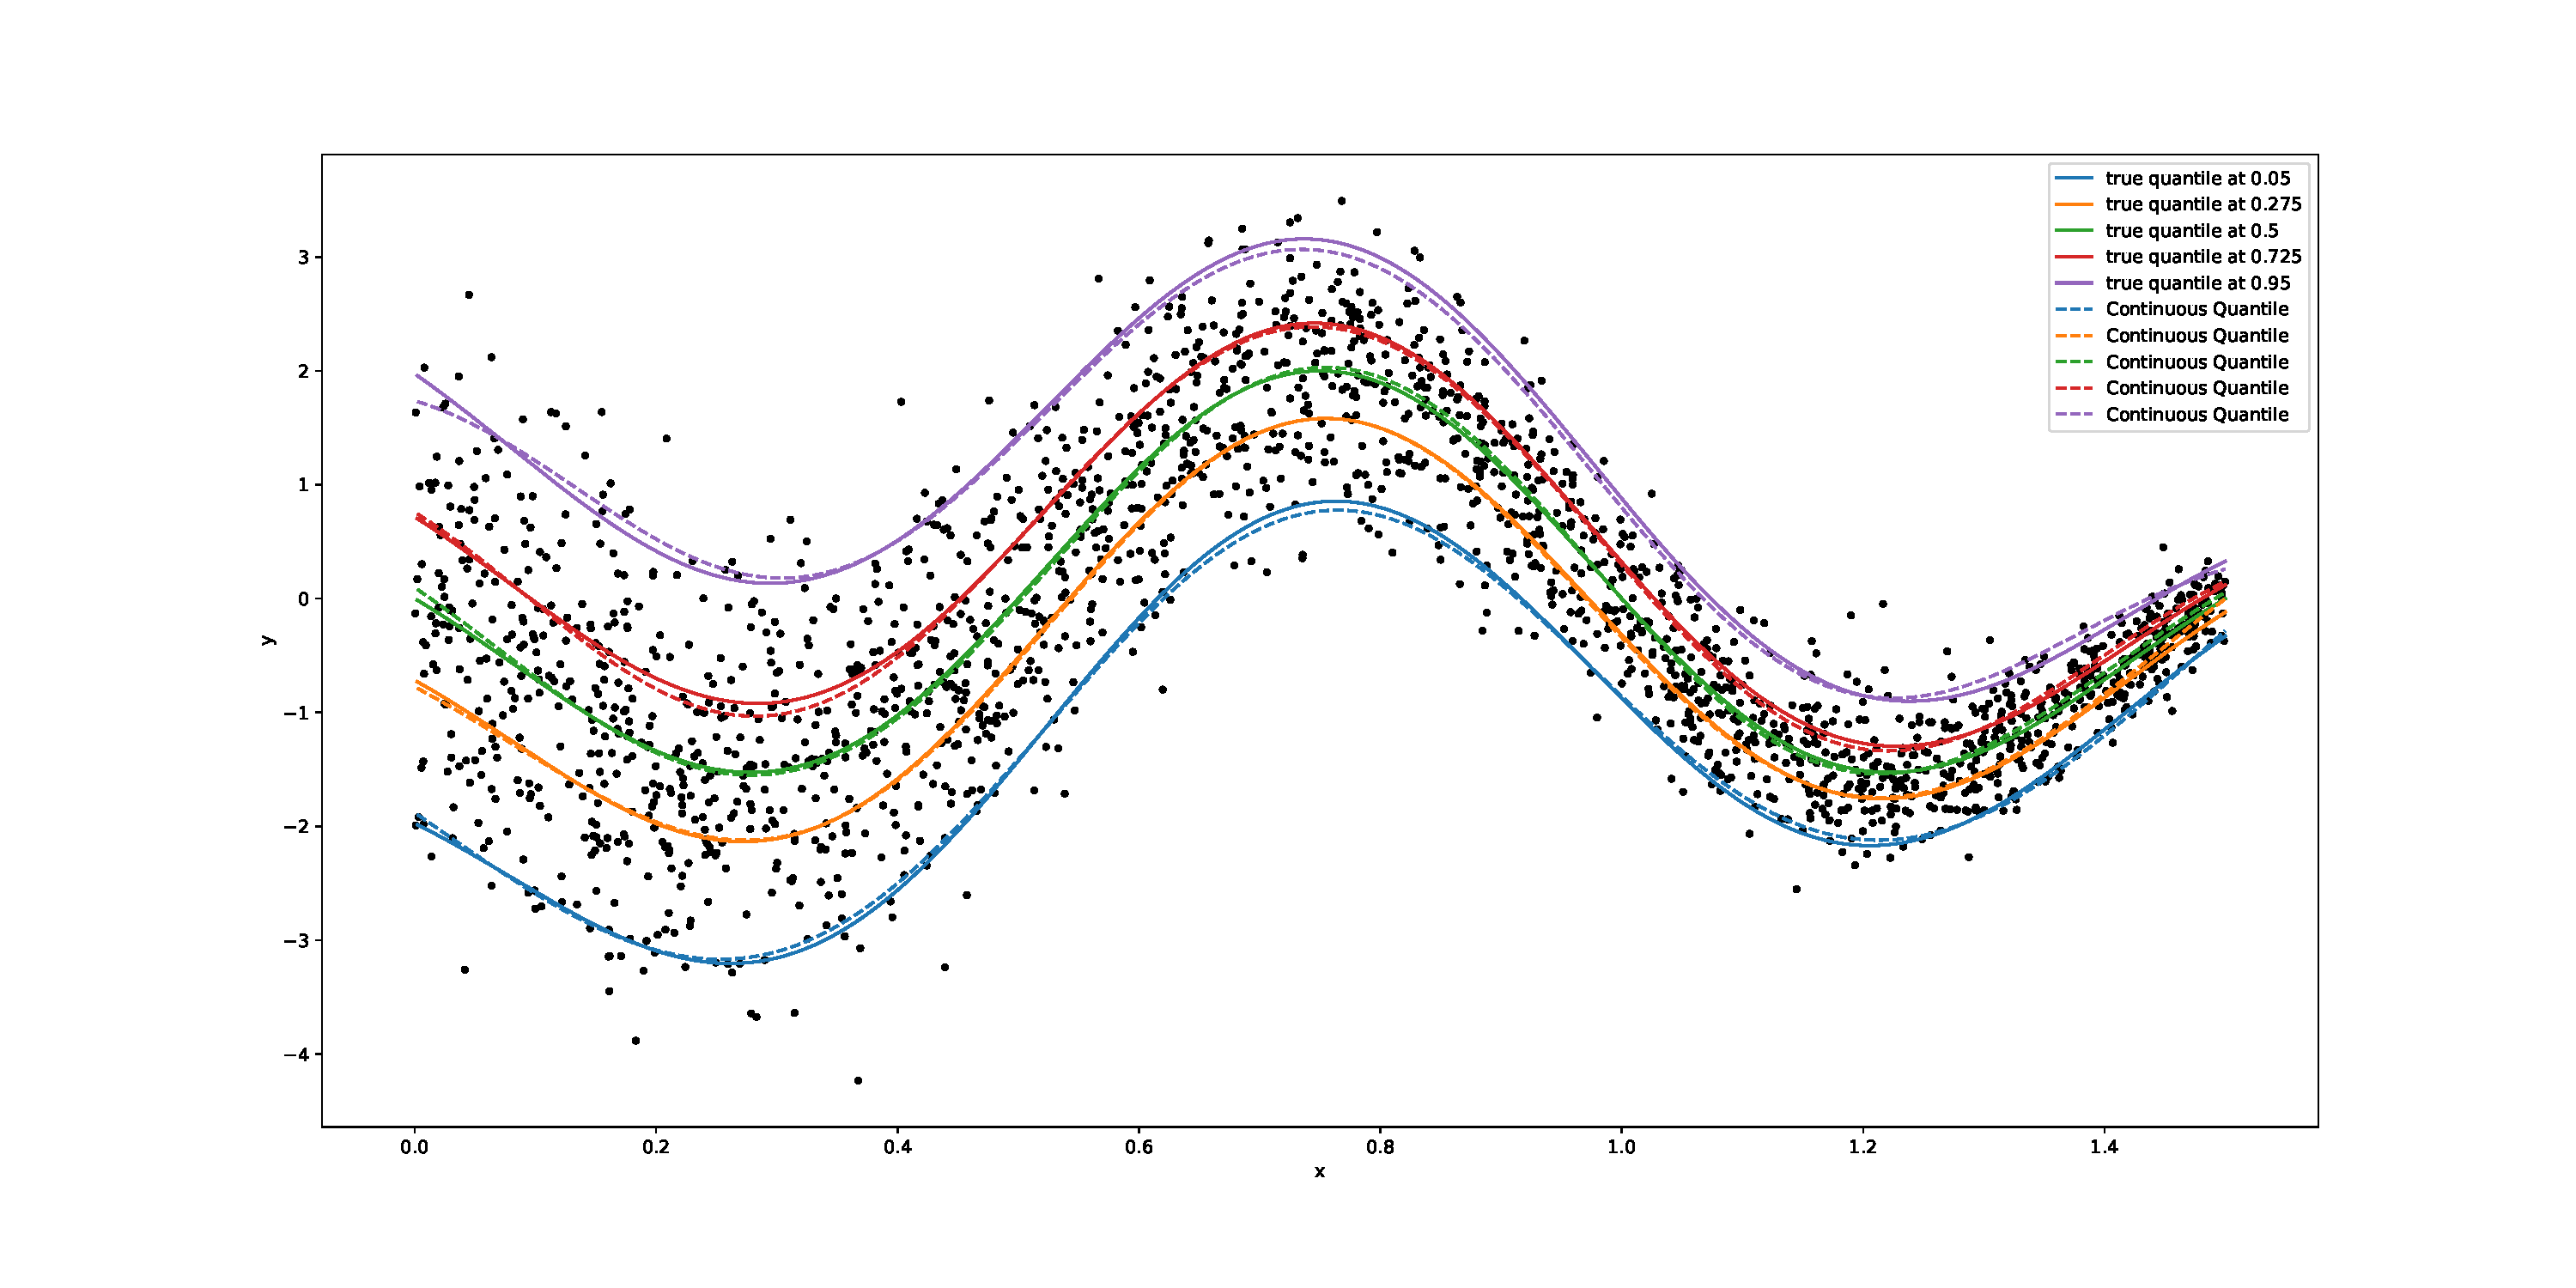
\includegraphics{./gfx/quantile_orff.pdf}}
        %\caption{Learning a continuous quantile function with ORFF
        %regression. \label{fig:quantile_orff}}
    %\end{figure}
    %\clearpage
    %\begin{figure}[htp]
        %\centering\resizebox{.8\textheight}{!}{%
        %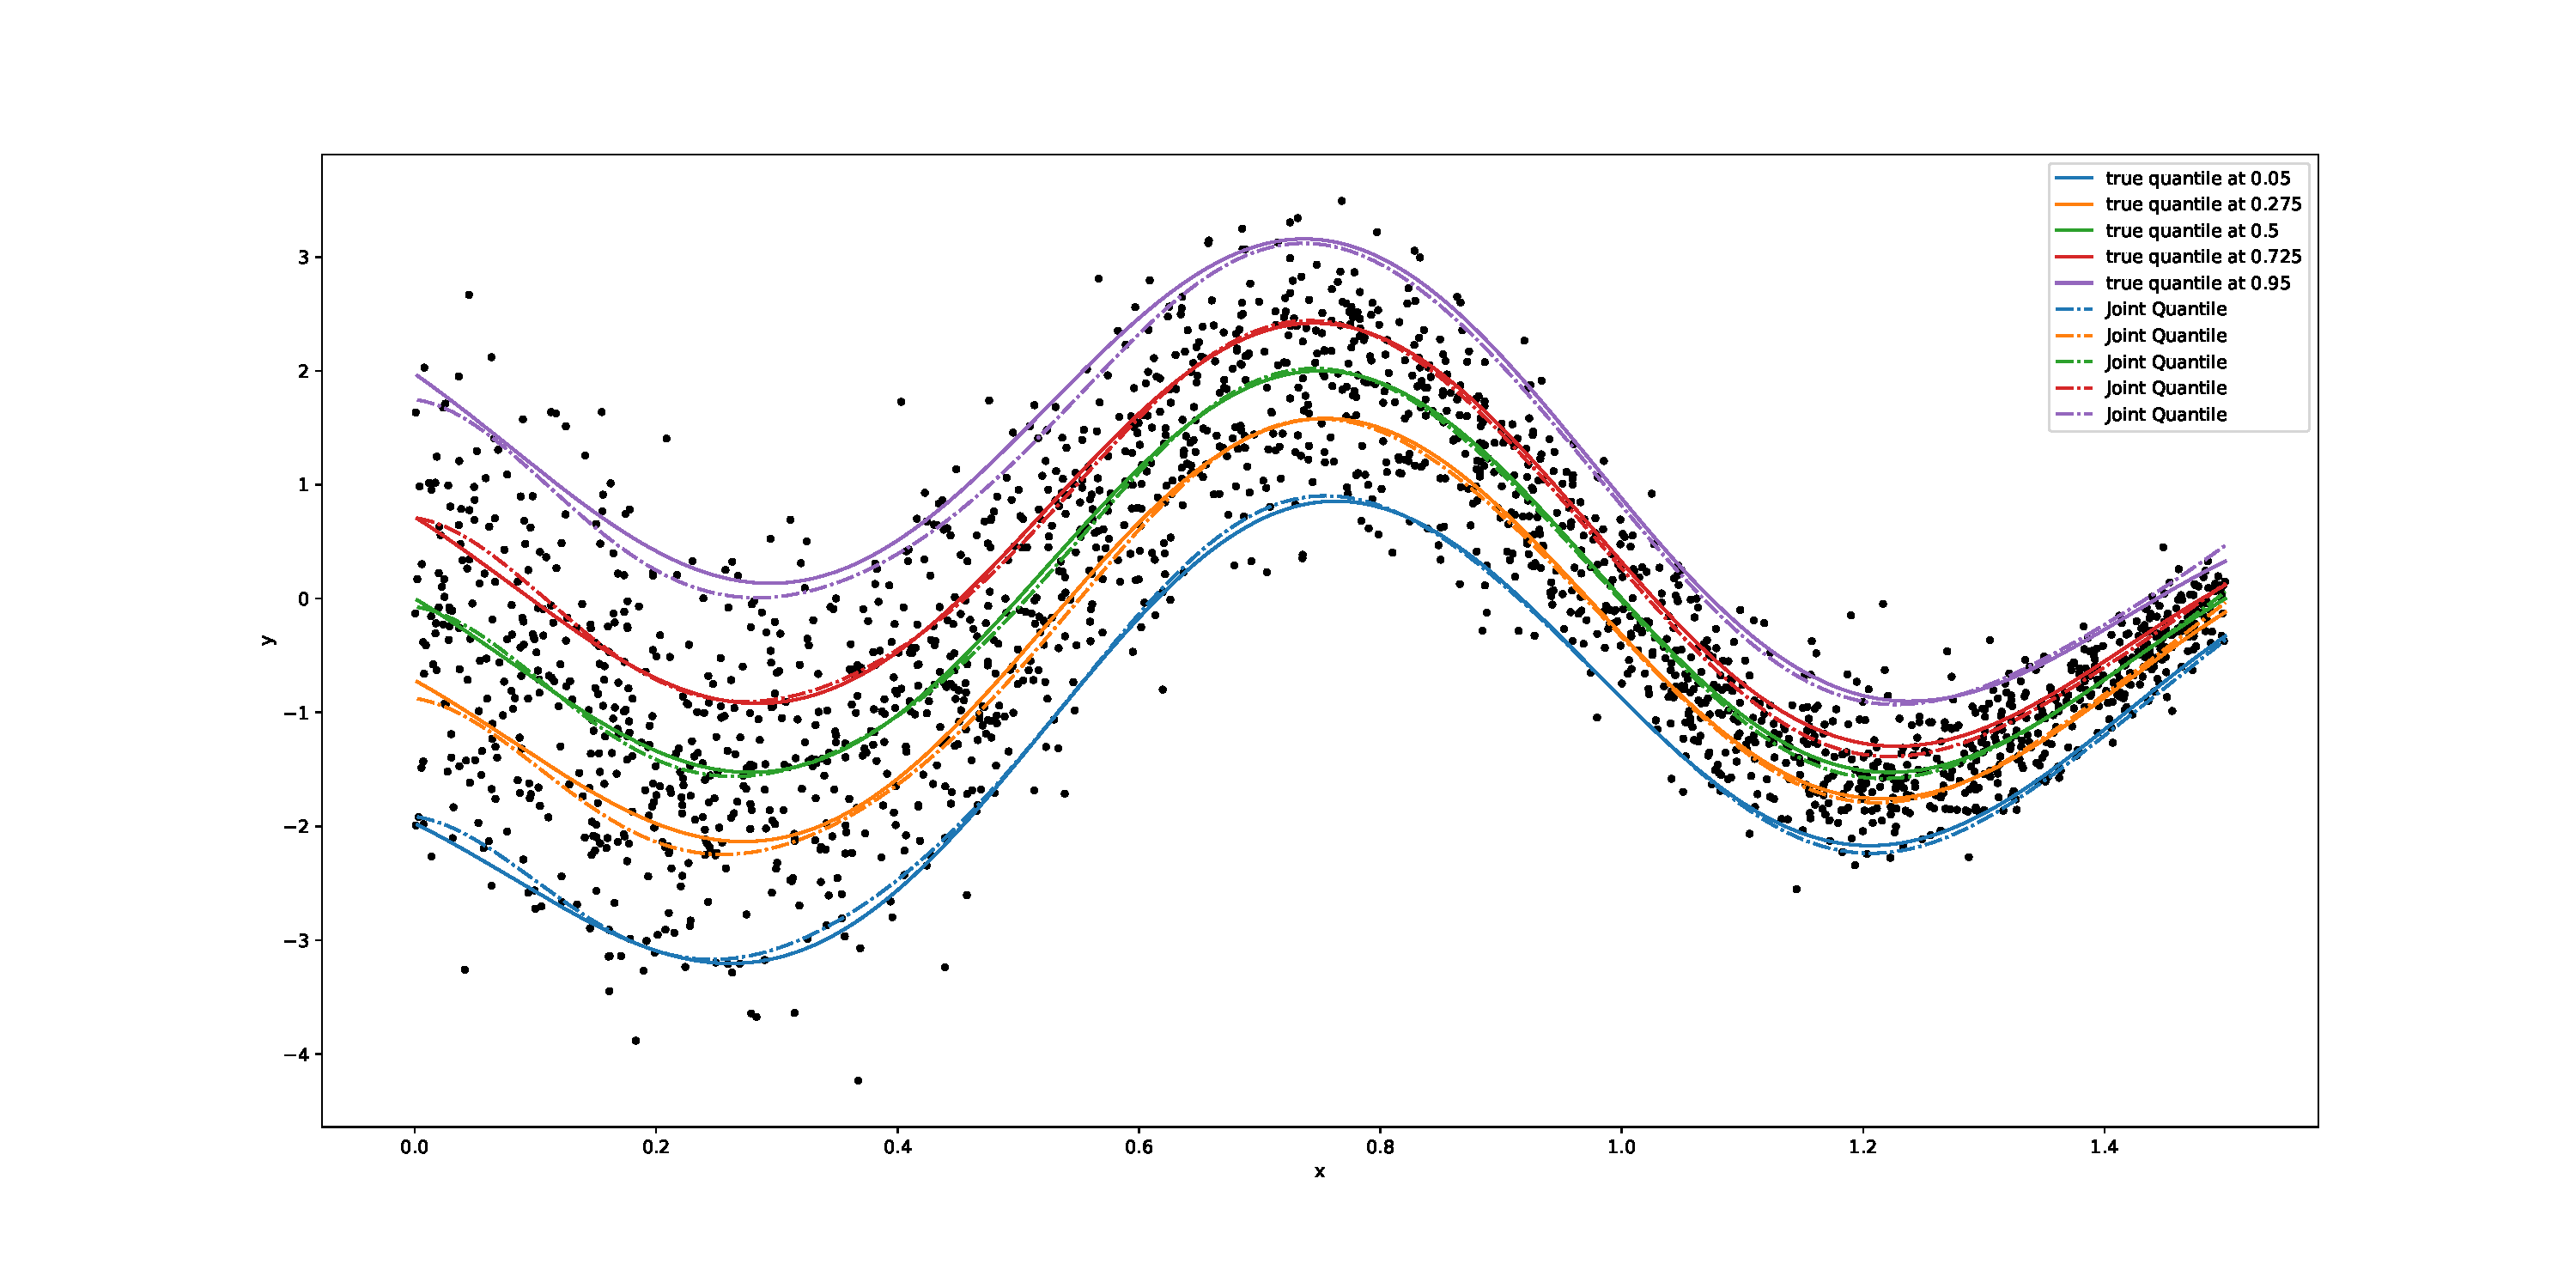
\includegraphics{./gfx/quantile_joint.pdf}}
        %\caption{Learning many quantile with joint OVK regression.
        %\label{fig:quantile_joint}}
    %\end{figure}
%\end{landscape}}
%Moreover $W^\adjoint W$ is the identity on
%$\Ima \Phi_{\tau}$ which is here $\mathcal{H}_{k_{\mathcal{T}}}$. (see the
%proof of \cref{pr:feature_operator} and \citet{Carmeli2010}). Thus we can
%choose $\Phi_\tau=\Phi(\tau)$ to be the functional Fourier feature map
%associated to $k_{\mathcal{T}}$ defined in \cref{pr:fourier_feature_map}.  Then
%we have $BB^\adjoint = I_{\mathcal{H}_{k_{\mathcal{T}}}} = W^\adjoint W$.  Thus
%we can choose $B^\adjoint = W = \Phi(\cdot)^\adjoint$ and the approximate
%feature map reads
%\begin{dmath*}
    %\tildePhi{\omega}(x)\in \mathcal{L}\left(\mathcal{H}_{k_{\mathcal{T}}};
    %\Vect_{j=1}^D L^2\left(\dual{\mathcal{T}},
    %\probability_{\dual{\Haar},\rho}\right)\right)
%\end{dmath*}
%and
%\begin{dmath*}
    %(\tildePhi{\omega}(x)g)(\tau) = \frac{1}{\sqrt{D}}\Vect_{j=1}^D
    %\begin{pmatrix}
        %\cos(x \omega_j) \Phi(\tau)^\adjoint g \\
        %\sin(x \omega_j) \Phi(\tau)^\adjoint g
    %\end{pmatrix} \condition{$\omega_j \sim \FT{k_{\mathcal{X}}}$
    %\ac{iid}}
%\end{dmath*}
%Then as proposed in \cref{ch:operator-valued_random_fourier_features} we can
%Monte-Carlo sample the functional feature map $\Phi(\tau)$ and obtain the
%\acs{ORFF} map
%\begin{dmath*}
    %\left(\widetilde{\tildePhi{\omega}}(x)g\right)(\tau) =
    %\frac{1}{\sqrt{DD'}}\Vect_{j=1}^D
    %\begin{pmatrix}
        %\cos(x \omega_j) \sum_{k=1}^{D'}
        %\left(\cos(\tau \omega_k') + \sin(\tau \omega_k')\right)g(\omega_k') \\
        %\sin(x \omega_j) \sum_{k=1}^{D'}
        %\left(\cos(\tau \omega_k') + \sin(\tau \omega_k')\right)g(\omega_k')
    %\end{pmatrix} \condition{$\omega_j \sim \FT{k_{\mathcal{X}}}$
    %\acs{iid} and $\omega_k'\sim \FT{k_{\mathcal{T}}}$ \acs{iid}.}
%\end{dmath*}
%where $g\in L^2\left(\dual{\mathcal{T}}, \probability_{\dual{\Haar},
%\rho}\right)$ and $\tau\in\mathbb{R}$. If we note
%\begin{dmath*}
    %G =
    %\begin{pmatrix}
        %g(\omega_1') & \dots & g(\omega_{D'}')
    %\end{pmatrix}^\adjoint \hiderel{\in} \mathbb{R}^{D'}
%\end{dmath*}
%we can define
%\begin{dmath*}
    %\left(\widetilde{\tildePhi{\omega}}(x)G\right)(\tau) =
    %\frac{1}{\sqrt{DD'}}\Vect_{j=1}^D
    %\begin{pmatrix}
        %\cos(x \omega_j) \sum_{k=1}^{D'}
        %\left(\cos(\tau \omega_k') + \sin(\tau \omega_k')\right)G_k \\
        %\sin(x \omega_j) \sum_{k=1}^{D'}
        %\left(\cos(\tau \omega_k') + \sin(\tau \omega_k')\right)G_k
    %\end{pmatrix} \condition{$\omega_j \sim \FT{k_{\mathcal{X}}}$
    %\acs{iid} and $\omega_k'\sim \FT{k_{\mathcal{T}}}$ \acs{iid}.}
%\end{dmath*}
%Then it is easy to verify that the adjoint operator is given by
%\begin{dmath*}
    %\left(\widetilde{\tildePhi{\omega}}(x)^\adjoint \theta\right)(\tau) =
    %\frac{1}{\sqrt{DD'}} \sum_{j=1}^D \left(\cos(x\omega_j) +
    %\sin(x\omega_j)\right) \left(\Vect_{k=1}^{D'}
    %\begin{pmatrix}
        %\cos(\tau \omega_k') \\
        %\sin(\tau \omega_k')
    %\end{pmatrix}\right)^\adjoint \theta_j
    %= \frac{1}{\sqrt{DD'}} \sum_{j=1}^D \left(\cos(x\omega_j) +
    %\sin(x\omega_j)\right) \theta_{jk} \left( \cos(\tau \omega_k') + \sin(\tau
    %\omega_k')\right)
    %\condition{$\omega_j \sim \FT{k_{\mathcal{X}}}$
    %\acs{iid} and $\omega_k'\sim \FT{k_{\mathcal{T}}}$ \acs{iid}.}
%\end{dmath*}
%where $\theta_k\in\mathbb{R}^{D'}$, for all $k \in \mathbb{N}^*_D$ and
%$\theta_{jk}\in\mathbb{R}$ for all $j \in \mathbb{N}^*_D$ and all $k \in
%\mathbb{N}^*_{D'}$. The above equations can be rewritten in matrix form which
%results in the following conjecture.
%\begin{conjecture}
    %\label{cj:functional_orff}
    %If $\tildephi{\omega}_{\mathcal{X}}$ is an \acs{RFF} for
    %$\widetilde{k}_{\mathcal{X}}$ such that
    %$\tildephi{\omega}(x)\in\mathbb{R}^D$ and $\tildephi{\omega}_{\mathcal{T}}$
    %is an \acs{RFF} for $\widetilde{k}_{\mathcal{T}}$, such that
    %$\tildephi{\omega}(\tau)\in\mathbb{R}^{D'}$ then an \acs{ORFF} map for
    %\begin{dmath*}
        %K(x, z) = k_{\mathcal{X}}(x, z) I_{\mathcal{H}_{k_{\mathcal{T}}}}
    %\end{dmath*}
    %is given for all $x\in\mathbb{R}$, all $\tau\in\mathbb{R}$ and all
    %$\Theta\in\mathcal{M}_{D,D'}(\mathbb{R})$ by
    %\begin{dmath*}
        %\left(\tildePhi{\omega}_K(x)^\adjoint \Theta \right)(\tau) =
        %\tildephi{\omega}_{\mathcal{X}}(x)^\adjoint \Theta
        %\tildephi{\omega}_{\mathcal{T}}(\tau)
    %\end{dmath*}
    %and
    %\begin{dmath*}
        %\left(\tildePhi{\omega}_K(x) G\right)(\tau) =
        %\tildephi{\omega}_{\mathcal{X}}(x)
        %\tildephi{\omega}_{\mathcal{T}}(\tau)^\adjoint G,
    %\end{dmath*}
    %where $g\in\mathbb{R}^{D'}$.
    %%but more intestingly, given $y\in\mathbb{R}$,
    %%\begin{dmath*}
        %%\tildePhi{\omega}_K(x, \tau)^\adjoint y =
        %%y \tildephi{\omega}_{\mathcal{X}}(x)
        %%\tildephi{\omega}_{\mathcal{T}}(\tau)^\adjoint.
    %%\end{dmath*}
%\end{conjecture}
%Moreover if one defines $\tildePhi{\omega}_K(x,
%\tau) = \left(\tildePhi{\omega}_K(x)^\adjoint \Theta \right)(\tau)$ one
%have of course
%\begin{dmath*}
    %\tildePhi{\omega}_K(x, \tau)^\adjoint \Theta =
    %\tildephi{\omega}_{\mathcal{X}}(x)^\adjoint \Theta
    %\tildephi{\omega}_{\mathcal{T}}(\tau)
%\end{dmath*}
%\subsection{Many quantile regression}
%From the loss defined in \cref{eq:loss_pinball} we defined the regularized risk
%using the \say{continuous} pinball loss for the quantile regression problem.
%For all $f\in\mathcal{H}_K$,
%\begin{dmath*}
    %J_{\lambda}(f) =
    %\frac{1}{N}\sum_{i=1}^N\int_{[0,1]}\left(
    %\begin{cases}
        %\tau\left(f_{x_i}(\tau) - y_i\right) & \text{if } f_{x_i}(\tau) \ge y_i
        %\\
        %(1 - \tau)\left(y_i - f_{x_i}(\tau)\right) & \text{otherwise}
    %\end{cases} \right)+ \lambda
    %\norm{f}_K^2.
%\end{dmath*}
%The issue with the above risk is that the different quantile for a given point
%$x\in\mathbb{R}$ may cross \citet{sangnier2016joint}. To avoid this to happen
%we need to force the function $f_x(\tau)$ to be \emph{increasing} in $\tau$ for
%any $x\in\mathbb{R}$.  Because a decreasing function has a negative derivative
%we can add a penalty term to the risk to avoid $f_x(\tau)$ to be decreasing in
%$\tau$.
%\begin{dmath*}
    %\Omega_{cross}(f) = - \min\left(\frac{\partial
    %f_{x_i}}{\partial\tau}(\tau),
    %0\right)
%\end{dmath*}
%Thus the regularized risk with the no crossing constraint is
%\begin{dmath*}
    %J_{\lambda_1, \lambda_2}(f) =
    %\frac{1}{N}\sum_{i=1}^N\int_{[0,1]}\left(
    %\begin{cases}
        %\tau \left(f_{x_i}(\tau) - y_i\right) & \text{if } f_{x_i}(\tau) \ge
        %y_i \\
        %(1 - \tau)\left(y_i - f_{x_i}(\tau)\right) & \text{otherwise}
    %\end{cases} -
    %\lambda_1 \min\left(\frac{\partial f_{x_i}}{\partial\tau}(\tau), 0\right)
    %\right)+ \lambda_2 \norm{f}_K^2.
%\end{dmath*}
%Eventually we replace the integral by a Monte-Carlo sampling with the uniform
%law $\mathcal{U}([0, 1])$ and plug in the approximate function of $f$ using the
%\acs{ORFF} map proposed in \cref{cj:functional_orff}. The final optimzation
%problem reads
%\begin{dmath*}
    %J_{\lambda_1, \lambda_2}(\Theta) =
    %\frac{1}{NT}\sum_{i=1}^N\sum_{t=1}^T\left(
    %\begin{cases} \tau_t
        %\left(\widetilde{f}_{x_i}(\tau_t) - y_i\right) & \text{if }
        %\widetilde{f}_{x_i}(\tau_t) \ge y_i \\
        %(1 - \tau_t)\left(y_i - f_{x_i}(\tau_t)\right) & \text{otherwise}
    %\end{cases} - \lambda_1
    %\min\left(\frac{\partial \widetilde{f}_{x_i}}{\partial\tau}(\tau_t),
    %0\right) \right)+ \lambda_2 \norm{\Theta}_{fro}^2.
%\end{dmath*}
%where $\widetilde{f}_{x}(\tau)=\tildephi{\omega}_{\mathcal{X}}(x)^\adjoint
%\Theta \tildephi{\omega}_{\mathcal{T}}(\tau)$, $\tau_t \sim \mathcal{U}([0,
%1])$ and
%\begin{dmath*}
    %\frac{\partial \widetilde{f}_{x}}{\partial\tau}(\tau)
    %= \tildephi{\omega}_{\mathcal{X}}(x)^\adjoint \Theta \frac{\partial
    %\tildephi{\omega}_{\mathcal{T}}}{\partial \tau}(\tau)
    %= \tildephi{\omega}_{\mathcal{X}}(x)^\adjoint \Theta \Vect_{k=1}^{D'}
    %\begin{pmatrix}
        %-\omega_k' \sin(\omega_k' x) \\
         %\omega_k' \cos(\omega_k' x)
    %\end{pmatrix} \condition{$\omega_k' \sim \FT{k_{\mathcal{T}}}$ \acs{iid}.}
%\end{dmath*}
%\subsubsection{Some results}
%We minimize the quantity $J_{\lambda_1, \lambda_2}(\Theta)$ on a toy dataset: a
%sine wave with some heteroscedastic noise. First we compare our methodology to
%the joint quantile regression proposed in \citet{sangnier2016joint}. We
%generate $N=2500$ for the train set and $N'=1000$ points for the test set and
%use a gaussian kernel for both $k_{\mathcal{X}}$ and $k_{\mathcal{T}}$. We
%choosed $\sigma_{\mathcal{X}} = 0.25$ and $\sigma_{\mathcal{T}}$ is set to be
%the median of the pairwise distance of the $\tau_t$'s drawn randomly from
%$\mathcal{U}([0, 1])$. Notice that $J_{\lambda_1, \lambda_2}(\Theta)$ is convex
%in $\Theta$. To avoid computing complex gradients and by lack of time, we used
%Tensorflow \citep{abadi2016tensorflow} to perform a gradient descent (with
%RMSProp \citep{tieleman2012lecture}) with automatic symbolic differentiation.
%\Cref{fig:quantile_orff} show the result for the quantile at $0.05$, $0.275$,
%$0.5$, $0.775$ and $0.95$ using the \acs{ORFF} methodology.
%\afterpage{%
%\begin{landscape}
    %\begin{figure}[htp]
        %\centering
        %\resizebox{.8\textheight}{!}{%
        %\includegraphics{./gfx/quantile_continuous.pgf}}
        %\caption{Learning a continuous quantile function with ORFF
        %regression. \label{fig:quantile_continuous}}
    %\end{figure}
%\end{landscape}}
%\Cref{fig:quantile_joint} shows the joint quantile regression of
%\citet{sangnier2016joint} on the same dataset. Not only our method matches the
%the performances of \citet{sangnier2016joint}\footnote{We reported an error
%computed with the pinball loss on the test set of $0.818$ for our method and
%$0.817$ for joint regression (note that we don't report here an average on many
%experiments to avoid randomness introduced by the random features, but the
%results seems robut in practice.)} but we cut down the computation time from
%circa $1330$ seconds to circa $30$ seconds (training and testing).  Moreover on
%contrary to \citet{sangnier2016joint} we have access to all the quantile of the
%model (see \cref{fig:quantile_continuous}).

%\subsection{One class SVM revisited}
%We also propose an extension of the celebrated \acf{OCSVM} so that it
%possible to learn jointly all the level sets.  One-class classification, also
%known as unary classification, tries to identify objects of a specific class
%amongst all objects, by learning from a training set containing only the
%objects of that class.  In this framework, we assume that we only observe
%examples of one class (referred to as the inlier class).  The second class is
%called outlier class.  We turn our attention to the \acs{OCSVM}
%of \citet{Scholkopf2001} which extends the \ac{SVM} methodology
%\citep{Cortes1995,Shawe2004} to handle training using only inliers.
%\paragraph{}
%We recall that given an hyperparameter $\nu\in [0,1]$ that controls the
%proportion of inlier, given as scalar kernel $k$, the \acs{OCSVM} problem reads
%\begin{dmath*}
    %\argmin_{f\in\mathcal{H}_k, \tau \in \mathbb{R}} \frac{1}{2}
    %\norm{f}_{\mathcal{H}_k}^2 - \nu \tau + \frac{1}{N} \sum_{i=1}^N \max(\tau
    %- f(x_i), 0)
%\end{dmath*}
%The decision function is then
%\begin{dmath*}
    %h(x, \tau) = \mathds{1}_{[\tau, \infty)}\left( f(x) \right).
%\end{dmath*}
%As in \cref{subsec:quantile_regression} we can rewrite the optimization problem
%as an integral over all the value of $\nu$ and suppose that $f$ is
%function-valued (a function of $\nu$). Moreover $\tau$ must also change its
%value according to $\mu$. Thus given a kernel $k_{\mathcal{X}}$ on the inputs
%$x\in\mathbb{R}^d$ with its approximate feature map
%$\tildephi{\omega}_{\mathcal{X}}$ and a kernel $k_{\mathcal{T}}$ on the level
%sets with its approximate feature map $\tildephi{\omega}_{\mathcal{T}}$, we
%define the continuous one-class SVM problem as
%\begin{dmath*}
    %\argmin_{f
    %\in\mathcal{H}_K,\tau\in\mathcal{H}_{k_{\mathcal{\tau}}}}\frac{1}{N}
    %\sum_{i=1}^N\int_{[0,1]}\max\left(0, \tau(\nu) - f_{x_i}(\nu)\right)d\nu +
    %\frac{1}{2}\int_{[0,1]}\nu
    %\norm{f_{\cdot}(\nu)}_{\mathcal{H}_{k_{\mathcal{X}}}}^2d\nu -
    %\int_{[0,1]}\nu\tau(\nu)d\nu.
%\end{dmath*}
%Again we can compute the integral by Monte-Carlo sampling and replace $f$ and
%$\tau$ by their respective approximation. Notice that the \acs{RKHS} of $\tau$
%should match the \acs{RKHS} of the output space of $f_K$. Hence
%\begin{dmath*}
    %\argmin_{\Theta
    %\in\mathcal{M}_{D, D'}(\mathbb{R}),\tau\in\mathbb{R}^D}\frac{1}{NT}
    %\sum_{i=1}^N\sum_{t=1}^T\max\left(0, \widetilde{\tau}(\nu_t) -
    %\widetilde{f}_{x_i}(\nu_t)\right) + \frac{1}{2T}\sum_{t=1}^T\nu_t
    %\norm{\widetilde{f}_{\cdot}(\nu_t)}_{2}^2 -
    %\frac{1}{T}\sum_{t=1}^T\nu_t\widetilde{\tau}(\nu_t),
%\end{dmath*}
%where $\nu_t \sim \mathcal{U}([0, 1])$ \acs{iid}, $\widetilde{\tau}(\nu) =
%\tildephi{\omega}_{\mathcal{T}}(\nu)$ and $\widetilde{f}_x(\nu) =
%\tildephi{\omega}(x)^\adjoint \Theta \tildephi{\omega}_{\mathcal{T}}(\nu)$. We
%also deduce that $\widetilde{f}_{\cdot}(\nu) = \Theta
%\tildephi{\omega}_{\mathcal{T}}(\nu)$. Here the natural decision function is
%\begin{dmath}
    %\label{eq:continuous_decision}
    %h(x, \nu) = \mathds{1}_{\left[\widetilde{\tau}(\nu),\infty\right)}
    %\left(\widetilde{f}_x(\nu)\right).
%\end{dmath}
%\begin{figure}
    %{\centering
    %\resizebox{2\textwidth}{!}{%% Creator: Matplotlib, PGF backend
%%
%% To include the figure in your LaTeX document, write
%%   \input{<filename>.pgf}
%%
%% Make sure the required packages are loaded in your preamble
%%   \usepackage{pgf}
%%
%% Figures using additional raster images can only be included by \input if
%% they are in the same directory as the main LaTeX file. For loading figures
%% from other directories you can use the `import` package
%%   \usepackage{import}
%% and then include the figures with
%%   \import{<path to file>}{<filename>.pgf}
%%
%% Matplotlib used the following preamble
%%   \usepackage{fontspec}
%%   \setmainfont{Times New Roman}
%%   \setsansfont{Lucida Grande}
%%   \setmonofont{Andale Mono}
%%
\begingroup%
\makeatletter%
\begin{pgfpicture}%
\pgfpathrectangle{\pgfpointorigin}{\pgfqpoint{16.000000in}{5.000000in}}%
\pgfusepath{use as bounding box, clip}%
\begin{pgfscope}%
\pgfsetbuttcap%
\pgfsetmiterjoin%
\definecolor{currentfill}{rgb}{1.000000,1.000000,1.000000}%
\pgfsetfillcolor{currentfill}%
\pgfsetlinewidth{0.000000pt}%
\definecolor{currentstroke}{rgb}{1.000000,1.000000,1.000000}%
\pgfsetstrokecolor{currentstroke}%
\pgfsetdash{}{0pt}%
\pgfpathmoveto{\pgfqpoint{0.000000in}{0.000000in}}%
\pgfpathlineto{\pgfqpoint{16.000000in}{0.000000in}}%
\pgfpathlineto{\pgfqpoint{16.000000in}{5.000000in}}%
\pgfpathlineto{\pgfqpoint{0.000000in}{5.000000in}}%
\pgfpathclose%
\pgfusepath{fill}%
\end{pgfscope}%
\begin{pgfscope}%
\pgfsetbuttcap%
\pgfsetmiterjoin%
\definecolor{currentfill}{rgb}{1.000000,1.000000,1.000000}%
\pgfsetfillcolor{currentfill}%
\pgfsetlinewidth{0.000000pt}%
\definecolor{currentstroke}{rgb}{0.000000,0.000000,0.000000}%
\pgfsetstrokecolor{currentstroke}%
\pgfsetstrokeopacity{0.000000}%
\pgfsetdash{}{0pt}%
\pgfpathmoveto{\pgfqpoint{0.663889in}{0.580556in}}%
\pgfpathlineto{\pgfqpoint{8.157639in}{0.580556in}}%
\pgfpathlineto{\pgfqpoint{8.157639in}{4.801389in}}%
\pgfpathlineto{\pgfqpoint{0.663889in}{4.801389in}}%
\pgfpathclose%
\pgfusepath{fill}%
\end{pgfscope}%
\begin{pgfscope}%
\pgfsetbuttcap%
\pgfsetroundjoin%
\definecolor{currentfill}{rgb}{0.000000,0.000000,0.000000}%
\pgfsetfillcolor{currentfill}%
\pgfsetlinewidth{0.803000pt}%
\definecolor{currentstroke}{rgb}{0.000000,0.000000,0.000000}%
\pgfsetstrokecolor{currentstroke}%
\pgfsetdash{}{0pt}%
\pgfsys@defobject{currentmarker}{\pgfqpoint{0.000000in}{-0.048611in}}{\pgfqpoint{0.000000in}{0.000000in}}{%
\pgfpathmoveto{\pgfqpoint{0.000000in}{0.000000in}}%
\pgfpathlineto{\pgfqpoint{0.000000in}{-0.048611in}}%
\pgfusepath{stroke,fill}%
}%
\begin{pgfscope}%
\pgfsys@transformshift{1.004514in}{0.580556in}%
\pgfsys@useobject{currentmarker}{}%
\end{pgfscope}%
\end{pgfscope}%
\begin{pgfscope}%
\pgftext[x=1.004514in,y=0.483333in,,top]{\sffamily\fontsize{10.000000}{12.000000}\selectfont 0.0}%
\end{pgfscope}%
\begin{pgfscope}%
\pgfsetbuttcap%
\pgfsetroundjoin%
\definecolor{currentfill}{rgb}{0.000000,0.000000,0.000000}%
\pgfsetfillcolor{currentfill}%
\pgfsetlinewidth{0.803000pt}%
\definecolor{currentstroke}{rgb}{0.000000,0.000000,0.000000}%
\pgfsetstrokecolor{currentstroke}%
\pgfsetdash{}{0pt}%
\pgfsys@defobject{currentmarker}{\pgfqpoint{0.000000in}{-0.048611in}}{\pgfqpoint{0.000000in}{0.000000in}}{%
\pgfpathmoveto{\pgfqpoint{0.000000in}{0.000000in}}%
\pgfpathlineto{\pgfqpoint{0.000000in}{-0.048611in}}%
\pgfusepath{stroke,fill}%
}%
\begin{pgfscope}%
\pgfsys@transformshift{2.367014in}{0.580556in}%
\pgfsys@useobject{currentmarker}{}%
\end{pgfscope}%
\end{pgfscope}%
\begin{pgfscope}%
\pgftext[x=2.367014in,y=0.483333in,,top]{\sffamily\fontsize{10.000000}{12.000000}\selectfont 0.2}%
\end{pgfscope}%
\begin{pgfscope}%
\pgfsetbuttcap%
\pgfsetroundjoin%
\definecolor{currentfill}{rgb}{0.000000,0.000000,0.000000}%
\pgfsetfillcolor{currentfill}%
\pgfsetlinewidth{0.803000pt}%
\definecolor{currentstroke}{rgb}{0.000000,0.000000,0.000000}%
\pgfsetstrokecolor{currentstroke}%
\pgfsetdash{}{0pt}%
\pgfsys@defobject{currentmarker}{\pgfqpoint{0.000000in}{-0.048611in}}{\pgfqpoint{0.000000in}{0.000000in}}{%
\pgfpathmoveto{\pgfqpoint{0.000000in}{0.000000in}}%
\pgfpathlineto{\pgfqpoint{0.000000in}{-0.048611in}}%
\pgfusepath{stroke,fill}%
}%
\begin{pgfscope}%
\pgfsys@transformshift{3.729514in}{0.580556in}%
\pgfsys@useobject{currentmarker}{}%
\end{pgfscope}%
\end{pgfscope}%
\begin{pgfscope}%
\pgftext[x=3.729514in,y=0.483333in,,top]{\sffamily\fontsize{10.000000}{12.000000}\selectfont 0.4}%
\end{pgfscope}%
\begin{pgfscope}%
\pgfsetbuttcap%
\pgfsetroundjoin%
\definecolor{currentfill}{rgb}{0.000000,0.000000,0.000000}%
\pgfsetfillcolor{currentfill}%
\pgfsetlinewidth{0.803000pt}%
\definecolor{currentstroke}{rgb}{0.000000,0.000000,0.000000}%
\pgfsetstrokecolor{currentstroke}%
\pgfsetdash{}{0pt}%
\pgfsys@defobject{currentmarker}{\pgfqpoint{0.000000in}{-0.048611in}}{\pgfqpoint{0.000000in}{0.000000in}}{%
\pgfpathmoveto{\pgfqpoint{0.000000in}{0.000000in}}%
\pgfpathlineto{\pgfqpoint{0.000000in}{-0.048611in}}%
\pgfusepath{stroke,fill}%
}%
\begin{pgfscope}%
\pgfsys@transformshift{5.092014in}{0.580556in}%
\pgfsys@useobject{currentmarker}{}%
\end{pgfscope}%
\end{pgfscope}%
\begin{pgfscope}%
\pgftext[x=5.092014in,y=0.483333in,,top]{\sffamily\fontsize{10.000000}{12.000000}\selectfont 0.6}%
\end{pgfscope}%
\begin{pgfscope}%
\pgfsetbuttcap%
\pgfsetroundjoin%
\definecolor{currentfill}{rgb}{0.000000,0.000000,0.000000}%
\pgfsetfillcolor{currentfill}%
\pgfsetlinewidth{0.803000pt}%
\definecolor{currentstroke}{rgb}{0.000000,0.000000,0.000000}%
\pgfsetstrokecolor{currentstroke}%
\pgfsetdash{}{0pt}%
\pgfsys@defobject{currentmarker}{\pgfqpoint{0.000000in}{-0.048611in}}{\pgfqpoint{0.000000in}{0.000000in}}{%
\pgfpathmoveto{\pgfqpoint{0.000000in}{0.000000in}}%
\pgfpathlineto{\pgfqpoint{0.000000in}{-0.048611in}}%
\pgfusepath{stroke,fill}%
}%
\begin{pgfscope}%
\pgfsys@transformshift{6.454514in}{0.580556in}%
\pgfsys@useobject{currentmarker}{}%
\end{pgfscope}%
\end{pgfscope}%
\begin{pgfscope}%
\pgftext[x=6.454514in,y=0.483333in,,top]{\sffamily\fontsize{10.000000}{12.000000}\selectfont 0.8}%
\end{pgfscope}%
\begin{pgfscope}%
\pgfsetbuttcap%
\pgfsetroundjoin%
\definecolor{currentfill}{rgb}{0.000000,0.000000,0.000000}%
\pgfsetfillcolor{currentfill}%
\pgfsetlinewidth{0.803000pt}%
\definecolor{currentstroke}{rgb}{0.000000,0.000000,0.000000}%
\pgfsetstrokecolor{currentstroke}%
\pgfsetdash{}{0pt}%
\pgfsys@defobject{currentmarker}{\pgfqpoint{0.000000in}{-0.048611in}}{\pgfqpoint{0.000000in}{0.000000in}}{%
\pgfpathmoveto{\pgfqpoint{0.000000in}{0.000000in}}%
\pgfpathlineto{\pgfqpoint{0.000000in}{-0.048611in}}%
\pgfusepath{stroke,fill}%
}%
\begin{pgfscope}%
\pgfsys@transformshift{7.817014in}{0.580556in}%
\pgfsys@useobject{currentmarker}{}%
\end{pgfscope}%
\end{pgfscope}%
\begin{pgfscope}%
\pgftext[x=7.817014in,y=0.483333in,,top]{\sffamily\fontsize{10.000000}{12.000000}\selectfont 1.0}%
\end{pgfscope}%
\begin{pgfscope}%
\pgftext[x=4.410764in,y=0.293908in,,top]{\sffamily\fontsize{10.000000}{12.000000}\selectfont \(\displaystyle \nu\)}%
\end{pgfscope}%
\begin{pgfscope}%
\pgfsetbuttcap%
\pgfsetroundjoin%
\definecolor{currentfill}{rgb}{0.000000,0.000000,0.000000}%
\pgfsetfillcolor{currentfill}%
\pgfsetlinewidth{0.803000pt}%
\definecolor{currentstroke}{rgb}{0.000000,0.000000,0.000000}%
\pgfsetstrokecolor{currentstroke}%
\pgfsetdash{}{0pt}%
\pgfsys@defobject{currentmarker}{\pgfqpoint{-0.048611in}{0.000000in}}{\pgfqpoint{0.000000in}{0.000000in}}{%
\pgfpathmoveto{\pgfqpoint{0.000000in}{0.000000in}}%
\pgfpathlineto{\pgfqpoint{-0.048611in}{0.000000in}}%
\pgfusepath{stroke,fill}%
}%
\begin{pgfscope}%
\pgfsys@transformshift{0.663889in}{0.772412in}%
\pgfsys@useobject{currentmarker}{}%
\end{pgfscope}%
\end{pgfscope}%
\begin{pgfscope}%
\pgftext[x=0.347076in,y=0.718870in,left,base]{\sffamily\fontsize{10.000000}{12.000000}\selectfont 0.0}%
\end{pgfscope}%
\begin{pgfscope}%
\pgfsetbuttcap%
\pgfsetroundjoin%
\definecolor{currentfill}{rgb}{0.000000,0.000000,0.000000}%
\pgfsetfillcolor{currentfill}%
\pgfsetlinewidth{0.803000pt}%
\definecolor{currentstroke}{rgb}{0.000000,0.000000,0.000000}%
\pgfsetstrokecolor{currentstroke}%
\pgfsetdash{}{0pt}%
\pgfsys@defobject{currentmarker}{\pgfqpoint{-0.048611in}{0.000000in}}{\pgfqpoint{0.000000in}{0.000000in}}{%
\pgfpathmoveto{\pgfqpoint{0.000000in}{0.000000in}}%
\pgfpathlineto{\pgfqpoint{-0.048611in}{0.000000in}}%
\pgfusepath{stroke,fill}%
}%
\begin{pgfscope}%
\pgfsys@transformshift{0.663889in}{1.539836in}%
\pgfsys@useobject{currentmarker}{}%
\end{pgfscope}%
\end{pgfscope}%
\begin{pgfscope}%
\pgftext[x=0.347076in,y=1.486294in,left,base]{\sffamily\fontsize{10.000000}{12.000000}\selectfont 0.2}%
\end{pgfscope}%
\begin{pgfscope}%
\pgfsetbuttcap%
\pgfsetroundjoin%
\definecolor{currentfill}{rgb}{0.000000,0.000000,0.000000}%
\pgfsetfillcolor{currentfill}%
\pgfsetlinewidth{0.803000pt}%
\definecolor{currentstroke}{rgb}{0.000000,0.000000,0.000000}%
\pgfsetstrokecolor{currentstroke}%
\pgfsetdash{}{0pt}%
\pgfsys@defobject{currentmarker}{\pgfqpoint{-0.048611in}{0.000000in}}{\pgfqpoint{0.000000in}{0.000000in}}{%
\pgfpathmoveto{\pgfqpoint{0.000000in}{0.000000in}}%
\pgfpathlineto{\pgfqpoint{-0.048611in}{0.000000in}}%
\pgfusepath{stroke,fill}%
}%
\begin{pgfscope}%
\pgfsys@transformshift{0.663889in}{2.307260in}%
\pgfsys@useobject{currentmarker}{}%
\end{pgfscope}%
\end{pgfscope}%
\begin{pgfscope}%
\pgftext[x=0.347076in,y=2.253719in,left,base]{\sffamily\fontsize{10.000000}{12.000000}\selectfont 0.4}%
\end{pgfscope}%
\begin{pgfscope}%
\pgfsetbuttcap%
\pgfsetroundjoin%
\definecolor{currentfill}{rgb}{0.000000,0.000000,0.000000}%
\pgfsetfillcolor{currentfill}%
\pgfsetlinewidth{0.803000pt}%
\definecolor{currentstroke}{rgb}{0.000000,0.000000,0.000000}%
\pgfsetstrokecolor{currentstroke}%
\pgfsetdash{}{0pt}%
\pgfsys@defobject{currentmarker}{\pgfqpoint{-0.048611in}{0.000000in}}{\pgfqpoint{0.000000in}{0.000000in}}{%
\pgfpathmoveto{\pgfqpoint{0.000000in}{0.000000in}}%
\pgfpathlineto{\pgfqpoint{-0.048611in}{0.000000in}}%
\pgfusepath{stroke,fill}%
}%
\begin{pgfscope}%
\pgfsys@transformshift{0.663889in}{3.074684in}%
\pgfsys@useobject{currentmarker}{}%
\end{pgfscope}%
\end{pgfscope}%
\begin{pgfscope}%
\pgftext[x=0.347076in,y=3.021143in,left,base]{\sffamily\fontsize{10.000000}{12.000000}\selectfont 0.6}%
\end{pgfscope}%
\begin{pgfscope}%
\pgfsetbuttcap%
\pgfsetroundjoin%
\definecolor{currentfill}{rgb}{0.000000,0.000000,0.000000}%
\pgfsetfillcolor{currentfill}%
\pgfsetlinewidth{0.803000pt}%
\definecolor{currentstroke}{rgb}{0.000000,0.000000,0.000000}%
\pgfsetstrokecolor{currentstroke}%
\pgfsetdash{}{0pt}%
\pgfsys@defobject{currentmarker}{\pgfqpoint{-0.048611in}{0.000000in}}{\pgfqpoint{0.000000in}{0.000000in}}{%
\pgfpathmoveto{\pgfqpoint{0.000000in}{0.000000in}}%
\pgfpathlineto{\pgfqpoint{-0.048611in}{0.000000in}}%
\pgfusepath{stroke,fill}%
}%
\begin{pgfscope}%
\pgfsys@transformshift{0.663889in}{3.842109in}%
\pgfsys@useobject{currentmarker}{}%
\end{pgfscope}%
\end{pgfscope}%
\begin{pgfscope}%
\pgftext[x=0.347076in,y=3.788567in,left,base]{\sffamily\fontsize{10.000000}{12.000000}\selectfont 0.8}%
\end{pgfscope}%
\begin{pgfscope}%
\pgfsetbuttcap%
\pgfsetroundjoin%
\definecolor{currentfill}{rgb}{0.000000,0.000000,0.000000}%
\pgfsetfillcolor{currentfill}%
\pgfsetlinewidth{0.803000pt}%
\definecolor{currentstroke}{rgb}{0.000000,0.000000,0.000000}%
\pgfsetstrokecolor{currentstroke}%
\pgfsetdash{}{0pt}%
\pgfsys@defobject{currentmarker}{\pgfqpoint{-0.048611in}{0.000000in}}{\pgfqpoint{0.000000in}{0.000000in}}{%
\pgfpathmoveto{\pgfqpoint{0.000000in}{0.000000in}}%
\pgfpathlineto{\pgfqpoint{-0.048611in}{0.000000in}}%
\pgfusepath{stroke,fill}%
}%
\begin{pgfscope}%
\pgfsys@transformshift{0.663889in}{4.609533in}%
\pgfsys@useobject{currentmarker}{}%
\end{pgfscope}%
\end{pgfscope}%
\begin{pgfscope}%
\pgftext[x=0.347076in,y=4.555991in,left,base]{\sffamily\fontsize{10.000000}{12.000000}\selectfont 1.0}%
\end{pgfscope}%
\begin{pgfscope}%
\pgftext[x=0.291520in,y=2.690972in,,bottom,rotate=90.000000]{\sffamily\fontsize{10.000000}{12.000000}\selectfont percentage of inliers}%
\end{pgfscope}%
\begin{pgfscope}%
\pgfpathrectangle{\pgfqpoint{0.663889in}{0.580556in}}{\pgfqpoint{7.493750in}{4.220833in}} %
\pgfusepath{clip}%
\pgfsetrectcap%
\pgfsetroundjoin%
\pgfsetlinewidth{1.505625pt}%
\definecolor{currentstroke}{rgb}{0.121569,0.466667,0.705882}%
\pgfsetstrokecolor{currentstroke}%
\pgfsetdash{}{0pt}%
\pgfpathmoveto{\pgfqpoint{1.004514in}{4.099744in}}%
\pgfpathlineto{\pgfqpoint{1.073327in}{4.181968in}}%
\pgfpathlineto{\pgfqpoint{1.142140in}{4.072336in}}%
\pgfpathlineto{\pgfqpoint{1.210953in}{4.006557in}}%
\pgfpathlineto{\pgfqpoint{1.279766in}{3.979149in}}%
\pgfpathlineto{\pgfqpoint{1.348580in}{3.973667in}}%
\pgfpathlineto{\pgfqpoint{1.417393in}{3.951741in}}%
\pgfpathlineto{\pgfqpoint{1.486206in}{3.918851in}}%
\pgfpathlineto{\pgfqpoint{1.555019in}{3.842109in}}%
\pgfpathlineto{\pgfqpoint{1.623832in}{3.820182in}}%
\pgfpathlineto{\pgfqpoint{1.692645in}{3.787293in}}%
\pgfpathlineto{\pgfqpoint{1.761458in}{3.743440in}}%
\pgfpathlineto{\pgfqpoint{1.830271in}{3.710550in}}%
\pgfpathlineto{\pgfqpoint{1.899085in}{3.672179in}}%
\pgfpathlineto{\pgfqpoint{1.967898in}{3.633808in}}%
\pgfpathlineto{\pgfqpoint{2.036711in}{3.595437in}}%
\pgfpathlineto{\pgfqpoint{2.105524in}{3.578992in}}%
\pgfpathlineto{\pgfqpoint{2.174337in}{3.557065in}}%
\pgfpathlineto{\pgfqpoint{2.243150in}{3.480323in}}%
\pgfpathlineto{\pgfqpoint{2.311963in}{3.436470in}}%
\pgfpathlineto{\pgfqpoint{2.380777in}{3.425507in}}%
\pgfpathlineto{\pgfqpoint{2.449590in}{3.398099in}}%
\pgfpathlineto{\pgfqpoint{2.518403in}{3.354246in}}%
\pgfpathlineto{\pgfqpoint{2.587216in}{3.321356in}}%
\pgfpathlineto{\pgfqpoint{2.656029in}{3.293948in}}%
\pgfpathlineto{\pgfqpoint{2.724842in}{3.272022in}}%
\pgfpathlineto{\pgfqpoint{2.793655in}{3.244614in}}%
\pgfpathlineto{\pgfqpoint{2.862468in}{3.206243in}}%
\pgfpathlineto{\pgfqpoint{2.931282in}{3.140464in}}%
\pgfpathlineto{\pgfqpoint{3.000095in}{3.107574in}}%
\pgfpathlineto{\pgfqpoint{3.068908in}{3.080166in}}%
\pgfpathlineto{\pgfqpoint{3.137721in}{3.058240in}}%
\pgfpathlineto{\pgfqpoint{3.206534in}{3.003424in}}%
\pgfpathlineto{\pgfqpoint{3.275347in}{2.970534in}}%
\pgfpathlineto{\pgfqpoint{3.344160in}{2.943126in}}%
\pgfpathlineto{\pgfqpoint{3.412973in}{2.932163in}}%
\pgfpathlineto{\pgfqpoint{3.481787in}{2.910236in}}%
\pgfpathlineto{\pgfqpoint{3.550600in}{2.860902in}}%
\pgfpathlineto{\pgfqpoint{3.619413in}{2.811567in}}%
\pgfpathlineto{\pgfqpoint{3.688226in}{2.756751in}}%
\pgfpathlineto{\pgfqpoint{3.757039in}{2.723862in}}%
\pgfpathlineto{\pgfqpoint{3.825852in}{2.712899in}}%
\pgfpathlineto{\pgfqpoint{3.894665in}{2.696454in}}%
\pgfpathlineto{\pgfqpoint{3.963479in}{2.641638in}}%
\pgfpathlineto{\pgfqpoint{4.032292in}{2.625193in}}%
\pgfpathlineto{\pgfqpoint{4.101105in}{2.575859in}}%
\pgfpathlineto{\pgfqpoint{4.169918in}{2.559414in}}%
\pgfpathlineto{\pgfqpoint{4.238731in}{2.515561in}}%
\pgfpathlineto{\pgfqpoint{4.307544in}{2.477190in}}%
\pgfpathlineto{\pgfqpoint{4.376357in}{2.416892in}}%
\pgfpathlineto{\pgfqpoint{4.445170in}{2.400447in}}%
\pgfpathlineto{\pgfqpoint{4.513984in}{2.373039in}}%
\pgfpathlineto{\pgfqpoint{4.582797in}{2.351113in}}%
\pgfpathlineto{\pgfqpoint{4.651610in}{2.323705in}}%
\pgfpathlineto{\pgfqpoint{4.720423in}{2.285334in}}%
\pgfpathlineto{\pgfqpoint{4.789236in}{2.252444in}}%
\pgfpathlineto{\pgfqpoint{4.858049in}{2.164738in}}%
\pgfpathlineto{\pgfqpoint{4.926862in}{2.137330in}}%
\pgfpathlineto{\pgfqpoint{4.995676in}{2.115404in}}%
\pgfpathlineto{\pgfqpoint{5.064489in}{2.087996in}}%
\pgfpathlineto{\pgfqpoint{5.133302in}{2.060588in}}%
\pgfpathlineto{\pgfqpoint{5.202115in}{2.044143in}}%
\pgfpathlineto{\pgfqpoint{5.270928in}{2.016735in}}%
\pgfpathlineto{\pgfqpoint{5.339741in}{1.989327in}}%
\pgfpathlineto{\pgfqpoint{5.408554in}{1.945474in}}%
\pgfpathlineto{\pgfqpoint{5.477367in}{1.923548in}}%
\pgfpathlineto{\pgfqpoint{5.546181in}{1.885177in}}%
\pgfpathlineto{\pgfqpoint{5.614994in}{1.857769in}}%
\pgfpathlineto{\pgfqpoint{5.683807in}{1.802953in}}%
\pgfpathlineto{\pgfqpoint{5.752620in}{1.759100in}}%
\pgfpathlineto{\pgfqpoint{5.821433in}{1.742655in}}%
\pgfpathlineto{\pgfqpoint{5.890246in}{1.698802in}}%
\pgfpathlineto{\pgfqpoint{5.959059in}{1.660431in}}%
\pgfpathlineto{\pgfqpoint{6.027872in}{1.638505in}}%
\pgfpathlineto{\pgfqpoint{6.096686in}{1.611097in}}%
\pgfpathlineto{\pgfqpoint{6.165499in}{1.578207in}}%
\pgfpathlineto{\pgfqpoint{6.234312in}{1.539836in}}%
\pgfpathlineto{\pgfqpoint{6.303125in}{1.490501in}}%
\pgfpathlineto{\pgfqpoint{6.371938in}{1.457612in}}%
\pgfpathlineto{\pgfqpoint{6.440751in}{1.424722in}}%
\pgfpathlineto{\pgfqpoint{6.509564in}{1.419241in}}%
\pgfpathlineto{\pgfqpoint{6.578378in}{1.386351in}}%
\pgfpathlineto{\pgfqpoint{6.647191in}{1.347980in}}%
\pgfpathlineto{\pgfqpoint{6.716004in}{1.304127in}}%
\pgfpathlineto{\pgfqpoint{6.784817in}{1.265756in}}%
\pgfpathlineto{\pgfqpoint{6.853630in}{1.249311in}}%
\pgfpathlineto{\pgfqpoint{6.922443in}{1.205458in}}%
\pgfpathlineto{\pgfqpoint{6.991256in}{1.161605in}}%
\pgfpathlineto{\pgfqpoint{7.060069in}{1.134197in}}%
\pgfpathlineto{\pgfqpoint{7.128883in}{1.095826in}}%
\pgfpathlineto{\pgfqpoint{7.197696in}{1.073900in}}%
\pgfpathlineto{\pgfqpoint{7.266509in}{1.057455in}}%
\pgfpathlineto{\pgfqpoint{7.335322in}{1.019084in}}%
\pgfpathlineto{\pgfqpoint{7.404135in}{0.980712in}}%
\pgfpathlineto{\pgfqpoint{7.472948in}{0.925896in}}%
\pgfpathlineto{\pgfqpoint{7.541761in}{0.882044in}}%
\pgfpathlineto{\pgfqpoint{7.610574in}{0.871080in}}%
\pgfpathlineto{\pgfqpoint{7.679388in}{0.843672in}}%
\pgfpathlineto{\pgfqpoint{7.748201in}{0.843672in}}%
\pgfpathlineto{\pgfqpoint{7.817014in}{0.854636in}}%
\pgfusepath{stroke}%
\end{pgfscope}%
\begin{pgfscope}%
\pgfpathrectangle{\pgfqpoint{0.663889in}{0.580556in}}{\pgfqpoint{7.493750in}{4.220833in}} %
\pgfusepath{clip}%
\pgfsetrectcap%
\pgfsetroundjoin%
\pgfsetlinewidth{1.505625pt}%
\definecolor{currentstroke}{rgb}{1.000000,0.498039,0.054902}%
\pgfsetstrokecolor{currentstroke}%
\pgfsetdash{}{0pt}%
\pgfpathmoveto{\pgfqpoint{1.004514in}{4.393923in}}%
\pgfpathlineto{\pgfqpoint{1.073327in}{4.554717in}}%
\pgfpathlineto{\pgfqpoint{1.142140in}{4.474320in}}%
\pgfpathlineto{\pgfqpoint{1.210953in}{4.448739in}}%
\pgfpathlineto{\pgfqpoint{1.279766in}{4.434122in}}%
\pgfpathlineto{\pgfqpoint{1.348580in}{4.423158in}}%
\pgfpathlineto{\pgfqpoint{1.417393in}{4.401232in}}%
\pgfpathlineto{\pgfqpoint{1.486206in}{4.377478in}}%
\pgfpathlineto{\pgfqpoint{1.555019in}{4.329971in}}%
\pgfpathlineto{\pgfqpoint{1.623832in}{4.282464in}}%
\pgfpathlineto{\pgfqpoint{1.692645in}{4.247747in}}%
\pgfpathlineto{\pgfqpoint{1.761458in}{4.203894in}}%
\pgfpathlineto{\pgfqpoint{1.830271in}{4.139942in}}%
\pgfpathlineto{\pgfqpoint{1.899085in}{4.085126in}}%
\pgfpathlineto{\pgfqpoint{1.967898in}{4.039446in}}%
\pgfpathlineto{\pgfqpoint{2.036711in}{4.008384in}}%
\pgfpathlineto{\pgfqpoint{2.105524in}{3.971840in}}%
\pgfpathlineto{\pgfqpoint{2.174337in}{3.931641in}}%
\pgfpathlineto{\pgfqpoint{2.243150in}{3.896925in}}%
\pgfpathlineto{\pgfqpoint{2.311963in}{3.864035in}}%
\pgfpathlineto{\pgfqpoint{2.380777in}{3.827491in}}%
\pgfpathlineto{\pgfqpoint{2.449590in}{3.805565in}}%
\pgfpathlineto{\pgfqpoint{2.518403in}{3.785465in}}%
\pgfpathlineto{\pgfqpoint{2.587216in}{3.758057in}}%
\pgfpathlineto{\pgfqpoint{2.656029in}{3.728822in}}%
\pgfpathlineto{\pgfqpoint{2.724842in}{3.706896in}}%
\pgfpathlineto{\pgfqpoint{2.793655in}{3.677661in}}%
\pgfpathlineto{\pgfqpoint{2.862468in}{3.626499in}}%
\pgfpathlineto{\pgfqpoint{2.931282in}{3.591782in}}%
\pgfpathlineto{\pgfqpoint{3.000095in}{3.562547in}}%
\pgfpathlineto{\pgfqpoint{3.068908in}{3.527830in}}%
\pgfpathlineto{\pgfqpoint{3.137721in}{3.496768in}}%
\pgfpathlineto{\pgfqpoint{3.206534in}{3.480323in}}%
\pgfpathlineto{\pgfqpoint{3.275347in}{3.471187in}}%
\pgfpathlineto{\pgfqpoint{3.344160in}{3.441952in}}%
\pgfpathlineto{\pgfqpoint{3.412973in}{3.412716in}}%
\pgfpathlineto{\pgfqpoint{3.481787in}{3.378000in}}%
\pgfpathlineto{\pgfqpoint{3.550600in}{3.337801in}}%
\pgfpathlineto{\pgfqpoint{3.619413in}{3.303084in}}%
\pgfpathlineto{\pgfqpoint{3.688226in}{3.257404in}}%
\pgfpathlineto{\pgfqpoint{3.757039in}{3.200761in}}%
\pgfpathlineto{\pgfqpoint{3.825852in}{3.156908in}}%
\pgfpathlineto{\pgfqpoint{3.894665in}{3.118537in}}%
\pgfpathlineto{\pgfqpoint{3.963479in}{3.089302in}}%
\pgfpathlineto{\pgfqpoint{4.032292in}{3.063721in}}%
\pgfpathlineto{\pgfqpoint{4.101105in}{3.023523in}}%
\pgfpathlineto{\pgfqpoint{4.169918in}{2.977843in}}%
\pgfpathlineto{\pgfqpoint{4.238731in}{2.935817in}}%
\pgfpathlineto{\pgfqpoint{4.307544in}{2.884655in}}%
\pgfpathlineto{\pgfqpoint{4.376357in}{2.818876in}}%
\pgfpathlineto{\pgfqpoint{4.445170in}{2.780505in}}%
\pgfpathlineto{\pgfqpoint{4.513984in}{2.723862in}}%
\pgfpathlineto{\pgfqpoint{4.582797in}{2.681836in}}%
\pgfpathlineto{\pgfqpoint{4.651610in}{2.661737in}}%
\pgfpathlineto{\pgfqpoint{4.720423in}{2.632502in}}%
\pgfpathlineto{\pgfqpoint{4.789236in}{2.603267in}}%
\pgfpathlineto{\pgfqpoint{4.858049in}{2.563068in}}%
\pgfpathlineto{\pgfqpoint{4.926862in}{2.524697in}}%
\pgfpathlineto{\pgfqpoint{4.995676in}{2.488153in}}%
\pgfpathlineto{\pgfqpoint{5.064489in}{2.440646in}}%
\pgfpathlineto{\pgfqpoint{5.133302in}{2.407756in}}%
\pgfpathlineto{\pgfqpoint{5.202115in}{2.380348in}}%
\pgfpathlineto{\pgfqpoint{5.270928in}{2.347459in}}%
\pgfpathlineto{\pgfqpoint{5.339741in}{2.292642in}}%
\pgfpathlineto{\pgfqpoint{5.408554in}{2.221382in}}%
\pgfpathlineto{\pgfqpoint{5.477367in}{2.159257in}}%
\pgfpathlineto{\pgfqpoint{5.546181in}{2.095305in}}%
\pgfpathlineto{\pgfqpoint{5.614994in}{2.038662in}}%
\pgfpathlineto{\pgfqpoint{5.683807in}{1.994809in}}%
\pgfpathlineto{\pgfqpoint{5.752620in}{1.943647in}}%
\pgfpathlineto{\pgfqpoint{5.821433in}{1.925375in}}%
\pgfpathlineto{\pgfqpoint{5.890246in}{1.887004in}}%
\pgfpathlineto{\pgfqpoint{5.959059in}{1.846806in}}%
\pgfpathlineto{\pgfqpoint{6.027872in}{1.810262in}}%
\pgfpathlineto{\pgfqpoint{6.096686in}{1.755446in}}%
\pgfpathlineto{\pgfqpoint{6.165499in}{1.698802in}}%
\pgfpathlineto{\pgfqpoint{6.234312in}{1.651295in}}%
\pgfpathlineto{\pgfqpoint{6.303125in}{1.614751in}}%
\pgfpathlineto{\pgfqpoint{6.371938in}{1.587343in}}%
\pgfpathlineto{\pgfqpoint{6.440751in}{1.563589in}}%
\pgfpathlineto{\pgfqpoint{6.509564in}{1.543490in}}%
\pgfpathlineto{\pgfqpoint{6.578378in}{1.527045in}}%
\pgfpathlineto{\pgfqpoint{6.647191in}{1.486847in}}%
\pgfpathlineto{\pgfqpoint{6.716004in}{1.446649in}}%
\pgfpathlineto{\pgfqpoint{6.784817in}{1.391833in}}%
\pgfpathlineto{\pgfqpoint{6.853630in}{1.338844in}}%
\pgfpathlineto{\pgfqpoint{6.922443in}{1.271237in}}%
\pgfpathlineto{\pgfqpoint{6.991256in}{1.231039in}}%
\pgfpathlineto{\pgfqpoint{7.060069in}{1.209113in}}%
\pgfpathlineto{\pgfqpoint{7.128883in}{1.178050in}}%
\pgfpathlineto{\pgfqpoint{7.197696in}{1.148815in}}%
\pgfpathlineto{\pgfqpoint{7.266509in}{1.106789in}}%
\pgfpathlineto{\pgfqpoint{7.335322in}{1.066591in}}%
\pgfpathlineto{\pgfqpoint{7.404135in}{1.024565in}}%
\pgfpathlineto{\pgfqpoint{7.472948in}{0.973404in}}%
\pgfpathlineto{\pgfqpoint{7.541761in}{0.927724in}}%
\pgfpathlineto{\pgfqpoint{7.610574in}{0.893007in}}%
\pgfpathlineto{\pgfqpoint{7.679388in}{0.869253in}}%
\pgfpathlineto{\pgfqpoint{7.748201in}{0.860117in}}%
\pgfpathlineto{\pgfqpoint{7.817014in}{0.869253in}}%
\pgfusepath{stroke}%
\end{pgfscope}%
\begin{pgfscope}%
\pgfpathrectangle{\pgfqpoint{0.663889in}{0.580556in}}{\pgfqpoint{7.493750in}{4.220833in}} %
\pgfusepath{clip}%
\pgfsetrectcap%
\pgfsetroundjoin%
\pgfsetlinewidth{1.505625pt}%
\definecolor{currentstroke}{rgb}{0.000000,0.000000,0.000000}%
\pgfsetstrokecolor{currentstroke}%
\pgfsetdash{}{0pt}%
\pgfpathmoveto{\pgfqpoint{7.817014in}{0.772412in}}%
\pgfpathlineto{\pgfqpoint{7.748201in}{0.811170in}}%
\pgfpathlineto{\pgfqpoint{7.679388in}{0.849929in}}%
\pgfpathlineto{\pgfqpoint{7.610574in}{0.888688in}}%
\pgfpathlineto{\pgfqpoint{7.541761in}{0.927447in}}%
\pgfpathlineto{\pgfqpoint{7.472948in}{0.966206in}}%
\pgfpathlineto{\pgfqpoint{7.404135in}{1.004964in}}%
\pgfpathlineto{\pgfqpoint{7.335322in}{1.043723in}}%
\pgfpathlineto{\pgfqpoint{7.266509in}{1.082482in}}%
\pgfpathlineto{\pgfqpoint{7.197696in}{1.121241in}}%
\pgfpathlineto{\pgfqpoint{7.128883in}{1.160000in}}%
\pgfpathlineto{\pgfqpoint{7.060069in}{1.198758in}}%
\pgfpathlineto{\pgfqpoint{6.991256in}{1.237517in}}%
\pgfpathlineto{\pgfqpoint{6.922443in}{1.276276in}}%
\pgfpathlineto{\pgfqpoint{6.853630in}{1.315035in}}%
\pgfpathlineto{\pgfqpoint{6.784817in}{1.353794in}}%
\pgfpathlineto{\pgfqpoint{6.716004in}{1.392552in}}%
\pgfpathlineto{\pgfqpoint{6.647191in}{1.431311in}}%
\pgfpathlineto{\pgfqpoint{6.578378in}{1.470070in}}%
\pgfpathlineto{\pgfqpoint{6.509564in}{1.508829in}}%
\pgfpathlineto{\pgfqpoint{6.440751in}{1.547588in}}%
\pgfpathlineto{\pgfqpoint{6.371938in}{1.586346in}}%
\pgfpathlineto{\pgfqpoint{6.303125in}{1.625105in}}%
\pgfpathlineto{\pgfqpoint{6.234312in}{1.663864in}}%
\pgfpathlineto{\pgfqpoint{6.165499in}{1.702623in}}%
\pgfpathlineto{\pgfqpoint{6.096686in}{1.741382in}}%
\pgfpathlineto{\pgfqpoint{6.027872in}{1.780140in}}%
\pgfpathlineto{\pgfqpoint{5.959059in}{1.818899in}}%
\pgfpathlineto{\pgfqpoint{5.890246in}{1.857658in}}%
\pgfpathlineto{\pgfqpoint{5.821433in}{1.896417in}}%
\pgfpathlineto{\pgfqpoint{5.752620in}{1.935176in}}%
\pgfpathlineto{\pgfqpoint{5.683807in}{1.973934in}}%
\pgfpathlineto{\pgfqpoint{5.614994in}{2.012693in}}%
\pgfpathlineto{\pgfqpoint{5.546181in}{2.051452in}}%
\pgfpathlineto{\pgfqpoint{5.477367in}{2.090211in}}%
\pgfpathlineto{\pgfqpoint{5.408554in}{2.128970in}}%
\pgfpathlineto{\pgfqpoint{5.339741in}{2.167728in}}%
\pgfpathlineto{\pgfqpoint{5.270928in}{2.206487in}}%
\pgfpathlineto{\pgfqpoint{5.202115in}{2.245246in}}%
\pgfpathlineto{\pgfqpoint{5.133302in}{2.284005in}}%
\pgfpathlineto{\pgfqpoint{5.064489in}{2.322764in}}%
\pgfpathlineto{\pgfqpoint{4.995676in}{2.361522in}}%
\pgfpathlineto{\pgfqpoint{4.926862in}{2.400281in}}%
\pgfpathlineto{\pgfqpoint{4.858049in}{2.439040in}}%
\pgfpathlineto{\pgfqpoint{4.789236in}{2.477799in}}%
\pgfpathlineto{\pgfqpoint{4.720423in}{2.516558in}}%
\pgfpathlineto{\pgfqpoint{4.651610in}{2.555316in}}%
\pgfpathlineto{\pgfqpoint{4.582797in}{2.594075in}}%
\pgfpathlineto{\pgfqpoint{4.513984in}{2.632834in}}%
\pgfpathlineto{\pgfqpoint{4.445170in}{2.671593in}}%
\pgfpathlineto{\pgfqpoint{4.376357in}{2.710352in}}%
\pgfpathlineto{\pgfqpoint{4.307544in}{2.749110in}}%
\pgfpathlineto{\pgfqpoint{4.238731in}{2.787869in}}%
\pgfpathlineto{\pgfqpoint{4.169918in}{2.826628in}}%
\pgfpathlineto{\pgfqpoint{4.101105in}{2.865387in}}%
\pgfpathlineto{\pgfqpoint{4.032292in}{2.904146in}}%
\pgfpathlineto{\pgfqpoint{3.963479in}{2.942904in}}%
\pgfpathlineto{\pgfqpoint{3.894665in}{2.981663in}}%
\pgfpathlineto{\pgfqpoint{3.825852in}{3.020422in}}%
\pgfpathlineto{\pgfqpoint{3.757039in}{3.059181in}}%
\pgfpathlineto{\pgfqpoint{3.688226in}{3.097940in}}%
\pgfpathlineto{\pgfqpoint{3.619413in}{3.136698in}}%
\pgfpathlineto{\pgfqpoint{3.550600in}{3.175457in}}%
\pgfpathlineto{\pgfqpoint{3.481787in}{3.214216in}}%
\pgfpathlineto{\pgfqpoint{3.412973in}{3.252975in}}%
\pgfpathlineto{\pgfqpoint{3.344160in}{3.291734in}}%
\pgfpathlineto{\pgfqpoint{3.275347in}{3.330492in}}%
\pgfpathlineto{\pgfqpoint{3.206534in}{3.369251in}}%
\pgfpathlineto{\pgfqpoint{3.137721in}{3.408010in}}%
\pgfpathlineto{\pgfqpoint{3.068908in}{3.446769in}}%
\pgfpathlineto{\pgfqpoint{3.000095in}{3.485528in}}%
\pgfpathlineto{\pgfqpoint{2.931282in}{3.524286in}}%
\pgfpathlineto{\pgfqpoint{2.862468in}{3.563045in}}%
\pgfpathlineto{\pgfqpoint{2.793655in}{3.601804in}}%
\pgfpathlineto{\pgfqpoint{2.724842in}{3.640563in}}%
\pgfpathlineto{\pgfqpoint{2.656029in}{3.679322in}}%
\pgfpathlineto{\pgfqpoint{2.587216in}{3.718080in}}%
\pgfpathlineto{\pgfqpoint{2.518403in}{3.756839in}}%
\pgfpathlineto{\pgfqpoint{2.449590in}{3.795598in}}%
\pgfpathlineto{\pgfqpoint{2.380777in}{3.834357in}}%
\pgfpathlineto{\pgfqpoint{2.311963in}{3.873116in}}%
\pgfpathlineto{\pgfqpoint{2.243150in}{3.911874in}}%
\pgfpathlineto{\pgfqpoint{2.174337in}{3.950633in}}%
\pgfpathlineto{\pgfqpoint{2.105524in}{3.989392in}}%
\pgfpathlineto{\pgfqpoint{2.036711in}{4.028151in}}%
\pgfpathlineto{\pgfqpoint{1.967898in}{4.066910in}}%
\pgfpathlineto{\pgfqpoint{1.899085in}{4.105668in}}%
\pgfpathlineto{\pgfqpoint{1.830271in}{4.144427in}}%
\pgfpathlineto{\pgfqpoint{1.761458in}{4.183186in}}%
\pgfpathlineto{\pgfqpoint{1.692645in}{4.221945in}}%
\pgfpathlineto{\pgfqpoint{1.623832in}{4.260704in}}%
\pgfpathlineto{\pgfqpoint{1.555019in}{4.299462in}}%
\pgfpathlineto{\pgfqpoint{1.486206in}{4.338221in}}%
\pgfpathlineto{\pgfqpoint{1.417393in}{4.376980in}}%
\pgfpathlineto{\pgfqpoint{1.348580in}{4.415739in}}%
\pgfpathlineto{\pgfqpoint{1.279766in}{4.454498in}}%
\pgfpathlineto{\pgfqpoint{1.210953in}{4.493256in}}%
\pgfpathlineto{\pgfqpoint{1.142140in}{4.532015in}}%
\pgfpathlineto{\pgfqpoint{1.073327in}{4.570774in}}%
\pgfpathlineto{\pgfqpoint{1.004514in}{4.609533in}}%
\pgfusepath{stroke}%
\end{pgfscope}%
\begin{pgfscope}%
\pgfsetrectcap%
\pgfsetmiterjoin%
\pgfsetlinewidth{0.803000pt}%
\definecolor{currentstroke}{rgb}{0.000000,0.000000,0.000000}%
\pgfsetstrokecolor{currentstroke}%
\pgfsetdash{}{0pt}%
\pgfpathmoveto{\pgfqpoint{0.663889in}{0.580556in}}%
\pgfpathlineto{\pgfqpoint{0.663889in}{4.801389in}}%
\pgfusepath{stroke}%
\end{pgfscope}%
\begin{pgfscope}%
\pgfsetrectcap%
\pgfsetmiterjoin%
\pgfsetlinewidth{0.803000pt}%
\definecolor{currentstroke}{rgb}{0.000000,0.000000,0.000000}%
\pgfsetstrokecolor{currentstroke}%
\pgfsetdash{}{0pt}%
\pgfpathmoveto{\pgfqpoint{8.157639in}{0.580556in}}%
\pgfpathlineto{\pgfqpoint{8.157639in}{4.801389in}}%
\pgfusepath{stroke}%
\end{pgfscope}%
\begin{pgfscope}%
\pgfsetrectcap%
\pgfsetmiterjoin%
\pgfsetlinewidth{0.803000pt}%
\definecolor{currentstroke}{rgb}{0.000000,0.000000,0.000000}%
\pgfsetstrokecolor{currentstroke}%
\pgfsetdash{}{0pt}%
\pgfpathmoveto{\pgfqpoint{0.663889in}{0.580556in}}%
\pgfpathlineto{\pgfqpoint{8.157639in}{0.580556in}}%
\pgfusepath{stroke}%
\end{pgfscope}%
\begin{pgfscope}%
\pgfsetrectcap%
\pgfsetmiterjoin%
\pgfsetlinewidth{0.803000pt}%
\definecolor{currentstroke}{rgb}{0.000000,0.000000,0.000000}%
\pgfsetstrokecolor{currentstroke}%
\pgfsetdash{}{0pt}%
\pgfpathmoveto{\pgfqpoint{0.663889in}{4.801389in}}%
\pgfpathlineto{\pgfqpoint{8.157639in}{4.801389in}}%
\pgfusepath{stroke}%
\end{pgfscope}%
\begin{pgfscope}%
\pgfsetbuttcap%
\pgfsetmiterjoin%
\definecolor{currentfill}{rgb}{1.000000,1.000000,1.000000}%
\pgfsetfillcolor{currentfill}%
\pgfsetfillopacity{0.800000}%
\pgfsetlinewidth{1.003750pt}%
\definecolor{currentstroke}{rgb}{0.800000,0.800000,0.800000}%
\pgfsetstrokecolor{currentstroke}%
\pgfsetstrokeopacity{0.800000}%
\pgfsetdash{}{0pt}%
\pgfpathmoveto{\pgfqpoint{7.304150in}{4.283648in}}%
\pgfpathlineto{\pgfqpoint{8.060417in}{4.283648in}}%
\pgfpathquadraticcurveto{\pgfqpoint{8.088194in}{4.283648in}}{\pgfqpoint{8.088194in}{4.311426in}}%
\pgfpathlineto{\pgfqpoint{8.088194in}{4.704167in}}%
\pgfpathquadraticcurveto{\pgfqpoint{8.088194in}{4.731944in}}{\pgfqpoint{8.060417in}{4.731944in}}%
\pgfpathlineto{\pgfqpoint{7.304150in}{4.731944in}}%
\pgfpathquadraticcurveto{\pgfqpoint{7.276373in}{4.731944in}}{\pgfqpoint{7.276373in}{4.704167in}}%
\pgfpathlineto{\pgfqpoint{7.276373in}{4.311426in}}%
\pgfpathquadraticcurveto{\pgfqpoint{7.276373in}{4.283648in}}{\pgfqpoint{7.304150in}{4.283648in}}%
\pgfpathclose%
\pgfusepath{stroke,fill}%
\end{pgfscope}%
\begin{pgfscope}%
\pgfsetrectcap%
\pgfsetroundjoin%
\pgfsetlinewidth{1.505625pt}%
\definecolor{currentstroke}{rgb}{0.121569,0.466667,0.705882}%
\pgfsetstrokecolor{currentstroke}%
\pgfsetdash{}{0pt}%
\pgfpathmoveto{\pgfqpoint{7.331928in}{4.617917in}}%
\pgfpathlineto{\pgfqpoint{7.609706in}{4.617917in}}%
\pgfusepath{stroke}%
\end{pgfscope}%
\begin{pgfscope}%
\pgftext[x=7.720817in,y=4.569306in,left,base]{\sffamily\fontsize{10.000000}{12.000000}\selectfont test}%
\end{pgfscope}%
\begin{pgfscope}%
\pgfsetrectcap%
\pgfsetroundjoin%
\pgfsetlinewidth{1.505625pt}%
\definecolor{currentstroke}{rgb}{1.000000,0.498039,0.054902}%
\pgfsetstrokecolor{currentstroke}%
\pgfsetdash{}{0pt}%
\pgfpathmoveto{\pgfqpoint{7.331928in}{4.414602in}}%
\pgfpathlineto{\pgfqpoint{7.609706in}{4.414602in}}%
\pgfusepath{stroke}%
\end{pgfscope}%
\begin{pgfscope}%
\pgftext[x=7.720817in,y=4.365991in,left,base]{\sffamily\fontsize{10.000000}{12.000000}\selectfont train}%
\end{pgfscope}%
\end{pgfpicture}%
\makeatother%
\endgroup%
} \\
    %\resizebox{2\textwidth}{!}{%% Creator: Matplotlib, PGF backend
%%
%% To include the figure in your LaTeX document, write
%%   \input{<filename>.pgf}
%%
%% Make sure the required packages are loaded in your preamble
%%   \usepackage{pgf}
%%
%% Figures using additional raster images can only be included by \input if
%% they are in the same directory as the main LaTeX file. For loading figures
%% from other directories you can use the `import` package
%%   \usepackage{import}
%% and then include the figures with
%%   \import{<path to file>}{<filename>.pgf}
%%
%% Matplotlib used the following preamble
%%   \usepackage{fontspec}
%%   \setmainfont{Times New Roman}
%%   \setsansfont{Lucida Grande}
%%   \setmonofont{Andale Mono}
%%
\begingroup%
\makeatletter%
\begin{pgfpicture}%
\pgfpathrectangle{\pgfpointorigin}{\pgfqpoint{16.000000in}{5.000000in}}%
\pgfusepath{use as bounding box, clip}%
\begin{pgfscope}%
\pgfsetbuttcap%
\pgfsetmiterjoin%
\definecolor{currentfill}{rgb}{1.000000,1.000000,1.000000}%
\pgfsetfillcolor{currentfill}%
\pgfsetlinewidth{0.000000pt}%
\definecolor{currentstroke}{rgb}{1.000000,1.000000,1.000000}%
\pgfsetstrokecolor{currentstroke}%
\pgfsetdash{}{0pt}%
\pgfpathmoveto{\pgfqpoint{0.000000in}{0.000000in}}%
\pgfpathlineto{\pgfqpoint{16.000000in}{0.000000in}}%
\pgfpathlineto{\pgfqpoint{16.000000in}{5.000000in}}%
\pgfpathlineto{\pgfqpoint{0.000000in}{5.000000in}}%
\pgfpathclose%
\pgfusepath{fill}%
\end{pgfscope}%
\begin{pgfscope}%
\pgfsetbuttcap%
\pgfsetmiterjoin%
\definecolor{currentfill}{rgb}{1.000000,1.000000,1.000000}%
\pgfsetfillcolor{currentfill}%
\pgfsetlinewidth{0.000000pt}%
\definecolor{currentstroke}{rgb}{0.000000,0.000000,0.000000}%
\pgfsetstrokecolor{currentstroke}%
\pgfsetstrokeopacity{0.000000}%
\pgfsetdash{}{0pt}%
\pgfpathmoveto{\pgfqpoint{0.663889in}{0.580556in}}%
\pgfpathlineto{\pgfqpoint{8.157639in}{0.580556in}}%
\pgfpathlineto{\pgfqpoint{8.157639in}{4.801389in}}%
\pgfpathlineto{\pgfqpoint{0.663889in}{4.801389in}}%
\pgfpathclose%
\pgfusepath{fill}%
\end{pgfscope}%
\begin{pgfscope}%
\pgfsetbuttcap%
\pgfsetroundjoin%
\definecolor{currentfill}{rgb}{0.000000,0.000000,0.000000}%
\pgfsetfillcolor{currentfill}%
\pgfsetlinewidth{0.803000pt}%
\definecolor{currentstroke}{rgb}{0.000000,0.000000,0.000000}%
\pgfsetstrokecolor{currentstroke}%
\pgfsetdash{}{0pt}%
\pgfsys@defobject{currentmarker}{\pgfqpoint{0.000000in}{-0.048611in}}{\pgfqpoint{0.000000in}{0.000000in}}{%
\pgfpathmoveto{\pgfqpoint{0.000000in}{0.000000in}}%
\pgfpathlineto{\pgfqpoint{0.000000in}{-0.048611in}}%
\pgfusepath{stroke,fill}%
}%
\begin{pgfscope}%
\pgfsys@transformshift{1.004514in}{0.580556in}%
\pgfsys@useobject{currentmarker}{}%
\end{pgfscope}%
\end{pgfscope}%
\begin{pgfscope}%
\pgftext[x=1.004514in,y=0.483333in,,top]{\sffamily\fontsize{10.000000}{12.000000}\selectfont 0.0}%
\end{pgfscope}%
\begin{pgfscope}%
\pgfsetbuttcap%
\pgfsetroundjoin%
\definecolor{currentfill}{rgb}{0.000000,0.000000,0.000000}%
\pgfsetfillcolor{currentfill}%
\pgfsetlinewidth{0.803000pt}%
\definecolor{currentstroke}{rgb}{0.000000,0.000000,0.000000}%
\pgfsetstrokecolor{currentstroke}%
\pgfsetdash{}{0pt}%
\pgfsys@defobject{currentmarker}{\pgfqpoint{0.000000in}{-0.048611in}}{\pgfqpoint{0.000000in}{0.000000in}}{%
\pgfpathmoveto{\pgfqpoint{0.000000in}{0.000000in}}%
\pgfpathlineto{\pgfqpoint{0.000000in}{-0.048611in}}%
\pgfusepath{stroke,fill}%
}%
\begin{pgfscope}%
\pgfsys@transformshift{2.367014in}{0.580556in}%
\pgfsys@useobject{currentmarker}{}%
\end{pgfscope}%
\end{pgfscope}%
\begin{pgfscope}%
\pgftext[x=2.367014in,y=0.483333in,,top]{\sffamily\fontsize{10.000000}{12.000000}\selectfont 0.2}%
\end{pgfscope}%
\begin{pgfscope}%
\pgfsetbuttcap%
\pgfsetroundjoin%
\definecolor{currentfill}{rgb}{0.000000,0.000000,0.000000}%
\pgfsetfillcolor{currentfill}%
\pgfsetlinewidth{0.803000pt}%
\definecolor{currentstroke}{rgb}{0.000000,0.000000,0.000000}%
\pgfsetstrokecolor{currentstroke}%
\pgfsetdash{}{0pt}%
\pgfsys@defobject{currentmarker}{\pgfqpoint{0.000000in}{-0.048611in}}{\pgfqpoint{0.000000in}{0.000000in}}{%
\pgfpathmoveto{\pgfqpoint{0.000000in}{0.000000in}}%
\pgfpathlineto{\pgfqpoint{0.000000in}{-0.048611in}}%
\pgfusepath{stroke,fill}%
}%
\begin{pgfscope}%
\pgfsys@transformshift{3.729514in}{0.580556in}%
\pgfsys@useobject{currentmarker}{}%
\end{pgfscope}%
\end{pgfscope}%
\begin{pgfscope}%
\pgftext[x=3.729514in,y=0.483333in,,top]{\sffamily\fontsize{10.000000}{12.000000}\selectfont 0.4}%
\end{pgfscope}%
\begin{pgfscope}%
\pgfsetbuttcap%
\pgfsetroundjoin%
\definecolor{currentfill}{rgb}{0.000000,0.000000,0.000000}%
\pgfsetfillcolor{currentfill}%
\pgfsetlinewidth{0.803000pt}%
\definecolor{currentstroke}{rgb}{0.000000,0.000000,0.000000}%
\pgfsetstrokecolor{currentstroke}%
\pgfsetdash{}{0pt}%
\pgfsys@defobject{currentmarker}{\pgfqpoint{0.000000in}{-0.048611in}}{\pgfqpoint{0.000000in}{0.000000in}}{%
\pgfpathmoveto{\pgfqpoint{0.000000in}{0.000000in}}%
\pgfpathlineto{\pgfqpoint{0.000000in}{-0.048611in}}%
\pgfusepath{stroke,fill}%
}%
\begin{pgfscope}%
\pgfsys@transformshift{5.092014in}{0.580556in}%
\pgfsys@useobject{currentmarker}{}%
\end{pgfscope}%
\end{pgfscope}%
\begin{pgfscope}%
\pgftext[x=5.092014in,y=0.483333in,,top]{\sffamily\fontsize{10.000000}{12.000000}\selectfont 0.6}%
\end{pgfscope}%
\begin{pgfscope}%
\pgfsetbuttcap%
\pgfsetroundjoin%
\definecolor{currentfill}{rgb}{0.000000,0.000000,0.000000}%
\pgfsetfillcolor{currentfill}%
\pgfsetlinewidth{0.803000pt}%
\definecolor{currentstroke}{rgb}{0.000000,0.000000,0.000000}%
\pgfsetstrokecolor{currentstroke}%
\pgfsetdash{}{0pt}%
\pgfsys@defobject{currentmarker}{\pgfqpoint{0.000000in}{-0.048611in}}{\pgfqpoint{0.000000in}{0.000000in}}{%
\pgfpathmoveto{\pgfqpoint{0.000000in}{0.000000in}}%
\pgfpathlineto{\pgfqpoint{0.000000in}{-0.048611in}}%
\pgfusepath{stroke,fill}%
}%
\begin{pgfscope}%
\pgfsys@transformshift{6.454514in}{0.580556in}%
\pgfsys@useobject{currentmarker}{}%
\end{pgfscope}%
\end{pgfscope}%
\begin{pgfscope}%
\pgftext[x=6.454514in,y=0.483333in,,top]{\sffamily\fontsize{10.000000}{12.000000}\selectfont 0.8}%
\end{pgfscope}%
\begin{pgfscope}%
\pgfsetbuttcap%
\pgfsetroundjoin%
\definecolor{currentfill}{rgb}{0.000000,0.000000,0.000000}%
\pgfsetfillcolor{currentfill}%
\pgfsetlinewidth{0.803000pt}%
\definecolor{currentstroke}{rgb}{0.000000,0.000000,0.000000}%
\pgfsetstrokecolor{currentstroke}%
\pgfsetdash{}{0pt}%
\pgfsys@defobject{currentmarker}{\pgfqpoint{0.000000in}{-0.048611in}}{\pgfqpoint{0.000000in}{0.000000in}}{%
\pgfpathmoveto{\pgfqpoint{0.000000in}{0.000000in}}%
\pgfpathlineto{\pgfqpoint{0.000000in}{-0.048611in}}%
\pgfusepath{stroke,fill}%
}%
\begin{pgfscope}%
\pgfsys@transformshift{7.817014in}{0.580556in}%
\pgfsys@useobject{currentmarker}{}%
\end{pgfscope}%
\end{pgfscope}%
\begin{pgfscope}%
\pgftext[x=7.817014in,y=0.483333in,,top]{\sffamily\fontsize{10.000000}{12.000000}\selectfont 1.0}%
\end{pgfscope}%
\begin{pgfscope}%
\pgftext[x=4.410764in,y=0.293908in,,top]{\sffamily\fontsize{10.000000}{12.000000}\selectfont \(\displaystyle \nu\)}%
\end{pgfscope}%
\begin{pgfscope}%
\pgfsetbuttcap%
\pgfsetroundjoin%
\definecolor{currentfill}{rgb}{0.000000,0.000000,0.000000}%
\pgfsetfillcolor{currentfill}%
\pgfsetlinewidth{0.803000pt}%
\definecolor{currentstroke}{rgb}{0.000000,0.000000,0.000000}%
\pgfsetstrokecolor{currentstroke}%
\pgfsetdash{}{0pt}%
\pgfsys@defobject{currentmarker}{\pgfqpoint{-0.048611in}{0.000000in}}{\pgfqpoint{0.000000in}{0.000000in}}{%
\pgfpathmoveto{\pgfqpoint{0.000000in}{0.000000in}}%
\pgfpathlineto{\pgfqpoint{-0.048611in}{0.000000in}}%
\pgfusepath{stroke,fill}%
}%
\begin{pgfscope}%
\pgfsys@transformshift{0.663889in}{0.772412in}%
\pgfsys@useobject{currentmarker}{}%
\end{pgfscope}%
\end{pgfscope}%
\begin{pgfscope}%
\pgftext[x=0.347076in,y=0.718870in,left,base]{\sffamily\fontsize{10.000000}{12.000000}\selectfont 0.0}%
\end{pgfscope}%
\begin{pgfscope}%
\pgfsetbuttcap%
\pgfsetroundjoin%
\definecolor{currentfill}{rgb}{0.000000,0.000000,0.000000}%
\pgfsetfillcolor{currentfill}%
\pgfsetlinewidth{0.803000pt}%
\definecolor{currentstroke}{rgb}{0.000000,0.000000,0.000000}%
\pgfsetstrokecolor{currentstroke}%
\pgfsetdash{}{0pt}%
\pgfsys@defobject{currentmarker}{\pgfqpoint{-0.048611in}{0.000000in}}{\pgfqpoint{0.000000in}{0.000000in}}{%
\pgfpathmoveto{\pgfqpoint{0.000000in}{0.000000in}}%
\pgfpathlineto{\pgfqpoint{-0.048611in}{0.000000in}}%
\pgfusepath{stroke,fill}%
}%
\begin{pgfscope}%
\pgfsys@transformshift{0.663889in}{1.539836in}%
\pgfsys@useobject{currentmarker}{}%
\end{pgfscope}%
\end{pgfscope}%
\begin{pgfscope}%
\pgftext[x=0.347076in,y=1.486294in,left,base]{\sffamily\fontsize{10.000000}{12.000000}\selectfont 0.2}%
\end{pgfscope}%
\begin{pgfscope}%
\pgfsetbuttcap%
\pgfsetroundjoin%
\definecolor{currentfill}{rgb}{0.000000,0.000000,0.000000}%
\pgfsetfillcolor{currentfill}%
\pgfsetlinewidth{0.803000pt}%
\definecolor{currentstroke}{rgb}{0.000000,0.000000,0.000000}%
\pgfsetstrokecolor{currentstroke}%
\pgfsetdash{}{0pt}%
\pgfsys@defobject{currentmarker}{\pgfqpoint{-0.048611in}{0.000000in}}{\pgfqpoint{0.000000in}{0.000000in}}{%
\pgfpathmoveto{\pgfqpoint{0.000000in}{0.000000in}}%
\pgfpathlineto{\pgfqpoint{-0.048611in}{0.000000in}}%
\pgfusepath{stroke,fill}%
}%
\begin{pgfscope}%
\pgfsys@transformshift{0.663889in}{2.307260in}%
\pgfsys@useobject{currentmarker}{}%
\end{pgfscope}%
\end{pgfscope}%
\begin{pgfscope}%
\pgftext[x=0.347076in,y=2.253719in,left,base]{\sffamily\fontsize{10.000000}{12.000000}\selectfont 0.4}%
\end{pgfscope}%
\begin{pgfscope}%
\pgfsetbuttcap%
\pgfsetroundjoin%
\definecolor{currentfill}{rgb}{0.000000,0.000000,0.000000}%
\pgfsetfillcolor{currentfill}%
\pgfsetlinewidth{0.803000pt}%
\definecolor{currentstroke}{rgb}{0.000000,0.000000,0.000000}%
\pgfsetstrokecolor{currentstroke}%
\pgfsetdash{}{0pt}%
\pgfsys@defobject{currentmarker}{\pgfqpoint{-0.048611in}{0.000000in}}{\pgfqpoint{0.000000in}{0.000000in}}{%
\pgfpathmoveto{\pgfqpoint{0.000000in}{0.000000in}}%
\pgfpathlineto{\pgfqpoint{-0.048611in}{0.000000in}}%
\pgfusepath{stroke,fill}%
}%
\begin{pgfscope}%
\pgfsys@transformshift{0.663889in}{3.074684in}%
\pgfsys@useobject{currentmarker}{}%
\end{pgfscope}%
\end{pgfscope}%
\begin{pgfscope}%
\pgftext[x=0.347076in,y=3.021143in,left,base]{\sffamily\fontsize{10.000000}{12.000000}\selectfont 0.6}%
\end{pgfscope}%
\begin{pgfscope}%
\pgfsetbuttcap%
\pgfsetroundjoin%
\definecolor{currentfill}{rgb}{0.000000,0.000000,0.000000}%
\pgfsetfillcolor{currentfill}%
\pgfsetlinewidth{0.803000pt}%
\definecolor{currentstroke}{rgb}{0.000000,0.000000,0.000000}%
\pgfsetstrokecolor{currentstroke}%
\pgfsetdash{}{0pt}%
\pgfsys@defobject{currentmarker}{\pgfqpoint{-0.048611in}{0.000000in}}{\pgfqpoint{0.000000in}{0.000000in}}{%
\pgfpathmoveto{\pgfqpoint{0.000000in}{0.000000in}}%
\pgfpathlineto{\pgfqpoint{-0.048611in}{0.000000in}}%
\pgfusepath{stroke,fill}%
}%
\begin{pgfscope}%
\pgfsys@transformshift{0.663889in}{3.842109in}%
\pgfsys@useobject{currentmarker}{}%
\end{pgfscope}%
\end{pgfscope}%
\begin{pgfscope}%
\pgftext[x=0.347076in,y=3.788567in,left,base]{\sffamily\fontsize{10.000000}{12.000000}\selectfont 0.8}%
\end{pgfscope}%
\begin{pgfscope}%
\pgfsetbuttcap%
\pgfsetroundjoin%
\definecolor{currentfill}{rgb}{0.000000,0.000000,0.000000}%
\pgfsetfillcolor{currentfill}%
\pgfsetlinewidth{0.803000pt}%
\definecolor{currentstroke}{rgb}{0.000000,0.000000,0.000000}%
\pgfsetstrokecolor{currentstroke}%
\pgfsetdash{}{0pt}%
\pgfsys@defobject{currentmarker}{\pgfqpoint{-0.048611in}{0.000000in}}{\pgfqpoint{0.000000in}{0.000000in}}{%
\pgfpathmoveto{\pgfqpoint{0.000000in}{0.000000in}}%
\pgfpathlineto{\pgfqpoint{-0.048611in}{0.000000in}}%
\pgfusepath{stroke,fill}%
}%
\begin{pgfscope}%
\pgfsys@transformshift{0.663889in}{4.609533in}%
\pgfsys@useobject{currentmarker}{}%
\end{pgfscope}%
\end{pgfscope}%
\begin{pgfscope}%
\pgftext[x=0.347076in,y=4.555991in,left,base]{\sffamily\fontsize{10.000000}{12.000000}\selectfont 1.0}%
\end{pgfscope}%
\begin{pgfscope}%
\pgftext[x=0.291520in,y=2.690972in,,bottom,rotate=90.000000]{\sffamily\fontsize{10.000000}{12.000000}\selectfont percentage of inliers}%
\end{pgfscope}%
\begin{pgfscope}%
\pgfpathrectangle{\pgfqpoint{0.663889in}{0.580556in}}{\pgfqpoint{7.493750in}{4.220833in}} %
\pgfusepath{clip}%
\pgfsetrectcap%
\pgfsetroundjoin%
\pgfsetlinewidth{1.505625pt}%
\definecolor{currentstroke}{rgb}{0.121569,0.466667,0.705882}%
\pgfsetstrokecolor{currentstroke}%
\pgfsetdash{}{0pt}%
\pgfpathmoveto{\pgfqpoint{1.004514in}{4.127152in}}%
\pgfpathlineto{\pgfqpoint{1.073327in}{4.094262in}}%
\pgfpathlineto{\pgfqpoint{1.142140in}{4.061373in}}%
\pgfpathlineto{\pgfqpoint{1.210953in}{4.044928in}}%
\pgfpathlineto{\pgfqpoint{1.279766in}{4.023001in}}%
\pgfpathlineto{\pgfqpoint{1.348580in}{3.979149in}}%
\pgfpathlineto{\pgfqpoint{1.417393in}{3.951741in}}%
\pgfpathlineto{\pgfqpoint{1.486206in}{3.913369in}}%
\pgfpathlineto{\pgfqpoint{1.555019in}{3.869517in}}%
\pgfpathlineto{\pgfqpoint{1.623832in}{3.842109in}}%
\pgfpathlineto{\pgfqpoint{1.692645in}{3.798256in}}%
\pgfpathlineto{\pgfqpoint{1.761458in}{3.770848in}}%
\pgfpathlineto{\pgfqpoint{1.830271in}{3.716032in}}%
\pgfpathlineto{\pgfqpoint{1.899085in}{3.683142in}}%
\pgfpathlineto{\pgfqpoint{1.967898in}{3.661216in}}%
\pgfpathlineto{\pgfqpoint{2.036711in}{3.639289in}}%
\pgfpathlineto{\pgfqpoint{2.105524in}{3.622845in}}%
\pgfpathlineto{\pgfqpoint{2.174337in}{3.589955in}}%
\pgfpathlineto{\pgfqpoint{2.243150in}{3.557065in}}%
\pgfpathlineto{\pgfqpoint{2.311963in}{3.502249in}}%
\pgfpathlineto{\pgfqpoint{2.380777in}{3.430988in}}%
\pgfpathlineto{\pgfqpoint{2.449590in}{3.392617in}}%
\pgfpathlineto{\pgfqpoint{2.518403in}{3.359728in}}%
\pgfpathlineto{\pgfqpoint{2.587216in}{3.310393in}}%
\pgfpathlineto{\pgfqpoint{2.656029in}{3.233651in}}%
\pgfpathlineto{\pgfqpoint{2.724842in}{3.206243in}}%
\pgfpathlineto{\pgfqpoint{2.793655in}{3.162390in}}%
\pgfpathlineto{\pgfqpoint{2.862468in}{3.118537in}}%
\pgfpathlineto{\pgfqpoint{2.931282in}{3.091129in}}%
\pgfpathlineto{\pgfqpoint{3.000095in}{3.063721in}}%
\pgfpathlineto{\pgfqpoint{3.068908in}{3.025350in}}%
\pgfpathlineto{\pgfqpoint{3.137721in}{2.992460in}}%
\pgfpathlineto{\pgfqpoint{3.206534in}{2.954089in}}%
\pgfpathlineto{\pgfqpoint{3.275347in}{2.932163in}}%
\pgfpathlineto{\pgfqpoint{3.344160in}{2.910236in}}%
\pgfpathlineto{\pgfqpoint{3.412973in}{2.888310in}}%
\pgfpathlineto{\pgfqpoint{3.481787in}{2.855420in}}%
\pgfpathlineto{\pgfqpoint{3.550600in}{2.838975in}}%
\pgfpathlineto{\pgfqpoint{3.619413in}{2.817049in}}%
\pgfpathlineto{\pgfqpoint{3.688226in}{2.795123in}}%
\pgfpathlineto{\pgfqpoint{3.757039in}{2.778678in}}%
\pgfpathlineto{\pgfqpoint{3.825852in}{2.756751in}}%
\pgfpathlineto{\pgfqpoint{3.894665in}{2.718380in}}%
\pgfpathlineto{\pgfqpoint{3.963479in}{2.701935in}}%
\pgfpathlineto{\pgfqpoint{4.032292in}{2.680009in}}%
\pgfpathlineto{\pgfqpoint{4.101105in}{2.641638in}}%
\pgfpathlineto{\pgfqpoint{4.169918in}{2.592303in}}%
\pgfpathlineto{\pgfqpoint{4.238731in}{2.542969in}}%
\pgfpathlineto{\pgfqpoint{4.307544in}{2.510079in}}%
\pgfpathlineto{\pgfqpoint{4.376357in}{2.433337in}}%
\pgfpathlineto{\pgfqpoint{4.445170in}{2.389484in}}%
\pgfpathlineto{\pgfqpoint{4.513984in}{2.323705in}}%
\pgfpathlineto{\pgfqpoint{4.582797in}{2.301778in}}%
\pgfpathlineto{\pgfqpoint{4.651610in}{2.285334in}}%
\pgfpathlineto{\pgfqpoint{4.720423in}{2.263407in}}%
\pgfpathlineto{\pgfqpoint{4.789236in}{2.225036in}}%
\pgfpathlineto{\pgfqpoint{4.858049in}{2.208591in}}%
\pgfpathlineto{\pgfqpoint{4.926862in}{2.170220in}}%
\pgfpathlineto{\pgfqpoint{4.995676in}{2.115404in}}%
\pgfpathlineto{\pgfqpoint{5.064489in}{2.093478in}}%
\pgfpathlineto{\pgfqpoint{5.133302in}{2.077033in}}%
\pgfpathlineto{\pgfqpoint{5.202115in}{2.044143in}}%
\pgfpathlineto{\pgfqpoint{5.270928in}{2.033180in}}%
\pgfpathlineto{\pgfqpoint{5.339741in}{2.005772in}}%
\pgfpathlineto{\pgfqpoint{5.408554in}{1.972882in}}%
\pgfpathlineto{\pgfqpoint{5.477367in}{1.945474in}}%
\pgfpathlineto{\pgfqpoint{5.546181in}{1.923548in}}%
\pgfpathlineto{\pgfqpoint{5.614994in}{1.912585in}}%
\pgfpathlineto{\pgfqpoint{5.683807in}{1.879695in}}%
\pgfpathlineto{\pgfqpoint{5.752620in}{1.830361in}}%
\pgfpathlineto{\pgfqpoint{5.821433in}{1.764582in}}%
\pgfpathlineto{\pgfqpoint{5.890246in}{1.742655in}}%
\pgfpathlineto{\pgfqpoint{5.959059in}{1.687839in}}%
\pgfpathlineto{\pgfqpoint{6.027872in}{1.660431in}}%
\pgfpathlineto{\pgfqpoint{6.096686in}{1.594652in}}%
\pgfpathlineto{\pgfqpoint{6.165499in}{1.572725in}}%
\pgfpathlineto{\pgfqpoint{6.234312in}{1.539836in}}%
\pgfpathlineto{\pgfqpoint{6.303125in}{1.490501in}}%
\pgfpathlineto{\pgfqpoint{6.371938in}{1.446649in}}%
\pgfpathlineto{\pgfqpoint{6.440751in}{1.408277in}}%
\pgfpathlineto{\pgfqpoint{6.509564in}{1.358943in}}%
\pgfpathlineto{\pgfqpoint{6.578378in}{1.304127in}}%
\pgfpathlineto{\pgfqpoint{6.647191in}{1.276719in}}%
\pgfpathlineto{\pgfqpoint{6.716004in}{1.260274in}}%
\pgfpathlineto{\pgfqpoint{6.784817in}{1.238348in}}%
\pgfpathlineto{\pgfqpoint{6.853630in}{1.189013in}}%
\pgfpathlineto{\pgfqpoint{6.922443in}{1.167087in}}%
\pgfpathlineto{\pgfqpoint{6.991256in}{1.134197in}}%
\pgfpathlineto{\pgfqpoint{7.060069in}{1.090345in}}%
\pgfpathlineto{\pgfqpoint{7.128883in}{1.062937in}}%
\pgfpathlineto{\pgfqpoint{7.197696in}{1.051973in}}%
\pgfpathlineto{\pgfqpoint{7.266509in}{1.030047in}}%
\pgfpathlineto{\pgfqpoint{7.335322in}{1.013602in}}%
\pgfpathlineto{\pgfqpoint{7.404135in}{0.997157in}}%
\pgfpathlineto{\pgfqpoint{7.472948in}{0.964268in}}%
\pgfpathlineto{\pgfqpoint{7.541761in}{0.936860in}}%
\pgfpathlineto{\pgfqpoint{7.610574in}{0.914933in}}%
\pgfpathlineto{\pgfqpoint{7.679388in}{0.893007in}}%
\pgfpathlineto{\pgfqpoint{7.748201in}{0.882044in}}%
\pgfpathlineto{\pgfqpoint{7.817014in}{0.876562in}}%
\pgfusepath{stroke}%
\end{pgfscope}%
\begin{pgfscope}%
\pgfpathrectangle{\pgfqpoint{0.663889in}{0.580556in}}{\pgfqpoint{7.493750in}{4.220833in}} %
\pgfusepath{clip}%
\pgfsetrectcap%
\pgfsetroundjoin%
\pgfsetlinewidth{1.505625pt}%
\definecolor{currentstroke}{rgb}{1.000000,0.498039,0.054902}%
\pgfsetstrokecolor{currentstroke}%
\pgfsetdash{}{0pt}%
\pgfpathmoveto{\pgfqpoint{1.004514in}{4.539186in}}%
\pgfpathlineto{\pgfqpoint{1.073327in}{4.520000in}}%
\pgfpathlineto{\pgfqpoint{1.142140in}{4.488024in}}%
\pgfpathlineto{\pgfqpoint{1.210953in}{4.468838in}}%
\pgfpathlineto{\pgfqpoint{1.279766in}{4.449653in}}%
\pgfpathlineto{\pgfqpoint{1.348580in}{4.417677in}}%
\pgfpathlineto{\pgfqpoint{1.417393in}{4.385701in}}%
\pgfpathlineto{\pgfqpoint{1.486206in}{4.347330in}}%
\pgfpathlineto{\pgfqpoint{1.555019in}{4.315354in}}%
\pgfpathlineto{\pgfqpoint{1.623832in}{4.283378in}}%
\pgfpathlineto{\pgfqpoint{1.692645in}{4.238611in}}%
\pgfpathlineto{\pgfqpoint{1.761458in}{4.206635in}}%
\pgfpathlineto{\pgfqpoint{1.830271in}{4.149078in}}%
\pgfpathlineto{\pgfqpoint{1.899085in}{4.117102in}}%
\pgfpathlineto{\pgfqpoint{1.967898in}{4.091521in}}%
\pgfpathlineto{\pgfqpoint{2.036711in}{4.065941in}}%
\pgfpathlineto{\pgfqpoint{2.105524in}{4.046755in}}%
\pgfpathlineto{\pgfqpoint{2.174337in}{4.014779in}}%
\pgfpathlineto{\pgfqpoint{2.243150in}{3.976408in}}%
\pgfpathlineto{\pgfqpoint{2.311963in}{3.918851in}}%
\pgfpathlineto{\pgfqpoint{2.380777in}{3.842109in}}%
\pgfpathlineto{\pgfqpoint{2.449590in}{3.797342in}}%
\pgfpathlineto{\pgfqpoint{2.518403in}{3.758971in}}%
\pgfpathlineto{\pgfqpoint{2.587216in}{3.707809in}}%
\pgfpathlineto{\pgfqpoint{2.656029in}{3.618277in}}%
\pgfpathlineto{\pgfqpoint{2.724842in}{3.592696in}}%
\pgfpathlineto{\pgfqpoint{2.793655in}{3.541534in}}%
\pgfpathlineto{\pgfqpoint{2.862468in}{3.490372in}}%
\pgfpathlineto{\pgfqpoint{2.931282in}{3.458396in}}%
\pgfpathlineto{\pgfqpoint{3.000095in}{3.426420in}}%
\pgfpathlineto{\pgfqpoint{3.068908in}{3.381654in}}%
\pgfpathlineto{\pgfqpoint{3.137721in}{3.343283in}}%
\pgfpathlineto{\pgfqpoint{3.206534in}{3.298516in}}%
\pgfpathlineto{\pgfqpoint{3.275347in}{3.272936in}}%
\pgfpathlineto{\pgfqpoint{3.344160in}{3.247355in}}%
\pgfpathlineto{\pgfqpoint{3.412973in}{3.221774in}}%
\pgfpathlineto{\pgfqpoint{3.481787in}{3.183403in}}%
\pgfpathlineto{\pgfqpoint{3.550600in}{3.164217in}}%
\pgfpathlineto{\pgfqpoint{3.619413in}{3.138636in}}%
\pgfpathlineto{\pgfqpoint{3.688226in}{3.113056in}}%
\pgfpathlineto{\pgfqpoint{3.757039in}{3.093870in}}%
\pgfpathlineto{\pgfqpoint{3.825852in}{3.068289in}}%
\pgfpathlineto{\pgfqpoint{3.894665in}{3.023523in}}%
\pgfpathlineto{\pgfqpoint{3.963479in}{3.004337in}}%
\pgfpathlineto{\pgfqpoint{4.032292in}{2.978756in}}%
\pgfpathlineto{\pgfqpoint{4.101105in}{2.933990in}}%
\pgfpathlineto{\pgfqpoint{4.169918in}{2.876433in}}%
\pgfpathlineto{\pgfqpoint{4.238731in}{2.825271in}}%
\pgfpathlineto{\pgfqpoint{4.307544in}{2.786900in}}%
\pgfpathlineto{\pgfqpoint{4.376357in}{2.697367in}}%
\pgfpathlineto{\pgfqpoint{4.445170in}{2.652601in}}%
\pgfpathlineto{\pgfqpoint{4.513984in}{2.575859in}}%
\pgfpathlineto{\pgfqpoint{4.582797in}{2.550278in}}%
\pgfpathlineto{\pgfqpoint{4.651610in}{2.531092in}}%
\pgfpathlineto{\pgfqpoint{4.720423in}{2.505511in}}%
\pgfpathlineto{\pgfqpoint{4.789236in}{2.460745in}}%
\pgfpathlineto{\pgfqpoint{4.858049in}{2.441559in}}%
\pgfpathlineto{\pgfqpoint{4.926862in}{2.396793in}}%
\pgfpathlineto{\pgfqpoint{4.995676in}{2.332841in}}%
\pgfpathlineto{\pgfqpoint{5.064489in}{2.307260in}}%
\pgfpathlineto{\pgfqpoint{5.133302in}{2.288074in}}%
\pgfpathlineto{\pgfqpoint{5.202115in}{2.249703in}}%
\pgfpathlineto{\pgfqpoint{5.270928in}{2.236913in}}%
\pgfpathlineto{\pgfqpoint{5.339741in}{2.204937in}}%
\pgfpathlineto{\pgfqpoint{5.408554in}{2.166566in}}%
\pgfpathlineto{\pgfqpoint{5.477367in}{2.134590in}}%
\pgfpathlineto{\pgfqpoint{5.546181in}{2.109009in}}%
\pgfpathlineto{\pgfqpoint{5.614994in}{2.096218in}}%
\pgfpathlineto{\pgfqpoint{5.683807in}{2.057847in}}%
\pgfpathlineto{\pgfqpoint{5.752620in}{2.006686in}}%
\pgfpathlineto{\pgfqpoint{5.821433in}{1.929943in}}%
\pgfpathlineto{\pgfqpoint{5.890246in}{1.904362in}}%
\pgfpathlineto{\pgfqpoint{5.959059in}{1.840410in}}%
\pgfpathlineto{\pgfqpoint{6.027872in}{1.808434in}}%
\pgfpathlineto{\pgfqpoint{6.096686in}{1.731692in}}%
\pgfpathlineto{\pgfqpoint{6.165499in}{1.706111in}}%
\pgfpathlineto{\pgfqpoint{6.234312in}{1.667740in}}%
\pgfpathlineto{\pgfqpoint{6.303125in}{1.610183in}}%
\pgfpathlineto{\pgfqpoint{6.371938in}{1.559021in}}%
\pgfpathlineto{\pgfqpoint{6.440751in}{1.514255in}}%
\pgfpathlineto{\pgfqpoint{6.509564in}{1.456698in}}%
\pgfpathlineto{\pgfqpoint{6.578378in}{1.392746in}}%
\pgfpathlineto{\pgfqpoint{6.647191in}{1.360770in}}%
\pgfpathlineto{\pgfqpoint{6.716004in}{1.341585in}}%
\pgfpathlineto{\pgfqpoint{6.784817in}{1.316004in}}%
\pgfpathlineto{\pgfqpoint{6.853630in}{1.258447in}}%
\pgfpathlineto{\pgfqpoint{6.922443in}{1.232866in}}%
\pgfpathlineto{\pgfqpoint{6.991256in}{1.194495in}}%
\pgfpathlineto{\pgfqpoint{7.060069in}{1.143333in}}%
\pgfpathlineto{\pgfqpoint{7.128883in}{1.111357in}}%
\pgfpathlineto{\pgfqpoint{7.197696in}{1.098567in}}%
\pgfpathlineto{\pgfqpoint{7.266509in}{1.072986in}}%
\pgfpathlineto{\pgfqpoint{7.335322in}{1.053801in}}%
\pgfpathlineto{\pgfqpoint{7.404135in}{1.034615in}}%
\pgfpathlineto{\pgfqpoint{7.472948in}{0.996244in}}%
\pgfpathlineto{\pgfqpoint{7.541761in}{0.964268in}}%
\pgfpathlineto{\pgfqpoint{7.610574in}{0.938687in}}%
\pgfpathlineto{\pgfqpoint{7.679388in}{0.913106in}}%
\pgfpathlineto{\pgfqpoint{7.748201in}{0.900316in}}%
\pgfpathlineto{\pgfqpoint{7.817014in}{0.893920in}}%
\pgfusepath{stroke}%
\end{pgfscope}%
\begin{pgfscope}%
\pgfpathrectangle{\pgfqpoint{0.663889in}{0.580556in}}{\pgfqpoint{7.493750in}{4.220833in}} %
\pgfusepath{clip}%
\pgfsetrectcap%
\pgfsetroundjoin%
\pgfsetlinewidth{1.505625pt}%
\definecolor{currentstroke}{rgb}{0.000000,0.000000,0.000000}%
\pgfsetstrokecolor{currentstroke}%
\pgfsetdash{}{0pt}%
\pgfpathmoveto{\pgfqpoint{7.817014in}{0.772412in}}%
\pgfpathlineto{\pgfqpoint{7.748201in}{0.811170in}}%
\pgfpathlineto{\pgfqpoint{7.679388in}{0.849929in}}%
\pgfpathlineto{\pgfqpoint{7.610574in}{0.888688in}}%
\pgfpathlineto{\pgfqpoint{7.541761in}{0.927447in}}%
\pgfpathlineto{\pgfqpoint{7.472948in}{0.966206in}}%
\pgfpathlineto{\pgfqpoint{7.404135in}{1.004964in}}%
\pgfpathlineto{\pgfqpoint{7.335322in}{1.043723in}}%
\pgfpathlineto{\pgfqpoint{7.266509in}{1.082482in}}%
\pgfpathlineto{\pgfqpoint{7.197696in}{1.121241in}}%
\pgfpathlineto{\pgfqpoint{7.128883in}{1.160000in}}%
\pgfpathlineto{\pgfqpoint{7.060069in}{1.198758in}}%
\pgfpathlineto{\pgfqpoint{6.991256in}{1.237517in}}%
\pgfpathlineto{\pgfqpoint{6.922443in}{1.276276in}}%
\pgfpathlineto{\pgfqpoint{6.853630in}{1.315035in}}%
\pgfpathlineto{\pgfqpoint{6.784817in}{1.353794in}}%
\pgfpathlineto{\pgfqpoint{6.716004in}{1.392552in}}%
\pgfpathlineto{\pgfqpoint{6.647191in}{1.431311in}}%
\pgfpathlineto{\pgfqpoint{6.578378in}{1.470070in}}%
\pgfpathlineto{\pgfqpoint{6.509564in}{1.508829in}}%
\pgfpathlineto{\pgfqpoint{6.440751in}{1.547588in}}%
\pgfpathlineto{\pgfqpoint{6.371938in}{1.586346in}}%
\pgfpathlineto{\pgfqpoint{6.303125in}{1.625105in}}%
\pgfpathlineto{\pgfqpoint{6.234312in}{1.663864in}}%
\pgfpathlineto{\pgfqpoint{6.165499in}{1.702623in}}%
\pgfpathlineto{\pgfqpoint{6.096686in}{1.741382in}}%
\pgfpathlineto{\pgfqpoint{6.027872in}{1.780140in}}%
\pgfpathlineto{\pgfqpoint{5.959059in}{1.818899in}}%
\pgfpathlineto{\pgfqpoint{5.890246in}{1.857658in}}%
\pgfpathlineto{\pgfqpoint{5.821433in}{1.896417in}}%
\pgfpathlineto{\pgfqpoint{5.752620in}{1.935176in}}%
\pgfpathlineto{\pgfqpoint{5.683807in}{1.973934in}}%
\pgfpathlineto{\pgfqpoint{5.614994in}{2.012693in}}%
\pgfpathlineto{\pgfqpoint{5.546181in}{2.051452in}}%
\pgfpathlineto{\pgfqpoint{5.477367in}{2.090211in}}%
\pgfpathlineto{\pgfqpoint{5.408554in}{2.128970in}}%
\pgfpathlineto{\pgfqpoint{5.339741in}{2.167728in}}%
\pgfpathlineto{\pgfqpoint{5.270928in}{2.206487in}}%
\pgfpathlineto{\pgfqpoint{5.202115in}{2.245246in}}%
\pgfpathlineto{\pgfqpoint{5.133302in}{2.284005in}}%
\pgfpathlineto{\pgfqpoint{5.064489in}{2.322764in}}%
\pgfpathlineto{\pgfqpoint{4.995676in}{2.361522in}}%
\pgfpathlineto{\pgfqpoint{4.926862in}{2.400281in}}%
\pgfpathlineto{\pgfqpoint{4.858049in}{2.439040in}}%
\pgfpathlineto{\pgfqpoint{4.789236in}{2.477799in}}%
\pgfpathlineto{\pgfqpoint{4.720423in}{2.516558in}}%
\pgfpathlineto{\pgfqpoint{4.651610in}{2.555316in}}%
\pgfpathlineto{\pgfqpoint{4.582797in}{2.594075in}}%
\pgfpathlineto{\pgfqpoint{4.513984in}{2.632834in}}%
\pgfpathlineto{\pgfqpoint{4.445170in}{2.671593in}}%
\pgfpathlineto{\pgfqpoint{4.376357in}{2.710352in}}%
\pgfpathlineto{\pgfqpoint{4.307544in}{2.749110in}}%
\pgfpathlineto{\pgfqpoint{4.238731in}{2.787869in}}%
\pgfpathlineto{\pgfqpoint{4.169918in}{2.826628in}}%
\pgfpathlineto{\pgfqpoint{4.101105in}{2.865387in}}%
\pgfpathlineto{\pgfqpoint{4.032292in}{2.904146in}}%
\pgfpathlineto{\pgfqpoint{3.963479in}{2.942904in}}%
\pgfpathlineto{\pgfqpoint{3.894665in}{2.981663in}}%
\pgfpathlineto{\pgfqpoint{3.825852in}{3.020422in}}%
\pgfpathlineto{\pgfqpoint{3.757039in}{3.059181in}}%
\pgfpathlineto{\pgfqpoint{3.688226in}{3.097940in}}%
\pgfpathlineto{\pgfqpoint{3.619413in}{3.136698in}}%
\pgfpathlineto{\pgfqpoint{3.550600in}{3.175457in}}%
\pgfpathlineto{\pgfqpoint{3.481787in}{3.214216in}}%
\pgfpathlineto{\pgfqpoint{3.412973in}{3.252975in}}%
\pgfpathlineto{\pgfqpoint{3.344160in}{3.291734in}}%
\pgfpathlineto{\pgfqpoint{3.275347in}{3.330492in}}%
\pgfpathlineto{\pgfqpoint{3.206534in}{3.369251in}}%
\pgfpathlineto{\pgfqpoint{3.137721in}{3.408010in}}%
\pgfpathlineto{\pgfqpoint{3.068908in}{3.446769in}}%
\pgfpathlineto{\pgfqpoint{3.000095in}{3.485528in}}%
\pgfpathlineto{\pgfqpoint{2.931282in}{3.524286in}}%
\pgfpathlineto{\pgfqpoint{2.862468in}{3.563045in}}%
\pgfpathlineto{\pgfqpoint{2.793655in}{3.601804in}}%
\pgfpathlineto{\pgfqpoint{2.724842in}{3.640563in}}%
\pgfpathlineto{\pgfqpoint{2.656029in}{3.679322in}}%
\pgfpathlineto{\pgfqpoint{2.587216in}{3.718080in}}%
\pgfpathlineto{\pgfqpoint{2.518403in}{3.756839in}}%
\pgfpathlineto{\pgfqpoint{2.449590in}{3.795598in}}%
\pgfpathlineto{\pgfqpoint{2.380777in}{3.834357in}}%
\pgfpathlineto{\pgfqpoint{2.311963in}{3.873116in}}%
\pgfpathlineto{\pgfqpoint{2.243150in}{3.911874in}}%
\pgfpathlineto{\pgfqpoint{2.174337in}{3.950633in}}%
\pgfpathlineto{\pgfqpoint{2.105524in}{3.989392in}}%
\pgfpathlineto{\pgfqpoint{2.036711in}{4.028151in}}%
\pgfpathlineto{\pgfqpoint{1.967898in}{4.066910in}}%
\pgfpathlineto{\pgfqpoint{1.899085in}{4.105668in}}%
\pgfpathlineto{\pgfqpoint{1.830271in}{4.144427in}}%
\pgfpathlineto{\pgfqpoint{1.761458in}{4.183186in}}%
\pgfpathlineto{\pgfqpoint{1.692645in}{4.221945in}}%
\pgfpathlineto{\pgfqpoint{1.623832in}{4.260704in}}%
\pgfpathlineto{\pgfqpoint{1.555019in}{4.299462in}}%
\pgfpathlineto{\pgfqpoint{1.486206in}{4.338221in}}%
\pgfpathlineto{\pgfqpoint{1.417393in}{4.376980in}}%
\pgfpathlineto{\pgfqpoint{1.348580in}{4.415739in}}%
\pgfpathlineto{\pgfqpoint{1.279766in}{4.454498in}}%
\pgfpathlineto{\pgfqpoint{1.210953in}{4.493256in}}%
\pgfpathlineto{\pgfqpoint{1.142140in}{4.532015in}}%
\pgfpathlineto{\pgfqpoint{1.073327in}{4.570774in}}%
\pgfpathlineto{\pgfqpoint{1.004514in}{4.609533in}}%
\pgfusepath{stroke}%
\end{pgfscope}%
\begin{pgfscope}%
\pgfsetrectcap%
\pgfsetmiterjoin%
\pgfsetlinewidth{0.803000pt}%
\definecolor{currentstroke}{rgb}{0.000000,0.000000,0.000000}%
\pgfsetstrokecolor{currentstroke}%
\pgfsetdash{}{0pt}%
\pgfpathmoveto{\pgfqpoint{0.663889in}{0.580556in}}%
\pgfpathlineto{\pgfqpoint{0.663889in}{4.801389in}}%
\pgfusepath{stroke}%
\end{pgfscope}%
\begin{pgfscope}%
\pgfsetrectcap%
\pgfsetmiterjoin%
\pgfsetlinewidth{0.803000pt}%
\definecolor{currentstroke}{rgb}{0.000000,0.000000,0.000000}%
\pgfsetstrokecolor{currentstroke}%
\pgfsetdash{}{0pt}%
\pgfpathmoveto{\pgfqpoint{8.157639in}{0.580556in}}%
\pgfpathlineto{\pgfqpoint{8.157639in}{4.801389in}}%
\pgfusepath{stroke}%
\end{pgfscope}%
\begin{pgfscope}%
\pgfsetrectcap%
\pgfsetmiterjoin%
\pgfsetlinewidth{0.803000pt}%
\definecolor{currentstroke}{rgb}{0.000000,0.000000,0.000000}%
\pgfsetstrokecolor{currentstroke}%
\pgfsetdash{}{0pt}%
\pgfpathmoveto{\pgfqpoint{0.663889in}{0.580556in}}%
\pgfpathlineto{\pgfqpoint{8.157639in}{0.580556in}}%
\pgfusepath{stroke}%
\end{pgfscope}%
\begin{pgfscope}%
\pgfsetrectcap%
\pgfsetmiterjoin%
\pgfsetlinewidth{0.803000pt}%
\definecolor{currentstroke}{rgb}{0.000000,0.000000,0.000000}%
\pgfsetstrokecolor{currentstroke}%
\pgfsetdash{}{0pt}%
\pgfpathmoveto{\pgfqpoint{0.663889in}{4.801389in}}%
\pgfpathlineto{\pgfqpoint{8.157639in}{4.801389in}}%
\pgfusepath{stroke}%
\end{pgfscope}%
\begin{pgfscope}%
\pgfsetbuttcap%
\pgfsetmiterjoin%
\definecolor{currentfill}{rgb}{1.000000,1.000000,1.000000}%
\pgfsetfillcolor{currentfill}%
\pgfsetfillopacity{0.800000}%
\pgfsetlinewidth{1.003750pt}%
\definecolor{currentstroke}{rgb}{0.800000,0.800000,0.800000}%
\pgfsetstrokecolor{currentstroke}%
\pgfsetstrokeopacity{0.800000}%
\pgfsetdash{}{0pt}%
\pgfpathmoveto{\pgfqpoint{7.304150in}{4.283648in}}%
\pgfpathlineto{\pgfqpoint{8.060417in}{4.283648in}}%
\pgfpathquadraticcurveto{\pgfqpoint{8.088194in}{4.283648in}}{\pgfqpoint{8.088194in}{4.311426in}}%
\pgfpathlineto{\pgfqpoint{8.088194in}{4.704167in}}%
\pgfpathquadraticcurveto{\pgfqpoint{8.088194in}{4.731944in}}{\pgfqpoint{8.060417in}{4.731944in}}%
\pgfpathlineto{\pgfqpoint{7.304150in}{4.731944in}}%
\pgfpathquadraticcurveto{\pgfqpoint{7.276373in}{4.731944in}}{\pgfqpoint{7.276373in}{4.704167in}}%
\pgfpathlineto{\pgfqpoint{7.276373in}{4.311426in}}%
\pgfpathquadraticcurveto{\pgfqpoint{7.276373in}{4.283648in}}{\pgfqpoint{7.304150in}{4.283648in}}%
\pgfpathclose%
\pgfusepath{stroke,fill}%
\end{pgfscope}%
\begin{pgfscope}%
\pgfsetrectcap%
\pgfsetroundjoin%
\pgfsetlinewidth{1.505625pt}%
\definecolor{currentstroke}{rgb}{0.121569,0.466667,0.705882}%
\pgfsetstrokecolor{currentstroke}%
\pgfsetdash{}{0pt}%
\pgfpathmoveto{\pgfqpoint{7.331928in}{4.617917in}}%
\pgfpathlineto{\pgfqpoint{7.609706in}{4.617917in}}%
\pgfusepath{stroke}%
\end{pgfscope}%
\begin{pgfscope}%
\pgftext[x=7.720817in,y=4.569306in,left,base]{\sffamily\fontsize{10.000000}{12.000000}\selectfont test}%
\end{pgfscope}%
\begin{pgfscope}%
\pgfsetrectcap%
\pgfsetroundjoin%
\pgfsetlinewidth{1.505625pt}%
\definecolor{currentstroke}{rgb}{1.000000,0.498039,0.054902}%
\pgfsetstrokecolor{currentstroke}%
\pgfsetdash{}{0pt}%
\pgfpathmoveto{\pgfqpoint{7.331928in}{4.414602in}}%
\pgfpathlineto{\pgfqpoint{7.609706in}{4.414602in}}%
\pgfusepath{stroke}%
\end{pgfscope}%
\begin{pgfscope}%
\pgftext[x=7.720817in,y=4.365991in,left,base]{\sffamily\fontsize{10.000000}{12.000000}\selectfont train}%
\end{pgfscope}%
\end{pgfpicture}%
\makeatother%
\endgroup%
} \\
    %\resizebox{2\textwidth}{!}{%% Creator: Matplotlib, PGF backend
%%
%% To include the figure in your LaTeX document, write
%%   \input{<filename>.pgf}
%%
%% Make sure the required packages are loaded in your preamble
%%   \usepackage{pgf}
%%
%% Figures using additional raster images can only be included by \input if
%% they are in the same directory as the main LaTeX file. For loading figures
%% from other directories you can use the `import` package
%%   \usepackage{import}
%% and then include the figures with
%%   \import{<path to file>}{<filename>.pgf}
%%
%% Matplotlib used the following preamble
%%   \usepackage{fontspec}
%%   \setmainfont{Times New Roman}
%%   \setsansfont{Lucida Grande}
%%   \setmonofont{Andale Mono}
%%
\begingroup%
\makeatletter%
\begin{pgfpicture}%
\pgfpathrectangle{\pgfpointorigin}{\pgfqpoint{16.000000in}{5.000000in}}%
\pgfusepath{use as bounding box, clip}%
\begin{pgfscope}%
\pgfsetbuttcap%
\pgfsetmiterjoin%
\definecolor{currentfill}{rgb}{1.000000,1.000000,1.000000}%
\pgfsetfillcolor{currentfill}%
\pgfsetlinewidth{0.000000pt}%
\definecolor{currentstroke}{rgb}{1.000000,1.000000,1.000000}%
\pgfsetstrokecolor{currentstroke}%
\pgfsetdash{}{0pt}%
\pgfpathmoveto{\pgfqpoint{0.000000in}{0.000000in}}%
\pgfpathlineto{\pgfqpoint{16.000000in}{0.000000in}}%
\pgfpathlineto{\pgfqpoint{16.000000in}{5.000000in}}%
\pgfpathlineto{\pgfqpoint{0.000000in}{5.000000in}}%
\pgfpathclose%
\pgfusepath{fill}%
\end{pgfscope}%
\begin{pgfscope}%
\pgfsetbuttcap%
\pgfsetmiterjoin%
\definecolor{currentfill}{rgb}{1.000000,1.000000,1.000000}%
\pgfsetfillcolor{currentfill}%
\pgfsetlinewidth{0.000000pt}%
\definecolor{currentstroke}{rgb}{0.000000,0.000000,0.000000}%
\pgfsetstrokecolor{currentstroke}%
\pgfsetstrokeopacity{0.000000}%
\pgfsetdash{}{0pt}%
\pgfpathmoveto{\pgfqpoint{0.663889in}{0.580556in}}%
\pgfpathlineto{\pgfqpoint{8.157639in}{0.580556in}}%
\pgfpathlineto{\pgfqpoint{8.157639in}{4.801389in}}%
\pgfpathlineto{\pgfqpoint{0.663889in}{4.801389in}}%
\pgfpathclose%
\pgfusepath{fill}%
\end{pgfscope}%
\begin{pgfscope}%
\pgfsetbuttcap%
\pgfsetroundjoin%
\definecolor{currentfill}{rgb}{0.000000,0.000000,0.000000}%
\pgfsetfillcolor{currentfill}%
\pgfsetlinewidth{0.803000pt}%
\definecolor{currentstroke}{rgb}{0.000000,0.000000,0.000000}%
\pgfsetstrokecolor{currentstroke}%
\pgfsetdash{}{0pt}%
\pgfsys@defobject{currentmarker}{\pgfqpoint{0.000000in}{-0.048611in}}{\pgfqpoint{0.000000in}{0.000000in}}{%
\pgfpathmoveto{\pgfqpoint{0.000000in}{0.000000in}}%
\pgfpathlineto{\pgfqpoint{0.000000in}{-0.048611in}}%
\pgfusepath{stroke,fill}%
}%
\begin{pgfscope}%
\pgfsys@transformshift{1.004514in}{0.580556in}%
\pgfsys@useobject{currentmarker}{}%
\end{pgfscope}%
\end{pgfscope}%
\begin{pgfscope}%
\pgftext[x=1.004514in,y=0.483333in,,top]{\sffamily\fontsize{10.000000}{12.000000}\selectfont 0.0}%
\end{pgfscope}%
\begin{pgfscope}%
\pgfsetbuttcap%
\pgfsetroundjoin%
\definecolor{currentfill}{rgb}{0.000000,0.000000,0.000000}%
\pgfsetfillcolor{currentfill}%
\pgfsetlinewidth{0.803000pt}%
\definecolor{currentstroke}{rgb}{0.000000,0.000000,0.000000}%
\pgfsetstrokecolor{currentstroke}%
\pgfsetdash{}{0pt}%
\pgfsys@defobject{currentmarker}{\pgfqpoint{0.000000in}{-0.048611in}}{\pgfqpoint{0.000000in}{0.000000in}}{%
\pgfpathmoveto{\pgfqpoint{0.000000in}{0.000000in}}%
\pgfpathlineto{\pgfqpoint{0.000000in}{-0.048611in}}%
\pgfusepath{stroke,fill}%
}%
\begin{pgfscope}%
\pgfsys@transformshift{2.367014in}{0.580556in}%
\pgfsys@useobject{currentmarker}{}%
\end{pgfscope}%
\end{pgfscope}%
\begin{pgfscope}%
\pgftext[x=2.367014in,y=0.483333in,,top]{\sffamily\fontsize{10.000000}{12.000000}\selectfont 0.2}%
\end{pgfscope}%
\begin{pgfscope}%
\pgfsetbuttcap%
\pgfsetroundjoin%
\definecolor{currentfill}{rgb}{0.000000,0.000000,0.000000}%
\pgfsetfillcolor{currentfill}%
\pgfsetlinewidth{0.803000pt}%
\definecolor{currentstroke}{rgb}{0.000000,0.000000,0.000000}%
\pgfsetstrokecolor{currentstroke}%
\pgfsetdash{}{0pt}%
\pgfsys@defobject{currentmarker}{\pgfqpoint{0.000000in}{-0.048611in}}{\pgfqpoint{0.000000in}{0.000000in}}{%
\pgfpathmoveto{\pgfqpoint{0.000000in}{0.000000in}}%
\pgfpathlineto{\pgfqpoint{0.000000in}{-0.048611in}}%
\pgfusepath{stroke,fill}%
}%
\begin{pgfscope}%
\pgfsys@transformshift{3.729514in}{0.580556in}%
\pgfsys@useobject{currentmarker}{}%
\end{pgfscope}%
\end{pgfscope}%
\begin{pgfscope}%
\pgftext[x=3.729514in,y=0.483333in,,top]{\sffamily\fontsize{10.000000}{12.000000}\selectfont 0.4}%
\end{pgfscope}%
\begin{pgfscope}%
\pgfsetbuttcap%
\pgfsetroundjoin%
\definecolor{currentfill}{rgb}{0.000000,0.000000,0.000000}%
\pgfsetfillcolor{currentfill}%
\pgfsetlinewidth{0.803000pt}%
\definecolor{currentstroke}{rgb}{0.000000,0.000000,0.000000}%
\pgfsetstrokecolor{currentstroke}%
\pgfsetdash{}{0pt}%
\pgfsys@defobject{currentmarker}{\pgfqpoint{0.000000in}{-0.048611in}}{\pgfqpoint{0.000000in}{0.000000in}}{%
\pgfpathmoveto{\pgfqpoint{0.000000in}{0.000000in}}%
\pgfpathlineto{\pgfqpoint{0.000000in}{-0.048611in}}%
\pgfusepath{stroke,fill}%
}%
\begin{pgfscope}%
\pgfsys@transformshift{5.092014in}{0.580556in}%
\pgfsys@useobject{currentmarker}{}%
\end{pgfscope}%
\end{pgfscope}%
\begin{pgfscope}%
\pgftext[x=5.092014in,y=0.483333in,,top]{\sffamily\fontsize{10.000000}{12.000000}\selectfont 0.6}%
\end{pgfscope}%
\begin{pgfscope}%
\pgfsetbuttcap%
\pgfsetroundjoin%
\definecolor{currentfill}{rgb}{0.000000,0.000000,0.000000}%
\pgfsetfillcolor{currentfill}%
\pgfsetlinewidth{0.803000pt}%
\definecolor{currentstroke}{rgb}{0.000000,0.000000,0.000000}%
\pgfsetstrokecolor{currentstroke}%
\pgfsetdash{}{0pt}%
\pgfsys@defobject{currentmarker}{\pgfqpoint{0.000000in}{-0.048611in}}{\pgfqpoint{0.000000in}{0.000000in}}{%
\pgfpathmoveto{\pgfqpoint{0.000000in}{0.000000in}}%
\pgfpathlineto{\pgfqpoint{0.000000in}{-0.048611in}}%
\pgfusepath{stroke,fill}%
}%
\begin{pgfscope}%
\pgfsys@transformshift{6.454514in}{0.580556in}%
\pgfsys@useobject{currentmarker}{}%
\end{pgfscope}%
\end{pgfscope}%
\begin{pgfscope}%
\pgftext[x=6.454514in,y=0.483333in,,top]{\sffamily\fontsize{10.000000}{12.000000}\selectfont 0.8}%
\end{pgfscope}%
\begin{pgfscope}%
\pgfsetbuttcap%
\pgfsetroundjoin%
\definecolor{currentfill}{rgb}{0.000000,0.000000,0.000000}%
\pgfsetfillcolor{currentfill}%
\pgfsetlinewidth{0.803000pt}%
\definecolor{currentstroke}{rgb}{0.000000,0.000000,0.000000}%
\pgfsetstrokecolor{currentstroke}%
\pgfsetdash{}{0pt}%
\pgfsys@defobject{currentmarker}{\pgfqpoint{0.000000in}{-0.048611in}}{\pgfqpoint{0.000000in}{0.000000in}}{%
\pgfpathmoveto{\pgfqpoint{0.000000in}{0.000000in}}%
\pgfpathlineto{\pgfqpoint{0.000000in}{-0.048611in}}%
\pgfusepath{stroke,fill}%
}%
\begin{pgfscope}%
\pgfsys@transformshift{7.817014in}{0.580556in}%
\pgfsys@useobject{currentmarker}{}%
\end{pgfscope}%
\end{pgfscope}%
\begin{pgfscope}%
\pgftext[x=7.817014in,y=0.483333in,,top]{\sffamily\fontsize{10.000000}{12.000000}\selectfont 1.0}%
\end{pgfscope}%
\begin{pgfscope}%
\pgftext[x=4.410764in,y=0.293908in,,top]{\sffamily\fontsize{10.000000}{12.000000}\selectfont \(\displaystyle \nu\)}%
\end{pgfscope}%
\begin{pgfscope}%
\pgfsetbuttcap%
\pgfsetroundjoin%
\definecolor{currentfill}{rgb}{0.000000,0.000000,0.000000}%
\pgfsetfillcolor{currentfill}%
\pgfsetlinewidth{0.803000pt}%
\definecolor{currentstroke}{rgb}{0.000000,0.000000,0.000000}%
\pgfsetstrokecolor{currentstroke}%
\pgfsetdash{}{0pt}%
\pgfsys@defobject{currentmarker}{\pgfqpoint{-0.048611in}{0.000000in}}{\pgfqpoint{0.000000in}{0.000000in}}{%
\pgfpathmoveto{\pgfqpoint{0.000000in}{0.000000in}}%
\pgfpathlineto{\pgfqpoint{-0.048611in}{0.000000in}}%
\pgfusepath{stroke,fill}%
}%
\begin{pgfscope}%
\pgfsys@transformshift{0.663889in}{0.772412in}%
\pgfsys@useobject{currentmarker}{}%
\end{pgfscope}%
\end{pgfscope}%
\begin{pgfscope}%
\pgftext[x=0.347076in,y=0.718870in,left,base]{\sffamily\fontsize{10.000000}{12.000000}\selectfont 0.0}%
\end{pgfscope}%
\begin{pgfscope}%
\pgfsetbuttcap%
\pgfsetroundjoin%
\definecolor{currentfill}{rgb}{0.000000,0.000000,0.000000}%
\pgfsetfillcolor{currentfill}%
\pgfsetlinewidth{0.803000pt}%
\definecolor{currentstroke}{rgb}{0.000000,0.000000,0.000000}%
\pgfsetstrokecolor{currentstroke}%
\pgfsetdash{}{0pt}%
\pgfsys@defobject{currentmarker}{\pgfqpoint{-0.048611in}{0.000000in}}{\pgfqpoint{0.000000in}{0.000000in}}{%
\pgfpathmoveto{\pgfqpoint{0.000000in}{0.000000in}}%
\pgfpathlineto{\pgfqpoint{-0.048611in}{0.000000in}}%
\pgfusepath{stroke,fill}%
}%
\begin{pgfscope}%
\pgfsys@transformshift{0.663889in}{1.539836in}%
\pgfsys@useobject{currentmarker}{}%
\end{pgfscope}%
\end{pgfscope}%
\begin{pgfscope}%
\pgftext[x=0.347076in,y=1.486294in,left,base]{\sffamily\fontsize{10.000000}{12.000000}\selectfont 0.2}%
\end{pgfscope}%
\begin{pgfscope}%
\pgfsetbuttcap%
\pgfsetroundjoin%
\definecolor{currentfill}{rgb}{0.000000,0.000000,0.000000}%
\pgfsetfillcolor{currentfill}%
\pgfsetlinewidth{0.803000pt}%
\definecolor{currentstroke}{rgb}{0.000000,0.000000,0.000000}%
\pgfsetstrokecolor{currentstroke}%
\pgfsetdash{}{0pt}%
\pgfsys@defobject{currentmarker}{\pgfqpoint{-0.048611in}{0.000000in}}{\pgfqpoint{0.000000in}{0.000000in}}{%
\pgfpathmoveto{\pgfqpoint{0.000000in}{0.000000in}}%
\pgfpathlineto{\pgfqpoint{-0.048611in}{0.000000in}}%
\pgfusepath{stroke,fill}%
}%
\begin{pgfscope}%
\pgfsys@transformshift{0.663889in}{2.307260in}%
\pgfsys@useobject{currentmarker}{}%
\end{pgfscope}%
\end{pgfscope}%
\begin{pgfscope}%
\pgftext[x=0.347076in,y=2.253719in,left,base]{\sffamily\fontsize{10.000000}{12.000000}\selectfont 0.4}%
\end{pgfscope}%
\begin{pgfscope}%
\pgfsetbuttcap%
\pgfsetroundjoin%
\definecolor{currentfill}{rgb}{0.000000,0.000000,0.000000}%
\pgfsetfillcolor{currentfill}%
\pgfsetlinewidth{0.803000pt}%
\definecolor{currentstroke}{rgb}{0.000000,0.000000,0.000000}%
\pgfsetstrokecolor{currentstroke}%
\pgfsetdash{}{0pt}%
\pgfsys@defobject{currentmarker}{\pgfqpoint{-0.048611in}{0.000000in}}{\pgfqpoint{0.000000in}{0.000000in}}{%
\pgfpathmoveto{\pgfqpoint{0.000000in}{0.000000in}}%
\pgfpathlineto{\pgfqpoint{-0.048611in}{0.000000in}}%
\pgfusepath{stroke,fill}%
}%
\begin{pgfscope}%
\pgfsys@transformshift{0.663889in}{3.074684in}%
\pgfsys@useobject{currentmarker}{}%
\end{pgfscope}%
\end{pgfscope}%
\begin{pgfscope}%
\pgftext[x=0.347076in,y=3.021143in,left,base]{\sffamily\fontsize{10.000000}{12.000000}\selectfont 0.6}%
\end{pgfscope}%
\begin{pgfscope}%
\pgfsetbuttcap%
\pgfsetroundjoin%
\definecolor{currentfill}{rgb}{0.000000,0.000000,0.000000}%
\pgfsetfillcolor{currentfill}%
\pgfsetlinewidth{0.803000pt}%
\definecolor{currentstroke}{rgb}{0.000000,0.000000,0.000000}%
\pgfsetstrokecolor{currentstroke}%
\pgfsetdash{}{0pt}%
\pgfsys@defobject{currentmarker}{\pgfqpoint{-0.048611in}{0.000000in}}{\pgfqpoint{0.000000in}{0.000000in}}{%
\pgfpathmoveto{\pgfqpoint{0.000000in}{0.000000in}}%
\pgfpathlineto{\pgfqpoint{-0.048611in}{0.000000in}}%
\pgfusepath{stroke,fill}%
}%
\begin{pgfscope}%
\pgfsys@transformshift{0.663889in}{3.842109in}%
\pgfsys@useobject{currentmarker}{}%
\end{pgfscope}%
\end{pgfscope}%
\begin{pgfscope}%
\pgftext[x=0.347076in,y=3.788567in,left,base]{\sffamily\fontsize{10.000000}{12.000000}\selectfont 0.8}%
\end{pgfscope}%
\begin{pgfscope}%
\pgfsetbuttcap%
\pgfsetroundjoin%
\definecolor{currentfill}{rgb}{0.000000,0.000000,0.000000}%
\pgfsetfillcolor{currentfill}%
\pgfsetlinewidth{0.803000pt}%
\definecolor{currentstroke}{rgb}{0.000000,0.000000,0.000000}%
\pgfsetstrokecolor{currentstroke}%
\pgfsetdash{}{0pt}%
\pgfsys@defobject{currentmarker}{\pgfqpoint{-0.048611in}{0.000000in}}{\pgfqpoint{0.000000in}{0.000000in}}{%
\pgfpathmoveto{\pgfqpoint{0.000000in}{0.000000in}}%
\pgfpathlineto{\pgfqpoint{-0.048611in}{0.000000in}}%
\pgfusepath{stroke,fill}%
}%
\begin{pgfscope}%
\pgfsys@transformshift{0.663889in}{4.609533in}%
\pgfsys@useobject{currentmarker}{}%
\end{pgfscope}%
\end{pgfscope}%
\begin{pgfscope}%
\pgftext[x=0.347076in,y=4.555991in,left,base]{\sffamily\fontsize{10.000000}{12.000000}\selectfont 1.0}%
\end{pgfscope}%
\begin{pgfscope}%
\pgftext[x=0.291520in,y=2.690972in,,bottom,rotate=90.000000]{\sffamily\fontsize{10.000000}{12.000000}\selectfont percentage of inliers}%
\end{pgfscope}%
\begin{pgfscope}%
\pgfpathrectangle{\pgfqpoint{0.663889in}{0.580556in}}{\pgfqpoint{7.493750in}{4.220833in}} %
\pgfusepath{clip}%
\pgfsetrectcap%
\pgfsetroundjoin%
\pgfsetlinewidth{1.505625pt}%
\definecolor{currentstroke}{rgb}{0.121569,0.466667,0.705882}%
\pgfsetstrokecolor{currentstroke}%
\pgfsetdash{}{0pt}%
\pgfpathmoveto{\pgfqpoint{1.004514in}{3.896925in}}%
\pgfpathlineto{\pgfqpoint{1.073327in}{3.891443in}}%
\pgfpathlineto{\pgfqpoint{1.142140in}{3.874998in}}%
\pgfpathlineto{\pgfqpoint{1.210953in}{3.864035in}}%
\pgfpathlineto{\pgfqpoint{1.279766in}{3.853072in}}%
\pgfpathlineto{\pgfqpoint{1.348580in}{3.842109in}}%
\pgfpathlineto{\pgfqpoint{1.417393in}{3.836627in}}%
\pgfpathlineto{\pgfqpoint{1.486206in}{3.831145in}}%
\pgfpathlineto{\pgfqpoint{1.555019in}{3.809219in}}%
\pgfpathlineto{\pgfqpoint{1.623832in}{3.787293in}}%
\pgfpathlineto{\pgfqpoint{1.692645in}{3.754403in}}%
\pgfpathlineto{\pgfqpoint{1.761458in}{3.743440in}}%
\pgfpathlineto{\pgfqpoint{1.830271in}{3.726995in}}%
\pgfpathlineto{\pgfqpoint{1.899085in}{3.705069in}}%
\pgfpathlineto{\pgfqpoint{1.967898in}{3.688624in}}%
\pgfpathlineto{\pgfqpoint{2.036711in}{3.677661in}}%
\pgfpathlineto{\pgfqpoint{2.105524in}{3.661216in}}%
\pgfpathlineto{\pgfqpoint{2.174337in}{3.633808in}}%
\pgfpathlineto{\pgfqpoint{2.243150in}{3.606400in}}%
\pgfpathlineto{\pgfqpoint{2.311963in}{3.584473in}}%
\pgfpathlineto{\pgfqpoint{2.380777in}{3.568028in}}%
\pgfpathlineto{\pgfqpoint{2.449590in}{3.551584in}}%
\pgfpathlineto{\pgfqpoint{2.518403in}{3.529657in}}%
\pgfpathlineto{\pgfqpoint{2.587216in}{3.496768in}}%
\pgfpathlineto{\pgfqpoint{2.656029in}{3.463878in}}%
\pgfpathlineto{\pgfqpoint{2.724842in}{3.463878in}}%
\pgfpathlineto{\pgfqpoint{2.793655in}{3.420025in}}%
\pgfpathlineto{\pgfqpoint{2.862468in}{3.381654in}}%
\pgfpathlineto{\pgfqpoint{2.931282in}{3.348764in}}%
\pgfpathlineto{\pgfqpoint{3.000095in}{3.293948in}}%
\pgfpathlineto{\pgfqpoint{3.068908in}{3.239132in}}%
\pgfpathlineto{\pgfqpoint{3.137721in}{3.200761in}}%
\pgfpathlineto{\pgfqpoint{3.206534in}{3.118537in}}%
\pgfpathlineto{\pgfqpoint{3.275347in}{3.052758in}}%
\pgfpathlineto{\pgfqpoint{3.344160in}{3.003424in}}%
\pgfpathlineto{\pgfqpoint{3.412973in}{2.986979in}}%
\pgfpathlineto{\pgfqpoint{3.481787in}{2.932163in}}%
\pgfpathlineto{\pgfqpoint{3.550600in}{2.904755in}}%
\pgfpathlineto{\pgfqpoint{3.619413in}{2.888310in}}%
\pgfpathlineto{\pgfqpoint{3.688226in}{2.871865in}}%
\pgfpathlineto{\pgfqpoint{3.757039in}{2.833494in}}%
\pgfpathlineto{\pgfqpoint{3.825852in}{2.800604in}}%
\pgfpathlineto{\pgfqpoint{3.894665in}{2.762233in}}%
\pgfpathlineto{\pgfqpoint{3.963479in}{2.729343in}}%
\pgfpathlineto{\pgfqpoint{4.032292in}{2.718380in}}%
\pgfpathlineto{\pgfqpoint{4.101105in}{2.680009in}}%
\pgfpathlineto{\pgfqpoint{4.169918in}{2.647119in}}%
\pgfpathlineto{\pgfqpoint{4.238731in}{2.625193in}}%
\pgfpathlineto{\pgfqpoint{4.307544in}{2.603267in}}%
\pgfpathlineto{\pgfqpoint{4.376357in}{2.575859in}}%
\pgfpathlineto{\pgfqpoint{4.445170in}{2.537487in}}%
\pgfpathlineto{\pgfqpoint{4.513984in}{2.510079in}}%
\pgfpathlineto{\pgfqpoint{4.582797in}{2.482671in}}%
\pgfpathlineto{\pgfqpoint{4.651610in}{2.438819in}}%
\pgfpathlineto{\pgfqpoint{4.720423in}{2.411411in}}%
\pgfpathlineto{\pgfqpoint{4.789236in}{2.400447in}}%
\pgfpathlineto{\pgfqpoint{4.858049in}{2.389484in}}%
\pgfpathlineto{\pgfqpoint{4.926862in}{2.345631in}}%
\pgfpathlineto{\pgfqpoint{4.995676in}{2.307260in}}%
\pgfpathlineto{\pgfqpoint{5.064489in}{2.279852in}}%
\pgfpathlineto{\pgfqpoint{5.133302in}{2.241481in}}%
\pgfpathlineto{\pgfqpoint{5.202115in}{2.170220in}}%
\pgfpathlineto{\pgfqpoint{5.270928in}{2.109922in}}%
\pgfpathlineto{\pgfqpoint{5.339741in}{2.082514in}}%
\pgfpathlineto{\pgfqpoint{5.408554in}{2.044143in}}%
\pgfpathlineto{\pgfqpoint{5.477367in}{2.027698in}}%
\pgfpathlineto{\pgfqpoint{5.546181in}{2.000290in}}%
\pgfpathlineto{\pgfqpoint{5.614994in}{1.956438in}}%
\pgfpathlineto{\pgfqpoint{5.683807in}{1.934511in}}%
\pgfpathlineto{\pgfqpoint{5.752620in}{1.896140in}}%
\pgfpathlineto{\pgfqpoint{5.821433in}{1.857769in}}%
\pgfpathlineto{\pgfqpoint{5.890246in}{1.770063in}}%
\pgfpathlineto{\pgfqpoint{5.959059in}{1.720729in}}%
\pgfpathlineto{\pgfqpoint{6.027872in}{1.622060in}}%
\pgfpathlineto{\pgfqpoint{6.096686in}{1.567244in}}%
\pgfpathlineto{\pgfqpoint{6.165499in}{1.523391in}}%
\pgfpathlineto{\pgfqpoint{6.234312in}{1.452130in}}%
\pgfpathlineto{\pgfqpoint{6.303125in}{1.391833in}}%
\pgfpathlineto{\pgfqpoint{6.371938in}{1.298645in}}%
\pgfpathlineto{\pgfqpoint{6.440751in}{1.249311in}}%
\pgfpathlineto{\pgfqpoint{6.509564in}{1.178050in}}%
\pgfpathlineto{\pgfqpoint{6.578378in}{1.101308in}}%
\pgfpathlineto{\pgfqpoint{6.647191in}{1.030047in}}%
\pgfpathlineto{\pgfqpoint{6.716004in}{0.969749in}}%
\pgfpathlineto{\pgfqpoint{6.784817in}{0.903970in}}%
\pgfpathlineto{\pgfqpoint{6.853630in}{0.832709in}}%
\pgfpathlineto{\pgfqpoint{6.922443in}{0.783375in}}%
\pgfpathlineto{\pgfqpoint{6.991256in}{0.772412in}}%
\pgfpathlineto{\pgfqpoint{7.060069in}{0.772412in}}%
\pgfpathlineto{\pgfqpoint{7.128883in}{0.772412in}}%
\pgfpathlineto{\pgfqpoint{7.197696in}{0.772412in}}%
\pgfpathlineto{\pgfqpoint{7.266509in}{0.772412in}}%
\pgfpathlineto{\pgfqpoint{7.335322in}{0.772412in}}%
\pgfpathlineto{\pgfqpoint{7.404135in}{0.772412in}}%
\pgfpathlineto{\pgfqpoint{7.472948in}{0.772412in}}%
\pgfpathlineto{\pgfqpoint{7.541761in}{0.772412in}}%
\pgfpathlineto{\pgfqpoint{7.610574in}{0.772412in}}%
\pgfpathlineto{\pgfqpoint{7.679388in}{0.772412in}}%
\pgfpathlineto{\pgfqpoint{7.748201in}{0.772412in}}%
\pgfpathlineto{\pgfqpoint{7.817014in}{0.772412in}}%
\pgfusepath{stroke}%
\end{pgfscope}%
\begin{pgfscope}%
\pgfpathrectangle{\pgfqpoint{0.663889in}{0.580556in}}{\pgfqpoint{7.493750in}{4.220833in}} %
\pgfusepath{clip}%
\pgfsetrectcap%
\pgfsetroundjoin%
\pgfsetlinewidth{1.505625pt}%
\definecolor{currentstroke}{rgb}{1.000000,0.498039,0.054902}%
\pgfsetstrokecolor{currentstroke}%
\pgfsetdash{}{0pt}%
\pgfpathmoveto{\pgfqpoint{1.004514in}{4.366515in}}%
\pgfpathlineto{\pgfqpoint{1.073327in}{4.359206in}}%
\pgfpathlineto{\pgfqpoint{1.142140in}{4.346416in}}%
\pgfpathlineto{\pgfqpoint{1.210953in}{4.340934in}}%
\pgfpathlineto{\pgfqpoint{1.279766in}{4.329971in}}%
\pgfpathlineto{\pgfqpoint{1.348580in}{4.320835in}}%
\pgfpathlineto{\pgfqpoint{1.417393in}{4.308045in}}%
\pgfpathlineto{\pgfqpoint{1.486206in}{4.302563in}}%
\pgfpathlineto{\pgfqpoint{1.555019in}{4.300736in}}%
\pgfpathlineto{\pgfqpoint{1.623832in}{4.289773in}}%
\pgfpathlineto{\pgfqpoint{1.692645in}{4.280637in}}%
\pgfpathlineto{\pgfqpoint{1.761458in}{4.271501in}}%
\pgfpathlineto{\pgfqpoint{1.830271in}{4.251402in}}%
\pgfpathlineto{\pgfqpoint{1.899085in}{4.231302in}}%
\pgfpathlineto{\pgfqpoint{1.967898in}{4.205722in}}%
\pgfpathlineto{\pgfqpoint{2.036711in}{4.192931in}}%
\pgfpathlineto{\pgfqpoint{2.105524in}{4.161869in}}%
\pgfpathlineto{\pgfqpoint{2.174337in}{4.145424in}}%
\pgfpathlineto{\pgfqpoint{2.243150in}{4.123497in}}%
\pgfpathlineto{\pgfqpoint{2.311963in}{4.092435in}}%
\pgfpathlineto{\pgfqpoint{2.380777in}{4.072336in}}%
\pgfpathlineto{\pgfqpoint{2.449590in}{4.050409in}}%
\pgfpathlineto{\pgfqpoint{2.518403in}{4.033965in}}%
\pgfpathlineto{\pgfqpoint{2.587216in}{4.017520in}}%
\pgfpathlineto{\pgfqpoint{2.656029in}{3.991939in}}%
\pgfpathlineto{\pgfqpoint{2.724842in}{3.949913in}}%
\pgfpathlineto{\pgfqpoint{2.793655in}{3.920678in}}%
\pgfpathlineto{\pgfqpoint{2.862468in}{3.893270in}}%
\pgfpathlineto{\pgfqpoint{2.931282in}{3.874998in}}%
\pgfpathlineto{\pgfqpoint{3.000095in}{3.843936in}}%
\pgfpathlineto{\pgfqpoint{3.068908in}{3.801910in}}%
\pgfpathlineto{\pgfqpoint{3.137721in}{3.774502in}}%
\pgfpathlineto{\pgfqpoint{3.206534in}{3.736131in}}%
\pgfpathlineto{\pgfqpoint{3.275347in}{3.694105in}}%
\pgfpathlineto{\pgfqpoint{3.344160in}{3.650253in}}%
\pgfpathlineto{\pgfqpoint{3.412973in}{3.628326in}}%
\pgfpathlineto{\pgfqpoint{3.481787in}{3.591782in}}%
\pgfpathlineto{\pgfqpoint{3.550600in}{3.564374in}}%
\pgfpathlineto{\pgfqpoint{3.619413in}{3.535139in}}%
\pgfpathlineto{\pgfqpoint{3.688226in}{3.515040in}}%
\pgfpathlineto{\pgfqpoint{3.757039in}{3.483977in}}%
\pgfpathlineto{\pgfqpoint{3.825852in}{3.451088in}}%
\pgfpathlineto{\pgfqpoint{3.894665in}{3.423680in}}%
\pgfpathlineto{\pgfqpoint{3.963479in}{3.387136in}}%
\pgfpathlineto{\pgfqpoint{4.032292in}{3.350592in}}%
\pgfpathlineto{\pgfqpoint{4.101105in}{3.317702in}}%
\pgfpathlineto{\pgfqpoint{4.169918in}{3.282985in}}%
\pgfpathlineto{\pgfqpoint{4.238731in}{3.240960in}}%
\pgfpathlineto{\pgfqpoint{4.307544in}{3.209897in}}%
\pgfpathlineto{\pgfqpoint{4.376357in}{3.175180in}}%
\pgfpathlineto{\pgfqpoint{4.445170in}{3.136809in}}%
\pgfpathlineto{\pgfqpoint{4.513984in}{3.094784in}}%
\pgfpathlineto{\pgfqpoint{4.582797in}{3.052758in}}%
\pgfpathlineto{\pgfqpoint{4.651610in}{2.996115in}}%
\pgfpathlineto{\pgfqpoint{4.720423in}{2.952262in}}%
\pgfpathlineto{\pgfqpoint{4.789236in}{2.915718in}}%
\pgfpathlineto{\pgfqpoint{4.858049in}{2.866383in}}%
\pgfpathlineto{\pgfqpoint{4.926862in}{2.802431in}}%
\pgfpathlineto{\pgfqpoint{4.995676in}{2.738479in}}%
\pgfpathlineto{\pgfqpoint{5.064489in}{2.674527in}}%
\pgfpathlineto{\pgfqpoint{5.133302in}{2.628847in}}%
\pgfpathlineto{\pgfqpoint{5.202115in}{2.579513in}}%
\pgfpathlineto{\pgfqpoint{5.270928in}{2.521043in}}%
\pgfpathlineto{\pgfqpoint{5.339741in}{2.479017in}}%
\pgfpathlineto{\pgfqpoint{5.408554in}{2.415065in}}%
\pgfpathlineto{\pgfqpoint{5.477367in}{2.362076in}}%
\pgfpathlineto{\pgfqpoint{5.546181in}{2.287161in}}%
\pgfpathlineto{\pgfqpoint{5.614994in}{2.225036in}}%
\pgfpathlineto{\pgfqpoint{5.683807in}{2.157430in}}%
\pgfpathlineto{\pgfqpoint{5.752620in}{2.098959in}}%
\pgfpathlineto{\pgfqpoint{5.821433in}{2.035007in}}%
\pgfpathlineto{\pgfqpoint{5.890246in}{1.976537in}}%
\pgfpathlineto{\pgfqpoint{5.959059in}{1.885177in}}%
\pgfpathlineto{\pgfqpoint{6.027872in}{1.819398in}}%
\pgfpathlineto{\pgfqpoint{6.096686in}{1.707938in}}%
\pgfpathlineto{\pgfqpoint{6.165499in}{1.645813in}}%
\pgfpathlineto{\pgfqpoint{6.234312in}{1.592825in}}%
\pgfpathlineto{\pgfqpoint{6.303125in}{1.499637in}}%
\pgfpathlineto{\pgfqpoint{6.371938in}{1.428377in}}%
\pgfpathlineto{\pgfqpoint{6.440751in}{1.342498in}}%
\pgfpathlineto{\pgfqpoint{6.509564in}{1.256620in}}%
\pgfpathlineto{\pgfqpoint{6.578378in}{1.178050in}}%
\pgfpathlineto{\pgfqpoint{6.647191in}{1.092172in}}%
\pgfpathlineto{\pgfqpoint{6.716004in}{1.015429in}}%
\pgfpathlineto{\pgfqpoint{6.784817in}{0.933205in}}%
\pgfpathlineto{\pgfqpoint{6.853630in}{0.840018in}}%
\pgfpathlineto{\pgfqpoint{6.922443in}{0.779720in}}%
\pgfpathlineto{\pgfqpoint{6.991256in}{0.772412in}}%
\pgfpathlineto{\pgfqpoint{7.060069in}{0.772412in}}%
\pgfpathlineto{\pgfqpoint{7.128883in}{0.772412in}}%
\pgfpathlineto{\pgfqpoint{7.197696in}{0.772412in}}%
\pgfpathlineto{\pgfqpoint{7.266509in}{0.772412in}}%
\pgfpathlineto{\pgfqpoint{7.335322in}{0.772412in}}%
\pgfpathlineto{\pgfqpoint{7.404135in}{0.772412in}}%
\pgfpathlineto{\pgfqpoint{7.472948in}{0.772412in}}%
\pgfpathlineto{\pgfqpoint{7.541761in}{0.772412in}}%
\pgfpathlineto{\pgfqpoint{7.610574in}{0.772412in}}%
\pgfpathlineto{\pgfqpoint{7.679388in}{0.772412in}}%
\pgfpathlineto{\pgfqpoint{7.748201in}{0.772412in}}%
\pgfpathlineto{\pgfqpoint{7.817014in}{0.772412in}}%
\pgfusepath{stroke}%
\end{pgfscope}%
\begin{pgfscope}%
\pgfpathrectangle{\pgfqpoint{0.663889in}{0.580556in}}{\pgfqpoint{7.493750in}{4.220833in}} %
\pgfusepath{clip}%
\pgfsetrectcap%
\pgfsetroundjoin%
\pgfsetlinewidth{1.505625pt}%
\definecolor{currentstroke}{rgb}{0.000000,0.000000,0.000000}%
\pgfsetstrokecolor{currentstroke}%
\pgfsetdash{}{0pt}%
\pgfpathmoveto{\pgfqpoint{7.817014in}{0.772412in}}%
\pgfpathlineto{\pgfqpoint{7.748201in}{0.811170in}}%
\pgfpathlineto{\pgfqpoint{7.679388in}{0.849929in}}%
\pgfpathlineto{\pgfqpoint{7.610574in}{0.888688in}}%
\pgfpathlineto{\pgfqpoint{7.541761in}{0.927447in}}%
\pgfpathlineto{\pgfqpoint{7.472948in}{0.966206in}}%
\pgfpathlineto{\pgfqpoint{7.404135in}{1.004964in}}%
\pgfpathlineto{\pgfqpoint{7.335322in}{1.043723in}}%
\pgfpathlineto{\pgfqpoint{7.266509in}{1.082482in}}%
\pgfpathlineto{\pgfqpoint{7.197696in}{1.121241in}}%
\pgfpathlineto{\pgfqpoint{7.128883in}{1.160000in}}%
\pgfpathlineto{\pgfqpoint{7.060069in}{1.198758in}}%
\pgfpathlineto{\pgfqpoint{6.991256in}{1.237517in}}%
\pgfpathlineto{\pgfqpoint{6.922443in}{1.276276in}}%
\pgfpathlineto{\pgfqpoint{6.853630in}{1.315035in}}%
\pgfpathlineto{\pgfqpoint{6.784817in}{1.353794in}}%
\pgfpathlineto{\pgfqpoint{6.716004in}{1.392552in}}%
\pgfpathlineto{\pgfqpoint{6.647191in}{1.431311in}}%
\pgfpathlineto{\pgfqpoint{6.578378in}{1.470070in}}%
\pgfpathlineto{\pgfqpoint{6.509564in}{1.508829in}}%
\pgfpathlineto{\pgfqpoint{6.440751in}{1.547588in}}%
\pgfpathlineto{\pgfqpoint{6.371938in}{1.586346in}}%
\pgfpathlineto{\pgfqpoint{6.303125in}{1.625105in}}%
\pgfpathlineto{\pgfqpoint{6.234312in}{1.663864in}}%
\pgfpathlineto{\pgfqpoint{6.165499in}{1.702623in}}%
\pgfpathlineto{\pgfqpoint{6.096686in}{1.741382in}}%
\pgfpathlineto{\pgfqpoint{6.027872in}{1.780140in}}%
\pgfpathlineto{\pgfqpoint{5.959059in}{1.818899in}}%
\pgfpathlineto{\pgfqpoint{5.890246in}{1.857658in}}%
\pgfpathlineto{\pgfqpoint{5.821433in}{1.896417in}}%
\pgfpathlineto{\pgfqpoint{5.752620in}{1.935176in}}%
\pgfpathlineto{\pgfqpoint{5.683807in}{1.973934in}}%
\pgfpathlineto{\pgfqpoint{5.614994in}{2.012693in}}%
\pgfpathlineto{\pgfqpoint{5.546181in}{2.051452in}}%
\pgfpathlineto{\pgfqpoint{5.477367in}{2.090211in}}%
\pgfpathlineto{\pgfqpoint{5.408554in}{2.128970in}}%
\pgfpathlineto{\pgfqpoint{5.339741in}{2.167728in}}%
\pgfpathlineto{\pgfqpoint{5.270928in}{2.206487in}}%
\pgfpathlineto{\pgfqpoint{5.202115in}{2.245246in}}%
\pgfpathlineto{\pgfqpoint{5.133302in}{2.284005in}}%
\pgfpathlineto{\pgfqpoint{5.064489in}{2.322764in}}%
\pgfpathlineto{\pgfqpoint{4.995676in}{2.361522in}}%
\pgfpathlineto{\pgfqpoint{4.926862in}{2.400281in}}%
\pgfpathlineto{\pgfqpoint{4.858049in}{2.439040in}}%
\pgfpathlineto{\pgfqpoint{4.789236in}{2.477799in}}%
\pgfpathlineto{\pgfqpoint{4.720423in}{2.516558in}}%
\pgfpathlineto{\pgfqpoint{4.651610in}{2.555316in}}%
\pgfpathlineto{\pgfqpoint{4.582797in}{2.594075in}}%
\pgfpathlineto{\pgfqpoint{4.513984in}{2.632834in}}%
\pgfpathlineto{\pgfqpoint{4.445170in}{2.671593in}}%
\pgfpathlineto{\pgfqpoint{4.376357in}{2.710352in}}%
\pgfpathlineto{\pgfqpoint{4.307544in}{2.749110in}}%
\pgfpathlineto{\pgfqpoint{4.238731in}{2.787869in}}%
\pgfpathlineto{\pgfqpoint{4.169918in}{2.826628in}}%
\pgfpathlineto{\pgfqpoint{4.101105in}{2.865387in}}%
\pgfpathlineto{\pgfqpoint{4.032292in}{2.904146in}}%
\pgfpathlineto{\pgfqpoint{3.963479in}{2.942904in}}%
\pgfpathlineto{\pgfqpoint{3.894665in}{2.981663in}}%
\pgfpathlineto{\pgfqpoint{3.825852in}{3.020422in}}%
\pgfpathlineto{\pgfqpoint{3.757039in}{3.059181in}}%
\pgfpathlineto{\pgfqpoint{3.688226in}{3.097940in}}%
\pgfpathlineto{\pgfqpoint{3.619413in}{3.136698in}}%
\pgfpathlineto{\pgfqpoint{3.550600in}{3.175457in}}%
\pgfpathlineto{\pgfqpoint{3.481787in}{3.214216in}}%
\pgfpathlineto{\pgfqpoint{3.412973in}{3.252975in}}%
\pgfpathlineto{\pgfqpoint{3.344160in}{3.291734in}}%
\pgfpathlineto{\pgfqpoint{3.275347in}{3.330492in}}%
\pgfpathlineto{\pgfqpoint{3.206534in}{3.369251in}}%
\pgfpathlineto{\pgfqpoint{3.137721in}{3.408010in}}%
\pgfpathlineto{\pgfqpoint{3.068908in}{3.446769in}}%
\pgfpathlineto{\pgfqpoint{3.000095in}{3.485528in}}%
\pgfpathlineto{\pgfqpoint{2.931282in}{3.524286in}}%
\pgfpathlineto{\pgfqpoint{2.862468in}{3.563045in}}%
\pgfpathlineto{\pgfqpoint{2.793655in}{3.601804in}}%
\pgfpathlineto{\pgfqpoint{2.724842in}{3.640563in}}%
\pgfpathlineto{\pgfqpoint{2.656029in}{3.679322in}}%
\pgfpathlineto{\pgfqpoint{2.587216in}{3.718080in}}%
\pgfpathlineto{\pgfqpoint{2.518403in}{3.756839in}}%
\pgfpathlineto{\pgfqpoint{2.449590in}{3.795598in}}%
\pgfpathlineto{\pgfqpoint{2.380777in}{3.834357in}}%
\pgfpathlineto{\pgfqpoint{2.311963in}{3.873116in}}%
\pgfpathlineto{\pgfqpoint{2.243150in}{3.911874in}}%
\pgfpathlineto{\pgfqpoint{2.174337in}{3.950633in}}%
\pgfpathlineto{\pgfqpoint{2.105524in}{3.989392in}}%
\pgfpathlineto{\pgfqpoint{2.036711in}{4.028151in}}%
\pgfpathlineto{\pgfqpoint{1.967898in}{4.066910in}}%
\pgfpathlineto{\pgfqpoint{1.899085in}{4.105668in}}%
\pgfpathlineto{\pgfqpoint{1.830271in}{4.144427in}}%
\pgfpathlineto{\pgfqpoint{1.761458in}{4.183186in}}%
\pgfpathlineto{\pgfqpoint{1.692645in}{4.221945in}}%
\pgfpathlineto{\pgfqpoint{1.623832in}{4.260704in}}%
\pgfpathlineto{\pgfqpoint{1.555019in}{4.299462in}}%
\pgfpathlineto{\pgfqpoint{1.486206in}{4.338221in}}%
\pgfpathlineto{\pgfqpoint{1.417393in}{4.376980in}}%
\pgfpathlineto{\pgfqpoint{1.348580in}{4.415739in}}%
\pgfpathlineto{\pgfqpoint{1.279766in}{4.454498in}}%
\pgfpathlineto{\pgfqpoint{1.210953in}{4.493256in}}%
\pgfpathlineto{\pgfqpoint{1.142140in}{4.532015in}}%
\pgfpathlineto{\pgfqpoint{1.073327in}{4.570774in}}%
\pgfpathlineto{\pgfqpoint{1.004514in}{4.609533in}}%
\pgfusepath{stroke}%
\end{pgfscope}%
\begin{pgfscope}%
\pgfsetrectcap%
\pgfsetmiterjoin%
\pgfsetlinewidth{0.803000pt}%
\definecolor{currentstroke}{rgb}{0.000000,0.000000,0.000000}%
\pgfsetstrokecolor{currentstroke}%
\pgfsetdash{}{0pt}%
\pgfpathmoveto{\pgfqpoint{0.663889in}{0.580556in}}%
\pgfpathlineto{\pgfqpoint{0.663889in}{4.801389in}}%
\pgfusepath{stroke}%
\end{pgfscope}%
\begin{pgfscope}%
\pgfsetrectcap%
\pgfsetmiterjoin%
\pgfsetlinewidth{0.803000pt}%
\definecolor{currentstroke}{rgb}{0.000000,0.000000,0.000000}%
\pgfsetstrokecolor{currentstroke}%
\pgfsetdash{}{0pt}%
\pgfpathmoveto{\pgfqpoint{8.157639in}{0.580556in}}%
\pgfpathlineto{\pgfqpoint{8.157639in}{4.801389in}}%
\pgfusepath{stroke}%
\end{pgfscope}%
\begin{pgfscope}%
\pgfsetrectcap%
\pgfsetmiterjoin%
\pgfsetlinewidth{0.803000pt}%
\definecolor{currentstroke}{rgb}{0.000000,0.000000,0.000000}%
\pgfsetstrokecolor{currentstroke}%
\pgfsetdash{}{0pt}%
\pgfpathmoveto{\pgfqpoint{0.663889in}{0.580556in}}%
\pgfpathlineto{\pgfqpoint{8.157639in}{0.580556in}}%
\pgfusepath{stroke}%
\end{pgfscope}%
\begin{pgfscope}%
\pgfsetrectcap%
\pgfsetmiterjoin%
\pgfsetlinewidth{0.803000pt}%
\definecolor{currentstroke}{rgb}{0.000000,0.000000,0.000000}%
\pgfsetstrokecolor{currentstroke}%
\pgfsetdash{}{0pt}%
\pgfpathmoveto{\pgfqpoint{0.663889in}{4.801389in}}%
\pgfpathlineto{\pgfqpoint{8.157639in}{4.801389in}}%
\pgfusepath{stroke}%
\end{pgfscope}%
\begin{pgfscope}%
\pgfsetbuttcap%
\pgfsetmiterjoin%
\definecolor{currentfill}{rgb}{1.000000,1.000000,1.000000}%
\pgfsetfillcolor{currentfill}%
\pgfsetfillopacity{0.800000}%
\pgfsetlinewidth{1.003750pt}%
\definecolor{currentstroke}{rgb}{0.800000,0.800000,0.800000}%
\pgfsetstrokecolor{currentstroke}%
\pgfsetstrokeopacity{0.800000}%
\pgfsetdash{}{0pt}%
\pgfpathmoveto{\pgfqpoint{7.304150in}{4.283648in}}%
\pgfpathlineto{\pgfqpoint{8.060417in}{4.283648in}}%
\pgfpathquadraticcurveto{\pgfqpoint{8.088194in}{4.283648in}}{\pgfqpoint{8.088194in}{4.311426in}}%
\pgfpathlineto{\pgfqpoint{8.088194in}{4.704167in}}%
\pgfpathquadraticcurveto{\pgfqpoint{8.088194in}{4.731944in}}{\pgfqpoint{8.060417in}{4.731944in}}%
\pgfpathlineto{\pgfqpoint{7.304150in}{4.731944in}}%
\pgfpathquadraticcurveto{\pgfqpoint{7.276373in}{4.731944in}}{\pgfqpoint{7.276373in}{4.704167in}}%
\pgfpathlineto{\pgfqpoint{7.276373in}{4.311426in}}%
\pgfpathquadraticcurveto{\pgfqpoint{7.276373in}{4.283648in}}{\pgfqpoint{7.304150in}{4.283648in}}%
\pgfpathclose%
\pgfusepath{stroke,fill}%
\end{pgfscope}%
\begin{pgfscope}%
\pgfsetrectcap%
\pgfsetroundjoin%
\pgfsetlinewidth{1.505625pt}%
\definecolor{currentstroke}{rgb}{0.121569,0.466667,0.705882}%
\pgfsetstrokecolor{currentstroke}%
\pgfsetdash{}{0pt}%
\pgfpathmoveto{\pgfqpoint{7.331928in}{4.617917in}}%
\pgfpathlineto{\pgfqpoint{7.609706in}{4.617917in}}%
\pgfusepath{stroke}%
\end{pgfscope}%
\begin{pgfscope}%
\pgftext[x=7.720817in,y=4.569306in,left,base]{\sffamily\fontsize{10.000000}{12.000000}\selectfont test}%
\end{pgfscope}%
\begin{pgfscope}%
\pgfsetrectcap%
\pgfsetroundjoin%
\pgfsetlinewidth{1.505625pt}%
\definecolor{currentstroke}{rgb}{1.000000,0.498039,0.054902}%
\pgfsetstrokecolor{currentstroke}%
\pgfsetdash{}{0pt}%
\pgfpathmoveto{\pgfqpoint{7.331928in}{4.414602in}}%
\pgfpathlineto{\pgfqpoint{7.609706in}{4.414602in}}%
\pgfusepath{stroke}%
\end{pgfscope}%
\begin{pgfscope}%
\pgftext[x=7.720817in,y=4.365991in,left,base]{\sffamily\fontsize{10.000000}{12.000000}\selectfont train}%
\end{pgfscope}%
\end{pgfpicture}%
\makeatother%
\endgroup%
}}
    %\caption[Continuous OCSVM: proportion of inlier with respect to
    %nu]{Continuous OCSVVM: proportion of inlier with respect to $\nu$.
    %Top figure corresponds to $\gamma_{\mathcal{T}} = 100$, middle to $1$ and
    %bottom to $0.01$. \label{fig:inlier_proportion}}
%\end{figure}

%\subsubsection{Proof of concept}
%First we ensure that the variable $\nu$ is a good proxy for the proportion of
%inlier. For this we generate a dataset of points in $\mathcal{X}=\mathbb{R}^2$
%from a mixture of three Gaussians. One gaussian is located at $\mu_1=(0, 0)$,
%the second at $\mu_2=(5, 5)$ and th third at $\mu_3 = (10, 10)$. Each gaussian
%has unit variance and we draw $250$ points from the first and third one and
%$100$ from the second one, so that we have $600$ points in the dataset.  We
%take $k_{\mathcal{X}}$ as a Gaussian kenrel with scale parameter
%$\gamma_{\mathcal{X}}=2$ and $k_{\mathcal{T}}$ another gaussian kernel with
%scale parameter $\gamma_{\mathcal{T}}$ (see \cref{subsubsec:skewedchi2}). After
%training we apply the decision function to the train test to which we add $100$
%points generated from a uniform distribution to model the novelty detection
%setting. We refer to this new augmented set as the test set.
%In \Cref{fig:inlier_proportion} we show the proportion of inliner with respect
%to $\nu$. The top figure shows the result for a model trained with
%$\gamma_{\mathcal{T}}=100$ the middle figure for $\gamma_{\mathcal{T}}=1$ and
%the bottom figure for $\gamma_{\mathcal{T}}=0.01$. We see that when
%$\gamma_{\mathcal{T}}=0.01$, the proportion of inlier on the train and test set
%does not follows the theoretical black curve, because the algorithm regularize
%too much between the level sets. When $\gamma_{\mathcal{T}}=1$ or $100$ the
%proportion of inliers almost follows the theoretical black curve. We see that
%when $\gamma_{\mathcal{T}}=100$ the curves are less stable than when
%$\gamma_{\mathcal{T}}=0$ especially around $\nu=0$. The gap between the train
%curve (orange) and test curve (blue) corresponds to the \say{novel} points that
%are not distributed according to the mixture of Gaussians.

%\paragraph{}
%We can give an interpretation to $k_{\mathcal{T}}$ and $k_{\mathcal{X}}$.
%$k_{\mathcal{X}}$ control the complexity of the boundary of each level set and
%$k_{\mathcal{T}}$ tells how much each level set differ from the neighbour level
%sets.
%\begin{figure}
    %{\centering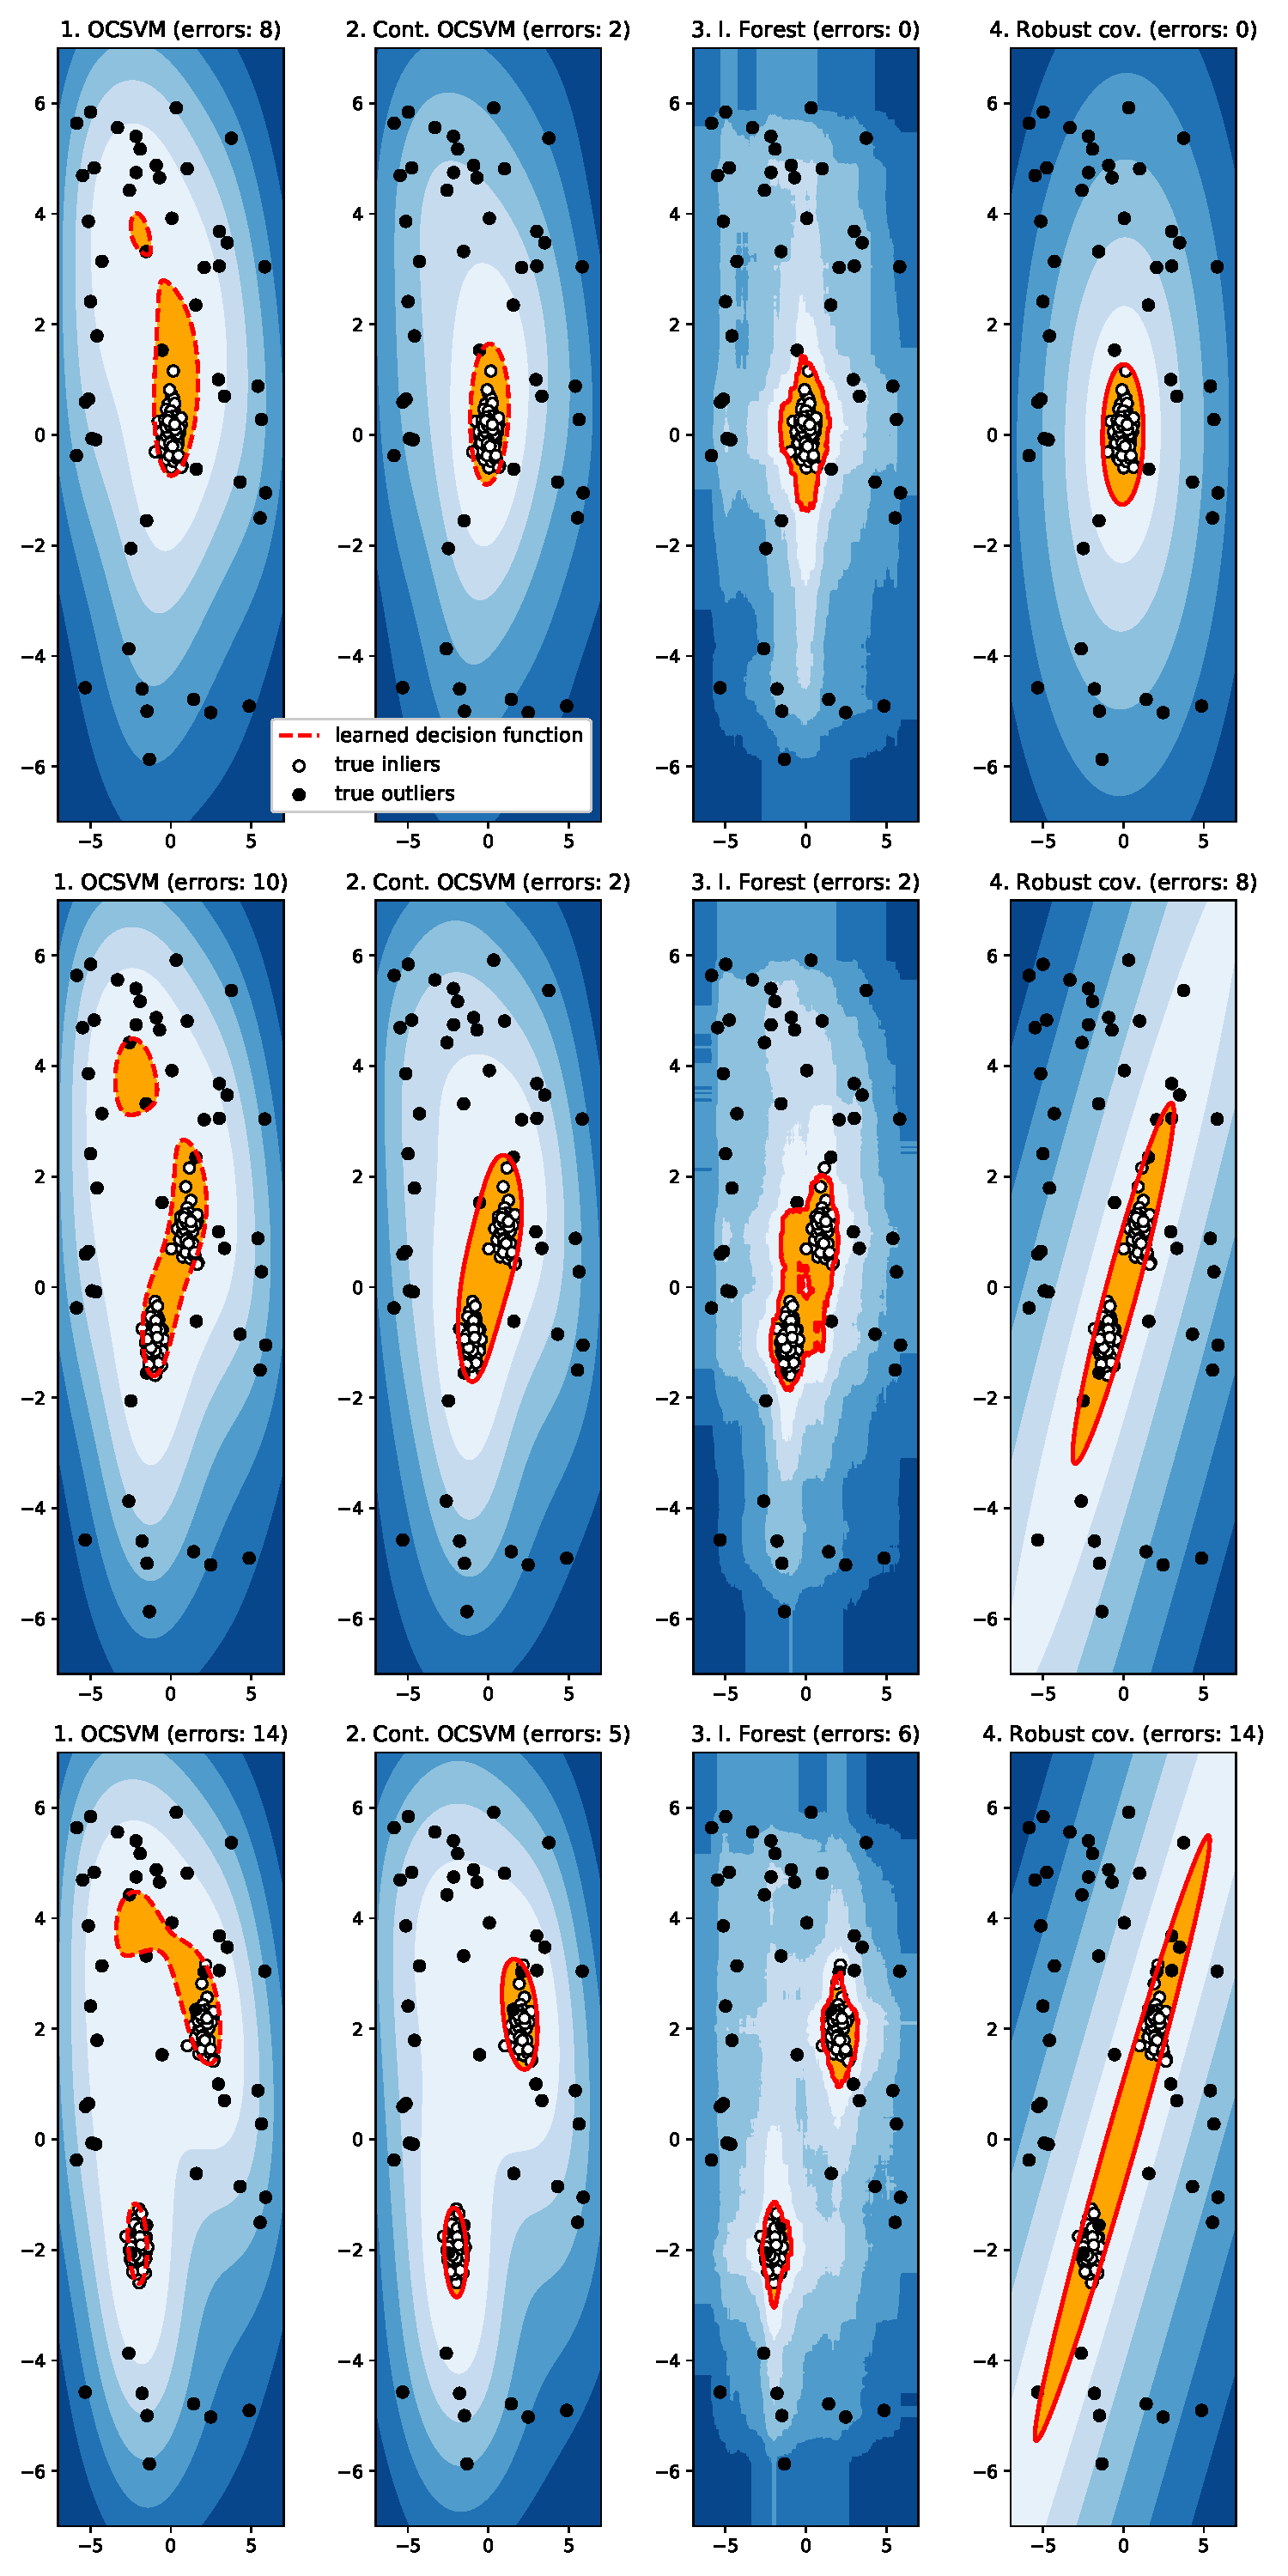
\includegraphics[width=\textwidth]{./gfx/ocsvm.eps}}
    %\caption[Continuous OCSVM for outlier detection]{Continuous OCSVM for
    %outlier detection. \label{fig:ocsvm_outlier}}
%\end{figure}
%\paragraph{}
%We propose a second experiment in a context of outlier detection. This time
%the train set is polluted with outliers. We replicate the example given in
%the documentations of Scikit-Learn at
%\url{http://scikit-learn.org/stable/auto_examples/covariance/plot_outlier_detection.html}
%We compare our method to three other well known outlier detection methods
%from the literature: Isolation Forest \citep{Liu2008}, \acs{OCSVM}
%\citep{Scholkopf2001} and a Robust Covariance estimator
%\citep{campbell1980robust, pedregosa2011scikit} on \cref{fig:ocsvm_outlier}.
%Our method achieve the state of the art on this simple example which is
%encouraging. However the computation time of our continuous \acs{OCSVM} is
%higher than the other methods. It took circa $0.25$ second for the \acs{OCSVM}.
%$10$ seconds for our method, $5$ seconds for isolation forest and $0.1$ second
%for the Robust covariance estimator. This can be due to the implementation since we used
%a (sub-optimal) hand-crafted full gradient descent. Notice that however our
%method is able to retrieve all the level sets after training, not only the one
%presented in \cref{fig:ocsvm_outlier}.  When one is interested in a specific
%level set or range of level set one could sample the $\nu_t$ from another
%distribution than the uniform distribution $\mathcal{U}[0, 1]$ to give more
%importance to the desire range of level sets.

%% %----------------------------------------------------------------------------
%% \section{The Nystr\"om method}
%% \label{sec:the_nystrom_method}

%% %----------------------------------------------------------------------------
%% \section{Sub-sampling the data}
%% \label{sec:sub_sampling_the_data}

%\section{Operalib}
%During this Thesis we started the development of a library named \say{Operalib}
%implementing various machine learning algorithms based on operator-valued
%kernels. Operator-valued kernels defines a framework allowing learning
%vector/function/structured output. The library currently features:
%\begin{itemize}
    %\item Quantile regression \citep{sangnier2016joint},
    %\item \acs{ONORMA} \citep{audiffren2013online},
    %\item semi-supervised Ridge regression \citep{Brouard2016_jmlr},
    %\item some elements of the \acs{ORFF} framework \citep{brault2016random}.
%\end{itemize}
%The algorithms work for a selection of popular operator-valued kernels such
%that the matrix-valued decomposable kernel, the curl-free kernel and the
%divergence-free kernel. The library is structured so that it is easy for the
%user to define its own operator-valued kernel and plug it to the existing
%optimisation algorithms, while keeping efficient computations thanks to the
%methodology presented in \cref{subsec:efficient_learning} (\acs{ie} by seeing
%operator-valued kernels as operators along with matrix-free solver rather than
%plain matrices). We designed the library in order to have a close compatibility
%with Scikit-learn. Code and documentation are publicly available at
%\url{https://github.com/operalib/operalib}. In a near future we plan to add the
%work of \citet{lim2015operator} for vector-autoregression with \acsp{OVK}. We
%hope to expand with more algorithms from various authors if the \acs{OVK}
%commutity and welcome any new contributor!

%\chapterend

\section{Learning function-valued functions}
In this section we show how to use \acs{OVK} in hand with the \acs{ORFF}
framework to learn function-valued functions. We focus on two application
cases: quantile regression and one-class classification. This section is rather
an informal (but detailed) discussion on ideas that we plan to improve for
future publications.

\subsection{Quantile regression}
\label{subsec:quantile_regression}
This introduction to quantile regression is adapted from the paper
of \citet{sangnier2016joint}. As we have seen in the introductory
\cref{ch:motivations}, a standard task in Machine Learning is to estimate the
conditional expectation $f(x)=\expectation_{\probability}[Y | X = x]$, where
$(X,Y)\sim\probability$ with some function belonging to a hypothesis space
$f\in\mathcal{F}$. Yet, many sensitive applications need more than the expected
valued of the relationship between random variables. To control the
\say{quality} of the predicted value from an input $x$, fields such as
economics, medicine, physics or social science require to have access to the
different quantile to model the distribution around the mean
$f(x)\in\mathbb{R}$ and strengthen their analysis.
\paragraph{}
Here we are interested in learning and predicting simultaneously \emph{all} the
quantiles on the compact $[0, 1]$, of the scalar-valued random variable $Y|X$.
We place ourselves in the setting of conditional quantile regression by
minimization of the pinball loss \citep{koenker1978regression}. For $\tau\in[0,
1]$ the pinball loss reads
\begin{dmath*}
    L_{\tau}(x, f, y) = \max(\tau \left(f(x) - y\right), (\tau - 1) \left(f(x)
    - y\right)).
\end{dmath*}
In a nutshell, this loss has been introduced by noticing that finding the
optimal location parameter $\mu = f(x)$ in the $\ell_1$ loss $L(x, f,
y)=\abs{f(x) - y}$ yields an estimator of the unconditional median
\citep{koenker1978regression}. Recently \citet{sangnier2016joint} proposed to
learn simultaneously many quantiles by minimizing the multi-quantile loss
function. Given a vector of quantiles $\boldsymbol{\tau} = (\tau_1, \dots
\tau_p)\in[0, 1]^p$
\begin{dmath*}
    L_{\boldsymbol{\tau}}(x, f, y) = \sum_{i=1}^p \max(\boldsymbol{\tau}_i
    \left(f(x)_i - y\right), (\boldsymbol{\tau}_i - 1)\left(f(x)_i - y\right)).
\end{dmath*}
We see that now it is necessary for $f(x)\in\mathbb{R}^p$ to be vector-valued.
In this work we push further the idea by considering that $f(x)$ is a function
of an arbitrary quantile $\tau\in[0, 1]$. Thus we view $f$ as a vector-valued
function $f:\mathbb{R} \to ([0, 1] \to \mathbb{R})$. For the sake of simplicity
we note $f(x)=f_x$ and introduce the generalized pinball loss
\begin{dmath}
    \label{eq:loss_pinball}
    L(x, f, y) = \int_{[0, 1]} \max(\tau \left(f_x(\tau) - y\right), (\tau -
    1)\left(f_x(\tau) - y)\right) d\tau.
\end{dmath}

\subsection{Functional output data}
Pioneer work on learning function-valued function has been done by
\citet{kadri2015operator}. Inspired by them we develop an \acs{ORFF}
methodology to learn functional data where the outputs are functions that we
suppose living in a \acs{RKHS}.
\paragraph{}
Namely, we suppose that the image of a funtion $f$, has values $f(x) \in
\mathcal{H}_{k_{\mathcal{T}}}$ in a \acs{RKHS}, where
$k_{\mathcal{T}}:\mathcal{T}^2\to\mathbb{R}$ is a scalar-valued kernel and
$\mathcal{H}_{k_{\mathcal{T}}}$ is the corresponding \acs{RKHS}. From this
hypothesis we see that
\begin{dmath*}
    f_x(\tau) = \inner{f(x), k_{\mathcal{T}}(\cdot,
    \tau)}_{\mathcal{H}_{k_{\mathcal{T}}}}
\end{dmath*}
If we add the second hypothesis that $f\in\mathcal{H}_K$, where $\mathcal{H}_K$
is a \emph{\acl{vv-RKHS}} for some \acl{OVK} $K$, \Citet{Carmeli2010} showed in
example $6$ page $17$-$18$ that in this case the operator $K$ is given by
\begin{dmath}
    \label{eq:functional_kernel}
    K =
    \begin{cases}
        \mathcal{X} \times \mathcal{X} & \to
        \mathcal{L}(\mathcal{H}_{k_{\mathcal{T}}}) \\
        x, z & \mapsto k_{\mathcal{X}}(x, z) I_{\mathcal{H}_{k_{\mathcal{T}}}},
    \end{cases}
\end{dmath}
where $k:\mathcal{X}\times\mathcal{X} \to \mathbb{R}$ is another scalar-valued
kernel. Moreover \citet{Carmeli2010} showed in example $7$ page $18$-$19$ that
the \acs{vv-RKHS} induced by $K$ is the same \acs{RKHS} than the one induced by
the kernel $K'$ defined as follow for some measure $\mu$ with support
$\mathcal{T}$.
\begin{dmath*}
    K' =
    \begin{cases}
        \mathcal{X} \times \mathcal{X} & \to
        \mathcal{L}\left(L^2(\mathcal{T}, \mu)\right) \\
        x, z & \mapsto \left(g \mapsto k_{\mathcal{X}}(x, z)
        \int_{\mathcal{T}}k_{\mathcal{T}}(\cdot, \tau)g(\tau)d\mu(\tau)\right).
    \end{cases}
\end{dmath*}
This is exactly the decomposable kernel introduced in
\cref{def:hilbert_schmidt_integral_kernel} in \cref{ch:motivations}. Because
the \acsp{RKHS} induced by $K$ and $K'$ is the same, we can either view its
elements as functions from $\mathcal{X}$ into $\mathcal{H}_{k_{\mathcal{T}}}$
(through $\mathcal{H}_K$) or as functions from $\mathcal{X}$ into
$L^2(\mathcal{T}, \mu)$ (through $\mathcal{H}_{K'}$).

\subsection{ORFF for functional output data}
Because $\mathcal{Y}=\mathcal{H}_{k_{\mathcal{T}}}$ is a proper (infinite
dimensional) Hilbert space, we can apply the \acs{ORFF} methodology. Let
$k_{\mathcal{X}}$ be a scalar Mercer kernel and $\mathcal{X}=\mathbb{R}$. Then
by \cref{cr:ORFF-map-kernel} applied to the decomposable kernel (see
\cref{subsec:examples_ORFF}) we have the following approximate feature map for
$K$ defined in \cref{eq:functional_kernel}:
\begin{dmath*}
    \tildePhi{\omega}(x)y = \frac{1}{\sqrt{D}}\Vect_{j=1}^D
    \begin{pmatrix}
        \cos(x \omega_j) B^\adjoint y \\
        \sin(x \omega_j) B^\adjoint y
    \end{pmatrix} \condition{$\omega_j \sim \FT{k_{\mathcal{X}}}$
    \ac{iid}}
\end{dmath*}
where $BB^\adjoint = I_{\mathcal{H}_{k_{\mathcal{T}}}}$ and
$y\in\mathcal{H}_{k_{\mathcal{T}}}$. At this point we could choose
$B=I_{\mathcal{H}_{k_{\mathcal{T}}}}$. However this is not really useful since
it would make the redescription space $\widetilde{\mathcal{H}}=\Vect_{j=1}^D
\mathcal{H}_{k_{\mathcal{T}}}$, which is a direct sum of infinite dimensional
\acs{RKHS}. Yet since $\mathcal{H}_{k_{\mathcal{T}}}$ is a \acs{RKHS},
according to \cref{pr:feature_operator} it is possible to define a feature
operator $W:\mathcal{H}\to\mathcal{H}_{k_{\mathcal{T}}}$ such that
$(Wg)(\tau)=\Phi_\tau^\adjoint g$.
\maxdeadcycles=10000
\afterpage{%
\begin{landscape}
    \begin{figure}[htp]
        \centering
        \resizebox{.8\textheight}{!}{%
        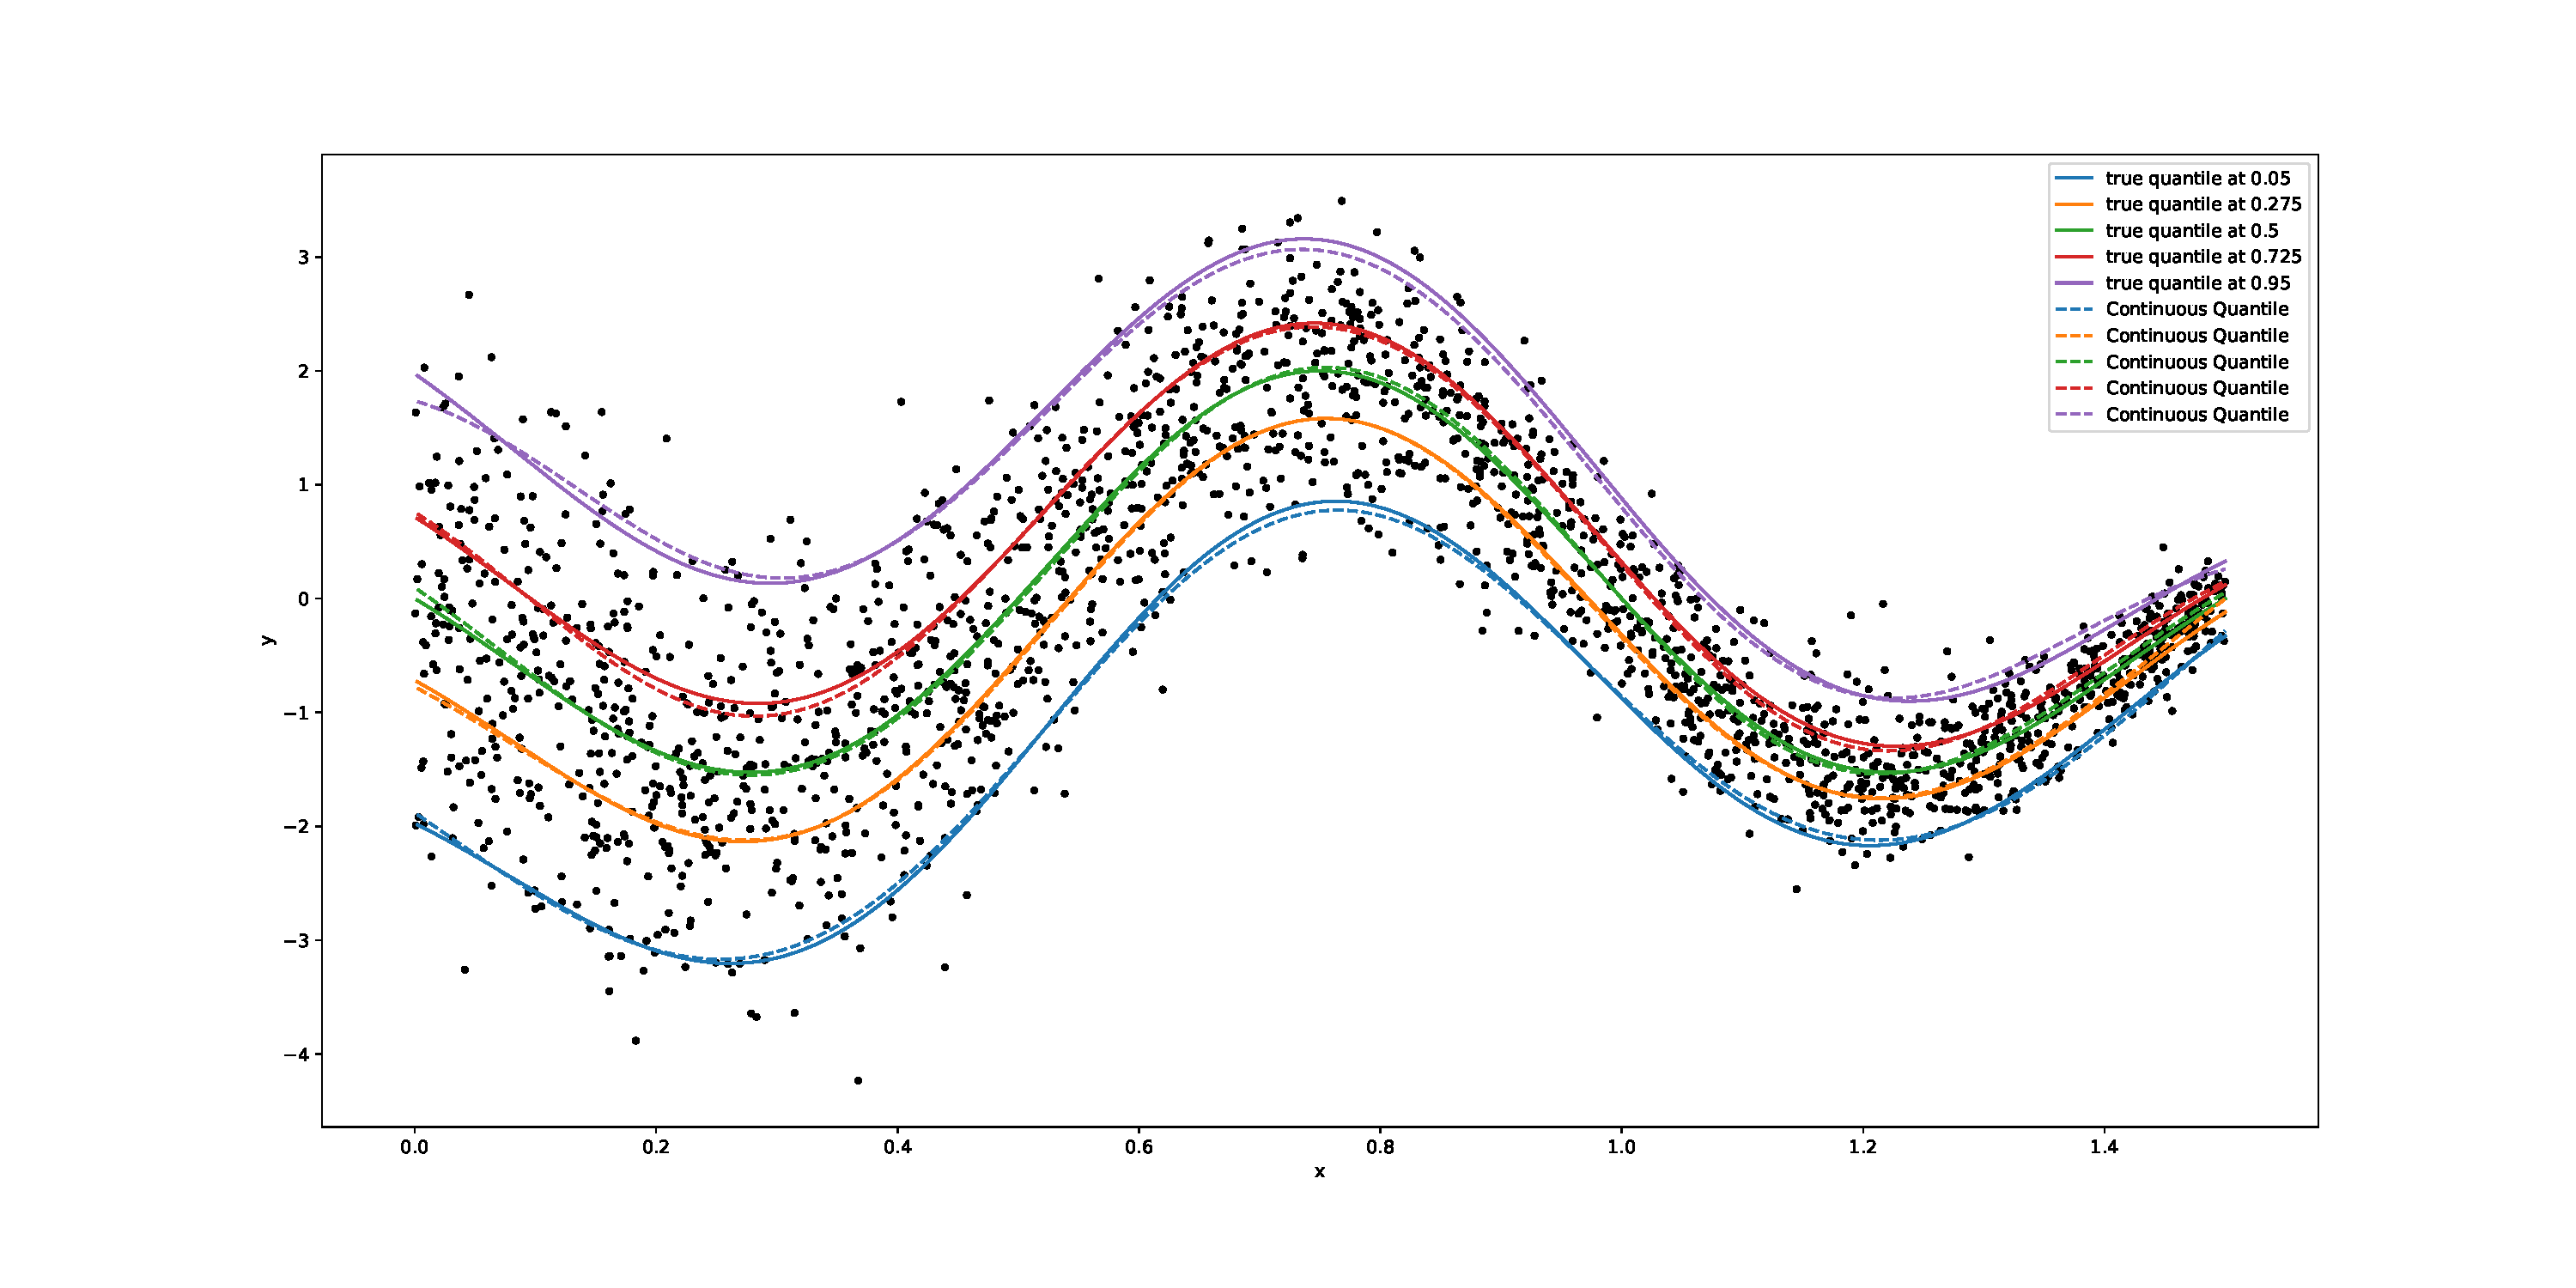
\includegraphics{./gfx/quantile_orff.pdf}}
        \caption{Learning a continuous quantile function with ORFF
        regression. \label{fig:quantile_orff}}
    \end{figure}
    \clearpage
    \begin{figure}[htp]
        \centering\resizebox{.8\textheight}{!}{%
        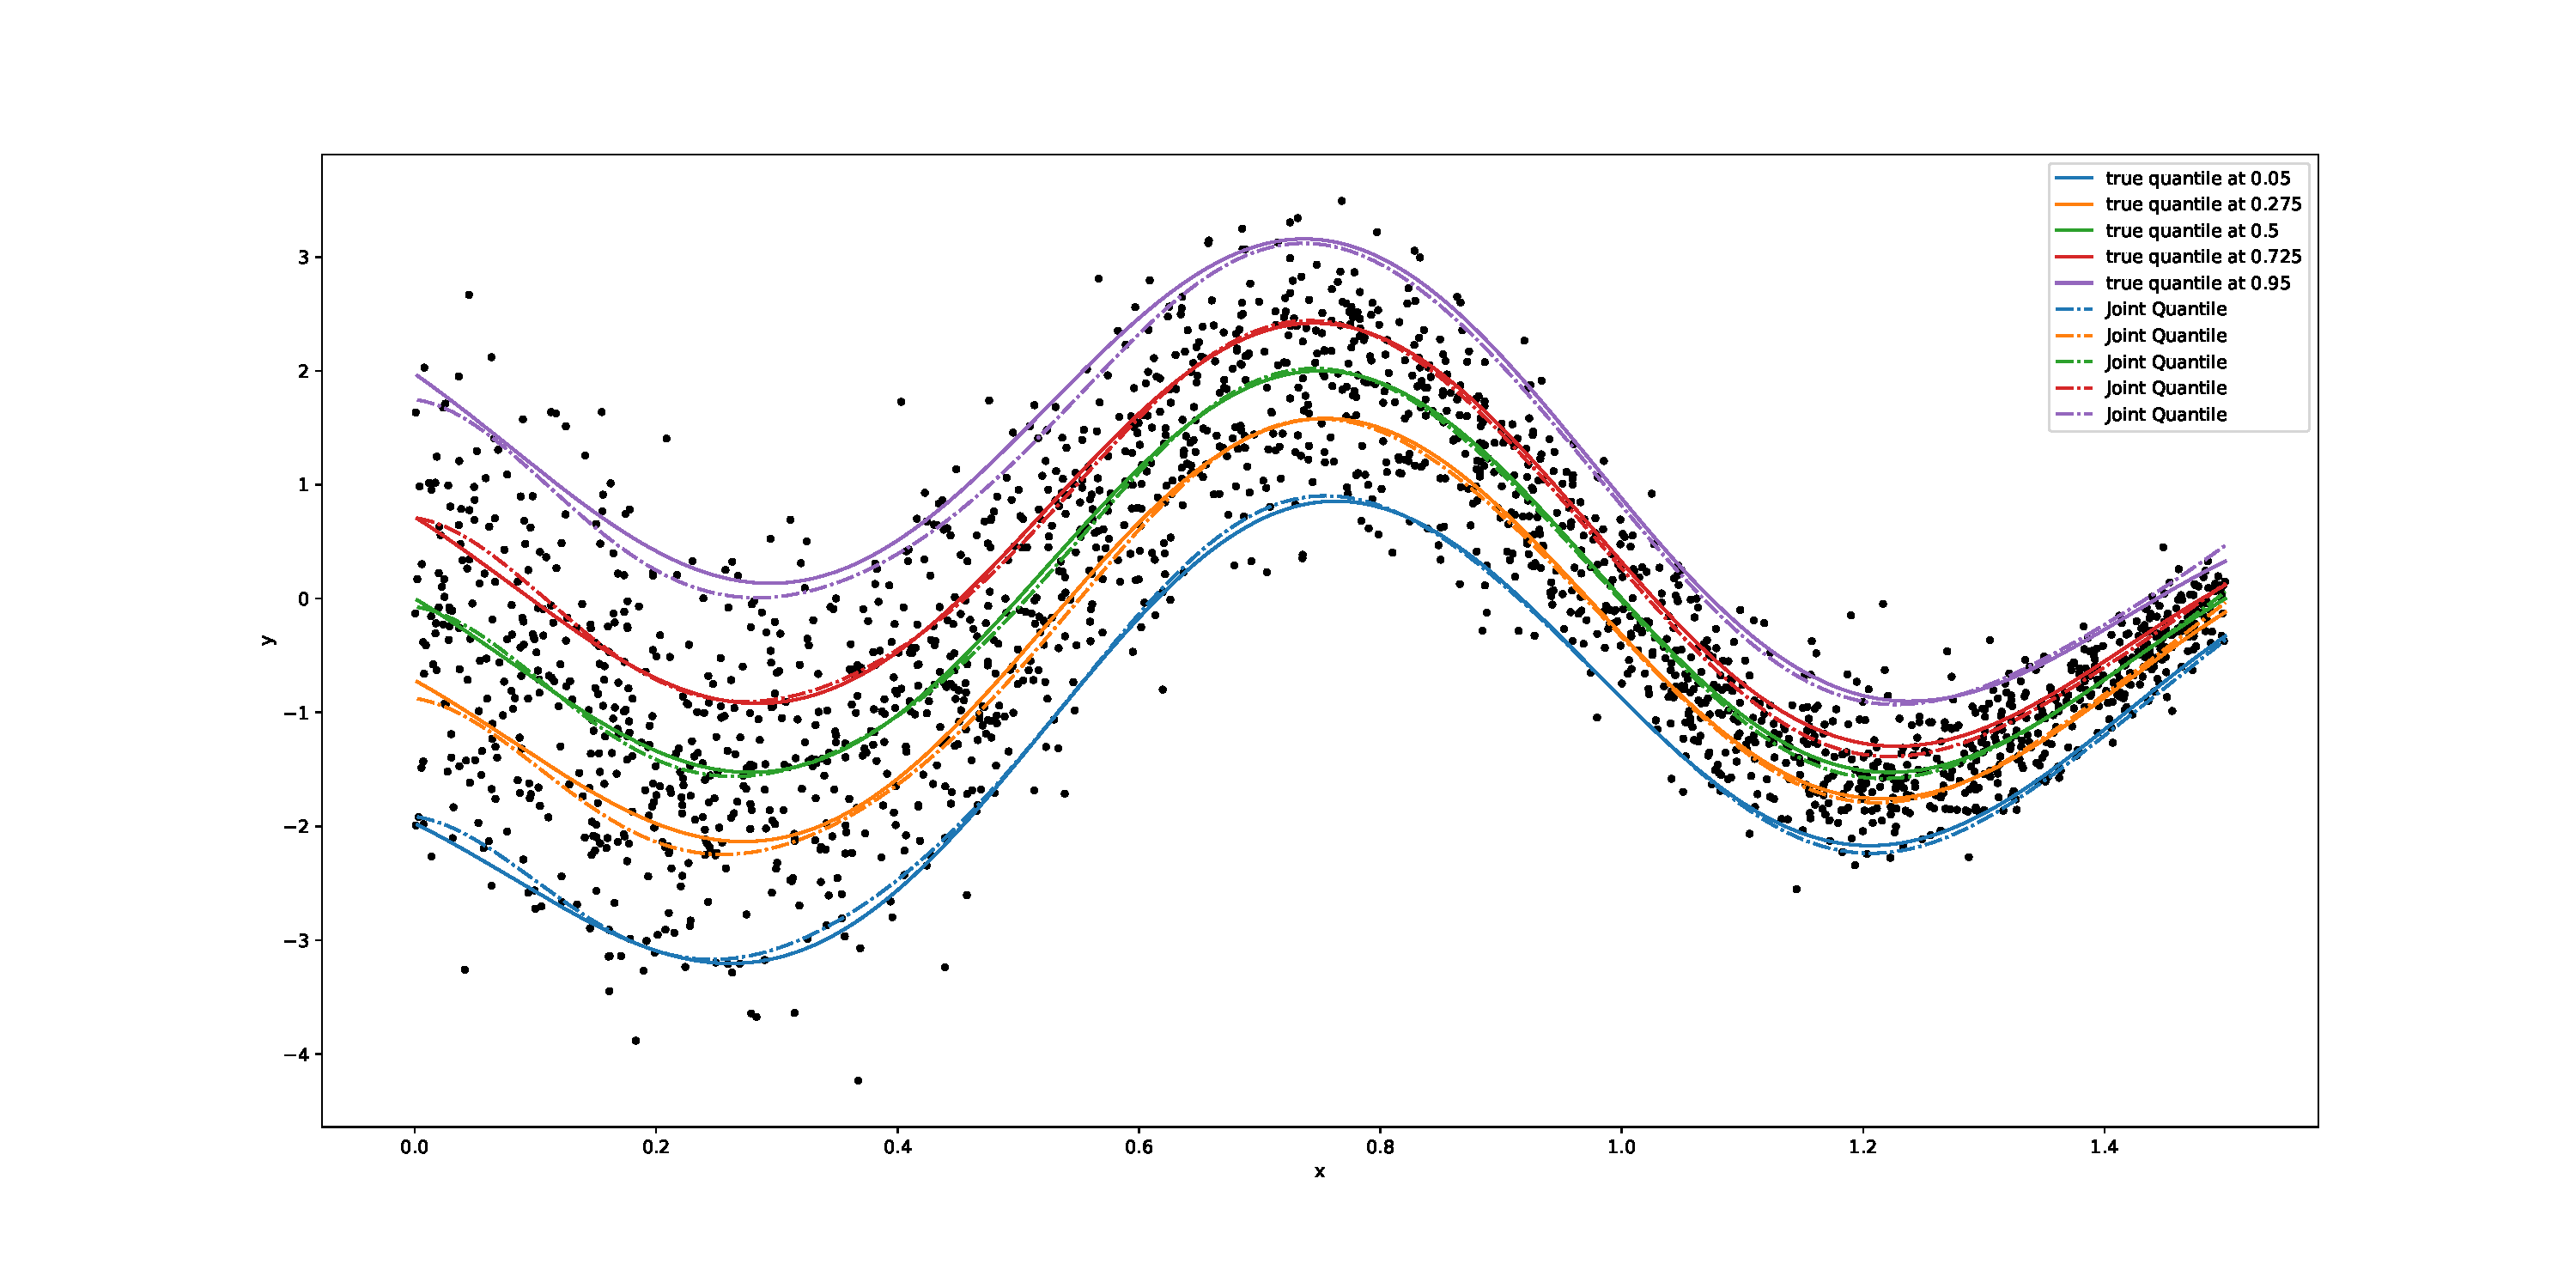
\includegraphics{./gfx/quantile_joint.pdf}}
        \caption{Learning many quantile with joint OVK regression.
        \label{fig:quantile_joint}}
    \end{figure}
\end{landscape}}
Moreover $W^\adjoint W$ is the identity on
$\Ima \Phi_{\tau}$ which is here $\mathcal{H}_{k_{\mathcal{T}}}$. (see the
proof of \cref{pr:feature_operator} and \citet{Carmeli2010}). Thus we can
choose $\Phi_\tau=\Phi(\tau)$ to be the functional Fourier feature map
associated to $k_{\mathcal{T}}$ defined in \cref{pr:fourier_feature_map}.  Then
we have $BB^\adjoint = I_{\mathcal{H}_{k_{\mathcal{T}}}} = W W^\adjoint$.  Thus
we can choose $B = W = \Phi(\cdot)^\adjoint$ and the approximate
feature map reads
\begin{dmath*}
    \tildePhi{\omega}(x)\in \mathcal{L}\left(\mathcal{H}_{k_{\mathcal{T}}};
    \Vect_{j=1}^D L^2\left(\dual{\mathcal{T}},
    \probability_{\dual{\Haar},\rho}\right)\right)
\end{dmath*}
and
\begin{dmath*}
    (\tildePhi{\omega}(x)g)(\tau) = \frac{1}{\sqrt{D}}\Vect_{j=1}^D
    \begin{pmatrix}
        \cos(x \omega_j) W^\adjoint g \\
        \sin(x \omega_j) W^\adjoint g
    \end{pmatrix} \condition{$\omega_j \sim \FT{k_{\mathcal{X}}}$
    \ac{iid}}
\end{dmath*}
%Then as proposed in \cref{ch:operator-valued_random_fourier_features} we can
%Monte-Carlo sample the functional feature map $\Phi(\tau)$ and obtain the
%\acs{ORFF} map
%\begin{dmath*}
    %\left(\widetilde{\tildePhi{\omega}}(x)g\right)(\tau) =
    %\frac{1}{\sqrt{DD'}}\Vect_{j=1}^D
    %\begin{pmatrix}
        %\cos(x \omega_j) \sum_{k=1}^{D'}
        %\left(\cos(\tau \omega_k') + \sin(\tau \omega_k')\right)g(\omega_k') \\
        %\sin(x \omega_j) \sum_{k=1}^{D'}
        %\left(\cos(\tau \omega_k') + \sin(\tau \omega_k')\right)g(\omega_k')
    %\end{pmatrix} \condition{$\omega_j \sim \FT{k_{\mathcal{X}}}$
    %\acs{iid} and $\omega_k'\sim \FT{k_{\mathcal{T}}}$ \acs{iid}.}
%\end{dmath*}
%where $g\in L^2\left(\dual{\mathcal{T}}, \probability_{\dual{\Haar},
%\rho}\right)$ and $\tau\in\mathbb{R}$. If we note
%\begin{dmath*}
    %G =
    %\begin{pmatrix}
        %g(\omega_1') & \dots & g(\omega_{D'}')
    %\end{pmatrix}^\adjoint \hiderel{\in} \mathbb{R}^{D'}
%\end{dmath*}
%we can define
%\begin{dmath*}
    %\left(\widetilde{\tildePhi{\omega}}(x)G\right)(\tau) =
    %\frac{1}{\sqrt{DD'}}\Vect_{j=1}^D
    %\begin{pmatrix}
        %\cos(x \omega_j) \sum_{k=1}^{D'}
        %\left(\cos(\tau \omega_k') + \sin(\tau \omega_k')\right)G_k \\
        %\sin(x \omega_j) \sum_{k=1}^{D'}
        %\left(\cos(\tau \omega_k') + \sin(\tau \omega_k')\right)G_k
    %\end{pmatrix} \condition{$\omega_j \sim \FT{k_{\mathcal{X}}}$
    %\acs{iid} and $\omega_k'\sim \FT{k_{\mathcal{T}}}$ \acs{iid}.}
%\end{dmath*}
Then it is easy to verify that the adjoint operator is given by
\begin{dmath*}
    \left(\widetilde{\tildePhi{\omega}}(x)^\adjoint \theta\right)(\tau) =
    \frac{1}{\sqrt{DD'}} \sum_{j=1}^D \left(\cos(x\omega_j) +
    \sin(x\omega_j)\right) \left(\Vect_{k=1}^{D'}
    \begin{pmatrix}
        \cos(\tau \omega_k') \\
        \sin(\tau \omega_k')
    \end{pmatrix}\right)^\adjoint \theta_j
    = \frac{1}{\sqrt{DD'}} \sum_{j=1}^D \left(\cos(x\omega_j) +
    \sin(x\omega_j)\right) \theta_{jk} \left( \cos(\tau \omega_k') + \sin(\tau
    \omega_k')\right)
    \condition{$\omega_j \sim \FT{k_{\mathcal{X}}}$
    \acs{iid} and $\omega_k'\sim \FT{k_{\mathcal{T}}}$ \acs{iid}.}
\end{dmath*}
where $\theta_k\in\mathbb{R}^{D'}$, for all $k \in \mathbb{N}^*_D$ and
$\theta_{jk}\in\mathbb{R}$ for all $j \in \mathbb{N}^*_D$ and all $k \in
\mathbb{N}^*_{D'}$. The above equations can be rewritten in matrix form which
results in the following conjecture.
\begin{conjecture}
    \label{cj:functional_orff}
    If $\tildephi{\omega}_{\mathcal{X}}$ is an \acs{RFF} for
    $\widetilde{k}_{\mathcal{X}}$ such that
    $\tildephi{\omega}(x)\in\mathbb{R}^D$ and $\tildephi{\omega}_{\mathcal{T}}$
    is an \acs{RFF} for $\widetilde{k}_{\mathcal{T}}$, such that
    $\tildephi{\omega}(\tau)\in\mathbb{R}^{D'}$ then an \acs{ORFF} map for
    \begin{dmath*}
        K(x, z) = k_{\mathcal{X}}(x, z)
        I_{\mathcal{H}_{\tilde{k}_{\mathcal{T}}}}
    \end{dmath*}
    is given for all $x\in\mathbb{R}$, all $\tau\in\mathbb{R}$ and all
    $\Theta\in\mathcal{M}_{D,D'}(\mathbb{R})$ by
    \begin{dmath*}
        \left(\tildePhi{\omega}_K(x)^\adjoint \Theta \right)(\tau) =
        \tildephi{\omega}_{\mathcal{X}}(x)^\adjoint \Theta
        \tildephi{\omega}_{\mathcal{T}}(\tau)
    \end{dmath*}
    and
    \begin{dmath*}
        \left(\tildePhi{\omega}_K(x) G\right)(\tau) =
        \tildephi{\omega}_{\mathcal{X}}(x)
        \tildephi{\omega}_{\mathcal{T}}(\tau)^\adjoint G,
    \end{dmath*}
    where $g\in\mathbb{R}^{D'}$.
    %but more intestingly, given $y\in\mathbb{R}$,
    %\begin{dmath*}
        %\tildePhi{\omega}_K(x, \tau)^\adjoint y =
        %y \tildephi{\omega}_{\mathcal{X}}(x)
        %\tildephi{\omega}_{\mathcal{T}}(\tau)^\adjoint.
    %\end{dmath*}
\end{conjecture}
Moreover if one defines $\tildePhi{\omega}_K(x,
\tau) = \left(\tildePhi{\omega}_K(x)^\adjoint \Theta \right)(\tau)$ one
have of course
\begin{dmath*}
    \tildePhi{\omega}_K(x, \tau)^\adjoint \Theta =
    \tildephi{\omega}_{\mathcal{X}}(x)^\adjoint \Theta
    \tildephi{\omega}_{\mathcal{T}}(\tau)
\end{dmath*}
\subsection{Many quantile regression}
From the loss defined in \cref{eq:loss_pinball} we defined the regularized risk
using the \say{continuous} pinball loss for the quantile regression problem.
For all $f\in\mathcal{H}_K$,
\begin{dmath*}
    \mathfrak{R}_{\lambda}(f, \seq{s}) =
    \frac{1}{N}\sum_{i=1}^N\int_{[0,1]}\left(
    \begin{cases}
        \tau\left(f_{x_i}(\tau) - y_i\right) & \text{if } f_{x_i}(\tau) \ge y_i
        \\
        (1 - \tau)\left(y_i - f_{x_i}(\tau)\right) & \text{otherwise}
    \end{cases} \right)+ \lambda
    \norm{f}_K^2.
\end{dmath*}
The issue with the above risk is that the different quantile for a given point
$x\in\mathbb{R}$ may cross (see \citet{sangnier2016joint}). To avoid this to
happen we need to force the function $f_x(\tau)$ to be \emph{increasing} in
$\tau$ for any $x\in\mathbb{R}$.  Because a decreasing function has a negative
derivative we can add a penalty term to the risk to avoid $f_x(\tau)$ to be
decreasing in $\tau$.
\begin{dmath*}
    \Omega_{cross}(f_{x_i}) = - \min\left(\frac{\partial
    f_{x_i}}{\partial\tau}(\tau),
    0\right)
\end{dmath*}
Thus the regularized risk with the no crossing constraint is
\begin{dmath*}
    \mathfrak{R}_{\lambda_1, \lambda_2}(f, \seq{s}) =
    \frac{1}{N}\sum_{i=1}^N\int_{[0,1]}\left(
    \begin{cases}
        \tau \left(f_{x_i}(\tau) - y_i\right) & \text{if } f_{x_i}(\tau) \ge
        y_i \\
        (1 - \tau)\left(y_i - f_{x_i}(\tau)\right) & \text{otherwise}
    \end{cases} -
    \lambda_1 \min\left(\frac{\partial f_{x_i}}{\partial\tau}(\tau), 0\right)
    \right)+ \lambda_2 \norm{f}_K^2.
\end{dmath*}
Eventually we replace the integral by a Monte-Carlo sampling with the uniform
law $\mathcal{U}([0, 1])$ and plug in the approximate function of $f$ using the
\acs{ORFF} map proposed in \cref{cj:functional_orff}. The final regularized
risk to be minimized reads
\begin{dmath*}
    \mathfrak{R}_{\lambda_1, \lambda_2}(\Theta, \seq{s}) =
    \frac{1}{NT}\sum_{i=1}^N\sum_{t=1}^T\left(
    \begin{cases} \tau_t
        \left(\widetilde{f}_{x_i}(\tau_t) - y_i\right) & \text{if }
        \widetilde{f}_{x_i}(\tau_t) \ge y_i \\
        (1 - \tau_t)\left(y_i - f_{x_i}(\tau_t)\right) & \text{otherwise}
    \end{cases} - \lambda_1
    \min\left(\frac{\partial \widetilde{f}_{x_i}}{\partial\tau}(\tau_t),
    0\right) \right)+ \lambda_2 \norm{\Theta}_{fro}^2.
\end{dmath*}
where $\widetilde{f}_{x}(\tau)=\tildephi{\omega}_{\mathcal{X}}(x)^\adjoint
\Theta \tildephi{\omega}_{\mathcal{T}}(\tau)$, $\tau_t \sim \mathcal{U}([0,
1])$ and
\begin{dmath*}
    \frac{\partial \widetilde{f}_{x}}{\partial\tau}(\tau)
    = \tildephi{\omega}_{\mathcal{X}}(x)^\adjoint \Theta \frac{\partial
    \tildephi{\omega}_{\mathcal{T}}}{\partial \tau}(\tau)
    = \tildephi{\omega}_{\mathcal{X}}(x)^\adjoint \Theta \Vect_{k=1}^{D'}
    \begin{pmatrix}
        -\omega_k' \sin(\omega_k' \tau) \\
         \omega_k' \cos(\omega_k' \tau)
    \end{pmatrix} \condition{$\omega_k' \sim \FT{k_{\mathcal{T}}}$ \acs{iid}.}
\end{dmath*}
\subsubsection{Some results}
We minimized the quantity $\mathfrak{R}_{\lambda_1, \lambda_2}(\Theta,
\seq{s})$ on a toy dataset: a sine wave with some heteroscedastic noise. First
we compared our methodology to the joint quantile regression proposed in
\citet{sangnier2016joint}. We generate $N=2500$ for the train set and $N'=1000$
points for the test set and use a Gaussian kernel for both $k_{\mathcal{X}}$
and $k_{\mathcal{T}}$. We choosed $\sigma_{\mathcal{X}} = 0.25$ and
$\sigma_{\mathcal{T}}$ has been set to be the median of the pairwise distance
of the $\tau_t$'s drawn randomly from $\mathcal{U}([0, 1])$. Notice that
$\mathfrak{R}_{\lambda_1, \lambda_2}(\Theta, \seq{s})$ is convex in $\Theta$.
To avoid computing complex gradients and by lack of time, we used Tensorflow
\citep{abadi2016tensorflow} to perform a gradient descent (with RMSProp
\citep{tieleman2012lecture}) with automatic symbolic differentiation.
\Cref{fig:quantile_orff} show the result for the quantile at $0.05$, $0.275$,
$0.5$, $0.775$ and $0.95$ using the \acs{ORFF} methodology.
\afterpage{%
\begin{landscape}
    \begin{figure}[htp]
        \centering
        \resizebox{.8\textheight}{!}{%
        \includegraphics{./gfx/quantile_continuous.pgf}}
        \caption{Learning a continuous quantile function with ORFF
        regression. \label{fig:quantile_continuous}}
    \end{figure}
\end{landscape}}
\Cref{fig:quantile_joint} shows the joint quantile regression of
\citet{sangnier2016joint} on the same dataset. Not only our method matched the
the performances of \citet{sangnier2016joint}\footnote{We reported an error
computed with the pinball loss on the test set of $0.818$ for our method and
$0.817$ for joint regression (note that we don't report here an average on many
experiments to avoid randomness introduced by the random features, but the
results seems robust in practice.)} but we cutted down the computation time
from circa $1330$ seconds to circa $30$ seconds (training and testing).
Moreover on contrary to \citet{sangnier2016joint} we have access to all the
quantile of the model (see \cref{fig:quantile_continuous}).

\subsection{One-class SVM revisited}
We also propose an extension of the celebrated \acf{OCSVM} such that it is
possible to learn jointly all the level sets.  One-class classification, also
known as unary classification, tries to identify objects of a specific class
amongst all objects, by learning from a training set containing only the
objects of that class.  In this framework, we assume that we only observe
examples of one class (referred to as the inlier class).  The second class is
called outlier class.  We turn our attention to the \acs{OCSVM}
of \citet{Scholkopf2001} which extends the \ac{SVM} methodology
\citep{Cortes1995,Shawe2004} to handle training using only inliers.
\paragraph{}
We recall that given an hyperparameter $\nu\in [0,1]$ that controls the
proportion of inlier, given as scalar kernel $k$, the \acs{OCSVM} problem reads
\begin{dmath*}
    \argmin_{f\in\mathcal{H}_k, \tau \in \mathbb{R}} \frac{\nu}{2}
    \norm{f}_{\mathcal{H}_k}^2 - \nu \tau + \frac{1}{N} \sum_{i=1}^N \max(\tau
    - f(x_i), 0)
\end{dmath*}
The decision function is then
\begin{dmath*}
    h(x, \tau) = \mathds{1}_{[\tau, \infty)}\left( f(x) \right).
\end{dmath*}
As in \cref{subsec:quantile_regression} we can rewrite the optimization problem
as an integral over all the value of $\nu$ and suppose that $f$ is
function-valued (a function of $\nu$). Moreover $\tau$ must also change its
value according to $\nu$. Thus given a kernel $k_{\mathcal{X}}$ on the inputs
$x\in\mathbb{R}^d$ with its approximate feature map
$\tildephi{\omega}_{\mathcal{X}}$ and a kernel $k_{\mathcal{T}}$ on the level
sets with its approximate feature map $\tildephi{\omega}_{\mathcal{T}}$, we
define the continuous one-class SVM problem as
\begin{dmath*}
    \argmin_{f
    \in\mathcal{H}_K,\tau\in\mathcal{H}_{k_{\tau}}}\frac{1}{N}
    \sum_{i=1}^N\int_{[0,1]}\max\left(0, \tau(\nu) - f_{x_i}(\nu)\right)d\nu +
    \frac{1}{2}\int_{[0,1]}\nu
    \norm{f_{\cdot}(\nu)}_{\mathcal{H}_{k_{\mathcal{X}}}}^2d\nu -
    \int_{[0,1]}\nu\tau(\nu)d\nu.
\end{dmath*}
Again we can compute the integral by Monte-Carlo sampling and replace $f$ and
$\tau$ by their respective approximation. Notice that the \acs{RKHS} of $\tau$
should match the \acs{RKHS} of the output space of $f_K$. Hence
\begin{dmath*}
    \argmin_{\Theta
    \in\mathcal{M}_{D, D'}(\mathbb{R}),\tau\in\mathbb{R}^D}\frac{1}{NT}
    \sum_{i=1}^N\sum_{t=1}^T\max\left(0, \widetilde{\tau}(\nu_t) -
    \widetilde{f}_{x_i}(\nu_t)\right) + \frac{1}{2T}\sum_{t=1}^T\nu_t
    \norm{\widetilde{f}_{\cdot}(\nu_t)}_{2}^2 -
    \frac{1}{T}\sum_{t=1}^T\nu_t\widetilde{\tau}(\nu_t),
\end{dmath*}
where $\nu_t \sim \mathcal{U}([0, 1])$ \acs{iid}, $\widetilde{\tau}(\nu) =
\tildephi{\omega}_{\mathcal{T}}(\nu)$ and $\widetilde{f}_x(\nu) =
\tildephi{\omega}(x)^\adjoint \Theta \tildephi{\omega}_{\mathcal{T}}(\nu)$. We
also deduce that $\widetilde{f}_{\cdot}(\nu) = \Theta
\tildephi{\omega}_{\mathcal{T}}(\nu)$. Here the natural decision function is
\begin{dmath}
    \label{eq:continuous_decision}
    h(x, \nu) = \mathds{1}_{\left[\widetilde{\tau}(\nu),\infty\right)}
    \left(\widetilde{f}_x(\nu)\right).
\end{dmath}
\begin{figure}
    {\centering
    \resizebox{2\textwidth}{!}{%% Creator: Matplotlib, PGF backend
%%
%% To include the figure in your LaTeX document, write
%%   \input{<filename>.pgf}
%%
%% Make sure the required packages are loaded in your preamble
%%   \usepackage{pgf}
%%
%% Figures using additional raster images can only be included by \input if
%% they are in the same directory as the main LaTeX file. For loading figures
%% from other directories you can use the `import` package
%%   \usepackage{import}
%% and then include the figures with
%%   \import{<path to file>}{<filename>.pgf}
%%
%% Matplotlib used the following preamble
%%   \usepackage{fontspec}
%%   \setmainfont{Times New Roman}
%%   \setsansfont{Lucida Grande}
%%   \setmonofont{Andale Mono}
%%
\begingroup%
\makeatletter%
\begin{pgfpicture}%
\pgfpathrectangle{\pgfpointorigin}{\pgfqpoint{16.000000in}{5.000000in}}%
\pgfusepath{use as bounding box, clip}%
\begin{pgfscope}%
\pgfsetbuttcap%
\pgfsetmiterjoin%
\definecolor{currentfill}{rgb}{1.000000,1.000000,1.000000}%
\pgfsetfillcolor{currentfill}%
\pgfsetlinewidth{0.000000pt}%
\definecolor{currentstroke}{rgb}{1.000000,1.000000,1.000000}%
\pgfsetstrokecolor{currentstroke}%
\pgfsetdash{}{0pt}%
\pgfpathmoveto{\pgfqpoint{0.000000in}{0.000000in}}%
\pgfpathlineto{\pgfqpoint{16.000000in}{0.000000in}}%
\pgfpathlineto{\pgfqpoint{16.000000in}{5.000000in}}%
\pgfpathlineto{\pgfqpoint{0.000000in}{5.000000in}}%
\pgfpathclose%
\pgfusepath{fill}%
\end{pgfscope}%
\begin{pgfscope}%
\pgfsetbuttcap%
\pgfsetmiterjoin%
\definecolor{currentfill}{rgb}{1.000000,1.000000,1.000000}%
\pgfsetfillcolor{currentfill}%
\pgfsetlinewidth{0.000000pt}%
\definecolor{currentstroke}{rgb}{0.000000,0.000000,0.000000}%
\pgfsetstrokecolor{currentstroke}%
\pgfsetstrokeopacity{0.000000}%
\pgfsetdash{}{0pt}%
\pgfpathmoveto{\pgfqpoint{0.663889in}{0.580556in}}%
\pgfpathlineto{\pgfqpoint{8.157639in}{0.580556in}}%
\pgfpathlineto{\pgfqpoint{8.157639in}{4.801389in}}%
\pgfpathlineto{\pgfqpoint{0.663889in}{4.801389in}}%
\pgfpathclose%
\pgfusepath{fill}%
\end{pgfscope}%
\begin{pgfscope}%
\pgfsetbuttcap%
\pgfsetroundjoin%
\definecolor{currentfill}{rgb}{0.000000,0.000000,0.000000}%
\pgfsetfillcolor{currentfill}%
\pgfsetlinewidth{0.803000pt}%
\definecolor{currentstroke}{rgb}{0.000000,0.000000,0.000000}%
\pgfsetstrokecolor{currentstroke}%
\pgfsetdash{}{0pt}%
\pgfsys@defobject{currentmarker}{\pgfqpoint{0.000000in}{-0.048611in}}{\pgfqpoint{0.000000in}{0.000000in}}{%
\pgfpathmoveto{\pgfqpoint{0.000000in}{0.000000in}}%
\pgfpathlineto{\pgfqpoint{0.000000in}{-0.048611in}}%
\pgfusepath{stroke,fill}%
}%
\begin{pgfscope}%
\pgfsys@transformshift{1.004514in}{0.580556in}%
\pgfsys@useobject{currentmarker}{}%
\end{pgfscope}%
\end{pgfscope}%
\begin{pgfscope}%
\pgftext[x=1.004514in,y=0.483333in,,top]{\sffamily\fontsize{10.000000}{12.000000}\selectfont 0.0}%
\end{pgfscope}%
\begin{pgfscope}%
\pgfsetbuttcap%
\pgfsetroundjoin%
\definecolor{currentfill}{rgb}{0.000000,0.000000,0.000000}%
\pgfsetfillcolor{currentfill}%
\pgfsetlinewidth{0.803000pt}%
\definecolor{currentstroke}{rgb}{0.000000,0.000000,0.000000}%
\pgfsetstrokecolor{currentstroke}%
\pgfsetdash{}{0pt}%
\pgfsys@defobject{currentmarker}{\pgfqpoint{0.000000in}{-0.048611in}}{\pgfqpoint{0.000000in}{0.000000in}}{%
\pgfpathmoveto{\pgfqpoint{0.000000in}{0.000000in}}%
\pgfpathlineto{\pgfqpoint{0.000000in}{-0.048611in}}%
\pgfusepath{stroke,fill}%
}%
\begin{pgfscope}%
\pgfsys@transformshift{2.367014in}{0.580556in}%
\pgfsys@useobject{currentmarker}{}%
\end{pgfscope}%
\end{pgfscope}%
\begin{pgfscope}%
\pgftext[x=2.367014in,y=0.483333in,,top]{\sffamily\fontsize{10.000000}{12.000000}\selectfont 0.2}%
\end{pgfscope}%
\begin{pgfscope}%
\pgfsetbuttcap%
\pgfsetroundjoin%
\definecolor{currentfill}{rgb}{0.000000,0.000000,0.000000}%
\pgfsetfillcolor{currentfill}%
\pgfsetlinewidth{0.803000pt}%
\definecolor{currentstroke}{rgb}{0.000000,0.000000,0.000000}%
\pgfsetstrokecolor{currentstroke}%
\pgfsetdash{}{0pt}%
\pgfsys@defobject{currentmarker}{\pgfqpoint{0.000000in}{-0.048611in}}{\pgfqpoint{0.000000in}{0.000000in}}{%
\pgfpathmoveto{\pgfqpoint{0.000000in}{0.000000in}}%
\pgfpathlineto{\pgfqpoint{0.000000in}{-0.048611in}}%
\pgfusepath{stroke,fill}%
}%
\begin{pgfscope}%
\pgfsys@transformshift{3.729514in}{0.580556in}%
\pgfsys@useobject{currentmarker}{}%
\end{pgfscope}%
\end{pgfscope}%
\begin{pgfscope}%
\pgftext[x=3.729514in,y=0.483333in,,top]{\sffamily\fontsize{10.000000}{12.000000}\selectfont 0.4}%
\end{pgfscope}%
\begin{pgfscope}%
\pgfsetbuttcap%
\pgfsetroundjoin%
\definecolor{currentfill}{rgb}{0.000000,0.000000,0.000000}%
\pgfsetfillcolor{currentfill}%
\pgfsetlinewidth{0.803000pt}%
\definecolor{currentstroke}{rgb}{0.000000,0.000000,0.000000}%
\pgfsetstrokecolor{currentstroke}%
\pgfsetdash{}{0pt}%
\pgfsys@defobject{currentmarker}{\pgfqpoint{0.000000in}{-0.048611in}}{\pgfqpoint{0.000000in}{0.000000in}}{%
\pgfpathmoveto{\pgfqpoint{0.000000in}{0.000000in}}%
\pgfpathlineto{\pgfqpoint{0.000000in}{-0.048611in}}%
\pgfusepath{stroke,fill}%
}%
\begin{pgfscope}%
\pgfsys@transformshift{5.092014in}{0.580556in}%
\pgfsys@useobject{currentmarker}{}%
\end{pgfscope}%
\end{pgfscope}%
\begin{pgfscope}%
\pgftext[x=5.092014in,y=0.483333in,,top]{\sffamily\fontsize{10.000000}{12.000000}\selectfont 0.6}%
\end{pgfscope}%
\begin{pgfscope}%
\pgfsetbuttcap%
\pgfsetroundjoin%
\definecolor{currentfill}{rgb}{0.000000,0.000000,0.000000}%
\pgfsetfillcolor{currentfill}%
\pgfsetlinewidth{0.803000pt}%
\definecolor{currentstroke}{rgb}{0.000000,0.000000,0.000000}%
\pgfsetstrokecolor{currentstroke}%
\pgfsetdash{}{0pt}%
\pgfsys@defobject{currentmarker}{\pgfqpoint{0.000000in}{-0.048611in}}{\pgfqpoint{0.000000in}{0.000000in}}{%
\pgfpathmoveto{\pgfqpoint{0.000000in}{0.000000in}}%
\pgfpathlineto{\pgfqpoint{0.000000in}{-0.048611in}}%
\pgfusepath{stroke,fill}%
}%
\begin{pgfscope}%
\pgfsys@transformshift{6.454514in}{0.580556in}%
\pgfsys@useobject{currentmarker}{}%
\end{pgfscope}%
\end{pgfscope}%
\begin{pgfscope}%
\pgftext[x=6.454514in,y=0.483333in,,top]{\sffamily\fontsize{10.000000}{12.000000}\selectfont 0.8}%
\end{pgfscope}%
\begin{pgfscope}%
\pgfsetbuttcap%
\pgfsetroundjoin%
\definecolor{currentfill}{rgb}{0.000000,0.000000,0.000000}%
\pgfsetfillcolor{currentfill}%
\pgfsetlinewidth{0.803000pt}%
\definecolor{currentstroke}{rgb}{0.000000,0.000000,0.000000}%
\pgfsetstrokecolor{currentstroke}%
\pgfsetdash{}{0pt}%
\pgfsys@defobject{currentmarker}{\pgfqpoint{0.000000in}{-0.048611in}}{\pgfqpoint{0.000000in}{0.000000in}}{%
\pgfpathmoveto{\pgfqpoint{0.000000in}{0.000000in}}%
\pgfpathlineto{\pgfqpoint{0.000000in}{-0.048611in}}%
\pgfusepath{stroke,fill}%
}%
\begin{pgfscope}%
\pgfsys@transformshift{7.817014in}{0.580556in}%
\pgfsys@useobject{currentmarker}{}%
\end{pgfscope}%
\end{pgfscope}%
\begin{pgfscope}%
\pgftext[x=7.817014in,y=0.483333in,,top]{\sffamily\fontsize{10.000000}{12.000000}\selectfont 1.0}%
\end{pgfscope}%
\begin{pgfscope}%
\pgftext[x=4.410764in,y=0.293908in,,top]{\sffamily\fontsize{10.000000}{12.000000}\selectfont \(\displaystyle \nu\)}%
\end{pgfscope}%
\begin{pgfscope}%
\pgfsetbuttcap%
\pgfsetroundjoin%
\definecolor{currentfill}{rgb}{0.000000,0.000000,0.000000}%
\pgfsetfillcolor{currentfill}%
\pgfsetlinewidth{0.803000pt}%
\definecolor{currentstroke}{rgb}{0.000000,0.000000,0.000000}%
\pgfsetstrokecolor{currentstroke}%
\pgfsetdash{}{0pt}%
\pgfsys@defobject{currentmarker}{\pgfqpoint{-0.048611in}{0.000000in}}{\pgfqpoint{0.000000in}{0.000000in}}{%
\pgfpathmoveto{\pgfqpoint{0.000000in}{0.000000in}}%
\pgfpathlineto{\pgfqpoint{-0.048611in}{0.000000in}}%
\pgfusepath{stroke,fill}%
}%
\begin{pgfscope}%
\pgfsys@transformshift{0.663889in}{0.772412in}%
\pgfsys@useobject{currentmarker}{}%
\end{pgfscope}%
\end{pgfscope}%
\begin{pgfscope}%
\pgftext[x=0.347076in,y=0.718870in,left,base]{\sffamily\fontsize{10.000000}{12.000000}\selectfont 0.0}%
\end{pgfscope}%
\begin{pgfscope}%
\pgfsetbuttcap%
\pgfsetroundjoin%
\definecolor{currentfill}{rgb}{0.000000,0.000000,0.000000}%
\pgfsetfillcolor{currentfill}%
\pgfsetlinewidth{0.803000pt}%
\definecolor{currentstroke}{rgb}{0.000000,0.000000,0.000000}%
\pgfsetstrokecolor{currentstroke}%
\pgfsetdash{}{0pt}%
\pgfsys@defobject{currentmarker}{\pgfqpoint{-0.048611in}{0.000000in}}{\pgfqpoint{0.000000in}{0.000000in}}{%
\pgfpathmoveto{\pgfqpoint{0.000000in}{0.000000in}}%
\pgfpathlineto{\pgfqpoint{-0.048611in}{0.000000in}}%
\pgfusepath{stroke,fill}%
}%
\begin{pgfscope}%
\pgfsys@transformshift{0.663889in}{1.539836in}%
\pgfsys@useobject{currentmarker}{}%
\end{pgfscope}%
\end{pgfscope}%
\begin{pgfscope}%
\pgftext[x=0.347076in,y=1.486294in,left,base]{\sffamily\fontsize{10.000000}{12.000000}\selectfont 0.2}%
\end{pgfscope}%
\begin{pgfscope}%
\pgfsetbuttcap%
\pgfsetroundjoin%
\definecolor{currentfill}{rgb}{0.000000,0.000000,0.000000}%
\pgfsetfillcolor{currentfill}%
\pgfsetlinewidth{0.803000pt}%
\definecolor{currentstroke}{rgb}{0.000000,0.000000,0.000000}%
\pgfsetstrokecolor{currentstroke}%
\pgfsetdash{}{0pt}%
\pgfsys@defobject{currentmarker}{\pgfqpoint{-0.048611in}{0.000000in}}{\pgfqpoint{0.000000in}{0.000000in}}{%
\pgfpathmoveto{\pgfqpoint{0.000000in}{0.000000in}}%
\pgfpathlineto{\pgfqpoint{-0.048611in}{0.000000in}}%
\pgfusepath{stroke,fill}%
}%
\begin{pgfscope}%
\pgfsys@transformshift{0.663889in}{2.307260in}%
\pgfsys@useobject{currentmarker}{}%
\end{pgfscope}%
\end{pgfscope}%
\begin{pgfscope}%
\pgftext[x=0.347076in,y=2.253719in,left,base]{\sffamily\fontsize{10.000000}{12.000000}\selectfont 0.4}%
\end{pgfscope}%
\begin{pgfscope}%
\pgfsetbuttcap%
\pgfsetroundjoin%
\definecolor{currentfill}{rgb}{0.000000,0.000000,0.000000}%
\pgfsetfillcolor{currentfill}%
\pgfsetlinewidth{0.803000pt}%
\definecolor{currentstroke}{rgb}{0.000000,0.000000,0.000000}%
\pgfsetstrokecolor{currentstroke}%
\pgfsetdash{}{0pt}%
\pgfsys@defobject{currentmarker}{\pgfqpoint{-0.048611in}{0.000000in}}{\pgfqpoint{0.000000in}{0.000000in}}{%
\pgfpathmoveto{\pgfqpoint{0.000000in}{0.000000in}}%
\pgfpathlineto{\pgfqpoint{-0.048611in}{0.000000in}}%
\pgfusepath{stroke,fill}%
}%
\begin{pgfscope}%
\pgfsys@transformshift{0.663889in}{3.074684in}%
\pgfsys@useobject{currentmarker}{}%
\end{pgfscope}%
\end{pgfscope}%
\begin{pgfscope}%
\pgftext[x=0.347076in,y=3.021143in,left,base]{\sffamily\fontsize{10.000000}{12.000000}\selectfont 0.6}%
\end{pgfscope}%
\begin{pgfscope}%
\pgfsetbuttcap%
\pgfsetroundjoin%
\definecolor{currentfill}{rgb}{0.000000,0.000000,0.000000}%
\pgfsetfillcolor{currentfill}%
\pgfsetlinewidth{0.803000pt}%
\definecolor{currentstroke}{rgb}{0.000000,0.000000,0.000000}%
\pgfsetstrokecolor{currentstroke}%
\pgfsetdash{}{0pt}%
\pgfsys@defobject{currentmarker}{\pgfqpoint{-0.048611in}{0.000000in}}{\pgfqpoint{0.000000in}{0.000000in}}{%
\pgfpathmoveto{\pgfqpoint{0.000000in}{0.000000in}}%
\pgfpathlineto{\pgfqpoint{-0.048611in}{0.000000in}}%
\pgfusepath{stroke,fill}%
}%
\begin{pgfscope}%
\pgfsys@transformshift{0.663889in}{3.842109in}%
\pgfsys@useobject{currentmarker}{}%
\end{pgfscope}%
\end{pgfscope}%
\begin{pgfscope}%
\pgftext[x=0.347076in,y=3.788567in,left,base]{\sffamily\fontsize{10.000000}{12.000000}\selectfont 0.8}%
\end{pgfscope}%
\begin{pgfscope}%
\pgfsetbuttcap%
\pgfsetroundjoin%
\definecolor{currentfill}{rgb}{0.000000,0.000000,0.000000}%
\pgfsetfillcolor{currentfill}%
\pgfsetlinewidth{0.803000pt}%
\definecolor{currentstroke}{rgb}{0.000000,0.000000,0.000000}%
\pgfsetstrokecolor{currentstroke}%
\pgfsetdash{}{0pt}%
\pgfsys@defobject{currentmarker}{\pgfqpoint{-0.048611in}{0.000000in}}{\pgfqpoint{0.000000in}{0.000000in}}{%
\pgfpathmoveto{\pgfqpoint{0.000000in}{0.000000in}}%
\pgfpathlineto{\pgfqpoint{-0.048611in}{0.000000in}}%
\pgfusepath{stroke,fill}%
}%
\begin{pgfscope}%
\pgfsys@transformshift{0.663889in}{4.609533in}%
\pgfsys@useobject{currentmarker}{}%
\end{pgfscope}%
\end{pgfscope}%
\begin{pgfscope}%
\pgftext[x=0.347076in,y=4.555991in,left,base]{\sffamily\fontsize{10.000000}{12.000000}\selectfont 1.0}%
\end{pgfscope}%
\begin{pgfscope}%
\pgftext[x=0.291520in,y=2.690972in,,bottom,rotate=90.000000]{\sffamily\fontsize{10.000000}{12.000000}\selectfont percentage of inliers}%
\end{pgfscope}%
\begin{pgfscope}%
\pgfpathrectangle{\pgfqpoint{0.663889in}{0.580556in}}{\pgfqpoint{7.493750in}{4.220833in}} %
\pgfusepath{clip}%
\pgfsetrectcap%
\pgfsetroundjoin%
\pgfsetlinewidth{1.505625pt}%
\definecolor{currentstroke}{rgb}{0.121569,0.466667,0.705882}%
\pgfsetstrokecolor{currentstroke}%
\pgfsetdash{}{0pt}%
\pgfpathmoveto{\pgfqpoint{1.004514in}{4.099744in}}%
\pgfpathlineto{\pgfqpoint{1.073327in}{4.181968in}}%
\pgfpathlineto{\pgfqpoint{1.142140in}{4.072336in}}%
\pgfpathlineto{\pgfqpoint{1.210953in}{4.006557in}}%
\pgfpathlineto{\pgfqpoint{1.279766in}{3.979149in}}%
\pgfpathlineto{\pgfqpoint{1.348580in}{3.973667in}}%
\pgfpathlineto{\pgfqpoint{1.417393in}{3.951741in}}%
\pgfpathlineto{\pgfqpoint{1.486206in}{3.918851in}}%
\pgfpathlineto{\pgfqpoint{1.555019in}{3.842109in}}%
\pgfpathlineto{\pgfqpoint{1.623832in}{3.820182in}}%
\pgfpathlineto{\pgfqpoint{1.692645in}{3.787293in}}%
\pgfpathlineto{\pgfqpoint{1.761458in}{3.743440in}}%
\pgfpathlineto{\pgfqpoint{1.830271in}{3.710550in}}%
\pgfpathlineto{\pgfqpoint{1.899085in}{3.672179in}}%
\pgfpathlineto{\pgfqpoint{1.967898in}{3.633808in}}%
\pgfpathlineto{\pgfqpoint{2.036711in}{3.595437in}}%
\pgfpathlineto{\pgfqpoint{2.105524in}{3.578992in}}%
\pgfpathlineto{\pgfqpoint{2.174337in}{3.557065in}}%
\pgfpathlineto{\pgfqpoint{2.243150in}{3.480323in}}%
\pgfpathlineto{\pgfqpoint{2.311963in}{3.436470in}}%
\pgfpathlineto{\pgfqpoint{2.380777in}{3.425507in}}%
\pgfpathlineto{\pgfqpoint{2.449590in}{3.398099in}}%
\pgfpathlineto{\pgfqpoint{2.518403in}{3.354246in}}%
\pgfpathlineto{\pgfqpoint{2.587216in}{3.321356in}}%
\pgfpathlineto{\pgfqpoint{2.656029in}{3.293948in}}%
\pgfpathlineto{\pgfqpoint{2.724842in}{3.272022in}}%
\pgfpathlineto{\pgfqpoint{2.793655in}{3.244614in}}%
\pgfpathlineto{\pgfqpoint{2.862468in}{3.206243in}}%
\pgfpathlineto{\pgfqpoint{2.931282in}{3.140464in}}%
\pgfpathlineto{\pgfqpoint{3.000095in}{3.107574in}}%
\pgfpathlineto{\pgfqpoint{3.068908in}{3.080166in}}%
\pgfpathlineto{\pgfqpoint{3.137721in}{3.058240in}}%
\pgfpathlineto{\pgfqpoint{3.206534in}{3.003424in}}%
\pgfpathlineto{\pgfqpoint{3.275347in}{2.970534in}}%
\pgfpathlineto{\pgfqpoint{3.344160in}{2.943126in}}%
\pgfpathlineto{\pgfqpoint{3.412973in}{2.932163in}}%
\pgfpathlineto{\pgfqpoint{3.481787in}{2.910236in}}%
\pgfpathlineto{\pgfqpoint{3.550600in}{2.860902in}}%
\pgfpathlineto{\pgfqpoint{3.619413in}{2.811567in}}%
\pgfpathlineto{\pgfqpoint{3.688226in}{2.756751in}}%
\pgfpathlineto{\pgfqpoint{3.757039in}{2.723862in}}%
\pgfpathlineto{\pgfqpoint{3.825852in}{2.712899in}}%
\pgfpathlineto{\pgfqpoint{3.894665in}{2.696454in}}%
\pgfpathlineto{\pgfqpoint{3.963479in}{2.641638in}}%
\pgfpathlineto{\pgfqpoint{4.032292in}{2.625193in}}%
\pgfpathlineto{\pgfqpoint{4.101105in}{2.575859in}}%
\pgfpathlineto{\pgfqpoint{4.169918in}{2.559414in}}%
\pgfpathlineto{\pgfqpoint{4.238731in}{2.515561in}}%
\pgfpathlineto{\pgfqpoint{4.307544in}{2.477190in}}%
\pgfpathlineto{\pgfqpoint{4.376357in}{2.416892in}}%
\pgfpathlineto{\pgfqpoint{4.445170in}{2.400447in}}%
\pgfpathlineto{\pgfqpoint{4.513984in}{2.373039in}}%
\pgfpathlineto{\pgfqpoint{4.582797in}{2.351113in}}%
\pgfpathlineto{\pgfqpoint{4.651610in}{2.323705in}}%
\pgfpathlineto{\pgfqpoint{4.720423in}{2.285334in}}%
\pgfpathlineto{\pgfqpoint{4.789236in}{2.252444in}}%
\pgfpathlineto{\pgfqpoint{4.858049in}{2.164738in}}%
\pgfpathlineto{\pgfqpoint{4.926862in}{2.137330in}}%
\pgfpathlineto{\pgfqpoint{4.995676in}{2.115404in}}%
\pgfpathlineto{\pgfqpoint{5.064489in}{2.087996in}}%
\pgfpathlineto{\pgfqpoint{5.133302in}{2.060588in}}%
\pgfpathlineto{\pgfqpoint{5.202115in}{2.044143in}}%
\pgfpathlineto{\pgfqpoint{5.270928in}{2.016735in}}%
\pgfpathlineto{\pgfqpoint{5.339741in}{1.989327in}}%
\pgfpathlineto{\pgfqpoint{5.408554in}{1.945474in}}%
\pgfpathlineto{\pgfqpoint{5.477367in}{1.923548in}}%
\pgfpathlineto{\pgfqpoint{5.546181in}{1.885177in}}%
\pgfpathlineto{\pgfqpoint{5.614994in}{1.857769in}}%
\pgfpathlineto{\pgfqpoint{5.683807in}{1.802953in}}%
\pgfpathlineto{\pgfqpoint{5.752620in}{1.759100in}}%
\pgfpathlineto{\pgfqpoint{5.821433in}{1.742655in}}%
\pgfpathlineto{\pgfqpoint{5.890246in}{1.698802in}}%
\pgfpathlineto{\pgfqpoint{5.959059in}{1.660431in}}%
\pgfpathlineto{\pgfqpoint{6.027872in}{1.638505in}}%
\pgfpathlineto{\pgfqpoint{6.096686in}{1.611097in}}%
\pgfpathlineto{\pgfqpoint{6.165499in}{1.578207in}}%
\pgfpathlineto{\pgfqpoint{6.234312in}{1.539836in}}%
\pgfpathlineto{\pgfqpoint{6.303125in}{1.490501in}}%
\pgfpathlineto{\pgfqpoint{6.371938in}{1.457612in}}%
\pgfpathlineto{\pgfqpoint{6.440751in}{1.424722in}}%
\pgfpathlineto{\pgfqpoint{6.509564in}{1.419241in}}%
\pgfpathlineto{\pgfqpoint{6.578378in}{1.386351in}}%
\pgfpathlineto{\pgfqpoint{6.647191in}{1.347980in}}%
\pgfpathlineto{\pgfqpoint{6.716004in}{1.304127in}}%
\pgfpathlineto{\pgfqpoint{6.784817in}{1.265756in}}%
\pgfpathlineto{\pgfqpoint{6.853630in}{1.249311in}}%
\pgfpathlineto{\pgfqpoint{6.922443in}{1.205458in}}%
\pgfpathlineto{\pgfqpoint{6.991256in}{1.161605in}}%
\pgfpathlineto{\pgfqpoint{7.060069in}{1.134197in}}%
\pgfpathlineto{\pgfqpoint{7.128883in}{1.095826in}}%
\pgfpathlineto{\pgfqpoint{7.197696in}{1.073900in}}%
\pgfpathlineto{\pgfqpoint{7.266509in}{1.057455in}}%
\pgfpathlineto{\pgfqpoint{7.335322in}{1.019084in}}%
\pgfpathlineto{\pgfqpoint{7.404135in}{0.980712in}}%
\pgfpathlineto{\pgfqpoint{7.472948in}{0.925896in}}%
\pgfpathlineto{\pgfqpoint{7.541761in}{0.882044in}}%
\pgfpathlineto{\pgfqpoint{7.610574in}{0.871080in}}%
\pgfpathlineto{\pgfqpoint{7.679388in}{0.843672in}}%
\pgfpathlineto{\pgfqpoint{7.748201in}{0.843672in}}%
\pgfpathlineto{\pgfqpoint{7.817014in}{0.854636in}}%
\pgfusepath{stroke}%
\end{pgfscope}%
\begin{pgfscope}%
\pgfpathrectangle{\pgfqpoint{0.663889in}{0.580556in}}{\pgfqpoint{7.493750in}{4.220833in}} %
\pgfusepath{clip}%
\pgfsetrectcap%
\pgfsetroundjoin%
\pgfsetlinewidth{1.505625pt}%
\definecolor{currentstroke}{rgb}{1.000000,0.498039,0.054902}%
\pgfsetstrokecolor{currentstroke}%
\pgfsetdash{}{0pt}%
\pgfpathmoveto{\pgfqpoint{1.004514in}{4.393923in}}%
\pgfpathlineto{\pgfqpoint{1.073327in}{4.554717in}}%
\pgfpathlineto{\pgfqpoint{1.142140in}{4.474320in}}%
\pgfpathlineto{\pgfqpoint{1.210953in}{4.448739in}}%
\pgfpathlineto{\pgfqpoint{1.279766in}{4.434122in}}%
\pgfpathlineto{\pgfqpoint{1.348580in}{4.423158in}}%
\pgfpathlineto{\pgfqpoint{1.417393in}{4.401232in}}%
\pgfpathlineto{\pgfqpoint{1.486206in}{4.377478in}}%
\pgfpathlineto{\pgfqpoint{1.555019in}{4.329971in}}%
\pgfpathlineto{\pgfqpoint{1.623832in}{4.282464in}}%
\pgfpathlineto{\pgfqpoint{1.692645in}{4.247747in}}%
\pgfpathlineto{\pgfqpoint{1.761458in}{4.203894in}}%
\pgfpathlineto{\pgfqpoint{1.830271in}{4.139942in}}%
\pgfpathlineto{\pgfqpoint{1.899085in}{4.085126in}}%
\pgfpathlineto{\pgfqpoint{1.967898in}{4.039446in}}%
\pgfpathlineto{\pgfqpoint{2.036711in}{4.008384in}}%
\pgfpathlineto{\pgfqpoint{2.105524in}{3.971840in}}%
\pgfpathlineto{\pgfqpoint{2.174337in}{3.931641in}}%
\pgfpathlineto{\pgfqpoint{2.243150in}{3.896925in}}%
\pgfpathlineto{\pgfqpoint{2.311963in}{3.864035in}}%
\pgfpathlineto{\pgfqpoint{2.380777in}{3.827491in}}%
\pgfpathlineto{\pgfqpoint{2.449590in}{3.805565in}}%
\pgfpathlineto{\pgfqpoint{2.518403in}{3.785465in}}%
\pgfpathlineto{\pgfqpoint{2.587216in}{3.758057in}}%
\pgfpathlineto{\pgfqpoint{2.656029in}{3.728822in}}%
\pgfpathlineto{\pgfqpoint{2.724842in}{3.706896in}}%
\pgfpathlineto{\pgfqpoint{2.793655in}{3.677661in}}%
\pgfpathlineto{\pgfqpoint{2.862468in}{3.626499in}}%
\pgfpathlineto{\pgfqpoint{2.931282in}{3.591782in}}%
\pgfpathlineto{\pgfqpoint{3.000095in}{3.562547in}}%
\pgfpathlineto{\pgfqpoint{3.068908in}{3.527830in}}%
\pgfpathlineto{\pgfqpoint{3.137721in}{3.496768in}}%
\pgfpathlineto{\pgfqpoint{3.206534in}{3.480323in}}%
\pgfpathlineto{\pgfqpoint{3.275347in}{3.471187in}}%
\pgfpathlineto{\pgfqpoint{3.344160in}{3.441952in}}%
\pgfpathlineto{\pgfqpoint{3.412973in}{3.412716in}}%
\pgfpathlineto{\pgfqpoint{3.481787in}{3.378000in}}%
\pgfpathlineto{\pgfqpoint{3.550600in}{3.337801in}}%
\pgfpathlineto{\pgfqpoint{3.619413in}{3.303084in}}%
\pgfpathlineto{\pgfqpoint{3.688226in}{3.257404in}}%
\pgfpathlineto{\pgfqpoint{3.757039in}{3.200761in}}%
\pgfpathlineto{\pgfqpoint{3.825852in}{3.156908in}}%
\pgfpathlineto{\pgfqpoint{3.894665in}{3.118537in}}%
\pgfpathlineto{\pgfqpoint{3.963479in}{3.089302in}}%
\pgfpathlineto{\pgfqpoint{4.032292in}{3.063721in}}%
\pgfpathlineto{\pgfqpoint{4.101105in}{3.023523in}}%
\pgfpathlineto{\pgfqpoint{4.169918in}{2.977843in}}%
\pgfpathlineto{\pgfqpoint{4.238731in}{2.935817in}}%
\pgfpathlineto{\pgfqpoint{4.307544in}{2.884655in}}%
\pgfpathlineto{\pgfqpoint{4.376357in}{2.818876in}}%
\pgfpathlineto{\pgfqpoint{4.445170in}{2.780505in}}%
\pgfpathlineto{\pgfqpoint{4.513984in}{2.723862in}}%
\pgfpathlineto{\pgfqpoint{4.582797in}{2.681836in}}%
\pgfpathlineto{\pgfqpoint{4.651610in}{2.661737in}}%
\pgfpathlineto{\pgfqpoint{4.720423in}{2.632502in}}%
\pgfpathlineto{\pgfqpoint{4.789236in}{2.603267in}}%
\pgfpathlineto{\pgfqpoint{4.858049in}{2.563068in}}%
\pgfpathlineto{\pgfqpoint{4.926862in}{2.524697in}}%
\pgfpathlineto{\pgfqpoint{4.995676in}{2.488153in}}%
\pgfpathlineto{\pgfqpoint{5.064489in}{2.440646in}}%
\pgfpathlineto{\pgfqpoint{5.133302in}{2.407756in}}%
\pgfpathlineto{\pgfqpoint{5.202115in}{2.380348in}}%
\pgfpathlineto{\pgfqpoint{5.270928in}{2.347459in}}%
\pgfpathlineto{\pgfqpoint{5.339741in}{2.292642in}}%
\pgfpathlineto{\pgfqpoint{5.408554in}{2.221382in}}%
\pgfpathlineto{\pgfqpoint{5.477367in}{2.159257in}}%
\pgfpathlineto{\pgfqpoint{5.546181in}{2.095305in}}%
\pgfpathlineto{\pgfqpoint{5.614994in}{2.038662in}}%
\pgfpathlineto{\pgfqpoint{5.683807in}{1.994809in}}%
\pgfpathlineto{\pgfqpoint{5.752620in}{1.943647in}}%
\pgfpathlineto{\pgfqpoint{5.821433in}{1.925375in}}%
\pgfpathlineto{\pgfqpoint{5.890246in}{1.887004in}}%
\pgfpathlineto{\pgfqpoint{5.959059in}{1.846806in}}%
\pgfpathlineto{\pgfqpoint{6.027872in}{1.810262in}}%
\pgfpathlineto{\pgfqpoint{6.096686in}{1.755446in}}%
\pgfpathlineto{\pgfqpoint{6.165499in}{1.698802in}}%
\pgfpathlineto{\pgfqpoint{6.234312in}{1.651295in}}%
\pgfpathlineto{\pgfqpoint{6.303125in}{1.614751in}}%
\pgfpathlineto{\pgfqpoint{6.371938in}{1.587343in}}%
\pgfpathlineto{\pgfqpoint{6.440751in}{1.563589in}}%
\pgfpathlineto{\pgfqpoint{6.509564in}{1.543490in}}%
\pgfpathlineto{\pgfqpoint{6.578378in}{1.527045in}}%
\pgfpathlineto{\pgfqpoint{6.647191in}{1.486847in}}%
\pgfpathlineto{\pgfqpoint{6.716004in}{1.446649in}}%
\pgfpathlineto{\pgfqpoint{6.784817in}{1.391833in}}%
\pgfpathlineto{\pgfqpoint{6.853630in}{1.338844in}}%
\pgfpathlineto{\pgfqpoint{6.922443in}{1.271237in}}%
\pgfpathlineto{\pgfqpoint{6.991256in}{1.231039in}}%
\pgfpathlineto{\pgfqpoint{7.060069in}{1.209113in}}%
\pgfpathlineto{\pgfqpoint{7.128883in}{1.178050in}}%
\pgfpathlineto{\pgfqpoint{7.197696in}{1.148815in}}%
\pgfpathlineto{\pgfqpoint{7.266509in}{1.106789in}}%
\pgfpathlineto{\pgfqpoint{7.335322in}{1.066591in}}%
\pgfpathlineto{\pgfqpoint{7.404135in}{1.024565in}}%
\pgfpathlineto{\pgfqpoint{7.472948in}{0.973404in}}%
\pgfpathlineto{\pgfqpoint{7.541761in}{0.927724in}}%
\pgfpathlineto{\pgfqpoint{7.610574in}{0.893007in}}%
\pgfpathlineto{\pgfqpoint{7.679388in}{0.869253in}}%
\pgfpathlineto{\pgfqpoint{7.748201in}{0.860117in}}%
\pgfpathlineto{\pgfqpoint{7.817014in}{0.869253in}}%
\pgfusepath{stroke}%
\end{pgfscope}%
\begin{pgfscope}%
\pgfpathrectangle{\pgfqpoint{0.663889in}{0.580556in}}{\pgfqpoint{7.493750in}{4.220833in}} %
\pgfusepath{clip}%
\pgfsetrectcap%
\pgfsetroundjoin%
\pgfsetlinewidth{1.505625pt}%
\definecolor{currentstroke}{rgb}{0.000000,0.000000,0.000000}%
\pgfsetstrokecolor{currentstroke}%
\pgfsetdash{}{0pt}%
\pgfpathmoveto{\pgfqpoint{7.817014in}{0.772412in}}%
\pgfpathlineto{\pgfqpoint{7.748201in}{0.811170in}}%
\pgfpathlineto{\pgfqpoint{7.679388in}{0.849929in}}%
\pgfpathlineto{\pgfqpoint{7.610574in}{0.888688in}}%
\pgfpathlineto{\pgfqpoint{7.541761in}{0.927447in}}%
\pgfpathlineto{\pgfqpoint{7.472948in}{0.966206in}}%
\pgfpathlineto{\pgfqpoint{7.404135in}{1.004964in}}%
\pgfpathlineto{\pgfqpoint{7.335322in}{1.043723in}}%
\pgfpathlineto{\pgfqpoint{7.266509in}{1.082482in}}%
\pgfpathlineto{\pgfqpoint{7.197696in}{1.121241in}}%
\pgfpathlineto{\pgfqpoint{7.128883in}{1.160000in}}%
\pgfpathlineto{\pgfqpoint{7.060069in}{1.198758in}}%
\pgfpathlineto{\pgfqpoint{6.991256in}{1.237517in}}%
\pgfpathlineto{\pgfqpoint{6.922443in}{1.276276in}}%
\pgfpathlineto{\pgfqpoint{6.853630in}{1.315035in}}%
\pgfpathlineto{\pgfqpoint{6.784817in}{1.353794in}}%
\pgfpathlineto{\pgfqpoint{6.716004in}{1.392552in}}%
\pgfpathlineto{\pgfqpoint{6.647191in}{1.431311in}}%
\pgfpathlineto{\pgfqpoint{6.578378in}{1.470070in}}%
\pgfpathlineto{\pgfqpoint{6.509564in}{1.508829in}}%
\pgfpathlineto{\pgfqpoint{6.440751in}{1.547588in}}%
\pgfpathlineto{\pgfqpoint{6.371938in}{1.586346in}}%
\pgfpathlineto{\pgfqpoint{6.303125in}{1.625105in}}%
\pgfpathlineto{\pgfqpoint{6.234312in}{1.663864in}}%
\pgfpathlineto{\pgfqpoint{6.165499in}{1.702623in}}%
\pgfpathlineto{\pgfqpoint{6.096686in}{1.741382in}}%
\pgfpathlineto{\pgfqpoint{6.027872in}{1.780140in}}%
\pgfpathlineto{\pgfqpoint{5.959059in}{1.818899in}}%
\pgfpathlineto{\pgfqpoint{5.890246in}{1.857658in}}%
\pgfpathlineto{\pgfqpoint{5.821433in}{1.896417in}}%
\pgfpathlineto{\pgfqpoint{5.752620in}{1.935176in}}%
\pgfpathlineto{\pgfqpoint{5.683807in}{1.973934in}}%
\pgfpathlineto{\pgfqpoint{5.614994in}{2.012693in}}%
\pgfpathlineto{\pgfqpoint{5.546181in}{2.051452in}}%
\pgfpathlineto{\pgfqpoint{5.477367in}{2.090211in}}%
\pgfpathlineto{\pgfqpoint{5.408554in}{2.128970in}}%
\pgfpathlineto{\pgfqpoint{5.339741in}{2.167728in}}%
\pgfpathlineto{\pgfqpoint{5.270928in}{2.206487in}}%
\pgfpathlineto{\pgfqpoint{5.202115in}{2.245246in}}%
\pgfpathlineto{\pgfqpoint{5.133302in}{2.284005in}}%
\pgfpathlineto{\pgfqpoint{5.064489in}{2.322764in}}%
\pgfpathlineto{\pgfqpoint{4.995676in}{2.361522in}}%
\pgfpathlineto{\pgfqpoint{4.926862in}{2.400281in}}%
\pgfpathlineto{\pgfqpoint{4.858049in}{2.439040in}}%
\pgfpathlineto{\pgfqpoint{4.789236in}{2.477799in}}%
\pgfpathlineto{\pgfqpoint{4.720423in}{2.516558in}}%
\pgfpathlineto{\pgfqpoint{4.651610in}{2.555316in}}%
\pgfpathlineto{\pgfqpoint{4.582797in}{2.594075in}}%
\pgfpathlineto{\pgfqpoint{4.513984in}{2.632834in}}%
\pgfpathlineto{\pgfqpoint{4.445170in}{2.671593in}}%
\pgfpathlineto{\pgfqpoint{4.376357in}{2.710352in}}%
\pgfpathlineto{\pgfqpoint{4.307544in}{2.749110in}}%
\pgfpathlineto{\pgfqpoint{4.238731in}{2.787869in}}%
\pgfpathlineto{\pgfqpoint{4.169918in}{2.826628in}}%
\pgfpathlineto{\pgfqpoint{4.101105in}{2.865387in}}%
\pgfpathlineto{\pgfqpoint{4.032292in}{2.904146in}}%
\pgfpathlineto{\pgfqpoint{3.963479in}{2.942904in}}%
\pgfpathlineto{\pgfqpoint{3.894665in}{2.981663in}}%
\pgfpathlineto{\pgfqpoint{3.825852in}{3.020422in}}%
\pgfpathlineto{\pgfqpoint{3.757039in}{3.059181in}}%
\pgfpathlineto{\pgfqpoint{3.688226in}{3.097940in}}%
\pgfpathlineto{\pgfqpoint{3.619413in}{3.136698in}}%
\pgfpathlineto{\pgfqpoint{3.550600in}{3.175457in}}%
\pgfpathlineto{\pgfqpoint{3.481787in}{3.214216in}}%
\pgfpathlineto{\pgfqpoint{3.412973in}{3.252975in}}%
\pgfpathlineto{\pgfqpoint{3.344160in}{3.291734in}}%
\pgfpathlineto{\pgfqpoint{3.275347in}{3.330492in}}%
\pgfpathlineto{\pgfqpoint{3.206534in}{3.369251in}}%
\pgfpathlineto{\pgfqpoint{3.137721in}{3.408010in}}%
\pgfpathlineto{\pgfqpoint{3.068908in}{3.446769in}}%
\pgfpathlineto{\pgfqpoint{3.000095in}{3.485528in}}%
\pgfpathlineto{\pgfqpoint{2.931282in}{3.524286in}}%
\pgfpathlineto{\pgfqpoint{2.862468in}{3.563045in}}%
\pgfpathlineto{\pgfqpoint{2.793655in}{3.601804in}}%
\pgfpathlineto{\pgfqpoint{2.724842in}{3.640563in}}%
\pgfpathlineto{\pgfqpoint{2.656029in}{3.679322in}}%
\pgfpathlineto{\pgfqpoint{2.587216in}{3.718080in}}%
\pgfpathlineto{\pgfqpoint{2.518403in}{3.756839in}}%
\pgfpathlineto{\pgfqpoint{2.449590in}{3.795598in}}%
\pgfpathlineto{\pgfqpoint{2.380777in}{3.834357in}}%
\pgfpathlineto{\pgfqpoint{2.311963in}{3.873116in}}%
\pgfpathlineto{\pgfqpoint{2.243150in}{3.911874in}}%
\pgfpathlineto{\pgfqpoint{2.174337in}{3.950633in}}%
\pgfpathlineto{\pgfqpoint{2.105524in}{3.989392in}}%
\pgfpathlineto{\pgfqpoint{2.036711in}{4.028151in}}%
\pgfpathlineto{\pgfqpoint{1.967898in}{4.066910in}}%
\pgfpathlineto{\pgfqpoint{1.899085in}{4.105668in}}%
\pgfpathlineto{\pgfqpoint{1.830271in}{4.144427in}}%
\pgfpathlineto{\pgfqpoint{1.761458in}{4.183186in}}%
\pgfpathlineto{\pgfqpoint{1.692645in}{4.221945in}}%
\pgfpathlineto{\pgfqpoint{1.623832in}{4.260704in}}%
\pgfpathlineto{\pgfqpoint{1.555019in}{4.299462in}}%
\pgfpathlineto{\pgfqpoint{1.486206in}{4.338221in}}%
\pgfpathlineto{\pgfqpoint{1.417393in}{4.376980in}}%
\pgfpathlineto{\pgfqpoint{1.348580in}{4.415739in}}%
\pgfpathlineto{\pgfqpoint{1.279766in}{4.454498in}}%
\pgfpathlineto{\pgfqpoint{1.210953in}{4.493256in}}%
\pgfpathlineto{\pgfqpoint{1.142140in}{4.532015in}}%
\pgfpathlineto{\pgfqpoint{1.073327in}{4.570774in}}%
\pgfpathlineto{\pgfqpoint{1.004514in}{4.609533in}}%
\pgfusepath{stroke}%
\end{pgfscope}%
\begin{pgfscope}%
\pgfsetrectcap%
\pgfsetmiterjoin%
\pgfsetlinewidth{0.803000pt}%
\definecolor{currentstroke}{rgb}{0.000000,0.000000,0.000000}%
\pgfsetstrokecolor{currentstroke}%
\pgfsetdash{}{0pt}%
\pgfpathmoveto{\pgfqpoint{0.663889in}{0.580556in}}%
\pgfpathlineto{\pgfqpoint{0.663889in}{4.801389in}}%
\pgfusepath{stroke}%
\end{pgfscope}%
\begin{pgfscope}%
\pgfsetrectcap%
\pgfsetmiterjoin%
\pgfsetlinewidth{0.803000pt}%
\definecolor{currentstroke}{rgb}{0.000000,0.000000,0.000000}%
\pgfsetstrokecolor{currentstroke}%
\pgfsetdash{}{0pt}%
\pgfpathmoveto{\pgfqpoint{8.157639in}{0.580556in}}%
\pgfpathlineto{\pgfqpoint{8.157639in}{4.801389in}}%
\pgfusepath{stroke}%
\end{pgfscope}%
\begin{pgfscope}%
\pgfsetrectcap%
\pgfsetmiterjoin%
\pgfsetlinewidth{0.803000pt}%
\definecolor{currentstroke}{rgb}{0.000000,0.000000,0.000000}%
\pgfsetstrokecolor{currentstroke}%
\pgfsetdash{}{0pt}%
\pgfpathmoveto{\pgfqpoint{0.663889in}{0.580556in}}%
\pgfpathlineto{\pgfqpoint{8.157639in}{0.580556in}}%
\pgfusepath{stroke}%
\end{pgfscope}%
\begin{pgfscope}%
\pgfsetrectcap%
\pgfsetmiterjoin%
\pgfsetlinewidth{0.803000pt}%
\definecolor{currentstroke}{rgb}{0.000000,0.000000,0.000000}%
\pgfsetstrokecolor{currentstroke}%
\pgfsetdash{}{0pt}%
\pgfpathmoveto{\pgfqpoint{0.663889in}{4.801389in}}%
\pgfpathlineto{\pgfqpoint{8.157639in}{4.801389in}}%
\pgfusepath{stroke}%
\end{pgfscope}%
\begin{pgfscope}%
\pgfsetbuttcap%
\pgfsetmiterjoin%
\definecolor{currentfill}{rgb}{1.000000,1.000000,1.000000}%
\pgfsetfillcolor{currentfill}%
\pgfsetfillopacity{0.800000}%
\pgfsetlinewidth{1.003750pt}%
\definecolor{currentstroke}{rgb}{0.800000,0.800000,0.800000}%
\pgfsetstrokecolor{currentstroke}%
\pgfsetstrokeopacity{0.800000}%
\pgfsetdash{}{0pt}%
\pgfpathmoveto{\pgfqpoint{7.304150in}{4.283648in}}%
\pgfpathlineto{\pgfqpoint{8.060417in}{4.283648in}}%
\pgfpathquadraticcurveto{\pgfqpoint{8.088194in}{4.283648in}}{\pgfqpoint{8.088194in}{4.311426in}}%
\pgfpathlineto{\pgfqpoint{8.088194in}{4.704167in}}%
\pgfpathquadraticcurveto{\pgfqpoint{8.088194in}{4.731944in}}{\pgfqpoint{8.060417in}{4.731944in}}%
\pgfpathlineto{\pgfqpoint{7.304150in}{4.731944in}}%
\pgfpathquadraticcurveto{\pgfqpoint{7.276373in}{4.731944in}}{\pgfqpoint{7.276373in}{4.704167in}}%
\pgfpathlineto{\pgfqpoint{7.276373in}{4.311426in}}%
\pgfpathquadraticcurveto{\pgfqpoint{7.276373in}{4.283648in}}{\pgfqpoint{7.304150in}{4.283648in}}%
\pgfpathclose%
\pgfusepath{stroke,fill}%
\end{pgfscope}%
\begin{pgfscope}%
\pgfsetrectcap%
\pgfsetroundjoin%
\pgfsetlinewidth{1.505625pt}%
\definecolor{currentstroke}{rgb}{0.121569,0.466667,0.705882}%
\pgfsetstrokecolor{currentstroke}%
\pgfsetdash{}{0pt}%
\pgfpathmoveto{\pgfqpoint{7.331928in}{4.617917in}}%
\pgfpathlineto{\pgfqpoint{7.609706in}{4.617917in}}%
\pgfusepath{stroke}%
\end{pgfscope}%
\begin{pgfscope}%
\pgftext[x=7.720817in,y=4.569306in,left,base]{\sffamily\fontsize{10.000000}{12.000000}\selectfont test}%
\end{pgfscope}%
\begin{pgfscope}%
\pgfsetrectcap%
\pgfsetroundjoin%
\pgfsetlinewidth{1.505625pt}%
\definecolor{currentstroke}{rgb}{1.000000,0.498039,0.054902}%
\pgfsetstrokecolor{currentstroke}%
\pgfsetdash{}{0pt}%
\pgfpathmoveto{\pgfqpoint{7.331928in}{4.414602in}}%
\pgfpathlineto{\pgfqpoint{7.609706in}{4.414602in}}%
\pgfusepath{stroke}%
\end{pgfscope}%
\begin{pgfscope}%
\pgftext[x=7.720817in,y=4.365991in,left,base]{\sffamily\fontsize{10.000000}{12.000000}\selectfont train}%
\end{pgfscope}%
\end{pgfpicture}%
\makeatother%
\endgroup%
} \\
    \resizebox{2\textwidth}{!}{%% Creator: Matplotlib, PGF backend
%%
%% To include the figure in your LaTeX document, write
%%   \input{<filename>.pgf}
%%
%% Make sure the required packages are loaded in your preamble
%%   \usepackage{pgf}
%%
%% Figures using additional raster images can only be included by \input if
%% they are in the same directory as the main LaTeX file. For loading figures
%% from other directories you can use the `import` package
%%   \usepackage{import}
%% and then include the figures with
%%   \import{<path to file>}{<filename>.pgf}
%%
%% Matplotlib used the following preamble
%%   \usepackage{fontspec}
%%   \setmainfont{Times New Roman}
%%   \setsansfont{Lucida Grande}
%%   \setmonofont{Andale Mono}
%%
\begingroup%
\makeatletter%
\begin{pgfpicture}%
\pgfpathrectangle{\pgfpointorigin}{\pgfqpoint{16.000000in}{5.000000in}}%
\pgfusepath{use as bounding box, clip}%
\begin{pgfscope}%
\pgfsetbuttcap%
\pgfsetmiterjoin%
\definecolor{currentfill}{rgb}{1.000000,1.000000,1.000000}%
\pgfsetfillcolor{currentfill}%
\pgfsetlinewidth{0.000000pt}%
\definecolor{currentstroke}{rgb}{1.000000,1.000000,1.000000}%
\pgfsetstrokecolor{currentstroke}%
\pgfsetdash{}{0pt}%
\pgfpathmoveto{\pgfqpoint{0.000000in}{0.000000in}}%
\pgfpathlineto{\pgfqpoint{16.000000in}{0.000000in}}%
\pgfpathlineto{\pgfqpoint{16.000000in}{5.000000in}}%
\pgfpathlineto{\pgfqpoint{0.000000in}{5.000000in}}%
\pgfpathclose%
\pgfusepath{fill}%
\end{pgfscope}%
\begin{pgfscope}%
\pgfsetbuttcap%
\pgfsetmiterjoin%
\definecolor{currentfill}{rgb}{1.000000,1.000000,1.000000}%
\pgfsetfillcolor{currentfill}%
\pgfsetlinewidth{0.000000pt}%
\definecolor{currentstroke}{rgb}{0.000000,0.000000,0.000000}%
\pgfsetstrokecolor{currentstroke}%
\pgfsetstrokeopacity{0.000000}%
\pgfsetdash{}{0pt}%
\pgfpathmoveto{\pgfqpoint{0.663889in}{0.580556in}}%
\pgfpathlineto{\pgfqpoint{8.157639in}{0.580556in}}%
\pgfpathlineto{\pgfqpoint{8.157639in}{4.801389in}}%
\pgfpathlineto{\pgfqpoint{0.663889in}{4.801389in}}%
\pgfpathclose%
\pgfusepath{fill}%
\end{pgfscope}%
\begin{pgfscope}%
\pgfsetbuttcap%
\pgfsetroundjoin%
\definecolor{currentfill}{rgb}{0.000000,0.000000,0.000000}%
\pgfsetfillcolor{currentfill}%
\pgfsetlinewidth{0.803000pt}%
\definecolor{currentstroke}{rgb}{0.000000,0.000000,0.000000}%
\pgfsetstrokecolor{currentstroke}%
\pgfsetdash{}{0pt}%
\pgfsys@defobject{currentmarker}{\pgfqpoint{0.000000in}{-0.048611in}}{\pgfqpoint{0.000000in}{0.000000in}}{%
\pgfpathmoveto{\pgfqpoint{0.000000in}{0.000000in}}%
\pgfpathlineto{\pgfqpoint{0.000000in}{-0.048611in}}%
\pgfusepath{stroke,fill}%
}%
\begin{pgfscope}%
\pgfsys@transformshift{1.004514in}{0.580556in}%
\pgfsys@useobject{currentmarker}{}%
\end{pgfscope}%
\end{pgfscope}%
\begin{pgfscope}%
\pgftext[x=1.004514in,y=0.483333in,,top]{\sffamily\fontsize{10.000000}{12.000000}\selectfont 0.0}%
\end{pgfscope}%
\begin{pgfscope}%
\pgfsetbuttcap%
\pgfsetroundjoin%
\definecolor{currentfill}{rgb}{0.000000,0.000000,0.000000}%
\pgfsetfillcolor{currentfill}%
\pgfsetlinewidth{0.803000pt}%
\definecolor{currentstroke}{rgb}{0.000000,0.000000,0.000000}%
\pgfsetstrokecolor{currentstroke}%
\pgfsetdash{}{0pt}%
\pgfsys@defobject{currentmarker}{\pgfqpoint{0.000000in}{-0.048611in}}{\pgfqpoint{0.000000in}{0.000000in}}{%
\pgfpathmoveto{\pgfqpoint{0.000000in}{0.000000in}}%
\pgfpathlineto{\pgfqpoint{0.000000in}{-0.048611in}}%
\pgfusepath{stroke,fill}%
}%
\begin{pgfscope}%
\pgfsys@transformshift{2.367014in}{0.580556in}%
\pgfsys@useobject{currentmarker}{}%
\end{pgfscope}%
\end{pgfscope}%
\begin{pgfscope}%
\pgftext[x=2.367014in,y=0.483333in,,top]{\sffamily\fontsize{10.000000}{12.000000}\selectfont 0.2}%
\end{pgfscope}%
\begin{pgfscope}%
\pgfsetbuttcap%
\pgfsetroundjoin%
\definecolor{currentfill}{rgb}{0.000000,0.000000,0.000000}%
\pgfsetfillcolor{currentfill}%
\pgfsetlinewidth{0.803000pt}%
\definecolor{currentstroke}{rgb}{0.000000,0.000000,0.000000}%
\pgfsetstrokecolor{currentstroke}%
\pgfsetdash{}{0pt}%
\pgfsys@defobject{currentmarker}{\pgfqpoint{0.000000in}{-0.048611in}}{\pgfqpoint{0.000000in}{0.000000in}}{%
\pgfpathmoveto{\pgfqpoint{0.000000in}{0.000000in}}%
\pgfpathlineto{\pgfqpoint{0.000000in}{-0.048611in}}%
\pgfusepath{stroke,fill}%
}%
\begin{pgfscope}%
\pgfsys@transformshift{3.729514in}{0.580556in}%
\pgfsys@useobject{currentmarker}{}%
\end{pgfscope}%
\end{pgfscope}%
\begin{pgfscope}%
\pgftext[x=3.729514in,y=0.483333in,,top]{\sffamily\fontsize{10.000000}{12.000000}\selectfont 0.4}%
\end{pgfscope}%
\begin{pgfscope}%
\pgfsetbuttcap%
\pgfsetroundjoin%
\definecolor{currentfill}{rgb}{0.000000,0.000000,0.000000}%
\pgfsetfillcolor{currentfill}%
\pgfsetlinewidth{0.803000pt}%
\definecolor{currentstroke}{rgb}{0.000000,0.000000,0.000000}%
\pgfsetstrokecolor{currentstroke}%
\pgfsetdash{}{0pt}%
\pgfsys@defobject{currentmarker}{\pgfqpoint{0.000000in}{-0.048611in}}{\pgfqpoint{0.000000in}{0.000000in}}{%
\pgfpathmoveto{\pgfqpoint{0.000000in}{0.000000in}}%
\pgfpathlineto{\pgfqpoint{0.000000in}{-0.048611in}}%
\pgfusepath{stroke,fill}%
}%
\begin{pgfscope}%
\pgfsys@transformshift{5.092014in}{0.580556in}%
\pgfsys@useobject{currentmarker}{}%
\end{pgfscope}%
\end{pgfscope}%
\begin{pgfscope}%
\pgftext[x=5.092014in,y=0.483333in,,top]{\sffamily\fontsize{10.000000}{12.000000}\selectfont 0.6}%
\end{pgfscope}%
\begin{pgfscope}%
\pgfsetbuttcap%
\pgfsetroundjoin%
\definecolor{currentfill}{rgb}{0.000000,0.000000,0.000000}%
\pgfsetfillcolor{currentfill}%
\pgfsetlinewidth{0.803000pt}%
\definecolor{currentstroke}{rgb}{0.000000,0.000000,0.000000}%
\pgfsetstrokecolor{currentstroke}%
\pgfsetdash{}{0pt}%
\pgfsys@defobject{currentmarker}{\pgfqpoint{0.000000in}{-0.048611in}}{\pgfqpoint{0.000000in}{0.000000in}}{%
\pgfpathmoveto{\pgfqpoint{0.000000in}{0.000000in}}%
\pgfpathlineto{\pgfqpoint{0.000000in}{-0.048611in}}%
\pgfusepath{stroke,fill}%
}%
\begin{pgfscope}%
\pgfsys@transformshift{6.454514in}{0.580556in}%
\pgfsys@useobject{currentmarker}{}%
\end{pgfscope}%
\end{pgfscope}%
\begin{pgfscope}%
\pgftext[x=6.454514in,y=0.483333in,,top]{\sffamily\fontsize{10.000000}{12.000000}\selectfont 0.8}%
\end{pgfscope}%
\begin{pgfscope}%
\pgfsetbuttcap%
\pgfsetroundjoin%
\definecolor{currentfill}{rgb}{0.000000,0.000000,0.000000}%
\pgfsetfillcolor{currentfill}%
\pgfsetlinewidth{0.803000pt}%
\definecolor{currentstroke}{rgb}{0.000000,0.000000,0.000000}%
\pgfsetstrokecolor{currentstroke}%
\pgfsetdash{}{0pt}%
\pgfsys@defobject{currentmarker}{\pgfqpoint{0.000000in}{-0.048611in}}{\pgfqpoint{0.000000in}{0.000000in}}{%
\pgfpathmoveto{\pgfqpoint{0.000000in}{0.000000in}}%
\pgfpathlineto{\pgfqpoint{0.000000in}{-0.048611in}}%
\pgfusepath{stroke,fill}%
}%
\begin{pgfscope}%
\pgfsys@transformshift{7.817014in}{0.580556in}%
\pgfsys@useobject{currentmarker}{}%
\end{pgfscope}%
\end{pgfscope}%
\begin{pgfscope}%
\pgftext[x=7.817014in,y=0.483333in,,top]{\sffamily\fontsize{10.000000}{12.000000}\selectfont 1.0}%
\end{pgfscope}%
\begin{pgfscope}%
\pgftext[x=4.410764in,y=0.293908in,,top]{\sffamily\fontsize{10.000000}{12.000000}\selectfont \(\displaystyle \nu\)}%
\end{pgfscope}%
\begin{pgfscope}%
\pgfsetbuttcap%
\pgfsetroundjoin%
\definecolor{currentfill}{rgb}{0.000000,0.000000,0.000000}%
\pgfsetfillcolor{currentfill}%
\pgfsetlinewidth{0.803000pt}%
\definecolor{currentstroke}{rgb}{0.000000,0.000000,0.000000}%
\pgfsetstrokecolor{currentstroke}%
\pgfsetdash{}{0pt}%
\pgfsys@defobject{currentmarker}{\pgfqpoint{-0.048611in}{0.000000in}}{\pgfqpoint{0.000000in}{0.000000in}}{%
\pgfpathmoveto{\pgfqpoint{0.000000in}{0.000000in}}%
\pgfpathlineto{\pgfqpoint{-0.048611in}{0.000000in}}%
\pgfusepath{stroke,fill}%
}%
\begin{pgfscope}%
\pgfsys@transformshift{0.663889in}{0.772412in}%
\pgfsys@useobject{currentmarker}{}%
\end{pgfscope}%
\end{pgfscope}%
\begin{pgfscope}%
\pgftext[x=0.347076in,y=0.718870in,left,base]{\sffamily\fontsize{10.000000}{12.000000}\selectfont 0.0}%
\end{pgfscope}%
\begin{pgfscope}%
\pgfsetbuttcap%
\pgfsetroundjoin%
\definecolor{currentfill}{rgb}{0.000000,0.000000,0.000000}%
\pgfsetfillcolor{currentfill}%
\pgfsetlinewidth{0.803000pt}%
\definecolor{currentstroke}{rgb}{0.000000,0.000000,0.000000}%
\pgfsetstrokecolor{currentstroke}%
\pgfsetdash{}{0pt}%
\pgfsys@defobject{currentmarker}{\pgfqpoint{-0.048611in}{0.000000in}}{\pgfqpoint{0.000000in}{0.000000in}}{%
\pgfpathmoveto{\pgfqpoint{0.000000in}{0.000000in}}%
\pgfpathlineto{\pgfqpoint{-0.048611in}{0.000000in}}%
\pgfusepath{stroke,fill}%
}%
\begin{pgfscope}%
\pgfsys@transformshift{0.663889in}{1.539836in}%
\pgfsys@useobject{currentmarker}{}%
\end{pgfscope}%
\end{pgfscope}%
\begin{pgfscope}%
\pgftext[x=0.347076in,y=1.486294in,left,base]{\sffamily\fontsize{10.000000}{12.000000}\selectfont 0.2}%
\end{pgfscope}%
\begin{pgfscope}%
\pgfsetbuttcap%
\pgfsetroundjoin%
\definecolor{currentfill}{rgb}{0.000000,0.000000,0.000000}%
\pgfsetfillcolor{currentfill}%
\pgfsetlinewidth{0.803000pt}%
\definecolor{currentstroke}{rgb}{0.000000,0.000000,0.000000}%
\pgfsetstrokecolor{currentstroke}%
\pgfsetdash{}{0pt}%
\pgfsys@defobject{currentmarker}{\pgfqpoint{-0.048611in}{0.000000in}}{\pgfqpoint{0.000000in}{0.000000in}}{%
\pgfpathmoveto{\pgfqpoint{0.000000in}{0.000000in}}%
\pgfpathlineto{\pgfqpoint{-0.048611in}{0.000000in}}%
\pgfusepath{stroke,fill}%
}%
\begin{pgfscope}%
\pgfsys@transformshift{0.663889in}{2.307260in}%
\pgfsys@useobject{currentmarker}{}%
\end{pgfscope}%
\end{pgfscope}%
\begin{pgfscope}%
\pgftext[x=0.347076in,y=2.253719in,left,base]{\sffamily\fontsize{10.000000}{12.000000}\selectfont 0.4}%
\end{pgfscope}%
\begin{pgfscope}%
\pgfsetbuttcap%
\pgfsetroundjoin%
\definecolor{currentfill}{rgb}{0.000000,0.000000,0.000000}%
\pgfsetfillcolor{currentfill}%
\pgfsetlinewidth{0.803000pt}%
\definecolor{currentstroke}{rgb}{0.000000,0.000000,0.000000}%
\pgfsetstrokecolor{currentstroke}%
\pgfsetdash{}{0pt}%
\pgfsys@defobject{currentmarker}{\pgfqpoint{-0.048611in}{0.000000in}}{\pgfqpoint{0.000000in}{0.000000in}}{%
\pgfpathmoveto{\pgfqpoint{0.000000in}{0.000000in}}%
\pgfpathlineto{\pgfqpoint{-0.048611in}{0.000000in}}%
\pgfusepath{stroke,fill}%
}%
\begin{pgfscope}%
\pgfsys@transformshift{0.663889in}{3.074684in}%
\pgfsys@useobject{currentmarker}{}%
\end{pgfscope}%
\end{pgfscope}%
\begin{pgfscope}%
\pgftext[x=0.347076in,y=3.021143in,left,base]{\sffamily\fontsize{10.000000}{12.000000}\selectfont 0.6}%
\end{pgfscope}%
\begin{pgfscope}%
\pgfsetbuttcap%
\pgfsetroundjoin%
\definecolor{currentfill}{rgb}{0.000000,0.000000,0.000000}%
\pgfsetfillcolor{currentfill}%
\pgfsetlinewidth{0.803000pt}%
\definecolor{currentstroke}{rgb}{0.000000,0.000000,0.000000}%
\pgfsetstrokecolor{currentstroke}%
\pgfsetdash{}{0pt}%
\pgfsys@defobject{currentmarker}{\pgfqpoint{-0.048611in}{0.000000in}}{\pgfqpoint{0.000000in}{0.000000in}}{%
\pgfpathmoveto{\pgfqpoint{0.000000in}{0.000000in}}%
\pgfpathlineto{\pgfqpoint{-0.048611in}{0.000000in}}%
\pgfusepath{stroke,fill}%
}%
\begin{pgfscope}%
\pgfsys@transformshift{0.663889in}{3.842109in}%
\pgfsys@useobject{currentmarker}{}%
\end{pgfscope}%
\end{pgfscope}%
\begin{pgfscope}%
\pgftext[x=0.347076in,y=3.788567in,left,base]{\sffamily\fontsize{10.000000}{12.000000}\selectfont 0.8}%
\end{pgfscope}%
\begin{pgfscope}%
\pgfsetbuttcap%
\pgfsetroundjoin%
\definecolor{currentfill}{rgb}{0.000000,0.000000,0.000000}%
\pgfsetfillcolor{currentfill}%
\pgfsetlinewidth{0.803000pt}%
\definecolor{currentstroke}{rgb}{0.000000,0.000000,0.000000}%
\pgfsetstrokecolor{currentstroke}%
\pgfsetdash{}{0pt}%
\pgfsys@defobject{currentmarker}{\pgfqpoint{-0.048611in}{0.000000in}}{\pgfqpoint{0.000000in}{0.000000in}}{%
\pgfpathmoveto{\pgfqpoint{0.000000in}{0.000000in}}%
\pgfpathlineto{\pgfqpoint{-0.048611in}{0.000000in}}%
\pgfusepath{stroke,fill}%
}%
\begin{pgfscope}%
\pgfsys@transformshift{0.663889in}{4.609533in}%
\pgfsys@useobject{currentmarker}{}%
\end{pgfscope}%
\end{pgfscope}%
\begin{pgfscope}%
\pgftext[x=0.347076in,y=4.555991in,left,base]{\sffamily\fontsize{10.000000}{12.000000}\selectfont 1.0}%
\end{pgfscope}%
\begin{pgfscope}%
\pgftext[x=0.291520in,y=2.690972in,,bottom,rotate=90.000000]{\sffamily\fontsize{10.000000}{12.000000}\selectfont percentage of inliers}%
\end{pgfscope}%
\begin{pgfscope}%
\pgfpathrectangle{\pgfqpoint{0.663889in}{0.580556in}}{\pgfqpoint{7.493750in}{4.220833in}} %
\pgfusepath{clip}%
\pgfsetrectcap%
\pgfsetroundjoin%
\pgfsetlinewidth{1.505625pt}%
\definecolor{currentstroke}{rgb}{0.121569,0.466667,0.705882}%
\pgfsetstrokecolor{currentstroke}%
\pgfsetdash{}{0pt}%
\pgfpathmoveto{\pgfqpoint{1.004514in}{4.127152in}}%
\pgfpathlineto{\pgfqpoint{1.073327in}{4.094262in}}%
\pgfpathlineto{\pgfqpoint{1.142140in}{4.061373in}}%
\pgfpathlineto{\pgfqpoint{1.210953in}{4.044928in}}%
\pgfpathlineto{\pgfqpoint{1.279766in}{4.023001in}}%
\pgfpathlineto{\pgfqpoint{1.348580in}{3.979149in}}%
\pgfpathlineto{\pgfqpoint{1.417393in}{3.951741in}}%
\pgfpathlineto{\pgfqpoint{1.486206in}{3.913369in}}%
\pgfpathlineto{\pgfqpoint{1.555019in}{3.869517in}}%
\pgfpathlineto{\pgfqpoint{1.623832in}{3.842109in}}%
\pgfpathlineto{\pgfqpoint{1.692645in}{3.798256in}}%
\pgfpathlineto{\pgfqpoint{1.761458in}{3.770848in}}%
\pgfpathlineto{\pgfqpoint{1.830271in}{3.716032in}}%
\pgfpathlineto{\pgfqpoint{1.899085in}{3.683142in}}%
\pgfpathlineto{\pgfqpoint{1.967898in}{3.661216in}}%
\pgfpathlineto{\pgfqpoint{2.036711in}{3.639289in}}%
\pgfpathlineto{\pgfqpoint{2.105524in}{3.622845in}}%
\pgfpathlineto{\pgfqpoint{2.174337in}{3.589955in}}%
\pgfpathlineto{\pgfqpoint{2.243150in}{3.557065in}}%
\pgfpathlineto{\pgfqpoint{2.311963in}{3.502249in}}%
\pgfpathlineto{\pgfqpoint{2.380777in}{3.430988in}}%
\pgfpathlineto{\pgfqpoint{2.449590in}{3.392617in}}%
\pgfpathlineto{\pgfqpoint{2.518403in}{3.359728in}}%
\pgfpathlineto{\pgfqpoint{2.587216in}{3.310393in}}%
\pgfpathlineto{\pgfqpoint{2.656029in}{3.233651in}}%
\pgfpathlineto{\pgfqpoint{2.724842in}{3.206243in}}%
\pgfpathlineto{\pgfqpoint{2.793655in}{3.162390in}}%
\pgfpathlineto{\pgfqpoint{2.862468in}{3.118537in}}%
\pgfpathlineto{\pgfqpoint{2.931282in}{3.091129in}}%
\pgfpathlineto{\pgfqpoint{3.000095in}{3.063721in}}%
\pgfpathlineto{\pgfqpoint{3.068908in}{3.025350in}}%
\pgfpathlineto{\pgfqpoint{3.137721in}{2.992460in}}%
\pgfpathlineto{\pgfqpoint{3.206534in}{2.954089in}}%
\pgfpathlineto{\pgfqpoint{3.275347in}{2.932163in}}%
\pgfpathlineto{\pgfqpoint{3.344160in}{2.910236in}}%
\pgfpathlineto{\pgfqpoint{3.412973in}{2.888310in}}%
\pgfpathlineto{\pgfqpoint{3.481787in}{2.855420in}}%
\pgfpathlineto{\pgfqpoint{3.550600in}{2.838975in}}%
\pgfpathlineto{\pgfqpoint{3.619413in}{2.817049in}}%
\pgfpathlineto{\pgfqpoint{3.688226in}{2.795123in}}%
\pgfpathlineto{\pgfqpoint{3.757039in}{2.778678in}}%
\pgfpathlineto{\pgfqpoint{3.825852in}{2.756751in}}%
\pgfpathlineto{\pgfqpoint{3.894665in}{2.718380in}}%
\pgfpathlineto{\pgfqpoint{3.963479in}{2.701935in}}%
\pgfpathlineto{\pgfqpoint{4.032292in}{2.680009in}}%
\pgfpathlineto{\pgfqpoint{4.101105in}{2.641638in}}%
\pgfpathlineto{\pgfqpoint{4.169918in}{2.592303in}}%
\pgfpathlineto{\pgfqpoint{4.238731in}{2.542969in}}%
\pgfpathlineto{\pgfqpoint{4.307544in}{2.510079in}}%
\pgfpathlineto{\pgfqpoint{4.376357in}{2.433337in}}%
\pgfpathlineto{\pgfqpoint{4.445170in}{2.389484in}}%
\pgfpathlineto{\pgfqpoint{4.513984in}{2.323705in}}%
\pgfpathlineto{\pgfqpoint{4.582797in}{2.301778in}}%
\pgfpathlineto{\pgfqpoint{4.651610in}{2.285334in}}%
\pgfpathlineto{\pgfqpoint{4.720423in}{2.263407in}}%
\pgfpathlineto{\pgfqpoint{4.789236in}{2.225036in}}%
\pgfpathlineto{\pgfqpoint{4.858049in}{2.208591in}}%
\pgfpathlineto{\pgfqpoint{4.926862in}{2.170220in}}%
\pgfpathlineto{\pgfqpoint{4.995676in}{2.115404in}}%
\pgfpathlineto{\pgfqpoint{5.064489in}{2.093478in}}%
\pgfpathlineto{\pgfqpoint{5.133302in}{2.077033in}}%
\pgfpathlineto{\pgfqpoint{5.202115in}{2.044143in}}%
\pgfpathlineto{\pgfqpoint{5.270928in}{2.033180in}}%
\pgfpathlineto{\pgfqpoint{5.339741in}{2.005772in}}%
\pgfpathlineto{\pgfqpoint{5.408554in}{1.972882in}}%
\pgfpathlineto{\pgfqpoint{5.477367in}{1.945474in}}%
\pgfpathlineto{\pgfqpoint{5.546181in}{1.923548in}}%
\pgfpathlineto{\pgfqpoint{5.614994in}{1.912585in}}%
\pgfpathlineto{\pgfqpoint{5.683807in}{1.879695in}}%
\pgfpathlineto{\pgfqpoint{5.752620in}{1.830361in}}%
\pgfpathlineto{\pgfqpoint{5.821433in}{1.764582in}}%
\pgfpathlineto{\pgfqpoint{5.890246in}{1.742655in}}%
\pgfpathlineto{\pgfqpoint{5.959059in}{1.687839in}}%
\pgfpathlineto{\pgfqpoint{6.027872in}{1.660431in}}%
\pgfpathlineto{\pgfqpoint{6.096686in}{1.594652in}}%
\pgfpathlineto{\pgfqpoint{6.165499in}{1.572725in}}%
\pgfpathlineto{\pgfqpoint{6.234312in}{1.539836in}}%
\pgfpathlineto{\pgfqpoint{6.303125in}{1.490501in}}%
\pgfpathlineto{\pgfqpoint{6.371938in}{1.446649in}}%
\pgfpathlineto{\pgfqpoint{6.440751in}{1.408277in}}%
\pgfpathlineto{\pgfqpoint{6.509564in}{1.358943in}}%
\pgfpathlineto{\pgfqpoint{6.578378in}{1.304127in}}%
\pgfpathlineto{\pgfqpoint{6.647191in}{1.276719in}}%
\pgfpathlineto{\pgfqpoint{6.716004in}{1.260274in}}%
\pgfpathlineto{\pgfqpoint{6.784817in}{1.238348in}}%
\pgfpathlineto{\pgfqpoint{6.853630in}{1.189013in}}%
\pgfpathlineto{\pgfqpoint{6.922443in}{1.167087in}}%
\pgfpathlineto{\pgfqpoint{6.991256in}{1.134197in}}%
\pgfpathlineto{\pgfqpoint{7.060069in}{1.090345in}}%
\pgfpathlineto{\pgfqpoint{7.128883in}{1.062937in}}%
\pgfpathlineto{\pgfqpoint{7.197696in}{1.051973in}}%
\pgfpathlineto{\pgfqpoint{7.266509in}{1.030047in}}%
\pgfpathlineto{\pgfqpoint{7.335322in}{1.013602in}}%
\pgfpathlineto{\pgfqpoint{7.404135in}{0.997157in}}%
\pgfpathlineto{\pgfqpoint{7.472948in}{0.964268in}}%
\pgfpathlineto{\pgfqpoint{7.541761in}{0.936860in}}%
\pgfpathlineto{\pgfqpoint{7.610574in}{0.914933in}}%
\pgfpathlineto{\pgfqpoint{7.679388in}{0.893007in}}%
\pgfpathlineto{\pgfqpoint{7.748201in}{0.882044in}}%
\pgfpathlineto{\pgfqpoint{7.817014in}{0.876562in}}%
\pgfusepath{stroke}%
\end{pgfscope}%
\begin{pgfscope}%
\pgfpathrectangle{\pgfqpoint{0.663889in}{0.580556in}}{\pgfqpoint{7.493750in}{4.220833in}} %
\pgfusepath{clip}%
\pgfsetrectcap%
\pgfsetroundjoin%
\pgfsetlinewidth{1.505625pt}%
\definecolor{currentstroke}{rgb}{1.000000,0.498039,0.054902}%
\pgfsetstrokecolor{currentstroke}%
\pgfsetdash{}{0pt}%
\pgfpathmoveto{\pgfqpoint{1.004514in}{4.539186in}}%
\pgfpathlineto{\pgfqpoint{1.073327in}{4.520000in}}%
\pgfpathlineto{\pgfqpoint{1.142140in}{4.488024in}}%
\pgfpathlineto{\pgfqpoint{1.210953in}{4.468838in}}%
\pgfpathlineto{\pgfqpoint{1.279766in}{4.449653in}}%
\pgfpathlineto{\pgfqpoint{1.348580in}{4.417677in}}%
\pgfpathlineto{\pgfqpoint{1.417393in}{4.385701in}}%
\pgfpathlineto{\pgfqpoint{1.486206in}{4.347330in}}%
\pgfpathlineto{\pgfqpoint{1.555019in}{4.315354in}}%
\pgfpathlineto{\pgfqpoint{1.623832in}{4.283378in}}%
\pgfpathlineto{\pgfqpoint{1.692645in}{4.238611in}}%
\pgfpathlineto{\pgfqpoint{1.761458in}{4.206635in}}%
\pgfpathlineto{\pgfqpoint{1.830271in}{4.149078in}}%
\pgfpathlineto{\pgfqpoint{1.899085in}{4.117102in}}%
\pgfpathlineto{\pgfqpoint{1.967898in}{4.091521in}}%
\pgfpathlineto{\pgfqpoint{2.036711in}{4.065941in}}%
\pgfpathlineto{\pgfqpoint{2.105524in}{4.046755in}}%
\pgfpathlineto{\pgfqpoint{2.174337in}{4.014779in}}%
\pgfpathlineto{\pgfqpoint{2.243150in}{3.976408in}}%
\pgfpathlineto{\pgfqpoint{2.311963in}{3.918851in}}%
\pgfpathlineto{\pgfqpoint{2.380777in}{3.842109in}}%
\pgfpathlineto{\pgfqpoint{2.449590in}{3.797342in}}%
\pgfpathlineto{\pgfqpoint{2.518403in}{3.758971in}}%
\pgfpathlineto{\pgfqpoint{2.587216in}{3.707809in}}%
\pgfpathlineto{\pgfqpoint{2.656029in}{3.618277in}}%
\pgfpathlineto{\pgfqpoint{2.724842in}{3.592696in}}%
\pgfpathlineto{\pgfqpoint{2.793655in}{3.541534in}}%
\pgfpathlineto{\pgfqpoint{2.862468in}{3.490372in}}%
\pgfpathlineto{\pgfqpoint{2.931282in}{3.458396in}}%
\pgfpathlineto{\pgfqpoint{3.000095in}{3.426420in}}%
\pgfpathlineto{\pgfqpoint{3.068908in}{3.381654in}}%
\pgfpathlineto{\pgfqpoint{3.137721in}{3.343283in}}%
\pgfpathlineto{\pgfqpoint{3.206534in}{3.298516in}}%
\pgfpathlineto{\pgfqpoint{3.275347in}{3.272936in}}%
\pgfpathlineto{\pgfqpoint{3.344160in}{3.247355in}}%
\pgfpathlineto{\pgfqpoint{3.412973in}{3.221774in}}%
\pgfpathlineto{\pgfqpoint{3.481787in}{3.183403in}}%
\pgfpathlineto{\pgfqpoint{3.550600in}{3.164217in}}%
\pgfpathlineto{\pgfqpoint{3.619413in}{3.138636in}}%
\pgfpathlineto{\pgfqpoint{3.688226in}{3.113056in}}%
\pgfpathlineto{\pgfqpoint{3.757039in}{3.093870in}}%
\pgfpathlineto{\pgfqpoint{3.825852in}{3.068289in}}%
\pgfpathlineto{\pgfqpoint{3.894665in}{3.023523in}}%
\pgfpathlineto{\pgfqpoint{3.963479in}{3.004337in}}%
\pgfpathlineto{\pgfqpoint{4.032292in}{2.978756in}}%
\pgfpathlineto{\pgfqpoint{4.101105in}{2.933990in}}%
\pgfpathlineto{\pgfqpoint{4.169918in}{2.876433in}}%
\pgfpathlineto{\pgfqpoint{4.238731in}{2.825271in}}%
\pgfpathlineto{\pgfqpoint{4.307544in}{2.786900in}}%
\pgfpathlineto{\pgfqpoint{4.376357in}{2.697367in}}%
\pgfpathlineto{\pgfqpoint{4.445170in}{2.652601in}}%
\pgfpathlineto{\pgfqpoint{4.513984in}{2.575859in}}%
\pgfpathlineto{\pgfqpoint{4.582797in}{2.550278in}}%
\pgfpathlineto{\pgfqpoint{4.651610in}{2.531092in}}%
\pgfpathlineto{\pgfqpoint{4.720423in}{2.505511in}}%
\pgfpathlineto{\pgfqpoint{4.789236in}{2.460745in}}%
\pgfpathlineto{\pgfqpoint{4.858049in}{2.441559in}}%
\pgfpathlineto{\pgfqpoint{4.926862in}{2.396793in}}%
\pgfpathlineto{\pgfqpoint{4.995676in}{2.332841in}}%
\pgfpathlineto{\pgfqpoint{5.064489in}{2.307260in}}%
\pgfpathlineto{\pgfqpoint{5.133302in}{2.288074in}}%
\pgfpathlineto{\pgfqpoint{5.202115in}{2.249703in}}%
\pgfpathlineto{\pgfqpoint{5.270928in}{2.236913in}}%
\pgfpathlineto{\pgfqpoint{5.339741in}{2.204937in}}%
\pgfpathlineto{\pgfqpoint{5.408554in}{2.166566in}}%
\pgfpathlineto{\pgfqpoint{5.477367in}{2.134590in}}%
\pgfpathlineto{\pgfqpoint{5.546181in}{2.109009in}}%
\pgfpathlineto{\pgfqpoint{5.614994in}{2.096218in}}%
\pgfpathlineto{\pgfqpoint{5.683807in}{2.057847in}}%
\pgfpathlineto{\pgfqpoint{5.752620in}{2.006686in}}%
\pgfpathlineto{\pgfqpoint{5.821433in}{1.929943in}}%
\pgfpathlineto{\pgfqpoint{5.890246in}{1.904362in}}%
\pgfpathlineto{\pgfqpoint{5.959059in}{1.840410in}}%
\pgfpathlineto{\pgfqpoint{6.027872in}{1.808434in}}%
\pgfpathlineto{\pgfqpoint{6.096686in}{1.731692in}}%
\pgfpathlineto{\pgfqpoint{6.165499in}{1.706111in}}%
\pgfpathlineto{\pgfqpoint{6.234312in}{1.667740in}}%
\pgfpathlineto{\pgfqpoint{6.303125in}{1.610183in}}%
\pgfpathlineto{\pgfqpoint{6.371938in}{1.559021in}}%
\pgfpathlineto{\pgfqpoint{6.440751in}{1.514255in}}%
\pgfpathlineto{\pgfqpoint{6.509564in}{1.456698in}}%
\pgfpathlineto{\pgfqpoint{6.578378in}{1.392746in}}%
\pgfpathlineto{\pgfqpoint{6.647191in}{1.360770in}}%
\pgfpathlineto{\pgfqpoint{6.716004in}{1.341585in}}%
\pgfpathlineto{\pgfqpoint{6.784817in}{1.316004in}}%
\pgfpathlineto{\pgfqpoint{6.853630in}{1.258447in}}%
\pgfpathlineto{\pgfqpoint{6.922443in}{1.232866in}}%
\pgfpathlineto{\pgfqpoint{6.991256in}{1.194495in}}%
\pgfpathlineto{\pgfqpoint{7.060069in}{1.143333in}}%
\pgfpathlineto{\pgfqpoint{7.128883in}{1.111357in}}%
\pgfpathlineto{\pgfqpoint{7.197696in}{1.098567in}}%
\pgfpathlineto{\pgfqpoint{7.266509in}{1.072986in}}%
\pgfpathlineto{\pgfqpoint{7.335322in}{1.053801in}}%
\pgfpathlineto{\pgfqpoint{7.404135in}{1.034615in}}%
\pgfpathlineto{\pgfqpoint{7.472948in}{0.996244in}}%
\pgfpathlineto{\pgfqpoint{7.541761in}{0.964268in}}%
\pgfpathlineto{\pgfqpoint{7.610574in}{0.938687in}}%
\pgfpathlineto{\pgfqpoint{7.679388in}{0.913106in}}%
\pgfpathlineto{\pgfqpoint{7.748201in}{0.900316in}}%
\pgfpathlineto{\pgfqpoint{7.817014in}{0.893920in}}%
\pgfusepath{stroke}%
\end{pgfscope}%
\begin{pgfscope}%
\pgfpathrectangle{\pgfqpoint{0.663889in}{0.580556in}}{\pgfqpoint{7.493750in}{4.220833in}} %
\pgfusepath{clip}%
\pgfsetrectcap%
\pgfsetroundjoin%
\pgfsetlinewidth{1.505625pt}%
\definecolor{currentstroke}{rgb}{0.000000,0.000000,0.000000}%
\pgfsetstrokecolor{currentstroke}%
\pgfsetdash{}{0pt}%
\pgfpathmoveto{\pgfqpoint{7.817014in}{0.772412in}}%
\pgfpathlineto{\pgfqpoint{7.748201in}{0.811170in}}%
\pgfpathlineto{\pgfqpoint{7.679388in}{0.849929in}}%
\pgfpathlineto{\pgfqpoint{7.610574in}{0.888688in}}%
\pgfpathlineto{\pgfqpoint{7.541761in}{0.927447in}}%
\pgfpathlineto{\pgfqpoint{7.472948in}{0.966206in}}%
\pgfpathlineto{\pgfqpoint{7.404135in}{1.004964in}}%
\pgfpathlineto{\pgfqpoint{7.335322in}{1.043723in}}%
\pgfpathlineto{\pgfqpoint{7.266509in}{1.082482in}}%
\pgfpathlineto{\pgfqpoint{7.197696in}{1.121241in}}%
\pgfpathlineto{\pgfqpoint{7.128883in}{1.160000in}}%
\pgfpathlineto{\pgfqpoint{7.060069in}{1.198758in}}%
\pgfpathlineto{\pgfqpoint{6.991256in}{1.237517in}}%
\pgfpathlineto{\pgfqpoint{6.922443in}{1.276276in}}%
\pgfpathlineto{\pgfqpoint{6.853630in}{1.315035in}}%
\pgfpathlineto{\pgfqpoint{6.784817in}{1.353794in}}%
\pgfpathlineto{\pgfqpoint{6.716004in}{1.392552in}}%
\pgfpathlineto{\pgfqpoint{6.647191in}{1.431311in}}%
\pgfpathlineto{\pgfqpoint{6.578378in}{1.470070in}}%
\pgfpathlineto{\pgfqpoint{6.509564in}{1.508829in}}%
\pgfpathlineto{\pgfqpoint{6.440751in}{1.547588in}}%
\pgfpathlineto{\pgfqpoint{6.371938in}{1.586346in}}%
\pgfpathlineto{\pgfqpoint{6.303125in}{1.625105in}}%
\pgfpathlineto{\pgfqpoint{6.234312in}{1.663864in}}%
\pgfpathlineto{\pgfqpoint{6.165499in}{1.702623in}}%
\pgfpathlineto{\pgfqpoint{6.096686in}{1.741382in}}%
\pgfpathlineto{\pgfqpoint{6.027872in}{1.780140in}}%
\pgfpathlineto{\pgfqpoint{5.959059in}{1.818899in}}%
\pgfpathlineto{\pgfqpoint{5.890246in}{1.857658in}}%
\pgfpathlineto{\pgfqpoint{5.821433in}{1.896417in}}%
\pgfpathlineto{\pgfqpoint{5.752620in}{1.935176in}}%
\pgfpathlineto{\pgfqpoint{5.683807in}{1.973934in}}%
\pgfpathlineto{\pgfqpoint{5.614994in}{2.012693in}}%
\pgfpathlineto{\pgfqpoint{5.546181in}{2.051452in}}%
\pgfpathlineto{\pgfqpoint{5.477367in}{2.090211in}}%
\pgfpathlineto{\pgfqpoint{5.408554in}{2.128970in}}%
\pgfpathlineto{\pgfqpoint{5.339741in}{2.167728in}}%
\pgfpathlineto{\pgfqpoint{5.270928in}{2.206487in}}%
\pgfpathlineto{\pgfqpoint{5.202115in}{2.245246in}}%
\pgfpathlineto{\pgfqpoint{5.133302in}{2.284005in}}%
\pgfpathlineto{\pgfqpoint{5.064489in}{2.322764in}}%
\pgfpathlineto{\pgfqpoint{4.995676in}{2.361522in}}%
\pgfpathlineto{\pgfqpoint{4.926862in}{2.400281in}}%
\pgfpathlineto{\pgfqpoint{4.858049in}{2.439040in}}%
\pgfpathlineto{\pgfqpoint{4.789236in}{2.477799in}}%
\pgfpathlineto{\pgfqpoint{4.720423in}{2.516558in}}%
\pgfpathlineto{\pgfqpoint{4.651610in}{2.555316in}}%
\pgfpathlineto{\pgfqpoint{4.582797in}{2.594075in}}%
\pgfpathlineto{\pgfqpoint{4.513984in}{2.632834in}}%
\pgfpathlineto{\pgfqpoint{4.445170in}{2.671593in}}%
\pgfpathlineto{\pgfqpoint{4.376357in}{2.710352in}}%
\pgfpathlineto{\pgfqpoint{4.307544in}{2.749110in}}%
\pgfpathlineto{\pgfqpoint{4.238731in}{2.787869in}}%
\pgfpathlineto{\pgfqpoint{4.169918in}{2.826628in}}%
\pgfpathlineto{\pgfqpoint{4.101105in}{2.865387in}}%
\pgfpathlineto{\pgfqpoint{4.032292in}{2.904146in}}%
\pgfpathlineto{\pgfqpoint{3.963479in}{2.942904in}}%
\pgfpathlineto{\pgfqpoint{3.894665in}{2.981663in}}%
\pgfpathlineto{\pgfqpoint{3.825852in}{3.020422in}}%
\pgfpathlineto{\pgfqpoint{3.757039in}{3.059181in}}%
\pgfpathlineto{\pgfqpoint{3.688226in}{3.097940in}}%
\pgfpathlineto{\pgfqpoint{3.619413in}{3.136698in}}%
\pgfpathlineto{\pgfqpoint{3.550600in}{3.175457in}}%
\pgfpathlineto{\pgfqpoint{3.481787in}{3.214216in}}%
\pgfpathlineto{\pgfqpoint{3.412973in}{3.252975in}}%
\pgfpathlineto{\pgfqpoint{3.344160in}{3.291734in}}%
\pgfpathlineto{\pgfqpoint{3.275347in}{3.330492in}}%
\pgfpathlineto{\pgfqpoint{3.206534in}{3.369251in}}%
\pgfpathlineto{\pgfqpoint{3.137721in}{3.408010in}}%
\pgfpathlineto{\pgfqpoint{3.068908in}{3.446769in}}%
\pgfpathlineto{\pgfqpoint{3.000095in}{3.485528in}}%
\pgfpathlineto{\pgfqpoint{2.931282in}{3.524286in}}%
\pgfpathlineto{\pgfqpoint{2.862468in}{3.563045in}}%
\pgfpathlineto{\pgfqpoint{2.793655in}{3.601804in}}%
\pgfpathlineto{\pgfqpoint{2.724842in}{3.640563in}}%
\pgfpathlineto{\pgfqpoint{2.656029in}{3.679322in}}%
\pgfpathlineto{\pgfqpoint{2.587216in}{3.718080in}}%
\pgfpathlineto{\pgfqpoint{2.518403in}{3.756839in}}%
\pgfpathlineto{\pgfqpoint{2.449590in}{3.795598in}}%
\pgfpathlineto{\pgfqpoint{2.380777in}{3.834357in}}%
\pgfpathlineto{\pgfqpoint{2.311963in}{3.873116in}}%
\pgfpathlineto{\pgfqpoint{2.243150in}{3.911874in}}%
\pgfpathlineto{\pgfqpoint{2.174337in}{3.950633in}}%
\pgfpathlineto{\pgfqpoint{2.105524in}{3.989392in}}%
\pgfpathlineto{\pgfqpoint{2.036711in}{4.028151in}}%
\pgfpathlineto{\pgfqpoint{1.967898in}{4.066910in}}%
\pgfpathlineto{\pgfqpoint{1.899085in}{4.105668in}}%
\pgfpathlineto{\pgfqpoint{1.830271in}{4.144427in}}%
\pgfpathlineto{\pgfqpoint{1.761458in}{4.183186in}}%
\pgfpathlineto{\pgfqpoint{1.692645in}{4.221945in}}%
\pgfpathlineto{\pgfqpoint{1.623832in}{4.260704in}}%
\pgfpathlineto{\pgfqpoint{1.555019in}{4.299462in}}%
\pgfpathlineto{\pgfqpoint{1.486206in}{4.338221in}}%
\pgfpathlineto{\pgfqpoint{1.417393in}{4.376980in}}%
\pgfpathlineto{\pgfqpoint{1.348580in}{4.415739in}}%
\pgfpathlineto{\pgfqpoint{1.279766in}{4.454498in}}%
\pgfpathlineto{\pgfqpoint{1.210953in}{4.493256in}}%
\pgfpathlineto{\pgfqpoint{1.142140in}{4.532015in}}%
\pgfpathlineto{\pgfqpoint{1.073327in}{4.570774in}}%
\pgfpathlineto{\pgfqpoint{1.004514in}{4.609533in}}%
\pgfusepath{stroke}%
\end{pgfscope}%
\begin{pgfscope}%
\pgfsetrectcap%
\pgfsetmiterjoin%
\pgfsetlinewidth{0.803000pt}%
\definecolor{currentstroke}{rgb}{0.000000,0.000000,0.000000}%
\pgfsetstrokecolor{currentstroke}%
\pgfsetdash{}{0pt}%
\pgfpathmoveto{\pgfqpoint{0.663889in}{0.580556in}}%
\pgfpathlineto{\pgfqpoint{0.663889in}{4.801389in}}%
\pgfusepath{stroke}%
\end{pgfscope}%
\begin{pgfscope}%
\pgfsetrectcap%
\pgfsetmiterjoin%
\pgfsetlinewidth{0.803000pt}%
\definecolor{currentstroke}{rgb}{0.000000,0.000000,0.000000}%
\pgfsetstrokecolor{currentstroke}%
\pgfsetdash{}{0pt}%
\pgfpathmoveto{\pgfqpoint{8.157639in}{0.580556in}}%
\pgfpathlineto{\pgfqpoint{8.157639in}{4.801389in}}%
\pgfusepath{stroke}%
\end{pgfscope}%
\begin{pgfscope}%
\pgfsetrectcap%
\pgfsetmiterjoin%
\pgfsetlinewidth{0.803000pt}%
\definecolor{currentstroke}{rgb}{0.000000,0.000000,0.000000}%
\pgfsetstrokecolor{currentstroke}%
\pgfsetdash{}{0pt}%
\pgfpathmoveto{\pgfqpoint{0.663889in}{0.580556in}}%
\pgfpathlineto{\pgfqpoint{8.157639in}{0.580556in}}%
\pgfusepath{stroke}%
\end{pgfscope}%
\begin{pgfscope}%
\pgfsetrectcap%
\pgfsetmiterjoin%
\pgfsetlinewidth{0.803000pt}%
\definecolor{currentstroke}{rgb}{0.000000,0.000000,0.000000}%
\pgfsetstrokecolor{currentstroke}%
\pgfsetdash{}{0pt}%
\pgfpathmoveto{\pgfqpoint{0.663889in}{4.801389in}}%
\pgfpathlineto{\pgfqpoint{8.157639in}{4.801389in}}%
\pgfusepath{stroke}%
\end{pgfscope}%
\begin{pgfscope}%
\pgfsetbuttcap%
\pgfsetmiterjoin%
\definecolor{currentfill}{rgb}{1.000000,1.000000,1.000000}%
\pgfsetfillcolor{currentfill}%
\pgfsetfillopacity{0.800000}%
\pgfsetlinewidth{1.003750pt}%
\definecolor{currentstroke}{rgb}{0.800000,0.800000,0.800000}%
\pgfsetstrokecolor{currentstroke}%
\pgfsetstrokeopacity{0.800000}%
\pgfsetdash{}{0pt}%
\pgfpathmoveto{\pgfqpoint{7.304150in}{4.283648in}}%
\pgfpathlineto{\pgfqpoint{8.060417in}{4.283648in}}%
\pgfpathquadraticcurveto{\pgfqpoint{8.088194in}{4.283648in}}{\pgfqpoint{8.088194in}{4.311426in}}%
\pgfpathlineto{\pgfqpoint{8.088194in}{4.704167in}}%
\pgfpathquadraticcurveto{\pgfqpoint{8.088194in}{4.731944in}}{\pgfqpoint{8.060417in}{4.731944in}}%
\pgfpathlineto{\pgfqpoint{7.304150in}{4.731944in}}%
\pgfpathquadraticcurveto{\pgfqpoint{7.276373in}{4.731944in}}{\pgfqpoint{7.276373in}{4.704167in}}%
\pgfpathlineto{\pgfqpoint{7.276373in}{4.311426in}}%
\pgfpathquadraticcurveto{\pgfqpoint{7.276373in}{4.283648in}}{\pgfqpoint{7.304150in}{4.283648in}}%
\pgfpathclose%
\pgfusepath{stroke,fill}%
\end{pgfscope}%
\begin{pgfscope}%
\pgfsetrectcap%
\pgfsetroundjoin%
\pgfsetlinewidth{1.505625pt}%
\definecolor{currentstroke}{rgb}{0.121569,0.466667,0.705882}%
\pgfsetstrokecolor{currentstroke}%
\pgfsetdash{}{0pt}%
\pgfpathmoveto{\pgfqpoint{7.331928in}{4.617917in}}%
\pgfpathlineto{\pgfqpoint{7.609706in}{4.617917in}}%
\pgfusepath{stroke}%
\end{pgfscope}%
\begin{pgfscope}%
\pgftext[x=7.720817in,y=4.569306in,left,base]{\sffamily\fontsize{10.000000}{12.000000}\selectfont test}%
\end{pgfscope}%
\begin{pgfscope}%
\pgfsetrectcap%
\pgfsetroundjoin%
\pgfsetlinewidth{1.505625pt}%
\definecolor{currentstroke}{rgb}{1.000000,0.498039,0.054902}%
\pgfsetstrokecolor{currentstroke}%
\pgfsetdash{}{0pt}%
\pgfpathmoveto{\pgfqpoint{7.331928in}{4.414602in}}%
\pgfpathlineto{\pgfqpoint{7.609706in}{4.414602in}}%
\pgfusepath{stroke}%
\end{pgfscope}%
\begin{pgfscope}%
\pgftext[x=7.720817in,y=4.365991in,left,base]{\sffamily\fontsize{10.000000}{12.000000}\selectfont train}%
\end{pgfscope}%
\end{pgfpicture}%
\makeatother%
\endgroup%
} \\
    \resizebox{2\textwidth}{!}{%% Creator: Matplotlib, PGF backend
%%
%% To include the figure in your LaTeX document, write
%%   \input{<filename>.pgf}
%%
%% Make sure the required packages are loaded in your preamble
%%   \usepackage{pgf}
%%
%% Figures using additional raster images can only be included by \input if
%% they are in the same directory as the main LaTeX file. For loading figures
%% from other directories you can use the `import` package
%%   \usepackage{import}
%% and then include the figures with
%%   \import{<path to file>}{<filename>.pgf}
%%
%% Matplotlib used the following preamble
%%   \usepackage{fontspec}
%%   \setmainfont{Times New Roman}
%%   \setsansfont{Lucida Grande}
%%   \setmonofont{Andale Mono}
%%
\begingroup%
\makeatletter%
\begin{pgfpicture}%
\pgfpathrectangle{\pgfpointorigin}{\pgfqpoint{16.000000in}{5.000000in}}%
\pgfusepath{use as bounding box, clip}%
\begin{pgfscope}%
\pgfsetbuttcap%
\pgfsetmiterjoin%
\definecolor{currentfill}{rgb}{1.000000,1.000000,1.000000}%
\pgfsetfillcolor{currentfill}%
\pgfsetlinewidth{0.000000pt}%
\definecolor{currentstroke}{rgb}{1.000000,1.000000,1.000000}%
\pgfsetstrokecolor{currentstroke}%
\pgfsetdash{}{0pt}%
\pgfpathmoveto{\pgfqpoint{0.000000in}{0.000000in}}%
\pgfpathlineto{\pgfqpoint{16.000000in}{0.000000in}}%
\pgfpathlineto{\pgfqpoint{16.000000in}{5.000000in}}%
\pgfpathlineto{\pgfqpoint{0.000000in}{5.000000in}}%
\pgfpathclose%
\pgfusepath{fill}%
\end{pgfscope}%
\begin{pgfscope}%
\pgfsetbuttcap%
\pgfsetmiterjoin%
\definecolor{currentfill}{rgb}{1.000000,1.000000,1.000000}%
\pgfsetfillcolor{currentfill}%
\pgfsetlinewidth{0.000000pt}%
\definecolor{currentstroke}{rgb}{0.000000,0.000000,0.000000}%
\pgfsetstrokecolor{currentstroke}%
\pgfsetstrokeopacity{0.000000}%
\pgfsetdash{}{0pt}%
\pgfpathmoveto{\pgfqpoint{0.663889in}{0.580556in}}%
\pgfpathlineto{\pgfqpoint{8.157639in}{0.580556in}}%
\pgfpathlineto{\pgfqpoint{8.157639in}{4.801389in}}%
\pgfpathlineto{\pgfqpoint{0.663889in}{4.801389in}}%
\pgfpathclose%
\pgfusepath{fill}%
\end{pgfscope}%
\begin{pgfscope}%
\pgfsetbuttcap%
\pgfsetroundjoin%
\definecolor{currentfill}{rgb}{0.000000,0.000000,0.000000}%
\pgfsetfillcolor{currentfill}%
\pgfsetlinewidth{0.803000pt}%
\definecolor{currentstroke}{rgb}{0.000000,0.000000,0.000000}%
\pgfsetstrokecolor{currentstroke}%
\pgfsetdash{}{0pt}%
\pgfsys@defobject{currentmarker}{\pgfqpoint{0.000000in}{-0.048611in}}{\pgfqpoint{0.000000in}{0.000000in}}{%
\pgfpathmoveto{\pgfqpoint{0.000000in}{0.000000in}}%
\pgfpathlineto{\pgfqpoint{0.000000in}{-0.048611in}}%
\pgfusepath{stroke,fill}%
}%
\begin{pgfscope}%
\pgfsys@transformshift{1.004514in}{0.580556in}%
\pgfsys@useobject{currentmarker}{}%
\end{pgfscope}%
\end{pgfscope}%
\begin{pgfscope}%
\pgftext[x=1.004514in,y=0.483333in,,top]{\sffamily\fontsize{10.000000}{12.000000}\selectfont 0.0}%
\end{pgfscope}%
\begin{pgfscope}%
\pgfsetbuttcap%
\pgfsetroundjoin%
\definecolor{currentfill}{rgb}{0.000000,0.000000,0.000000}%
\pgfsetfillcolor{currentfill}%
\pgfsetlinewidth{0.803000pt}%
\definecolor{currentstroke}{rgb}{0.000000,0.000000,0.000000}%
\pgfsetstrokecolor{currentstroke}%
\pgfsetdash{}{0pt}%
\pgfsys@defobject{currentmarker}{\pgfqpoint{0.000000in}{-0.048611in}}{\pgfqpoint{0.000000in}{0.000000in}}{%
\pgfpathmoveto{\pgfqpoint{0.000000in}{0.000000in}}%
\pgfpathlineto{\pgfqpoint{0.000000in}{-0.048611in}}%
\pgfusepath{stroke,fill}%
}%
\begin{pgfscope}%
\pgfsys@transformshift{2.367014in}{0.580556in}%
\pgfsys@useobject{currentmarker}{}%
\end{pgfscope}%
\end{pgfscope}%
\begin{pgfscope}%
\pgftext[x=2.367014in,y=0.483333in,,top]{\sffamily\fontsize{10.000000}{12.000000}\selectfont 0.2}%
\end{pgfscope}%
\begin{pgfscope}%
\pgfsetbuttcap%
\pgfsetroundjoin%
\definecolor{currentfill}{rgb}{0.000000,0.000000,0.000000}%
\pgfsetfillcolor{currentfill}%
\pgfsetlinewidth{0.803000pt}%
\definecolor{currentstroke}{rgb}{0.000000,0.000000,0.000000}%
\pgfsetstrokecolor{currentstroke}%
\pgfsetdash{}{0pt}%
\pgfsys@defobject{currentmarker}{\pgfqpoint{0.000000in}{-0.048611in}}{\pgfqpoint{0.000000in}{0.000000in}}{%
\pgfpathmoveto{\pgfqpoint{0.000000in}{0.000000in}}%
\pgfpathlineto{\pgfqpoint{0.000000in}{-0.048611in}}%
\pgfusepath{stroke,fill}%
}%
\begin{pgfscope}%
\pgfsys@transformshift{3.729514in}{0.580556in}%
\pgfsys@useobject{currentmarker}{}%
\end{pgfscope}%
\end{pgfscope}%
\begin{pgfscope}%
\pgftext[x=3.729514in,y=0.483333in,,top]{\sffamily\fontsize{10.000000}{12.000000}\selectfont 0.4}%
\end{pgfscope}%
\begin{pgfscope}%
\pgfsetbuttcap%
\pgfsetroundjoin%
\definecolor{currentfill}{rgb}{0.000000,0.000000,0.000000}%
\pgfsetfillcolor{currentfill}%
\pgfsetlinewidth{0.803000pt}%
\definecolor{currentstroke}{rgb}{0.000000,0.000000,0.000000}%
\pgfsetstrokecolor{currentstroke}%
\pgfsetdash{}{0pt}%
\pgfsys@defobject{currentmarker}{\pgfqpoint{0.000000in}{-0.048611in}}{\pgfqpoint{0.000000in}{0.000000in}}{%
\pgfpathmoveto{\pgfqpoint{0.000000in}{0.000000in}}%
\pgfpathlineto{\pgfqpoint{0.000000in}{-0.048611in}}%
\pgfusepath{stroke,fill}%
}%
\begin{pgfscope}%
\pgfsys@transformshift{5.092014in}{0.580556in}%
\pgfsys@useobject{currentmarker}{}%
\end{pgfscope}%
\end{pgfscope}%
\begin{pgfscope}%
\pgftext[x=5.092014in,y=0.483333in,,top]{\sffamily\fontsize{10.000000}{12.000000}\selectfont 0.6}%
\end{pgfscope}%
\begin{pgfscope}%
\pgfsetbuttcap%
\pgfsetroundjoin%
\definecolor{currentfill}{rgb}{0.000000,0.000000,0.000000}%
\pgfsetfillcolor{currentfill}%
\pgfsetlinewidth{0.803000pt}%
\definecolor{currentstroke}{rgb}{0.000000,0.000000,0.000000}%
\pgfsetstrokecolor{currentstroke}%
\pgfsetdash{}{0pt}%
\pgfsys@defobject{currentmarker}{\pgfqpoint{0.000000in}{-0.048611in}}{\pgfqpoint{0.000000in}{0.000000in}}{%
\pgfpathmoveto{\pgfqpoint{0.000000in}{0.000000in}}%
\pgfpathlineto{\pgfqpoint{0.000000in}{-0.048611in}}%
\pgfusepath{stroke,fill}%
}%
\begin{pgfscope}%
\pgfsys@transformshift{6.454514in}{0.580556in}%
\pgfsys@useobject{currentmarker}{}%
\end{pgfscope}%
\end{pgfscope}%
\begin{pgfscope}%
\pgftext[x=6.454514in,y=0.483333in,,top]{\sffamily\fontsize{10.000000}{12.000000}\selectfont 0.8}%
\end{pgfscope}%
\begin{pgfscope}%
\pgfsetbuttcap%
\pgfsetroundjoin%
\definecolor{currentfill}{rgb}{0.000000,0.000000,0.000000}%
\pgfsetfillcolor{currentfill}%
\pgfsetlinewidth{0.803000pt}%
\definecolor{currentstroke}{rgb}{0.000000,0.000000,0.000000}%
\pgfsetstrokecolor{currentstroke}%
\pgfsetdash{}{0pt}%
\pgfsys@defobject{currentmarker}{\pgfqpoint{0.000000in}{-0.048611in}}{\pgfqpoint{0.000000in}{0.000000in}}{%
\pgfpathmoveto{\pgfqpoint{0.000000in}{0.000000in}}%
\pgfpathlineto{\pgfqpoint{0.000000in}{-0.048611in}}%
\pgfusepath{stroke,fill}%
}%
\begin{pgfscope}%
\pgfsys@transformshift{7.817014in}{0.580556in}%
\pgfsys@useobject{currentmarker}{}%
\end{pgfscope}%
\end{pgfscope}%
\begin{pgfscope}%
\pgftext[x=7.817014in,y=0.483333in,,top]{\sffamily\fontsize{10.000000}{12.000000}\selectfont 1.0}%
\end{pgfscope}%
\begin{pgfscope}%
\pgftext[x=4.410764in,y=0.293908in,,top]{\sffamily\fontsize{10.000000}{12.000000}\selectfont \(\displaystyle \nu\)}%
\end{pgfscope}%
\begin{pgfscope}%
\pgfsetbuttcap%
\pgfsetroundjoin%
\definecolor{currentfill}{rgb}{0.000000,0.000000,0.000000}%
\pgfsetfillcolor{currentfill}%
\pgfsetlinewidth{0.803000pt}%
\definecolor{currentstroke}{rgb}{0.000000,0.000000,0.000000}%
\pgfsetstrokecolor{currentstroke}%
\pgfsetdash{}{0pt}%
\pgfsys@defobject{currentmarker}{\pgfqpoint{-0.048611in}{0.000000in}}{\pgfqpoint{0.000000in}{0.000000in}}{%
\pgfpathmoveto{\pgfqpoint{0.000000in}{0.000000in}}%
\pgfpathlineto{\pgfqpoint{-0.048611in}{0.000000in}}%
\pgfusepath{stroke,fill}%
}%
\begin{pgfscope}%
\pgfsys@transformshift{0.663889in}{0.772412in}%
\pgfsys@useobject{currentmarker}{}%
\end{pgfscope}%
\end{pgfscope}%
\begin{pgfscope}%
\pgftext[x=0.347076in,y=0.718870in,left,base]{\sffamily\fontsize{10.000000}{12.000000}\selectfont 0.0}%
\end{pgfscope}%
\begin{pgfscope}%
\pgfsetbuttcap%
\pgfsetroundjoin%
\definecolor{currentfill}{rgb}{0.000000,0.000000,0.000000}%
\pgfsetfillcolor{currentfill}%
\pgfsetlinewidth{0.803000pt}%
\definecolor{currentstroke}{rgb}{0.000000,0.000000,0.000000}%
\pgfsetstrokecolor{currentstroke}%
\pgfsetdash{}{0pt}%
\pgfsys@defobject{currentmarker}{\pgfqpoint{-0.048611in}{0.000000in}}{\pgfqpoint{0.000000in}{0.000000in}}{%
\pgfpathmoveto{\pgfqpoint{0.000000in}{0.000000in}}%
\pgfpathlineto{\pgfqpoint{-0.048611in}{0.000000in}}%
\pgfusepath{stroke,fill}%
}%
\begin{pgfscope}%
\pgfsys@transformshift{0.663889in}{1.539836in}%
\pgfsys@useobject{currentmarker}{}%
\end{pgfscope}%
\end{pgfscope}%
\begin{pgfscope}%
\pgftext[x=0.347076in,y=1.486294in,left,base]{\sffamily\fontsize{10.000000}{12.000000}\selectfont 0.2}%
\end{pgfscope}%
\begin{pgfscope}%
\pgfsetbuttcap%
\pgfsetroundjoin%
\definecolor{currentfill}{rgb}{0.000000,0.000000,0.000000}%
\pgfsetfillcolor{currentfill}%
\pgfsetlinewidth{0.803000pt}%
\definecolor{currentstroke}{rgb}{0.000000,0.000000,0.000000}%
\pgfsetstrokecolor{currentstroke}%
\pgfsetdash{}{0pt}%
\pgfsys@defobject{currentmarker}{\pgfqpoint{-0.048611in}{0.000000in}}{\pgfqpoint{0.000000in}{0.000000in}}{%
\pgfpathmoveto{\pgfqpoint{0.000000in}{0.000000in}}%
\pgfpathlineto{\pgfqpoint{-0.048611in}{0.000000in}}%
\pgfusepath{stroke,fill}%
}%
\begin{pgfscope}%
\pgfsys@transformshift{0.663889in}{2.307260in}%
\pgfsys@useobject{currentmarker}{}%
\end{pgfscope}%
\end{pgfscope}%
\begin{pgfscope}%
\pgftext[x=0.347076in,y=2.253719in,left,base]{\sffamily\fontsize{10.000000}{12.000000}\selectfont 0.4}%
\end{pgfscope}%
\begin{pgfscope}%
\pgfsetbuttcap%
\pgfsetroundjoin%
\definecolor{currentfill}{rgb}{0.000000,0.000000,0.000000}%
\pgfsetfillcolor{currentfill}%
\pgfsetlinewidth{0.803000pt}%
\definecolor{currentstroke}{rgb}{0.000000,0.000000,0.000000}%
\pgfsetstrokecolor{currentstroke}%
\pgfsetdash{}{0pt}%
\pgfsys@defobject{currentmarker}{\pgfqpoint{-0.048611in}{0.000000in}}{\pgfqpoint{0.000000in}{0.000000in}}{%
\pgfpathmoveto{\pgfqpoint{0.000000in}{0.000000in}}%
\pgfpathlineto{\pgfqpoint{-0.048611in}{0.000000in}}%
\pgfusepath{stroke,fill}%
}%
\begin{pgfscope}%
\pgfsys@transformshift{0.663889in}{3.074684in}%
\pgfsys@useobject{currentmarker}{}%
\end{pgfscope}%
\end{pgfscope}%
\begin{pgfscope}%
\pgftext[x=0.347076in,y=3.021143in,left,base]{\sffamily\fontsize{10.000000}{12.000000}\selectfont 0.6}%
\end{pgfscope}%
\begin{pgfscope}%
\pgfsetbuttcap%
\pgfsetroundjoin%
\definecolor{currentfill}{rgb}{0.000000,0.000000,0.000000}%
\pgfsetfillcolor{currentfill}%
\pgfsetlinewidth{0.803000pt}%
\definecolor{currentstroke}{rgb}{0.000000,0.000000,0.000000}%
\pgfsetstrokecolor{currentstroke}%
\pgfsetdash{}{0pt}%
\pgfsys@defobject{currentmarker}{\pgfqpoint{-0.048611in}{0.000000in}}{\pgfqpoint{0.000000in}{0.000000in}}{%
\pgfpathmoveto{\pgfqpoint{0.000000in}{0.000000in}}%
\pgfpathlineto{\pgfqpoint{-0.048611in}{0.000000in}}%
\pgfusepath{stroke,fill}%
}%
\begin{pgfscope}%
\pgfsys@transformshift{0.663889in}{3.842109in}%
\pgfsys@useobject{currentmarker}{}%
\end{pgfscope}%
\end{pgfscope}%
\begin{pgfscope}%
\pgftext[x=0.347076in,y=3.788567in,left,base]{\sffamily\fontsize{10.000000}{12.000000}\selectfont 0.8}%
\end{pgfscope}%
\begin{pgfscope}%
\pgfsetbuttcap%
\pgfsetroundjoin%
\definecolor{currentfill}{rgb}{0.000000,0.000000,0.000000}%
\pgfsetfillcolor{currentfill}%
\pgfsetlinewidth{0.803000pt}%
\definecolor{currentstroke}{rgb}{0.000000,0.000000,0.000000}%
\pgfsetstrokecolor{currentstroke}%
\pgfsetdash{}{0pt}%
\pgfsys@defobject{currentmarker}{\pgfqpoint{-0.048611in}{0.000000in}}{\pgfqpoint{0.000000in}{0.000000in}}{%
\pgfpathmoveto{\pgfqpoint{0.000000in}{0.000000in}}%
\pgfpathlineto{\pgfqpoint{-0.048611in}{0.000000in}}%
\pgfusepath{stroke,fill}%
}%
\begin{pgfscope}%
\pgfsys@transformshift{0.663889in}{4.609533in}%
\pgfsys@useobject{currentmarker}{}%
\end{pgfscope}%
\end{pgfscope}%
\begin{pgfscope}%
\pgftext[x=0.347076in,y=4.555991in,left,base]{\sffamily\fontsize{10.000000}{12.000000}\selectfont 1.0}%
\end{pgfscope}%
\begin{pgfscope}%
\pgftext[x=0.291520in,y=2.690972in,,bottom,rotate=90.000000]{\sffamily\fontsize{10.000000}{12.000000}\selectfont percentage of inliers}%
\end{pgfscope}%
\begin{pgfscope}%
\pgfpathrectangle{\pgfqpoint{0.663889in}{0.580556in}}{\pgfqpoint{7.493750in}{4.220833in}} %
\pgfusepath{clip}%
\pgfsetrectcap%
\pgfsetroundjoin%
\pgfsetlinewidth{1.505625pt}%
\definecolor{currentstroke}{rgb}{0.121569,0.466667,0.705882}%
\pgfsetstrokecolor{currentstroke}%
\pgfsetdash{}{0pt}%
\pgfpathmoveto{\pgfqpoint{1.004514in}{3.896925in}}%
\pgfpathlineto{\pgfqpoint{1.073327in}{3.891443in}}%
\pgfpathlineto{\pgfqpoint{1.142140in}{3.874998in}}%
\pgfpathlineto{\pgfqpoint{1.210953in}{3.864035in}}%
\pgfpathlineto{\pgfqpoint{1.279766in}{3.853072in}}%
\pgfpathlineto{\pgfqpoint{1.348580in}{3.842109in}}%
\pgfpathlineto{\pgfqpoint{1.417393in}{3.836627in}}%
\pgfpathlineto{\pgfqpoint{1.486206in}{3.831145in}}%
\pgfpathlineto{\pgfqpoint{1.555019in}{3.809219in}}%
\pgfpathlineto{\pgfqpoint{1.623832in}{3.787293in}}%
\pgfpathlineto{\pgfqpoint{1.692645in}{3.754403in}}%
\pgfpathlineto{\pgfqpoint{1.761458in}{3.743440in}}%
\pgfpathlineto{\pgfqpoint{1.830271in}{3.726995in}}%
\pgfpathlineto{\pgfqpoint{1.899085in}{3.705069in}}%
\pgfpathlineto{\pgfqpoint{1.967898in}{3.688624in}}%
\pgfpathlineto{\pgfqpoint{2.036711in}{3.677661in}}%
\pgfpathlineto{\pgfqpoint{2.105524in}{3.661216in}}%
\pgfpathlineto{\pgfqpoint{2.174337in}{3.633808in}}%
\pgfpathlineto{\pgfqpoint{2.243150in}{3.606400in}}%
\pgfpathlineto{\pgfqpoint{2.311963in}{3.584473in}}%
\pgfpathlineto{\pgfqpoint{2.380777in}{3.568028in}}%
\pgfpathlineto{\pgfqpoint{2.449590in}{3.551584in}}%
\pgfpathlineto{\pgfqpoint{2.518403in}{3.529657in}}%
\pgfpathlineto{\pgfqpoint{2.587216in}{3.496768in}}%
\pgfpathlineto{\pgfqpoint{2.656029in}{3.463878in}}%
\pgfpathlineto{\pgfqpoint{2.724842in}{3.463878in}}%
\pgfpathlineto{\pgfqpoint{2.793655in}{3.420025in}}%
\pgfpathlineto{\pgfqpoint{2.862468in}{3.381654in}}%
\pgfpathlineto{\pgfqpoint{2.931282in}{3.348764in}}%
\pgfpathlineto{\pgfqpoint{3.000095in}{3.293948in}}%
\pgfpathlineto{\pgfqpoint{3.068908in}{3.239132in}}%
\pgfpathlineto{\pgfqpoint{3.137721in}{3.200761in}}%
\pgfpathlineto{\pgfqpoint{3.206534in}{3.118537in}}%
\pgfpathlineto{\pgfqpoint{3.275347in}{3.052758in}}%
\pgfpathlineto{\pgfqpoint{3.344160in}{3.003424in}}%
\pgfpathlineto{\pgfqpoint{3.412973in}{2.986979in}}%
\pgfpathlineto{\pgfqpoint{3.481787in}{2.932163in}}%
\pgfpathlineto{\pgfqpoint{3.550600in}{2.904755in}}%
\pgfpathlineto{\pgfqpoint{3.619413in}{2.888310in}}%
\pgfpathlineto{\pgfqpoint{3.688226in}{2.871865in}}%
\pgfpathlineto{\pgfqpoint{3.757039in}{2.833494in}}%
\pgfpathlineto{\pgfqpoint{3.825852in}{2.800604in}}%
\pgfpathlineto{\pgfqpoint{3.894665in}{2.762233in}}%
\pgfpathlineto{\pgfqpoint{3.963479in}{2.729343in}}%
\pgfpathlineto{\pgfqpoint{4.032292in}{2.718380in}}%
\pgfpathlineto{\pgfqpoint{4.101105in}{2.680009in}}%
\pgfpathlineto{\pgfqpoint{4.169918in}{2.647119in}}%
\pgfpathlineto{\pgfqpoint{4.238731in}{2.625193in}}%
\pgfpathlineto{\pgfqpoint{4.307544in}{2.603267in}}%
\pgfpathlineto{\pgfqpoint{4.376357in}{2.575859in}}%
\pgfpathlineto{\pgfqpoint{4.445170in}{2.537487in}}%
\pgfpathlineto{\pgfqpoint{4.513984in}{2.510079in}}%
\pgfpathlineto{\pgfqpoint{4.582797in}{2.482671in}}%
\pgfpathlineto{\pgfqpoint{4.651610in}{2.438819in}}%
\pgfpathlineto{\pgfqpoint{4.720423in}{2.411411in}}%
\pgfpathlineto{\pgfqpoint{4.789236in}{2.400447in}}%
\pgfpathlineto{\pgfqpoint{4.858049in}{2.389484in}}%
\pgfpathlineto{\pgfqpoint{4.926862in}{2.345631in}}%
\pgfpathlineto{\pgfqpoint{4.995676in}{2.307260in}}%
\pgfpathlineto{\pgfqpoint{5.064489in}{2.279852in}}%
\pgfpathlineto{\pgfqpoint{5.133302in}{2.241481in}}%
\pgfpathlineto{\pgfqpoint{5.202115in}{2.170220in}}%
\pgfpathlineto{\pgfqpoint{5.270928in}{2.109922in}}%
\pgfpathlineto{\pgfqpoint{5.339741in}{2.082514in}}%
\pgfpathlineto{\pgfqpoint{5.408554in}{2.044143in}}%
\pgfpathlineto{\pgfqpoint{5.477367in}{2.027698in}}%
\pgfpathlineto{\pgfqpoint{5.546181in}{2.000290in}}%
\pgfpathlineto{\pgfqpoint{5.614994in}{1.956438in}}%
\pgfpathlineto{\pgfqpoint{5.683807in}{1.934511in}}%
\pgfpathlineto{\pgfqpoint{5.752620in}{1.896140in}}%
\pgfpathlineto{\pgfqpoint{5.821433in}{1.857769in}}%
\pgfpathlineto{\pgfqpoint{5.890246in}{1.770063in}}%
\pgfpathlineto{\pgfqpoint{5.959059in}{1.720729in}}%
\pgfpathlineto{\pgfqpoint{6.027872in}{1.622060in}}%
\pgfpathlineto{\pgfqpoint{6.096686in}{1.567244in}}%
\pgfpathlineto{\pgfqpoint{6.165499in}{1.523391in}}%
\pgfpathlineto{\pgfqpoint{6.234312in}{1.452130in}}%
\pgfpathlineto{\pgfqpoint{6.303125in}{1.391833in}}%
\pgfpathlineto{\pgfqpoint{6.371938in}{1.298645in}}%
\pgfpathlineto{\pgfqpoint{6.440751in}{1.249311in}}%
\pgfpathlineto{\pgfqpoint{6.509564in}{1.178050in}}%
\pgfpathlineto{\pgfqpoint{6.578378in}{1.101308in}}%
\pgfpathlineto{\pgfqpoint{6.647191in}{1.030047in}}%
\pgfpathlineto{\pgfqpoint{6.716004in}{0.969749in}}%
\pgfpathlineto{\pgfqpoint{6.784817in}{0.903970in}}%
\pgfpathlineto{\pgfqpoint{6.853630in}{0.832709in}}%
\pgfpathlineto{\pgfqpoint{6.922443in}{0.783375in}}%
\pgfpathlineto{\pgfqpoint{6.991256in}{0.772412in}}%
\pgfpathlineto{\pgfqpoint{7.060069in}{0.772412in}}%
\pgfpathlineto{\pgfqpoint{7.128883in}{0.772412in}}%
\pgfpathlineto{\pgfqpoint{7.197696in}{0.772412in}}%
\pgfpathlineto{\pgfqpoint{7.266509in}{0.772412in}}%
\pgfpathlineto{\pgfqpoint{7.335322in}{0.772412in}}%
\pgfpathlineto{\pgfqpoint{7.404135in}{0.772412in}}%
\pgfpathlineto{\pgfqpoint{7.472948in}{0.772412in}}%
\pgfpathlineto{\pgfqpoint{7.541761in}{0.772412in}}%
\pgfpathlineto{\pgfqpoint{7.610574in}{0.772412in}}%
\pgfpathlineto{\pgfqpoint{7.679388in}{0.772412in}}%
\pgfpathlineto{\pgfqpoint{7.748201in}{0.772412in}}%
\pgfpathlineto{\pgfqpoint{7.817014in}{0.772412in}}%
\pgfusepath{stroke}%
\end{pgfscope}%
\begin{pgfscope}%
\pgfpathrectangle{\pgfqpoint{0.663889in}{0.580556in}}{\pgfqpoint{7.493750in}{4.220833in}} %
\pgfusepath{clip}%
\pgfsetrectcap%
\pgfsetroundjoin%
\pgfsetlinewidth{1.505625pt}%
\definecolor{currentstroke}{rgb}{1.000000,0.498039,0.054902}%
\pgfsetstrokecolor{currentstroke}%
\pgfsetdash{}{0pt}%
\pgfpathmoveto{\pgfqpoint{1.004514in}{4.366515in}}%
\pgfpathlineto{\pgfqpoint{1.073327in}{4.359206in}}%
\pgfpathlineto{\pgfqpoint{1.142140in}{4.346416in}}%
\pgfpathlineto{\pgfqpoint{1.210953in}{4.340934in}}%
\pgfpathlineto{\pgfqpoint{1.279766in}{4.329971in}}%
\pgfpathlineto{\pgfqpoint{1.348580in}{4.320835in}}%
\pgfpathlineto{\pgfqpoint{1.417393in}{4.308045in}}%
\pgfpathlineto{\pgfqpoint{1.486206in}{4.302563in}}%
\pgfpathlineto{\pgfqpoint{1.555019in}{4.300736in}}%
\pgfpathlineto{\pgfqpoint{1.623832in}{4.289773in}}%
\pgfpathlineto{\pgfqpoint{1.692645in}{4.280637in}}%
\pgfpathlineto{\pgfqpoint{1.761458in}{4.271501in}}%
\pgfpathlineto{\pgfqpoint{1.830271in}{4.251402in}}%
\pgfpathlineto{\pgfqpoint{1.899085in}{4.231302in}}%
\pgfpathlineto{\pgfqpoint{1.967898in}{4.205722in}}%
\pgfpathlineto{\pgfqpoint{2.036711in}{4.192931in}}%
\pgfpathlineto{\pgfqpoint{2.105524in}{4.161869in}}%
\pgfpathlineto{\pgfqpoint{2.174337in}{4.145424in}}%
\pgfpathlineto{\pgfqpoint{2.243150in}{4.123497in}}%
\pgfpathlineto{\pgfqpoint{2.311963in}{4.092435in}}%
\pgfpathlineto{\pgfqpoint{2.380777in}{4.072336in}}%
\pgfpathlineto{\pgfqpoint{2.449590in}{4.050409in}}%
\pgfpathlineto{\pgfqpoint{2.518403in}{4.033965in}}%
\pgfpathlineto{\pgfqpoint{2.587216in}{4.017520in}}%
\pgfpathlineto{\pgfqpoint{2.656029in}{3.991939in}}%
\pgfpathlineto{\pgfqpoint{2.724842in}{3.949913in}}%
\pgfpathlineto{\pgfqpoint{2.793655in}{3.920678in}}%
\pgfpathlineto{\pgfqpoint{2.862468in}{3.893270in}}%
\pgfpathlineto{\pgfqpoint{2.931282in}{3.874998in}}%
\pgfpathlineto{\pgfqpoint{3.000095in}{3.843936in}}%
\pgfpathlineto{\pgfqpoint{3.068908in}{3.801910in}}%
\pgfpathlineto{\pgfqpoint{3.137721in}{3.774502in}}%
\pgfpathlineto{\pgfqpoint{3.206534in}{3.736131in}}%
\pgfpathlineto{\pgfqpoint{3.275347in}{3.694105in}}%
\pgfpathlineto{\pgfqpoint{3.344160in}{3.650253in}}%
\pgfpathlineto{\pgfqpoint{3.412973in}{3.628326in}}%
\pgfpathlineto{\pgfqpoint{3.481787in}{3.591782in}}%
\pgfpathlineto{\pgfqpoint{3.550600in}{3.564374in}}%
\pgfpathlineto{\pgfqpoint{3.619413in}{3.535139in}}%
\pgfpathlineto{\pgfqpoint{3.688226in}{3.515040in}}%
\pgfpathlineto{\pgfqpoint{3.757039in}{3.483977in}}%
\pgfpathlineto{\pgfqpoint{3.825852in}{3.451088in}}%
\pgfpathlineto{\pgfqpoint{3.894665in}{3.423680in}}%
\pgfpathlineto{\pgfqpoint{3.963479in}{3.387136in}}%
\pgfpathlineto{\pgfqpoint{4.032292in}{3.350592in}}%
\pgfpathlineto{\pgfqpoint{4.101105in}{3.317702in}}%
\pgfpathlineto{\pgfqpoint{4.169918in}{3.282985in}}%
\pgfpathlineto{\pgfqpoint{4.238731in}{3.240960in}}%
\pgfpathlineto{\pgfqpoint{4.307544in}{3.209897in}}%
\pgfpathlineto{\pgfqpoint{4.376357in}{3.175180in}}%
\pgfpathlineto{\pgfqpoint{4.445170in}{3.136809in}}%
\pgfpathlineto{\pgfqpoint{4.513984in}{3.094784in}}%
\pgfpathlineto{\pgfqpoint{4.582797in}{3.052758in}}%
\pgfpathlineto{\pgfqpoint{4.651610in}{2.996115in}}%
\pgfpathlineto{\pgfqpoint{4.720423in}{2.952262in}}%
\pgfpathlineto{\pgfqpoint{4.789236in}{2.915718in}}%
\pgfpathlineto{\pgfqpoint{4.858049in}{2.866383in}}%
\pgfpathlineto{\pgfqpoint{4.926862in}{2.802431in}}%
\pgfpathlineto{\pgfqpoint{4.995676in}{2.738479in}}%
\pgfpathlineto{\pgfqpoint{5.064489in}{2.674527in}}%
\pgfpathlineto{\pgfqpoint{5.133302in}{2.628847in}}%
\pgfpathlineto{\pgfqpoint{5.202115in}{2.579513in}}%
\pgfpathlineto{\pgfqpoint{5.270928in}{2.521043in}}%
\pgfpathlineto{\pgfqpoint{5.339741in}{2.479017in}}%
\pgfpathlineto{\pgfqpoint{5.408554in}{2.415065in}}%
\pgfpathlineto{\pgfqpoint{5.477367in}{2.362076in}}%
\pgfpathlineto{\pgfqpoint{5.546181in}{2.287161in}}%
\pgfpathlineto{\pgfqpoint{5.614994in}{2.225036in}}%
\pgfpathlineto{\pgfqpoint{5.683807in}{2.157430in}}%
\pgfpathlineto{\pgfqpoint{5.752620in}{2.098959in}}%
\pgfpathlineto{\pgfqpoint{5.821433in}{2.035007in}}%
\pgfpathlineto{\pgfqpoint{5.890246in}{1.976537in}}%
\pgfpathlineto{\pgfqpoint{5.959059in}{1.885177in}}%
\pgfpathlineto{\pgfqpoint{6.027872in}{1.819398in}}%
\pgfpathlineto{\pgfqpoint{6.096686in}{1.707938in}}%
\pgfpathlineto{\pgfqpoint{6.165499in}{1.645813in}}%
\pgfpathlineto{\pgfqpoint{6.234312in}{1.592825in}}%
\pgfpathlineto{\pgfqpoint{6.303125in}{1.499637in}}%
\pgfpathlineto{\pgfqpoint{6.371938in}{1.428377in}}%
\pgfpathlineto{\pgfqpoint{6.440751in}{1.342498in}}%
\pgfpathlineto{\pgfqpoint{6.509564in}{1.256620in}}%
\pgfpathlineto{\pgfqpoint{6.578378in}{1.178050in}}%
\pgfpathlineto{\pgfqpoint{6.647191in}{1.092172in}}%
\pgfpathlineto{\pgfqpoint{6.716004in}{1.015429in}}%
\pgfpathlineto{\pgfqpoint{6.784817in}{0.933205in}}%
\pgfpathlineto{\pgfqpoint{6.853630in}{0.840018in}}%
\pgfpathlineto{\pgfqpoint{6.922443in}{0.779720in}}%
\pgfpathlineto{\pgfqpoint{6.991256in}{0.772412in}}%
\pgfpathlineto{\pgfqpoint{7.060069in}{0.772412in}}%
\pgfpathlineto{\pgfqpoint{7.128883in}{0.772412in}}%
\pgfpathlineto{\pgfqpoint{7.197696in}{0.772412in}}%
\pgfpathlineto{\pgfqpoint{7.266509in}{0.772412in}}%
\pgfpathlineto{\pgfqpoint{7.335322in}{0.772412in}}%
\pgfpathlineto{\pgfqpoint{7.404135in}{0.772412in}}%
\pgfpathlineto{\pgfqpoint{7.472948in}{0.772412in}}%
\pgfpathlineto{\pgfqpoint{7.541761in}{0.772412in}}%
\pgfpathlineto{\pgfqpoint{7.610574in}{0.772412in}}%
\pgfpathlineto{\pgfqpoint{7.679388in}{0.772412in}}%
\pgfpathlineto{\pgfqpoint{7.748201in}{0.772412in}}%
\pgfpathlineto{\pgfqpoint{7.817014in}{0.772412in}}%
\pgfusepath{stroke}%
\end{pgfscope}%
\begin{pgfscope}%
\pgfpathrectangle{\pgfqpoint{0.663889in}{0.580556in}}{\pgfqpoint{7.493750in}{4.220833in}} %
\pgfusepath{clip}%
\pgfsetrectcap%
\pgfsetroundjoin%
\pgfsetlinewidth{1.505625pt}%
\definecolor{currentstroke}{rgb}{0.000000,0.000000,0.000000}%
\pgfsetstrokecolor{currentstroke}%
\pgfsetdash{}{0pt}%
\pgfpathmoveto{\pgfqpoint{7.817014in}{0.772412in}}%
\pgfpathlineto{\pgfqpoint{7.748201in}{0.811170in}}%
\pgfpathlineto{\pgfqpoint{7.679388in}{0.849929in}}%
\pgfpathlineto{\pgfqpoint{7.610574in}{0.888688in}}%
\pgfpathlineto{\pgfqpoint{7.541761in}{0.927447in}}%
\pgfpathlineto{\pgfqpoint{7.472948in}{0.966206in}}%
\pgfpathlineto{\pgfqpoint{7.404135in}{1.004964in}}%
\pgfpathlineto{\pgfqpoint{7.335322in}{1.043723in}}%
\pgfpathlineto{\pgfqpoint{7.266509in}{1.082482in}}%
\pgfpathlineto{\pgfqpoint{7.197696in}{1.121241in}}%
\pgfpathlineto{\pgfqpoint{7.128883in}{1.160000in}}%
\pgfpathlineto{\pgfqpoint{7.060069in}{1.198758in}}%
\pgfpathlineto{\pgfqpoint{6.991256in}{1.237517in}}%
\pgfpathlineto{\pgfqpoint{6.922443in}{1.276276in}}%
\pgfpathlineto{\pgfqpoint{6.853630in}{1.315035in}}%
\pgfpathlineto{\pgfqpoint{6.784817in}{1.353794in}}%
\pgfpathlineto{\pgfqpoint{6.716004in}{1.392552in}}%
\pgfpathlineto{\pgfqpoint{6.647191in}{1.431311in}}%
\pgfpathlineto{\pgfqpoint{6.578378in}{1.470070in}}%
\pgfpathlineto{\pgfqpoint{6.509564in}{1.508829in}}%
\pgfpathlineto{\pgfqpoint{6.440751in}{1.547588in}}%
\pgfpathlineto{\pgfqpoint{6.371938in}{1.586346in}}%
\pgfpathlineto{\pgfqpoint{6.303125in}{1.625105in}}%
\pgfpathlineto{\pgfqpoint{6.234312in}{1.663864in}}%
\pgfpathlineto{\pgfqpoint{6.165499in}{1.702623in}}%
\pgfpathlineto{\pgfqpoint{6.096686in}{1.741382in}}%
\pgfpathlineto{\pgfqpoint{6.027872in}{1.780140in}}%
\pgfpathlineto{\pgfqpoint{5.959059in}{1.818899in}}%
\pgfpathlineto{\pgfqpoint{5.890246in}{1.857658in}}%
\pgfpathlineto{\pgfqpoint{5.821433in}{1.896417in}}%
\pgfpathlineto{\pgfqpoint{5.752620in}{1.935176in}}%
\pgfpathlineto{\pgfqpoint{5.683807in}{1.973934in}}%
\pgfpathlineto{\pgfqpoint{5.614994in}{2.012693in}}%
\pgfpathlineto{\pgfqpoint{5.546181in}{2.051452in}}%
\pgfpathlineto{\pgfqpoint{5.477367in}{2.090211in}}%
\pgfpathlineto{\pgfqpoint{5.408554in}{2.128970in}}%
\pgfpathlineto{\pgfqpoint{5.339741in}{2.167728in}}%
\pgfpathlineto{\pgfqpoint{5.270928in}{2.206487in}}%
\pgfpathlineto{\pgfqpoint{5.202115in}{2.245246in}}%
\pgfpathlineto{\pgfqpoint{5.133302in}{2.284005in}}%
\pgfpathlineto{\pgfqpoint{5.064489in}{2.322764in}}%
\pgfpathlineto{\pgfqpoint{4.995676in}{2.361522in}}%
\pgfpathlineto{\pgfqpoint{4.926862in}{2.400281in}}%
\pgfpathlineto{\pgfqpoint{4.858049in}{2.439040in}}%
\pgfpathlineto{\pgfqpoint{4.789236in}{2.477799in}}%
\pgfpathlineto{\pgfqpoint{4.720423in}{2.516558in}}%
\pgfpathlineto{\pgfqpoint{4.651610in}{2.555316in}}%
\pgfpathlineto{\pgfqpoint{4.582797in}{2.594075in}}%
\pgfpathlineto{\pgfqpoint{4.513984in}{2.632834in}}%
\pgfpathlineto{\pgfqpoint{4.445170in}{2.671593in}}%
\pgfpathlineto{\pgfqpoint{4.376357in}{2.710352in}}%
\pgfpathlineto{\pgfqpoint{4.307544in}{2.749110in}}%
\pgfpathlineto{\pgfqpoint{4.238731in}{2.787869in}}%
\pgfpathlineto{\pgfqpoint{4.169918in}{2.826628in}}%
\pgfpathlineto{\pgfqpoint{4.101105in}{2.865387in}}%
\pgfpathlineto{\pgfqpoint{4.032292in}{2.904146in}}%
\pgfpathlineto{\pgfqpoint{3.963479in}{2.942904in}}%
\pgfpathlineto{\pgfqpoint{3.894665in}{2.981663in}}%
\pgfpathlineto{\pgfqpoint{3.825852in}{3.020422in}}%
\pgfpathlineto{\pgfqpoint{3.757039in}{3.059181in}}%
\pgfpathlineto{\pgfqpoint{3.688226in}{3.097940in}}%
\pgfpathlineto{\pgfqpoint{3.619413in}{3.136698in}}%
\pgfpathlineto{\pgfqpoint{3.550600in}{3.175457in}}%
\pgfpathlineto{\pgfqpoint{3.481787in}{3.214216in}}%
\pgfpathlineto{\pgfqpoint{3.412973in}{3.252975in}}%
\pgfpathlineto{\pgfqpoint{3.344160in}{3.291734in}}%
\pgfpathlineto{\pgfqpoint{3.275347in}{3.330492in}}%
\pgfpathlineto{\pgfqpoint{3.206534in}{3.369251in}}%
\pgfpathlineto{\pgfqpoint{3.137721in}{3.408010in}}%
\pgfpathlineto{\pgfqpoint{3.068908in}{3.446769in}}%
\pgfpathlineto{\pgfqpoint{3.000095in}{3.485528in}}%
\pgfpathlineto{\pgfqpoint{2.931282in}{3.524286in}}%
\pgfpathlineto{\pgfqpoint{2.862468in}{3.563045in}}%
\pgfpathlineto{\pgfqpoint{2.793655in}{3.601804in}}%
\pgfpathlineto{\pgfqpoint{2.724842in}{3.640563in}}%
\pgfpathlineto{\pgfqpoint{2.656029in}{3.679322in}}%
\pgfpathlineto{\pgfqpoint{2.587216in}{3.718080in}}%
\pgfpathlineto{\pgfqpoint{2.518403in}{3.756839in}}%
\pgfpathlineto{\pgfqpoint{2.449590in}{3.795598in}}%
\pgfpathlineto{\pgfqpoint{2.380777in}{3.834357in}}%
\pgfpathlineto{\pgfqpoint{2.311963in}{3.873116in}}%
\pgfpathlineto{\pgfqpoint{2.243150in}{3.911874in}}%
\pgfpathlineto{\pgfqpoint{2.174337in}{3.950633in}}%
\pgfpathlineto{\pgfqpoint{2.105524in}{3.989392in}}%
\pgfpathlineto{\pgfqpoint{2.036711in}{4.028151in}}%
\pgfpathlineto{\pgfqpoint{1.967898in}{4.066910in}}%
\pgfpathlineto{\pgfqpoint{1.899085in}{4.105668in}}%
\pgfpathlineto{\pgfqpoint{1.830271in}{4.144427in}}%
\pgfpathlineto{\pgfqpoint{1.761458in}{4.183186in}}%
\pgfpathlineto{\pgfqpoint{1.692645in}{4.221945in}}%
\pgfpathlineto{\pgfqpoint{1.623832in}{4.260704in}}%
\pgfpathlineto{\pgfqpoint{1.555019in}{4.299462in}}%
\pgfpathlineto{\pgfqpoint{1.486206in}{4.338221in}}%
\pgfpathlineto{\pgfqpoint{1.417393in}{4.376980in}}%
\pgfpathlineto{\pgfqpoint{1.348580in}{4.415739in}}%
\pgfpathlineto{\pgfqpoint{1.279766in}{4.454498in}}%
\pgfpathlineto{\pgfqpoint{1.210953in}{4.493256in}}%
\pgfpathlineto{\pgfqpoint{1.142140in}{4.532015in}}%
\pgfpathlineto{\pgfqpoint{1.073327in}{4.570774in}}%
\pgfpathlineto{\pgfqpoint{1.004514in}{4.609533in}}%
\pgfusepath{stroke}%
\end{pgfscope}%
\begin{pgfscope}%
\pgfsetrectcap%
\pgfsetmiterjoin%
\pgfsetlinewidth{0.803000pt}%
\definecolor{currentstroke}{rgb}{0.000000,0.000000,0.000000}%
\pgfsetstrokecolor{currentstroke}%
\pgfsetdash{}{0pt}%
\pgfpathmoveto{\pgfqpoint{0.663889in}{0.580556in}}%
\pgfpathlineto{\pgfqpoint{0.663889in}{4.801389in}}%
\pgfusepath{stroke}%
\end{pgfscope}%
\begin{pgfscope}%
\pgfsetrectcap%
\pgfsetmiterjoin%
\pgfsetlinewidth{0.803000pt}%
\definecolor{currentstroke}{rgb}{0.000000,0.000000,0.000000}%
\pgfsetstrokecolor{currentstroke}%
\pgfsetdash{}{0pt}%
\pgfpathmoveto{\pgfqpoint{8.157639in}{0.580556in}}%
\pgfpathlineto{\pgfqpoint{8.157639in}{4.801389in}}%
\pgfusepath{stroke}%
\end{pgfscope}%
\begin{pgfscope}%
\pgfsetrectcap%
\pgfsetmiterjoin%
\pgfsetlinewidth{0.803000pt}%
\definecolor{currentstroke}{rgb}{0.000000,0.000000,0.000000}%
\pgfsetstrokecolor{currentstroke}%
\pgfsetdash{}{0pt}%
\pgfpathmoveto{\pgfqpoint{0.663889in}{0.580556in}}%
\pgfpathlineto{\pgfqpoint{8.157639in}{0.580556in}}%
\pgfusepath{stroke}%
\end{pgfscope}%
\begin{pgfscope}%
\pgfsetrectcap%
\pgfsetmiterjoin%
\pgfsetlinewidth{0.803000pt}%
\definecolor{currentstroke}{rgb}{0.000000,0.000000,0.000000}%
\pgfsetstrokecolor{currentstroke}%
\pgfsetdash{}{0pt}%
\pgfpathmoveto{\pgfqpoint{0.663889in}{4.801389in}}%
\pgfpathlineto{\pgfqpoint{8.157639in}{4.801389in}}%
\pgfusepath{stroke}%
\end{pgfscope}%
\begin{pgfscope}%
\pgfsetbuttcap%
\pgfsetmiterjoin%
\definecolor{currentfill}{rgb}{1.000000,1.000000,1.000000}%
\pgfsetfillcolor{currentfill}%
\pgfsetfillopacity{0.800000}%
\pgfsetlinewidth{1.003750pt}%
\definecolor{currentstroke}{rgb}{0.800000,0.800000,0.800000}%
\pgfsetstrokecolor{currentstroke}%
\pgfsetstrokeopacity{0.800000}%
\pgfsetdash{}{0pt}%
\pgfpathmoveto{\pgfqpoint{7.304150in}{4.283648in}}%
\pgfpathlineto{\pgfqpoint{8.060417in}{4.283648in}}%
\pgfpathquadraticcurveto{\pgfqpoint{8.088194in}{4.283648in}}{\pgfqpoint{8.088194in}{4.311426in}}%
\pgfpathlineto{\pgfqpoint{8.088194in}{4.704167in}}%
\pgfpathquadraticcurveto{\pgfqpoint{8.088194in}{4.731944in}}{\pgfqpoint{8.060417in}{4.731944in}}%
\pgfpathlineto{\pgfqpoint{7.304150in}{4.731944in}}%
\pgfpathquadraticcurveto{\pgfqpoint{7.276373in}{4.731944in}}{\pgfqpoint{7.276373in}{4.704167in}}%
\pgfpathlineto{\pgfqpoint{7.276373in}{4.311426in}}%
\pgfpathquadraticcurveto{\pgfqpoint{7.276373in}{4.283648in}}{\pgfqpoint{7.304150in}{4.283648in}}%
\pgfpathclose%
\pgfusepath{stroke,fill}%
\end{pgfscope}%
\begin{pgfscope}%
\pgfsetrectcap%
\pgfsetroundjoin%
\pgfsetlinewidth{1.505625pt}%
\definecolor{currentstroke}{rgb}{0.121569,0.466667,0.705882}%
\pgfsetstrokecolor{currentstroke}%
\pgfsetdash{}{0pt}%
\pgfpathmoveto{\pgfqpoint{7.331928in}{4.617917in}}%
\pgfpathlineto{\pgfqpoint{7.609706in}{4.617917in}}%
\pgfusepath{stroke}%
\end{pgfscope}%
\begin{pgfscope}%
\pgftext[x=7.720817in,y=4.569306in,left,base]{\sffamily\fontsize{10.000000}{12.000000}\selectfont test}%
\end{pgfscope}%
\begin{pgfscope}%
\pgfsetrectcap%
\pgfsetroundjoin%
\pgfsetlinewidth{1.505625pt}%
\definecolor{currentstroke}{rgb}{1.000000,0.498039,0.054902}%
\pgfsetstrokecolor{currentstroke}%
\pgfsetdash{}{0pt}%
\pgfpathmoveto{\pgfqpoint{7.331928in}{4.414602in}}%
\pgfpathlineto{\pgfqpoint{7.609706in}{4.414602in}}%
\pgfusepath{stroke}%
\end{pgfscope}%
\begin{pgfscope}%
\pgftext[x=7.720817in,y=4.365991in,left,base]{\sffamily\fontsize{10.000000}{12.000000}\selectfont train}%
\end{pgfscope}%
\end{pgfpicture}%
\makeatother%
\endgroup%
}}
    \caption[Continuous OCSVM: proportion of inlier with respect to
    nu]{Continuous OCSVVM: proportion of inlier with respect to $\nu$.
    Top figure corresponds to $\gamma_{\mathcal{T}} = 100$, middle to $1$ and
    bottom to $0.01$. \label{fig:inlier_proportion}}
\end{figure}

\subsubsection{Proof of concept}
First we ensure that the variable $\nu$ is a good proxy for the proportion of
inlier. For this we generate a dataset of points in $\mathcal{X}=\mathbb{R}^2$
from a mixture of three Gaussians. One Gaussian is located at $\mu_1=(0, 0)$,
the second at $\mu_2=(5, 5)$ and th third at $\mu_3 = (10, 10)$. Each Gaussian
has unit variance and we draw $250$ points from the first and third one and
$100$ from the second one, so that we have $600$ points in the dataset.  We
take $k_{\mathcal{X}}$ as a Gaussian kernel with scale parameter
$\gamma_{\mathcal{X}}=2$ and $k_{\mathcal{T}}$ another Gaussian kernel with
scale parameter $\gamma_{\mathcal{T}}$ (see \cref{subsubsec:skewedchi2}). After
training we apply the decision function to the train test to which we add $100$
points generated from a uniform distribution to model the novelty detection
setting. We refer to this new augmented set as the test set.
In \Cref{fig:inlier_proportion} we show the proportion of inliner with respect
to $\nu$. The top figure shows the result for a model trained with
$\gamma_{\mathcal{T}}=100$ the middle figure for $\gamma_{\mathcal{T}}=1$ and
the bottom figure for $\gamma_{\mathcal{T}}=0.01$. We see that when
$\gamma_{\mathcal{T}}=0.01$, the proportion of inlier on the train and test set
does not follows the theoretical black curve, because the algorithm regularize
too much between the level sets. When $\gamma_{\mathcal{T}}=1$ or $100$ the
proportion of inliers almost follows the theoretical black curve. We see that
when $\gamma_{\mathcal{T}}=100$ the curves are less stable than when
$\gamma_{\mathcal{T}}=0$ especially around $\nu=0$. The gap between the train
curve (orange) and test curve (blue) corresponds to the \say{novel} points that
are not distributed according to the mixture of Gaussians.

\paragraph{}
We can give an interpretation to $k_{\mathcal{T}}$ and $k_{\mathcal{X}}$.
$k_{\mathcal{X}}$ control the complexity of the boundary of each level set and
$k_{\mathcal{T}}$ tells how much each level set differ from the neighbour level
sets.
\begin{figure}
    {\centering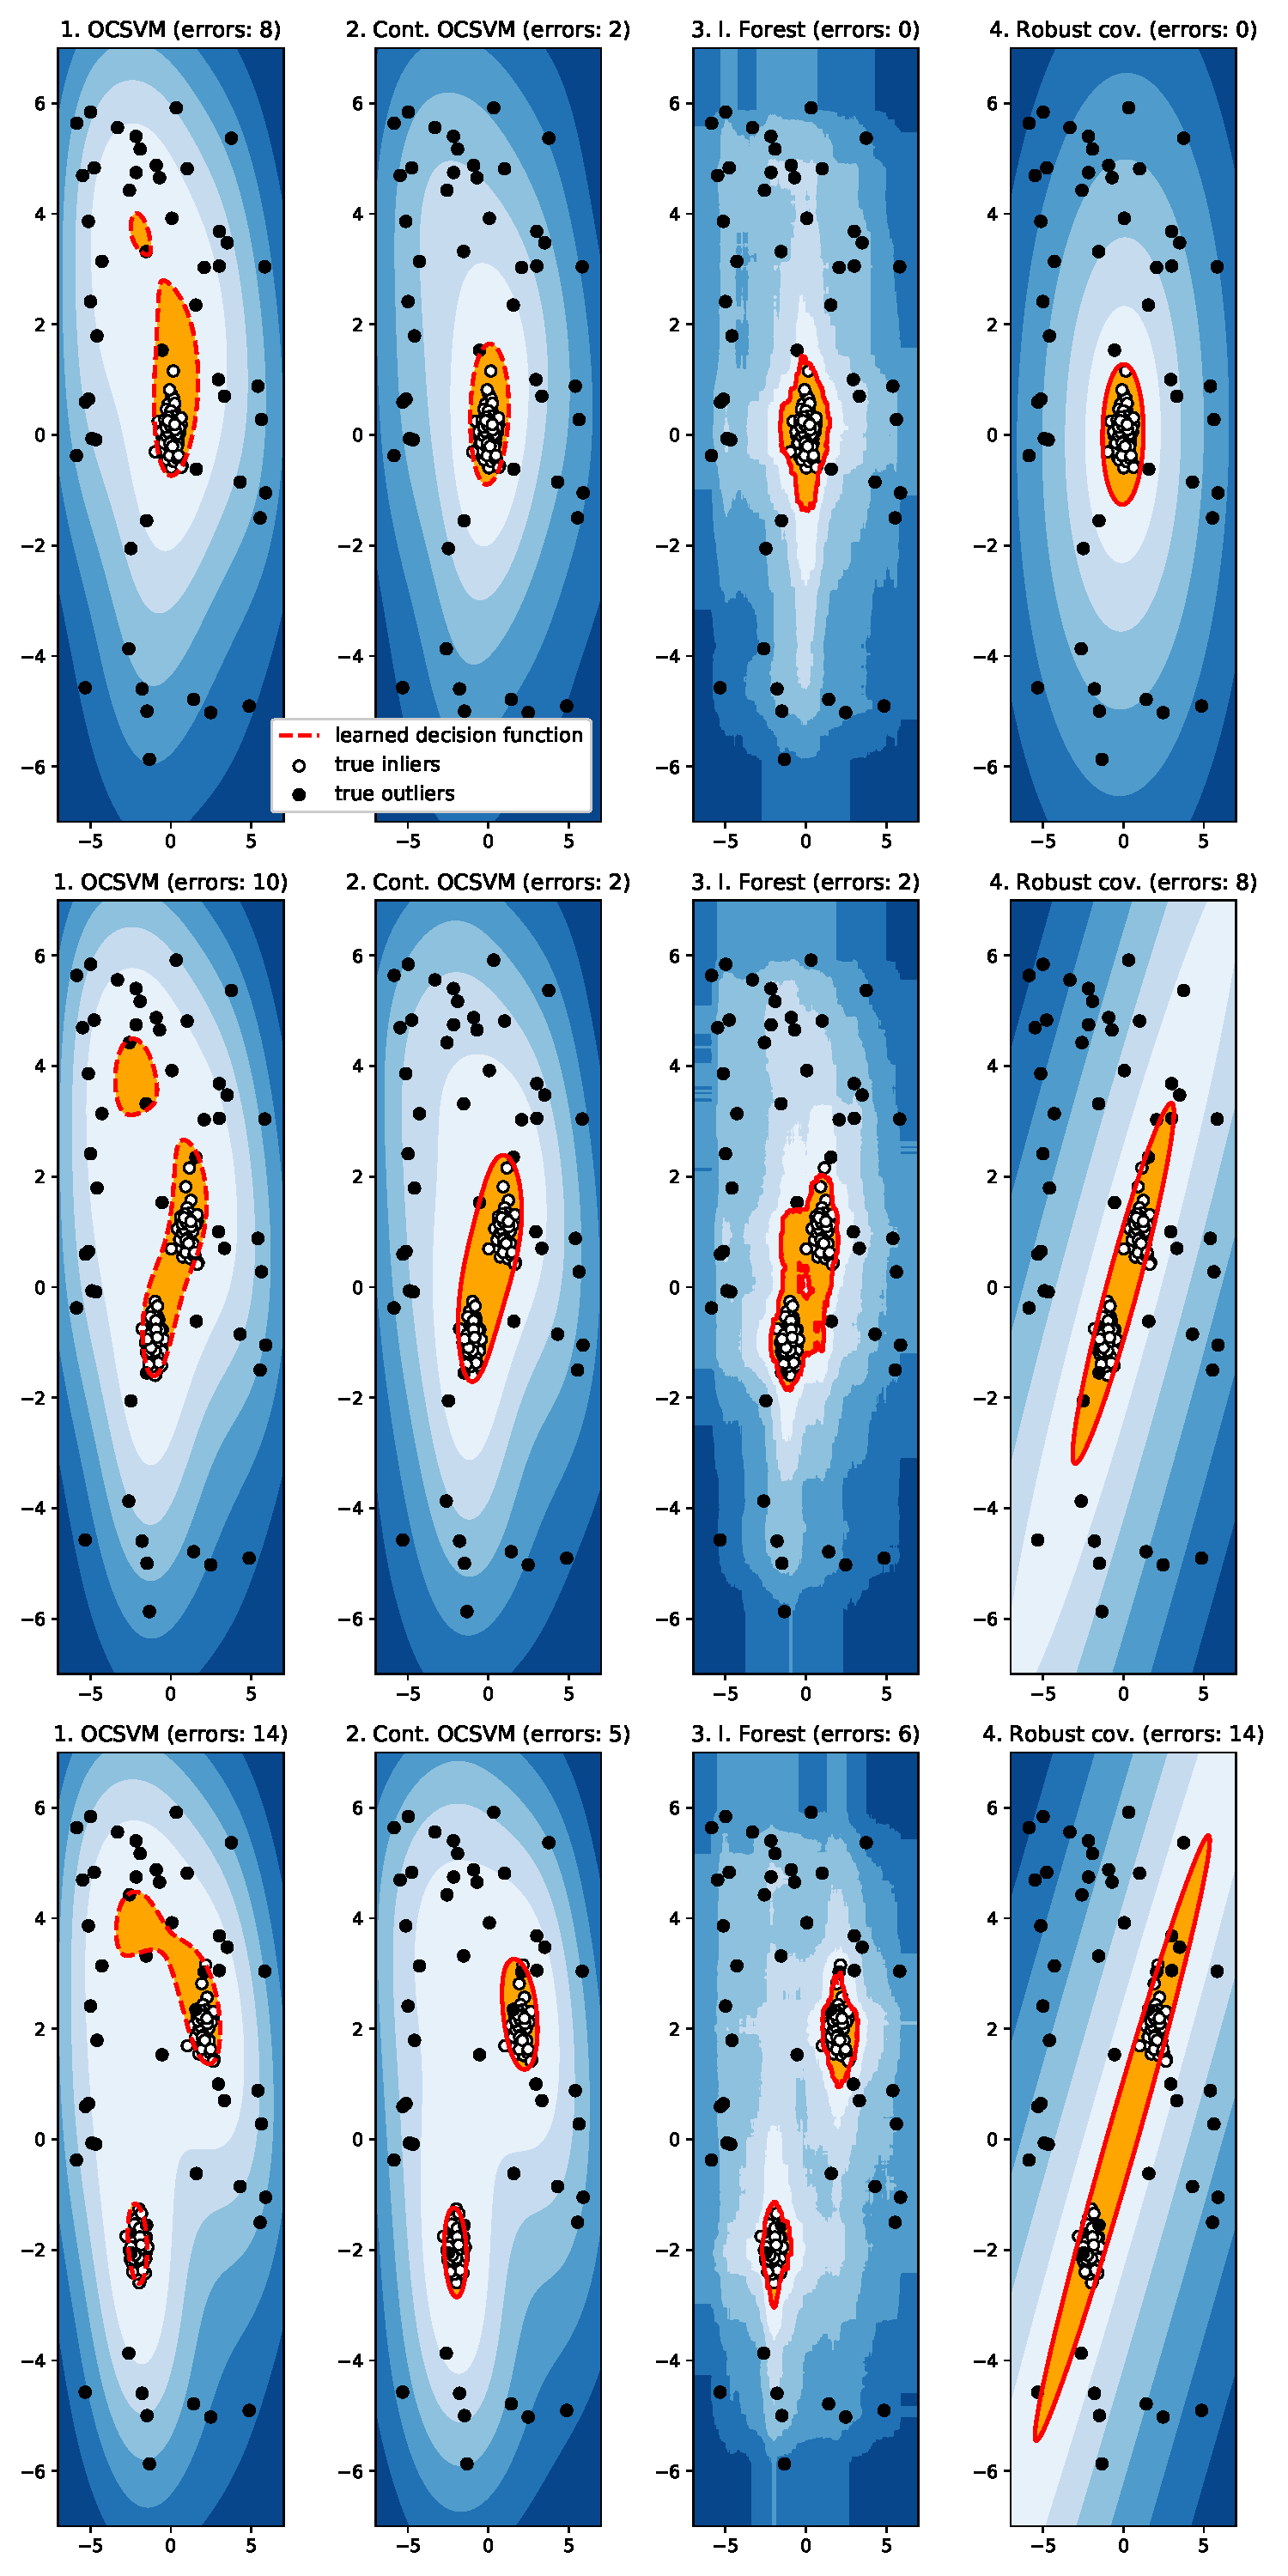
\includegraphics[width=\textwidth]{./gfx/ocsvm.eps}}
    \caption[Continuous OCSVM for outlier detection]{Continuous OCSVM for
    outlier detection. \label{fig:ocsvm_outlier}}
\end{figure}
\paragraph{}
We propose a second experiment in a context of outlier detection. This time
the train set is polluted with outliers. We replicate the example given in
the documentations of Scikit-Learn at
\url{http://scikit-learn.org/stable/auto_examples/covariance/plot_outlier_detection.html}
We compare our method to three other well known outlier detection methods
from the literature: Isolation Forest \citep{Liu2008}, \acs{OCSVM}
\citep{Scholkopf2001} and a Robust Covariance estimator
\citep{campbell1980robust, pedregosa2011scikit} on \cref{fig:ocsvm_outlier}.
Our method achieves the state of the art on this simple example which is
encouraging. However the computation time of our continuous \acs{OCSVM} is
higher than the other methods. It took circa $0.25$ second for the \acs{OCSVM}.
$10$ seconds for our method, $5$ seconds for isolation forest and $0.1$ second
for the Robust covariance estimator. This can be due to the implementation since we used
a (sub-optimal) hand-crafted full gradient descent. Notice that however our
method is able to retrieve all the level sets after training, not only the one
presented in \cref{fig:ocsvm_outlier}.  When one is interested in a specific
level set or range of level set one could sample the $\nu_t$ from another
distribution than the uniform distribution $\mathcal{U}[0, 1]$ to give more
importance to the desired range of level sets.

% %----------------------------------------------------------------------------
% \section{The Nystr\"om method}
% \label{sec:the_nystrom_method}

% %----------------------------------------------------------------------------
% \section{Sub-sampling the data}
% \label{sec:sub_sampling_the_data}

\section{Operalib}
During this Thesis we started the development of a library named \say{Operalib}
implementing various machine learning algorithms based on operator-valued
kernels. We are grateful to Alexandre Gramfort (LTCI, T\'el\'ecom ParisTech)
who served as a technical mentor at the beginning of this software development
and provided many advices.  Operator-valued kernels defines a framework
allowing learning vector/function/structured output.
To install the library it should be as simple as
\begin{lstlisting}[language=bash,caption={Installation of Operalib.}]
pip install operalib
\end{lstlisting}
The library currently features:
\begin{itemize}
    \item Quantile regression \citep{sangnier2016joint},
    \item \acs{ONORMA} \citep{audiffren2013online},
    \item semi-supervised Ridge regression \citep{Brouard2016_jmlr},
    \item some elements of the \acs{ORFF} framework \citep{brault2016random}.
\end{itemize}
The algorithms work for a selection of popular operator-valued kernels such
that the matrix-valued decomposable kernel, the curl-free kernel and the
divergence-free kernel. The library is structured so that it is easy for the
user to define its own operator-valued kernel and plug it to the existing
optimisation algorithms, while keeping efficient computations thanks to the
methodology presented in \cref{subsec:efficient_learning} (\acs{ie} by seeing
operator-valued kernels as operators along with matrix-free solver rather than
plain matrices). We designed the library in order to have a close compatibility
with Scikit-learn. Code and documentation are publicly available at
\url{https://github.com/operalib/operalib}. In a near future we plan to add the
family of works of \citet{Brouard2016_jmlr} around Input Output Kernel
Regression, the  work of \citet{lim2015operator} about the two learning
algorithms defined in \citet{lim2015operator}: a sparse learning of OVK and a
learning algorithm for both kernel and weights with a block coordinate descent
scheme and a proximal gradient method to deal with non-smooth constraints.
Development for modeling time series will be also included. We hope to expand
with more algorithms from various authors of the \acs{OVK} community and
welcome any new contributor!

\chapterend





\chapter{Conclusion}
\bigskip
\begin{justify}
    To conclude this work we would like to summarize our contributions, and
    show how they answered to the initial question of large-scale learning with
    \aclp{OVK}. Then we finish with some short and mid term perspectives.
\end{justify}
\minitoc
\label{ch:conclusion}

\chapterend


\cleardoublepage % Empty page before the start of the next part


%----------------------------------------------------------------------------------------
%	THESIS CONTENT - APPENDICES
%----------------------------------------------------------------------------------------

\appendix

\part{Appendix}
%!TEX root = ../ThesisRomainbrault.tex

\chapter{Miscellaneous}
\label{ch:misc}
\bigskip
\begin{justify}
\end{justify}
\minitoc
%!TEX root = ../../ThesisRomainBrault.tex

\section{Operator-valued functions and integration}

\section{About concentration inequalities}

\section{ORFF Engineering}
\section{Learning with semi-supervision}
We present here an extension of \cref{ch:learning
operator-valued_random_fourier_features} to semi-supervised learning with
\acs{ORFF} in the framework of~\citet{minh2016unifying}. This framework
includes Vector-valued Manifold
Regularization~\citep{belkin2006manifold,Brouard2011,minh2013unifying} and
Co-regularized Multi-view
Learning~\citep{brefeld2006efficient,sindhwani2008rkhs,rosenberg2009kernel,
sun2011multi}.

\subsection{Representer theorem and feature equivalence}
We suppose that we are given a training sample
$\seq{u}=(x_i)_{i=N}^{N+U}\in\mathcal{X}^U$ of unlabeled exemples. We note
$\seq{z}\in\left(\mathcal{X}\times\mathcal{Y}\right)^N\times\mathcal{X}^U$ the
sequence $\seq{z}=\seq{s}\seq{u}$ concatenating both labeled ($\seq{s}$) and
unlabeled ($\seq{u}$) training examples.
\begin{theorem}[Representer theorem, \citet{minh2016unifying}]
    \label{th:representer_semi}
    Let $K$ be a $\mathcal{U}$-Mercer \acl{OVK} and $\mathcal{H}_K$ its
    corresponding $\mathcal{U}$-Reproducing Kernel Hilbert space.
    \paragraph{}
    Let $V:\mathcal{U}\to\mathcal{Y}$ be a bounded linear operator and let
    $c:\mathcal{Y}\times\mathcal{Y}\to\overline{\mathbb{R}}$ be a cost function
    such that $L(x, f, y)=c(Vf(x), y)$ is a proper convex lower semi-continuous
    function in $f$ for all $x\in\mathcal{X}$ and all $y\in\mathcal{Y}$.
    \paragraph{}
    Eventually let $\lambda_K\in\mathbb{R}_{>0}$ and $\lambda_M \in
    \mathbb{R}_+$ be two regularization hyperparameters and
    $(M_{ik})_{i,k=1}^{N+U}$ be a sequence of data dependent bounded linear
    operators in $\mathcal{L}(\mathcal{U})$, such that
    \begin{dmath*}
        \sum_{i,j=1}^{N+U} \inner{u_i, M_{ik}u_k} \ge 0 \condition{$\forall
        (u_i)_{i=1}^{N+U}\in\mathcal{U}^{N+U}$ and $M_{ik}=M_{ki}^*$}.
    \end{dmath*}
    The solution $f_{\seq{z}}\in\mathcal{H}_K$ of the regularized optimization
    problem
    \begin{dmath}
        f_{\seq{z}} = \argmin_{f\in\mathcal{H}_K}
        \frac{1}{N}\displaystyle\sum_{i=1}^N c(Vf(x_i), y_i) +
        \frac{\lambda_K}{2}\norm{f}^2_{K} \\ +
        \frac{\lambda_M}{2}\sum_{i,k=1}^{N+U}\inner{f(x_i),
        M_{ik}f(x_k)}_{\mathcal{U}} \label{eq:learning_rkhs_gen_semi}
    \end{dmath}
    has the form $f_{\seq{z}}=\sum_{j=1}^{N+U}K(\cdot,x_j)u_{\seq{z},j}$ where
    $u_{\seq{z},j}\in\mathcal{U}$ and
    \begin{dmath}
        \label{eq:argmin_u_semi} u_{\seq{z}} =
        \argmin_{u\in\Vect_{i=1}^{N+U}\mathcal{U}}\frac{1}{N}
        \displaystyle\sum_{i=1}^N c\left(V\sum_{k=1}^{N+U}K(x_i,x_j)u_j,
        y_i\right) + \frac{\lambda_K}{2}\sum_{k=1}^{N+U}u_i^\adjoint
        K(x_i,x_k)u_k \\ + \frac{\lambda_M}{2}\sum_{i,k=1}^{N+U}
        \inner*{\sum_{j=1}^{N+U}K(x_i,x_j)u_j,
        M_{ik}\sum_{j=1}^{N+U}K(x_k,x_j)u_j}_{\mathcal{U}}.
    \end{dmath}
\end{theorem}
We present here the proof of the formulation proposed
by~\citet{minh2016unifying}. In the mean time we clarify some elements of the
proof. Indeed the existence of a global minimizer is not trivial and we must
invoke the Mazur-Schauder theorem. Moreover the coercivity of the objective
function required by the Mazur-Schauder theorem is not obvious when we do not
require the cost function to take only positive values. However a corollary of
Hahn-Banach theorem linking strong convexity to coercivity gives the solution.
\begin{proof}
    Since $f(x)=K_x^*f$ (see \cref{eq:reproducing_prop}), the optimization
    problem reads
    \begin{dmath*}
        f_{\seq{z}} = \argmin_{f\in\mathcal{H}_K}
        \frac{1}{N}\displaystyle\sum_{i=1}^N c(VK_{x_i}^\adjoint f, y_i) +
        \frac{\lambda_K}{2}\norm{f}^2_{K} \\ +
        \frac{\lambda_M}{2}\sum_{i,k=1}^{N+U}\inner{K_{x_i}^\adjoint f,
        M_{ik}K_{x_k}^\adjoint f}_{\mathcal{U}}
    \end{dmath*}
    Let $W_{V,\seq{s}}:\mathcal{H}_K\to\Vect_{i=1}^N\mathcal{Y}$ be the 
    restriction linear operator defined as
    \begin{dmath*}
        W_{V,\seq{s}}f = \Vect_{i=1}^N VK_{x_i}^\adjoint f,
    \end{dmath*}
    with $VK_{x_i}^\adjoint:\mathcal{H}_K\to\mathcal{Y}$ and
    $K_{x_i}V^\adjoint:\mathcal{Y}\to\mathcal{H}_K$. Let
    $Y=\vect_{i=1}^Ny_i\in\mathcal{Y}^N$. We have
    \begin{dmath*}
        \inner{Y,W_{V,\seq{s}}f}_{\Vect_{i=1}^N\mathcal{Y}} =
        \sum_{i=1}^N\inner{y_i, VK_{x_i}^\adjoint f}_{\mathcal{Y}}
        \hiderel{=}\sum_{i=1}^N\inner{K_{x_i}V^\adjoint y_i,
        f}_{\mathcal{H}_K}.
    \end{dmath*}
    Thus the adjoint operator $W_{V,\seq{s}}^\adjoint :
    \Vect_{i=1}^N\mathcal{Y}\to\mathcal{H}_K$ is
    \begin{dmath*}
        W_{V,\seq{s}}^\adjoint Y=\sum_{i=1}^NK_{x_i}V^\adjoint y_i,
    \end{dmath*}
    and the operator $W_{V,\seq{s}}^* W_{V,\seq{s}} : \mathcal{H}_K \to
    \mathcal{H}_K$ is
    \begin{dmath*}
        W_{V,\seq{s}}^\adjoint W_{V,\seq{s}}f = \sum_{i=1}^NK_{x_i}V^\adjoint
        VK_{x_i}^\adjoint f
    \end{dmath*}
    where $V^\adjoint V\in\mathcal{L}(\mathcal{U})$. Let
    \begin{dmath*}
        J_{\lambda_K}(f) = \underbrace{\frac{1}{N}\displaystyle\sum_{i=1}^N
        c(Vf(x_i), y_i)}_{=J_c} + \frac{\lambda_K}{2}\norm{f}^2_{K} \\ +
        \underbrace{\frac{\lambda_M}{2}\sum_{i,k=1}^{N+U}\inner{f(x_i),
        M_{ik}f(x_k)}_{\mathcal{U}}}_{=J_M}
    \end{dmath*}
    Since $c$ is proper, lower semi-continuous and
    convex by assumption, thus the term $J_c$ is also proper, lower
    semi-continuous and convex. Moreover the term $J_M$ is always positive for
    any $f\in\mathcal{H}_K$ and $\frac{\lambda_K}{2}\norm{f}^2_{K}$ is strongly
    convex.  Thus $J_{\lambda_K}$ is strongly convex. Apply
    \cref{lm:strongly_convex_is_coercive} to obtain the coercivity of
    $J_{\lambda_K}$, and then \cref{cor:unique_minimizer} to show that
    $J_{\lambda_K}$ has a unique minimizer and is attained. Then let
    \begin{dmath*}
        \mathcal{H}_{K, \seq{z}}=\Set{\sum_{j=1}^{N+U}K_{x_j}u_j| \forall
        (u_i)_{i=1}^{N+U} \in\mathcal{U}^{N+U}}.
    \end{dmath*}
    For $f\in\mathcal{H}_{K, \seq{z}}^\perp$, the operator
    $W_{V,\seq{s}}$ satisfies
    \begin{dmath*}
        \inner{Y, W_{V,\seq{s}}f}_{\Vect_{i=1}^N\mathcal{Y}} =
        \inner{\underbrace{f}_{\in\mathcal{H}_{K, \seq{z}}^\perp},
        \underbrace{\sum_{i=1}^{N+U}K_{x_i}V^\adjoint y_i}_{\in\mathcal{H}_{K,
        \seq{z}}}}_{\mathcal{H}_K} \hiderel{=} 0
    \end{dmath*}
    for all sequences $(y_i)_{i=1}^N$, since $V^\adjoint y_i\in\mathcal{U}$.
    Hence,
    \begin{dmath}
        \label{eq:null1_semi} (Vf(x_i))_{i=1}^{N}=0
    \end{dmath}
    In the same way,
    \begin{dmath*}
        \sum_{i=1}^{N+U}\inner{K_{x_i}^* f, u_i}_{\mathcal{U}} \hiderel{=}
        \inner{\underbrace{f}_{\in\mathcal{H}_{K, \seq{z}}^\perp},
        \underbrace{\sum_{j=1}^{N+U}K_{x_j}u_j}_{\in\mathcal{H}_{K,
        \seq{z}}}}_{\mathcal{H}_K} \hiderel{=} 0.
    \end{dmath*}
    for all sequences $(u_i)_{i=1}^{N+U}\in\mathcal{U}^{N+U}$. As a result,
    \begin{dmath}
        \label{eq:null2_semi} (f(x_i))_{i=1}^{U+N}=0.
    \end{dmath}
    Now for an arbitrary $f\in\mathcal{H_K}$, consider the orthogonal
    decomposition $f = f^{\perp} + f^{\parallel}$, where $f^{\perp} \in
    \mathcal{H}_{K, \seq{z}}^\perp$ and $f^{\parallel} \in \mathcal{H}_{K,
    \seq{z}}$. Then since $\norm{f^{\perp} + f^{\parallel}}_{\mathcal{H}_K}^2
    =\norm{f^{\perp}}_{\mathcal{H}_K}^2 +
    \norm{f^{\parallel}}_{\mathcal{H}_K}^2$, \cref{eq:null1_semi} and
    \cref{eq:null2_semi} shows that if $\lambda_K > 0$, clearly then
    \begin{dmath*}
        J_{\lambda_K}(f)=J_{\lambda_K}\left(f^{\perp}+f^{\parallel}\right)
        \hiderel{\ge} J_{\lambda_K}\left(f^{\parallel}\right)
    \end{dmath*}
    The last inequality holds only when $\norm{f^{\perp}}_{\mathcal{H}_K}=0$,
    that is when $f^{\perp}=0$. As a result since the minimizer of
    $J_{\lambda_K}$is unique and attained, it must lies in $\mathcal{H}_{K,
    \seq{z}}$.
\end{proof}

\begin{theorem}[Feature equivalence]
    \label{th:orff_representer_semi} Let $\tildeK{\omega}$ be an \acl{OVK} such
    that for all $x$, $z\in\mathcal{X}$, $\tildePhi{\omega}(x)^\adjoint
    \tildePhi{\omega}(z) = \widetilde{K}(x,z)$ where $\widetilde{K}$ is a
    $\mathcal{U}$-Mercer \acs{OVK} and $\mathcal{H}_{\tildeK{\omega}}$ its
    corresponding $\mathcal{U}$-Reproducing kernel Hilbert space.
    \paragraph{}
    Let $V:\mathcal{U}\to\mathcal{Y}$ be a bounded linear operator and let
    $c:\mathcal{Y}\times\mathcal{Y}\to\overline{\mathbb{R}}$ be a cost function
    such that $L(x, \widetilde{f}, y)=c(V\widetilde{f}(x), y)$ is a proper
    convex lower semi-continuous function in
    $\widetilde{f}\in\mathcal{H}_{\tildeK{\omega}}$ for all $x\in\mathcal{X}$
    and all $y\in\mathcal{Y}$.
    \paragraph{}
    Eventually let $\lambda_K\in\mathbb{R}_{>0}$ and $\lambda_M \in
    \mathbb{R}_+$ be two regularization hyperparameters and
    $(M_{ik})_{i,k=1}^{N+U}$ be a sequence of data dependent bounded linear
    operators in $\mathcal{L}(\mathcal{U})$, such that
    \begin{dmath*}
        \sum_{i,j=1}^{N+U} \inner{u_i, M_{ik}u_k} \ge 0 \condition{$\forall
        (u_i)_{i=1}^{N+U}\in\mathcal{U}^{N+U}$ and $M_{ik}=M_{ki}^*$}.
    \end{dmath*}
    The solution $f_{\seq{z}}\in\mathcal{H}_{\tildeK{\omega}}$ of the
    regularized optimization problem
    \begin{dmath}
        \label{eq:argmin_RKHS_rand_semi} \widetilde{f}_{\seq{z}} =
        \argmin_{\widetilde{f}\in\mathcal{H}_{\tildeK{\omega}}}
        \frac{1}{N}\displaystyle\sum_{i=1}^N c\left(V\widetilde{f}(x_i),
        y_i\right) +
        \frac{\lambda_K}{2}\norm{\widetilde{f}}^2_{\tildeK{\omega}} \\ +
        \frac{\lambda_M}{2}\sum_{i,k=1}^{N+U}\inner{\widetilde{f}(x_i),
        M_{ik}\widetilde{f}(x_k)}_{\mathcal{U}}
    \end{dmath}
    has the form $\widetilde{f}_{\seq{z}} = \tildePhi{\omega}(\cdot)^\adjoint
    \theta_{\seq{z}}$, where $\theta_{\seq{z}} \in (\Ker
    \tildeW{\omega})^{\perp}$ and
    \begin{dmath}
        \theta_{\seq{z}}=\argmin_{\theta\in \tildeH{\omega}}
        \frac{1}{N}\sum_{i=1}^Nc\left(V\tildePhi{\omega}(x_i)^\adjoint \theta,
        y_i\right) + \frac{\lambda_K}{2}\norm{\theta}^2_{\tildeH{\omega}} \\ +
        \frac{\lambda_M}{2}\sum_{i,k=1}^{N+U}\inner{\theta,
        \tildePhi{\omega}(x_i)M_{ik}\tildePhi{\omega}(x_k)^\adjoint
        \theta}_{\tildeH{\omega}}.
        \label{eq:arming_RKHS_rand_feat}
    \end{dmath}
\end{theorem}
\begin{proof}
    Since $\tildeK{\omega}$ is an operator-valued kernel, from
    \cref{th:representer_semi}, \cref{eq:argmin_RKHS_rand_semi} has a solution
    of the form
    \begin{dmath*}
        \widetilde{f}_{\seq{z}} = \sum_{i=1}^{N+U} \tildeK{\omega}(\cdot,
        x_i)u_i \condition{$u_i \hiderel{\in} \mathcal{U}$, $x_i
        \hiderel{\in}\mathcal{X}$} = \sum_{i=1}^N
        \tildePhi{\omega}(\cdot)^\adjoint \tildePhi{\omega}(x_i)u_i \hiderel{=}
        \tildePhi{\omega}(\cdot)^\adjoint \underbrace{\left(\sum_{i=1}^{N+U}
        \tildePhi{\omega}(x_i) u_i \right)}_{= \theta \in \left( \Ker
        \tildeW{\omega}\right)^\perp \subset \tildeH{\omega}}.
    \end{dmath*}
    Let
    \begin{dmath*}
        \label{eq:argmin_theta_semi}
        \theta_{\seq{z}}=\argmin_{\theta\in\left(\Ker
        \tildeW{\omega}\right)^\perp}
        \frac{1}{N}\sum_{i=1}^Nc\left(V\tildePhi{\omega}(x_i)^\adjoint \theta,
        y_i\right) + \frac{\lambda_K}{2}
        \norm{\tildePhi{\omega}(\cdot)^\adjoint \theta}^2_{\tildeK{\omega}} \\
        + \frac{\lambda_M}{2} \sum_{i,k=1}^{N+U}
        \inner*{\tildePhi{\omega}(x_i)^\adjoint \theta,
        M_{ik}\tildePhi{\omega}(x_k)^\adjoint \theta}_{\mathcal{U}}.
    \end{dmath*}
    Since $\theta\in(\Ker \tildeW{\omega})^\perp$ and $W$ is an isometry from
    $(\Ker \tildeW{\omega})^\perp\subset \tildeH{\omega}$ onto
    $\mathcal{H}_{\tildeK{\omega}}$, we have
    $\norm{\tildePhi{\omega}(\cdot)^\adjoint\theta}^2_{\tildeK{\omega}} =
    \norm{\theta}^2_{\tildeH{\omega}}$. Hence
    \begin{dmath*}
        \theta_{\seq{z}}=\argmin_{\theta\in\left(\Ker
        \tildeW{\omega}\right)^\perp}
        \frac{1}{N}\sum_{i=1}^Nc\left(V\tildePhi{\omega}(x_i)^\adjoint \theta,
        y_i\right) + \frac{\lambda_K}{2}\norm{\theta}^2_{\tildeH{\omega}} \\ +
        \frac{\lambda_M}{2} \sum_{i,k=1}^{N+U}
        \inner{\tildePhi{\omega}(x_i)^\adjoint \theta,
        M_{ik}\tildePhi{\omega}(x_k)^\adjoint \theta}_{\mathcal{U}}.
    \end{dmath*}
    Finding a minimizer $\theta_{\seq{z}}$ over $\left(\Ker
    \tildeW{\omega}\right)^\perp$ is not the same as finding a minimizer over
    $\tildeH{\omega}$. Although in both cases Mazur-Schauder's theorem
    guarantees that the respective minimizers are unique, they might not be the
    same. Since $\tildeW{\omega}$ is bounded, $\Ker \tildeW{\omega}$ is closed,
    so that we can perform the decomposition $\tildeH{\omega}=\left(\Ker
    \tildeW{\omega}\right)^\perp\oplus \left(\Ker \tildeW{\omega}\right)$. Then
    clearly by linearity of $W$ and the fact that for all
    $\theta^{\parallel}\in\Ker \tildeW{\omega}$,
    $\tildeW{\omega}\theta^{\parallel}=0$, if $\lambda > 0$ we have
    \begin{dmath*}
        \theta_{\seq{z}}=\argmin_{\theta\in\tildeH{\omega}}
        \frac{1}{N}\sum_{i=1}^Nc\left(V\tildePhi{\omega}(x_i)^\adjoint \theta,
        y_i\right) + \frac{\lambda_K}{2}\norm{\theta}^2_{\tildeH{\omega}} \\ +
        \frac{\lambda_M}{2} \sum_{i,k=1}^{N+U}
        \inner*{\tildePhi{\omega}(x_i)^\adjoint \theta,
        M_{ik}\tildePhi{\omega}(x_k)^\adjoint \theta}_{\mathcal{U}}
    \end{dmath*}
    Thus
    \begin{dmath*}
        \theta_{\seq{z}}
        =\argmin_{\substack{\theta^{\perp}\in\left(\Ker
        \tildeW{\omega}\right)^\perp, \\ \theta^{\parallel}\in\Ker
        \tildeW{\omega}}} \frac{1}{N} \sum_{i=1}^N c\left(V \left(
        \tildeW{\omega} \theta^{\perp} \right)(x) + \underbrace{V \left(
        \tildeW{\omega} \theta^{\parallel} \right)(x)}_{=0 \enskip \text{for
        all}\enskip \theta^{\parallel} }, y_i\right) \\ +
        \frac{\lambda_K}{2}\norm{\theta^\perp}^2_{\tildeH{\omega}} +
        \underbrace{\frac{\lambda_K}{2} \norm{\theta^{\parallel} }^2_{%
        \tildeH{\omega}} }_{=0 \enskip\text{only if}\enskip
        \theta^{\parallel}=0} \\ + \frac{\lambda_M}{2} \sum_{i,k=1}^{N+U}
        \inner*{\tildePhi{\omega}(x_i)^\adjoint \theta^{\perp},
        M_{ik}\left(\tildeW{\omega}\theta^{\perp}\right)(x_k)}_{\mathcal{U}} \\
        + \frac{\lambda_M}{2} \sum_{i,k=1}^{N+U} \inner*{\underbrace{\left(
        \tildeW{\omega} \theta^{\parallel} \right)(x_i)}_{=0 \enskip \text{for
        all} \enskip \theta^{\parallel} },
        M_{ik}\left(\tildeW{\omega}\theta^{\perp}\right)(x_k)}_{\mathcal{U}} \\
        + \frac{\lambda_M}{2} \sum_{i,k=1}^{N+U} \inner*{\left( \tildeW{\omega}
        \theta^{\perp} \right)(x_i), M_{ik}\underbrace{\left( \tildeW{\omega}
        \theta^{\parallel} \right)(x_k)}_{=0 \enskip \text{for all}\enskip
        \theta^{\parallel} }}_{\mathcal{U}} \\ + \frac{\lambda_M}{2}
        \sum_{i,k=1}^{N+U} \inner*{\underbrace{\left( \tildeW{\omega}
        \theta^{\parallel} \right)(x_i)}_{=0 \enskip \text{for all} \enskip
        \theta^{\parallel} }, M_{ik}\underbrace{\left( \tildeW{\omega}
        \theta^{\parallel} \right)(x_k)}_{=0 \enskip \text{for all} \enskip
        \theta^{\parallel} }}_{\mathcal{U}}.
    \end{dmath*}
    Thus
    \begin{dmath*}
        \theta_{\seq{z}}=\argmin_{\theta^{\perp}\in\left(\Ker
        \tildeW{\omega}\right)^\perp}
        \frac{1}{N}\sum_{i=1}^Nc\left( V \left( \tildeW{\omega} \theta^{\perp}
        \right)(x), y_i \right) + \frac{\lambda_K}{2}
        \norm{\theta^\perp}^2_{\tildeH{\omega}} \\ + \frac{\lambda_M}{2}
        \sum_{i,k=1}^{N+U} \inner*{\tildePhi{\omega}(x_i)^\adjoint
        \theta^{\perp}, M_{ik}\left( \tildeW{\omega} \theta^{\perp}
        \right)(x_k)}_{\mathcal{U}}.
    \end{dmath*}
    Hence minimizing over $\left(\Ker \tildeW{\omega}\right)^\perp$ or
    $\tildeH{\omega}$ is the same when $\lambda_K > 0$. Eventually,
    % Eventually for any outcome of $\omega_j \sim
    % \probability_{\dual{\Haar},\rho}$ \ac{iid},
    \begin{dmath*}
        \theta_{\seq{z}}=\argmin_{\theta\in\tildeH{\omega}}
        \frac{1}{N}\sum_{i=1}^Nc\left(V\tildePhi{\omega}(x_i)^\adjoint \theta,
        y_i\right) + \frac{\lambda_K}{2}\norm{\theta}^2_{\tildeH{\omega}} \\ +
        \frac{\lambda_M}{2} \sum_{i,k=1}^{N+U
        }\inner*{\tildePhi{\omega}(x_i)^\adjoint\theta, M_{ik}
        \tildePhi{\omega}(x_k)^\adjoint \theta}_{\mathcal{U}} =\argmin_{\theta
        \in \tildeH{\omega}} \frac{1}{N} \sum_{i=1}^Nc
        \left(V\tildePhi{\omega}(x_i)^\adjoint\theta, y_i\right) +
        \frac{\lambda_K}{2}\norm{\theta}^2_{\tildeH{\omega}} \\ +
        \frac{\lambda_M}{2} \sum_{i,k=1}^{N+U} \inner*{\theta,
        \tildePhi{\omega}(x_i)M_{ik} \tildePhi{\omega}(x_k)^\adjoint
        \theta}_{\tildeH{\omega}}. \qed
    \end{dmath*}
\end{proof}
This theorem is illustrated by \cref{fig:representer_semi}. We use the classic
two moons dataset\footnote{Available at
\url{http://scikit-learn.org/stable/modules/generated/sklearn.datasets.make_moons.html}.}.
We first perform an unsupervised spectral clustering step
\cite{von2007tutorial} and construct the matrix where $C_{ik}$ is $1$ if $x_i$
and $x_k$ are in the same cluster, 0 otherwise. Then we take the inverse
Laplacian of this matrix and use it as the data dependent operator $M$. E
\begin{figure}
    \centering
    %\resizebox{\textwidth}{!}{\input{./gfx/representer_twomoons.eps}}
    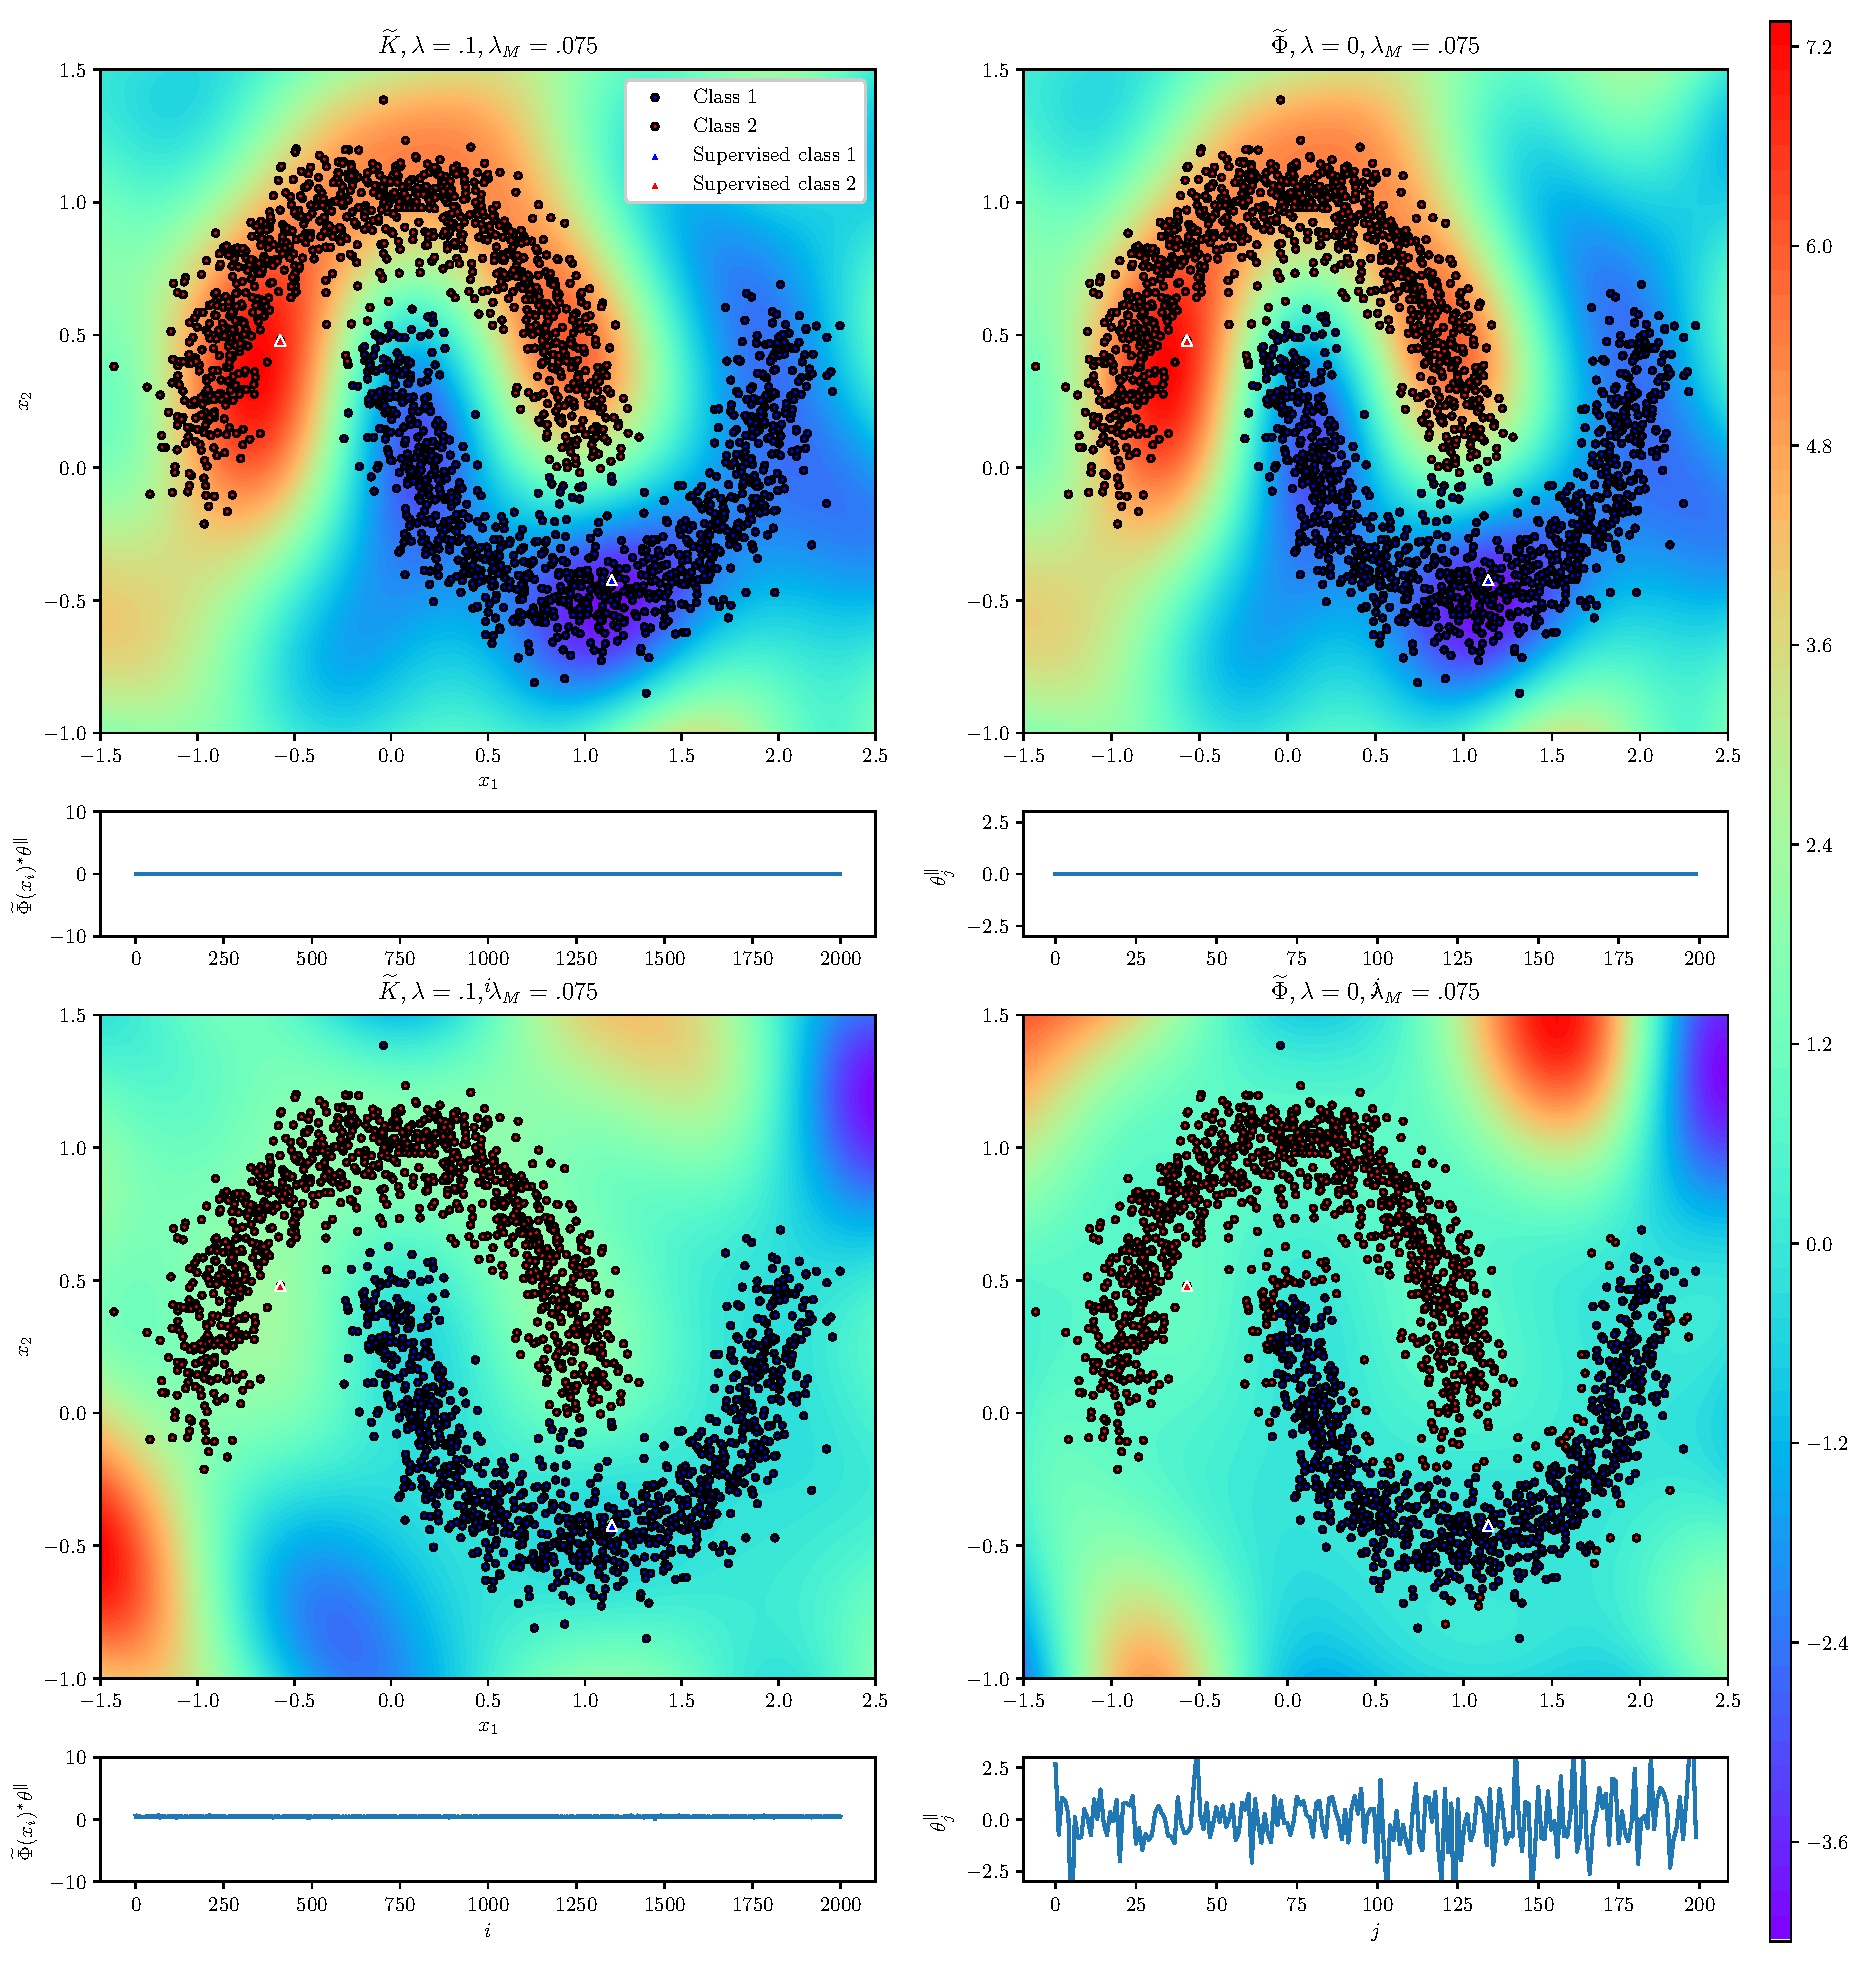
\includegraphics[width=\textwidth]{./gfx/representer_twomoons.eps}
    \caption[\acs{ORFF} equivalence theorem (semi-supervised)]{\acs{ORFF}
    equivalence theorem (semi-supervised). Each row compares the scalar
    \acs{ORFF} $\widetilde{\Phi}$ method constructed from a Gaussian with the
    kernel method where $\widetilde{K}=\widetilde{\Phi}^\transpose
    \widetilde{\Phi}$.  The top row corresponds to the case $\lambda_K=0.1$ and
    $\lambda_M=0.075$.  Since $\lambda_K > 0$, the solution with
    $\widetilde{K}$ and $\widetilde{\Phi}$ are exactly the same
    (\cref{th:orff_representer_semi} applies) and we see that
    $\theta^\parallel=0$. The bottom row corresponds to the case $\lambda_K=0$
    and $\lambda_M=0.075$. Here the solution with $\widetilde{K}$ and
    $\widetilde{\Phi}$ doesn't match (\cref{th:orff_representer_semi} fails to
    apply since $\lambda_K=0$).  Moreover we can see that $\theta^\parallel
    \neq 0$ and $\tildePhi{\omega}(x)^\adjoint \theta \neq 0$, thus $\theta$
    is not in $(\Ker W)^\perp$. \label{fig:representer_semi}}
\end{figure}

\subsection{Gradients}
By linearity and applying the chaine rule to \cref{eq:argmin_theta_semi} and
since $M_{ik}^\adjoint = M_{ki}$ for all $i$, $k\in\mathbb{N}^*_{N+U}$, we have
\begin{dgroup*}
    \begin{dmath*}
        \nabla_{\theta}c\left(V\tildePhi{\omega}(x_i)^\adjoint \theta,
        y_i\right)= \tildePhi{\omega}(x_i)V^\adjoint
        \left(\lderivativeat{c\left(y,
        y_i\right)}{y}{V\tildePhi{\omega}(x_i)^\adjoint
        \theta}\right)^\adjoint,
    \end{dmath*}
    \begin{dmath*}
        \nabla_{\theta}\inner*{\tildePhi{\omega}(x_i)^\adjoint \theta,
        M_{ik}\tildePhi{\omega}(x_k)^\adjoint \theta}_{\mathcal{U}} =
        \tildePhi{\omega}(x_i)\left(M_{ik}+M_{ki}^*\right)
        \tildePhi{\omega}(x_k)^\adjoint \theta,
    \end{dmath*}
    \begin{dmath*}
        \nabla_{\theta}\norm{\theta}^2_{\tildeH{\omega}}=2\theta.
    \end{dmath*}
\end{dgroup*}
Provided that $c(y,y_i)$ is Frechet differentiable \acs{wrt}~$y$, for all $y$
and $y_i\in\mathcal{Y}$ we have $\nabla_{\theta} J_{\lambda_K}(\theta) \in
\tildeH{\omega}$ and
\begin{dmath*}
    \nabla_{\theta} J_{\lambda_K}(\theta) = \frac{1}{N}\sum_{i=1}^N
    \tildePhi{\omega}(x_i)V^\adjoint \left(\lderivativeat{c\left(y,
    y_i\right)}{y}{V\tildePhi{\omega}(x_i)^\adjoint \theta}\right)^\adjoint +
    \lambda_K\theta + \lambda_M\sum_{i,k=1}^{N+U} \tildePhi{\omega}(x_i)M_{ik}
    \tildePhi{\omega}(x_k)^\adjoint \theta
\end{dmath*}
Therefore after factorization, considering $\lambda_K > 0$,
\begin{dmath*}
    \nabla_{\theta} J_{\lambda_K}(\theta)
    = \frac{1}{N}\sum_{i=1}^N \tildePhi{\omega}(x_i)V^\adjoint
    \left(\lderivativeat{c\left(y,
    y_i\right)}{y}{V\tildePhi{\omega}(x_i)^\adjoint \theta}\right)^\adjoint +
    \lambda_K\left(I_{\tildeH{\omega}} + \frac{\lambda_M}{\lambda_K}
    \sum_{i,k=1}^{N+U} \tildePhi{\omega}(x_i)M_{ik}
    \tildePhi{\omega}(x_k)^\adjoint \right)\theta
\end{dmath*}
We note the quantity
\begin{dmath}
    \widetilde{\mathbf{M}}_{\left(\lambda_K,\lambda_M\right)}
    = I_{\tildeH{\omega}} + \frac{\lambda_M}{\lambda_K}\sum_{i,k=1}^{N+U}
    \tildePhi{\omega}(x_i) M_{ik} \tildePhi{\omega}(x_k)^\adjoint \hiderel{\in}
    \mathcal{L}(\tildeH{\omega})
\end{dmath}
so that
\begin{dmath}
    \label{eq:grad_final_semi}
    \nabla_{\theta} J_{\lambda_K}(\theta)
    = \frac{1}{N}\sum_{i=1}^N \tildePhi{\omega}(x_i)V^\adjoint
    \left(\lderivativeat{c\left(y,
    y_i\right)}{y}{V\tildePhi{\omega}(x_i)^\adjoint \theta}\right)^\adjoint +
    \lambda_K\widetilde{\mathbf{M}}_{\left(\lambda_K,\lambda_M\right)}\theta
\end{dmath}
\begin{example}[Naive closed form for the squared error cost]
    Consider the cost function defined for all $y$, $y'\in\mathcal{Y}$ by
    $c(y,y')=\frac{1}{2}\norm{y-y}_{\mathcal{Y}}^2$. Then
    \begin{dmath*}
        \left(\lderivativeat{c\left(y,
        y_i\right)}{y}{V\tildePhi{\omega}(x_i)^\adjoint \theta}\right)^\adjoint
        = \left(V\tildePhi{\omega}(x_i)^\adjoint \theta-y_i\right).
    \end{dmath*}
    Thus, since the optimal solution $\theta_{\seq{z}}$ verifies
    $\nabla_{\theta_{\seq{z}}} J_{\lambda_K}(\theta_{\seq{z}}) = 0$ we have
    \begin{dmath*}
        \frac{1}{N}\sum_{i=1}^N
        \tildePhi{\omega}(x_i)V^\adjoint\left(V\tildePhi{\omega}(x_i)^\adjoint
        \theta_{\seq{z}}-y_i\right) + \lambda_K
        \widetilde{\mathbf{M}}_{\left(\lambda_K,\lambda_M\right)}
        \theta_{\seq{z}}= 0.
    \end{dmath*}
    Therefore,
    \begin{dmath}
        \label{eq:iff_solution_semi} \left(\frac{1}{N}\sum_{i=1}^N
        \tildePhi{\omega}(x_i)V^\adjoint V \tildePhi{\omega}(x_i)^\adjoint +
        \lambda_K \widetilde{\mathbf{M}}_{\left(\lambda_K,
        \lambda_M\right)}\right) \theta_{\seq{z}}
        = \frac{1}{N}\sum_{i=1}^N \tildePhi{\omega}(x_i)V^\adjoint y_i.
    \end{dmath}
    Suppose that $\mathcal{Y}\subseteq\mathbb{R}^p$,
    $V:\mathcal{U}\to\mathcal{Y}$ where $\mathcal{U}\subseteq\mathbb{R}^u$ and
    for all $x\in\mathcal{X}$, $\tildePhi{\omega}(x):
    \mathbb{R}^{r}\to\mathbb{R}^u$ where all spaces are endowed with the
    euclidean inner product. From this we can derive \cref{alg:close_form_semi}
    which returns the closed form solution of \cref{eq:cost_functional} for
    $c(y,y')=\frac{1}{2}\norm{y-y'}_2^2$.
\end{example}
\afterpage{%
\begin{center}
    \begin{algorithm2e}[H]
        \label{alg:close_form_semi}
        \SetAlgoLined
        \Input{\begin{itemize}
            \item $\seq{s}=(x_i,
            y_i)_{i=1}^N\in\left(\mathcal{X}\times\mathbb{R}^p\right)^N$ a
            sequence of supervised training points,
            \item $\seq{u}=(x_i)_{i=N+1}^{N+U}\in\mathcal{X}^{U}$ a sequence of
            unsupervised training points,
            \item $\tildePhi{\omega}(x_i) \in \mathcal{L}\left(\mathbb{R}^u,
            \mathbb{R}^{r}\right)$ a feature map defined for all
            $x_i\in\mathcal{X}$,
            \item $(M_{ik})_{i,k=1}^{N+U}$ a sequence of data dependent
            operators (see \cref{th:orff_representer_semi}),
            \item $V \in \mathcal{L}\left(\mathbb{R}^u, \mathbb{R}^p\right)$ a
            combination operator, \item $\lambda_K \in\mathbb{R}_{>0}$ the
            Tychonov regularization term,
            \item $\lambda_M \in\mathbb{R}_+$ the manifold regularization term.
        \end{itemize}}
        \Output{A model %
        \begin{dmath*} %
            h:\begin{cases} \mathcal{X} \to \mathbb{R}^p \\
            x\mapsto\tildePhi{\omega}(x)^\transpose
            \theta_{\seq{z}},\end{cases} %
        \end{dmath*} %
        such that $\theta_{\seq{z}}$ minimize \cref{eq:cost_functional}, where
        $c(y,y')=\norm{y-y'}_2^2$ and $\mathbb{R}^u$, $\mathbb{R}^r$ and
        $\mathbb{R}^p$ are Hilbert spaces endowed with the euclidean inner
        product.}
        $\mathbf{P} \gets \frac{1}{N}\sum_{i=1}^N
        \tildePhi{\omega}(x_i)V^\transpose  V\tildePhi{\omega}(x_i)^\transpose
        \in\mathcal{L}(\mathbb{R}^{r}, \mathbb{R}^{r})  $\;
        \uIf{$\lambda_M = 0$}{%
            $\widetilde{\mathbf{M}}_{\left(\lambda_K,\lambda_M\right)} \gets
            I_{r} \in\mathcal{L}(\mathbb{R}^{r}, \mathbb{R}^{r})$\;
        }
        \Else{%
            $\widetilde{\mathbf{M}}_{\left(\lambda_K,\lambda_M\right)} \gets
            \left(I_{r} +
            \frac{\lambda_M}{\lambda_K} \sum_{i,k=1}^{N+U}
            \tildePhi{\omega}(x_i) M_{ik} \tildePhi{\omega}(x_k)^\transpose
            \right) \in\mathcal{L}(\mathbb{R}^{r}, \mathbb{R}^{r}) $\;
        }
        $\mathbf{Y} \gets \frac{1}{N}\sum_{i=1}^N
        \tildePhi{\omega}(x_i)V^\transpose  y_i \in \mathbb{R}^{r} $\;
        $\theta_{\seq{z}} \gets \text{solve}_{\theta}\left(\left(\mathbf{P} +
        \lambda_K\widetilde{\mathbf{M}}_{\left(\lambda_K,
        \lambda_M\right)}\right)\theta = \mathbf{Y}\right) \in \mathbb{R}^{r}
        $\;
        \Return $h: x \mapsto \tildePhi{\omega}(x)^\transpose
        \theta_{\seq{z}}$\;
        \caption{Naive closed form for the squared error cost.}
    \end{algorithm2e}
\end{center}}
\begin{figure}
    \centering
    %\resizebox{\textwidth}{!}{\input{./gfx/representer_twomoons.eps}}
    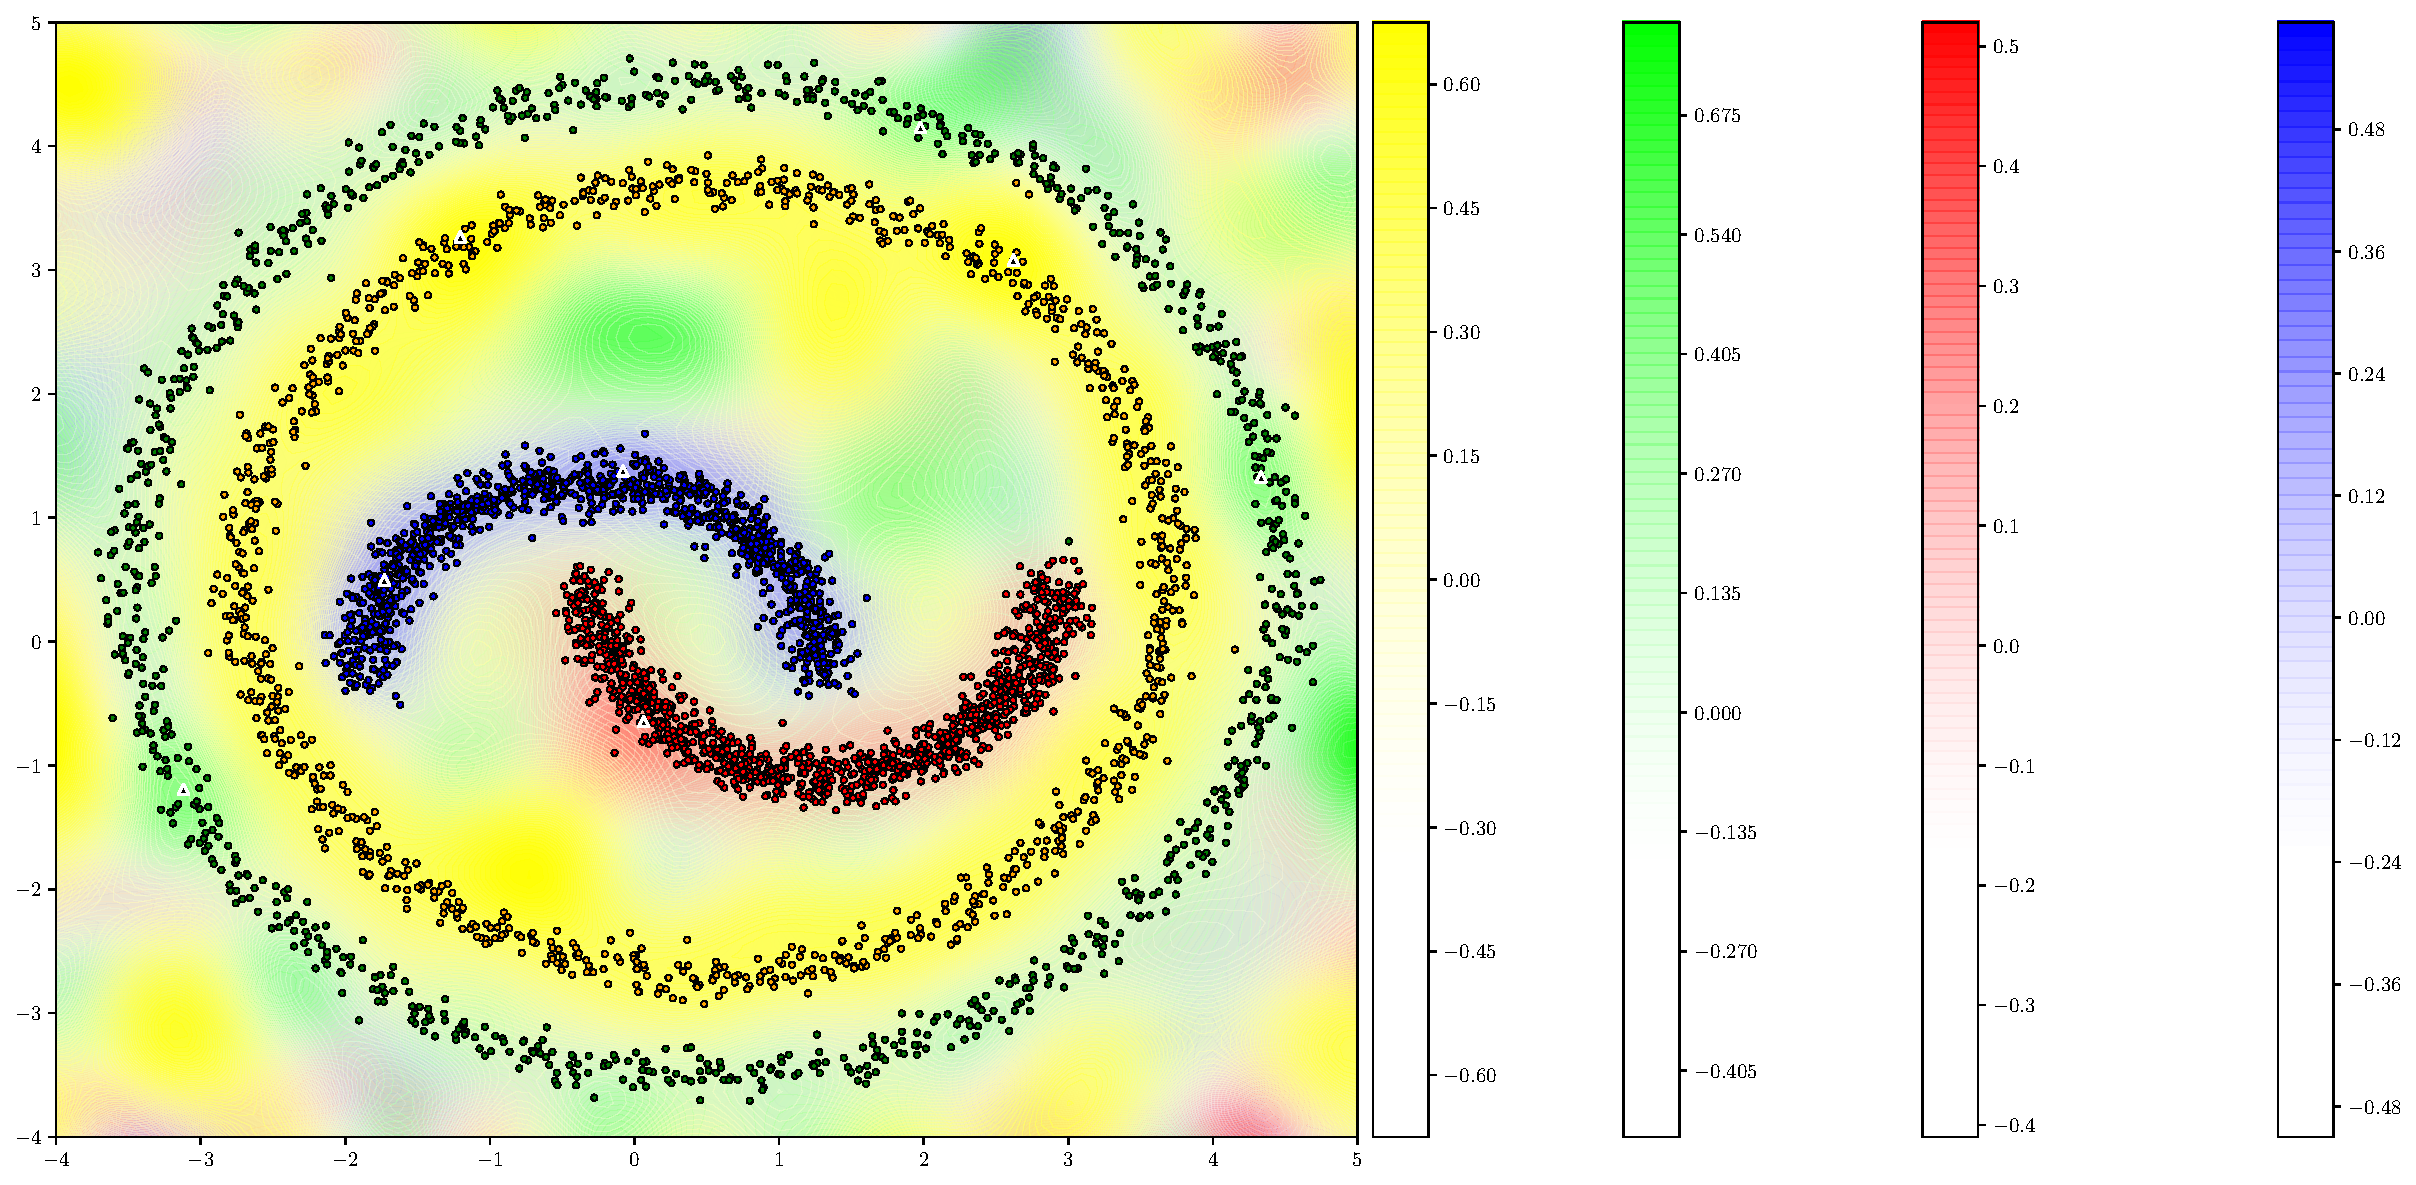
\includegraphics[width=\textwidth]{./gfx/nestedtwomoons.pdf}
    \caption[\acs{ORFF} multiclass semi-supervised]{Semi-supervised learning
    on a multiclass nested circle and two moons dataset. We performed an 
    unsupervised spectral clustering \citep{von2007tutorial} step to construc
    the matrices $M_{ik}$'s and, choose the matrix $B$ of the \acs{ORFF} using
    the simplex coding \citep{mroueh2012multiclass}.}
\end{figure}
\subsection{Complexity}
Suppose that $u=\dim(\mathcal{U})<+\infty$ and
$u'=\dim(\mathcal{U}')<\infty$ and for all $x\in\mathcal{X}$,
$\tildePhi{\omega}(x):\mathcal{U}'\to\tildeH{\omega}$ where
$r=\dim(\tildeH{\omega})<\infty$ is the dimension of the redescription space
$\tildeH{\omega}=\mathbb{R}^{r}$. Since $u$, $u'$, and $r<\infty$, we view the
operators $\tildePhi{\omega}(x)$, $V$ and
$\widetilde{\mathbf{M}}_{\left(\lambda_K,\lambda_M\right)}$ as matrices.
Computing $V^\adjoint V$ cost $O_t(u^2p)$. Step 1 costs $O_t(r^2u + ru^2)$.
Steps 5 (optional) has the same cost except that the sum is done over all pair
of $N+U$ points thus it costs $O_t((N+U)^2(r^2u + r u^2))$. Steps 7 costs
$O_t(N(ru + up))$. For step 8, the naive inversion of the operator costs
$O_t(r^3)$. Eventually the overall complexity of \cref{alg:close_form_semi} is
\begin{dmath*}
    O_t\left(ru(r + u) \begin{cases} (N+U)^2 & \text{if $\lambda_M > 0$} \\ N &
    \text{if $\lambda_M = 0$} \end{cases}+ r^3 + Nu(r+p) \right),
\end{dmath*}
while the space complexity is $O_s(r^2)$. This complexity is to compare with
the kernelized solution proposed by~\citet{minh2016unifying}. Let
\begin{dmath*}
    \mathbf{K}:
    \begin{cases}
        \mathcal{U}^{N+U} \to \mathcal{U}^{N+U} \\
        u\mapsto\Vect_{i=1}^{N+U}\sum_{j=1}^{N+U}K(x_i, x_j)u_j
    \end{cases}
\end{dmath*}
and
\begin{dmath*}
    \mathbf{M}:
    \begin{cases}
        \mathcal{U}^{N+U} \to \mathcal{U}^{N+U} \\
        u\mapsto\Vect_{i=1}^{N+U}\sum_{k=1}^{N+U}M_{ik}u_k.
    \end{cases}
\end{dmath*}
When $\mathcal{U}=\mathbb{R}$,
\begin{dmath*}
    \mathbf{K}=
    \begin{pmatrix} K(x_1, x_1) & \hdots & K(x_1, x_{N+U}) \\ \vdots
        & \ddots & \vdots \\  K(x_{N+U}, x_1) & \hdots & K(x_{N+U}, x_{N+U})
    \end{pmatrix}
\end{dmath*}
is called the Gram matrix of $K$. When $\mathcal{U}=\mathbb{R}^p$, $\mathbf{K}$
is a matrix-valued Gram matrix of size $u(N+U)\times u(N+U)$ where each entry
$\mathbf{K}_{ij}\in\mathcal{M}_{u,u}(\mathbb{R})$. When
$\mathcal{U}=\mathbb{R}^u$, $\mathbf{M}$ can also be seen as a matrix-valued
matrix where each entry is $M_{ik}\in\mathcal{M}_{u,u}(\mathbb{R})$. We also
introduce the matrices $\mathbf{V}^\transpose  \mathbf{V}\colonequals I_{N+U}
\otimes (V^\transpose  V)$ and
\begin{dmath*}
    \mathbf{P}:
    \begin{cases}
        \mathcal{U}^{N+U} \to \mathcal{U}^{N+U} \\ u\mapsto
        \left(\Vect_{j=1}^Nu_j\right) \oplus \left(\Vect_{j=N+1}^{N+U}0\right)
    \end{cases}
\end{dmath*}
The operator $\mathbf{P}$ is a projection that sets all the terms $u_j$, $N < j
\le N + U$ of $u$ to zero. When $\mathcal{U}=\mathbb{R}^u$ it can also be seen
as the block matrix of size $u(N+U) \times u(N + U)$ and
\begin{dmath*}
    \mathbf{P}=
    \begin{pmatrix}
        & & & 0 & \hdots & 0 \\ & I_u \otimes I_{N} & & \vdots & \ddots &
        \vdots \\ & & & 0 & \hdots & 0 \\ 0 & \hdots & 0 & 0 & \hdots & 0 \\
        \vdots & \ddots & \vdots & \vdots & \ddots & \vdots \\ 0 & \hdots & 0 &
        0 & \hdots & 0
    \end{pmatrix}
\end{dmath*}
Then the equivalent kernelized solution $u_{\seq{z}}$ of
\cref{th:representer_semi} is given by~\citet{minh2016unifying}
\begin{dmath*}
    \left(\frac{1}{N}\mathbf{V}^\transpose  \mathbf{V} \mathbf{P} \mathbf{K} +
    \lambda_M \mathbf{M} \mathbf{K} + \lambda_K
    I_{\Vect_{i=1}^{N+U}\mathcal{U}}\right)u_{\seq{z}}=\left(\Vect_{i=1}^N
    V^\transpose  y_i\right) \oplus \left(\Vect_{i=N+1}^{N+U} 0 \right).
    \end{dmath*}
which has time complexity $O_t(((N+U)u)^3+ Nup)$ and space complexity
$O_s(((N+U)u)^2)$. Notice that computing the
data dependent norm (manifold regularization) is expensive. Indeed when
$\lambda_M=0$, \cref{alg:close_form_semi} has a linear complexity with respect
to the number of supervised training points $N$ while the complexity becomes
quadratic in the number of supervised and unsupervised training points $N+U$
when $\lambda_M>0$.



\chapter{Proofs of theorems}
\label{ch:proof_of_theorems}
\bigskip
\begin{justify}
In this appendix we detail the proofs of \cref{corr:unbounded_consistency} and
\cref{corr:bounded_infinite_dim_consistency}. These two corollaries applying on
compact subsets of Banach spaces are the consequences of more generic
propositions (\cref{pr:bound_approx_unbounded} and \cref{pr:bound_approx_bounded})
working on any compact subsets of Polish spaces. Eventually we give a proof on
the variance bound given in \cref{pr:variance_bound}.
\end{justify}
\minitoc
%!TEX root = ../../ThesisRomainbrault.tex

\section{Proof of the error bound with high probability of the ORFF
estimator}
\label{subsec:concentration_proof}
We recall the notations $\delta=x\groupop z^{-1}$, for all $x$,
$z\in\mathcal{X}$,
$\tilde{K} (x,z) = {\tildePhi{\omega} (x)}^\adjoint \tildePhi{\omega} (z)$,
$\tilde{K}^j (x,z) = {\Phi_x (\omega_j)}^\adjoint \Phi_z (\omega_j)$, where
$\omega_j\sim\probability_{\dual{\Haar,\rho}}$ and $K_e (\delta)=K(x,z)$ and
$\tilde{K}_e(\delta)=\tilde{K}(x,z)$. For the sake of readabilty, we use
throughout the proof the quantities
\begin{dgroup*}
    \begin{dmath*}
        F (\delta)\colonequals\tilde{K} (x,z) - K (x,z)
    \end{dmath*}
    \begin{dmath*}
        F^j (\delta)\colonequals\frac{1}{D} \left(\tilde{K}^j (x,z) - K
        (x,z)\right) 
    \end{dmath*}
\end{dgroup*}
We also view $\mathcal{X}$ as a metric space endowed with the distance
$d_{\mathcal{X}}:\mathcal{X}\times\mathcal{X}\to\mathbb{R}_+$. Compared to the
scalar case, the proof follows the same scheme as the one described in
\citep{Rahimi2007, sutherland2015}, but we consider an operator norm as measure
of the error and therefore concentration inequality dealing with these operator
norm.  The main feature of \cref{pr:bound_approx_unbounded} is that it covers
the case of bounded \acs{ORFF} as well as unbounded \acs{ORFF}. In the case of
bounded \acs{ORFF}, a Bernstein inequality for matrix concentration such that
the one proved in \citet[Corollary 5.2]{Mackey2014} or the formulation of
\citet{Tropp} recalled in \citet{koltchinskii2013remark}~is suitable. However
some kernels like the curl and the divergence-free kernels do not have obvious
bounded $\norm{F^j}_{\mathcal{Y},\mathcal{Y}}$ but exhibit $F^j$ with
subexponential tails. Therefore, we use an operator Bernstein concentration
inequality adapted for random matrices with subexponential norms.
\subsection{Epsilon-net}
\label{subsec:epsilon-net}
Let $\mathcal{C}\subseteq\mathcal{X}$ be a compact subset of $\mathcal{X}$. Let
$\mathcal{D}_{\mathcal{C}} = \Set{x\groupop z^{-1} | x, z\in\mathcal{C} }$ with
diameter at most $2\abs{\mathcal{C}}$ where $\abs{\mathcal{C}}$ is the diameter
of $\mathcal{C}$. Since $\mathcal{C}$ is supposed compact, so is
$\mathcal{D}_{\mathcal{C}}$. Since $\mathcal{D}_{\mathcal{C}}$ is also a metric
space it is well known that a compact metric space is totally bounded. Thus it
is possible to find a finite $\epsilon$-net covering
$\mathcal{D}_{\mathcal{C}}$. We call $T=\mathcal{N}(\mathcal{D}_{\mathcal{C}},
r)$ the number of closed balls of radius $r$ required to cover
$\mathcal{D}_{\mathcal{C}}$. For instance if $\mathcal{D}_{\mathcal{C}}$ is a
subspace finite dimensional Banach space with diameter at most
$2\abs{\mathcal{C}}$ it is possible to cover the space with at most
$T={(4\abs{\mathcal{C}}/r)}^d$ balls of radius $r$
(see \citet[proposition 5]{cucker2001mathematical}).
\paragraph{}
Let us call $\delta_i,i=1,\ldots,T$ the center of the $i$-th ball, also called
anchor of the $\epsilon$-net. Denote $L_{F}$ the Lipschitz constant of $F$. Let
$\norm{\cdot}_{\mathcal{Y},\mathcal{Y}}$ be the operator norm on
$\mathcal{L}(\mathcal{Y})$ (largest eigenvalue). We introduce the following
technical lemma.
\begin{lemma}\label{lm:error_decomposition}
    $\forall \delta \in \mathcal{D}_{\mathcal{C}}$, if
    \begin{dmath}
        L_{F}\le\frac{\epsilon}{2r}\label{condition1}
    \end{dmath}
    and
    \begin{dmath}
        \norm{F (\delta_i)}_{\mathcal{Y},\mathcal{Y}}
        \le\frac{\epsilon}{2}\condition{for all
        $i\in\mathbb{N}^*_T$}\label{condition2}
    \end{dmath}
    then $\norm{F(\delta)}_{\mathcal{Y},\mathcal{Y}} \leq \epsilon$.
\end{lemma}
\begin{proof}
    \begin{dmath*}
        \norm{F (\delta)}_{\mathcal{Y},\mathcal{Y}} = \norm{F (\delta) -
        F(\delta_i) + F(\delta_i)}_{\mathcal{Y},\mathcal{Y} }\le
        \norm{F(\delta) - F(\delta_i)}_{\mathcal{Y},\mathcal{Y}} +
        \norm{F(\delta_i)}_{\mathcal{Y},\mathcal{Y}}
    \end{dmath*}
    for all $0<i<T$. Using the Lipschitz continuity of $F$ we have 
    \begin{dmath*}
        \norm{F(\delta) - F(\delta_i)}_{\mathcal{Y},\mathcal{Y}} \le
        d_{\mathcal{X}}(\delta,\delta_i) L_{F} \hiderel{\le} rL_{F}
    \end{dmath*}
    hence
    \begin{dmath*}
        \norm{F(\delta)}_{\mathcal{Y},\mathcal{Y}} \le rL_{F} +
        \norm{F(\delta_i)}_{\mathcal{Y},\mathcal{Y}} \hiderel{=}
        \frac{r\epsilon}{2 r} + \frac{\epsilon}{2} \hiderel{=} \epsilon.
    \end{dmath*}
\end{proof}
To apply the lemma, we must bound the Lipschitz constant of the operator-valued
function $F$ (\cref{condition1}) and
$\norm{F(\delta_i)}_{\mathcal{Y},\mathcal{Y}}$, for all $i=1, \ldots, T$ as
well (\cref{condition2}).
\subsection{Bounding the Lipschitz constant}
This proof is a slight generalization of \citet{minh2016operator} to arbitrary
metric spaces. It differ from our first approach \citep{brault2016random},
based on the proof of \citet{sutherland2015} which was only valid for a finite
dimensional input space $\mathcal{X}$ and imposed a twice differentiability
condition on the considered kernel.
\begin{lemma}
    \label{lm:LipschitzK}
    Let $H_\omega \in \mathbb{R}_+$ be the Lipschitz constant of
    $h_\omega(\cdot)$ and assume that
    \begin{dmath*}
        \int_{\dual{\mathcal{X}}} H_\omega
        \norm{A(\omega)}_{\mathcal{Y},\mathcal{Y}}d\probability_{\dual{\Haar},
        \rho}(\omega) < \infty.
    \end{dmath*}
    Then the operator-valued function
    $K_e:\mathcal{X}\to\mathcal{L}(\mathcal{Y})$ is Lipschitz with
    \begin{dmath}
        \norm{K_e(x) - K_e(z)}_{\mathcal{Y},\mathcal{Y}}\le
        d_{\mathcal{X}}(x,z) \int_{\dual{\mathcal{X}}} H_\omega
        \norm{A(\omega)}_{\mathcal{Y},\mathcal{Y}}d\probability_{\dual{\Haar},
        \rho}(\omega).
    \end{dmath}
\end{lemma}
\begin{proof}
    We use the fact that the cosine function is Lipschitz with constant $1$ and
    $h_{\omega}$ Lipschitz with constant $H_\omega$. For all $x$,
    $z\in\mathcal{X}$ we have
    \begin{dmath*}
        \norm{\tilde{K}_e(x) - K_e(z)}_{\mathcal{Y},\mathcal{Y}}
        = \norm{\int_{\dual{\mathcal{X}}} \left(\cos h_\omega(x) - \cos
        h_\omega(z)\right)A(\omega)d\probability_{\dual{\Haar},\rho}
        }_{\mathcal{Y},\mathcal{Y}}
        \le \int_{\dual{\mathcal{X}}} \abs{\cos h_\omega(x) - \cos
        h_\omega(z)}\norm{A(\omega)}_{\mathcal{Y},\mathcal{Y}}
        d\probability_{\dual{\Haar},\rho}
        \le \int_{\dual{\mathcal{X}}} \abs{h_\omega(x) -
        h_\omega(z)}\norm{A(\omega)}_{\mathcal{Y},\mathcal{Y}}
        d\probability_{\dual{\Haar},\rho}
        \le d_{\mathcal{X}}(x, z) \int_{\dual{\mathcal{X}}} H_{\omega}
        \norm{A(\omega)}_{\mathcal{Y},\mathcal{Y}}
        d\probability_{\dual{\Haar},\rho}
    \end{dmath*}
\end{proof}
In the same way, considering $\tilde{K}_e(\delta)=\frac{1}{D}\sum_{j=1}^D\cos
h_{\omega_j}(\delta)A(\omega_j)$, where
$\omega_j\sim\probability_{\dual{\Haar},\rho}$, we can show that $\tilde{K}_e$
is Lipschitz with
\begin{dmath*}
    \norm{\tilde{K}_e(x) - \tilde{K}_e(z)}_{\mathcal{Y},\mathcal{Y}}
    \le d_{\mathcal{X}}(x,z)\frac{1}{D}\sum_{j=1}^DH_{\omega_j}
    \norm{A(\omega_j)}_{\mathcal{Y},\mathcal{Y}}.
\end{dmath*}
Combining the Lipschitz continuity of $\tilde{K}_e$ and $\tilde{K}$
(\cref{lm:LipschitzK}) we obtain
\begin{dmath*}
    \norm{F(x)-F(z)}_{\mathcal{Y},\mathcal{Y}}
    = \norm{\tilde{K}_e(x) - \tilde{K}_e(x) - \tilde{K}_e(z) +
    K_e(z)}_{\mathcal{Y}, \mathcal{Y}} 
    \le \norm{\tilde{K}_e(x) -
    \tilde{K}_e(z)}_{\mathcal{Y}, \mathcal{Y}} + \norm{K_e(x) -
    K_e(z)}_{\mathcal{Y}, \mathcal{Y}}
    \le d_{\mathcal{X}}(x,z)\left(\int_{\dual{\mathcal{X}}} H_\omega
    \norm{A(\omega)}_{\mathcal{Y}, \mathcal{Y}}
    d\probability_{\dual{\Haar},\rho} +
    \frac{1}{D}\sum_{j=1}^DH_{\omega_j}\norm{A(\omega_j)}_{\mathcal{Y},
    \mathcal{Y}} \right)
\end{dmath*}
Taking the expectation yields
\begin{dmath*}
    \expectation_{\dual{\Haar},\rho}\left[ L_F \right] = 2
    \int_{\dual{\mathcal{X}}} H_\omega
    \norm{A(\omega)}_{\mathcal{Y},\mathcal{Y}}d\probability_{\dual{\Haar},\rho}
    (\omega)
\end{dmath*}
Thus by Markov's inequality,
\begin{dmath}
    \probability_{\dual{\Haar},\rho}\set{(\omega_j)_{j=1}^D | L_F \ge \epsilon}
    \le \frac{\expectation_{\dual{\Haar},\rho}\left[ L_F \right]}{\epsilon} \le
    \frac{2}{\epsilon} \int_{\dual{\mathcal{X}}} H_\omega
    \norm{A(\omega)}_{\mathcal{Y},\mathcal{Y}}
    d\probability_{\dual{\Haar},\rho}.
    \label{eq:Lipschitz_constant}
\end{dmath}

\subsection[Bounding the error on a given anchor point]{Bounding $F$ on a given
anchor point $\delta_i$}

To bound $\norm{F(\delta_i)}_{\mathcal{Y}, \mathcal{Y}}$, Hoeffding inequality
devoted to matrix concentration \citep{Mackey2014}~can be applied. We prefer
here to turn to tighter and refined inequalities such as Matrix Bernstein
inequalities (\citet{sutherland2015}~also pointed that for the scalar case).
The first non-commutative (matrix) concetration inequalities are due to the
pioneer work of \citet{Ahls2002}, using bound on the moment generating
function. This gave rise to many applications
\citet{Tropp,oliveira2009concentration,koltchinskii2013remark}~ranging from
analysis of randomized optimization algorithm to analysis of random graphs and
generalization bounds usefull in machine learning. The following inequality has
been proposed in \cite{koltchinskii2013remark}.
\begin{theorem}[Bounded non-commutative Bernstein]\label{th:Bernstein1}
    From Theorem 3 of \citet{koltchinskii2013remark}, consider a sequence
    $(X_{j})_{j=1}^D$ of $D$ independent Hermitian $p \times p$ random matrices
    acting on a finite dimensional Hilbert space $\mathcal{Y}$ that satisfy
    $\expectation X_{j} = 0$, and suppose that there exist some constant $U \ge
    \norm{X_{j}}_{\mathcal{Y},\mathcal{Y}}$ for each index $j$. Denote the
    proxy bound on the matrix variance 
    \begin{dmath*}
        V \succcurlyeq \sum_{j=1}^D \expectation X_j^2.
    \end{dmath*}
    Then, for all $\epsilon \geq 0$,
    \begin{dmath*}
        \probability\Set{\norm{\sum_{j=1}^D X_{j}}_{\mathcal{Y}, \mathcal{Y}}
        \geq \epsilon } \leq p
        \exp\left(-\frac{\epsilon^2}{2\norm{V}_{\mathcal{Y},\mathcal{Y}} +
        2U\epsilon/3}\right)
    \end{dmath*}
\end{theorem}
This bound we used in our original paper \cite{brault2016random}~has the
default to grow lineraly with the dimension $p$ of the output space
$\mathcal{Y}$. However if the evaluation of the operator-valued kernel at two
points yields a low-rank matrix, this bound could be improved since only a few
principal dimensions are relevent. Moreover this bound cannot be used when
dealing with operator-valued kernel acting on infinite dimensional Hilbert
spaces. Yet when the evaluation of the kernel at two points is a compact
operator, we could expect the concentration inequality to be valid since it has
finite trace. Recent results of \citet{minsker2011some} consider the notion of
intrinsic dimension to avoid this \say{curse of dimensionality}.
\begin{definition}
    Let $A$ be a trace class operator acting on a Hilbert space
    $\mathcal{Y}$. We call intrinsic dimension the quantity
    \begin{dmath*}
        \intdim(A) = \frac{\Tr\left[A\right]}{\norm{A}_{\mathcal{Y},
        \mathcal{Y}}}.
    \end{dmath*}
\end{definition}
When $A$ is approximately low-rank (\acs{ie} many eigenvalues are small), or
go quickly to zero, the intrinsic dimension can be much lower than the
dimensionality. Indeed,
\begin{dmath*}
    1 \le\intdim(A) \hiderel{\le} \rank(A) \hiderel{\le} \dim(A).
\end{dmath*}
\begin{theorem}[Bounded non-commutative Bernstein with intrinsic dimension 
\citep{minsker2011some, tropp2015introduction}]\label{th:Bernstein2}
    Consider a sequence ${(X_j)}_{j=1}^D$ of $D$ independent Hilbert-Schmidt
    self-adjoint random operators acting on a separable Hilbert $\mathcal{Y}$
    space that satisfy $\expectation X_j = 0$ for all $j\in\mathbb{N}^*_D$.
    Suppose that there exist some constant $U \ge
    2\norm{X_j}_{\mathcal{Y},\mathcal{Y}}$ almost surely for all
    $j\in\mathbb{N}^*_D$. Define a semi-definite upper bound for the the
    operator-valued variance 
    \begin{dmath*}
        V \succcurlyeq \sum_{j=1}^D \expectation X_j^2.
    \end{dmath*}
    Then for all $\epsilon \ge \sqrt{\norm{V}_{\mathcal{Y}, \mathcal{Y}}} + U/3$,
    \begin{dmath*}
        \probability\Set{\norm{\sum_{j=1}^D X_{j}}_{\mathcal{Y}, \mathcal{Y}}
        \ge \epsilon } \le 4\intdim(V)\exp\left(-\psi_{V,U}(\epsilon)\right)
    \end{dmath*}
    where $\psi_{V, U}(\epsilon)=\frac{\epsilon^2}{2\norm{V}_{\mathcal{Y},
    \mathcal{Y}} + 2 U \epsilon / 3}$
\end{theorem}
Essentially, compared to \cref{th:Bernstein1}, \cref{th:Bernstein2} replace the
dimension of $\mathcal{Y}$ by four times the intrinsic dimension of the
variance of the matrix valued random variable. The concentration inequality is
restricted to the case where $\epsilon \ge \sqrt{\norm{V}_{\mathcal{Y},
\mathcal{Y}}} + U/3$ since the probability is vacuous on the contrary. The 
assumption that $X_j$'s are Hilbert-Schmidt operators comes from the fact that
the product of two such operator yields a trace-class operator, for which the
intrinsic dimension is well defined.
\paragraph{}
However, to cover the general case including unbounded \acp{ORFF} like curl and
divergence-free \acp{ORFF}, we choose a version of Bernstein matrix
concentration inequality proposed in~\cite{koltchinskii2013remark} that allows
to consider matrices that are not uniformly bounded but have subexponential
tails.  In the following we use the notion of Orlicz norm to bound random
variable by their tail behavior rather than their value.
\begin{definition}[Orlicz norm]
    We follow the definition given by \citet{koltchinskii2013remark}.  Let
    $\psi:\mathbb{R}_+\to\mathbb{R}_+$ be a non-decreasing convex function with
    $\psi(0)=0$. For a random variable $X$ on a measured space
    $(\Omega,\mathcal{T}(\Omega),\mu)$
    \begin{dmath*}
        \norm{X}_{\psi} \hiderel{\colonequals} \inf
        \Set{C \hiderel{>} 0 \,\, | \,\, \expectation[\psi\left( \abs{X}/C
        \right)] \hiderel{\le} 1}.
    \end{dmath*}
\end{definition}
For the sake of simplicity, we now fix $\psi(t)=\psi_1(t)=\exp(t)-1$. Although
the Orlicz norm should be adapted to the tail of the distribution of the random
operator we want to quantify to obtain the sharpest bounds.  We also introduce
two technical lemmas related to Orlicz norm. The first one relates the
$\psi_1$-Orlicz norm to the moment generating function ($\MGF$).
\begin{lemma}\label{lm:orlicz_mgf}
    Let $X$ be a random variable with a strictly monotonic moment-generating
    function. We have $\norm{X}_{\psi_1}^{-1}=\MGF_{\abs{X}}^{-1}(2)$.
\end{lemma}
\begin{proof}
    We have 
    \begin{dmath*}
        \norm{X}_{\psi_1}=\inf \Set{C \hiderel{>} 0 \,\, | \,\,
        \expectation[\exp\left( \abs{X}/C \right)] \hiderel{\le} 2 } =
        \frac{1}{\sup \Set{C \hiderel{>} 0 \,\, | \,\,
        \MGF_{\abs{X}}(C)\le 2 }}
    \end{dmath*}
    $X$ has strictly monotonic moment-generating thus
    $C^{-1}=\MGF^{-1}_{\abs{X}}(2)$. Hence
    \begin{dmath*}
        \norm{X}_{\psi_1}^{-1}=\MGF^{-1}_{\abs{X}}(2).
    \end{dmath*}
\end{proof}
The second lemma gives the Orlicz norm of a positive constant.
\begin{lemma}
    If $a\in\mathbb{R}_+$ then $\norm{a}_{\psi_1} = \frac{a}{\ln(2)}<2a$.
    \label{lm:orlicz_cte}
\end{lemma}
\begin{proof}
    We consider $a$ as a positive constant random variable, whose \ac{MGF} is
    \begin{dmath*}
        \MGF_a(t)=\exp(at).
    \end{dmath*}
    From \cref{lm:orlicz_mgf}, $\norm{a}_{\psi_1}=\frac{1}{\MGF_X^{-1}(2)}$.
    Then $\MGF^{-1}_{\abs{a}}(2)=\frac{\ln(2)}{\abs{a}}$, $a \neq 0$. If $a=0$
    then $\norm{a}_{\psi_1}=0$ by definition of a norm. Thus $\norm{a}_{\psi_1}
    = \frac{a}{\ln(2)}$.
\end{proof}
We now turn our attention to \citet{minsker2011some}'s theorem to for unbounded
random variables.
\begin{theorem}[Unbounded non-commutative Bernstein with intrinsic dimension]
    \label{th:Bernstein3}
    Consider a sequence $(X_j)_{j=1}^D$ of $D$ independent self-adjoint random
    operators acting on a finite dimensional Hilbert space $\mathcal{Y}$ of
    dimension $p$ that satisfy $\expectation X_j = 0$ for all
    $j\in\mathbb{N}^*_D$.  Suppose that there exist some constant $U \ge
    \norm{\norm{X_j}_{\mathcal{Y},\mathcal{Y}}}_{\psi}$ for all
    $j\in\mathbb{N}^*_D$. Define a semi-definite upper bound for the the
    operator-valued variance
    \begin{dmath*}
        V \succcurlyeq \sum_{j=1}^D \expectation X_j^2.
    \end{dmath*}
    Then for all $\epsilon > 0$,
    \begin{dmath*}
        \probability\Set{\norm{\sum_{j=1}^D X_{j}}_{\mathcal{Y}, \mathcal{Y}}
        \ge \epsilon } \le 
        \begin{cases}
            2\intdim(V)\exp\left(-\frac{\epsilon^2}{2
            \norm{V}_{\mathcal{Y},\mathcal{Y}}\left(1 + \frac{1}{p}\right)}
            \right) r_{V}(\epsilon) \condition{$\epsilon \le
            \frac{\norm{V}_{\mathcal{Y},\mathcal{Y}}}{2U}\frac{1+1/p}{K(V,
            p)}$} \\
            2\intdim(V)\exp\left(-\frac{\epsilon}{4UK(V,
            p)}\right)r_{V}(\epsilon) \condition{otherwise.}
        \end{cases}
    \end{dmath*}
    where $K(V,p)=\log\left(16\sqrt{2}p\right)+\log\left(\frac{D
    U^2}{\norm{V}_{\mathcal{Y}, \mathcal{Y}}}\right)$ and $r_V(\epsilon)= 1 +
    \frac{3}{\epsilon^2\log^2(1 + \epsilon /
    \norm{V}_{\mathcal{Y},\mathcal{Y}})}$
\end{theorem}
Let $\psi=\psi_1$. To use \cref{th:Bernstein3}, we set $X_j=F^j(\delta_i)$. We
have indeed $\expectation_{\dual{\Haar},\rho}[F^j(\delta_i)] = 0$ since
$\tilde{K}(\delta_i)$ is the Monte-Carlo approximation of $K_e(\delta_i)$ and
the matrices $F^j(\delta_i)$ are self-adjoint. We assume we can bound all the
Orlicz norms of the $F^j(\delta_i)=\frac{1}{D}(\tilde{K}^j(\delta_i) -
K_e(\delta_i))$. In the following we use constants $u_i$ such that $u_i=D U$.
Using \cref{lm:orlicz_cte} and the sub-additivity of the
$\norm{\cdot}_{\mathcal{Y},\mathcal{Y}}$ and $\norm{\cdot}_{\psi_1}$ norm,
\begin{dmath*}
    u_i=2D\max_{1\le j\le
    D}\norm{\norm{F^j(\delta_i)}_{\mathcal{Y},\mathcal{Y}}}_{\psi_1} \le
    2\max_{1\le j\le
    D}\norm{\norm{\tilde{K}^j(\delta_i)}_{\mathcal{Y},\mathcal{Y}}}_{\psi_1} +
    2\norm{\norm{K_e(\delta_i)}_{\mathcal{Y},\mathcal{Y}}}_{\psi_1}
    <4\max_{1\le j\le
    D}\norm{\norm{A(\omega_j)}_{\mathcal{Y},\mathcal{Y}}}_{\psi_1} + 4
    \norm{K_e(\delta_i)}_{\mathcal{Y},\mathcal{Y}}
    =4\left(\norm{\norm{A(\omega)}_{\mathcal{Y},\mathcal{Y}}}_{\psi_1} +
    \norm{K_e(\delta_i)}_{\mathcal{Y},\mathcal{Y}}\right)
\end{dmath*}
In the same way we defined the constants $v_i=DV$,
\begin{dmath*}
    v_i=
    D\sum_{j=1}^D\expectation_{\dual{\Haar,\rho}} F^j(\delta_i)^2
    =D\variance_{\dual{\Haar},\rho}\left[ \tilde{K}(\delta_i) \right]
\end{dmath*}
Then applying \cref{th:Bernstein3}, we get for all
$i\in\mathbb{N}^*_{\mathcal{N}(\mathcal{D}_{\mathcal{C}},r)}$ ($i$ is the index
of each anchor)
\begin{dmath*}
    \probability_{\dual{\Haar,\rho}}\Set{(\omega_j)_{j=1}^D |
    \norm{F(\delta_i)}_{\mathcal{Y}, \mathcal{Y}} \ge \epsilon } \le 
    \begin{cases}
        4 \intdim(v_i)\exp\left(-D\frac{\epsilon^2}{2
        \norm{v_i}_{\mathcal{Y},\mathcal{Y}}\left(1 + \frac{1}{p}\right)}
        \right) r_{v_i/D}(\epsilon) \condition{$\epsilon \le
        \frac{\norm{v_i}_{\mathcal{Y},\mathcal{Y}}}{2u_i}\frac{1+1/p}{K(v_i,
        p)}$} \\
        4 \intdim(v_i)\exp\left(-D\frac{\epsilon}{4u_iK(v_i,
        p)}\right)r_{v_i/D}(\epsilon) \condition{otherwise.}
    \end{cases}
\end{dmath*}
with 
\begin{dmath*}
    K(v_i,p)=\log\left(16 \sqrt{2}
    p\right)+\log\left(\frac{u_i^2}{\norm{v_i}_{\mathcal{Y},
    \mathcal{Y}}}\right)
\end{dmath*}
and 
\begin{dmath*}
    r_{v_i/D}= 1 + \frac{3}{\epsilon^2\log^2(1 + D \epsilon /
    \norm{v_i}_{\mathcal{Y},\mathcal{Y}})}.
\end{dmath*}
To unify the bound on each anchor we
define two constant
\begin{dmath*}
    u = 4\left(\norm{\norm{A(\omega)}_{\mathcal{Y},\mathcal{Y}}}_{\psi_1} +
    \sup_{\delta\in\mathcal{D}_{\mathcal{C}}}
    \norm{K_e(\delta)}_{\mathcal{Y},\mathcal{Y}}\right)
    \hiderel{\ge} \max_{i=1,\hdots T} u_i
\end{dmath*}
and
\begin{dmath*}
    v = \sup_{\delta\in\mathcal{D}_{\mathcal{C}}}
    D\variance_{\dual{\Haar},\rho}\left[ \tilde{K}_e(\delta) \right]
    \hiderel{\ge} \max_{i=1,\hdots T} v_i.
\end{dmath*}

\subsection{Union Bound and examples}
Taking the union bound over the anchors yields
\begin{dmath}
    \probability_{\dual{\Haar,\rho}}\Set{(\omega_j)_{j=1}^D |
    \bigcup_{i=1}^{\mathcal{N}(\mathcal{D}_{\mathcal{C}}, r)}
    \norm{F(\delta_i)}_{\mathcal{Y}, \mathcal{Y}} \ge \epsilon
    } \le 4 \mathcal{N}(\mathcal{D}_{\mathcal{C}}, r) r_{v/D}(\epsilon)
    \intdim(v ) \\
    \begin{cases}
        \exp\left(-D\frac{\epsilon^2}{2
        \norm{v}_{\mathcal{Y},\mathcal{Y}}\left(1 + \frac{1}{p}\right)}
        \right) \condition{$\epsilon \le
        \frac{\norm{v}_{\mathcal{Y},\mathcal{Y}}}{2u}\frac{1+1/p}{K(v,
        p)}$} \\
        \exp\left(-D\frac{\epsilon}{4uK(v,
        p)}\right)\condition{otherwise.}
    \end{cases}
    \label{eq:anchor_bound}
\end{dmath}
Hence combining \cref{eq:Lipschitz_constant} and \cref{eq:anchor_bound} gives
and summing up the hypothesis yields the following proposition
\begin{proposition}
    \label{pr:bound_approx_unbounded}
    Let $K:\mathcal{X}\times\mathcal{X}\to\mathcal{L}(\mathcal{Y})$ be a
    shift-invariant $\mathcal{Y}$-Mercer kernel, where $\mathcal{Y}$ is a
    finite dimensional Hilbert space of dimension $p$ and $\mathcal{X}$ a
    metric space. Moreover, let $\mathcal{C}$ be a compact
    subset of $\mathcal{X}$, $A:\dual{\mathcal{X}}\to\mathcal{L}(\mathcal{Y})$
    and $\probability_{\dual{\Haar},\rho}$ a pair such that
    \begin{dmath*}
        \tilde{K}_e = \sum_{j=1}^D \cos{\pairing{\cdot,\omega_j}}A(\omega_j)
        \hiderel{\approx}
        K_e\condition{$\omega_j\sim\probability_{\dual{\Haar}, \rho}$
        \acs{iid}.}.
    \end{dmath*}
    Let
    \begin{dmath*}
        V(\delta) \succcurlyeq \variance_{\dual{\Haar},\rho}
        \tilde{K}_e(\delta) \condition{for all
        $\delta\in\mathcal{D}_{\mathcal{C}}$}
    \end{dmath*}
    and $H_\omega$ be the Lipschitz constant of the function $h: x\mapsto
    \pairing{x,\omega}$. If the three following constant exists
    \begin{dmath*}
        m \ge \int_{\dual{\mathcal{X}}} H_\omega
        \norm{A(\omega)}_{\mathcal{Y},\mathcal{Y}} d\probability_{\dual{\Haar},
        \rho} \hiderel{<} \infty
    \end{dmath*}
    and
    \begin{dmath*}
        u \ge 4\left(\norm{\norm{A(\omega)}_{\mathcal{Y},\mathcal{Y}}}_{\psi_1}
        + \sup_{\delta\in\mathcal{D}_{\mathcal{C}}}
        \norm{K_e(\delta)}_{\mathcal{Y},\mathcal{Y}}\right) \hiderel{<} \infty
    \end{dmath*}
    and
    \begin{dmath*}
        v \ge \sup_{\delta\in\mathcal{D}_{\mathcal{C}}} D
        \norm{V(\delta)}_{\mathcal{Y}, \mathcal{Y}} \hiderel{<} \infty.
    \end{dmath*}
    Define $p_{int}\ge \sup_{\delta\in\mathcal{D}_{\mathcal{C}}}
    \intdim(V(\delta))$ then for all $r\in\mathbb{R}_+^*$ and all
    $\epsilon\in\mathbb{R}_+^*$,
    \begin{dmath*}
        \label{eq:bound1}
        \probability_{\dual{\Haar,\rho}}\Set{(\omega_j)_{j=1}^D | 
        \norm{\tilde{K}-K}_{\mathcal{C}\times\mathcal{C}} \ge \epsilon}
        \le 4\left(\frac{r m}{\epsilon} +
        p_{int} \mathcal{N}(\mathcal{D}_{\mathcal{C}},r) r_{v/D}(\epsilon)
        \\
        \begin{cases}
            \exp\left(-D\frac{\epsilon^2}{8
            v\left(1 + \frac{1}{p}\right)}
            \right) \condition{$\epsilon \le
            \frac{v}{u}\frac{1+1/p}{K(v,
            p)}$} \\
            \exp\left(-D\frac{\epsilon}{8uK(v,
            p)}\right)\condition{otherwise.}
        \end{cases}\right)
    \end{dmath*}
    where 
    \begin{dmath*}
        K(v, p)=\log\left(16 \sqrt{2}
        p\right)+\log\left(\frac{u^2}{\norm{v}_{\mathcal{Y},
        \mathcal{Y}}}\right)
    \end{dmath*}
    and 
    \begin{dmath*}
        r_{v/D}(\epsilon)=1 + \frac{3}{\epsilon^2\log^2(1 + D \epsilon /
        \norm{v}_{\mathcal{Y},\mathcal{Y}})}.
    \end{dmath*}
\end{proposition}
\begin{proof}
    Let $m=\int_{\dual{\mathcal{X}}} H_\omega
    \norm{A(\omega)}_{\mathcal{Y},\mathcal{Y}} d\probability_{\dual{\Haar},
    \rho}$. From \cref{lm:LipschitzK},
    \begin{dmath*}
        \probability_{\dual{\Haar},\rho}\Set{(\omega_j)_{j=1}^D | L_F \ge
        \frac{\epsilon}{2r}} \le \frac{4 r m}{\epsilon}.
    \end{dmath*}
    Thus from \cref{lm:error_decomposition}, for all $r\in\mathbb{R}_+^*$,
    \begin{dmath*}
        \probability_{\dual{\Haar,\rho}}\Set{(\omega_j)_{j=1}^D |
        \sup_{\delta\in\mathcal{D}_{\mathcal{C}}}
        \norm{F(\delta)}_{\mathcal{Y}, \mathcal{Y}} \ge \epsilon
        } \le \probability_{\dual{\Haar},\rho}\Set{(\omega_j)_{j=1}^D | L_F \ge
        \frac{\epsilon}{2r}} +
        \probability_{\dual{\Haar,\rho}}\Set{(\omega_j)_{j=1}^D |
        \bigcup_{i=1}^{\mathcal{N}(\mathcal{D}_{\mathcal{C}}, r)}
        \norm{F(\delta_i)}_{\mathcal{Y}, \mathcal{Y}} \ge \epsilon }
        = 4\frac{r m}{\epsilon} + 4 \mathcal{N}(\mathcal{D}_{\mathcal{C}}, r)
        r_{v/D}(\epsilon) \intdim(v ) \\
        \begin{cases}
            \exp\left(-D\frac{\epsilon^2}{8
            \norm{v}_{\mathcal{Y},\mathcal{Y}}\left(1 + \frac{1}{p}\right)}
            \right) \condition{$\epsilon \le
            \frac{\norm{v}_{\mathcal{Y},\mathcal{Y}}}{u}\frac{1+1/p}{K(v,
            p)}$} \\
            \exp\left(-D\frac{\epsilon}{8uK(v,
            p)}\right)\condition{otherwise.}
        \end{cases}
    \end{dmath*}
\end{proof}
With slight modification we can obtain a second inequality for the case where
the random operators $A(\omega_j)$ are bounded almost surely. This second bound
with more restrictions on $A$ has the advantage of working in infinite
dimension as long as $A(\omega_j)$ is a Hilbert-Schmidt operator.
\begin{proposition}
    \label{pr:bound_approx_bounded}
    Let $K:\mathcal{X}\times\mathcal{X}\to\mathcal{L}(\mathcal{Y})$ be a
    shift-invariant $\mathcal{Y}$-Mercer kernel, where $\mathcal{Y}$ is a
    Hilbert space and $\mathcal{X}$ a
    metric space. Moreover, let $\mathcal{C}$ be a compact
    subset of $\mathcal{X}$, $A:\dual{\mathcal{X}}\to\mathcal{L}(\mathcal{Y})$
    and $\probability_{\dual{\Haar},\rho}$ a pair such that
    \begin{dmath*}
        \tilde{K}_e = \sum_{j=1}^D \cos{\pairing{\cdot,\omega_j}}A (\omega_j)
        \hiderel{\approx}
        K_e\condition{$\omega_j\sim\probability_{\dual{\Haar}, \rho}$
        \acs{iid}.}.
    \end{dmath*}
    where $A(\omega_j)$ is a Hilbert-Schmidt operator for all $j \in
    \mathbb{N}^*_D$. Let $\mathcal{D}_{\mathcal{C}}=\mathcal{C} \groupop
    \mathcal{C}^{-1}$ and
    \begin{dmath*}
        V (\delta) \succcurlyeq\variance_{\dual{\Haar},\rho}
        \tilde{K}_e (\delta) \condition{for all
        $\delta\in\mathcal{D}_{\mathcal{C}}$}
    \end{dmath*}
    and $H_\omega$ be the Lipschitz constant of the function $h: x\mapsto
    \pairing{x,\omega}$. If the three following constant exists
    \begin{dmath*}
        m \ge\int_{\dual{\mathcal{X}}} H_{\omega}
        \norm{A (\omega)}_{\mathcal{Y},\mathcal{Y}}
        d\probability_{\dual{\Haar}, \rho} \hiderel{<} \infty{}
    \end{dmath*}
    and
    \begin{dmath*}
        u \ge\esssup_{\omega\in\dual{\mathcal{X}}}
        \norm{A (\omega)}_{\mathcal{Y}, \mathcal{Y}} +
        \sup_{\delta\in\mathcal{D}_{\mathcal{C}}}
        \norm{K_e (\delta)}_{\mathcal{Y}, \mathcal{Y}} \hiderel{<} \infty{}
    \end{dmath*}
    and
    \begin{dmath*}
        v \ge\sup_{\delta\in\mathcal{D}_{\mathcal{C}}} D
        \norm{V (\delta)}_{\mathcal{Y}, \mathcal{Y}} \hiderel{<} \infty.
    \end{dmath*}
    define $p_{int} \ge \sup_{\delta\in\mathcal{D}_{\mathcal{C}}}
    \intdim\left(V(\delta)\right)$ then for all $r\in\mathbb{R}_+^*$ and all
    $\epsilon>\sqrt{\frac{v}{D}} +
    \frac{1}{3D}u$,
    \begin{dmath*}
        \probability_{\dual{\Haar,\rho}}\Set{(\omega_j)_{j=1}^D |
        \sup_{\delta\in\mathcal{D}_{\mathcal{C}}}
        \norm{F (\delta)}_{\mathcal{Y}, \mathcal{Y}} \ge\epsilon} \le~4
        \left(\frac{r m}{\epsilon} + p_{int}
        \mathcal{N} (\mathcal{D}_{\mathcal{C}}, r)
        \exp\left(-D\psi_{v,u} (\epsilon) \right)\right)
    \end{dmath*}
    where $\psi_{v,u}(\epsilon)=\frac{\epsilon^2}{2(v + u
    \epsilon / 3)}$.
\end{proposition}
When the covering number $\mathcal{N}(\mathcal{D}_{\mathcal{C}}, r)$ of the
metric space $\mathcal{D}_{\mathcal{C}}$ has an analytical form, it is
possible to optimize the bound over the radius $r$ of the covering balls. As an
example, we refine \cref{pr:bound_approx_unbounded} and
\cref{pr:bound_approx_bounded} in the case where $\mathcal{C}$ is a finite
dimensional Banach space.
\begin{corollary}
    Let $K:\mathcal{X}\times\mathcal{X}\to\mathcal{L}(\mathcal{Y})$ be a
    shift-invariant $\mathcal{Y}$-Mercer kernel, where $\mathcal{Y}$ is a
    finite dimensional Hilbert space of dimension $p$ and $\mathcal{X}$ a
    finite dimensional Banach space of dimension $d$. Moreover, let
    $\mathcal{C}$ be a closed ball of $\mathcal{X}$ centered at the origin of
    diameter $\abs{\mathcal{C}}$,
    $A:\dual{\mathcal{X}}\to\mathcal{L}(\mathcal{Y})$ and
    $\probability_{\dual{\Haar},\rho}$ a pair such that
    \begin{dmath*}
        \tilde{K}_e = \sum_{j=1}^D \cos\pairing{\cdot,\omega_j}A(\omega_j)
        \hiderel{\approx}
        K_e\condition{$\omega_j\sim\probability_{\dual{\Haar}, \rho}$
        \acs{iid}.}
    \end{dmath*}
    Let $\mathcal{D}_{\mathcal{C}}=\mathcal{C}\groupop\mathcal{C}^{-1}$ and
    \begin{dmath*}
        V(\delta) \succcurlyeq \variance_{\dual{\Haar},\rho}
        \tilde{K}_e(\delta) \condition{for all
        $\delta\in\mathcal{D}_{\mathcal{C}}$}
    \end{dmath*}
    Let $H_\omega$ be the Lipschitz constant of $h_{\omega}:x\mapsto
    \pairing{x, \omega}$. If the three following constant exists
    \begin{dmath*}
        m \ge \int_{\dual{\mathcal{X}}} H_{\omega}
        \norm{A(\omega)}_{\mathcal{Y},\mathcal{Y}} d\probability_{\dual{\Haar},
        \rho} \hiderel{<} \infty
    \end{dmath*}
    and
    \begin{dmath*}
        u \ge 4\left(\norm{\norm{A(\omega)}_{\mathcal{Y},\mathcal{Y}}}_{\psi_1}
        + \sup_{\delta\in\mathcal{D}_{\mathcal{C}}}
        \norm{K_e(\delta)}_{\mathcal{Y},\mathcal{Y}}\right) \hiderel{<} \infty
    \end{dmath*}
    and
    \begin{dmath*}
        v \ge \sup_{\delta\in\mathcal{D}_{\mathcal{C}}} D
        \norm{V(\delta)}_{\mathcal{Y}, \mathcal{Y}} \hiderel{<} \infty.
    \end{dmath*}
    Define $p_{int}\ge \sup_{\delta\in\mathcal{D}_{\mathcal{C}}}
    \intdim(V(\delta))$, then for all $0 < \epsilon \le m \abs{C}$,
    \begin{dmath*}
        \probability_{\dual{\Haar,\rho}}\Set{(\omega_j)_{j=1}^D |
        \norm{\tilde{K}-K}_{\mathcal{C}\times\mathcal{C}} \ge \epsilon} 
        \le 8\sqrt{2} \left( \frac{m\abs{\mathcal{C}}}{\epsilon}
        \right)
        {\left(p_{int}r_{v/D}(\epsilon)\right)}^{\frac{1}{d + 1}}
        \begin{cases}
            \exp\left(-D\frac{\epsilon^2}{8
            v(d+1)\left(1 + \frac{1}{p}\right)}
            \right) \condition{$\epsilon \le
            \frac{v}{u}\frac{1+1/p}{K(v,
            p)}$} \\
            \exp\left(-D\frac{\epsilon}{8u(d+1)K(v,
            p)}\right)\condition{otherwise,}
        \end{cases}
    \end{dmath*}
    where $K(v, p)=\log\left(16 \sqrt{2}
    p\right)+\log\left(\frac{u^2}{v}\right) $ and $r_{v/D}(\epsilon)=1 +
    \frac{3}{\epsilon^2\log^2(1 + D \epsilon / v)}$.
\end{corollary}
\begin{proof}
    As we have seen in~\cref{subsec:epsilon-net}, suppose that $\mathcal{X}$ is
    a finite dimensional Banach space. Let $\mathcal{C}\subset\mathcal{X}$ be
    a closed ball centered at the origin of diameter $\abs{\mathcal{C}}=C$ then
    the difference ball centered at the origin
    \begin{dmath*}
        \mathcal{D}_{\mathcal{C}} 
        = \mathcal{C}\groupop\mathcal{C}^{-1}
        = \Set{x \groupop~z^{-1} | \norm{x}_{\mathcal{X}} \hiderel{\le} C / 2,
        \norm{z}_{\mathcal{X}} \hiderel{\le} C / 2, (x, z)\in\mathcal{X}^2} 
        \hiderel{\subset} \mathcal{X}
    \end{dmath*}
    is closed and bounded, so compact and has diameter
    $\abs{C}=2C$. It is possible to cover it with
    \begin{dmath*}
        \mathcal{N} (\mathcal{D}_{\mathcal{C}}, r) = \left(\frac{2\abs{C}}{r}
        \right)^d
    \end{dmath*}
    closed balls of radius $r$. Pluging back into \cref{eq:bound1} yields
    \begin{dmath*}
        \probability_{\dual{\Haar,\rho}}\Set{(\omega_j)_{j=1}^D | 
        \norm{\tilde{K}-K}_{\mathcal{C}\times\mathcal{C}} \ge \epsilon}
        \le 4\left(\frac{r m}{\epsilon} + p_{int} \left(\frac{2\abs{C}}{r}
        \right)^d r_{v/D}(\epsilon) \\
        \begin{cases}
            \exp\left(-D\frac{\epsilon^2}{8
            v\left(1 + \frac{1}{p}\right)}
            \right) \condition{$\epsilon \le
            \frac{v}{u}\frac{1+1/p}{K(v,
            p)}$} \\
            \exp\left(-D\frac{\epsilon}{8uK(v,
            p)}\right)\condition{otherwise.}
        \end{cases}\right)
    \end{dmath*}
    The right hand side of the equation has the form $ar+br^{-d}$ with
    \begin{dmath*}
        a = \frac{m}{\epsilon}
    \end{dmath*}
    and
    \begin{dmath*}
        b =  p_{int} {\left(2 \abs{\mathcal{C}}\right)}^d r_{v/D}(\epsilon)
        \begin{cases}
            \exp\left(-D\frac{\epsilon^2}{8
            v\left(1 + \frac{1}{p}\right)}
            \right) \condition{$\epsilon \le
            \frac{v}{u}\frac{1+1/p}{K(v,
            p)}$} \\
            \exp\left(-D\frac{\epsilon}{8uK(v,
            p)}\right)\condition{otherwise.}
        \end{cases}
    \end{dmath*}
    Following \cite{Rahimi2007, sutherland2015, minh2016operator}, we optimize
    over $r$.  It is a convex continuous function on $\mathbb{R}_+$ and achieve
    minimum at
    \begin{dmath*}
        r=\left(\frac{bd}{a}\right)^{\frac{1}{d+1}}
    \end{dmath*}
    and the minimum value is
    \begin{dmath*}
        r_*=a^{\frac{d}{d + 1}}b^{\frac{1}{d + 1}}\left( d^{\frac{1}{d + 1}} +
        d^{-\frac{d}{d+1}} \right),
    \end{dmath*}
    hence
    \begin{dmath*}
        \probability_{\dual{\Haar,\rho}}\Set{(\omega_j)_{j=1}^D |
        \norm{\tilde{K}-K}_{\mathcal{C}\times\mathcal{C}} \ge \epsilon} 
        \le C_d {\left( \frac{2m\abs{\mathcal{C}}}{\epsilon}
        \right)}^{\frac{d}{d + 1}}
        {\left(p_{int}r_{v/D}(\epsilon)\right)}^{\frac{1}{d + 1}}
        \begin{cases}
            \exp\left(-D\frac{\epsilon^2}{8
            v(d+1)\left(1 + \frac{1}{p}\right)}
            \right) \condition{$\epsilon \le
            \frac{v}{u}\frac{1+1/p}{K(v,
            p)}$} \\
            \exp\left(-D\frac{\epsilon}{8u(d+1)K(v,
            p)}\right)\condition{otherwise,}
        \end{cases}
        \le 8\sqrt{2} \left( \frac{m\abs{\mathcal{C}}}{\epsilon}
        \right)
        {\left(p_{int}r_{v/D}(\epsilon)\right)}^{\frac{1}{d + 1}}
        \begin{cases}
            \exp\left(-D\frac{\epsilon^2}{8
            v(d+1)\left(1 + \frac{1}{p}\right)}
            \right) \condition{$\epsilon \le
            \frac{v}{u}\frac{1+1/p}{K(v,
            p)}$} \\
            \exp\left(-D\frac{\epsilon}{8u(d+1)K(v,
            p)}\right)\condition{otherwise,}
        \end{cases}
    \end{dmath*}
    where $C_d = 4 \left( d^{\frac{1}{d + 1}} + d^{-\frac{d}{d+1}} \right)$.
    Eventually when $\mathcal{X}$ is a Banach space, the Lipschitz constant of
    $h_{\omega}$ is the supremum of the gradient
    \begin{dmath*}
        H_{\omega} = \sup_{\delta\in\mathcal{D}_{\mathcal{C}}} \norm{(\nabla
        h_{\omega}) (\delta)}_{\dual{\mathcal{X}}}.
    \end{dmath*}
\end{proof}
Following the same proof technique we obtain the second bound for bounded
\ac{ORFF}.
\begin{corollary}
    Let $K:\mathcal{X}\times\mathcal{X}\to\mathcal{L}(\mathcal{Y})$ be a
    shift-invariant $\mathcal{Y}$-Mercer kernel, where $\mathcal{Y}$ is a
    Hilbert space and $\mathcal{X}$ a finite dimensional Banach space of 
    dimension $D$. Moreover, let $\mathcal{C}$ be a closed ball of 
    $\mathcal{X}$ centered at the origin of diameter $\abs{\mathcal{C}}$,
    subset of $\mathcal{X}$, $A:\dual{\mathcal{X}}\to\mathcal{L}(\mathcal{Y})$
    and $\probability_{\dual{\Haar},\rho}$ a pair such that
    \begin{dmath*}
        \tilde{K}_e = \sum_{j=1}^D \cos{\pairing{\cdot,\omega_j}}A (\omega_j)
        \hiderel{\approx}
        K_e\condition{$\omega_j\sim\probability_{\dual{\Haar}, \rho}$
        \acs{iid}.}
    \end{dmath*}
    where $A(\omega_j)$ is a Hilbert-Schmidt operator for all $j \in
    \mathbb{N}^*_D$. Let $\mathcal{D}_{\mathcal{C}}=\mathcal{C} \groupop
    \mathcal{C}^{-1}$ and
    \begin{dmath*}
        V (\delta) \succcurlyeq\variance_{\dual{\Haar},\rho}
        \tilde{K}_e (\delta) \condition{for all
        $\delta\in\mathcal{D}_{\mathcal{C}}$}
    \end{dmath*}
    and $H_\omega$ be the Lipschitz constant of the function $h: x\mapsto
    \pairing{x,\omega}$. If the three following constant exists
    \begin{dmath*}
        m \ge\int_{\dual{\mathcal{X}}} H_{\omega}
        \norm{A (\omega)}_{\mathcal{Y},\mathcal{Y}}
        d\probability_{\dual{\Haar}, \rho} \hiderel{<} \infty{}
    \end{dmath*}
    and
    \begin{dmath*}
        u \ge\esssup_{\omega\in\dual{\mathcal{X}}}
        \norm{A (\omega)}_{\mathcal{Y}, \mathcal{Y}} +
        \sup_{\delta\in\mathcal{D}_{\mathcal{C}}}
        \norm{K_e (\delta)}_{\mathcal{Y}, \mathcal{Y}} \hiderel{<} \infty{}
    \end{dmath*}
    and
    \begin{dmath*}
        v \ge\sup_{\delta\in\mathcal{D}_{\mathcal{C}}} D
        \norm{V (\delta)}_{\mathcal{Y}, \mathcal{Y}} \hiderel{<} \infty.
    \end{dmath*}
    define $p_{int} \ge \sup_{\delta\in\mathcal{D}_{\mathcal{C}}}
    \intdim\left(V(\delta)\right)$ then for all $\sqrt{\frac{v}{D}} +
    \frac{u}{3D} < \epsilon < m\abs{\mathcal{C}}$,
    \begin{dmath*}
        \probability_{\dual{\Haar,\rho}}\Set{(\omega_j)_{j=1}^D |
        \sup_{\delta\in\mathcal{D}_{\mathcal{C}}}
        \norm{F (\delta)}_{\mathcal{Y}, \mathcal{Y}} \ge\epsilon} \le~8\sqrt{2}
        \left(\frac{m\abs{\mathcal{C}}}{\epsilon}\right) p_{int}^{\frac{1}{d +
        1}} \exp\left(-D\psi_{v,d,u} (\epsilon) \right)
    \end{dmath*}
    where $\psi_{v,d,u}(\epsilon)=\frac{\epsilon^2}{2(d+1)(v + u
    \epsilon / 3)}$.
\end{corollary}

\section{Proof of the ORFF estimator variance bound}
We use the notations $\delta = x \groupop z^{-1}$ for all $x, z
\in\mathcal{X}$, $\tilde{K}(x,z) = {\tildePhi{\omega}(x)}^\adjoint
\tildePhi{\omega}(z)$, $\tilde{K}^j(x, z) = {\Phi_x(\omega_j)}^\adjoint
\Phi_z(\omega_j)$ and $K_e(\delta)=K_e(x, z)$.
\begin{proposition}[Bounding the \emph{variance} of $\tilde{K}$]
    \label{pr:variance_bound} 
    Let $K$ be a shift invariant $\mathcal{Y}$-Mercer kernel on a second
    countable \ac{LCA} topological space $\mathcal{X}$. Let
    $A:\dual{\mathcal{X}}\to\mathcal{L}(\mathcal{Y})$ and
    $\probability_{\dual{\Haar},\rho}$ a pair such that
    \begin{dmath*}
        \tilde{K}_e = \sum_{j=1}^D \cos{\pairing{\cdot,\omega_j}}A (\omega_j)
        \hiderel{\approx}
        K_e\condition{$\omega_j\sim\probability_{\dual{\Haar}, \rho}$
        \acs{iid}.}
    \end{dmath*}
    Then,
    \begin{dmath*}
        \variance_{\dual{\Haar}, \rho} \left[ \tilde{K}_e(\delta) \right]
        \preccurlyeq \frac{1}{2D} \left( \left( K_e(2\delta) + K_e(e) \right)
        \expectation_{\dual{\Haar}, \rho}\left[ A(\omega) \right] -
        2 K_e(\delta)^2 + \variance_{\dual{\Haar}, \rho}\left[
        A(\omega) \right]\right)
    \end{dmath*}
\end{proposition}
\begin{proof}
    Let $\delta\in\mathcal{D}_{\mathcal{C}}$ be a constant. From the definition
    of the variance of a random variable and using the fact that the
    $(\omega_j)_{j=1}^D$ are \ac{iid} random variables,
    \begin{dmath*}
        \variance_{\dual{\Haar}, \rho} \left[ \tilde{K}_e(\delta) \right]
        = \expectation_{\dual{\Haar}, \rho}\left[ \frac{1}{D} \sum_{j=1}^D
        \tilde{K}^j_e(\delta) - K_e(\delta) \right]^2
        = \frac{1}{D^2} \expectation_{\dual{\Haar}, \rho}\left[ \sum_{j=1}^D
        \tilde{K}^j_e(\delta) - K_e(\delta) \right]^2
        = \frac{1}{D} \expectation_{\dual{\Haar}, \rho} \left[
        \tilde{K}_e^j(\delta)^2 - \tilde{K}_e^j(\delta)K_e(\delta) - 
        K_e(\delta)\tilde{K}_e^j(\delta) + K_e(\delta)^2 \right]
    \end{dmath*}
    From the definition of $\tilde{K}^j_e$, $\expectation_{\dual{\Haar}, \rho}
    \tilde{K}^j_e(\delta) = K_e(\delta)$, which leads to
    \begin{dmath*}
        \variance_{\dual{\Haar}, \rho} \left[ \tilde{K}_e(\delta) \right]
        = \frac{1}{D} \expectation_{\dual{\Haar}, \rho} \left[
        \tilde{K}^j_e(\delta)^2 - K_e(\delta)^2 \right]
    \end{dmath*}
    A trigonometric identity gives us $(\cos\pairing{\delta,
    \omega})^2=\frac{1}{2}\left( \cos\pairing{2\delta, \omega} +
    \cos\pairing{e, \omega} \right)$. Thus
    \begin{dmath*}
        \variance_{\dual{\Haar}, \rho} \left[ \tilde{K}_e(\delta) \right]
        = \frac{1}{2D} \expectation_{\dual{\Haar}, \rho} \left[ \left(
        \cos\pairing{2\delta, \omega} + \cos\pairing{e, \omega} \right)
        A(\omega)^2 - 2 K_e(\delta)^2 \right].
    \end{dmath*}
    Also,
    \begin{dmath*}
        \expectation_{\dual{\Haar}, \rho} \left[ \cos\pairing{2\delta, \omega}
        A(\omega)^2 \right] 
        = \expectation_{\dual{\Haar}, \rho}\left[ \cos\pairing{2\delta, \omega}
        A(\omega) \right] \expectation_{\dual{\Haar}, \rho}\left[ A(\omega)
        \right] + \covariances_{\dual{\Haar}, \rho}\left[ \cos\pairing{2\delta,
        \omega} A(\omega), A(\omega) \right]
        = K_e(2\delta) \expectation_{\dual{\Haar}, \rho}\left[ A(\omega)
        \right] + \covariances_{\dual{\Haar}, \rho}\left[ \cos\pairing{2\delta,
        \omega} A(\omega), A(\omega) \right]
    \end{dmath*}
    Similarly we obtain 
    \begin{dmath*}
        \expectation_{\dual{\Haar}, \rho}\left[ \cos\pairing{e, \omega}
        A(\omega)^2 \right] = K_e(e)\expectation_{\dual{\Haar}, \rho}\left[
        A(\omega) \right] + \covariances_{\dual{\Haar}, \rho}\left[
        \cos\pairing{e, \omega} A(\omega), A(\omega) \right]
    \end{dmath*}
    Therefore
    \begin{dmath*}
        \variance_{\dual{\Haar}, \rho} \left[ \tilde{K}_e(\delta) \right]
        = \frac{1}{2D} \left( \left( K_e(2\delta) + K_e(e) \right)
        \expectation_{\dual{\Haar}, \rho}\left[ A(\omega) \right] -
        2K_e(\delta)^2 + \covariances_{\dual{\Haar}, \rho}\left[
        \left(\cos\pairing{2\delta, \omega} + \cos\pairing{e, \omega}\right)
        A(\omega), A(\omega) \right]\right)
        = \frac{1}{2D} \left( \left( K_e(2\delta) + K_e(e) \right)
        \expectation_{\dual{\Haar}, \rho}\left[ A(\omega) \right] -
        2K_e(\delta)^2 + \covariances_{\dual{\Haar}, \rho}\left[
        \left(\cos\pairing{\delta, \omega}\right)^2
        A(\omega), A(\omega) \right]\right) \\
        \preccurlyeq \frac{1}{2D} \left( \left( K_e(2\delta) + K_e(e) \right)
        \expectation_{\dual{\Haar}, \rho}\left[ A(\omega) \right] -
        2 K_e(\delta)^2 + \variance_{\dual{\Haar}, \rho}\left[
        A(\omega) \right]\right)
    \end{dmath*}
\end{proof}

\chapterend



\chapter{Relevant piece of code}
\label{ch:relevant_piece_of_code}
\bigskip
\begin{justify}
In the following, we give minimal short samples of Python code showing how to
implement efficient \acs{ORFF}. Each section represent an independent snippet
of code, and a simple copy-paste in a python editor should generate the
corresponding figure presented in this manuscipt.
\end{justify}
\minitoc
%!TEX root = ../../ThesisRomainbrault.tex

\section{Python code for figure 3.1}
{\scriptsize
\inputpygments{python}{./src/not_mercer.py}}

\section{Python code for figure 5.1}
{\scriptsize
\inputpygments{python}{./src/representer.py}}

\section{Python code for figure 5.3}
\label{code:efficient_decomposable_gaussian}
{\scriptsize
\inputpygments{python}{./src/efficient_decomposable_gaussian.py}}

\section{Python code for figure 5.4}
\label{code:efficient_curlfree_gaussian}
{\scriptsize
\inputpygments{python}{./src/efficient_curlfree_gaussian.py}}

\section{Python code for figure 5.5}
\label{code:efficient_divfree_gaussian}
{\scriptsize
\inputpygments{python}{./src/efficient_divfree_gaussian.py}}

\chapterend


\chapter{One Class Splitting Criteria for Random Forests}
\label{ch:one_class_splitting}
\bigskip
\begin{justify}
This thesis has also been the opportunity to be part of a
collaborative work on anomaly detection with random forests, with other fellow
Ph.~D. students of \myUniTP. The following paper \citet{goix2016one} is based
on a original idea of Nicolas Goix and a joint work with Nicolas Drougard and
Ma\"el Chiapino. It is currently under review at \acs{ECML}. Our original paper
can be found at
\url{https://arxiv.org/pdf/1611.01971.pdf}.
\end{justify}
\minitoc
%!TEX root = ../../ThesisRomainbrault.tex

\newcommand{\pointSampled}[1]{
    \coordinate (A) at (#1);
    \draw[fill=black] (A) circle (0.03cm);
}

\newcommand{\vide}[1]{}

\label{ocrf:sec:intro}
% \textit{Anomaly detection} generally aims at finding patterns/observations in
% data that do not conform to the expected behavior.
%
Anomalies, novelties or outliers are usually assumed to lie in low probability
regions of the data generating process.
%
% by assuming that the dataset under study contains at most a \textit{small}
% number of anomalies, generated by distribution models that \textit{differ}
% from the one generating other data. %vast majority of the data.  % anomalies
% are a \textit{small} number of observations generated by \textit{different}
% models from the one generating the rest of the data %\sout{ -- the only
% difference in novelty detection is that the novel patterns are incorporated
% into the normal model after being detected. }.  % This formulation motivates
% many statistical anomaly detection methods, based % on the underlying
% assumption that anomalies occur in low probability regions of % the data
% generating process. Here and hereafter, the term `normal data' does % not
% refer to Gaussian distributed data, but to \emph{not abnormal} ones,
This assumption drives many statistical anomaly detection methods. % , assuming
% that anomalies are found in low probability regions of the data generating
% process.
Parametric techniques \citep{Barnett94, Eskin2000} suppose that the inliers are
generated by a distribution belonging to some specific parametric model a
priori known.
%
Here and hereafter, we denote by inliers the \say{not abnormal} data, and by
outliers/anomalies/novelties the data from the abnormal class.
% Here and hereafter, the term `normal data' does not refer to the Gaussian
% distributed data, but rather to \emph{not abnormal} ones, \ie~data belonging
% to the above mentioned majority.
%
Classical non-parametric approaches are based on density (level set) estimation
\citep{Scholkopf2001, Scott2006, Breunig2000LOF, Quinn2014}, on dimensionality
reduction \citep{Shyu2003, Aggarwal2001} or on decision trees \citep{Liu2008,
Shi2012}.
%
Relevant overviews of current research on anomaly detection can be found in
\citet{Hodge2004survey, Chandola2009survey, Patcha2007survey,
Markou2003survey}.
\paragraph{}
The algorithm proposed in this paper lies in the \emph{novelty detection}
setting, also called %\emph{semi-supervised} anomaly detection or
\emph{one-class classification}. In this framework, we assume that we only
observe examples of one class (referred to as the normal class, or inlier
class). The second --hidden-- class is called the abnormal class, or outlier
class.
% , and that objects from the other class
% (the abnormal class, or outlier class) are uniformly distributed.
The goal is to identify characteristics of the inlier class, such as its
support or some density level sets with levels close to zero.
%
This setup is for instance used in some --non-parametric-- kernel methods such
as \ac{OCSVM} \citep{Scholkopf2001}, which
extends the \ac{SVM} methodology \citep{Cortes1995,Shawe2004} to handle
training using only inliers.  Recently, \ac{LSAD} \citep{Quinn2014}, a kernel
method similarly extends a multi-class probabilistic classifier
\citep{Sugiyama2010} to the one-class setting.
%
% it treats the origin as the only member of the second class (after mapping
% the data to some feature space). Thus the OCSVM finds a separating hyperplane
% between the origin and the mapped one class, using some `relaxation
% parameters'.  The OCSVM consists in estimating Minimum Volume sets, which
% amounts to estimating density level sets, if the density has no flat parts.

% Both OCSVM and LSAD algorithms extend \emph{structurally} the corresponding
% classification framework, namely without artificially creating a second class
% to fall back on a two-class problem.  The methodology proposed in this work
% applies the same structural Veffort to Random Forests (RFs).
\paragraph{}
\acp{RF} are strong machine learning tools \citep{Breiman2001}, comparing well
with state-of-the-art methods such as \ac{SVM} or boosting algorithms
\citep{Freund1996}, and used in a wide range of domains \citep{Svetnik2003,
Diaz2006, Genuer2010}. These estimators fit a number of decision tree
classifiers on different random sub-samples of the dataset.  Each tree is built
recursively, according to a splitting criterion based on some impurity measure
of a node.  The prediction is done by an average over each tree prediction.  In
classification the averaging is based on a majority vote. % Empirical studies
% (see for instance~\citet{Breiman2001, Svetnik2003}) have shown that i
Practical and theoretical insights on \acp{RF} are given in \citet{Genuer2008,
Biau2008, Louppe2014, Biau2016}.
\paragraph{}
Yet few attempts have been made to transfer the idea of \acp{RF} to one-class
classification \citep{Desir13, Liu2008, Shi2012}.
%, Clemencon2014}. On ne cite pas clemencon2014 car leur algorythm treeRank
%n'est pas des RFs (base estimator = non-symetric ranking trees) (en fait
%unsupervisedTreeRank c'est juste une modif triviale de TreeRank en
%considerant des volumes)
%
In \citet{Liu2008}, the novel concept of \emph{isolation} is introduced. The
Isolation Forest algorithm isolates anomalies, instead of profiling the inlier
behavior which is the usual approach. It avoids adapting splitting rules to
the one-class setting by using extremely randomized trees, also named extra
trees \citep{Geurts2006}: isolation trees are built completely randomly,
without any splitting rule.
% chosing one feature and one uniform value over this feature to split on.
Therefore, Isolation Forest is not really based on \acp{RF}, the base
estimators being extra trees instead of classical decision trees. Isolation
Forest performs very well in practice with low memory and time complexities.
%SH Thus it is basically not a pure one-class algorithm aiming at estimating
%characteritics of one class, but rather a true outlier detector which applies
%ideally on training data polluted by anomalies.  Isolation is done by
%randomly selecting a feature and then a split value between the maximum and
%minimum values of the selected feature. Since recursive partitioning can be
%represented by a tree structure, the number of splittings required to isolate
%a sample is equivalent to the path length from the root node to the
%terminating node.  Such a random partitioning produces noticeable shorter
%paths for anomalies. Hence, when a forest of random trees collectively
%produce shorter path lengths for particular samples, they are highly likely
%to be anomalies.
In \citet{Desir13, Shi2012}, outliers are generated to artificially form a
second class.
%
In \citet{Desir13} the authors propose a technique to reduce the number of
outliers needed by shrinking the dimension of the input space. The outliers
are then generated from the reduced space using a distribution complementary
to the inlier distribution. Thus their algorithm artificially generates a
second class, to use classical \acp{RF}.
%
In \citet{Shi2012}, two different outliers generating processes are compared.
In the first one, an artificial second class is created by randomly sampling
from the product of empirical marginal --inlier-- distributions. In the second
one outliers are uniformly generated from the hyper-rectangle that contains
the observed data. The first option is claimed to work best in practice, which
can be understood from the curse of dimensionality argument:
%
in large dimension \citep{Tax2002}, when the outliers distribution is not
tightly defined around the target set, the chance for an outlier to be in the
target set becomes very small, so that a huge number of outliers is needed.
%
%In other words, an unreasonable amount of artificial outliers has to be
%generated, for being dense enough to cover all possible `outlier behavior',
%\ie~dense enough to transform the two-class classification task into \a
%(one-class) support estimation task.
\paragraph{}
Looking beyond the \ac{RF} literature, \citet{Scott2006} proposes a
methodology to build dyadic decision trees to estimate minimum-volume sets
\citep{Polonik97, Einmahl1992}. This is done by reformulating their structural
risk minimization problem to be able to use the algorithm in
\citet{Blanchard2004}.  While this methodology can also be used for non-dyadic
trees pruning (assuming such a tree has been previously constructed,
\acs{eg}~using some greedy heuristic), it does not allow to grow such trees.
%
Also, the theoretical guaranties derived there relies on the dyadic structure
assumption.
%
% A dyadic structure has to be assumed, to be able to 1) link the tree growing
% process with the general optimization problem and 2) to control the
% complexity of the sesulting partitions, with respect to the regularity of the
% underlying distribution. In other words, this strong tree structure is needed
% to derive theoretical guaranties.
%
% This methodology can also be used for non-dyadic trees, by assuming such a
% tree has been previously constructed (\eg~using some greedy heuristic).
% Optimization then reduces to a classical pruning problem.  While strong
% theoretical guaranties are derived, the pruning procedure does not allow to
% control the shape of the tree, the latter being determined by the initial
% building process.
In the same spirit, \citet{CLEM14} proposes to use the two-class splitting
criterion defined in \citet{Clemencon2009Tree}. This two-class splitting rule
aims at producing oriented decision trees with a \say{left-to-right} structure
to address the bipartite ranking task.  Extension to the one-class setting is
done by assuming a uniform distribution for the outlier class. Consistency and
rate bounds relies also on this left-to-right structure.  % to reduce the tree
building process to a recursive optimization procedure, thus allowing
%
% Besides the fact that the base estimators considered in this reference are
% different than the standard decision trees used in RFs, the main difference
% with our approach is that we do not assume any fixed outlier distribution,
% and we consider one-class versions of .
%
Thus, these two references \citep{Scott2006, CLEM14} impose constraints on the
tree structure (designed to allow a statistical study) which differs then
significantly from the general structure of the base estimators in \ac{RF}. The
price to pay is the flexibility of the model, and its ability to capture
complex broader patterns or structural characteristics from the data.
\paragraph{}
In this paper, we make the choice to stick to the \ac{RF} framework. We
do not assume any structure for the binary decision trees. The price to pay is
the lack of statistical guaranties --the consistency of \acp{RF} has only been
proved recently \citep{Scornet2015} and in the context of regression additive
models.  The gain is that we preserve the flexibility and strength of \acp{RF},
the algorithm presented here being able to compete well with state-of-the-art
anomaly detection algorithms. Besides, we do not assume any --fixed in
advance-- outlier distribution as in \citet{CLEM14}, but define it in an
adaptive way during the tree building process.
\paragraph{}
To the best of our knowledge, no algorithm structurally extends (without second
class sampling and without alternative base estimators) \acp{RF} to one-class
classification. %, as OCSVM does for standard SVM.  Here we precisely %
The main purpose of this work is to introduce such a methodology. It builds on
a natural adaptation of two-class
% Gini improvement proxy, yielding a one-class
Gini-based criterion specially designed for splitting criteria to the one-class
setting, as well as an adaptation of the two-class majority vote.
\paragraph{}
The basic underlying idea is the following. To split a node without second
class examples (outliers), we proceed as follows.  Each time we look for the
best split for a node $t$, we simply replace (in the two-class \emph{impurity
decrease} to be maximized % \Cref{ocrf:tc_proxy}) the second class proportion
going to the left child node $t_L$ by the proportion expectation
$\Leb(t_L)/\Leb(t)$ (idem for the right node), $\Leb(t)$ being the Lebesgue
measure, \acs{ie}~the volume of the rectangular cell corresponding to node $t$.
It ensures that one child node manages to capture the maximum number of
observations with a minimal volume, while the other child looks for the
opposite. %Such volume constraint/mass objective are similarly used to define
% minimum-volume sets \citep{Polonik97, Einmahl1992}.
\paragraph{}
This simple idea corresponds to an adaptive modeling of the outlier
distribution.  The proportion expectation mentioned above is weighted
proportionally to the number of inliers in node $t$. Thus, the resulting
outlier distribution is tightly concentrated around the inliers. %as a result,
the latter concentrates outside, closely around but also inside the support of
the normal distribution.
%
Besides, and this attests the consistency of our approach with the two-class
framework, it turns out that the one-class model promoted here corresponds to
the asymptotic behavior of an adaptive % (\wrt~the tree growing process)
outliers generating methodology.
\paragraph{}
This paper is structured as follows. \Cref{ocrf:sec:background} provides the
reader with necessary background, to address \cref{ocrf:sec:one-class} which
proposes an adaptation of \acp{RF} to the one-class setting and describes a
generic one-class random forest algorithm. The latter is compared empirically
with state-of-the-art anomaly detection methods in \cref{ocrf:sec:benchmark}.
Finally a theoretical justification of the one-class criterion is given in
\cref{sec:ocrf:theory}.

\section{Background on decision trees}
\label{ocrf:sec:background}
%% TODO DROUGUI: why RANDOM forests??
%\subsection{Binary trees}
%Let $\mb X = (X_1, \ldots, X_d)$ a random vector in
Let us denote by $\mathcal{X} \subset \mathbb{R}^d$ the $d$-dimensional
hyper-rectangle containing all the observations.  Consider a binary tree on
$\mathcal{X}$ whose node values are subsets of $\mathcal{X}$, iteratively
produced by splitting $\mathcal{X}$ into two disjoint subsets.  Each internal
node $t$ with value $\mathcal{X}_t$ is labeled with a split feature $m_t$ and
split value $c_t$ (along that feature), in such a way that it divides
$\mathcal{X}_t$ into two disjoint spaces $\mathcal{X}_{t_L} \colonequals \Set{x
\in \mathcal{X}_t | x_{m_t} < c_t}$ and $\mathcal{X}_{t_R} \colonequals \Set{x
\in \mathcal{X}_t | x_{m_t} \ge c_t}$, where $t_L$ (respectively $t_R$) denotes
the left (respectively right) children of node $t$, and $x_j$ denotes the $j$th
coordinate of vector $x$. Such a binary tree is grown from a sample $ X_1,
\ldots,  X_n$ ($\forall i\in\mathbb{N}_n^*$, $ X_i \in \mathcal{X}$) and its
finite depth is determined either by a fixed maximum depth value or by a
stopping criterion evaluated on the nodes (\acs{eg}~based on an impurity
measure).  The external nodes (the \emph{leaves}) form a partition of
$\mathcal{X}$.
\paragraph{}
In a supervised classification setting, these binary trees are called
\emph{classification trees} and prediction is made by assigning to each sample
$x \in \mathcal{X}$ the majority class of the leaves containing $x$. This is
called the \emph{majority vote}.  Classification trees are usually built using
an impurity measure $i(t)$ whose decrease is maximized at each split of a node
$t$, yielding an optimal split $(m_t^*, c_t^*)$. The decrease of impurity (also
called \emph{goodness of split}) $\Delta i(t, t_L, t_R)$ \acs{wrt}~the split
$(m_t, c_t)$ and corresponding to the partition
$\mathcal{X}_t=\mathcal{X}_{t_L}\sqcup \mathcal{X}_{t_R}$ of the node $t$ is
defined as
\begin{dmath}
    \label{ocrf:eq:impurity_measure_decrease}
    \Delta i(t, t_L, t_R) = i(t) - p_L i(t_L) - p_R i(t_R),
\end{dmath}
where $p_L = p_L(t)$ (respectively $p_R = p_R(t)$) is the proportion of samples
from $\mathcal{X}_t$ going to $\mathcal{X}_{t_L}$ (respectively to
$\mathcal{X}_{t_R}$).  The impurity measure $i(t)$ reflects the goodness of
node $t$: the smaller $i(t)$, the purer the node $t$ and the better the
prediction by majority vote on this node. Usual choices for $i(t)$ are the Gini
index \citep{Gini1912} or the Shannon entropy \citep{Shannon2001}.  To produce
a randomized tree, these optimization steps are usually partially randomized
(conditionally on the data, splits $(m_t^*, c_t^*)$'s become random variables).
A classification tree can even be grown totally randomly \citep{Geurts2006}.
%
In a two-class classification setup, the Gini index is
\begin{dmath}
    \label{ocrf:eq:gini}
    i_G(t) = 2\left(\frac{n_t}{n_t + n_t'}\right) \left( \frac{n_t'}{n_t +
    n_t'}\right)
    %= 1 - \frac{n_t^2 + n_t'^2}{(n_t + n_t')^2},
\end{dmath}
where $n_t$ (respectively $n_t'$) stands for the number of observations with
label $0$ (respectively $1$) in node $t$. The Gini index is maximal when
$n_t/(n_t + n_t') = n_t'/(n_t + n_t')=0.5$, namely when the conditional
probability to have label $0$ given that we are in node $t$ is the same as to
have label $0$ unconditionally: the node $t$ does not discriminate at all
between the two classes.
% TODO: DROUGUI: p_empirique(label 0 | X_t) = n_t/(n_t+n_t')=0.5 ???=???
% p_empirique(label 0) = n/(n+n') ?? pas si n > n' !!
%Let $\mb X = (X_1, \ldots, X_d)$ a random vector in
For a node $t$, maximizing the impurity
decrease~\cref{ocrf:eq:impurity_measure_decrease} is equivalent to minimizing
$p_L i(t_L) + p_R i(t_R)$.  Since $p_L = (n_{t_L} + n_{t_L}') / (n_t + n_t')$
and $p_R = (n_{t_R} + n_{t_R}')/(n_t + n_t')$, and the quantity $(n_t + n_t')$
being constant in the optimization problem, this is equivalent to minimizing
the following proxy of the impurity decrease,
\begin{dmath}
    \label{ocrf:eq:two_class_proxy}
    I(t_L, t_R) =   (n_{t_L} + n_{t_L}') i(t_L) + (n_{t_R} + n_{t_R}') i(t_R).
\end{dmath}
Note that with the Gini index $i_G(t)$ given in \cref{ocrf:eq:gini}, the
corresponding proxy of the impurity decrease is
\begin{dmath}
    \label{ocrf:tc_proxy}
    I_G(t_L, t_R)= \frac{n_{t_L} n'_{t_L}}{n_{t_L} +  n'_{t_L}} + \frac{n_{t_R}
    n'_{t_R}}{n_{t_R} +  n'_{t_R}}.
\end{dmath}
%
In the one-class setting, no label is available, hence the impurity measure
$i(t)$
% \Cref{ocrf:eq:impurity_measure_decrease}
does not apply to this setup. The standard splitting criterion which consists
in minimizing the latter cannot be used anymore.

% A naïve idea to solve this problem is to generate $n'$ samples uniformly on
% the hyper-rectangle that contains the data (the root node cell of a tree on
% the entire dataset) to form artificially a second class, and to consider the
% number $n'_t$ of these uniform observations that fall in node
% $\mathcal{X}_t$.  Equivalently, we can also replace the second class
% instances number $n_t'$ by the expectation of the number of uniform
% observations falling in $\mathcal{X}_t$ among $n'$ when generating $n'$

% A natural way to extend the supervised classification framework to this
% unsupervised problem is to generate outliers in order to artificially form a
% second class. As no prior knowledge is available for determining the outliers
% distribution, the most natural approach is to estimate the level sets of the
% underlying distribution (observations are \iid~realizations of this
% distribution, potentially polluted by outliers). In other words and as
% mentioned above, the reference measure should be the Lebesgue measure,
% meaning that outliers should be generated according to an uniform
% distribution, over some region containing the target set, namely the
% support/level set of the normal distribution.


% However (see \cite{Tax2002}), in large dimension, when the outlier
% distribution is not very tightly defined around the target set, the chance
% for an outlier to be in the target set becomes very small, so that a huge
% number of outliers are needed (curse of dimensionality).  % In other words, a
% unreasonable amount of artificial outliers have to be generated, for being
% dense enough to cover all possible `outlier behavior', \ie~dense enough to
% transform the two-class classification task into a (one-class) support
% estimation task.  In other words, with such generated data, the two-class
% classifier should be able to discriminate the observed class from \emph{any}
% other possible distribution.  However, the number of outliers needed to
% `surround' normal data increase drastically with the dimension (curse of
% dimensionality).


%In the next section, we propose a method to efficiently generate outliers,
%step by step, directly in dense regions of the trees.  Then, considering the
%limit behavior of this generating process into the optimization problem at
%stake, yields a one-class proxy version of the impurity measure used to
%optimally splitting. Equipped with such one-class splitting rule, we avoid
%sampling outliers.

\section{Adaptation to the one-class setting}
\label{ocrf:sec:one-class}
%SH In this section, we present a theoretical ground for the one-class setting,
%yielding one-class versions of impurity measures. As outliers are supposed
%uniformly distributed, the abnormality measure corresponds to the Lebesgue
%measure. To circumvent the curse of dimensionality inherent in the
%consideration of this measure, an abnormality weight interpreted as the
%expected proportion of (non-observed) outliers is adaptively chosen in the
%tree building process \wrt~the volume of the node at stake. Consistence is
%achieved \wrt~the standard two-class framework from which our model can be
%recovered by simply replacing empirical quantities (relative to the
%non-observed abnormal behavior) by their expectation, when generating outliers
%in a specific efficient way during the tree building process. %The latter
%generating methodology is also a by-product of our approach.  This yields a
%one-class random forest algorithm, called OneClassRF, which
%\emph{structurally} extends random forest to one-class classification.
% %, in the same spirit one-class SVM does with standard SVM.
% %
The two reasons why \acp{RF} do not apply to one-class classification are that
the standard splitting criterion does not apply to this setup, as well as the
majority vote. In this section, we propose a one-class splitting criterion and
a one-class version of the majority vote.
%\subsection{One-class splitting criterion}
\subsection{One-class splitting criterion}
\label{sec:one-class-crit}
%
\begin{figure*}[!ht]
  \centering
  \resizebox{\textwidth}{!}{%
  \begin{tikzpicture}[scale=0.7,declare function={
    %%cauchy distrib
    c1 = 6/10;
    c2 = 4/10;
    seuil = c1/(c1+c2);
    a1 = 0.1;
    a2 = 0.2;
    x01 = 0.8;
    x02 = 2.9;
    cauchyMass1(\x) = c1*a1/( pi*( pow(a1,2) + pow((\x-x01),2) ));
    cauchyMass2(\x) = c2*a2/( pi*( pow(a2,2) + pow((\x-x02),2) ));
    loinormale(\x) = c2*exp(-pow((\x-x02),2)/0.05);
    loinormale2(\x) = c2*exp(-pow((\x-x02-1.5),2)/0.3);
      indicatorFunction(\x) = exp(-pow(\x-3,2)/6);
      %%params
      firstVerticalSplitX = 1;
      lastVerticalSplitX = 5.7;
      verticalDashedSplitX = 2.3;
      verticalSplitX = 4;
      lowHorizontalDashedSplitY = 4.5;
      highHorizontalDashedSplitY = 5.5;
      coeffHomothety = 3.8;
      homothetyBone = -1.7;
      homothetyBtwo = -14;
    },
]
  \definecolor{niceblue}{rgb}{0.4,0.4,0.9}
    \definecolor{blue2}{rgb}{0.9,1,1}
\definecolor{ggreen}{rgb}{0.3,0.7,0.4}
\definecolor{orange2}{rgb}{1,0.7,0}

%%%%%%%%%%%%%%%% FIRST curve

\fill [blue2, domain=-7.9:-1.65, variable=\x]
      (-7.9, 1)
      -- plot[samples=200,smooth] ({\x},{
      1.5*coeffHomothety*loinormale((\x-homothetyBone+15)/coeffHomothety)  +1 }
      )
      -- (-1.47, 1)
      -- cycle;
\fill [blue2, domain=-5.8:-1.65, variable=\x]
      (-5.85, 1)
      -- plot[samples=200,smooth] ({\x},{
      1.5*0.633*coeffHomothety*cauchyMass2((\x-homothetyBone+15)/coeffHomothety)
      +1 } )
      -- (-1.47, 1)
      -- cycle;
  \draw[->,>=latex] (-7.9,1) to (-7.9,3.2);
  \draw[->,>=latex] (-7.9,1) to (-1.35,1);
  \draw [domain=-7.9:-5.8, scale=1, color=niceblue, line width=1pt]
  plot[samples=200,smooth] (\x,{
  1.5*coeffHomothety*loinormale((\x-homothetyBone+15)/coeffHomothety)  +1} );
  \draw [domain=-5.85:-1.65, scale=1, color=niceblue, line width=1pt]
  plot[samples=200,smooth] (\x,{
  1.5*0.633*coeffHomothety*cauchyMass2((\x-homothetyBone+15)/coeffHomothety)
  +1} );

  %% splits
  \draw[color=orange,thick] (-7.9,1.5) -- (-1.65,1.5);

  \node[color=orange] at (-7.2,1.8){G};
  \node[color=niceblue] at (-4.8,3){F};

  \node at (-3.2,3){\footnotesize naive};
  \node at (-3.2,2.5){\footnotesize approach};
  \draw (-4.2,2.2) -- (-2.2,2.2) -- (-2.2,3.3) -- (-4.2,3.3) -- (-4.2,2.2);


\node at (0.3,3){\footnotesize adaptive};
  \node at (0.3,2.5){\footnotesize approach};
  \draw (-0.7,2.2) -- (1.3,2.2) -- (1.3,3.3) -- (-0.7,3.3) -- (-0.7,2.2);
    \node at (0.4,1.6) {\scalebox{2}{$\longrightarrow$}};


%%%%%%%%%%%%%%%% second curve

\fill [blue2, domain=1.6:7.95, variable=\x]
      (1.6, 1)
      -- plot[samples=200,smooth] ({\x},{
      1.5*coeffHomothety*loinormale((\x-homothetyBone+5.5)/coeffHomothety)  +1
      } )
      -- (8.03, 1)
      -- cycle;
\fill [blue2, domain=3.65:7.85, variable=\x]
      (3.65, 1)
      -- plot[samples=200,smooth] ({\x},{
      1.5*0.633*coeffHomothety*cauchyMass2((\x-homothetyBone+5.5)/coeffHomothety)
      +1 } )
      -- (8.03, 1)
      -- cycle;
  \draw[->,>=latex] (1.6,1) to (1.6,3.2);
  \draw[->,>=latex] (1.6,1) to (8.15,1);
  \draw [domain=1.6:3.7, scale=1, color=niceblue, line width=1pt]
  plot[samples=200,smooth] (\x,{
  1.5*coeffHomothety*loinormale((\x-homothetyBone+5.5)/coeffHomothety)  +1} );
  \draw [domain=3.65:7.85, scale=1, color=niceblue, line width=1pt]
  plot[samples=200,smooth] (\x,{
  1.5*0.633*coeffHomothety*cauchyMass2((\x-homothetyBone+5.5)/coeffHomothety)
  +1} );


\node[color=niceblue] at (4.7,3){F};


\draw[color=orange,thick] (1.6,2) -- (5.5,2);
\draw[color=orange,thick] (5.5,1.17) -- (7.85,1.17);
     \node[color=orange] at (2.2,2.4){G};

  %% splits
  \draw (5.5,0.8) -- (5.5,3.6);


  %%%%%%%%%%%%%%%%%% third curve

\fill [blue2, domain=9.1:15.45, variable=\x]
      (9.1, 1)
      -- plot[samples=200,smooth] ({\x},{
      1.5*coeffHomothety*loinormale((\x-homothetyBone-2)/coeffHomothety)  +1 }
      )
      -- (15.53, 1)
      -- cycle;
\fill [blue2, domain=11.15:15.35, variable=\x]
      (11.15, 1)
      -- plot[samples=200,smooth] ({\x},{
      1.5*0.633*coeffHomothety*cauchyMass2((\x-homothetyBone-2)/coeffHomothety)
      +1 } )
      -- (15.53, 1)
      -- cycle;
  \draw[->,>=latex] (9.1,1) to (9.1,3.2);
  \draw[->,>=latex] (9.1,1) to (15.65,1);
  \draw [domain=9.1:11.2, scale=1, color=niceblue, line width=1pt]
  plot[samples=200,smooth] (\x,{
  1.5*coeffHomothety*loinormale((\x-homothetyBone-2)/coeffHomothety)  +1} );
  \draw [domain=11.15:15.35, scale=1, color=niceblue, line width=1pt]
  plot[samples=200,smooth] (\x,{
  1.5*0.633*coeffHomothety*cauchyMass2((\x-homothetyBone-2)/coeffHomothety)
  +1} );

\node[color=niceblue] at (12.2,3){F};

    \node at (7.7,1.6) {\scalebox{2}{$\longrightarrow$}};

\draw[color=orange,thick] (9.1,1.1) -- (10,1.1);
\draw[color=orange,thick] (10,2.3) -- (13,2.3);
\draw[color=orange,thick] (13,1.28) -- (14,1.28);
\draw[color=orange,thick] (14,1.12) -- (15.35,1.12);
     \node[color=orange] at (9.7,2.4){G};

  %% splits
  \draw (13,0.8) -- (13,3.6);
\draw (14,0.8) -- (14,3.6);
\draw (10,0.8) -- (10,3.6);

\end{tikzpicture}}
  \caption[Outliers distribution $G$ in the naive and adaptive approach.
  ]{Outliers distribution $G$ in the naive and adaptive approach.  In the naive
  approach, $G$ does not depends on the tree and is constant on the input
  space. In the adaptive approach the distribution depends on the inlier
  distribution $F$ through the tree. The outliers density is constant and equal
  to the average of $F$ on each node before splitting it.
  \label{ocrf:fig:outlier_density}}
\end{figure*}
%
% \begin{figure*}[!ht]
%   \centering
%   \includegraphics[width=1.\linewidth]{outlier_density.png}
%   \caption{\small Outliers distribution $G$ in the naive and adaptive
%   approach.  In the naive approach, $G$ does not depends on the tree and is
%   constant on the input space. In the adaptive approach the distribution
%   depends on the inlier distribution $F$ through the tree. The outliers
%   density is constant and equal to the average of $F$ on each node before
%   splitting it.  %Note that $G$ is tightly concentrated around the inliers,
%   as required in high dimension.  %In the case of more than one tree, the
%   resulting outlier distribution is then the average of such tree-specific
%   densities.  } \label{ocrf:fig:outlier_density}
% \end{figure*}
%
As one does not observe the second-class (outliers), $n_t'$ needs to be
defined. In the naive approach below, it is defined as $n_t'\colonequals n'
\Leb(\mathcal{X}_t) / \Leb(\mathcal{X})$, where $n'$ is the assumed total
number of --hidden-- outliers.
%
In the adaptive approach hereafter, it is defined as $n_t' \colonequals \gamma
n_t$, with typically $\gamma=1$. Thus, the class ratio $\gamma_t \colonequals
n_t'/n_t$ is well defined in both approaches and in the naive approach, goes to
$0$ when $\Leb(\mathcal{X}_t) \to 0$ while it is maintained constant
% $\gamma_t \equiv$ to
to $\gamma$ in the adaptive one.

\subsubsection{Naive approach}
A naive approach to extend the Gini splitting criterion to the one-class
setting is to assume a  uniform distribution for the second class (outliers),
and to replace their number $n_t'$ in node $t$ by the expectation $n'
\Leb(\mathcal{X}_t) / \Leb(\mathcal{X})$, where $n'$ denotes the total number
of outliers (for instance, it can be chosen as a proportion of the number of
inliers).
%
The problem with this approach appears when the dimension is \emph{not small}.
As mentioned in the introduction (curse of dimensionality), when actually
generating $n'$ uniform outliers on $\mathcal{X}$, the probability that a node
(sufficiently small to yield a good precision) contains at least one of them is
very close to zero. That is why data-dependent distributions for the outlier
class are often considered \citep{Desir13, Shi2012}.
%
Taking the expectation $n' \Leb(\mathcal{X}_t) / \Leb(\mathcal{X})$ to replace
the number of points in node $t$ does not solve the curse of dimensionality
mentioned in the introduction: the volume proportion
$L_t\colonequals\Leb(\mathcal{X}_t) / \Leb(\mathcal{X})$ is very close to $0$
for nodes $t$ deep in the tree, especially in large dimension.
%
In addition, we typically grow trees on sub-samples of the input data, meaning
that even the root node of the trees may be very small compared to the
hyper-rectangle containing all the input data.
%
An other problem is that the Gini splitting criterion is skew-sensitive
\citep{Flach2003}, and has here to be apply on nodes $t$ with $0 \simeq n_t'
\ll n_t$. When trying empirically this approach, we observe that splitting such
nodes produces a child containing (almost) all the data (see
\cref{sec:ocrf:theory}).
%
\begin{example}
    To illustrate the fact that the volume proportion
    \begin{dmath*}
        L_t\colonequals \frac{\Leb(\mathcal{X}_t)}{\Leb(\mathcal{X})}
    \end{dmath*}
    becomes very close to zero in large dimension for lots of nodes $t$ (in
    particular the leaves), suppose for the sake of simplicity that the input
    space is $\mathcal{X} = [0,1]^d$. Suppose that we are looking for a rough
    precision of $1/2^3=0.125$ in each dimension, \acs{ie}~a unit cube
    precision of $2^{-3d}$.  To achieve such a precision, the splitting
    criterion has to be used on nodes/cells $t$ of volume of order $2^{-3d}$,
    namely with $L_t = 1/2^{3d}$.  Note that if we decide to choose $n'$ to be
    $2^{3d}$ times larger than the number of inliers in order that $n' L_{t}$
    is not negligible \acs{wrt}~the number of inliers, the same --reversed--
    problem of unbalanced classes appears on nodes with small depth.
\end{example}

\subsubsection{Adaptive approach}
Our solution is to remove the uniform assumption on
the outliers, and to choose their distribution adaptively in such a way it is
tightly concentrated around the inlier distribution. Formally, the idea is to
maintain constant the class ratio $\gamma_t \colonequals n_t' / n_t$ on each
node $t$: before looking for the best split, we update the number of outliers
to be equal (up to a scaling constant $\gamma$) to the number of inliers, $n_t'
= \gamma n_t$, \acs{ie}~$\gamma_t \equiv \gamma$. These --hidden-- outliers are
uniformly distributed on node $t$. The parameter $\gamma$ is typically set to
$\gamma = 1$, see suppl. \Cref{supp:gamma_interpretation} for a discussion on
the relevance of this choice (in a nutshell, $\gamma$ has an influence on
optimal splits).
%
\pgfmathsetseed{7}
\begin{figure*}[ht!]
\center
\resizebox{\textwidth}{!}{%
\begin{tikzpicture}[declare function={%
    %%cauchy distrib
    c1 = 6/10;
    c2 = 4/10;
    seuil = c1/(c1+c2);
    a1 = 0.1;
    a2 = 0.2;
    x01 = 0.8;
    x02 = 2.9;
    cauchyMass1(\x) = c1*a1/( pi*( pow(a1,2) + pow((\x-x01),2) ));
    cauchyMass2(\x) = c2*a2/( pi*( pow(a2,2) + pow((\x-x02),2) ));
      cauchyRepFuncInv1(\x) = a1*tan( 3.142*(\x-0.5) r) + x01;
      cauchyRepFuncInv2(\x) = a2*tan( 3.142*(\x-0.5) r) + x02;
      indicatorFunction(\x) = exp(-pow(\x-3,2)/6);
      %%params
      firstVerticalSplitX = 1;
      lastVerticalSplitX = 5.7;
      verticalDashedSplitX = 2.3;
      verticalSplitX = 4;
      lowHorizontalDashedSplitY = 4.5;
      highHorizontalDashedSplitY = 5.5;
      coeffHomothety = 3.8;
      homothetyBone = -1.7;
      homothetyBtwo = -14;
    },
]
  \definecolor{niceblue}{rgb}{0.4,0.4,0.9}
    \definecolor{blue2}{rgb}{0.9,1,1}

    %%% draw area
    \clip (-0.03,0.5) rectangle (13.8,6.8);

    %%% TOP RECTANGLES
    \draw[thick] (0,3.4) rectangle (6.5,6.7);
    \draw[thick] (7,3.4) rectangle (13.5,6.7);
    \node at (0.25,3.8) {$\mathcal{X}$};
    \node at (7.25,3.8) {$\mathcal{X}_t$};
    \node[color=niceblue] at (verticalSplitX+0.3,lowHorizontalDashedSplitY-0.2)
    {$\mathcal{X}_t$};

    %%%%%%%%%%%%%%%%%% LEFT PART
    %%% points sampling
    \foreach \x in {1,2,...,350}{%
    \pgfmathsetmacro{\seuil}{c1/(c1+c2)}
    \pgfmathsetmacro{\aleatorio}{rnd}
    \pgfmathsetmacro{\rndCauchy}{\aleatorio>seuil ? 0 : 1 }
    \pgfmathsetmacro{\abscissePoint}{\rndCauchy*cauchyRepFuncInv1(rand) +
    (1-\rndCauchy)*cauchyRepFuncInv2(rand)}
    \pgfmathsetmacro{\ordinatePoint}{\rndCauchy*(1.5*rand+5) +
    (1-\rndCauchy)*(rand*0.4+5)}
    \pgfmathsetmacro{\abscissePointFiltered}{ \abscissePoint>6.6 ? -10 :
    \abscissePoint }
    \pointSampled{\abscissePointFiltered,\ordinatePoint}
    \pgfmathsetmacro{\rightEnough}{\abscissePoint>verticalDashedSplitX ? true :
    false }
    \pgfmathsetmacro{\leftEnough}{\abscissePoint<verticalSplitX ? true : false }
    \pgfmathsetmacro{\highEnough}{\ordinatePoint>lowHorizontalDashedSplitY ?
    true : false}
    \pgfmathsetmacro{\lowEnough}{\ordinatePoint<highHorizontalDashedSplitY ?
    true : false}
    \pgfmathsetmacro{\newAbscisse}{\rightEnough && \leftEnough && \highEnough
    && \lowEnough ? \abscissePoint*coeffHomothety + homothetyBone : -10  }
    \pointSampled{\newAbscisse,\ordinatePoint*coeffHomothety + homothetyBtwo}
  }


  %% curve
 \fill [blue2, domain=0.1:6.33, variable=\x]
      (0.1, 1)
      -- plot[samples=200,smooth] ({\x},{cauchyMass1(\x) + cauchyMass2(\x) +1}
      )
      -- (6.33, 1)
      -- cycle;
  \draw [domain=0.1:6.33, scale=1, color=niceblue, line width=1pt, fill=blue2]
  plot[samples=200,smooth] (\x,{cauchyMass1(\x) + cauchyMass2(\x) +1});
  %% axis
  \draw[->,>=latex] (0.1,1) to (0.1,3.2);
  \draw[->,>=latex] (0.1,1) to (6.5,1);

  %% splits
  \draw (firstVerticalSplitX,0.9) -- (firstVerticalSplitX,6.7); % gamma=10
  \draw (verticalSplitX,0.9) -- (verticalSplitX,6.7); % gamma=1
  %\draw (lastVerticalSplitX,0.9) -- (lastVerticalSplitX,6.7); % gamma=0.1
  %\node[below] at (firstVerticalSplitX,1){\footnotesize $\gamma=10$};
  %\node[below] at (verticalSplitX,1){\footnotesize $\gamma=1$};
  %\node[below] at (lastVerticalSplitX+0.5,1){\footnotesize $\gamma=0.1$};

  \draw (verticalDashedSplitX,0.9) -- (verticalDashedSplitX,6.7);
  \draw (0,lowHorizontalDashedSplitY) -- (6.5,lowHorizontalDashedSplitY);
  \draw (0,highHorizontalDashedSplitY) -- (6.5,highHorizontalDashedSplitY);

  %% ZOOM
  \draw[very thick, color=niceblue]
  (verticalDashedSplitX,lowHorizontalDashedSplitY) rectangle
  (verticalSplitX,highHorizontalDashedSplitY);
  \draw[very thick, dashed, color=niceblue,->,>=latex]
  (verticalDashedSplitX,highHorizontalDashedSplitY) -- (7,6.7);
  \draw[very thick, dashed, color=niceblue,->,>=latex]
  (verticalDashedSplitX,lowHorizontalDashedSplitY) -- (7,3.4);


  %%%%%%%%%%%%%%%%%% RIGHT PART second curve
  \fill [blue2, domain=7.1:13.53, variable=\x]
      (7.1, 1)
      -- plot[samples=200,smooth] ({\x},{%
      indicatorFunction((\x-7)/5)*coeffHomothety*1.5*cauchyMass2((\x-homothetyBone)/coeffHomothety)
      +1 } )
      -- (13.53, 1)
      -- cycle;
  \draw[->,>=latex] (7.1,1) to (7.1,3.2);
  \draw[->,>=latex] (7.1,1) to (13.7,1);
  \draw [domain=7.1:13.53, scale=1, color=niceblue, line width=1pt]
  plot[samples=200,smooth] (\x,{%
  indicatorFunction((\x-7)/5)*1.5*coeffHomothety*cauchyMass2((\x-homothetyBone)/coeffHomothety)
  +1} );

  %% splits
  \draw (verticalSplitX+7.25,0.9) -- (verticalSplitX+7.25,6.7); % gamma=1
  \draw (13.36,0.9) -- (13.36,6.7); % gammat
  \node[below] (gammaone) at (verticalSplitX+7.25,1){\footnotesize $\gamma=1$};
  \node[below] (gammat) at (13.36,1){\footnotesize $\gamma_t \simeq 0$};
  \draw[dashed] (7.1,1.23) -- (verticalSplitX+7.25,1.23);
  \node[right] at (6.65,1.35){\footnotesize $t_{\gamma}$};

  \draw[->,>=latex, very thick] (13.3,1.75) to (verticalSplitX+7.3,1.75);
  \node at (verticalSplitX+8.4,2)  {\textbf{adaptivity}};

\end{tikzpicture}}
\caption[Adaptative splitting criteria]{The left part represents
the dataset under study and the underlying density.  The node $\mathcal{X}_t$
obtained after some splits is illustrated in the right part of this figure:
without the proposed adaptive approach, the class ratio $\gamma_t$ becomes too
small and yields poor splits
%(normal data are condensed on a very small volume)
(all the data are in the \say{inlier side} of the split, which thus does not
discriminate at all).  Contrariwise, setting $\gamma$ to one, \acs{ie}~using
the adaptive approach, is far preferable.
%Note that a given $\gamma$ corresponds to a level set $t_{\gamma}$.
 \label{ocrf:fig:split_alpha}}
\end{figure*}
\paragraph{}
With this methodology, one cannot derive a one-class version of the Gini index
\cref{ocrf:eq:gini}, but we can define a one-class version of the proxy of the
impurity decrease \cref{ocrf:tc_proxy}, by simply replacing $n_{t_L}'$
(respectively $n_{t_R}'$) by $n_t' \lambda_L$ (resp. $n_t' \lambda_R$), where
$\lambda_L \colonequals \Leb(\mathcal{X}_{t_L}) / \Leb(\mathcal{X}_{t})$ and
$\lambda_R \colonequals \Leb(\mathcal{X}_{t_R}) / \Leb(\mathcal{X}_{t})$ are
the volume proportion of the two child nodes
%
\begin{dmath}
    \label{ocrf:oc_proxy_ad2}
    I_G^{OC-ad}(t_L, t_R)= \frac{n_{t_L} \gamma n_t \lambda_L}{n_{t_L} + \gamma
    n_t \lambda_L} + \frac{n_{t_R} \gamma n_t \lambda_R}{n_{t_R} + \gamma n_t
    \lambda_R}.
\end{dmath}
%
Minimization of the one-class Gini improvement proxy \cref{ocrf:oc_proxy_ad2}
is illustrated in \cref{ocrf:fig:split_alpha}.
%and \Cref{ocrf:fig:split_two_modes}.
Note that $n_t'\lambda_L$ (resp. $n_t'\lambda_R$) is the expectation of the
number of uniform  observations (on $\mathcal{X}_t$) among $n_t'$ (fixed to
$n_t' = \gamma n_t$) falling into the left (respectively right) node.
\paragraph{}
Choosing the split minimizing $I_G^{OC-ad}(t_L, t_R)$ at each step of the tree
building process, corresponds to generating $n_t' = \gamma n_t$ outliers each
time the best split has to be chosen for node $t$, and then using the classical
two-class Gini proxy \cref{ocrf:tc_proxy}. The only difference is that
$n_{t_L}'$ and $n_{t_R}'$ are replaced by their expectations
$n_t'\lambda_{t_L}$ and $n_t'\lambda_{t_R}$ in our method.

\subsubsection{Resulting outlier distribution}
\Cref{ocrf:fig:outlier_density} shows the corresponding outlier density $G$ (we
drop the dependence in the number of splits to keep the notations uncluttered).
Note that $G$ is a piece-wise constant approximation of the inlier distribution
$F$. Considering the Neyman-Pearson test $X \sim F$ versus $X \sim G$ instead
of $X \sim F$ versus $X \sim \mathcal{U}$ may seem surprising at first sight.
Let us try to give some intuition on why this works in practice. First, there
exists (at each step) $\epsilon>0$ such that $G>\epsilon$ on the entire input
space, since the density $G$ is constant on each node and equal to the average
of $F$ on this node \emph{before splitting it}. If the average of $F$ was
estimated to be zero (no inlier in the node), the node would obviously not have
been split, from where the existence of $\epsilon$.
%
Thus, at each step, one can also view $G$ as
% Note that $G$ on some leaf $t_m$ with parents $t_0, \ldots, t_{m-1}$ takes
% the form $G_{|t_m} = \sum_{j=0}^{m} \int_{\mathcal{X}_{t_i}} F =
% 1/\leb{\mathcal{X}} + \sum_{j=1}^{m} \int_{\mathcal{X}_{t_i}} F $
a piece-wise approximation of $F_\epsilon := (1 - \epsilon) F + \epsilon
\mathcal{U}$, which is a mixture of $F$ and the uniform distribution. %
($\epsilon$ depending on the step/number of splits) Yet, one can easily show
that optimal tests for the Neyman-Pearson problem $H_0: X \sim F$ vs. $H_1: X
\sim F_\epsilon$ are identical to the optimal tests for $H_0: X \sim F$ vs.
$H_1: X \sim \mathcal{U}$, since the corresponding likelihood ratios are
related by a monotone transformation, see \citet{Scott2009} for instance (in
fact, this reference shows that these two problems are even equivalent in terms
of consistency and rates of convergence of the learning rules). An other
intuitive justification is as follows. In the first step, the algorithm tries
to discriminate $F$ from $\mathcal{U}$. When going deeper in the tree, splits
manage to discriminate $F$ from a (more and more accurate) approximation of
$F$. Asymptotically, splits become irrelevant since they are trying to
discriminate $F$ from itself (a perfect approximation, $\epsilon \to 0$).
%
%\begin{remark}({\sc By-product: Efficiently generating outliers})
\begin{remark}({Consistency with the two-class framework})
    Consider the following method to generate outliers --tightly concentrated
    around the support of the inlier distribution.
    % it suffices to generate them as described above, recursively during the
    % tree building process.
    Sample uniformly $n'= \gamma n$ outliers on the rectangular cell containing
    all the inliers. Split this root node using classical two-class impurity
    criterion (\acs{eg}~minimizing \cref{ocrf:tc_proxy}). Apply recursively the
    three following steps: for each node $t$, remove the potential outliers
    inside  $\mathcal{X}_t$, re-sample $n_t'=\gamma n_t$ uniform outliers on
    $\mathcal{X}_t$, and use the latter to find the best split using
    \Cref{ocrf:tc_proxy}.
    %, and start again on $\mathcal{X}_{t_L}$ and $\mathcal{X}_{t_R}$.
    Then, each optimization problem \cref{ocrf:tc_proxy} we have solved is
    equivalent (in expectation) to its one-class version
    \cref{ocrf:oc_proxy_ad2}. In other words, by generating outliers
    adaptively, we can recover (in average) a tree grown using the one-class
    impurity, from a tree grown using the two-class impurity.
    %the one-class splitting criterion promoted in this paper can be recovered
    %from the two-class one, when generating the outliers adaptively.
\end{remark}

\begin{remark}({Extension to other impurity criteria})
    Our extension to the one-class setting also applies to other impurity
    criteria. For instance, in the case of the Shannon entropy defined in the
    two-class setup by
    %\begin{align*}
    %\label{ocrf:eq:shannon}
    \begin{dmath*}
        i_S(t) = \frac{n_t}{n_t + n_t'} \log_2 \frac{n_t + n_t'}{n_t} +
        \frac{n_t'}{n_t + n_t'} \log_2 \frac{n_t + n_t'}{n_t'},
    \end{dmath*}
    %\end{align*}
    the one-class impurity improvement proxy becomes
    %\begin{align*}
    %\label{ocrf:eq:one_class_shannon_proxy}
    \begin{dmath*}
        I_S^{OC-ad}(t_L, t_R) = n_{t_L} \log_2 \frac{n_{t_L} + \gamma n_t
        \lambda_L}{n_{t_L}} + n_{t_R} \log_2 \frac{n_{t_R} + \gamma n_t
        \lambda_R}{n_{t_R}}.
    \end{dmath*}
    %\end{align*}
\end{remark}
%
%
\subsection{Prediction: scoring function of the forest}
%: a majority vote with one single candidate?}
\label{ocrf:sec:prediction}
 Now that \acp{RF} can be grown in the one-class setting using the one-class
 splitting criterion, the forest has to return a prediction adapted to this
 framework.  In other words we also need to extend the concept of majority
 vote.
%
\begin{figure}[htb]
    \centering
    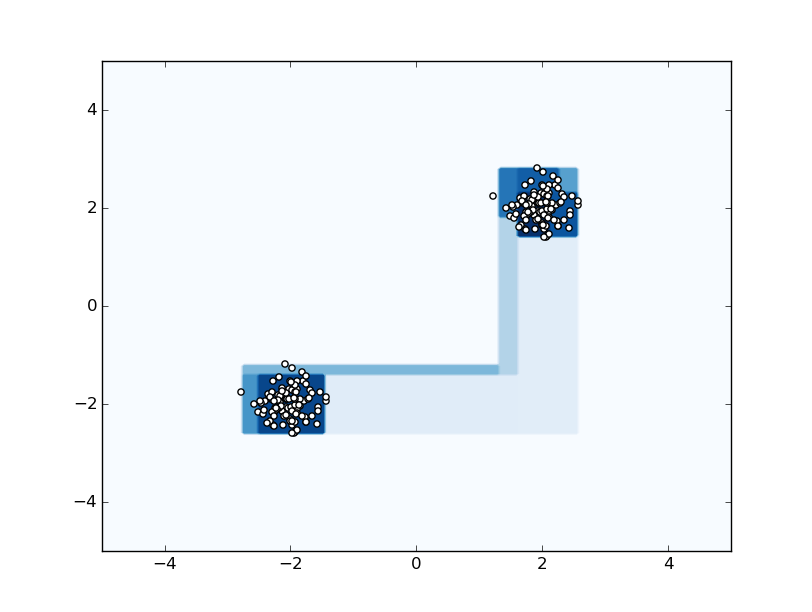
\includegraphics[width=\textwidth]{./gfx/oneclassrf.png}
    \caption[One Class Random Forest level-sets]{\ac{OneClassRF} with one tree,
    level-sets of the scoring function. \label{ocrf:fig:oneclassrf}}
\end{figure}

Most usual one-class (or more generally anomaly detection) algorithms actually
provide more than just a level-set estimate or a predicted label for any new
observation, abnormal versus normal. Instead, they return a real valued
function, termed \emph{scoring function}, defining a preorder/ranking on the
input space. Such a function $s: \mathbb{R}^d \to \mathbb{R}$ allows to rank
any observations according to their supposed \say{degree of abnormality}.
Thresholding it provides level-set estimates, as well as a decision rule that
splits the input space into inlier/normal and outlier/abnormal regions.
%
%We thus adapt the majority vote to the one-class setting by defining the
%scoring function of a forest.
%
%We propose three natural scoring functions of a forest.
The scoring function $s(x)$ we use is the one defined in \citet{Liu2008} in
view of its established high performance. It is a decreasing function of the
average depth of the leaves containing $x$ in the forest.
%, `if the trees were fully grown':
An average term is added to each node containing more than one sample, say
containing $N$ samples. This term $c(N)$ is the average depth of an extremely
randomized tree \citep{Geurts2006} (\acs{ie}~built without minimizing any
criterion, by randomly choosing one feature and one uniform value over this
feature to split on) on $N$ samples. Formally,
\begin{dmath}
    \label{ocrf:eq:scoring3}
    \log_2 s(x) = -\left(\sum_{t \text{~leaves}} \mathds{1}_{\Set{x \in t}} d_t
    + c(n_t)\right) / c(n),
\end{dmath}
where $d_t$ is the depth of node $t$, and $c(n) = 2H(n - 1) - 2(n - 1)/n$,
$H(i)$ being the harmonic number. Alternative scoring functions can be defined
for this one-class setting (see \cref{supp:scoring_functions}).
%
%
%
\subsection{OneClassRF: a Generic One-Class Random Forest algorithm}
Let us summarize the One Class Random Forest algorithm, based on generic
\acp{RF} \citep{Breiman2001}. It has $6$ parameters, namely
\texttt{max\textunderscore samples}, \texttt{max\textunderscore
features\textunderscore tree}, \texttt{max\textunderscore
features\textunderscore node}, $\texttt{gamma}$, \texttt{max\textunderscore
depth}, \texttt{n\textunderscore trees}.
%
\begin{table*}[ht]
    \caption{Original datasets characteristics}
    \label{ocrf:table:data}
    \centering
    \footnotesize
    %\tabcolsep=0.08cm
    \begin{tabularx}{\textwidth}{lccXl}
        \toprule
        Datasets        & nb of samples      & nb of features     &
       anomaly class      &                   \\
        \midrule
        adult       & 48842              & 6                  &    class
        '$>50K$' &      (23.9\%)      \\
        annthyroid  & 7200               & 6                  &    classes
        $\neq$ 3 &        (7.42\%)    \\
        arrhythmia  & 452                & 164                &    classes
        $\neq$ 1 (features 10-14 removed)&  (45.8\%)          \\
        forestcover & 286048             & 10                 &    class 4
        (versus  class 2 )                  &           (0.96\%) \\
        http        & 567498             & 3                  &      attack &
        (0.39\%)        \\
        ionosphere  & 351                & 32                 &    bad &
        (35.9\%)     \\
        pendigits   & 10992              & 16                 &    class 4 &
        (10.4\%)    \\
        pima        & 768                & 8                  &    pos (class
        1) &        (34.9\%)    \\
        shuttle     & 85849              & 9                  &      classes
        $\neq$ 1 (class 4 removed)     &  (7.17\%)          \\
        smtp        & 95156              & 3                  &      attack &
        (0.03\%)        \\
        spambase    & 4601               & 57                 &    spam &
        (39.4\%) \\
        wilt        & 4839               & 5                  &    class `w'
        (diseased trees)               &    (5.39\%)        \\
        \bottomrule
    \end{tabularx}
\end{table*}
\paragraph{}
Each tree is classically grown on a random subset of both the input samples and
the input features \citep{Ho1998, Panov2007}.  This random subset is a
sub-sample of size \texttt{max\textunderscore samples}, with
\texttt{max\textunderscore features\textunderscore tree} variables chosen at
random without replacement (replacement is only done after the tree is grown).
The tree is built by minimizing \cref{ocrf:oc_proxy_ad2} for each split, using
parameter $\gamma$ (recall that $n_t' \colonequals \gamma n_t$), until either
the maximal depth \texttt{max\textunderscore depth} is achieved or the node
contains only one point.
% define a large number of geometric features and search over a random
% selection of these for the best split at each node
Minimizing \cref{ocrf:oc_proxy_ad2} is done as introduced in \citet{Amit1997}:
at each node, we search the best split over a random selection of features with
fixed size $max\textunderscore features\textunderscore node$.
%
The forest is composed of a number $n\textunderscore trees$ of trees. The
predicted score of a point $x$ is given by $s(x)$, with $s$ defined by
\Cref{ocrf:eq:scoring3}.
%SH (copier en suppl mat) As an illustration, Figure~\Cref{ocrf:fig:oneclassrf}
%represents the level set of the scoring function produced by OneClassRF, with
%only one tree ($n\textunderscore trees$$=1$) of maximal depth
%$max\textunderscore depth$=4, without sub-sampling, and using the Gini-based
%one-class splitting criterion with
%$\gamma=1$.
Remarks on alternative stopping criteria and variable importances are available
in \cref{supp:stopping_criteria}.
\paragraph{}
\Cref{ocrf:fig:oneclassrf} represents the level sets of the scoring function
produced by \ac{OneClassRF}, with only one tree
% ($n\textunderscore trees$$=1$)
of maximal depth $4$,
% $max\textunderscore depth$=4
without sub-sampling, and using the Gini-based one-class splitting criterion
with $\gamma=1$.
%
%
% \begin{remark}({\sc Underlying Level-Set estimation}) As mentionned above,
% the link between $\gamma$ and the level of the level-set estimate induced by
% the split is difficult to exhibit, as well as how it repercutes into the
% level of the global level-set estimate.  Intuitively, $\gamma$ plays the same
% role as parameter $\nu$ for the OCSVM in its $\nu$-soft margin formulation.
% OCSVM also returns a scoring function (inducing an infinite number of
% level-sets), but which seeks to be optimal for estimating a particular
% level-set (corresponding to a particular thresholding of the scoring
% function) whose level can explicitely be controlled by $\nu$.  However, we
% are not able to derive an explicit relation, as it exists for the OCSVM,
% between the targeted level set and $\gamma$. Note that this does not mean
% that we are not able to estimate any arbitrary level-set. It only means that
% we do not know for which level, the scoring function outputed by OneClassRF
% originally seeks to be optimal.  \end{remark}
%
%
%by \Cref{ocrf:eq:scoring1}, \Cref{ocrf:eq:scoring2} or
%\Cref{ocrf:eq:scoring3}.  \paragraph{Description of the OneClassRF algorithm.}
%Now that we have exposed the one-class splitting rule to grow the trees, as
%well as the forest output replacing the majority vote, the one-class random
%forest algorithm promoted here is described as follows. %similar to Breiman's
%approach, see \cite{Breiman2001}.  % Let us denote by \ttt{X} the input data.
%In its most generic version, it has five parameters, $max\textunderscore
%samples$, $max\textunderscore features$, $n\textunderscore estimators$,
%$max\textunderscore depth$ and $\gamma$.  Each tree is classicaly grown on a
%random subset of both the input samples and the input variables,
%see~\cite{Ho1998, Panov2007}. This random subset is a sub-sample of size
%$max\textunderscore samples$, with $max\textunderscore features$ variables
%chosen at random without replacement (replacement is only done after the tree
%is grown). The tree is built by minimizing \Cref{ocrf:oc_proxy_ad2} at each
%step using parameter $\gamma$, until the maximal depth $max\textunderscore
%depth$ is achieved. The forest is composed of a number $n\textunderscore
%estimators$ of trees. The predicted score of a point $x$ is given by
%\Cref{ocrf:eq:scoring}, namely the average (over the trees) of
%$n_t/\leb(\mathcal{X}_t)$, where $t$ is the leaf node (of the tree considered)
%containing $x$.  % \begin{algorithm}[OneClassRF.fit]~\\ % \begin{pythoncode} %
%Inputs: X % Parameters: max_samples, max_features, n_estimators, max_depth %
%Output: A set of n_estimators trees.  % \end{pythoncode} % \end{algorithm}
%\begin{remark}({\sc Extremely Randomized Trees}) In the case of extremely
%randomized trees (see \cite{Geurts2006}), namely trees grown totally randomly
%as used in Isolation Forest (\cite{Liu2008}), no splitting criterion is needed
%so that no impurity function is used. The one class version of the
% majority vote can still be used in this case, which yields a scoring function
% of the form $s(x) = \sum_t \mathds{1}_{\{\Omega_t \}}
% \frac{N_t}{\leb(\Omega_t)}$. XXX benchmark on this algo? (easy: iforest with
% score from OCSVM) \end{remark}
%XXX sklearn exemple with OneClassRF with different alpha
%

\section{Benchmarks}
\label{ocrf:sec:benchmark}
%
In this section, we compare the \ac{OneClassRF} algorithm described above to
seven state-of-art anomaly detection algorithms: the \ac{iForest} algorithm
\citep{Liu2008}, a one-class \acp{RF} algorithm based on sampling a
second class \ac{OCRFsampling} \citep{Desir13}, \acf{OCSVM}
\citep{Scholkopf2001}, \acf{LOF} \citep{Breunig2000LOF}, Orca \citep{Bay2003},
\acf{LSAD} \citep{Quinn2014}, \acf{RFC} \citep{Shi2012}.
%We have used default parameters for these algorithms, as detailed in
%supplementary material.
%
\subsection{Default parameters of OneClassRF}
The default parameters taken for our algorithm are the followings.
%
\begin{itemize}
    \item \texttt{max\textunderscore samples} is fixed to $20\%$ of the
    training sample size (with a minimum of $100$);
    \item \texttt{max\textunderscore features\textunderscore tree} is fixed to
    $50\%$ of the total number of features with a minimum of $5$ (\acs{ie}~each
    tree is built on $50\%$ of the total number of features);
    \item \texttt{max\textunderscore features\textunderscore node} is fixed to
    $5$;
    \item $\gamma$ is fixed to $1$;
    \item \texttt{max\textunderscore depth} is fixed to $\log_2$ (logarithm in
    base $2$) of the training sample size as in \citet{Liu2008};
    \item \texttt{n\textunderscore trees} is fixed to $100$ as in the previous
    reference.
\end{itemize}
%and parameter $s_i$ is set to $s_3$ as defined in \eqref{ocrf:eq:scoring3}.
\paragraph{}
The other algorithms in the benchmark are trained with their recommended
(default) hyper-parameters as seen in their respective paper or author's
implementation. See \cref{supp:hyper_choice} for details.
%
The characteristics of the twelve reference datasets considered here are
summarized in \cref{ocrf:table:data}. They are all available on the \acs{UCI}
repository \citep{Lichman2013} and the preprocessing is done as usually in the
literature (see \cref{supp:dataset_description}).
%
%
\maxdeadcycles=1000
\afterpage{%
\begin{landscape}
    \begin{table}[htb]
        \centering
        \caption{Results for the novelty detection setting.
        %We compare various methods from the state-of-the-art (top line) to
        %OneClassRF over different classical datasets (leftmost column).
        \label{ocrf:table:results-semisupervised}}
        %\scriptsize
        \resizebox{\textheight}{!}{%
        \begin{tabular}{lcccccccccccccccc}
        \toprule
            %
            Datasets & \multicolumn{2}{c }{\ac{OneClassRF}} & \multicolumn{2}{c
            }{\ac{iForest}} & \multicolumn{2}{c }{\ac{OCRFsampling}} &
            \multicolumn{2}{c }{\ac{OCSVM}}& \multicolumn{2}{c }{\ac{LOF}}&
            \multicolumn{2}{c }{Orca}& \multicolumn{2}{c }{\ac{LSAD}}&
            \multicolumn{2}{c }{\ac{RFC}}  \\%& parameters $(\epsilon, k)$\\
        \cmidrule{1-17}
            \acs{AUC}   & \acs{ROC} &  \acs{PR} & \acs{ROC} &  \acs{PR} &
            \acs{ROC} & \acs{PR}  & \acs{ROC} & \acs{PR}  & \acs{ROC} &
            \acs{PR} & \acs{ROC} & \acs{PR}  & \acs{ROC} &  \acs{PR} &
            \acs{ROC} & \acs{PR}  \\
            adult        &        \textbf{0.665} & \textbf{0.278} & 0.661 &
            0.227 & \acs{NA} & \acs{NA} & 0.638 & 0.201 & 0.615 & 0.188 & 0.606
            & 0.218 & 0.647    & 0.258     & \acs{NA} & \acs{NA} \\
            annthyroid   &        \textbf{0.936} & 0.468 & 0.913 & 0.456 &
            0.918 & \textbf{0.532} & 0.706 & 0.242 & 0.832 & 0.446 & 0.587 &
            0.181 &  0.810 & 0.327     & \acs{NA} & \acs{NA} \\
            arrhythmia   &        0.684 & 0.510 & 0.763 & 0.492 & 0.639 & 0.249
            & \textbf{0.922} & \textbf{0.639} & 0.761 & 0.473 & 0.720 & 0.466 &
            0.778 & 0.514     & 0.716 & 0.299 \\
            forestcover  &        0.968 & 0.457 & 0.863 & 0.046 & \acs{NA} &
            \acs{NA} & \acs{NA} & \acs{NA} & \textbf{0.990} & \textbf{0.795} &
            0.946 & 0.558 &  0.952    & 0.166 & \acs{NA} & \acs{NA} \\
            http         &        \textbf{0.999} & \textbf{0.838} & 0.994 &
            0.197 & \acs{NA} & \acs{NA} & \acs{NA} & \acs{NA} & \acs{NA} &
            \acs{NA} & \textbf{0.999} & 0.812 &  0.981    & 0.537     &
            \acs{NA} & \acs{NA} \\
            ionosphere   &        0.909 & 0.643 & 0.902 & 0.535 & 0.859 & 0.609
            & 0.973 & 0.849 & 0.959 & 0.807 & 0.928 & \textbf{0.910} &
            \textbf{0.978} & 0.893     & 0.950 & 0.754 \\
            pendigits    &        0.960 & 0.559 & 0.810 & 0.197 & 0.968 & 0.694
            & 0.603 & 0.110 & 0.983 & 0.827 & \textbf{0.993} & \textbf{0.925} &
            0.983 & 0.752     & \acs{NA} & \acs{NA} \\
            pima         &        0.719 & 0.247 & 0.726 & 0.183 &
            \textbf{0.759} & \textbf{0.266} & 0.716 & 0.237 & 0.700 & 0.152 &
            0.588 & 0.175 &  0.713 & 0.216     & 0.506 & 0.090 \\
            shuttle      &        \textbf{0.999} & \textbf{0.998} & 0.996 &
            0.973 & \acs{NA} & \acs{NA} & 0.992 & 0.924 & \textbf{0.999} &
            0.995 & 0.890 & 0.782 & 0.996    & 0.956     & \acs{NA} & \acs{NA}
            \\ smtp         &        0.922 & 0.499 & 0.907 & 0.005 & \acs{NA} &
            \acs{NA} & 0.881 & \textbf{0.656} & \textbf{0.924} & 0.149 & 0.782
            & 0.142 &  0.877    & 0.381     & \acs{NA} & \acs{NA} \\
            spambase &        \textbf{0.850} & 0.373 & 0.824 & 0.372 & 0.797 &
            \textbf{0.485} & 0.737 & 0.208 & 0.746 & 0.160 & 0.631 & 0.252 &
            0.806 & 0.330     & 0.723 & 0.151 \\
            wilt         &        0.593 & 0.070 & 0.491 & 0.045 & 0.442 & 0.038
            & 0.323 & 0.036 & 0.697 & 0.092 & 0.441 & 0.030 &  0.677    & 0.074
            & \textbf{0.896} & \textbf{0.631} \\
        \cmidrule{1-17}
            average    & \textbf{0.850} & \textbf{0.495} & 0.821 & 0.311 &
            0.769 & 0.410 & 0.749 & 0.410 & 0.837 & 0.462 & 0.759 & 0.454 &
            \textbf{0.850} & 0.450 &  0.758  & 0.385 \\
            \acs{cum} train time & \multicolumn{2}{c }{\textbf{61s}} &
            \multicolumn{2}{c }{68s} & \multicolumn{2}{c }{\acs{NA}} &
            \multicolumn{2}{c }{\acs{NA}}& \multicolumn{2}{c }{\acs{NA}}&
            \multicolumn{2}{c }{2232s}& \multicolumn{2}{c }{73s}&
            \multicolumn{2}{c }{\acs{NA}}  \\
        \bottomrule
        \end{tabular}}
    \end{table}
\end{landscape}}
%
%
\subsection{Results}
All the code is available at \url{https://github.com/ngoix/OCRF}. The
experiments are performed in the novelty detection framework, where the
training set consists of inliers only.
%We removed anomalies from the training data.
No significance level test are given, but experiements or each algorithm are
repeated $10$ times on random training and testing datasets are performed,
yielding averaged \ac{ROC} and \ac{PR} curves whose \acsp{AUC} are summarized
in \cref{ocrf:table:results-semisupervised} (higher is better).
%We use the set of hyper-parameters recommanded in the corresponding reference
%papers.
The training time of each algorithm has been limited (for each experiment among
the $10$ performed for each dataset) to $30$ minutes, where \acs{NA} indicates
that the algorithm could not finish training within the allowed time limit.  In
average on all the datasets, our proposed algorithm \ac{OneClassRF} achieves
both best \acs{AUC} \acs{ROC} and \acs{AUC} \acs{PR} scores (with \acs{LSAD}
for \acs{AUC} \acs{ROC}). It also achieves the lowest cumulative training time.
%
For further insights on the benchmarks \acs{cf}~\cref{supp:further_exp}.
%
%Figures \Cref{ocrf:figNoveltyAUCROC} and \Cref{ocrf:figNoveltyCompTime}
%summarize the results. % from the novelty detection framework, whereas figures
%\Cref{ocrf:figUnsupervAUCROC}, \Cref{ocrf:figUnsupervAUCPR} and
%\Cref{ocrf:figUnsupervCompTime} presents those from the unsupervised one.  In
%the novelty detection settings,
It appears that \ac{OneClassRF} has the best performance on five datasets in
terms of \acs{ROC} \acsp{AUC}, and is also the best in average.
%\footnote{Precision-Recall AUCs have also been computed and are
%available in the supplementary material.},
Computation times (training plus testing) of \ac{OneClassRF} are also very
competitive.
% (see supplementary material).
%In the unsupervised settings, OneClassRF and iForest have similar performances
%in terms of AUCs (ROC and PR), but OneClassRF still uses less computation
%time.
%
%These results are surprising: iForest computation time should be lower since
%it randomly builds trees. The explaination is....
%
% T = np.array([[1.83, 1.19, np.NAN, 16.20, 7.03, 9.42, 1.05, np.NAN],
% [0.39, 0.19, 65.02, 0.54, 1.03, 0.66, 0.31, np.NAN],
% [0.36, 0.12, 9.30, 0.0, 0.04, 0.38, 0.01, 33.17],
% [19.97, 15.86, np.NAN, np.NAN, 59.56, 733.75, 6.18, np.NAN],
% [29.5, 42.25, np.NAN, np.NAN, np.NAN, 1368.83, 51.41, np.NAN],
% [0.36, 0.10, 2.47, 0.0, 0.03, 0.38, 0.0, 12.42],
% [0.67, 0.32, 458.94, 1.35, 1.66, 1.81, 0.42, np.NAN],
% [0.13, 0.10, 5.20, 0.0, 0.12, 0.26, 0.01, 18.12],
% [3.13, 3.87, np.NAN, 95.99, 20.39, 76.24, 7.42, np.NAN],
% [3.99, 3.51, np.NAN, 118.93, 12.11, 38.52, 5.98, np.NAN],
% [0.49, 0.21, 55.71, 0.22, 0.85, 1.49, 0.25, 593.87],
% [0.39, 0.16, 68.29, 0.14, 0.73, 0.46, 0.22, 752.19]])
% np.mean(T, axis=0)
% array([   5.10083333,    5.65666667,           nan,           nan,
%                  nan,  186.01666667,    6.105     ,           nan])
%
%
Experiments in an outlier detection framework (the training set is polluted by
outliers) have also been made (see \cref{sup:outlier_detection}).
%In this case, the anomaly rate is arbitrarily bounded to $10\%$ max (before
%splitting data into training and testing sets).
The anomaly rate is arbitrarily bounded to $10\%$ max (before splitting data
into training and testing sets).
%
%
%
%
\section{Theoretical analysis}
%justification for the one-class splitting criterion}
\label{sec:ocrf:theory}
This section aims at recovering \cref{ocrf:oc_proxy_ad2} from a natural
modeling of the one-class framework, along with a theoretical study of the
problem raised by the naive approach.
\subsection{Underlying model}
\label{ocrf:sec:model} In order to generalize the two-class framework to the
one-class one, we need to consider the population versions associated to
empirical quantities \cref{ocrf:eq:impurity_measure_decrease},
\cref{ocrf:eq:gini} and \cref{ocrf:eq:two_class_proxy}, as well as the
underlying model assumption. The latter can be described as follows.

\subsubsection{Existing Two-Class Model (n, $\boldsymbol{\alpha}$).}
We consider a \acs{rv}~$X:\Omega \to \mathbb{R}^d$ \acs{wrt}~a probability
space $(\Omega, \mathcal{F}, \probability)$. The law of $X$ depends on another
\acs{rv}~$y \in \{0,1\}$, verifying
$\probability\Set{y=1}=1-\probability\Set{y=0}=\alpha$.  We assume that
conditionally on $y=0$, $ X$ follows a law $F$, and conditionally on $y=1$ a
law $G$;
%To summarize:
\begin{dgroup*}
\begin{dmath*}
    X\enskip|\enskip y=0 \quad\sim\quad F, \qquad
    \probability\Set{y=0}=1-\alpha,
\end{dmath*}
\begin{dmath*}
    X\enskip|\enskip y=1 \quad\sim\quad G, \qquad
    \probability\Set{y=1}=\alpha.
\end{dmath*}
\end{dgroup*}
Then, considering
\begin{dmath*}
    p(t_L | t) = \probability\Set{X\in \mathcal{X}_{t_L} | X\in \mathcal{X}_t},
\end{dmath*}
and
\begin{dmath*}
    p(t_R | t) = \probability\Set{X\in \mathcal{X}_{t_R} | X\in \mathcal{X}_t},
\end{dmath*}
the population version (probabilistic version) of
\Cref{ocrf:eq:impurity_measure_decrease} is
\begin{dmath}
    \label{ocrf:eq:impurity_measure_decrease_theo}
    \Delta i^{theo}(t, t_L, t_R) = i^{theo}(t) -  p(t_L | t) i^{theo}(t_L)
    -  p(t_R | t) i^{theo}(t_R).
\end{dmath}
It can be used with the Gini index $i_G^{theo}$,
\begin{dmath}
\label{ocrf:eq:gini_theo}
    i_G^{theo}(t) \hiderel{=} 2 \probability\set{y\hiderel{=}0 |  X \in
    \mathcal{X}_t} \probability\set{y \hiderel{=} 1 |  X \in
    \mathcal{X}_t}
    % \nonumber &~=~ 2 \frac{\probability(X \in \mathcal{X}_t,~ y = 0) \cdot
    % \probability(X \in \mathcal{X}_t,~ y = 1) }{\mathbb{P}(X \in
    % \mathcal{X}_t)^2}
\end{dmath}
% ~~=~~ \frac{(1-\alpha) \int_{\mathcal{X}_t}f ~~~ \alpha \int_{\mathcal{X}_t}g
% }{\left((1-\alpha) \int_{\mathcal{X}_t}f + \alpha
% \int_{\mathcal{X}_t}g\right)^2}
which is the population version of \cref{ocrf:eq:gini}.
% Indeed, when observing $n$ \iid~realizations $( X_1, y_1),\ldots, ( X_n,
% y_n)$ of $( X,y)$, replacing probabilities by their empirical version amounts
% to replacing $\probability(X \in \mathcal{X}_t,~ y = 0)$ by $n_t / n$,
% $\probability(X \in \mathcal{X}_t,~ y = 1)$ by $n_t'/n$ and $\mathbb{P}(X \in
% \mathcal{X}_t)$ by $(n_t + n_t')/n$ with $n_t = \text{card}\{i,~X_i\in
% \mathcal{X}_t, y_i=0 \}$ and $n_t' = \text{card}\{i,~X_i\in \mathcal{X}_t,
% y_i=1 \}$, thus recovering \Cref{ocrf:eq:gini}.

\subsubsection{One-Class-Model ($n$, $\boldsymbol{\alpha}$).} We model the
one-class framework as follows. Among the $n$ \acs{iid}~observations, we only
observe those with $y=0$ (the inliers), namely $N$ realizations of $(
X\enskip|\enskip y=0)$, where $N$ is itself a realization of a
\acs{rv}~$\mathbf{N}$ of law $\mathbf{N} \sim \text{Bin}(n,
(1-\alpha))$. Here and hereafter, $\text{Bin}(n, p)$ denotes the binomial
distribution with parameters $(n, p)$.  As outliers are not observed, it is
natural to assume that $G$ follows a uniform distribution on the
hyper-rectangle $\mathcal{X}$ containing all the observations, so that $G$ has
a constant density $g(\cdot) = 1 / \Leb(\mathcal{X})$ on $\mathcal{X}$.
%laisser une ligne car fin du model one class
Note that this assumption \emph{will be removed} in the adaptive approach
described below -- which aims at maintaining a non-negligible proportion of
(hidden) outliers in every nodes.
\paragraph{}
Let us define $L_t=\Leb(\mathcal{X}_t)/\Leb(\mathcal{X})$. Then,
$\probability\Set{X \in \mathcal{X}_t | y = 1}= \probability\Set{y = 1}
\probability\Set{X \in \mathcal{X}_t | y = 1} = \alpha L_t $. Replacing
$\probability\Set{X \in \mathcal{X}_t | y=0}$ by its empirical version $n_t /
n$ in \cref{ocrf:eq:gini_theo}, we obtain the one-class empirical Gini index
\begin{dmath}
    \label{ocrf:eq:gini_oc}
    i_G^{OC}(t) = \frac{n_t \alpha n L_t}{(n_t + \alpha n L_t)^2}.
\end{dmath}
This one-class index can be seen as a \emph{semi-empirical} version of
\cref{ocrf:eq:gini_theo}, in the sense that it is obtained by considering
empirical quantities for the (observed) inlier behavior and population
quantities for the (non-observed) outlier behavior.
%
Now, maximizing the population version of the impurity decrease $\Delta
i_G^{theo}(t, t_L, t_R)$ as defined in
\cref{ocrf:eq:impurity_measure_decrease_theo} is equivalent to minimizing
\begin{dmath}
    \label{ocrf:theo_proxy}
    p(t_L | t) i_G^{theo}(t_L) +  p(t_R | t) i_G^{theo}(t_R).
\end{dmath}
%Now, $p(t_L | t) = \left[\mathbb{P}(X\in \mathcal{X}_{t_L}~|~y=0)
%\mathbb{P}(y=0) + \mathbb{P}(X\in \mathcal{X}_{t_L}~|~y=1)
%\mathbb{P}(y=1)\right] / \mathbb{P}(X \in \mathcal{X}_t)$
Considering semi-empirical versions of $p(t_L | t)$ and $p(t_R | t)$, as for
\Cref{ocrf:eq:gini_oc}, gives $p_n(t_L | t) = (n_{t_L} + \alpha n L_{t_L}) /
(n_{t} + \alpha n L_{t})$ and $p_n(t_R | t) = (n_{t_R} + \alpha n L_{t_R}) /
(n_{t} + \alpha n L_{t})$. Then, the semi-empirical version of
\Cref{ocrf:theo_proxy} is
\begin{dmath}
    \label{ocrf:oc_proxy1}
    p_n(t_L | t) i_G^{OC}(t_L) +  p_n(t_R | t) i_G^{OC}(t_R)
    = \frac{1}{(n_{t} + \alpha n L_{t})} \left(\frac{n_{t_L}\alpha n
    L_{t_L}}{n_{t_L} + \alpha n L_{t_L}} + \frac{n_{t_R}\alpha n
    L_{t_R}}{n_{t_R} + \alpha n L_{t_R}}\right)
\end{dmath}
where $ 1/(n_{t} + \alpha n L_{t})$ is constant when the split varies.  This
means that finding the split minimizing \cref{ocrf:oc_proxy1} is equivalent to
finding the split minimizing
\begin{dmath}
    \label{ocrf:oc_proxy2}
    I_G^{OC}(t_L, t_R) = \frac{n_{t_L}\alpha n L_{t_L}}{n_{t_L} + \alpha n
    L_{t_L}} + \frac{n_{t_R}\alpha n L_{t_R}}{n_{t_R} + \alpha n L_{t_R}}.
\end{dmath}
%
Note that \cref{ocrf:oc_proxy2} can be obtained from the two-class impurity
decrease \cref{ocrf:tc_proxy} as described in the naive approach paragraph in
\cref{ocrf:sec:one-class}. In other words, it is the naive one-class version of
\cref{ocrf:tc_proxy}.
\begin{remark}[Direct link with the two-class framework]
    The two-class proxy of the Gini impurity decrease \cref{ocrf:tc_proxy} is
    recovered from \cref{ocrf:oc_proxy2} by replacing $\alpha n L_{t_L}$ (resp.
    $\alpha n L_{t_R}$) by $n'_{t_L}$ (respectively $n'_{t_R}$), the number of
    second class instances in $t_L$ (respectively in $t_R$). When generating
    $\alpha n$ of them uniformly on $\mathcal{X}$, $\alpha n L_{t}$ is the
    expectation of $n'_{t}$.
\end{remark}
%
%
As detailed in \cref{sec:one-class-crit}, this approach suffers from the curse
of dimensionality.  We can summarize the problem as follows.
%
Note that when setting $n_t':=\alpha n L_t$, the class ratio
$\gamma_t=n_t'/n_t$ is then equal to
%Note that $\gamma_t$, the ratio between the expected number of (hidden)
%outliers and the number of inliers in node $t$, is here equal to , and have
%assumed that this ratio is negligible in nodes $t_L$ and $t_R$.
%\textbf{Problem 1.} Now, the curse of dimensionality appears in the following
%sense. In large dimension, $\alpha n L_{t}$ becomes very close to zero when
%going deeper in the tree (recall that $L_t =
%\leb(\mathcal{X}_t)/\leb(\mathcal{X})$, and the volume of $\mathcal{X}_t$
%decreases). In addition, we typically grow trees on sub-samples of the input
%data, meaning that even the root node of the trees may be very small compared
%to the hyper-rectangle containing all the input data.  % In other words,
%$\alpha n L_t$ is much smaller than $n_t$ for lots of nodes $t$ (in particular
%the leaves).  Unfortunately, the Gini impurity is skew-sensitive
%\citep{Flach2003}. In other words, criterion \Cref{ocrf:oc_proxy2} almost does
%not penalize the volume for such nodes with $\alpha n L_t \ll n_t$.  This can
%also be seen when writing \begin{align} \label{ocrf:eq:I_with_gamma}
%I_G^{OC}(t_L, t_R) ~~=~~ \frac{\alpha n L_{t_L}}{1 + \gamma_{t_L}} +
%\frac{\alpha n L_{t_R}}{1 + \gamma_{t_R}} ~~\simeq~~ \alpha n L_{t_L} + \alpha
%n L_{t_R} ~~=~~ \alpha n L_{t}, \end{align} $\alpha n L_{t}$ being constant
%when the split varies. We have used the notation %$\gamma_t$ is
\begin{dmath}
    \label{ocrf:def:gamma_t}
    \gamma_t = \alpha n L_t / n_t.
\end{dmath}
This class ratio is close to $0$ for lots of nodes $t$, which makes the Gini
criterion unable to discriminate accurately between the --hidden-- outliers and
the inliers.
%
%\sim (n_{t_L}\alpha n L_{t_L}/n_{t_L} + n_{t_R}\alpha n L_{t_R}/n_{t_R}) =
%\alpha n L_{t}$$
%
% It turns out that criterion \Cref{ocrf:oc_proxy2} almost doesn't penalize the
% volume for such nodes with $\alpha n L_t \ll n_t$.  This can be explained by
% the fact that the Gini impurity is skew-sensitive \cite{Flach2003} and also
% by writting the following equivalence of \Cref{ocrf:oc_proxy2} when $\alpha n
% L_{t} = (\alpha n L_{t_L} + \alpha n L_{t_R}) \to 0$:  $I_G^{OC}(t_L, t_R)
% \sim (n_{t_L}\alpha n L_{t_L}/n_{t_L} + n_{t_R}\alpha n L_{t_R}/n_{t_R}) =
% \alpha n L_{t}$, the last quantity being constant when the split varies.
%
Minimizing this criterion produces splits corresponding to $\gamma_t\simeq 0$
in \cref{ocrf:fig:split_alpha}: one of the two child nodes, say $t_L$ contains
almost all the data.
%
%, as its volume is not sufficiently penalized (or equivalently $\alpha n
%L_{t_L}$ is negligible).  and \Cref{ocrf:fig:split_two_modes}. % (the $\gamma$
%parameter represents a weight on the volume and will be formally introduced
%latter)

% To illustrate the fact that $\alpha n L_{t}$ becomes very close to zero in
% large dimension for lots of nodes $t$ (in particular the leaves), suppose for
% the sake of simplicity that the input space is $\mathcal{X} = [0,1]^d$.
% Suppose that we are looking for a rough precision of $1/2^3=0.125$ in each
% dimension, \ie~a unit cube precision of $2^{-3d}$.  To achieve such a
% precision, we will typically need to use the splitting criterion on
% nodes/cells $t$ of volume of order $2^{-3d}$, namely with $L_t = 1/2^{3d}$.
% This means that $\alpha n$ should be of order $2^{3d}$ to have non-negligible
% $\alpha n L_{t}$, which is unreasonable for large $d$.
\subsection{Adaptive approach}
The solution presented \cref{ocrf:sec:one-class} is to remove the uniform
assumption for the outlier class. From the theoretical point of view, the idea
is to choose in an adaptive way (\acs{wrt}~the volume of $\mathcal{X}_t$) the
number $\alpha n$, which can be interpreted as the number of (hidden) outliers.
% Recall that neither $n$ nor $\alpha$ is observed in the One-Class-Model($n$,
$\alpha$).  Doing so, we aim at avoiding $\alpha n L_t \ll n_t$ when $L_t$ is
too small. Namely, with $\gamma_t$ defined in \cref{ocrf:def:gamma_t}, we aim
at avoiding $\gamma_t \simeq 0$ when $L_t \simeq 0$. The idea is to consider
$\alpha(L_t)$ and $n(L_t)$ such that $\alpha(L_t) \to 1$, $n(L_t) \to \infty$
when $L_t \to 0$.  We then define the one-class adaptive proxy of the impurity
decrease by
\begin{dmath}
    \label{ocrf:oc_proxy_ad1}
    \nonumber I_G^{OC-ad}(t_L, t_R) = \frac{n_{t_L}\alpha(L_t) n(L_t)
    L_{t_L}}{n_{t_L} + \alpha(L_t) n(L_t) L_{t_L}} \\ +
    \frac{n_{t_R}\alpha(L_t) n(L_t) L_{t_R}}{n_{t_R} + \alpha(L_t)
    \cdot n(L_t) \cdot L_{t_R}}.
\end{dmath}
In other words, instead of considering one general model One-Class-Model($n$,
$\alpha$) defined in \cref{ocrf:sec:model}, we adapt it to each node $t$,
considering One-Class-Model($n(L_t)$, $\alpha(L_t)$) \emph{before searching the
best split}. We still consider the $N$ inliers as a realization of this model.
When growing the tree, using One-Class-Model($n(L_t)$, $\alpha(L_t)$) allows to
maintain a non-negligible expected proportion of outliers in the node to be
split,
% minimizing \eqref{ocrf:oc_proxy_ad1}
despite $L_t$ becomes close to zero.  Of course, constraints have to be imposed
to ensure consistency between these models.
%
Recalling that the number $N$ of inliers is a realization of $\mathbf{N}$
following a Binomial distribution with parameters $(n, 1-\alpha)$, a first
natural constraint on $\left(n(L_t), \alpha(L_t)\right)$ is
\begin{dmath}
    \label{ocrf:constraint1}
    (1-\alpha)n = \left(1-\alpha(L_t)\right) \cdot n(L_t) \condition{for all
    $t$,}
\end{dmath}
so that the expectation of $\mathbf{N}$ remains unchanged.
% when our new model depending on $t$ varies. %\ie~$\mathbb{E}(\mb N(L_t)) =
% \mathbb{E}(N) $ , %denoting $\mb N(L_t) \sim \text{Bin}(1-\alpha(L_t),
% n(L_t))$ .
\begin{remark}
    In our adaptive model One-Class-Model($n(L_t)$, $\alpha(L_t)$) which varies
    when we grow the tree, let us denote by $\mathbf{N}(L_t) \sim
    \text{Bin}\left(n(L_t), 1-\alpha(L_t)\right)$ the \acs{rv}~ruling the
    number of inliers. The number of inliers $N$ is still viewed as a
    realization of it.  Note that the distribution of $\mathbf{N}(L_t)$
    converges in distribution to $\mathcal{P}\left((1-\alpha)n\right)$ a
    Poisson distribution with parameter $(1-\alpha) n$ when $L_t \to 0$, while
    the distribution $\text{Bin}\left(n(L_t), \alpha(L_t)\right)$ of the
    \acs{rv}~$n(L_t) - \mathbf{N}(L_t)$ ruling the number of (hidden) outliers
    goes to infinity almost surely. In other words, the asymptotic model (when
    $L_t \to 0$) consists in assuming that the number of inliers $N$ we
    observed is a realization of $\mathbf{N}_\infty \sim
    \mathcal{P}\left((1-\alpha)n\right)$, and that an infinite number of
    outliers have been hidden.
\end{remark}
A second natural constraint on $\big(\alpha(L_t), n(L_t)\big)$ is related to
the class ratio $\gamma_t$.
% defined in \Cref{ocrf:def:gamma_t}, $\mathbb{P}(y = 1~|~X \in \mathcal{X}_t)
% = \alpha(L_t) n(L_t)  L_t / (n_t + \alpha(L_t) n(L_t)  L_t)$, the ratio
% between the expected number of (hidden) outliers in node $t$ and the number
% of inliers.
%, used to find the split by minimizing \Cref{ocrf:oc_proxy2}.
As explained in \cref{sec:one-class-crit}, we do not want $\gamma_t$ to go to
zero when $L_t$ does.  Let us say we want $\gamma_t$ to be constant for all
node $t$, equal to $\gamma>0$. From the constraint $\gamma_t = \gamma$ and
\cref{ocrf:def:gamma_t}, we get
% $n_t'/n(L_t)$, so that
\begin{dmath}
    \label{ocrf:constraint2}
    \alpha(L_t) n(L_t) L_t
    % = \gamma_t n_t
    = \gamma n_t \colonequals n_t'.
\end{dmath}
%The quantity $n_t'$ can be interpreted as the expected number of (hidden)
%outliers in node $t$.
The constant $\gamma$ is a parameter ruling the expected proportion of outliers
in each node. Typically, $\gamma=1$ so that there is as much expected uniform
(hidden) outliers than inliers at each time we want to find the best split
minimizing~\cref{ocrf:oc_proxy_ad1}.
% relies on $\mathbb{P}(X \in \mathcal{X}_t,~ y = 1) = \alpha(L_t)  L_t$,
% interpreted as the expected proportion of (unobserved) outliers in node $t$
% we need to have before chosing the split by minimizing \Cref{ocrf:oc_proxy2}.
% Let say we want this probability to be equal to $n_t'/n(L_t)$, so that
% \begin{align} \label{ocrf:constraint2} \alpha(L_t)n(L_t)L_t = n_t'.
% \end{align}
%
\Cref{ocrf:constraint1} and \cref{ocrf:constraint2} allow to explicitly
determine $\alpha(L_t)$ and $n(L_t)$: $\alpha(L_t) = n_t'/\left((1-\alpha)nL_t
+ n_t'\right)$ and $n(L_t) = \left((1-\alpha)nL_t + n_t'\right)/L_t$.
Regarding \cref{ocrf:oc_proxy_ad1}, $\alpha(L_t) n(L_t)  L_{t_L} =
\frac{n_t'}{L_t} L_{t_L} =
n_t'\frac{\Leb(\mathcal{X}_{t_L})}{\Leb(\mathcal{X}_{t})}$ by
\cref{ocrf:constraint2} and $\alpha(L_t) n(L_t) L_{t_R}  =
n_t'\frac{\Leb(\mathcal{X}_{t_R})}{\Leb(\mathcal{X}_{t})},$ so that we recover
\cref{ocrf:oc_proxy_ad2}.
% \begin{align} \label{ocrf:oc_proxy_ad2} I_G^{OC-ad}(t_L, t_R)=
% \frac{n_{t_L}n_t'\lambda_L}{n_{t_L} + n_t'\lambda_L} +
% \frac{n_{t_R}n_t'\lambda_R}{n_{t_R} + n_t'\lambda_R}, \end{align} with
% $\lambda_L = \frac{\leb(\mathcal{X}_{t_L})}{\leb(\mathcal{X}_{t})}$ and
% $\lambda_R = \frac{\leb(\mathcal{X}_{t_R})}{\leb(\mathcal{X}_{t})}$.

% Minimization of the one-class Gini improvement proxy \Cref{ocrf:oc_proxy_ad2}
% is illustrated in Figure \Cref{ocrf:fig:split_alpha}. %and
% \Cref{ocrf:fig:split_two_modes}.  Note that $n_t'\lambda_L$ (resp.
% $n_t'\lambda_R$) is the expectation of the number of uniform observations
% among $n_t'$ falling into the left (resp. right) node.

% Choosing the split minimizing $I_G^{OC-ad}(t_L, t_R)$ at each step of the
% tree building process, corresponds to generating $n_t'$ outliers each time
% the best split has to be chosen for node $t$, and then using the classical
% two-class Gini proxy \Cref{ocrf:tc_proxy}. The only difference is that
% $n_{t_L}'$ and $n_{t_R}'$ are replaced by their expectations
% $n_t'\lambda_{t_L}$ and $n_t'\lambda_{t_R}$ in our method. This attests the
% relevance of the above methodology.

% \begin{remark}({\sc By-product: Efficiently generating outliers}) As a
% by-product, we obtain an efficient method to generate outliers tightly
% concentrated around the support of the normal distribution: it suffices to
% generate them as described above, recursively during the tree building
% process. Sampling $n_t'$ uniform points on $\mathcal{X}_t$, then using the
% latter to find the best split \wrt~\Cref{ocrf:tc_proxy}, and recommence on
% $\mathcal{X}_{t_L}$ and $\mathcal{X}_{t_R}$.  \end{remark}

% Considering semi-empirical quantities (\ie~working with the limit behavior of
% uniformly generated outliers) implies that we loose some randomness % TODO
% DROUGUI: there where randomness before?  in the tree building process, thus
% increasing the corelation between the trees of the forest.  That is why we
% use a small sub-sampling size to build each tree, in the spirit
% of~\cite{Liu2008}. Growing each tree on a small sub-sample also allows to
% avoid randomizing the outlier number $n_t'$ at each step, see
% Remark~\Cref{ocrf:rk:weight}.


% In pratice, the probability $\mathbb{P}(X \in \mathcal{X}_t,~ y =
% 1)=\alpha(L_t)L_t=n_t'/n(L_t)$ has to be of the same order than
% $\mathbb{P}_n(X \in \mathcal{X}_t,~ y = 0) = n_t /n(L_t)$, so that we set
% $n_t' = \beta n_t$ with $\beta \in (0,1)$ a parameter of the algorithm. (XXX
% $\beta$ = notre $\alpha$ dnas la version précedente)

% XXXXXXXXXXXXXXx %Suppose that the curse of dimensionality described above
% does not exist, Suppose that $n_t'$ outliers are generated, uniformly and
% independently on $\mathcal{X}_t$ the rectangular cell of a node $t$. After
% splitting node $t$, the expected number of outliers in the left node $t_L$
% (resp. in the right node $t_R$) is $n_t' \frac{L_{t_L}}{L_{t}}$ (resp.
% $n_t'\frac{L_{t_R}}{L_{t}}$) where $L_{t}$ denotes the Lebesgue measure of
% node $t$.  % Within this setup, the curse of dimensionality described in
% previous section can be interpreted as follows.


% \textbf{Problem 1.} After a few splits, if $n_t'$ is not unreasonably large
% beside the dimension of the input space, the actual number of outliers in a
% node will be negligeable, so that in the node/cells where the (non-uniform)
% normal distribution concentrates, the two classes are so highly unbalanced
% that the splitting criterion is useless.

% To illustrate this point, suppose for the sake of simplicity, that the input
% space is $[0,1]^d$, and that we are seeking a rough precision of
% $1/2^3=0.125$ in each dimension, \ie~a unit cube precision of $2^{-3d}$.
% %Assume that the normal observations concentrate To achieve such a precision,
% we will typically need to use the splitting criterion on node/cell
% (containing some normal observations) of volume slightly greater than
% $2^{-3d}$, say $2^{-3d +1}$.  In average, this cell contains $n_t'/2^{3d}$
% outliers.  This means that $n_t'$ should be at least equal to $2^{3d}$ for
% expecting to have one in this cell, which is unreasonable for large $d$.

%split tends to be totally random (any split yields `pure' nodes, with a
%majority proportion of outliers).


%\parbox{13cm}{\center (uniform generated outliers are not represented)}

% \begin{minipage}{0.45\linewidth} \centering
% \includegraphics[width=\linewidth]{split_alpha.png}
% \captionof{figure}{Standard splitting criterion when the proportion $\gamma$
% of generated outliers varies} \label{ocrf:fig:split_alpha}
% \end{minipage}\hfill \begin{minipage}{0.45\linewidth} \centering
% \includegraphics[width=\linewidth]{split_two_modes}
% \captionof{figure}{Standard splitting criterion on two modes when $\gamma$
% varies} \label{ocrf:fig:split_two_modes} \end{minipage}
%
%
% Our solution to Problem 1. is to (do as if we) generate outliers locally,
% step by step, to maintain a reasonable number of them in cells containing
% normal data (empty cells does not need to be split). This is allowed by the
% following proposition.
%
%
% This proposition allows to generate outliers locally, node by node. When
% looking for the best split on node $t$, it suffices to generate an arbitrary
% number $n_t'$ of outliers in $\mathcal{X}_t$ and to find the split minimizing
% $I(t_L, t_R)$.  Even more, we can avoid generating outliers, working directly
% with expectations, namely setting $n_{t_L}' = n_t' \lambda_L$ and $n_{t_R}' =
% n_t' \lambda_R$ where $\lambda_L = \frac{L_{t_L}}{L_t}$ (resp. $\lambda_R =
% \frac{L_{t_R}}{L_t}$) is the volume fraction of the left (resp. right) side
% node, for a chosen $n_t'$ (for instance $n_t'=n_t$). Replacing $n_{t_L}$ and
% $n_{t_R}$ by these values in the impurity improvement proxy
% \Cref{ocrf:eq:two_class_proxy} with the Gini index \Cref{ocrf:eq:gini} gives
% the following one-class Gini improvement proxy.  % \begin{definition}({\sc
% One Class Gini improvement proxy}) As an analogue of the Gini impurity
% decrease proxy \Cref{ocrf:eq:two_class_proxy}, we define the one-class Gini
% improvement proxy by \begin{align} \label{ocrf:eq:one_class_gini_proxy}
% I_G(t_L, t_R) / 2 = \frac{n_{t_L} n_t' \lambda_L}{n_{t_L} + n_t' \lambda_L} +
% \frac{n_{t_R} n_t' \lambda_R}{n_{t_R} + n_t' \lambda_R} = \left(
% \frac{1}{n_{t_L}} + \frac{1}{n_t' \lambda_L} \right)^{-1} + \left(
% \frac{1}{n_{t_R}} + \frac{1}{n_t' \lambda_R} \right)^{-1}, \end{align} where
% $n_t$ stands for the number of observations in node $t$, while $n_t'=\gamma
% n_t$ is a weight parameter on the outlyingness of the surrounding volume (it
% would be the number of generated outliers if we would be really generating
% them).  \end{definition}
%
\section{Conclusion}
Through a natural adaptation of both (two-class) splitting criteria and
majority vote, this paper introduces a methodology to structurally extend RFs
to the one-class setting.
%
Our one-class splitting criteria correspond to the asymptotic behavior of an
adaptive outliers generating methodology, so that consistency with two-class
RFs seems respected.
%
While no statistical guaranties have been derived in this paper, a strong
empirical performance attests the relevance of this methodology.

\section{Further insights on the algorithm}
\label{supp:further_exp}
%\begin{remark}({\sc Interpretation of $\gamma$})
\subsection{Interpretation of parameter gamma}
\label{supp:gamma_interpretation}
In order for the splitting criterion \cref{ocrf:oc_proxy_ad2} to perform well,
$n_t'$ is expected to be of the same order of magnitude as the number of
inliers $n_t$. If $\gamma = n_t'/n_t \ll 1$, the split puts every inliers on
the same side, even the ones which are far in the tail of the distribution,
thus widely over-estimating the support of inliers. If $\gamma \gg 1$, the
opposite effect happens, yielding an estimate of a $t$-level set with $t$ not
close enough to $0$. \Cref{ocrf:fig:split_alpha} illustrates the splitting
criterion when $\gamma$ varies. It clearly shows that there is a link between
parameter $\gamma$ and the level $t_\gamma$ of the induced level-set estimate.
But from the theory, an explicit relation between $\gamma$ and $t_\gamma$ is
hard to derive. By default we set $\gamma$ to $1$.
%
% The outlier sampling size $\gamma = n_t' / n_t$ is a parameter of the forest
% which controls at each split the level of the (local) estimated level-set
% (induced by the split), as illustrated in
% Figure~\Cref{ocrf:fig:split_alpha}. %The more there is outliers, the higher
% the corresponding level. % the estimated level set/density support fit to
% the training data.  The OneClassRF algorithm % takes as parameter the
% fraction $\alpha = n_t'/n_t$, fixed by default $\gamma=1$. %this parameter
% to $n_t'=n_t$.
One could object that in some situations, it is useful to randomize this
parameter. For instance, in the case of a bi-modal distribution for the
inlier/normal behavior, one split of the tree needs to separate two clusters,
in order for the level set estimate to distinguish between the two modes. As
illustrated in \cref{ocrf:fig:split_alpha_2}, it can only occur if $n_t'$ is
large with respect to $n_t$ ($\gamma \gg 1$). However, the randomization of
$\gamma$ is somehow included in the randomization of each tree, thanks to the
sub-sampling inherent to \acp{RF}.
%
Moreover, small clusters tend to vanish when the sub-sample size is
sufficiently small: a small sub-sampling size is used by \citet{Liu2008} to
isolate outliers even when they form clusters.
%\end{remark}

%\begin{remark}[{\sc Alternative Scoring Functions}]
\subsection{Alternative scoring functions}
\label{supp:scoring_functions}
Although we use the scoring function defined in \cref{ocrf:eq:scoring3} because
of its established high performance \citep{Liu2008}, other scoring functions
can be defined.
%\textbf{Score 1- Stepwise density estimate.}
A natural idea to adapt the majority vote to the one-class setting is to change
the single vote of a leaf node $t$ into the fraction
$\frac{n_t}{\Leb(\mathcal{X}_t)}$, the forest output being the average of the
latter quantity over the forest,
% \begin{align}
% \label{ocrf:eq:scoring1}
$s(x) = \sum_{t \text{~leaves}} \mathds{1}_{\Set{x \in t}}
\frac{n_t}{\Leb(\mathcal{X}_t)}$.
% \end{align}
In such a case, each tree of the forest yields a piece-wise density estimate on
its induced partition.
% However, we are only interested in the order induced by this density
% estimate, and if the average of density estimates should be a good density
% estimate, this does not remains true for the average of order: in general,
% the average of scoring functions is not a good scoring function.
The output produced by the forest is then a \emph{step-wise density estimate}.
% , potentially good, but which is not (according to our experiments) as good
% as \Cref{ocrf:eq:scoring} as a scoring function. In other words, this density
% estimate is not accurate in estimating the support (or large level-sets) of
% the distribution.  One possible explanation is that while averaging density
% estimate yields generally good density estimate, this is not necessary true
% when averaging orders/rankings. To see this, considering two scoring
% functions $s_1$ and $s_2$, $(s_1 + s_2)/2$ correspond to a different ranking
% than $(2s_1 + s_2)/2$, while $2s_1$ and $s_1$ correspond to the same ranking.
% %Besides, estimating a support using the support of a density average
% overestimate it, because it consists of the union of all the supports
% involved.  In other terms, the average of scoring functions is not necessary
% a good scoring function.  \end{remark}
%
%\textbf{Score 2- Local density of a typical cell.}
We could also think about the \emph{local density of a typical cell}.  For each
point $x$ of the input space, it returns the average number of observations in
the leaves containing $x$, divided by the average volume of such leaves.  The
output of \ac{OneClassRF} is then the scoring function
% \begin{align}
% \label{ocrf:eq:scoring2}
$s(x) = \left(\sum_{t \text{~leaves}} \mathds{1}_{\Set{x \in t}} n_t\right)
\left(\sum_{t \text{~leaves}} \mathds{1}_{\Set{x \in t}}
\Leb(\mathcal{X}_t)\right)^{-1}$, where the sums are over each leave of each
tree in the forest.  This score can be interpreted as the local density of a
\say{typical} cell (typical among those usually containing $x$).
%
%Instead of $\frac{n_t}{\leb(\mathcal{X}_t)}$, we could have consider for a
%leaf node $t_L$ with parent node $t$, the maximum between $n_{t_L}$ and
%$n_t'\lambda_L$ or the fraction  $\frac{n_{t_L}}{n_t'\lambda_L}$ which is a
%more natural adaptation of the majority vote. However, the latter quantity is
%equal to $\frac{n_{t_L}}{\leb(\Omega_{t_L})} / \frac{n_t'}{\leb(\Omega_t)}$,
%the rapport between the density of the leaf and the density of the parent
%node.  \end{remark}
%\begin{remark}({\sc Alternative Stopping Criteria})
\subsection{Alternative stopping criteria}\label{supp:stopping_criteria} Other
stopping criteria than a maximal depth may be considered. We could stop
splitting a node $t$ when it contains less than $\texttt{n\textunderscore min}$
observations, or when the quantity $n_t/\Leb(\mathcal{X}_t)$ is large enough
(all the points in the cell $\mathcal{X}_t$ are likely to be inliers) or close
enough to $0$ (all the points in the cell $\mathcal{X}_t$ are likely to be
outliers). These options are not discussed in this work.
%\end{remark}

%\begin{remark}({\sc Variable importance})
\subsection{Variable importance}
In the multiclass setting, \citet{Breiman2001} proposed to evaluate the
importance of a feature $j \in \Set{1,\ldots d}$ for prediction by
%computing the following quantity. XXX
adding up the weighted impurity decreases
% $p(t) \Delta I(s_t, t)$
for all nodes $t$ where $X_j$ is used, averaged over all the trees. The
analogue quantity can be computed with respect to the one-class impurity
decrease proxy.
% $I_{oc}(s_t, t)$.
In our one-class setting, this quantity represents the size of the tail of
$X_j$, and can be interpreted as the capacity of feature $j$ to discriminate
between inliers/outliers.
%, or the importance of feature $j$ to isolate anomalies
%\end{remark}
\pgfmathsetseed{7}
\begin{figure}[ht]
\center
\resizebox{\textwidth}{!}{%
\begin{tikzpicture}[scale=1,declare function={%
    %%cauchy distrib
    c1 = 6.0/10.0;
    c2 = 4.0/10.0;
    seuil = c1/(c1+c2);
    a1 = 0.1;
    a2 = 0.2;
    x01 = 0.8;
    x02 = 2.9;
    cauchyMass1(\x) = c1*a1/( pi*( pow(a1,2) + pow((\x-x01),2) ));
    cauchyMass2(\x) = c2*a2/( pi*( pow(a2,2) + pow((\x-x02),2) ));
      cauchyRepFuncInv1(\x) = a1*tan( 3.142*(\x-0.5) r) + x01;
      cauchyRepFuncInv2(\x) = a2*tan( 3.142*(\x-0.5) r) + x02;
      indicatorFunction(\x) = exp(-pow(\x-3,2)/6);
      %%params
      firstVerticalSplitX = 1;
      lastVerticalSplitX = 5.7;
      verticalDashedSplitX = 2.3;
      verticalSplitX = 4;
      lowHorizontalDashedSplitY = 4.5;
      highHorizontalDashedSplitY = 5.5;
      coeffHomothety = 3.8;
      homothetyBone = -1.7;
      homothetyBtwo = -14;
    },
]
    \definecolor{niceblue}{rgb}{0.4,0.4,0.9}
    \definecolor{blue2}{rgb}{0.9,1,1}

    %%% draw area
    \clip (-0.03,0.5) rectangle (7,6.8);

    %%% TOP RECTANGLES
    \draw[thick] (0,3.4) rectangle (6.5,6.7);
    %\draw[thick] (7,3.4) rectangle (13.5,6.7);
    \node at (0.25,3.8) {$\mathcal{X}$};
    %\node at (7.25,3.8) {$\mathcal{X}_t$};
    %\node[color=niceblue] at
    %(verticalSplitX+0.3,lowHorizontalDashedSplitY-0.2) {$\mathcal{X}_t$};


    %%%%%%%%%%%%%%%%%% LEFT PART
    %%% points sampling
    \foreach \x in {1,2,...,350}{
    \pgfmathsetmacro{\seuil}{c1/(c1+c2)}
    \pgfmathsetmacro{\aleatorio}{rnd}
    \pgfmathsetmacro{\rndCauchy}{\aleatorio>seuil ? 0 : 1 }
    \pgfmathsetmacro{\abscissePoint}{\rndCauchy*cauchyRepFuncInv1(rand) +
    (1-\rndCauchy)*cauchyRepFuncInv2(rand)}
    \pgfmathsetmacro{\ordinatePoint}{\rndCauchy*(1.5*rand+5) +
    (1-\rndCauchy)*(rand*0.4+5)}
    \pgfmathsetmacro{\abscissePointFiltered}{ \abscissePoint>6.6 ? -10 :
    \abscissePoint }
    \pointSampled{\abscissePointFiltered,\ordinatePoint}
    %\pgfmathsetmacro{\rightEnough}{\abscissePoint>verticalDashedSplitX ? true
    %: false }
    %\pgfmathsetmacro{\leftEnough}{\abscissePoint<verticalSplitX ? true : false
    %}
    %\pgfmathsetmacro{\highEnough}{\ordinatePoint>lowHorizontalDashedSplitY ?
    %true : false}
    %\pgfmathsetmacro{\lowEnough}{\ordinatePoint<highHorizontalDashedSplitY ?
    %true : false}
    %\pgfmathsetmacro{\newAbscisse}{\rightEnough && \leftEnough && \highEnough
    %&& \lowEnough ? \abscissePoint*coeffHomothety + homothetyBone : -10  }
    %\pointSampled{\newAbscisse,\ordinatePoint*coeffHomothety + homothetyBtwo}
  }


  %% curve
 \fill [blue2, domain=0.1:6.33, variable=\x]
      (0.1, 1)
      -- plot[samples=200,smooth] ({\x},{cauchyMass1(\x) + cauchyMass2(\x) +1}
      )
      -- (6.33, 1)
      -- cycle;
  \draw [domain=0.1:6.33, scale=1, color=niceblue, line width=1pt, fill=blue2]
  plot[samples=200,smooth] (\x,{cauchyMass1(\x) + cauchyMass2(\x) +1});
  %% axis
  \draw[->,>=latex] (0.1,1) to (0.1,3.2);
  \draw[->,>=latex] (0.1,1) to (6.5,1);

  %% splits
  \draw (firstVerticalSplitX,0.9) -- (firstVerticalSplitX,6.7); % gamma=10
  \draw (verticalSplitX,0.9) -- (verticalSplitX,6.7); % gamma=1
  \draw (lastVerticalSplitX,0.9) -- (lastVerticalSplitX,6.7); % gamma=0.1
  \node[below] at (firstVerticalSplitX,1){\footnotesize $\gamma=10$};
  \node[below] at (verticalSplitX,1){\footnotesize $\gamma=1$};
  \node[below] at (lastVerticalSplitX+0.5,1){\footnotesize $\gamma=0.1$};
  %\draw (verticalDashedSplitX,0.9) -- (verticalDashedSplitX,6.7);
  %\draw (0,lowHorizontalDashedSplitY) -- (6.5,lowHorizontalDashedSplitY);
  %\draw (0,highHorizontalDashedSplitY) -- (6.5,highHorizontalDashedSplitY);
  %% ZOOM
  %\draw[very thick, color=niceblue]
  %(verticalDashedSplitX,lowHorizontalDashedSplitY) rectangle
  %(verticalSplitX,highHorizontalDashedSplitY);
  %\draw[very thick, dashed, color=niceblue,->,>=latex]
  %(verticalDashedSplitX,highHorizontalDashedSplitY) -- (7,6.7);
  %\draw[very thick, dashed, color=niceblue,->,>=latex]
  %(verticalDashedSplitX,lowHorizontalDashedSplitY) -- (7,3.4);

  %%%%%%%%%%%%%%%%%% RIGHT PART second curve
  \vide{
  \fill [blue2, domain=7.1:13.53, variable=\x]
      (7.1, 1)
      -- plot[samples=200,smooth] ({\x},{
      indicatorFunction((\x-7)/5)*coeffHomothety*1.5*cauchyMass2((\x -
      homothetyBone)/coeffHomothety)
      +1 } )
      -- (13.53, 1)
      -- cycle;
  \draw[->,>=latex] (7.1,1) to (7.1,3.2);
  \draw[->,>=latex] (7.1,1) to (13.7,1);
  \draw [domain=7.1:13.53, scale=1, color=niceblue, line width=1pt]
  plot[samples=200,smooth] (\x,{
  indicatorFunction((\x-7)/5)*1.5*coeffHomothety*cauchyMass2((\x -
  homothetyBone)/coeffHomothety)
  +1} );

  %% splits
  \draw (verticalSplitX+7.25,0.9) -- (verticalSplitX+7.25,6.7); % gamma=1
  \draw (13.36,0.9) -- (13.36,6.7); % gammat
  \node[below] (gammaone) at (verticalSplitX+7.25,1){\footnotesize $\gamma=1$};
  \node[below] (gammat) at (13.36,1){\footnotesize $\gamma_t$};
  \draw[dashed] (7.1,1.23) -- (verticalSplitX+7.25,1.23);
  \node[right] at (6.65,1.35){\footnotesize $t_{\gamma}$};

  \draw[->,>=latex, very thick, color=niceblue] (13.3,1.3) to[bend right]
  (verticalSplitX+7.3,1.3);
  \node at (verticalSplitX+8.2,2)  {\color{niceblue} \textbf{adaptivity}};
  }
\end{tikzpicture}}

\caption{Illustration of the standard splitting
criterion on two modes when the proportion $\gamma$ varies.
\label{ocrf:fig:split_alpha_2}}
\end{figure}
\section{Hyper-parameters of tested algorithms}
\label{supp:hyper_choice}
Overall we chose to train the different algorithms with their (default)
hyper-parameters as seen in their respective paper or author's implementation.
Indeed, since we are in an unsupervised setting, there is no trivial way to
select/learn the hyperparameters of the different algorithm in the training
phase -- the labels are not supposed to be available. Hence the more realistic
way to test the algorithms is to use their recommended/default hyperparameters.
\paragraph{}
The \ac{OCSVM} algorithm uses default parameters: \texttt{kernel='rbf'} with
\texttt{tol=1e-3}, \texttt{nu=0.5}, \texttt{shrinking=True} and
\texttt{gamma=1/n\textunderscore features}, where tol is the tolerance for
stopping
criterion.
\paragraph{}
The \ac{LOF} algorithm uses default parameters: \texttt{n\textunderscore
neighbors=5} with the \texttt{leaf\textunderscore size=30} and
\texttt{metric='minkowski'} and \texttt{contamination=0.1} and
\texttt{algorithm='auto'}, where the algorithm parameters stipulates how to
compute the nearest neighbors (either ball-tree, kd-tree or brute-force).
\paragraph{}
The \ac{iForest} algorithm uses default parameters: \texttt{n\textunderscore
estimators=100} and \texttt{max\textunderscore samples=min(256, n\textunderscore
samples)} and \texttt{max\textunderscore features=1} and setting
\texttt{bootstrap=false}, where bootstrap states whether samples are drawn with
replacement.
\paragraph{}
The \acs{OCRFsampling} algorithm uses default parameters: the number of
dimensions for the Random Subspace Method \texttt{krsm=-1}, the number of
features randomly selected at each node during the induction of the tree
\texttt{krfs=-1}, \texttt{n\textunderscore tree=100}, the factor controlling
the extension of the outlier domain used to sample outliers according to the
volume of the hyper-box surrounding the target data \texttt{alpha=1.2}, the
factor controlling the number of outlier data generated according to the number
of target data \texttt{beta=10}, whether outliers are generated from uniform
distribution \texttt{optimize=0} and eventually whether data outside target
bounds are considered as outlier data \texttt{rejectOutOfBounds=0}.
\paragraph{}
The \emph{Orca} algorithm uses default parameter \texttt{k=5} (number of
nearest neighbors) as well as \texttt{N=n/8} (how many anomalies are to be
reported).  The last setting, set up in the empirical evaluation of iForest in
\citet{Liu2012}, allows a better computation time without impacting Orca's
performance.
\paragraph{}
The \ac{RFC} algorithm uses default parameters: \texttt{no.forests=25} with the
number of trees \texttt{no.trees=3000}, the Addcl1 Random Forest dissimilarity
\texttt{addcl1=T}, \texttt{addcl2=F} use the importance measure \texttt{imp=T},
the data generating process \texttt{oob.prox1=T}, the number of features
sampled at each split \texttt{mtry1=3}.
\paragraph{}
The \ac{LSAD} algorithm uses default parameters: the maximum number of samples
per kernel \texttt{n\textunderscore kernels\textunderscore max=500}, the center
of each kernel (the center of the random sample subset by default)
\texttt{kernel\textunderscore pos='None'}, the kernel scale parameter (using
the pairwise median trick by default \citep{jaakkola1999using})
\texttt{gamma='None'}, the regularization parameter \texttt{rho=0.1}.

\section{Description of the datasets}
\label{supp:dataset_description}
%
The characteristics of the twelve reference datasets considered here are
summarized in \cref{ocrf:table:data}. They are all available on the \acs{UCI}
repository \citep{Lichman2013} and the preprocessing is done in a classical
way.
%, excepting for the \emph{adult} dataset. For the latter, we considered the 6
%continuous features.
In anomaly detection, we typically have data from two class (inliers/outliers)
-- in novelty detection, the second class is unavailable in training in outlier
detection, training data are polluted by second class (anonymous) examples. The
classical approach to adapt multi-class data to this framework is to set
classes forming the outlier class, while the other classes form the inlier
class.
\paragraph{}
We removed all categorial attributes. Indeed, our method is designed to handle
data whose distribution is absolutely continuous \acs{wrt}~the Lebesgue
measure.
% If this is not the case but there is still a suffiently large number of
% different values (say, greater than 10), it is still worth testing our method
% with this kind of data.
%
The \emph{http} and \emph{smtp} datasets belong to the \acs{KDD} Cup '99
dataset \citep{KDD99, Tavallaee2009}, which consist of a wide variety of
hand-injected attacks (anomalies) in a closed network (normal/inlier
background). They are classically obtained as described in
\citet{Yamanishi2000}. This two datasets are available on the
\emph{scikit-learn} library \citep{pedregosa2011scikit}. The \emph{shuttle}
dataset is the fusion of the training and testing datasets available in the
\acs{UCI} repository. As in \citet{Liu2008}, we use instances from all
different classes but class $4$.
%, which yields an anomaly ratio (class 1) of $7.17\%$.
In the \emph{forestcover} data, the inliers are the instances from class~$2$
while instances from class $4$ are anomalies (as in \citet{Liu2008}).
%, which yields an anomaly ratio of $0.9\%$.
The \emph{ionosphere} dataset differentiates \say{good} from \say{bad} radars,
considered here as abnormal. A \say{good} radar shows evidence of some type of
structure in the ionosphere. A \say{bad} radar does not, its signal passing
through the ionosphere.
The \emph{spambase} dataset consists of spam or non-spam emails. The former
constitute our anomaly class.  The \emph{annthyroid} medical dataset on
hypothyroidism contains one normal class and two abnormal ones, which form our
outliers.
The \emph{arrhythmia} dataset reflects the presence and absence (class $1$) of
cardiac arrhythmia. The number of attributes being large considering the sample
size, we removed attributes containing missing data.  Besides, we removed
attributes taking less than $10$ different values, the latter breaking too
strongly our absolutely continuous assumption (\acs{wrt}~to $\Leb$).
The \emph{pendigits} dataset contains 10 classes corresponding to the digits
from 0 to 9, examples being handwriting samples. As in \citet{Schubert2012},
the outliers are chosen to be those from class 4.  The \emph{pima} dataset
consists of medical data on diabetes. Patients suffering from diabetes (inlier
class) were considered outliers.  The \emph{wild} dataset involves detecting
diseased trees in Quickbird imagery. Diseased trees (class `w') is our outlier
class.  In the \emph{adult} dataset, the goal is to predict whether income
exceeds \$ 50K/year based on census data. We only keep the 6 continuous
attributes.
\pgfplotsset{minor grid style={very thick,black}}
\begin{figure}
    \centering
    \definecolor{ggreen}{rgb}{0.3,0.7,0.4}
    \definecolor{ggreen2}{rgb}{0.4,0.8,0.5}
    \definecolor{orange2}{rgb}{1,0.7,0}
    \definecolor{violette}{rgb}{0.7,0.15,0.9}
    \resizebox{\textwidth}{!}{%
    \begin{tikzpicture}[scale=0.6,font=\Large]
        \begin{axis}[ at={(0,0)},
                      grid=minor,
                      width=23cm, height=6cm,
                      ybar=0pt,
                      minor xtick={0.5,1.5,...,12.5},
                      xmin=0.5, xmax=12.5,
                      xticklabels={ , , , , , , , , , , , },
                      ymin=0.58,
                      ytick={0.6,0.7,...,1},
                      ymax=1,
                      ylabel={\acs{ROC} \acs{AUC}}, legend
                      entries={\acs{OneClassRF}~~~~,\acs{iForest}~~~~,
                      \acs{OCRFsampling}~~~~, \acs{OCSVM}~~~~, \acs{LOF}~~~~,
                      Orca~~~~, \acs{LSAD}~~~~, \acs{RFC}},
                      legend style={at={(0.5,1.16)}, anchor=north,legend
                      columns=-1}
                      ]
        \draw[dashed,black!30] (axis cs:0,0.6)--(axis cs:12.5,0.6);
        \draw[dashed,black!30] (axis cs:0,0.7)--(axis cs:12.5,0.7);
        \draw[dashed,black!30] (axis cs:0,0.8)--(axis cs:12.5,0.8);
        \draw[dashed,black!30] (axis cs:0,0.9)--(axis cs:12.5,0.9);
        \addplot+[bar width=4.5pt] plot table[x index=1, y
        index=3]{./resultsOCRF/results_semisupervised.txt};%OneClassRF
        \addplot+[bar width=4.5pt] plot table[x index=1, y
        index=7]{./resultsOCRF/results_semisupervised.txt};%iForest
        \addplot+[bar width=4.5pt] plot table[x index=1, y
        index=11]{./resultsOCRF/results_semisupervised.txt};%OCRFsampling
        \addplot+[bar width=4.5pt] plot table[x index=1, y
        index=15]{./resultsOCRF/results_semisupervised.txt};%OneClassSVM
        \addplot+[bar width=4.5pt, fill=ggreen!50, draw=ggreen] plot table[x
        index=1, y index=19]{./resultsOCRF/results_semisupervised.txt};%LOF
        \addplot+[bar width=4.5pt, fill=violette!50, draw=violette] plot
        table[x index=1, y
        index=23]{./resultsOCRF/results_semisupervised.txt};%ORCA
        \addplot+[bar width=4.5pt, fill=orange2!50, draw=orange2] plot table[x
        index=1, y index=27]{./resultsOCRF/results_semisupervised.txt};%LSAD
        \addplot+[bar width=4.5pt,fill=white, draw=black!40] plot table[x
        index=1, y index=31]{../resultsOCRF/results_semisupervised.txt};%RFC
        \end{axis}
        \begin{axis}[ at={(0,-5cm)},
                      grid=minor,
                      width=23cm, height=6cm,
                      ybar=0pt,
                      minor xtick={0.5,1.5,...,12.5},
                      xmin=0.5, xmax=12.5,
                      xticklabels={ , , , , , , , , , , , },
                      ymin=0.0,
                      ytick={0.2,0.4,0.6,0.8,1},
                      ymax=1,
                      ylabel={\acs{PR} \acs{AUC}},
                      %legend entries={OneClassRF~~~~,iForest~~~~,
                      %OCRFsampling~~~~, OneClassSVM~~~~, LOF~~~~, Orca~~~~,
                      %LSAD~~~~, RFC},
                      legend style={at={(0.5,1.16)}, anchor=north,legend
                      columns=-1}
                      ]
        \draw[dashed,black!30] (axis cs:0,0.2)--(axis cs:12.5,0.2);
        \draw[dashed,black!30] (axis cs:0,0.4)--(axis cs:12.5,0.4);
        \draw[dashed,black!30] (axis cs:0,0.6)--(axis cs:12.5,0.6);
        \draw[dashed,black!30] (axis cs:0,0.8)--(axis cs:12.5,0.8);
        \addplot+[bar width=4.5pt] plot table[x index=1, y
        index=5]{./resultsOCRF/results_semisupervised.txt};%OneClassRF
        \addplot+[bar width=4.5pt] plot table[x index=1, y
        index=9]{./resultsOCRF/results_semisupervised.txt};%iForest
        \addplot+[bar width=4.5pt] plot table[x index=1, y
        index=13]{./resultsOCRF/results_semisupervised.txt};%OCRFsampling
        \addplot+[bar width=4.5pt] plot table[x index=1, y
        index=17]{./resultsOCRF/results_semisupervised.txt};%OneClassSVM
        \addplot+[bar width=4.5pt, fill=ggreen!50, draw=ggreen] plot table[x
        index=1, y index=21]{./resultsOCRF/results_semisupervised.txt};%LOF
        \addplot+[bar width=4.5pt, fill=violette!50, draw=violette] plot
        table[x index=1, y
        index=25]{./resultsOCRF/results_unsupervised.txt};%ORCA
        \addplot+[bar width=4.5pt, fill=orange2!50, draw=orange2] plot table[x
        index=1, y index=29]{./resultsOCRF/results_semisupervised.txt};%LSAD
        \addplot+[bar width=4.5pt,fill=white, draw=black!40] plot table[x
        index=1, y index=33]{./resultsOCRF/results_semisupervised.txt};%RFC
        \end{axis}
        \begin{axis}[  at={(0,-13.4)},
                      grid=minor,
                      width=23cm,height=6cm,
                      ybar=0pt,
                      minor xtick={0.5,1.5,...,12.5},
                      xmin=0.5, xmax=12.5,
                      xtick={1,...,12},
                      xticklabels={adult, annthyroid, arrhythmia, forestcover,
                      http, ionosphere, pendigits, pima, shuttle, smtp,
                      spambase, wilt},
                      x tick label style={rotate=20,anchor=east},
                      ymax=60, ymin=0,
                      ytick={0,10,...,60},
                      ylabel={Computation time (sec.)}
                      ]
        \draw[dashed,black!30] (axis cs:0,10)--(axis cs:12.5,10);
        \draw[dashed,black!30] (axis cs:0,20)--(axis cs:12.5,20);
        \draw[dashed,black!30] (axis cs:0,30)--(axis cs:12.5,30);
        \draw[dashed,black!30] (axis cs:0,40)--(axis cs:12.5,40);
        \draw[dashed,black!30] (axis cs:0,50)--(axis cs:12.5,50);
        \addplot+[bar width=4.5pt] plot table[x index=1, y
        index=2]{./resultsOCRF/computationTime_semisupervised.txt};%OneClassRF
        \addplot+[bar width=4.5pt] plot table[x index=1, y
        index=5]{./resultsOCRF/computationTime_semisupervised.txt};%iForest
        \addplot+[bar width=4.5pt] plot table[x index=1, y
        index=8]{./resultsOCRF/computationTime_semisupervised.txt};%OCRFsampling
        \addplot+[bar width=4.5pt] plot table[x index=1, y
        index=9]{./resultsOCRF/computationTime_semisupervised.txt};%OneClassSVM
        \addplot+[bar width=4.5pt, fill=ggreen!50, draw=ggreen] plot table[x
        index=1, y
        index=12]{./resultsOCRF/computationTime_semisupervised.txt};%LOF
        \addplot+[bar width=4.5pt, fill=violette!50, draw=violette] plot
        table[x index=1, y
        index=15]{./resultsOCRF/computationTime_semisupervised.txt};%ORCA
        \addplot+[bar width=4.5pt, fill=orange2!50, draw=orange2] plot table[x
        index=1, y
        index=16]{./resultsOCRF/computationTime_semisupervised.txt};%LSAD
        \addplot+[bar width=4.5pt,fill=white, draw=black!40] plot table[x
        index=1, y
        index=19]{./resultsOCRF/computationTime_semisupervised.txt};%RFC
        \end{axis}
    \end{tikzpicture}}
    \caption[Performances of the novelety detection algorithms]{Performances of
    the algorithms on each dataset in the novelty detection framework:
    \acs{ROC} \acsp{AUC} are displayed on the top, \acs{PR} \acsp{AUC} in the
    middle and training times on the bottom, for each dataset and algorithm.
    The $x$-axis represents the datasets.
    \label{ocrf:figresultssemisupervised}}
\end{figure}
\pgfplotsset{minor grid style={very thick,black}}
\begin{figure}
    \centering
    \definecolor{ggreen}{rgb}{0.3,0.7,0.4}
    \definecolor{ggreen2}{rgb}{0.4,0.8,0.5}
    \definecolor{orange2}{rgb}{1,0.7,0}
    \definecolor{violette}{rgb}{0.7,0.15,0.9}
    \resizebox{\textwidth}{!}{%
    \begin{tikzpicture}[scale=0.6,font=\Large]
        \begin{axis}[ at={(0,0)},
                      grid=minor,
                      width=23cm, height=6cm,
                      ybar=0pt,
                      minor xtick={0.5,1.5,...,12.5},
                      xmin=0.5, xmax=12.5,
                      xticklabels={ , , , , , , , , , , , },
                      ymin=0.45,
                      ytick={0.5,0.6,0.7,...,1},
                      ymax=1,
                      ylabel={\acs{ROC} \acs{AUC}},
                      legend entries={\acs{OneClassRF}~~~~,\acs{iForest}~~~~,
                      \acs{OCRFsampling}~~~~, \acs{OCSVM}~~~~, \acs{LOF}~~~~,
                      Orca~~~~, \acs{LSAD}~~~~, \acs{RFC}},
                      legend style={at={(0.5,1.16)}, anchor=north,legend
                      columns=-1}
                      ]
            \draw[dashed,black!30] (axis cs:0,0.6)--(axis cs:12.5,0.6);
            \draw[dashed,black!30] (axis cs:0,0.7)--(axis cs:12.5,0.7);
            \draw[dashed,black!30] (axis cs:0,0.8)--(axis cs:12.5,0.8);
            \draw[dashed,black!30] (axis cs:0,0.9)--(axis cs:12.5,0.9);
            \addplot+[bar width=4.5pt] plot table[x index=1, y
            index=3]{./resultsOCRF/results_unsupervised.txt};%OneClassRF
            \addplot+[bar width=4.5pt] plot table[x index=1, y
            index=7]{./resultsOCRF/results_unsupervised.txt};%iForest
            \addplot+[bar width=4.5pt] plot table[x index=1, y
            index=11]{./resultsOCRF/results_unsupervised.txt};%OCRFsampling
            \addplot+[bar width=4.5pt] plot table[x index=1, y
            index=15]{./resultsOCRF/results_unsupervised.txt};%OneClassSVM
            \addplot+[bar width=4.5pt, fill=ggreen!50, draw=ggreen] plot
            table[x index=1, y
            index=19]{./resultsOCRF/results_unsupervised.txt};%LOF
            \addplot+[bar width=4.5pt, fill=violette!50, draw=violette] plot
            table[x index=1, y
            index=23]{./resultsOCRF/results_unsupervised.txt};%ORCA
            \addplot+[bar width=4.5pt, fill=orange2!50, draw=orange2] plot
            table[x index=1, y
            index=27]{./resultsOCRF/results_unsupervised.txt};%LSAD
            \addplot+[bar width=4.5pt,fill=white, draw=black!40] plot table[x
            index=1, y index=31]{../resultsOCRF/results_unsupervised.txt};%RFC
        \end{axis}

        \begin{axis}[  at={(0,-5cm)},
                      grid=minor,
                      width=23cm,height=6cm,
                      ybar=0pt,
                      minor xtick={0.5,1.5,...,12.5},
                      xmin=0.5, xmax=12.5,
                      xtick={1,...,12},
                      xticklabels={ , , , , , , , , , , , },
                      x tick label style={rotate=20,anchor=east},
                      ytick={0.2,0.4,0.6,0.8,1},
                      ymin=0,
                      ymax=1,
                      ylabel={\acs{PR} \acs{AUC}}
                      ]
            %\draw[dashed,black!30] (axis cs:0,10)--(axis cs:12.5,10);
            %\draw[dashed,black!30] (axis cs:0,20)--(axis cs:12.5,20);
            %\draw[dashed,black!30] (axis cs:0,30)--(axis cs:12.5,30);
            %\draw[dashed,black!30] (axis cs:0,40)--(axis cs:12.5,40);
            %\draw[dashed,black!30] (axis cs:0,50)--(axis cs:12.5,50);
            \draw[dashed,black!30] (axis cs:0,0.2)--(axis cs:12.5,0.2);
            \draw[dashed,black!30] (axis cs:0,0.4)--(axis cs:12.5,0.4);
            \draw[dashed,black!30] (axis cs:0,0.6)--(axis cs:12.5,0.6);
            \draw[dashed,black!30] (axis cs:0,0.8)--(axis cs:12.5,0.8);
            \addplot+[bar width=4.5pt] plot table[x index=1, y
            index=5]{./resultsOCRF/results_unsupervised.txt};%OneClassRF
            \addplot+[bar width=4.5pt] plot table[x index=1, y
            index=9]{./resultsOCRF/results_unsupervised.txt};%iForest
            \addplot+[bar width=4.5pt] plot table[x index=1, y
            index=13]{./resultsOCRF/results_unsupervised.txt};%OCRFsampling
            \addplot+[bar width=4.5pt] plot table[x index=1, y
            index=17]{./resultsOCRF/results_unsupervised.txt};%OneClassSVM
            \addplot+[bar width=4.5pt, fill=ggreen!50, draw=ggreen] plot
            table[x index=1, y
            index=21]{./resultsOCRF/results_unsupervised.txt};%LOF
            \addplot+[bar width=4.5pt, fill=violette!50, draw=violette] plot
            table[x index=1, y
            index=25]{./resultsOCRF/results_unsupervised.txt};%ORCA
            \addplot+[bar width=4.5pt, fill=orange2!50, draw=orange2] plot
            table[x index=1, y
            index=29]{./resultsOCRF/results_unsupervised.txt};%LSAD
            \addplot+[bar width=4.5pt,fill=white, draw=black!40] plot table[x
            index=1, y index=33]{./resultsOCRF/results_unsupervised.txt};%RFC
        \end{axis}

        \begin{axis}[  at={(0,-13.4)},
                      grid=minor,
                      width=23cm,height=6cm,
                      ybar=0pt,
                      minor xtick={0.5,1.5,...,12.5},
                      xmin=0.5, xmax=12.5,
                      xtick={1,...,12},
                      xticklabels={adult, annthyroid, arrhythmia, forestcover,
                      http, ionosphere, pendigits, pima, shuttle, smtp,
                      spambase, wilt},
                      x tick label style={rotate=20,anchor=east},
                      ymax=60, ymin=0,
                      ytick={0,10,...,60},
                      ylabel={Computation time (sec.)}
                      ]
        \draw[dashed,black!30] (axis cs:0,10)--(axis cs:12.5,10);
        \draw[dashed,black!30] (axis cs:0,20)--(axis cs:12.5,20);
        \draw[dashed,black!30] (axis cs:0,30)--(axis cs:12.5,30);
        \draw[dashed,black!30] (axis cs:0,40)--(axis cs:12.5,40);
        \draw[dashed,black!30] (axis cs:0,50)--(axis cs:12.5,50);
        \addplot+[bar width=4.5pt] plot table[x index=1, y
        index=2]{./resultsOCRF/computationTime_unsupervised.txt};%OneClassRF
        \addplot+[bar width=4.5pt] plot table[x index=1, y
        index=5]{./resultsOCRF/computationTime_unsupervised.txt};%iForest
        \addplot+[bar width=4.5pt] plot table[x index=1, y
        index=8]{./resultsOCRF/computationTime_unsupervised.txt};%OCRFsampling
        \addplot+[bar width=4.5pt] plot table[x index=1, y
        index=9]{./resultsOCRF/computationTime_unsupervised.txt};%OneClassSVM
        \addplot+[bar width=4.5pt, fill=ggreen!50, draw=ggreen] plot table[x
        index=1, y
        index=12]{./resultsOCRF/computationTime_unsupervised.txt};%LOF
        \addplot+[bar width=4.5pt, fill=violette!50, draw=violette] plot
        table[x index=1, y
        index=15]{./resultsOCRF/computationTime_unsupervised.txt};%ORCA
        \addplot+[bar width=4.5pt, fill=orange2!50, draw=orange2] plot table[x
        index=1, y
        index=16]{./resultsOCRF/computationTime_unsupervised.txt};%LSAD
        \addplot+[bar width=4.5pt,fill=white, draw=black!40] plot table[x
        index=1, y
        index=19]{./resultsOCRF/computationTime_unsupervised.txt};%RFC
        \end{axis}
    \end{tikzpicture}}
    \caption[Performances of the outlier detection algorithms]{Performances of
    the algorithms on each dataset in the outlier detection framework:
    \acs{ROC} \acsp{AUC} are on the top, \acs{PR} \acsp{AUC} in the middle and
    processing times are displayed below (for each dataset and algorithm). The
    $x$-axis represents the datasets.  \label{ocrf:figresultsunsupervised}}
\end{figure}
%Concerning the \emph{internet_ads} dataset, it contains characteristic of
%images, which may (class `ad', outlier) or not (class `nonad') be an
%advertisement.
\section{Further details on benchmarks and outlier detection results}
\label{sup:outlier_detection}


\Cref{ocrf:figresultssemisupervised} shows that the amount of time to
train\footnote{For \ac{OneClassRF}, Orca and \ac{RFC}, testing and training
time cannot be isolated because of algorithms implementation: for these
algorithms, the sum of the training and testing times are displayed in
\Cref{ocrf:figresultssemisupervised} and \Cref{ocrf:figresultsunsupervised}.}
and test any dataset takes less than one minute with \ac{OneClassRF}, whereas
some algorithms have far higher computation times (\ac{OCRFsampling},
\ac{OCSVM}, \ac{LOF} and Orca have computation times higher than $30$ minutes
in some datasets). Our approach yields results similar to quite new algorithms
such as \ac{iForest} and \ac{LSAD}.
We also present experiments in the outlier detections setting. For each
algorithm, $10$ experiments on random training and testing datasets are
performed. Averaged \acs{ROC} and \acs{PR} curves \acs{AUC} are summarized in
\cref{ocrf:table:results-unsupervised}.
%
For the experiments made in an unsupervised framework (meaning that the
training set is polluted by outliers), the anomaly rate is arbitrarily bounded
to $10\%$ max (before splitting data into training and testing sets).
%XXX TODO: description of the table
% M = np.array([[ 0.625, 0.161, 0.644, 0.234, np.NAN, np.NAN, 0.622, 0.179,
% 0.546 , 0.100   , 0.593 , 0.179   , 0.633 , 0.204       , np.NAN   , np.NAN],
% [ 0.842 , 0.226   , 0.820 , 0.310   , 0.992 , 0.869   , 0.688 , 0.193   ,
% 0.731 , 0.188   , 0.561 , 0.132   , 0.762 , 0.246       , np.NAN   , np.NAN],
% [ 0.698 , 0.485   , 0.746 , 0.418   , 0.704 , 0.276   , 0.916 , 0.630   ,
% 0.765 , 0.468   , 0.741 , 0.502   , 0.733 , 0.393       , 0.711 , 0.309], [
% 0.845 , 0.044   , 0.882 , 0.062   , np.NAN   , np.NAN     , np.NAN , np.NAN
% , 0.550 , 0.017   , 0.696 , 0.045   , 0.816 , 0.072       , np.NAN   ,
% np.NAN], [ 0.984 , 0.120   , 0.999 , 0.685   , np.NAN   , np.NAN    , np.NAN
% , np.NAN   , np.NAN   , np.NAN     , 0.998 , 0.402   , 0.277 , 0.074       ,
% np.NAN   , np.NAN], [ 0.903 , 0.508   , 0.888 , 0.545   , 0.879 , 0.664   ,
% 0.956 , 0.813   , 0.956 , 0.789   , 0.929 , 0.917   , 0.915 , 0.773       ,
% 0.943 , 0.725], [ 0.453 , 0.085   , 0.463 , 0.077   , 0.999 , 0.993   , 0.366
% , 0.066   , 0.491 , 0.086   , 0.495 , 0.086   , 0.513 , 0.091       , np.NAN
% , np.NAN], [ 0.708 , 0.229   , 0.743 , 0.205   , 0.790 , 0.296   , 0.706 ,
% 0.226   , 0.670 , 0.137   , 0.585 , 0.170   , 0.686 , 0.190       , 0.505 ,
% 0.091], [ 0.947 , 0.491   , 0.997 , 0.979   , np.NAN   , np.NAN     , 0.992 ,
% 0.904   , 0.526 , 0.115   , 0.655 , 0.320   , 0.686 , 0.218       , np.NAN  ,
% np.NAN], [ 0.916 , 0.400   , 0.902 , 0.005   , np.NAN   , np.NAN     , 0.881
% , 0.372   , 0.909 , 0.053   , 0.824 , 0.236   , 0.888 , 0.398       , np.NAN
% , np.NAN], [ 0.830 , 0.300   , 0.799 , 0.303   , 0.970 , 0.877   , 0.722 ,
% 0.192   , 0.664 , 0.120   , 0.603 , 0.210   , 0.731 , 0.229       , 0.684 ,
% 0.134], [ 0.520 , 0.053   , 0.443 , 0.044   , 0.966 , 0.554   , 0.316 , 0.036
% , 0.627 , 0.069   , 0.441 , 0.029   , 0.530 , 0.053       , 0.876 , 0.472]])
% np.nanmean(M, axis=0)


\begin{figure*}[!ht]
    \caption{\acs{ROC} and \acs{PR} curves for \acs{OneClassRF} (novelty
    detection framework)}
    \label{ocrf:fig:oneclassrf_roc_pr}
    \centering
    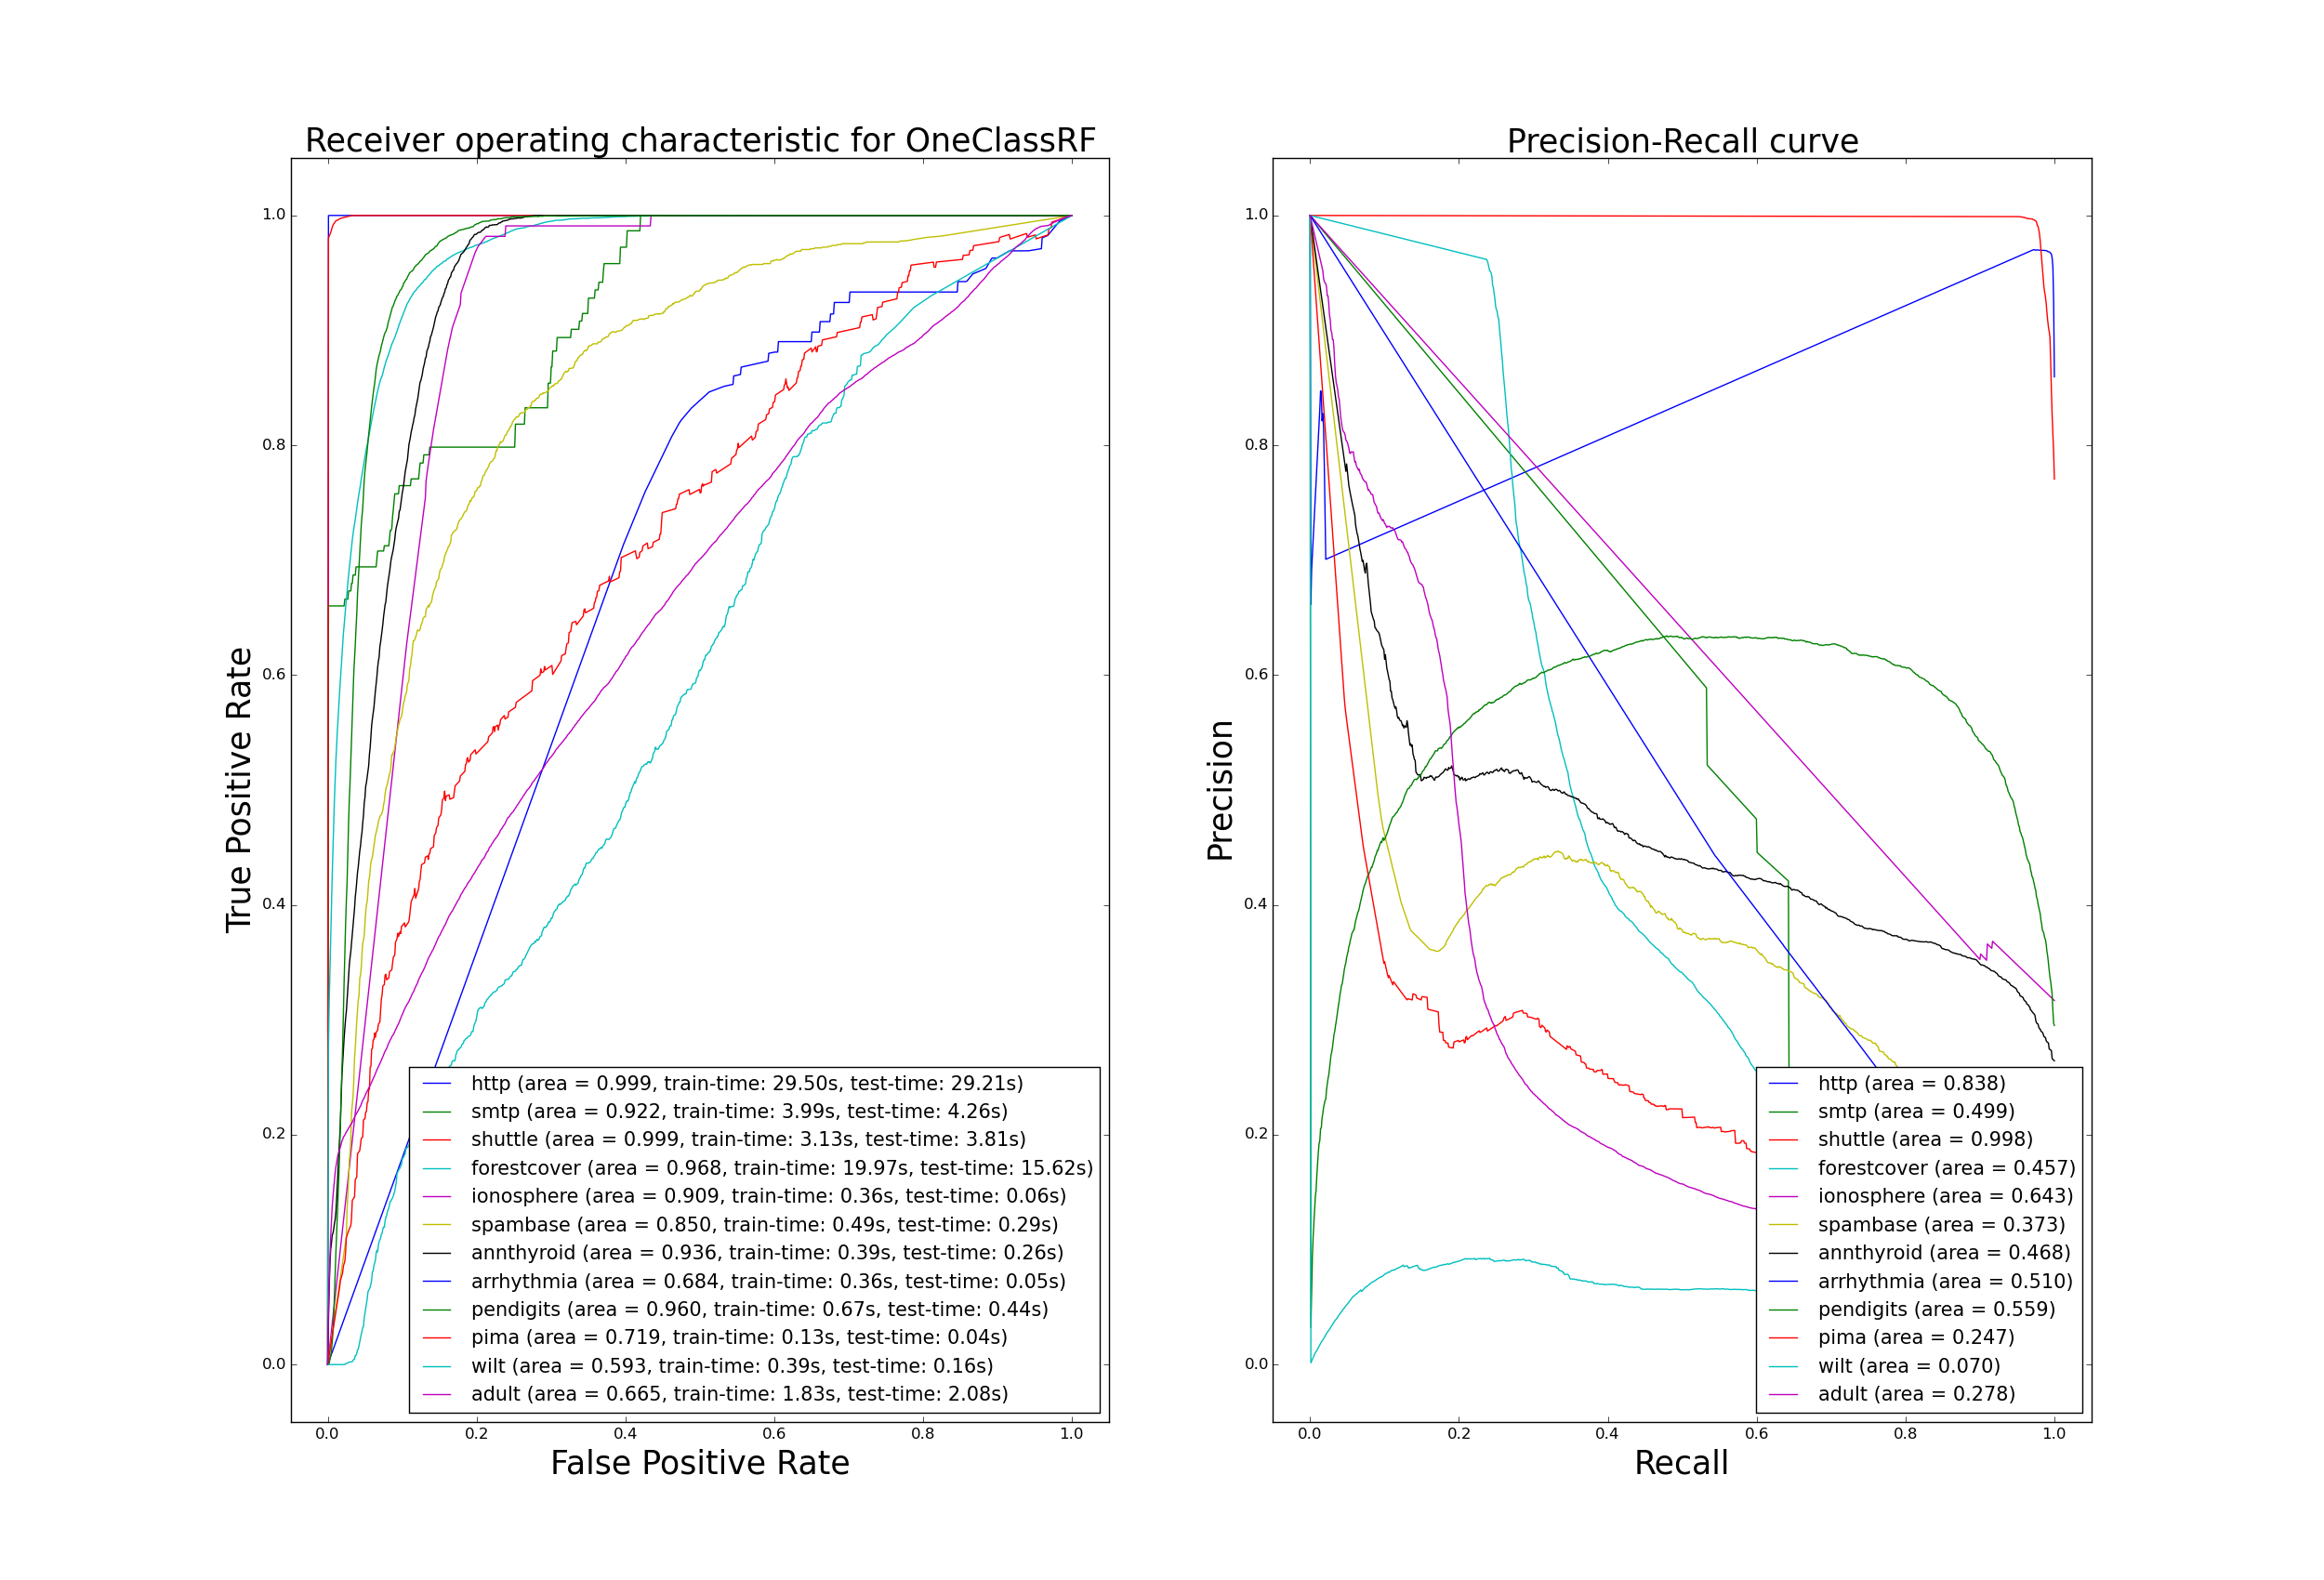
\includegraphics[trim=175 80 175 123, clip,
    width=0.75\textwidth]{./gfx/bench_oneclassrf_roc_pr_supervised_factorized.png}
\end{figure*}
\begin{figure*}[!ht]
    \caption{\acs{ROC} and \acs{PR} curves for \acs{OneClassRF} (outlier
    detection framework)}
    \label{ocrf:fig:oneclassrf_roc_pr_unsupervised}
    \centering
    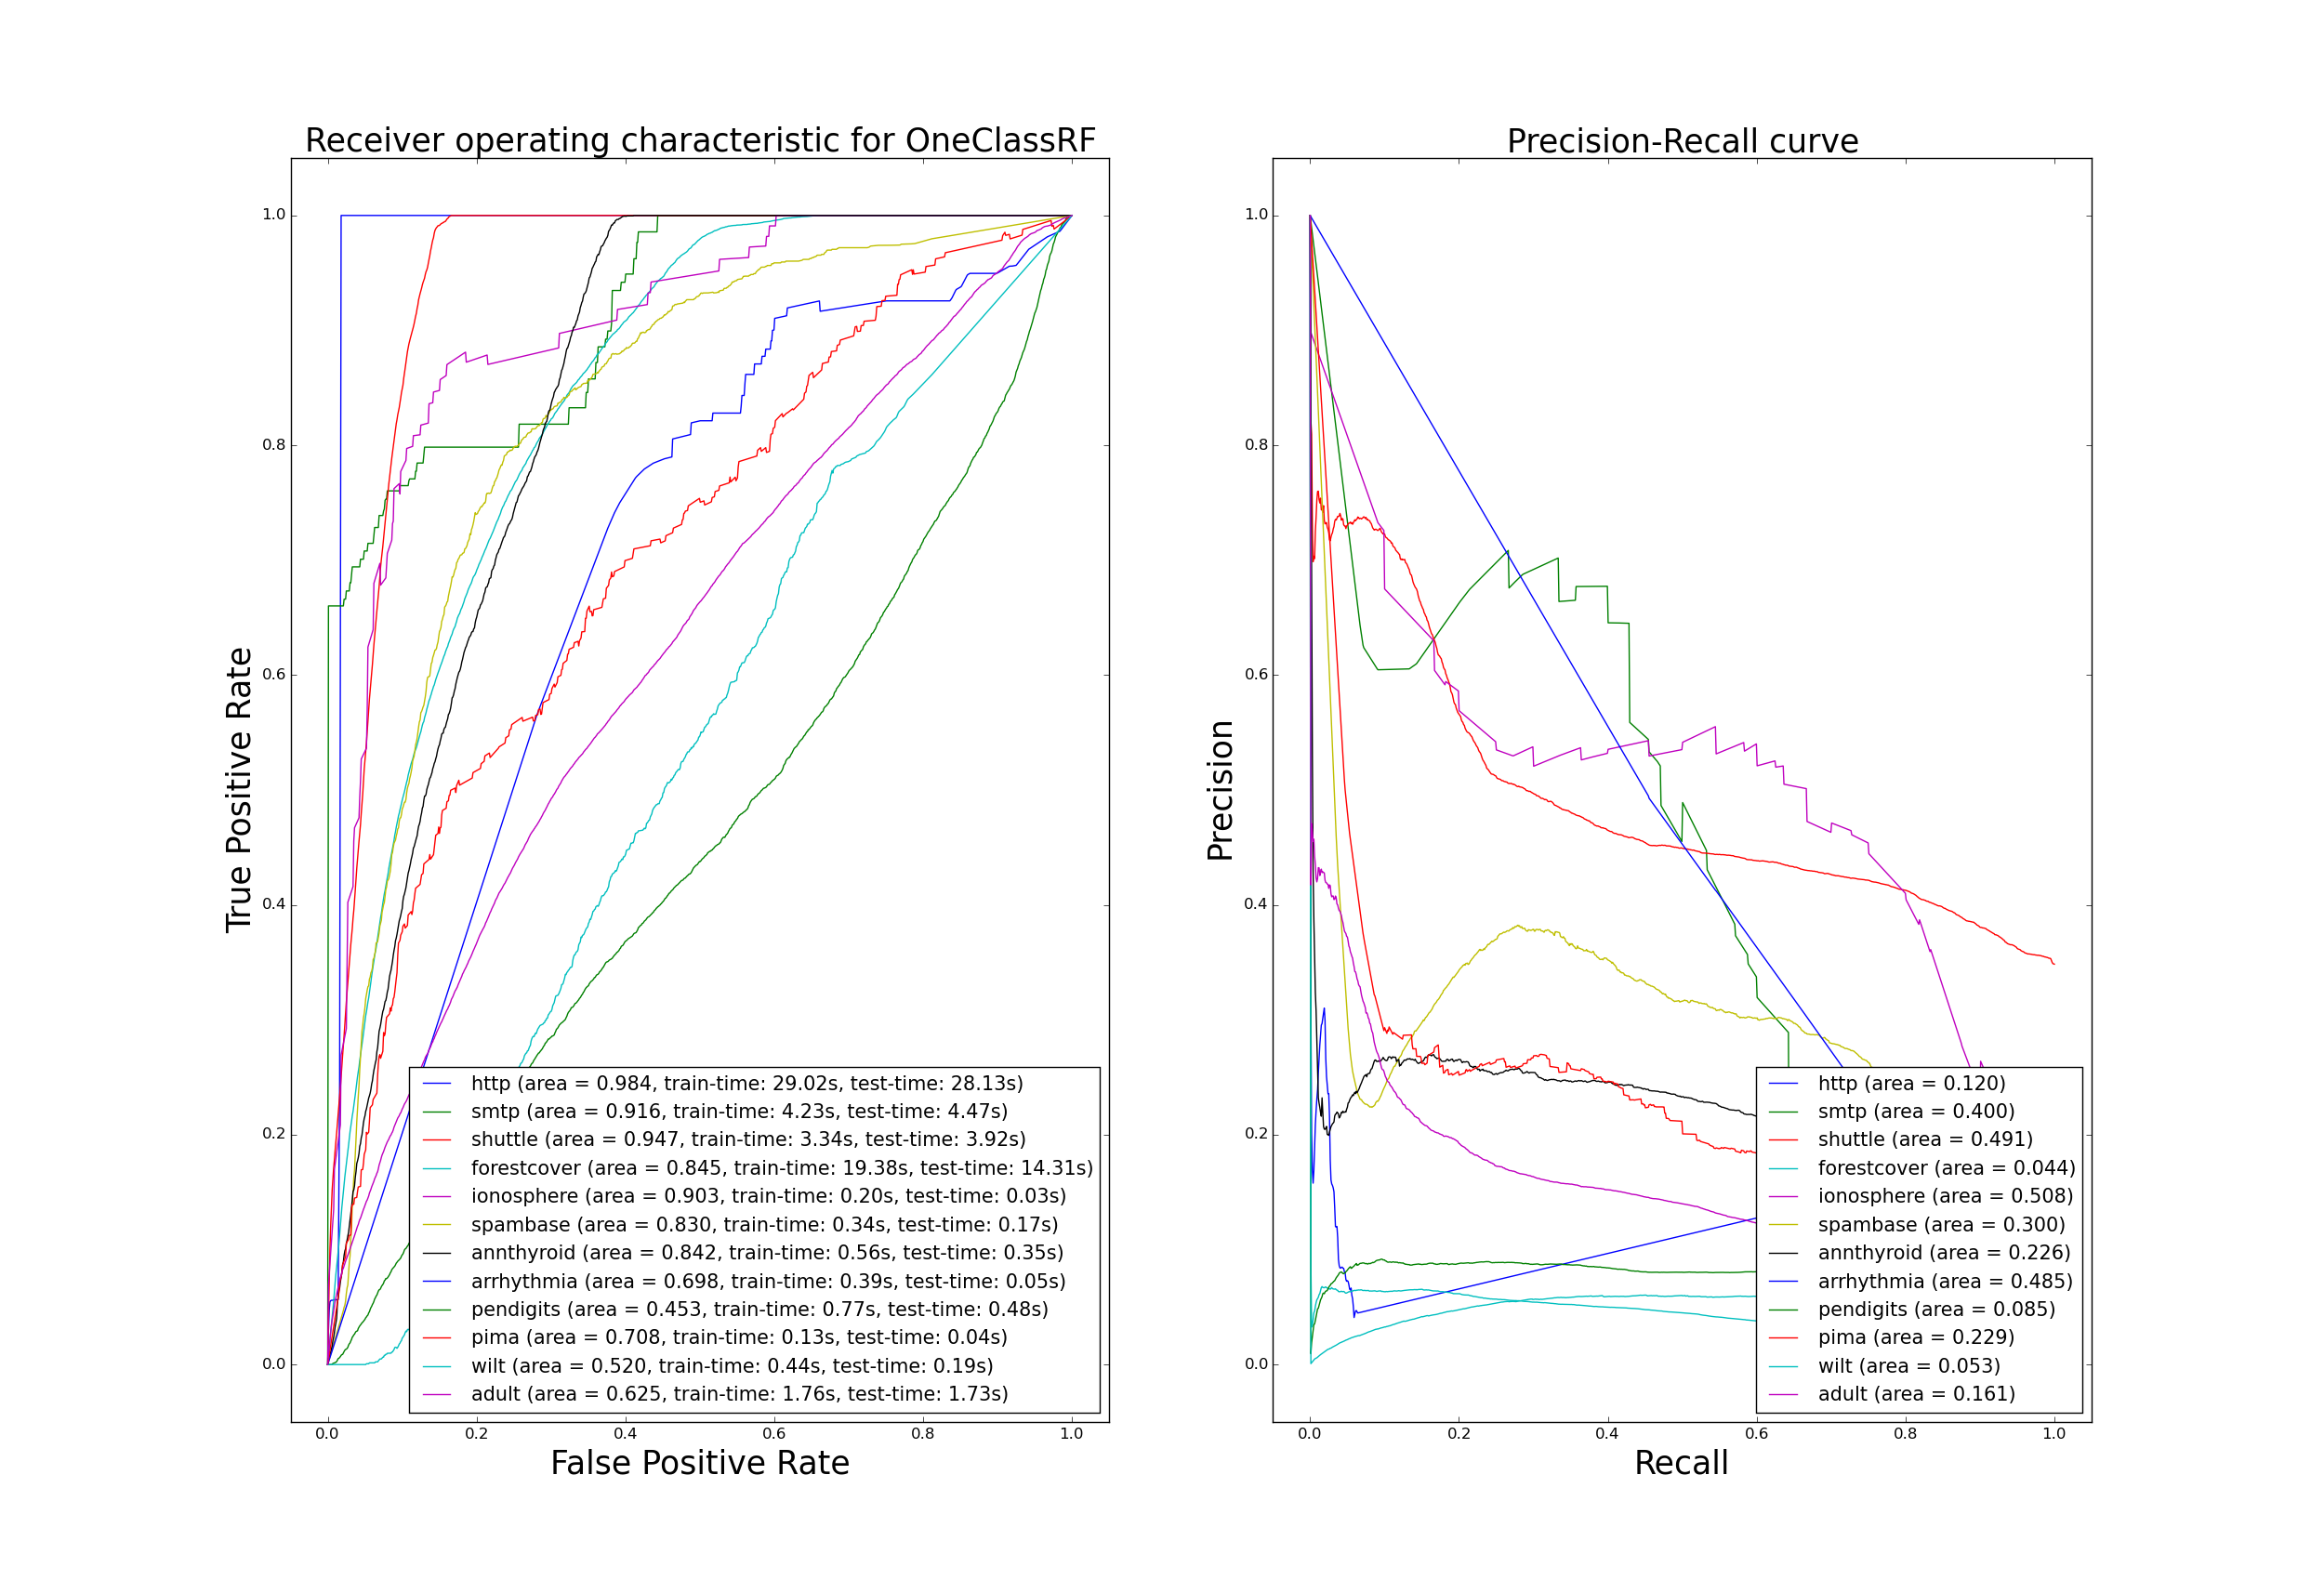
\includegraphics[trim=175 80 175 123, clip,
    width=0.75\textwidth]{./gfx/bench_oneclassrf_roc_pr_unsupervised_factorized.png}
\end{figure*}
\begin{figure*}[!ht]
    \caption{\acs{ROC} and \acs{PR} curves for \acs{iForest} (novelty detection
    framework)}
    \label{ocrf:fig:iforest_roc_pr}
    \centering
    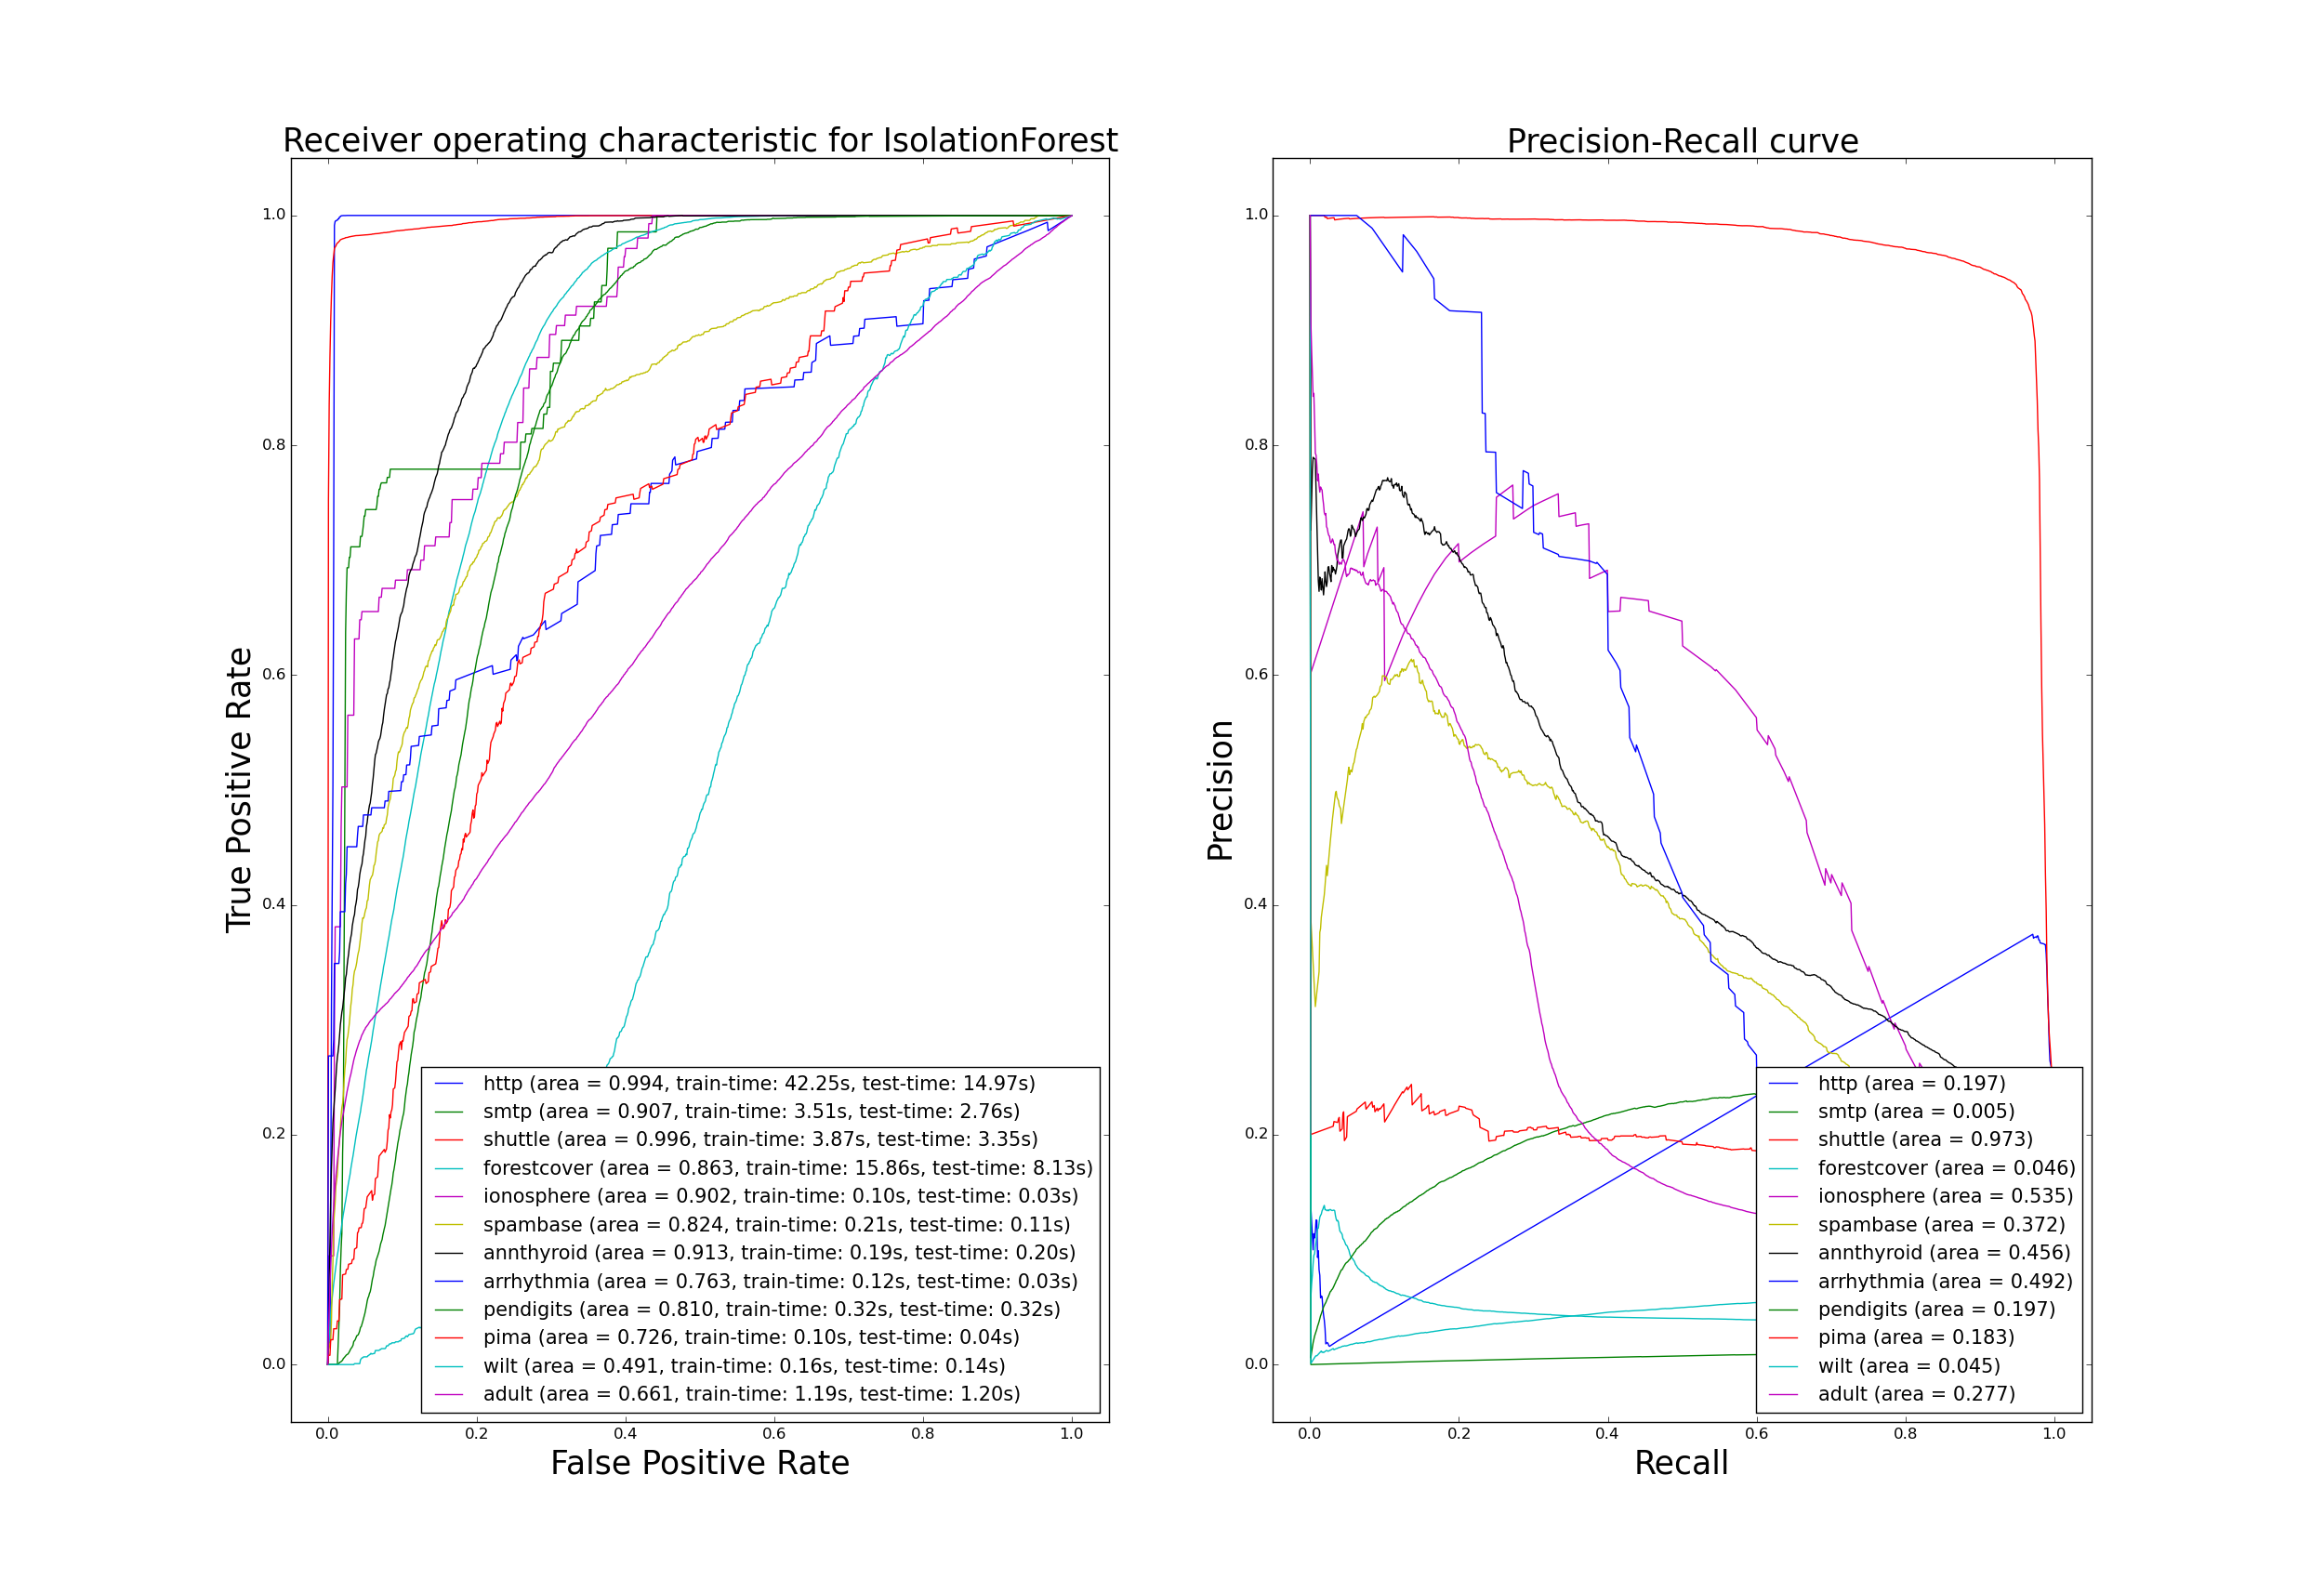
\includegraphics[trim=175 80 175 123, clip,
    width=0.75\textwidth]{./gfx/bench_iforest_roc_pr_supervised_factorized.png}
\end{figure*}
\begin{figure*}[!ht]
    \caption{\acs{ROC} and \acs{PR} curves for \acs{iForest} (outlier detection
    framework)}
    \label{ocrf:fig:iforest_roc_pr_unsupervised}
    \centering
    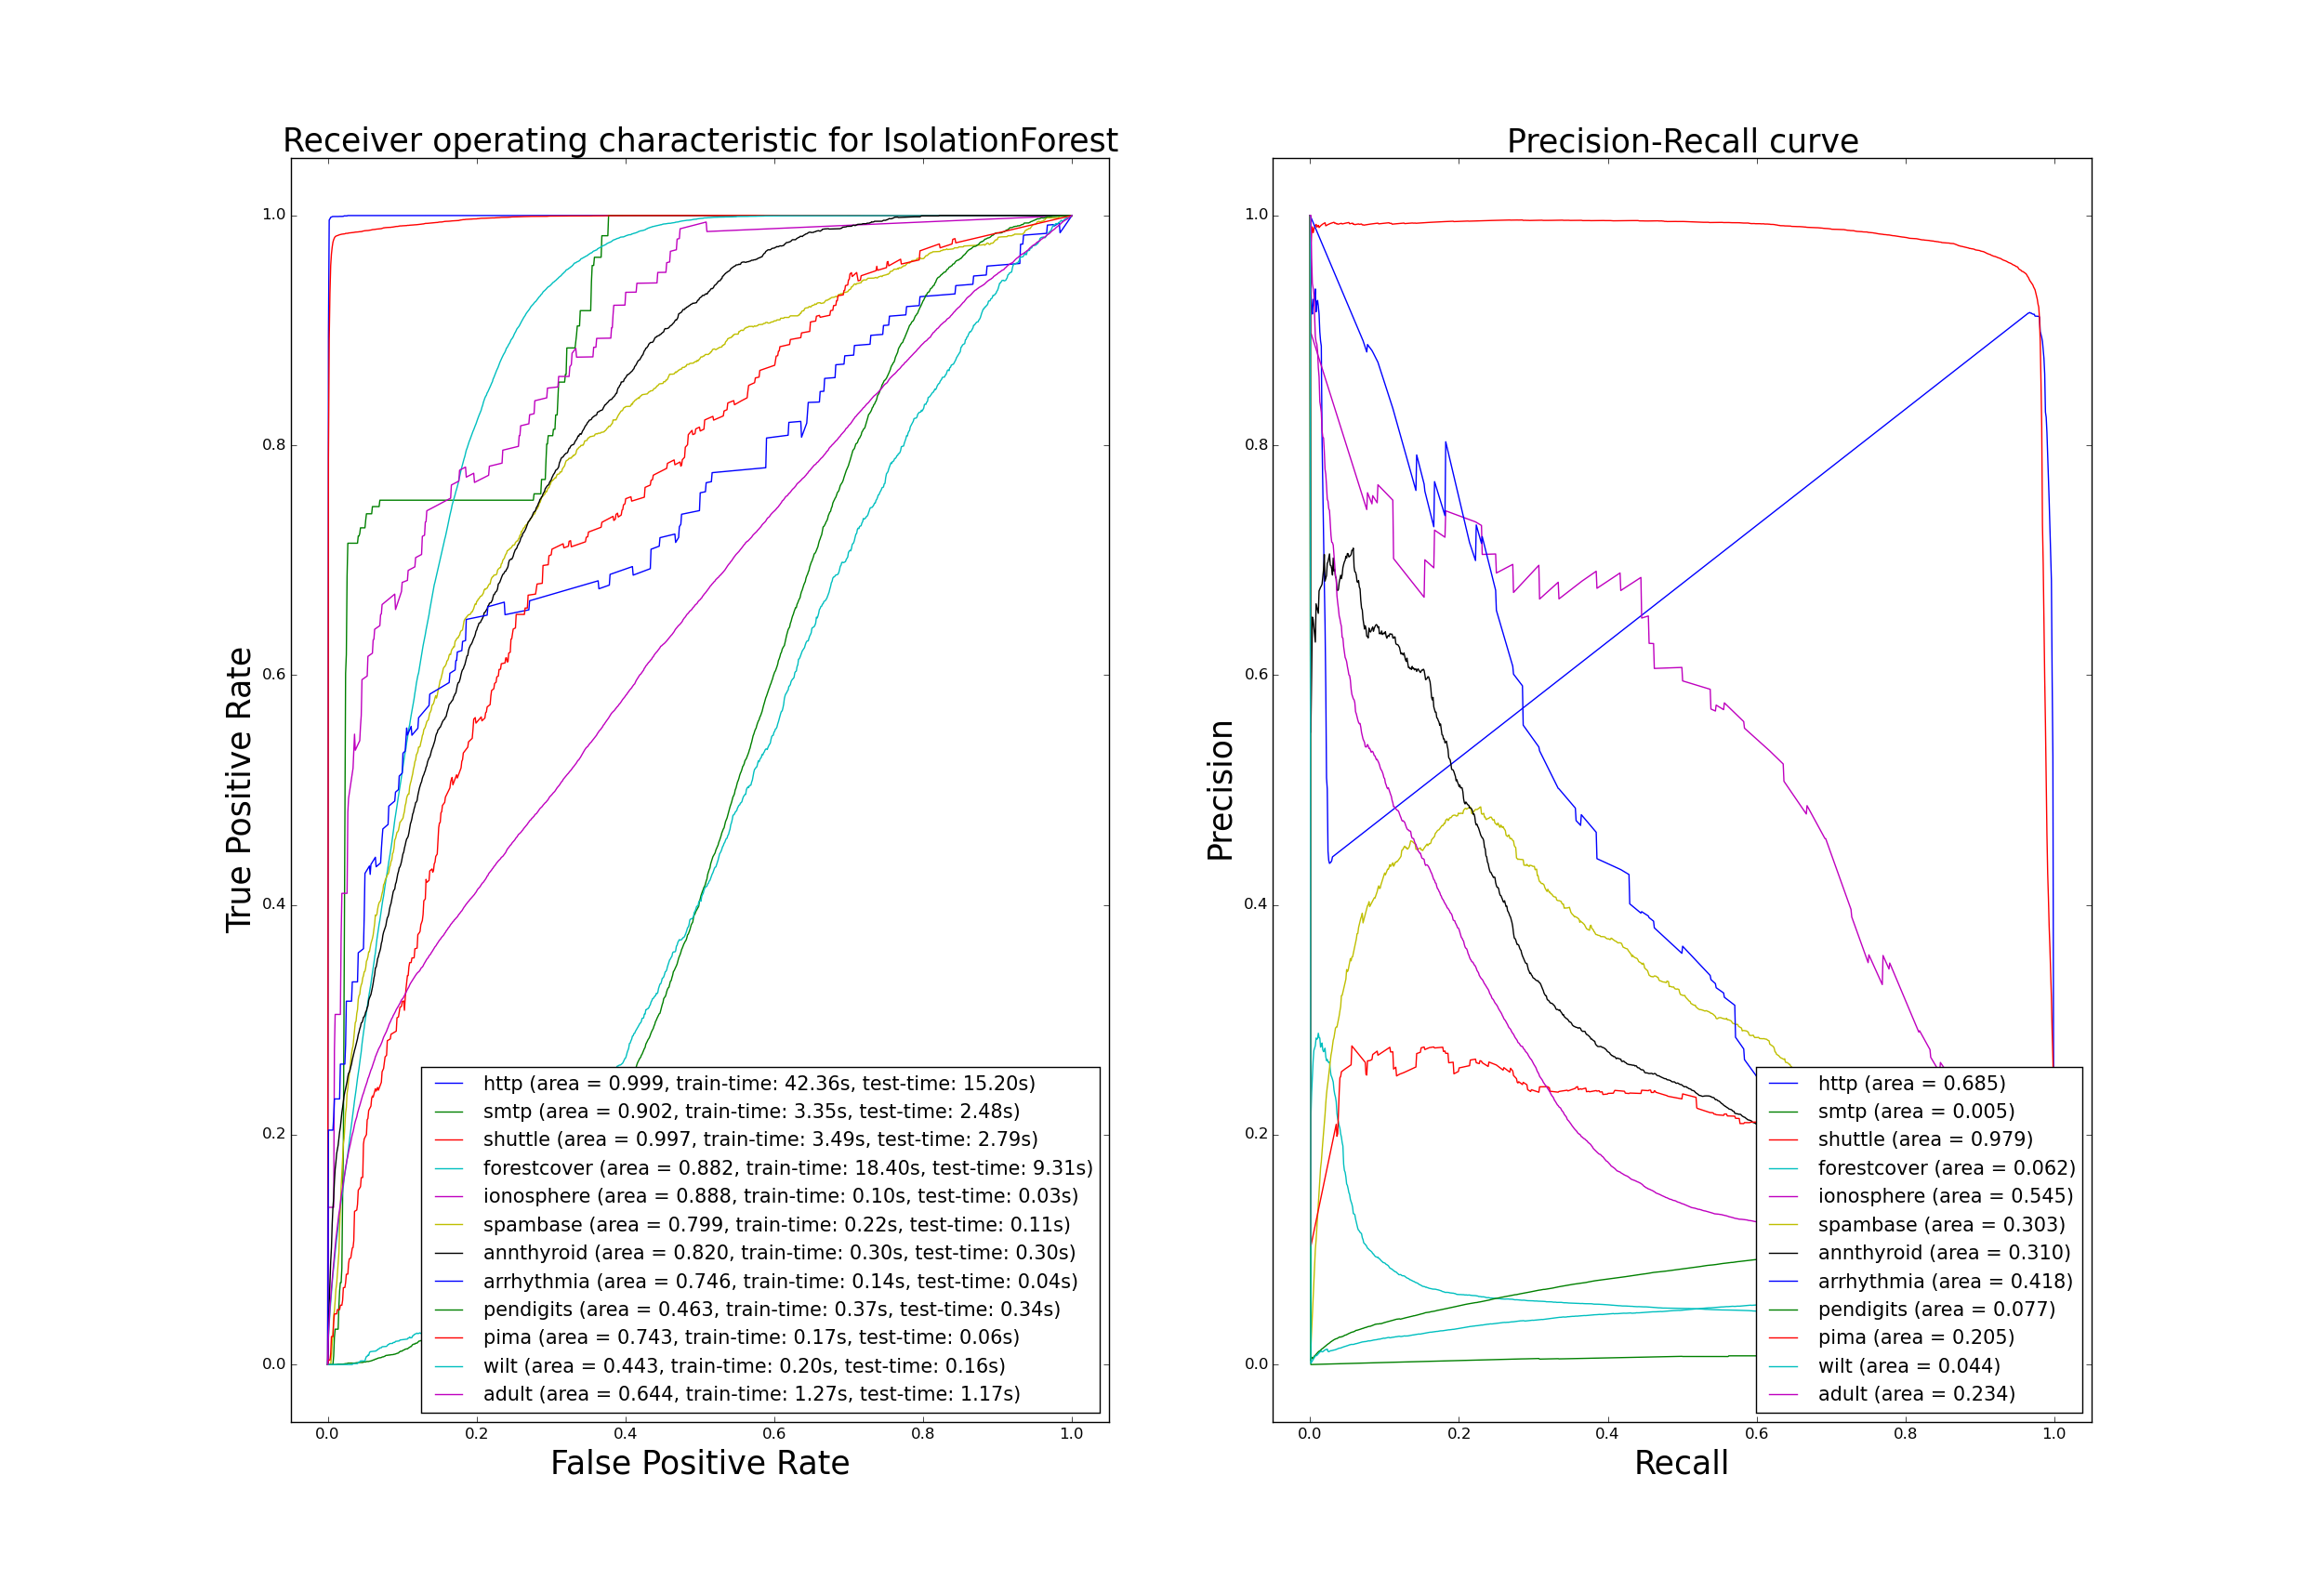
\includegraphics[trim=175 80 175 123, clip,
    width=0.75\textwidth]{./gfx/bench_iforest_roc_pr_unsupervised_factorized.png}
\end{figure*}
\begin{figure*}[!ht]
    \caption{\acs{ROC} and \acs{PR} curves for \acs{OCRFsampling} (novelty
    detection framework)}
    \label{ocrf:fig:ocrfm_roc_pr}
    \centering
    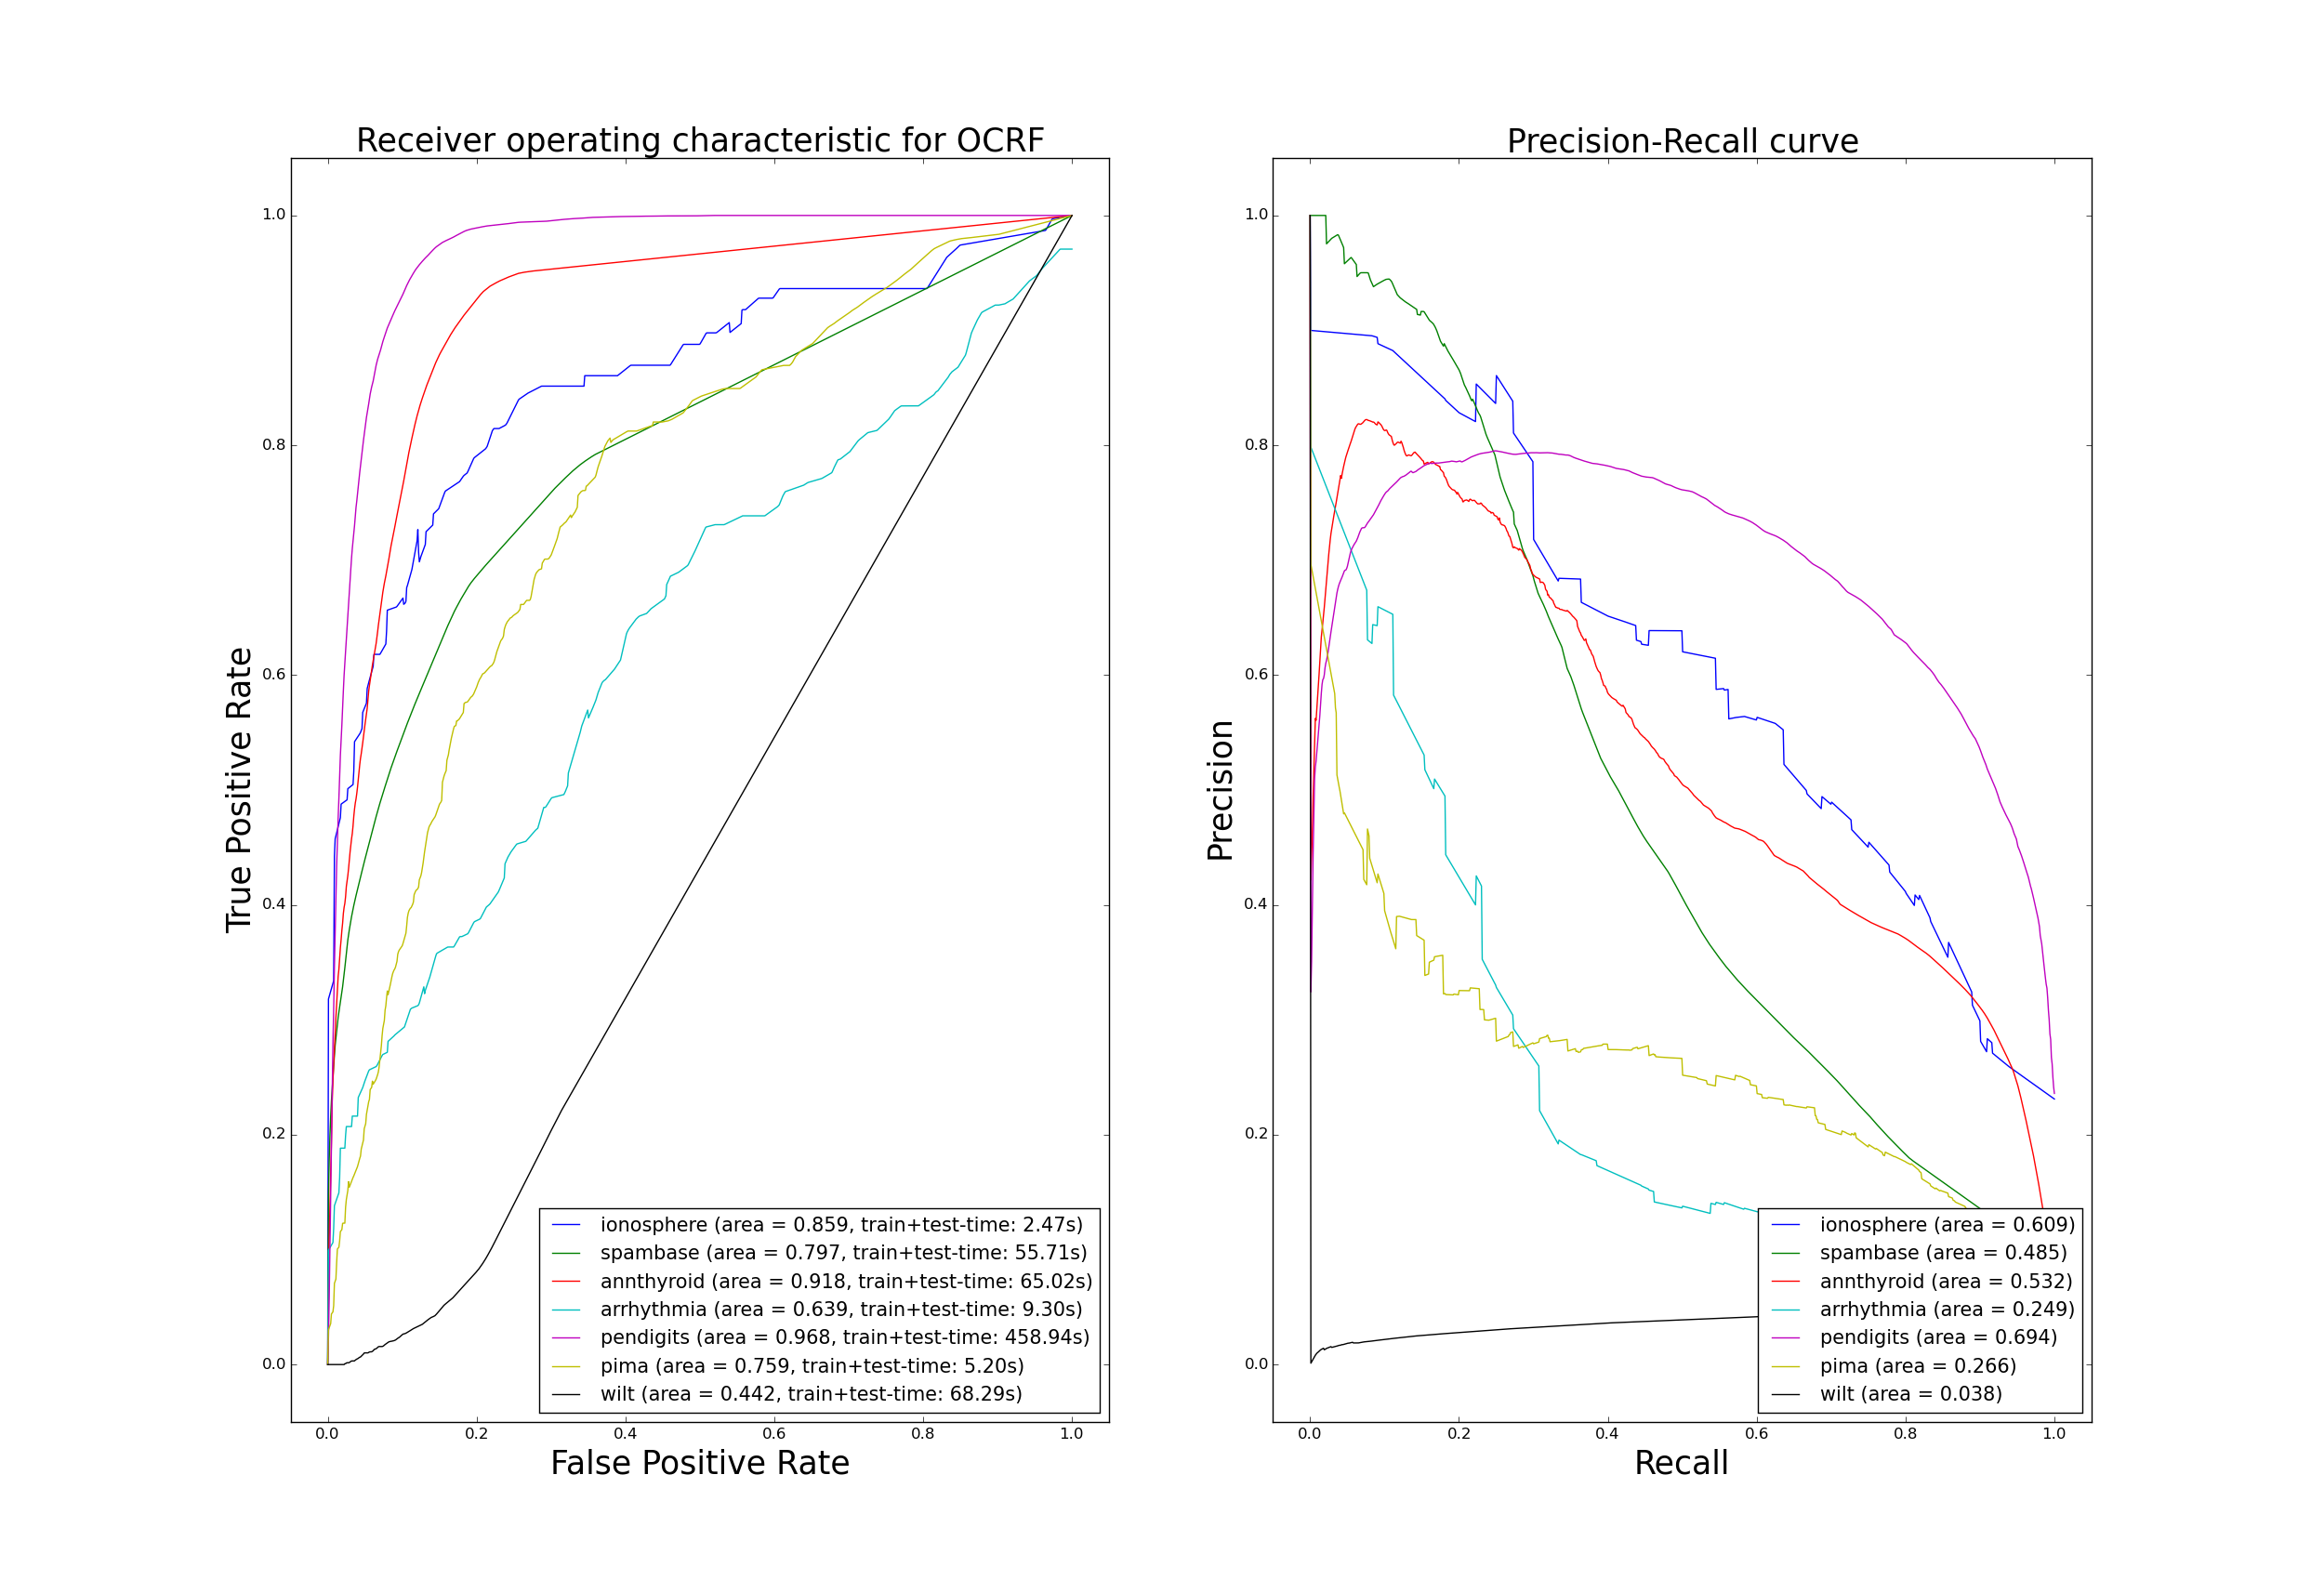
\includegraphics[trim=175 80 175 123, clip,
    width=0.75\textwidth]{./gfx/bench_ocrf_roc_pr_supervised_factorized.png}
\end{figure*}
\begin{figure*}[!ht]
    \caption{\acs{ROC} and \acs{PR} curves for \acs{OCRFsampling} (outlier
    detection framework)}
    \label{ocrf:fig:ocrfm_roc_pr_unsupervised}
    \centering
    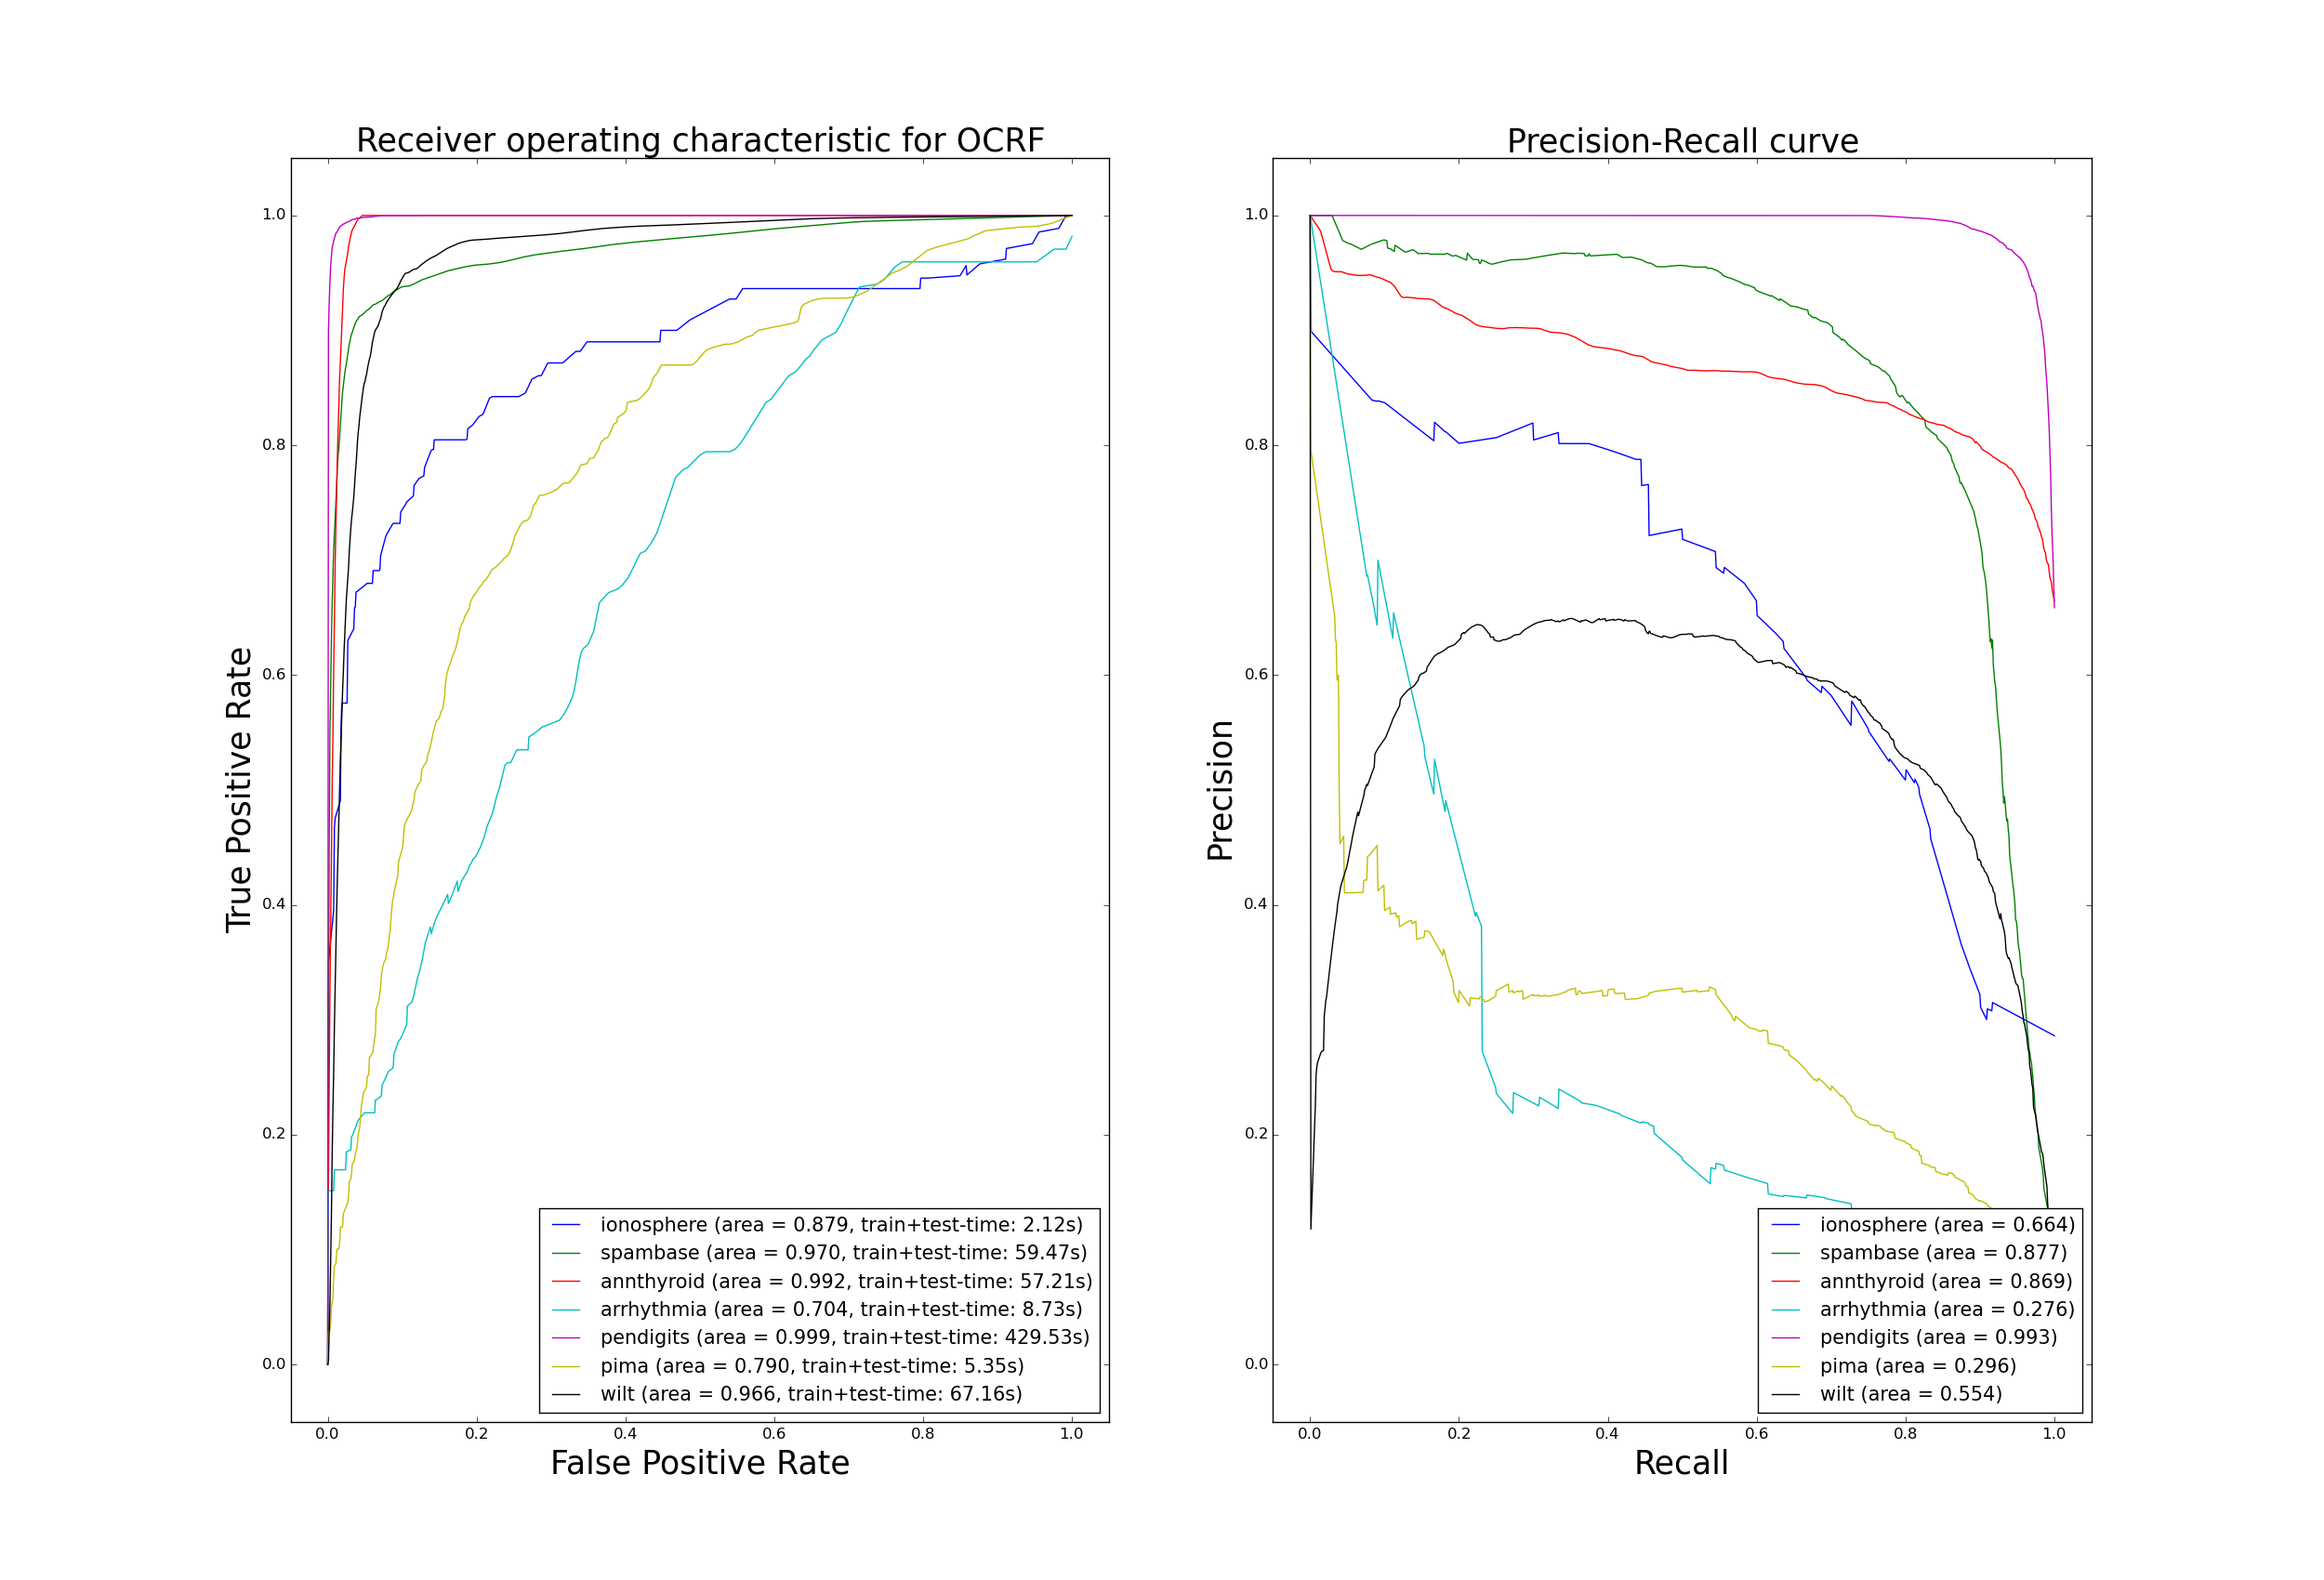
\includegraphics[trim=175 80 175 123, clip,
    width=0.75\textwidth]{./gfx/bench_ocrf_roc_pr_unsupervised_factorized.png}
\end{figure*}
\begin{figure*}[!ht]
    \caption{\acs{ROC} and \acs{PR} curves for \acs{OCSVM} (novelty detection
    framework)}
    \label{ocrf:fig:ocsvm_roc_pr}
    \centering
    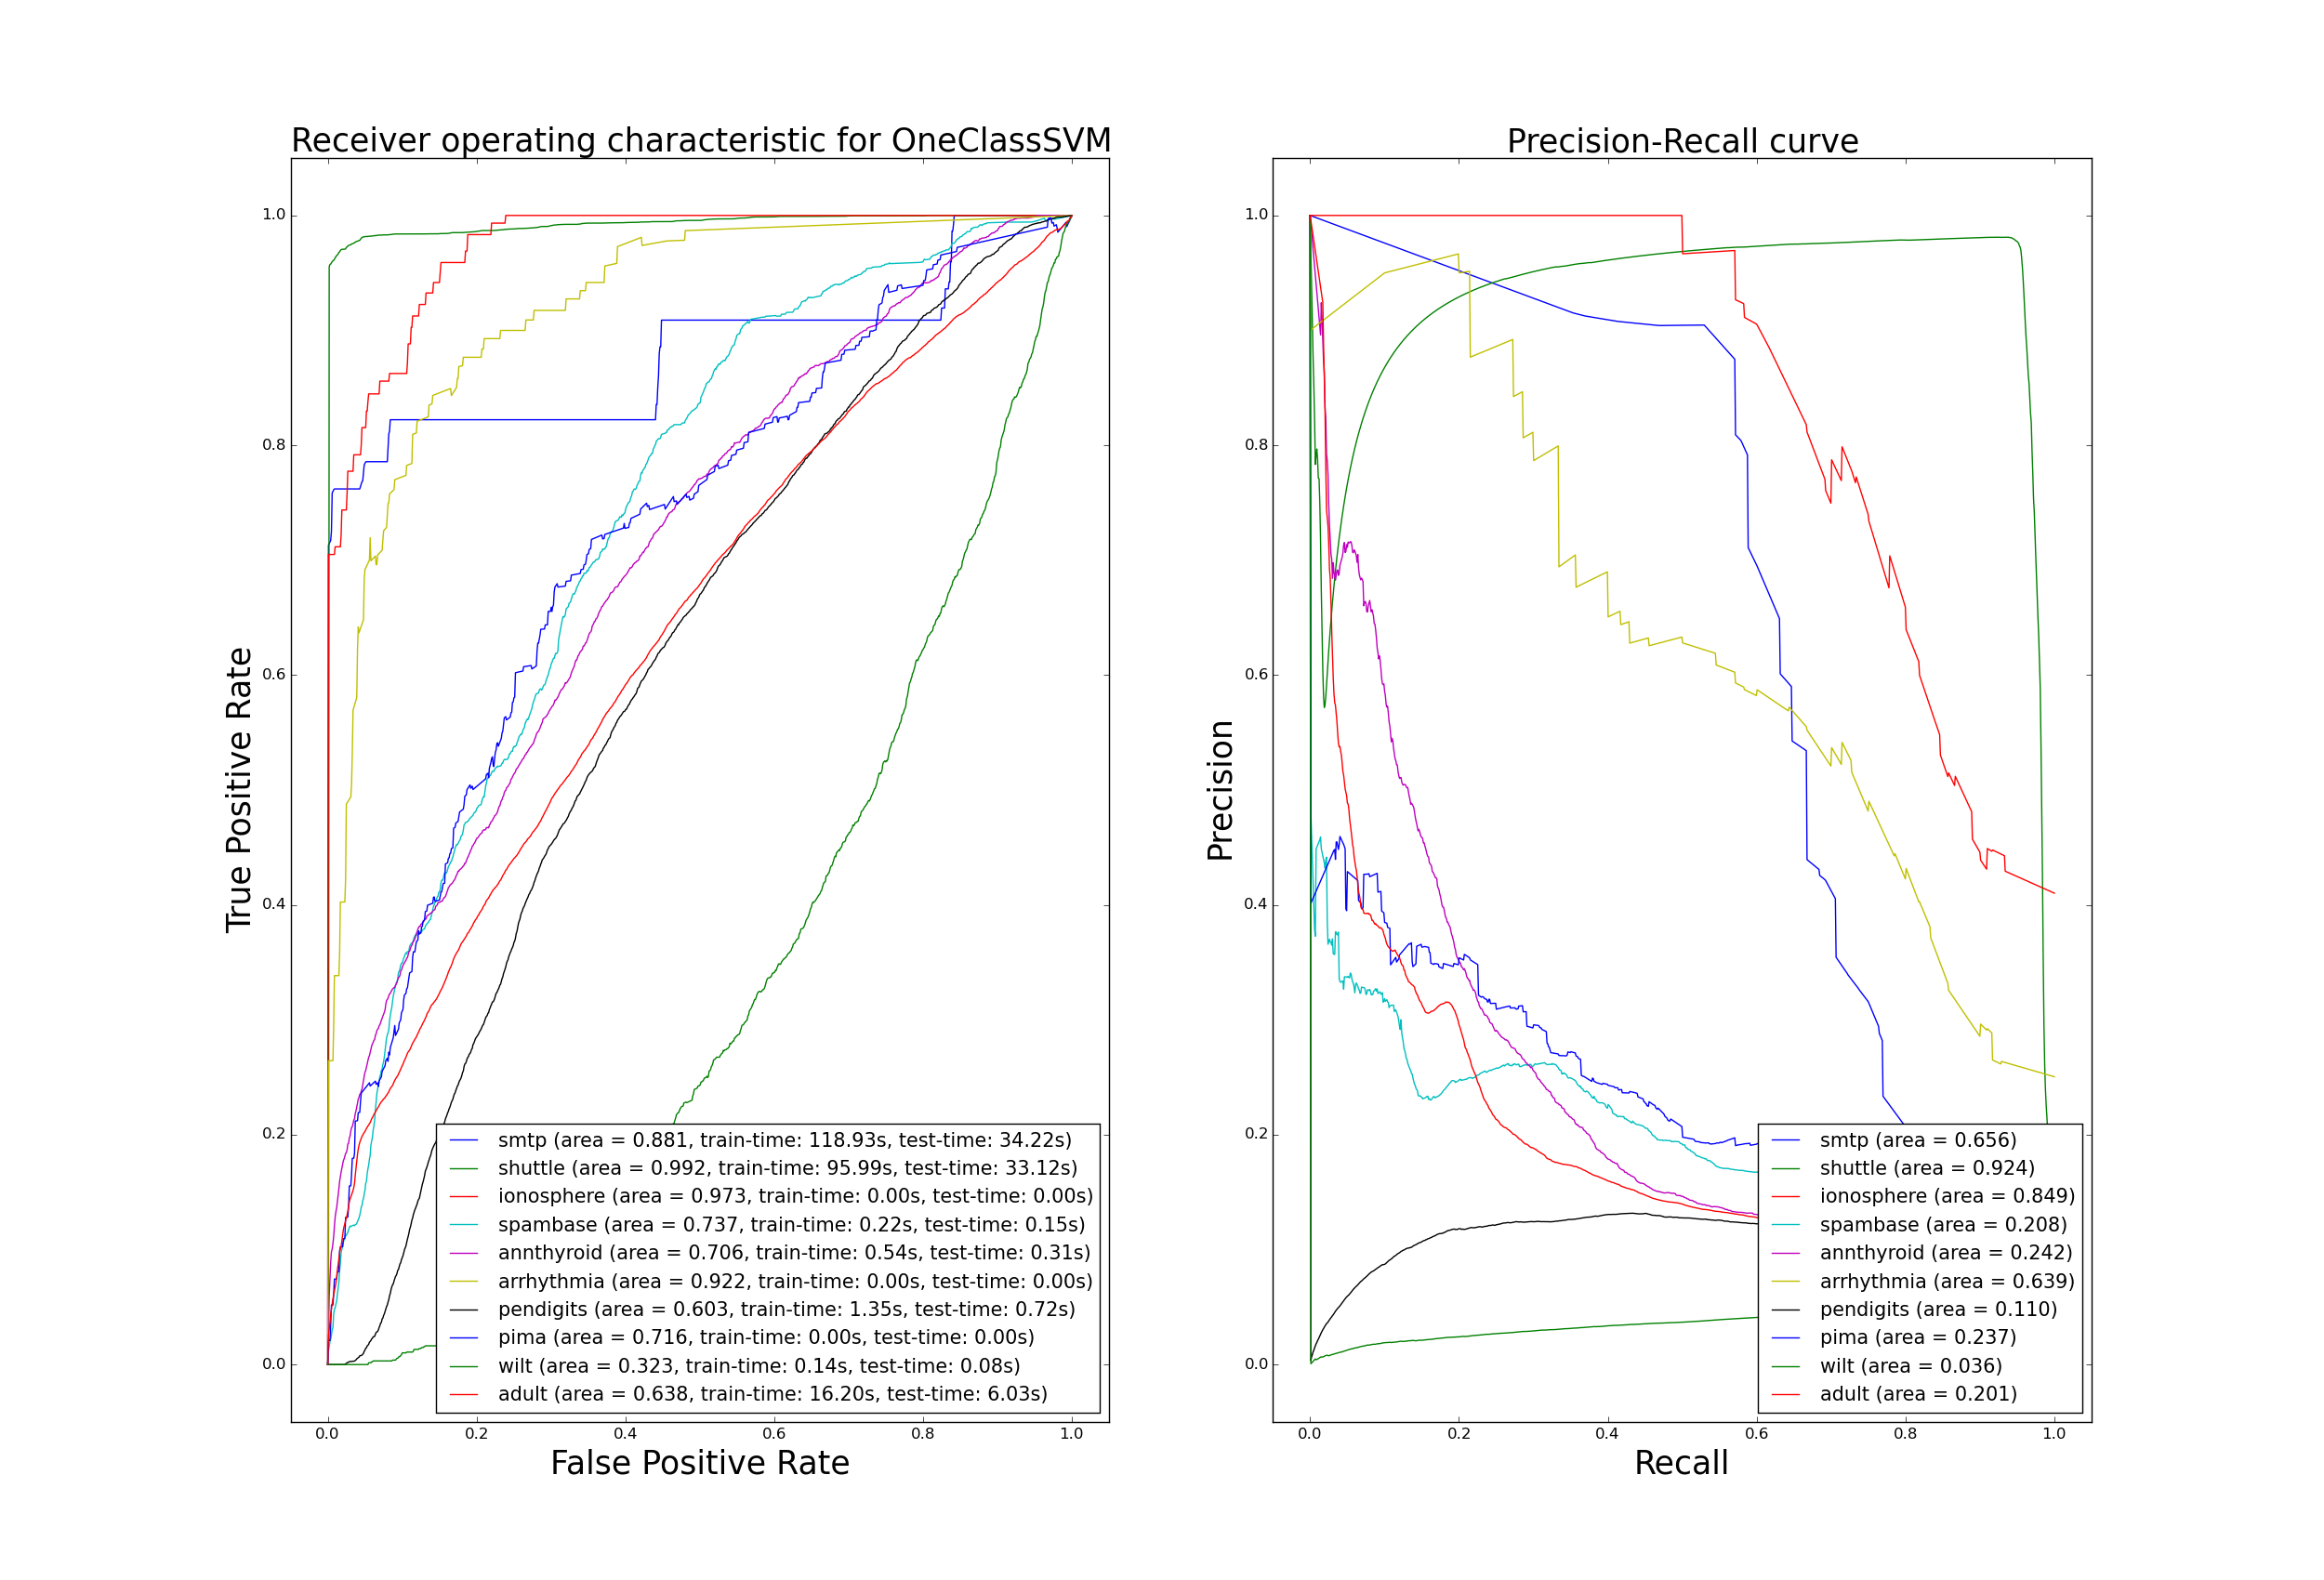
\includegraphics[trim=175 80 175 123, clip,
    width=0.75\textwidth]{./gfx/bench_ocsvm_roc_pr_supervised_factorized.png}
\end{figure*}
\begin{figure*}[!ht]
    \caption{\acs{ROC} and \acs{PR} curves for \acs{OCSVM} (outlier detection
    framework)}
    \label{ocrf:fig:ocsvm_roc_pr_unsupervised}
    \centering
    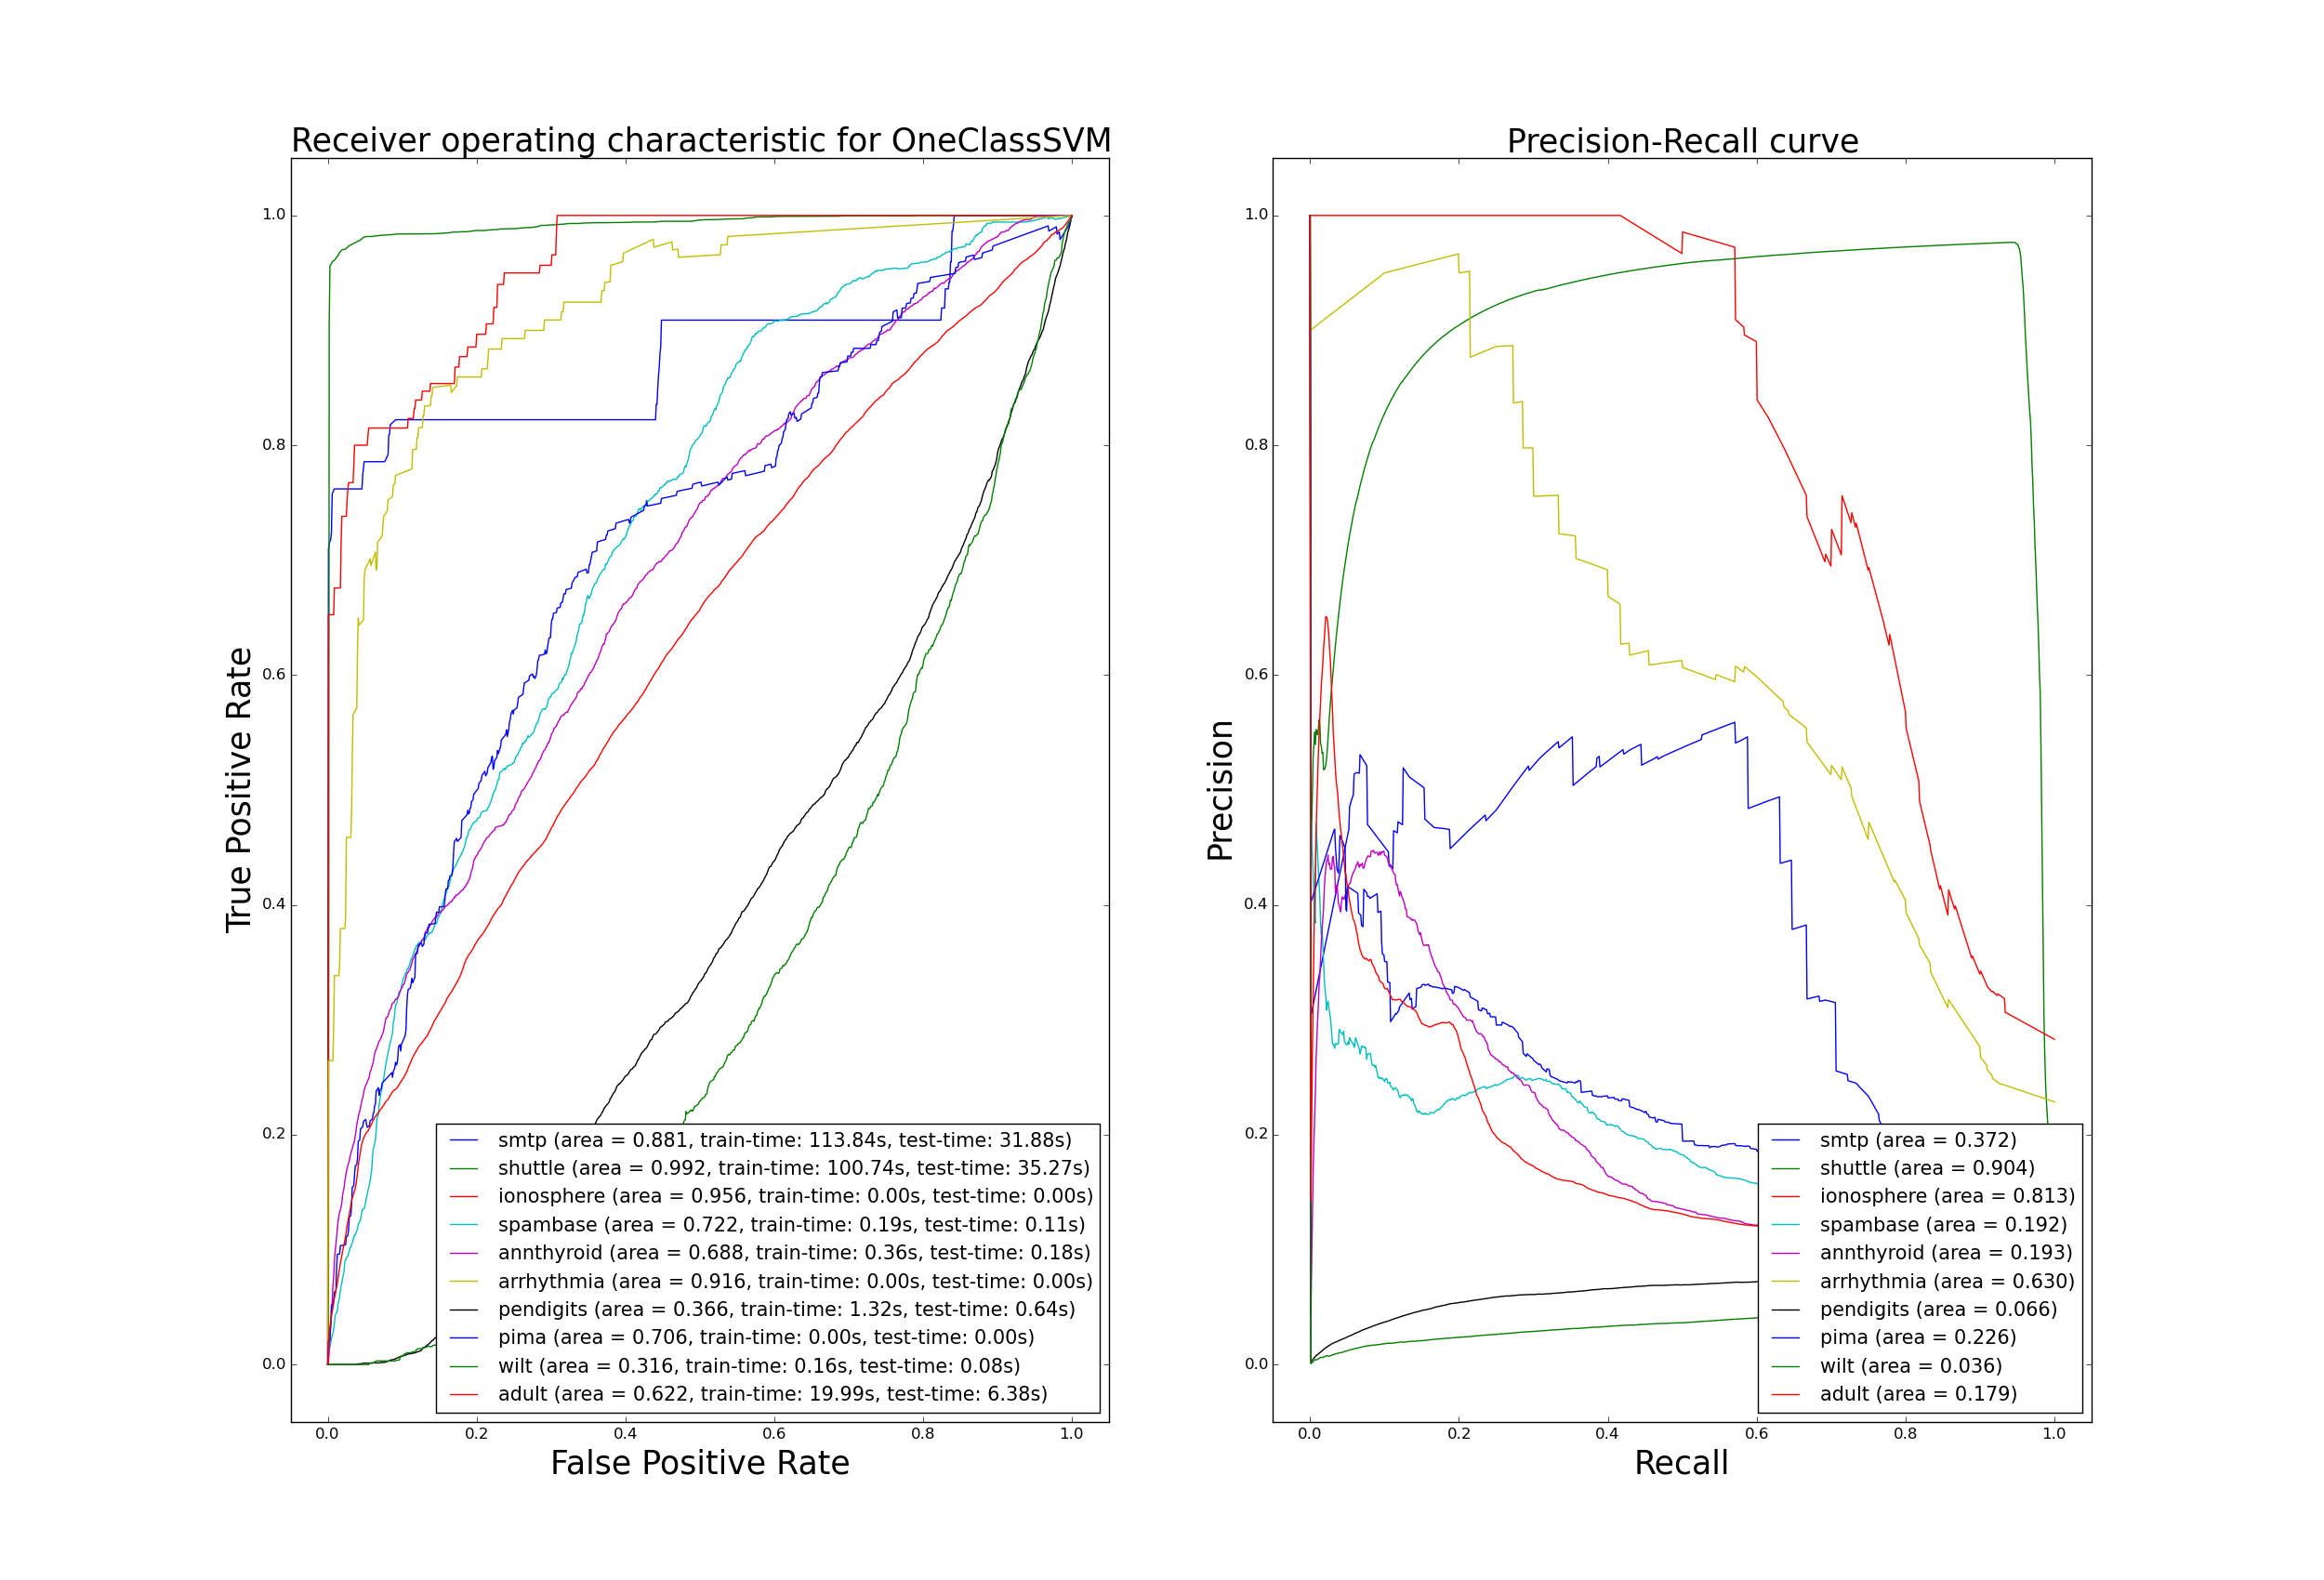
\includegraphics[trim=175 80 175 123, clip,
    width=0.75\textwidth]{./gfx/bench_ocsvm_roc_pr_unsupervised_factorized.png}
\end{figure*}
\begin{figure*}[!ht]
    \caption{\acs{ROC} and \acs{PR} curves for \acs{LOF} (novelty detection
    framework)}
    \label{ocrf:fig:lof_roc_pr}
    \centering
    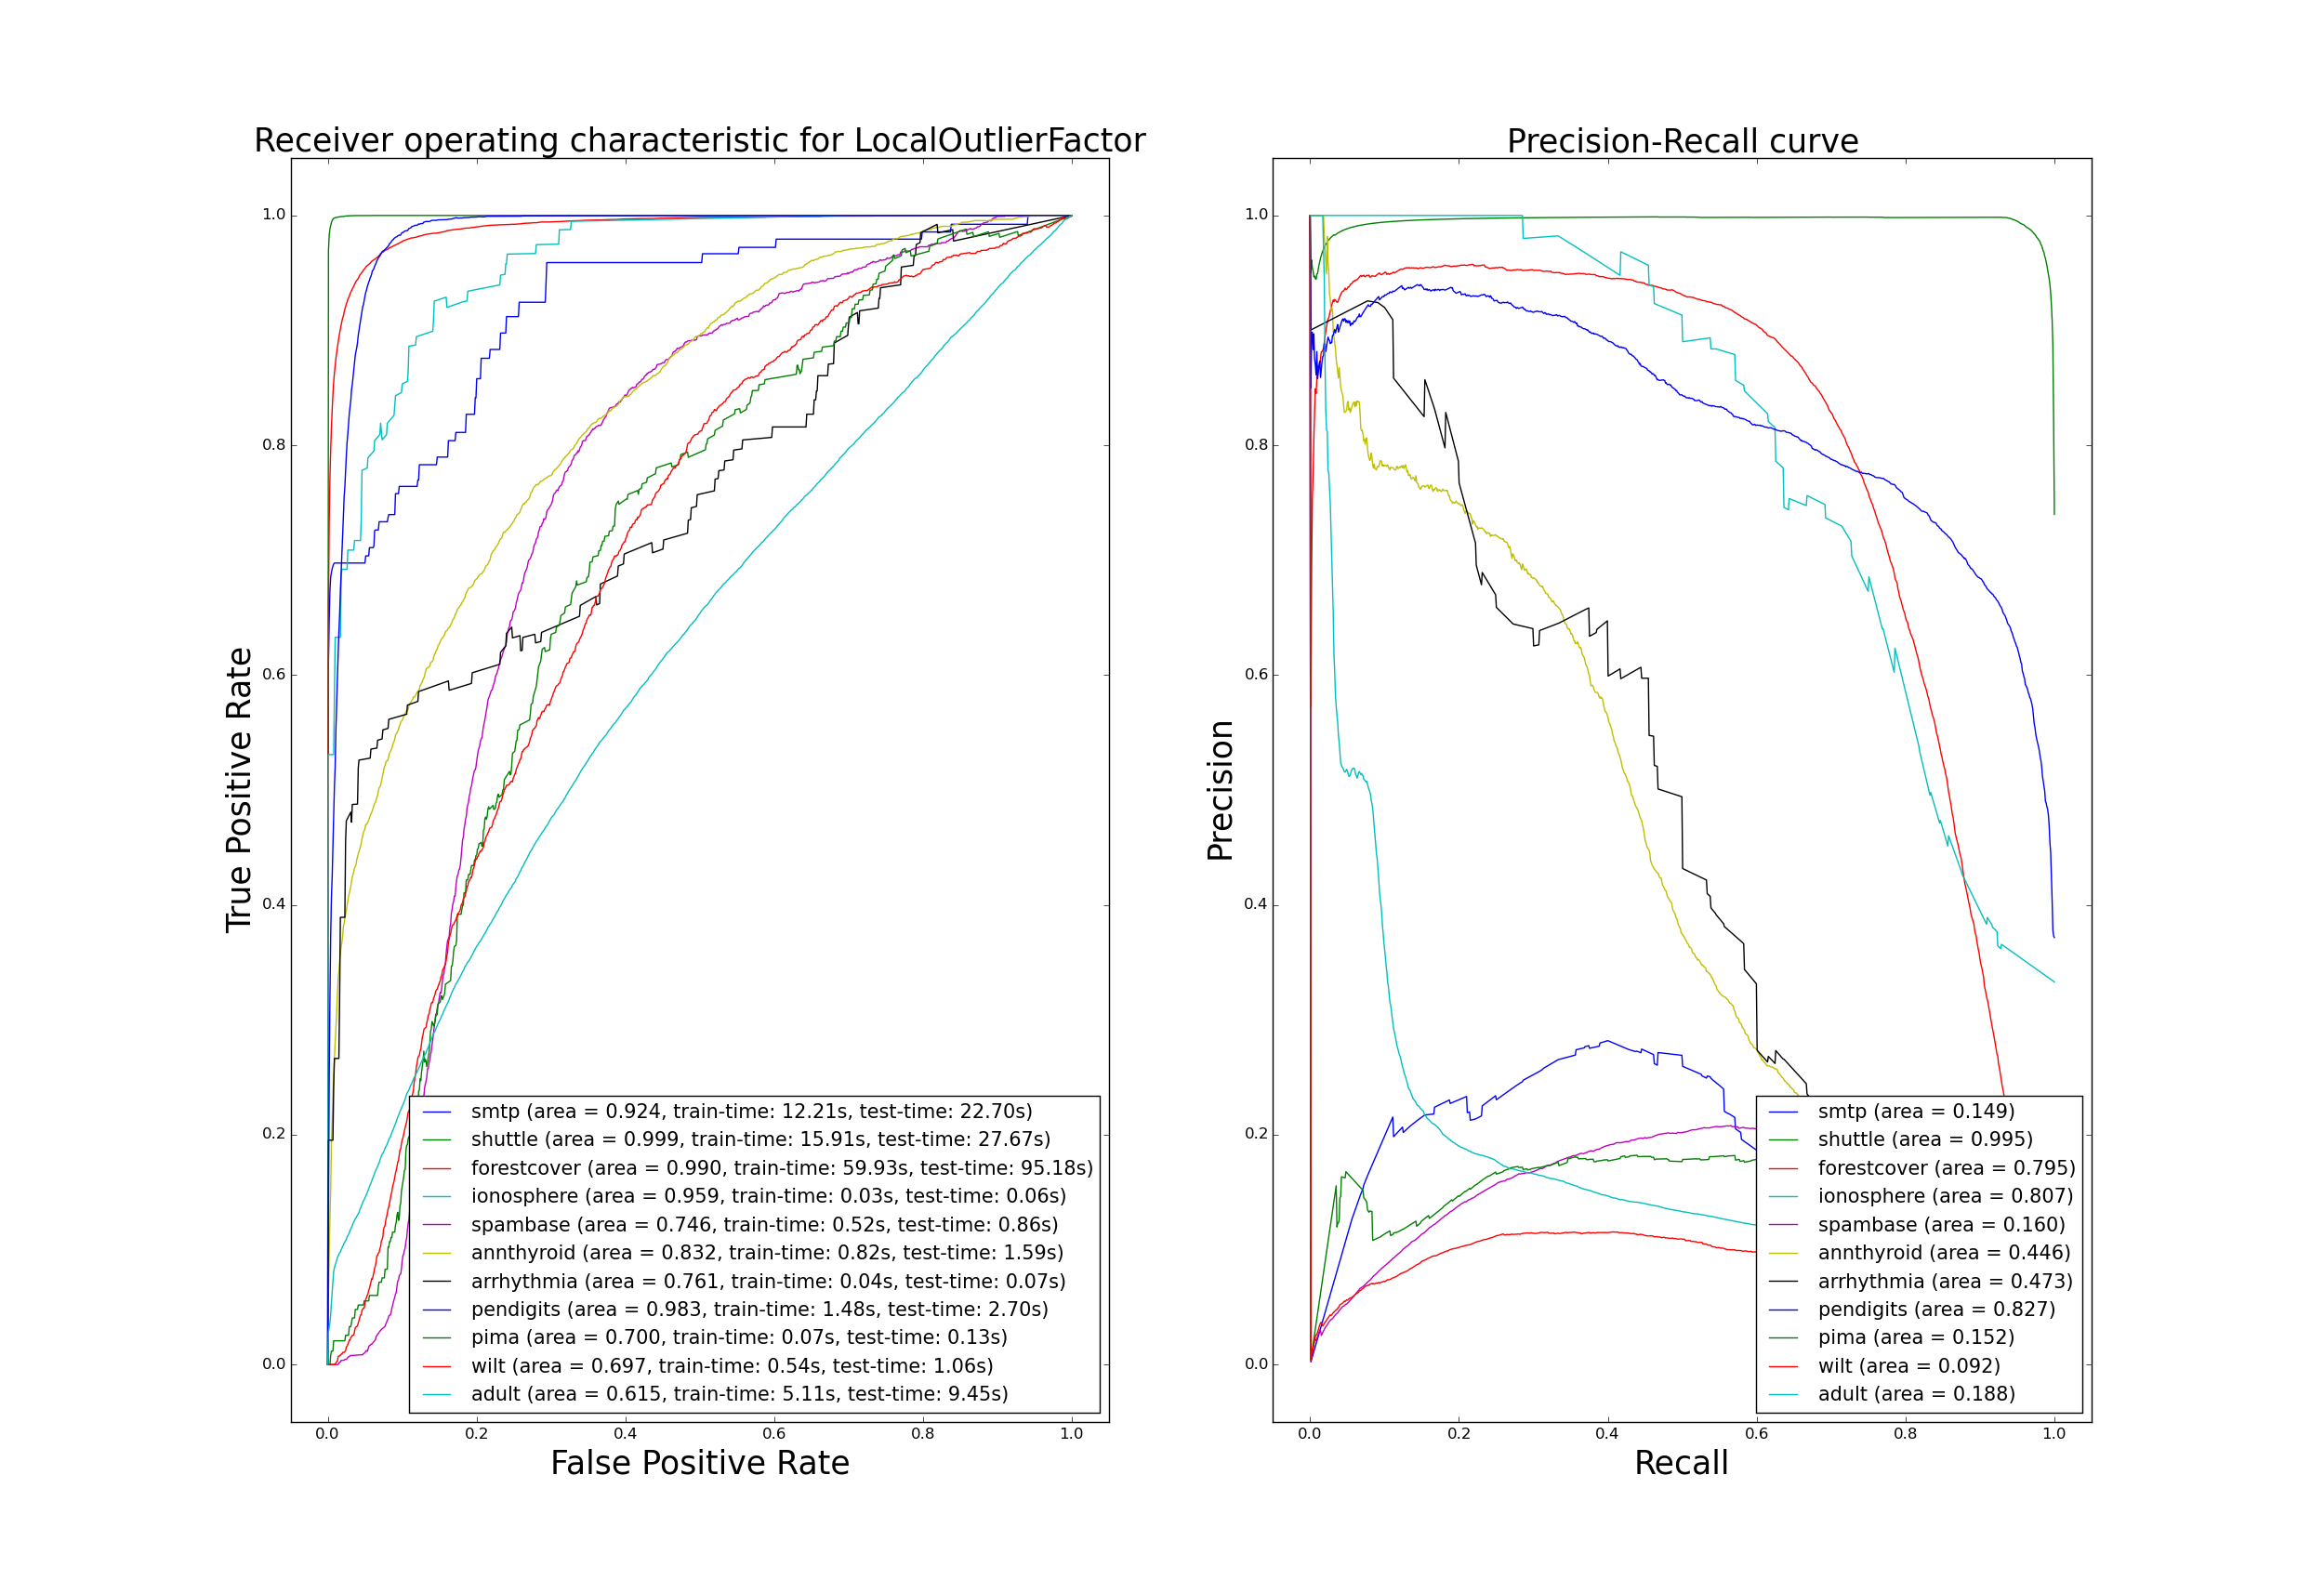
\includegraphics[trim=175 80 175 123, clip,
    width=0.75\textwidth]{./gfx/bench_lof_roc_pr_supervised_factorized.png}
\end{figure*}
\begin{figure*}[!ht]
    \caption{\acs{ROC} and \acs{PR} curves for \acs{LOF} (outlier detection
    framework)}
    \label{ocrf:fig:lof_roc_pr_unsupervised}
    \centering
    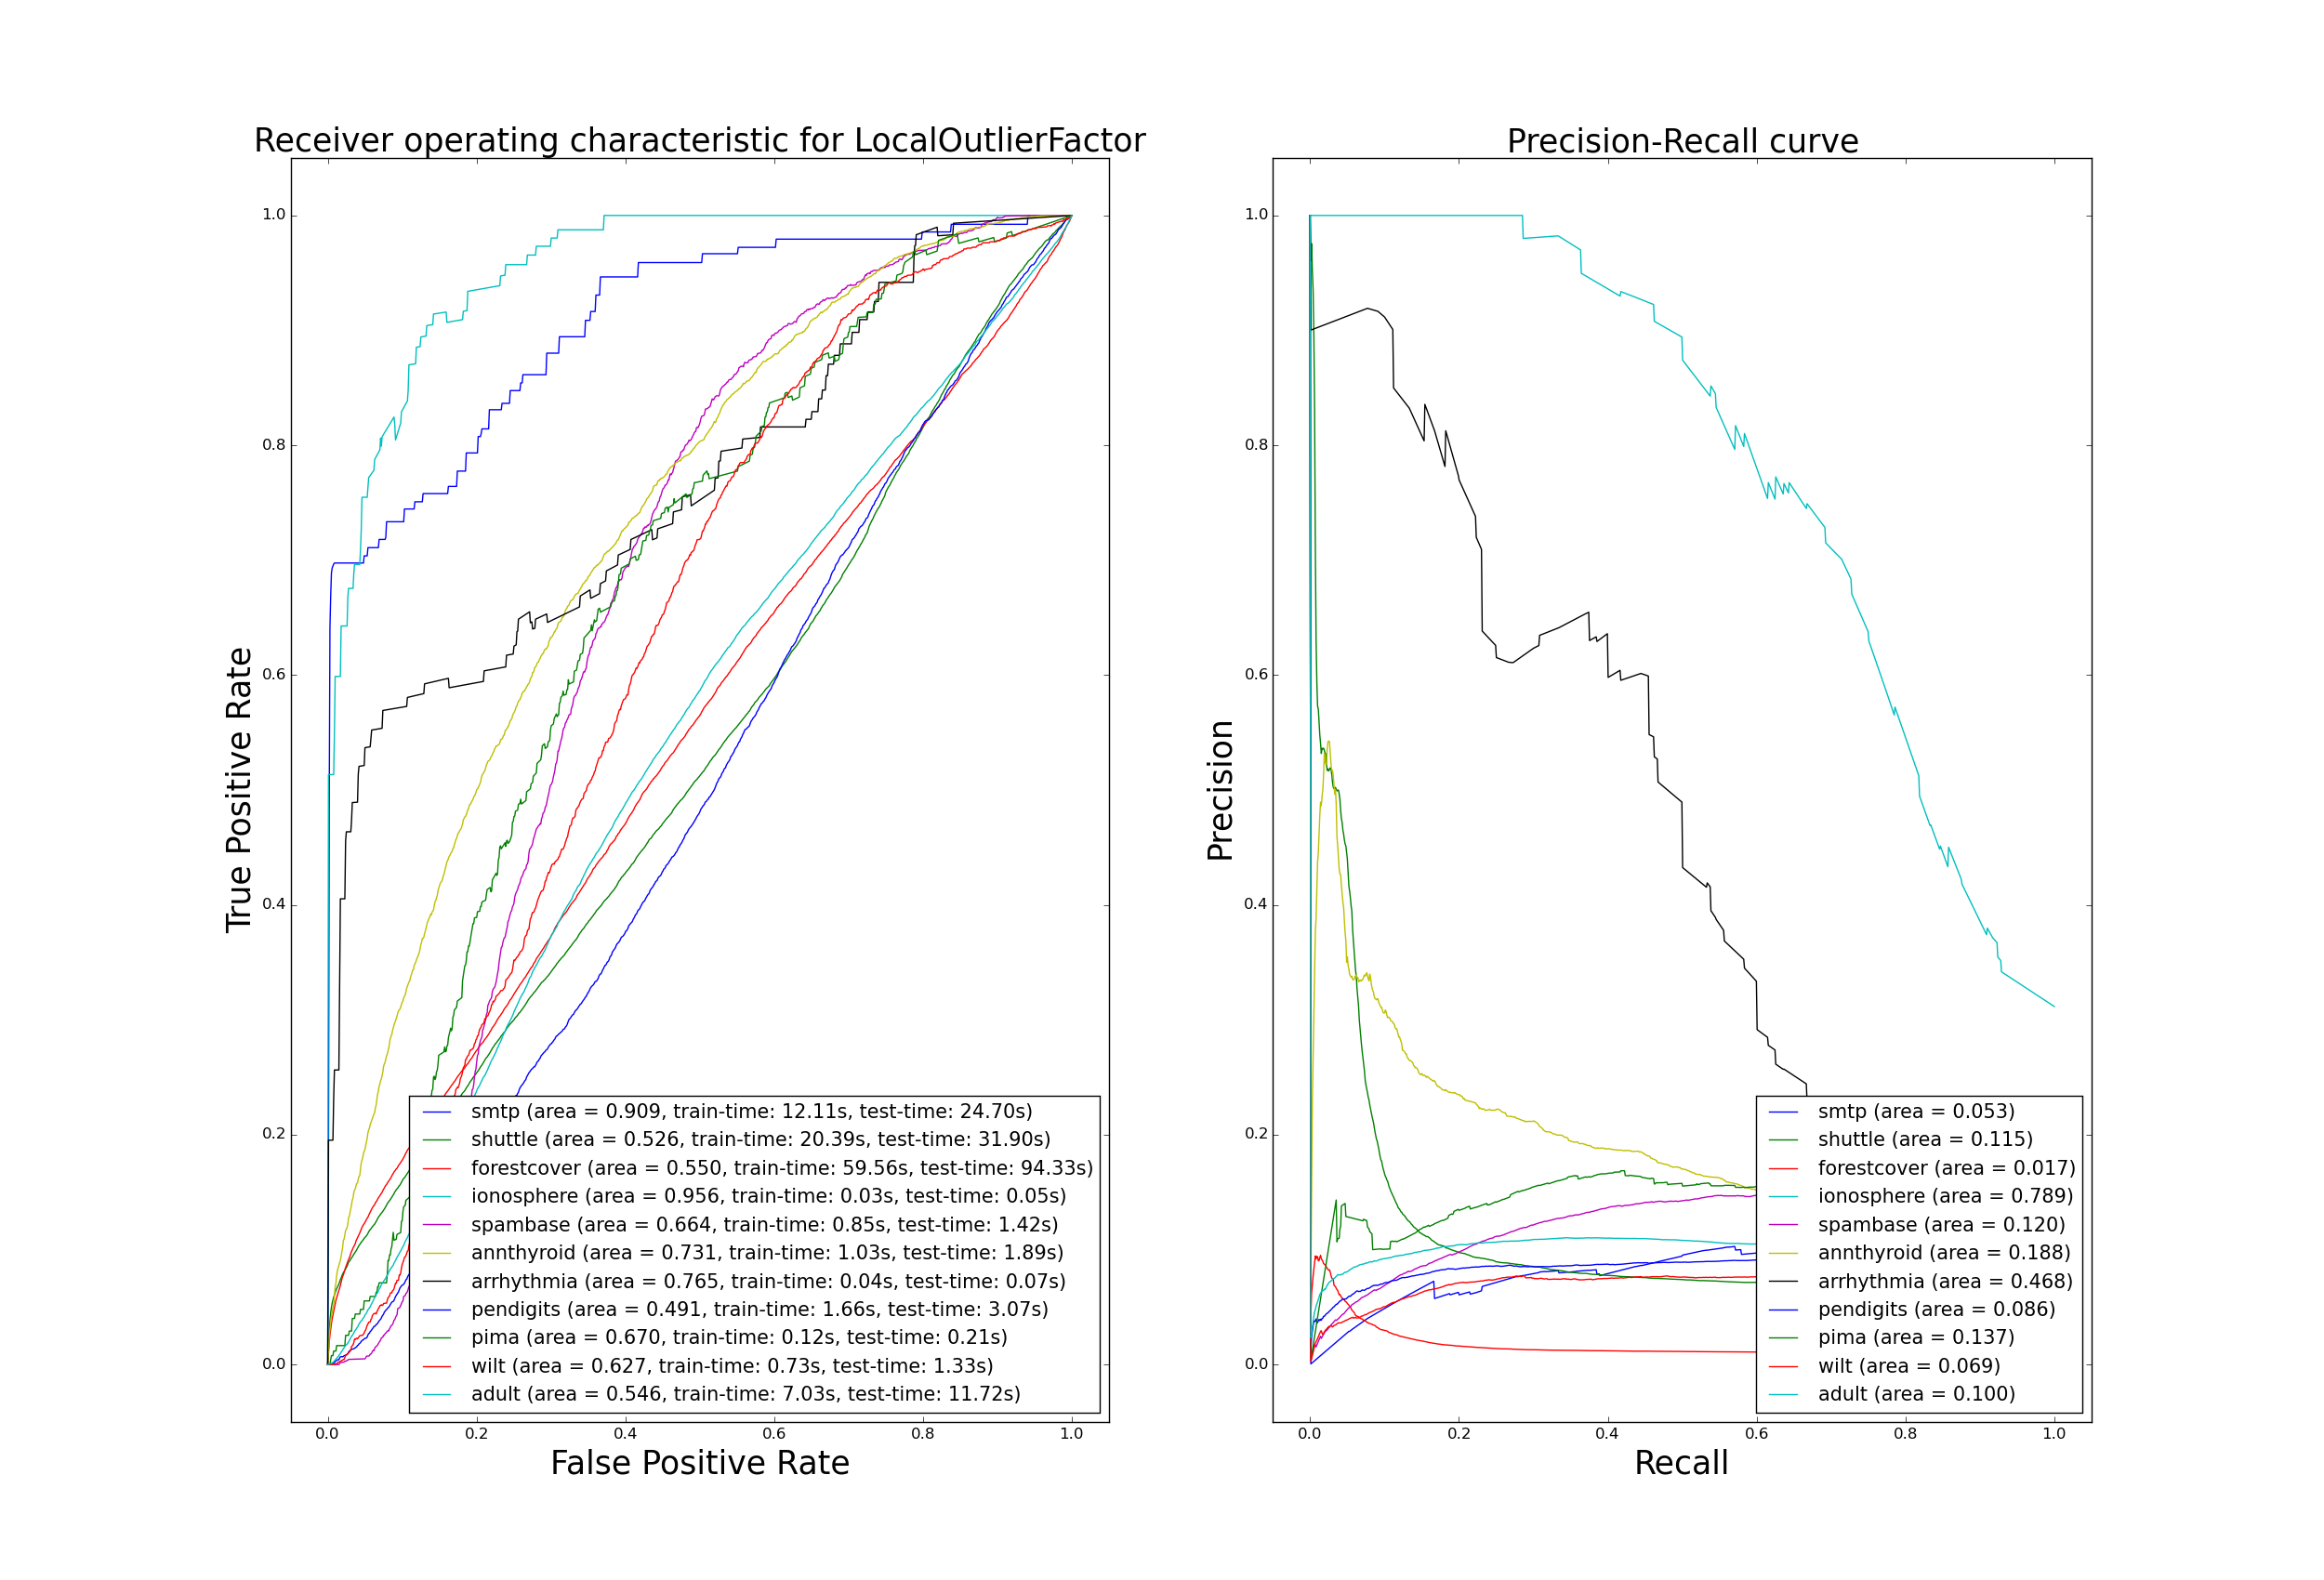
\includegraphics[trim=175 80 175 123, clip,
    width=0.75\textwidth]{./gfx/bench_lof_roc_pr_unsupervised_factorized.png}
\end{figure*}
\begin{figure*}[!ht]
    \caption{\acs{ROC} and \acs{PR} curves for Orca (novelty detection
    framework)}
    \label{ocrf:fig:orca_roc_pr}
    \centering
    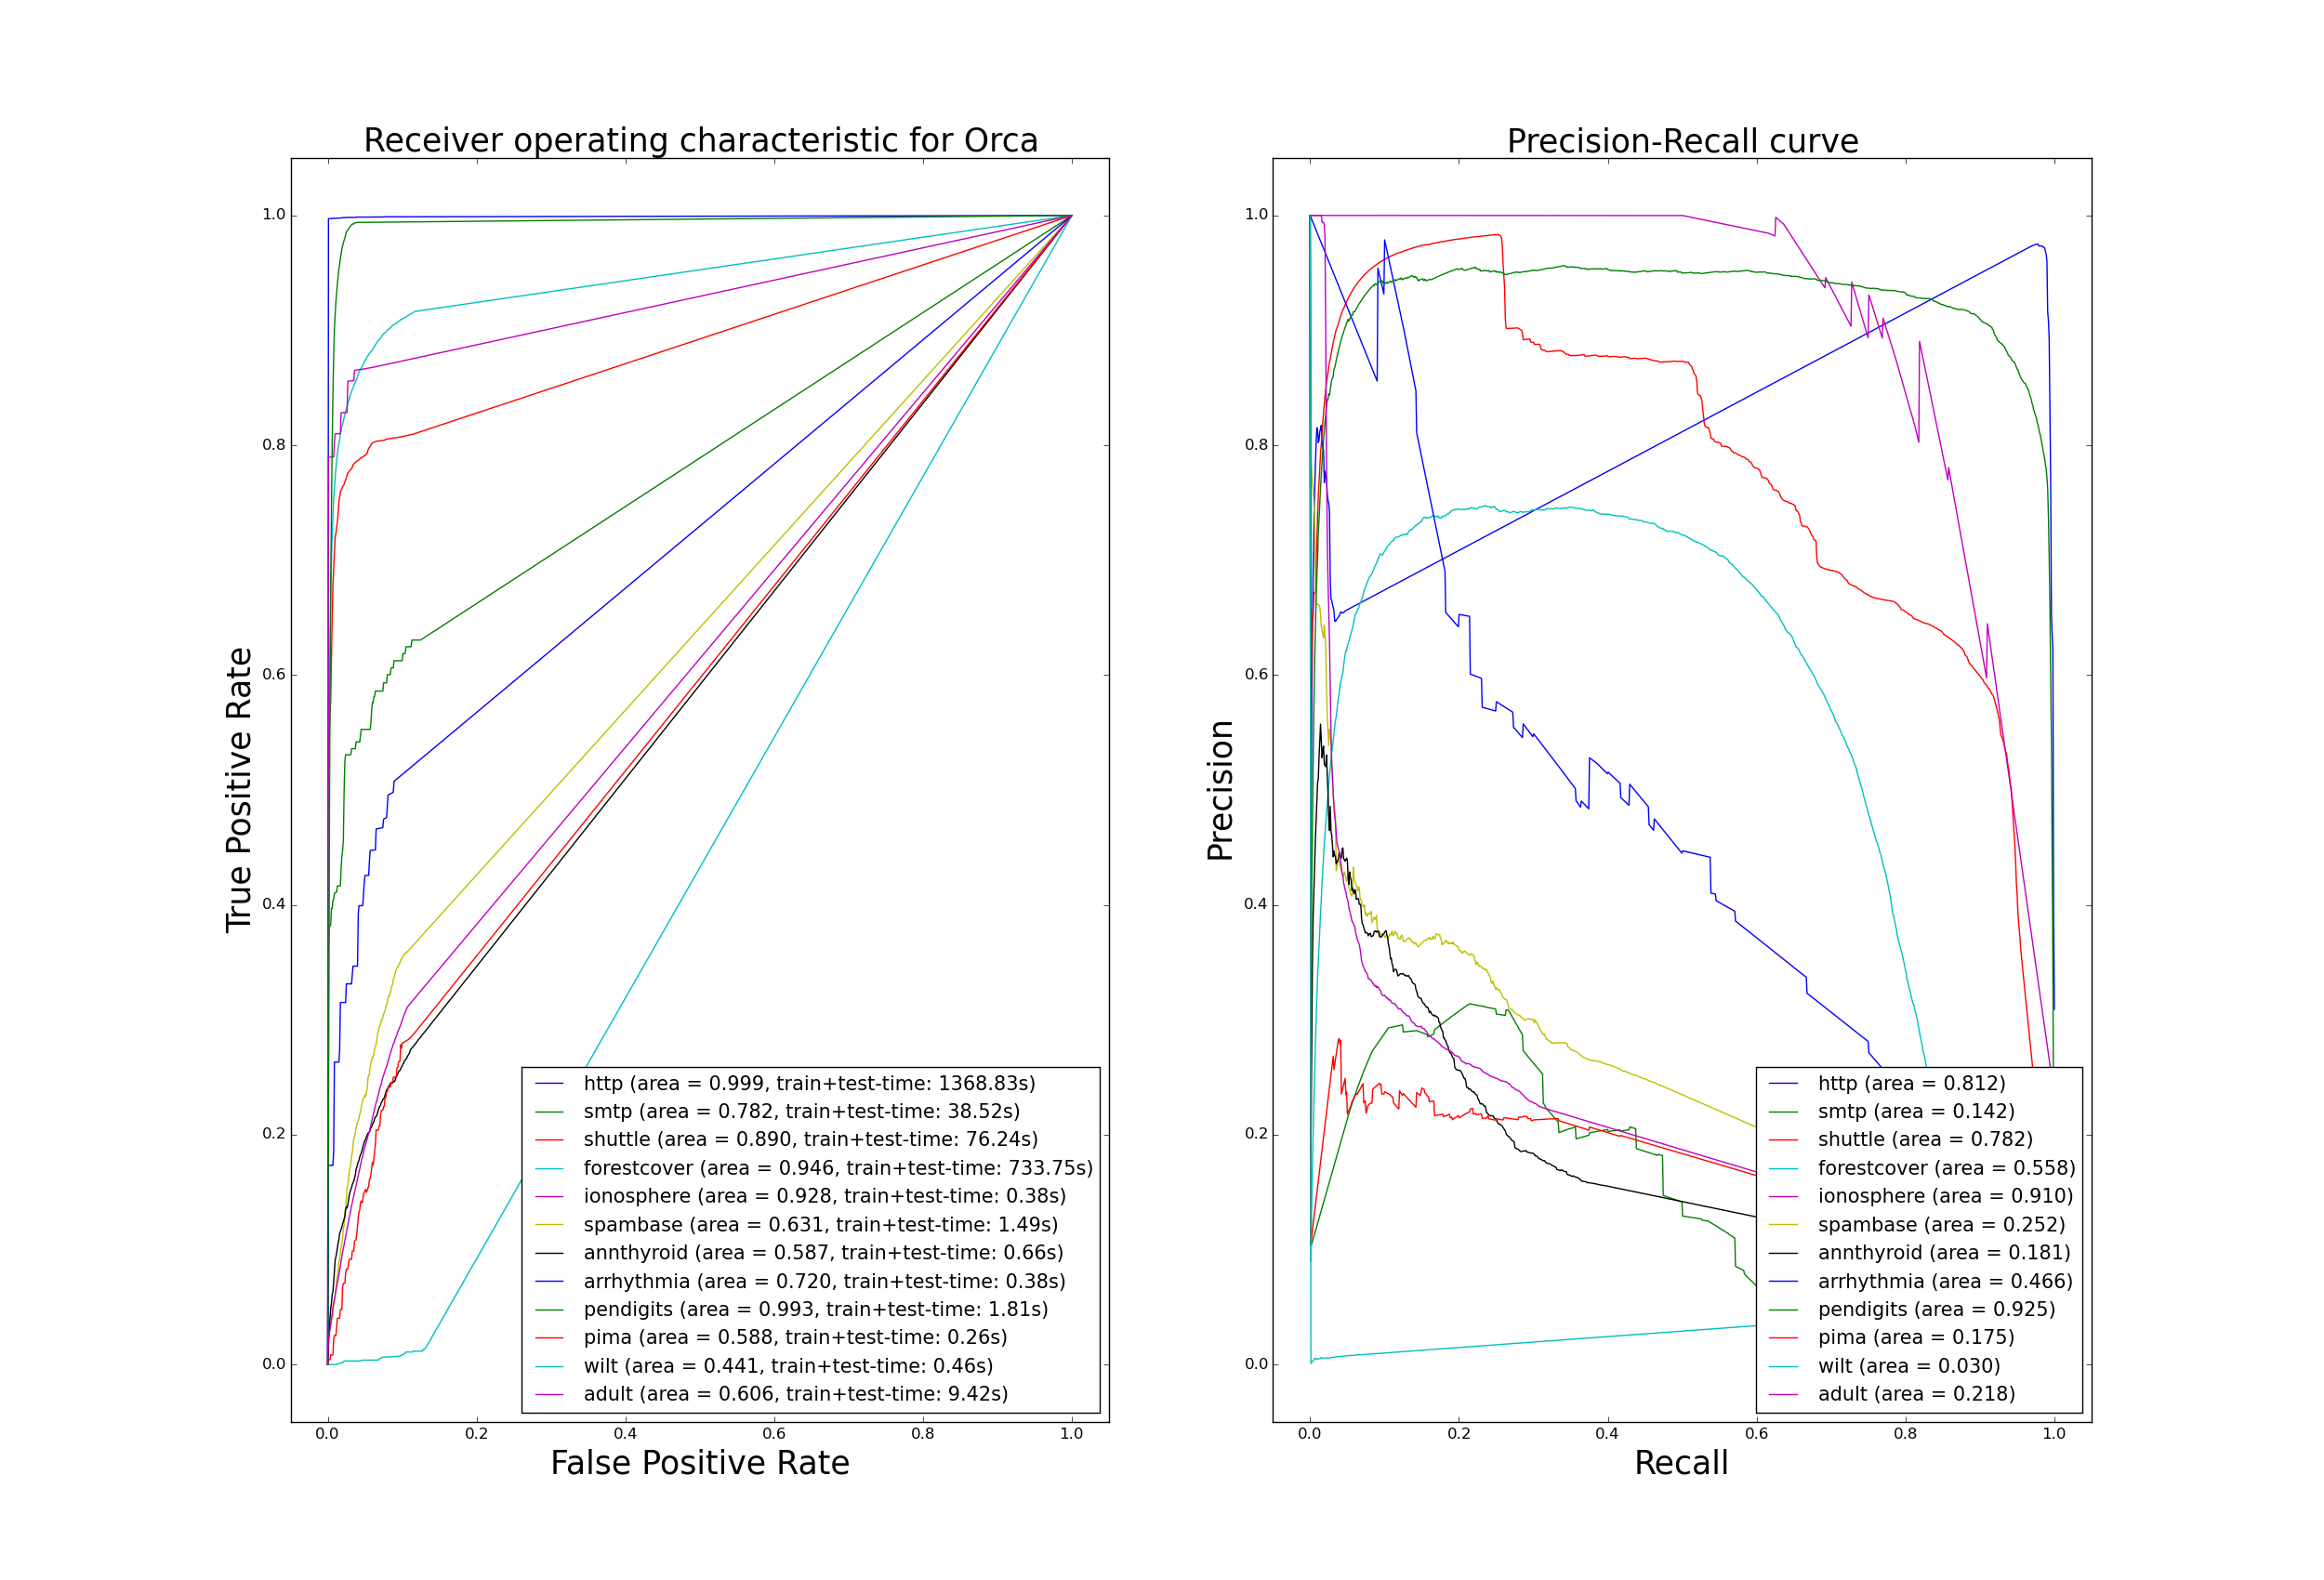
\includegraphics[trim=175 80 175 123, clip,
    width=0.75\textwidth]{./gfx/bench_orca_roc_pr_supervised_factorized.png}
\end{figure*}
\begin{figure*}[!ht]
    \caption{\acs{ROC} and \acs{PR} curves for Orca (outlier detection
    framework)}
    \label{ocrf:fig:orca_roc_pr_unsupervised}
    \centering
    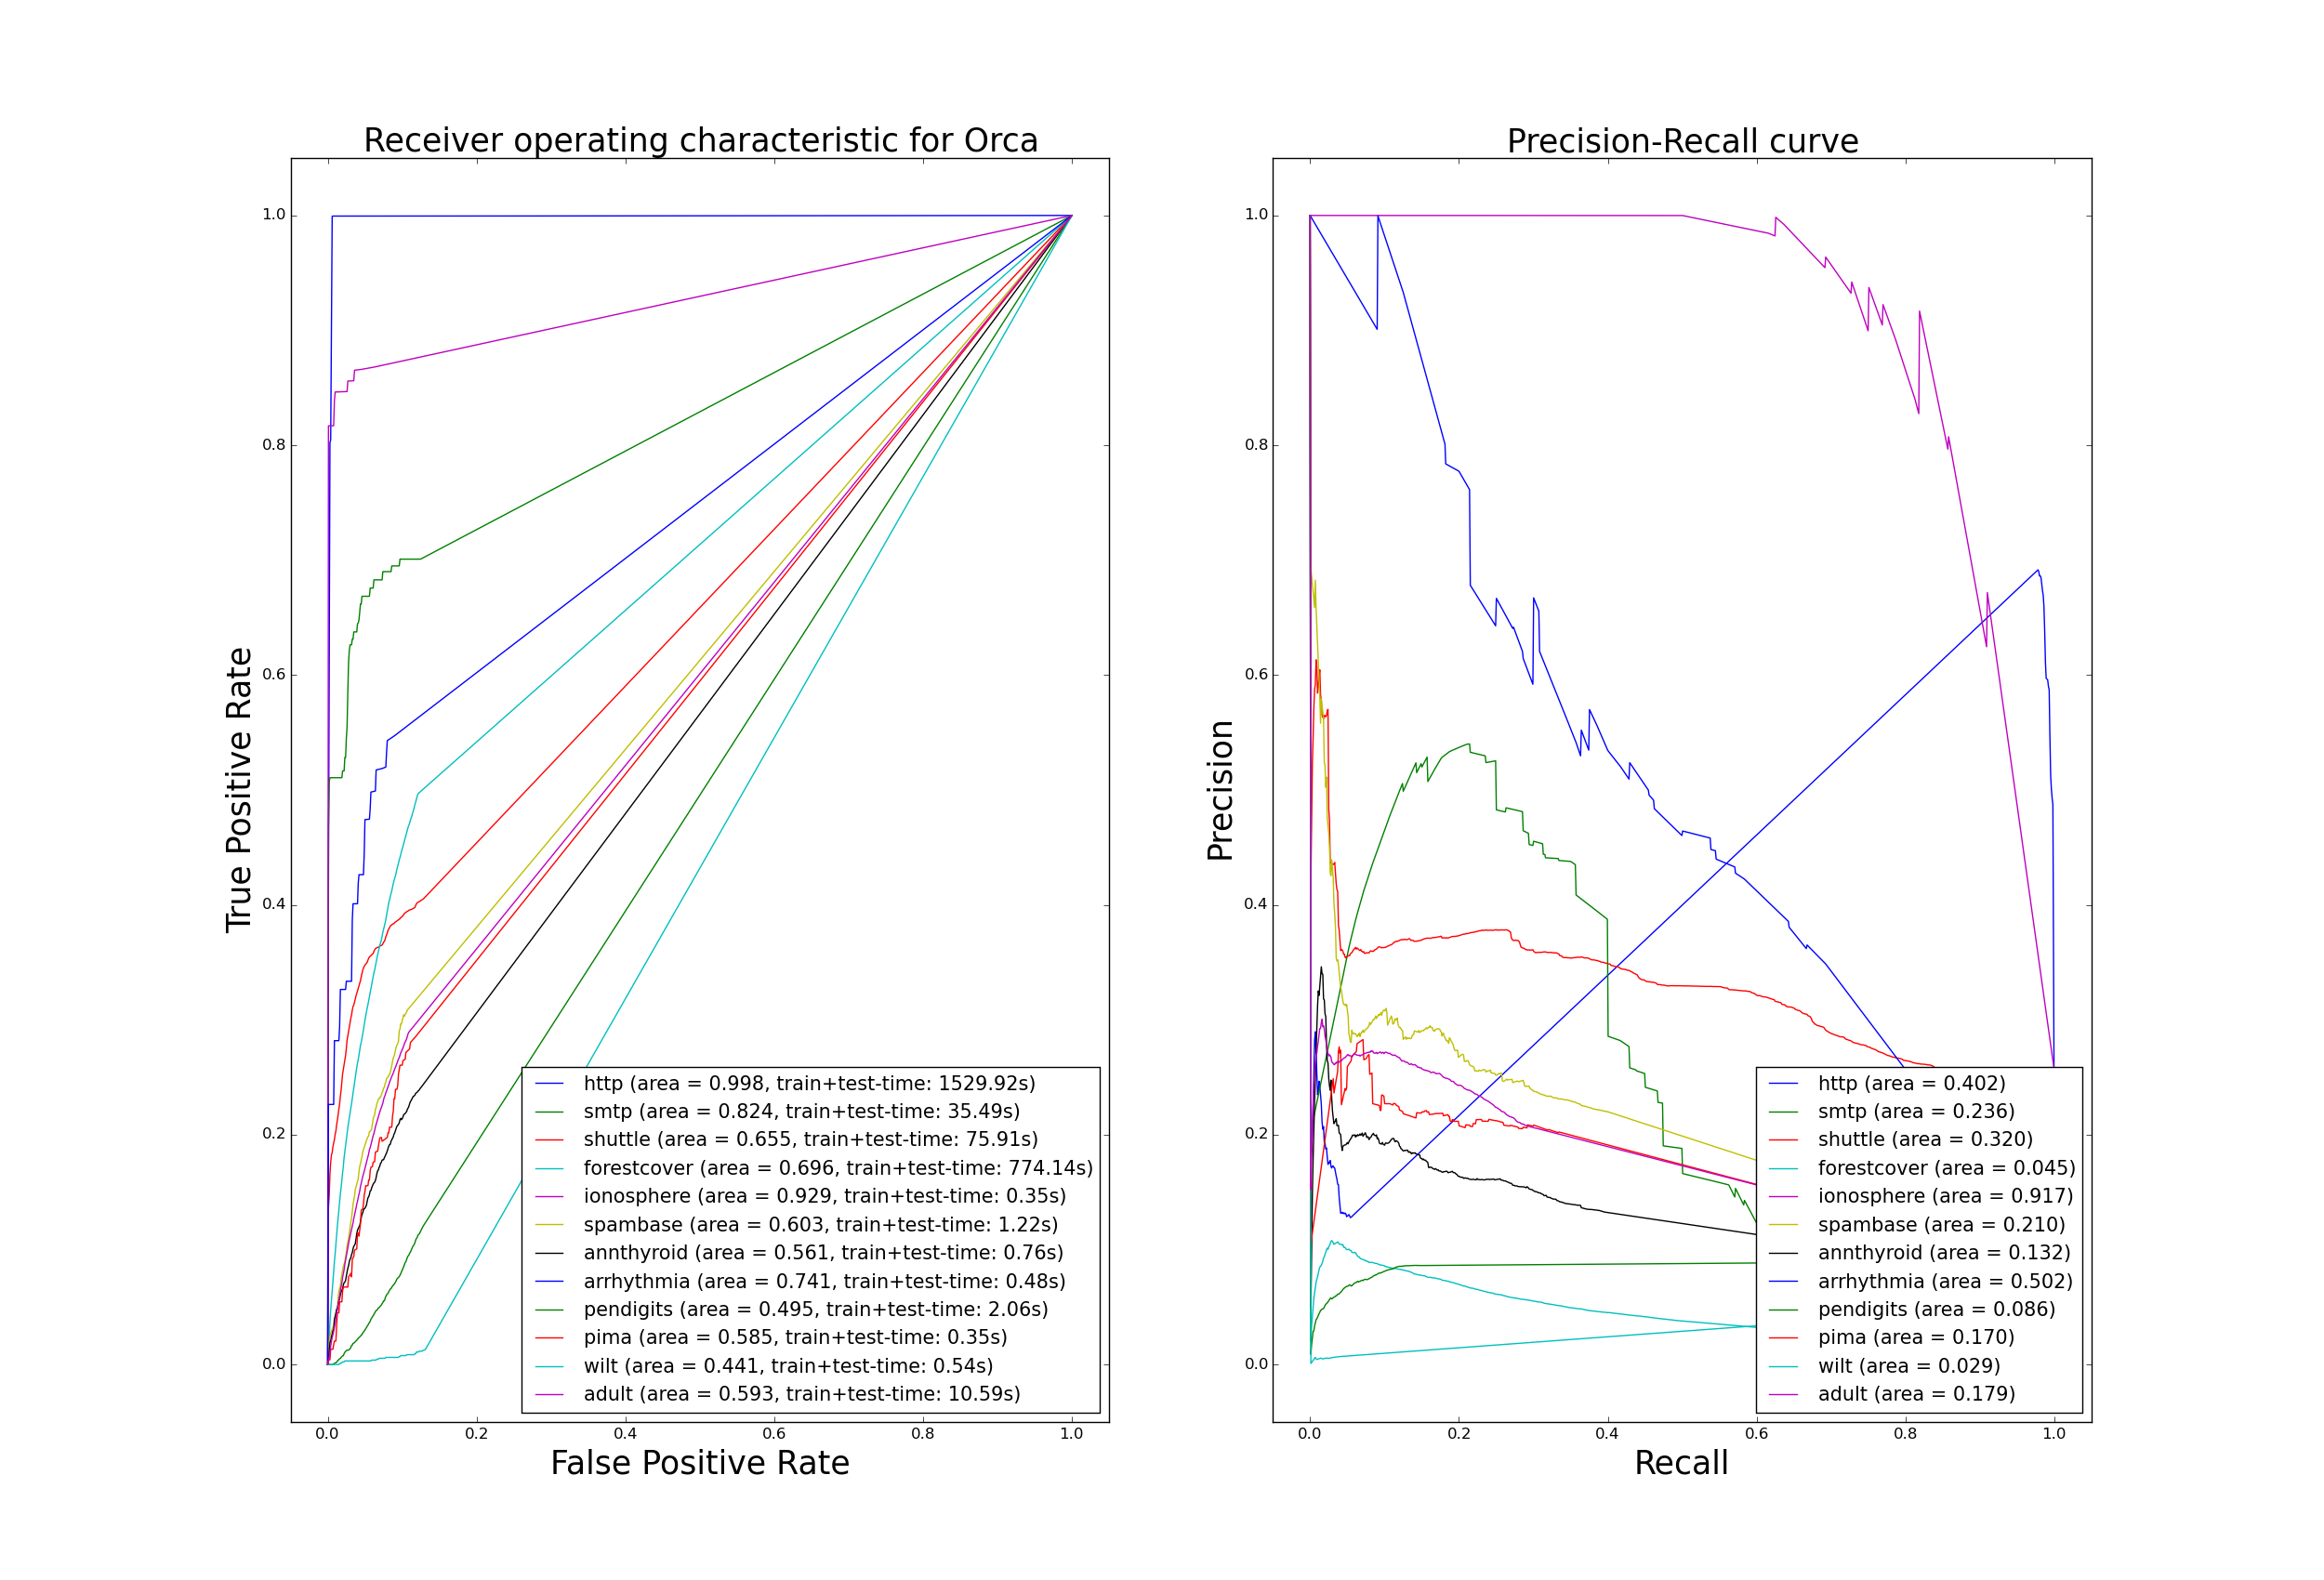
\includegraphics[trim=175 80 175 123, clip,
    width=0.75\textwidth]{./gfx/bench_orca_roc_pr_unsupervised_factorized.png}
\end{figure*}
\begin{figure*}[!ht]
    \caption{\acs{ROC} and \acs{PR} curves for \acs{LSAD} (novelty detection
    framework)}
    \label{ocrf:fig:LSAnomaly_roc_pr}
    \centering
    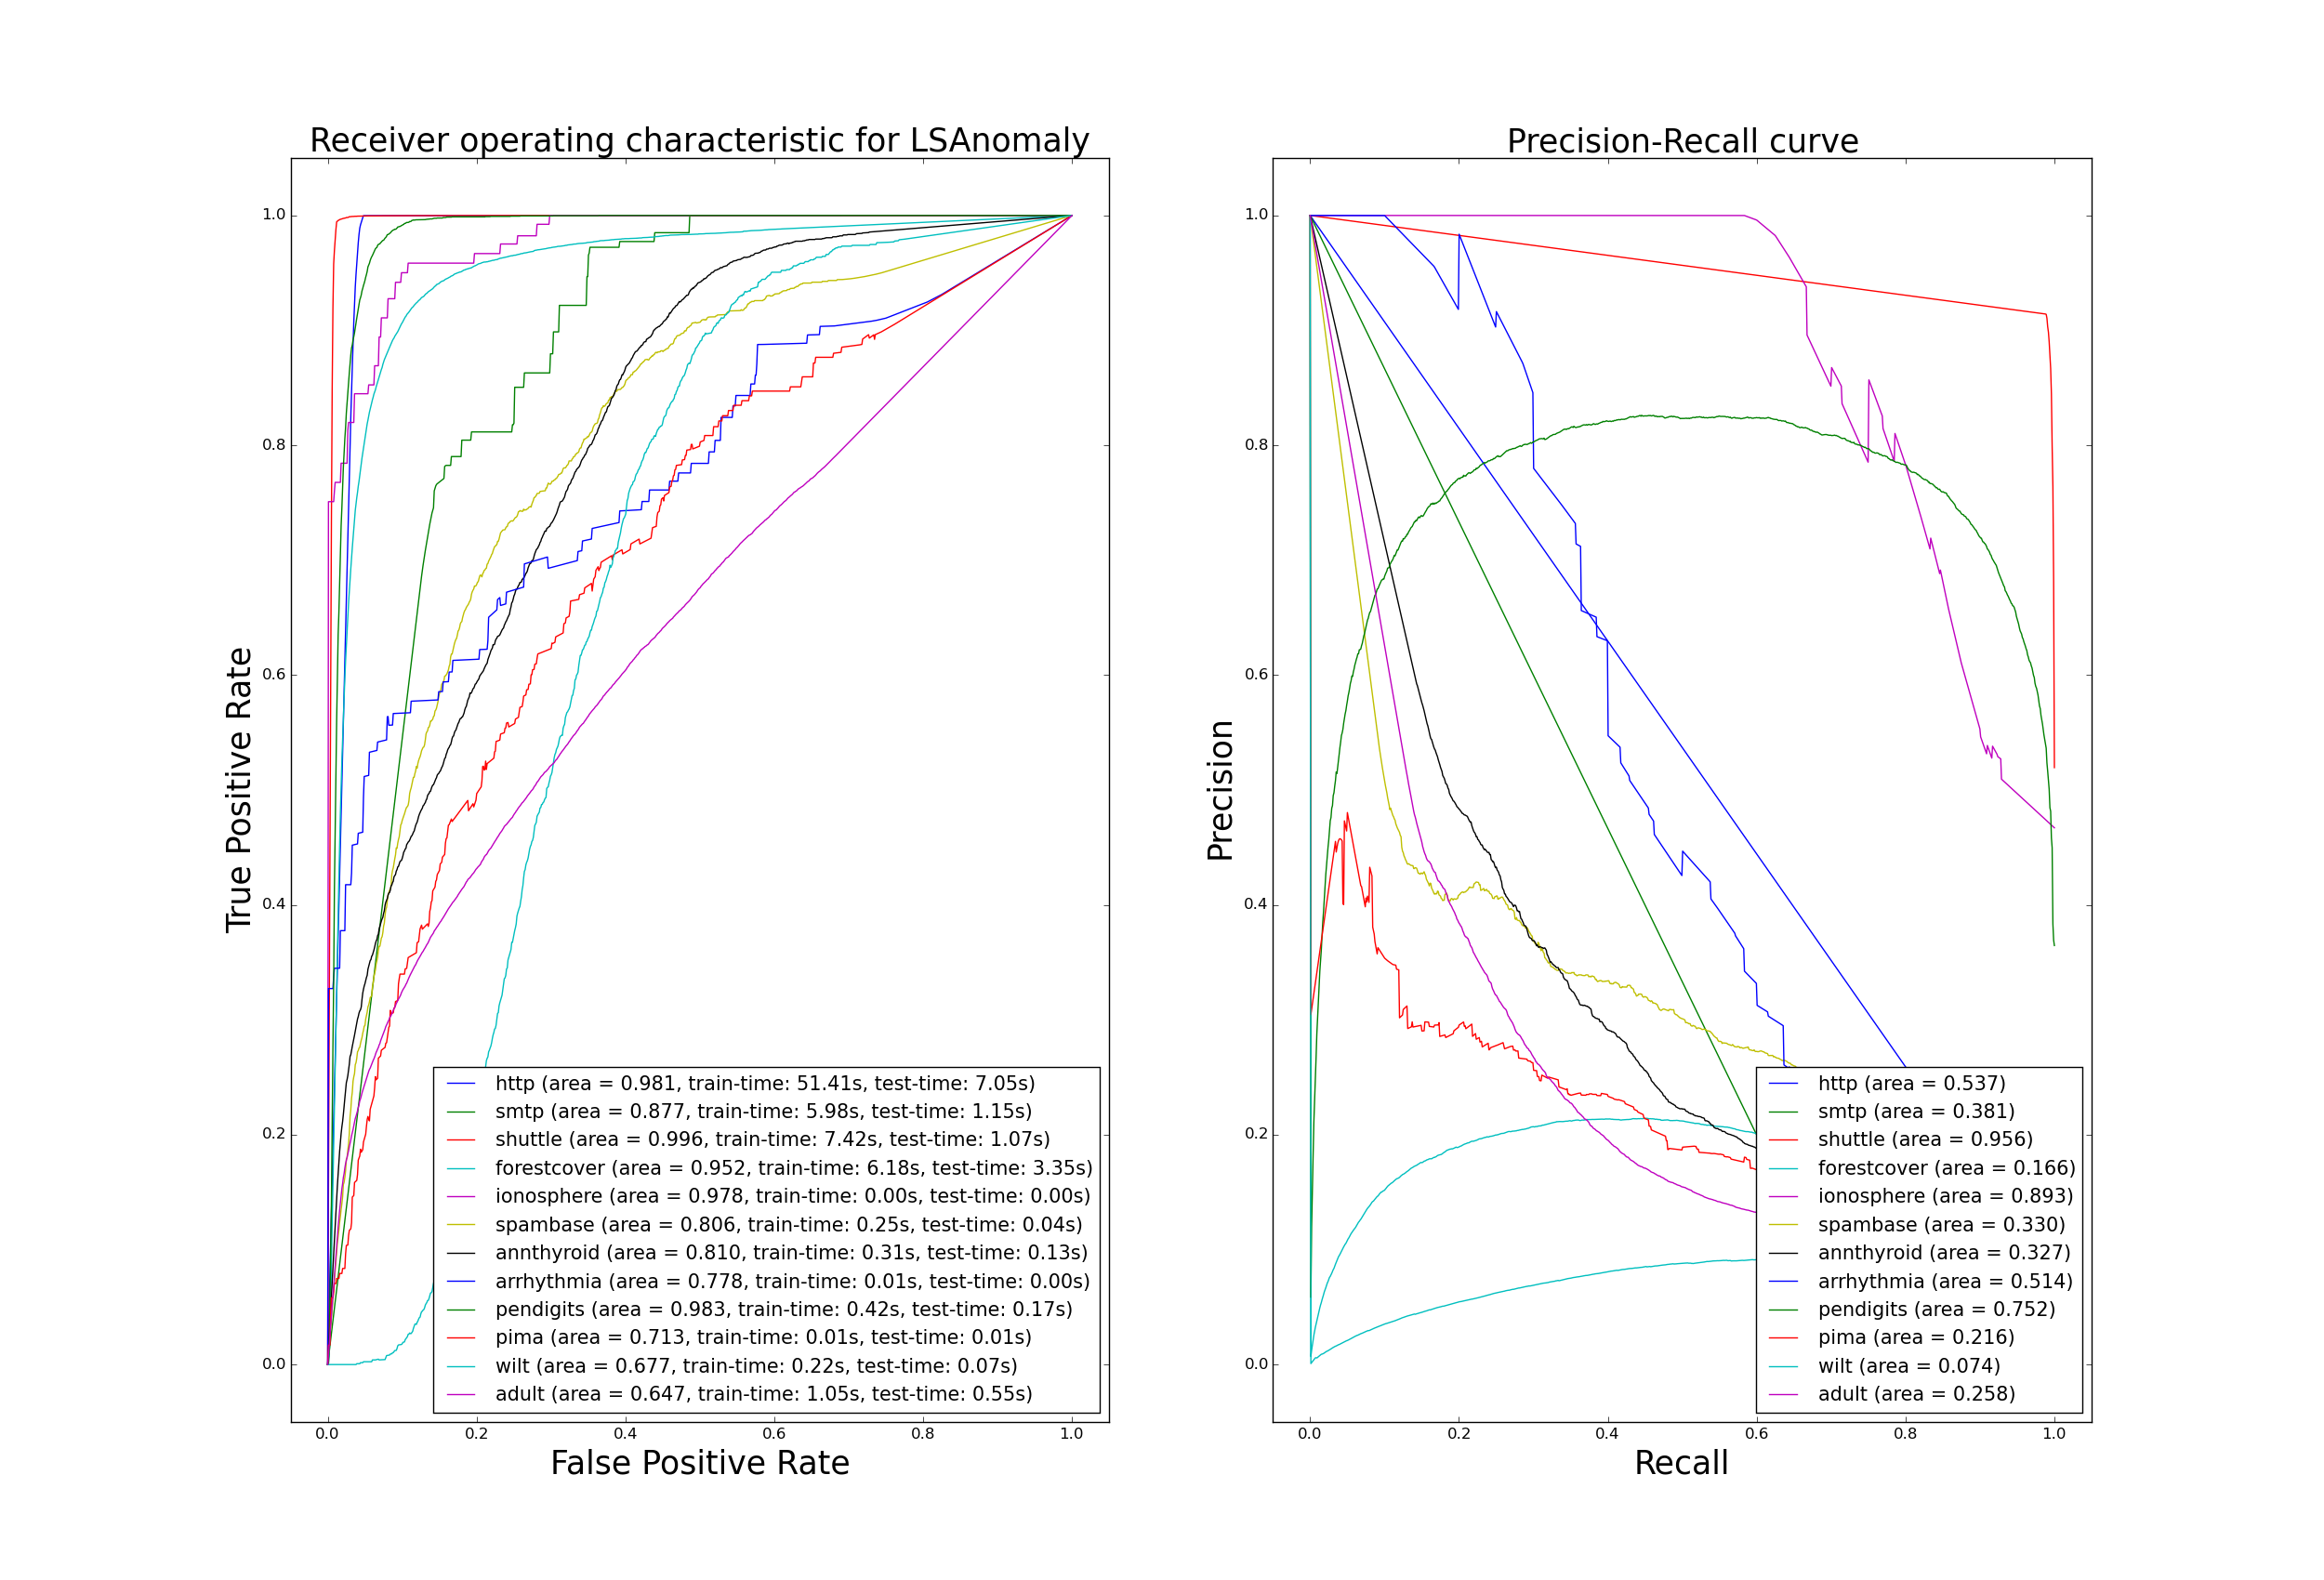
\includegraphics[trim=175 80 175 123, clip,
    width=0.75\textwidth]{./gfx/bench_LSAnomaly_roc_pr_supervised_factorized.png}
\end{figure*}
\begin{figure*}[!ht]
    \caption{\acs{ROC} and \acs{PR} curves for \acs{LSAD} (outlier detection
    framework)}
    \label{ocrf:fig:LSAnomaly_roc_pr_unsupervised}
    \centering
    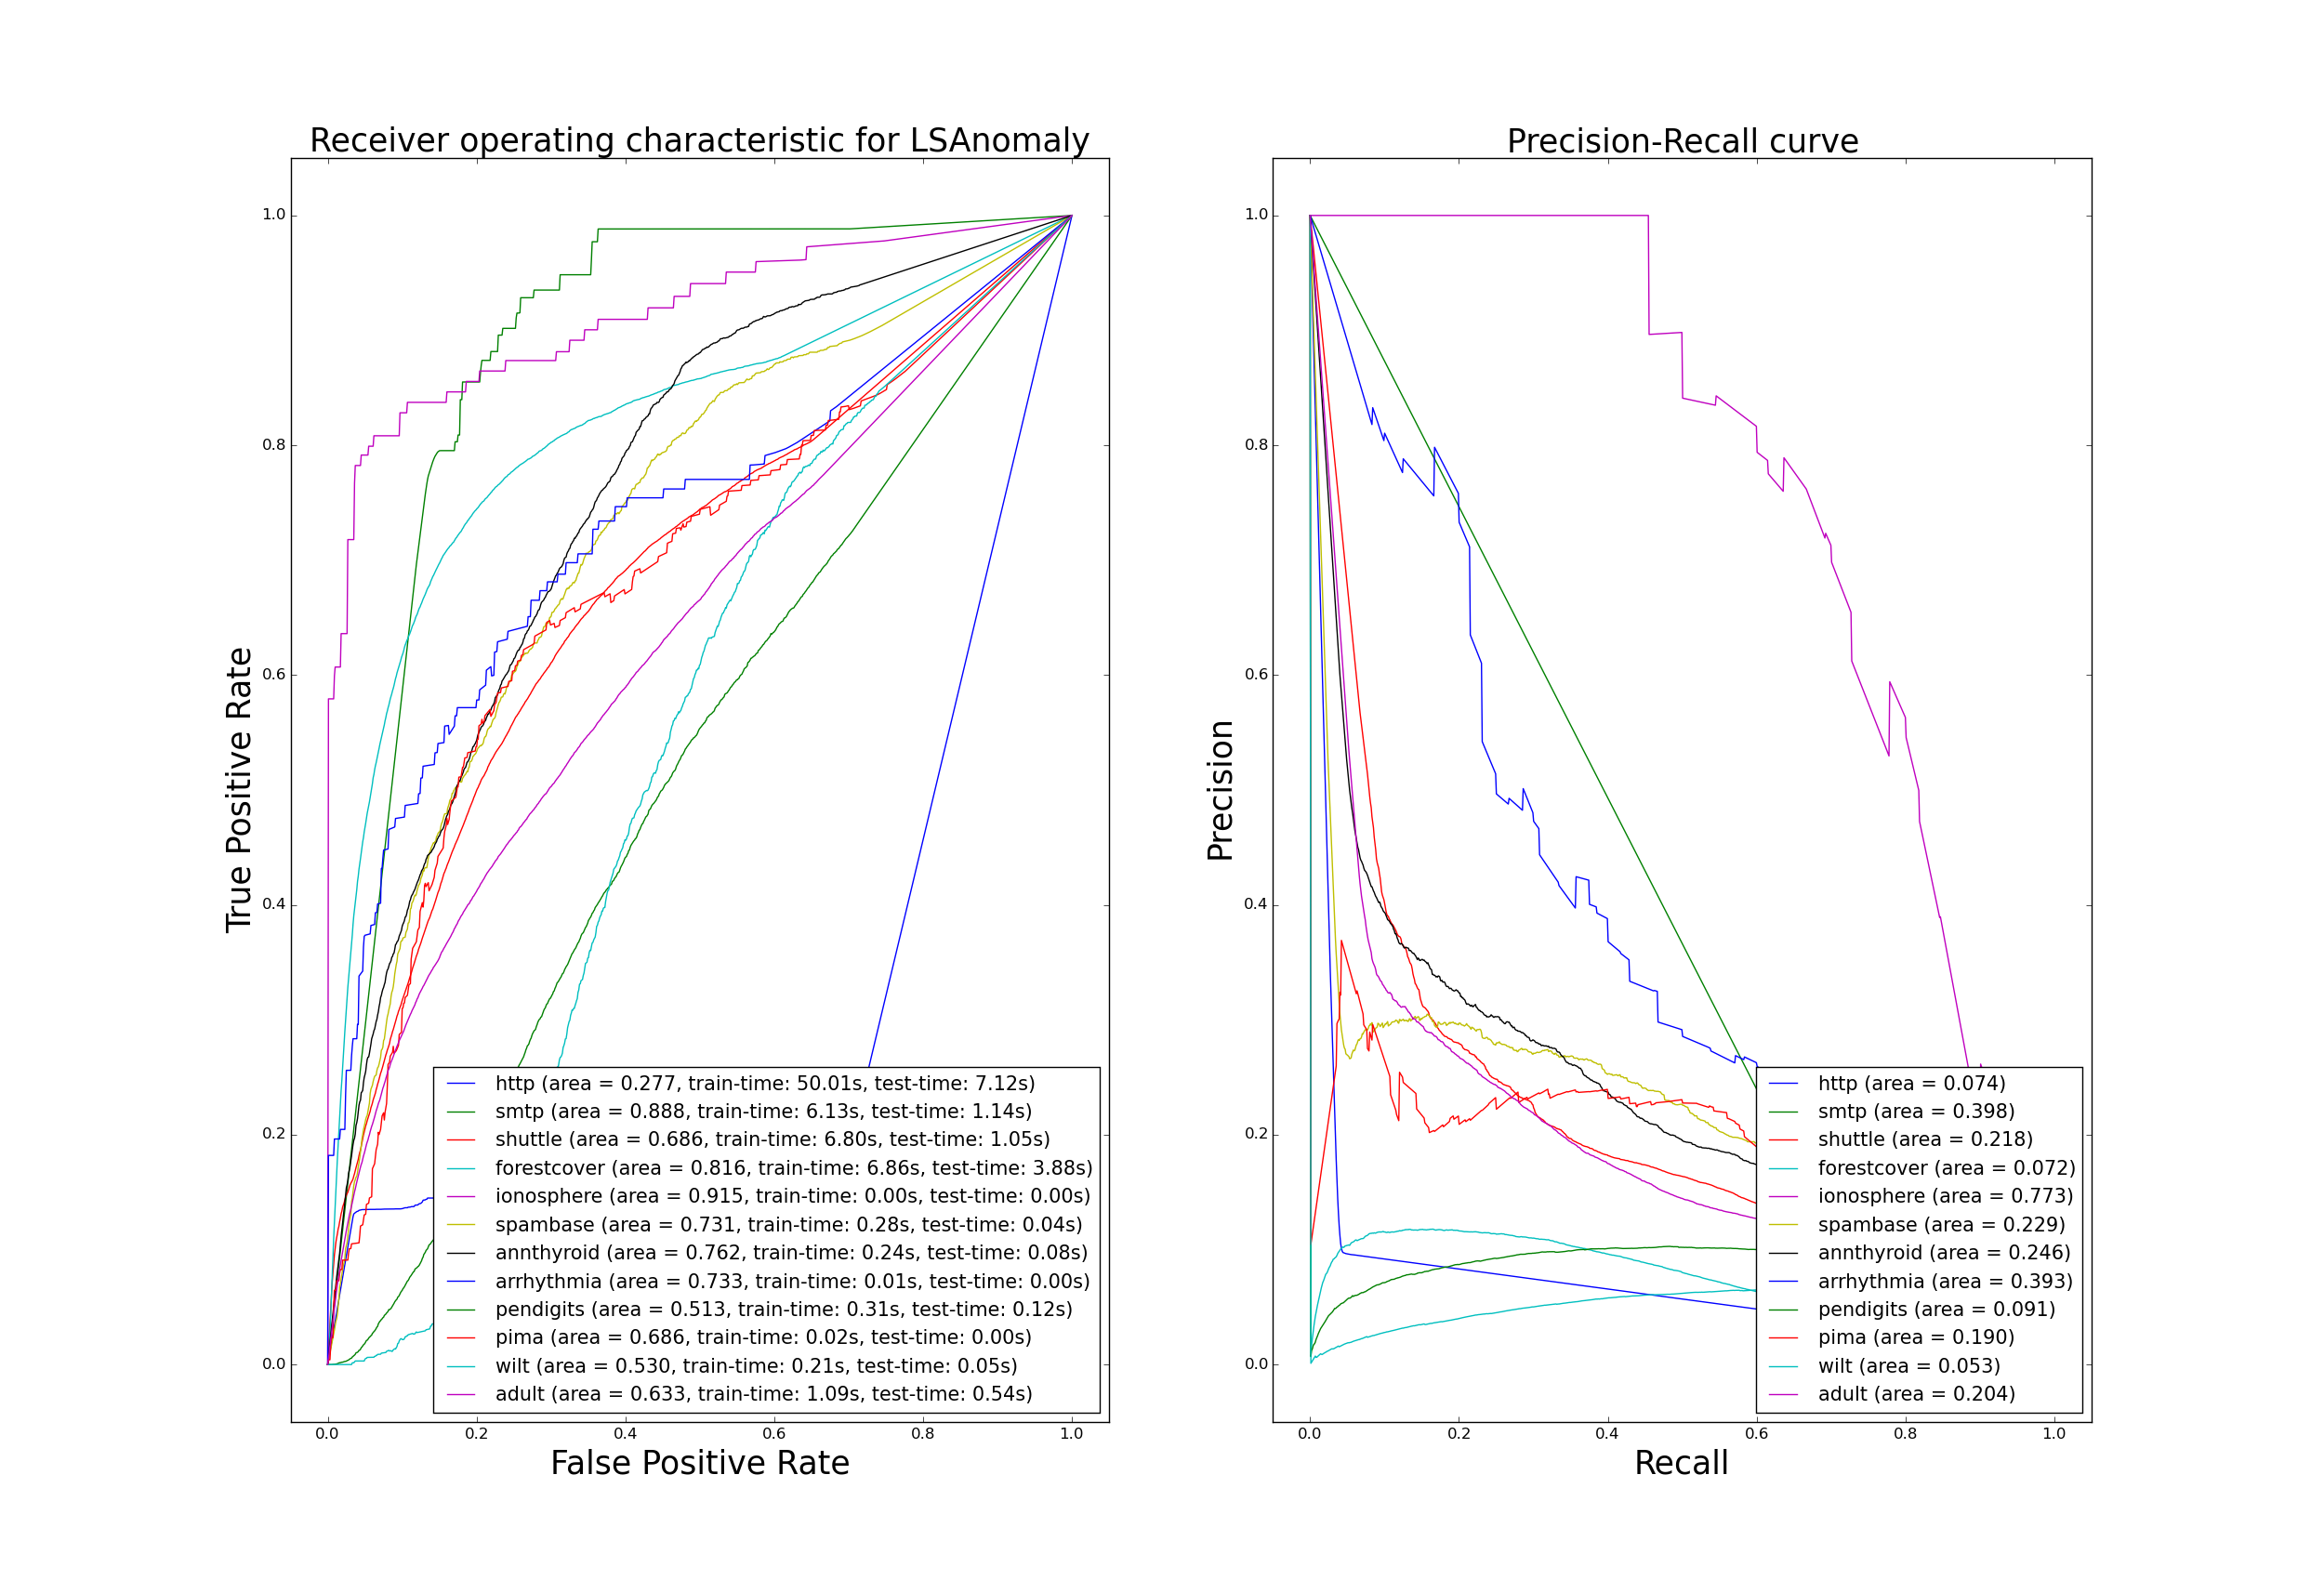
\includegraphics[trim=175 80 175 123, clip,
    width=0.75\textwidth]{./gfx/bench_LSAnomaly_roc_pr_unsupervised_factorized.png}
\end{figure*}
\begin{figure*}[!ht]
    \caption{\acs{ROC} and \acs{PR} curves for \acs{RFC} (novelty detection
    framework)}
    \label{ocrf:fig:rf_roc_pr}
    \centering
    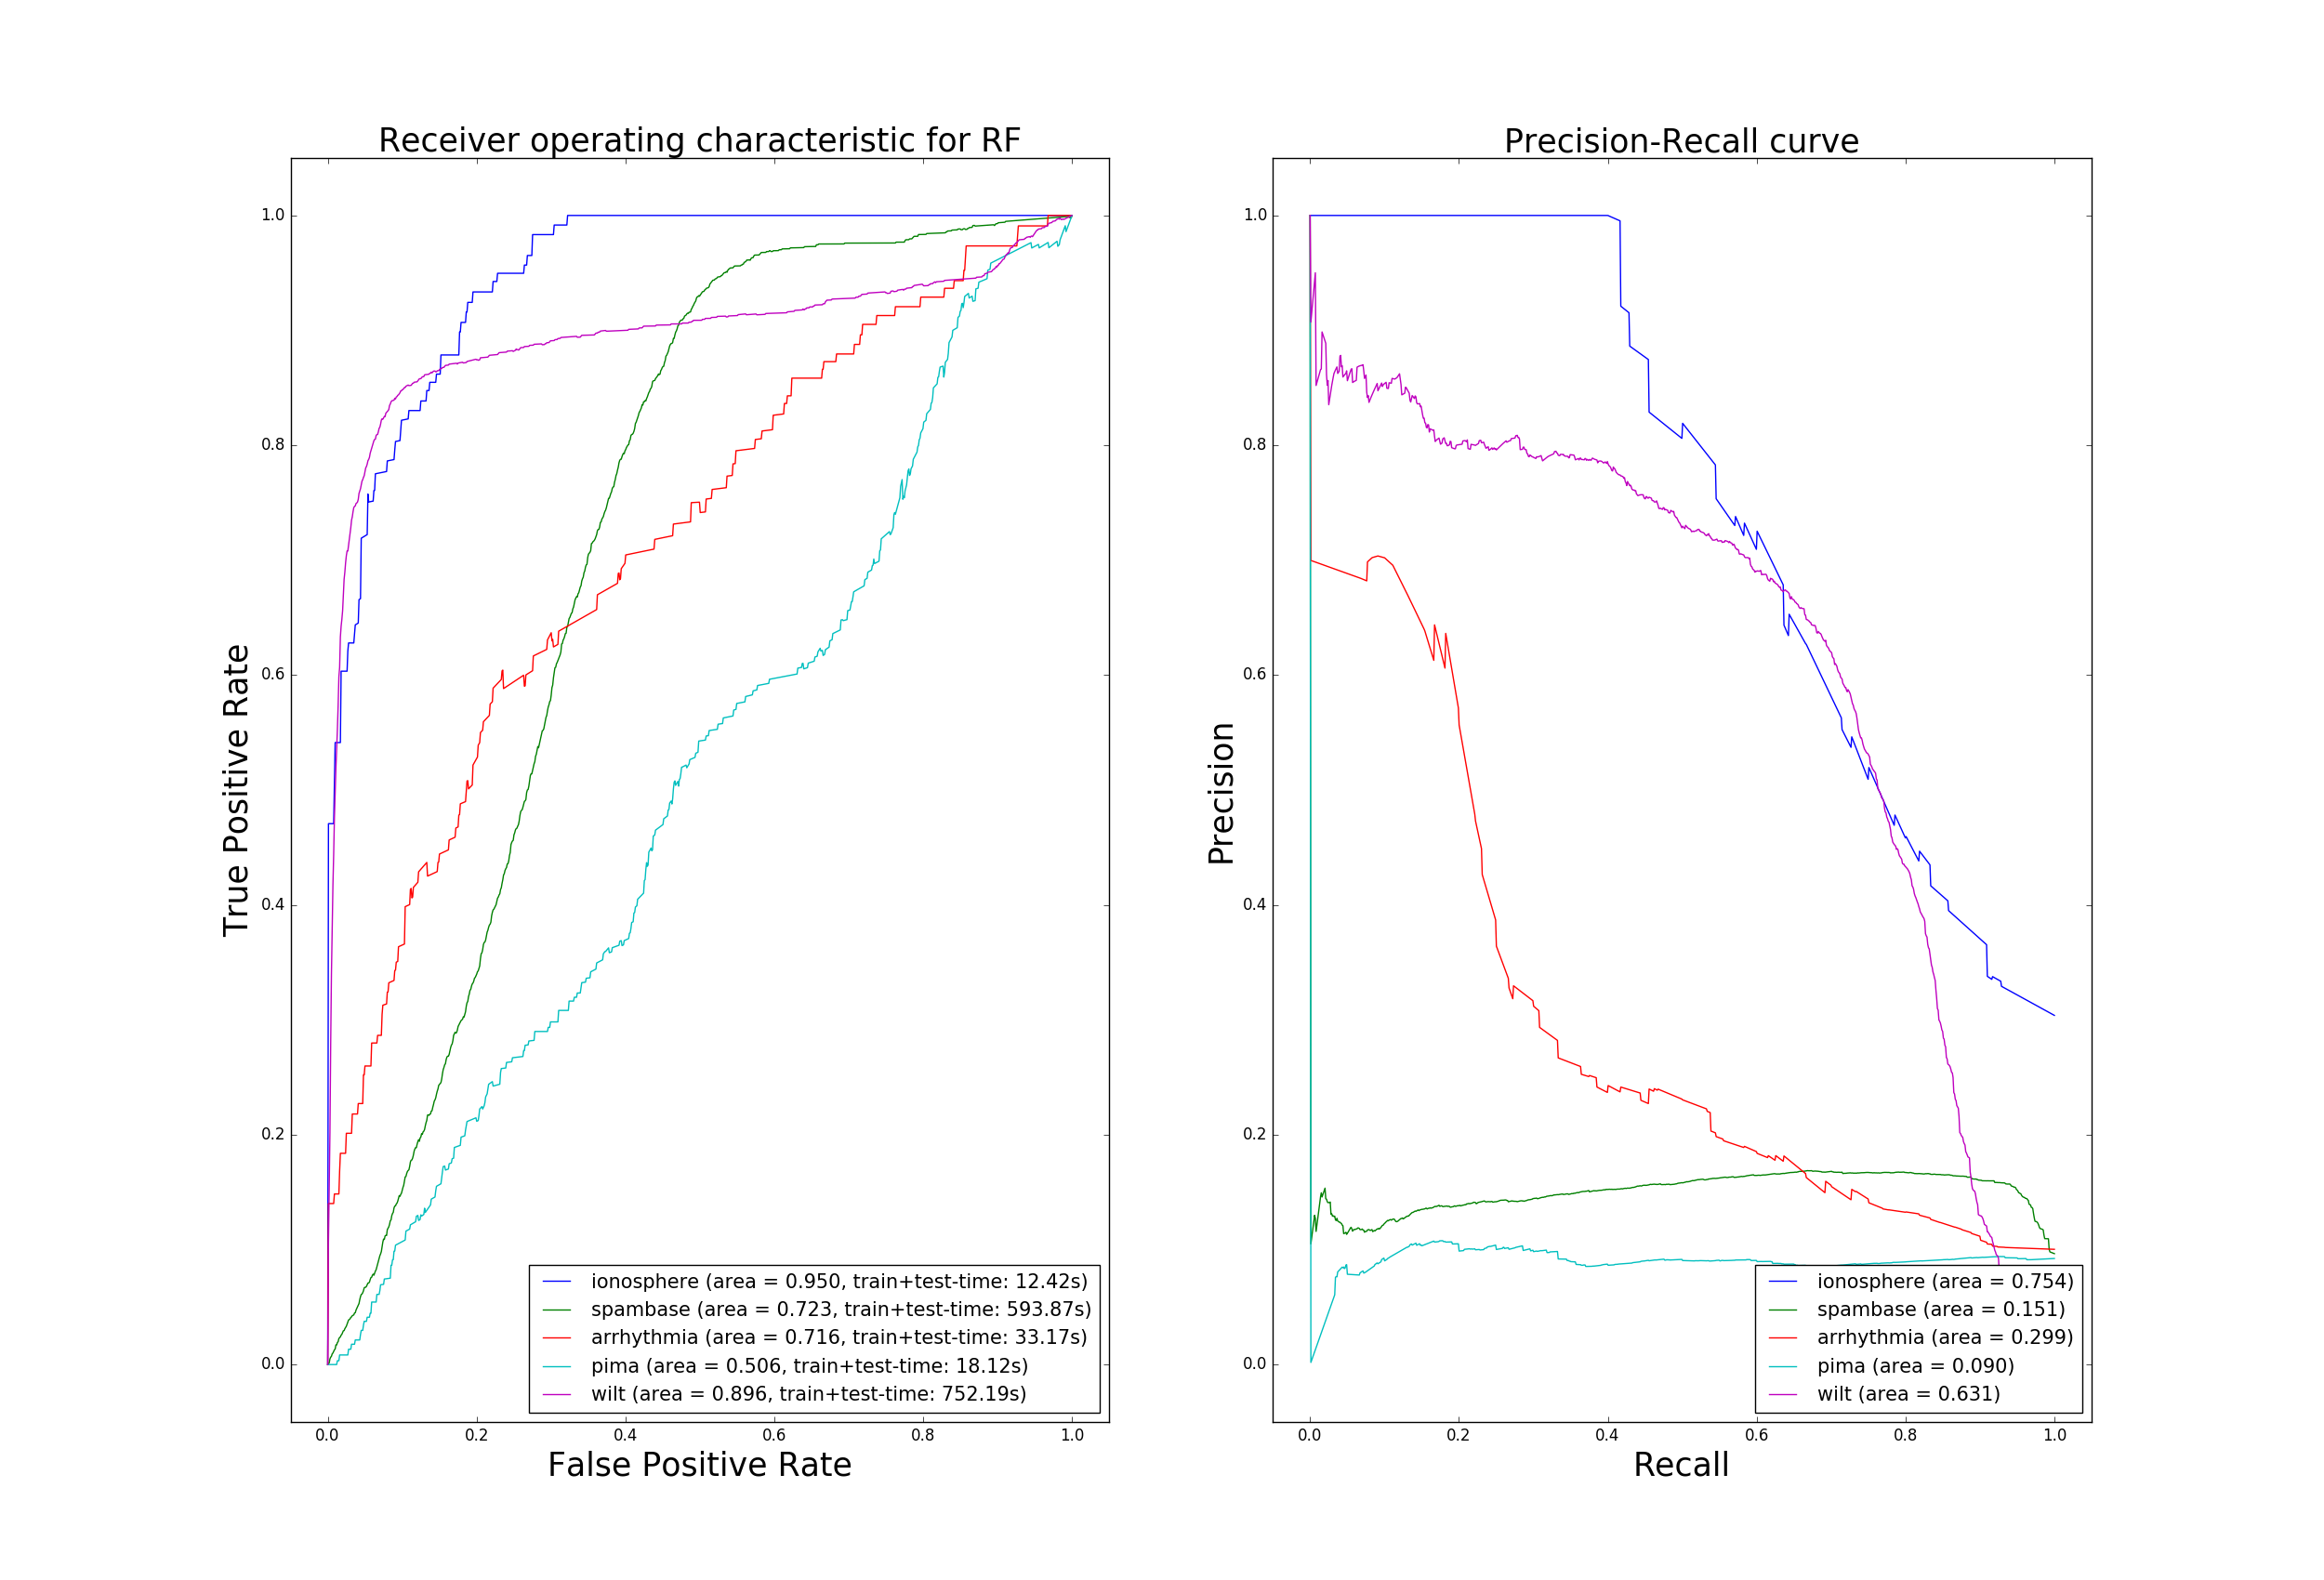
\includegraphics[trim=175 80 175 123, clip,
    width=0.75\textwidth]{./gfx/bench_rf_roc_pr_supervised_factorized.png}
\end{figure*}
\begin{figure*}[!ht]
    \caption{\acs{ROC} and \acs{PR} curves for \acs{RFC} (outlier detection
    framework)}
    \label{ocrf:fig:rf_roc_pr_unsupervised}
    \centering
    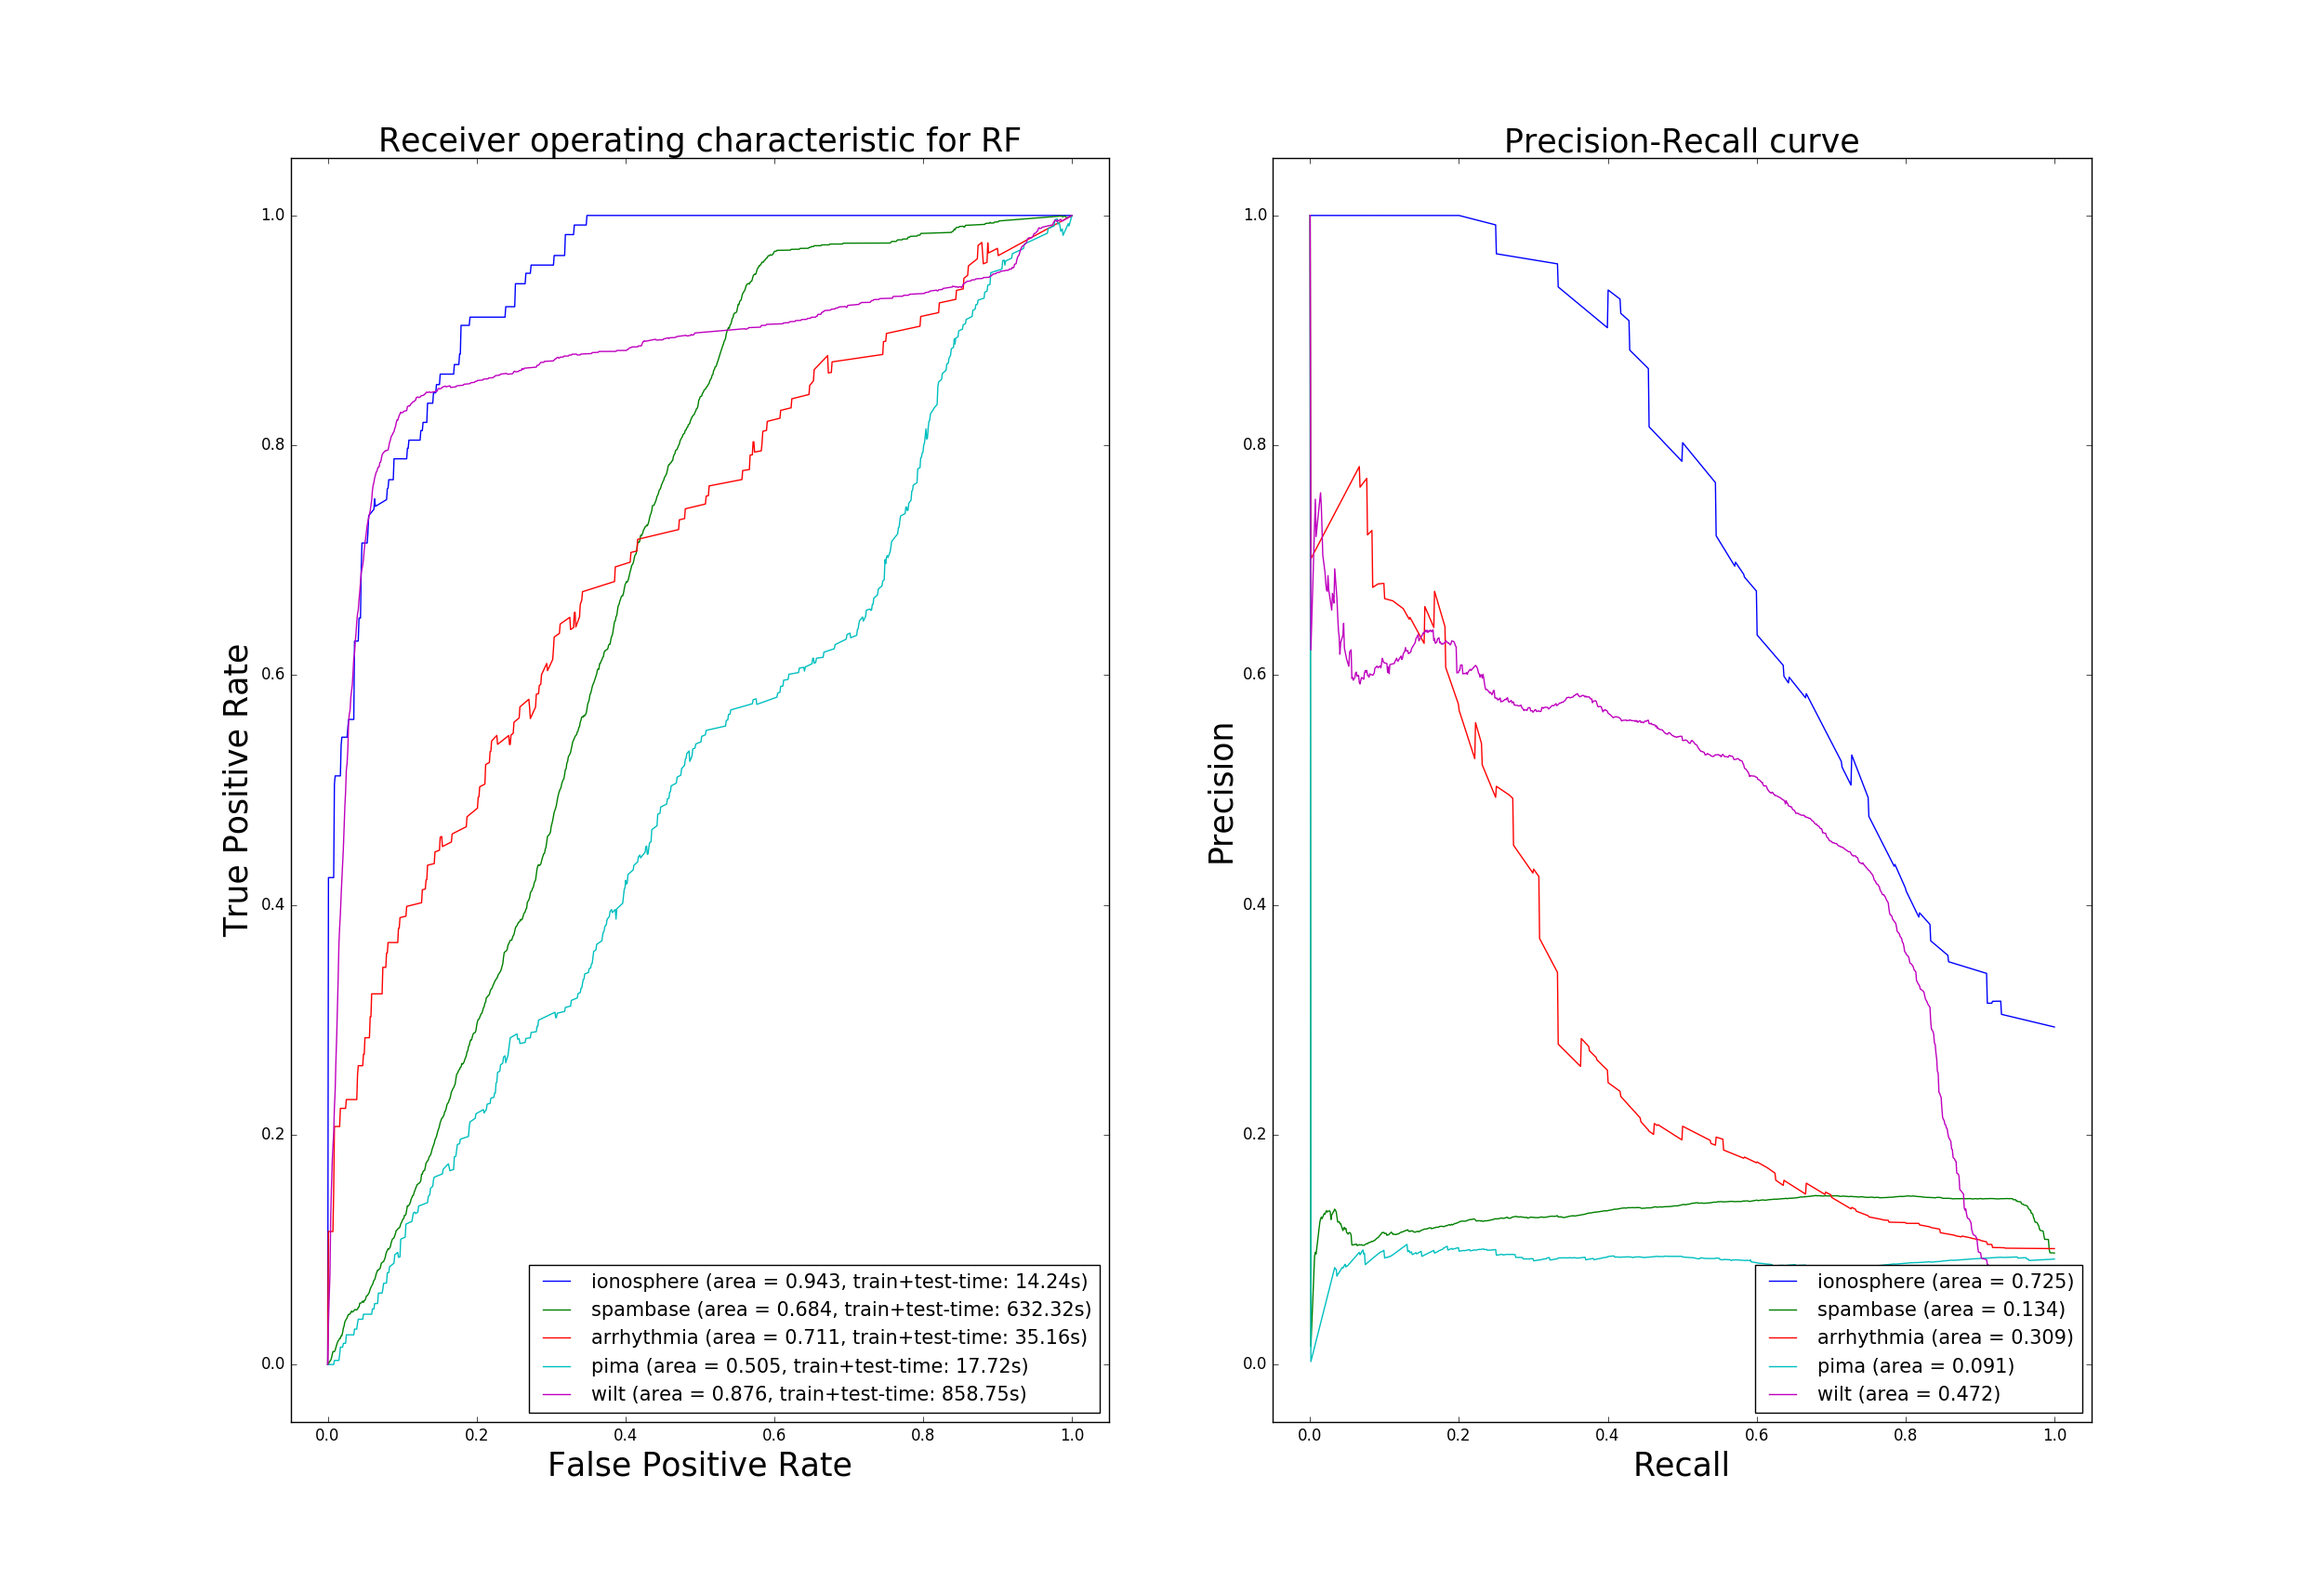
\includegraphics[trim=175 80 175 123, clip,
    width=0.75\textwidth]{./gfx/bench_rf_roc_pr_unsupervised_factorized.png}
\end{figure*}

%XXX TODO: description of the table
\afterpage{%
\begin{landscape}
    \begin{table}[htb]
        \caption{Results for the outlier detection setting}
        \label{ocrf:table:results-unsupervised}

        \centering
        %\scriptsize
        \resizebox{\textheight}{!}{%
        \begin{tabular}{lcccccccccccccccc}
        \toprule
            Dataset & \multicolumn{2}{c }{\acs{OneClassRF}} & \multicolumn{2}{c
            }{\acs{iForest}} & \multicolumn{2}{c }{\acs{OCRFsampling}} &
            \multicolumn{2}{c }{\acs{OCSVM}} & \multicolumn{2}{c }{\acs{LOF}} &
            \multicolumn{2}{c }{Orca}& \multicolumn{2}{c }{\acs{LSAD}}&
            \multicolumn{2}{c }{\acs{RFC}}  \\%&
            %parameters $(\epsilon, k)$\\
        \cmidrule{1-17}
            \acs{AUC}          & \acs{ROC} &  \acs{PR} & \acs{ROC} &  \acs{PR}
            & \acs{ROC} & \acs{PR}  & \acs{ROC} & \acs{PR}  & \acs{ROC} &
            \acs{PR} & \acs{ROC}  & \acs{PR}  & \acs{ROC} &  \acs{PR} &
            \acs{ROC} & \acs{PR}  \\
            adult                 & 0.625 & 0.161   & \textbf{0.644} & 0.234 &
            \acs{NA} & \acs{NA}     & 0.622 & 0.179   & 0.546 & 0.100   & 0.593
            & 0.179 & 0.633 & 0.204       & \acs{NA}   & \acs{NA}  \\
            annthyroid             & 0.842 & 0.226   & 0.820 & 0.310   &
            \textbf{0.992} & 0.869   & 0.688 & 0.193   & 0.731 & 0.188   &
            0.561 & 0.132   & 0.762 & 0.246       & \acs{NA}   & \acs{NA}  \\
            arrhythmia             & 0.698 & 0.485   & 0.746 & 0.418   & 0.704
            & 0.276   & \textbf{0.916} & 0.630   & 0.765 & 0.468   & 0.741 &
            0.502 & 0.733 & 0.393       & 0.711 & 0.309 \\
            forestcover             & 0.845 & 0.044   & \textbf{0.882} & 0.062
            & \acs{NA}  & \acs{NA}     & \acs{NA} & \acs{NA}   & 0.550 & 0.017
            & 0.696 & 0.045   & 0.816 & 0.072       & \acs{NA}   & \acs{NA} \\
            http                  & 0.984 & 0.120   & \textbf{0.999} & 0.685 &
            \acs{NA} & \acs{NA}    & \acs{NA} & \acs{NA}   & \acs{NA}   &
            \acs{NA}     & 0.998 & 0.402   & 0.277 & 0.074 & \acs{NA}   &
            \acs{NA}   \\
            ionosphere              & 0.903 & 0.508   & 0.888 & 0.545   & 0.879
            & 0.664   & \textbf{0.956} & 0.813   & \textbf{0.956} & 0.789   &
            0.929 & 0.917   & 0.915 & 0.773       & 0.943 & 0.725 \\
            pendigits             & 0.453 & 0.085   & 0.463 & 0.077   &
            \textbf{0.999} & 0.993   & 0.366 & 0.066   & 0.491 & 0.086   &
            0.495 & 0.086   & 0.513 & 0.091       & \acs{NA}   & \acs{NA}   \\
            pima & 0.708 & 0.229   & 0.743 & 0.205   & \textbf{0.790} & 0.296 &
            0.706 & 0.226   & 0.670 & 0.137   & 0.585 & 0.170   & 0.686 & 0.190
            & 0.505 & 0.091 \\
            shuttle               & 0.947 & 0.491   & \textbf{0.997} & 0.979 &
            \acs{NA} & \acs{NA}     & 0.992 & 0.904   & 0.526 & 0.115   & 0.655
            & 0.320 & 0.686 & 0.218       & \acs{NA}  & \acs{NA}   \\
            smtp                  & \textbf{0.916} & 0.400   & 0.902 & 0.005 &
            \acs{NA} & \acs{NA}     & 0.881 & 0.372   & 0.909 & 0.053   & 0.824
            & 0.236 & 0.888 & 0.398       & \acs{NA}   & \acs{NA}   \\
            spambase             & 0.830 & 0.300   & 0.799 & 0.303   &
            \textbf{0.970} & 0.877   & 0.722 & 0.192   & 0.664 & 0.120   &
            0.603 & 0.210   & 0.731 & 0.229       & 0.684 & 0.134 \\
            wilt                 & 0.520 & 0.053   & 0.443 & 0.044   &
            \textbf{0.966} & 0.554   & 0.316 & 0.036   & 0.627 & 0.069   &
            0.441 & 0.029   & 0.530 & 0.053       & 0.876 & 0.472 \\
            %internet_ads &     &       & & & & & & & &\\
        \cmidrule{1-17}
            average & 0.773 &  0.259 & 0.777 & 0.322 & \textbf{0.900} & 0.647 &
            0.717 & 0.361 & 0.676 & 0.195 & 0.677 & 0.269 & 0.681 & 0.245 &
            0.744 & 0.346 \\
            \acs{cum} train time & \multicolumn{2}{c }{\textbf{61s}} &
            \multicolumn{2}{c }{70s} & \multicolumn{2}{c }{\acs{NA}} &
            \multicolumn{2}{c }{\acs{NA}}& \multicolumn{2}{c }{\acs{NA}} &
            \multicolumn{2}{c }{2432s}& \multicolumn{2}{c }{72s}&
            \multicolumn{2}{c }{\acs{NA}}  \\
        \bottomrule
        \end{tabular}}
    \end{table}
\end{landscape}}
\FloatBarrier
\chapterend




%----------------------------------------------------------------------------------------
%	POST-CONTENT THESIS PAGES
%----------------------------------------------------------------------------------------

\cleardoublepage%!TEX root = ../../ThesisRomainbrault.tex
% Bibliography

% Reference the bibliography elsewhere with \autoref{app:bibliography}
\label{app:bibliography}

% Work-around to have small caps also here in the headline
\manualmark

% Work-around to have small caps also
\markboth{\spacedlowsmallcaps{\bibname}}{\spacedlowsmallcaps{\bibname}}
%\phantomsection
\refstepcounter{dummy}

% Place the bibliography slightly below the rest of the document content in the
% table of contents
\addtocontents{toc}{\protect\vspace{\beforebibskip}}
\addcontentsline{toc}{part}{\tocEntry{\bibname}}


\printbibliography[keyword=ovks, title=References on Operator-Valued
Kernels]
\printbibliography[heading=subbibliography, keyword=ownpubs, title=Publications]
\printbibliography[heading=subbibliography, keyword=ownpubs-workshop, title=Workshops]
\printbibliography[heading=subbibliography, keyword=ownpubs-talk, title=Communication acts]
\printbibliography[keyword=extrems, title=References on Extrems]
\printbibliography[heading=subbibliography, keyword=ownpubs-review, title=Publications under review]

\chapterend

 % Bibliography

\cleardoublepage%!TEX root = ../../ThesisRomainbrault.tex
% Declaration

\refstepcounter{dummy}
\pdfbookmark[0]{Declaration}{declaration} % Bookmark name visible in a PDF viewer

\chapter*{Declaration} % Declaration section text

\thispagestyle{empty}

Put your declaration here.
\bigskip

\noindent\textit{\myLocation, \myTime}

\smallskip

\begin{flushright}
\begin{tabular}{m{5cm}}
\\ \hline
\centering\myName \\
\end{tabular}
\end{flushright}
 % Declaration

\cleardoublepage%!TEX root = ../../ThesisRomainbrault.tex
% Colophon (a brief description of publication or production notes relevant to
% the edition)

\pagestyle{empty}

\pdfbookmark[-1]{Colophon}{colophon}

\vspace*{\fill}

\begin{addmargin}[0cm]{0cm}

\section*{Colophon}
\noindent This document was typeset using the typographical look-and-feel
\texttt{cla\-ssic\-the\-sis} developed by Andr\'e Miede. The style was inspired
by Robert Bringhurst's seminal book on typography ``\emph{The Elements of
Typographic Style}''. \texttt{cla\-ssic\-the\-sis} is available for both
\LaTeX~and \mLyX~at \\
\paragraph{}
\url{https://bitbucket.org/amiede/classicthesis/}.

\bigskip
\noindent\textbf{\color{PSaclay}Universit\'e Paris-Saclay} \\
ED STIC --- 580 \\
Universit\'e Paris Sud, B\^atiment 650 Ada Lovelace, 91405 Orsay Cedex, France.

\end{addmargin}

 % Colophon

%----------------------------------------------------------------------------------------

\end{document}



